\section{Experimental Setup}

This section provides a hardware and software experimental setup outline, describing and specifying development and implementation of the low-cost Inertial Navigation System aimed at position estimation in three-dimensional space. This section will first describe what actual hardware was used and how it was assembled and going through hardware specifications. Followed by a software walkthrough describing what software and libraries were utilized and how hardware and communicate with each other.


\subsection{Hardware}

As our projected solution involved a low-cost navigation system, the hardware selection criteria were primarily founded on availability and cost. The cost reduction normally concedes in accurateness and reliability, although with the recent surge of inexpensive, widely accessible, and precise microelectromechanical systems (MEMS), that is no longer the case. Still, we aim to employ commercially available tools at the lowest possible cost without compromising the design of a robust and accurate inertial navigation system. A LoPy microcontroller was selected as the navigational computing device of the inertial system, meeting the envisioned requirements for low power with flexible and diverse computational capabilities. The LoPy development board interfaces with the external physical inertial sensor through connection pins (figure \ref{fig:ins_1} and communicates remotely by LoRa protocol. A PySense expansion board connects with the LoPy module providing a programable interface for the microcontroller. The inertial navigation system encompasses a small MPU-9250 (figure \ref{fig:ins_2}).

\begin{figure}[!h]
  \centering
  \begin{subfigure}{0.49\textwidth}
    \centering
    \includegraphics[width=1\textwidth]{figures/INS.jpg}
    \caption{INS Hardware}
    \label{fig:ins_1}
  \end{subfigure}%
  \begin{subfigure}{0.49\textwidth}
    \centering
    \includegraphics[width=1\textwidth]{figures/mpu9250.jpg}
    \caption{MPU-9250 Breakout}
    \label{fig:ins_2}
  \end{subfigure}
  \caption{Pin connection between the microcontroller (left) and the IMU (right). Modules are linked through SCL, CLK, VDD and GND pins.}
  \label{fig:hardware}
\end{figure}

MPU-9250 inertial measurement unit is one of the most widely available low cost commercial IMUs. It is also considered to have an exceptional quality price ratio. The MPU-9250 contains temperature and pressure sensors as well. This chip is extensively employed in wearable sensors for health, fitness, and sports, motion-based game controllers, and portable gaming. This IMU is operated to estimate motion by identifying the presence of acceleration vectors, rotational rates, and local magnetic field direction. It features an embedded 9-axis MEMS sensor from InvenSense. The MPU-9250 is a combined System-in-package (SIP) comprising an MPU-6050 (3-axis accelerometer and 3-axis gyroscope combination) and an AK8963 3-axis magnetometer. The MPU-6050 coordinate system operates within a traditional cartesian coordinate system with a counter-clockwise rotation as the positive rotation direction. The AK8963 shifts the x and y-axis directions, while reversing the direction of the z-axis. These conventions will be utilized during calibration for each of the three sensors.

\begin{figure}[!h]
  \centering
  \includegraphics[width=0.9\textwidth]{figures/mpu_orientation.pdf}
  \caption{ Coordinate system of an MPU-6050 (3-axis accelerometer and 3-axis gyroscope combination) and AK8963 3-axis magnetometer. }
  \label{fig:mpu_orientation}
\end{figure}

\subsubsection{Accelerometer}

The triple-axis MEMS accelerometer in MPU-9250 includes a wide range of features:

\begin{itemize}
  \item Digital-output triple-axis accelerometer with a programmable full-scale range  of $\pm 2g$, $\pm 4$, $\pm 8g$ and $\pm 16g$ and integrated 16-bit ADCs
  \item Accelerometer normal operating current: $450 \mu A$
  \item The text in the entries may be of any length
  \item Low power accelerometer mode current: $8.4 \mu A$ at $0.98Hz$, $19.8 \mu A$ at 31.$25Hz$
  \item Sleep mode current: $8 \mu A$
  \item User-programmable interrupts
  \item Wake-on-motion interrupt for low power operation of applications processor
  \item Self-test
\end{itemize}

\begin{figure}[H]
  \centering
  \begin{table}[H]
    \begin{center}
        \begin{tabular}[t]{lcccc}
            \hline
            Parameter                   & Min. & Typ.      & Max.   & Units             \\
            \hline
            Full-Scale range            &      & $\pm 16$  &        & $g$               \\
            Sensitivity Scale Factor    &      & 2,048     &        & $LSB/g$           \\
            Nonlinearity                &      & $\pm 0.1$ &        & $\%$              \\
            Rate Noise Spectral Density &      & 300       &        & $\mu g/\sqrt{Hz}$ \\
            Operating Current           &      & 3.2       &        & $mA$              \\
            Startup Time                &      & 20        &        & $ms$              \\
            Output Data Rate            & $4$  &           & $4000$ & $Hz$              \\
            \hline
        \end{tabular}
        \caption{Accelerometer Specifications. }
        \label{tab:accelerometer_specification}
    \end{center}
\end{table}
\end{figure}

\subsubsection{Gyroscope}

The triple-axis MEMS gyroscope in the MPU-9250 includes a wide range of features:

\begin{itemize}
  \item Digital-output X-Axis, Y-Axis, and Z-Axis angular rate sensors (gyroscopes) with a user-programmable fullscale range of $\pm 250$, $\pm 500$, $\pm 1000$, and $\pm 2000^{\circ}/s$ and integrated 16-bit ADCs
  \item Digitally programmable low-pass filter
  \item Gyroscope operating current: $3.2mA$
  \item Sleep mode current: $8 \mu A$
  \item Factory calibrated sensitivity scale factor
  \item Self-test
\end{itemize}

\begin{figure}[H]
  \centering
  
\begin{table}[H]
    \begin{center}
        \begin{tabular}[t]{lcccc}
            \hline
            Parameter                   & Min. & Typ.       & Max.   & Units                  \\
            \hline
            Full-Scale range            &      & $\pm 2000$ &        & $^{\circ}/s$           \\
            Sensitivity Scale Factor    &      & 131        &        & $LSB/(^{\circ}/s)$     \\
            Nonlinearity                &      & $\pm 0.5$  &        & $\%$                   \\
            Rate Noise Spectral Density &      & 300        &        & $^{\circ}/s/\sqrt{Hz}$ \\
            Operating Current           &      & 450        &        & $\mu A$                \\
            Startup Time                &      & 35         &        & $ms$                   \\
            Output Data Rate            & $4$  &            & $8000$ & $Hz$                   \\
            \hline
        \end{tabular}
        \caption{Gyroscope Specifications. }
        \label{tab:gyroscope_specification}
    \end{center}
\end{table}
\end{figure}

\subsubsection{Magnetometer}

The triple-axis MEMS accelerometer in MPU-9250 includes a wide range of features:
\begin{itemize}
  \item 3-axis silicon monolithic Hall-effect magnetic sensor with magnetic concentrator
  \item Wide dynamic measurement range and high resolution with lower current consumption.
  \item Output data resolution of 14 bit ($0.6 \mu T/LSB$) or 16 bits ($15 \mu T/LSB$)
  \item Full scale measurement range is $\pm 4800 \mu T$
  \item Magnetometer normal operating current: $280\mu A$ at $8 Hz$ repetition rate
  \item Self-test function with internal magnetic source to confirm magnetic sensor operation on end products
\end{itemize}

\begin{figure}[H]
  \centering
  \begin{table}[H]
    \begin{center}
        \begin{tabular}[t]{lcccc}
            \hline
            Parameter                     & Min. & Typ.       & Max. & Units        \\
            \hline
            Full-Scale range              &      & $\pm 4800$ &      & $\mu T$      \\
            Sensitivity Scale Factor      &      & 0.6        &      & $\mu T/ LSB$ \\
            Operating Current             &      & 280        &      & $\mu A$      \\
            Initial Calibration Tolerance &      & $\pm 500$  &      & $LSB$        \\
            \hline
        \end{tabular}
        \caption{Magnetometer specification. }
        \label{tab:magnetometer_specification}
    \end{center}
\end{table}
\end{figure}

\subsection{Software}
The microcontroller operates MicroPython, a barebones and efficient implementation of Python 3, which incorporates a small subset of the Python standard library. It is optimized to run on microcontrollers and in constrained environments. The inertial module's raw measurements are interpreted by the microcontroller through Inter-Integrated Circuit (I2C) MicroPython driver serial allowing to read the peripherals memory addresses synchronously. The readings of each sensor are later averaged and linearized to better detect and reduce the presence of outlier readings. A fusion algorithm takes as input the averaged data of the accelerometer, gyroscope, and magnetometer. It returns the estimated inertial angles (pitch, roll, and yaw) as well as the projected linear acceleration with a gravity compensation numerical method that utterly removes the effect of the gravity component. Numerically integrating the resultant linear acceleration yields velocity, and double integrating will deliver the body's accumulative position. Merging the AHRS with an accumulative position allows tracking a moving body in three dimensions over time.

\begin{table}
  \begin{center}
    \begin{tabular}[t]{lcccc}
      \hline
      Algorithm     & Accelerometer & Gyroscope & Magnetometer \\
      \hline
      AQUA          & YES           & YES       & Optional     \\
      Complementary & YES           & YES       & Optional     \\
      Davenport's   & YES           & NO        & YES          \\
      EKF           & YES           & YES       & YES          \\
      FAMC          & YES           & NO        & YES          \\
      FLAE          & YES           & NO        & YES          \\
      Fourati       & YES           & YES       & YES          \\
      FQA           & YES           & NO        & Optional     \\
      Integration   & YES           & YES       & NO           \\
      Madgwick      & YES           & YES       & Optional     \\
      Mahony        & YES           & YES       & Optional     \\
      OLEQ          & YES           & NO        & YES          \\
      QUEST         & YES           & NO        & YES          \\
      ROLEQ         & YES           & NO        & YES          \\
      SAAM          & YES           & NO        & YES          \\
      Tilt          & YES           & NO        & Optional     \\
      TRIAD         & YES           & NO        & YES          \\
      \hline
    \end{tabular}
    \caption{Available sensor fusion algorithms in AHRS library. }
    \label{tab:ahrs_algorithms}
  \end{center}
\end{table}

\subsection{Calibration}

A correct calibration of such sensors is essential for the compensation of their systematic errors, bias, and scale factor. Each time prior to an experiment, the inertial sensor is calibrated while the system is stationary and stabilized to compensate for static error that might corrupt the measurements.

\subsubsection{Accelerometer Calibration}

Calibration of the accelerometer requires taking advantage of the acceleration due to gravity, which we can use in the positive and negative orientation of the IMU. Additionally, we can also position the IMU perpendicular to gravity in order to acquire a third calibration point. This results in three unique values that can be combined to formulate a linear fit between the three values and the values outputted by each axis of the accelerometer.

\lstset{language=Python}
\begin{lstlisting}[frame=single]  % Start your code-block

    count=256
    aox, aoy, aoz = (0.0, 0.0, 0.0)
    self._accelerometer_offset = (0.0, 0.0, 0.0)
    n = float(count)

    while count:
        utime.sleep_ms(delay)
        # taking samples for a period of time
        ax, ay, az = self.acceleration
        # sum every sample on each axis
        aox += ax
        aoy += ay
        aoz += az 
        count -= 1

    # average the samples taken
    self._accelerometer_offset = (aox / n, aoy / n, aoz / n)
    return self._accelerometer_offset
\end{lstlisting}

\begin{figure}[!h]
  \centering
  \resizebox{1\linewidth}{!}{%% Creator: Matplotlib, PGF backend
%%
%% To include the figure in your LaTeX document, write
%%   \input{<filename>.pgf}
%%
%% Make sure the required packages are loaded in your preamble
%%   \usepackage{pgf}
%%
%% and, on pdftex
%%   \usepackage[utf8]{inputenc}\DeclareUnicodeCharacter{2212}{-}
%%
%% or, on luatex and xetex
%%   \usepackage{unicode-math}
%%
%% Figures using additional raster images can only be included by \input if
%% they are in the same directory as the main LaTeX file. For loading figures
%% from other directories you can use the `import` package
%%   \usepackage{import}
%%
%% and then include the figures with
%%   \import{<path to file>}{<filename>.pgf}
%%
%% Matplotlib used the following preamble
%%   \usepackage{fontspec}
%%
\begingroup%
\makeatletter%
\begin{pgfpicture}%
\pgfpathrectangle{\pgfpointorigin}{\pgfqpoint{5.698611in}{4.311000in}}%
\pgfusepath{use as bounding box, clip}%
\begin{pgfscope}%
\pgfsetbuttcap%
\pgfsetmiterjoin%
\definecolor{currentfill}{rgb}{1.000000,1.000000,1.000000}%
\pgfsetfillcolor{currentfill}%
\pgfsetlinewidth{0.000000pt}%
\definecolor{currentstroke}{rgb}{1.000000,1.000000,1.000000}%
\pgfsetstrokecolor{currentstroke}%
\pgfsetdash{}{0pt}%
\pgfpathmoveto{\pgfqpoint{0.000000in}{0.000000in}}%
\pgfpathlineto{\pgfqpoint{5.698611in}{0.000000in}}%
\pgfpathlineto{\pgfqpoint{5.698611in}{4.311000in}}%
\pgfpathlineto{\pgfqpoint{0.000000in}{4.311000in}}%
\pgfpathclose%
\pgfusepath{fill}%
\end{pgfscope}%
\begin{pgfscope}%
\pgfsetbuttcap%
\pgfsetmiterjoin%
\definecolor{currentfill}{rgb}{1.000000,1.000000,1.000000}%
\pgfsetfillcolor{currentfill}%
\pgfsetlinewidth{0.000000pt}%
\definecolor{currentstroke}{rgb}{0.000000,0.000000,0.000000}%
\pgfsetstrokecolor{currentstroke}%
\pgfsetstrokeopacity{0.000000}%
\pgfsetdash{}{0pt}%
\pgfpathmoveto{\pgfqpoint{0.638611in}{0.515000in}}%
\pgfpathlineto{\pgfqpoint{5.598611in}{0.515000in}}%
\pgfpathlineto{\pgfqpoint{5.598611in}{4.211000in}}%
\pgfpathlineto{\pgfqpoint{0.638611in}{4.211000in}}%
\pgfpathclose%
\pgfusepath{fill}%
\end{pgfscope}%
\begin{pgfscope}%
\pgfsetbuttcap%
\pgfsetroundjoin%
\definecolor{currentfill}{rgb}{0.000000,0.000000,0.000000}%
\pgfsetfillcolor{currentfill}%
\pgfsetlinewidth{0.803000pt}%
\definecolor{currentstroke}{rgb}{0.000000,0.000000,0.000000}%
\pgfsetstrokecolor{currentstroke}%
\pgfsetdash{}{0pt}%
\pgfsys@defobject{currentmarker}{\pgfqpoint{0.000000in}{-0.048611in}}{\pgfqpoint{0.000000in}{0.000000in}}{%
\pgfpathmoveto{\pgfqpoint{0.000000in}{0.000000in}}%
\pgfpathlineto{\pgfqpoint{0.000000in}{-0.048611in}}%
\pgfusepath{stroke,fill}%
}%
\begin{pgfscope}%
\pgfsys@transformshift{0.864066in}{0.515000in}%
\pgfsys@useobject{currentmarker}{}%
\end{pgfscope}%
\end{pgfscope}%
\begin{pgfscope}%
\definecolor{textcolor}{rgb}{0.000000,0.000000,0.000000}%
\pgfsetstrokecolor{textcolor}%
\pgfsetfillcolor{textcolor}%
\pgftext[x=0.864066in,y=0.417777in,,top]{\color{textcolor}\rmfamily\fontsize{10.000000}{12.000000}\selectfont \(\displaystyle {0}\)}%
\end{pgfscope}%
\begin{pgfscope}%
\pgfsetbuttcap%
\pgfsetroundjoin%
\definecolor{currentfill}{rgb}{0.000000,0.000000,0.000000}%
\pgfsetfillcolor{currentfill}%
\pgfsetlinewidth{0.803000pt}%
\definecolor{currentstroke}{rgb}{0.000000,0.000000,0.000000}%
\pgfsetstrokecolor{currentstroke}%
\pgfsetdash{}{0pt}%
\pgfsys@defobject{currentmarker}{\pgfqpoint{0.000000in}{-0.048611in}}{\pgfqpoint{0.000000in}{0.000000in}}{%
\pgfpathmoveto{\pgfqpoint{0.000000in}{0.000000in}}%
\pgfpathlineto{\pgfqpoint{0.000000in}{-0.048611in}}%
\pgfusepath{stroke,fill}%
}%
\begin{pgfscope}%
\pgfsys@transformshift{1.504562in}{0.515000in}%
\pgfsys@useobject{currentmarker}{}%
\end{pgfscope}%
\end{pgfscope}%
\begin{pgfscope}%
\definecolor{textcolor}{rgb}{0.000000,0.000000,0.000000}%
\pgfsetstrokecolor{textcolor}%
\pgfsetfillcolor{textcolor}%
\pgftext[x=1.504562in,y=0.417777in,,top]{\color{textcolor}\rmfamily\fontsize{10.000000}{12.000000}\selectfont \(\displaystyle {50}\)}%
\end{pgfscope}%
\begin{pgfscope}%
\pgfsetbuttcap%
\pgfsetroundjoin%
\definecolor{currentfill}{rgb}{0.000000,0.000000,0.000000}%
\pgfsetfillcolor{currentfill}%
\pgfsetlinewidth{0.803000pt}%
\definecolor{currentstroke}{rgb}{0.000000,0.000000,0.000000}%
\pgfsetstrokecolor{currentstroke}%
\pgfsetdash{}{0pt}%
\pgfsys@defobject{currentmarker}{\pgfqpoint{0.000000in}{-0.048611in}}{\pgfqpoint{0.000000in}{0.000000in}}{%
\pgfpathmoveto{\pgfqpoint{0.000000in}{0.000000in}}%
\pgfpathlineto{\pgfqpoint{0.000000in}{-0.048611in}}%
\pgfusepath{stroke,fill}%
}%
\begin{pgfscope}%
\pgfsys@transformshift{2.145058in}{0.515000in}%
\pgfsys@useobject{currentmarker}{}%
\end{pgfscope}%
\end{pgfscope}%
\begin{pgfscope}%
\definecolor{textcolor}{rgb}{0.000000,0.000000,0.000000}%
\pgfsetstrokecolor{textcolor}%
\pgfsetfillcolor{textcolor}%
\pgftext[x=2.145058in,y=0.417777in,,top]{\color{textcolor}\rmfamily\fontsize{10.000000}{12.000000}\selectfont \(\displaystyle {100}\)}%
\end{pgfscope}%
\begin{pgfscope}%
\pgfsetbuttcap%
\pgfsetroundjoin%
\definecolor{currentfill}{rgb}{0.000000,0.000000,0.000000}%
\pgfsetfillcolor{currentfill}%
\pgfsetlinewidth{0.803000pt}%
\definecolor{currentstroke}{rgb}{0.000000,0.000000,0.000000}%
\pgfsetstrokecolor{currentstroke}%
\pgfsetdash{}{0pt}%
\pgfsys@defobject{currentmarker}{\pgfqpoint{0.000000in}{-0.048611in}}{\pgfqpoint{0.000000in}{0.000000in}}{%
\pgfpathmoveto{\pgfqpoint{0.000000in}{0.000000in}}%
\pgfpathlineto{\pgfqpoint{0.000000in}{-0.048611in}}%
\pgfusepath{stroke,fill}%
}%
\begin{pgfscope}%
\pgfsys@transformshift{2.785553in}{0.515000in}%
\pgfsys@useobject{currentmarker}{}%
\end{pgfscope}%
\end{pgfscope}%
\begin{pgfscope}%
\definecolor{textcolor}{rgb}{0.000000,0.000000,0.000000}%
\pgfsetstrokecolor{textcolor}%
\pgfsetfillcolor{textcolor}%
\pgftext[x=2.785553in,y=0.417777in,,top]{\color{textcolor}\rmfamily\fontsize{10.000000}{12.000000}\selectfont \(\displaystyle {150}\)}%
\end{pgfscope}%
\begin{pgfscope}%
\pgfsetbuttcap%
\pgfsetroundjoin%
\definecolor{currentfill}{rgb}{0.000000,0.000000,0.000000}%
\pgfsetfillcolor{currentfill}%
\pgfsetlinewidth{0.803000pt}%
\definecolor{currentstroke}{rgb}{0.000000,0.000000,0.000000}%
\pgfsetstrokecolor{currentstroke}%
\pgfsetdash{}{0pt}%
\pgfsys@defobject{currentmarker}{\pgfqpoint{0.000000in}{-0.048611in}}{\pgfqpoint{0.000000in}{0.000000in}}{%
\pgfpathmoveto{\pgfqpoint{0.000000in}{0.000000in}}%
\pgfpathlineto{\pgfqpoint{0.000000in}{-0.048611in}}%
\pgfusepath{stroke,fill}%
}%
\begin{pgfscope}%
\pgfsys@transformshift{3.426049in}{0.515000in}%
\pgfsys@useobject{currentmarker}{}%
\end{pgfscope}%
\end{pgfscope}%
\begin{pgfscope}%
\definecolor{textcolor}{rgb}{0.000000,0.000000,0.000000}%
\pgfsetstrokecolor{textcolor}%
\pgfsetfillcolor{textcolor}%
\pgftext[x=3.426049in,y=0.417777in,,top]{\color{textcolor}\rmfamily\fontsize{10.000000}{12.000000}\selectfont \(\displaystyle {200}\)}%
\end{pgfscope}%
\begin{pgfscope}%
\pgfsetbuttcap%
\pgfsetroundjoin%
\definecolor{currentfill}{rgb}{0.000000,0.000000,0.000000}%
\pgfsetfillcolor{currentfill}%
\pgfsetlinewidth{0.803000pt}%
\definecolor{currentstroke}{rgb}{0.000000,0.000000,0.000000}%
\pgfsetstrokecolor{currentstroke}%
\pgfsetdash{}{0pt}%
\pgfsys@defobject{currentmarker}{\pgfqpoint{0.000000in}{-0.048611in}}{\pgfqpoint{0.000000in}{0.000000in}}{%
\pgfpathmoveto{\pgfqpoint{0.000000in}{0.000000in}}%
\pgfpathlineto{\pgfqpoint{0.000000in}{-0.048611in}}%
\pgfusepath{stroke,fill}%
}%
\begin{pgfscope}%
\pgfsys@transformshift{4.066545in}{0.515000in}%
\pgfsys@useobject{currentmarker}{}%
\end{pgfscope}%
\end{pgfscope}%
\begin{pgfscope}%
\definecolor{textcolor}{rgb}{0.000000,0.000000,0.000000}%
\pgfsetstrokecolor{textcolor}%
\pgfsetfillcolor{textcolor}%
\pgftext[x=4.066545in,y=0.417777in,,top]{\color{textcolor}\rmfamily\fontsize{10.000000}{12.000000}\selectfont \(\displaystyle {250}\)}%
\end{pgfscope}%
\begin{pgfscope}%
\pgfsetbuttcap%
\pgfsetroundjoin%
\definecolor{currentfill}{rgb}{0.000000,0.000000,0.000000}%
\pgfsetfillcolor{currentfill}%
\pgfsetlinewidth{0.803000pt}%
\definecolor{currentstroke}{rgb}{0.000000,0.000000,0.000000}%
\pgfsetstrokecolor{currentstroke}%
\pgfsetdash{}{0pt}%
\pgfsys@defobject{currentmarker}{\pgfqpoint{0.000000in}{-0.048611in}}{\pgfqpoint{0.000000in}{0.000000in}}{%
\pgfpathmoveto{\pgfqpoint{0.000000in}{0.000000in}}%
\pgfpathlineto{\pgfqpoint{0.000000in}{-0.048611in}}%
\pgfusepath{stroke,fill}%
}%
\begin{pgfscope}%
\pgfsys@transformshift{4.707041in}{0.515000in}%
\pgfsys@useobject{currentmarker}{}%
\end{pgfscope}%
\end{pgfscope}%
\begin{pgfscope}%
\definecolor{textcolor}{rgb}{0.000000,0.000000,0.000000}%
\pgfsetstrokecolor{textcolor}%
\pgfsetfillcolor{textcolor}%
\pgftext[x=4.707041in,y=0.417777in,,top]{\color{textcolor}\rmfamily\fontsize{10.000000}{12.000000}\selectfont \(\displaystyle {300}\)}%
\end{pgfscope}%
\begin{pgfscope}%
\pgfsetbuttcap%
\pgfsetroundjoin%
\definecolor{currentfill}{rgb}{0.000000,0.000000,0.000000}%
\pgfsetfillcolor{currentfill}%
\pgfsetlinewidth{0.803000pt}%
\definecolor{currentstroke}{rgb}{0.000000,0.000000,0.000000}%
\pgfsetstrokecolor{currentstroke}%
\pgfsetdash{}{0pt}%
\pgfsys@defobject{currentmarker}{\pgfqpoint{0.000000in}{-0.048611in}}{\pgfqpoint{0.000000in}{0.000000in}}{%
\pgfpathmoveto{\pgfqpoint{0.000000in}{0.000000in}}%
\pgfpathlineto{\pgfqpoint{0.000000in}{-0.048611in}}%
\pgfusepath{stroke,fill}%
}%
\begin{pgfscope}%
\pgfsys@transformshift{5.347537in}{0.515000in}%
\pgfsys@useobject{currentmarker}{}%
\end{pgfscope}%
\end{pgfscope}%
\begin{pgfscope}%
\definecolor{textcolor}{rgb}{0.000000,0.000000,0.000000}%
\pgfsetstrokecolor{textcolor}%
\pgfsetfillcolor{textcolor}%
\pgftext[x=5.347537in,y=0.417777in,,top]{\color{textcolor}\rmfamily\fontsize{10.000000}{12.000000}\selectfont \(\displaystyle {350}\)}%
\end{pgfscope}%
\begin{pgfscope}%
\definecolor{textcolor}{rgb}{0.000000,0.000000,0.000000}%
\pgfsetstrokecolor{textcolor}%
\pgfsetfillcolor{textcolor}%
\pgftext[x=3.118611in,y=0.238889in,,top]{\color{textcolor}\rmfamily\fontsize{10.000000}{12.000000}\selectfont Position X [\(\displaystyle m\)]}%
\end{pgfscope}%
\begin{pgfscope}%
\pgfsetbuttcap%
\pgfsetroundjoin%
\definecolor{currentfill}{rgb}{0.000000,0.000000,0.000000}%
\pgfsetfillcolor{currentfill}%
\pgfsetlinewidth{0.803000pt}%
\definecolor{currentstroke}{rgb}{0.000000,0.000000,0.000000}%
\pgfsetstrokecolor{currentstroke}%
\pgfsetdash{}{0pt}%
\pgfsys@defobject{currentmarker}{\pgfqpoint{-0.048611in}{0.000000in}}{\pgfqpoint{-0.000000in}{0.000000in}}{%
\pgfpathmoveto{\pgfqpoint{-0.000000in}{0.000000in}}%
\pgfpathlineto{\pgfqpoint{-0.048611in}{0.000000in}}%
\pgfusepath{stroke,fill}%
}%
\begin{pgfscope}%
\pgfsys@transformshift{0.638611in}{0.918975in}%
\pgfsys@useobject{currentmarker}{}%
\end{pgfscope}%
\end{pgfscope}%
\begin{pgfscope}%
\definecolor{textcolor}{rgb}{0.000000,0.000000,0.000000}%
\pgfsetstrokecolor{textcolor}%
\pgfsetfillcolor{textcolor}%
\pgftext[x=0.294444in, y=0.870781in, left, base]{\color{textcolor}\rmfamily\fontsize{10.000000}{12.000000}\selectfont \(\displaystyle {−15}\)}%
\end{pgfscope}%
\begin{pgfscope}%
\pgfsetbuttcap%
\pgfsetroundjoin%
\definecolor{currentfill}{rgb}{0.000000,0.000000,0.000000}%
\pgfsetfillcolor{currentfill}%
\pgfsetlinewidth{0.803000pt}%
\definecolor{currentstroke}{rgb}{0.000000,0.000000,0.000000}%
\pgfsetstrokecolor{currentstroke}%
\pgfsetdash{}{0pt}%
\pgfsys@defobject{currentmarker}{\pgfqpoint{-0.048611in}{0.000000in}}{\pgfqpoint{-0.000000in}{0.000000in}}{%
\pgfpathmoveto{\pgfqpoint{-0.000000in}{0.000000in}}%
\pgfpathlineto{\pgfqpoint{-0.048611in}{0.000000in}}%
\pgfusepath{stroke,fill}%
}%
\begin{pgfscope}%
\pgfsys@transformshift{0.638611in}{1.486631in}%
\pgfsys@useobject{currentmarker}{}%
\end{pgfscope}%
\end{pgfscope}%
\begin{pgfscope}%
\definecolor{textcolor}{rgb}{0.000000,0.000000,0.000000}%
\pgfsetstrokecolor{textcolor}%
\pgfsetfillcolor{textcolor}%
\pgftext[x=0.294444in, y=1.438437in, left, base]{\color{textcolor}\rmfamily\fontsize{10.000000}{12.000000}\selectfont \(\displaystyle {−10}\)}%
\end{pgfscope}%
\begin{pgfscope}%
\pgfsetbuttcap%
\pgfsetroundjoin%
\definecolor{currentfill}{rgb}{0.000000,0.000000,0.000000}%
\pgfsetfillcolor{currentfill}%
\pgfsetlinewidth{0.803000pt}%
\definecolor{currentstroke}{rgb}{0.000000,0.000000,0.000000}%
\pgfsetstrokecolor{currentstroke}%
\pgfsetdash{}{0pt}%
\pgfsys@defobject{currentmarker}{\pgfqpoint{-0.048611in}{0.000000in}}{\pgfqpoint{-0.000000in}{0.000000in}}{%
\pgfpathmoveto{\pgfqpoint{-0.000000in}{0.000000in}}%
\pgfpathlineto{\pgfqpoint{-0.048611in}{0.000000in}}%
\pgfusepath{stroke,fill}%
}%
\begin{pgfscope}%
\pgfsys@transformshift{0.638611in}{2.054287in}%
\pgfsys@useobject{currentmarker}{}%
\end{pgfscope}%
\end{pgfscope}%
\begin{pgfscope}%
\definecolor{textcolor}{rgb}{0.000000,0.000000,0.000000}%
\pgfsetstrokecolor{textcolor}%
\pgfsetfillcolor{textcolor}%
\pgftext[x=0.363889in, y=2.006092in, left, base]{\color{textcolor}\rmfamily\fontsize{10.000000}{12.000000}\selectfont \(\displaystyle {−5}\)}%
\end{pgfscope}%
\begin{pgfscope}%
\pgfsetbuttcap%
\pgfsetroundjoin%
\definecolor{currentfill}{rgb}{0.000000,0.000000,0.000000}%
\pgfsetfillcolor{currentfill}%
\pgfsetlinewidth{0.803000pt}%
\definecolor{currentstroke}{rgb}{0.000000,0.000000,0.000000}%
\pgfsetstrokecolor{currentstroke}%
\pgfsetdash{}{0pt}%
\pgfsys@defobject{currentmarker}{\pgfqpoint{-0.048611in}{0.000000in}}{\pgfqpoint{-0.000000in}{0.000000in}}{%
\pgfpathmoveto{\pgfqpoint{-0.000000in}{0.000000in}}%
\pgfpathlineto{\pgfqpoint{-0.048611in}{0.000000in}}%
\pgfusepath{stroke,fill}%
}%
\begin{pgfscope}%
\pgfsys@transformshift{0.638611in}{2.621943in}%
\pgfsys@useobject{currentmarker}{}%
\end{pgfscope}%
\end{pgfscope}%
\begin{pgfscope}%
\definecolor{textcolor}{rgb}{0.000000,0.000000,0.000000}%
\pgfsetstrokecolor{textcolor}%
\pgfsetfillcolor{textcolor}%
\pgftext[x=0.471944in, y=2.573748in, left, base]{\color{textcolor}\rmfamily\fontsize{10.000000}{12.000000}\selectfont \(\displaystyle {0}\)}%
\end{pgfscope}%
\begin{pgfscope}%
\pgfsetbuttcap%
\pgfsetroundjoin%
\definecolor{currentfill}{rgb}{0.000000,0.000000,0.000000}%
\pgfsetfillcolor{currentfill}%
\pgfsetlinewidth{0.803000pt}%
\definecolor{currentstroke}{rgb}{0.000000,0.000000,0.000000}%
\pgfsetstrokecolor{currentstroke}%
\pgfsetdash{}{0pt}%
\pgfsys@defobject{currentmarker}{\pgfqpoint{-0.048611in}{0.000000in}}{\pgfqpoint{-0.000000in}{0.000000in}}{%
\pgfpathmoveto{\pgfqpoint{-0.000000in}{0.000000in}}%
\pgfpathlineto{\pgfqpoint{-0.048611in}{0.000000in}}%
\pgfusepath{stroke,fill}%
}%
\begin{pgfscope}%
\pgfsys@transformshift{0.638611in}{3.189598in}%
\pgfsys@useobject{currentmarker}{}%
\end{pgfscope}%
\end{pgfscope}%
\begin{pgfscope}%
\definecolor{textcolor}{rgb}{0.000000,0.000000,0.000000}%
\pgfsetstrokecolor{textcolor}%
\pgfsetfillcolor{textcolor}%
\pgftext[x=0.471944in, y=3.141404in, left, base]{\color{textcolor}\rmfamily\fontsize{10.000000}{12.000000}\selectfont \(\displaystyle {5}\)}%
\end{pgfscope}%
\begin{pgfscope}%
\pgfsetbuttcap%
\pgfsetroundjoin%
\definecolor{currentfill}{rgb}{0.000000,0.000000,0.000000}%
\pgfsetfillcolor{currentfill}%
\pgfsetlinewidth{0.803000pt}%
\definecolor{currentstroke}{rgb}{0.000000,0.000000,0.000000}%
\pgfsetstrokecolor{currentstroke}%
\pgfsetdash{}{0pt}%
\pgfsys@defobject{currentmarker}{\pgfqpoint{-0.048611in}{0.000000in}}{\pgfqpoint{-0.000000in}{0.000000in}}{%
\pgfpathmoveto{\pgfqpoint{-0.000000in}{0.000000in}}%
\pgfpathlineto{\pgfqpoint{-0.048611in}{0.000000in}}%
\pgfusepath{stroke,fill}%
}%
\begin{pgfscope}%
\pgfsys@transformshift{0.638611in}{3.757254in}%
\pgfsys@useobject{currentmarker}{}%
\end{pgfscope}%
\end{pgfscope}%
\begin{pgfscope}%
\definecolor{textcolor}{rgb}{0.000000,0.000000,0.000000}%
\pgfsetstrokecolor{textcolor}%
\pgfsetfillcolor{textcolor}%
\pgftext[x=0.402500in, y=3.709060in, left, base]{\color{textcolor}\rmfamily\fontsize{10.000000}{12.000000}\selectfont \(\displaystyle {10}\)}%
\end{pgfscope}%
\begin{pgfscope}%
\definecolor{textcolor}{rgb}{0.000000,0.000000,0.000000}%
\pgfsetstrokecolor{textcolor}%
\pgfsetfillcolor{textcolor}%
\pgftext[x=0.238889in,y=2.363000in,,bottom,rotate=90.000000]{\color{textcolor}\rmfamily\fontsize{10.000000}{12.000000}\selectfont Position Y [\(\displaystyle m\)]}%
\end{pgfscope}%
\begin{pgfscope}%
\pgfpathrectangle{\pgfqpoint{0.638611in}{0.515000in}}{\pgfqpoint{4.960000in}{3.696000in}}%
\pgfusepath{clip}%
\pgfsetrectcap%
\pgfsetroundjoin%
\pgfsetlinewidth{1.505625pt}%
\definecolor{currentstroke}{rgb}{0.121569,0.466667,0.705882}%
\pgfsetstrokecolor{currentstroke}%
\pgfsetdash{}{0pt}%
\pgfpathmoveto{\pgfqpoint{0.864066in}{2.622682in}}%
\pgfpathlineto{\pgfqpoint{0.876876in}{2.466659in}}%
\pgfpathlineto{\pgfqpoint{0.889686in}{2.481881in}}%
\pgfpathlineto{\pgfqpoint{0.902496in}{2.569949in}}%
\pgfpathlineto{\pgfqpoint{0.915305in}{2.397074in}}%
\pgfpathlineto{\pgfqpoint{0.928115in}{2.133412in}}%
\pgfpathlineto{\pgfqpoint{0.940925in}{2.213326in}}%
\pgfpathlineto{\pgfqpoint{0.953735in}{2.355758in}}%
\pgfpathlineto{\pgfqpoint{0.966545in}{1.858334in}}%
\pgfpathlineto{\pgfqpoint{0.979355in}{1.812125in}}%
\pgfpathlineto{\pgfqpoint{0.992165in}{1.876273in}}%
\pgfpathlineto{\pgfqpoint{1.004975in}{1.979020in}}%
\pgfpathlineto{\pgfqpoint{1.017785in}{1.854528in}}%
\pgfpathlineto{\pgfqpoint{1.030595in}{1.865944in}}%
\pgfpathlineto{\pgfqpoint{1.043405in}{1.897475in}}%
\pgfpathlineto{\pgfqpoint{1.056215in}{1.948577in}}%
\pgfpathlineto{\pgfqpoint{1.069024in}{2.663454in}}%
\pgfpathlineto{\pgfqpoint{1.081834in}{2.254642in}}%
\pgfpathlineto{\pgfqpoint{1.094644in}{2.334012in}}%
\pgfpathlineto{\pgfqpoint{1.107454in}{2.398161in}}%
\pgfpathlineto{\pgfqpoint{1.120264in}{2.297589in}}%
\pgfpathlineto{\pgfqpoint{1.133074in}{2.399792in}}%
\pgfpathlineto{\pgfqpoint{1.145884in}{2.547117in}}%
\pgfpathlineto{\pgfqpoint{1.158694in}{2.742824in}}%
\pgfpathlineto{\pgfqpoint{1.171504in}{2.249206in}}%
\pgfpathlineto{\pgfqpoint{1.184314in}{2.041538in}}%
\pgfpathlineto{\pgfqpoint{1.197124in}{1.803427in}}%
\pgfpathlineto{\pgfqpoint{1.209934in}{1.331553in}}%
\pgfpathlineto{\pgfqpoint{1.222743in}{1.403857in}}%
\pgfpathlineto{\pgfqpoint{1.235553in}{1.514214in}}%
\pgfpathlineto{\pgfqpoint{1.248363in}{1.551181in}}%
\pgfpathlineto{\pgfqpoint{1.261173in}{1.401681in}}%
\pgfpathlineto{\pgfqpoint{1.273983in}{1.175531in}}%
\pgfpathlineto{\pgfqpoint{1.286793in}{1.192927in}}%
\pgfpathlineto{\pgfqpoint{1.299603in}{1.203799in}}%
\pgfpathlineto{\pgfqpoint{1.312413in}{1.191839in}}%
\pgfpathlineto{\pgfqpoint{1.325223in}{1.076589in}}%
\pgfpathlineto{\pgfqpoint{1.338033in}{1.127147in}}%
\pgfpathlineto{\pgfqpoint{1.350843in}{1.109207in}}%
\pgfpathlineto{\pgfqpoint{1.363653in}{1.112469in}}%
\pgfpathlineto{\pgfqpoint{1.376462in}{1.270666in}}%
\pgfpathlineto{\pgfqpoint{1.389272in}{1.088549in}}%
\pgfpathlineto{\pgfqpoint{1.402082in}{1.403313in}}%
\pgfpathlineto{\pgfqpoint{1.414892in}{0.895016in}}%
\pgfpathlineto{\pgfqpoint{1.427702in}{1.686546in}}%
\pgfpathlineto{\pgfqpoint{1.440512in}{2.109492in}}%
\pgfpathlineto{\pgfqpoint{1.453322in}{2.366087in}}%
\pgfpathlineto{\pgfqpoint{1.466132in}{2.226373in}}%
\pgfpathlineto{\pgfqpoint{1.478942in}{2.297045in}}%
\pgfpathlineto{\pgfqpoint{1.491752in}{2.209520in}}%
\pgfpathlineto{\pgfqpoint{1.504562in}{2.214413in}}%
\pgfpathlineto{\pgfqpoint{1.517372in}{2.195386in}}%
\pgfpathlineto{\pgfqpoint{1.530181in}{2.067632in}}%
\pgfpathlineto{\pgfqpoint{1.542991in}{1.923026in}}%
\pgfpathlineto{\pgfqpoint{1.555801in}{1.920851in}}%
\pgfpathlineto{\pgfqpoint{1.568611in}{1.954557in}}%
\pgfpathlineto{\pgfqpoint{1.581421in}{1.718620in}}%
\pgfpathlineto{\pgfqpoint{1.594231in}{1.634357in}}%
\pgfpathlineto{\pgfqpoint{1.607041in}{1.675673in}}%
\pgfpathlineto{\pgfqpoint{1.619851in}{1.736560in}}%
\pgfpathlineto{\pgfqpoint{1.632661in}{1.741996in}}%
\pgfpathlineto{\pgfqpoint{1.645471in}{1.740365in}}%
\pgfpathlineto{\pgfqpoint{1.658281in}{1.718620in}}%
\pgfpathlineto{\pgfqpoint{1.671091in}{1.704485in}}%
\pgfpathlineto{\pgfqpoint{1.683901in}{1.792010in}}%
\pgfpathlineto{\pgfqpoint{1.696710in}{1.740365in}}%
\pgfpathlineto{\pgfqpoint{1.709520in}{1.788749in}}%
\pgfpathlineto{\pgfqpoint{1.722330in}{1.764285in}}%
\pgfpathlineto{\pgfqpoint{1.735140in}{1.710465in}}%
\pgfpathlineto{\pgfqpoint{1.747950in}{1.763741in}}%
\pgfpathlineto{\pgfqpoint{1.760760in}{1.708291in}}%
\pgfpathlineto{\pgfqpoint{1.773570in}{1.599564in}}%
\pgfpathlineto{\pgfqpoint{1.786380in}{1.480508in}}%
\pgfpathlineto{\pgfqpoint{1.799190in}{1.488663in}}%
\pgfpathlineto{\pgfqpoint{1.812000in}{1.451153in}}%
\pgfpathlineto{\pgfqpoint{1.824810in}{1.394071in}}%
\pgfpathlineto{\pgfqpoint{1.837620in}{1.378849in}}%
\pgfpathlineto{\pgfqpoint{1.850429in}{1.793641in}}%
\pgfpathlineto{\pgfqpoint{1.863239in}{1.902912in}}%
\pgfpathlineto{\pgfqpoint{1.876049in}{1.948577in}}%
\pgfpathlineto{\pgfqpoint{1.888859in}{2.427517in}}%
\pgfpathlineto{\pgfqpoint{1.901669in}{2.455786in}}%
\pgfpathlineto{\pgfqpoint{1.914479in}{2.468833in}}%
\pgfpathlineto{\pgfqpoint{1.927289in}{2.312267in}}%
\pgfpathlineto{\pgfqpoint{1.940099in}{2.481337in}}%
\pgfpathlineto{\pgfqpoint{1.952909in}{2.309005in}}%
\pgfpathlineto{\pgfqpoint{1.965719in}{2.424799in}}%
\pgfpathlineto{\pgfqpoint{1.978529in}{2.370979in}}%
\pgfpathlineto{\pgfqpoint{1.991339in}{2.512324in}}%
\pgfpathlineto{\pgfqpoint{2.004148in}{2.406859in}}%
\pgfpathlineto{\pgfqpoint{2.016958in}{2.395443in}}%
\pgfpathlineto{\pgfqpoint{2.029768in}{2.372610in}}%
\pgfpathlineto{\pgfqpoint{2.042578in}{2.649863in}}%
\pgfpathlineto{\pgfqpoint{2.055388in}{2.567775in}}%
\pgfpathlineto{\pgfqpoint{2.068198in}{2.171466in}}%
\pgfpathlineto{\pgfqpoint{2.081008in}{1.893670in}}%
\pgfpathlineto{\pgfqpoint{2.093818in}{2.363369in}}%
\pgfpathlineto{\pgfqpoint{2.106628in}{2.481337in}}%
\pgfpathlineto{\pgfqpoint{2.119438in}{2.023054in}}%
\pgfpathlineto{\pgfqpoint{2.132248in}{1.884972in}}%
\pgfpathlineto{\pgfqpoint{2.145058in}{2.083941in}}%
\pgfpathlineto{\pgfqpoint{2.157867in}{1.996960in}}%
\pgfpathlineto{\pgfqpoint{2.170677in}{2.076874in}}%
\pgfpathlineto{\pgfqpoint{2.183487in}{2.054585in}}%
\pgfpathlineto{\pgfqpoint{2.196297in}{2.250837in}}%
\pgfpathlineto{\pgfqpoint{2.209107in}{2.333469in}}%
\pgfpathlineto{\pgfqpoint{2.221917in}{2.242682in}}%
\pgfpathlineto{\pgfqpoint{2.234727in}{2.094270in}}%
\pgfpathlineto{\pgfqpoint{2.247537in}{2.191581in}}%
\pgfpathlineto{\pgfqpoint{2.260347in}{2.499277in}}%
\pgfpathlineto{\pgfqpoint{2.273157in}{2.330751in}}%
\pgfpathlineto{\pgfqpoint{2.285967in}{2.506888in}}%
\pgfpathlineto{\pgfqpoint{2.298777in}{2.632467in}}%
\pgfpathlineto{\pgfqpoint{2.311586in}{2.917331in}}%
\pgfpathlineto{\pgfqpoint{2.324396in}{2.520479in}}%
\pgfpathlineto{\pgfqpoint{2.337206in}{2.341080in}}%
\pgfpathlineto{\pgfqpoint{2.350016in}{2.484599in}}%
\pgfpathlineto{\pgfqpoint{2.362826in}{2.251924in}}%
\pgfpathlineto{\pgfqpoint{2.375636in}{2.403054in}}%
\pgfpathlineto{\pgfqpoint{2.388446in}{2.611265in}}%
\pgfpathlineto{\pgfqpoint{2.401256in}{2.345972in}}%
\pgfpathlineto{\pgfqpoint{2.414066in}{2.304113in}}%
\pgfpathlineto{\pgfqpoint{2.426876in}{2.294871in}}%
\pgfpathlineto{\pgfqpoint{2.439686in}{2.252467in}}%
\pgfpathlineto{\pgfqpoint{2.452496in}{1.732211in}}%
\pgfpathlineto{\pgfqpoint{2.465305in}{1.946946in}}%
\pgfpathlineto{\pgfqpoint{2.478115in}{1.905630in}}%
\pgfpathlineto{\pgfqpoint{2.490925in}{1.815387in}}%
\pgfpathlineto{\pgfqpoint{2.503735in}{1.473985in}}%
\pgfpathlineto{\pgfqpoint{2.516545in}{1.353299in}}%
\pgfpathlineto{\pgfqpoint{2.529355in}{1.311439in}}%
\pgfpathlineto{\pgfqpoint{2.542165in}{1.323399in}}%
\pgfpathlineto{\pgfqpoint{2.554975in}{1.633813in}}%
\pgfpathlineto{\pgfqpoint{2.567785in}{1.705573in}}%
\pgfpathlineto{\pgfqpoint{2.580595in}{1.756674in}}%
\pgfpathlineto{\pgfqpoint{2.593405in}{1.741996in}}%
\pgfpathlineto{\pgfqpoint{2.606215in}{2.173641in}}%
\pgfpathlineto{\pgfqpoint{2.619024in}{2.187775in}}%
\pgfpathlineto{\pgfqpoint{2.644644in}{2.229091in}}%
\pgfpathlineto{\pgfqpoint{2.657454in}{2.272038in}}%
\pgfpathlineto{\pgfqpoint{2.670264in}{2.239420in}}%
\pgfpathlineto{\pgfqpoint{2.683074in}{2.314442in}}%
\pgfpathlineto{\pgfqpoint{2.695884in}{2.418276in}}%
\pgfpathlineto{\pgfqpoint{2.708694in}{2.596587in}}%
\pgfpathlineto{\pgfqpoint{2.721504in}{2.265515in}}%
\pgfpathlineto{\pgfqpoint{2.734314in}{2.232353in}}%
\pgfpathlineto{\pgfqpoint{2.747124in}{2.221480in}}%
\pgfpathlineto{\pgfqpoint{2.759934in}{2.368261in}}%
\pgfpathlineto{\pgfqpoint{2.772743in}{2.246488in}}%
\pgfpathlineto{\pgfqpoint{2.785553in}{1.982282in}}%
\pgfpathlineto{\pgfqpoint{2.798363in}{2.004027in}}%
\pgfpathlineto{\pgfqpoint{2.811173in}{1.989893in}}%
\pgfpathlineto{\pgfqpoint{2.823983in}{2.061652in}}%
\pgfpathlineto{\pgfqpoint{2.836793in}{2.082854in}}%
\pgfpathlineto{\pgfqpoint{2.849603in}{2.014900in}}%
\pgfpathlineto{\pgfqpoint{2.862413in}{1.987175in}}%
\pgfpathlineto{\pgfqpoint{2.875223in}{1.932268in}}%
\pgfpathlineto{\pgfqpoint{2.888033in}{1.940966in}}%
\pgfpathlineto{\pgfqpoint{2.900843in}{2.093183in}}%
\pgfpathlineto{\pgfqpoint{2.913653in}{2.366087in}}%
\pgfpathlineto{\pgfqpoint{2.926462in}{2.480250in}}%
\pgfpathlineto{\pgfqpoint{2.939272in}{2.438934in}}%
\pgfpathlineto{\pgfqpoint{2.952082in}{2.287804in}}%
\pgfpathlineto{\pgfqpoint{2.964892in}{2.347060in}}%
\pgfpathlineto{\pgfqpoint{2.977702in}{2.687374in}}%
\pgfpathlineto{\pgfqpoint{2.990512in}{2.667260in}}%
\pgfpathlineto{\pgfqpoint{3.003322in}{2.586802in}}%
\pgfpathlineto{\pgfqpoint{3.016132in}{2.600936in}}%
\pgfpathlineto{\pgfqpoint{3.028942in}{2.369349in}}%
\pgfpathlineto{\pgfqpoint{3.041752in}{2.324227in}}%
\pgfpathlineto{\pgfqpoint{3.054562in}{2.385658in}}%
\pgfpathlineto{\pgfqpoint{3.067372in}{2.214413in}}%
\pgfpathlineto{\pgfqpoint{3.080181in}{2.220393in}}%
\pgfpathlineto{\pgfqpoint{3.092991in}{2.286173in}}%
\pgfpathlineto{\pgfqpoint{3.105801in}{2.235071in}}%
\pgfpathlineto{\pgfqpoint{3.118611in}{1.812668in}}%
\pgfpathlineto{\pgfqpoint{3.131421in}{1.737103in}}%
\pgfpathlineto{\pgfqpoint{3.144231in}{1.508234in}}%
\pgfpathlineto{\pgfqpoint{3.157041in}{1.416904in}}%
\pgfpathlineto{\pgfqpoint{3.169851in}{1.605001in}}%
\pgfpathlineto{\pgfqpoint{3.195471in}{1.432669in}}%
\pgfpathlineto{\pgfqpoint{3.208281in}{1.421253in}}%
\pgfpathlineto{\pgfqpoint{3.221091in}{2.455786in}}%
\pgfpathlineto{\pgfqpoint{3.233901in}{2.233440in}}%
\pgfpathlineto{\pgfqpoint{3.246710in}{2.306831in}}%
\pgfpathlineto{\pgfqpoint{3.259520in}{2.469377in}}%
\pgfpathlineto{\pgfqpoint{3.272330in}{2.692810in}}%
\pgfpathlineto{\pgfqpoint{3.285140in}{2.538962in}}%
\pgfpathlineto{\pgfqpoint{3.297950in}{2.455786in}}%
\pgfpathlineto{\pgfqpoint{3.310760in}{2.431866in}}%
\pgfpathlineto{\pgfqpoint{3.323570in}{2.029578in}}%
\pgfpathlineto{\pgfqpoint{3.336380in}{2.072525in}}%
\pgfpathlineto{\pgfqpoint{3.349190in}{2.125257in}}%
\pgfpathlineto{\pgfqpoint{3.362000in}{2.222568in}}%
\pgfpathlineto{\pgfqpoint{3.374810in}{1.744714in}}%
\pgfpathlineto{\pgfqpoint{3.387620in}{1.588148in}}%
\pgfpathlineto{\pgfqpoint{3.400429in}{1.652840in}}%
\pgfpathlineto{\pgfqpoint{3.413239in}{1.728405in}}%
\pgfpathlineto{\pgfqpoint{3.426049in}{2.029578in}}%
\pgfpathlineto{\pgfqpoint{3.438859in}{1.858334in}}%
\pgfpathlineto{\pgfqpoint{3.451669in}{1.844199in}}%
\pgfpathlineto{\pgfqpoint{3.464479in}{1.914871in}}%
\pgfpathlineto{\pgfqpoint{3.477289in}{2.289435in}}%
\pgfpathlineto{\pgfqpoint{3.490099in}{2.449263in}}%
\pgfpathlineto{\pgfqpoint{3.502909in}{2.484055in}}%
\pgfpathlineto{\pgfqpoint{3.515719in}{2.457961in}}%
\pgfpathlineto{\pgfqpoint{3.528529in}{2.551466in}}%
\pgfpathlineto{\pgfqpoint{3.541339in}{2.368805in}}%
\pgfpathlineto{\pgfqpoint{3.554148in}{2.379678in}}%
\pgfpathlineto{\pgfqpoint{3.566958in}{2.388376in}}%
\pgfpathlineto{\pgfqpoint{3.579768in}{2.222568in}}%
\pgfpathlineto{\pgfqpoint{3.592578in}{2.484599in}}%
\pgfpathlineto{\pgfqpoint{3.605388in}{2.528089in}}%
\pgfpathlineto{\pgfqpoint{3.618198in}{2.442195in}}%
\pgfpathlineto{\pgfqpoint{3.631008in}{1.815930in}}%
\pgfpathlineto{\pgfqpoint{3.643818in}{1.614242in}}%
\pgfpathlineto{\pgfqpoint{3.656628in}{1.452240in}}%
\pgfpathlineto{\pgfqpoint{3.669438in}{1.546288in}}%
\pgfpathlineto{\pgfqpoint{3.682248in}{1.077677in}}%
\pgfpathlineto{\pgfqpoint{3.695058in}{1.229894in}}%
\pgfpathlineto{\pgfqpoint{3.707867in}{1.304371in}}%
\pgfpathlineto{\pgfqpoint{3.720677in}{1.239679in}}%
\pgfpathlineto{\pgfqpoint{3.733487in}{1.084743in}}%
\pgfpathlineto{\pgfqpoint{3.746297in}{1.158134in}}%
\pgfpathlineto{\pgfqpoint{3.759107in}{1.097248in}}%
\pgfpathlineto{\pgfqpoint{3.771917in}{0.683000in}}%
\pgfpathlineto{\pgfqpoint{3.784727in}{1.663713in}}%
\pgfpathlineto{\pgfqpoint{3.797537in}{1.930637in}}%
\pgfpathlineto{\pgfqpoint{3.810347in}{1.908892in}}%
\pgfpathlineto{\pgfqpoint{3.823157in}{1.718076in}}%
\pgfpathlineto{\pgfqpoint{3.835967in}{2.166573in}}%
\pgfpathlineto{\pgfqpoint{3.848777in}{2.275300in}}%
\pgfpathlineto{\pgfqpoint{3.861586in}{2.411752in}}%
\pgfpathlineto{\pgfqpoint{3.874396in}{2.458504in}}%
\pgfpathlineto{\pgfqpoint{3.887206in}{2.192124in}}%
\pgfpathlineto{\pgfqpoint{3.900016in}{2.378047in}}%
\pgfpathlineto{\pgfqpoint{3.912826in}{2.446001in}}%
\pgfpathlineto{\pgfqpoint{3.925636in}{2.430235in}}%
\pgfpathlineto{\pgfqpoint{3.938446in}{1.667519in}}%
\pgfpathlineto{\pgfqpoint{3.951256in}{1.434844in}}%
\pgfpathlineto{\pgfqpoint{3.964066in}{1.321224in}}%
\pgfpathlineto{\pgfqpoint{3.976876in}{1.370695in}}%
\pgfpathlineto{\pgfqpoint{3.989686in}{1.597390in}}%
\pgfpathlineto{\pgfqpoint{4.002496in}{1.583799in}}%
\pgfpathlineto{\pgfqpoint{4.015305in}{1.734929in}}%
\pgfpathlineto{\pgfqpoint{4.028115in}{1.913784in}}%
\pgfpathlineto{\pgfqpoint{4.040925in}{2.359563in}}%
\pgfpathlineto{\pgfqpoint{4.053735in}{2.415014in}}%
\pgfpathlineto{\pgfqpoint{4.066545in}{2.421537in}}%
\pgfpathlineto{\pgfqpoint{4.079355in}{2.480793in}}%
\pgfpathlineto{\pgfqpoint{4.092165in}{2.085029in}}%
\pgfpathlineto{\pgfqpoint{4.104975in}{2.153526in}}%
\pgfpathlineto{\pgfqpoint{4.117785in}{2.285085in}}%
\pgfpathlineto{\pgfqpoint{4.130595in}{2.382939in}}%
\pgfpathlineto{\pgfqpoint{4.143405in}{2.250837in}}%
\pgfpathlineto{\pgfqpoint{4.156215in}{1.996960in}}%
\pgfpathlineto{\pgfqpoint{4.169024in}{2.096445in}}%
\pgfpathlineto{\pgfqpoint{4.181834in}{2.124714in}}%
\pgfpathlineto{\pgfqpoint{4.194644in}{2.019249in}}%
\pgfpathlineto{\pgfqpoint{4.207454in}{1.469637in}}%
\pgfpathlineto{\pgfqpoint{4.220264in}{1.429407in}}%
\pgfpathlineto{\pgfqpoint{4.233074in}{1.628377in}}%
\pgfpathlineto{\pgfqpoint{4.245884in}{1.543570in}}%
\pgfpathlineto{\pgfqpoint{4.258694in}{1.746889in}}%
\pgfpathlineto{\pgfqpoint{4.271504in}{1.771352in}}%
\pgfpathlineto{\pgfqpoint{4.284314in}{1.793098in}}%
\pgfpathlineto{\pgfqpoint{4.297124in}{1.669149in}}%
\pgfpathlineto{\pgfqpoint{4.309934in}{1.625659in}}%
\pgfpathlineto{\pgfqpoint{4.322743in}{2.054585in}}%
\pgfpathlineto{\pgfqpoint{4.335553in}{1.944228in}}%
\pgfpathlineto{\pgfqpoint{4.348363in}{1.956731in}}%
\pgfpathlineto{\pgfqpoint{4.361173in}{2.394356in}}%
\pgfpathlineto{\pgfqpoint{4.373983in}{2.560707in}}%
\pgfpathlineto{\pgfqpoint{4.386793in}{2.460679in}}%
\pgfpathlineto{\pgfqpoint{4.399603in}{2.243769in}}%
\pgfpathlineto{\pgfqpoint{4.412413in}{2.450350in}}%
\pgfpathlineto{\pgfqpoint{4.425223in}{2.604198in}}%
\pgfpathlineto{\pgfqpoint{4.438033in}{2.611809in}}%
\pgfpathlineto{\pgfqpoint{4.450843in}{2.586258in}}%
\pgfpathlineto{\pgfqpoint{4.463653in}{2.538962in}}%
\pgfpathlineto{\pgfqpoint{4.476462in}{2.556902in}}%
\pgfpathlineto{\pgfqpoint{4.489272in}{2.647689in}}%
\pgfpathlineto{\pgfqpoint{4.502082in}{2.550378in}}%
\pgfpathlineto{\pgfqpoint{4.514892in}{2.436759in}}%
\pgfpathlineto{\pgfqpoint{4.527702in}{2.556358in}}%
\pgfpathlineto{\pgfqpoint{4.540512in}{2.750979in}}%
\pgfpathlineto{\pgfqpoint{4.553322in}{2.576473in}}%
\pgfpathlineto{\pgfqpoint{4.566132in}{2.711294in}}%
\pgfpathlineto{\pgfqpoint{4.578942in}{2.768375in}}%
\pgfpathlineto{\pgfqpoint{4.591752in}{2.766744in}}%
\pgfpathlineto{\pgfqpoint{4.604562in}{2.630836in}}%
\pgfpathlineto{\pgfqpoint{4.617372in}{2.522653in}}%
\pgfpathlineto{\pgfqpoint{4.642991in}{2.536788in}}%
\pgfpathlineto{\pgfqpoint{4.655801in}{2.666716in}}%
\pgfpathlineto{\pgfqpoint{4.668611in}{2.621594in}}%
\pgfpathlineto{\pgfqpoint{4.681421in}{2.603654in}}%
\pgfpathlineto{\pgfqpoint{4.694231in}{2.551466in}}%
\pgfpathlineto{\pgfqpoint{4.707041in}{2.560164in}}%
\pgfpathlineto{\pgfqpoint{4.719851in}{2.588976in}}%
\pgfpathlineto{\pgfqpoint{4.732661in}{2.588433in}}%
\pgfpathlineto{\pgfqpoint{4.745471in}{2.581909in}}%
\pgfpathlineto{\pgfqpoint{4.758281in}{2.577016in}}%
\pgfpathlineto{\pgfqpoint{4.771091in}{2.650407in}}%
\pgfpathlineto{\pgfqpoint{4.783901in}{2.652038in}}%
\pgfpathlineto{\pgfqpoint{4.796710in}{2.626487in}}%
\pgfpathlineto{\pgfqpoint{4.809520in}{2.549291in}}%
\pgfpathlineto{\pgfqpoint{4.822330in}{2.415557in}}%
\pgfpathlineto{\pgfqpoint{4.835140in}{2.379134in}}%
\pgfpathlineto{\pgfqpoint{4.847950in}{2.385658in}}%
\pgfpathlineto{\pgfqpoint{4.860760in}{2.320965in}}%
\pgfpathlineto{\pgfqpoint{4.873570in}{2.011638in}}%
\pgfpathlineto{\pgfqpoint{4.886380in}{1.959993in}}%
\pgfpathlineto{\pgfqpoint{4.899190in}{2.030665in}}%
\pgfpathlineto{\pgfqpoint{4.912000in}{1.785487in}}%
\pgfpathlineto{\pgfqpoint{4.924810in}{1.483227in}}%
\pgfpathlineto{\pgfqpoint{4.937620in}{1.534872in}}%
\pgfpathlineto{\pgfqpoint{4.950429in}{1.622940in}}%
\pgfpathlineto{\pgfqpoint{4.963239in}{1.671868in}}%
\pgfpathlineto{\pgfqpoint{4.976049in}{1.618048in}}%
\pgfpathlineto{\pgfqpoint{4.988859in}{1.642511in}}%
\pgfpathlineto{\pgfqpoint{5.001669in}{1.660995in}}%
\pgfpathlineto{\pgfqpoint{5.014479in}{2.185057in}}%
\pgfpathlineto{\pgfqpoint{5.027289in}{2.200822in}}%
\pgfpathlineto{\pgfqpoint{5.040099in}{2.148634in}}%
\pgfpathlineto{\pgfqpoint{5.052909in}{1.994785in}}%
\pgfpathlineto{\pgfqpoint{5.065719in}{2.397618in}}%
\pgfpathlineto{\pgfqpoint{5.078529in}{2.472639in}}%
\pgfpathlineto{\pgfqpoint{5.091339in}{2.338905in}}%
\pgfpathlineto{\pgfqpoint{5.104148in}{2.419363in}}%
\pgfpathlineto{\pgfqpoint{5.116958in}{2.459592in}}%
\pgfpathlineto{\pgfqpoint{5.129768in}{2.527546in}}%
\pgfpathlineto{\pgfqpoint{5.142578in}{2.803168in}}%
\pgfpathlineto{\pgfqpoint{5.155388in}{2.705857in}}%
\pgfpathlineto{\pgfqpoint{5.168198in}{2.150808in}}%
\pgfpathlineto{\pgfqpoint{5.181008in}{2.275300in}}%
\pgfpathlineto{\pgfqpoint{5.193818in}{2.032296in}}%
\pgfpathlineto{\pgfqpoint{5.206628in}{2.091009in}}%
\pgfpathlineto{\pgfqpoint{5.219438in}{1.568577in}}%
\pgfpathlineto{\pgfqpoint{5.232248in}{1.385916in}}%
\pgfpathlineto{\pgfqpoint{5.245058in}{1.315788in}}%
\pgfpathlineto{\pgfqpoint{5.257867in}{1.417447in}}%
\pgfpathlineto{\pgfqpoint{5.270677in}{1.912153in}}%
\pgfpathlineto{\pgfqpoint{5.283487in}{0.948835in}}%
\pgfpathlineto{\pgfqpoint{5.296297in}{1.109207in}}%
\pgfpathlineto{\pgfqpoint{5.309107in}{0.866747in}}%
\pgfpathlineto{\pgfqpoint{5.321917in}{1.319050in}}%
\pgfpathlineto{\pgfqpoint{5.334727in}{1.287519in}}%
\pgfpathlineto{\pgfqpoint{5.347537in}{1.268492in}}%
\pgfpathlineto{\pgfqpoint{5.360347in}{1.361453in}}%
\pgfpathlineto{\pgfqpoint{5.373157in}{1.360366in}}%
\pgfpathlineto{\pgfqpoint{5.373157in}{1.360366in}}%
\pgfusepath{stroke}%
\end{pgfscope}%
\begin{pgfscope}%
\pgfpathrectangle{\pgfqpoint{0.638611in}{0.515000in}}{\pgfqpoint{4.960000in}{3.696000in}}%
\pgfusepath{clip}%
\pgfsetrectcap%
\pgfsetroundjoin%
\pgfsetlinewidth{1.505625pt}%
\definecolor{currentstroke}{rgb}{1.000000,0.498039,0.054902}%
\pgfsetstrokecolor{currentstroke}%
\pgfsetdash{}{0pt}%
\pgfpathmoveto{\pgfqpoint{0.864066in}{3.592327in}}%
\pgfpathlineto{\pgfqpoint{0.876876in}{3.607549in}}%
\pgfpathlineto{\pgfqpoint{0.889686in}{3.695618in}}%
\pgfpathlineto{\pgfqpoint{0.902496in}{3.522742in}}%
\pgfpathlineto{\pgfqpoint{0.915305in}{3.259080in}}%
\pgfpathlineto{\pgfqpoint{0.928115in}{3.338994in}}%
\pgfpathlineto{\pgfqpoint{0.940925in}{3.481426in}}%
\pgfpathlineto{\pgfqpoint{0.953735in}{2.984002in}}%
\pgfpathlineto{\pgfqpoint{0.966545in}{2.937793in}}%
\pgfpathlineto{\pgfqpoint{0.979355in}{3.001942in}}%
\pgfpathlineto{\pgfqpoint{0.992165in}{3.104689in}}%
\pgfpathlineto{\pgfqpoint{1.004975in}{2.980197in}}%
\pgfpathlineto{\pgfqpoint{1.017785in}{2.991613in}}%
\pgfpathlineto{\pgfqpoint{1.030595in}{3.023144in}}%
\pgfpathlineto{\pgfqpoint{1.043405in}{3.074245in}}%
\pgfpathlineto{\pgfqpoint{1.056215in}{3.789122in}}%
\pgfpathlineto{\pgfqpoint{1.069024in}{3.380311in}}%
\pgfpathlineto{\pgfqpoint{1.081834in}{3.459681in}}%
\pgfpathlineto{\pgfqpoint{1.094644in}{3.523830in}}%
\pgfpathlineto{\pgfqpoint{1.107454in}{3.423258in}}%
\pgfpathlineto{\pgfqpoint{1.120264in}{3.525461in}}%
\pgfpathlineto{\pgfqpoint{1.133074in}{3.672785in}}%
\pgfpathlineto{\pgfqpoint{1.145884in}{3.868493in}}%
\pgfpathlineto{\pgfqpoint{1.158694in}{3.374874in}}%
\pgfpathlineto{\pgfqpoint{1.171504in}{3.167207in}}%
\pgfpathlineto{\pgfqpoint{1.184314in}{2.929095in}}%
\pgfpathlineto{\pgfqpoint{1.197124in}{2.457222in}}%
\pgfpathlineto{\pgfqpoint{1.209934in}{2.529525in}}%
\pgfpathlineto{\pgfqpoint{1.222743in}{2.639882in}}%
\pgfpathlineto{\pgfqpoint{1.235553in}{2.676850in}}%
\pgfpathlineto{\pgfqpoint{1.248363in}{2.527350in}}%
\pgfpathlineto{\pgfqpoint{1.261173in}{2.301199in}}%
\pgfpathlineto{\pgfqpoint{1.273983in}{2.318595in}}%
\pgfpathlineto{\pgfqpoint{1.286793in}{2.329468in}}%
\pgfpathlineto{\pgfqpoint{1.299603in}{2.317508in}}%
\pgfpathlineto{\pgfqpoint{1.312413in}{2.202258in}}%
\pgfpathlineto{\pgfqpoint{1.325223in}{2.252816in}}%
\pgfpathlineto{\pgfqpoint{1.338033in}{2.234876in}}%
\pgfpathlineto{\pgfqpoint{1.350843in}{2.238138in}}%
\pgfpathlineto{\pgfqpoint{1.363653in}{2.396335in}}%
\pgfpathlineto{\pgfqpoint{1.376462in}{2.214218in}}%
\pgfpathlineto{\pgfqpoint{1.389272in}{2.528981in}}%
\pgfpathlineto{\pgfqpoint{1.402082in}{2.020685in}}%
\pgfpathlineto{\pgfqpoint{1.414892in}{2.812214in}}%
\pgfpathlineto{\pgfqpoint{1.427702in}{3.235161in}}%
\pgfpathlineto{\pgfqpoint{1.440512in}{3.491755in}}%
\pgfpathlineto{\pgfqpoint{1.453322in}{3.352042in}}%
\pgfpathlineto{\pgfqpoint{1.466132in}{3.422714in}}%
\pgfpathlineto{\pgfqpoint{1.478942in}{3.335189in}}%
\pgfpathlineto{\pgfqpoint{1.491752in}{3.340082in}}%
\pgfpathlineto{\pgfqpoint{1.504562in}{3.321055in}}%
\pgfpathlineto{\pgfqpoint{1.517372in}{3.193301in}}%
\pgfpathlineto{\pgfqpoint{1.530181in}{3.048695in}}%
\pgfpathlineto{\pgfqpoint{1.542991in}{3.046520in}}%
\pgfpathlineto{\pgfqpoint{1.555801in}{3.080225in}}%
\pgfpathlineto{\pgfqpoint{1.568611in}{2.844288in}}%
\pgfpathlineto{\pgfqpoint{1.581421in}{2.760025in}}%
\pgfpathlineto{\pgfqpoint{1.594231in}{2.801341in}}%
\pgfpathlineto{\pgfqpoint{1.607041in}{2.862228in}}%
\pgfpathlineto{\pgfqpoint{1.619851in}{2.867665in}}%
\pgfpathlineto{\pgfqpoint{1.632661in}{2.866034in}}%
\pgfpathlineto{\pgfqpoint{1.645471in}{2.844288in}}%
\pgfpathlineto{\pgfqpoint{1.658281in}{2.830154in}}%
\pgfpathlineto{\pgfqpoint{1.671091in}{2.917679in}}%
\pgfpathlineto{\pgfqpoint{1.683901in}{2.866034in}}%
\pgfpathlineto{\pgfqpoint{1.696710in}{2.914417in}}%
\pgfpathlineto{\pgfqpoint{1.709520in}{2.889954in}}%
\pgfpathlineto{\pgfqpoint{1.722330in}{2.836134in}}%
\pgfpathlineto{\pgfqpoint{1.735140in}{2.889410in}}%
\pgfpathlineto{\pgfqpoint{1.747950in}{2.833959in}}%
\pgfpathlineto{\pgfqpoint{1.760760in}{2.725233in}}%
\pgfpathlineto{\pgfqpoint{1.773570in}{2.606177in}}%
\pgfpathlineto{\pgfqpoint{1.786380in}{2.614332in}}%
\pgfpathlineto{\pgfqpoint{1.799190in}{2.576821in}}%
\pgfpathlineto{\pgfqpoint{1.812000in}{2.519740in}}%
\pgfpathlineto{\pgfqpoint{1.824810in}{2.504518in}}%
\pgfpathlineto{\pgfqpoint{1.837620in}{2.919310in}}%
\pgfpathlineto{\pgfqpoint{1.850429in}{3.028580in}}%
\pgfpathlineto{\pgfqpoint{1.863239in}{3.074245in}}%
\pgfpathlineto{\pgfqpoint{1.876049in}{3.553186in}}%
\pgfpathlineto{\pgfqpoint{1.888859in}{3.581455in}}%
\pgfpathlineto{\pgfqpoint{1.901669in}{3.594502in}}%
\pgfpathlineto{\pgfqpoint{1.914479in}{3.437936in}}%
\pgfpathlineto{\pgfqpoint{1.927289in}{3.607006in}}%
\pgfpathlineto{\pgfqpoint{1.940099in}{3.434674in}}%
\pgfpathlineto{\pgfqpoint{1.952909in}{3.550468in}}%
\pgfpathlineto{\pgfqpoint{1.965719in}{3.496648in}}%
\pgfpathlineto{\pgfqpoint{1.978529in}{3.637993in}}%
\pgfpathlineto{\pgfqpoint{1.991339in}{3.532528in}}%
\pgfpathlineto{\pgfqpoint{2.004148in}{3.521112in}}%
\pgfpathlineto{\pgfqpoint{2.016958in}{3.498279in}}%
\pgfpathlineto{\pgfqpoint{2.029768in}{3.775532in}}%
\pgfpathlineto{\pgfqpoint{2.042578in}{3.693443in}}%
\pgfpathlineto{\pgfqpoint{2.055388in}{3.297135in}}%
\pgfpathlineto{\pgfqpoint{2.068198in}{3.019338in}}%
\pgfpathlineto{\pgfqpoint{2.081008in}{3.489037in}}%
\pgfpathlineto{\pgfqpoint{2.093818in}{3.607006in}}%
\pgfpathlineto{\pgfqpoint{2.106628in}{3.148723in}}%
\pgfpathlineto{\pgfqpoint{2.119438in}{3.010640in}}%
\pgfpathlineto{\pgfqpoint{2.132248in}{3.209610in}}%
\pgfpathlineto{\pgfqpoint{2.145058in}{3.122629in}}%
\pgfpathlineto{\pgfqpoint{2.157867in}{3.202543in}}%
\pgfpathlineto{\pgfqpoint{2.170677in}{3.180254in}}%
\pgfpathlineto{\pgfqpoint{2.183487in}{3.376505in}}%
\pgfpathlineto{\pgfqpoint{2.196297in}{3.459137in}}%
\pgfpathlineto{\pgfqpoint{2.209107in}{3.368351in}}%
\pgfpathlineto{\pgfqpoint{2.221917in}{3.219939in}}%
\pgfpathlineto{\pgfqpoint{2.234727in}{3.317249in}}%
\pgfpathlineto{\pgfqpoint{2.247537in}{3.624945in}}%
\pgfpathlineto{\pgfqpoint{2.260347in}{3.456419in}}%
\pgfpathlineto{\pgfqpoint{2.273157in}{3.632556in}}%
\pgfpathlineto{\pgfqpoint{2.285967in}{3.758135in}}%
\pgfpathlineto{\pgfqpoint{2.298777in}{4.043000in}}%
\pgfpathlineto{\pgfqpoint{2.311586in}{3.646147in}}%
\pgfpathlineto{\pgfqpoint{2.324396in}{3.466748in}}%
\pgfpathlineto{\pgfqpoint{2.337206in}{3.610267in}}%
\pgfpathlineto{\pgfqpoint{2.350016in}{3.377592in}}%
\pgfpathlineto{\pgfqpoint{2.362826in}{3.528722in}}%
\pgfpathlineto{\pgfqpoint{2.375636in}{3.736934in}}%
\pgfpathlineto{\pgfqpoint{2.388446in}{3.471641in}}%
\pgfpathlineto{\pgfqpoint{2.401256in}{3.429781in}}%
\pgfpathlineto{\pgfqpoint{2.414066in}{3.420539in}}%
\pgfpathlineto{\pgfqpoint{2.426876in}{3.378136in}}%
\pgfpathlineto{\pgfqpoint{2.439686in}{2.857879in}}%
\pgfpathlineto{\pgfqpoint{2.452496in}{3.072614in}}%
\pgfpathlineto{\pgfqpoint{2.465305in}{3.031298in}}%
\pgfpathlineto{\pgfqpoint{2.478115in}{2.941055in}}%
\pgfpathlineto{\pgfqpoint{2.490925in}{2.599654in}}%
\pgfpathlineto{\pgfqpoint{2.503735in}{2.478967in}}%
\pgfpathlineto{\pgfqpoint{2.516545in}{2.437107in}}%
\pgfpathlineto{\pgfqpoint{2.529355in}{2.449067in}}%
\pgfpathlineto{\pgfqpoint{2.542165in}{2.759482in}}%
\pgfpathlineto{\pgfqpoint{2.554975in}{2.831241in}}%
\pgfpathlineto{\pgfqpoint{2.567785in}{2.882343in}}%
\pgfpathlineto{\pgfqpoint{2.580595in}{2.867665in}}%
\pgfpathlineto{\pgfqpoint{2.593405in}{3.299309in}}%
\pgfpathlineto{\pgfqpoint{2.606215in}{3.313444in}}%
\pgfpathlineto{\pgfqpoint{2.631834in}{3.354760in}}%
\pgfpathlineto{\pgfqpoint{2.644644in}{3.397707in}}%
\pgfpathlineto{\pgfqpoint{2.657454in}{3.365089in}}%
\pgfpathlineto{\pgfqpoint{2.670264in}{3.440110in}}%
\pgfpathlineto{\pgfqpoint{2.683074in}{3.543944in}}%
\pgfpathlineto{\pgfqpoint{2.695884in}{3.722256in}}%
\pgfpathlineto{\pgfqpoint{2.708694in}{3.391183in}}%
\pgfpathlineto{\pgfqpoint{2.721504in}{3.358022in}}%
\pgfpathlineto{\pgfqpoint{2.734314in}{3.347149in}}%
\pgfpathlineto{\pgfqpoint{2.747124in}{3.493930in}}%
\pgfpathlineto{\pgfqpoint{2.759934in}{3.372156in}}%
\pgfpathlineto{\pgfqpoint{2.772743in}{3.107951in}}%
\pgfpathlineto{\pgfqpoint{2.785553in}{3.129696in}}%
\pgfpathlineto{\pgfqpoint{2.798363in}{3.115561in}}%
\pgfpathlineto{\pgfqpoint{2.811173in}{3.187321in}}%
\pgfpathlineto{\pgfqpoint{2.823983in}{3.208523in}}%
\pgfpathlineto{\pgfqpoint{2.836793in}{3.140568in}}%
\pgfpathlineto{\pgfqpoint{2.849603in}{3.112843in}}%
\pgfpathlineto{\pgfqpoint{2.862413in}{3.057936in}}%
\pgfpathlineto{\pgfqpoint{2.875223in}{3.066634in}}%
\pgfpathlineto{\pgfqpoint{2.888033in}{3.218852in}}%
\pgfpathlineto{\pgfqpoint{2.900843in}{3.491755in}}%
\pgfpathlineto{\pgfqpoint{2.913653in}{3.605918in}}%
\pgfpathlineto{\pgfqpoint{2.926462in}{3.564602in}}%
\pgfpathlineto{\pgfqpoint{2.939272in}{3.413472in}}%
\pgfpathlineto{\pgfqpoint{2.952082in}{3.472728in}}%
\pgfpathlineto{\pgfqpoint{2.964892in}{3.813042in}}%
\pgfpathlineto{\pgfqpoint{2.977702in}{3.792928in}}%
\pgfpathlineto{\pgfqpoint{2.990512in}{3.712470in}}%
\pgfpathlineto{\pgfqpoint{3.003322in}{3.726605in}}%
\pgfpathlineto{\pgfqpoint{3.016132in}{3.495017in}}%
\pgfpathlineto{\pgfqpoint{3.028942in}{3.449896in}}%
\pgfpathlineto{\pgfqpoint{3.041752in}{3.511326in}}%
\pgfpathlineto{\pgfqpoint{3.054562in}{3.340082in}}%
\pgfpathlineto{\pgfqpoint{3.067372in}{3.346062in}}%
\pgfpathlineto{\pgfqpoint{3.080181in}{3.411841in}}%
\pgfpathlineto{\pgfqpoint{3.092991in}{3.360740in}}%
\pgfpathlineto{\pgfqpoint{3.105801in}{2.938337in}}%
\pgfpathlineto{\pgfqpoint{3.118611in}{2.862772in}}%
\pgfpathlineto{\pgfqpoint{3.131421in}{2.633903in}}%
\pgfpathlineto{\pgfqpoint{3.144231in}{2.542572in}}%
\pgfpathlineto{\pgfqpoint{3.157041in}{2.730669in}}%
\pgfpathlineto{\pgfqpoint{3.182661in}{2.558338in}}%
\pgfpathlineto{\pgfqpoint{3.195471in}{2.546921in}}%
\pgfpathlineto{\pgfqpoint{3.208281in}{3.581455in}}%
\pgfpathlineto{\pgfqpoint{3.221091in}{3.359109in}}%
\pgfpathlineto{\pgfqpoint{3.233901in}{3.432499in}}%
\pgfpathlineto{\pgfqpoint{3.246710in}{3.595046in}}%
\pgfpathlineto{\pgfqpoint{3.259520in}{3.818479in}}%
\pgfpathlineto{\pgfqpoint{3.272330in}{3.664631in}}%
\pgfpathlineto{\pgfqpoint{3.285140in}{3.581455in}}%
\pgfpathlineto{\pgfqpoint{3.297950in}{3.557535in}}%
\pgfpathlineto{\pgfqpoint{3.310760in}{3.155247in}}%
\pgfpathlineto{\pgfqpoint{3.323570in}{3.198193in}}%
\pgfpathlineto{\pgfqpoint{3.336380in}{3.250926in}}%
\pgfpathlineto{\pgfqpoint{3.349190in}{3.348236in}}%
\pgfpathlineto{\pgfqpoint{3.362000in}{2.870383in}}%
\pgfpathlineto{\pgfqpoint{3.374810in}{2.713817in}}%
\pgfpathlineto{\pgfqpoint{3.387620in}{2.778509in}}%
\pgfpathlineto{\pgfqpoint{3.400429in}{2.854074in}}%
\pgfpathlineto{\pgfqpoint{3.413239in}{3.155247in}}%
\pgfpathlineto{\pgfqpoint{3.426049in}{2.984002in}}%
\pgfpathlineto{\pgfqpoint{3.438859in}{2.969868in}}%
\pgfpathlineto{\pgfqpoint{3.451669in}{3.040540in}}%
\pgfpathlineto{\pgfqpoint{3.464479in}{3.415103in}}%
\pgfpathlineto{\pgfqpoint{3.477289in}{3.574931in}}%
\pgfpathlineto{\pgfqpoint{3.490099in}{3.609724in}}%
\pgfpathlineto{\pgfqpoint{3.502909in}{3.583629in}}%
\pgfpathlineto{\pgfqpoint{3.515719in}{3.677134in}}%
\pgfpathlineto{\pgfqpoint{3.528529in}{3.494474in}}%
\pgfpathlineto{\pgfqpoint{3.541339in}{3.505346in}}%
\pgfpathlineto{\pgfqpoint{3.554148in}{3.514044in}}%
\pgfpathlineto{\pgfqpoint{3.566958in}{3.348236in}}%
\pgfpathlineto{\pgfqpoint{3.579768in}{3.610267in}}%
\pgfpathlineto{\pgfqpoint{3.592578in}{3.653758in}}%
\pgfpathlineto{\pgfqpoint{3.605388in}{3.567864in}}%
\pgfpathlineto{\pgfqpoint{3.618198in}{2.941599in}}%
\pgfpathlineto{\pgfqpoint{3.631008in}{2.739911in}}%
\pgfpathlineto{\pgfqpoint{3.643818in}{2.577908in}}%
\pgfpathlineto{\pgfqpoint{3.656628in}{2.671957in}}%
\pgfpathlineto{\pgfqpoint{3.669438in}{2.203345in}}%
\pgfpathlineto{\pgfqpoint{3.682248in}{2.355562in}}%
\pgfpathlineto{\pgfqpoint{3.695058in}{2.430040in}}%
\pgfpathlineto{\pgfqpoint{3.707867in}{2.365348in}}%
\pgfpathlineto{\pgfqpoint{3.720677in}{2.210412in}}%
\pgfpathlineto{\pgfqpoint{3.733487in}{2.283803in}}%
\pgfpathlineto{\pgfqpoint{3.746297in}{2.222916in}}%
\pgfpathlineto{\pgfqpoint{3.759107in}{1.808668in}}%
\pgfpathlineto{\pgfqpoint{3.771917in}{2.789382in}}%
\pgfpathlineto{\pgfqpoint{3.784727in}{3.056305in}}%
\pgfpathlineto{\pgfqpoint{3.797537in}{3.034560in}}%
\pgfpathlineto{\pgfqpoint{3.810347in}{2.843745in}}%
\pgfpathlineto{\pgfqpoint{3.823157in}{3.292242in}}%
\pgfpathlineto{\pgfqpoint{3.835967in}{3.400969in}}%
\pgfpathlineto{\pgfqpoint{3.848777in}{3.537420in}}%
\pgfpathlineto{\pgfqpoint{3.861586in}{3.584173in}}%
\pgfpathlineto{\pgfqpoint{3.874396in}{3.317793in}}%
\pgfpathlineto{\pgfqpoint{3.887206in}{3.503715in}}%
\pgfpathlineto{\pgfqpoint{3.900016in}{3.571669in}}%
\pgfpathlineto{\pgfqpoint{3.912826in}{3.555904in}}%
\pgfpathlineto{\pgfqpoint{3.925636in}{2.793187in}}%
\pgfpathlineto{\pgfqpoint{3.938446in}{2.560512in}}%
\pgfpathlineto{\pgfqpoint{3.951256in}{2.446893in}}%
\pgfpathlineto{\pgfqpoint{3.964066in}{2.496363in}}%
\pgfpathlineto{\pgfqpoint{3.976876in}{2.723058in}}%
\pgfpathlineto{\pgfqpoint{3.989686in}{2.709467in}}%
\pgfpathlineto{\pgfqpoint{4.002496in}{2.860597in}}%
\pgfpathlineto{\pgfqpoint{4.015305in}{3.039453in}}%
\pgfpathlineto{\pgfqpoint{4.028115in}{3.485232in}}%
\pgfpathlineto{\pgfqpoint{4.040925in}{3.540682in}}%
\pgfpathlineto{\pgfqpoint{4.053735in}{3.547206in}}%
\pgfpathlineto{\pgfqpoint{4.066545in}{3.606462in}}%
\pgfpathlineto{\pgfqpoint{4.079355in}{3.210697in}}%
\pgfpathlineto{\pgfqpoint{4.092165in}{3.279195in}}%
\pgfpathlineto{\pgfqpoint{4.104975in}{3.410754in}}%
\pgfpathlineto{\pgfqpoint{4.117785in}{3.508608in}}%
\pgfpathlineto{\pgfqpoint{4.130595in}{3.376505in}}%
\pgfpathlineto{\pgfqpoint{4.143405in}{3.122629in}}%
\pgfpathlineto{\pgfqpoint{4.156215in}{3.222113in}}%
\pgfpathlineto{\pgfqpoint{4.169024in}{3.250382in}}%
\pgfpathlineto{\pgfqpoint{4.181834in}{3.144917in}}%
\pgfpathlineto{\pgfqpoint{4.194644in}{2.595305in}}%
\pgfpathlineto{\pgfqpoint{4.207454in}{2.555076in}}%
\pgfpathlineto{\pgfqpoint{4.220264in}{2.754045in}}%
\pgfpathlineto{\pgfqpoint{4.233074in}{2.669239in}}%
\pgfpathlineto{\pgfqpoint{4.245884in}{2.872557in}}%
\pgfpathlineto{\pgfqpoint{4.258694in}{2.897021in}}%
\pgfpathlineto{\pgfqpoint{4.271504in}{2.918766in}}%
\pgfpathlineto{\pgfqpoint{4.284314in}{2.794818in}}%
\pgfpathlineto{\pgfqpoint{4.297124in}{2.751327in}}%
\pgfpathlineto{\pgfqpoint{4.309934in}{3.180254in}}%
\pgfpathlineto{\pgfqpoint{4.322743in}{3.069896in}}%
\pgfpathlineto{\pgfqpoint{4.335553in}{3.082400in}}%
\pgfpathlineto{\pgfqpoint{4.348363in}{3.520024in}}%
\pgfpathlineto{\pgfqpoint{4.361173in}{3.686376in}}%
\pgfpathlineto{\pgfqpoint{4.373983in}{3.586348in}}%
\pgfpathlineto{\pgfqpoint{4.386793in}{3.369438in}}%
\pgfpathlineto{\pgfqpoint{4.399603in}{3.576018in}}%
\pgfpathlineto{\pgfqpoint{4.412413in}{3.729867in}}%
\pgfpathlineto{\pgfqpoint{4.425223in}{3.737477in}}%
\pgfpathlineto{\pgfqpoint{4.438033in}{3.711927in}}%
\pgfpathlineto{\pgfqpoint{4.450843in}{3.664631in}}%
\pgfpathlineto{\pgfqpoint{4.463653in}{3.682571in}}%
\pgfpathlineto{\pgfqpoint{4.476462in}{3.773357in}}%
\pgfpathlineto{\pgfqpoint{4.489272in}{3.676047in}}%
\pgfpathlineto{\pgfqpoint{4.502082in}{3.562428in}}%
\pgfpathlineto{\pgfqpoint{4.514892in}{3.682027in}}%
\pgfpathlineto{\pgfqpoint{4.527702in}{3.876647in}}%
\pgfpathlineto{\pgfqpoint{4.540512in}{3.702141in}}%
\pgfpathlineto{\pgfqpoint{4.553322in}{3.836962in}}%
\pgfpathlineto{\pgfqpoint{4.566132in}{3.894043in}}%
\pgfpathlineto{\pgfqpoint{4.578942in}{3.892413in}}%
\pgfpathlineto{\pgfqpoint{4.591752in}{3.756505in}}%
\pgfpathlineto{\pgfqpoint{4.604562in}{3.648322in}}%
\pgfpathlineto{\pgfqpoint{4.630181in}{3.662456in}}%
\pgfpathlineto{\pgfqpoint{4.642991in}{3.792384in}}%
\pgfpathlineto{\pgfqpoint{4.655801in}{3.747263in}}%
\pgfpathlineto{\pgfqpoint{4.668611in}{3.729323in}}%
\pgfpathlineto{\pgfqpoint{4.681421in}{3.677134in}}%
\pgfpathlineto{\pgfqpoint{4.694231in}{3.685832in}}%
\pgfpathlineto{\pgfqpoint{4.707041in}{3.714645in}}%
\pgfpathlineto{\pgfqpoint{4.719851in}{3.714101in}}%
\pgfpathlineto{\pgfqpoint{4.732661in}{3.707578in}}%
\pgfpathlineto{\pgfqpoint{4.745471in}{3.702685in}}%
\pgfpathlineto{\pgfqpoint{4.758281in}{3.776075in}}%
\pgfpathlineto{\pgfqpoint{4.771091in}{3.777707in}}%
\pgfpathlineto{\pgfqpoint{4.783901in}{3.752156in}}%
\pgfpathlineto{\pgfqpoint{4.796710in}{3.674960in}}%
\pgfpathlineto{\pgfqpoint{4.809520in}{3.541226in}}%
\pgfpathlineto{\pgfqpoint{4.822330in}{3.504803in}}%
\pgfpathlineto{\pgfqpoint{4.835140in}{3.511326in}}%
\pgfpathlineto{\pgfqpoint{4.847950in}{3.446634in}}%
\pgfpathlineto{\pgfqpoint{4.860760in}{3.137307in}}%
\pgfpathlineto{\pgfqpoint{4.873570in}{3.085661in}}%
\pgfpathlineto{\pgfqpoint{4.886380in}{3.156334in}}%
\pgfpathlineto{\pgfqpoint{4.899190in}{2.911155in}}%
\pgfpathlineto{\pgfqpoint{4.912000in}{2.608895in}}%
\pgfpathlineto{\pgfqpoint{4.924810in}{2.660541in}}%
\pgfpathlineto{\pgfqpoint{4.937620in}{2.748609in}}%
\pgfpathlineto{\pgfqpoint{4.950429in}{2.797536in}}%
\pgfpathlineto{\pgfqpoint{4.963239in}{2.743716in}}%
\pgfpathlineto{\pgfqpoint{4.976049in}{2.768180in}}%
\pgfpathlineto{\pgfqpoint{4.988859in}{2.786663in}}%
\pgfpathlineto{\pgfqpoint{5.001669in}{3.310726in}}%
\pgfpathlineto{\pgfqpoint{5.014479in}{3.326491in}}%
\pgfpathlineto{\pgfqpoint{5.027289in}{3.274302in}}%
\pgfpathlineto{\pgfqpoint{5.040099in}{3.120454in}}%
\pgfpathlineto{\pgfqpoint{5.052909in}{3.523286in}}%
\pgfpathlineto{\pgfqpoint{5.065719in}{3.598307in}}%
\pgfpathlineto{\pgfqpoint{5.078529in}{3.464574in}}%
\pgfpathlineto{\pgfqpoint{5.091339in}{3.545031in}}%
\pgfpathlineto{\pgfqpoint{5.104148in}{3.585260in}}%
\pgfpathlineto{\pgfqpoint{5.116958in}{3.653214in}}%
\pgfpathlineto{\pgfqpoint{5.129768in}{3.928836in}}%
\pgfpathlineto{\pgfqpoint{5.142578in}{3.831526in}}%
\pgfpathlineto{\pgfqpoint{5.155388in}{3.276477in}}%
\pgfpathlineto{\pgfqpoint{5.168198in}{3.400969in}}%
\pgfpathlineto{\pgfqpoint{5.181008in}{3.157965in}}%
\pgfpathlineto{\pgfqpoint{5.193818in}{3.216677in}}%
\pgfpathlineto{\pgfqpoint{5.206628in}{2.694246in}}%
\pgfpathlineto{\pgfqpoint{5.219438in}{2.511585in}}%
\pgfpathlineto{\pgfqpoint{5.232248in}{2.441456in}}%
\pgfpathlineto{\pgfqpoint{5.245058in}{2.543116in}}%
\pgfpathlineto{\pgfqpoint{5.257867in}{3.037822in}}%
\pgfpathlineto{\pgfqpoint{5.270677in}{2.965519in}}%
\pgfpathlineto{\pgfqpoint{5.283487in}{2.234876in}}%
\pgfpathlineto{\pgfqpoint{5.296297in}{1.992416in}}%
\pgfpathlineto{\pgfqpoint{5.309107in}{2.444718in}}%
\pgfpathlineto{\pgfqpoint{5.321917in}{2.413188in}}%
\pgfpathlineto{\pgfqpoint{5.334727in}{2.394160in}}%
\pgfpathlineto{\pgfqpoint{5.347537in}{2.487122in}}%
\pgfpathlineto{\pgfqpoint{5.373157in}{2.484947in}}%
\pgfpathlineto{\pgfqpoint{5.373157in}{2.484947in}}%
\pgfusepath{stroke}%
\end{pgfscope}%
\begin{pgfscope}%
\pgfsetrectcap%
\pgfsetmiterjoin%
\pgfsetlinewidth{0.803000pt}%
\definecolor{currentstroke}{rgb}{0.000000,0.000000,0.000000}%
\pgfsetstrokecolor{currentstroke}%
\pgfsetdash{}{0pt}%
\pgfpathmoveto{\pgfqpoint{0.638611in}{0.515000in}}%
\pgfpathlineto{\pgfqpoint{0.638611in}{4.211000in}}%
\pgfusepath{stroke}%
\end{pgfscope}%
\begin{pgfscope}%
\pgfsetrectcap%
\pgfsetmiterjoin%
\pgfsetlinewidth{0.803000pt}%
\definecolor{currentstroke}{rgb}{0.000000,0.000000,0.000000}%
\pgfsetstrokecolor{currentstroke}%
\pgfsetdash{}{0pt}%
\pgfpathmoveto{\pgfqpoint{5.598611in}{0.515000in}}%
\pgfpathlineto{\pgfqpoint{5.598611in}{4.211000in}}%
\pgfusepath{stroke}%
\end{pgfscope}%
\begin{pgfscope}%
\pgfsetrectcap%
\pgfsetmiterjoin%
\pgfsetlinewidth{0.803000pt}%
\definecolor{currentstroke}{rgb}{0.000000,0.000000,0.000000}%
\pgfsetstrokecolor{currentstroke}%
\pgfsetdash{}{0pt}%
\pgfpathmoveto{\pgfqpoint{0.638611in}{0.515000in}}%
\pgfpathlineto{\pgfqpoint{5.598611in}{0.515000in}}%
\pgfusepath{stroke}%
\end{pgfscope}%
\begin{pgfscope}%
\pgfsetrectcap%
\pgfsetmiterjoin%
\pgfsetlinewidth{0.803000pt}%
\definecolor{currentstroke}{rgb}{0.000000,0.000000,0.000000}%
\pgfsetstrokecolor{currentstroke}%
\pgfsetdash{}{0pt}%
\pgfpathmoveto{\pgfqpoint{0.638611in}{4.211000in}}%
\pgfpathlineto{\pgfqpoint{5.598611in}{4.211000in}}%
\pgfusepath{stroke}%
\end{pgfscope}%
\end{pgfpicture}%
\makeatother%
\endgroup%
}
  \caption{Accelerometer calibration offset correction.}
  % \label{fig:sensoroutput} 
\end{figure}

\subsubsection{Gyroscope Calibration}

The simplest calibration of an IMU consists of calculating the offset for each axis of the gyroscope. The gyroscope is the easiest calibration due to the expected readings outputted under steady conditions. Each of the three axes of the gyro should read 0 degrees-per-second (dps, °/s) when the IMU is not moving. The offsets can be measured by first taking some readings while the IMU is not moving, then using those values as 'offsets' when reading the gyro values in the future. This is merely the simplest calibration method for the IMU and suffices for most casual uses of the gyroscope and IMU. There are a range of  higher-order gyroscope calibration routines, which can be found at the following links (with application descriptions):

\lstset{language=Python}

\begin{lstlisting}[frame=single]  % Start your code-block

    count=256
    gox, goy, goz = (0.0, 0.0, 0.0)
    self._gyro_offset = (0.0, 0.0, 0.0) 
    n = float(count)

    while count:
        # taking samples for a period of time
        utime.sleep_ms(delay)
        gx, gy, gz = self.gyro
        # sum every sample on each axis
        gox += gx
        goy += gy
        goz += gz
        count -= 1

    # average the samples taken
    self._gyro_offset = (gox / n, goy / n, goz / n)
    return self._gyro_offset, self._accelerometer_offset
\end{lstlisting}

\begin{figure}[!h]
  \centering
  \resizebox{1\linewidth}{!}{%% Creator: Matplotlib, PGF backend
%%
%% To include the figure in your LaTeX document, write
%%   \input{<filename>.pgf}
%%
%% Make sure the required packages are loaded in your preamble
%%   \usepackage{pgf}
%%
%% and, on pdftex
%%   \usepackage[utf8]{inputenc}\DeclareUnicodeCharacter{2212}{-}
%%
%% or, on luatex and xetex
%%   \usepackage{unicode-math}
%%
%% Figures using additional raster images can only be included by \input if
%% they are in the same directory as the main LaTeX file. For loading figures
%% from other directories you can use the `import` package
%%   \usepackage{import}
%%
%% and then include the figures with
%%   \import{<path to file>}{<filename>.pgf}
%%
%% Matplotlib used the following preamble
%%   \usepackage{fontspec}
%%
\begingroup%
\makeatletter%
\begin{pgfpicture}%
\pgfpathrectangle{\pgfpointorigin}{\pgfqpoint{6.300000in}{4.700000in}}%
\pgfusepath{use as bounding box, clip}%
\begin{pgfscope}%
\pgfsetbuttcap%
\pgfsetmiterjoin%
\definecolor{currentfill}{rgb}{1.000000,1.000000,1.000000}%
\pgfsetfillcolor{currentfill}%
\pgfsetlinewidth{0.000000pt}%
\definecolor{currentstroke}{rgb}{1.000000,1.000000,1.000000}%
\pgfsetstrokecolor{currentstroke}%
\pgfsetdash{}{0pt}%
\pgfpathmoveto{\pgfqpoint{0.000000in}{0.000000in}}%
\pgfpathlineto{\pgfqpoint{6.300000in}{0.000000in}}%
\pgfpathlineto{\pgfqpoint{6.300000in}{4.700000in}}%
\pgfpathlineto{\pgfqpoint{0.000000in}{4.700000in}}%
\pgfpathclose%
\pgfusepath{fill}%
\end{pgfscope}%
\begin{pgfscope}%
\pgfsetbuttcap%
\pgfsetmiterjoin%
\definecolor{currentfill}{rgb}{1.000000,1.000000,1.000000}%
\pgfsetfillcolor{currentfill}%
\pgfsetlinewidth{0.000000pt}%
\definecolor{currentstroke}{rgb}{0.000000,0.000000,0.000000}%
\pgfsetstrokecolor{currentstroke}%
\pgfsetstrokeopacity{0.000000}%
\pgfsetdash{}{0pt}%
\pgfpathmoveto{\pgfqpoint{0.677192in}{2.840000in}}%
\pgfpathlineto{\pgfqpoint{6.200000in}{2.840000in}}%
\pgfpathlineto{\pgfqpoint{6.200000in}{4.600000in}}%
\pgfpathlineto{\pgfqpoint{0.677192in}{4.600000in}}%
\pgfpathclose%
\pgfusepath{fill}%
\end{pgfscope}%
\begin{pgfscope}%
\pgfsetbuttcap%
\pgfsetroundjoin%
\definecolor{currentfill}{rgb}{0.000000,0.000000,0.000000}%
\pgfsetfillcolor{currentfill}%
\pgfsetlinewidth{0.803000pt}%
\definecolor{currentstroke}{rgb}{0.000000,0.000000,0.000000}%
\pgfsetstrokecolor{currentstroke}%
\pgfsetdash{}{0pt}%
\pgfsys@defobject{currentmarker}{\pgfqpoint{0.000000in}{-0.048611in}}{\pgfqpoint{0.000000in}{0.000000in}}{%
\pgfpathmoveto{\pgfqpoint{0.000000in}{0.000000in}}%
\pgfpathlineto{\pgfqpoint{0.000000in}{-0.048611in}}%
\pgfusepath{stroke,fill}%
}%
\begin{pgfscope}%
\pgfsys@transformshift{0.928229in}{2.840000in}%
\pgfsys@useobject{currentmarker}{}%
\end{pgfscope}%
\end{pgfscope}%
\begin{pgfscope}%
\definecolor{textcolor}{rgb}{0.000000,0.000000,0.000000}%
\pgfsetstrokecolor{textcolor}%
\pgfsetfillcolor{textcolor}%
\pgftext[x=0.928229in,y=2.742777in,,top]{\color{textcolor}\rmfamily\fontsize{10.000000}{12.000000}\selectfont \(\displaystyle {0}\)}%
\end{pgfscope}%
\begin{pgfscope}%
\pgfsetbuttcap%
\pgfsetroundjoin%
\definecolor{currentfill}{rgb}{0.000000,0.000000,0.000000}%
\pgfsetfillcolor{currentfill}%
\pgfsetlinewidth{0.803000pt}%
\definecolor{currentstroke}{rgb}{0.000000,0.000000,0.000000}%
\pgfsetstrokecolor{currentstroke}%
\pgfsetdash{}{0pt}%
\pgfsys@defobject{currentmarker}{\pgfqpoint{0.000000in}{-0.048611in}}{\pgfqpoint{0.000000in}{0.000000in}}{%
\pgfpathmoveto{\pgfqpoint{0.000000in}{0.000000in}}%
\pgfpathlineto{\pgfqpoint{0.000000in}{-0.048611in}}%
\pgfusepath{stroke,fill}%
}%
\begin{pgfscope}%
\pgfsys@transformshift{1.934388in}{2.840000in}%
\pgfsys@useobject{currentmarker}{}%
\end{pgfscope}%
\end{pgfscope}%
\begin{pgfscope}%
\definecolor{textcolor}{rgb}{0.000000,0.000000,0.000000}%
\pgfsetstrokecolor{textcolor}%
\pgfsetfillcolor{textcolor}%
\pgftext[x=1.934388in,y=2.742777in,,top]{\color{textcolor}\rmfamily\fontsize{10.000000}{12.000000}\selectfont \(\displaystyle {100}\)}%
\end{pgfscope}%
\begin{pgfscope}%
\pgfsetbuttcap%
\pgfsetroundjoin%
\definecolor{currentfill}{rgb}{0.000000,0.000000,0.000000}%
\pgfsetfillcolor{currentfill}%
\pgfsetlinewidth{0.803000pt}%
\definecolor{currentstroke}{rgb}{0.000000,0.000000,0.000000}%
\pgfsetstrokecolor{currentstroke}%
\pgfsetdash{}{0pt}%
\pgfsys@defobject{currentmarker}{\pgfqpoint{0.000000in}{-0.048611in}}{\pgfqpoint{0.000000in}{0.000000in}}{%
\pgfpathmoveto{\pgfqpoint{0.000000in}{0.000000in}}%
\pgfpathlineto{\pgfqpoint{0.000000in}{-0.048611in}}%
\pgfusepath{stroke,fill}%
}%
\begin{pgfscope}%
\pgfsys@transformshift{2.940547in}{2.840000in}%
\pgfsys@useobject{currentmarker}{}%
\end{pgfscope}%
\end{pgfscope}%
\begin{pgfscope}%
\definecolor{textcolor}{rgb}{0.000000,0.000000,0.000000}%
\pgfsetstrokecolor{textcolor}%
\pgfsetfillcolor{textcolor}%
\pgftext[x=2.940547in,y=2.742777in,,top]{\color{textcolor}\rmfamily\fontsize{10.000000}{12.000000}\selectfont \(\displaystyle {200}\)}%
\end{pgfscope}%
\begin{pgfscope}%
\pgfsetbuttcap%
\pgfsetroundjoin%
\definecolor{currentfill}{rgb}{0.000000,0.000000,0.000000}%
\pgfsetfillcolor{currentfill}%
\pgfsetlinewidth{0.803000pt}%
\definecolor{currentstroke}{rgb}{0.000000,0.000000,0.000000}%
\pgfsetstrokecolor{currentstroke}%
\pgfsetdash{}{0pt}%
\pgfsys@defobject{currentmarker}{\pgfqpoint{0.000000in}{-0.048611in}}{\pgfqpoint{0.000000in}{0.000000in}}{%
\pgfpathmoveto{\pgfqpoint{0.000000in}{0.000000in}}%
\pgfpathlineto{\pgfqpoint{0.000000in}{-0.048611in}}%
\pgfusepath{stroke,fill}%
}%
\begin{pgfscope}%
\pgfsys@transformshift{3.946706in}{2.840000in}%
\pgfsys@useobject{currentmarker}{}%
\end{pgfscope}%
\end{pgfscope}%
\begin{pgfscope}%
\definecolor{textcolor}{rgb}{0.000000,0.000000,0.000000}%
\pgfsetstrokecolor{textcolor}%
\pgfsetfillcolor{textcolor}%
\pgftext[x=3.946706in,y=2.742777in,,top]{\color{textcolor}\rmfamily\fontsize{10.000000}{12.000000}\selectfont \(\displaystyle {300}\)}%
\end{pgfscope}%
\begin{pgfscope}%
\pgfsetbuttcap%
\pgfsetroundjoin%
\definecolor{currentfill}{rgb}{0.000000,0.000000,0.000000}%
\pgfsetfillcolor{currentfill}%
\pgfsetlinewidth{0.803000pt}%
\definecolor{currentstroke}{rgb}{0.000000,0.000000,0.000000}%
\pgfsetstrokecolor{currentstroke}%
\pgfsetdash{}{0pt}%
\pgfsys@defobject{currentmarker}{\pgfqpoint{0.000000in}{-0.048611in}}{\pgfqpoint{0.000000in}{0.000000in}}{%
\pgfpathmoveto{\pgfqpoint{0.000000in}{0.000000in}}%
\pgfpathlineto{\pgfqpoint{0.000000in}{-0.048611in}}%
\pgfusepath{stroke,fill}%
}%
\begin{pgfscope}%
\pgfsys@transformshift{4.952866in}{2.840000in}%
\pgfsys@useobject{currentmarker}{}%
\end{pgfscope}%
\end{pgfscope}%
\begin{pgfscope}%
\definecolor{textcolor}{rgb}{0.000000,0.000000,0.000000}%
\pgfsetstrokecolor{textcolor}%
\pgfsetfillcolor{textcolor}%
\pgftext[x=4.952866in,y=2.742777in,,top]{\color{textcolor}\rmfamily\fontsize{10.000000}{12.000000}\selectfont \(\displaystyle {400}\)}%
\end{pgfscope}%
\begin{pgfscope}%
\pgfsetbuttcap%
\pgfsetroundjoin%
\definecolor{currentfill}{rgb}{0.000000,0.000000,0.000000}%
\pgfsetfillcolor{currentfill}%
\pgfsetlinewidth{0.803000pt}%
\definecolor{currentstroke}{rgb}{0.000000,0.000000,0.000000}%
\pgfsetstrokecolor{currentstroke}%
\pgfsetdash{}{0pt}%
\pgfsys@defobject{currentmarker}{\pgfqpoint{0.000000in}{-0.048611in}}{\pgfqpoint{0.000000in}{0.000000in}}{%
\pgfpathmoveto{\pgfqpoint{0.000000in}{0.000000in}}%
\pgfpathlineto{\pgfqpoint{0.000000in}{-0.048611in}}%
\pgfusepath{stroke,fill}%
}%
\begin{pgfscope}%
\pgfsys@transformshift{5.959025in}{2.840000in}%
\pgfsys@useobject{currentmarker}{}%
\end{pgfscope}%
\end{pgfscope}%
\begin{pgfscope}%
\definecolor{textcolor}{rgb}{0.000000,0.000000,0.000000}%
\pgfsetstrokecolor{textcolor}%
\pgfsetfillcolor{textcolor}%
\pgftext[x=5.959025in,y=2.742777in,,top]{\color{textcolor}\rmfamily\fontsize{10.000000}{12.000000}\selectfont \(\displaystyle {500}\)}%
\end{pgfscope}%
\begin{pgfscope}%
\definecolor{textcolor}{rgb}{0.000000,0.000000,0.000000}%
\pgfsetstrokecolor{textcolor}%
\pgfsetfillcolor{textcolor}%
\pgftext[x=3.438596in,y=2.563889in,,top]{\color{textcolor}\rmfamily\fontsize{10.000000}{12.000000}\selectfont Samples [\#]}%
\end{pgfscope}%
\begin{pgfscope}%
\pgfsetbuttcap%
\pgfsetroundjoin%
\definecolor{currentfill}{rgb}{0.000000,0.000000,0.000000}%
\pgfsetfillcolor{currentfill}%
\pgfsetlinewidth{0.803000pt}%
\definecolor{currentstroke}{rgb}{0.000000,0.000000,0.000000}%
\pgfsetstrokecolor{currentstroke}%
\pgfsetdash{}{0pt}%
\pgfsys@defobject{currentmarker}{\pgfqpoint{-0.048611in}{0.000000in}}{\pgfqpoint{-0.000000in}{0.000000in}}{%
\pgfpathmoveto{\pgfqpoint{-0.000000in}{0.000000in}}%
\pgfpathlineto{\pgfqpoint{-0.048611in}{0.000000in}}%
\pgfusepath{stroke,fill}%
}%
\begin{pgfscope}%
\pgfsys@transformshift{0.677192in}{3.037592in}%
\pgfsys@useobject{currentmarker}{}%
\end{pgfscope}%
\end{pgfscope}%
\begin{pgfscope}%
\definecolor{textcolor}{rgb}{0.000000,0.000000,0.000000}%
\pgfsetstrokecolor{textcolor}%
\pgfsetfillcolor{textcolor}%
\pgftext[x=0.402470in, y=2.989398in, left, base]{\color{textcolor}\rmfamily\fontsize{10.000000}{12.000000}\selectfont \(\displaystyle {−2}\)}%
\end{pgfscope}%
\begin{pgfscope}%
\pgfsetbuttcap%
\pgfsetroundjoin%
\definecolor{currentfill}{rgb}{0.000000,0.000000,0.000000}%
\pgfsetfillcolor{currentfill}%
\pgfsetlinewidth{0.803000pt}%
\definecolor{currentstroke}{rgb}{0.000000,0.000000,0.000000}%
\pgfsetstrokecolor{currentstroke}%
\pgfsetdash{}{0pt}%
\pgfsys@defobject{currentmarker}{\pgfqpoint{-0.048611in}{0.000000in}}{\pgfqpoint{-0.000000in}{0.000000in}}{%
\pgfpathmoveto{\pgfqpoint{-0.000000in}{0.000000in}}%
\pgfpathlineto{\pgfqpoint{-0.048611in}{0.000000in}}%
\pgfusepath{stroke,fill}%
}%
\begin{pgfscope}%
\pgfsys@transformshift{0.677192in}{3.437180in}%
\pgfsys@useobject{currentmarker}{}%
\end{pgfscope}%
\end{pgfscope}%
\begin{pgfscope}%
\definecolor{textcolor}{rgb}{0.000000,0.000000,0.000000}%
\pgfsetstrokecolor{textcolor}%
\pgfsetfillcolor{textcolor}%
\pgftext[x=0.402470in, y=3.388986in, left, base]{\color{textcolor}\rmfamily\fontsize{10.000000}{12.000000}\selectfont \(\displaystyle {−1}\)}%
\end{pgfscope}%
\begin{pgfscope}%
\pgfsetbuttcap%
\pgfsetroundjoin%
\definecolor{currentfill}{rgb}{0.000000,0.000000,0.000000}%
\pgfsetfillcolor{currentfill}%
\pgfsetlinewidth{0.803000pt}%
\definecolor{currentstroke}{rgb}{0.000000,0.000000,0.000000}%
\pgfsetstrokecolor{currentstroke}%
\pgfsetdash{}{0pt}%
\pgfsys@defobject{currentmarker}{\pgfqpoint{-0.048611in}{0.000000in}}{\pgfqpoint{-0.000000in}{0.000000in}}{%
\pgfpathmoveto{\pgfqpoint{-0.000000in}{0.000000in}}%
\pgfpathlineto{\pgfqpoint{-0.048611in}{0.000000in}}%
\pgfusepath{stroke,fill}%
}%
\begin{pgfscope}%
\pgfsys@transformshift{0.677192in}{3.836769in}%
\pgfsys@useobject{currentmarker}{}%
\end{pgfscope}%
\end{pgfscope}%
\begin{pgfscope}%
\definecolor{textcolor}{rgb}{0.000000,0.000000,0.000000}%
\pgfsetstrokecolor{textcolor}%
\pgfsetfillcolor{textcolor}%
\pgftext[x=0.510525in, y=3.788574in, left, base]{\color{textcolor}\rmfamily\fontsize{10.000000}{12.000000}\selectfont \(\displaystyle {0}\)}%
\end{pgfscope}%
\begin{pgfscope}%
\pgfsetbuttcap%
\pgfsetroundjoin%
\definecolor{currentfill}{rgb}{0.000000,0.000000,0.000000}%
\pgfsetfillcolor{currentfill}%
\pgfsetlinewidth{0.803000pt}%
\definecolor{currentstroke}{rgb}{0.000000,0.000000,0.000000}%
\pgfsetstrokecolor{currentstroke}%
\pgfsetdash{}{0pt}%
\pgfsys@defobject{currentmarker}{\pgfqpoint{-0.048611in}{0.000000in}}{\pgfqpoint{-0.000000in}{0.000000in}}{%
\pgfpathmoveto{\pgfqpoint{-0.000000in}{0.000000in}}%
\pgfpathlineto{\pgfqpoint{-0.048611in}{0.000000in}}%
\pgfusepath{stroke,fill}%
}%
\begin{pgfscope}%
\pgfsys@transformshift{0.677192in}{4.236357in}%
\pgfsys@useobject{currentmarker}{}%
\end{pgfscope}%
\end{pgfscope}%
\begin{pgfscope}%
\definecolor{textcolor}{rgb}{0.000000,0.000000,0.000000}%
\pgfsetstrokecolor{textcolor}%
\pgfsetfillcolor{textcolor}%
\pgftext[x=0.510525in, y=4.188162in, left, base]{\color{textcolor}\rmfamily\fontsize{10.000000}{12.000000}\selectfont \(\displaystyle {1}\)}%
\end{pgfscope}%
\begin{pgfscope}%
\definecolor{textcolor}{rgb}{0.000000,0.000000,0.000000}%
\pgfsetstrokecolor{textcolor}%
\pgfsetfillcolor{textcolor}%
\pgftext[x=0.238889in,y=3.720000in,,bottom,rotate=90.000000]{\color{textcolor}\rmfamily\fontsize{10.000000}{12.000000}\selectfont Angular rate [\(\displaystyle rad/s\)]}%
\end{pgfscope}%
\begin{pgfscope}%
\pgfpathrectangle{\pgfqpoint{0.677192in}{2.840000in}}{\pgfqpoint{5.522808in}{1.760000in}}%
\pgfusepath{clip}%
\pgfsetrectcap%
\pgfsetroundjoin%
\pgfsetlinewidth{1.505625pt}%
\definecolor{currentstroke}{rgb}{0.121569,0.466667,0.705882}%
\pgfsetstrokecolor{currentstroke}%
\pgfsetdash{}{0pt}%
\pgfpathmoveto{\pgfqpoint{0.928229in}{3.635699in}}%
\pgfpathlineto{\pgfqpoint{0.938290in}{3.634423in}}%
\pgfpathlineto{\pgfqpoint{0.948352in}{3.628044in}}%
\pgfpathlineto{\pgfqpoint{0.958413in}{3.600403in}}%
\pgfpathlineto{\pgfqpoint{0.968475in}{3.649732in}}%
\pgfpathlineto{\pgfqpoint{0.978537in}{3.631021in}}%
\pgfpathlineto{\pgfqpoint{0.988598in}{3.602104in}}%
\pgfpathlineto{\pgfqpoint{0.998660in}{3.631021in}}%
\pgfpathlineto{\pgfqpoint{1.008721in}{3.591047in}}%
\pgfpathlineto{\pgfqpoint{1.018783in}{3.614861in}}%
\pgfpathlineto{\pgfqpoint{1.028845in}{3.628895in}}%
\pgfpathlineto{\pgfqpoint{1.038906in}{3.634423in}}%
\pgfpathlineto{\pgfqpoint{1.048968in}{3.664616in}}%
\pgfpathlineto{\pgfqpoint{1.059029in}{3.618689in}}%
\pgfpathlineto{\pgfqpoint{1.069091in}{3.628895in}}%
\pgfpathlineto{\pgfqpoint{1.079153in}{3.615287in}}%
\pgfpathlineto{\pgfqpoint{1.089214in}{3.616562in}}%
\pgfpathlineto{\pgfqpoint{1.099276in}{3.631871in}}%
\pgfpathlineto{\pgfqpoint{1.109337in}{3.633998in}}%
\pgfpathlineto{\pgfqpoint{1.119399in}{3.638250in}}%
\pgfpathlineto{\pgfqpoint{1.129461in}{3.632722in}}%
\pgfpathlineto{\pgfqpoint{1.139522in}{3.631871in}}%
\pgfpathlineto{\pgfqpoint{1.149584in}{3.627194in}}%
\pgfpathlineto{\pgfqpoint{1.159645in}{3.653134in}}%
\pgfpathlineto{\pgfqpoint{1.169707in}{3.643779in}}%
\pgfpathlineto{\pgfqpoint{1.179768in}{3.628469in}}%
\pgfpathlineto{\pgfqpoint{1.189830in}{3.623792in}}%
\pgfpathlineto{\pgfqpoint{1.199892in}{3.636124in}}%
\pgfpathlineto{\pgfqpoint{1.220015in}{3.633147in}}%
\pgfpathlineto{\pgfqpoint{1.230076in}{3.636549in}}%
\pgfpathlineto{\pgfqpoint{1.240138in}{3.618689in}}%
\pgfpathlineto{\pgfqpoint{1.250200in}{3.636549in}}%
\pgfpathlineto{\pgfqpoint{1.260261in}{3.638250in}}%
\pgfpathlineto{\pgfqpoint{1.270323in}{3.631871in}}%
\pgfpathlineto{\pgfqpoint{1.290446in}{3.625918in}}%
\pgfpathlineto{\pgfqpoint{1.300508in}{3.627194in}}%
\pgfpathlineto{\pgfqpoint{1.310569in}{3.629745in}}%
\pgfpathlineto{\pgfqpoint{1.320631in}{3.631021in}}%
\pgfpathlineto{\pgfqpoint{1.330692in}{3.626343in}}%
\pgfpathlineto{\pgfqpoint{1.340754in}{3.633572in}}%
\pgfpathlineto{\pgfqpoint{1.350816in}{3.628895in}}%
\pgfpathlineto{\pgfqpoint{1.360877in}{3.633998in}}%
\pgfpathlineto{\pgfqpoint{1.370939in}{3.625067in}}%
\pgfpathlineto{\pgfqpoint{1.381000in}{3.639526in}}%
\pgfpathlineto{\pgfqpoint{1.401124in}{3.633147in}}%
\pgfpathlineto{\pgfqpoint{1.411185in}{3.633998in}}%
\pgfpathlineto{\pgfqpoint{1.421247in}{3.628895in}}%
\pgfpathlineto{\pgfqpoint{1.441370in}{3.634848in}}%
\pgfpathlineto{\pgfqpoint{1.451431in}{3.627619in}}%
\pgfpathlineto{\pgfqpoint{1.481616in}{3.631021in}}%
\pgfpathlineto{\pgfqpoint{1.491678in}{3.633998in}}%
\pgfpathlineto{\pgfqpoint{1.501739in}{3.626768in}}%
\pgfpathlineto{\pgfqpoint{1.511801in}{3.624642in}}%
\pgfpathlineto{\pgfqpoint{1.521863in}{3.633998in}}%
\pgfpathlineto{\pgfqpoint{1.531924in}{3.628044in}}%
\pgfpathlineto{\pgfqpoint{1.541986in}{3.636974in}}%
\pgfpathlineto{\pgfqpoint{1.552047in}{3.633572in}}%
\pgfpathlineto{\pgfqpoint{1.562109in}{3.627194in}}%
\pgfpathlineto{\pgfqpoint{1.572171in}{3.645054in}}%
\pgfpathlineto{\pgfqpoint{1.582232in}{3.636974in}}%
\pgfpathlineto{\pgfqpoint{1.592294in}{3.624642in}}%
\pgfpathlineto{\pgfqpoint{1.602355in}{3.633572in}}%
\pgfpathlineto{\pgfqpoint{1.612417in}{3.632722in}}%
\pgfpathlineto{\pgfqpoint{1.622479in}{3.623792in}}%
\pgfpathlineto{\pgfqpoint{1.632540in}{3.631021in}}%
\pgfpathlineto{\pgfqpoint{1.642602in}{3.627619in}}%
\pgfpathlineto{\pgfqpoint{1.652663in}{3.631871in}}%
\pgfpathlineto{\pgfqpoint{1.662725in}{3.627194in}}%
\pgfpathlineto{\pgfqpoint{1.672787in}{3.625918in}}%
\pgfpathlineto{\pgfqpoint{1.692910in}{3.627619in}}%
\pgfpathlineto{\pgfqpoint{1.702971in}{3.633998in}}%
\pgfpathlineto{\pgfqpoint{1.713033in}{3.625067in}}%
\pgfpathlineto{\pgfqpoint{1.723094in}{3.638250in}}%
\pgfpathlineto{\pgfqpoint{1.733156in}{3.636549in}}%
\pgfpathlineto{\pgfqpoint{1.743218in}{3.626768in}}%
\pgfpathlineto{\pgfqpoint{1.753279in}{3.627194in}}%
\pgfpathlineto{\pgfqpoint{1.763341in}{3.639526in}}%
\pgfpathlineto{\pgfqpoint{1.773402in}{3.630170in}}%
\pgfpathlineto{\pgfqpoint{1.783464in}{3.628469in}}%
\pgfpathlineto{\pgfqpoint{1.793526in}{3.585094in}}%
\pgfpathlineto{\pgfqpoint{1.803587in}{3.614011in}}%
\pgfpathlineto{\pgfqpoint{1.813649in}{3.633147in}}%
\pgfpathlineto{\pgfqpoint{1.823710in}{3.621665in}}%
\pgfpathlineto{\pgfqpoint{1.833772in}{3.617838in}}%
\pgfpathlineto{\pgfqpoint{1.843834in}{3.629320in}}%
\pgfpathlineto{\pgfqpoint{1.853895in}{3.631871in}}%
\pgfpathlineto{\pgfqpoint{1.863957in}{3.647606in}}%
\pgfpathlineto{\pgfqpoint{1.874018in}{3.652709in}}%
\pgfpathlineto{\pgfqpoint{1.884080in}{3.629320in}}%
\pgfpathlineto{\pgfqpoint{1.894142in}{3.588496in}}%
\pgfpathlineto{\pgfqpoint{1.904203in}{3.642077in}}%
\pgfpathlineto{\pgfqpoint{1.914265in}{3.632297in}}%
\pgfpathlineto{\pgfqpoint{1.924326in}{3.600403in}}%
\pgfpathlineto{\pgfqpoint{1.934388in}{3.579565in}}%
\pgfpathlineto{\pgfqpoint{1.944450in}{3.622516in}}%
\pgfpathlineto{\pgfqpoint{1.954511in}{3.499193in}}%
\pgfpathlineto{\pgfqpoint{1.964573in}{3.447312in}}%
\pgfpathlineto{\pgfqpoint{1.974634in}{3.417119in}}%
\pgfpathlineto{\pgfqpoint{1.984696in}{3.375019in}}%
\pgfpathlineto{\pgfqpoint{1.994757in}{3.373743in}}%
\pgfpathlineto{\pgfqpoint{2.004819in}{3.398408in}}%
\pgfpathlineto{\pgfqpoint{2.014881in}{3.167496in}}%
\pgfpathlineto{\pgfqpoint{2.024942in}{3.108811in}}%
\pgfpathlineto{\pgfqpoint{2.035004in}{3.295922in}}%
\pgfpathlineto{\pgfqpoint{2.045065in}{3.272959in}}%
\pgfpathlineto{\pgfqpoint{2.055127in}{3.128373in}}%
\pgfpathlineto{\pgfqpoint{2.065189in}{2.920000in}}%
\pgfpathlineto{\pgfqpoint{2.075250in}{3.241490in}}%
\pgfpathlineto{\pgfqpoint{2.085312in}{3.340149in}}%
\pgfpathlineto{\pgfqpoint{2.095373in}{3.464747in}}%
\pgfpathlineto{\pgfqpoint{2.105435in}{3.620815in}}%
\pgfpathlineto{\pgfqpoint{2.115497in}{3.495366in}}%
\pgfpathlineto{\pgfqpoint{2.125558in}{3.699487in}}%
\pgfpathlineto{\pgfqpoint{2.135620in}{3.701613in}}%
\pgfpathlineto{\pgfqpoint{2.145681in}{3.866611in}}%
\pgfpathlineto{\pgfqpoint{2.155743in}{3.620390in}}%
\pgfpathlineto{\pgfqpoint{2.165805in}{3.673971in}}%
\pgfpathlineto{\pgfqpoint{2.175866in}{3.636974in}}%
\pgfpathlineto{\pgfqpoint{2.185928in}{3.618689in}}%
\pgfpathlineto{\pgfqpoint{2.195989in}{3.642928in}}%
\pgfpathlineto{\pgfqpoint{2.206051in}{3.595725in}}%
\pgfpathlineto{\pgfqpoint{2.216112in}{3.591898in}}%
\pgfpathlineto{\pgfqpoint{2.226174in}{3.619539in}}%
\pgfpathlineto{\pgfqpoint{2.236236in}{3.628895in}}%
\pgfpathlineto{\pgfqpoint{2.246297in}{3.617413in}}%
\pgfpathlineto{\pgfqpoint{2.256359in}{3.611459in}}%
\pgfpathlineto{\pgfqpoint{2.266420in}{3.612310in}}%
\pgfpathlineto{\pgfqpoint{2.276482in}{3.625493in}}%
\pgfpathlineto{\pgfqpoint{2.286544in}{3.647181in}}%
\pgfpathlineto{\pgfqpoint{2.296605in}{3.619539in}}%
\pgfpathlineto{\pgfqpoint{2.306667in}{3.630170in}}%
\pgfpathlineto{\pgfqpoint{2.316728in}{3.473678in}}%
\pgfpathlineto{\pgfqpoint{2.326790in}{3.827913in}}%
\pgfpathlineto{\pgfqpoint{2.336852in}{3.583818in}}%
\pgfpathlineto{\pgfqpoint{2.346913in}{3.661214in}}%
\pgfpathlineto{\pgfqpoint{2.356975in}{3.633147in}}%
\pgfpathlineto{\pgfqpoint{2.367036in}{3.591473in}}%
\pgfpathlineto{\pgfqpoint{2.377098in}{3.636974in}}%
\pgfpathlineto{\pgfqpoint{2.387160in}{3.616137in}}%
\pgfpathlineto{\pgfqpoint{2.397221in}{3.718623in}}%
\pgfpathlineto{\pgfqpoint{2.407283in}{3.605506in}}%
\pgfpathlineto{\pgfqpoint{2.417344in}{3.588496in}}%
\pgfpathlineto{\pgfqpoint{2.427406in}{3.718198in}}%
\pgfpathlineto{\pgfqpoint{2.437468in}{3.484309in}}%
\pgfpathlineto{\pgfqpoint{2.447529in}{3.796444in}}%
\pgfpathlineto{\pgfqpoint{2.457591in}{3.497067in}}%
\pgfpathlineto{\pgfqpoint{2.467652in}{3.790916in}}%
\pgfpathlineto{\pgfqpoint{2.477714in}{3.479206in}}%
\pgfpathlineto{\pgfqpoint{2.487775in}{3.860657in}}%
\pgfpathlineto{\pgfqpoint{2.497837in}{3.337597in}}%
\pgfpathlineto{\pgfqpoint{2.507899in}{3.857255in}}%
\pgfpathlineto{\pgfqpoint{2.517960in}{3.336747in}}%
\pgfpathlineto{\pgfqpoint{2.528022in}{3.850876in}}%
\pgfpathlineto{\pgfqpoint{2.538083in}{3.397983in}}%
\pgfpathlineto{\pgfqpoint{2.548145in}{3.881494in}}%
\pgfpathlineto{\pgfqpoint{2.558207in}{3.395857in}}%
\pgfpathlineto{\pgfqpoint{2.568268in}{3.886172in}}%
\pgfpathlineto{\pgfqpoint{2.578330in}{3.400109in}}%
\pgfpathlineto{\pgfqpoint{2.588391in}{3.850026in}}%
\pgfpathlineto{\pgfqpoint{2.598453in}{3.397132in}}%
\pgfpathlineto{\pgfqpoint{2.608515in}{3.850026in}}%
\pgfpathlineto{\pgfqpoint{2.618576in}{3.386926in}}%
\pgfpathlineto{\pgfqpoint{2.628638in}{3.807500in}}%
\pgfpathlineto{\pgfqpoint{2.638699in}{3.494940in}}%
\pgfpathlineto{\pgfqpoint{2.648761in}{3.747540in}}%
\pgfpathlineto{\pgfqpoint{2.658823in}{3.591473in}}%
\pgfpathlineto{\pgfqpoint{2.668884in}{3.548522in}}%
\pgfpathlineto{\pgfqpoint{2.678946in}{3.758597in}}%
\pgfpathlineto{\pgfqpoint{2.689007in}{3.451990in}}%
\pgfpathlineto{\pgfqpoint{2.699069in}{3.854703in}}%
\pgfpathlineto{\pgfqpoint{2.709131in}{3.346527in}}%
\pgfpathlineto{\pgfqpoint{2.719192in}{3.881920in}}%
\pgfpathlineto{\pgfqpoint{2.729254in}{3.360986in}}%
\pgfpathlineto{\pgfqpoint{2.739315in}{3.909561in}}%
\pgfpathlineto{\pgfqpoint{2.749377in}{3.384375in}}%
\pgfpathlineto{\pgfqpoint{2.759438in}{3.855554in}}%
\pgfpathlineto{\pgfqpoint{2.769500in}{3.459644in}}%
\pgfpathlineto{\pgfqpoint{2.779562in}{3.793467in}}%
\pgfpathlineto{\pgfqpoint{2.789623in}{3.496216in}}%
\pgfpathlineto{\pgfqpoint{2.799685in}{3.754344in}}%
\pgfpathlineto{\pgfqpoint{2.809746in}{3.520455in}}%
\pgfpathlineto{\pgfqpoint{2.819808in}{3.710968in}}%
\pgfpathlineto{\pgfqpoint{2.829870in}{3.648882in}}%
\pgfpathlineto{\pgfqpoint{2.839931in}{3.573187in}}%
\pgfpathlineto{\pgfqpoint{2.849993in}{3.731806in}}%
\pgfpathlineto{\pgfqpoint{2.860054in}{3.452415in}}%
\pgfpathlineto{\pgfqpoint{2.870116in}{3.843647in}}%
\pgfpathlineto{\pgfqpoint{2.880178in}{3.365238in}}%
\pgfpathlineto{\pgfqpoint{2.890239in}{3.891700in}}%
\pgfpathlineto{\pgfqpoint{2.900301in}{3.399684in}}%
\pgfpathlineto{\pgfqpoint{2.910362in}{3.825361in}}%
\pgfpathlineto{\pgfqpoint{2.920424in}{3.411591in}}%
\pgfpathlineto{\pgfqpoint{2.930486in}{3.816006in}}%
\pgfpathlineto{\pgfqpoint{2.940547in}{3.469000in}}%
\pgfpathlineto{\pgfqpoint{2.950609in}{3.655686in}}%
\pgfpathlineto{\pgfqpoint{2.960670in}{3.799421in}}%
\pgfpathlineto{\pgfqpoint{2.970732in}{3.456242in}}%
\pgfpathlineto{\pgfqpoint{2.980794in}{3.887448in}}%
\pgfpathlineto{\pgfqpoint{2.990855in}{3.355883in}}%
\pgfpathlineto{\pgfqpoint{3.000917in}{3.882770in}}%
\pgfpathlineto{\pgfqpoint{3.010978in}{3.385225in}}%
\pgfpathlineto{\pgfqpoint{3.021040in}{3.858531in}}%
\pgfpathlineto{\pgfqpoint{3.031101in}{3.358860in}}%
\pgfpathlineto{\pgfqpoint{3.041163in}{3.835567in}}%
\pgfpathlineto{\pgfqpoint{3.051225in}{3.420521in}}%
\pgfpathlineto{\pgfqpoint{3.061286in}{3.718623in}}%
\pgfpathlineto{\pgfqpoint{3.071348in}{3.622941in}}%
\pgfpathlineto{\pgfqpoint{3.081409in}{3.613160in}}%
\pgfpathlineto{\pgfqpoint{3.091471in}{3.770929in}}%
\pgfpathlineto{\pgfqpoint{3.101533in}{3.509824in}}%
\pgfpathlineto{\pgfqpoint{3.111594in}{3.825361in}}%
\pgfpathlineto{\pgfqpoint{3.121656in}{3.370342in}}%
\pgfpathlineto{\pgfqpoint{3.131717in}{3.827487in}}%
\pgfpathlineto{\pgfqpoint{3.141779in}{3.381398in}}%
\pgfpathlineto{\pgfqpoint{3.151841in}{3.898930in}}%
\pgfpathlineto{\pgfqpoint{3.161902in}{3.488562in}}%
\pgfpathlineto{\pgfqpoint{3.171964in}{3.811328in}}%
\pgfpathlineto{\pgfqpoint{3.182025in}{3.585519in}}%
\pgfpathlineto{\pgfqpoint{3.192087in}{3.585944in}}%
\pgfpathlineto{\pgfqpoint{3.202149in}{3.774331in}}%
\pgfpathlineto{\pgfqpoint{3.212210in}{3.397558in}}%
\pgfpathlineto{\pgfqpoint{3.222272in}{3.892976in}}%
\pgfpathlineto{\pgfqpoint{3.232333in}{3.364813in}}%
\pgfpathlineto{\pgfqpoint{3.242395in}{3.892551in}}%
\pgfpathlineto{\pgfqpoint{3.252457in}{3.409039in}}%
\pgfpathlineto{\pgfqpoint{3.262518in}{3.804098in}}%
\pgfpathlineto{\pgfqpoint{3.272580in}{3.512801in}}%
\pgfpathlineto{\pgfqpoint{3.282641in}{3.669719in}}%
\pgfpathlineto{\pgfqpoint{3.292703in}{3.716071in}}%
\pgfpathlineto{\pgfqpoint{3.302764in}{3.415843in}}%
\pgfpathlineto{\pgfqpoint{3.312826in}{3.891700in}}%
\pgfpathlineto{\pgfqpoint{3.322888in}{3.394156in}}%
\pgfpathlineto{\pgfqpoint{3.332949in}{3.831315in}}%
\pgfpathlineto{\pgfqpoint{3.343011in}{3.410740in}}%
\pgfpathlineto{\pgfqpoint{3.353072in}{3.812178in}}%
\pgfpathlineto{\pgfqpoint{3.363134in}{3.561280in}}%
\pgfpathlineto{\pgfqpoint{3.373196in}{3.639101in}}%
\pgfpathlineto{\pgfqpoint{3.383257in}{3.775181in}}%
\pgfpathlineto{\pgfqpoint{3.393319in}{3.435405in}}%
\pgfpathlineto{\pgfqpoint{3.403380in}{3.824511in}}%
\pgfpathlineto{\pgfqpoint{3.413442in}{3.388627in}}%
\pgfpathlineto{\pgfqpoint{3.423504in}{3.816006in}}%
\pgfpathlineto{\pgfqpoint{3.433565in}{3.473252in}}%
\pgfpathlineto{\pgfqpoint{3.443627in}{3.732656in}}%
\pgfpathlineto{\pgfqpoint{3.453688in}{3.597001in}}%
\pgfpathlineto{\pgfqpoint{3.463750in}{3.591898in}}%
\pgfpathlineto{\pgfqpoint{3.473812in}{3.741586in}}%
\pgfpathlineto{\pgfqpoint{3.483873in}{3.464747in}}%
\pgfpathlineto{\pgfqpoint{3.493935in}{3.848325in}}%
\pgfpathlineto{\pgfqpoint{3.503996in}{3.404787in}}%
\pgfpathlineto{\pgfqpoint{3.514058in}{3.888298in}}%
\pgfpathlineto{\pgfqpoint{3.524120in}{3.390328in}}%
\pgfpathlineto{\pgfqpoint{3.534181in}{3.918491in}}%
\pgfpathlineto{\pgfqpoint{3.544243in}{3.421372in}}%
\pgfpathlineto{\pgfqpoint{3.554304in}{3.813879in}}%
\pgfpathlineto{\pgfqpoint{3.564366in}{3.504296in}}%
\pgfpathlineto{\pgfqpoint{3.574427in}{3.738610in}}%
\pgfpathlineto{\pgfqpoint{3.594551in}{3.538316in}}%
\pgfpathlineto{\pgfqpoint{3.604612in}{3.843222in}}%
\pgfpathlineto{\pgfqpoint{3.614674in}{3.433279in}}%
\pgfpathlineto{\pgfqpoint{3.624735in}{3.838119in}}%
\pgfpathlineto{\pgfqpoint{3.634797in}{3.385225in}}%
\pgfpathlineto{\pgfqpoint{3.644859in}{3.796019in}}%
\pgfpathlineto{\pgfqpoint{3.654920in}{3.517053in}}%
\pgfpathlineto{\pgfqpoint{3.675043in}{3.717347in}}%
\pgfpathlineto{\pgfqpoint{3.685105in}{3.498342in}}%
\pgfpathlineto{\pgfqpoint{3.695167in}{3.818557in}}%
\pgfpathlineto{\pgfqpoint{3.705228in}{3.404362in}}%
\pgfpathlineto{\pgfqpoint{3.715290in}{3.796019in}}%
\pgfpathlineto{\pgfqpoint{3.725351in}{3.494515in}}%
\pgfpathlineto{\pgfqpoint{3.735413in}{3.730105in}}%
\pgfpathlineto{\pgfqpoint{3.745475in}{3.600403in}}%
\pgfpathlineto{\pgfqpoint{3.755536in}{3.536615in}}%
\pgfpathlineto{\pgfqpoint{3.765598in}{3.864910in}}%
\pgfpathlineto{\pgfqpoint{3.775659in}{3.420521in}}%
\pgfpathlineto{\pgfqpoint{3.785721in}{3.867461in}}%
\pgfpathlineto{\pgfqpoint{3.795783in}{3.460920in}}%
\pgfpathlineto{\pgfqpoint{3.805844in}{3.710118in}}%
\pgfpathlineto{\pgfqpoint{3.815906in}{3.679074in}}%
\pgfpathlineto{\pgfqpoint{3.825967in}{3.436681in}}%
\pgfpathlineto{\pgfqpoint{3.836029in}{3.879368in}}%
\pgfpathlineto{\pgfqpoint{3.846090in}{3.411591in}}%
\pgfpathlineto{\pgfqpoint{3.856152in}{3.792191in}}%
\pgfpathlineto{\pgfqpoint{3.866214in}{3.554901in}}%
\pgfpathlineto{\pgfqpoint{3.876275in}{3.579565in}}%
\pgfpathlineto{\pgfqpoint{3.886337in}{3.812604in}}%
\pgfpathlineto{\pgfqpoint{3.896398in}{3.424349in}}%
\pgfpathlineto{\pgfqpoint{3.906460in}{3.807926in}}%
\pgfpathlineto{\pgfqpoint{3.916522in}{3.423073in}}%
\pgfpathlineto{\pgfqpoint{3.926583in}{3.805799in}}%
\pgfpathlineto{\pgfqpoint{3.936645in}{3.560854in}}%
\pgfpathlineto{\pgfqpoint{3.946706in}{3.571911in}}%
\pgfpathlineto{\pgfqpoint{3.956768in}{3.763274in}}%
\pgfpathlineto{\pgfqpoint{3.966830in}{3.458794in}}%
\pgfpathlineto{\pgfqpoint{3.976891in}{3.816431in}}%
\pgfpathlineto{\pgfqpoint{3.986953in}{3.558728in}}%
\pgfpathlineto{\pgfqpoint{3.997014in}{3.670995in}}%
\pgfpathlineto{\pgfqpoint{4.007076in}{3.639526in}}%
\pgfpathlineto{\pgfqpoint{4.017138in}{3.522582in}}%
\pgfpathlineto{\pgfqpoint{4.027199in}{3.699487in}}%
\pgfpathlineto{\pgfqpoint{4.037261in}{3.605506in}}%
\pgfpathlineto{\pgfqpoint{4.047322in}{3.623792in}}%
\pgfpathlineto{\pgfqpoint{4.057384in}{3.673971in}}%
\pgfpathlineto{\pgfqpoint{4.067445in}{3.579991in}}%
\pgfpathlineto{\pgfqpoint{4.077507in}{3.719899in}}%
\pgfpathlineto{\pgfqpoint{4.087569in}{3.537891in}}%
\pgfpathlineto{\pgfqpoint{4.097630in}{3.706291in}}%
\pgfpathlineto{\pgfqpoint{4.107692in}{3.635699in}}%
\pgfpathlineto{\pgfqpoint{4.117753in}{3.620815in}}%
\pgfpathlineto{\pgfqpoint{4.127815in}{3.633998in}}%
\pgfpathlineto{\pgfqpoint{4.137877in}{3.642077in}}%
\pgfpathlineto{\pgfqpoint{4.147938in}{3.517904in}}%
\pgfpathlineto{\pgfqpoint{4.158000in}{3.763700in}}%
\pgfpathlineto{\pgfqpoint{4.168061in}{3.469850in}}%
\pgfpathlineto{\pgfqpoint{4.178123in}{3.821534in}}%
\pgfpathlineto{\pgfqpoint{4.188185in}{3.499193in}}%
\pgfpathlineto{\pgfqpoint{4.198246in}{3.625067in}}%
\pgfpathlineto{\pgfqpoint{4.208308in}{3.796019in}}%
\pgfpathlineto{\pgfqpoint{4.218369in}{3.432428in}}%
\pgfpathlineto{\pgfqpoint{4.228431in}{3.807500in}}%
\pgfpathlineto{\pgfqpoint{4.238493in}{3.569359in}}%
\pgfpathlineto{\pgfqpoint{4.248554in}{3.529811in}}%
\pgfpathlineto{\pgfqpoint{4.258616in}{3.766676in}}%
\pgfpathlineto{\pgfqpoint{4.268677in}{3.582967in}}%
\pgfpathlineto{\pgfqpoint{4.278739in}{3.545120in}}%
\pgfpathlineto{\pgfqpoint{4.288801in}{3.825786in}}%
\pgfpathlineto{\pgfqpoint{4.298862in}{3.447312in}}%
\pgfpathlineto{\pgfqpoint{4.308924in}{3.740736in}}%
\pgfpathlineto{\pgfqpoint{4.318985in}{3.636124in}}%
\pgfpathlineto{\pgfqpoint{4.329047in}{3.510675in}}%
\pgfpathlineto{\pgfqpoint{4.339108in}{3.818982in}}%
\pgfpathlineto{\pgfqpoint{4.349170in}{3.510249in}}%
\pgfpathlineto{\pgfqpoint{4.359232in}{3.569359in}}%
\pgfpathlineto{\pgfqpoint{4.369293in}{3.804098in}}%
\pgfpathlineto{\pgfqpoint{4.379355in}{3.470701in}}%
\pgfpathlineto{\pgfqpoint{4.389416in}{3.661214in}}%
\pgfpathlineto{\pgfqpoint{4.399478in}{3.741586in}}%
\pgfpathlineto{\pgfqpoint{4.409540in}{3.454967in}}%
\pgfpathlineto{\pgfqpoint{4.419601in}{3.794743in}}%
\pgfpathlineto{\pgfqpoint{4.429663in}{3.577014in}}%
\pgfpathlineto{\pgfqpoint{4.439724in}{3.537891in}}%
\pgfpathlineto{\pgfqpoint{4.449786in}{3.767102in}}%
\pgfpathlineto{\pgfqpoint{4.459848in}{3.517479in}}%
\pgfpathlineto{\pgfqpoint{4.469909in}{3.618263in}}%
\pgfpathlineto{\pgfqpoint{4.479971in}{3.789215in}}%
\pgfpathlineto{\pgfqpoint{4.490032in}{3.469850in}}%
\pgfpathlineto{\pgfqpoint{4.500094in}{3.687154in}}%
\pgfpathlineto{\pgfqpoint{4.510156in}{3.612735in}}%
\pgfpathlineto{\pgfqpoint{4.520217in}{3.621665in}}%
\pgfpathlineto{\pgfqpoint{4.530279in}{3.632722in}}%
\pgfpathlineto{\pgfqpoint{4.540340in}{3.608057in}}%
\pgfpathlineto{\pgfqpoint{4.550402in}{3.557452in}}%
\pgfpathlineto{\pgfqpoint{4.560464in}{3.593174in}}%
\pgfpathlineto{\pgfqpoint{4.570525in}{3.381823in}}%
\pgfpathlineto{\pgfqpoint{4.580587in}{3.299750in}}%
\pgfpathlineto{\pgfqpoint{4.590648in}{3.292520in}}%
\pgfpathlineto{\pgfqpoint{4.600710in}{3.291670in}}%
\pgfpathlineto{\pgfqpoint{4.610771in}{3.278487in}}%
\pgfpathlineto{\pgfqpoint{4.620833in}{3.380548in}}%
\pgfpathlineto{\pgfqpoint{4.630895in}{3.553625in}}%
\pgfpathlineto{\pgfqpoint{4.640956in}{3.431578in}}%
\pgfpathlineto{\pgfqpoint{4.651018in}{3.502170in}}%
\pgfpathlineto{\pgfqpoint{4.661079in}{3.629320in}}%
\pgfpathlineto{\pgfqpoint{4.671141in}{3.620390in}}%
\pgfpathlineto{\pgfqpoint{4.681203in}{3.668868in}}%
\pgfpathlineto{\pgfqpoint{4.691264in}{3.530661in}}%
\pgfpathlineto{\pgfqpoint{4.701326in}{3.562981in}}%
\pgfpathlineto{\pgfqpoint{4.711387in}{3.696935in}}%
\pgfpathlineto{\pgfqpoint{4.721449in}{3.545971in}}%
\pgfpathlineto{\pgfqpoint{4.731511in}{3.625067in}}%
\pgfpathlineto{\pgfqpoint{4.741572in}{3.601253in}}%
\pgfpathlineto{\pgfqpoint{4.751634in}{3.603805in}}%
\pgfpathlineto{\pgfqpoint{4.761695in}{3.639951in}}%
\pgfpathlineto{\pgfqpoint{4.771757in}{3.625493in}}%
\pgfpathlineto{\pgfqpoint{4.781819in}{3.652709in}}%
\pgfpathlineto{\pgfqpoint{4.791880in}{3.595725in}}%
\pgfpathlineto{\pgfqpoint{4.801942in}{3.669719in}}%
\pgfpathlineto{\pgfqpoint{4.812003in}{3.713520in}}%
\pgfpathlineto{\pgfqpoint{4.822065in}{3.522156in}}%
\pgfpathlineto{\pgfqpoint{4.832127in}{3.697785in}}%
\pgfpathlineto{\pgfqpoint{4.842188in}{3.646755in}}%
\pgfpathlineto{\pgfqpoint{4.852250in}{3.622091in}}%
\pgfpathlineto{\pgfqpoint{4.862311in}{3.634848in}}%
\pgfpathlineto{\pgfqpoint{4.872373in}{3.642077in}}%
\pgfpathlineto{\pgfqpoint{4.882434in}{3.589346in}}%
\pgfpathlineto{\pgfqpoint{4.892496in}{3.662915in}}%
\pgfpathlineto{\pgfqpoint{4.902558in}{3.580841in}}%
\pgfpathlineto{\pgfqpoint{4.912619in}{3.628044in}}%
\pgfpathlineto{\pgfqpoint{4.922681in}{3.633998in}}%
\pgfpathlineto{\pgfqpoint{4.932742in}{3.609758in}}%
\pgfpathlineto{\pgfqpoint{4.942804in}{3.656961in}}%
\pgfpathlineto{\pgfqpoint{4.952866in}{3.576589in}}%
\pgfpathlineto{\pgfqpoint{4.962927in}{3.594875in}}%
\pgfpathlineto{\pgfqpoint{4.972989in}{3.636974in}}%
\pgfpathlineto{\pgfqpoint{4.983050in}{3.594449in}}%
\pgfpathlineto{\pgfqpoint{4.993112in}{3.647606in}}%
\pgfpathlineto{\pgfqpoint{5.003174in}{3.581266in}}%
\pgfpathlineto{\pgfqpoint{5.013235in}{3.619114in}}%
\pgfpathlineto{\pgfqpoint{5.023297in}{3.630170in}}%
\pgfpathlineto{\pgfqpoint{5.033358in}{3.606356in}}%
\pgfpathlineto{\pgfqpoint{5.043420in}{3.562981in}}%
\pgfpathlineto{\pgfqpoint{5.053482in}{3.639526in}}%
\pgfpathlineto{\pgfqpoint{5.063543in}{3.616137in}}%
\pgfpathlineto{\pgfqpoint{5.073605in}{3.667167in}}%
\pgfpathlineto{\pgfqpoint{5.083666in}{3.622516in}}%
\pgfpathlineto{\pgfqpoint{5.093728in}{3.594449in}}%
\pgfpathlineto{\pgfqpoint{5.103790in}{3.616137in}}%
\pgfpathlineto{\pgfqpoint{5.113851in}{3.597851in}}%
\pgfpathlineto{\pgfqpoint{5.123913in}{3.597001in}}%
\pgfpathlineto{\pgfqpoint{5.133974in}{3.690556in}}%
\pgfpathlineto{\pgfqpoint{5.144036in}{3.592323in}}%
\pgfpathlineto{\pgfqpoint{5.154097in}{3.699487in}}%
\pgfpathlineto{\pgfqpoint{5.164159in}{3.611034in}}%
\pgfpathlineto{\pgfqpoint{5.174221in}{3.582967in}}%
\pgfpathlineto{\pgfqpoint{5.184282in}{3.717347in}}%
\pgfpathlineto{\pgfqpoint{5.194344in}{3.619539in}}%
\pgfpathlineto{\pgfqpoint{5.204405in}{3.636974in}}%
\pgfpathlineto{\pgfqpoint{5.214467in}{3.695234in}}%
\pgfpathlineto{\pgfqpoint{5.224529in}{3.569785in}}%
\pgfpathlineto{\pgfqpoint{5.234590in}{3.639101in}}%
\pgfpathlineto{\pgfqpoint{5.244652in}{3.652284in}}%
\pgfpathlineto{\pgfqpoint{5.254713in}{3.607207in}}%
\pgfpathlineto{\pgfqpoint{5.264775in}{3.653985in}}%
\pgfpathlineto{\pgfqpoint{5.274837in}{3.643353in}}%
\pgfpathlineto{\pgfqpoint{5.284898in}{3.656111in}}%
\pgfpathlineto{\pgfqpoint{5.294960in}{3.623366in}}%
\pgfpathlineto{\pgfqpoint{5.305021in}{3.616137in}}%
\pgfpathlineto{\pgfqpoint{5.315083in}{3.650157in}}%
\pgfpathlineto{\pgfqpoint{5.325145in}{3.656961in}}%
\pgfpathlineto{\pgfqpoint{5.335206in}{3.583393in}}%
\pgfpathlineto{\pgfqpoint{5.345268in}{3.710968in}}%
\pgfpathlineto{\pgfqpoint{5.355329in}{3.610609in}}%
\pgfpathlineto{\pgfqpoint{5.365391in}{3.592748in}}%
\pgfpathlineto{\pgfqpoint{5.375453in}{3.662490in}}%
\pgfpathlineto{\pgfqpoint{5.385514in}{3.624642in}}%
\pgfpathlineto{\pgfqpoint{5.395576in}{3.740311in}}%
\pgfpathlineto{\pgfqpoint{5.405637in}{3.612310in}}%
\pgfpathlineto{\pgfqpoint{5.415699in}{3.683752in}}%
\pgfpathlineto{\pgfqpoint{5.425760in}{3.642928in}}%
\pgfpathlineto{\pgfqpoint{5.435822in}{3.619964in}}%
\pgfpathlineto{\pgfqpoint{5.445884in}{3.661214in}}%
\pgfpathlineto{\pgfqpoint{5.455945in}{3.588496in}}%
\pgfpathlineto{\pgfqpoint{5.466007in}{3.654410in}}%
\pgfpathlineto{\pgfqpoint{5.476068in}{3.617413in}}%
\pgfpathlineto{\pgfqpoint{5.486130in}{3.613586in}}%
\pgfpathlineto{\pgfqpoint{5.496192in}{3.645054in}}%
\pgfpathlineto{\pgfqpoint{5.506253in}{3.595300in}}%
\pgfpathlineto{\pgfqpoint{5.516315in}{3.671420in}}%
\pgfpathlineto{\pgfqpoint{5.526376in}{3.611885in}}%
\pgfpathlineto{\pgfqpoint{5.536438in}{3.595725in}}%
\pgfpathlineto{\pgfqpoint{5.546500in}{3.650157in}}%
\pgfpathlineto{\pgfqpoint{5.556561in}{3.619964in}}%
\pgfpathlineto{\pgfqpoint{5.566623in}{3.579565in}}%
\pgfpathlineto{\pgfqpoint{5.576684in}{3.709267in}}%
\pgfpathlineto{\pgfqpoint{5.586746in}{3.566808in}}%
\pgfpathlineto{\pgfqpoint{5.596808in}{3.690556in}}%
\pgfpathlineto{\pgfqpoint{5.606869in}{3.575313in}}%
\pgfpathlineto{\pgfqpoint{5.616931in}{3.663340in}}%
\pgfpathlineto{\pgfqpoint{5.626992in}{3.692682in}}%
\pgfpathlineto{\pgfqpoint{5.637054in}{3.575738in}}%
\pgfpathlineto{\pgfqpoint{5.647115in}{3.690981in}}%
\pgfpathlineto{\pgfqpoint{5.657177in}{3.579991in}}%
\pgfpathlineto{\pgfqpoint{5.667239in}{3.637825in}}%
\pgfpathlineto{\pgfqpoint{5.677300in}{3.623366in}}%
\pgfpathlineto{\pgfqpoint{5.687362in}{3.605081in}}%
\pgfpathlineto{\pgfqpoint{5.697423in}{3.639101in}}%
\pgfpathlineto{\pgfqpoint{5.707485in}{3.632297in}}%
\pgfpathlineto{\pgfqpoint{5.717547in}{3.563831in}}%
\pgfpathlineto{\pgfqpoint{5.727608in}{3.703739in}}%
\pgfpathlineto{\pgfqpoint{5.737670in}{3.596150in}}%
\pgfpathlineto{\pgfqpoint{5.747731in}{3.634848in}}%
\pgfpathlineto{\pgfqpoint{5.757793in}{3.700762in}}%
\pgfpathlineto{\pgfqpoint{5.767855in}{3.602529in}}%
\pgfpathlineto{\pgfqpoint{5.777916in}{3.720324in}}%
\pgfpathlineto{\pgfqpoint{5.787978in}{3.582542in}}%
\pgfpathlineto{\pgfqpoint{5.798039in}{3.613160in}}%
\pgfpathlineto{\pgfqpoint{5.808101in}{3.692257in}}%
\pgfpathlineto{\pgfqpoint{5.818163in}{3.585519in}}%
\pgfpathlineto{\pgfqpoint{5.828224in}{3.690556in}}%
\pgfpathlineto{\pgfqpoint{5.838286in}{3.592748in}}%
\pgfpathlineto{\pgfqpoint{5.848347in}{3.611885in}}%
\pgfpathlineto{\pgfqpoint{5.858409in}{3.675247in}}%
\pgfpathlineto{\pgfqpoint{5.868471in}{3.608057in}}%
\pgfpathlineto{\pgfqpoint{5.878532in}{3.662915in}}%
\pgfpathlineto{\pgfqpoint{5.888594in}{3.702889in}}%
\pgfpathlineto{\pgfqpoint{5.898655in}{3.571486in}}%
\pgfpathlineto{\pgfqpoint{5.908717in}{3.699912in}}%
\pgfpathlineto{\pgfqpoint{5.918778in}{3.565532in}}%
\pgfpathlineto{\pgfqpoint{5.928840in}{3.622091in}}%
\pgfpathlineto{\pgfqpoint{5.938902in}{3.672270in}}%
\pgfpathlineto{\pgfqpoint{5.948963in}{3.572761in}}%
\pgfpathlineto{\pgfqpoint{5.948963in}{3.572761in}}%
\pgfusepath{stroke}%
\end{pgfscope}%
\begin{pgfscope}%
\pgfpathrectangle{\pgfqpoint{0.677192in}{2.840000in}}{\pgfqpoint{5.522808in}{1.760000in}}%
\pgfusepath{clip}%
\pgfsetrectcap%
\pgfsetroundjoin%
\pgfsetlinewidth{1.505625pt}%
\definecolor{currentstroke}{rgb}{1.000000,0.498039,0.054902}%
\pgfsetstrokecolor{currentstroke}%
\pgfsetdash{}{0pt}%
\pgfpathmoveto{\pgfqpoint{0.928229in}{4.033161in}}%
\pgfpathlineto{\pgfqpoint{0.938290in}{4.035287in}}%
\pgfpathlineto{\pgfqpoint{0.948352in}{4.034437in}}%
\pgfpathlineto{\pgfqpoint{0.958413in}{4.029333in}}%
\pgfpathlineto{\pgfqpoint{0.968475in}{4.101201in}}%
\pgfpathlineto{\pgfqpoint{0.978537in}{4.051872in}}%
\pgfpathlineto{\pgfqpoint{0.988598in}{4.052297in}}%
\pgfpathlineto{\pgfqpoint{0.998660in}{4.042091in}}%
\pgfpathlineto{\pgfqpoint{1.018783in}{4.038689in}}%
\pgfpathlineto{\pgfqpoint{1.028845in}{4.032735in}}%
\pgfpathlineto{\pgfqpoint{1.038906in}{4.042516in}}%
\pgfpathlineto{\pgfqpoint{1.048968in}{3.977028in}}%
\pgfpathlineto{\pgfqpoint{1.059029in}{4.024230in}}%
\pgfpathlineto{\pgfqpoint{1.069091in}{4.035712in}}%
\pgfpathlineto{\pgfqpoint{1.079153in}{4.031460in}}%
\pgfpathlineto{\pgfqpoint{1.089214in}{4.025081in}}%
\pgfpathlineto{\pgfqpoint{1.099276in}{4.051872in}}%
\pgfpathlineto{\pgfqpoint{1.109337in}{4.036563in}}%
\pgfpathlineto{\pgfqpoint{1.119399in}{4.048470in}}%
\pgfpathlineto{\pgfqpoint{1.129461in}{4.031460in}}%
\pgfpathlineto{\pgfqpoint{1.139522in}{4.039114in}}%
\pgfpathlineto{\pgfqpoint{1.149584in}{4.031460in}}%
\pgfpathlineto{\pgfqpoint{1.159645in}{4.043367in}}%
\pgfpathlineto{\pgfqpoint{1.169707in}{4.028908in}}%
\pgfpathlineto{\pgfqpoint{1.179768in}{4.042091in}}%
\pgfpathlineto{\pgfqpoint{1.199892in}{4.053148in}}%
\pgfpathlineto{\pgfqpoint{1.209953in}{4.040390in}}%
\pgfpathlineto{\pgfqpoint{1.220015in}{4.033586in}}%
\pgfpathlineto{\pgfqpoint{1.230076in}{4.036988in}}%
\pgfpathlineto{\pgfqpoint{1.240138in}{4.036563in}}%
\pgfpathlineto{\pgfqpoint{1.250200in}{4.042091in}}%
\pgfpathlineto{\pgfqpoint{1.260261in}{4.033586in}}%
\pgfpathlineto{\pgfqpoint{1.270323in}{4.033586in}}%
\pgfpathlineto{\pgfqpoint{1.280384in}{4.038689in}}%
\pgfpathlineto{\pgfqpoint{1.290446in}{4.031460in}}%
\pgfpathlineto{\pgfqpoint{1.300508in}{4.041666in}}%
\pgfpathlineto{\pgfqpoint{1.310569in}{4.028908in}}%
\pgfpathlineto{\pgfqpoint{1.330692in}{4.045068in}}%
\pgfpathlineto{\pgfqpoint{1.340754in}{4.045493in}}%
\pgfpathlineto{\pgfqpoint{1.350816in}{4.036988in}}%
\pgfpathlineto{\pgfqpoint{1.360877in}{4.039965in}}%
\pgfpathlineto{\pgfqpoint{1.370939in}{4.038264in}}%
\pgfpathlineto{\pgfqpoint{1.381000in}{4.037839in}}%
\pgfpathlineto{\pgfqpoint{1.401124in}{4.052297in}}%
\pgfpathlineto{\pgfqpoint{1.411185in}{4.058676in}}%
\pgfpathlineto{\pgfqpoint{1.421247in}{4.039965in}}%
\pgfpathlineto{\pgfqpoint{1.431308in}{4.040390in}}%
\pgfpathlineto{\pgfqpoint{1.441370in}{4.049320in}}%
\pgfpathlineto{\pgfqpoint{1.451431in}{4.034437in}}%
\pgfpathlineto{\pgfqpoint{1.461493in}{4.036563in}}%
\pgfpathlineto{\pgfqpoint{1.471555in}{4.042091in}}%
\pgfpathlineto{\pgfqpoint{1.481616in}{4.041241in}}%
\pgfpathlineto{\pgfqpoint{1.491678in}{4.050171in}}%
\pgfpathlineto{\pgfqpoint{1.501739in}{4.039114in}}%
\pgfpathlineto{\pgfqpoint{1.511801in}{4.033161in}}%
\pgfpathlineto{\pgfqpoint{1.521863in}{4.049746in}}%
\pgfpathlineto{\pgfqpoint{1.531924in}{4.035287in}}%
\pgfpathlineto{\pgfqpoint{1.541986in}{4.054849in}}%
\pgfpathlineto{\pgfqpoint{1.552047in}{4.042942in}}%
\pgfpathlineto{\pgfqpoint{1.562109in}{4.033161in}}%
\pgfpathlineto{\pgfqpoint{1.572171in}{4.039114in}}%
\pgfpathlineto{\pgfqpoint{1.592294in}{4.041666in}}%
\pgfpathlineto{\pgfqpoint{1.602355in}{4.052722in}}%
\pgfpathlineto{\pgfqpoint{1.632540in}{4.044643in}}%
\pgfpathlineto{\pgfqpoint{1.642602in}{4.049320in}}%
\pgfpathlineto{\pgfqpoint{1.652663in}{4.051872in}}%
\pgfpathlineto{\pgfqpoint{1.662725in}{4.045493in}}%
\pgfpathlineto{\pgfqpoint{1.672787in}{4.056124in}}%
\pgfpathlineto{\pgfqpoint{1.682848in}{4.041666in}}%
\pgfpathlineto{\pgfqpoint{1.692910in}{4.047194in}}%
\pgfpathlineto{\pgfqpoint{1.702971in}{4.034011in}}%
\pgfpathlineto{\pgfqpoint{1.713033in}{4.042091in}}%
\pgfpathlineto{\pgfqpoint{1.723094in}{4.043367in}}%
\pgfpathlineto{\pgfqpoint{1.743218in}{4.043367in}}%
\pgfpathlineto{\pgfqpoint{1.753279in}{4.038264in}}%
\pgfpathlineto{\pgfqpoint{1.763341in}{4.038689in}}%
\pgfpathlineto{\pgfqpoint{1.773402in}{4.045068in}}%
\pgfpathlineto{\pgfqpoint{1.793526in}{4.028483in}}%
\pgfpathlineto{\pgfqpoint{1.803587in}{4.008071in}}%
\pgfpathlineto{\pgfqpoint{1.813649in}{4.049746in}}%
\pgfpathlineto{\pgfqpoint{1.823710in}{4.053148in}}%
\pgfpathlineto{\pgfqpoint{1.833772in}{4.046769in}}%
\pgfpathlineto{\pgfqpoint{1.843834in}{4.021254in}}%
\pgfpathlineto{\pgfqpoint{1.853895in}{4.042942in}}%
\pgfpathlineto{\pgfqpoint{1.863957in}{4.030609in}}%
\pgfpathlineto{\pgfqpoint{1.874018in}{4.020403in}}%
\pgfpathlineto{\pgfqpoint{1.884080in}{4.002968in}}%
\pgfpathlineto{\pgfqpoint{1.894142in}{4.056975in}}%
\pgfpathlineto{\pgfqpoint{1.904203in}{4.030184in}}%
\pgfpathlineto{\pgfqpoint{1.914265in}{4.031885in}}%
\pgfpathlineto{\pgfqpoint{1.924326in}{4.056124in}}%
\pgfpathlineto{\pgfqpoint{1.934388in}{3.970223in}}%
\pgfpathlineto{\pgfqpoint{1.944450in}{3.963419in}}%
\pgfpathlineto{\pgfqpoint{1.954511in}{3.903034in}}%
\pgfpathlineto{\pgfqpoint{1.964573in}{4.002968in}}%
\pgfpathlineto{\pgfqpoint{1.974634in}{4.002543in}}%
\pgfpathlineto{\pgfqpoint{1.984696in}{3.925572in}}%
\pgfpathlineto{\pgfqpoint{1.994757in}{3.995739in}}%
\pgfpathlineto{\pgfqpoint{2.004819in}{4.094822in}}%
\pgfpathlineto{\pgfqpoint{2.014881in}{3.916642in}}%
\pgfpathlineto{\pgfqpoint{2.024942in}{4.195607in}}%
\pgfpathlineto{\pgfqpoint{2.035004in}{4.047619in}}%
\pgfpathlineto{\pgfqpoint{2.045065in}{4.075686in}}%
\pgfpathlineto{\pgfqpoint{2.055127in}{4.108430in}}%
\pgfpathlineto{\pgfqpoint{2.065189in}{4.082490in}}%
\pgfpathlineto{\pgfqpoint{2.075250in}{3.961293in}}%
\pgfpathlineto{\pgfqpoint{2.085312in}{3.988935in}}%
\pgfpathlineto{\pgfqpoint{2.095373in}{3.959592in}}%
\pgfpathlineto{\pgfqpoint{2.105435in}{4.064204in}}%
\pgfpathlineto{\pgfqpoint{2.115497in}{4.061227in}}%
\pgfpathlineto{\pgfqpoint{2.125558in}{3.935778in}}%
\pgfpathlineto{\pgfqpoint{2.145681in}{3.976177in}}%
\pgfpathlineto{\pgfqpoint{2.155743in}{4.006370in}}%
\pgfpathlineto{\pgfqpoint{2.165805in}{4.065905in}}%
\pgfpathlineto{\pgfqpoint{2.175866in}{4.032735in}}%
\pgfpathlineto{\pgfqpoint{2.185928in}{4.083766in}}%
\pgfpathlineto{\pgfqpoint{2.195989in}{4.044643in}}%
\pgfpathlineto{\pgfqpoint{2.206051in}{4.067606in}}%
\pgfpathlineto{\pgfqpoint{2.216112in}{3.995739in}}%
\pgfpathlineto{\pgfqpoint{2.226174in}{4.042516in}}%
\pgfpathlineto{\pgfqpoint{2.236236in}{4.023805in}}%
\pgfpathlineto{\pgfqpoint{2.246297in}{4.068882in}}%
\pgfpathlineto{\pgfqpoint{2.256359in}{4.082915in}}%
\pgfpathlineto{\pgfqpoint{2.266420in}{4.032310in}}%
\pgfpathlineto{\pgfqpoint{2.276482in}{4.048045in}}%
\pgfpathlineto{\pgfqpoint{2.286544in}{4.071859in}}%
\pgfpathlineto{\pgfqpoint{2.296605in}{4.041666in}}%
\pgfpathlineto{\pgfqpoint{2.306667in}{4.037839in}}%
\pgfpathlineto{\pgfqpoint{2.316728in}{4.114384in}}%
\pgfpathlineto{\pgfqpoint{2.326790in}{3.979579in}}%
\pgfpathlineto{\pgfqpoint{2.336852in}{4.077387in}}%
\pgfpathlineto{\pgfqpoint{2.346913in}{4.084616in}}%
\pgfpathlineto{\pgfqpoint{2.356975in}{3.994463in}}%
\pgfpathlineto{\pgfqpoint{2.367036in}{4.074835in}}%
\pgfpathlineto{\pgfqpoint{2.377098in}{4.051872in}}%
\pgfpathlineto{\pgfqpoint{2.387160in}{3.980430in}}%
\pgfpathlineto{\pgfqpoint{2.397221in}{4.056975in}}%
\pgfpathlineto{\pgfqpoint{2.407283in}{4.002968in}}%
\pgfpathlineto{\pgfqpoint{2.417344in}{4.079513in}}%
\pgfpathlineto{\pgfqpoint{2.427406in}{3.959592in}}%
\pgfpathlineto{\pgfqpoint{2.437468in}{4.101201in}}%
\pgfpathlineto{\pgfqpoint{2.447529in}{3.968948in}}%
\pgfpathlineto{\pgfqpoint{2.457591in}{4.071859in}}%
\pgfpathlineto{\pgfqpoint{2.467652in}{4.062503in}}%
\pgfpathlineto{\pgfqpoint{2.477714in}{4.011898in}}%
\pgfpathlineto{\pgfqpoint{2.487775in}{3.991911in}}%
\pgfpathlineto{\pgfqpoint{2.497837in}{4.086743in}}%
\pgfpathlineto{\pgfqpoint{2.507899in}{4.043792in}}%
\pgfpathlineto{\pgfqpoint{2.517960in}{4.143301in}}%
\pgfpathlineto{\pgfqpoint{2.528022in}{4.083766in}}%
\pgfpathlineto{\pgfqpoint{2.538083in}{3.967672in}}%
\pgfpathlineto{\pgfqpoint{2.548145in}{4.019127in}}%
\pgfpathlineto{\pgfqpoint{2.558207in}{3.995313in}}%
\pgfpathlineto{\pgfqpoint{2.578330in}{4.082490in}}%
\pgfpathlineto{\pgfqpoint{2.588391in}{3.977878in}}%
\pgfpathlineto{\pgfqpoint{2.598453in}{4.107155in}}%
\pgfpathlineto{\pgfqpoint{2.608515in}{4.021679in}}%
\pgfpathlineto{\pgfqpoint{2.618576in}{4.050171in}}%
\pgfpathlineto{\pgfqpoint{2.628638in}{4.082915in}}%
\pgfpathlineto{\pgfqpoint{2.648761in}{4.036988in}}%
\pgfpathlineto{\pgfqpoint{2.658823in}{4.038264in}}%
\pgfpathlineto{\pgfqpoint{2.668884in}{4.056975in}}%
\pgfpathlineto{\pgfqpoint{2.678946in}{4.001267in}}%
\pgfpathlineto{\pgfqpoint{2.689007in}{4.031034in}}%
\pgfpathlineto{\pgfqpoint{2.699069in}{4.005945in}}%
\pgfpathlineto{\pgfqpoint{2.709131in}{4.035287in}}%
\pgfpathlineto{\pgfqpoint{2.719192in}{3.971924in}}%
\pgfpathlineto{\pgfqpoint{2.729254in}{4.096098in}}%
\pgfpathlineto{\pgfqpoint{2.739315in}{4.009347in}}%
\pgfpathlineto{\pgfqpoint{2.749377in}{4.054423in}}%
\pgfpathlineto{\pgfqpoint{2.759438in}{4.060377in}}%
\pgfpathlineto{\pgfqpoint{2.769500in}{4.045068in}}%
\pgfpathlineto{\pgfqpoint{2.779562in}{4.059101in}}%
\pgfpathlineto{\pgfqpoint{2.789623in}{4.021254in}}%
\pgfpathlineto{\pgfqpoint{2.799685in}{4.017001in}}%
\pgfpathlineto{\pgfqpoint{2.809746in}{4.054849in}}%
\pgfpathlineto{\pgfqpoint{2.819808in}{4.056975in}}%
\pgfpathlineto{\pgfqpoint{2.829870in}{3.985107in}}%
\pgfpathlineto{\pgfqpoint{2.839931in}{4.093547in}}%
\pgfpathlineto{\pgfqpoint{2.849993in}{4.022955in}}%
\pgfpathlineto{\pgfqpoint{2.860054in}{4.060377in}}%
\pgfpathlineto{\pgfqpoint{2.870116in}{4.010197in}}%
\pgfpathlineto{\pgfqpoint{2.880178in}{4.040815in}}%
\pgfpathlineto{\pgfqpoint{2.890239in}{3.963845in}}%
\pgfpathlineto{\pgfqpoint{2.900301in}{4.094397in}}%
\pgfpathlineto{\pgfqpoint{2.910362in}{4.037839in}}%
\pgfpathlineto{\pgfqpoint{2.920424in}{4.084616in}}%
\pgfpathlineto{\pgfqpoint{2.930486in}{4.102477in}}%
\pgfpathlineto{\pgfqpoint{2.940547in}{4.045918in}}%
\pgfpathlineto{\pgfqpoint{2.950609in}{4.095248in}}%
\pgfpathlineto{\pgfqpoint{2.960670in}{3.990210in}}%
\pgfpathlineto{\pgfqpoint{2.970732in}{4.056550in}}%
\pgfpathlineto{\pgfqpoint{2.980794in}{4.024230in}}%
\pgfpathlineto{\pgfqpoint{2.990855in}{4.068457in}}%
\pgfpathlineto{\pgfqpoint{3.000917in}{3.987659in}}%
\pgfpathlineto{\pgfqpoint{3.010978in}{4.068031in}}%
\pgfpathlineto{\pgfqpoint{3.021040in}{3.985533in}}%
\pgfpathlineto{\pgfqpoint{3.031101in}{4.083340in}}%
\pgfpathlineto{\pgfqpoint{3.041163in}{4.095673in}}%
\pgfpathlineto{\pgfqpoint{3.051225in}{4.062503in}}%
\pgfpathlineto{\pgfqpoint{3.061286in}{4.048045in}}%
\pgfpathlineto{\pgfqpoint{3.071348in}{3.997865in}}%
\pgfpathlineto{\pgfqpoint{3.081409in}{4.034862in}}%
\pgfpathlineto{\pgfqpoint{3.091471in}{4.012749in}}%
\pgfpathlineto{\pgfqpoint{3.101533in}{4.053998in}}%
\pgfpathlineto{\pgfqpoint{3.111594in}{4.019127in}}%
\pgfpathlineto{\pgfqpoint{3.131717in}{3.971924in}}%
\pgfpathlineto{\pgfqpoint{3.141779in}{4.067606in}}%
\pgfpathlineto{\pgfqpoint{3.151841in}{4.015300in}}%
\pgfpathlineto{\pgfqpoint{3.161902in}{4.074410in}}%
\pgfpathlineto{\pgfqpoint{3.171964in}{4.110982in}}%
\pgfpathlineto{\pgfqpoint{3.182025in}{4.020828in}}%
\pgfpathlineto{\pgfqpoint{3.192087in}{4.045493in}}%
\pgfpathlineto{\pgfqpoint{3.202149in}{4.050596in}}%
\pgfpathlineto{\pgfqpoint{3.212210in}{4.058676in}}%
\pgfpathlineto{\pgfqpoint{3.222272in}{4.006370in}}%
\pgfpathlineto{\pgfqpoint{3.232333in}{4.084191in}}%
\pgfpathlineto{\pgfqpoint{3.242395in}{4.047619in}}%
\pgfpathlineto{\pgfqpoint{3.252457in}{4.073985in}}%
\pgfpathlineto{\pgfqpoint{3.262518in}{4.110131in}}%
\pgfpathlineto{\pgfqpoint{3.272580in}{4.020403in}}%
\pgfpathlineto{\pgfqpoint{3.282641in}{4.048470in}}%
\pgfpathlineto{\pgfqpoint{3.292703in}{4.064629in}}%
\pgfpathlineto{\pgfqpoint{3.302764in}{4.036988in}}%
\pgfpathlineto{\pgfqpoint{3.312826in}{3.961718in}}%
\pgfpathlineto{\pgfqpoint{3.322888in}{4.045918in}}%
\pgfpathlineto{\pgfqpoint{3.332949in}{4.050171in}}%
\pgfpathlineto{\pgfqpoint{3.343011in}{4.038264in}}%
\pgfpathlineto{\pgfqpoint{3.353072in}{4.101201in}}%
\pgfpathlineto{\pgfqpoint{3.363134in}{4.014450in}}%
\pgfpathlineto{\pgfqpoint{3.373196in}{4.059101in}}%
\pgfpathlineto{\pgfqpoint{3.383257in}{4.049746in}}%
\pgfpathlineto{\pgfqpoint{3.393319in}{4.053998in}}%
\pgfpathlineto{\pgfqpoint{3.403380in}{3.980430in}}%
\pgfpathlineto{\pgfqpoint{3.413442in}{4.066330in}}%
\pgfpathlineto{\pgfqpoint{3.423504in}{4.010197in}}%
\pgfpathlineto{\pgfqpoint{3.433565in}{4.041666in}}%
\pgfpathlineto{\pgfqpoint{3.443627in}{4.061653in}}%
\pgfpathlineto{\pgfqpoint{3.453688in}{3.980004in}}%
\pgfpathlineto{\pgfqpoint{3.463750in}{4.047194in}}%
\pgfpathlineto{\pgfqpoint{3.473812in}{4.031885in}}%
\pgfpathlineto{\pgfqpoint{3.483873in}{4.035712in}}%
\pgfpathlineto{\pgfqpoint{3.493935in}{4.024230in}}%
\pgfpathlineto{\pgfqpoint{3.503996in}{4.042942in}}%
\pgfpathlineto{\pgfqpoint{3.514058in}{4.017852in}}%
\pgfpathlineto{\pgfqpoint{3.524120in}{4.059526in}}%
\pgfpathlineto{\pgfqpoint{3.534181in}{4.065480in}}%
\pgfpathlineto{\pgfqpoint{3.544243in}{4.049746in}}%
\pgfpathlineto{\pgfqpoint{3.554304in}{4.049746in}}%
\pgfpathlineto{\pgfqpoint{3.564366in}{4.036563in}}%
\pgfpathlineto{\pgfqpoint{3.574427in}{4.077387in}}%
\pgfpathlineto{\pgfqpoint{3.584489in}{4.023805in}}%
\pgfpathlineto{\pgfqpoint{3.594551in}{4.051021in}}%
\pgfpathlineto{\pgfqpoint{3.604612in}{4.029333in}}%
\pgfpathlineto{\pgfqpoint{3.614674in}{4.021679in}}%
\pgfpathlineto{\pgfqpoint{3.624735in}{4.000416in}}%
\pgfpathlineto{\pgfqpoint{3.634797in}{4.089294in}}%
\pgfpathlineto{\pgfqpoint{3.644859in}{4.067606in}}%
\pgfpathlineto{\pgfqpoint{3.654920in}{4.030609in}}%
\pgfpathlineto{\pgfqpoint{3.664982in}{4.017001in}}%
\pgfpathlineto{\pgfqpoint{3.675043in}{4.027632in}}%
\pgfpathlineto{\pgfqpoint{3.685105in}{4.055699in}}%
\pgfpathlineto{\pgfqpoint{3.695167in}{4.015725in}}%
\pgfpathlineto{\pgfqpoint{3.705228in}{4.047194in}}%
\pgfpathlineto{\pgfqpoint{3.715290in}{4.016576in}}%
\pgfpathlineto{\pgfqpoint{3.725351in}{4.052722in}}%
\pgfpathlineto{\pgfqpoint{3.735413in}{4.051872in}}%
\pgfpathlineto{\pgfqpoint{3.745475in}{4.002117in}}%
\pgfpathlineto{\pgfqpoint{3.755536in}{4.067181in}}%
\pgfpathlineto{\pgfqpoint{3.765598in}{4.076111in}}%
\pgfpathlineto{\pgfqpoint{3.775659in}{4.054423in}}%
\pgfpathlineto{\pgfqpoint{3.785721in}{4.016576in}}%
\pgfpathlineto{\pgfqpoint{3.795783in}{4.042942in}}%
\pgfpathlineto{\pgfqpoint{3.805844in}{4.045918in}}%
\pgfpathlineto{\pgfqpoint{3.815906in}{3.983832in}}%
\pgfpathlineto{\pgfqpoint{3.825967in}{4.061227in}}%
\pgfpathlineto{\pgfqpoint{3.836029in}{4.019978in}}%
\pgfpathlineto{\pgfqpoint{3.856152in}{4.103753in}}%
\pgfpathlineto{\pgfqpoint{3.866214in}{4.044643in}}%
\pgfpathlineto{\pgfqpoint{3.876275in}{4.001692in}}%
\pgfpathlineto{\pgfqpoint{3.886337in}{4.070583in}}%
\pgfpathlineto{\pgfqpoint{3.896398in}{4.046344in}}%
\pgfpathlineto{\pgfqpoint{3.906460in}{4.005519in}}%
\pgfpathlineto{\pgfqpoint{3.916522in}{4.072709in}}%
\pgfpathlineto{\pgfqpoint{3.926583in}{4.060802in}}%
\pgfpathlineto{\pgfqpoint{3.936645in}{4.066330in}}%
\pgfpathlineto{\pgfqpoint{3.946706in}{4.009347in}}%
\pgfpathlineto{\pgfqpoint{3.956768in}{4.062078in}}%
\pgfpathlineto{\pgfqpoint{3.966830in}{4.054849in}}%
\pgfpathlineto{\pgfqpoint{3.976891in}{4.095673in}}%
\pgfpathlineto{\pgfqpoint{3.986953in}{4.059526in}}%
\pgfpathlineto{\pgfqpoint{3.997014in}{4.059526in}}%
\pgfpathlineto{\pgfqpoint{4.007076in}{4.049746in}}%
\pgfpathlineto{\pgfqpoint{4.017138in}{4.025081in}}%
\pgfpathlineto{\pgfqpoint{4.027199in}{4.112683in}}%
\pgfpathlineto{\pgfqpoint{4.037261in}{4.056550in}}%
\pgfpathlineto{\pgfqpoint{4.047322in}{4.022104in}}%
\pgfpathlineto{\pgfqpoint{4.057384in}{4.027632in}}%
\pgfpathlineto{\pgfqpoint{4.067445in}{4.082065in}}%
\pgfpathlineto{\pgfqpoint{4.077507in}{4.069307in}}%
\pgfpathlineto{\pgfqpoint{4.097630in}{4.047194in}}%
\pgfpathlineto{\pgfqpoint{4.107692in}{4.044217in}}%
\pgfpathlineto{\pgfqpoint{4.117753in}{4.025931in}}%
\pgfpathlineto{\pgfqpoint{4.127815in}{4.093547in}}%
\pgfpathlineto{\pgfqpoint{4.137877in}{4.017852in}}%
\pgfpathlineto{\pgfqpoint{4.147938in}{4.045068in}}%
\pgfpathlineto{\pgfqpoint{4.158000in}{4.020403in}}%
\pgfpathlineto{\pgfqpoint{4.168061in}{4.050596in}}%
\pgfpathlineto{\pgfqpoint{4.178123in}{4.055699in}}%
\pgfpathlineto{\pgfqpoint{4.188185in}{4.013174in}}%
\pgfpathlineto{\pgfqpoint{4.198246in}{4.044643in}}%
\pgfpathlineto{\pgfqpoint{4.208308in}{4.060802in}}%
\pgfpathlineto{\pgfqpoint{4.218369in}{4.039114in}}%
\pgfpathlineto{\pgfqpoint{4.228431in}{4.073985in}}%
\pgfpathlineto{\pgfqpoint{4.238493in}{4.008496in}}%
\pgfpathlineto{\pgfqpoint{4.248554in}{4.054423in}}%
\pgfpathlineto{\pgfqpoint{4.258616in}{4.007646in}}%
\pgfpathlineto{\pgfqpoint{4.268677in}{4.014024in}}%
\pgfpathlineto{\pgfqpoint{4.278739in}{4.050596in}}%
\pgfpathlineto{\pgfqpoint{4.288801in}{4.023380in}}%
\pgfpathlineto{\pgfqpoint{4.298862in}{4.030609in}}%
\pgfpathlineto{\pgfqpoint{4.308924in}{4.071433in}}%
\pgfpathlineto{\pgfqpoint{4.318985in}{4.015725in}}%
\pgfpathlineto{\pgfqpoint{4.329047in}{4.048895in}}%
\pgfpathlineto{\pgfqpoint{4.339108in}{4.032735in}}%
\pgfpathlineto{\pgfqpoint{4.349170in}{4.013174in}}%
\pgfpathlineto{\pgfqpoint{4.359232in}{4.054423in}}%
\pgfpathlineto{\pgfqpoint{4.369293in}{4.033586in}}%
\pgfpathlineto{\pgfqpoint{4.379355in}{4.022104in}}%
\pgfpathlineto{\pgfqpoint{4.389416in}{4.065480in}}%
\pgfpathlineto{\pgfqpoint{4.399478in}{4.044643in}}%
\pgfpathlineto{\pgfqpoint{4.409540in}{4.067181in}}%
\pgfpathlineto{\pgfqpoint{4.419601in}{4.051021in}}%
\pgfpathlineto{\pgfqpoint{4.429663in}{4.008921in}}%
\pgfpathlineto{\pgfqpoint{4.439724in}{4.044217in}}%
\pgfpathlineto{\pgfqpoint{4.449786in}{4.022104in}}%
\pgfpathlineto{\pgfqpoint{4.469909in}{4.056550in}}%
\pgfpathlineto{\pgfqpoint{4.479971in}{4.065480in}}%
\pgfpathlineto{\pgfqpoint{4.490032in}{4.036138in}}%
\pgfpathlineto{\pgfqpoint{4.500094in}{4.059101in}}%
\pgfpathlineto{\pgfqpoint{4.510156in}{4.047619in}}%
\pgfpathlineto{\pgfqpoint{4.520217in}{4.060802in}}%
\pgfpathlineto{\pgfqpoint{4.530279in}{4.044217in}}%
\pgfpathlineto{\pgfqpoint{4.540340in}{4.051872in}}%
\pgfpathlineto{\pgfqpoint{4.550402in}{4.094397in}}%
\pgfpathlineto{\pgfqpoint{4.560464in}{4.032310in}}%
\pgfpathlineto{\pgfqpoint{4.570525in}{4.043367in}}%
\pgfpathlineto{\pgfqpoint{4.580587in}{4.034437in}}%
\pgfpathlineto{\pgfqpoint{4.590648in}{4.045068in}}%
\pgfpathlineto{\pgfqpoint{4.600710in}{4.189653in}}%
\pgfpathlineto{\pgfqpoint{4.610771in}{3.984257in}}%
\pgfpathlineto{\pgfqpoint{4.620833in}{3.972350in}}%
\pgfpathlineto{\pgfqpoint{4.630895in}{4.004669in}}%
\pgfpathlineto{\pgfqpoint{4.640956in}{3.922595in}}%
\pgfpathlineto{\pgfqpoint{4.651018in}{4.069307in}}%
\pgfpathlineto{\pgfqpoint{4.661079in}{4.146278in}}%
\pgfpathlineto{\pgfqpoint{4.671141in}{4.060377in}}%
\pgfpathlineto{\pgfqpoint{4.681203in}{4.079513in}}%
\pgfpathlineto{\pgfqpoint{4.691264in}{4.151806in}}%
\pgfpathlineto{\pgfqpoint{4.701326in}{4.132244in}}%
\pgfpathlineto{\pgfqpoint{4.711387in}{3.923871in}}%
\pgfpathlineto{\pgfqpoint{4.721449in}{3.966821in}}%
\pgfpathlineto{\pgfqpoint{4.731511in}{4.033586in}}%
\pgfpathlineto{\pgfqpoint{4.741572in}{4.147554in}}%
\pgfpathlineto{\pgfqpoint{4.751634in}{3.991486in}}%
\pgfpathlineto{\pgfqpoint{4.761695in}{4.073560in}}%
\pgfpathlineto{\pgfqpoint{4.771757in}{3.923871in}}%
\pgfpathlineto{\pgfqpoint{4.781819in}{4.003818in}}%
\pgfpathlineto{\pgfqpoint{4.791880in}{4.156909in}}%
\pgfpathlineto{\pgfqpoint{4.801942in}{4.058251in}}%
\pgfpathlineto{\pgfqpoint{4.812003in}{3.917067in}}%
\pgfpathlineto{\pgfqpoint{4.822065in}{4.039965in}}%
\pgfpathlineto{\pgfqpoint{4.832127in}{3.980004in}}%
\pgfpathlineto{\pgfqpoint{4.842188in}{4.256418in}}%
\pgfpathlineto{\pgfqpoint{4.852250in}{3.974051in}}%
\pgfpathlineto{\pgfqpoint{4.862311in}{4.034862in}}%
\pgfpathlineto{\pgfqpoint{4.872373in}{4.180723in}}%
\pgfpathlineto{\pgfqpoint{4.882434in}{3.978729in}}%
\pgfpathlineto{\pgfqpoint{4.892496in}{3.957041in}}%
\pgfpathlineto{\pgfqpoint{4.902558in}{4.061227in}}%
\pgfpathlineto{\pgfqpoint{4.912619in}{3.974901in}}%
\pgfpathlineto{\pgfqpoint{4.922681in}{4.203262in}}%
\pgfpathlineto{\pgfqpoint{4.932742in}{4.011048in}}%
\pgfpathlineto{\pgfqpoint{4.942804in}{4.026357in}}%
\pgfpathlineto{\pgfqpoint{4.952866in}{4.090145in}}%
\pgfpathlineto{\pgfqpoint{4.962927in}{4.046344in}}%
\pgfpathlineto{\pgfqpoint{4.972989in}{3.901758in}}%
\pgfpathlineto{\pgfqpoint{4.983050in}{4.086317in}}%
\pgfpathlineto{\pgfqpoint{4.993112in}{3.943007in}}%
\pgfpathlineto{\pgfqpoint{5.003174in}{4.127141in}}%
\pgfpathlineto{\pgfqpoint{5.013235in}{3.982131in}}%
\pgfpathlineto{\pgfqpoint{5.023297in}{3.913240in}}%
\pgfpathlineto{\pgfqpoint{5.033358in}{4.109281in}}%
\pgfpathlineto{\pgfqpoint{5.043420in}{4.036138in}}%
\pgfpathlineto{\pgfqpoint{5.053482in}{3.920469in}}%
\pgfpathlineto{\pgfqpoint{5.063543in}{4.090570in}}%
\pgfpathlineto{\pgfqpoint{5.073605in}{3.989360in}}%
\pgfpathlineto{\pgfqpoint{5.083666in}{4.253441in}}%
\pgfpathlineto{\pgfqpoint{5.093728in}{3.999141in}}%
\pgfpathlineto{\pgfqpoint{5.103790in}{3.908562in}}%
\pgfpathlineto{\pgfqpoint{5.113851in}{4.031460in}}%
\pgfpathlineto{\pgfqpoint{5.123913in}{3.924722in}}%
\pgfpathlineto{\pgfqpoint{5.133974in}{4.186251in}}%
\pgfpathlineto{\pgfqpoint{5.144036in}{4.035287in}}%
\pgfpathlineto{\pgfqpoint{5.154097in}{3.862635in}}%
\pgfpathlineto{\pgfqpoint{5.164159in}{4.127567in}}%
\pgfpathlineto{\pgfqpoint{5.174221in}{3.987659in}}%
\pgfpathlineto{\pgfqpoint{5.184282in}{4.167966in}}%
\pgfpathlineto{\pgfqpoint{5.194344in}{4.034437in}}%
\pgfpathlineto{\pgfqpoint{5.204405in}{3.997014in}}%
\pgfpathlineto{\pgfqpoint{5.214467in}{4.216444in}}%
\pgfpathlineto{\pgfqpoint{5.224529in}{4.012749in}}%
\pgfpathlineto{\pgfqpoint{5.234590in}{3.954489in}}%
\pgfpathlineto{\pgfqpoint{5.244652in}{4.170092in}}%
\pgfpathlineto{\pgfqpoint{5.254713in}{4.092696in}}%
\pgfpathlineto{\pgfqpoint{5.264775in}{4.024230in}}%
\pgfpathlineto{\pgfqpoint{5.274837in}{3.991486in}}%
\pgfpathlineto{\pgfqpoint{5.294960in}{4.238132in}}%
\pgfpathlineto{\pgfqpoint{5.305021in}{3.958742in}}%
\pgfpathlineto{\pgfqpoint{5.315083in}{3.957466in}}%
\pgfpathlineto{\pgfqpoint{5.325145in}{4.079088in}}%
\pgfpathlineto{\pgfqpoint{5.335206in}{4.016576in}}%
\pgfpathlineto{\pgfqpoint{5.345268in}{4.196883in}}%
\pgfpathlineto{\pgfqpoint{5.355329in}{3.955765in}}%
\pgfpathlineto{\pgfqpoint{5.365391in}{3.972350in}}%
\pgfpathlineto{\pgfqpoint{5.375453in}{4.087168in}}%
\pgfpathlineto{\pgfqpoint{5.385514in}{4.033586in}}%
\pgfpathlineto{\pgfqpoint{5.395576in}{4.156909in}}%
\pgfpathlineto{\pgfqpoint{5.405637in}{4.022955in}}%
\pgfpathlineto{\pgfqpoint{5.415699in}{3.931100in}}%
\pgfpathlineto{\pgfqpoint{5.425760in}{4.050171in}}%
\pgfpathlineto{\pgfqpoint{5.435822in}{4.084616in}}%
\pgfpathlineto{\pgfqpoint{5.445884in}{4.153507in}}%
\pgfpathlineto{\pgfqpoint{5.455945in}{3.954064in}}%
\pgfpathlineto{\pgfqpoint{5.466007in}{3.966821in}}%
\pgfpathlineto{\pgfqpoint{5.476068in}{4.054423in}}%
\pgfpathlineto{\pgfqpoint{5.486130in}{4.059952in}}%
\pgfpathlineto{\pgfqpoint{5.496192in}{4.063354in}}%
\pgfpathlineto{\pgfqpoint{5.516315in}{3.983832in}}%
\pgfpathlineto{\pgfqpoint{5.526376in}{4.145002in}}%
\pgfpathlineto{\pgfqpoint{5.536438in}{3.992762in}}%
\pgfpathlineto{\pgfqpoint{5.546500in}{3.937054in}}%
\pgfpathlineto{\pgfqpoint{5.556561in}{4.053573in}}%
\pgfpathlineto{\pgfqpoint{5.566623in}{4.026782in}}%
\pgfpathlineto{\pgfqpoint{5.576684in}{4.096523in}}%
\pgfpathlineto{\pgfqpoint{5.596808in}{3.901758in}}%
\pgfpathlineto{\pgfqpoint{5.606869in}{4.188378in}}%
\pgfpathlineto{\pgfqpoint{5.616931in}{4.021679in}}%
\pgfpathlineto{\pgfqpoint{5.626992in}{4.079938in}}%
\pgfpathlineto{\pgfqpoint{5.637054in}{3.987234in}}%
\pgfpathlineto{\pgfqpoint{5.657177in}{4.202411in}}%
\pgfpathlineto{\pgfqpoint{5.667239in}{3.948110in}}%
\pgfpathlineto{\pgfqpoint{5.677300in}{3.927273in}}%
\pgfpathlineto{\pgfqpoint{5.687362in}{4.028483in}}%
\pgfpathlineto{\pgfqpoint{5.697423in}{3.985107in}}%
\pgfpathlineto{\pgfqpoint{5.707485in}{4.205388in}}%
\pgfpathlineto{\pgfqpoint{5.717547in}{3.968948in}}%
\pgfpathlineto{\pgfqpoint{5.727608in}{3.894954in}}%
\pgfpathlineto{\pgfqpoint{5.737670in}{4.321482in}}%
\pgfpathlineto{\pgfqpoint{5.747731in}{4.023380in}}%
\pgfpathlineto{\pgfqpoint{5.757793in}{4.114809in}}%
\pgfpathlineto{\pgfqpoint{5.767855in}{3.968948in}}%
\pgfpathlineto{\pgfqpoint{5.777916in}{3.995739in}}%
\pgfpathlineto{\pgfqpoint{5.787978in}{4.153082in}}%
\pgfpathlineto{\pgfqpoint{5.798039in}{4.013599in}}%
\pgfpathlineto{\pgfqpoint{5.808101in}{4.139474in}}%
\pgfpathlineto{\pgfqpoint{5.818163in}{4.105454in}}%
\pgfpathlineto{\pgfqpoint{5.828224in}{4.054423in}}%
\pgfpathlineto{\pgfqpoint{5.838286in}{4.158185in}}%
\pgfpathlineto{\pgfqpoint{5.848347in}{3.967672in}}%
\pgfpathlineto{\pgfqpoint{5.858409in}{3.953639in}}%
\pgfpathlineto{\pgfqpoint{5.868471in}{4.038264in}}%
\pgfpathlineto{\pgfqpoint{5.878532in}{3.993187in}}%
\pgfpathlineto{\pgfqpoint{5.888594in}{4.072709in}}%
\pgfpathlineto{\pgfqpoint{5.898655in}{3.980855in}}%
\pgfpathlineto{\pgfqpoint{5.908717in}{3.967247in}}%
\pgfpathlineto{\pgfqpoint{5.918778in}{4.035712in}}%
\pgfpathlineto{\pgfqpoint{5.928840in}{3.960868in}}%
\pgfpathlineto{\pgfqpoint{5.938902in}{4.165839in}}%
\pgfpathlineto{\pgfqpoint{5.948963in}{3.979579in}}%
\pgfpathlineto{\pgfqpoint{5.948963in}{3.979579in}}%
\pgfusepath{stroke}%
\end{pgfscope}%
\begin{pgfscope}%
\pgfpathrectangle{\pgfqpoint{0.677192in}{2.840000in}}{\pgfqpoint{5.522808in}{1.760000in}}%
\pgfusepath{clip}%
\pgfsetrectcap%
\pgfsetroundjoin%
\pgfsetlinewidth{1.505625pt}%
\definecolor{currentstroke}{rgb}{0.172549,0.627451,0.172549}%
\pgfsetstrokecolor{currentstroke}%
\pgfsetdash{}{0pt}%
\pgfpathmoveto{\pgfqpoint{0.928229in}{4.241035in}}%
\pgfpathlineto{\pgfqpoint{0.938290in}{4.239334in}}%
\pgfpathlineto{\pgfqpoint{0.948352in}{4.246988in}}%
\pgfpathlineto{\pgfqpoint{0.968475in}{4.229553in}}%
\pgfpathlineto{\pgfqpoint{0.988598in}{4.204888in}}%
\pgfpathlineto{\pgfqpoint{0.998660in}{4.241460in}}%
\pgfpathlineto{\pgfqpoint{1.008721in}{4.184901in}}%
\pgfpathlineto{\pgfqpoint{1.018783in}{4.225300in}}%
\pgfpathlineto{\pgfqpoint{1.028845in}{4.231254in}}%
\pgfpathlineto{\pgfqpoint{1.038906in}{4.228277in}}%
\pgfpathlineto{\pgfqpoint{1.048968in}{4.162363in}}%
\pgfpathlineto{\pgfqpoint{1.059029in}{4.215520in}}%
\pgfpathlineto{\pgfqpoint{1.069091in}{4.241885in}}%
\pgfpathlineto{\pgfqpoint{1.079153in}{4.237207in}}%
\pgfpathlineto{\pgfqpoint{1.089214in}{4.244011in}}%
\pgfpathlineto{\pgfqpoint{1.099276in}{4.247839in}}%
\pgfpathlineto{\pgfqpoint{1.109337in}{4.255918in}}%
\pgfpathlineto{\pgfqpoint{1.119399in}{4.248689in}}%
\pgfpathlineto{\pgfqpoint{1.129461in}{4.243161in}}%
\pgfpathlineto{\pgfqpoint{1.139522in}{4.249965in}}%
\pgfpathlineto{\pgfqpoint{1.149584in}{4.240184in}}%
\pgfpathlineto{\pgfqpoint{1.159645in}{4.248689in}}%
\pgfpathlineto{\pgfqpoint{1.169707in}{4.243161in}}%
\pgfpathlineto{\pgfqpoint{1.179768in}{4.247839in}}%
\pgfpathlineto{\pgfqpoint{1.189830in}{4.247413in}}%
\pgfpathlineto{\pgfqpoint{1.199892in}{4.244437in}}%
\pgfpathlineto{\pgfqpoint{1.209953in}{4.251241in}}%
\pgfpathlineto{\pgfqpoint{1.220015in}{4.243586in}}%
\pgfpathlineto{\pgfqpoint{1.230076in}{4.253792in}}%
\pgfpathlineto{\pgfqpoint{1.240138in}{4.238058in}}%
\pgfpathlineto{\pgfqpoint{1.250200in}{4.241460in}}%
\pgfpathlineto{\pgfqpoint{1.260261in}{4.247839in}}%
\pgfpathlineto{\pgfqpoint{1.270323in}{4.241035in}}%
\pgfpathlineto{\pgfqpoint{1.280384in}{4.246988in}}%
\pgfpathlineto{\pgfqpoint{1.290446in}{4.237633in}}%
\pgfpathlineto{\pgfqpoint{1.300508in}{4.244437in}}%
\pgfpathlineto{\pgfqpoint{1.310569in}{4.245287in}}%
\pgfpathlineto{\pgfqpoint{1.320631in}{4.249965in}}%
\pgfpathlineto{\pgfqpoint{1.330692in}{4.240184in}}%
\pgfpathlineto{\pgfqpoint{1.340754in}{4.240609in}}%
\pgfpathlineto{\pgfqpoint{1.350816in}{4.243586in}}%
\pgfpathlineto{\pgfqpoint{1.381000in}{4.242310in}}%
\pgfpathlineto{\pgfqpoint{1.391062in}{4.243161in}}%
\pgfpathlineto{\pgfqpoint{1.401124in}{4.240609in}}%
\pgfpathlineto{\pgfqpoint{1.431308in}{4.246563in}}%
\pgfpathlineto{\pgfqpoint{1.441370in}{4.243586in}}%
\pgfpathlineto{\pgfqpoint{1.451431in}{4.238908in}}%
\pgfpathlineto{\pgfqpoint{1.461493in}{4.245712in}}%
\pgfpathlineto{\pgfqpoint{1.471555in}{4.240609in}}%
\pgfpathlineto{\pgfqpoint{1.481616in}{4.246138in}}%
\pgfpathlineto{\pgfqpoint{1.491678in}{4.244011in}}%
\pgfpathlineto{\pgfqpoint{1.501739in}{4.239334in}}%
\pgfpathlineto{\pgfqpoint{1.511801in}{4.242736in}}%
\pgfpathlineto{\pgfqpoint{1.521863in}{4.238483in}}%
\pgfpathlineto{\pgfqpoint{1.531924in}{4.243161in}}%
\pgfpathlineto{\pgfqpoint{1.541986in}{4.242310in}}%
\pgfpathlineto{\pgfqpoint{1.572171in}{4.243586in}}%
\pgfpathlineto{\pgfqpoint{1.582232in}{4.245287in}}%
\pgfpathlineto{\pgfqpoint{1.592294in}{4.240184in}}%
\pgfpathlineto{\pgfqpoint{1.602355in}{4.241885in}}%
\pgfpathlineto{\pgfqpoint{1.612417in}{4.238483in}}%
\pgfpathlineto{\pgfqpoint{1.622479in}{4.241885in}}%
\pgfpathlineto{\pgfqpoint{1.632540in}{4.242736in}}%
\pgfpathlineto{\pgfqpoint{1.642602in}{4.241035in}}%
\pgfpathlineto{\pgfqpoint{1.682848in}{4.245287in}}%
\pgfpathlineto{\pgfqpoint{1.692910in}{4.240609in}}%
\pgfpathlineto{\pgfqpoint{1.702971in}{4.259321in}}%
\pgfpathlineto{\pgfqpoint{1.713033in}{4.242736in}}%
\pgfpathlineto{\pgfqpoint{1.723094in}{4.243586in}}%
\pgfpathlineto{\pgfqpoint{1.733156in}{4.240184in}}%
\pgfpathlineto{\pgfqpoint{1.743218in}{4.241035in}}%
\pgfpathlineto{\pgfqpoint{1.753279in}{4.244011in}}%
\pgfpathlineto{\pgfqpoint{1.763341in}{4.244862in}}%
\pgfpathlineto{\pgfqpoint{1.773402in}{4.242736in}}%
\pgfpathlineto{\pgfqpoint{1.793526in}{4.233805in}}%
\pgfpathlineto{\pgfqpoint{1.803587in}{4.244011in}}%
\pgfpathlineto{\pgfqpoint{1.813649in}{4.248264in}}%
\pgfpathlineto{\pgfqpoint{1.823710in}{4.239334in}}%
\pgfpathlineto{\pgfqpoint{1.843834in}{4.241885in}}%
\pgfpathlineto{\pgfqpoint{1.853895in}{4.241035in}}%
\pgfpathlineto{\pgfqpoint{1.863957in}{4.245712in}}%
\pgfpathlineto{\pgfqpoint{1.874018in}{4.240184in}}%
\pgfpathlineto{\pgfqpoint{1.884080in}{4.257620in}}%
\pgfpathlineto{\pgfqpoint{1.894142in}{4.231679in}}%
\pgfpathlineto{\pgfqpoint{1.904203in}{4.241035in}}%
\pgfpathlineto{\pgfqpoint{1.924326in}{4.238908in}}%
\pgfpathlineto{\pgfqpoint{1.934388in}{4.231679in}}%
\pgfpathlineto{\pgfqpoint{1.944450in}{4.205314in}}%
\pgfpathlineto{\pgfqpoint{1.954511in}{4.245712in}}%
\pgfpathlineto{\pgfqpoint{1.964573in}{4.208716in}}%
\pgfpathlineto{\pgfqpoint{1.974634in}{4.239334in}}%
\pgfpathlineto{\pgfqpoint{1.984696in}{4.174695in}}%
\pgfpathlineto{\pgfqpoint{1.994757in}{4.206164in}}%
\pgfpathlineto{\pgfqpoint{2.004819in}{4.120688in}}%
\pgfpathlineto{\pgfqpoint{2.014881in}{4.121114in}}%
\pgfpathlineto{\pgfqpoint{2.024942in}{4.151307in}}%
\pgfpathlineto{\pgfqpoint{2.035004in}{4.039040in}}%
\pgfpathlineto{\pgfqpoint{2.045065in}{4.248689in}}%
\pgfpathlineto{\pgfqpoint{2.055127in}{4.172994in}}%
\pgfpathlineto{\pgfqpoint{2.075250in}{4.261447in}}%
\pgfpathlineto{\pgfqpoint{2.085312in}{4.356278in}}%
\pgfpathlineto{\pgfqpoint{2.095373in}{4.181499in}}%
\pgfpathlineto{\pgfqpoint{2.105435in}{4.212968in}}%
\pgfpathlineto{\pgfqpoint{2.115497in}{4.170018in}}%
\pgfpathlineto{\pgfqpoint{2.125558in}{4.244011in}}%
\pgfpathlineto{\pgfqpoint{2.135620in}{4.063705in}}%
\pgfpathlineto{\pgfqpoint{2.145681in}{4.271653in}}%
\pgfpathlineto{\pgfqpoint{2.155743in}{4.262297in}}%
\pgfpathlineto{\pgfqpoint{2.165805in}{4.247413in}}%
\pgfpathlineto{\pgfqpoint{2.175866in}{4.241035in}}%
\pgfpathlineto{\pgfqpoint{2.185928in}{4.268676in}}%
\pgfpathlineto{\pgfqpoint{2.195989in}{4.246563in}}%
\pgfpathlineto{\pgfqpoint{2.206051in}{4.274204in}}%
\pgfpathlineto{\pgfqpoint{2.216112in}{4.241885in}}%
\pgfpathlineto{\pgfqpoint{2.226174in}{4.231679in}}%
\pgfpathlineto{\pgfqpoint{2.236236in}{4.216370in}}%
\pgfpathlineto{\pgfqpoint{2.246297in}{4.304397in}}%
\pgfpathlineto{\pgfqpoint{2.256359in}{4.213819in}}%
\pgfpathlineto{\pgfqpoint{2.266420in}{4.237633in}}%
\pgfpathlineto{\pgfqpoint{2.276482in}{4.234656in}}%
\pgfpathlineto{\pgfqpoint{2.286544in}{4.217646in}}%
\pgfpathlineto{\pgfqpoint{2.296605in}{4.235081in}}%
\pgfpathlineto{\pgfqpoint{2.306667in}{4.249540in}}%
\pgfpathlineto{\pgfqpoint{2.316728in}{4.220623in}}%
\pgfpathlineto{\pgfqpoint{2.326790in}{4.260171in}}%
\pgfpathlineto{\pgfqpoint{2.336852in}{4.238908in}}%
\pgfpathlineto{\pgfqpoint{2.346913in}{4.223174in}}%
\pgfpathlineto{\pgfqpoint{2.356975in}{4.271228in}}%
\pgfpathlineto{\pgfqpoint{2.367036in}{4.241460in}}%
\pgfpathlineto{\pgfqpoint{2.377098in}{4.232530in}}%
\pgfpathlineto{\pgfqpoint{2.387160in}{4.307799in}}%
\pgfpathlineto{\pgfqpoint{2.397221in}{4.278032in}}%
\pgfpathlineto{\pgfqpoint{2.407283in}{4.288238in}}%
\pgfpathlineto{\pgfqpoint{2.417344in}{4.236782in}}%
\pgfpathlineto{\pgfqpoint{2.427406in}{4.276756in}}%
\pgfpathlineto{\pgfqpoint{2.437468in}{4.189154in}}%
\pgfpathlineto{\pgfqpoint{2.447529in}{4.245712in}}%
\pgfpathlineto{\pgfqpoint{2.457591in}{4.260596in}}%
\pgfpathlineto{\pgfqpoint{2.467652in}{4.200636in}}%
\pgfpathlineto{\pgfqpoint{2.477714in}{4.247839in}}%
\pgfpathlineto{\pgfqpoint{2.487775in}{4.201486in}}%
\pgfpathlineto{\pgfqpoint{2.497837in}{4.229128in}}%
\pgfpathlineto{\pgfqpoint{2.507899in}{4.246563in}}%
\pgfpathlineto{\pgfqpoint{2.517960in}{4.212543in}}%
\pgfpathlineto{\pgfqpoint{2.528022in}{4.187453in}}%
\pgfpathlineto{\pgfqpoint{2.538083in}{4.269101in}}%
\pgfpathlineto{\pgfqpoint{2.548145in}{4.224875in}}%
\pgfpathlineto{\pgfqpoint{2.558207in}{4.261872in}}%
\pgfpathlineto{\pgfqpoint{2.568268in}{4.225300in}}%
\pgfpathlineto{\pgfqpoint{2.578330in}{4.222749in}}%
\pgfpathlineto{\pgfqpoint{2.588391in}{4.217221in}}%
\pgfpathlineto{\pgfqpoint{2.598453in}{4.232530in}}%
\pgfpathlineto{\pgfqpoint{2.608515in}{4.207015in}}%
\pgfpathlineto{\pgfqpoint{2.618576in}{4.277181in}}%
\pgfpathlineto{\pgfqpoint{2.628638in}{4.219772in}}%
\pgfpathlineto{\pgfqpoint{2.638699in}{4.299719in}}%
\pgfpathlineto{\pgfqpoint{2.648761in}{4.217221in}}%
\pgfpathlineto{\pgfqpoint{2.658823in}{4.307799in}}%
\pgfpathlineto{\pgfqpoint{2.668884in}{4.221048in}}%
\pgfpathlineto{\pgfqpoint{2.678946in}{4.251241in}}%
\pgfpathlineto{\pgfqpoint{2.689007in}{4.246563in}}%
\pgfpathlineto{\pgfqpoint{2.699069in}{4.235081in}}%
\pgfpathlineto{\pgfqpoint{2.709131in}{4.236782in}}%
\pgfpathlineto{\pgfqpoint{2.719192in}{4.224875in}}%
\pgfpathlineto{\pgfqpoint{2.729254in}{4.266550in}}%
\pgfpathlineto{\pgfqpoint{2.739315in}{4.229553in}}%
\pgfpathlineto{\pgfqpoint{2.749377in}{4.259746in}}%
\pgfpathlineto{\pgfqpoint{2.759438in}{4.218922in}}%
\pgfpathlineto{\pgfqpoint{2.769500in}{4.275055in}}%
\pgfpathlineto{\pgfqpoint{2.779562in}{4.235506in}}%
\pgfpathlineto{\pgfqpoint{2.789623in}{4.268251in}}%
\pgfpathlineto{\pgfqpoint{2.799685in}{4.252091in}}%
\pgfpathlineto{\pgfqpoint{2.809746in}{4.278457in}}%
\pgfpathlineto{\pgfqpoint{2.819808in}{4.257194in}}%
\pgfpathlineto{\pgfqpoint{2.829870in}{4.256344in}}%
\pgfpathlineto{\pgfqpoint{2.839931in}{4.248264in}}%
\pgfpathlineto{\pgfqpoint{2.849993in}{4.246988in}}%
\pgfpathlineto{\pgfqpoint{2.860054in}{4.249114in}}%
\pgfpathlineto{\pgfqpoint{2.870116in}{4.239334in}}%
\pgfpathlineto{\pgfqpoint{2.880178in}{4.218071in}}%
\pgfpathlineto{\pgfqpoint{2.890239in}{4.241460in}}%
\pgfpathlineto{\pgfqpoint{2.900301in}{4.225726in}}%
\pgfpathlineto{\pgfqpoint{2.910362in}{4.158536in}}%
\pgfpathlineto{\pgfqpoint{2.920424in}{4.258895in}}%
\pgfpathlineto{\pgfqpoint{2.930486in}{4.197234in}}%
\pgfpathlineto{\pgfqpoint{2.940547in}{4.292915in}}%
\pgfpathlineto{\pgfqpoint{2.950609in}{4.245287in}}%
\pgfpathlineto{\pgfqpoint{2.960670in}{4.281008in}}%
\pgfpathlineto{\pgfqpoint{2.970732in}{4.269527in}}%
\pgfpathlineto{\pgfqpoint{2.980794in}{4.180224in}}%
\pgfpathlineto{\pgfqpoint{2.990855in}{4.238058in}}%
\pgfpathlineto{\pgfqpoint{3.000917in}{4.206164in}}%
\pgfpathlineto{\pgfqpoint{3.010978in}{4.285261in}}%
\pgfpathlineto{\pgfqpoint{3.021040in}{4.197234in}}%
\pgfpathlineto{\pgfqpoint{3.031101in}{4.257194in}}%
\pgfpathlineto{\pgfqpoint{3.041163in}{4.177672in}}%
\pgfpathlineto{\pgfqpoint{3.051225in}{4.289088in}}%
\pgfpathlineto{\pgfqpoint{3.061286in}{4.190855in}}%
\pgfpathlineto{\pgfqpoint{3.071348in}{4.304822in}}%
\pgfpathlineto{\pgfqpoint{3.081409in}{4.278882in}}%
\pgfpathlineto{\pgfqpoint{3.091471in}{4.241460in}}%
\pgfpathlineto{\pgfqpoint{3.101533in}{4.274204in}}%
\pgfpathlineto{\pgfqpoint{3.111594in}{4.204463in}}%
\pgfpathlineto{\pgfqpoint{3.121656in}{4.265274in}}%
\pgfpathlineto{\pgfqpoint{3.131717in}{4.187028in}}%
\pgfpathlineto{\pgfqpoint{3.141779in}{4.254643in}}%
\pgfpathlineto{\pgfqpoint{3.151841in}{4.209141in}}%
\pgfpathlineto{\pgfqpoint{3.161902in}{4.304397in}}%
\pgfpathlineto{\pgfqpoint{3.171964in}{4.193832in}}%
\pgfpathlineto{\pgfqpoint{3.182025in}{4.293766in}}%
\pgfpathlineto{\pgfqpoint{3.192087in}{4.242310in}}%
\pgfpathlineto{\pgfqpoint{3.202149in}{4.233805in}}%
\pgfpathlineto{\pgfqpoint{3.212210in}{4.271228in}}%
\pgfpathlineto{\pgfqpoint{3.222272in}{4.207015in}}%
\pgfpathlineto{\pgfqpoint{3.232333in}{4.261872in}}%
\pgfpathlineto{\pgfqpoint{3.242395in}{4.207015in}}%
\pgfpathlineto{\pgfqpoint{3.252457in}{4.307374in}}%
\pgfpathlineto{\pgfqpoint{3.262518in}{4.214244in}}%
\pgfpathlineto{\pgfqpoint{3.272580in}{4.296743in}}%
\pgfpathlineto{\pgfqpoint{3.282641in}{4.306949in}}%
\pgfpathlineto{\pgfqpoint{3.292703in}{4.263573in}}%
\pgfpathlineto{\pgfqpoint{3.302764in}{4.257620in}}%
\pgfpathlineto{\pgfqpoint{3.312826in}{4.214244in}}%
\pgfpathlineto{\pgfqpoint{3.322888in}{4.278032in}}%
\pgfpathlineto{\pgfqpoint{3.332949in}{4.168317in}}%
\pgfpathlineto{\pgfqpoint{3.343011in}{4.285686in}}%
\pgfpathlineto{\pgfqpoint{3.353072in}{4.170868in}}%
\pgfpathlineto{\pgfqpoint{3.363134in}{4.307799in}}%
\pgfpathlineto{\pgfqpoint{3.373196in}{4.252516in}}%
\pgfpathlineto{\pgfqpoint{3.383257in}{4.242310in}}%
\pgfpathlineto{\pgfqpoint{3.393319in}{4.267826in}}%
\pgfpathlineto{\pgfqpoint{3.403380in}{4.188303in}}%
\pgfpathlineto{\pgfqpoint{3.413442in}{4.283560in}}%
\pgfpathlineto{\pgfqpoint{3.423504in}{4.168317in}}%
\pgfpathlineto{\pgfqpoint{3.433565in}{4.300570in}}%
\pgfpathlineto{\pgfqpoint{3.443627in}{4.205739in}}%
\pgfpathlineto{\pgfqpoint{3.453688in}{4.267826in}}%
\pgfpathlineto{\pgfqpoint{3.463750in}{4.258045in}}%
\pgfpathlineto{\pgfqpoint{3.473812in}{4.280158in}}%
\pgfpathlineto{\pgfqpoint{3.483873in}{4.268251in}}%
\pgfpathlineto{\pgfqpoint{3.493935in}{4.167891in}}%
\pgfpathlineto{\pgfqpoint{3.503996in}{4.267400in}}%
\pgfpathlineto{\pgfqpoint{3.514058in}{4.176396in}}%
\pgfpathlineto{\pgfqpoint{3.524120in}{4.286962in}}%
\pgfpathlineto{\pgfqpoint{3.534181in}{4.203187in}}%
\pgfpathlineto{\pgfqpoint{3.544243in}{4.287812in}}%
\pgfpathlineto{\pgfqpoint{3.554304in}{4.214669in}}%
\pgfpathlineto{\pgfqpoint{3.564366in}{4.306098in}}%
\pgfpathlineto{\pgfqpoint{3.574427in}{4.210417in}}%
\pgfpathlineto{\pgfqpoint{3.584489in}{4.312477in}}%
\pgfpathlineto{\pgfqpoint{3.594551in}{4.249965in}}%
\pgfpathlineto{\pgfqpoint{3.604612in}{4.203187in}}%
\pgfpathlineto{\pgfqpoint{3.614674in}{4.265699in}}%
\pgfpathlineto{\pgfqpoint{3.624735in}{4.218496in}}%
\pgfpathlineto{\pgfqpoint{3.634797in}{4.252516in}}%
\pgfpathlineto{\pgfqpoint{3.644859in}{4.220623in}}%
\pgfpathlineto{\pgfqpoint{3.654920in}{4.301420in}}%
\pgfpathlineto{\pgfqpoint{3.664982in}{4.224025in}}%
\pgfpathlineto{\pgfqpoint{3.675043in}{4.249540in}}%
\pgfpathlineto{\pgfqpoint{3.685105in}{4.263573in}}%
\pgfpathlineto{\pgfqpoint{3.695167in}{4.195958in}}%
\pgfpathlineto{\pgfqpoint{3.705228in}{4.266550in}}%
\pgfpathlineto{\pgfqpoint{3.715290in}{4.194257in}}%
\pgfpathlineto{\pgfqpoint{3.725351in}{4.302271in}}%
\pgfpathlineto{\pgfqpoint{3.735413in}{4.229978in}}%
\pgfpathlineto{\pgfqpoint{3.745475in}{4.293341in}}%
\pgfpathlineto{\pgfqpoint{3.755536in}{4.258470in}}%
\pgfpathlineto{\pgfqpoint{3.765598in}{4.183626in}}%
\pgfpathlineto{\pgfqpoint{3.775659in}{4.274204in}}%
\pgfpathlineto{\pgfqpoint{3.785721in}{4.190004in}}%
\pgfpathlineto{\pgfqpoint{3.795783in}{4.289939in}}%
\pgfpathlineto{\pgfqpoint{3.805844in}{4.243161in}}%
\pgfpathlineto{\pgfqpoint{3.815906in}{4.266125in}}%
\pgfpathlineto{\pgfqpoint{3.825967in}{4.256344in}}%
\pgfpathlineto{\pgfqpoint{3.836029in}{4.213819in}}%
\pgfpathlineto{\pgfqpoint{3.846090in}{4.262297in}}%
\pgfpathlineto{\pgfqpoint{3.856152in}{4.209141in}}%
\pgfpathlineto{\pgfqpoint{3.866214in}{4.283985in}}%
\pgfpathlineto{\pgfqpoint{3.876275in}{4.259321in}}%
\pgfpathlineto{\pgfqpoint{3.886337in}{4.209566in}}%
\pgfpathlineto{\pgfqpoint{3.896398in}{4.269101in}}%
\pgfpathlineto{\pgfqpoint{3.906460in}{4.196808in}}%
\pgfpathlineto{\pgfqpoint{3.916522in}{4.277606in}}%
\pgfpathlineto{\pgfqpoint{3.926583in}{4.227852in}}%
\pgfpathlineto{\pgfqpoint{3.936645in}{4.290364in}}%
\pgfpathlineto{\pgfqpoint{3.946706in}{4.296317in}}%
\pgfpathlineto{\pgfqpoint{3.956768in}{4.211692in}}%
\pgfpathlineto{\pgfqpoint{3.966830in}{4.241035in}}%
\pgfpathlineto{\pgfqpoint{3.976891in}{4.207440in}}%
\pgfpathlineto{\pgfqpoint{3.986953in}{4.263998in}}%
\pgfpathlineto{\pgfqpoint{3.997014in}{4.245712in}}%
\pgfpathlineto{\pgfqpoint{4.007076in}{4.244862in}}%
\pgfpathlineto{\pgfqpoint{4.017138in}{4.228702in}}%
\pgfpathlineto{\pgfqpoint{4.027199in}{4.247839in}}%
\pgfpathlineto{\pgfqpoint{4.037261in}{4.249965in}}%
\pgfpathlineto{\pgfqpoint{4.047322in}{4.257194in}}%
\pgfpathlineto{\pgfqpoint{4.057384in}{4.232955in}}%
\pgfpathlineto{\pgfqpoint{4.067445in}{4.281008in}}%
\pgfpathlineto{\pgfqpoint{4.077507in}{4.210842in}}%
\pgfpathlineto{\pgfqpoint{4.087569in}{4.212543in}}%
\pgfpathlineto{\pgfqpoint{4.097630in}{4.257194in}}%
\pgfpathlineto{\pgfqpoint{4.117753in}{4.251241in}}%
\pgfpathlineto{\pgfqpoint{4.127815in}{4.219772in}}%
\pgfpathlineto{\pgfqpoint{4.137877in}{4.236782in}}%
\pgfpathlineto{\pgfqpoint{4.147938in}{4.256769in}}%
\pgfpathlineto{\pgfqpoint{4.158000in}{4.204463in}}%
\pgfpathlineto{\pgfqpoint{4.168061in}{4.282709in}}%
\pgfpathlineto{\pgfqpoint{4.178123in}{4.191705in}}%
\pgfpathlineto{\pgfqpoint{4.188185in}{4.299294in}}%
\pgfpathlineto{\pgfqpoint{4.198246in}{4.243161in}}%
\pgfpathlineto{\pgfqpoint{4.208308in}{4.205739in}}%
\pgfpathlineto{\pgfqpoint{4.218369in}{4.277181in}}%
\pgfpathlineto{\pgfqpoint{4.228431in}{4.211267in}}%
\pgfpathlineto{\pgfqpoint{4.238493in}{4.283985in}}%
\pgfpathlineto{\pgfqpoint{4.248554in}{4.260171in}}%
\pgfpathlineto{\pgfqpoint{4.258616in}{4.190004in}}%
\pgfpathlineto{\pgfqpoint{4.268677in}{4.269101in}}%
\pgfpathlineto{\pgfqpoint{4.278739in}{4.265699in}}%
\pgfpathlineto{\pgfqpoint{4.288801in}{4.205314in}}%
\pgfpathlineto{\pgfqpoint{4.298862in}{4.259746in}}%
\pgfpathlineto{\pgfqpoint{4.308924in}{4.220197in}}%
\pgfpathlineto{\pgfqpoint{4.318985in}{4.261447in}}%
\pgfpathlineto{\pgfqpoint{4.329047in}{4.267400in}}%
\pgfpathlineto{\pgfqpoint{4.339108in}{4.213819in}}%
\pgfpathlineto{\pgfqpoint{4.349170in}{4.280158in}}%
\pgfpathlineto{\pgfqpoint{4.359232in}{4.236357in}}%
\pgfpathlineto{\pgfqpoint{4.369293in}{4.207440in}}%
\pgfpathlineto{\pgfqpoint{4.379355in}{4.262723in}}%
\pgfpathlineto{\pgfqpoint{4.389416in}{4.235506in}}%
\pgfpathlineto{\pgfqpoint{4.399478in}{4.226576in}}%
\pgfpathlineto{\pgfqpoint{4.409540in}{4.264849in}}%
\pgfpathlineto{\pgfqpoint{4.419601in}{4.217646in}}%
\pgfpathlineto{\pgfqpoint{4.429663in}{4.277606in}}%
\pgfpathlineto{\pgfqpoint{4.449786in}{4.214244in}}%
\pgfpathlineto{\pgfqpoint{4.459848in}{4.267826in}}%
\pgfpathlineto{\pgfqpoint{4.469909in}{4.249965in}}%
\pgfpathlineto{\pgfqpoint{4.479971in}{4.216795in}}%
\pgfpathlineto{\pgfqpoint{4.490032in}{4.246988in}}%
\pgfpathlineto{\pgfqpoint{4.500094in}{4.261447in}}%
\pgfpathlineto{\pgfqpoint{4.510156in}{4.244437in}}%
\pgfpathlineto{\pgfqpoint{4.530279in}{4.246563in}}%
\pgfpathlineto{\pgfqpoint{4.550402in}{4.210417in}}%
\pgfpathlineto{\pgfqpoint{4.560464in}{4.233805in}}%
\pgfpathlineto{\pgfqpoint{4.570525in}{4.195107in}}%
\pgfpathlineto{\pgfqpoint{4.580587in}{4.334165in}}%
\pgfpathlineto{\pgfqpoint{4.590648in}{4.327786in}}%
\pgfpathlineto{\pgfqpoint{4.600710in}{4.270377in}}%
\pgfpathlineto{\pgfqpoint{4.610771in}{4.313753in}}%
\pgfpathlineto{\pgfqpoint{4.620833in}{4.339693in}}%
\pgfpathlineto{\pgfqpoint{4.630895in}{4.134296in}}%
\pgfpathlineto{\pgfqpoint{4.640956in}{4.179798in}}%
\pgfpathlineto{\pgfqpoint{4.651018in}{4.306523in}}%
\pgfpathlineto{\pgfqpoint{4.661079in}{4.243586in}}%
\pgfpathlineto{\pgfqpoint{4.671141in}{4.291214in}}%
\pgfpathlineto{\pgfqpoint{4.681203in}{4.225726in}}%
\pgfpathlineto{\pgfqpoint{4.691264in}{4.419641in}}%
\pgfpathlineto{\pgfqpoint{4.701326in}{4.269527in}}%
\pgfpathlineto{\pgfqpoint{4.711387in}{4.214669in}}%
\pgfpathlineto{\pgfqpoint{4.721449in}{4.192131in}}%
\pgfpathlineto{\pgfqpoint{4.731511in}{4.329912in}}%
\pgfpathlineto{\pgfqpoint{4.741572in}{4.300145in}}%
\pgfpathlineto{\pgfqpoint{4.751634in}{4.167041in}}%
\pgfpathlineto{\pgfqpoint{4.761695in}{4.316730in}}%
\pgfpathlineto{\pgfqpoint{4.771757in}{4.121539in}}%
\pgfpathlineto{\pgfqpoint{4.781819in}{4.252516in}}%
\pgfpathlineto{\pgfqpoint{4.791880in}{4.226576in}}%
\pgfpathlineto{\pgfqpoint{4.801942in}{4.269101in}}%
\pgfpathlineto{\pgfqpoint{4.812003in}{4.211692in}}%
\pgfpathlineto{\pgfqpoint{4.822065in}{4.190004in}}%
\pgfpathlineto{\pgfqpoint{4.832127in}{4.236782in}}%
\pgfpathlineto{\pgfqpoint{4.842188in}{4.361381in}}%
\pgfpathlineto{\pgfqpoint{4.852250in}{4.176822in}}%
\pgfpathlineto{\pgfqpoint{4.862311in}{4.206164in}}%
\pgfpathlineto{\pgfqpoint{4.872373in}{4.272929in}}%
\pgfpathlineto{\pgfqpoint{4.882434in}{4.216795in}}%
\pgfpathlineto{\pgfqpoint{4.892496in}{4.191280in}}%
\pgfpathlineto{\pgfqpoint{4.902558in}{4.192131in}}%
\pgfpathlineto{\pgfqpoint{4.912619in}{4.247839in}}%
\pgfpathlineto{\pgfqpoint{4.922681in}{4.326510in}}%
\pgfpathlineto{\pgfqpoint{4.932742in}{4.204888in}}%
\pgfpathlineto{\pgfqpoint{4.942804in}{4.249540in}}%
\pgfpathlineto{\pgfqpoint{4.952866in}{4.156410in}}%
\pgfpathlineto{\pgfqpoint{4.962927in}{4.181499in}}%
\pgfpathlineto{\pgfqpoint{4.972989in}{4.211692in}}%
\pgfpathlineto{\pgfqpoint{4.993112in}{4.243586in}}%
\pgfpathlineto{\pgfqpoint{5.003174in}{4.218071in}}%
\pgfpathlineto{\pgfqpoint{5.013235in}{4.187878in}}%
\pgfpathlineto{\pgfqpoint{5.023297in}{4.188303in}}%
\pgfpathlineto{\pgfqpoint{5.033358in}{4.225300in}}%
\pgfpathlineto{\pgfqpoint{5.043420in}{4.232955in}}%
\pgfpathlineto{\pgfqpoint{5.053482in}{4.339268in}}%
\pgfpathlineto{\pgfqpoint{5.063543in}{4.226151in}}%
\pgfpathlineto{\pgfqpoint{5.073605in}{4.348198in}}%
\pgfpathlineto{\pgfqpoint{5.083666in}{4.381793in}}%
\pgfpathlineto{\pgfqpoint{5.093728in}{4.174270in}}%
\pgfpathlineto{\pgfqpoint{5.103790in}{4.098150in}}%
\pgfpathlineto{\pgfqpoint{5.113851in}{4.208716in}}%
\pgfpathlineto{\pgfqpoint{5.123913in}{4.185752in}}%
\pgfpathlineto{\pgfqpoint{5.133974in}{4.339693in}}%
\pgfpathlineto{\pgfqpoint{5.144036in}{4.209566in}}%
\pgfpathlineto{\pgfqpoint{5.154097in}{4.116436in}}%
\pgfpathlineto{\pgfqpoint{5.164159in}{4.144502in}}%
\pgfpathlineto{\pgfqpoint{5.174221in}{4.207015in}}%
\pgfpathlineto{\pgfqpoint{5.184282in}{4.520000in}}%
\pgfpathlineto{\pgfqpoint{5.194344in}{4.187453in}}%
\pgfpathlineto{\pgfqpoint{5.204405in}{4.255918in}}%
\pgfpathlineto{\pgfqpoint{5.214467in}{4.258045in}}%
\pgfpathlineto{\pgfqpoint{5.234590in}{4.214669in}}%
\pgfpathlineto{\pgfqpoint{5.244652in}{4.353301in}}%
\pgfpathlineto{\pgfqpoint{5.254713in}{4.331613in}}%
\pgfpathlineto{\pgfqpoint{5.264775in}{4.313753in}}%
\pgfpathlineto{\pgfqpoint{5.274837in}{4.147479in}}%
\pgfpathlineto{\pgfqpoint{5.284898in}{4.391149in}}%
\pgfpathlineto{\pgfqpoint{5.294960in}{4.219772in}}%
\pgfpathlineto{\pgfqpoint{5.305021in}{4.182350in}}%
\pgfpathlineto{\pgfqpoint{5.315083in}{4.212118in}}%
\pgfpathlineto{\pgfqpoint{5.325145in}{4.289939in}}%
\pgfpathlineto{\pgfqpoint{5.335206in}{4.299294in}}%
\pgfpathlineto{\pgfqpoint{5.345268in}{4.262297in}}%
\pgfpathlineto{\pgfqpoint{5.355329in}{4.194682in}}%
\pgfpathlineto{\pgfqpoint{5.365391in}{4.246138in}}%
\pgfpathlineto{\pgfqpoint{5.375453in}{4.317155in}}%
\pgfpathlineto{\pgfqpoint{5.385514in}{4.282709in}}%
\pgfpathlineto{\pgfqpoint{5.395576in}{4.388172in}}%
\pgfpathlineto{\pgfqpoint{5.405637in}{4.252942in}}%
\pgfpathlineto{\pgfqpoint{5.415699in}{4.254643in}}%
\pgfpathlineto{\pgfqpoint{5.425760in}{4.228702in}}%
\pgfpathlineto{\pgfqpoint{5.435822in}{4.242736in}}%
\pgfpathlineto{\pgfqpoint{5.445884in}{4.310776in}}%
\pgfpathlineto{\pgfqpoint{5.455945in}{4.105379in}}%
\pgfpathlineto{\pgfqpoint{5.466007in}{4.235081in}}%
\pgfpathlineto{\pgfqpoint{5.476068in}{4.229978in}}%
\pgfpathlineto{\pgfqpoint{5.486130in}{4.282284in}}%
\pgfpathlineto{\pgfqpoint{5.496192in}{4.227427in}}%
\pgfpathlineto{\pgfqpoint{5.506253in}{4.163639in}}%
\pgfpathlineto{\pgfqpoint{5.516315in}{4.303972in}}%
\pgfpathlineto{\pgfqpoint{5.526376in}{4.176822in}}%
\pgfpathlineto{\pgfqpoint{5.536438in}{4.205314in}}%
\pgfpathlineto{\pgfqpoint{5.546500in}{4.215945in}}%
\pgfpathlineto{\pgfqpoint{5.556561in}{4.244011in}}%
\pgfpathlineto{\pgfqpoint{5.576684in}{4.352451in}}%
\pgfpathlineto{\pgfqpoint{5.586746in}{4.101127in}}%
\pgfpathlineto{\pgfqpoint{5.596808in}{4.219347in}}%
\pgfpathlineto{\pgfqpoint{5.606869in}{4.197234in}}%
\pgfpathlineto{\pgfqpoint{5.616931in}{4.271653in}}%
\pgfpathlineto{\pgfqpoint{5.626992in}{4.416664in}}%
\pgfpathlineto{\pgfqpoint{5.637054in}{4.121114in}}%
\pgfpathlineto{\pgfqpoint{5.647115in}{4.337567in}}%
\pgfpathlineto{\pgfqpoint{5.657177in}{4.204888in}}%
\pgfpathlineto{\pgfqpoint{5.667239in}{4.184476in}}%
\pgfpathlineto{\pgfqpoint{5.677300in}{4.136423in}}%
\pgfpathlineto{\pgfqpoint{5.697423in}{4.292065in}}%
\pgfpathlineto{\pgfqpoint{5.707485in}{4.321407in}}%
\pgfpathlineto{\pgfqpoint{5.717547in}{4.124090in}}%
\pgfpathlineto{\pgfqpoint{5.727608in}{4.218496in}}%
\pgfpathlineto{\pgfqpoint{5.737670in}{4.454936in}}%
\pgfpathlineto{\pgfqpoint{5.747731in}{4.273354in}}%
\pgfpathlineto{\pgfqpoint{5.757793in}{4.344371in}}%
\pgfpathlineto{\pgfqpoint{5.767855in}{4.138549in}}%
\pgfpathlineto{\pgfqpoint{5.777916in}{4.329912in}}%
\pgfpathlineto{\pgfqpoint{5.787978in}{4.128343in}}%
\pgfpathlineto{\pgfqpoint{5.798039in}{4.209566in}}%
\pgfpathlineto{\pgfqpoint{5.808101in}{4.352876in}}%
\pgfpathlineto{\pgfqpoint{5.818163in}{4.232104in}}%
\pgfpathlineto{\pgfqpoint{5.828224in}{4.358404in}}%
\pgfpathlineto{\pgfqpoint{5.838286in}{4.180224in}}%
\pgfpathlineto{\pgfqpoint{5.848347in}{4.234656in}}%
\pgfpathlineto{\pgfqpoint{5.858409in}{4.201061in}}%
\pgfpathlineto{\pgfqpoint{5.868471in}{4.243161in}}%
\pgfpathlineto{\pgfqpoint{5.878532in}{4.266550in}}%
\pgfpathlineto{\pgfqpoint{5.888594in}{4.297593in}}%
\pgfpathlineto{\pgfqpoint{5.898655in}{4.189579in}}%
\pgfpathlineto{\pgfqpoint{5.908717in}{4.240184in}}%
\pgfpathlineto{\pgfqpoint{5.918778in}{4.135147in}}%
\pgfpathlineto{\pgfqpoint{5.928840in}{4.190855in}}%
\pgfpathlineto{\pgfqpoint{5.938902in}{4.295892in}}%
\pgfpathlineto{\pgfqpoint{5.948963in}{4.173845in}}%
\pgfpathlineto{\pgfqpoint{5.948963in}{4.173845in}}%
\pgfusepath{stroke}%
\end{pgfscope}%
\begin{pgfscope}%
\pgfsetrectcap%
\pgfsetmiterjoin%
\pgfsetlinewidth{0.803000pt}%
\definecolor{currentstroke}{rgb}{0.000000,0.000000,0.000000}%
\pgfsetstrokecolor{currentstroke}%
\pgfsetdash{}{0pt}%
\pgfpathmoveto{\pgfqpoint{0.677192in}{2.840000in}}%
\pgfpathlineto{\pgfqpoint{0.677192in}{4.600000in}}%
\pgfusepath{stroke}%
\end{pgfscope}%
\begin{pgfscope}%
\pgfsetrectcap%
\pgfsetmiterjoin%
\pgfsetlinewidth{0.803000pt}%
\definecolor{currentstroke}{rgb}{0.000000,0.000000,0.000000}%
\pgfsetstrokecolor{currentstroke}%
\pgfsetdash{}{0pt}%
\pgfpathmoveto{\pgfqpoint{6.200000in}{2.840000in}}%
\pgfpathlineto{\pgfqpoint{6.200000in}{4.600000in}}%
\pgfusepath{stroke}%
\end{pgfscope}%
\begin{pgfscope}%
\pgfsetrectcap%
\pgfsetmiterjoin%
\pgfsetlinewidth{0.803000pt}%
\definecolor{currentstroke}{rgb}{0.000000,0.000000,0.000000}%
\pgfsetstrokecolor{currentstroke}%
\pgfsetdash{}{0pt}%
\pgfpathmoveto{\pgfqpoint{0.677192in}{2.840000in}}%
\pgfpathlineto{\pgfqpoint{6.200000in}{2.840000in}}%
\pgfusepath{stroke}%
\end{pgfscope}%
\begin{pgfscope}%
\pgfsetrectcap%
\pgfsetmiterjoin%
\pgfsetlinewidth{0.803000pt}%
\definecolor{currentstroke}{rgb}{0.000000,0.000000,0.000000}%
\pgfsetstrokecolor{currentstroke}%
\pgfsetdash{}{0pt}%
\pgfpathmoveto{\pgfqpoint{0.677192in}{4.600000in}}%
\pgfpathlineto{\pgfqpoint{6.200000in}{4.600000in}}%
\pgfusepath{stroke}%
\end{pgfscope}%
\begin{pgfscope}%
\pgfsetbuttcap%
\pgfsetmiterjoin%
\definecolor{currentfill}{rgb}{1.000000,1.000000,1.000000}%
\pgfsetfillcolor{currentfill}%
\pgfsetfillopacity{0.800000}%
\pgfsetlinewidth{1.003750pt}%
\definecolor{currentstroke}{rgb}{0.800000,0.800000,0.800000}%
\pgfsetstrokecolor{currentstroke}%
\pgfsetstrokeopacity{0.800000}%
\pgfsetdash{}{0pt}%
\pgfpathmoveto{\pgfqpoint{0.774414in}{2.909444in}}%
\pgfpathlineto{\pgfqpoint{2.205237in}{2.909444in}}%
\pgfpathquadraticcurveto{\pgfqpoint{2.233015in}{2.909444in}}{\pgfqpoint{2.233015in}{2.937222in}}%
\pgfpathlineto{\pgfqpoint{2.233015in}{3.516959in}}%
\pgfpathquadraticcurveto{\pgfqpoint{2.233015in}{3.544737in}}{\pgfqpoint{2.205237in}{3.544737in}}%
\pgfpathlineto{\pgfqpoint{0.774414in}{3.544737in}}%
\pgfpathquadraticcurveto{\pgfqpoint{0.746636in}{3.544737in}}{\pgfqpoint{0.746636in}{3.516959in}}%
\pgfpathlineto{\pgfqpoint{0.746636in}{2.937222in}}%
\pgfpathquadraticcurveto{\pgfqpoint{0.746636in}{2.909444in}}{\pgfqpoint{0.774414in}{2.909444in}}%
\pgfpathclose%
\pgfusepath{stroke,fill}%
\end{pgfscope}%
\begin{pgfscope}%
\pgfsetrectcap%
\pgfsetroundjoin%
\pgfsetlinewidth{1.505625pt}%
\definecolor{currentstroke}{rgb}{0.121569,0.466667,0.705882}%
\pgfsetstrokecolor{currentstroke}%
\pgfsetdash{}{0pt}%
\pgfpathmoveto{\pgfqpoint{0.802192in}{3.440570in}}%
\pgfpathlineto{\pgfqpoint{1.079970in}{3.440570in}}%
\pgfusepath{stroke}%
\end{pgfscope}%
\begin{pgfscope}%
\definecolor{textcolor}{rgb}{0.000000,0.000000,0.000000}%
\pgfsetstrokecolor{textcolor}%
\pgfsetfillcolor{textcolor}%
\pgftext[x=1.191081in,y=3.391959in,left,base]{\color{textcolor}\rmfamily\fontsize{10.000000}{12.000000}\selectfont Uncalibrated \(\displaystyle \omega_x\)}%
\end{pgfscope}%
\begin{pgfscope}%
\pgfsetrectcap%
\pgfsetroundjoin%
\pgfsetlinewidth{1.505625pt}%
\definecolor{currentstroke}{rgb}{1.000000,0.498039,0.054902}%
\pgfsetstrokecolor{currentstroke}%
\pgfsetdash{}{0pt}%
\pgfpathmoveto{\pgfqpoint{0.802192in}{3.246959in}}%
\pgfpathlineto{\pgfqpoint{1.079970in}{3.246959in}}%
\pgfusepath{stroke}%
\end{pgfscope}%
\begin{pgfscope}%
\definecolor{textcolor}{rgb}{0.000000,0.000000,0.000000}%
\pgfsetstrokecolor{textcolor}%
\pgfsetfillcolor{textcolor}%
\pgftext[x=1.191081in,y=3.198348in,left,base]{\color{textcolor}\rmfamily\fontsize{10.000000}{12.000000}\selectfont Uncalibrated \(\displaystyle \omega_y\)}%
\end{pgfscope}%
\begin{pgfscope}%
\pgfsetrectcap%
\pgfsetroundjoin%
\pgfsetlinewidth{1.505625pt}%
\definecolor{currentstroke}{rgb}{0.172549,0.627451,0.172549}%
\pgfsetstrokecolor{currentstroke}%
\pgfsetdash{}{0pt}%
\pgfpathmoveto{\pgfqpoint{0.802192in}{3.040555in}}%
\pgfpathlineto{\pgfqpoint{1.079970in}{3.040555in}}%
\pgfusepath{stroke}%
\end{pgfscope}%
\begin{pgfscope}%
\definecolor{textcolor}{rgb}{0.000000,0.000000,0.000000}%
\pgfsetstrokecolor{textcolor}%
\pgfsetfillcolor{textcolor}%
\pgftext[x=1.191081in,y=2.991944in,left,base]{\color{textcolor}\rmfamily\fontsize{10.000000}{12.000000}\selectfont Uncalibrated \(\displaystyle \omega_z\)}%
\end{pgfscope}%
\begin{pgfscope}%
\pgfsetbuttcap%
\pgfsetmiterjoin%
\definecolor{currentfill}{rgb}{1.000000,1.000000,1.000000}%
\pgfsetfillcolor{currentfill}%
\pgfsetlinewidth{0.000000pt}%
\definecolor{currentstroke}{rgb}{0.000000,0.000000,0.000000}%
\pgfsetstrokecolor{currentstroke}%
\pgfsetstrokeopacity{0.000000}%
\pgfsetdash{}{0pt}%
\pgfpathmoveto{\pgfqpoint{0.677192in}{0.515000in}}%
\pgfpathlineto{\pgfqpoint{6.200000in}{0.515000in}}%
\pgfpathlineto{\pgfqpoint{6.200000in}{2.275000in}}%
\pgfpathlineto{\pgfqpoint{0.677192in}{2.275000in}}%
\pgfpathclose%
\pgfusepath{fill}%
\end{pgfscope}%
\begin{pgfscope}%
\pgfsetbuttcap%
\pgfsetroundjoin%
\definecolor{currentfill}{rgb}{0.000000,0.000000,0.000000}%
\pgfsetfillcolor{currentfill}%
\pgfsetlinewidth{0.803000pt}%
\definecolor{currentstroke}{rgb}{0.000000,0.000000,0.000000}%
\pgfsetstrokecolor{currentstroke}%
\pgfsetdash{}{0pt}%
\pgfsys@defobject{currentmarker}{\pgfqpoint{0.000000in}{-0.048611in}}{\pgfqpoint{0.000000in}{0.000000in}}{%
\pgfpathmoveto{\pgfqpoint{0.000000in}{0.000000in}}%
\pgfpathlineto{\pgfqpoint{0.000000in}{-0.048611in}}%
\pgfusepath{stroke,fill}%
}%
\begin{pgfscope}%
\pgfsys@transformshift{0.928229in}{0.515000in}%
\pgfsys@useobject{currentmarker}{}%
\end{pgfscope}%
\end{pgfscope}%
\begin{pgfscope}%
\definecolor{textcolor}{rgb}{0.000000,0.000000,0.000000}%
\pgfsetstrokecolor{textcolor}%
\pgfsetfillcolor{textcolor}%
\pgftext[x=0.928229in,y=0.417777in,,top]{\color{textcolor}\rmfamily\fontsize{10.000000}{12.000000}\selectfont \(\displaystyle {0}\)}%
\end{pgfscope}%
\begin{pgfscope}%
\pgfsetbuttcap%
\pgfsetroundjoin%
\definecolor{currentfill}{rgb}{0.000000,0.000000,0.000000}%
\pgfsetfillcolor{currentfill}%
\pgfsetlinewidth{0.803000pt}%
\definecolor{currentstroke}{rgb}{0.000000,0.000000,0.000000}%
\pgfsetstrokecolor{currentstroke}%
\pgfsetdash{}{0pt}%
\pgfsys@defobject{currentmarker}{\pgfqpoint{0.000000in}{-0.048611in}}{\pgfqpoint{0.000000in}{0.000000in}}{%
\pgfpathmoveto{\pgfqpoint{0.000000in}{0.000000in}}%
\pgfpathlineto{\pgfqpoint{0.000000in}{-0.048611in}}%
\pgfusepath{stroke,fill}%
}%
\begin{pgfscope}%
\pgfsys@transformshift{1.934388in}{0.515000in}%
\pgfsys@useobject{currentmarker}{}%
\end{pgfscope}%
\end{pgfscope}%
\begin{pgfscope}%
\definecolor{textcolor}{rgb}{0.000000,0.000000,0.000000}%
\pgfsetstrokecolor{textcolor}%
\pgfsetfillcolor{textcolor}%
\pgftext[x=1.934388in,y=0.417777in,,top]{\color{textcolor}\rmfamily\fontsize{10.000000}{12.000000}\selectfont \(\displaystyle {100}\)}%
\end{pgfscope}%
\begin{pgfscope}%
\pgfsetbuttcap%
\pgfsetroundjoin%
\definecolor{currentfill}{rgb}{0.000000,0.000000,0.000000}%
\pgfsetfillcolor{currentfill}%
\pgfsetlinewidth{0.803000pt}%
\definecolor{currentstroke}{rgb}{0.000000,0.000000,0.000000}%
\pgfsetstrokecolor{currentstroke}%
\pgfsetdash{}{0pt}%
\pgfsys@defobject{currentmarker}{\pgfqpoint{0.000000in}{-0.048611in}}{\pgfqpoint{0.000000in}{0.000000in}}{%
\pgfpathmoveto{\pgfqpoint{0.000000in}{0.000000in}}%
\pgfpathlineto{\pgfqpoint{0.000000in}{-0.048611in}}%
\pgfusepath{stroke,fill}%
}%
\begin{pgfscope}%
\pgfsys@transformshift{2.940547in}{0.515000in}%
\pgfsys@useobject{currentmarker}{}%
\end{pgfscope}%
\end{pgfscope}%
\begin{pgfscope}%
\definecolor{textcolor}{rgb}{0.000000,0.000000,0.000000}%
\pgfsetstrokecolor{textcolor}%
\pgfsetfillcolor{textcolor}%
\pgftext[x=2.940547in,y=0.417777in,,top]{\color{textcolor}\rmfamily\fontsize{10.000000}{12.000000}\selectfont \(\displaystyle {200}\)}%
\end{pgfscope}%
\begin{pgfscope}%
\pgfsetbuttcap%
\pgfsetroundjoin%
\definecolor{currentfill}{rgb}{0.000000,0.000000,0.000000}%
\pgfsetfillcolor{currentfill}%
\pgfsetlinewidth{0.803000pt}%
\definecolor{currentstroke}{rgb}{0.000000,0.000000,0.000000}%
\pgfsetstrokecolor{currentstroke}%
\pgfsetdash{}{0pt}%
\pgfsys@defobject{currentmarker}{\pgfqpoint{0.000000in}{-0.048611in}}{\pgfqpoint{0.000000in}{0.000000in}}{%
\pgfpathmoveto{\pgfqpoint{0.000000in}{0.000000in}}%
\pgfpathlineto{\pgfqpoint{0.000000in}{-0.048611in}}%
\pgfusepath{stroke,fill}%
}%
\begin{pgfscope}%
\pgfsys@transformshift{3.946706in}{0.515000in}%
\pgfsys@useobject{currentmarker}{}%
\end{pgfscope}%
\end{pgfscope}%
\begin{pgfscope}%
\definecolor{textcolor}{rgb}{0.000000,0.000000,0.000000}%
\pgfsetstrokecolor{textcolor}%
\pgfsetfillcolor{textcolor}%
\pgftext[x=3.946706in,y=0.417777in,,top]{\color{textcolor}\rmfamily\fontsize{10.000000}{12.000000}\selectfont \(\displaystyle {300}\)}%
\end{pgfscope}%
\begin{pgfscope}%
\pgfsetbuttcap%
\pgfsetroundjoin%
\definecolor{currentfill}{rgb}{0.000000,0.000000,0.000000}%
\pgfsetfillcolor{currentfill}%
\pgfsetlinewidth{0.803000pt}%
\definecolor{currentstroke}{rgb}{0.000000,0.000000,0.000000}%
\pgfsetstrokecolor{currentstroke}%
\pgfsetdash{}{0pt}%
\pgfsys@defobject{currentmarker}{\pgfqpoint{0.000000in}{-0.048611in}}{\pgfqpoint{0.000000in}{0.000000in}}{%
\pgfpathmoveto{\pgfqpoint{0.000000in}{0.000000in}}%
\pgfpathlineto{\pgfqpoint{0.000000in}{-0.048611in}}%
\pgfusepath{stroke,fill}%
}%
\begin{pgfscope}%
\pgfsys@transformshift{4.952866in}{0.515000in}%
\pgfsys@useobject{currentmarker}{}%
\end{pgfscope}%
\end{pgfscope}%
\begin{pgfscope}%
\definecolor{textcolor}{rgb}{0.000000,0.000000,0.000000}%
\pgfsetstrokecolor{textcolor}%
\pgfsetfillcolor{textcolor}%
\pgftext[x=4.952866in,y=0.417777in,,top]{\color{textcolor}\rmfamily\fontsize{10.000000}{12.000000}\selectfont \(\displaystyle {400}\)}%
\end{pgfscope}%
\begin{pgfscope}%
\pgfsetbuttcap%
\pgfsetroundjoin%
\definecolor{currentfill}{rgb}{0.000000,0.000000,0.000000}%
\pgfsetfillcolor{currentfill}%
\pgfsetlinewidth{0.803000pt}%
\definecolor{currentstroke}{rgb}{0.000000,0.000000,0.000000}%
\pgfsetstrokecolor{currentstroke}%
\pgfsetdash{}{0pt}%
\pgfsys@defobject{currentmarker}{\pgfqpoint{0.000000in}{-0.048611in}}{\pgfqpoint{0.000000in}{0.000000in}}{%
\pgfpathmoveto{\pgfqpoint{0.000000in}{0.000000in}}%
\pgfpathlineto{\pgfqpoint{0.000000in}{-0.048611in}}%
\pgfusepath{stroke,fill}%
}%
\begin{pgfscope}%
\pgfsys@transformshift{5.959025in}{0.515000in}%
\pgfsys@useobject{currentmarker}{}%
\end{pgfscope}%
\end{pgfscope}%
\begin{pgfscope}%
\definecolor{textcolor}{rgb}{0.000000,0.000000,0.000000}%
\pgfsetstrokecolor{textcolor}%
\pgfsetfillcolor{textcolor}%
\pgftext[x=5.959025in,y=0.417777in,,top]{\color{textcolor}\rmfamily\fontsize{10.000000}{12.000000}\selectfont \(\displaystyle {500}\)}%
\end{pgfscope}%
\begin{pgfscope}%
\definecolor{textcolor}{rgb}{0.000000,0.000000,0.000000}%
\pgfsetstrokecolor{textcolor}%
\pgfsetfillcolor{textcolor}%
\pgftext[x=3.438596in,y=0.238889in,,top]{\color{textcolor}\rmfamily\fontsize{10.000000}{12.000000}\selectfont Samples [\#]}%
\end{pgfscope}%
\begin{pgfscope}%
\pgfsetbuttcap%
\pgfsetroundjoin%
\definecolor{currentfill}{rgb}{0.000000,0.000000,0.000000}%
\pgfsetfillcolor{currentfill}%
\pgfsetlinewidth{0.803000pt}%
\definecolor{currentstroke}{rgb}{0.000000,0.000000,0.000000}%
\pgfsetstrokecolor{currentstroke}%
\pgfsetdash{}{0pt}%
\pgfsys@defobject{currentmarker}{\pgfqpoint{-0.048611in}{0.000000in}}{\pgfqpoint{-0.000000in}{0.000000in}}{%
\pgfpathmoveto{\pgfqpoint{-0.000000in}{0.000000in}}%
\pgfpathlineto{\pgfqpoint{-0.048611in}{0.000000in}}%
\pgfusepath{stroke,fill}%
}%
\begin{pgfscope}%
\pgfsys@transformshift{0.677192in}{0.782792in}%
\pgfsys@useobject{currentmarker}{}%
\end{pgfscope}%
\end{pgfscope}%
\begin{pgfscope}%
\definecolor{textcolor}{rgb}{0.000000,0.000000,0.000000}%
\pgfsetstrokecolor{textcolor}%
\pgfsetfillcolor{textcolor}%
\pgftext[x=0.294444in, y=0.734597in, left, base]{\color{textcolor}\rmfamily\fontsize{10.000000}{12.000000}\selectfont \(\displaystyle {−1.5}\)}%
\end{pgfscope}%
\begin{pgfscope}%
\pgfsetbuttcap%
\pgfsetroundjoin%
\definecolor{currentfill}{rgb}{0.000000,0.000000,0.000000}%
\pgfsetfillcolor{currentfill}%
\pgfsetlinewidth{0.803000pt}%
\definecolor{currentstroke}{rgb}{0.000000,0.000000,0.000000}%
\pgfsetstrokecolor{currentstroke}%
\pgfsetdash{}{0pt}%
\pgfsys@defobject{currentmarker}{\pgfqpoint{-0.048611in}{0.000000in}}{\pgfqpoint{-0.000000in}{0.000000in}}{%
\pgfpathmoveto{\pgfqpoint{-0.000000in}{0.000000in}}%
\pgfpathlineto{\pgfqpoint{-0.048611in}{0.000000in}}%
\pgfusepath{stroke,fill}%
}%
\begin{pgfscope}%
\pgfsys@transformshift{0.677192in}{1.101858in}%
\pgfsys@useobject{currentmarker}{}%
\end{pgfscope}%
\end{pgfscope}%
\begin{pgfscope}%
\definecolor{textcolor}{rgb}{0.000000,0.000000,0.000000}%
\pgfsetstrokecolor{textcolor}%
\pgfsetfillcolor{textcolor}%
\pgftext[x=0.294444in, y=1.053664in, left, base]{\color{textcolor}\rmfamily\fontsize{10.000000}{12.000000}\selectfont \(\displaystyle {−1.0}\)}%
\end{pgfscope}%
\begin{pgfscope}%
\pgfsetbuttcap%
\pgfsetroundjoin%
\definecolor{currentfill}{rgb}{0.000000,0.000000,0.000000}%
\pgfsetfillcolor{currentfill}%
\pgfsetlinewidth{0.803000pt}%
\definecolor{currentstroke}{rgb}{0.000000,0.000000,0.000000}%
\pgfsetstrokecolor{currentstroke}%
\pgfsetdash{}{0pt}%
\pgfsys@defobject{currentmarker}{\pgfqpoint{-0.048611in}{0.000000in}}{\pgfqpoint{-0.000000in}{0.000000in}}{%
\pgfpathmoveto{\pgfqpoint{-0.000000in}{0.000000in}}%
\pgfpathlineto{\pgfqpoint{-0.048611in}{0.000000in}}%
\pgfusepath{stroke,fill}%
}%
\begin{pgfscope}%
\pgfsys@transformshift{0.677192in}{1.420925in}%
\pgfsys@useobject{currentmarker}{}%
\end{pgfscope}%
\end{pgfscope}%
\begin{pgfscope}%
\definecolor{textcolor}{rgb}{0.000000,0.000000,0.000000}%
\pgfsetstrokecolor{textcolor}%
\pgfsetfillcolor{textcolor}%
\pgftext[x=0.294444in, y=1.372730in, left, base]{\color{textcolor}\rmfamily\fontsize{10.000000}{12.000000}\selectfont \(\displaystyle {−0.5}\)}%
\end{pgfscope}%
\begin{pgfscope}%
\pgfsetbuttcap%
\pgfsetroundjoin%
\definecolor{currentfill}{rgb}{0.000000,0.000000,0.000000}%
\pgfsetfillcolor{currentfill}%
\pgfsetlinewidth{0.803000pt}%
\definecolor{currentstroke}{rgb}{0.000000,0.000000,0.000000}%
\pgfsetstrokecolor{currentstroke}%
\pgfsetdash{}{0pt}%
\pgfsys@defobject{currentmarker}{\pgfqpoint{-0.048611in}{0.000000in}}{\pgfqpoint{-0.000000in}{0.000000in}}{%
\pgfpathmoveto{\pgfqpoint{-0.000000in}{0.000000in}}%
\pgfpathlineto{\pgfqpoint{-0.048611in}{0.000000in}}%
\pgfusepath{stroke,fill}%
}%
\begin{pgfscope}%
\pgfsys@transformshift{0.677192in}{1.739991in}%
\pgfsys@useobject{currentmarker}{}%
\end{pgfscope}%
\end{pgfscope}%
\begin{pgfscope}%
\definecolor{textcolor}{rgb}{0.000000,0.000000,0.000000}%
\pgfsetstrokecolor{textcolor}%
\pgfsetfillcolor{textcolor}%
\pgftext[x=0.402500in, y=1.691797in, left, base]{\color{textcolor}\rmfamily\fontsize{10.000000}{12.000000}\selectfont \(\displaystyle {0.0}\)}%
\end{pgfscope}%
\begin{pgfscope}%
\pgfsetbuttcap%
\pgfsetroundjoin%
\definecolor{currentfill}{rgb}{0.000000,0.000000,0.000000}%
\pgfsetfillcolor{currentfill}%
\pgfsetlinewidth{0.803000pt}%
\definecolor{currentstroke}{rgb}{0.000000,0.000000,0.000000}%
\pgfsetstrokecolor{currentstroke}%
\pgfsetdash{}{0pt}%
\pgfsys@defobject{currentmarker}{\pgfqpoint{-0.048611in}{0.000000in}}{\pgfqpoint{-0.000000in}{0.000000in}}{%
\pgfpathmoveto{\pgfqpoint{-0.000000in}{0.000000in}}%
\pgfpathlineto{\pgfqpoint{-0.048611in}{0.000000in}}%
\pgfusepath{stroke,fill}%
}%
\begin{pgfscope}%
\pgfsys@transformshift{0.677192in}{2.059058in}%
\pgfsys@useobject{currentmarker}{}%
\end{pgfscope}%
\end{pgfscope}%
\begin{pgfscope}%
\definecolor{textcolor}{rgb}{0.000000,0.000000,0.000000}%
\pgfsetstrokecolor{textcolor}%
\pgfsetfillcolor{textcolor}%
\pgftext[x=0.402500in, y=2.010863in, left, base]{\color{textcolor}\rmfamily\fontsize{10.000000}{12.000000}\selectfont \(\displaystyle {0.5}\)}%
\end{pgfscope}%
\begin{pgfscope}%
\definecolor{textcolor}{rgb}{0.000000,0.000000,0.000000}%
\pgfsetstrokecolor{textcolor}%
\pgfsetfillcolor{textcolor}%
\pgftext[x=0.238889in,y=1.395000in,,bottom,rotate=90.000000]{\color{textcolor}\rmfamily\fontsize{10.000000}{12.000000}\selectfont Angular rate [\(\displaystyle rad/s\)]}%
\end{pgfscope}%
\begin{pgfscope}%
\pgfpathrectangle{\pgfqpoint{0.677192in}{0.515000in}}{\pgfqpoint{5.522808in}{1.760000in}}%
\pgfusepath{clip}%
\pgfsetrectcap%
\pgfsetroundjoin%
\pgfsetlinewidth{1.505625pt}%
\definecolor{currentstroke}{rgb}{0.121569,0.466667,0.705882}%
\pgfsetstrokecolor{currentstroke}%
\pgfsetdash{}{0pt}%
\pgfpathmoveto{\pgfqpoint{0.928229in}{1.737954in}}%
\pgfpathlineto{\pgfqpoint{0.938290in}{1.735917in}}%
\pgfpathlineto{\pgfqpoint{0.948352in}{1.725730in}}%
\pgfpathlineto{\pgfqpoint{0.958413in}{1.681587in}}%
\pgfpathlineto{\pgfqpoint{0.968475in}{1.760365in}}%
\pgfpathlineto{\pgfqpoint{0.978537in}{1.730484in}}%
\pgfpathlineto{\pgfqpoint{0.988598in}{1.684304in}}%
\pgfpathlineto{\pgfqpoint{0.998660in}{1.730484in}}%
\pgfpathlineto{\pgfqpoint{1.008721in}{1.666647in}}%
\pgfpathlineto{\pgfqpoint{1.018783in}{1.704677in}}%
\pgfpathlineto{\pgfqpoint{1.028845in}{1.727088in}}%
\pgfpathlineto{\pgfqpoint{1.038906in}{1.735917in}}%
\pgfpathlineto{\pgfqpoint{1.048968in}{1.784134in}}%
\pgfpathlineto{\pgfqpoint{1.059029in}{1.710789in}}%
\pgfpathlineto{\pgfqpoint{1.069091in}{1.727088in}}%
\pgfpathlineto{\pgfqpoint{1.079153in}{1.705356in}}%
\pgfpathlineto{\pgfqpoint{1.089214in}{1.707394in}}%
\pgfpathlineto{\pgfqpoint{1.099276in}{1.731842in}}%
\pgfpathlineto{\pgfqpoint{1.109337in}{1.735238in}}%
\pgfpathlineto{\pgfqpoint{1.119399in}{1.742029in}}%
\pgfpathlineto{\pgfqpoint{1.129461in}{1.733200in}}%
\pgfpathlineto{\pgfqpoint{1.139522in}{1.731842in}}%
\pgfpathlineto{\pgfqpoint{1.149584in}{1.724372in}}%
\pgfpathlineto{\pgfqpoint{1.159645in}{1.765798in}}%
\pgfpathlineto{\pgfqpoint{1.169707in}{1.750857in}}%
\pgfpathlineto{\pgfqpoint{1.179768in}{1.726409in}}%
\pgfpathlineto{\pgfqpoint{1.189830in}{1.718939in}}%
\pgfpathlineto{\pgfqpoint{1.199892in}{1.738633in}}%
\pgfpathlineto{\pgfqpoint{1.220015in}{1.733879in}}%
\pgfpathlineto{\pgfqpoint{1.230076in}{1.739312in}}%
\pgfpathlineto{\pgfqpoint{1.240138in}{1.710789in}}%
\pgfpathlineto{\pgfqpoint{1.250200in}{1.739312in}}%
\pgfpathlineto{\pgfqpoint{1.260261in}{1.742029in}}%
\pgfpathlineto{\pgfqpoint{1.270323in}{1.731842in}}%
\pgfpathlineto{\pgfqpoint{1.290446in}{1.722334in}}%
\pgfpathlineto{\pgfqpoint{1.300508in}{1.724372in}}%
\pgfpathlineto{\pgfqpoint{1.310569in}{1.728446in}}%
\pgfpathlineto{\pgfqpoint{1.320631in}{1.730484in}}%
\pgfpathlineto{\pgfqpoint{1.330692in}{1.723014in}}%
\pgfpathlineto{\pgfqpoint{1.340754in}{1.734558in}}%
\pgfpathlineto{\pgfqpoint{1.350816in}{1.727088in}}%
\pgfpathlineto{\pgfqpoint{1.360877in}{1.735238in}}%
\pgfpathlineto{\pgfqpoint{1.370939in}{1.720976in}}%
\pgfpathlineto{\pgfqpoint{1.381000in}{1.744066in}}%
\pgfpathlineto{\pgfqpoint{1.401124in}{1.733879in}}%
\pgfpathlineto{\pgfqpoint{1.411185in}{1.735238in}}%
\pgfpathlineto{\pgfqpoint{1.421247in}{1.727088in}}%
\pgfpathlineto{\pgfqpoint{1.431308in}{1.732521in}}%
\pgfpathlineto{\pgfqpoint{1.441370in}{1.736596in}}%
\pgfpathlineto{\pgfqpoint{1.451431in}{1.725051in}}%
\pgfpathlineto{\pgfqpoint{1.471555in}{1.728446in}}%
\pgfpathlineto{\pgfqpoint{1.481616in}{1.730484in}}%
\pgfpathlineto{\pgfqpoint{1.491678in}{1.735238in}}%
\pgfpathlineto{\pgfqpoint{1.501739in}{1.723693in}}%
\pgfpathlineto{\pgfqpoint{1.511801in}{1.720297in}}%
\pgfpathlineto{\pgfqpoint{1.521863in}{1.735238in}}%
\pgfpathlineto{\pgfqpoint{1.531924in}{1.725730in}}%
\pgfpathlineto{\pgfqpoint{1.541986in}{1.739991in}}%
\pgfpathlineto{\pgfqpoint{1.552047in}{1.734558in}}%
\pgfpathlineto{\pgfqpoint{1.562109in}{1.724372in}}%
\pgfpathlineto{\pgfqpoint{1.572171in}{1.752895in}}%
\pgfpathlineto{\pgfqpoint{1.582232in}{1.739991in}}%
\pgfpathlineto{\pgfqpoint{1.592294in}{1.720297in}}%
\pgfpathlineto{\pgfqpoint{1.602355in}{1.734558in}}%
\pgfpathlineto{\pgfqpoint{1.612417in}{1.733200in}}%
\pgfpathlineto{\pgfqpoint{1.622479in}{1.718939in}}%
\pgfpathlineto{\pgfqpoint{1.632540in}{1.730484in}}%
\pgfpathlineto{\pgfqpoint{1.642602in}{1.725051in}}%
\pgfpathlineto{\pgfqpoint{1.652663in}{1.731842in}}%
\pgfpathlineto{\pgfqpoint{1.662725in}{1.724372in}}%
\pgfpathlineto{\pgfqpoint{1.672787in}{1.722334in}}%
\pgfpathlineto{\pgfqpoint{1.682848in}{1.724372in}}%
\pgfpathlineto{\pgfqpoint{1.692910in}{1.725051in}}%
\pgfpathlineto{\pgfqpoint{1.702971in}{1.735238in}}%
\pgfpathlineto{\pgfqpoint{1.713033in}{1.720976in}}%
\pgfpathlineto{\pgfqpoint{1.723094in}{1.742029in}}%
\pgfpathlineto{\pgfqpoint{1.733156in}{1.739312in}}%
\pgfpathlineto{\pgfqpoint{1.743218in}{1.723693in}}%
\pgfpathlineto{\pgfqpoint{1.753279in}{1.724372in}}%
\pgfpathlineto{\pgfqpoint{1.763341in}{1.744066in}}%
\pgfpathlineto{\pgfqpoint{1.773402in}{1.729126in}}%
\pgfpathlineto{\pgfqpoint{1.783464in}{1.726409in}}%
\pgfpathlineto{\pgfqpoint{1.793526in}{1.657139in}}%
\pgfpathlineto{\pgfqpoint{1.803587in}{1.703319in}}%
\pgfpathlineto{\pgfqpoint{1.813649in}{1.733879in}}%
\pgfpathlineto{\pgfqpoint{1.823710in}{1.715543in}}%
\pgfpathlineto{\pgfqpoint{1.833772in}{1.709431in}}%
\pgfpathlineto{\pgfqpoint{1.843834in}{1.727767in}}%
\pgfpathlineto{\pgfqpoint{1.853895in}{1.731842in}}%
\pgfpathlineto{\pgfqpoint{1.863957in}{1.756969in}}%
\pgfpathlineto{\pgfqpoint{1.874018in}{1.765119in}}%
\pgfpathlineto{\pgfqpoint{1.884080in}{1.727767in}}%
\pgfpathlineto{\pgfqpoint{1.894142in}{1.662572in}}%
\pgfpathlineto{\pgfqpoint{1.904203in}{1.748141in}}%
\pgfpathlineto{\pgfqpoint{1.914265in}{1.732521in}}%
\pgfpathlineto{\pgfqpoint{1.924326in}{1.681587in}}%
\pgfpathlineto{\pgfqpoint{1.934388in}{1.648311in}}%
\pgfpathlineto{\pgfqpoint{1.944450in}{1.716901in}}%
\pgfpathlineto{\pgfqpoint{1.954511in}{1.519957in}}%
\pgfpathlineto{\pgfqpoint{1.964573in}{1.437105in}}%
\pgfpathlineto{\pgfqpoint{1.974634in}{1.388888in}}%
\pgfpathlineto{\pgfqpoint{1.984696in}{1.321655in}}%
\pgfpathlineto{\pgfqpoint{1.994757in}{1.319618in}}%
\pgfpathlineto{\pgfqpoint{2.004819in}{1.359007in}}%
\pgfpathlineto{\pgfqpoint{2.014881in}{0.990246in}}%
\pgfpathlineto{\pgfqpoint{2.024942in}{0.896528in}}%
\pgfpathlineto{\pgfqpoint{2.035004in}{1.195339in}}%
\pgfpathlineto{\pgfqpoint{2.045065in}{1.158667in}}%
\pgfpathlineto{\pgfqpoint{2.055127in}{0.927767in}}%
\pgfpathlineto{\pgfqpoint{2.065189in}{0.595000in}}%
\pgfpathlineto{\pgfqpoint{2.075250in}{1.108412in}}%
\pgfpathlineto{\pgfqpoint{2.085312in}{1.265968in}}%
\pgfpathlineto{\pgfqpoint{2.095373in}{1.464949in}}%
\pgfpathlineto{\pgfqpoint{2.105435in}{1.714185in}}%
\pgfpathlineto{\pgfqpoint{2.115497in}{1.513845in}}%
\pgfpathlineto{\pgfqpoint{2.125558in}{1.839822in}}%
\pgfpathlineto{\pgfqpoint{2.135620in}{1.843217in}}%
\pgfpathlineto{\pgfqpoint{2.145681in}{2.106715in}}%
\pgfpathlineto{\pgfqpoint{2.155743in}{1.713506in}}%
\pgfpathlineto{\pgfqpoint{2.165805in}{1.799075in}}%
\pgfpathlineto{\pgfqpoint{2.175866in}{1.739991in}}%
\pgfpathlineto{\pgfqpoint{2.185928in}{1.710789in}}%
\pgfpathlineto{\pgfqpoint{2.195989in}{1.749499in}}%
\pgfpathlineto{\pgfqpoint{2.206051in}{1.674117in}}%
\pgfpathlineto{\pgfqpoint{2.216112in}{1.668005in}}%
\pgfpathlineto{\pgfqpoint{2.226174in}{1.712148in}}%
\pgfpathlineto{\pgfqpoint{2.236236in}{1.727088in}}%
\pgfpathlineto{\pgfqpoint{2.246297in}{1.708752in}}%
\pgfpathlineto{\pgfqpoint{2.256359in}{1.699244in}}%
\pgfpathlineto{\pgfqpoint{2.266420in}{1.700603in}}%
\pgfpathlineto{\pgfqpoint{2.276482in}{1.721655in}}%
\pgfpathlineto{\pgfqpoint{2.286544in}{1.756290in}}%
\pgfpathlineto{\pgfqpoint{2.296605in}{1.712148in}}%
\pgfpathlineto{\pgfqpoint{2.306667in}{1.729126in}}%
\pgfpathlineto{\pgfqpoint{2.316728in}{1.479210in}}%
\pgfpathlineto{\pgfqpoint{2.326790in}{2.044915in}}%
\pgfpathlineto{\pgfqpoint{2.336852in}{1.655102in}}%
\pgfpathlineto{\pgfqpoint{2.346913in}{1.778701in}}%
\pgfpathlineto{\pgfqpoint{2.356975in}{1.733879in}}%
\pgfpathlineto{\pgfqpoint{2.367036in}{1.667326in}}%
\pgfpathlineto{\pgfqpoint{2.377098in}{1.739991in}}%
\pgfpathlineto{\pgfqpoint{2.387160in}{1.706715in}}%
\pgfpathlineto{\pgfqpoint{2.397221in}{1.870382in}}%
\pgfpathlineto{\pgfqpoint{2.407283in}{1.689737in}}%
\pgfpathlineto{\pgfqpoint{2.417344in}{1.662572in}}%
\pgfpathlineto{\pgfqpoint{2.427406in}{1.869703in}}%
\pgfpathlineto{\pgfqpoint{2.437468in}{1.496188in}}%
\pgfpathlineto{\pgfqpoint{2.447529in}{1.994660in}}%
\pgfpathlineto{\pgfqpoint{2.457591in}{1.516562in}}%
\pgfpathlineto{\pgfqpoint{2.467652in}{1.985832in}}%
\pgfpathlineto{\pgfqpoint{2.477714in}{1.488039in}}%
\pgfpathlineto{\pgfqpoint{2.487775in}{2.097207in}}%
\pgfpathlineto{\pgfqpoint{2.497837in}{1.261893in}}%
\pgfpathlineto{\pgfqpoint{2.507899in}{2.091774in}}%
\pgfpathlineto{\pgfqpoint{2.517960in}{1.260535in}}%
\pgfpathlineto{\pgfqpoint{2.528022in}{2.081587in}}%
\pgfpathlineto{\pgfqpoint{2.538083in}{1.358327in}}%
\pgfpathlineto{\pgfqpoint{2.548145in}{2.130484in}}%
\pgfpathlineto{\pgfqpoint{2.558207in}{1.354932in}}%
\pgfpathlineto{\pgfqpoint{2.568268in}{2.137954in}}%
\pgfpathlineto{\pgfqpoint{2.578330in}{1.361723in}}%
\pgfpathlineto{\pgfqpoint{2.588391in}{2.080229in}}%
\pgfpathlineto{\pgfqpoint{2.598453in}{1.356969in}}%
\pgfpathlineto{\pgfqpoint{2.608515in}{2.080229in}}%
\pgfpathlineto{\pgfqpoint{2.618576in}{1.340670in}}%
\pgfpathlineto{\pgfqpoint{2.628638in}{2.012317in}}%
\pgfpathlineto{\pgfqpoint{2.638699in}{1.513166in}}%
\pgfpathlineto{\pgfqpoint{2.648761in}{1.916562in}}%
\pgfpathlineto{\pgfqpoint{2.658823in}{1.667326in}}%
\pgfpathlineto{\pgfqpoint{2.668884in}{1.598735in}}%
\pgfpathlineto{\pgfqpoint{2.678946in}{1.934219in}}%
\pgfpathlineto{\pgfqpoint{2.689007in}{1.444575in}}%
\pgfpathlineto{\pgfqpoint{2.699069in}{2.087699in}}%
\pgfpathlineto{\pgfqpoint{2.709131in}{1.276154in}}%
\pgfpathlineto{\pgfqpoint{2.719192in}{2.131163in}}%
\pgfpathlineto{\pgfqpoint{2.729254in}{1.299244in}}%
\pgfpathlineto{\pgfqpoint{2.739315in}{2.175306in}}%
\pgfpathlineto{\pgfqpoint{2.749377in}{1.336596in}}%
\pgfpathlineto{\pgfqpoint{2.759438in}{2.089058in}}%
\pgfpathlineto{\pgfqpoint{2.769500in}{1.456800in}}%
\pgfpathlineto{\pgfqpoint{2.779562in}{1.989907in}}%
\pgfpathlineto{\pgfqpoint{2.789623in}{1.515204in}}%
\pgfpathlineto{\pgfqpoint{2.799685in}{1.927428in}}%
\pgfpathlineto{\pgfqpoint{2.809746in}{1.553913in}}%
\pgfpathlineto{\pgfqpoint{2.819808in}{1.858158in}}%
\pgfpathlineto{\pgfqpoint{2.829870in}{1.759007in}}%
\pgfpathlineto{\pgfqpoint{2.839931in}{1.638124in}}%
\pgfpathlineto{\pgfqpoint{2.849993in}{1.891435in}}%
\pgfpathlineto{\pgfqpoint{2.860054in}{1.445255in}}%
\pgfpathlineto{\pgfqpoint{2.870116in}{2.070042in}}%
\pgfpathlineto{\pgfqpoint{2.880178in}{1.306035in}}%
\pgfpathlineto{\pgfqpoint{2.890239in}{2.146783in}}%
\pgfpathlineto{\pgfqpoint{2.900301in}{1.361044in}}%
\pgfpathlineto{\pgfqpoint{2.910362in}{2.040840in}}%
\pgfpathlineto{\pgfqpoint{2.920424in}{1.380059in}}%
\pgfpathlineto{\pgfqpoint{2.930486in}{2.025900in}}%
\pgfpathlineto{\pgfqpoint{2.940547in}{1.471740in}}%
\pgfpathlineto{\pgfqpoint{2.950609in}{1.769873in}}%
\pgfpathlineto{\pgfqpoint{2.960670in}{1.999414in}}%
\pgfpathlineto{\pgfqpoint{2.970732in}{1.451367in}}%
\pgfpathlineto{\pgfqpoint{2.980794in}{2.139992in}}%
\pgfpathlineto{\pgfqpoint{2.990855in}{1.291095in}}%
\pgfpathlineto{\pgfqpoint{3.000917in}{2.132521in}}%
\pgfpathlineto{\pgfqpoint{3.010978in}{1.337954in}}%
\pgfpathlineto{\pgfqpoint{3.021040in}{2.093812in}}%
\pgfpathlineto{\pgfqpoint{3.031101in}{1.295849in}}%
\pgfpathlineto{\pgfqpoint{3.041163in}{2.057139in}}%
\pgfpathlineto{\pgfqpoint{3.051225in}{1.394321in}}%
\pgfpathlineto{\pgfqpoint{3.061286in}{1.870382in}}%
\pgfpathlineto{\pgfqpoint{3.071348in}{1.717581in}}%
\pgfpathlineto{\pgfqpoint{3.081409in}{1.701961in}}%
\pgfpathlineto{\pgfqpoint{3.091471in}{1.953913in}}%
\pgfpathlineto{\pgfqpoint{3.101533in}{1.536935in}}%
\pgfpathlineto{\pgfqpoint{3.111594in}{2.040840in}}%
\pgfpathlineto{\pgfqpoint{3.121656in}{1.314185in}}%
\pgfpathlineto{\pgfqpoint{3.131717in}{2.044236in}}%
\pgfpathlineto{\pgfqpoint{3.141779in}{1.331842in}}%
\pgfpathlineto{\pgfqpoint{3.151841in}{2.158328in}}%
\pgfpathlineto{\pgfqpoint{3.161902in}{1.502980in}}%
\pgfpathlineto{\pgfqpoint{3.171964in}{2.018429in}}%
\pgfpathlineto{\pgfqpoint{3.182025in}{1.657818in}}%
\pgfpathlineto{\pgfqpoint{3.192087in}{1.658497in}}%
\pgfpathlineto{\pgfqpoint{3.202149in}{1.959346in}}%
\pgfpathlineto{\pgfqpoint{3.212210in}{1.357648in}}%
\pgfpathlineto{\pgfqpoint{3.222272in}{2.148820in}}%
\pgfpathlineto{\pgfqpoint{3.232333in}{1.305356in}}%
\pgfpathlineto{\pgfqpoint{3.242395in}{2.148141in}}%
\pgfpathlineto{\pgfqpoint{3.252457in}{1.375985in}}%
\pgfpathlineto{\pgfqpoint{3.262518in}{2.006884in}}%
\pgfpathlineto{\pgfqpoint{3.272580in}{1.541689in}}%
\pgfpathlineto{\pgfqpoint{3.282641in}{1.792283in}}%
\pgfpathlineto{\pgfqpoint{3.292703in}{1.866307in}}%
\pgfpathlineto{\pgfqpoint{3.302764in}{1.386850in}}%
\pgfpathlineto{\pgfqpoint{3.312826in}{2.146783in}}%
\pgfpathlineto{\pgfqpoint{3.322888in}{1.352215in}}%
\pgfpathlineto{\pgfqpoint{3.332949in}{2.050348in}}%
\pgfpathlineto{\pgfqpoint{3.343011in}{1.378701in}}%
\pgfpathlineto{\pgfqpoint{3.353072in}{2.019788in}}%
\pgfpathlineto{\pgfqpoint{3.363134in}{1.619109in}}%
\pgfpathlineto{\pgfqpoint{3.373196in}{1.743387in}}%
\pgfpathlineto{\pgfqpoint{3.383257in}{1.960705in}}%
\pgfpathlineto{\pgfqpoint{3.393319in}{1.418090in}}%
\pgfpathlineto{\pgfqpoint{3.403380in}{2.039482in}}%
\pgfpathlineto{\pgfqpoint{3.413442in}{1.343387in}}%
\pgfpathlineto{\pgfqpoint{3.423504in}{2.025900in}}%
\pgfpathlineto{\pgfqpoint{3.433565in}{1.478531in}}%
\pgfpathlineto{\pgfqpoint{3.443627in}{1.892793in}}%
\pgfpathlineto{\pgfqpoint{3.453688in}{1.676154in}}%
\pgfpathlineto{\pgfqpoint{3.463750in}{1.668005in}}%
\pgfpathlineto{\pgfqpoint{3.473812in}{1.907054in}}%
\pgfpathlineto{\pgfqpoint{3.483873in}{1.464949in}}%
\pgfpathlineto{\pgfqpoint{3.493935in}{2.077513in}}%
\pgfpathlineto{\pgfqpoint{3.503996in}{1.369193in}}%
\pgfpathlineto{\pgfqpoint{3.514058in}{2.141350in}}%
\pgfpathlineto{\pgfqpoint{3.524120in}{1.346103in}}%
\pgfpathlineto{\pgfqpoint{3.534181in}{2.189567in}}%
\pgfpathlineto{\pgfqpoint{3.544243in}{1.395679in}}%
\pgfpathlineto{\pgfqpoint{3.554304in}{2.022504in}}%
\pgfpathlineto{\pgfqpoint{3.564366in}{1.528107in}}%
\pgfpathlineto{\pgfqpoint{3.574427in}{1.902300in}}%
\pgfpathlineto{\pgfqpoint{3.594551in}{1.582436in}}%
\pgfpathlineto{\pgfqpoint{3.604612in}{2.069363in}}%
\pgfpathlineto{\pgfqpoint{3.614674in}{1.414694in}}%
\pgfpathlineto{\pgfqpoint{3.624735in}{2.061214in}}%
\pgfpathlineto{\pgfqpoint{3.634797in}{1.337954in}}%
\pgfpathlineto{\pgfqpoint{3.644859in}{1.993981in}}%
\pgfpathlineto{\pgfqpoint{3.654920in}{1.548480in}}%
\pgfpathlineto{\pgfqpoint{3.675043in}{1.868345in}}%
\pgfpathlineto{\pgfqpoint{3.685105in}{1.518599in}}%
\pgfpathlineto{\pgfqpoint{3.695167in}{2.029975in}}%
\pgfpathlineto{\pgfqpoint{3.705228in}{1.368514in}}%
\pgfpathlineto{\pgfqpoint{3.715290in}{1.993981in}}%
\pgfpathlineto{\pgfqpoint{3.725351in}{1.512487in}}%
\pgfpathlineto{\pgfqpoint{3.735413in}{1.888718in}}%
\pgfpathlineto{\pgfqpoint{3.745475in}{1.681587in}}%
\pgfpathlineto{\pgfqpoint{3.755536in}{1.579720in}}%
\pgfpathlineto{\pgfqpoint{3.765598in}{2.103998in}}%
\pgfpathlineto{\pgfqpoint{3.775659in}{1.394321in}}%
\pgfpathlineto{\pgfqpoint{3.785721in}{2.108073in}}%
\pgfpathlineto{\pgfqpoint{3.795783in}{1.458837in}}%
\pgfpathlineto{\pgfqpoint{3.805844in}{1.856800in}}%
\pgfpathlineto{\pgfqpoint{3.815906in}{1.807224in}}%
\pgfpathlineto{\pgfqpoint{3.825967in}{1.420127in}}%
\pgfpathlineto{\pgfqpoint{3.836029in}{2.127088in}}%
\pgfpathlineto{\pgfqpoint{3.846090in}{1.380059in}}%
\pgfpathlineto{\pgfqpoint{3.856152in}{1.987869in}}%
\pgfpathlineto{\pgfqpoint{3.866214in}{1.608922in}}%
\pgfpathlineto{\pgfqpoint{3.876275in}{1.648311in}}%
\pgfpathlineto{\pgfqpoint{3.886337in}{2.020467in}}%
\pgfpathlineto{\pgfqpoint{3.896398in}{1.400433in}}%
\pgfpathlineto{\pgfqpoint{3.906460in}{2.012997in}}%
\pgfpathlineto{\pgfqpoint{3.916522in}{1.398395in}}%
\pgfpathlineto{\pgfqpoint{3.926583in}{2.009601in}}%
\pgfpathlineto{\pgfqpoint{3.936645in}{1.618429in}}%
\pgfpathlineto{\pgfqpoint{3.946706in}{1.636086in}}%
\pgfpathlineto{\pgfqpoint{3.956768in}{1.941689in}}%
\pgfpathlineto{\pgfqpoint{3.966830in}{1.455441in}}%
\pgfpathlineto{\pgfqpoint{3.976891in}{2.026579in}}%
\pgfpathlineto{\pgfqpoint{3.986953in}{1.615034in}}%
\pgfpathlineto{\pgfqpoint{3.997014in}{1.794321in}}%
\pgfpathlineto{\pgfqpoint{4.007076in}{1.744066in}}%
\pgfpathlineto{\pgfqpoint{4.017138in}{1.557309in}}%
\pgfpathlineto{\pgfqpoint{4.027199in}{1.839822in}}%
\pgfpathlineto{\pgfqpoint{4.037261in}{1.689737in}}%
\pgfpathlineto{\pgfqpoint{4.047322in}{1.718939in}}%
\pgfpathlineto{\pgfqpoint{4.057384in}{1.799075in}}%
\pgfpathlineto{\pgfqpoint{4.067445in}{1.648990in}}%
\pgfpathlineto{\pgfqpoint{4.077507in}{1.872419in}}%
\pgfpathlineto{\pgfqpoint{4.087569in}{1.581757in}}%
\pgfpathlineto{\pgfqpoint{4.097630in}{1.850688in}}%
\pgfpathlineto{\pgfqpoint{4.107692in}{1.737954in}}%
\pgfpathlineto{\pgfqpoint{4.117753in}{1.714185in}}%
\pgfpathlineto{\pgfqpoint{4.127815in}{1.735238in}}%
\pgfpathlineto{\pgfqpoint{4.137877in}{1.748141in}}%
\pgfpathlineto{\pgfqpoint{4.147938in}{1.549839in}}%
\pgfpathlineto{\pgfqpoint{4.158000in}{1.942368in}}%
\pgfpathlineto{\pgfqpoint{4.168061in}{1.473098in}}%
\pgfpathlineto{\pgfqpoint{4.178123in}{2.034728in}}%
\pgfpathlineto{\pgfqpoint{4.188185in}{1.519957in}}%
\pgfpathlineto{\pgfqpoint{4.198246in}{1.720976in}}%
\pgfpathlineto{\pgfqpoint{4.208308in}{1.993981in}}%
\pgfpathlineto{\pgfqpoint{4.218369in}{1.413336in}}%
\pgfpathlineto{\pgfqpoint{4.228431in}{2.012317in}}%
\pgfpathlineto{\pgfqpoint{4.238493in}{1.632012in}}%
\pgfpathlineto{\pgfqpoint{4.248554in}{1.568854in}}%
\pgfpathlineto{\pgfqpoint{4.258616in}{1.947122in}}%
\pgfpathlineto{\pgfqpoint{4.268677in}{1.653744in}}%
\pgfpathlineto{\pgfqpoint{4.278739in}{1.593302in}}%
\pgfpathlineto{\pgfqpoint{4.288801in}{2.041519in}}%
\pgfpathlineto{\pgfqpoint{4.298862in}{1.437105in}}%
\pgfpathlineto{\pgfqpoint{4.308924in}{1.905696in}}%
\pgfpathlineto{\pgfqpoint{4.318985in}{1.738633in}}%
\pgfpathlineto{\pgfqpoint{4.329047in}{1.538294in}}%
\pgfpathlineto{\pgfqpoint{4.339108in}{2.030654in}}%
\pgfpathlineto{\pgfqpoint{4.349170in}{1.537615in}}%
\pgfpathlineto{\pgfqpoint{4.359232in}{1.632012in}}%
\pgfpathlineto{\pgfqpoint{4.369293in}{2.006884in}}%
\pgfpathlineto{\pgfqpoint{4.379355in}{1.474457in}}%
\pgfpathlineto{\pgfqpoint{4.389416in}{1.778701in}}%
\pgfpathlineto{\pgfqpoint{4.399478in}{1.907054in}}%
\pgfpathlineto{\pgfqpoint{4.409540in}{1.449329in}}%
\pgfpathlineto{\pgfqpoint{4.419601in}{1.991944in}}%
\pgfpathlineto{\pgfqpoint{4.429663in}{1.644236in}}%
\pgfpathlineto{\pgfqpoint{4.439724in}{1.581757in}}%
\pgfpathlineto{\pgfqpoint{4.449786in}{1.947801in}}%
\pgfpathlineto{\pgfqpoint{4.459848in}{1.549159in}}%
\pgfpathlineto{\pgfqpoint{4.469909in}{1.710110in}}%
\pgfpathlineto{\pgfqpoint{4.479971in}{1.983115in}}%
\pgfpathlineto{\pgfqpoint{4.490032in}{1.473098in}}%
\pgfpathlineto{\pgfqpoint{4.500094in}{1.820127in}}%
\pgfpathlineto{\pgfqpoint{4.510156in}{1.701282in}}%
\pgfpathlineto{\pgfqpoint{4.520217in}{1.715543in}}%
\pgfpathlineto{\pgfqpoint{4.530279in}{1.733200in}}%
\pgfpathlineto{\pgfqpoint{4.540340in}{1.693811in}}%
\pgfpathlineto{\pgfqpoint{4.550402in}{1.612997in}}%
\pgfpathlineto{\pgfqpoint{4.560464in}{1.670042in}}%
\pgfpathlineto{\pgfqpoint{4.570525in}{1.332521in}}%
\pgfpathlineto{\pgfqpoint{4.580587in}{1.201451in}}%
\pgfpathlineto{\pgfqpoint{4.590648in}{1.189906in}}%
\pgfpathlineto{\pgfqpoint{4.600710in}{1.188548in}}%
\pgfpathlineto{\pgfqpoint{4.610771in}{1.167496in}}%
\pgfpathlineto{\pgfqpoint{4.620833in}{1.330484in}}%
\pgfpathlineto{\pgfqpoint{4.630895in}{1.606884in}}%
\pgfpathlineto{\pgfqpoint{4.640956in}{1.411978in}}%
\pgfpathlineto{\pgfqpoint{4.651018in}{1.524711in}}%
\pgfpathlineto{\pgfqpoint{4.661079in}{1.727767in}}%
\pgfpathlineto{\pgfqpoint{4.671141in}{1.713506in}}%
\pgfpathlineto{\pgfqpoint{4.681203in}{1.790925in}}%
\pgfpathlineto{\pgfqpoint{4.691264in}{1.570212in}}%
\pgfpathlineto{\pgfqpoint{4.701326in}{1.621825in}}%
\pgfpathlineto{\pgfqpoint{4.711387in}{1.835747in}}%
\pgfpathlineto{\pgfqpoint{4.721449in}{1.594660in}}%
\pgfpathlineto{\pgfqpoint{4.731511in}{1.720976in}}%
\pgfpathlineto{\pgfqpoint{4.741572in}{1.682946in}}%
\pgfpathlineto{\pgfqpoint{4.751634in}{1.687020in}}%
\pgfpathlineto{\pgfqpoint{4.761695in}{1.744745in}}%
\pgfpathlineto{\pgfqpoint{4.771757in}{1.721655in}}%
\pgfpathlineto{\pgfqpoint{4.781819in}{1.765119in}}%
\pgfpathlineto{\pgfqpoint{4.791880in}{1.674117in}}%
\pgfpathlineto{\pgfqpoint{4.801942in}{1.792283in}}%
\pgfpathlineto{\pgfqpoint{4.812003in}{1.862233in}}%
\pgfpathlineto{\pgfqpoint{4.822065in}{1.556630in}}%
\pgfpathlineto{\pgfqpoint{4.832127in}{1.837105in}}%
\pgfpathlineto{\pgfqpoint{4.842188in}{1.755611in}}%
\pgfpathlineto{\pgfqpoint{4.852250in}{1.716222in}}%
\pgfpathlineto{\pgfqpoint{4.862311in}{1.736596in}}%
\pgfpathlineto{\pgfqpoint{4.872373in}{1.748141in}}%
\pgfpathlineto{\pgfqpoint{4.882434in}{1.663930in}}%
\pgfpathlineto{\pgfqpoint{4.892496in}{1.781418in}}%
\pgfpathlineto{\pgfqpoint{4.902558in}{1.650348in}}%
\pgfpathlineto{\pgfqpoint{4.912619in}{1.725730in}}%
\pgfpathlineto{\pgfqpoint{4.922681in}{1.735238in}}%
\pgfpathlineto{\pgfqpoint{4.932742in}{1.696528in}}%
\pgfpathlineto{\pgfqpoint{4.942804in}{1.771910in}}%
\pgfpathlineto{\pgfqpoint{4.952866in}{1.643557in}}%
\pgfpathlineto{\pgfqpoint{4.962927in}{1.672759in}}%
\pgfpathlineto{\pgfqpoint{4.972989in}{1.739991in}}%
\pgfpathlineto{\pgfqpoint{4.983050in}{1.672080in}}%
\pgfpathlineto{\pgfqpoint{4.993112in}{1.756969in}}%
\pgfpathlineto{\pgfqpoint{5.003174in}{1.651027in}}%
\pgfpathlineto{\pgfqpoint{5.013235in}{1.711469in}}%
\pgfpathlineto{\pgfqpoint{5.023297in}{1.729126in}}%
\pgfpathlineto{\pgfqpoint{5.033358in}{1.691095in}}%
\pgfpathlineto{\pgfqpoint{5.043420in}{1.621825in}}%
\pgfpathlineto{\pgfqpoint{5.053482in}{1.744066in}}%
\pgfpathlineto{\pgfqpoint{5.063543in}{1.706715in}}%
\pgfpathlineto{\pgfqpoint{5.073605in}{1.788209in}}%
\pgfpathlineto{\pgfqpoint{5.083666in}{1.716901in}}%
\pgfpathlineto{\pgfqpoint{5.093728in}{1.672080in}}%
\pgfpathlineto{\pgfqpoint{5.103790in}{1.706715in}}%
\pgfpathlineto{\pgfqpoint{5.113851in}{1.677513in}}%
\pgfpathlineto{\pgfqpoint{5.123913in}{1.676154in}}%
\pgfpathlineto{\pgfqpoint{5.133974in}{1.825560in}}%
\pgfpathlineto{\pgfqpoint{5.144036in}{1.668684in}}%
\pgfpathlineto{\pgfqpoint{5.154097in}{1.839822in}}%
\pgfpathlineto{\pgfqpoint{5.164159in}{1.698565in}}%
\pgfpathlineto{\pgfqpoint{5.174221in}{1.653744in}}%
\pgfpathlineto{\pgfqpoint{5.184282in}{1.868345in}}%
\pgfpathlineto{\pgfqpoint{5.194344in}{1.712148in}}%
\pgfpathlineto{\pgfqpoint{5.204405in}{1.739991in}}%
\pgfpathlineto{\pgfqpoint{5.214467in}{1.833031in}}%
\pgfpathlineto{\pgfqpoint{5.224529in}{1.632691in}}%
\pgfpathlineto{\pgfqpoint{5.234590in}{1.743387in}}%
\pgfpathlineto{\pgfqpoint{5.244652in}{1.764440in}}%
\pgfpathlineto{\pgfqpoint{5.254713in}{1.692453in}}%
\pgfpathlineto{\pgfqpoint{5.264775in}{1.767156in}}%
\pgfpathlineto{\pgfqpoint{5.274837in}{1.750178in}}%
\pgfpathlineto{\pgfqpoint{5.284898in}{1.770552in}}%
\pgfpathlineto{\pgfqpoint{5.294960in}{1.718260in}}%
\pgfpathlineto{\pgfqpoint{5.305021in}{1.706715in}}%
\pgfpathlineto{\pgfqpoint{5.315083in}{1.761044in}}%
\pgfpathlineto{\pgfqpoint{5.325145in}{1.771910in}}%
\pgfpathlineto{\pgfqpoint{5.335206in}{1.654423in}}%
\pgfpathlineto{\pgfqpoint{5.345268in}{1.858158in}}%
\pgfpathlineto{\pgfqpoint{5.355329in}{1.697886in}}%
\pgfpathlineto{\pgfqpoint{5.365391in}{1.669363in}}%
\pgfpathlineto{\pgfqpoint{5.375453in}{1.780738in}}%
\pgfpathlineto{\pgfqpoint{5.385514in}{1.720297in}}%
\pgfpathlineto{\pgfqpoint{5.395576in}{1.905017in}}%
\pgfpathlineto{\pgfqpoint{5.405637in}{1.700603in}}%
\pgfpathlineto{\pgfqpoint{5.415699in}{1.814694in}}%
\pgfpathlineto{\pgfqpoint{5.425760in}{1.749499in}}%
\pgfpathlineto{\pgfqpoint{5.435822in}{1.712827in}}%
\pgfpathlineto{\pgfqpoint{5.445884in}{1.778701in}}%
\pgfpathlineto{\pgfqpoint{5.455945in}{1.662572in}}%
\pgfpathlineto{\pgfqpoint{5.466007in}{1.767835in}}%
\pgfpathlineto{\pgfqpoint{5.476068in}{1.708752in}}%
\pgfpathlineto{\pgfqpoint{5.486130in}{1.702640in}}%
\pgfpathlineto{\pgfqpoint{5.496192in}{1.752895in}}%
\pgfpathlineto{\pgfqpoint{5.506253in}{1.673438in}}%
\pgfpathlineto{\pgfqpoint{5.516315in}{1.795000in}}%
\pgfpathlineto{\pgfqpoint{5.526376in}{1.699924in}}%
\pgfpathlineto{\pgfqpoint{5.536438in}{1.674117in}}%
\pgfpathlineto{\pgfqpoint{5.546500in}{1.761044in}}%
\pgfpathlineto{\pgfqpoint{5.556561in}{1.712827in}}%
\pgfpathlineto{\pgfqpoint{5.566623in}{1.648311in}}%
\pgfpathlineto{\pgfqpoint{5.576684in}{1.855441in}}%
\pgfpathlineto{\pgfqpoint{5.586746in}{1.627937in}}%
\pgfpathlineto{\pgfqpoint{5.596808in}{1.825560in}}%
\pgfpathlineto{\pgfqpoint{5.606869in}{1.641519in}}%
\pgfpathlineto{\pgfqpoint{5.616931in}{1.782097in}}%
\pgfpathlineto{\pgfqpoint{5.626992in}{1.828956in}}%
\pgfpathlineto{\pgfqpoint{5.637054in}{1.642199in}}%
\pgfpathlineto{\pgfqpoint{5.647115in}{1.826239in}}%
\pgfpathlineto{\pgfqpoint{5.657177in}{1.648990in}}%
\pgfpathlineto{\pgfqpoint{5.667239in}{1.741350in}}%
\pgfpathlineto{\pgfqpoint{5.677300in}{1.718260in}}%
\pgfpathlineto{\pgfqpoint{5.687362in}{1.689058in}}%
\pgfpathlineto{\pgfqpoint{5.697423in}{1.743387in}}%
\pgfpathlineto{\pgfqpoint{5.707485in}{1.732521in}}%
\pgfpathlineto{\pgfqpoint{5.717547in}{1.623183in}}%
\pgfpathlineto{\pgfqpoint{5.727608in}{1.846613in}}%
\pgfpathlineto{\pgfqpoint{5.737670in}{1.674796in}}%
\pgfpathlineto{\pgfqpoint{5.747731in}{1.736596in}}%
\pgfpathlineto{\pgfqpoint{5.757793in}{1.841859in}}%
\pgfpathlineto{\pgfqpoint{5.767855in}{1.684983in}}%
\pgfpathlineto{\pgfqpoint{5.777916in}{1.873098in}}%
\pgfpathlineto{\pgfqpoint{5.787978in}{1.653064in}}%
\pgfpathlineto{\pgfqpoint{5.798039in}{1.701961in}}%
\pgfpathlineto{\pgfqpoint{5.808101in}{1.828277in}}%
\pgfpathlineto{\pgfqpoint{5.818163in}{1.657818in}}%
\pgfpathlineto{\pgfqpoint{5.828224in}{1.825560in}}%
\pgfpathlineto{\pgfqpoint{5.838286in}{1.669363in}}%
\pgfpathlineto{\pgfqpoint{5.848347in}{1.699924in}}%
\pgfpathlineto{\pgfqpoint{5.858409in}{1.801112in}}%
\pgfpathlineto{\pgfqpoint{5.868471in}{1.693811in}}%
\pgfpathlineto{\pgfqpoint{5.878532in}{1.781418in}}%
\pgfpathlineto{\pgfqpoint{5.888594in}{1.845255in}}%
\pgfpathlineto{\pgfqpoint{5.898655in}{1.635407in}}%
\pgfpathlineto{\pgfqpoint{5.908717in}{1.840501in}}%
\pgfpathlineto{\pgfqpoint{5.918778in}{1.625900in}}%
\pgfpathlineto{\pgfqpoint{5.928840in}{1.716222in}}%
\pgfpathlineto{\pgfqpoint{5.938902in}{1.796358in}}%
\pgfpathlineto{\pgfqpoint{5.948963in}{1.637445in}}%
\pgfpathlineto{\pgfqpoint{5.948963in}{1.637445in}}%
\pgfusepath{stroke}%
\end{pgfscope}%
\begin{pgfscope}%
\pgfpathrectangle{\pgfqpoint{0.677192in}{0.515000in}}{\pgfqpoint{5.522808in}{1.760000in}}%
\pgfusepath{clip}%
\pgfsetrectcap%
\pgfsetroundjoin%
\pgfsetlinewidth{1.505625pt}%
\definecolor{currentstroke}{rgb}{1.000000,0.498039,0.054902}%
\pgfsetstrokecolor{currentstroke}%
\pgfsetdash{}{0pt}%
\pgfpathmoveto{\pgfqpoint{0.928229in}{1.734558in}}%
\pgfpathlineto{\pgfqpoint{0.938290in}{1.737954in}}%
\pgfpathlineto{\pgfqpoint{0.948352in}{1.736596in}}%
\pgfpathlineto{\pgfqpoint{0.958413in}{1.728446in}}%
\pgfpathlineto{\pgfqpoint{0.968475in}{1.843217in}}%
\pgfpathlineto{\pgfqpoint{0.978537in}{1.764440in}}%
\pgfpathlineto{\pgfqpoint{0.988598in}{1.765119in}}%
\pgfpathlineto{\pgfqpoint{0.998660in}{1.748820in}}%
\pgfpathlineto{\pgfqpoint{1.018783in}{1.743387in}}%
\pgfpathlineto{\pgfqpoint{1.028845in}{1.733879in}}%
\pgfpathlineto{\pgfqpoint{1.038906in}{1.749499in}}%
\pgfpathlineto{\pgfqpoint{1.048968in}{1.644915in}}%
\pgfpathlineto{\pgfqpoint{1.059029in}{1.720297in}}%
\pgfpathlineto{\pgfqpoint{1.069091in}{1.738633in}}%
\pgfpathlineto{\pgfqpoint{1.079153in}{1.731842in}}%
\pgfpathlineto{\pgfqpoint{1.089214in}{1.721655in}}%
\pgfpathlineto{\pgfqpoint{1.099276in}{1.764440in}}%
\pgfpathlineto{\pgfqpoint{1.109337in}{1.739991in}}%
\pgfpathlineto{\pgfqpoint{1.119399in}{1.759007in}}%
\pgfpathlineto{\pgfqpoint{1.129461in}{1.731842in}}%
\pgfpathlineto{\pgfqpoint{1.139522in}{1.744066in}}%
\pgfpathlineto{\pgfqpoint{1.149584in}{1.731842in}}%
\pgfpathlineto{\pgfqpoint{1.159645in}{1.750857in}}%
\pgfpathlineto{\pgfqpoint{1.169707in}{1.727767in}}%
\pgfpathlineto{\pgfqpoint{1.179768in}{1.748820in}}%
\pgfpathlineto{\pgfqpoint{1.199892in}{1.766477in}}%
\pgfpathlineto{\pgfqpoint{1.209953in}{1.746103in}}%
\pgfpathlineto{\pgfqpoint{1.220015in}{1.735238in}}%
\pgfpathlineto{\pgfqpoint{1.230076in}{1.740671in}}%
\pgfpathlineto{\pgfqpoint{1.240138in}{1.739991in}}%
\pgfpathlineto{\pgfqpoint{1.250200in}{1.748820in}}%
\pgfpathlineto{\pgfqpoint{1.260261in}{1.735238in}}%
\pgfpathlineto{\pgfqpoint{1.270323in}{1.735238in}}%
\pgfpathlineto{\pgfqpoint{1.280384in}{1.743387in}}%
\pgfpathlineto{\pgfqpoint{1.290446in}{1.731842in}}%
\pgfpathlineto{\pgfqpoint{1.300508in}{1.748141in}}%
\pgfpathlineto{\pgfqpoint{1.310569in}{1.727767in}}%
\pgfpathlineto{\pgfqpoint{1.330692in}{1.753574in}}%
\pgfpathlineto{\pgfqpoint{1.340754in}{1.754253in}}%
\pgfpathlineto{\pgfqpoint{1.350816in}{1.740671in}}%
\pgfpathlineto{\pgfqpoint{1.360877in}{1.745424in}}%
\pgfpathlineto{\pgfqpoint{1.370939in}{1.742708in}}%
\pgfpathlineto{\pgfqpoint{1.381000in}{1.742029in}}%
\pgfpathlineto{\pgfqpoint{1.401124in}{1.765119in}}%
\pgfpathlineto{\pgfqpoint{1.411185in}{1.775306in}}%
\pgfpathlineto{\pgfqpoint{1.421247in}{1.745424in}}%
\pgfpathlineto{\pgfqpoint{1.431308in}{1.746103in}}%
\pgfpathlineto{\pgfqpoint{1.441370in}{1.760365in}}%
\pgfpathlineto{\pgfqpoint{1.451431in}{1.736596in}}%
\pgfpathlineto{\pgfqpoint{1.461493in}{1.739991in}}%
\pgfpathlineto{\pgfqpoint{1.471555in}{1.748820in}}%
\pgfpathlineto{\pgfqpoint{1.481616in}{1.747462in}}%
\pgfpathlineto{\pgfqpoint{1.491678in}{1.761723in}}%
\pgfpathlineto{\pgfqpoint{1.501739in}{1.744066in}}%
\pgfpathlineto{\pgfqpoint{1.511801in}{1.734558in}}%
\pgfpathlineto{\pgfqpoint{1.521863in}{1.761044in}}%
\pgfpathlineto{\pgfqpoint{1.531924in}{1.737954in}}%
\pgfpathlineto{\pgfqpoint{1.541986in}{1.769193in}}%
\pgfpathlineto{\pgfqpoint{1.552047in}{1.750178in}}%
\pgfpathlineto{\pgfqpoint{1.562109in}{1.734558in}}%
\pgfpathlineto{\pgfqpoint{1.572171in}{1.744066in}}%
\pgfpathlineto{\pgfqpoint{1.582232in}{1.745424in}}%
\pgfpathlineto{\pgfqpoint{1.592294in}{1.748141in}}%
\pgfpathlineto{\pgfqpoint{1.602355in}{1.765798in}}%
\pgfpathlineto{\pgfqpoint{1.612417in}{1.761723in}}%
\pgfpathlineto{\pgfqpoint{1.622479in}{1.759007in}}%
\pgfpathlineto{\pgfqpoint{1.632540in}{1.752895in}}%
\pgfpathlineto{\pgfqpoint{1.642602in}{1.760365in}}%
\pgfpathlineto{\pgfqpoint{1.652663in}{1.764440in}}%
\pgfpathlineto{\pgfqpoint{1.662725in}{1.754253in}}%
\pgfpathlineto{\pgfqpoint{1.672787in}{1.771231in}}%
\pgfpathlineto{\pgfqpoint{1.682848in}{1.748141in}}%
\pgfpathlineto{\pgfqpoint{1.692910in}{1.756969in}}%
\pgfpathlineto{\pgfqpoint{1.702971in}{1.735917in}}%
\pgfpathlineto{\pgfqpoint{1.713033in}{1.748820in}}%
\pgfpathlineto{\pgfqpoint{1.723094in}{1.750857in}}%
\pgfpathlineto{\pgfqpoint{1.733156in}{1.750178in}}%
\pgfpathlineto{\pgfqpoint{1.743218in}{1.750857in}}%
\pgfpathlineto{\pgfqpoint{1.753279in}{1.742708in}}%
\pgfpathlineto{\pgfqpoint{1.763341in}{1.743387in}}%
\pgfpathlineto{\pgfqpoint{1.773402in}{1.753574in}}%
\pgfpathlineto{\pgfqpoint{1.793526in}{1.727088in}}%
\pgfpathlineto{\pgfqpoint{1.803587in}{1.694491in}}%
\pgfpathlineto{\pgfqpoint{1.813649in}{1.761044in}}%
\pgfpathlineto{\pgfqpoint{1.823710in}{1.766477in}}%
\pgfpathlineto{\pgfqpoint{1.833772in}{1.756290in}}%
\pgfpathlineto{\pgfqpoint{1.843834in}{1.715543in}}%
\pgfpathlineto{\pgfqpoint{1.853895in}{1.750178in}}%
\pgfpathlineto{\pgfqpoint{1.863957in}{1.730484in}}%
\pgfpathlineto{\pgfqpoint{1.874018in}{1.714185in}}%
\pgfpathlineto{\pgfqpoint{1.884080in}{1.686341in}}%
\pgfpathlineto{\pgfqpoint{1.894142in}{1.772589in}}%
\pgfpathlineto{\pgfqpoint{1.904203in}{1.729805in}}%
\pgfpathlineto{\pgfqpoint{1.914265in}{1.732521in}}%
\pgfpathlineto{\pgfqpoint{1.924326in}{1.771231in}}%
\pgfpathlineto{\pgfqpoint{1.934388in}{1.634049in}}%
\pgfpathlineto{\pgfqpoint{1.944450in}{1.623183in}}%
\pgfpathlineto{\pgfqpoint{1.954511in}{1.526749in}}%
\pgfpathlineto{\pgfqpoint{1.964573in}{1.686341in}}%
\pgfpathlineto{\pgfqpoint{1.974634in}{1.685662in}}%
\pgfpathlineto{\pgfqpoint{1.984696in}{1.562742in}}%
\pgfpathlineto{\pgfqpoint{1.994757in}{1.674796in}}%
\pgfpathlineto{\pgfqpoint{2.004819in}{1.833031in}}%
\pgfpathlineto{\pgfqpoint{2.014881in}{1.548480in}}%
\pgfpathlineto{\pgfqpoint{2.024942in}{1.993981in}}%
\pgfpathlineto{\pgfqpoint{2.035004in}{1.757648in}}%
\pgfpathlineto{\pgfqpoint{2.045065in}{1.802470in}}%
\pgfpathlineto{\pgfqpoint{2.055127in}{1.854762in}}%
\pgfpathlineto{\pgfqpoint{2.065189in}{1.813336in}}%
\pgfpathlineto{\pgfqpoint{2.075250in}{1.619788in}}%
\pgfpathlineto{\pgfqpoint{2.085312in}{1.663930in}}%
\pgfpathlineto{\pgfqpoint{2.095373in}{1.617071in}}%
\pgfpathlineto{\pgfqpoint{2.105435in}{1.784134in}}%
\pgfpathlineto{\pgfqpoint{2.115497in}{1.779380in}}%
\pgfpathlineto{\pgfqpoint{2.125558in}{1.579041in}}%
\pgfpathlineto{\pgfqpoint{2.145681in}{1.643557in}}%
\pgfpathlineto{\pgfqpoint{2.155743in}{1.691774in}}%
\pgfpathlineto{\pgfqpoint{2.165805in}{1.786851in}}%
\pgfpathlineto{\pgfqpoint{2.175866in}{1.733879in}}%
\pgfpathlineto{\pgfqpoint{2.185928in}{1.815373in}}%
\pgfpathlineto{\pgfqpoint{2.195989in}{1.752895in}}%
\pgfpathlineto{\pgfqpoint{2.206051in}{1.789567in}}%
\pgfpathlineto{\pgfqpoint{2.216112in}{1.674796in}}%
\pgfpathlineto{\pgfqpoint{2.226174in}{1.749499in}}%
\pgfpathlineto{\pgfqpoint{2.236236in}{1.719618in}}%
\pgfpathlineto{\pgfqpoint{2.246297in}{1.791604in}}%
\pgfpathlineto{\pgfqpoint{2.256359in}{1.814015in}}%
\pgfpathlineto{\pgfqpoint{2.266420in}{1.733200in}}%
\pgfpathlineto{\pgfqpoint{2.276482in}{1.758328in}}%
\pgfpathlineto{\pgfqpoint{2.286544in}{1.796358in}}%
\pgfpathlineto{\pgfqpoint{2.296605in}{1.748141in}}%
\pgfpathlineto{\pgfqpoint{2.306667in}{1.742029in}}%
\pgfpathlineto{\pgfqpoint{2.316728in}{1.864270in}}%
\pgfpathlineto{\pgfqpoint{2.326790in}{1.648990in}}%
\pgfpathlineto{\pgfqpoint{2.336852in}{1.805187in}}%
\pgfpathlineto{\pgfqpoint{2.346913in}{1.816732in}}%
\pgfpathlineto{\pgfqpoint{2.356975in}{1.672759in}}%
\pgfpathlineto{\pgfqpoint{2.367036in}{1.801112in}}%
\pgfpathlineto{\pgfqpoint{2.377098in}{1.764440in}}%
\pgfpathlineto{\pgfqpoint{2.387160in}{1.650348in}}%
\pgfpathlineto{\pgfqpoint{2.397221in}{1.772589in}}%
\pgfpathlineto{\pgfqpoint{2.407283in}{1.686341in}}%
\pgfpathlineto{\pgfqpoint{2.417344in}{1.808582in}}%
\pgfpathlineto{\pgfqpoint{2.427406in}{1.617071in}}%
\pgfpathlineto{\pgfqpoint{2.437468in}{1.843217in}}%
\pgfpathlineto{\pgfqpoint{2.447529in}{1.632012in}}%
\pgfpathlineto{\pgfqpoint{2.457591in}{1.796358in}}%
\pgfpathlineto{\pgfqpoint{2.467652in}{1.781418in}}%
\pgfpathlineto{\pgfqpoint{2.477714in}{1.700603in}}%
\pgfpathlineto{\pgfqpoint{2.487775in}{1.668684in}}%
\pgfpathlineto{\pgfqpoint{2.497837in}{1.820127in}}%
\pgfpathlineto{\pgfqpoint{2.507899in}{1.751536in}}%
\pgfpathlineto{\pgfqpoint{2.517960in}{1.910450in}}%
\pgfpathlineto{\pgfqpoint{2.528022in}{1.815373in}}%
\pgfpathlineto{\pgfqpoint{2.538083in}{1.629974in}}%
\pgfpathlineto{\pgfqpoint{2.548145in}{1.712148in}}%
\pgfpathlineto{\pgfqpoint{2.558207in}{1.674117in}}%
\pgfpathlineto{\pgfqpoint{2.578330in}{1.813336in}}%
\pgfpathlineto{\pgfqpoint{2.588391in}{1.646273in}}%
\pgfpathlineto{\pgfqpoint{2.598453in}{1.852725in}}%
\pgfpathlineto{\pgfqpoint{2.608515in}{1.716222in}}%
\pgfpathlineto{\pgfqpoint{2.618576in}{1.761723in}}%
\pgfpathlineto{\pgfqpoint{2.628638in}{1.814015in}}%
\pgfpathlineto{\pgfqpoint{2.648761in}{1.740671in}}%
\pgfpathlineto{\pgfqpoint{2.658823in}{1.742708in}}%
\pgfpathlineto{\pgfqpoint{2.668884in}{1.772589in}}%
\pgfpathlineto{\pgfqpoint{2.678946in}{1.683625in}}%
\pgfpathlineto{\pgfqpoint{2.689007in}{1.731163in}}%
\pgfpathlineto{\pgfqpoint{2.699069in}{1.691095in}}%
\pgfpathlineto{\pgfqpoint{2.709131in}{1.737954in}}%
\pgfpathlineto{\pgfqpoint{2.719192in}{1.636766in}}%
\pgfpathlineto{\pgfqpoint{2.729254in}{1.835068in}}%
\pgfpathlineto{\pgfqpoint{2.739315in}{1.696528in}}%
\pgfpathlineto{\pgfqpoint{2.749377in}{1.768514in}}%
\pgfpathlineto{\pgfqpoint{2.759438in}{1.778022in}}%
\pgfpathlineto{\pgfqpoint{2.769500in}{1.753574in}}%
\pgfpathlineto{\pgfqpoint{2.779562in}{1.775985in}}%
\pgfpathlineto{\pgfqpoint{2.789623in}{1.715543in}}%
\pgfpathlineto{\pgfqpoint{2.799685in}{1.708752in}}%
\pgfpathlineto{\pgfqpoint{2.809746in}{1.769193in}}%
\pgfpathlineto{\pgfqpoint{2.819808in}{1.772589in}}%
\pgfpathlineto{\pgfqpoint{2.829870in}{1.657818in}}%
\pgfpathlineto{\pgfqpoint{2.839931in}{1.830993in}}%
\pgfpathlineto{\pgfqpoint{2.849993in}{1.718260in}}%
\pgfpathlineto{\pgfqpoint{2.860054in}{1.778022in}}%
\pgfpathlineto{\pgfqpoint{2.870116in}{1.697886in}}%
\pgfpathlineto{\pgfqpoint{2.880178in}{1.746783in}}%
\pgfpathlineto{\pgfqpoint{2.890239in}{1.623862in}}%
\pgfpathlineto{\pgfqpoint{2.900301in}{1.832351in}}%
\pgfpathlineto{\pgfqpoint{2.910362in}{1.742029in}}%
\pgfpathlineto{\pgfqpoint{2.920424in}{1.816732in}}%
\pgfpathlineto{\pgfqpoint{2.930486in}{1.845255in}}%
\pgfpathlineto{\pgfqpoint{2.940547in}{1.754932in}}%
\pgfpathlineto{\pgfqpoint{2.950609in}{1.833710in}}%
\pgfpathlineto{\pgfqpoint{2.960670in}{1.665968in}}%
\pgfpathlineto{\pgfqpoint{2.970732in}{1.771910in}}%
\pgfpathlineto{\pgfqpoint{2.980794in}{1.720297in}}%
\pgfpathlineto{\pgfqpoint{2.990855in}{1.790925in}}%
\pgfpathlineto{\pgfqpoint{3.000917in}{1.661893in}}%
\pgfpathlineto{\pgfqpoint{3.010978in}{1.790246in}}%
\pgfpathlineto{\pgfqpoint{3.021040in}{1.658497in}}%
\pgfpathlineto{\pgfqpoint{3.031101in}{1.814694in}}%
\pgfpathlineto{\pgfqpoint{3.041163in}{1.834389in}}%
\pgfpathlineto{\pgfqpoint{3.051225in}{1.781418in}}%
\pgfpathlineto{\pgfqpoint{3.061286in}{1.758328in}}%
\pgfpathlineto{\pgfqpoint{3.071348in}{1.678192in}}%
\pgfpathlineto{\pgfqpoint{3.081409in}{1.737275in}}%
\pgfpathlineto{\pgfqpoint{3.091471in}{1.701961in}}%
\pgfpathlineto{\pgfqpoint{3.101533in}{1.767835in}}%
\pgfpathlineto{\pgfqpoint{3.111594in}{1.712148in}}%
\pgfpathlineto{\pgfqpoint{3.131717in}{1.636766in}}%
\pgfpathlineto{\pgfqpoint{3.141779in}{1.789567in}}%
\pgfpathlineto{\pgfqpoint{3.151841in}{1.706036in}}%
\pgfpathlineto{\pgfqpoint{3.161902in}{1.800433in}}%
\pgfpathlineto{\pgfqpoint{3.171964in}{1.858837in}}%
\pgfpathlineto{\pgfqpoint{3.182025in}{1.714864in}}%
\pgfpathlineto{\pgfqpoint{3.192087in}{1.754253in}}%
\pgfpathlineto{\pgfqpoint{3.202149in}{1.762402in}}%
\pgfpathlineto{\pgfqpoint{3.212210in}{1.775306in}}%
\pgfpathlineto{\pgfqpoint{3.222272in}{1.691774in}}%
\pgfpathlineto{\pgfqpoint{3.232333in}{1.816053in}}%
\pgfpathlineto{\pgfqpoint{3.242395in}{1.757648in}}%
\pgfpathlineto{\pgfqpoint{3.252457in}{1.799754in}}%
\pgfpathlineto{\pgfqpoint{3.262518in}{1.857479in}}%
\pgfpathlineto{\pgfqpoint{3.272580in}{1.714185in}}%
\pgfpathlineto{\pgfqpoint{3.282641in}{1.759007in}}%
\pgfpathlineto{\pgfqpoint{3.292703in}{1.784813in}}%
\pgfpathlineto{\pgfqpoint{3.302764in}{1.740671in}}%
\pgfpathlineto{\pgfqpoint{3.312826in}{1.620467in}}%
\pgfpathlineto{\pgfqpoint{3.322888in}{1.754932in}}%
\pgfpathlineto{\pgfqpoint{3.332949in}{1.761723in}}%
\pgfpathlineto{\pgfqpoint{3.343011in}{1.742708in}}%
\pgfpathlineto{\pgfqpoint{3.353072in}{1.843217in}}%
\pgfpathlineto{\pgfqpoint{3.363134in}{1.704677in}}%
\pgfpathlineto{\pgfqpoint{3.373196in}{1.775985in}}%
\pgfpathlineto{\pgfqpoint{3.383257in}{1.761044in}}%
\pgfpathlineto{\pgfqpoint{3.393319in}{1.767835in}}%
\pgfpathlineto{\pgfqpoint{3.403380in}{1.650348in}}%
\pgfpathlineto{\pgfqpoint{3.413442in}{1.787530in}}%
\pgfpathlineto{\pgfqpoint{3.423504in}{1.697886in}}%
\pgfpathlineto{\pgfqpoint{3.433565in}{1.748141in}}%
\pgfpathlineto{\pgfqpoint{3.443627in}{1.780059in}}%
\pgfpathlineto{\pgfqpoint{3.453688in}{1.649669in}}%
\pgfpathlineto{\pgfqpoint{3.463750in}{1.756969in}}%
\pgfpathlineto{\pgfqpoint{3.473812in}{1.732521in}}%
\pgfpathlineto{\pgfqpoint{3.483873in}{1.738633in}}%
\pgfpathlineto{\pgfqpoint{3.493935in}{1.720297in}}%
\pgfpathlineto{\pgfqpoint{3.503996in}{1.750178in}}%
\pgfpathlineto{\pgfqpoint{3.514058in}{1.710110in}}%
\pgfpathlineto{\pgfqpoint{3.524120in}{1.776664in}}%
\pgfpathlineto{\pgfqpoint{3.534181in}{1.786171in}}%
\pgfpathlineto{\pgfqpoint{3.544243in}{1.761044in}}%
\pgfpathlineto{\pgfqpoint{3.554304in}{1.761044in}}%
\pgfpathlineto{\pgfqpoint{3.564366in}{1.739991in}}%
\pgfpathlineto{\pgfqpoint{3.574427in}{1.805187in}}%
\pgfpathlineto{\pgfqpoint{3.584489in}{1.719618in}}%
\pgfpathlineto{\pgfqpoint{3.594551in}{1.763081in}}%
\pgfpathlineto{\pgfqpoint{3.604612in}{1.728446in}}%
\pgfpathlineto{\pgfqpoint{3.614674in}{1.716222in}}%
\pgfpathlineto{\pgfqpoint{3.624735in}{1.682266in}}%
\pgfpathlineto{\pgfqpoint{3.634797in}{1.824202in}}%
\pgfpathlineto{\pgfqpoint{3.644859in}{1.789567in}}%
\pgfpathlineto{\pgfqpoint{3.654920in}{1.730484in}}%
\pgfpathlineto{\pgfqpoint{3.664982in}{1.708752in}}%
\pgfpathlineto{\pgfqpoint{3.675043in}{1.725730in}}%
\pgfpathlineto{\pgfqpoint{3.685105in}{1.770552in}}%
\pgfpathlineto{\pgfqpoint{3.695167in}{1.706715in}}%
\pgfpathlineto{\pgfqpoint{3.705228in}{1.756969in}}%
\pgfpathlineto{\pgfqpoint{3.715290in}{1.708073in}}%
\pgfpathlineto{\pgfqpoint{3.725351in}{1.765798in}}%
\pgfpathlineto{\pgfqpoint{3.735413in}{1.764440in}}%
\pgfpathlineto{\pgfqpoint{3.745475in}{1.684983in}}%
\pgfpathlineto{\pgfqpoint{3.755536in}{1.788888in}}%
\pgfpathlineto{\pgfqpoint{3.765598in}{1.803149in}}%
\pgfpathlineto{\pgfqpoint{3.775659in}{1.768514in}}%
\pgfpathlineto{\pgfqpoint{3.785721in}{1.708073in}}%
\pgfpathlineto{\pgfqpoint{3.795783in}{1.750178in}}%
\pgfpathlineto{\pgfqpoint{3.805844in}{1.754932in}}%
\pgfpathlineto{\pgfqpoint{3.815906in}{1.655781in}}%
\pgfpathlineto{\pgfqpoint{3.825967in}{1.779380in}}%
\pgfpathlineto{\pgfqpoint{3.836029in}{1.713506in}}%
\pgfpathlineto{\pgfqpoint{3.856152in}{1.847292in}}%
\pgfpathlineto{\pgfqpoint{3.866214in}{1.752895in}}%
\pgfpathlineto{\pgfqpoint{3.876275in}{1.684304in}}%
\pgfpathlineto{\pgfqpoint{3.886337in}{1.794321in}}%
\pgfpathlineto{\pgfqpoint{3.896398in}{1.755611in}}%
\pgfpathlineto{\pgfqpoint{3.906460in}{1.690416in}}%
\pgfpathlineto{\pgfqpoint{3.916522in}{1.797716in}}%
\pgfpathlineto{\pgfqpoint{3.926583in}{1.778701in}}%
\pgfpathlineto{\pgfqpoint{3.936645in}{1.787530in}}%
\pgfpathlineto{\pgfqpoint{3.946706in}{1.696528in}}%
\pgfpathlineto{\pgfqpoint{3.956768in}{1.780738in}}%
\pgfpathlineto{\pgfqpoint{3.966830in}{1.769193in}}%
\pgfpathlineto{\pgfqpoint{3.976891in}{1.834389in}}%
\pgfpathlineto{\pgfqpoint{3.986953in}{1.776664in}}%
\pgfpathlineto{\pgfqpoint{3.997014in}{1.776664in}}%
\pgfpathlineto{\pgfqpoint{4.007076in}{1.761044in}}%
\pgfpathlineto{\pgfqpoint{4.017138in}{1.721655in}}%
\pgfpathlineto{\pgfqpoint{4.027199in}{1.861553in}}%
\pgfpathlineto{\pgfqpoint{4.037261in}{1.771910in}}%
\pgfpathlineto{\pgfqpoint{4.047322in}{1.716901in}}%
\pgfpathlineto{\pgfqpoint{4.057384in}{1.725730in}}%
\pgfpathlineto{\pgfqpoint{4.067445in}{1.812657in}}%
\pgfpathlineto{\pgfqpoint{4.077507in}{1.792283in}}%
\pgfpathlineto{\pgfqpoint{4.097630in}{1.756969in}}%
\pgfpathlineto{\pgfqpoint{4.107692in}{1.752216in}}%
\pgfpathlineto{\pgfqpoint{4.117753in}{1.723014in}}%
\pgfpathlineto{\pgfqpoint{4.127815in}{1.830993in}}%
\pgfpathlineto{\pgfqpoint{4.137877in}{1.710110in}}%
\pgfpathlineto{\pgfqpoint{4.147938in}{1.753574in}}%
\pgfpathlineto{\pgfqpoint{4.158000in}{1.714185in}}%
\pgfpathlineto{\pgfqpoint{4.168061in}{1.762402in}}%
\pgfpathlineto{\pgfqpoint{4.178123in}{1.770552in}}%
\pgfpathlineto{\pgfqpoint{4.188185in}{1.702640in}}%
\pgfpathlineto{\pgfqpoint{4.198246in}{1.752895in}}%
\pgfpathlineto{\pgfqpoint{4.208308in}{1.778701in}}%
\pgfpathlineto{\pgfqpoint{4.218369in}{1.744066in}}%
\pgfpathlineto{\pgfqpoint{4.228431in}{1.799754in}}%
\pgfpathlineto{\pgfqpoint{4.238493in}{1.695170in}}%
\pgfpathlineto{\pgfqpoint{4.248554in}{1.768514in}}%
\pgfpathlineto{\pgfqpoint{4.258616in}{1.693811in}}%
\pgfpathlineto{\pgfqpoint{4.268677in}{1.703998in}}%
\pgfpathlineto{\pgfqpoint{4.278739in}{1.762402in}}%
\pgfpathlineto{\pgfqpoint{4.288801in}{1.718939in}}%
\pgfpathlineto{\pgfqpoint{4.298862in}{1.730484in}}%
\pgfpathlineto{\pgfqpoint{4.308924in}{1.795679in}}%
\pgfpathlineto{\pgfqpoint{4.318985in}{1.706715in}}%
\pgfpathlineto{\pgfqpoint{4.329047in}{1.759686in}}%
\pgfpathlineto{\pgfqpoint{4.339108in}{1.733879in}}%
\pgfpathlineto{\pgfqpoint{4.349170in}{1.702640in}}%
\pgfpathlineto{\pgfqpoint{4.359232in}{1.768514in}}%
\pgfpathlineto{\pgfqpoint{4.369293in}{1.735238in}}%
\pgfpathlineto{\pgfqpoint{4.379355in}{1.716901in}}%
\pgfpathlineto{\pgfqpoint{4.389416in}{1.786171in}}%
\pgfpathlineto{\pgfqpoint{4.399478in}{1.752895in}}%
\pgfpathlineto{\pgfqpoint{4.409540in}{1.788888in}}%
\pgfpathlineto{\pgfqpoint{4.419601in}{1.763081in}}%
\pgfpathlineto{\pgfqpoint{4.429663in}{1.695849in}}%
\pgfpathlineto{\pgfqpoint{4.439724in}{1.752216in}}%
\pgfpathlineto{\pgfqpoint{4.449786in}{1.716901in}}%
\pgfpathlineto{\pgfqpoint{4.469909in}{1.771910in}}%
\pgfpathlineto{\pgfqpoint{4.479971in}{1.786171in}}%
\pgfpathlineto{\pgfqpoint{4.490032in}{1.739312in}}%
\pgfpathlineto{\pgfqpoint{4.500094in}{1.775985in}}%
\pgfpathlineto{\pgfqpoint{4.510156in}{1.757648in}}%
\pgfpathlineto{\pgfqpoint{4.520217in}{1.778701in}}%
\pgfpathlineto{\pgfqpoint{4.530279in}{1.752216in}}%
\pgfpathlineto{\pgfqpoint{4.540340in}{1.764440in}}%
\pgfpathlineto{\pgfqpoint{4.550402in}{1.832351in}}%
\pgfpathlineto{\pgfqpoint{4.560464in}{1.733200in}}%
\pgfpathlineto{\pgfqpoint{4.570525in}{1.750857in}}%
\pgfpathlineto{\pgfqpoint{4.580587in}{1.736596in}}%
\pgfpathlineto{\pgfqpoint{4.590648in}{1.753574in}}%
\pgfpathlineto{\pgfqpoint{4.600710in}{1.984474in}}%
\pgfpathlineto{\pgfqpoint{4.610771in}{1.656460in}}%
\pgfpathlineto{\pgfqpoint{4.620833in}{1.637445in}}%
\pgfpathlineto{\pgfqpoint{4.630895in}{1.689058in}}%
\pgfpathlineto{\pgfqpoint{4.640956in}{1.557988in}}%
\pgfpathlineto{\pgfqpoint{4.651018in}{1.792283in}}%
\pgfpathlineto{\pgfqpoint{4.661079in}{1.915204in}}%
\pgfpathlineto{\pgfqpoint{4.671141in}{1.778022in}}%
\pgfpathlineto{\pgfqpoint{4.681203in}{1.808582in}}%
\pgfpathlineto{\pgfqpoint{4.691264in}{1.924032in}}%
\pgfpathlineto{\pgfqpoint{4.701326in}{1.892793in}}%
\pgfpathlineto{\pgfqpoint{4.711387in}{1.560025in}}%
\pgfpathlineto{\pgfqpoint{4.721449in}{1.628616in}}%
\pgfpathlineto{\pgfqpoint{4.731511in}{1.735238in}}%
\pgfpathlineto{\pgfqpoint{4.741572in}{1.917241in}}%
\pgfpathlineto{\pgfqpoint{4.751634in}{1.668005in}}%
\pgfpathlineto{\pgfqpoint{4.761695in}{1.799075in}}%
\pgfpathlineto{\pgfqpoint{4.771757in}{1.560025in}}%
\pgfpathlineto{\pgfqpoint{4.781819in}{1.687699in}}%
\pgfpathlineto{\pgfqpoint{4.791880in}{1.932182in}}%
\pgfpathlineto{\pgfqpoint{4.801942in}{1.774626in}}%
\pgfpathlineto{\pgfqpoint{4.812003in}{1.549159in}}%
\pgfpathlineto{\pgfqpoint{4.822065in}{1.745424in}}%
\pgfpathlineto{\pgfqpoint{4.832127in}{1.649669in}}%
\pgfpathlineto{\pgfqpoint{4.842188in}{2.091095in}}%
\pgfpathlineto{\pgfqpoint{4.852250in}{1.640161in}}%
\pgfpathlineto{\pgfqpoint{4.862311in}{1.737275in}}%
\pgfpathlineto{\pgfqpoint{4.872373in}{1.970212in}}%
\pgfpathlineto{\pgfqpoint{4.882434in}{1.647632in}}%
\pgfpathlineto{\pgfqpoint{4.892496in}{1.612997in}}%
\pgfpathlineto{\pgfqpoint{4.902558in}{1.779380in}}%
\pgfpathlineto{\pgfqpoint{4.912619in}{1.641519in}}%
\pgfpathlineto{\pgfqpoint{4.922681in}{2.006205in}}%
\pgfpathlineto{\pgfqpoint{4.932742in}{1.699244in}}%
\pgfpathlineto{\pgfqpoint{4.942804in}{1.723693in}}%
\pgfpathlineto{\pgfqpoint{4.952866in}{1.825560in}}%
\pgfpathlineto{\pgfqpoint{4.962927in}{1.755611in}}%
\pgfpathlineto{\pgfqpoint{4.972989in}{1.524711in}}%
\pgfpathlineto{\pgfqpoint{4.983050in}{1.819448in}}%
\pgfpathlineto{\pgfqpoint{4.993112in}{1.590586in}}%
\pgfpathlineto{\pgfqpoint{5.003174in}{1.884643in}}%
\pgfpathlineto{\pgfqpoint{5.013235in}{1.653064in}}%
\pgfpathlineto{\pgfqpoint{5.023297in}{1.543047in}}%
\pgfpathlineto{\pgfqpoint{5.033358in}{1.856120in}}%
\pgfpathlineto{\pgfqpoint{5.043420in}{1.739312in}}%
\pgfpathlineto{\pgfqpoint{5.053482in}{1.554592in}}%
\pgfpathlineto{\pgfqpoint{5.063543in}{1.826239in}}%
\pgfpathlineto{\pgfqpoint{5.073605in}{1.664609in}}%
\pgfpathlineto{\pgfqpoint{5.083666in}{2.086341in}}%
\pgfpathlineto{\pgfqpoint{5.093728in}{1.680229in}}%
\pgfpathlineto{\pgfqpoint{5.103790in}{1.535577in}}%
\pgfpathlineto{\pgfqpoint{5.113851in}{1.731842in}}%
\pgfpathlineto{\pgfqpoint{5.123913in}{1.561384in}}%
\pgfpathlineto{\pgfqpoint{5.133974in}{1.979041in}}%
\pgfpathlineto{\pgfqpoint{5.144036in}{1.737954in}}%
\pgfpathlineto{\pgfqpoint{5.154097in}{1.462232in}}%
\pgfpathlineto{\pgfqpoint{5.164159in}{1.885323in}}%
\pgfpathlineto{\pgfqpoint{5.174221in}{1.661893in}}%
\pgfpathlineto{\pgfqpoint{5.184282in}{1.949839in}}%
\pgfpathlineto{\pgfqpoint{5.194344in}{1.736596in}}%
\pgfpathlineto{\pgfqpoint{5.204405in}{1.676834in}}%
\pgfpathlineto{\pgfqpoint{5.214467in}{2.027258in}}%
\pgfpathlineto{\pgfqpoint{5.224529in}{1.701961in}}%
\pgfpathlineto{\pgfqpoint{5.234590in}{1.608922in}}%
\pgfpathlineto{\pgfqpoint{5.244652in}{1.953234in}}%
\pgfpathlineto{\pgfqpoint{5.254713in}{1.829635in}}%
\pgfpathlineto{\pgfqpoint{5.264775in}{1.720297in}}%
\pgfpathlineto{\pgfqpoint{5.274837in}{1.668005in}}%
\pgfpathlineto{\pgfqpoint{5.294960in}{2.061893in}}%
\pgfpathlineto{\pgfqpoint{5.305021in}{1.615713in}}%
\pgfpathlineto{\pgfqpoint{5.315083in}{1.613676in}}%
\pgfpathlineto{\pgfqpoint{5.325145in}{1.807903in}}%
\pgfpathlineto{\pgfqpoint{5.335206in}{1.708073in}}%
\pgfpathlineto{\pgfqpoint{5.345268in}{1.996019in}}%
\pgfpathlineto{\pgfqpoint{5.355329in}{1.610959in}}%
\pgfpathlineto{\pgfqpoint{5.365391in}{1.637445in}}%
\pgfpathlineto{\pgfqpoint{5.375453in}{1.820806in}}%
\pgfpathlineto{\pgfqpoint{5.385514in}{1.735238in}}%
\pgfpathlineto{\pgfqpoint{5.395576in}{1.932182in}}%
\pgfpathlineto{\pgfqpoint{5.405637in}{1.718260in}}%
\pgfpathlineto{\pgfqpoint{5.415699in}{1.571570in}}%
\pgfpathlineto{\pgfqpoint{5.425760in}{1.761723in}}%
\pgfpathlineto{\pgfqpoint{5.435822in}{1.816732in}}%
\pgfpathlineto{\pgfqpoint{5.445884in}{1.926749in}}%
\pgfpathlineto{\pgfqpoint{5.455945in}{1.608243in}}%
\pgfpathlineto{\pgfqpoint{5.466007in}{1.628616in}}%
\pgfpathlineto{\pgfqpoint{5.476068in}{1.768514in}}%
\pgfpathlineto{\pgfqpoint{5.486130in}{1.777343in}}%
\pgfpathlineto{\pgfqpoint{5.496192in}{1.782776in}}%
\pgfpathlineto{\pgfqpoint{5.516315in}{1.655781in}}%
\pgfpathlineto{\pgfqpoint{5.526376in}{1.913166in}}%
\pgfpathlineto{\pgfqpoint{5.536438in}{1.670042in}}%
\pgfpathlineto{\pgfqpoint{5.546500in}{1.581078in}}%
\pgfpathlineto{\pgfqpoint{5.556561in}{1.767156in}}%
\pgfpathlineto{\pgfqpoint{5.566623in}{1.724372in}}%
\pgfpathlineto{\pgfqpoint{5.576684in}{1.835747in}}%
\pgfpathlineto{\pgfqpoint{5.596808in}{1.524711in}}%
\pgfpathlineto{\pgfqpoint{5.606869in}{1.982436in}}%
\pgfpathlineto{\pgfqpoint{5.616931in}{1.716222in}}%
\pgfpathlineto{\pgfqpoint{5.626992in}{1.809261in}}%
\pgfpathlineto{\pgfqpoint{5.637054in}{1.661214in}}%
\pgfpathlineto{\pgfqpoint{5.657177in}{2.004847in}}%
\pgfpathlineto{\pgfqpoint{5.667239in}{1.598735in}}%
\pgfpathlineto{\pgfqpoint{5.677300in}{1.565458in}}%
\pgfpathlineto{\pgfqpoint{5.687362in}{1.727088in}}%
\pgfpathlineto{\pgfqpoint{5.697423in}{1.657818in}}%
\pgfpathlineto{\pgfqpoint{5.707485in}{2.009601in}}%
\pgfpathlineto{\pgfqpoint{5.717547in}{1.632012in}}%
\pgfpathlineto{\pgfqpoint{5.727608in}{1.513845in}}%
\pgfpathlineto{\pgfqpoint{5.737670in}{2.195000in}}%
\pgfpathlineto{\pgfqpoint{5.747731in}{1.718939in}}%
\pgfpathlineto{\pgfqpoint{5.757793in}{1.864949in}}%
\pgfpathlineto{\pgfqpoint{5.767855in}{1.632012in}}%
\pgfpathlineto{\pgfqpoint{5.777916in}{1.674796in}}%
\pgfpathlineto{\pgfqpoint{5.787978in}{1.926070in}}%
\pgfpathlineto{\pgfqpoint{5.798039in}{1.703319in}}%
\pgfpathlineto{\pgfqpoint{5.808101in}{1.904338in}}%
\pgfpathlineto{\pgfqpoint{5.818163in}{1.850008in}}%
\pgfpathlineto{\pgfqpoint{5.828224in}{1.768514in}}%
\pgfpathlineto{\pgfqpoint{5.838286in}{1.934219in}}%
\pgfpathlineto{\pgfqpoint{5.848347in}{1.629974in}}%
\pgfpathlineto{\pgfqpoint{5.858409in}{1.607564in}}%
\pgfpathlineto{\pgfqpoint{5.868471in}{1.742708in}}%
\pgfpathlineto{\pgfqpoint{5.878532in}{1.670721in}}%
\pgfpathlineto{\pgfqpoint{5.888594in}{1.797716in}}%
\pgfpathlineto{\pgfqpoint{5.898655in}{1.651027in}}%
\pgfpathlineto{\pgfqpoint{5.908717in}{1.629295in}}%
\pgfpathlineto{\pgfqpoint{5.918778in}{1.738633in}}%
\pgfpathlineto{\pgfqpoint{5.928840in}{1.619109in}}%
\pgfpathlineto{\pgfqpoint{5.938902in}{1.946443in}}%
\pgfpathlineto{\pgfqpoint{5.948963in}{1.648990in}}%
\pgfpathlineto{\pgfqpoint{5.948963in}{1.648990in}}%
\pgfusepath{stroke}%
\end{pgfscope}%
\begin{pgfscope}%
\pgfpathrectangle{\pgfqpoint{0.677192in}{0.515000in}}{\pgfqpoint{5.522808in}{1.760000in}}%
\pgfusepath{clip}%
\pgfsetrectcap%
\pgfsetroundjoin%
\pgfsetlinewidth{1.505625pt}%
\definecolor{currentstroke}{rgb}{0.172549,0.627451,0.172549}%
\pgfsetstrokecolor{currentstroke}%
\pgfsetdash{}{0pt}%
\pgfpathmoveto{\pgfqpoint{0.928229in}{1.747462in}}%
\pgfpathlineto{\pgfqpoint{0.938290in}{1.744745in}}%
\pgfpathlineto{\pgfqpoint{0.948352in}{1.756969in}}%
\pgfpathlineto{\pgfqpoint{0.968475in}{1.729126in}}%
\pgfpathlineto{\pgfqpoint{0.988598in}{1.689737in}}%
\pgfpathlineto{\pgfqpoint{0.998660in}{1.748141in}}%
\pgfpathlineto{\pgfqpoint{1.008721in}{1.657818in}}%
\pgfpathlineto{\pgfqpoint{1.018783in}{1.722334in}}%
\pgfpathlineto{\pgfqpoint{1.028845in}{1.731842in}}%
\pgfpathlineto{\pgfqpoint{1.038906in}{1.727088in}}%
\pgfpathlineto{\pgfqpoint{1.048968in}{1.621825in}}%
\pgfpathlineto{\pgfqpoint{1.059029in}{1.706715in}}%
\pgfpathlineto{\pgfqpoint{1.069091in}{1.748820in}}%
\pgfpathlineto{\pgfqpoint{1.079153in}{1.741350in}}%
\pgfpathlineto{\pgfqpoint{1.089214in}{1.752216in}}%
\pgfpathlineto{\pgfqpoint{1.099276in}{1.758328in}}%
\pgfpathlineto{\pgfqpoint{1.109337in}{1.771231in}}%
\pgfpathlineto{\pgfqpoint{1.119399in}{1.759686in}}%
\pgfpathlineto{\pgfqpoint{1.129461in}{1.750857in}}%
\pgfpathlineto{\pgfqpoint{1.139522in}{1.761723in}}%
\pgfpathlineto{\pgfqpoint{1.149584in}{1.746103in}}%
\pgfpathlineto{\pgfqpoint{1.159645in}{1.759686in}}%
\pgfpathlineto{\pgfqpoint{1.169707in}{1.750857in}}%
\pgfpathlineto{\pgfqpoint{1.179768in}{1.758328in}}%
\pgfpathlineto{\pgfqpoint{1.189830in}{1.757648in}}%
\pgfpathlineto{\pgfqpoint{1.199892in}{1.752895in}}%
\pgfpathlineto{\pgfqpoint{1.209953in}{1.763761in}}%
\pgfpathlineto{\pgfqpoint{1.220015in}{1.751536in}}%
\pgfpathlineto{\pgfqpoint{1.230076in}{1.767835in}}%
\pgfpathlineto{\pgfqpoint{1.240138in}{1.742708in}}%
\pgfpathlineto{\pgfqpoint{1.250200in}{1.748141in}}%
\pgfpathlineto{\pgfqpoint{1.260261in}{1.758328in}}%
\pgfpathlineto{\pgfqpoint{1.270323in}{1.747462in}}%
\pgfpathlineto{\pgfqpoint{1.280384in}{1.756969in}}%
\pgfpathlineto{\pgfqpoint{1.290446in}{1.742029in}}%
\pgfpathlineto{\pgfqpoint{1.300508in}{1.752895in}}%
\pgfpathlineto{\pgfqpoint{1.310569in}{1.754253in}}%
\pgfpathlineto{\pgfqpoint{1.320631in}{1.761723in}}%
\pgfpathlineto{\pgfqpoint{1.330692in}{1.746103in}}%
\pgfpathlineto{\pgfqpoint{1.340754in}{1.746783in}}%
\pgfpathlineto{\pgfqpoint{1.350816in}{1.751536in}}%
\pgfpathlineto{\pgfqpoint{1.381000in}{1.749499in}}%
\pgfpathlineto{\pgfqpoint{1.391062in}{1.750857in}}%
\pgfpathlineto{\pgfqpoint{1.401124in}{1.746783in}}%
\pgfpathlineto{\pgfqpoint{1.431308in}{1.756290in}}%
\pgfpathlineto{\pgfqpoint{1.441370in}{1.751536in}}%
\pgfpathlineto{\pgfqpoint{1.451431in}{1.744066in}}%
\pgfpathlineto{\pgfqpoint{1.461493in}{1.754932in}}%
\pgfpathlineto{\pgfqpoint{1.471555in}{1.746783in}}%
\pgfpathlineto{\pgfqpoint{1.481616in}{1.755611in}}%
\pgfpathlineto{\pgfqpoint{1.491678in}{1.752216in}}%
\pgfpathlineto{\pgfqpoint{1.501739in}{1.744745in}}%
\pgfpathlineto{\pgfqpoint{1.511801in}{1.750178in}}%
\pgfpathlineto{\pgfqpoint{1.521863in}{1.743387in}}%
\pgfpathlineto{\pgfqpoint{1.531924in}{1.750857in}}%
\pgfpathlineto{\pgfqpoint{1.541986in}{1.749499in}}%
\pgfpathlineto{\pgfqpoint{1.552047in}{1.750178in}}%
\pgfpathlineto{\pgfqpoint{1.562109in}{1.752216in}}%
\pgfpathlineto{\pgfqpoint{1.572171in}{1.751536in}}%
\pgfpathlineto{\pgfqpoint{1.582232in}{1.754253in}}%
\pgfpathlineto{\pgfqpoint{1.592294in}{1.746103in}}%
\pgfpathlineto{\pgfqpoint{1.602355in}{1.748820in}}%
\pgfpathlineto{\pgfqpoint{1.612417in}{1.743387in}}%
\pgfpathlineto{\pgfqpoint{1.622479in}{1.748820in}}%
\pgfpathlineto{\pgfqpoint{1.632540in}{1.750178in}}%
\pgfpathlineto{\pgfqpoint{1.642602in}{1.747462in}}%
\pgfpathlineto{\pgfqpoint{1.652663in}{1.748820in}}%
\pgfpathlineto{\pgfqpoint{1.662725in}{1.751536in}}%
\pgfpathlineto{\pgfqpoint{1.682848in}{1.754253in}}%
\pgfpathlineto{\pgfqpoint{1.692910in}{1.746783in}}%
\pgfpathlineto{\pgfqpoint{1.702971in}{1.776664in}}%
\pgfpathlineto{\pgfqpoint{1.713033in}{1.750178in}}%
\pgfpathlineto{\pgfqpoint{1.723094in}{1.751536in}}%
\pgfpathlineto{\pgfqpoint{1.733156in}{1.746103in}}%
\pgfpathlineto{\pgfqpoint{1.743218in}{1.747462in}}%
\pgfpathlineto{\pgfqpoint{1.753279in}{1.752216in}}%
\pgfpathlineto{\pgfqpoint{1.763341in}{1.753574in}}%
\pgfpathlineto{\pgfqpoint{1.773402in}{1.750178in}}%
\pgfpathlineto{\pgfqpoint{1.793526in}{1.735917in}}%
\pgfpathlineto{\pgfqpoint{1.803587in}{1.752216in}}%
\pgfpathlineto{\pgfqpoint{1.813649in}{1.759007in}}%
\pgfpathlineto{\pgfqpoint{1.823710in}{1.744745in}}%
\pgfpathlineto{\pgfqpoint{1.843834in}{1.748820in}}%
\pgfpathlineto{\pgfqpoint{1.853895in}{1.747462in}}%
\pgfpathlineto{\pgfqpoint{1.863957in}{1.754932in}}%
\pgfpathlineto{\pgfqpoint{1.874018in}{1.746103in}}%
\pgfpathlineto{\pgfqpoint{1.884080in}{1.773947in}}%
\pgfpathlineto{\pgfqpoint{1.894142in}{1.732521in}}%
\pgfpathlineto{\pgfqpoint{1.904203in}{1.747462in}}%
\pgfpathlineto{\pgfqpoint{1.924326in}{1.744066in}}%
\pgfpathlineto{\pgfqpoint{1.934388in}{1.732521in}}%
\pgfpathlineto{\pgfqpoint{1.944450in}{1.690416in}}%
\pgfpathlineto{\pgfqpoint{1.954511in}{1.754932in}}%
\pgfpathlineto{\pgfqpoint{1.964573in}{1.695849in}}%
\pgfpathlineto{\pgfqpoint{1.974634in}{1.744745in}}%
\pgfpathlineto{\pgfqpoint{1.984696in}{1.641519in}}%
\pgfpathlineto{\pgfqpoint{1.994757in}{1.691774in}}%
\pgfpathlineto{\pgfqpoint{2.004819in}{1.555272in}}%
\pgfpathlineto{\pgfqpoint{2.014881in}{1.555951in}}%
\pgfpathlineto{\pgfqpoint{2.024942in}{1.604168in}}%
\pgfpathlineto{\pgfqpoint{2.035004in}{1.424881in}}%
\pgfpathlineto{\pgfqpoint{2.045065in}{1.759686in}}%
\pgfpathlineto{\pgfqpoint{2.055127in}{1.638803in}}%
\pgfpathlineto{\pgfqpoint{2.075250in}{1.780059in}}%
\pgfpathlineto{\pgfqpoint{2.085312in}{1.931502in}}%
\pgfpathlineto{\pgfqpoint{2.095373in}{1.652385in}}%
\pgfpathlineto{\pgfqpoint{2.105435in}{1.702640in}}%
\pgfpathlineto{\pgfqpoint{2.115497in}{1.634049in}}%
\pgfpathlineto{\pgfqpoint{2.125558in}{1.752216in}}%
\pgfpathlineto{\pgfqpoint{2.135620in}{1.464270in}}%
\pgfpathlineto{\pgfqpoint{2.145681in}{1.796358in}}%
\pgfpathlineto{\pgfqpoint{2.155743in}{1.781418in}}%
\pgfpathlineto{\pgfqpoint{2.165805in}{1.757648in}}%
\pgfpathlineto{\pgfqpoint{2.175866in}{1.747462in}}%
\pgfpathlineto{\pgfqpoint{2.185928in}{1.791604in}}%
\pgfpathlineto{\pgfqpoint{2.195989in}{1.756290in}}%
\pgfpathlineto{\pgfqpoint{2.206051in}{1.800433in}}%
\pgfpathlineto{\pgfqpoint{2.216112in}{1.748820in}}%
\pgfpathlineto{\pgfqpoint{2.226174in}{1.732521in}}%
\pgfpathlineto{\pgfqpoint{2.236236in}{1.708073in}}%
\pgfpathlineto{\pgfqpoint{2.246297in}{1.848650in}}%
\pgfpathlineto{\pgfqpoint{2.256359in}{1.703998in}}%
\pgfpathlineto{\pgfqpoint{2.266420in}{1.742029in}}%
\pgfpathlineto{\pgfqpoint{2.276482in}{1.737275in}}%
\pgfpathlineto{\pgfqpoint{2.286544in}{1.710110in}}%
\pgfpathlineto{\pgfqpoint{2.296605in}{1.737954in}}%
\pgfpathlineto{\pgfqpoint{2.306667in}{1.761044in}}%
\pgfpathlineto{\pgfqpoint{2.316728in}{1.714864in}}%
\pgfpathlineto{\pgfqpoint{2.326790in}{1.778022in}}%
\pgfpathlineto{\pgfqpoint{2.336852in}{1.744066in}}%
\pgfpathlineto{\pgfqpoint{2.346913in}{1.718939in}}%
\pgfpathlineto{\pgfqpoint{2.356975in}{1.795679in}}%
\pgfpathlineto{\pgfqpoint{2.367036in}{1.748141in}}%
\pgfpathlineto{\pgfqpoint{2.377098in}{1.733879in}}%
\pgfpathlineto{\pgfqpoint{2.387160in}{1.854083in}}%
\pgfpathlineto{\pgfqpoint{2.397221in}{1.806545in}}%
\pgfpathlineto{\pgfqpoint{2.407283in}{1.822844in}}%
\pgfpathlineto{\pgfqpoint{2.417344in}{1.740671in}}%
\pgfpathlineto{\pgfqpoint{2.427406in}{1.804508in}}%
\pgfpathlineto{\pgfqpoint{2.437468in}{1.664609in}}%
\pgfpathlineto{\pgfqpoint{2.447529in}{1.754932in}}%
\pgfpathlineto{\pgfqpoint{2.457591in}{1.778701in}}%
\pgfpathlineto{\pgfqpoint{2.467652in}{1.682946in}}%
\pgfpathlineto{\pgfqpoint{2.477714in}{1.758328in}}%
\pgfpathlineto{\pgfqpoint{2.487775in}{1.684304in}}%
\pgfpathlineto{\pgfqpoint{2.497837in}{1.728446in}}%
\pgfpathlineto{\pgfqpoint{2.507899in}{1.756290in}}%
\pgfpathlineto{\pgfqpoint{2.517960in}{1.701961in}}%
\pgfpathlineto{\pgfqpoint{2.528022in}{1.661893in}}%
\pgfpathlineto{\pgfqpoint{2.538083in}{1.792283in}}%
\pgfpathlineto{\pgfqpoint{2.548145in}{1.721655in}}%
\pgfpathlineto{\pgfqpoint{2.558207in}{1.780738in}}%
\pgfpathlineto{\pgfqpoint{2.568268in}{1.722334in}}%
\pgfpathlineto{\pgfqpoint{2.578330in}{1.718260in}}%
\pgfpathlineto{\pgfqpoint{2.588391in}{1.709431in}}%
\pgfpathlineto{\pgfqpoint{2.598453in}{1.733879in}}%
\pgfpathlineto{\pgfqpoint{2.608515in}{1.693132in}}%
\pgfpathlineto{\pgfqpoint{2.618576in}{1.805187in}}%
\pgfpathlineto{\pgfqpoint{2.628638in}{1.713506in}}%
\pgfpathlineto{\pgfqpoint{2.638699in}{1.841180in}}%
\pgfpathlineto{\pgfqpoint{2.648761in}{1.709431in}}%
\pgfpathlineto{\pgfqpoint{2.658823in}{1.854083in}}%
\pgfpathlineto{\pgfqpoint{2.668884in}{1.715543in}}%
\pgfpathlineto{\pgfqpoint{2.678946in}{1.763761in}}%
\pgfpathlineto{\pgfqpoint{2.689007in}{1.756290in}}%
\pgfpathlineto{\pgfqpoint{2.699069in}{1.737954in}}%
\pgfpathlineto{\pgfqpoint{2.709131in}{1.740671in}}%
\pgfpathlineto{\pgfqpoint{2.719192in}{1.721655in}}%
\pgfpathlineto{\pgfqpoint{2.729254in}{1.788209in}}%
\pgfpathlineto{\pgfqpoint{2.739315in}{1.729126in}}%
\pgfpathlineto{\pgfqpoint{2.749377in}{1.777343in}}%
\pgfpathlineto{\pgfqpoint{2.759438in}{1.712148in}}%
\pgfpathlineto{\pgfqpoint{2.769500in}{1.801791in}}%
\pgfpathlineto{\pgfqpoint{2.779562in}{1.738633in}}%
\pgfpathlineto{\pgfqpoint{2.789623in}{1.790925in}}%
\pgfpathlineto{\pgfqpoint{2.799685in}{1.765119in}}%
\pgfpathlineto{\pgfqpoint{2.809746in}{1.807224in}}%
\pgfpathlineto{\pgfqpoint{2.819808in}{1.773268in}}%
\pgfpathlineto{\pgfqpoint{2.829870in}{1.771910in}}%
\pgfpathlineto{\pgfqpoint{2.839931in}{1.759007in}}%
\pgfpathlineto{\pgfqpoint{2.849993in}{1.756969in}}%
\pgfpathlineto{\pgfqpoint{2.860054in}{1.760365in}}%
\pgfpathlineto{\pgfqpoint{2.870116in}{1.744745in}}%
\pgfpathlineto{\pgfqpoint{2.880178in}{1.710789in}}%
\pgfpathlineto{\pgfqpoint{2.890239in}{1.748141in}}%
\pgfpathlineto{\pgfqpoint{2.900301in}{1.723014in}}%
\pgfpathlineto{\pgfqpoint{2.910362in}{1.615713in}}%
\pgfpathlineto{\pgfqpoint{2.920424in}{1.775985in}}%
\pgfpathlineto{\pgfqpoint{2.930486in}{1.677513in}}%
\pgfpathlineto{\pgfqpoint{2.940547in}{1.830314in}}%
\pgfpathlineto{\pgfqpoint{2.950609in}{1.754253in}}%
\pgfpathlineto{\pgfqpoint{2.960670in}{1.811299in}}%
\pgfpathlineto{\pgfqpoint{2.970732in}{1.792963in}}%
\pgfpathlineto{\pgfqpoint{2.980794in}{1.650348in}}%
\pgfpathlineto{\pgfqpoint{2.990855in}{1.742708in}}%
\pgfpathlineto{\pgfqpoint{3.000917in}{1.691774in}}%
\pgfpathlineto{\pgfqpoint{3.010978in}{1.818090in}}%
\pgfpathlineto{\pgfqpoint{3.021040in}{1.677513in}}%
\pgfpathlineto{\pgfqpoint{3.031101in}{1.773268in}}%
\pgfpathlineto{\pgfqpoint{3.041163in}{1.646273in}}%
\pgfpathlineto{\pgfqpoint{3.051225in}{1.824202in}}%
\pgfpathlineto{\pgfqpoint{3.061286in}{1.667326in}}%
\pgfpathlineto{\pgfqpoint{3.071348in}{1.849329in}}%
\pgfpathlineto{\pgfqpoint{3.081409in}{1.807903in}}%
\pgfpathlineto{\pgfqpoint{3.091471in}{1.748141in}}%
\pgfpathlineto{\pgfqpoint{3.101533in}{1.800433in}}%
\pgfpathlineto{\pgfqpoint{3.111594in}{1.689058in}}%
\pgfpathlineto{\pgfqpoint{3.121656in}{1.786171in}}%
\pgfpathlineto{\pgfqpoint{3.131717in}{1.661214in}}%
\pgfpathlineto{\pgfqpoint{3.141779in}{1.769193in}}%
\pgfpathlineto{\pgfqpoint{3.151841in}{1.696528in}}%
\pgfpathlineto{\pgfqpoint{3.161902in}{1.848650in}}%
\pgfpathlineto{\pgfqpoint{3.171964in}{1.672080in}}%
\pgfpathlineto{\pgfqpoint{3.182025in}{1.831672in}}%
\pgfpathlineto{\pgfqpoint{3.192087in}{1.749499in}}%
\pgfpathlineto{\pgfqpoint{3.202149in}{1.735917in}}%
\pgfpathlineto{\pgfqpoint{3.212210in}{1.795679in}}%
\pgfpathlineto{\pgfqpoint{3.222272in}{1.693132in}}%
\pgfpathlineto{\pgfqpoint{3.232333in}{1.780738in}}%
\pgfpathlineto{\pgfqpoint{3.242395in}{1.693132in}}%
\pgfpathlineto{\pgfqpoint{3.252457in}{1.853404in}}%
\pgfpathlineto{\pgfqpoint{3.262518in}{1.704677in}}%
\pgfpathlineto{\pgfqpoint{3.272580in}{1.836426in}}%
\pgfpathlineto{\pgfqpoint{3.282641in}{1.852725in}}%
\pgfpathlineto{\pgfqpoint{3.292703in}{1.783455in}}%
\pgfpathlineto{\pgfqpoint{3.302764in}{1.773947in}}%
\pgfpathlineto{\pgfqpoint{3.312826in}{1.704677in}}%
\pgfpathlineto{\pgfqpoint{3.322888in}{1.806545in}}%
\pgfpathlineto{\pgfqpoint{3.332949in}{1.631333in}}%
\pgfpathlineto{\pgfqpoint{3.343011in}{1.818769in}}%
\pgfpathlineto{\pgfqpoint{3.353072in}{1.635407in}}%
\pgfpathlineto{\pgfqpoint{3.363134in}{1.854083in}}%
\pgfpathlineto{\pgfqpoint{3.373196in}{1.765798in}}%
\pgfpathlineto{\pgfqpoint{3.383257in}{1.749499in}}%
\pgfpathlineto{\pgfqpoint{3.393319in}{1.790246in}}%
\pgfpathlineto{\pgfqpoint{3.403380in}{1.663251in}}%
\pgfpathlineto{\pgfqpoint{3.413442in}{1.815373in}}%
\pgfpathlineto{\pgfqpoint{3.423504in}{1.631333in}}%
\pgfpathlineto{\pgfqpoint{3.433565in}{1.842538in}}%
\pgfpathlineto{\pgfqpoint{3.443627in}{1.691095in}}%
\pgfpathlineto{\pgfqpoint{3.453688in}{1.790246in}}%
\pgfpathlineto{\pgfqpoint{3.463750in}{1.774626in}}%
\pgfpathlineto{\pgfqpoint{3.473812in}{1.809941in}}%
\pgfpathlineto{\pgfqpoint{3.483873in}{1.790925in}}%
\pgfpathlineto{\pgfqpoint{3.493935in}{1.630654in}}%
\pgfpathlineto{\pgfqpoint{3.503996in}{1.789567in}}%
\pgfpathlineto{\pgfqpoint{3.514058in}{1.644236in}}%
\pgfpathlineto{\pgfqpoint{3.524120in}{1.820806in}}%
\pgfpathlineto{\pgfqpoint{3.534181in}{1.687020in}}%
\pgfpathlineto{\pgfqpoint{3.544243in}{1.822165in}}%
\pgfpathlineto{\pgfqpoint{3.554304in}{1.705356in}}%
\pgfpathlineto{\pgfqpoint{3.564366in}{1.851367in}}%
\pgfpathlineto{\pgfqpoint{3.574427in}{1.698565in}}%
\pgfpathlineto{\pgfqpoint{3.584489in}{1.861553in}}%
\pgfpathlineto{\pgfqpoint{3.594551in}{1.761723in}}%
\pgfpathlineto{\pgfqpoint{3.604612in}{1.687020in}}%
\pgfpathlineto{\pgfqpoint{3.614674in}{1.786851in}}%
\pgfpathlineto{\pgfqpoint{3.624735in}{1.711469in}}%
\pgfpathlineto{\pgfqpoint{3.634797in}{1.765798in}}%
\pgfpathlineto{\pgfqpoint{3.644859in}{1.714864in}}%
\pgfpathlineto{\pgfqpoint{3.654920in}{1.843896in}}%
\pgfpathlineto{\pgfqpoint{3.664982in}{1.720297in}}%
\pgfpathlineto{\pgfqpoint{3.675043in}{1.761044in}}%
\pgfpathlineto{\pgfqpoint{3.685105in}{1.783455in}}%
\pgfpathlineto{\pgfqpoint{3.695167in}{1.675475in}}%
\pgfpathlineto{\pgfqpoint{3.705228in}{1.788209in}}%
\pgfpathlineto{\pgfqpoint{3.715290in}{1.672759in}}%
\pgfpathlineto{\pgfqpoint{3.725351in}{1.845255in}}%
\pgfpathlineto{\pgfqpoint{3.735413in}{1.729805in}}%
\pgfpathlineto{\pgfqpoint{3.745475in}{1.830993in}}%
\pgfpathlineto{\pgfqpoint{3.755536in}{1.775306in}}%
\pgfpathlineto{\pgfqpoint{3.765598in}{1.655781in}}%
\pgfpathlineto{\pgfqpoint{3.775659in}{1.800433in}}%
\pgfpathlineto{\pgfqpoint{3.785721in}{1.665968in}}%
\pgfpathlineto{\pgfqpoint{3.795783in}{1.825560in}}%
\pgfpathlineto{\pgfqpoint{3.805844in}{1.750857in}}%
\pgfpathlineto{\pgfqpoint{3.815906in}{1.787530in}}%
\pgfpathlineto{\pgfqpoint{3.825967in}{1.771910in}}%
\pgfpathlineto{\pgfqpoint{3.836029in}{1.703998in}}%
\pgfpathlineto{\pgfqpoint{3.846090in}{1.781418in}}%
\pgfpathlineto{\pgfqpoint{3.856152in}{1.696528in}}%
\pgfpathlineto{\pgfqpoint{3.866214in}{1.816053in}}%
\pgfpathlineto{\pgfqpoint{3.876275in}{1.776664in}}%
\pgfpathlineto{\pgfqpoint{3.886337in}{1.697207in}}%
\pgfpathlineto{\pgfqpoint{3.896398in}{1.792283in}}%
\pgfpathlineto{\pgfqpoint{3.906460in}{1.676834in}}%
\pgfpathlineto{\pgfqpoint{3.916522in}{1.805866in}}%
\pgfpathlineto{\pgfqpoint{3.926583in}{1.726409in}}%
\pgfpathlineto{\pgfqpoint{3.936645in}{1.826239in}}%
\pgfpathlineto{\pgfqpoint{3.946706in}{1.835747in}}%
\pgfpathlineto{\pgfqpoint{3.956768in}{1.700603in}}%
\pgfpathlineto{\pgfqpoint{3.966830in}{1.747462in}}%
\pgfpathlineto{\pgfqpoint{3.976891in}{1.693811in}}%
\pgfpathlineto{\pgfqpoint{3.986953in}{1.784134in}}%
\pgfpathlineto{\pgfqpoint{3.997014in}{1.754932in}}%
\pgfpathlineto{\pgfqpoint{4.007076in}{1.753574in}}%
\pgfpathlineto{\pgfqpoint{4.017138in}{1.727767in}}%
\pgfpathlineto{\pgfqpoint{4.027199in}{1.758328in}}%
\pgfpathlineto{\pgfqpoint{4.037261in}{1.761723in}}%
\pgfpathlineto{\pgfqpoint{4.047322in}{1.773268in}}%
\pgfpathlineto{\pgfqpoint{4.057384in}{1.734558in}}%
\pgfpathlineto{\pgfqpoint{4.067445in}{1.811299in}}%
\pgfpathlineto{\pgfqpoint{4.077507in}{1.699244in}}%
\pgfpathlineto{\pgfqpoint{4.087569in}{1.701961in}}%
\pgfpathlineto{\pgfqpoint{4.097630in}{1.773268in}}%
\pgfpathlineto{\pgfqpoint{4.107692in}{1.769193in}}%
\pgfpathlineto{\pgfqpoint{4.117753in}{1.763761in}}%
\pgfpathlineto{\pgfqpoint{4.127815in}{1.713506in}}%
\pgfpathlineto{\pgfqpoint{4.137877in}{1.740671in}}%
\pgfpathlineto{\pgfqpoint{4.147938in}{1.772589in}}%
\pgfpathlineto{\pgfqpoint{4.158000in}{1.689058in}}%
\pgfpathlineto{\pgfqpoint{4.168061in}{1.814015in}}%
\pgfpathlineto{\pgfqpoint{4.178123in}{1.668684in}}%
\pgfpathlineto{\pgfqpoint{4.188185in}{1.840501in}}%
\pgfpathlineto{\pgfqpoint{4.198246in}{1.750857in}}%
\pgfpathlineto{\pgfqpoint{4.208308in}{1.691095in}}%
\pgfpathlineto{\pgfqpoint{4.218369in}{1.805187in}}%
\pgfpathlineto{\pgfqpoint{4.228431in}{1.699924in}}%
\pgfpathlineto{\pgfqpoint{4.238493in}{1.816053in}}%
\pgfpathlineto{\pgfqpoint{4.248554in}{1.778022in}}%
\pgfpathlineto{\pgfqpoint{4.258616in}{1.665968in}}%
\pgfpathlineto{\pgfqpoint{4.268677in}{1.792283in}}%
\pgfpathlineto{\pgfqpoint{4.278739in}{1.786851in}}%
\pgfpathlineto{\pgfqpoint{4.288801in}{1.690416in}}%
\pgfpathlineto{\pgfqpoint{4.298862in}{1.777343in}}%
\pgfpathlineto{\pgfqpoint{4.308924in}{1.714185in}}%
\pgfpathlineto{\pgfqpoint{4.318985in}{1.780059in}}%
\pgfpathlineto{\pgfqpoint{4.329047in}{1.789567in}}%
\pgfpathlineto{\pgfqpoint{4.339108in}{1.703998in}}%
\pgfpathlineto{\pgfqpoint{4.349170in}{1.809941in}}%
\pgfpathlineto{\pgfqpoint{4.359232in}{1.739991in}}%
\pgfpathlineto{\pgfqpoint{4.369293in}{1.693811in}}%
\pgfpathlineto{\pgfqpoint{4.379355in}{1.782097in}}%
\pgfpathlineto{\pgfqpoint{4.389416in}{1.738633in}}%
\pgfpathlineto{\pgfqpoint{4.399478in}{1.724372in}}%
\pgfpathlineto{\pgfqpoint{4.409540in}{1.785492in}}%
\pgfpathlineto{\pgfqpoint{4.419601in}{1.710110in}}%
\pgfpathlineto{\pgfqpoint{4.429663in}{1.805866in}}%
\pgfpathlineto{\pgfqpoint{4.449786in}{1.704677in}}%
\pgfpathlineto{\pgfqpoint{4.459848in}{1.790246in}}%
\pgfpathlineto{\pgfqpoint{4.469909in}{1.761723in}}%
\pgfpathlineto{\pgfqpoint{4.479971in}{1.708752in}}%
\pgfpathlineto{\pgfqpoint{4.490032in}{1.756969in}}%
\pgfpathlineto{\pgfqpoint{4.500094in}{1.780059in}}%
\pgfpathlineto{\pgfqpoint{4.510156in}{1.752895in}}%
\pgfpathlineto{\pgfqpoint{4.530279in}{1.756290in}}%
\pgfpathlineto{\pgfqpoint{4.540340in}{1.729126in}}%
\pgfpathlineto{\pgfqpoint{4.550402in}{1.698565in}}%
\pgfpathlineto{\pgfqpoint{4.560464in}{1.735917in}}%
\pgfpathlineto{\pgfqpoint{4.570525in}{1.674117in}}%
\pgfpathlineto{\pgfqpoint{4.580587in}{1.896188in}}%
\pgfpathlineto{\pgfqpoint{4.590648in}{1.886002in}}%
\pgfpathlineto{\pgfqpoint{4.600710in}{1.794321in}}%
\pgfpathlineto{\pgfqpoint{4.610771in}{1.863591in}}%
\pgfpathlineto{\pgfqpoint{4.620833in}{1.905017in}}%
\pgfpathlineto{\pgfqpoint{4.630895in}{1.577003in}}%
\pgfpathlineto{\pgfqpoint{4.640956in}{1.649669in}}%
\pgfpathlineto{\pgfqpoint{4.651018in}{1.852046in}}%
\pgfpathlineto{\pgfqpoint{4.661079in}{1.751536in}}%
\pgfpathlineto{\pgfqpoint{4.671141in}{1.827598in}}%
\pgfpathlineto{\pgfqpoint{4.681203in}{1.723014in}}%
\pgfpathlineto{\pgfqpoint{4.691264in}{2.032691in}}%
\pgfpathlineto{\pgfqpoint{4.701326in}{1.792963in}}%
\pgfpathlineto{\pgfqpoint{4.711387in}{1.705356in}}%
\pgfpathlineto{\pgfqpoint{4.721449in}{1.669363in}}%
\pgfpathlineto{\pgfqpoint{4.731511in}{1.889397in}}%
\pgfpathlineto{\pgfqpoint{4.741572in}{1.841859in}}%
\pgfpathlineto{\pgfqpoint{4.751634in}{1.629295in}}%
\pgfpathlineto{\pgfqpoint{4.761695in}{1.868345in}}%
\pgfpathlineto{\pgfqpoint{4.771757in}{1.556630in}}%
\pgfpathlineto{\pgfqpoint{4.781819in}{1.765798in}}%
\pgfpathlineto{\pgfqpoint{4.791880in}{1.724372in}}%
\pgfpathlineto{\pgfqpoint{4.801942in}{1.792283in}}%
\pgfpathlineto{\pgfqpoint{4.812003in}{1.700603in}}%
\pgfpathlineto{\pgfqpoint{4.822065in}{1.665968in}}%
\pgfpathlineto{\pgfqpoint{4.832127in}{1.740671in}}%
\pgfpathlineto{\pgfqpoint{4.842188in}{1.939652in}}%
\pgfpathlineto{\pgfqpoint{4.852250in}{1.644915in}}%
\pgfpathlineto{\pgfqpoint{4.862311in}{1.691774in}}%
\pgfpathlineto{\pgfqpoint{4.872373in}{1.798396in}}%
\pgfpathlineto{\pgfqpoint{4.882434in}{1.708752in}}%
\pgfpathlineto{\pgfqpoint{4.892496in}{1.668005in}}%
\pgfpathlineto{\pgfqpoint{4.902558in}{1.669363in}}%
\pgfpathlineto{\pgfqpoint{4.912619in}{1.758328in}}%
\pgfpathlineto{\pgfqpoint{4.922681in}{1.883964in}}%
\pgfpathlineto{\pgfqpoint{4.932742in}{1.689737in}}%
\pgfpathlineto{\pgfqpoint{4.942804in}{1.761044in}}%
\pgfpathlineto{\pgfqpoint{4.952866in}{1.612317in}}%
\pgfpathlineto{\pgfqpoint{4.962927in}{1.652385in}}%
\pgfpathlineto{\pgfqpoint{4.972989in}{1.700603in}}%
\pgfpathlineto{\pgfqpoint{4.993112in}{1.751536in}}%
\pgfpathlineto{\pgfqpoint{5.003174in}{1.710789in}}%
\pgfpathlineto{\pgfqpoint{5.013235in}{1.662572in}}%
\pgfpathlineto{\pgfqpoint{5.023297in}{1.663251in}}%
\pgfpathlineto{\pgfqpoint{5.033358in}{1.722334in}}%
\pgfpathlineto{\pgfqpoint{5.043420in}{1.734558in}}%
\pgfpathlineto{\pgfqpoint{5.053482in}{1.904338in}}%
\pgfpathlineto{\pgfqpoint{5.063543in}{1.723693in}}%
\pgfpathlineto{\pgfqpoint{5.073605in}{1.918599in}}%
\pgfpathlineto{\pgfqpoint{5.083666in}{1.972250in}}%
\pgfpathlineto{\pgfqpoint{5.093728in}{1.640840in}}%
\pgfpathlineto{\pgfqpoint{5.103790in}{1.519278in}}%
\pgfpathlineto{\pgfqpoint{5.113851in}{1.695849in}}%
\pgfpathlineto{\pgfqpoint{5.123913in}{1.659176in}}%
\pgfpathlineto{\pgfqpoint{5.133974in}{1.905017in}}%
\pgfpathlineto{\pgfqpoint{5.144036in}{1.697207in}}%
\pgfpathlineto{\pgfqpoint{5.154097in}{1.548480in}}%
\pgfpathlineto{\pgfqpoint{5.164159in}{1.593302in}}%
\pgfpathlineto{\pgfqpoint{5.174221in}{1.693132in}}%
\pgfpathlineto{\pgfqpoint{5.184282in}{2.192963in}}%
\pgfpathlineto{\pgfqpoint{5.194344in}{1.661893in}}%
\pgfpathlineto{\pgfqpoint{5.204405in}{1.771231in}}%
\pgfpathlineto{\pgfqpoint{5.214467in}{1.774626in}}%
\pgfpathlineto{\pgfqpoint{5.234590in}{1.705356in}}%
\pgfpathlineto{\pgfqpoint{5.244652in}{1.926749in}}%
\pgfpathlineto{\pgfqpoint{5.254713in}{1.892114in}}%
\pgfpathlineto{\pgfqpoint{5.264775in}{1.863591in}}%
\pgfpathlineto{\pgfqpoint{5.274837in}{1.598056in}}%
\pgfpathlineto{\pgfqpoint{5.284898in}{1.987190in}}%
\pgfpathlineto{\pgfqpoint{5.294960in}{1.713506in}}%
\pgfpathlineto{\pgfqpoint{5.305021in}{1.653744in}}%
\pgfpathlineto{\pgfqpoint{5.315083in}{1.701282in}}%
\pgfpathlineto{\pgfqpoint{5.325145in}{1.825560in}}%
\pgfpathlineto{\pgfqpoint{5.335206in}{1.840501in}}%
\pgfpathlineto{\pgfqpoint{5.345268in}{1.781418in}}%
\pgfpathlineto{\pgfqpoint{5.355329in}{1.673438in}}%
\pgfpathlineto{\pgfqpoint{5.365391in}{1.755611in}}%
\pgfpathlineto{\pgfqpoint{5.375453in}{1.869024in}}%
\pgfpathlineto{\pgfqpoint{5.385514in}{1.814015in}}%
\pgfpathlineto{\pgfqpoint{5.395576in}{1.982436in}}%
\pgfpathlineto{\pgfqpoint{5.405637in}{1.766477in}}%
\pgfpathlineto{\pgfqpoint{5.415699in}{1.769193in}}%
\pgfpathlineto{\pgfqpoint{5.425760in}{1.727767in}}%
\pgfpathlineto{\pgfqpoint{5.435822in}{1.750178in}}%
\pgfpathlineto{\pgfqpoint{5.445884in}{1.858837in}}%
\pgfpathlineto{\pgfqpoint{5.455945in}{1.530823in}}%
\pgfpathlineto{\pgfqpoint{5.466007in}{1.737954in}}%
\pgfpathlineto{\pgfqpoint{5.476068in}{1.729805in}}%
\pgfpathlineto{\pgfqpoint{5.486130in}{1.813336in}}%
\pgfpathlineto{\pgfqpoint{5.496192in}{1.725730in}}%
\pgfpathlineto{\pgfqpoint{5.506253in}{1.623862in}}%
\pgfpathlineto{\pgfqpoint{5.516315in}{1.847971in}}%
\pgfpathlineto{\pgfqpoint{5.526376in}{1.644915in}}%
\pgfpathlineto{\pgfqpoint{5.536438in}{1.690416in}}%
\pgfpathlineto{\pgfqpoint{5.546500in}{1.707394in}}%
\pgfpathlineto{\pgfqpoint{5.556561in}{1.752216in}}%
\pgfpathlineto{\pgfqpoint{5.576684in}{1.925390in}}%
\pgfpathlineto{\pgfqpoint{5.586746in}{1.524032in}}%
\pgfpathlineto{\pgfqpoint{5.596808in}{1.712827in}}%
\pgfpathlineto{\pgfqpoint{5.606869in}{1.677513in}}%
\pgfpathlineto{\pgfqpoint{5.616931in}{1.796358in}}%
\pgfpathlineto{\pgfqpoint{5.626992in}{2.027937in}}%
\pgfpathlineto{\pgfqpoint{5.637054in}{1.555951in}}%
\pgfpathlineto{\pgfqpoint{5.647115in}{1.901621in}}%
\pgfpathlineto{\pgfqpoint{5.657177in}{1.689737in}}%
\pgfpathlineto{\pgfqpoint{5.667239in}{1.657139in}}%
\pgfpathlineto{\pgfqpoint{5.677300in}{1.580399in}}%
\pgfpathlineto{\pgfqpoint{5.697423in}{1.828956in}}%
\pgfpathlineto{\pgfqpoint{5.707485in}{1.875815in}}%
\pgfpathlineto{\pgfqpoint{5.717547in}{1.560704in}}%
\pgfpathlineto{\pgfqpoint{5.727608in}{1.711469in}}%
\pgfpathlineto{\pgfqpoint{5.737670in}{2.089058in}}%
\pgfpathlineto{\pgfqpoint{5.747731in}{1.799075in}}%
\pgfpathlineto{\pgfqpoint{5.757793in}{1.912487in}}%
\pgfpathlineto{\pgfqpoint{5.767855in}{1.583794in}}%
\pgfpathlineto{\pgfqpoint{5.777916in}{1.889397in}}%
\pgfpathlineto{\pgfqpoint{5.787978in}{1.567496in}}%
\pgfpathlineto{\pgfqpoint{5.798039in}{1.697207in}}%
\pgfpathlineto{\pgfqpoint{5.808101in}{1.926070in}}%
\pgfpathlineto{\pgfqpoint{5.818163in}{1.733200in}}%
\pgfpathlineto{\pgfqpoint{5.828224in}{1.934898in}}%
\pgfpathlineto{\pgfqpoint{5.838286in}{1.650348in}}%
\pgfpathlineto{\pgfqpoint{5.848347in}{1.737275in}}%
\pgfpathlineto{\pgfqpoint{5.858409in}{1.683625in}}%
\pgfpathlineto{\pgfqpoint{5.868471in}{1.750857in}}%
\pgfpathlineto{\pgfqpoint{5.878532in}{1.788209in}}%
\pgfpathlineto{\pgfqpoint{5.888594in}{1.837784in}}%
\pgfpathlineto{\pgfqpoint{5.898655in}{1.665289in}}%
\pgfpathlineto{\pgfqpoint{5.908717in}{1.746103in}}%
\pgfpathlineto{\pgfqpoint{5.918778in}{1.578362in}}%
\pgfpathlineto{\pgfqpoint{5.928840in}{1.667326in}}%
\pgfpathlineto{\pgfqpoint{5.938902in}{1.835068in}}%
\pgfpathlineto{\pgfqpoint{5.948963in}{1.640161in}}%
\pgfpathlineto{\pgfqpoint{5.948963in}{1.640161in}}%
\pgfusepath{stroke}%
\end{pgfscope}%
\begin{pgfscope}%
\pgfsetrectcap%
\pgfsetmiterjoin%
\pgfsetlinewidth{0.803000pt}%
\definecolor{currentstroke}{rgb}{0.000000,0.000000,0.000000}%
\pgfsetstrokecolor{currentstroke}%
\pgfsetdash{}{0pt}%
\pgfpathmoveto{\pgfqpoint{0.677192in}{0.515000in}}%
\pgfpathlineto{\pgfqpoint{0.677192in}{2.275000in}}%
\pgfusepath{stroke}%
\end{pgfscope}%
\begin{pgfscope}%
\pgfsetrectcap%
\pgfsetmiterjoin%
\pgfsetlinewidth{0.803000pt}%
\definecolor{currentstroke}{rgb}{0.000000,0.000000,0.000000}%
\pgfsetstrokecolor{currentstroke}%
\pgfsetdash{}{0pt}%
\pgfpathmoveto{\pgfqpoint{6.200000in}{0.515000in}}%
\pgfpathlineto{\pgfqpoint{6.200000in}{2.275000in}}%
\pgfusepath{stroke}%
\end{pgfscope}%
\begin{pgfscope}%
\pgfsetrectcap%
\pgfsetmiterjoin%
\pgfsetlinewidth{0.803000pt}%
\definecolor{currentstroke}{rgb}{0.000000,0.000000,0.000000}%
\pgfsetstrokecolor{currentstroke}%
\pgfsetdash{}{0pt}%
\pgfpathmoveto{\pgfqpoint{0.677192in}{0.515000in}}%
\pgfpathlineto{\pgfqpoint{6.200000in}{0.515000in}}%
\pgfusepath{stroke}%
\end{pgfscope}%
\begin{pgfscope}%
\pgfsetrectcap%
\pgfsetmiterjoin%
\pgfsetlinewidth{0.803000pt}%
\definecolor{currentstroke}{rgb}{0.000000,0.000000,0.000000}%
\pgfsetstrokecolor{currentstroke}%
\pgfsetdash{}{0pt}%
\pgfpathmoveto{\pgfqpoint{0.677192in}{2.275000in}}%
\pgfpathlineto{\pgfqpoint{6.200000in}{2.275000in}}%
\pgfusepath{stroke}%
\end{pgfscope}%
\begin{pgfscope}%
\pgfsetbuttcap%
\pgfsetmiterjoin%
\definecolor{currentfill}{rgb}{1.000000,1.000000,1.000000}%
\pgfsetfillcolor{currentfill}%
\pgfsetfillopacity{0.800000}%
\pgfsetlinewidth{1.003750pt}%
\definecolor{currentstroke}{rgb}{0.800000,0.800000,0.800000}%
\pgfsetstrokecolor{currentstroke}%
\pgfsetstrokeopacity{0.800000}%
\pgfsetdash{}{0pt}%
\pgfpathmoveto{\pgfqpoint{0.774414in}{0.584444in}}%
\pgfpathlineto{\pgfqpoint{2.062460in}{0.584444in}}%
\pgfpathquadraticcurveto{\pgfqpoint{2.090237in}{0.584444in}}{\pgfqpoint{2.090237in}{0.612222in}}%
\pgfpathlineto{\pgfqpoint{2.090237in}{1.192653in}}%
\pgfpathquadraticcurveto{\pgfqpoint{2.090237in}{1.220431in}}{\pgfqpoint{2.062460in}{1.220431in}}%
\pgfpathlineto{\pgfqpoint{0.774414in}{1.220431in}}%
\pgfpathquadraticcurveto{\pgfqpoint{0.746636in}{1.220431in}}{\pgfqpoint{0.746636in}{1.192653in}}%
\pgfpathlineto{\pgfqpoint{0.746636in}{0.612222in}}%
\pgfpathquadraticcurveto{\pgfqpoint{0.746636in}{0.584444in}}{\pgfqpoint{0.774414in}{0.584444in}}%
\pgfpathclose%
\pgfusepath{stroke,fill}%
\end{pgfscope}%
\begin{pgfscope}%
\pgfsetrectcap%
\pgfsetroundjoin%
\pgfsetlinewidth{1.505625pt}%
\definecolor{currentstroke}{rgb}{0.121569,0.466667,0.705882}%
\pgfsetstrokecolor{currentstroke}%
\pgfsetdash{}{0pt}%
\pgfpathmoveto{\pgfqpoint{0.802192in}{1.116264in}}%
\pgfpathlineto{\pgfqpoint{1.079970in}{1.116264in}}%
\pgfusepath{stroke}%
\end{pgfscope}%
\begin{pgfscope}%
\definecolor{textcolor}{rgb}{0.000000,0.000000,0.000000}%
\pgfsetstrokecolor{textcolor}%
\pgfsetfillcolor{textcolor}%
\pgftext[x=1.191081in,y=1.067653in,left,base]{\color{textcolor}\rmfamily\fontsize{10.000000}{12.000000}\selectfont Calibrated \(\displaystyle \omega_x\)}%
\end{pgfscope}%
\begin{pgfscope}%
\pgfsetrectcap%
\pgfsetroundjoin%
\pgfsetlinewidth{1.505625pt}%
\definecolor{currentstroke}{rgb}{1.000000,0.498039,0.054902}%
\pgfsetstrokecolor{currentstroke}%
\pgfsetdash{}{0pt}%
\pgfpathmoveto{\pgfqpoint{0.802192in}{0.921959in}}%
\pgfpathlineto{\pgfqpoint{1.079970in}{0.921959in}}%
\pgfusepath{stroke}%
\end{pgfscope}%
\begin{pgfscope}%
\definecolor{textcolor}{rgb}{0.000000,0.000000,0.000000}%
\pgfsetstrokecolor{textcolor}%
\pgfsetfillcolor{textcolor}%
\pgftext[x=1.191081in,y=0.873348in,left,base]{\color{textcolor}\rmfamily\fontsize{10.000000}{12.000000}\selectfont Calibrated \(\displaystyle \omega_y\)}%
\end{pgfscope}%
\begin{pgfscope}%
\pgfsetrectcap%
\pgfsetroundjoin%
\pgfsetlinewidth{1.505625pt}%
\definecolor{currentstroke}{rgb}{0.172549,0.627451,0.172549}%
\pgfsetstrokecolor{currentstroke}%
\pgfsetdash{}{0pt}%
\pgfpathmoveto{\pgfqpoint{0.802192in}{0.715555in}}%
\pgfpathlineto{\pgfqpoint{1.079970in}{0.715555in}}%
\pgfusepath{stroke}%
\end{pgfscope}%
\begin{pgfscope}%
\definecolor{textcolor}{rgb}{0.000000,0.000000,0.000000}%
\pgfsetstrokecolor{textcolor}%
\pgfsetfillcolor{textcolor}%
\pgftext[x=1.191081in,y=0.666944in,left,base]{\color{textcolor}\rmfamily\fontsize{10.000000}{12.000000}\selectfont Calibrated \(\displaystyle \omega_z\)}%
\end{pgfscope}%
\end{pgfpicture}%
\makeatother%
\endgroup%
}
  \caption{Gyroscope calibration offset correction.}
  % \label{fig:sensoroutput}
\end{figure}

\subsubsection{Magnetometer Calibration}

To calibrate the magnetometer, a series of measurements of the nearby magnetic field are taken while holding the sensor in an eight-figure pattern through every orientation possible. Ideally the measurements should portray a perfect sphere centered at the origin and where the radius of the sphere is the magnetic field's strength. Plotting the magnetometer's raw measurements (as seen in figure \ref{plt:raw_magnetometer} and figure \ref{plt:raw_magnetometer3D}), it is visible that these do not form a perfect sphere, nor are they centered at the origin. These are referred to as hard iron and soft iron errors or biases, respectively. If no magnetic anomaly algorithm is applied to perceive and avoid it, such distortions in the magnetic field can be interpreted as changes in orientation.

\begin{figure}[!h]
  \centering
  \begin{subfigure}{0.7\textwidth}
    \centering
    \resizebox{1\linewidth}{!}{%% Creator: Matplotlib, PGF backend
%%
%% To include the figure in your LaTeX document, write
%%   \input{<filename>.pgf}
%%
%% Make sure the required packages are loaded in your preamble
%%   \usepackage{pgf}
%%
%% and, on pdftex
%%   \usepackage[utf8]{inputenc}\DeclareUnicodeCharacter{2212}{-}
%%
%% or, on luatex and xetex
%%   \usepackage{unicode-math}
%%
%% Figures using additional raster images can only be included by \input if
%% they are in the same directory as the main LaTeX file. For loading figures
%% from other directories you can use the `import` package
%%   \usepackage{import}
%%
%% and then include the figures with
%%   \import{<path to file>}{<filename>.pgf}
%%
%% Matplotlib used the following preamble
%%   \usepackage{fontspec}
%%
\begingroup%
\makeatletter%
\begin{pgfpicture}%
\pgfpathrectangle{\pgfpointorigin}{\pgfqpoint{5.773071in}{4.311000in}}%
\pgfusepath{use as bounding box, clip}%
\begin{pgfscope}%
\pgfsetbuttcap%
\pgfsetmiterjoin%
\definecolor{currentfill}{rgb}{1.000000,1.000000,1.000000}%
\pgfsetfillcolor{currentfill}%
\pgfsetlinewidth{0.000000pt}%
\definecolor{currentstroke}{rgb}{1.000000,1.000000,1.000000}%
\pgfsetstrokecolor{currentstroke}%
\pgfsetdash{}{0pt}%
\pgfpathmoveto{\pgfqpoint{0.000000in}{0.000000in}}%
\pgfpathlineto{\pgfqpoint{5.773071in}{0.000000in}}%
\pgfpathlineto{\pgfqpoint{5.773071in}{4.311000in}}%
\pgfpathlineto{\pgfqpoint{0.000000in}{4.311000in}}%
\pgfpathclose%
\pgfusepath{fill}%
\end{pgfscope}%
\begin{pgfscope}%
\pgfsetbuttcap%
\pgfsetmiterjoin%
\definecolor{currentfill}{rgb}{1.000000,1.000000,1.000000}%
\pgfsetfillcolor{currentfill}%
\pgfsetlinewidth{0.000000pt}%
\definecolor{currentstroke}{rgb}{0.000000,0.000000,0.000000}%
\pgfsetstrokecolor{currentstroke}%
\pgfsetstrokeopacity{0.000000}%
\pgfsetdash{}{0pt}%
\pgfpathmoveto{\pgfqpoint{0.643627in}{0.515000in}}%
\pgfpathlineto{\pgfqpoint{5.603627in}{0.515000in}}%
\pgfpathlineto{\pgfqpoint{5.603627in}{4.211000in}}%
\pgfpathlineto{\pgfqpoint{0.643627in}{4.211000in}}%
\pgfpathclose%
\pgfusepath{fill}%
\end{pgfscope}%
\begin{pgfscope}%
\pgfpathrectangle{\pgfqpoint{0.643627in}{0.515000in}}{\pgfqpoint{4.960000in}{3.696000in}}%
\pgfusepath{clip}%
\pgfsetbuttcap%
\pgfsetroundjoin%
\definecolor{currentfill}{rgb}{0.121569,0.466667,0.705882}%
\pgfsetfillcolor{currentfill}%
\pgfsetlinewidth{1.003750pt}%
\definecolor{currentstroke}{rgb}{0.121569,0.466667,0.705882}%
\pgfsetstrokecolor{currentstroke}%
\pgfsetdash{}{0pt}%
\pgfsys@defobject{currentmarker}{\pgfqpoint{-0.041667in}{-0.041667in}}{\pgfqpoint{0.041667in}{0.041667in}}{%
\pgfpathmoveto{\pgfqpoint{0.000000in}{-0.041667in}}%
\pgfpathcurveto{\pgfqpoint{0.011050in}{-0.041667in}}{\pgfqpoint{0.021649in}{-0.037276in}}{\pgfqpoint{0.029463in}{-0.029463in}}%
\pgfpathcurveto{\pgfqpoint{0.037276in}{-0.021649in}}{\pgfqpoint{0.041667in}{-0.011050in}}{\pgfqpoint{0.041667in}{0.000000in}}%
\pgfpathcurveto{\pgfqpoint{0.041667in}{0.011050in}}{\pgfqpoint{0.037276in}{0.021649in}}{\pgfqpoint{0.029463in}{0.029463in}}%
\pgfpathcurveto{\pgfqpoint{0.021649in}{0.037276in}}{\pgfqpoint{0.011050in}{0.041667in}}{\pgfqpoint{0.000000in}{0.041667in}}%
\pgfpathcurveto{\pgfqpoint{-0.011050in}{0.041667in}}{\pgfqpoint{-0.021649in}{0.037276in}}{\pgfqpoint{-0.029463in}{0.029463in}}%
\pgfpathcurveto{\pgfqpoint{-0.037276in}{0.021649in}}{\pgfqpoint{-0.041667in}{0.011050in}}{\pgfqpoint{-0.041667in}{0.000000in}}%
\pgfpathcurveto{\pgfqpoint{-0.041667in}{-0.011050in}}{\pgfqpoint{-0.037276in}{-0.021649in}}{\pgfqpoint{-0.029463in}{-0.029463in}}%
\pgfpathcurveto{\pgfqpoint{-0.021649in}{-0.037276in}}{\pgfqpoint{-0.011050in}{-0.041667in}}{\pgfqpoint{0.000000in}{-0.041667in}}%
\pgfpathclose%
\pgfusepath{stroke,fill}%
}%
\begin{pgfscope}%
\pgfsys@transformshift{3.463730in}{1.673638in}%
\pgfsys@useobject{currentmarker}{}%
\end{pgfscope}%
\begin{pgfscope}%
\pgfsys@transformshift{2.860320in}{1.214064in}%
\pgfsys@useobject{currentmarker}{}%
\end{pgfscope}%
\begin{pgfscope}%
\pgfsys@transformshift{2.849349in}{1.285553in}%
\pgfsys@useobject{currentmarker}{}%
\end{pgfscope}%
\begin{pgfscope}%
\pgfsys@transformshift{2.871291in}{1.265127in}%
\pgfsys@useobject{currentmarker}{}%
\end{pgfscope}%
\begin{pgfscope}%
\pgfsys@transformshift{2.860320in}{1.275340in}%
\pgfsys@useobject{currentmarker}{}%
\end{pgfscope}%
\begin{pgfscope}%
\pgfsys@transformshift{2.882262in}{1.295766in}%
\pgfsys@useobject{currentmarker}{}%
\end{pgfscope}%
\begin{pgfscope}%
\pgfsys@transformshift{2.860320in}{1.275340in}%
\pgfsys@useobject{currentmarker}{}%
\end{pgfscope}%
\begin{pgfscope}%
\pgfsys@transformshift{2.838378in}{1.275340in}%
\pgfsys@useobject{currentmarker}{}%
\end{pgfscope}%
\begin{pgfscope}%
\pgfsys@transformshift{2.948089in}{1.295766in}%
\pgfsys@useobject{currentmarker}{}%
\end{pgfscope}%
\begin{pgfscope}%
\pgfsys@transformshift{2.838378in}{1.316191in}%
\pgfsys@useobject{currentmarker}{}%
\end{pgfscope}%
\begin{pgfscope}%
\pgfsys@transformshift{2.849349in}{1.203851in}%
\pgfsys@useobject{currentmarker}{}%
\end{pgfscope}%
\begin{pgfscope}%
\pgfsys@transformshift{2.761580in}{1.265127in}%
\pgfsys@useobject{currentmarker}{}%
\end{pgfscope}%
\begin{pgfscope}%
\pgfsys@transformshift{2.607985in}{1.265127in}%
\pgfsys@useobject{currentmarker}{}%
\end{pgfscope}%
\begin{pgfscope}%
\pgfsys@transformshift{2.564101in}{1.285553in}%
\pgfsys@useobject{currentmarker}{}%
\end{pgfscope}%
\begin{pgfscope}%
\pgfsys@transformshift{2.849349in}{1.285553in}%
\pgfsys@useobject{currentmarker}{}%
\end{pgfscope}%
\begin{pgfscope}%
\pgfsys@transformshift{2.553130in}{1.234489in}%
\pgfsys@useobject{currentmarker}{}%
\end{pgfscope}%
\begin{pgfscope}%
\pgfsys@transformshift{2.783523in}{1.326404in}%
\pgfsys@useobject{currentmarker}{}%
\end{pgfscope}%
\begin{pgfscope}%
\pgfsys@transformshift{3.408875in}{1.357043in}%
\pgfsys@useobject{currentmarker}{}%
\end{pgfscope}%
\begin{pgfscope}%
\pgfsys@transformshift{3.606355in}{1.561298in}%
\pgfsys@useobject{currentmarker}{}%
\end{pgfscope}%
\begin{pgfscope}%
\pgfsys@transformshift{3.792863in}{1.980021in}%
\pgfsys@useobject{currentmarker}{}%
\end{pgfscope}%
\begin{pgfscope}%
\pgfsys@transformshift{3.847719in}{1.826829in}%
\pgfsys@useobject{currentmarker}{}%
\end{pgfscope}%
\begin{pgfscope}%
\pgfsys@transformshift{3.705095in}{1.694063in}%
\pgfsys@useobject{currentmarker}{}%
\end{pgfscope}%
\begin{pgfscope}%
\pgfsys@transformshift{3.924516in}{1.632787in}%
\pgfsys@useobject{currentmarker}{}%
\end{pgfscope}%
\begin{pgfscope}%
\pgfsys@transformshift{4.176852in}{1.336617in}%
\pgfsys@useobject{currentmarker}{}%
\end{pgfscope}%
\begin{pgfscope}%
\pgfsys@transformshift{3.847719in}{1.316191in}%
\pgfsys@useobject{currentmarker}{}%
\end{pgfscope}%
\begin{pgfscope}%
\pgfsys@transformshift{3.759950in}{1.111936in}%
\pgfsys@useobject{currentmarker}{}%
\end{pgfscope}%
\begin{pgfscope}%
\pgfsys@transformshift{3.639268in}{1.040447in}%
\pgfsys@useobject{currentmarker}{}%
\end{pgfscope}%
\begin{pgfscope}%
\pgfsys@transformshift{3.375962in}{0.917894in}%
\pgfsys@useobject{currentmarker}{}%
\end{pgfscope}%
\begin{pgfscope}%
\pgfsys@transformshift{3.419846in}{0.836191in}%
\pgfsys@useobject{currentmarker}{}%
\end{pgfscope}%
\begin{pgfscope}%
\pgfsys@transformshift{3.716066in}{1.091510in}%
\pgfsys@useobject{currentmarker}{}%
\end{pgfscope}%
\begin{pgfscope}%
\pgfsys@transformshift{3.013916in}{0.968957in}%
\pgfsys@useobject{currentmarker}{}%
\end{pgfscope}%
\begin{pgfscope}%
\pgfsys@transformshift{3.386933in}{0.968957in}%
\pgfsys@useobject{currentmarker}{}%
\end{pgfscope}%
\begin{pgfscope}%
\pgfsys@transformshift{2.860320in}{0.907680in}%
\pgfsys@useobject{currentmarker}{}%
\end{pgfscope}%
\begin{pgfscope}%
\pgfsys@transformshift{2.772552in}{0.989383in}%
\pgfsys@useobject{currentmarker}{}%
\end{pgfscope}%
\begin{pgfscope}%
\pgfsys@transformshift{2.114286in}{1.091510in}%
\pgfsys@useobject{currentmarker}{}%
\end{pgfscope}%
\begin{pgfscope}%
\pgfsys@transformshift{1.741269in}{1.193638in}%
\pgfsys@useobject{currentmarker}{}%
\end{pgfscope}%
\begin{pgfscope}%
\pgfsys@transformshift{1.982632in}{1.275340in}%
\pgfsys@useobject{currentmarker}{}%
\end{pgfscope}%
\begin{pgfscope}%
\pgfsys@transformshift{1.949720in}{1.673638in}%
\pgfsys@useobject{currentmarker}{}%
\end{pgfscope}%
\begin{pgfscope}%
\pgfsys@transformshift{2.026517in}{1.888106in}%
\pgfsys@useobject{currentmarker}{}%
\end{pgfscope}%
\begin{pgfscope}%
\pgfsys@transformshift{2.662841in}{1.520447in}%
\pgfsys@useobject{currentmarker}{}%
\end{pgfscope}%
\begin{pgfscope}%
\pgfsys@transformshift{3.386933in}{1.500021in}%
\pgfsys@useobject{currentmarker}{}%
\end{pgfscope}%
\begin{pgfscope}%
\pgfsys@transformshift{3.672181in}{1.397893in}%
\pgfsys@useobject{currentmarker}{}%
\end{pgfscope}%
\begin{pgfscope}%
\pgfsys@transformshift{4.078112in}{0.999596in}%
\pgfsys@useobject{currentmarker}{}%
\end{pgfscope}%
\begin{pgfscope}%
\pgfsys@transformshift{3.869661in}{0.989383in}%
\pgfsys@useobject{currentmarker}{}%
\end{pgfscope}%
\begin{pgfscope}%
\pgfsys@transformshift{3.847719in}{1.091510in}%
\pgfsys@useobject{currentmarker}{}%
\end{pgfscope}%
\begin{pgfscope}%
\pgfsys@transformshift{3.727037in}{1.163000in}%
\pgfsys@useobject{currentmarker}{}%
\end{pgfscope}%
\begin{pgfscope}%
\pgfsys@transformshift{3.716066in}{1.295766in}%
\pgfsys@useobject{currentmarker}{}%
\end{pgfscope}%
\begin{pgfscope}%
\pgfsys@transformshift{3.266251in}{0.734063in}%
\pgfsys@useobject{currentmarker}{}%
\end{pgfscope}%
\begin{pgfscope}%
\pgfsys@transformshift{3.233337in}{0.805553in}%
\pgfsys@useobject{currentmarker}{}%
\end{pgfscope}%
\begin{pgfscope}%
\pgfsys@transformshift{2.553130in}{0.928106in}%
\pgfsys@useobject{currentmarker}{}%
\end{pgfscope}%
\begin{pgfscope}%
\pgfsys@transformshift{2.333707in}{1.397893in}%
\pgfsys@useobject{currentmarker}{}%
\end{pgfscope}%
\begin{pgfscope}%
\pgfsys@transformshift{2.256910in}{1.489808in}%
\pgfsys@useobject{currentmarker}{}%
\end{pgfscope}%
\begin{pgfscope}%
\pgfsys@transformshift{2.476332in}{1.734915in}%
\pgfsys@useobject{currentmarker}{}%
\end{pgfscope}%
\begin{pgfscope}%
\pgfsys@transformshift{2.520216in}{1.755340in}%
\pgfsys@useobject{currentmarker}{}%
\end{pgfscope}%
\begin{pgfscope}%
\pgfsys@transformshift{3.321106in}{2.010660in}%
\pgfsys@useobject{currentmarker}{}%
\end{pgfscope}%
\begin{pgfscope}%
\pgfsys@transformshift{2.871291in}{3.042149in}%
\pgfsys@useobject{currentmarker}{}%
\end{pgfscope}%
\begin{pgfscope}%
\pgfsys@transformshift{1.774182in}{2.327255in}%
\pgfsys@useobject{currentmarker}{}%
\end{pgfscope}%
\begin{pgfscope}%
\pgfsys@transformshift{1.423107in}{2.123000in}%
\pgfsys@useobject{currentmarker}{}%
\end{pgfscope}%
\begin{pgfscope}%
\pgfsys@transformshift{1.368252in}{2.235340in}%
\pgfsys@useobject{currentmarker}{}%
\end{pgfscope}%
\begin{pgfscope}%
\pgfsys@transformshift{2.059431in}{3.185128in}%
\pgfsys@useobject{currentmarker}{}%
\end{pgfscope}%
\begin{pgfscope}%
\pgfsys@transformshift{2.180112in}{2.439596in}%
\pgfsys@useobject{currentmarker}{}%
\end{pgfscope}%
\begin{pgfscope}%
\pgfsys@transformshift{2.158170in}{2.235340in}%
\pgfsys@useobject{currentmarker}{}%
\end{pgfscope}%
\begin{pgfscope}%
\pgfsys@transformshift{2.520216in}{1.448957in}%
\pgfsys@useobject{currentmarker}{}%
\end{pgfscope}%
\begin{pgfscope}%
\pgfsys@transformshift{2.970031in}{1.071085in}%
\pgfsys@useobject{currentmarker}{}%
\end{pgfscope}%
\begin{pgfscope}%
\pgfsys@transformshift{3.299164in}{0.785127in}%
\pgfsys@useobject{currentmarker}{}%
\end{pgfscope}%
\begin{pgfscope}%
\pgfsys@transformshift{3.222366in}{0.917894in}%
\pgfsys@useobject{currentmarker}{}%
\end{pgfscope}%
\begin{pgfscope}%
\pgfsys@transformshift{3.485673in}{1.122148in}%
\pgfsys@useobject{currentmarker}{}%
\end{pgfscope}%
\begin{pgfscope}%
\pgfsys@transformshift{3.002945in}{2.102574in}%
\pgfsys@useobject{currentmarker}{}%
\end{pgfscope}%
\begin{pgfscope}%
\pgfsys@transformshift{2.476332in}{2.551936in}%
\pgfsys@useobject{currentmarker}{}%
\end{pgfscope}%
\begin{pgfscope}%
\pgfsys@transformshift{2.213026in}{2.715340in}%
\pgfsys@useobject{currentmarker}{}%
\end{pgfscope}%
\begin{pgfscope}%
\pgfsys@transformshift{1.850980in}{2.643851in}%
\pgfsys@useobject{currentmarker}{}%
\end{pgfscope}%
\begin{pgfscope}%
\pgfsys@transformshift{1.477962in}{2.296617in}%
\pgfsys@useobject{currentmarker}{}%
\end{pgfscope}%
\begin{pgfscope}%
\pgfsys@transformshift{1.521847in}{2.929808in}%
\pgfsys@useobject{currentmarker}{}%
\end{pgfscope}%
\begin{pgfscope}%
\pgfsys@transformshift{1.510876in}{3.062574in}%
\pgfsys@useobject{currentmarker}{}%
\end{pgfscope}%
\begin{pgfscope}%
\pgfsys@transformshift{1.445049in}{2.511085in}%
\pgfsys@useobject{currentmarker}{}%
\end{pgfscope}%
\begin{pgfscope}%
\pgfsys@transformshift{1.653500in}{2.439596in}%
\pgfsys@useobject{currentmarker}{}%
\end{pgfscope}%
\begin{pgfscope}%
\pgfsys@transformshift{1.554760in}{2.470234in}%
\pgfsys@useobject{currentmarker}{}%
\end{pgfscope}%
\begin{pgfscope}%
\pgfsys@transformshift{1.214656in}{2.357893in}%
\pgfsys@useobject{currentmarker}{}%
\end{pgfscope}%
\begin{pgfscope}%
\pgfsys@transformshift{1.192714in}{2.255766in}%
\pgfsys@useobject{currentmarker}{}%
\end{pgfscope}%
\begin{pgfscope}%
\pgfsys@transformshift{1.291454in}{2.204702in}%
\pgfsys@useobject{currentmarker}{}%
\end{pgfscope}%
\begin{pgfscope}%
\pgfsys@transformshift{1.423107in}{2.061723in}%
\pgfsys@useobject{currentmarker}{}%
\end{pgfscope}%
\begin{pgfscope}%
\pgfsys@transformshift{1.368252in}{1.847255in}%
\pgfsys@useobject{currentmarker}{}%
\end{pgfscope}%
\begin{pgfscope}%
\pgfsys@transformshift{1.708355in}{1.224276in}%
\pgfsys@useobject{currentmarker}{}%
\end{pgfscope}%
\begin{pgfscope}%
\pgfsys@transformshift{1.752240in}{1.224276in}%
\pgfsys@useobject{currentmarker}{}%
\end{pgfscope}%
\begin{pgfscope}%
\pgfsys@transformshift{2.816436in}{1.030234in}%
\pgfsys@useobject{currentmarker}{}%
\end{pgfscope}%
\begin{pgfscope}%
\pgfsys@transformshift{3.101684in}{1.071085in}%
\pgfsys@useobject{currentmarker}{}%
\end{pgfscope}%
\begin{pgfscope}%
\pgfsys@transformshift{2.377592in}{1.234489in}%
\pgfsys@useobject{currentmarker}{}%
\end{pgfscope}%
\begin{pgfscope}%
\pgfsys@transformshift{1.346309in}{1.867681in}%
\pgfsys@useobject{currentmarker}{}%
\end{pgfscope}%
\begin{pgfscope}%
\pgfsys@transformshift{1.477962in}{1.888106in}%
\pgfsys@useobject{currentmarker}{}%
\end{pgfscope}%
\begin{pgfscope}%
\pgfsys@transformshift{1.642529in}{1.489808in}%
\pgfsys@useobject{currentmarker}{}%
\end{pgfscope}%
\begin{pgfscope}%
\pgfsys@transformshift{1.840008in}{1.163000in}%
\pgfsys@useobject{currentmarker}{}%
\end{pgfscope}%
\begin{pgfscope}%
\pgfsys@transformshift{1.861951in}{1.122148in}%
\pgfsys@useobject{currentmarker}{}%
\end{pgfscope}%
\begin{pgfscope}%
\pgfsys@transformshift{2.245939in}{0.887255in}%
\pgfsys@useobject{currentmarker}{}%
\end{pgfscope}%
\begin{pgfscope}%
\pgfsys@transformshift{2.004575in}{1.132362in}%
\pgfsys@useobject{currentmarker}{}%
\end{pgfscope}%
\begin{pgfscope}%
\pgfsys@transformshift{1.861951in}{1.081298in}%
\pgfsys@useobject{currentmarker}{}%
\end{pgfscope}%
\begin{pgfscope}%
\pgfsys@transformshift{1.412136in}{1.745127in}%
\pgfsys@useobject{currentmarker}{}%
\end{pgfscope}%
\begin{pgfscope}%
\pgfsys@transformshift{1.258541in}{2.541723in}%
\pgfsys@useobject{currentmarker}{}%
\end{pgfscope}%
\begin{pgfscope}%
\pgfsys@transformshift{2.136228in}{3.746830in}%
\pgfsys@useobject{currentmarker}{}%
\end{pgfscope}%
\begin{pgfscope}%
\pgfsys@transformshift{2.706725in}{3.787681in}%
\pgfsys@useobject{currentmarker}{}%
\end{pgfscope}%
\begin{pgfscope}%
\pgfsys@transformshift{2.586043in}{3.675340in}%
\pgfsys@useobject{currentmarker}{}%
\end{pgfscope}%
\begin{pgfscope}%
\pgfsys@transformshift{1.905835in}{1.469382in}%
\pgfsys@useobject{currentmarker}{}%
\end{pgfscope}%
\begin{pgfscope}%
\pgfsys@transformshift{2.180112in}{1.193638in}%
\pgfsys@useobject{currentmarker}{}%
\end{pgfscope}%
\begin{pgfscope}%
\pgfsys@transformshift{1.466991in}{2.940021in}%
\pgfsys@useobject{currentmarker}{}%
\end{pgfscope}%
\begin{pgfscope}%
\pgfsys@transformshift{2.333707in}{3.481298in}%
\pgfsys@useobject{currentmarker}{}%
\end{pgfscope}%
\begin{pgfscope}%
\pgfsys@transformshift{3.035858in}{3.930660in}%
\pgfsys@useobject{currentmarker}{}%
\end{pgfscope}%
\begin{pgfscope}%
\pgfsys@transformshift{1.949720in}{3.654915in}%
\pgfsys@useobject{currentmarker}{}%
\end{pgfscope}%
\begin{pgfscope}%
\pgfsys@transformshift{1.927777in}{3.654915in}%
\pgfsys@useobject{currentmarker}{}%
\end{pgfscope}%
\begin{pgfscope}%
\pgfsys@transformshift{1.730297in}{3.532362in}%
\pgfsys@useobject{currentmarker}{}%
\end{pgfscope}%
\begin{pgfscope}%
\pgfsys@transformshift{2.092343in}{3.215766in}%
\pgfsys@useobject{currentmarker}{}%
\end{pgfscope}%
\begin{pgfscope}%
\pgfsys@transformshift{2.476332in}{3.225979in}%
\pgfsys@useobject{currentmarker}{}%
\end{pgfscope}%
\begin{pgfscope}%
\pgfsys@transformshift{3.112655in}{3.634489in}%
\pgfsys@useobject{currentmarker}{}%
\end{pgfscope}%
\begin{pgfscope}%
\pgfsys@transformshift{2.904205in}{3.889808in}%
\pgfsys@useobject{currentmarker}{}%
\end{pgfscope}%
\begin{pgfscope}%
\pgfsys@transformshift{2.158170in}{3.808106in}%
\pgfsys@useobject{currentmarker}{}%
\end{pgfscope}%
\begin{pgfscope}%
\pgfsys@transformshift{1.960691in}{3.542574in}%
\pgfsys@useobject{currentmarker}{}%
\end{pgfscope}%
\begin{pgfscope}%
\pgfsys@transformshift{1.993604in}{3.287255in}%
\pgfsys@useobject{currentmarker}{}%
\end{pgfscope}%
\begin{pgfscope}%
\pgfsys@transformshift{3.222366in}{3.021723in}%
\pgfsys@useobject{currentmarker}{}%
\end{pgfscope}%
\begin{pgfscope}%
\pgfsys@transformshift{3.672181in}{3.093213in}%
\pgfsys@useobject{currentmarker}{}%
\end{pgfscope}%
\begin{pgfscope}%
\pgfsys@transformshift{3.748979in}{3.634489in}%
\pgfsys@useobject{currentmarker}{}%
\end{pgfscope}%
\begin{pgfscope}%
\pgfsys@transformshift{2.805465in}{3.920447in}%
\pgfsys@useobject{currentmarker}{}%
\end{pgfscope}%
\begin{pgfscope}%
\pgfsys@transformshift{2.564101in}{3.777468in}%
\pgfsys@useobject{currentmarker}{}%
\end{pgfscope}%
\begin{pgfscope}%
\pgfsys@transformshift{2.355650in}{2.705127in}%
\pgfsys@useobject{currentmarker}{}%
\end{pgfscope}%
\begin{pgfscope}%
\pgfsys@transformshift{2.213026in}{2.184276in}%
\pgfsys@useobject{currentmarker}{}%
\end{pgfscope}%
\begin{pgfscope}%
\pgfsys@transformshift{1.785153in}{1.765553in}%
\pgfsys@useobject{currentmarker}{}%
\end{pgfscope}%
\begin{pgfscope}%
\pgfsys@transformshift{1.401165in}{3.123851in}%
\pgfsys@useobject{currentmarker}{}%
\end{pgfscope}%
\begin{pgfscope}%
\pgfsys@transformshift{1.543789in}{3.215766in}%
\pgfsys@useobject{currentmarker}{}%
\end{pgfscope}%
\begin{pgfscope}%
\pgfsys@transformshift{1.466991in}{3.123851in}%
\pgfsys@useobject{currentmarker}{}%
\end{pgfscope}%
\begin{pgfscope}%
\pgfsys@transformshift{1.313396in}{2.940021in}%
\pgfsys@useobject{currentmarker}{}%
\end{pgfscope}%
\begin{pgfscope}%
\pgfsys@transformshift{3.386933in}{1.173212in}%
\pgfsys@useobject{currentmarker}{}%
\end{pgfscope}%
\begin{pgfscope}%
\pgfsys@transformshift{2.695754in}{1.020021in}%
\pgfsys@useobject{currentmarker}{}%
\end{pgfscope}%
\begin{pgfscope}%
\pgfsys@transformshift{2.377592in}{1.009808in}%
\pgfsys@useobject{currentmarker}{}%
\end{pgfscope}%
\begin{pgfscope}%
\pgfsys@transformshift{1.477962in}{1.500021in}%
\pgfsys@useobject{currentmarker}{}%
\end{pgfscope}%
\begin{pgfscope}%
\pgfsys@transformshift{1.313396in}{1.877893in}%
\pgfsys@useobject{currentmarker}{}%
\end{pgfscope}%
\begin{pgfscope}%
\pgfsys@transformshift{1.587673in}{1.479595in}%
\pgfsys@useobject{currentmarker}{}%
\end{pgfscope}%
\begin{pgfscope}%
\pgfsys@transformshift{1.335338in}{1.898319in}%
\pgfsys@useobject{currentmarker}{}%
\end{pgfscope}%
\begin{pgfscope}%
\pgfsys@transformshift{1.390193in}{2.092362in}%
\pgfsys@useobject{currentmarker}{}%
\end{pgfscope}%
\begin{pgfscope}%
\pgfsys@transformshift{1.927777in}{3.144276in}%
\pgfsys@useobject{currentmarker}{}%
\end{pgfscope}%
\begin{pgfscope}%
\pgfsys@transformshift{2.399534in}{3.093213in}%
\pgfsys@useobject{currentmarker}{}%
\end{pgfscope}%
\begin{pgfscope}%
\pgfsys@transformshift{3.540528in}{3.215766in}%
\pgfsys@useobject{currentmarker}{}%
\end{pgfscope}%
\begin{pgfscope}%
\pgfsys@transformshift{3.902574in}{1.020021in}%
\pgfsys@useobject{currentmarker}{}%
\end{pgfscope}%
\begin{pgfscope}%
\pgfsys@transformshift{3.364991in}{0.785127in}%
\pgfsys@useobject{currentmarker}{}%
\end{pgfscope}%
\begin{pgfscope}%
\pgfsys@transformshift{1.653500in}{1.214064in}%
\pgfsys@useobject{currentmarker}{}%
\end{pgfscope}%
\begin{pgfscope}%
\pgfsys@transformshift{1.456021in}{1.745127in}%
\pgfsys@useobject{currentmarker}{}%
\end{pgfscope}%
\begin{pgfscope}%
\pgfsys@transformshift{1.390193in}{1.785979in}%
\pgfsys@useobject{currentmarker}{}%
\end{pgfscope}%
\begin{pgfscope}%
\pgfsys@transformshift{1.225627in}{2.163851in}%
\pgfsys@useobject{currentmarker}{}%
\end{pgfscope}%
\begin{pgfscope}%
\pgfsys@transformshift{1.401165in}{2.163851in}%
\pgfsys@useobject{currentmarker}{}%
\end{pgfscope}%
\begin{pgfscope}%
\pgfsys@transformshift{2.037488in}{3.042149in}%
\pgfsys@useobject{currentmarker}{}%
\end{pgfscope}%
\begin{pgfscope}%
\pgfsys@transformshift{2.684783in}{3.195340in}%
\pgfsys@useobject{currentmarker}{}%
\end{pgfscope}%
\begin{pgfscope}%
\pgfsys@transformshift{2.706725in}{3.705979in}%
\pgfsys@useobject{currentmarker}{}%
\end{pgfscope}%
\begin{pgfscope}%
\pgfsys@transformshift{2.169141in}{3.797894in}%
\pgfsys@useobject{currentmarker}{}%
\end{pgfscope}%
\begin{pgfscope}%
\pgfsys@transformshift{2.465361in}{3.705979in}%
\pgfsys@useobject{currentmarker}{}%
\end{pgfscope}%
\begin{pgfscope}%
\pgfsys@transformshift{3.123627in}{3.848957in}%
\pgfsys@useobject{currentmarker}{}%
\end{pgfscope}%
\begin{pgfscope}%
\pgfsys@transformshift{3.013916in}{3.910234in}%
\pgfsys@useobject{currentmarker}{}%
\end{pgfscope}%
\begin{pgfscope}%
\pgfsys@transformshift{2.158170in}{3.767255in}%
\pgfsys@useobject{currentmarker}{}%
\end{pgfscope}%
\begin{pgfscope}%
\pgfsys@transformshift{1.993604in}{3.695766in}%
\pgfsys@useobject{currentmarker}{}%
\end{pgfscope}%
\begin{pgfscope}%
\pgfsys@transformshift{1.752240in}{3.532362in}%
\pgfsys@useobject{currentmarker}{}%
\end{pgfscope}%
\begin{pgfscope}%
\pgfsys@transformshift{2.597014in}{3.134064in}%
\pgfsys@useobject{currentmarker}{}%
\end{pgfscope}%
\begin{pgfscope}%
\pgfsys@transformshift{3.112655in}{3.328106in}%
\pgfsys@useobject{currentmarker}{}%
\end{pgfscope}%
\begin{pgfscope}%
\pgfsys@transformshift{3.485673in}{3.573213in}%
\pgfsys@useobject{currentmarker}{}%
\end{pgfscope}%
\begin{pgfscope}%
\pgfsys@transformshift{2.783523in}{3.900021in}%
\pgfsys@useobject{currentmarker}{}%
\end{pgfscope}%
\begin{pgfscope}%
\pgfsys@transformshift{2.267881in}{3.848957in}%
\pgfsys@useobject{currentmarker}{}%
\end{pgfscope}%
\begin{pgfscope}%
\pgfsys@transformshift{1.993604in}{3.736617in}%
\pgfsys@useobject{currentmarker}{}%
\end{pgfscope}%
\begin{pgfscope}%
\pgfsys@transformshift{1.708355in}{3.430234in}%
\pgfsys@useobject{currentmarker}{}%
\end{pgfscope}%
\begin{pgfscope}%
\pgfsys@transformshift{1.499905in}{3.317893in}%
\pgfsys@useobject{currentmarker}{}%
\end{pgfscope}%
\begin{pgfscope}%
\pgfsys@transformshift{1.269512in}{3.021723in}%
\pgfsys@useobject{currentmarker}{}%
\end{pgfscope}%
\begin{pgfscope}%
\pgfsys@transformshift{1.181743in}{2.899170in}%
\pgfsys@useobject{currentmarker}{}%
\end{pgfscope}%
\begin{pgfscope}%
\pgfsys@transformshift{1.258541in}{2.909383in}%
\pgfsys@useobject{currentmarker}{}%
\end{pgfscope}%
\begin{pgfscope}%
\pgfsys@transformshift{1.324367in}{3.052362in}%
\pgfsys@useobject{currentmarker}{}%
\end{pgfscope}%
\begin{pgfscope}%
\pgfsys@transformshift{1.565731in}{3.440447in}%
\pgfsys@useobject{currentmarker}{}%
\end{pgfscope}%
\begin{pgfscope}%
\pgfsys@transformshift{1.708355in}{3.552787in}%
\pgfsys@useobject{currentmarker}{}%
\end{pgfscope}%
\begin{pgfscope}%
\pgfsys@transformshift{1.730297in}{3.511936in}%
\pgfsys@useobject{currentmarker}{}%
\end{pgfscope}%
\begin{pgfscope}%
\pgfsys@transformshift{2.158170in}{3.399596in}%
\pgfsys@useobject{currentmarker}{}%
\end{pgfscope}%
\begin{pgfscope}%
\pgfsys@transformshift{2.366621in}{3.123851in}%
\pgfsys@useobject{currentmarker}{}%
\end{pgfscope}%
\begin{pgfscope}%
\pgfsys@transformshift{3.035858in}{3.031936in}%
\pgfsys@useobject{currentmarker}{}%
\end{pgfscope}%
\begin{pgfscope}%
\pgfsys@transformshift{3.661210in}{3.532362in}%
\pgfsys@useobject{currentmarker}{}%
\end{pgfscope}%
\begin{pgfscope}%
\pgfsys@transformshift{3.024887in}{3.818319in}%
\pgfsys@useobject{currentmarker}{}%
\end{pgfscope}%
\begin{pgfscope}%
\pgfsys@transformshift{2.070402in}{3.869383in}%
\pgfsys@useobject{currentmarker}{}%
\end{pgfscope}%
\begin{pgfscope}%
\pgfsys@transformshift{1.960691in}{3.808106in}%
\pgfsys@useobject{currentmarker}{}%
\end{pgfscope}%
\begin{pgfscope}%
\pgfsys@transformshift{1.916806in}{3.624276in}%
\pgfsys@useobject{currentmarker}{}%
\end{pgfscope}%
\begin{pgfscope}%
\pgfsys@transformshift{1.642529in}{3.532362in}%
\pgfsys@useobject{currentmarker}{}%
\end{pgfscope}%
\begin{pgfscope}%
\pgfsys@transformshift{1.620587in}{3.083000in}%
\pgfsys@useobject{currentmarker}{}%
\end{pgfscope}%
\begin{pgfscope}%
\pgfsys@transformshift{2.213026in}{2.082149in}%
\pgfsys@useobject{currentmarker}{}%
\end{pgfscope}%
\begin{pgfscope}%
\pgfsys@transformshift{2.739638in}{2.163851in}%
\pgfsys@useobject{currentmarker}{}%
\end{pgfscope}%
\begin{pgfscope}%
\pgfsys@transformshift{3.255280in}{2.766404in}%
\pgfsys@useobject{currentmarker}{}%
\end{pgfscope}%
\begin{pgfscope}%
\pgfsys@transformshift{3.902574in}{3.185128in}%
\pgfsys@useobject{currentmarker}{}%
\end{pgfscope}%
\begin{pgfscope}%
\pgfsys@transformshift{3.924516in}{3.328106in}%
\pgfsys@useobject{currentmarker}{}%
\end{pgfscope}%
\begin{pgfscope}%
\pgfsys@transformshift{3.397904in}{3.961298in}%
\pgfsys@useobject{currentmarker}{}%
\end{pgfscope}%
\begin{pgfscope}%
\pgfsys@transformshift{2.695754in}{4.022574in}%
\pgfsys@useobject{currentmarker}{}%
\end{pgfscope}%
\begin{pgfscope}%
\pgfsys@transformshift{1.840008in}{3.777468in}%
\pgfsys@useobject{currentmarker}{}%
\end{pgfscope}%
\begin{pgfscope}%
\pgfsys@transformshift{1.401165in}{3.368957in}%
\pgfsys@useobject{currentmarker}{}%
\end{pgfscope}%
\begin{pgfscope}%
\pgfsys@transformshift{1.357281in}{3.266830in}%
\pgfsys@useobject{currentmarker}{}%
\end{pgfscope}%
\begin{pgfscope}%
\pgfsys@transformshift{1.466991in}{2.735766in}%
\pgfsys@useobject{currentmarker}{}%
\end{pgfscope}%
\begin{pgfscope}%
\pgfsys@transformshift{1.697384in}{2.460021in}%
\pgfsys@useobject{currentmarker}{}%
\end{pgfscope}%
\begin{pgfscope}%
\pgfsys@transformshift{2.827407in}{2.613213in}%
\pgfsys@useobject{currentmarker}{}%
\end{pgfscope}%
\begin{pgfscope}%
\pgfsys@transformshift{3.386933in}{3.154489in}%
\pgfsys@useobject{currentmarker}{}%
\end{pgfscope}%
\begin{pgfscope}%
\pgfsys@transformshift{3.606355in}{3.379170in}%
\pgfsys@useobject{currentmarker}{}%
\end{pgfscope}%
\begin{pgfscope}%
\pgfsys@transformshift{3.430817in}{3.746830in}%
\pgfsys@useobject{currentmarker}{}%
\end{pgfscope}%
\begin{pgfscope}%
\pgfsys@transformshift{2.629927in}{4.002149in}%
\pgfsys@useobject{currentmarker}{}%
\end{pgfscope}%
\begin{pgfscope}%
\pgfsys@transformshift{2.267881in}{3.930660in}%
\pgfsys@useobject{currentmarker}{}%
\end{pgfscope}%
\begin{pgfscope}%
\pgfsys@transformshift{1.829037in}{3.808106in}%
\pgfsys@useobject{currentmarker}{}%
\end{pgfscope}%
\begin{pgfscope}%
\pgfsys@transformshift{1.390193in}{3.277042in}%
\pgfsys@useobject{currentmarker}{}%
\end{pgfscope}%
\begin{pgfscope}%
\pgfsys@transformshift{1.181743in}{2.286404in}%
\pgfsys@useobject{currentmarker}{}%
\end{pgfscope}%
\begin{pgfscope}%
\pgfsys@transformshift{1.697384in}{1.949383in}%
\pgfsys@useobject{currentmarker}{}%
\end{pgfscope}%
\begin{pgfscope}%
\pgfsys@transformshift{2.004575in}{2.194489in}%
\pgfsys@useobject{currentmarker}{}%
\end{pgfscope}%
\begin{pgfscope}%
\pgfsys@transformshift{3.068771in}{2.878745in}%
\pgfsys@useobject{currentmarker}{}%
\end{pgfscope}%
\begin{pgfscope}%
\pgfsys@transformshift{3.255280in}{3.134064in}%
\pgfsys@useobject{currentmarker}{}%
\end{pgfscope}%
\begin{pgfscope}%
\pgfsys@transformshift{3.321106in}{3.767255in}%
\pgfsys@useobject{currentmarker}{}%
\end{pgfscope}%
\begin{pgfscope}%
\pgfsys@transformshift{1.949720in}{3.695766in}%
\pgfsys@useobject{currentmarker}{}%
\end{pgfscope}%
\begin{pgfscope}%
\pgfsys@transformshift{1.598644in}{3.511936in}%
\pgfsys@useobject{currentmarker}{}%
\end{pgfscope}%
\begin{pgfscope}%
\pgfsys@transformshift{1.269512in}{2.797043in}%
\pgfsys@useobject{currentmarker}{}%
\end{pgfscope}%
\begin{pgfscope}%
\pgfsys@transformshift{1.115916in}{2.490659in}%
\pgfsys@useobject{currentmarker}{}%
\end{pgfscope}%
\begin{pgfscope}%
\pgfsys@transformshift{1.214656in}{2.337468in}%
\pgfsys@useobject{currentmarker}{}%
\end{pgfscope}%
\begin{pgfscope}%
\pgfsys@transformshift{1.280482in}{2.439596in}%
\pgfsys@useobject{currentmarker}{}%
\end{pgfscope}%
\begin{pgfscope}%
\pgfsys@transformshift{1.148829in}{2.378319in}%
\pgfsys@useobject{currentmarker}{}%
\end{pgfscope}%
\begin{pgfscope}%
\pgfsys@transformshift{1.346309in}{3.154489in}%
\pgfsys@useobject{currentmarker}{}%
\end{pgfscope}%
\begin{pgfscope}%
\pgfsys@transformshift{1.379222in}{3.164702in}%
\pgfsys@useobject{currentmarker}{}%
\end{pgfscope}%
\begin{pgfscope}%
\pgfsys@transformshift{1.554760in}{2.797043in}%
\pgfsys@useobject{currentmarker}{}%
\end{pgfscope}%
\begin{pgfscope}%
\pgfsys@transformshift{1.488933in}{2.551936in}%
\pgfsys@useobject{currentmarker}{}%
\end{pgfscope}%
\begin{pgfscope}%
\pgfsys@transformshift{1.368252in}{2.235340in}%
\pgfsys@useobject{currentmarker}{}%
\end{pgfscope}%
\begin{pgfscope}%
\pgfsys@transformshift{1.203685in}{1.898319in}%
\pgfsys@useobject{currentmarker}{}%
\end{pgfscope}%
\begin{pgfscope}%
\pgfsys@transformshift{1.225627in}{1.877893in}%
\pgfsys@useobject{currentmarker}{}%
\end{pgfscope}%
\begin{pgfscope}%
\pgfsys@transformshift{1.280482in}{1.888106in}%
\pgfsys@useobject{currentmarker}{}%
\end{pgfscope}%
\begin{pgfscope}%
\pgfsys@transformshift{1.631557in}{2.582574in}%
\pgfsys@useobject{currentmarker}{}%
\end{pgfscope}%
\begin{pgfscope}%
\pgfsys@transformshift{2.136228in}{2.991085in}%
\pgfsys@useobject{currentmarker}{}%
\end{pgfscope}%
\begin{pgfscope}%
\pgfsys@transformshift{1.883893in}{2.837894in}%
\pgfsys@useobject{currentmarker}{}%
\end{pgfscope}%
\begin{pgfscope}%
\pgfsys@transformshift{1.686413in}{2.449809in}%
\pgfsys@useobject{currentmarker}{}%
\end{pgfscope}%
\begin{pgfscope}%
\pgfsys@transformshift{1.335338in}{2.082149in}%
\pgfsys@useobject{currentmarker}{}%
\end{pgfscope}%
\begin{pgfscope}%
\pgfsys@transformshift{1.236598in}{2.051510in}%
\pgfsys@useobject{currentmarker}{}%
\end{pgfscope}%
\begin{pgfscope}%
\pgfsys@transformshift{1.258541in}{2.766404in}%
\pgfsys@useobject{currentmarker}{}%
\end{pgfscope}%
\begin{pgfscope}%
\pgfsys@transformshift{1.423107in}{3.042149in}%
\pgfsys@useobject{currentmarker}{}%
\end{pgfscope}%
\begin{pgfscope}%
\pgfsys@transformshift{1.423107in}{3.185128in}%
\pgfsys@useobject{currentmarker}{}%
\end{pgfscope}%
\begin{pgfscope}%
\pgfsys@transformshift{1.587673in}{3.379170in}%
\pgfsys@useobject{currentmarker}{}%
\end{pgfscope}%
\begin{pgfscope}%
\pgfsys@transformshift{1.488933in}{3.185128in}%
\pgfsys@useobject{currentmarker}{}%
\end{pgfscope}%
\begin{pgfscope}%
\pgfsys@transformshift{1.269512in}{2.817468in}%
\pgfsys@useobject{currentmarker}{}%
\end{pgfscope}%
\begin{pgfscope}%
\pgfsys@transformshift{1.434078in}{3.072787in}%
\pgfsys@useobject{currentmarker}{}%
\end{pgfscope}%
\begin{pgfscope}%
\pgfsys@transformshift{1.719327in}{3.236191in}%
\pgfsys@useobject{currentmarker}{}%
\end{pgfscope}%
\begin{pgfscope}%
\pgfsys@transformshift{1.982632in}{3.481298in}%
\pgfsys@useobject{currentmarker}{}%
\end{pgfscope}%
\begin{pgfscope}%
\pgfsys@transformshift{4.089083in}{2.500872in}%
\pgfsys@useobject{currentmarker}{}%
\end{pgfscope}%
\begin{pgfscope}%
\pgfsys@transformshift{4.374331in}{2.031085in}%
\pgfsys@useobject{currentmarker}{}%
\end{pgfscope}%
\begin{pgfscope}%
\pgfsys@transformshift{4.626666in}{1.959595in}%
\pgfsys@useobject{currentmarker}{}%
\end{pgfscope}%
\begin{pgfscope}%
\pgfsys@transformshift{4.396273in}{2.153638in}%
\pgfsys@useobject{currentmarker}{}%
\end{pgfscope}%
\begin{pgfscope}%
\pgfsys@transformshift{4.143938in}{2.245553in}%
\pgfsys@useobject{currentmarker}{}%
\end{pgfscope}%
\begin{pgfscope}%
\pgfsys@transformshift{4.626666in}{1.980021in}%
\pgfsys@useobject{currentmarker}{}%
\end{pgfscope}%
\begin{pgfscope}%
\pgfsys@transformshift{4.352389in}{2.071936in}%
\pgfsys@useobject{currentmarker}{}%
\end{pgfscope}%
\begin{pgfscope}%
\pgfsys@transformshift{3.233337in}{3.011510in}%
\pgfsys@useobject{currentmarker}{}%
\end{pgfscope}%
\begin{pgfscope}%
\pgfsys@transformshift{2.114286in}{3.644702in}%
\pgfsys@useobject{currentmarker}{}%
\end{pgfscope}%
\begin{pgfscope}%
\pgfsys@transformshift{1.927777in}{3.573213in}%
\pgfsys@useobject{currentmarker}{}%
\end{pgfscope}%
\begin{pgfscope}%
\pgfsys@transformshift{2.750609in}{3.420021in}%
\pgfsys@useobject{currentmarker}{}%
\end{pgfscope}%
\begin{pgfscope}%
\pgfsys@transformshift{3.738008in}{3.093213in}%
\pgfsys@useobject{currentmarker}{}%
\end{pgfscope}%
\begin{pgfscope}%
\pgfsys@transformshift{4.626666in}{2.837894in}%
\pgfsys@useobject{currentmarker}{}%
\end{pgfscope}%
\begin{pgfscope}%
\pgfsys@transformshift{4.582782in}{2.633638in}%
\pgfsys@useobject{currentmarker}{}%
\end{pgfscope}%
\begin{pgfscope}%
\pgfsys@transformshift{4.505984in}{2.827681in}%
\pgfsys@useobject{currentmarker}{}%
\end{pgfscope}%
\begin{pgfscope}%
\pgfsys@transformshift{4.418216in}{2.827681in}%
\pgfsys@useobject{currentmarker}{}%
\end{pgfscope}%
\begin{pgfscope}%
\pgfsys@transformshift{4.527927in}{2.541723in}%
\pgfsys@useobject{currentmarker}{}%
\end{pgfscope}%
\begin{pgfscope}%
\pgfsys@transformshift{3.386933in}{0.764702in}%
\pgfsys@useobject{currentmarker}{}%
\end{pgfscope}%
\begin{pgfscope}%
\pgfsys@transformshift{2.684783in}{0.846404in}%
\pgfsys@useobject{currentmarker}{}%
\end{pgfscope}%
\begin{pgfscope}%
\pgfsys@transformshift{3.002945in}{0.999596in}%
\pgfsys@useobject{currentmarker}{}%
\end{pgfscope}%
\begin{pgfscope}%
\pgfsys@transformshift{2.487303in}{0.907680in}%
\pgfsys@useobject{currentmarker}{}%
\end{pgfscope}%
\begin{pgfscope}%
\pgfsys@transformshift{2.267881in}{0.989383in}%
\pgfsys@useobject{currentmarker}{}%
\end{pgfscope}%
\begin{pgfscope}%
\pgfsys@transformshift{1.763211in}{1.214064in}%
\pgfsys@useobject{currentmarker}{}%
\end{pgfscope}%
\begin{pgfscope}%
\pgfsys@transformshift{1.993604in}{1.101723in}%
\pgfsys@useobject{currentmarker}{}%
\end{pgfscope}%
\begin{pgfscope}%
\pgfsys@transformshift{1.982632in}{1.030234in}%
\pgfsys@useobject{currentmarker}{}%
\end{pgfscope}%
\begin{pgfscope}%
\pgfsys@transformshift{2.125257in}{0.999596in}%
\pgfsys@useobject{currentmarker}{}%
\end{pgfscope}%
\begin{pgfscope}%
\pgfsys@transformshift{1.313396in}{2.020872in}%
\pgfsys@useobject{currentmarker}{}%
\end{pgfscope}%
\begin{pgfscope}%
\pgfsys@transformshift{1.697384in}{2.950234in}%
\pgfsys@useobject{currentmarker}{}%
\end{pgfscope}%
\begin{pgfscope}%
\pgfsys@transformshift{1.807095in}{3.134064in}%
\pgfsys@useobject{currentmarker}{}%
\end{pgfscope}%
\begin{pgfscope}%
\pgfsys@transformshift{1.686413in}{2.899170in}%
\pgfsys@useobject{currentmarker}{}%
\end{pgfscope}%
\begin{pgfscope}%
\pgfsys@transformshift{1.576702in}{2.082149in}%
\pgfsys@useobject{currentmarker}{}%
\end{pgfscope}%
\begin{pgfscope}%
\pgfsys@transformshift{1.477962in}{2.112787in}%
\pgfsys@useobject{currentmarker}{}%
\end{pgfscope}%
\begin{pgfscope}%
\pgfsys@transformshift{2.300794in}{3.593638in}%
\pgfsys@useobject{currentmarker}{}%
\end{pgfscope}%
\begin{pgfscope}%
\pgfsys@transformshift{2.794494in}{3.828532in}%
\pgfsys@useobject{currentmarker}{}%
\end{pgfscope}%
\begin{pgfscope}%
\pgfsys@transformshift{3.891603in}{3.624276in}%
\pgfsys@useobject{currentmarker}{}%
\end{pgfscope}%
\begin{pgfscope}%
\pgfsys@transformshift{4.418216in}{3.134064in}%
\pgfsys@useobject{currentmarker}{}%
\end{pgfscope}%
\begin{pgfscope}%
\pgfsys@transformshift{4.692493in}{2.082149in}%
\pgfsys@useobject{currentmarker}{}%
\end{pgfscope}%
\begin{pgfscope}%
\pgfsys@transformshift{3.869661in}{1.111936in}%
\pgfsys@useobject{currentmarker}{}%
\end{pgfscope}%
\begin{pgfscope}%
\pgfsys@transformshift{3.836747in}{1.081298in}%
\pgfsys@useobject{currentmarker}{}%
\end{pgfscope}%
\begin{pgfscope}%
\pgfsys@transformshift{4.363360in}{2.082149in}%
\pgfsys@useobject{currentmarker}{}%
\end{pgfscope}%
\begin{pgfscope}%
\pgfsys@transformshift{3.595384in}{3.695766in}%
\pgfsys@useobject{currentmarker}{}%
\end{pgfscope}%
\begin{pgfscope}%
\pgfsys@transformshift{2.904205in}{3.910234in}%
\pgfsys@useobject{currentmarker}{}%
\end{pgfscope}%
\begin{pgfscope}%
\pgfsys@transformshift{2.213026in}{3.757043in}%
\pgfsys@useobject{currentmarker}{}%
\end{pgfscope}%
\begin{pgfscope}%
\pgfsys@transformshift{2.278852in}{3.818319in}%
\pgfsys@useobject{currentmarker}{}%
\end{pgfscope}%
\begin{pgfscope}%
\pgfsys@transformshift{1.774182in}{3.348532in}%
\pgfsys@useobject{currentmarker}{}%
\end{pgfscope}%
\begin{pgfscope}%
\pgfsys@transformshift{1.840008in}{3.225979in}%
\pgfsys@useobject{currentmarker}{}%
\end{pgfscope}%
\begin{pgfscope}%
\pgfsys@transformshift{1.752240in}{3.164702in}%
\pgfsys@useobject{currentmarker}{}%
\end{pgfscope}%
\begin{pgfscope}%
\pgfsys@transformshift{1.763211in}{1.459170in}%
\pgfsys@useobject{currentmarker}{}%
\end{pgfscope}%
\begin{pgfscope}%
\pgfsys@transformshift{2.322737in}{1.020021in}%
\pgfsys@useobject{currentmarker}{}%
\end{pgfscope}%
\begin{pgfscope}%
\pgfsys@transformshift{3.079742in}{0.887255in}%
\pgfsys@useobject{currentmarker}{}%
\end{pgfscope}%
\begin{pgfscope}%
\pgfsys@transformshift{3.354020in}{1.040447in}%
\pgfsys@useobject{currentmarker}{}%
\end{pgfscope}%
\begin{pgfscope}%
\pgfsys@transformshift{3.716066in}{1.050660in}%
\pgfsys@useobject{currentmarker}{}%
\end{pgfscope}%
\begin{pgfscope}%
\pgfsys@transformshift{3.990343in}{1.203851in}%
\pgfsys@useobject{currentmarker}{}%
\end{pgfscope}%
\begin{pgfscope}%
\pgfsys@transformshift{3.672181in}{1.111936in}%
\pgfsys@useobject{currentmarker}{}%
\end{pgfscope}%
\begin{pgfscope}%
\pgfsys@transformshift{3.277222in}{1.071085in}%
\pgfsys@useobject{currentmarker}{}%
\end{pgfscope}%
\begin{pgfscope}%
\pgfsys@transformshift{2.267881in}{1.050660in}%
\pgfsys@useobject{currentmarker}{}%
\end{pgfscope}%
\begin{pgfscope}%
\pgfsys@transformshift{2.114286in}{1.173212in}%
\pgfsys@useobject{currentmarker}{}%
\end{pgfscope}%
\begin{pgfscope}%
\pgfsys@transformshift{1.609616in}{1.683851in}%
\pgfsys@useobject{currentmarker}{}%
\end{pgfscope}%
\begin{pgfscope}%
\pgfsys@transformshift{1.335338in}{2.633638in}%
\pgfsys@useobject{currentmarker}{}%
\end{pgfscope}%
\begin{pgfscope}%
\pgfsys@transformshift{1.565731in}{3.215766in}%
\pgfsys@useobject{currentmarker}{}%
\end{pgfscope}%
\begin{pgfscope}%
\pgfsys@transformshift{2.322737in}{3.675340in}%
\pgfsys@useobject{currentmarker}{}%
\end{pgfscope}%
\begin{pgfscope}%
\pgfsys@transformshift{2.575072in}{3.460872in}%
\pgfsys@useobject{currentmarker}{}%
\end{pgfscope}%
\begin{pgfscope}%
\pgfsys@transformshift{2.915176in}{3.368957in}%
\pgfsys@useobject{currentmarker}{}%
\end{pgfscope}%
\begin{pgfscope}%
\pgfsys@transformshift{3.277222in}{3.215766in}%
\pgfsys@useobject{currentmarker}{}%
\end{pgfscope}%
\begin{pgfscope}%
\pgfsys@transformshift{3.321106in}{3.277042in}%
\pgfsys@useobject{currentmarker}{}%
\end{pgfscope}%
\begin{pgfscope}%
\pgfsys@transformshift{2.377592in}{3.358745in}%
\pgfsys@useobject{currentmarker}{}%
\end{pgfscope}%
\begin{pgfscope}%
\pgfsys@transformshift{2.454390in}{3.491511in}%
\pgfsys@useobject{currentmarker}{}%
\end{pgfscope}%
\begin{pgfscope}%
\pgfsys@transformshift{2.443419in}{3.440447in}%
\pgfsys@useobject{currentmarker}{}%
\end{pgfscope}%
\begin{pgfscope}%
\pgfsys@transformshift{1.840008in}{3.123851in}%
\pgfsys@useobject{currentmarker}{}%
\end{pgfscope}%
\begin{pgfscope}%
\pgfsys@transformshift{1.631557in}{2.357893in}%
\pgfsys@useobject{currentmarker}{}%
\end{pgfscope}%
\begin{pgfscope}%
\pgfsys@transformshift{1.993604in}{1.734915in}%
\pgfsys@useobject{currentmarker}{}%
\end{pgfscope}%
\begin{pgfscope}%
\pgfsys@transformshift{1.620587in}{2.102574in}%
\pgfsys@useobject{currentmarker}{}%
\end{pgfscope}%
\begin{pgfscope}%
\pgfsys@transformshift{2.586043in}{3.511936in}%
\pgfsys@useobject{currentmarker}{}%
\end{pgfscope}%
\begin{pgfscope}%
\pgfsys@transformshift{3.463730in}{3.491511in}%
\pgfsys@useobject{currentmarker}{}%
\end{pgfscope}%
\begin{pgfscope}%
\pgfsys@transformshift{3.661210in}{3.471085in}%
\pgfsys@useobject{currentmarker}{}%
\end{pgfscope}%
\begin{pgfscope}%
\pgfsys@transformshift{3.617326in}{3.675340in}%
\pgfsys@useobject{currentmarker}{}%
\end{pgfscope}%
\begin{pgfscope}%
\pgfsys@transformshift{3.211395in}{3.767255in}%
\pgfsys@useobject{currentmarker}{}%
\end{pgfscope}%
\begin{pgfscope}%
\pgfsys@transformshift{2.454390in}{3.838745in}%
\pgfsys@useobject{currentmarker}{}%
\end{pgfscope}%
\begin{pgfscope}%
\pgfsys@transformshift{2.476332in}{3.634489in}%
\pgfsys@useobject{currentmarker}{}%
\end{pgfscope}%
\begin{pgfscope}%
\pgfsys@transformshift{2.355650in}{3.563000in}%
\pgfsys@useobject{currentmarker}{}%
\end{pgfscope}%
\begin{pgfscope}%
\pgfsys@transformshift{1.686413in}{2.899170in}%
\pgfsys@useobject{currentmarker}{}%
\end{pgfscope}%
\begin{pgfscope}%
\pgfsys@transformshift{1.697384in}{2.133213in}%
\pgfsys@useobject{currentmarker}{}%
\end{pgfscope}%
\begin{pgfscope}%
\pgfsys@transformshift{2.465361in}{1.316191in}%
\pgfsys@useobject{currentmarker}{}%
\end{pgfscope}%
\begin{pgfscope}%
\pgfsys@transformshift{2.421477in}{1.173212in}%
\pgfsys@useobject{currentmarker}{}%
\end{pgfscope}%
\begin{pgfscope}%
\pgfsys@transformshift{2.015546in}{1.428532in}%
\pgfsys@useobject{currentmarker}{}%
\end{pgfscope}%
\begin{pgfscope}%
\pgfsys@transformshift{1.927777in}{2.531511in}%
\pgfsys@useobject{currentmarker}{}%
\end{pgfscope}%
\begin{pgfscope}%
\pgfsys@transformshift{2.234968in}{2.919596in}%
\pgfsys@useobject{currentmarker}{}%
\end{pgfscope}%
\begin{pgfscope}%
\pgfsys@transformshift{2.915176in}{3.225979in}%
\pgfsys@useobject{currentmarker}{}%
\end{pgfscope}%
\begin{pgfscope}%
\pgfsys@transformshift{1.883893in}{3.368957in}%
\pgfsys@useobject{currentmarker}{}%
\end{pgfscope}%
\begin{pgfscope}%
\pgfsys@transformshift{1.456021in}{2.786830in}%
\pgfsys@useobject{currentmarker}{}%
\end{pgfscope}%
\begin{pgfscope}%
\pgfsys@transformshift{1.412136in}{2.439596in}%
\pgfsys@useobject{currentmarker}{}%
\end{pgfscope}%
\begin{pgfscope}%
\pgfsys@transformshift{1.258541in}{2.480446in}%
\pgfsys@useobject{currentmarker}{}%
\end{pgfscope}%
\begin{pgfscope}%
\pgfsys@transformshift{2.684783in}{3.767255in}%
\pgfsys@useobject{currentmarker}{}%
\end{pgfscope}%
\begin{pgfscope}%
\pgfsys@transformshift{3.310135in}{3.736617in}%
\pgfsys@useobject{currentmarker}{}%
\end{pgfscope}%
\begin{pgfscope}%
\pgfsys@transformshift{2.805465in}{3.716191in}%
\pgfsys@useobject{currentmarker}{}%
\end{pgfscope}%
\begin{pgfscope}%
\pgfsys@transformshift{1.664471in}{2.715340in}%
\pgfsys@useobject{currentmarker}{}%
\end{pgfscope}%
\begin{pgfscope}%
\pgfsys@transformshift{1.730297in}{1.714489in}%
\pgfsys@useobject{currentmarker}{}%
\end{pgfscope}%
\begin{pgfscope}%
\pgfsys@transformshift{2.937118in}{0.938319in}%
\pgfsys@useobject{currentmarker}{}%
\end{pgfscope}%
\begin{pgfscope}%
\pgfsys@transformshift{2.509245in}{0.846404in}%
\pgfsys@useobject{currentmarker}{}%
\end{pgfscope}%
\begin{pgfscope}%
\pgfsys@transformshift{1.510876in}{1.612361in}%
\pgfsys@useobject{currentmarker}{}%
\end{pgfscope}%
\begin{pgfscope}%
\pgfsys@transformshift{2.026517in}{3.399596in}%
\pgfsys@useobject{currentmarker}{}%
\end{pgfscope}%
\begin{pgfscope}%
\pgfsys@transformshift{2.136228in}{3.583425in}%
\pgfsys@useobject{currentmarker}{}%
\end{pgfscope}%
\begin{pgfscope}%
\pgfsys@transformshift{2.004575in}{3.624276in}%
\pgfsys@useobject{currentmarker}{}%
\end{pgfscope}%
\begin{pgfscope}%
\pgfsys@transformshift{1.554760in}{3.205553in}%
\pgfsys@useobject{currentmarker}{}%
\end{pgfscope}%
\begin{pgfscope}%
\pgfsys@transformshift{1.423107in}{3.001298in}%
\pgfsys@useobject{currentmarker}{}%
\end{pgfscope}%
\begin{pgfscope}%
\pgfsys@transformshift{1.598644in}{1.489808in}%
\pgfsys@useobject{currentmarker}{}%
\end{pgfscope}%
\begin{pgfscope}%
\pgfsys@transformshift{2.531187in}{0.764702in}%
\pgfsys@useobject{currentmarker}{}%
\end{pgfscope}%
\begin{pgfscope}%
\pgfsys@transformshift{3.386933in}{0.887255in}%
\pgfsys@useobject{currentmarker}{}%
\end{pgfscope}%
\begin{pgfscope}%
\pgfsys@transformshift{2.959060in}{0.815765in}%
\pgfsys@useobject{currentmarker}{}%
\end{pgfscope}%
\begin{pgfscope}%
\pgfsys@transformshift{2.531187in}{0.907680in}%
\pgfsys@useobject{currentmarker}{}%
\end{pgfscope}%
\begin{pgfscope}%
\pgfsys@transformshift{2.838378in}{0.825978in}%
\pgfsys@useobject{currentmarker}{}%
\end{pgfscope}%
\begin{pgfscope}%
\pgfsys@transformshift{2.904205in}{0.907680in}%
\pgfsys@useobject{currentmarker}{}%
\end{pgfscope}%
\begin{pgfscope}%
\pgfsys@transformshift{2.937118in}{0.856617in}%
\pgfsys@useobject{currentmarker}{}%
\end{pgfscope}%
\begin{pgfscope}%
\pgfsys@transformshift{3.035858in}{0.887255in}%
\pgfsys@useobject{currentmarker}{}%
\end{pgfscope}%
\begin{pgfscope}%
\pgfsys@transformshift{3.046829in}{0.815765in}%
\pgfsys@useobject{currentmarker}{}%
\end{pgfscope}%
\begin{pgfscope}%
\pgfsys@transformshift{3.013916in}{0.866829in}%
\pgfsys@useobject{currentmarker}{}%
\end{pgfscope}%
\begin{pgfscope}%
\pgfsys@transformshift{3.046829in}{0.917894in}%
\pgfsys@useobject{currentmarker}{}%
\end{pgfscope}%
\begin{pgfscope}%
\pgfsys@transformshift{2.937118in}{0.774915in}%
\pgfsys@useobject{currentmarker}{}%
\end{pgfscope}%
\begin{pgfscope}%
\pgfsys@transformshift{2.125257in}{1.142574in}%
\pgfsys@useobject{currentmarker}{}%
\end{pgfscope}%
\begin{pgfscope}%
\pgfsys@transformshift{1.609616in}{1.765553in}%
\pgfsys@useobject{currentmarker}{}%
\end{pgfscope}%
\begin{pgfscope}%
\pgfsys@transformshift{1.785153in}{3.174915in}%
\pgfsys@useobject{currentmarker}{}%
\end{pgfscope}%
\begin{pgfscope}%
\pgfsys@transformshift{1.905835in}{3.205553in}%
\pgfsys@useobject{currentmarker}{}%
\end{pgfscope}%
\begin{pgfscope}%
\pgfsys@transformshift{2.070402in}{3.174915in}%
\pgfsys@useobject{currentmarker}{}%
\end{pgfscope}%
\begin{pgfscope}%
\pgfsys@transformshift{2.245939in}{3.093213in}%
\pgfsys@useobject{currentmarker}{}%
\end{pgfscope}%
\begin{pgfscope}%
\pgfsys@transformshift{2.454390in}{3.164702in}%
\pgfsys@useobject{currentmarker}{}%
\end{pgfscope}%
\begin{pgfscope}%
\pgfsys@transformshift{1.949720in}{3.328106in}%
\pgfsys@useobject{currentmarker}{}%
\end{pgfscope}%
\begin{pgfscope}%
\pgfsys@transformshift{1.510876in}{3.225979in}%
\pgfsys@useobject{currentmarker}{}%
\end{pgfscope}%
\begin{pgfscope}%
\pgfsys@transformshift{1.258541in}{2.929808in}%
\pgfsys@useobject{currentmarker}{}%
\end{pgfscope}%
\begin{pgfscope}%
\pgfsys@transformshift{1.532818in}{3.185128in}%
\pgfsys@useobject{currentmarker}{}%
\end{pgfscope}%
\begin{pgfscope}%
\pgfsys@transformshift{1.840008in}{3.430234in}%
\pgfsys@useobject{currentmarker}{}%
\end{pgfscope}%
\begin{pgfscope}%
\pgfsys@transformshift{2.081372in}{3.716191in}%
\pgfsys@useobject{currentmarker}{}%
\end{pgfscope}%
\begin{pgfscope}%
\pgfsys@transformshift{1.741269in}{3.358745in}%
\pgfsys@useobject{currentmarker}{}%
\end{pgfscope}%
\begin{pgfscope}%
\pgfsys@transformshift{1.796124in}{3.185128in}%
\pgfsys@useobject{currentmarker}{}%
\end{pgfscope}%
\begin{pgfscope}%
\pgfsys@transformshift{1.719327in}{3.297468in}%
\pgfsys@useobject{currentmarker}{}%
\end{pgfscope}%
\begin{pgfscope}%
\pgfsys@transformshift{1.642529in}{3.368957in}%
\pgfsys@useobject{currentmarker}{}%
\end{pgfscope}%
\begin{pgfscope}%
\pgfsys@transformshift{1.357281in}{2.817468in}%
\pgfsys@useobject{currentmarker}{}%
\end{pgfscope}%
\begin{pgfscope}%
\pgfsys@transformshift{1.510876in}{2.061723in}%
\pgfsys@useobject{currentmarker}{}%
\end{pgfscope}%
\begin{pgfscope}%
\pgfsys@transformshift{1.653500in}{1.418319in}%
\pgfsys@useobject{currentmarker}{}%
\end{pgfscope}%
\begin{pgfscope}%
\pgfsys@transformshift{1.214656in}{1.990234in}%
\pgfsys@useobject{currentmarker}{}%
\end{pgfscope}%
\begin{pgfscope}%
\pgfsys@transformshift{1.357281in}{2.327255in}%
\pgfsys@useobject{currentmarker}{}%
\end{pgfscope}%
\begin{pgfscope}%
\pgfsys@transformshift{1.291454in}{2.163851in}%
\pgfsys@useobject{currentmarker}{}%
\end{pgfscope}%
\begin{pgfscope}%
\pgfsys@transformshift{1.291454in}{2.265978in}%
\pgfsys@useobject{currentmarker}{}%
\end{pgfscope}%
\begin{pgfscope}%
\pgfsys@transformshift{1.302425in}{2.296617in}%
\pgfsys@useobject{currentmarker}{}%
\end{pgfscope}%
\begin{pgfscope}%
\pgfsys@transformshift{1.291454in}{2.572362in}%
\pgfsys@useobject{currentmarker}{}%
\end{pgfscope}%
\begin{pgfscope}%
\pgfsys@transformshift{1.225627in}{2.633638in}%
\pgfsys@useobject{currentmarker}{}%
\end{pgfscope}%
\begin{pgfscope}%
\pgfsys@transformshift{1.477962in}{2.705127in}%
\pgfsys@useobject{currentmarker}{}%
\end{pgfscope}%
\begin{pgfscope}%
\pgfsys@transformshift{1.445049in}{2.715340in}%
\pgfsys@useobject{currentmarker}{}%
\end{pgfscope}%
\begin{pgfscope}%
\pgfsys@transformshift{1.456021in}{2.684702in}%
\pgfsys@useobject{currentmarker}{}%
\end{pgfscope}%
\begin{pgfscope}%
\pgfsys@transformshift{1.445049in}{2.592787in}%
\pgfsys@useobject{currentmarker}{}%
\end{pgfscope}%
\begin{pgfscope}%
\pgfsys@transformshift{1.466991in}{2.572362in}%
\pgfsys@useobject{currentmarker}{}%
\end{pgfscope}%
\begin{pgfscope}%
\pgfsys@transformshift{1.423107in}{2.490659in}%
\pgfsys@useobject{currentmarker}{}%
\end{pgfscope}%
\begin{pgfscope}%
\pgfsys@transformshift{1.137858in}{2.204702in}%
\pgfsys@useobject{currentmarker}{}%
\end{pgfscope}%
\begin{pgfscope}%
\pgfsys@transformshift{1.258541in}{1.928957in}%
\pgfsys@useobject{currentmarker}{}%
\end{pgfscope}%
\begin{pgfscope}%
\pgfsys@transformshift{1.357281in}{1.755340in}%
\pgfsys@useobject{currentmarker}{}%
\end{pgfscope}%
\begin{pgfscope}%
\pgfsys@transformshift{1.379222in}{1.591936in}%
\pgfsys@useobject{currentmarker}{}%
\end{pgfscope}%
\begin{pgfscope}%
\pgfsys@transformshift{2.081372in}{1.326404in}%
\pgfsys@useobject{currentmarker}{}%
\end{pgfscope}%
\begin{pgfscope}%
\pgfsys@transformshift{2.245939in}{1.438745in}%
\pgfsys@useobject{currentmarker}{}%
\end{pgfscope}%
\begin{pgfscope}%
\pgfsys@transformshift{3.266251in}{1.918744in}%
\pgfsys@useobject{currentmarker}{}%
\end{pgfscope}%
\begin{pgfscope}%
\pgfsys@transformshift{3.759950in}{1.622574in}%
\pgfsys@useobject{currentmarker}{}%
\end{pgfscope}%
\begin{pgfscope}%
\pgfsys@transformshift{3.935487in}{1.152787in}%
\pgfsys@useobject{currentmarker}{}%
\end{pgfscope}%
\begin{pgfscope}%
\pgfsys@transformshift{3.672181in}{0.907680in}%
\pgfsys@useobject{currentmarker}{}%
\end{pgfscope}%
\begin{pgfscope}%
\pgfsys@transformshift{3.211395in}{0.846404in}%
\pgfsys@useobject{currentmarker}{}%
\end{pgfscope}%
\begin{pgfscope}%
\pgfsys@transformshift{2.915176in}{0.774915in}%
\pgfsys@useobject{currentmarker}{}%
\end{pgfscope}%
\begin{pgfscope}%
\pgfsys@transformshift{2.673812in}{0.734063in}%
\pgfsys@useobject{currentmarker}{}%
\end{pgfscope}%
\begin{pgfscope}%
\pgfsys@transformshift{2.586043in}{0.815765in}%
\pgfsys@useobject{currentmarker}{}%
\end{pgfscope}%
\begin{pgfscope}%
\pgfsys@transformshift{3.068771in}{1.244702in}%
\pgfsys@useobject{currentmarker}{}%
\end{pgfscope}%
\begin{pgfscope}%
\pgfsys@transformshift{2.739638in}{1.469382in}%
\pgfsys@useobject{currentmarker}{}%
\end{pgfscope}%
\begin{pgfscope}%
\pgfsys@transformshift{2.256910in}{1.408106in}%
\pgfsys@useobject{currentmarker}{}%
\end{pgfscope}%
\begin{pgfscope}%
\pgfsys@transformshift{1.532818in}{1.469382in}%
\pgfsys@useobject{currentmarker}{}%
\end{pgfscope}%
\begin{pgfscope}%
\pgfsys@transformshift{1.445049in}{1.591936in}%
\pgfsys@useobject{currentmarker}{}%
\end{pgfscope}%
\begin{pgfscope}%
\pgfsys@transformshift{1.379222in}{1.591936in}%
\pgfsys@useobject{currentmarker}{}%
\end{pgfscope}%
\begin{pgfscope}%
\pgfsys@transformshift{1.324367in}{2.317042in}%
\pgfsys@useobject{currentmarker}{}%
\end{pgfscope}%
\begin{pgfscope}%
\pgfsys@transformshift{1.390193in}{2.357893in}%
\pgfsys@useobject{currentmarker}{}%
\end{pgfscope}%
\begin{pgfscope}%
\pgfsys@transformshift{1.708355in}{2.572362in}%
\pgfsys@useobject{currentmarker}{}%
\end{pgfscope}%
\begin{pgfscope}%
\pgfsys@transformshift{1.598644in}{2.204702in}%
\pgfsys@useobject{currentmarker}{}%
\end{pgfscope}%
\begin{pgfscope}%
\pgfsys@transformshift{1.587673in}{2.541723in}%
\pgfsys@useobject{currentmarker}{}%
\end{pgfscope}%
\begin{pgfscope}%
\pgfsys@transformshift{1.664471in}{3.266830in}%
\pgfsys@useobject{currentmarker}{}%
\end{pgfscope}%
\begin{pgfscope}%
\pgfsys@transformshift{1.752240in}{3.409808in}%
\pgfsys@useobject{currentmarker}{}%
\end{pgfscope}%
\begin{pgfscope}%
\pgfsys@transformshift{2.772552in}{3.685553in}%
\pgfsys@useobject{currentmarker}{}%
\end{pgfscope}%
\begin{pgfscope}%
\pgfsys@transformshift{2.542159in}{3.859170in}%
\pgfsys@useobject{currentmarker}{}%
\end{pgfscope}%
\begin{pgfscope}%
\pgfsys@transformshift{2.772552in}{3.787681in}%
\pgfsys@useobject{currentmarker}{}%
\end{pgfscope}%
\begin{pgfscope}%
\pgfsys@transformshift{3.496644in}{2.725553in}%
\pgfsys@useobject{currentmarker}{}%
\end{pgfscope}%
\begin{pgfscope}%
\pgfsys@transformshift{3.112655in}{1.530659in}%
\pgfsys@useobject{currentmarker}{}%
\end{pgfscope}%
\begin{pgfscope}%
\pgfsys@transformshift{2.092343in}{1.336617in}%
\pgfsys@useobject{currentmarker}{}%
\end{pgfscope}%
\begin{pgfscope}%
\pgfsys@transformshift{2.059431in}{1.326404in}%
\pgfsys@useobject{currentmarker}{}%
\end{pgfscope}%
\begin{pgfscope}%
\pgfsys@transformshift{2.882262in}{1.275340in}%
\pgfsys@useobject{currentmarker}{}%
\end{pgfscope}%
\begin{pgfscope}%
\pgfsys@transformshift{2.586043in}{0.897468in}%
\pgfsys@useobject{currentmarker}{}%
\end{pgfscope}%
\begin{pgfscope}%
\pgfsys@transformshift{2.388563in}{0.877042in}%
\pgfsys@useobject{currentmarker}{}%
\end{pgfscope}%
\begin{pgfscope}%
\pgfsys@transformshift{1.170772in}{2.460021in}%
\pgfsys@useobject{currentmarker}{}%
\end{pgfscope}%
\begin{pgfscope}%
\pgfsys@transformshift{1.302425in}{2.950234in}%
\pgfsys@useobject{currentmarker}{}%
\end{pgfscope}%
\begin{pgfscope}%
\pgfsys@transformshift{2.333707in}{3.705979in}%
\pgfsys@useobject{currentmarker}{}%
\end{pgfscope}%
\begin{pgfscope}%
\pgfsys@transformshift{3.277222in}{3.889808in}%
\pgfsys@useobject{currentmarker}{}%
\end{pgfscope}%
\begin{pgfscope}%
\pgfsys@transformshift{3.441788in}{3.736617in}%
\pgfsys@useobject{currentmarker}{}%
\end{pgfscope}%
\begin{pgfscope}%
\pgfsys@transformshift{3.419846in}{3.654915in}%
\pgfsys@useobject{currentmarker}{}%
\end{pgfscope}%
\begin{pgfscope}%
\pgfsys@transformshift{3.496644in}{3.787681in}%
\pgfsys@useobject{currentmarker}{}%
\end{pgfscope}%
\begin{pgfscope}%
\pgfsys@transformshift{3.869661in}{3.726404in}%
\pgfsys@useobject{currentmarker}{}%
\end{pgfscope}%
\begin{pgfscope}%
\pgfsys@transformshift{3.628297in}{3.828532in}%
\pgfsys@useobject{currentmarker}{}%
\end{pgfscope}%
\begin{pgfscope}%
\pgfsys@transformshift{3.167511in}{3.624276in}%
\pgfsys@useobject{currentmarker}{}%
\end{pgfscope}%
\begin{pgfscope}%
\pgfsys@transformshift{2.520216in}{3.287255in}%
\pgfsys@useobject{currentmarker}{}%
\end{pgfscope}%
\begin{pgfscope}%
\pgfsys@transformshift{1.883893in}{3.001298in}%
\pgfsys@useobject{currentmarker}{}%
\end{pgfscope}%
\begin{pgfscope}%
\pgfsys@transformshift{1.335338in}{1.775766in}%
\pgfsys@useobject{currentmarker}{}%
\end{pgfscope}%
\begin{pgfscope}%
\pgfsys@transformshift{1.554760in}{2.511085in}%
\pgfsys@useobject{currentmarker}{}%
\end{pgfscope}%
\begin{pgfscope}%
\pgfsys@transformshift{1.719327in}{2.684702in}%
\pgfsys@useobject{currentmarker}{}%
\end{pgfscope}%
\begin{pgfscope}%
\pgfsys@transformshift{2.037488in}{3.287255in}%
\pgfsys@useobject{currentmarker}{}%
\end{pgfscope}%
\begin{pgfscope}%
\pgfsys@transformshift{2.223997in}{3.297468in}%
\pgfsys@useobject{currentmarker}{}%
\end{pgfscope}%
\begin{pgfscope}%
\pgfsys@transformshift{1.894864in}{3.277042in}%
\pgfsys@useobject{currentmarker}{}%
\end{pgfscope}%
\begin{pgfscope}%
\pgfsys@transformshift{1.971662in}{3.471085in}%
\pgfsys@useobject{currentmarker}{}%
\end{pgfscope}%
\begin{pgfscope}%
\pgfsys@transformshift{1.971662in}{3.634489in}%
\pgfsys@useobject{currentmarker}{}%
\end{pgfscope}%
\begin{pgfscope}%
\pgfsys@transformshift{1.609616in}{3.277042in}%
\pgfsys@useobject{currentmarker}{}%
\end{pgfscope}%
\begin{pgfscope}%
\pgfsys@transformshift{1.357281in}{2.899170in}%
\pgfsys@useobject{currentmarker}{}%
\end{pgfscope}%
\begin{pgfscope}%
\pgfsys@transformshift{1.631557in}{2.909383in}%
\pgfsys@useobject{currentmarker}{}%
\end{pgfscope}%
\begin{pgfscope}%
\pgfsys@transformshift{1.719327in}{3.011510in}%
\pgfsys@useobject{currentmarker}{}%
\end{pgfscope}%
\begin{pgfscope}%
\pgfsys@transformshift{1.664471in}{2.960447in}%
\pgfsys@useobject{currentmarker}{}%
\end{pgfscope}%
\begin{pgfscope}%
\pgfsys@transformshift{1.543789in}{2.807255in}%
\pgfsys@useobject{currentmarker}{}%
\end{pgfscope}%
\begin{pgfscope}%
\pgfsys@transformshift{1.741269in}{2.888957in}%
\pgfsys@useobject{currentmarker}{}%
\end{pgfscope}%
\begin{pgfscope}%
\pgfsys@transformshift{1.390193in}{2.480446in}%
\pgfsys@useobject{currentmarker}{}%
\end{pgfscope}%
\begin{pgfscope}%
\pgfsys@transformshift{1.401165in}{2.899170in}%
\pgfsys@useobject{currentmarker}{}%
\end{pgfscope}%
\begin{pgfscope}%
\pgfsys@transformshift{1.258541in}{2.888957in}%
\pgfsys@useobject{currentmarker}{}%
\end{pgfscope}%
\begin{pgfscope}%
\pgfsys@transformshift{1.324367in}{2.684702in}%
\pgfsys@useobject{currentmarker}{}%
\end{pgfscope}%
\begin{pgfscope}%
\pgfsys@transformshift{1.554760in}{2.408957in}%
\pgfsys@useobject{currentmarker}{}%
\end{pgfscope}%
\begin{pgfscope}%
\pgfsys@transformshift{2.015546in}{1.632787in}%
\pgfsys@useobject{currentmarker}{}%
\end{pgfscope}%
\begin{pgfscope}%
\pgfsys@transformshift{1.982632in}{1.173212in}%
\pgfsys@useobject{currentmarker}{}%
\end{pgfscope}%
\begin{pgfscope}%
\pgfsys@transformshift{1.466991in}{1.469382in}%
\pgfsys@useobject{currentmarker}{}%
\end{pgfscope}%
\begin{pgfscope}%
\pgfsys@transformshift{1.488933in}{2.082149in}%
\pgfsys@useobject{currentmarker}{}%
\end{pgfscope}%
\begin{pgfscope}%
\pgfsys@transformshift{1.302425in}{2.153638in}%
\pgfsys@useobject{currentmarker}{}%
\end{pgfscope}%
\begin{pgfscope}%
\pgfsys@transformshift{1.313396in}{2.633638in}%
\pgfsys@useobject{currentmarker}{}%
\end{pgfscope}%
\begin{pgfscope}%
\pgfsys@transformshift{1.061061in}{2.684702in}%
\pgfsys@useobject{currentmarker}{}%
\end{pgfscope}%
\begin{pgfscope}%
\pgfsys@transformshift{1.401165in}{3.246404in}%
\pgfsys@useobject{currentmarker}{}%
\end{pgfscope}%
\begin{pgfscope}%
\pgfsys@transformshift{1.368252in}{2.970659in}%
\pgfsys@useobject{currentmarker}{}%
\end{pgfscope}%
\begin{pgfscope}%
\pgfsys@transformshift{1.291454in}{2.940021in}%
\pgfsys@useobject{currentmarker}{}%
\end{pgfscope}%
\begin{pgfscope}%
\pgfsys@transformshift{1.280482in}{2.786830in}%
\pgfsys@useobject{currentmarker}{}%
\end{pgfscope}%
\begin{pgfscope}%
\pgfsys@transformshift{1.576702in}{2.735766in}%
\pgfsys@useobject{currentmarker}{}%
\end{pgfscope}%
\begin{pgfscope}%
\pgfsys@transformshift{2.158170in}{2.929808in}%
\pgfsys@useobject{currentmarker}{}%
\end{pgfscope}%
\begin{pgfscope}%
\pgfsys@transformshift{3.068771in}{2.776617in}%
\pgfsys@useobject{currentmarker}{}%
\end{pgfscope}%
\begin{pgfscope}%
\pgfsys@transformshift{3.035858in}{2.603000in}%
\pgfsys@useobject{currentmarker}{}%
\end{pgfscope}%
\begin{pgfscope}%
\pgfsys@transformshift{2.849349in}{1.775766in}%
\pgfsys@useobject{currentmarker}{}%
\end{pgfscope}%
\begin{pgfscope}%
\pgfsys@transformshift{2.849349in}{1.387680in}%
\pgfsys@useobject{currentmarker}{}%
\end{pgfscope}%
\begin{pgfscope}%
\pgfsys@transformshift{2.761580in}{1.224276in}%
\pgfsys@useobject{currentmarker}{}%
\end{pgfscope}%
\begin{pgfscope}%
\pgfsys@transformshift{2.564101in}{1.244702in}%
\pgfsys@useobject{currentmarker}{}%
\end{pgfscope}%
\begin{pgfscope}%
\pgfsys@transformshift{2.618956in}{1.336617in}%
\pgfsys@useobject{currentmarker}{}%
\end{pgfscope}%
\begin{pgfscope}%
\pgfsys@transformshift{3.606355in}{1.357043in}%
\pgfsys@useobject{currentmarker}{}%
\end{pgfscope}%
\begin{pgfscope}%
\pgfsys@transformshift{4.100054in}{1.101723in}%
\pgfsys@useobject{currentmarker}{}%
\end{pgfscope}%
\begin{pgfscope}%
\pgfsys@transformshift{4.209765in}{1.244702in}%
\pgfsys@useobject{currentmarker}{}%
\end{pgfscope}%
\begin{pgfscope}%
\pgfsys@transformshift{3.573441in}{1.203851in}%
\pgfsys@useobject{currentmarker}{}%
\end{pgfscope}%
\begin{pgfscope}%
\pgfsys@transformshift{3.310135in}{1.367255in}%
\pgfsys@useobject{currentmarker}{}%
\end{pgfscope}%
\begin{pgfscope}%
\pgfsys@transformshift{2.849349in}{1.448957in}%
\pgfsys@useobject{currentmarker}{}%
\end{pgfscope}%
\begin{pgfscope}%
\pgfsys@transformshift{2.476332in}{1.571511in}%
\pgfsys@useobject{currentmarker}{}%
\end{pgfscope}%
\begin{pgfscope}%
\pgfsys@transformshift{2.586043in}{1.694063in}%
\pgfsys@useobject{currentmarker}{}%
\end{pgfscope}%
\begin{pgfscope}%
\pgfsys@transformshift{3.277222in}{1.234489in}%
\pgfsys@useobject{currentmarker}{}%
\end{pgfscope}%
\begin{pgfscope}%
\pgfsys@transformshift{3.529557in}{1.183425in}%
\pgfsys@useobject{currentmarker}{}%
\end{pgfscope}%
\begin{pgfscope}%
\pgfsys@transformshift{4.363360in}{1.265127in}%
\pgfsys@useobject{currentmarker}{}%
\end{pgfscope}%
\begin{pgfscope}%
\pgfsys@transformshift{4.462100in}{2.582574in}%
\pgfsys@useobject{currentmarker}{}%
\end{pgfscope}%
\begin{pgfscope}%
\pgfsys@transformshift{4.242678in}{2.460021in}%
\pgfsys@useobject{currentmarker}{}%
\end{pgfscope}%
\begin{pgfscope}%
\pgfsys@transformshift{4.132967in}{2.194489in}%
\pgfsys@useobject{currentmarker}{}%
\end{pgfscope}%
\begin{pgfscope}%
\pgfsys@transformshift{4.429187in}{1.734915in}%
\pgfsys@useobject{currentmarker}{}%
\end{pgfscope}%
\begin{pgfscope}%
\pgfsys@transformshift{4.462100in}{1.724702in}%
\pgfsys@useobject{currentmarker}{}%
\end{pgfscope}%
\begin{pgfscope}%
\pgfsys@transformshift{3.902574in}{1.877893in}%
\pgfsys@useobject{currentmarker}{}%
\end{pgfscope}%
\begin{pgfscope}%
\pgfsys@transformshift{3.814806in}{2.020872in}%
\pgfsys@useobject{currentmarker}{}%
\end{pgfscope}%
\begin{pgfscope}%
\pgfsys@transformshift{3.573441in}{2.674489in}%
\pgfsys@useobject{currentmarker}{}%
\end{pgfscope}%
\begin{pgfscope}%
\pgfsys@transformshift{4.495013in}{3.103425in}%
\pgfsys@useobject{currentmarker}{}%
\end{pgfscope}%
\begin{pgfscope}%
\pgfsys@transformshift{4.538898in}{2.470234in}%
\pgfsys@useobject{currentmarker}{}%
\end{pgfscope}%
\begin{pgfscope}%
\pgfsys@transformshift{3.858690in}{1.775766in}%
\pgfsys@useobject{currentmarker}{}%
\end{pgfscope}%
\begin{pgfscope}%
\pgfsys@transformshift{3.364991in}{1.643000in}%
\pgfsys@useobject{currentmarker}{}%
\end{pgfscope}%
\begin{pgfscope}%
\pgfsys@transformshift{2.618956in}{1.602148in}%
\pgfsys@useobject{currentmarker}{}%
\end{pgfscope}%
\begin{pgfscope}%
\pgfsys@transformshift{2.476332in}{1.734915in}%
\pgfsys@useobject{currentmarker}{}%
\end{pgfscope}%
\begin{pgfscope}%
\pgfsys@transformshift{2.772552in}{1.704276in}%
\pgfsys@useobject{currentmarker}{}%
\end{pgfscope}%
\begin{pgfscope}%
\pgfsys@transformshift{3.529557in}{1.469382in}%
\pgfsys@useobject{currentmarker}{}%
\end{pgfscope}%
\begin{pgfscope}%
\pgfsys@transformshift{4.187822in}{1.591936in}%
\pgfsys@useobject{currentmarker}{}%
\end{pgfscope}%
\begin{pgfscope}%
\pgfsys@transformshift{4.527927in}{2.051510in}%
\pgfsys@useobject{currentmarker}{}%
\end{pgfscope}%
\begin{pgfscope}%
\pgfsys@transformshift{4.154910in}{1.928957in}%
\pgfsys@useobject{currentmarker}{}%
\end{pgfscope}%
\begin{pgfscope}%
\pgfsys@transformshift{3.935487in}{1.847255in}%
\pgfsys@useobject{currentmarker}{}%
\end{pgfscope}%
\begin{pgfscope}%
\pgfsys@transformshift{3.847719in}{1.173212in}%
\pgfsys@useobject{currentmarker}{}%
\end{pgfscope}%
\begin{pgfscope}%
\pgfsys@transformshift{3.661210in}{1.081298in}%
\pgfsys@useobject{currentmarker}{}%
\end{pgfscope}%
\begin{pgfscope}%
\pgfsys@transformshift{3.639268in}{1.387680in}%
\pgfsys@useobject{currentmarker}{}%
\end{pgfscope}%
\begin{pgfscope}%
\pgfsys@transformshift{4.341418in}{2.572362in}%
\pgfsys@useobject{currentmarker}{}%
\end{pgfscope}%
\begin{pgfscope}%
\pgfsys@transformshift{4.747348in}{2.194489in}%
\pgfsys@useobject{currentmarker}{}%
\end{pgfscope}%
\begin{pgfscope}%
\pgfsys@transformshift{3.968401in}{1.408106in}%
\pgfsys@useobject{currentmarker}{}%
\end{pgfscope}%
\begin{pgfscope}%
\pgfsys@transformshift{3.551499in}{1.489808in}%
\pgfsys@useobject{currentmarker}{}%
\end{pgfscope}%
\begin{pgfscope}%
\pgfsys@transformshift{2.970031in}{1.500021in}%
\pgfsys@useobject{currentmarker}{}%
\end{pgfscope}%
\begin{pgfscope}%
\pgfsys@transformshift{2.860320in}{1.561298in}%
\pgfsys@useobject{currentmarker}{}%
\end{pgfscope}%
\begin{pgfscope}%
\pgfsys@transformshift{2.904205in}{1.561298in}%
\pgfsys@useobject{currentmarker}{}%
\end{pgfscope}%
\begin{pgfscope}%
\pgfsys@transformshift{3.035858in}{1.500021in}%
\pgfsys@useobject{currentmarker}{}%
\end{pgfscope}%
\begin{pgfscope}%
\pgfsys@transformshift{3.441788in}{1.367255in}%
\pgfsys@useobject{currentmarker}{}%
\end{pgfscope}%
\begin{pgfscope}%
\pgfsys@transformshift{4.143938in}{1.489808in}%
\pgfsys@useobject{currentmarker}{}%
\end{pgfscope}%
\begin{pgfscope}%
\pgfsys@transformshift{4.560840in}{1.714489in}%
\pgfsys@useobject{currentmarker}{}%
\end{pgfscope}%
\begin{pgfscope}%
\pgfsys@transformshift{4.516956in}{1.816617in}%
\pgfsys@useobject{currentmarker}{}%
\end{pgfscope}%
\begin{pgfscope}%
\pgfsys@transformshift{3.924516in}{1.837042in}%
\pgfsys@useobject{currentmarker}{}%
\end{pgfscope}%
\begin{pgfscope}%
\pgfsys@transformshift{3.419846in}{1.816617in}%
\pgfsys@useobject{currentmarker}{}%
\end{pgfscope}%
\begin{pgfscope}%
\pgfsys@transformshift{3.002945in}{1.734915in}%
\pgfsys@useobject{currentmarker}{}%
\end{pgfscope}%
\begin{pgfscope}%
\pgfsys@transformshift{4.198794in}{1.765553in}%
\pgfsys@useobject{currentmarker}{}%
\end{pgfscope}%
\begin{pgfscope}%
\pgfsys@transformshift{4.505984in}{1.500021in}%
\pgfsys@useobject{currentmarker}{}%
\end{pgfscope}%
\begin{pgfscope}%
\pgfsys@transformshift{3.913546in}{1.193638in}%
\pgfsys@useobject{currentmarker}{}%
\end{pgfscope}%
\begin{pgfscope}%
\pgfsys@transformshift{3.463730in}{1.224276in}%
\pgfsys@useobject{currentmarker}{}%
\end{pgfscope}%
\begin{pgfscope}%
\pgfsys@transformshift{3.046829in}{1.448957in}%
\pgfsys@useobject{currentmarker}{}%
\end{pgfscope}%
\begin{pgfscope}%
\pgfsys@transformshift{2.597014in}{1.602148in}%
\pgfsys@useobject{currentmarker}{}%
\end{pgfscope}%
\begin{pgfscope}%
\pgfsys@transformshift{2.651870in}{1.612361in}%
\pgfsys@useobject{currentmarker}{}%
\end{pgfscope}%
\begin{pgfscope}%
\pgfsys@transformshift{2.542159in}{1.469382in}%
\pgfsys@useobject{currentmarker}{}%
\end{pgfscope}%
\begin{pgfscope}%
\pgfsys@transformshift{2.487303in}{1.540872in}%
\pgfsys@useobject{currentmarker}{}%
\end{pgfscope}%
\begin{pgfscope}%
\pgfsys@transformshift{2.520216in}{1.591936in}%
\pgfsys@useobject{currentmarker}{}%
\end{pgfscope}%
\begin{pgfscope}%
\pgfsys@transformshift{2.498274in}{1.530659in}%
\pgfsys@useobject{currentmarker}{}%
\end{pgfscope}%
\begin{pgfscope}%
\pgfsys@transformshift{2.542159in}{1.551085in}%
\pgfsys@useobject{currentmarker}{}%
\end{pgfscope}%
\begin{pgfscope}%
\pgfsys@transformshift{3.233337in}{1.418319in}%
\pgfsys@useobject{currentmarker}{}%
\end{pgfscope}%
\begin{pgfscope}%
\pgfsys@transformshift{3.639268in}{1.367255in}%
\pgfsys@useobject{currentmarker}{}%
\end{pgfscope}%
\begin{pgfscope}%
\pgfsys@transformshift{4.275591in}{1.551085in}%
\pgfsys@useobject{currentmarker}{}%
\end{pgfscope}%
\begin{pgfscope}%
\pgfsys@transformshift{4.648609in}{1.898319in}%
\pgfsys@useobject{currentmarker}{}%
\end{pgfscope}%
\begin{pgfscope}%
\pgfsys@transformshift{4.593753in}{1.969808in}%
\pgfsys@useobject{currentmarker}{}%
\end{pgfscope}%
\begin{pgfscope}%
\pgfsys@transformshift{3.990343in}{1.346830in}%
\pgfsys@useobject{currentmarker}{}%
\end{pgfscope}%
\begin{pgfscope}%
\pgfsys@transformshift{3.474702in}{1.357043in}%
\pgfsys@useobject{currentmarker}{}%
\end{pgfscope}%
\begin{pgfscope}%
\pgfsys@transformshift{2.706725in}{1.520447in}%
\pgfsys@useobject{currentmarker}{}%
\end{pgfscope}%
\begin{pgfscope}%
\pgfsys@transformshift{2.311766in}{1.581723in}%
\pgfsys@useobject{currentmarker}{}%
\end{pgfscope}%
\begin{pgfscope}%
\pgfsys@transformshift{2.377592in}{1.602148in}%
\pgfsys@useobject{currentmarker}{}%
\end{pgfscope}%
\begin{pgfscope}%
\pgfsys@transformshift{2.454390in}{1.612361in}%
\pgfsys@useobject{currentmarker}{}%
\end{pgfscope}%
\begin{pgfscope}%
\pgfsys@transformshift{2.618956in}{1.581723in}%
\pgfsys@useobject{currentmarker}{}%
\end{pgfscope}%
\begin{pgfscope}%
\pgfsys@transformshift{3.255280in}{1.438745in}%
\pgfsys@useobject{currentmarker}{}%
\end{pgfscope}%
\begin{pgfscope}%
\pgfsys@transformshift{3.211395in}{1.520447in}%
\pgfsys@useobject{currentmarker}{}%
\end{pgfscope}%
\begin{pgfscope}%
\pgfsys@transformshift{2.893234in}{1.571511in}%
\pgfsys@useobject{currentmarker}{}%
\end{pgfscope}%
\begin{pgfscope}%
\pgfsys@transformshift{2.651870in}{1.591936in}%
\pgfsys@useobject{currentmarker}{}%
\end{pgfscope}%
\begin{pgfscope}%
\pgfsys@transformshift{2.629927in}{1.530659in}%
\pgfsys@useobject{currentmarker}{}%
\end{pgfscope}%
\begin{pgfscope}%
\pgfsys@transformshift{2.871291in}{1.551085in}%
\pgfsys@useobject{currentmarker}{}%
\end{pgfscope}%
\begin{pgfscope}%
\pgfsys@transformshift{3.540528in}{1.479595in}%
\pgfsys@useobject{currentmarker}{}%
\end{pgfscope}%
\begin{pgfscope}%
\pgfsys@transformshift{3.485673in}{1.346830in}%
\pgfsys@useobject{currentmarker}{}%
\end{pgfscope}%
\begin{pgfscope}%
\pgfsys@transformshift{2.904205in}{1.459170in}%
\pgfsys@useobject{currentmarker}{}%
\end{pgfscope}%
\begin{pgfscope}%
\pgfsys@transformshift{3.057800in}{1.561298in}%
\pgfsys@useobject{currentmarker}{}%
\end{pgfscope}%
\begin{pgfscope}%
\pgfsys@transformshift{3.386933in}{1.173212in}%
\pgfsys@useobject{currentmarker}{}%
\end{pgfscope}%
\begin{pgfscope}%
\pgfsys@transformshift{3.738008in}{1.214064in}%
\pgfsys@useobject{currentmarker}{}%
\end{pgfscope}%
\begin{pgfscope}%
\pgfsys@transformshift{3.244309in}{1.122148in}%
\pgfsys@useobject{currentmarker}{}%
\end{pgfscope}%
\begin{pgfscope}%
\pgfsys@transformshift{3.090713in}{0.897468in}%
\pgfsys@useobject{currentmarker}{}%
\end{pgfscope}%
\begin{pgfscope}%
\pgfsys@transformshift{3.463730in}{0.856617in}%
\pgfsys@useobject{currentmarker}{}%
\end{pgfscope}%
\begin{pgfscope}%
\pgfsys@transformshift{3.650239in}{0.968957in}%
\pgfsys@useobject{currentmarker}{}%
\end{pgfscope}%
\begin{pgfscope}%
\pgfsys@transformshift{2.904205in}{0.928106in}%
\pgfsys@useobject{currentmarker}{}%
\end{pgfscope}%
\begin{pgfscope}%
\pgfsys@transformshift{3.288193in}{0.897468in}%
\pgfsys@useobject{currentmarker}{}%
\end{pgfscope}%
\begin{pgfscope}%
\pgfsys@transformshift{4.045198in}{1.132362in}%
\pgfsys@useobject{currentmarker}{}%
\end{pgfscope}%
\begin{pgfscope}%
\pgfsys@transformshift{4.023256in}{1.152787in}%
\pgfsys@useobject{currentmarker}{}%
\end{pgfscope}%
\begin{pgfscope}%
\pgfsys@transformshift{4.538898in}{1.898319in}%
\pgfsys@useobject{currentmarker}{}%
\end{pgfscope}%
\begin{pgfscope}%
\pgfsys@transformshift{4.297533in}{2.511085in}%
\pgfsys@useobject{currentmarker}{}%
\end{pgfscope}%
\begin{pgfscope}%
\pgfsys@transformshift{4.264621in}{2.603000in}%
\pgfsys@useobject{currentmarker}{}%
\end{pgfscope}%
\begin{pgfscope}%
\pgfsys@transformshift{4.231707in}{2.940021in}%
\pgfsys@useobject{currentmarker}{}%
\end{pgfscope}%
\begin{pgfscope}%
\pgfsys@transformshift{4.451129in}{1.837042in}%
\pgfsys@useobject{currentmarker}{}%
\end{pgfscope}%
\begin{pgfscope}%
\pgfsys@transformshift{3.968401in}{1.163000in}%
\pgfsys@useobject{currentmarker}{}%
\end{pgfscope}%
\begin{pgfscope}%
\pgfsys@transformshift{2.728667in}{0.989383in}%
\pgfsys@useobject{currentmarker}{}%
\end{pgfscope}%
\begin{pgfscope}%
\pgfsys@transformshift{2.509245in}{1.009808in}%
\pgfsys@useobject{currentmarker}{}%
\end{pgfscope}%
\begin{pgfscope}%
\pgfsys@transformshift{2.509245in}{1.050660in}%
\pgfsys@useobject{currentmarker}{}%
\end{pgfscope}%
\begin{pgfscope}%
\pgfsys@transformshift{2.443419in}{1.071085in}%
\pgfsys@useobject{currentmarker}{}%
\end{pgfscope}%
\begin{pgfscope}%
\pgfsys@transformshift{2.125257in}{1.877893in}%
\pgfsys@useobject{currentmarker}{}%
\end{pgfscope}%
\begin{pgfscope}%
\pgfsys@transformshift{2.147199in}{2.551936in}%
\pgfsys@useobject{currentmarker}{}%
\end{pgfscope}%
\begin{pgfscope}%
\pgfsys@transformshift{2.893234in}{3.062574in}%
\pgfsys@useobject{currentmarker}{}%
\end{pgfscope}%
\begin{pgfscope}%
\pgfsys@transformshift{3.748979in}{3.205553in}%
\pgfsys@useobject{currentmarker}{}%
\end{pgfscope}%
\begin{pgfscope}%
\pgfsys@transformshift{2.849349in}{3.083000in}%
\pgfsys@useobject{currentmarker}{}%
\end{pgfscope}%
\begin{pgfscope}%
\pgfsys@transformshift{2.103315in}{2.368106in}%
\pgfsys@useobject{currentmarker}{}%
\end{pgfscope}%
\begin{pgfscope}%
\pgfsys@transformshift{3.002945in}{1.510234in}%
\pgfsys@useobject{currentmarker}{}%
\end{pgfscope}%
\begin{pgfscope}%
\pgfsys@transformshift{3.661210in}{1.591936in}%
\pgfsys@useobject{currentmarker}{}%
\end{pgfscope}%
\begin{pgfscope}%
\pgfsys@transformshift{4.111025in}{2.071936in}%
\pgfsys@useobject{currentmarker}{}%
\end{pgfscope}%
\begin{pgfscope}%
\pgfsys@transformshift{3.814806in}{2.940021in}%
\pgfsys@useobject{currentmarker}{}%
\end{pgfscope}%
\begin{pgfscope}%
\pgfsys@transformshift{3.277222in}{2.725553in}%
\pgfsys@useobject{currentmarker}{}%
\end{pgfscope}%
\begin{pgfscope}%
\pgfsys@transformshift{2.597014in}{2.603000in}%
\pgfsys@useobject{currentmarker}{}%
\end{pgfscope}%
\begin{pgfscope}%
\pgfsys@transformshift{2.366621in}{2.776617in}%
\pgfsys@useobject{currentmarker}{}%
\end{pgfscope}%
\begin{pgfscope}%
\pgfsys@transformshift{1.741269in}{2.848106in}%
\pgfsys@useobject{currentmarker}{}%
\end{pgfscope}%
\begin{pgfscope}%
\pgfsys@transformshift{2.597014in}{3.379170in}%
\pgfsys@useobject{currentmarker}{}%
\end{pgfscope}%
\begin{pgfscope}%
\pgfsys@transformshift{3.178482in}{3.409808in}%
\pgfsys@useobject{currentmarker}{}%
\end{pgfscope}%
\begin{pgfscope}%
\pgfsys@transformshift{4.330447in}{2.378319in}%
\pgfsys@useobject{currentmarker}{}%
\end{pgfscope}%
\begin{pgfscope}%
\pgfsys@transformshift{4.121996in}{1.530659in}%
\pgfsys@useobject{currentmarker}{}%
\end{pgfscope}%
\begin{pgfscope}%
\pgfsys@transformshift{2.706725in}{1.173212in}%
\pgfsys@useobject{currentmarker}{}%
\end{pgfscope}%
\begin{pgfscope}%
\pgfsys@transformshift{2.267881in}{1.275340in}%
\pgfsys@useobject{currentmarker}{}%
\end{pgfscope}%
\begin{pgfscope}%
\pgfsys@transformshift{2.322737in}{1.285553in}%
\pgfsys@useobject{currentmarker}{}%
\end{pgfscope}%
\begin{pgfscope}%
\pgfsys@transformshift{2.103315in}{1.653213in}%
\pgfsys@useobject{currentmarker}{}%
\end{pgfscope}%
\begin{pgfscope}%
\pgfsys@transformshift{2.081372in}{2.102574in}%
\pgfsys@useobject{currentmarker}{}%
\end{pgfscope}%
\begin{pgfscope}%
\pgfsys@transformshift{2.597014in}{3.011510in}%
\pgfsys@useobject{currentmarker}{}%
\end{pgfscope}%
\begin{pgfscope}%
\pgfsys@transformshift{2.377592in}{2.745979in}%
\pgfsys@useobject{currentmarker}{}%
\end{pgfscope}%
\begin{pgfscope}%
\pgfsys@transformshift{2.223997in}{2.010660in}%
\pgfsys@useobject{currentmarker}{}%
\end{pgfscope}%
\begin{pgfscope}%
\pgfsys@transformshift{3.310135in}{1.612361in}%
\pgfsys@useobject{currentmarker}{}%
\end{pgfscope}%
\begin{pgfscope}%
\pgfsys@transformshift{3.716066in}{1.826829in}%
\pgfsys@useobject{currentmarker}{}%
\end{pgfscope}%
\begin{pgfscope}%
\pgfsys@transformshift{3.748979in}{2.551936in}%
\pgfsys@useobject{currentmarker}{}%
\end{pgfscope}%
\begin{pgfscope}%
\pgfsys@transformshift{3.145569in}{2.909383in}%
\pgfsys@useobject{currentmarker}{}%
\end{pgfscope}%
\begin{pgfscope}%
\pgfsys@transformshift{3.189453in}{3.113638in}%
\pgfsys@useobject{currentmarker}{}%
\end{pgfscope}%
\begin{pgfscope}%
\pgfsys@transformshift{4.319476in}{2.633638in}%
\pgfsys@useobject{currentmarker}{}%
\end{pgfscope}%
\begin{pgfscope}%
\pgfsys@transformshift{4.659580in}{2.909383in}%
\pgfsys@useobject{currentmarker}{}%
\end{pgfscope}%
\begin{pgfscope}%
\pgfsys@transformshift{4.615696in}{3.113638in}%
\pgfsys@useobject{currentmarker}{}%
\end{pgfscope}%
\begin{pgfscope}%
\pgfsys@transformshift{4.549869in}{2.357893in}%
\pgfsys@useobject{currentmarker}{}%
\end{pgfscope}%
\begin{pgfscope}%
\pgfsys@transformshift{4.341418in}{1.939170in}%
\pgfsys@useobject{currentmarker}{}%
\end{pgfscope}%
\begin{pgfscope}%
\pgfsys@transformshift{4.571811in}{2.419170in}%
\pgfsys@useobject{currentmarker}{}%
\end{pgfscope}%
\begin{pgfscope}%
\pgfsys@transformshift{4.747348in}{2.664277in}%
\pgfsys@useobject{currentmarker}{}%
\end{pgfscope}%
\begin{pgfscope}%
\pgfsys@transformshift{3.639268in}{2.306830in}%
\pgfsys@useobject{currentmarker}{}%
\end{pgfscope}%
\begin{pgfscope}%
\pgfsys@transformshift{2.542159in}{2.000447in}%
\pgfsys@useobject{currentmarker}{}%
\end{pgfscope}%
\begin{pgfscope}%
\pgfsys@transformshift{1.971662in}{1.510234in}%
\pgfsys@useobject{currentmarker}{}%
\end{pgfscope}%
\begin{pgfscope}%
\pgfsys@transformshift{2.311766in}{0.928106in}%
\pgfsys@useobject{currentmarker}{}%
\end{pgfscope}%
\begin{pgfscope}%
\pgfsys@transformshift{2.147199in}{0.938319in}%
\pgfsys@useobject{currentmarker}{}%
\end{pgfscope}%
\begin{pgfscope}%
\pgfsys@transformshift{1.785153in}{2.337468in}%
\pgfsys@useobject{currentmarker}{}%
\end{pgfscope}%
\begin{pgfscope}%
\pgfsys@transformshift{4.012285in}{3.103425in}%
\pgfsys@useobject{currentmarker}{}%
\end{pgfscope}%
\begin{pgfscope}%
\pgfsys@transformshift{4.473071in}{2.511085in}%
\pgfsys@useobject{currentmarker}{}%
\end{pgfscope}%
\begin{pgfscope}%
\pgfsys@transformshift{3.705095in}{3.389383in}%
\pgfsys@useobject{currentmarker}{}%
\end{pgfscope}%
\begin{pgfscope}%
\pgfsys@transformshift{2.640898in}{3.583425in}%
\pgfsys@useobject{currentmarker}{}%
\end{pgfscope}%
\begin{pgfscope}%
\pgfsys@transformshift{1.938748in}{3.563000in}%
\pgfsys@useobject{currentmarker}{}%
\end{pgfscope}%
\begin{pgfscope}%
\pgfsys@transformshift{1.686413in}{3.430234in}%
\pgfsys@useobject{currentmarker}{}%
\end{pgfscope}%
\begin{pgfscope}%
\pgfsys@transformshift{1.445049in}{3.062574in}%
\pgfsys@useobject{currentmarker}{}%
\end{pgfscope}%
\begin{pgfscope}%
\pgfsys@transformshift{1.192714in}{2.766404in}%
\pgfsys@useobject{currentmarker}{}%
\end{pgfscope}%
\begin{pgfscope}%
\pgfsys@transformshift{1.291454in}{2.797043in}%
\pgfsys@useobject{currentmarker}{}%
\end{pgfscope}%
\begin{pgfscope}%
\pgfsys@transformshift{1.445049in}{1.714489in}%
\pgfsys@useobject{currentmarker}{}%
\end{pgfscope}%
\begin{pgfscope}%
\pgfsys@transformshift{1.620587in}{1.489808in}%
\pgfsys@useobject{currentmarker}{}%
\end{pgfscope}%
\begin{pgfscope}%
\pgfsys@transformshift{1.576702in}{1.571511in}%
\pgfsys@useobject{currentmarker}{}%
\end{pgfscope}%
\begin{pgfscope}%
\pgfsys@transformshift{1.236598in}{2.235340in}%
\pgfsys@useobject{currentmarker}{}%
\end{pgfscope}%
\begin{pgfscope}%
\pgfsys@transformshift{1.302425in}{2.868532in}%
\pgfsys@useobject{currentmarker}{}%
\end{pgfscope}%
\begin{pgfscope}%
\pgfsys@transformshift{1.872922in}{3.440447in}%
\pgfsys@useobject{currentmarker}{}%
\end{pgfscope}%
\begin{pgfscope}%
\pgfsys@transformshift{1.510876in}{2.715340in}%
\pgfsys@useobject{currentmarker}{}%
\end{pgfscope}%
\begin{pgfscope}%
\pgfsys@transformshift{1.488933in}{2.654064in}%
\pgfsys@useobject{currentmarker}{}%
\end{pgfscope}%
\begin{pgfscope}%
\pgfsys@transformshift{1.379222in}{2.327255in}%
\pgfsys@useobject{currentmarker}{}%
\end{pgfscope}%
\begin{pgfscope}%
\pgfsys@transformshift{1.324367in}{2.357893in}%
\pgfsys@useobject{currentmarker}{}%
\end{pgfscope}%
\begin{pgfscope}%
\pgfsys@transformshift{1.434078in}{2.051510in}%
\pgfsys@useobject{currentmarker}{}%
\end{pgfscope}%
\begin{pgfscope}%
\pgfsys@transformshift{1.807095in}{3.031936in}%
\pgfsys@useobject{currentmarker}{}%
\end{pgfscope}%
\begin{pgfscope}%
\pgfsys@transformshift{2.092343in}{3.379170in}%
\pgfsys@useobject{currentmarker}{}%
\end{pgfscope}%
\begin{pgfscope}%
\pgfsys@transformshift{1.971662in}{3.552787in}%
\pgfsys@useobject{currentmarker}{}%
\end{pgfscope}%
\begin{pgfscope}%
\pgfsys@transformshift{2.377592in}{3.787681in}%
\pgfsys@useobject{currentmarker}{}%
\end{pgfscope}%
\begin{pgfscope}%
\pgfsys@transformshift{2.048459in}{3.624276in}%
\pgfsys@useobject{currentmarker}{}%
\end{pgfscope}%
\begin{pgfscope}%
\pgfsys@transformshift{2.136228in}{3.787681in}%
\pgfsys@useobject{currentmarker}{}%
\end{pgfscope}%
\begin{pgfscope}%
\pgfsys@transformshift{2.026517in}{3.767255in}%
\pgfsys@useobject{currentmarker}{}%
\end{pgfscope}%
\begin{pgfscope}%
\pgfsys@transformshift{2.542159in}{3.307681in}%
\pgfsys@useobject{currentmarker}{}%
\end{pgfscope}%
\begin{pgfscope}%
\pgfsys@transformshift{2.794494in}{3.277042in}%
\pgfsys@useobject{currentmarker}{}%
\end{pgfscope}%
\begin{pgfscope}%
\pgfsys@transformshift{2.871291in}{3.940872in}%
\pgfsys@useobject{currentmarker}{}%
\end{pgfscope}%
\begin{pgfscope}%
\pgfsys@transformshift{2.344679in}{3.879596in}%
\pgfsys@useobject{currentmarker}{}%
\end{pgfscope}%
\begin{pgfscope}%
\pgfsys@transformshift{2.443419in}{3.951085in}%
\pgfsys@useobject{currentmarker}{}%
\end{pgfscope}%
\begin{pgfscope}%
\pgfsys@transformshift{1.971662in}{3.593638in}%
\pgfsys@useobject{currentmarker}{}%
\end{pgfscope}%
\begin{pgfscope}%
\pgfsys@transformshift{1.697384in}{3.297468in}%
\pgfsys@useobject{currentmarker}{}%
\end{pgfscope}%
\begin{pgfscope}%
\pgfsys@transformshift{1.368252in}{2.827681in}%
\pgfsys@useobject{currentmarker}{}%
\end{pgfscope}%
\begin{pgfscope}%
\pgfsys@transformshift{1.653500in}{2.745979in}%
\pgfsys@useobject{currentmarker}{}%
\end{pgfscope}%
\begin{pgfscope}%
\pgfsys@transformshift{1.829037in}{2.745979in}%
\pgfsys@useobject{currentmarker}{}%
\end{pgfscope}%
\begin{pgfscope}%
\pgfsys@transformshift{2.575072in}{2.337468in}%
\pgfsys@useobject{currentmarker}{}%
\end{pgfscope}%
\begin{pgfscope}%
\pgfsys@transformshift{2.838378in}{2.255766in}%
\pgfsys@useobject{currentmarker}{}%
\end{pgfscope}%
\begin{pgfscope}%
\pgfsys@transformshift{3.661210in}{2.776617in}%
\pgfsys@useobject{currentmarker}{}%
\end{pgfscope}%
\begin{pgfscope}%
\pgfsys@transformshift{3.738008in}{3.583425in}%
\pgfsys@useobject{currentmarker}{}%
\end{pgfscope}%
\begin{pgfscope}%
\pgfsys@transformshift{3.090713in}{3.920447in}%
\pgfsys@useobject{currentmarker}{}%
\end{pgfscope}%
\begin{pgfscope}%
\pgfsys@transformshift{2.169141in}{3.797894in}%
\pgfsys@useobject{currentmarker}{}%
\end{pgfscope}%
\begin{pgfscope}%
\pgfsys@transformshift{1.587673in}{2.705127in}%
\pgfsys@useobject{currentmarker}{}%
\end{pgfscope}%
\begin{pgfscope}%
\pgfsys@transformshift{1.938748in}{2.460021in}%
\pgfsys@useobject{currentmarker}{}%
\end{pgfscope}%
\begin{pgfscope}%
\pgfsys@transformshift{3.397904in}{2.756191in}%
\pgfsys@useobject{currentmarker}{}%
\end{pgfscope}%
\begin{pgfscope}%
\pgfsys@transformshift{3.529557in}{2.899170in}%
\pgfsys@useobject{currentmarker}{}%
\end{pgfscope}%
\begin{pgfscope}%
\pgfsys@transformshift{3.529557in}{3.634489in}%
\pgfsys@useobject{currentmarker}{}%
\end{pgfscope}%
\begin{pgfscope}%
\pgfsys@transformshift{2.509245in}{3.869383in}%
\pgfsys@useobject{currentmarker}{}%
\end{pgfscope}%
\begin{pgfscope}%
\pgfsys@transformshift{1.883893in}{3.552787in}%
\pgfsys@useobject{currentmarker}{}%
\end{pgfscope}%
\begin{pgfscope}%
\pgfsys@transformshift{1.488933in}{2.715340in}%
\pgfsys@useobject{currentmarker}{}%
\end{pgfscope}%
\begin{pgfscope}%
\pgfsys@transformshift{1.609616in}{2.419170in}%
\pgfsys@useobject{currentmarker}{}%
\end{pgfscope}%
\begin{pgfscope}%
\pgfsys@transformshift{2.202055in}{1.928957in}%
\pgfsys@useobject{currentmarker}{}%
\end{pgfscope}%
\begin{pgfscope}%
\pgfsys@transformshift{1.434078in}{2.214915in}%
\pgfsys@useobject{currentmarker}{}%
\end{pgfscope}%
\begin{pgfscope}%
\pgfsys@transformshift{1.379222in}{2.531511in}%
\pgfsys@useobject{currentmarker}{}%
\end{pgfscope}%
\begin{pgfscope}%
\pgfsys@transformshift{2.081372in}{3.083000in}%
\pgfsys@useobject{currentmarker}{}%
\end{pgfscope}%
\begin{pgfscope}%
\pgfsys@transformshift{2.223997in}{2.970659in}%
\pgfsys@useobject{currentmarker}{}%
\end{pgfscope}%
\begin{pgfscope}%
\pgfsys@transformshift{3.343048in}{3.338319in}%
\pgfsys@useobject{currentmarker}{}%
\end{pgfscope}%
\begin{pgfscope}%
\pgfsys@transformshift{2.344679in}{3.634489in}%
\pgfsys@useobject{currentmarker}{}%
\end{pgfscope}%
\begin{pgfscope}%
\pgfsys@transformshift{1.774182in}{3.307681in}%
\pgfsys@useobject{currentmarker}{}%
\end{pgfscope}%
\begin{pgfscope}%
\pgfsys@transformshift{1.445049in}{3.103425in}%
\pgfsys@useobject{currentmarker}{}%
\end{pgfscope}%
\begin{pgfscope}%
\pgfsys@transformshift{1.236598in}{2.929808in}%
\pgfsys@useobject{currentmarker}{}%
\end{pgfscope}%
\begin{pgfscope}%
\pgfsys@transformshift{1.576702in}{3.409808in}%
\pgfsys@useobject{currentmarker}{}%
\end{pgfscope}%
\begin{pgfscope}%
\pgfsys@transformshift{2.147199in}{3.573213in}%
\pgfsys@useobject{currentmarker}{}%
\end{pgfscope}%
\begin{pgfscope}%
\pgfsys@transformshift{2.015546in}{3.573213in}%
\pgfsys@useobject{currentmarker}{}%
\end{pgfscope}%
\begin{pgfscope}%
\pgfsys@transformshift{2.202055in}{3.767255in}%
\pgfsys@useobject{currentmarker}{}%
\end{pgfscope}%
\begin{pgfscope}%
\pgfsys@transformshift{2.048459in}{3.358745in}%
\pgfsys@useobject{currentmarker}{}%
\end{pgfscope}%
\begin{pgfscope}%
\pgfsys@transformshift{1.510876in}{2.470234in}%
\pgfsys@useobject{currentmarker}{}%
\end{pgfscope}%
\begin{pgfscope}%
\pgfsys@transformshift{1.346309in}{2.991085in}%
\pgfsys@useobject{currentmarker}{}%
\end{pgfscope}%
\begin{pgfscope}%
\pgfsys@transformshift{1.949720in}{3.409808in}%
\pgfsys@useobject{currentmarker}{}%
\end{pgfscope}%
\begin{pgfscope}%
\pgfsys@transformshift{2.531187in}{3.174915in}%
\pgfsys@useobject{currentmarker}{}%
\end{pgfscope}%
\begin{pgfscope}%
\pgfsys@transformshift{3.013916in}{2.643851in}%
\pgfsys@useobject{currentmarker}{}%
\end{pgfscope}%
\begin{pgfscope}%
\pgfsys@transformshift{2.695754in}{1.755340in}%
\pgfsys@useobject{currentmarker}{}%
\end{pgfscope}%
\begin{pgfscope}%
\pgfsys@transformshift{2.245939in}{3.195340in}%
\pgfsys@useobject{currentmarker}{}%
\end{pgfscope}%
\begin{pgfscope}%
\pgfsys@transformshift{2.223997in}{2.991085in}%
\pgfsys@useobject{currentmarker}{}%
\end{pgfscope}%
\begin{pgfscope}%
\pgfsys@transformshift{2.597014in}{3.644702in}%
\pgfsys@useobject{currentmarker}{}%
\end{pgfscope}%
\begin{pgfscope}%
\pgfsys@transformshift{1.807095in}{2.725553in}%
\pgfsys@useobject{currentmarker}{}%
\end{pgfscope}%
\begin{pgfscope}%
\pgfsys@transformshift{1.401165in}{2.551936in}%
\pgfsys@useobject{currentmarker}{}%
\end{pgfscope}%
\begin{pgfscope}%
\pgfsys@transformshift{1.434078in}{2.909383in}%
\pgfsys@useobject{currentmarker}{}%
\end{pgfscope}%
\begin{pgfscope}%
\pgfsys@transformshift{1.598644in}{3.185128in}%
\pgfsys@useobject{currentmarker}{}%
\end{pgfscope}%
\begin{pgfscope}%
\pgfsys@transformshift{1.445049in}{3.144276in}%
\pgfsys@useobject{currentmarker}{}%
\end{pgfscope}%
\begin{pgfscope}%
\pgfsys@transformshift{1.291454in}{2.837894in}%
\pgfsys@useobject{currentmarker}{}%
\end{pgfscope}%
\begin{pgfscope}%
\pgfsys@transformshift{1.752240in}{2.592787in}%
\pgfsys@useobject{currentmarker}{}%
\end{pgfscope}%
\begin{pgfscope}%
\pgfsys@transformshift{2.487303in}{2.623425in}%
\pgfsys@useobject{currentmarker}{}%
\end{pgfscope}%
\begin{pgfscope}%
\pgfsys@transformshift{2.904205in}{2.807255in}%
\pgfsys@useobject{currentmarker}{}%
\end{pgfscope}%
\begin{pgfscope}%
\pgfsys@transformshift{3.101684in}{3.358745in}%
\pgfsys@useobject{currentmarker}{}%
\end{pgfscope}%
\begin{pgfscope}%
\pgfsys@transformshift{3.123627in}{3.726404in}%
\pgfsys@useobject{currentmarker}{}%
\end{pgfscope}%
\begin{pgfscope}%
\pgfsys@transformshift{2.860320in}{3.930660in}%
\pgfsys@useobject{currentmarker}{}%
\end{pgfscope}%
\begin{pgfscope}%
\pgfsys@transformshift{1.938748in}{3.726404in}%
\pgfsys@useobject{currentmarker}{}%
\end{pgfscope}%
\begin{pgfscope}%
\pgfsys@transformshift{1.313396in}{3.225979in}%
\pgfsys@useobject{currentmarker}{}%
\end{pgfscope}%
\begin{pgfscope}%
\pgfsys@transformshift{1.214656in}{2.419170in}%
\pgfsys@useobject{currentmarker}{}%
\end{pgfscope}%
\begin{pgfscope}%
\pgfsys@transformshift{1.346309in}{2.112787in}%
\pgfsys@useobject{currentmarker}{}%
\end{pgfscope}%
\begin{pgfscope}%
\pgfsys@transformshift{1.949720in}{1.489808in}%
\pgfsys@useobject{currentmarker}{}%
\end{pgfscope}%
\begin{pgfscope}%
\pgfsys@transformshift{2.333707in}{1.928957in}%
\pgfsys@useobject{currentmarker}{}%
\end{pgfscope}%
\begin{pgfscope}%
\pgfsys@transformshift{2.388563in}{1.877893in}%
\pgfsys@useobject{currentmarker}{}%
\end{pgfscope}%
\begin{pgfscope}%
\pgfsys@transformshift{1.971662in}{2.000447in}%
\pgfsys@useobject{currentmarker}{}%
\end{pgfscope}%
\begin{pgfscope}%
\pgfsys@transformshift{1.763211in}{1.826829in}%
\pgfsys@useobject{currentmarker}{}%
\end{pgfscope}%
\begin{pgfscope}%
\pgfsys@transformshift{1.346309in}{2.317042in}%
\pgfsys@useobject{currentmarker}{}%
\end{pgfscope}%
\begin{pgfscope}%
\pgfsys@transformshift{1.631557in}{3.522149in}%
\pgfsys@useobject{currentmarker}{}%
\end{pgfscope}%
\begin{pgfscope}%
\pgfsys@transformshift{1.488933in}{3.430234in}%
\pgfsys@useobject{currentmarker}{}%
\end{pgfscope}%
\begin{pgfscope}%
\pgfsys@transformshift{2.662841in}{3.195340in}%
\pgfsys@useobject{currentmarker}{}%
\end{pgfscope}%
\begin{pgfscope}%
\pgfsys@transformshift{3.046829in}{3.001298in}%
\pgfsys@useobject{currentmarker}{}%
\end{pgfscope}%
\begin{pgfscope}%
\pgfsys@transformshift{4.319476in}{2.674489in}%
\pgfsys@useobject{currentmarker}{}%
\end{pgfscope}%
\begin{pgfscope}%
\pgfsys@transformshift{4.637637in}{2.766404in}%
\pgfsys@useobject{currentmarker}{}%
\end{pgfscope}%
\begin{pgfscope}%
\pgfsys@transformshift{4.648609in}{2.245553in}%
\pgfsys@useobject{currentmarker}{}%
\end{pgfscope}%
\begin{pgfscope}%
\pgfsys@transformshift{3.858690in}{0.938319in}%
\pgfsys@useobject{currentmarker}{}%
\end{pgfscope}%
\begin{pgfscope}%
\pgfsys@transformshift{3.880632in}{1.183425in}%
\pgfsys@useobject{currentmarker}{}%
\end{pgfscope}%
\begin{pgfscope}%
\pgfsys@transformshift{2.991973in}{2.705127in}%
\pgfsys@useobject{currentmarker}{}%
\end{pgfscope}%
\begin{pgfscope}%
\pgfsys@transformshift{3.343048in}{3.930660in}%
\pgfsys@useobject{currentmarker}{}%
\end{pgfscope}%
\begin{pgfscope}%
\pgfsys@transformshift{4.056170in}{3.552787in}%
\pgfsys@useobject{currentmarker}{}%
\end{pgfscope}%
\begin{pgfscope}%
\pgfsys@transformshift{4.604724in}{2.633638in}%
\pgfsys@useobject{currentmarker}{}%
\end{pgfscope}%
\begin{pgfscope}%
\pgfsys@transformshift{4.615696in}{2.582574in}%
\pgfsys@useobject{currentmarker}{}%
\end{pgfscope}%
\begin{pgfscope}%
\pgfsys@transformshift{4.396273in}{1.500021in}%
\pgfsys@useobject{currentmarker}{}%
\end{pgfscope}%
\begin{pgfscope}%
\pgfsys@transformshift{3.255280in}{1.643000in}%
\pgfsys@useobject{currentmarker}{}%
\end{pgfscope}%
\begin{pgfscope}%
\pgfsys@transformshift{2.739638in}{2.613213in}%
\pgfsys@useobject{currentmarker}{}%
\end{pgfscope}%
\begin{pgfscope}%
\pgfsys@transformshift{2.662841in}{3.971511in}%
\pgfsys@useobject{currentmarker}{}%
\end{pgfscope}%
\begin{pgfscope}%
\pgfsys@transformshift{3.430817in}{3.889808in}%
\pgfsys@useobject{currentmarker}{}%
\end{pgfscope}%
\begin{pgfscope}%
\pgfsys@transformshift{4.604724in}{2.408957in}%
\pgfsys@useobject{currentmarker}{}%
\end{pgfscope}%
\begin{pgfscope}%
\pgfsys@transformshift{4.593753in}{2.541723in}%
\pgfsys@useobject{currentmarker}{}%
\end{pgfscope}%
\begin{pgfscope}%
\pgfsys@transformshift{4.681522in}{2.031085in}%
\pgfsys@useobject{currentmarker}{}%
\end{pgfscope}%
\begin{pgfscope}%
\pgfsys@transformshift{3.496644in}{0.723851in}%
\pgfsys@useobject{currentmarker}{}%
\end{pgfscope}%
\begin{pgfscope}%
\pgfsys@transformshift{3.167511in}{0.825978in}%
\pgfsys@useobject{currentmarker}{}%
\end{pgfscope}%
\begin{pgfscope}%
\pgfsys@transformshift{1.872922in}{3.215766in}%
\pgfsys@useobject{currentmarker}{}%
\end{pgfscope}%
\begin{pgfscope}%
\pgfsys@transformshift{2.443419in}{3.828532in}%
\pgfsys@useobject{currentmarker}{}%
\end{pgfscope}%
\begin{pgfscope}%
\pgfsys@transformshift{2.893234in}{3.940872in}%
\pgfsys@useobject{currentmarker}{}%
\end{pgfscope}%
\begin{pgfscope}%
\pgfsys@transformshift{3.013916in}{3.930660in}%
\pgfsys@useobject{currentmarker}{}%
\end{pgfscope}%
\begin{pgfscope}%
\pgfsys@transformshift{3.463730in}{3.818319in}%
\pgfsys@useobject{currentmarker}{}%
\end{pgfscope}%
\begin{pgfscope}%
\pgfsys@transformshift{4.549869in}{2.786830in}%
\pgfsys@useobject{currentmarker}{}%
\end{pgfscope}%
\begin{pgfscope}%
\pgfsys@transformshift{4.692493in}{1.816617in}%
\pgfsys@useobject{currentmarker}{}%
\end{pgfscope}%
\begin{pgfscope}%
\pgfsys@transformshift{4.341418in}{1.305978in}%
\pgfsys@useobject{currentmarker}{}%
\end{pgfscope}%
\begin{pgfscope}%
\pgfsys@transformshift{4.121996in}{1.224276in}%
\pgfsys@useobject{currentmarker}{}%
\end{pgfscope}%
\begin{pgfscope}%
\pgfsys@transformshift{4.078112in}{1.081298in}%
\pgfsys@useobject{currentmarker}{}%
\end{pgfscope}%
\begin{pgfscope}%
\pgfsys@transformshift{2.443419in}{1.091510in}%
\pgfsys@useobject{currentmarker}{}%
\end{pgfscope}%
\begin{pgfscope}%
\pgfsys@transformshift{1.664471in}{1.591936in}%
\pgfsys@useobject{currentmarker}{}%
\end{pgfscope}%
\begin{pgfscope}%
\pgfsys@transformshift{2.399534in}{0.744276in}%
\pgfsys@useobject{currentmarker}{}%
\end{pgfscope}%
\begin{pgfscope}%
\pgfsys@transformshift{2.607985in}{0.897468in}%
\pgfsys@useobject{currentmarker}{}%
\end{pgfscope}%
\begin{pgfscope}%
\pgfsys@transformshift{2.520216in}{0.917894in}%
\pgfsys@useobject{currentmarker}{}%
\end{pgfscope}%
\begin{pgfscope}%
\pgfsys@transformshift{2.531187in}{0.948531in}%
\pgfsys@useobject{currentmarker}{}%
\end{pgfscope}%
\begin{pgfscope}%
\pgfsys@transformshift{2.640898in}{0.785127in}%
\pgfsys@useobject{currentmarker}{}%
\end{pgfscope}%
\begin{pgfscope}%
\pgfsys@transformshift{1.960691in}{1.111936in}%
\pgfsys@useobject{currentmarker}{}%
\end{pgfscope}%
\begin{pgfscope}%
\pgfsys@transformshift{1.510876in}{2.388532in}%
\pgfsys@useobject{currentmarker}{}%
\end{pgfscope}%
\begin{pgfscope}%
\pgfsys@transformshift{1.872922in}{2.521298in}%
\pgfsys@useobject{currentmarker}{}%
\end{pgfscope}%
\begin{pgfscope}%
\pgfsys@transformshift{1.861951in}{2.368106in}%
\pgfsys@useobject{currentmarker}{}%
\end{pgfscope}%
\begin{pgfscope}%
\pgfsys@transformshift{1.379222in}{2.490659in}%
\pgfsys@useobject{currentmarker}{}%
\end{pgfscope}%
\begin{pgfscope}%
\pgfsys@transformshift{1.324367in}{2.888957in}%
\pgfsys@useobject{currentmarker}{}%
\end{pgfscope}%
\begin{pgfscope}%
\pgfsys@transformshift{1.675442in}{3.563000in}%
\pgfsys@useobject{currentmarker}{}%
\end{pgfscope}%
\begin{pgfscope}%
\pgfsys@transformshift{1.576702in}{3.409808in}%
\pgfsys@useobject{currentmarker}{}%
\end{pgfscope}%
\begin{pgfscope}%
\pgfsys@transformshift{1.280482in}{2.623425in}%
\pgfsys@useobject{currentmarker}{}%
\end{pgfscope}%
\begin{pgfscope}%
\pgfsys@transformshift{1.379222in}{2.551936in}%
\pgfsys@useobject{currentmarker}{}%
\end{pgfscope}%
\begin{pgfscope}%
\pgfsys@transformshift{1.126887in}{2.317042in}%
\pgfsys@useobject{currentmarker}{}%
\end{pgfscope}%
\begin{pgfscope}%
\pgfsys@transformshift{1.532818in}{3.001298in}%
\pgfsys@useobject{currentmarker}{}%
\end{pgfscope}%
\begin{pgfscope}%
\pgfsys@transformshift{1.598644in}{2.940021in}%
\pgfsys@useobject{currentmarker}{}%
\end{pgfscope}%
\begin{pgfscope}%
\pgfsys@transformshift{1.554760in}{3.144276in}%
\pgfsys@useobject{currentmarker}{}%
\end{pgfscope}%
\begin{pgfscope}%
\pgfsys@transformshift{1.357281in}{2.592787in}%
\pgfsys@useobject{currentmarker}{}%
\end{pgfscope}%
\begin{pgfscope}%
\pgfsys@transformshift{1.488933in}{2.756191in}%
\pgfsys@useobject{currentmarker}{}%
\end{pgfscope}%
\begin{pgfscope}%
\pgfsys@transformshift{1.390193in}{2.888957in}%
\pgfsys@useobject{currentmarker}{}%
\end{pgfscope}%
\begin{pgfscope}%
\pgfsys@transformshift{1.708355in}{3.532362in}%
\pgfsys@useobject{currentmarker}{}%
\end{pgfscope}%
\begin{pgfscope}%
\pgfsys@transformshift{1.938748in}{3.542574in}%
\pgfsys@useobject{currentmarker}{}%
\end{pgfscope}%
\begin{pgfscope}%
\pgfsys@transformshift{1.554760in}{3.001298in}%
\pgfsys@useobject{currentmarker}{}%
\end{pgfscope}%
\begin{pgfscope}%
\pgfsys@transformshift{1.620587in}{3.042149in}%
\pgfsys@useobject{currentmarker}{}%
\end{pgfscope}%
\begin{pgfscope}%
\pgfsys@transformshift{1.763211in}{2.562149in}%
\pgfsys@useobject{currentmarker}{}%
\end{pgfscope}%
\begin{pgfscope}%
\pgfsys@transformshift{1.488933in}{2.837894in}%
\pgfsys@useobject{currentmarker}{}%
\end{pgfscope}%
\begin{pgfscope}%
\pgfsys@transformshift{1.412136in}{3.277042in}%
\pgfsys@useobject{currentmarker}{}%
\end{pgfscope}%
\begin{pgfscope}%
\pgfsys@transformshift{1.850980in}{3.522149in}%
\pgfsys@useobject{currentmarker}{}%
\end{pgfscope}%
\begin{pgfscope}%
\pgfsys@transformshift{1.708355in}{3.287255in}%
\pgfsys@useobject{currentmarker}{}%
\end{pgfscope}%
\begin{pgfscope}%
\pgfsys@transformshift{2.278852in}{3.409808in}%
\pgfsys@useobject{currentmarker}{}%
\end{pgfscope}%
\begin{pgfscope}%
\pgfsys@transformshift{2.926147in}{3.644702in}%
\pgfsys@useobject{currentmarker}{}%
\end{pgfscope}%
\begin{pgfscope}%
\pgfsys@transformshift{3.321106in}{3.828532in}%
\pgfsys@useobject{currentmarker}{}%
\end{pgfscope}%
\begin{pgfscope}%
\pgfsys@transformshift{2.838378in}{3.869383in}%
\pgfsys@useobject{currentmarker}{}%
\end{pgfscope}%
\begin{pgfscope}%
\pgfsys@transformshift{2.640898in}{3.705979in}%
\pgfsys@useobject{currentmarker}{}%
\end{pgfscope}%
\begin{pgfscope}%
\pgfsys@transformshift{3.803834in}{3.624276in}%
\pgfsys@useobject{currentmarker}{}%
\end{pgfscope}%
\begin{pgfscope}%
\pgfsys@transformshift{4.418216in}{3.113638in}%
\pgfsys@useobject{currentmarker}{}%
\end{pgfscope}%
\begin{pgfscope}%
\pgfsys@transformshift{4.484042in}{3.154489in}%
\pgfsys@useobject{currentmarker}{}%
\end{pgfscope}%
\begin{pgfscope}%
\pgfsys@transformshift{4.670551in}{2.674489in}%
\pgfsys@useobject{currentmarker}{}%
\end{pgfscope}%
\begin{pgfscope}%
\pgfsys@transformshift{4.582782in}{2.858319in}%
\pgfsys@useobject{currentmarker}{}%
\end{pgfscope}%
\begin{pgfscope}%
\pgfsys@transformshift{3.979372in}{2.582574in}%
\pgfsys@useobject{currentmarker}{}%
\end{pgfscope}%
\begin{pgfscope}%
\pgfsys@transformshift{4.703464in}{2.419170in}%
\pgfsys@useobject{currentmarker}{}%
\end{pgfscope}%
\begin{pgfscope}%
\pgfsys@transformshift{4.560840in}{2.470234in}%
\pgfsys@useobject{currentmarker}{}%
\end{pgfscope}%
\begin{pgfscope}%
\pgfsys@transformshift{3.946459in}{2.143425in}%
\pgfsys@useobject{currentmarker}{}%
\end{pgfscope}%
\begin{pgfscope}%
\pgfsys@transformshift{4.429187in}{2.204702in}%
\pgfsys@useobject{currentmarker}{}%
\end{pgfscope}%
\begin{pgfscope}%
\pgfsys@transformshift{4.012285in}{2.163851in}%
\pgfsys@useobject{currentmarker}{}%
\end{pgfscope}%
\begin{pgfscope}%
\pgfsys@transformshift{4.714435in}{2.204702in}%
\pgfsys@useobject{currentmarker}{}%
\end{pgfscope}%
\begin{pgfscope}%
\pgfsys@transformshift{4.747348in}{2.337468in}%
\pgfsys@useobject{currentmarker}{}%
\end{pgfscope}%
\begin{pgfscope}%
\pgfsys@transformshift{4.319476in}{2.184276in}%
\pgfsys@useobject{currentmarker}{}%
\end{pgfscope}%
\begin{pgfscope}%
\pgfsys@transformshift{4.648609in}{2.633638in}%
\pgfsys@useobject{currentmarker}{}%
\end{pgfscope}%
\begin{pgfscope}%
\pgfsys@transformshift{4.374331in}{3.317893in}%
\pgfsys@useobject{currentmarker}{}%
\end{pgfscope}%
\begin{pgfscope}%
\pgfsys@transformshift{4.165881in}{3.491511in}%
\pgfsys@useobject{currentmarker}{}%
\end{pgfscope}%
\begin{pgfscope}%
\pgfsys@transformshift{4.253649in}{3.246404in}%
\pgfsys@useobject{currentmarker}{}%
\end{pgfscope}%
\begin{pgfscope}%
\pgfsys@transformshift{3.266251in}{3.695766in}%
\pgfsys@useobject{currentmarker}{}%
\end{pgfscope}%
\begin{pgfscope}%
\pgfsys@transformshift{4.045198in}{3.767255in}%
\pgfsys@useobject{currentmarker}{}%
\end{pgfscope}%
\begin{pgfscope}%
\pgfsys@transformshift{3.946459in}{3.123851in}%
\pgfsys@useobject{currentmarker}{}%
\end{pgfscope}%
\begin{pgfscope}%
\pgfsys@transformshift{2.640898in}{3.910234in}%
\pgfsys@useobject{currentmarker}{}%
\end{pgfscope}%
\begin{pgfscope}%
\pgfsys@transformshift{3.321106in}{3.685553in}%
\pgfsys@useobject{currentmarker}{}%
\end{pgfscope}%
\begin{pgfscope}%
\pgfsys@transformshift{1.861951in}{3.164702in}%
\pgfsys@useobject{currentmarker}{}%
\end{pgfscope}%
\begin{pgfscope}%
\pgfsys@transformshift{1.708355in}{2.756191in}%
\pgfsys@useobject{currentmarker}{}%
\end{pgfscope}%
\begin{pgfscope}%
\pgfsys@transformshift{1.214656in}{2.439596in}%
\pgfsys@useobject{currentmarker}{}%
\end{pgfscope}%
\begin{pgfscope}%
\pgfsys@transformshift{1.960691in}{3.583425in}%
\pgfsys@useobject{currentmarker}{}%
\end{pgfscope}%
\begin{pgfscope}%
\pgfsys@transformshift{1.697384in}{3.522149in}%
\pgfsys@useobject{currentmarker}{}%
\end{pgfscope}%
\begin{pgfscope}%
\pgfsys@transformshift{2.026517in}{3.705979in}%
\pgfsys@useobject{currentmarker}{}%
\end{pgfscope}%
\begin{pgfscope}%
\pgfsys@transformshift{1.960691in}{3.563000in}%
\pgfsys@useobject{currentmarker}{}%
\end{pgfscope}%
\begin{pgfscope}%
\pgfsys@transformshift{1.456021in}{3.134064in}%
\pgfsys@useobject{currentmarker}{}%
\end{pgfscope}%
\begin{pgfscope}%
\pgfsys@transformshift{1.741269in}{2.419170in}%
\pgfsys@useobject{currentmarker}{}%
\end{pgfscope}%
\begin{pgfscope}%
\pgfsys@transformshift{1.532818in}{3.287255in}%
\pgfsys@useobject{currentmarker}{}%
\end{pgfscope}%
\begin{pgfscope}%
\pgfsys@transformshift{1.730297in}{2.654064in}%
\pgfsys@useobject{currentmarker}{}%
\end{pgfscope}%
\begin{pgfscope}%
\pgfsys@transformshift{1.598644in}{3.266830in}%
\pgfsys@useobject{currentmarker}{}%
\end{pgfscope}%
\begin{pgfscope}%
\pgfsys@transformshift{1.456021in}{2.827681in}%
\pgfsys@useobject{currentmarker}{}%
\end{pgfscope}%
\begin{pgfscope}%
\pgfsys@transformshift{1.488933in}{2.265978in}%
\pgfsys@useobject{currentmarker}{}%
\end{pgfscope}%
\begin{pgfscope}%
\pgfsys@transformshift{1.412136in}{1.806404in}%
\pgfsys@useobject{currentmarker}{}%
\end{pgfscope}%
\begin{pgfscope}%
\pgfsys@transformshift{2.048459in}{2.112787in}%
\pgfsys@useobject{currentmarker}{}%
\end{pgfscope}%
\begin{pgfscope}%
\pgfsys@transformshift{1.390193in}{2.439596in}%
\pgfsys@useobject{currentmarker}{}%
\end{pgfscope}%
\begin{pgfscope}%
\pgfsys@transformshift{1.379222in}{2.204702in}%
\pgfsys@useobject{currentmarker}{}%
\end{pgfscope}%
\begin{pgfscope}%
\pgfsys@transformshift{1.521847in}{1.459170in}%
\pgfsys@useobject{currentmarker}{}%
\end{pgfscope}%
\begin{pgfscope}%
\pgfsys@transformshift{1.510876in}{1.469382in}%
\pgfsys@useobject{currentmarker}{}%
\end{pgfscope}%
\begin{pgfscope}%
\pgfsys@transformshift{1.510876in}{2.204702in}%
\pgfsys@useobject{currentmarker}{}%
\end{pgfscope}%
\begin{pgfscope}%
\pgfsys@transformshift{2.004575in}{2.868532in}%
\pgfsys@useobject{currentmarker}{}%
\end{pgfscope}%
\begin{pgfscope}%
\pgfsys@transformshift{1.532818in}{3.083000in}%
\pgfsys@useobject{currentmarker}{}%
\end{pgfscope}%
\begin{pgfscope}%
\pgfsys@transformshift{1.126887in}{2.031085in}%
\pgfsys@useobject{currentmarker}{}%
\end{pgfscope}%
\begin{pgfscope}%
\pgfsys@transformshift{1.225627in}{1.837042in}%
\pgfsys@useobject{currentmarker}{}%
\end{pgfscope}%
\begin{pgfscope}%
\pgfsys@transformshift{1.510876in}{2.551936in}%
\pgfsys@useobject{currentmarker}{}%
\end{pgfscope}%
\begin{pgfscope}%
\pgfsys@transformshift{2.092343in}{2.848106in}%
\pgfsys@useobject{currentmarker}{}%
\end{pgfscope}%
\begin{pgfscope}%
\pgfsys@transformshift{2.838378in}{3.460872in}%
\pgfsys@useobject{currentmarker}{}%
\end{pgfscope}%
\begin{pgfscope}%
\pgfsys@transformshift{1.829037in}{3.583425in}%
\pgfsys@useobject{currentmarker}{}%
\end{pgfscope}%
\begin{pgfscope}%
\pgfsys@transformshift{1.083003in}{2.255766in}%
\pgfsys@useobject{currentmarker}{}%
\end{pgfscope}%
\begin{pgfscope}%
\pgfsys@transformshift{2.169141in}{0.917894in}%
\pgfsys@useobject{currentmarker}{}%
\end{pgfscope}%
\begin{pgfscope}%
\pgfsys@transformshift{2.575072in}{0.683000in}%
\pgfsys@useobject{currentmarker}{}%
\end{pgfscope}%
\begin{pgfscope}%
\pgfsys@transformshift{1.730297in}{1.285553in}%
\pgfsys@useobject{currentmarker}{}%
\end{pgfscope}%
\begin{pgfscope}%
\pgfsys@transformshift{1.368252in}{3.195340in}%
\pgfsys@useobject{currentmarker}{}%
\end{pgfscope}%
\begin{pgfscope}%
\pgfsys@transformshift{1.664471in}{3.511936in}%
\pgfsys@useobject{currentmarker}{}%
\end{pgfscope}%
\begin{pgfscope}%
\pgfsys@transformshift{2.059431in}{3.593638in}%
\pgfsys@useobject{currentmarker}{}%
\end{pgfscope}%
\begin{pgfscope}%
\pgfsys@transformshift{2.344679in}{2.980872in}%
\pgfsys@useobject{currentmarker}{}%
\end{pgfscope}%
\begin{pgfscope}%
\pgfsys@transformshift{2.081372in}{2.613213in}%
\pgfsys@useobject{currentmarker}{}%
\end{pgfscope}%
\begin{pgfscope}%
\pgfsys@transformshift{1.137858in}{2.592787in}%
\pgfsys@useobject{currentmarker}{}%
\end{pgfscope}%
\begin{pgfscope}%
\pgfsys@transformshift{1.192714in}{2.623425in}%
\pgfsys@useobject{currentmarker}{}%
\end{pgfscope}%
\begin{pgfscope}%
\pgfsys@transformshift{1.181743in}{2.694915in}%
\pgfsys@useobject{currentmarker}{}%
\end{pgfscope}%
\begin{pgfscope}%
\pgfsys@transformshift{1.214656in}{2.745979in}%
\pgfsys@useobject{currentmarker}{}%
\end{pgfscope}%
\begin{pgfscope}%
\pgfsys@transformshift{2.607985in}{3.042149in}%
\pgfsys@useobject{currentmarker}{}%
\end{pgfscope}%
\begin{pgfscope}%
\pgfsys@transformshift{3.101684in}{3.726404in}%
\pgfsys@useobject{currentmarker}{}%
\end{pgfscope}%
\begin{pgfscope}%
\pgfsys@transformshift{2.915176in}{3.695766in}%
\pgfsys@useobject{currentmarker}{}%
\end{pgfscope}%
\begin{pgfscope}%
\pgfsys@transformshift{2.476332in}{4.043000in}%
\pgfsys@useobject{currentmarker}{}%
\end{pgfscope}%
\begin{pgfscope}%
\pgfsys@transformshift{2.575072in}{3.910234in}%
\pgfsys@useobject{currentmarker}{}%
\end{pgfscope}%
\begin{pgfscope}%
\pgfsys@transformshift{2.772552in}{3.951085in}%
\pgfsys@useobject{currentmarker}{}%
\end{pgfscope}%
\begin{pgfscope}%
\pgfsys@transformshift{2.838378in}{3.951085in}%
\pgfsys@useobject{currentmarker}{}%
\end{pgfscope}%
\begin{pgfscope}%
\pgfsys@transformshift{2.586043in}{3.879596in}%
\pgfsys@useobject{currentmarker}{}%
\end{pgfscope}%
\begin{pgfscope}%
\pgfsys@transformshift{2.739638in}{3.859170in}%
\pgfsys@useobject{currentmarker}{}%
\end{pgfscope}%
\begin{pgfscope}%
\pgfsys@transformshift{2.805465in}{3.614064in}%
\pgfsys@useobject{currentmarker}{}%
\end{pgfscope}%
\begin{pgfscope}%
\pgfsys@transformshift{3.211395in}{3.522149in}%
\pgfsys@useobject{currentmarker}{}%
\end{pgfscope}%
\begin{pgfscope}%
\pgfsys@transformshift{3.024887in}{3.185128in}%
\pgfsys@useobject{currentmarker}{}%
\end{pgfscope}%
\begin{pgfscope}%
\pgfsys@transformshift{1.598644in}{3.287255in}%
\pgfsys@useobject{currentmarker}{}%
\end{pgfscope}%
\begin{pgfscope}%
\pgfsys@transformshift{1.554760in}{3.062574in}%
\pgfsys@useobject{currentmarker}{}%
\end{pgfscope}%
\begin{pgfscope}%
\pgfsys@transformshift{1.423107in}{2.797043in}%
\pgfsys@useobject{currentmarker}{}%
\end{pgfscope}%
\begin{pgfscope}%
\pgfsys@transformshift{1.499905in}{2.786830in}%
\pgfsys@useobject{currentmarker}{}%
\end{pgfscope}%
\begin{pgfscope}%
\pgfsys@transformshift{1.302425in}{2.562149in}%
\pgfsys@useobject{currentmarker}{}%
\end{pgfscope}%
\begin{pgfscope}%
\pgfsys@transformshift{1.807095in}{2.521298in}%
\pgfsys@useobject{currentmarker}{}%
\end{pgfscope}%
\begin{pgfscope}%
\pgfsys@transformshift{2.136228in}{2.970659in}%
\pgfsys@useobject{currentmarker}{}%
\end{pgfscope}%
\begin{pgfscope}%
\pgfsys@transformshift{1.159801in}{2.899170in}%
\pgfsys@useobject{currentmarker}{}%
\end{pgfscope}%
\begin{pgfscope}%
\pgfsys@transformshift{1.093974in}{2.694915in}%
\pgfsys@useobject{currentmarker}{}%
\end{pgfscope}%
\begin{pgfscope}%
\pgfsys@transformshift{2.454390in}{3.287255in}%
\pgfsys@useobject{currentmarker}{}%
\end{pgfscope}%
\begin{pgfscope}%
\pgfsys@transformshift{2.871291in}{3.266830in}%
\pgfsys@useobject{currentmarker}{}%
\end{pgfscope}%
\begin{pgfscope}%
\pgfsys@transformshift{3.518586in}{2.500872in}%
\pgfsys@useobject{currentmarker}{}%
\end{pgfscope}%
\begin{pgfscope}%
\pgfsys@transformshift{1.346309in}{2.235340in}%
\pgfsys@useobject{currentmarker}{}%
\end{pgfscope}%
\begin{pgfscope}%
\pgfsys@transformshift{1.203685in}{2.123000in}%
\pgfsys@useobject{currentmarker}{}%
\end{pgfscope}%
\begin{pgfscope}%
\pgfsys@transformshift{1.137858in}{2.735766in}%
\pgfsys@useobject{currentmarker}{}%
\end{pgfscope}%
\begin{pgfscope}%
\pgfsys@transformshift{1.269512in}{3.042149in}%
\pgfsys@useobject{currentmarker}{}%
\end{pgfscope}%
\begin{pgfscope}%
\pgfsys@transformshift{1.181743in}{2.940021in}%
\pgfsys@useobject{currentmarker}{}%
\end{pgfscope}%
\begin{pgfscope}%
\pgfsys@transformshift{2.564101in}{3.021723in}%
\pgfsys@useobject{currentmarker}{}%
\end{pgfscope}%
\begin{pgfscope}%
\pgfsys@transformshift{3.112655in}{3.205553in}%
\pgfsys@useobject{currentmarker}{}%
\end{pgfscope}%
\begin{pgfscope}%
\pgfsys@transformshift{3.485673in}{1.203851in}%
\pgfsys@useobject{currentmarker}{}%
\end{pgfscope}%
\begin{pgfscope}%
\pgfsys@transformshift{2.015546in}{1.060872in}%
\pgfsys@useobject{currentmarker}{}%
\end{pgfscope}%
\begin{pgfscope}%
\pgfsys@transformshift{1.225627in}{2.123000in}%
\pgfsys@useobject{currentmarker}{}%
\end{pgfscope}%
\begin{pgfscope}%
\pgfsys@transformshift{1.302425in}{2.623425in}%
\pgfsys@useobject{currentmarker}{}%
\end{pgfscope}%
\begin{pgfscope}%
\pgfsys@transformshift{1.225627in}{2.878745in}%
\pgfsys@useobject{currentmarker}{}%
\end{pgfscope}%
\begin{pgfscope}%
\pgfsys@transformshift{2.158170in}{3.705979in}%
\pgfsys@useobject{currentmarker}{}%
\end{pgfscope}%
\begin{pgfscope}%
\pgfsys@transformshift{2.597014in}{3.746830in}%
\pgfsys@useobject{currentmarker}{}%
\end{pgfscope}%
\begin{pgfscope}%
\pgfsys@transformshift{3.354020in}{2.899170in}%
\pgfsys@useobject{currentmarker}{}%
\end{pgfscope}%
\begin{pgfscope}%
\pgfsys@transformshift{3.364991in}{1.765553in}%
\pgfsys@useobject{currentmarker}{}%
\end{pgfscope}%
\begin{pgfscope}%
\pgfsys@transformshift{2.542159in}{1.224276in}%
\pgfsys@useobject{currentmarker}{}%
\end{pgfscope}%
\begin{pgfscope}%
\pgfsys@transformshift{1.280482in}{2.398744in}%
\pgfsys@useobject{currentmarker}{}%
\end{pgfscope}%
\begin{pgfscope}%
\pgfsys@transformshift{1.401165in}{2.592787in}%
\pgfsys@useobject{currentmarker}{}%
\end{pgfscope}%
\begin{pgfscope}%
\pgfsys@transformshift{1.456021in}{2.745979in}%
\pgfsys@useobject{currentmarker}{}%
\end{pgfscope}%
\begin{pgfscope}%
\pgfsys@transformshift{1.697384in}{3.583425in}%
\pgfsys@useobject{currentmarker}{}%
\end{pgfscope}%
\begin{pgfscope}%
\pgfsys@transformshift{2.618956in}{4.012361in}%
\pgfsys@useobject{currentmarker}{}%
\end{pgfscope}%
\begin{pgfscope}%
\pgfsys@transformshift{3.814806in}{2.694915in}%
\pgfsys@useobject{currentmarker}{}%
\end{pgfscope}%
\begin{pgfscope}%
\pgfsys@transformshift{3.770921in}{1.714489in}%
\pgfsys@useobject{currentmarker}{}%
\end{pgfscope}%
\begin{pgfscope}%
\pgfsys@transformshift{1.456021in}{1.520447in}%
\pgfsys@useobject{currentmarker}{}%
\end{pgfscope}%
\begin{pgfscope}%
\pgfsys@transformshift{1.313396in}{2.102574in}%
\pgfsys@useobject{currentmarker}{}%
\end{pgfscope}%
\begin{pgfscope}%
\pgfsys@transformshift{1.379222in}{2.143425in}%
\pgfsys@useobject{currentmarker}{}%
\end{pgfscope}%
\begin{pgfscope}%
\pgfsys@transformshift{1.368252in}{2.603000in}%
\pgfsys@useobject{currentmarker}{}%
\end{pgfscope}%
\begin{pgfscope}%
\pgfsys@transformshift{1.291454in}{2.837894in}%
\pgfsys@useobject{currentmarker}{}%
\end{pgfscope}%
\begin{pgfscope}%
\pgfsys@transformshift{1.730297in}{3.614064in}%
\pgfsys@useobject{currentmarker}{}%
\end{pgfscope}%
\begin{pgfscope}%
\pgfsys@transformshift{1.280482in}{2.705127in}%
\pgfsys@useobject{currentmarker}{}%
\end{pgfscope}%
\begin{pgfscope}%
\pgfsys@transformshift{1.763211in}{2.664277in}%
\pgfsys@useobject{currentmarker}{}%
\end{pgfscope}%
\begin{pgfscope}%
\pgfsys@transformshift{1.719327in}{2.623425in}%
\pgfsys@useobject{currentmarker}{}%
\end{pgfscope}%
\begin{pgfscope}%
\pgfsys@transformshift{1.598644in}{2.919596in}%
\pgfsys@useobject{currentmarker}{}%
\end{pgfscope}%
\begin{pgfscope}%
\pgfsys@transformshift{1.576702in}{2.715340in}%
\pgfsys@useobject{currentmarker}{}%
\end{pgfscope}%
\begin{pgfscope}%
\pgfsys@transformshift{1.466991in}{2.368106in}%
\pgfsys@useobject{currentmarker}{}%
\end{pgfscope}%
\begin{pgfscope}%
\pgfsys@transformshift{1.324367in}{2.725553in}%
\pgfsys@useobject{currentmarker}{}%
\end{pgfscope}%
\begin{pgfscope}%
\pgfsys@transformshift{2.059431in}{2.940021in}%
\pgfsys@useobject{currentmarker}{}%
\end{pgfscope}%
\begin{pgfscope}%
\pgfsys@transformshift{2.399534in}{2.991085in}%
\pgfsys@useobject{currentmarker}{}%
\end{pgfscope}%
\begin{pgfscope}%
\pgfsys@transformshift{1.883893in}{2.919596in}%
\pgfsys@useobject{currentmarker}{}%
\end{pgfscope}%
\begin{pgfscope}%
\pgfsys@transformshift{1.938748in}{2.970659in}%
\pgfsys@useobject{currentmarker}{}%
\end{pgfscope}%
\begin{pgfscope}%
\pgfsys@transformshift{1.894864in}{3.338319in}%
\pgfsys@useobject{currentmarker}{}%
\end{pgfscope}%
\begin{pgfscope}%
\pgfsys@transformshift{1.807095in}{3.072787in}%
\pgfsys@useobject{currentmarker}{}%
\end{pgfscope}%
\begin{pgfscope}%
\pgfsys@transformshift{1.829037in}{2.725553in}%
\pgfsys@useobject{currentmarker}{}%
\end{pgfscope}%
\begin{pgfscope}%
\pgfsys@transformshift{1.488933in}{2.184276in}%
\pgfsys@useobject{currentmarker}{}%
\end{pgfscope}%
\begin{pgfscope}%
\pgfsys@transformshift{2.048459in}{2.848106in}%
\pgfsys@useobject{currentmarker}{}%
\end{pgfscope}%
\begin{pgfscope}%
\pgfsys@transformshift{1.488933in}{2.245553in}%
\pgfsys@useobject{currentmarker}{}%
\end{pgfscope}%
\begin{pgfscope}%
\pgfsys@transformshift{2.026517in}{3.031936in}%
\pgfsys@useobject{currentmarker}{}%
\end{pgfscope}%
\begin{pgfscope}%
\pgfsys@transformshift{1.269512in}{2.470234in}%
\pgfsys@useobject{currentmarker}{}%
\end{pgfscope}%
\begin{pgfscope}%
\pgfsys@transformshift{1.510876in}{3.083000in}%
\pgfsys@useobject{currentmarker}{}%
\end{pgfscope}%
\begin{pgfscope}%
\pgfsys@transformshift{1.302425in}{2.460021in}%
\pgfsys@useobject{currentmarker}{}%
\end{pgfscope}%
\begin{pgfscope}%
\pgfsys@transformshift{1.521847in}{2.970659in}%
\pgfsys@useobject{currentmarker}{}%
\end{pgfscope}%
\begin{pgfscope}%
\pgfsys@transformshift{1.170772in}{2.214915in}%
\pgfsys@useobject{currentmarker}{}%
\end{pgfscope}%
\begin{pgfscope}%
\pgfsys@transformshift{1.083003in}{2.419170in}%
\pgfsys@useobject{currentmarker}{}%
\end{pgfscope}%
\begin{pgfscope}%
\pgfsys@transformshift{1.236598in}{2.807255in}%
\pgfsys@useobject{currentmarker}{}%
\end{pgfscope}%
\begin{pgfscope}%
\pgfsys@transformshift{1.104945in}{2.133213in}%
\pgfsys@useobject{currentmarker}{}%
\end{pgfscope}%
\begin{pgfscope}%
\pgfsys@transformshift{1.620587in}{1.591936in}%
\pgfsys@useobject{currentmarker}{}%
\end{pgfscope}%
\begin{pgfscope}%
\pgfsys@transformshift{2.399534in}{1.561298in}%
\pgfsys@useobject{currentmarker}{}%
\end{pgfscope}%
\begin{pgfscope}%
\pgfsys@transformshift{2.772552in}{1.602148in}%
\pgfsys@useobject{currentmarker}{}%
\end{pgfscope}%
\begin{pgfscope}%
\pgfsys@transformshift{2.761580in}{1.857468in}%
\pgfsys@useobject{currentmarker}{}%
\end{pgfscope}%
\begin{pgfscope}%
\pgfsys@transformshift{2.377592in}{1.785979in}%
\pgfsys@useobject{currentmarker}{}%
\end{pgfscope}%
\begin{pgfscope}%
\pgfsys@transformshift{1.840008in}{2.225128in}%
\pgfsys@useobject{currentmarker}{}%
\end{pgfscope}%
\begin{pgfscope}%
\pgfsys@transformshift{1.971662in}{2.817468in}%
\pgfsys@useobject{currentmarker}{}%
\end{pgfscope}%
\begin{pgfscope}%
\pgfsys@transformshift{2.169141in}{2.940021in}%
\pgfsys@useobject{currentmarker}{}%
\end{pgfscope}%
\begin{pgfscope}%
\pgfsys@transformshift{2.487303in}{2.929808in}%
\pgfsys@useobject{currentmarker}{}%
\end{pgfscope}%
\begin{pgfscope}%
\pgfsys@transformshift{2.004575in}{2.071936in}%
\pgfsys@useobject{currentmarker}{}%
\end{pgfscope}%
\begin{pgfscope}%
\pgfsys@transformshift{2.344679in}{1.877893in}%
\pgfsys@useobject{currentmarker}{}%
\end{pgfscope}%
\begin{pgfscope}%
\pgfsys@transformshift{2.893234in}{2.000447in}%
\pgfsys@useobject{currentmarker}{}%
\end{pgfscope}%
\begin{pgfscope}%
\pgfsys@transformshift{3.013916in}{2.194489in}%
\pgfsys@useobject{currentmarker}{}%
\end{pgfscope}%
\begin{pgfscope}%
\pgfsys@transformshift{2.739638in}{2.327255in}%
\pgfsys@useobject{currentmarker}{}%
\end{pgfscope}%
\begin{pgfscope}%
\pgfsys@transformshift{2.256910in}{2.245553in}%
\pgfsys@useobject{currentmarker}{}%
\end{pgfscope}%
\begin{pgfscope}%
\pgfsys@transformshift{2.092343in}{2.460021in}%
\pgfsys@useobject{currentmarker}{}%
\end{pgfscope}%
\begin{pgfscope}%
\pgfsys@transformshift{1.916806in}{2.827681in}%
\pgfsys@useobject{currentmarker}{}%
\end{pgfscope}%
\begin{pgfscope}%
\pgfsys@transformshift{1.818066in}{2.858319in}%
\pgfsys@useobject{currentmarker}{}%
\end{pgfscope}%
\begin{pgfscope}%
\pgfsys@transformshift{1.499905in}{2.541723in}%
\pgfsys@useobject{currentmarker}{}%
\end{pgfscope}%
\begin{pgfscope}%
\pgfsys@transformshift{1.554760in}{2.041297in}%
\pgfsys@useobject{currentmarker}{}%
\end{pgfscope}%
\begin{pgfscope}%
\pgfsys@transformshift{1.894864in}{1.357043in}%
\pgfsys@useobject{currentmarker}{}%
\end{pgfscope}%
\begin{pgfscope}%
\pgfsys@transformshift{3.299164in}{0.989383in}%
\pgfsys@useobject{currentmarker}{}%
\end{pgfscope}%
\begin{pgfscope}%
\pgfsys@transformshift{3.748979in}{1.040447in}%
\pgfsys@useobject{currentmarker}{}%
\end{pgfscope}%
\begin{pgfscope}%
\pgfsys@transformshift{4.319476in}{1.530659in}%
\pgfsys@useobject{currentmarker}{}%
\end{pgfscope}%
\begin{pgfscope}%
\pgfsys@transformshift{4.484042in}{1.785979in}%
\pgfsys@useobject{currentmarker}{}%
\end{pgfscope}%
\begin{pgfscope}%
\pgfsys@transformshift{4.516956in}{1.796191in}%
\pgfsys@useobject{currentmarker}{}%
\end{pgfscope}%
\begin{pgfscope}%
\pgfsys@transformshift{4.165881in}{1.326404in}%
\pgfsys@useobject{currentmarker}{}%
\end{pgfscope}%
\begin{pgfscope}%
\pgfsys@transformshift{3.540528in}{1.050660in}%
\pgfsys@useobject{currentmarker}{}%
\end{pgfscope}%
\begin{pgfscope}%
\pgfsys@transformshift{3.057800in}{0.968957in}%
\pgfsys@useobject{currentmarker}{}%
\end{pgfscope}%
\begin{pgfscope}%
\pgfsys@transformshift{3.189453in}{0.846404in}%
\pgfsys@useobject{currentmarker}{}%
\end{pgfscope}%
\begin{pgfscope}%
\pgfsys@transformshift{2.355650in}{0.846404in}%
\pgfsys@useobject{currentmarker}{}%
\end{pgfscope}%
\begin{pgfscope}%
\pgfsys@transformshift{1.499905in}{1.540872in}%
\pgfsys@useobject{currentmarker}{}%
\end{pgfscope}%
\begin{pgfscope}%
\pgfsys@transformshift{1.269512in}{2.368106in}%
\pgfsys@useobject{currentmarker}{}%
\end{pgfscope}%
\begin{pgfscope}%
\pgfsys@transformshift{1.675442in}{3.031936in}%
\pgfsys@useobject{currentmarker}{}%
\end{pgfscope}%
\begin{pgfscope}%
\pgfsys@transformshift{1.499905in}{2.664277in}%
\pgfsys@useobject{currentmarker}{}%
\end{pgfscope}%
\begin{pgfscope}%
\pgfsys@transformshift{1.532818in}{2.286404in}%
\pgfsys@useobject{currentmarker}{}%
\end{pgfscope}%
\begin{pgfscope}%
\pgfsys@transformshift{2.037488in}{0.999596in}%
\pgfsys@useobject{currentmarker}{}%
\end{pgfscope}%
\begin{pgfscope}%
\pgfsys@transformshift{3.321106in}{0.764702in}%
\pgfsys@useobject{currentmarker}{}%
\end{pgfscope}%
\begin{pgfscope}%
\pgfsys@transformshift{3.902574in}{0.917894in}%
\pgfsys@useobject{currentmarker}{}%
\end{pgfscope}%
\begin{pgfscope}%
\pgfsys@transformshift{4.143938in}{1.183425in}%
\pgfsys@useobject{currentmarker}{}%
\end{pgfscope}%
\begin{pgfscope}%
\pgfsys@transformshift{4.187822in}{1.183425in}%
\pgfsys@useobject{currentmarker}{}%
\end{pgfscope}%
\begin{pgfscope}%
\pgfsys@transformshift{4.100054in}{1.163000in}%
\pgfsys@useobject{currentmarker}{}%
\end{pgfscope}%
\begin{pgfscope}%
\pgfsys@transformshift{4.308505in}{1.275340in}%
\pgfsys@useobject{currentmarker}{}%
\end{pgfscope}%
\begin{pgfscope}%
\pgfsys@transformshift{4.045198in}{1.091510in}%
\pgfsys@useobject{currentmarker}{}%
\end{pgfscope}%
\begin{pgfscope}%
\pgfsys@transformshift{4.209765in}{1.163000in}%
\pgfsys@useobject{currentmarker}{}%
\end{pgfscope}%
\begin{pgfscope}%
\pgfsys@transformshift{4.231707in}{1.265127in}%
\pgfsys@useobject{currentmarker}{}%
\end{pgfscope}%
\begin{pgfscope}%
\pgfsys@transformshift{4.089083in}{1.173212in}%
\pgfsys@useobject{currentmarker}{}%
\end{pgfscope}%
\begin{pgfscope}%
\pgfsys@transformshift{4.582782in}{1.796191in}%
\pgfsys@useobject{currentmarker}{}%
\end{pgfscope}%
\begin{pgfscope}%
\pgfsys@transformshift{4.187822in}{3.328106in}%
\pgfsys@useobject{currentmarker}{}%
\end{pgfscope}%
\begin{pgfscope}%
\pgfsys@transformshift{2.849349in}{3.532362in}%
\pgfsys@useobject{currentmarker}{}%
\end{pgfscope}%
\begin{pgfscope}%
\pgfsys@transformshift{2.245939in}{3.420021in}%
\pgfsys@useobject{currentmarker}{}%
\end{pgfscope}%
\begin{pgfscope}%
\pgfsys@transformshift{3.364991in}{3.644702in}%
\pgfsys@useobject{currentmarker}{}%
\end{pgfscope}%
\begin{pgfscope}%
\pgfsys@transformshift{4.747348in}{2.010660in}%
\pgfsys@useobject{currentmarker}{}%
\end{pgfscope}%
\begin{pgfscope}%
\pgfsys@transformshift{4.143938in}{1.101723in}%
\pgfsys@useobject{currentmarker}{}%
\end{pgfscope}%
\begin{pgfscope}%
\pgfsys@transformshift{3.200424in}{0.754489in}%
\pgfsys@useobject{currentmarker}{}%
\end{pgfscope}%
\begin{pgfscope}%
\pgfsys@transformshift{2.618956in}{0.744276in}%
\pgfsys@useobject{currentmarker}{}%
\end{pgfscope}%
\begin{pgfscope}%
\pgfsys@transformshift{1.357281in}{2.184276in}%
\pgfsys@useobject{currentmarker}{}%
\end{pgfscope}%
\begin{pgfscope}%
\pgfsys@transformshift{1.829037in}{3.379170in}%
\pgfsys@useobject{currentmarker}{}%
\end{pgfscope}%
\begin{pgfscope}%
\pgfsys@transformshift{2.607985in}{3.940872in}%
\pgfsys@useobject{currentmarker}{}%
\end{pgfscope}%
\begin{pgfscope}%
\pgfsys@transformshift{3.277222in}{3.665128in}%
\pgfsys@useobject{currentmarker}{}%
\end{pgfscope}%
\begin{pgfscope}%
\pgfsys@transformshift{3.573441in}{3.552787in}%
\pgfsys@useobject{currentmarker}{}%
\end{pgfscope}%
\begin{pgfscope}%
\pgfsys@transformshift{4.154910in}{3.113638in}%
\pgfsys@useobject{currentmarker}{}%
\end{pgfscope}%
\begin{pgfscope}%
\pgfsys@transformshift{1.510876in}{3.001298in}%
\pgfsys@useobject{currentmarker}{}%
\end{pgfscope}%
\end{pgfscope}%
\begin{pgfscope}%
\pgfsetbuttcap%
\pgfsetroundjoin%
\definecolor{currentfill}{rgb}{0.000000,0.000000,0.000000}%
\pgfsetfillcolor{currentfill}%
\pgfsetlinewidth{0.803000pt}%
\definecolor{currentstroke}{rgb}{0.000000,0.000000,0.000000}%
\pgfsetstrokecolor{currentstroke}%
\pgfsetdash{}{0pt}%
\pgfsys@defobject{currentmarker}{\pgfqpoint{0.000000in}{-0.048611in}}{\pgfqpoint{0.000000in}{0.000000in}}{%
\pgfpathmoveto{\pgfqpoint{0.000000in}{0.000000in}}%
\pgfpathlineto{\pgfqpoint{0.000000in}{-0.048611in}}%
\pgfusepath{stroke,fill}%
}%
\begin{pgfscope}%
\pgfsys@transformshift{0.643627in}{0.515000in}%
\pgfsys@useobject{currentmarker}{}%
\end{pgfscope}%
\end{pgfscope}%
\begin{pgfscope}%
\definecolor{textcolor}{rgb}{0.000000,0.000000,0.000000}%
\pgfsetstrokecolor{textcolor}%
\pgfsetfillcolor{textcolor}%
\pgftext[x=0.643627in,y=0.417778in,,top]{\color{textcolor}\rmfamily\fontsize{10.000000}{12.000000}\selectfont \(\displaystyle {−40}\)}%
\end{pgfscope}%
\begin{pgfscope}%
\pgfsetbuttcap%
\pgfsetroundjoin%
\definecolor{currentfill}{rgb}{0.000000,0.000000,0.000000}%
\pgfsetfillcolor{currentfill}%
\pgfsetlinewidth{0.803000pt}%
\definecolor{currentstroke}{rgb}{0.000000,0.000000,0.000000}%
\pgfsetstrokecolor{currentstroke}%
\pgfsetdash{}{0pt}%
\pgfsys@defobject{currentmarker}{\pgfqpoint{0.000000in}{-0.048611in}}{\pgfqpoint{0.000000in}{0.000000in}}{%
\pgfpathmoveto{\pgfqpoint{0.000000in}{0.000000in}}%
\pgfpathlineto{\pgfqpoint{0.000000in}{-0.048611in}}%
\pgfusepath{stroke,fill}%
}%
\begin{pgfscope}%
\pgfsys@transformshift{1.263627in}{0.515000in}%
\pgfsys@useobject{currentmarker}{}%
\end{pgfscope}%
\end{pgfscope}%
\begin{pgfscope}%
\definecolor{textcolor}{rgb}{0.000000,0.000000,0.000000}%
\pgfsetstrokecolor{textcolor}%
\pgfsetfillcolor{textcolor}%
\pgftext[x=1.263627in,y=0.417778in,,top]{\color{textcolor}\rmfamily\fontsize{10.000000}{12.000000}\selectfont \(\displaystyle {−30}\)}%
\end{pgfscope}%
\begin{pgfscope}%
\pgfsetbuttcap%
\pgfsetroundjoin%
\definecolor{currentfill}{rgb}{0.000000,0.000000,0.000000}%
\pgfsetfillcolor{currentfill}%
\pgfsetlinewidth{0.803000pt}%
\definecolor{currentstroke}{rgb}{0.000000,0.000000,0.000000}%
\pgfsetstrokecolor{currentstroke}%
\pgfsetdash{}{0pt}%
\pgfsys@defobject{currentmarker}{\pgfqpoint{0.000000in}{-0.048611in}}{\pgfqpoint{0.000000in}{0.000000in}}{%
\pgfpathmoveto{\pgfqpoint{0.000000in}{0.000000in}}%
\pgfpathlineto{\pgfqpoint{0.000000in}{-0.048611in}}%
\pgfusepath{stroke,fill}%
}%
\begin{pgfscope}%
\pgfsys@transformshift{1.883627in}{0.515000in}%
\pgfsys@useobject{currentmarker}{}%
\end{pgfscope}%
\end{pgfscope}%
\begin{pgfscope}%
\definecolor{textcolor}{rgb}{0.000000,0.000000,0.000000}%
\pgfsetstrokecolor{textcolor}%
\pgfsetfillcolor{textcolor}%
\pgftext[x=1.883627in,y=0.417778in,,top]{\color{textcolor}\rmfamily\fontsize{10.000000}{12.000000}\selectfont \(\displaystyle {−20}\)}%
\end{pgfscope}%
\begin{pgfscope}%
\pgfsetbuttcap%
\pgfsetroundjoin%
\definecolor{currentfill}{rgb}{0.000000,0.000000,0.000000}%
\pgfsetfillcolor{currentfill}%
\pgfsetlinewidth{0.803000pt}%
\definecolor{currentstroke}{rgb}{0.000000,0.000000,0.000000}%
\pgfsetstrokecolor{currentstroke}%
\pgfsetdash{}{0pt}%
\pgfsys@defobject{currentmarker}{\pgfqpoint{0.000000in}{-0.048611in}}{\pgfqpoint{0.000000in}{0.000000in}}{%
\pgfpathmoveto{\pgfqpoint{0.000000in}{0.000000in}}%
\pgfpathlineto{\pgfqpoint{0.000000in}{-0.048611in}}%
\pgfusepath{stroke,fill}%
}%
\begin{pgfscope}%
\pgfsys@transformshift{2.503627in}{0.515000in}%
\pgfsys@useobject{currentmarker}{}%
\end{pgfscope}%
\end{pgfscope}%
\begin{pgfscope}%
\definecolor{textcolor}{rgb}{0.000000,0.000000,0.000000}%
\pgfsetstrokecolor{textcolor}%
\pgfsetfillcolor{textcolor}%
\pgftext[x=2.503627in,y=0.417778in,,top]{\color{textcolor}\rmfamily\fontsize{10.000000}{12.000000}\selectfont \(\displaystyle {−10}\)}%
\end{pgfscope}%
\begin{pgfscope}%
\pgfsetbuttcap%
\pgfsetroundjoin%
\definecolor{currentfill}{rgb}{0.000000,0.000000,0.000000}%
\pgfsetfillcolor{currentfill}%
\pgfsetlinewidth{0.803000pt}%
\definecolor{currentstroke}{rgb}{0.000000,0.000000,0.000000}%
\pgfsetstrokecolor{currentstroke}%
\pgfsetdash{}{0pt}%
\pgfsys@defobject{currentmarker}{\pgfqpoint{0.000000in}{-0.048611in}}{\pgfqpoint{0.000000in}{0.000000in}}{%
\pgfpathmoveto{\pgfqpoint{0.000000in}{0.000000in}}%
\pgfpathlineto{\pgfqpoint{0.000000in}{-0.048611in}}%
\pgfusepath{stroke,fill}%
}%
\begin{pgfscope}%
\pgfsys@transformshift{3.123627in}{0.515000in}%
\pgfsys@useobject{currentmarker}{}%
\end{pgfscope}%
\end{pgfscope}%
\begin{pgfscope}%
\definecolor{textcolor}{rgb}{0.000000,0.000000,0.000000}%
\pgfsetstrokecolor{textcolor}%
\pgfsetfillcolor{textcolor}%
\pgftext[x=3.123627in,y=0.417778in,,top]{\color{textcolor}\rmfamily\fontsize{10.000000}{12.000000}\selectfont \(\displaystyle {0}\)}%
\end{pgfscope}%
\begin{pgfscope}%
\pgfsetbuttcap%
\pgfsetroundjoin%
\definecolor{currentfill}{rgb}{0.000000,0.000000,0.000000}%
\pgfsetfillcolor{currentfill}%
\pgfsetlinewidth{0.803000pt}%
\definecolor{currentstroke}{rgb}{0.000000,0.000000,0.000000}%
\pgfsetstrokecolor{currentstroke}%
\pgfsetdash{}{0pt}%
\pgfsys@defobject{currentmarker}{\pgfqpoint{0.000000in}{-0.048611in}}{\pgfqpoint{0.000000in}{0.000000in}}{%
\pgfpathmoveto{\pgfqpoint{0.000000in}{0.000000in}}%
\pgfpathlineto{\pgfqpoint{0.000000in}{-0.048611in}}%
\pgfusepath{stroke,fill}%
}%
\begin{pgfscope}%
\pgfsys@transformshift{3.743627in}{0.515000in}%
\pgfsys@useobject{currentmarker}{}%
\end{pgfscope}%
\end{pgfscope}%
\begin{pgfscope}%
\definecolor{textcolor}{rgb}{0.000000,0.000000,0.000000}%
\pgfsetstrokecolor{textcolor}%
\pgfsetfillcolor{textcolor}%
\pgftext[x=3.743627in,y=0.417778in,,top]{\color{textcolor}\rmfamily\fontsize{10.000000}{12.000000}\selectfont \(\displaystyle {10}\)}%
\end{pgfscope}%
\begin{pgfscope}%
\pgfsetbuttcap%
\pgfsetroundjoin%
\definecolor{currentfill}{rgb}{0.000000,0.000000,0.000000}%
\pgfsetfillcolor{currentfill}%
\pgfsetlinewidth{0.803000pt}%
\definecolor{currentstroke}{rgb}{0.000000,0.000000,0.000000}%
\pgfsetstrokecolor{currentstroke}%
\pgfsetdash{}{0pt}%
\pgfsys@defobject{currentmarker}{\pgfqpoint{0.000000in}{-0.048611in}}{\pgfqpoint{0.000000in}{0.000000in}}{%
\pgfpathmoveto{\pgfqpoint{0.000000in}{0.000000in}}%
\pgfpathlineto{\pgfqpoint{0.000000in}{-0.048611in}}%
\pgfusepath{stroke,fill}%
}%
\begin{pgfscope}%
\pgfsys@transformshift{4.363627in}{0.515000in}%
\pgfsys@useobject{currentmarker}{}%
\end{pgfscope}%
\end{pgfscope}%
\begin{pgfscope}%
\definecolor{textcolor}{rgb}{0.000000,0.000000,0.000000}%
\pgfsetstrokecolor{textcolor}%
\pgfsetfillcolor{textcolor}%
\pgftext[x=4.363627in,y=0.417778in,,top]{\color{textcolor}\rmfamily\fontsize{10.000000}{12.000000}\selectfont \(\displaystyle {20}\)}%
\end{pgfscope}%
\begin{pgfscope}%
\pgfsetbuttcap%
\pgfsetroundjoin%
\definecolor{currentfill}{rgb}{0.000000,0.000000,0.000000}%
\pgfsetfillcolor{currentfill}%
\pgfsetlinewidth{0.803000pt}%
\definecolor{currentstroke}{rgb}{0.000000,0.000000,0.000000}%
\pgfsetstrokecolor{currentstroke}%
\pgfsetdash{}{0pt}%
\pgfsys@defobject{currentmarker}{\pgfqpoint{0.000000in}{-0.048611in}}{\pgfqpoint{0.000000in}{0.000000in}}{%
\pgfpathmoveto{\pgfqpoint{0.000000in}{0.000000in}}%
\pgfpathlineto{\pgfqpoint{0.000000in}{-0.048611in}}%
\pgfusepath{stroke,fill}%
}%
\begin{pgfscope}%
\pgfsys@transformshift{4.983627in}{0.515000in}%
\pgfsys@useobject{currentmarker}{}%
\end{pgfscope}%
\end{pgfscope}%
\begin{pgfscope}%
\definecolor{textcolor}{rgb}{0.000000,0.000000,0.000000}%
\pgfsetstrokecolor{textcolor}%
\pgfsetfillcolor{textcolor}%
\pgftext[x=4.983627in,y=0.417778in,,top]{\color{textcolor}\rmfamily\fontsize{10.000000}{12.000000}\selectfont \(\displaystyle {30}\)}%
\end{pgfscope}%
\begin{pgfscope}%
\pgfsetbuttcap%
\pgfsetroundjoin%
\definecolor{currentfill}{rgb}{0.000000,0.000000,0.000000}%
\pgfsetfillcolor{currentfill}%
\pgfsetlinewidth{0.803000pt}%
\definecolor{currentstroke}{rgb}{0.000000,0.000000,0.000000}%
\pgfsetstrokecolor{currentstroke}%
\pgfsetdash{}{0pt}%
\pgfsys@defobject{currentmarker}{\pgfqpoint{0.000000in}{-0.048611in}}{\pgfqpoint{0.000000in}{0.000000in}}{%
\pgfpathmoveto{\pgfqpoint{0.000000in}{0.000000in}}%
\pgfpathlineto{\pgfqpoint{0.000000in}{-0.048611in}}%
\pgfusepath{stroke,fill}%
}%
\begin{pgfscope}%
\pgfsys@transformshift{5.603627in}{0.515000in}%
\pgfsys@useobject{currentmarker}{}%
\end{pgfscope}%
\end{pgfscope}%
\begin{pgfscope}%
\definecolor{textcolor}{rgb}{0.000000,0.000000,0.000000}%
\pgfsetstrokecolor{textcolor}%
\pgfsetfillcolor{textcolor}%
\pgftext[x=5.603627in,y=0.417778in,,top]{\color{textcolor}\rmfamily\fontsize{10.000000}{12.000000}\selectfont \(\displaystyle {40}\)}%
\end{pgfscope}%
\begin{pgfscope}%
\definecolor{textcolor}{rgb}{0.000000,0.000000,0.000000}%
\pgfsetstrokecolor{textcolor}%
\pgfsetfillcolor{textcolor}%
\pgftext[x=3.123627in,y=0.238889in,,top]{\color{textcolor}\rmfamily\fontsize{10.000000}{12.000000}\selectfont \(\displaystyle \widetilde{m}_x[\mu T]\)}%
\end{pgfscope}%
\begin{pgfscope}%
\pgfsetbuttcap%
\pgfsetroundjoin%
\definecolor{currentfill}{rgb}{0.000000,0.000000,0.000000}%
\pgfsetfillcolor{currentfill}%
\pgfsetlinewidth{0.803000pt}%
\definecolor{currentstroke}{rgb}{0.000000,0.000000,0.000000}%
\pgfsetstrokecolor{currentstroke}%
\pgfsetdash{}{0pt}%
\pgfsys@defobject{currentmarker}{\pgfqpoint{-0.048611in}{0.000000in}}{\pgfqpoint{-0.000000in}{0.000000in}}{%
\pgfpathmoveto{\pgfqpoint{-0.000000in}{0.000000in}}%
\pgfpathlineto{\pgfqpoint{-0.048611in}{0.000000in}}%
\pgfusepath{stroke,fill}%
}%
\begin{pgfscope}%
\pgfsys@transformshift{0.643627in}{0.523393in}%
\pgfsys@useobject{currentmarker}{}%
\end{pgfscope}%
\end{pgfscope}%
\begin{pgfscope}%
\definecolor{textcolor}{rgb}{0.000000,0.000000,0.000000}%
\pgfsetstrokecolor{textcolor}%
\pgfsetfillcolor{textcolor}%
\pgftext[x=0.299459in, y=0.475199in, left, base]{\color{textcolor}\rmfamily\fontsize{10.000000}{12.000000}\selectfont \(\displaystyle {−50}\)}%
\end{pgfscope}%
\begin{pgfscope}%
\pgfsetbuttcap%
\pgfsetroundjoin%
\definecolor{currentfill}{rgb}{0.000000,0.000000,0.000000}%
\pgfsetfillcolor{currentfill}%
\pgfsetlinewidth{0.803000pt}%
\definecolor{currentstroke}{rgb}{0.000000,0.000000,0.000000}%
\pgfsetstrokecolor{currentstroke}%
\pgfsetdash{}{0pt}%
\pgfsys@defobject{currentmarker}{\pgfqpoint{-0.048611in}{0.000000in}}{\pgfqpoint{-0.000000in}{0.000000in}}{%
\pgfpathmoveto{\pgfqpoint{-0.000000in}{0.000000in}}%
\pgfpathlineto{\pgfqpoint{-0.048611in}{0.000000in}}%
\pgfusepath{stroke,fill}%
}%
\begin{pgfscope}%
\pgfsys@transformshift{0.643627in}{1.098634in}%
\pgfsys@useobject{currentmarker}{}%
\end{pgfscope}%
\end{pgfscope}%
\begin{pgfscope}%
\definecolor{textcolor}{rgb}{0.000000,0.000000,0.000000}%
\pgfsetstrokecolor{textcolor}%
\pgfsetfillcolor{textcolor}%
\pgftext[x=0.299459in, y=1.050439in, left, base]{\color{textcolor}\rmfamily\fontsize{10.000000}{12.000000}\selectfont \(\displaystyle {−40}\)}%
\end{pgfscope}%
\begin{pgfscope}%
\pgfsetbuttcap%
\pgfsetroundjoin%
\definecolor{currentfill}{rgb}{0.000000,0.000000,0.000000}%
\pgfsetfillcolor{currentfill}%
\pgfsetlinewidth{0.803000pt}%
\definecolor{currentstroke}{rgb}{0.000000,0.000000,0.000000}%
\pgfsetstrokecolor{currentstroke}%
\pgfsetdash{}{0pt}%
\pgfsys@defobject{currentmarker}{\pgfqpoint{-0.048611in}{0.000000in}}{\pgfqpoint{-0.000000in}{0.000000in}}{%
\pgfpathmoveto{\pgfqpoint{-0.000000in}{0.000000in}}%
\pgfpathlineto{\pgfqpoint{-0.048611in}{0.000000in}}%
\pgfusepath{stroke,fill}%
}%
\begin{pgfscope}%
\pgfsys@transformshift{0.643627in}{1.673874in}%
\pgfsys@useobject{currentmarker}{}%
\end{pgfscope}%
\end{pgfscope}%
\begin{pgfscope}%
\definecolor{textcolor}{rgb}{0.000000,0.000000,0.000000}%
\pgfsetstrokecolor{textcolor}%
\pgfsetfillcolor{textcolor}%
\pgftext[x=0.299459in, y=1.625680in, left, base]{\color{textcolor}\rmfamily\fontsize{10.000000}{12.000000}\selectfont \(\displaystyle {−30}\)}%
\end{pgfscope}%
\begin{pgfscope}%
\pgfsetbuttcap%
\pgfsetroundjoin%
\definecolor{currentfill}{rgb}{0.000000,0.000000,0.000000}%
\pgfsetfillcolor{currentfill}%
\pgfsetlinewidth{0.803000pt}%
\definecolor{currentstroke}{rgb}{0.000000,0.000000,0.000000}%
\pgfsetstrokecolor{currentstroke}%
\pgfsetdash{}{0pt}%
\pgfsys@defobject{currentmarker}{\pgfqpoint{-0.048611in}{0.000000in}}{\pgfqpoint{-0.000000in}{0.000000in}}{%
\pgfpathmoveto{\pgfqpoint{-0.000000in}{0.000000in}}%
\pgfpathlineto{\pgfqpoint{-0.048611in}{0.000000in}}%
\pgfusepath{stroke,fill}%
}%
\begin{pgfscope}%
\pgfsys@transformshift{0.643627in}{2.249115in}%
\pgfsys@useobject{currentmarker}{}%
\end{pgfscope}%
\end{pgfscope}%
\begin{pgfscope}%
\definecolor{textcolor}{rgb}{0.000000,0.000000,0.000000}%
\pgfsetstrokecolor{textcolor}%
\pgfsetfillcolor{textcolor}%
\pgftext[x=0.299459in, y=2.200920in, left, base]{\color{textcolor}\rmfamily\fontsize{10.000000}{12.000000}\selectfont \(\displaystyle {−20}\)}%
\end{pgfscope}%
\begin{pgfscope}%
\pgfsetbuttcap%
\pgfsetroundjoin%
\definecolor{currentfill}{rgb}{0.000000,0.000000,0.000000}%
\pgfsetfillcolor{currentfill}%
\pgfsetlinewidth{0.803000pt}%
\definecolor{currentstroke}{rgb}{0.000000,0.000000,0.000000}%
\pgfsetstrokecolor{currentstroke}%
\pgfsetdash{}{0pt}%
\pgfsys@defobject{currentmarker}{\pgfqpoint{-0.048611in}{0.000000in}}{\pgfqpoint{-0.000000in}{0.000000in}}{%
\pgfpathmoveto{\pgfqpoint{-0.000000in}{0.000000in}}%
\pgfpathlineto{\pgfqpoint{-0.048611in}{0.000000in}}%
\pgfusepath{stroke,fill}%
}%
\begin{pgfscope}%
\pgfsys@transformshift{0.643627in}{2.824355in}%
\pgfsys@useobject{currentmarker}{}%
\end{pgfscope}%
\end{pgfscope}%
\begin{pgfscope}%
\definecolor{textcolor}{rgb}{0.000000,0.000000,0.000000}%
\pgfsetstrokecolor{textcolor}%
\pgfsetfillcolor{textcolor}%
\pgftext[x=0.299459in, y=2.776161in, left, base]{\color{textcolor}\rmfamily\fontsize{10.000000}{12.000000}\selectfont \(\displaystyle {−10}\)}%
\end{pgfscope}%
\begin{pgfscope}%
\pgfsetbuttcap%
\pgfsetroundjoin%
\definecolor{currentfill}{rgb}{0.000000,0.000000,0.000000}%
\pgfsetfillcolor{currentfill}%
\pgfsetlinewidth{0.803000pt}%
\definecolor{currentstroke}{rgb}{0.000000,0.000000,0.000000}%
\pgfsetstrokecolor{currentstroke}%
\pgfsetdash{}{0pt}%
\pgfsys@defobject{currentmarker}{\pgfqpoint{-0.048611in}{0.000000in}}{\pgfqpoint{-0.000000in}{0.000000in}}{%
\pgfpathmoveto{\pgfqpoint{-0.000000in}{0.000000in}}%
\pgfpathlineto{\pgfqpoint{-0.048611in}{0.000000in}}%
\pgfusepath{stroke,fill}%
}%
\begin{pgfscope}%
\pgfsys@transformshift{0.643627in}{3.399596in}%
\pgfsys@useobject{currentmarker}{}%
\end{pgfscope}%
\end{pgfscope}%
\begin{pgfscope}%
\definecolor{textcolor}{rgb}{0.000000,0.000000,0.000000}%
\pgfsetstrokecolor{textcolor}%
\pgfsetfillcolor{textcolor}%
\pgftext[x=0.476960in, y=3.351401in, left, base]{\color{textcolor}\rmfamily\fontsize{10.000000}{12.000000}\selectfont \(\displaystyle {0}\)}%
\end{pgfscope}%
\begin{pgfscope}%
\pgfsetbuttcap%
\pgfsetroundjoin%
\definecolor{currentfill}{rgb}{0.000000,0.000000,0.000000}%
\pgfsetfillcolor{currentfill}%
\pgfsetlinewidth{0.803000pt}%
\definecolor{currentstroke}{rgb}{0.000000,0.000000,0.000000}%
\pgfsetstrokecolor{currentstroke}%
\pgfsetdash{}{0pt}%
\pgfsys@defobject{currentmarker}{\pgfqpoint{-0.048611in}{0.000000in}}{\pgfqpoint{-0.000000in}{0.000000in}}{%
\pgfpathmoveto{\pgfqpoint{-0.000000in}{0.000000in}}%
\pgfpathlineto{\pgfqpoint{-0.048611in}{0.000000in}}%
\pgfusepath{stroke,fill}%
}%
\begin{pgfscope}%
\pgfsys@transformshift{0.643627in}{3.974836in}%
\pgfsys@useobject{currentmarker}{}%
\end{pgfscope}%
\end{pgfscope}%
\begin{pgfscope}%
\definecolor{textcolor}{rgb}{0.000000,0.000000,0.000000}%
\pgfsetstrokecolor{textcolor}%
\pgfsetfillcolor{textcolor}%
\pgftext[x=0.407515in, y=3.926642in, left, base]{\color{textcolor}\rmfamily\fontsize{10.000000}{12.000000}\selectfont \(\displaystyle {10}\)}%
\end{pgfscope}%
\begin{pgfscope}%
\definecolor{textcolor}{rgb}{0.000000,0.000000,0.000000}%
\pgfsetstrokecolor{textcolor}%
\pgfsetfillcolor{textcolor}%
\pgftext[x=0.243904in,y=2.363000in,,bottom,rotate=90.000000]{\color{textcolor}\rmfamily\fontsize{10.000000}{12.000000}\selectfont \(\displaystyle \widetilde{m}_y[\mu T]\)}%
\end{pgfscope}%
\begin{pgfscope}%
\pgfsetrectcap%
\pgfsetmiterjoin%
\pgfsetlinewidth{0.803000pt}%
\definecolor{currentstroke}{rgb}{0.000000,0.000000,0.000000}%
\pgfsetstrokecolor{currentstroke}%
\pgfsetdash{}{0pt}%
\pgfpathmoveto{\pgfqpoint{0.643627in}{0.515000in}}%
\pgfpathlineto{\pgfqpoint{0.643627in}{4.211000in}}%
\pgfusepath{stroke}%
\end{pgfscope}%
\begin{pgfscope}%
\pgfsetrectcap%
\pgfsetmiterjoin%
\pgfsetlinewidth{0.803000pt}%
\definecolor{currentstroke}{rgb}{0.000000,0.000000,0.000000}%
\pgfsetstrokecolor{currentstroke}%
\pgfsetdash{}{0pt}%
\pgfpathmoveto{\pgfqpoint{5.603627in}{0.515000in}}%
\pgfpathlineto{\pgfqpoint{5.603627in}{4.211000in}}%
\pgfusepath{stroke}%
\end{pgfscope}%
\begin{pgfscope}%
\pgfsetrectcap%
\pgfsetmiterjoin%
\pgfsetlinewidth{0.803000pt}%
\definecolor{currentstroke}{rgb}{0.000000,0.000000,0.000000}%
\pgfsetstrokecolor{currentstroke}%
\pgfsetdash{}{0pt}%
\pgfpathmoveto{\pgfqpoint{0.643627in}{0.515000in}}%
\pgfpathlineto{\pgfqpoint{5.603627in}{0.515000in}}%
\pgfusepath{stroke}%
\end{pgfscope}%
\begin{pgfscope}%
\pgfsetrectcap%
\pgfsetmiterjoin%
\pgfsetlinewidth{0.803000pt}%
\definecolor{currentstroke}{rgb}{0.000000,0.000000,0.000000}%
\pgfsetstrokecolor{currentstroke}%
\pgfsetdash{}{0pt}%
\pgfpathmoveto{\pgfqpoint{0.643627in}{4.211000in}}%
\pgfpathlineto{\pgfqpoint{5.603627in}{4.211000in}}%
\pgfusepath{stroke}%
\end{pgfscope}%
\begin{pgfscope}%
\pgfsetbuttcap%
\pgfsetmiterjoin%
\definecolor{currentfill}{rgb}{1.000000,1.000000,1.000000}%
\pgfsetfillcolor{currentfill}%
\pgfsetfillopacity{0.800000}%
\pgfsetlinewidth{1.003750pt}%
\definecolor{currentstroke}{rgb}{0.800000,0.800000,0.800000}%
\pgfsetstrokecolor{currentstroke}%
\pgfsetstrokeopacity{0.800000}%
\pgfsetdash{}{0pt}%
\pgfpathmoveto{\pgfqpoint{3.566821in}{3.904611in}}%
\pgfpathlineto{\pgfqpoint{5.506404in}{3.904611in}}%
\pgfpathquadraticcurveto{\pgfqpoint{5.534182in}{3.904611in}}{\pgfqpoint{5.534182in}{3.932389in}}%
\pgfpathlineto{\pgfqpoint{5.534182in}{4.113778in}}%
\pgfpathquadraticcurveto{\pgfqpoint{5.534182in}{4.141555in}}{\pgfqpoint{5.506404in}{4.141555in}}%
\pgfpathlineto{\pgfqpoint{3.566821in}{4.141555in}}%
\pgfpathquadraticcurveto{\pgfqpoint{3.539043in}{4.141555in}}{\pgfqpoint{3.539043in}{4.113778in}}%
\pgfpathlineto{\pgfqpoint{3.539043in}{3.932389in}}%
\pgfpathquadraticcurveto{\pgfqpoint{3.539043in}{3.904611in}}{\pgfqpoint{3.566821in}{3.904611in}}%
\pgfpathclose%
\pgfusepath{stroke,fill}%
\end{pgfscope}%
\begin{pgfscope}%
\pgfsetbuttcap%
\pgfsetroundjoin%
\definecolor{currentfill}{rgb}{0.121569,0.466667,0.705882}%
\pgfsetfillcolor{currentfill}%
\pgfsetlinewidth{1.003750pt}%
\definecolor{currentstroke}{rgb}{0.121569,0.466667,0.705882}%
\pgfsetstrokecolor{currentstroke}%
\pgfsetdash{}{0pt}%
\pgfsys@defobject{currentmarker}{\pgfqpoint{-0.041667in}{-0.041667in}}{\pgfqpoint{0.041667in}{0.041667in}}{%
\pgfpathmoveto{\pgfqpoint{0.000000in}{-0.041667in}}%
\pgfpathcurveto{\pgfqpoint{0.011050in}{-0.041667in}}{\pgfqpoint{0.021649in}{-0.037276in}}{\pgfqpoint{0.029463in}{-0.029463in}}%
\pgfpathcurveto{\pgfqpoint{0.037276in}{-0.021649in}}{\pgfqpoint{0.041667in}{-0.011050in}}{\pgfqpoint{0.041667in}{0.000000in}}%
\pgfpathcurveto{\pgfqpoint{0.041667in}{0.011050in}}{\pgfqpoint{0.037276in}{0.021649in}}{\pgfqpoint{0.029463in}{0.029463in}}%
\pgfpathcurveto{\pgfqpoint{0.021649in}{0.037276in}}{\pgfqpoint{0.011050in}{0.041667in}}{\pgfqpoint{0.000000in}{0.041667in}}%
\pgfpathcurveto{\pgfqpoint{-0.011050in}{0.041667in}}{\pgfqpoint{-0.021649in}{0.037276in}}{\pgfqpoint{-0.029463in}{0.029463in}}%
\pgfpathcurveto{\pgfqpoint{-0.037276in}{0.021649in}}{\pgfqpoint{-0.041667in}{0.011050in}}{\pgfqpoint{-0.041667in}{0.000000in}}%
\pgfpathcurveto{\pgfqpoint{-0.041667in}{-0.011050in}}{\pgfqpoint{-0.037276in}{-0.021649in}}{\pgfqpoint{-0.029463in}{-0.029463in}}%
\pgfpathcurveto{\pgfqpoint{-0.021649in}{-0.037276in}}{\pgfqpoint{-0.011050in}{-0.041667in}}{\pgfqpoint{0.000000in}{-0.041667in}}%
\pgfpathclose%
\pgfusepath{stroke,fill}%
}%
\begin{pgfscope}%
\pgfsys@transformshift{3.733488in}{4.025236in}%
\pgfsys@useobject{currentmarker}{}%
\end{pgfscope}%
\end{pgfscope}%
\begin{pgfscope}%
\definecolor{textcolor}{rgb}{0.000000,0.000000,0.000000}%
\pgfsetstrokecolor{textcolor}%
\pgfsetfillcolor{textcolor}%
\pgftext[x=3.983487in,y=3.988778in,left,base]{\color{textcolor}\rmfamily\fontsize{10.000000}{12.000000}\selectfont Raw magnetometer data}%
\end{pgfscope}%
\end{pgfpicture}%
\makeatother%
\endgroup%
}
    \caption{Magnetometer measurements of magnetic field strength along orthogonal X, Y-axis.}
    \label{plt:raw_magnetometer}
  \end{subfigure}

  \begin{subfigure}{0.7\textwidth}
    \centering
    \resizebox{1\linewidth}{!}{%% Creator: Matplotlib, PGF backend
%%
%% To include the figure in your LaTeX document, write
%%   \input{<filename>.pgf}
%%
%% Make sure the required packages are loaded in your preamble
%%   \usepackage{pgf}
%%
%% and, on pdftex
%%   \usepackage[utf8]{inputenc}\DeclareUnicodeCharacter{2212}{-}
%%
%% or, on luatex and xetex
%%   \usepackage{unicode-math}
%%
%% Figures using additional raster images can only be included by \input if
%% they are in the same directory as the main LaTeX file. For loading figures
%% from other directories you can use the `import` package
%%   \usepackage{import}
%%
%% and then include the figures with
%%   \import{<path to file>}{<filename>.pgf}
%%
%% Matplotlib used the following preamble
%%   \usepackage{fontspec}
%%
\begingroup%
\makeatletter%
\begin{pgfpicture}%
\pgfpathrectangle{\pgfpointorigin}{\pgfqpoint{4.438990in}{3.932816in}}%
\pgfusepath{use as bounding box, clip}%
\begin{pgfscope}%
\pgfsetbuttcap%
\pgfsetmiterjoin%
\definecolor{currentfill}{rgb}{1.000000,1.000000,1.000000}%
\pgfsetfillcolor{currentfill}%
\pgfsetlinewidth{0.000000pt}%
\definecolor{currentstroke}{rgb}{1.000000,1.000000,1.000000}%
\pgfsetstrokecolor{currentstroke}%
\pgfsetdash{}{0pt}%
\pgfpathmoveto{\pgfqpoint{0.000000in}{0.000000in}}%
\pgfpathlineto{\pgfqpoint{4.438990in}{0.000000in}}%
\pgfpathlineto{\pgfqpoint{4.438990in}{3.932816in}}%
\pgfpathlineto{\pgfqpoint{0.000000in}{3.932816in}}%
\pgfpathclose%
\pgfusepath{fill}%
\end{pgfscope}%
\begin{pgfscope}%
\pgfsetbuttcap%
\pgfsetmiterjoin%
\definecolor{currentfill}{rgb}{1.000000,1.000000,1.000000}%
\pgfsetfillcolor{currentfill}%
\pgfsetlinewidth{0.000000pt}%
\definecolor{currentstroke}{rgb}{0.000000,0.000000,0.000000}%
\pgfsetstrokecolor{currentstroke}%
\pgfsetstrokeopacity{0.000000}%
\pgfsetdash{}{0pt}%
\pgfpathmoveto{\pgfqpoint{0.100000in}{0.136816in}}%
\pgfpathlineto{\pgfqpoint{3.796000in}{0.136816in}}%
\pgfpathlineto{\pgfqpoint{3.796000in}{3.832816in}}%
\pgfpathlineto{\pgfqpoint{0.100000in}{3.832816in}}%
\pgfpathclose%
\pgfusepath{fill}%
\end{pgfscope}%
\begin{pgfscope}%
\pgfsetbuttcap%
\pgfsetmiterjoin%
\definecolor{currentfill}{rgb}{0.950000,0.950000,0.950000}%
\pgfsetfillcolor{currentfill}%
\pgfsetfillopacity{0.500000}%
\pgfsetlinewidth{1.003750pt}%
\definecolor{currentstroke}{rgb}{0.950000,0.950000,0.950000}%
\pgfsetstrokecolor{currentstroke}%
\pgfsetstrokeopacity{0.500000}%
\pgfsetdash{}{0pt}%
\pgfpathmoveto{\pgfqpoint{1.864080in}{2.094384in}}%
\pgfpathlineto{\pgfqpoint{0.348909in}{1.202365in}}%
\pgfpathlineto{\pgfqpoint{0.273118in}{2.754515in}}%
\pgfpathlineto{\pgfqpoint{1.858390in}{3.567735in}}%
\pgfusepath{stroke,fill}%
\end{pgfscope}%
\begin{pgfscope}%
\pgfsetbuttcap%
\pgfsetmiterjoin%
\definecolor{currentfill}{rgb}{0.900000,0.900000,0.900000}%
\pgfsetfillcolor{currentfill}%
\pgfsetfillopacity{0.500000}%
\pgfsetlinewidth{1.003750pt}%
\definecolor{currentstroke}{rgb}{0.900000,0.900000,0.900000}%
\pgfsetstrokecolor{currentstroke}%
\pgfsetstrokeopacity{0.500000}%
\pgfsetdash{}{0pt}%
\pgfpathmoveto{\pgfqpoint{3.626611in}{1.355137in}}%
\pgfpathlineto{\pgfqpoint{1.864080in}{2.094384in}}%
\pgfpathlineto{\pgfqpoint{1.858390in}{3.567735in}}%
\pgfpathlineto{\pgfqpoint{3.700500in}{2.894174in}}%
\pgfusepath{stroke,fill}%
\end{pgfscope}%
\begin{pgfscope}%
\pgfsetbuttcap%
\pgfsetmiterjoin%
\definecolor{currentfill}{rgb}{0.925000,0.925000,0.925000}%
\pgfsetfillcolor{currentfill}%
\pgfsetfillopacity{0.500000}%
\pgfsetlinewidth{1.003750pt}%
\definecolor{currentstroke}{rgb}{0.925000,0.925000,0.925000}%
\pgfsetstrokecolor{currentstroke}%
\pgfsetstrokeopacity{0.500000}%
\pgfsetdash{}{0pt}%
\pgfpathmoveto{\pgfqpoint{3.626611in}{1.355137in}}%
\pgfpathlineto{\pgfqpoint{1.864080in}{2.094384in}}%
\pgfpathlineto{\pgfqpoint{0.348909in}{1.202365in}}%
\pgfpathlineto{\pgfqpoint{2.152285in}{0.339396in}}%
\pgfusepath{stroke,fill}%
\end{pgfscope}%
\begin{pgfscope}%
\pgfsetrectcap%
\pgfsetroundjoin%
\pgfsetlinewidth{0.803000pt}%
\definecolor{currentstroke}{rgb}{0.000000,0.000000,0.000000}%
\pgfsetstrokecolor{currentstroke}%
\pgfsetdash{}{0pt}%
\pgfpathmoveto{\pgfqpoint{0.348909in}{1.202365in}}%
\pgfpathlineto{\pgfqpoint{2.152285in}{0.339396in}}%
\pgfusepath{stroke}%
\end{pgfscope}%
\begin{pgfscope}%
\definecolor{textcolor}{rgb}{0.000000,0.000000,0.000000}%
\pgfsetstrokecolor{textcolor}%
\pgfsetfillcolor{textcolor}%
\pgftext[x=0.699615in, y=0.397096in, left, base,rotate=334.427502]{\color{textcolor}\rmfamily\fontsize{10.000000}{12.000000}\selectfont \(\displaystyle \widetilde{m}_x(\mu T)\)}%
\end{pgfscope}%
\begin{pgfscope}%
\pgfsetbuttcap%
\pgfsetroundjoin%
\pgfsetlinewidth{0.803000pt}%
\definecolor{currentstroke}{rgb}{0.690196,0.690196,0.690196}%
\pgfsetstrokecolor{currentstroke}%
\pgfsetdash{}{0pt}%
\pgfpathmoveto{\pgfqpoint{1.938660in}{0.441622in}}%
\pgfpathlineto{\pgfqpoint{3.418747in}{1.442321in}}%
\pgfpathlineto{\pgfqpoint{3.482724in}{2.973803in}}%
\pgfusepath{stroke}%
\end{pgfscope}%
\begin{pgfscope}%
\pgfsetbuttcap%
\pgfsetroundjoin%
\pgfsetlinewidth{0.803000pt}%
\definecolor{currentstroke}{rgb}{0.690196,0.690196,0.690196}%
\pgfsetstrokecolor{currentstroke}%
\pgfsetdash{}{0pt}%
\pgfpathmoveto{\pgfqpoint{1.662645in}{0.573703in}}%
\pgfpathlineto{\pgfqpoint{3.149810in}{1.555119in}}%
\pgfpathlineto{\pgfqpoint{3.201173in}{3.076751in}}%
\pgfusepath{stroke}%
\end{pgfscope}%
\begin{pgfscope}%
\pgfsetbuttcap%
\pgfsetroundjoin%
\pgfsetlinewidth{0.803000pt}%
\definecolor{currentstroke}{rgb}{0.690196,0.690196,0.690196}%
\pgfsetstrokecolor{currentstroke}%
\pgfsetdash{}{0pt}%
\pgfpathmoveto{\pgfqpoint{1.392129in}{0.703153in}}%
\pgfpathlineto{\pgfqpoint{2.885829in}{1.665839in}}%
\pgfpathlineto{\pgfqpoint{2.925040in}{3.177718in}}%
\pgfusepath{stroke}%
\end{pgfscope}%
\begin{pgfscope}%
\pgfsetbuttcap%
\pgfsetroundjoin%
\pgfsetlinewidth{0.803000pt}%
\definecolor{currentstroke}{rgb}{0.690196,0.690196,0.690196}%
\pgfsetstrokecolor{currentstroke}%
\pgfsetdash{}{0pt}%
\pgfpathmoveto{\pgfqpoint{1.126949in}{0.830050in}}%
\pgfpathlineto{\pgfqpoint{2.626669in}{1.774537in}}%
\pgfpathlineto{\pgfqpoint{2.654171in}{3.276760in}}%
\pgfusepath{stroke}%
\end{pgfscope}%
\begin{pgfscope}%
\pgfsetbuttcap%
\pgfsetroundjoin%
\pgfsetlinewidth{0.803000pt}%
\definecolor{currentstroke}{rgb}{0.690196,0.690196,0.690196}%
\pgfsetstrokecolor{currentstroke}%
\pgfsetdash{}{0pt}%
\pgfpathmoveto{\pgfqpoint{0.866949in}{0.954468in}}%
\pgfpathlineto{\pgfqpoint{2.372200in}{1.881267in}}%
\pgfpathlineto{\pgfqpoint{2.388416in}{3.373933in}}%
\pgfusepath{stroke}%
\end{pgfscope}%
\begin{pgfscope}%
\pgfsetbuttcap%
\pgfsetroundjoin%
\pgfsetlinewidth{0.803000pt}%
\definecolor{currentstroke}{rgb}{0.690196,0.690196,0.690196}%
\pgfsetstrokecolor{currentstroke}%
\pgfsetdash{}{0pt}%
\pgfpathmoveto{\pgfqpoint{0.611978in}{1.076479in}}%
\pgfpathlineto{\pgfqpoint{2.122295in}{1.986083in}}%
\pgfpathlineto{\pgfqpoint{2.127632in}{3.469287in}}%
\pgfusepath{stroke}%
\end{pgfscope}%
\begin{pgfscope}%
\pgfsetrectcap%
\pgfsetroundjoin%
\pgfsetlinewidth{0.803000pt}%
\definecolor{currentstroke}{rgb}{0.000000,0.000000,0.000000}%
\pgfsetstrokecolor{currentstroke}%
\pgfsetdash{}{0pt}%
\pgfpathmoveto{\pgfqpoint{1.951470in}{0.450282in}}%
\pgfpathlineto{\pgfqpoint{1.912991in}{0.424266in}}%
\pgfusepath{stroke}%
\end{pgfscope}%
\begin{pgfscope}%
\definecolor{textcolor}{rgb}{0.000000,0.000000,0.000000}%
\pgfsetstrokecolor{textcolor}%
\pgfsetfillcolor{textcolor}%
\pgftext[x=1.805553in,y=0.223333in,,top]{\color{textcolor}\rmfamily\fontsize{10.000000}{12.000000}\selectfont \(\displaystyle {−30}\)}%
\end{pgfscope}%
\begin{pgfscope}%
\pgfsetrectcap%
\pgfsetroundjoin%
\pgfsetlinewidth{0.803000pt}%
\definecolor{currentstroke}{rgb}{0.000000,0.000000,0.000000}%
\pgfsetstrokecolor{currentstroke}%
\pgfsetdash{}{0pt}%
\pgfpathmoveto{\pgfqpoint{1.675506in}{0.582190in}}%
\pgfpathlineto{\pgfqpoint{1.636873in}{0.556696in}}%
\pgfusepath{stroke}%
\end{pgfscope}%
\begin{pgfscope}%
\definecolor{textcolor}{rgb}{0.000000,0.000000,0.000000}%
\pgfsetstrokecolor{textcolor}%
\pgfsetfillcolor{textcolor}%
\pgftext[x=1.530066in,y=0.358008in,,top]{\color{textcolor}\rmfamily\fontsize{10.000000}{12.000000}\selectfont \(\displaystyle {−20}\)}%
\end{pgfscope}%
\begin{pgfscope}%
\pgfsetrectcap%
\pgfsetroundjoin%
\pgfsetlinewidth{0.803000pt}%
\definecolor{currentstroke}{rgb}{0.000000,0.000000,0.000000}%
\pgfsetstrokecolor{currentstroke}%
\pgfsetdash{}{0pt}%
\pgfpathmoveto{\pgfqpoint{1.405037in}{0.711472in}}%
\pgfpathlineto{\pgfqpoint{1.366264in}{0.686483in}}%
\pgfusepath{stroke}%
\end{pgfscope}%
\begin{pgfscope}%
\definecolor{textcolor}{rgb}{0.000000,0.000000,0.000000}%
\pgfsetstrokecolor{textcolor}%
\pgfsetfillcolor{textcolor}%
\pgftext[x=1.260082in,y=0.489991in,,top]{\color{textcolor}\rmfamily\fontsize{10.000000}{12.000000}\selectfont \(\displaystyle {−10}\)}%
\end{pgfscope}%
\begin{pgfscope}%
\pgfsetrectcap%
\pgfsetroundjoin%
\pgfsetlinewidth{0.803000pt}%
\definecolor{currentstroke}{rgb}{0.000000,0.000000,0.000000}%
\pgfsetstrokecolor{currentstroke}%
\pgfsetdash{}{0pt}%
\pgfpathmoveto{\pgfqpoint{1.139899in}{0.838205in}}%
\pgfpathlineto{\pgfqpoint{1.100999in}{0.813707in}}%
\pgfusepath{stroke}%
\end{pgfscope}%
\begin{pgfscope}%
\definecolor{textcolor}{rgb}{0.000000,0.000000,0.000000}%
\pgfsetstrokecolor{textcolor}%
\pgfsetfillcolor{textcolor}%
\pgftext[x=0.995440in,y=0.619364in,,top]{\color{textcolor}\rmfamily\fontsize{10.000000}{12.000000}\selectfont \(\displaystyle {0}\)}%
\end{pgfscope}%
\begin{pgfscope}%
\pgfsetrectcap%
\pgfsetroundjoin%
\pgfsetlinewidth{0.803000pt}%
\definecolor{currentstroke}{rgb}{0.000000,0.000000,0.000000}%
\pgfsetstrokecolor{currentstroke}%
\pgfsetdash{}{0pt}%
\pgfpathmoveto{\pgfqpoint{0.879937in}{0.962465in}}%
\pgfpathlineto{\pgfqpoint{0.840922in}{0.938443in}}%
\pgfusepath{stroke}%
\end{pgfscope}%
\begin{pgfscope}%
\definecolor{textcolor}{rgb}{0.000000,0.000000,0.000000}%
\pgfsetstrokecolor{textcolor}%
\pgfsetfillcolor{textcolor}%
\pgftext[x=0.735982in,y=0.746202in,,top]{\color{textcolor}\rmfamily\fontsize{10.000000}{12.000000}\selectfont \(\displaystyle {10}\)}%
\end{pgfscope}%
\begin{pgfscope}%
\pgfsetrectcap%
\pgfsetroundjoin%
\pgfsetlinewidth{0.803000pt}%
\definecolor{currentstroke}{rgb}{0.000000,0.000000,0.000000}%
\pgfsetstrokecolor{currentstroke}%
\pgfsetdash{}{0pt}%
\pgfpathmoveto{\pgfqpoint{0.625001in}{1.084322in}}%
\pgfpathlineto{\pgfqpoint{0.585882in}{1.060762in}}%
\pgfusepath{stroke}%
\end{pgfscope}%
\begin{pgfscope}%
\definecolor{textcolor}{rgb}{0.000000,0.000000,0.000000}%
\pgfsetstrokecolor{textcolor}%
\pgfsetfillcolor{textcolor}%
\pgftext[x=0.481557in,y=0.870580in,,top]{\color{textcolor}\rmfamily\fontsize{10.000000}{12.000000}\selectfont \(\displaystyle {20}\)}%
\end{pgfscope}%
\begin{pgfscope}%
\pgfsetrectcap%
\pgfsetroundjoin%
\pgfsetlinewidth{0.803000pt}%
\definecolor{currentstroke}{rgb}{0.000000,0.000000,0.000000}%
\pgfsetstrokecolor{currentstroke}%
\pgfsetdash{}{0pt}%
\pgfpathmoveto{\pgfqpoint{3.626611in}{1.355137in}}%
\pgfpathlineto{\pgfqpoint{2.152285in}{0.339396in}}%
\pgfusepath{stroke}%
\end{pgfscope}%
\begin{pgfscope}%
\definecolor{textcolor}{rgb}{0.000000,0.000000,0.000000}%
\pgfsetstrokecolor{textcolor}%
\pgfsetfillcolor{textcolor}%
\pgftext[x=3.076346in, y=0.277240in, left, base,rotate=34.565019]{\color{textcolor}\rmfamily\fontsize{10.000000}{12.000000}\selectfont \(\displaystyle \widetilde{m}_y(\mu T)\)}%
\end{pgfscope}%
\begin{pgfscope}%
\pgfsetbuttcap%
\pgfsetroundjoin%
\pgfsetlinewidth{0.803000pt}%
\definecolor{currentstroke}{rgb}{0.690196,0.690196,0.690196}%
\pgfsetstrokecolor{currentstroke}%
\pgfsetdash{}{0pt}%
\pgfpathmoveto{\pgfqpoint{1.825819in}{3.551026in}}%
\pgfpathlineto{\pgfqpoint{1.832848in}{2.075997in}}%
\pgfpathlineto{\pgfqpoint{3.596370in}{1.334302in}}%
\pgfusepath{stroke}%
\end{pgfscope}%
\begin{pgfscope}%
\pgfsetbuttcap%
\pgfsetroundjoin%
\pgfsetlinewidth{0.803000pt}%
\definecolor{currentstroke}{rgb}{0.690196,0.690196,0.690196}%
\pgfsetstrokecolor{currentstroke}%
\pgfsetdash{}{0pt}%
\pgfpathmoveto{\pgfqpoint{1.603535in}{3.436998in}}%
\pgfpathlineto{\pgfqpoint{1.619817in}{1.950580in}}%
\pgfpathlineto{\pgfqpoint{3.389932in}{1.192077in}}%
\pgfusepath{stroke}%
\end{pgfscope}%
\begin{pgfscope}%
\pgfsetbuttcap%
\pgfsetroundjoin%
\pgfsetlinewidth{0.803000pt}%
\definecolor{currentstroke}{rgb}{0.690196,0.690196,0.690196}%
\pgfsetstrokecolor{currentstroke}%
\pgfsetdash{}{0pt}%
\pgfpathmoveto{\pgfqpoint{1.376133in}{3.320344in}}%
\pgfpathlineto{\pgfqpoint{1.402086in}{1.822397in}}%
\pgfpathlineto{\pgfqpoint{3.178639in}{1.046505in}}%
\pgfusepath{stroke}%
\end{pgfscope}%
\begin{pgfscope}%
\pgfsetbuttcap%
\pgfsetroundjoin%
\pgfsetlinewidth{0.803000pt}%
\definecolor{currentstroke}{rgb}{0.690196,0.690196,0.690196}%
\pgfsetstrokecolor{currentstroke}%
\pgfsetdash{}{0pt}%
\pgfpathmoveto{\pgfqpoint{1.143434in}{3.200973in}}%
\pgfpathlineto{\pgfqpoint{1.179497in}{1.691353in}}%
\pgfpathlineto{\pgfqpoint{2.962316in}{0.897469in}}%
\pgfusepath{stroke}%
\end{pgfscope}%
\begin{pgfscope}%
\pgfsetbuttcap%
\pgfsetroundjoin%
\pgfsetlinewidth{0.803000pt}%
\definecolor{currentstroke}{rgb}{0.690196,0.690196,0.690196}%
\pgfsetstrokecolor{currentstroke}%
\pgfsetdash{}{0pt}%
\pgfpathmoveto{\pgfqpoint{0.905250in}{3.078788in}}%
\pgfpathlineto{\pgfqpoint{0.951886in}{1.557352in}}%
\pgfpathlineto{\pgfqpoint{2.740782in}{0.744842in}}%
\pgfusepath{stroke}%
\end{pgfscope}%
\begin{pgfscope}%
\pgfsetbuttcap%
\pgfsetroundjoin%
\pgfsetlinewidth{0.803000pt}%
\definecolor{currentstroke}{rgb}{0.690196,0.690196,0.690196}%
\pgfsetstrokecolor{currentstroke}%
\pgfsetdash{}{0pt}%
\pgfpathmoveto{\pgfqpoint{0.661385in}{2.953690in}}%
\pgfpathlineto{\pgfqpoint{0.719081in}{1.420294in}}%
\pgfpathlineto{\pgfqpoint{2.513846in}{0.588494in}}%
\pgfusepath{stroke}%
\end{pgfscope}%
\begin{pgfscope}%
\pgfsetbuttcap%
\pgfsetroundjoin%
\pgfsetlinewidth{0.803000pt}%
\definecolor{currentstroke}{rgb}{0.690196,0.690196,0.690196}%
\pgfsetstrokecolor{currentstroke}%
\pgfsetdash{}{0pt}%
\pgfpathmoveto{\pgfqpoint{0.411635in}{2.825571in}}%
\pgfpathlineto{\pgfqpoint{0.480901in}{1.280072in}}%
\pgfpathlineto{\pgfqpoint{2.281309in}{0.428287in}}%
\pgfusepath{stroke}%
\end{pgfscope}%
\begin{pgfscope}%
\pgfsetrectcap%
\pgfsetroundjoin%
\pgfsetlinewidth{0.803000pt}%
\definecolor{currentstroke}{rgb}{0.000000,0.000000,0.000000}%
\pgfsetstrokecolor{currentstroke}%
\pgfsetdash{}{0pt}%
\pgfpathmoveto{\pgfqpoint{3.581359in}{1.340616in}}%
\pgfpathlineto{\pgfqpoint{3.626438in}{1.321657in}}%
\pgfusepath{stroke}%
\end{pgfscope}%
\begin{pgfscope}%
\definecolor{textcolor}{rgb}{0.000000,0.000000,0.000000}%
\pgfsetstrokecolor{textcolor}%
\pgfsetfillcolor{textcolor}%
\pgftext[x=3.746634in,y=1.146173in,,top]{\color{textcolor}\rmfamily\fontsize{10.000000}{12.000000}\selectfont \(\displaystyle {−50}\)}%
\end{pgfscope}%
\begin{pgfscope}%
\pgfsetrectcap%
\pgfsetroundjoin%
\pgfsetlinewidth{0.803000pt}%
\definecolor{currentstroke}{rgb}{0.000000,0.000000,0.000000}%
\pgfsetstrokecolor{currentstroke}%
\pgfsetdash{}{0pt}%
\pgfpathmoveto{\pgfqpoint{3.374855in}{1.198537in}}%
\pgfpathlineto{\pgfqpoint{3.420135in}{1.179135in}}%
\pgfusepath{stroke}%
\end{pgfscope}%
\begin{pgfscope}%
\definecolor{textcolor}{rgb}{0.000000,0.000000,0.000000}%
\pgfsetstrokecolor{textcolor}%
\pgfsetfillcolor{textcolor}%
\pgftext[x=3.541580in,y=1.001504in,,top]{\color{textcolor}\rmfamily\fontsize{10.000000}{12.000000}\selectfont \(\displaystyle {−40}\)}%
\end{pgfscope}%
\begin{pgfscope}%
\pgfsetrectcap%
\pgfsetroundjoin%
\pgfsetlinewidth{0.803000pt}%
\definecolor{currentstroke}{rgb}{0.000000,0.000000,0.000000}%
\pgfsetstrokecolor{currentstroke}%
\pgfsetdash{}{0pt}%
\pgfpathmoveto{\pgfqpoint{3.163495in}{1.053119in}}%
\pgfpathlineto{\pgfqpoint{3.208973in}{1.033257in}}%
\pgfusepath{stroke}%
\end{pgfscope}%
\begin{pgfscope}%
\definecolor{textcolor}{rgb}{0.000000,0.000000,0.000000}%
\pgfsetstrokecolor{textcolor}%
\pgfsetfillcolor{textcolor}%
\pgftext[x=3.331695in,y=0.853427in,,top]{\color{textcolor}\rmfamily\fontsize{10.000000}{12.000000}\selectfont \(\displaystyle {−30}\)}%
\end{pgfscope}%
\begin{pgfscope}%
\pgfsetrectcap%
\pgfsetroundjoin%
\pgfsetlinewidth{0.803000pt}%
\definecolor{currentstroke}{rgb}{0.000000,0.000000,0.000000}%
\pgfsetstrokecolor{currentstroke}%
\pgfsetdash{}{0pt}%
\pgfpathmoveto{\pgfqpoint{2.947108in}{0.904241in}}%
\pgfpathlineto{\pgfqpoint{2.992780in}{0.883903in}}%
\pgfusepath{stroke}%
\end{pgfscope}%
\begin{pgfscope}%
\definecolor{textcolor}{rgb}{0.000000,0.000000,0.000000}%
\pgfsetstrokecolor{textcolor}%
\pgfsetfillcolor{textcolor}%
\pgftext[x=3.116805in,y=0.701818in,,top]{\color{textcolor}\rmfamily\fontsize{10.000000}{12.000000}\selectfont \(\displaystyle {−20}\)}%
\end{pgfscope}%
\begin{pgfscope}%
\pgfsetrectcap%
\pgfsetroundjoin%
\pgfsetlinewidth{0.803000pt}%
\definecolor{currentstroke}{rgb}{0.000000,0.000000,0.000000}%
\pgfsetstrokecolor{currentstroke}%
\pgfsetdash{}{0pt}%
\pgfpathmoveto{\pgfqpoint{2.725511in}{0.751778in}}%
\pgfpathlineto{\pgfqpoint{2.771373in}{0.730948in}}%
\pgfusepath{stroke}%
\end{pgfscope}%
\begin{pgfscope}%
\definecolor{textcolor}{rgb}{0.000000,0.000000,0.000000}%
\pgfsetstrokecolor{textcolor}%
\pgfsetfillcolor{textcolor}%
\pgftext[x=2.896728in,y=0.546551in,,top]{\color{textcolor}\rmfamily\fontsize{10.000000}{12.000000}\selectfont \(\displaystyle {−10}\)}%
\end{pgfscope}%
\begin{pgfscope}%
\pgfsetrectcap%
\pgfsetroundjoin%
\pgfsetlinewidth{0.803000pt}%
\definecolor{currentstroke}{rgb}{0.000000,0.000000,0.000000}%
\pgfsetstrokecolor{currentstroke}%
\pgfsetdash{}{0pt}%
\pgfpathmoveto{\pgfqpoint{2.498513in}{0.595600in}}%
\pgfpathlineto{\pgfqpoint{2.544562in}{0.574259in}}%
\pgfusepath{stroke}%
\end{pgfscope}%
\begin{pgfscope}%
\definecolor{textcolor}{rgb}{0.000000,0.000000,0.000000}%
\pgfsetstrokecolor{textcolor}%
\pgfsetfillcolor{textcolor}%
\pgftext[x=2.671276in,y=0.387490in,,top]{\color{textcolor}\rmfamily\fontsize{10.000000}{12.000000}\selectfont \(\displaystyle {0}\)}%
\end{pgfscope}%
\begin{pgfscope}%
\pgfsetrectcap%
\pgfsetroundjoin%
\pgfsetlinewidth{0.803000pt}%
\definecolor{currentstroke}{rgb}{0.000000,0.000000,0.000000}%
\pgfsetstrokecolor{currentstroke}%
\pgfsetdash{}{0pt}%
\pgfpathmoveto{\pgfqpoint{2.265916in}{0.435570in}}%
\pgfpathlineto{\pgfqpoint{2.312146in}{0.413698in}}%
\pgfusepath{stroke}%
\end{pgfscope}%
\begin{pgfscope}%
\definecolor{textcolor}{rgb}{0.000000,0.000000,0.000000}%
\pgfsetstrokecolor{textcolor}%
\pgfsetfillcolor{textcolor}%
\pgftext[x=2.440248in,y=0.224497in,,top]{\color{textcolor}\rmfamily\fontsize{10.000000}{12.000000}\selectfont \(\displaystyle {10}\)}%
\end{pgfscope}%
\begin{pgfscope}%
\pgfsetrectcap%
\pgfsetroundjoin%
\pgfsetlinewidth{0.803000pt}%
\definecolor{currentstroke}{rgb}{0.000000,0.000000,0.000000}%
\pgfsetstrokecolor{currentstroke}%
\pgfsetdash{}{0pt}%
\pgfpathmoveto{\pgfqpoint{3.626611in}{1.355137in}}%
\pgfpathlineto{\pgfqpoint{3.700500in}{2.894174in}}%
\pgfusepath{stroke}%
\end{pgfscope}%
\begin{pgfscope}%
\definecolor{textcolor}{rgb}{0.000000,0.000000,0.000000}%
\pgfsetstrokecolor{textcolor}%
\pgfsetfillcolor{textcolor}%
\pgftext[x=4.281380in, y=1.893190in, left, base,rotate=87.251379]{\color{textcolor}\rmfamily\fontsize{10.000000}{12.000000}\selectfont \(\displaystyle \widetilde{m}_z(\mu T)\)}%
\end{pgfscope}%
\begin{pgfscope}%
\pgfsetbuttcap%
\pgfsetroundjoin%
\pgfsetlinewidth{0.803000pt}%
\definecolor{currentstroke}{rgb}{0.690196,0.690196,0.690196}%
\pgfsetstrokecolor{currentstroke}%
\pgfsetdash{}{0pt}%
\pgfpathmoveto{\pgfqpoint{3.638327in}{1.599164in}}%
\pgfpathlineto{\pgfqpoint{1.863176in}{2.328536in}}%
\pgfpathlineto{\pgfqpoint{0.336898in}{1.448353in}}%
\pgfusepath{stroke}%
\end{pgfscope}%
\begin{pgfscope}%
\pgfsetbuttcap%
\pgfsetroundjoin%
\pgfsetlinewidth{0.803000pt}%
\definecolor{currentstroke}{rgb}{0.690196,0.690196,0.690196}%
\pgfsetstrokecolor{currentstroke}%
\pgfsetdash{}{0pt}%
\pgfpathmoveto{\pgfqpoint{3.649091in}{1.823379in}}%
\pgfpathlineto{\pgfqpoint{1.862346in}{2.543497in}}%
\pgfpathlineto{\pgfqpoint{0.325860in}{1.674410in}}%
\pgfusepath{stroke}%
\end{pgfscope}%
\begin{pgfscope}%
\pgfsetbuttcap%
\pgfsetroundjoin%
\pgfsetlinewidth{0.803000pt}%
\definecolor{currentstroke}{rgb}{0.690196,0.690196,0.690196}%
\pgfsetstrokecolor{currentstroke}%
\pgfsetdash{}{0pt}%
\pgfpathmoveto{\pgfqpoint{3.659998in}{2.050556in}}%
\pgfpathlineto{\pgfqpoint{1.861505in}{2.761124in}}%
\pgfpathlineto{\pgfqpoint{0.314674in}{1.903491in}}%
\pgfusepath{stroke}%
\end{pgfscope}%
\begin{pgfscope}%
\pgfsetbuttcap%
\pgfsetroundjoin%
\pgfsetlinewidth{0.803000pt}%
\definecolor{currentstroke}{rgb}{0.690196,0.690196,0.690196}%
\pgfsetstrokecolor{currentstroke}%
\pgfsetdash{}{0pt}%
\pgfpathmoveto{\pgfqpoint{3.671050in}{2.280755in}}%
\pgfpathlineto{\pgfqpoint{1.860654in}{2.981464in}}%
\pgfpathlineto{\pgfqpoint{0.303337in}{2.135657in}}%
\pgfusepath{stroke}%
\end{pgfscope}%
\begin{pgfscope}%
\pgfsetbuttcap%
\pgfsetroundjoin%
\pgfsetlinewidth{0.803000pt}%
\definecolor{currentstroke}{rgb}{0.690196,0.690196,0.690196}%
\pgfsetstrokecolor{currentstroke}%
\pgfsetdash{}{0pt}%
\pgfpathmoveto{\pgfqpoint{3.682249in}{2.514035in}}%
\pgfpathlineto{\pgfqpoint{1.859793in}{3.204571in}}%
\pgfpathlineto{\pgfqpoint{0.291847in}{2.370972in}}%
\pgfusepath{stroke}%
\end{pgfscope}%
\begin{pgfscope}%
\pgfsetbuttcap%
\pgfsetroundjoin%
\pgfsetlinewidth{0.803000pt}%
\definecolor{currentstroke}{rgb}{0.690196,0.690196,0.690196}%
\pgfsetstrokecolor{currentstroke}%
\pgfsetdash{}{0pt}%
\pgfpathmoveto{\pgfqpoint{3.693600in}{2.750459in}}%
\pgfpathlineto{\pgfqpoint{1.858920in}{3.430495in}}%
\pgfpathlineto{\pgfqpoint{0.280199in}{2.609500in}}%
\pgfusepath{stroke}%
\end{pgfscope}%
\begin{pgfscope}%
\pgfsetrectcap%
\pgfsetroundjoin%
\pgfsetlinewidth{0.803000pt}%
\definecolor{currentstroke}{rgb}{0.000000,0.000000,0.000000}%
\pgfsetstrokecolor{currentstroke}%
\pgfsetdash{}{0pt}%
\pgfpathmoveto{\pgfqpoint{3.623212in}{1.605375in}}%
\pgfpathlineto{\pgfqpoint{3.668604in}{1.586724in}}%
\pgfusepath{stroke}%
\end{pgfscope}%
\begin{pgfscope}%
\definecolor{textcolor}{rgb}{0.000000,0.000000,0.000000}%
\pgfsetstrokecolor{textcolor}%
\pgfsetfillcolor{textcolor}%
\pgftext[x=3.908568in,y=1.611509in,,top]{\color{textcolor}\rmfamily\fontsize{10.000000}{12.000000}\selectfont \(\displaystyle {−10}\)}%
\end{pgfscope}%
\begin{pgfscope}%
\pgfsetrectcap%
\pgfsetroundjoin%
\pgfsetlinewidth{0.803000pt}%
\definecolor{currentstroke}{rgb}{0.000000,0.000000,0.000000}%
\pgfsetstrokecolor{currentstroke}%
\pgfsetdash{}{0pt}%
\pgfpathmoveto{\pgfqpoint{3.633872in}{1.829513in}}%
\pgfpathlineto{\pgfqpoint{3.679578in}{1.811092in}}%
\pgfusepath{stroke}%
\end{pgfscope}%
\begin{pgfscope}%
\definecolor{textcolor}{rgb}{0.000000,0.000000,0.000000}%
\pgfsetstrokecolor{textcolor}%
\pgfsetfillcolor{textcolor}%
\pgftext[x=3.921093in,y=1.835572in,,top]{\color{textcolor}\rmfamily\fontsize{10.000000}{12.000000}\selectfont \(\displaystyle {0}\)}%
\end{pgfscope}%
\begin{pgfscope}%
\pgfsetrectcap%
\pgfsetroundjoin%
\pgfsetlinewidth{0.803000pt}%
\definecolor{currentstroke}{rgb}{0.000000,0.000000,0.000000}%
\pgfsetstrokecolor{currentstroke}%
\pgfsetdash{}{0pt}%
\pgfpathmoveto{\pgfqpoint{3.644672in}{2.056611in}}%
\pgfpathlineto{\pgfqpoint{3.690698in}{2.038427in}}%
\pgfusepath{stroke}%
\end{pgfscope}%
\begin{pgfscope}%
\definecolor{textcolor}{rgb}{0.000000,0.000000,0.000000}%
\pgfsetstrokecolor{textcolor}%
\pgfsetfillcolor{textcolor}%
\pgftext[x=3.933783in,y=2.062592in,,top]{\color{textcolor}\rmfamily\fontsize{10.000000}{12.000000}\selectfont \(\displaystyle {10}\)}%
\end{pgfscope}%
\begin{pgfscope}%
\pgfsetrectcap%
\pgfsetroundjoin%
\pgfsetlinewidth{0.803000pt}%
\definecolor{currentstroke}{rgb}{0.000000,0.000000,0.000000}%
\pgfsetstrokecolor{currentstroke}%
\pgfsetdash{}{0pt}%
\pgfpathmoveto{\pgfqpoint{3.655616in}{2.286728in}}%
\pgfpathlineto{\pgfqpoint{3.701966in}{2.268789in}}%
\pgfusepath{stroke}%
\end{pgfscope}%
\begin{pgfscope}%
\definecolor{textcolor}{rgb}{0.000000,0.000000,0.000000}%
\pgfsetstrokecolor{textcolor}%
\pgfsetfillcolor{textcolor}%
\pgftext[x=3.946641in,y=2.292628in,,top]{\color{textcolor}\rmfamily\fontsize{10.000000}{12.000000}\selectfont \(\displaystyle {20}\)}%
\end{pgfscope}%
\begin{pgfscope}%
\pgfsetrectcap%
\pgfsetroundjoin%
\pgfsetlinewidth{0.803000pt}%
\definecolor{currentstroke}{rgb}{0.000000,0.000000,0.000000}%
\pgfsetstrokecolor{currentstroke}%
\pgfsetdash{}{0pt}%
\pgfpathmoveto{\pgfqpoint{3.666707in}{2.519924in}}%
\pgfpathlineto{\pgfqpoint{3.713385in}{2.502237in}}%
\pgfusepath{stroke}%
\end{pgfscope}%
\begin{pgfscope}%
\definecolor{textcolor}{rgb}{0.000000,0.000000,0.000000}%
\pgfsetstrokecolor{textcolor}%
\pgfsetfillcolor{textcolor}%
\pgftext[x=3.959672in,y=2.525741in,,top]{\color{textcolor}\rmfamily\fontsize{10.000000}{12.000000}\selectfont \(\displaystyle {30}\)}%
\end{pgfscope}%
\begin{pgfscope}%
\pgfsetrectcap%
\pgfsetroundjoin%
\pgfsetlinewidth{0.803000pt}%
\definecolor{currentstroke}{rgb}{0.000000,0.000000,0.000000}%
\pgfsetstrokecolor{currentstroke}%
\pgfsetdash{}{0pt}%
\pgfpathmoveto{\pgfqpoint{3.677946in}{2.756261in}}%
\pgfpathlineto{\pgfqpoint{3.724957in}{2.738836in}}%
\pgfusepath{stroke}%
\end{pgfscope}%
\begin{pgfscope}%
\definecolor{textcolor}{rgb}{0.000000,0.000000,0.000000}%
\pgfsetstrokecolor{textcolor}%
\pgfsetfillcolor{textcolor}%
\pgftext[x=3.972878in,y=2.761992in,,top]{\color{textcolor}\rmfamily\fontsize{10.000000}{12.000000}\selectfont \(\displaystyle {40}\)}%
\end{pgfscope}%
\begin{pgfscope}%
\pgfpathrectangle{\pgfqpoint{0.100000in}{0.136816in}}{\pgfqpoint{3.696000in}{3.696000in}}%
\pgfusepath{clip}%
\pgfsetbuttcap%
\pgfsetroundjoin%
\definecolor{currentfill}{rgb}{0.121569,0.466667,0.705882}%
\pgfsetfillcolor{currentfill}%
\pgfsetfillopacity{0.300000}%
\pgfsetlinewidth{1.003750pt}%
\definecolor{currentstroke}{rgb}{0.121569,0.466667,0.705882}%
\pgfsetstrokecolor{currentstroke}%
\pgfsetstrokeopacity{0.300000}%
\pgfsetdash{}{0pt}%
\pgfpathmoveto{\pgfqpoint{1.863326in}{2.150206in}}%
\pgfpathcurveto{\pgfqpoint{1.871563in}{2.150206in}}{\pgfqpoint{1.879463in}{2.153478in}}{\pgfqpoint{1.885287in}{2.159302in}}%
\pgfpathcurveto{\pgfqpoint{1.891111in}{2.165126in}}{\pgfqpoint{1.894383in}{2.173026in}}{\pgfqpoint{1.894383in}{2.181263in}}%
\pgfpathcurveto{\pgfqpoint{1.894383in}{2.189499in}}{\pgfqpoint{1.891111in}{2.197399in}}{\pgfqpoint{1.885287in}{2.203223in}}%
\pgfpathcurveto{\pgfqpoint{1.879463in}{2.209047in}}{\pgfqpoint{1.871563in}{2.212319in}}{\pgfqpoint{1.863326in}{2.212319in}}%
\pgfpathcurveto{\pgfqpoint{1.855090in}{2.212319in}}{\pgfqpoint{1.847190in}{2.209047in}}{\pgfqpoint{1.841366in}{2.203223in}}%
\pgfpathcurveto{\pgfqpoint{1.835542in}{2.197399in}}{\pgfqpoint{1.832270in}{2.189499in}}{\pgfqpoint{1.832270in}{2.181263in}}%
\pgfpathcurveto{\pgfqpoint{1.832270in}{2.173026in}}{\pgfqpoint{1.835542in}{2.165126in}}{\pgfqpoint{1.841366in}{2.159302in}}%
\pgfpathcurveto{\pgfqpoint{1.847190in}{2.153478in}}{\pgfqpoint{1.855090in}{2.150206in}}{\pgfqpoint{1.863326in}{2.150206in}}%
\pgfpathclose%
\pgfusepath{stroke,fill}%
\end{pgfscope}%
\begin{pgfscope}%
\pgfpathrectangle{\pgfqpoint{0.100000in}{0.136816in}}{\pgfqpoint{3.696000in}{3.696000in}}%
\pgfusepath{clip}%
\pgfsetbuttcap%
\pgfsetroundjoin%
\definecolor{currentfill}{rgb}{0.121569,0.466667,0.705882}%
\pgfsetfillcolor{currentfill}%
\pgfsetfillopacity{0.302343}%
\pgfsetlinewidth{1.003750pt}%
\definecolor{currentstroke}{rgb}{0.121569,0.466667,0.705882}%
\pgfsetstrokecolor{currentstroke}%
\pgfsetstrokeopacity{0.302343}%
\pgfsetdash{}{0pt}%
\pgfpathmoveto{\pgfqpoint{2.091208in}{2.156274in}}%
\pgfpathcurveto{\pgfqpoint{2.099444in}{2.156274in}}{\pgfqpoint{2.107344in}{2.159546in}}{\pgfqpoint{2.113168in}{2.165370in}}%
\pgfpathcurveto{\pgfqpoint{2.118992in}{2.171194in}}{\pgfqpoint{2.122265in}{2.179094in}}{\pgfqpoint{2.122265in}{2.187330in}}%
\pgfpathcurveto{\pgfqpoint{2.122265in}{2.195566in}}{\pgfqpoint{2.118992in}{2.203466in}}{\pgfqpoint{2.113168in}{2.209290in}}%
\pgfpathcurveto{\pgfqpoint{2.107344in}{2.215114in}}{\pgfqpoint{2.099444in}{2.218387in}}{\pgfqpoint{2.091208in}{2.218387in}}%
\pgfpathcurveto{\pgfqpoint{2.082972in}{2.218387in}}{\pgfqpoint{2.075072in}{2.215114in}}{\pgfqpoint{2.069248in}{2.209290in}}%
\pgfpathcurveto{\pgfqpoint{2.063424in}{2.203466in}}{\pgfqpoint{2.060152in}{2.195566in}}{\pgfqpoint{2.060152in}{2.187330in}}%
\pgfpathcurveto{\pgfqpoint{2.060152in}{2.179094in}}{\pgfqpoint{2.063424in}{2.171194in}}{\pgfqpoint{2.069248in}{2.165370in}}%
\pgfpathcurveto{\pgfqpoint{2.075072in}{2.159546in}}{\pgfqpoint{2.082972in}{2.156274in}}{\pgfqpoint{2.091208in}{2.156274in}}%
\pgfpathclose%
\pgfusepath{stroke,fill}%
\end{pgfscope}%
\begin{pgfscope}%
\pgfpathrectangle{\pgfqpoint{0.100000in}{0.136816in}}{\pgfqpoint{3.696000in}{3.696000in}}%
\pgfusepath{clip}%
\pgfsetbuttcap%
\pgfsetroundjoin%
\definecolor{currentfill}{rgb}{0.121569,0.466667,0.705882}%
\pgfsetfillcolor{currentfill}%
\pgfsetfillopacity{0.308584}%
\pgfsetlinewidth{1.003750pt}%
\definecolor{currentstroke}{rgb}{0.121569,0.466667,0.705882}%
\pgfsetstrokecolor{currentstroke}%
\pgfsetstrokeopacity{0.308584}%
\pgfsetdash{}{0pt}%
\pgfpathmoveto{\pgfqpoint{2.113858in}{2.040544in}}%
\pgfpathcurveto{\pgfqpoint{2.122095in}{2.040544in}}{\pgfqpoint{2.129995in}{2.043816in}}{\pgfqpoint{2.135819in}{2.049640in}}%
\pgfpathcurveto{\pgfqpoint{2.141643in}{2.055464in}}{\pgfqpoint{2.144915in}{2.063364in}}{\pgfqpoint{2.144915in}{2.071600in}}%
\pgfpathcurveto{\pgfqpoint{2.144915in}{2.079836in}}{\pgfqpoint{2.141643in}{2.087736in}}{\pgfqpoint{2.135819in}{2.093560in}}%
\pgfpathcurveto{\pgfqpoint{2.129995in}{2.099384in}}{\pgfqpoint{2.122095in}{2.102657in}}{\pgfqpoint{2.113858in}{2.102657in}}%
\pgfpathcurveto{\pgfqpoint{2.105622in}{2.102657in}}{\pgfqpoint{2.097722in}{2.099384in}}{\pgfqpoint{2.091898in}{2.093560in}}%
\pgfpathcurveto{\pgfqpoint{2.086074in}{2.087736in}}{\pgfqpoint{2.082802in}{2.079836in}}{\pgfqpoint{2.082802in}{2.071600in}}%
\pgfpathcurveto{\pgfqpoint{2.082802in}{2.063364in}}{\pgfqpoint{2.086074in}{2.055464in}}{\pgfqpoint{2.091898in}{2.049640in}}%
\pgfpathcurveto{\pgfqpoint{2.097722in}{2.043816in}}{\pgfqpoint{2.105622in}{2.040544in}}{\pgfqpoint{2.113858in}{2.040544in}}%
\pgfpathclose%
\pgfusepath{stroke,fill}%
\end{pgfscope}%
\begin{pgfscope}%
\pgfpathrectangle{\pgfqpoint{0.100000in}{0.136816in}}{\pgfqpoint{3.696000in}{3.696000in}}%
\pgfusepath{clip}%
\pgfsetbuttcap%
\pgfsetroundjoin%
\definecolor{currentfill}{rgb}{0.121569,0.466667,0.705882}%
\pgfsetfillcolor{currentfill}%
\pgfsetfillopacity{0.309254}%
\pgfsetlinewidth{1.003750pt}%
\definecolor{currentstroke}{rgb}{0.121569,0.466667,0.705882}%
\pgfsetstrokecolor{currentstroke}%
\pgfsetstrokeopacity{0.309254}%
\pgfsetdash{}{0pt}%
\pgfpathmoveto{\pgfqpoint{2.151245in}{2.169705in}}%
\pgfpathcurveto{\pgfqpoint{2.159481in}{2.169705in}}{\pgfqpoint{2.167381in}{2.172978in}}{\pgfqpoint{2.173205in}{2.178802in}}%
\pgfpathcurveto{\pgfqpoint{2.179029in}{2.184625in}}{\pgfqpoint{2.182301in}{2.192525in}}{\pgfqpoint{2.182301in}{2.200762in}}%
\pgfpathcurveto{\pgfqpoint{2.182301in}{2.208998in}}{\pgfqpoint{2.179029in}{2.216898in}}{\pgfqpoint{2.173205in}{2.222722in}}%
\pgfpathcurveto{\pgfqpoint{2.167381in}{2.228546in}}{\pgfqpoint{2.159481in}{2.231818in}}{\pgfqpoint{2.151245in}{2.231818in}}%
\pgfpathcurveto{\pgfqpoint{2.143009in}{2.231818in}}{\pgfqpoint{2.135109in}{2.228546in}}{\pgfqpoint{2.129285in}{2.222722in}}%
\pgfpathcurveto{\pgfqpoint{2.123461in}{2.216898in}}{\pgfqpoint{2.120188in}{2.208998in}}{\pgfqpoint{2.120188in}{2.200762in}}%
\pgfpathcurveto{\pgfqpoint{2.120188in}{2.192525in}}{\pgfqpoint{2.123461in}{2.184625in}}{\pgfqpoint{2.129285in}{2.178802in}}%
\pgfpathcurveto{\pgfqpoint{2.135109in}{2.172978in}}{\pgfqpoint{2.143009in}{2.169705in}}{\pgfqpoint{2.151245in}{2.169705in}}%
\pgfpathclose%
\pgfusepath{stroke,fill}%
\end{pgfscope}%
\begin{pgfscope}%
\pgfpathrectangle{\pgfqpoint{0.100000in}{0.136816in}}{\pgfqpoint{3.696000in}{3.696000in}}%
\pgfusepath{clip}%
\pgfsetbuttcap%
\pgfsetroundjoin%
\definecolor{currentfill}{rgb}{0.121569,0.466667,0.705882}%
\pgfsetfillcolor{currentfill}%
\pgfsetfillopacity{0.310860}%
\pgfsetlinewidth{1.003750pt}%
\definecolor{currentstroke}{rgb}{0.121569,0.466667,0.705882}%
\pgfsetstrokecolor{currentstroke}%
\pgfsetstrokeopacity{0.310860}%
\pgfsetdash{}{0pt}%
\pgfpathmoveto{\pgfqpoint{1.990112in}{2.197085in}}%
\pgfpathcurveto{\pgfqpoint{1.998348in}{2.197085in}}{\pgfqpoint{2.006248in}{2.200357in}}{\pgfqpoint{2.012072in}{2.206181in}}%
\pgfpathcurveto{\pgfqpoint{2.017896in}{2.212005in}}{\pgfqpoint{2.021168in}{2.219905in}}{\pgfqpoint{2.021168in}{2.228142in}}%
\pgfpathcurveto{\pgfqpoint{2.021168in}{2.236378in}}{\pgfqpoint{2.017896in}{2.244278in}}{\pgfqpoint{2.012072in}{2.250102in}}%
\pgfpathcurveto{\pgfqpoint{2.006248in}{2.255926in}}{\pgfqpoint{1.998348in}{2.259198in}}{\pgfqpoint{1.990112in}{2.259198in}}%
\pgfpathcurveto{\pgfqpoint{1.981875in}{2.259198in}}{\pgfqpoint{1.973975in}{2.255926in}}{\pgfqpoint{1.968151in}{2.250102in}}%
\pgfpathcurveto{\pgfqpoint{1.962328in}{2.244278in}}{\pgfqpoint{1.959055in}{2.236378in}}{\pgfqpoint{1.959055in}{2.228142in}}%
\pgfpathcurveto{\pgfqpoint{1.959055in}{2.219905in}}{\pgfqpoint{1.962328in}{2.212005in}}{\pgfqpoint{1.968151in}{2.206181in}}%
\pgfpathcurveto{\pgfqpoint{1.973975in}{2.200357in}}{\pgfqpoint{1.981875in}{2.197085in}}{\pgfqpoint{1.990112in}{2.197085in}}%
\pgfpathclose%
\pgfusepath{stroke,fill}%
\end{pgfscope}%
\begin{pgfscope}%
\pgfpathrectangle{\pgfqpoint{0.100000in}{0.136816in}}{\pgfqpoint{3.696000in}{3.696000in}}%
\pgfusepath{clip}%
\pgfsetbuttcap%
\pgfsetroundjoin%
\definecolor{currentfill}{rgb}{0.121569,0.466667,0.705882}%
\pgfsetfillcolor{currentfill}%
\pgfsetfillopacity{0.313726}%
\pgfsetlinewidth{1.003750pt}%
\definecolor{currentstroke}{rgb}{0.121569,0.466667,0.705882}%
\pgfsetstrokecolor{currentstroke}%
\pgfsetstrokeopacity{0.313726}%
\pgfsetdash{}{0pt}%
\pgfpathmoveto{\pgfqpoint{1.871437in}{2.222375in}}%
\pgfpathcurveto{\pgfqpoint{1.879674in}{2.222375in}}{\pgfqpoint{1.887574in}{2.225648in}}{\pgfqpoint{1.893398in}{2.231472in}}%
\pgfpathcurveto{\pgfqpoint{1.899222in}{2.237295in}}{\pgfqpoint{1.902494in}{2.245196in}}{\pgfqpoint{1.902494in}{2.253432in}}%
\pgfpathcurveto{\pgfqpoint{1.902494in}{2.261668in}}{\pgfqpoint{1.899222in}{2.269568in}}{\pgfqpoint{1.893398in}{2.275392in}}%
\pgfpathcurveto{\pgfqpoint{1.887574in}{2.281216in}}{\pgfqpoint{1.879674in}{2.284488in}}{\pgfqpoint{1.871437in}{2.284488in}}%
\pgfpathcurveto{\pgfqpoint{1.863201in}{2.284488in}}{\pgfqpoint{1.855301in}{2.281216in}}{\pgfqpoint{1.849477in}{2.275392in}}%
\pgfpathcurveto{\pgfqpoint{1.843653in}{2.269568in}}{\pgfqpoint{1.840381in}{2.261668in}}{\pgfqpoint{1.840381in}{2.253432in}}%
\pgfpathcurveto{\pgfqpoint{1.840381in}{2.245196in}}{\pgfqpoint{1.843653in}{2.237295in}}{\pgfqpoint{1.849477in}{2.231472in}}%
\pgfpathcurveto{\pgfqpoint{1.855301in}{2.225648in}}{\pgfqpoint{1.863201in}{2.222375in}}{\pgfqpoint{1.871437in}{2.222375in}}%
\pgfpathclose%
\pgfusepath{stroke,fill}%
\end{pgfscope}%
\begin{pgfscope}%
\pgfpathrectangle{\pgfqpoint{0.100000in}{0.136816in}}{\pgfqpoint{3.696000in}{3.696000in}}%
\pgfusepath{clip}%
\pgfsetbuttcap%
\pgfsetroundjoin%
\definecolor{currentfill}{rgb}{0.121569,0.466667,0.705882}%
\pgfsetfillcolor{currentfill}%
\pgfsetfillopacity{0.319703}%
\pgfsetlinewidth{1.003750pt}%
\definecolor{currentstroke}{rgb}{0.121569,0.466667,0.705882}%
\pgfsetstrokecolor{currentstroke}%
\pgfsetstrokeopacity{0.319703}%
\pgfsetdash{}{0pt}%
\pgfpathmoveto{\pgfqpoint{2.338683in}{2.192318in}}%
\pgfpathcurveto{\pgfqpoint{2.346919in}{2.192318in}}{\pgfqpoint{2.354819in}{2.195591in}}{\pgfqpoint{2.360643in}{2.201415in}}%
\pgfpathcurveto{\pgfqpoint{2.366467in}{2.207239in}}{\pgfqpoint{2.369740in}{2.215139in}}{\pgfqpoint{2.369740in}{2.223375in}}%
\pgfpathcurveto{\pgfqpoint{2.369740in}{2.231611in}}{\pgfqpoint{2.366467in}{2.239511in}}{\pgfqpoint{2.360643in}{2.245335in}}%
\pgfpathcurveto{\pgfqpoint{2.354819in}{2.251159in}}{\pgfqpoint{2.346919in}{2.254431in}}{\pgfqpoint{2.338683in}{2.254431in}}%
\pgfpathcurveto{\pgfqpoint{2.330447in}{2.254431in}}{\pgfqpoint{2.322547in}{2.251159in}}{\pgfqpoint{2.316723in}{2.245335in}}%
\pgfpathcurveto{\pgfqpoint{2.310899in}{2.239511in}}{\pgfqpoint{2.307627in}{2.231611in}}{\pgfqpoint{2.307627in}{2.223375in}}%
\pgfpathcurveto{\pgfqpoint{2.307627in}{2.215139in}}{\pgfqpoint{2.310899in}{2.207239in}}{\pgfqpoint{2.316723in}{2.201415in}}%
\pgfpathcurveto{\pgfqpoint{2.322547in}{2.195591in}}{\pgfqpoint{2.330447in}{2.192318in}}{\pgfqpoint{2.338683in}{2.192318in}}%
\pgfpathclose%
\pgfusepath{stroke,fill}%
\end{pgfscope}%
\begin{pgfscope}%
\pgfpathrectangle{\pgfqpoint{0.100000in}{0.136816in}}{\pgfqpoint{3.696000in}{3.696000in}}%
\pgfusepath{clip}%
\pgfsetbuttcap%
\pgfsetroundjoin%
\definecolor{currentfill}{rgb}{0.121569,0.466667,0.705882}%
\pgfsetfillcolor{currentfill}%
\pgfsetfillopacity{0.320581}%
\pgfsetlinewidth{1.003750pt}%
\definecolor{currentstroke}{rgb}{0.121569,0.466667,0.705882}%
\pgfsetstrokecolor{currentstroke}%
\pgfsetstrokeopacity{0.320581}%
\pgfsetdash{}{0pt}%
\pgfpathmoveto{\pgfqpoint{2.161187in}{2.195870in}}%
\pgfpathcurveto{\pgfqpoint{2.169423in}{2.195870in}}{\pgfqpoint{2.177323in}{2.199143in}}{\pgfqpoint{2.183147in}{2.204967in}}%
\pgfpathcurveto{\pgfqpoint{2.188971in}{2.210791in}}{\pgfqpoint{2.192244in}{2.218691in}}{\pgfqpoint{2.192244in}{2.226927in}}%
\pgfpathcurveto{\pgfqpoint{2.192244in}{2.235163in}}{\pgfqpoint{2.188971in}{2.243063in}}{\pgfqpoint{2.183147in}{2.248887in}}%
\pgfpathcurveto{\pgfqpoint{2.177323in}{2.254711in}}{\pgfqpoint{2.169423in}{2.257983in}}{\pgfqpoint{2.161187in}{2.257983in}}%
\pgfpathcurveto{\pgfqpoint{2.152951in}{2.257983in}}{\pgfqpoint{2.145051in}{2.254711in}}{\pgfqpoint{2.139227in}{2.248887in}}%
\pgfpathcurveto{\pgfqpoint{2.133403in}{2.243063in}}{\pgfqpoint{2.130131in}{2.235163in}}{\pgfqpoint{2.130131in}{2.226927in}}%
\pgfpathcurveto{\pgfqpoint{2.130131in}{2.218691in}}{\pgfqpoint{2.133403in}{2.210791in}}{\pgfqpoint{2.139227in}{2.204967in}}%
\pgfpathcurveto{\pgfqpoint{2.145051in}{2.199143in}}{\pgfqpoint{2.152951in}{2.195870in}}{\pgfqpoint{2.161187in}{2.195870in}}%
\pgfpathclose%
\pgfusepath{stroke,fill}%
\end{pgfscope}%
\begin{pgfscope}%
\pgfpathrectangle{\pgfqpoint{0.100000in}{0.136816in}}{\pgfqpoint{3.696000in}{3.696000in}}%
\pgfusepath{clip}%
\pgfsetbuttcap%
\pgfsetroundjoin%
\definecolor{currentfill}{rgb}{0.121569,0.466667,0.705882}%
\pgfsetfillcolor{currentfill}%
\pgfsetfillopacity{0.320986}%
\pgfsetlinewidth{1.003750pt}%
\definecolor{currentstroke}{rgb}{0.121569,0.466667,0.705882}%
\pgfsetstrokecolor{currentstroke}%
\pgfsetstrokeopacity{0.320986}%
\pgfsetdash{}{0pt}%
\pgfpathmoveto{\pgfqpoint{2.025612in}{2.205234in}}%
\pgfpathcurveto{\pgfqpoint{2.033849in}{2.205234in}}{\pgfqpoint{2.041749in}{2.208506in}}{\pgfqpoint{2.047573in}{2.214330in}}%
\pgfpathcurveto{\pgfqpoint{2.053397in}{2.220154in}}{\pgfqpoint{2.056669in}{2.228054in}}{\pgfqpoint{2.056669in}{2.236290in}}%
\pgfpathcurveto{\pgfqpoint{2.056669in}{2.244526in}}{\pgfqpoint{2.053397in}{2.252426in}}{\pgfqpoint{2.047573in}{2.258250in}}%
\pgfpathcurveto{\pgfqpoint{2.041749in}{2.264074in}}{\pgfqpoint{2.033849in}{2.267347in}}{\pgfqpoint{2.025612in}{2.267347in}}%
\pgfpathcurveto{\pgfqpoint{2.017376in}{2.267347in}}{\pgfqpoint{2.009476in}{2.264074in}}{\pgfqpoint{2.003652in}{2.258250in}}%
\pgfpathcurveto{\pgfqpoint{1.997828in}{2.252426in}}{\pgfqpoint{1.994556in}{2.244526in}}{\pgfqpoint{1.994556in}{2.236290in}}%
\pgfpathcurveto{\pgfqpoint{1.994556in}{2.228054in}}{\pgfqpoint{1.997828in}{2.220154in}}{\pgfqpoint{2.003652in}{2.214330in}}%
\pgfpathcurveto{\pgfqpoint{2.009476in}{2.208506in}}{\pgfqpoint{2.017376in}{2.205234in}}{\pgfqpoint{2.025612in}{2.205234in}}%
\pgfpathclose%
\pgfusepath{stroke,fill}%
\end{pgfscope}%
\begin{pgfscope}%
\pgfpathrectangle{\pgfqpoint{0.100000in}{0.136816in}}{\pgfqpoint{3.696000in}{3.696000in}}%
\pgfusepath{clip}%
\pgfsetbuttcap%
\pgfsetroundjoin%
\definecolor{currentfill}{rgb}{0.121569,0.466667,0.705882}%
\pgfsetfillcolor{currentfill}%
\pgfsetfillopacity{0.320992}%
\pgfsetlinewidth{1.003750pt}%
\definecolor{currentstroke}{rgb}{0.121569,0.466667,0.705882}%
\pgfsetstrokecolor{currentstroke}%
\pgfsetstrokeopacity{0.320992}%
\pgfsetdash{}{0pt}%
\pgfpathmoveto{\pgfqpoint{1.935873in}{2.119880in}}%
\pgfpathcurveto{\pgfqpoint{1.944110in}{2.119880in}}{\pgfqpoint{1.952010in}{2.123153in}}{\pgfqpoint{1.957834in}{2.128977in}}%
\pgfpathcurveto{\pgfqpoint{1.963657in}{2.134801in}}{\pgfqpoint{1.966930in}{2.142701in}}{\pgfqpoint{1.966930in}{2.150937in}}%
\pgfpathcurveto{\pgfqpoint{1.966930in}{2.159173in}}{\pgfqpoint{1.963657in}{2.167073in}}{\pgfqpoint{1.957834in}{2.172897in}}%
\pgfpathcurveto{\pgfqpoint{1.952010in}{2.178721in}}{\pgfqpoint{1.944110in}{2.181993in}}{\pgfqpoint{1.935873in}{2.181993in}}%
\pgfpathcurveto{\pgfqpoint{1.927637in}{2.181993in}}{\pgfqpoint{1.919737in}{2.178721in}}{\pgfqpoint{1.913913in}{2.172897in}}%
\pgfpathcurveto{\pgfqpoint{1.908089in}{2.167073in}}{\pgfqpoint{1.904817in}{2.159173in}}{\pgfqpoint{1.904817in}{2.150937in}}%
\pgfpathcurveto{\pgfqpoint{1.904817in}{2.142701in}}{\pgfqpoint{1.908089in}{2.134801in}}{\pgfqpoint{1.913913in}{2.128977in}}%
\pgfpathcurveto{\pgfqpoint{1.919737in}{2.123153in}}{\pgfqpoint{1.927637in}{2.119880in}}{\pgfqpoint{1.935873in}{2.119880in}}%
\pgfpathclose%
\pgfusepath{stroke,fill}%
\end{pgfscope}%
\begin{pgfscope}%
\pgfpathrectangle{\pgfqpoint{0.100000in}{0.136816in}}{\pgfqpoint{3.696000in}{3.696000in}}%
\pgfusepath{clip}%
\pgfsetbuttcap%
\pgfsetroundjoin%
\definecolor{currentfill}{rgb}{0.121569,0.466667,0.705882}%
\pgfsetfillcolor{currentfill}%
\pgfsetfillopacity{0.321602}%
\pgfsetlinewidth{1.003750pt}%
\definecolor{currentstroke}{rgb}{0.121569,0.466667,0.705882}%
\pgfsetstrokecolor{currentstroke}%
\pgfsetstrokeopacity{0.321602}%
\pgfsetdash{}{0pt}%
\pgfpathmoveto{\pgfqpoint{1.994614in}{2.354823in}}%
\pgfpathcurveto{\pgfqpoint{2.002850in}{2.354823in}}{\pgfqpoint{2.010750in}{2.358095in}}{\pgfqpoint{2.016574in}{2.363919in}}%
\pgfpathcurveto{\pgfqpoint{2.022398in}{2.369743in}}{\pgfqpoint{2.025670in}{2.377643in}}{\pgfqpoint{2.025670in}{2.385879in}}%
\pgfpathcurveto{\pgfqpoint{2.025670in}{2.394115in}}{\pgfqpoint{2.022398in}{2.402015in}}{\pgfqpoint{2.016574in}{2.407839in}}%
\pgfpathcurveto{\pgfqpoint{2.010750in}{2.413663in}}{\pgfqpoint{2.002850in}{2.416936in}}{\pgfqpoint{1.994614in}{2.416936in}}%
\pgfpathcurveto{\pgfqpoint{1.986377in}{2.416936in}}{\pgfqpoint{1.978477in}{2.413663in}}{\pgfqpoint{1.972653in}{2.407839in}}%
\pgfpathcurveto{\pgfqpoint{1.966829in}{2.402015in}}{\pgfqpoint{1.963557in}{2.394115in}}{\pgfqpoint{1.963557in}{2.385879in}}%
\pgfpathcurveto{\pgfqpoint{1.963557in}{2.377643in}}{\pgfqpoint{1.966829in}{2.369743in}}{\pgfqpoint{1.972653in}{2.363919in}}%
\pgfpathcurveto{\pgfqpoint{1.978477in}{2.358095in}}{\pgfqpoint{1.986377in}{2.354823in}}{\pgfqpoint{1.994614in}{2.354823in}}%
\pgfpathclose%
\pgfusepath{stroke,fill}%
\end{pgfscope}%
\begin{pgfscope}%
\pgfpathrectangle{\pgfqpoint{0.100000in}{0.136816in}}{\pgfqpoint{3.696000in}{3.696000in}}%
\pgfusepath{clip}%
\pgfsetbuttcap%
\pgfsetroundjoin%
\definecolor{currentfill}{rgb}{0.121569,0.466667,0.705882}%
\pgfsetfillcolor{currentfill}%
\pgfsetfillopacity{0.322510}%
\pgfsetlinewidth{1.003750pt}%
\definecolor{currentstroke}{rgb}{0.121569,0.466667,0.705882}%
\pgfsetstrokecolor{currentstroke}%
\pgfsetstrokeopacity{0.322510}%
\pgfsetdash{}{0pt}%
\pgfpathmoveto{\pgfqpoint{1.921656in}{2.057070in}}%
\pgfpathcurveto{\pgfqpoint{1.929893in}{2.057070in}}{\pgfqpoint{1.937793in}{2.060343in}}{\pgfqpoint{1.943616in}{2.066166in}}%
\pgfpathcurveto{\pgfqpoint{1.949440in}{2.071990in}}{\pgfqpoint{1.952713in}{2.079890in}}{\pgfqpoint{1.952713in}{2.088127in}}%
\pgfpathcurveto{\pgfqpoint{1.952713in}{2.096363in}}{\pgfqpoint{1.949440in}{2.104263in}}{\pgfqpoint{1.943616in}{2.110087in}}%
\pgfpathcurveto{\pgfqpoint{1.937793in}{2.115911in}}{\pgfqpoint{1.929893in}{2.119183in}}{\pgfqpoint{1.921656in}{2.119183in}}%
\pgfpathcurveto{\pgfqpoint{1.913420in}{2.119183in}}{\pgfqpoint{1.905520in}{2.115911in}}{\pgfqpoint{1.899696in}{2.110087in}}%
\pgfpathcurveto{\pgfqpoint{1.893872in}{2.104263in}}{\pgfqpoint{1.890600in}{2.096363in}}{\pgfqpoint{1.890600in}{2.088127in}}%
\pgfpathcurveto{\pgfqpoint{1.890600in}{2.079890in}}{\pgfqpoint{1.893872in}{2.071990in}}{\pgfqpoint{1.899696in}{2.066166in}}%
\pgfpathcurveto{\pgfqpoint{1.905520in}{2.060343in}}{\pgfqpoint{1.913420in}{2.057070in}}{\pgfqpoint{1.921656in}{2.057070in}}%
\pgfpathclose%
\pgfusepath{stroke,fill}%
\end{pgfscope}%
\begin{pgfscope}%
\pgfpathrectangle{\pgfqpoint{0.100000in}{0.136816in}}{\pgfqpoint{3.696000in}{3.696000in}}%
\pgfusepath{clip}%
\pgfsetbuttcap%
\pgfsetroundjoin%
\definecolor{currentfill}{rgb}{0.121569,0.466667,0.705882}%
\pgfsetfillcolor{currentfill}%
\pgfsetfillopacity{0.322853}%
\pgfsetlinewidth{1.003750pt}%
\definecolor{currentstroke}{rgb}{0.121569,0.466667,0.705882}%
\pgfsetstrokecolor{currentstroke}%
\pgfsetstrokeopacity{0.322853}%
\pgfsetdash{}{0pt}%
\pgfpathmoveto{\pgfqpoint{2.156080in}{2.121769in}}%
\pgfpathcurveto{\pgfqpoint{2.164316in}{2.121769in}}{\pgfqpoint{2.172216in}{2.125042in}}{\pgfqpoint{2.178040in}{2.130866in}}%
\pgfpathcurveto{\pgfqpoint{2.183864in}{2.136690in}}{\pgfqpoint{2.187137in}{2.144590in}}{\pgfqpoint{2.187137in}{2.152826in}}%
\pgfpathcurveto{\pgfqpoint{2.187137in}{2.161062in}}{\pgfqpoint{2.183864in}{2.168962in}}{\pgfqpoint{2.178040in}{2.174786in}}%
\pgfpathcurveto{\pgfqpoint{2.172216in}{2.180610in}}{\pgfqpoint{2.164316in}{2.183882in}}{\pgfqpoint{2.156080in}{2.183882in}}%
\pgfpathcurveto{\pgfqpoint{2.147844in}{2.183882in}}{\pgfqpoint{2.139944in}{2.180610in}}{\pgfqpoint{2.134120in}{2.174786in}}%
\pgfpathcurveto{\pgfqpoint{2.128296in}{2.168962in}}{\pgfqpoint{2.125024in}{2.161062in}}{\pgfqpoint{2.125024in}{2.152826in}}%
\pgfpathcurveto{\pgfqpoint{2.125024in}{2.144590in}}{\pgfqpoint{2.128296in}{2.136690in}}{\pgfqpoint{2.134120in}{2.130866in}}%
\pgfpathcurveto{\pgfqpoint{2.139944in}{2.125042in}}{\pgfqpoint{2.147844in}{2.121769in}}{\pgfqpoint{2.156080in}{2.121769in}}%
\pgfpathclose%
\pgfusepath{stroke,fill}%
\end{pgfscope}%
\begin{pgfscope}%
\pgfpathrectangle{\pgfqpoint{0.100000in}{0.136816in}}{\pgfqpoint{3.696000in}{3.696000in}}%
\pgfusepath{clip}%
\pgfsetbuttcap%
\pgfsetroundjoin%
\definecolor{currentfill}{rgb}{0.121569,0.466667,0.705882}%
\pgfsetfillcolor{currentfill}%
\pgfsetfillopacity{0.325113}%
\pgfsetlinewidth{1.003750pt}%
\definecolor{currentstroke}{rgb}{0.121569,0.466667,0.705882}%
\pgfsetstrokecolor{currentstroke}%
\pgfsetstrokeopacity{0.325113}%
\pgfsetdash{}{0pt}%
\pgfpathmoveto{\pgfqpoint{2.068280in}{1.997411in}}%
\pgfpathcurveto{\pgfqpoint{2.076516in}{1.997411in}}{\pgfqpoint{2.084416in}{2.000683in}}{\pgfqpoint{2.090240in}{2.006507in}}%
\pgfpathcurveto{\pgfqpoint{2.096064in}{2.012331in}}{\pgfqpoint{2.099336in}{2.020231in}}{\pgfqpoint{2.099336in}{2.028468in}}%
\pgfpathcurveto{\pgfqpoint{2.099336in}{2.036704in}}{\pgfqpoint{2.096064in}{2.044604in}}{\pgfqpoint{2.090240in}{2.050428in}}%
\pgfpathcurveto{\pgfqpoint{2.084416in}{2.056252in}}{\pgfqpoint{2.076516in}{2.059524in}}{\pgfqpoint{2.068280in}{2.059524in}}%
\pgfpathcurveto{\pgfqpoint{2.060044in}{2.059524in}}{\pgfqpoint{2.052144in}{2.056252in}}{\pgfqpoint{2.046320in}{2.050428in}}%
\pgfpathcurveto{\pgfqpoint{2.040496in}{2.044604in}}{\pgfqpoint{2.037223in}{2.036704in}}{\pgfqpoint{2.037223in}{2.028468in}}%
\pgfpathcurveto{\pgfqpoint{2.037223in}{2.020231in}}{\pgfqpoint{2.040496in}{2.012331in}}{\pgfqpoint{2.046320in}{2.006507in}}%
\pgfpathcurveto{\pgfqpoint{2.052144in}{2.000683in}}{\pgfqpoint{2.060044in}{1.997411in}}{\pgfqpoint{2.068280in}{1.997411in}}%
\pgfpathclose%
\pgfusepath{stroke,fill}%
\end{pgfscope}%
\begin{pgfscope}%
\pgfpathrectangle{\pgfqpoint{0.100000in}{0.136816in}}{\pgfqpoint{3.696000in}{3.696000in}}%
\pgfusepath{clip}%
\pgfsetbuttcap%
\pgfsetroundjoin%
\definecolor{currentfill}{rgb}{0.121569,0.466667,0.705882}%
\pgfsetfillcolor{currentfill}%
\pgfsetfillopacity{0.326788}%
\pgfsetlinewidth{1.003750pt}%
\definecolor{currentstroke}{rgb}{0.121569,0.466667,0.705882}%
\pgfsetstrokecolor{currentstroke}%
\pgfsetstrokeopacity{0.326788}%
\pgfsetdash{}{0pt}%
\pgfpathmoveto{\pgfqpoint{2.090263in}{2.095052in}}%
\pgfpathcurveto{\pgfqpoint{2.098499in}{2.095052in}}{\pgfqpoint{2.106399in}{2.098324in}}{\pgfqpoint{2.112223in}{2.104148in}}%
\pgfpathcurveto{\pgfqpoint{2.118047in}{2.109972in}}{\pgfqpoint{2.121319in}{2.117872in}}{\pgfqpoint{2.121319in}{2.126109in}}%
\pgfpathcurveto{\pgfqpoint{2.121319in}{2.134345in}}{\pgfqpoint{2.118047in}{2.142245in}}{\pgfqpoint{2.112223in}{2.148069in}}%
\pgfpathcurveto{\pgfqpoint{2.106399in}{2.153893in}}{\pgfqpoint{2.098499in}{2.157165in}}{\pgfqpoint{2.090263in}{2.157165in}}%
\pgfpathcurveto{\pgfqpoint{2.082027in}{2.157165in}}{\pgfqpoint{2.074127in}{2.153893in}}{\pgfqpoint{2.068303in}{2.148069in}}%
\pgfpathcurveto{\pgfqpoint{2.062479in}{2.142245in}}{\pgfqpoint{2.059206in}{2.134345in}}{\pgfqpoint{2.059206in}{2.126109in}}%
\pgfpathcurveto{\pgfqpoint{2.059206in}{2.117872in}}{\pgfqpoint{2.062479in}{2.109972in}}{\pgfqpoint{2.068303in}{2.104148in}}%
\pgfpathcurveto{\pgfqpoint{2.074127in}{2.098324in}}{\pgfqpoint{2.082027in}{2.095052in}}{\pgfqpoint{2.090263in}{2.095052in}}%
\pgfpathclose%
\pgfusepath{stroke,fill}%
\end{pgfscope}%
\begin{pgfscope}%
\pgfpathrectangle{\pgfqpoint{0.100000in}{0.136816in}}{\pgfqpoint{3.696000in}{3.696000in}}%
\pgfusepath{clip}%
\pgfsetbuttcap%
\pgfsetroundjoin%
\definecolor{currentfill}{rgb}{0.121569,0.466667,0.705882}%
\pgfsetfillcolor{currentfill}%
\pgfsetfillopacity{0.329010}%
\pgfsetlinewidth{1.003750pt}%
\definecolor{currentstroke}{rgb}{0.121569,0.466667,0.705882}%
\pgfsetstrokecolor{currentstroke}%
\pgfsetstrokeopacity{0.329010}%
\pgfsetdash{}{0pt}%
\pgfpathmoveto{\pgfqpoint{2.134874in}{2.488368in}}%
\pgfpathcurveto{\pgfqpoint{2.143110in}{2.488368in}}{\pgfqpoint{2.151010in}{2.491640in}}{\pgfqpoint{2.156834in}{2.497464in}}%
\pgfpathcurveto{\pgfqpoint{2.162658in}{2.503288in}}{\pgfqpoint{2.165930in}{2.511188in}}{\pgfqpoint{2.165930in}{2.519425in}}%
\pgfpathcurveto{\pgfqpoint{2.165930in}{2.527661in}}{\pgfqpoint{2.162658in}{2.535561in}}{\pgfqpoint{2.156834in}{2.541385in}}%
\pgfpathcurveto{\pgfqpoint{2.151010in}{2.547209in}}{\pgfqpoint{2.143110in}{2.550481in}}{\pgfqpoint{2.134874in}{2.550481in}}%
\pgfpathcurveto{\pgfqpoint{2.126638in}{2.550481in}}{\pgfqpoint{2.118738in}{2.547209in}}{\pgfqpoint{2.112914in}{2.541385in}}%
\pgfpathcurveto{\pgfqpoint{2.107090in}{2.535561in}}{\pgfqpoint{2.103817in}{2.527661in}}{\pgfqpoint{2.103817in}{2.519425in}}%
\pgfpathcurveto{\pgfqpoint{2.103817in}{2.511188in}}{\pgfqpoint{2.107090in}{2.503288in}}{\pgfqpoint{2.112914in}{2.497464in}}%
\pgfpathcurveto{\pgfqpoint{2.118738in}{2.491640in}}{\pgfqpoint{2.126638in}{2.488368in}}{\pgfqpoint{2.134874in}{2.488368in}}%
\pgfpathclose%
\pgfusepath{stroke,fill}%
\end{pgfscope}%
\begin{pgfscope}%
\pgfpathrectangle{\pgfqpoint{0.100000in}{0.136816in}}{\pgfqpoint{3.696000in}{3.696000in}}%
\pgfusepath{clip}%
\pgfsetbuttcap%
\pgfsetroundjoin%
\definecolor{currentfill}{rgb}{0.121569,0.466667,0.705882}%
\pgfsetfillcolor{currentfill}%
\pgfsetfillopacity{0.329511}%
\pgfsetlinewidth{1.003750pt}%
\definecolor{currentstroke}{rgb}{0.121569,0.466667,0.705882}%
\pgfsetstrokecolor{currentstroke}%
\pgfsetstrokeopacity{0.329511}%
\pgfsetdash{}{0pt}%
\pgfpathmoveto{\pgfqpoint{1.995904in}{2.361892in}}%
\pgfpathcurveto{\pgfqpoint{2.004141in}{2.361892in}}{\pgfqpoint{2.012041in}{2.365164in}}{\pgfqpoint{2.017865in}{2.370988in}}%
\pgfpathcurveto{\pgfqpoint{2.023688in}{2.376812in}}{\pgfqpoint{2.026961in}{2.384712in}}{\pgfqpoint{2.026961in}{2.392949in}}%
\pgfpathcurveto{\pgfqpoint{2.026961in}{2.401185in}}{\pgfqpoint{2.023688in}{2.409085in}}{\pgfqpoint{2.017865in}{2.414909in}}%
\pgfpathcurveto{\pgfqpoint{2.012041in}{2.420733in}}{\pgfqpoint{2.004141in}{2.424005in}}{\pgfqpoint{1.995904in}{2.424005in}}%
\pgfpathcurveto{\pgfqpoint{1.987668in}{2.424005in}}{\pgfqpoint{1.979768in}{2.420733in}}{\pgfqpoint{1.973944in}{2.414909in}}%
\pgfpathcurveto{\pgfqpoint{1.968120in}{2.409085in}}{\pgfqpoint{1.964848in}{2.401185in}}{\pgfqpoint{1.964848in}{2.392949in}}%
\pgfpathcurveto{\pgfqpoint{1.964848in}{2.384712in}}{\pgfqpoint{1.968120in}{2.376812in}}{\pgfqpoint{1.973944in}{2.370988in}}%
\pgfpathcurveto{\pgfqpoint{1.979768in}{2.365164in}}{\pgfqpoint{1.987668in}{2.361892in}}{\pgfqpoint{1.995904in}{2.361892in}}%
\pgfpathclose%
\pgfusepath{stroke,fill}%
\end{pgfscope}%
\begin{pgfscope}%
\pgfpathrectangle{\pgfqpoint{0.100000in}{0.136816in}}{\pgfqpoint{3.696000in}{3.696000in}}%
\pgfusepath{clip}%
\pgfsetbuttcap%
\pgfsetroundjoin%
\definecolor{currentfill}{rgb}{0.121569,0.466667,0.705882}%
\pgfsetfillcolor{currentfill}%
\pgfsetfillopacity{0.329711}%
\pgfsetlinewidth{1.003750pt}%
\definecolor{currentstroke}{rgb}{0.121569,0.466667,0.705882}%
\pgfsetstrokecolor{currentstroke}%
\pgfsetstrokeopacity{0.329711}%
\pgfsetdash{}{0pt}%
\pgfpathmoveto{\pgfqpoint{2.219588in}{2.271084in}}%
\pgfpathcurveto{\pgfqpoint{2.227824in}{2.271084in}}{\pgfqpoint{2.235724in}{2.274356in}}{\pgfqpoint{2.241548in}{2.280180in}}%
\pgfpathcurveto{\pgfqpoint{2.247372in}{2.286004in}}{\pgfqpoint{2.250644in}{2.293904in}}{\pgfqpoint{2.250644in}{2.302140in}}%
\pgfpathcurveto{\pgfqpoint{2.250644in}{2.310377in}}{\pgfqpoint{2.247372in}{2.318277in}}{\pgfqpoint{2.241548in}{2.324101in}}%
\pgfpathcurveto{\pgfqpoint{2.235724in}{2.329924in}}{\pgfqpoint{2.227824in}{2.333197in}}{\pgfqpoint{2.219588in}{2.333197in}}%
\pgfpathcurveto{\pgfqpoint{2.211351in}{2.333197in}}{\pgfqpoint{2.203451in}{2.329924in}}{\pgfqpoint{2.197627in}{2.324101in}}%
\pgfpathcurveto{\pgfqpoint{2.191803in}{2.318277in}}{\pgfqpoint{2.188531in}{2.310377in}}{\pgfqpoint{2.188531in}{2.302140in}}%
\pgfpathcurveto{\pgfqpoint{2.188531in}{2.293904in}}{\pgfqpoint{2.191803in}{2.286004in}}{\pgfqpoint{2.197627in}{2.280180in}}%
\pgfpathcurveto{\pgfqpoint{2.203451in}{2.274356in}}{\pgfqpoint{2.211351in}{2.271084in}}{\pgfqpoint{2.219588in}{2.271084in}}%
\pgfpathclose%
\pgfusepath{stroke,fill}%
\end{pgfscope}%
\begin{pgfscope}%
\pgfpathrectangle{\pgfqpoint{0.100000in}{0.136816in}}{\pgfqpoint{3.696000in}{3.696000in}}%
\pgfusepath{clip}%
\pgfsetbuttcap%
\pgfsetroundjoin%
\definecolor{currentfill}{rgb}{0.121569,0.466667,0.705882}%
\pgfsetfillcolor{currentfill}%
\pgfsetfillopacity{0.332038}%
\pgfsetlinewidth{1.003750pt}%
\definecolor{currentstroke}{rgb}{0.121569,0.466667,0.705882}%
\pgfsetstrokecolor{currentstroke}%
\pgfsetstrokeopacity{0.332038}%
\pgfsetdash{}{0pt}%
\pgfpathmoveto{\pgfqpoint{1.761171in}{2.091234in}}%
\pgfpathcurveto{\pgfqpoint{1.769407in}{2.091234in}}{\pgfqpoint{1.777307in}{2.094506in}}{\pgfqpoint{1.783131in}{2.100330in}}%
\pgfpathcurveto{\pgfqpoint{1.788955in}{2.106154in}}{\pgfqpoint{1.792227in}{2.114054in}}{\pgfqpoint{1.792227in}{2.122290in}}%
\pgfpathcurveto{\pgfqpoint{1.792227in}{2.130526in}}{\pgfqpoint{1.788955in}{2.138426in}}{\pgfqpoint{1.783131in}{2.144250in}}%
\pgfpathcurveto{\pgfqpoint{1.777307in}{2.150074in}}{\pgfqpoint{1.769407in}{2.153347in}}{\pgfqpoint{1.761171in}{2.153347in}}%
\pgfpathcurveto{\pgfqpoint{1.752935in}{2.153347in}}{\pgfqpoint{1.745035in}{2.150074in}}{\pgfqpoint{1.739211in}{2.144250in}}%
\pgfpathcurveto{\pgfqpoint{1.733387in}{2.138426in}}{\pgfqpoint{1.730114in}{2.130526in}}{\pgfqpoint{1.730114in}{2.122290in}}%
\pgfpathcurveto{\pgfqpoint{1.730114in}{2.114054in}}{\pgfqpoint{1.733387in}{2.106154in}}{\pgfqpoint{1.739211in}{2.100330in}}%
\pgfpathcurveto{\pgfqpoint{1.745035in}{2.094506in}}{\pgfqpoint{1.752935in}{2.091234in}}{\pgfqpoint{1.761171in}{2.091234in}}%
\pgfpathclose%
\pgfusepath{stroke,fill}%
\end{pgfscope}%
\begin{pgfscope}%
\pgfpathrectangle{\pgfqpoint{0.100000in}{0.136816in}}{\pgfqpoint{3.696000in}{3.696000in}}%
\pgfusepath{clip}%
\pgfsetbuttcap%
\pgfsetroundjoin%
\definecolor{currentfill}{rgb}{0.121569,0.466667,0.705882}%
\pgfsetfillcolor{currentfill}%
\pgfsetfillopacity{0.332676}%
\pgfsetlinewidth{1.003750pt}%
\definecolor{currentstroke}{rgb}{0.121569,0.466667,0.705882}%
\pgfsetstrokecolor{currentstroke}%
\pgfsetstrokeopacity{0.332676}%
\pgfsetdash{}{0pt}%
\pgfpathmoveto{\pgfqpoint{1.927994in}{2.381829in}}%
\pgfpathcurveto{\pgfqpoint{1.936231in}{2.381829in}}{\pgfqpoint{1.944131in}{2.385102in}}{\pgfqpoint{1.949955in}{2.390926in}}%
\pgfpathcurveto{\pgfqpoint{1.955779in}{2.396749in}}{\pgfqpoint{1.959051in}{2.404650in}}{\pgfqpoint{1.959051in}{2.412886in}}%
\pgfpathcurveto{\pgfqpoint{1.959051in}{2.421122in}}{\pgfqpoint{1.955779in}{2.429022in}}{\pgfqpoint{1.949955in}{2.434846in}}%
\pgfpathcurveto{\pgfqpoint{1.944131in}{2.440670in}}{\pgfqpoint{1.936231in}{2.443942in}}{\pgfqpoint{1.927994in}{2.443942in}}%
\pgfpathcurveto{\pgfqpoint{1.919758in}{2.443942in}}{\pgfqpoint{1.911858in}{2.440670in}}{\pgfqpoint{1.906034in}{2.434846in}}%
\pgfpathcurveto{\pgfqpoint{1.900210in}{2.429022in}}{\pgfqpoint{1.896938in}{2.421122in}}{\pgfqpoint{1.896938in}{2.412886in}}%
\pgfpathcurveto{\pgfqpoint{1.896938in}{2.404650in}}{\pgfqpoint{1.900210in}{2.396749in}}{\pgfqpoint{1.906034in}{2.390926in}}%
\pgfpathcurveto{\pgfqpoint{1.911858in}{2.385102in}}{\pgfqpoint{1.919758in}{2.381829in}}{\pgfqpoint{1.927994in}{2.381829in}}%
\pgfpathclose%
\pgfusepath{stroke,fill}%
\end{pgfscope}%
\begin{pgfscope}%
\pgfpathrectangle{\pgfqpoint{0.100000in}{0.136816in}}{\pgfqpoint{3.696000in}{3.696000in}}%
\pgfusepath{clip}%
\pgfsetbuttcap%
\pgfsetroundjoin%
\definecolor{currentfill}{rgb}{0.121569,0.466667,0.705882}%
\pgfsetfillcolor{currentfill}%
\pgfsetfillopacity{0.333041}%
\pgfsetlinewidth{1.003750pt}%
\definecolor{currentstroke}{rgb}{0.121569,0.466667,0.705882}%
\pgfsetstrokecolor{currentstroke}%
\pgfsetstrokeopacity{0.333041}%
\pgfsetdash{}{0pt}%
\pgfpathmoveto{\pgfqpoint{1.806391in}{2.461695in}}%
\pgfpathcurveto{\pgfqpoint{1.814627in}{2.461695in}}{\pgfqpoint{1.822527in}{2.464967in}}{\pgfqpoint{1.828351in}{2.470791in}}%
\pgfpathcurveto{\pgfqpoint{1.834175in}{2.476615in}}{\pgfqpoint{1.837447in}{2.484515in}}{\pgfqpoint{1.837447in}{2.492752in}}%
\pgfpathcurveto{\pgfqpoint{1.837447in}{2.500988in}}{\pgfqpoint{1.834175in}{2.508888in}}{\pgfqpoint{1.828351in}{2.514712in}}%
\pgfpathcurveto{\pgfqpoint{1.822527in}{2.520536in}}{\pgfqpoint{1.814627in}{2.523808in}}{\pgfqpoint{1.806391in}{2.523808in}}%
\pgfpathcurveto{\pgfqpoint{1.798154in}{2.523808in}}{\pgfqpoint{1.790254in}{2.520536in}}{\pgfqpoint{1.784430in}{2.514712in}}%
\pgfpathcurveto{\pgfqpoint{1.778607in}{2.508888in}}{\pgfqpoint{1.775334in}{2.500988in}}{\pgfqpoint{1.775334in}{2.492752in}}%
\pgfpathcurveto{\pgfqpoint{1.775334in}{2.484515in}}{\pgfqpoint{1.778607in}{2.476615in}}{\pgfqpoint{1.784430in}{2.470791in}}%
\pgfpathcurveto{\pgfqpoint{1.790254in}{2.464967in}}{\pgfqpoint{1.798154in}{2.461695in}}{\pgfqpoint{1.806391in}{2.461695in}}%
\pgfpathclose%
\pgfusepath{stroke,fill}%
\end{pgfscope}%
\begin{pgfscope}%
\pgfpathrectangle{\pgfqpoint{0.100000in}{0.136816in}}{\pgfqpoint{3.696000in}{3.696000in}}%
\pgfusepath{clip}%
\pgfsetbuttcap%
\pgfsetroundjoin%
\definecolor{currentfill}{rgb}{0.121569,0.466667,0.705882}%
\pgfsetfillcolor{currentfill}%
\pgfsetfillopacity{0.334023}%
\pgfsetlinewidth{1.003750pt}%
\definecolor{currentstroke}{rgb}{0.121569,0.466667,0.705882}%
\pgfsetstrokecolor{currentstroke}%
\pgfsetstrokeopacity{0.334023}%
\pgfsetdash{}{0pt}%
\pgfpathmoveto{\pgfqpoint{2.233968in}{2.143218in}}%
\pgfpathcurveto{\pgfqpoint{2.242204in}{2.143218in}}{\pgfqpoint{2.250104in}{2.146490in}}{\pgfqpoint{2.255928in}{2.152314in}}%
\pgfpathcurveto{\pgfqpoint{2.261752in}{2.158138in}}{\pgfqpoint{2.265024in}{2.166038in}}{\pgfqpoint{2.265024in}{2.174274in}}%
\pgfpathcurveto{\pgfqpoint{2.265024in}{2.182510in}}{\pgfqpoint{2.261752in}{2.190411in}}{\pgfqpoint{2.255928in}{2.196234in}}%
\pgfpathcurveto{\pgfqpoint{2.250104in}{2.202058in}}{\pgfqpoint{2.242204in}{2.205331in}}{\pgfqpoint{2.233968in}{2.205331in}}%
\pgfpathcurveto{\pgfqpoint{2.225731in}{2.205331in}}{\pgfqpoint{2.217831in}{2.202058in}}{\pgfqpoint{2.212007in}{2.196234in}}%
\pgfpathcurveto{\pgfqpoint{2.206183in}{2.190411in}}{\pgfqpoint{2.202911in}{2.182510in}}{\pgfqpoint{2.202911in}{2.174274in}}%
\pgfpathcurveto{\pgfqpoint{2.202911in}{2.166038in}}{\pgfqpoint{2.206183in}{2.158138in}}{\pgfqpoint{2.212007in}{2.152314in}}%
\pgfpathcurveto{\pgfqpoint{2.217831in}{2.146490in}}{\pgfqpoint{2.225731in}{2.143218in}}{\pgfqpoint{2.233968in}{2.143218in}}%
\pgfpathclose%
\pgfusepath{stroke,fill}%
\end{pgfscope}%
\begin{pgfscope}%
\pgfpathrectangle{\pgfqpoint{0.100000in}{0.136816in}}{\pgfqpoint{3.696000in}{3.696000in}}%
\pgfusepath{clip}%
\pgfsetbuttcap%
\pgfsetroundjoin%
\definecolor{currentfill}{rgb}{0.121569,0.466667,0.705882}%
\pgfsetfillcolor{currentfill}%
\pgfsetfillopacity{0.334061}%
\pgfsetlinewidth{1.003750pt}%
\definecolor{currentstroke}{rgb}{0.121569,0.466667,0.705882}%
\pgfsetstrokecolor{currentstroke}%
\pgfsetstrokeopacity{0.334061}%
\pgfsetdash{}{0pt}%
\pgfpathmoveto{\pgfqpoint{2.162171in}{2.027467in}}%
\pgfpathcurveto{\pgfqpoint{2.170408in}{2.027467in}}{\pgfqpoint{2.178308in}{2.030739in}}{\pgfqpoint{2.184132in}{2.036563in}}%
\pgfpathcurveto{\pgfqpoint{2.189956in}{2.042387in}}{\pgfqpoint{2.193228in}{2.050287in}}{\pgfqpoint{2.193228in}{2.058523in}}%
\pgfpathcurveto{\pgfqpoint{2.193228in}{2.066760in}}{\pgfqpoint{2.189956in}{2.074660in}}{\pgfqpoint{2.184132in}{2.080484in}}%
\pgfpathcurveto{\pgfqpoint{2.178308in}{2.086308in}}{\pgfqpoint{2.170408in}{2.089580in}}{\pgfqpoint{2.162171in}{2.089580in}}%
\pgfpathcurveto{\pgfqpoint{2.153935in}{2.089580in}}{\pgfqpoint{2.146035in}{2.086308in}}{\pgfqpoint{2.140211in}{2.080484in}}%
\pgfpathcurveto{\pgfqpoint{2.134387in}{2.074660in}}{\pgfqpoint{2.131115in}{2.066760in}}{\pgfqpoint{2.131115in}{2.058523in}}%
\pgfpathcurveto{\pgfqpoint{2.131115in}{2.050287in}}{\pgfqpoint{2.134387in}{2.042387in}}{\pgfqpoint{2.140211in}{2.036563in}}%
\pgfpathcurveto{\pgfqpoint{2.146035in}{2.030739in}}{\pgfqpoint{2.153935in}{2.027467in}}{\pgfqpoint{2.162171in}{2.027467in}}%
\pgfpathclose%
\pgfusepath{stroke,fill}%
\end{pgfscope}%
\begin{pgfscope}%
\pgfpathrectangle{\pgfqpoint{0.100000in}{0.136816in}}{\pgfqpoint{3.696000in}{3.696000in}}%
\pgfusepath{clip}%
\pgfsetbuttcap%
\pgfsetroundjoin%
\definecolor{currentfill}{rgb}{0.121569,0.466667,0.705882}%
\pgfsetfillcolor{currentfill}%
\pgfsetfillopacity{0.334138}%
\pgfsetlinewidth{1.003750pt}%
\definecolor{currentstroke}{rgb}{0.121569,0.466667,0.705882}%
\pgfsetstrokecolor{currentstroke}%
\pgfsetstrokeopacity{0.334138}%
\pgfsetdash{}{0pt}%
\pgfpathmoveto{\pgfqpoint{1.730039in}{2.248653in}}%
\pgfpathcurveto{\pgfqpoint{1.738275in}{2.248653in}}{\pgfqpoint{1.746175in}{2.251925in}}{\pgfqpoint{1.751999in}{2.257749in}}%
\pgfpathcurveto{\pgfqpoint{1.757823in}{2.263573in}}{\pgfqpoint{1.761095in}{2.271473in}}{\pgfqpoint{1.761095in}{2.279709in}}%
\pgfpathcurveto{\pgfqpoint{1.761095in}{2.287946in}}{\pgfqpoint{1.757823in}{2.295846in}}{\pgfqpoint{1.751999in}{2.301669in}}%
\pgfpathcurveto{\pgfqpoint{1.746175in}{2.307493in}}{\pgfqpoint{1.738275in}{2.310766in}}{\pgfqpoint{1.730039in}{2.310766in}}%
\pgfpathcurveto{\pgfqpoint{1.721803in}{2.310766in}}{\pgfqpoint{1.713903in}{2.307493in}}{\pgfqpoint{1.708079in}{2.301669in}}%
\pgfpathcurveto{\pgfqpoint{1.702255in}{2.295846in}}{\pgfqpoint{1.698982in}{2.287946in}}{\pgfqpoint{1.698982in}{2.279709in}}%
\pgfpathcurveto{\pgfqpoint{1.698982in}{2.271473in}}{\pgfqpoint{1.702255in}{2.263573in}}{\pgfqpoint{1.708079in}{2.257749in}}%
\pgfpathcurveto{\pgfqpoint{1.713903in}{2.251925in}}{\pgfqpoint{1.721803in}{2.248653in}}{\pgfqpoint{1.730039in}{2.248653in}}%
\pgfpathclose%
\pgfusepath{stroke,fill}%
\end{pgfscope}%
\begin{pgfscope}%
\pgfpathrectangle{\pgfqpoint{0.100000in}{0.136816in}}{\pgfqpoint{3.696000in}{3.696000in}}%
\pgfusepath{clip}%
\pgfsetbuttcap%
\pgfsetroundjoin%
\definecolor{currentfill}{rgb}{0.121569,0.466667,0.705882}%
\pgfsetfillcolor{currentfill}%
\pgfsetfillopacity{0.334327}%
\pgfsetlinewidth{1.003750pt}%
\definecolor{currentstroke}{rgb}{0.121569,0.466667,0.705882}%
\pgfsetstrokecolor{currentstroke}%
\pgfsetstrokeopacity{0.334327}%
\pgfsetdash{}{0pt}%
\pgfpathmoveto{\pgfqpoint{2.072910in}{1.926417in}}%
\pgfpathcurveto{\pgfqpoint{2.081147in}{1.926417in}}{\pgfqpoint{2.089047in}{1.929689in}}{\pgfqpoint{2.094871in}{1.935513in}}%
\pgfpathcurveto{\pgfqpoint{2.100694in}{1.941337in}}{\pgfqpoint{2.103967in}{1.949237in}}{\pgfqpoint{2.103967in}{1.957473in}}%
\pgfpathcurveto{\pgfqpoint{2.103967in}{1.965710in}}{\pgfqpoint{2.100694in}{1.973610in}}{\pgfqpoint{2.094871in}{1.979433in}}%
\pgfpathcurveto{\pgfqpoint{2.089047in}{1.985257in}}{\pgfqpoint{2.081147in}{1.988530in}}{\pgfqpoint{2.072910in}{1.988530in}}%
\pgfpathcurveto{\pgfqpoint{2.064674in}{1.988530in}}{\pgfqpoint{2.056774in}{1.985257in}}{\pgfqpoint{2.050950in}{1.979433in}}%
\pgfpathcurveto{\pgfqpoint{2.045126in}{1.973610in}}{\pgfqpoint{2.041854in}{1.965710in}}{\pgfqpoint{2.041854in}{1.957473in}}%
\pgfpathcurveto{\pgfqpoint{2.041854in}{1.949237in}}{\pgfqpoint{2.045126in}{1.941337in}}{\pgfqpoint{2.050950in}{1.935513in}}%
\pgfpathcurveto{\pgfqpoint{2.056774in}{1.929689in}}{\pgfqpoint{2.064674in}{1.926417in}}{\pgfqpoint{2.072910in}{1.926417in}}%
\pgfpathclose%
\pgfusepath{stroke,fill}%
\end{pgfscope}%
\begin{pgfscope}%
\pgfpathrectangle{\pgfqpoint{0.100000in}{0.136816in}}{\pgfqpoint{3.696000in}{3.696000in}}%
\pgfusepath{clip}%
\pgfsetbuttcap%
\pgfsetroundjoin%
\definecolor{currentfill}{rgb}{0.121569,0.466667,0.705882}%
\pgfsetfillcolor{currentfill}%
\pgfsetfillopacity{0.335286}%
\pgfsetlinewidth{1.003750pt}%
\definecolor{currentstroke}{rgb}{0.121569,0.466667,0.705882}%
\pgfsetstrokecolor{currentstroke}%
\pgfsetstrokeopacity{0.335286}%
\pgfsetdash{}{0pt}%
\pgfpathmoveto{\pgfqpoint{2.074840in}{2.322206in}}%
\pgfpathcurveto{\pgfqpoint{2.083077in}{2.322206in}}{\pgfqpoint{2.090977in}{2.325478in}}{\pgfqpoint{2.096801in}{2.331302in}}%
\pgfpathcurveto{\pgfqpoint{2.102625in}{2.337126in}}{\pgfqpoint{2.105897in}{2.345026in}}{\pgfqpoint{2.105897in}{2.353262in}}%
\pgfpathcurveto{\pgfqpoint{2.105897in}{2.361498in}}{\pgfqpoint{2.102625in}{2.369398in}}{\pgfqpoint{2.096801in}{2.375222in}}%
\pgfpathcurveto{\pgfqpoint{2.090977in}{2.381046in}}{\pgfqpoint{2.083077in}{2.384319in}}{\pgfqpoint{2.074840in}{2.384319in}}%
\pgfpathcurveto{\pgfqpoint{2.066604in}{2.384319in}}{\pgfqpoint{2.058704in}{2.381046in}}{\pgfqpoint{2.052880in}{2.375222in}}%
\pgfpathcurveto{\pgfqpoint{2.047056in}{2.369398in}}{\pgfqpoint{2.043784in}{2.361498in}}{\pgfqpoint{2.043784in}{2.353262in}}%
\pgfpathcurveto{\pgfqpoint{2.043784in}{2.345026in}}{\pgfqpoint{2.047056in}{2.337126in}}{\pgfqpoint{2.052880in}{2.331302in}}%
\pgfpathcurveto{\pgfqpoint{2.058704in}{2.325478in}}{\pgfqpoint{2.066604in}{2.322206in}}{\pgfqpoint{2.074840in}{2.322206in}}%
\pgfpathclose%
\pgfusepath{stroke,fill}%
\end{pgfscope}%
\begin{pgfscope}%
\pgfpathrectangle{\pgfqpoint{0.100000in}{0.136816in}}{\pgfqpoint{3.696000in}{3.696000in}}%
\pgfusepath{clip}%
\pgfsetbuttcap%
\pgfsetroundjoin%
\definecolor{currentfill}{rgb}{0.121569,0.466667,0.705882}%
\pgfsetfillcolor{currentfill}%
\pgfsetfillopacity{0.335725}%
\pgfsetlinewidth{1.003750pt}%
\definecolor{currentstroke}{rgb}{0.121569,0.466667,0.705882}%
\pgfsetstrokecolor{currentstroke}%
\pgfsetstrokeopacity{0.335725}%
\pgfsetdash{}{0pt}%
\pgfpathmoveto{\pgfqpoint{1.812783in}{2.527755in}}%
\pgfpathcurveto{\pgfqpoint{1.821019in}{2.527755in}}{\pgfqpoint{1.828919in}{2.531028in}}{\pgfqpoint{1.834743in}{2.536852in}}%
\pgfpathcurveto{\pgfqpoint{1.840567in}{2.542675in}}{\pgfqpoint{1.843839in}{2.550575in}}{\pgfqpoint{1.843839in}{2.558812in}}%
\pgfpathcurveto{\pgfqpoint{1.843839in}{2.567048in}}{\pgfqpoint{1.840567in}{2.574948in}}{\pgfqpoint{1.834743in}{2.580772in}}%
\pgfpathcurveto{\pgfqpoint{1.828919in}{2.586596in}}{\pgfqpoint{1.821019in}{2.589868in}}{\pgfqpoint{1.812783in}{2.589868in}}%
\pgfpathcurveto{\pgfqpoint{1.804547in}{2.589868in}}{\pgfqpoint{1.796647in}{2.586596in}}{\pgfqpoint{1.790823in}{2.580772in}}%
\pgfpathcurveto{\pgfqpoint{1.784999in}{2.574948in}}{\pgfqpoint{1.781726in}{2.567048in}}{\pgfqpoint{1.781726in}{2.558812in}}%
\pgfpathcurveto{\pgfqpoint{1.781726in}{2.550575in}}{\pgfqpoint{1.784999in}{2.542675in}}{\pgfqpoint{1.790823in}{2.536852in}}%
\pgfpathcurveto{\pgfqpoint{1.796647in}{2.531028in}}{\pgfqpoint{1.804547in}{2.527755in}}{\pgfqpoint{1.812783in}{2.527755in}}%
\pgfpathclose%
\pgfusepath{stroke,fill}%
\end{pgfscope}%
\begin{pgfscope}%
\pgfpathrectangle{\pgfqpoint{0.100000in}{0.136816in}}{\pgfqpoint{3.696000in}{3.696000in}}%
\pgfusepath{clip}%
\pgfsetbuttcap%
\pgfsetroundjoin%
\definecolor{currentfill}{rgb}{0.121569,0.466667,0.705882}%
\pgfsetfillcolor{currentfill}%
\pgfsetfillopacity{0.336227}%
\pgfsetlinewidth{1.003750pt}%
\definecolor{currentstroke}{rgb}{0.121569,0.466667,0.705882}%
\pgfsetstrokecolor{currentstroke}%
\pgfsetstrokeopacity{0.336227}%
\pgfsetdash{}{0pt}%
\pgfpathmoveto{\pgfqpoint{1.817965in}{2.174742in}}%
\pgfpathcurveto{\pgfqpoint{1.826202in}{2.174742in}}{\pgfqpoint{1.834102in}{2.178014in}}{\pgfqpoint{1.839926in}{2.183838in}}%
\pgfpathcurveto{\pgfqpoint{1.845749in}{2.189662in}}{\pgfqpoint{1.849022in}{2.197562in}}{\pgfqpoint{1.849022in}{2.205798in}}%
\pgfpathcurveto{\pgfqpoint{1.849022in}{2.214034in}}{\pgfqpoint{1.845749in}{2.221935in}}{\pgfqpoint{1.839926in}{2.227758in}}%
\pgfpathcurveto{\pgfqpoint{1.834102in}{2.233582in}}{\pgfqpoint{1.826202in}{2.236855in}}{\pgfqpoint{1.817965in}{2.236855in}}%
\pgfpathcurveto{\pgfqpoint{1.809729in}{2.236855in}}{\pgfqpoint{1.801829in}{2.233582in}}{\pgfqpoint{1.796005in}{2.227758in}}%
\pgfpathcurveto{\pgfqpoint{1.790181in}{2.221935in}}{\pgfqpoint{1.786909in}{2.214034in}}{\pgfqpoint{1.786909in}{2.205798in}}%
\pgfpathcurveto{\pgfqpoint{1.786909in}{2.197562in}}{\pgfqpoint{1.790181in}{2.189662in}}{\pgfqpoint{1.796005in}{2.183838in}}%
\pgfpathcurveto{\pgfqpoint{1.801829in}{2.178014in}}{\pgfqpoint{1.809729in}{2.174742in}}{\pgfqpoint{1.817965in}{2.174742in}}%
\pgfpathclose%
\pgfusepath{stroke,fill}%
\end{pgfscope}%
\begin{pgfscope}%
\pgfpathrectangle{\pgfqpoint{0.100000in}{0.136816in}}{\pgfqpoint{3.696000in}{3.696000in}}%
\pgfusepath{clip}%
\pgfsetbuttcap%
\pgfsetroundjoin%
\definecolor{currentfill}{rgb}{0.121569,0.466667,0.705882}%
\pgfsetfillcolor{currentfill}%
\pgfsetfillopacity{0.336411}%
\pgfsetlinewidth{1.003750pt}%
\definecolor{currentstroke}{rgb}{0.121569,0.466667,0.705882}%
\pgfsetstrokecolor{currentstroke}%
\pgfsetstrokeopacity{0.336411}%
\pgfsetdash{}{0pt}%
\pgfpathmoveto{\pgfqpoint{2.250887in}{1.937952in}}%
\pgfpathcurveto{\pgfqpoint{2.259124in}{1.937952in}}{\pgfqpoint{2.267024in}{1.941224in}}{\pgfqpoint{2.272848in}{1.947048in}}%
\pgfpathcurveto{\pgfqpoint{2.278672in}{1.952872in}}{\pgfqpoint{2.281944in}{1.960772in}}{\pgfqpoint{2.281944in}{1.969008in}}%
\pgfpathcurveto{\pgfqpoint{2.281944in}{1.977245in}}{\pgfqpoint{2.278672in}{1.985145in}}{\pgfqpoint{2.272848in}{1.990969in}}%
\pgfpathcurveto{\pgfqpoint{2.267024in}{1.996792in}}{\pgfqpoint{2.259124in}{2.000065in}}{\pgfqpoint{2.250887in}{2.000065in}}%
\pgfpathcurveto{\pgfqpoint{2.242651in}{2.000065in}}{\pgfqpoint{2.234751in}{1.996792in}}{\pgfqpoint{2.228927in}{1.990969in}}%
\pgfpathcurveto{\pgfqpoint{2.223103in}{1.985145in}}{\pgfqpoint{2.219831in}{1.977245in}}{\pgfqpoint{2.219831in}{1.969008in}}%
\pgfpathcurveto{\pgfqpoint{2.219831in}{1.960772in}}{\pgfqpoint{2.223103in}{1.952872in}}{\pgfqpoint{2.228927in}{1.947048in}}%
\pgfpathcurveto{\pgfqpoint{2.234751in}{1.941224in}}{\pgfqpoint{2.242651in}{1.937952in}}{\pgfqpoint{2.250887in}{1.937952in}}%
\pgfpathclose%
\pgfusepath{stroke,fill}%
\end{pgfscope}%
\begin{pgfscope}%
\pgfpathrectangle{\pgfqpoint{0.100000in}{0.136816in}}{\pgfqpoint{3.696000in}{3.696000in}}%
\pgfusepath{clip}%
\pgfsetbuttcap%
\pgfsetroundjoin%
\definecolor{currentfill}{rgb}{0.121569,0.466667,0.705882}%
\pgfsetfillcolor{currentfill}%
\pgfsetfillopacity{0.336810}%
\pgfsetlinewidth{1.003750pt}%
\definecolor{currentstroke}{rgb}{0.121569,0.466667,0.705882}%
\pgfsetstrokecolor{currentstroke}%
\pgfsetstrokeopacity{0.336810}%
\pgfsetdash{}{0pt}%
\pgfpathmoveto{\pgfqpoint{1.916299in}{2.485743in}}%
\pgfpathcurveto{\pgfqpoint{1.924535in}{2.485743in}}{\pgfqpoint{1.932435in}{2.489015in}}{\pgfqpoint{1.938259in}{2.494839in}}%
\pgfpathcurveto{\pgfqpoint{1.944083in}{2.500663in}}{\pgfqpoint{1.947355in}{2.508563in}}{\pgfqpoint{1.947355in}{2.516800in}}%
\pgfpathcurveto{\pgfqpoint{1.947355in}{2.525036in}}{\pgfqpoint{1.944083in}{2.532936in}}{\pgfqpoint{1.938259in}{2.538760in}}%
\pgfpathcurveto{\pgfqpoint{1.932435in}{2.544584in}}{\pgfqpoint{1.924535in}{2.547856in}}{\pgfqpoint{1.916299in}{2.547856in}}%
\pgfpathcurveto{\pgfqpoint{1.908063in}{2.547856in}}{\pgfqpoint{1.900163in}{2.544584in}}{\pgfqpoint{1.894339in}{2.538760in}}%
\pgfpathcurveto{\pgfqpoint{1.888515in}{2.532936in}}{\pgfqpoint{1.885242in}{2.525036in}}{\pgfqpoint{1.885242in}{2.516800in}}%
\pgfpathcurveto{\pgfqpoint{1.885242in}{2.508563in}}{\pgfqpoint{1.888515in}{2.500663in}}{\pgfqpoint{1.894339in}{2.494839in}}%
\pgfpathcurveto{\pgfqpoint{1.900163in}{2.489015in}}{\pgfqpoint{1.908063in}{2.485743in}}{\pgfqpoint{1.916299in}{2.485743in}}%
\pgfpathclose%
\pgfusepath{stroke,fill}%
\end{pgfscope}%
\begin{pgfscope}%
\pgfpathrectangle{\pgfqpoint{0.100000in}{0.136816in}}{\pgfqpoint{3.696000in}{3.696000in}}%
\pgfusepath{clip}%
\pgfsetbuttcap%
\pgfsetroundjoin%
\definecolor{currentfill}{rgb}{0.121569,0.466667,0.705882}%
\pgfsetfillcolor{currentfill}%
\pgfsetfillopacity{0.336897}%
\pgfsetlinewidth{1.003750pt}%
\definecolor{currentstroke}{rgb}{0.121569,0.466667,0.705882}%
\pgfsetstrokecolor{currentstroke}%
\pgfsetstrokeopacity{0.336897}%
\pgfsetdash{}{0pt}%
\pgfpathmoveto{\pgfqpoint{1.740287in}{2.213879in}}%
\pgfpathcurveto{\pgfqpoint{1.748523in}{2.213879in}}{\pgfqpoint{1.756423in}{2.217151in}}{\pgfqpoint{1.762247in}{2.222975in}}%
\pgfpathcurveto{\pgfqpoint{1.768071in}{2.228799in}}{\pgfqpoint{1.771344in}{2.236699in}}{\pgfqpoint{1.771344in}{2.244935in}}%
\pgfpathcurveto{\pgfqpoint{1.771344in}{2.253171in}}{\pgfqpoint{1.768071in}{2.261071in}}{\pgfqpoint{1.762247in}{2.266895in}}%
\pgfpathcurveto{\pgfqpoint{1.756423in}{2.272719in}}{\pgfqpoint{1.748523in}{2.275992in}}{\pgfqpoint{1.740287in}{2.275992in}}%
\pgfpathcurveto{\pgfqpoint{1.732051in}{2.275992in}}{\pgfqpoint{1.724151in}{2.272719in}}{\pgfqpoint{1.718327in}{2.266895in}}%
\pgfpathcurveto{\pgfqpoint{1.712503in}{2.261071in}}{\pgfqpoint{1.709231in}{2.253171in}}{\pgfqpoint{1.709231in}{2.244935in}}%
\pgfpathcurveto{\pgfqpoint{1.709231in}{2.236699in}}{\pgfqpoint{1.712503in}{2.228799in}}{\pgfqpoint{1.718327in}{2.222975in}}%
\pgfpathcurveto{\pgfqpoint{1.724151in}{2.217151in}}{\pgfqpoint{1.732051in}{2.213879in}}{\pgfqpoint{1.740287in}{2.213879in}}%
\pgfpathclose%
\pgfusepath{stroke,fill}%
\end{pgfscope}%
\begin{pgfscope}%
\pgfpathrectangle{\pgfqpoint{0.100000in}{0.136816in}}{\pgfqpoint{3.696000in}{3.696000in}}%
\pgfusepath{clip}%
\pgfsetbuttcap%
\pgfsetroundjoin%
\definecolor{currentfill}{rgb}{0.121569,0.466667,0.705882}%
\pgfsetfillcolor{currentfill}%
\pgfsetfillopacity{0.337798}%
\pgfsetlinewidth{1.003750pt}%
\definecolor{currentstroke}{rgb}{0.121569,0.466667,0.705882}%
\pgfsetstrokecolor{currentstroke}%
\pgfsetstrokeopacity{0.337798}%
\pgfsetdash{}{0pt}%
\pgfpathmoveto{\pgfqpoint{1.965475in}{2.534463in}}%
\pgfpathcurveto{\pgfqpoint{1.973711in}{2.534463in}}{\pgfqpoint{1.981611in}{2.537736in}}{\pgfqpoint{1.987435in}{2.543560in}}%
\pgfpathcurveto{\pgfqpoint{1.993259in}{2.549384in}}{\pgfqpoint{1.996531in}{2.557284in}}{\pgfqpoint{1.996531in}{2.565520in}}%
\pgfpathcurveto{\pgfqpoint{1.996531in}{2.573756in}}{\pgfqpoint{1.993259in}{2.581656in}}{\pgfqpoint{1.987435in}{2.587480in}}%
\pgfpathcurveto{\pgfqpoint{1.981611in}{2.593304in}}{\pgfqpoint{1.973711in}{2.596576in}}{\pgfqpoint{1.965475in}{2.596576in}}%
\pgfpathcurveto{\pgfqpoint{1.957238in}{2.596576in}}{\pgfqpoint{1.949338in}{2.593304in}}{\pgfqpoint{1.943514in}{2.587480in}}%
\pgfpathcurveto{\pgfqpoint{1.937691in}{2.581656in}}{\pgfqpoint{1.934418in}{2.573756in}}{\pgfqpoint{1.934418in}{2.565520in}}%
\pgfpathcurveto{\pgfqpoint{1.934418in}{2.557284in}}{\pgfqpoint{1.937691in}{2.549384in}}{\pgfqpoint{1.943514in}{2.543560in}}%
\pgfpathcurveto{\pgfqpoint{1.949338in}{2.537736in}}{\pgfqpoint{1.957238in}{2.534463in}}{\pgfqpoint{1.965475in}{2.534463in}}%
\pgfpathclose%
\pgfusepath{stroke,fill}%
\end{pgfscope}%
\begin{pgfscope}%
\pgfpathrectangle{\pgfqpoint{0.100000in}{0.136816in}}{\pgfqpoint{3.696000in}{3.696000in}}%
\pgfusepath{clip}%
\pgfsetbuttcap%
\pgfsetroundjoin%
\definecolor{currentfill}{rgb}{0.121569,0.466667,0.705882}%
\pgfsetfillcolor{currentfill}%
\pgfsetfillopacity{0.338265}%
\pgfsetlinewidth{1.003750pt}%
\definecolor{currentstroke}{rgb}{0.121569,0.466667,0.705882}%
\pgfsetstrokecolor{currentstroke}%
\pgfsetstrokeopacity{0.338265}%
\pgfsetdash{}{0pt}%
\pgfpathmoveto{\pgfqpoint{2.100118in}{2.342457in}}%
\pgfpathcurveto{\pgfqpoint{2.108354in}{2.342457in}}{\pgfqpoint{2.116254in}{2.345729in}}{\pgfqpoint{2.122078in}{2.351553in}}%
\pgfpathcurveto{\pgfqpoint{2.127902in}{2.357377in}}{\pgfqpoint{2.131174in}{2.365277in}}{\pgfqpoint{2.131174in}{2.373513in}}%
\pgfpathcurveto{\pgfqpoint{2.131174in}{2.381750in}}{\pgfqpoint{2.127902in}{2.389650in}}{\pgfqpoint{2.122078in}{2.395474in}}%
\pgfpathcurveto{\pgfqpoint{2.116254in}{2.401298in}}{\pgfqpoint{2.108354in}{2.404570in}}{\pgfqpoint{2.100118in}{2.404570in}}%
\pgfpathcurveto{\pgfqpoint{2.091882in}{2.404570in}}{\pgfqpoint{2.083982in}{2.401298in}}{\pgfqpoint{2.078158in}{2.395474in}}%
\pgfpathcurveto{\pgfqpoint{2.072334in}{2.389650in}}{\pgfqpoint{2.069061in}{2.381750in}}{\pgfqpoint{2.069061in}{2.373513in}}%
\pgfpathcurveto{\pgfqpoint{2.069061in}{2.365277in}}{\pgfqpoint{2.072334in}{2.357377in}}{\pgfqpoint{2.078158in}{2.351553in}}%
\pgfpathcurveto{\pgfqpoint{2.083982in}{2.345729in}}{\pgfqpoint{2.091882in}{2.342457in}}{\pgfqpoint{2.100118in}{2.342457in}}%
\pgfpathclose%
\pgfusepath{stroke,fill}%
\end{pgfscope}%
\begin{pgfscope}%
\pgfpathrectangle{\pgfqpoint{0.100000in}{0.136816in}}{\pgfqpoint{3.696000in}{3.696000in}}%
\pgfusepath{clip}%
\pgfsetbuttcap%
\pgfsetroundjoin%
\definecolor{currentfill}{rgb}{0.121569,0.466667,0.705882}%
\pgfsetfillcolor{currentfill}%
\pgfsetfillopacity{0.338782}%
\pgfsetlinewidth{1.003750pt}%
\definecolor{currentstroke}{rgb}{0.121569,0.466667,0.705882}%
\pgfsetstrokecolor{currentstroke}%
\pgfsetstrokeopacity{0.338782}%
\pgfsetdash{}{0pt}%
\pgfpathmoveto{\pgfqpoint{2.188179in}{2.039606in}}%
\pgfpathcurveto{\pgfqpoint{2.196416in}{2.039606in}}{\pgfqpoint{2.204316in}{2.042879in}}{\pgfqpoint{2.210140in}{2.048703in}}%
\pgfpathcurveto{\pgfqpoint{2.215964in}{2.054526in}}{\pgfqpoint{2.219236in}{2.062427in}}{\pgfqpoint{2.219236in}{2.070663in}}%
\pgfpathcurveto{\pgfqpoint{2.219236in}{2.078899in}}{\pgfqpoint{2.215964in}{2.086799in}}{\pgfqpoint{2.210140in}{2.092623in}}%
\pgfpathcurveto{\pgfqpoint{2.204316in}{2.098447in}}{\pgfqpoint{2.196416in}{2.101719in}}{\pgfqpoint{2.188179in}{2.101719in}}%
\pgfpathcurveto{\pgfqpoint{2.179943in}{2.101719in}}{\pgfqpoint{2.172043in}{2.098447in}}{\pgfqpoint{2.166219in}{2.092623in}}%
\pgfpathcurveto{\pgfqpoint{2.160395in}{2.086799in}}{\pgfqpoint{2.157123in}{2.078899in}}{\pgfqpoint{2.157123in}{2.070663in}}%
\pgfpathcurveto{\pgfqpoint{2.157123in}{2.062427in}}{\pgfqpoint{2.160395in}{2.054526in}}{\pgfqpoint{2.166219in}{2.048703in}}%
\pgfpathcurveto{\pgfqpoint{2.172043in}{2.042879in}}{\pgfqpoint{2.179943in}{2.039606in}}{\pgfqpoint{2.188179in}{2.039606in}}%
\pgfpathclose%
\pgfusepath{stroke,fill}%
\end{pgfscope}%
\begin{pgfscope}%
\pgfpathrectangle{\pgfqpoint{0.100000in}{0.136816in}}{\pgfqpoint{3.696000in}{3.696000in}}%
\pgfusepath{clip}%
\pgfsetbuttcap%
\pgfsetroundjoin%
\definecolor{currentfill}{rgb}{0.121569,0.466667,0.705882}%
\pgfsetfillcolor{currentfill}%
\pgfsetfillopacity{0.339076}%
\pgfsetlinewidth{1.003750pt}%
\definecolor{currentstroke}{rgb}{0.121569,0.466667,0.705882}%
\pgfsetstrokecolor{currentstroke}%
\pgfsetstrokeopacity{0.339076}%
\pgfsetdash{}{0pt}%
\pgfpathmoveto{\pgfqpoint{2.120203in}{2.265618in}}%
\pgfpathcurveto{\pgfqpoint{2.128439in}{2.265618in}}{\pgfqpoint{2.136339in}{2.268890in}}{\pgfqpoint{2.142163in}{2.274714in}}%
\pgfpathcurveto{\pgfqpoint{2.147987in}{2.280538in}}{\pgfqpoint{2.151259in}{2.288438in}}{\pgfqpoint{2.151259in}{2.296674in}}%
\pgfpathcurveto{\pgfqpoint{2.151259in}{2.304911in}}{\pgfqpoint{2.147987in}{2.312811in}}{\pgfqpoint{2.142163in}{2.318635in}}%
\pgfpathcurveto{\pgfqpoint{2.136339in}{2.324458in}}{\pgfqpoint{2.128439in}{2.327731in}}{\pgfqpoint{2.120203in}{2.327731in}}%
\pgfpathcurveto{\pgfqpoint{2.111966in}{2.327731in}}{\pgfqpoint{2.104066in}{2.324458in}}{\pgfqpoint{2.098242in}{2.318635in}}%
\pgfpathcurveto{\pgfqpoint{2.092418in}{2.312811in}}{\pgfqpoint{2.089146in}{2.304911in}}{\pgfqpoint{2.089146in}{2.296674in}}%
\pgfpathcurveto{\pgfqpoint{2.089146in}{2.288438in}}{\pgfqpoint{2.092418in}{2.280538in}}{\pgfqpoint{2.098242in}{2.274714in}}%
\pgfpathcurveto{\pgfqpoint{2.104066in}{2.268890in}}{\pgfqpoint{2.111966in}{2.265618in}}{\pgfqpoint{2.120203in}{2.265618in}}%
\pgfpathclose%
\pgfusepath{stroke,fill}%
\end{pgfscope}%
\begin{pgfscope}%
\pgfpathrectangle{\pgfqpoint{0.100000in}{0.136816in}}{\pgfqpoint{3.696000in}{3.696000in}}%
\pgfusepath{clip}%
\pgfsetbuttcap%
\pgfsetroundjoin%
\definecolor{currentfill}{rgb}{0.121569,0.466667,0.705882}%
\pgfsetfillcolor{currentfill}%
\pgfsetfillopacity{0.341116}%
\pgfsetlinewidth{1.003750pt}%
\definecolor{currentstroke}{rgb}{0.121569,0.466667,0.705882}%
\pgfsetstrokecolor{currentstroke}%
\pgfsetstrokeopacity{0.341116}%
\pgfsetdash{}{0pt}%
\pgfpathmoveto{\pgfqpoint{2.197299in}{2.257203in}}%
\pgfpathcurveto{\pgfqpoint{2.205535in}{2.257203in}}{\pgfqpoint{2.213435in}{2.260475in}}{\pgfqpoint{2.219259in}{2.266299in}}%
\pgfpathcurveto{\pgfqpoint{2.225083in}{2.272123in}}{\pgfqpoint{2.228356in}{2.280023in}}{\pgfqpoint{2.228356in}{2.288259in}}%
\pgfpathcurveto{\pgfqpoint{2.228356in}{2.296496in}}{\pgfqpoint{2.225083in}{2.304396in}}{\pgfqpoint{2.219259in}{2.310220in}}%
\pgfpathcurveto{\pgfqpoint{2.213435in}{2.316043in}}{\pgfqpoint{2.205535in}{2.319316in}}{\pgfqpoint{2.197299in}{2.319316in}}%
\pgfpathcurveto{\pgfqpoint{2.189063in}{2.319316in}}{\pgfqpoint{2.181163in}{2.316043in}}{\pgfqpoint{2.175339in}{2.310220in}}%
\pgfpathcurveto{\pgfqpoint{2.169515in}{2.304396in}}{\pgfqpoint{2.166243in}{2.296496in}}{\pgfqpoint{2.166243in}{2.288259in}}%
\pgfpathcurveto{\pgfqpoint{2.166243in}{2.280023in}}{\pgfqpoint{2.169515in}{2.272123in}}{\pgfqpoint{2.175339in}{2.266299in}}%
\pgfpathcurveto{\pgfqpoint{2.181163in}{2.260475in}}{\pgfqpoint{2.189063in}{2.257203in}}{\pgfqpoint{2.197299in}{2.257203in}}%
\pgfpathclose%
\pgfusepath{stroke,fill}%
\end{pgfscope}%
\begin{pgfscope}%
\pgfpathrectangle{\pgfqpoint{0.100000in}{0.136816in}}{\pgfqpoint{3.696000in}{3.696000in}}%
\pgfusepath{clip}%
\pgfsetbuttcap%
\pgfsetroundjoin%
\definecolor{currentfill}{rgb}{0.121569,0.466667,0.705882}%
\pgfsetfillcolor{currentfill}%
\pgfsetfillopacity{0.341172}%
\pgfsetlinewidth{1.003750pt}%
\definecolor{currentstroke}{rgb}{0.121569,0.466667,0.705882}%
\pgfsetstrokecolor{currentstroke}%
\pgfsetstrokeopacity{0.341172}%
\pgfsetdash{}{0pt}%
\pgfpathmoveto{\pgfqpoint{2.121525in}{2.463550in}}%
\pgfpathcurveto{\pgfqpoint{2.129762in}{2.463550in}}{\pgfqpoint{2.137662in}{2.466822in}}{\pgfqpoint{2.143486in}{2.472646in}}%
\pgfpathcurveto{\pgfqpoint{2.149309in}{2.478470in}}{\pgfqpoint{2.152582in}{2.486370in}}{\pgfqpoint{2.152582in}{2.494606in}}%
\pgfpathcurveto{\pgfqpoint{2.152582in}{2.502842in}}{\pgfqpoint{2.149309in}{2.510742in}}{\pgfqpoint{2.143486in}{2.516566in}}%
\pgfpathcurveto{\pgfqpoint{2.137662in}{2.522390in}}{\pgfqpoint{2.129762in}{2.525663in}}{\pgfqpoint{2.121525in}{2.525663in}}%
\pgfpathcurveto{\pgfqpoint{2.113289in}{2.525663in}}{\pgfqpoint{2.105389in}{2.522390in}}{\pgfqpoint{2.099565in}{2.516566in}}%
\pgfpathcurveto{\pgfqpoint{2.093741in}{2.510742in}}{\pgfqpoint{2.090469in}{2.502842in}}{\pgfqpoint{2.090469in}{2.494606in}}%
\pgfpathcurveto{\pgfqpoint{2.090469in}{2.486370in}}{\pgfqpoint{2.093741in}{2.478470in}}{\pgfqpoint{2.099565in}{2.472646in}}%
\pgfpathcurveto{\pgfqpoint{2.105389in}{2.466822in}}{\pgfqpoint{2.113289in}{2.463550in}}{\pgfqpoint{2.121525in}{2.463550in}}%
\pgfpathclose%
\pgfusepath{stroke,fill}%
\end{pgfscope}%
\begin{pgfscope}%
\pgfpathrectangle{\pgfqpoint{0.100000in}{0.136816in}}{\pgfqpoint{3.696000in}{3.696000in}}%
\pgfusepath{clip}%
\pgfsetbuttcap%
\pgfsetroundjoin%
\definecolor{currentfill}{rgb}{0.121569,0.466667,0.705882}%
\pgfsetfillcolor{currentfill}%
\pgfsetfillopacity{0.344267}%
\pgfsetlinewidth{1.003750pt}%
\definecolor{currentstroke}{rgb}{0.121569,0.466667,0.705882}%
\pgfsetstrokecolor{currentstroke}%
\pgfsetstrokeopacity{0.344267}%
\pgfsetdash{}{0pt}%
\pgfpathmoveto{\pgfqpoint{1.934351in}{2.493773in}}%
\pgfpathcurveto{\pgfqpoint{1.942587in}{2.493773in}}{\pgfqpoint{1.950487in}{2.497045in}}{\pgfqpoint{1.956311in}{2.502869in}}%
\pgfpathcurveto{\pgfqpoint{1.962135in}{2.508693in}}{\pgfqpoint{1.965407in}{2.516593in}}{\pgfqpoint{1.965407in}{2.524829in}}%
\pgfpathcurveto{\pgfqpoint{1.965407in}{2.533065in}}{\pgfqpoint{1.962135in}{2.540965in}}{\pgfqpoint{1.956311in}{2.546789in}}%
\pgfpathcurveto{\pgfqpoint{1.950487in}{2.552613in}}{\pgfqpoint{1.942587in}{2.555886in}}{\pgfqpoint{1.934351in}{2.555886in}}%
\pgfpathcurveto{\pgfqpoint{1.926115in}{2.555886in}}{\pgfqpoint{1.918215in}{2.552613in}}{\pgfqpoint{1.912391in}{2.546789in}}%
\pgfpathcurveto{\pgfqpoint{1.906567in}{2.540965in}}{\pgfqpoint{1.903294in}{2.533065in}}{\pgfqpoint{1.903294in}{2.524829in}}%
\pgfpathcurveto{\pgfqpoint{1.903294in}{2.516593in}}{\pgfqpoint{1.906567in}{2.508693in}}{\pgfqpoint{1.912391in}{2.502869in}}%
\pgfpathcurveto{\pgfqpoint{1.918215in}{2.497045in}}{\pgfqpoint{1.926115in}{2.493773in}}{\pgfqpoint{1.934351in}{2.493773in}}%
\pgfpathclose%
\pgfusepath{stroke,fill}%
\end{pgfscope}%
\begin{pgfscope}%
\pgfpathrectangle{\pgfqpoint{0.100000in}{0.136816in}}{\pgfqpoint{3.696000in}{3.696000in}}%
\pgfusepath{clip}%
\pgfsetbuttcap%
\pgfsetroundjoin%
\definecolor{currentfill}{rgb}{0.121569,0.466667,0.705882}%
\pgfsetfillcolor{currentfill}%
\pgfsetfillopacity{0.344770}%
\pgfsetlinewidth{1.003750pt}%
\definecolor{currentstroke}{rgb}{0.121569,0.466667,0.705882}%
\pgfsetstrokecolor{currentstroke}%
\pgfsetstrokeopacity{0.344770}%
\pgfsetdash{}{0pt}%
\pgfpathmoveto{\pgfqpoint{2.000430in}{2.543335in}}%
\pgfpathcurveto{\pgfqpoint{2.008666in}{2.543335in}}{\pgfqpoint{2.016566in}{2.546608in}}{\pgfqpoint{2.022390in}{2.552431in}}%
\pgfpathcurveto{\pgfqpoint{2.028214in}{2.558255in}}{\pgfqpoint{2.031486in}{2.566155in}}{\pgfqpoint{2.031486in}{2.574392in}}%
\pgfpathcurveto{\pgfqpoint{2.031486in}{2.582628in}}{\pgfqpoint{2.028214in}{2.590528in}}{\pgfqpoint{2.022390in}{2.596352in}}%
\pgfpathcurveto{\pgfqpoint{2.016566in}{2.602176in}}{\pgfqpoint{2.008666in}{2.605448in}}{\pgfqpoint{2.000430in}{2.605448in}}%
\pgfpathcurveto{\pgfqpoint{1.992193in}{2.605448in}}{\pgfqpoint{1.984293in}{2.602176in}}{\pgfqpoint{1.978469in}{2.596352in}}%
\pgfpathcurveto{\pgfqpoint{1.972645in}{2.590528in}}{\pgfqpoint{1.969373in}{2.582628in}}{\pgfqpoint{1.969373in}{2.574392in}}%
\pgfpathcurveto{\pgfqpoint{1.969373in}{2.566155in}}{\pgfqpoint{1.972645in}{2.558255in}}{\pgfqpoint{1.978469in}{2.552431in}}%
\pgfpathcurveto{\pgfqpoint{1.984293in}{2.546608in}}{\pgfqpoint{1.992193in}{2.543335in}}{\pgfqpoint{2.000430in}{2.543335in}}%
\pgfpathclose%
\pgfusepath{stroke,fill}%
\end{pgfscope}%
\begin{pgfscope}%
\pgfpathrectangle{\pgfqpoint{0.100000in}{0.136816in}}{\pgfqpoint{3.696000in}{3.696000in}}%
\pgfusepath{clip}%
\pgfsetbuttcap%
\pgfsetroundjoin%
\definecolor{currentfill}{rgb}{0.121569,0.466667,0.705882}%
\pgfsetfillcolor{currentfill}%
\pgfsetfillopacity{0.345815}%
\pgfsetlinewidth{1.003750pt}%
\definecolor{currentstroke}{rgb}{0.121569,0.466667,0.705882}%
\pgfsetstrokecolor{currentstroke}%
\pgfsetstrokeopacity{0.345815}%
\pgfsetdash{}{0pt}%
\pgfpathmoveto{\pgfqpoint{2.144322in}{1.896716in}}%
\pgfpathcurveto{\pgfqpoint{2.152558in}{1.896716in}}{\pgfqpoint{2.160458in}{1.899988in}}{\pgfqpoint{2.166282in}{1.905812in}}%
\pgfpathcurveto{\pgfqpoint{2.172106in}{1.911636in}}{\pgfqpoint{2.175378in}{1.919536in}}{\pgfqpoint{2.175378in}{1.927772in}}%
\pgfpathcurveto{\pgfqpoint{2.175378in}{1.936008in}}{\pgfqpoint{2.172106in}{1.943908in}}{\pgfqpoint{2.166282in}{1.949732in}}%
\pgfpathcurveto{\pgfqpoint{2.160458in}{1.955556in}}{\pgfqpoint{2.152558in}{1.958829in}}{\pgfqpoint{2.144322in}{1.958829in}}%
\pgfpathcurveto{\pgfqpoint{2.136085in}{1.958829in}}{\pgfqpoint{2.128185in}{1.955556in}}{\pgfqpoint{2.122361in}{1.949732in}}%
\pgfpathcurveto{\pgfqpoint{2.116538in}{1.943908in}}{\pgfqpoint{2.113265in}{1.936008in}}{\pgfqpoint{2.113265in}{1.927772in}}%
\pgfpathcurveto{\pgfqpoint{2.113265in}{1.919536in}}{\pgfqpoint{2.116538in}{1.911636in}}{\pgfqpoint{2.122361in}{1.905812in}}%
\pgfpathcurveto{\pgfqpoint{2.128185in}{1.899988in}}{\pgfqpoint{2.136085in}{1.896716in}}{\pgfqpoint{2.144322in}{1.896716in}}%
\pgfpathclose%
\pgfusepath{stroke,fill}%
\end{pgfscope}%
\begin{pgfscope}%
\pgfpathrectangle{\pgfqpoint{0.100000in}{0.136816in}}{\pgfqpoint{3.696000in}{3.696000in}}%
\pgfusepath{clip}%
\pgfsetbuttcap%
\pgfsetroundjoin%
\definecolor{currentfill}{rgb}{0.121569,0.466667,0.705882}%
\pgfsetfillcolor{currentfill}%
\pgfsetfillopacity{0.346054}%
\pgfsetlinewidth{1.003750pt}%
\definecolor{currentstroke}{rgb}{0.121569,0.466667,0.705882}%
\pgfsetstrokecolor{currentstroke}%
\pgfsetstrokeopacity{0.346054}%
\pgfsetdash{}{0pt}%
\pgfpathmoveto{\pgfqpoint{2.357516in}{2.092817in}}%
\pgfpathcurveto{\pgfqpoint{2.365752in}{2.092817in}}{\pgfqpoint{2.373652in}{2.096089in}}{\pgfqpoint{2.379476in}{2.101913in}}%
\pgfpathcurveto{\pgfqpoint{2.385300in}{2.107737in}}{\pgfqpoint{2.388573in}{2.115637in}}{\pgfqpoint{2.388573in}{2.123873in}}%
\pgfpathcurveto{\pgfqpoint{2.388573in}{2.132110in}}{\pgfqpoint{2.385300in}{2.140010in}}{\pgfqpoint{2.379476in}{2.145834in}}%
\pgfpathcurveto{\pgfqpoint{2.373652in}{2.151657in}}{\pgfqpoint{2.365752in}{2.154930in}}{\pgfqpoint{2.357516in}{2.154930in}}%
\pgfpathcurveto{\pgfqpoint{2.349280in}{2.154930in}}{\pgfqpoint{2.341380in}{2.151657in}}{\pgfqpoint{2.335556in}{2.145834in}}%
\pgfpathcurveto{\pgfqpoint{2.329732in}{2.140010in}}{\pgfqpoint{2.326460in}{2.132110in}}{\pgfqpoint{2.326460in}{2.123873in}}%
\pgfpathcurveto{\pgfqpoint{2.326460in}{2.115637in}}{\pgfqpoint{2.329732in}{2.107737in}}{\pgfqpoint{2.335556in}{2.101913in}}%
\pgfpathcurveto{\pgfqpoint{2.341380in}{2.096089in}}{\pgfqpoint{2.349280in}{2.092817in}}{\pgfqpoint{2.357516in}{2.092817in}}%
\pgfpathclose%
\pgfusepath{stroke,fill}%
\end{pgfscope}%
\begin{pgfscope}%
\pgfpathrectangle{\pgfqpoint{0.100000in}{0.136816in}}{\pgfqpoint{3.696000in}{3.696000in}}%
\pgfusepath{clip}%
\pgfsetbuttcap%
\pgfsetroundjoin%
\definecolor{currentfill}{rgb}{0.121569,0.466667,0.705882}%
\pgfsetfillcolor{currentfill}%
\pgfsetfillopacity{0.346778}%
\pgfsetlinewidth{1.003750pt}%
\definecolor{currentstroke}{rgb}{0.121569,0.466667,0.705882}%
\pgfsetstrokecolor{currentstroke}%
\pgfsetstrokeopacity{0.346778}%
\pgfsetdash{}{0pt}%
\pgfpathmoveto{\pgfqpoint{2.146265in}{2.293169in}}%
\pgfpathcurveto{\pgfqpoint{2.154502in}{2.293169in}}{\pgfqpoint{2.162402in}{2.296442in}}{\pgfqpoint{2.168226in}{2.302266in}}%
\pgfpathcurveto{\pgfqpoint{2.174050in}{2.308089in}}{\pgfqpoint{2.177322in}{2.315990in}}{\pgfqpoint{2.177322in}{2.324226in}}%
\pgfpathcurveto{\pgfqpoint{2.177322in}{2.332462in}}{\pgfqpoint{2.174050in}{2.340362in}}{\pgfqpoint{2.168226in}{2.346186in}}%
\pgfpathcurveto{\pgfqpoint{2.162402in}{2.352010in}}{\pgfqpoint{2.154502in}{2.355282in}}{\pgfqpoint{2.146265in}{2.355282in}}%
\pgfpathcurveto{\pgfqpoint{2.138029in}{2.355282in}}{\pgfqpoint{2.130129in}{2.352010in}}{\pgfqpoint{2.124305in}{2.346186in}}%
\pgfpathcurveto{\pgfqpoint{2.118481in}{2.340362in}}{\pgfqpoint{2.115209in}{2.332462in}}{\pgfqpoint{2.115209in}{2.324226in}}%
\pgfpathcurveto{\pgfqpoint{2.115209in}{2.315990in}}{\pgfqpoint{2.118481in}{2.308089in}}{\pgfqpoint{2.124305in}{2.302266in}}%
\pgfpathcurveto{\pgfqpoint{2.130129in}{2.296442in}}{\pgfqpoint{2.138029in}{2.293169in}}{\pgfqpoint{2.146265in}{2.293169in}}%
\pgfpathclose%
\pgfusepath{stroke,fill}%
\end{pgfscope}%
\begin{pgfscope}%
\pgfpathrectangle{\pgfqpoint{0.100000in}{0.136816in}}{\pgfqpoint{3.696000in}{3.696000in}}%
\pgfusepath{clip}%
\pgfsetbuttcap%
\pgfsetroundjoin%
\definecolor{currentfill}{rgb}{0.121569,0.466667,0.705882}%
\pgfsetfillcolor{currentfill}%
\pgfsetfillopacity{0.347478}%
\pgfsetlinewidth{1.003750pt}%
\definecolor{currentstroke}{rgb}{0.121569,0.466667,0.705882}%
\pgfsetstrokecolor{currentstroke}%
\pgfsetstrokeopacity{0.347478}%
\pgfsetdash{}{0pt}%
\pgfpathmoveto{\pgfqpoint{2.234423in}{2.433126in}}%
\pgfpathcurveto{\pgfqpoint{2.242659in}{2.433126in}}{\pgfqpoint{2.250559in}{2.436398in}}{\pgfqpoint{2.256383in}{2.442222in}}%
\pgfpathcurveto{\pgfqpoint{2.262207in}{2.448046in}}{\pgfqpoint{2.265480in}{2.455946in}}{\pgfqpoint{2.265480in}{2.464182in}}%
\pgfpathcurveto{\pgfqpoint{2.265480in}{2.472419in}}{\pgfqpoint{2.262207in}{2.480319in}}{\pgfqpoint{2.256383in}{2.486143in}}%
\pgfpathcurveto{\pgfqpoint{2.250559in}{2.491966in}}{\pgfqpoint{2.242659in}{2.495239in}}{\pgfqpoint{2.234423in}{2.495239in}}%
\pgfpathcurveto{\pgfqpoint{2.226187in}{2.495239in}}{\pgfqpoint{2.218287in}{2.491966in}}{\pgfqpoint{2.212463in}{2.486143in}}%
\pgfpathcurveto{\pgfqpoint{2.206639in}{2.480319in}}{\pgfqpoint{2.203367in}{2.472419in}}{\pgfqpoint{2.203367in}{2.464182in}}%
\pgfpathcurveto{\pgfqpoint{2.203367in}{2.455946in}}{\pgfqpoint{2.206639in}{2.448046in}}{\pgfqpoint{2.212463in}{2.442222in}}%
\pgfpathcurveto{\pgfqpoint{2.218287in}{2.436398in}}{\pgfqpoint{2.226187in}{2.433126in}}{\pgfqpoint{2.234423in}{2.433126in}}%
\pgfpathclose%
\pgfusepath{stroke,fill}%
\end{pgfscope}%
\begin{pgfscope}%
\pgfpathrectangle{\pgfqpoint{0.100000in}{0.136816in}}{\pgfqpoint{3.696000in}{3.696000in}}%
\pgfusepath{clip}%
\pgfsetbuttcap%
\pgfsetroundjoin%
\definecolor{currentfill}{rgb}{0.121569,0.466667,0.705882}%
\pgfsetfillcolor{currentfill}%
\pgfsetfillopacity{0.347962}%
\pgfsetlinewidth{1.003750pt}%
\definecolor{currentstroke}{rgb}{0.121569,0.466667,0.705882}%
\pgfsetstrokecolor{currentstroke}%
\pgfsetstrokeopacity{0.347962}%
\pgfsetdash{}{0pt}%
\pgfpathmoveto{\pgfqpoint{1.546706in}{2.215613in}}%
\pgfpathcurveto{\pgfqpoint{1.554942in}{2.215613in}}{\pgfqpoint{1.562842in}{2.218885in}}{\pgfqpoint{1.568666in}{2.224709in}}%
\pgfpathcurveto{\pgfqpoint{1.574490in}{2.230533in}}{\pgfqpoint{1.577762in}{2.238433in}}{\pgfqpoint{1.577762in}{2.246669in}}%
\pgfpathcurveto{\pgfqpoint{1.577762in}{2.254906in}}{\pgfqpoint{1.574490in}{2.262806in}}{\pgfqpoint{1.568666in}{2.268630in}}%
\pgfpathcurveto{\pgfqpoint{1.562842in}{2.274454in}}{\pgfqpoint{1.554942in}{2.277726in}}{\pgfqpoint{1.546706in}{2.277726in}}%
\pgfpathcurveto{\pgfqpoint{1.538470in}{2.277726in}}{\pgfqpoint{1.530569in}{2.274454in}}{\pgfqpoint{1.524746in}{2.268630in}}%
\pgfpathcurveto{\pgfqpoint{1.518922in}{2.262806in}}{\pgfqpoint{1.515649in}{2.254906in}}{\pgfqpoint{1.515649in}{2.246669in}}%
\pgfpathcurveto{\pgfqpoint{1.515649in}{2.238433in}}{\pgfqpoint{1.518922in}{2.230533in}}{\pgfqpoint{1.524746in}{2.224709in}}%
\pgfpathcurveto{\pgfqpoint{1.530569in}{2.218885in}}{\pgfqpoint{1.538470in}{2.215613in}}{\pgfqpoint{1.546706in}{2.215613in}}%
\pgfpathclose%
\pgfusepath{stroke,fill}%
\end{pgfscope}%
\begin{pgfscope}%
\pgfpathrectangle{\pgfqpoint{0.100000in}{0.136816in}}{\pgfqpoint{3.696000in}{3.696000in}}%
\pgfusepath{clip}%
\pgfsetbuttcap%
\pgfsetroundjoin%
\definecolor{currentfill}{rgb}{0.121569,0.466667,0.705882}%
\pgfsetfillcolor{currentfill}%
\pgfsetfillopacity{0.348176}%
\pgfsetlinewidth{1.003750pt}%
\definecolor{currentstroke}{rgb}{0.121569,0.466667,0.705882}%
\pgfsetstrokecolor{currentstroke}%
\pgfsetstrokeopacity{0.348176}%
\pgfsetdash{}{0pt}%
\pgfpathmoveto{\pgfqpoint{1.914864in}{2.578156in}}%
\pgfpathcurveto{\pgfqpoint{1.923100in}{2.578156in}}{\pgfqpoint{1.931000in}{2.581428in}}{\pgfqpoint{1.936824in}{2.587252in}}%
\pgfpathcurveto{\pgfqpoint{1.942648in}{2.593076in}}{\pgfqpoint{1.945921in}{2.600976in}}{\pgfqpoint{1.945921in}{2.609212in}}%
\pgfpathcurveto{\pgfqpoint{1.945921in}{2.617448in}}{\pgfqpoint{1.942648in}{2.625349in}}{\pgfqpoint{1.936824in}{2.631172in}}%
\pgfpathcurveto{\pgfqpoint{1.931000in}{2.636996in}}{\pgfqpoint{1.923100in}{2.640269in}}{\pgfqpoint{1.914864in}{2.640269in}}%
\pgfpathcurveto{\pgfqpoint{1.906628in}{2.640269in}}{\pgfqpoint{1.898728in}{2.636996in}}{\pgfqpoint{1.892904in}{2.631172in}}%
\pgfpathcurveto{\pgfqpoint{1.887080in}{2.625349in}}{\pgfqpoint{1.883808in}{2.617448in}}{\pgfqpoint{1.883808in}{2.609212in}}%
\pgfpathcurveto{\pgfqpoint{1.883808in}{2.600976in}}{\pgfqpoint{1.887080in}{2.593076in}}{\pgfqpoint{1.892904in}{2.587252in}}%
\pgfpathcurveto{\pgfqpoint{1.898728in}{2.581428in}}{\pgfqpoint{1.906628in}{2.578156in}}{\pgfqpoint{1.914864in}{2.578156in}}%
\pgfpathclose%
\pgfusepath{stroke,fill}%
\end{pgfscope}%
\begin{pgfscope}%
\pgfpathrectangle{\pgfqpoint{0.100000in}{0.136816in}}{\pgfqpoint{3.696000in}{3.696000in}}%
\pgfusepath{clip}%
\pgfsetbuttcap%
\pgfsetroundjoin%
\definecolor{currentfill}{rgb}{0.121569,0.466667,0.705882}%
\pgfsetfillcolor{currentfill}%
\pgfsetfillopacity{0.348809}%
\pgfsetlinewidth{1.003750pt}%
\definecolor{currentstroke}{rgb}{0.121569,0.466667,0.705882}%
\pgfsetstrokecolor{currentstroke}%
\pgfsetstrokeopacity{0.348809}%
\pgfsetdash{}{0pt}%
\pgfpathmoveto{\pgfqpoint{2.079562in}{1.831109in}}%
\pgfpathcurveto{\pgfqpoint{2.087798in}{1.831109in}}{\pgfqpoint{2.095698in}{1.834381in}}{\pgfqpoint{2.101522in}{1.840205in}}%
\pgfpathcurveto{\pgfqpoint{2.107346in}{1.846029in}}{\pgfqpoint{2.110619in}{1.853929in}}{\pgfqpoint{2.110619in}{1.862165in}}%
\pgfpathcurveto{\pgfqpoint{2.110619in}{1.870401in}}{\pgfqpoint{2.107346in}{1.878301in}}{\pgfqpoint{2.101522in}{1.884125in}}%
\pgfpathcurveto{\pgfqpoint{2.095698in}{1.889949in}}{\pgfqpoint{2.087798in}{1.893222in}}{\pgfqpoint{2.079562in}{1.893222in}}%
\pgfpathcurveto{\pgfqpoint{2.071326in}{1.893222in}}{\pgfqpoint{2.063426in}{1.889949in}}{\pgfqpoint{2.057602in}{1.884125in}}%
\pgfpathcurveto{\pgfqpoint{2.051778in}{1.878301in}}{\pgfqpoint{2.048506in}{1.870401in}}{\pgfqpoint{2.048506in}{1.862165in}}%
\pgfpathcurveto{\pgfqpoint{2.048506in}{1.853929in}}{\pgfqpoint{2.051778in}{1.846029in}}{\pgfqpoint{2.057602in}{1.840205in}}%
\pgfpathcurveto{\pgfqpoint{2.063426in}{1.834381in}}{\pgfqpoint{2.071326in}{1.831109in}}{\pgfqpoint{2.079562in}{1.831109in}}%
\pgfpathclose%
\pgfusepath{stroke,fill}%
\end{pgfscope}%
\begin{pgfscope}%
\pgfpathrectangle{\pgfqpoint{0.100000in}{0.136816in}}{\pgfqpoint{3.696000in}{3.696000in}}%
\pgfusepath{clip}%
\pgfsetbuttcap%
\pgfsetroundjoin%
\definecolor{currentfill}{rgb}{0.121569,0.466667,0.705882}%
\pgfsetfillcolor{currentfill}%
\pgfsetfillopacity{0.349501}%
\pgfsetlinewidth{1.003750pt}%
\definecolor{currentstroke}{rgb}{0.121569,0.466667,0.705882}%
\pgfsetstrokecolor{currentstroke}%
\pgfsetstrokeopacity{0.349501}%
\pgfsetdash{}{0pt}%
\pgfpathmoveto{\pgfqpoint{2.200154in}{2.011404in}}%
\pgfpathcurveto{\pgfqpoint{2.208390in}{2.011404in}}{\pgfqpoint{2.216290in}{2.014677in}}{\pgfqpoint{2.222114in}{2.020501in}}%
\pgfpathcurveto{\pgfqpoint{2.227938in}{2.026325in}}{\pgfqpoint{2.231211in}{2.034225in}}{\pgfqpoint{2.231211in}{2.042461in}}%
\pgfpathcurveto{\pgfqpoint{2.231211in}{2.050697in}}{\pgfqpoint{2.227938in}{2.058597in}}{\pgfqpoint{2.222114in}{2.064421in}}%
\pgfpathcurveto{\pgfqpoint{2.216290in}{2.070245in}}{\pgfqpoint{2.208390in}{2.073517in}}{\pgfqpoint{2.200154in}{2.073517in}}%
\pgfpathcurveto{\pgfqpoint{2.191918in}{2.073517in}}{\pgfqpoint{2.184018in}{2.070245in}}{\pgfqpoint{2.178194in}{2.064421in}}%
\pgfpathcurveto{\pgfqpoint{2.172370in}{2.058597in}}{\pgfqpoint{2.169098in}{2.050697in}}{\pgfqpoint{2.169098in}{2.042461in}}%
\pgfpathcurveto{\pgfqpoint{2.169098in}{2.034225in}}{\pgfqpoint{2.172370in}{2.026325in}}{\pgfqpoint{2.178194in}{2.020501in}}%
\pgfpathcurveto{\pgfqpoint{2.184018in}{2.014677in}}{\pgfqpoint{2.191918in}{2.011404in}}{\pgfqpoint{2.200154in}{2.011404in}}%
\pgfpathclose%
\pgfusepath{stroke,fill}%
\end{pgfscope}%
\begin{pgfscope}%
\pgfpathrectangle{\pgfqpoint{0.100000in}{0.136816in}}{\pgfqpoint{3.696000in}{3.696000in}}%
\pgfusepath{clip}%
\pgfsetbuttcap%
\pgfsetroundjoin%
\definecolor{currentfill}{rgb}{0.121569,0.466667,0.705882}%
\pgfsetfillcolor{currentfill}%
\pgfsetfillopacity{0.349506}%
\pgfsetlinewidth{1.003750pt}%
\definecolor{currentstroke}{rgb}{0.121569,0.466667,0.705882}%
\pgfsetstrokecolor{currentstroke}%
\pgfsetstrokeopacity{0.349506}%
\pgfsetdash{}{0pt}%
\pgfpathmoveto{\pgfqpoint{2.315556in}{2.102138in}}%
\pgfpathcurveto{\pgfqpoint{2.323792in}{2.102138in}}{\pgfqpoint{2.331692in}{2.105410in}}{\pgfqpoint{2.337516in}{2.111234in}}%
\pgfpathcurveto{\pgfqpoint{2.343340in}{2.117058in}}{\pgfqpoint{2.346612in}{2.124958in}}{\pgfqpoint{2.346612in}{2.133194in}}%
\pgfpathcurveto{\pgfqpoint{2.346612in}{2.141430in}}{\pgfqpoint{2.343340in}{2.149330in}}{\pgfqpoint{2.337516in}{2.155154in}}%
\pgfpathcurveto{\pgfqpoint{2.331692in}{2.160978in}}{\pgfqpoint{2.323792in}{2.164251in}}{\pgfqpoint{2.315556in}{2.164251in}}%
\pgfpathcurveto{\pgfqpoint{2.307320in}{2.164251in}}{\pgfqpoint{2.299420in}{2.160978in}}{\pgfqpoint{2.293596in}{2.155154in}}%
\pgfpathcurveto{\pgfqpoint{2.287772in}{2.149330in}}{\pgfqpoint{2.284499in}{2.141430in}}{\pgfqpoint{2.284499in}{2.133194in}}%
\pgfpathcurveto{\pgfqpoint{2.284499in}{2.124958in}}{\pgfqpoint{2.287772in}{2.117058in}}{\pgfqpoint{2.293596in}{2.111234in}}%
\pgfpathcurveto{\pgfqpoint{2.299420in}{2.105410in}}{\pgfqpoint{2.307320in}{2.102138in}}{\pgfqpoint{2.315556in}{2.102138in}}%
\pgfpathclose%
\pgfusepath{stroke,fill}%
\end{pgfscope}%
\begin{pgfscope}%
\pgfpathrectangle{\pgfqpoint{0.100000in}{0.136816in}}{\pgfqpoint{3.696000in}{3.696000in}}%
\pgfusepath{clip}%
\pgfsetbuttcap%
\pgfsetroundjoin%
\definecolor{currentfill}{rgb}{0.121569,0.466667,0.705882}%
\pgfsetfillcolor{currentfill}%
\pgfsetfillopacity{0.349621}%
\pgfsetlinewidth{1.003750pt}%
\definecolor{currentstroke}{rgb}{0.121569,0.466667,0.705882}%
\pgfsetstrokecolor{currentstroke}%
\pgfsetstrokeopacity{0.349621}%
\pgfsetdash{}{0pt}%
\pgfpathmoveto{\pgfqpoint{2.366121in}{2.333847in}}%
\pgfpathcurveto{\pgfqpoint{2.374357in}{2.333847in}}{\pgfqpoint{2.382257in}{2.337119in}}{\pgfqpoint{2.388081in}{2.342943in}}%
\pgfpathcurveto{\pgfqpoint{2.393905in}{2.348767in}}{\pgfqpoint{2.397178in}{2.356667in}}{\pgfqpoint{2.397178in}{2.364903in}}%
\pgfpathcurveto{\pgfqpoint{2.397178in}{2.373140in}}{\pgfqpoint{2.393905in}{2.381040in}}{\pgfqpoint{2.388081in}{2.386864in}}%
\pgfpathcurveto{\pgfqpoint{2.382257in}{2.392687in}}{\pgfqpoint{2.374357in}{2.395960in}}{\pgfqpoint{2.366121in}{2.395960in}}%
\pgfpathcurveto{\pgfqpoint{2.357885in}{2.395960in}}{\pgfqpoint{2.349985in}{2.392687in}}{\pgfqpoint{2.344161in}{2.386864in}}%
\pgfpathcurveto{\pgfqpoint{2.338337in}{2.381040in}}{\pgfqpoint{2.335065in}{2.373140in}}{\pgfqpoint{2.335065in}{2.364903in}}%
\pgfpathcurveto{\pgfqpoint{2.335065in}{2.356667in}}{\pgfqpoint{2.338337in}{2.348767in}}{\pgfqpoint{2.344161in}{2.342943in}}%
\pgfpathcurveto{\pgfqpoint{2.349985in}{2.337119in}}{\pgfqpoint{2.357885in}{2.333847in}}{\pgfqpoint{2.366121in}{2.333847in}}%
\pgfpathclose%
\pgfusepath{stroke,fill}%
\end{pgfscope}%
\begin{pgfscope}%
\pgfpathrectangle{\pgfqpoint{0.100000in}{0.136816in}}{\pgfqpoint{3.696000in}{3.696000in}}%
\pgfusepath{clip}%
\pgfsetbuttcap%
\pgfsetroundjoin%
\definecolor{currentfill}{rgb}{0.121569,0.466667,0.705882}%
\pgfsetfillcolor{currentfill}%
\pgfsetfillopacity{0.350073}%
\pgfsetlinewidth{1.003750pt}%
\definecolor{currentstroke}{rgb}{0.121569,0.466667,0.705882}%
\pgfsetstrokecolor{currentstroke}%
\pgfsetstrokeopacity{0.350073}%
\pgfsetdash{}{0pt}%
\pgfpathmoveto{\pgfqpoint{2.154791in}{1.869270in}}%
\pgfpathcurveto{\pgfqpoint{2.163027in}{1.869270in}}{\pgfqpoint{2.170927in}{1.872542in}}{\pgfqpoint{2.176751in}{1.878366in}}%
\pgfpathcurveto{\pgfqpoint{2.182575in}{1.884190in}}{\pgfqpoint{2.185847in}{1.892090in}}{\pgfqpoint{2.185847in}{1.900327in}}%
\pgfpathcurveto{\pgfqpoint{2.185847in}{1.908563in}}{\pgfqpoint{2.182575in}{1.916463in}}{\pgfqpoint{2.176751in}{1.922287in}}%
\pgfpathcurveto{\pgfqpoint{2.170927in}{1.928111in}}{\pgfqpoint{2.163027in}{1.931383in}}{\pgfqpoint{2.154791in}{1.931383in}}%
\pgfpathcurveto{\pgfqpoint{2.146554in}{1.931383in}}{\pgfqpoint{2.138654in}{1.928111in}}{\pgfqpoint{2.132830in}{1.922287in}}%
\pgfpathcurveto{\pgfqpoint{2.127006in}{1.916463in}}{\pgfqpoint{2.123734in}{1.908563in}}{\pgfqpoint{2.123734in}{1.900327in}}%
\pgfpathcurveto{\pgfqpoint{2.123734in}{1.892090in}}{\pgfqpoint{2.127006in}{1.884190in}}{\pgfqpoint{2.132830in}{1.878366in}}%
\pgfpathcurveto{\pgfqpoint{2.138654in}{1.872542in}}{\pgfqpoint{2.146554in}{1.869270in}}{\pgfqpoint{2.154791in}{1.869270in}}%
\pgfpathclose%
\pgfusepath{stroke,fill}%
\end{pgfscope}%
\begin{pgfscope}%
\pgfpathrectangle{\pgfqpoint{0.100000in}{0.136816in}}{\pgfqpoint{3.696000in}{3.696000in}}%
\pgfusepath{clip}%
\pgfsetbuttcap%
\pgfsetroundjoin%
\definecolor{currentfill}{rgb}{0.121569,0.466667,0.705882}%
\pgfsetfillcolor{currentfill}%
\pgfsetfillopacity{0.352201}%
\pgfsetlinewidth{1.003750pt}%
\definecolor{currentstroke}{rgb}{0.121569,0.466667,0.705882}%
\pgfsetstrokecolor{currentstroke}%
\pgfsetstrokeopacity{0.352201}%
\pgfsetdash{}{0pt}%
\pgfpathmoveto{\pgfqpoint{1.563938in}{2.223696in}}%
\pgfpathcurveto{\pgfqpoint{1.572174in}{2.223696in}}{\pgfqpoint{1.580074in}{2.226968in}}{\pgfqpoint{1.585898in}{2.232792in}}%
\pgfpathcurveto{\pgfqpoint{1.591722in}{2.238616in}}{\pgfqpoint{1.594994in}{2.246516in}}{\pgfqpoint{1.594994in}{2.254752in}}%
\pgfpathcurveto{\pgfqpoint{1.594994in}{2.262988in}}{\pgfqpoint{1.591722in}{2.270888in}}{\pgfqpoint{1.585898in}{2.276712in}}%
\pgfpathcurveto{\pgfqpoint{1.580074in}{2.282536in}}{\pgfqpoint{1.572174in}{2.285809in}}{\pgfqpoint{1.563938in}{2.285809in}}%
\pgfpathcurveto{\pgfqpoint{1.555702in}{2.285809in}}{\pgfqpoint{1.547802in}{2.282536in}}{\pgfqpoint{1.541978in}{2.276712in}}%
\pgfpathcurveto{\pgfqpoint{1.536154in}{2.270888in}}{\pgfqpoint{1.532881in}{2.262988in}}{\pgfqpoint{1.532881in}{2.254752in}}%
\pgfpathcurveto{\pgfqpoint{1.532881in}{2.246516in}}{\pgfqpoint{1.536154in}{2.238616in}}{\pgfqpoint{1.541978in}{2.232792in}}%
\pgfpathcurveto{\pgfqpoint{1.547802in}{2.226968in}}{\pgfqpoint{1.555702in}{2.223696in}}{\pgfqpoint{1.563938in}{2.223696in}}%
\pgfpathclose%
\pgfusepath{stroke,fill}%
\end{pgfscope}%
\begin{pgfscope}%
\pgfpathrectangle{\pgfqpoint{0.100000in}{0.136816in}}{\pgfqpoint{3.696000in}{3.696000in}}%
\pgfusepath{clip}%
\pgfsetbuttcap%
\pgfsetroundjoin%
\definecolor{currentfill}{rgb}{0.121569,0.466667,0.705882}%
\pgfsetfillcolor{currentfill}%
\pgfsetfillopacity{0.353024}%
\pgfsetlinewidth{1.003750pt}%
\definecolor{currentstroke}{rgb}{0.121569,0.466667,0.705882}%
\pgfsetstrokecolor{currentstroke}%
\pgfsetstrokeopacity{0.353024}%
\pgfsetdash{}{0pt}%
\pgfpathmoveto{\pgfqpoint{2.457779in}{2.181978in}}%
\pgfpathcurveto{\pgfqpoint{2.466015in}{2.181978in}}{\pgfqpoint{2.473916in}{2.185250in}}{\pgfqpoint{2.479739in}{2.191074in}}%
\pgfpathcurveto{\pgfqpoint{2.485563in}{2.196898in}}{\pgfqpoint{2.488836in}{2.204798in}}{\pgfqpoint{2.488836in}{2.213035in}}%
\pgfpathcurveto{\pgfqpoint{2.488836in}{2.221271in}}{\pgfqpoint{2.485563in}{2.229171in}}{\pgfqpoint{2.479739in}{2.234995in}}%
\pgfpathcurveto{\pgfqpoint{2.473916in}{2.240819in}}{\pgfqpoint{2.466015in}{2.244091in}}{\pgfqpoint{2.457779in}{2.244091in}}%
\pgfpathcurveto{\pgfqpoint{2.449543in}{2.244091in}}{\pgfqpoint{2.441643in}{2.240819in}}{\pgfqpoint{2.435819in}{2.234995in}}%
\pgfpathcurveto{\pgfqpoint{2.429995in}{2.229171in}}{\pgfqpoint{2.426723in}{2.221271in}}{\pgfqpoint{2.426723in}{2.213035in}}%
\pgfpathcurveto{\pgfqpoint{2.426723in}{2.204798in}}{\pgfqpoint{2.429995in}{2.196898in}}{\pgfqpoint{2.435819in}{2.191074in}}%
\pgfpathcurveto{\pgfqpoint{2.441643in}{2.185250in}}{\pgfqpoint{2.449543in}{2.181978in}}{\pgfqpoint{2.457779in}{2.181978in}}%
\pgfpathclose%
\pgfusepath{stroke,fill}%
\end{pgfscope}%
\begin{pgfscope}%
\pgfpathrectangle{\pgfqpoint{0.100000in}{0.136816in}}{\pgfqpoint{3.696000in}{3.696000in}}%
\pgfusepath{clip}%
\pgfsetbuttcap%
\pgfsetroundjoin%
\definecolor{currentfill}{rgb}{0.121569,0.466667,0.705882}%
\pgfsetfillcolor{currentfill}%
\pgfsetfillopacity{0.354960}%
\pgfsetlinewidth{1.003750pt}%
\definecolor{currentstroke}{rgb}{0.121569,0.466667,0.705882}%
\pgfsetstrokecolor{currentstroke}%
\pgfsetstrokeopacity{0.354960}%
\pgfsetdash{}{0pt}%
\pgfpathmoveto{\pgfqpoint{2.397563in}{2.214071in}}%
\pgfpathcurveto{\pgfqpoint{2.405800in}{2.214071in}}{\pgfqpoint{2.413700in}{2.217343in}}{\pgfqpoint{2.419524in}{2.223167in}}%
\pgfpathcurveto{\pgfqpoint{2.425348in}{2.228991in}}{\pgfqpoint{2.428620in}{2.236891in}}{\pgfqpoint{2.428620in}{2.245127in}}%
\pgfpathcurveto{\pgfqpoint{2.428620in}{2.253364in}}{\pgfqpoint{2.425348in}{2.261264in}}{\pgfqpoint{2.419524in}{2.267088in}}%
\pgfpathcurveto{\pgfqpoint{2.413700in}{2.272912in}}{\pgfqpoint{2.405800in}{2.276184in}}{\pgfqpoint{2.397563in}{2.276184in}}%
\pgfpathcurveto{\pgfqpoint{2.389327in}{2.276184in}}{\pgfqpoint{2.381427in}{2.272912in}}{\pgfqpoint{2.375603in}{2.267088in}}%
\pgfpathcurveto{\pgfqpoint{2.369779in}{2.261264in}}{\pgfqpoint{2.366507in}{2.253364in}}{\pgfqpoint{2.366507in}{2.245127in}}%
\pgfpathcurveto{\pgfqpoint{2.366507in}{2.236891in}}{\pgfqpoint{2.369779in}{2.228991in}}{\pgfqpoint{2.375603in}{2.223167in}}%
\pgfpathcurveto{\pgfqpoint{2.381427in}{2.217343in}}{\pgfqpoint{2.389327in}{2.214071in}}{\pgfqpoint{2.397563in}{2.214071in}}%
\pgfpathclose%
\pgfusepath{stroke,fill}%
\end{pgfscope}%
\begin{pgfscope}%
\pgfpathrectangle{\pgfqpoint{0.100000in}{0.136816in}}{\pgfqpoint{3.696000in}{3.696000in}}%
\pgfusepath{clip}%
\pgfsetbuttcap%
\pgfsetroundjoin%
\definecolor{currentfill}{rgb}{0.121569,0.466667,0.705882}%
\pgfsetfillcolor{currentfill}%
\pgfsetfillopacity{0.355011}%
\pgfsetlinewidth{1.003750pt}%
\definecolor{currentstroke}{rgb}{0.121569,0.466667,0.705882}%
\pgfsetstrokecolor{currentstroke}%
\pgfsetstrokeopacity{0.355011}%
\pgfsetdash{}{0pt}%
\pgfpathmoveto{\pgfqpoint{2.145169in}{1.926402in}}%
\pgfpathcurveto{\pgfqpoint{2.153405in}{1.926402in}}{\pgfqpoint{2.161306in}{1.929674in}}{\pgfqpoint{2.167129in}{1.935498in}}%
\pgfpathcurveto{\pgfqpoint{2.172953in}{1.941322in}}{\pgfqpoint{2.176226in}{1.949222in}}{\pgfqpoint{2.176226in}{1.957458in}}%
\pgfpathcurveto{\pgfqpoint{2.176226in}{1.965694in}}{\pgfqpoint{2.172953in}{1.973594in}}{\pgfqpoint{2.167129in}{1.979418in}}%
\pgfpathcurveto{\pgfqpoint{2.161306in}{1.985242in}}{\pgfqpoint{2.153405in}{1.988515in}}{\pgfqpoint{2.145169in}{1.988515in}}%
\pgfpathcurveto{\pgfqpoint{2.136933in}{1.988515in}}{\pgfqpoint{2.129033in}{1.985242in}}{\pgfqpoint{2.123209in}{1.979418in}}%
\pgfpathcurveto{\pgfqpoint{2.117385in}{1.973594in}}{\pgfqpoint{2.114113in}{1.965694in}}{\pgfqpoint{2.114113in}{1.957458in}}%
\pgfpathcurveto{\pgfqpoint{2.114113in}{1.949222in}}{\pgfqpoint{2.117385in}{1.941322in}}{\pgfqpoint{2.123209in}{1.935498in}}%
\pgfpathcurveto{\pgfqpoint{2.129033in}{1.929674in}}{\pgfqpoint{2.136933in}{1.926402in}}{\pgfqpoint{2.145169in}{1.926402in}}%
\pgfpathclose%
\pgfusepath{stroke,fill}%
\end{pgfscope}%
\begin{pgfscope}%
\pgfpathrectangle{\pgfqpoint{0.100000in}{0.136816in}}{\pgfqpoint{3.696000in}{3.696000in}}%
\pgfusepath{clip}%
\pgfsetbuttcap%
\pgfsetroundjoin%
\definecolor{currentfill}{rgb}{0.121569,0.466667,0.705882}%
\pgfsetfillcolor{currentfill}%
\pgfsetfillopacity{0.355959}%
\pgfsetlinewidth{1.003750pt}%
\definecolor{currentstroke}{rgb}{0.121569,0.466667,0.705882}%
\pgfsetstrokecolor{currentstroke}%
\pgfsetstrokeopacity{0.355959}%
\pgfsetdash{}{0pt}%
\pgfpathmoveto{\pgfqpoint{2.006295in}{2.227549in}}%
\pgfpathcurveto{\pgfqpoint{2.014531in}{2.227549in}}{\pgfqpoint{2.022431in}{2.230821in}}{\pgfqpoint{2.028255in}{2.236645in}}%
\pgfpathcurveto{\pgfqpoint{2.034079in}{2.242469in}}{\pgfqpoint{2.037351in}{2.250369in}}{\pgfqpoint{2.037351in}{2.258606in}}%
\pgfpathcurveto{\pgfqpoint{2.037351in}{2.266842in}}{\pgfqpoint{2.034079in}{2.274742in}}{\pgfqpoint{2.028255in}{2.280566in}}%
\pgfpathcurveto{\pgfqpoint{2.022431in}{2.286390in}}{\pgfqpoint{2.014531in}{2.289662in}}{\pgfqpoint{2.006295in}{2.289662in}}%
\pgfpathcurveto{\pgfqpoint{1.998058in}{2.289662in}}{\pgfqpoint{1.990158in}{2.286390in}}{\pgfqpoint{1.984334in}{2.280566in}}%
\pgfpathcurveto{\pgfqpoint{1.978510in}{2.274742in}}{\pgfqpoint{1.975238in}{2.266842in}}{\pgfqpoint{1.975238in}{2.258606in}}%
\pgfpathcurveto{\pgfqpoint{1.975238in}{2.250369in}}{\pgfqpoint{1.978510in}{2.242469in}}{\pgfqpoint{1.984334in}{2.236645in}}%
\pgfpathcurveto{\pgfqpoint{1.990158in}{2.230821in}}{\pgfqpoint{1.998058in}{2.227549in}}{\pgfqpoint{2.006295in}{2.227549in}}%
\pgfpathclose%
\pgfusepath{stroke,fill}%
\end{pgfscope}%
\begin{pgfscope}%
\pgfpathrectangle{\pgfqpoint{0.100000in}{0.136816in}}{\pgfqpoint{3.696000in}{3.696000in}}%
\pgfusepath{clip}%
\pgfsetbuttcap%
\pgfsetroundjoin%
\definecolor{currentfill}{rgb}{0.121569,0.466667,0.705882}%
\pgfsetfillcolor{currentfill}%
\pgfsetfillopacity{0.356157}%
\pgfsetlinewidth{1.003750pt}%
\definecolor{currentstroke}{rgb}{0.121569,0.466667,0.705882}%
\pgfsetstrokecolor{currentstroke}%
\pgfsetstrokeopacity{0.356157}%
\pgfsetdash{}{0pt}%
\pgfpathmoveto{\pgfqpoint{1.883619in}{2.545130in}}%
\pgfpathcurveto{\pgfqpoint{1.891856in}{2.545130in}}{\pgfqpoint{1.899756in}{2.548403in}}{\pgfqpoint{1.905580in}{2.554227in}}%
\pgfpathcurveto{\pgfqpoint{1.911404in}{2.560050in}}{\pgfqpoint{1.914676in}{2.567951in}}{\pgfqpoint{1.914676in}{2.576187in}}%
\pgfpathcurveto{\pgfqpoint{1.914676in}{2.584423in}}{\pgfqpoint{1.911404in}{2.592323in}}{\pgfqpoint{1.905580in}{2.598147in}}%
\pgfpathcurveto{\pgfqpoint{1.899756in}{2.603971in}}{\pgfqpoint{1.891856in}{2.607243in}}{\pgfqpoint{1.883619in}{2.607243in}}%
\pgfpathcurveto{\pgfqpoint{1.875383in}{2.607243in}}{\pgfqpoint{1.867483in}{2.603971in}}{\pgfqpoint{1.861659in}{2.598147in}}%
\pgfpathcurveto{\pgfqpoint{1.855835in}{2.592323in}}{\pgfqpoint{1.852563in}{2.584423in}}{\pgfqpoint{1.852563in}{2.576187in}}%
\pgfpathcurveto{\pgfqpoint{1.852563in}{2.567951in}}{\pgfqpoint{1.855835in}{2.560050in}}{\pgfqpoint{1.861659in}{2.554227in}}%
\pgfpathcurveto{\pgfqpoint{1.867483in}{2.548403in}}{\pgfqpoint{1.875383in}{2.545130in}}{\pgfqpoint{1.883619in}{2.545130in}}%
\pgfpathclose%
\pgfusepath{stroke,fill}%
\end{pgfscope}%
\begin{pgfscope}%
\pgfpathrectangle{\pgfqpoint{0.100000in}{0.136816in}}{\pgfqpoint{3.696000in}{3.696000in}}%
\pgfusepath{clip}%
\pgfsetbuttcap%
\pgfsetroundjoin%
\definecolor{currentfill}{rgb}{0.121569,0.466667,0.705882}%
\pgfsetfillcolor{currentfill}%
\pgfsetfillopacity{0.356749}%
\pgfsetlinewidth{1.003750pt}%
\definecolor{currentstroke}{rgb}{0.121569,0.466667,0.705882}%
\pgfsetstrokecolor{currentstroke}%
\pgfsetstrokeopacity{0.356749}%
\pgfsetdash{}{0pt}%
\pgfpathmoveto{\pgfqpoint{2.062782in}{1.867929in}}%
\pgfpathcurveto{\pgfqpoint{2.071019in}{1.867929in}}{\pgfqpoint{2.078919in}{1.871201in}}{\pgfqpoint{2.084743in}{1.877025in}}%
\pgfpathcurveto{\pgfqpoint{2.090566in}{1.882849in}}{\pgfqpoint{2.093839in}{1.890749in}}{\pgfqpoint{2.093839in}{1.898986in}}%
\pgfpathcurveto{\pgfqpoint{2.093839in}{1.907222in}}{\pgfqpoint{2.090566in}{1.915122in}}{\pgfqpoint{2.084743in}{1.920946in}}%
\pgfpathcurveto{\pgfqpoint{2.078919in}{1.926770in}}{\pgfqpoint{2.071019in}{1.930042in}}{\pgfqpoint{2.062782in}{1.930042in}}%
\pgfpathcurveto{\pgfqpoint{2.054546in}{1.930042in}}{\pgfqpoint{2.046646in}{1.926770in}}{\pgfqpoint{2.040822in}{1.920946in}}%
\pgfpathcurveto{\pgfqpoint{2.034998in}{1.915122in}}{\pgfqpoint{2.031726in}{1.907222in}}{\pgfqpoint{2.031726in}{1.898986in}}%
\pgfpathcurveto{\pgfqpoint{2.031726in}{1.890749in}}{\pgfqpoint{2.034998in}{1.882849in}}{\pgfqpoint{2.040822in}{1.877025in}}%
\pgfpathcurveto{\pgfqpoint{2.046646in}{1.871201in}}{\pgfqpoint{2.054546in}{1.867929in}}{\pgfqpoint{2.062782in}{1.867929in}}%
\pgfpathclose%
\pgfusepath{stroke,fill}%
\end{pgfscope}%
\begin{pgfscope}%
\pgfpathrectangle{\pgfqpoint{0.100000in}{0.136816in}}{\pgfqpoint{3.696000in}{3.696000in}}%
\pgfusepath{clip}%
\pgfsetbuttcap%
\pgfsetroundjoin%
\definecolor{currentfill}{rgb}{0.121569,0.466667,0.705882}%
\pgfsetfillcolor{currentfill}%
\pgfsetfillopacity{0.357345}%
\pgfsetlinewidth{1.003750pt}%
\definecolor{currentstroke}{rgb}{0.121569,0.466667,0.705882}%
\pgfsetstrokecolor{currentstroke}%
\pgfsetstrokeopacity{0.357345}%
\pgfsetdash{}{0pt}%
\pgfpathmoveto{\pgfqpoint{2.273743in}{1.912333in}}%
\pgfpathcurveto{\pgfqpoint{2.281979in}{1.912333in}}{\pgfqpoint{2.289879in}{1.915605in}}{\pgfqpoint{2.295703in}{1.921429in}}%
\pgfpathcurveto{\pgfqpoint{2.301527in}{1.927253in}}{\pgfqpoint{2.304799in}{1.935153in}}{\pgfqpoint{2.304799in}{1.943389in}}%
\pgfpathcurveto{\pgfqpoint{2.304799in}{1.951626in}}{\pgfqpoint{2.301527in}{1.959526in}}{\pgfqpoint{2.295703in}{1.965349in}}%
\pgfpathcurveto{\pgfqpoint{2.289879in}{1.971173in}}{\pgfqpoint{2.281979in}{1.974446in}}{\pgfqpoint{2.273743in}{1.974446in}}%
\pgfpathcurveto{\pgfqpoint{2.265506in}{1.974446in}}{\pgfqpoint{2.257606in}{1.971173in}}{\pgfqpoint{2.251782in}{1.965349in}}%
\pgfpathcurveto{\pgfqpoint{2.245958in}{1.959526in}}{\pgfqpoint{2.242686in}{1.951626in}}{\pgfqpoint{2.242686in}{1.943389in}}%
\pgfpathcurveto{\pgfqpoint{2.242686in}{1.935153in}}{\pgfqpoint{2.245958in}{1.927253in}}{\pgfqpoint{2.251782in}{1.921429in}}%
\pgfpathcurveto{\pgfqpoint{2.257606in}{1.915605in}}{\pgfqpoint{2.265506in}{1.912333in}}{\pgfqpoint{2.273743in}{1.912333in}}%
\pgfpathclose%
\pgfusepath{stroke,fill}%
\end{pgfscope}%
\begin{pgfscope}%
\pgfpathrectangle{\pgfqpoint{0.100000in}{0.136816in}}{\pgfqpoint{3.696000in}{3.696000in}}%
\pgfusepath{clip}%
\pgfsetbuttcap%
\pgfsetroundjoin%
\definecolor{currentfill}{rgb}{0.121569,0.466667,0.705882}%
\pgfsetfillcolor{currentfill}%
\pgfsetfillopacity{0.358148}%
\pgfsetlinewidth{1.003750pt}%
\definecolor{currentstroke}{rgb}{0.121569,0.466667,0.705882}%
\pgfsetstrokecolor{currentstroke}%
\pgfsetstrokeopacity{0.358148}%
\pgfsetdash{}{0pt}%
\pgfpathmoveto{\pgfqpoint{2.329587in}{2.234014in}}%
\pgfpathcurveto{\pgfqpoint{2.337823in}{2.234014in}}{\pgfqpoint{2.345723in}{2.237286in}}{\pgfqpoint{2.351547in}{2.243110in}}%
\pgfpathcurveto{\pgfqpoint{2.357371in}{2.248934in}}{\pgfqpoint{2.360643in}{2.256834in}}{\pgfqpoint{2.360643in}{2.265070in}}%
\pgfpathcurveto{\pgfqpoint{2.360643in}{2.273306in}}{\pgfqpoint{2.357371in}{2.281206in}}{\pgfqpoint{2.351547in}{2.287030in}}%
\pgfpathcurveto{\pgfqpoint{2.345723in}{2.292854in}}{\pgfqpoint{2.337823in}{2.296127in}}{\pgfqpoint{2.329587in}{2.296127in}}%
\pgfpathcurveto{\pgfqpoint{2.321351in}{2.296127in}}{\pgfqpoint{2.313450in}{2.292854in}}{\pgfqpoint{2.307627in}{2.287030in}}%
\pgfpathcurveto{\pgfqpoint{2.301803in}{2.281206in}}{\pgfqpoint{2.298530in}{2.273306in}}{\pgfqpoint{2.298530in}{2.265070in}}%
\pgfpathcurveto{\pgfqpoint{2.298530in}{2.256834in}}{\pgfqpoint{2.301803in}{2.248934in}}{\pgfqpoint{2.307627in}{2.243110in}}%
\pgfpathcurveto{\pgfqpoint{2.313450in}{2.237286in}}{\pgfqpoint{2.321351in}{2.234014in}}{\pgfqpoint{2.329587in}{2.234014in}}%
\pgfpathclose%
\pgfusepath{stroke,fill}%
\end{pgfscope}%
\begin{pgfscope}%
\pgfpathrectangle{\pgfqpoint{0.100000in}{0.136816in}}{\pgfqpoint{3.696000in}{3.696000in}}%
\pgfusepath{clip}%
\pgfsetbuttcap%
\pgfsetroundjoin%
\definecolor{currentfill}{rgb}{0.121569,0.466667,0.705882}%
\pgfsetfillcolor{currentfill}%
\pgfsetfillopacity{0.358530}%
\pgfsetlinewidth{1.003750pt}%
\definecolor{currentstroke}{rgb}{0.121569,0.466667,0.705882}%
\pgfsetstrokecolor{currentstroke}%
\pgfsetstrokeopacity{0.358530}%
\pgfsetdash{}{0pt}%
\pgfpathmoveto{\pgfqpoint{2.145859in}{2.591784in}}%
\pgfpathcurveto{\pgfqpoint{2.154095in}{2.591784in}}{\pgfqpoint{2.161996in}{2.595056in}}{\pgfqpoint{2.167819in}{2.600880in}}%
\pgfpathcurveto{\pgfqpoint{2.173643in}{2.606704in}}{\pgfqpoint{2.176916in}{2.614604in}}{\pgfqpoint{2.176916in}{2.622841in}}%
\pgfpathcurveto{\pgfqpoint{2.176916in}{2.631077in}}{\pgfqpoint{2.173643in}{2.638977in}}{\pgfqpoint{2.167819in}{2.644801in}}%
\pgfpathcurveto{\pgfqpoint{2.161996in}{2.650625in}}{\pgfqpoint{2.154095in}{2.653897in}}{\pgfqpoint{2.145859in}{2.653897in}}%
\pgfpathcurveto{\pgfqpoint{2.137623in}{2.653897in}}{\pgfqpoint{2.129723in}{2.650625in}}{\pgfqpoint{2.123899in}{2.644801in}}%
\pgfpathcurveto{\pgfqpoint{2.118075in}{2.638977in}}{\pgfqpoint{2.114803in}{2.631077in}}{\pgfqpoint{2.114803in}{2.622841in}}%
\pgfpathcurveto{\pgfqpoint{2.114803in}{2.614604in}}{\pgfqpoint{2.118075in}{2.606704in}}{\pgfqpoint{2.123899in}{2.600880in}}%
\pgfpathcurveto{\pgfqpoint{2.129723in}{2.595056in}}{\pgfqpoint{2.137623in}{2.591784in}}{\pgfqpoint{2.145859in}{2.591784in}}%
\pgfpathclose%
\pgfusepath{stroke,fill}%
\end{pgfscope}%
\begin{pgfscope}%
\pgfpathrectangle{\pgfqpoint{0.100000in}{0.136816in}}{\pgfqpoint{3.696000in}{3.696000in}}%
\pgfusepath{clip}%
\pgfsetbuttcap%
\pgfsetroundjoin%
\definecolor{currentfill}{rgb}{0.121569,0.466667,0.705882}%
\pgfsetfillcolor{currentfill}%
\pgfsetfillopacity{0.359130}%
\pgfsetlinewidth{1.003750pt}%
\definecolor{currentstroke}{rgb}{0.121569,0.466667,0.705882}%
\pgfsetstrokecolor{currentstroke}%
\pgfsetstrokeopacity{0.359130}%
\pgfsetdash{}{0pt}%
\pgfpathmoveto{\pgfqpoint{2.353655in}{2.277821in}}%
\pgfpathcurveto{\pgfqpoint{2.361892in}{2.277821in}}{\pgfqpoint{2.369792in}{2.281094in}}{\pgfqpoint{2.375615in}{2.286918in}}%
\pgfpathcurveto{\pgfqpoint{2.381439in}{2.292741in}}{\pgfqpoint{2.384712in}{2.300642in}}{\pgfqpoint{2.384712in}{2.308878in}}%
\pgfpathcurveto{\pgfqpoint{2.384712in}{2.317114in}}{\pgfqpoint{2.381439in}{2.325014in}}{\pgfqpoint{2.375615in}{2.330838in}}%
\pgfpathcurveto{\pgfqpoint{2.369792in}{2.336662in}}{\pgfqpoint{2.361892in}{2.339934in}}{\pgfqpoint{2.353655in}{2.339934in}}%
\pgfpathcurveto{\pgfqpoint{2.345419in}{2.339934in}}{\pgfqpoint{2.337519in}{2.336662in}}{\pgfqpoint{2.331695in}{2.330838in}}%
\pgfpathcurveto{\pgfqpoint{2.325871in}{2.325014in}}{\pgfqpoint{2.322599in}{2.317114in}}{\pgfqpoint{2.322599in}{2.308878in}}%
\pgfpathcurveto{\pgfqpoint{2.322599in}{2.300642in}}{\pgfqpoint{2.325871in}{2.292741in}}{\pgfqpoint{2.331695in}{2.286918in}}%
\pgfpathcurveto{\pgfqpoint{2.337519in}{2.281094in}}{\pgfqpoint{2.345419in}{2.277821in}}{\pgfqpoint{2.353655in}{2.277821in}}%
\pgfpathclose%
\pgfusepath{stroke,fill}%
\end{pgfscope}%
\begin{pgfscope}%
\pgfpathrectangle{\pgfqpoint{0.100000in}{0.136816in}}{\pgfqpoint{3.696000in}{3.696000in}}%
\pgfusepath{clip}%
\pgfsetbuttcap%
\pgfsetroundjoin%
\definecolor{currentfill}{rgb}{0.121569,0.466667,0.705882}%
\pgfsetfillcolor{currentfill}%
\pgfsetfillopacity{0.359438}%
\pgfsetlinewidth{1.003750pt}%
\definecolor{currentstroke}{rgb}{0.121569,0.466667,0.705882}%
\pgfsetstrokecolor{currentstroke}%
\pgfsetstrokeopacity{0.359438}%
\pgfsetdash{}{0pt}%
\pgfpathmoveto{\pgfqpoint{1.960182in}{2.560035in}}%
\pgfpathcurveto{\pgfqpoint{1.968418in}{2.560035in}}{\pgfqpoint{1.976318in}{2.563307in}}{\pgfqpoint{1.982142in}{2.569131in}}%
\pgfpathcurveto{\pgfqpoint{1.987966in}{2.574955in}}{\pgfqpoint{1.991238in}{2.582855in}}{\pgfqpoint{1.991238in}{2.591091in}}%
\pgfpathcurveto{\pgfqpoint{1.991238in}{2.599328in}}{\pgfqpoint{1.987966in}{2.607228in}}{\pgfqpoint{1.982142in}{2.613052in}}%
\pgfpathcurveto{\pgfqpoint{1.976318in}{2.618876in}}{\pgfqpoint{1.968418in}{2.622148in}}{\pgfqpoint{1.960182in}{2.622148in}}%
\pgfpathcurveto{\pgfqpoint{1.951945in}{2.622148in}}{\pgfqpoint{1.944045in}{2.618876in}}{\pgfqpoint{1.938221in}{2.613052in}}%
\pgfpathcurveto{\pgfqpoint{1.932398in}{2.607228in}}{\pgfqpoint{1.929125in}{2.599328in}}{\pgfqpoint{1.929125in}{2.591091in}}%
\pgfpathcurveto{\pgfqpoint{1.929125in}{2.582855in}}{\pgfqpoint{1.932398in}{2.574955in}}{\pgfqpoint{1.938221in}{2.569131in}}%
\pgfpathcurveto{\pgfqpoint{1.944045in}{2.563307in}}{\pgfqpoint{1.951945in}{2.560035in}}{\pgfqpoint{1.960182in}{2.560035in}}%
\pgfpathclose%
\pgfusepath{stroke,fill}%
\end{pgfscope}%
\begin{pgfscope}%
\pgfpathrectangle{\pgfqpoint{0.100000in}{0.136816in}}{\pgfqpoint{3.696000in}{3.696000in}}%
\pgfusepath{clip}%
\pgfsetbuttcap%
\pgfsetroundjoin%
\definecolor{currentfill}{rgb}{0.121569,0.466667,0.705882}%
\pgfsetfillcolor{currentfill}%
\pgfsetfillopacity{0.359827}%
\pgfsetlinewidth{1.003750pt}%
\definecolor{currentstroke}{rgb}{0.121569,0.466667,0.705882}%
\pgfsetstrokecolor{currentstroke}%
\pgfsetstrokeopacity{0.359827}%
\pgfsetdash{}{0pt}%
\pgfpathmoveto{\pgfqpoint{1.830960in}{2.604849in}}%
\pgfpathcurveto{\pgfqpoint{1.839196in}{2.604849in}}{\pgfqpoint{1.847096in}{2.608121in}}{\pgfqpoint{1.852920in}{2.613945in}}%
\pgfpathcurveto{\pgfqpoint{1.858744in}{2.619769in}}{\pgfqpoint{1.862016in}{2.627669in}}{\pgfqpoint{1.862016in}{2.635906in}}%
\pgfpathcurveto{\pgfqpoint{1.862016in}{2.644142in}}{\pgfqpoint{1.858744in}{2.652042in}}{\pgfqpoint{1.852920in}{2.657866in}}%
\pgfpathcurveto{\pgfqpoint{1.847096in}{2.663690in}}{\pgfqpoint{1.839196in}{2.666962in}}{\pgfqpoint{1.830960in}{2.666962in}}%
\pgfpathcurveto{\pgfqpoint{1.822723in}{2.666962in}}{\pgfqpoint{1.814823in}{2.663690in}}{\pgfqpoint{1.808999in}{2.657866in}}%
\pgfpathcurveto{\pgfqpoint{1.803175in}{2.652042in}}{\pgfqpoint{1.799903in}{2.644142in}}{\pgfqpoint{1.799903in}{2.635906in}}%
\pgfpathcurveto{\pgfqpoint{1.799903in}{2.627669in}}{\pgfqpoint{1.803175in}{2.619769in}}{\pgfqpoint{1.808999in}{2.613945in}}%
\pgfpathcurveto{\pgfqpoint{1.814823in}{2.608121in}}{\pgfqpoint{1.822723in}{2.604849in}}{\pgfqpoint{1.830960in}{2.604849in}}%
\pgfpathclose%
\pgfusepath{stroke,fill}%
\end{pgfscope}%
\begin{pgfscope}%
\pgfpathrectangle{\pgfqpoint{0.100000in}{0.136816in}}{\pgfqpoint{3.696000in}{3.696000in}}%
\pgfusepath{clip}%
\pgfsetbuttcap%
\pgfsetroundjoin%
\definecolor{currentfill}{rgb}{0.121569,0.466667,0.705882}%
\pgfsetfillcolor{currentfill}%
\pgfsetfillopacity{0.361730}%
\pgfsetlinewidth{1.003750pt}%
\definecolor{currentstroke}{rgb}{0.121569,0.466667,0.705882}%
\pgfsetstrokecolor{currentstroke}%
\pgfsetstrokeopacity{0.361730}%
\pgfsetdash{}{0pt}%
\pgfpathmoveto{\pgfqpoint{2.071273in}{1.894758in}}%
\pgfpathcurveto{\pgfqpoint{2.079510in}{1.894758in}}{\pgfqpoint{2.087410in}{1.898031in}}{\pgfqpoint{2.093234in}{1.903854in}}%
\pgfpathcurveto{\pgfqpoint{2.099057in}{1.909678in}}{\pgfqpoint{2.102330in}{1.917578in}}{\pgfqpoint{2.102330in}{1.925815in}}%
\pgfpathcurveto{\pgfqpoint{2.102330in}{1.934051in}}{\pgfqpoint{2.099057in}{1.941951in}}{\pgfqpoint{2.093234in}{1.947775in}}%
\pgfpathcurveto{\pgfqpoint{2.087410in}{1.953599in}}{\pgfqpoint{2.079510in}{1.956871in}}{\pgfqpoint{2.071273in}{1.956871in}}%
\pgfpathcurveto{\pgfqpoint{2.063037in}{1.956871in}}{\pgfqpoint{2.055137in}{1.953599in}}{\pgfqpoint{2.049313in}{1.947775in}}%
\pgfpathcurveto{\pgfqpoint{2.043489in}{1.941951in}}{\pgfqpoint{2.040217in}{1.934051in}}{\pgfqpoint{2.040217in}{1.925815in}}%
\pgfpathcurveto{\pgfqpoint{2.040217in}{1.917578in}}{\pgfqpoint{2.043489in}{1.909678in}}{\pgfqpoint{2.049313in}{1.903854in}}%
\pgfpathcurveto{\pgfqpoint{2.055137in}{1.898031in}}{\pgfqpoint{2.063037in}{1.894758in}}{\pgfqpoint{2.071273in}{1.894758in}}%
\pgfpathclose%
\pgfusepath{stroke,fill}%
\end{pgfscope}%
\begin{pgfscope}%
\pgfpathrectangle{\pgfqpoint{0.100000in}{0.136816in}}{\pgfqpoint{3.696000in}{3.696000in}}%
\pgfusepath{clip}%
\pgfsetbuttcap%
\pgfsetroundjoin%
\definecolor{currentfill}{rgb}{0.121569,0.466667,0.705882}%
\pgfsetfillcolor{currentfill}%
\pgfsetfillopacity{0.362687}%
\pgfsetlinewidth{1.003750pt}%
\definecolor{currentstroke}{rgb}{0.121569,0.466667,0.705882}%
\pgfsetstrokecolor{currentstroke}%
\pgfsetstrokeopacity{0.362687}%
\pgfsetdash{}{0pt}%
\pgfpathmoveto{\pgfqpoint{1.960814in}{2.559858in}}%
\pgfpathcurveto{\pgfqpoint{1.969050in}{2.559858in}}{\pgfqpoint{1.976951in}{2.563130in}}{\pgfqpoint{1.982774in}{2.568954in}}%
\pgfpathcurveto{\pgfqpoint{1.988598in}{2.574778in}}{\pgfqpoint{1.991871in}{2.582678in}}{\pgfqpoint{1.991871in}{2.590914in}}%
\pgfpathcurveto{\pgfqpoint{1.991871in}{2.599151in}}{\pgfqpoint{1.988598in}{2.607051in}}{\pgfqpoint{1.982774in}{2.612875in}}%
\pgfpathcurveto{\pgfqpoint{1.976951in}{2.618698in}}{\pgfqpoint{1.969050in}{2.621971in}}{\pgfqpoint{1.960814in}{2.621971in}}%
\pgfpathcurveto{\pgfqpoint{1.952578in}{2.621971in}}{\pgfqpoint{1.944678in}{2.618698in}}{\pgfqpoint{1.938854in}{2.612875in}}%
\pgfpathcurveto{\pgfqpoint{1.933030in}{2.607051in}}{\pgfqpoint{1.929758in}{2.599151in}}{\pgfqpoint{1.929758in}{2.590914in}}%
\pgfpathcurveto{\pgfqpoint{1.929758in}{2.582678in}}{\pgfqpoint{1.933030in}{2.574778in}}{\pgfqpoint{1.938854in}{2.568954in}}%
\pgfpathcurveto{\pgfqpoint{1.944678in}{2.563130in}}{\pgfqpoint{1.952578in}{2.559858in}}{\pgfqpoint{1.960814in}{2.559858in}}%
\pgfpathclose%
\pgfusepath{stroke,fill}%
\end{pgfscope}%
\begin{pgfscope}%
\pgfpathrectangle{\pgfqpoint{0.100000in}{0.136816in}}{\pgfqpoint{3.696000in}{3.696000in}}%
\pgfusepath{clip}%
\pgfsetbuttcap%
\pgfsetroundjoin%
\definecolor{currentfill}{rgb}{0.121569,0.466667,0.705882}%
\pgfsetfillcolor{currentfill}%
\pgfsetfillopacity{0.363608}%
\pgfsetlinewidth{1.003750pt}%
\definecolor{currentstroke}{rgb}{0.121569,0.466667,0.705882}%
\pgfsetstrokecolor{currentstroke}%
\pgfsetstrokeopacity{0.363608}%
\pgfsetdash{}{0pt}%
\pgfpathmoveto{\pgfqpoint{1.826361in}{1.856192in}}%
\pgfpathcurveto{\pgfqpoint{1.834597in}{1.856192in}}{\pgfqpoint{1.842497in}{1.859465in}}{\pgfqpoint{1.848321in}{1.865288in}}%
\pgfpathcurveto{\pgfqpoint{1.854145in}{1.871112in}}{\pgfqpoint{1.857418in}{1.879012in}}{\pgfqpoint{1.857418in}{1.887249in}}%
\pgfpathcurveto{\pgfqpoint{1.857418in}{1.895485in}}{\pgfqpoint{1.854145in}{1.903385in}}{\pgfqpoint{1.848321in}{1.909209in}}%
\pgfpathcurveto{\pgfqpoint{1.842497in}{1.915033in}}{\pgfqpoint{1.834597in}{1.918305in}}{\pgfqpoint{1.826361in}{1.918305in}}%
\pgfpathcurveto{\pgfqpoint{1.818125in}{1.918305in}}{\pgfqpoint{1.810225in}{1.915033in}}{\pgfqpoint{1.804401in}{1.909209in}}%
\pgfpathcurveto{\pgfqpoint{1.798577in}{1.903385in}}{\pgfqpoint{1.795305in}{1.895485in}}{\pgfqpoint{1.795305in}{1.887249in}}%
\pgfpathcurveto{\pgfqpoint{1.795305in}{1.879012in}}{\pgfqpoint{1.798577in}{1.871112in}}{\pgfqpoint{1.804401in}{1.865288in}}%
\pgfpathcurveto{\pgfqpoint{1.810225in}{1.859465in}}{\pgfqpoint{1.818125in}{1.856192in}}{\pgfqpoint{1.826361in}{1.856192in}}%
\pgfpathclose%
\pgfusepath{stroke,fill}%
\end{pgfscope}%
\begin{pgfscope}%
\pgfpathrectangle{\pgfqpoint{0.100000in}{0.136816in}}{\pgfqpoint{3.696000in}{3.696000in}}%
\pgfusepath{clip}%
\pgfsetbuttcap%
\pgfsetroundjoin%
\definecolor{currentfill}{rgb}{0.121569,0.466667,0.705882}%
\pgfsetfillcolor{currentfill}%
\pgfsetfillopacity{0.363620}%
\pgfsetlinewidth{1.003750pt}%
\definecolor{currentstroke}{rgb}{0.121569,0.466667,0.705882}%
\pgfsetstrokecolor{currentstroke}%
\pgfsetstrokeopacity{0.363620}%
\pgfsetdash{}{0pt}%
\pgfpathmoveto{\pgfqpoint{2.031618in}{2.714961in}}%
\pgfpathcurveto{\pgfqpoint{2.039854in}{2.714961in}}{\pgfqpoint{2.047754in}{2.718233in}}{\pgfqpoint{2.053578in}{2.724057in}}%
\pgfpathcurveto{\pgfqpoint{2.059402in}{2.729881in}}{\pgfqpoint{2.062674in}{2.737781in}}{\pgfqpoint{2.062674in}{2.746017in}}%
\pgfpathcurveto{\pgfqpoint{2.062674in}{2.754253in}}{\pgfqpoint{2.059402in}{2.762153in}}{\pgfqpoint{2.053578in}{2.767977in}}%
\pgfpathcurveto{\pgfqpoint{2.047754in}{2.773801in}}{\pgfqpoint{2.039854in}{2.777074in}}{\pgfqpoint{2.031618in}{2.777074in}}%
\pgfpathcurveto{\pgfqpoint{2.023382in}{2.777074in}}{\pgfqpoint{2.015481in}{2.773801in}}{\pgfqpoint{2.009658in}{2.767977in}}%
\pgfpathcurveto{\pgfqpoint{2.003834in}{2.762153in}}{\pgfqpoint{2.000561in}{2.754253in}}{\pgfqpoint{2.000561in}{2.746017in}}%
\pgfpathcurveto{\pgfqpoint{2.000561in}{2.737781in}}{\pgfqpoint{2.003834in}{2.729881in}}{\pgfqpoint{2.009658in}{2.724057in}}%
\pgfpathcurveto{\pgfqpoint{2.015481in}{2.718233in}}{\pgfqpoint{2.023382in}{2.714961in}}{\pgfqpoint{2.031618in}{2.714961in}}%
\pgfpathclose%
\pgfusepath{stroke,fill}%
\end{pgfscope}%
\begin{pgfscope}%
\pgfpathrectangle{\pgfqpoint{0.100000in}{0.136816in}}{\pgfqpoint{3.696000in}{3.696000in}}%
\pgfusepath{clip}%
\pgfsetbuttcap%
\pgfsetroundjoin%
\definecolor{currentfill}{rgb}{0.121569,0.466667,0.705882}%
\pgfsetfillcolor{currentfill}%
\pgfsetfillopacity{0.363622}%
\pgfsetlinewidth{1.003750pt}%
\definecolor{currentstroke}{rgb}{0.121569,0.466667,0.705882}%
\pgfsetstrokecolor{currentstroke}%
\pgfsetstrokeopacity{0.363622}%
\pgfsetdash{}{0pt}%
\pgfpathmoveto{\pgfqpoint{2.466302in}{2.032978in}}%
\pgfpathcurveto{\pgfqpoint{2.474538in}{2.032978in}}{\pgfqpoint{2.482438in}{2.036250in}}{\pgfqpoint{2.488262in}{2.042074in}}%
\pgfpathcurveto{\pgfqpoint{2.494086in}{2.047898in}}{\pgfqpoint{2.497358in}{2.055798in}}{\pgfqpoint{2.497358in}{2.064034in}}%
\pgfpathcurveto{\pgfqpoint{2.497358in}{2.072271in}}{\pgfqpoint{2.494086in}{2.080171in}}{\pgfqpoint{2.488262in}{2.085995in}}%
\pgfpathcurveto{\pgfqpoint{2.482438in}{2.091819in}}{\pgfqpoint{2.474538in}{2.095091in}}{\pgfqpoint{2.466302in}{2.095091in}}%
\pgfpathcurveto{\pgfqpoint{2.458065in}{2.095091in}}{\pgfqpoint{2.450165in}{2.091819in}}{\pgfqpoint{2.444341in}{2.085995in}}%
\pgfpathcurveto{\pgfqpoint{2.438517in}{2.080171in}}{\pgfqpoint{2.435245in}{2.072271in}}{\pgfqpoint{2.435245in}{2.064034in}}%
\pgfpathcurveto{\pgfqpoint{2.435245in}{2.055798in}}{\pgfqpoint{2.438517in}{2.047898in}}{\pgfqpoint{2.444341in}{2.042074in}}%
\pgfpathcurveto{\pgfqpoint{2.450165in}{2.036250in}}{\pgfqpoint{2.458065in}{2.032978in}}{\pgfqpoint{2.466302in}{2.032978in}}%
\pgfpathclose%
\pgfusepath{stroke,fill}%
\end{pgfscope}%
\begin{pgfscope}%
\pgfpathrectangle{\pgfqpoint{0.100000in}{0.136816in}}{\pgfqpoint{3.696000in}{3.696000in}}%
\pgfusepath{clip}%
\pgfsetbuttcap%
\pgfsetroundjoin%
\definecolor{currentfill}{rgb}{0.121569,0.466667,0.705882}%
\pgfsetfillcolor{currentfill}%
\pgfsetfillopacity{0.364312}%
\pgfsetlinewidth{1.003750pt}%
\definecolor{currentstroke}{rgb}{0.121569,0.466667,0.705882}%
\pgfsetstrokecolor{currentstroke}%
\pgfsetstrokeopacity{0.364312}%
\pgfsetdash{}{0pt}%
\pgfpathmoveto{\pgfqpoint{1.563830in}{2.046972in}}%
\pgfpathcurveto{\pgfqpoint{1.572066in}{2.046972in}}{\pgfqpoint{1.579966in}{2.050244in}}{\pgfqpoint{1.585790in}{2.056068in}}%
\pgfpathcurveto{\pgfqpoint{1.591614in}{2.061892in}}{\pgfqpoint{1.594886in}{2.069792in}}{\pgfqpoint{1.594886in}{2.078028in}}%
\pgfpathcurveto{\pgfqpoint{1.594886in}{2.086264in}}{\pgfqpoint{1.591614in}{2.094164in}}{\pgfqpoint{1.585790in}{2.099988in}}%
\pgfpathcurveto{\pgfqpoint{1.579966in}{2.105812in}}{\pgfqpoint{1.572066in}{2.109085in}}{\pgfqpoint{1.563830in}{2.109085in}}%
\pgfpathcurveto{\pgfqpoint{1.555593in}{2.109085in}}{\pgfqpoint{1.547693in}{2.105812in}}{\pgfqpoint{1.541869in}{2.099988in}}%
\pgfpathcurveto{\pgfqpoint{1.536045in}{2.094164in}}{\pgfqpoint{1.532773in}{2.086264in}}{\pgfqpoint{1.532773in}{2.078028in}}%
\pgfpathcurveto{\pgfqpoint{1.532773in}{2.069792in}}{\pgfqpoint{1.536045in}{2.061892in}}{\pgfqpoint{1.541869in}{2.056068in}}%
\pgfpathcurveto{\pgfqpoint{1.547693in}{2.050244in}}{\pgfqpoint{1.555593in}{2.046972in}}{\pgfqpoint{1.563830in}{2.046972in}}%
\pgfpathclose%
\pgfusepath{stroke,fill}%
\end{pgfscope}%
\begin{pgfscope}%
\pgfpathrectangle{\pgfqpoint{0.100000in}{0.136816in}}{\pgfqpoint{3.696000in}{3.696000in}}%
\pgfusepath{clip}%
\pgfsetbuttcap%
\pgfsetroundjoin%
\definecolor{currentfill}{rgb}{0.121569,0.466667,0.705882}%
\pgfsetfillcolor{currentfill}%
\pgfsetfillopacity{0.365178}%
\pgfsetlinewidth{1.003750pt}%
\definecolor{currentstroke}{rgb}{0.121569,0.466667,0.705882}%
\pgfsetstrokecolor{currentstroke}%
\pgfsetstrokeopacity{0.365178}%
\pgfsetdash{}{0pt}%
\pgfpathmoveto{\pgfqpoint{2.010187in}{2.616486in}}%
\pgfpathcurveto{\pgfqpoint{2.018423in}{2.616486in}}{\pgfqpoint{2.026323in}{2.619759in}}{\pgfqpoint{2.032147in}{2.625582in}}%
\pgfpathcurveto{\pgfqpoint{2.037971in}{2.631406in}}{\pgfqpoint{2.041243in}{2.639306in}}{\pgfqpoint{2.041243in}{2.647543in}}%
\pgfpathcurveto{\pgfqpoint{2.041243in}{2.655779in}}{\pgfqpoint{2.037971in}{2.663679in}}{\pgfqpoint{2.032147in}{2.669503in}}%
\pgfpathcurveto{\pgfqpoint{2.026323in}{2.675327in}}{\pgfqpoint{2.018423in}{2.678599in}}{\pgfqpoint{2.010187in}{2.678599in}}%
\pgfpathcurveto{\pgfqpoint{2.001950in}{2.678599in}}{\pgfqpoint{1.994050in}{2.675327in}}{\pgfqpoint{1.988226in}{2.669503in}}%
\pgfpathcurveto{\pgfqpoint{1.982402in}{2.663679in}}{\pgfqpoint{1.979130in}{2.655779in}}{\pgfqpoint{1.979130in}{2.647543in}}%
\pgfpathcurveto{\pgfqpoint{1.979130in}{2.639306in}}{\pgfqpoint{1.982402in}{2.631406in}}{\pgfqpoint{1.988226in}{2.625582in}}%
\pgfpathcurveto{\pgfqpoint{1.994050in}{2.619759in}}{\pgfqpoint{2.001950in}{2.616486in}}{\pgfqpoint{2.010187in}{2.616486in}}%
\pgfpathclose%
\pgfusepath{stroke,fill}%
\end{pgfscope}%
\begin{pgfscope}%
\pgfpathrectangle{\pgfqpoint{0.100000in}{0.136816in}}{\pgfqpoint{3.696000in}{3.696000in}}%
\pgfusepath{clip}%
\pgfsetbuttcap%
\pgfsetroundjoin%
\definecolor{currentfill}{rgb}{0.121569,0.466667,0.705882}%
\pgfsetfillcolor{currentfill}%
\pgfsetfillopacity{0.365610}%
\pgfsetlinewidth{1.003750pt}%
\definecolor{currentstroke}{rgb}{0.121569,0.466667,0.705882}%
\pgfsetstrokecolor{currentstroke}%
\pgfsetstrokeopacity{0.365610}%
\pgfsetdash{}{0pt}%
\pgfpathmoveto{\pgfqpoint{1.866564in}{2.590531in}}%
\pgfpathcurveto{\pgfqpoint{1.874800in}{2.590531in}}{\pgfqpoint{1.882701in}{2.593803in}}{\pgfqpoint{1.888524in}{2.599627in}}%
\pgfpathcurveto{\pgfqpoint{1.894348in}{2.605451in}}{\pgfqpoint{1.897621in}{2.613351in}}{\pgfqpoint{1.897621in}{2.621587in}}%
\pgfpathcurveto{\pgfqpoint{1.897621in}{2.629823in}}{\pgfqpoint{1.894348in}{2.637723in}}{\pgfqpoint{1.888524in}{2.643547in}}%
\pgfpathcurveto{\pgfqpoint{1.882701in}{2.649371in}}{\pgfqpoint{1.874800in}{2.652644in}}{\pgfqpoint{1.866564in}{2.652644in}}%
\pgfpathcurveto{\pgfqpoint{1.858328in}{2.652644in}}{\pgfqpoint{1.850428in}{2.649371in}}{\pgfqpoint{1.844604in}{2.643547in}}%
\pgfpathcurveto{\pgfqpoint{1.838780in}{2.637723in}}{\pgfqpoint{1.835508in}{2.629823in}}{\pgfqpoint{1.835508in}{2.621587in}}%
\pgfpathcurveto{\pgfqpoint{1.835508in}{2.613351in}}{\pgfqpoint{1.838780in}{2.605451in}}{\pgfqpoint{1.844604in}{2.599627in}}%
\pgfpathcurveto{\pgfqpoint{1.850428in}{2.593803in}}{\pgfqpoint{1.858328in}{2.590531in}}{\pgfqpoint{1.866564in}{2.590531in}}%
\pgfpathclose%
\pgfusepath{stroke,fill}%
\end{pgfscope}%
\begin{pgfscope}%
\pgfpathrectangle{\pgfqpoint{0.100000in}{0.136816in}}{\pgfqpoint{3.696000in}{3.696000in}}%
\pgfusepath{clip}%
\pgfsetbuttcap%
\pgfsetroundjoin%
\definecolor{currentfill}{rgb}{0.121569,0.466667,0.705882}%
\pgfsetfillcolor{currentfill}%
\pgfsetfillopacity{0.365699}%
\pgfsetlinewidth{1.003750pt}%
\definecolor{currentstroke}{rgb}{0.121569,0.466667,0.705882}%
\pgfsetstrokecolor{currentstroke}%
\pgfsetstrokeopacity{0.365699}%
\pgfsetdash{}{0pt}%
\pgfpathmoveto{\pgfqpoint{2.449535in}{2.261926in}}%
\pgfpathcurveto{\pgfqpoint{2.457771in}{2.261926in}}{\pgfqpoint{2.465671in}{2.265198in}}{\pgfqpoint{2.471495in}{2.271022in}}%
\pgfpathcurveto{\pgfqpoint{2.477319in}{2.276846in}}{\pgfqpoint{2.480591in}{2.284746in}}{\pgfqpoint{2.480591in}{2.292982in}}%
\pgfpathcurveto{\pgfqpoint{2.480591in}{2.301219in}}{\pgfqpoint{2.477319in}{2.309119in}}{\pgfqpoint{2.471495in}{2.314943in}}%
\pgfpathcurveto{\pgfqpoint{2.465671in}{2.320767in}}{\pgfqpoint{2.457771in}{2.324039in}}{\pgfqpoint{2.449535in}{2.324039in}}%
\pgfpathcurveto{\pgfqpoint{2.441299in}{2.324039in}}{\pgfqpoint{2.433399in}{2.320767in}}{\pgfqpoint{2.427575in}{2.314943in}}%
\pgfpathcurveto{\pgfqpoint{2.421751in}{2.309119in}}{\pgfqpoint{2.418478in}{2.301219in}}{\pgfqpoint{2.418478in}{2.292982in}}%
\pgfpathcurveto{\pgfqpoint{2.418478in}{2.284746in}}{\pgfqpoint{2.421751in}{2.276846in}}{\pgfqpoint{2.427575in}{2.271022in}}%
\pgfpathcurveto{\pgfqpoint{2.433399in}{2.265198in}}{\pgfqpoint{2.441299in}{2.261926in}}{\pgfqpoint{2.449535in}{2.261926in}}%
\pgfpathclose%
\pgfusepath{stroke,fill}%
\end{pgfscope}%
\begin{pgfscope}%
\pgfpathrectangle{\pgfqpoint{0.100000in}{0.136816in}}{\pgfqpoint{3.696000in}{3.696000in}}%
\pgfusepath{clip}%
\pgfsetbuttcap%
\pgfsetroundjoin%
\definecolor{currentfill}{rgb}{0.121569,0.466667,0.705882}%
\pgfsetfillcolor{currentfill}%
\pgfsetfillopacity{0.365992}%
\pgfsetlinewidth{1.003750pt}%
\definecolor{currentstroke}{rgb}{0.121569,0.466667,0.705882}%
\pgfsetstrokecolor{currentstroke}%
\pgfsetstrokeopacity{0.365992}%
\pgfsetdash{}{0pt}%
\pgfpathmoveto{\pgfqpoint{1.853588in}{2.044144in}}%
\pgfpathcurveto{\pgfqpoint{1.861825in}{2.044144in}}{\pgfqpoint{1.869725in}{2.047417in}}{\pgfqpoint{1.875549in}{2.053241in}}%
\pgfpathcurveto{\pgfqpoint{1.881373in}{2.059064in}}{\pgfqpoint{1.884645in}{2.066965in}}{\pgfqpoint{1.884645in}{2.075201in}}%
\pgfpathcurveto{\pgfqpoint{1.884645in}{2.083437in}}{\pgfqpoint{1.881373in}{2.091337in}}{\pgfqpoint{1.875549in}{2.097161in}}%
\pgfpathcurveto{\pgfqpoint{1.869725in}{2.102985in}}{\pgfqpoint{1.861825in}{2.106257in}}{\pgfqpoint{1.853588in}{2.106257in}}%
\pgfpathcurveto{\pgfqpoint{1.845352in}{2.106257in}}{\pgfqpoint{1.837452in}{2.102985in}}{\pgfqpoint{1.831628in}{2.097161in}}%
\pgfpathcurveto{\pgfqpoint{1.825804in}{2.091337in}}{\pgfqpoint{1.822532in}{2.083437in}}{\pgfqpoint{1.822532in}{2.075201in}}%
\pgfpathcurveto{\pgfqpoint{1.822532in}{2.066965in}}{\pgfqpoint{1.825804in}{2.059064in}}{\pgfqpoint{1.831628in}{2.053241in}}%
\pgfpathcurveto{\pgfqpoint{1.837452in}{2.047417in}}{\pgfqpoint{1.845352in}{2.044144in}}{\pgfqpoint{1.853588in}{2.044144in}}%
\pgfpathclose%
\pgfusepath{stroke,fill}%
\end{pgfscope}%
\begin{pgfscope}%
\pgfpathrectangle{\pgfqpoint{0.100000in}{0.136816in}}{\pgfqpoint{3.696000in}{3.696000in}}%
\pgfusepath{clip}%
\pgfsetbuttcap%
\pgfsetroundjoin%
\definecolor{currentfill}{rgb}{0.121569,0.466667,0.705882}%
\pgfsetfillcolor{currentfill}%
\pgfsetfillopacity{0.366741}%
\pgfsetlinewidth{1.003750pt}%
\definecolor{currentstroke}{rgb}{0.121569,0.466667,0.705882}%
\pgfsetstrokecolor{currentstroke}%
\pgfsetstrokeopacity{0.366741}%
\pgfsetdash{}{0pt}%
\pgfpathmoveto{\pgfqpoint{2.336514in}{2.108586in}}%
\pgfpathcurveto{\pgfqpoint{2.344750in}{2.108586in}}{\pgfqpoint{2.352650in}{2.111858in}}{\pgfqpoint{2.358474in}{2.117682in}}%
\pgfpathcurveto{\pgfqpoint{2.364298in}{2.123506in}}{\pgfqpoint{2.367570in}{2.131406in}}{\pgfqpoint{2.367570in}{2.139642in}}%
\pgfpathcurveto{\pgfqpoint{2.367570in}{2.147878in}}{\pgfqpoint{2.364298in}{2.155778in}}{\pgfqpoint{2.358474in}{2.161602in}}%
\pgfpathcurveto{\pgfqpoint{2.352650in}{2.167426in}}{\pgfqpoint{2.344750in}{2.170699in}}{\pgfqpoint{2.336514in}{2.170699in}}%
\pgfpathcurveto{\pgfqpoint{2.328277in}{2.170699in}}{\pgfqpoint{2.320377in}{2.167426in}}{\pgfqpoint{2.314553in}{2.161602in}}%
\pgfpathcurveto{\pgfqpoint{2.308730in}{2.155778in}}{\pgfqpoint{2.305457in}{2.147878in}}{\pgfqpoint{2.305457in}{2.139642in}}%
\pgfpathcurveto{\pgfqpoint{2.305457in}{2.131406in}}{\pgfqpoint{2.308730in}{2.123506in}}{\pgfqpoint{2.314553in}{2.117682in}}%
\pgfpathcurveto{\pgfqpoint{2.320377in}{2.111858in}}{\pgfqpoint{2.328277in}{2.108586in}}{\pgfqpoint{2.336514in}{2.108586in}}%
\pgfpathclose%
\pgfusepath{stroke,fill}%
\end{pgfscope}%
\begin{pgfscope}%
\pgfpathrectangle{\pgfqpoint{0.100000in}{0.136816in}}{\pgfqpoint{3.696000in}{3.696000in}}%
\pgfusepath{clip}%
\pgfsetbuttcap%
\pgfsetroundjoin%
\definecolor{currentfill}{rgb}{0.121569,0.466667,0.705882}%
\pgfsetfillcolor{currentfill}%
\pgfsetfillopacity{0.367286}%
\pgfsetlinewidth{1.003750pt}%
\definecolor{currentstroke}{rgb}{0.121569,0.466667,0.705882}%
\pgfsetstrokecolor{currentstroke}%
\pgfsetstrokeopacity{0.367286}%
\pgfsetdash{}{0pt}%
\pgfpathmoveto{\pgfqpoint{2.330694in}{2.041967in}}%
\pgfpathcurveto{\pgfqpoint{2.338931in}{2.041967in}}{\pgfqpoint{2.346831in}{2.045239in}}{\pgfqpoint{2.352655in}{2.051063in}}%
\pgfpathcurveto{\pgfqpoint{2.358478in}{2.056887in}}{\pgfqpoint{2.361751in}{2.064787in}}{\pgfqpoint{2.361751in}{2.073023in}}%
\pgfpathcurveto{\pgfqpoint{2.361751in}{2.081260in}}{\pgfqpoint{2.358478in}{2.089160in}}{\pgfqpoint{2.352655in}{2.094984in}}%
\pgfpathcurveto{\pgfqpoint{2.346831in}{2.100808in}}{\pgfqpoint{2.338931in}{2.104080in}}{\pgfqpoint{2.330694in}{2.104080in}}%
\pgfpathcurveto{\pgfqpoint{2.322458in}{2.104080in}}{\pgfqpoint{2.314558in}{2.100808in}}{\pgfqpoint{2.308734in}{2.094984in}}%
\pgfpathcurveto{\pgfqpoint{2.302910in}{2.089160in}}{\pgfqpoint{2.299638in}{2.081260in}}{\pgfqpoint{2.299638in}{2.073023in}}%
\pgfpathcurveto{\pgfqpoint{2.299638in}{2.064787in}}{\pgfqpoint{2.302910in}{2.056887in}}{\pgfqpoint{2.308734in}{2.051063in}}%
\pgfpathcurveto{\pgfqpoint{2.314558in}{2.045239in}}{\pgfqpoint{2.322458in}{2.041967in}}{\pgfqpoint{2.330694in}{2.041967in}}%
\pgfpathclose%
\pgfusepath{stroke,fill}%
\end{pgfscope}%
\begin{pgfscope}%
\pgfpathrectangle{\pgfqpoint{0.100000in}{0.136816in}}{\pgfqpoint{3.696000in}{3.696000in}}%
\pgfusepath{clip}%
\pgfsetbuttcap%
\pgfsetroundjoin%
\definecolor{currentfill}{rgb}{0.121569,0.466667,0.705882}%
\pgfsetfillcolor{currentfill}%
\pgfsetfillopacity{0.367806}%
\pgfsetlinewidth{1.003750pt}%
\definecolor{currentstroke}{rgb}{0.121569,0.466667,0.705882}%
\pgfsetstrokecolor{currentstroke}%
\pgfsetstrokeopacity{0.367806}%
\pgfsetdash{}{0pt}%
\pgfpathmoveto{\pgfqpoint{2.480236in}{2.142187in}}%
\pgfpathcurveto{\pgfqpoint{2.488472in}{2.142187in}}{\pgfqpoint{2.496372in}{2.145459in}}{\pgfqpoint{2.502196in}{2.151283in}}%
\pgfpathcurveto{\pgfqpoint{2.508020in}{2.157107in}}{\pgfqpoint{2.511292in}{2.165007in}}{\pgfqpoint{2.511292in}{2.173243in}}%
\pgfpathcurveto{\pgfqpoint{2.511292in}{2.181480in}}{\pgfqpoint{2.508020in}{2.189380in}}{\pgfqpoint{2.502196in}{2.195204in}}%
\pgfpathcurveto{\pgfqpoint{2.496372in}{2.201028in}}{\pgfqpoint{2.488472in}{2.204300in}}{\pgfqpoint{2.480236in}{2.204300in}}%
\pgfpathcurveto{\pgfqpoint{2.471999in}{2.204300in}}{\pgfqpoint{2.464099in}{2.201028in}}{\pgfqpoint{2.458275in}{2.195204in}}%
\pgfpathcurveto{\pgfqpoint{2.452451in}{2.189380in}}{\pgfqpoint{2.449179in}{2.181480in}}{\pgfqpoint{2.449179in}{2.173243in}}%
\pgfpathcurveto{\pgfqpoint{2.449179in}{2.165007in}}{\pgfqpoint{2.452451in}{2.157107in}}{\pgfqpoint{2.458275in}{2.151283in}}%
\pgfpathcurveto{\pgfqpoint{2.464099in}{2.145459in}}{\pgfqpoint{2.471999in}{2.142187in}}{\pgfqpoint{2.480236in}{2.142187in}}%
\pgfpathclose%
\pgfusepath{stroke,fill}%
\end{pgfscope}%
\begin{pgfscope}%
\pgfpathrectangle{\pgfqpoint{0.100000in}{0.136816in}}{\pgfqpoint{3.696000in}{3.696000in}}%
\pgfusepath{clip}%
\pgfsetbuttcap%
\pgfsetroundjoin%
\definecolor{currentfill}{rgb}{0.121569,0.466667,0.705882}%
\pgfsetfillcolor{currentfill}%
\pgfsetfillopacity{0.368087}%
\pgfsetlinewidth{1.003750pt}%
\definecolor{currentstroke}{rgb}{0.121569,0.466667,0.705882}%
\pgfsetstrokecolor{currentstroke}%
\pgfsetstrokeopacity{0.368087}%
\pgfsetdash{}{0pt}%
\pgfpathmoveto{\pgfqpoint{2.209820in}{1.868748in}}%
\pgfpathcurveto{\pgfqpoint{2.218057in}{1.868748in}}{\pgfqpoint{2.225957in}{1.872021in}}{\pgfqpoint{2.231781in}{1.877845in}}%
\pgfpathcurveto{\pgfqpoint{2.237605in}{1.883669in}}{\pgfqpoint{2.240877in}{1.891569in}}{\pgfqpoint{2.240877in}{1.899805in}}%
\pgfpathcurveto{\pgfqpoint{2.240877in}{1.908041in}}{\pgfqpoint{2.237605in}{1.915941in}}{\pgfqpoint{2.231781in}{1.921765in}}%
\pgfpathcurveto{\pgfqpoint{2.225957in}{1.927589in}}{\pgfqpoint{2.218057in}{1.930861in}}{\pgfqpoint{2.209820in}{1.930861in}}%
\pgfpathcurveto{\pgfqpoint{2.201584in}{1.930861in}}{\pgfqpoint{2.193684in}{1.927589in}}{\pgfqpoint{2.187860in}{1.921765in}}%
\pgfpathcurveto{\pgfqpoint{2.182036in}{1.915941in}}{\pgfqpoint{2.178764in}{1.908041in}}{\pgfqpoint{2.178764in}{1.899805in}}%
\pgfpathcurveto{\pgfqpoint{2.178764in}{1.891569in}}{\pgfqpoint{2.182036in}{1.883669in}}{\pgfqpoint{2.187860in}{1.877845in}}%
\pgfpathcurveto{\pgfqpoint{2.193684in}{1.872021in}}{\pgfqpoint{2.201584in}{1.868748in}}{\pgfqpoint{2.209820in}{1.868748in}}%
\pgfpathclose%
\pgfusepath{stroke,fill}%
\end{pgfscope}%
\begin{pgfscope}%
\pgfpathrectangle{\pgfqpoint{0.100000in}{0.136816in}}{\pgfqpoint{3.696000in}{3.696000in}}%
\pgfusepath{clip}%
\pgfsetbuttcap%
\pgfsetroundjoin%
\definecolor{currentfill}{rgb}{0.121569,0.466667,0.705882}%
\pgfsetfillcolor{currentfill}%
\pgfsetfillopacity{0.370754}%
\pgfsetlinewidth{1.003750pt}%
\definecolor{currentstroke}{rgb}{0.121569,0.466667,0.705882}%
\pgfsetstrokecolor{currentstroke}%
\pgfsetstrokeopacity{0.370754}%
\pgfsetdash{}{0pt}%
\pgfpathmoveto{\pgfqpoint{2.172827in}{1.960275in}}%
\pgfpathcurveto{\pgfqpoint{2.181064in}{1.960275in}}{\pgfqpoint{2.188964in}{1.963547in}}{\pgfqpoint{2.194788in}{1.969371in}}%
\pgfpathcurveto{\pgfqpoint{2.200612in}{1.975195in}}{\pgfqpoint{2.203884in}{1.983095in}}{\pgfqpoint{2.203884in}{1.991331in}}%
\pgfpathcurveto{\pgfqpoint{2.203884in}{1.999567in}}{\pgfqpoint{2.200612in}{2.007467in}}{\pgfqpoint{2.194788in}{2.013291in}}%
\pgfpathcurveto{\pgfqpoint{2.188964in}{2.019115in}}{\pgfqpoint{2.181064in}{2.022388in}}{\pgfqpoint{2.172827in}{2.022388in}}%
\pgfpathcurveto{\pgfqpoint{2.164591in}{2.022388in}}{\pgfqpoint{2.156691in}{2.019115in}}{\pgfqpoint{2.150867in}{2.013291in}}%
\pgfpathcurveto{\pgfqpoint{2.145043in}{2.007467in}}{\pgfqpoint{2.141771in}{1.999567in}}{\pgfqpoint{2.141771in}{1.991331in}}%
\pgfpathcurveto{\pgfqpoint{2.141771in}{1.983095in}}{\pgfqpoint{2.145043in}{1.975195in}}{\pgfqpoint{2.150867in}{1.969371in}}%
\pgfpathcurveto{\pgfqpoint{2.156691in}{1.963547in}}{\pgfqpoint{2.164591in}{1.960275in}}{\pgfqpoint{2.172827in}{1.960275in}}%
\pgfpathclose%
\pgfusepath{stroke,fill}%
\end{pgfscope}%
\begin{pgfscope}%
\pgfpathrectangle{\pgfqpoint{0.100000in}{0.136816in}}{\pgfqpoint{3.696000in}{3.696000in}}%
\pgfusepath{clip}%
\pgfsetbuttcap%
\pgfsetroundjoin%
\definecolor{currentfill}{rgb}{0.121569,0.466667,0.705882}%
\pgfsetfillcolor{currentfill}%
\pgfsetfillopacity{0.371023}%
\pgfsetlinewidth{1.003750pt}%
\definecolor{currentstroke}{rgb}{0.121569,0.466667,0.705882}%
\pgfsetstrokecolor{currentstroke}%
\pgfsetstrokeopacity{0.371023}%
\pgfsetdash{}{0pt}%
\pgfpathmoveto{\pgfqpoint{2.408251in}{2.485765in}}%
\pgfpathcurveto{\pgfqpoint{2.416487in}{2.485765in}}{\pgfqpoint{2.424387in}{2.489037in}}{\pgfqpoint{2.430211in}{2.494861in}}%
\pgfpathcurveto{\pgfqpoint{2.436035in}{2.500685in}}{\pgfqpoint{2.439307in}{2.508585in}}{\pgfqpoint{2.439307in}{2.516821in}}%
\pgfpathcurveto{\pgfqpoint{2.439307in}{2.525058in}}{\pgfqpoint{2.436035in}{2.532958in}}{\pgfqpoint{2.430211in}{2.538782in}}%
\pgfpathcurveto{\pgfqpoint{2.424387in}{2.544606in}}{\pgfqpoint{2.416487in}{2.547878in}}{\pgfqpoint{2.408251in}{2.547878in}}%
\pgfpathcurveto{\pgfqpoint{2.400014in}{2.547878in}}{\pgfqpoint{2.392114in}{2.544606in}}{\pgfqpoint{2.386290in}{2.538782in}}%
\pgfpathcurveto{\pgfqpoint{2.380466in}{2.532958in}}{\pgfqpoint{2.377194in}{2.525058in}}{\pgfqpoint{2.377194in}{2.516821in}}%
\pgfpathcurveto{\pgfqpoint{2.377194in}{2.508585in}}{\pgfqpoint{2.380466in}{2.500685in}}{\pgfqpoint{2.386290in}{2.494861in}}%
\pgfpathcurveto{\pgfqpoint{2.392114in}{2.489037in}}{\pgfqpoint{2.400014in}{2.485765in}}{\pgfqpoint{2.408251in}{2.485765in}}%
\pgfpathclose%
\pgfusepath{stroke,fill}%
\end{pgfscope}%
\begin{pgfscope}%
\pgfpathrectangle{\pgfqpoint{0.100000in}{0.136816in}}{\pgfqpoint{3.696000in}{3.696000in}}%
\pgfusepath{clip}%
\pgfsetbuttcap%
\pgfsetroundjoin%
\definecolor{currentfill}{rgb}{0.121569,0.466667,0.705882}%
\pgfsetfillcolor{currentfill}%
\pgfsetfillopacity{0.371304}%
\pgfsetlinewidth{1.003750pt}%
\definecolor{currentstroke}{rgb}{0.121569,0.466667,0.705882}%
\pgfsetstrokecolor{currentstroke}%
\pgfsetstrokeopacity{0.371304}%
\pgfsetdash{}{0pt}%
\pgfpathmoveto{\pgfqpoint{2.488938in}{2.161638in}}%
\pgfpathcurveto{\pgfqpoint{2.497174in}{2.161638in}}{\pgfqpoint{2.505074in}{2.164910in}}{\pgfqpoint{2.510898in}{2.170734in}}%
\pgfpathcurveto{\pgfqpoint{2.516722in}{2.176558in}}{\pgfqpoint{2.519995in}{2.184458in}}{\pgfqpoint{2.519995in}{2.192694in}}%
\pgfpathcurveto{\pgfqpoint{2.519995in}{2.200931in}}{\pgfqpoint{2.516722in}{2.208831in}}{\pgfqpoint{2.510898in}{2.214655in}}%
\pgfpathcurveto{\pgfqpoint{2.505074in}{2.220479in}}{\pgfqpoint{2.497174in}{2.223751in}}{\pgfqpoint{2.488938in}{2.223751in}}%
\pgfpathcurveto{\pgfqpoint{2.480702in}{2.223751in}}{\pgfqpoint{2.472802in}{2.220479in}}{\pgfqpoint{2.466978in}{2.214655in}}%
\pgfpathcurveto{\pgfqpoint{2.461154in}{2.208831in}}{\pgfqpoint{2.457882in}{2.200931in}}{\pgfqpoint{2.457882in}{2.192694in}}%
\pgfpathcurveto{\pgfqpoint{2.457882in}{2.184458in}}{\pgfqpoint{2.461154in}{2.176558in}}{\pgfqpoint{2.466978in}{2.170734in}}%
\pgfpathcurveto{\pgfqpoint{2.472802in}{2.164910in}}{\pgfqpoint{2.480702in}{2.161638in}}{\pgfqpoint{2.488938in}{2.161638in}}%
\pgfpathclose%
\pgfusepath{stroke,fill}%
\end{pgfscope}%
\begin{pgfscope}%
\pgfpathrectangle{\pgfqpoint{0.100000in}{0.136816in}}{\pgfqpoint{3.696000in}{3.696000in}}%
\pgfusepath{clip}%
\pgfsetbuttcap%
\pgfsetroundjoin%
\definecolor{currentfill}{rgb}{0.121569,0.466667,0.705882}%
\pgfsetfillcolor{currentfill}%
\pgfsetfillopacity{0.371660}%
\pgfsetlinewidth{1.003750pt}%
\definecolor{currentstroke}{rgb}{0.121569,0.466667,0.705882}%
\pgfsetstrokecolor{currentstroke}%
\pgfsetstrokeopacity{0.371660}%
\pgfsetdash{}{0pt}%
\pgfpathmoveto{\pgfqpoint{2.222295in}{1.786780in}}%
\pgfpathcurveto{\pgfqpoint{2.230532in}{1.786780in}}{\pgfqpoint{2.238432in}{1.790052in}}{\pgfqpoint{2.244256in}{1.795876in}}%
\pgfpathcurveto{\pgfqpoint{2.250080in}{1.801700in}}{\pgfqpoint{2.253352in}{1.809600in}}{\pgfqpoint{2.253352in}{1.817836in}}%
\pgfpathcurveto{\pgfqpoint{2.253352in}{1.826072in}}{\pgfqpoint{2.250080in}{1.833972in}}{\pgfqpoint{2.244256in}{1.839796in}}%
\pgfpathcurveto{\pgfqpoint{2.238432in}{1.845620in}}{\pgfqpoint{2.230532in}{1.848893in}}{\pgfqpoint{2.222295in}{1.848893in}}%
\pgfpathcurveto{\pgfqpoint{2.214059in}{1.848893in}}{\pgfqpoint{2.206159in}{1.845620in}}{\pgfqpoint{2.200335in}{1.839796in}}%
\pgfpathcurveto{\pgfqpoint{2.194511in}{1.833972in}}{\pgfqpoint{2.191239in}{1.826072in}}{\pgfqpoint{2.191239in}{1.817836in}}%
\pgfpathcurveto{\pgfqpoint{2.191239in}{1.809600in}}{\pgfqpoint{2.194511in}{1.801700in}}{\pgfqpoint{2.200335in}{1.795876in}}%
\pgfpathcurveto{\pgfqpoint{2.206159in}{1.790052in}}{\pgfqpoint{2.214059in}{1.786780in}}{\pgfqpoint{2.222295in}{1.786780in}}%
\pgfpathclose%
\pgfusepath{stroke,fill}%
\end{pgfscope}%
\begin{pgfscope}%
\pgfpathrectangle{\pgfqpoint{0.100000in}{0.136816in}}{\pgfqpoint{3.696000in}{3.696000in}}%
\pgfusepath{clip}%
\pgfsetbuttcap%
\pgfsetroundjoin%
\definecolor{currentfill}{rgb}{0.121569,0.466667,0.705882}%
\pgfsetfillcolor{currentfill}%
\pgfsetfillopacity{0.372128}%
\pgfsetlinewidth{1.003750pt}%
\definecolor{currentstroke}{rgb}{0.121569,0.466667,0.705882}%
\pgfsetstrokecolor{currentstroke}%
\pgfsetstrokeopacity{0.372128}%
\pgfsetdash{}{0pt}%
\pgfpathmoveto{\pgfqpoint{1.983527in}{2.681240in}}%
\pgfpathcurveto{\pgfqpoint{1.991763in}{2.681240in}}{\pgfqpoint{1.999663in}{2.684512in}}{\pgfqpoint{2.005487in}{2.690336in}}%
\pgfpathcurveto{\pgfqpoint{2.011311in}{2.696160in}}{\pgfqpoint{2.014583in}{2.704060in}}{\pgfqpoint{2.014583in}{2.712297in}}%
\pgfpathcurveto{\pgfqpoint{2.014583in}{2.720533in}}{\pgfqpoint{2.011311in}{2.728433in}}{\pgfqpoint{2.005487in}{2.734257in}}%
\pgfpathcurveto{\pgfqpoint{1.999663in}{2.740081in}}{\pgfqpoint{1.991763in}{2.743353in}}{\pgfqpoint{1.983527in}{2.743353in}}%
\pgfpathcurveto{\pgfqpoint{1.975290in}{2.743353in}}{\pgfqpoint{1.967390in}{2.740081in}}{\pgfqpoint{1.961566in}{2.734257in}}%
\pgfpathcurveto{\pgfqpoint{1.955742in}{2.728433in}}{\pgfqpoint{1.952470in}{2.720533in}}{\pgfqpoint{1.952470in}{2.712297in}}%
\pgfpathcurveto{\pgfqpoint{1.952470in}{2.704060in}}{\pgfqpoint{1.955742in}{2.696160in}}{\pgfqpoint{1.961566in}{2.690336in}}%
\pgfpathcurveto{\pgfqpoint{1.967390in}{2.684512in}}{\pgfqpoint{1.975290in}{2.681240in}}{\pgfqpoint{1.983527in}{2.681240in}}%
\pgfpathclose%
\pgfusepath{stroke,fill}%
\end{pgfscope}%
\begin{pgfscope}%
\pgfpathrectangle{\pgfqpoint{0.100000in}{0.136816in}}{\pgfqpoint{3.696000in}{3.696000in}}%
\pgfusepath{clip}%
\pgfsetbuttcap%
\pgfsetroundjoin%
\definecolor{currentfill}{rgb}{0.121569,0.466667,0.705882}%
\pgfsetfillcolor{currentfill}%
\pgfsetfillopacity{0.373321}%
\pgfsetlinewidth{1.003750pt}%
\definecolor{currentstroke}{rgb}{0.121569,0.466667,0.705882}%
\pgfsetstrokecolor{currentstroke}%
\pgfsetstrokeopacity{0.373321}%
\pgfsetdash{}{0pt}%
\pgfpathmoveto{\pgfqpoint{2.435717in}{2.451696in}}%
\pgfpathcurveto{\pgfqpoint{2.443953in}{2.451696in}}{\pgfqpoint{2.451853in}{2.454969in}}{\pgfqpoint{2.457677in}{2.460793in}}%
\pgfpathcurveto{\pgfqpoint{2.463501in}{2.466617in}}{\pgfqpoint{2.466773in}{2.474517in}}{\pgfqpoint{2.466773in}{2.482753in}}%
\pgfpathcurveto{\pgfqpoint{2.466773in}{2.490989in}}{\pgfqpoint{2.463501in}{2.498889in}}{\pgfqpoint{2.457677in}{2.504713in}}%
\pgfpathcurveto{\pgfqpoint{2.451853in}{2.510537in}}{\pgfqpoint{2.443953in}{2.513809in}}{\pgfqpoint{2.435717in}{2.513809in}}%
\pgfpathcurveto{\pgfqpoint{2.427481in}{2.513809in}}{\pgfqpoint{2.419581in}{2.510537in}}{\pgfqpoint{2.413757in}{2.504713in}}%
\pgfpathcurveto{\pgfqpoint{2.407933in}{2.498889in}}{\pgfqpoint{2.404660in}{2.490989in}}{\pgfqpoint{2.404660in}{2.482753in}}%
\pgfpathcurveto{\pgfqpoint{2.404660in}{2.474517in}}{\pgfqpoint{2.407933in}{2.466617in}}{\pgfqpoint{2.413757in}{2.460793in}}%
\pgfpathcurveto{\pgfqpoint{2.419581in}{2.454969in}}{\pgfqpoint{2.427481in}{2.451696in}}{\pgfqpoint{2.435717in}{2.451696in}}%
\pgfpathclose%
\pgfusepath{stroke,fill}%
\end{pgfscope}%
\begin{pgfscope}%
\pgfpathrectangle{\pgfqpoint{0.100000in}{0.136816in}}{\pgfqpoint{3.696000in}{3.696000in}}%
\pgfusepath{clip}%
\pgfsetbuttcap%
\pgfsetroundjoin%
\definecolor{currentfill}{rgb}{0.121569,0.466667,0.705882}%
\pgfsetfillcolor{currentfill}%
\pgfsetfillopacity{0.374099}%
\pgfsetlinewidth{1.003750pt}%
\definecolor{currentstroke}{rgb}{0.121569,0.466667,0.705882}%
\pgfsetstrokecolor{currentstroke}%
\pgfsetstrokeopacity{0.374099}%
\pgfsetdash{}{0pt}%
\pgfpathmoveto{\pgfqpoint{2.470254in}{2.445375in}}%
\pgfpathcurveto{\pgfqpoint{2.478490in}{2.445375in}}{\pgfqpoint{2.486390in}{2.448648in}}{\pgfqpoint{2.492214in}{2.454471in}}%
\pgfpathcurveto{\pgfqpoint{2.498038in}{2.460295in}}{\pgfqpoint{2.501311in}{2.468195in}}{\pgfqpoint{2.501311in}{2.476432in}}%
\pgfpathcurveto{\pgfqpoint{2.501311in}{2.484668in}}{\pgfqpoint{2.498038in}{2.492568in}}{\pgfqpoint{2.492214in}{2.498392in}}%
\pgfpathcurveto{\pgfqpoint{2.486390in}{2.504216in}}{\pgfqpoint{2.478490in}{2.507488in}}{\pgfqpoint{2.470254in}{2.507488in}}%
\pgfpathcurveto{\pgfqpoint{2.462018in}{2.507488in}}{\pgfqpoint{2.454118in}{2.504216in}}{\pgfqpoint{2.448294in}{2.498392in}}%
\pgfpathcurveto{\pgfqpoint{2.442470in}{2.492568in}}{\pgfqpoint{2.439198in}{2.484668in}}{\pgfqpoint{2.439198in}{2.476432in}}%
\pgfpathcurveto{\pgfqpoint{2.439198in}{2.468195in}}{\pgfqpoint{2.442470in}{2.460295in}}{\pgfqpoint{2.448294in}{2.454471in}}%
\pgfpathcurveto{\pgfqpoint{2.454118in}{2.448648in}}{\pgfqpoint{2.462018in}{2.445375in}}{\pgfqpoint{2.470254in}{2.445375in}}%
\pgfpathclose%
\pgfusepath{stroke,fill}%
\end{pgfscope}%
\begin{pgfscope}%
\pgfpathrectangle{\pgfqpoint{0.100000in}{0.136816in}}{\pgfqpoint{3.696000in}{3.696000in}}%
\pgfusepath{clip}%
\pgfsetbuttcap%
\pgfsetroundjoin%
\definecolor{currentfill}{rgb}{0.121569,0.466667,0.705882}%
\pgfsetfillcolor{currentfill}%
\pgfsetfillopacity{0.374657}%
\pgfsetlinewidth{1.003750pt}%
\definecolor{currentstroke}{rgb}{0.121569,0.466667,0.705882}%
\pgfsetstrokecolor{currentstroke}%
\pgfsetstrokeopacity{0.374657}%
\pgfsetdash{}{0pt}%
\pgfpathmoveto{\pgfqpoint{2.489819in}{2.383752in}}%
\pgfpathcurveto{\pgfqpoint{2.498055in}{2.383752in}}{\pgfqpoint{2.505955in}{2.387024in}}{\pgfqpoint{2.511779in}{2.392848in}}%
\pgfpathcurveto{\pgfqpoint{2.517603in}{2.398672in}}{\pgfqpoint{2.520875in}{2.406572in}}{\pgfqpoint{2.520875in}{2.414809in}}%
\pgfpathcurveto{\pgfqpoint{2.520875in}{2.423045in}}{\pgfqpoint{2.517603in}{2.430945in}}{\pgfqpoint{2.511779in}{2.436769in}}%
\pgfpathcurveto{\pgfqpoint{2.505955in}{2.442593in}}{\pgfqpoint{2.498055in}{2.445865in}}{\pgfqpoint{2.489819in}{2.445865in}}%
\pgfpathcurveto{\pgfqpoint{2.481582in}{2.445865in}}{\pgfqpoint{2.473682in}{2.442593in}}{\pgfqpoint{2.467858in}{2.436769in}}%
\pgfpathcurveto{\pgfqpoint{2.462034in}{2.430945in}}{\pgfqpoint{2.458762in}{2.423045in}}{\pgfqpoint{2.458762in}{2.414809in}}%
\pgfpathcurveto{\pgfqpoint{2.458762in}{2.406572in}}{\pgfqpoint{2.462034in}{2.398672in}}{\pgfqpoint{2.467858in}{2.392848in}}%
\pgfpathcurveto{\pgfqpoint{2.473682in}{2.387024in}}{\pgfqpoint{2.481582in}{2.383752in}}{\pgfqpoint{2.489819in}{2.383752in}}%
\pgfpathclose%
\pgfusepath{stroke,fill}%
\end{pgfscope}%
\begin{pgfscope}%
\pgfpathrectangle{\pgfqpoint{0.100000in}{0.136816in}}{\pgfqpoint{3.696000in}{3.696000in}}%
\pgfusepath{clip}%
\pgfsetbuttcap%
\pgfsetroundjoin%
\definecolor{currentfill}{rgb}{0.121569,0.466667,0.705882}%
\pgfsetfillcolor{currentfill}%
\pgfsetfillopacity{0.375090}%
\pgfsetlinewidth{1.003750pt}%
\definecolor{currentstroke}{rgb}{0.121569,0.466667,0.705882}%
\pgfsetstrokecolor{currentstroke}%
\pgfsetstrokeopacity{0.375090}%
\pgfsetdash{}{0pt}%
\pgfpathmoveto{\pgfqpoint{1.436882in}{2.281841in}}%
\pgfpathcurveto{\pgfqpoint{1.445118in}{2.281841in}}{\pgfqpoint{1.453018in}{2.285114in}}{\pgfqpoint{1.458842in}{2.290938in}}%
\pgfpathcurveto{\pgfqpoint{1.464666in}{2.296762in}}{\pgfqpoint{1.467938in}{2.304662in}}{\pgfqpoint{1.467938in}{2.312898in}}%
\pgfpathcurveto{\pgfqpoint{1.467938in}{2.321134in}}{\pgfqpoint{1.464666in}{2.329034in}}{\pgfqpoint{1.458842in}{2.334858in}}%
\pgfpathcurveto{\pgfqpoint{1.453018in}{2.340682in}}{\pgfqpoint{1.445118in}{2.343954in}}{\pgfqpoint{1.436882in}{2.343954in}}%
\pgfpathcurveto{\pgfqpoint{1.428646in}{2.343954in}}{\pgfqpoint{1.420745in}{2.340682in}}{\pgfqpoint{1.414922in}{2.334858in}}%
\pgfpathcurveto{\pgfqpoint{1.409098in}{2.329034in}}{\pgfqpoint{1.405825in}{2.321134in}}{\pgfqpoint{1.405825in}{2.312898in}}%
\pgfpathcurveto{\pgfqpoint{1.405825in}{2.304662in}}{\pgfqpoint{1.409098in}{2.296762in}}{\pgfqpoint{1.414922in}{2.290938in}}%
\pgfpathcurveto{\pgfqpoint{1.420745in}{2.285114in}}{\pgfqpoint{1.428646in}{2.281841in}}{\pgfqpoint{1.436882in}{2.281841in}}%
\pgfpathclose%
\pgfusepath{stroke,fill}%
\end{pgfscope}%
\begin{pgfscope}%
\pgfpathrectangle{\pgfqpoint{0.100000in}{0.136816in}}{\pgfqpoint{3.696000in}{3.696000in}}%
\pgfusepath{clip}%
\pgfsetbuttcap%
\pgfsetroundjoin%
\definecolor{currentfill}{rgb}{0.121569,0.466667,0.705882}%
\pgfsetfillcolor{currentfill}%
\pgfsetfillopacity{0.375151}%
\pgfsetlinewidth{1.003750pt}%
\definecolor{currentstroke}{rgb}{0.121569,0.466667,0.705882}%
\pgfsetstrokecolor{currentstroke}%
\pgfsetstrokeopacity{0.375151}%
\pgfsetdash{}{0pt}%
\pgfpathmoveto{\pgfqpoint{2.205489in}{1.801019in}}%
\pgfpathcurveto{\pgfqpoint{2.213726in}{1.801019in}}{\pgfqpoint{2.221626in}{1.804292in}}{\pgfqpoint{2.227450in}{1.810116in}}%
\pgfpathcurveto{\pgfqpoint{2.233274in}{1.815940in}}{\pgfqpoint{2.236546in}{1.823840in}}{\pgfqpoint{2.236546in}{1.832076in}}%
\pgfpathcurveto{\pgfqpoint{2.236546in}{1.840312in}}{\pgfqpoint{2.233274in}{1.848212in}}{\pgfqpoint{2.227450in}{1.854036in}}%
\pgfpathcurveto{\pgfqpoint{2.221626in}{1.859860in}}{\pgfqpoint{2.213726in}{1.863132in}}{\pgfqpoint{2.205489in}{1.863132in}}%
\pgfpathcurveto{\pgfqpoint{2.197253in}{1.863132in}}{\pgfqpoint{2.189353in}{1.859860in}}{\pgfqpoint{2.183529in}{1.854036in}}%
\pgfpathcurveto{\pgfqpoint{2.177705in}{1.848212in}}{\pgfqpoint{2.174433in}{1.840312in}}{\pgfqpoint{2.174433in}{1.832076in}}%
\pgfpathcurveto{\pgfqpoint{2.174433in}{1.823840in}}{\pgfqpoint{2.177705in}{1.815940in}}{\pgfqpoint{2.183529in}{1.810116in}}%
\pgfpathcurveto{\pgfqpoint{2.189353in}{1.804292in}}{\pgfqpoint{2.197253in}{1.801019in}}{\pgfqpoint{2.205489in}{1.801019in}}%
\pgfpathclose%
\pgfusepath{stroke,fill}%
\end{pgfscope}%
\begin{pgfscope}%
\pgfpathrectangle{\pgfqpoint{0.100000in}{0.136816in}}{\pgfqpoint{3.696000in}{3.696000in}}%
\pgfusepath{clip}%
\pgfsetbuttcap%
\pgfsetroundjoin%
\definecolor{currentfill}{rgb}{0.121569,0.466667,0.705882}%
\pgfsetfillcolor{currentfill}%
\pgfsetfillopacity{0.377940}%
\pgfsetlinewidth{1.003750pt}%
\definecolor{currentstroke}{rgb}{0.121569,0.466667,0.705882}%
\pgfsetstrokecolor{currentstroke}%
\pgfsetstrokeopacity{0.377940}%
\pgfsetdash{}{0pt}%
\pgfpathmoveto{\pgfqpoint{2.012854in}{1.948101in}}%
\pgfpathcurveto{\pgfqpoint{2.021090in}{1.948101in}}{\pgfqpoint{2.028990in}{1.951373in}}{\pgfqpoint{2.034814in}{1.957197in}}%
\pgfpathcurveto{\pgfqpoint{2.040638in}{1.963021in}}{\pgfqpoint{2.043910in}{1.970921in}}{\pgfqpoint{2.043910in}{1.979158in}}%
\pgfpathcurveto{\pgfqpoint{2.043910in}{1.987394in}}{\pgfqpoint{2.040638in}{1.995294in}}{\pgfqpoint{2.034814in}{2.001118in}}%
\pgfpathcurveto{\pgfqpoint{2.028990in}{2.006942in}}{\pgfqpoint{2.021090in}{2.010214in}}{\pgfqpoint{2.012854in}{2.010214in}}%
\pgfpathcurveto{\pgfqpoint{2.004617in}{2.010214in}}{\pgfqpoint{1.996717in}{2.006942in}}{\pgfqpoint{1.990893in}{2.001118in}}%
\pgfpathcurveto{\pgfqpoint{1.985069in}{1.995294in}}{\pgfqpoint{1.981797in}{1.987394in}}{\pgfqpoint{1.981797in}{1.979158in}}%
\pgfpathcurveto{\pgfqpoint{1.981797in}{1.970921in}}{\pgfqpoint{1.985069in}{1.963021in}}{\pgfqpoint{1.990893in}{1.957197in}}%
\pgfpathcurveto{\pgfqpoint{1.996717in}{1.951373in}}{\pgfqpoint{2.004617in}{1.948101in}}{\pgfqpoint{2.012854in}{1.948101in}}%
\pgfpathclose%
\pgfusepath{stroke,fill}%
\end{pgfscope}%
\begin{pgfscope}%
\pgfpathrectangle{\pgfqpoint{0.100000in}{0.136816in}}{\pgfqpoint{3.696000in}{3.696000in}}%
\pgfusepath{clip}%
\pgfsetbuttcap%
\pgfsetroundjoin%
\definecolor{currentfill}{rgb}{0.121569,0.466667,0.705882}%
\pgfsetfillcolor{currentfill}%
\pgfsetfillopacity{0.380485}%
\pgfsetlinewidth{1.003750pt}%
\definecolor{currentstroke}{rgb}{0.121569,0.466667,0.705882}%
\pgfsetstrokecolor{currentstroke}%
\pgfsetstrokeopacity{0.380485}%
\pgfsetdash{}{0pt}%
\pgfpathmoveto{\pgfqpoint{1.463784in}{2.485656in}}%
\pgfpathcurveto{\pgfqpoint{1.472020in}{2.485656in}}{\pgfqpoint{1.479921in}{2.488928in}}{\pgfqpoint{1.485744in}{2.494752in}}%
\pgfpathcurveto{\pgfqpoint{1.491568in}{2.500576in}}{\pgfqpoint{1.494841in}{2.508476in}}{\pgfqpoint{1.494841in}{2.516713in}}%
\pgfpathcurveto{\pgfqpoint{1.494841in}{2.524949in}}{\pgfqpoint{1.491568in}{2.532849in}}{\pgfqpoint{1.485744in}{2.538673in}}%
\pgfpathcurveto{\pgfqpoint{1.479921in}{2.544497in}}{\pgfqpoint{1.472020in}{2.547769in}}{\pgfqpoint{1.463784in}{2.547769in}}%
\pgfpathcurveto{\pgfqpoint{1.455548in}{2.547769in}}{\pgfqpoint{1.447648in}{2.544497in}}{\pgfqpoint{1.441824in}{2.538673in}}%
\pgfpathcurveto{\pgfqpoint{1.436000in}{2.532849in}}{\pgfqpoint{1.432728in}{2.524949in}}{\pgfqpoint{1.432728in}{2.516713in}}%
\pgfpathcurveto{\pgfqpoint{1.432728in}{2.508476in}}{\pgfqpoint{1.436000in}{2.500576in}}{\pgfqpoint{1.441824in}{2.494752in}}%
\pgfpathcurveto{\pgfqpoint{1.447648in}{2.488928in}}{\pgfqpoint{1.455548in}{2.485656in}}{\pgfqpoint{1.463784in}{2.485656in}}%
\pgfpathclose%
\pgfusepath{stroke,fill}%
\end{pgfscope}%
\begin{pgfscope}%
\pgfpathrectangle{\pgfqpoint{0.100000in}{0.136816in}}{\pgfqpoint{3.696000in}{3.696000in}}%
\pgfusepath{clip}%
\pgfsetbuttcap%
\pgfsetroundjoin%
\definecolor{currentfill}{rgb}{0.121569,0.466667,0.705882}%
\pgfsetfillcolor{currentfill}%
\pgfsetfillopacity{0.383000}%
\pgfsetlinewidth{1.003750pt}%
\definecolor{currentstroke}{rgb}{0.121569,0.466667,0.705882}%
\pgfsetstrokecolor{currentstroke}%
\pgfsetstrokeopacity{0.383000}%
\pgfsetdash{}{0pt}%
\pgfpathmoveto{\pgfqpoint{2.096875in}{2.674104in}}%
\pgfpathcurveto{\pgfqpoint{2.105112in}{2.674104in}}{\pgfqpoint{2.113012in}{2.677376in}}{\pgfqpoint{2.118836in}{2.683200in}}%
\pgfpathcurveto{\pgfqpoint{2.124659in}{2.689024in}}{\pgfqpoint{2.127932in}{2.696924in}}{\pgfqpoint{2.127932in}{2.705160in}}%
\pgfpathcurveto{\pgfqpoint{2.127932in}{2.713397in}}{\pgfqpoint{2.124659in}{2.721297in}}{\pgfqpoint{2.118836in}{2.727121in}}%
\pgfpathcurveto{\pgfqpoint{2.113012in}{2.732945in}}{\pgfqpoint{2.105112in}{2.736217in}}{\pgfqpoint{2.096875in}{2.736217in}}%
\pgfpathcurveto{\pgfqpoint{2.088639in}{2.736217in}}{\pgfqpoint{2.080739in}{2.732945in}}{\pgfqpoint{2.074915in}{2.727121in}}%
\pgfpathcurveto{\pgfqpoint{2.069091in}{2.721297in}}{\pgfqpoint{2.065819in}{2.713397in}}{\pgfqpoint{2.065819in}{2.705160in}}%
\pgfpathcurveto{\pgfqpoint{2.065819in}{2.696924in}}{\pgfqpoint{2.069091in}{2.689024in}}{\pgfqpoint{2.074915in}{2.683200in}}%
\pgfpathcurveto{\pgfqpoint{2.080739in}{2.677376in}}{\pgfqpoint{2.088639in}{2.674104in}}{\pgfqpoint{2.096875in}{2.674104in}}%
\pgfpathclose%
\pgfusepath{stroke,fill}%
\end{pgfscope}%
\begin{pgfscope}%
\pgfpathrectangle{\pgfqpoint{0.100000in}{0.136816in}}{\pgfqpoint{3.696000in}{3.696000in}}%
\pgfusepath{clip}%
\pgfsetbuttcap%
\pgfsetroundjoin%
\definecolor{currentfill}{rgb}{0.121569,0.466667,0.705882}%
\pgfsetfillcolor{currentfill}%
\pgfsetfillopacity{0.383190}%
\pgfsetlinewidth{1.003750pt}%
\definecolor{currentstroke}{rgb}{0.121569,0.466667,0.705882}%
\pgfsetstrokecolor{currentstroke}%
\pgfsetstrokeopacity{0.383190}%
\pgfsetdash{}{0pt}%
\pgfpathmoveto{\pgfqpoint{2.529545in}{2.075993in}}%
\pgfpathcurveto{\pgfqpoint{2.537781in}{2.075993in}}{\pgfqpoint{2.545681in}{2.079266in}}{\pgfqpoint{2.551505in}{2.085090in}}%
\pgfpathcurveto{\pgfqpoint{2.557329in}{2.090913in}}{\pgfqpoint{2.560602in}{2.098813in}}{\pgfqpoint{2.560602in}{2.107050in}}%
\pgfpathcurveto{\pgfqpoint{2.560602in}{2.115286in}}{\pgfqpoint{2.557329in}{2.123186in}}{\pgfqpoint{2.551505in}{2.129010in}}%
\pgfpathcurveto{\pgfqpoint{2.545681in}{2.134834in}}{\pgfqpoint{2.537781in}{2.138106in}}{\pgfqpoint{2.529545in}{2.138106in}}%
\pgfpathcurveto{\pgfqpoint{2.521309in}{2.138106in}}{\pgfqpoint{2.513409in}{2.134834in}}{\pgfqpoint{2.507585in}{2.129010in}}%
\pgfpathcurveto{\pgfqpoint{2.501761in}{2.123186in}}{\pgfqpoint{2.498489in}{2.115286in}}{\pgfqpoint{2.498489in}{2.107050in}}%
\pgfpathcurveto{\pgfqpoint{2.498489in}{2.098813in}}{\pgfqpoint{2.501761in}{2.090913in}}{\pgfqpoint{2.507585in}{2.085090in}}%
\pgfpathcurveto{\pgfqpoint{2.513409in}{2.079266in}}{\pgfqpoint{2.521309in}{2.075993in}}{\pgfqpoint{2.529545in}{2.075993in}}%
\pgfpathclose%
\pgfusepath{stroke,fill}%
\end{pgfscope}%
\begin{pgfscope}%
\pgfpathrectangle{\pgfqpoint{0.100000in}{0.136816in}}{\pgfqpoint{3.696000in}{3.696000in}}%
\pgfusepath{clip}%
\pgfsetbuttcap%
\pgfsetroundjoin%
\definecolor{currentfill}{rgb}{0.121569,0.466667,0.705882}%
\pgfsetfillcolor{currentfill}%
\pgfsetfillopacity{0.384351}%
\pgfsetlinewidth{1.003750pt}%
\definecolor{currentstroke}{rgb}{0.121569,0.466667,0.705882}%
\pgfsetstrokecolor{currentstroke}%
\pgfsetstrokeopacity{0.384351}%
\pgfsetdash{}{0pt}%
\pgfpathmoveto{\pgfqpoint{1.498698in}{2.033514in}}%
\pgfpathcurveto{\pgfqpoint{1.506935in}{2.033514in}}{\pgfqpoint{1.514835in}{2.036786in}}{\pgfqpoint{1.520659in}{2.042610in}}%
\pgfpathcurveto{\pgfqpoint{1.526483in}{2.048434in}}{\pgfqpoint{1.529755in}{2.056334in}}{\pgfqpoint{1.529755in}{2.064570in}}%
\pgfpathcurveto{\pgfqpoint{1.529755in}{2.072806in}}{\pgfqpoint{1.526483in}{2.080706in}}{\pgfqpoint{1.520659in}{2.086530in}}%
\pgfpathcurveto{\pgfqpoint{1.514835in}{2.092354in}}{\pgfqpoint{1.506935in}{2.095627in}}{\pgfqpoint{1.498698in}{2.095627in}}%
\pgfpathcurveto{\pgfqpoint{1.490462in}{2.095627in}}{\pgfqpoint{1.482562in}{2.092354in}}{\pgfqpoint{1.476738in}{2.086530in}}%
\pgfpathcurveto{\pgfqpoint{1.470914in}{2.080706in}}{\pgfqpoint{1.467642in}{2.072806in}}{\pgfqpoint{1.467642in}{2.064570in}}%
\pgfpathcurveto{\pgfqpoint{1.467642in}{2.056334in}}{\pgfqpoint{1.470914in}{2.048434in}}{\pgfqpoint{1.476738in}{2.042610in}}%
\pgfpathcurveto{\pgfqpoint{1.482562in}{2.036786in}}{\pgfqpoint{1.490462in}{2.033514in}}{\pgfqpoint{1.498698in}{2.033514in}}%
\pgfpathclose%
\pgfusepath{stroke,fill}%
\end{pgfscope}%
\begin{pgfscope}%
\pgfpathrectangle{\pgfqpoint{0.100000in}{0.136816in}}{\pgfqpoint{3.696000in}{3.696000in}}%
\pgfusepath{clip}%
\pgfsetbuttcap%
\pgfsetroundjoin%
\definecolor{currentfill}{rgb}{0.121569,0.466667,0.705882}%
\pgfsetfillcolor{currentfill}%
\pgfsetfillopacity{0.384753}%
\pgfsetlinewidth{1.003750pt}%
\definecolor{currentstroke}{rgb}{0.121569,0.466667,0.705882}%
\pgfsetstrokecolor{currentstroke}%
\pgfsetstrokeopacity{0.384753}%
\pgfsetdash{}{0pt}%
\pgfpathmoveto{\pgfqpoint{1.662213in}{2.666256in}}%
\pgfpathcurveto{\pgfqpoint{1.670449in}{2.666256in}}{\pgfqpoint{1.678349in}{2.669528in}}{\pgfqpoint{1.684173in}{2.675352in}}%
\pgfpathcurveto{\pgfqpoint{1.689997in}{2.681176in}}{\pgfqpoint{1.693270in}{2.689076in}}{\pgfqpoint{1.693270in}{2.697312in}}%
\pgfpathcurveto{\pgfqpoint{1.693270in}{2.705549in}}{\pgfqpoint{1.689997in}{2.713449in}}{\pgfqpoint{1.684173in}{2.719273in}}%
\pgfpathcurveto{\pgfqpoint{1.678349in}{2.725097in}}{\pgfqpoint{1.670449in}{2.728369in}}{\pgfqpoint{1.662213in}{2.728369in}}%
\pgfpathcurveto{\pgfqpoint{1.653977in}{2.728369in}}{\pgfqpoint{1.646077in}{2.725097in}}{\pgfqpoint{1.640253in}{2.719273in}}%
\pgfpathcurveto{\pgfqpoint{1.634429in}{2.713449in}}{\pgfqpoint{1.631157in}{2.705549in}}{\pgfqpoint{1.631157in}{2.697312in}}%
\pgfpathcurveto{\pgfqpoint{1.631157in}{2.689076in}}{\pgfqpoint{1.634429in}{2.681176in}}{\pgfqpoint{1.640253in}{2.675352in}}%
\pgfpathcurveto{\pgfqpoint{1.646077in}{2.669528in}}{\pgfqpoint{1.653977in}{2.666256in}}{\pgfqpoint{1.662213in}{2.666256in}}%
\pgfpathclose%
\pgfusepath{stroke,fill}%
\end{pgfscope}%
\begin{pgfscope}%
\pgfpathrectangle{\pgfqpoint{0.100000in}{0.136816in}}{\pgfqpoint{3.696000in}{3.696000in}}%
\pgfusepath{clip}%
\pgfsetbuttcap%
\pgfsetroundjoin%
\definecolor{currentfill}{rgb}{0.121569,0.466667,0.705882}%
\pgfsetfillcolor{currentfill}%
\pgfsetfillopacity{0.386236}%
\pgfsetlinewidth{1.003750pt}%
\definecolor{currentstroke}{rgb}{0.121569,0.466667,0.705882}%
\pgfsetstrokecolor{currentstroke}%
\pgfsetstrokeopacity{0.386236}%
\pgfsetdash{}{0pt}%
\pgfpathmoveto{\pgfqpoint{2.192795in}{1.751583in}}%
\pgfpathcurveto{\pgfqpoint{2.201031in}{1.751583in}}{\pgfqpoint{2.208931in}{1.754855in}}{\pgfqpoint{2.214755in}{1.760679in}}%
\pgfpathcurveto{\pgfqpoint{2.220579in}{1.766503in}}{\pgfqpoint{2.223851in}{1.774403in}}{\pgfqpoint{2.223851in}{1.782640in}}%
\pgfpathcurveto{\pgfqpoint{2.223851in}{1.790876in}}{\pgfqpoint{2.220579in}{1.798776in}}{\pgfqpoint{2.214755in}{1.804600in}}%
\pgfpathcurveto{\pgfqpoint{2.208931in}{1.810424in}}{\pgfqpoint{2.201031in}{1.813696in}}{\pgfqpoint{2.192795in}{1.813696in}}%
\pgfpathcurveto{\pgfqpoint{2.184558in}{1.813696in}}{\pgfqpoint{2.176658in}{1.810424in}}{\pgfqpoint{2.170834in}{1.804600in}}%
\pgfpathcurveto{\pgfqpoint{2.165011in}{1.798776in}}{\pgfqpoint{2.161738in}{1.790876in}}{\pgfqpoint{2.161738in}{1.782640in}}%
\pgfpathcurveto{\pgfqpoint{2.161738in}{1.774403in}}{\pgfqpoint{2.165011in}{1.766503in}}{\pgfqpoint{2.170834in}{1.760679in}}%
\pgfpathcurveto{\pgfqpoint{2.176658in}{1.754855in}}{\pgfqpoint{2.184558in}{1.751583in}}{\pgfqpoint{2.192795in}{1.751583in}}%
\pgfpathclose%
\pgfusepath{stroke,fill}%
\end{pgfscope}%
\begin{pgfscope}%
\pgfpathrectangle{\pgfqpoint{0.100000in}{0.136816in}}{\pgfqpoint{3.696000in}{3.696000in}}%
\pgfusepath{clip}%
\pgfsetbuttcap%
\pgfsetroundjoin%
\definecolor{currentfill}{rgb}{0.121569,0.466667,0.705882}%
\pgfsetfillcolor{currentfill}%
\pgfsetfillopacity{0.386924}%
\pgfsetlinewidth{1.003750pt}%
\definecolor{currentstroke}{rgb}{0.121569,0.466667,0.705882}%
\pgfsetstrokecolor{currentstroke}%
\pgfsetstrokeopacity{0.386924}%
\pgfsetdash{}{0pt}%
\pgfpathmoveto{\pgfqpoint{2.081989in}{1.750399in}}%
\pgfpathcurveto{\pgfqpoint{2.090226in}{1.750399in}}{\pgfqpoint{2.098126in}{1.753671in}}{\pgfqpoint{2.103950in}{1.759495in}}%
\pgfpathcurveto{\pgfqpoint{2.109773in}{1.765319in}}{\pgfqpoint{2.113046in}{1.773219in}}{\pgfqpoint{2.113046in}{1.781455in}}%
\pgfpathcurveto{\pgfqpoint{2.113046in}{1.789691in}}{\pgfqpoint{2.109773in}{1.797591in}}{\pgfqpoint{2.103950in}{1.803415in}}%
\pgfpathcurveto{\pgfqpoint{2.098126in}{1.809239in}}{\pgfqpoint{2.090226in}{1.812512in}}{\pgfqpoint{2.081989in}{1.812512in}}%
\pgfpathcurveto{\pgfqpoint{2.073753in}{1.812512in}}{\pgfqpoint{2.065853in}{1.809239in}}{\pgfqpoint{2.060029in}{1.803415in}}%
\pgfpathcurveto{\pgfqpoint{2.054205in}{1.797591in}}{\pgfqpoint{2.050933in}{1.789691in}}{\pgfqpoint{2.050933in}{1.781455in}}%
\pgfpathcurveto{\pgfqpoint{2.050933in}{1.773219in}}{\pgfqpoint{2.054205in}{1.765319in}}{\pgfqpoint{2.060029in}{1.759495in}}%
\pgfpathcurveto{\pgfqpoint{2.065853in}{1.753671in}}{\pgfqpoint{2.073753in}{1.750399in}}{\pgfqpoint{2.081989in}{1.750399in}}%
\pgfpathclose%
\pgfusepath{stroke,fill}%
\end{pgfscope}%
\begin{pgfscope}%
\pgfpathrectangle{\pgfqpoint{0.100000in}{0.136816in}}{\pgfqpoint{3.696000in}{3.696000in}}%
\pgfusepath{clip}%
\pgfsetbuttcap%
\pgfsetroundjoin%
\definecolor{currentfill}{rgb}{0.121569,0.466667,0.705882}%
\pgfsetfillcolor{currentfill}%
\pgfsetfillopacity{0.387193}%
\pgfsetlinewidth{1.003750pt}%
\definecolor{currentstroke}{rgb}{0.121569,0.466667,0.705882}%
\pgfsetstrokecolor{currentstroke}%
\pgfsetstrokeopacity{0.387193}%
\pgfsetdash{}{0pt}%
\pgfpathmoveto{\pgfqpoint{2.379226in}{2.682658in}}%
\pgfpathcurveto{\pgfqpoint{2.387462in}{2.682658in}}{\pgfqpoint{2.395362in}{2.685930in}}{\pgfqpoint{2.401186in}{2.691754in}}%
\pgfpathcurveto{\pgfqpoint{2.407010in}{2.697578in}}{\pgfqpoint{2.410282in}{2.705478in}}{\pgfqpoint{2.410282in}{2.713714in}}%
\pgfpathcurveto{\pgfqpoint{2.410282in}{2.721951in}}{\pgfqpoint{2.407010in}{2.729851in}}{\pgfqpoint{2.401186in}{2.735675in}}%
\pgfpathcurveto{\pgfqpoint{2.395362in}{2.741498in}}{\pgfqpoint{2.387462in}{2.744771in}}{\pgfqpoint{2.379226in}{2.744771in}}%
\pgfpathcurveto{\pgfqpoint{2.370990in}{2.744771in}}{\pgfqpoint{2.363090in}{2.741498in}}{\pgfqpoint{2.357266in}{2.735675in}}%
\pgfpathcurveto{\pgfqpoint{2.351442in}{2.729851in}}{\pgfqpoint{2.348169in}{2.721951in}}{\pgfqpoint{2.348169in}{2.713714in}}%
\pgfpathcurveto{\pgfqpoint{2.348169in}{2.705478in}}{\pgfqpoint{2.351442in}{2.697578in}}{\pgfqpoint{2.357266in}{2.691754in}}%
\pgfpathcurveto{\pgfqpoint{2.363090in}{2.685930in}}{\pgfqpoint{2.370990in}{2.682658in}}{\pgfqpoint{2.379226in}{2.682658in}}%
\pgfpathclose%
\pgfusepath{stroke,fill}%
\end{pgfscope}%
\begin{pgfscope}%
\pgfpathrectangle{\pgfqpoint{0.100000in}{0.136816in}}{\pgfqpoint{3.696000in}{3.696000in}}%
\pgfusepath{clip}%
\pgfsetbuttcap%
\pgfsetroundjoin%
\definecolor{currentfill}{rgb}{0.121569,0.466667,0.705882}%
\pgfsetfillcolor{currentfill}%
\pgfsetfillopacity{0.388369}%
\pgfsetlinewidth{1.003750pt}%
\definecolor{currentstroke}{rgb}{0.121569,0.466667,0.705882}%
\pgfsetstrokecolor{currentstroke}%
\pgfsetstrokeopacity{0.388369}%
\pgfsetdash{}{0pt}%
\pgfpathmoveto{\pgfqpoint{1.457329in}{2.011552in}}%
\pgfpathcurveto{\pgfqpoint{1.465565in}{2.011552in}}{\pgfqpoint{1.473465in}{2.014825in}}{\pgfqpoint{1.479289in}{2.020649in}}%
\pgfpathcurveto{\pgfqpoint{1.485113in}{2.026473in}}{\pgfqpoint{1.488385in}{2.034373in}}{\pgfqpoint{1.488385in}{2.042609in}}%
\pgfpathcurveto{\pgfqpoint{1.488385in}{2.050845in}}{\pgfqpoint{1.485113in}{2.058745in}}{\pgfqpoint{1.479289in}{2.064569in}}%
\pgfpathcurveto{\pgfqpoint{1.473465in}{2.070393in}}{\pgfqpoint{1.465565in}{2.073665in}}{\pgfqpoint{1.457329in}{2.073665in}}%
\pgfpathcurveto{\pgfqpoint{1.449092in}{2.073665in}}{\pgfqpoint{1.441192in}{2.070393in}}{\pgfqpoint{1.435368in}{2.064569in}}%
\pgfpathcurveto{\pgfqpoint{1.429544in}{2.058745in}}{\pgfqpoint{1.426272in}{2.050845in}}{\pgfqpoint{1.426272in}{2.042609in}}%
\pgfpathcurveto{\pgfqpoint{1.426272in}{2.034373in}}{\pgfqpoint{1.429544in}{2.026473in}}{\pgfqpoint{1.435368in}{2.020649in}}%
\pgfpathcurveto{\pgfqpoint{1.441192in}{2.014825in}}{\pgfqpoint{1.449092in}{2.011552in}}{\pgfqpoint{1.457329in}{2.011552in}}%
\pgfpathclose%
\pgfusepath{stroke,fill}%
\end{pgfscope}%
\begin{pgfscope}%
\pgfpathrectangle{\pgfqpoint{0.100000in}{0.136816in}}{\pgfqpoint{3.696000in}{3.696000in}}%
\pgfusepath{clip}%
\pgfsetbuttcap%
\pgfsetroundjoin%
\definecolor{currentfill}{rgb}{0.121569,0.466667,0.705882}%
\pgfsetfillcolor{currentfill}%
\pgfsetfillopacity{0.388896}%
\pgfsetlinewidth{1.003750pt}%
\definecolor{currentstroke}{rgb}{0.121569,0.466667,0.705882}%
\pgfsetstrokecolor{currentstroke}%
\pgfsetstrokeopacity{0.388896}%
\pgfsetdash{}{0pt}%
\pgfpathmoveto{\pgfqpoint{1.810730in}{1.929539in}}%
\pgfpathcurveto{\pgfqpoint{1.818966in}{1.929539in}}{\pgfqpoint{1.826867in}{1.932812in}}{\pgfqpoint{1.832690in}{1.938636in}}%
\pgfpathcurveto{\pgfqpoint{1.838514in}{1.944460in}}{\pgfqpoint{1.841787in}{1.952360in}}{\pgfqpoint{1.841787in}{1.960596in}}%
\pgfpathcurveto{\pgfqpoint{1.841787in}{1.968832in}}{\pgfqpoint{1.838514in}{1.976732in}}{\pgfqpoint{1.832690in}{1.982556in}}%
\pgfpathcurveto{\pgfqpoint{1.826867in}{1.988380in}}{\pgfqpoint{1.818966in}{1.991652in}}{\pgfqpoint{1.810730in}{1.991652in}}%
\pgfpathcurveto{\pgfqpoint{1.802494in}{1.991652in}}{\pgfqpoint{1.794594in}{1.988380in}}{\pgfqpoint{1.788770in}{1.982556in}}%
\pgfpathcurveto{\pgfqpoint{1.782946in}{1.976732in}}{\pgfqpoint{1.779674in}{1.968832in}}{\pgfqpoint{1.779674in}{1.960596in}}%
\pgfpathcurveto{\pgfqpoint{1.779674in}{1.952360in}}{\pgfqpoint{1.782946in}{1.944460in}}{\pgfqpoint{1.788770in}{1.938636in}}%
\pgfpathcurveto{\pgfqpoint{1.794594in}{1.932812in}}{\pgfqpoint{1.802494in}{1.929539in}}{\pgfqpoint{1.810730in}{1.929539in}}%
\pgfpathclose%
\pgfusepath{stroke,fill}%
\end{pgfscope}%
\begin{pgfscope}%
\pgfpathrectangle{\pgfqpoint{0.100000in}{0.136816in}}{\pgfqpoint{3.696000in}{3.696000in}}%
\pgfusepath{clip}%
\pgfsetbuttcap%
\pgfsetroundjoin%
\definecolor{currentfill}{rgb}{0.121569,0.466667,0.705882}%
\pgfsetfillcolor{currentfill}%
\pgfsetfillopacity{0.390957}%
\pgfsetlinewidth{1.003750pt}%
\definecolor{currentstroke}{rgb}{0.121569,0.466667,0.705882}%
\pgfsetstrokecolor{currentstroke}%
\pgfsetstrokeopacity{0.390957}%
\pgfsetdash{}{0pt}%
\pgfpathmoveto{\pgfqpoint{1.920911in}{1.961552in}}%
\pgfpathcurveto{\pgfqpoint{1.929147in}{1.961552in}}{\pgfqpoint{1.937047in}{1.964824in}}{\pgfqpoint{1.942871in}{1.970648in}}%
\pgfpathcurveto{\pgfqpoint{1.948695in}{1.976472in}}{\pgfqpoint{1.951968in}{1.984372in}}{\pgfqpoint{1.951968in}{1.992609in}}%
\pgfpathcurveto{\pgfqpoint{1.951968in}{2.000845in}}{\pgfqpoint{1.948695in}{2.008745in}}{\pgfqpoint{1.942871in}{2.014569in}}%
\pgfpathcurveto{\pgfqpoint{1.937047in}{2.020393in}}{\pgfqpoint{1.929147in}{2.023665in}}{\pgfqpoint{1.920911in}{2.023665in}}%
\pgfpathcurveto{\pgfqpoint{1.912675in}{2.023665in}}{\pgfqpoint{1.904775in}{2.020393in}}{\pgfqpoint{1.898951in}{2.014569in}}%
\pgfpathcurveto{\pgfqpoint{1.893127in}{2.008745in}}{\pgfqpoint{1.889855in}{2.000845in}}{\pgfqpoint{1.889855in}{1.992609in}}%
\pgfpathcurveto{\pgfqpoint{1.889855in}{1.984372in}}{\pgfqpoint{1.893127in}{1.976472in}}{\pgfqpoint{1.898951in}{1.970648in}}%
\pgfpathcurveto{\pgfqpoint{1.904775in}{1.964824in}}{\pgfqpoint{1.912675in}{1.961552in}}{\pgfqpoint{1.920911in}{1.961552in}}%
\pgfpathclose%
\pgfusepath{stroke,fill}%
\end{pgfscope}%
\begin{pgfscope}%
\pgfpathrectangle{\pgfqpoint{0.100000in}{0.136816in}}{\pgfqpoint{3.696000in}{3.696000in}}%
\pgfusepath{clip}%
\pgfsetbuttcap%
\pgfsetroundjoin%
\definecolor{currentfill}{rgb}{0.121569,0.466667,0.705882}%
\pgfsetfillcolor{currentfill}%
\pgfsetfillopacity{0.391084}%
\pgfsetlinewidth{1.003750pt}%
\definecolor{currentstroke}{rgb}{0.121569,0.466667,0.705882}%
\pgfsetstrokecolor{currentstroke}%
\pgfsetstrokeopacity{0.391084}%
\pgfsetdash{}{0pt}%
\pgfpathmoveto{\pgfqpoint{2.410761in}{2.554765in}}%
\pgfpathcurveto{\pgfqpoint{2.418998in}{2.554765in}}{\pgfqpoint{2.426898in}{2.558037in}}{\pgfqpoint{2.432722in}{2.563861in}}%
\pgfpathcurveto{\pgfqpoint{2.438545in}{2.569685in}}{\pgfqpoint{2.441818in}{2.577585in}}{\pgfqpoint{2.441818in}{2.585821in}}%
\pgfpathcurveto{\pgfqpoint{2.441818in}{2.594057in}}{\pgfqpoint{2.438545in}{2.601957in}}{\pgfqpoint{2.432722in}{2.607781in}}%
\pgfpathcurveto{\pgfqpoint{2.426898in}{2.613605in}}{\pgfqpoint{2.418998in}{2.616878in}}{\pgfqpoint{2.410761in}{2.616878in}}%
\pgfpathcurveto{\pgfqpoint{2.402525in}{2.616878in}}{\pgfqpoint{2.394625in}{2.613605in}}{\pgfqpoint{2.388801in}{2.607781in}}%
\pgfpathcurveto{\pgfqpoint{2.382977in}{2.601957in}}{\pgfqpoint{2.379705in}{2.594057in}}{\pgfqpoint{2.379705in}{2.585821in}}%
\pgfpathcurveto{\pgfqpoint{2.379705in}{2.577585in}}{\pgfqpoint{2.382977in}{2.569685in}}{\pgfqpoint{2.388801in}{2.563861in}}%
\pgfpathcurveto{\pgfqpoint{2.394625in}{2.558037in}}{\pgfqpoint{2.402525in}{2.554765in}}{\pgfqpoint{2.410761in}{2.554765in}}%
\pgfpathclose%
\pgfusepath{stroke,fill}%
\end{pgfscope}%
\begin{pgfscope}%
\pgfpathrectangle{\pgfqpoint{0.100000in}{0.136816in}}{\pgfqpoint{3.696000in}{3.696000in}}%
\pgfusepath{clip}%
\pgfsetbuttcap%
\pgfsetroundjoin%
\definecolor{currentfill}{rgb}{0.121569,0.466667,0.705882}%
\pgfsetfillcolor{currentfill}%
\pgfsetfillopacity{0.393623}%
\pgfsetlinewidth{1.003750pt}%
\definecolor{currentstroke}{rgb}{0.121569,0.466667,0.705882}%
\pgfsetstrokecolor{currentstroke}%
\pgfsetstrokeopacity{0.393623}%
\pgfsetdash{}{0pt}%
\pgfpathmoveto{\pgfqpoint{2.362630in}{2.489810in}}%
\pgfpathcurveto{\pgfqpoint{2.370866in}{2.489810in}}{\pgfqpoint{2.378766in}{2.493082in}}{\pgfqpoint{2.384590in}{2.498906in}}%
\pgfpathcurveto{\pgfqpoint{2.390414in}{2.504730in}}{\pgfqpoint{2.393686in}{2.512630in}}{\pgfqpoint{2.393686in}{2.520866in}}%
\pgfpathcurveto{\pgfqpoint{2.393686in}{2.529102in}}{\pgfqpoint{2.390414in}{2.537002in}}{\pgfqpoint{2.384590in}{2.542826in}}%
\pgfpathcurveto{\pgfqpoint{2.378766in}{2.548650in}}{\pgfqpoint{2.370866in}{2.551923in}}{\pgfqpoint{2.362630in}{2.551923in}}%
\pgfpathcurveto{\pgfqpoint{2.354393in}{2.551923in}}{\pgfqpoint{2.346493in}{2.548650in}}{\pgfqpoint{2.340669in}{2.542826in}}%
\pgfpathcurveto{\pgfqpoint{2.334846in}{2.537002in}}{\pgfqpoint{2.331573in}{2.529102in}}{\pgfqpoint{2.331573in}{2.520866in}}%
\pgfpathcurveto{\pgfqpoint{2.331573in}{2.512630in}}{\pgfqpoint{2.334846in}{2.504730in}}{\pgfqpoint{2.340669in}{2.498906in}}%
\pgfpathcurveto{\pgfqpoint{2.346493in}{2.493082in}}{\pgfqpoint{2.354393in}{2.489810in}}{\pgfqpoint{2.362630in}{2.489810in}}%
\pgfpathclose%
\pgfusepath{stroke,fill}%
\end{pgfscope}%
\begin{pgfscope}%
\pgfpathrectangle{\pgfqpoint{0.100000in}{0.136816in}}{\pgfqpoint{3.696000in}{3.696000in}}%
\pgfusepath{clip}%
\pgfsetbuttcap%
\pgfsetroundjoin%
\definecolor{currentfill}{rgb}{0.121569,0.466667,0.705882}%
\pgfsetfillcolor{currentfill}%
\pgfsetfillopacity{0.393715}%
\pgfsetlinewidth{1.003750pt}%
\definecolor{currentstroke}{rgb}{0.121569,0.466667,0.705882}%
\pgfsetstrokecolor{currentstroke}%
\pgfsetstrokeopacity{0.393715}%
\pgfsetdash{}{0pt}%
\pgfpathmoveto{\pgfqpoint{1.477141in}{1.956894in}}%
\pgfpathcurveto{\pgfqpoint{1.485377in}{1.956894in}}{\pgfqpoint{1.493277in}{1.960167in}}{\pgfqpoint{1.499101in}{1.965991in}}%
\pgfpathcurveto{\pgfqpoint{1.504925in}{1.971815in}}{\pgfqpoint{1.508197in}{1.979715in}}{\pgfqpoint{1.508197in}{1.987951in}}%
\pgfpathcurveto{\pgfqpoint{1.508197in}{1.996187in}}{\pgfqpoint{1.504925in}{2.004087in}}{\pgfqpoint{1.499101in}{2.009911in}}%
\pgfpathcurveto{\pgfqpoint{1.493277in}{2.015735in}}{\pgfqpoint{1.485377in}{2.019007in}}{\pgfqpoint{1.477141in}{2.019007in}}%
\pgfpathcurveto{\pgfqpoint{1.468904in}{2.019007in}}{\pgfqpoint{1.461004in}{2.015735in}}{\pgfqpoint{1.455180in}{2.009911in}}%
\pgfpathcurveto{\pgfqpoint{1.449356in}{2.004087in}}{\pgfqpoint{1.446084in}{1.996187in}}{\pgfqpoint{1.446084in}{1.987951in}}%
\pgfpathcurveto{\pgfqpoint{1.446084in}{1.979715in}}{\pgfqpoint{1.449356in}{1.971815in}}{\pgfqpoint{1.455180in}{1.965991in}}%
\pgfpathcurveto{\pgfqpoint{1.461004in}{1.960167in}}{\pgfqpoint{1.468904in}{1.956894in}}{\pgfqpoint{1.477141in}{1.956894in}}%
\pgfpathclose%
\pgfusepath{stroke,fill}%
\end{pgfscope}%
\begin{pgfscope}%
\pgfpathrectangle{\pgfqpoint{0.100000in}{0.136816in}}{\pgfqpoint{3.696000in}{3.696000in}}%
\pgfusepath{clip}%
\pgfsetbuttcap%
\pgfsetroundjoin%
\definecolor{currentfill}{rgb}{0.121569,0.466667,0.705882}%
\pgfsetfillcolor{currentfill}%
\pgfsetfillopacity{0.394366}%
\pgfsetlinewidth{1.003750pt}%
\definecolor{currentstroke}{rgb}{0.121569,0.466667,0.705882}%
\pgfsetstrokecolor{currentstroke}%
\pgfsetstrokeopacity{0.394366}%
\pgfsetdash{}{0pt}%
\pgfpathmoveto{\pgfqpoint{2.288964in}{1.742668in}}%
\pgfpathcurveto{\pgfqpoint{2.297200in}{1.742668in}}{\pgfqpoint{2.305100in}{1.745940in}}{\pgfqpoint{2.310924in}{1.751764in}}%
\pgfpathcurveto{\pgfqpoint{2.316748in}{1.757588in}}{\pgfqpoint{2.320020in}{1.765488in}}{\pgfqpoint{2.320020in}{1.773725in}}%
\pgfpathcurveto{\pgfqpoint{2.320020in}{1.781961in}}{\pgfqpoint{2.316748in}{1.789861in}}{\pgfqpoint{2.310924in}{1.795685in}}%
\pgfpathcurveto{\pgfqpoint{2.305100in}{1.801509in}}{\pgfqpoint{2.297200in}{1.804781in}}{\pgfqpoint{2.288964in}{1.804781in}}%
\pgfpathcurveto{\pgfqpoint{2.280728in}{1.804781in}}{\pgfqpoint{2.272828in}{1.801509in}}{\pgfqpoint{2.267004in}{1.795685in}}%
\pgfpathcurveto{\pgfqpoint{2.261180in}{1.789861in}}{\pgfqpoint{2.257907in}{1.781961in}}{\pgfqpoint{2.257907in}{1.773725in}}%
\pgfpathcurveto{\pgfqpoint{2.257907in}{1.765488in}}{\pgfqpoint{2.261180in}{1.757588in}}{\pgfqpoint{2.267004in}{1.751764in}}%
\pgfpathcurveto{\pgfqpoint{2.272828in}{1.745940in}}{\pgfqpoint{2.280728in}{1.742668in}}{\pgfqpoint{2.288964in}{1.742668in}}%
\pgfpathclose%
\pgfusepath{stroke,fill}%
\end{pgfscope}%
\begin{pgfscope}%
\pgfpathrectangle{\pgfqpoint{0.100000in}{0.136816in}}{\pgfqpoint{3.696000in}{3.696000in}}%
\pgfusepath{clip}%
\pgfsetbuttcap%
\pgfsetroundjoin%
\definecolor{currentfill}{rgb}{0.121569,0.466667,0.705882}%
\pgfsetfillcolor{currentfill}%
\pgfsetfillopacity{0.394886}%
\pgfsetlinewidth{1.003750pt}%
\definecolor{currentstroke}{rgb}{0.121569,0.466667,0.705882}%
\pgfsetstrokecolor{currentstroke}%
\pgfsetstrokeopacity{0.394886}%
\pgfsetdash{}{0pt}%
\pgfpathmoveto{\pgfqpoint{1.385004in}{2.355828in}}%
\pgfpathcurveto{\pgfqpoint{1.393240in}{2.355828in}}{\pgfqpoint{1.401140in}{2.359100in}}{\pgfqpoint{1.406964in}{2.364924in}}%
\pgfpathcurveto{\pgfqpoint{1.412788in}{2.370748in}}{\pgfqpoint{1.416060in}{2.378648in}}{\pgfqpoint{1.416060in}{2.386884in}}%
\pgfpathcurveto{\pgfqpoint{1.416060in}{2.395121in}}{\pgfqpoint{1.412788in}{2.403021in}}{\pgfqpoint{1.406964in}{2.408845in}}%
\pgfpathcurveto{\pgfqpoint{1.401140in}{2.414669in}}{\pgfqpoint{1.393240in}{2.417941in}}{\pgfqpoint{1.385004in}{2.417941in}}%
\pgfpathcurveto{\pgfqpoint{1.376767in}{2.417941in}}{\pgfqpoint{1.368867in}{2.414669in}}{\pgfqpoint{1.363043in}{2.408845in}}%
\pgfpathcurveto{\pgfqpoint{1.357219in}{2.403021in}}{\pgfqpoint{1.353947in}{2.395121in}}{\pgfqpoint{1.353947in}{2.386884in}}%
\pgfpathcurveto{\pgfqpoint{1.353947in}{2.378648in}}{\pgfqpoint{1.357219in}{2.370748in}}{\pgfqpoint{1.363043in}{2.364924in}}%
\pgfpathcurveto{\pgfqpoint{1.368867in}{2.359100in}}{\pgfqpoint{1.376767in}{2.355828in}}{\pgfqpoint{1.385004in}{2.355828in}}%
\pgfpathclose%
\pgfusepath{stroke,fill}%
\end{pgfscope}%
\begin{pgfscope}%
\pgfpathrectangle{\pgfqpoint{0.100000in}{0.136816in}}{\pgfqpoint{3.696000in}{3.696000in}}%
\pgfusepath{clip}%
\pgfsetbuttcap%
\pgfsetroundjoin%
\definecolor{currentfill}{rgb}{0.121569,0.466667,0.705882}%
\pgfsetfillcolor{currentfill}%
\pgfsetfillopacity{0.394903}%
\pgfsetlinewidth{1.003750pt}%
\definecolor{currentstroke}{rgb}{0.121569,0.466667,0.705882}%
\pgfsetstrokecolor{currentstroke}%
\pgfsetstrokeopacity{0.394903}%
\pgfsetdash{}{0pt}%
\pgfpathmoveto{\pgfqpoint{2.438406in}{2.528345in}}%
\pgfpathcurveto{\pgfqpoint{2.446642in}{2.528345in}}{\pgfqpoint{2.454542in}{2.531618in}}{\pgfqpoint{2.460366in}{2.537442in}}%
\pgfpathcurveto{\pgfqpoint{2.466190in}{2.543265in}}{\pgfqpoint{2.469463in}{2.551166in}}{\pgfqpoint{2.469463in}{2.559402in}}%
\pgfpathcurveto{\pgfqpoint{2.469463in}{2.567638in}}{\pgfqpoint{2.466190in}{2.575538in}}{\pgfqpoint{2.460366in}{2.581362in}}%
\pgfpathcurveto{\pgfqpoint{2.454542in}{2.587186in}}{\pgfqpoint{2.446642in}{2.590458in}}{\pgfqpoint{2.438406in}{2.590458in}}%
\pgfpathcurveto{\pgfqpoint{2.430170in}{2.590458in}}{\pgfqpoint{2.422270in}{2.587186in}}{\pgfqpoint{2.416446in}{2.581362in}}%
\pgfpathcurveto{\pgfqpoint{2.410622in}{2.575538in}}{\pgfqpoint{2.407350in}{2.567638in}}{\pgfqpoint{2.407350in}{2.559402in}}%
\pgfpathcurveto{\pgfqpoint{2.407350in}{2.551166in}}{\pgfqpoint{2.410622in}{2.543265in}}{\pgfqpoint{2.416446in}{2.537442in}}%
\pgfpathcurveto{\pgfqpoint{2.422270in}{2.531618in}}{\pgfqpoint{2.430170in}{2.528345in}}{\pgfqpoint{2.438406in}{2.528345in}}%
\pgfpathclose%
\pgfusepath{stroke,fill}%
\end{pgfscope}%
\begin{pgfscope}%
\pgfpathrectangle{\pgfqpoint{0.100000in}{0.136816in}}{\pgfqpoint{3.696000in}{3.696000in}}%
\pgfusepath{clip}%
\pgfsetbuttcap%
\pgfsetroundjoin%
\definecolor{currentfill}{rgb}{0.121569,0.466667,0.705882}%
\pgfsetfillcolor{currentfill}%
\pgfsetfillopacity{0.394937}%
\pgfsetlinewidth{1.003750pt}%
\definecolor{currentstroke}{rgb}{0.121569,0.466667,0.705882}%
\pgfsetstrokecolor{currentstroke}%
\pgfsetstrokeopacity{0.394937}%
\pgfsetdash{}{0pt}%
\pgfpathmoveto{\pgfqpoint{2.602244in}{2.269473in}}%
\pgfpathcurveto{\pgfqpoint{2.610480in}{2.269473in}}{\pgfqpoint{2.618380in}{2.272745in}}{\pgfqpoint{2.624204in}{2.278569in}}%
\pgfpathcurveto{\pgfqpoint{2.630028in}{2.284393in}}{\pgfqpoint{2.633301in}{2.292293in}}{\pgfqpoint{2.633301in}{2.300529in}}%
\pgfpathcurveto{\pgfqpoint{2.633301in}{2.308765in}}{\pgfqpoint{2.630028in}{2.316665in}}{\pgfqpoint{2.624204in}{2.322489in}}%
\pgfpathcurveto{\pgfqpoint{2.618380in}{2.328313in}}{\pgfqpoint{2.610480in}{2.331586in}}{\pgfqpoint{2.602244in}{2.331586in}}%
\pgfpathcurveto{\pgfqpoint{2.594008in}{2.331586in}}{\pgfqpoint{2.586108in}{2.328313in}}{\pgfqpoint{2.580284in}{2.322489in}}%
\pgfpathcurveto{\pgfqpoint{2.574460in}{2.316665in}}{\pgfqpoint{2.571188in}{2.308765in}}{\pgfqpoint{2.571188in}{2.300529in}}%
\pgfpathcurveto{\pgfqpoint{2.571188in}{2.292293in}}{\pgfqpoint{2.574460in}{2.284393in}}{\pgfqpoint{2.580284in}{2.278569in}}%
\pgfpathcurveto{\pgfqpoint{2.586108in}{2.272745in}}{\pgfqpoint{2.594008in}{2.269473in}}{\pgfqpoint{2.602244in}{2.269473in}}%
\pgfpathclose%
\pgfusepath{stroke,fill}%
\end{pgfscope}%
\begin{pgfscope}%
\pgfpathrectangle{\pgfqpoint{0.100000in}{0.136816in}}{\pgfqpoint{3.696000in}{3.696000in}}%
\pgfusepath{clip}%
\pgfsetbuttcap%
\pgfsetroundjoin%
\definecolor{currentfill}{rgb}{0.121569,0.466667,0.705882}%
\pgfsetfillcolor{currentfill}%
\pgfsetfillopacity{0.395009}%
\pgfsetlinewidth{1.003750pt}%
\definecolor{currentstroke}{rgb}{0.121569,0.466667,0.705882}%
\pgfsetstrokecolor{currentstroke}%
\pgfsetstrokeopacity{0.395009}%
\pgfsetdash{}{0pt}%
\pgfpathmoveto{\pgfqpoint{2.548086in}{2.122181in}}%
\pgfpathcurveto{\pgfqpoint{2.556322in}{2.122181in}}{\pgfqpoint{2.564222in}{2.125453in}}{\pgfqpoint{2.570046in}{2.131277in}}%
\pgfpathcurveto{\pgfqpoint{2.575870in}{2.137101in}}{\pgfqpoint{2.579142in}{2.145001in}}{\pgfqpoint{2.579142in}{2.153237in}}%
\pgfpathcurveto{\pgfqpoint{2.579142in}{2.161473in}}{\pgfqpoint{2.575870in}{2.169373in}}{\pgfqpoint{2.570046in}{2.175197in}}%
\pgfpathcurveto{\pgfqpoint{2.564222in}{2.181021in}}{\pgfqpoint{2.556322in}{2.184294in}}{\pgfqpoint{2.548086in}{2.184294in}}%
\pgfpathcurveto{\pgfqpoint{2.539849in}{2.184294in}}{\pgfqpoint{2.531949in}{2.181021in}}{\pgfqpoint{2.526125in}{2.175197in}}%
\pgfpathcurveto{\pgfqpoint{2.520302in}{2.169373in}}{\pgfqpoint{2.517029in}{2.161473in}}{\pgfqpoint{2.517029in}{2.153237in}}%
\pgfpathcurveto{\pgfqpoint{2.517029in}{2.145001in}}{\pgfqpoint{2.520302in}{2.137101in}}{\pgfqpoint{2.526125in}{2.131277in}}%
\pgfpathcurveto{\pgfqpoint{2.531949in}{2.125453in}}{\pgfqpoint{2.539849in}{2.122181in}}{\pgfqpoint{2.548086in}{2.122181in}}%
\pgfpathclose%
\pgfusepath{stroke,fill}%
\end{pgfscope}%
\begin{pgfscope}%
\pgfpathrectangle{\pgfqpoint{0.100000in}{0.136816in}}{\pgfqpoint{3.696000in}{3.696000in}}%
\pgfusepath{clip}%
\pgfsetbuttcap%
\pgfsetroundjoin%
\definecolor{currentfill}{rgb}{0.121569,0.466667,0.705882}%
\pgfsetfillcolor{currentfill}%
\pgfsetfillopacity{0.395402}%
\pgfsetlinewidth{1.003750pt}%
\definecolor{currentstroke}{rgb}{0.121569,0.466667,0.705882}%
\pgfsetstrokecolor{currentstroke}%
\pgfsetstrokeopacity{0.395402}%
\pgfsetdash{}{0pt}%
\pgfpathmoveto{\pgfqpoint{1.360809in}{2.319460in}}%
\pgfpathcurveto{\pgfqpoint{1.369045in}{2.319460in}}{\pgfqpoint{1.376945in}{2.322732in}}{\pgfqpoint{1.382769in}{2.328556in}}%
\pgfpathcurveto{\pgfqpoint{1.388593in}{2.334380in}}{\pgfqpoint{1.391865in}{2.342280in}}{\pgfqpoint{1.391865in}{2.350516in}}%
\pgfpathcurveto{\pgfqpoint{1.391865in}{2.358753in}}{\pgfqpoint{1.388593in}{2.366653in}}{\pgfqpoint{1.382769in}{2.372477in}}%
\pgfpathcurveto{\pgfqpoint{1.376945in}{2.378301in}}{\pgfqpoint{1.369045in}{2.381573in}}{\pgfqpoint{1.360809in}{2.381573in}}%
\pgfpathcurveto{\pgfqpoint{1.352572in}{2.381573in}}{\pgfqpoint{1.344672in}{2.378301in}}{\pgfqpoint{1.338849in}{2.372477in}}%
\pgfpathcurveto{\pgfqpoint{1.333025in}{2.366653in}}{\pgfqpoint{1.329752in}{2.358753in}}{\pgfqpoint{1.329752in}{2.350516in}}%
\pgfpathcurveto{\pgfqpoint{1.329752in}{2.342280in}}{\pgfqpoint{1.333025in}{2.334380in}}{\pgfqpoint{1.338849in}{2.328556in}}%
\pgfpathcurveto{\pgfqpoint{1.344672in}{2.322732in}}{\pgfqpoint{1.352572in}{2.319460in}}{\pgfqpoint{1.360809in}{2.319460in}}%
\pgfpathclose%
\pgfusepath{stroke,fill}%
\end{pgfscope}%
\begin{pgfscope}%
\pgfpathrectangle{\pgfqpoint{0.100000in}{0.136816in}}{\pgfqpoint{3.696000in}{3.696000in}}%
\pgfusepath{clip}%
\pgfsetbuttcap%
\pgfsetroundjoin%
\definecolor{currentfill}{rgb}{0.121569,0.466667,0.705882}%
\pgfsetfillcolor{currentfill}%
\pgfsetfillopacity{0.396623}%
\pgfsetlinewidth{1.003750pt}%
\definecolor{currentstroke}{rgb}{0.121569,0.466667,0.705882}%
\pgfsetstrokecolor{currentstroke}%
\pgfsetstrokeopacity{0.396623}%
\pgfsetdash{}{0pt}%
\pgfpathmoveto{\pgfqpoint{1.516060in}{2.510356in}}%
\pgfpathcurveto{\pgfqpoint{1.524297in}{2.510356in}}{\pgfqpoint{1.532197in}{2.513629in}}{\pgfqpoint{1.538021in}{2.519453in}}%
\pgfpathcurveto{\pgfqpoint{1.543845in}{2.525277in}}{\pgfqpoint{1.547117in}{2.533177in}}{\pgfqpoint{1.547117in}{2.541413in}}%
\pgfpathcurveto{\pgfqpoint{1.547117in}{2.549649in}}{\pgfqpoint{1.543845in}{2.557549in}}{\pgfqpoint{1.538021in}{2.563373in}}%
\pgfpathcurveto{\pgfqpoint{1.532197in}{2.569197in}}{\pgfqpoint{1.524297in}{2.572469in}}{\pgfqpoint{1.516060in}{2.572469in}}%
\pgfpathcurveto{\pgfqpoint{1.507824in}{2.572469in}}{\pgfqpoint{1.499924in}{2.569197in}}{\pgfqpoint{1.494100in}{2.563373in}}%
\pgfpathcurveto{\pgfqpoint{1.488276in}{2.557549in}}{\pgfqpoint{1.485004in}{2.549649in}}{\pgfqpoint{1.485004in}{2.541413in}}%
\pgfpathcurveto{\pgfqpoint{1.485004in}{2.533177in}}{\pgfqpoint{1.488276in}{2.525277in}}{\pgfqpoint{1.494100in}{2.519453in}}%
\pgfpathcurveto{\pgfqpoint{1.499924in}{2.513629in}}{\pgfqpoint{1.507824in}{2.510356in}}{\pgfqpoint{1.516060in}{2.510356in}}%
\pgfpathclose%
\pgfusepath{stroke,fill}%
\end{pgfscope}%
\begin{pgfscope}%
\pgfpathrectangle{\pgfqpoint{0.100000in}{0.136816in}}{\pgfqpoint{3.696000in}{3.696000in}}%
\pgfusepath{clip}%
\pgfsetbuttcap%
\pgfsetroundjoin%
\definecolor{currentfill}{rgb}{0.121569,0.466667,0.705882}%
\pgfsetfillcolor{currentfill}%
\pgfsetfillopacity{0.396857}%
\pgfsetlinewidth{1.003750pt}%
\definecolor{currentstroke}{rgb}{0.121569,0.466667,0.705882}%
\pgfsetstrokecolor{currentstroke}%
\pgfsetstrokeopacity{0.396857}%
\pgfsetdash{}{0pt}%
\pgfpathmoveto{\pgfqpoint{1.556518in}{2.570896in}}%
\pgfpathcurveto{\pgfqpoint{1.564754in}{2.570896in}}{\pgfqpoint{1.572654in}{2.574168in}}{\pgfqpoint{1.578478in}{2.579992in}}%
\pgfpathcurveto{\pgfqpoint{1.584302in}{2.585816in}}{\pgfqpoint{1.587575in}{2.593716in}}{\pgfqpoint{1.587575in}{2.601952in}}%
\pgfpathcurveto{\pgfqpoint{1.587575in}{2.610188in}}{\pgfqpoint{1.584302in}{2.618089in}}{\pgfqpoint{1.578478in}{2.623912in}}%
\pgfpathcurveto{\pgfqpoint{1.572654in}{2.629736in}}{\pgfqpoint{1.564754in}{2.633009in}}{\pgfqpoint{1.556518in}{2.633009in}}%
\pgfpathcurveto{\pgfqpoint{1.548282in}{2.633009in}}{\pgfqpoint{1.540382in}{2.629736in}}{\pgfqpoint{1.534558in}{2.623912in}}%
\pgfpathcurveto{\pgfqpoint{1.528734in}{2.618089in}}{\pgfqpoint{1.525462in}{2.610188in}}{\pgfqpoint{1.525462in}{2.601952in}}%
\pgfpathcurveto{\pgfqpoint{1.525462in}{2.593716in}}{\pgfqpoint{1.528734in}{2.585816in}}{\pgfqpoint{1.534558in}{2.579992in}}%
\pgfpathcurveto{\pgfqpoint{1.540382in}{2.574168in}}{\pgfqpoint{1.548282in}{2.570896in}}{\pgfqpoint{1.556518in}{2.570896in}}%
\pgfpathclose%
\pgfusepath{stroke,fill}%
\end{pgfscope}%
\begin{pgfscope}%
\pgfpathrectangle{\pgfqpoint{0.100000in}{0.136816in}}{\pgfqpoint{3.696000in}{3.696000in}}%
\pgfusepath{clip}%
\pgfsetbuttcap%
\pgfsetroundjoin%
\definecolor{currentfill}{rgb}{0.121569,0.466667,0.705882}%
\pgfsetfillcolor{currentfill}%
\pgfsetfillopacity{0.397207}%
\pgfsetlinewidth{1.003750pt}%
\definecolor{currentstroke}{rgb}{0.121569,0.466667,0.705882}%
\pgfsetstrokecolor{currentstroke}%
\pgfsetstrokeopacity{0.397207}%
\pgfsetdash{}{0pt}%
\pgfpathmoveto{\pgfqpoint{1.612688in}{1.778393in}}%
\pgfpathcurveto{\pgfqpoint{1.620924in}{1.778393in}}{\pgfqpoint{1.628824in}{1.781665in}}{\pgfqpoint{1.634648in}{1.787489in}}%
\pgfpathcurveto{\pgfqpoint{1.640472in}{1.793313in}}{\pgfqpoint{1.643744in}{1.801213in}}{\pgfqpoint{1.643744in}{1.809449in}}%
\pgfpathcurveto{\pgfqpoint{1.643744in}{1.817686in}}{\pgfqpoint{1.640472in}{1.825586in}}{\pgfqpoint{1.634648in}{1.831410in}}%
\pgfpathcurveto{\pgfqpoint{1.628824in}{1.837234in}}{\pgfqpoint{1.620924in}{1.840506in}}{\pgfqpoint{1.612688in}{1.840506in}}%
\pgfpathcurveto{\pgfqpoint{1.604451in}{1.840506in}}{\pgfqpoint{1.596551in}{1.837234in}}{\pgfqpoint{1.590727in}{1.831410in}}%
\pgfpathcurveto{\pgfqpoint{1.584903in}{1.825586in}}{\pgfqpoint{1.581631in}{1.817686in}}{\pgfqpoint{1.581631in}{1.809449in}}%
\pgfpathcurveto{\pgfqpoint{1.581631in}{1.801213in}}{\pgfqpoint{1.584903in}{1.793313in}}{\pgfqpoint{1.590727in}{1.787489in}}%
\pgfpathcurveto{\pgfqpoint{1.596551in}{1.781665in}}{\pgfqpoint{1.604451in}{1.778393in}}{\pgfqpoint{1.612688in}{1.778393in}}%
\pgfpathclose%
\pgfusepath{stroke,fill}%
\end{pgfscope}%
\begin{pgfscope}%
\pgfpathrectangle{\pgfqpoint{0.100000in}{0.136816in}}{\pgfqpoint{3.696000in}{3.696000in}}%
\pgfusepath{clip}%
\pgfsetbuttcap%
\pgfsetroundjoin%
\definecolor{currentfill}{rgb}{0.121569,0.466667,0.705882}%
\pgfsetfillcolor{currentfill}%
\pgfsetfillopacity{0.398304}%
\pgfsetlinewidth{1.003750pt}%
\definecolor{currentstroke}{rgb}{0.121569,0.466667,0.705882}%
\pgfsetstrokecolor{currentstroke}%
\pgfsetstrokeopacity{0.398304}%
\pgfsetdash{}{0pt}%
\pgfpathmoveto{\pgfqpoint{2.574471in}{2.126851in}}%
\pgfpathcurveto{\pgfqpoint{2.582707in}{2.126851in}}{\pgfqpoint{2.590607in}{2.130123in}}{\pgfqpoint{2.596431in}{2.135947in}}%
\pgfpathcurveto{\pgfqpoint{2.602255in}{2.141771in}}{\pgfqpoint{2.605527in}{2.149671in}}{\pgfqpoint{2.605527in}{2.157907in}}%
\pgfpathcurveto{\pgfqpoint{2.605527in}{2.166143in}}{\pgfqpoint{2.602255in}{2.174044in}}{\pgfqpoint{2.596431in}{2.179867in}}%
\pgfpathcurveto{\pgfqpoint{2.590607in}{2.185691in}}{\pgfqpoint{2.582707in}{2.188964in}}{\pgfqpoint{2.574471in}{2.188964in}}%
\pgfpathcurveto{\pgfqpoint{2.566235in}{2.188964in}}{\pgfqpoint{2.558334in}{2.185691in}}{\pgfqpoint{2.552511in}{2.179867in}}%
\pgfpathcurveto{\pgfqpoint{2.546687in}{2.174044in}}{\pgfqpoint{2.543414in}{2.166143in}}{\pgfqpoint{2.543414in}{2.157907in}}%
\pgfpathcurveto{\pgfqpoint{2.543414in}{2.149671in}}{\pgfqpoint{2.546687in}{2.141771in}}{\pgfqpoint{2.552511in}{2.135947in}}%
\pgfpathcurveto{\pgfqpoint{2.558334in}{2.130123in}}{\pgfqpoint{2.566235in}{2.126851in}}{\pgfqpoint{2.574471in}{2.126851in}}%
\pgfpathclose%
\pgfusepath{stroke,fill}%
\end{pgfscope}%
\begin{pgfscope}%
\pgfpathrectangle{\pgfqpoint{0.100000in}{0.136816in}}{\pgfqpoint{3.696000in}{3.696000in}}%
\pgfusepath{clip}%
\pgfsetbuttcap%
\pgfsetroundjoin%
\definecolor{currentfill}{rgb}{0.121569,0.466667,0.705882}%
\pgfsetfillcolor{currentfill}%
\pgfsetfillopacity{0.399994}%
\pgfsetlinewidth{1.003750pt}%
\definecolor{currentstroke}{rgb}{0.121569,0.466667,0.705882}%
\pgfsetstrokecolor{currentstroke}%
\pgfsetstrokeopacity{0.399994}%
\pgfsetdash{}{0pt}%
\pgfpathmoveto{\pgfqpoint{2.458331in}{2.489701in}}%
\pgfpathcurveto{\pgfqpoint{2.466568in}{2.489701in}}{\pgfqpoint{2.474468in}{2.492973in}}{\pgfqpoint{2.480292in}{2.498797in}}%
\pgfpathcurveto{\pgfqpoint{2.486115in}{2.504621in}}{\pgfqpoint{2.489388in}{2.512521in}}{\pgfqpoint{2.489388in}{2.520757in}}%
\pgfpathcurveto{\pgfqpoint{2.489388in}{2.528994in}}{\pgfqpoint{2.486115in}{2.536894in}}{\pgfqpoint{2.480292in}{2.542718in}}%
\pgfpathcurveto{\pgfqpoint{2.474468in}{2.548541in}}{\pgfqpoint{2.466568in}{2.551814in}}{\pgfqpoint{2.458331in}{2.551814in}}%
\pgfpathcurveto{\pgfqpoint{2.450095in}{2.551814in}}{\pgfqpoint{2.442195in}{2.548541in}}{\pgfqpoint{2.436371in}{2.542718in}}%
\pgfpathcurveto{\pgfqpoint{2.430547in}{2.536894in}}{\pgfqpoint{2.427275in}{2.528994in}}{\pgfqpoint{2.427275in}{2.520757in}}%
\pgfpathcurveto{\pgfqpoint{2.427275in}{2.512521in}}{\pgfqpoint{2.430547in}{2.504621in}}{\pgfqpoint{2.436371in}{2.498797in}}%
\pgfpathcurveto{\pgfqpoint{2.442195in}{2.492973in}}{\pgfqpoint{2.450095in}{2.489701in}}{\pgfqpoint{2.458331in}{2.489701in}}%
\pgfpathclose%
\pgfusepath{stroke,fill}%
\end{pgfscope}%
\begin{pgfscope}%
\pgfpathrectangle{\pgfqpoint{0.100000in}{0.136816in}}{\pgfqpoint{3.696000in}{3.696000in}}%
\pgfusepath{clip}%
\pgfsetbuttcap%
\pgfsetroundjoin%
\definecolor{currentfill}{rgb}{0.121569,0.466667,0.705882}%
\pgfsetfillcolor{currentfill}%
\pgfsetfillopacity{0.400182}%
\pgfsetlinewidth{1.003750pt}%
\definecolor{currentstroke}{rgb}{0.121569,0.466667,0.705882}%
\pgfsetstrokecolor{currentstroke}%
\pgfsetstrokeopacity{0.400182}%
\pgfsetdash{}{0pt}%
\pgfpathmoveto{\pgfqpoint{1.423086in}{2.047546in}}%
\pgfpathcurveto{\pgfqpoint{1.431322in}{2.047546in}}{\pgfqpoint{1.439222in}{2.050818in}}{\pgfqpoint{1.445046in}{2.056642in}}%
\pgfpathcurveto{\pgfqpoint{1.450870in}{2.062466in}}{\pgfqpoint{1.454142in}{2.070366in}}{\pgfqpoint{1.454142in}{2.078603in}}%
\pgfpathcurveto{\pgfqpoint{1.454142in}{2.086839in}}{\pgfqpoint{1.450870in}{2.094739in}}{\pgfqpoint{1.445046in}{2.100563in}}%
\pgfpathcurveto{\pgfqpoint{1.439222in}{2.106387in}}{\pgfqpoint{1.431322in}{2.109659in}}{\pgfqpoint{1.423086in}{2.109659in}}%
\pgfpathcurveto{\pgfqpoint{1.414850in}{2.109659in}}{\pgfqpoint{1.406949in}{2.106387in}}{\pgfqpoint{1.401126in}{2.100563in}}%
\pgfpathcurveto{\pgfqpoint{1.395302in}{2.094739in}}{\pgfqpoint{1.392029in}{2.086839in}}{\pgfqpoint{1.392029in}{2.078603in}}%
\pgfpathcurveto{\pgfqpoint{1.392029in}{2.070366in}}{\pgfqpoint{1.395302in}{2.062466in}}{\pgfqpoint{1.401126in}{2.056642in}}%
\pgfpathcurveto{\pgfqpoint{1.406949in}{2.050818in}}{\pgfqpoint{1.414850in}{2.047546in}}{\pgfqpoint{1.423086in}{2.047546in}}%
\pgfpathclose%
\pgfusepath{stroke,fill}%
\end{pgfscope}%
\begin{pgfscope}%
\pgfpathrectangle{\pgfqpoint{0.100000in}{0.136816in}}{\pgfqpoint{3.696000in}{3.696000in}}%
\pgfusepath{clip}%
\pgfsetbuttcap%
\pgfsetroundjoin%
\definecolor{currentfill}{rgb}{0.121569,0.466667,0.705882}%
\pgfsetfillcolor{currentfill}%
\pgfsetfillopacity{0.400667}%
\pgfsetlinewidth{1.003750pt}%
\definecolor{currentstroke}{rgb}{0.121569,0.466667,0.705882}%
\pgfsetstrokecolor{currentstroke}%
\pgfsetstrokeopacity{0.400667}%
\pgfsetdash{}{0pt}%
\pgfpathmoveto{\pgfqpoint{1.707163in}{2.671466in}}%
\pgfpathcurveto{\pgfqpoint{1.715399in}{2.671466in}}{\pgfqpoint{1.723299in}{2.674738in}}{\pgfqpoint{1.729123in}{2.680562in}}%
\pgfpathcurveto{\pgfqpoint{1.734947in}{2.686386in}}{\pgfqpoint{1.738219in}{2.694286in}}{\pgfqpoint{1.738219in}{2.702522in}}%
\pgfpathcurveto{\pgfqpoint{1.738219in}{2.710758in}}{\pgfqpoint{1.734947in}{2.718659in}}{\pgfqpoint{1.729123in}{2.724482in}}%
\pgfpathcurveto{\pgfqpoint{1.723299in}{2.730306in}}{\pgfqpoint{1.715399in}{2.733579in}}{\pgfqpoint{1.707163in}{2.733579in}}%
\pgfpathcurveto{\pgfqpoint{1.698926in}{2.733579in}}{\pgfqpoint{1.691026in}{2.730306in}}{\pgfqpoint{1.685202in}{2.724482in}}%
\pgfpathcurveto{\pgfqpoint{1.679378in}{2.718659in}}{\pgfqpoint{1.676106in}{2.710758in}}{\pgfqpoint{1.676106in}{2.702522in}}%
\pgfpathcurveto{\pgfqpoint{1.676106in}{2.694286in}}{\pgfqpoint{1.679378in}{2.686386in}}{\pgfqpoint{1.685202in}{2.680562in}}%
\pgfpathcurveto{\pgfqpoint{1.691026in}{2.674738in}}{\pgfqpoint{1.698926in}{2.671466in}}{\pgfqpoint{1.707163in}{2.671466in}}%
\pgfpathclose%
\pgfusepath{stroke,fill}%
\end{pgfscope}%
\begin{pgfscope}%
\pgfpathrectangle{\pgfqpoint{0.100000in}{0.136816in}}{\pgfqpoint{3.696000in}{3.696000in}}%
\pgfusepath{clip}%
\pgfsetbuttcap%
\pgfsetroundjoin%
\definecolor{currentfill}{rgb}{0.121569,0.466667,0.705882}%
\pgfsetfillcolor{currentfill}%
\pgfsetfillopacity{0.401192}%
\pgfsetlinewidth{1.003750pt}%
\definecolor{currentstroke}{rgb}{0.121569,0.466667,0.705882}%
\pgfsetstrokecolor{currentstroke}%
\pgfsetstrokeopacity{0.401192}%
\pgfsetdash{}{0pt}%
\pgfpathmoveto{\pgfqpoint{2.029247in}{1.862994in}}%
\pgfpathcurveto{\pgfqpoint{2.037483in}{1.862994in}}{\pgfqpoint{2.045383in}{1.866266in}}{\pgfqpoint{2.051207in}{1.872090in}}%
\pgfpathcurveto{\pgfqpoint{2.057031in}{1.877914in}}{\pgfqpoint{2.060304in}{1.885814in}}{\pgfqpoint{2.060304in}{1.894050in}}%
\pgfpathcurveto{\pgfqpoint{2.060304in}{1.902286in}}{\pgfqpoint{2.057031in}{1.910186in}}{\pgfqpoint{2.051207in}{1.916010in}}%
\pgfpathcurveto{\pgfqpoint{2.045383in}{1.921834in}}{\pgfqpoint{2.037483in}{1.925107in}}{\pgfqpoint{2.029247in}{1.925107in}}%
\pgfpathcurveto{\pgfqpoint{2.021011in}{1.925107in}}{\pgfqpoint{2.013111in}{1.921834in}}{\pgfqpoint{2.007287in}{1.916010in}}%
\pgfpathcurveto{\pgfqpoint{2.001463in}{1.910186in}}{\pgfqpoint{1.998191in}{1.902286in}}{\pgfqpoint{1.998191in}{1.894050in}}%
\pgfpathcurveto{\pgfqpoint{1.998191in}{1.885814in}}{\pgfqpoint{2.001463in}{1.877914in}}{\pgfqpoint{2.007287in}{1.872090in}}%
\pgfpathcurveto{\pgfqpoint{2.013111in}{1.866266in}}{\pgfqpoint{2.021011in}{1.862994in}}{\pgfqpoint{2.029247in}{1.862994in}}%
\pgfpathclose%
\pgfusepath{stroke,fill}%
\end{pgfscope}%
\begin{pgfscope}%
\pgfpathrectangle{\pgfqpoint{0.100000in}{0.136816in}}{\pgfqpoint{3.696000in}{3.696000in}}%
\pgfusepath{clip}%
\pgfsetbuttcap%
\pgfsetroundjoin%
\definecolor{currentfill}{rgb}{0.121569,0.466667,0.705882}%
\pgfsetfillcolor{currentfill}%
\pgfsetfillopacity{0.403206}%
\pgfsetlinewidth{1.003750pt}%
\definecolor{currentstroke}{rgb}{0.121569,0.466667,0.705882}%
\pgfsetstrokecolor{currentstroke}%
\pgfsetstrokeopacity{0.403206}%
\pgfsetdash{}{0pt}%
\pgfpathmoveto{\pgfqpoint{2.274313in}{1.732543in}}%
\pgfpathcurveto{\pgfqpoint{2.282549in}{1.732543in}}{\pgfqpoint{2.290449in}{1.735815in}}{\pgfqpoint{2.296273in}{1.741639in}}%
\pgfpathcurveto{\pgfqpoint{2.302097in}{1.747463in}}{\pgfqpoint{2.305369in}{1.755363in}}{\pgfqpoint{2.305369in}{1.763600in}}%
\pgfpathcurveto{\pgfqpoint{2.305369in}{1.771836in}}{\pgfqpoint{2.302097in}{1.779736in}}{\pgfqpoint{2.296273in}{1.785560in}}%
\pgfpathcurveto{\pgfqpoint{2.290449in}{1.791384in}}{\pgfqpoint{2.282549in}{1.794656in}}{\pgfqpoint{2.274313in}{1.794656in}}%
\pgfpathcurveto{\pgfqpoint{2.266076in}{1.794656in}}{\pgfqpoint{2.258176in}{1.791384in}}{\pgfqpoint{2.252352in}{1.785560in}}%
\pgfpathcurveto{\pgfqpoint{2.246528in}{1.779736in}}{\pgfqpoint{2.243256in}{1.771836in}}{\pgfqpoint{2.243256in}{1.763600in}}%
\pgfpathcurveto{\pgfqpoint{2.243256in}{1.755363in}}{\pgfqpoint{2.246528in}{1.747463in}}{\pgfqpoint{2.252352in}{1.741639in}}%
\pgfpathcurveto{\pgfqpoint{2.258176in}{1.735815in}}{\pgfqpoint{2.266076in}{1.732543in}}{\pgfqpoint{2.274313in}{1.732543in}}%
\pgfpathclose%
\pgfusepath{stroke,fill}%
\end{pgfscope}%
\begin{pgfscope}%
\pgfpathrectangle{\pgfqpoint{0.100000in}{0.136816in}}{\pgfqpoint{3.696000in}{3.696000in}}%
\pgfusepath{clip}%
\pgfsetbuttcap%
\pgfsetroundjoin%
\definecolor{currentfill}{rgb}{0.121569,0.466667,0.705882}%
\pgfsetfillcolor{currentfill}%
\pgfsetfillopacity{0.403388}%
\pgfsetlinewidth{1.003750pt}%
\definecolor{currentstroke}{rgb}{0.121569,0.466667,0.705882}%
\pgfsetstrokecolor{currentstroke}%
\pgfsetstrokeopacity{0.403388}%
\pgfsetdash{}{0pt}%
\pgfpathmoveto{\pgfqpoint{1.364636in}{2.463913in}}%
\pgfpathcurveto{\pgfqpoint{1.372872in}{2.463913in}}{\pgfqpoint{1.380772in}{2.467185in}}{\pgfqpoint{1.386596in}{2.473009in}}%
\pgfpathcurveto{\pgfqpoint{1.392420in}{2.478833in}}{\pgfqpoint{1.395692in}{2.486733in}}{\pgfqpoint{1.395692in}{2.494969in}}%
\pgfpathcurveto{\pgfqpoint{1.395692in}{2.503206in}}{\pgfqpoint{1.392420in}{2.511106in}}{\pgfqpoint{1.386596in}{2.516930in}}%
\pgfpathcurveto{\pgfqpoint{1.380772in}{2.522753in}}{\pgfqpoint{1.372872in}{2.526026in}}{\pgfqpoint{1.364636in}{2.526026in}}%
\pgfpathcurveto{\pgfqpoint{1.356399in}{2.526026in}}{\pgfqpoint{1.348499in}{2.522753in}}{\pgfqpoint{1.342675in}{2.516930in}}%
\pgfpathcurveto{\pgfqpoint{1.336852in}{2.511106in}}{\pgfqpoint{1.333579in}{2.503206in}}{\pgfqpoint{1.333579in}{2.494969in}}%
\pgfpathcurveto{\pgfqpoint{1.333579in}{2.486733in}}{\pgfqpoint{1.336852in}{2.478833in}}{\pgfqpoint{1.342675in}{2.473009in}}%
\pgfpathcurveto{\pgfqpoint{1.348499in}{2.467185in}}{\pgfqpoint{1.356399in}{2.463913in}}{\pgfqpoint{1.364636in}{2.463913in}}%
\pgfpathclose%
\pgfusepath{stroke,fill}%
\end{pgfscope}%
\begin{pgfscope}%
\pgfpathrectangle{\pgfqpoint{0.100000in}{0.136816in}}{\pgfqpoint{3.696000in}{3.696000in}}%
\pgfusepath{clip}%
\pgfsetbuttcap%
\pgfsetroundjoin%
\definecolor{currentfill}{rgb}{0.121569,0.466667,0.705882}%
\pgfsetfillcolor{currentfill}%
\pgfsetfillopacity{0.404397}%
\pgfsetlinewidth{1.003750pt}%
\definecolor{currentstroke}{rgb}{0.121569,0.466667,0.705882}%
\pgfsetstrokecolor{currentstroke}%
\pgfsetstrokeopacity{0.404397}%
\pgfsetdash{}{0pt}%
\pgfpathmoveto{\pgfqpoint{2.032486in}{2.685887in}}%
\pgfpathcurveto{\pgfqpoint{2.040722in}{2.685887in}}{\pgfqpoint{2.048622in}{2.689160in}}{\pgfqpoint{2.054446in}{2.694984in}}%
\pgfpathcurveto{\pgfqpoint{2.060270in}{2.700808in}}{\pgfqpoint{2.063542in}{2.708708in}}{\pgfqpoint{2.063542in}{2.716944in}}%
\pgfpathcurveto{\pgfqpoint{2.063542in}{2.725180in}}{\pgfqpoint{2.060270in}{2.733080in}}{\pgfqpoint{2.054446in}{2.738904in}}%
\pgfpathcurveto{\pgfqpoint{2.048622in}{2.744728in}}{\pgfqpoint{2.040722in}{2.748000in}}{\pgfqpoint{2.032486in}{2.748000in}}%
\pgfpathcurveto{\pgfqpoint{2.024249in}{2.748000in}}{\pgfqpoint{2.016349in}{2.744728in}}{\pgfqpoint{2.010525in}{2.738904in}}%
\pgfpathcurveto{\pgfqpoint{2.004701in}{2.733080in}}{\pgfqpoint{2.001429in}{2.725180in}}{\pgfqpoint{2.001429in}{2.716944in}}%
\pgfpathcurveto{\pgfqpoint{2.001429in}{2.708708in}}{\pgfqpoint{2.004701in}{2.700808in}}{\pgfqpoint{2.010525in}{2.694984in}}%
\pgfpathcurveto{\pgfqpoint{2.016349in}{2.689160in}}{\pgfqpoint{2.024249in}{2.685887in}}{\pgfqpoint{2.032486in}{2.685887in}}%
\pgfpathclose%
\pgfusepath{stroke,fill}%
\end{pgfscope}%
\begin{pgfscope}%
\pgfpathrectangle{\pgfqpoint{0.100000in}{0.136816in}}{\pgfqpoint{3.696000in}{3.696000in}}%
\pgfusepath{clip}%
\pgfsetbuttcap%
\pgfsetroundjoin%
\definecolor{currentfill}{rgb}{0.121569,0.466667,0.705882}%
\pgfsetfillcolor{currentfill}%
\pgfsetfillopacity{0.405773}%
\pgfsetlinewidth{1.003750pt}%
\definecolor{currentstroke}{rgb}{0.121569,0.466667,0.705882}%
\pgfsetstrokecolor{currentstroke}%
\pgfsetstrokeopacity{0.405773}%
\pgfsetdash{}{0pt}%
\pgfpathmoveto{\pgfqpoint{2.487499in}{2.216087in}}%
\pgfpathcurveto{\pgfqpoint{2.495735in}{2.216087in}}{\pgfqpoint{2.503635in}{2.219359in}}{\pgfqpoint{2.509459in}{2.225183in}}%
\pgfpathcurveto{\pgfqpoint{2.515283in}{2.231007in}}{\pgfqpoint{2.518555in}{2.238907in}}{\pgfqpoint{2.518555in}{2.247144in}}%
\pgfpathcurveto{\pgfqpoint{2.518555in}{2.255380in}}{\pgfqpoint{2.515283in}{2.263280in}}{\pgfqpoint{2.509459in}{2.269104in}}%
\pgfpathcurveto{\pgfqpoint{2.503635in}{2.274928in}}{\pgfqpoint{2.495735in}{2.278200in}}{\pgfqpoint{2.487499in}{2.278200in}}%
\pgfpathcurveto{\pgfqpoint{2.479262in}{2.278200in}}{\pgfqpoint{2.471362in}{2.274928in}}{\pgfqpoint{2.465538in}{2.269104in}}%
\pgfpathcurveto{\pgfqpoint{2.459714in}{2.263280in}}{\pgfqpoint{2.456442in}{2.255380in}}{\pgfqpoint{2.456442in}{2.247144in}}%
\pgfpathcurveto{\pgfqpoint{2.456442in}{2.238907in}}{\pgfqpoint{2.459714in}{2.231007in}}{\pgfqpoint{2.465538in}{2.225183in}}%
\pgfpathcurveto{\pgfqpoint{2.471362in}{2.219359in}}{\pgfqpoint{2.479262in}{2.216087in}}{\pgfqpoint{2.487499in}{2.216087in}}%
\pgfpathclose%
\pgfusepath{stroke,fill}%
\end{pgfscope}%
\begin{pgfscope}%
\pgfpathrectangle{\pgfqpoint{0.100000in}{0.136816in}}{\pgfqpoint{3.696000in}{3.696000in}}%
\pgfusepath{clip}%
\pgfsetbuttcap%
\pgfsetroundjoin%
\definecolor{currentfill}{rgb}{0.121569,0.466667,0.705882}%
\pgfsetfillcolor{currentfill}%
\pgfsetfillopacity{0.405814}%
\pgfsetlinewidth{1.003750pt}%
\definecolor{currentstroke}{rgb}{0.121569,0.466667,0.705882}%
\pgfsetstrokecolor{currentstroke}%
\pgfsetstrokeopacity{0.405814}%
\pgfsetdash{}{0pt}%
\pgfpathmoveto{\pgfqpoint{1.647506in}{1.794137in}}%
\pgfpathcurveto{\pgfqpoint{1.655742in}{1.794137in}}{\pgfqpoint{1.663642in}{1.797410in}}{\pgfqpoint{1.669466in}{1.803233in}}%
\pgfpathcurveto{\pgfqpoint{1.675290in}{1.809057in}}{\pgfqpoint{1.678562in}{1.816957in}}{\pgfqpoint{1.678562in}{1.825194in}}%
\pgfpathcurveto{\pgfqpoint{1.678562in}{1.833430in}}{\pgfqpoint{1.675290in}{1.841330in}}{\pgfqpoint{1.669466in}{1.847154in}}%
\pgfpathcurveto{\pgfqpoint{1.663642in}{1.852978in}}{\pgfqpoint{1.655742in}{1.856250in}}{\pgfqpoint{1.647506in}{1.856250in}}%
\pgfpathcurveto{\pgfqpoint{1.639270in}{1.856250in}}{\pgfqpoint{1.631370in}{1.852978in}}{\pgfqpoint{1.625546in}{1.847154in}}%
\pgfpathcurveto{\pgfqpoint{1.619722in}{1.841330in}}{\pgfqpoint{1.616449in}{1.833430in}}{\pgfqpoint{1.616449in}{1.825194in}}%
\pgfpathcurveto{\pgfqpoint{1.616449in}{1.816957in}}{\pgfqpoint{1.619722in}{1.809057in}}{\pgfqpoint{1.625546in}{1.803233in}}%
\pgfpathcurveto{\pgfqpoint{1.631370in}{1.797410in}}{\pgfqpoint{1.639270in}{1.794137in}}{\pgfqpoint{1.647506in}{1.794137in}}%
\pgfpathclose%
\pgfusepath{stroke,fill}%
\end{pgfscope}%
\begin{pgfscope}%
\pgfpathrectangle{\pgfqpoint{0.100000in}{0.136816in}}{\pgfqpoint{3.696000in}{3.696000in}}%
\pgfusepath{clip}%
\pgfsetbuttcap%
\pgfsetroundjoin%
\definecolor{currentfill}{rgb}{0.121569,0.466667,0.705882}%
\pgfsetfillcolor{currentfill}%
\pgfsetfillopacity{0.406749}%
\pgfsetlinewidth{1.003750pt}%
\definecolor{currentstroke}{rgb}{0.121569,0.466667,0.705882}%
\pgfsetstrokecolor{currentstroke}%
\pgfsetstrokeopacity{0.406749}%
\pgfsetdash{}{0pt}%
\pgfpathmoveto{\pgfqpoint{2.457512in}{1.889127in}}%
\pgfpathcurveto{\pgfqpoint{2.465748in}{1.889127in}}{\pgfqpoint{2.473648in}{1.892399in}}{\pgfqpoint{2.479472in}{1.898223in}}%
\pgfpathcurveto{\pgfqpoint{2.485296in}{1.904047in}}{\pgfqpoint{2.488568in}{1.911947in}}{\pgfqpoint{2.488568in}{1.920183in}}%
\pgfpathcurveto{\pgfqpoint{2.488568in}{1.928420in}}{\pgfqpoint{2.485296in}{1.936320in}}{\pgfqpoint{2.479472in}{1.942144in}}%
\pgfpathcurveto{\pgfqpoint{2.473648in}{1.947968in}}{\pgfqpoint{2.465748in}{1.951240in}}{\pgfqpoint{2.457512in}{1.951240in}}%
\pgfpathcurveto{\pgfqpoint{2.449275in}{1.951240in}}{\pgfqpoint{2.441375in}{1.947968in}}{\pgfqpoint{2.435551in}{1.942144in}}%
\pgfpathcurveto{\pgfqpoint{2.429727in}{1.936320in}}{\pgfqpoint{2.426455in}{1.928420in}}{\pgfqpoint{2.426455in}{1.920183in}}%
\pgfpathcurveto{\pgfqpoint{2.426455in}{1.911947in}}{\pgfqpoint{2.429727in}{1.904047in}}{\pgfqpoint{2.435551in}{1.898223in}}%
\pgfpathcurveto{\pgfqpoint{2.441375in}{1.892399in}}{\pgfqpoint{2.449275in}{1.889127in}}{\pgfqpoint{2.457512in}{1.889127in}}%
\pgfpathclose%
\pgfusepath{stroke,fill}%
\end{pgfscope}%
\begin{pgfscope}%
\pgfpathrectangle{\pgfqpoint{0.100000in}{0.136816in}}{\pgfqpoint{3.696000in}{3.696000in}}%
\pgfusepath{clip}%
\pgfsetbuttcap%
\pgfsetroundjoin%
\definecolor{currentfill}{rgb}{0.121569,0.466667,0.705882}%
\pgfsetfillcolor{currentfill}%
\pgfsetfillopacity{0.407039}%
\pgfsetlinewidth{1.003750pt}%
\definecolor{currentstroke}{rgb}{0.121569,0.466667,0.705882}%
\pgfsetstrokecolor{currentstroke}%
\pgfsetstrokeopacity{0.407039}%
\pgfsetdash{}{0pt}%
\pgfpathmoveto{\pgfqpoint{2.301930in}{1.705618in}}%
\pgfpathcurveto{\pgfqpoint{2.310166in}{1.705618in}}{\pgfqpoint{2.318066in}{1.708890in}}{\pgfqpoint{2.323890in}{1.714714in}}%
\pgfpathcurveto{\pgfqpoint{2.329714in}{1.720538in}}{\pgfqpoint{2.332987in}{1.728438in}}{\pgfqpoint{2.332987in}{1.736674in}}%
\pgfpathcurveto{\pgfqpoint{2.332987in}{1.744911in}}{\pgfqpoint{2.329714in}{1.752811in}}{\pgfqpoint{2.323890in}{1.758635in}}%
\pgfpathcurveto{\pgfqpoint{2.318066in}{1.764459in}}{\pgfqpoint{2.310166in}{1.767731in}}{\pgfqpoint{2.301930in}{1.767731in}}%
\pgfpathcurveto{\pgfqpoint{2.293694in}{1.767731in}}{\pgfqpoint{2.285794in}{1.764459in}}{\pgfqpoint{2.279970in}{1.758635in}}%
\pgfpathcurveto{\pgfqpoint{2.274146in}{1.752811in}}{\pgfqpoint{2.270874in}{1.744911in}}{\pgfqpoint{2.270874in}{1.736674in}}%
\pgfpathcurveto{\pgfqpoint{2.270874in}{1.728438in}}{\pgfqpoint{2.274146in}{1.720538in}}{\pgfqpoint{2.279970in}{1.714714in}}%
\pgfpathcurveto{\pgfqpoint{2.285794in}{1.708890in}}{\pgfqpoint{2.293694in}{1.705618in}}{\pgfqpoint{2.301930in}{1.705618in}}%
\pgfpathclose%
\pgfusepath{stroke,fill}%
\end{pgfscope}%
\begin{pgfscope}%
\pgfpathrectangle{\pgfqpoint{0.100000in}{0.136816in}}{\pgfqpoint{3.696000in}{3.696000in}}%
\pgfusepath{clip}%
\pgfsetbuttcap%
\pgfsetroundjoin%
\definecolor{currentfill}{rgb}{0.121569,0.466667,0.705882}%
\pgfsetfillcolor{currentfill}%
\pgfsetfillopacity{0.407222}%
\pgfsetlinewidth{1.003750pt}%
\definecolor{currentstroke}{rgb}{0.121569,0.466667,0.705882}%
\pgfsetstrokecolor{currentstroke}%
\pgfsetstrokeopacity{0.407222}%
\pgfsetdash{}{0pt}%
\pgfpathmoveto{\pgfqpoint{2.389544in}{1.878158in}}%
\pgfpathcurveto{\pgfqpoint{2.397780in}{1.878158in}}{\pgfqpoint{2.405680in}{1.881430in}}{\pgfqpoint{2.411504in}{1.887254in}}%
\pgfpathcurveto{\pgfqpoint{2.417328in}{1.893078in}}{\pgfqpoint{2.420601in}{1.900978in}}{\pgfqpoint{2.420601in}{1.909214in}}%
\pgfpathcurveto{\pgfqpoint{2.420601in}{1.917450in}}{\pgfqpoint{2.417328in}{1.925350in}}{\pgfqpoint{2.411504in}{1.931174in}}%
\pgfpathcurveto{\pgfqpoint{2.405680in}{1.936998in}}{\pgfqpoint{2.397780in}{1.940271in}}{\pgfqpoint{2.389544in}{1.940271in}}%
\pgfpathcurveto{\pgfqpoint{2.381308in}{1.940271in}}{\pgfqpoint{2.373408in}{1.936998in}}{\pgfqpoint{2.367584in}{1.931174in}}%
\pgfpathcurveto{\pgfqpoint{2.361760in}{1.925350in}}{\pgfqpoint{2.358488in}{1.917450in}}{\pgfqpoint{2.358488in}{1.909214in}}%
\pgfpathcurveto{\pgfqpoint{2.358488in}{1.900978in}}{\pgfqpoint{2.361760in}{1.893078in}}{\pgfqpoint{2.367584in}{1.887254in}}%
\pgfpathcurveto{\pgfqpoint{2.373408in}{1.881430in}}{\pgfqpoint{2.381308in}{1.878158in}}{\pgfqpoint{2.389544in}{1.878158in}}%
\pgfpathclose%
\pgfusepath{stroke,fill}%
\end{pgfscope}%
\begin{pgfscope}%
\pgfpathrectangle{\pgfqpoint{0.100000in}{0.136816in}}{\pgfqpoint{3.696000in}{3.696000in}}%
\pgfusepath{clip}%
\pgfsetbuttcap%
\pgfsetroundjoin%
\definecolor{currentfill}{rgb}{0.121569,0.466667,0.705882}%
\pgfsetfillcolor{currentfill}%
\pgfsetfillopacity{0.408334}%
\pgfsetlinewidth{1.003750pt}%
\definecolor{currentstroke}{rgb}{0.121569,0.466667,0.705882}%
\pgfsetstrokecolor{currentstroke}%
\pgfsetstrokeopacity{0.408334}%
\pgfsetdash{}{0pt}%
\pgfpathmoveto{\pgfqpoint{2.345149in}{1.703388in}}%
\pgfpathcurveto{\pgfqpoint{2.353385in}{1.703388in}}{\pgfqpoint{2.361285in}{1.706661in}}{\pgfqpoint{2.367109in}{1.712485in}}%
\pgfpathcurveto{\pgfqpoint{2.372933in}{1.718308in}}{\pgfqpoint{2.376205in}{1.726209in}}{\pgfqpoint{2.376205in}{1.734445in}}%
\pgfpathcurveto{\pgfqpoint{2.376205in}{1.742681in}}{\pgfqpoint{2.372933in}{1.750581in}}{\pgfqpoint{2.367109in}{1.756405in}}%
\pgfpathcurveto{\pgfqpoint{2.361285in}{1.762229in}}{\pgfqpoint{2.353385in}{1.765501in}}{\pgfqpoint{2.345149in}{1.765501in}}%
\pgfpathcurveto{\pgfqpoint{2.336912in}{1.765501in}}{\pgfqpoint{2.329012in}{1.762229in}}{\pgfqpoint{2.323188in}{1.756405in}}%
\pgfpathcurveto{\pgfqpoint{2.317364in}{1.750581in}}{\pgfqpoint{2.314092in}{1.742681in}}{\pgfqpoint{2.314092in}{1.734445in}}%
\pgfpathcurveto{\pgfqpoint{2.314092in}{1.726209in}}{\pgfqpoint{2.317364in}{1.718308in}}{\pgfqpoint{2.323188in}{1.712485in}}%
\pgfpathcurveto{\pgfqpoint{2.329012in}{1.706661in}}{\pgfqpoint{2.336912in}{1.703388in}}{\pgfqpoint{2.345149in}{1.703388in}}%
\pgfpathclose%
\pgfusepath{stroke,fill}%
\end{pgfscope}%
\begin{pgfscope}%
\pgfpathrectangle{\pgfqpoint{0.100000in}{0.136816in}}{\pgfqpoint{3.696000in}{3.696000in}}%
\pgfusepath{clip}%
\pgfsetbuttcap%
\pgfsetroundjoin%
\definecolor{currentfill}{rgb}{0.121569,0.466667,0.705882}%
\pgfsetfillcolor{currentfill}%
\pgfsetfillopacity{0.408607}%
\pgfsetlinewidth{1.003750pt}%
\definecolor{currentstroke}{rgb}{0.121569,0.466667,0.705882}%
\pgfsetstrokecolor{currentstroke}%
\pgfsetstrokeopacity{0.408607}%
\pgfsetdash{}{0pt}%
\pgfpathmoveto{\pgfqpoint{1.315121in}{2.206332in}}%
\pgfpathcurveto{\pgfqpoint{1.323358in}{2.206332in}}{\pgfqpoint{1.331258in}{2.209604in}}{\pgfqpoint{1.337082in}{2.215428in}}%
\pgfpathcurveto{\pgfqpoint{1.342906in}{2.221252in}}{\pgfqpoint{1.346178in}{2.229152in}}{\pgfqpoint{1.346178in}{2.237388in}}%
\pgfpathcurveto{\pgfqpoint{1.346178in}{2.245625in}}{\pgfqpoint{1.342906in}{2.253525in}}{\pgfqpoint{1.337082in}{2.259349in}}%
\pgfpathcurveto{\pgfqpoint{1.331258in}{2.265173in}}{\pgfqpoint{1.323358in}{2.268445in}}{\pgfqpoint{1.315121in}{2.268445in}}%
\pgfpathcurveto{\pgfqpoint{1.306885in}{2.268445in}}{\pgfqpoint{1.298985in}{2.265173in}}{\pgfqpoint{1.293161in}{2.259349in}}%
\pgfpathcurveto{\pgfqpoint{1.287337in}{2.253525in}}{\pgfqpoint{1.284065in}{2.245625in}}{\pgfqpoint{1.284065in}{2.237388in}}%
\pgfpathcurveto{\pgfqpoint{1.284065in}{2.229152in}}{\pgfqpoint{1.287337in}{2.221252in}}{\pgfqpoint{1.293161in}{2.215428in}}%
\pgfpathcurveto{\pgfqpoint{1.298985in}{2.209604in}}{\pgfqpoint{1.306885in}{2.206332in}}{\pgfqpoint{1.315121in}{2.206332in}}%
\pgfpathclose%
\pgfusepath{stroke,fill}%
\end{pgfscope}%
\begin{pgfscope}%
\pgfpathrectangle{\pgfqpoint{0.100000in}{0.136816in}}{\pgfqpoint{3.696000in}{3.696000in}}%
\pgfusepath{clip}%
\pgfsetbuttcap%
\pgfsetroundjoin%
\definecolor{currentfill}{rgb}{0.121569,0.466667,0.705882}%
\pgfsetfillcolor{currentfill}%
\pgfsetfillopacity{0.410153}%
\pgfsetlinewidth{1.003750pt}%
\definecolor{currentstroke}{rgb}{0.121569,0.466667,0.705882}%
\pgfsetstrokecolor{currentstroke}%
\pgfsetstrokeopacity{0.410153}%
\pgfsetdash{}{0pt}%
\pgfpathmoveto{\pgfqpoint{1.774182in}{1.857925in}}%
\pgfpathcurveto{\pgfqpoint{1.782419in}{1.857925in}}{\pgfqpoint{1.790319in}{1.861198in}}{\pgfqpoint{1.796143in}{1.867022in}}%
\pgfpathcurveto{\pgfqpoint{1.801967in}{1.872846in}}{\pgfqpoint{1.805239in}{1.880746in}}{\pgfqpoint{1.805239in}{1.888982in}}%
\pgfpathcurveto{\pgfqpoint{1.805239in}{1.897218in}}{\pgfqpoint{1.801967in}{1.905118in}}{\pgfqpoint{1.796143in}{1.910942in}}%
\pgfpathcurveto{\pgfqpoint{1.790319in}{1.916766in}}{\pgfqpoint{1.782419in}{1.920038in}}{\pgfqpoint{1.774182in}{1.920038in}}%
\pgfpathcurveto{\pgfqpoint{1.765946in}{1.920038in}}{\pgfqpoint{1.758046in}{1.916766in}}{\pgfqpoint{1.752222in}{1.910942in}}%
\pgfpathcurveto{\pgfqpoint{1.746398in}{1.905118in}}{\pgfqpoint{1.743126in}{1.897218in}}{\pgfqpoint{1.743126in}{1.888982in}}%
\pgfpathcurveto{\pgfqpoint{1.743126in}{1.880746in}}{\pgfqpoint{1.746398in}{1.872846in}}{\pgfqpoint{1.752222in}{1.867022in}}%
\pgfpathcurveto{\pgfqpoint{1.758046in}{1.861198in}}{\pgfqpoint{1.765946in}{1.857925in}}{\pgfqpoint{1.774182in}{1.857925in}}%
\pgfpathclose%
\pgfusepath{stroke,fill}%
\end{pgfscope}%
\begin{pgfscope}%
\pgfpathrectangle{\pgfqpoint{0.100000in}{0.136816in}}{\pgfqpoint{3.696000in}{3.696000in}}%
\pgfusepath{clip}%
\pgfsetbuttcap%
\pgfsetroundjoin%
\definecolor{currentfill}{rgb}{0.121569,0.466667,0.705882}%
\pgfsetfillcolor{currentfill}%
\pgfsetfillopacity{0.410686}%
\pgfsetlinewidth{1.003750pt}%
\definecolor{currentstroke}{rgb}{0.121569,0.466667,0.705882}%
\pgfsetstrokecolor{currentstroke}%
\pgfsetstrokeopacity{0.410686}%
\pgfsetdash{}{0pt}%
\pgfpathmoveto{\pgfqpoint{2.014854in}{2.731902in}}%
\pgfpathcurveto{\pgfqpoint{2.023090in}{2.731902in}}{\pgfqpoint{2.030990in}{2.735174in}}{\pgfqpoint{2.036814in}{2.740998in}}%
\pgfpathcurveto{\pgfqpoint{2.042638in}{2.746822in}}{\pgfqpoint{2.045910in}{2.754722in}}{\pgfqpoint{2.045910in}{2.762958in}}%
\pgfpathcurveto{\pgfqpoint{2.045910in}{2.771194in}}{\pgfqpoint{2.042638in}{2.779095in}}{\pgfqpoint{2.036814in}{2.784918in}}%
\pgfpathcurveto{\pgfqpoint{2.030990in}{2.790742in}}{\pgfqpoint{2.023090in}{2.794015in}}{\pgfqpoint{2.014854in}{2.794015in}}%
\pgfpathcurveto{\pgfqpoint{2.006618in}{2.794015in}}{\pgfqpoint{1.998718in}{2.790742in}}{\pgfqpoint{1.992894in}{2.784918in}}%
\pgfpathcurveto{\pgfqpoint{1.987070in}{2.779095in}}{\pgfqpoint{1.983797in}{2.771194in}}{\pgfqpoint{1.983797in}{2.762958in}}%
\pgfpathcurveto{\pgfqpoint{1.983797in}{2.754722in}}{\pgfqpoint{1.987070in}{2.746822in}}{\pgfqpoint{1.992894in}{2.740998in}}%
\pgfpathcurveto{\pgfqpoint{1.998718in}{2.735174in}}{\pgfqpoint{2.006618in}{2.731902in}}{\pgfqpoint{2.014854in}{2.731902in}}%
\pgfpathclose%
\pgfusepath{stroke,fill}%
\end{pgfscope}%
\begin{pgfscope}%
\pgfpathrectangle{\pgfqpoint{0.100000in}{0.136816in}}{\pgfqpoint{3.696000in}{3.696000in}}%
\pgfusepath{clip}%
\pgfsetbuttcap%
\pgfsetroundjoin%
\definecolor{currentfill}{rgb}{0.121569,0.466667,0.705882}%
\pgfsetfillcolor{currentfill}%
\pgfsetfillopacity{0.411262}%
\pgfsetlinewidth{1.003750pt}%
\definecolor{currentstroke}{rgb}{0.121569,0.466667,0.705882}%
\pgfsetstrokecolor{currentstroke}%
\pgfsetstrokeopacity{0.411262}%
\pgfsetdash{}{0pt}%
\pgfpathmoveto{\pgfqpoint{1.525539in}{1.866215in}}%
\pgfpathcurveto{\pgfqpoint{1.533775in}{1.866215in}}{\pgfqpoint{1.541675in}{1.869487in}}{\pgfqpoint{1.547499in}{1.875311in}}%
\pgfpathcurveto{\pgfqpoint{1.553323in}{1.881135in}}{\pgfqpoint{1.556595in}{1.889035in}}{\pgfqpoint{1.556595in}{1.897271in}}%
\pgfpathcurveto{\pgfqpoint{1.556595in}{1.905508in}}{\pgfqpoint{1.553323in}{1.913408in}}{\pgfqpoint{1.547499in}{1.919232in}}%
\pgfpathcurveto{\pgfqpoint{1.541675in}{1.925055in}}{\pgfqpoint{1.533775in}{1.928328in}}{\pgfqpoint{1.525539in}{1.928328in}}%
\pgfpathcurveto{\pgfqpoint{1.517303in}{1.928328in}}{\pgfqpoint{1.509403in}{1.925055in}}{\pgfqpoint{1.503579in}{1.919232in}}%
\pgfpathcurveto{\pgfqpoint{1.497755in}{1.913408in}}{\pgfqpoint{1.494482in}{1.905508in}}{\pgfqpoint{1.494482in}{1.897271in}}%
\pgfpathcurveto{\pgfqpoint{1.494482in}{1.889035in}}{\pgfqpoint{1.497755in}{1.881135in}}{\pgfqpoint{1.503579in}{1.875311in}}%
\pgfpathcurveto{\pgfqpoint{1.509403in}{1.869487in}}{\pgfqpoint{1.517303in}{1.866215in}}{\pgfqpoint{1.525539in}{1.866215in}}%
\pgfpathclose%
\pgfusepath{stroke,fill}%
\end{pgfscope}%
\begin{pgfscope}%
\pgfpathrectangle{\pgfqpoint{0.100000in}{0.136816in}}{\pgfqpoint{3.696000in}{3.696000in}}%
\pgfusepath{clip}%
\pgfsetbuttcap%
\pgfsetroundjoin%
\definecolor{currentfill}{rgb}{0.121569,0.466667,0.705882}%
\pgfsetfillcolor{currentfill}%
\pgfsetfillopacity{0.411804}%
\pgfsetlinewidth{1.003750pt}%
\definecolor{currentstroke}{rgb}{0.121569,0.466667,0.705882}%
\pgfsetstrokecolor{currentstroke}%
\pgfsetstrokeopacity{0.411804}%
\pgfsetdash{}{0pt}%
\pgfpathmoveto{\pgfqpoint{2.466355in}{1.916168in}}%
\pgfpathcurveto{\pgfqpoint{2.474591in}{1.916168in}}{\pgfqpoint{2.482492in}{1.919441in}}{\pgfqpoint{2.488315in}{1.925265in}}%
\pgfpathcurveto{\pgfqpoint{2.494139in}{1.931089in}}{\pgfqpoint{2.497412in}{1.938989in}}{\pgfqpoint{2.497412in}{1.947225in}}%
\pgfpathcurveto{\pgfqpoint{2.497412in}{1.955461in}}{\pgfqpoint{2.494139in}{1.963361in}}{\pgfqpoint{2.488315in}{1.969185in}}%
\pgfpathcurveto{\pgfqpoint{2.482492in}{1.975009in}}{\pgfqpoint{2.474591in}{1.978281in}}{\pgfqpoint{2.466355in}{1.978281in}}%
\pgfpathcurveto{\pgfqpoint{2.458119in}{1.978281in}}{\pgfqpoint{2.450219in}{1.975009in}}{\pgfqpoint{2.444395in}{1.969185in}}%
\pgfpathcurveto{\pgfqpoint{2.438571in}{1.963361in}}{\pgfqpoint{2.435299in}{1.955461in}}{\pgfqpoint{2.435299in}{1.947225in}}%
\pgfpathcurveto{\pgfqpoint{2.435299in}{1.938989in}}{\pgfqpoint{2.438571in}{1.931089in}}{\pgfqpoint{2.444395in}{1.925265in}}%
\pgfpathcurveto{\pgfqpoint{2.450219in}{1.919441in}}{\pgfqpoint{2.458119in}{1.916168in}}{\pgfqpoint{2.466355in}{1.916168in}}%
\pgfpathclose%
\pgfusepath{stroke,fill}%
\end{pgfscope}%
\begin{pgfscope}%
\pgfpathrectangle{\pgfqpoint{0.100000in}{0.136816in}}{\pgfqpoint{3.696000in}{3.696000in}}%
\pgfusepath{clip}%
\pgfsetbuttcap%
\pgfsetroundjoin%
\definecolor{currentfill}{rgb}{0.121569,0.466667,0.705882}%
\pgfsetfillcolor{currentfill}%
\pgfsetfillopacity{0.413818}%
\pgfsetlinewidth{1.003750pt}%
\definecolor{currentstroke}{rgb}{0.121569,0.466667,0.705882}%
\pgfsetstrokecolor{currentstroke}%
\pgfsetstrokeopacity{0.413818}%
\pgfsetdash{}{0pt}%
\pgfpathmoveto{\pgfqpoint{2.242018in}{1.744831in}}%
\pgfpathcurveto{\pgfqpoint{2.250254in}{1.744831in}}{\pgfqpoint{2.258155in}{1.748103in}}{\pgfqpoint{2.263978in}{1.753927in}}%
\pgfpathcurveto{\pgfqpoint{2.269802in}{1.759751in}}{\pgfqpoint{2.273075in}{1.767651in}}{\pgfqpoint{2.273075in}{1.775887in}}%
\pgfpathcurveto{\pgfqpoint{2.273075in}{1.784123in}}{\pgfqpoint{2.269802in}{1.792023in}}{\pgfqpoint{2.263978in}{1.797847in}}%
\pgfpathcurveto{\pgfqpoint{2.258155in}{1.803671in}}{\pgfqpoint{2.250254in}{1.806944in}}{\pgfqpoint{2.242018in}{1.806944in}}%
\pgfpathcurveto{\pgfqpoint{2.233782in}{1.806944in}}{\pgfqpoint{2.225882in}{1.803671in}}{\pgfqpoint{2.220058in}{1.797847in}}%
\pgfpathcurveto{\pgfqpoint{2.214234in}{1.792023in}}{\pgfqpoint{2.210962in}{1.784123in}}{\pgfqpoint{2.210962in}{1.775887in}}%
\pgfpathcurveto{\pgfqpoint{2.210962in}{1.767651in}}{\pgfqpoint{2.214234in}{1.759751in}}{\pgfqpoint{2.220058in}{1.753927in}}%
\pgfpathcurveto{\pgfqpoint{2.225882in}{1.748103in}}{\pgfqpoint{2.233782in}{1.744831in}}{\pgfqpoint{2.242018in}{1.744831in}}%
\pgfpathclose%
\pgfusepath{stroke,fill}%
\end{pgfscope}%
\begin{pgfscope}%
\pgfpathrectangle{\pgfqpoint{0.100000in}{0.136816in}}{\pgfqpoint{3.696000in}{3.696000in}}%
\pgfusepath{clip}%
\pgfsetbuttcap%
\pgfsetroundjoin%
\definecolor{currentfill}{rgb}{0.121569,0.466667,0.705882}%
\pgfsetfillcolor{currentfill}%
\pgfsetfillopacity{0.415564}%
\pgfsetlinewidth{1.003750pt}%
\definecolor{currentstroke}{rgb}{0.121569,0.466667,0.705882}%
\pgfsetstrokecolor{currentstroke}%
\pgfsetstrokeopacity{0.415564}%
\pgfsetdash{}{0pt}%
\pgfpathmoveto{\pgfqpoint{2.581165in}{2.077786in}}%
\pgfpathcurveto{\pgfqpoint{2.589402in}{2.077786in}}{\pgfqpoint{2.597302in}{2.081059in}}{\pgfqpoint{2.603126in}{2.086883in}}%
\pgfpathcurveto{\pgfqpoint{2.608950in}{2.092707in}}{\pgfqpoint{2.612222in}{2.100607in}}{\pgfqpoint{2.612222in}{2.108843in}}%
\pgfpathcurveto{\pgfqpoint{2.612222in}{2.117079in}}{\pgfqpoint{2.608950in}{2.124979in}}{\pgfqpoint{2.603126in}{2.130803in}}%
\pgfpathcurveto{\pgfqpoint{2.597302in}{2.136627in}}{\pgfqpoint{2.589402in}{2.139899in}}{\pgfqpoint{2.581165in}{2.139899in}}%
\pgfpathcurveto{\pgfqpoint{2.572929in}{2.139899in}}{\pgfqpoint{2.565029in}{2.136627in}}{\pgfqpoint{2.559205in}{2.130803in}}%
\pgfpathcurveto{\pgfqpoint{2.553381in}{2.124979in}}{\pgfqpoint{2.550109in}{2.117079in}}{\pgfqpoint{2.550109in}{2.108843in}}%
\pgfpathcurveto{\pgfqpoint{2.550109in}{2.100607in}}{\pgfqpoint{2.553381in}{2.092707in}}{\pgfqpoint{2.559205in}{2.086883in}}%
\pgfpathcurveto{\pgfqpoint{2.565029in}{2.081059in}}{\pgfqpoint{2.572929in}{2.077786in}}{\pgfqpoint{2.581165in}{2.077786in}}%
\pgfpathclose%
\pgfusepath{stroke,fill}%
\end{pgfscope}%
\begin{pgfscope}%
\pgfpathrectangle{\pgfqpoint{0.100000in}{0.136816in}}{\pgfqpoint{3.696000in}{3.696000in}}%
\pgfusepath{clip}%
\pgfsetbuttcap%
\pgfsetroundjoin%
\definecolor{currentfill}{rgb}{0.121569,0.466667,0.705882}%
\pgfsetfillcolor{currentfill}%
\pgfsetfillopacity{0.416817}%
\pgfsetlinewidth{1.003750pt}%
\definecolor{currentstroke}{rgb}{0.121569,0.466667,0.705882}%
\pgfsetstrokecolor{currentstroke}%
\pgfsetstrokeopacity{0.416817}%
\pgfsetdash{}{0pt}%
\pgfpathmoveto{\pgfqpoint{1.312351in}{2.075698in}}%
\pgfpathcurveto{\pgfqpoint{1.320587in}{2.075698in}}{\pgfqpoint{1.328487in}{2.078971in}}{\pgfqpoint{1.334311in}{2.084795in}}%
\pgfpathcurveto{\pgfqpoint{1.340135in}{2.090619in}}{\pgfqpoint{1.343407in}{2.098519in}}{\pgfqpoint{1.343407in}{2.106755in}}%
\pgfpathcurveto{\pgfqpoint{1.343407in}{2.114991in}}{\pgfqpoint{1.340135in}{2.122891in}}{\pgfqpoint{1.334311in}{2.128715in}}%
\pgfpathcurveto{\pgfqpoint{1.328487in}{2.134539in}}{\pgfqpoint{1.320587in}{2.137811in}}{\pgfqpoint{1.312351in}{2.137811in}}%
\pgfpathcurveto{\pgfqpoint{1.304115in}{2.137811in}}{\pgfqpoint{1.296215in}{2.134539in}}{\pgfqpoint{1.290391in}{2.128715in}}%
\pgfpathcurveto{\pgfqpoint{1.284567in}{2.122891in}}{\pgfqpoint{1.281294in}{2.114991in}}{\pgfqpoint{1.281294in}{2.106755in}}%
\pgfpathcurveto{\pgfqpoint{1.281294in}{2.098519in}}{\pgfqpoint{1.284567in}{2.090619in}}{\pgfqpoint{1.290391in}{2.084795in}}%
\pgfpathcurveto{\pgfqpoint{1.296215in}{2.078971in}}{\pgfqpoint{1.304115in}{2.075698in}}{\pgfqpoint{1.312351in}{2.075698in}}%
\pgfpathclose%
\pgfusepath{stroke,fill}%
\end{pgfscope}%
\begin{pgfscope}%
\pgfpathrectangle{\pgfqpoint{0.100000in}{0.136816in}}{\pgfqpoint{3.696000in}{3.696000in}}%
\pgfusepath{clip}%
\pgfsetbuttcap%
\pgfsetroundjoin%
\definecolor{currentfill}{rgb}{0.121569,0.466667,0.705882}%
\pgfsetfillcolor{currentfill}%
\pgfsetfillopacity{0.418925}%
\pgfsetlinewidth{1.003750pt}%
\definecolor{currentstroke}{rgb}{0.121569,0.466667,0.705882}%
\pgfsetstrokecolor{currentstroke}%
\pgfsetstrokeopacity{0.418925}%
\pgfsetdash{}{0pt}%
\pgfpathmoveto{\pgfqpoint{2.443921in}{1.878667in}}%
\pgfpathcurveto{\pgfqpoint{2.452157in}{1.878667in}}{\pgfqpoint{2.460057in}{1.881940in}}{\pgfqpoint{2.465881in}{1.887764in}}%
\pgfpathcurveto{\pgfqpoint{2.471705in}{1.893588in}}{\pgfqpoint{2.474977in}{1.901488in}}{\pgfqpoint{2.474977in}{1.909724in}}%
\pgfpathcurveto{\pgfqpoint{2.474977in}{1.917960in}}{\pgfqpoint{2.471705in}{1.925860in}}{\pgfqpoint{2.465881in}{1.931684in}}%
\pgfpathcurveto{\pgfqpoint{2.460057in}{1.937508in}}{\pgfqpoint{2.452157in}{1.940780in}}{\pgfqpoint{2.443921in}{1.940780in}}%
\pgfpathcurveto{\pgfqpoint{2.435685in}{1.940780in}}{\pgfqpoint{2.427785in}{1.937508in}}{\pgfqpoint{2.421961in}{1.931684in}}%
\pgfpathcurveto{\pgfqpoint{2.416137in}{1.925860in}}{\pgfqpoint{2.412864in}{1.917960in}}{\pgfqpoint{2.412864in}{1.909724in}}%
\pgfpathcurveto{\pgfqpoint{2.412864in}{1.901488in}}{\pgfqpoint{2.416137in}{1.893588in}}{\pgfqpoint{2.421961in}{1.887764in}}%
\pgfpathcurveto{\pgfqpoint{2.427785in}{1.881940in}}{\pgfqpoint{2.435685in}{1.878667in}}{\pgfqpoint{2.443921in}{1.878667in}}%
\pgfpathclose%
\pgfusepath{stroke,fill}%
\end{pgfscope}%
\begin{pgfscope}%
\pgfpathrectangle{\pgfqpoint{0.100000in}{0.136816in}}{\pgfqpoint{3.696000in}{3.696000in}}%
\pgfusepath{clip}%
\pgfsetbuttcap%
\pgfsetroundjoin%
\definecolor{currentfill}{rgb}{0.121569,0.466667,0.705882}%
\pgfsetfillcolor{currentfill}%
\pgfsetfillopacity{0.419402}%
\pgfsetlinewidth{1.003750pt}%
\definecolor{currentstroke}{rgb}{0.121569,0.466667,0.705882}%
\pgfsetstrokecolor{currentstroke}%
\pgfsetstrokeopacity{0.419402}%
\pgfsetdash{}{0pt}%
\pgfpathmoveto{\pgfqpoint{2.434125in}{1.913510in}}%
\pgfpathcurveto{\pgfqpoint{2.442361in}{1.913510in}}{\pgfqpoint{2.450261in}{1.916782in}}{\pgfqpoint{2.456085in}{1.922606in}}%
\pgfpathcurveto{\pgfqpoint{2.461909in}{1.928430in}}{\pgfqpoint{2.465182in}{1.936330in}}{\pgfqpoint{2.465182in}{1.944566in}}%
\pgfpathcurveto{\pgfqpoint{2.465182in}{1.952803in}}{\pgfqpoint{2.461909in}{1.960703in}}{\pgfqpoint{2.456085in}{1.966527in}}%
\pgfpathcurveto{\pgfqpoint{2.450261in}{1.972351in}}{\pgfqpoint{2.442361in}{1.975623in}}{\pgfqpoint{2.434125in}{1.975623in}}%
\pgfpathcurveto{\pgfqpoint{2.425889in}{1.975623in}}{\pgfqpoint{2.417989in}{1.972351in}}{\pgfqpoint{2.412165in}{1.966527in}}%
\pgfpathcurveto{\pgfqpoint{2.406341in}{1.960703in}}{\pgfqpoint{2.403069in}{1.952803in}}{\pgfqpoint{2.403069in}{1.944566in}}%
\pgfpathcurveto{\pgfqpoint{2.403069in}{1.936330in}}{\pgfqpoint{2.406341in}{1.928430in}}{\pgfqpoint{2.412165in}{1.922606in}}%
\pgfpathcurveto{\pgfqpoint{2.417989in}{1.916782in}}{\pgfqpoint{2.425889in}{1.913510in}}{\pgfqpoint{2.434125in}{1.913510in}}%
\pgfpathclose%
\pgfusepath{stroke,fill}%
\end{pgfscope}%
\begin{pgfscope}%
\pgfpathrectangle{\pgfqpoint{0.100000in}{0.136816in}}{\pgfqpoint{3.696000in}{3.696000in}}%
\pgfusepath{clip}%
\pgfsetbuttcap%
\pgfsetroundjoin%
\definecolor{currentfill}{rgb}{0.121569,0.466667,0.705882}%
\pgfsetfillcolor{currentfill}%
\pgfsetfillopacity{0.419668}%
\pgfsetlinewidth{1.003750pt}%
\definecolor{currentstroke}{rgb}{0.121569,0.466667,0.705882}%
\pgfsetstrokecolor{currentstroke}%
\pgfsetstrokeopacity{0.419668}%
\pgfsetdash{}{0pt}%
\pgfpathmoveto{\pgfqpoint{2.434798in}{1.897781in}}%
\pgfpathcurveto{\pgfqpoint{2.443034in}{1.897781in}}{\pgfqpoint{2.450934in}{1.901054in}}{\pgfqpoint{2.456758in}{1.906877in}}%
\pgfpathcurveto{\pgfqpoint{2.462582in}{1.912701in}}{\pgfqpoint{2.465854in}{1.920601in}}{\pgfqpoint{2.465854in}{1.928838in}}%
\pgfpathcurveto{\pgfqpoint{2.465854in}{1.937074in}}{\pgfqpoint{2.462582in}{1.944974in}}{\pgfqpoint{2.456758in}{1.950798in}}%
\pgfpathcurveto{\pgfqpoint{2.450934in}{1.956622in}}{\pgfqpoint{2.443034in}{1.959894in}}{\pgfqpoint{2.434798in}{1.959894in}}%
\pgfpathcurveto{\pgfqpoint{2.426562in}{1.959894in}}{\pgfqpoint{2.418661in}{1.956622in}}{\pgfqpoint{2.412838in}{1.950798in}}%
\pgfpathcurveto{\pgfqpoint{2.407014in}{1.944974in}}{\pgfqpoint{2.403741in}{1.937074in}}{\pgfqpoint{2.403741in}{1.928838in}}%
\pgfpathcurveto{\pgfqpoint{2.403741in}{1.920601in}}{\pgfqpoint{2.407014in}{1.912701in}}{\pgfqpoint{2.412838in}{1.906877in}}%
\pgfpathcurveto{\pgfqpoint{2.418661in}{1.901054in}}{\pgfqpoint{2.426562in}{1.897781in}}{\pgfqpoint{2.434798in}{1.897781in}}%
\pgfpathclose%
\pgfusepath{stroke,fill}%
\end{pgfscope}%
\begin{pgfscope}%
\pgfpathrectangle{\pgfqpoint{0.100000in}{0.136816in}}{\pgfqpoint{3.696000in}{3.696000in}}%
\pgfusepath{clip}%
\pgfsetbuttcap%
\pgfsetroundjoin%
\definecolor{currentfill}{rgb}{0.121569,0.466667,0.705882}%
\pgfsetfillcolor{currentfill}%
\pgfsetfillopacity{0.420245}%
\pgfsetlinewidth{1.003750pt}%
\definecolor{currentstroke}{rgb}{0.121569,0.466667,0.705882}%
\pgfsetstrokecolor{currentstroke}%
\pgfsetstrokeopacity{0.420245}%
\pgfsetdash{}{0pt}%
\pgfpathmoveto{\pgfqpoint{2.480039in}{1.840775in}}%
\pgfpathcurveto{\pgfqpoint{2.488275in}{1.840775in}}{\pgfqpoint{2.496175in}{1.844048in}}{\pgfqpoint{2.501999in}{1.849872in}}%
\pgfpathcurveto{\pgfqpoint{2.507823in}{1.855696in}}{\pgfqpoint{2.511095in}{1.863596in}}{\pgfqpoint{2.511095in}{1.871832in}}%
\pgfpathcurveto{\pgfqpoint{2.511095in}{1.880068in}}{\pgfqpoint{2.507823in}{1.887968in}}{\pgfqpoint{2.501999in}{1.893792in}}%
\pgfpathcurveto{\pgfqpoint{2.496175in}{1.899616in}}{\pgfqpoint{2.488275in}{1.902888in}}{\pgfqpoint{2.480039in}{1.902888in}}%
\pgfpathcurveto{\pgfqpoint{2.471802in}{1.902888in}}{\pgfqpoint{2.463902in}{1.899616in}}{\pgfqpoint{2.458078in}{1.893792in}}%
\pgfpathcurveto{\pgfqpoint{2.452254in}{1.887968in}}{\pgfqpoint{2.448982in}{1.880068in}}{\pgfqpoint{2.448982in}{1.871832in}}%
\pgfpathcurveto{\pgfqpoint{2.448982in}{1.863596in}}{\pgfqpoint{2.452254in}{1.855696in}}{\pgfqpoint{2.458078in}{1.849872in}}%
\pgfpathcurveto{\pgfqpoint{2.463902in}{1.844048in}}{\pgfqpoint{2.471802in}{1.840775in}}{\pgfqpoint{2.480039in}{1.840775in}}%
\pgfpathclose%
\pgfusepath{stroke,fill}%
\end{pgfscope}%
\begin{pgfscope}%
\pgfpathrectangle{\pgfqpoint{0.100000in}{0.136816in}}{\pgfqpoint{3.696000in}{3.696000in}}%
\pgfusepath{clip}%
\pgfsetbuttcap%
\pgfsetroundjoin%
\definecolor{currentfill}{rgb}{0.121569,0.466667,0.705882}%
\pgfsetfillcolor{currentfill}%
\pgfsetfillopacity{0.420536}%
\pgfsetlinewidth{1.003750pt}%
\definecolor{currentstroke}{rgb}{0.121569,0.466667,0.705882}%
\pgfsetstrokecolor{currentstroke}%
\pgfsetstrokeopacity{0.420536}%
\pgfsetdash{}{0pt}%
\pgfpathmoveto{\pgfqpoint{2.324152in}{1.656904in}}%
\pgfpathcurveto{\pgfqpoint{2.332389in}{1.656904in}}{\pgfqpoint{2.340289in}{1.660176in}}{\pgfqpoint{2.346112in}{1.666000in}}%
\pgfpathcurveto{\pgfqpoint{2.351936in}{1.671824in}}{\pgfqpoint{2.355209in}{1.679724in}}{\pgfqpoint{2.355209in}{1.687960in}}%
\pgfpathcurveto{\pgfqpoint{2.355209in}{1.696197in}}{\pgfqpoint{2.351936in}{1.704097in}}{\pgfqpoint{2.346112in}{1.709921in}}%
\pgfpathcurveto{\pgfqpoint{2.340289in}{1.715745in}}{\pgfqpoint{2.332389in}{1.719017in}}{\pgfqpoint{2.324152in}{1.719017in}}%
\pgfpathcurveto{\pgfqpoint{2.315916in}{1.719017in}}{\pgfqpoint{2.308016in}{1.715745in}}{\pgfqpoint{2.302192in}{1.709921in}}%
\pgfpathcurveto{\pgfqpoint{2.296368in}{1.704097in}}{\pgfqpoint{2.293096in}{1.696197in}}{\pgfqpoint{2.293096in}{1.687960in}}%
\pgfpathcurveto{\pgfqpoint{2.293096in}{1.679724in}}{\pgfqpoint{2.296368in}{1.671824in}}{\pgfqpoint{2.302192in}{1.666000in}}%
\pgfpathcurveto{\pgfqpoint{2.308016in}{1.660176in}}{\pgfqpoint{2.315916in}{1.656904in}}{\pgfqpoint{2.324152in}{1.656904in}}%
\pgfpathclose%
\pgfusepath{stroke,fill}%
\end{pgfscope}%
\begin{pgfscope}%
\pgfpathrectangle{\pgfqpoint{0.100000in}{0.136816in}}{\pgfqpoint{3.696000in}{3.696000in}}%
\pgfusepath{clip}%
\pgfsetbuttcap%
\pgfsetroundjoin%
\definecolor{currentfill}{rgb}{0.121569,0.466667,0.705882}%
\pgfsetfillcolor{currentfill}%
\pgfsetfillopacity{0.420769}%
\pgfsetlinewidth{1.003750pt}%
\definecolor{currentstroke}{rgb}{0.121569,0.466667,0.705882}%
\pgfsetstrokecolor{currentstroke}%
\pgfsetstrokeopacity{0.420769}%
\pgfsetdash{}{0pt}%
\pgfpathmoveto{\pgfqpoint{2.306474in}{1.671784in}}%
\pgfpathcurveto{\pgfqpoint{2.314710in}{1.671784in}}{\pgfqpoint{2.322610in}{1.675057in}}{\pgfqpoint{2.328434in}{1.680881in}}%
\pgfpathcurveto{\pgfqpoint{2.334258in}{1.686704in}}{\pgfqpoint{2.337530in}{1.694605in}}{\pgfqpoint{2.337530in}{1.702841in}}%
\pgfpathcurveto{\pgfqpoint{2.337530in}{1.711077in}}{\pgfqpoint{2.334258in}{1.718977in}}{\pgfqpoint{2.328434in}{1.724801in}}%
\pgfpathcurveto{\pgfqpoint{2.322610in}{1.730625in}}{\pgfqpoint{2.314710in}{1.733897in}}{\pgfqpoint{2.306474in}{1.733897in}}%
\pgfpathcurveto{\pgfqpoint{2.298238in}{1.733897in}}{\pgfqpoint{2.290338in}{1.730625in}}{\pgfqpoint{2.284514in}{1.724801in}}%
\pgfpathcurveto{\pgfqpoint{2.278690in}{1.718977in}}{\pgfqpoint{2.275417in}{1.711077in}}{\pgfqpoint{2.275417in}{1.702841in}}%
\pgfpathcurveto{\pgfqpoint{2.275417in}{1.694605in}}{\pgfqpoint{2.278690in}{1.686704in}}{\pgfqpoint{2.284514in}{1.680881in}}%
\pgfpathcurveto{\pgfqpoint{2.290338in}{1.675057in}}{\pgfqpoint{2.298238in}{1.671784in}}{\pgfqpoint{2.306474in}{1.671784in}}%
\pgfpathclose%
\pgfusepath{stroke,fill}%
\end{pgfscope}%
\begin{pgfscope}%
\pgfpathrectangle{\pgfqpoint{0.100000in}{0.136816in}}{\pgfqpoint{3.696000in}{3.696000in}}%
\pgfusepath{clip}%
\pgfsetbuttcap%
\pgfsetroundjoin%
\definecolor{currentfill}{rgb}{0.121569,0.466667,0.705882}%
\pgfsetfillcolor{currentfill}%
\pgfsetfillopacity{0.420802}%
\pgfsetlinewidth{1.003750pt}%
\definecolor{currentstroke}{rgb}{0.121569,0.466667,0.705882}%
\pgfsetstrokecolor{currentstroke}%
\pgfsetstrokeopacity{0.420802}%
\pgfsetdash{}{0pt}%
\pgfpathmoveto{\pgfqpoint{2.324821in}{1.641163in}}%
\pgfpathcurveto{\pgfqpoint{2.333057in}{1.641163in}}{\pgfqpoint{2.340957in}{1.644435in}}{\pgfqpoint{2.346781in}{1.650259in}}%
\pgfpathcurveto{\pgfqpoint{2.352605in}{1.656083in}}{\pgfqpoint{2.355877in}{1.663983in}}{\pgfqpoint{2.355877in}{1.672219in}}%
\pgfpathcurveto{\pgfqpoint{2.355877in}{1.680455in}}{\pgfqpoint{2.352605in}{1.688355in}}{\pgfqpoint{2.346781in}{1.694179in}}%
\pgfpathcurveto{\pgfqpoint{2.340957in}{1.700003in}}{\pgfqpoint{2.333057in}{1.703276in}}{\pgfqpoint{2.324821in}{1.703276in}}%
\pgfpathcurveto{\pgfqpoint{2.316585in}{1.703276in}}{\pgfqpoint{2.308685in}{1.700003in}}{\pgfqpoint{2.302861in}{1.694179in}}%
\pgfpathcurveto{\pgfqpoint{2.297037in}{1.688355in}}{\pgfqpoint{2.293764in}{1.680455in}}{\pgfqpoint{2.293764in}{1.672219in}}%
\pgfpathcurveto{\pgfqpoint{2.293764in}{1.663983in}}{\pgfqpoint{2.297037in}{1.656083in}}{\pgfqpoint{2.302861in}{1.650259in}}%
\pgfpathcurveto{\pgfqpoint{2.308685in}{1.644435in}}{\pgfqpoint{2.316585in}{1.641163in}}{\pgfqpoint{2.324821in}{1.641163in}}%
\pgfpathclose%
\pgfusepath{stroke,fill}%
\end{pgfscope}%
\begin{pgfscope}%
\pgfpathrectangle{\pgfqpoint{0.100000in}{0.136816in}}{\pgfqpoint{3.696000in}{3.696000in}}%
\pgfusepath{clip}%
\pgfsetbuttcap%
\pgfsetroundjoin%
\definecolor{currentfill}{rgb}{0.121569,0.466667,0.705882}%
\pgfsetfillcolor{currentfill}%
\pgfsetfillopacity{0.421016}%
\pgfsetlinewidth{1.003750pt}%
\definecolor{currentstroke}{rgb}{0.121569,0.466667,0.705882}%
\pgfsetstrokecolor{currentstroke}%
\pgfsetstrokeopacity{0.421016}%
\pgfsetdash{}{0pt}%
\pgfpathmoveto{\pgfqpoint{2.372652in}{1.737582in}}%
\pgfpathcurveto{\pgfqpoint{2.380889in}{1.737582in}}{\pgfqpoint{2.388789in}{1.740854in}}{\pgfqpoint{2.394613in}{1.746678in}}%
\pgfpathcurveto{\pgfqpoint{2.400437in}{1.752502in}}{\pgfqpoint{2.403709in}{1.760402in}}{\pgfqpoint{2.403709in}{1.768638in}}%
\pgfpathcurveto{\pgfqpoint{2.403709in}{1.776874in}}{\pgfqpoint{2.400437in}{1.784775in}}{\pgfqpoint{2.394613in}{1.790598in}}%
\pgfpathcurveto{\pgfqpoint{2.388789in}{1.796422in}}{\pgfqpoint{2.380889in}{1.799695in}}{\pgfqpoint{2.372652in}{1.799695in}}%
\pgfpathcurveto{\pgfqpoint{2.364416in}{1.799695in}}{\pgfqpoint{2.356516in}{1.796422in}}{\pgfqpoint{2.350692in}{1.790598in}}%
\pgfpathcurveto{\pgfqpoint{2.344868in}{1.784775in}}{\pgfqpoint{2.341596in}{1.776874in}}{\pgfqpoint{2.341596in}{1.768638in}}%
\pgfpathcurveto{\pgfqpoint{2.341596in}{1.760402in}}{\pgfqpoint{2.344868in}{1.752502in}}{\pgfqpoint{2.350692in}{1.746678in}}%
\pgfpathcurveto{\pgfqpoint{2.356516in}{1.740854in}}{\pgfqpoint{2.364416in}{1.737582in}}{\pgfqpoint{2.372652in}{1.737582in}}%
\pgfpathclose%
\pgfusepath{stroke,fill}%
\end{pgfscope}%
\begin{pgfscope}%
\pgfpathrectangle{\pgfqpoint{0.100000in}{0.136816in}}{\pgfqpoint{3.696000in}{3.696000in}}%
\pgfusepath{clip}%
\pgfsetbuttcap%
\pgfsetroundjoin%
\definecolor{currentfill}{rgb}{0.121569,0.466667,0.705882}%
\pgfsetfillcolor{currentfill}%
\pgfsetfillopacity{0.421188}%
\pgfsetlinewidth{1.003750pt}%
\definecolor{currentstroke}{rgb}{0.121569,0.466667,0.705882}%
\pgfsetstrokecolor{currentstroke}%
\pgfsetstrokeopacity{0.421188}%
\pgfsetdash{}{0pt}%
\pgfpathmoveto{\pgfqpoint{2.434894in}{1.905399in}}%
\pgfpathcurveto{\pgfqpoint{2.443131in}{1.905399in}}{\pgfqpoint{2.451031in}{1.908672in}}{\pgfqpoint{2.456855in}{1.914496in}}%
\pgfpathcurveto{\pgfqpoint{2.462678in}{1.920319in}}{\pgfqpoint{2.465951in}{1.928219in}}{\pgfqpoint{2.465951in}{1.936456in}}%
\pgfpathcurveto{\pgfqpoint{2.465951in}{1.944692in}}{\pgfqpoint{2.462678in}{1.952592in}}{\pgfqpoint{2.456855in}{1.958416in}}%
\pgfpathcurveto{\pgfqpoint{2.451031in}{1.964240in}}{\pgfqpoint{2.443131in}{1.967512in}}{\pgfqpoint{2.434894in}{1.967512in}}%
\pgfpathcurveto{\pgfqpoint{2.426658in}{1.967512in}}{\pgfqpoint{2.418758in}{1.964240in}}{\pgfqpoint{2.412934in}{1.958416in}}%
\pgfpathcurveto{\pgfqpoint{2.407110in}{1.952592in}}{\pgfqpoint{2.403838in}{1.944692in}}{\pgfqpoint{2.403838in}{1.936456in}}%
\pgfpathcurveto{\pgfqpoint{2.403838in}{1.928219in}}{\pgfqpoint{2.407110in}{1.920319in}}{\pgfqpoint{2.412934in}{1.914496in}}%
\pgfpathcurveto{\pgfqpoint{2.418758in}{1.908672in}}{\pgfqpoint{2.426658in}{1.905399in}}{\pgfqpoint{2.434894in}{1.905399in}}%
\pgfpathclose%
\pgfusepath{stroke,fill}%
\end{pgfscope}%
\begin{pgfscope}%
\pgfpathrectangle{\pgfqpoint{0.100000in}{0.136816in}}{\pgfqpoint{3.696000in}{3.696000in}}%
\pgfusepath{clip}%
\pgfsetbuttcap%
\pgfsetroundjoin%
\definecolor{currentfill}{rgb}{0.121569,0.466667,0.705882}%
\pgfsetfillcolor{currentfill}%
\pgfsetfillopacity{0.421454}%
\pgfsetlinewidth{1.003750pt}%
\definecolor{currentstroke}{rgb}{0.121569,0.466667,0.705882}%
\pgfsetstrokecolor{currentstroke}%
\pgfsetstrokeopacity{0.421454}%
\pgfsetdash{}{0pt}%
\pgfpathmoveto{\pgfqpoint{2.435567in}{1.889666in}}%
\pgfpathcurveto{\pgfqpoint{2.443804in}{1.889666in}}{\pgfqpoint{2.451704in}{1.892939in}}{\pgfqpoint{2.457528in}{1.898762in}}%
\pgfpathcurveto{\pgfqpoint{2.463351in}{1.904586in}}{\pgfqpoint{2.466624in}{1.912486in}}{\pgfqpoint{2.466624in}{1.920723in}}%
\pgfpathcurveto{\pgfqpoint{2.466624in}{1.928959in}}{\pgfqpoint{2.463351in}{1.936859in}}{\pgfqpoint{2.457528in}{1.942683in}}%
\pgfpathcurveto{\pgfqpoint{2.451704in}{1.948507in}}{\pgfqpoint{2.443804in}{1.951779in}}{\pgfqpoint{2.435567in}{1.951779in}}%
\pgfpathcurveto{\pgfqpoint{2.427331in}{1.951779in}}{\pgfqpoint{2.419431in}{1.948507in}}{\pgfqpoint{2.413607in}{1.942683in}}%
\pgfpathcurveto{\pgfqpoint{2.407783in}{1.936859in}}{\pgfqpoint{2.404511in}{1.928959in}}{\pgfqpoint{2.404511in}{1.920723in}}%
\pgfpathcurveto{\pgfqpoint{2.404511in}{1.912486in}}{\pgfqpoint{2.407783in}{1.904586in}}{\pgfqpoint{2.413607in}{1.898762in}}%
\pgfpathcurveto{\pgfqpoint{2.419431in}{1.892939in}}{\pgfqpoint{2.427331in}{1.889666in}}{\pgfqpoint{2.435567in}{1.889666in}}%
\pgfpathclose%
\pgfusepath{stroke,fill}%
\end{pgfscope}%
\begin{pgfscope}%
\pgfpathrectangle{\pgfqpoint{0.100000in}{0.136816in}}{\pgfqpoint{3.696000in}{3.696000in}}%
\pgfusepath{clip}%
\pgfsetbuttcap%
\pgfsetroundjoin%
\definecolor{currentfill}{rgb}{0.121569,0.466667,0.705882}%
\pgfsetfillcolor{currentfill}%
\pgfsetfillopacity{0.422525}%
\pgfsetlinewidth{1.003750pt}%
\definecolor{currentstroke}{rgb}{0.121569,0.466667,0.705882}%
\pgfsetstrokecolor{currentstroke}%
\pgfsetstrokeopacity{0.422525}%
\pgfsetdash{}{0pt}%
\pgfpathmoveto{\pgfqpoint{2.174784in}{2.652147in}}%
\pgfpathcurveto{\pgfqpoint{2.183020in}{2.652147in}}{\pgfqpoint{2.190920in}{2.655419in}}{\pgfqpoint{2.196744in}{2.661243in}}%
\pgfpathcurveto{\pgfqpoint{2.202568in}{2.667067in}}{\pgfqpoint{2.205841in}{2.674967in}}{\pgfqpoint{2.205841in}{2.683204in}}%
\pgfpathcurveto{\pgfqpoint{2.205841in}{2.691440in}}{\pgfqpoint{2.202568in}{2.699340in}}{\pgfqpoint{2.196744in}{2.705164in}}%
\pgfpathcurveto{\pgfqpoint{2.190920in}{2.710988in}}{\pgfqpoint{2.183020in}{2.714260in}}{\pgfqpoint{2.174784in}{2.714260in}}%
\pgfpathcurveto{\pgfqpoint{2.166548in}{2.714260in}}{\pgfqpoint{2.158648in}{2.710988in}}{\pgfqpoint{2.152824in}{2.705164in}}%
\pgfpathcurveto{\pgfqpoint{2.147000in}{2.699340in}}{\pgfqpoint{2.143728in}{2.691440in}}{\pgfqpoint{2.143728in}{2.683204in}}%
\pgfpathcurveto{\pgfqpoint{2.143728in}{2.674967in}}{\pgfqpoint{2.147000in}{2.667067in}}{\pgfqpoint{2.152824in}{2.661243in}}%
\pgfpathcurveto{\pgfqpoint{2.158648in}{2.655419in}}{\pgfqpoint{2.166548in}{2.652147in}}{\pgfqpoint{2.174784in}{2.652147in}}%
\pgfpathclose%
\pgfusepath{stroke,fill}%
\end{pgfscope}%
\begin{pgfscope}%
\pgfpathrectangle{\pgfqpoint{0.100000in}{0.136816in}}{\pgfqpoint{3.696000in}{3.696000in}}%
\pgfusepath{clip}%
\pgfsetbuttcap%
\pgfsetroundjoin%
\definecolor{currentfill}{rgb}{0.121569,0.466667,0.705882}%
\pgfsetfillcolor{currentfill}%
\pgfsetfillopacity{0.422975}%
\pgfsetlinewidth{1.003750pt}%
\definecolor{currentstroke}{rgb}{0.121569,0.466667,0.705882}%
\pgfsetstrokecolor{currentstroke}%
\pgfsetstrokeopacity{0.422975}%
\pgfsetdash{}{0pt}%
\pgfpathmoveto{\pgfqpoint{2.435664in}{1.897284in}}%
\pgfpathcurveto{\pgfqpoint{2.443900in}{1.897284in}}{\pgfqpoint{2.451800in}{1.900557in}}{\pgfqpoint{2.457624in}{1.906381in}}%
\pgfpathcurveto{\pgfqpoint{2.463448in}{1.912205in}}{\pgfqpoint{2.466720in}{1.920105in}}{\pgfqpoint{2.466720in}{1.928341in}}%
\pgfpathcurveto{\pgfqpoint{2.466720in}{1.936577in}}{\pgfqpoint{2.463448in}{1.944477in}}{\pgfqpoint{2.457624in}{1.950301in}}%
\pgfpathcurveto{\pgfqpoint{2.451800in}{1.956125in}}{\pgfqpoint{2.443900in}{1.959397in}}{\pgfqpoint{2.435664in}{1.959397in}}%
\pgfpathcurveto{\pgfqpoint{2.427428in}{1.959397in}}{\pgfqpoint{2.419528in}{1.956125in}}{\pgfqpoint{2.413704in}{1.950301in}}%
\pgfpathcurveto{\pgfqpoint{2.407880in}{1.944477in}}{\pgfqpoint{2.404607in}{1.936577in}}{\pgfqpoint{2.404607in}{1.928341in}}%
\pgfpathcurveto{\pgfqpoint{2.404607in}{1.920105in}}{\pgfqpoint{2.407880in}{1.912205in}}{\pgfqpoint{2.413704in}{1.906381in}}%
\pgfpathcurveto{\pgfqpoint{2.419528in}{1.900557in}}{\pgfqpoint{2.427428in}{1.897284in}}{\pgfqpoint{2.435664in}{1.897284in}}%
\pgfpathclose%
\pgfusepath{stroke,fill}%
\end{pgfscope}%
\begin{pgfscope}%
\pgfpathrectangle{\pgfqpoint{0.100000in}{0.136816in}}{\pgfqpoint{3.696000in}{3.696000in}}%
\pgfusepath{clip}%
\pgfsetbuttcap%
\pgfsetroundjoin%
\definecolor{currentfill}{rgb}{0.121569,0.466667,0.705882}%
\pgfsetfillcolor{currentfill}%
\pgfsetfillopacity{0.423208}%
\pgfsetlinewidth{1.003750pt}%
\definecolor{currentstroke}{rgb}{0.121569,0.466667,0.705882}%
\pgfsetstrokecolor{currentstroke}%
\pgfsetstrokeopacity{0.423208}%
\pgfsetdash{}{0pt}%
\pgfpathmoveto{\pgfqpoint{2.417983in}{1.912178in}}%
\pgfpathcurveto{\pgfqpoint{2.426219in}{1.912178in}}{\pgfqpoint{2.434119in}{1.915451in}}{\pgfqpoint{2.439943in}{1.921274in}}%
\pgfpathcurveto{\pgfqpoint{2.445767in}{1.927098in}}{\pgfqpoint{2.449040in}{1.934998in}}{\pgfqpoint{2.449040in}{1.943235in}}%
\pgfpathcurveto{\pgfqpoint{2.449040in}{1.951471in}}{\pgfqpoint{2.445767in}{1.959371in}}{\pgfqpoint{2.439943in}{1.965195in}}%
\pgfpathcurveto{\pgfqpoint{2.434119in}{1.971019in}}{\pgfqpoint{2.426219in}{1.974291in}}{\pgfqpoint{2.417983in}{1.974291in}}%
\pgfpathcurveto{\pgfqpoint{2.409747in}{1.974291in}}{\pgfqpoint{2.401847in}{1.971019in}}{\pgfqpoint{2.396023in}{1.965195in}}%
\pgfpathcurveto{\pgfqpoint{2.390199in}{1.959371in}}{\pgfqpoint{2.386927in}{1.951471in}}{\pgfqpoint{2.386927in}{1.943235in}}%
\pgfpathcurveto{\pgfqpoint{2.386927in}{1.934998in}}{\pgfqpoint{2.390199in}{1.927098in}}{\pgfqpoint{2.396023in}{1.921274in}}%
\pgfpathcurveto{\pgfqpoint{2.401847in}{1.915451in}}{\pgfqpoint{2.409747in}{1.912178in}}{\pgfqpoint{2.417983in}{1.912178in}}%
\pgfpathclose%
\pgfusepath{stroke,fill}%
\end{pgfscope}%
\begin{pgfscope}%
\pgfpathrectangle{\pgfqpoint{0.100000in}{0.136816in}}{\pgfqpoint{3.696000in}{3.696000in}}%
\pgfusepath{clip}%
\pgfsetbuttcap%
\pgfsetroundjoin%
\definecolor{currentfill}{rgb}{0.121569,0.466667,0.705882}%
\pgfsetfillcolor{currentfill}%
\pgfsetfillopacity{0.423467}%
\pgfsetlinewidth{1.003750pt}%
\definecolor{currentstroke}{rgb}{0.121569,0.466667,0.705882}%
\pgfsetstrokecolor{currentstroke}%
\pgfsetstrokeopacity{0.423467}%
\pgfsetdash{}{0pt}%
\pgfpathmoveto{\pgfqpoint{1.301844in}{2.365283in}}%
\pgfpathcurveto{\pgfqpoint{1.310080in}{2.365283in}}{\pgfqpoint{1.317980in}{2.368555in}}{\pgfqpoint{1.323804in}{2.374379in}}%
\pgfpathcurveto{\pgfqpoint{1.329628in}{2.380203in}}{\pgfqpoint{1.332900in}{2.388103in}}{\pgfqpoint{1.332900in}{2.396339in}}%
\pgfpathcurveto{\pgfqpoint{1.332900in}{2.404576in}}{\pgfqpoint{1.329628in}{2.412476in}}{\pgfqpoint{1.323804in}{2.418300in}}%
\pgfpathcurveto{\pgfqpoint{1.317980in}{2.424124in}}{\pgfqpoint{1.310080in}{2.427396in}}{\pgfqpoint{1.301844in}{2.427396in}}%
\pgfpathcurveto{\pgfqpoint{1.293607in}{2.427396in}}{\pgfqpoint{1.285707in}{2.424124in}}{\pgfqpoint{1.279883in}{2.418300in}}%
\pgfpathcurveto{\pgfqpoint{1.274059in}{2.412476in}}{\pgfqpoint{1.270787in}{2.404576in}}{\pgfqpoint{1.270787in}{2.396339in}}%
\pgfpathcurveto{\pgfqpoint{1.270787in}{2.388103in}}{\pgfqpoint{1.274059in}{2.380203in}}{\pgfqpoint{1.279883in}{2.374379in}}%
\pgfpathcurveto{\pgfqpoint{1.285707in}{2.368555in}}{\pgfqpoint{1.293607in}{2.365283in}}{\pgfqpoint{1.301844in}{2.365283in}}%
\pgfpathclose%
\pgfusepath{stroke,fill}%
\end{pgfscope}%
\begin{pgfscope}%
\pgfpathrectangle{\pgfqpoint{0.100000in}{0.136816in}}{\pgfqpoint{3.696000in}{3.696000in}}%
\pgfusepath{clip}%
\pgfsetbuttcap%
\pgfsetroundjoin%
\definecolor{currentfill}{rgb}{0.121569,0.466667,0.705882}%
\pgfsetfillcolor{currentfill}%
\pgfsetfillopacity{0.423555}%
\pgfsetlinewidth{1.003750pt}%
\definecolor{currentstroke}{rgb}{0.121569,0.466667,0.705882}%
\pgfsetstrokecolor{currentstroke}%
\pgfsetstrokeopacity{0.423555}%
\pgfsetdash{}{0pt}%
\pgfpathmoveto{\pgfqpoint{2.747006in}{2.064474in}}%
\pgfpathcurveto{\pgfqpoint{2.755243in}{2.064474in}}{\pgfqpoint{2.763143in}{2.067746in}}{\pgfqpoint{2.768967in}{2.073570in}}%
\pgfpathcurveto{\pgfqpoint{2.774791in}{2.079394in}}{\pgfqpoint{2.778063in}{2.087294in}}{\pgfqpoint{2.778063in}{2.095530in}}%
\pgfpathcurveto{\pgfqpoint{2.778063in}{2.103766in}}{\pgfqpoint{2.774791in}{2.111667in}}{\pgfqpoint{2.768967in}{2.117490in}}%
\pgfpathcurveto{\pgfqpoint{2.763143in}{2.123314in}}{\pgfqpoint{2.755243in}{2.126587in}}{\pgfqpoint{2.747006in}{2.126587in}}%
\pgfpathcurveto{\pgfqpoint{2.738770in}{2.126587in}}{\pgfqpoint{2.730870in}{2.123314in}}{\pgfqpoint{2.725046in}{2.117490in}}%
\pgfpathcurveto{\pgfqpoint{2.719222in}{2.111667in}}{\pgfqpoint{2.715950in}{2.103766in}}{\pgfqpoint{2.715950in}{2.095530in}}%
\pgfpathcurveto{\pgfqpoint{2.715950in}{2.087294in}}{\pgfqpoint{2.719222in}{2.079394in}}{\pgfqpoint{2.725046in}{2.073570in}}%
\pgfpathcurveto{\pgfqpoint{2.730870in}{2.067746in}}{\pgfqpoint{2.738770in}{2.064474in}}{\pgfqpoint{2.747006in}{2.064474in}}%
\pgfpathclose%
\pgfusepath{stroke,fill}%
\end{pgfscope}%
\begin{pgfscope}%
\pgfpathrectangle{\pgfqpoint{0.100000in}{0.136816in}}{\pgfqpoint{3.696000in}{3.696000in}}%
\pgfusepath{clip}%
\pgfsetbuttcap%
\pgfsetroundjoin%
\definecolor{currentfill}{rgb}{0.121569,0.466667,0.705882}%
\pgfsetfillcolor{currentfill}%
\pgfsetfillopacity{0.424076}%
\pgfsetlinewidth{1.003750pt}%
\definecolor{currentstroke}{rgb}{0.121569,0.466667,0.705882}%
\pgfsetstrokecolor{currentstroke}%
\pgfsetstrokeopacity{0.424076}%
\pgfsetdash{}{0pt}%
\pgfpathmoveto{\pgfqpoint{2.307278in}{1.671179in}}%
\pgfpathcurveto{\pgfqpoint{2.315515in}{1.671179in}}{\pgfqpoint{2.323415in}{1.674451in}}{\pgfqpoint{2.329239in}{1.680275in}}%
\pgfpathcurveto{\pgfqpoint{2.335063in}{1.686099in}}{\pgfqpoint{2.338335in}{1.693999in}}{\pgfqpoint{2.338335in}{1.702235in}}%
\pgfpathcurveto{\pgfqpoint{2.338335in}{1.710472in}}{\pgfqpoint{2.335063in}{1.718372in}}{\pgfqpoint{2.329239in}{1.724196in}}%
\pgfpathcurveto{\pgfqpoint{2.323415in}{1.730020in}}{\pgfqpoint{2.315515in}{1.733292in}}{\pgfqpoint{2.307278in}{1.733292in}}%
\pgfpathcurveto{\pgfqpoint{2.299042in}{1.733292in}}{\pgfqpoint{2.291142in}{1.730020in}}{\pgfqpoint{2.285318in}{1.724196in}}%
\pgfpathcurveto{\pgfqpoint{2.279494in}{1.718372in}}{\pgfqpoint{2.276222in}{1.710472in}}{\pgfqpoint{2.276222in}{1.702235in}}%
\pgfpathcurveto{\pgfqpoint{2.276222in}{1.693999in}}{\pgfqpoint{2.279494in}{1.686099in}}{\pgfqpoint{2.285318in}{1.680275in}}%
\pgfpathcurveto{\pgfqpoint{2.291142in}{1.674451in}}{\pgfqpoint{2.299042in}{1.671179in}}{\pgfqpoint{2.307278in}{1.671179in}}%
\pgfpathclose%
\pgfusepath{stroke,fill}%
\end{pgfscope}%
\begin{pgfscope}%
\pgfpathrectangle{\pgfqpoint{0.100000in}{0.136816in}}{\pgfqpoint{3.696000in}{3.696000in}}%
\pgfusepath{clip}%
\pgfsetbuttcap%
\pgfsetroundjoin%
\definecolor{currentfill}{rgb}{0.121569,0.466667,0.705882}%
\pgfsetfillcolor{currentfill}%
\pgfsetfillopacity{0.428995}%
\pgfsetlinewidth{1.003750pt}%
\definecolor{currentstroke}{rgb}{0.121569,0.466667,0.705882}%
\pgfsetstrokecolor{currentstroke}%
\pgfsetstrokeopacity{0.428995}%
\pgfsetdash{}{0pt}%
\pgfpathmoveto{\pgfqpoint{1.278344in}{2.096211in}}%
\pgfpathcurveto{\pgfqpoint{1.286580in}{2.096211in}}{\pgfqpoint{1.294480in}{2.099483in}}{\pgfqpoint{1.300304in}{2.105307in}}%
\pgfpathcurveto{\pgfqpoint{1.306128in}{2.111131in}}{\pgfqpoint{1.309400in}{2.119031in}}{\pgfqpoint{1.309400in}{2.127267in}}%
\pgfpathcurveto{\pgfqpoint{1.309400in}{2.135503in}}{\pgfqpoint{1.306128in}{2.143403in}}{\pgfqpoint{1.300304in}{2.149227in}}%
\pgfpathcurveto{\pgfqpoint{1.294480in}{2.155051in}}{\pgfqpoint{1.286580in}{2.158324in}}{\pgfqpoint{1.278344in}{2.158324in}}%
\pgfpathcurveto{\pgfqpoint{1.270108in}{2.158324in}}{\pgfqpoint{1.262208in}{2.155051in}}{\pgfqpoint{1.256384in}{2.149227in}}%
\pgfpathcurveto{\pgfqpoint{1.250560in}{2.143403in}}{\pgfqpoint{1.247287in}{2.135503in}}{\pgfqpoint{1.247287in}{2.127267in}}%
\pgfpathcurveto{\pgfqpoint{1.247287in}{2.119031in}}{\pgfqpoint{1.250560in}{2.111131in}}{\pgfqpoint{1.256384in}{2.105307in}}%
\pgfpathcurveto{\pgfqpoint{1.262208in}{2.099483in}}{\pgfqpoint{1.270108in}{2.096211in}}{\pgfqpoint{1.278344in}{2.096211in}}%
\pgfpathclose%
\pgfusepath{stroke,fill}%
\end{pgfscope}%
\begin{pgfscope}%
\pgfpathrectangle{\pgfqpoint{0.100000in}{0.136816in}}{\pgfqpoint{3.696000in}{3.696000in}}%
\pgfusepath{clip}%
\pgfsetbuttcap%
\pgfsetroundjoin%
\definecolor{currentfill}{rgb}{0.121569,0.466667,0.705882}%
\pgfsetfillcolor{currentfill}%
\pgfsetfillopacity{0.429086}%
\pgfsetlinewidth{1.003750pt}%
\definecolor{currentstroke}{rgb}{0.121569,0.466667,0.705882}%
\pgfsetstrokecolor{currentstroke}%
\pgfsetstrokeopacity{0.429086}%
\pgfsetdash{}{0pt}%
\pgfpathmoveto{\pgfqpoint{2.428839in}{1.892054in}}%
\pgfpathcurveto{\pgfqpoint{2.437075in}{1.892054in}}{\pgfqpoint{2.444975in}{1.895326in}}{\pgfqpoint{2.450799in}{1.901150in}}%
\pgfpathcurveto{\pgfqpoint{2.456623in}{1.906974in}}{\pgfqpoint{2.459896in}{1.914874in}}{\pgfqpoint{2.459896in}{1.923111in}}%
\pgfpathcurveto{\pgfqpoint{2.459896in}{1.931347in}}{\pgfqpoint{2.456623in}{1.939247in}}{\pgfqpoint{2.450799in}{1.945071in}}%
\pgfpathcurveto{\pgfqpoint{2.444975in}{1.950895in}}{\pgfqpoint{2.437075in}{1.954167in}}{\pgfqpoint{2.428839in}{1.954167in}}%
\pgfpathcurveto{\pgfqpoint{2.420603in}{1.954167in}}{\pgfqpoint{2.412703in}{1.950895in}}{\pgfqpoint{2.406879in}{1.945071in}}%
\pgfpathcurveto{\pgfqpoint{2.401055in}{1.939247in}}{\pgfqpoint{2.397783in}{1.931347in}}{\pgfqpoint{2.397783in}{1.923111in}}%
\pgfpathcurveto{\pgfqpoint{2.397783in}{1.914874in}}{\pgfqpoint{2.401055in}{1.906974in}}{\pgfqpoint{2.406879in}{1.901150in}}%
\pgfpathcurveto{\pgfqpoint{2.412703in}{1.895326in}}{\pgfqpoint{2.420603in}{1.892054in}}{\pgfqpoint{2.428839in}{1.892054in}}%
\pgfpathclose%
\pgfusepath{stroke,fill}%
\end{pgfscope}%
\begin{pgfscope}%
\pgfpathrectangle{\pgfqpoint{0.100000in}{0.136816in}}{\pgfqpoint{3.696000in}{3.696000in}}%
\pgfusepath{clip}%
\pgfsetbuttcap%
\pgfsetroundjoin%
\definecolor{currentfill}{rgb}{0.121569,0.466667,0.705882}%
\pgfsetfillcolor{currentfill}%
\pgfsetfillopacity{0.430910}%
\pgfsetlinewidth{1.003750pt}%
\definecolor{currentstroke}{rgb}{0.121569,0.466667,0.705882}%
\pgfsetstrokecolor{currentstroke}%
\pgfsetstrokeopacity{0.430910}%
\pgfsetdash{}{0pt}%
\pgfpathmoveto{\pgfqpoint{2.447983in}{1.853261in}}%
\pgfpathcurveto{\pgfqpoint{2.456219in}{1.853261in}}{\pgfqpoint{2.464119in}{1.856533in}}{\pgfqpoint{2.469943in}{1.862357in}}%
\pgfpathcurveto{\pgfqpoint{2.475767in}{1.868181in}}{\pgfqpoint{2.479039in}{1.876081in}}{\pgfqpoint{2.479039in}{1.884318in}}%
\pgfpathcurveto{\pgfqpoint{2.479039in}{1.892554in}}{\pgfqpoint{2.475767in}{1.900454in}}{\pgfqpoint{2.469943in}{1.906278in}}%
\pgfpathcurveto{\pgfqpoint{2.464119in}{1.912102in}}{\pgfqpoint{2.456219in}{1.915374in}}{\pgfqpoint{2.447983in}{1.915374in}}%
\pgfpathcurveto{\pgfqpoint{2.439746in}{1.915374in}}{\pgfqpoint{2.431846in}{1.912102in}}{\pgfqpoint{2.426022in}{1.906278in}}%
\pgfpathcurveto{\pgfqpoint{2.420198in}{1.900454in}}{\pgfqpoint{2.416926in}{1.892554in}}{\pgfqpoint{2.416926in}{1.884318in}}%
\pgfpathcurveto{\pgfqpoint{2.416926in}{1.876081in}}{\pgfqpoint{2.420198in}{1.868181in}}{\pgfqpoint{2.426022in}{1.862357in}}%
\pgfpathcurveto{\pgfqpoint{2.431846in}{1.856533in}}{\pgfqpoint{2.439746in}{1.853261in}}{\pgfqpoint{2.447983in}{1.853261in}}%
\pgfpathclose%
\pgfusepath{stroke,fill}%
\end{pgfscope}%
\begin{pgfscope}%
\pgfpathrectangle{\pgfqpoint{0.100000in}{0.136816in}}{\pgfqpoint{3.696000in}{3.696000in}}%
\pgfusepath{clip}%
\pgfsetbuttcap%
\pgfsetroundjoin%
\definecolor{currentfill}{rgb}{0.121569,0.466667,0.705882}%
\pgfsetfillcolor{currentfill}%
\pgfsetfillopacity{0.430998}%
\pgfsetlinewidth{1.003750pt}%
\definecolor{currentstroke}{rgb}{0.121569,0.466667,0.705882}%
\pgfsetstrokecolor{currentstroke}%
\pgfsetstrokeopacity{0.430998}%
\pgfsetdash{}{0pt}%
\pgfpathmoveto{\pgfqpoint{1.268291in}{2.138800in}}%
\pgfpathcurveto{\pgfqpoint{1.276528in}{2.138800in}}{\pgfqpoint{1.284428in}{2.142072in}}{\pgfqpoint{1.290252in}{2.147896in}}%
\pgfpathcurveto{\pgfqpoint{1.296076in}{2.153720in}}{\pgfqpoint{1.299348in}{2.161620in}}{\pgfqpoint{1.299348in}{2.169856in}}%
\pgfpathcurveto{\pgfqpoint{1.299348in}{2.178092in}}{\pgfqpoint{1.296076in}{2.185992in}}{\pgfqpoint{1.290252in}{2.191816in}}%
\pgfpathcurveto{\pgfqpoint{1.284428in}{2.197640in}}{\pgfqpoint{1.276528in}{2.200913in}}{\pgfqpoint{1.268291in}{2.200913in}}%
\pgfpathcurveto{\pgfqpoint{1.260055in}{2.200913in}}{\pgfqpoint{1.252155in}{2.197640in}}{\pgfqpoint{1.246331in}{2.191816in}}%
\pgfpathcurveto{\pgfqpoint{1.240507in}{2.185992in}}{\pgfqpoint{1.237235in}{2.178092in}}{\pgfqpoint{1.237235in}{2.169856in}}%
\pgfpathcurveto{\pgfqpoint{1.237235in}{2.161620in}}{\pgfqpoint{1.240507in}{2.153720in}}{\pgfqpoint{1.246331in}{2.147896in}}%
\pgfpathcurveto{\pgfqpoint{1.252155in}{2.142072in}}{\pgfqpoint{1.260055in}{2.138800in}}{\pgfqpoint{1.268291in}{2.138800in}}%
\pgfpathclose%
\pgfusepath{stroke,fill}%
\end{pgfscope}%
\begin{pgfscope}%
\pgfpathrectangle{\pgfqpoint{0.100000in}{0.136816in}}{\pgfqpoint{3.696000in}{3.696000in}}%
\pgfusepath{clip}%
\pgfsetbuttcap%
\pgfsetroundjoin%
\definecolor{currentfill}{rgb}{0.121569,0.466667,0.705882}%
\pgfsetfillcolor{currentfill}%
\pgfsetfillopacity{0.431002}%
\pgfsetlinewidth{1.003750pt}%
\definecolor{currentstroke}{rgb}{0.121569,0.466667,0.705882}%
\pgfsetstrokecolor{currentstroke}%
\pgfsetstrokeopacity{0.431002}%
\pgfsetdash{}{0pt}%
\pgfpathmoveto{\pgfqpoint{1.446725in}{2.638745in}}%
\pgfpathcurveto{\pgfqpoint{1.454961in}{2.638745in}}{\pgfqpoint{1.462861in}{2.642018in}}{\pgfqpoint{1.468685in}{2.647841in}}%
\pgfpathcurveto{\pgfqpoint{1.474509in}{2.653665in}}{\pgfqpoint{1.477781in}{2.661565in}}{\pgfqpoint{1.477781in}{2.669802in}}%
\pgfpathcurveto{\pgfqpoint{1.477781in}{2.678038in}}{\pgfqpoint{1.474509in}{2.685938in}}{\pgfqpoint{1.468685in}{2.691762in}}%
\pgfpathcurveto{\pgfqpoint{1.462861in}{2.697586in}}{\pgfqpoint{1.454961in}{2.700858in}}{\pgfqpoint{1.446725in}{2.700858in}}%
\pgfpathcurveto{\pgfqpoint{1.438488in}{2.700858in}}{\pgfqpoint{1.430588in}{2.697586in}}{\pgfqpoint{1.424765in}{2.691762in}}%
\pgfpathcurveto{\pgfqpoint{1.418941in}{2.685938in}}{\pgfqpoint{1.415668in}{2.678038in}}{\pgfqpoint{1.415668in}{2.669802in}}%
\pgfpathcurveto{\pgfqpoint{1.415668in}{2.661565in}}{\pgfqpoint{1.418941in}{2.653665in}}{\pgfqpoint{1.424765in}{2.647841in}}%
\pgfpathcurveto{\pgfqpoint{1.430588in}{2.642018in}}{\pgfqpoint{1.438488in}{2.638745in}}{\pgfqpoint{1.446725in}{2.638745in}}%
\pgfpathclose%
\pgfusepath{stroke,fill}%
\end{pgfscope}%
\begin{pgfscope}%
\pgfpathrectangle{\pgfqpoint{0.100000in}{0.136816in}}{\pgfqpoint{3.696000in}{3.696000in}}%
\pgfusepath{clip}%
\pgfsetbuttcap%
\pgfsetroundjoin%
\definecolor{currentfill}{rgb}{0.121569,0.466667,0.705882}%
\pgfsetfillcolor{currentfill}%
\pgfsetfillopacity{0.431625}%
\pgfsetlinewidth{1.003750pt}%
\definecolor{currentstroke}{rgb}{0.121569,0.466667,0.705882}%
\pgfsetstrokecolor{currentstroke}%
\pgfsetstrokeopacity{0.431625}%
\pgfsetdash{}{0pt}%
\pgfpathmoveto{\pgfqpoint{2.686859in}{2.127559in}}%
\pgfpathcurveto{\pgfqpoint{2.695096in}{2.127559in}}{\pgfqpoint{2.702996in}{2.130832in}}{\pgfqpoint{2.708820in}{2.136656in}}%
\pgfpathcurveto{\pgfqpoint{2.714643in}{2.142480in}}{\pgfqpoint{2.717916in}{2.150380in}}{\pgfqpoint{2.717916in}{2.158616in}}%
\pgfpathcurveto{\pgfqpoint{2.717916in}{2.166852in}}{\pgfqpoint{2.714643in}{2.174752in}}{\pgfqpoint{2.708820in}{2.180576in}}%
\pgfpathcurveto{\pgfqpoint{2.702996in}{2.186400in}}{\pgfqpoint{2.695096in}{2.189672in}}{\pgfqpoint{2.686859in}{2.189672in}}%
\pgfpathcurveto{\pgfqpoint{2.678623in}{2.189672in}}{\pgfqpoint{2.670723in}{2.186400in}}{\pgfqpoint{2.664899in}{2.180576in}}%
\pgfpathcurveto{\pgfqpoint{2.659075in}{2.174752in}}{\pgfqpoint{2.655803in}{2.166852in}}{\pgfqpoint{2.655803in}{2.158616in}}%
\pgfpathcurveto{\pgfqpoint{2.655803in}{2.150380in}}{\pgfqpoint{2.659075in}{2.142480in}}{\pgfqpoint{2.664899in}{2.136656in}}%
\pgfpathcurveto{\pgfqpoint{2.670723in}{2.130832in}}{\pgfqpoint{2.678623in}{2.127559in}}{\pgfqpoint{2.686859in}{2.127559in}}%
\pgfpathclose%
\pgfusepath{stroke,fill}%
\end{pgfscope}%
\begin{pgfscope}%
\pgfpathrectangle{\pgfqpoint{0.100000in}{0.136816in}}{\pgfqpoint{3.696000in}{3.696000in}}%
\pgfusepath{clip}%
\pgfsetbuttcap%
\pgfsetroundjoin%
\definecolor{currentfill}{rgb}{0.121569,0.466667,0.705882}%
\pgfsetfillcolor{currentfill}%
\pgfsetfillopacity{0.433616}%
\pgfsetlinewidth{1.003750pt}%
\definecolor{currentstroke}{rgb}{0.121569,0.466667,0.705882}%
\pgfsetstrokecolor{currentstroke}%
\pgfsetstrokeopacity{0.433616}%
\pgfsetdash{}{0pt}%
\pgfpathmoveto{\pgfqpoint{1.441927in}{2.547853in}}%
\pgfpathcurveto{\pgfqpoint{1.450163in}{2.547853in}}{\pgfqpoint{1.458063in}{2.551125in}}{\pgfqpoint{1.463887in}{2.556949in}}%
\pgfpathcurveto{\pgfqpoint{1.469711in}{2.562773in}}{\pgfqpoint{1.472984in}{2.570673in}}{\pgfqpoint{1.472984in}{2.578910in}}%
\pgfpathcurveto{\pgfqpoint{1.472984in}{2.587146in}}{\pgfqpoint{1.469711in}{2.595046in}}{\pgfqpoint{1.463887in}{2.600870in}}%
\pgfpathcurveto{\pgfqpoint{1.458063in}{2.606694in}}{\pgfqpoint{1.450163in}{2.609966in}}{\pgfqpoint{1.441927in}{2.609966in}}%
\pgfpathcurveto{\pgfqpoint{1.433691in}{2.609966in}}{\pgfqpoint{1.425791in}{2.606694in}}{\pgfqpoint{1.419967in}{2.600870in}}%
\pgfpathcurveto{\pgfqpoint{1.414143in}{2.595046in}}{\pgfqpoint{1.410871in}{2.587146in}}{\pgfqpoint{1.410871in}{2.578910in}}%
\pgfpathcurveto{\pgfqpoint{1.410871in}{2.570673in}}{\pgfqpoint{1.414143in}{2.562773in}}{\pgfqpoint{1.419967in}{2.556949in}}%
\pgfpathcurveto{\pgfqpoint{1.425791in}{2.551125in}}{\pgfqpoint{1.433691in}{2.547853in}}{\pgfqpoint{1.441927in}{2.547853in}}%
\pgfpathclose%
\pgfusepath{stroke,fill}%
\end{pgfscope}%
\begin{pgfscope}%
\pgfpathrectangle{\pgfqpoint{0.100000in}{0.136816in}}{\pgfqpoint{3.696000in}{3.696000in}}%
\pgfusepath{clip}%
\pgfsetbuttcap%
\pgfsetroundjoin%
\definecolor{currentfill}{rgb}{0.121569,0.466667,0.705882}%
\pgfsetfillcolor{currentfill}%
\pgfsetfillopacity{0.433655}%
\pgfsetlinewidth{1.003750pt}%
\definecolor{currentstroke}{rgb}{0.121569,0.466667,0.705882}%
\pgfsetstrokecolor{currentstroke}%
\pgfsetstrokeopacity{0.433655}%
\pgfsetdash{}{0pt}%
\pgfpathmoveto{\pgfqpoint{1.248985in}{1.976198in}}%
\pgfpathcurveto{\pgfqpoint{1.257222in}{1.976198in}}{\pgfqpoint{1.265122in}{1.979470in}}{\pgfqpoint{1.270946in}{1.985294in}}%
\pgfpathcurveto{\pgfqpoint{1.276769in}{1.991118in}}{\pgfqpoint{1.280042in}{1.999018in}}{\pgfqpoint{1.280042in}{2.007254in}}%
\pgfpathcurveto{\pgfqpoint{1.280042in}{2.015490in}}{\pgfqpoint{1.276769in}{2.023390in}}{\pgfqpoint{1.270946in}{2.029214in}}%
\pgfpathcurveto{\pgfqpoint{1.265122in}{2.035038in}}{\pgfqpoint{1.257222in}{2.038311in}}{\pgfqpoint{1.248985in}{2.038311in}}%
\pgfpathcurveto{\pgfqpoint{1.240749in}{2.038311in}}{\pgfqpoint{1.232849in}{2.035038in}}{\pgfqpoint{1.227025in}{2.029214in}}%
\pgfpathcurveto{\pgfqpoint{1.221201in}{2.023390in}}{\pgfqpoint{1.217929in}{2.015490in}}{\pgfqpoint{1.217929in}{2.007254in}}%
\pgfpathcurveto{\pgfqpoint{1.217929in}{1.999018in}}{\pgfqpoint{1.221201in}{1.991118in}}{\pgfqpoint{1.227025in}{1.985294in}}%
\pgfpathcurveto{\pgfqpoint{1.232849in}{1.979470in}}{\pgfqpoint{1.240749in}{1.976198in}}{\pgfqpoint{1.248985in}{1.976198in}}%
\pgfpathclose%
\pgfusepath{stroke,fill}%
\end{pgfscope}%
\begin{pgfscope}%
\pgfpathrectangle{\pgfqpoint{0.100000in}{0.136816in}}{\pgfqpoint{3.696000in}{3.696000in}}%
\pgfusepath{clip}%
\pgfsetbuttcap%
\pgfsetroundjoin%
\definecolor{currentfill}{rgb}{0.121569,0.466667,0.705882}%
\pgfsetfillcolor{currentfill}%
\pgfsetfillopacity{0.435612}%
\pgfsetlinewidth{1.003750pt}%
\definecolor{currentstroke}{rgb}{0.121569,0.466667,0.705882}%
\pgfsetstrokecolor{currentstroke}%
\pgfsetstrokeopacity{0.435612}%
\pgfsetdash{}{0pt}%
\pgfpathmoveto{\pgfqpoint{2.346539in}{1.615568in}}%
\pgfpathcurveto{\pgfqpoint{2.354775in}{1.615568in}}{\pgfqpoint{2.362675in}{1.618840in}}{\pgfqpoint{2.368499in}{1.624664in}}%
\pgfpathcurveto{\pgfqpoint{2.374323in}{1.630488in}}{\pgfqpoint{2.377596in}{1.638388in}}{\pgfqpoint{2.377596in}{1.646624in}}%
\pgfpathcurveto{\pgfqpoint{2.377596in}{1.654861in}}{\pgfqpoint{2.374323in}{1.662761in}}{\pgfqpoint{2.368499in}{1.668585in}}%
\pgfpathcurveto{\pgfqpoint{2.362675in}{1.674409in}}{\pgfqpoint{2.354775in}{1.677681in}}{\pgfqpoint{2.346539in}{1.677681in}}%
\pgfpathcurveto{\pgfqpoint{2.338303in}{1.677681in}}{\pgfqpoint{2.330403in}{1.674409in}}{\pgfqpoint{2.324579in}{1.668585in}}%
\pgfpathcurveto{\pgfqpoint{2.318755in}{1.662761in}}{\pgfqpoint{2.315483in}{1.654861in}}{\pgfqpoint{2.315483in}{1.646624in}}%
\pgfpathcurveto{\pgfqpoint{2.315483in}{1.638388in}}{\pgfqpoint{2.318755in}{1.630488in}}{\pgfqpoint{2.324579in}{1.624664in}}%
\pgfpathcurveto{\pgfqpoint{2.330403in}{1.618840in}}{\pgfqpoint{2.338303in}{1.615568in}}{\pgfqpoint{2.346539in}{1.615568in}}%
\pgfpathclose%
\pgfusepath{stroke,fill}%
\end{pgfscope}%
\begin{pgfscope}%
\pgfpathrectangle{\pgfqpoint{0.100000in}{0.136816in}}{\pgfqpoint{3.696000in}{3.696000in}}%
\pgfusepath{clip}%
\pgfsetbuttcap%
\pgfsetroundjoin%
\definecolor{currentfill}{rgb}{0.121569,0.466667,0.705882}%
\pgfsetfillcolor{currentfill}%
\pgfsetfillopacity{0.435828}%
\pgfsetlinewidth{1.003750pt}%
\definecolor{currentstroke}{rgb}{0.121569,0.466667,0.705882}%
\pgfsetstrokecolor{currentstroke}%
\pgfsetstrokeopacity{0.435828}%
\pgfsetdash{}{0pt}%
\pgfpathmoveto{\pgfqpoint{2.722723in}{2.345228in}}%
\pgfpathcurveto{\pgfqpoint{2.730960in}{2.345228in}}{\pgfqpoint{2.738860in}{2.348501in}}{\pgfqpoint{2.744684in}{2.354324in}}%
\pgfpathcurveto{\pgfqpoint{2.750508in}{2.360148in}}{\pgfqpoint{2.753780in}{2.368048in}}{\pgfqpoint{2.753780in}{2.376285in}}%
\pgfpathcurveto{\pgfqpoint{2.753780in}{2.384521in}}{\pgfqpoint{2.750508in}{2.392421in}}{\pgfqpoint{2.744684in}{2.398245in}}%
\pgfpathcurveto{\pgfqpoint{2.738860in}{2.404069in}}{\pgfqpoint{2.730960in}{2.407341in}}{\pgfqpoint{2.722723in}{2.407341in}}%
\pgfpathcurveto{\pgfqpoint{2.714487in}{2.407341in}}{\pgfqpoint{2.706587in}{2.404069in}}{\pgfqpoint{2.700763in}{2.398245in}}%
\pgfpathcurveto{\pgfqpoint{2.694939in}{2.392421in}}{\pgfqpoint{2.691667in}{2.384521in}}{\pgfqpoint{2.691667in}{2.376285in}}%
\pgfpathcurveto{\pgfqpoint{2.691667in}{2.368048in}}{\pgfqpoint{2.694939in}{2.360148in}}{\pgfqpoint{2.700763in}{2.354324in}}%
\pgfpathcurveto{\pgfqpoint{2.706587in}{2.348501in}}{\pgfqpoint{2.714487in}{2.345228in}}{\pgfqpoint{2.722723in}{2.345228in}}%
\pgfpathclose%
\pgfusepath{stroke,fill}%
\end{pgfscope}%
\begin{pgfscope}%
\pgfpathrectangle{\pgfqpoint{0.100000in}{0.136816in}}{\pgfqpoint{3.696000in}{3.696000in}}%
\pgfusepath{clip}%
\pgfsetbuttcap%
\pgfsetroundjoin%
\definecolor{currentfill}{rgb}{0.121569,0.466667,0.705882}%
\pgfsetfillcolor{currentfill}%
\pgfsetfillopacity{0.435882}%
\pgfsetlinewidth{1.003750pt}%
\definecolor{currentstroke}{rgb}{0.121569,0.466667,0.705882}%
\pgfsetstrokecolor{currentstroke}%
\pgfsetstrokeopacity{0.435882}%
\pgfsetdash{}{0pt}%
\pgfpathmoveto{\pgfqpoint{2.405643in}{1.645732in}}%
\pgfpathcurveto{\pgfqpoint{2.413879in}{1.645732in}}{\pgfqpoint{2.421779in}{1.649005in}}{\pgfqpoint{2.427603in}{1.654829in}}%
\pgfpathcurveto{\pgfqpoint{2.433427in}{1.660653in}}{\pgfqpoint{2.436699in}{1.668553in}}{\pgfqpoint{2.436699in}{1.676789in}}%
\pgfpathcurveto{\pgfqpoint{2.436699in}{1.685025in}}{\pgfqpoint{2.433427in}{1.692925in}}{\pgfqpoint{2.427603in}{1.698749in}}%
\pgfpathcurveto{\pgfqpoint{2.421779in}{1.704573in}}{\pgfqpoint{2.413879in}{1.707845in}}{\pgfqpoint{2.405643in}{1.707845in}}%
\pgfpathcurveto{\pgfqpoint{2.397406in}{1.707845in}}{\pgfqpoint{2.389506in}{1.704573in}}{\pgfqpoint{2.383682in}{1.698749in}}%
\pgfpathcurveto{\pgfqpoint{2.377859in}{1.692925in}}{\pgfqpoint{2.374586in}{1.685025in}}{\pgfqpoint{2.374586in}{1.676789in}}%
\pgfpathcurveto{\pgfqpoint{2.374586in}{1.668553in}}{\pgfqpoint{2.377859in}{1.660653in}}{\pgfqpoint{2.383682in}{1.654829in}}%
\pgfpathcurveto{\pgfqpoint{2.389506in}{1.649005in}}{\pgfqpoint{2.397406in}{1.645732in}}{\pgfqpoint{2.405643in}{1.645732in}}%
\pgfpathclose%
\pgfusepath{stroke,fill}%
\end{pgfscope}%
\begin{pgfscope}%
\pgfpathrectangle{\pgfqpoint{0.100000in}{0.136816in}}{\pgfqpoint{3.696000in}{3.696000in}}%
\pgfusepath{clip}%
\pgfsetbuttcap%
\pgfsetroundjoin%
\definecolor{currentfill}{rgb}{0.121569,0.466667,0.705882}%
\pgfsetfillcolor{currentfill}%
\pgfsetfillopacity{0.436137}%
\pgfsetlinewidth{1.003750pt}%
\definecolor{currentstroke}{rgb}{0.121569,0.466667,0.705882}%
\pgfsetstrokecolor{currentstroke}%
\pgfsetstrokeopacity{0.436137}%
\pgfsetdash{}{0pt}%
\pgfpathmoveto{\pgfqpoint{2.061540in}{2.768472in}}%
\pgfpathcurveto{\pgfqpoint{2.069776in}{2.768472in}}{\pgfqpoint{2.077676in}{2.771745in}}{\pgfqpoint{2.083500in}{2.777568in}}%
\pgfpathcurveto{\pgfqpoint{2.089324in}{2.783392in}}{\pgfqpoint{2.092596in}{2.791292in}}{\pgfqpoint{2.092596in}{2.799529in}}%
\pgfpathcurveto{\pgfqpoint{2.092596in}{2.807765in}}{\pgfqpoint{2.089324in}{2.815665in}}{\pgfqpoint{2.083500in}{2.821489in}}%
\pgfpathcurveto{\pgfqpoint{2.077676in}{2.827313in}}{\pgfqpoint{2.069776in}{2.830585in}}{\pgfqpoint{2.061540in}{2.830585in}}%
\pgfpathcurveto{\pgfqpoint{2.053304in}{2.830585in}}{\pgfqpoint{2.045403in}{2.827313in}}{\pgfqpoint{2.039580in}{2.821489in}}%
\pgfpathcurveto{\pgfqpoint{2.033756in}{2.815665in}}{\pgfqpoint{2.030483in}{2.807765in}}{\pgfqpoint{2.030483in}{2.799529in}}%
\pgfpathcurveto{\pgfqpoint{2.030483in}{2.791292in}}{\pgfqpoint{2.033756in}{2.783392in}}{\pgfqpoint{2.039580in}{2.777568in}}%
\pgfpathcurveto{\pgfqpoint{2.045403in}{2.771745in}}{\pgfqpoint{2.053304in}{2.768472in}}{\pgfqpoint{2.061540in}{2.768472in}}%
\pgfpathclose%
\pgfusepath{stroke,fill}%
\end{pgfscope}%
\begin{pgfscope}%
\pgfpathrectangle{\pgfqpoint{0.100000in}{0.136816in}}{\pgfqpoint{3.696000in}{3.696000in}}%
\pgfusepath{clip}%
\pgfsetbuttcap%
\pgfsetroundjoin%
\definecolor{currentfill}{rgb}{0.121569,0.466667,0.705882}%
\pgfsetfillcolor{currentfill}%
\pgfsetfillopacity{0.436903}%
\pgfsetlinewidth{1.003750pt}%
\definecolor{currentstroke}{rgb}{0.121569,0.466667,0.705882}%
\pgfsetstrokecolor{currentstroke}%
\pgfsetstrokeopacity{0.436903}%
\pgfsetdash{}{0pt}%
\pgfpathmoveto{\pgfqpoint{1.423931in}{2.578357in}}%
\pgfpathcurveto{\pgfqpoint{1.432168in}{2.578357in}}{\pgfqpoint{1.440068in}{2.581630in}}{\pgfqpoint{1.445892in}{2.587454in}}%
\pgfpathcurveto{\pgfqpoint{1.451716in}{2.593278in}}{\pgfqpoint{1.454988in}{2.601178in}}{\pgfqpoint{1.454988in}{2.609414in}}%
\pgfpathcurveto{\pgfqpoint{1.454988in}{2.617650in}}{\pgfqpoint{1.451716in}{2.625550in}}{\pgfqpoint{1.445892in}{2.631374in}}%
\pgfpathcurveto{\pgfqpoint{1.440068in}{2.637198in}}{\pgfqpoint{1.432168in}{2.640470in}}{\pgfqpoint{1.423931in}{2.640470in}}%
\pgfpathcurveto{\pgfqpoint{1.415695in}{2.640470in}}{\pgfqpoint{1.407795in}{2.637198in}}{\pgfqpoint{1.401971in}{2.631374in}}%
\pgfpathcurveto{\pgfqpoint{1.396147in}{2.625550in}}{\pgfqpoint{1.392875in}{2.617650in}}{\pgfqpoint{1.392875in}{2.609414in}}%
\pgfpathcurveto{\pgfqpoint{1.392875in}{2.601178in}}{\pgfqpoint{1.396147in}{2.593278in}}{\pgfqpoint{1.401971in}{2.587454in}}%
\pgfpathcurveto{\pgfqpoint{1.407795in}{2.581630in}}{\pgfqpoint{1.415695in}{2.578357in}}{\pgfqpoint{1.423931in}{2.578357in}}%
\pgfpathclose%
\pgfusepath{stroke,fill}%
\end{pgfscope}%
\begin{pgfscope}%
\pgfpathrectangle{\pgfqpoint{0.100000in}{0.136816in}}{\pgfqpoint{3.696000in}{3.696000in}}%
\pgfusepath{clip}%
\pgfsetbuttcap%
\pgfsetroundjoin%
\definecolor{currentfill}{rgb}{0.121569,0.466667,0.705882}%
\pgfsetfillcolor{currentfill}%
\pgfsetfillopacity{0.437178}%
\pgfsetlinewidth{1.003750pt}%
\definecolor{currentstroke}{rgb}{0.121569,0.466667,0.705882}%
\pgfsetstrokecolor{currentstroke}%
\pgfsetstrokeopacity{0.437178}%
\pgfsetdash{}{0pt}%
\pgfpathmoveto{\pgfqpoint{1.271583in}{2.067308in}}%
\pgfpathcurveto{\pgfqpoint{1.279819in}{2.067308in}}{\pgfqpoint{1.287719in}{2.070580in}}{\pgfqpoint{1.293543in}{2.076404in}}%
\pgfpathcurveto{\pgfqpoint{1.299367in}{2.082228in}}{\pgfqpoint{1.302640in}{2.090128in}}{\pgfqpoint{1.302640in}{2.098364in}}%
\pgfpathcurveto{\pgfqpoint{1.302640in}{2.106600in}}{\pgfqpoint{1.299367in}{2.114501in}}{\pgfqpoint{1.293543in}{2.120324in}}%
\pgfpathcurveto{\pgfqpoint{1.287719in}{2.126148in}}{\pgfqpoint{1.279819in}{2.129421in}}{\pgfqpoint{1.271583in}{2.129421in}}%
\pgfpathcurveto{\pgfqpoint{1.263347in}{2.129421in}}{\pgfqpoint{1.255447in}{2.126148in}}{\pgfqpoint{1.249623in}{2.120324in}}%
\pgfpathcurveto{\pgfqpoint{1.243799in}{2.114501in}}{\pgfqpoint{1.240527in}{2.106600in}}{\pgfqpoint{1.240527in}{2.098364in}}%
\pgfpathcurveto{\pgfqpoint{1.240527in}{2.090128in}}{\pgfqpoint{1.243799in}{2.082228in}}{\pgfqpoint{1.249623in}{2.076404in}}%
\pgfpathcurveto{\pgfqpoint{1.255447in}{2.070580in}}{\pgfqpoint{1.263347in}{2.067308in}}{\pgfqpoint{1.271583in}{2.067308in}}%
\pgfpathclose%
\pgfusepath{stroke,fill}%
\end{pgfscope}%
\begin{pgfscope}%
\pgfpathrectangle{\pgfqpoint{0.100000in}{0.136816in}}{\pgfqpoint{3.696000in}{3.696000in}}%
\pgfusepath{clip}%
\pgfsetbuttcap%
\pgfsetroundjoin%
\definecolor{currentfill}{rgb}{0.121569,0.466667,0.705882}%
\pgfsetfillcolor{currentfill}%
\pgfsetfillopacity{0.438949}%
\pgfsetlinewidth{1.003750pt}%
\definecolor{currentstroke}{rgb}{0.121569,0.466667,0.705882}%
\pgfsetstrokecolor{currentstroke}%
\pgfsetstrokeopacity{0.438949}%
\pgfsetdash{}{0pt}%
\pgfpathmoveto{\pgfqpoint{1.220820in}{2.049041in}}%
\pgfpathcurveto{\pgfqpoint{1.229056in}{2.049041in}}{\pgfqpoint{1.236956in}{2.052314in}}{\pgfqpoint{1.242780in}{2.058138in}}%
\pgfpathcurveto{\pgfqpoint{1.248604in}{2.063962in}}{\pgfqpoint{1.251876in}{2.071862in}}{\pgfqpoint{1.251876in}{2.080098in}}%
\pgfpathcurveto{\pgfqpoint{1.251876in}{2.088334in}}{\pgfqpoint{1.248604in}{2.096234in}}{\pgfqpoint{1.242780in}{2.102058in}}%
\pgfpathcurveto{\pgfqpoint{1.236956in}{2.107882in}}{\pgfqpoint{1.229056in}{2.111154in}}{\pgfqpoint{1.220820in}{2.111154in}}%
\pgfpathcurveto{\pgfqpoint{1.212583in}{2.111154in}}{\pgfqpoint{1.204683in}{2.107882in}}{\pgfqpoint{1.198859in}{2.102058in}}%
\pgfpathcurveto{\pgfqpoint{1.193035in}{2.096234in}}{\pgfqpoint{1.189763in}{2.088334in}}{\pgfqpoint{1.189763in}{2.080098in}}%
\pgfpathcurveto{\pgfqpoint{1.189763in}{2.071862in}}{\pgfqpoint{1.193035in}{2.063962in}}{\pgfqpoint{1.198859in}{2.058138in}}%
\pgfpathcurveto{\pgfqpoint{1.204683in}{2.052314in}}{\pgfqpoint{1.212583in}{2.049041in}}{\pgfqpoint{1.220820in}{2.049041in}}%
\pgfpathclose%
\pgfusepath{stroke,fill}%
\end{pgfscope}%
\begin{pgfscope}%
\pgfpathrectangle{\pgfqpoint{0.100000in}{0.136816in}}{\pgfqpoint{3.696000in}{3.696000in}}%
\pgfusepath{clip}%
\pgfsetbuttcap%
\pgfsetroundjoin%
\definecolor{currentfill}{rgb}{0.121569,0.466667,0.705882}%
\pgfsetfillcolor{currentfill}%
\pgfsetfillopacity{0.440528}%
\pgfsetlinewidth{1.003750pt}%
\definecolor{currentstroke}{rgb}{0.121569,0.466667,0.705882}%
\pgfsetstrokecolor{currentstroke}%
\pgfsetstrokeopacity{0.440528}%
\pgfsetdash{}{0pt}%
\pgfpathmoveto{\pgfqpoint{1.235080in}{2.352929in}}%
\pgfpathcurveto{\pgfqpoint{1.243316in}{2.352929in}}{\pgfqpoint{1.251216in}{2.356201in}}{\pgfqpoint{1.257040in}{2.362025in}}%
\pgfpathcurveto{\pgfqpoint{1.262864in}{2.367849in}}{\pgfqpoint{1.266136in}{2.375749in}}{\pgfqpoint{1.266136in}{2.383986in}}%
\pgfpathcurveto{\pgfqpoint{1.266136in}{2.392222in}}{\pgfqpoint{1.262864in}{2.400122in}}{\pgfqpoint{1.257040in}{2.405946in}}%
\pgfpathcurveto{\pgfqpoint{1.251216in}{2.411770in}}{\pgfqpoint{1.243316in}{2.415042in}}{\pgfqpoint{1.235080in}{2.415042in}}%
\pgfpathcurveto{\pgfqpoint{1.226844in}{2.415042in}}{\pgfqpoint{1.218944in}{2.411770in}}{\pgfqpoint{1.213120in}{2.405946in}}%
\pgfpathcurveto{\pgfqpoint{1.207296in}{2.400122in}}{\pgfqpoint{1.204023in}{2.392222in}}{\pgfqpoint{1.204023in}{2.383986in}}%
\pgfpathcurveto{\pgfqpoint{1.204023in}{2.375749in}}{\pgfqpoint{1.207296in}{2.367849in}}{\pgfqpoint{1.213120in}{2.362025in}}%
\pgfpathcurveto{\pgfqpoint{1.218944in}{2.356201in}}{\pgfqpoint{1.226844in}{2.352929in}}{\pgfqpoint{1.235080in}{2.352929in}}%
\pgfpathclose%
\pgfusepath{stroke,fill}%
\end{pgfscope}%
\begin{pgfscope}%
\pgfpathrectangle{\pgfqpoint{0.100000in}{0.136816in}}{\pgfqpoint{3.696000in}{3.696000in}}%
\pgfusepath{clip}%
\pgfsetbuttcap%
\pgfsetroundjoin%
\definecolor{currentfill}{rgb}{0.121569,0.466667,0.705882}%
\pgfsetfillcolor{currentfill}%
\pgfsetfillopacity{0.440607}%
\pgfsetlinewidth{1.003750pt}%
\definecolor{currentstroke}{rgb}{0.121569,0.466667,0.705882}%
\pgfsetstrokecolor{currentstroke}%
\pgfsetstrokeopacity{0.440607}%
\pgfsetdash{}{0pt}%
\pgfpathmoveto{\pgfqpoint{2.716670in}{2.092259in}}%
\pgfpathcurveto{\pgfqpoint{2.724906in}{2.092259in}}{\pgfqpoint{2.732806in}{2.095532in}}{\pgfqpoint{2.738630in}{2.101356in}}%
\pgfpathcurveto{\pgfqpoint{2.744454in}{2.107179in}}{\pgfqpoint{2.747727in}{2.115080in}}{\pgfqpoint{2.747727in}{2.123316in}}%
\pgfpathcurveto{\pgfqpoint{2.747727in}{2.131552in}}{\pgfqpoint{2.744454in}{2.139452in}}{\pgfqpoint{2.738630in}{2.145276in}}%
\pgfpathcurveto{\pgfqpoint{2.732806in}{2.151100in}}{\pgfqpoint{2.724906in}{2.154372in}}{\pgfqpoint{2.716670in}{2.154372in}}%
\pgfpathcurveto{\pgfqpoint{2.708434in}{2.154372in}}{\pgfqpoint{2.700534in}{2.151100in}}{\pgfqpoint{2.694710in}{2.145276in}}%
\pgfpathcurveto{\pgfqpoint{2.688886in}{2.139452in}}{\pgfqpoint{2.685614in}{2.131552in}}{\pgfqpoint{2.685614in}{2.123316in}}%
\pgfpathcurveto{\pgfqpoint{2.685614in}{2.115080in}}{\pgfqpoint{2.688886in}{2.107179in}}{\pgfqpoint{2.694710in}{2.101356in}}%
\pgfpathcurveto{\pgfqpoint{2.700534in}{2.095532in}}{\pgfqpoint{2.708434in}{2.092259in}}{\pgfqpoint{2.716670in}{2.092259in}}%
\pgfpathclose%
\pgfusepath{stroke,fill}%
\end{pgfscope}%
\begin{pgfscope}%
\pgfpathrectangle{\pgfqpoint{0.100000in}{0.136816in}}{\pgfqpoint{3.696000in}{3.696000in}}%
\pgfusepath{clip}%
\pgfsetbuttcap%
\pgfsetroundjoin%
\definecolor{currentfill}{rgb}{0.121569,0.466667,0.705882}%
\pgfsetfillcolor{currentfill}%
\pgfsetfillopacity{0.442906}%
\pgfsetlinewidth{1.003750pt}%
\definecolor{currentstroke}{rgb}{0.121569,0.466667,0.705882}%
\pgfsetstrokecolor{currentstroke}%
\pgfsetstrokeopacity{0.442906}%
\pgfsetdash{}{0pt}%
\pgfpathmoveto{\pgfqpoint{2.700480in}{2.083338in}}%
\pgfpathcurveto{\pgfqpoint{2.708716in}{2.083338in}}{\pgfqpoint{2.716616in}{2.086610in}}{\pgfqpoint{2.722440in}{2.092434in}}%
\pgfpathcurveto{\pgfqpoint{2.728264in}{2.098258in}}{\pgfqpoint{2.731536in}{2.106158in}}{\pgfqpoint{2.731536in}{2.114394in}}%
\pgfpathcurveto{\pgfqpoint{2.731536in}{2.122631in}}{\pgfqpoint{2.728264in}{2.130531in}}{\pgfqpoint{2.722440in}{2.136355in}}%
\pgfpathcurveto{\pgfqpoint{2.716616in}{2.142179in}}{\pgfqpoint{2.708716in}{2.145451in}}{\pgfqpoint{2.700480in}{2.145451in}}%
\pgfpathcurveto{\pgfqpoint{2.692243in}{2.145451in}}{\pgfqpoint{2.684343in}{2.142179in}}{\pgfqpoint{2.678519in}{2.136355in}}%
\pgfpathcurveto{\pgfqpoint{2.672696in}{2.130531in}}{\pgfqpoint{2.669423in}{2.122631in}}{\pgfqpoint{2.669423in}{2.114394in}}%
\pgfpathcurveto{\pgfqpoint{2.669423in}{2.106158in}}{\pgfqpoint{2.672696in}{2.098258in}}{\pgfqpoint{2.678519in}{2.092434in}}%
\pgfpathcurveto{\pgfqpoint{2.684343in}{2.086610in}}{\pgfqpoint{2.692243in}{2.083338in}}{\pgfqpoint{2.700480in}{2.083338in}}%
\pgfpathclose%
\pgfusepath{stroke,fill}%
\end{pgfscope}%
\begin{pgfscope}%
\pgfpathrectangle{\pgfqpoint{0.100000in}{0.136816in}}{\pgfqpoint{3.696000in}{3.696000in}}%
\pgfusepath{clip}%
\pgfsetbuttcap%
\pgfsetroundjoin%
\definecolor{currentfill}{rgb}{0.121569,0.466667,0.705882}%
\pgfsetfillcolor{currentfill}%
\pgfsetfillopacity{0.443772}%
\pgfsetlinewidth{1.003750pt}%
\definecolor{currentstroke}{rgb}{0.121569,0.466667,0.705882}%
\pgfsetstrokecolor{currentstroke}%
\pgfsetstrokeopacity{0.443772}%
\pgfsetdash{}{0pt}%
\pgfpathmoveto{\pgfqpoint{2.742623in}{2.337452in}}%
\pgfpathcurveto{\pgfqpoint{2.750859in}{2.337452in}}{\pgfqpoint{2.758759in}{2.340724in}}{\pgfqpoint{2.764583in}{2.346548in}}%
\pgfpathcurveto{\pgfqpoint{2.770407in}{2.352372in}}{\pgfqpoint{2.773679in}{2.360272in}}{\pgfqpoint{2.773679in}{2.368508in}}%
\pgfpathcurveto{\pgfqpoint{2.773679in}{2.376745in}}{\pgfqpoint{2.770407in}{2.384645in}}{\pgfqpoint{2.764583in}{2.390469in}}%
\pgfpathcurveto{\pgfqpoint{2.758759in}{2.396293in}}{\pgfqpoint{2.750859in}{2.399565in}}{\pgfqpoint{2.742623in}{2.399565in}}%
\pgfpathcurveto{\pgfqpoint{2.734387in}{2.399565in}}{\pgfqpoint{2.726486in}{2.396293in}}{\pgfqpoint{2.720663in}{2.390469in}}%
\pgfpathcurveto{\pgfqpoint{2.714839in}{2.384645in}}{\pgfqpoint{2.711566in}{2.376745in}}{\pgfqpoint{2.711566in}{2.368508in}}%
\pgfpathcurveto{\pgfqpoint{2.711566in}{2.360272in}}{\pgfqpoint{2.714839in}{2.352372in}}{\pgfqpoint{2.720663in}{2.346548in}}%
\pgfpathcurveto{\pgfqpoint{2.726486in}{2.340724in}}{\pgfqpoint{2.734387in}{2.337452in}}{\pgfqpoint{2.742623in}{2.337452in}}%
\pgfpathclose%
\pgfusepath{stroke,fill}%
\end{pgfscope}%
\begin{pgfscope}%
\pgfpathrectangle{\pgfqpoint{0.100000in}{0.136816in}}{\pgfqpoint{3.696000in}{3.696000in}}%
\pgfusepath{clip}%
\pgfsetbuttcap%
\pgfsetroundjoin%
\definecolor{currentfill}{rgb}{0.121569,0.466667,0.705882}%
\pgfsetfillcolor{currentfill}%
\pgfsetfillopacity{0.443782}%
\pgfsetlinewidth{1.003750pt}%
\definecolor{currentstroke}{rgb}{0.121569,0.466667,0.705882}%
\pgfsetstrokecolor{currentstroke}%
\pgfsetstrokeopacity{0.443782}%
\pgfsetdash{}{0pt}%
\pgfpathmoveto{\pgfqpoint{1.289929in}{2.500989in}}%
\pgfpathcurveto{\pgfqpoint{1.298165in}{2.500989in}}{\pgfqpoint{1.306065in}{2.504261in}}{\pgfqpoint{1.311889in}{2.510085in}}%
\pgfpathcurveto{\pgfqpoint{1.317713in}{2.515909in}}{\pgfqpoint{1.320985in}{2.523809in}}{\pgfqpoint{1.320985in}{2.532045in}}%
\pgfpathcurveto{\pgfqpoint{1.320985in}{2.540282in}}{\pgfqpoint{1.317713in}{2.548182in}}{\pgfqpoint{1.311889in}{2.554006in}}%
\pgfpathcurveto{\pgfqpoint{1.306065in}{2.559830in}}{\pgfqpoint{1.298165in}{2.563102in}}{\pgfqpoint{1.289929in}{2.563102in}}%
\pgfpathcurveto{\pgfqpoint{1.281692in}{2.563102in}}{\pgfqpoint{1.273792in}{2.559830in}}{\pgfqpoint{1.267968in}{2.554006in}}%
\pgfpathcurveto{\pgfqpoint{1.262144in}{2.548182in}}{\pgfqpoint{1.258872in}{2.540282in}}{\pgfqpoint{1.258872in}{2.532045in}}%
\pgfpathcurveto{\pgfqpoint{1.258872in}{2.523809in}}{\pgfqpoint{1.262144in}{2.515909in}}{\pgfqpoint{1.267968in}{2.510085in}}%
\pgfpathcurveto{\pgfqpoint{1.273792in}{2.504261in}}{\pgfqpoint{1.281692in}{2.500989in}}{\pgfqpoint{1.289929in}{2.500989in}}%
\pgfpathclose%
\pgfusepath{stroke,fill}%
\end{pgfscope}%
\begin{pgfscope}%
\pgfpathrectangle{\pgfqpoint{0.100000in}{0.136816in}}{\pgfqpoint{3.696000in}{3.696000in}}%
\pgfusepath{clip}%
\pgfsetbuttcap%
\pgfsetroundjoin%
\definecolor{currentfill}{rgb}{0.121569,0.466667,0.705882}%
\pgfsetfillcolor{currentfill}%
\pgfsetfillopacity{0.444014}%
\pgfsetlinewidth{1.003750pt}%
\definecolor{currentstroke}{rgb}{0.121569,0.466667,0.705882}%
\pgfsetstrokecolor{currentstroke}%
\pgfsetstrokeopacity{0.444014}%
\pgfsetdash{}{0pt}%
\pgfpathmoveto{\pgfqpoint{2.043863in}{2.822622in}}%
\pgfpathcurveto{\pgfqpoint{2.052100in}{2.822622in}}{\pgfqpoint{2.060000in}{2.825894in}}{\pgfqpoint{2.065824in}{2.831718in}}%
\pgfpathcurveto{\pgfqpoint{2.071647in}{2.837542in}}{\pgfqpoint{2.074920in}{2.845442in}}{\pgfqpoint{2.074920in}{2.853678in}}%
\pgfpathcurveto{\pgfqpoint{2.074920in}{2.861914in}}{\pgfqpoint{2.071647in}{2.869815in}}{\pgfqpoint{2.065824in}{2.875638in}}%
\pgfpathcurveto{\pgfqpoint{2.060000in}{2.881462in}}{\pgfqpoint{2.052100in}{2.884735in}}{\pgfqpoint{2.043863in}{2.884735in}}%
\pgfpathcurveto{\pgfqpoint{2.035627in}{2.884735in}}{\pgfqpoint{2.027727in}{2.881462in}}{\pgfqpoint{2.021903in}{2.875638in}}%
\pgfpathcurveto{\pgfqpoint{2.016079in}{2.869815in}}{\pgfqpoint{2.012807in}{2.861914in}}{\pgfqpoint{2.012807in}{2.853678in}}%
\pgfpathcurveto{\pgfqpoint{2.012807in}{2.845442in}}{\pgfqpoint{2.016079in}{2.837542in}}{\pgfqpoint{2.021903in}{2.831718in}}%
\pgfpathcurveto{\pgfqpoint{2.027727in}{2.825894in}}{\pgfqpoint{2.035627in}{2.822622in}}{\pgfqpoint{2.043863in}{2.822622in}}%
\pgfpathclose%
\pgfusepath{stroke,fill}%
\end{pgfscope}%
\begin{pgfscope}%
\pgfpathrectangle{\pgfqpoint{0.100000in}{0.136816in}}{\pgfqpoint{3.696000in}{3.696000in}}%
\pgfusepath{clip}%
\pgfsetbuttcap%
\pgfsetroundjoin%
\definecolor{currentfill}{rgb}{0.121569,0.466667,0.705882}%
\pgfsetfillcolor{currentfill}%
\pgfsetfillopacity{0.444307}%
\pgfsetlinewidth{1.003750pt}%
\definecolor{currentstroke}{rgb}{0.121569,0.466667,0.705882}%
\pgfsetstrokecolor{currentstroke}%
\pgfsetstrokeopacity{0.444307}%
\pgfsetdash{}{0pt}%
\pgfpathmoveto{\pgfqpoint{1.532436in}{2.689271in}}%
\pgfpathcurveto{\pgfqpoint{1.540672in}{2.689271in}}{\pgfqpoint{1.548572in}{2.692543in}}{\pgfqpoint{1.554396in}{2.698367in}}%
\pgfpathcurveto{\pgfqpoint{1.560220in}{2.704191in}}{\pgfqpoint{1.563492in}{2.712091in}}{\pgfqpoint{1.563492in}{2.720328in}}%
\pgfpathcurveto{\pgfqpoint{1.563492in}{2.728564in}}{\pgfqpoint{1.560220in}{2.736464in}}{\pgfqpoint{1.554396in}{2.742288in}}%
\pgfpathcurveto{\pgfqpoint{1.548572in}{2.748112in}}{\pgfqpoint{1.540672in}{2.751384in}}{\pgfqpoint{1.532436in}{2.751384in}}%
\pgfpathcurveto{\pgfqpoint{1.524199in}{2.751384in}}{\pgfqpoint{1.516299in}{2.748112in}}{\pgfqpoint{1.510475in}{2.742288in}}%
\pgfpathcurveto{\pgfqpoint{1.504651in}{2.736464in}}{\pgfqpoint{1.501379in}{2.728564in}}{\pgfqpoint{1.501379in}{2.720328in}}%
\pgfpathcurveto{\pgfqpoint{1.501379in}{2.712091in}}{\pgfqpoint{1.504651in}{2.704191in}}{\pgfqpoint{1.510475in}{2.698367in}}%
\pgfpathcurveto{\pgfqpoint{1.516299in}{2.692543in}}{\pgfqpoint{1.524199in}{2.689271in}}{\pgfqpoint{1.532436in}{2.689271in}}%
\pgfpathclose%
\pgfusepath{stroke,fill}%
\end{pgfscope}%
\begin{pgfscope}%
\pgfpathrectangle{\pgfqpoint{0.100000in}{0.136816in}}{\pgfqpoint{3.696000in}{3.696000in}}%
\pgfusepath{clip}%
\pgfsetbuttcap%
\pgfsetroundjoin%
\definecolor{currentfill}{rgb}{0.121569,0.466667,0.705882}%
\pgfsetfillcolor{currentfill}%
\pgfsetfillopacity{0.444796}%
\pgfsetlinewidth{1.003750pt}%
\definecolor{currentstroke}{rgb}{0.121569,0.466667,0.705882}%
\pgfsetstrokecolor{currentstroke}%
\pgfsetstrokeopacity{0.444796}%
\pgfsetdash{}{0pt}%
\pgfpathmoveto{\pgfqpoint{2.581035in}{1.845062in}}%
\pgfpathcurveto{\pgfqpoint{2.589271in}{1.845062in}}{\pgfqpoint{2.597171in}{1.848334in}}{\pgfqpoint{2.602995in}{1.854158in}}%
\pgfpathcurveto{\pgfqpoint{2.608819in}{1.859982in}}{\pgfqpoint{2.612091in}{1.867882in}}{\pgfqpoint{2.612091in}{1.876118in}}%
\pgfpathcurveto{\pgfqpoint{2.612091in}{1.884354in}}{\pgfqpoint{2.608819in}{1.892254in}}{\pgfqpoint{2.602995in}{1.898078in}}%
\pgfpathcurveto{\pgfqpoint{2.597171in}{1.903902in}}{\pgfqpoint{2.589271in}{1.907175in}}{\pgfqpoint{2.581035in}{1.907175in}}%
\pgfpathcurveto{\pgfqpoint{2.572799in}{1.907175in}}{\pgfqpoint{2.564898in}{1.903902in}}{\pgfqpoint{2.559075in}{1.898078in}}%
\pgfpathcurveto{\pgfqpoint{2.553251in}{1.892254in}}{\pgfqpoint{2.549978in}{1.884354in}}{\pgfqpoint{2.549978in}{1.876118in}}%
\pgfpathcurveto{\pgfqpoint{2.549978in}{1.867882in}}{\pgfqpoint{2.553251in}{1.859982in}}{\pgfqpoint{2.559075in}{1.854158in}}%
\pgfpathcurveto{\pgfqpoint{2.564898in}{1.848334in}}{\pgfqpoint{2.572799in}{1.845062in}}{\pgfqpoint{2.581035in}{1.845062in}}%
\pgfpathclose%
\pgfusepath{stroke,fill}%
\end{pgfscope}%
\begin{pgfscope}%
\pgfpathrectangle{\pgfqpoint{0.100000in}{0.136816in}}{\pgfqpoint{3.696000in}{3.696000in}}%
\pgfusepath{clip}%
\pgfsetbuttcap%
\pgfsetroundjoin%
\definecolor{currentfill}{rgb}{0.121569,0.466667,0.705882}%
\pgfsetfillcolor{currentfill}%
\pgfsetfillopacity{0.445572}%
\pgfsetlinewidth{1.003750pt}%
\definecolor{currentstroke}{rgb}{0.121569,0.466667,0.705882}%
\pgfsetstrokecolor{currentstroke}%
\pgfsetstrokeopacity{0.445572}%
\pgfsetdash{}{0pt}%
\pgfpathmoveto{\pgfqpoint{1.261494in}{2.124927in}}%
\pgfpathcurveto{\pgfqpoint{1.269730in}{2.124927in}}{\pgfqpoint{1.277630in}{2.128199in}}{\pgfqpoint{1.283454in}{2.134023in}}%
\pgfpathcurveto{\pgfqpoint{1.289278in}{2.139847in}}{\pgfqpoint{1.292550in}{2.147747in}}{\pgfqpoint{1.292550in}{2.155983in}}%
\pgfpathcurveto{\pgfqpoint{1.292550in}{2.164220in}}{\pgfqpoint{1.289278in}{2.172120in}}{\pgfqpoint{1.283454in}{2.177944in}}%
\pgfpathcurveto{\pgfqpoint{1.277630in}{2.183768in}}{\pgfqpoint{1.269730in}{2.187040in}}{\pgfqpoint{1.261494in}{2.187040in}}%
\pgfpathcurveto{\pgfqpoint{1.253258in}{2.187040in}}{\pgfqpoint{1.245357in}{2.183768in}}{\pgfqpoint{1.239534in}{2.177944in}}%
\pgfpathcurveto{\pgfqpoint{1.233710in}{2.172120in}}{\pgfqpoint{1.230437in}{2.164220in}}{\pgfqpoint{1.230437in}{2.155983in}}%
\pgfpathcurveto{\pgfqpoint{1.230437in}{2.147747in}}{\pgfqpoint{1.233710in}{2.139847in}}{\pgfqpoint{1.239534in}{2.134023in}}%
\pgfpathcurveto{\pgfqpoint{1.245357in}{2.128199in}}{\pgfqpoint{1.253258in}{2.124927in}}{\pgfqpoint{1.261494in}{2.124927in}}%
\pgfpathclose%
\pgfusepath{stroke,fill}%
\end{pgfscope}%
\begin{pgfscope}%
\pgfpathrectangle{\pgfqpoint{0.100000in}{0.136816in}}{\pgfqpoint{3.696000in}{3.696000in}}%
\pgfusepath{clip}%
\pgfsetbuttcap%
\pgfsetroundjoin%
\definecolor{currentfill}{rgb}{0.121569,0.466667,0.705882}%
\pgfsetfillcolor{currentfill}%
\pgfsetfillopacity{0.447558}%
\pgfsetlinewidth{1.003750pt}%
\definecolor{currentstroke}{rgb}{0.121569,0.466667,0.705882}%
\pgfsetstrokecolor{currentstroke}%
\pgfsetstrokeopacity{0.447558}%
\pgfsetdash{}{0pt}%
\pgfpathmoveto{\pgfqpoint{2.535848in}{2.592117in}}%
\pgfpathcurveto{\pgfqpoint{2.544084in}{2.592117in}}{\pgfqpoint{2.551984in}{2.595389in}}{\pgfqpoint{2.557808in}{2.601213in}}%
\pgfpathcurveto{\pgfqpoint{2.563632in}{2.607037in}}{\pgfqpoint{2.566904in}{2.614937in}}{\pgfqpoint{2.566904in}{2.623173in}}%
\pgfpathcurveto{\pgfqpoint{2.566904in}{2.631409in}}{\pgfqpoint{2.563632in}{2.639309in}}{\pgfqpoint{2.557808in}{2.645133in}}%
\pgfpathcurveto{\pgfqpoint{2.551984in}{2.650957in}}{\pgfqpoint{2.544084in}{2.654230in}}{\pgfqpoint{2.535848in}{2.654230in}}%
\pgfpathcurveto{\pgfqpoint{2.527612in}{2.654230in}}{\pgfqpoint{2.519712in}{2.650957in}}{\pgfqpoint{2.513888in}{2.645133in}}%
\pgfpathcurveto{\pgfqpoint{2.508064in}{2.639309in}}{\pgfqpoint{2.504791in}{2.631409in}}{\pgfqpoint{2.504791in}{2.623173in}}%
\pgfpathcurveto{\pgfqpoint{2.504791in}{2.614937in}}{\pgfqpoint{2.508064in}{2.607037in}}{\pgfqpoint{2.513888in}{2.601213in}}%
\pgfpathcurveto{\pgfqpoint{2.519712in}{2.595389in}}{\pgfqpoint{2.527612in}{2.592117in}}{\pgfqpoint{2.535848in}{2.592117in}}%
\pgfpathclose%
\pgfusepath{stroke,fill}%
\end{pgfscope}%
\begin{pgfscope}%
\pgfpathrectangle{\pgfqpoint{0.100000in}{0.136816in}}{\pgfqpoint{3.696000in}{3.696000in}}%
\pgfusepath{clip}%
\pgfsetbuttcap%
\pgfsetroundjoin%
\definecolor{currentfill}{rgb}{0.121569,0.466667,0.705882}%
\pgfsetfillcolor{currentfill}%
\pgfsetfillopacity{0.447625}%
\pgfsetlinewidth{1.003750pt}%
\definecolor{currentstroke}{rgb}{0.121569,0.466667,0.705882}%
\pgfsetstrokecolor{currentstroke}%
\pgfsetstrokeopacity{0.447625}%
\pgfsetdash{}{0pt}%
\pgfpathmoveto{\pgfqpoint{2.572687in}{2.530644in}}%
\pgfpathcurveto{\pgfqpoint{2.580923in}{2.530644in}}{\pgfqpoint{2.588823in}{2.533916in}}{\pgfqpoint{2.594647in}{2.539740in}}%
\pgfpathcurveto{\pgfqpoint{2.600471in}{2.545564in}}{\pgfqpoint{2.603744in}{2.553464in}}{\pgfqpoint{2.603744in}{2.561700in}}%
\pgfpathcurveto{\pgfqpoint{2.603744in}{2.569936in}}{\pgfqpoint{2.600471in}{2.577837in}}{\pgfqpoint{2.594647in}{2.583660in}}%
\pgfpathcurveto{\pgfqpoint{2.588823in}{2.589484in}}{\pgfqpoint{2.580923in}{2.592757in}}{\pgfqpoint{2.572687in}{2.592757in}}%
\pgfpathcurveto{\pgfqpoint{2.564451in}{2.592757in}}{\pgfqpoint{2.556551in}{2.589484in}}{\pgfqpoint{2.550727in}{2.583660in}}%
\pgfpathcurveto{\pgfqpoint{2.544903in}{2.577837in}}{\pgfqpoint{2.541631in}{2.569936in}}{\pgfqpoint{2.541631in}{2.561700in}}%
\pgfpathcurveto{\pgfqpoint{2.541631in}{2.553464in}}{\pgfqpoint{2.544903in}{2.545564in}}{\pgfqpoint{2.550727in}{2.539740in}}%
\pgfpathcurveto{\pgfqpoint{2.556551in}{2.533916in}}{\pgfqpoint{2.564451in}{2.530644in}}{\pgfqpoint{2.572687in}{2.530644in}}%
\pgfpathclose%
\pgfusepath{stroke,fill}%
\end{pgfscope}%
\begin{pgfscope}%
\pgfpathrectangle{\pgfqpoint{0.100000in}{0.136816in}}{\pgfqpoint{3.696000in}{3.696000in}}%
\pgfusepath{clip}%
\pgfsetbuttcap%
\pgfsetroundjoin%
\definecolor{currentfill}{rgb}{0.121569,0.466667,0.705882}%
\pgfsetfillcolor{currentfill}%
\pgfsetfillopacity{0.448596}%
\pgfsetlinewidth{1.003750pt}%
\definecolor{currentstroke}{rgb}{0.121569,0.466667,0.705882}%
\pgfsetstrokecolor{currentstroke}%
\pgfsetstrokeopacity{0.448596}%
\pgfsetdash{}{0pt}%
\pgfpathmoveto{\pgfqpoint{2.546493in}{1.874432in}}%
\pgfpathcurveto{\pgfqpoint{2.554729in}{1.874432in}}{\pgfqpoint{2.562629in}{1.877704in}}{\pgfqpoint{2.568453in}{1.883528in}}%
\pgfpathcurveto{\pgfqpoint{2.574277in}{1.889352in}}{\pgfqpoint{2.577549in}{1.897252in}}{\pgfqpoint{2.577549in}{1.905488in}}%
\pgfpathcurveto{\pgfqpoint{2.577549in}{1.913724in}}{\pgfqpoint{2.574277in}{1.921624in}}{\pgfqpoint{2.568453in}{1.927448in}}%
\pgfpathcurveto{\pgfqpoint{2.562629in}{1.933272in}}{\pgfqpoint{2.554729in}{1.936545in}}{\pgfqpoint{2.546493in}{1.936545in}}%
\pgfpathcurveto{\pgfqpoint{2.538256in}{1.936545in}}{\pgfqpoint{2.530356in}{1.933272in}}{\pgfqpoint{2.524532in}{1.927448in}}%
\pgfpathcurveto{\pgfqpoint{2.518708in}{1.921624in}}{\pgfqpoint{2.515436in}{1.913724in}}{\pgfqpoint{2.515436in}{1.905488in}}%
\pgfpathcurveto{\pgfqpoint{2.515436in}{1.897252in}}{\pgfqpoint{2.518708in}{1.889352in}}{\pgfqpoint{2.524532in}{1.883528in}}%
\pgfpathcurveto{\pgfqpoint{2.530356in}{1.877704in}}{\pgfqpoint{2.538256in}{1.874432in}}{\pgfqpoint{2.546493in}{1.874432in}}%
\pgfpathclose%
\pgfusepath{stroke,fill}%
\end{pgfscope}%
\begin{pgfscope}%
\pgfpathrectangle{\pgfqpoint{0.100000in}{0.136816in}}{\pgfqpoint{3.696000in}{3.696000in}}%
\pgfusepath{clip}%
\pgfsetbuttcap%
\pgfsetroundjoin%
\definecolor{currentfill}{rgb}{0.121569,0.466667,0.705882}%
\pgfsetfillcolor{currentfill}%
\pgfsetfillopacity{0.449203}%
\pgfsetlinewidth{1.003750pt}%
\definecolor{currentstroke}{rgb}{0.121569,0.466667,0.705882}%
\pgfsetstrokecolor{currentstroke}%
\pgfsetstrokeopacity{0.449203}%
\pgfsetdash{}{0pt}%
\pgfpathmoveto{\pgfqpoint{2.434720in}{1.648346in}}%
\pgfpathcurveto{\pgfqpoint{2.442957in}{1.648346in}}{\pgfqpoint{2.450857in}{1.651618in}}{\pgfqpoint{2.456681in}{1.657442in}}%
\pgfpathcurveto{\pgfqpoint{2.462505in}{1.663266in}}{\pgfqpoint{2.465777in}{1.671166in}}{\pgfqpoint{2.465777in}{1.679402in}}%
\pgfpathcurveto{\pgfqpoint{2.465777in}{1.687639in}}{\pgfqpoint{2.462505in}{1.695539in}}{\pgfqpoint{2.456681in}{1.701363in}}%
\pgfpathcurveto{\pgfqpoint{2.450857in}{1.707186in}}{\pgfqpoint{2.442957in}{1.710459in}}{\pgfqpoint{2.434720in}{1.710459in}}%
\pgfpathcurveto{\pgfqpoint{2.426484in}{1.710459in}}{\pgfqpoint{2.418584in}{1.707186in}}{\pgfqpoint{2.412760in}{1.701363in}}%
\pgfpathcurveto{\pgfqpoint{2.406936in}{1.695539in}}{\pgfqpoint{2.403664in}{1.687639in}}{\pgfqpoint{2.403664in}{1.679402in}}%
\pgfpathcurveto{\pgfqpoint{2.403664in}{1.671166in}}{\pgfqpoint{2.406936in}{1.663266in}}{\pgfqpoint{2.412760in}{1.657442in}}%
\pgfpathcurveto{\pgfqpoint{2.418584in}{1.651618in}}{\pgfqpoint{2.426484in}{1.648346in}}{\pgfqpoint{2.434720in}{1.648346in}}%
\pgfpathclose%
\pgfusepath{stroke,fill}%
\end{pgfscope}%
\begin{pgfscope}%
\pgfpathrectangle{\pgfqpoint{0.100000in}{0.136816in}}{\pgfqpoint{3.696000in}{3.696000in}}%
\pgfusepath{clip}%
\pgfsetbuttcap%
\pgfsetroundjoin%
\definecolor{currentfill}{rgb}{0.121569,0.466667,0.705882}%
\pgfsetfillcolor{currentfill}%
\pgfsetfillopacity{0.450005}%
\pgfsetlinewidth{1.003750pt}%
\definecolor{currentstroke}{rgb}{0.121569,0.466667,0.705882}%
\pgfsetstrokecolor{currentstroke}%
\pgfsetstrokeopacity{0.450005}%
\pgfsetdash{}{0pt}%
\pgfpathmoveto{\pgfqpoint{2.586745in}{1.733933in}}%
\pgfpathcurveto{\pgfqpoint{2.594982in}{1.733933in}}{\pgfqpoint{2.602882in}{1.737206in}}{\pgfqpoint{2.608706in}{1.743030in}}%
\pgfpathcurveto{\pgfqpoint{2.614530in}{1.748853in}}{\pgfqpoint{2.617802in}{1.756754in}}{\pgfqpoint{2.617802in}{1.764990in}}%
\pgfpathcurveto{\pgfqpoint{2.617802in}{1.773226in}}{\pgfqpoint{2.614530in}{1.781126in}}{\pgfqpoint{2.608706in}{1.786950in}}%
\pgfpathcurveto{\pgfqpoint{2.602882in}{1.792774in}}{\pgfqpoint{2.594982in}{1.796046in}}{\pgfqpoint{2.586745in}{1.796046in}}%
\pgfpathcurveto{\pgfqpoint{2.578509in}{1.796046in}}{\pgfqpoint{2.570609in}{1.792774in}}{\pgfqpoint{2.564785in}{1.786950in}}%
\pgfpathcurveto{\pgfqpoint{2.558961in}{1.781126in}}{\pgfqpoint{2.555689in}{1.773226in}}{\pgfqpoint{2.555689in}{1.764990in}}%
\pgfpathcurveto{\pgfqpoint{2.555689in}{1.756754in}}{\pgfqpoint{2.558961in}{1.748853in}}{\pgfqpoint{2.564785in}{1.743030in}}%
\pgfpathcurveto{\pgfqpoint{2.570609in}{1.737206in}}{\pgfqpoint{2.578509in}{1.733933in}}{\pgfqpoint{2.586745in}{1.733933in}}%
\pgfpathclose%
\pgfusepath{stroke,fill}%
\end{pgfscope}%
\begin{pgfscope}%
\pgfpathrectangle{\pgfqpoint{0.100000in}{0.136816in}}{\pgfqpoint{3.696000in}{3.696000in}}%
\pgfusepath{clip}%
\pgfsetbuttcap%
\pgfsetroundjoin%
\definecolor{currentfill}{rgb}{0.121569,0.466667,0.705882}%
\pgfsetfillcolor{currentfill}%
\pgfsetfillopacity{0.451544}%
\pgfsetlinewidth{1.003750pt}%
\definecolor{currentstroke}{rgb}{0.121569,0.466667,0.705882}%
\pgfsetstrokecolor{currentstroke}%
\pgfsetstrokeopacity{0.451544}%
\pgfsetdash{}{0pt}%
\pgfpathmoveto{\pgfqpoint{2.495411in}{1.654553in}}%
\pgfpathcurveto{\pgfqpoint{2.503647in}{1.654553in}}{\pgfqpoint{2.511547in}{1.657825in}}{\pgfqpoint{2.517371in}{1.663649in}}%
\pgfpathcurveto{\pgfqpoint{2.523195in}{1.669473in}}{\pgfqpoint{2.526467in}{1.677373in}}{\pgfqpoint{2.526467in}{1.685609in}}%
\pgfpathcurveto{\pgfqpoint{2.526467in}{1.693846in}}{\pgfqpoint{2.523195in}{1.701746in}}{\pgfqpoint{2.517371in}{1.707570in}}%
\pgfpathcurveto{\pgfqpoint{2.511547in}{1.713394in}}{\pgfqpoint{2.503647in}{1.716666in}}{\pgfqpoint{2.495411in}{1.716666in}}%
\pgfpathcurveto{\pgfqpoint{2.487174in}{1.716666in}}{\pgfqpoint{2.479274in}{1.713394in}}{\pgfqpoint{2.473450in}{1.707570in}}%
\pgfpathcurveto{\pgfqpoint{2.467626in}{1.701746in}}{\pgfqpoint{2.464354in}{1.693846in}}{\pgfqpoint{2.464354in}{1.685609in}}%
\pgfpathcurveto{\pgfqpoint{2.464354in}{1.677373in}}{\pgfqpoint{2.467626in}{1.669473in}}{\pgfqpoint{2.473450in}{1.663649in}}%
\pgfpathcurveto{\pgfqpoint{2.479274in}{1.657825in}}{\pgfqpoint{2.487174in}{1.654553in}}{\pgfqpoint{2.495411in}{1.654553in}}%
\pgfpathclose%
\pgfusepath{stroke,fill}%
\end{pgfscope}%
\begin{pgfscope}%
\pgfpathrectangle{\pgfqpoint{0.100000in}{0.136816in}}{\pgfqpoint{3.696000in}{3.696000in}}%
\pgfusepath{clip}%
\pgfsetbuttcap%
\pgfsetroundjoin%
\definecolor{currentfill}{rgb}{0.121569,0.466667,0.705882}%
\pgfsetfillcolor{currentfill}%
\pgfsetfillopacity{0.451731}%
\pgfsetlinewidth{1.003750pt}%
\definecolor{currentstroke}{rgb}{0.121569,0.466667,0.705882}%
\pgfsetstrokecolor{currentstroke}%
\pgfsetstrokeopacity{0.451731}%
\pgfsetdash{}{0pt}%
\pgfpathmoveto{\pgfqpoint{1.491137in}{2.667378in}}%
\pgfpathcurveto{\pgfqpoint{1.499374in}{2.667378in}}{\pgfqpoint{1.507274in}{2.670650in}}{\pgfqpoint{1.513098in}{2.676474in}}%
\pgfpathcurveto{\pgfqpoint{1.518922in}{2.682298in}}{\pgfqpoint{1.522194in}{2.690198in}}{\pgfqpoint{1.522194in}{2.698435in}}%
\pgfpathcurveto{\pgfqpoint{1.522194in}{2.706671in}}{\pgfqpoint{1.518922in}{2.714571in}}{\pgfqpoint{1.513098in}{2.720395in}}%
\pgfpathcurveto{\pgfqpoint{1.507274in}{2.726219in}}{\pgfqpoint{1.499374in}{2.729491in}}{\pgfqpoint{1.491137in}{2.729491in}}%
\pgfpathcurveto{\pgfqpoint{1.482901in}{2.729491in}}{\pgfqpoint{1.475001in}{2.726219in}}{\pgfqpoint{1.469177in}{2.720395in}}%
\pgfpathcurveto{\pgfqpoint{1.463353in}{2.714571in}}{\pgfqpoint{1.460081in}{2.706671in}}{\pgfqpoint{1.460081in}{2.698435in}}%
\pgfpathcurveto{\pgfqpoint{1.460081in}{2.690198in}}{\pgfqpoint{1.463353in}{2.682298in}}{\pgfqpoint{1.469177in}{2.676474in}}%
\pgfpathcurveto{\pgfqpoint{1.475001in}{2.670650in}}{\pgfqpoint{1.482901in}{2.667378in}}{\pgfqpoint{1.491137in}{2.667378in}}%
\pgfpathclose%
\pgfusepath{stroke,fill}%
\end{pgfscope}%
\begin{pgfscope}%
\pgfpathrectangle{\pgfqpoint{0.100000in}{0.136816in}}{\pgfqpoint{3.696000in}{3.696000in}}%
\pgfusepath{clip}%
\pgfsetbuttcap%
\pgfsetroundjoin%
\definecolor{currentfill}{rgb}{0.121569,0.466667,0.705882}%
\pgfsetfillcolor{currentfill}%
\pgfsetfillopacity{0.451968}%
\pgfsetlinewidth{1.003750pt}%
\definecolor{currentstroke}{rgb}{0.121569,0.466667,0.705882}%
\pgfsetstrokecolor{currentstroke}%
\pgfsetstrokeopacity{0.451968}%
\pgfsetdash{}{0pt}%
\pgfpathmoveto{\pgfqpoint{2.598055in}{2.574897in}}%
\pgfpathcurveto{\pgfqpoint{2.606291in}{2.574897in}}{\pgfqpoint{2.614191in}{2.578170in}}{\pgfqpoint{2.620015in}{2.583994in}}%
\pgfpathcurveto{\pgfqpoint{2.625839in}{2.589817in}}{\pgfqpoint{2.629111in}{2.597718in}}{\pgfqpoint{2.629111in}{2.605954in}}%
\pgfpathcurveto{\pgfqpoint{2.629111in}{2.614190in}}{\pgfqpoint{2.625839in}{2.622090in}}{\pgfqpoint{2.620015in}{2.627914in}}%
\pgfpathcurveto{\pgfqpoint{2.614191in}{2.633738in}}{\pgfqpoint{2.606291in}{2.637010in}}{\pgfqpoint{2.598055in}{2.637010in}}%
\pgfpathcurveto{\pgfqpoint{2.589819in}{2.637010in}}{\pgfqpoint{2.581919in}{2.633738in}}{\pgfqpoint{2.576095in}{2.627914in}}%
\pgfpathcurveto{\pgfqpoint{2.570271in}{2.622090in}}{\pgfqpoint{2.566998in}{2.614190in}}{\pgfqpoint{2.566998in}{2.605954in}}%
\pgfpathcurveto{\pgfqpoint{2.566998in}{2.597718in}}{\pgfqpoint{2.570271in}{2.589817in}}{\pgfqpoint{2.576095in}{2.583994in}}%
\pgfpathcurveto{\pgfqpoint{2.581919in}{2.578170in}}{\pgfqpoint{2.589819in}{2.574897in}}{\pgfqpoint{2.598055in}{2.574897in}}%
\pgfpathclose%
\pgfusepath{stroke,fill}%
\end{pgfscope}%
\begin{pgfscope}%
\pgfpathrectangle{\pgfqpoint{0.100000in}{0.136816in}}{\pgfqpoint{3.696000in}{3.696000in}}%
\pgfusepath{clip}%
\pgfsetbuttcap%
\pgfsetroundjoin%
\definecolor{currentfill}{rgb}{0.121569,0.466667,0.705882}%
\pgfsetfillcolor{currentfill}%
\pgfsetfillopacity{0.452325}%
\pgfsetlinewidth{1.003750pt}%
\definecolor{currentstroke}{rgb}{0.121569,0.466667,0.705882}%
\pgfsetstrokecolor{currentstroke}%
\pgfsetstrokeopacity{0.452325}%
\pgfsetdash{}{0pt}%
\pgfpathmoveto{\pgfqpoint{2.481589in}{2.692031in}}%
\pgfpathcurveto{\pgfqpoint{2.489826in}{2.692031in}}{\pgfqpoint{2.497726in}{2.695303in}}{\pgfqpoint{2.503550in}{2.701127in}}%
\pgfpathcurveto{\pgfqpoint{2.509374in}{2.706951in}}{\pgfqpoint{2.512646in}{2.714851in}}{\pgfqpoint{2.512646in}{2.723088in}}%
\pgfpathcurveto{\pgfqpoint{2.512646in}{2.731324in}}{\pgfqpoint{2.509374in}{2.739224in}}{\pgfqpoint{2.503550in}{2.745048in}}%
\pgfpathcurveto{\pgfqpoint{2.497726in}{2.750872in}}{\pgfqpoint{2.489826in}{2.754144in}}{\pgfqpoint{2.481589in}{2.754144in}}%
\pgfpathcurveto{\pgfqpoint{2.473353in}{2.754144in}}{\pgfqpoint{2.465453in}{2.750872in}}{\pgfqpoint{2.459629in}{2.745048in}}%
\pgfpathcurveto{\pgfqpoint{2.453805in}{2.739224in}}{\pgfqpoint{2.450533in}{2.731324in}}{\pgfqpoint{2.450533in}{2.723088in}}%
\pgfpathcurveto{\pgfqpoint{2.450533in}{2.714851in}}{\pgfqpoint{2.453805in}{2.706951in}}{\pgfqpoint{2.459629in}{2.701127in}}%
\pgfpathcurveto{\pgfqpoint{2.465453in}{2.695303in}}{\pgfqpoint{2.473353in}{2.692031in}}{\pgfqpoint{2.481589in}{2.692031in}}%
\pgfpathclose%
\pgfusepath{stroke,fill}%
\end{pgfscope}%
\begin{pgfscope}%
\pgfpathrectangle{\pgfqpoint{0.100000in}{0.136816in}}{\pgfqpoint{3.696000in}{3.696000in}}%
\pgfusepath{clip}%
\pgfsetbuttcap%
\pgfsetroundjoin%
\definecolor{currentfill}{rgb}{0.121569,0.466667,0.705882}%
\pgfsetfillcolor{currentfill}%
\pgfsetfillopacity{0.452746}%
\pgfsetlinewidth{1.003750pt}%
\definecolor{currentstroke}{rgb}{0.121569,0.466667,0.705882}%
\pgfsetstrokecolor{currentstroke}%
\pgfsetstrokeopacity{0.452746}%
\pgfsetdash{}{0pt}%
\pgfpathmoveto{\pgfqpoint{2.307919in}{1.606428in}}%
\pgfpathcurveto{\pgfqpoint{2.316156in}{1.606428in}}{\pgfqpoint{2.324056in}{1.609701in}}{\pgfqpoint{2.329880in}{1.615525in}}%
\pgfpathcurveto{\pgfqpoint{2.335704in}{1.621349in}}{\pgfqpoint{2.338976in}{1.629249in}}{\pgfqpoint{2.338976in}{1.637485in}}%
\pgfpathcurveto{\pgfqpoint{2.338976in}{1.645721in}}{\pgfqpoint{2.335704in}{1.653621in}}{\pgfqpoint{2.329880in}{1.659445in}}%
\pgfpathcurveto{\pgfqpoint{2.324056in}{1.665269in}}{\pgfqpoint{2.316156in}{1.668541in}}{\pgfqpoint{2.307919in}{1.668541in}}%
\pgfpathcurveto{\pgfqpoint{2.299683in}{1.668541in}}{\pgfqpoint{2.291783in}{1.665269in}}{\pgfqpoint{2.285959in}{1.659445in}}%
\pgfpathcurveto{\pgfqpoint{2.280135in}{1.653621in}}{\pgfqpoint{2.276863in}{1.645721in}}{\pgfqpoint{2.276863in}{1.637485in}}%
\pgfpathcurveto{\pgfqpoint{2.276863in}{1.629249in}}{\pgfqpoint{2.280135in}{1.621349in}}{\pgfqpoint{2.285959in}{1.615525in}}%
\pgfpathcurveto{\pgfqpoint{2.291783in}{1.609701in}}{\pgfqpoint{2.299683in}{1.606428in}}{\pgfqpoint{2.307919in}{1.606428in}}%
\pgfpathclose%
\pgfusepath{stroke,fill}%
\end{pgfscope}%
\begin{pgfscope}%
\pgfpathrectangle{\pgfqpoint{0.100000in}{0.136816in}}{\pgfqpoint{3.696000in}{3.696000in}}%
\pgfusepath{clip}%
\pgfsetbuttcap%
\pgfsetroundjoin%
\definecolor{currentfill}{rgb}{0.121569,0.466667,0.705882}%
\pgfsetfillcolor{currentfill}%
\pgfsetfillopacity{0.453300}%
\pgfsetlinewidth{1.003750pt}%
\definecolor{currentstroke}{rgb}{0.121569,0.466667,0.705882}%
\pgfsetstrokecolor{currentstroke}%
\pgfsetstrokeopacity{0.453300}%
\pgfsetdash{}{0pt}%
\pgfpathmoveto{\pgfqpoint{2.660742in}{1.851139in}}%
\pgfpathcurveto{\pgfqpoint{2.668979in}{1.851139in}}{\pgfqpoint{2.676879in}{1.854411in}}{\pgfqpoint{2.682703in}{1.860235in}}%
\pgfpathcurveto{\pgfqpoint{2.688526in}{1.866059in}}{\pgfqpoint{2.691799in}{1.873959in}}{\pgfqpoint{2.691799in}{1.882196in}}%
\pgfpathcurveto{\pgfqpoint{2.691799in}{1.890432in}}{\pgfqpoint{2.688526in}{1.898332in}}{\pgfqpoint{2.682703in}{1.904156in}}%
\pgfpathcurveto{\pgfqpoint{2.676879in}{1.909980in}}{\pgfqpoint{2.668979in}{1.913252in}}{\pgfqpoint{2.660742in}{1.913252in}}%
\pgfpathcurveto{\pgfqpoint{2.652506in}{1.913252in}}{\pgfqpoint{2.644606in}{1.909980in}}{\pgfqpoint{2.638782in}{1.904156in}}%
\pgfpathcurveto{\pgfqpoint{2.632958in}{1.898332in}}{\pgfqpoint{2.629686in}{1.890432in}}{\pgfqpoint{2.629686in}{1.882196in}}%
\pgfpathcurveto{\pgfqpoint{2.629686in}{1.873959in}}{\pgfqpoint{2.632958in}{1.866059in}}{\pgfqpoint{2.638782in}{1.860235in}}%
\pgfpathcurveto{\pgfqpoint{2.644606in}{1.854411in}}{\pgfqpoint{2.652506in}{1.851139in}}{\pgfqpoint{2.660742in}{1.851139in}}%
\pgfpathclose%
\pgfusepath{stroke,fill}%
\end{pgfscope}%
\begin{pgfscope}%
\pgfpathrectangle{\pgfqpoint{0.100000in}{0.136816in}}{\pgfqpoint{3.696000in}{3.696000in}}%
\pgfusepath{clip}%
\pgfsetbuttcap%
\pgfsetroundjoin%
\definecolor{currentfill}{rgb}{0.121569,0.466667,0.705882}%
\pgfsetfillcolor{currentfill}%
\pgfsetfillopacity{0.453506}%
\pgfsetlinewidth{1.003750pt}%
\definecolor{currentstroke}{rgb}{0.121569,0.466667,0.705882}%
\pgfsetstrokecolor{currentstroke}%
\pgfsetstrokeopacity{0.453506}%
\pgfsetdash{}{0pt}%
\pgfpathmoveto{\pgfqpoint{1.590397in}{2.782307in}}%
\pgfpathcurveto{\pgfqpoint{1.598634in}{2.782307in}}{\pgfqpoint{1.606534in}{2.785579in}}{\pgfqpoint{1.612358in}{2.791403in}}%
\pgfpathcurveto{\pgfqpoint{1.618182in}{2.797227in}}{\pgfqpoint{1.621454in}{2.805127in}}{\pgfqpoint{1.621454in}{2.813363in}}%
\pgfpathcurveto{\pgfqpoint{1.621454in}{2.821600in}}{\pgfqpoint{1.618182in}{2.829500in}}{\pgfqpoint{1.612358in}{2.835324in}}%
\pgfpathcurveto{\pgfqpoint{1.606534in}{2.841147in}}{\pgfqpoint{1.598634in}{2.844420in}}{\pgfqpoint{1.590397in}{2.844420in}}%
\pgfpathcurveto{\pgfqpoint{1.582161in}{2.844420in}}{\pgfqpoint{1.574261in}{2.841147in}}{\pgfqpoint{1.568437in}{2.835324in}}%
\pgfpathcurveto{\pgfqpoint{1.562613in}{2.829500in}}{\pgfqpoint{1.559341in}{2.821600in}}{\pgfqpoint{1.559341in}{2.813363in}}%
\pgfpathcurveto{\pgfqpoint{1.559341in}{2.805127in}}{\pgfqpoint{1.562613in}{2.797227in}}{\pgfqpoint{1.568437in}{2.791403in}}%
\pgfpathcurveto{\pgfqpoint{1.574261in}{2.785579in}}{\pgfqpoint{1.582161in}{2.782307in}}{\pgfqpoint{1.590397in}{2.782307in}}%
\pgfpathclose%
\pgfusepath{stroke,fill}%
\end{pgfscope}%
\begin{pgfscope}%
\pgfpathrectangle{\pgfqpoint{0.100000in}{0.136816in}}{\pgfqpoint{3.696000in}{3.696000in}}%
\pgfusepath{clip}%
\pgfsetbuttcap%
\pgfsetroundjoin%
\definecolor{currentfill}{rgb}{0.121569,0.466667,0.705882}%
\pgfsetfillcolor{currentfill}%
\pgfsetfillopacity{0.454518}%
\pgfsetlinewidth{1.003750pt}%
\definecolor{currentstroke}{rgb}{0.121569,0.466667,0.705882}%
\pgfsetstrokecolor{currentstroke}%
\pgfsetstrokeopacity{0.454518}%
\pgfsetdash{}{0pt}%
\pgfpathmoveto{\pgfqpoint{2.557499in}{1.854201in}}%
\pgfpathcurveto{\pgfqpoint{2.565735in}{1.854201in}}{\pgfqpoint{2.573635in}{1.857473in}}{\pgfqpoint{2.579459in}{1.863297in}}%
\pgfpathcurveto{\pgfqpoint{2.585283in}{1.869121in}}{\pgfqpoint{2.588555in}{1.877021in}}{\pgfqpoint{2.588555in}{1.885257in}}%
\pgfpathcurveto{\pgfqpoint{2.588555in}{1.893494in}}{\pgfqpoint{2.585283in}{1.901394in}}{\pgfqpoint{2.579459in}{1.907218in}}%
\pgfpathcurveto{\pgfqpoint{2.573635in}{1.913042in}}{\pgfqpoint{2.565735in}{1.916314in}}{\pgfqpoint{2.557499in}{1.916314in}}%
\pgfpathcurveto{\pgfqpoint{2.549263in}{1.916314in}}{\pgfqpoint{2.541363in}{1.913042in}}{\pgfqpoint{2.535539in}{1.907218in}}%
\pgfpathcurveto{\pgfqpoint{2.529715in}{1.901394in}}{\pgfqpoint{2.526442in}{1.893494in}}{\pgfqpoint{2.526442in}{1.885257in}}%
\pgfpathcurveto{\pgfqpoint{2.526442in}{1.877021in}}{\pgfqpoint{2.529715in}{1.869121in}}{\pgfqpoint{2.535539in}{1.863297in}}%
\pgfpathcurveto{\pgfqpoint{2.541363in}{1.857473in}}{\pgfqpoint{2.549263in}{1.854201in}}{\pgfqpoint{2.557499in}{1.854201in}}%
\pgfpathclose%
\pgfusepath{stroke,fill}%
\end{pgfscope}%
\begin{pgfscope}%
\pgfpathrectangle{\pgfqpoint{0.100000in}{0.136816in}}{\pgfqpoint{3.696000in}{3.696000in}}%
\pgfusepath{clip}%
\pgfsetbuttcap%
\pgfsetroundjoin%
\definecolor{currentfill}{rgb}{0.121569,0.466667,0.705882}%
\pgfsetfillcolor{currentfill}%
\pgfsetfillopacity{0.456885}%
\pgfsetlinewidth{1.003750pt}%
\definecolor{currentstroke}{rgb}{0.121569,0.466667,0.705882}%
\pgfsetstrokecolor{currentstroke}%
\pgfsetstrokeopacity{0.456885}%
\pgfsetdash{}{0pt}%
\pgfpathmoveto{\pgfqpoint{2.402280in}{1.645375in}}%
\pgfpathcurveto{\pgfqpoint{2.410516in}{1.645375in}}{\pgfqpoint{2.418416in}{1.648647in}}{\pgfqpoint{2.424240in}{1.654471in}}%
\pgfpathcurveto{\pgfqpoint{2.430064in}{1.660295in}}{\pgfqpoint{2.433336in}{1.668195in}}{\pgfqpoint{2.433336in}{1.676432in}}%
\pgfpathcurveto{\pgfqpoint{2.433336in}{1.684668in}}{\pgfqpoint{2.430064in}{1.692568in}}{\pgfqpoint{2.424240in}{1.698392in}}%
\pgfpathcurveto{\pgfqpoint{2.418416in}{1.704216in}}{\pgfqpoint{2.410516in}{1.707488in}}{\pgfqpoint{2.402280in}{1.707488in}}%
\pgfpathcurveto{\pgfqpoint{2.394043in}{1.707488in}}{\pgfqpoint{2.386143in}{1.704216in}}{\pgfqpoint{2.380319in}{1.698392in}}%
\pgfpathcurveto{\pgfqpoint{2.374495in}{1.692568in}}{\pgfqpoint{2.371223in}{1.684668in}}{\pgfqpoint{2.371223in}{1.676432in}}%
\pgfpathcurveto{\pgfqpoint{2.371223in}{1.668195in}}{\pgfqpoint{2.374495in}{1.660295in}}{\pgfqpoint{2.380319in}{1.654471in}}%
\pgfpathcurveto{\pgfqpoint{2.386143in}{1.648647in}}{\pgfqpoint{2.394043in}{1.645375in}}{\pgfqpoint{2.402280in}{1.645375in}}%
\pgfpathclose%
\pgfusepath{stroke,fill}%
\end{pgfscope}%
\begin{pgfscope}%
\pgfpathrectangle{\pgfqpoint{0.100000in}{0.136816in}}{\pgfqpoint{3.696000in}{3.696000in}}%
\pgfusepath{clip}%
\pgfsetbuttcap%
\pgfsetroundjoin%
\definecolor{currentfill}{rgb}{0.121569,0.466667,0.705882}%
\pgfsetfillcolor{currentfill}%
\pgfsetfillopacity{0.457145}%
\pgfsetlinewidth{1.003750pt}%
\definecolor{currentstroke}{rgb}{0.121569,0.466667,0.705882}%
\pgfsetstrokecolor{currentstroke}%
\pgfsetstrokeopacity{0.457145}%
\pgfsetdash{}{0pt}%
\pgfpathmoveto{\pgfqpoint{1.551332in}{2.689593in}}%
\pgfpathcurveto{\pgfqpoint{1.559568in}{2.689593in}}{\pgfqpoint{1.567468in}{2.692865in}}{\pgfqpoint{1.573292in}{2.698689in}}%
\pgfpathcurveto{\pgfqpoint{1.579116in}{2.704513in}}{\pgfqpoint{1.582388in}{2.712413in}}{\pgfqpoint{1.582388in}{2.720649in}}%
\pgfpathcurveto{\pgfqpoint{1.582388in}{2.728886in}}{\pgfqpoint{1.579116in}{2.736786in}}{\pgfqpoint{1.573292in}{2.742610in}}%
\pgfpathcurveto{\pgfqpoint{1.567468in}{2.748433in}}{\pgfqpoint{1.559568in}{2.751706in}}{\pgfqpoint{1.551332in}{2.751706in}}%
\pgfpathcurveto{\pgfqpoint{1.543096in}{2.751706in}}{\pgfqpoint{1.535196in}{2.748433in}}{\pgfqpoint{1.529372in}{2.742610in}}%
\pgfpathcurveto{\pgfqpoint{1.523548in}{2.736786in}}{\pgfqpoint{1.520275in}{2.728886in}}{\pgfqpoint{1.520275in}{2.720649in}}%
\pgfpathcurveto{\pgfqpoint{1.520275in}{2.712413in}}{\pgfqpoint{1.523548in}{2.704513in}}{\pgfqpoint{1.529372in}{2.698689in}}%
\pgfpathcurveto{\pgfqpoint{1.535196in}{2.692865in}}{\pgfqpoint{1.543096in}{2.689593in}}{\pgfqpoint{1.551332in}{2.689593in}}%
\pgfpathclose%
\pgfusepath{stroke,fill}%
\end{pgfscope}%
\begin{pgfscope}%
\pgfpathrectangle{\pgfqpoint{0.100000in}{0.136816in}}{\pgfqpoint{3.696000in}{3.696000in}}%
\pgfusepath{clip}%
\pgfsetbuttcap%
\pgfsetroundjoin%
\definecolor{currentfill}{rgb}{0.121569,0.466667,0.705882}%
\pgfsetfillcolor{currentfill}%
\pgfsetfillopacity{0.457187}%
\pgfsetlinewidth{1.003750pt}%
\definecolor{currentstroke}{rgb}{0.121569,0.466667,0.705882}%
\pgfsetstrokecolor{currentstroke}%
\pgfsetstrokeopacity{0.457187}%
\pgfsetdash{}{0pt}%
\pgfpathmoveto{\pgfqpoint{2.421399in}{1.598767in}}%
\pgfpathcurveto{\pgfqpoint{2.429636in}{1.598767in}}{\pgfqpoint{2.437536in}{1.602039in}}{\pgfqpoint{2.443360in}{1.607863in}}%
\pgfpathcurveto{\pgfqpoint{2.449183in}{1.613687in}}{\pgfqpoint{2.452456in}{1.621587in}}{\pgfqpoint{2.452456in}{1.629823in}}%
\pgfpathcurveto{\pgfqpoint{2.452456in}{1.638060in}}{\pgfqpoint{2.449183in}{1.645960in}}{\pgfqpoint{2.443360in}{1.651784in}}%
\pgfpathcurveto{\pgfqpoint{2.437536in}{1.657607in}}{\pgfqpoint{2.429636in}{1.660880in}}{\pgfqpoint{2.421399in}{1.660880in}}%
\pgfpathcurveto{\pgfqpoint{2.413163in}{1.660880in}}{\pgfqpoint{2.405263in}{1.657607in}}{\pgfqpoint{2.399439in}{1.651784in}}%
\pgfpathcurveto{\pgfqpoint{2.393615in}{1.645960in}}{\pgfqpoint{2.390343in}{1.638060in}}{\pgfqpoint{2.390343in}{1.629823in}}%
\pgfpathcurveto{\pgfqpoint{2.390343in}{1.621587in}}{\pgfqpoint{2.393615in}{1.613687in}}{\pgfqpoint{2.399439in}{1.607863in}}%
\pgfpathcurveto{\pgfqpoint{2.405263in}{1.602039in}}{\pgfqpoint{2.413163in}{1.598767in}}{\pgfqpoint{2.421399in}{1.598767in}}%
\pgfpathclose%
\pgfusepath{stroke,fill}%
\end{pgfscope}%
\begin{pgfscope}%
\pgfpathrectangle{\pgfqpoint{0.100000in}{0.136816in}}{\pgfqpoint{3.696000in}{3.696000in}}%
\pgfusepath{clip}%
\pgfsetbuttcap%
\pgfsetroundjoin%
\definecolor{currentfill}{rgb}{0.121569,0.466667,0.705882}%
\pgfsetfillcolor{currentfill}%
\pgfsetfillopacity{0.457392}%
\pgfsetlinewidth{1.003750pt}%
\definecolor{currentstroke}{rgb}{0.121569,0.466667,0.705882}%
\pgfsetstrokecolor{currentstroke}%
\pgfsetstrokeopacity{0.457392}%
\pgfsetdash{}{0pt}%
\pgfpathmoveto{\pgfqpoint{2.773075in}{2.325607in}}%
\pgfpathcurveto{\pgfqpoint{2.781311in}{2.325607in}}{\pgfqpoint{2.789211in}{2.328879in}}{\pgfqpoint{2.795035in}{2.334703in}}%
\pgfpathcurveto{\pgfqpoint{2.800859in}{2.340527in}}{\pgfqpoint{2.804131in}{2.348427in}}{\pgfqpoint{2.804131in}{2.356664in}}%
\pgfpathcurveto{\pgfqpoint{2.804131in}{2.364900in}}{\pgfqpoint{2.800859in}{2.372800in}}{\pgfqpoint{2.795035in}{2.378624in}}%
\pgfpathcurveto{\pgfqpoint{2.789211in}{2.384448in}}{\pgfqpoint{2.781311in}{2.387720in}}{\pgfqpoint{2.773075in}{2.387720in}}%
\pgfpathcurveto{\pgfqpoint{2.764839in}{2.387720in}}{\pgfqpoint{2.756939in}{2.384448in}}{\pgfqpoint{2.751115in}{2.378624in}}%
\pgfpathcurveto{\pgfqpoint{2.745291in}{2.372800in}}{\pgfqpoint{2.742018in}{2.364900in}}{\pgfqpoint{2.742018in}{2.356664in}}%
\pgfpathcurveto{\pgfqpoint{2.742018in}{2.348427in}}{\pgfqpoint{2.745291in}{2.340527in}}{\pgfqpoint{2.751115in}{2.334703in}}%
\pgfpathcurveto{\pgfqpoint{2.756939in}{2.328879in}}{\pgfqpoint{2.764839in}{2.325607in}}{\pgfqpoint{2.773075in}{2.325607in}}%
\pgfpathclose%
\pgfusepath{stroke,fill}%
\end{pgfscope}%
\begin{pgfscope}%
\pgfpathrectangle{\pgfqpoint{0.100000in}{0.136816in}}{\pgfqpoint{3.696000in}{3.696000in}}%
\pgfusepath{clip}%
\pgfsetbuttcap%
\pgfsetroundjoin%
\definecolor{currentfill}{rgb}{0.121569,0.466667,0.705882}%
\pgfsetfillcolor{currentfill}%
\pgfsetfillopacity{0.457826}%
\pgfsetlinewidth{1.003750pt}%
\definecolor{currentstroke}{rgb}{0.121569,0.466667,0.705882}%
\pgfsetstrokecolor{currentstroke}%
\pgfsetstrokeopacity{0.457826}%
\pgfsetdash{}{0pt}%
\pgfpathmoveto{\pgfqpoint{2.513598in}{2.570733in}}%
\pgfpathcurveto{\pgfqpoint{2.521834in}{2.570733in}}{\pgfqpoint{2.529734in}{2.574005in}}{\pgfqpoint{2.535558in}{2.579829in}}%
\pgfpathcurveto{\pgfqpoint{2.541382in}{2.585653in}}{\pgfqpoint{2.544654in}{2.593553in}}{\pgfqpoint{2.544654in}{2.601790in}}%
\pgfpathcurveto{\pgfqpoint{2.544654in}{2.610026in}}{\pgfqpoint{2.541382in}{2.617926in}}{\pgfqpoint{2.535558in}{2.623750in}}%
\pgfpathcurveto{\pgfqpoint{2.529734in}{2.629574in}}{\pgfqpoint{2.521834in}{2.632846in}}{\pgfqpoint{2.513598in}{2.632846in}}%
\pgfpathcurveto{\pgfqpoint{2.505362in}{2.632846in}}{\pgfqpoint{2.497461in}{2.629574in}}{\pgfqpoint{2.491638in}{2.623750in}}%
\pgfpathcurveto{\pgfqpoint{2.485814in}{2.617926in}}{\pgfqpoint{2.482541in}{2.610026in}}{\pgfqpoint{2.482541in}{2.601790in}}%
\pgfpathcurveto{\pgfqpoint{2.482541in}{2.593553in}}{\pgfqpoint{2.485814in}{2.585653in}}{\pgfqpoint{2.491638in}{2.579829in}}%
\pgfpathcurveto{\pgfqpoint{2.497461in}{2.574005in}}{\pgfqpoint{2.505362in}{2.570733in}}{\pgfqpoint{2.513598in}{2.570733in}}%
\pgfpathclose%
\pgfusepath{stroke,fill}%
\end{pgfscope}%
\begin{pgfscope}%
\pgfpathrectangle{\pgfqpoint{0.100000in}{0.136816in}}{\pgfqpoint{3.696000in}{3.696000in}}%
\pgfusepath{clip}%
\pgfsetbuttcap%
\pgfsetroundjoin%
\definecolor{currentfill}{rgb}{0.121569,0.466667,0.705882}%
\pgfsetfillcolor{currentfill}%
\pgfsetfillopacity{0.457939}%
\pgfsetlinewidth{1.003750pt}%
\definecolor{currentstroke}{rgb}{0.121569,0.466667,0.705882}%
\pgfsetstrokecolor{currentstroke}%
\pgfsetstrokeopacity{0.457939}%
\pgfsetdash{}{0pt}%
\pgfpathmoveto{\pgfqpoint{2.412223in}{1.617956in}}%
\pgfpathcurveto{\pgfqpoint{2.420459in}{1.617956in}}{\pgfqpoint{2.428359in}{1.621229in}}{\pgfqpoint{2.434183in}{1.627053in}}%
\pgfpathcurveto{\pgfqpoint{2.440007in}{1.632877in}}{\pgfqpoint{2.443279in}{1.640777in}}{\pgfqpoint{2.443279in}{1.649013in}}%
\pgfpathcurveto{\pgfqpoint{2.443279in}{1.657249in}}{\pgfqpoint{2.440007in}{1.665149in}}{\pgfqpoint{2.434183in}{1.670973in}}%
\pgfpathcurveto{\pgfqpoint{2.428359in}{1.676797in}}{\pgfqpoint{2.420459in}{1.680069in}}{\pgfqpoint{2.412223in}{1.680069in}}%
\pgfpathcurveto{\pgfqpoint{2.403987in}{1.680069in}}{\pgfqpoint{2.396087in}{1.676797in}}{\pgfqpoint{2.390263in}{1.670973in}}%
\pgfpathcurveto{\pgfqpoint{2.384439in}{1.665149in}}{\pgfqpoint{2.381166in}{1.657249in}}{\pgfqpoint{2.381166in}{1.649013in}}%
\pgfpathcurveto{\pgfqpoint{2.381166in}{1.640777in}}{\pgfqpoint{2.384439in}{1.632877in}}{\pgfqpoint{2.390263in}{1.627053in}}%
\pgfpathcurveto{\pgfqpoint{2.396087in}{1.621229in}}{\pgfqpoint{2.403987in}{1.617956in}}{\pgfqpoint{2.412223in}{1.617956in}}%
\pgfpathclose%
\pgfusepath{stroke,fill}%
\end{pgfscope}%
\begin{pgfscope}%
\pgfpathrectangle{\pgfqpoint{0.100000in}{0.136816in}}{\pgfqpoint{3.696000in}{3.696000in}}%
\pgfusepath{clip}%
\pgfsetbuttcap%
\pgfsetroundjoin%
\definecolor{currentfill}{rgb}{0.121569,0.466667,0.705882}%
\pgfsetfillcolor{currentfill}%
\pgfsetfillopacity{0.460136}%
\pgfsetlinewidth{1.003750pt}%
\definecolor{currentstroke}{rgb}{0.121569,0.466667,0.705882}%
\pgfsetstrokecolor{currentstroke}%
\pgfsetstrokeopacity{0.460136}%
\pgfsetdash{}{0pt}%
\pgfpathmoveto{\pgfqpoint{2.497299in}{2.561949in}}%
\pgfpathcurveto{\pgfqpoint{2.505535in}{2.561949in}}{\pgfqpoint{2.513435in}{2.565221in}}{\pgfqpoint{2.519259in}{2.571045in}}%
\pgfpathcurveto{\pgfqpoint{2.525083in}{2.576869in}}{\pgfqpoint{2.528355in}{2.584769in}}{\pgfqpoint{2.528355in}{2.593005in}}%
\pgfpathcurveto{\pgfqpoint{2.528355in}{2.601242in}}{\pgfqpoint{2.525083in}{2.609142in}}{\pgfqpoint{2.519259in}{2.614966in}}%
\pgfpathcurveto{\pgfqpoint{2.513435in}{2.620790in}}{\pgfqpoint{2.505535in}{2.624062in}}{\pgfqpoint{2.497299in}{2.624062in}}%
\pgfpathcurveto{\pgfqpoint{2.489063in}{2.624062in}}{\pgfqpoint{2.481163in}{2.620790in}}{\pgfqpoint{2.475339in}{2.614966in}}%
\pgfpathcurveto{\pgfqpoint{2.469515in}{2.609142in}}{\pgfqpoint{2.466242in}{2.601242in}}{\pgfqpoint{2.466242in}{2.593005in}}%
\pgfpathcurveto{\pgfqpoint{2.466242in}{2.584769in}}{\pgfqpoint{2.469515in}{2.576869in}}{\pgfqpoint{2.475339in}{2.571045in}}%
\pgfpathcurveto{\pgfqpoint{2.481163in}{2.565221in}}{\pgfqpoint{2.489063in}{2.561949in}}{\pgfqpoint{2.497299in}{2.561949in}}%
\pgfpathclose%
\pgfusepath{stroke,fill}%
\end{pgfscope}%
\begin{pgfscope}%
\pgfpathrectangle{\pgfqpoint{0.100000in}{0.136816in}}{\pgfqpoint{3.696000in}{3.696000in}}%
\pgfusepath{clip}%
\pgfsetbuttcap%
\pgfsetroundjoin%
\definecolor{currentfill}{rgb}{0.121569,0.466667,0.705882}%
\pgfsetfillcolor{currentfill}%
\pgfsetfillopacity{0.460204}%
\pgfsetlinewidth{1.003750pt}%
\definecolor{currentstroke}{rgb}{0.121569,0.466667,0.705882}%
\pgfsetstrokecolor{currentstroke}%
\pgfsetstrokeopacity{0.460204}%
\pgfsetdash{}{0pt}%
\pgfpathmoveto{\pgfqpoint{2.142883in}{1.455237in}}%
\pgfpathcurveto{\pgfqpoint{2.151119in}{1.455237in}}{\pgfqpoint{2.159019in}{1.458510in}}{\pgfqpoint{2.164843in}{1.464333in}}%
\pgfpathcurveto{\pgfqpoint{2.170667in}{1.470157in}}{\pgfqpoint{2.173940in}{1.478057in}}{\pgfqpoint{2.173940in}{1.486294in}}%
\pgfpathcurveto{\pgfqpoint{2.173940in}{1.494530in}}{\pgfqpoint{2.170667in}{1.502430in}}{\pgfqpoint{2.164843in}{1.508254in}}%
\pgfpathcurveto{\pgfqpoint{2.159019in}{1.514078in}}{\pgfqpoint{2.151119in}{1.517350in}}{\pgfqpoint{2.142883in}{1.517350in}}%
\pgfpathcurveto{\pgfqpoint{2.134647in}{1.517350in}}{\pgfqpoint{2.126747in}{1.514078in}}{\pgfqpoint{2.120923in}{1.508254in}}%
\pgfpathcurveto{\pgfqpoint{2.115099in}{1.502430in}}{\pgfqpoint{2.111827in}{1.494530in}}{\pgfqpoint{2.111827in}{1.486294in}}%
\pgfpathcurveto{\pgfqpoint{2.111827in}{1.478057in}}{\pgfqpoint{2.115099in}{1.470157in}}{\pgfqpoint{2.120923in}{1.464333in}}%
\pgfpathcurveto{\pgfqpoint{2.126747in}{1.458510in}}{\pgfqpoint{2.134647in}{1.455237in}}{\pgfqpoint{2.142883in}{1.455237in}}%
\pgfpathclose%
\pgfusepath{stroke,fill}%
\end{pgfscope}%
\begin{pgfscope}%
\pgfpathrectangle{\pgfqpoint{0.100000in}{0.136816in}}{\pgfqpoint{3.696000in}{3.696000in}}%
\pgfusepath{clip}%
\pgfsetbuttcap%
\pgfsetroundjoin%
\definecolor{currentfill}{rgb}{0.121569,0.466667,0.705882}%
\pgfsetfillcolor{currentfill}%
\pgfsetfillopacity{0.460667}%
\pgfsetlinewidth{1.003750pt}%
\definecolor{currentstroke}{rgb}{0.121569,0.466667,0.705882}%
\pgfsetstrokecolor{currentstroke}%
\pgfsetstrokeopacity{0.460667}%
\pgfsetdash{}{0pt}%
\pgfpathmoveto{\pgfqpoint{1.193336in}{2.135856in}}%
\pgfpathcurveto{\pgfqpoint{1.201573in}{2.135856in}}{\pgfqpoint{1.209473in}{2.139128in}}{\pgfqpoint{1.215296in}{2.144952in}}%
\pgfpathcurveto{\pgfqpoint{1.221120in}{2.150776in}}{\pgfqpoint{1.224393in}{2.158676in}}{\pgfqpoint{1.224393in}{2.166912in}}%
\pgfpathcurveto{\pgfqpoint{1.224393in}{2.175149in}}{\pgfqpoint{1.221120in}{2.183049in}}{\pgfqpoint{1.215296in}{2.188873in}}%
\pgfpathcurveto{\pgfqpoint{1.209473in}{2.194697in}}{\pgfqpoint{1.201573in}{2.197969in}}{\pgfqpoint{1.193336in}{2.197969in}}%
\pgfpathcurveto{\pgfqpoint{1.185100in}{2.197969in}}{\pgfqpoint{1.177200in}{2.194697in}}{\pgfqpoint{1.171376in}{2.188873in}}%
\pgfpathcurveto{\pgfqpoint{1.165552in}{2.183049in}}{\pgfqpoint{1.162280in}{2.175149in}}{\pgfqpoint{1.162280in}{2.166912in}}%
\pgfpathcurveto{\pgfqpoint{1.162280in}{2.158676in}}{\pgfqpoint{1.165552in}{2.150776in}}{\pgfqpoint{1.171376in}{2.144952in}}%
\pgfpathcurveto{\pgfqpoint{1.177200in}{2.139128in}}{\pgfqpoint{1.185100in}{2.135856in}}{\pgfqpoint{1.193336in}{2.135856in}}%
\pgfpathclose%
\pgfusepath{stroke,fill}%
\end{pgfscope}%
\begin{pgfscope}%
\pgfpathrectangle{\pgfqpoint{0.100000in}{0.136816in}}{\pgfqpoint{3.696000in}{3.696000in}}%
\pgfusepath{clip}%
\pgfsetbuttcap%
\pgfsetroundjoin%
\definecolor{currentfill}{rgb}{0.121569,0.466667,0.705882}%
\pgfsetfillcolor{currentfill}%
\pgfsetfillopacity{0.461248}%
\pgfsetlinewidth{1.003750pt}%
\definecolor{currentstroke}{rgb}{0.121569,0.466667,0.705882}%
\pgfsetstrokecolor{currentstroke}%
\pgfsetstrokeopacity{0.461248}%
\pgfsetdash{}{0pt}%
\pgfpathmoveto{\pgfqpoint{2.394628in}{1.648124in}}%
\pgfpathcurveto{\pgfqpoint{2.402864in}{1.648124in}}{\pgfqpoint{2.410764in}{1.651396in}}{\pgfqpoint{2.416588in}{1.657220in}}%
\pgfpathcurveto{\pgfqpoint{2.422412in}{1.663044in}}{\pgfqpoint{2.425684in}{1.670944in}}{\pgfqpoint{2.425684in}{1.679180in}}%
\pgfpathcurveto{\pgfqpoint{2.425684in}{1.687416in}}{\pgfqpoint{2.422412in}{1.695316in}}{\pgfqpoint{2.416588in}{1.701140in}}%
\pgfpathcurveto{\pgfqpoint{2.410764in}{1.706964in}}{\pgfqpoint{2.402864in}{1.710237in}}{\pgfqpoint{2.394628in}{1.710237in}}%
\pgfpathcurveto{\pgfqpoint{2.386391in}{1.710237in}}{\pgfqpoint{2.378491in}{1.706964in}}{\pgfqpoint{2.372667in}{1.701140in}}%
\pgfpathcurveto{\pgfqpoint{2.366843in}{1.695316in}}{\pgfqpoint{2.363571in}{1.687416in}}{\pgfqpoint{2.363571in}{1.679180in}}%
\pgfpathcurveto{\pgfqpoint{2.363571in}{1.670944in}}{\pgfqpoint{2.366843in}{1.663044in}}{\pgfqpoint{2.372667in}{1.657220in}}%
\pgfpathcurveto{\pgfqpoint{2.378491in}{1.651396in}}{\pgfqpoint{2.386391in}{1.648124in}}{\pgfqpoint{2.394628in}{1.648124in}}%
\pgfpathclose%
\pgfusepath{stroke,fill}%
\end{pgfscope}%
\begin{pgfscope}%
\pgfpathrectangle{\pgfqpoint{0.100000in}{0.136816in}}{\pgfqpoint{3.696000in}{3.696000in}}%
\pgfusepath{clip}%
\pgfsetbuttcap%
\pgfsetroundjoin%
\definecolor{currentfill}{rgb}{0.121569,0.466667,0.705882}%
\pgfsetfillcolor{currentfill}%
\pgfsetfillopacity{0.461261}%
\pgfsetlinewidth{1.003750pt}%
\definecolor{currentstroke}{rgb}{0.121569,0.466667,0.705882}%
\pgfsetstrokecolor{currentstroke}%
\pgfsetstrokeopacity{0.461261}%
\pgfsetdash{}{0pt}%
\pgfpathmoveto{\pgfqpoint{2.420328in}{1.653226in}}%
\pgfpathcurveto{\pgfqpoint{2.428565in}{1.653226in}}{\pgfqpoint{2.436465in}{1.656499in}}{\pgfqpoint{2.442289in}{1.662323in}}%
\pgfpathcurveto{\pgfqpoint{2.448113in}{1.668147in}}{\pgfqpoint{2.451385in}{1.676047in}}{\pgfqpoint{2.451385in}{1.684283in}}%
\pgfpathcurveto{\pgfqpoint{2.451385in}{1.692519in}}{\pgfqpoint{2.448113in}{1.700419in}}{\pgfqpoint{2.442289in}{1.706243in}}%
\pgfpathcurveto{\pgfqpoint{2.436465in}{1.712067in}}{\pgfqpoint{2.428565in}{1.715339in}}{\pgfqpoint{2.420328in}{1.715339in}}%
\pgfpathcurveto{\pgfqpoint{2.412092in}{1.715339in}}{\pgfqpoint{2.404192in}{1.712067in}}{\pgfqpoint{2.398368in}{1.706243in}}%
\pgfpathcurveto{\pgfqpoint{2.392544in}{1.700419in}}{\pgfqpoint{2.389272in}{1.692519in}}{\pgfqpoint{2.389272in}{1.684283in}}%
\pgfpathcurveto{\pgfqpoint{2.389272in}{1.676047in}}{\pgfqpoint{2.392544in}{1.668147in}}{\pgfqpoint{2.398368in}{1.662323in}}%
\pgfpathcurveto{\pgfqpoint{2.404192in}{1.656499in}}{\pgfqpoint{2.412092in}{1.653226in}}{\pgfqpoint{2.420328in}{1.653226in}}%
\pgfpathclose%
\pgfusepath{stroke,fill}%
\end{pgfscope}%
\begin{pgfscope}%
\pgfpathrectangle{\pgfqpoint{0.100000in}{0.136816in}}{\pgfqpoint{3.696000in}{3.696000in}}%
\pgfusepath{clip}%
\pgfsetbuttcap%
\pgfsetroundjoin%
\definecolor{currentfill}{rgb}{0.121569,0.466667,0.705882}%
\pgfsetfillcolor{currentfill}%
\pgfsetfillopacity{0.461761}%
\pgfsetlinewidth{1.003750pt}%
\definecolor{currentstroke}{rgb}{0.121569,0.466667,0.705882}%
\pgfsetstrokecolor{currentstroke}%
\pgfsetstrokeopacity{0.461761}%
\pgfsetdash{}{0pt}%
\pgfpathmoveto{\pgfqpoint{2.762382in}{1.964951in}}%
\pgfpathcurveto{\pgfqpoint{2.770618in}{1.964951in}}{\pgfqpoint{2.778518in}{1.968224in}}{\pgfqpoint{2.784342in}{1.974048in}}%
\pgfpathcurveto{\pgfqpoint{2.790166in}{1.979871in}}{\pgfqpoint{2.793438in}{1.987772in}}{\pgfqpoint{2.793438in}{1.996008in}}%
\pgfpathcurveto{\pgfqpoint{2.793438in}{2.004244in}}{\pgfqpoint{2.790166in}{2.012144in}}{\pgfqpoint{2.784342in}{2.017968in}}%
\pgfpathcurveto{\pgfqpoint{2.778518in}{2.023792in}}{\pgfqpoint{2.770618in}{2.027064in}}{\pgfqpoint{2.762382in}{2.027064in}}%
\pgfpathcurveto{\pgfqpoint{2.754145in}{2.027064in}}{\pgfqpoint{2.746245in}{2.023792in}}{\pgfqpoint{2.740421in}{2.017968in}}%
\pgfpathcurveto{\pgfqpoint{2.734597in}{2.012144in}}{\pgfqpoint{2.731325in}{2.004244in}}{\pgfqpoint{2.731325in}{1.996008in}}%
\pgfpathcurveto{\pgfqpoint{2.731325in}{1.987772in}}{\pgfqpoint{2.734597in}{1.979871in}}{\pgfqpoint{2.740421in}{1.974048in}}%
\pgfpathcurveto{\pgfqpoint{2.746245in}{1.968224in}}{\pgfqpoint{2.754145in}{1.964951in}}{\pgfqpoint{2.762382in}{1.964951in}}%
\pgfpathclose%
\pgfusepath{stroke,fill}%
\end{pgfscope}%
\begin{pgfscope}%
\pgfpathrectangle{\pgfqpoint{0.100000in}{0.136816in}}{\pgfqpoint{3.696000in}{3.696000in}}%
\pgfusepath{clip}%
\pgfsetbuttcap%
\pgfsetroundjoin%
\definecolor{currentfill}{rgb}{0.121569,0.466667,0.705882}%
\pgfsetfillcolor{currentfill}%
\pgfsetfillopacity{0.461934}%
\pgfsetlinewidth{1.003750pt}%
\definecolor{currentstroke}{rgb}{0.121569,0.466667,0.705882}%
\pgfsetstrokecolor{currentstroke}%
\pgfsetstrokeopacity{0.461934}%
\pgfsetdash{}{0pt}%
\pgfpathmoveto{\pgfqpoint{2.531039in}{2.594970in}}%
\pgfpathcurveto{\pgfqpoint{2.539275in}{2.594970in}}{\pgfqpoint{2.547175in}{2.598242in}}{\pgfqpoint{2.552999in}{2.604066in}}%
\pgfpathcurveto{\pgfqpoint{2.558823in}{2.609890in}}{\pgfqpoint{2.562096in}{2.617790in}}{\pgfqpoint{2.562096in}{2.626027in}}%
\pgfpathcurveto{\pgfqpoint{2.562096in}{2.634263in}}{\pgfqpoint{2.558823in}{2.642163in}}{\pgfqpoint{2.552999in}{2.647987in}}%
\pgfpathcurveto{\pgfqpoint{2.547175in}{2.653811in}}{\pgfqpoint{2.539275in}{2.657083in}}{\pgfqpoint{2.531039in}{2.657083in}}%
\pgfpathcurveto{\pgfqpoint{2.522803in}{2.657083in}}{\pgfqpoint{2.514903in}{2.653811in}}{\pgfqpoint{2.509079in}{2.647987in}}%
\pgfpathcurveto{\pgfqpoint{2.503255in}{2.642163in}}{\pgfqpoint{2.499983in}{2.634263in}}{\pgfqpoint{2.499983in}{2.626027in}}%
\pgfpathcurveto{\pgfqpoint{2.499983in}{2.617790in}}{\pgfqpoint{2.503255in}{2.609890in}}{\pgfqpoint{2.509079in}{2.604066in}}%
\pgfpathcurveto{\pgfqpoint{2.514903in}{2.598242in}}{\pgfqpoint{2.522803in}{2.594970in}}{\pgfqpoint{2.531039in}{2.594970in}}%
\pgfpathclose%
\pgfusepath{stroke,fill}%
\end{pgfscope}%
\begin{pgfscope}%
\pgfpathrectangle{\pgfqpoint{0.100000in}{0.136816in}}{\pgfqpoint{3.696000in}{3.696000in}}%
\pgfusepath{clip}%
\pgfsetbuttcap%
\pgfsetroundjoin%
\definecolor{currentfill}{rgb}{0.121569,0.466667,0.705882}%
\pgfsetfillcolor{currentfill}%
\pgfsetfillopacity{0.462687}%
\pgfsetlinewidth{1.003750pt}%
\definecolor{currentstroke}{rgb}{0.121569,0.466667,0.705882}%
\pgfsetstrokecolor{currentstroke}%
\pgfsetstrokeopacity{0.462687}%
\pgfsetdash{}{0pt}%
\pgfpathmoveto{\pgfqpoint{2.815863in}{2.153029in}}%
\pgfpathcurveto{\pgfqpoint{2.824099in}{2.153029in}}{\pgfqpoint{2.831999in}{2.156301in}}{\pgfqpoint{2.837823in}{2.162125in}}%
\pgfpathcurveto{\pgfqpoint{2.843647in}{2.167949in}}{\pgfqpoint{2.846919in}{2.175849in}}{\pgfqpoint{2.846919in}{2.184085in}}%
\pgfpathcurveto{\pgfqpoint{2.846919in}{2.192321in}}{\pgfqpoint{2.843647in}{2.200221in}}{\pgfqpoint{2.837823in}{2.206045in}}%
\pgfpathcurveto{\pgfqpoint{2.831999in}{2.211869in}}{\pgfqpoint{2.824099in}{2.215142in}}{\pgfqpoint{2.815863in}{2.215142in}}%
\pgfpathcurveto{\pgfqpoint{2.807626in}{2.215142in}}{\pgfqpoint{2.799726in}{2.211869in}}{\pgfqpoint{2.793902in}{2.206045in}}%
\pgfpathcurveto{\pgfqpoint{2.788079in}{2.200221in}}{\pgfqpoint{2.784806in}{2.192321in}}{\pgfqpoint{2.784806in}{2.184085in}}%
\pgfpathcurveto{\pgfqpoint{2.784806in}{2.175849in}}{\pgfqpoint{2.788079in}{2.167949in}}{\pgfqpoint{2.793902in}{2.162125in}}%
\pgfpathcurveto{\pgfqpoint{2.799726in}{2.156301in}}{\pgfqpoint{2.807626in}{2.153029in}}{\pgfqpoint{2.815863in}{2.153029in}}%
\pgfpathclose%
\pgfusepath{stroke,fill}%
\end{pgfscope}%
\begin{pgfscope}%
\pgfpathrectangle{\pgfqpoint{0.100000in}{0.136816in}}{\pgfqpoint{3.696000in}{3.696000in}}%
\pgfusepath{clip}%
\pgfsetbuttcap%
\pgfsetroundjoin%
\definecolor{currentfill}{rgb}{0.121569,0.466667,0.705882}%
\pgfsetfillcolor{currentfill}%
\pgfsetfillopacity{0.462845}%
\pgfsetlinewidth{1.003750pt}%
\definecolor{currentstroke}{rgb}{0.121569,0.466667,0.705882}%
\pgfsetstrokecolor{currentstroke}%
\pgfsetstrokeopacity{0.462845}%
\pgfsetdash{}{0pt}%
\pgfpathmoveto{\pgfqpoint{2.464589in}{1.635132in}}%
\pgfpathcurveto{\pgfqpoint{2.472825in}{1.635132in}}{\pgfqpoint{2.480725in}{1.638404in}}{\pgfqpoint{2.486549in}{1.644228in}}%
\pgfpathcurveto{\pgfqpoint{2.492373in}{1.650052in}}{\pgfqpoint{2.495645in}{1.657952in}}{\pgfqpoint{2.495645in}{1.666188in}}%
\pgfpathcurveto{\pgfqpoint{2.495645in}{1.674425in}}{\pgfqpoint{2.492373in}{1.682325in}}{\pgfqpoint{2.486549in}{1.688149in}}%
\pgfpathcurveto{\pgfqpoint{2.480725in}{1.693973in}}{\pgfqpoint{2.472825in}{1.697245in}}{\pgfqpoint{2.464589in}{1.697245in}}%
\pgfpathcurveto{\pgfqpoint{2.456353in}{1.697245in}}{\pgfqpoint{2.448453in}{1.693973in}}{\pgfqpoint{2.442629in}{1.688149in}}%
\pgfpathcurveto{\pgfqpoint{2.436805in}{1.682325in}}{\pgfqpoint{2.433532in}{1.674425in}}{\pgfqpoint{2.433532in}{1.666188in}}%
\pgfpathcurveto{\pgfqpoint{2.433532in}{1.657952in}}{\pgfqpoint{2.436805in}{1.650052in}}{\pgfqpoint{2.442629in}{1.644228in}}%
\pgfpathcurveto{\pgfqpoint{2.448453in}{1.638404in}}{\pgfqpoint{2.456353in}{1.635132in}}{\pgfqpoint{2.464589in}{1.635132in}}%
\pgfpathclose%
\pgfusepath{stroke,fill}%
\end{pgfscope}%
\begin{pgfscope}%
\pgfpathrectangle{\pgfqpoint{0.100000in}{0.136816in}}{\pgfqpoint{3.696000in}{3.696000in}}%
\pgfusepath{clip}%
\pgfsetbuttcap%
\pgfsetroundjoin%
\definecolor{currentfill}{rgb}{0.121569,0.466667,0.705882}%
\pgfsetfillcolor{currentfill}%
\pgfsetfillopacity{0.463396}%
\pgfsetlinewidth{1.003750pt}%
\definecolor{currentstroke}{rgb}{0.121569,0.466667,0.705882}%
\pgfsetstrokecolor{currentstroke}%
\pgfsetstrokeopacity{0.463396}%
\pgfsetdash{}{0pt}%
\pgfpathmoveto{\pgfqpoint{2.491654in}{1.608558in}}%
\pgfpathcurveto{\pgfqpoint{2.499891in}{1.608558in}}{\pgfqpoint{2.507791in}{1.611830in}}{\pgfqpoint{2.513615in}{1.617654in}}%
\pgfpathcurveto{\pgfqpoint{2.519439in}{1.623478in}}{\pgfqpoint{2.522711in}{1.631378in}}{\pgfqpoint{2.522711in}{1.639614in}}%
\pgfpathcurveto{\pgfqpoint{2.522711in}{1.647850in}}{\pgfqpoint{2.519439in}{1.655750in}}{\pgfqpoint{2.513615in}{1.661574in}}%
\pgfpathcurveto{\pgfqpoint{2.507791in}{1.667398in}}{\pgfqpoint{2.499891in}{1.670671in}}{\pgfqpoint{2.491654in}{1.670671in}}%
\pgfpathcurveto{\pgfqpoint{2.483418in}{1.670671in}}{\pgfqpoint{2.475518in}{1.667398in}}{\pgfqpoint{2.469694in}{1.661574in}}%
\pgfpathcurveto{\pgfqpoint{2.463870in}{1.655750in}}{\pgfqpoint{2.460598in}{1.647850in}}{\pgfqpoint{2.460598in}{1.639614in}}%
\pgfpathcurveto{\pgfqpoint{2.460598in}{1.631378in}}{\pgfqpoint{2.463870in}{1.623478in}}{\pgfqpoint{2.469694in}{1.617654in}}%
\pgfpathcurveto{\pgfqpoint{2.475518in}{1.611830in}}{\pgfqpoint{2.483418in}{1.608558in}}{\pgfqpoint{2.491654in}{1.608558in}}%
\pgfpathclose%
\pgfusepath{stroke,fill}%
\end{pgfscope}%
\begin{pgfscope}%
\pgfpathrectangle{\pgfqpoint{0.100000in}{0.136816in}}{\pgfqpoint{3.696000in}{3.696000in}}%
\pgfusepath{clip}%
\pgfsetbuttcap%
\pgfsetroundjoin%
\definecolor{currentfill}{rgb}{0.121569,0.466667,0.705882}%
\pgfsetfillcolor{currentfill}%
\pgfsetfillopacity{0.463463}%
\pgfsetlinewidth{1.003750pt}%
\definecolor{currentstroke}{rgb}{0.121569,0.466667,0.705882}%
\pgfsetstrokecolor{currentstroke}%
\pgfsetstrokeopacity{0.463463}%
\pgfsetdash{}{0pt}%
\pgfpathmoveto{\pgfqpoint{1.460670in}{1.700702in}}%
\pgfpathcurveto{\pgfqpoint{1.468906in}{1.700702in}}{\pgfqpoint{1.476806in}{1.703974in}}{\pgfqpoint{1.482630in}{1.709798in}}%
\pgfpathcurveto{\pgfqpoint{1.488454in}{1.715622in}}{\pgfqpoint{1.491727in}{1.723522in}}{\pgfqpoint{1.491727in}{1.731758in}}%
\pgfpathcurveto{\pgfqpoint{1.491727in}{1.739994in}}{\pgfqpoint{1.488454in}{1.747894in}}{\pgfqpoint{1.482630in}{1.753718in}}%
\pgfpathcurveto{\pgfqpoint{1.476806in}{1.759542in}}{\pgfqpoint{1.468906in}{1.762815in}}{\pgfqpoint{1.460670in}{1.762815in}}%
\pgfpathcurveto{\pgfqpoint{1.452434in}{1.762815in}}{\pgfqpoint{1.444534in}{1.759542in}}{\pgfqpoint{1.438710in}{1.753718in}}%
\pgfpathcurveto{\pgfqpoint{1.432886in}{1.747894in}}{\pgfqpoint{1.429614in}{1.739994in}}{\pgfqpoint{1.429614in}{1.731758in}}%
\pgfpathcurveto{\pgfqpoint{1.429614in}{1.723522in}}{\pgfqpoint{1.432886in}{1.715622in}}{\pgfqpoint{1.438710in}{1.709798in}}%
\pgfpathcurveto{\pgfqpoint{1.444534in}{1.703974in}}{\pgfqpoint{1.452434in}{1.700702in}}{\pgfqpoint{1.460670in}{1.700702in}}%
\pgfpathclose%
\pgfusepath{stroke,fill}%
\end{pgfscope}%
\begin{pgfscope}%
\pgfpathrectangle{\pgfqpoint{0.100000in}{0.136816in}}{\pgfqpoint{3.696000in}{3.696000in}}%
\pgfusepath{clip}%
\pgfsetbuttcap%
\pgfsetroundjoin%
\definecolor{currentfill}{rgb}{0.121569,0.466667,0.705882}%
\pgfsetfillcolor{currentfill}%
\pgfsetfillopacity{0.463781}%
\pgfsetlinewidth{1.003750pt}%
\definecolor{currentstroke}{rgb}{0.121569,0.466667,0.705882}%
\pgfsetstrokecolor{currentstroke}%
\pgfsetstrokeopacity{0.463781}%
\pgfsetdash{}{0pt}%
\pgfpathmoveto{\pgfqpoint{1.599682in}{2.802209in}}%
\pgfpathcurveto{\pgfqpoint{1.607919in}{2.802209in}}{\pgfqpoint{1.615819in}{2.805481in}}{\pgfqpoint{1.621642in}{2.811305in}}%
\pgfpathcurveto{\pgfqpoint{1.627466in}{2.817129in}}{\pgfqpoint{1.630739in}{2.825029in}}{\pgfqpoint{1.630739in}{2.833265in}}%
\pgfpathcurveto{\pgfqpoint{1.630739in}{2.841502in}}{\pgfqpoint{1.627466in}{2.849402in}}{\pgfqpoint{1.621642in}{2.855225in}}%
\pgfpathcurveto{\pgfqpoint{1.615819in}{2.861049in}}{\pgfqpoint{1.607919in}{2.864322in}}{\pgfqpoint{1.599682in}{2.864322in}}%
\pgfpathcurveto{\pgfqpoint{1.591446in}{2.864322in}}{\pgfqpoint{1.583546in}{2.861049in}}{\pgfqpoint{1.577722in}{2.855225in}}%
\pgfpathcurveto{\pgfqpoint{1.571898in}{2.849402in}}{\pgfqpoint{1.568626in}{2.841502in}}{\pgfqpoint{1.568626in}{2.833265in}}%
\pgfpathcurveto{\pgfqpoint{1.568626in}{2.825029in}}{\pgfqpoint{1.571898in}{2.817129in}}{\pgfqpoint{1.577722in}{2.811305in}}%
\pgfpathcurveto{\pgfqpoint{1.583546in}{2.805481in}}{\pgfqpoint{1.591446in}{2.802209in}}{\pgfqpoint{1.599682in}{2.802209in}}%
\pgfpathclose%
\pgfusepath{stroke,fill}%
\end{pgfscope}%
\begin{pgfscope}%
\pgfpathrectangle{\pgfqpoint{0.100000in}{0.136816in}}{\pgfqpoint{3.696000in}{3.696000in}}%
\pgfusepath{clip}%
\pgfsetbuttcap%
\pgfsetroundjoin%
\definecolor{currentfill}{rgb}{0.121569,0.466667,0.705882}%
\pgfsetfillcolor{currentfill}%
\pgfsetfillopacity{0.465116}%
\pgfsetlinewidth{1.003750pt}%
\definecolor{currentstroke}{rgb}{0.121569,0.466667,0.705882}%
\pgfsetstrokecolor{currentstroke}%
\pgfsetstrokeopacity{0.465116}%
\pgfsetdash{}{0pt}%
\pgfpathmoveto{\pgfqpoint{2.253755in}{1.518439in}}%
\pgfpathcurveto{\pgfqpoint{2.261992in}{1.518439in}}{\pgfqpoint{2.269892in}{1.521711in}}{\pgfqpoint{2.275716in}{1.527535in}}%
\pgfpathcurveto{\pgfqpoint{2.281540in}{1.533359in}}{\pgfqpoint{2.284812in}{1.541259in}}{\pgfqpoint{2.284812in}{1.549496in}}%
\pgfpathcurveto{\pgfqpoint{2.284812in}{1.557732in}}{\pgfqpoint{2.281540in}{1.565632in}}{\pgfqpoint{2.275716in}{1.571456in}}%
\pgfpathcurveto{\pgfqpoint{2.269892in}{1.577280in}}{\pgfqpoint{2.261992in}{1.580552in}}{\pgfqpoint{2.253755in}{1.580552in}}%
\pgfpathcurveto{\pgfqpoint{2.245519in}{1.580552in}}{\pgfqpoint{2.237619in}{1.577280in}}{\pgfqpoint{2.231795in}{1.571456in}}%
\pgfpathcurveto{\pgfqpoint{2.225971in}{1.565632in}}{\pgfqpoint{2.222699in}{1.557732in}}{\pgfqpoint{2.222699in}{1.549496in}}%
\pgfpathcurveto{\pgfqpoint{2.222699in}{1.541259in}}{\pgfqpoint{2.225971in}{1.533359in}}{\pgfqpoint{2.231795in}{1.527535in}}%
\pgfpathcurveto{\pgfqpoint{2.237619in}{1.521711in}}{\pgfqpoint{2.245519in}{1.518439in}}{\pgfqpoint{2.253755in}{1.518439in}}%
\pgfpathclose%
\pgfusepath{stroke,fill}%
\end{pgfscope}%
\begin{pgfscope}%
\pgfpathrectangle{\pgfqpoint{0.100000in}{0.136816in}}{\pgfqpoint{3.696000in}{3.696000in}}%
\pgfusepath{clip}%
\pgfsetbuttcap%
\pgfsetroundjoin%
\definecolor{currentfill}{rgb}{0.121569,0.466667,0.705882}%
\pgfsetfillcolor{currentfill}%
\pgfsetfillopacity{0.465637}%
\pgfsetlinewidth{1.003750pt}%
\definecolor{currentstroke}{rgb}{0.121569,0.466667,0.705882}%
\pgfsetstrokecolor{currentstroke}%
\pgfsetstrokeopacity{0.465637}%
\pgfsetdash{}{0pt}%
\pgfpathmoveto{\pgfqpoint{2.321031in}{1.568808in}}%
\pgfpathcurveto{\pgfqpoint{2.329268in}{1.568808in}}{\pgfqpoint{2.337168in}{1.572081in}}{\pgfqpoint{2.342992in}{1.577905in}}%
\pgfpathcurveto{\pgfqpoint{2.348815in}{1.583729in}}{\pgfqpoint{2.352088in}{1.591629in}}{\pgfqpoint{2.352088in}{1.599865in}}%
\pgfpathcurveto{\pgfqpoint{2.352088in}{1.608101in}}{\pgfqpoint{2.348815in}{1.616001in}}{\pgfqpoint{2.342992in}{1.621825in}}%
\pgfpathcurveto{\pgfqpoint{2.337168in}{1.627649in}}{\pgfqpoint{2.329268in}{1.630921in}}{\pgfqpoint{2.321031in}{1.630921in}}%
\pgfpathcurveto{\pgfqpoint{2.312795in}{1.630921in}}{\pgfqpoint{2.304895in}{1.627649in}}{\pgfqpoint{2.299071in}{1.621825in}}%
\pgfpathcurveto{\pgfqpoint{2.293247in}{1.616001in}}{\pgfqpoint{2.289975in}{1.608101in}}{\pgfqpoint{2.289975in}{1.599865in}}%
\pgfpathcurveto{\pgfqpoint{2.289975in}{1.591629in}}{\pgfqpoint{2.293247in}{1.583729in}}{\pgfqpoint{2.299071in}{1.577905in}}%
\pgfpathcurveto{\pgfqpoint{2.304895in}{1.572081in}}{\pgfqpoint{2.312795in}{1.568808in}}{\pgfqpoint{2.321031in}{1.568808in}}%
\pgfpathclose%
\pgfusepath{stroke,fill}%
\end{pgfscope}%
\begin{pgfscope}%
\pgfpathrectangle{\pgfqpoint{0.100000in}{0.136816in}}{\pgfqpoint{3.696000in}{3.696000in}}%
\pgfusepath{clip}%
\pgfsetbuttcap%
\pgfsetroundjoin%
\definecolor{currentfill}{rgb}{0.121569,0.466667,0.705882}%
\pgfsetfillcolor{currentfill}%
\pgfsetfillopacity{0.465659}%
\pgfsetlinewidth{1.003750pt}%
\definecolor{currentstroke}{rgb}{0.121569,0.466667,0.705882}%
\pgfsetstrokecolor{currentstroke}%
\pgfsetstrokeopacity{0.465659}%
\pgfsetdash{}{0pt}%
\pgfpathmoveto{\pgfqpoint{1.219121in}{2.373740in}}%
\pgfpathcurveto{\pgfqpoint{1.227357in}{2.373740in}}{\pgfqpoint{1.235257in}{2.377013in}}{\pgfqpoint{1.241081in}{2.382837in}}%
\pgfpathcurveto{\pgfqpoint{1.246905in}{2.388661in}}{\pgfqpoint{1.250177in}{2.396561in}}{\pgfqpoint{1.250177in}{2.404797in}}%
\pgfpathcurveto{\pgfqpoint{1.250177in}{2.413033in}}{\pgfqpoint{1.246905in}{2.420933in}}{\pgfqpoint{1.241081in}{2.426757in}}%
\pgfpathcurveto{\pgfqpoint{1.235257in}{2.432581in}}{\pgfqpoint{1.227357in}{2.435853in}}{\pgfqpoint{1.219121in}{2.435853in}}%
\pgfpathcurveto{\pgfqpoint{1.210884in}{2.435853in}}{\pgfqpoint{1.202984in}{2.432581in}}{\pgfqpoint{1.197160in}{2.426757in}}%
\pgfpathcurveto{\pgfqpoint{1.191337in}{2.420933in}}{\pgfqpoint{1.188064in}{2.413033in}}{\pgfqpoint{1.188064in}{2.404797in}}%
\pgfpathcurveto{\pgfqpoint{1.188064in}{2.396561in}}{\pgfqpoint{1.191337in}{2.388661in}}{\pgfqpoint{1.197160in}{2.382837in}}%
\pgfpathcurveto{\pgfqpoint{1.202984in}{2.377013in}}{\pgfqpoint{1.210884in}{2.373740in}}{\pgfqpoint{1.219121in}{2.373740in}}%
\pgfpathclose%
\pgfusepath{stroke,fill}%
\end{pgfscope}%
\begin{pgfscope}%
\pgfpathrectangle{\pgfqpoint{0.100000in}{0.136816in}}{\pgfqpoint{3.696000in}{3.696000in}}%
\pgfusepath{clip}%
\pgfsetbuttcap%
\pgfsetroundjoin%
\definecolor{currentfill}{rgb}{0.121569,0.466667,0.705882}%
\pgfsetfillcolor{currentfill}%
\pgfsetfillopacity{0.466156}%
\pgfsetlinewidth{1.003750pt}%
\definecolor{currentstroke}{rgb}{0.121569,0.466667,0.705882}%
\pgfsetstrokecolor{currentstroke}%
\pgfsetstrokeopacity{0.466156}%
\pgfsetdash{}{0pt}%
\pgfpathmoveto{\pgfqpoint{2.423868in}{2.716486in}}%
\pgfpathcurveto{\pgfqpoint{2.432104in}{2.716486in}}{\pgfqpoint{2.440004in}{2.719759in}}{\pgfqpoint{2.445828in}{2.725583in}}%
\pgfpathcurveto{\pgfqpoint{2.451652in}{2.731407in}}{\pgfqpoint{2.454924in}{2.739307in}}{\pgfqpoint{2.454924in}{2.747543in}}%
\pgfpathcurveto{\pgfqpoint{2.454924in}{2.755779in}}{\pgfqpoint{2.451652in}{2.763679in}}{\pgfqpoint{2.445828in}{2.769503in}}%
\pgfpathcurveto{\pgfqpoint{2.440004in}{2.775327in}}{\pgfqpoint{2.432104in}{2.778599in}}{\pgfqpoint{2.423868in}{2.778599in}}%
\pgfpathcurveto{\pgfqpoint{2.415631in}{2.778599in}}{\pgfqpoint{2.407731in}{2.775327in}}{\pgfqpoint{2.401907in}{2.769503in}}%
\pgfpathcurveto{\pgfqpoint{2.396083in}{2.763679in}}{\pgfqpoint{2.392811in}{2.755779in}}{\pgfqpoint{2.392811in}{2.747543in}}%
\pgfpathcurveto{\pgfqpoint{2.392811in}{2.739307in}}{\pgfqpoint{2.396083in}{2.731407in}}{\pgfqpoint{2.401907in}{2.725583in}}%
\pgfpathcurveto{\pgfqpoint{2.407731in}{2.719759in}}{\pgfqpoint{2.415631in}{2.716486in}}{\pgfqpoint{2.423868in}{2.716486in}}%
\pgfpathclose%
\pgfusepath{stroke,fill}%
\end{pgfscope}%
\begin{pgfscope}%
\pgfpathrectangle{\pgfqpoint{0.100000in}{0.136816in}}{\pgfqpoint{3.696000in}{3.696000in}}%
\pgfusepath{clip}%
\pgfsetbuttcap%
\pgfsetroundjoin%
\definecolor{currentfill}{rgb}{0.121569,0.466667,0.705882}%
\pgfsetfillcolor{currentfill}%
\pgfsetfillopacity{0.466597}%
\pgfsetlinewidth{1.003750pt}%
\definecolor{currentstroke}{rgb}{0.121569,0.466667,0.705882}%
\pgfsetstrokecolor{currentstroke}%
\pgfsetstrokeopacity{0.466597}%
\pgfsetdash{}{0pt}%
\pgfpathmoveto{\pgfqpoint{1.177482in}{2.110706in}}%
\pgfpathcurveto{\pgfqpoint{1.185718in}{2.110706in}}{\pgfqpoint{1.193618in}{2.113979in}}{\pgfqpoint{1.199442in}{2.119803in}}%
\pgfpathcurveto{\pgfqpoint{1.205266in}{2.125627in}}{\pgfqpoint{1.208538in}{2.133527in}}{\pgfqpoint{1.208538in}{2.141763in}}%
\pgfpathcurveto{\pgfqpoint{1.208538in}{2.149999in}}{\pgfqpoint{1.205266in}{2.157899in}}{\pgfqpoint{1.199442in}{2.163723in}}%
\pgfpathcurveto{\pgfqpoint{1.193618in}{2.169547in}}{\pgfqpoint{1.185718in}{2.172819in}}{\pgfqpoint{1.177482in}{2.172819in}}%
\pgfpathcurveto{\pgfqpoint{1.169246in}{2.172819in}}{\pgfqpoint{1.161345in}{2.169547in}}{\pgfqpoint{1.155522in}{2.163723in}}%
\pgfpathcurveto{\pgfqpoint{1.149698in}{2.157899in}}{\pgfqpoint{1.146425in}{2.149999in}}{\pgfqpoint{1.146425in}{2.141763in}}%
\pgfpathcurveto{\pgfqpoint{1.146425in}{2.133527in}}{\pgfqpoint{1.149698in}{2.125627in}}{\pgfqpoint{1.155522in}{2.119803in}}%
\pgfpathcurveto{\pgfqpoint{1.161345in}{2.113979in}}{\pgfqpoint{1.169246in}{2.110706in}}{\pgfqpoint{1.177482in}{2.110706in}}%
\pgfpathclose%
\pgfusepath{stroke,fill}%
\end{pgfscope}%
\begin{pgfscope}%
\pgfpathrectangle{\pgfqpoint{0.100000in}{0.136816in}}{\pgfqpoint{3.696000in}{3.696000in}}%
\pgfusepath{clip}%
\pgfsetbuttcap%
\pgfsetroundjoin%
\definecolor{currentfill}{rgb}{0.121569,0.466667,0.705882}%
\pgfsetfillcolor{currentfill}%
\pgfsetfillopacity{0.469579}%
\pgfsetlinewidth{1.003750pt}%
\definecolor{currentstroke}{rgb}{0.121569,0.466667,0.705882}%
\pgfsetstrokecolor{currentstroke}%
\pgfsetstrokeopacity{0.469579}%
\pgfsetdash{}{0pt}%
\pgfpathmoveto{\pgfqpoint{1.807840in}{2.803484in}}%
\pgfpathcurveto{\pgfqpoint{1.816077in}{2.803484in}}{\pgfqpoint{1.823977in}{2.806756in}}{\pgfqpoint{1.829801in}{2.812580in}}%
\pgfpathcurveto{\pgfqpoint{1.835625in}{2.818404in}}{\pgfqpoint{1.838897in}{2.826304in}}{\pgfqpoint{1.838897in}{2.834541in}}%
\pgfpathcurveto{\pgfqpoint{1.838897in}{2.842777in}}{\pgfqpoint{1.835625in}{2.850677in}}{\pgfqpoint{1.829801in}{2.856501in}}%
\pgfpathcurveto{\pgfqpoint{1.823977in}{2.862325in}}{\pgfqpoint{1.816077in}{2.865597in}}{\pgfqpoint{1.807840in}{2.865597in}}%
\pgfpathcurveto{\pgfqpoint{1.799604in}{2.865597in}}{\pgfqpoint{1.791704in}{2.862325in}}{\pgfqpoint{1.785880in}{2.856501in}}%
\pgfpathcurveto{\pgfqpoint{1.780056in}{2.850677in}}{\pgfqpoint{1.776784in}{2.842777in}}{\pgfqpoint{1.776784in}{2.834541in}}%
\pgfpathcurveto{\pgfqpoint{1.776784in}{2.826304in}}{\pgfqpoint{1.780056in}{2.818404in}}{\pgfqpoint{1.785880in}{2.812580in}}%
\pgfpathcurveto{\pgfqpoint{1.791704in}{2.806756in}}{\pgfqpoint{1.799604in}{2.803484in}}{\pgfqpoint{1.807840in}{2.803484in}}%
\pgfpathclose%
\pgfusepath{stroke,fill}%
\end{pgfscope}%
\begin{pgfscope}%
\pgfpathrectangle{\pgfqpoint{0.100000in}{0.136816in}}{\pgfqpoint{3.696000in}{3.696000in}}%
\pgfusepath{clip}%
\pgfsetbuttcap%
\pgfsetroundjoin%
\definecolor{currentfill}{rgb}{0.121569,0.466667,0.705882}%
\pgfsetfillcolor{currentfill}%
\pgfsetfillopacity{0.470266}%
\pgfsetlinewidth{1.003750pt}%
\definecolor{currentstroke}{rgb}{0.121569,0.466667,0.705882}%
\pgfsetstrokecolor{currentstroke}%
\pgfsetstrokeopacity{0.470266}%
\pgfsetdash{}{0pt}%
\pgfpathmoveto{\pgfqpoint{2.621424in}{2.551020in}}%
\pgfpathcurveto{\pgfqpoint{2.629660in}{2.551020in}}{\pgfqpoint{2.637560in}{2.554293in}}{\pgfqpoint{2.643384in}{2.560117in}}%
\pgfpathcurveto{\pgfqpoint{2.649208in}{2.565941in}}{\pgfqpoint{2.652481in}{2.573841in}}{\pgfqpoint{2.652481in}{2.582077in}}%
\pgfpathcurveto{\pgfqpoint{2.652481in}{2.590313in}}{\pgfqpoint{2.649208in}{2.598213in}}{\pgfqpoint{2.643384in}{2.604037in}}%
\pgfpathcurveto{\pgfqpoint{2.637560in}{2.609861in}}{\pgfqpoint{2.629660in}{2.613133in}}{\pgfqpoint{2.621424in}{2.613133in}}%
\pgfpathcurveto{\pgfqpoint{2.613188in}{2.613133in}}{\pgfqpoint{2.605288in}{2.609861in}}{\pgfqpoint{2.599464in}{2.604037in}}%
\pgfpathcurveto{\pgfqpoint{2.593640in}{2.598213in}}{\pgfqpoint{2.590368in}{2.590313in}}{\pgfqpoint{2.590368in}{2.582077in}}%
\pgfpathcurveto{\pgfqpoint{2.590368in}{2.573841in}}{\pgfqpoint{2.593640in}{2.565941in}}{\pgfqpoint{2.599464in}{2.560117in}}%
\pgfpathcurveto{\pgfqpoint{2.605288in}{2.554293in}}{\pgfqpoint{2.613188in}{2.551020in}}{\pgfqpoint{2.621424in}{2.551020in}}%
\pgfpathclose%
\pgfusepath{stroke,fill}%
\end{pgfscope}%
\begin{pgfscope}%
\pgfpathrectangle{\pgfqpoint{0.100000in}{0.136816in}}{\pgfqpoint{3.696000in}{3.696000in}}%
\pgfusepath{clip}%
\pgfsetbuttcap%
\pgfsetroundjoin%
\definecolor{currentfill}{rgb}{0.121569,0.466667,0.705882}%
\pgfsetfillcolor{currentfill}%
\pgfsetfillopacity{0.470467}%
\pgfsetlinewidth{1.003750pt}%
\definecolor{currentstroke}{rgb}{0.121569,0.466667,0.705882}%
\pgfsetstrokecolor{currentstroke}%
\pgfsetstrokeopacity{0.470467}%
\pgfsetdash{}{0pt}%
\pgfpathmoveto{\pgfqpoint{1.186262in}{2.114586in}}%
\pgfpathcurveto{\pgfqpoint{1.194499in}{2.114586in}}{\pgfqpoint{1.202399in}{2.117858in}}{\pgfqpoint{1.208223in}{2.123682in}}%
\pgfpathcurveto{\pgfqpoint{1.214047in}{2.129506in}}{\pgfqpoint{1.217319in}{2.137406in}}{\pgfqpoint{1.217319in}{2.145643in}}%
\pgfpathcurveto{\pgfqpoint{1.217319in}{2.153879in}}{\pgfqpoint{1.214047in}{2.161779in}}{\pgfqpoint{1.208223in}{2.167603in}}%
\pgfpathcurveto{\pgfqpoint{1.202399in}{2.173427in}}{\pgfqpoint{1.194499in}{2.176699in}}{\pgfqpoint{1.186262in}{2.176699in}}%
\pgfpathcurveto{\pgfqpoint{1.178026in}{2.176699in}}{\pgfqpoint{1.170126in}{2.173427in}}{\pgfqpoint{1.164302in}{2.167603in}}%
\pgfpathcurveto{\pgfqpoint{1.158478in}{2.161779in}}{\pgfqpoint{1.155206in}{2.153879in}}{\pgfqpoint{1.155206in}{2.145643in}}%
\pgfpathcurveto{\pgfqpoint{1.155206in}{2.137406in}}{\pgfqpoint{1.158478in}{2.129506in}}{\pgfqpoint{1.164302in}{2.123682in}}%
\pgfpathcurveto{\pgfqpoint{1.170126in}{2.117858in}}{\pgfqpoint{1.178026in}{2.114586in}}{\pgfqpoint{1.186262in}{2.114586in}}%
\pgfpathclose%
\pgfusepath{stroke,fill}%
\end{pgfscope}%
\begin{pgfscope}%
\pgfpathrectangle{\pgfqpoint{0.100000in}{0.136816in}}{\pgfqpoint{3.696000in}{3.696000in}}%
\pgfusepath{clip}%
\pgfsetbuttcap%
\pgfsetroundjoin%
\definecolor{currentfill}{rgb}{0.121569,0.466667,0.705882}%
\pgfsetfillcolor{currentfill}%
\pgfsetfillopacity{0.473916}%
\pgfsetlinewidth{1.003750pt}%
\definecolor{currentstroke}{rgb}{0.121569,0.466667,0.705882}%
\pgfsetstrokecolor{currentstroke}%
\pgfsetstrokeopacity{0.473916}%
\pgfsetdash{}{0pt}%
\pgfpathmoveto{\pgfqpoint{2.491743in}{1.677706in}}%
\pgfpathcurveto{\pgfqpoint{2.499979in}{1.677706in}}{\pgfqpoint{2.507879in}{1.680979in}}{\pgfqpoint{2.513703in}{1.686803in}}%
\pgfpathcurveto{\pgfqpoint{2.519527in}{1.692627in}}{\pgfqpoint{2.522800in}{1.700527in}}{\pgfqpoint{2.522800in}{1.708763in}}%
\pgfpathcurveto{\pgfqpoint{2.522800in}{1.716999in}}{\pgfqpoint{2.519527in}{1.724899in}}{\pgfqpoint{2.513703in}{1.730723in}}%
\pgfpathcurveto{\pgfqpoint{2.507879in}{1.736547in}}{\pgfqpoint{2.499979in}{1.739819in}}{\pgfqpoint{2.491743in}{1.739819in}}%
\pgfpathcurveto{\pgfqpoint{2.483507in}{1.739819in}}{\pgfqpoint{2.475607in}{1.736547in}}{\pgfqpoint{2.469783in}{1.730723in}}%
\pgfpathcurveto{\pgfqpoint{2.463959in}{1.724899in}}{\pgfqpoint{2.460687in}{1.716999in}}{\pgfqpoint{2.460687in}{1.708763in}}%
\pgfpathcurveto{\pgfqpoint{2.460687in}{1.700527in}}{\pgfqpoint{2.463959in}{1.692627in}}{\pgfqpoint{2.469783in}{1.686803in}}%
\pgfpathcurveto{\pgfqpoint{2.475607in}{1.680979in}}{\pgfqpoint{2.483507in}{1.677706in}}{\pgfqpoint{2.491743in}{1.677706in}}%
\pgfpathclose%
\pgfusepath{stroke,fill}%
\end{pgfscope}%
\begin{pgfscope}%
\pgfpathrectangle{\pgfqpoint{0.100000in}{0.136816in}}{\pgfqpoint{3.696000in}{3.696000in}}%
\pgfusepath{clip}%
\pgfsetbuttcap%
\pgfsetroundjoin%
\definecolor{currentfill}{rgb}{0.121569,0.466667,0.705882}%
\pgfsetfillcolor{currentfill}%
\pgfsetfillopacity{0.474058}%
\pgfsetlinewidth{1.003750pt}%
\definecolor{currentstroke}{rgb}{0.121569,0.466667,0.705882}%
\pgfsetstrokecolor{currentstroke}%
\pgfsetstrokeopacity{0.474058}%
\pgfsetdash{}{0pt}%
\pgfpathmoveto{\pgfqpoint{2.804007in}{2.103536in}}%
\pgfpathcurveto{\pgfqpoint{2.812243in}{2.103536in}}{\pgfqpoint{2.820143in}{2.106808in}}{\pgfqpoint{2.825967in}{2.112632in}}%
\pgfpathcurveto{\pgfqpoint{2.831791in}{2.118456in}}{\pgfqpoint{2.835064in}{2.126356in}}{\pgfqpoint{2.835064in}{2.134593in}}%
\pgfpathcurveto{\pgfqpoint{2.835064in}{2.142829in}}{\pgfqpoint{2.831791in}{2.150729in}}{\pgfqpoint{2.825967in}{2.156553in}}%
\pgfpathcurveto{\pgfqpoint{2.820143in}{2.162377in}}{\pgfqpoint{2.812243in}{2.165649in}}{\pgfqpoint{2.804007in}{2.165649in}}%
\pgfpathcurveto{\pgfqpoint{2.795771in}{2.165649in}}{\pgfqpoint{2.787871in}{2.162377in}}{\pgfqpoint{2.782047in}{2.156553in}}%
\pgfpathcurveto{\pgfqpoint{2.776223in}{2.150729in}}{\pgfqpoint{2.772951in}{2.142829in}}{\pgfqpoint{2.772951in}{2.134593in}}%
\pgfpathcurveto{\pgfqpoint{2.772951in}{2.126356in}}{\pgfqpoint{2.776223in}{2.118456in}}{\pgfqpoint{2.782047in}{2.112632in}}%
\pgfpathcurveto{\pgfqpoint{2.787871in}{2.106808in}}{\pgfqpoint{2.795771in}{2.103536in}}{\pgfqpoint{2.804007in}{2.103536in}}%
\pgfpathclose%
\pgfusepath{stroke,fill}%
\end{pgfscope}%
\begin{pgfscope}%
\pgfpathrectangle{\pgfqpoint{0.100000in}{0.136816in}}{\pgfqpoint{3.696000in}{3.696000in}}%
\pgfusepath{clip}%
\pgfsetbuttcap%
\pgfsetroundjoin%
\definecolor{currentfill}{rgb}{0.121569,0.466667,0.705882}%
\pgfsetfillcolor{currentfill}%
\pgfsetfillopacity{0.474207}%
\pgfsetlinewidth{1.003750pt}%
\definecolor{currentstroke}{rgb}{0.121569,0.466667,0.705882}%
\pgfsetstrokecolor{currentstroke}%
\pgfsetstrokeopacity{0.474207}%
\pgfsetdash{}{0pt}%
\pgfpathmoveto{\pgfqpoint{2.485165in}{1.625872in}}%
\pgfpathcurveto{\pgfqpoint{2.493401in}{1.625872in}}{\pgfqpoint{2.501301in}{1.629145in}}{\pgfqpoint{2.507125in}{1.634968in}}%
\pgfpathcurveto{\pgfqpoint{2.512949in}{1.640792in}}{\pgfqpoint{2.516221in}{1.648692in}}{\pgfqpoint{2.516221in}{1.656929in}}%
\pgfpathcurveto{\pgfqpoint{2.516221in}{1.665165in}}{\pgfqpoint{2.512949in}{1.673065in}}{\pgfqpoint{2.507125in}{1.678889in}}%
\pgfpathcurveto{\pgfqpoint{2.501301in}{1.684713in}}{\pgfqpoint{2.493401in}{1.687985in}}{\pgfqpoint{2.485165in}{1.687985in}}%
\pgfpathcurveto{\pgfqpoint{2.476928in}{1.687985in}}{\pgfqpoint{2.469028in}{1.684713in}}{\pgfqpoint{2.463204in}{1.678889in}}%
\pgfpathcurveto{\pgfqpoint{2.457380in}{1.673065in}}{\pgfqpoint{2.454108in}{1.665165in}}{\pgfqpoint{2.454108in}{1.656929in}}%
\pgfpathcurveto{\pgfqpoint{2.454108in}{1.648692in}}{\pgfqpoint{2.457380in}{1.640792in}}{\pgfqpoint{2.463204in}{1.634968in}}%
\pgfpathcurveto{\pgfqpoint{2.469028in}{1.629145in}}{\pgfqpoint{2.476928in}{1.625872in}}{\pgfqpoint{2.485165in}{1.625872in}}%
\pgfpathclose%
\pgfusepath{stroke,fill}%
\end{pgfscope}%
\begin{pgfscope}%
\pgfpathrectangle{\pgfqpoint{0.100000in}{0.136816in}}{\pgfqpoint{3.696000in}{3.696000in}}%
\pgfusepath{clip}%
\pgfsetbuttcap%
\pgfsetroundjoin%
\definecolor{currentfill}{rgb}{0.121569,0.466667,0.705882}%
\pgfsetfillcolor{currentfill}%
\pgfsetfillopacity{0.475089}%
\pgfsetlinewidth{1.003750pt}%
\definecolor{currentstroke}{rgb}{0.121569,0.466667,0.705882}%
\pgfsetstrokecolor{currentstroke}%
\pgfsetstrokeopacity{0.475089}%
\pgfsetdash{}{0pt}%
\pgfpathmoveto{\pgfqpoint{2.017082in}{1.434393in}}%
\pgfpathcurveto{\pgfqpoint{2.025318in}{1.434393in}}{\pgfqpoint{2.033218in}{1.437666in}}{\pgfqpoint{2.039042in}{1.443490in}}%
\pgfpathcurveto{\pgfqpoint{2.044866in}{1.449314in}}{\pgfqpoint{2.048138in}{1.457214in}}{\pgfqpoint{2.048138in}{1.465450in}}%
\pgfpathcurveto{\pgfqpoint{2.048138in}{1.473686in}}{\pgfqpoint{2.044866in}{1.481586in}}{\pgfqpoint{2.039042in}{1.487410in}}%
\pgfpathcurveto{\pgfqpoint{2.033218in}{1.493234in}}{\pgfqpoint{2.025318in}{1.496506in}}{\pgfqpoint{2.017082in}{1.496506in}}%
\pgfpathcurveto{\pgfqpoint{2.008846in}{1.496506in}}{\pgfqpoint{2.000946in}{1.493234in}}{\pgfqpoint{1.995122in}{1.487410in}}%
\pgfpathcurveto{\pgfqpoint{1.989298in}{1.481586in}}{\pgfqpoint{1.986025in}{1.473686in}}{\pgfqpoint{1.986025in}{1.465450in}}%
\pgfpathcurveto{\pgfqpoint{1.986025in}{1.457214in}}{\pgfqpoint{1.989298in}{1.449314in}}{\pgfqpoint{1.995122in}{1.443490in}}%
\pgfpathcurveto{\pgfqpoint{2.000946in}{1.437666in}}{\pgfqpoint{2.008846in}{1.434393in}}{\pgfqpoint{2.017082in}{1.434393in}}%
\pgfpathclose%
\pgfusepath{stroke,fill}%
\end{pgfscope}%
\begin{pgfscope}%
\pgfpathrectangle{\pgfqpoint{0.100000in}{0.136816in}}{\pgfqpoint{3.696000in}{3.696000in}}%
\pgfusepath{clip}%
\pgfsetbuttcap%
\pgfsetroundjoin%
\definecolor{currentfill}{rgb}{0.121569,0.466667,0.705882}%
\pgfsetfillcolor{currentfill}%
\pgfsetfillopacity{0.475549}%
\pgfsetlinewidth{1.003750pt}%
\definecolor{currentstroke}{rgb}{0.121569,0.466667,0.705882}%
\pgfsetstrokecolor{currentstroke}%
\pgfsetstrokeopacity{0.475549}%
\pgfsetdash{}{0pt}%
\pgfpathmoveto{\pgfqpoint{2.521580in}{1.587627in}}%
\pgfpathcurveto{\pgfqpoint{2.529817in}{1.587627in}}{\pgfqpoint{2.537717in}{1.590899in}}{\pgfqpoint{2.543541in}{1.596723in}}%
\pgfpathcurveto{\pgfqpoint{2.549365in}{1.602547in}}{\pgfqpoint{2.552637in}{1.610447in}}{\pgfqpoint{2.552637in}{1.618683in}}%
\pgfpathcurveto{\pgfqpoint{2.552637in}{1.626920in}}{\pgfqpoint{2.549365in}{1.634820in}}{\pgfqpoint{2.543541in}{1.640644in}}%
\pgfpathcurveto{\pgfqpoint{2.537717in}{1.646468in}}{\pgfqpoint{2.529817in}{1.649740in}}{\pgfqpoint{2.521580in}{1.649740in}}%
\pgfpathcurveto{\pgfqpoint{2.513344in}{1.649740in}}{\pgfqpoint{2.505444in}{1.646468in}}{\pgfqpoint{2.499620in}{1.640644in}}%
\pgfpathcurveto{\pgfqpoint{2.493796in}{1.634820in}}{\pgfqpoint{2.490524in}{1.626920in}}{\pgfqpoint{2.490524in}{1.618683in}}%
\pgfpathcurveto{\pgfqpoint{2.490524in}{1.610447in}}{\pgfqpoint{2.493796in}{1.602547in}}{\pgfqpoint{2.499620in}{1.596723in}}%
\pgfpathcurveto{\pgfqpoint{2.505444in}{1.590899in}}{\pgfqpoint{2.513344in}{1.587627in}}{\pgfqpoint{2.521580in}{1.587627in}}%
\pgfpathclose%
\pgfusepath{stroke,fill}%
\end{pgfscope}%
\begin{pgfscope}%
\pgfpathrectangle{\pgfqpoint{0.100000in}{0.136816in}}{\pgfqpoint{3.696000in}{3.696000in}}%
\pgfusepath{clip}%
\pgfsetbuttcap%
\pgfsetroundjoin%
\definecolor{currentfill}{rgb}{0.121569,0.466667,0.705882}%
\pgfsetfillcolor{currentfill}%
\pgfsetfillopacity{0.476492}%
\pgfsetlinewidth{1.003750pt}%
\definecolor{currentstroke}{rgb}{0.121569,0.466667,0.705882}%
\pgfsetstrokecolor{currentstroke}%
\pgfsetstrokeopacity{0.476492}%
\pgfsetdash{}{0pt}%
\pgfpathmoveto{\pgfqpoint{2.391545in}{1.601409in}}%
\pgfpathcurveto{\pgfqpoint{2.399781in}{1.601409in}}{\pgfqpoint{2.407681in}{1.604681in}}{\pgfqpoint{2.413505in}{1.610505in}}%
\pgfpathcurveto{\pgfqpoint{2.419329in}{1.616329in}}{\pgfqpoint{2.422602in}{1.624229in}}{\pgfqpoint{2.422602in}{1.632466in}}%
\pgfpathcurveto{\pgfqpoint{2.422602in}{1.640702in}}{\pgfqpoint{2.419329in}{1.648602in}}{\pgfqpoint{2.413505in}{1.654426in}}%
\pgfpathcurveto{\pgfqpoint{2.407681in}{1.660250in}}{\pgfqpoint{2.399781in}{1.663522in}}{\pgfqpoint{2.391545in}{1.663522in}}%
\pgfpathcurveto{\pgfqpoint{2.383309in}{1.663522in}}{\pgfqpoint{2.375409in}{1.660250in}}{\pgfqpoint{2.369585in}{1.654426in}}%
\pgfpathcurveto{\pgfqpoint{2.363761in}{1.648602in}}{\pgfqpoint{2.360489in}{1.640702in}}{\pgfqpoint{2.360489in}{1.632466in}}%
\pgfpathcurveto{\pgfqpoint{2.360489in}{1.624229in}}{\pgfqpoint{2.363761in}{1.616329in}}{\pgfqpoint{2.369585in}{1.610505in}}%
\pgfpathcurveto{\pgfqpoint{2.375409in}{1.604681in}}{\pgfqpoint{2.383309in}{1.601409in}}{\pgfqpoint{2.391545in}{1.601409in}}%
\pgfpathclose%
\pgfusepath{stroke,fill}%
\end{pgfscope}%
\begin{pgfscope}%
\pgfpathrectangle{\pgfqpoint{0.100000in}{0.136816in}}{\pgfqpoint{3.696000in}{3.696000in}}%
\pgfusepath{clip}%
\pgfsetbuttcap%
\pgfsetroundjoin%
\definecolor{currentfill}{rgb}{0.121569,0.466667,0.705882}%
\pgfsetfillcolor{currentfill}%
\pgfsetfillopacity{0.476839}%
\pgfsetlinewidth{1.003750pt}%
\definecolor{currentstroke}{rgb}{0.121569,0.466667,0.705882}%
\pgfsetstrokecolor{currentstroke}%
\pgfsetstrokeopacity{0.476839}%
\pgfsetdash{}{0pt}%
\pgfpathmoveto{\pgfqpoint{2.788456in}{2.530333in}}%
\pgfpathcurveto{\pgfqpoint{2.796693in}{2.530333in}}{\pgfqpoint{2.804593in}{2.533606in}}{\pgfqpoint{2.810417in}{2.539430in}}%
\pgfpathcurveto{\pgfqpoint{2.816241in}{2.545254in}}{\pgfqpoint{2.819513in}{2.553154in}}{\pgfqpoint{2.819513in}{2.561390in}}%
\pgfpathcurveto{\pgfqpoint{2.819513in}{2.569626in}}{\pgfqpoint{2.816241in}{2.577526in}}{\pgfqpoint{2.810417in}{2.583350in}}%
\pgfpathcurveto{\pgfqpoint{2.804593in}{2.589174in}}{\pgfqpoint{2.796693in}{2.592446in}}{\pgfqpoint{2.788456in}{2.592446in}}%
\pgfpathcurveto{\pgfqpoint{2.780220in}{2.592446in}}{\pgfqpoint{2.772320in}{2.589174in}}{\pgfqpoint{2.766496in}{2.583350in}}%
\pgfpathcurveto{\pgfqpoint{2.760672in}{2.577526in}}{\pgfqpoint{2.757400in}{2.569626in}}{\pgfqpoint{2.757400in}{2.561390in}}%
\pgfpathcurveto{\pgfqpoint{2.757400in}{2.553154in}}{\pgfqpoint{2.760672in}{2.545254in}}{\pgfqpoint{2.766496in}{2.539430in}}%
\pgfpathcurveto{\pgfqpoint{2.772320in}{2.533606in}}{\pgfqpoint{2.780220in}{2.530333in}}{\pgfqpoint{2.788456in}{2.530333in}}%
\pgfpathclose%
\pgfusepath{stroke,fill}%
\end{pgfscope}%
\begin{pgfscope}%
\pgfpathrectangle{\pgfqpoint{0.100000in}{0.136816in}}{\pgfqpoint{3.696000in}{3.696000in}}%
\pgfusepath{clip}%
\pgfsetbuttcap%
\pgfsetroundjoin%
\definecolor{currentfill}{rgb}{0.121569,0.466667,0.705882}%
\pgfsetfillcolor{currentfill}%
\pgfsetfillopacity{0.477149}%
\pgfsetlinewidth{1.003750pt}%
\definecolor{currentstroke}{rgb}{0.121569,0.466667,0.705882}%
\pgfsetstrokecolor{currentstroke}%
\pgfsetstrokeopacity{0.477149}%
\pgfsetdash{}{0pt}%
\pgfpathmoveto{\pgfqpoint{2.568540in}{2.627420in}}%
\pgfpathcurveto{\pgfqpoint{2.576777in}{2.627420in}}{\pgfqpoint{2.584677in}{2.630692in}}{\pgfqpoint{2.590500in}{2.636516in}}%
\pgfpathcurveto{\pgfqpoint{2.596324in}{2.642340in}}{\pgfqpoint{2.599597in}{2.650240in}}{\pgfqpoint{2.599597in}{2.658477in}}%
\pgfpathcurveto{\pgfqpoint{2.599597in}{2.666713in}}{\pgfqpoint{2.596324in}{2.674613in}}{\pgfqpoint{2.590500in}{2.680437in}}%
\pgfpathcurveto{\pgfqpoint{2.584677in}{2.686261in}}{\pgfqpoint{2.576777in}{2.689533in}}{\pgfqpoint{2.568540in}{2.689533in}}%
\pgfpathcurveto{\pgfqpoint{2.560304in}{2.689533in}}{\pgfqpoint{2.552404in}{2.686261in}}{\pgfqpoint{2.546580in}{2.680437in}}%
\pgfpathcurveto{\pgfqpoint{2.540756in}{2.674613in}}{\pgfqpoint{2.537484in}{2.666713in}}{\pgfqpoint{2.537484in}{2.658477in}}%
\pgfpathcurveto{\pgfqpoint{2.537484in}{2.650240in}}{\pgfqpoint{2.540756in}{2.642340in}}{\pgfqpoint{2.546580in}{2.636516in}}%
\pgfpathcurveto{\pgfqpoint{2.552404in}{2.630692in}}{\pgfqpoint{2.560304in}{2.627420in}}{\pgfqpoint{2.568540in}{2.627420in}}%
\pgfpathclose%
\pgfusepath{stroke,fill}%
\end{pgfscope}%
\begin{pgfscope}%
\pgfpathrectangle{\pgfqpoint{0.100000in}{0.136816in}}{\pgfqpoint{3.696000in}{3.696000in}}%
\pgfusepath{clip}%
\pgfsetbuttcap%
\pgfsetroundjoin%
\definecolor{currentfill}{rgb}{0.121569,0.466667,0.705882}%
\pgfsetfillcolor{currentfill}%
\pgfsetfillopacity{0.477711}%
\pgfsetlinewidth{1.003750pt}%
\definecolor{currentstroke}{rgb}{0.121569,0.466667,0.705882}%
\pgfsetstrokecolor{currentstroke}%
\pgfsetstrokeopacity{0.477711}%
\pgfsetdash{}{0pt}%
\pgfpathmoveto{\pgfqpoint{2.562645in}{2.559766in}}%
\pgfpathcurveto{\pgfqpoint{2.570882in}{2.559766in}}{\pgfqpoint{2.578782in}{2.563039in}}{\pgfqpoint{2.584606in}{2.568863in}}%
\pgfpathcurveto{\pgfqpoint{2.590430in}{2.574687in}}{\pgfqpoint{2.593702in}{2.582587in}}{\pgfqpoint{2.593702in}{2.590823in}}%
\pgfpathcurveto{\pgfqpoint{2.593702in}{2.599059in}}{\pgfqpoint{2.590430in}{2.606959in}}{\pgfqpoint{2.584606in}{2.612783in}}%
\pgfpathcurveto{\pgfqpoint{2.578782in}{2.618607in}}{\pgfqpoint{2.570882in}{2.621879in}}{\pgfqpoint{2.562645in}{2.621879in}}%
\pgfpathcurveto{\pgfqpoint{2.554409in}{2.621879in}}{\pgfqpoint{2.546509in}{2.618607in}}{\pgfqpoint{2.540685in}{2.612783in}}%
\pgfpathcurveto{\pgfqpoint{2.534861in}{2.606959in}}{\pgfqpoint{2.531589in}{2.599059in}}{\pgfqpoint{2.531589in}{2.590823in}}%
\pgfpathcurveto{\pgfqpoint{2.531589in}{2.582587in}}{\pgfqpoint{2.534861in}{2.574687in}}{\pgfqpoint{2.540685in}{2.568863in}}%
\pgfpathcurveto{\pgfqpoint{2.546509in}{2.563039in}}{\pgfqpoint{2.554409in}{2.559766in}}{\pgfqpoint{2.562645in}{2.559766in}}%
\pgfpathclose%
\pgfusepath{stroke,fill}%
\end{pgfscope}%
\begin{pgfscope}%
\pgfpathrectangle{\pgfqpoint{0.100000in}{0.136816in}}{\pgfqpoint{3.696000in}{3.696000in}}%
\pgfusepath{clip}%
\pgfsetbuttcap%
\pgfsetroundjoin%
\definecolor{currentfill}{rgb}{0.121569,0.466667,0.705882}%
\pgfsetfillcolor{currentfill}%
\pgfsetfillopacity{0.477979}%
\pgfsetlinewidth{1.003750pt}%
\definecolor{currentstroke}{rgb}{0.121569,0.466667,0.705882}%
\pgfsetstrokecolor{currentstroke}%
\pgfsetstrokeopacity{0.477979}%
\pgfsetdash{}{0pt}%
\pgfpathmoveto{\pgfqpoint{1.434394in}{2.651797in}}%
\pgfpathcurveto{\pgfqpoint{1.442630in}{2.651797in}}{\pgfqpoint{1.450530in}{2.655069in}}{\pgfqpoint{1.456354in}{2.660893in}}%
\pgfpathcurveto{\pgfqpoint{1.462178in}{2.666717in}}{\pgfqpoint{1.465451in}{2.674617in}}{\pgfqpoint{1.465451in}{2.682853in}}%
\pgfpathcurveto{\pgfqpoint{1.465451in}{2.691090in}}{\pgfqpoint{1.462178in}{2.698990in}}{\pgfqpoint{1.456354in}{2.704814in}}%
\pgfpathcurveto{\pgfqpoint{1.450530in}{2.710637in}}{\pgfqpoint{1.442630in}{2.713910in}}{\pgfqpoint{1.434394in}{2.713910in}}%
\pgfpathcurveto{\pgfqpoint{1.426158in}{2.713910in}}{\pgfqpoint{1.418258in}{2.710637in}}{\pgfqpoint{1.412434in}{2.704814in}}%
\pgfpathcurveto{\pgfqpoint{1.406610in}{2.698990in}}{\pgfqpoint{1.403338in}{2.691090in}}{\pgfqpoint{1.403338in}{2.682853in}}%
\pgfpathcurveto{\pgfqpoint{1.403338in}{2.674617in}}{\pgfqpoint{1.406610in}{2.666717in}}{\pgfqpoint{1.412434in}{2.660893in}}%
\pgfpathcurveto{\pgfqpoint{1.418258in}{2.655069in}}{\pgfqpoint{1.426158in}{2.651797in}}{\pgfqpoint{1.434394in}{2.651797in}}%
\pgfpathclose%
\pgfusepath{stroke,fill}%
\end{pgfscope}%
\begin{pgfscope}%
\pgfpathrectangle{\pgfqpoint{0.100000in}{0.136816in}}{\pgfqpoint{3.696000in}{3.696000in}}%
\pgfusepath{clip}%
\pgfsetbuttcap%
\pgfsetroundjoin%
\definecolor{currentfill}{rgb}{0.121569,0.466667,0.705882}%
\pgfsetfillcolor{currentfill}%
\pgfsetfillopacity{0.478559}%
\pgfsetlinewidth{1.003750pt}%
\definecolor{currentstroke}{rgb}{0.121569,0.466667,0.705882}%
\pgfsetstrokecolor{currentstroke}%
\pgfsetstrokeopacity{0.478559}%
\pgfsetdash{}{0pt}%
\pgfpathmoveto{\pgfqpoint{2.459044in}{1.659494in}}%
\pgfpathcurveto{\pgfqpoint{2.467281in}{1.659494in}}{\pgfqpoint{2.475181in}{1.662766in}}{\pgfqpoint{2.481005in}{1.668590in}}%
\pgfpathcurveto{\pgfqpoint{2.486828in}{1.674414in}}{\pgfqpoint{2.490101in}{1.682314in}}{\pgfqpoint{2.490101in}{1.690551in}}%
\pgfpathcurveto{\pgfqpoint{2.490101in}{1.698787in}}{\pgfqpoint{2.486828in}{1.706687in}}{\pgfqpoint{2.481005in}{1.712511in}}%
\pgfpathcurveto{\pgfqpoint{2.475181in}{1.718335in}}{\pgfqpoint{2.467281in}{1.721607in}}{\pgfqpoint{2.459044in}{1.721607in}}%
\pgfpathcurveto{\pgfqpoint{2.450808in}{1.721607in}}{\pgfqpoint{2.442908in}{1.718335in}}{\pgfqpoint{2.437084in}{1.712511in}}%
\pgfpathcurveto{\pgfqpoint{2.431260in}{1.706687in}}{\pgfqpoint{2.427988in}{1.698787in}}{\pgfqpoint{2.427988in}{1.690551in}}%
\pgfpathcurveto{\pgfqpoint{2.427988in}{1.682314in}}{\pgfqpoint{2.431260in}{1.674414in}}{\pgfqpoint{2.437084in}{1.668590in}}%
\pgfpathcurveto{\pgfqpoint{2.442908in}{1.662766in}}{\pgfqpoint{2.450808in}{1.659494in}}{\pgfqpoint{2.459044in}{1.659494in}}%
\pgfpathclose%
\pgfusepath{stroke,fill}%
\end{pgfscope}%
\begin{pgfscope}%
\pgfpathrectangle{\pgfqpoint{0.100000in}{0.136816in}}{\pgfqpoint{3.696000in}{3.696000in}}%
\pgfusepath{clip}%
\pgfsetbuttcap%
\pgfsetroundjoin%
\definecolor{currentfill}{rgb}{0.121569,0.466667,0.705882}%
\pgfsetfillcolor{currentfill}%
\pgfsetfillopacity{0.478651}%
\pgfsetlinewidth{1.003750pt}%
\definecolor{currentstroke}{rgb}{0.121569,0.466667,0.705882}%
\pgfsetstrokecolor{currentstroke}%
\pgfsetstrokeopacity{0.478651}%
\pgfsetdash{}{0pt}%
\pgfpathmoveto{\pgfqpoint{2.756993in}{1.787758in}}%
\pgfpathcurveto{\pgfqpoint{2.765229in}{1.787758in}}{\pgfqpoint{2.773129in}{1.791030in}}{\pgfqpoint{2.778953in}{1.796854in}}%
\pgfpathcurveto{\pgfqpoint{2.784777in}{1.802678in}}{\pgfqpoint{2.788050in}{1.810578in}}{\pgfqpoint{2.788050in}{1.818814in}}%
\pgfpathcurveto{\pgfqpoint{2.788050in}{1.827050in}}{\pgfqpoint{2.784777in}{1.834951in}}{\pgfqpoint{2.778953in}{1.840774in}}%
\pgfpathcurveto{\pgfqpoint{2.773129in}{1.846598in}}{\pgfqpoint{2.765229in}{1.849871in}}{\pgfqpoint{2.756993in}{1.849871in}}%
\pgfpathcurveto{\pgfqpoint{2.748757in}{1.849871in}}{\pgfqpoint{2.740857in}{1.846598in}}{\pgfqpoint{2.735033in}{1.840774in}}%
\pgfpathcurveto{\pgfqpoint{2.729209in}{1.834951in}}{\pgfqpoint{2.725937in}{1.827050in}}{\pgfqpoint{2.725937in}{1.818814in}}%
\pgfpathcurveto{\pgfqpoint{2.725937in}{1.810578in}}{\pgfqpoint{2.729209in}{1.802678in}}{\pgfqpoint{2.735033in}{1.796854in}}%
\pgfpathcurveto{\pgfqpoint{2.740857in}{1.791030in}}{\pgfqpoint{2.748757in}{1.787758in}}{\pgfqpoint{2.756993in}{1.787758in}}%
\pgfpathclose%
\pgfusepath{stroke,fill}%
\end{pgfscope}%
\begin{pgfscope}%
\pgfpathrectangle{\pgfqpoint{0.100000in}{0.136816in}}{\pgfqpoint{3.696000in}{3.696000in}}%
\pgfusepath{clip}%
\pgfsetbuttcap%
\pgfsetroundjoin%
\definecolor{currentfill}{rgb}{0.121569,0.466667,0.705882}%
\pgfsetfillcolor{currentfill}%
\pgfsetfillopacity{0.479408}%
\pgfsetlinewidth{1.003750pt}%
\definecolor{currentstroke}{rgb}{0.121569,0.466667,0.705882}%
\pgfsetstrokecolor{currentstroke}%
\pgfsetstrokeopacity{0.479408}%
\pgfsetdash{}{0pt}%
\pgfpathmoveto{\pgfqpoint{2.721359in}{2.495434in}}%
\pgfpathcurveto{\pgfqpoint{2.729595in}{2.495434in}}{\pgfqpoint{2.737495in}{2.498707in}}{\pgfqpoint{2.743319in}{2.504531in}}%
\pgfpathcurveto{\pgfqpoint{2.749143in}{2.510355in}}{\pgfqpoint{2.752415in}{2.518255in}}{\pgfqpoint{2.752415in}{2.526491in}}%
\pgfpathcurveto{\pgfqpoint{2.752415in}{2.534727in}}{\pgfqpoint{2.749143in}{2.542627in}}{\pgfqpoint{2.743319in}{2.548451in}}%
\pgfpathcurveto{\pgfqpoint{2.737495in}{2.554275in}}{\pgfqpoint{2.729595in}{2.557547in}}{\pgfqpoint{2.721359in}{2.557547in}}%
\pgfpathcurveto{\pgfqpoint{2.713122in}{2.557547in}}{\pgfqpoint{2.705222in}{2.554275in}}{\pgfqpoint{2.699398in}{2.548451in}}%
\pgfpathcurveto{\pgfqpoint{2.693575in}{2.542627in}}{\pgfqpoint{2.690302in}{2.534727in}}{\pgfqpoint{2.690302in}{2.526491in}}%
\pgfpathcurveto{\pgfqpoint{2.690302in}{2.518255in}}{\pgfqpoint{2.693575in}{2.510355in}}{\pgfqpoint{2.699398in}{2.504531in}}%
\pgfpathcurveto{\pgfqpoint{2.705222in}{2.498707in}}{\pgfqpoint{2.713122in}{2.495434in}}{\pgfqpoint{2.721359in}{2.495434in}}%
\pgfpathclose%
\pgfusepath{stroke,fill}%
\end{pgfscope}%
\begin{pgfscope}%
\pgfpathrectangle{\pgfqpoint{0.100000in}{0.136816in}}{\pgfqpoint{3.696000in}{3.696000in}}%
\pgfusepath{clip}%
\pgfsetbuttcap%
\pgfsetroundjoin%
\definecolor{currentfill}{rgb}{0.121569,0.466667,0.705882}%
\pgfsetfillcolor{currentfill}%
\pgfsetfillopacity{0.480446}%
\pgfsetlinewidth{1.003750pt}%
\definecolor{currentstroke}{rgb}{0.121569,0.466667,0.705882}%
\pgfsetstrokecolor{currentstroke}%
\pgfsetstrokeopacity{0.480446}%
\pgfsetdash{}{0pt}%
\pgfpathmoveto{\pgfqpoint{2.234432in}{2.786657in}}%
\pgfpathcurveto{\pgfqpoint{2.242668in}{2.786657in}}{\pgfqpoint{2.250568in}{2.789930in}}{\pgfqpoint{2.256392in}{2.795753in}}%
\pgfpathcurveto{\pgfqpoint{2.262216in}{2.801577in}}{\pgfqpoint{2.265489in}{2.809477in}}{\pgfqpoint{2.265489in}{2.817714in}}%
\pgfpathcurveto{\pgfqpoint{2.265489in}{2.825950in}}{\pgfqpoint{2.262216in}{2.833850in}}{\pgfqpoint{2.256392in}{2.839674in}}%
\pgfpathcurveto{\pgfqpoint{2.250568in}{2.845498in}}{\pgfqpoint{2.242668in}{2.848770in}}{\pgfqpoint{2.234432in}{2.848770in}}%
\pgfpathcurveto{\pgfqpoint{2.226196in}{2.848770in}}{\pgfqpoint{2.218296in}{2.845498in}}{\pgfqpoint{2.212472in}{2.839674in}}%
\pgfpathcurveto{\pgfqpoint{2.206648in}{2.833850in}}{\pgfqpoint{2.203376in}{2.825950in}}{\pgfqpoint{2.203376in}{2.817714in}}%
\pgfpathcurveto{\pgfqpoint{2.203376in}{2.809477in}}{\pgfqpoint{2.206648in}{2.801577in}}{\pgfqpoint{2.212472in}{2.795753in}}%
\pgfpathcurveto{\pgfqpoint{2.218296in}{2.789930in}}{\pgfqpoint{2.226196in}{2.786657in}}{\pgfqpoint{2.234432in}{2.786657in}}%
\pgfpathclose%
\pgfusepath{stroke,fill}%
\end{pgfscope}%
\begin{pgfscope}%
\pgfpathrectangle{\pgfqpoint{0.100000in}{0.136816in}}{\pgfqpoint{3.696000in}{3.696000in}}%
\pgfusepath{clip}%
\pgfsetbuttcap%
\pgfsetroundjoin%
\definecolor{currentfill}{rgb}{0.121569,0.466667,0.705882}%
\pgfsetfillcolor{currentfill}%
\pgfsetfillopacity{0.481561}%
\pgfsetlinewidth{1.003750pt}%
\definecolor{currentstroke}{rgb}{0.121569,0.466667,0.705882}%
\pgfsetstrokecolor{currentstroke}%
\pgfsetstrokeopacity{0.481561}%
\pgfsetdash{}{0pt}%
\pgfpathmoveto{\pgfqpoint{2.848500in}{2.132281in}}%
\pgfpathcurveto{\pgfqpoint{2.856736in}{2.132281in}}{\pgfqpoint{2.864636in}{2.135554in}}{\pgfqpoint{2.870460in}{2.141378in}}%
\pgfpathcurveto{\pgfqpoint{2.876284in}{2.147202in}}{\pgfqpoint{2.879557in}{2.155102in}}{\pgfqpoint{2.879557in}{2.163338in}}%
\pgfpathcurveto{\pgfqpoint{2.879557in}{2.171574in}}{\pgfqpoint{2.876284in}{2.179474in}}{\pgfqpoint{2.870460in}{2.185298in}}%
\pgfpathcurveto{\pgfqpoint{2.864636in}{2.191122in}}{\pgfqpoint{2.856736in}{2.194394in}}{\pgfqpoint{2.848500in}{2.194394in}}%
\pgfpathcurveto{\pgfqpoint{2.840264in}{2.194394in}}{\pgfqpoint{2.832364in}{2.191122in}}{\pgfqpoint{2.826540in}{2.185298in}}%
\pgfpathcurveto{\pgfqpoint{2.820716in}{2.179474in}}{\pgfqpoint{2.817444in}{2.171574in}}{\pgfqpoint{2.817444in}{2.163338in}}%
\pgfpathcurveto{\pgfqpoint{2.817444in}{2.155102in}}{\pgfqpoint{2.820716in}{2.147202in}}{\pgfqpoint{2.826540in}{2.141378in}}%
\pgfpathcurveto{\pgfqpoint{2.832364in}{2.135554in}}{\pgfqpoint{2.840264in}{2.132281in}}{\pgfqpoint{2.848500in}{2.132281in}}%
\pgfpathclose%
\pgfusepath{stroke,fill}%
\end{pgfscope}%
\begin{pgfscope}%
\pgfpathrectangle{\pgfqpoint{0.100000in}{0.136816in}}{\pgfqpoint{3.696000in}{3.696000in}}%
\pgfusepath{clip}%
\pgfsetbuttcap%
\pgfsetroundjoin%
\definecolor{currentfill}{rgb}{0.121569,0.466667,0.705882}%
\pgfsetfillcolor{currentfill}%
\pgfsetfillopacity{0.482227}%
\pgfsetlinewidth{1.003750pt}%
\definecolor{currentstroke}{rgb}{0.121569,0.466667,0.705882}%
\pgfsetstrokecolor{currentstroke}%
\pgfsetstrokeopacity{0.482227}%
\pgfsetdash{}{0pt}%
\pgfpathmoveto{\pgfqpoint{2.479121in}{1.612101in}}%
\pgfpathcurveto{\pgfqpoint{2.487357in}{1.612101in}}{\pgfqpoint{2.495257in}{1.615374in}}{\pgfqpoint{2.501081in}{1.621198in}}%
\pgfpathcurveto{\pgfqpoint{2.506905in}{1.627021in}}{\pgfqpoint{2.510177in}{1.634922in}}{\pgfqpoint{2.510177in}{1.643158in}}%
\pgfpathcurveto{\pgfqpoint{2.510177in}{1.651394in}}{\pgfqpoint{2.506905in}{1.659294in}}{\pgfqpoint{2.501081in}{1.665118in}}%
\pgfpathcurveto{\pgfqpoint{2.495257in}{1.670942in}}{\pgfqpoint{2.487357in}{1.674214in}}{\pgfqpoint{2.479121in}{1.674214in}}%
\pgfpathcurveto{\pgfqpoint{2.470885in}{1.674214in}}{\pgfqpoint{2.462985in}{1.670942in}}{\pgfqpoint{2.457161in}{1.665118in}}%
\pgfpathcurveto{\pgfqpoint{2.451337in}{1.659294in}}{\pgfqpoint{2.448064in}{1.651394in}}{\pgfqpoint{2.448064in}{1.643158in}}%
\pgfpathcurveto{\pgfqpoint{2.448064in}{1.634922in}}{\pgfqpoint{2.451337in}{1.627021in}}{\pgfqpoint{2.457161in}{1.621198in}}%
\pgfpathcurveto{\pgfqpoint{2.462985in}{1.615374in}}{\pgfqpoint{2.470885in}{1.612101in}}{\pgfqpoint{2.479121in}{1.612101in}}%
\pgfpathclose%
\pgfusepath{stroke,fill}%
\end{pgfscope}%
\begin{pgfscope}%
\pgfpathrectangle{\pgfqpoint{0.100000in}{0.136816in}}{\pgfqpoint{3.696000in}{3.696000in}}%
\pgfusepath{clip}%
\pgfsetbuttcap%
\pgfsetroundjoin%
\definecolor{currentfill}{rgb}{0.121569,0.466667,0.705882}%
\pgfsetfillcolor{currentfill}%
\pgfsetfillopacity{0.483960}%
\pgfsetlinewidth{1.003750pt}%
\definecolor{currentstroke}{rgb}{0.121569,0.466667,0.705882}%
\pgfsetstrokecolor{currentstroke}%
\pgfsetstrokeopacity{0.483960}%
\pgfsetdash{}{0pt}%
\pgfpathmoveto{\pgfqpoint{2.839525in}{2.385379in}}%
\pgfpathcurveto{\pgfqpoint{2.847761in}{2.385379in}}{\pgfqpoint{2.855661in}{2.388651in}}{\pgfqpoint{2.861485in}{2.394475in}}%
\pgfpathcurveto{\pgfqpoint{2.867309in}{2.400299in}}{\pgfqpoint{2.870581in}{2.408199in}}{\pgfqpoint{2.870581in}{2.416435in}}%
\pgfpathcurveto{\pgfqpoint{2.870581in}{2.424671in}}{\pgfqpoint{2.867309in}{2.432571in}}{\pgfqpoint{2.861485in}{2.438395in}}%
\pgfpathcurveto{\pgfqpoint{2.855661in}{2.444219in}}{\pgfqpoint{2.847761in}{2.447492in}}{\pgfqpoint{2.839525in}{2.447492in}}%
\pgfpathcurveto{\pgfqpoint{2.831289in}{2.447492in}}{\pgfqpoint{2.823389in}{2.444219in}}{\pgfqpoint{2.817565in}{2.438395in}}%
\pgfpathcurveto{\pgfqpoint{2.811741in}{2.432571in}}{\pgfqpoint{2.808468in}{2.424671in}}{\pgfqpoint{2.808468in}{2.416435in}}%
\pgfpathcurveto{\pgfqpoint{2.808468in}{2.408199in}}{\pgfqpoint{2.811741in}{2.400299in}}{\pgfqpoint{2.817565in}{2.394475in}}%
\pgfpathcurveto{\pgfqpoint{2.823389in}{2.388651in}}{\pgfqpoint{2.831289in}{2.385379in}}{\pgfqpoint{2.839525in}{2.385379in}}%
\pgfpathclose%
\pgfusepath{stroke,fill}%
\end{pgfscope}%
\begin{pgfscope}%
\pgfpathrectangle{\pgfqpoint{0.100000in}{0.136816in}}{\pgfqpoint{3.696000in}{3.696000in}}%
\pgfusepath{clip}%
\pgfsetbuttcap%
\pgfsetroundjoin%
\definecolor{currentfill}{rgb}{0.121569,0.466667,0.705882}%
\pgfsetfillcolor{currentfill}%
\pgfsetfillopacity{0.484968}%
\pgfsetlinewidth{1.003750pt}%
\definecolor{currentstroke}{rgb}{0.121569,0.466667,0.705882}%
\pgfsetstrokecolor{currentstroke}%
\pgfsetstrokeopacity{0.484968}%
\pgfsetdash{}{0pt}%
\pgfpathmoveto{\pgfqpoint{2.776188in}{2.013573in}}%
\pgfpathcurveto{\pgfqpoint{2.784424in}{2.013573in}}{\pgfqpoint{2.792324in}{2.016845in}}{\pgfqpoint{2.798148in}{2.022669in}}%
\pgfpathcurveto{\pgfqpoint{2.803972in}{2.028493in}}{\pgfqpoint{2.807244in}{2.036393in}}{\pgfqpoint{2.807244in}{2.044630in}}%
\pgfpathcurveto{\pgfqpoint{2.807244in}{2.052866in}}{\pgfqpoint{2.803972in}{2.060766in}}{\pgfqpoint{2.798148in}{2.066590in}}%
\pgfpathcurveto{\pgfqpoint{2.792324in}{2.072414in}}{\pgfqpoint{2.784424in}{2.075686in}}{\pgfqpoint{2.776188in}{2.075686in}}%
\pgfpathcurveto{\pgfqpoint{2.767951in}{2.075686in}}{\pgfqpoint{2.760051in}{2.072414in}}{\pgfqpoint{2.754227in}{2.066590in}}%
\pgfpathcurveto{\pgfqpoint{2.748404in}{2.060766in}}{\pgfqpoint{2.745131in}{2.052866in}}{\pgfqpoint{2.745131in}{2.044630in}}%
\pgfpathcurveto{\pgfqpoint{2.745131in}{2.036393in}}{\pgfqpoint{2.748404in}{2.028493in}}{\pgfqpoint{2.754227in}{2.022669in}}%
\pgfpathcurveto{\pgfqpoint{2.760051in}{2.016845in}}{\pgfqpoint{2.767951in}{2.013573in}}{\pgfqpoint{2.776188in}{2.013573in}}%
\pgfpathclose%
\pgfusepath{stroke,fill}%
\end{pgfscope}%
\begin{pgfscope}%
\pgfpathrectangle{\pgfqpoint{0.100000in}{0.136816in}}{\pgfqpoint{3.696000in}{3.696000in}}%
\pgfusepath{clip}%
\pgfsetbuttcap%
\pgfsetroundjoin%
\definecolor{currentfill}{rgb}{0.121569,0.466667,0.705882}%
\pgfsetfillcolor{currentfill}%
\pgfsetfillopacity{0.485120}%
\pgfsetlinewidth{1.003750pt}%
\definecolor{currentstroke}{rgb}{0.121569,0.466667,0.705882}%
\pgfsetstrokecolor{currentstroke}%
\pgfsetstrokeopacity{0.485120}%
\pgfsetdash{}{0pt}%
\pgfpathmoveto{\pgfqpoint{2.515693in}{1.581426in}}%
\pgfpathcurveto{\pgfqpoint{2.523929in}{1.581426in}}{\pgfqpoint{2.531829in}{1.584698in}}{\pgfqpoint{2.537653in}{1.590522in}}%
\pgfpathcurveto{\pgfqpoint{2.543477in}{1.596346in}}{\pgfqpoint{2.546749in}{1.604246in}}{\pgfqpoint{2.546749in}{1.612482in}}%
\pgfpathcurveto{\pgfqpoint{2.546749in}{1.620719in}}{\pgfqpoint{2.543477in}{1.628619in}}{\pgfqpoint{2.537653in}{1.634442in}}%
\pgfpathcurveto{\pgfqpoint{2.531829in}{1.640266in}}{\pgfqpoint{2.523929in}{1.643539in}}{\pgfqpoint{2.515693in}{1.643539in}}%
\pgfpathcurveto{\pgfqpoint{2.507457in}{1.643539in}}{\pgfqpoint{2.499557in}{1.640266in}}{\pgfqpoint{2.493733in}{1.634442in}}%
\pgfpathcurveto{\pgfqpoint{2.487909in}{1.628619in}}{\pgfqpoint{2.484636in}{1.620719in}}{\pgfqpoint{2.484636in}{1.612482in}}%
\pgfpathcurveto{\pgfqpoint{2.484636in}{1.604246in}}{\pgfqpoint{2.487909in}{1.596346in}}{\pgfqpoint{2.493733in}{1.590522in}}%
\pgfpathcurveto{\pgfqpoint{2.499557in}{1.584698in}}{\pgfqpoint{2.507457in}{1.581426in}}{\pgfqpoint{2.515693in}{1.581426in}}%
\pgfpathclose%
\pgfusepath{stroke,fill}%
\end{pgfscope}%
\begin{pgfscope}%
\pgfpathrectangle{\pgfqpoint{0.100000in}{0.136816in}}{\pgfqpoint{3.696000in}{3.696000in}}%
\pgfusepath{clip}%
\pgfsetbuttcap%
\pgfsetroundjoin%
\definecolor{currentfill}{rgb}{0.121569,0.466667,0.705882}%
\pgfsetfillcolor{currentfill}%
\pgfsetfillopacity{0.486134}%
\pgfsetlinewidth{1.003750pt}%
\definecolor{currentstroke}{rgb}{0.121569,0.466667,0.705882}%
\pgfsetstrokecolor{currentstroke}%
\pgfsetstrokeopacity{0.486134}%
\pgfsetdash{}{0pt}%
\pgfpathmoveto{\pgfqpoint{2.422521in}{1.533401in}}%
\pgfpathcurveto{\pgfqpoint{2.430757in}{1.533401in}}{\pgfqpoint{2.438657in}{1.536673in}}{\pgfqpoint{2.444481in}{1.542497in}}%
\pgfpathcurveto{\pgfqpoint{2.450305in}{1.548321in}}{\pgfqpoint{2.453577in}{1.556221in}}{\pgfqpoint{2.453577in}{1.564457in}}%
\pgfpathcurveto{\pgfqpoint{2.453577in}{1.572694in}}{\pgfqpoint{2.450305in}{1.580594in}}{\pgfqpoint{2.444481in}{1.586418in}}%
\pgfpathcurveto{\pgfqpoint{2.438657in}{1.592241in}}{\pgfqpoint{2.430757in}{1.595514in}}{\pgfqpoint{2.422521in}{1.595514in}}%
\pgfpathcurveto{\pgfqpoint{2.414284in}{1.595514in}}{\pgfqpoint{2.406384in}{1.592241in}}{\pgfqpoint{2.400560in}{1.586418in}}%
\pgfpathcurveto{\pgfqpoint{2.394736in}{1.580594in}}{\pgfqpoint{2.391464in}{1.572694in}}{\pgfqpoint{2.391464in}{1.564457in}}%
\pgfpathcurveto{\pgfqpoint{2.391464in}{1.556221in}}{\pgfqpoint{2.394736in}{1.548321in}}{\pgfqpoint{2.400560in}{1.542497in}}%
\pgfpathcurveto{\pgfqpoint{2.406384in}{1.536673in}}{\pgfqpoint{2.414284in}{1.533401in}}{\pgfqpoint{2.422521in}{1.533401in}}%
\pgfpathclose%
\pgfusepath{stroke,fill}%
\end{pgfscope}%
\begin{pgfscope}%
\pgfpathrectangle{\pgfqpoint{0.100000in}{0.136816in}}{\pgfqpoint{3.696000in}{3.696000in}}%
\pgfusepath{clip}%
\pgfsetbuttcap%
\pgfsetroundjoin%
\definecolor{currentfill}{rgb}{0.121569,0.466667,0.705882}%
\pgfsetfillcolor{currentfill}%
\pgfsetfillopacity{0.487942}%
\pgfsetlinewidth{1.003750pt}%
\definecolor{currentstroke}{rgb}{0.121569,0.466667,0.705882}%
\pgfsetstrokecolor{currentstroke}%
\pgfsetstrokeopacity{0.487942}%
\pgfsetdash{}{0pt}%
\pgfpathmoveto{\pgfqpoint{1.178279in}{1.905767in}}%
\pgfpathcurveto{\pgfqpoint{1.186516in}{1.905767in}}{\pgfqpoint{1.194416in}{1.909040in}}{\pgfqpoint{1.200240in}{1.914864in}}%
\pgfpathcurveto{\pgfqpoint{1.206063in}{1.920687in}}{\pgfqpoint{1.209336in}{1.928588in}}{\pgfqpoint{1.209336in}{1.936824in}}%
\pgfpathcurveto{\pgfqpoint{1.209336in}{1.945060in}}{\pgfqpoint{1.206063in}{1.952960in}}{\pgfqpoint{1.200240in}{1.958784in}}%
\pgfpathcurveto{\pgfqpoint{1.194416in}{1.964608in}}{\pgfqpoint{1.186516in}{1.967880in}}{\pgfqpoint{1.178279in}{1.967880in}}%
\pgfpathcurveto{\pgfqpoint{1.170043in}{1.967880in}}{\pgfqpoint{1.162143in}{1.964608in}}{\pgfqpoint{1.156319in}{1.958784in}}%
\pgfpathcurveto{\pgfqpoint{1.150495in}{1.952960in}}{\pgfqpoint{1.147223in}{1.945060in}}{\pgfqpoint{1.147223in}{1.936824in}}%
\pgfpathcurveto{\pgfqpoint{1.147223in}{1.928588in}}{\pgfqpoint{1.150495in}{1.920687in}}{\pgfqpoint{1.156319in}{1.914864in}}%
\pgfpathcurveto{\pgfqpoint{1.162143in}{1.909040in}}{\pgfqpoint{1.170043in}{1.905767in}}{\pgfqpoint{1.178279in}{1.905767in}}%
\pgfpathclose%
\pgfusepath{stroke,fill}%
\end{pgfscope}%
\begin{pgfscope}%
\pgfpathrectangle{\pgfqpoint{0.100000in}{0.136816in}}{\pgfqpoint{3.696000in}{3.696000in}}%
\pgfusepath{clip}%
\pgfsetbuttcap%
\pgfsetroundjoin%
\definecolor{currentfill}{rgb}{0.121569,0.466667,0.705882}%
\pgfsetfillcolor{currentfill}%
\pgfsetfillopacity{0.494079}%
\pgfsetlinewidth{1.003750pt}%
\definecolor{currentstroke}{rgb}{0.121569,0.466667,0.705882}%
\pgfsetstrokecolor{currentstroke}%
\pgfsetstrokeopacity{0.494079}%
\pgfsetdash{}{0pt}%
\pgfpathmoveto{\pgfqpoint{1.140474in}{1.998462in}}%
\pgfpathcurveto{\pgfqpoint{1.148710in}{1.998462in}}{\pgfqpoint{1.156610in}{2.001734in}}{\pgfqpoint{1.162434in}{2.007558in}}%
\pgfpathcurveto{\pgfqpoint{1.168258in}{2.013382in}}{\pgfqpoint{1.171531in}{2.021282in}}{\pgfqpoint{1.171531in}{2.029518in}}%
\pgfpathcurveto{\pgfqpoint{1.171531in}{2.037755in}}{\pgfqpoint{1.168258in}{2.045655in}}{\pgfqpoint{1.162434in}{2.051479in}}%
\pgfpathcurveto{\pgfqpoint{1.156610in}{2.057303in}}{\pgfqpoint{1.148710in}{2.060575in}}{\pgfqpoint{1.140474in}{2.060575in}}%
\pgfpathcurveto{\pgfqpoint{1.132238in}{2.060575in}}{\pgfqpoint{1.124338in}{2.057303in}}{\pgfqpoint{1.118514in}{2.051479in}}%
\pgfpathcurveto{\pgfqpoint{1.112690in}{2.045655in}}{\pgfqpoint{1.109418in}{2.037755in}}{\pgfqpoint{1.109418in}{2.029518in}}%
\pgfpathcurveto{\pgfqpoint{1.109418in}{2.021282in}}{\pgfqpoint{1.112690in}{2.013382in}}{\pgfqpoint{1.118514in}{2.007558in}}%
\pgfpathcurveto{\pgfqpoint{1.124338in}{2.001734in}}{\pgfqpoint{1.132238in}{1.998462in}}{\pgfqpoint{1.140474in}{1.998462in}}%
\pgfpathclose%
\pgfusepath{stroke,fill}%
\end{pgfscope}%
\begin{pgfscope}%
\pgfpathrectangle{\pgfqpoint{0.100000in}{0.136816in}}{\pgfqpoint{3.696000in}{3.696000in}}%
\pgfusepath{clip}%
\pgfsetbuttcap%
\pgfsetroundjoin%
\definecolor{currentfill}{rgb}{0.121569,0.466667,0.705882}%
\pgfsetfillcolor{currentfill}%
\pgfsetfillopacity{0.494402}%
\pgfsetlinewidth{1.003750pt}%
\definecolor{currentstroke}{rgb}{0.121569,0.466667,0.705882}%
\pgfsetstrokecolor{currentstroke}%
\pgfsetstrokeopacity{0.494402}%
\pgfsetdash{}{0pt}%
\pgfpathmoveto{\pgfqpoint{1.155648in}{2.281092in}}%
\pgfpathcurveto{\pgfqpoint{1.163884in}{2.281092in}}{\pgfqpoint{1.171784in}{2.284364in}}{\pgfqpoint{1.177608in}{2.290188in}}%
\pgfpathcurveto{\pgfqpoint{1.183432in}{2.296012in}}{\pgfqpoint{1.186705in}{2.303912in}}{\pgfqpoint{1.186705in}{2.312148in}}%
\pgfpathcurveto{\pgfqpoint{1.186705in}{2.320385in}}{\pgfqpoint{1.183432in}{2.328285in}}{\pgfqpoint{1.177608in}{2.334108in}}%
\pgfpathcurveto{\pgfqpoint{1.171784in}{2.339932in}}{\pgfqpoint{1.163884in}{2.343205in}}{\pgfqpoint{1.155648in}{2.343205in}}%
\pgfpathcurveto{\pgfqpoint{1.147412in}{2.343205in}}{\pgfqpoint{1.139512in}{2.339932in}}{\pgfqpoint{1.133688in}{2.334108in}}%
\pgfpathcurveto{\pgfqpoint{1.127864in}{2.328285in}}{\pgfqpoint{1.124592in}{2.320385in}}{\pgfqpoint{1.124592in}{2.312148in}}%
\pgfpathcurveto{\pgfqpoint{1.124592in}{2.303912in}}{\pgfqpoint{1.127864in}{2.296012in}}{\pgfqpoint{1.133688in}{2.290188in}}%
\pgfpathcurveto{\pgfqpoint{1.139512in}{2.284364in}}{\pgfqpoint{1.147412in}{2.281092in}}{\pgfqpoint{1.155648in}{2.281092in}}%
\pgfpathclose%
\pgfusepath{stroke,fill}%
\end{pgfscope}%
\begin{pgfscope}%
\pgfpathrectangle{\pgfqpoint{0.100000in}{0.136816in}}{\pgfqpoint{3.696000in}{3.696000in}}%
\pgfusepath{clip}%
\pgfsetbuttcap%
\pgfsetroundjoin%
\definecolor{currentfill}{rgb}{0.121569,0.466667,0.705882}%
\pgfsetfillcolor{currentfill}%
\pgfsetfillopacity{0.496162}%
\pgfsetlinewidth{1.003750pt}%
\definecolor{currentstroke}{rgb}{0.121569,0.466667,0.705882}%
\pgfsetstrokecolor{currentstroke}%
\pgfsetstrokeopacity{0.496162}%
\pgfsetdash{}{0pt}%
\pgfpathmoveto{\pgfqpoint{2.067486in}{1.356436in}}%
\pgfpathcurveto{\pgfqpoint{2.075722in}{1.356436in}}{\pgfqpoint{2.083622in}{1.359708in}}{\pgfqpoint{2.089446in}{1.365532in}}%
\pgfpathcurveto{\pgfqpoint{2.095270in}{1.371356in}}{\pgfqpoint{2.098542in}{1.379256in}}{\pgfqpoint{2.098542in}{1.387492in}}%
\pgfpathcurveto{\pgfqpoint{2.098542in}{1.395728in}}{\pgfqpoint{2.095270in}{1.403628in}}{\pgfqpoint{2.089446in}{1.409452in}}%
\pgfpathcurveto{\pgfqpoint{2.083622in}{1.415276in}}{\pgfqpoint{2.075722in}{1.418549in}}{\pgfqpoint{2.067486in}{1.418549in}}%
\pgfpathcurveto{\pgfqpoint{2.059249in}{1.418549in}}{\pgfqpoint{2.051349in}{1.415276in}}{\pgfqpoint{2.045525in}{1.409452in}}%
\pgfpathcurveto{\pgfqpoint{2.039701in}{1.403628in}}{\pgfqpoint{2.036429in}{1.395728in}}{\pgfqpoint{2.036429in}{1.387492in}}%
\pgfpathcurveto{\pgfqpoint{2.036429in}{1.379256in}}{\pgfqpoint{2.039701in}{1.371356in}}{\pgfqpoint{2.045525in}{1.365532in}}%
\pgfpathcurveto{\pgfqpoint{2.051349in}{1.359708in}}{\pgfqpoint{2.059249in}{1.356436in}}{\pgfqpoint{2.067486in}{1.356436in}}%
\pgfpathclose%
\pgfusepath{stroke,fill}%
\end{pgfscope}%
\begin{pgfscope}%
\pgfpathrectangle{\pgfqpoint{0.100000in}{0.136816in}}{\pgfqpoint{3.696000in}{3.696000in}}%
\pgfusepath{clip}%
\pgfsetbuttcap%
\pgfsetroundjoin%
\definecolor{currentfill}{rgb}{0.121569,0.466667,0.705882}%
\pgfsetfillcolor{currentfill}%
\pgfsetfillopacity{0.497226}%
\pgfsetlinewidth{1.003750pt}%
\definecolor{currentstroke}{rgb}{0.121569,0.466667,0.705882}%
\pgfsetstrokecolor{currentstroke}%
\pgfsetstrokeopacity{0.497226}%
\pgfsetdash{}{0pt}%
\pgfpathmoveto{\pgfqpoint{2.680823in}{2.559804in}}%
\pgfpathcurveto{\pgfqpoint{2.689059in}{2.559804in}}{\pgfqpoint{2.696959in}{2.563076in}}{\pgfqpoint{2.702783in}{2.568900in}}%
\pgfpathcurveto{\pgfqpoint{2.708607in}{2.574724in}}{\pgfqpoint{2.711879in}{2.582624in}}{\pgfqpoint{2.711879in}{2.590860in}}%
\pgfpathcurveto{\pgfqpoint{2.711879in}{2.599096in}}{\pgfqpoint{2.708607in}{2.606996in}}{\pgfqpoint{2.702783in}{2.612820in}}%
\pgfpathcurveto{\pgfqpoint{2.696959in}{2.618644in}}{\pgfqpoint{2.689059in}{2.621917in}}{\pgfqpoint{2.680823in}{2.621917in}}%
\pgfpathcurveto{\pgfqpoint{2.672586in}{2.621917in}}{\pgfqpoint{2.664686in}{2.618644in}}{\pgfqpoint{2.658862in}{2.612820in}}%
\pgfpathcurveto{\pgfqpoint{2.653038in}{2.606996in}}{\pgfqpoint{2.649766in}{2.599096in}}{\pgfqpoint{2.649766in}{2.590860in}}%
\pgfpathcurveto{\pgfqpoint{2.649766in}{2.582624in}}{\pgfqpoint{2.653038in}{2.574724in}}{\pgfqpoint{2.658862in}{2.568900in}}%
\pgfpathcurveto{\pgfqpoint{2.664686in}{2.563076in}}{\pgfqpoint{2.672586in}{2.559804in}}{\pgfqpoint{2.680823in}{2.559804in}}%
\pgfpathclose%
\pgfusepath{stroke,fill}%
\end{pgfscope}%
\begin{pgfscope}%
\pgfpathrectangle{\pgfqpoint{0.100000in}{0.136816in}}{\pgfqpoint{3.696000in}{3.696000in}}%
\pgfusepath{clip}%
\pgfsetbuttcap%
\pgfsetroundjoin%
\definecolor{currentfill}{rgb}{0.121569,0.466667,0.705882}%
\pgfsetfillcolor{currentfill}%
\pgfsetfillopacity{0.497652}%
\pgfsetlinewidth{1.003750pt}%
\definecolor{currentstroke}{rgb}{0.121569,0.466667,0.705882}%
\pgfsetstrokecolor{currentstroke}%
\pgfsetstrokeopacity{0.497652}%
\pgfsetdash{}{0pt}%
\pgfpathmoveto{\pgfqpoint{1.137380in}{2.085251in}}%
\pgfpathcurveto{\pgfqpoint{1.145616in}{2.085251in}}{\pgfqpoint{1.153516in}{2.088524in}}{\pgfqpoint{1.159340in}{2.094348in}}%
\pgfpathcurveto{\pgfqpoint{1.165164in}{2.100171in}}{\pgfqpoint{1.168436in}{2.108072in}}{\pgfqpoint{1.168436in}{2.116308in}}%
\pgfpathcurveto{\pgfqpoint{1.168436in}{2.124544in}}{\pgfqpoint{1.165164in}{2.132444in}}{\pgfqpoint{1.159340in}{2.138268in}}%
\pgfpathcurveto{\pgfqpoint{1.153516in}{2.144092in}}{\pgfqpoint{1.145616in}{2.147364in}}{\pgfqpoint{1.137380in}{2.147364in}}%
\pgfpathcurveto{\pgfqpoint{1.129144in}{2.147364in}}{\pgfqpoint{1.121244in}{2.144092in}}{\pgfqpoint{1.115420in}{2.138268in}}%
\pgfpathcurveto{\pgfqpoint{1.109596in}{2.132444in}}{\pgfqpoint{1.106323in}{2.124544in}}{\pgfqpoint{1.106323in}{2.116308in}}%
\pgfpathcurveto{\pgfqpoint{1.106323in}{2.108072in}}{\pgfqpoint{1.109596in}{2.100171in}}{\pgfqpoint{1.115420in}{2.094348in}}%
\pgfpathcurveto{\pgfqpoint{1.121244in}{2.088524in}}{\pgfqpoint{1.129144in}{2.085251in}}{\pgfqpoint{1.137380in}{2.085251in}}%
\pgfpathclose%
\pgfusepath{stroke,fill}%
\end{pgfscope}%
\begin{pgfscope}%
\pgfpathrectangle{\pgfqpoint{0.100000in}{0.136816in}}{\pgfqpoint{3.696000in}{3.696000in}}%
\pgfusepath{clip}%
\pgfsetbuttcap%
\pgfsetroundjoin%
\definecolor{currentfill}{rgb}{0.121569,0.466667,0.705882}%
\pgfsetfillcolor{currentfill}%
\pgfsetfillopacity{0.501571}%
\pgfsetlinewidth{1.003750pt}%
\definecolor{currentstroke}{rgb}{0.121569,0.466667,0.705882}%
\pgfsetstrokecolor{currentstroke}%
\pgfsetstrokeopacity{0.501571}%
\pgfsetdash{}{0pt}%
\pgfpathmoveto{\pgfqpoint{2.872830in}{2.114879in}}%
\pgfpathcurveto{\pgfqpoint{2.881067in}{2.114879in}}{\pgfqpoint{2.888967in}{2.118152in}}{\pgfqpoint{2.894791in}{2.123976in}}%
\pgfpathcurveto{\pgfqpoint{2.900615in}{2.129800in}}{\pgfqpoint{2.903887in}{2.137700in}}{\pgfqpoint{2.903887in}{2.145936in}}%
\pgfpathcurveto{\pgfqpoint{2.903887in}{2.154172in}}{\pgfqpoint{2.900615in}{2.162072in}}{\pgfqpoint{2.894791in}{2.167896in}}%
\pgfpathcurveto{\pgfqpoint{2.888967in}{2.173720in}}{\pgfqpoint{2.881067in}{2.176992in}}{\pgfqpoint{2.872830in}{2.176992in}}%
\pgfpathcurveto{\pgfqpoint{2.864594in}{2.176992in}}{\pgfqpoint{2.856694in}{2.173720in}}{\pgfqpoint{2.850870in}{2.167896in}}%
\pgfpathcurveto{\pgfqpoint{2.845046in}{2.162072in}}{\pgfqpoint{2.841774in}{2.154172in}}{\pgfqpoint{2.841774in}{2.145936in}}%
\pgfpathcurveto{\pgfqpoint{2.841774in}{2.137700in}}{\pgfqpoint{2.845046in}{2.129800in}}{\pgfqpoint{2.850870in}{2.123976in}}%
\pgfpathcurveto{\pgfqpoint{2.856694in}{2.118152in}}{\pgfqpoint{2.864594in}{2.114879in}}{\pgfqpoint{2.872830in}{2.114879in}}%
\pgfpathclose%
\pgfusepath{stroke,fill}%
\end{pgfscope}%
\begin{pgfscope}%
\pgfpathrectangle{\pgfqpoint{0.100000in}{0.136816in}}{\pgfqpoint{3.696000in}{3.696000in}}%
\pgfusepath{clip}%
\pgfsetbuttcap%
\pgfsetroundjoin%
\definecolor{currentfill}{rgb}{0.121569,0.466667,0.705882}%
\pgfsetfillcolor{currentfill}%
\pgfsetfillopacity{0.501722}%
\pgfsetlinewidth{1.003750pt}%
\definecolor{currentstroke}{rgb}{0.121569,0.466667,0.705882}%
\pgfsetstrokecolor{currentstroke}%
\pgfsetstrokeopacity{0.501722}%
\pgfsetdash{}{0pt}%
\pgfpathmoveto{\pgfqpoint{2.552725in}{1.635321in}}%
\pgfpathcurveto{\pgfqpoint{2.560961in}{1.635321in}}{\pgfqpoint{2.568861in}{1.638594in}}{\pgfqpoint{2.574685in}{1.644418in}}%
\pgfpathcurveto{\pgfqpoint{2.580509in}{1.650242in}}{\pgfqpoint{2.583781in}{1.658142in}}{\pgfqpoint{2.583781in}{1.666378in}}%
\pgfpathcurveto{\pgfqpoint{2.583781in}{1.674614in}}{\pgfqpoint{2.580509in}{1.682514in}}{\pgfqpoint{2.574685in}{1.688338in}}%
\pgfpathcurveto{\pgfqpoint{2.568861in}{1.694162in}}{\pgfqpoint{2.560961in}{1.697434in}}{\pgfqpoint{2.552725in}{1.697434in}}%
\pgfpathcurveto{\pgfqpoint{2.544488in}{1.697434in}}{\pgfqpoint{2.536588in}{1.694162in}}{\pgfqpoint{2.530764in}{1.688338in}}%
\pgfpathcurveto{\pgfqpoint{2.524940in}{1.682514in}}{\pgfqpoint{2.521668in}{1.674614in}}{\pgfqpoint{2.521668in}{1.666378in}}%
\pgfpathcurveto{\pgfqpoint{2.521668in}{1.658142in}}{\pgfqpoint{2.524940in}{1.650242in}}{\pgfqpoint{2.530764in}{1.644418in}}%
\pgfpathcurveto{\pgfqpoint{2.536588in}{1.638594in}}{\pgfqpoint{2.544488in}{1.635321in}}{\pgfqpoint{2.552725in}{1.635321in}}%
\pgfpathclose%
\pgfusepath{stroke,fill}%
\end{pgfscope}%
\begin{pgfscope}%
\pgfpathrectangle{\pgfqpoint{0.100000in}{0.136816in}}{\pgfqpoint{3.696000in}{3.696000in}}%
\pgfusepath{clip}%
\pgfsetbuttcap%
\pgfsetroundjoin%
\definecolor{currentfill}{rgb}{0.121569,0.466667,0.705882}%
\pgfsetfillcolor{currentfill}%
\pgfsetfillopacity{0.502006}%
\pgfsetlinewidth{1.003750pt}%
\definecolor{currentstroke}{rgb}{0.121569,0.466667,0.705882}%
\pgfsetstrokecolor{currentstroke}%
\pgfsetstrokeopacity{0.502006}%
\pgfsetdash{}{0pt}%
\pgfpathmoveto{\pgfqpoint{2.257047in}{2.779046in}}%
\pgfpathcurveto{\pgfqpoint{2.265284in}{2.779046in}}{\pgfqpoint{2.273184in}{2.782318in}}{\pgfqpoint{2.279007in}{2.788142in}}%
\pgfpathcurveto{\pgfqpoint{2.284831in}{2.793966in}}{\pgfqpoint{2.288104in}{2.801866in}}{\pgfqpoint{2.288104in}{2.810102in}}%
\pgfpathcurveto{\pgfqpoint{2.288104in}{2.818339in}}{\pgfqpoint{2.284831in}{2.826239in}}{\pgfqpoint{2.279007in}{2.832062in}}%
\pgfpathcurveto{\pgfqpoint{2.273184in}{2.837886in}}{\pgfqpoint{2.265284in}{2.841159in}}{\pgfqpoint{2.257047in}{2.841159in}}%
\pgfpathcurveto{\pgfqpoint{2.248811in}{2.841159in}}{\pgfqpoint{2.240911in}{2.837886in}}{\pgfqpoint{2.235087in}{2.832062in}}%
\pgfpathcurveto{\pgfqpoint{2.229263in}{2.826239in}}{\pgfqpoint{2.225991in}{2.818339in}}{\pgfqpoint{2.225991in}{2.810102in}}%
\pgfpathcurveto{\pgfqpoint{2.225991in}{2.801866in}}{\pgfqpoint{2.229263in}{2.793966in}}{\pgfqpoint{2.235087in}{2.788142in}}%
\pgfpathcurveto{\pgfqpoint{2.240911in}{2.782318in}}{\pgfqpoint{2.248811in}{2.779046in}}{\pgfqpoint{2.257047in}{2.779046in}}%
\pgfpathclose%
\pgfusepath{stroke,fill}%
\end{pgfscope}%
\begin{pgfscope}%
\pgfpathrectangle{\pgfqpoint{0.100000in}{0.136816in}}{\pgfqpoint{3.696000in}{3.696000in}}%
\pgfusepath{clip}%
\pgfsetbuttcap%
\pgfsetroundjoin%
\definecolor{currentfill}{rgb}{0.121569,0.466667,0.705882}%
\pgfsetfillcolor{currentfill}%
\pgfsetfillopacity{0.502419}%
\pgfsetlinewidth{1.003750pt}%
\definecolor{currentstroke}{rgb}{0.121569,0.466667,0.705882}%
\pgfsetstrokecolor{currentstroke}%
\pgfsetstrokeopacity{0.502419}%
\pgfsetdash{}{0pt}%
\pgfpathmoveto{\pgfqpoint{2.145107in}{1.402182in}}%
\pgfpathcurveto{\pgfqpoint{2.153343in}{1.402182in}}{\pgfqpoint{2.161243in}{1.405454in}}{\pgfqpoint{2.167067in}{1.411278in}}%
\pgfpathcurveto{\pgfqpoint{2.172891in}{1.417102in}}{\pgfqpoint{2.176164in}{1.425002in}}{\pgfqpoint{2.176164in}{1.433238in}}%
\pgfpathcurveto{\pgfqpoint{2.176164in}{1.441475in}}{\pgfqpoint{2.172891in}{1.449375in}}{\pgfqpoint{2.167067in}{1.455199in}}%
\pgfpathcurveto{\pgfqpoint{2.161243in}{1.461023in}}{\pgfqpoint{2.153343in}{1.464295in}}{\pgfqpoint{2.145107in}{1.464295in}}%
\pgfpathcurveto{\pgfqpoint{2.136871in}{1.464295in}}{\pgfqpoint{2.128971in}{1.461023in}}{\pgfqpoint{2.123147in}{1.455199in}}%
\pgfpathcurveto{\pgfqpoint{2.117323in}{1.449375in}}{\pgfqpoint{2.114051in}{1.441475in}}{\pgfqpoint{2.114051in}{1.433238in}}%
\pgfpathcurveto{\pgfqpoint{2.114051in}{1.425002in}}{\pgfqpoint{2.117323in}{1.417102in}}{\pgfqpoint{2.123147in}{1.411278in}}%
\pgfpathcurveto{\pgfqpoint{2.128971in}{1.405454in}}{\pgfqpoint{2.136871in}{1.402182in}}{\pgfqpoint{2.145107in}{1.402182in}}%
\pgfpathclose%
\pgfusepath{stroke,fill}%
\end{pgfscope}%
\begin{pgfscope}%
\pgfpathrectangle{\pgfqpoint{0.100000in}{0.136816in}}{\pgfqpoint{3.696000in}{3.696000in}}%
\pgfusepath{clip}%
\pgfsetbuttcap%
\pgfsetroundjoin%
\definecolor{currentfill}{rgb}{0.121569,0.466667,0.705882}%
\pgfsetfillcolor{currentfill}%
\pgfsetfillopacity{0.502995}%
\pgfsetlinewidth{1.003750pt}%
\definecolor{currentstroke}{rgb}{0.121569,0.466667,0.705882}%
\pgfsetstrokecolor{currentstroke}%
\pgfsetstrokeopacity{0.502995}%
\pgfsetdash{}{0pt}%
\pgfpathmoveto{\pgfqpoint{2.795456in}{1.880576in}}%
\pgfpathcurveto{\pgfqpoint{2.803693in}{1.880576in}}{\pgfqpoint{2.811593in}{1.883849in}}{\pgfqpoint{2.817417in}{1.889673in}}%
\pgfpathcurveto{\pgfqpoint{2.823241in}{1.895497in}}{\pgfqpoint{2.826513in}{1.903397in}}{\pgfqpoint{2.826513in}{1.911633in}}%
\pgfpathcurveto{\pgfqpoint{2.826513in}{1.919869in}}{\pgfqpoint{2.823241in}{1.927769in}}{\pgfqpoint{2.817417in}{1.933593in}}%
\pgfpathcurveto{\pgfqpoint{2.811593in}{1.939417in}}{\pgfqpoint{2.803693in}{1.942689in}}{\pgfqpoint{2.795456in}{1.942689in}}%
\pgfpathcurveto{\pgfqpoint{2.787220in}{1.942689in}}{\pgfqpoint{2.779320in}{1.939417in}}{\pgfqpoint{2.773496in}{1.933593in}}%
\pgfpathcurveto{\pgfqpoint{2.767672in}{1.927769in}}{\pgfqpoint{2.764400in}{1.919869in}}{\pgfqpoint{2.764400in}{1.911633in}}%
\pgfpathcurveto{\pgfqpoint{2.764400in}{1.903397in}}{\pgfqpoint{2.767672in}{1.895497in}}{\pgfqpoint{2.773496in}{1.889673in}}%
\pgfpathcurveto{\pgfqpoint{2.779320in}{1.883849in}}{\pgfqpoint{2.787220in}{1.880576in}}{\pgfqpoint{2.795456in}{1.880576in}}%
\pgfpathclose%
\pgfusepath{stroke,fill}%
\end{pgfscope}%
\begin{pgfscope}%
\pgfpathrectangle{\pgfqpoint{0.100000in}{0.136816in}}{\pgfqpoint{3.696000in}{3.696000in}}%
\pgfusepath{clip}%
\pgfsetbuttcap%
\pgfsetroundjoin%
\definecolor{currentfill}{rgb}{0.121569,0.466667,0.705882}%
\pgfsetfillcolor{currentfill}%
\pgfsetfillopacity{0.503056}%
\pgfsetlinewidth{1.003750pt}%
\definecolor{currentstroke}{rgb}{0.121569,0.466667,0.705882}%
\pgfsetstrokecolor{currentstroke}%
\pgfsetstrokeopacity{0.503056}%
\pgfsetdash{}{0pt}%
\pgfpathmoveto{\pgfqpoint{2.445438in}{1.499015in}}%
\pgfpathcurveto{\pgfqpoint{2.453675in}{1.499015in}}{\pgfqpoint{2.461575in}{1.502287in}}{\pgfqpoint{2.467399in}{1.508111in}}%
\pgfpathcurveto{\pgfqpoint{2.473222in}{1.513935in}}{\pgfqpoint{2.476495in}{1.521835in}}{\pgfqpoint{2.476495in}{1.530071in}}%
\pgfpathcurveto{\pgfqpoint{2.476495in}{1.538307in}}{\pgfqpoint{2.473222in}{1.546207in}}{\pgfqpoint{2.467399in}{1.552031in}}%
\pgfpathcurveto{\pgfqpoint{2.461575in}{1.557855in}}{\pgfqpoint{2.453675in}{1.561128in}}{\pgfqpoint{2.445438in}{1.561128in}}%
\pgfpathcurveto{\pgfqpoint{2.437202in}{1.561128in}}{\pgfqpoint{2.429302in}{1.557855in}}{\pgfqpoint{2.423478in}{1.552031in}}%
\pgfpathcurveto{\pgfqpoint{2.417654in}{1.546207in}}{\pgfqpoint{2.414382in}{1.538307in}}{\pgfqpoint{2.414382in}{1.530071in}}%
\pgfpathcurveto{\pgfqpoint{2.414382in}{1.521835in}}{\pgfqpoint{2.417654in}{1.513935in}}{\pgfqpoint{2.423478in}{1.508111in}}%
\pgfpathcurveto{\pgfqpoint{2.429302in}{1.502287in}}{\pgfqpoint{2.437202in}{1.499015in}}{\pgfqpoint{2.445438in}{1.499015in}}%
\pgfpathclose%
\pgfusepath{stroke,fill}%
\end{pgfscope}%
\begin{pgfscope}%
\pgfpathrectangle{\pgfqpoint{0.100000in}{0.136816in}}{\pgfqpoint{3.696000in}{3.696000in}}%
\pgfusepath{clip}%
\pgfsetbuttcap%
\pgfsetroundjoin%
\definecolor{currentfill}{rgb}{0.121569,0.466667,0.705882}%
\pgfsetfillcolor{currentfill}%
\pgfsetfillopacity{0.505081}%
\pgfsetlinewidth{1.003750pt}%
\definecolor{currentstroke}{rgb}{0.121569,0.466667,0.705882}%
\pgfsetstrokecolor{currentstroke}%
\pgfsetstrokeopacity{0.505081}%
\pgfsetdash{}{0pt}%
\pgfpathmoveto{\pgfqpoint{1.516485in}{1.500671in}}%
\pgfpathcurveto{\pgfqpoint{1.524721in}{1.500671in}}{\pgfqpoint{1.532621in}{1.503944in}}{\pgfqpoint{1.538445in}{1.509768in}}%
\pgfpathcurveto{\pgfqpoint{1.544269in}{1.515591in}}{\pgfqpoint{1.547541in}{1.523492in}}{\pgfqpoint{1.547541in}{1.531728in}}%
\pgfpathcurveto{\pgfqpoint{1.547541in}{1.539964in}}{\pgfqpoint{1.544269in}{1.547864in}}{\pgfqpoint{1.538445in}{1.553688in}}%
\pgfpathcurveto{\pgfqpoint{1.532621in}{1.559512in}}{\pgfqpoint{1.524721in}{1.562784in}}{\pgfqpoint{1.516485in}{1.562784in}}%
\pgfpathcurveto{\pgfqpoint{1.508249in}{1.562784in}}{\pgfqpoint{1.500349in}{1.559512in}}{\pgfqpoint{1.494525in}{1.553688in}}%
\pgfpathcurveto{\pgfqpoint{1.488701in}{1.547864in}}{\pgfqpoint{1.485428in}{1.539964in}}{\pgfqpoint{1.485428in}{1.531728in}}%
\pgfpathcurveto{\pgfqpoint{1.485428in}{1.523492in}}{\pgfqpoint{1.488701in}{1.515591in}}{\pgfqpoint{1.494525in}{1.509768in}}%
\pgfpathcurveto{\pgfqpoint{1.500349in}{1.503944in}}{\pgfqpoint{1.508249in}{1.500671in}}{\pgfqpoint{1.516485in}{1.500671in}}%
\pgfpathclose%
\pgfusepath{stroke,fill}%
\end{pgfscope}%
\begin{pgfscope}%
\pgfpathrectangle{\pgfqpoint{0.100000in}{0.136816in}}{\pgfqpoint{3.696000in}{3.696000in}}%
\pgfusepath{clip}%
\pgfsetbuttcap%
\pgfsetroundjoin%
\definecolor{currentfill}{rgb}{0.121569,0.466667,0.705882}%
\pgfsetfillcolor{currentfill}%
\pgfsetfillopacity{0.505835}%
\pgfsetlinewidth{1.003750pt}%
\definecolor{currentstroke}{rgb}{0.121569,0.466667,0.705882}%
\pgfsetstrokecolor{currentstroke}%
\pgfsetstrokeopacity{0.505835}%
\pgfsetdash{}{0pt}%
\pgfpathmoveto{\pgfqpoint{2.203466in}{2.840171in}}%
\pgfpathcurveto{\pgfqpoint{2.211702in}{2.840171in}}{\pgfqpoint{2.219602in}{2.843443in}}{\pgfqpoint{2.225426in}{2.849267in}}%
\pgfpathcurveto{\pgfqpoint{2.231250in}{2.855091in}}{\pgfqpoint{2.234522in}{2.862991in}}{\pgfqpoint{2.234522in}{2.871227in}}%
\pgfpathcurveto{\pgfqpoint{2.234522in}{2.879464in}}{\pgfqpoint{2.231250in}{2.887364in}}{\pgfqpoint{2.225426in}{2.893188in}}%
\pgfpathcurveto{\pgfqpoint{2.219602in}{2.899012in}}{\pgfqpoint{2.211702in}{2.902284in}}{\pgfqpoint{2.203466in}{2.902284in}}%
\pgfpathcurveto{\pgfqpoint{2.195229in}{2.902284in}}{\pgfqpoint{2.187329in}{2.899012in}}{\pgfqpoint{2.181505in}{2.893188in}}%
\pgfpathcurveto{\pgfqpoint{2.175682in}{2.887364in}}{\pgfqpoint{2.172409in}{2.879464in}}{\pgfqpoint{2.172409in}{2.871227in}}%
\pgfpathcurveto{\pgfqpoint{2.172409in}{2.862991in}}{\pgfqpoint{2.175682in}{2.855091in}}{\pgfqpoint{2.181505in}{2.849267in}}%
\pgfpathcurveto{\pgfqpoint{2.187329in}{2.843443in}}{\pgfqpoint{2.195229in}{2.840171in}}{\pgfqpoint{2.203466in}{2.840171in}}%
\pgfpathclose%
\pgfusepath{stroke,fill}%
\end{pgfscope}%
\begin{pgfscope}%
\pgfpathrectangle{\pgfqpoint{0.100000in}{0.136816in}}{\pgfqpoint{3.696000in}{3.696000in}}%
\pgfusepath{clip}%
\pgfsetbuttcap%
\pgfsetroundjoin%
\definecolor{currentfill}{rgb}{0.121569,0.466667,0.705882}%
\pgfsetfillcolor{currentfill}%
\pgfsetfillopacity{0.507341}%
\pgfsetlinewidth{1.003750pt}%
\definecolor{currentstroke}{rgb}{0.121569,0.466667,0.705882}%
\pgfsetstrokecolor{currentstroke}%
\pgfsetstrokeopacity{0.507341}%
\pgfsetdash{}{0pt}%
\pgfpathmoveto{\pgfqpoint{1.682763in}{2.832701in}}%
\pgfpathcurveto{\pgfqpoint{1.691000in}{2.832701in}}{\pgfqpoint{1.698900in}{2.835974in}}{\pgfqpoint{1.704723in}{2.841798in}}%
\pgfpathcurveto{\pgfqpoint{1.710547in}{2.847621in}}{\pgfqpoint{1.713820in}{2.855522in}}{\pgfqpoint{1.713820in}{2.863758in}}%
\pgfpathcurveto{\pgfqpoint{1.713820in}{2.871994in}}{\pgfqpoint{1.710547in}{2.879894in}}{\pgfqpoint{1.704723in}{2.885718in}}%
\pgfpathcurveto{\pgfqpoint{1.698900in}{2.891542in}}{\pgfqpoint{1.691000in}{2.894814in}}{\pgfqpoint{1.682763in}{2.894814in}}%
\pgfpathcurveto{\pgfqpoint{1.674527in}{2.894814in}}{\pgfqpoint{1.666627in}{2.891542in}}{\pgfqpoint{1.660803in}{2.885718in}}%
\pgfpathcurveto{\pgfqpoint{1.654979in}{2.879894in}}{\pgfqpoint{1.651707in}{2.871994in}}{\pgfqpoint{1.651707in}{2.863758in}}%
\pgfpathcurveto{\pgfqpoint{1.651707in}{2.855522in}}{\pgfqpoint{1.654979in}{2.847621in}}{\pgfqpoint{1.660803in}{2.841798in}}%
\pgfpathcurveto{\pgfqpoint{1.666627in}{2.835974in}}{\pgfqpoint{1.674527in}{2.832701in}}{\pgfqpoint{1.682763in}{2.832701in}}%
\pgfpathclose%
\pgfusepath{stroke,fill}%
\end{pgfscope}%
\begin{pgfscope}%
\pgfpathrectangle{\pgfqpoint{0.100000in}{0.136816in}}{\pgfqpoint{3.696000in}{3.696000in}}%
\pgfusepath{clip}%
\pgfsetbuttcap%
\pgfsetroundjoin%
\definecolor{currentfill}{rgb}{0.121569,0.466667,0.705882}%
\pgfsetfillcolor{currentfill}%
\pgfsetfillopacity{0.507406}%
\pgfsetlinewidth{1.003750pt}%
\definecolor{currentstroke}{rgb}{0.121569,0.466667,0.705882}%
\pgfsetstrokecolor{currentstroke}%
\pgfsetstrokeopacity{0.507406}%
\pgfsetdash{}{0pt}%
\pgfpathmoveto{\pgfqpoint{2.735557in}{2.569538in}}%
\pgfpathcurveto{\pgfqpoint{2.743794in}{2.569538in}}{\pgfqpoint{2.751694in}{2.572811in}}{\pgfqpoint{2.757518in}{2.578635in}}%
\pgfpathcurveto{\pgfqpoint{2.763342in}{2.584458in}}{\pgfqpoint{2.766614in}{2.592358in}}{\pgfqpoint{2.766614in}{2.600595in}}%
\pgfpathcurveto{\pgfqpoint{2.766614in}{2.608831in}}{\pgfqpoint{2.763342in}{2.616731in}}{\pgfqpoint{2.757518in}{2.622555in}}%
\pgfpathcurveto{\pgfqpoint{2.751694in}{2.628379in}}{\pgfqpoint{2.743794in}{2.631651in}}{\pgfqpoint{2.735557in}{2.631651in}}%
\pgfpathcurveto{\pgfqpoint{2.727321in}{2.631651in}}{\pgfqpoint{2.719421in}{2.628379in}}{\pgfqpoint{2.713597in}{2.622555in}}%
\pgfpathcurveto{\pgfqpoint{2.707773in}{2.616731in}}{\pgfqpoint{2.704501in}{2.608831in}}{\pgfqpoint{2.704501in}{2.600595in}}%
\pgfpathcurveto{\pgfqpoint{2.704501in}{2.592358in}}{\pgfqpoint{2.707773in}{2.584458in}}{\pgfqpoint{2.713597in}{2.578635in}}%
\pgfpathcurveto{\pgfqpoint{2.719421in}{2.572811in}}{\pgfqpoint{2.727321in}{2.569538in}}{\pgfqpoint{2.735557in}{2.569538in}}%
\pgfpathclose%
\pgfusepath{stroke,fill}%
\end{pgfscope}%
\begin{pgfscope}%
\pgfpathrectangle{\pgfqpoint{0.100000in}{0.136816in}}{\pgfqpoint{3.696000in}{3.696000in}}%
\pgfusepath{clip}%
\pgfsetbuttcap%
\pgfsetroundjoin%
\definecolor{currentfill}{rgb}{0.121569,0.466667,0.705882}%
\pgfsetfillcolor{currentfill}%
\pgfsetfillopacity{0.510291}%
\pgfsetlinewidth{1.003750pt}%
\definecolor{currentstroke}{rgb}{0.121569,0.466667,0.705882}%
\pgfsetstrokecolor{currentstroke}%
\pgfsetstrokeopacity{0.510291}%
\pgfsetdash{}{0pt}%
\pgfpathmoveto{\pgfqpoint{1.106612in}{2.229584in}}%
\pgfpathcurveto{\pgfqpoint{1.114849in}{2.229584in}}{\pgfqpoint{1.122749in}{2.232856in}}{\pgfqpoint{1.128573in}{2.238680in}}%
\pgfpathcurveto{\pgfqpoint{1.134397in}{2.244504in}}{\pgfqpoint{1.137669in}{2.252404in}}{\pgfqpoint{1.137669in}{2.260640in}}%
\pgfpathcurveto{\pgfqpoint{1.137669in}{2.268876in}}{\pgfqpoint{1.134397in}{2.276776in}}{\pgfqpoint{1.128573in}{2.282600in}}%
\pgfpathcurveto{\pgfqpoint{1.122749in}{2.288424in}}{\pgfqpoint{1.114849in}{2.291697in}}{\pgfqpoint{1.106612in}{2.291697in}}%
\pgfpathcurveto{\pgfqpoint{1.098376in}{2.291697in}}{\pgfqpoint{1.090476in}{2.288424in}}{\pgfqpoint{1.084652in}{2.282600in}}%
\pgfpathcurveto{\pgfqpoint{1.078828in}{2.276776in}}{\pgfqpoint{1.075556in}{2.268876in}}{\pgfqpoint{1.075556in}{2.260640in}}%
\pgfpathcurveto{\pgfqpoint{1.075556in}{2.252404in}}{\pgfqpoint{1.078828in}{2.244504in}}{\pgfqpoint{1.084652in}{2.238680in}}%
\pgfpathcurveto{\pgfqpoint{1.090476in}{2.232856in}}{\pgfqpoint{1.098376in}{2.229584in}}{\pgfqpoint{1.106612in}{2.229584in}}%
\pgfpathclose%
\pgfusepath{stroke,fill}%
\end{pgfscope}%
\begin{pgfscope}%
\pgfpathrectangle{\pgfqpoint{0.100000in}{0.136816in}}{\pgfqpoint{3.696000in}{3.696000in}}%
\pgfusepath{clip}%
\pgfsetbuttcap%
\pgfsetroundjoin%
\definecolor{currentfill}{rgb}{0.121569,0.466667,0.705882}%
\pgfsetfillcolor{currentfill}%
\pgfsetfillopacity{0.510681}%
\pgfsetlinewidth{1.003750pt}%
\definecolor{currentstroke}{rgb}{0.121569,0.466667,0.705882}%
\pgfsetstrokecolor{currentstroke}%
\pgfsetstrokeopacity{0.510681}%
\pgfsetdash{}{0pt}%
\pgfpathmoveto{\pgfqpoint{1.099916in}{2.404408in}}%
\pgfpathcurveto{\pgfqpoint{1.108152in}{2.404408in}}{\pgfqpoint{1.116053in}{2.407681in}}{\pgfqpoint{1.121876in}{2.413505in}}%
\pgfpathcurveto{\pgfqpoint{1.127700in}{2.419328in}}{\pgfqpoint{1.130973in}{2.427228in}}{\pgfqpoint{1.130973in}{2.435465in}}%
\pgfpathcurveto{\pgfqpoint{1.130973in}{2.443701in}}{\pgfqpoint{1.127700in}{2.451601in}}{\pgfqpoint{1.121876in}{2.457425in}}%
\pgfpathcurveto{\pgfqpoint{1.116053in}{2.463249in}}{\pgfqpoint{1.108152in}{2.466521in}}{\pgfqpoint{1.099916in}{2.466521in}}%
\pgfpathcurveto{\pgfqpoint{1.091680in}{2.466521in}}{\pgfqpoint{1.083780in}{2.463249in}}{\pgfqpoint{1.077956in}{2.457425in}}%
\pgfpathcurveto{\pgfqpoint{1.072132in}{2.451601in}}{\pgfqpoint{1.068860in}{2.443701in}}{\pgfqpoint{1.068860in}{2.435465in}}%
\pgfpathcurveto{\pgfqpoint{1.068860in}{2.427228in}}{\pgfqpoint{1.072132in}{2.419328in}}{\pgfqpoint{1.077956in}{2.413505in}}%
\pgfpathcurveto{\pgfqpoint{1.083780in}{2.407681in}}{\pgfqpoint{1.091680in}{2.404408in}}{\pgfqpoint{1.099916in}{2.404408in}}%
\pgfpathclose%
\pgfusepath{stroke,fill}%
\end{pgfscope}%
\begin{pgfscope}%
\pgfpathrectangle{\pgfqpoint{0.100000in}{0.136816in}}{\pgfqpoint{3.696000in}{3.696000in}}%
\pgfusepath{clip}%
\pgfsetbuttcap%
\pgfsetroundjoin%
\definecolor{currentfill}{rgb}{0.121569,0.466667,0.705882}%
\pgfsetfillcolor{currentfill}%
\pgfsetfillopacity{0.511154}%
\pgfsetlinewidth{1.003750pt}%
\definecolor{currentstroke}{rgb}{0.121569,0.466667,0.705882}%
\pgfsetstrokecolor{currentstroke}%
\pgfsetstrokeopacity{0.511154}%
\pgfsetdash{}{0pt}%
\pgfpathmoveto{\pgfqpoint{1.093898in}{2.109485in}}%
\pgfpathcurveto{\pgfqpoint{1.102134in}{2.109485in}}{\pgfqpoint{1.110034in}{2.112757in}}{\pgfqpoint{1.115858in}{2.118581in}}%
\pgfpathcurveto{\pgfqpoint{1.121682in}{2.124405in}}{\pgfqpoint{1.124954in}{2.132305in}}{\pgfqpoint{1.124954in}{2.140541in}}%
\pgfpathcurveto{\pgfqpoint{1.124954in}{2.148778in}}{\pgfqpoint{1.121682in}{2.156678in}}{\pgfqpoint{1.115858in}{2.162502in}}%
\pgfpathcurveto{\pgfqpoint{1.110034in}{2.168325in}}{\pgfqpoint{1.102134in}{2.171598in}}{\pgfqpoint{1.093898in}{2.171598in}}%
\pgfpathcurveto{\pgfqpoint{1.085662in}{2.171598in}}{\pgfqpoint{1.077762in}{2.168325in}}{\pgfqpoint{1.071938in}{2.162502in}}%
\pgfpathcurveto{\pgfqpoint{1.066114in}{2.156678in}}{\pgfqpoint{1.062841in}{2.148778in}}{\pgfqpoint{1.062841in}{2.140541in}}%
\pgfpathcurveto{\pgfqpoint{1.062841in}{2.132305in}}{\pgfqpoint{1.066114in}{2.124405in}}{\pgfqpoint{1.071938in}{2.118581in}}%
\pgfpathcurveto{\pgfqpoint{1.077762in}{2.112757in}}{\pgfqpoint{1.085662in}{2.109485in}}{\pgfqpoint{1.093898in}{2.109485in}}%
\pgfpathclose%
\pgfusepath{stroke,fill}%
\end{pgfscope}%
\begin{pgfscope}%
\pgfpathrectangle{\pgfqpoint{0.100000in}{0.136816in}}{\pgfqpoint{3.696000in}{3.696000in}}%
\pgfusepath{clip}%
\pgfsetbuttcap%
\pgfsetroundjoin%
\definecolor{currentfill}{rgb}{0.121569,0.466667,0.705882}%
\pgfsetfillcolor{currentfill}%
\pgfsetfillopacity{0.512054}%
\pgfsetlinewidth{1.003750pt}%
\definecolor{currentstroke}{rgb}{0.121569,0.466667,0.705882}%
\pgfsetstrokecolor{currentstroke}%
\pgfsetstrokeopacity{0.512054}%
\pgfsetdash{}{0pt}%
\pgfpathmoveto{\pgfqpoint{2.418072in}{2.722233in}}%
\pgfpathcurveto{\pgfqpoint{2.426308in}{2.722233in}}{\pgfqpoint{2.434208in}{2.725505in}}{\pgfqpoint{2.440032in}{2.731329in}}%
\pgfpathcurveto{\pgfqpoint{2.445856in}{2.737153in}}{\pgfqpoint{2.449128in}{2.745053in}}{\pgfqpoint{2.449128in}{2.753289in}}%
\pgfpathcurveto{\pgfqpoint{2.449128in}{2.761525in}}{\pgfqpoint{2.445856in}{2.769425in}}{\pgfqpoint{2.440032in}{2.775249in}}%
\pgfpathcurveto{\pgfqpoint{2.434208in}{2.781073in}}{\pgfqpoint{2.426308in}{2.784346in}}{\pgfqpoint{2.418072in}{2.784346in}}%
\pgfpathcurveto{\pgfqpoint{2.409835in}{2.784346in}}{\pgfqpoint{2.401935in}{2.781073in}}{\pgfqpoint{2.396111in}{2.775249in}}%
\pgfpathcurveto{\pgfqpoint{2.390287in}{2.769425in}}{\pgfqpoint{2.387015in}{2.761525in}}{\pgfqpoint{2.387015in}{2.753289in}}%
\pgfpathcurveto{\pgfqpoint{2.387015in}{2.745053in}}{\pgfqpoint{2.390287in}{2.737153in}}{\pgfqpoint{2.396111in}{2.731329in}}%
\pgfpathcurveto{\pgfqpoint{2.401935in}{2.725505in}}{\pgfqpoint{2.409835in}{2.722233in}}{\pgfqpoint{2.418072in}{2.722233in}}%
\pgfpathclose%
\pgfusepath{stroke,fill}%
\end{pgfscope}%
\begin{pgfscope}%
\pgfpathrectangle{\pgfqpoint{0.100000in}{0.136816in}}{\pgfqpoint{3.696000in}{3.696000in}}%
\pgfusepath{clip}%
\pgfsetbuttcap%
\pgfsetroundjoin%
\definecolor{currentfill}{rgb}{0.121569,0.466667,0.705882}%
\pgfsetfillcolor{currentfill}%
\pgfsetfillopacity{0.513353}%
\pgfsetlinewidth{1.003750pt}%
\definecolor{currentstroke}{rgb}{0.121569,0.466667,0.705882}%
\pgfsetstrokecolor{currentstroke}%
\pgfsetstrokeopacity{0.513353}%
\pgfsetdash{}{0pt}%
\pgfpathmoveto{\pgfqpoint{2.828507in}{2.007793in}}%
\pgfpathcurveto{\pgfqpoint{2.836743in}{2.007793in}}{\pgfqpoint{2.844644in}{2.011066in}}{\pgfqpoint{2.850467in}{2.016890in}}%
\pgfpathcurveto{\pgfqpoint{2.856291in}{2.022714in}}{\pgfqpoint{2.859564in}{2.030614in}}{\pgfqpoint{2.859564in}{2.038850in}}%
\pgfpathcurveto{\pgfqpoint{2.859564in}{2.047086in}}{\pgfqpoint{2.856291in}{2.054986in}}{\pgfqpoint{2.850467in}{2.060810in}}%
\pgfpathcurveto{\pgfqpoint{2.844644in}{2.066634in}}{\pgfqpoint{2.836743in}{2.069906in}}{\pgfqpoint{2.828507in}{2.069906in}}%
\pgfpathcurveto{\pgfqpoint{2.820271in}{2.069906in}}{\pgfqpoint{2.812371in}{2.066634in}}{\pgfqpoint{2.806547in}{2.060810in}}%
\pgfpathcurveto{\pgfqpoint{2.800723in}{2.054986in}}{\pgfqpoint{2.797451in}{2.047086in}}{\pgfqpoint{2.797451in}{2.038850in}}%
\pgfpathcurveto{\pgfqpoint{2.797451in}{2.030614in}}{\pgfqpoint{2.800723in}{2.022714in}}{\pgfqpoint{2.806547in}{2.016890in}}%
\pgfpathcurveto{\pgfqpoint{2.812371in}{2.011066in}}{\pgfqpoint{2.820271in}{2.007793in}}{\pgfqpoint{2.828507in}{2.007793in}}%
\pgfpathclose%
\pgfusepath{stroke,fill}%
\end{pgfscope}%
\begin{pgfscope}%
\pgfpathrectangle{\pgfqpoint{0.100000in}{0.136816in}}{\pgfqpoint{3.696000in}{3.696000in}}%
\pgfusepath{clip}%
\pgfsetbuttcap%
\pgfsetroundjoin%
\definecolor{currentfill}{rgb}{0.121569,0.466667,0.705882}%
\pgfsetfillcolor{currentfill}%
\pgfsetfillopacity{0.515389}%
\pgfsetlinewidth{1.003750pt}%
\definecolor{currentstroke}{rgb}{0.121569,0.466667,0.705882}%
\pgfsetstrokecolor{currentstroke}%
\pgfsetstrokeopacity{0.515389}%
\pgfsetdash{}{0pt}%
\pgfpathmoveto{\pgfqpoint{2.796185in}{2.412386in}}%
\pgfpathcurveto{\pgfqpoint{2.804421in}{2.412386in}}{\pgfqpoint{2.812321in}{2.415658in}}{\pgfqpoint{2.818145in}{2.421482in}}%
\pgfpathcurveto{\pgfqpoint{2.823969in}{2.427306in}}{\pgfqpoint{2.827242in}{2.435206in}}{\pgfqpoint{2.827242in}{2.443442in}}%
\pgfpathcurveto{\pgfqpoint{2.827242in}{2.451678in}}{\pgfqpoint{2.823969in}{2.459578in}}{\pgfqpoint{2.818145in}{2.465402in}}%
\pgfpathcurveto{\pgfqpoint{2.812321in}{2.471226in}}{\pgfqpoint{2.804421in}{2.474499in}}{\pgfqpoint{2.796185in}{2.474499in}}%
\pgfpathcurveto{\pgfqpoint{2.787949in}{2.474499in}}{\pgfqpoint{2.780049in}{2.471226in}}{\pgfqpoint{2.774225in}{2.465402in}}%
\pgfpathcurveto{\pgfqpoint{2.768401in}{2.459578in}}{\pgfqpoint{2.765129in}{2.451678in}}{\pgfqpoint{2.765129in}{2.443442in}}%
\pgfpathcurveto{\pgfqpoint{2.765129in}{2.435206in}}{\pgfqpoint{2.768401in}{2.427306in}}{\pgfqpoint{2.774225in}{2.421482in}}%
\pgfpathcurveto{\pgfqpoint{2.780049in}{2.415658in}}{\pgfqpoint{2.787949in}{2.412386in}}{\pgfqpoint{2.796185in}{2.412386in}}%
\pgfpathclose%
\pgfusepath{stroke,fill}%
\end{pgfscope}%
\begin{pgfscope}%
\pgfpathrectangle{\pgfqpoint{0.100000in}{0.136816in}}{\pgfqpoint{3.696000in}{3.696000in}}%
\pgfusepath{clip}%
\pgfsetbuttcap%
\pgfsetroundjoin%
\definecolor{currentfill}{rgb}{0.121569,0.466667,0.705882}%
\pgfsetfillcolor{currentfill}%
\pgfsetfillopacity{0.516423}%
\pgfsetlinewidth{1.003750pt}%
\definecolor{currentstroke}{rgb}{0.121569,0.466667,0.705882}%
\pgfsetstrokecolor{currentstroke}%
\pgfsetstrokeopacity{0.516423}%
\pgfsetdash{}{0pt}%
\pgfpathmoveto{\pgfqpoint{1.504344in}{2.756776in}}%
\pgfpathcurveto{\pgfqpoint{1.512580in}{2.756776in}}{\pgfqpoint{1.520480in}{2.760049in}}{\pgfqpoint{1.526304in}{2.765873in}}%
\pgfpathcurveto{\pgfqpoint{1.532128in}{2.771697in}}{\pgfqpoint{1.535400in}{2.779597in}}{\pgfqpoint{1.535400in}{2.787833in}}%
\pgfpathcurveto{\pgfqpoint{1.535400in}{2.796069in}}{\pgfqpoint{1.532128in}{2.803969in}}{\pgfqpoint{1.526304in}{2.809793in}}%
\pgfpathcurveto{\pgfqpoint{1.520480in}{2.815617in}}{\pgfqpoint{1.512580in}{2.818889in}}{\pgfqpoint{1.504344in}{2.818889in}}%
\pgfpathcurveto{\pgfqpoint{1.496108in}{2.818889in}}{\pgfqpoint{1.488208in}{2.815617in}}{\pgfqpoint{1.482384in}{2.809793in}}%
\pgfpathcurveto{\pgfqpoint{1.476560in}{2.803969in}}{\pgfqpoint{1.473287in}{2.796069in}}{\pgfqpoint{1.473287in}{2.787833in}}%
\pgfpathcurveto{\pgfqpoint{1.473287in}{2.779597in}}{\pgfqpoint{1.476560in}{2.771697in}}{\pgfqpoint{1.482384in}{2.765873in}}%
\pgfpathcurveto{\pgfqpoint{1.488208in}{2.760049in}}{\pgfqpoint{1.496108in}{2.756776in}}{\pgfqpoint{1.504344in}{2.756776in}}%
\pgfpathclose%
\pgfusepath{stroke,fill}%
\end{pgfscope}%
\begin{pgfscope}%
\pgfpathrectangle{\pgfqpoint{0.100000in}{0.136816in}}{\pgfqpoint{3.696000in}{3.696000in}}%
\pgfusepath{clip}%
\pgfsetbuttcap%
\pgfsetroundjoin%
\definecolor{currentfill}{rgb}{0.121569,0.466667,0.705882}%
\pgfsetfillcolor{currentfill}%
\pgfsetfillopacity{0.516525}%
\pgfsetlinewidth{1.003750pt}%
\definecolor{currentstroke}{rgb}{0.121569,0.466667,0.705882}%
\pgfsetstrokecolor{currentstroke}%
\pgfsetstrokeopacity{0.516525}%
\pgfsetdash{}{0pt}%
\pgfpathmoveto{\pgfqpoint{2.488087in}{2.741124in}}%
\pgfpathcurveto{\pgfqpoint{2.496323in}{2.741124in}}{\pgfqpoint{2.504223in}{2.744396in}}{\pgfqpoint{2.510047in}{2.750220in}}%
\pgfpathcurveto{\pgfqpoint{2.515871in}{2.756044in}}{\pgfqpoint{2.519143in}{2.763944in}}{\pgfqpoint{2.519143in}{2.772181in}}%
\pgfpathcurveto{\pgfqpoint{2.519143in}{2.780417in}}{\pgfqpoint{2.515871in}{2.788317in}}{\pgfqpoint{2.510047in}{2.794141in}}%
\pgfpathcurveto{\pgfqpoint{2.504223in}{2.799965in}}{\pgfqpoint{2.496323in}{2.803237in}}{\pgfqpoint{2.488087in}{2.803237in}}%
\pgfpathcurveto{\pgfqpoint{2.479851in}{2.803237in}}{\pgfqpoint{2.471951in}{2.799965in}}{\pgfqpoint{2.466127in}{2.794141in}}%
\pgfpathcurveto{\pgfqpoint{2.460303in}{2.788317in}}{\pgfqpoint{2.457030in}{2.780417in}}{\pgfqpoint{2.457030in}{2.772181in}}%
\pgfpathcurveto{\pgfqpoint{2.457030in}{2.763944in}}{\pgfqpoint{2.460303in}{2.756044in}}{\pgfqpoint{2.466127in}{2.750220in}}%
\pgfpathcurveto{\pgfqpoint{2.471951in}{2.744396in}}{\pgfqpoint{2.479851in}{2.741124in}}{\pgfqpoint{2.488087in}{2.741124in}}%
\pgfpathclose%
\pgfusepath{stroke,fill}%
\end{pgfscope}%
\begin{pgfscope}%
\pgfpathrectangle{\pgfqpoint{0.100000in}{0.136816in}}{\pgfqpoint{3.696000in}{3.696000in}}%
\pgfusepath{clip}%
\pgfsetbuttcap%
\pgfsetroundjoin%
\definecolor{currentfill}{rgb}{0.121569,0.466667,0.705882}%
\pgfsetfillcolor{currentfill}%
\pgfsetfillopacity{0.517160}%
\pgfsetlinewidth{1.003750pt}%
\definecolor{currentstroke}{rgb}{0.121569,0.466667,0.705882}%
\pgfsetstrokecolor{currentstroke}%
\pgfsetstrokeopacity{0.517160}%
\pgfsetdash{}{0pt}%
\pgfpathmoveto{\pgfqpoint{2.424428in}{1.459145in}}%
\pgfpathcurveto{\pgfqpoint{2.432664in}{1.459145in}}{\pgfqpoint{2.440564in}{1.462417in}}{\pgfqpoint{2.446388in}{1.468241in}}%
\pgfpathcurveto{\pgfqpoint{2.452212in}{1.474065in}}{\pgfqpoint{2.455485in}{1.481965in}}{\pgfqpoint{2.455485in}{1.490201in}}%
\pgfpathcurveto{\pgfqpoint{2.455485in}{1.498437in}}{\pgfqpoint{2.452212in}{1.506337in}}{\pgfqpoint{2.446388in}{1.512161in}}%
\pgfpathcurveto{\pgfqpoint{2.440564in}{1.517985in}}{\pgfqpoint{2.432664in}{1.521258in}}{\pgfqpoint{2.424428in}{1.521258in}}%
\pgfpathcurveto{\pgfqpoint{2.416192in}{1.521258in}}{\pgfqpoint{2.408292in}{1.517985in}}{\pgfqpoint{2.402468in}{1.512161in}}%
\pgfpathcurveto{\pgfqpoint{2.396644in}{1.506337in}}{\pgfqpoint{2.393372in}{1.498437in}}{\pgfqpoint{2.393372in}{1.490201in}}%
\pgfpathcurveto{\pgfqpoint{2.393372in}{1.481965in}}{\pgfqpoint{2.396644in}{1.474065in}}{\pgfqpoint{2.402468in}{1.468241in}}%
\pgfpathcurveto{\pgfqpoint{2.408292in}{1.462417in}}{\pgfqpoint{2.416192in}{1.459145in}}{\pgfqpoint{2.424428in}{1.459145in}}%
\pgfpathclose%
\pgfusepath{stroke,fill}%
\end{pgfscope}%
\begin{pgfscope}%
\pgfpathrectangle{\pgfqpoint{0.100000in}{0.136816in}}{\pgfqpoint{3.696000in}{3.696000in}}%
\pgfusepath{clip}%
\pgfsetbuttcap%
\pgfsetroundjoin%
\definecolor{currentfill}{rgb}{0.121569,0.466667,0.705882}%
\pgfsetfillcolor{currentfill}%
\pgfsetfillopacity{0.519198}%
\pgfsetlinewidth{1.003750pt}%
\definecolor{currentstroke}{rgb}{0.121569,0.466667,0.705882}%
\pgfsetstrokecolor{currentstroke}%
\pgfsetstrokeopacity{0.519198}%
\pgfsetdash{}{0pt}%
\pgfpathmoveto{\pgfqpoint{2.724186in}{2.504482in}}%
\pgfpathcurveto{\pgfqpoint{2.732423in}{2.504482in}}{\pgfqpoint{2.740323in}{2.507754in}}{\pgfqpoint{2.746147in}{2.513578in}}%
\pgfpathcurveto{\pgfqpoint{2.751971in}{2.519402in}}{\pgfqpoint{2.755243in}{2.527302in}}{\pgfqpoint{2.755243in}{2.535538in}}%
\pgfpathcurveto{\pgfqpoint{2.755243in}{2.543775in}}{\pgfqpoint{2.751971in}{2.551675in}}{\pgfqpoint{2.746147in}{2.557499in}}%
\pgfpathcurveto{\pgfqpoint{2.740323in}{2.563323in}}{\pgfqpoint{2.732423in}{2.566595in}}{\pgfqpoint{2.724186in}{2.566595in}}%
\pgfpathcurveto{\pgfqpoint{2.715950in}{2.566595in}}{\pgfqpoint{2.708050in}{2.563323in}}{\pgfqpoint{2.702226in}{2.557499in}}%
\pgfpathcurveto{\pgfqpoint{2.696402in}{2.551675in}}{\pgfqpoint{2.693130in}{2.543775in}}{\pgfqpoint{2.693130in}{2.535538in}}%
\pgfpathcurveto{\pgfqpoint{2.693130in}{2.527302in}}{\pgfqpoint{2.696402in}{2.519402in}}{\pgfqpoint{2.702226in}{2.513578in}}%
\pgfpathcurveto{\pgfqpoint{2.708050in}{2.507754in}}{\pgfqpoint{2.715950in}{2.504482in}}{\pgfqpoint{2.724186in}{2.504482in}}%
\pgfpathclose%
\pgfusepath{stroke,fill}%
\end{pgfscope}%
\begin{pgfscope}%
\pgfpathrectangle{\pgfqpoint{0.100000in}{0.136816in}}{\pgfqpoint{3.696000in}{3.696000in}}%
\pgfusepath{clip}%
\pgfsetbuttcap%
\pgfsetroundjoin%
\definecolor{currentfill}{rgb}{0.121569,0.466667,0.705882}%
\pgfsetfillcolor{currentfill}%
\pgfsetfillopacity{0.519845}%
\pgfsetlinewidth{1.003750pt}%
\definecolor{currentstroke}{rgb}{0.121569,0.466667,0.705882}%
\pgfsetstrokecolor{currentstroke}%
\pgfsetstrokeopacity{0.519845}%
\pgfsetdash{}{0pt}%
\pgfpathmoveto{\pgfqpoint{1.497459in}{2.720486in}}%
\pgfpathcurveto{\pgfqpoint{1.505695in}{2.720486in}}{\pgfqpoint{1.513595in}{2.723759in}}{\pgfqpoint{1.519419in}{2.729583in}}%
\pgfpathcurveto{\pgfqpoint{1.525243in}{2.735406in}}{\pgfqpoint{1.528516in}{2.743307in}}{\pgfqpoint{1.528516in}{2.751543in}}%
\pgfpathcurveto{\pgfqpoint{1.528516in}{2.759779in}}{\pgfqpoint{1.525243in}{2.767679in}}{\pgfqpoint{1.519419in}{2.773503in}}%
\pgfpathcurveto{\pgfqpoint{1.513595in}{2.779327in}}{\pgfqpoint{1.505695in}{2.782599in}}{\pgfqpoint{1.497459in}{2.782599in}}%
\pgfpathcurveto{\pgfqpoint{1.489223in}{2.782599in}}{\pgfqpoint{1.481323in}{2.779327in}}{\pgfqpoint{1.475499in}{2.773503in}}%
\pgfpathcurveto{\pgfqpoint{1.469675in}{2.767679in}}{\pgfqpoint{1.466403in}{2.759779in}}{\pgfqpoint{1.466403in}{2.751543in}}%
\pgfpathcurveto{\pgfqpoint{1.466403in}{2.743307in}}{\pgfqpoint{1.469675in}{2.735406in}}{\pgfqpoint{1.475499in}{2.729583in}}%
\pgfpathcurveto{\pgfqpoint{1.481323in}{2.723759in}}{\pgfqpoint{1.489223in}{2.720486in}}{\pgfqpoint{1.497459in}{2.720486in}}%
\pgfpathclose%
\pgfusepath{stroke,fill}%
\end{pgfscope}%
\begin{pgfscope}%
\pgfpathrectangle{\pgfqpoint{0.100000in}{0.136816in}}{\pgfqpoint{3.696000in}{3.696000in}}%
\pgfusepath{clip}%
\pgfsetbuttcap%
\pgfsetroundjoin%
\definecolor{currentfill}{rgb}{0.121569,0.466667,0.705882}%
\pgfsetfillcolor{currentfill}%
\pgfsetfillopacity{0.520084}%
\pgfsetlinewidth{1.003750pt}%
\definecolor{currentstroke}{rgb}{0.121569,0.466667,0.705882}%
\pgfsetstrokecolor{currentstroke}%
\pgfsetstrokeopacity{0.520084}%
\pgfsetdash{}{0pt}%
\pgfpathmoveto{\pgfqpoint{2.049040in}{2.864806in}}%
\pgfpathcurveto{\pgfqpoint{2.057276in}{2.864806in}}{\pgfqpoint{2.065177in}{2.868078in}}{\pgfqpoint{2.071000in}{2.873902in}}%
\pgfpathcurveto{\pgfqpoint{2.076824in}{2.879726in}}{\pgfqpoint{2.080097in}{2.887626in}}{\pgfqpoint{2.080097in}{2.895862in}}%
\pgfpathcurveto{\pgfqpoint{2.080097in}{2.904099in}}{\pgfqpoint{2.076824in}{2.911999in}}{\pgfqpoint{2.071000in}{2.917823in}}%
\pgfpathcurveto{\pgfqpoint{2.065177in}{2.923646in}}{\pgfqpoint{2.057276in}{2.926919in}}{\pgfqpoint{2.049040in}{2.926919in}}%
\pgfpathcurveto{\pgfqpoint{2.040804in}{2.926919in}}{\pgfqpoint{2.032904in}{2.923646in}}{\pgfqpoint{2.027080in}{2.917823in}}%
\pgfpathcurveto{\pgfqpoint{2.021256in}{2.911999in}}{\pgfqpoint{2.017984in}{2.904099in}}{\pgfqpoint{2.017984in}{2.895862in}}%
\pgfpathcurveto{\pgfqpoint{2.017984in}{2.887626in}}{\pgfqpoint{2.021256in}{2.879726in}}{\pgfqpoint{2.027080in}{2.873902in}}%
\pgfpathcurveto{\pgfqpoint{2.032904in}{2.868078in}}{\pgfqpoint{2.040804in}{2.864806in}}{\pgfqpoint{2.049040in}{2.864806in}}%
\pgfpathclose%
\pgfusepath{stroke,fill}%
\end{pgfscope}%
\begin{pgfscope}%
\pgfpathrectangle{\pgfqpoint{0.100000in}{0.136816in}}{\pgfqpoint{3.696000in}{3.696000in}}%
\pgfusepath{clip}%
\pgfsetbuttcap%
\pgfsetroundjoin%
\definecolor{currentfill}{rgb}{0.121569,0.466667,0.705882}%
\pgfsetfillcolor{currentfill}%
\pgfsetfillopacity{0.520454}%
\pgfsetlinewidth{1.003750pt}%
\definecolor{currentstroke}{rgb}{0.121569,0.466667,0.705882}%
\pgfsetstrokecolor{currentstroke}%
\pgfsetstrokeopacity{0.520454}%
\pgfsetdash{}{0pt}%
\pgfpathmoveto{\pgfqpoint{2.705040in}{2.559342in}}%
\pgfpathcurveto{\pgfqpoint{2.713277in}{2.559342in}}{\pgfqpoint{2.721177in}{2.562614in}}{\pgfqpoint{2.727001in}{2.568438in}}%
\pgfpathcurveto{\pgfqpoint{2.732824in}{2.574262in}}{\pgfqpoint{2.736097in}{2.582162in}}{\pgfqpoint{2.736097in}{2.590398in}}%
\pgfpathcurveto{\pgfqpoint{2.736097in}{2.598635in}}{\pgfqpoint{2.732824in}{2.606535in}}{\pgfqpoint{2.727001in}{2.612359in}}%
\pgfpathcurveto{\pgfqpoint{2.721177in}{2.618183in}}{\pgfqpoint{2.713277in}{2.621455in}}{\pgfqpoint{2.705040in}{2.621455in}}%
\pgfpathcurveto{\pgfqpoint{2.696804in}{2.621455in}}{\pgfqpoint{2.688904in}{2.618183in}}{\pgfqpoint{2.683080in}{2.612359in}}%
\pgfpathcurveto{\pgfqpoint{2.677256in}{2.606535in}}{\pgfqpoint{2.673984in}{2.598635in}}{\pgfqpoint{2.673984in}{2.590398in}}%
\pgfpathcurveto{\pgfqpoint{2.673984in}{2.582162in}}{\pgfqpoint{2.677256in}{2.574262in}}{\pgfqpoint{2.683080in}{2.568438in}}%
\pgfpathcurveto{\pgfqpoint{2.688904in}{2.562614in}}{\pgfqpoint{2.696804in}{2.559342in}}{\pgfqpoint{2.705040in}{2.559342in}}%
\pgfpathclose%
\pgfusepath{stroke,fill}%
\end{pgfscope}%
\begin{pgfscope}%
\pgfpathrectangle{\pgfqpoint{0.100000in}{0.136816in}}{\pgfqpoint{3.696000in}{3.696000in}}%
\pgfusepath{clip}%
\pgfsetbuttcap%
\pgfsetroundjoin%
\definecolor{currentfill}{rgb}{0.121569,0.466667,0.705882}%
\pgfsetfillcolor{currentfill}%
\pgfsetfillopacity{0.521375}%
\pgfsetlinewidth{1.003750pt}%
\definecolor{currentstroke}{rgb}{0.121569,0.466667,0.705882}%
\pgfsetstrokecolor{currentstroke}%
\pgfsetstrokeopacity{0.521375}%
\pgfsetdash{}{0pt}%
\pgfpathmoveto{\pgfqpoint{2.555572in}{2.604410in}}%
\pgfpathcurveto{\pgfqpoint{2.563808in}{2.604410in}}{\pgfqpoint{2.571708in}{2.607683in}}{\pgfqpoint{2.577532in}{2.613507in}}%
\pgfpathcurveto{\pgfqpoint{2.583356in}{2.619330in}}{\pgfqpoint{2.586628in}{2.627231in}}{\pgfqpoint{2.586628in}{2.635467in}}%
\pgfpathcurveto{\pgfqpoint{2.586628in}{2.643703in}}{\pgfqpoint{2.583356in}{2.651603in}}{\pgfqpoint{2.577532in}{2.657427in}}%
\pgfpathcurveto{\pgfqpoint{2.571708in}{2.663251in}}{\pgfqpoint{2.563808in}{2.666523in}}{\pgfqpoint{2.555572in}{2.666523in}}%
\pgfpathcurveto{\pgfqpoint{2.547336in}{2.666523in}}{\pgfqpoint{2.539436in}{2.663251in}}{\pgfqpoint{2.533612in}{2.657427in}}%
\pgfpathcurveto{\pgfqpoint{2.527788in}{2.651603in}}{\pgfqpoint{2.524515in}{2.643703in}}{\pgfqpoint{2.524515in}{2.635467in}}%
\pgfpathcurveto{\pgfqpoint{2.524515in}{2.627231in}}{\pgfqpoint{2.527788in}{2.619330in}}{\pgfqpoint{2.533612in}{2.613507in}}%
\pgfpathcurveto{\pgfqpoint{2.539436in}{2.607683in}}{\pgfqpoint{2.547336in}{2.604410in}}{\pgfqpoint{2.555572in}{2.604410in}}%
\pgfpathclose%
\pgfusepath{stroke,fill}%
\end{pgfscope}%
\begin{pgfscope}%
\pgfpathrectangle{\pgfqpoint{0.100000in}{0.136816in}}{\pgfqpoint{3.696000in}{3.696000in}}%
\pgfusepath{clip}%
\pgfsetbuttcap%
\pgfsetroundjoin%
\definecolor{currentfill}{rgb}{0.121569,0.466667,0.705882}%
\pgfsetfillcolor{currentfill}%
\pgfsetfillopacity{0.521409}%
\pgfsetlinewidth{1.003750pt}%
\definecolor{currentstroke}{rgb}{0.121569,0.466667,0.705882}%
\pgfsetstrokecolor{currentstroke}%
\pgfsetstrokeopacity{0.521409}%
\pgfsetdash{}{0pt}%
\pgfpathmoveto{\pgfqpoint{2.066998in}{2.857612in}}%
\pgfpathcurveto{\pgfqpoint{2.075234in}{2.857612in}}{\pgfqpoint{2.083134in}{2.860884in}}{\pgfqpoint{2.088958in}{2.866708in}}%
\pgfpathcurveto{\pgfqpoint{2.094782in}{2.872532in}}{\pgfqpoint{2.098054in}{2.880432in}}{\pgfqpoint{2.098054in}{2.888669in}}%
\pgfpathcurveto{\pgfqpoint{2.098054in}{2.896905in}}{\pgfqpoint{2.094782in}{2.904805in}}{\pgfqpoint{2.088958in}{2.910629in}}%
\pgfpathcurveto{\pgfqpoint{2.083134in}{2.916453in}}{\pgfqpoint{2.075234in}{2.919725in}}{\pgfqpoint{2.066998in}{2.919725in}}%
\pgfpathcurveto{\pgfqpoint{2.058762in}{2.919725in}}{\pgfqpoint{2.050862in}{2.916453in}}{\pgfqpoint{2.045038in}{2.910629in}}%
\pgfpathcurveto{\pgfqpoint{2.039214in}{2.904805in}}{\pgfqpoint{2.035941in}{2.896905in}}{\pgfqpoint{2.035941in}{2.888669in}}%
\pgfpathcurveto{\pgfqpoint{2.035941in}{2.880432in}}{\pgfqpoint{2.039214in}{2.872532in}}{\pgfqpoint{2.045038in}{2.866708in}}%
\pgfpathcurveto{\pgfqpoint{2.050862in}{2.860884in}}{\pgfqpoint{2.058762in}{2.857612in}}{\pgfqpoint{2.066998in}{2.857612in}}%
\pgfpathclose%
\pgfusepath{stroke,fill}%
\end{pgfscope}%
\begin{pgfscope}%
\pgfpathrectangle{\pgfqpoint{0.100000in}{0.136816in}}{\pgfqpoint{3.696000in}{3.696000in}}%
\pgfusepath{clip}%
\pgfsetbuttcap%
\pgfsetroundjoin%
\definecolor{currentfill}{rgb}{0.121569,0.466667,0.705882}%
\pgfsetfillcolor{currentfill}%
\pgfsetfillopacity{0.522175}%
\pgfsetlinewidth{1.003750pt}%
\definecolor{currentstroke}{rgb}{0.121569,0.466667,0.705882}%
\pgfsetstrokecolor{currentstroke}%
\pgfsetstrokeopacity{0.522175}%
\pgfsetdash{}{0pt}%
\pgfpathmoveto{\pgfqpoint{2.739832in}{1.667566in}}%
\pgfpathcurveto{\pgfqpoint{2.748069in}{1.667566in}}{\pgfqpoint{2.755969in}{1.670838in}}{\pgfqpoint{2.761793in}{1.676662in}}%
\pgfpathcurveto{\pgfqpoint{2.767617in}{1.682486in}}{\pgfqpoint{2.770889in}{1.690386in}}{\pgfqpoint{2.770889in}{1.698622in}}%
\pgfpathcurveto{\pgfqpoint{2.770889in}{1.706859in}}{\pgfqpoint{2.767617in}{1.714759in}}{\pgfqpoint{2.761793in}{1.720583in}}%
\pgfpathcurveto{\pgfqpoint{2.755969in}{1.726406in}}{\pgfqpoint{2.748069in}{1.729679in}}{\pgfqpoint{2.739832in}{1.729679in}}%
\pgfpathcurveto{\pgfqpoint{2.731596in}{1.729679in}}{\pgfqpoint{2.723696in}{1.726406in}}{\pgfqpoint{2.717872in}{1.720583in}}%
\pgfpathcurveto{\pgfqpoint{2.712048in}{1.714759in}}{\pgfqpoint{2.708776in}{1.706859in}}{\pgfqpoint{2.708776in}{1.698622in}}%
\pgfpathcurveto{\pgfqpoint{2.708776in}{1.690386in}}{\pgfqpoint{2.712048in}{1.682486in}}{\pgfqpoint{2.717872in}{1.676662in}}%
\pgfpathcurveto{\pgfqpoint{2.723696in}{1.670838in}}{\pgfqpoint{2.731596in}{1.667566in}}{\pgfqpoint{2.739832in}{1.667566in}}%
\pgfpathclose%
\pgfusepath{stroke,fill}%
\end{pgfscope}%
\begin{pgfscope}%
\pgfpathrectangle{\pgfqpoint{0.100000in}{0.136816in}}{\pgfqpoint{3.696000in}{3.696000in}}%
\pgfusepath{clip}%
\pgfsetbuttcap%
\pgfsetroundjoin%
\definecolor{currentfill}{rgb}{0.121569,0.466667,0.705882}%
\pgfsetfillcolor{currentfill}%
\pgfsetfillopacity{0.522714}%
\pgfsetlinewidth{1.003750pt}%
\definecolor{currentstroke}{rgb}{0.121569,0.466667,0.705882}%
\pgfsetstrokecolor{currentstroke}%
\pgfsetstrokeopacity{0.522714}%
\pgfsetdash{}{0pt}%
\pgfpathmoveto{\pgfqpoint{1.634946in}{1.418516in}}%
\pgfpathcurveto{\pgfqpoint{1.643183in}{1.418516in}}{\pgfqpoint{1.651083in}{1.421788in}}{\pgfqpoint{1.656907in}{1.427612in}}%
\pgfpathcurveto{\pgfqpoint{1.662731in}{1.433436in}}{\pgfqpoint{1.666003in}{1.441336in}}{\pgfqpoint{1.666003in}{1.449573in}}%
\pgfpathcurveto{\pgfqpoint{1.666003in}{1.457809in}}{\pgfqpoint{1.662731in}{1.465709in}}{\pgfqpoint{1.656907in}{1.471533in}}%
\pgfpathcurveto{\pgfqpoint{1.651083in}{1.477357in}}{\pgfqpoint{1.643183in}{1.480629in}}{\pgfqpoint{1.634946in}{1.480629in}}%
\pgfpathcurveto{\pgfqpoint{1.626710in}{1.480629in}}{\pgfqpoint{1.618810in}{1.477357in}}{\pgfqpoint{1.612986in}{1.471533in}}%
\pgfpathcurveto{\pgfqpoint{1.607162in}{1.465709in}}{\pgfqpoint{1.603890in}{1.457809in}}{\pgfqpoint{1.603890in}{1.449573in}}%
\pgfpathcurveto{\pgfqpoint{1.603890in}{1.441336in}}{\pgfqpoint{1.607162in}{1.433436in}}{\pgfqpoint{1.612986in}{1.427612in}}%
\pgfpathcurveto{\pgfqpoint{1.618810in}{1.421788in}}{\pgfqpoint{1.626710in}{1.418516in}}{\pgfqpoint{1.634946in}{1.418516in}}%
\pgfpathclose%
\pgfusepath{stroke,fill}%
\end{pgfscope}%
\begin{pgfscope}%
\pgfpathrectangle{\pgfqpoint{0.100000in}{0.136816in}}{\pgfqpoint{3.696000in}{3.696000in}}%
\pgfusepath{clip}%
\pgfsetbuttcap%
\pgfsetroundjoin%
\definecolor{currentfill}{rgb}{0.121569,0.466667,0.705882}%
\pgfsetfillcolor{currentfill}%
\pgfsetfillopacity{0.525392}%
\pgfsetlinewidth{1.003750pt}%
\definecolor{currentstroke}{rgb}{0.121569,0.466667,0.705882}%
\pgfsetstrokecolor{currentstroke}%
\pgfsetstrokeopacity{0.525392}%
\pgfsetdash{}{0pt}%
\pgfpathmoveto{\pgfqpoint{2.081752in}{1.362157in}}%
\pgfpathcurveto{\pgfqpoint{2.089988in}{1.362157in}}{\pgfqpoint{2.097888in}{1.365429in}}{\pgfqpoint{2.103712in}{1.371253in}}%
\pgfpathcurveto{\pgfqpoint{2.109536in}{1.377077in}}{\pgfqpoint{2.112808in}{1.384977in}}{\pgfqpoint{2.112808in}{1.393213in}}%
\pgfpathcurveto{\pgfqpoint{2.112808in}{1.401450in}}{\pgfqpoint{2.109536in}{1.409350in}}{\pgfqpoint{2.103712in}{1.415174in}}%
\pgfpathcurveto{\pgfqpoint{2.097888in}{1.420998in}}{\pgfqpoint{2.089988in}{1.424270in}}{\pgfqpoint{2.081752in}{1.424270in}}%
\pgfpathcurveto{\pgfqpoint{2.073516in}{1.424270in}}{\pgfqpoint{2.065616in}{1.420998in}}{\pgfqpoint{2.059792in}{1.415174in}}%
\pgfpathcurveto{\pgfqpoint{2.053968in}{1.409350in}}{\pgfqpoint{2.050695in}{1.401450in}}{\pgfqpoint{2.050695in}{1.393213in}}%
\pgfpathcurveto{\pgfqpoint{2.050695in}{1.384977in}}{\pgfqpoint{2.053968in}{1.377077in}}{\pgfqpoint{2.059792in}{1.371253in}}%
\pgfpathcurveto{\pgfqpoint{2.065616in}{1.365429in}}{\pgfqpoint{2.073516in}{1.362157in}}{\pgfqpoint{2.081752in}{1.362157in}}%
\pgfpathclose%
\pgfusepath{stroke,fill}%
\end{pgfscope}%
\begin{pgfscope}%
\pgfpathrectangle{\pgfqpoint{0.100000in}{0.136816in}}{\pgfqpoint{3.696000in}{3.696000in}}%
\pgfusepath{clip}%
\pgfsetbuttcap%
\pgfsetroundjoin%
\definecolor{currentfill}{rgb}{0.121569,0.466667,0.705882}%
\pgfsetfillcolor{currentfill}%
\pgfsetfillopacity{0.526119}%
\pgfsetlinewidth{1.003750pt}%
\definecolor{currentstroke}{rgb}{0.121569,0.466667,0.705882}%
\pgfsetstrokecolor{currentstroke}%
\pgfsetstrokeopacity{0.526119}%
\pgfsetdash{}{0pt}%
\pgfpathmoveto{\pgfqpoint{2.092985in}{2.886613in}}%
\pgfpathcurveto{\pgfqpoint{2.101221in}{2.886613in}}{\pgfqpoint{2.109122in}{2.889885in}}{\pgfqpoint{2.114945in}{2.895709in}}%
\pgfpathcurveto{\pgfqpoint{2.120769in}{2.901533in}}{\pgfqpoint{2.124042in}{2.909433in}}{\pgfqpoint{2.124042in}{2.917669in}}%
\pgfpathcurveto{\pgfqpoint{2.124042in}{2.925906in}}{\pgfqpoint{2.120769in}{2.933806in}}{\pgfqpoint{2.114945in}{2.939630in}}%
\pgfpathcurveto{\pgfqpoint{2.109122in}{2.945454in}}{\pgfqpoint{2.101221in}{2.948726in}}{\pgfqpoint{2.092985in}{2.948726in}}%
\pgfpathcurveto{\pgfqpoint{2.084749in}{2.948726in}}{\pgfqpoint{2.076849in}{2.945454in}}{\pgfqpoint{2.071025in}{2.939630in}}%
\pgfpathcurveto{\pgfqpoint{2.065201in}{2.933806in}}{\pgfqpoint{2.061929in}{2.925906in}}{\pgfqpoint{2.061929in}{2.917669in}}%
\pgfpathcurveto{\pgfqpoint{2.061929in}{2.909433in}}{\pgfqpoint{2.065201in}{2.901533in}}{\pgfqpoint{2.071025in}{2.895709in}}%
\pgfpathcurveto{\pgfqpoint{2.076849in}{2.889885in}}{\pgfqpoint{2.084749in}{2.886613in}}{\pgfqpoint{2.092985in}{2.886613in}}%
\pgfpathclose%
\pgfusepath{stroke,fill}%
\end{pgfscope}%
\begin{pgfscope}%
\pgfpathrectangle{\pgfqpoint{0.100000in}{0.136816in}}{\pgfqpoint{3.696000in}{3.696000in}}%
\pgfusepath{clip}%
\pgfsetbuttcap%
\pgfsetroundjoin%
\definecolor{currentfill}{rgb}{0.121569,0.466667,0.705882}%
\pgfsetfillcolor{currentfill}%
\pgfsetfillopacity{0.527427}%
\pgfsetlinewidth{1.003750pt}%
\definecolor{currentstroke}{rgb}{0.121569,0.466667,0.705882}%
\pgfsetstrokecolor{currentstroke}%
\pgfsetstrokeopacity{0.527427}%
\pgfsetdash{}{0pt}%
\pgfpathmoveto{\pgfqpoint{1.126371in}{2.424231in}}%
\pgfpathcurveto{\pgfqpoint{1.134607in}{2.424231in}}{\pgfqpoint{1.142507in}{2.427504in}}{\pgfqpoint{1.148331in}{2.433328in}}%
\pgfpathcurveto{\pgfqpoint{1.154155in}{2.439151in}}{\pgfqpoint{1.157427in}{2.447052in}}{\pgfqpoint{1.157427in}{2.455288in}}%
\pgfpathcurveto{\pgfqpoint{1.157427in}{2.463524in}}{\pgfqpoint{1.154155in}{2.471424in}}{\pgfqpoint{1.148331in}{2.477248in}}%
\pgfpathcurveto{\pgfqpoint{1.142507in}{2.483072in}}{\pgfqpoint{1.134607in}{2.486344in}}{\pgfqpoint{1.126371in}{2.486344in}}%
\pgfpathcurveto{\pgfqpoint{1.118134in}{2.486344in}}{\pgfqpoint{1.110234in}{2.483072in}}{\pgfqpoint{1.104410in}{2.477248in}}%
\pgfpathcurveto{\pgfqpoint{1.098586in}{2.471424in}}{\pgfqpoint{1.095314in}{2.463524in}}{\pgfqpoint{1.095314in}{2.455288in}}%
\pgfpathcurveto{\pgfqpoint{1.095314in}{2.447052in}}{\pgfqpoint{1.098586in}{2.439151in}}{\pgfqpoint{1.104410in}{2.433328in}}%
\pgfpathcurveto{\pgfqpoint{1.110234in}{2.427504in}}{\pgfqpoint{1.118134in}{2.424231in}}{\pgfqpoint{1.126371in}{2.424231in}}%
\pgfpathclose%
\pgfusepath{stroke,fill}%
\end{pgfscope}%
\begin{pgfscope}%
\pgfpathrectangle{\pgfqpoint{0.100000in}{0.136816in}}{\pgfqpoint{3.696000in}{3.696000in}}%
\pgfusepath{clip}%
\pgfsetbuttcap%
\pgfsetroundjoin%
\definecolor{currentfill}{rgb}{0.121569,0.466667,0.705882}%
\pgfsetfillcolor{currentfill}%
\pgfsetfillopacity{0.528083}%
\pgfsetlinewidth{1.003750pt}%
\definecolor{currentstroke}{rgb}{0.121569,0.466667,0.705882}%
\pgfsetstrokecolor{currentstroke}%
\pgfsetstrokeopacity{0.528083}%
\pgfsetdash{}{0pt}%
\pgfpathmoveto{\pgfqpoint{2.406464in}{1.543710in}}%
\pgfpathcurveto{\pgfqpoint{2.414700in}{1.543710in}}{\pgfqpoint{2.422600in}{1.546983in}}{\pgfqpoint{2.428424in}{1.552807in}}%
\pgfpathcurveto{\pgfqpoint{2.434248in}{1.558630in}}{\pgfqpoint{2.437521in}{1.566531in}}{\pgfqpoint{2.437521in}{1.574767in}}%
\pgfpathcurveto{\pgfqpoint{2.437521in}{1.583003in}}{\pgfqpoint{2.434248in}{1.590903in}}{\pgfqpoint{2.428424in}{1.596727in}}%
\pgfpathcurveto{\pgfqpoint{2.422600in}{1.602551in}}{\pgfqpoint{2.414700in}{1.605823in}}{\pgfqpoint{2.406464in}{1.605823in}}%
\pgfpathcurveto{\pgfqpoint{2.398228in}{1.605823in}}{\pgfqpoint{2.390328in}{1.602551in}}{\pgfqpoint{2.384504in}{1.596727in}}%
\pgfpathcurveto{\pgfqpoint{2.378680in}{1.590903in}}{\pgfqpoint{2.375408in}{1.583003in}}{\pgfqpoint{2.375408in}{1.574767in}}%
\pgfpathcurveto{\pgfqpoint{2.375408in}{1.566531in}}{\pgfqpoint{2.378680in}{1.558630in}}{\pgfqpoint{2.384504in}{1.552807in}}%
\pgfpathcurveto{\pgfqpoint{2.390328in}{1.546983in}}{\pgfqpoint{2.398228in}{1.543710in}}{\pgfqpoint{2.406464in}{1.543710in}}%
\pgfpathclose%
\pgfusepath{stroke,fill}%
\end{pgfscope}%
\begin{pgfscope}%
\pgfpathrectangle{\pgfqpoint{0.100000in}{0.136816in}}{\pgfqpoint{3.696000in}{3.696000in}}%
\pgfusepath{clip}%
\pgfsetbuttcap%
\pgfsetroundjoin%
\definecolor{currentfill}{rgb}{0.121569,0.466667,0.705882}%
\pgfsetfillcolor{currentfill}%
\pgfsetfillopacity{0.528214}%
\pgfsetlinewidth{1.003750pt}%
\definecolor{currentstroke}{rgb}{0.121569,0.466667,0.705882}%
\pgfsetstrokecolor{currentstroke}%
\pgfsetstrokeopacity{0.528214}%
\pgfsetdash{}{0pt}%
\pgfpathmoveto{\pgfqpoint{2.609348in}{2.614399in}}%
\pgfpathcurveto{\pgfqpoint{2.617584in}{2.614399in}}{\pgfqpoint{2.625484in}{2.617672in}}{\pgfqpoint{2.631308in}{2.623496in}}%
\pgfpathcurveto{\pgfqpoint{2.637132in}{2.629319in}}{\pgfqpoint{2.640404in}{2.637219in}}{\pgfqpoint{2.640404in}{2.645456in}}%
\pgfpathcurveto{\pgfqpoint{2.640404in}{2.653692in}}{\pgfqpoint{2.637132in}{2.661592in}}{\pgfqpoint{2.631308in}{2.667416in}}%
\pgfpathcurveto{\pgfqpoint{2.625484in}{2.673240in}}{\pgfqpoint{2.617584in}{2.676512in}}{\pgfqpoint{2.609348in}{2.676512in}}%
\pgfpathcurveto{\pgfqpoint{2.601112in}{2.676512in}}{\pgfqpoint{2.593212in}{2.673240in}}{\pgfqpoint{2.587388in}{2.667416in}}%
\pgfpathcurveto{\pgfqpoint{2.581564in}{2.661592in}}{\pgfqpoint{2.578291in}{2.653692in}}{\pgfqpoint{2.578291in}{2.645456in}}%
\pgfpathcurveto{\pgfqpoint{2.578291in}{2.637219in}}{\pgfqpoint{2.581564in}{2.629319in}}{\pgfqpoint{2.587388in}{2.623496in}}%
\pgfpathcurveto{\pgfqpoint{2.593212in}{2.617672in}}{\pgfqpoint{2.601112in}{2.614399in}}{\pgfqpoint{2.609348in}{2.614399in}}%
\pgfpathclose%
\pgfusepath{stroke,fill}%
\end{pgfscope}%
\begin{pgfscope}%
\pgfpathrectangle{\pgfqpoint{0.100000in}{0.136816in}}{\pgfqpoint{3.696000in}{3.696000in}}%
\pgfusepath{clip}%
\pgfsetbuttcap%
\pgfsetroundjoin%
\definecolor{currentfill}{rgb}{0.121569,0.466667,0.705882}%
\pgfsetfillcolor{currentfill}%
\pgfsetfillopacity{0.528519}%
\pgfsetlinewidth{1.003750pt}%
\definecolor{currentstroke}{rgb}{0.121569,0.466667,0.705882}%
\pgfsetstrokecolor{currentstroke}%
\pgfsetstrokeopacity{0.528519}%
\pgfsetdash{}{0pt}%
\pgfpathmoveto{\pgfqpoint{2.744504in}{1.594699in}}%
\pgfpathcurveto{\pgfqpoint{2.752740in}{1.594699in}}{\pgfqpoint{2.760641in}{1.597972in}}{\pgfqpoint{2.766464in}{1.603796in}}%
\pgfpathcurveto{\pgfqpoint{2.772288in}{1.609620in}}{\pgfqpoint{2.775561in}{1.617520in}}{\pgfqpoint{2.775561in}{1.625756in}}%
\pgfpathcurveto{\pgfqpoint{2.775561in}{1.633992in}}{\pgfqpoint{2.772288in}{1.641892in}}{\pgfqpoint{2.766464in}{1.647716in}}%
\pgfpathcurveto{\pgfqpoint{2.760641in}{1.653540in}}{\pgfqpoint{2.752740in}{1.656812in}}{\pgfqpoint{2.744504in}{1.656812in}}%
\pgfpathcurveto{\pgfqpoint{2.736268in}{1.656812in}}{\pgfqpoint{2.728368in}{1.653540in}}{\pgfqpoint{2.722544in}{1.647716in}}%
\pgfpathcurveto{\pgfqpoint{2.716720in}{1.641892in}}{\pgfqpoint{2.713448in}{1.633992in}}{\pgfqpoint{2.713448in}{1.625756in}}%
\pgfpathcurveto{\pgfqpoint{2.713448in}{1.617520in}}{\pgfqpoint{2.716720in}{1.609620in}}{\pgfqpoint{2.722544in}{1.603796in}}%
\pgfpathcurveto{\pgfqpoint{2.728368in}{1.597972in}}{\pgfqpoint{2.736268in}{1.594699in}}{\pgfqpoint{2.744504in}{1.594699in}}%
\pgfpathclose%
\pgfusepath{stroke,fill}%
\end{pgfscope}%
\begin{pgfscope}%
\pgfpathrectangle{\pgfqpoint{0.100000in}{0.136816in}}{\pgfqpoint{3.696000in}{3.696000in}}%
\pgfusepath{clip}%
\pgfsetbuttcap%
\pgfsetroundjoin%
\definecolor{currentfill}{rgb}{0.121569,0.466667,0.705882}%
\pgfsetfillcolor{currentfill}%
\pgfsetfillopacity{0.530936}%
\pgfsetlinewidth{1.003750pt}%
\definecolor{currentstroke}{rgb}{0.121569,0.466667,0.705882}%
\pgfsetstrokecolor{currentstroke}%
\pgfsetstrokeopacity{0.530936}%
\pgfsetdash{}{0pt}%
\pgfpathmoveto{\pgfqpoint{2.475126in}{2.724007in}}%
\pgfpathcurveto{\pgfqpoint{2.483362in}{2.724007in}}{\pgfqpoint{2.491262in}{2.727280in}}{\pgfqpoint{2.497086in}{2.733103in}}%
\pgfpathcurveto{\pgfqpoint{2.502910in}{2.738927in}}{\pgfqpoint{2.506182in}{2.746827in}}{\pgfqpoint{2.506182in}{2.755064in}}%
\pgfpathcurveto{\pgfqpoint{2.506182in}{2.763300in}}{\pgfqpoint{2.502910in}{2.771200in}}{\pgfqpoint{2.497086in}{2.777024in}}%
\pgfpathcurveto{\pgfqpoint{2.491262in}{2.782848in}}{\pgfqpoint{2.483362in}{2.786120in}}{\pgfqpoint{2.475126in}{2.786120in}}%
\pgfpathcurveto{\pgfqpoint{2.466890in}{2.786120in}}{\pgfqpoint{2.458990in}{2.782848in}}{\pgfqpoint{2.453166in}{2.777024in}}%
\pgfpathcurveto{\pgfqpoint{2.447342in}{2.771200in}}{\pgfqpoint{2.444069in}{2.763300in}}{\pgfqpoint{2.444069in}{2.755064in}}%
\pgfpathcurveto{\pgfqpoint{2.444069in}{2.746827in}}{\pgfqpoint{2.447342in}{2.738927in}}{\pgfqpoint{2.453166in}{2.733103in}}%
\pgfpathcurveto{\pgfqpoint{2.458990in}{2.727280in}}{\pgfqpoint{2.466890in}{2.724007in}}{\pgfqpoint{2.475126in}{2.724007in}}%
\pgfpathclose%
\pgfusepath{stroke,fill}%
\end{pgfscope}%
\begin{pgfscope}%
\pgfpathrectangle{\pgfqpoint{0.100000in}{0.136816in}}{\pgfqpoint{3.696000in}{3.696000in}}%
\pgfusepath{clip}%
\pgfsetbuttcap%
\pgfsetroundjoin%
\definecolor{currentfill}{rgb}{0.121569,0.466667,0.705882}%
\pgfsetfillcolor{currentfill}%
\pgfsetfillopacity{0.534164}%
\pgfsetlinewidth{1.003750pt}%
\definecolor{currentstroke}{rgb}{0.121569,0.466667,0.705882}%
\pgfsetstrokecolor{currentstroke}%
\pgfsetstrokeopacity{0.534164}%
\pgfsetdash{}{0pt}%
\pgfpathmoveto{\pgfqpoint{2.410154in}{1.486677in}}%
\pgfpathcurveto{\pgfqpoint{2.418390in}{1.486677in}}{\pgfqpoint{2.426290in}{1.489949in}}{\pgfqpoint{2.432114in}{1.495773in}}%
\pgfpathcurveto{\pgfqpoint{2.437938in}{1.501597in}}{\pgfqpoint{2.441211in}{1.509497in}}{\pgfqpoint{2.441211in}{1.517734in}}%
\pgfpathcurveto{\pgfqpoint{2.441211in}{1.525970in}}{\pgfqpoint{2.437938in}{1.533870in}}{\pgfqpoint{2.432114in}{1.539694in}}%
\pgfpathcurveto{\pgfqpoint{2.426290in}{1.545518in}}{\pgfqpoint{2.418390in}{1.548790in}}{\pgfqpoint{2.410154in}{1.548790in}}%
\pgfpathcurveto{\pgfqpoint{2.401918in}{1.548790in}}{\pgfqpoint{2.394018in}{1.545518in}}{\pgfqpoint{2.388194in}{1.539694in}}%
\pgfpathcurveto{\pgfqpoint{2.382370in}{1.533870in}}{\pgfqpoint{2.379098in}{1.525970in}}{\pgfqpoint{2.379098in}{1.517734in}}%
\pgfpathcurveto{\pgfqpoint{2.379098in}{1.509497in}}{\pgfqpoint{2.382370in}{1.501597in}}{\pgfqpoint{2.388194in}{1.495773in}}%
\pgfpathcurveto{\pgfqpoint{2.394018in}{1.489949in}}{\pgfqpoint{2.401918in}{1.486677in}}{\pgfqpoint{2.410154in}{1.486677in}}%
\pgfpathclose%
\pgfusepath{stroke,fill}%
\end{pgfscope}%
\begin{pgfscope}%
\pgfpathrectangle{\pgfqpoint{0.100000in}{0.136816in}}{\pgfqpoint{3.696000in}{3.696000in}}%
\pgfusepath{clip}%
\pgfsetbuttcap%
\pgfsetroundjoin%
\definecolor{currentfill}{rgb}{0.121569,0.466667,0.705882}%
\pgfsetfillcolor{currentfill}%
\pgfsetfillopacity{0.535838}%
\pgfsetlinewidth{1.003750pt}%
\definecolor{currentstroke}{rgb}{0.121569,0.466667,0.705882}%
\pgfsetstrokecolor{currentstroke}%
\pgfsetstrokeopacity{0.535838}%
\pgfsetdash{}{0pt}%
\pgfpathmoveto{\pgfqpoint{2.466209in}{1.400927in}}%
\pgfpathcurveto{\pgfqpoint{2.474445in}{1.400927in}}{\pgfqpoint{2.482345in}{1.404200in}}{\pgfqpoint{2.488169in}{1.410024in}}%
\pgfpathcurveto{\pgfqpoint{2.493993in}{1.415848in}}{\pgfqpoint{2.497265in}{1.423748in}}{\pgfqpoint{2.497265in}{1.431984in}}%
\pgfpathcurveto{\pgfqpoint{2.497265in}{1.440220in}}{\pgfqpoint{2.493993in}{1.448120in}}{\pgfqpoint{2.488169in}{1.453944in}}%
\pgfpathcurveto{\pgfqpoint{2.482345in}{1.459768in}}{\pgfqpoint{2.474445in}{1.463040in}}{\pgfqpoint{2.466209in}{1.463040in}}%
\pgfpathcurveto{\pgfqpoint{2.457972in}{1.463040in}}{\pgfqpoint{2.450072in}{1.459768in}}{\pgfqpoint{2.444248in}{1.453944in}}%
\pgfpathcurveto{\pgfqpoint{2.438425in}{1.448120in}}{\pgfqpoint{2.435152in}{1.440220in}}{\pgfqpoint{2.435152in}{1.431984in}}%
\pgfpathcurveto{\pgfqpoint{2.435152in}{1.423748in}}{\pgfqpoint{2.438425in}{1.415848in}}{\pgfqpoint{2.444248in}{1.410024in}}%
\pgfpathcurveto{\pgfqpoint{2.450072in}{1.404200in}}{\pgfqpoint{2.457972in}{1.400927in}}{\pgfqpoint{2.466209in}{1.400927in}}%
\pgfpathclose%
\pgfusepath{stroke,fill}%
\end{pgfscope}%
\begin{pgfscope}%
\pgfpathrectangle{\pgfqpoint{0.100000in}{0.136816in}}{\pgfqpoint{3.696000in}{3.696000in}}%
\pgfusepath{clip}%
\pgfsetbuttcap%
\pgfsetroundjoin%
\definecolor{currentfill}{rgb}{0.121569,0.466667,0.705882}%
\pgfsetfillcolor{currentfill}%
\pgfsetfillopacity{0.536478}%
\pgfsetlinewidth{1.003750pt}%
\definecolor{currentstroke}{rgb}{0.121569,0.466667,0.705882}%
\pgfsetstrokecolor{currentstroke}%
\pgfsetstrokeopacity{0.536478}%
\pgfsetdash{}{0pt}%
\pgfpathmoveto{\pgfqpoint{2.744637in}{2.560050in}}%
\pgfpathcurveto{\pgfqpoint{2.752874in}{2.560050in}}{\pgfqpoint{2.760774in}{2.563323in}}{\pgfqpoint{2.766598in}{2.569146in}}%
\pgfpathcurveto{\pgfqpoint{2.772422in}{2.574970in}}{\pgfqpoint{2.775694in}{2.582870in}}{\pgfqpoint{2.775694in}{2.591107in}}%
\pgfpathcurveto{\pgfqpoint{2.775694in}{2.599343in}}{\pgfqpoint{2.772422in}{2.607243in}}{\pgfqpoint{2.766598in}{2.613067in}}%
\pgfpathcurveto{\pgfqpoint{2.760774in}{2.618891in}}{\pgfqpoint{2.752874in}{2.622163in}}{\pgfqpoint{2.744637in}{2.622163in}}%
\pgfpathcurveto{\pgfqpoint{2.736401in}{2.622163in}}{\pgfqpoint{2.728501in}{2.618891in}}{\pgfqpoint{2.722677in}{2.613067in}}%
\pgfpathcurveto{\pgfqpoint{2.716853in}{2.607243in}}{\pgfqpoint{2.713581in}{2.599343in}}{\pgfqpoint{2.713581in}{2.591107in}}%
\pgfpathcurveto{\pgfqpoint{2.713581in}{2.582870in}}{\pgfqpoint{2.716853in}{2.574970in}}{\pgfqpoint{2.722677in}{2.569146in}}%
\pgfpathcurveto{\pgfqpoint{2.728501in}{2.563323in}}{\pgfqpoint{2.736401in}{2.560050in}}{\pgfqpoint{2.744637in}{2.560050in}}%
\pgfpathclose%
\pgfusepath{stroke,fill}%
\end{pgfscope}%
\begin{pgfscope}%
\pgfpathrectangle{\pgfqpoint{0.100000in}{0.136816in}}{\pgfqpoint{3.696000in}{3.696000in}}%
\pgfusepath{clip}%
\pgfsetbuttcap%
\pgfsetroundjoin%
\definecolor{currentfill}{rgb}{0.121569,0.466667,0.705882}%
\pgfsetfillcolor{currentfill}%
\pgfsetfillopacity{0.538783}%
\pgfsetlinewidth{1.003750pt}%
\definecolor{currentstroke}{rgb}{0.121569,0.466667,0.705882}%
\pgfsetstrokecolor{currentstroke}%
\pgfsetstrokeopacity{0.538783}%
\pgfsetdash{}{0pt}%
\pgfpathmoveto{\pgfqpoint{1.690758in}{1.385459in}}%
\pgfpathcurveto{\pgfqpoint{1.698995in}{1.385459in}}{\pgfqpoint{1.706895in}{1.388731in}}{\pgfqpoint{1.712719in}{1.394555in}}%
\pgfpathcurveto{\pgfqpoint{1.718543in}{1.400379in}}{\pgfqpoint{1.721815in}{1.408279in}}{\pgfqpoint{1.721815in}{1.416515in}}%
\pgfpathcurveto{\pgfqpoint{1.721815in}{1.424751in}}{\pgfqpoint{1.718543in}{1.432651in}}{\pgfqpoint{1.712719in}{1.438475in}}%
\pgfpathcurveto{\pgfqpoint{1.706895in}{1.444299in}}{\pgfqpoint{1.698995in}{1.447572in}}{\pgfqpoint{1.690758in}{1.447572in}}%
\pgfpathcurveto{\pgfqpoint{1.682522in}{1.447572in}}{\pgfqpoint{1.674622in}{1.444299in}}{\pgfqpoint{1.668798in}{1.438475in}}%
\pgfpathcurveto{\pgfqpoint{1.662974in}{1.432651in}}{\pgfqpoint{1.659702in}{1.424751in}}{\pgfqpoint{1.659702in}{1.416515in}}%
\pgfpathcurveto{\pgfqpoint{1.659702in}{1.408279in}}{\pgfqpoint{1.662974in}{1.400379in}}{\pgfqpoint{1.668798in}{1.394555in}}%
\pgfpathcurveto{\pgfqpoint{1.674622in}{1.388731in}}{\pgfqpoint{1.682522in}{1.385459in}}{\pgfqpoint{1.690758in}{1.385459in}}%
\pgfpathclose%
\pgfusepath{stroke,fill}%
\end{pgfscope}%
\begin{pgfscope}%
\pgfpathrectangle{\pgfqpoint{0.100000in}{0.136816in}}{\pgfqpoint{3.696000in}{3.696000in}}%
\pgfusepath{clip}%
\pgfsetbuttcap%
\pgfsetroundjoin%
\definecolor{currentfill}{rgb}{0.121569,0.466667,0.705882}%
\pgfsetfillcolor{currentfill}%
\pgfsetfillopacity{0.539674}%
\pgfsetlinewidth{1.003750pt}%
\definecolor{currentstroke}{rgb}{0.121569,0.466667,0.705882}%
\pgfsetstrokecolor{currentstroke}%
\pgfsetstrokeopacity{0.539674}%
\pgfsetdash{}{0pt}%
\pgfpathmoveto{\pgfqpoint{1.522104in}{1.461642in}}%
\pgfpathcurveto{\pgfqpoint{1.530340in}{1.461642in}}{\pgfqpoint{1.538240in}{1.464914in}}{\pgfqpoint{1.544064in}{1.470738in}}%
\pgfpathcurveto{\pgfqpoint{1.549888in}{1.476562in}}{\pgfqpoint{1.553160in}{1.484462in}}{\pgfqpoint{1.553160in}{1.492698in}}%
\pgfpathcurveto{\pgfqpoint{1.553160in}{1.500934in}}{\pgfqpoint{1.549888in}{1.508834in}}{\pgfqpoint{1.544064in}{1.514658in}}%
\pgfpathcurveto{\pgfqpoint{1.538240in}{1.520482in}}{\pgfqpoint{1.530340in}{1.523755in}}{\pgfqpoint{1.522104in}{1.523755in}}%
\pgfpathcurveto{\pgfqpoint{1.513867in}{1.523755in}}{\pgfqpoint{1.505967in}{1.520482in}}{\pgfqpoint{1.500143in}{1.514658in}}%
\pgfpathcurveto{\pgfqpoint{1.494319in}{1.508834in}}{\pgfqpoint{1.491047in}{1.500934in}}{\pgfqpoint{1.491047in}{1.492698in}}%
\pgfpathcurveto{\pgfqpoint{1.491047in}{1.484462in}}{\pgfqpoint{1.494319in}{1.476562in}}{\pgfqpoint{1.500143in}{1.470738in}}%
\pgfpathcurveto{\pgfqpoint{1.505967in}{1.464914in}}{\pgfqpoint{1.513867in}{1.461642in}}{\pgfqpoint{1.522104in}{1.461642in}}%
\pgfpathclose%
\pgfusepath{stroke,fill}%
\end{pgfscope}%
\begin{pgfscope}%
\pgfpathrectangle{\pgfqpoint{0.100000in}{0.136816in}}{\pgfqpoint{3.696000in}{3.696000in}}%
\pgfusepath{clip}%
\pgfsetbuttcap%
\pgfsetroundjoin%
\definecolor{currentfill}{rgb}{0.121569,0.466667,0.705882}%
\pgfsetfillcolor{currentfill}%
\pgfsetfillopacity{0.540105}%
\pgfsetlinewidth{1.003750pt}%
\definecolor{currentstroke}{rgb}{0.121569,0.466667,0.705882}%
\pgfsetstrokecolor{currentstroke}%
\pgfsetstrokeopacity{0.540105}%
\pgfsetdash{}{0pt}%
\pgfpathmoveto{\pgfqpoint{2.709032in}{2.606185in}}%
\pgfpathcurveto{\pgfqpoint{2.717268in}{2.606185in}}{\pgfqpoint{2.725168in}{2.609458in}}{\pgfqpoint{2.730992in}{2.615282in}}%
\pgfpathcurveto{\pgfqpoint{2.736816in}{2.621106in}}{\pgfqpoint{2.740089in}{2.629006in}}{\pgfqpoint{2.740089in}{2.637242in}}%
\pgfpathcurveto{\pgfqpoint{2.740089in}{2.645478in}}{\pgfqpoint{2.736816in}{2.653378in}}{\pgfqpoint{2.730992in}{2.659202in}}%
\pgfpathcurveto{\pgfqpoint{2.725168in}{2.665026in}}{\pgfqpoint{2.717268in}{2.668298in}}{\pgfqpoint{2.709032in}{2.668298in}}%
\pgfpathcurveto{\pgfqpoint{2.700796in}{2.668298in}}{\pgfqpoint{2.692896in}{2.665026in}}{\pgfqpoint{2.687072in}{2.659202in}}%
\pgfpathcurveto{\pgfqpoint{2.681248in}{2.653378in}}{\pgfqpoint{2.677976in}{2.645478in}}{\pgfqpoint{2.677976in}{2.637242in}}%
\pgfpathcurveto{\pgfqpoint{2.677976in}{2.629006in}}{\pgfqpoint{2.681248in}{2.621106in}}{\pgfqpoint{2.687072in}{2.615282in}}%
\pgfpathcurveto{\pgfqpoint{2.692896in}{2.609458in}}{\pgfqpoint{2.700796in}{2.606185in}}{\pgfqpoint{2.709032in}{2.606185in}}%
\pgfpathclose%
\pgfusepath{stroke,fill}%
\end{pgfscope}%
\begin{pgfscope}%
\pgfpathrectangle{\pgfqpoint{0.100000in}{0.136816in}}{\pgfqpoint{3.696000in}{3.696000in}}%
\pgfusepath{clip}%
\pgfsetbuttcap%
\pgfsetroundjoin%
\definecolor{currentfill}{rgb}{0.121569,0.466667,0.705882}%
\pgfsetfillcolor{currentfill}%
\pgfsetfillopacity{0.542955}%
\pgfsetlinewidth{1.003750pt}%
\definecolor{currentstroke}{rgb}{0.121569,0.466667,0.705882}%
\pgfsetstrokecolor{currentstroke}%
\pgfsetstrokeopacity{0.542955}%
\pgfsetdash{}{0pt}%
\pgfpathmoveto{\pgfqpoint{1.635823in}{2.829850in}}%
\pgfpathcurveto{\pgfqpoint{1.644059in}{2.829850in}}{\pgfqpoint{1.651960in}{2.833122in}}{\pgfqpoint{1.657783in}{2.838946in}}%
\pgfpathcurveto{\pgfqpoint{1.663607in}{2.844770in}}{\pgfqpoint{1.666880in}{2.852670in}}{\pgfqpoint{1.666880in}{2.860906in}}%
\pgfpathcurveto{\pgfqpoint{1.666880in}{2.869143in}}{\pgfqpoint{1.663607in}{2.877043in}}{\pgfqpoint{1.657783in}{2.882867in}}%
\pgfpathcurveto{\pgfqpoint{1.651960in}{2.888691in}}{\pgfqpoint{1.644059in}{2.891963in}}{\pgfqpoint{1.635823in}{2.891963in}}%
\pgfpathcurveto{\pgfqpoint{1.627587in}{2.891963in}}{\pgfqpoint{1.619687in}{2.888691in}}{\pgfqpoint{1.613863in}{2.882867in}}%
\pgfpathcurveto{\pgfqpoint{1.608039in}{2.877043in}}{\pgfqpoint{1.604767in}{2.869143in}}{\pgfqpoint{1.604767in}{2.860906in}}%
\pgfpathcurveto{\pgfqpoint{1.604767in}{2.852670in}}{\pgfqpoint{1.608039in}{2.844770in}}{\pgfqpoint{1.613863in}{2.838946in}}%
\pgfpathcurveto{\pgfqpoint{1.619687in}{2.833122in}}{\pgfqpoint{1.627587in}{2.829850in}}{\pgfqpoint{1.635823in}{2.829850in}}%
\pgfpathclose%
\pgfusepath{stroke,fill}%
\end{pgfscope}%
\begin{pgfscope}%
\pgfpathrectangle{\pgfqpoint{0.100000in}{0.136816in}}{\pgfqpoint{3.696000in}{3.696000in}}%
\pgfusepath{clip}%
\pgfsetbuttcap%
\pgfsetroundjoin%
\definecolor{currentfill}{rgb}{0.121569,0.466667,0.705882}%
\pgfsetfillcolor{currentfill}%
\pgfsetfillopacity{0.544746}%
\pgfsetlinewidth{1.003750pt}%
\definecolor{currentstroke}{rgb}{0.121569,0.466667,0.705882}%
\pgfsetstrokecolor{currentstroke}%
\pgfsetstrokeopacity{0.544746}%
\pgfsetdash{}{0pt}%
\pgfpathmoveto{\pgfqpoint{2.821595in}{1.758854in}}%
\pgfpathcurveto{\pgfqpoint{2.829832in}{1.758854in}}{\pgfqpoint{2.837732in}{1.762126in}}{\pgfqpoint{2.843556in}{1.767950in}}%
\pgfpathcurveto{\pgfqpoint{2.849380in}{1.773774in}}{\pgfqpoint{2.852652in}{1.781674in}}{\pgfqpoint{2.852652in}{1.789910in}}%
\pgfpathcurveto{\pgfqpoint{2.852652in}{1.798146in}}{\pgfqpoint{2.849380in}{1.806046in}}{\pgfqpoint{2.843556in}{1.811870in}}%
\pgfpathcurveto{\pgfqpoint{2.837732in}{1.817694in}}{\pgfqpoint{2.829832in}{1.820967in}}{\pgfqpoint{2.821595in}{1.820967in}}%
\pgfpathcurveto{\pgfqpoint{2.813359in}{1.820967in}}{\pgfqpoint{2.805459in}{1.817694in}}{\pgfqpoint{2.799635in}{1.811870in}}%
\pgfpathcurveto{\pgfqpoint{2.793811in}{1.806046in}}{\pgfqpoint{2.790539in}{1.798146in}}{\pgfqpoint{2.790539in}{1.789910in}}%
\pgfpathcurveto{\pgfqpoint{2.790539in}{1.781674in}}{\pgfqpoint{2.793811in}{1.773774in}}{\pgfqpoint{2.799635in}{1.767950in}}%
\pgfpathcurveto{\pgfqpoint{2.805459in}{1.762126in}}{\pgfqpoint{2.813359in}{1.758854in}}{\pgfqpoint{2.821595in}{1.758854in}}%
\pgfpathclose%
\pgfusepath{stroke,fill}%
\end{pgfscope}%
\begin{pgfscope}%
\pgfpathrectangle{\pgfqpoint{0.100000in}{0.136816in}}{\pgfqpoint{3.696000in}{3.696000in}}%
\pgfusepath{clip}%
\pgfsetbuttcap%
\pgfsetroundjoin%
\definecolor{currentfill}{rgb}{0.121569,0.466667,0.705882}%
\pgfsetfillcolor{currentfill}%
\pgfsetfillopacity{0.545495}%
\pgfsetlinewidth{1.003750pt}%
\definecolor{currentstroke}{rgb}{0.121569,0.466667,0.705882}%
\pgfsetstrokecolor{currentstroke}%
\pgfsetstrokeopacity{0.545495}%
\pgfsetdash{}{0pt}%
\pgfpathmoveto{\pgfqpoint{1.923837in}{2.846714in}}%
\pgfpathcurveto{\pgfqpoint{1.932074in}{2.846714in}}{\pgfqpoint{1.939974in}{2.849986in}}{\pgfqpoint{1.945798in}{2.855810in}}%
\pgfpathcurveto{\pgfqpoint{1.951622in}{2.861634in}}{\pgfqpoint{1.954894in}{2.869534in}}{\pgfqpoint{1.954894in}{2.877770in}}%
\pgfpathcurveto{\pgfqpoint{1.954894in}{2.886006in}}{\pgfqpoint{1.951622in}{2.893907in}}{\pgfqpoint{1.945798in}{2.899730in}}%
\pgfpathcurveto{\pgfqpoint{1.939974in}{2.905554in}}{\pgfqpoint{1.932074in}{2.908827in}}{\pgfqpoint{1.923837in}{2.908827in}}%
\pgfpathcurveto{\pgfqpoint{1.915601in}{2.908827in}}{\pgfqpoint{1.907701in}{2.905554in}}{\pgfqpoint{1.901877in}{2.899730in}}%
\pgfpathcurveto{\pgfqpoint{1.896053in}{2.893907in}}{\pgfqpoint{1.892781in}{2.886006in}}{\pgfqpoint{1.892781in}{2.877770in}}%
\pgfpathcurveto{\pgfqpoint{1.892781in}{2.869534in}}{\pgfqpoint{1.896053in}{2.861634in}}{\pgfqpoint{1.901877in}{2.855810in}}%
\pgfpathcurveto{\pgfqpoint{1.907701in}{2.849986in}}{\pgfqpoint{1.915601in}{2.846714in}}{\pgfqpoint{1.923837in}{2.846714in}}%
\pgfpathclose%
\pgfusepath{stroke,fill}%
\end{pgfscope}%
\begin{pgfscope}%
\pgfpathrectangle{\pgfqpoint{0.100000in}{0.136816in}}{\pgfqpoint{3.696000in}{3.696000in}}%
\pgfusepath{clip}%
\pgfsetbuttcap%
\pgfsetroundjoin%
\definecolor{currentfill}{rgb}{0.121569,0.466667,0.705882}%
\pgfsetfillcolor{currentfill}%
\pgfsetfillopacity{0.546004}%
\pgfsetlinewidth{1.003750pt}%
\definecolor{currentstroke}{rgb}{0.121569,0.466667,0.705882}%
\pgfsetstrokecolor{currentstroke}%
\pgfsetstrokeopacity{0.546004}%
\pgfsetdash{}{0pt}%
\pgfpathmoveto{\pgfqpoint{1.841199in}{1.362553in}}%
\pgfpathcurveto{\pgfqpoint{1.849435in}{1.362553in}}{\pgfqpoint{1.857335in}{1.365826in}}{\pgfqpoint{1.863159in}{1.371650in}}%
\pgfpathcurveto{\pgfqpoint{1.868983in}{1.377474in}}{\pgfqpoint{1.872255in}{1.385374in}}{\pgfqpoint{1.872255in}{1.393610in}}%
\pgfpathcurveto{\pgfqpoint{1.872255in}{1.401846in}}{\pgfqpoint{1.868983in}{1.409746in}}{\pgfqpoint{1.863159in}{1.415570in}}%
\pgfpathcurveto{\pgfqpoint{1.857335in}{1.421394in}}{\pgfqpoint{1.849435in}{1.424666in}}{\pgfqpoint{1.841199in}{1.424666in}}%
\pgfpathcurveto{\pgfqpoint{1.832962in}{1.424666in}}{\pgfqpoint{1.825062in}{1.421394in}}{\pgfqpoint{1.819238in}{1.415570in}}%
\pgfpathcurveto{\pgfqpoint{1.813414in}{1.409746in}}{\pgfqpoint{1.810142in}{1.401846in}}{\pgfqpoint{1.810142in}{1.393610in}}%
\pgfpathcurveto{\pgfqpoint{1.810142in}{1.385374in}}{\pgfqpoint{1.813414in}{1.377474in}}{\pgfqpoint{1.819238in}{1.371650in}}%
\pgfpathcurveto{\pgfqpoint{1.825062in}{1.365826in}}{\pgfqpoint{1.832962in}{1.362553in}}{\pgfqpoint{1.841199in}{1.362553in}}%
\pgfpathclose%
\pgfusepath{stroke,fill}%
\end{pgfscope}%
\begin{pgfscope}%
\pgfpathrectangle{\pgfqpoint{0.100000in}{0.136816in}}{\pgfqpoint{3.696000in}{3.696000in}}%
\pgfusepath{clip}%
\pgfsetbuttcap%
\pgfsetroundjoin%
\definecolor{currentfill}{rgb}{0.121569,0.466667,0.705882}%
\pgfsetfillcolor{currentfill}%
\pgfsetfillopacity{0.546662}%
\pgfsetlinewidth{1.003750pt}%
\definecolor{currentstroke}{rgb}{0.121569,0.466667,0.705882}%
\pgfsetstrokecolor{currentstroke}%
\pgfsetstrokeopacity{0.546662}%
\pgfsetdash{}{0pt}%
\pgfpathmoveto{\pgfqpoint{2.863166in}{2.056487in}}%
\pgfpathcurveto{\pgfqpoint{2.871402in}{2.056487in}}{\pgfqpoint{2.879302in}{2.059759in}}{\pgfqpoint{2.885126in}{2.065583in}}%
\pgfpathcurveto{\pgfqpoint{2.890950in}{2.071407in}}{\pgfqpoint{2.894223in}{2.079307in}}{\pgfqpoint{2.894223in}{2.087543in}}%
\pgfpathcurveto{\pgfqpoint{2.894223in}{2.095780in}}{\pgfqpoint{2.890950in}{2.103680in}}{\pgfqpoint{2.885126in}{2.109504in}}%
\pgfpathcurveto{\pgfqpoint{2.879302in}{2.115328in}}{\pgfqpoint{2.871402in}{2.118600in}}{\pgfqpoint{2.863166in}{2.118600in}}%
\pgfpathcurveto{\pgfqpoint{2.854930in}{2.118600in}}{\pgfqpoint{2.847030in}{2.115328in}}{\pgfqpoint{2.841206in}{2.109504in}}%
\pgfpathcurveto{\pgfqpoint{2.835382in}{2.103680in}}{\pgfqpoint{2.832110in}{2.095780in}}{\pgfqpoint{2.832110in}{2.087543in}}%
\pgfpathcurveto{\pgfqpoint{2.832110in}{2.079307in}}{\pgfqpoint{2.835382in}{2.071407in}}{\pgfqpoint{2.841206in}{2.065583in}}%
\pgfpathcurveto{\pgfqpoint{2.847030in}{2.059759in}}{\pgfqpoint{2.854930in}{2.056487in}}{\pgfqpoint{2.863166in}{2.056487in}}%
\pgfpathclose%
\pgfusepath{stroke,fill}%
\end{pgfscope}%
\begin{pgfscope}%
\pgfpathrectangle{\pgfqpoint{0.100000in}{0.136816in}}{\pgfqpoint{3.696000in}{3.696000in}}%
\pgfusepath{clip}%
\pgfsetbuttcap%
\pgfsetroundjoin%
\definecolor{currentfill}{rgb}{0.121569,0.466667,0.705882}%
\pgfsetfillcolor{currentfill}%
\pgfsetfillopacity{0.547003}%
\pgfsetlinewidth{1.003750pt}%
\definecolor{currentstroke}{rgb}{0.121569,0.466667,0.705882}%
\pgfsetstrokecolor{currentstroke}%
\pgfsetstrokeopacity{0.547003}%
\pgfsetdash{}{0pt}%
\pgfpathmoveto{\pgfqpoint{2.148065in}{1.340067in}}%
\pgfpathcurveto{\pgfqpoint{2.156302in}{1.340067in}}{\pgfqpoint{2.164202in}{1.343340in}}{\pgfqpoint{2.170026in}{1.349164in}}%
\pgfpathcurveto{\pgfqpoint{2.175850in}{1.354988in}}{\pgfqpoint{2.179122in}{1.362888in}}{\pgfqpoint{2.179122in}{1.371124in}}%
\pgfpathcurveto{\pgfqpoint{2.179122in}{1.379360in}}{\pgfqpoint{2.175850in}{1.387260in}}{\pgfqpoint{2.170026in}{1.393084in}}%
\pgfpathcurveto{\pgfqpoint{2.164202in}{1.398908in}}{\pgfqpoint{2.156302in}{1.402180in}}{\pgfqpoint{2.148065in}{1.402180in}}%
\pgfpathcurveto{\pgfqpoint{2.139829in}{1.402180in}}{\pgfqpoint{2.131929in}{1.398908in}}{\pgfqpoint{2.126105in}{1.393084in}}%
\pgfpathcurveto{\pgfqpoint{2.120281in}{1.387260in}}{\pgfqpoint{2.117009in}{1.379360in}}{\pgfqpoint{2.117009in}{1.371124in}}%
\pgfpathcurveto{\pgfqpoint{2.117009in}{1.362888in}}{\pgfqpoint{2.120281in}{1.354988in}}{\pgfqpoint{2.126105in}{1.349164in}}%
\pgfpathcurveto{\pgfqpoint{2.131929in}{1.343340in}}{\pgfqpoint{2.139829in}{1.340067in}}{\pgfqpoint{2.148065in}{1.340067in}}%
\pgfpathclose%
\pgfusepath{stroke,fill}%
\end{pgfscope}%
\begin{pgfscope}%
\pgfpathrectangle{\pgfqpoint{0.100000in}{0.136816in}}{\pgfqpoint{3.696000in}{3.696000in}}%
\pgfusepath{clip}%
\pgfsetbuttcap%
\pgfsetroundjoin%
\definecolor{currentfill}{rgb}{0.121569,0.466667,0.705882}%
\pgfsetfillcolor{currentfill}%
\pgfsetfillopacity{0.547908}%
\pgfsetlinewidth{1.003750pt}%
\definecolor{currentstroke}{rgb}{0.121569,0.466667,0.705882}%
\pgfsetstrokecolor{currentstroke}%
\pgfsetstrokeopacity{0.547908}%
\pgfsetdash{}{0pt}%
\pgfpathmoveto{\pgfqpoint{2.613075in}{2.661450in}}%
\pgfpathcurveto{\pgfqpoint{2.621311in}{2.661450in}}{\pgfqpoint{2.629211in}{2.664723in}}{\pgfqpoint{2.635035in}{2.670546in}}%
\pgfpathcurveto{\pgfqpoint{2.640859in}{2.676370in}}{\pgfqpoint{2.644131in}{2.684270in}}{\pgfqpoint{2.644131in}{2.692507in}}%
\pgfpathcurveto{\pgfqpoint{2.644131in}{2.700743in}}{\pgfqpoint{2.640859in}{2.708643in}}{\pgfqpoint{2.635035in}{2.714467in}}%
\pgfpathcurveto{\pgfqpoint{2.629211in}{2.720291in}}{\pgfqpoint{2.621311in}{2.723563in}}{\pgfqpoint{2.613075in}{2.723563in}}%
\pgfpathcurveto{\pgfqpoint{2.604839in}{2.723563in}}{\pgfqpoint{2.596938in}{2.720291in}}{\pgfqpoint{2.591115in}{2.714467in}}%
\pgfpathcurveto{\pgfqpoint{2.585291in}{2.708643in}}{\pgfqpoint{2.582018in}{2.700743in}}{\pgfqpoint{2.582018in}{2.692507in}}%
\pgfpathcurveto{\pgfqpoint{2.582018in}{2.684270in}}{\pgfqpoint{2.585291in}{2.676370in}}{\pgfqpoint{2.591115in}{2.670546in}}%
\pgfpathcurveto{\pgfqpoint{2.596938in}{2.664723in}}{\pgfqpoint{2.604839in}{2.661450in}}{\pgfqpoint{2.613075in}{2.661450in}}%
\pgfpathclose%
\pgfusepath{stroke,fill}%
\end{pgfscope}%
\begin{pgfscope}%
\pgfpathrectangle{\pgfqpoint{0.100000in}{0.136816in}}{\pgfqpoint{3.696000in}{3.696000in}}%
\pgfusepath{clip}%
\pgfsetbuttcap%
\pgfsetroundjoin%
\definecolor{currentfill}{rgb}{0.121569,0.466667,0.705882}%
\pgfsetfillcolor{currentfill}%
\pgfsetfillopacity{0.548231}%
\pgfsetlinewidth{1.003750pt}%
\definecolor{currentstroke}{rgb}{0.121569,0.466667,0.705882}%
\pgfsetstrokecolor{currentstroke}%
\pgfsetstrokeopacity{0.548231}%
\pgfsetdash{}{0pt}%
\pgfpathmoveto{\pgfqpoint{2.807292in}{2.385968in}}%
\pgfpathcurveto{\pgfqpoint{2.815528in}{2.385968in}}{\pgfqpoint{2.823428in}{2.389240in}}{\pgfqpoint{2.829252in}{2.395064in}}%
\pgfpathcurveto{\pgfqpoint{2.835076in}{2.400888in}}{\pgfqpoint{2.838348in}{2.408788in}}{\pgfqpoint{2.838348in}{2.417024in}}%
\pgfpathcurveto{\pgfqpoint{2.838348in}{2.425261in}}{\pgfqpoint{2.835076in}{2.433161in}}{\pgfqpoint{2.829252in}{2.438985in}}%
\pgfpathcurveto{\pgfqpoint{2.823428in}{2.444809in}}{\pgfqpoint{2.815528in}{2.448081in}}{\pgfqpoint{2.807292in}{2.448081in}}%
\pgfpathcurveto{\pgfqpoint{2.799056in}{2.448081in}}{\pgfqpoint{2.791156in}{2.444809in}}{\pgfqpoint{2.785332in}{2.438985in}}%
\pgfpathcurveto{\pgfqpoint{2.779508in}{2.433161in}}{\pgfqpoint{2.776235in}{2.425261in}}{\pgfqpoint{2.776235in}{2.417024in}}%
\pgfpathcurveto{\pgfqpoint{2.776235in}{2.408788in}}{\pgfqpoint{2.779508in}{2.400888in}}{\pgfqpoint{2.785332in}{2.395064in}}%
\pgfpathcurveto{\pgfqpoint{2.791156in}{2.389240in}}{\pgfqpoint{2.799056in}{2.385968in}}{\pgfqpoint{2.807292in}{2.385968in}}%
\pgfpathclose%
\pgfusepath{stroke,fill}%
\end{pgfscope}%
\begin{pgfscope}%
\pgfpathrectangle{\pgfqpoint{0.100000in}{0.136816in}}{\pgfqpoint{3.696000in}{3.696000in}}%
\pgfusepath{clip}%
\pgfsetbuttcap%
\pgfsetroundjoin%
\definecolor{currentfill}{rgb}{0.121569,0.466667,0.705882}%
\pgfsetfillcolor{currentfill}%
\pgfsetfillopacity{0.549023}%
\pgfsetlinewidth{1.003750pt}%
\definecolor{currentstroke}{rgb}{0.121569,0.466667,0.705882}%
\pgfsetstrokecolor{currentstroke}%
\pgfsetstrokeopacity{0.549023}%
\pgfsetdash{}{0pt}%
\pgfpathmoveto{\pgfqpoint{1.078309in}{2.348387in}}%
\pgfpathcurveto{\pgfqpoint{1.086545in}{2.348387in}}{\pgfqpoint{1.094445in}{2.351660in}}{\pgfqpoint{1.100269in}{2.357483in}}%
\pgfpathcurveto{\pgfqpoint{1.106093in}{2.363307in}}{\pgfqpoint{1.109366in}{2.371207in}}{\pgfqpoint{1.109366in}{2.379444in}}%
\pgfpathcurveto{\pgfqpoint{1.109366in}{2.387680in}}{\pgfqpoint{1.106093in}{2.395580in}}{\pgfqpoint{1.100269in}{2.401404in}}%
\pgfpathcurveto{\pgfqpoint{1.094445in}{2.407228in}}{\pgfqpoint{1.086545in}{2.410500in}}{\pgfqpoint{1.078309in}{2.410500in}}%
\pgfpathcurveto{\pgfqpoint{1.070073in}{2.410500in}}{\pgfqpoint{1.062173in}{2.407228in}}{\pgfqpoint{1.056349in}{2.401404in}}%
\pgfpathcurveto{\pgfqpoint{1.050525in}{2.395580in}}{\pgfqpoint{1.047253in}{2.387680in}}{\pgfqpoint{1.047253in}{2.379444in}}%
\pgfpathcurveto{\pgfqpoint{1.047253in}{2.371207in}}{\pgfqpoint{1.050525in}{2.363307in}}{\pgfqpoint{1.056349in}{2.357483in}}%
\pgfpathcurveto{\pgfqpoint{1.062173in}{2.351660in}}{\pgfqpoint{1.070073in}{2.348387in}}{\pgfqpoint{1.078309in}{2.348387in}}%
\pgfpathclose%
\pgfusepath{stroke,fill}%
\end{pgfscope}%
\begin{pgfscope}%
\pgfpathrectangle{\pgfqpoint{0.100000in}{0.136816in}}{\pgfqpoint{3.696000in}{3.696000in}}%
\pgfusepath{clip}%
\pgfsetbuttcap%
\pgfsetroundjoin%
\definecolor{currentfill}{rgb}{0.121569,0.466667,0.705882}%
\pgfsetfillcolor{currentfill}%
\pgfsetfillopacity{0.550079}%
\pgfsetlinewidth{1.003750pt}%
\definecolor{currentstroke}{rgb}{0.121569,0.466667,0.705882}%
\pgfsetstrokecolor{currentstroke}%
\pgfsetstrokeopacity{0.550079}%
\pgfsetdash{}{0pt}%
\pgfpathmoveto{\pgfqpoint{1.932553in}{1.277629in}}%
\pgfpathcurveto{\pgfqpoint{1.940789in}{1.277629in}}{\pgfqpoint{1.948689in}{1.280901in}}{\pgfqpoint{1.954513in}{1.286725in}}%
\pgfpathcurveto{\pgfqpoint{1.960337in}{1.292549in}}{\pgfqpoint{1.963609in}{1.300449in}}{\pgfqpoint{1.963609in}{1.308685in}}%
\pgfpathcurveto{\pgfqpoint{1.963609in}{1.316921in}}{\pgfqpoint{1.960337in}{1.324821in}}{\pgfqpoint{1.954513in}{1.330645in}}%
\pgfpathcurveto{\pgfqpoint{1.948689in}{1.336469in}}{\pgfqpoint{1.940789in}{1.339742in}}{\pgfqpoint{1.932553in}{1.339742in}}%
\pgfpathcurveto{\pgfqpoint{1.924316in}{1.339742in}}{\pgfqpoint{1.916416in}{1.336469in}}{\pgfqpoint{1.910592in}{1.330645in}}%
\pgfpathcurveto{\pgfqpoint{1.904768in}{1.324821in}}{\pgfqpoint{1.901496in}{1.316921in}}{\pgfqpoint{1.901496in}{1.308685in}}%
\pgfpathcurveto{\pgfqpoint{1.901496in}{1.300449in}}{\pgfqpoint{1.904768in}{1.292549in}}{\pgfqpoint{1.910592in}{1.286725in}}%
\pgfpathcurveto{\pgfqpoint{1.916416in}{1.280901in}}{\pgfqpoint{1.924316in}{1.277629in}}{\pgfqpoint{1.932553in}{1.277629in}}%
\pgfpathclose%
\pgfusepath{stroke,fill}%
\end{pgfscope}%
\begin{pgfscope}%
\pgfpathrectangle{\pgfqpoint{0.100000in}{0.136816in}}{\pgfqpoint{3.696000in}{3.696000in}}%
\pgfusepath{clip}%
\pgfsetbuttcap%
\pgfsetroundjoin%
\definecolor{currentfill}{rgb}{0.121569,0.466667,0.705882}%
\pgfsetfillcolor{currentfill}%
\pgfsetfillopacity{0.554015}%
\pgfsetlinewidth{1.003750pt}%
\definecolor{currentstroke}{rgb}{0.121569,0.466667,0.705882}%
\pgfsetstrokecolor{currentstroke}%
\pgfsetstrokeopacity{0.554015}%
\pgfsetdash{}{0pt}%
\pgfpathmoveto{\pgfqpoint{2.402654in}{1.353831in}}%
\pgfpathcurveto{\pgfqpoint{2.410890in}{1.353831in}}{\pgfqpoint{2.418790in}{1.357103in}}{\pgfqpoint{2.424614in}{1.362927in}}%
\pgfpathcurveto{\pgfqpoint{2.430438in}{1.368751in}}{\pgfqpoint{2.433711in}{1.376651in}}{\pgfqpoint{2.433711in}{1.384887in}}%
\pgfpathcurveto{\pgfqpoint{2.433711in}{1.393123in}}{\pgfqpoint{2.430438in}{1.401023in}}{\pgfqpoint{2.424614in}{1.406847in}}%
\pgfpathcurveto{\pgfqpoint{2.418790in}{1.412671in}}{\pgfqpoint{2.410890in}{1.415944in}}{\pgfqpoint{2.402654in}{1.415944in}}%
\pgfpathcurveto{\pgfqpoint{2.394418in}{1.415944in}}{\pgfqpoint{2.386518in}{1.412671in}}{\pgfqpoint{2.380694in}{1.406847in}}%
\pgfpathcurveto{\pgfqpoint{2.374870in}{1.401023in}}{\pgfqpoint{2.371598in}{1.393123in}}{\pgfqpoint{2.371598in}{1.384887in}}%
\pgfpathcurveto{\pgfqpoint{2.371598in}{1.376651in}}{\pgfqpoint{2.374870in}{1.368751in}}{\pgfqpoint{2.380694in}{1.362927in}}%
\pgfpathcurveto{\pgfqpoint{2.386518in}{1.357103in}}{\pgfqpoint{2.394418in}{1.353831in}}{\pgfqpoint{2.402654in}{1.353831in}}%
\pgfpathclose%
\pgfusepath{stroke,fill}%
\end{pgfscope}%
\begin{pgfscope}%
\pgfpathrectangle{\pgfqpoint{0.100000in}{0.136816in}}{\pgfqpoint{3.696000in}{3.696000in}}%
\pgfusepath{clip}%
\pgfsetbuttcap%
\pgfsetroundjoin%
\definecolor{currentfill}{rgb}{0.121569,0.466667,0.705882}%
\pgfsetfillcolor{currentfill}%
\pgfsetfillopacity{0.555816}%
\pgfsetlinewidth{1.003750pt}%
\definecolor{currentstroke}{rgb}{0.121569,0.466667,0.705882}%
\pgfsetstrokecolor{currentstroke}%
\pgfsetstrokeopacity{0.555816}%
\pgfsetdash{}{0pt}%
\pgfpathmoveto{\pgfqpoint{1.977837in}{2.856939in}}%
\pgfpathcurveto{\pgfqpoint{1.986074in}{2.856939in}}{\pgfqpoint{1.993974in}{2.860211in}}{\pgfqpoint{1.999798in}{2.866035in}}%
\pgfpathcurveto{\pgfqpoint{2.005622in}{2.871859in}}{\pgfqpoint{2.008894in}{2.879759in}}{\pgfqpoint{2.008894in}{2.887995in}}%
\pgfpathcurveto{\pgfqpoint{2.008894in}{2.896231in}}{\pgfqpoint{2.005622in}{2.904131in}}{\pgfqpoint{1.999798in}{2.909955in}}%
\pgfpathcurveto{\pgfqpoint{1.993974in}{2.915779in}}{\pgfqpoint{1.986074in}{2.919052in}}{\pgfqpoint{1.977837in}{2.919052in}}%
\pgfpathcurveto{\pgfqpoint{1.969601in}{2.919052in}}{\pgfqpoint{1.961701in}{2.915779in}}{\pgfqpoint{1.955877in}{2.909955in}}%
\pgfpathcurveto{\pgfqpoint{1.950053in}{2.904131in}}{\pgfqpoint{1.946781in}{2.896231in}}{\pgfqpoint{1.946781in}{2.887995in}}%
\pgfpathcurveto{\pgfqpoint{1.946781in}{2.879759in}}{\pgfqpoint{1.950053in}{2.871859in}}{\pgfqpoint{1.955877in}{2.866035in}}%
\pgfpathcurveto{\pgfqpoint{1.961701in}{2.860211in}}{\pgfqpoint{1.969601in}{2.856939in}}{\pgfqpoint{1.977837in}{2.856939in}}%
\pgfpathclose%
\pgfusepath{stroke,fill}%
\end{pgfscope}%
\begin{pgfscope}%
\pgfpathrectangle{\pgfqpoint{0.100000in}{0.136816in}}{\pgfqpoint{3.696000in}{3.696000in}}%
\pgfusepath{clip}%
\pgfsetbuttcap%
\pgfsetroundjoin%
\definecolor{currentfill}{rgb}{0.121569,0.466667,0.705882}%
\pgfsetfillcolor{currentfill}%
\pgfsetfillopacity{0.558629}%
\pgfsetlinewidth{1.003750pt}%
\definecolor{currentstroke}{rgb}{0.121569,0.466667,0.705882}%
\pgfsetstrokecolor{currentstroke}%
\pgfsetstrokeopacity{0.558629}%
\pgfsetdash{}{0pt}%
\pgfpathmoveto{\pgfqpoint{0.973484in}{2.130414in}}%
\pgfpathcurveto{\pgfqpoint{0.981721in}{2.130414in}}{\pgfqpoint{0.989621in}{2.133687in}}{\pgfqpoint{0.995445in}{2.139510in}}%
\pgfpathcurveto{\pgfqpoint{1.001269in}{2.145334in}}{\pgfqpoint{1.004541in}{2.153234in}}{\pgfqpoint{1.004541in}{2.161471in}}%
\pgfpathcurveto{\pgfqpoint{1.004541in}{2.169707in}}{\pgfqpoint{1.001269in}{2.177607in}}{\pgfqpoint{0.995445in}{2.183431in}}%
\pgfpathcurveto{\pgfqpoint{0.989621in}{2.189255in}}{\pgfqpoint{0.981721in}{2.192527in}}{\pgfqpoint{0.973484in}{2.192527in}}%
\pgfpathcurveto{\pgfqpoint{0.965248in}{2.192527in}}{\pgfqpoint{0.957348in}{2.189255in}}{\pgfqpoint{0.951524in}{2.183431in}}%
\pgfpathcurveto{\pgfqpoint{0.945700in}{2.177607in}}{\pgfqpoint{0.942428in}{2.169707in}}{\pgfqpoint{0.942428in}{2.161471in}}%
\pgfpathcurveto{\pgfqpoint{0.942428in}{2.153234in}}{\pgfqpoint{0.945700in}{2.145334in}}{\pgfqpoint{0.951524in}{2.139510in}}%
\pgfpathcurveto{\pgfqpoint{0.957348in}{2.133687in}}{\pgfqpoint{0.965248in}{2.130414in}}{\pgfqpoint{0.973484in}{2.130414in}}%
\pgfpathclose%
\pgfusepath{stroke,fill}%
\end{pgfscope}%
\begin{pgfscope}%
\pgfpathrectangle{\pgfqpoint{0.100000in}{0.136816in}}{\pgfqpoint{3.696000in}{3.696000in}}%
\pgfusepath{clip}%
\pgfsetbuttcap%
\pgfsetroundjoin%
\definecolor{currentfill}{rgb}{0.121569,0.466667,0.705882}%
\pgfsetfillcolor{currentfill}%
\pgfsetfillopacity{0.558730}%
\pgfsetlinewidth{1.003750pt}%
\definecolor{currentstroke}{rgb}{0.121569,0.466667,0.705882}%
\pgfsetstrokecolor{currentstroke}%
\pgfsetstrokeopacity{0.558730}%
\pgfsetdash{}{0pt}%
\pgfpathmoveto{\pgfqpoint{2.774461in}{1.730153in}}%
\pgfpathcurveto{\pgfqpoint{2.782698in}{1.730153in}}{\pgfqpoint{2.790598in}{1.733425in}}{\pgfqpoint{2.796422in}{1.739249in}}%
\pgfpathcurveto{\pgfqpoint{2.802246in}{1.745073in}}{\pgfqpoint{2.805518in}{1.752973in}}{\pgfqpoint{2.805518in}{1.761209in}}%
\pgfpathcurveto{\pgfqpoint{2.805518in}{1.769446in}}{\pgfqpoint{2.802246in}{1.777346in}}{\pgfqpoint{2.796422in}{1.783170in}}%
\pgfpathcurveto{\pgfqpoint{2.790598in}{1.788994in}}{\pgfqpoint{2.782698in}{1.792266in}}{\pgfqpoint{2.774461in}{1.792266in}}%
\pgfpathcurveto{\pgfqpoint{2.766225in}{1.792266in}}{\pgfqpoint{2.758325in}{1.788994in}}{\pgfqpoint{2.752501in}{1.783170in}}%
\pgfpathcurveto{\pgfqpoint{2.746677in}{1.777346in}}{\pgfqpoint{2.743405in}{1.769446in}}{\pgfqpoint{2.743405in}{1.761209in}}%
\pgfpathcurveto{\pgfqpoint{2.743405in}{1.752973in}}{\pgfqpoint{2.746677in}{1.745073in}}{\pgfqpoint{2.752501in}{1.739249in}}%
\pgfpathcurveto{\pgfqpoint{2.758325in}{1.733425in}}{\pgfqpoint{2.766225in}{1.730153in}}{\pgfqpoint{2.774461in}{1.730153in}}%
\pgfpathclose%
\pgfusepath{stroke,fill}%
\end{pgfscope}%
\begin{pgfscope}%
\pgfpathrectangle{\pgfqpoint{0.100000in}{0.136816in}}{\pgfqpoint{3.696000in}{3.696000in}}%
\pgfusepath{clip}%
\pgfsetbuttcap%
\pgfsetroundjoin%
\definecolor{currentfill}{rgb}{0.121569,0.466667,0.705882}%
\pgfsetfillcolor{currentfill}%
\pgfsetfillopacity{0.559928}%
\pgfsetlinewidth{1.003750pt}%
\definecolor{currentstroke}{rgb}{0.121569,0.466667,0.705882}%
\pgfsetstrokecolor{currentstroke}%
\pgfsetstrokeopacity{0.559928}%
\pgfsetdash{}{0pt}%
\pgfpathmoveto{\pgfqpoint{1.760605in}{2.835090in}}%
\pgfpathcurveto{\pgfqpoint{1.768842in}{2.835090in}}{\pgfqpoint{1.776742in}{2.838362in}}{\pgfqpoint{1.782566in}{2.844186in}}%
\pgfpathcurveto{\pgfqpoint{1.788390in}{2.850010in}}{\pgfqpoint{1.791662in}{2.857910in}}{\pgfqpoint{1.791662in}{2.866146in}}%
\pgfpathcurveto{\pgfqpoint{1.791662in}{2.874383in}}{\pgfqpoint{1.788390in}{2.882283in}}{\pgfqpoint{1.782566in}{2.888107in}}%
\pgfpathcurveto{\pgfqpoint{1.776742in}{2.893930in}}{\pgfqpoint{1.768842in}{2.897203in}}{\pgfqpoint{1.760605in}{2.897203in}}%
\pgfpathcurveto{\pgfqpoint{1.752369in}{2.897203in}}{\pgfqpoint{1.744469in}{2.893930in}}{\pgfqpoint{1.738645in}{2.888107in}}%
\pgfpathcurveto{\pgfqpoint{1.732821in}{2.882283in}}{\pgfqpoint{1.729549in}{2.874383in}}{\pgfqpoint{1.729549in}{2.866146in}}%
\pgfpathcurveto{\pgfqpoint{1.729549in}{2.857910in}}{\pgfqpoint{1.732821in}{2.850010in}}{\pgfqpoint{1.738645in}{2.844186in}}%
\pgfpathcurveto{\pgfqpoint{1.744469in}{2.838362in}}{\pgfqpoint{1.752369in}{2.835090in}}{\pgfqpoint{1.760605in}{2.835090in}}%
\pgfpathclose%
\pgfusepath{stroke,fill}%
\end{pgfscope}%
\begin{pgfscope}%
\pgfpathrectangle{\pgfqpoint{0.100000in}{0.136816in}}{\pgfqpoint{3.696000in}{3.696000in}}%
\pgfusepath{clip}%
\pgfsetbuttcap%
\pgfsetroundjoin%
\definecolor{currentfill}{rgb}{0.121569,0.466667,0.705882}%
\pgfsetfillcolor{currentfill}%
\pgfsetfillopacity{0.560152}%
\pgfsetlinewidth{1.003750pt}%
\definecolor{currentstroke}{rgb}{0.121569,0.466667,0.705882}%
\pgfsetstrokecolor{currentstroke}%
\pgfsetstrokeopacity{0.560152}%
\pgfsetdash{}{0pt}%
\pgfpathmoveto{\pgfqpoint{1.597513in}{2.751595in}}%
\pgfpathcurveto{\pgfqpoint{1.605749in}{2.751595in}}{\pgfqpoint{1.613650in}{2.754867in}}{\pgfqpoint{1.619473in}{2.760691in}}%
\pgfpathcurveto{\pgfqpoint{1.625297in}{2.766515in}}{\pgfqpoint{1.628570in}{2.774415in}}{\pgfqpoint{1.628570in}{2.782651in}}%
\pgfpathcurveto{\pgfqpoint{1.628570in}{2.790888in}}{\pgfqpoint{1.625297in}{2.798788in}}{\pgfqpoint{1.619473in}{2.804612in}}%
\pgfpathcurveto{\pgfqpoint{1.613650in}{2.810436in}}{\pgfqpoint{1.605749in}{2.813708in}}{\pgfqpoint{1.597513in}{2.813708in}}%
\pgfpathcurveto{\pgfqpoint{1.589277in}{2.813708in}}{\pgfqpoint{1.581377in}{2.810436in}}{\pgfqpoint{1.575553in}{2.804612in}}%
\pgfpathcurveto{\pgfqpoint{1.569729in}{2.798788in}}{\pgfqpoint{1.566457in}{2.790888in}}{\pgfqpoint{1.566457in}{2.782651in}}%
\pgfpathcurveto{\pgfqpoint{1.566457in}{2.774415in}}{\pgfqpoint{1.569729in}{2.766515in}}{\pgfqpoint{1.575553in}{2.760691in}}%
\pgfpathcurveto{\pgfqpoint{1.581377in}{2.754867in}}{\pgfqpoint{1.589277in}{2.751595in}}{\pgfqpoint{1.597513in}{2.751595in}}%
\pgfpathclose%
\pgfusepath{stroke,fill}%
\end{pgfscope}%
\begin{pgfscope}%
\pgfpathrectangle{\pgfqpoint{0.100000in}{0.136816in}}{\pgfqpoint{3.696000in}{3.696000in}}%
\pgfusepath{clip}%
\pgfsetbuttcap%
\pgfsetroundjoin%
\definecolor{currentfill}{rgb}{0.121569,0.466667,0.705882}%
\pgfsetfillcolor{currentfill}%
\pgfsetfillopacity{0.560905}%
\pgfsetlinewidth{1.003750pt}%
\definecolor{currentstroke}{rgb}{0.121569,0.466667,0.705882}%
\pgfsetstrokecolor{currentstroke}%
\pgfsetstrokeopacity{0.560905}%
\pgfsetdash{}{0pt}%
\pgfpathmoveto{\pgfqpoint{1.383567in}{2.625695in}}%
\pgfpathcurveto{\pgfqpoint{1.391803in}{2.625695in}}{\pgfqpoint{1.399703in}{2.628967in}}{\pgfqpoint{1.405527in}{2.634791in}}%
\pgfpathcurveto{\pgfqpoint{1.411351in}{2.640615in}}{\pgfqpoint{1.414624in}{2.648515in}}{\pgfqpoint{1.414624in}{2.656751in}}%
\pgfpathcurveto{\pgfqpoint{1.414624in}{2.664988in}}{\pgfqpoint{1.411351in}{2.672888in}}{\pgfqpoint{1.405527in}{2.678712in}}%
\pgfpathcurveto{\pgfqpoint{1.399703in}{2.684536in}}{\pgfqpoint{1.391803in}{2.687808in}}{\pgfqpoint{1.383567in}{2.687808in}}%
\pgfpathcurveto{\pgfqpoint{1.375331in}{2.687808in}}{\pgfqpoint{1.367431in}{2.684536in}}{\pgfqpoint{1.361607in}{2.678712in}}%
\pgfpathcurveto{\pgfqpoint{1.355783in}{2.672888in}}{\pgfqpoint{1.352511in}{2.664988in}}{\pgfqpoint{1.352511in}{2.656751in}}%
\pgfpathcurveto{\pgfqpoint{1.352511in}{2.648515in}}{\pgfqpoint{1.355783in}{2.640615in}}{\pgfqpoint{1.361607in}{2.634791in}}%
\pgfpathcurveto{\pgfqpoint{1.367431in}{2.628967in}}{\pgfqpoint{1.375331in}{2.625695in}}{\pgfqpoint{1.383567in}{2.625695in}}%
\pgfpathclose%
\pgfusepath{stroke,fill}%
\end{pgfscope}%
\begin{pgfscope}%
\pgfpathrectangle{\pgfqpoint{0.100000in}{0.136816in}}{\pgfqpoint{3.696000in}{3.696000in}}%
\pgfusepath{clip}%
\pgfsetbuttcap%
\pgfsetroundjoin%
\definecolor{currentfill}{rgb}{0.121569,0.466667,0.705882}%
\pgfsetfillcolor{currentfill}%
\pgfsetfillopacity{0.561251}%
\pgfsetlinewidth{1.003750pt}%
\definecolor{currentstroke}{rgb}{0.121569,0.466667,0.705882}%
\pgfsetstrokecolor{currentstroke}%
\pgfsetstrokeopacity{0.561251}%
\pgfsetdash{}{0pt}%
\pgfpathmoveto{\pgfqpoint{2.865624in}{2.339271in}}%
\pgfpathcurveto{\pgfqpoint{2.873860in}{2.339271in}}{\pgfqpoint{2.881760in}{2.342543in}}{\pgfqpoint{2.887584in}{2.348367in}}%
\pgfpathcurveto{\pgfqpoint{2.893408in}{2.354191in}}{\pgfqpoint{2.896680in}{2.362091in}}{\pgfqpoint{2.896680in}{2.370327in}}%
\pgfpathcurveto{\pgfqpoint{2.896680in}{2.378563in}}{\pgfqpoint{2.893408in}{2.386463in}}{\pgfqpoint{2.887584in}{2.392287in}}%
\pgfpathcurveto{\pgfqpoint{2.881760in}{2.398111in}}{\pgfqpoint{2.873860in}{2.401384in}}{\pgfqpoint{2.865624in}{2.401384in}}%
\pgfpathcurveto{\pgfqpoint{2.857388in}{2.401384in}}{\pgfqpoint{2.849488in}{2.398111in}}{\pgfqpoint{2.843664in}{2.392287in}}%
\pgfpathcurveto{\pgfqpoint{2.837840in}{2.386463in}}{\pgfqpoint{2.834567in}{2.378563in}}{\pgfqpoint{2.834567in}{2.370327in}}%
\pgfpathcurveto{\pgfqpoint{2.834567in}{2.362091in}}{\pgfqpoint{2.837840in}{2.354191in}}{\pgfqpoint{2.843664in}{2.348367in}}%
\pgfpathcurveto{\pgfqpoint{2.849488in}{2.342543in}}{\pgfqpoint{2.857388in}{2.339271in}}{\pgfqpoint{2.865624in}{2.339271in}}%
\pgfpathclose%
\pgfusepath{stroke,fill}%
\end{pgfscope}%
\begin{pgfscope}%
\pgfpathrectangle{\pgfqpoint{0.100000in}{0.136816in}}{\pgfqpoint{3.696000in}{3.696000in}}%
\pgfusepath{clip}%
\pgfsetbuttcap%
\pgfsetroundjoin%
\definecolor{currentfill}{rgb}{0.121569,0.466667,0.705882}%
\pgfsetfillcolor{currentfill}%
\pgfsetfillopacity{0.561404}%
\pgfsetlinewidth{1.003750pt}%
\definecolor{currentstroke}{rgb}{0.121569,0.466667,0.705882}%
\pgfsetstrokecolor{currentstroke}%
\pgfsetstrokeopacity{0.561404}%
\pgfsetdash{}{0pt}%
\pgfpathmoveto{\pgfqpoint{2.366904in}{2.786059in}}%
\pgfpathcurveto{\pgfqpoint{2.375140in}{2.786059in}}{\pgfqpoint{2.383040in}{2.789331in}}{\pgfqpoint{2.388864in}{2.795155in}}%
\pgfpathcurveto{\pgfqpoint{2.394688in}{2.800979in}}{\pgfqpoint{2.397961in}{2.808879in}}{\pgfqpoint{2.397961in}{2.817115in}}%
\pgfpathcurveto{\pgfqpoint{2.397961in}{2.825352in}}{\pgfqpoint{2.394688in}{2.833252in}}{\pgfqpoint{2.388864in}{2.839076in}}%
\pgfpathcurveto{\pgfqpoint{2.383040in}{2.844900in}}{\pgfqpoint{2.375140in}{2.848172in}}{\pgfqpoint{2.366904in}{2.848172in}}%
\pgfpathcurveto{\pgfqpoint{2.358668in}{2.848172in}}{\pgfqpoint{2.350768in}{2.844900in}}{\pgfqpoint{2.344944in}{2.839076in}}%
\pgfpathcurveto{\pgfqpoint{2.339120in}{2.833252in}}{\pgfqpoint{2.335848in}{2.825352in}}{\pgfqpoint{2.335848in}{2.817115in}}%
\pgfpathcurveto{\pgfqpoint{2.335848in}{2.808879in}}{\pgfqpoint{2.339120in}{2.800979in}}{\pgfqpoint{2.344944in}{2.795155in}}%
\pgfpathcurveto{\pgfqpoint{2.350768in}{2.789331in}}{\pgfqpoint{2.358668in}{2.786059in}}{\pgfqpoint{2.366904in}{2.786059in}}%
\pgfpathclose%
\pgfusepath{stroke,fill}%
\end{pgfscope}%
\begin{pgfscope}%
\pgfpathrectangle{\pgfqpoint{0.100000in}{0.136816in}}{\pgfqpoint{3.696000in}{3.696000in}}%
\pgfusepath{clip}%
\pgfsetbuttcap%
\pgfsetroundjoin%
\definecolor{currentfill}{rgb}{0.121569,0.466667,0.705882}%
\pgfsetfillcolor{currentfill}%
\pgfsetfillopacity{0.562023}%
\pgfsetlinewidth{1.003750pt}%
\definecolor{currentstroke}{rgb}{0.121569,0.466667,0.705882}%
\pgfsetstrokecolor{currentstroke}%
\pgfsetstrokeopacity{0.562023}%
\pgfsetdash{}{0pt}%
\pgfpathmoveto{\pgfqpoint{2.945963in}{2.078115in}}%
\pgfpathcurveto{\pgfqpoint{2.954199in}{2.078115in}}{\pgfqpoint{2.962099in}{2.081387in}}{\pgfqpoint{2.967923in}{2.087211in}}%
\pgfpathcurveto{\pgfqpoint{2.973747in}{2.093035in}}{\pgfqpoint{2.977019in}{2.100935in}}{\pgfqpoint{2.977019in}{2.109171in}}%
\pgfpathcurveto{\pgfqpoint{2.977019in}{2.117408in}}{\pgfqpoint{2.973747in}{2.125308in}}{\pgfqpoint{2.967923in}{2.131132in}}%
\pgfpathcurveto{\pgfqpoint{2.962099in}{2.136955in}}{\pgfqpoint{2.954199in}{2.140228in}}{\pgfqpoint{2.945963in}{2.140228in}}%
\pgfpathcurveto{\pgfqpoint{2.937726in}{2.140228in}}{\pgfqpoint{2.929826in}{2.136955in}}{\pgfqpoint{2.924002in}{2.131132in}}%
\pgfpathcurveto{\pgfqpoint{2.918179in}{2.125308in}}{\pgfqpoint{2.914906in}{2.117408in}}{\pgfqpoint{2.914906in}{2.109171in}}%
\pgfpathcurveto{\pgfqpoint{2.914906in}{2.100935in}}{\pgfqpoint{2.918179in}{2.093035in}}{\pgfqpoint{2.924002in}{2.087211in}}%
\pgfpathcurveto{\pgfqpoint{2.929826in}{2.081387in}}{\pgfqpoint{2.937726in}{2.078115in}}{\pgfqpoint{2.945963in}{2.078115in}}%
\pgfpathclose%
\pgfusepath{stroke,fill}%
\end{pgfscope}%
\begin{pgfscope}%
\pgfpathrectangle{\pgfqpoint{0.100000in}{0.136816in}}{\pgfqpoint{3.696000in}{3.696000in}}%
\pgfusepath{clip}%
\pgfsetbuttcap%
\pgfsetroundjoin%
\definecolor{currentfill}{rgb}{0.121569,0.466667,0.705882}%
\pgfsetfillcolor{currentfill}%
\pgfsetfillopacity{0.562725}%
\pgfsetlinewidth{1.003750pt}%
\definecolor{currentstroke}{rgb}{0.121569,0.466667,0.705882}%
\pgfsetstrokecolor{currentstroke}%
\pgfsetstrokeopacity{0.562725}%
\pgfsetdash{}{0pt}%
\pgfpathmoveto{\pgfqpoint{1.034390in}{2.373314in}}%
\pgfpathcurveto{\pgfqpoint{1.042626in}{2.373314in}}{\pgfqpoint{1.050526in}{2.376586in}}{\pgfqpoint{1.056350in}{2.382410in}}%
\pgfpathcurveto{\pgfqpoint{1.062174in}{2.388234in}}{\pgfqpoint{1.065447in}{2.396134in}}{\pgfqpoint{1.065447in}{2.404370in}}%
\pgfpathcurveto{\pgfqpoint{1.065447in}{2.412607in}}{\pgfqpoint{1.062174in}{2.420507in}}{\pgfqpoint{1.056350in}{2.426331in}}%
\pgfpathcurveto{\pgfqpoint{1.050526in}{2.432155in}}{\pgfqpoint{1.042626in}{2.435427in}}{\pgfqpoint{1.034390in}{2.435427in}}%
\pgfpathcurveto{\pgfqpoint{1.026154in}{2.435427in}}{\pgfqpoint{1.018254in}{2.432155in}}{\pgfqpoint{1.012430in}{2.426331in}}%
\pgfpathcurveto{\pgfqpoint{1.006606in}{2.420507in}}{\pgfqpoint{1.003334in}{2.412607in}}{\pgfqpoint{1.003334in}{2.404370in}}%
\pgfpathcurveto{\pgfqpoint{1.003334in}{2.396134in}}{\pgfqpoint{1.006606in}{2.388234in}}{\pgfqpoint{1.012430in}{2.382410in}}%
\pgfpathcurveto{\pgfqpoint{1.018254in}{2.376586in}}{\pgfqpoint{1.026154in}{2.373314in}}{\pgfqpoint{1.034390in}{2.373314in}}%
\pgfpathclose%
\pgfusepath{stroke,fill}%
\end{pgfscope}%
\begin{pgfscope}%
\pgfpathrectangle{\pgfqpoint{0.100000in}{0.136816in}}{\pgfqpoint{3.696000in}{3.696000in}}%
\pgfusepath{clip}%
\pgfsetbuttcap%
\pgfsetroundjoin%
\definecolor{currentfill}{rgb}{0.121569,0.466667,0.705882}%
\pgfsetfillcolor{currentfill}%
\pgfsetfillopacity{0.563872}%
\pgfsetlinewidth{1.003750pt}%
\definecolor{currentstroke}{rgb}{0.121569,0.466667,0.705882}%
\pgfsetstrokecolor{currentstroke}%
\pgfsetstrokeopacity{0.563872}%
\pgfsetdash{}{0pt}%
\pgfpathmoveto{\pgfqpoint{2.682028in}{2.579485in}}%
\pgfpathcurveto{\pgfqpoint{2.690264in}{2.579485in}}{\pgfqpoint{2.698164in}{2.582758in}}{\pgfqpoint{2.703988in}{2.588582in}}%
\pgfpathcurveto{\pgfqpoint{2.709812in}{2.594405in}}{\pgfqpoint{2.713085in}{2.602306in}}{\pgfqpoint{2.713085in}{2.610542in}}%
\pgfpathcurveto{\pgfqpoint{2.713085in}{2.618778in}}{\pgfqpoint{2.709812in}{2.626678in}}{\pgfqpoint{2.703988in}{2.632502in}}%
\pgfpathcurveto{\pgfqpoint{2.698164in}{2.638326in}}{\pgfqpoint{2.690264in}{2.641598in}}{\pgfqpoint{2.682028in}{2.641598in}}%
\pgfpathcurveto{\pgfqpoint{2.673792in}{2.641598in}}{\pgfqpoint{2.665892in}{2.638326in}}{\pgfqpoint{2.660068in}{2.632502in}}%
\pgfpathcurveto{\pgfqpoint{2.654244in}{2.626678in}}{\pgfqpoint{2.650972in}{2.618778in}}{\pgfqpoint{2.650972in}{2.610542in}}%
\pgfpathcurveto{\pgfqpoint{2.650972in}{2.602306in}}{\pgfqpoint{2.654244in}{2.594405in}}{\pgfqpoint{2.660068in}{2.588582in}}%
\pgfpathcurveto{\pgfqpoint{2.665892in}{2.582758in}}{\pgfqpoint{2.673792in}{2.579485in}}{\pgfqpoint{2.682028in}{2.579485in}}%
\pgfpathclose%
\pgfusepath{stroke,fill}%
\end{pgfscope}%
\begin{pgfscope}%
\pgfpathrectangle{\pgfqpoint{0.100000in}{0.136816in}}{\pgfqpoint{3.696000in}{3.696000in}}%
\pgfusepath{clip}%
\pgfsetbuttcap%
\pgfsetroundjoin%
\definecolor{currentfill}{rgb}{0.121569,0.466667,0.705882}%
\pgfsetfillcolor{currentfill}%
\pgfsetfillopacity{0.564382}%
\pgfsetlinewidth{1.003750pt}%
\definecolor{currentstroke}{rgb}{0.121569,0.466667,0.705882}%
\pgfsetstrokecolor{currentstroke}%
\pgfsetstrokeopacity{0.564382}%
\pgfsetdash{}{0pt}%
\pgfpathmoveto{\pgfqpoint{2.698127in}{2.620292in}}%
\pgfpathcurveto{\pgfqpoint{2.706363in}{2.620292in}}{\pgfqpoint{2.714263in}{2.623564in}}{\pgfqpoint{2.720087in}{2.629388in}}%
\pgfpathcurveto{\pgfqpoint{2.725911in}{2.635212in}}{\pgfqpoint{2.729184in}{2.643112in}}{\pgfqpoint{2.729184in}{2.651349in}}%
\pgfpathcurveto{\pgfqpoint{2.729184in}{2.659585in}}{\pgfqpoint{2.725911in}{2.667485in}}{\pgfqpoint{2.720087in}{2.673309in}}%
\pgfpathcurveto{\pgfqpoint{2.714263in}{2.679133in}}{\pgfqpoint{2.706363in}{2.682405in}}{\pgfqpoint{2.698127in}{2.682405in}}%
\pgfpathcurveto{\pgfqpoint{2.689891in}{2.682405in}}{\pgfqpoint{2.681991in}{2.679133in}}{\pgfqpoint{2.676167in}{2.673309in}}%
\pgfpathcurveto{\pgfqpoint{2.670343in}{2.667485in}}{\pgfqpoint{2.667071in}{2.659585in}}{\pgfqpoint{2.667071in}{2.651349in}}%
\pgfpathcurveto{\pgfqpoint{2.667071in}{2.643112in}}{\pgfqpoint{2.670343in}{2.635212in}}{\pgfqpoint{2.676167in}{2.629388in}}%
\pgfpathcurveto{\pgfqpoint{2.681991in}{2.623564in}}{\pgfqpoint{2.689891in}{2.620292in}}{\pgfqpoint{2.698127in}{2.620292in}}%
\pgfpathclose%
\pgfusepath{stroke,fill}%
\end{pgfscope}%
\begin{pgfscope}%
\pgfpathrectangle{\pgfqpoint{0.100000in}{0.136816in}}{\pgfqpoint{3.696000in}{3.696000in}}%
\pgfusepath{clip}%
\pgfsetbuttcap%
\pgfsetroundjoin%
\definecolor{currentfill}{rgb}{0.121569,0.466667,0.705882}%
\pgfsetfillcolor{currentfill}%
\pgfsetfillopacity{0.565403}%
\pgfsetlinewidth{1.003750pt}%
\definecolor{currentstroke}{rgb}{0.121569,0.466667,0.705882}%
\pgfsetstrokecolor{currentstroke}%
\pgfsetstrokeopacity{0.565403}%
\pgfsetdash{}{0pt}%
\pgfpathmoveto{\pgfqpoint{2.879509in}{2.467877in}}%
\pgfpathcurveto{\pgfqpoint{2.887745in}{2.467877in}}{\pgfqpoint{2.895645in}{2.471149in}}{\pgfqpoint{2.901469in}{2.476973in}}%
\pgfpathcurveto{\pgfqpoint{2.907293in}{2.482797in}}{\pgfqpoint{2.910565in}{2.490697in}}{\pgfqpoint{2.910565in}{2.498933in}}%
\pgfpathcurveto{\pgfqpoint{2.910565in}{2.507169in}}{\pgfqpoint{2.907293in}{2.515069in}}{\pgfqpoint{2.901469in}{2.520893in}}%
\pgfpathcurveto{\pgfqpoint{2.895645in}{2.526717in}}{\pgfqpoint{2.887745in}{2.529990in}}{\pgfqpoint{2.879509in}{2.529990in}}%
\pgfpathcurveto{\pgfqpoint{2.871272in}{2.529990in}}{\pgfqpoint{2.863372in}{2.526717in}}{\pgfqpoint{2.857548in}{2.520893in}}%
\pgfpathcurveto{\pgfqpoint{2.851724in}{2.515069in}}{\pgfqpoint{2.848452in}{2.507169in}}{\pgfqpoint{2.848452in}{2.498933in}}%
\pgfpathcurveto{\pgfqpoint{2.848452in}{2.490697in}}{\pgfqpoint{2.851724in}{2.482797in}}{\pgfqpoint{2.857548in}{2.476973in}}%
\pgfpathcurveto{\pgfqpoint{2.863372in}{2.471149in}}{\pgfqpoint{2.871272in}{2.467877in}}{\pgfqpoint{2.879509in}{2.467877in}}%
\pgfpathclose%
\pgfusepath{stroke,fill}%
\end{pgfscope}%
\begin{pgfscope}%
\pgfpathrectangle{\pgfqpoint{0.100000in}{0.136816in}}{\pgfqpoint{3.696000in}{3.696000in}}%
\pgfusepath{clip}%
\pgfsetbuttcap%
\pgfsetroundjoin%
\definecolor{currentfill}{rgb}{0.121569,0.466667,0.705882}%
\pgfsetfillcolor{currentfill}%
\pgfsetfillopacity{0.566118}%
\pgfsetlinewidth{1.003750pt}%
\definecolor{currentstroke}{rgb}{0.121569,0.466667,0.705882}%
\pgfsetstrokecolor{currentstroke}%
\pgfsetstrokeopacity{0.566118}%
\pgfsetdash{}{0pt}%
\pgfpathmoveto{\pgfqpoint{1.169086in}{1.837364in}}%
\pgfpathcurveto{\pgfqpoint{1.177322in}{1.837364in}}{\pgfqpoint{1.185222in}{1.840636in}}{\pgfqpoint{1.191046in}{1.846460in}}%
\pgfpathcurveto{\pgfqpoint{1.196870in}{1.852284in}}{\pgfqpoint{1.200142in}{1.860184in}}{\pgfqpoint{1.200142in}{1.868421in}}%
\pgfpathcurveto{\pgfqpoint{1.200142in}{1.876657in}}{\pgfqpoint{1.196870in}{1.884557in}}{\pgfqpoint{1.191046in}{1.890381in}}%
\pgfpathcurveto{\pgfqpoint{1.185222in}{1.896205in}}{\pgfqpoint{1.177322in}{1.899477in}}{\pgfqpoint{1.169086in}{1.899477in}}%
\pgfpathcurveto{\pgfqpoint{1.160850in}{1.899477in}}{\pgfqpoint{1.152950in}{1.896205in}}{\pgfqpoint{1.147126in}{1.890381in}}%
\pgfpathcurveto{\pgfqpoint{1.141302in}{1.884557in}}{\pgfqpoint{1.138029in}{1.876657in}}{\pgfqpoint{1.138029in}{1.868421in}}%
\pgfpathcurveto{\pgfqpoint{1.138029in}{1.860184in}}{\pgfqpoint{1.141302in}{1.852284in}}{\pgfqpoint{1.147126in}{1.846460in}}%
\pgfpathcurveto{\pgfqpoint{1.152950in}{1.840636in}}{\pgfqpoint{1.160850in}{1.837364in}}{\pgfqpoint{1.169086in}{1.837364in}}%
\pgfpathclose%
\pgfusepath{stroke,fill}%
\end{pgfscope}%
\begin{pgfscope}%
\pgfpathrectangle{\pgfqpoint{0.100000in}{0.136816in}}{\pgfqpoint{3.696000in}{3.696000in}}%
\pgfusepath{clip}%
\pgfsetbuttcap%
\pgfsetroundjoin%
\definecolor{currentfill}{rgb}{0.121569,0.466667,0.705882}%
\pgfsetfillcolor{currentfill}%
\pgfsetfillopacity{0.566147}%
\pgfsetlinewidth{1.003750pt}%
\definecolor{currentstroke}{rgb}{0.121569,0.466667,0.705882}%
\pgfsetstrokecolor{currentstroke}%
\pgfsetstrokeopacity{0.566147}%
\pgfsetdash{}{0pt}%
\pgfpathmoveto{\pgfqpoint{2.549792in}{2.617551in}}%
\pgfpathcurveto{\pgfqpoint{2.558029in}{2.617551in}}{\pgfqpoint{2.565929in}{2.620823in}}{\pgfqpoint{2.571753in}{2.626647in}}%
\pgfpathcurveto{\pgfqpoint{2.577577in}{2.632471in}}{\pgfqpoint{2.580849in}{2.640371in}}{\pgfqpoint{2.580849in}{2.648608in}}%
\pgfpathcurveto{\pgfqpoint{2.580849in}{2.656844in}}{\pgfqpoint{2.577577in}{2.664744in}}{\pgfqpoint{2.571753in}{2.670568in}}%
\pgfpathcurveto{\pgfqpoint{2.565929in}{2.676392in}}{\pgfqpoint{2.558029in}{2.679664in}}{\pgfqpoint{2.549792in}{2.679664in}}%
\pgfpathcurveto{\pgfqpoint{2.541556in}{2.679664in}}{\pgfqpoint{2.533656in}{2.676392in}}{\pgfqpoint{2.527832in}{2.670568in}}%
\pgfpathcurveto{\pgfqpoint{2.522008in}{2.664744in}}{\pgfqpoint{2.518736in}{2.656844in}}{\pgfqpoint{2.518736in}{2.648608in}}%
\pgfpathcurveto{\pgfqpoint{2.518736in}{2.640371in}}{\pgfqpoint{2.522008in}{2.632471in}}{\pgfqpoint{2.527832in}{2.626647in}}%
\pgfpathcurveto{\pgfqpoint{2.533656in}{2.620823in}}{\pgfqpoint{2.541556in}{2.617551in}}{\pgfqpoint{2.549792in}{2.617551in}}%
\pgfpathclose%
\pgfusepath{stroke,fill}%
\end{pgfscope}%
\begin{pgfscope}%
\pgfpathrectangle{\pgfqpoint{0.100000in}{0.136816in}}{\pgfqpoint{3.696000in}{3.696000in}}%
\pgfusepath{clip}%
\pgfsetbuttcap%
\pgfsetroundjoin%
\definecolor{currentfill}{rgb}{0.121569,0.466667,0.705882}%
\pgfsetfillcolor{currentfill}%
\pgfsetfillopacity{0.566183}%
\pgfsetlinewidth{1.003750pt}%
\definecolor{currentstroke}{rgb}{0.121569,0.466667,0.705882}%
\pgfsetstrokecolor{currentstroke}%
\pgfsetstrokeopacity{0.566183}%
\pgfsetdash{}{0pt}%
\pgfpathmoveto{\pgfqpoint{2.320410in}{1.291091in}}%
\pgfpathcurveto{\pgfqpoint{2.328646in}{1.291091in}}{\pgfqpoint{2.336546in}{1.294363in}}{\pgfqpoint{2.342370in}{1.300187in}}%
\pgfpathcurveto{\pgfqpoint{2.348194in}{1.306011in}}{\pgfqpoint{2.351466in}{1.313911in}}{\pgfqpoint{2.351466in}{1.322147in}}%
\pgfpathcurveto{\pgfqpoint{2.351466in}{1.330383in}}{\pgfqpoint{2.348194in}{1.338283in}}{\pgfqpoint{2.342370in}{1.344107in}}%
\pgfpathcurveto{\pgfqpoint{2.336546in}{1.349931in}}{\pgfqpoint{2.328646in}{1.353204in}}{\pgfqpoint{2.320410in}{1.353204in}}%
\pgfpathcurveto{\pgfqpoint{2.312174in}{1.353204in}}{\pgfqpoint{2.304274in}{1.349931in}}{\pgfqpoint{2.298450in}{1.344107in}}%
\pgfpathcurveto{\pgfqpoint{2.292626in}{1.338283in}}{\pgfqpoint{2.289353in}{1.330383in}}{\pgfqpoint{2.289353in}{1.322147in}}%
\pgfpathcurveto{\pgfqpoint{2.289353in}{1.313911in}}{\pgfqpoint{2.292626in}{1.306011in}}{\pgfqpoint{2.298450in}{1.300187in}}%
\pgfpathcurveto{\pgfqpoint{2.304274in}{1.294363in}}{\pgfqpoint{2.312174in}{1.291091in}}{\pgfqpoint{2.320410in}{1.291091in}}%
\pgfpathclose%
\pgfusepath{stroke,fill}%
\end{pgfscope}%
\begin{pgfscope}%
\pgfpathrectangle{\pgfqpoint{0.100000in}{0.136816in}}{\pgfqpoint{3.696000in}{3.696000in}}%
\pgfusepath{clip}%
\pgfsetbuttcap%
\pgfsetroundjoin%
\definecolor{currentfill}{rgb}{0.121569,0.466667,0.705882}%
\pgfsetfillcolor{currentfill}%
\pgfsetfillopacity{0.567095}%
\pgfsetlinewidth{1.003750pt}%
\definecolor{currentstroke}{rgb}{0.121569,0.466667,0.705882}%
\pgfsetstrokecolor{currentstroke}%
\pgfsetstrokeopacity{0.567095}%
\pgfsetdash{}{0pt}%
\pgfpathmoveto{\pgfqpoint{1.762373in}{2.818966in}}%
\pgfpathcurveto{\pgfqpoint{1.770609in}{2.818966in}}{\pgfqpoint{1.778510in}{2.822238in}}{\pgfqpoint{1.784333in}{2.828062in}}%
\pgfpathcurveto{\pgfqpoint{1.790157in}{2.833886in}}{\pgfqpoint{1.793430in}{2.841786in}}{\pgfqpoint{1.793430in}{2.850022in}}%
\pgfpathcurveto{\pgfqpoint{1.793430in}{2.858259in}}{\pgfqpoint{1.790157in}{2.866159in}}{\pgfqpoint{1.784333in}{2.871983in}}%
\pgfpathcurveto{\pgfqpoint{1.778510in}{2.877807in}}{\pgfqpoint{1.770609in}{2.881079in}}{\pgfqpoint{1.762373in}{2.881079in}}%
\pgfpathcurveto{\pgfqpoint{1.754137in}{2.881079in}}{\pgfqpoint{1.746237in}{2.877807in}}{\pgfqpoint{1.740413in}{2.871983in}}%
\pgfpathcurveto{\pgfqpoint{1.734589in}{2.866159in}}{\pgfqpoint{1.731317in}{2.858259in}}{\pgfqpoint{1.731317in}{2.850022in}}%
\pgfpathcurveto{\pgfqpoint{1.731317in}{2.841786in}}{\pgfqpoint{1.734589in}{2.833886in}}{\pgfqpoint{1.740413in}{2.828062in}}%
\pgfpathcurveto{\pgfqpoint{1.746237in}{2.822238in}}{\pgfqpoint{1.754137in}{2.818966in}}{\pgfqpoint{1.762373in}{2.818966in}}%
\pgfpathclose%
\pgfusepath{stroke,fill}%
\end{pgfscope}%
\begin{pgfscope}%
\pgfpathrectangle{\pgfqpoint{0.100000in}{0.136816in}}{\pgfqpoint{3.696000in}{3.696000in}}%
\pgfusepath{clip}%
\pgfsetbuttcap%
\pgfsetroundjoin%
\definecolor{currentfill}{rgb}{0.121569,0.466667,0.705882}%
\pgfsetfillcolor{currentfill}%
\pgfsetfillopacity{0.567656}%
\pgfsetlinewidth{1.003750pt}%
\definecolor{currentstroke}{rgb}{0.121569,0.466667,0.705882}%
\pgfsetstrokecolor{currentstroke}%
\pgfsetstrokeopacity{0.567656}%
\pgfsetdash{}{0pt}%
\pgfpathmoveto{\pgfqpoint{2.754664in}{2.542368in}}%
\pgfpathcurveto{\pgfqpoint{2.762900in}{2.542368in}}{\pgfqpoint{2.770800in}{2.545641in}}{\pgfqpoint{2.776624in}{2.551464in}}%
\pgfpathcurveto{\pgfqpoint{2.782448in}{2.557288in}}{\pgfqpoint{2.785720in}{2.565188in}}{\pgfqpoint{2.785720in}{2.573425in}}%
\pgfpathcurveto{\pgfqpoint{2.785720in}{2.581661in}}{\pgfqpoint{2.782448in}{2.589561in}}{\pgfqpoint{2.776624in}{2.595385in}}%
\pgfpathcurveto{\pgfqpoint{2.770800in}{2.601209in}}{\pgfqpoint{2.762900in}{2.604481in}}{\pgfqpoint{2.754664in}{2.604481in}}%
\pgfpathcurveto{\pgfqpoint{2.746428in}{2.604481in}}{\pgfqpoint{2.738528in}{2.601209in}}{\pgfqpoint{2.732704in}{2.595385in}}%
\pgfpathcurveto{\pgfqpoint{2.726880in}{2.589561in}}{\pgfqpoint{2.723607in}{2.581661in}}{\pgfqpoint{2.723607in}{2.573425in}}%
\pgfpathcurveto{\pgfqpoint{2.723607in}{2.565188in}}{\pgfqpoint{2.726880in}{2.557288in}}{\pgfqpoint{2.732704in}{2.551464in}}%
\pgfpathcurveto{\pgfqpoint{2.738528in}{2.545641in}}{\pgfqpoint{2.746428in}{2.542368in}}{\pgfqpoint{2.754664in}{2.542368in}}%
\pgfpathclose%
\pgfusepath{stroke,fill}%
\end{pgfscope}%
\begin{pgfscope}%
\pgfpathrectangle{\pgfqpoint{0.100000in}{0.136816in}}{\pgfqpoint{3.696000in}{3.696000in}}%
\pgfusepath{clip}%
\pgfsetbuttcap%
\pgfsetroundjoin%
\definecolor{currentfill}{rgb}{0.121569,0.466667,0.705882}%
\pgfsetfillcolor{currentfill}%
\pgfsetfillopacity{0.568016}%
\pgfsetlinewidth{1.003750pt}%
\definecolor{currentstroke}{rgb}{0.121569,0.466667,0.705882}%
\pgfsetstrokecolor{currentstroke}%
\pgfsetstrokeopacity{0.568016}%
\pgfsetdash{}{0pt}%
\pgfpathmoveto{\pgfqpoint{2.633639in}{1.589667in}}%
\pgfpathcurveto{\pgfqpoint{2.641875in}{1.589667in}}{\pgfqpoint{2.649775in}{1.592940in}}{\pgfqpoint{2.655599in}{1.598764in}}%
\pgfpathcurveto{\pgfqpoint{2.661423in}{1.604588in}}{\pgfqpoint{2.664695in}{1.612488in}}{\pgfqpoint{2.664695in}{1.620724in}}%
\pgfpathcurveto{\pgfqpoint{2.664695in}{1.628960in}}{\pgfqpoint{2.661423in}{1.636860in}}{\pgfqpoint{2.655599in}{1.642684in}}%
\pgfpathcurveto{\pgfqpoint{2.649775in}{1.648508in}}{\pgfqpoint{2.641875in}{1.651780in}}{\pgfqpoint{2.633639in}{1.651780in}}%
\pgfpathcurveto{\pgfqpoint{2.625403in}{1.651780in}}{\pgfqpoint{2.617503in}{1.648508in}}{\pgfqpoint{2.611679in}{1.642684in}}%
\pgfpathcurveto{\pgfqpoint{2.605855in}{1.636860in}}{\pgfqpoint{2.602582in}{1.628960in}}{\pgfqpoint{2.602582in}{1.620724in}}%
\pgfpathcurveto{\pgfqpoint{2.602582in}{1.612488in}}{\pgfqpoint{2.605855in}{1.604588in}}{\pgfqpoint{2.611679in}{1.598764in}}%
\pgfpathcurveto{\pgfqpoint{2.617503in}{1.592940in}}{\pgfqpoint{2.625403in}{1.589667in}}{\pgfqpoint{2.633639in}{1.589667in}}%
\pgfpathclose%
\pgfusepath{stroke,fill}%
\end{pgfscope}%
\begin{pgfscope}%
\pgfpathrectangle{\pgfqpoint{0.100000in}{0.136816in}}{\pgfqpoint{3.696000in}{3.696000in}}%
\pgfusepath{clip}%
\pgfsetbuttcap%
\pgfsetroundjoin%
\definecolor{currentfill}{rgb}{0.121569,0.466667,0.705882}%
\pgfsetfillcolor{currentfill}%
\pgfsetfillopacity{0.568381}%
\pgfsetlinewidth{1.003750pt}%
\definecolor{currentstroke}{rgb}{0.121569,0.466667,0.705882}%
\pgfsetstrokecolor{currentstroke}%
\pgfsetstrokeopacity{0.568381}%
\pgfsetdash{}{0pt}%
\pgfpathmoveto{\pgfqpoint{1.769019in}{2.879444in}}%
\pgfpathcurveto{\pgfqpoint{1.777255in}{2.879444in}}{\pgfqpoint{1.785155in}{2.882716in}}{\pgfqpoint{1.790979in}{2.888540in}}%
\pgfpathcurveto{\pgfqpoint{1.796803in}{2.894364in}}{\pgfqpoint{1.800075in}{2.902264in}}{\pgfqpoint{1.800075in}{2.910500in}}%
\pgfpathcurveto{\pgfqpoint{1.800075in}{2.918736in}}{\pgfqpoint{1.796803in}{2.926636in}}{\pgfqpoint{1.790979in}{2.932460in}}%
\pgfpathcurveto{\pgfqpoint{1.785155in}{2.938284in}}{\pgfqpoint{1.777255in}{2.941557in}}{\pgfqpoint{1.769019in}{2.941557in}}%
\pgfpathcurveto{\pgfqpoint{1.760783in}{2.941557in}}{\pgfqpoint{1.752883in}{2.938284in}}{\pgfqpoint{1.747059in}{2.932460in}}%
\pgfpathcurveto{\pgfqpoint{1.741235in}{2.926636in}}{\pgfqpoint{1.737962in}{2.918736in}}{\pgfqpoint{1.737962in}{2.910500in}}%
\pgfpathcurveto{\pgfqpoint{1.737962in}{2.902264in}}{\pgfqpoint{1.741235in}{2.894364in}}{\pgfqpoint{1.747059in}{2.888540in}}%
\pgfpathcurveto{\pgfqpoint{1.752883in}{2.882716in}}{\pgfqpoint{1.760783in}{2.879444in}}{\pgfqpoint{1.769019in}{2.879444in}}%
\pgfpathclose%
\pgfusepath{stroke,fill}%
\end{pgfscope}%
\begin{pgfscope}%
\pgfpathrectangle{\pgfqpoint{0.100000in}{0.136816in}}{\pgfqpoint{3.696000in}{3.696000in}}%
\pgfusepath{clip}%
\pgfsetbuttcap%
\pgfsetroundjoin%
\definecolor{currentfill}{rgb}{0.121569,0.466667,0.705882}%
\pgfsetfillcolor{currentfill}%
\pgfsetfillopacity{0.569242}%
\pgfsetlinewidth{1.003750pt}%
\definecolor{currentstroke}{rgb}{0.121569,0.466667,0.705882}%
\pgfsetstrokecolor{currentstroke}%
\pgfsetstrokeopacity{0.569242}%
\pgfsetdash{}{0pt}%
\pgfpathmoveto{\pgfqpoint{1.882765in}{2.888547in}}%
\pgfpathcurveto{\pgfqpoint{1.891002in}{2.888547in}}{\pgfqpoint{1.898902in}{2.891819in}}{\pgfqpoint{1.904726in}{2.897643in}}%
\pgfpathcurveto{\pgfqpoint{1.910550in}{2.903467in}}{\pgfqpoint{1.913822in}{2.911367in}}{\pgfqpoint{1.913822in}{2.919603in}}%
\pgfpathcurveto{\pgfqpoint{1.913822in}{2.927839in}}{\pgfqpoint{1.910550in}{2.935739in}}{\pgfqpoint{1.904726in}{2.941563in}}%
\pgfpathcurveto{\pgfqpoint{1.898902in}{2.947387in}}{\pgfqpoint{1.891002in}{2.950660in}}{\pgfqpoint{1.882765in}{2.950660in}}%
\pgfpathcurveto{\pgfqpoint{1.874529in}{2.950660in}}{\pgfqpoint{1.866629in}{2.947387in}}{\pgfqpoint{1.860805in}{2.941563in}}%
\pgfpathcurveto{\pgfqpoint{1.854981in}{2.935739in}}{\pgfqpoint{1.851709in}{2.927839in}}{\pgfqpoint{1.851709in}{2.919603in}}%
\pgfpathcurveto{\pgfqpoint{1.851709in}{2.911367in}}{\pgfqpoint{1.854981in}{2.903467in}}{\pgfqpoint{1.860805in}{2.897643in}}%
\pgfpathcurveto{\pgfqpoint{1.866629in}{2.891819in}}{\pgfqpoint{1.874529in}{2.888547in}}{\pgfqpoint{1.882765in}{2.888547in}}%
\pgfpathclose%
\pgfusepath{stroke,fill}%
\end{pgfscope}%
\begin{pgfscope}%
\pgfpathrectangle{\pgfqpoint{0.100000in}{0.136816in}}{\pgfqpoint{3.696000in}{3.696000in}}%
\pgfusepath{clip}%
\pgfsetbuttcap%
\pgfsetroundjoin%
\definecolor{currentfill}{rgb}{0.121569,0.466667,0.705882}%
\pgfsetfillcolor{currentfill}%
\pgfsetfillopacity{0.571373}%
\pgfsetlinewidth{1.003750pt}%
\definecolor{currentstroke}{rgb}{0.121569,0.466667,0.705882}%
\pgfsetstrokecolor{currentstroke}%
\pgfsetstrokeopacity{0.571373}%
\pgfsetdash{}{0pt}%
\pgfpathmoveto{\pgfqpoint{1.248147in}{1.615195in}}%
\pgfpathcurveto{\pgfqpoint{1.256383in}{1.615195in}}{\pgfqpoint{1.264283in}{1.618468in}}{\pgfqpoint{1.270107in}{1.624292in}}%
\pgfpathcurveto{\pgfqpoint{1.275931in}{1.630116in}}{\pgfqpoint{1.279203in}{1.638016in}}{\pgfqpoint{1.279203in}{1.646252in}}%
\pgfpathcurveto{\pgfqpoint{1.279203in}{1.654488in}}{\pgfqpoint{1.275931in}{1.662388in}}{\pgfqpoint{1.270107in}{1.668212in}}%
\pgfpathcurveto{\pgfqpoint{1.264283in}{1.674036in}}{\pgfqpoint{1.256383in}{1.677308in}}{\pgfqpoint{1.248147in}{1.677308in}}%
\pgfpathcurveto{\pgfqpoint{1.239910in}{1.677308in}}{\pgfqpoint{1.232010in}{1.674036in}}{\pgfqpoint{1.226186in}{1.668212in}}%
\pgfpathcurveto{\pgfqpoint{1.220362in}{1.662388in}}{\pgfqpoint{1.217090in}{1.654488in}}{\pgfqpoint{1.217090in}{1.646252in}}%
\pgfpathcurveto{\pgfqpoint{1.217090in}{1.638016in}}{\pgfqpoint{1.220362in}{1.630116in}}{\pgfqpoint{1.226186in}{1.624292in}}%
\pgfpathcurveto{\pgfqpoint{1.232010in}{1.618468in}}{\pgfqpoint{1.239910in}{1.615195in}}{\pgfqpoint{1.248147in}{1.615195in}}%
\pgfpathclose%
\pgfusepath{stroke,fill}%
\end{pgfscope}%
\begin{pgfscope}%
\pgfpathrectangle{\pgfqpoint{0.100000in}{0.136816in}}{\pgfqpoint{3.696000in}{3.696000in}}%
\pgfusepath{clip}%
\pgfsetbuttcap%
\pgfsetroundjoin%
\definecolor{currentfill}{rgb}{0.121569,0.466667,0.705882}%
\pgfsetfillcolor{currentfill}%
\pgfsetfillopacity{0.571417}%
\pgfsetlinewidth{1.003750pt}%
\definecolor{currentstroke}{rgb}{0.121569,0.466667,0.705882}%
\pgfsetstrokecolor{currentstroke}%
\pgfsetstrokeopacity{0.571417}%
\pgfsetdash{}{0pt}%
\pgfpathmoveto{\pgfqpoint{1.269508in}{2.656213in}}%
\pgfpathcurveto{\pgfqpoint{1.277744in}{2.656213in}}{\pgfqpoint{1.285644in}{2.659485in}}{\pgfqpoint{1.291468in}{2.665309in}}%
\pgfpathcurveto{\pgfqpoint{1.297292in}{2.671133in}}{\pgfqpoint{1.300564in}{2.679033in}}{\pgfqpoint{1.300564in}{2.687269in}}%
\pgfpathcurveto{\pgfqpoint{1.300564in}{2.695506in}}{\pgfqpoint{1.297292in}{2.703406in}}{\pgfqpoint{1.291468in}{2.709230in}}%
\pgfpathcurveto{\pgfqpoint{1.285644in}{2.715053in}}{\pgfqpoint{1.277744in}{2.718326in}}{\pgfqpoint{1.269508in}{2.718326in}}%
\pgfpathcurveto{\pgfqpoint{1.261272in}{2.718326in}}{\pgfqpoint{1.253372in}{2.715053in}}{\pgfqpoint{1.247548in}{2.709230in}}%
\pgfpathcurveto{\pgfqpoint{1.241724in}{2.703406in}}{\pgfqpoint{1.238451in}{2.695506in}}{\pgfqpoint{1.238451in}{2.687269in}}%
\pgfpathcurveto{\pgfqpoint{1.238451in}{2.679033in}}{\pgfqpoint{1.241724in}{2.671133in}}{\pgfqpoint{1.247548in}{2.665309in}}%
\pgfpathcurveto{\pgfqpoint{1.253372in}{2.659485in}}{\pgfqpoint{1.261272in}{2.656213in}}{\pgfqpoint{1.269508in}{2.656213in}}%
\pgfpathclose%
\pgfusepath{stroke,fill}%
\end{pgfscope}%
\begin{pgfscope}%
\pgfpathrectangle{\pgfqpoint{0.100000in}{0.136816in}}{\pgfqpoint{3.696000in}{3.696000in}}%
\pgfusepath{clip}%
\pgfsetbuttcap%
\pgfsetroundjoin%
\definecolor{currentfill}{rgb}{0.121569,0.466667,0.705882}%
\pgfsetfillcolor{currentfill}%
\pgfsetfillopacity{0.573420}%
\pgfsetlinewidth{1.003750pt}%
\definecolor{currentstroke}{rgb}{0.121569,0.466667,0.705882}%
\pgfsetstrokecolor{currentstroke}%
\pgfsetstrokeopacity{0.573420}%
\pgfsetdash{}{0pt}%
\pgfpathmoveto{\pgfqpoint{2.131145in}{2.835357in}}%
\pgfpathcurveto{\pgfqpoint{2.139382in}{2.835357in}}{\pgfqpoint{2.147282in}{2.838629in}}{\pgfqpoint{2.153106in}{2.844453in}}%
\pgfpathcurveto{\pgfqpoint{2.158930in}{2.850277in}}{\pgfqpoint{2.162202in}{2.858177in}}{\pgfqpoint{2.162202in}{2.866413in}}%
\pgfpathcurveto{\pgfqpoint{2.162202in}{2.874650in}}{\pgfqpoint{2.158930in}{2.882550in}}{\pgfqpoint{2.153106in}{2.888374in}}%
\pgfpathcurveto{\pgfqpoint{2.147282in}{2.894198in}}{\pgfqpoint{2.139382in}{2.897470in}}{\pgfqpoint{2.131145in}{2.897470in}}%
\pgfpathcurveto{\pgfqpoint{2.122909in}{2.897470in}}{\pgfqpoint{2.115009in}{2.894198in}}{\pgfqpoint{2.109185in}{2.888374in}}%
\pgfpathcurveto{\pgfqpoint{2.103361in}{2.882550in}}{\pgfqpoint{2.100089in}{2.874650in}}{\pgfqpoint{2.100089in}{2.866413in}}%
\pgfpathcurveto{\pgfqpoint{2.100089in}{2.858177in}}{\pgfqpoint{2.103361in}{2.850277in}}{\pgfqpoint{2.109185in}{2.844453in}}%
\pgfpathcurveto{\pgfqpoint{2.115009in}{2.838629in}}{\pgfqpoint{2.122909in}{2.835357in}}{\pgfqpoint{2.131145in}{2.835357in}}%
\pgfpathclose%
\pgfusepath{stroke,fill}%
\end{pgfscope}%
\begin{pgfscope}%
\pgfpathrectangle{\pgfqpoint{0.100000in}{0.136816in}}{\pgfqpoint{3.696000in}{3.696000in}}%
\pgfusepath{clip}%
\pgfsetbuttcap%
\pgfsetroundjoin%
\definecolor{currentfill}{rgb}{0.121569,0.466667,0.705882}%
\pgfsetfillcolor{currentfill}%
\pgfsetfillopacity{0.575432}%
\pgfsetlinewidth{1.003750pt}%
\definecolor{currentstroke}{rgb}{0.121569,0.466667,0.705882}%
\pgfsetstrokecolor{currentstroke}%
\pgfsetstrokeopacity{0.575432}%
\pgfsetdash{}{0pt}%
\pgfpathmoveto{\pgfqpoint{1.055442in}{2.071866in}}%
\pgfpathcurveto{\pgfqpoint{1.063679in}{2.071866in}}{\pgfqpoint{1.071579in}{2.075138in}}{\pgfqpoint{1.077403in}{2.080962in}}%
\pgfpathcurveto{\pgfqpoint{1.083226in}{2.086786in}}{\pgfqpoint{1.086499in}{2.094686in}}{\pgfqpoint{1.086499in}{2.102922in}}%
\pgfpathcurveto{\pgfqpoint{1.086499in}{2.111158in}}{\pgfqpoint{1.083226in}{2.119059in}}{\pgfqpoint{1.077403in}{2.124882in}}%
\pgfpathcurveto{\pgfqpoint{1.071579in}{2.130706in}}{\pgfqpoint{1.063679in}{2.133979in}}{\pgfqpoint{1.055442in}{2.133979in}}%
\pgfpathcurveto{\pgfqpoint{1.047206in}{2.133979in}}{\pgfqpoint{1.039306in}{2.130706in}}{\pgfqpoint{1.033482in}{2.124882in}}%
\pgfpathcurveto{\pgfqpoint{1.027658in}{2.119059in}}{\pgfqpoint{1.024386in}{2.111158in}}{\pgfqpoint{1.024386in}{2.102922in}}%
\pgfpathcurveto{\pgfqpoint{1.024386in}{2.094686in}}{\pgfqpoint{1.027658in}{2.086786in}}{\pgfqpoint{1.033482in}{2.080962in}}%
\pgfpathcurveto{\pgfqpoint{1.039306in}{2.075138in}}{\pgfqpoint{1.047206in}{2.071866in}}{\pgfqpoint{1.055442in}{2.071866in}}%
\pgfpathclose%
\pgfusepath{stroke,fill}%
\end{pgfscope}%
\begin{pgfscope}%
\pgfpathrectangle{\pgfqpoint{0.100000in}{0.136816in}}{\pgfqpoint{3.696000in}{3.696000in}}%
\pgfusepath{clip}%
\pgfsetbuttcap%
\pgfsetroundjoin%
\definecolor{currentfill}{rgb}{0.121569,0.466667,0.705882}%
\pgfsetfillcolor{currentfill}%
\pgfsetfillopacity{0.575652}%
\pgfsetlinewidth{1.003750pt}%
\definecolor{currentstroke}{rgb}{0.121569,0.466667,0.705882}%
\pgfsetstrokecolor{currentstroke}%
\pgfsetstrokeopacity{0.575652}%
\pgfsetdash{}{0pt}%
\pgfpathmoveto{\pgfqpoint{2.916310in}{2.279852in}}%
\pgfpathcurveto{\pgfqpoint{2.924547in}{2.279852in}}{\pgfqpoint{2.932447in}{2.283124in}}{\pgfqpoint{2.938271in}{2.288948in}}%
\pgfpathcurveto{\pgfqpoint{2.944095in}{2.294772in}}{\pgfqpoint{2.947367in}{2.302672in}}{\pgfqpoint{2.947367in}{2.310908in}}%
\pgfpathcurveto{\pgfqpoint{2.947367in}{2.319145in}}{\pgfqpoint{2.944095in}{2.327045in}}{\pgfqpoint{2.938271in}{2.332869in}}%
\pgfpathcurveto{\pgfqpoint{2.932447in}{2.338693in}}{\pgfqpoint{2.924547in}{2.341965in}}{\pgfqpoint{2.916310in}{2.341965in}}%
\pgfpathcurveto{\pgfqpoint{2.908074in}{2.341965in}}{\pgfqpoint{2.900174in}{2.338693in}}{\pgfqpoint{2.894350in}{2.332869in}}%
\pgfpathcurveto{\pgfqpoint{2.888526in}{2.327045in}}{\pgfqpoint{2.885254in}{2.319145in}}{\pgfqpoint{2.885254in}{2.310908in}}%
\pgfpathcurveto{\pgfqpoint{2.885254in}{2.302672in}}{\pgfqpoint{2.888526in}{2.294772in}}{\pgfqpoint{2.894350in}{2.288948in}}%
\pgfpathcurveto{\pgfqpoint{2.900174in}{2.283124in}}{\pgfqpoint{2.908074in}{2.279852in}}{\pgfqpoint{2.916310in}{2.279852in}}%
\pgfpathclose%
\pgfusepath{stroke,fill}%
\end{pgfscope}%
\begin{pgfscope}%
\pgfpathrectangle{\pgfqpoint{0.100000in}{0.136816in}}{\pgfqpoint{3.696000in}{3.696000in}}%
\pgfusepath{clip}%
\pgfsetbuttcap%
\pgfsetroundjoin%
\definecolor{currentfill}{rgb}{0.121569,0.466667,0.705882}%
\pgfsetfillcolor{currentfill}%
\pgfsetfillopacity{0.575870}%
\pgfsetlinewidth{1.003750pt}%
\definecolor{currentstroke}{rgb}{0.121569,0.466667,0.705882}%
\pgfsetstrokecolor{currentstroke}%
\pgfsetstrokeopacity{0.575870}%
\pgfsetdash{}{0pt}%
\pgfpathmoveto{\pgfqpoint{1.724649in}{1.326300in}}%
\pgfpathcurveto{\pgfqpoint{1.732885in}{1.326300in}}{\pgfqpoint{1.740785in}{1.329572in}}{\pgfqpoint{1.746609in}{1.335396in}}%
\pgfpathcurveto{\pgfqpoint{1.752433in}{1.341220in}}{\pgfqpoint{1.755705in}{1.349120in}}{\pgfqpoint{1.755705in}{1.357357in}}%
\pgfpathcurveto{\pgfqpoint{1.755705in}{1.365593in}}{\pgfqpoint{1.752433in}{1.373493in}}{\pgfqpoint{1.746609in}{1.379317in}}%
\pgfpathcurveto{\pgfqpoint{1.740785in}{1.385141in}}{\pgfqpoint{1.732885in}{1.388413in}}{\pgfqpoint{1.724649in}{1.388413in}}%
\pgfpathcurveto{\pgfqpoint{1.716413in}{1.388413in}}{\pgfqpoint{1.708513in}{1.385141in}}{\pgfqpoint{1.702689in}{1.379317in}}%
\pgfpathcurveto{\pgfqpoint{1.696865in}{1.373493in}}{\pgfqpoint{1.693592in}{1.365593in}}{\pgfqpoint{1.693592in}{1.357357in}}%
\pgfpathcurveto{\pgfqpoint{1.693592in}{1.349120in}}{\pgfqpoint{1.696865in}{1.341220in}}{\pgfqpoint{1.702689in}{1.335396in}}%
\pgfpathcurveto{\pgfqpoint{1.708513in}{1.329572in}}{\pgfqpoint{1.716413in}{1.326300in}}{\pgfqpoint{1.724649in}{1.326300in}}%
\pgfpathclose%
\pgfusepath{stroke,fill}%
\end{pgfscope}%
\begin{pgfscope}%
\pgfpathrectangle{\pgfqpoint{0.100000in}{0.136816in}}{\pgfqpoint{3.696000in}{3.696000in}}%
\pgfusepath{clip}%
\pgfsetbuttcap%
\pgfsetroundjoin%
\definecolor{currentfill}{rgb}{0.121569,0.466667,0.705882}%
\pgfsetfillcolor{currentfill}%
\pgfsetfillopacity{0.577678}%
\pgfsetlinewidth{1.003750pt}%
\definecolor{currentstroke}{rgb}{0.121569,0.466667,0.705882}%
\pgfsetstrokecolor{currentstroke}%
\pgfsetstrokeopacity{0.577678}%
\pgfsetdash{}{0pt}%
\pgfpathmoveto{\pgfqpoint{2.925298in}{2.062997in}}%
\pgfpathcurveto{\pgfqpoint{2.933535in}{2.062997in}}{\pgfqpoint{2.941435in}{2.066269in}}{\pgfqpoint{2.947259in}{2.072093in}}%
\pgfpathcurveto{\pgfqpoint{2.953082in}{2.077917in}}{\pgfqpoint{2.956355in}{2.085817in}}{\pgfqpoint{2.956355in}{2.094053in}}%
\pgfpathcurveto{\pgfqpoint{2.956355in}{2.102289in}}{\pgfqpoint{2.953082in}{2.110189in}}{\pgfqpoint{2.947259in}{2.116013in}}%
\pgfpathcurveto{\pgfqpoint{2.941435in}{2.121837in}}{\pgfqpoint{2.933535in}{2.125110in}}{\pgfqpoint{2.925298in}{2.125110in}}%
\pgfpathcurveto{\pgfqpoint{2.917062in}{2.125110in}}{\pgfqpoint{2.909162in}{2.121837in}}{\pgfqpoint{2.903338in}{2.116013in}}%
\pgfpathcurveto{\pgfqpoint{2.897514in}{2.110189in}}{\pgfqpoint{2.894242in}{2.102289in}}{\pgfqpoint{2.894242in}{2.094053in}}%
\pgfpathcurveto{\pgfqpoint{2.894242in}{2.085817in}}{\pgfqpoint{2.897514in}{2.077917in}}{\pgfqpoint{2.903338in}{2.072093in}}%
\pgfpathcurveto{\pgfqpoint{2.909162in}{2.066269in}}{\pgfqpoint{2.917062in}{2.062997in}}{\pgfqpoint{2.925298in}{2.062997in}}%
\pgfpathclose%
\pgfusepath{stroke,fill}%
\end{pgfscope}%
\begin{pgfscope}%
\pgfpathrectangle{\pgfqpoint{0.100000in}{0.136816in}}{\pgfqpoint{3.696000in}{3.696000in}}%
\pgfusepath{clip}%
\pgfsetbuttcap%
\pgfsetroundjoin%
\definecolor{currentfill}{rgb}{0.121569,0.466667,0.705882}%
\pgfsetfillcolor{currentfill}%
\pgfsetfillopacity{0.577871}%
\pgfsetlinewidth{1.003750pt}%
\definecolor{currentstroke}{rgb}{0.121569,0.466667,0.705882}%
\pgfsetstrokecolor{currentstroke}%
\pgfsetstrokeopacity{0.577871}%
\pgfsetdash{}{0pt}%
\pgfpathmoveto{\pgfqpoint{1.382145in}{1.567711in}}%
\pgfpathcurveto{\pgfqpoint{1.390382in}{1.567711in}}{\pgfqpoint{1.398282in}{1.570983in}}{\pgfqpoint{1.404106in}{1.576807in}}%
\pgfpathcurveto{\pgfqpoint{1.409930in}{1.582631in}}{\pgfqpoint{1.413202in}{1.590531in}}{\pgfqpoint{1.413202in}{1.598768in}}%
\pgfpathcurveto{\pgfqpoint{1.413202in}{1.607004in}}{\pgfqpoint{1.409930in}{1.614904in}}{\pgfqpoint{1.404106in}{1.620728in}}%
\pgfpathcurveto{\pgfqpoint{1.398282in}{1.626552in}}{\pgfqpoint{1.390382in}{1.629824in}}{\pgfqpoint{1.382145in}{1.629824in}}%
\pgfpathcurveto{\pgfqpoint{1.373909in}{1.629824in}}{\pgfqpoint{1.366009in}{1.626552in}}{\pgfqpoint{1.360185in}{1.620728in}}%
\pgfpathcurveto{\pgfqpoint{1.354361in}{1.614904in}}{\pgfqpoint{1.351089in}{1.607004in}}{\pgfqpoint{1.351089in}{1.598768in}}%
\pgfpathcurveto{\pgfqpoint{1.351089in}{1.590531in}}{\pgfqpoint{1.354361in}{1.582631in}}{\pgfqpoint{1.360185in}{1.576807in}}%
\pgfpathcurveto{\pgfqpoint{1.366009in}{1.570983in}}{\pgfqpoint{1.373909in}{1.567711in}}{\pgfqpoint{1.382145in}{1.567711in}}%
\pgfpathclose%
\pgfusepath{stroke,fill}%
\end{pgfscope}%
\begin{pgfscope}%
\pgfpathrectangle{\pgfqpoint{0.100000in}{0.136816in}}{\pgfqpoint{3.696000in}{3.696000in}}%
\pgfusepath{clip}%
\pgfsetbuttcap%
\pgfsetroundjoin%
\definecolor{currentfill}{rgb}{0.121569,0.466667,0.705882}%
\pgfsetfillcolor{currentfill}%
\pgfsetfillopacity{0.578968}%
\pgfsetlinewidth{1.003750pt}%
\definecolor{currentstroke}{rgb}{0.121569,0.466667,0.705882}%
\pgfsetstrokecolor{currentstroke}%
\pgfsetstrokeopacity{0.578968}%
\pgfsetdash{}{0pt}%
\pgfpathmoveto{\pgfqpoint{2.932167in}{2.123427in}}%
\pgfpathcurveto{\pgfqpoint{2.940403in}{2.123427in}}{\pgfqpoint{2.948303in}{2.126699in}}{\pgfqpoint{2.954127in}{2.132523in}}%
\pgfpathcurveto{\pgfqpoint{2.959951in}{2.138347in}}{\pgfqpoint{2.963224in}{2.146247in}}{\pgfqpoint{2.963224in}{2.154484in}}%
\pgfpathcurveto{\pgfqpoint{2.963224in}{2.162720in}}{\pgfqpoint{2.959951in}{2.170620in}}{\pgfqpoint{2.954127in}{2.176444in}}%
\pgfpathcurveto{\pgfqpoint{2.948303in}{2.182268in}}{\pgfqpoint{2.940403in}{2.185540in}}{\pgfqpoint{2.932167in}{2.185540in}}%
\pgfpathcurveto{\pgfqpoint{2.923931in}{2.185540in}}{\pgfqpoint{2.916031in}{2.182268in}}{\pgfqpoint{2.910207in}{2.176444in}}%
\pgfpathcurveto{\pgfqpoint{2.904383in}{2.170620in}}{\pgfqpoint{2.901111in}{2.162720in}}{\pgfqpoint{2.901111in}{2.154484in}}%
\pgfpathcurveto{\pgfqpoint{2.901111in}{2.146247in}}{\pgfqpoint{2.904383in}{2.138347in}}{\pgfqpoint{2.910207in}{2.132523in}}%
\pgfpathcurveto{\pgfqpoint{2.916031in}{2.126699in}}{\pgfqpoint{2.923931in}{2.123427in}}{\pgfqpoint{2.932167in}{2.123427in}}%
\pgfpathclose%
\pgfusepath{stroke,fill}%
\end{pgfscope}%
\begin{pgfscope}%
\pgfpathrectangle{\pgfqpoint{0.100000in}{0.136816in}}{\pgfqpoint{3.696000in}{3.696000in}}%
\pgfusepath{clip}%
\pgfsetbuttcap%
\pgfsetroundjoin%
\definecolor{currentfill}{rgb}{0.121569,0.466667,0.705882}%
\pgfsetfillcolor{currentfill}%
\pgfsetfillopacity{0.579947}%
\pgfsetlinewidth{1.003750pt}%
\definecolor{currentstroke}{rgb}{0.121569,0.466667,0.705882}%
\pgfsetstrokecolor{currentstroke}%
\pgfsetstrokeopacity{0.579947}%
\pgfsetdash{}{0pt}%
\pgfpathmoveto{\pgfqpoint{1.046795in}{2.074935in}}%
\pgfpathcurveto{\pgfqpoint{1.055032in}{2.074935in}}{\pgfqpoint{1.062932in}{2.078207in}}{\pgfqpoint{1.068756in}{2.084031in}}%
\pgfpathcurveto{\pgfqpoint{1.074580in}{2.089855in}}{\pgfqpoint{1.077852in}{2.097755in}}{\pgfqpoint{1.077852in}{2.105991in}}%
\pgfpathcurveto{\pgfqpoint{1.077852in}{2.114228in}}{\pgfqpoint{1.074580in}{2.122128in}}{\pgfqpoint{1.068756in}{2.127952in}}%
\pgfpathcurveto{\pgfqpoint{1.062932in}{2.133776in}}{\pgfqpoint{1.055032in}{2.137048in}}{\pgfqpoint{1.046795in}{2.137048in}}%
\pgfpathcurveto{\pgfqpoint{1.038559in}{2.137048in}}{\pgfqpoint{1.030659in}{2.133776in}}{\pgfqpoint{1.024835in}{2.127952in}}%
\pgfpathcurveto{\pgfqpoint{1.019011in}{2.122128in}}{\pgfqpoint{1.015739in}{2.114228in}}{\pgfqpoint{1.015739in}{2.105991in}}%
\pgfpathcurveto{\pgfqpoint{1.015739in}{2.097755in}}{\pgfqpoint{1.019011in}{2.089855in}}{\pgfqpoint{1.024835in}{2.084031in}}%
\pgfpathcurveto{\pgfqpoint{1.030659in}{2.078207in}}{\pgfqpoint{1.038559in}{2.074935in}}{\pgfqpoint{1.046795in}{2.074935in}}%
\pgfpathclose%
\pgfusepath{stroke,fill}%
\end{pgfscope}%
\begin{pgfscope}%
\pgfpathrectangle{\pgfqpoint{0.100000in}{0.136816in}}{\pgfqpoint{3.696000in}{3.696000in}}%
\pgfusepath{clip}%
\pgfsetbuttcap%
\pgfsetroundjoin%
\definecolor{currentfill}{rgb}{0.121569,0.466667,0.705882}%
\pgfsetfillcolor{currentfill}%
\pgfsetfillopacity{0.580464}%
\pgfsetlinewidth{1.003750pt}%
\definecolor{currentstroke}{rgb}{0.121569,0.466667,0.705882}%
\pgfsetstrokecolor{currentstroke}%
\pgfsetstrokeopacity{0.580464}%
\pgfsetdash{}{0pt}%
\pgfpathmoveto{\pgfqpoint{1.245114in}{2.626582in}}%
\pgfpathcurveto{\pgfqpoint{1.253350in}{2.626582in}}{\pgfqpoint{1.261250in}{2.629854in}}{\pgfqpoint{1.267074in}{2.635678in}}%
\pgfpathcurveto{\pgfqpoint{1.272898in}{2.641502in}}{\pgfqpoint{1.276170in}{2.649402in}}{\pgfqpoint{1.276170in}{2.657638in}}%
\pgfpathcurveto{\pgfqpoint{1.276170in}{2.665875in}}{\pgfqpoint{1.272898in}{2.673775in}}{\pgfqpoint{1.267074in}{2.679599in}}%
\pgfpathcurveto{\pgfqpoint{1.261250in}{2.685423in}}{\pgfqpoint{1.253350in}{2.688695in}}{\pgfqpoint{1.245114in}{2.688695in}}%
\pgfpathcurveto{\pgfqpoint{1.236878in}{2.688695in}}{\pgfqpoint{1.228978in}{2.685423in}}{\pgfqpoint{1.223154in}{2.679599in}}%
\pgfpathcurveto{\pgfqpoint{1.217330in}{2.673775in}}{\pgfqpoint{1.214057in}{2.665875in}}{\pgfqpoint{1.214057in}{2.657638in}}%
\pgfpathcurveto{\pgfqpoint{1.214057in}{2.649402in}}{\pgfqpoint{1.217330in}{2.641502in}}{\pgfqpoint{1.223154in}{2.635678in}}%
\pgfpathcurveto{\pgfqpoint{1.228978in}{2.629854in}}{\pgfqpoint{1.236878in}{2.626582in}}{\pgfqpoint{1.245114in}{2.626582in}}%
\pgfpathclose%
\pgfusepath{stroke,fill}%
\end{pgfscope}%
\begin{pgfscope}%
\pgfpathrectangle{\pgfqpoint{0.100000in}{0.136816in}}{\pgfqpoint{3.696000in}{3.696000in}}%
\pgfusepath{clip}%
\pgfsetbuttcap%
\pgfsetroundjoin%
\definecolor{currentfill}{rgb}{0.121569,0.466667,0.705882}%
\pgfsetfillcolor{currentfill}%
\pgfsetfillopacity{0.583175}%
\pgfsetlinewidth{1.003750pt}%
\definecolor{currentstroke}{rgb}{0.121569,0.466667,0.705882}%
\pgfsetstrokecolor{currentstroke}%
\pgfsetstrokeopacity{0.583175}%
\pgfsetdash{}{0pt}%
\pgfpathmoveto{\pgfqpoint{2.842217in}{1.756831in}}%
\pgfpathcurveto{\pgfqpoint{2.850453in}{1.756831in}}{\pgfqpoint{2.858353in}{1.760103in}}{\pgfqpoint{2.864177in}{1.765927in}}%
\pgfpathcurveto{\pgfqpoint{2.870001in}{1.771751in}}{\pgfqpoint{2.873273in}{1.779651in}}{\pgfqpoint{2.873273in}{1.787887in}}%
\pgfpathcurveto{\pgfqpoint{2.873273in}{1.796124in}}{\pgfqpoint{2.870001in}{1.804024in}}{\pgfqpoint{2.864177in}{1.809848in}}%
\pgfpathcurveto{\pgfqpoint{2.858353in}{1.815672in}}{\pgfqpoint{2.850453in}{1.818944in}}{\pgfqpoint{2.842217in}{1.818944in}}%
\pgfpathcurveto{\pgfqpoint{2.833980in}{1.818944in}}{\pgfqpoint{2.826080in}{1.815672in}}{\pgfqpoint{2.820256in}{1.809848in}}%
\pgfpathcurveto{\pgfqpoint{2.814432in}{1.804024in}}{\pgfqpoint{2.811160in}{1.796124in}}{\pgfqpoint{2.811160in}{1.787887in}}%
\pgfpathcurveto{\pgfqpoint{2.811160in}{1.779651in}}{\pgfqpoint{2.814432in}{1.771751in}}{\pgfqpoint{2.820256in}{1.765927in}}%
\pgfpathcurveto{\pgfqpoint{2.826080in}{1.760103in}}{\pgfqpoint{2.833980in}{1.756831in}}{\pgfqpoint{2.842217in}{1.756831in}}%
\pgfpathclose%
\pgfusepath{stroke,fill}%
\end{pgfscope}%
\begin{pgfscope}%
\pgfpathrectangle{\pgfqpoint{0.100000in}{0.136816in}}{\pgfqpoint{3.696000in}{3.696000in}}%
\pgfusepath{clip}%
\pgfsetbuttcap%
\pgfsetroundjoin%
\definecolor{currentfill}{rgb}{0.121569,0.466667,0.705882}%
\pgfsetfillcolor{currentfill}%
\pgfsetfillopacity{0.583524}%
\pgfsetlinewidth{1.003750pt}%
\definecolor{currentstroke}{rgb}{0.121569,0.466667,0.705882}%
\pgfsetstrokecolor{currentstroke}%
\pgfsetstrokeopacity{0.583524}%
\pgfsetdash{}{0pt}%
\pgfpathmoveto{\pgfqpoint{2.704063in}{2.611413in}}%
\pgfpathcurveto{\pgfqpoint{2.712300in}{2.611413in}}{\pgfqpoint{2.720200in}{2.614685in}}{\pgfqpoint{2.726024in}{2.620509in}}%
\pgfpathcurveto{\pgfqpoint{2.731848in}{2.626333in}}{\pgfqpoint{2.735120in}{2.634233in}}{\pgfqpoint{2.735120in}{2.642469in}}%
\pgfpathcurveto{\pgfqpoint{2.735120in}{2.650705in}}{\pgfqpoint{2.731848in}{2.658605in}}{\pgfqpoint{2.726024in}{2.664429in}}%
\pgfpathcurveto{\pgfqpoint{2.720200in}{2.670253in}}{\pgfqpoint{2.712300in}{2.673526in}}{\pgfqpoint{2.704063in}{2.673526in}}%
\pgfpathcurveto{\pgfqpoint{2.695827in}{2.673526in}}{\pgfqpoint{2.687927in}{2.670253in}}{\pgfqpoint{2.682103in}{2.664429in}}%
\pgfpathcurveto{\pgfqpoint{2.676279in}{2.658605in}}{\pgfqpoint{2.673007in}{2.650705in}}{\pgfqpoint{2.673007in}{2.642469in}}%
\pgfpathcurveto{\pgfqpoint{2.673007in}{2.634233in}}{\pgfqpoint{2.676279in}{2.626333in}}{\pgfqpoint{2.682103in}{2.620509in}}%
\pgfpathcurveto{\pgfqpoint{2.687927in}{2.614685in}}{\pgfqpoint{2.695827in}{2.611413in}}{\pgfqpoint{2.704063in}{2.611413in}}%
\pgfpathclose%
\pgfusepath{stroke,fill}%
\end{pgfscope}%
\begin{pgfscope}%
\pgfpathrectangle{\pgfqpoint{0.100000in}{0.136816in}}{\pgfqpoint{3.696000in}{3.696000in}}%
\pgfusepath{clip}%
\pgfsetbuttcap%
\pgfsetroundjoin%
\definecolor{currentfill}{rgb}{0.121569,0.466667,0.705882}%
\pgfsetfillcolor{currentfill}%
\pgfsetfillopacity{0.583595}%
\pgfsetlinewidth{1.003750pt}%
\definecolor{currentstroke}{rgb}{0.121569,0.466667,0.705882}%
\pgfsetstrokecolor{currentstroke}%
\pgfsetstrokeopacity{0.583595}%
\pgfsetdash{}{0pt}%
\pgfpathmoveto{\pgfqpoint{2.891193in}{2.314078in}}%
\pgfpathcurveto{\pgfqpoint{2.899429in}{2.314078in}}{\pgfqpoint{2.907329in}{2.317351in}}{\pgfqpoint{2.913153in}{2.323174in}}%
\pgfpathcurveto{\pgfqpoint{2.918977in}{2.328998in}}{\pgfqpoint{2.922249in}{2.336898in}}{\pgfqpoint{2.922249in}{2.345135in}}%
\pgfpathcurveto{\pgfqpoint{2.922249in}{2.353371in}}{\pgfqpoint{2.918977in}{2.361271in}}{\pgfqpoint{2.913153in}{2.367095in}}%
\pgfpathcurveto{\pgfqpoint{2.907329in}{2.372919in}}{\pgfqpoint{2.899429in}{2.376191in}}{\pgfqpoint{2.891193in}{2.376191in}}%
\pgfpathcurveto{\pgfqpoint{2.882956in}{2.376191in}}{\pgfqpoint{2.875056in}{2.372919in}}{\pgfqpoint{2.869232in}{2.367095in}}%
\pgfpathcurveto{\pgfqpoint{2.863408in}{2.361271in}}{\pgfqpoint{2.860136in}{2.353371in}}{\pgfqpoint{2.860136in}{2.345135in}}%
\pgfpathcurveto{\pgfqpoint{2.860136in}{2.336898in}}{\pgfqpoint{2.863408in}{2.328998in}}{\pgfqpoint{2.869232in}{2.323174in}}%
\pgfpathcurveto{\pgfqpoint{2.875056in}{2.317351in}}{\pgfqpoint{2.882956in}{2.314078in}}{\pgfqpoint{2.891193in}{2.314078in}}%
\pgfpathclose%
\pgfusepath{stroke,fill}%
\end{pgfscope}%
\begin{pgfscope}%
\pgfpathrectangle{\pgfqpoint{0.100000in}{0.136816in}}{\pgfqpoint{3.696000in}{3.696000in}}%
\pgfusepath{clip}%
\pgfsetbuttcap%
\pgfsetroundjoin%
\definecolor{currentfill}{rgb}{0.121569,0.466667,0.705882}%
\pgfsetfillcolor{currentfill}%
\pgfsetfillopacity{0.583796}%
\pgfsetlinewidth{1.003750pt}%
\definecolor{currentstroke}{rgb}{0.121569,0.466667,0.705882}%
\pgfsetstrokecolor{currentstroke}%
\pgfsetstrokeopacity{0.583796}%
\pgfsetdash{}{0pt}%
\pgfpathmoveto{\pgfqpoint{2.435825in}{2.736142in}}%
\pgfpathcurveto{\pgfqpoint{2.444061in}{2.736142in}}{\pgfqpoint{2.451961in}{2.739414in}}{\pgfqpoint{2.457785in}{2.745238in}}%
\pgfpathcurveto{\pgfqpoint{2.463609in}{2.751062in}}{\pgfqpoint{2.466881in}{2.758962in}}{\pgfqpoint{2.466881in}{2.767198in}}%
\pgfpathcurveto{\pgfqpoint{2.466881in}{2.775434in}}{\pgfqpoint{2.463609in}{2.783334in}}{\pgfqpoint{2.457785in}{2.789158in}}%
\pgfpathcurveto{\pgfqpoint{2.451961in}{2.794982in}}{\pgfqpoint{2.444061in}{2.798255in}}{\pgfqpoint{2.435825in}{2.798255in}}%
\pgfpathcurveto{\pgfqpoint{2.427588in}{2.798255in}}{\pgfqpoint{2.419688in}{2.794982in}}{\pgfqpoint{2.413864in}{2.789158in}}%
\pgfpathcurveto{\pgfqpoint{2.408040in}{2.783334in}}{\pgfqpoint{2.404768in}{2.775434in}}{\pgfqpoint{2.404768in}{2.767198in}}%
\pgfpathcurveto{\pgfqpoint{2.404768in}{2.758962in}}{\pgfqpoint{2.408040in}{2.751062in}}{\pgfqpoint{2.413864in}{2.745238in}}%
\pgfpathcurveto{\pgfqpoint{2.419688in}{2.739414in}}{\pgfqpoint{2.427588in}{2.736142in}}{\pgfqpoint{2.435825in}{2.736142in}}%
\pgfpathclose%
\pgfusepath{stroke,fill}%
\end{pgfscope}%
\begin{pgfscope}%
\pgfpathrectangle{\pgfqpoint{0.100000in}{0.136816in}}{\pgfqpoint{3.696000in}{3.696000in}}%
\pgfusepath{clip}%
\pgfsetbuttcap%
\pgfsetroundjoin%
\definecolor{currentfill}{rgb}{0.121569,0.466667,0.705882}%
\pgfsetfillcolor{currentfill}%
\pgfsetfillopacity{0.586394}%
\pgfsetlinewidth{1.003750pt}%
\definecolor{currentstroke}{rgb}{0.121569,0.466667,0.705882}%
\pgfsetstrokecolor{currentstroke}%
\pgfsetstrokeopacity{0.586394}%
\pgfsetdash{}{0pt}%
\pgfpathmoveto{\pgfqpoint{1.538325in}{2.784324in}}%
\pgfpathcurveto{\pgfqpoint{1.546562in}{2.784324in}}{\pgfqpoint{1.554462in}{2.787597in}}{\pgfqpoint{1.560286in}{2.793421in}}%
\pgfpathcurveto{\pgfqpoint{1.566109in}{2.799244in}}{\pgfqpoint{1.569382in}{2.807145in}}{\pgfqpoint{1.569382in}{2.815381in}}%
\pgfpathcurveto{\pgfqpoint{1.569382in}{2.823617in}}{\pgfqpoint{1.566109in}{2.831517in}}{\pgfqpoint{1.560286in}{2.837341in}}%
\pgfpathcurveto{\pgfqpoint{1.554462in}{2.843165in}}{\pgfqpoint{1.546562in}{2.846437in}}{\pgfqpoint{1.538325in}{2.846437in}}%
\pgfpathcurveto{\pgfqpoint{1.530089in}{2.846437in}}{\pgfqpoint{1.522189in}{2.843165in}}{\pgfqpoint{1.516365in}{2.837341in}}%
\pgfpathcurveto{\pgfqpoint{1.510541in}{2.831517in}}{\pgfqpoint{1.507269in}{2.823617in}}{\pgfqpoint{1.507269in}{2.815381in}}%
\pgfpathcurveto{\pgfqpoint{1.507269in}{2.807145in}}{\pgfqpoint{1.510541in}{2.799244in}}{\pgfqpoint{1.516365in}{2.793421in}}%
\pgfpathcurveto{\pgfqpoint{1.522189in}{2.787597in}}{\pgfqpoint{1.530089in}{2.784324in}}{\pgfqpoint{1.538325in}{2.784324in}}%
\pgfpathclose%
\pgfusepath{stroke,fill}%
\end{pgfscope}%
\begin{pgfscope}%
\pgfpathrectangle{\pgfqpoint{0.100000in}{0.136816in}}{\pgfqpoint{3.696000in}{3.696000in}}%
\pgfusepath{clip}%
\pgfsetbuttcap%
\pgfsetroundjoin%
\definecolor{currentfill}{rgb}{0.121569,0.466667,0.705882}%
\pgfsetfillcolor{currentfill}%
\pgfsetfillopacity{0.587486}%
\pgfsetlinewidth{1.003750pt}%
\definecolor{currentstroke}{rgb}{0.121569,0.466667,0.705882}%
\pgfsetstrokecolor{currentstroke}%
\pgfsetstrokeopacity{0.587486}%
\pgfsetdash{}{0pt}%
\pgfpathmoveto{\pgfqpoint{1.602077in}{1.358322in}}%
\pgfpathcurveto{\pgfqpoint{1.610314in}{1.358322in}}{\pgfqpoint{1.618214in}{1.361594in}}{\pgfqpoint{1.624038in}{1.367418in}}%
\pgfpathcurveto{\pgfqpoint{1.629861in}{1.373242in}}{\pgfqpoint{1.633134in}{1.381142in}}{\pgfqpoint{1.633134in}{1.389379in}}%
\pgfpathcurveto{\pgfqpoint{1.633134in}{1.397615in}}{\pgfqpoint{1.629861in}{1.405515in}}{\pgfqpoint{1.624038in}{1.411339in}}%
\pgfpathcurveto{\pgfqpoint{1.618214in}{1.417163in}}{\pgfqpoint{1.610314in}{1.420435in}}{\pgfqpoint{1.602077in}{1.420435in}}%
\pgfpathcurveto{\pgfqpoint{1.593841in}{1.420435in}}{\pgfqpoint{1.585941in}{1.417163in}}{\pgfqpoint{1.580117in}{1.411339in}}%
\pgfpathcurveto{\pgfqpoint{1.574293in}{1.405515in}}{\pgfqpoint{1.571021in}{1.397615in}}{\pgfqpoint{1.571021in}{1.389379in}}%
\pgfpathcurveto{\pgfqpoint{1.571021in}{1.381142in}}{\pgfqpoint{1.574293in}{1.373242in}}{\pgfqpoint{1.580117in}{1.367418in}}%
\pgfpathcurveto{\pgfqpoint{1.585941in}{1.361594in}}{\pgfqpoint{1.593841in}{1.358322in}}{\pgfqpoint{1.602077in}{1.358322in}}%
\pgfpathclose%
\pgfusepath{stroke,fill}%
\end{pgfscope}%
\begin{pgfscope}%
\pgfpathrectangle{\pgfqpoint{0.100000in}{0.136816in}}{\pgfqpoint{3.696000in}{3.696000in}}%
\pgfusepath{clip}%
\pgfsetbuttcap%
\pgfsetroundjoin%
\definecolor{currentfill}{rgb}{0.121569,0.466667,0.705882}%
\pgfsetfillcolor{currentfill}%
\pgfsetfillopacity{0.587645}%
\pgfsetlinewidth{1.003750pt}%
\definecolor{currentstroke}{rgb}{0.121569,0.466667,0.705882}%
\pgfsetstrokecolor{currentstroke}%
\pgfsetstrokeopacity{0.587645}%
\pgfsetdash{}{0pt}%
\pgfpathmoveto{\pgfqpoint{1.822834in}{1.331961in}}%
\pgfpathcurveto{\pgfqpoint{1.831070in}{1.331961in}}{\pgfqpoint{1.838970in}{1.335233in}}{\pgfqpoint{1.844794in}{1.341057in}}%
\pgfpathcurveto{\pgfqpoint{1.850618in}{1.346881in}}{\pgfqpoint{1.853890in}{1.354781in}}{\pgfqpoint{1.853890in}{1.363017in}}%
\pgfpathcurveto{\pgfqpoint{1.853890in}{1.371254in}}{\pgfqpoint{1.850618in}{1.379154in}}{\pgfqpoint{1.844794in}{1.384978in}}%
\pgfpathcurveto{\pgfqpoint{1.838970in}{1.390802in}}{\pgfqpoint{1.831070in}{1.394074in}}{\pgfqpoint{1.822834in}{1.394074in}}%
\pgfpathcurveto{\pgfqpoint{1.814598in}{1.394074in}}{\pgfqpoint{1.806698in}{1.390802in}}{\pgfqpoint{1.800874in}{1.384978in}}%
\pgfpathcurveto{\pgfqpoint{1.795050in}{1.379154in}}{\pgfqpoint{1.791777in}{1.371254in}}{\pgfqpoint{1.791777in}{1.363017in}}%
\pgfpathcurveto{\pgfqpoint{1.791777in}{1.354781in}}{\pgfqpoint{1.795050in}{1.346881in}}{\pgfqpoint{1.800874in}{1.341057in}}%
\pgfpathcurveto{\pgfqpoint{1.806698in}{1.335233in}}{\pgfqpoint{1.814598in}{1.331961in}}{\pgfqpoint{1.822834in}{1.331961in}}%
\pgfpathclose%
\pgfusepath{stroke,fill}%
\end{pgfscope}%
\begin{pgfscope}%
\pgfpathrectangle{\pgfqpoint{0.100000in}{0.136816in}}{\pgfqpoint{3.696000in}{3.696000in}}%
\pgfusepath{clip}%
\pgfsetbuttcap%
\pgfsetroundjoin%
\definecolor{currentfill}{rgb}{0.121569,0.466667,0.705882}%
\pgfsetfillcolor{currentfill}%
\pgfsetfillopacity{0.587764}%
\pgfsetlinewidth{1.003750pt}%
\definecolor{currentstroke}{rgb}{0.121569,0.466667,0.705882}%
\pgfsetstrokecolor{currentstroke}%
\pgfsetstrokeopacity{0.587764}%
\pgfsetdash{}{0pt}%
\pgfpathmoveto{\pgfqpoint{2.540153in}{1.420452in}}%
\pgfpathcurveto{\pgfqpoint{2.548389in}{1.420452in}}{\pgfqpoint{2.556289in}{1.423724in}}{\pgfqpoint{2.562113in}{1.429548in}}%
\pgfpathcurveto{\pgfqpoint{2.567937in}{1.435372in}}{\pgfqpoint{2.571210in}{1.443272in}}{\pgfqpoint{2.571210in}{1.451509in}}%
\pgfpathcurveto{\pgfqpoint{2.571210in}{1.459745in}}{\pgfqpoint{2.567937in}{1.467645in}}{\pgfqpoint{2.562113in}{1.473469in}}%
\pgfpathcurveto{\pgfqpoint{2.556289in}{1.479293in}}{\pgfqpoint{2.548389in}{1.482565in}}{\pgfqpoint{2.540153in}{1.482565in}}%
\pgfpathcurveto{\pgfqpoint{2.531917in}{1.482565in}}{\pgfqpoint{2.524017in}{1.479293in}}{\pgfqpoint{2.518193in}{1.473469in}}%
\pgfpathcurveto{\pgfqpoint{2.512369in}{1.467645in}}{\pgfqpoint{2.509097in}{1.459745in}}{\pgfqpoint{2.509097in}{1.451509in}}%
\pgfpathcurveto{\pgfqpoint{2.509097in}{1.443272in}}{\pgfqpoint{2.512369in}{1.435372in}}{\pgfqpoint{2.518193in}{1.429548in}}%
\pgfpathcurveto{\pgfqpoint{2.524017in}{1.423724in}}{\pgfqpoint{2.531917in}{1.420452in}}{\pgfqpoint{2.540153in}{1.420452in}}%
\pgfpathclose%
\pgfusepath{stroke,fill}%
\end{pgfscope}%
\begin{pgfscope}%
\pgfpathrectangle{\pgfqpoint{0.100000in}{0.136816in}}{\pgfqpoint{3.696000in}{3.696000in}}%
\pgfusepath{clip}%
\pgfsetbuttcap%
\pgfsetroundjoin%
\definecolor{currentfill}{rgb}{0.121569,0.466667,0.705882}%
\pgfsetfillcolor{currentfill}%
\pgfsetfillopacity{0.588177}%
\pgfsetlinewidth{1.003750pt}%
\definecolor{currentstroke}{rgb}{0.121569,0.466667,0.705882}%
\pgfsetstrokecolor{currentstroke}%
\pgfsetstrokeopacity{0.588177}%
\pgfsetdash{}{0pt}%
\pgfpathmoveto{\pgfqpoint{2.895133in}{2.249383in}}%
\pgfpathcurveto{\pgfqpoint{2.903370in}{2.249383in}}{\pgfqpoint{2.911270in}{2.252655in}}{\pgfqpoint{2.917094in}{2.258479in}}%
\pgfpathcurveto{\pgfqpoint{2.922918in}{2.264303in}}{\pgfqpoint{2.926190in}{2.272203in}}{\pgfqpoint{2.926190in}{2.280440in}}%
\pgfpathcurveto{\pgfqpoint{2.926190in}{2.288676in}}{\pgfqpoint{2.922918in}{2.296576in}}{\pgfqpoint{2.917094in}{2.302400in}}%
\pgfpathcurveto{\pgfqpoint{2.911270in}{2.308224in}}{\pgfqpoint{2.903370in}{2.311496in}}{\pgfqpoint{2.895133in}{2.311496in}}%
\pgfpathcurveto{\pgfqpoint{2.886897in}{2.311496in}}{\pgfqpoint{2.878997in}{2.308224in}}{\pgfqpoint{2.873173in}{2.302400in}}%
\pgfpathcurveto{\pgfqpoint{2.867349in}{2.296576in}}{\pgfqpoint{2.864077in}{2.288676in}}{\pgfqpoint{2.864077in}{2.280440in}}%
\pgfpathcurveto{\pgfqpoint{2.864077in}{2.272203in}}{\pgfqpoint{2.867349in}{2.264303in}}{\pgfqpoint{2.873173in}{2.258479in}}%
\pgfpathcurveto{\pgfqpoint{2.878997in}{2.252655in}}{\pgfqpoint{2.886897in}{2.249383in}}{\pgfqpoint{2.895133in}{2.249383in}}%
\pgfpathclose%
\pgfusepath{stroke,fill}%
\end{pgfscope}%
\begin{pgfscope}%
\pgfpathrectangle{\pgfqpoint{0.100000in}{0.136816in}}{\pgfqpoint{3.696000in}{3.696000in}}%
\pgfusepath{clip}%
\pgfsetbuttcap%
\pgfsetroundjoin%
\definecolor{currentfill}{rgb}{0.121569,0.466667,0.705882}%
\pgfsetfillcolor{currentfill}%
\pgfsetfillopacity{0.588956}%
\pgfsetlinewidth{1.003750pt}%
\definecolor{currentstroke}{rgb}{0.121569,0.466667,0.705882}%
\pgfsetstrokecolor{currentstroke}%
\pgfsetstrokeopacity{0.588956}%
\pgfsetdash{}{0pt}%
\pgfpathmoveto{\pgfqpoint{1.861645in}{2.843038in}}%
\pgfpathcurveto{\pgfqpoint{1.869882in}{2.843038in}}{\pgfqpoint{1.877782in}{2.846311in}}{\pgfqpoint{1.883606in}{2.852135in}}%
\pgfpathcurveto{\pgfqpoint{1.889429in}{2.857958in}}{\pgfqpoint{1.892702in}{2.865859in}}{\pgfqpoint{1.892702in}{2.874095in}}%
\pgfpathcurveto{\pgfqpoint{1.892702in}{2.882331in}}{\pgfqpoint{1.889429in}{2.890231in}}{\pgfqpoint{1.883606in}{2.896055in}}%
\pgfpathcurveto{\pgfqpoint{1.877782in}{2.901879in}}{\pgfqpoint{1.869882in}{2.905151in}}{\pgfqpoint{1.861645in}{2.905151in}}%
\pgfpathcurveto{\pgfqpoint{1.853409in}{2.905151in}}{\pgfqpoint{1.845509in}{2.901879in}}{\pgfqpoint{1.839685in}{2.896055in}}%
\pgfpathcurveto{\pgfqpoint{1.833861in}{2.890231in}}{\pgfqpoint{1.830589in}{2.882331in}}{\pgfqpoint{1.830589in}{2.874095in}}%
\pgfpathcurveto{\pgfqpoint{1.830589in}{2.865859in}}{\pgfqpoint{1.833861in}{2.857958in}}{\pgfqpoint{1.839685in}{2.852135in}}%
\pgfpathcurveto{\pgfqpoint{1.845509in}{2.846311in}}{\pgfqpoint{1.853409in}{2.843038in}}{\pgfqpoint{1.861645in}{2.843038in}}%
\pgfpathclose%
\pgfusepath{stroke,fill}%
\end{pgfscope}%
\begin{pgfscope}%
\pgfpathrectangle{\pgfqpoint{0.100000in}{0.136816in}}{\pgfqpoint{3.696000in}{3.696000in}}%
\pgfusepath{clip}%
\pgfsetbuttcap%
\pgfsetroundjoin%
\definecolor{currentfill}{rgb}{0.121569,0.466667,0.705882}%
\pgfsetfillcolor{currentfill}%
\pgfsetfillopacity{0.589927}%
\pgfsetlinewidth{1.003750pt}%
\definecolor{currentstroke}{rgb}{0.121569,0.466667,0.705882}%
\pgfsetstrokecolor{currentstroke}%
\pgfsetstrokeopacity{0.589927}%
\pgfsetdash{}{0pt}%
\pgfpathmoveto{\pgfqpoint{2.906758in}{2.418813in}}%
\pgfpathcurveto{\pgfqpoint{2.914995in}{2.418813in}}{\pgfqpoint{2.922895in}{2.422086in}}{\pgfqpoint{2.928718in}{2.427909in}}%
\pgfpathcurveto{\pgfqpoint{2.934542in}{2.433733in}}{\pgfqpoint{2.937815in}{2.441633in}}{\pgfqpoint{2.937815in}{2.449870in}}%
\pgfpathcurveto{\pgfqpoint{2.937815in}{2.458106in}}{\pgfqpoint{2.934542in}{2.466006in}}{\pgfqpoint{2.928718in}{2.471830in}}%
\pgfpathcurveto{\pgfqpoint{2.922895in}{2.477654in}}{\pgfqpoint{2.914995in}{2.480926in}}{\pgfqpoint{2.906758in}{2.480926in}}%
\pgfpathcurveto{\pgfqpoint{2.898522in}{2.480926in}}{\pgfqpoint{2.890622in}{2.477654in}}{\pgfqpoint{2.884798in}{2.471830in}}%
\pgfpathcurveto{\pgfqpoint{2.878974in}{2.466006in}}{\pgfqpoint{2.875702in}{2.458106in}}{\pgfqpoint{2.875702in}{2.449870in}}%
\pgfpathcurveto{\pgfqpoint{2.875702in}{2.441633in}}{\pgfqpoint{2.878974in}{2.433733in}}{\pgfqpoint{2.884798in}{2.427909in}}%
\pgfpathcurveto{\pgfqpoint{2.890622in}{2.422086in}}{\pgfqpoint{2.898522in}{2.418813in}}{\pgfqpoint{2.906758in}{2.418813in}}%
\pgfpathclose%
\pgfusepath{stroke,fill}%
\end{pgfscope}%
\begin{pgfscope}%
\pgfpathrectangle{\pgfqpoint{0.100000in}{0.136816in}}{\pgfqpoint{3.696000in}{3.696000in}}%
\pgfusepath{clip}%
\pgfsetbuttcap%
\pgfsetroundjoin%
\definecolor{currentfill}{rgb}{0.121569,0.466667,0.705882}%
\pgfsetfillcolor{currentfill}%
\pgfsetfillopacity{0.590513}%
\pgfsetlinewidth{1.003750pt}%
\definecolor{currentstroke}{rgb}{0.121569,0.466667,0.705882}%
\pgfsetstrokecolor{currentstroke}%
\pgfsetstrokeopacity{0.590513}%
\pgfsetdash{}{0pt}%
\pgfpathmoveto{\pgfqpoint{2.508072in}{2.731065in}}%
\pgfpathcurveto{\pgfqpoint{2.516308in}{2.731065in}}{\pgfqpoint{2.524208in}{2.734337in}}{\pgfqpoint{2.530032in}{2.740161in}}%
\pgfpathcurveto{\pgfqpoint{2.535856in}{2.745985in}}{\pgfqpoint{2.539128in}{2.753885in}}{\pgfqpoint{2.539128in}{2.762121in}}%
\pgfpathcurveto{\pgfqpoint{2.539128in}{2.770357in}}{\pgfqpoint{2.535856in}{2.778258in}}{\pgfqpoint{2.530032in}{2.784081in}}%
\pgfpathcurveto{\pgfqpoint{2.524208in}{2.789905in}}{\pgfqpoint{2.516308in}{2.793178in}}{\pgfqpoint{2.508072in}{2.793178in}}%
\pgfpathcurveto{\pgfqpoint{2.499836in}{2.793178in}}{\pgfqpoint{2.491936in}{2.789905in}}{\pgfqpoint{2.486112in}{2.784081in}}%
\pgfpathcurveto{\pgfqpoint{2.480288in}{2.778258in}}{\pgfqpoint{2.477015in}{2.770357in}}{\pgfqpoint{2.477015in}{2.762121in}}%
\pgfpathcurveto{\pgfqpoint{2.477015in}{2.753885in}}{\pgfqpoint{2.480288in}{2.745985in}}{\pgfqpoint{2.486112in}{2.740161in}}%
\pgfpathcurveto{\pgfqpoint{2.491936in}{2.734337in}}{\pgfqpoint{2.499836in}{2.731065in}}{\pgfqpoint{2.508072in}{2.731065in}}%
\pgfpathclose%
\pgfusepath{stroke,fill}%
\end{pgfscope}%
\begin{pgfscope}%
\pgfpathrectangle{\pgfqpoint{0.100000in}{0.136816in}}{\pgfqpoint{3.696000in}{3.696000in}}%
\pgfusepath{clip}%
\pgfsetbuttcap%
\pgfsetroundjoin%
\definecolor{currentfill}{rgb}{0.121569,0.466667,0.705882}%
\pgfsetfillcolor{currentfill}%
\pgfsetfillopacity{0.592467}%
\pgfsetlinewidth{1.003750pt}%
\definecolor{currentstroke}{rgb}{0.121569,0.466667,0.705882}%
\pgfsetstrokecolor{currentstroke}%
\pgfsetstrokeopacity{0.592467}%
\pgfsetdash{}{0pt}%
\pgfpathmoveto{\pgfqpoint{1.478918in}{1.375823in}}%
\pgfpathcurveto{\pgfqpoint{1.487155in}{1.375823in}}{\pgfqpoint{1.495055in}{1.379095in}}{\pgfqpoint{1.500879in}{1.384919in}}%
\pgfpathcurveto{\pgfqpoint{1.506702in}{1.390743in}}{\pgfqpoint{1.509975in}{1.398643in}}{\pgfqpoint{1.509975in}{1.406880in}}%
\pgfpathcurveto{\pgfqpoint{1.509975in}{1.415116in}}{\pgfqpoint{1.506702in}{1.423016in}}{\pgfqpoint{1.500879in}{1.428840in}}%
\pgfpathcurveto{\pgfqpoint{1.495055in}{1.434664in}}{\pgfqpoint{1.487155in}{1.437936in}}{\pgfqpoint{1.478918in}{1.437936in}}%
\pgfpathcurveto{\pgfqpoint{1.470682in}{1.437936in}}{\pgfqpoint{1.462782in}{1.434664in}}{\pgfqpoint{1.456958in}{1.428840in}}%
\pgfpathcurveto{\pgfqpoint{1.451134in}{1.423016in}}{\pgfqpoint{1.447862in}{1.415116in}}{\pgfqpoint{1.447862in}{1.406880in}}%
\pgfpathcurveto{\pgfqpoint{1.447862in}{1.398643in}}{\pgfqpoint{1.451134in}{1.390743in}}{\pgfqpoint{1.456958in}{1.384919in}}%
\pgfpathcurveto{\pgfqpoint{1.462782in}{1.379095in}}{\pgfqpoint{1.470682in}{1.375823in}}{\pgfqpoint{1.478918in}{1.375823in}}%
\pgfpathclose%
\pgfusepath{stroke,fill}%
\end{pgfscope}%
\begin{pgfscope}%
\pgfpathrectangle{\pgfqpoint{0.100000in}{0.136816in}}{\pgfqpoint{3.696000in}{3.696000in}}%
\pgfusepath{clip}%
\pgfsetbuttcap%
\pgfsetroundjoin%
\definecolor{currentfill}{rgb}{0.121569,0.466667,0.705882}%
\pgfsetfillcolor{currentfill}%
\pgfsetfillopacity{0.593189}%
\pgfsetlinewidth{1.003750pt}%
\definecolor{currentstroke}{rgb}{0.121569,0.466667,0.705882}%
\pgfsetstrokecolor{currentstroke}%
\pgfsetstrokeopacity{0.593189}%
\pgfsetdash{}{0pt}%
\pgfpathmoveto{\pgfqpoint{1.008742in}{2.168258in}}%
\pgfpathcurveto{\pgfqpoint{1.016979in}{2.168258in}}{\pgfqpoint{1.024879in}{2.171530in}}{\pgfqpoint{1.030703in}{2.177354in}}%
\pgfpathcurveto{\pgfqpoint{1.036527in}{2.183178in}}{\pgfqpoint{1.039799in}{2.191078in}}{\pgfqpoint{1.039799in}{2.199314in}}%
\pgfpathcurveto{\pgfqpoint{1.039799in}{2.207551in}}{\pgfqpoint{1.036527in}{2.215451in}}{\pgfqpoint{1.030703in}{2.221275in}}%
\pgfpathcurveto{\pgfqpoint{1.024879in}{2.227098in}}{\pgfqpoint{1.016979in}{2.230371in}}{\pgfqpoint{1.008742in}{2.230371in}}%
\pgfpathcurveto{\pgfqpoint{1.000506in}{2.230371in}}{\pgfqpoint{0.992606in}{2.227098in}}{\pgfqpoint{0.986782in}{2.221275in}}%
\pgfpathcurveto{\pgfqpoint{0.980958in}{2.215451in}}{\pgfqpoint{0.977686in}{2.207551in}}{\pgfqpoint{0.977686in}{2.199314in}}%
\pgfpathcurveto{\pgfqpoint{0.977686in}{2.191078in}}{\pgfqpoint{0.980958in}{2.183178in}}{\pgfqpoint{0.986782in}{2.177354in}}%
\pgfpathcurveto{\pgfqpoint{0.992606in}{2.171530in}}{\pgfqpoint{1.000506in}{2.168258in}}{\pgfqpoint{1.008742in}{2.168258in}}%
\pgfpathclose%
\pgfusepath{stroke,fill}%
\end{pgfscope}%
\begin{pgfscope}%
\pgfpathrectangle{\pgfqpoint{0.100000in}{0.136816in}}{\pgfqpoint{3.696000in}{3.696000in}}%
\pgfusepath{clip}%
\pgfsetbuttcap%
\pgfsetroundjoin%
\definecolor{currentfill}{rgb}{0.121569,0.466667,0.705882}%
\pgfsetfillcolor{currentfill}%
\pgfsetfillopacity{0.594434}%
\pgfsetlinewidth{1.003750pt}%
\definecolor{currentstroke}{rgb}{0.121569,0.466667,0.705882}%
\pgfsetstrokecolor{currentstroke}%
\pgfsetstrokeopacity{0.594434}%
\pgfsetdash{}{0pt}%
\pgfpathmoveto{\pgfqpoint{2.697098in}{2.646720in}}%
\pgfpathcurveto{\pgfqpoint{2.705334in}{2.646720in}}{\pgfqpoint{2.713234in}{2.649992in}}{\pgfqpoint{2.719058in}{2.655816in}}%
\pgfpathcurveto{\pgfqpoint{2.724882in}{2.661640in}}{\pgfqpoint{2.728154in}{2.669540in}}{\pgfqpoint{2.728154in}{2.677776in}}%
\pgfpathcurveto{\pgfqpoint{2.728154in}{2.686013in}}{\pgfqpoint{2.724882in}{2.693913in}}{\pgfqpoint{2.719058in}{2.699737in}}%
\pgfpathcurveto{\pgfqpoint{2.713234in}{2.705561in}}{\pgfqpoint{2.705334in}{2.708833in}}{\pgfqpoint{2.697098in}{2.708833in}}%
\pgfpathcurveto{\pgfqpoint{2.688861in}{2.708833in}}{\pgfqpoint{2.680961in}{2.705561in}}{\pgfqpoint{2.675138in}{2.699737in}}%
\pgfpathcurveto{\pgfqpoint{2.669314in}{2.693913in}}{\pgfqpoint{2.666041in}{2.686013in}}{\pgfqpoint{2.666041in}{2.677776in}}%
\pgfpathcurveto{\pgfqpoint{2.666041in}{2.669540in}}{\pgfqpoint{2.669314in}{2.661640in}}{\pgfqpoint{2.675138in}{2.655816in}}%
\pgfpathcurveto{\pgfqpoint{2.680961in}{2.649992in}}{\pgfqpoint{2.688861in}{2.646720in}}{\pgfqpoint{2.697098in}{2.646720in}}%
\pgfpathclose%
\pgfusepath{stroke,fill}%
\end{pgfscope}%
\begin{pgfscope}%
\pgfpathrectangle{\pgfqpoint{0.100000in}{0.136816in}}{\pgfqpoint{3.696000in}{3.696000in}}%
\pgfusepath{clip}%
\pgfsetbuttcap%
\pgfsetroundjoin%
\definecolor{currentfill}{rgb}{0.121569,0.466667,0.705882}%
\pgfsetfillcolor{currentfill}%
\pgfsetfillopacity{0.595220}%
\pgfsetlinewidth{1.003750pt}%
\definecolor{currentstroke}{rgb}{0.121569,0.466667,0.705882}%
\pgfsetstrokecolor{currentstroke}%
\pgfsetstrokeopacity{0.595220}%
\pgfsetdash{}{0pt}%
\pgfpathmoveto{\pgfqpoint{2.498410in}{1.412862in}}%
\pgfpathcurveto{\pgfqpoint{2.506646in}{1.412862in}}{\pgfqpoint{2.514546in}{1.416135in}}{\pgfqpoint{2.520370in}{1.421959in}}%
\pgfpathcurveto{\pgfqpoint{2.526194in}{1.427782in}}{\pgfqpoint{2.529466in}{1.435683in}}{\pgfqpoint{2.529466in}{1.443919in}}%
\pgfpathcurveto{\pgfqpoint{2.529466in}{1.452155in}}{\pgfqpoint{2.526194in}{1.460055in}}{\pgfqpoint{2.520370in}{1.465879in}}%
\pgfpathcurveto{\pgfqpoint{2.514546in}{1.471703in}}{\pgfqpoint{2.506646in}{1.474975in}}{\pgfqpoint{2.498410in}{1.474975in}}%
\pgfpathcurveto{\pgfqpoint{2.490173in}{1.474975in}}{\pgfqpoint{2.482273in}{1.471703in}}{\pgfqpoint{2.476449in}{1.465879in}}%
\pgfpathcurveto{\pgfqpoint{2.470625in}{1.460055in}}{\pgfqpoint{2.467353in}{1.452155in}}{\pgfqpoint{2.467353in}{1.443919in}}%
\pgfpathcurveto{\pgfqpoint{2.467353in}{1.435683in}}{\pgfqpoint{2.470625in}{1.427782in}}{\pgfqpoint{2.476449in}{1.421959in}}%
\pgfpathcurveto{\pgfqpoint{2.482273in}{1.416135in}}{\pgfqpoint{2.490173in}{1.412862in}}{\pgfqpoint{2.498410in}{1.412862in}}%
\pgfpathclose%
\pgfusepath{stroke,fill}%
\end{pgfscope}%
\begin{pgfscope}%
\pgfpathrectangle{\pgfqpoint{0.100000in}{0.136816in}}{\pgfqpoint{3.696000in}{3.696000in}}%
\pgfusepath{clip}%
\pgfsetbuttcap%
\pgfsetroundjoin%
\definecolor{currentfill}{rgb}{0.121569,0.466667,0.705882}%
\pgfsetfillcolor{currentfill}%
\pgfsetfillopacity{0.595274}%
\pgfsetlinewidth{1.003750pt}%
\definecolor{currentstroke}{rgb}{0.121569,0.466667,0.705882}%
\pgfsetstrokecolor{currentstroke}%
\pgfsetstrokeopacity{0.595274}%
\pgfsetdash{}{0pt}%
\pgfpathmoveto{\pgfqpoint{2.450054in}{1.297860in}}%
\pgfpathcurveto{\pgfqpoint{2.458291in}{1.297860in}}{\pgfqpoint{2.466191in}{1.301133in}}{\pgfqpoint{2.472015in}{1.306956in}}%
\pgfpathcurveto{\pgfqpoint{2.477838in}{1.312780in}}{\pgfqpoint{2.481111in}{1.320680in}}{\pgfqpoint{2.481111in}{1.328917in}}%
\pgfpathcurveto{\pgfqpoint{2.481111in}{1.337153in}}{\pgfqpoint{2.477838in}{1.345053in}}{\pgfqpoint{2.472015in}{1.350877in}}%
\pgfpathcurveto{\pgfqpoint{2.466191in}{1.356701in}}{\pgfqpoint{2.458291in}{1.359973in}}{\pgfqpoint{2.450054in}{1.359973in}}%
\pgfpathcurveto{\pgfqpoint{2.441818in}{1.359973in}}{\pgfqpoint{2.433918in}{1.356701in}}{\pgfqpoint{2.428094in}{1.350877in}}%
\pgfpathcurveto{\pgfqpoint{2.422270in}{1.345053in}}{\pgfqpoint{2.418998in}{1.337153in}}{\pgfqpoint{2.418998in}{1.328917in}}%
\pgfpathcurveto{\pgfqpoint{2.418998in}{1.320680in}}{\pgfqpoint{2.422270in}{1.312780in}}{\pgfqpoint{2.428094in}{1.306956in}}%
\pgfpathcurveto{\pgfqpoint{2.433918in}{1.301133in}}{\pgfqpoint{2.441818in}{1.297860in}}{\pgfqpoint{2.450054in}{1.297860in}}%
\pgfpathclose%
\pgfusepath{stroke,fill}%
\end{pgfscope}%
\begin{pgfscope}%
\pgfpathrectangle{\pgfqpoint{0.100000in}{0.136816in}}{\pgfqpoint{3.696000in}{3.696000in}}%
\pgfusepath{clip}%
\pgfsetbuttcap%
\pgfsetroundjoin%
\definecolor{currentfill}{rgb}{0.121569,0.466667,0.705882}%
\pgfsetfillcolor{currentfill}%
\pgfsetfillopacity{0.597145}%
\pgfsetlinewidth{1.003750pt}%
\definecolor{currentstroke}{rgb}{0.121569,0.466667,0.705882}%
\pgfsetstrokecolor{currentstroke}%
\pgfsetstrokeopacity{0.597145}%
\pgfsetdash{}{0pt}%
\pgfpathmoveto{\pgfqpoint{2.757227in}{1.561065in}}%
\pgfpathcurveto{\pgfqpoint{2.765464in}{1.561065in}}{\pgfqpoint{2.773364in}{1.564338in}}{\pgfqpoint{2.779188in}{1.570162in}}%
\pgfpathcurveto{\pgfqpoint{2.785012in}{1.575986in}}{\pgfqpoint{2.788284in}{1.583886in}}{\pgfqpoint{2.788284in}{1.592122in}}%
\pgfpathcurveto{\pgfqpoint{2.788284in}{1.600358in}}{\pgfqpoint{2.785012in}{1.608258in}}{\pgfqpoint{2.779188in}{1.614082in}}%
\pgfpathcurveto{\pgfqpoint{2.773364in}{1.619906in}}{\pgfqpoint{2.765464in}{1.623178in}}{\pgfqpoint{2.757227in}{1.623178in}}%
\pgfpathcurveto{\pgfqpoint{2.748991in}{1.623178in}}{\pgfqpoint{2.741091in}{1.619906in}}{\pgfqpoint{2.735267in}{1.614082in}}%
\pgfpathcurveto{\pgfqpoint{2.729443in}{1.608258in}}{\pgfqpoint{2.726171in}{1.600358in}}{\pgfqpoint{2.726171in}{1.592122in}}%
\pgfpathcurveto{\pgfqpoint{2.726171in}{1.583886in}}{\pgfqpoint{2.729443in}{1.575986in}}{\pgfqpoint{2.735267in}{1.570162in}}%
\pgfpathcurveto{\pgfqpoint{2.741091in}{1.564338in}}{\pgfqpoint{2.748991in}{1.561065in}}{\pgfqpoint{2.757227in}{1.561065in}}%
\pgfpathclose%
\pgfusepath{stroke,fill}%
\end{pgfscope}%
\begin{pgfscope}%
\pgfpathrectangle{\pgfqpoint{0.100000in}{0.136816in}}{\pgfqpoint{3.696000in}{3.696000in}}%
\pgfusepath{clip}%
\pgfsetbuttcap%
\pgfsetroundjoin%
\definecolor{currentfill}{rgb}{0.121569,0.466667,0.705882}%
\pgfsetfillcolor{currentfill}%
\pgfsetfillopacity{0.597477}%
\pgfsetlinewidth{1.003750pt}%
\definecolor{currentstroke}{rgb}{0.121569,0.466667,0.705882}%
\pgfsetstrokecolor{currentstroke}%
\pgfsetstrokeopacity{0.597477}%
\pgfsetdash{}{0pt}%
\pgfpathmoveto{\pgfqpoint{2.073906in}{1.252242in}}%
\pgfpathcurveto{\pgfqpoint{2.082142in}{1.252242in}}{\pgfqpoint{2.090042in}{1.255515in}}{\pgfqpoint{2.095866in}{1.261338in}}%
\pgfpathcurveto{\pgfqpoint{2.101690in}{1.267162in}}{\pgfqpoint{2.104963in}{1.275062in}}{\pgfqpoint{2.104963in}{1.283299in}}%
\pgfpathcurveto{\pgfqpoint{2.104963in}{1.291535in}}{\pgfqpoint{2.101690in}{1.299435in}}{\pgfqpoint{2.095866in}{1.305259in}}%
\pgfpathcurveto{\pgfqpoint{2.090042in}{1.311083in}}{\pgfqpoint{2.082142in}{1.314355in}}{\pgfqpoint{2.073906in}{1.314355in}}%
\pgfpathcurveto{\pgfqpoint{2.065670in}{1.314355in}}{\pgfqpoint{2.057770in}{1.311083in}}{\pgfqpoint{2.051946in}{1.305259in}}%
\pgfpathcurveto{\pgfqpoint{2.046122in}{1.299435in}}{\pgfqpoint{2.042850in}{1.291535in}}{\pgfqpoint{2.042850in}{1.283299in}}%
\pgfpathcurveto{\pgfqpoint{2.042850in}{1.275062in}}{\pgfqpoint{2.046122in}{1.267162in}}{\pgfqpoint{2.051946in}{1.261338in}}%
\pgfpathcurveto{\pgfqpoint{2.057770in}{1.255515in}}{\pgfqpoint{2.065670in}{1.252242in}}{\pgfqpoint{2.073906in}{1.252242in}}%
\pgfpathclose%
\pgfusepath{stroke,fill}%
\end{pgfscope}%
\begin{pgfscope}%
\pgfpathrectangle{\pgfqpoint{0.100000in}{0.136816in}}{\pgfqpoint{3.696000in}{3.696000in}}%
\pgfusepath{clip}%
\pgfsetbuttcap%
\pgfsetroundjoin%
\definecolor{currentfill}{rgb}{0.121569,0.466667,0.705882}%
\pgfsetfillcolor{currentfill}%
\pgfsetfillopacity{0.597702}%
\pgfsetlinewidth{1.003750pt}%
\definecolor{currentstroke}{rgb}{0.121569,0.466667,0.705882}%
\pgfsetstrokecolor{currentstroke}%
\pgfsetstrokeopacity{0.597702}%
\pgfsetdash{}{0pt}%
\pgfpathmoveto{\pgfqpoint{2.698830in}{1.481748in}}%
\pgfpathcurveto{\pgfqpoint{2.707066in}{1.481748in}}{\pgfqpoint{2.714966in}{1.485020in}}{\pgfqpoint{2.720790in}{1.490844in}}%
\pgfpathcurveto{\pgfqpoint{2.726614in}{1.496668in}}{\pgfqpoint{2.729887in}{1.504568in}}{\pgfqpoint{2.729887in}{1.512804in}}%
\pgfpathcurveto{\pgfqpoint{2.729887in}{1.521040in}}{\pgfqpoint{2.726614in}{1.528940in}}{\pgfqpoint{2.720790in}{1.534764in}}%
\pgfpathcurveto{\pgfqpoint{2.714966in}{1.540588in}}{\pgfqpoint{2.707066in}{1.543861in}}{\pgfqpoint{2.698830in}{1.543861in}}%
\pgfpathcurveto{\pgfqpoint{2.690594in}{1.543861in}}{\pgfqpoint{2.682694in}{1.540588in}}{\pgfqpoint{2.676870in}{1.534764in}}%
\pgfpathcurveto{\pgfqpoint{2.671046in}{1.528940in}}{\pgfqpoint{2.667774in}{1.521040in}}{\pgfqpoint{2.667774in}{1.512804in}}%
\pgfpathcurveto{\pgfqpoint{2.667774in}{1.504568in}}{\pgfqpoint{2.671046in}{1.496668in}}{\pgfqpoint{2.676870in}{1.490844in}}%
\pgfpathcurveto{\pgfqpoint{2.682694in}{1.485020in}}{\pgfqpoint{2.690594in}{1.481748in}}{\pgfqpoint{2.698830in}{1.481748in}}%
\pgfpathclose%
\pgfusepath{stroke,fill}%
\end{pgfscope}%
\begin{pgfscope}%
\pgfpathrectangle{\pgfqpoint{0.100000in}{0.136816in}}{\pgfqpoint{3.696000in}{3.696000in}}%
\pgfusepath{clip}%
\pgfsetbuttcap%
\pgfsetroundjoin%
\definecolor{currentfill}{rgb}{0.121569,0.466667,0.705882}%
\pgfsetfillcolor{currentfill}%
\pgfsetfillopacity{0.599862}%
\pgfsetlinewidth{1.003750pt}%
\definecolor{currentstroke}{rgb}{0.121569,0.466667,0.705882}%
\pgfsetstrokecolor{currentstroke}%
\pgfsetstrokeopacity{0.599862}%
\pgfsetdash{}{0pt}%
\pgfpathmoveto{\pgfqpoint{2.886536in}{2.340433in}}%
\pgfpathcurveto{\pgfqpoint{2.894772in}{2.340433in}}{\pgfqpoint{2.902672in}{2.343706in}}{\pgfqpoint{2.908496in}{2.349530in}}%
\pgfpathcurveto{\pgfqpoint{2.914320in}{2.355354in}}{\pgfqpoint{2.917592in}{2.363254in}}{\pgfqpoint{2.917592in}{2.371490in}}%
\pgfpathcurveto{\pgfqpoint{2.917592in}{2.379726in}}{\pgfqpoint{2.914320in}{2.387626in}}{\pgfqpoint{2.908496in}{2.393450in}}%
\pgfpathcurveto{\pgfqpoint{2.902672in}{2.399274in}}{\pgfqpoint{2.894772in}{2.402546in}}{\pgfqpoint{2.886536in}{2.402546in}}%
\pgfpathcurveto{\pgfqpoint{2.878299in}{2.402546in}}{\pgfqpoint{2.870399in}{2.399274in}}{\pgfqpoint{2.864575in}{2.393450in}}%
\pgfpathcurveto{\pgfqpoint{2.858751in}{2.387626in}}{\pgfqpoint{2.855479in}{2.379726in}}{\pgfqpoint{2.855479in}{2.371490in}}%
\pgfpathcurveto{\pgfqpoint{2.855479in}{2.363254in}}{\pgfqpoint{2.858751in}{2.355354in}}{\pgfqpoint{2.864575in}{2.349530in}}%
\pgfpathcurveto{\pgfqpoint{2.870399in}{2.343706in}}{\pgfqpoint{2.878299in}{2.340433in}}{\pgfqpoint{2.886536in}{2.340433in}}%
\pgfpathclose%
\pgfusepath{stroke,fill}%
\end{pgfscope}%
\begin{pgfscope}%
\pgfpathrectangle{\pgfqpoint{0.100000in}{0.136816in}}{\pgfqpoint{3.696000in}{3.696000in}}%
\pgfusepath{clip}%
\pgfsetbuttcap%
\pgfsetroundjoin%
\definecolor{currentfill}{rgb}{0.121569,0.466667,0.705882}%
\pgfsetfillcolor{currentfill}%
\pgfsetfillopacity{0.600370}%
\pgfsetlinewidth{1.003750pt}%
\definecolor{currentstroke}{rgb}{0.121569,0.466667,0.705882}%
\pgfsetstrokecolor{currentstroke}%
\pgfsetstrokeopacity{0.600370}%
\pgfsetdash{}{0pt}%
\pgfpathmoveto{\pgfqpoint{2.120237in}{2.810048in}}%
\pgfpathcurveto{\pgfqpoint{2.128473in}{2.810048in}}{\pgfqpoint{2.136373in}{2.813320in}}{\pgfqpoint{2.142197in}{2.819144in}}%
\pgfpathcurveto{\pgfqpoint{2.148021in}{2.824968in}}{\pgfqpoint{2.151293in}{2.832868in}}{\pgfqpoint{2.151293in}{2.841104in}}%
\pgfpathcurveto{\pgfqpoint{2.151293in}{2.849340in}}{\pgfqpoint{2.148021in}{2.857241in}}{\pgfqpoint{2.142197in}{2.863064in}}%
\pgfpathcurveto{\pgfqpoint{2.136373in}{2.868888in}}{\pgfqpoint{2.128473in}{2.872161in}}{\pgfqpoint{2.120237in}{2.872161in}}%
\pgfpathcurveto{\pgfqpoint{2.112000in}{2.872161in}}{\pgfqpoint{2.104100in}{2.868888in}}{\pgfqpoint{2.098276in}{2.863064in}}%
\pgfpathcurveto{\pgfqpoint{2.092452in}{2.857241in}}{\pgfqpoint{2.089180in}{2.849340in}}{\pgfqpoint{2.089180in}{2.841104in}}%
\pgfpathcurveto{\pgfqpoint{2.089180in}{2.832868in}}{\pgfqpoint{2.092452in}{2.824968in}}{\pgfqpoint{2.098276in}{2.819144in}}%
\pgfpathcurveto{\pgfqpoint{2.104100in}{2.813320in}}{\pgfqpoint{2.112000in}{2.810048in}}{\pgfqpoint{2.120237in}{2.810048in}}%
\pgfpathclose%
\pgfusepath{stroke,fill}%
\end{pgfscope}%
\begin{pgfscope}%
\pgfpathrectangle{\pgfqpoint{0.100000in}{0.136816in}}{\pgfqpoint{3.696000in}{3.696000in}}%
\pgfusepath{clip}%
\pgfsetbuttcap%
\pgfsetroundjoin%
\definecolor{currentfill}{rgb}{0.121569,0.466667,0.705882}%
\pgfsetfillcolor{currentfill}%
\pgfsetfillopacity{0.600642}%
\pgfsetlinewidth{1.003750pt}%
\definecolor{currentstroke}{rgb}{0.121569,0.466667,0.705882}%
\pgfsetstrokecolor{currentstroke}%
\pgfsetstrokeopacity{0.600642}%
\pgfsetdash{}{0pt}%
\pgfpathmoveto{\pgfqpoint{1.179153in}{1.638768in}}%
\pgfpathcurveto{\pgfqpoint{1.187389in}{1.638768in}}{\pgfqpoint{1.195289in}{1.642040in}}{\pgfqpoint{1.201113in}{1.647864in}}%
\pgfpathcurveto{\pgfqpoint{1.206937in}{1.653688in}}{\pgfqpoint{1.210209in}{1.661588in}}{\pgfqpoint{1.210209in}{1.669825in}}%
\pgfpathcurveto{\pgfqpoint{1.210209in}{1.678061in}}{\pgfqpoint{1.206937in}{1.685961in}}{\pgfqpoint{1.201113in}{1.691785in}}%
\pgfpathcurveto{\pgfqpoint{1.195289in}{1.697609in}}{\pgfqpoint{1.187389in}{1.700881in}}{\pgfqpoint{1.179153in}{1.700881in}}%
\pgfpathcurveto{\pgfqpoint{1.170916in}{1.700881in}}{\pgfqpoint{1.163016in}{1.697609in}}{\pgfqpoint{1.157192in}{1.691785in}}%
\pgfpathcurveto{\pgfqpoint{1.151369in}{1.685961in}}{\pgfqpoint{1.148096in}{1.678061in}}{\pgfqpoint{1.148096in}{1.669825in}}%
\pgfpathcurveto{\pgfqpoint{1.148096in}{1.661588in}}{\pgfqpoint{1.151369in}{1.653688in}}{\pgfqpoint{1.157192in}{1.647864in}}%
\pgfpathcurveto{\pgfqpoint{1.163016in}{1.642040in}}{\pgfqpoint{1.170916in}{1.638768in}}{\pgfqpoint{1.179153in}{1.638768in}}%
\pgfpathclose%
\pgfusepath{stroke,fill}%
\end{pgfscope}%
\begin{pgfscope}%
\pgfpathrectangle{\pgfqpoint{0.100000in}{0.136816in}}{\pgfqpoint{3.696000in}{3.696000in}}%
\pgfusepath{clip}%
\pgfsetbuttcap%
\pgfsetroundjoin%
\definecolor{currentfill}{rgb}{0.121569,0.466667,0.705882}%
\pgfsetfillcolor{currentfill}%
\pgfsetfillopacity{0.600687}%
\pgfsetlinewidth{1.003750pt}%
\definecolor{currentstroke}{rgb}{0.121569,0.466667,0.705882}%
\pgfsetstrokecolor{currentstroke}%
\pgfsetstrokeopacity{0.600687}%
\pgfsetdash{}{0pt}%
\pgfpathmoveto{\pgfqpoint{1.677309in}{1.278020in}}%
\pgfpathcurveto{\pgfqpoint{1.685545in}{1.278020in}}{\pgfqpoint{1.693445in}{1.281293in}}{\pgfqpoint{1.699269in}{1.287117in}}%
\pgfpathcurveto{\pgfqpoint{1.705093in}{1.292941in}}{\pgfqpoint{1.708365in}{1.300841in}}{\pgfqpoint{1.708365in}{1.309077in}}%
\pgfpathcurveto{\pgfqpoint{1.708365in}{1.317313in}}{\pgfqpoint{1.705093in}{1.325213in}}{\pgfqpoint{1.699269in}{1.331037in}}%
\pgfpathcurveto{\pgfqpoint{1.693445in}{1.336861in}}{\pgfqpoint{1.685545in}{1.340133in}}{\pgfqpoint{1.677309in}{1.340133in}}%
\pgfpathcurveto{\pgfqpoint{1.669073in}{1.340133in}}{\pgfqpoint{1.661173in}{1.336861in}}{\pgfqpoint{1.655349in}{1.331037in}}%
\pgfpathcurveto{\pgfqpoint{1.649525in}{1.325213in}}{\pgfqpoint{1.646252in}{1.317313in}}{\pgfqpoint{1.646252in}{1.309077in}}%
\pgfpathcurveto{\pgfqpoint{1.646252in}{1.300841in}}{\pgfqpoint{1.649525in}{1.292941in}}{\pgfqpoint{1.655349in}{1.287117in}}%
\pgfpathcurveto{\pgfqpoint{1.661173in}{1.281293in}}{\pgfqpoint{1.669073in}{1.278020in}}{\pgfqpoint{1.677309in}{1.278020in}}%
\pgfpathclose%
\pgfusepath{stroke,fill}%
\end{pgfscope}%
\begin{pgfscope}%
\pgfpathrectangle{\pgfqpoint{0.100000in}{0.136816in}}{\pgfqpoint{3.696000in}{3.696000in}}%
\pgfusepath{clip}%
\pgfsetbuttcap%
\pgfsetroundjoin%
\definecolor{currentfill}{rgb}{0.121569,0.466667,0.705882}%
\pgfsetfillcolor{currentfill}%
\pgfsetfillopacity{0.600842}%
\pgfsetlinewidth{1.003750pt}%
\definecolor{currentstroke}{rgb}{0.121569,0.466667,0.705882}%
\pgfsetstrokecolor{currentstroke}%
\pgfsetstrokeopacity{0.600842}%
\pgfsetdash{}{0pt}%
\pgfpathmoveto{\pgfqpoint{2.814051in}{2.401607in}}%
\pgfpathcurveto{\pgfqpoint{2.822287in}{2.401607in}}{\pgfqpoint{2.830187in}{2.404879in}}{\pgfqpoint{2.836011in}{2.410703in}}%
\pgfpathcurveto{\pgfqpoint{2.841835in}{2.416527in}}{\pgfqpoint{2.845107in}{2.424427in}}{\pgfqpoint{2.845107in}{2.432663in}}%
\pgfpathcurveto{\pgfqpoint{2.845107in}{2.440899in}}{\pgfqpoint{2.841835in}{2.448799in}}{\pgfqpoint{2.836011in}{2.454623in}}%
\pgfpathcurveto{\pgfqpoint{2.830187in}{2.460447in}}{\pgfqpoint{2.822287in}{2.463720in}}{\pgfqpoint{2.814051in}{2.463720in}}%
\pgfpathcurveto{\pgfqpoint{2.805814in}{2.463720in}}{\pgfqpoint{2.797914in}{2.460447in}}{\pgfqpoint{2.792090in}{2.454623in}}%
\pgfpathcurveto{\pgfqpoint{2.786266in}{2.448799in}}{\pgfqpoint{2.782994in}{2.440899in}}{\pgfqpoint{2.782994in}{2.432663in}}%
\pgfpathcurveto{\pgfqpoint{2.782994in}{2.424427in}}{\pgfqpoint{2.786266in}{2.416527in}}{\pgfqpoint{2.792090in}{2.410703in}}%
\pgfpathcurveto{\pgfqpoint{2.797914in}{2.404879in}}{\pgfqpoint{2.805814in}{2.401607in}}{\pgfqpoint{2.814051in}{2.401607in}}%
\pgfpathclose%
\pgfusepath{stroke,fill}%
\end{pgfscope}%
\begin{pgfscope}%
\pgfpathrectangle{\pgfqpoint{0.100000in}{0.136816in}}{\pgfqpoint{3.696000in}{3.696000in}}%
\pgfusepath{clip}%
\pgfsetbuttcap%
\pgfsetroundjoin%
\definecolor{currentfill}{rgb}{0.121569,0.466667,0.705882}%
\pgfsetfillcolor{currentfill}%
\pgfsetfillopacity{0.602142}%
\pgfsetlinewidth{1.003750pt}%
\definecolor{currentstroke}{rgb}{0.121569,0.466667,0.705882}%
\pgfsetstrokecolor{currentstroke}%
\pgfsetstrokeopacity{0.602142}%
\pgfsetdash{}{0pt}%
\pgfpathmoveto{\pgfqpoint{2.907696in}{1.808771in}}%
\pgfpathcurveto{\pgfqpoint{2.915933in}{1.808771in}}{\pgfqpoint{2.923833in}{1.812043in}}{\pgfqpoint{2.929657in}{1.817867in}}%
\pgfpathcurveto{\pgfqpoint{2.935481in}{1.823691in}}{\pgfqpoint{2.938753in}{1.831591in}}{\pgfqpoint{2.938753in}{1.839827in}}%
\pgfpathcurveto{\pgfqpoint{2.938753in}{1.848063in}}{\pgfqpoint{2.935481in}{1.855963in}}{\pgfqpoint{2.929657in}{1.861787in}}%
\pgfpathcurveto{\pgfqpoint{2.923833in}{1.867611in}}{\pgfqpoint{2.915933in}{1.870884in}}{\pgfqpoint{2.907696in}{1.870884in}}%
\pgfpathcurveto{\pgfqpoint{2.899460in}{1.870884in}}{\pgfqpoint{2.891560in}{1.867611in}}{\pgfqpoint{2.885736in}{1.861787in}}%
\pgfpathcurveto{\pgfqpoint{2.879912in}{1.855963in}}{\pgfqpoint{2.876640in}{1.848063in}}{\pgfqpoint{2.876640in}{1.839827in}}%
\pgfpathcurveto{\pgfqpoint{2.876640in}{1.831591in}}{\pgfqpoint{2.879912in}{1.823691in}}{\pgfqpoint{2.885736in}{1.817867in}}%
\pgfpathcurveto{\pgfqpoint{2.891560in}{1.812043in}}{\pgfqpoint{2.899460in}{1.808771in}}{\pgfqpoint{2.907696in}{1.808771in}}%
\pgfpathclose%
\pgfusepath{stroke,fill}%
\end{pgfscope}%
\begin{pgfscope}%
\pgfpathrectangle{\pgfqpoint{0.100000in}{0.136816in}}{\pgfqpoint{3.696000in}{3.696000in}}%
\pgfusepath{clip}%
\pgfsetbuttcap%
\pgfsetroundjoin%
\definecolor{currentfill}{rgb}{0.121569,0.466667,0.705882}%
\pgfsetfillcolor{currentfill}%
\pgfsetfillopacity{0.602640}%
\pgfsetlinewidth{1.003750pt}%
\definecolor{currentstroke}{rgb}{0.121569,0.466667,0.705882}%
\pgfsetstrokecolor{currentstroke}%
\pgfsetstrokeopacity{0.602640}%
\pgfsetdash{}{0pt}%
\pgfpathmoveto{\pgfqpoint{1.298560in}{2.660200in}}%
\pgfpathcurveto{\pgfqpoint{1.306797in}{2.660200in}}{\pgfqpoint{1.314697in}{2.663472in}}{\pgfqpoint{1.320521in}{2.669296in}}%
\pgfpathcurveto{\pgfqpoint{1.326345in}{2.675120in}}{\pgfqpoint{1.329617in}{2.683020in}}{\pgfqpoint{1.329617in}{2.691256in}}%
\pgfpathcurveto{\pgfqpoint{1.329617in}{2.699492in}}{\pgfqpoint{1.326345in}{2.707392in}}{\pgfqpoint{1.320521in}{2.713216in}}%
\pgfpathcurveto{\pgfqpoint{1.314697in}{2.719040in}}{\pgfqpoint{1.306797in}{2.722313in}}{\pgfqpoint{1.298560in}{2.722313in}}%
\pgfpathcurveto{\pgfqpoint{1.290324in}{2.722313in}}{\pgfqpoint{1.282424in}{2.719040in}}{\pgfqpoint{1.276600in}{2.713216in}}%
\pgfpathcurveto{\pgfqpoint{1.270776in}{2.707392in}}{\pgfqpoint{1.267504in}{2.699492in}}{\pgfqpoint{1.267504in}{2.691256in}}%
\pgfpathcurveto{\pgfqpoint{1.267504in}{2.683020in}}{\pgfqpoint{1.270776in}{2.675120in}}{\pgfqpoint{1.276600in}{2.669296in}}%
\pgfpathcurveto{\pgfqpoint{1.282424in}{2.663472in}}{\pgfqpoint{1.290324in}{2.660200in}}{\pgfqpoint{1.298560in}{2.660200in}}%
\pgfpathclose%
\pgfusepath{stroke,fill}%
\end{pgfscope}%
\begin{pgfscope}%
\pgfpathrectangle{\pgfqpoint{0.100000in}{0.136816in}}{\pgfqpoint{3.696000in}{3.696000in}}%
\pgfusepath{clip}%
\pgfsetbuttcap%
\pgfsetroundjoin%
\definecolor{currentfill}{rgb}{0.121569,0.466667,0.705882}%
\pgfsetfillcolor{currentfill}%
\pgfsetfillopacity{0.602669}%
\pgfsetlinewidth{1.003750pt}%
\definecolor{currentstroke}{rgb}{0.121569,0.466667,0.705882}%
\pgfsetstrokecolor{currentstroke}%
\pgfsetstrokeopacity{0.602669}%
\pgfsetdash{}{0pt}%
\pgfpathmoveto{\pgfqpoint{2.463971in}{1.441895in}}%
\pgfpathcurveto{\pgfqpoint{2.472207in}{1.441895in}}{\pgfqpoint{2.480107in}{1.445167in}}{\pgfqpoint{2.485931in}{1.450991in}}%
\pgfpathcurveto{\pgfqpoint{2.491755in}{1.456815in}}{\pgfqpoint{2.495027in}{1.464715in}}{\pgfqpoint{2.495027in}{1.472952in}}%
\pgfpathcurveto{\pgfqpoint{2.495027in}{1.481188in}}{\pgfqpoint{2.491755in}{1.489088in}}{\pgfqpoint{2.485931in}{1.494912in}}%
\pgfpathcurveto{\pgfqpoint{2.480107in}{1.500736in}}{\pgfqpoint{2.472207in}{1.504008in}}{\pgfqpoint{2.463971in}{1.504008in}}%
\pgfpathcurveto{\pgfqpoint{2.455735in}{1.504008in}}{\pgfqpoint{2.447835in}{1.500736in}}{\pgfqpoint{2.442011in}{1.494912in}}%
\pgfpathcurveto{\pgfqpoint{2.436187in}{1.489088in}}{\pgfqpoint{2.432914in}{1.481188in}}{\pgfqpoint{2.432914in}{1.472952in}}%
\pgfpathcurveto{\pgfqpoint{2.432914in}{1.464715in}}{\pgfqpoint{2.436187in}{1.456815in}}{\pgfqpoint{2.442011in}{1.450991in}}%
\pgfpathcurveto{\pgfqpoint{2.447835in}{1.445167in}}{\pgfqpoint{2.455735in}{1.441895in}}{\pgfqpoint{2.463971in}{1.441895in}}%
\pgfpathclose%
\pgfusepath{stroke,fill}%
\end{pgfscope}%
\begin{pgfscope}%
\pgfpathrectangle{\pgfqpoint{0.100000in}{0.136816in}}{\pgfqpoint{3.696000in}{3.696000in}}%
\pgfusepath{clip}%
\pgfsetbuttcap%
\pgfsetroundjoin%
\definecolor{currentfill}{rgb}{0.121569,0.466667,0.705882}%
\pgfsetfillcolor{currentfill}%
\pgfsetfillopacity{0.603021}%
\pgfsetlinewidth{1.003750pt}%
\definecolor{currentstroke}{rgb}{0.121569,0.466667,0.705882}%
\pgfsetstrokecolor{currentstroke}%
\pgfsetstrokeopacity{0.603021}%
\pgfsetdash{}{0pt}%
\pgfpathmoveto{\pgfqpoint{1.022828in}{2.272680in}}%
\pgfpathcurveto{\pgfqpoint{1.031064in}{2.272680in}}{\pgfqpoint{1.038964in}{2.275952in}}{\pgfqpoint{1.044788in}{2.281776in}}%
\pgfpathcurveto{\pgfqpoint{1.050612in}{2.287600in}}{\pgfqpoint{1.053885in}{2.295500in}}{\pgfqpoint{1.053885in}{2.303736in}}%
\pgfpathcurveto{\pgfqpoint{1.053885in}{2.311972in}}{\pgfqpoint{1.050612in}{2.319873in}}{\pgfqpoint{1.044788in}{2.325696in}}%
\pgfpathcurveto{\pgfqpoint{1.038964in}{2.331520in}}{\pgfqpoint{1.031064in}{2.334793in}}{\pgfqpoint{1.022828in}{2.334793in}}%
\pgfpathcurveto{\pgfqpoint{1.014592in}{2.334793in}}{\pgfqpoint{1.006692in}{2.331520in}}{\pgfqpoint{1.000868in}{2.325696in}}%
\pgfpathcurveto{\pgfqpoint{0.995044in}{2.319873in}}{\pgfqpoint{0.991772in}{2.311972in}}{\pgfqpoint{0.991772in}{2.303736in}}%
\pgfpathcurveto{\pgfqpoint{0.991772in}{2.295500in}}{\pgfqpoint{0.995044in}{2.287600in}}{\pgfqpoint{1.000868in}{2.281776in}}%
\pgfpathcurveto{\pgfqpoint{1.006692in}{2.275952in}}{\pgfqpoint{1.014592in}{2.272680in}}{\pgfqpoint{1.022828in}{2.272680in}}%
\pgfpathclose%
\pgfusepath{stroke,fill}%
\end{pgfscope}%
\begin{pgfscope}%
\pgfpathrectangle{\pgfqpoint{0.100000in}{0.136816in}}{\pgfqpoint{3.696000in}{3.696000in}}%
\pgfusepath{clip}%
\pgfsetbuttcap%
\pgfsetroundjoin%
\definecolor{currentfill}{rgb}{0.121569,0.466667,0.705882}%
\pgfsetfillcolor{currentfill}%
\pgfsetfillopacity{0.603617}%
\pgfsetlinewidth{1.003750pt}%
\definecolor{currentstroke}{rgb}{0.121569,0.466667,0.705882}%
\pgfsetstrokecolor{currentstroke}%
\pgfsetstrokeopacity{0.603617}%
\pgfsetdash{}{0pt}%
\pgfpathmoveto{\pgfqpoint{1.742329in}{2.805116in}}%
\pgfpathcurveto{\pgfqpoint{1.750565in}{2.805116in}}{\pgfqpoint{1.758465in}{2.808388in}}{\pgfqpoint{1.764289in}{2.814212in}}%
\pgfpathcurveto{\pgfqpoint{1.770113in}{2.820036in}}{\pgfqpoint{1.773386in}{2.827936in}}{\pgfqpoint{1.773386in}{2.836172in}}%
\pgfpathcurveto{\pgfqpoint{1.773386in}{2.844409in}}{\pgfqpoint{1.770113in}{2.852309in}}{\pgfqpoint{1.764289in}{2.858133in}}%
\pgfpathcurveto{\pgfqpoint{1.758465in}{2.863956in}}{\pgfqpoint{1.750565in}{2.867229in}}{\pgfqpoint{1.742329in}{2.867229in}}%
\pgfpathcurveto{\pgfqpoint{1.734093in}{2.867229in}}{\pgfqpoint{1.726193in}{2.863956in}}{\pgfqpoint{1.720369in}{2.858133in}}%
\pgfpathcurveto{\pgfqpoint{1.714545in}{2.852309in}}{\pgfqpoint{1.711273in}{2.844409in}}{\pgfqpoint{1.711273in}{2.836172in}}%
\pgfpathcurveto{\pgfqpoint{1.711273in}{2.827936in}}{\pgfqpoint{1.714545in}{2.820036in}}{\pgfqpoint{1.720369in}{2.814212in}}%
\pgfpathcurveto{\pgfqpoint{1.726193in}{2.808388in}}{\pgfqpoint{1.734093in}{2.805116in}}{\pgfqpoint{1.742329in}{2.805116in}}%
\pgfpathclose%
\pgfusepath{stroke,fill}%
\end{pgfscope}%
\begin{pgfscope}%
\pgfpathrectangle{\pgfqpoint{0.100000in}{0.136816in}}{\pgfqpoint{3.696000in}{3.696000in}}%
\pgfusepath{clip}%
\pgfsetbuttcap%
\pgfsetroundjoin%
\definecolor{currentfill}{rgb}{0.121569,0.466667,0.705882}%
\pgfsetfillcolor{currentfill}%
\pgfsetfillopacity{0.605051}%
\pgfsetlinewidth{1.003750pt}%
\definecolor{currentstroke}{rgb}{0.121569,0.466667,0.705882}%
\pgfsetstrokecolor{currentstroke}%
\pgfsetstrokeopacity{0.605051}%
\pgfsetdash{}{0pt}%
\pgfpathmoveto{\pgfqpoint{1.341372in}{2.698331in}}%
\pgfpathcurveto{\pgfqpoint{1.349608in}{2.698331in}}{\pgfqpoint{1.357508in}{2.701603in}}{\pgfqpoint{1.363332in}{2.707427in}}%
\pgfpathcurveto{\pgfqpoint{1.369156in}{2.713251in}}{\pgfqpoint{1.372428in}{2.721151in}}{\pgfqpoint{1.372428in}{2.729387in}}%
\pgfpathcurveto{\pgfqpoint{1.372428in}{2.737624in}}{\pgfqpoint{1.369156in}{2.745524in}}{\pgfqpoint{1.363332in}{2.751347in}}%
\pgfpathcurveto{\pgfqpoint{1.357508in}{2.757171in}}{\pgfqpoint{1.349608in}{2.760444in}}{\pgfqpoint{1.341372in}{2.760444in}}%
\pgfpathcurveto{\pgfqpoint{1.333135in}{2.760444in}}{\pgfqpoint{1.325235in}{2.757171in}}{\pgfqpoint{1.319411in}{2.751347in}}%
\pgfpathcurveto{\pgfqpoint{1.313587in}{2.745524in}}{\pgfqpoint{1.310315in}{2.737624in}}{\pgfqpoint{1.310315in}{2.729387in}}%
\pgfpathcurveto{\pgfqpoint{1.310315in}{2.721151in}}{\pgfqpoint{1.313587in}{2.713251in}}{\pgfqpoint{1.319411in}{2.707427in}}%
\pgfpathcurveto{\pgfqpoint{1.325235in}{2.701603in}}{\pgfqpoint{1.333135in}{2.698331in}}{\pgfqpoint{1.341372in}{2.698331in}}%
\pgfpathclose%
\pgfusepath{stroke,fill}%
\end{pgfscope}%
\begin{pgfscope}%
\pgfpathrectangle{\pgfqpoint{0.100000in}{0.136816in}}{\pgfqpoint{3.696000in}{3.696000in}}%
\pgfusepath{clip}%
\pgfsetbuttcap%
\pgfsetroundjoin%
\definecolor{currentfill}{rgb}{0.121569,0.466667,0.705882}%
\pgfsetfillcolor{currentfill}%
\pgfsetfillopacity{0.606141}%
\pgfsetlinewidth{1.003750pt}%
\definecolor{currentstroke}{rgb}{0.121569,0.466667,0.705882}%
\pgfsetstrokecolor{currentstroke}%
\pgfsetstrokeopacity{0.606141}%
\pgfsetdash{}{0pt}%
\pgfpathmoveto{\pgfqpoint{1.385000in}{2.712353in}}%
\pgfpathcurveto{\pgfqpoint{1.393237in}{2.712353in}}{\pgfqpoint{1.401137in}{2.715625in}}{\pgfqpoint{1.406960in}{2.721449in}}%
\pgfpathcurveto{\pgfqpoint{1.412784in}{2.727273in}}{\pgfqpoint{1.416057in}{2.735173in}}{\pgfqpoint{1.416057in}{2.743410in}}%
\pgfpathcurveto{\pgfqpoint{1.416057in}{2.751646in}}{\pgfqpoint{1.412784in}{2.759546in}}{\pgfqpoint{1.406960in}{2.765370in}}%
\pgfpathcurveto{\pgfqpoint{1.401137in}{2.771194in}}{\pgfqpoint{1.393237in}{2.774466in}}{\pgfqpoint{1.385000in}{2.774466in}}%
\pgfpathcurveto{\pgfqpoint{1.376764in}{2.774466in}}{\pgfqpoint{1.368864in}{2.771194in}}{\pgfqpoint{1.363040in}{2.765370in}}%
\pgfpathcurveto{\pgfqpoint{1.357216in}{2.759546in}}{\pgfqpoint{1.353944in}{2.751646in}}{\pgfqpoint{1.353944in}{2.743410in}}%
\pgfpathcurveto{\pgfqpoint{1.353944in}{2.735173in}}{\pgfqpoint{1.357216in}{2.727273in}}{\pgfqpoint{1.363040in}{2.721449in}}%
\pgfpathcurveto{\pgfqpoint{1.368864in}{2.715625in}}{\pgfqpoint{1.376764in}{2.712353in}}{\pgfqpoint{1.385000in}{2.712353in}}%
\pgfpathclose%
\pgfusepath{stroke,fill}%
\end{pgfscope}%
\begin{pgfscope}%
\pgfpathrectangle{\pgfqpoint{0.100000in}{0.136816in}}{\pgfqpoint{3.696000in}{3.696000in}}%
\pgfusepath{clip}%
\pgfsetbuttcap%
\pgfsetroundjoin%
\definecolor{currentfill}{rgb}{0.121569,0.466667,0.705882}%
\pgfsetfillcolor{currentfill}%
\pgfsetfillopacity{0.607232}%
\pgfsetlinewidth{1.003750pt}%
\definecolor{currentstroke}{rgb}{0.121569,0.466667,0.705882}%
\pgfsetstrokecolor{currentstroke}%
\pgfsetstrokeopacity{0.607232}%
\pgfsetdash{}{0pt}%
\pgfpathmoveto{\pgfqpoint{1.542433in}{1.371300in}}%
\pgfpathcurveto{\pgfqpoint{1.550669in}{1.371300in}}{\pgfqpoint{1.558569in}{1.374572in}}{\pgfqpoint{1.564393in}{1.380396in}}%
\pgfpathcurveto{\pgfqpoint{1.570217in}{1.386220in}}{\pgfqpoint{1.573489in}{1.394120in}}{\pgfqpoint{1.573489in}{1.402356in}}%
\pgfpathcurveto{\pgfqpoint{1.573489in}{1.410593in}}{\pgfqpoint{1.570217in}{1.418493in}}{\pgfqpoint{1.564393in}{1.424317in}}%
\pgfpathcurveto{\pgfqpoint{1.558569in}{1.430141in}}{\pgfqpoint{1.550669in}{1.433413in}}{\pgfqpoint{1.542433in}{1.433413in}}%
\pgfpathcurveto{\pgfqpoint{1.534196in}{1.433413in}}{\pgfqpoint{1.526296in}{1.430141in}}{\pgfqpoint{1.520472in}{1.424317in}}%
\pgfpathcurveto{\pgfqpoint{1.514648in}{1.418493in}}{\pgfqpoint{1.511376in}{1.410593in}}{\pgfqpoint{1.511376in}{1.402356in}}%
\pgfpathcurveto{\pgfqpoint{1.511376in}{1.394120in}}{\pgfqpoint{1.514648in}{1.386220in}}{\pgfqpoint{1.520472in}{1.380396in}}%
\pgfpathcurveto{\pgfqpoint{1.526296in}{1.374572in}}{\pgfqpoint{1.534196in}{1.371300in}}{\pgfqpoint{1.542433in}{1.371300in}}%
\pgfpathclose%
\pgfusepath{stroke,fill}%
\end{pgfscope}%
\begin{pgfscope}%
\pgfpathrectangle{\pgfqpoint{0.100000in}{0.136816in}}{\pgfqpoint{3.696000in}{3.696000in}}%
\pgfusepath{clip}%
\pgfsetbuttcap%
\pgfsetroundjoin%
\definecolor{currentfill}{rgb}{0.121569,0.466667,0.705882}%
\pgfsetfillcolor{currentfill}%
\pgfsetfillopacity{0.607493}%
\pgfsetlinewidth{1.003750pt}%
\definecolor{currentstroke}{rgb}{0.121569,0.466667,0.705882}%
\pgfsetstrokecolor{currentstroke}%
\pgfsetstrokeopacity{0.607493}%
\pgfsetdash{}{0pt}%
\pgfpathmoveto{\pgfqpoint{1.283280in}{2.610872in}}%
\pgfpathcurveto{\pgfqpoint{1.291517in}{2.610872in}}{\pgfqpoint{1.299417in}{2.614144in}}{\pgfqpoint{1.305241in}{2.619968in}}%
\pgfpathcurveto{\pgfqpoint{1.311065in}{2.625792in}}{\pgfqpoint{1.314337in}{2.633692in}}{\pgfqpoint{1.314337in}{2.641928in}}%
\pgfpathcurveto{\pgfqpoint{1.314337in}{2.650165in}}{\pgfqpoint{1.311065in}{2.658065in}}{\pgfqpoint{1.305241in}{2.663888in}}%
\pgfpathcurveto{\pgfqpoint{1.299417in}{2.669712in}}{\pgfqpoint{1.291517in}{2.672985in}}{\pgfqpoint{1.283280in}{2.672985in}}%
\pgfpathcurveto{\pgfqpoint{1.275044in}{2.672985in}}{\pgfqpoint{1.267144in}{2.669712in}}{\pgfqpoint{1.261320in}{2.663888in}}%
\pgfpathcurveto{\pgfqpoint{1.255496in}{2.658065in}}{\pgfqpoint{1.252224in}{2.650165in}}{\pgfqpoint{1.252224in}{2.641928in}}%
\pgfpathcurveto{\pgfqpoint{1.252224in}{2.633692in}}{\pgfqpoint{1.255496in}{2.625792in}}{\pgfqpoint{1.261320in}{2.619968in}}%
\pgfpathcurveto{\pgfqpoint{1.267144in}{2.614144in}}{\pgfqpoint{1.275044in}{2.610872in}}{\pgfqpoint{1.283280in}{2.610872in}}%
\pgfpathclose%
\pgfusepath{stroke,fill}%
\end{pgfscope}%
\begin{pgfscope}%
\pgfpathrectangle{\pgfqpoint{0.100000in}{0.136816in}}{\pgfqpoint{3.696000in}{3.696000in}}%
\pgfusepath{clip}%
\pgfsetbuttcap%
\pgfsetroundjoin%
\definecolor{currentfill}{rgb}{0.121569,0.466667,0.705882}%
\pgfsetfillcolor{currentfill}%
\pgfsetfillopacity{0.607581}%
\pgfsetlinewidth{1.003750pt}%
\definecolor{currentstroke}{rgb}{0.121569,0.466667,0.705882}%
\pgfsetstrokecolor{currentstroke}%
\pgfsetstrokeopacity{0.607581}%
\pgfsetdash{}{0pt}%
\pgfpathmoveto{\pgfqpoint{2.407029in}{2.725844in}}%
\pgfpathcurveto{\pgfqpoint{2.415265in}{2.725844in}}{\pgfqpoint{2.423165in}{2.729117in}}{\pgfqpoint{2.428989in}{2.734941in}}%
\pgfpathcurveto{\pgfqpoint{2.434813in}{2.740765in}}{\pgfqpoint{2.438085in}{2.748665in}}{\pgfqpoint{2.438085in}{2.756901in}}%
\pgfpathcurveto{\pgfqpoint{2.438085in}{2.765137in}}{\pgfqpoint{2.434813in}{2.773037in}}{\pgfqpoint{2.428989in}{2.778861in}}%
\pgfpathcurveto{\pgfqpoint{2.423165in}{2.784685in}}{\pgfqpoint{2.415265in}{2.787957in}}{\pgfqpoint{2.407029in}{2.787957in}}%
\pgfpathcurveto{\pgfqpoint{2.398792in}{2.787957in}}{\pgfqpoint{2.390892in}{2.784685in}}{\pgfqpoint{2.385068in}{2.778861in}}%
\pgfpathcurveto{\pgfqpoint{2.379244in}{2.773037in}}{\pgfqpoint{2.375972in}{2.765137in}}{\pgfqpoint{2.375972in}{2.756901in}}%
\pgfpathcurveto{\pgfqpoint{2.375972in}{2.748665in}}{\pgfqpoint{2.379244in}{2.740765in}}{\pgfqpoint{2.385068in}{2.734941in}}%
\pgfpathcurveto{\pgfqpoint{2.390892in}{2.729117in}}{\pgfqpoint{2.398792in}{2.725844in}}{\pgfqpoint{2.407029in}{2.725844in}}%
\pgfpathclose%
\pgfusepath{stroke,fill}%
\end{pgfscope}%
\begin{pgfscope}%
\pgfpathrectangle{\pgfqpoint{0.100000in}{0.136816in}}{\pgfqpoint{3.696000in}{3.696000in}}%
\pgfusepath{clip}%
\pgfsetbuttcap%
\pgfsetroundjoin%
\definecolor{currentfill}{rgb}{0.121569,0.466667,0.705882}%
\pgfsetfillcolor{currentfill}%
\pgfsetfillopacity{0.609532}%
\pgfsetlinewidth{1.003750pt}%
\definecolor{currentstroke}{rgb}{0.121569,0.466667,0.705882}%
\pgfsetstrokecolor{currentstroke}%
\pgfsetstrokeopacity{0.609532}%
\pgfsetdash{}{0pt}%
\pgfpathmoveto{\pgfqpoint{2.989409in}{2.037252in}}%
\pgfpathcurveto{\pgfqpoint{2.997645in}{2.037252in}}{\pgfqpoint{3.005545in}{2.040524in}}{\pgfqpoint{3.011369in}{2.046348in}}%
\pgfpathcurveto{\pgfqpoint{3.017193in}{2.052172in}}{\pgfqpoint{3.020466in}{2.060072in}}{\pgfqpoint{3.020466in}{2.068308in}}%
\pgfpathcurveto{\pgfqpoint{3.020466in}{2.076544in}}{\pgfqpoint{3.017193in}{2.084445in}}{\pgfqpoint{3.011369in}{2.090268in}}%
\pgfpathcurveto{\pgfqpoint{3.005545in}{2.096092in}}{\pgfqpoint{2.997645in}{2.099365in}}{\pgfqpoint{2.989409in}{2.099365in}}%
\pgfpathcurveto{\pgfqpoint{2.981173in}{2.099365in}}{\pgfqpoint{2.973273in}{2.096092in}}{\pgfqpoint{2.967449in}{2.090268in}}%
\pgfpathcurveto{\pgfqpoint{2.961625in}{2.084445in}}{\pgfqpoint{2.958353in}{2.076544in}}{\pgfqpoint{2.958353in}{2.068308in}}%
\pgfpathcurveto{\pgfqpoint{2.958353in}{2.060072in}}{\pgfqpoint{2.961625in}{2.052172in}}{\pgfqpoint{2.967449in}{2.046348in}}%
\pgfpathcurveto{\pgfqpoint{2.973273in}{2.040524in}}{\pgfqpoint{2.981173in}{2.037252in}}{\pgfqpoint{2.989409in}{2.037252in}}%
\pgfpathclose%
\pgfusepath{stroke,fill}%
\end{pgfscope}%
\begin{pgfscope}%
\pgfpathrectangle{\pgfqpoint{0.100000in}{0.136816in}}{\pgfqpoint{3.696000in}{3.696000in}}%
\pgfusepath{clip}%
\pgfsetbuttcap%
\pgfsetroundjoin%
\definecolor{currentfill}{rgb}{0.121569,0.466667,0.705882}%
\pgfsetfillcolor{currentfill}%
\pgfsetfillopacity{0.609894}%
\pgfsetlinewidth{1.003750pt}%
\definecolor{currentstroke}{rgb}{0.121569,0.466667,0.705882}%
\pgfsetstrokecolor{currentstroke}%
\pgfsetstrokeopacity{0.609894}%
\pgfsetdash{}{0pt}%
\pgfpathmoveto{\pgfqpoint{2.603721in}{2.669969in}}%
\pgfpathcurveto{\pgfqpoint{2.611957in}{2.669969in}}{\pgfqpoint{2.619857in}{2.673241in}}{\pgfqpoint{2.625681in}{2.679065in}}%
\pgfpathcurveto{\pgfqpoint{2.631505in}{2.684889in}}{\pgfqpoint{2.634777in}{2.692789in}}{\pgfqpoint{2.634777in}{2.701026in}}%
\pgfpathcurveto{\pgfqpoint{2.634777in}{2.709262in}}{\pgfqpoint{2.631505in}{2.717162in}}{\pgfqpoint{2.625681in}{2.722986in}}%
\pgfpathcurveto{\pgfqpoint{2.619857in}{2.728810in}}{\pgfqpoint{2.611957in}{2.732082in}}{\pgfqpoint{2.603721in}{2.732082in}}%
\pgfpathcurveto{\pgfqpoint{2.595484in}{2.732082in}}{\pgfqpoint{2.587584in}{2.728810in}}{\pgfqpoint{2.581760in}{2.722986in}}%
\pgfpathcurveto{\pgfqpoint{2.575936in}{2.717162in}}{\pgfqpoint{2.572664in}{2.709262in}}{\pgfqpoint{2.572664in}{2.701026in}}%
\pgfpathcurveto{\pgfqpoint{2.572664in}{2.692789in}}{\pgfqpoint{2.575936in}{2.684889in}}{\pgfqpoint{2.581760in}{2.679065in}}%
\pgfpathcurveto{\pgfqpoint{2.587584in}{2.673241in}}{\pgfqpoint{2.595484in}{2.669969in}}{\pgfqpoint{2.603721in}{2.669969in}}%
\pgfpathclose%
\pgfusepath{stroke,fill}%
\end{pgfscope}%
\begin{pgfscope}%
\pgfpathrectangle{\pgfqpoint{0.100000in}{0.136816in}}{\pgfqpoint{3.696000in}{3.696000in}}%
\pgfusepath{clip}%
\pgfsetbuttcap%
\pgfsetroundjoin%
\definecolor{currentfill}{rgb}{0.121569,0.466667,0.705882}%
\pgfsetfillcolor{currentfill}%
\pgfsetfillopacity{0.610797}%
\pgfsetlinewidth{1.003750pt}%
\definecolor{currentstroke}{rgb}{0.121569,0.466667,0.705882}%
\pgfsetstrokecolor{currentstroke}%
\pgfsetstrokeopacity{0.610797}%
\pgfsetdash{}{0pt}%
\pgfpathmoveto{\pgfqpoint{2.854290in}{1.663539in}}%
\pgfpathcurveto{\pgfqpoint{2.862527in}{1.663539in}}{\pgfqpoint{2.870427in}{1.666811in}}{\pgfqpoint{2.876251in}{1.672635in}}%
\pgfpathcurveto{\pgfqpoint{2.882075in}{1.678459in}}{\pgfqpoint{2.885347in}{1.686359in}}{\pgfqpoint{2.885347in}{1.694595in}}%
\pgfpathcurveto{\pgfqpoint{2.885347in}{1.702831in}}{\pgfqpoint{2.882075in}{1.710731in}}{\pgfqpoint{2.876251in}{1.716555in}}%
\pgfpathcurveto{\pgfqpoint{2.870427in}{1.722379in}}{\pgfqpoint{2.862527in}{1.725652in}}{\pgfqpoint{2.854290in}{1.725652in}}%
\pgfpathcurveto{\pgfqpoint{2.846054in}{1.725652in}}{\pgfqpoint{2.838154in}{1.722379in}}{\pgfqpoint{2.832330in}{1.716555in}}%
\pgfpathcurveto{\pgfqpoint{2.826506in}{1.710731in}}{\pgfqpoint{2.823234in}{1.702831in}}{\pgfqpoint{2.823234in}{1.694595in}}%
\pgfpathcurveto{\pgfqpoint{2.823234in}{1.686359in}}{\pgfqpoint{2.826506in}{1.678459in}}{\pgfqpoint{2.832330in}{1.672635in}}%
\pgfpathcurveto{\pgfqpoint{2.838154in}{1.666811in}}{\pgfqpoint{2.846054in}{1.663539in}}{\pgfqpoint{2.854290in}{1.663539in}}%
\pgfpathclose%
\pgfusepath{stroke,fill}%
\end{pgfscope}%
\begin{pgfscope}%
\pgfpathrectangle{\pgfqpoint{0.100000in}{0.136816in}}{\pgfqpoint{3.696000in}{3.696000in}}%
\pgfusepath{clip}%
\pgfsetbuttcap%
\pgfsetroundjoin%
\definecolor{currentfill}{rgb}{0.121569,0.466667,0.705882}%
\pgfsetfillcolor{currentfill}%
\pgfsetfillopacity{0.611100}%
\pgfsetlinewidth{1.003750pt}%
\definecolor{currentstroke}{rgb}{0.121569,0.466667,0.705882}%
\pgfsetstrokecolor{currentstroke}%
\pgfsetstrokeopacity{0.611100}%
\pgfsetdash{}{0pt}%
\pgfpathmoveto{\pgfqpoint{2.670482in}{2.547714in}}%
\pgfpathcurveto{\pgfqpoint{2.678719in}{2.547714in}}{\pgfqpoint{2.686619in}{2.550986in}}{\pgfqpoint{2.692442in}{2.556810in}}%
\pgfpathcurveto{\pgfqpoint{2.698266in}{2.562634in}}{\pgfqpoint{2.701539in}{2.570534in}}{\pgfqpoint{2.701539in}{2.578771in}}%
\pgfpathcurveto{\pgfqpoint{2.701539in}{2.587007in}}{\pgfqpoint{2.698266in}{2.594907in}}{\pgfqpoint{2.692442in}{2.600731in}}%
\pgfpathcurveto{\pgfqpoint{2.686619in}{2.606555in}}{\pgfqpoint{2.678719in}{2.609827in}}{\pgfqpoint{2.670482in}{2.609827in}}%
\pgfpathcurveto{\pgfqpoint{2.662246in}{2.609827in}}{\pgfqpoint{2.654346in}{2.606555in}}{\pgfqpoint{2.648522in}{2.600731in}}%
\pgfpathcurveto{\pgfqpoint{2.642698in}{2.594907in}}{\pgfqpoint{2.639426in}{2.587007in}}{\pgfqpoint{2.639426in}{2.578771in}}%
\pgfpathcurveto{\pgfqpoint{2.639426in}{2.570534in}}{\pgfqpoint{2.642698in}{2.562634in}}{\pgfqpoint{2.648522in}{2.556810in}}%
\pgfpathcurveto{\pgfqpoint{2.654346in}{2.550986in}}{\pgfqpoint{2.662246in}{2.547714in}}{\pgfqpoint{2.670482in}{2.547714in}}%
\pgfpathclose%
\pgfusepath{stroke,fill}%
\end{pgfscope}%
\begin{pgfscope}%
\pgfpathrectangle{\pgfqpoint{0.100000in}{0.136816in}}{\pgfqpoint{3.696000in}{3.696000in}}%
\pgfusepath{clip}%
\pgfsetbuttcap%
\pgfsetroundjoin%
\definecolor{currentfill}{rgb}{0.121569,0.466667,0.705882}%
\pgfsetfillcolor{currentfill}%
\pgfsetfillopacity{0.611981}%
\pgfsetlinewidth{1.003750pt}%
\definecolor{currentstroke}{rgb}{0.121569,0.466667,0.705882}%
\pgfsetstrokecolor{currentstroke}%
\pgfsetstrokeopacity{0.611981}%
\pgfsetdash{}{0pt}%
\pgfpathmoveto{\pgfqpoint{2.237601in}{2.802885in}}%
\pgfpathcurveto{\pgfqpoint{2.245837in}{2.802885in}}{\pgfqpoint{2.253737in}{2.806157in}}{\pgfqpoint{2.259561in}{2.811981in}}%
\pgfpathcurveto{\pgfqpoint{2.265385in}{2.817805in}}{\pgfqpoint{2.268657in}{2.825705in}}{\pgfqpoint{2.268657in}{2.833941in}}%
\pgfpathcurveto{\pgfqpoint{2.268657in}{2.842178in}}{\pgfqpoint{2.265385in}{2.850078in}}{\pgfqpoint{2.259561in}{2.855902in}}%
\pgfpathcurveto{\pgfqpoint{2.253737in}{2.861725in}}{\pgfqpoint{2.245837in}{2.864998in}}{\pgfqpoint{2.237601in}{2.864998in}}%
\pgfpathcurveto{\pgfqpoint{2.229364in}{2.864998in}}{\pgfqpoint{2.221464in}{2.861725in}}{\pgfqpoint{2.215640in}{2.855902in}}%
\pgfpathcurveto{\pgfqpoint{2.209816in}{2.850078in}}{\pgfqpoint{2.206544in}{2.842178in}}{\pgfqpoint{2.206544in}{2.833941in}}%
\pgfpathcurveto{\pgfqpoint{2.206544in}{2.825705in}}{\pgfqpoint{2.209816in}{2.817805in}}{\pgfqpoint{2.215640in}{2.811981in}}%
\pgfpathcurveto{\pgfqpoint{2.221464in}{2.806157in}}{\pgfqpoint{2.229364in}{2.802885in}}{\pgfqpoint{2.237601in}{2.802885in}}%
\pgfpathclose%
\pgfusepath{stroke,fill}%
\end{pgfscope}%
\begin{pgfscope}%
\pgfpathrectangle{\pgfqpoint{0.100000in}{0.136816in}}{\pgfqpoint{3.696000in}{3.696000in}}%
\pgfusepath{clip}%
\pgfsetbuttcap%
\pgfsetroundjoin%
\definecolor{currentfill}{rgb}{0.121569,0.466667,0.705882}%
\pgfsetfillcolor{currentfill}%
\pgfsetfillopacity{0.612874}%
\pgfsetlinewidth{1.003750pt}%
\definecolor{currentstroke}{rgb}{0.121569,0.466667,0.705882}%
\pgfsetstrokecolor{currentstroke}%
\pgfsetstrokeopacity{0.612874}%
\pgfsetdash{}{0pt}%
\pgfpathmoveto{\pgfqpoint{2.885513in}{1.785718in}}%
\pgfpathcurveto{\pgfqpoint{2.893749in}{1.785718in}}{\pgfqpoint{2.901649in}{1.788991in}}{\pgfqpoint{2.907473in}{1.794814in}}%
\pgfpathcurveto{\pgfqpoint{2.913297in}{1.800638in}}{\pgfqpoint{2.916569in}{1.808538in}}{\pgfqpoint{2.916569in}{1.816775in}}%
\pgfpathcurveto{\pgfqpoint{2.916569in}{1.825011in}}{\pgfqpoint{2.913297in}{1.832911in}}{\pgfqpoint{2.907473in}{1.838735in}}%
\pgfpathcurveto{\pgfqpoint{2.901649in}{1.844559in}}{\pgfqpoint{2.893749in}{1.847831in}}{\pgfqpoint{2.885513in}{1.847831in}}%
\pgfpathcurveto{\pgfqpoint{2.877277in}{1.847831in}}{\pgfqpoint{2.869376in}{1.844559in}}{\pgfqpoint{2.863553in}{1.838735in}}%
\pgfpathcurveto{\pgfqpoint{2.857729in}{1.832911in}}{\pgfqpoint{2.854456in}{1.825011in}}{\pgfqpoint{2.854456in}{1.816775in}}%
\pgfpathcurveto{\pgfqpoint{2.854456in}{1.808538in}}{\pgfqpoint{2.857729in}{1.800638in}}{\pgfqpoint{2.863553in}{1.794814in}}%
\pgfpathcurveto{\pgfqpoint{2.869376in}{1.788991in}}{\pgfqpoint{2.877277in}{1.785718in}}{\pgfqpoint{2.885513in}{1.785718in}}%
\pgfpathclose%
\pgfusepath{stroke,fill}%
\end{pgfscope}%
\begin{pgfscope}%
\pgfpathrectangle{\pgfqpoint{0.100000in}{0.136816in}}{\pgfqpoint{3.696000in}{3.696000in}}%
\pgfusepath{clip}%
\pgfsetbuttcap%
\pgfsetroundjoin%
\definecolor{currentfill}{rgb}{0.121569,0.466667,0.705882}%
\pgfsetfillcolor{currentfill}%
\pgfsetfillopacity{0.613632}%
\pgfsetlinewidth{1.003750pt}%
\definecolor{currentstroke}{rgb}{0.121569,0.466667,0.705882}%
\pgfsetstrokecolor{currentstroke}%
\pgfsetstrokeopacity{0.613632}%
\pgfsetdash{}{0pt}%
\pgfpathmoveto{\pgfqpoint{2.586530in}{2.685172in}}%
\pgfpathcurveto{\pgfqpoint{2.594766in}{2.685172in}}{\pgfqpoint{2.602666in}{2.688444in}}{\pgfqpoint{2.608490in}{2.694268in}}%
\pgfpathcurveto{\pgfqpoint{2.614314in}{2.700092in}}{\pgfqpoint{2.617587in}{2.707992in}}{\pgfqpoint{2.617587in}{2.716229in}}%
\pgfpathcurveto{\pgfqpoint{2.617587in}{2.724465in}}{\pgfqpoint{2.614314in}{2.732365in}}{\pgfqpoint{2.608490in}{2.738189in}}%
\pgfpathcurveto{\pgfqpoint{2.602666in}{2.744013in}}{\pgfqpoint{2.594766in}{2.747285in}}{\pgfqpoint{2.586530in}{2.747285in}}%
\pgfpathcurveto{\pgfqpoint{2.578294in}{2.747285in}}{\pgfqpoint{2.570394in}{2.744013in}}{\pgfqpoint{2.564570in}{2.738189in}}%
\pgfpathcurveto{\pgfqpoint{2.558746in}{2.732365in}}{\pgfqpoint{2.555474in}{2.724465in}}{\pgfqpoint{2.555474in}{2.716229in}}%
\pgfpathcurveto{\pgfqpoint{2.555474in}{2.707992in}}{\pgfqpoint{2.558746in}{2.700092in}}{\pgfqpoint{2.564570in}{2.694268in}}%
\pgfpathcurveto{\pgfqpoint{2.570394in}{2.688444in}}{\pgfqpoint{2.578294in}{2.685172in}}{\pgfqpoint{2.586530in}{2.685172in}}%
\pgfpathclose%
\pgfusepath{stroke,fill}%
\end{pgfscope}%
\begin{pgfscope}%
\pgfpathrectangle{\pgfqpoint{0.100000in}{0.136816in}}{\pgfqpoint{3.696000in}{3.696000in}}%
\pgfusepath{clip}%
\pgfsetbuttcap%
\pgfsetroundjoin%
\definecolor{currentfill}{rgb}{0.121569,0.466667,0.705882}%
\pgfsetfillcolor{currentfill}%
\pgfsetfillopacity{0.614443}%
\pgfsetlinewidth{1.003750pt}%
\definecolor{currentstroke}{rgb}{0.121569,0.466667,0.705882}%
\pgfsetstrokecolor{currentstroke}%
\pgfsetstrokeopacity{0.614443}%
\pgfsetdash{}{0pt}%
\pgfpathmoveto{\pgfqpoint{0.988263in}{2.039741in}}%
\pgfpathcurveto{\pgfqpoint{0.996499in}{2.039741in}}{\pgfqpoint{1.004399in}{2.043013in}}{\pgfqpoint{1.010223in}{2.048837in}}%
\pgfpathcurveto{\pgfqpoint{1.016047in}{2.054661in}}{\pgfqpoint{1.019319in}{2.062561in}}{\pgfqpoint{1.019319in}{2.070797in}}%
\pgfpathcurveto{\pgfqpoint{1.019319in}{2.079033in}}{\pgfqpoint{1.016047in}{2.086934in}}{\pgfqpoint{1.010223in}{2.092757in}}%
\pgfpathcurveto{\pgfqpoint{1.004399in}{2.098581in}}{\pgfqpoint{0.996499in}{2.101854in}}{\pgfqpoint{0.988263in}{2.101854in}}%
\pgfpathcurveto{\pgfqpoint{0.980027in}{2.101854in}}{\pgfqpoint{0.972127in}{2.098581in}}{\pgfqpoint{0.966303in}{2.092757in}}%
\pgfpathcurveto{\pgfqpoint{0.960479in}{2.086934in}}{\pgfqpoint{0.957206in}{2.079033in}}{\pgfqpoint{0.957206in}{2.070797in}}%
\pgfpathcurveto{\pgfqpoint{0.957206in}{2.062561in}}{\pgfqpoint{0.960479in}{2.054661in}}{\pgfqpoint{0.966303in}{2.048837in}}%
\pgfpathcurveto{\pgfqpoint{0.972127in}{2.043013in}}{\pgfqpoint{0.980027in}{2.039741in}}{\pgfqpoint{0.988263in}{2.039741in}}%
\pgfpathclose%
\pgfusepath{stroke,fill}%
\end{pgfscope}%
\begin{pgfscope}%
\pgfpathrectangle{\pgfqpoint{0.100000in}{0.136816in}}{\pgfqpoint{3.696000in}{3.696000in}}%
\pgfusepath{clip}%
\pgfsetbuttcap%
\pgfsetroundjoin%
\definecolor{currentfill}{rgb}{0.121569,0.466667,0.705882}%
\pgfsetfillcolor{currentfill}%
\pgfsetfillopacity{0.615406}%
\pgfsetlinewidth{1.003750pt}%
\definecolor{currentstroke}{rgb}{0.121569,0.466667,0.705882}%
\pgfsetstrokecolor{currentstroke}%
\pgfsetstrokeopacity{0.615406}%
\pgfsetdash{}{0pt}%
\pgfpathmoveto{\pgfqpoint{2.864917in}{2.341981in}}%
\pgfpathcurveto{\pgfqpoint{2.873154in}{2.341981in}}{\pgfqpoint{2.881054in}{2.345253in}}{\pgfqpoint{2.886878in}{2.351077in}}%
\pgfpathcurveto{\pgfqpoint{2.892702in}{2.356901in}}{\pgfqpoint{2.895974in}{2.364801in}}{\pgfqpoint{2.895974in}{2.373038in}}%
\pgfpathcurveto{\pgfqpoint{2.895974in}{2.381274in}}{\pgfqpoint{2.892702in}{2.389174in}}{\pgfqpoint{2.886878in}{2.394998in}}%
\pgfpathcurveto{\pgfqpoint{2.881054in}{2.400822in}}{\pgfqpoint{2.873154in}{2.404094in}}{\pgfqpoint{2.864917in}{2.404094in}}%
\pgfpathcurveto{\pgfqpoint{2.856681in}{2.404094in}}{\pgfqpoint{2.848781in}{2.400822in}}{\pgfqpoint{2.842957in}{2.394998in}}%
\pgfpathcurveto{\pgfqpoint{2.837133in}{2.389174in}}{\pgfqpoint{2.833861in}{2.381274in}}{\pgfqpoint{2.833861in}{2.373038in}}%
\pgfpathcurveto{\pgfqpoint{2.833861in}{2.364801in}}{\pgfqpoint{2.837133in}{2.356901in}}{\pgfqpoint{2.842957in}{2.351077in}}%
\pgfpathcurveto{\pgfqpoint{2.848781in}{2.345253in}}{\pgfqpoint{2.856681in}{2.341981in}}{\pgfqpoint{2.864917in}{2.341981in}}%
\pgfpathclose%
\pgfusepath{stroke,fill}%
\end{pgfscope}%
\begin{pgfscope}%
\pgfpathrectangle{\pgfqpoint{0.100000in}{0.136816in}}{\pgfqpoint{3.696000in}{3.696000in}}%
\pgfusepath{clip}%
\pgfsetbuttcap%
\pgfsetroundjoin%
\definecolor{currentfill}{rgb}{0.121569,0.466667,0.705882}%
\pgfsetfillcolor{currentfill}%
\pgfsetfillopacity{0.616249}%
\pgfsetlinewidth{1.003750pt}%
\definecolor{currentstroke}{rgb}{0.121569,0.466667,0.705882}%
\pgfsetstrokecolor{currentstroke}%
\pgfsetstrokeopacity{0.616249}%
\pgfsetdash{}{0pt}%
\pgfpathmoveto{\pgfqpoint{2.680468in}{1.408170in}}%
\pgfpathcurveto{\pgfqpoint{2.688704in}{1.408170in}}{\pgfqpoint{2.696604in}{1.411442in}}{\pgfqpoint{2.702428in}{1.417266in}}%
\pgfpathcurveto{\pgfqpoint{2.708252in}{1.423090in}}{\pgfqpoint{2.711524in}{1.430990in}}{\pgfqpoint{2.711524in}{1.439226in}}%
\pgfpathcurveto{\pgfqpoint{2.711524in}{1.447463in}}{\pgfqpoint{2.708252in}{1.455363in}}{\pgfqpoint{2.702428in}{1.461187in}}%
\pgfpathcurveto{\pgfqpoint{2.696604in}{1.467011in}}{\pgfqpoint{2.688704in}{1.470283in}}{\pgfqpoint{2.680468in}{1.470283in}}%
\pgfpathcurveto{\pgfqpoint{2.672232in}{1.470283in}}{\pgfqpoint{2.664332in}{1.467011in}}{\pgfqpoint{2.658508in}{1.461187in}}%
\pgfpathcurveto{\pgfqpoint{2.652684in}{1.455363in}}{\pgfqpoint{2.649411in}{1.447463in}}{\pgfqpoint{2.649411in}{1.439226in}}%
\pgfpathcurveto{\pgfqpoint{2.649411in}{1.430990in}}{\pgfqpoint{2.652684in}{1.423090in}}{\pgfqpoint{2.658508in}{1.417266in}}%
\pgfpathcurveto{\pgfqpoint{2.664332in}{1.411442in}}{\pgfqpoint{2.672232in}{1.408170in}}{\pgfqpoint{2.680468in}{1.408170in}}%
\pgfpathclose%
\pgfusepath{stroke,fill}%
\end{pgfscope}%
\begin{pgfscope}%
\pgfpathrectangle{\pgfqpoint{0.100000in}{0.136816in}}{\pgfqpoint{3.696000in}{3.696000in}}%
\pgfusepath{clip}%
\pgfsetbuttcap%
\pgfsetroundjoin%
\definecolor{currentfill}{rgb}{0.121569,0.466667,0.705882}%
\pgfsetfillcolor{currentfill}%
\pgfsetfillopacity{0.616344}%
\pgfsetlinewidth{1.003750pt}%
\definecolor{currentstroke}{rgb}{0.121569,0.466667,0.705882}%
\pgfsetstrokecolor{currentstroke}%
\pgfsetstrokeopacity{0.616344}%
\pgfsetdash{}{0pt}%
\pgfpathmoveto{\pgfqpoint{2.292999in}{2.764832in}}%
\pgfpathcurveto{\pgfqpoint{2.301235in}{2.764832in}}{\pgfqpoint{2.309135in}{2.768104in}}{\pgfqpoint{2.314959in}{2.773928in}}%
\pgfpathcurveto{\pgfqpoint{2.320783in}{2.779752in}}{\pgfqpoint{2.324055in}{2.787652in}}{\pgfqpoint{2.324055in}{2.795888in}}%
\pgfpathcurveto{\pgfqpoint{2.324055in}{2.804125in}}{\pgfqpoint{2.320783in}{2.812025in}}{\pgfqpoint{2.314959in}{2.817849in}}%
\pgfpathcurveto{\pgfqpoint{2.309135in}{2.823673in}}{\pgfqpoint{2.301235in}{2.826945in}}{\pgfqpoint{2.292999in}{2.826945in}}%
\pgfpathcurveto{\pgfqpoint{2.284763in}{2.826945in}}{\pgfqpoint{2.276863in}{2.823673in}}{\pgfqpoint{2.271039in}{2.817849in}}%
\pgfpathcurveto{\pgfqpoint{2.265215in}{2.812025in}}{\pgfqpoint{2.261942in}{2.804125in}}{\pgfqpoint{2.261942in}{2.795888in}}%
\pgfpathcurveto{\pgfqpoint{2.261942in}{2.787652in}}{\pgfqpoint{2.265215in}{2.779752in}}{\pgfqpoint{2.271039in}{2.773928in}}%
\pgfpathcurveto{\pgfqpoint{2.276863in}{2.768104in}}{\pgfqpoint{2.284763in}{2.764832in}}{\pgfqpoint{2.292999in}{2.764832in}}%
\pgfpathclose%
\pgfusepath{stroke,fill}%
\end{pgfscope}%
\begin{pgfscope}%
\pgfpathrectangle{\pgfqpoint{0.100000in}{0.136816in}}{\pgfqpoint{3.696000in}{3.696000in}}%
\pgfusepath{clip}%
\pgfsetbuttcap%
\pgfsetroundjoin%
\definecolor{currentfill}{rgb}{0.121569,0.466667,0.705882}%
\pgfsetfillcolor{currentfill}%
\pgfsetfillopacity{0.616469}%
\pgfsetlinewidth{1.003750pt}%
\definecolor{currentstroke}{rgb}{0.121569,0.466667,0.705882}%
\pgfsetstrokecolor{currentstroke}%
\pgfsetstrokeopacity{0.616469}%
\pgfsetdash{}{0pt}%
\pgfpathmoveto{\pgfqpoint{2.131973in}{2.822269in}}%
\pgfpathcurveto{\pgfqpoint{2.140209in}{2.822269in}}{\pgfqpoint{2.148109in}{2.825541in}}{\pgfqpoint{2.153933in}{2.831365in}}%
\pgfpathcurveto{\pgfqpoint{2.159757in}{2.837189in}}{\pgfqpoint{2.163029in}{2.845089in}}{\pgfqpoint{2.163029in}{2.853325in}}%
\pgfpathcurveto{\pgfqpoint{2.163029in}{2.861562in}}{\pgfqpoint{2.159757in}{2.869462in}}{\pgfqpoint{2.153933in}{2.875286in}}%
\pgfpathcurveto{\pgfqpoint{2.148109in}{2.881109in}}{\pgfqpoint{2.140209in}{2.884382in}}{\pgfqpoint{2.131973in}{2.884382in}}%
\pgfpathcurveto{\pgfqpoint{2.123737in}{2.884382in}}{\pgfqpoint{2.115836in}{2.881109in}}{\pgfqpoint{2.110013in}{2.875286in}}%
\pgfpathcurveto{\pgfqpoint{2.104189in}{2.869462in}}{\pgfqpoint{2.100916in}{2.861562in}}{\pgfqpoint{2.100916in}{2.853325in}}%
\pgfpathcurveto{\pgfqpoint{2.100916in}{2.845089in}}{\pgfqpoint{2.104189in}{2.837189in}}{\pgfqpoint{2.110013in}{2.831365in}}%
\pgfpathcurveto{\pgfqpoint{2.115836in}{2.825541in}}{\pgfqpoint{2.123737in}{2.822269in}}{\pgfqpoint{2.131973in}{2.822269in}}%
\pgfpathclose%
\pgfusepath{stroke,fill}%
\end{pgfscope}%
\begin{pgfscope}%
\pgfpathrectangle{\pgfqpoint{0.100000in}{0.136816in}}{\pgfqpoint{3.696000in}{3.696000in}}%
\pgfusepath{clip}%
\pgfsetbuttcap%
\pgfsetroundjoin%
\definecolor{currentfill}{rgb}{0.121569,0.466667,0.705882}%
\pgfsetfillcolor{currentfill}%
\pgfsetfillopacity{0.616611}%
\pgfsetlinewidth{1.003750pt}%
\definecolor{currentstroke}{rgb}{0.121569,0.466667,0.705882}%
\pgfsetstrokecolor{currentstroke}%
\pgfsetstrokeopacity{0.616611}%
\pgfsetdash{}{0pt}%
\pgfpathmoveto{\pgfqpoint{1.266190in}{2.617737in}}%
\pgfpathcurveto{\pgfqpoint{1.274427in}{2.617737in}}{\pgfqpoint{1.282327in}{2.621009in}}{\pgfqpoint{1.288151in}{2.626833in}}%
\pgfpathcurveto{\pgfqpoint{1.293975in}{2.632657in}}{\pgfqpoint{1.297247in}{2.640557in}}{\pgfqpoint{1.297247in}{2.648794in}}%
\pgfpathcurveto{\pgfqpoint{1.297247in}{2.657030in}}{\pgfqpoint{1.293975in}{2.664930in}}{\pgfqpoint{1.288151in}{2.670754in}}%
\pgfpathcurveto{\pgfqpoint{1.282327in}{2.676578in}}{\pgfqpoint{1.274427in}{2.679850in}}{\pgfqpoint{1.266190in}{2.679850in}}%
\pgfpathcurveto{\pgfqpoint{1.257954in}{2.679850in}}{\pgfqpoint{1.250054in}{2.676578in}}{\pgfqpoint{1.244230in}{2.670754in}}%
\pgfpathcurveto{\pgfqpoint{1.238406in}{2.664930in}}{\pgfqpoint{1.235134in}{2.657030in}}{\pgfqpoint{1.235134in}{2.648794in}}%
\pgfpathcurveto{\pgfqpoint{1.235134in}{2.640557in}}{\pgfqpoint{1.238406in}{2.632657in}}{\pgfqpoint{1.244230in}{2.626833in}}%
\pgfpathcurveto{\pgfqpoint{1.250054in}{2.621009in}}{\pgfqpoint{1.257954in}{2.617737in}}{\pgfqpoint{1.266190in}{2.617737in}}%
\pgfpathclose%
\pgfusepath{stroke,fill}%
\end{pgfscope}%
\begin{pgfscope}%
\pgfpathrectangle{\pgfqpoint{0.100000in}{0.136816in}}{\pgfqpoint{3.696000in}{3.696000in}}%
\pgfusepath{clip}%
\pgfsetbuttcap%
\pgfsetroundjoin%
\definecolor{currentfill}{rgb}{0.121569,0.466667,0.705882}%
\pgfsetfillcolor{currentfill}%
\pgfsetfillopacity{0.619388}%
\pgfsetlinewidth{1.003750pt}%
\definecolor{currentstroke}{rgb}{0.121569,0.466667,0.705882}%
\pgfsetstrokecolor{currentstroke}%
\pgfsetstrokeopacity{0.619388}%
\pgfsetdash{}{0pt}%
\pgfpathmoveto{\pgfqpoint{2.950366in}{1.759177in}}%
\pgfpathcurveto{\pgfqpoint{2.958603in}{1.759177in}}{\pgfqpoint{2.966503in}{1.762449in}}{\pgfqpoint{2.972327in}{1.768273in}}%
\pgfpathcurveto{\pgfqpoint{2.978151in}{1.774097in}}{\pgfqpoint{2.981423in}{1.781997in}}{\pgfqpoint{2.981423in}{1.790233in}}%
\pgfpathcurveto{\pgfqpoint{2.981423in}{1.798470in}}{\pgfqpoint{2.978151in}{1.806370in}}{\pgfqpoint{2.972327in}{1.812194in}}%
\pgfpathcurveto{\pgfqpoint{2.966503in}{1.818018in}}{\pgfqpoint{2.958603in}{1.821290in}}{\pgfqpoint{2.950366in}{1.821290in}}%
\pgfpathcurveto{\pgfqpoint{2.942130in}{1.821290in}}{\pgfqpoint{2.934230in}{1.818018in}}{\pgfqpoint{2.928406in}{1.812194in}}%
\pgfpathcurveto{\pgfqpoint{2.922582in}{1.806370in}}{\pgfqpoint{2.919310in}{1.798470in}}{\pgfqpoint{2.919310in}{1.790233in}}%
\pgfpathcurveto{\pgfqpoint{2.919310in}{1.781997in}}{\pgfqpoint{2.922582in}{1.774097in}}{\pgfqpoint{2.928406in}{1.768273in}}%
\pgfpathcurveto{\pgfqpoint{2.934230in}{1.762449in}}{\pgfqpoint{2.942130in}{1.759177in}}{\pgfqpoint{2.950366in}{1.759177in}}%
\pgfpathclose%
\pgfusepath{stroke,fill}%
\end{pgfscope}%
\begin{pgfscope}%
\pgfpathrectangle{\pgfqpoint{0.100000in}{0.136816in}}{\pgfqpoint{3.696000in}{3.696000in}}%
\pgfusepath{clip}%
\pgfsetbuttcap%
\pgfsetroundjoin%
\definecolor{currentfill}{rgb}{0.121569,0.466667,0.705882}%
\pgfsetfillcolor{currentfill}%
\pgfsetfillopacity{0.619572}%
\pgfsetlinewidth{1.003750pt}%
\definecolor{currentstroke}{rgb}{0.121569,0.466667,0.705882}%
\pgfsetstrokecolor{currentstroke}%
\pgfsetstrokeopacity{0.619572}%
\pgfsetdash{}{0pt}%
\pgfpathmoveto{\pgfqpoint{1.317785in}{2.660340in}}%
\pgfpathcurveto{\pgfqpoint{1.326021in}{2.660340in}}{\pgfqpoint{1.333921in}{2.663612in}}{\pgfqpoint{1.339745in}{2.669436in}}%
\pgfpathcurveto{\pgfqpoint{1.345569in}{2.675260in}}{\pgfqpoint{1.348841in}{2.683160in}}{\pgfqpoint{1.348841in}{2.691396in}}%
\pgfpathcurveto{\pgfqpoint{1.348841in}{2.699632in}}{\pgfqpoint{1.345569in}{2.707532in}}{\pgfqpoint{1.339745in}{2.713356in}}%
\pgfpathcurveto{\pgfqpoint{1.333921in}{2.719180in}}{\pgfqpoint{1.326021in}{2.722453in}}{\pgfqpoint{1.317785in}{2.722453in}}%
\pgfpathcurveto{\pgfqpoint{1.309549in}{2.722453in}}{\pgfqpoint{1.301649in}{2.719180in}}{\pgfqpoint{1.295825in}{2.713356in}}%
\pgfpathcurveto{\pgfqpoint{1.290001in}{2.707532in}}{\pgfqpoint{1.286728in}{2.699632in}}{\pgfqpoint{1.286728in}{2.691396in}}%
\pgfpathcurveto{\pgfqpoint{1.286728in}{2.683160in}}{\pgfqpoint{1.290001in}{2.675260in}}{\pgfqpoint{1.295825in}{2.669436in}}%
\pgfpathcurveto{\pgfqpoint{1.301649in}{2.663612in}}{\pgfqpoint{1.309549in}{2.660340in}}{\pgfqpoint{1.317785in}{2.660340in}}%
\pgfpathclose%
\pgfusepath{stroke,fill}%
\end{pgfscope}%
\begin{pgfscope}%
\pgfpathrectangle{\pgfqpoint{0.100000in}{0.136816in}}{\pgfqpoint{3.696000in}{3.696000in}}%
\pgfusepath{clip}%
\pgfsetbuttcap%
\pgfsetroundjoin%
\definecolor{currentfill}{rgb}{0.121569,0.466667,0.705882}%
\pgfsetfillcolor{currentfill}%
\pgfsetfillopacity{0.622730}%
\pgfsetlinewidth{1.003750pt}%
\definecolor{currentstroke}{rgb}{0.121569,0.466667,0.705882}%
\pgfsetstrokecolor{currentstroke}%
\pgfsetstrokeopacity{0.622730}%
\pgfsetdash{}{0pt}%
\pgfpathmoveto{\pgfqpoint{2.702615in}{2.487699in}}%
\pgfpathcurveto{\pgfqpoint{2.710851in}{2.487699in}}{\pgfqpoint{2.718751in}{2.490971in}}{\pgfqpoint{2.724575in}{2.496795in}}%
\pgfpathcurveto{\pgfqpoint{2.730399in}{2.502619in}}{\pgfqpoint{2.733671in}{2.510519in}}{\pgfqpoint{2.733671in}{2.518755in}}%
\pgfpathcurveto{\pgfqpoint{2.733671in}{2.526991in}}{\pgfqpoint{2.730399in}{2.534892in}}{\pgfqpoint{2.724575in}{2.540715in}}%
\pgfpathcurveto{\pgfqpoint{2.718751in}{2.546539in}}{\pgfqpoint{2.710851in}{2.549812in}}{\pgfqpoint{2.702615in}{2.549812in}}%
\pgfpathcurveto{\pgfqpoint{2.694378in}{2.549812in}}{\pgfqpoint{2.686478in}{2.546539in}}{\pgfqpoint{2.680654in}{2.540715in}}%
\pgfpathcurveto{\pgfqpoint{2.674830in}{2.534892in}}{\pgfqpoint{2.671558in}{2.526991in}}{\pgfqpoint{2.671558in}{2.518755in}}%
\pgfpathcurveto{\pgfqpoint{2.671558in}{2.510519in}}{\pgfqpoint{2.674830in}{2.502619in}}{\pgfqpoint{2.680654in}{2.496795in}}%
\pgfpathcurveto{\pgfqpoint{2.686478in}{2.490971in}}{\pgfqpoint{2.694378in}{2.487699in}}{\pgfqpoint{2.702615in}{2.487699in}}%
\pgfpathclose%
\pgfusepath{stroke,fill}%
\end{pgfscope}%
\begin{pgfscope}%
\pgfpathrectangle{\pgfqpoint{0.100000in}{0.136816in}}{\pgfqpoint{3.696000in}{3.696000in}}%
\pgfusepath{clip}%
\pgfsetbuttcap%
\pgfsetroundjoin%
\definecolor{currentfill}{rgb}{0.121569,0.466667,0.705882}%
\pgfsetfillcolor{currentfill}%
\pgfsetfillopacity{0.623109}%
\pgfsetlinewidth{1.003750pt}%
\definecolor{currentstroke}{rgb}{0.121569,0.466667,0.705882}%
\pgfsetstrokecolor{currentstroke}%
\pgfsetstrokeopacity{0.623109}%
\pgfsetdash{}{0pt}%
\pgfpathmoveto{\pgfqpoint{2.944101in}{2.182973in}}%
\pgfpathcurveto{\pgfqpoint{2.952337in}{2.182973in}}{\pgfqpoint{2.960237in}{2.186245in}}{\pgfqpoint{2.966061in}{2.192069in}}%
\pgfpathcurveto{\pgfqpoint{2.971885in}{2.197893in}}{\pgfqpoint{2.975157in}{2.205793in}}{\pgfqpoint{2.975157in}{2.214029in}}%
\pgfpathcurveto{\pgfqpoint{2.975157in}{2.222266in}}{\pgfqpoint{2.971885in}{2.230166in}}{\pgfqpoint{2.966061in}{2.235990in}}%
\pgfpathcurveto{\pgfqpoint{2.960237in}{2.241813in}}{\pgfqpoint{2.952337in}{2.245086in}}{\pgfqpoint{2.944101in}{2.245086in}}%
\pgfpathcurveto{\pgfqpoint{2.935864in}{2.245086in}}{\pgfqpoint{2.927964in}{2.241813in}}{\pgfqpoint{2.922140in}{2.235990in}}%
\pgfpathcurveto{\pgfqpoint{2.916317in}{2.230166in}}{\pgfqpoint{2.913044in}{2.222266in}}{\pgfqpoint{2.913044in}{2.214029in}}%
\pgfpathcurveto{\pgfqpoint{2.913044in}{2.205793in}}{\pgfqpoint{2.916317in}{2.197893in}}{\pgfqpoint{2.922140in}{2.192069in}}%
\pgfpathcurveto{\pgfqpoint{2.927964in}{2.186245in}}{\pgfqpoint{2.935864in}{2.182973in}}{\pgfqpoint{2.944101in}{2.182973in}}%
\pgfpathclose%
\pgfusepath{stroke,fill}%
\end{pgfscope}%
\begin{pgfscope}%
\pgfpathrectangle{\pgfqpoint{0.100000in}{0.136816in}}{\pgfqpoint{3.696000in}{3.696000in}}%
\pgfusepath{clip}%
\pgfsetbuttcap%
\pgfsetroundjoin%
\definecolor{currentfill}{rgb}{0.121569,0.466667,0.705882}%
\pgfsetfillcolor{currentfill}%
\pgfsetfillopacity{0.627418}%
\pgfsetlinewidth{1.003750pt}%
\definecolor{currentstroke}{rgb}{0.121569,0.466667,0.705882}%
\pgfsetstrokecolor{currentstroke}%
\pgfsetstrokeopacity{0.627418}%
\pgfsetdash{}{0pt}%
\pgfpathmoveto{\pgfqpoint{1.992499in}{2.831931in}}%
\pgfpathcurveto{\pgfqpoint{2.000735in}{2.831931in}}{\pgfqpoint{2.008635in}{2.835204in}}{\pgfqpoint{2.014459in}{2.841028in}}%
\pgfpathcurveto{\pgfqpoint{2.020283in}{2.846852in}}{\pgfqpoint{2.023556in}{2.854752in}}{\pgfqpoint{2.023556in}{2.862988in}}%
\pgfpathcurveto{\pgfqpoint{2.023556in}{2.871224in}}{\pgfqpoint{2.020283in}{2.879124in}}{\pgfqpoint{2.014459in}{2.884948in}}%
\pgfpathcurveto{\pgfqpoint{2.008635in}{2.890772in}}{\pgfqpoint{2.000735in}{2.894044in}}{\pgfqpoint{1.992499in}{2.894044in}}%
\pgfpathcurveto{\pgfqpoint{1.984263in}{2.894044in}}{\pgfqpoint{1.976363in}{2.890772in}}{\pgfqpoint{1.970539in}{2.884948in}}%
\pgfpathcurveto{\pgfqpoint{1.964715in}{2.879124in}}{\pgfqpoint{1.961443in}{2.871224in}}{\pgfqpoint{1.961443in}{2.862988in}}%
\pgfpathcurveto{\pgfqpoint{1.961443in}{2.854752in}}{\pgfqpoint{1.964715in}{2.846852in}}{\pgfqpoint{1.970539in}{2.841028in}}%
\pgfpathcurveto{\pgfqpoint{1.976363in}{2.835204in}}{\pgfqpoint{1.984263in}{2.831931in}}{\pgfqpoint{1.992499in}{2.831931in}}%
\pgfpathclose%
\pgfusepath{stroke,fill}%
\end{pgfscope}%
\begin{pgfscope}%
\pgfpathrectangle{\pgfqpoint{0.100000in}{0.136816in}}{\pgfqpoint{3.696000in}{3.696000in}}%
\pgfusepath{clip}%
\pgfsetbuttcap%
\pgfsetroundjoin%
\definecolor{currentfill}{rgb}{0.121569,0.466667,0.705882}%
\pgfsetfillcolor{currentfill}%
\pgfsetfillopacity{0.627891}%
\pgfsetlinewidth{1.003750pt}%
\definecolor{currentstroke}{rgb}{0.121569,0.466667,0.705882}%
\pgfsetstrokecolor{currentstroke}%
\pgfsetstrokeopacity{0.627891}%
\pgfsetdash{}{0pt}%
\pgfpathmoveto{\pgfqpoint{1.499265in}{1.409213in}}%
\pgfpathcurveto{\pgfqpoint{1.507501in}{1.409213in}}{\pgfqpoint{1.515401in}{1.412485in}}{\pgfqpoint{1.521225in}{1.418309in}}%
\pgfpathcurveto{\pgfqpoint{1.527049in}{1.424133in}}{\pgfqpoint{1.530321in}{1.432033in}}{\pgfqpoint{1.530321in}{1.440270in}}%
\pgfpathcurveto{\pgfqpoint{1.530321in}{1.448506in}}{\pgfqpoint{1.527049in}{1.456406in}}{\pgfqpoint{1.521225in}{1.462230in}}%
\pgfpathcurveto{\pgfqpoint{1.515401in}{1.468054in}}{\pgfqpoint{1.507501in}{1.471326in}}{\pgfqpoint{1.499265in}{1.471326in}}%
\pgfpathcurveto{\pgfqpoint{1.491028in}{1.471326in}}{\pgfqpoint{1.483128in}{1.468054in}}{\pgfqpoint{1.477304in}{1.462230in}}%
\pgfpathcurveto{\pgfqpoint{1.471481in}{1.456406in}}{\pgfqpoint{1.468208in}{1.448506in}}{\pgfqpoint{1.468208in}{1.440270in}}%
\pgfpathcurveto{\pgfqpoint{1.468208in}{1.432033in}}{\pgfqpoint{1.471481in}{1.424133in}}{\pgfqpoint{1.477304in}{1.418309in}}%
\pgfpathcurveto{\pgfqpoint{1.483128in}{1.412485in}}{\pgfqpoint{1.491028in}{1.409213in}}{\pgfqpoint{1.499265in}{1.409213in}}%
\pgfpathclose%
\pgfusepath{stroke,fill}%
\end{pgfscope}%
\begin{pgfscope}%
\pgfpathrectangle{\pgfqpoint{0.100000in}{0.136816in}}{\pgfqpoint{3.696000in}{3.696000in}}%
\pgfusepath{clip}%
\pgfsetbuttcap%
\pgfsetroundjoin%
\definecolor{currentfill}{rgb}{0.121569,0.466667,0.705882}%
\pgfsetfillcolor{currentfill}%
\pgfsetfillopacity{0.628601}%
\pgfsetlinewidth{1.003750pt}%
\definecolor{currentstroke}{rgb}{0.121569,0.466667,0.705882}%
\pgfsetstrokecolor{currentstroke}%
\pgfsetstrokeopacity{0.628601}%
\pgfsetdash{}{0pt}%
\pgfpathmoveto{\pgfqpoint{2.675526in}{2.546764in}}%
\pgfpathcurveto{\pgfqpoint{2.683762in}{2.546764in}}{\pgfqpoint{2.691662in}{2.550037in}}{\pgfqpoint{2.697486in}{2.555860in}}%
\pgfpathcurveto{\pgfqpoint{2.703310in}{2.561684in}}{\pgfqpoint{2.706582in}{2.569584in}}{\pgfqpoint{2.706582in}{2.577821in}}%
\pgfpathcurveto{\pgfqpoint{2.706582in}{2.586057in}}{\pgfqpoint{2.703310in}{2.593957in}}{\pgfqpoint{2.697486in}{2.599781in}}%
\pgfpathcurveto{\pgfqpoint{2.691662in}{2.605605in}}{\pgfqpoint{2.683762in}{2.608877in}}{\pgfqpoint{2.675526in}{2.608877in}}%
\pgfpathcurveto{\pgfqpoint{2.667289in}{2.608877in}}{\pgfqpoint{2.659389in}{2.605605in}}{\pgfqpoint{2.653565in}{2.599781in}}%
\pgfpathcurveto{\pgfqpoint{2.647741in}{2.593957in}}{\pgfqpoint{2.644469in}{2.586057in}}{\pgfqpoint{2.644469in}{2.577821in}}%
\pgfpathcurveto{\pgfqpoint{2.644469in}{2.569584in}}{\pgfqpoint{2.647741in}{2.561684in}}{\pgfqpoint{2.653565in}{2.555860in}}%
\pgfpathcurveto{\pgfqpoint{2.659389in}{2.550037in}}{\pgfqpoint{2.667289in}{2.546764in}}{\pgfqpoint{2.675526in}{2.546764in}}%
\pgfpathclose%
\pgfusepath{stroke,fill}%
\end{pgfscope}%
\begin{pgfscope}%
\pgfpathrectangle{\pgfqpoint{0.100000in}{0.136816in}}{\pgfqpoint{3.696000in}{3.696000in}}%
\pgfusepath{clip}%
\pgfsetbuttcap%
\pgfsetroundjoin%
\definecolor{currentfill}{rgb}{0.121569,0.466667,0.705882}%
\pgfsetfillcolor{currentfill}%
\pgfsetfillopacity{0.629876}%
\pgfsetlinewidth{1.003750pt}%
\definecolor{currentstroke}{rgb}{0.121569,0.466667,0.705882}%
\pgfsetstrokecolor{currentstroke}%
\pgfsetstrokeopacity{0.629876}%
\pgfsetdash{}{0pt}%
\pgfpathmoveto{\pgfqpoint{2.964583in}{2.166881in}}%
\pgfpathcurveto{\pgfqpoint{2.972819in}{2.166881in}}{\pgfqpoint{2.980719in}{2.170153in}}{\pgfqpoint{2.986543in}{2.175977in}}%
\pgfpathcurveto{\pgfqpoint{2.992367in}{2.181801in}}{\pgfqpoint{2.995639in}{2.189701in}}{\pgfqpoint{2.995639in}{2.197938in}}%
\pgfpathcurveto{\pgfqpoint{2.995639in}{2.206174in}}{\pgfqpoint{2.992367in}{2.214074in}}{\pgfqpoint{2.986543in}{2.219898in}}%
\pgfpathcurveto{\pgfqpoint{2.980719in}{2.225722in}}{\pgfqpoint{2.972819in}{2.228994in}}{\pgfqpoint{2.964583in}{2.228994in}}%
\pgfpathcurveto{\pgfqpoint{2.956347in}{2.228994in}}{\pgfqpoint{2.948447in}{2.225722in}}{\pgfqpoint{2.942623in}{2.219898in}}%
\pgfpathcurveto{\pgfqpoint{2.936799in}{2.214074in}}{\pgfqpoint{2.933526in}{2.206174in}}{\pgfqpoint{2.933526in}{2.197938in}}%
\pgfpathcurveto{\pgfqpoint{2.933526in}{2.189701in}}{\pgfqpoint{2.936799in}{2.181801in}}{\pgfqpoint{2.942623in}{2.175977in}}%
\pgfpathcurveto{\pgfqpoint{2.948447in}{2.170153in}}{\pgfqpoint{2.956347in}{2.166881in}}{\pgfqpoint{2.964583in}{2.166881in}}%
\pgfpathclose%
\pgfusepath{stroke,fill}%
\end{pgfscope}%
\begin{pgfscope}%
\pgfpathrectangle{\pgfqpoint{0.100000in}{0.136816in}}{\pgfqpoint{3.696000in}{3.696000in}}%
\pgfusepath{clip}%
\pgfsetbuttcap%
\pgfsetroundjoin%
\definecolor{currentfill}{rgb}{0.121569,0.466667,0.705882}%
\pgfsetfillcolor{currentfill}%
\pgfsetfillopacity{0.629950}%
\pgfsetlinewidth{1.003750pt}%
\definecolor{currentstroke}{rgb}{0.121569,0.466667,0.705882}%
\pgfsetstrokecolor{currentstroke}%
\pgfsetstrokeopacity{0.629950}%
\pgfsetdash{}{0pt}%
\pgfpathmoveto{\pgfqpoint{2.511012in}{1.316462in}}%
\pgfpathcurveto{\pgfqpoint{2.519248in}{1.316462in}}{\pgfqpoint{2.527148in}{1.319734in}}{\pgfqpoint{2.532972in}{1.325558in}}%
\pgfpathcurveto{\pgfqpoint{2.538796in}{1.331382in}}{\pgfqpoint{2.542068in}{1.339282in}}{\pgfqpoint{2.542068in}{1.347518in}}%
\pgfpathcurveto{\pgfqpoint{2.542068in}{1.355755in}}{\pgfqpoint{2.538796in}{1.363655in}}{\pgfqpoint{2.532972in}{1.369479in}}%
\pgfpathcurveto{\pgfqpoint{2.527148in}{1.375303in}}{\pgfqpoint{2.519248in}{1.378575in}}{\pgfqpoint{2.511012in}{1.378575in}}%
\pgfpathcurveto{\pgfqpoint{2.502776in}{1.378575in}}{\pgfqpoint{2.494876in}{1.375303in}}{\pgfqpoint{2.489052in}{1.369479in}}%
\pgfpathcurveto{\pgfqpoint{2.483228in}{1.363655in}}{\pgfqpoint{2.479955in}{1.355755in}}{\pgfqpoint{2.479955in}{1.347518in}}%
\pgfpathcurveto{\pgfqpoint{2.479955in}{1.339282in}}{\pgfqpoint{2.483228in}{1.331382in}}{\pgfqpoint{2.489052in}{1.325558in}}%
\pgfpathcurveto{\pgfqpoint{2.494876in}{1.319734in}}{\pgfqpoint{2.502776in}{1.316462in}}{\pgfqpoint{2.511012in}{1.316462in}}%
\pgfpathclose%
\pgfusepath{stroke,fill}%
\end{pgfscope}%
\begin{pgfscope}%
\pgfpathrectangle{\pgfqpoint{0.100000in}{0.136816in}}{\pgfqpoint{3.696000in}{3.696000in}}%
\pgfusepath{clip}%
\pgfsetbuttcap%
\pgfsetroundjoin%
\definecolor{currentfill}{rgb}{0.121569,0.466667,0.705882}%
\pgfsetfillcolor{currentfill}%
\pgfsetfillopacity{0.630643}%
\pgfsetlinewidth{1.003750pt}%
\definecolor{currentstroke}{rgb}{0.121569,0.466667,0.705882}%
\pgfsetstrokecolor{currentstroke}%
\pgfsetstrokeopacity{0.630643}%
\pgfsetdash{}{0pt}%
\pgfpathmoveto{\pgfqpoint{2.962659in}{2.223394in}}%
\pgfpathcurveto{\pgfqpoint{2.970895in}{2.223394in}}{\pgfqpoint{2.978795in}{2.226666in}}{\pgfqpoint{2.984619in}{2.232490in}}%
\pgfpathcurveto{\pgfqpoint{2.990443in}{2.238314in}}{\pgfqpoint{2.993716in}{2.246214in}}{\pgfqpoint{2.993716in}{2.254451in}}%
\pgfpathcurveto{\pgfqpoint{2.993716in}{2.262687in}}{\pgfqpoint{2.990443in}{2.270587in}}{\pgfqpoint{2.984619in}{2.276411in}}%
\pgfpathcurveto{\pgfqpoint{2.978795in}{2.282235in}}{\pgfqpoint{2.970895in}{2.285507in}}{\pgfqpoint{2.962659in}{2.285507in}}%
\pgfpathcurveto{\pgfqpoint{2.954423in}{2.285507in}}{\pgfqpoint{2.946523in}{2.282235in}}{\pgfqpoint{2.940699in}{2.276411in}}%
\pgfpathcurveto{\pgfqpoint{2.934875in}{2.270587in}}{\pgfqpoint{2.931603in}{2.262687in}}{\pgfqpoint{2.931603in}{2.254451in}}%
\pgfpathcurveto{\pgfqpoint{2.931603in}{2.246214in}}{\pgfqpoint{2.934875in}{2.238314in}}{\pgfqpoint{2.940699in}{2.232490in}}%
\pgfpathcurveto{\pgfqpoint{2.946523in}{2.226666in}}{\pgfqpoint{2.954423in}{2.223394in}}{\pgfqpoint{2.962659in}{2.223394in}}%
\pgfpathclose%
\pgfusepath{stroke,fill}%
\end{pgfscope}%
\begin{pgfscope}%
\pgfpathrectangle{\pgfqpoint{0.100000in}{0.136816in}}{\pgfqpoint{3.696000in}{3.696000in}}%
\pgfusepath{clip}%
\pgfsetbuttcap%
\pgfsetroundjoin%
\definecolor{currentfill}{rgb}{0.121569,0.466667,0.705882}%
\pgfsetfillcolor{currentfill}%
\pgfsetfillopacity{0.631195}%
\pgfsetlinewidth{1.003750pt}%
\definecolor{currentstroke}{rgb}{0.121569,0.466667,0.705882}%
\pgfsetstrokecolor{currentstroke}%
\pgfsetstrokeopacity{0.631195}%
\pgfsetdash{}{0pt}%
\pgfpathmoveto{\pgfqpoint{1.292429in}{1.508555in}}%
\pgfpathcurveto{\pgfqpoint{1.300665in}{1.508555in}}{\pgfqpoint{1.308565in}{1.511827in}}{\pgfqpoint{1.314389in}{1.517651in}}%
\pgfpathcurveto{\pgfqpoint{1.320213in}{1.523475in}}{\pgfqpoint{1.323486in}{1.531375in}}{\pgfqpoint{1.323486in}{1.539612in}}%
\pgfpathcurveto{\pgfqpoint{1.323486in}{1.547848in}}{\pgfqpoint{1.320213in}{1.555748in}}{\pgfqpoint{1.314389in}{1.561572in}}%
\pgfpathcurveto{\pgfqpoint{1.308565in}{1.567396in}}{\pgfqpoint{1.300665in}{1.570668in}}{\pgfqpoint{1.292429in}{1.570668in}}%
\pgfpathcurveto{\pgfqpoint{1.284193in}{1.570668in}}{\pgfqpoint{1.276293in}{1.567396in}}{\pgfqpoint{1.270469in}{1.561572in}}%
\pgfpathcurveto{\pgfqpoint{1.264645in}{1.555748in}}{\pgfqpoint{1.261373in}{1.547848in}}{\pgfqpoint{1.261373in}{1.539612in}}%
\pgfpathcurveto{\pgfqpoint{1.261373in}{1.531375in}}{\pgfqpoint{1.264645in}{1.523475in}}{\pgfqpoint{1.270469in}{1.517651in}}%
\pgfpathcurveto{\pgfqpoint{1.276293in}{1.511827in}}{\pgfqpoint{1.284193in}{1.508555in}}{\pgfqpoint{1.292429in}{1.508555in}}%
\pgfpathclose%
\pgfusepath{stroke,fill}%
\end{pgfscope}%
\begin{pgfscope}%
\pgfpathrectangle{\pgfqpoint{0.100000in}{0.136816in}}{\pgfqpoint{3.696000in}{3.696000in}}%
\pgfusepath{clip}%
\pgfsetbuttcap%
\pgfsetroundjoin%
\definecolor{currentfill}{rgb}{0.121569,0.466667,0.705882}%
\pgfsetfillcolor{currentfill}%
\pgfsetfillopacity{0.631742}%
\pgfsetlinewidth{1.003750pt}%
\definecolor{currentstroke}{rgb}{0.121569,0.466667,0.705882}%
\pgfsetstrokecolor{currentstroke}%
\pgfsetstrokeopacity{0.631742}%
\pgfsetdash{}{0pt}%
\pgfpathmoveto{\pgfqpoint{2.036384in}{2.862152in}}%
\pgfpathcurveto{\pgfqpoint{2.044620in}{2.862152in}}{\pgfqpoint{2.052520in}{2.865425in}}{\pgfqpoint{2.058344in}{2.871249in}}%
\pgfpathcurveto{\pgfqpoint{2.064168in}{2.877073in}}{\pgfqpoint{2.067440in}{2.884973in}}{\pgfqpoint{2.067440in}{2.893209in}}%
\pgfpathcurveto{\pgfqpoint{2.067440in}{2.901445in}}{\pgfqpoint{2.064168in}{2.909345in}}{\pgfqpoint{2.058344in}{2.915169in}}%
\pgfpathcurveto{\pgfqpoint{2.052520in}{2.920993in}}{\pgfqpoint{2.044620in}{2.924265in}}{\pgfqpoint{2.036384in}{2.924265in}}%
\pgfpathcurveto{\pgfqpoint{2.028148in}{2.924265in}}{\pgfqpoint{2.020248in}{2.920993in}}{\pgfqpoint{2.014424in}{2.915169in}}%
\pgfpathcurveto{\pgfqpoint{2.008600in}{2.909345in}}{\pgfqpoint{2.005327in}{2.901445in}}{\pgfqpoint{2.005327in}{2.893209in}}%
\pgfpathcurveto{\pgfqpoint{2.005327in}{2.884973in}}{\pgfqpoint{2.008600in}{2.877073in}}{\pgfqpoint{2.014424in}{2.871249in}}%
\pgfpathcurveto{\pgfqpoint{2.020248in}{2.865425in}}{\pgfqpoint{2.028148in}{2.862152in}}{\pgfqpoint{2.036384in}{2.862152in}}%
\pgfpathclose%
\pgfusepath{stroke,fill}%
\end{pgfscope}%
\begin{pgfscope}%
\pgfpathrectangle{\pgfqpoint{0.100000in}{0.136816in}}{\pgfqpoint{3.696000in}{3.696000in}}%
\pgfusepath{clip}%
\pgfsetbuttcap%
\pgfsetroundjoin%
\definecolor{currentfill}{rgb}{0.121569,0.466667,0.705882}%
\pgfsetfillcolor{currentfill}%
\pgfsetfillopacity{0.632004}%
\pgfsetlinewidth{1.003750pt}%
\definecolor{currentstroke}{rgb}{0.121569,0.466667,0.705882}%
\pgfsetstrokecolor{currentstroke}%
\pgfsetstrokeopacity{0.632004}%
\pgfsetdash{}{0pt}%
\pgfpathmoveto{\pgfqpoint{2.309267in}{1.286671in}}%
\pgfpathcurveto{\pgfqpoint{2.317503in}{1.286671in}}{\pgfqpoint{2.325404in}{1.289943in}}{\pgfqpoint{2.331227in}{1.295767in}}%
\pgfpathcurveto{\pgfqpoint{2.337051in}{1.301591in}}{\pgfqpoint{2.340324in}{1.309491in}}{\pgfqpoint{2.340324in}{1.317728in}}%
\pgfpathcurveto{\pgfqpoint{2.340324in}{1.325964in}}{\pgfqpoint{2.337051in}{1.333864in}}{\pgfqpoint{2.331227in}{1.339688in}}%
\pgfpathcurveto{\pgfqpoint{2.325404in}{1.345512in}}{\pgfqpoint{2.317503in}{1.348784in}}{\pgfqpoint{2.309267in}{1.348784in}}%
\pgfpathcurveto{\pgfqpoint{2.301031in}{1.348784in}}{\pgfqpoint{2.293131in}{1.345512in}}{\pgfqpoint{2.287307in}{1.339688in}}%
\pgfpathcurveto{\pgfqpoint{2.281483in}{1.333864in}}{\pgfqpoint{2.278211in}{1.325964in}}{\pgfqpoint{2.278211in}{1.317728in}}%
\pgfpathcurveto{\pgfqpoint{2.278211in}{1.309491in}}{\pgfqpoint{2.281483in}{1.301591in}}{\pgfqpoint{2.287307in}{1.295767in}}%
\pgfpathcurveto{\pgfqpoint{2.293131in}{1.289943in}}{\pgfqpoint{2.301031in}{1.286671in}}{\pgfqpoint{2.309267in}{1.286671in}}%
\pgfpathclose%
\pgfusepath{stroke,fill}%
\end{pgfscope}%
\begin{pgfscope}%
\pgfpathrectangle{\pgfqpoint{0.100000in}{0.136816in}}{\pgfqpoint{3.696000in}{3.696000in}}%
\pgfusepath{clip}%
\pgfsetbuttcap%
\pgfsetroundjoin%
\definecolor{currentfill}{rgb}{0.121569,0.466667,0.705882}%
\pgfsetfillcolor{currentfill}%
\pgfsetfillopacity{0.633070}%
\pgfsetlinewidth{1.003750pt}%
\definecolor{currentstroke}{rgb}{0.121569,0.466667,0.705882}%
\pgfsetstrokecolor{currentstroke}%
\pgfsetstrokeopacity{0.633070}%
\pgfsetdash{}{0pt}%
\pgfpathmoveto{\pgfqpoint{2.946107in}{2.214272in}}%
\pgfpathcurveto{\pgfqpoint{2.954343in}{2.214272in}}{\pgfqpoint{2.962243in}{2.217544in}}{\pgfqpoint{2.968067in}{2.223368in}}%
\pgfpathcurveto{\pgfqpoint{2.973891in}{2.229192in}}{\pgfqpoint{2.977163in}{2.237092in}}{\pgfqpoint{2.977163in}{2.245328in}}%
\pgfpathcurveto{\pgfqpoint{2.977163in}{2.253565in}}{\pgfqpoint{2.973891in}{2.261465in}}{\pgfqpoint{2.968067in}{2.267289in}}%
\pgfpathcurveto{\pgfqpoint{2.962243in}{2.273113in}}{\pgfqpoint{2.954343in}{2.276385in}}{\pgfqpoint{2.946107in}{2.276385in}}%
\pgfpathcurveto{\pgfqpoint{2.937871in}{2.276385in}}{\pgfqpoint{2.929970in}{2.273113in}}{\pgfqpoint{2.924147in}{2.267289in}}%
\pgfpathcurveto{\pgfqpoint{2.918323in}{2.261465in}}{\pgfqpoint{2.915050in}{2.253565in}}{\pgfqpoint{2.915050in}{2.245328in}}%
\pgfpathcurveto{\pgfqpoint{2.915050in}{2.237092in}}{\pgfqpoint{2.918323in}{2.229192in}}{\pgfqpoint{2.924147in}{2.223368in}}%
\pgfpathcurveto{\pgfqpoint{2.929970in}{2.217544in}}{\pgfqpoint{2.937871in}{2.214272in}}{\pgfqpoint{2.946107in}{2.214272in}}%
\pgfpathclose%
\pgfusepath{stroke,fill}%
\end{pgfscope}%
\begin{pgfscope}%
\pgfpathrectangle{\pgfqpoint{0.100000in}{0.136816in}}{\pgfqpoint{3.696000in}{3.696000in}}%
\pgfusepath{clip}%
\pgfsetbuttcap%
\pgfsetroundjoin%
\definecolor{currentfill}{rgb}{0.121569,0.466667,0.705882}%
\pgfsetfillcolor{currentfill}%
\pgfsetfillopacity{0.634575}%
\pgfsetlinewidth{1.003750pt}%
\definecolor{currentstroke}{rgb}{0.121569,0.466667,0.705882}%
\pgfsetstrokecolor{currentstroke}%
\pgfsetstrokeopacity{0.634575}%
\pgfsetdash{}{0pt}%
\pgfpathmoveto{\pgfqpoint{2.528157in}{2.742342in}}%
\pgfpathcurveto{\pgfqpoint{2.536393in}{2.742342in}}{\pgfqpoint{2.544293in}{2.745614in}}{\pgfqpoint{2.550117in}{2.751438in}}%
\pgfpathcurveto{\pgfqpoint{2.555941in}{2.757262in}}{\pgfqpoint{2.559213in}{2.765162in}}{\pgfqpoint{2.559213in}{2.773398in}}%
\pgfpathcurveto{\pgfqpoint{2.559213in}{2.781635in}}{\pgfqpoint{2.555941in}{2.789535in}}{\pgfqpoint{2.550117in}{2.795359in}}%
\pgfpathcurveto{\pgfqpoint{2.544293in}{2.801183in}}{\pgfqpoint{2.536393in}{2.804455in}}{\pgfqpoint{2.528157in}{2.804455in}}%
\pgfpathcurveto{\pgfqpoint{2.519920in}{2.804455in}}{\pgfqpoint{2.512020in}{2.801183in}}{\pgfqpoint{2.506196in}{2.795359in}}%
\pgfpathcurveto{\pgfqpoint{2.500373in}{2.789535in}}{\pgfqpoint{2.497100in}{2.781635in}}{\pgfqpoint{2.497100in}{2.773398in}}%
\pgfpathcurveto{\pgfqpoint{2.497100in}{2.765162in}}{\pgfqpoint{2.500373in}{2.757262in}}{\pgfqpoint{2.506196in}{2.751438in}}%
\pgfpathcurveto{\pgfqpoint{2.512020in}{2.745614in}}{\pgfqpoint{2.519920in}{2.742342in}}{\pgfqpoint{2.528157in}{2.742342in}}%
\pgfpathclose%
\pgfusepath{stroke,fill}%
\end{pgfscope}%
\begin{pgfscope}%
\pgfpathrectangle{\pgfqpoint{0.100000in}{0.136816in}}{\pgfqpoint{3.696000in}{3.696000in}}%
\pgfusepath{clip}%
\pgfsetbuttcap%
\pgfsetroundjoin%
\definecolor{currentfill}{rgb}{0.121569,0.466667,0.705882}%
\pgfsetfillcolor{currentfill}%
\pgfsetfillopacity{0.636011}%
\pgfsetlinewidth{1.003750pt}%
\definecolor{currentstroke}{rgb}{0.121569,0.466667,0.705882}%
\pgfsetstrokecolor{currentstroke}%
\pgfsetstrokeopacity{0.636011}%
\pgfsetdash{}{0pt}%
\pgfpathmoveto{\pgfqpoint{2.916117in}{1.868118in}}%
\pgfpathcurveto{\pgfqpoint{2.924353in}{1.868118in}}{\pgfqpoint{2.932253in}{1.871390in}}{\pgfqpoint{2.938077in}{1.877214in}}%
\pgfpathcurveto{\pgfqpoint{2.943901in}{1.883038in}}{\pgfqpoint{2.947173in}{1.890938in}}{\pgfqpoint{2.947173in}{1.899174in}}%
\pgfpathcurveto{\pgfqpoint{2.947173in}{1.907410in}}{\pgfqpoint{2.943901in}{1.915310in}}{\pgfqpoint{2.938077in}{1.921134in}}%
\pgfpathcurveto{\pgfqpoint{2.932253in}{1.926958in}}{\pgfqpoint{2.924353in}{1.930231in}}{\pgfqpoint{2.916117in}{1.930231in}}%
\pgfpathcurveto{\pgfqpoint{2.907881in}{1.930231in}}{\pgfqpoint{2.899981in}{1.926958in}}{\pgfqpoint{2.894157in}{1.921134in}}%
\pgfpathcurveto{\pgfqpoint{2.888333in}{1.915310in}}{\pgfqpoint{2.885060in}{1.907410in}}{\pgfqpoint{2.885060in}{1.899174in}}%
\pgfpathcurveto{\pgfqpoint{2.885060in}{1.890938in}}{\pgfqpoint{2.888333in}{1.883038in}}{\pgfqpoint{2.894157in}{1.877214in}}%
\pgfpathcurveto{\pgfqpoint{2.899981in}{1.871390in}}{\pgfqpoint{2.907881in}{1.868118in}}{\pgfqpoint{2.916117in}{1.868118in}}%
\pgfpathclose%
\pgfusepath{stroke,fill}%
\end{pgfscope}%
\begin{pgfscope}%
\pgfpathrectangle{\pgfqpoint{0.100000in}{0.136816in}}{\pgfqpoint{3.696000in}{3.696000in}}%
\pgfusepath{clip}%
\pgfsetbuttcap%
\pgfsetroundjoin%
\definecolor{currentfill}{rgb}{0.121569,0.466667,0.705882}%
\pgfsetfillcolor{currentfill}%
\pgfsetfillopacity{0.636765}%
\pgfsetlinewidth{1.003750pt}%
\definecolor{currentstroke}{rgb}{0.121569,0.466667,0.705882}%
\pgfsetstrokecolor{currentstroke}%
\pgfsetstrokeopacity{0.636765}%
\pgfsetdash{}{0pt}%
\pgfpathmoveto{\pgfqpoint{1.455398in}{1.425557in}}%
\pgfpathcurveto{\pgfqpoint{1.463634in}{1.425557in}}{\pgfqpoint{1.471534in}{1.428829in}}{\pgfqpoint{1.477358in}{1.434653in}}%
\pgfpathcurveto{\pgfqpoint{1.483182in}{1.440477in}}{\pgfqpoint{1.486454in}{1.448377in}}{\pgfqpoint{1.486454in}{1.456613in}}%
\pgfpathcurveto{\pgfqpoint{1.486454in}{1.464850in}}{\pgfqpoint{1.483182in}{1.472750in}}{\pgfqpoint{1.477358in}{1.478574in}}%
\pgfpathcurveto{\pgfqpoint{1.471534in}{1.484397in}}{\pgfqpoint{1.463634in}{1.487670in}}{\pgfqpoint{1.455398in}{1.487670in}}%
\pgfpathcurveto{\pgfqpoint{1.447162in}{1.487670in}}{\pgfqpoint{1.439262in}{1.484397in}}{\pgfqpoint{1.433438in}{1.478574in}}%
\pgfpathcurveto{\pgfqpoint{1.427614in}{1.472750in}}{\pgfqpoint{1.424341in}{1.464850in}}{\pgfqpoint{1.424341in}{1.456613in}}%
\pgfpathcurveto{\pgfqpoint{1.424341in}{1.448377in}}{\pgfqpoint{1.427614in}{1.440477in}}{\pgfqpoint{1.433438in}{1.434653in}}%
\pgfpathcurveto{\pgfqpoint{1.439262in}{1.428829in}}{\pgfqpoint{1.447162in}{1.425557in}}{\pgfqpoint{1.455398in}{1.425557in}}%
\pgfpathclose%
\pgfusepath{stroke,fill}%
\end{pgfscope}%
\begin{pgfscope}%
\pgfpathrectangle{\pgfqpoint{0.100000in}{0.136816in}}{\pgfqpoint{3.696000in}{3.696000in}}%
\pgfusepath{clip}%
\pgfsetbuttcap%
\pgfsetroundjoin%
\definecolor{currentfill}{rgb}{0.121569,0.466667,0.705882}%
\pgfsetfillcolor{currentfill}%
\pgfsetfillopacity{0.641629}%
\pgfsetlinewidth{1.003750pt}%
\definecolor{currentstroke}{rgb}{0.121569,0.466667,0.705882}%
\pgfsetstrokecolor{currentstroke}%
\pgfsetstrokeopacity{0.641629}%
\pgfsetdash{}{0pt}%
\pgfpathmoveto{\pgfqpoint{1.421221in}{1.406744in}}%
\pgfpathcurveto{\pgfqpoint{1.429457in}{1.406744in}}{\pgfqpoint{1.437357in}{1.410016in}}{\pgfqpoint{1.443181in}{1.415840in}}%
\pgfpathcurveto{\pgfqpoint{1.449005in}{1.421664in}}{\pgfqpoint{1.452277in}{1.429564in}}{\pgfqpoint{1.452277in}{1.437800in}}%
\pgfpathcurveto{\pgfqpoint{1.452277in}{1.446037in}}{\pgfqpoint{1.449005in}{1.453937in}}{\pgfqpoint{1.443181in}{1.459761in}}%
\pgfpathcurveto{\pgfqpoint{1.437357in}{1.465585in}}{\pgfqpoint{1.429457in}{1.468857in}}{\pgfqpoint{1.421221in}{1.468857in}}%
\pgfpathcurveto{\pgfqpoint{1.412985in}{1.468857in}}{\pgfqpoint{1.405085in}{1.465585in}}{\pgfqpoint{1.399261in}{1.459761in}}%
\pgfpathcurveto{\pgfqpoint{1.393437in}{1.453937in}}{\pgfqpoint{1.390164in}{1.446037in}}{\pgfqpoint{1.390164in}{1.437800in}}%
\pgfpathcurveto{\pgfqpoint{1.390164in}{1.429564in}}{\pgfqpoint{1.393437in}{1.421664in}}{\pgfqpoint{1.399261in}{1.415840in}}%
\pgfpathcurveto{\pgfqpoint{1.405085in}{1.410016in}}{\pgfqpoint{1.412985in}{1.406744in}}{\pgfqpoint{1.421221in}{1.406744in}}%
\pgfpathclose%
\pgfusepath{stroke,fill}%
\end{pgfscope}%
\begin{pgfscope}%
\pgfpathrectangle{\pgfqpoint{0.100000in}{0.136816in}}{\pgfqpoint{3.696000in}{3.696000in}}%
\pgfusepath{clip}%
\pgfsetbuttcap%
\pgfsetroundjoin%
\definecolor{currentfill}{rgb}{0.121569,0.466667,0.705882}%
\pgfsetfillcolor{currentfill}%
\pgfsetfillopacity{0.642065}%
\pgfsetlinewidth{1.003750pt}%
\definecolor{currentstroke}{rgb}{0.121569,0.466667,0.705882}%
\pgfsetstrokecolor{currentstroke}%
\pgfsetstrokeopacity{0.642065}%
\pgfsetdash{}{0pt}%
\pgfpathmoveto{\pgfqpoint{2.897300in}{1.716206in}}%
\pgfpathcurveto{\pgfqpoint{2.905536in}{1.716206in}}{\pgfqpoint{2.913436in}{1.719478in}}{\pgfqpoint{2.919260in}{1.725302in}}%
\pgfpathcurveto{\pgfqpoint{2.925084in}{1.731126in}}{\pgfqpoint{2.928357in}{1.739026in}}{\pgfqpoint{2.928357in}{1.747262in}}%
\pgfpathcurveto{\pgfqpoint{2.928357in}{1.755499in}}{\pgfqpoint{2.925084in}{1.763399in}}{\pgfqpoint{2.919260in}{1.769223in}}%
\pgfpathcurveto{\pgfqpoint{2.913436in}{1.775047in}}{\pgfqpoint{2.905536in}{1.778319in}}{\pgfqpoint{2.897300in}{1.778319in}}%
\pgfpathcurveto{\pgfqpoint{2.889064in}{1.778319in}}{\pgfqpoint{2.881164in}{1.775047in}}{\pgfqpoint{2.875340in}{1.769223in}}%
\pgfpathcurveto{\pgfqpoint{2.869516in}{1.763399in}}{\pgfqpoint{2.866244in}{1.755499in}}{\pgfqpoint{2.866244in}{1.747262in}}%
\pgfpathcurveto{\pgfqpoint{2.866244in}{1.739026in}}{\pgfqpoint{2.869516in}{1.731126in}}{\pgfqpoint{2.875340in}{1.725302in}}%
\pgfpathcurveto{\pgfqpoint{2.881164in}{1.719478in}}{\pgfqpoint{2.889064in}{1.716206in}}{\pgfqpoint{2.897300in}{1.716206in}}%
\pgfpathclose%
\pgfusepath{stroke,fill}%
\end{pgfscope}%
\begin{pgfscope}%
\pgfpathrectangle{\pgfqpoint{0.100000in}{0.136816in}}{\pgfqpoint{3.696000in}{3.696000in}}%
\pgfusepath{clip}%
\pgfsetbuttcap%
\pgfsetroundjoin%
\definecolor{currentfill}{rgb}{0.121569,0.466667,0.705882}%
\pgfsetfillcolor{currentfill}%
\pgfsetfillopacity{0.644516}%
\pgfsetlinewidth{1.003750pt}%
\definecolor{currentstroke}{rgb}{0.121569,0.466667,0.705882}%
\pgfsetstrokecolor{currentstroke}%
\pgfsetstrokeopacity{0.644516}%
\pgfsetdash{}{0pt}%
\pgfpathmoveto{\pgfqpoint{2.424055in}{2.753519in}}%
\pgfpathcurveto{\pgfqpoint{2.432292in}{2.753519in}}{\pgfqpoint{2.440192in}{2.756791in}}{\pgfqpoint{2.446016in}{2.762615in}}%
\pgfpathcurveto{\pgfqpoint{2.451840in}{2.768439in}}{\pgfqpoint{2.455112in}{2.776339in}}{\pgfqpoint{2.455112in}{2.784575in}}%
\pgfpathcurveto{\pgfqpoint{2.455112in}{2.792812in}}{\pgfqpoint{2.451840in}{2.800712in}}{\pgfqpoint{2.446016in}{2.806536in}}%
\pgfpathcurveto{\pgfqpoint{2.440192in}{2.812360in}}{\pgfqpoint{2.432292in}{2.815632in}}{\pgfqpoint{2.424055in}{2.815632in}}%
\pgfpathcurveto{\pgfqpoint{2.415819in}{2.815632in}}{\pgfqpoint{2.407919in}{2.812360in}}{\pgfqpoint{2.402095in}{2.806536in}}%
\pgfpathcurveto{\pgfqpoint{2.396271in}{2.800712in}}{\pgfqpoint{2.392999in}{2.792812in}}{\pgfqpoint{2.392999in}{2.784575in}}%
\pgfpathcurveto{\pgfqpoint{2.392999in}{2.776339in}}{\pgfqpoint{2.396271in}{2.768439in}}{\pgfqpoint{2.402095in}{2.762615in}}%
\pgfpathcurveto{\pgfqpoint{2.407919in}{2.756791in}}{\pgfqpoint{2.415819in}{2.753519in}}{\pgfqpoint{2.424055in}{2.753519in}}%
\pgfpathclose%
\pgfusepath{stroke,fill}%
\end{pgfscope}%
\begin{pgfscope}%
\pgfpathrectangle{\pgfqpoint{0.100000in}{0.136816in}}{\pgfqpoint{3.696000in}{3.696000in}}%
\pgfusepath{clip}%
\pgfsetbuttcap%
\pgfsetroundjoin%
\definecolor{currentfill}{rgb}{0.121569,0.466667,0.705882}%
\pgfsetfillcolor{currentfill}%
\pgfsetfillopacity{0.645511}%
\pgfsetlinewidth{1.003750pt}%
\definecolor{currentstroke}{rgb}{0.121569,0.466667,0.705882}%
\pgfsetstrokecolor{currentstroke}%
\pgfsetstrokeopacity{0.645511}%
\pgfsetdash{}{0pt}%
\pgfpathmoveto{\pgfqpoint{2.954557in}{1.868281in}}%
\pgfpathcurveto{\pgfqpoint{2.962793in}{1.868281in}}{\pgfqpoint{2.970693in}{1.871553in}}{\pgfqpoint{2.976517in}{1.877377in}}%
\pgfpathcurveto{\pgfqpoint{2.982341in}{1.883201in}}{\pgfqpoint{2.985613in}{1.891101in}}{\pgfqpoint{2.985613in}{1.899338in}}%
\pgfpathcurveto{\pgfqpoint{2.985613in}{1.907574in}}{\pgfqpoint{2.982341in}{1.915474in}}{\pgfqpoint{2.976517in}{1.921298in}}%
\pgfpathcurveto{\pgfqpoint{2.970693in}{1.927122in}}{\pgfqpoint{2.962793in}{1.930394in}}{\pgfqpoint{2.954557in}{1.930394in}}%
\pgfpathcurveto{\pgfqpoint{2.946320in}{1.930394in}}{\pgfqpoint{2.938420in}{1.927122in}}{\pgfqpoint{2.932596in}{1.921298in}}%
\pgfpathcurveto{\pgfqpoint{2.926773in}{1.915474in}}{\pgfqpoint{2.923500in}{1.907574in}}{\pgfqpoint{2.923500in}{1.899338in}}%
\pgfpathcurveto{\pgfqpoint{2.923500in}{1.891101in}}{\pgfqpoint{2.926773in}{1.883201in}}{\pgfqpoint{2.932596in}{1.877377in}}%
\pgfpathcurveto{\pgfqpoint{2.938420in}{1.871553in}}{\pgfqpoint{2.946320in}{1.868281in}}{\pgfqpoint{2.954557in}{1.868281in}}%
\pgfpathclose%
\pgfusepath{stroke,fill}%
\end{pgfscope}%
\begin{pgfscope}%
\pgfpathrectangle{\pgfqpoint{0.100000in}{0.136816in}}{\pgfqpoint{3.696000in}{3.696000in}}%
\pgfusepath{clip}%
\pgfsetbuttcap%
\pgfsetroundjoin%
\definecolor{currentfill}{rgb}{0.121569,0.466667,0.705882}%
\pgfsetfillcolor{currentfill}%
\pgfsetfillopacity{0.645881}%
\pgfsetlinewidth{1.003750pt}%
\definecolor{currentstroke}{rgb}{0.121569,0.466667,0.705882}%
\pgfsetstrokecolor{currentstroke}%
\pgfsetstrokeopacity{0.645881}%
\pgfsetdash{}{0pt}%
\pgfpathmoveto{\pgfqpoint{2.376185in}{1.241667in}}%
\pgfpathcurveto{\pgfqpoint{2.384421in}{1.241667in}}{\pgfqpoint{2.392321in}{1.244940in}}{\pgfqpoint{2.398145in}{1.250764in}}%
\pgfpathcurveto{\pgfqpoint{2.403969in}{1.256588in}}{\pgfqpoint{2.407241in}{1.264488in}}{\pgfqpoint{2.407241in}{1.272724in}}%
\pgfpathcurveto{\pgfqpoint{2.407241in}{1.280960in}}{\pgfqpoint{2.403969in}{1.288860in}}{\pgfqpoint{2.398145in}{1.294684in}}%
\pgfpathcurveto{\pgfqpoint{2.392321in}{1.300508in}}{\pgfqpoint{2.384421in}{1.303780in}}{\pgfqpoint{2.376185in}{1.303780in}}%
\pgfpathcurveto{\pgfqpoint{2.367948in}{1.303780in}}{\pgfqpoint{2.360048in}{1.300508in}}{\pgfqpoint{2.354224in}{1.294684in}}%
\pgfpathcurveto{\pgfqpoint{2.348400in}{1.288860in}}{\pgfqpoint{2.345128in}{1.280960in}}{\pgfqpoint{2.345128in}{1.272724in}}%
\pgfpathcurveto{\pgfqpoint{2.345128in}{1.264488in}}{\pgfqpoint{2.348400in}{1.256588in}}{\pgfqpoint{2.354224in}{1.250764in}}%
\pgfpathcurveto{\pgfqpoint{2.360048in}{1.244940in}}{\pgfqpoint{2.367948in}{1.241667in}}{\pgfqpoint{2.376185in}{1.241667in}}%
\pgfpathclose%
\pgfusepath{stroke,fill}%
\end{pgfscope}%
\begin{pgfscope}%
\pgfpathrectangle{\pgfqpoint{0.100000in}{0.136816in}}{\pgfqpoint{3.696000in}{3.696000in}}%
\pgfusepath{clip}%
\pgfsetbuttcap%
\pgfsetroundjoin%
\definecolor{currentfill}{rgb}{0.121569,0.466667,0.705882}%
\pgfsetfillcolor{currentfill}%
\pgfsetfillopacity{0.646876}%
\pgfsetlinewidth{1.003750pt}%
\definecolor{currentstroke}{rgb}{0.121569,0.466667,0.705882}%
\pgfsetstrokecolor{currentstroke}%
\pgfsetstrokeopacity{0.646876}%
\pgfsetdash{}{0pt}%
\pgfpathmoveto{\pgfqpoint{2.765248in}{2.423738in}}%
\pgfpathcurveto{\pgfqpoint{2.773484in}{2.423738in}}{\pgfqpoint{2.781384in}{2.427010in}}{\pgfqpoint{2.787208in}{2.432834in}}%
\pgfpathcurveto{\pgfqpoint{2.793032in}{2.438658in}}{\pgfqpoint{2.796304in}{2.446558in}}{\pgfqpoint{2.796304in}{2.454794in}}%
\pgfpathcurveto{\pgfqpoint{2.796304in}{2.463030in}}{\pgfqpoint{2.793032in}{2.470930in}}{\pgfqpoint{2.787208in}{2.476754in}}%
\pgfpathcurveto{\pgfqpoint{2.781384in}{2.482578in}}{\pgfqpoint{2.773484in}{2.485851in}}{\pgfqpoint{2.765248in}{2.485851in}}%
\pgfpathcurveto{\pgfqpoint{2.757012in}{2.485851in}}{\pgfqpoint{2.749112in}{2.482578in}}{\pgfqpoint{2.743288in}{2.476754in}}%
\pgfpathcurveto{\pgfqpoint{2.737464in}{2.470930in}}{\pgfqpoint{2.734191in}{2.463030in}}{\pgfqpoint{2.734191in}{2.454794in}}%
\pgfpathcurveto{\pgfqpoint{2.734191in}{2.446558in}}{\pgfqpoint{2.737464in}{2.438658in}}{\pgfqpoint{2.743288in}{2.432834in}}%
\pgfpathcurveto{\pgfqpoint{2.749112in}{2.427010in}}{\pgfqpoint{2.757012in}{2.423738in}}{\pgfqpoint{2.765248in}{2.423738in}}%
\pgfpathclose%
\pgfusepath{stroke,fill}%
\end{pgfscope}%
\begin{pgfscope}%
\pgfpathrectangle{\pgfqpoint{0.100000in}{0.136816in}}{\pgfqpoint{3.696000in}{3.696000in}}%
\pgfusepath{clip}%
\pgfsetbuttcap%
\pgfsetroundjoin%
\definecolor{currentfill}{rgb}{0.121569,0.466667,0.705882}%
\pgfsetfillcolor{currentfill}%
\pgfsetfillopacity{0.647149}%
\pgfsetlinewidth{1.003750pt}%
\definecolor{currentstroke}{rgb}{0.121569,0.466667,0.705882}%
\pgfsetstrokecolor{currentstroke}%
\pgfsetstrokeopacity{0.647149}%
\pgfsetdash{}{0pt}%
\pgfpathmoveto{\pgfqpoint{2.826892in}{1.744578in}}%
\pgfpathcurveto{\pgfqpoint{2.835128in}{1.744578in}}{\pgfqpoint{2.843028in}{1.747850in}}{\pgfqpoint{2.848852in}{1.753674in}}%
\pgfpathcurveto{\pgfqpoint{2.854676in}{1.759498in}}{\pgfqpoint{2.857949in}{1.767398in}}{\pgfqpoint{2.857949in}{1.775634in}}%
\pgfpathcurveto{\pgfqpoint{2.857949in}{1.783870in}}{\pgfqpoint{2.854676in}{1.791770in}}{\pgfqpoint{2.848852in}{1.797594in}}%
\pgfpathcurveto{\pgfqpoint{2.843028in}{1.803418in}}{\pgfqpoint{2.835128in}{1.806691in}}{\pgfqpoint{2.826892in}{1.806691in}}%
\pgfpathcurveto{\pgfqpoint{2.818656in}{1.806691in}}{\pgfqpoint{2.810756in}{1.803418in}}{\pgfqpoint{2.804932in}{1.797594in}}%
\pgfpathcurveto{\pgfqpoint{2.799108in}{1.791770in}}{\pgfqpoint{2.795836in}{1.783870in}}{\pgfqpoint{2.795836in}{1.775634in}}%
\pgfpathcurveto{\pgfqpoint{2.795836in}{1.767398in}}{\pgfqpoint{2.799108in}{1.759498in}}{\pgfqpoint{2.804932in}{1.753674in}}%
\pgfpathcurveto{\pgfqpoint{2.810756in}{1.747850in}}{\pgfqpoint{2.818656in}{1.744578in}}{\pgfqpoint{2.826892in}{1.744578in}}%
\pgfpathclose%
\pgfusepath{stroke,fill}%
\end{pgfscope}%
\begin{pgfscope}%
\pgfpathrectangle{\pgfqpoint{0.100000in}{0.136816in}}{\pgfqpoint{3.696000in}{3.696000in}}%
\pgfusepath{clip}%
\pgfsetbuttcap%
\pgfsetroundjoin%
\definecolor{currentfill}{rgb}{0.121569,0.466667,0.705882}%
\pgfsetfillcolor{currentfill}%
\pgfsetfillopacity{0.649637}%
\pgfsetlinewidth{1.003750pt}%
\definecolor{currentstroke}{rgb}{0.121569,0.466667,0.705882}%
\pgfsetstrokecolor{currentstroke}%
\pgfsetstrokeopacity{0.649637}%
\pgfsetdash{}{0pt}%
\pgfpathmoveto{\pgfqpoint{2.828500in}{2.414159in}}%
\pgfpathcurveto{\pgfqpoint{2.836737in}{2.414159in}}{\pgfqpoint{2.844637in}{2.417431in}}{\pgfqpoint{2.850461in}{2.423255in}}%
\pgfpathcurveto{\pgfqpoint{2.856284in}{2.429079in}}{\pgfqpoint{2.859557in}{2.436979in}}{\pgfqpoint{2.859557in}{2.445215in}}%
\pgfpathcurveto{\pgfqpoint{2.859557in}{2.453452in}}{\pgfqpoint{2.856284in}{2.461352in}}{\pgfqpoint{2.850461in}{2.467176in}}%
\pgfpathcurveto{\pgfqpoint{2.844637in}{2.472999in}}{\pgfqpoint{2.836737in}{2.476272in}}{\pgfqpoint{2.828500in}{2.476272in}}%
\pgfpathcurveto{\pgfqpoint{2.820264in}{2.476272in}}{\pgfqpoint{2.812364in}{2.472999in}}{\pgfqpoint{2.806540in}{2.467176in}}%
\pgfpathcurveto{\pgfqpoint{2.800716in}{2.461352in}}{\pgfqpoint{2.797444in}{2.453452in}}{\pgfqpoint{2.797444in}{2.445215in}}%
\pgfpathcurveto{\pgfqpoint{2.797444in}{2.436979in}}{\pgfqpoint{2.800716in}{2.429079in}}{\pgfqpoint{2.806540in}{2.423255in}}%
\pgfpathcurveto{\pgfqpoint{2.812364in}{2.417431in}}{\pgfqpoint{2.820264in}{2.414159in}}{\pgfqpoint{2.828500in}{2.414159in}}%
\pgfpathclose%
\pgfusepath{stroke,fill}%
\end{pgfscope}%
\begin{pgfscope}%
\pgfpathrectangle{\pgfqpoint{0.100000in}{0.136816in}}{\pgfqpoint{3.696000in}{3.696000in}}%
\pgfusepath{clip}%
\pgfsetbuttcap%
\pgfsetroundjoin%
\definecolor{currentfill}{rgb}{0.121569,0.466667,0.705882}%
\pgfsetfillcolor{currentfill}%
\pgfsetfillopacity{0.651067}%
\pgfsetlinewidth{1.003750pt}%
\definecolor{currentstroke}{rgb}{0.121569,0.466667,0.705882}%
\pgfsetstrokecolor{currentstroke}%
\pgfsetstrokeopacity{0.651067}%
\pgfsetdash{}{0pt}%
\pgfpathmoveto{\pgfqpoint{2.610712in}{1.401158in}}%
\pgfpathcurveto{\pgfqpoint{2.618949in}{1.401158in}}{\pgfqpoint{2.626849in}{1.404431in}}{\pgfqpoint{2.632673in}{1.410254in}}%
\pgfpathcurveto{\pgfqpoint{2.638497in}{1.416078in}}{\pgfqpoint{2.641769in}{1.423978in}}{\pgfqpoint{2.641769in}{1.432215in}}%
\pgfpathcurveto{\pgfqpoint{2.641769in}{1.440451in}}{\pgfqpoint{2.638497in}{1.448351in}}{\pgfqpoint{2.632673in}{1.454175in}}%
\pgfpathcurveto{\pgfqpoint{2.626849in}{1.459999in}}{\pgfqpoint{2.618949in}{1.463271in}}{\pgfqpoint{2.610712in}{1.463271in}}%
\pgfpathcurveto{\pgfqpoint{2.602476in}{1.463271in}}{\pgfqpoint{2.594576in}{1.459999in}}{\pgfqpoint{2.588752in}{1.454175in}}%
\pgfpathcurveto{\pgfqpoint{2.582928in}{1.448351in}}{\pgfqpoint{2.579656in}{1.440451in}}{\pgfqpoint{2.579656in}{1.432215in}}%
\pgfpathcurveto{\pgfqpoint{2.579656in}{1.423978in}}{\pgfqpoint{2.582928in}{1.416078in}}{\pgfqpoint{2.588752in}{1.410254in}}%
\pgfpathcurveto{\pgfqpoint{2.594576in}{1.404431in}}{\pgfqpoint{2.602476in}{1.401158in}}{\pgfqpoint{2.610712in}{1.401158in}}%
\pgfpathclose%
\pgfusepath{stroke,fill}%
\end{pgfscope}%
\begin{pgfscope}%
\pgfpathrectangle{\pgfqpoint{0.100000in}{0.136816in}}{\pgfqpoint{3.696000in}{3.696000in}}%
\pgfusepath{clip}%
\pgfsetbuttcap%
\pgfsetroundjoin%
\definecolor{currentfill}{rgb}{0.121569,0.466667,0.705882}%
\pgfsetfillcolor{currentfill}%
\pgfsetfillopacity{0.651728}%
\pgfsetlinewidth{1.003750pt}%
\definecolor{currentstroke}{rgb}{0.121569,0.466667,0.705882}%
\pgfsetstrokecolor{currentstroke}%
\pgfsetstrokeopacity{0.651728}%
\pgfsetdash{}{0pt}%
\pgfpathmoveto{\pgfqpoint{1.431162in}{2.789961in}}%
\pgfpathcurveto{\pgfqpoint{1.439398in}{2.789961in}}{\pgfqpoint{1.447298in}{2.793233in}}{\pgfqpoint{1.453122in}{2.799057in}}%
\pgfpathcurveto{\pgfqpoint{1.458946in}{2.804881in}}{\pgfqpoint{1.462219in}{2.812781in}}{\pgfqpoint{1.462219in}{2.821017in}}%
\pgfpathcurveto{\pgfqpoint{1.462219in}{2.829253in}}{\pgfqpoint{1.458946in}{2.837153in}}{\pgfqpoint{1.453122in}{2.842977in}}%
\pgfpathcurveto{\pgfqpoint{1.447298in}{2.848801in}}{\pgfqpoint{1.439398in}{2.852074in}}{\pgfqpoint{1.431162in}{2.852074in}}%
\pgfpathcurveto{\pgfqpoint{1.422926in}{2.852074in}}{\pgfqpoint{1.415026in}{2.848801in}}{\pgfqpoint{1.409202in}{2.842977in}}%
\pgfpathcurveto{\pgfqpoint{1.403378in}{2.837153in}}{\pgfqpoint{1.400106in}{2.829253in}}{\pgfqpoint{1.400106in}{2.821017in}}%
\pgfpathcurveto{\pgfqpoint{1.400106in}{2.812781in}}{\pgfqpoint{1.403378in}{2.804881in}}{\pgfqpoint{1.409202in}{2.799057in}}%
\pgfpathcurveto{\pgfqpoint{1.415026in}{2.793233in}}{\pgfqpoint{1.422926in}{2.789961in}}{\pgfqpoint{1.431162in}{2.789961in}}%
\pgfpathclose%
\pgfusepath{stroke,fill}%
\end{pgfscope}%
\begin{pgfscope}%
\pgfpathrectangle{\pgfqpoint{0.100000in}{0.136816in}}{\pgfqpoint{3.696000in}{3.696000in}}%
\pgfusepath{clip}%
\pgfsetbuttcap%
\pgfsetroundjoin%
\definecolor{currentfill}{rgb}{0.121569,0.466667,0.705882}%
\pgfsetfillcolor{currentfill}%
\pgfsetfillopacity{0.652823}%
\pgfsetlinewidth{1.003750pt}%
\definecolor{currentstroke}{rgb}{0.121569,0.466667,0.705882}%
\pgfsetstrokecolor{currentstroke}%
\pgfsetstrokeopacity{0.652823}%
\pgfsetdash{}{0pt}%
\pgfpathmoveto{\pgfqpoint{2.757086in}{2.451302in}}%
\pgfpathcurveto{\pgfqpoint{2.765322in}{2.451302in}}{\pgfqpoint{2.773222in}{2.454574in}}{\pgfqpoint{2.779046in}{2.460398in}}%
\pgfpathcurveto{\pgfqpoint{2.784870in}{2.466222in}}{\pgfqpoint{2.788142in}{2.474122in}}{\pgfqpoint{2.788142in}{2.482358in}}%
\pgfpathcurveto{\pgfqpoint{2.788142in}{2.490595in}}{\pgfqpoint{2.784870in}{2.498495in}}{\pgfqpoint{2.779046in}{2.504319in}}%
\pgfpathcurveto{\pgfqpoint{2.773222in}{2.510143in}}{\pgfqpoint{2.765322in}{2.513415in}}{\pgfqpoint{2.757086in}{2.513415in}}%
\pgfpathcurveto{\pgfqpoint{2.748850in}{2.513415in}}{\pgfqpoint{2.740950in}{2.510143in}}{\pgfqpoint{2.735126in}{2.504319in}}%
\pgfpathcurveto{\pgfqpoint{2.729302in}{2.498495in}}{\pgfqpoint{2.726029in}{2.490595in}}{\pgfqpoint{2.726029in}{2.482358in}}%
\pgfpathcurveto{\pgfqpoint{2.726029in}{2.474122in}}{\pgfqpoint{2.729302in}{2.466222in}}{\pgfqpoint{2.735126in}{2.460398in}}%
\pgfpathcurveto{\pgfqpoint{2.740950in}{2.454574in}}{\pgfqpoint{2.748850in}{2.451302in}}{\pgfqpoint{2.757086in}{2.451302in}}%
\pgfpathclose%
\pgfusepath{stroke,fill}%
\end{pgfscope}%
\begin{pgfscope}%
\pgfpathrectangle{\pgfqpoint{0.100000in}{0.136816in}}{\pgfqpoint{3.696000in}{3.696000in}}%
\pgfusepath{clip}%
\pgfsetbuttcap%
\pgfsetroundjoin%
\definecolor{currentfill}{rgb}{0.121569,0.466667,0.705882}%
\pgfsetfillcolor{currentfill}%
\pgfsetfillopacity{0.653222}%
\pgfsetlinewidth{1.003750pt}%
\definecolor{currentstroke}{rgb}{0.121569,0.466667,0.705882}%
\pgfsetstrokecolor{currentstroke}%
\pgfsetstrokeopacity{0.653222}%
\pgfsetdash{}{0pt}%
\pgfpathmoveto{\pgfqpoint{1.952616in}{1.228971in}}%
\pgfpathcurveto{\pgfqpoint{1.960852in}{1.228971in}}{\pgfqpoint{1.968752in}{1.232243in}}{\pgfqpoint{1.974576in}{1.238067in}}%
\pgfpathcurveto{\pgfqpoint{1.980400in}{1.243891in}}{\pgfqpoint{1.983672in}{1.251791in}}{\pgfqpoint{1.983672in}{1.260028in}}%
\pgfpathcurveto{\pgfqpoint{1.983672in}{1.268264in}}{\pgfqpoint{1.980400in}{1.276164in}}{\pgfqpoint{1.974576in}{1.281988in}}%
\pgfpathcurveto{\pgfqpoint{1.968752in}{1.287812in}}{\pgfqpoint{1.960852in}{1.291084in}}{\pgfqpoint{1.952616in}{1.291084in}}%
\pgfpathcurveto{\pgfqpoint{1.944379in}{1.291084in}}{\pgfqpoint{1.936479in}{1.287812in}}{\pgfqpoint{1.930655in}{1.281988in}}%
\pgfpathcurveto{\pgfqpoint{1.924831in}{1.276164in}}{\pgfqpoint{1.921559in}{1.268264in}}{\pgfqpoint{1.921559in}{1.260028in}}%
\pgfpathcurveto{\pgfqpoint{1.921559in}{1.251791in}}{\pgfqpoint{1.924831in}{1.243891in}}{\pgfqpoint{1.930655in}{1.238067in}}%
\pgfpathcurveto{\pgfqpoint{1.936479in}{1.232243in}}{\pgfqpoint{1.944379in}{1.228971in}}{\pgfqpoint{1.952616in}{1.228971in}}%
\pgfpathclose%
\pgfusepath{stroke,fill}%
\end{pgfscope}%
\begin{pgfscope}%
\pgfpathrectangle{\pgfqpoint{0.100000in}{0.136816in}}{\pgfqpoint{3.696000in}{3.696000in}}%
\pgfusepath{clip}%
\pgfsetbuttcap%
\pgfsetroundjoin%
\definecolor{currentfill}{rgb}{0.121569,0.466667,0.705882}%
\pgfsetfillcolor{currentfill}%
\pgfsetfillopacity{0.653661}%
\pgfsetlinewidth{1.003750pt}%
\definecolor{currentstroke}{rgb}{0.121569,0.466667,0.705882}%
\pgfsetstrokecolor{currentstroke}%
\pgfsetstrokeopacity{0.653661}%
\pgfsetdash{}{0pt}%
\pgfpathmoveto{\pgfqpoint{2.974619in}{1.875968in}}%
\pgfpathcurveto{\pgfqpoint{2.982856in}{1.875968in}}{\pgfqpoint{2.990756in}{1.879240in}}{\pgfqpoint{2.996580in}{1.885064in}}%
\pgfpathcurveto{\pgfqpoint{3.002404in}{1.890888in}}{\pgfqpoint{3.005676in}{1.898788in}}{\pgfqpoint{3.005676in}{1.907024in}}%
\pgfpathcurveto{\pgfqpoint{3.005676in}{1.915260in}}{\pgfqpoint{3.002404in}{1.923160in}}{\pgfqpoint{2.996580in}{1.928984in}}%
\pgfpathcurveto{\pgfqpoint{2.990756in}{1.934808in}}{\pgfqpoint{2.982856in}{1.938081in}}{\pgfqpoint{2.974619in}{1.938081in}}%
\pgfpathcurveto{\pgfqpoint{2.966383in}{1.938081in}}{\pgfqpoint{2.958483in}{1.934808in}}{\pgfqpoint{2.952659in}{1.928984in}}%
\pgfpathcurveto{\pgfqpoint{2.946835in}{1.923160in}}{\pgfqpoint{2.943563in}{1.915260in}}{\pgfqpoint{2.943563in}{1.907024in}}%
\pgfpathcurveto{\pgfqpoint{2.943563in}{1.898788in}}{\pgfqpoint{2.946835in}{1.890888in}}{\pgfqpoint{2.952659in}{1.885064in}}%
\pgfpathcurveto{\pgfqpoint{2.958483in}{1.879240in}}{\pgfqpoint{2.966383in}{1.875968in}}{\pgfqpoint{2.974619in}{1.875968in}}%
\pgfpathclose%
\pgfusepath{stroke,fill}%
\end{pgfscope}%
\begin{pgfscope}%
\pgfpathrectangle{\pgfqpoint{0.100000in}{0.136816in}}{\pgfqpoint{3.696000in}{3.696000in}}%
\pgfusepath{clip}%
\pgfsetbuttcap%
\pgfsetroundjoin%
\definecolor{currentfill}{rgb}{0.121569,0.466667,0.705882}%
\pgfsetfillcolor{currentfill}%
\pgfsetfillopacity{0.654830}%
\pgfsetlinewidth{1.003750pt}%
\definecolor{currentstroke}{rgb}{0.121569,0.466667,0.705882}%
\pgfsetstrokecolor{currentstroke}%
\pgfsetstrokeopacity{0.654830}%
\pgfsetdash{}{0pt}%
\pgfpathmoveto{\pgfqpoint{2.446432in}{1.315732in}}%
\pgfpathcurveto{\pgfqpoint{2.454668in}{1.315732in}}{\pgfqpoint{2.462568in}{1.319004in}}{\pgfqpoint{2.468392in}{1.324828in}}%
\pgfpathcurveto{\pgfqpoint{2.474216in}{1.330652in}}{\pgfqpoint{2.477489in}{1.338552in}}{\pgfqpoint{2.477489in}{1.346788in}}%
\pgfpathcurveto{\pgfqpoint{2.477489in}{1.355024in}}{\pgfqpoint{2.474216in}{1.362924in}}{\pgfqpoint{2.468392in}{1.368748in}}%
\pgfpathcurveto{\pgfqpoint{2.462568in}{1.374572in}}{\pgfqpoint{2.454668in}{1.377845in}}{\pgfqpoint{2.446432in}{1.377845in}}%
\pgfpathcurveto{\pgfqpoint{2.438196in}{1.377845in}}{\pgfqpoint{2.430296in}{1.374572in}}{\pgfqpoint{2.424472in}{1.368748in}}%
\pgfpathcurveto{\pgfqpoint{2.418648in}{1.362924in}}{\pgfqpoint{2.415376in}{1.355024in}}{\pgfqpoint{2.415376in}{1.346788in}}%
\pgfpathcurveto{\pgfqpoint{2.415376in}{1.338552in}}{\pgfqpoint{2.418648in}{1.330652in}}{\pgfqpoint{2.424472in}{1.324828in}}%
\pgfpathcurveto{\pgfqpoint{2.430296in}{1.319004in}}{\pgfqpoint{2.438196in}{1.315732in}}{\pgfqpoint{2.446432in}{1.315732in}}%
\pgfpathclose%
\pgfusepath{stroke,fill}%
\end{pgfscope}%
\begin{pgfscope}%
\pgfpathrectangle{\pgfqpoint{0.100000in}{0.136816in}}{\pgfqpoint{3.696000in}{3.696000in}}%
\pgfusepath{clip}%
\pgfsetbuttcap%
\pgfsetroundjoin%
\definecolor{currentfill}{rgb}{0.121569,0.466667,0.705882}%
\pgfsetfillcolor{currentfill}%
\pgfsetfillopacity{0.654880}%
\pgfsetlinewidth{1.003750pt}%
\definecolor{currentstroke}{rgb}{0.121569,0.466667,0.705882}%
\pgfsetstrokecolor{currentstroke}%
\pgfsetstrokeopacity{0.654880}%
\pgfsetdash{}{0pt}%
\pgfpathmoveto{\pgfqpoint{2.437553in}{2.700924in}}%
\pgfpathcurveto{\pgfqpoint{2.445789in}{2.700924in}}{\pgfqpoint{2.453689in}{2.704196in}}{\pgfqpoint{2.459513in}{2.710020in}}%
\pgfpathcurveto{\pgfqpoint{2.465337in}{2.715844in}}{\pgfqpoint{2.468610in}{2.723744in}}{\pgfqpoint{2.468610in}{2.731980in}}%
\pgfpathcurveto{\pgfqpoint{2.468610in}{2.740216in}}{\pgfqpoint{2.465337in}{2.748116in}}{\pgfqpoint{2.459513in}{2.753940in}}%
\pgfpathcurveto{\pgfqpoint{2.453689in}{2.759764in}}{\pgfqpoint{2.445789in}{2.763037in}}{\pgfqpoint{2.437553in}{2.763037in}}%
\pgfpathcurveto{\pgfqpoint{2.429317in}{2.763037in}}{\pgfqpoint{2.421417in}{2.759764in}}{\pgfqpoint{2.415593in}{2.753940in}}%
\pgfpathcurveto{\pgfqpoint{2.409769in}{2.748116in}}{\pgfqpoint{2.406497in}{2.740216in}}{\pgfqpoint{2.406497in}{2.731980in}}%
\pgfpathcurveto{\pgfqpoint{2.406497in}{2.723744in}}{\pgfqpoint{2.409769in}{2.715844in}}{\pgfqpoint{2.415593in}{2.710020in}}%
\pgfpathcurveto{\pgfqpoint{2.421417in}{2.704196in}}{\pgfqpoint{2.429317in}{2.700924in}}{\pgfqpoint{2.437553in}{2.700924in}}%
\pgfpathclose%
\pgfusepath{stroke,fill}%
\end{pgfscope}%
\begin{pgfscope}%
\pgfpathrectangle{\pgfqpoint{0.100000in}{0.136816in}}{\pgfqpoint{3.696000in}{3.696000in}}%
\pgfusepath{clip}%
\pgfsetbuttcap%
\pgfsetroundjoin%
\definecolor{currentfill}{rgb}{0.121569,0.466667,0.705882}%
\pgfsetfillcolor{currentfill}%
\pgfsetfillopacity{0.655331}%
\pgfsetlinewidth{1.003750pt}%
\definecolor{currentstroke}{rgb}{0.121569,0.466667,0.705882}%
\pgfsetstrokecolor{currentstroke}%
\pgfsetstrokeopacity{0.655331}%
\pgfsetdash{}{0pt}%
\pgfpathmoveto{\pgfqpoint{1.194460in}{2.494803in}}%
\pgfpathcurveto{\pgfqpoint{1.202696in}{2.494803in}}{\pgfqpoint{1.210596in}{2.498075in}}{\pgfqpoint{1.216420in}{2.503899in}}%
\pgfpathcurveto{\pgfqpoint{1.222244in}{2.509723in}}{\pgfqpoint{1.225516in}{2.517623in}}{\pgfqpoint{1.225516in}{2.525860in}}%
\pgfpathcurveto{\pgfqpoint{1.225516in}{2.534096in}}{\pgfqpoint{1.222244in}{2.541996in}}{\pgfqpoint{1.216420in}{2.547820in}}%
\pgfpathcurveto{\pgfqpoint{1.210596in}{2.553644in}}{\pgfqpoint{1.202696in}{2.556916in}}{\pgfqpoint{1.194460in}{2.556916in}}%
\pgfpathcurveto{\pgfqpoint{1.186224in}{2.556916in}}{\pgfqpoint{1.178324in}{2.553644in}}{\pgfqpoint{1.172500in}{2.547820in}}%
\pgfpathcurveto{\pgfqpoint{1.166676in}{2.541996in}}{\pgfqpoint{1.163403in}{2.534096in}}{\pgfqpoint{1.163403in}{2.525860in}}%
\pgfpathcurveto{\pgfqpoint{1.163403in}{2.517623in}}{\pgfqpoint{1.166676in}{2.509723in}}{\pgfqpoint{1.172500in}{2.503899in}}%
\pgfpathcurveto{\pgfqpoint{1.178324in}{2.498075in}}{\pgfqpoint{1.186224in}{2.494803in}}{\pgfqpoint{1.194460in}{2.494803in}}%
\pgfpathclose%
\pgfusepath{stroke,fill}%
\end{pgfscope}%
\begin{pgfscope}%
\pgfpathrectangle{\pgfqpoint{0.100000in}{0.136816in}}{\pgfqpoint{3.696000in}{3.696000in}}%
\pgfusepath{clip}%
\pgfsetbuttcap%
\pgfsetroundjoin%
\definecolor{currentfill}{rgb}{0.121569,0.466667,0.705882}%
\pgfsetfillcolor{currentfill}%
\pgfsetfillopacity{0.655802}%
\pgfsetlinewidth{1.003750pt}%
\definecolor{currentstroke}{rgb}{0.121569,0.466667,0.705882}%
\pgfsetstrokecolor{currentstroke}%
\pgfsetstrokeopacity{0.655802}%
\pgfsetdash{}{0pt}%
\pgfpathmoveto{\pgfqpoint{2.934243in}{2.251748in}}%
\pgfpathcurveto{\pgfqpoint{2.942480in}{2.251748in}}{\pgfqpoint{2.950380in}{2.255020in}}{\pgfqpoint{2.956204in}{2.260844in}}%
\pgfpathcurveto{\pgfqpoint{2.962027in}{2.266668in}}{\pgfqpoint{2.965300in}{2.274568in}}{\pgfqpoint{2.965300in}{2.282805in}}%
\pgfpathcurveto{\pgfqpoint{2.965300in}{2.291041in}}{\pgfqpoint{2.962027in}{2.298941in}}{\pgfqpoint{2.956204in}{2.304765in}}%
\pgfpathcurveto{\pgfqpoint{2.950380in}{2.310589in}}{\pgfqpoint{2.942480in}{2.313861in}}{\pgfqpoint{2.934243in}{2.313861in}}%
\pgfpathcurveto{\pgfqpoint{2.926007in}{2.313861in}}{\pgfqpoint{2.918107in}{2.310589in}}{\pgfqpoint{2.912283in}{2.304765in}}%
\pgfpathcurveto{\pgfqpoint{2.906459in}{2.298941in}}{\pgfqpoint{2.903187in}{2.291041in}}{\pgfqpoint{2.903187in}{2.282805in}}%
\pgfpathcurveto{\pgfqpoint{2.903187in}{2.274568in}}{\pgfqpoint{2.906459in}{2.266668in}}{\pgfqpoint{2.912283in}{2.260844in}}%
\pgfpathcurveto{\pgfqpoint{2.918107in}{2.255020in}}{\pgfqpoint{2.926007in}{2.251748in}}{\pgfqpoint{2.934243in}{2.251748in}}%
\pgfpathclose%
\pgfusepath{stroke,fill}%
\end{pgfscope}%
\begin{pgfscope}%
\pgfpathrectangle{\pgfqpoint{0.100000in}{0.136816in}}{\pgfqpoint{3.696000in}{3.696000in}}%
\pgfusepath{clip}%
\pgfsetbuttcap%
\pgfsetroundjoin%
\definecolor{currentfill}{rgb}{0.121569,0.466667,0.705882}%
\pgfsetfillcolor{currentfill}%
\pgfsetfillopacity{0.657118}%
\pgfsetlinewidth{1.003750pt}%
\definecolor{currentstroke}{rgb}{0.121569,0.466667,0.705882}%
\pgfsetstrokecolor{currentstroke}%
\pgfsetstrokeopacity{0.657118}%
\pgfsetdash{}{0pt}%
\pgfpathmoveto{\pgfqpoint{1.229545in}{1.585784in}}%
\pgfpathcurveto{\pgfqpoint{1.237781in}{1.585784in}}{\pgfqpoint{1.245681in}{1.589056in}}{\pgfqpoint{1.251505in}{1.594880in}}%
\pgfpathcurveto{\pgfqpoint{1.257329in}{1.600704in}}{\pgfqpoint{1.260601in}{1.608604in}}{\pgfqpoint{1.260601in}{1.616840in}}%
\pgfpathcurveto{\pgfqpoint{1.260601in}{1.625077in}}{\pgfqpoint{1.257329in}{1.632977in}}{\pgfqpoint{1.251505in}{1.638801in}}%
\pgfpathcurveto{\pgfqpoint{1.245681in}{1.644625in}}{\pgfqpoint{1.237781in}{1.647897in}}{\pgfqpoint{1.229545in}{1.647897in}}%
\pgfpathcurveto{\pgfqpoint{1.221309in}{1.647897in}}{\pgfqpoint{1.213409in}{1.644625in}}{\pgfqpoint{1.207585in}{1.638801in}}%
\pgfpathcurveto{\pgfqpoint{1.201761in}{1.632977in}}{\pgfqpoint{1.198488in}{1.625077in}}{\pgfqpoint{1.198488in}{1.616840in}}%
\pgfpathcurveto{\pgfqpoint{1.198488in}{1.608604in}}{\pgfqpoint{1.201761in}{1.600704in}}{\pgfqpoint{1.207585in}{1.594880in}}%
\pgfpathcurveto{\pgfqpoint{1.213409in}{1.589056in}}{\pgfqpoint{1.221309in}{1.585784in}}{\pgfqpoint{1.229545in}{1.585784in}}%
\pgfpathclose%
\pgfusepath{stroke,fill}%
\end{pgfscope}%
\begin{pgfscope}%
\pgfpathrectangle{\pgfqpoint{0.100000in}{0.136816in}}{\pgfqpoint{3.696000in}{3.696000in}}%
\pgfusepath{clip}%
\pgfsetbuttcap%
\pgfsetroundjoin%
\definecolor{currentfill}{rgb}{0.121569,0.466667,0.705882}%
\pgfsetfillcolor{currentfill}%
\pgfsetfillopacity{0.657959}%
\pgfsetlinewidth{1.003750pt}%
\definecolor{currentstroke}{rgb}{0.121569,0.466667,0.705882}%
\pgfsetstrokecolor{currentstroke}%
\pgfsetstrokeopacity{0.657959}%
\pgfsetdash{}{0pt}%
\pgfpathmoveto{\pgfqpoint{1.205060in}{1.531677in}}%
\pgfpathcurveto{\pgfqpoint{1.213296in}{1.531677in}}{\pgfqpoint{1.221196in}{1.534950in}}{\pgfqpoint{1.227020in}{1.540774in}}%
\pgfpathcurveto{\pgfqpoint{1.232844in}{1.546598in}}{\pgfqpoint{1.236116in}{1.554498in}}{\pgfqpoint{1.236116in}{1.562734in}}%
\pgfpathcurveto{\pgfqpoint{1.236116in}{1.570970in}}{\pgfqpoint{1.232844in}{1.578870in}}{\pgfqpoint{1.227020in}{1.584694in}}%
\pgfpathcurveto{\pgfqpoint{1.221196in}{1.590518in}}{\pgfqpoint{1.213296in}{1.593790in}}{\pgfqpoint{1.205060in}{1.593790in}}%
\pgfpathcurveto{\pgfqpoint{1.196824in}{1.593790in}}{\pgfqpoint{1.188924in}{1.590518in}}{\pgfqpoint{1.183100in}{1.584694in}}%
\pgfpathcurveto{\pgfqpoint{1.177276in}{1.578870in}}{\pgfqpoint{1.174003in}{1.570970in}}{\pgfqpoint{1.174003in}{1.562734in}}%
\pgfpathcurveto{\pgfqpoint{1.174003in}{1.554498in}}{\pgfqpoint{1.177276in}{1.546598in}}{\pgfqpoint{1.183100in}{1.540774in}}%
\pgfpathcurveto{\pgfqpoint{1.188924in}{1.534950in}}{\pgfqpoint{1.196824in}{1.531677in}}{\pgfqpoint{1.205060in}{1.531677in}}%
\pgfpathclose%
\pgfusepath{stroke,fill}%
\end{pgfscope}%
\begin{pgfscope}%
\pgfpathrectangle{\pgfqpoint{0.100000in}{0.136816in}}{\pgfqpoint{3.696000in}{3.696000in}}%
\pgfusepath{clip}%
\pgfsetbuttcap%
\pgfsetroundjoin%
\definecolor{currentfill}{rgb}{0.121569,0.466667,0.705882}%
\pgfsetfillcolor{currentfill}%
\pgfsetfillopacity{0.658886}%
\pgfsetlinewidth{1.003750pt}%
\definecolor{currentstroke}{rgb}{0.121569,0.466667,0.705882}%
\pgfsetstrokecolor{currentstroke}%
\pgfsetstrokeopacity{0.658886}%
\pgfsetdash{}{0pt}%
\pgfpathmoveto{\pgfqpoint{1.002952in}{1.941189in}}%
\pgfpathcurveto{\pgfqpoint{1.011188in}{1.941189in}}{\pgfqpoint{1.019088in}{1.944461in}}{\pgfqpoint{1.024912in}{1.950285in}}%
\pgfpathcurveto{\pgfqpoint{1.030736in}{1.956109in}}{\pgfqpoint{1.034008in}{1.964009in}}{\pgfqpoint{1.034008in}{1.972245in}}%
\pgfpathcurveto{\pgfqpoint{1.034008in}{1.980481in}}{\pgfqpoint{1.030736in}{1.988381in}}{\pgfqpoint{1.024912in}{1.994205in}}%
\pgfpathcurveto{\pgfqpoint{1.019088in}{2.000029in}}{\pgfqpoint{1.011188in}{2.003302in}}{\pgfqpoint{1.002952in}{2.003302in}}%
\pgfpathcurveto{\pgfqpoint{0.994716in}{2.003302in}}{\pgfqpoint{0.986815in}{2.000029in}}{\pgfqpoint{0.980992in}{1.994205in}}%
\pgfpathcurveto{\pgfqpoint{0.975168in}{1.988381in}}{\pgfqpoint{0.971895in}{1.980481in}}{\pgfqpoint{0.971895in}{1.972245in}}%
\pgfpathcurveto{\pgfqpoint{0.971895in}{1.964009in}}{\pgfqpoint{0.975168in}{1.956109in}}{\pgfqpoint{0.980992in}{1.950285in}}%
\pgfpathcurveto{\pgfqpoint{0.986815in}{1.944461in}}{\pgfqpoint{0.994716in}{1.941189in}}{\pgfqpoint{1.002952in}{1.941189in}}%
\pgfpathclose%
\pgfusepath{stroke,fill}%
\end{pgfscope}%
\begin{pgfscope}%
\pgfpathrectangle{\pgfqpoint{0.100000in}{0.136816in}}{\pgfqpoint{3.696000in}{3.696000in}}%
\pgfusepath{clip}%
\pgfsetbuttcap%
\pgfsetroundjoin%
\definecolor{currentfill}{rgb}{0.121569,0.466667,0.705882}%
\pgfsetfillcolor{currentfill}%
\pgfsetfillopacity{0.659158}%
\pgfsetlinewidth{1.003750pt}%
\definecolor{currentstroke}{rgb}{0.121569,0.466667,0.705882}%
\pgfsetstrokecolor{currentstroke}%
\pgfsetstrokeopacity{0.659158}%
\pgfsetdash{}{0pt}%
\pgfpathmoveto{\pgfqpoint{2.628970in}{2.599544in}}%
\pgfpathcurveto{\pgfqpoint{2.637206in}{2.599544in}}{\pgfqpoint{2.645106in}{2.602816in}}{\pgfqpoint{2.650930in}{2.608640in}}%
\pgfpathcurveto{\pgfqpoint{2.656754in}{2.614464in}}{\pgfqpoint{2.660026in}{2.622364in}}{\pgfqpoint{2.660026in}{2.630601in}}%
\pgfpathcurveto{\pgfqpoint{2.660026in}{2.638837in}}{\pgfqpoint{2.656754in}{2.646737in}}{\pgfqpoint{2.650930in}{2.652561in}}%
\pgfpathcurveto{\pgfqpoint{2.645106in}{2.658385in}}{\pgfqpoint{2.637206in}{2.661657in}}{\pgfqpoint{2.628970in}{2.661657in}}%
\pgfpathcurveto{\pgfqpoint{2.620733in}{2.661657in}}{\pgfqpoint{2.612833in}{2.658385in}}{\pgfqpoint{2.607009in}{2.652561in}}%
\pgfpathcurveto{\pgfqpoint{2.601185in}{2.646737in}}{\pgfqpoint{2.597913in}{2.638837in}}{\pgfqpoint{2.597913in}{2.630601in}}%
\pgfpathcurveto{\pgfqpoint{2.597913in}{2.622364in}}{\pgfqpoint{2.601185in}{2.614464in}}{\pgfqpoint{2.607009in}{2.608640in}}%
\pgfpathcurveto{\pgfqpoint{2.612833in}{2.602816in}}{\pgfqpoint{2.620733in}{2.599544in}}{\pgfqpoint{2.628970in}{2.599544in}}%
\pgfpathclose%
\pgfusepath{stroke,fill}%
\end{pgfscope}%
\begin{pgfscope}%
\pgfpathrectangle{\pgfqpoint{0.100000in}{0.136816in}}{\pgfqpoint{3.696000in}{3.696000in}}%
\pgfusepath{clip}%
\pgfsetbuttcap%
\pgfsetroundjoin%
\definecolor{currentfill}{rgb}{0.121569,0.466667,0.705882}%
\pgfsetfillcolor{currentfill}%
\pgfsetfillopacity{0.659797}%
\pgfsetlinewidth{1.003750pt}%
\definecolor{currentstroke}{rgb}{0.121569,0.466667,0.705882}%
\pgfsetstrokecolor{currentstroke}%
\pgfsetstrokeopacity{0.659797}%
\pgfsetdash{}{0pt}%
\pgfpathmoveto{\pgfqpoint{2.910381in}{1.981872in}}%
\pgfpathcurveto{\pgfqpoint{2.918617in}{1.981872in}}{\pgfqpoint{2.926517in}{1.985144in}}{\pgfqpoint{2.932341in}{1.990968in}}%
\pgfpathcurveto{\pgfqpoint{2.938165in}{1.996792in}}{\pgfqpoint{2.941437in}{2.004692in}}{\pgfqpoint{2.941437in}{2.012929in}}%
\pgfpathcurveto{\pgfqpoint{2.941437in}{2.021165in}}{\pgfqpoint{2.938165in}{2.029065in}}{\pgfqpoint{2.932341in}{2.034889in}}%
\pgfpathcurveto{\pgfqpoint{2.926517in}{2.040713in}}{\pgfqpoint{2.918617in}{2.043985in}}{\pgfqpoint{2.910381in}{2.043985in}}%
\pgfpathcurveto{\pgfqpoint{2.902145in}{2.043985in}}{\pgfqpoint{2.894245in}{2.040713in}}{\pgfqpoint{2.888421in}{2.034889in}}%
\pgfpathcurveto{\pgfqpoint{2.882597in}{2.029065in}}{\pgfqpoint{2.879324in}{2.021165in}}{\pgfqpoint{2.879324in}{2.012929in}}%
\pgfpathcurveto{\pgfqpoint{2.879324in}{2.004692in}}{\pgfqpoint{2.882597in}{1.996792in}}{\pgfqpoint{2.888421in}{1.990968in}}%
\pgfpathcurveto{\pgfqpoint{2.894245in}{1.985144in}}{\pgfqpoint{2.902145in}{1.981872in}}{\pgfqpoint{2.910381in}{1.981872in}}%
\pgfpathclose%
\pgfusepath{stroke,fill}%
\end{pgfscope}%
\begin{pgfscope}%
\pgfpathrectangle{\pgfqpoint{0.100000in}{0.136816in}}{\pgfqpoint{3.696000in}{3.696000in}}%
\pgfusepath{clip}%
\pgfsetbuttcap%
\pgfsetroundjoin%
\definecolor{currentfill}{rgb}{0.121569,0.466667,0.705882}%
\pgfsetfillcolor{currentfill}%
\pgfsetfillopacity{0.660211}%
\pgfsetlinewidth{1.003750pt}%
\definecolor{currentstroke}{rgb}{0.121569,0.466667,0.705882}%
\pgfsetstrokecolor{currentstroke}%
\pgfsetstrokeopacity{0.660211}%
\pgfsetdash{}{0pt}%
\pgfpathmoveto{\pgfqpoint{1.523443in}{1.338119in}}%
\pgfpathcurveto{\pgfqpoint{1.531679in}{1.338119in}}{\pgfqpoint{1.539579in}{1.341391in}}{\pgfqpoint{1.545403in}{1.347215in}}%
\pgfpathcurveto{\pgfqpoint{1.551227in}{1.353039in}}{\pgfqpoint{1.554500in}{1.360939in}}{\pgfqpoint{1.554500in}{1.369175in}}%
\pgfpathcurveto{\pgfqpoint{1.554500in}{1.377411in}}{\pgfqpoint{1.551227in}{1.385311in}}{\pgfqpoint{1.545403in}{1.391135in}}%
\pgfpathcurveto{\pgfqpoint{1.539579in}{1.396959in}}{\pgfqpoint{1.531679in}{1.400232in}}{\pgfqpoint{1.523443in}{1.400232in}}%
\pgfpathcurveto{\pgfqpoint{1.515207in}{1.400232in}}{\pgfqpoint{1.507307in}{1.396959in}}{\pgfqpoint{1.501483in}{1.391135in}}%
\pgfpathcurveto{\pgfqpoint{1.495659in}{1.385311in}}{\pgfqpoint{1.492387in}{1.377411in}}{\pgfqpoint{1.492387in}{1.369175in}}%
\pgfpathcurveto{\pgfqpoint{1.492387in}{1.360939in}}{\pgfqpoint{1.495659in}{1.353039in}}{\pgfqpoint{1.501483in}{1.347215in}}%
\pgfpathcurveto{\pgfqpoint{1.507307in}{1.341391in}}{\pgfqpoint{1.515207in}{1.338119in}}{\pgfqpoint{1.523443in}{1.338119in}}%
\pgfpathclose%
\pgfusepath{stroke,fill}%
\end{pgfscope}%
\begin{pgfscope}%
\pgfpathrectangle{\pgfqpoint{0.100000in}{0.136816in}}{\pgfqpoint{3.696000in}{3.696000in}}%
\pgfusepath{clip}%
\pgfsetbuttcap%
\pgfsetroundjoin%
\definecolor{currentfill}{rgb}{0.121569,0.466667,0.705882}%
\pgfsetfillcolor{currentfill}%
\pgfsetfillopacity{0.662828}%
\pgfsetlinewidth{1.003750pt}%
\definecolor{currentstroke}{rgb}{0.121569,0.466667,0.705882}%
\pgfsetstrokecolor{currentstroke}%
\pgfsetstrokeopacity{0.662828}%
\pgfsetdash{}{0pt}%
\pgfpathmoveto{\pgfqpoint{2.528242in}{2.704643in}}%
\pgfpathcurveto{\pgfqpoint{2.536479in}{2.704643in}}{\pgfqpoint{2.544379in}{2.707915in}}{\pgfqpoint{2.550203in}{2.713739in}}%
\pgfpathcurveto{\pgfqpoint{2.556027in}{2.719563in}}{\pgfqpoint{2.559299in}{2.727463in}}{\pgfqpoint{2.559299in}{2.735699in}}%
\pgfpathcurveto{\pgfqpoint{2.559299in}{2.743935in}}{\pgfqpoint{2.556027in}{2.751835in}}{\pgfqpoint{2.550203in}{2.757659in}}%
\pgfpathcurveto{\pgfqpoint{2.544379in}{2.763483in}}{\pgfqpoint{2.536479in}{2.766756in}}{\pgfqpoint{2.528242in}{2.766756in}}%
\pgfpathcurveto{\pgfqpoint{2.520006in}{2.766756in}}{\pgfqpoint{2.512106in}{2.763483in}}{\pgfqpoint{2.506282in}{2.757659in}}%
\pgfpathcurveto{\pgfqpoint{2.500458in}{2.751835in}}{\pgfqpoint{2.497186in}{2.743935in}}{\pgfqpoint{2.497186in}{2.735699in}}%
\pgfpathcurveto{\pgfqpoint{2.497186in}{2.727463in}}{\pgfqpoint{2.500458in}{2.719563in}}{\pgfqpoint{2.506282in}{2.713739in}}%
\pgfpathcurveto{\pgfqpoint{2.512106in}{2.707915in}}{\pgfqpoint{2.520006in}{2.704643in}}{\pgfqpoint{2.528242in}{2.704643in}}%
\pgfpathclose%
\pgfusepath{stroke,fill}%
\end{pgfscope}%
\begin{pgfscope}%
\pgfpathrectangle{\pgfqpoint{0.100000in}{0.136816in}}{\pgfqpoint{3.696000in}{3.696000in}}%
\pgfusepath{clip}%
\pgfsetbuttcap%
\pgfsetroundjoin%
\definecolor{currentfill}{rgb}{0.121569,0.466667,0.705882}%
\pgfsetfillcolor{currentfill}%
\pgfsetfillopacity{0.663491}%
\pgfsetlinewidth{1.003750pt}%
\definecolor{currentstroke}{rgb}{0.121569,0.466667,0.705882}%
\pgfsetstrokecolor{currentstroke}%
\pgfsetstrokeopacity{0.663491}%
\pgfsetdash{}{0pt}%
\pgfpathmoveto{\pgfqpoint{1.515766in}{1.316681in}}%
\pgfpathcurveto{\pgfqpoint{1.524002in}{1.316681in}}{\pgfqpoint{1.531902in}{1.319953in}}{\pgfqpoint{1.537726in}{1.325777in}}%
\pgfpathcurveto{\pgfqpoint{1.543550in}{1.331601in}}{\pgfqpoint{1.546823in}{1.339501in}}{\pgfqpoint{1.546823in}{1.347737in}}%
\pgfpathcurveto{\pgfqpoint{1.546823in}{1.355974in}}{\pgfqpoint{1.543550in}{1.363874in}}{\pgfqpoint{1.537726in}{1.369698in}}%
\pgfpathcurveto{\pgfqpoint{1.531902in}{1.375522in}}{\pgfqpoint{1.524002in}{1.378794in}}{\pgfqpoint{1.515766in}{1.378794in}}%
\pgfpathcurveto{\pgfqpoint{1.507530in}{1.378794in}}{\pgfqpoint{1.499630in}{1.375522in}}{\pgfqpoint{1.493806in}{1.369698in}}%
\pgfpathcurveto{\pgfqpoint{1.487982in}{1.363874in}}{\pgfqpoint{1.484710in}{1.355974in}}{\pgfqpoint{1.484710in}{1.347737in}}%
\pgfpathcurveto{\pgfqpoint{1.484710in}{1.339501in}}{\pgfqpoint{1.487982in}{1.331601in}}{\pgfqpoint{1.493806in}{1.325777in}}%
\pgfpathcurveto{\pgfqpoint{1.499630in}{1.319953in}}{\pgfqpoint{1.507530in}{1.316681in}}{\pgfqpoint{1.515766in}{1.316681in}}%
\pgfpathclose%
\pgfusepath{stroke,fill}%
\end{pgfscope}%
\begin{pgfscope}%
\pgfpathrectangle{\pgfqpoint{0.100000in}{0.136816in}}{\pgfqpoint{3.696000in}{3.696000in}}%
\pgfusepath{clip}%
\pgfsetbuttcap%
\pgfsetroundjoin%
\definecolor{currentfill}{rgb}{0.121569,0.466667,0.705882}%
\pgfsetfillcolor{currentfill}%
\pgfsetfillopacity{0.664887}%
\pgfsetlinewidth{1.003750pt}%
\definecolor{currentstroke}{rgb}{0.121569,0.466667,0.705882}%
\pgfsetstrokecolor{currentstroke}%
\pgfsetstrokeopacity{0.664887}%
\pgfsetdash{}{0pt}%
\pgfpathmoveto{\pgfqpoint{2.353457in}{1.256266in}}%
\pgfpathcurveto{\pgfqpoint{2.361693in}{1.256266in}}{\pgfqpoint{2.369593in}{1.259538in}}{\pgfqpoint{2.375417in}{1.265362in}}%
\pgfpathcurveto{\pgfqpoint{2.381241in}{1.271186in}}{\pgfqpoint{2.384513in}{1.279086in}}{\pgfqpoint{2.384513in}{1.287323in}}%
\pgfpathcurveto{\pgfqpoint{2.384513in}{1.295559in}}{\pgfqpoint{2.381241in}{1.303459in}}{\pgfqpoint{2.375417in}{1.309283in}}%
\pgfpathcurveto{\pgfqpoint{2.369593in}{1.315107in}}{\pgfqpoint{2.361693in}{1.318379in}}{\pgfqpoint{2.353457in}{1.318379in}}%
\pgfpathcurveto{\pgfqpoint{2.345221in}{1.318379in}}{\pgfqpoint{2.337321in}{1.315107in}}{\pgfqpoint{2.331497in}{1.309283in}}%
\pgfpathcurveto{\pgfqpoint{2.325673in}{1.303459in}}{\pgfqpoint{2.322400in}{1.295559in}}{\pgfqpoint{2.322400in}{1.287323in}}%
\pgfpathcurveto{\pgfqpoint{2.322400in}{1.279086in}}{\pgfqpoint{2.325673in}{1.271186in}}{\pgfqpoint{2.331497in}{1.265362in}}%
\pgfpathcurveto{\pgfqpoint{2.337321in}{1.259538in}}{\pgfqpoint{2.345221in}{1.256266in}}{\pgfqpoint{2.353457in}{1.256266in}}%
\pgfpathclose%
\pgfusepath{stroke,fill}%
\end{pgfscope}%
\begin{pgfscope}%
\pgfpathrectangle{\pgfqpoint{0.100000in}{0.136816in}}{\pgfqpoint{3.696000in}{3.696000in}}%
\pgfusepath{clip}%
\pgfsetbuttcap%
\pgfsetroundjoin%
\definecolor{currentfill}{rgb}{0.121569,0.466667,0.705882}%
\pgfsetfillcolor{currentfill}%
\pgfsetfillopacity{0.665280}%
\pgfsetlinewidth{1.003750pt}%
\definecolor{currentstroke}{rgb}{0.121569,0.466667,0.705882}%
\pgfsetstrokecolor{currentstroke}%
\pgfsetstrokeopacity{0.665280}%
\pgfsetdash{}{0pt}%
\pgfpathmoveto{\pgfqpoint{2.205501in}{2.795863in}}%
\pgfpathcurveto{\pgfqpoint{2.213737in}{2.795863in}}{\pgfqpoint{2.221637in}{2.799135in}}{\pgfqpoint{2.227461in}{2.804959in}}%
\pgfpathcurveto{\pgfqpoint{2.233285in}{2.810783in}}{\pgfqpoint{2.236557in}{2.818683in}}{\pgfqpoint{2.236557in}{2.826920in}}%
\pgfpathcurveto{\pgfqpoint{2.236557in}{2.835156in}}{\pgfqpoint{2.233285in}{2.843056in}}{\pgfqpoint{2.227461in}{2.848880in}}%
\pgfpathcurveto{\pgfqpoint{2.221637in}{2.854704in}}{\pgfqpoint{2.213737in}{2.857976in}}{\pgfqpoint{2.205501in}{2.857976in}}%
\pgfpathcurveto{\pgfqpoint{2.197265in}{2.857976in}}{\pgfqpoint{2.189364in}{2.854704in}}{\pgfqpoint{2.183541in}{2.848880in}}%
\pgfpathcurveto{\pgfqpoint{2.177717in}{2.843056in}}{\pgfqpoint{2.174444in}{2.835156in}}{\pgfqpoint{2.174444in}{2.826920in}}%
\pgfpathcurveto{\pgfqpoint{2.174444in}{2.818683in}}{\pgfqpoint{2.177717in}{2.810783in}}{\pgfqpoint{2.183541in}{2.804959in}}%
\pgfpathcurveto{\pgfqpoint{2.189364in}{2.799135in}}{\pgfqpoint{2.197265in}{2.795863in}}{\pgfqpoint{2.205501in}{2.795863in}}%
\pgfpathclose%
\pgfusepath{stroke,fill}%
\end{pgfscope}%
\begin{pgfscope}%
\pgfpathrectangle{\pgfqpoint{0.100000in}{0.136816in}}{\pgfqpoint{3.696000in}{3.696000in}}%
\pgfusepath{clip}%
\pgfsetbuttcap%
\pgfsetroundjoin%
\definecolor{currentfill}{rgb}{0.121569,0.466667,0.705882}%
\pgfsetfillcolor{currentfill}%
\pgfsetfillopacity{0.665755}%
\pgfsetlinewidth{1.003750pt}%
\definecolor{currentstroke}{rgb}{0.121569,0.466667,0.705882}%
\pgfsetstrokecolor{currentstroke}%
\pgfsetstrokeopacity{0.665755}%
\pgfsetdash{}{0pt}%
\pgfpathmoveto{\pgfqpoint{1.649268in}{1.318073in}}%
\pgfpathcurveto{\pgfqpoint{1.657504in}{1.318073in}}{\pgfqpoint{1.665404in}{1.321345in}}{\pgfqpoint{1.671228in}{1.327169in}}%
\pgfpathcurveto{\pgfqpoint{1.677052in}{1.332993in}}{\pgfqpoint{1.680324in}{1.340893in}}{\pgfqpoint{1.680324in}{1.349129in}}%
\pgfpathcurveto{\pgfqpoint{1.680324in}{1.357365in}}{\pgfqpoint{1.677052in}{1.365265in}}{\pgfqpoint{1.671228in}{1.371089in}}%
\pgfpathcurveto{\pgfqpoint{1.665404in}{1.376913in}}{\pgfqpoint{1.657504in}{1.380186in}}{\pgfqpoint{1.649268in}{1.380186in}}%
\pgfpathcurveto{\pgfqpoint{1.641031in}{1.380186in}}{\pgfqpoint{1.633131in}{1.376913in}}{\pgfqpoint{1.627307in}{1.371089in}}%
\pgfpathcurveto{\pgfqpoint{1.621484in}{1.365265in}}{\pgfqpoint{1.618211in}{1.357365in}}{\pgfqpoint{1.618211in}{1.349129in}}%
\pgfpathcurveto{\pgfqpoint{1.618211in}{1.340893in}}{\pgfqpoint{1.621484in}{1.332993in}}{\pgfqpoint{1.627307in}{1.327169in}}%
\pgfpathcurveto{\pgfqpoint{1.633131in}{1.321345in}}{\pgfqpoint{1.641031in}{1.318073in}}{\pgfqpoint{1.649268in}{1.318073in}}%
\pgfpathclose%
\pgfusepath{stroke,fill}%
\end{pgfscope}%
\begin{pgfscope}%
\pgfpathrectangle{\pgfqpoint{0.100000in}{0.136816in}}{\pgfqpoint{3.696000in}{3.696000in}}%
\pgfusepath{clip}%
\pgfsetbuttcap%
\pgfsetroundjoin%
\definecolor{currentfill}{rgb}{0.121569,0.466667,0.705882}%
\pgfsetfillcolor{currentfill}%
\pgfsetfillopacity{0.665758}%
\pgfsetlinewidth{1.003750pt}%
\definecolor{currentstroke}{rgb}{0.121569,0.466667,0.705882}%
\pgfsetstrokecolor{currentstroke}%
\pgfsetstrokeopacity{0.665758}%
\pgfsetdash{}{0pt}%
\pgfpathmoveto{\pgfqpoint{2.657435in}{1.444675in}}%
\pgfpathcurveto{\pgfqpoint{2.665672in}{1.444675in}}{\pgfqpoint{2.673572in}{1.447947in}}{\pgfqpoint{2.679396in}{1.453771in}}%
\pgfpathcurveto{\pgfqpoint{2.685219in}{1.459595in}}{\pgfqpoint{2.688492in}{1.467495in}}{\pgfqpoint{2.688492in}{1.475732in}}%
\pgfpathcurveto{\pgfqpoint{2.688492in}{1.483968in}}{\pgfqpoint{2.685219in}{1.491868in}}{\pgfqpoint{2.679396in}{1.497692in}}%
\pgfpathcurveto{\pgfqpoint{2.673572in}{1.503516in}}{\pgfqpoint{2.665672in}{1.506788in}}{\pgfqpoint{2.657435in}{1.506788in}}%
\pgfpathcurveto{\pgfqpoint{2.649199in}{1.506788in}}{\pgfqpoint{2.641299in}{1.503516in}}{\pgfqpoint{2.635475in}{1.497692in}}%
\pgfpathcurveto{\pgfqpoint{2.629651in}{1.491868in}}{\pgfqpoint{2.626379in}{1.483968in}}{\pgfqpoint{2.626379in}{1.475732in}}%
\pgfpathcurveto{\pgfqpoint{2.626379in}{1.467495in}}{\pgfqpoint{2.629651in}{1.459595in}}{\pgfqpoint{2.635475in}{1.453771in}}%
\pgfpathcurveto{\pgfqpoint{2.641299in}{1.447947in}}{\pgfqpoint{2.649199in}{1.444675in}}{\pgfqpoint{2.657435in}{1.444675in}}%
\pgfpathclose%
\pgfusepath{stroke,fill}%
\end{pgfscope}%
\begin{pgfscope}%
\pgfpathrectangle{\pgfqpoint{0.100000in}{0.136816in}}{\pgfqpoint{3.696000in}{3.696000in}}%
\pgfusepath{clip}%
\pgfsetbuttcap%
\pgfsetroundjoin%
\definecolor{currentfill}{rgb}{0.121569,0.466667,0.705882}%
\pgfsetfillcolor{currentfill}%
\pgfsetfillopacity{0.665964}%
\pgfsetlinewidth{1.003750pt}%
\definecolor{currentstroke}{rgb}{0.121569,0.466667,0.705882}%
\pgfsetstrokecolor{currentstroke}%
\pgfsetstrokeopacity{0.665964}%
\pgfsetdash{}{0pt}%
\pgfpathmoveto{\pgfqpoint{2.018263in}{2.815934in}}%
\pgfpathcurveto{\pgfqpoint{2.026499in}{2.815934in}}{\pgfqpoint{2.034399in}{2.819206in}}{\pgfqpoint{2.040223in}{2.825030in}}%
\pgfpathcurveto{\pgfqpoint{2.046047in}{2.830854in}}{\pgfqpoint{2.049319in}{2.838754in}}{\pgfqpoint{2.049319in}{2.846991in}}%
\pgfpathcurveto{\pgfqpoint{2.049319in}{2.855227in}}{\pgfqpoint{2.046047in}{2.863127in}}{\pgfqpoint{2.040223in}{2.868951in}}%
\pgfpathcurveto{\pgfqpoint{2.034399in}{2.874775in}}{\pgfqpoint{2.026499in}{2.878047in}}{\pgfqpoint{2.018263in}{2.878047in}}%
\pgfpathcurveto{\pgfqpoint{2.010026in}{2.878047in}}{\pgfqpoint{2.002126in}{2.874775in}}{\pgfqpoint{1.996302in}{2.868951in}}%
\pgfpathcurveto{\pgfqpoint{1.990478in}{2.863127in}}{\pgfqpoint{1.987206in}{2.855227in}}{\pgfqpoint{1.987206in}{2.846991in}}%
\pgfpathcurveto{\pgfqpoint{1.987206in}{2.838754in}}{\pgfqpoint{1.990478in}{2.830854in}}{\pgfqpoint{1.996302in}{2.825030in}}%
\pgfpathcurveto{\pgfqpoint{2.002126in}{2.819206in}}{\pgfqpoint{2.010026in}{2.815934in}}{\pgfqpoint{2.018263in}{2.815934in}}%
\pgfpathclose%
\pgfusepath{stroke,fill}%
\end{pgfscope}%
\begin{pgfscope}%
\pgfpathrectangle{\pgfqpoint{0.100000in}{0.136816in}}{\pgfqpoint{3.696000in}{3.696000in}}%
\pgfusepath{clip}%
\pgfsetbuttcap%
\pgfsetroundjoin%
\definecolor{currentfill}{rgb}{0.121569,0.466667,0.705882}%
\pgfsetfillcolor{currentfill}%
\pgfsetfillopacity{0.666827}%
\pgfsetlinewidth{1.003750pt}%
\definecolor{currentstroke}{rgb}{0.121569,0.466667,0.705882}%
\pgfsetstrokecolor{currentstroke}%
\pgfsetstrokeopacity{0.666827}%
\pgfsetdash{}{0pt}%
\pgfpathmoveto{\pgfqpoint{2.658830in}{2.571938in}}%
\pgfpathcurveto{\pgfqpoint{2.667066in}{2.571938in}}{\pgfqpoint{2.674966in}{2.575210in}}{\pgfqpoint{2.680790in}{2.581034in}}%
\pgfpathcurveto{\pgfqpoint{2.686614in}{2.586858in}}{\pgfqpoint{2.689887in}{2.594758in}}{\pgfqpoint{2.689887in}{2.602994in}}%
\pgfpathcurveto{\pgfqpoint{2.689887in}{2.611231in}}{\pgfqpoint{2.686614in}{2.619131in}}{\pgfqpoint{2.680790in}{2.624955in}}%
\pgfpathcurveto{\pgfqpoint{2.674966in}{2.630779in}}{\pgfqpoint{2.667066in}{2.634051in}}{\pgfqpoint{2.658830in}{2.634051in}}%
\pgfpathcurveto{\pgfqpoint{2.650594in}{2.634051in}}{\pgfqpoint{2.642694in}{2.630779in}}{\pgfqpoint{2.636870in}{2.624955in}}%
\pgfpathcurveto{\pgfqpoint{2.631046in}{2.619131in}}{\pgfqpoint{2.627774in}{2.611231in}}{\pgfqpoint{2.627774in}{2.602994in}}%
\pgfpathcurveto{\pgfqpoint{2.627774in}{2.594758in}}{\pgfqpoint{2.631046in}{2.586858in}}{\pgfqpoint{2.636870in}{2.581034in}}%
\pgfpathcurveto{\pgfqpoint{2.642694in}{2.575210in}}{\pgfqpoint{2.650594in}{2.571938in}}{\pgfqpoint{2.658830in}{2.571938in}}%
\pgfpathclose%
\pgfusepath{stroke,fill}%
\end{pgfscope}%
\begin{pgfscope}%
\pgfpathrectangle{\pgfqpoint{0.100000in}{0.136816in}}{\pgfqpoint{3.696000in}{3.696000in}}%
\pgfusepath{clip}%
\pgfsetbuttcap%
\pgfsetroundjoin%
\definecolor{currentfill}{rgb}{0.121569,0.466667,0.705882}%
\pgfsetfillcolor{currentfill}%
\pgfsetfillopacity{0.668854}%
\pgfsetlinewidth{1.003750pt}%
\definecolor{currentstroke}{rgb}{0.121569,0.466667,0.705882}%
\pgfsetstrokecolor{currentstroke}%
\pgfsetstrokeopacity{0.668854}%
\pgfsetdash{}{0pt}%
\pgfpathmoveto{\pgfqpoint{2.777123in}{2.516045in}}%
\pgfpathcurveto{\pgfqpoint{2.785359in}{2.516045in}}{\pgfqpoint{2.793259in}{2.519317in}}{\pgfqpoint{2.799083in}{2.525141in}}%
\pgfpathcurveto{\pgfqpoint{2.804907in}{2.530965in}}{\pgfqpoint{2.808179in}{2.538865in}}{\pgfqpoint{2.808179in}{2.547101in}}%
\pgfpathcurveto{\pgfqpoint{2.808179in}{2.555338in}}{\pgfqpoint{2.804907in}{2.563238in}}{\pgfqpoint{2.799083in}{2.569062in}}%
\pgfpathcurveto{\pgfqpoint{2.793259in}{2.574886in}}{\pgfqpoint{2.785359in}{2.578158in}}{\pgfqpoint{2.777123in}{2.578158in}}%
\pgfpathcurveto{\pgfqpoint{2.768886in}{2.578158in}}{\pgfqpoint{2.760986in}{2.574886in}}{\pgfqpoint{2.755162in}{2.569062in}}%
\pgfpathcurveto{\pgfqpoint{2.749339in}{2.563238in}}{\pgfqpoint{2.746066in}{2.555338in}}{\pgfqpoint{2.746066in}{2.547101in}}%
\pgfpathcurveto{\pgfqpoint{2.746066in}{2.538865in}}{\pgfqpoint{2.749339in}{2.530965in}}{\pgfqpoint{2.755162in}{2.525141in}}%
\pgfpathcurveto{\pgfqpoint{2.760986in}{2.519317in}}{\pgfqpoint{2.768886in}{2.516045in}}{\pgfqpoint{2.777123in}{2.516045in}}%
\pgfpathclose%
\pgfusepath{stroke,fill}%
\end{pgfscope}%
\begin{pgfscope}%
\pgfpathrectangle{\pgfqpoint{0.100000in}{0.136816in}}{\pgfqpoint{3.696000in}{3.696000in}}%
\pgfusepath{clip}%
\pgfsetbuttcap%
\pgfsetroundjoin%
\definecolor{currentfill}{rgb}{0.121569,0.466667,0.705882}%
\pgfsetfillcolor{currentfill}%
\pgfsetfillopacity{0.669235}%
\pgfsetlinewidth{1.003750pt}%
\definecolor{currentstroke}{rgb}{0.121569,0.466667,0.705882}%
\pgfsetstrokecolor{currentstroke}%
\pgfsetstrokeopacity{0.669235}%
\pgfsetdash{}{0pt}%
\pgfpathmoveto{\pgfqpoint{1.823552in}{1.190718in}}%
\pgfpathcurveto{\pgfqpoint{1.831788in}{1.190718in}}{\pgfqpoint{1.839688in}{1.193990in}}{\pgfqpoint{1.845512in}{1.199814in}}%
\pgfpathcurveto{\pgfqpoint{1.851336in}{1.205638in}}{\pgfqpoint{1.854608in}{1.213538in}}{\pgfqpoint{1.854608in}{1.221774in}}%
\pgfpathcurveto{\pgfqpoint{1.854608in}{1.230010in}}{\pgfqpoint{1.851336in}{1.237910in}}{\pgfqpoint{1.845512in}{1.243734in}}%
\pgfpathcurveto{\pgfqpoint{1.839688in}{1.249558in}}{\pgfqpoint{1.831788in}{1.252831in}}{\pgfqpoint{1.823552in}{1.252831in}}%
\pgfpathcurveto{\pgfqpoint{1.815316in}{1.252831in}}{\pgfqpoint{1.807415in}{1.249558in}}{\pgfqpoint{1.801592in}{1.243734in}}%
\pgfpathcurveto{\pgfqpoint{1.795768in}{1.237910in}}{\pgfqpoint{1.792495in}{1.230010in}}{\pgfqpoint{1.792495in}{1.221774in}}%
\pgfpathcurveto{\pgfqpoint{1.792495in}{1.213538in}}{\pgfqpoint{1.795768in}{1.205638in}}{\pgfqpoint{1.801592in}{1.199814in}}%
\pgfpathcurveto{\pgfqpoint{1.807415in}{1.193990in}}{\pgfqpoint{1.815316in}{1.190718in}}{\pgfqpoint{1.823552in}{1.190718in}}%
\pgfpathclose%
\pgfusepath{stroke,fill}%
\end{pgfscope}%
\begin{pgfscope}%
\pgfpathrectangle{\pgfqpoint{0.100000in}{0.136816in}}{\pgfqpoint{3.696000in}{3.696000in}}%
\pgfusepath{clip}%
\pgfsetbuttcap%
\pgfsetroundjoin%
\definecolor{currentfill}{rgb}{0.121569,0.466667,0.705882}%
\pgfsetfillcolor{currentfill}%
\pgfsetfillopacity{0.672489}%
\pgfsetlinewidth{1.003750pt}%
\definecolor{currentstroke}{rgb}{0.121569,0.466667,0.705882}%
\pgfsetstrokecolor{currentstroke}%
\pgfsetstrokeopacity{0.672489}%
\pgfsetdash{}{0pt}%
\pgfpathmoveto{\pgfqpoint{1.957845in}{2.800842in}}%
\pgfpathcurveto{\pgfqpoint{1.966081in}{2.800842in}}{\pgfqpoint{1.973981in}{2.804114in}}{\pgfqpoint{1.979805in}{2.809938in}}%
\pgfpathcurveto{\pgfqpoint{1.985629in}{2.815762in}}{\pgfqpoint{1.988901in}{2.823662in}}{\pgfqpoint{1.988901in}{2.831898in}}%
\pgfpathcurveto{\pgfqpoint{1.988901in}{2.840134in}}{\pgfqpoint{1.985629in}{2.848034in}}{\pgfqpoint{1.979805in}{2.853858in}}%
\pgfpathcurveto{\pgfqpoint{1.973981in}{2.859682in}}{\pgfqpoint{1.966081in}{2.862955in}}{\pgfqpoint{1.957845in}{2.862955in}}%
\pgfpathcurveto{\pgfqpoint{1.949608in}{2.862955in}}{\pgfqpoint{1.941708in}{2.859682in}}{\pgfqpoint{1.935884in}{2.853858in}}%
\pgfpathcurveto{\pgfqpoint{1.930061in}{2.848034in}}{\pgfqpoint{1.926788in}{2.840134in}}{\pgfqpoint{1.926788in}{2.831898in}}%
\pgfpathcurveto{\pgfqpoint{1.926788in}{2.823662in}}{\pgfqpoint{1.930061in}{2.815762in}}{\pgfqpoint{1.935884in}{2.809938in}}%
\pgfpathcurveto{\pgfqpoint{1.941708in}{2.804114in}}{\pgfqpoint{1.949608in}{2.800842in}}{\pgfqpoint{1.957845in}{2.800842in}}%
\pgfpathclose%
\pgfusepath{stroke,fill}%
\end{pgfscope}%
\begin{pgfscope}%
\pgfpathrectangle{\pgfqpoint{0.100000in}{0.136816in}}{\pgfqpoint{3.696000in}{3.696000in}}%
\pgfusepath{clip}%
\pgfsetbuttcap%
\pgfsetroundjoin%
\definecolor{currentfill}{rgb}{0.121569,0.466667,0.705882}%
\pgfsetfillcolor{currentfill}%
\pgfsetfillopacity{0.673951}%
\pgfsetlinewidth{1.003750pt}%
\definecolor{currentstroke}{rgb}{0.121569,0.466667,0.705882}%
\pgfsetstrokecolor{currentstroke}%
\pgfsetstrokeopacity{0.673951}%
\pgfsetdash{}{0pt}%
\pgfpathmoveto{\pgfqpoint{1.149620in}{1.615623in}}%
\pgfpathcurveto{\pgfqpoint{1.157856in}{1.615623in}}{\pgfqpoint{1.165756in}{1.618895in}}{\pgfqpoint{1.171580in}{1.624719in}}%
\pgfpathcurveto{\pgfqpoint{1.177404in}{1.630543in}}{\pgfqpoint{1.180677in}{1.638443in}}{\pgfqpoint{1.180677in}{1.646679in}}%
\pgfpathcurveto{\pgfqpoint{1.180677in}{1.654915in}}{\pgfqpoint{1.177404in}{1.662816in}}{\pgfqpoint{1.171580in}{1.668639in}}%
\pgfpathcurveto{\pgfqpoint{1.165756in}{1.674463in}}{\pgfqpoint{1.157856in}{1.677736in}}{\pgfqpoint{1.149620in}{1.677736in}}%
\pgfpathcurveto{\pgfqpoint{1.141384in}{1.677736in}}{\pgfqpoint{1.133484in}{1.674463in}}{\pgfqpoint{1.127660in}{1.668639in}}%
\pgfpathcurveto{\pgfqpoint{1.121836in}{1.662816in}}{\pgfqpoint{1.118564in}{1.654915in}}{\pgfqpoint{1.118564in}{1.646679in}}%
\pgfpathcurveto{\pgfqpoint{1.118564in}{1.638443in}}{\pgfqpoint{1.121836in}{1.630543in}}{\pgfqpoint{1.127660in}{1.624719in}}%
\pgfpathcurveto{\pgfqpoint{1.133484in}{1.618895in}}{\pgfqpoint{1.141384in}{1.615623in}}{\pgfqpoint{1.149620in}{1.615623in}}%
\pgfpathclose%
\pgfusepath{stroke,fill}%
\end{pgfscope}%
\begin{pgfscope}%
\pgfpathrectangle{\pgfqpoint{0.100000in}{0.136816in}}{\pgfqpoint{3.696000in}{3.696000in}}%
\pgfusepath{clip}%
\pgfsetbuttcap%
\pgfsetroundjoin%
\definecolor{currentfill}{rgb}{0.121569,0.466667,0.705882}%
\pgfsetfillcolor{currentfill}%
\pgfsetfillopacity{0.674033}%
\pgfsetlinewidth{1.003750pt}%
\definecolor{currentstroke}{rgb}{0.121569,0.466667,0.705882}%
\pgfsetstrokecolor{currentstroke}%
\pgfsetstrokeopacity{0.674033}%
\pgfsetdash{}{0pt}%
\pgfpathmoveto{\pgfqpoint{2.960435in}{1.953494in}}%
\pgfpathcurveto{\pgfqpoint{2.968672in}{1.953494in}}{\pgfqpoint{2.976572in}{1.956767in}}{\pgfqpoint{2.982396in}{1.962591in}}%
\pgfpathcurveto{\pgfqpoint{2.988220in}{1.968415in}}{\pgfqpoint{2.991492in}{1.976315in}}{\pgfqpoint{2.991492in}{1.984551in}}%
\pgfpathcurveto{\pgfqpoint{2.991492in}{1.992787in}}{\pgfqpoint{2.988220in}{2.000687in}}{\pgfqpoint{2.982396in}{2.006511in}}%
\pgfpathcurveto{\pgfqpoint{2.976572in}{2.012335in}}{\pgfqpoint{2.968672in}{2.015607in}}{\pgfqpoint{2.960435in}{2.015607in}}%
\pgfpathcurveto{\pgfqpoint{2.952199in}{2.015607in}}{\pgfqpoint{2.944299in}{2.012335in}}{\pgfqpoint{2.938475in}{2.006511in}}%
\pgfpathcurveto{\pgfqpoint{2.932651in}{2.000687in}}{\pgfqpoint{2.929379in}{1.992787in}}{\pgfqpoint{2.929379in}{1.984551in}}%
\pgfpathcurveto{\pgfqpoint{2.929379in}{1.976315in}}{\pgfqpoint{2.932651in}{1.968415in}}{\pgfqpoint{2.938475in}{1.962591in}}%
\pgfpathcurveto{\pgfqpoint{2.944299in}{1.956767in}}{\pgfqpoint{2.952199in}{1.953494in}}{\pgfqpoint{2.960435in}{1.953494in}}%
\pgfpathclose%
\pgfusepath{stroke,fill}%
\end{pgfscope}%
\begin{pgfscope}%
\pgfpathrectangle{\pgfqpoint{0.100000in}{0.136816in}}{\pgfqpoint{3.696000in}{3.696000in}}%
\pgfusepath{clip}%
\pgfsetbuttcap%
\pgfsetroundjoin%
\definecolor{currentfill}{rgb}{0.121569,0.466667,0.705882}%
\pgfsetfillcolor{currentfill}%
\pgfsetfillopacity{0.675578}%
\pgfsetlinewidth{1.003750pt}%
\definecolor{currentstroke}{rgb}{0.121569,0.466667,0.705882}%
\pgfsetstrokecolor{currentstroke}%
\pgfsetstrokeopacity{0.675578}%
\pgfsetdash{}{0pt}%
\pgfpathmoveto{\pgfqpoint{2.711335in}{1.501971in}}%
\pgfpathcurveto{\pgfqpoint{2.719572in}{1.501971in}}{\pgfqpoint{2.727472in}{1.505243in}}{\pgfqpoint{2.733295in}{1.511067in}}%
\pgfpathcurveto{\pgfqpoint{2.739119in}{1.516891in}}{\pgfqpoint{2.742392in}{1.524791in}}{\pgfqpoint{2.742392in}{1.533028in}}%
\pgfpathcurveto{\pgfqpoint{2.742392in}{1.541264in}}{\pgfqpoint{2.739119in}{1.549164in}}{\pgfqpoint{2.733295in}{1.554988in}}%
\pgfpathcurveto{\pgfqpoint{2.727472in}{1.560812in}}{\pgfqpoint{2.719572in}{1.564084in}}{\pgfqpoint{2.711335in}{1.564084in}}%
\pgfpathcurveto{\pgfqpoint{2.703099in}{1.564084in}}{\pgfqpoint{2.695199in}{1.560812in}}{\pgfqpoint{2.689375in}{1.554988in}}%
\pgfpathcurveto{\pgfqpoint{2.683551in}{1.549164in}}{\pgfqpoint{2.680279in}{1.541264in}}{\pgfqpoint{2.680279in}{1.533028in}}%
\pgfpathcurveto{\pgfqpoint{2.680279in}{1.524791in}}{\pgfqpoint{2.683551in}{1.516891in}}{\pgfqpoint{2.689375in}{1.511067in}}%
\pgfpathcurveto{\pgfqpoint{2.695199in}{1.505243in}}{\pgfqpoint{2.703099in}{1.501971in}}{\pgfqpoint{2.711335in}{1.501971in}}%
\pgfpathclose%
\pgfusepath{stroke,fill}%
\end{pgfscope}%
\begin{pgfscope}%
\pgfpathrectangle{\pgfqpoint{0.100000in}{0.136816in}}{\pgfqpoint{3.696000in}{3.696000in}}%
\pgfusepath{clip}%
\pgfsetbuttcap%
\pgfsetroundjoin%
\definecolor{currentfill}{rgb}{0.121569,0.466667,0.705882}%
\pgfsetfillcolor{currentfill}%
\pgfsetfillopacity{0.676955}%
\pgfsetlinewidth{1.003750pt}%
\definecolor{currentstroke}{rgb}{0.121569,0.466667,0.705882}%
\pgfsetstrokecolor{currentstroke}%
\pgfsetstrokeopacity{0.676955}%
\pgfsetdash{}{0pt}%
\pgfpathmoveto{\pgfqpoint{1.966061in}{1.219622in}}%
\pgfpathcurveto{\pgfqpoint{1.974298in}{1.219622in}}{\pgfqpoint{1.982198in}{1.222894in}}{\pgfqpoint{1.988022in}{1.228718in}}%
\pgfpathcurveto{\pgfqpoint{1.993846in}{1.234542in}}{\pgfqpoint{1.997118in}{1.242442in}}{\pgfqpoint{1.997118in}{1.250679in}}%
\pgfpathcurveto{\pgfqpoint{1.997118in}{1.258915in}}{\pgfqpoint{1.993846in}{1.266815in}}{\pgfqpoint{1.988022in}{1.272639in}}%
\pgfpathcurveto{\pgfqpoint{1.982198in}{1.278463in}}{\pgfqpoint{1.974298in}{1.281735in}}{\pgfqpoint{1.966061in}{1.281735in}}%
\pgfpathcurveto{\pgfqpoint{1.957825in}{1.281735in}}{\pgfqpoint{1.949925in}{1.278463in}}{\pgfqpoint{1.944101in}{1.272639in}}%
\pgfpathcurveto{\pgfqpoint{1.938277in}{1.266815in}}{\pgfqpoint{1.935005in}{1.258915in}}{\pgfqpoint{1.935005in}{1.250679in}}%
\pgfpathcurveto{\pgfqpoint{1.935005in}{1.242442in}}{\pgfqpoint{1.938277in}{1.234542in}}{\pgfqpoint{1.944101in}{1.228718in}}%
\pgfpathcurveto{\pgfqpoint{1.949925in}{1.222894in}}{\pgfqpoint{1.957825in}{1.219622in}}{\pgfqpoint{1.966061in}{1.219622in}}%
\pgfpathclose%
\pgfusepath{stroke,fill}%
\end{pgfscope}%
\begin{pgfscope}%
\pgfpathrectangle{\pgfqpoint{0.100000in}{0.136816in}}{\pgfqpoint{3.696000in}{3.696000in}}%
\pgfusepath{clip}%
\pgfsetbuttcap%
\pgfsetroundjoin%
\definecolor{currentfill}{rgb}{0.121569,0.466667,0.705882}%
\pgfsetfillcolor{currentfill}%
\pgfsetfillopacity{0.677812}%
\pgfsetlinewidth{1.003750pt}%
\definecolor{currentstroke}{rgb}{0.121569,0.466667,0.705882}%
\pgfsetstrokecolor{currentstroke}%
\pgfsetstrokeopacity{0.677812}%
\pgfsetdash{}{0pt}%
\pgfpathmoveto{\pgfqpoint{1.701610in}{2.776979in}}%
\pgfpathcurveto{\pgfqpoint{1.709846in}{2.776979in}}{\pgfqpoint{1.717746in}{2.780252in}}{\pgfqpoint{1.723570in}{2.786076in}}%
\pgfpathcurveto{\pgfqpoint{1.729394in}{2.791900in}}{\pgfqpoint{1.732667in}{2.799800in}}{\pgfqpoint{1.732667in}{2.808036in}}%
\pgfpathcurveto{\pgfqpoint{1.732667in}{2.816272in}}{\pgfqpoint{1.729394in}{2.824172in}}{\pgfqpoint{1.723570in}{2.829996in}}%
\pgfpathcurveto{\pgfqpoint{1.717746in}{2.835820in}}{\pgfqpoint{1.709846in}{2.839092in}}{\pgfqpoint{1.701610in}{2.839092in}}%
\pgfpathcurveto{\pgfqpoint{1.693374in}{2.839092in}}{\pgfqpoint{1.685474in}{2.835820in}}{\pgfqpoint{1.679650in}{2.829996in}}%
\pgfpathcurveto{\pgfqpoint{1.673826in}{2.824172in}}{\pgfqpoint{1.670554in}{2.816272in}}{\pgfqpoint{1.670554in}{2.808036in}}%
\pgfpathcurveto{\pgfqpoint{1.670554in}{2.799800in}}{\pgfqpoint{1.673826in}{2.791900in}}{\pgfqpoint{1.679650in}{2.786076in}}%
\pgfpathcurveto{\pgfqpoint{1.685474in}{2.780252in}}{\pgfqpoint{1.693374in}{2.776979in}}{\pgfqpoint{1.701610in}{2.776979in}}%
\pgfpathclose%
\pgfusepath{stroke,fill}%
\end{pgfscope}%
\begin{pgfscope}%
\pgfpathrectangle{\pgfqpoint{0.100000in}{0.136816in}}{\pgfqpoint{3.696000in}{3.696000in}}%
\pgfusepath{clip}%
\pgfsetbuttcap%
\pgfsetroundjoin%
\definecolor{currentfill}{rgb}{0.121569,0.466667,0.705882}%
\pgfsetfillcolor{currentfill}%
\pgfsetfillopacity{0.677832}%
\pgfsetlinewidth{1.003750pt}%
\definecolor{currentstroke}{rgb}{0.121569,0.466667,0.705882}%
\pgfsetstrokecolor{currentstroke}%
\pgfsetstrokeopacity{0.677832}%
\pgfsetdash{}{0pt}%
\pgfpathmoveto{\pgfqpoint{2.482552in}{1.218108in}}%
\pgfpathcurveto{\pgfqpoint{2.490788in}{1.218108in}}{\pgfqpoint{2.498689in}{1.221380in}}{\pgfqpoint{2.504512in}{1.227204in}}%
\pgfpathcurveto{\pgfqpoint{2.510336in}{1.233028in}}{\pgfqpoint{2.513609in}{1.240928in}}{\pgfqpoint{2.513609in}{1.249165in}}%
\pgfpathcurveto{\pgfqpoint{2.513609in}{1.257401in}}{\pgfqpoint{2.510336in}{1.265301in}}{\pgfqpoint{2.504512in}{1.271125in}}%
\pgfpathcurveto{\pgfqpoint{2.498689in}{1.276949in}}{\pgfqpoint{2.490788in}{1.280221in}}{\pgfqpoint{2.482552in}{1.280221in}}%
\pgfpathcurveto{\pgfqpoint{2.474316in}{1.280221in}}{\pgfqpoint{2.466416in}{1.276949in}}{\pgfqpoint{2.460592in}{1.271125in}}%
\pgfpathcurveto{\pgfqpoint{2.454768in}{1.265301in}}{\pgfqpoint{2.451496in}{1.257401in}}{\pgfqpoint{2.451496in}{1.249165in}}%
\pgfpathcurveto{\pgfqpoint{2.451496in}{1.240928in}}{\pgfqpoint{2.454768in}{1.233028in}}{\pgfqpoint{2.460592in}{1.227204in}}%
\pgfpathcurveto{\pgfqpoint{2.466416in}{1.221380in}}{\pgfqpoint{2.474316in}{1.218108in}}{\pgfqpoint{2.482552in}{1.218108in}}%
\pgfpathclose%
\pgfusepath{stroke,fill}%
\end{pgfscope}%
\begin{pgfscope}%
\pgfpathrectangle{\pgfqpoint{0.100000in}{0.136816in}}{\pgfqpoint{3.696000in}{3.696000in}}%
\pgfusepath{clip}%
\pgfsetbuttcap%
\pgfsetroundjoin%
\definecolor{currentfill}{rgb}{0.121569,0.466667,0.705882}%
\pgfsetfillcolor{currentfill}%
\pgfsetfillopacity{0.679039}%
\pgfsetlinewidth{1.003750pt}%
\definecolor{currentstroke}{rgb}{0.121569,0.466667,0.705882}%
\pgfsetstrokecolor{currentstroke}%
\pgfsetstrokeopacity{0.679039}%
\pgfsetdash{}{0pt}%
\pgfpathmoveto{\pgfqpoint{1.304676in}{1.527847in}}%
\pgfpathcurveto{\pgfqpoint{1.312912in}{1.527847in}}{\pgfqpoint{1.320812in}{1.531120in}}{\pgfqpoint{1.326636in}{1.536944in}}%
\pgfpathcurveto{\pgfqpoint{1.332460in}{1.542767in}}{\pgfqpoint{1.335732in}{1.550668in}}{\pgfqpoint{1.335732in}{1.558904in}}%
\pgfpathcurveto{\pgfqpoint{1.335732in}{1.567140in}}{\pgfqpoint{1.332460in}{1.575040in}}{\pgfqpoint{1.326636in}{1.580864in}}%
\pgfpathcurveto{\pgfqpoint{1.320812in}{1.586688in}}{\pgfqpoint{1.312912in}{1.589960in}}{\pgfqpoint{1.304676in}{1.589960in}}%
\pgfpathcurveto{\pgfqpoint{1.296439in}{1.589960in}}{\pgfqpoint{1.288539in}{1.586688in}}{\pgfqpoint{1.282715in}{1.580864in}}%
\pgfpathcurveto{\pgfqpoint{1.276891in}{1.575040in}}{\pgfqpoint{1.273619in}{1.567140in}}{\pgfqpoint{1.273619in}{1.558904in}}%
\pgfpathcurveto{\pgfqpoint{1.273619in}{1.550668in}}{\pgfqpoint{1.276891in}{1.542767in}}{\pgfqpoint{1.282715in}{1.536944in}}%
\pgfpathcurveto{\pgfqpoint{1.288539in}{1.531120in}}{\pgfqpoint{1.296439in}{1.527847in}}{\pgfqpoint{1.304676in}{1.527847in}}%
\pgfpathclose%
\pgfusepath{stroke,fill}%
\end{pgfscope}%
\begin{pgfscope}%
\pgfpathrectangle{\pgfqpoint{0.100000in}{0.136816in}}{\pgfqpoint{3.696000in}{3.696000in}}%
\pgfusepath{clip}%
\pgfsetbuttcap%
\pgfsetroundjoin%
\definecolor{currentfill}{rgb}{0.121569,0.466667,0.705882}%
\pgfsetfillcolor{currentfill}%
\pgfsetfillopacity{0.679920}%
\pgfsetlinewidth{1.003750pt}%
\definecolor{currentstroke}{rgb}{0.121569,0.466667,0.705882}%
\pgfsetstrokecolor{currentstroke}%
\pgfsetstrokeopacity{0.679920}%
\pgfsetdash{}{0pt}%
\pgfpathmoveto{\pgfqpoint{2.652568in}{2.599373in}}%
\pgfpathcurveto{\pgfqpoint{2.660804in}{2.599373in}}{\pgfqpoint{2.668704in}{2.602645in}}{\pgfqpoint{2.674528in}{2.608469in}}%
\pgfpathcurveto{\pgfqpoint{2.680352in}{2.614293in}}{\pgfqpoint{2.683624in}{2.622193in}}{\pgfqpoint{2.683624in}{2.630429in}}%
\pgfpathcurveto{\pgfqpoint{2.683624in}{2.638666in}}{\pgfqpoint{2.680352in}{2.646566in}}{\pgfqpoint{2.674528in}{2.652390in}}%
\pgfpathcurveto{\pgfqpoint{2.668704in}{2.658214in}}{\pgfqpoint{2.660804in}{2.661486in}}{\pgfqpoint{2.652568in}{2.661486in}}%
\pgfpathcurveto{\pgfqpoint{2.644332in}{2.661486in}}{\pgfqpoint{2.636431in}{2.658214in}}{\pgfqpoint{2.630608in}{2.652390in}}%
\pgfpathcurveto{\pgfqpoint{2.624784in}{2.646566in}}{\pgfqpoint{2.621511in}{2.638666in}}{\pgfqpoint{2.621511in}{2.630429in}}%
\pgfpathcurveto{\pgfqpoint{2.621511in}{2.622193in}}{\pgfqpoint{2.624784in}{2.614293in}}{\pgfqpoint{2.630608in}{2.608469in}}%
\pgfpathcurveto{\pgfqpoint{2.636431in}{2.602645in}}{\pgfqpoint{2.644332in}{2.599373in}}{\pgfqpoint{2.652568in}{2.599373in}}%
\pgfpathclose%
\pgfusepath{stroke,fill}%
\end{pgfscope}%
\begin{pgfscope}%
\pgfpathrectangle{\pgfqpoint{0.100000in}{0.136816in}}{\pgfqpoint{3.696000in}{3.696000in}}%
\pgfusepath{clip}%
\pgfsetbuttcap%
\pgfsetroundjoin%
\definecolor{currentfill}{rgb}{0.121569,0.466667,0.705882}%
\pgfsetfillcolor{currentfill}%
\pgfsetfillopacity{0.680258}%
\pgfsetlinewidth{1.003750pt}%
\definecolor{currentstroke}{rgb}{0.121569,0.466667,0.705882}%
\pgfsetstrokecolor{currentstroke}%
\pgfsetstrokeopacity{0.680258}%
\pgfsetdash{}{0pt}%
\pgfpathmoveto{\pgfqpoint{2.722683in}{1.472937in}}%
\pgfpathcurveto{\pgfqpoint{2.730919in}{1.472937in}}{\pgfqpoint{2.738819in}{1.476209in}}{\pgfqpoint{2.744643in}{1.482033in}}%
\pgfpathcurveto{\pgfqpoint{2.750467in}{1.487857in}}{\pgfqpoint{2.753739in}{1.495757in}}{\pgfqpoint{2.753739in}{1.503993in}}%
\pgfpathcurveto{\pgfqpoint{2.753739in}{1.512230in}}{\pgfqpoint{2.750467in}{1.520130in}}{\pgfqpoint{2.744643in}{1.525954in}}%
\pgfpathcurveto{\pgfqpoint{2.738819in}{1.531777in}}{\pgfqpoint{2.730919in}{1.535050in}}{\pgfqpoint{2.722683in}{1.535050in}}%
\pgfpathcurveto{\pgfqpoint{2.714447in}{1.535050in}}{\pgfqpoint{2.706547in}{1.531777in}}{\pgfqpoint{2.700723in}{1.525954in}}%
\pgfpathcurveto{\pgfqpoint{2.694899in}{1.520130in}}{\pgfqpoint{2.691626in}{1.512230in}}{\pgfqpoint{2.691626in}{1.503993in}}%
\pgfpathcurveto{\pgfqpoint{2.691626in}{1.495757in}}{\pgfqpoint{2.694899in}{1.487857in}}{\pgfqpoint{2.700723in}{1.482033in}}%
\pgfpathcurveto{\pgfqpoint{2.706547in}{1.476209in}}{\pgfqpoint{2.714447in}{1.472937in}}{\pgfqpoint{2.722683in}{1.472937in}}%
\pgfpathclose%
\pgfusepath{stroke,fill}%
\end{pgfscope}%
\begin{pgfscope}%
\pgfpathrectangle{\pgfqpoint{0.100000in}{0.136816in}}{\pgfqpoint{3.696000in}{3.696000in}}%
\pgfusepath{clip}%
\pgfsetbuttcap%
\pgfsetroundjoin%
\definecolor{currentfill}{rgb}{0.121569,0.466667,0.705882}%
\pgfsetfillcolor{currentfill}%
\pgfsetfillopacity{0.682117}%
\pgfsetlinewidth{1.003750pt}%
\definecolor{currentstroke}{rgb}{0.121569,0.466667,0.705882}%
\pgfsetstrokecolor{currentstroke}%
\pgfsetstrokeopacity{0.682117}%
\pgfsetdash{}{0pt}%
\pgfpathmoveto{\pgfqpoint{2.806504in}{1.623132in}}%
\pgfpathcurveto{\pgfqpoint{2.814740in}{1.623132in}}{\pgfqpoint{2.822641in}{1.626404in}}{\pgfqpoint{2.828464in}{1.632228in}}%
\pgfpathcurveto{\pgfqpoint{2.834288in}{1.638052in}}{\pgfqpoint{2.837561in}{1.645952in}}{\pgfqpoint{2.837561in}{1.654189in}}%
\pgfpathcurveto{\pgfqpoint{2.837561in}{1.662425in}}{\pgfqpoint{2.834288in}{1.670325in}}{\pgfqpoint{2.828464in}{1.676149in}}%
\pgfpathcurveto{\pgfqpoint{2.822641in}{1.681973in}}{\pgfqpoint{2.814740in}{1.685245in}}{\pgfqpoint{2.806504in}{1.685245in}}%
\pgfpathcurveto{\pgfqpoint{2.798268in}{1.685245in}}{\pgfqpoint{2.790368in}{1.681973in}}{\pgfqpoint{2.784544in}{1.676149in}}%
\pgfpathcurveto{\pgfqpoint{2.778720in}{1.670325in}}{\pgfqpoint{2.775448in}{1.662425in}}{\pgfqpoint{2.775448in}{1.654189in}}%
\pgfpathcurveto{\pgfqpoint{2.775448in}{1.645952in}}{\pgfqpoint{2.778720in}{1.638052in}}{\pgfqpoint{2.784544in}{1.632228in}}%
\pgfpathcurveto{\pgfqpoint{2.790368in}{1.626404in}}{\pgfqpoint{2.798268in}{1.623132in}}{\pgfqpoint{2.806504in}{1.623132in}}%
\pgfpathclose%
\pgfusepath{stroke,fill}%
\end{pgfscope}%
\begin{pgfscope}%
\pgfpathrectangle{\pgfqpoint{0.100000in}{0.136816in}}{\pgfqpoint{3.696000in}{3.696000in}}%
\pgfusepath{clip}%
\pgfsetbuttcap%
\pgfsetroundjoin%
\definecolor{currentfill}{rgb}{0.121569,0.466667,0.705882}%
\pgfsetfillcolor{currentfill}%
\pgfsetfillopacity{0.685085}%
\pgfsetlinewidth{1.003750pt}%
\definecolor{currentstroke}{rgb}{0.121569,0.466667,0.705882}%
\pgfsetstrokecolor{currentstroke}%
\pgfsetstrokeopacity{0.685085}%
\pgfsetdash{}{0pt}%
\pgfpathmoveto{\pgfqpoint{2.382358in}{1.321966in}}%
\pgfpathcurveto{\pgfqpoint{2.390594in}{1.321966in}}{\pgfqpoint{2.398494in}{1.325238in}}{\pgfqpoint{2.404318in}{1.331062in}}%
\pgfpathcurveto{\pgfqpoint{2.410142in}{1.336886in}}{\pgfqpoint{2.413414in}{1.344786in}}{\pgfqpoint{2.413414in}{1.353023in}}%
\pgfpathcurveto{\pgfqpoint{2.413414in}{1.361259in}}{\pgfqpoint{2.410142in}{1.369159in}}{\pgfqpoint{2.404318in}{1.374983in}}%
\pgfpathcurveto{\pgfqpoint{2.398494in}{1.380807in}}{\pgfqpoint{2.390594in}{1.384079in}}{\pgfqpoint{2.382358in}{1.384079in}}%
\pgfpathcurveto{\pgfqpoint{2.374122in}{1.384079in}}{\pgfqpoint{2.366222in}{1.380807in}}{\pgfqpoint{2.360398in}{1.374983in}}%
\pgfpathcurveto{\pgfqpoint{2.354574in}{1.369159in}}{\pgfqpoint{2.351301in}{1.361259in}}{\pgfqpoint{2.351301in}{1.353023in}}%
\pgfpathcurveto{\pgfqpoint{2.351301in}{1.344786in}}{\pgfqpoint{2.354574in}{1.336886in}}{\pgfqpoint{2.360398in}{1.331062in}}%
\pgfpathcurveto{\pgfqpoint{2.366222in}{1.325238in}}{\pgfqpoint{2.374122in}{1.321966in}}{\pgfqpoint{2.382358in}{1.321966in}}%
\pgfpathclose%
\pgfusepath{stroke,fill}%
\end{pgfscope}%
\begin{pgfscope}%
\pgfpathrectangle{\pgfqpoint{0.100000in}{0.136816in}}{\pgfqpoint{3.696000in}{3.696000in}}%
\pgfusepath{clip}%
\pgfsetbuttcap%
\pgfsetroundjoin%
\definecolor{currentfill}{rgb}{0.121569,0.466667,0.705882}%
\pgfsetfillcolor{currentfill}%
\pgfsetfillopacity{0.685746}%
\pgfsetlinewidth{1.003750pt}%
\definecolor{currentstroke}{rgb}{0.121569,0.466667,0.705882}%
\pgfsetstrokecolor{currentstroke}%
\pgfsetstrokeopacity{0.685746}%
\pgfsetdash{}{0pt}%
\pgfpathmoveto{\pgfqpoint{2.724602in}{1.463668in}}%
\pgfpathcurveto{\pgfqpoint{2.732839in}{1.463668in}}{\pgfqpoint{2.740739in}{1.466940in}}{\pgfqpoint{2.746563in}{1.472764in}}%
\pgfpathcurveto{\pgfqpoint{2.752386in}{1.478588in}}{\pgfqpoint{2.755659in}{1.486488in}}{\pgfqpoint{2.755659in}{1.494725in}}%
\pgfpathcurveto{\pgfqpoint{2.755659in}{1.502961in}}{\pgfqpoint{2.752386in}{1.510861in}}{\pgfqpoint{2.746563in}{1.516685in}}%
\pgfpathcurveto{\pgfqpoint{2.740739in}{1.522509in}}{\pgfqpoint{2.732839in}{1.525781in}}{\pgfqpoint{2.724602in}{1.525781in}}%
\pgfpathcurveto{\pgfqpoint{2.716366in}{1.525781in}}{\pgfqpoint{2.708466in}{1.522509in}}{\pgfqpoint{2.702642in}{1.516685in}}%
\pgfpathcurveto{\pgfqpoint{2.696818in}{1.510861in}}{\pgfqpoint{2.693546in}{1.502961in}}{\pgfqpoint{2.693546in}{1.494725in}}%
\pgfpathcurveto{\pgfqpoint{2.693546in}{1.486488in}}{\pgfqpoint{2.696818in}{1.478588in}}{\pgfqpoint{2.702642in}{1.472764in}}%
\pgfpathcurveto{\pgfqpoint{2.708466in}{1.466940in}}{\pgfqpoint{2.716366in}{1.463668in}}{\pgfqpoint{2.724602in}{1.463668in}}%
\pgfpathclose%
\pgfusepath{stroke,fill}%
\end{pgfscope}%
\begin{pgfscope}%
\pgfpathrectangle{\pgfqpoint{0.100000in}{0.136816in}}{\pgfqpoint{3.696000in}{3.696000in}}%
\pgfusepath{clip}%
\pgfsetbuttcap%
\pgfsetroundjoin%
\definecolor{currentfill}{rgb}{0.121569,0.466667,0.705882}%
\pgfsetfillcolor{currentfill}%
\pgfsetfillopacity{0.686976}%
\pgfsetlinewidth{1.003750pt}%
\definecolor{currentstroke}{rgb}{0.121569,0.466667,0.705882}%
\pgfsetstrokecolor{currentstroke}%
\pgfsetstrokeopacity{0.686976}%
\pgfsetdash{}{0pt}%
\pgfpathmoveto{\pgfqpoint{1.261720in}{1.503919in}}%
\pgfpathcurveto{\pgfqpoint{1.269956in}{1.503919in}}{\pgfqpoint{1.277856in}{1.507191in}}{\pgfqpoint{1.283680in}{1.513015in}}%
\pgfpathcurveto{\pgfqpoint{1.289504in}{1.518839in}}{\pgfqpoint{1.292776in}{1.526739in}}{\pgfqpoint{1.292776in}{1.534976in}}%
\pgfpathcurveto{\pgfqpoint{1.292776in}{1.543212in}}{\pgfqpoint{1.289504in}{1.551112in}}{\pgfqpoint{1.283680in}{1.556936in}}%
\pgfpathcurveto{\pgfqpoint{1.277856in}{1.562760in}}{\pgfqpoint{1.269956in}{1.566032in}}{\pgfqpoint{1.261720in}{1.566032in}}%
\pgfpathcurveto{\pgfqpoint{1.253483in}{1.566032in}}{\pgfqpoint{1.245583in}{1.562760in}}{\pgfqpoint{1.239759in}{1.556936in}}%
\pgfpathcurveto{\pgfqpoint{1.233935in}{1.551112in}}{\pgfqpoint{1.230663in}{1.543212in}}{\pgfqpoint{1.230663in}{1.534976in}}%
\pgfpathcurveto{\pgfqpoint{1.230663in}{1.526739in}}{\pgfqpoint{1.233935in}{1.518839in}}{\pgfqpoint{1.239759in}{1.513015in}}%
\pgfpathcurveto{\pgfqpoint{1.245583in}{1.507191in}}{\pgfqpoint{1.253483in}{1.503919in}}{\pgfqpoint{1.261720in}{1.503919in}}%
\pgfpathclose%
\pgfusepath{stroke,fill}%
\end{pgfscope}%
\begin{pgfscope}%
\pgfpathrectangle{\pgfqpoint{0.100000in}{0.136816in}}{\pgfqpoint{3.696000in}{3.696000in}}%
\pgfusepath{clip}%
\pgfsetbuttcap%
\pgfsetroundjoin%
\definecolor{currentfill}{rgb}{0.121569,0.466667,0.705882}%
\pgfsetfillcolor{currentfill}%
\pgfsetfillopacity{0.687323}%
\pgfsetlinewidth{1.003750pt}%
\definecolor{currentstroke}{rgb}{0.121569,0.466667,0.705882}%
\pgfsetstrokecolor{currentstroke}%
\pgfsetstrokeopacity{0.687323}%
\pgfsetdash{}{0pt}%
\pgfpathmoveto{\pgfqpoint{2.868337in}{1.677945in}}%
\pgfpathcurveto{\pgfqpoint{2.876573in}{1.677945in}}{\pgfqpoint{2.884473in}{1.681217in}}{\pgfqpoint{2.890297in}{1.687041in}}%
\pgfpathcurveto{\pgfqpoint{2.896121in}{1.692865in}}{\pgfqpoint{2.899393in}{1.700765in}}{\pgfqpoint{2.899393in}{1.709001in}}%
\pgfpathcurveto{\pgfqpoint{2.899393in}{1.717238in}}{\pgfqpoint{2.896121in}{1.725138in}}{\pgfqpoint{2.890297in}{1.730962in}}%
\pgfpathcurveto{\pgfqpoint{2.884473in}{1.736785in}}{\pgfqpoint{2.876573in}{1.740058in}}{\pgfqpoint{2.868337in}{1.740058in}}%
\pgfpathcurveto{\pgfqpoint{2.860101in}{1.740058in}}{\pgfqpoint{2.852200in}{1.736785in}}{\pgfqpoint{2.846377in}{1.730962in}}%
\pgfpathcurveto{\pgfqpoint{2.840553in}{1.725138in}}{\pgfqpoint{2.837280in}{1.717238in}}{\pgfqpoint{2.837280in}{1.709001in}}%
\pgfpathcurveto{\pgfqpoint{2.837280in}{1.700765in}}{\pgfqpoint{2.840553in}{1.692865in}}{\pgfqpoint{2.846377in}{1.687041in}}%
\pgfpathcurveto{\pgfqpoint{2.852200in}{1.681217in}}{\pgfqpoint{2.860101in}{1.677945in}}{\pgfqpoint{2.868337in}{1.677945in}}%
\pgfpathclose%
\pgfusepath{stroke,fill}%
\end{pgfscope}%
\begin{pgfscope}%
\pgfpathrectangle{\pgfqpoint{0.100000in}{0.136816in}}{\pgfqpoint{3.696000in}{3.696000in}}%
\pgfusepath{clip}%
\pgfsetbuttcap%
\pgfsetroundjoin%
\definecolor{currentfill}{rgb}{0.121569,0.466667,0.705882}%
\pgfsetfillcolor{currentfill}%
\pgfsetfillopacity{0.687430}%
\pgfsetlinewidth{1.003750pt}%
\definecolor{currentstroke}{rgb}{0.121569,0.466667,0.705882}%
\pgfsetstrokecolor{currentstroke}%
\pgfsetstrokeopacity{0.687430}%
\pgfsetdash{}{0pt}%
\pgfpathmoveto{\pgfqpoint{2.066052in}{1.217425in}}%
\pgfpathcurveto{\pgfqpoint{2.074289in}{1.217425in}}{\pgfqpoint{2.082189in}{1.220697in}}{\pgfqpoint{2.088013in}{1.226521in}}%
\pgfpathcurveto{\pgfqpoint{2.093837in}{1.232345in}}{\pgfqpoint{2.097109in}{1.240245in}}{\pgfqpoint{2.097109in}{1.248482in}}%
\pgfpathcurveto{\pgfqpoint{2.097109in}{1.256718in}}{\pgfqpoint{2.093837in}{1.264618in}}{\pgfqpoint{2.088013in}{1.270442in}}%
\pgfpathcurveto{\pgfqpoint{2.082189in}{1.276266in}}{\pgfqpoint{2.074289in}{1.279538in}}{\pgfqpoint{2.066052in}{1.279538in}}%
\pgfpathcurveto{\pgfqpoint{2.057816in}{1.279538in}}{\pgfqpoint{2.049916in}{1.276266in}}{\pgfqpoint{2.044092in}{1.270442in}}%
\pgfpathcurveto{\pgfqpoint{2.038268in}{1.264618in}}{\pgfqpoint{2.034996in}{1.256718in}}{\pgfqpoint{2.034996in}{1.248482in}}%
\pgfpathcurveto{\pgfqpoint{2.034996in}{1.240245in}}{\pgfqpoint{2.038268in}{1.232345in}}{\pgfqpoint{2.044092in}{1.226521in}}%
\pgfpathcurveto{\pgfqpoint{2.049916in}{1.220697in}}{\pgfqpoint{2.057816in}{1.217425in}}{\pgfqpoint{2.066052in}{1.217425in}}%
\pgfpathclose%
\pgfusepath{stroke,fill}%
\end{pgfscope}%
\begin{pgfscope}%
\pgfpathrectangle{\pgfqpoint{0.100000in}{0.136816in}}{\pgfqpoint{3.696000in}{3.696000in}}%
\pgfusepath{clip}%
\pgfsetbuttcap%
\pgfsetroundjoin%
\definecolor{currentfill}{rgb}{0.121569,0.466667,0.705882}%
\pgfsetfillcolor{currentfill}%
\pgfsetfillopacity{0.687788}%
\pgfsetlinewidth{1.003750pt}%
\definecolor{currentstroke}{rgb}{0.121569,0.466667,0.705882}%
\pgfsetstrokecolor{currentstroke}%
\pgfsetstrokeopacity{0.687788}%
\pgfsetdash{}{0pt}%
\pgfpathmoveto{\pgfqpoint{1.218083in}{1.481386in}}%
\pgfpathcurveto{\pgfqpoint{1.226319in}{1.481386in}}{\pgfqpoint{1.234219in}{1.484658in}}{\pgfqpoint{1.240043in}{1.490482in}}%
\pgfpathcurveto{\pgfqpoint{1.245867in}{1.496306in}}{\pgfqpoint{1.249139in}{1.504206in}}{\pgfqpoint{1.249139in}{1.512443in}}%
\pgfpathcurveto{\pgfqpoint{1.249139in}{1.520679in}}{\pgfqpoint{1.245867in}{1.528579in}}{\pgfqpoint{1.240043in}{1.534403in}}%
\pgfpathcurveto{\pgfqpoint{1.234219in}{1.540227in}}{\pgfqpoint{1.226319in}{1.543499in}}{\pgfqpoint{1.218083in}{1.543499in}}%
\pgfpathcurveto{\pgfqpoint{1.209846in}{1.543499in}}{\pgfqpoint{1.201946in}{1.540227in}}{\pgfqpoint{1.196122in}{1.534403in}}%
\pgfpathcurveto{\pgfqpoint{1.190298in}{1.528579in}}{\pgfqpoint{1.187026in}{1.520679in}}{\pgfqpoint{1.187026in}{1.512443in}}%
\pgfpathcurveto{\pgfqpoint{1.187026in}{1.504206in}}{\pgfqpoint{1.190298in}{1.496306in}}{\pgfqpoint{1.196122in}{1.490482in}}%
\pgfpathcurveto{\pgfqpoint{1.201946in}{1.484658in}}{\pgfqpoint{1.209846in}{1.481386in}}{\pgfqpoint{1.218083in}{1.481386in}}%
\pgfpathclose%
\pgfusepath{stroke,fill}%
\end{pgfscope}%
\begin{pgfscope}%
\pgfpathrectangle{\pgfqpoint{0.100000in}{0.136816in}}{\pgfqpoint{3.696000in}{3.696000in}}%
\pgfusepath{clip}%
\pgfsetbuttcap%
\pgfsetroundjoin%
\definecolor{currentfill}{rgb}{0.121569,0.466667,0.705882}%
\pgfsetfillcolor{currentfill}%
\pgfsetfillopacity{0.688592}%
\pgfsetlinewidth{1.003750pt}%
\definecolor{currentstroke}{rgb}{0.121569,0.466667,0.705882}%
\pgfsetstrokecolor{currentstroke}%
\pgfsetstrokeopacity{0.688592}%
\pgfsetdash{}{0pt}%
\pgfpathmoveto{\pgfqpoint{2.256554in}{2.760734in}}%
\pgfpathcurveto{\pgfqpoint{2.264790in}{2.760734in}}{\pgfqpoint{2.272690in}{2.764007in}}{\pgfqpoint{2.278514in}{2.769830in}}%
\pgfpathcurveto{\pgfqpoint{2.284338in}{2.775654in}}{\pgfqpoint{2.287610in}{2.783554in}}{\pgfqpoint{2.287610in}{2.791791in}}%
\pgfpathcurveto{\pgfqpoint{2.287610in}{2.800027in}}{\pgfqpoint{2.284338in}{2.807927in}}{\pgfqpoint{2.278514in}{2.813751in}}%
\pgfpathcurveto{\pgfqpoint{2.272690in}{2.819575in}}{\pgfqpoint{2.264790in}{2.822847in}}{\pgfqpoint{2.256554in}{2.822847in}}%
\pgfpathcurveto{\pgfqpoint{2.248317in}{2.822847in}}{\pgfqpoint{2.240417in}{2.819575in}}{\pgfqpoint{2.234593in}{2.813751in}}%
\pgfpathcurveto{\pgfqpoint{2.228769in}{2.807927in}}{\pgfqpoint{2.225497in}{2.800027in}}{\pgfqpoint{2.225497in}{2.791791in}}%
\pgfpathcurveto{\pgfqpoint{2.225497in}{2.783554in}}{\pgfqpoint{2.228769in}{2.775654in}}{\pgfqpoint{2.234593in}{2.769830in}}%
\pgfpathcurveto{\pgfqpoint{2.240417in}{2.764007in}}{\pgfqpoint{2.248317in}{2.760734in}}{\pgfqpoint{2.256554in}{2.760734in}}%
\pgfpathclose%
\pgfusepath{stroke,fill}%
\end{pgfscope}%
\begin{pgfscope}%
\pgfpathrectangle{\pgfqpoint{0.100000in}{0.136816in}}{\pgfqpoint{3.696000in}{3.696000in}}%
\pgfusepath{clip}%
\pgfsetbuttcap%
\pgfsetroundjoin%
\definecolor{currentfill}{rgb}{0.121569,0.466667,0.705882}%
\pgfsetfillcolor{currentfill}%
\pgfsetfillopacity{0.688674}%
\pgfsetlinewidth{1.003750pt}%
\definecolor{currentstroke}{rgb}{0.121569,0.466667,0.705882}%
\pgfsetstrokecolor{currentstroke}%
\pgfsetstrokeopacity{0.688674}%
\pgfsetdash{}{0pt}%
\pgfpathmoveto{\pgfqpoint{2.628189in}{2.601844in}}%
\pgfpathcurveto{\pgfqpoint{2.636425in}{2.601844in}}{\pgfqpoint{2.644326in}{2.605117in}}{\pgfqpoint{2.650149in}{2.610941in}}%
\pgfpathcurveto{\pgfqpoint{2.655973in}{2.616764in}}{\pgfqpoint{2.659246in}{2.624664in}}{\pgfqpoint{2.659246in}{2.632901in}}%
\pgfpathcurveto{\pgfqpoint{2.659246in}{2.641137in}}{\pgfqpoint{2.655973in}{2.649037in}}{\pgfqpoint{2.650149in}{2.654861in}}%
\pgfpathcurveto{\pgfqpoint{2.644326in}{2.660685in}}{\pgfqpoint{2.636425in}{2.663957in}}{\pgfqpoint{2.628189in}{2.663957in}}%
\pgfpathcurveto{\pgfqpoint{2.619953in}{2.663957in}}{\pgfqpoint{2.612053in}{2.660685in}}{\pgfqpoint{2.606229in}{2.654861in}}%
\pgfpathcurveto{\pgfqpoint{2.600405in}{2.649037in}}{\pgfqpoint{2.597133in}{2.641137in}}{\pgfqpoint{2.597133in}{2.632901in}}%
\pgfpathcurveto{\pgfqpoint{2.597133in}{2.624664in}}{\pgfqpoint{2.600405in}{2.616764in}}{\pgfqpoint{2.606229in}{2.610941in}}%
\pgfpathcurveto{\pgfqpoint{2.612053in}{2.605117in}}{\pgfqpoint{2.619953in}{2.601844in}}{\pgfqpoint{2.628189in}{2.601844in}}%
\pgfpathclose%
\pgfusepath{stroke,fill}%
\end{pgfscope}%
\begin{pgfscope}%
\pgfpathrectangle{\pgfqpoint{0.100000in}{0.136816in}}{\pgfqpoint{3.696000in}{3.696000in}}%
\pgfusepath{clip}%
\pgfsetbuttcap%
\pgfsetroundjoin%
\definecolor{currentfill}{rgb}{0.121569,0.466667,0.705882}%
\pgfsetfillcolor{currentfill}%
\pgfsetfillopacity{0.688926}%
\pgfsetlinewidth{1.003750pt}%
\definecolor{currentstroke}{rgb}{0.121569,0.466667,0.705882}%
\pgfsetstrokecolor{currentstroke}%
\pgfsetstrokeopacity{0.688926}%
\pgfsetdash{}{0pt}%
\pgfpathmoveto{\pgfqpoint{1.102917in}{1.696457in}}%
\pgfpathcurveto{\pgfqpoint{1.111153in}{1.696457in}}{\pgfqpoint{1.119053in}{1.699729in}}{\pgfqpoint{1.124877in}{1.705553in}}%
\pgfpathcurveto{\pgfqpoint{1.130701in}{1.711377in}}{\pgfqpoint{1.133973in}{1.719277in}}{\pgfqpoint{1.133973in}{1.727513in}}%
\pgfpathcurveto{\pgfqpoint{1.133973in}{1.735750in}}{\pgfqpoint{1.130701in}{1.743650in}}{\pgfqpoint{1.124877in}{1.749474in}}%
\pgfpathcurveto{\pgfqpoint{1.119053in}{1.755297in}}{\pgfqpoint{1.111153in}{1.758570in}}{\pgfqpoint{1.102917in}{1.758570in}}%
\pgfpathcurveto{\pgfqpoint{1.094680in}{1.758570in}}{\pgfqpoint{1.086780in}{1.755297in}}{\pgfqpoint{1.080956in}{1.749474in}}%
\pgfpathcurveto{\pgfqpoint{1.075133in}{1.743650in}}{\pgfqpoint{1.071860in}{1.735750in}}{\pgfqpoint{1.071860in}{1.727513in}}%
\pgfpathcurveto{\pgfqpoint{1.071860in}{1.719277in}}{\pgfqpoint{1.075133in}{1.711377in}}{\pgfqpoint{1.080956in}{1.705553in}}%
\pgfpathcurveto{\pgfqpoint{1.086780in}{1.699729in}}{\pgfqpoint{1.094680in}{1.696457in}}{\pgfqpoint{1.102917in}{1.696457in}}%
\pgfpathclose%
\pgfusepath{stroke,fill}%
\end{pgfscope}%
\begin{pgfscope}%
\pgfpathrectangle{\pgfqpoint{0.100000in}{0.136816in}}{\pgfqpoint{3.696000in}{3.696000in}}%
\pgfusepath{clip}%
\pgfsetbuttcap%
\pgfsetroundjoin%
\definecolor{currentfill}{rgb}{0.121569,0.466667,0.705882}%
\pgfsetfillcolor{currentfill}%
\pgfsetfillopacity{0.689249}%
\pgfsetlinewidth{1.003750pt}%
\definecolor{currentstroke}{rgb}{0.121569,0.466667,0.705882}%
\pgfsetstrokecolor{currentstroke}%
\pgfsetstrokeopacity{0.689249}%
\pgfsetdash{}{0pt}%
\pgfpathmoveto{\pgfqpoint{1.122619in}{1.648288in}}%
\pgfpathcurveto{\pgfqpoint{1.130855in}{1.648288in}}{\pgfqpoint{1.138755in}{1.651560in}}{\pgfqpoint{1.144579in}{1.657384in}}%
\pgfpathcurveto{\pgfqpoint{1.150403in}{1.663208in}}{\pgfqpoint{1.153675in}{1.671108in}}{\pgfqpoint{1.153675in}{1.679344in}}%
\pgfpathcurveto{\pgfqpoint{1.153675in}{1.687581in}}{\pgfqpoint{1.150403in}{1.695481in}}{\pgfqpoint{1.144579in}{1.701305in}}%
\pgfpathcurveto{\pgfqpoint{1.138755in}{1.707129in}}{\pgfqpoint{1.130855in}{1.710401in}}{\pgfqpoint{1.122619in}{1.710401in}}%
\pgfpathcurveto{\pgfqpoint{1.114382in}{1.710401in}}{\pgfqpoint{1.106482in}{1.707129in}}{\pgfqpoint{1.100658in}{1.701305in}}%
\pgfpathcurveto{\pgfqpoint{1.094834in}{1.695481in}}{\pgfqpoint{1.091562in}{1.687581in}}{\pgfqpoint{1.091562in}{1.679344in}}%
\pgfpathcurveto{\pgfqpoint{1.091562in}{1.671108in}}{\pgfqpoint{1.094834in}{1.663208in}}{\pgfqpoint{1.100658in}{1.657384in}}%
\pgfpathcurveto{\pgfqpoint{1.106482in}{1.651560in}}{\pgfqpoint{1.114382in}{1.648288in}}{\pgfqpoint{1.122619in}{1.648288in}}%
\pgfpathclose%
\pgfusepath{stroke,fill}%
\end{pgfscope}%
\begin{pgfscope}%
\pgfpathrectangle{\pgfqpoint{0.100000in}{0.136816in}}{\pgfqpoint{3.696000in}{3.696000in}}%
\pgfusepath{clip}%
\pgfsetbuttcap%
\pgfsetroundjoin%
\definecolor{currentfill}{rgb}{0.121569,0.466667,0.705882}%
\pgfsetfillcolor{currentfill}%
\pgfsetfillopacity{0.691695}%
\pgfsetlinewidth{1.003750pt}%
\definecolor{currentstroke}{rgb}{0.121569,0.466667,0.705882}%
\pgfsetstrokecolor{currentstroke}%
\pgfsetstrokeopacity{0.691695}%
\pgfsetdash{}{0pt}%
\pgfpathmoveto{\pgfqpoint{1.021527in}{1.961888in}}%
\pgfpathcurveto{\pgfqpoint{1.029763in}{1.961888in}}{\pgfqpoint{1.037663in}{1.965161in}}{\pgfqpoint{1.043487in}{1.970985in}}%
\pgfpathcurveto{\pgfqpoint{1.049311in}{1.976808in}}{\pgfqpoint{1.052583in}{1.984709in}}{\pgfqpoint{1.052583in}{1.992945in}}%
\pgfpathcurveto{\pgfqpoint{1.052583in}{2.001181in}}{\pgfqpoint{1.049311in}{2.009081in}}{\pgfqpoint{1.043487in}{2.014905in}}%
\pgfpathcurveto{\pgfqpoint{1.037663in}{2.020729in}}{\pgfqpoint{1.029763in}{2.024001in}}{\pgfqpoint{1.021527in}{2.024001in}}%
\pgfpathcurveto{\pgfqpoint{1.013291in}{2.024001in}}{\pgfqpoint{1.005391in}{2.020729in}}{\pgfqpoint{0.999567in}{2.014905in}}%
\pgfpathcurveto{\pgfqpoint{0.993743in}{2.009081in}}{\pgfqpoint{0.990470in}{2.001181in}}{\pgfqpoint{0.990470in}{1.992945in}}%
\pgfpathcurveto{\pgfqpoint{0.990470in}{1.984709in}}{\pgfqpoint{0.993743in}{1.976808in}}{\pgfqpoint{0.999567in}{1.970985in}}%
\pgfpathcurveto{\pgfqpoint{1.005391in}{1.965161in}}{\pgfqpoint{1.013291in}{1.961888in}}{\pgfqpoint{1.021527in}{1.961888in}}%
\pgfpathclose%
\pgfusepath{stroke,fill}%
\end{pgfscope}%
\begin{pgfscope}%
\pgfpathrectangle{\pgfqpoint{0.100000in}{0.136816in}}{\pgfqpoint{3.696000in}{3.696000in}}%
\pgfusepath{clip}%
\pgfsetbuttcap%
\pgfsetroundjoin%
\definecolor{currentfill}{rgb}{0.121569,0.466667,0.705882}%
\pgfsetfillcolor{currentfill}%
\pgfsetfillopacity{0.691765}%
\pgfsetlinewidth{1.003750pt}%
\definecolor{currentstroke}{rgb}{0.121569,0.466667,0.705882}%
\pgfsetstrokecolor{currentstroke}%
\pgfsetstrokeopacity{0.691765}%
\pgfsetdash{}{0pt}%
\pgfpathmoveto{\pgfqpoint{1.555322in}{2.692419in}}%
\pgfpathcurveto{\pgfqpoint{1.563558in}{2.692419in}}{\pgfqpoint{1.571458in}{2.695691in}}{\pgfqpoint{1.577282in}{2.701515in}}%
\pgfpathcurveto{\pgfqpoint{1.583106in}{2.707339in}}{\pgfqpoint{1.586378in}{2.715239in}}{\pgfqpoint{1.586378in}{2.723476in}}%
\pgfpathcurveto{\pgfqpoint{1.586378in}{2.731712in}}{\pgfqpoint{1.583106in}{2.739612in}}{\pgfqpoint{1.577282in}{2.745436in}}%
\pgfpathcurveto{\pgfqpoint{1.571458in}{2.751260in}}{\pgfqpoint{1.563558in}{2.754532in}}{\pgfqpoint{1.555322in}{2.754532in}}%
\pgfpathcurveto{\pgfqpoint{1.547085in}{2.754532in}}{\pgfqpoint{1.539185in}{2.751260in}}{\pgfqpoint{1.533361in}{2.745436in}}%
\pgfpathcurveto{\pgfqpoint{1.527538in}{2.739612in}}{\pgfqpoint{1.524265in}{2.731712in}}{\pgfqpoint{1.524265in}{2.723476in}}%
\pgfpathcurveto{\pgfqpoint{1.524265in}{2.715239in}}{\pgfqpoint{1.527538in}{2.707339in}}{\pgfqpoint{1.533361in}{2.701515in}}%
\pgfpathcurveto{\pgfqpoint{1.539185in}{2.695691in}}{\pgfqpoint{1.547085in}{2.692419in}}{\pgfqpoint{1.555322in}{2.692419in}}%
\pgfpathclose%
\pgfusepath{stroke,fill}%
\end{pgfscope}%
\begin{pgfscope}%
\pgfpathrectangle{\pgfqpoint{0.100000in}{0.136816in}}{\pgfqpoint{3.696000in}{3.696000in}}%
\pgfusepath{clip}%
\pgfsetbuttcap%
\pgfsetroundjoin%
\definecolor{currentfill}{rgb}{0.121569,0.466667,0.705882}%
\pgfsetfillcolor{currentfill}%
\pgfsetfillopacity{0.692030}%
\pgfsetlinewidth{1.003750pt}%
\definecolor{currentstroke}{rgb}{0.121569,0.466667,0.705882}%
\pgfsetstrokecolor{currentstroke}%
\pgfsetstrokeopacity{0.692030}%
\pgfsetdash{}{0pt}%
\pgfpathmoveto{\pgfqpoint{2.414061in}{1.235972in}}%
\pgfpathcurveto{\pgfqpoint{2.422298in}{1.235972in}}{\pgfqpoint{2.430198in}{1.239244in}}{\pgfqpoint{2.436022in}{1.245068in}}%
\pgfpathcurveto{\pgfqpoint{2.441846in}{1.250892in}}{\pgfqpoint{2.445118in}{1.258792in}}{\pgfqpoint{2.445118in}{1.267028in}}%
\pgfpathcurveto{\pgfqpoint{2.445118in}{1.275265in}}{\pgfqpoint{2.441846in}{1.283165in}}{\pgfqpoint{2.436022in}{1.288989in}}%
\pgfpathcurveto{\pgfqpoint{2.430198in}{1.294813in}}{\pgfqpoint{2.422298in}{1.298085in}}{\pgfqpoint{2.414061in}{1.298085in}}%
\pgfpathcurveto{\pgfqpoint{2.405825in}{1.298085in}}{\pgfqpoint{2.397925in}{1.294813in}}{\pgfqpoint{2.392101in}{1.288989in}}%
\pgfpathcurveto{\pgfqpoint{2.386277in}{1.283165in}}{\pgfqpoint{2.383005in}{1.275265in}}{\pgfqpoint{2.383005in}{1.267028in}}%
\pgfpathcurveto{\pgfqpoint{2.383005in}{1.258792in}}{\pgfqpoint{2.386277in}{1.250892in}}{\pgfqpoint{2.392101in}{1.245068in}}%
\pgfpathcurveto{\pgfqpoint{2.397925in}{1.239244in}}{\pgfqpoint{2.405825in}{1.235972in}}{\pgfqpoint{2.414061in}{1.235972in}}%
\pgfpathclose%
\pgfusepath{stroke,fill}%
\end{pgfscope}%
\begin{pgfscope}%
\pgfpathrectangle{\pgfqpoint{0.100000in}{0.136816in}}{\pgfqpoint{3.696000in}{3.696000in}}%
\pgfusepath{clip}%
\pgfsetbuttcap%
\pgfsetroundjoin%
\definecolor{currentfill}{rgb}{0.121569,0.466667,0.705882}%
\pgfsetfillcolor{currentfill}%
\pgfsetfillopacity{0.693169}%
\pgfsetlinewidth{1.003750pt}%
\definecolor{currentstroke}{rgb}{0.121569,0.466667,0.705882}%
\pgfsetstrokecolor{currentstroke}%
\pgfsetstrokeopacity{0.693169}%
\pgfsetdash{}{0pt}%
\pgfpathmoveto{\pgfqpoint{2.666791in}{1.398176in}}%
\pgfpathcurveto{\pgfqpoint{2.675027in}{1.398176in}}{\pgfqpoint{2.682928in}{1.401448in}}{\pgfqpoint{2.688751in}{1.407272in}}%
\pgfpathcurveto{\pgfqpoint{2.694575in}{1.413096in}}{\pgfqpoint{2.697848in}{1.420996in}}{\pgfqpoint{2.697848in}{1.429232in}}%
\pgfpathcurveto{\pgfqpoint{2.697848in}{1.437469in}}{\pgfqpoint{2.694575in}{1.445369in}}{\pgfqpoint{2.688751in}{1.451193in}}%
\pgfpathcurveto{\pgfqpoint{2.682928in}{1.457017in}}{\pgfqpoint{2.675027in}{1.460289in}}{\pgfqpoint{2.666791in}{1.460289in}}%
\pgfpathcurveto{\pgfqpoint{2.658555in}{1.460289in}}{\pgfqpoint{2.650655in}{1.457017in}}{\pgfqpoint{2.644831in}{1.451193in}}%
\pgfpathcurveto{\pgfqpoint{2.639007in}{1.445369in}}{\pgfqpoint{2.635735in}{1.437469in}}{\pgfqpoint{2.635735in}{1.429232in}}%
\pgfpathcurveto{\pgfqpoint{2.635735in}{1.420996in}}{\pgfqpoint{2.639007in}{1.413096in}}{\pgfqpoint{2.644831in}{1.407272in}}%
\pgfpathcurveto{\pgfqpoint{2.650655in}{1.401448in}}{\pgfqpoint{2.658555in}{1.398176in}}{\pgfqpoint{2.666791in}{1.398176in}}%
\pgfpathclose%
\pgfusepath{stroke,fill}%
\end{pgfscope}%
\begin{pgfscope}%
\pgfpathrectangle{\pgfqpoint{0.100000in}{0.136816in}}{\pgfqpoint{3.696000in}{3.696000in}}%
\pgfusepath{clip}%
\pgfsetbuttcap%
\pgfsetroundjoin%
\definecolor{currentfill}{rgb}{0.121569,0.466667,0.705882}%
\pgfsetfillcolor{currentfill}%
\pgfsetfillopacity{0.693755}%
\pgfsetlinewidth{1.003750pt}%
\definecolor{currentstroke}{rgb}{0.121569,0.466667,0.705882}%
\pgfsetstrokecolor{currentstroke}%
\pgfsetstrokeopacity{0.693755}%
\pgfsetdash{}{0pt}%
\pgfpathmoveto{\pgfqpoint{2.050450in}{1.190639in}}%
\pgfpathcurveto{\pgfqpoint{2.058687in}{1.190639in}}{\pgfqpoint{2.066587in}{1.193911in}}{\pgfqpoint{2.072411in}{1.199735in}}%
\pgfpathcurveto{\pgfqpoint{2.078235in}{1.205559in}}{\pgfqpoint{2.081507in}{1.213459in}}{\pgfqpoint{2.081507in}{1.221695in}}%
\pgfpathcurveto{\pgfqpoint{2.081507in}{1.229932in}}{\pgfqpoint{2.078235in}{1.237832in}}{\pgfqpoint{2.072411in}{1.243656in}}%
\pgfpathcurveto{\pgfqpoint{2.066587in}{1.249480in}}{\pgfqpoint{2.058687in}{1.252752in}}{\pgfqpoint{2.050450in}{1.252752in}}%
\pgfpathcurveto{\pgfqpoint{2.042214in}{1.252752in}}{\pgfqpoint{2.034314in}{1.249480in}}{\pgfqpoint{2.028490in}{1.243656in}}%
\pgfpathcurveto{\pgfqpoint{2.022666in}{1.237832in}}{\pgfqpoint{2.019394in}{1.229932in}}{\pgfqpoint{2.019394in}{1.221695in}}%
\pgfpathcurveto{\pgfqpoint{2.019394in}{1.213459in}}{\pgfqpoint{2.022666in}{1.205559in}}{\pgfqpoint{2.028490in}{1.199735in}}%
\pgfpathcurveto{\pgfqpoint{2.034314in}{1.193911in}}{\pgfqpoint{2.042214in}{1.190639in}}{\pgfqpoint{2.050450in}{1.190639in}}%
\pgfpathclose%
\pgfusepath{stroke,fill}%
\end{pgfscope}%
\begin{pgfscope}%
\pgfpathrectangle{\pgfqpoint{0.100000in}{0.136816in}}{\pgfqpoint{3.696000in}{3.696000in}}%
\pgfusepath{clip}%
\pgfsetbuttcap%
\pgfsetroundjoin%
\definecolor{currentfill}{rgb}{0.121569,0.466667,0.705882}%
\pgfsetfillcolor{currentfill}%
\pgfsetfillopacity{0.693765}%
\pgfsetlinewidth{1.003750pt}%
\definecolor{currentstroke}{rgb}{0.121569,0.466667,0.705882}%
\pgfsetstrokecolor{currentstroke}%
\pgfsetstrokeopacity{0.693765}%
\pgfsetdash{}{0pt}%
\pgfpathmoveto{\pgfqpoint{2.940626in}{1.937356in}}%
\pgfpathcurveto{\pgfqpoint{2.948862in}{1.937356in}}{\pgfqpoint{2.956762in}{1.940629in}}{\pgfqpoint{2.962586in}{1.946453in}}%
\pgfpathcurveto{\pgfqpoint{2.968410in}{1.952277in}}{\pgfqpoint{2.971682in}{1.960177in}}{\pgfqpoint{2.971682in}{1.968413in}}%
\pgfpathcurveto{\pgfqpoint{2.971682in}{1.976649in}}{\pgfqpoint{2.968410in}{1.984549in}}{\pgfqpoint{2.962586in}{1.990373in}}%
\pgfpathcurveto{\pgfqpoint{2.956762in}{1.996197in}}{\pgfqpoint{2.948862in}{1.999469in}}{\pgfqpoint{2.940626in}{1.999469in}}%
\pgfpathcurveto{\pgfqpoint{2.932389in}{1.999469in}}{\pgfqpoint{2.924489in}{1.996197in}}{\pgfqpoint{2.918665in}{1.990373in}}%
\pgfpathcurveto{\pgfqpoint{2.912841in}{1.984549in}}{\pgfqpoint{2.909569in}{1.976649in}}{\pgfqpoint{2.909569in}{1.968413in}}%
\pgfpathcurveto{\pgfqpoint{2.909569in}{1.960177in}}{\pgfqpoint{2.912841in}{1.952277in}}{\pgfqpoint{2.918665in}{1.946453in}}%
\pgfpathcurveto{\pgfqpoint{2.924489in}{1.940629in}}{\pgfqpoint{2.932389in}{1.937356in}}{\pgfqpoint{2.940626in}{1.937356in}}%
\pgfpathclose%
\pgfusepath{stroke,fill}%
\end{pgfscope}%
\begin{pgfscope}%
\pgfpathrectangle{\pgfqpoint{0.100000in}{0.136816in}}{\pgfqpoint{3.696000in}{3.696000in}}%
\pgfusepath{clip}%
\pgfsetbuttcap%
\pgfsetroundjoin%
\definecolor{currentfill}{rgb}{0.121569,0.466667,0.705882}%
\pgfsetfillcolor{currentfill}%
\pgfsetfillopacity{0.693807}%
\pgfsetlinewidth{1.003750pt}%
\definecolor{currentstroke}{rgb}{0.121569,0.466667,0.705882}%
\pgfsetstrokecolor{currentstroke}%
\pgfsetstrokeopacity{0.693807}%
\pgfsetdash{}{0pt}%
\pgfpathmoveto{\pgfqpoint{2.156704in}{1.211733in}}%
\pgfpathcurveto{\pgfqpoint{2.164940in}{1.211733in}}{\pgfqpoint{2.172840in}{1.215005in}}{\pgfqpoint{2.178664in}{1.220829in}}%
\pgfpathcurveto{\pgfqpoint{2.184488in}{1.226653in}}{\pgfqpoint{2.187761in}{1.234553in}}{\pgfqpoint{2.187761in}{1.242789in}}%
\pgfpathcurveto{\pgfqpoint{2.187761in}{1.251026in}}{\pgfqpoint{2.184488in}{1.258926in}}{\pgfqpoint{2.178664in}{1.264750in}}%
\pgfpathcurveto{\pgfqpoint{2.172840in}{1.270574in}}{\pgfqpoint{2.164940in}{1.273846in}}{\pgfqpoint{2.156704in}{1.273846in}}%
\pgfpathcurveto{\pgfqpoint{2.148468in}{1.273846in}}{\pgfqpoint{2.140568in}{1.270574in}}{\pgfqpoint{2.134744in}{1.264750in}}%
\pgfpathcurveto{\pgfqpoint{2.128920in}{1.258926in}}{\pgfqpoint{2.125648in}{1.251026in}}{\pgfqpoint{2.125648in}{1.242789in}}%
\pgfpathcurveto{\pgfqpoint{2.125648in}{1.234553in}}{\pgfqpoint{2.128920in}{1.226653in}}{\pgfqpoint{2.134744in}{1.220829in}}%
\pgfpathcurveto{\pgfqpoint{2.140568in}{1.215005in}}{\pgfqpoint{2.148468in}{1.211733in}}{\pgfqpoint{2.156704in}{1.211733in}}%
\pgfpathclose%
\pgfusepath{stroke,fill}%
\end{pgfscope}%
\begin{pgfscope}%
\pgfpathrectangle{\pgfqpoint{0.100000in}{0.136816in}}{\pgfqpoint{3.696000in}{3.696000in}}%
\pgfusepath{clip}%
\pgfsetbuttcap%
\pgfsetroundjoin%
\definecolor{currentfill}{rgb}{0.121569,0.466667,0.705882}%
\pgfsetfillcolor{currentfill}%
\pgfsetfillopacity{0.694607}%
\pgfsetlinewidth{1.003750pt}%
\definecolor{currentstroke}{rgb}{0.121569,0.466667,0.705882}%
\pgfsetstrokecolor{currentstroke}%
\pgfsetstrokeopacity{0.694607}%
\pgfsetdash{}{0pt}%
\pgfpathmoveto{\pgfqpoint{2.086560in}{1.183871in}}%
\pgfpathcurveto{\pgfqpoint{2.094797in}{1.183871in}}{\pgfqpoint{2.102697in}{1.187144in}}{\pgfqpoint{2.108521in}{1.192968in}}%
\pgfpathcurveto{\pgfqpoint{2.114345in}{1.198791in}}{\pgfqpoint{2.117617in}{1.206692in}}{\pgfqpoint{2.117617in}{1.214928in}}%
\pgfpathcurveto{\pgfqpoint{2.117617in}{1.223164in}}{\pgfqpoint{2.114345in}{1.231064in}}{\pgfqpoint{2.108521in}{1.236888in}}%
\pgfpathcurveto{\pgfqpoint{2.102697in}{1.242712in}}{\pgfqpoint{2.094797in}{1.245984in}}{\pgfqpoint{2.086560in}{1.245984in}}%
\pgfpathcurveto{\pgfqpoint{2.078324in}{1.245984in}}{\pgfqpoint{2.070424in}{1.242712in}}{\pgfqpoint{2.064600in}{1.236888in}}%
\pgfpathcurveto{\pgfqpoint{2.058776in}{1.231064in}}{\pgfqpoint{2.055504in}{1.223164in}}{\pgfqpoint{2.055504in}{1.214928in}}%
\pgfpathcurveto{\pgfqpoint{2.055504in}{1.206692in}}{\pgfqpoint{2.058776in}{1.198791in}}{\pgfqpoint{2.064600in}{1.192968in}}%
\pgfpathcurveto{\pgfqpoint{2.070424in}{1.187144in}}{\pgfqpoint{2.078324in}{1.183871in}}{\pgfqpoint{2.086560in}{1.183871in}}%
\pgfpathclose%
\pgfusepath{stroke,fill}%
\end{pgfscope}%
\begin{pgfscope}%
\pgfpathrectangle{\pgfqpoint{0.100000in}{0.136816in}}{\pgfqpoint{3.696000in}{3.696000in}}%
\pgfusepath{clip}%
\pgfsetbuttcap%
\pgfsetroundjoin%
\definecolor{currentfill}{rgb}{0.121569,0.466667,0.705882}%
\pgfsetfillcolor{currentfill}%
\pgfsetfillopacity{0.694679}%
\pgfsetlinewidth{1.003750pt}%
\definecolor{currentstroke}{rgb}{0.121569,0.466667,0.705882}%
\pgfsetstrokecolor{currentstroke}%
\pgfsetstrokeopacity{0.694679}%
\pgfsetdash{}{0pt}%
\pgfpathmoveto{\pgfqpoint{1.057881in}{2.412575in}}%
\pgfpathcurveto{\pgfqpoint{1.066117in}{2.412575in}}{\pgfqpoint{1.074017in}{2.415847in}}{\pgfqpoint{1.079841in}{2.421671in}}%
\pgfpathcurveto{\pgfqpoint{1.085665in}{2.427495in}}{\pgfqpoint{1.088938in}{2.435395in}}{\pgfqpoint{1.088938in}{2.443631in}}%
\pgfpathcurveto{\pgfqpoint{1.088938in}{2.451867in}}{\pgfqpoint{1.085665in}{2.459767in}}{\pgfqpoint{1.079841in}{2.465591in}}%
\pgfpathcurveto{\pgfqpoint{1.074017in}{2.471415in}}{\pgfqpoint{1.066117in}{2.474688in}}{\pgfqpoint{1.057881in}{2.474688in}}%
\pgfpathcurveto{\pgfqpoint{1.049645in}{2.474688in}}{\pgfqpoint{1.041745in}{2.471415in}}{\pgfqpoint{1.035921in}{2.465591in}}%
\pgfpathcurveto{\pgfqpoint{1.030097in}{2.459767in}}{\pgfqpoint{1.026825in}{2.451867in}}{\pgfqpoint{1.026825in}{2.443631in}}%
\pgfpathcurveto{\pgfqpoint{1.026825in}{2.435395in}}{\pgfqpoint{1.030097in}{2.427495in}}{\pgfqpoint{1.035921in}{2.421671in}}%
\pgfpathcurveto{\pgfqpoint{1.041745in}{2.415847in}}{\pgfqpoint{1.049645in}{2.412575in}}{\pgfqpoint{1.057881in}{2.412575in}}%
\pgfpathclose%
\pgfusepath{stroke,fill}%
\end{pgfscope}%
\begin{pgfscope}%
\pgfpathrectangle{\pgfqpoint{0.100000in}{0.136816in}}{\pgfqpoint{3.696000in}{3.696000in}}%
\pgfusepath{clip}%
\pgfsetbuttcap%
\pgfsetroundjoin%
\definecolor{currentfill}{rgb}{0.121569,0.466667,0.705882}%
\pgfsetfillcolor{currentfill}%
\pgfsetfillopacity{0.694683}%
\pgfsetlinewidth{1.003750pt}%
\definecolor{currentstroke}{rgb}{0.121569,0.466667,0.705882}%
\pgfsetstrokecolor{currentstroke}%
\pgfsetstrokeopacity{0.694683}%
\pgfsetdash{}{0pt}%
\pgfpathmoveto{\pgfqpoint{2.893753in}{1.771671in}}%
\pgfpathcurveto{\pgfqpoint{2.901989in}{1.771671in}}{\pgfqpoint{2.909889in}{1.774943in}}{\pgfqpoint{2.915713in}{1.780767in}}%
\pgfpathcurveto{\pgfqpoint{2.921537in}{1.786591in}}{\pgfqpoint{2.924809in}{1.794491in}}{\pgfqpoint{2.924809in}{1.802727in}}%
\pgfpathcurveto{\pgfqpoint{2.924809in}{1.810963in}}{\pgfqpoint{2.921537in}{1.818863in}}{\pgfqpoint{2.915713in}{1.824687in}}%
\pgfpathcurveto{\pgfqpoint{2.909889in}{1.830511in}}{\pgfqpoint{2.901989in}{1.833784in}}{\pgfqpoint{2.893753in}{1.833784in}}%
\pgfpathcurveto{\pgfqpoint{2.885517in}{1.833784in}}{\pgfqpoint{2.877617in}{1.830511in}}{\pgfqpoint{2.871793in}{1.824687in}}%
\pgfpathcurveto{\pgfqpoint{2.865969in}{1.818863in}}{\pgfqpoint{2.862696in}{1.810963in}}{\pgfqpoint{2.862696in}{1.802727in}}%
\pgfpathcurveto{\pgfqpoint{2.862696in}{1.794491in}}{\pgfqpoint{2.865969in}{1.786591in}}{\pgfqpoint{2.871793in}{1.780767in}}%
\pgfpathcurveto{\pgfqpoint{2.877617in}{1.774943in}}{\pgfqpoint{2.885517in}{1.771671in}}{\pgfqpoint{2.893753in}{1.771671in}}%
\pgfpathclose%
\pgfusepath{stroke,fill}%
\end{pgfscope}%
\begin{pgfscope}%
\pgfpathrectangle{\pgfqpoint{0.100000in}{0.136816in}}{\pgfqpoint{3.696000in}{3.696000in}}%
\pgfusepath{clip}%
\pgfsetbuttcap%
\pgfsetroundjoin%
\definecolor{currentfill}{rgb}{0.121569,0.466667,0.705882}%
\pgfsetfillcolor{currentfill}%
\pgfsetfillopacity{0.695280}%
\pgfsetlinewidth{1.003750pt}%
\definecolor{currentstroke}{rgb}{0.121569,0.466667,0.705882}%
\pgfsetstrokecolor{currentstroke}%
\pgfsetstrokeopacity{0.695280}%
\pgfsetdash{}{0pt}%
\pgfpathmoveto{\pgfqpoint{2.951715in}{2.125596in}}%
\pgfpathcurveto{\pgfqpoint{2.959952in}{2.125596in}}{\pgfqpoint{2.967852in}{2.128869in}}{\pgfqpoint{2.973676in}{2.134693in}}%
\pgfpathcurveto{\pgfqpoint{2.979499in}{2.140517in}}{\pgfqpoint{2.982772in}{2.148417in}}{\pgfqpoint{2.982772in}{2.156653in}}%
\pgfpathcurveto{\pgfqpoint{2.982772in}{2.164889in}}{\pgfqpoint{2.979499in}{2.172789in}}{\pgfqpoint{2.973676in}{2.178613in}}%
\pgfpathcurveto{\pgfqpoint{2.967852in}{2.184437in}}{\pgfqpoint{2.959952in}{2.187709in}}{\pgfqpoint{2.951715in}{2.187709in}}%
\pgfpathcurveto{\pgfqpoint{2.943479in}{2.187709in}}{\pgfqpoint{2.935579in}{2.184437in}}{\pgfqpoint{2.929755in}{2.178613in}}%
\pgfpathcurveto{\pgfqpoint{2.923931in}{2.172789in}}{\pgfqpoint{2.920659in}{2.164889in}}{\pgfqpoint{2.920659in}{2.156653in}}%
\pgfpathcurveto{\pgfqpoint{2.920659in}{2.148417in}}{\pgfqpoint{2.923931in}{2.140517in}}{\pgfqpoint{2.929755in}{2.134693in}}%
\pgfpathcurveto{\pgfqpoint{2.935579in}{2.128869in}}{\pgfqpoint{2.943479in}{2.125596in}}{\pgfqpoint{2.951715in}{2.125596in}}%
\pgfpathclose%
\pgfusepath{stroke,fill}%
\end{pgfscope}%
\begin{pgfscope}%
\pgfpathrectangle{\pgfqpoint{0.100000in}{0.136816in}}{\pgfqpoint{3.696000in}{3.696000in}}%
\pgfusepath{clip}%
\pgfsetbuttcap%
\pgfsetroundjoin%
\definecolor{currentfill}{rgb}{0.121569,0.466667,0.705882}%
\pgfsetfillcolor{currentfill}%
\pgfsetfillopacity{0.695378}%
\pgfsetlinewidth{1.003750pt}%
\definecolor{currentstroke}{rgb}{0.121569,0.466667,0.705882}%
\pgfsetstrokecolor{currentstroke}%
\pgfsetstrokeopacity{0.695378}%
\pgfsetdash{}{0pt}%
\pgfpathmoveto{\pgfqpoint{1.230874in}{1.627505in}}%
\pgfpathcurveto{\pgfqpoint{1.239110in}{1.627505in}}{\pgfqpoint{1.247011in}{1.630778in}}{\pgfqpoint{1.252834in}{1.636602in}}%
\pgfpathcurveto{\pgfqpoint{1.258658in}{1.642426in}}{\pgfqpoint{1.261931in}{1.650326in}}{\pgfqpoint{1.261931in}{1.658562in}}%
\pgfpathcurveto{\pgfqpoint{1.261931in}{1.666798in}}{\pgfqpoint{1.258658in}{1.674698in}}{\pgfqpoint{1.252834in}{1.680522in}}%
\pgfpathcurveto{\pgfqpoint{1.247011in}{1.686346in}}{\pgfqpoint{1.239110in}{1.689618in}}{\pgfqpoint{1.230874in}{1.689618in}}%
\pgfpathcurveto{\pgfqpoint{1.222638in}{1.689618in}}{\pgfqpoint{1.214738in}{1.686346in}}{\pgfqpoint{1.208914in}{1.680522in}}%
\pgfpathcurveto{\pgfqpoint{1.203090in}{1.674698in}}{\pgfqpoint{1.199818in}{1.666798in}}{\pgfqpoint{1.199818in}{1.658562in}}%
\pgfpathcurveto{\pgfqpoint{1.199818in}{1.650326in}}{\pgfqpoint{1.203090in}{1.642426in}}{\pgfqpoint{1.208914in}{1.636602in}}%
\pgfpathcurveto{\pgfqpoint{1.214738in}{1.630778in}}{\pgfqpoint{1.222638in}{1.627505in}}{\pgfqpoint{1.230874in}{1.627505in}}%
\pgfpathclose%
\pgfusepath{stroke,fill}%
\end{pgfscope}%
\begin{pgfscope}%
\pgfpathrectangle{\pgfqpoint{0.100000in}{0.136816in}}{\pgfqpoint{3.696000in}{3.696000in}}%
\pgfusepath{clip}%
\pgfsetbuttcap%
\pgfsetroundjoin%
\definecolor{currentfill}{rgb}{0.121569,0.466667,0.705882}%
\pgfsetfillcolor{currentfill}%
\pgfsetfillopacity{0.695917}%
\pgfsetlinewidth{1.003750pt}%
\definecolor{currentstroke}{rgb}{0.121569,0.466667,0.705882}%
\pgfsetstrokecolor{currentstroke}%
\pgfsetstrokeopacity{0.695917}%
\pgfsetdash{}{0pt}%
\pgfpathmoveto{\pgfqpoint{2.684762in}{1.414705in}}%
\pgfpathcurveto{\pgfqpoint{2.692999in}{1.414705in}}{\pgfqpoint{2.700899in}{1.417977in}}{\pgfqpoint{2.706723in}{1.423801in}}%
\pgfpathcurveto{\pgfqpoint{2.712546in}{1.429625in}}{\pgfqpoint{2.715819in}{1.437525in}}{\pgfqpoint{2.715819in}{1.445762in}}%
\pgfpathcurveto{\pgfqpoint{2.715819in}{1.453998in}}{\pgfqpoint{2.712546in}{1.461898in}}{\pgfqpoint{2.706723in}{1.467722in}}%
\pgfpathcurveto{\pgfqpoint{2.700899in}{1.473546in}}{\pgfqpoint{2.692999in}{1.476818in}}{\pgfqpoint{2.684762in}{1.476818in}}%
\pgfpathcurveto{\pgfqpoint{2.676526in}{1.476818in}}{\pgfqpoint{2.668626in}{1.473546in}}{\pgfqpoint{2.662802in}{1.467722in}}%
\pgfpathcurveto{\pgfqpoint{2.656978in}{1.461898in}}{\pgfqpoint{2.653706in}{1.453998in}}{\pgfqpoint{2.653706in}{1.445762in}}%
\pgfpathcurveto{\pgfqpoint{2.653706in}{1.437525in}}{\pgfqpoint{2.656978in}{1.429625in}}{\pgfqpoint{2.662802in}{1.423801in}}%
\pgfpathcurveto{\pgfqpoint{2.668626in}{1.417977in}}{\pgfqpoint{2.676526in}{1.414705in}}{\pgfqpoint{2.684762in}{1.414705in}}%
\pgfpathclose%
\pgfusepath{stroke,fill}%
\end{pgfscope}%
\begin{pgfscope}%
\pgfpathrectangle{\pgfqpoint{0.100000in}{0.136816in}}{\pgfqpoint{3.696000in}{3.696000in}}%
\pgfusepath{clip}%
\pgfsetbuttcap%
\pgfsetroundjoin%
\definecolor{currentfill}{rgb}{0.121569,0.466667,0.705882}%
\pgfsetfillcolor{currentfill}%
\pgfsetfillopacity{0.697432}%
\pgfsetlinewidth{1.003750pt}%
\definecolor{currentstroke}{rgb}{0.121569,0.466667,0.705882}%
\pgfsetstrokecolor{currentstroke}%
\pgfsetstrokeopacity{0.697432}%
\pgfsetdash{}{0pt}%
\pgfpathmoveto{\pgfqpoint{1.835133in}{1.237283in}}%
\pgfpathcurveto{\pgfqpoint{1.843370in}{1.237283in}}{\pgfqpoint{1.851270in}{1.240555in}}{\pgfqpoint{1.857094in}{1.246379in}}%
\pgfpathcurveto{\pgfqpoint{1.862918in}{1.252203in}}{\pgfqpoint{1.866190in}{1.260103in}}{\pgfqpoint{1.866190in}{1.268339in}}%
\pgfpathcurveto{\pgfqpoint{1.866190in}{1.276575in}}{\pgfqpoint{1.862918in}{1.284476in}}{\pgfqpoint{1.857094in}{1.290299in}}%
\pgfpathcurveto{\pgfqpoint{1.851270in}{1.296123in}}{\pgfqpoint{1.843370in}{1.299396in}}{\pgfqpoint{1.835133in}{1.299396in}}%
\pgfpathcurveto{\pgfqpoint{1.826897in}{1.299396in}}{\pgfqpoint{1.818997in}{1.296123in}}{\pgfqpoint{1.813173in}{1.290299in}}%
\pgfpathcurveto{\pgfqpoint{1.807349in}{1.284476in}}{\pgfqpoint{1.804077in}{1.276575in}}{\pgfqpoint{1.804077in}{1.268339in}}%
\pgfpathcurveto{\pgfqpoint{1.804077in}{1.260103in}}{\pgfqpoint{1.807349in}{1.252203in}}{\pgfqpoint{1.813173in}{1.246379in}}%
\pgfpathcurveto{\pgfqpoint{1.818997in}{1.240555in}}{\pgfqpoint{1.826897in}{1.237283in}}{\pgfqpoint{1.835133in}{1.237283in}}%
\pgfpathclose%
\pgfusepath{stroke,fill}%
\end{pgfscope}%
\begin{pgfscope}%
\pgfpathrectangle{\pgfqpoint{0.100000in}{0.136816in}}{\pgfqpoint{3.696000in}{3.696000in}}%
\pgfusepath{clip}%
\pgfsetbuttcap%
\pgfsetroundjoin%
\definecolor{currentfill}{rgb}{0.121569,0.466667,0.705882}%
\pgfsetfillcolor{currentfill}%
\pgfsetfillopacity{0.697536}%
\pgfsetlinewidth{1.003750pt}%
\definecolor{currentstroke}{rgb}{0.121569,0.466667,0.705882}%
\pgfsetstrokecolor{currentstroke}%
\pgfsetstrokeopacity{0.697536}%
\pgfsetdash{}{0pt}%
\pgfpathmoveto{\pgfqpoint{1.679750in}{1.332481in}}%
\pgfpathcurveto{\pgfqpoint{1.687986in}{1.332481in}}{\pgfqpoint{1.695886in}{1.335754in}}{\pgfqpoint{1.701710in}{1.341578in}}%
\pgfpathcurveto{\pgfqpoint{1.707534in}{1.347402in}}{\pgfqpoint{1.710807in}{1.355302in}}{\pgfqpoint{1.710807in}{1.363538in}}%
\pgfpathcurveto{\pgfqpoint{1.710807in}{1.371774in}}{\pgfqpoint{1.707534in}{1.379674in}}{\pgfqpoint{1.701710in}{1.385498in}}%
\pgfpathcurveto{\pgfqpoint{1.695886in}{1.391322in}}{\pgfqpoint{1.687986in}{1.394594in}}{\pgfqpoint{1.679750in}{1.394594in}}%
\pgfpathcurveto{\pgfqpoint{1.671514in}{1.394594in}}{\pgfqpoint{1.663614in}{1.391322in}}{\pgfqpoint{1.657790in}{1.385498in}}%
\pgfpathcurveto{\pgfqpoint{1.651966in}{1.379674in}}{\pgfqpoint{1.648694in}{1.371774in}}{\pgfqpoint{1.648694in}{1.363538in}}%
\pgfpathcurveto{\pgfqpoint{1.648694in}{1.355302in}}{\pgfqpoint{1.651966in}{1.347402in}}{\pgfqpoint{1.657790in}{1.341578in}}%
\pgfpathcurveto{\pgfqpoint{1.663614in}{1.335754in}}{\pgfqpoint{1.671514in}{1.332481in}}{\pgfqpoint{1.679750in}{1.332481in}}%
\pgfpathclose%
\pgfusepath{stroke,fill}%
\end{pgfscope}%
\begin{pgfscope}%
\pgfpathrectangle{\pgfqpoint{0.100000in}{0.136816in}}{\pgfqpoint{3.696000in}{3.696000in}}%
\pgfusepath{clip}%
\pgfsetbuttcap%
\pgfsetroundjoin%
\definecolor{currentfill}{rgb}{0.121569,0.466667,0.705882}%
\pgfsetfillcolor{currentfill}%
\pgfsetfillopacity{0.698009}%
\pgfsetlinewidth{1.003750pt}%
\definecolor{currentstroke}{rgb}{0.121569,0.466667,0.705882}%
\pgfsetstrokecolor{currentstroke}%
\pgfsetstrokeopacity{0.698009}%
\pgfsetdash{}{0pt}%
\pgfpathmoveto{\pgfqpoint{2.481191in}{1.384666in}}%
\pgfpathcurveto{\pgfqpoint{2.489427in}{1.384666in}}{\pgfqpoint{2.497327in}{1.387938in}}{\pgfqpoint{2.503151in}{1.393762in}}%
\pgfpathcurveto{\pgfqpoint{2.508975in}{1.399586in}}{\pgfqpoint{2.512248in}{1.407486in}}{\pgfqpoint{2.512248in}{1.415722in}}%
\pgfpathcurveto{\pgfqpoint{2.512248in}{1.423958in}}{\pgfqpoint{2.508975in}{1.431858in}}{\pgfqpoint{2.503151in}{1.437682in}}%
\pgfpathcurveto{\pgfqpoint{2.497327in}{1.443506in}}{\pgfqpoint{2.489427in}{1.446779in}}{\pgfqpoint{2.481191in}{1.446779in}}%
\pgfpathcurveto{\pgfqpoint{2.472955in}{1.446779in}}{\pgfqpoint{2.465055in}{1.443506in}}{\pgfqpoint{2.459231in}{1.437682in}}%
\pgfpathcurveto{\pgfqpoint{2.453407in}{1.431858in}}{\pgfqpoint{2.450135in}{1.423958in}}{\pgfqpoint{2.450135in}{1.415722in}}%
\pgfpathcurveto{\pgfqpoint{2.450135in}{1.407486in}}{\pgfqpoint{2.453407in}{1.399586in}}{\pgfqpoint{2.459231in}{1.393762in}}%
\pgfpathcurveto{\pgfqpoint{2.465055in}{1.387938in}}{\pgfqpoint{2.472955in}{1.384666in}}{\pgfqpoint{2.481191in}{1.384666in}}%
\pgfpathclose%
\pgfusepath{stroke,fill}%
\end{pgfscope}%
\begin{pgfscope}%
\pgfpathrectangle{\pgfqpoint{0.100000in}{0.136816in}}{\pgfqpoint{3.696000in}{3.696000in}}%
\pgfusepath{clip}%
\pgfsetbuttcap%
\pgfsetroundjoin%
\definecolor{currentfill}{rgb}{0.121569,0.466667,0.705882}%
\pgfsetfillcolor{currentfill}%
\pgfsetfillopacity{0.698072}%
\pgfsetlinewidth{1.003750pt}%
\definecolor{currentstroke}{rgb}{0.121569,0.466667,0.705882}%
\pgfsetstrokecolor{currentstroke}%
\pgfsetstrokeopacity{0.698072}%
\pgfsetdash{}{0pt}%
\pgfpathmoveto{\pgfqpoint{2.553438in}{1.363363in}}%
\pgfpathcurveto{\pgfqpoint{2.561675in}{1.363363in}}{\pgfqpoint{2.569575in}{1.366636in}}{\pgfqpoint{2.575399in}{1.372460in}}%
\pgfpathcurveto{\pgfqpoint{2.581223in}{1.378284in}}{\pgfqpoint{2.584495in}{1.386184in}}{\pgfqpoint{2.584495in}{1.394420in}}%
\pgfpathcurveto{\pgfqpoint{2.584495in}{1.402656in}}{\pgfqpoint{2.581223in}{1.410556in}}{\pgfqpoint{2.575399in}{1.416380in}}%
\pgfpathcurveto{\pgfqpoint{2.569575in}{1.422204in}}{\pgfqpoint{2.561675in}{1.425476in}}{\pgfqpoint{2.553438in}{1.425476in}}%
\pgfpathcurveto{\pgfqpoint{2.545202in}{1.425476in}}{\pgfqpoint{2.537302in}{1.422204in}}{\pgfqpoint{2.531478in}{1.416380in}}%
\pgfpathcurveto{\pgfqpoint{2.525654in}{1.410556in}}{\pgfqpoint{2.522382in}{1.402656in}}{\pgfqpoint{2.522382in}{1.394420in}}%
\pgfpathcurveto{\pgfqpoint{2.522382in}{1.386184in}}{\pgfqpoint{2.525654in}{1.378284in}}{\pgfqpoint{2.531478in}{1.372460in}}%
\pgfpathcurveto{\pgfqpoint{2.537302in}{1.366636in}}{\pgfqpoint{2.545202in}{1.363363in}}{\pgfqpoint{2.553438in}{1.363363in}}%
\pgfpathclose%
\pgfusepath{stroke,fill}%
\end{pgfscope}%
\begin{pgfscope}%
\pgfpathrectangle{\pgfqpoint{0.100000in}{0.136816in}}{\pgfqpoint{3.696000in}{3.696000in}}%
\pgfusepath{clip}%
\pgfsetbuttcap%
\pgfsetroundjoin%
\definecolor{currentfill}{rgb}{0.121569,0.466667,0.705882}%
\pgfsetfillcolor{currentfill}%
\pgfsetfillopacity{0.699204}%
\pgfsetlinewidth{1.003750pt}%
\definecolor{currentstroke}{rgb}{0.121569,0.466667,0.705882}%
\pgfsetstrokecolor{currentstroke}%
\pgfsetstrokeopacity{0.699204}%
\pgfsetdash{}{0pt}%
\pgfpathmoveto{\pgfqpoint{2.965195in}{2.039840in}}%
\pgfpathcurveto{\pgfqpoint{2.973431in}{2.039840in}}{\pgfqpoint{2.981331in}{2.043113in}}{\pgfqpoint{2.987155in}{2.048936in}}%
\pgfpathcurveto{\pgfqpoint{2.992979in}{2.054760in}}{\pgfqpoint{2.996251in}{2.062660in}}{\pgfqpoint{2.996251in}{2.070897in}}%
\pgfpathcurveto{\pgfqpoint{2.996251in}{2.079133in}}{\pgfqpoint{2.992979in}{2.087033in}}{\pgfqpoint{2.987155in}{2.092857in}}%
\pgfpathcurveto{\pgfqpoint{2.981331in}{2.098681in}}{\pgfqpoint{2.973431in}{2.101953in}}{\pgfqpoint{2.965195in}{2.101953in}}%
\pgfpathcurveto{\pgfqpoint{2.956958in}{2.101953in}}{\pgfqpoint{2.949058in}{2.098681in}}{\pgfqpoint{2.943234in}{2.092857in}}%
\pgfpathcurveto{\pgfqpoint{2.937410in}{2.087033in}}{\pgfqpoint{2.934138in}{2.079133in}}{\pgfqpoint{2.934138in}{2.070897in}}%
\pgfpathcurveto{\pgfqpoint{2.934138in}{2.062660in}}{\pgfqpoint{2.937410in}{2.054760in}}{\pgfqpoint{2.943234in}{2.048936in}}%
\pgfpathcurveto{\pgfqpoint{2.949058in}{2.043113in}}{\pgfqpoint{2.956958in}{2.039840in}}{\pgfqpoint{2.965195in}{2.039840in}}%
\pgfpathclose%
\pgfusepath{stroke,fill}%
\end{pgfscope}%
\begin{pgfscope}%
\pgfpathrectangle{\pgfqpoint{0.100000in}{0.136816in}}{\pgfqpoint{3.696000in}{3.696000in}}%
\pgfusepath{clip}%
\pgfsetbuttcap%
\pgfsetroundjoin%
\definecolor{currentfill}{rgb}{0.121569,0.466667,0.705882}%
\pgfsetfillcolor{currentfill}%
\pgfsetfillopacity{0.699266}%
\pgfsetlinewidth{1.003750pt}%
\definecolor{currentstroke}{rgb}{0.121569,0.466667,0.705882}%
\pgfsetstrokecolor{currentstroke}%
\pgfsetstrokeopacity{0.699266}%
\pgfsetdash{}{0pt}%
\pgfpathmoveto{\pgfqpoint{2.696675in}{1.361334in}}%
\pgfpathcurveto{\pgfqpoint{2.704911in}{1.361334in}}{\pgfqpoint{2.712811in}{1.364606in}}{\pgfqpoint{2.718635in}{1.370430in}}%
\pgfpathcurveto{\pgfqpoint{2.724459in}{1.376254in}}{\pgfqpoint{2.727731in}{1.384154in}}{\pgfqpoint{2.727731in}{1.392390in}}%
\pgfpathcurveto{\pgfqpoint{2.727731in}{1.400627in}}{\pgfqpoint{2.724459in}{1.408527in}}{\pgfqpoint{2.718635in}{1.414350in}}%
\pgfpathcurveto{\pgfqpoint{2.712811in}{1.420174in}}{\pgfqpoint{2.704911in}{1.423447in}}{\pgfqpoint{2.696675in}{1.423447in}}%
\pgfpathcurveto{\pgfqpoint{2.688439in}{1.423447in}}{\pgfqpoint{2.680539in}{1.420174in}}{\pgfqpoint{2.674715in}{1.414350in}}%
\pgfpathcurveto{\pgfqpoint{2.668891in}{1.408527in}}{\pgfqpoint{2.665618in}{1.400627in}}{\pgfqpoint{2.665618in}{1.392390in}}%
\pgfpathcurveto{\pgfqpoint{2.665618in}{1.384154in}}{\pgfqpoint{2.668891in}{1.376254in}}{\pgfqpoint{2.674715in}{1.370430in}}%
\pgfpathcurveto{\pgfqpoint{2.680539in}{1.364606in}}{\pgfqpoint{2.688439in}{1.361334in}}{\pgfqpoint{2.696675in}{1.361334in}}%
\pgfpathclose%
\pgfusepath{stroke,fill}%
\end{pgfscope}%
\begin{pgfscope}%
\pgfpathrectangle{\pgfqpoint{0.100000in}{0.136816in}}{\pgfqpoint{3.696000in}{3.696000in}}%
\pgfusepath{clip}%
\pgfsetbuttcap%
\pgfsetroundjoin%
\definecolor{currentfill}{rgb}{0.121569,0.466667,0.705882}%
\pgfsetfillcolor{currentfill}%
\pgfsetfillopacity{0.699430}%
\pgfsetlinewidth{1.003750pt}%
\definecolor{currentstroke}{rgb}{0.121569,0.466667,0.705882}%
\pgfsetstrokecolor{currentstroke}%
\pgfsetstrokeopacity{0.699430}%
\pgfsetdash{}{0pt}%
\pgfpathmoveto{\pgfqpoint{1.053174in}{2.309787in}}%
\pgfpathcurveto{\pgfqpoint{1.061410in}{2.309787in}}{\pgfqpoint{1.069310in}{2.313059in}}{\pgfqpoint{1.075134in}{2.318883in}}%
\pgfpathcurveto{\pgfqpoint{1.080958in}{2.324707in}}{\pgfqpoint{1.084231in}{2.332607in}}{\pgfqpoint{1.084231in}{2.340843in}}%
\pgfpathcurveto{\pgfqpoint{1.084231in}{2.349079in}}{\pgfqpoint{1.080958in}{2.356979in}}{\pgfqpoint{1.075134in}{2.362803in}}%
\pgfpathcurveto{\pgfqpoint{1.069310in}{2.368627in}}{\pgfqpoint{1.061410in}{2.371900in}}{\pgfqpoint{1.053174in}{2.371900in}}%
\pgfpathcurveto{\pgfqpoint{1.044938in}{2.371900in}}{\pgfqpoint{1.037038in}{2.368627in}}{\pgfqpoint{1.031214in}{2.362803in}}%
\pgfpathcurveto{\pgfqpoint{1.025390in}{2.356979in}}{\pgfqpoint{1.022118in}{2.349079in}}{\pgfqpoint{1.022118in}{2.340843in}}%
\pgfpathcurveto{\pgfqpoint{1.022118in}{2.332607in}}{\pgfqpoint{1.025390in}{2.324707in}}{\pgfqpoint{1.031214in}{2.318883in}}%
\pgfpathcurveto{\pgfqpoint{1.037038in}{2.313059in}}{\pgfqpoint{1.044938in}{2.309787in}}{\pgfqpoint{1.053174in}{2.309787in}}%
\pgfpathclose%
\pgfusepath{stroke,fill}%
\end{pgfscope}%
\begin{pgfscope}%
\pgfpathrectangle{\pgfqpoint{0.100000in}{0.136816in}}{\pgfqpoint{3.696000in}{3.696000in}}%
\pgfusepath{clip}%
\pgfsetbuttcap%
\pgfsetroundjoin%
\definecolor{currentfill}{rgb}{0.121569,0.466667,0.705882}%
\pgfsetfillcolor{currentfill}%
\pgfsetfillopacity{0.699581}%
\pgfsetlinewidth{1.003750pt}%
\definecolor{currentstroke}{rgb}{0.121569,0.466667,0.705882}%
\pgfsetstrokecolor{currentstroke}%
\pgfsetstrokeopacity{0.699581}%
\pgfsetdash{}{0pt}%
\pgfpathmoveto{\pgfqpoint{2.875277in}{1.827223in}}%
\pgfpathcurveto{\pgfqpoint{2.883513in}{1.827223in}}{\pgfqpoint{2.891414in}{1.830495in}}{\pgfqpoint{2.897237in}{1.836319in}}%
\pgfpathcurveto{\pgfqpoint{2.903061in}{1.842143in}}{\pgfqpoint{2.906334in}{1.850043in}}{\pgfqpoint{2.906334in}{1.858280in}}%
\pgfpathcurveto{\pgfqpoint{2.906334in}{1.866516in}}{\pgfqpoint{2.903061in}{1.874416in}}{\pgfqpoint{2.897237in}{1.880240in}}%
\pgfpathcurveto{\pgfqpoint{2.891414in}{1.886064in}}{\pgfqpoint{2.883513in}{1.889336in}}{\pgfqpoint{2.875277in}{1.889336in}}%
\pgfpathcurveto{\pgfqpoint{2.867041in}{1.889336in}}{\pgfqpoint{2.859141in}{1.886064in}}{\pgfqpoint{2.853317in}{1.880240in}}%
\pgfpathcurveto{\pgfqpoint{2.847493in}{1.874416in}}{\pgfqpoint{2.844221in}{1.866516in}}{\pgfqpoint{2.844221in}{1.858280in}}%
\pgfpathcurveto{\pgfqpoint{2.844221in}{1.850043in}}{\pgfqpoint{2.847493in}{1.842143in}}{\pgfqpoint{2.853317in}{1.836319in}}%
\pgfpathcurveto{\pgfqpoint{2.859141in}{1.830495in}}{\pgfqpoint{2.867041in}{1.827223in}}{\pgfqpoint{2.875277in}{1.827223in}}%
\pgfpathclose%
\pgfusepath{stroke,fill}%
\end{pgfscope}%
\begin{pgfscope}%
\pgfpathrectangle{\pgfqpoint{0.100000in}{0.136816in}}{\pgfqpoint{3.696000in}{3.696000in}}%
\pgfusepath{clip}%
\pgfsetbuttcap%
\pgfsetroundjoin%
\definecolor{currentfill}{rgb}{0.121569,0.466667,0.705882}%
\pgfsetfillcolor{currentfill}%
\pgfsetfillopacity{0.699947}%
\pgfsetlinewidth{1.003750pt}%
\definecolor{currentstroke}{rgb}{0.121569,0.466667,0.705882}%
\pgfsetstrokecolor{currentstroke}%
\pgfsetstrokeopacity{0.699947}%
\pgfsetdash{}{0pt}%
\pgfpathmoveto{\pgfqpoint{1.590340in}{1.344274in}}%
\pgfpathcurveto{\pgfqpoint{1.598576in}{1.344274in}}{\pgfqpoint{1.606476in}{1.347546in}}{\pgfqpoint{1.612300in}{1.353370in}}%
\pgfpathcurveto{\pgfqpoint{1.618124in}{1.359194in}}{\pgfqpoint{1.621396in}{1.367094in}}{\pgfqpoint{1.621396in}{1.375330in}}%
\pgfpathcurveto{\pgfqpoint{1.621396in}{1.383567in}}{\pgfqpoint{1.618124in}{1.391467in}}{\pgfqpoint{1.612300in}{1.397291in}}%
\pgfpathcurveto{\pgfqpoint{1.606476in}{1.403115in}}{\pgfqpoint{1.598576in}{1.406387in}}{\pgfqpoint{1.590340in}{1.406387in}}%
\pgfpathcurveto{\pgfqpoint{1.582104in}{1.406387in}}{\pgfqpoint{1.574204in}{1.403115in}}{\pgfqpoint{1.568380in}{1.397291in}}%
\pgfpathcurveto{\pgfqpoint{1.562556in}{1.391467in}}{\pgfqpoint{1.559283in}{1.383567in}}{\pgfqpoint{1.559283in}{1.375330in}}%
\pgfpathcurveto{\pgfqpoint{1.559283in}{1.367094in}}{\pgfqpoint{1.562556in}{1.359194in}}{\pgfqpoint{1.568380in}{1.353370in}}%
\pgfpathcurveto{\pgfqpoint{1.574204in}{1.347546in}}{\pgfqpoint{1.582104in}{1.344274in}}{\pgfqpoint{1.590340in}{1.344274in}}%
\pgfpathclose%
\pgfusepath{stroke,fill}%
\end{pgfscope}%
\begin{pgfscope}%
\pgfpathrectangle{\pgfqpoint{0.100000in}{0.136816in}}{\pgfqpoint{3.696000in}{3.696000in}}%
\pgfusepath{clip}%
\pgfsetbuttcap%
\pgfsetroundjoin%
\definecolor{currentfill}{rgb}{0.121569,0.466667,0.705882}%
\pgfsetfillcolor{currentfill}%
\pgfsetfillopacity{0.700057}%
\pgfsetlinewidth{1.003750pt}%
\definecolor{currentstroke}{rgb}{0.121569,0.466667,0.705882}%
\pgfsetstrokecolor{currentstroke}%
\pgfsetstrokeopacity{0.700057}%
\pgfsetdash{}{0pt}%
\pgfpathmoveto{\pgfqpoint{2.660621in}{1.375889in}}%
\pgfpathcurveto{\pgfqpoint{2.668857in}{1.375889in}}{\pgfqpoint{2.676757in}{1.379162in}}{\pgfqpoint{2.682581in}{1.384986in}}%
\pgfpathcurveto{\pgfqpoint{2.688405in}{1.390810in}}{\pgfqpoint{2.691677in}{1.398710in}}{\pgfqpoint{2.691677in}{1.406946in}}%
\pgfpathcurveto{\pgfqpoint{2.691677in}{1.415182in}}{\pgfqpoint{2.688405in}{1.423082in}}{\pgfqpoint{2.682581in}{1.428906in}}%
\pgfpathcurveto{\pgfqpoint{2.676757in}{1.434730in}}{\pgfqpoint{2.668857in}{1.438002in}}{\pgfqpoint{2.660621in}{1.438002in}}%
\pgfpathcurveto{\pgfqpoint{2.652385in}{1.438002in}}{\pgfqpoint{2.644485in}{1.434730in}}{\pgfqpoint{2.638661in}{1.428906in}}%
\pgfpathcurveto{\pgfqpoint{2.632837in}{1.423082in}}{\pgfqpoint{2.629564in}{1.415182in}}{\pgfqpoint{2.629564in}{1.406946in}}%
\pgfpathcurveto{\pgfqpoint{2.629564in}{1.398710in}}{\pgfqpoint{2.632837in}{1.390810in}}{\pgfqpoint{2.638661in}{1.384986in}}%
\pgfpathcurveto{\pgfqpoint{2.644485in}{1.379162in}}{\pgfqpoint{2.652385in}{1.375889in}}{\pgfqpoint{2.660621in}{1.375889in}}%
\pgfpathclose%
\pgfusepath{stroke,fill}%
\end{pgfscope}%
\begin{pgfscope}%
\pgfpathrectangle{\pgfqpoint{0.100000in}{0.136816in}}{\pgfqpoint{3.696000in}{3.696000in}}%
\pgfusepath{clip}%
\pgfsetbuttcap%
\pgfsetroundjoin%
\definecolor{currentfill}{rgb}{0.121569,0.466667,0.705882}%
\pgfsetfillcolor{currentfill}%
\pgfsetfillopacity{0.700068}%
\pgfsetlinewidth{1.003750pt}%
\definecolor{currentstroke}{rgb}{0.121569,0.466667,0.705882}%
\pgfsetstrokecolor{currentstroke}%
\pgfsetstrokeopacity{0.700068}%
\pgfsetdash{}{0pt}%
\pgfpathmoveto{\pgfqpoint{2.042317in}{1.200950in}}%
\pgfpathcurveto{\pgfqpoint{2.050553in}{1.200950in}}{\pgfqpoint{2.058454in}{1.204222in}}{\pgfqpoint{2.064277in}{1.210046in}}%
\pgfpathcurveto{\pgfqpoint{2.070101in}{1.215870in}}{\pgfqpoint{2.073374in}{1.223770in}}{\pgfqpoint{2.073374in}{1.232006in}}%
\pgfpathcurveto{\pgfqpoint{2.073374in}{1.240242in}}{\pgfqpoint{2.070101in}{1.248142in}}{\pgfqpoint{2.064277in}{1.253966in}}%
\pgfpathcurveto{\pgfqpoint{2.058454in}{1.259790in}}{\pgfqpoint{2.050553in}{1.263063in}}{\pgfqpoint{2.042317in}{1.263063in}}%
\pgfpathcurveto{\pgfqpoint{2.034081in}{1.263063in}}{\pgfqpoint{2.026181in}{1.259790in}}{\pgfqpoint{2.020357in}{1.253966in}}%
\pgfpathcurveto{\pgfqpoint{2.014533in}{1.248142in}}{\pgfqpoint{2.011261in}{1.240242in}}{\pgfqpoint{2.011261in}{1.232006in}}%
\pgfpathcurveto{\pgfqpoint{2.011261in}{1.223770in}}{\pgfqpoint{2.014533in}{1.215870in}}{\pgfqpoint{2.020357in}{1.210046in}}%
\pgfpathcurveto{\pgfqpoint{2.026181in}{1.204222in}}{\pgfqpoint{2.034081in}{1.200950in}}{\pgfqpoint{2.042317in}{1.200950in}}%
\pgfpathclose%
\pgfusepath{stroke,fill}%
\end{pgfscope}%
\begin{pgfscope}%
\pgfpathrectangle{\pgfqpoint{0.100000in}{0.136816in}}{\pgfqpoint{3.696000in}{3.696000in}}%
\pgfusepath{clip}%
\pgfsetbuttcap%
\pgfsetroundjoin%
\definecolor{currentfill}{rgb}{0.121569,0.466667,0.705882}%
\pgfsetfillcolor{currentfill}%
\pgfsetfillopacity{0.700274}%
\pgfsetlinewidth{1.003750pt}%
\definecolor{currentstroke}{rgb}{0.121569,0.466667,0.705882}%
\pgfsetstrokecolor{currentstroke}%
\pgfsetstrokeopacity{0.700274}%
\pgfsetdash{}{0pt}%
\pgfpathmoveto{\pgfqpoint{2.407044in}{1.237701in}}%
\pgfpathcurveto{\pgfqpoint{2.415280in}{1.237701in}}{\pgfqpoint{2.423180in}{1.240973in}}{\pgfqpoint{2.429004in}{1.246797in}}%
\pgfpathcurveto{\pgfqpoint{2.434828in}{1.252621in}}{\pgfqpoint{2.438100in}{1.260521in}}{\pgfqpoint{2.438100in}{1.268757in}}%
\pgfpathcurveto{\pgfqpoint{2.438100in}{1.276994in}}{\pgfqpoint{2.434828in}{1.284894in}}{\pgfqpoint{2.429004in}{1.290718in}}%
\pgfpathcurveto{\pgfqpoint{2.423180in}{1.296542in}}{\pgfqpoint{2.415280in}{1.299814in}}{\pgfqpoint{2.407044in}{1.299814in}}%
\pgfpathcurveto{\pgfqpoint{2.398808in}{1.299814in}}{\pgfqpoint{2.390907in}{1.296542in}}{\pgfqpoint{2.385084in}{1.290718in}}%
\pgfpathcurveto{\pgfqpoint{2.379260in}{1.284894in}}{\pgfqpoint{2.375987in}{1.276994in}}{\pgfqpoint{2.375987in}{1.268757in}}%
\pgfpathcurveto{\pgfqpoint{2.375987in}{1.260521in}}{\pgfqpoint{2.379260in}{1.252621in}}{\pgfqpoint{2.385084in}{1.246797in}}%
\pgfpathcurveto{\pgfqpoint{2.390907in}{1.240973in}}{\pgfqpoint{2.398808in}{1.237701in}}{\pgfqpoint{2.407044in}{1.237701in}}%
\pgfpathclose%
\pgfusepath{stroke,fill}%
\end{pgfscope}%
\begin{pgfscope}%
\pgfpathrectangle{\pgfqpoint{0.100000in}{0.136816in}}{\pgfqpoint{3.696000in}{3.696000in}}%
\pgfusepath{clip}%
\pgfsetbuttcap%
\pgfsetroundjoin%
\definecolor{currentfill}{rgb}{0.121569,0.466667,0.705882}%
\pgfsetfillcolor{currentfill}%
\pgfsetfillopacity{0.701360}%
\pgfsetlinewidth{1.003750pt}%
\definecolor{currentstroke}{rgb}{0.121569,0.466667,0.705882}%
\pgfsetstrokecolor{currentstroke}%
\pgfsetstrokeopacity{0.701360}%
\pgfsetdash{}{0pt}%
\pgfpathmoveto{\pgfqpoint{2.493012in}{1.331265in}}%
\pgfpathcurveto{\pgfqpoint{2.501249in}{1.331265in}}{\pgfqpoint{2.509149in}{1.334537in}}{\pgfqpoint{2.514973in}{1.340361in}}%
\pgfpathcurveto{\pgfqpoint{2.520796in}{1.346185in}}{\pgfqpoint{2.524069in}{1.354085in}}{\pgfqpoint{2.524069in}{1.362321in}}%
\pgfpathcurveto{\pgfqpoint{2.524069in}{1.370557in}}{\pgfqpoint{2.520796in}{1.378457in}}{\pgfqpoint{2.514973in}{1.384281in}}%
\pgfpathcurveto{\pgfqpoint{2.509149in}{1.390105in}}{\pgfqpoint{2.501249in}{1.393378in}}{\pgfqpoint{2.493012in}{1.393378in}}%
\pgfpathcurveto{\pgfqpoint{2.484776in}{1.393378in}}{\pgfqpoint{2.476876in}{1.390105in}}{\pgfqpoint{2.471052in}{1.384281in}}%
\pgfpathcurveto{\pgfqpoint{2.465228in}{1.378457in}}{\pgfqpoint{2.461956in}{1.370557in}}{\pgfqpoint{2.461956in}{1.362321in}}%
\pgfpathcurveto{\pgfqpoint{2.461956in}{1.354085in}}{\pgfqpoint{2.465228in}{1.346185in}}{\pgfqpoint{2.471052in}{1.340361in}}%
\pgfpathcurveto{\pgfqpoint{2.476876in}{1.334537in}}{\pgfqpoint{2.484776in}{1.331265in}}{\pgfqpoint{2.493012in}{1.331265in}}%
\pgfpathclose%
\pgfusepath{stroke,fill}%
\end{pgfscope}%
\begin{pgfscope}%
\pgfpathrectangle{\pgfqpoint{0.100000in}{0.136816in}}{\pgfqpoint{3.696000in}{3.696000in}}%
\pgfusepath{clip}%
\pgfsetbuttcap%
\pgfsetroundjoin%
\definecolor{currentfill}{rgb}{0.121569,0.466667,0.705882}%
\pgfsetfillcolor{currentfill}%
\pgfsetfillopacity{0.701575}%
\pgfsetlinewidth{1.003750pt}%
\definecolor{currentstroke}{rgb}{0.121569,0.466667,0.705882}%
\pgfsetstrokecolor{currentstroke}%
\pgfsetstrokeopacity{0.701575}%
\pgfsetdash{}{0pt}%
\pgfpathmoveto{\pgfqpoint{2.887800in}{1.749739in}}%
\pgfpathcurveto{\pgfqpoint{2.896036in}{1.749739in}}{\pgfqpoint{2.903936in}{1.753011in}}{\pgfqpoint{2.909760in}{1.758835in}}%
\pgfpathcurveto{\pgfqpoint{2.915584in}{1.764659in}}{\pgfqpoint{2.918856in}{1.772559in}}{\pgfqpoint{2.918856in}{1.780796in}}%
\pgfpathcurveto{\pgfqpoint{2.918856in}{1.789032in}}{\pgfqpoint{2.915584in}{1.796932in}}{\pgfqpoint{2.909760in}{1.802756in}}%
\pgfpathcurveto{\pgfqpoint{2.903936in}{1.808580in}}{\pgfqpoint{2.896036in}{1.811852in}}{\pgfqpoint{2.887800in}{1.811852in}}%
\pgfpathcurveto{\pgfqpoint{2.879563in}{1.811852in}}{\pgfqpoint{2.871663in}{1.808580in}}{\pgfqpoint{2.865839in}{1.802756in}}%
\pgfpathcurveto{\pgfqpoint{2.860016in}{1.796932in}}{\pgfqpoint{2.856743in}{1.789032in}}{\pgfqpoint{2.856743in}{1.780796in}}%
\pgfpathcurveto{\pgfqpoint{2.856743in}{1.772559in}}{\pgfqpoint{2.860016in}{1.764659in}}{\pgfqpoint{2.865839in}{1.758835in}}%
\pgfpathcurveto{\pgfqpoint{2.871663in}{1.753011in}}{\pgfqpoint{2.879563in}{1.749739in}}{\pgfqpoint{2.887800in}{1.749739in}}%
\pgfpathclose%
\pgfusepath{stroke,fill}%
\end{pgfscope}%
\begin{pgfscope}%
\pgfpathrectangle{\pgfqpoint{0.100000in}{0.136816in}}{\pgfqpoint{3.696000in}{3.696000in}}%
\pgfusepath{clip}%
\pgfsetbuttcap%
\pgfsetroundjoin%
\definecolor{currentfill}{rgb}{0.121569,0.466667,0.705882}%
\pgfsetfillcolor{currentfill}%
\pgfsetfillopacity{0.704264}%
\pgfsetlinewidth{1.003750pt}%
\definecolor{currentstroke}{rgb}{0.121569,0.466667,0.705882}%
\pgfsetstrokecolor{currentstroke}%
\pgfsetstrokeopacity{0.704264}%
\pgfsetdash{}{0pt}%
\pgfpathmoveto{\pgfqpoint{2.745535in}{2.450714in}}%
\pgfpathcurveto{\pgfqpoint{2.753771in}{2.450714in}}{\pgfqpoint{2.761671in}{2.453986in}}{\pgfqpoint{2.767495in}{2.459810in}}%
\pgfpathcurveto{\pgfqpoint{2.773319in}{2.465634in}}{\pgfqpoint{2.776591in}{2.473534in}}{\pgfqpoint{2.776591in}{2.481770in}}%
\pgfpathcurveto{\pgfqpoint{2.776591in}{2.490007in}}{\pgfqpoint{2.773319in}{2.497907in}}{\pgfqpoint{2.767495in}{2.503731in}}%
\pgfpathcurveto{\pgfqpoint{2.761671in}{2.509554in}}{\pgfqpoint{2.753771in}{2.512827in}}{\pgfqpoint{2.745535in}{2.512827in}}%
\pgfpathcurveto{\pgfqpoint{2.737298in}{2.512827in}}{\pgfqpoint{2.729398in}{2.509554in}}{\pgfqpoint{2.723574in}{2.503731in}}%
\pgfpathcurveto{\pgfqpoint{2.717750in}{2.497907in}}{\pgfqpoint{2.714478in}{2.490007in}}{\pgfqpoint{2.714478in}{2.481770in}}%
\pgfpathcurveto{\pgfqpoint{2.714478in}{2.473534in}}{\pgfqpoint{2.717750in}{2.465634in}}{\pgfqpoint{2.723574in}{2.459810in}}%
\pgfpathcurveto{\pgfqpoint{2.729398in}{2.453986in}}{\pgfqpoint{2.737298in}{2.450714in}}{\pgfqpoint{2.745535in}{2.450714in}}%
\pgfpathclose%
\pgfusepath{stroke,fill}%
\end{pgfscope}%
\begin{pgfscope}%
\pgfpathrectangle{\pgfqpoint{0.100000in}{0.136816in}}{\pgfqpoint{3.696000in}{3.696000in}}%
\pgfusepath{clip}%
\pgfsetbuttcap%
\pgfsetroundjoin%
\definecolor{currentfill}{rgb}{0.121569,0.466667,0.705882}%
\pgfsetfillcolor{currentfill}%
\pgfsetfillopacity{0.704403}%
\pgfsetlinewidth{1.003750pt}%
\definecolor{currentstroke}{rgb}{0.121569,0.466667,0.705882}%
\pgfsetstrokecolor{currentstroke}%
\pgfsetstrokeopacity{0.704403}%
\pgfsetdash{}{0pt}%
\pgfpathmoveto{\pgfqpoint{1.927066in}{1.198787in}}%
\pgfpathcurveto{\pgfqpoint{1.935302in}{1.198787in}}{\pgfqpoint{1.943202in}{1.202059in}}{\pgfqpoint{1.949026in}{1.207883in}}%
\pgfpathcurveto{\pgfqpoint{1.954850in}{1.213707in}}{\pgfqpoint{1.958122in}{1.221607in}}{\pgfqpoint{1.958122in}{1.229844in}}%
\pgfpathcurveto{\pgfqpoint{1.958122in}{1.238080in}}{\pgfqpoint{1.954850in}{1.245980in}}{\pgfqpoint{1.949026in}{1.251804in}}%
\pgfpathcurveto{\pgfqpoint{1.943202in}{1.257628in}}{\pgfqpoint{1.935302in}{1.260900in}}{\pgfqpoint{1.927066in}{1.260900in}}%
\pgfpathcurveto{\pgfqpoint{1.918830in}{1.260900in}}{\pgfqpoint{1.910930in}{1.257628in}}{\pgfqpoint{1.905106in}{1.251804in}}%
\pgfpathcurveto{\pgfqpoint{1.899282in}{1.245980in}}{\pgfqpoint{1.896009in}{1.238080in}}{\pgfqpoint{1.896009in}{1.229844in}}%
\pgfpathcurveto{\pgfqpoint{1.896009in}{1.221607in}}{\pgfqpoint{1.899282in}{1.213707in}}{\pgfqpoint{1.905106in}{1.207883in}}%
\pgfpathcurveto{\pgfqpoint{1.910930in}{1.202059in}}{\pgfqpoint{1.918830in}{1.198787in}}{\pgfqpoint{1.927066in}{1.198787in}}%
\pgfpathclose%
\pgfusepath{stroke,fill}%
\end{pgfscope}%
\begin{pgfscope}%
\pgfpathrectangle{\pgfqpoint{0.100000in}{0.136816in}}{\pgfqpoint{3.696000in}{3.696000in}}%
\pgfusepath{clip}%
\pgfsetbuttcap%
\pgfsetroundjoin%
\definecolor{currentfill}{rgb}{0.121569,0.466667,0.705882}%
\pgfsetfillcolor{currentfill}%
\pgfsetfillopacity{0.704819}%
\pgfsetlinewidth{1.003750pt}%
\definecolor{currentstroke}{rgb}{0.121569,0.466667,0.705882}%
\pgfsetstrokecolor{currentstroke}%
\pgfsetstrokeopacity{0.704819}%
\pgfsetdash{}{0pt}%
\pgfpathmoveto{\pgfqpoint{2.906597in}{2.216473in}}%
\pgfpathcurveto{\pgfqpoint{2.914833in}{2.216473in}}{\pgfqpoint{2.922733in}{2.219745in}}{\pgfqpoint{2.928557in}{2.225569in}}%
\pgfpathcurveto{\pgfqpoint{2.934381in}{2.231393in}}{\pgfqpoint{2.937653in}{2.239293in}}{\pgfqpoint{2.937653in}{2.247529in}}%
\pgfpathcurveto{\pgfqpoint{2.937653in}{2.255766in}}{\pgfqpoint{2.934381in}{2.263666in}}{\pgfqpoint{2.928557in}{2.269490in}}%
\pgfpathcurveto{\pgfqpoint{2.922733in}{2.275313in}}{\pgfqpoint{2.914833in}{2.278586in}}{\pgfqpoint{2.906597in}{2.278586in}}%
\pgfpathcurveto{\pgfqpoint{2.898360in}{2.278586in}}{\pgfqpoint{2.890460in}{2.275313in}}{\pgfqpoint{2.884636in}{2.269490in}}%
\pgfpathcurveto{\pgfqpoint{2.878812in}{2.263666in}}{\pgfqpoint{2.875540in}{2.255766in}}{\pgfqpoint{2.875540in}{2.247529in}}%
\pgfpathcurveto{\pgfqpoint{2.875540in}{2.239293in}}{\pgfqpoint{2.878812in}{2.231393in}}{\pgfqpoint{2.884636in}{2.225569in}}%
\pgfpathcurveto{\pgfqpoint{2.890460in}{2.219745in}}{\pgfqpoint{2.898360in}{2.216473in}}{\pgfqpoint{2.906597in}{2.216473in}}%
\pgfpathclose%
\pgfusepath{stroke,fill}%
\end{pgfscope}%
\begin{pgfscope}%
\pgfpathrectangle{\pgfqpoint{0.100000in}{0.136816in}}{\pgfqpoint{3.696000in}{3.696000in}}%
\pgfusepath{clip}%
\pgfsetbuttcap%
\pgfsetroundjoin%
\definecolor{currentfill}{rgb}{0.121569,0.466667,0.705882}%
\pgfsetfillcolor{currentfill}%
\pgfsetfillopacity{0.705363}%
\pgfsetlinewidth{1.003750pt}%
\definecolor{currentstroke}{rgb}{0.121569,0.466667,0.705882}%
\pgfsetstrokecolor{currentstroke}%
\pgfsetstrokeopacity{0.705363}%
\pgfsetdash{}{0pt}%
\pgfpathmoveto{\pgfqpoint{2.176064in}{1.234267in}}%
\pgfpathcurveto{\pgfqpoint{2.184300in}{1.234267in}}{\pgfqpoint{2.192201in}{1.237539in}}{\pgfqpoint{2.198024in}{1.243363in}}%
\pgfpathcurveto{\pgfqpoint{2.203848in}{1.249187in}}{\pgfqpoint{2.207121in}{1.257087in}}{\pgfqpoint{2.207121in}{1.265323in}}%
\pgfpathcurveto{\pgfqpoint{2.207121in}{1.273559in}}{\pgfqpoint{2.203848in}{1.281460in}}{\pgfqpoint{2.198024in}{1.287283in}}%
\pgfpathcurveto{\pgfqpoint{2.192201in}{1.293107in}}{\pgfqpoint{2.184300in}{1.296380in}}{\pgfqpoint{2.176064in}{1.296380in}}%
\pgfpathcurveto{\pgfqpoint{2.167828in}{1.296380in}}{\pgfqpoint{2.159928in}{1.293107in}}{\pgfqpoint{2.154104in}{1.287283in}}%
\pgfpathcurveto{\pgfqpoint{2.148280in}{1.281460in}}{\pgfqpoint{2.145008in}{1.273559in}}{\pgfqpoint{2.145008in}{1.265323in}}%
\pgfpathcurveto{\pgfqpoint{2.145008in}{1.257087in}}{\pgfqpoint{2.148280in}{1.249187in}}{\pgfqpoint{2.154104in}{1.243363in}}%
\pgfpathcurveto{\pgfqpoint{2.159928in}{1.237539in}}{\pgfqpoint{2.167828in}{1.234267in}}{\pgfqpoint{2.176064in}{1.234267in}}%
\pgfpathclose%
\pgfusepath{stroke,fill}%
\end{pgfscope}%
\begin{pgfscope}%
\pgfpathrectangle{\pgfqpoint{0.100000in}{0.136816in}}{\pgfqpoint{3.696000in}{3.696000in}}%
\pgfusepath{clip}%
\pgfsetbuttcap%
\pgfsetroundjoin%
\definecolor{currentfill}{rgb}{0.121569,0.466667,0.705882}%
\pgfsetfillcolor{currentfill}%
\pgfsetfillopacity{0.706353}%
\pgfsetlinewidth{1.003750pt}%
\definecolor{currentstroke}{rgb}{0.121569,0.466667,0.705882}%
\pgfsetstrokecolor{currentstroke}%
\pgfsetstrokeopacity{0.706353}%
\pgfsetdash{}{0pt}%
\pgfpathmoveto{\pgfqpoint{2.539074in}{1.328064in}}%
\pgfpathcurveto{\pgfqpoint{2.547310in}{1.328064in}}{\pgfqpoint{2.555210in}{1.331337in}}{\pgfqpoint{2.561034in}{1.337160in}}%
\pgfpathcurveto{\pgfqpoint{2.566858in}{1.342984in}}{\pgfqpoint{2.570130in}{1.350884in}}{\pgfqpoint{2.570130in}{1.359121in}}%
\pgfpathcurveto{\pgfqpoint{2.570130in}{1.367357in}}{\pgfqpoint{2.566858in}{1.375257in}}{\pgfqpoint{2.561034in}{1.381081in}}%
\pgfpathcurveto{\pgfqpoint{2.555210in}{1.386905in}}{\pgfqpoint{2.547310in}{1.390177in}}{\pgfqpoint{2.539074in}{1.390177in}}%
\pgfpathcurveto{\pgfqpoint{2.530837in}{1.390177in}}{\pgfqpoint{2.522937in}{1.386905in}}{\pgfqpoint{2.517113in}{1.381081in}}%
\pgfpathcurveto{\pgfqpoint{2.511289in}{1.375257in}}{\pgfqpoint{2.508017in}{1.367357in}}{\pgfqpoint{2.508017in}{1.359121in}}%
\pgfpathcurveto{\pgfqpoint{2.508017in}{1.350884in}}{\pgfqpoint{2.511289in}{1.342984in}}{\pgfqpoint{2.517113in}{1.337160in}}%
\pgfpathcurveto{\pgfqpoint{2.522937in}{1.331337in}}{\pgfqpoint{2.530837in}{1.328064in}}{\pgfqpoint{2.539074in}{1.328064in}}%
\pgfpathclose%
\pgfusepath{stroke,fill}%
\end{pgfscope}%
\begin{pgfscope}%
\pgfpathrectangle{\pgfqpoint{0.100000in}{0.136816in}}{\pgfqpoint{3.696000in}{3.696000in}}%
\pgfusepath{clip}%
\pgfsetbuttcap%
\pgfsetroundjoin%
\definecolor{currentfill}{rgb}{0.121569,0.466667,0.705882}%
\pgfsetfillcolor{currentfill}%
\pgfsetfillopacity{0.707061}%
\pgfsetlinewidth{1.003750pt}%
\definecolor{currentstroke}{rgb}{0.121569,0.466667,0.705882}%
\pgfsetstrokecolor{currentstroke}%
\pgfsetstrokeopacity{0.707061}%
\pgfsetdash{}{0pt}%
\pgfpathmoveto{\pgfqpoint{2.221827in}{1.215435in}}%
\pgfpathcurveto{\pgfqpoint{2.230064in}{1.215435in}}{\pgfqpoint{2.237964in}{1.218707in}}{\pgfqpoint{2.243788in}{1.224531in}}%
\pgfpathcurveto{\pgfqpoint{2.249611in}{1.230355in}}{\pgfqpoint{2.252884in}{1.238255in}}{\pgfqpoint{2.252884in}{1.246491in}}%
\pgfpathcurveto{\pgfqpoint{2.252884in}{1.254728in}}{\pgfqpoint{2.249611in}{1.262628in}}{\pgfqpoint{2.243788in}{1.268452in}}%
\pgfpathcurveto{\pgfqpoint{2.237964in}{1.274276in}}{\pgfqpoint{2.230064in}{1.277548in}}{\pgfqpoint{2.221827in}{1.277548in}}%
\pgfpathcurveto{\pgfqpoint{2.213591in}{1.277548in}}{\pgfqpoint{2.205691in}{1.274276in}}{\pgfqpoint{2.199867in}{1.268452in}}%
\pgfpathcurveto{\pgfqpoint{2.194043in}{1.262628in}}{\pgfqpoint{2.190771in}{1.254728in}}{\pgfqpoint{2.190771in}{1.246491in}}%
\pgfpathcurveto{\pgfqpoint{2.190771in}{1.238255in}}{\pgfqpoint{2.194043in}{1.230355in}}{\pgfqpoint{2.199867in}{1.224531in}}%
\pgfpathcurveto{\pgfqpoint{2.205691in}{1.218707in}}{\pgfqpoint{2.213591in}{1.215435in}}{\pgfqpoint{2.221827in}{1.215435in}}%
\pgfpathclose%
\pgfusepath{stroke,fill}%
\end{pgfscope}%
\begin{pgfscope}%
\pgfpathrectangle{\pgfqpoint{0.100000in}{0.136816in}}{\pgfqpoint{3.696000in}{3.696000in}}%
\pgfusepath{clip}%
\pgfsetbuttcap%
\pgfsetroundjoin%
\definecolor{currentfill}{rgb}{0.121569,0.466667,0.705882}%
\pgfsetfillcolor{currentfill}%
\pgfsetfillopacity{0.707091}%
\pgfsetlinewidth{1.003750pt}%
\definecolor{currentstroke}{rgb}{0.121569,0.466667,0.705882}%
\pgfsetstrokecolor{currentstroke}%
\pgfsetstrokeopacity{0.707091}%
\pgfsetdash{}{0pt}%
\pgfpathmoveto{\pgfqpoint{2.893243in}{2.117379in}}%
\pgfpathcurveto{\pgfqpoint{2.901479in}{2.117379in}}{\pgfqpoint{2.909379in}{2.120651in}}{\pgfqpoint{2.915203in}{2.126475in}}%
\pgfpathcurveto{\pgfqpoint{2.921027in}{2.132299in}}{\pgfqpoint{2.924299in}{2.140199in}}{\pgfqpoint{2.924299in}{2.148436in}}%
\pgfpathcurveto{\pgfqpoint{2.924299in}{2.156672in}}{\pgfqpoint{2.921027in}{2.164572in}}{\pgfqpoint{2.915203in}{2.170396in}}%
\pgfpathcurveto{\pgfqpoint{2.909379in}{2.176220in}}{\pgfqpoint{2.901479in}{2.179492in}}{\pgfqpoint{2.893243in}{2.179492in}}%
\pgfpathcurveto{\pgfqpoint{2.885006in}{2.179492in}}{\pgfqpoint{2.877106in}{2.176220in}}{\pgfqpoint{2.871282in}{2.170396in}}%
\pgfpathcurveto{\pgfqpoint{2.865458in}{2.164572in}}{\pgfqpoint{2.862186in}{2.156672in}}{\pgfqpoint{2.862186in}{2.148436in}}%
\pgfpathcurveto{\pgfqpoint{2.862186in}{2.140199in}}{\pgfqpoint{2.865458in}{2.132299in}}{\pgfqpoint{2.871282in}{2.126475in}}%
\pgfpathcurveto{\pgfqpoint{2.877106in}{2.120651in}}{\pgfqpoint{2.885006in}{2.117379in}}{\pgfqpoint{2.893243in}{2.117379in}}%
\pgfpathclose%
\pgfusepath{stroke,fill}%
\end{pgfscope}%
\begin{pgfscope}%
\pgfpathrectangle{\pgfqpoint{0.100000in}{0.136816in}}{\pgfqpoint{3.696000in}{3.696000in}}%
\pgfusepath{clip}%
\pgfsetbuttcap%
\pgfsetroundjoin%
\definecolor{currentfill}{rgb}{0.121569,0.466667,0.705882}%
\pgfsetfillcolor{currentfill}%
\pgfsetfillopacity{0.707813}%
\pgfsetlinewidth{1.003750pt}%
\definecolor{currentstroke}{rgb}{0.121569,0.466667,0.705882}%
\pgfsetstrokecolor{currentstroke}%
\pgfsetstrokeopacity{0.707813}%
\pgfsetdash{}{0pt}%
\pgfpathmoveto{\pgfqpoint{2.971141in}{1.957038in}}%
\pgfpathcurveto{\pgfqpoint{2.979378in}{1.957038in}}{\pgfqpoint{2.987278in}{1.960310in}}{\pgfqpoint{2.993102in}{1.966134in}}%
\pgfpathcurveto{\pgfqpoint{2.998926in}{1.971958in}}{\pgfqpoint{3.002198in}{1.979858in}}{\pgfqpoint{3.002198in}{1.988094in}}%
\pgfpathcurveto{\pgfqpoint{3.002198in}{1.996331in}}{\pgfqpoint{2.998926in}{2.004231in}}{\pgfqpoint{2.993102in}{2.010055in}}%
\pgfpathcurveto{\pgfqpoint{2.987278in}{2.015879in}}{\pgfqpoint{2.979378in}{2.019151in}}{\pgfqpoint{2.971141in}{2.019151in}}%
\pgfpathcurveto{\pgfqpoint{2.962905in}{2.019151in}}{\pgfqpoint{2.955005in}{2.015879in}}{\pgfqpoint{2.949181in}{2.010055in}}%
\pgfpathcurveto{\pgfqpoint{2.943357in}{2.004231in}}{\pgfqpoint{2.940085in}{1.996331in}}{\pgfqpoint{2.940085in}{1.988094in}}%
\pgfpathcurveto{\pgfqpoint{2.940085in}{1.979858in}}{\pgfqpoint{2.943357in}{1.971958in}}{\pgfqpoint{2.949181in}{1.966134in}}%
\pgfpathcurveto{\pgfqpoint{2.955005in}{1.960310in}}{\pgfqpoint{2.962905in}{1.957038in}}{\pgfqpoint{2.971141in}{1.957038in}}%
\pgfpathclose%
\pgfusepath{stroke,fill}%
\end{pgfscope}%
\begin{pgfscope}%
\pgfpathrectangle{\pgfqpoint{0.100000in}{0.136816in}}{\pgfqpoint{3.696000in}{3.696000in}}%
\pgfusepath{clip}%
\pgfsetbuttcap%
\pgfsetroundjoin%
\definecolor{currentfill}{rgb}{0.121569,0.466667,0.705882}%
\pgfsetfillcolor{currentfill}%
\pgfsetfillopacity{0.708380}%
\pgfsetlinewidth{1.003750pt}%
\definecolor{currentstroke}{rgb}{0.121569,0.466667,0.705882}%
\pgfsetstrokecolor{currentstroke}%
\pgfsetstrokeopacity{0.708380}%
\pgfsetdash{}{0pt}%
\pgfpathmoveto{\pgfqpoint{2.080592in}{1.176021in}}%
\pgfpathcurveto{\pgfqpoint{2.088829in}{1.176021in}}{\pgfqpoint{2.096729in}{1.179294in}}{\pgfqpoint{2.102553in}{1.185118in}}%
\pgfpathcurveto{\pgfqpoint{2.108377in}{1.190942in}}{\pgfqpoint{2.111649in}{1.198842in}}{\pgfqpoint{2.111649in}{1.207078in}}%
\pgfpathcurveto{\pgfqpoint{2.111649in}{1.215314in}}{\pgfqpoint{2.108377in}{1.223214in}}{\pgfqpoint{2.102553in}{1.229038in}}%
\pgfpathcurveto{\pgfqpoint{2.096729in}{1.234862in}}{\pgfqpoint{2.088829in}{1.238134in}}{\pgfqpoint{2.080592in}{1.238134in}}%
\pgfpathcurveto{\pgfqpoint{2.072356in}{1.238134in}}{\pgfqpoint{2.064456in}{1.234862in}}{\pgfqpoint{2.058632in}{1.229038in}}%
\pgfpathcurveto{\pgfqpoint{2.052808in}{1.223214in}}{\pgfqpoint{2.049536in}{1.215314in}}{\pgfqpoint{2.049536in}{1.207078in}}%
\pgfpathcurveto{\pgfqpoint{2.049536in}{1.198842in}}{\pgfqpoint{2.052808in}{1.190942in}}{\pgfqpoint{2.058632in}{1.185118in}}%
\pgfpathcurveto{\pgfqpoint{2.064456in}{1.179294in}}{\pgfqpoint{2.072356in}{1.176021in}}{\pgfqpoint{2.080592in}{1.176021in}}%
\pgfpathclose%
\pgfusepath{stroke,fill}%
\end{pgfscope}%
\begin{pgfscope}%
\pgfpathrectangle{\pgfqpoint{0.100000in}{0.136816in}}{\pgfqpoint{3.696000in}{3.696000in}}%
\pgfusepath{clip}%
\pgfsetbuttcap%
\pgfsetroundjoin%
\definecolor{currentfill}{rgb}{0.121569,0.466667,0.705882}%
\pgfsetfillcolor{currentfill}%
\pgfsetfillopacity{0.708432}%
\pgfsetlinewidth{1.003750pt}%
\definecolor{currentstroke}{rgb}{0.121569,0.466667,0.705882}%
\pgfsetstrokecolor{currentstroke}%
\pgfsetstrokeopacity{0.708432}%
\pgfsetdash{}{0pt}%
\pgfpathmoveto{\pgfqpoint{2.187063in}{1.197158in}}%
\pgfpathcurveto{\pgfqpoint{2.195300in}{1.197158in}}{\pgfqpoint{2.203200in}{1.200431in}}{\pgfqpoint{2.209024in}{1.206255in}}%
\pgfpathcurveto{\pgfqpoint{2.214848in}{1.212079in}}{\pgfqpoint{2.218120in}{1.219979in}}{\pgfqpoint{2.218120in}{1.228215in}}%
\pgfpathcurveto{\pgfqpoint{2.218120in}{1.236451in}}{\pgfqpoint{2.214848in}{1.244351in}}{\pgfqpoint{2.209024in}{1.250175in}}%
\pgfpathcurveto{\pgfqpoint{2.203200in}{1.255999in}}{\pgfqpoint{2.195300in}{1.259271in}}{\pgfqpoint{2.187063in}{1.259271in}}%
\pgfpathcurveto{\pgfqpoint{2.178827in}{1.259271in}}{\pgfqpoint{2.170927in}{1.255999in}}{\pgfqpoint{2.165103in}{1.250175in}}%
\pgfpathcurveto{\pgfqpoint{2.159279in}{1.244351in}}{\pgfqpoint{2.156007in}{1.236451in}}{\pgfqpoint{2.156007in}{1.228215in}}%
\pgfpathcurveto{\pgfqpoint{2.156007in}{1.219979in}}{\pgfqpoint{2.159279in}{1.212079in}}{\pgfqpoint{2.165103in}{1.206255in}}%
\pgfpathcurveto{\pgfqpoint{2.170927in}{1.200431in}}{\pgfqpoint{2.178827in}{1.197158in}}{\pgfqpoint{2.187063in}{1.197158in}}%
\pgfpathclose%
\pgfusepath{stroke,fill}%
\end{pgfscope}%
\begin{pgfscope}%
\pgfpathrectangle{\pgfqpoint{0.100000in}{0.136816in}}{\pgfqpoint{3.696000in}{3.696000in}}%
\pgfusepath{clip}%
\pgfsetbuttcap%
\pgfsetroundjoin%
\definecolor{currentfill}{rgb}{0.121569,0.466667,0.705882}%
\pgfsetfillcolor{currentfill}%
\pgfsetfillopacity{0.711055}%
\pgfsetlinewidth{1.003750pt}%
\definecolor{currentstroke}{rgb}{0.121569,0.466667,0.705882}%
\pgfsetstrokecolor{currentstroke}%
\pgfsetstrokeopacity{0.711055}%
\pgfsetdash{}{0pt}%
\pgfpathmoveto{\pgfqpoint{2.895814in}{1.617347in}}%
\pgfpathcurveto{\pgfqpoint{2.904051in}{1.617347in}}{\pgfqpoint{2.911951in}{1.620620in}}{\pgfqpoint{2.917775in}{1.626444in}}%
\pgfpathcurveto{\pgfqpoint{2.923599in}{1.632268in}}{\pgfqpoint{2.926871in}{1.640168in}}{\pgfqpoint{2.926871in}{1.648404in}}%
\pgfpathcurveto{\pgfqpoint{2.926871in}{1.656640in}}{\pgfqpoint{2.923599in}{1.664540in}}{\pgfqpoint{2.917775in}{1.670364in}}%
\pgfpathcurveto{\pgfqpoint{2.911951in}{1.676188in}}{\pgfqpoint{2.904051in}{1.679460in}}{\pgfqpoint{2.895814in}{1.679460in}}%
\pgfpathcurveto{\pgfqpoint{2.887578in}{1.679460in}}{\pgfqpoint{2.879678in}{1.676188in}}{\pgfqpoint{2.873854in}{1.670364in}}%
\pgfpathcurveto{\pgfqpoint{2.868030in}{1.664540in}}{\pgfqpoint{2.864758in}{1.656640in}}{\pgfqpoint{2.864758in}{1.648404in}}%
\pgfpathcurveto{\pgfqpoint{2.864758in}{1.640168in}}{\pgfqpoint{2.868030in}{1.632268in}}{\pgfqpoint{2.873854in}{1.626444in}}%
\pgfpathcurveto{\pgfqpoint{2.879678in}{1.620620in}}{\pgfqpoint{2.887578in}{1.617347in}}{\pgfqpoint{2.895814in}{1.617347in}}%
\pgfpathclose%
\pgfusepath{stroke,fill}%
\end{pgfscope}%
\begin{pgfscope}%
\pgfpathrectangle{\pgfqpoint{0.100000in}{0.136816in}}{\pgfqpoint{3.696000in}{3.696000in}}%
\pgfusepath{clip}%
\pgfsetbuttcap%
\pgfsetroundjoin%
\definecolor{currentfill}{rgb}{0.121569,0.466667,0.705882}%
\pgfsetfillcolor{currentfill}%
\pgfsetfillopacity{0.711650}%
\pgfsetlinewidth{1.003750pt}%
\definecolor{currentstroke}{rgb}{0.121569,0.466667,0.705882}%
\pgfsetstrokecolor{currentstroke}%
\pgfsetstrokeopacity{0.711650}%
\pgfsetdash{}{0pt}%
\pgfpathmoveto{\pgfqpoint{2.436298in}{2.641040in}}%
\pgfpathcurveto{\pgfqpoint{2.444534in}{2.641040in}}{\pgfqpoint{2.452434in}{2.644313in}}{\pgfqpoint{2.458258in}{2.650137in}}%
\pgfpathcurveto{\pgfqpoint{2.464082in}{2.655961in}}{\pgfqpoint{2.467355in}{2.663861in}}{\pgfqpoint{2.467355in}{2.672097in}}%
\pgfpathcurveto{\pgfqpoint{2.467355in}{2.680333in}}{\pgfqpoint{2.464082in}{2.688233in}}{\pgfqpoint{2.458258in}{2.694057in}}%
\pgfpathcurveto{\pgfqpoint{2.452434in}{2.699881in}}{\pgfqpoint{2.444534in}{2.703153in}}{\pgfqpoint{2.436298in}{2.703153in}}%
\pgfpathcurveto{\pgfqpoint{2.428062in}{2.703153in}}{\pgfqpoint{2.420162in}{2.699881in}}{\pgfqpoint{2.414338in}{2.694057in}}%
\pgfpathcurveto{\pgfqpoint{2.408514in}{2.688233in}}{\pgfqpoint{2.405242in}{2.680333in}}{\pgfqpoint{2.405242in}{2.672097in}}%
\pgfpathcurveto{\pgfqpoint{2.405242in}{2.663861in}}{\pgfqpoint{2.408514in}{2.655961in}}{\pgfqpoint{2.414338in}{2.650137in}}%
\pgfpathcurveto{\pgfqpoint{2.420162in}{2.644313in}}{\pgfqpoint{2.428062in}{2.641040in}}{\pgfqpoint{2.436298in}{2.641040in}}%
\pgfpathclose%
\pgfusepath{stroke,fill}%
\end{pgfscope}%
\begin{pgfscope}%
\pgfpathrectangle{\pgfqpoint{0.100000in}{0.136816in}}{\pgfqpoint{3.696000in}{3.696000in}}%
\pgfusepath{clip}%
\pgfsetbuttcap%
\pgfsetroundjoin%
\definecolor{currentfill}{rgb}{0.121569,0.466667,0.705882}%
\pgfsetfillcolor{currentfill}%
\pgfsetfillopacity{0.712059}%
\pgfsetlinewidth{1.003750pt}%
\definecolor{currentstroke}{rgb}{0.121569,0.466667,0.705882}%
\pgfsetstrokecolor{currentstroke}%
\pgfsetstrokeopacity{0.712059}%
\pgfsetdash{}{0pt}%
\pgfpathmoveto{\pgfqpoint{1.838220in}{1.217466in}}%
\pgfpathcurveto{\pgfqpoint{1.846456in}{1.217466in}}{\pgfqpoint{1.854356in}{1.220738in}}{\pgfqpoint{1.860180in}{1.226562in}}%
\pgfpathcurveto{\pgfqpoint{1.866004in}{1.232386in}}{\pgfqpoint{1.869277in}{1.240286in}}{\pgfqpoint{1.869277in}{1.248522in}}%
\pgfpathcurveto{\pgfqpoint{1.869277in}{1.256759in}}{\pgfqpoint{1.866004in}{1.264659in}}{\pgfqpoint{1.860180in}{1.270483in}}%
\pgfpathcurveto{\pgfqpoint{1.854356in}{1.276306in}}{\pgfqpoint{1.846456in}{1.279579in}}{\pgfqpoint{1.838220in}{1.279579in}}%
\pgfpathcurveto{\pgfqpoint{1.829984in}{1.279579in}}{\pgfqpoint{1.822084in}{1.276306in}}{\pgfqpoint{1.816260in}{1.270483in}}%
\pgfpathcurveto{\pgfqpoint{1.810436in}{1.264659in}}{\pgfqpoint{1.807164in}{1.256759in}}{\pgfqpoint{1.807164in}{1.248522in}}%
\pgfpathcurveto{\pgfqpoint{1.807164in}{1.240286in}}{\pgfqpoint{1.810436in}{1.232386in}}{\pgfqpoint{1.816260in}{1.226562in}}%
\pgfpathcurveto{\pgfqpoint{1.822084in}{1.220738in}}{\pgfqpoint{1.829984in}{1.217466in}}{\pgfqpoint{1.838220in}{1.217466in}}%
\pgfpathclose%
\pgfusepath{stroke,fill}%
\end{pgfscope}%
\begin{pgfscope}%
\pgfpathrectangle{\pgfqpoint{0.100000in}{0.136816in}}{\pgfqpoint{3.696000in}{3.696000in}}%
\pgfusepath{clip}%
\pgfsetbuttcap%
\pgfsetroundjoin%
\definecolor{currentfill}{rgb}{0.121569,0.466667,0.705882}%
\pgfsetfillcolor{currentfill}%
\pgfsetfillopacity{0.713219}%
\pgfsetlinewidth{1.003750pt}%
\definecolor{currentstroke}{rgb}{0.121569,0.466667,0.705882}%
\pgfsetstrokecolor{currentstroke}%
\pgfsetstrokeopacity{0.713219}%
\pgfsetdash{}{0pt}%
\pgfpathmoveto{\pgfqpoint{2.764276in}{1.565958in}}%
\pgfpathcurveto{\pgfqpoint{2.772513in}{1.565958in}}{\pgfqpoint{2.780413in}{1.569231in}}{\pgfqpoint{2.786237in}{1.575055in}}%
\pgfpathcurveto{\pgfqpoint{2.792061in}{1.580878in}}{\pgfqpoint{2.795333in}{1.588778in}}{\pgfqpoint{2.795333in}{1.597015in}}%
\pgfpathcurveto{\pgfqpoint{2.795333in}{1.605251in}}{\pgfqpoint{2.792061in}{1.613151in}}{\pgfqpoint{2.786237in}{1.618975in}}%
\pgfpathcurveto{\pgfqpoint{2.780413in}{1.624799in}}{\pgfqpoint{2.772513in}{1.628071in}}{\pgfqpoint{2.764276in}{1.628071in}}%
\pgfpathcurveto{\pgfqpoint{2.756040in}{1.628071in}}{\pgfqpoint{2.748140in}{1.624799in}}{\pgfqpoint{2.742316in}{1.618975in}}%
\pgfpathcurveto{\pgfqpoint{2.736492in}{1.613151in}}{\pgfqpoint{2.733220in}{1.605251in}}{\pgfqpoint{2.733220in}{1.597015in}}%
\pgfpathcurveto{\pgfqpoint{2.733220in}{1.588778in}}{\pgfqpoint{2.736492in}{1.580878in}}{\pgfqpoint{2.742316in}{1.575055in}}%
\pgfpathcurveto{\pgfqpoint{2.748140in}{1.569231in}}{\pgfqpoint{2.756040in}{1.565958in}}{\pgfqpoint{2.764276in}{1.565958in}}%
\pgfpathclose%
\pgfusepath{stroke,fill}%
\end{pgfscope}%
\begin{pgfscope}%
\pgfpathrectangle{\pgfqpoint{0.100000in}{0.136816in}}{\pgfqpoint{3.696000in}{3.696000in}}%
\pgfusepath{clip}%
\pgfsetbuttcap%
\pgfsetroundjoin%
\definecolor{currentfill}{rgb}{0.121569,0.466667,0.705882}%
\pgfsetfillcolor{currentfill}%
\pgfsetfillopacity{0.713244}%
\pgfsetlinewidth{1.003750pt}%
\definecolor{currentstroke}{rgb}{0.121569,0.466667,0.705882}%
\pgfsetstrokecolor{currentstroke}%
\pgfsetstrokeopacity{0.713244}%
\pgfsetdash{}{0pt}%
\pgfpathmoveto{\pgfqpoint{1.586176in}{1.263224in}}%
\pgfpathcurveto{\pgfqpoint{1.594413in}{1.263224in}}{\pgfqpoint{1.602313in}{1.266496in}}{\pgfqpoint{1.608137in}{1.272320in}}%
\pgfpathcurveto{\pgfqpoint{1.613961in}{1.278144in}}{\pgfqpoint{1.617233in}{1.286044in}}{\pgfqpoint{1.617233in}{1.294280in}}%
\pgfpathcurveto{\pgfqpoint{1.617233in}{1.302517in}}{\pgfqpoint{1.613961in}{1.310417in}}{\pgfqpoint{1.608137in}{1.316241in}}%
\pgfpathcurveto{\pgfqpoint{1.602313in}{1.322065in}}{\pgfqpoint{1.594413in}{1.325337in}}{\pgfqpoint{1.586176in}{1.325337in}}%
\pgfpathcurveto{\pgfqpoint{1.577940in}{1.325337in}}{\pgfqpoint{1.570040in}{1.322065in}}{\pgfqpoint{1.564216in}{1.316241in}}%
\pgfpathcurveto{\pgfqpoint{1.558392in}{1.310417in}}{\pgfqpoint{1.555120in}{1.302517in}}{\pgfqpoint{1.555120in}{1.294280in}}%
\pgfpathcurveto{\pgfqpoint{1.555120in}{1.286044in}}{\pgfqpoint{1.558392in}{1.278144in}}{\pgfqpoint{1.564216in}{1.272320in}}%
\pgfpathcurveto{\pgfqpoint{1.570040in}{1.266496in}}{\pgfqpoint{1.577940in}{1.263224in}}{\pgfqpoint{1.586176in}{1.263224in}}%
\pgfpathclose%
\pgfusepath{stroke,fill}%
\end{pgfscope}%
\begin{pgfscope}%
\pgfpathrectangle{\pgfqpoint{0.100000in}{0.136816in}}{\pgfqpoint{3.696000in}{3.696000in}}%
\pgfusepath{clip}%
\pgfsetbuttcap%
\pgfsetroundjoin%
\definecolor{currentfill}{rgb}{0.121569,0.466667,0.705882}%
\pgfsetfillcolor{currentfill}%
\pgfsetfillopacity{0.713286}%
\pgfsetlinewidth{1.003750pt}%
\definecolor{currentstroke}{rgb}{0.121569,0.466667,0.705882}%
\pgfsetstrokecolor{currentstroke}%
\pgfsetstrokeopacity{0.713286}%
\pgfsetdash{}{0pt}%
\pgfpathmoveto{\pgfqpoint{2.464478in}{1.220668in}}%
\pgfpathcurveto{\pgfqpoint{2.472714in}{1.220668in}}{\pgfqpoint{2.480614in}{1.223940in}}{\pgfqpoint{2.486438in}{1.229764in}}%
\pgfpathcurveto{\pgfqpoint{2.492262in}{1.235588in}}{\pgfqpoint{2.495534in}{1.243488in}}{\pgfqpoint{2.495534in}{1.251725in}}%
\pgfpathcurveto{\pgfqpoint{2.495534in}{1.259961in}}{\pgfqpoint{2.492262in}{1.267861in}}{\pgfqpoint{2.486438in}{1.273685in}}%
\pgfpathcurveto{\pgfqpoint{2.480614in}{1.279509in}}{\pgfqpoint{2.472714in}{1.282781in}}{\pgfqpoint{2.464478in}{1.282781in}}%
\pgfpathcurveto{\pgfqpoint{2.456242in}{1.282781in}}{\pgfqpoint{2.448342in}{1.279509in}}{\pgfqpoint{2.442518in}{1.273685in}}%
\pgfpathcurveto{\pgfqpoint{2.436694in}{1.267861in}}{\pgfqpoint{2.433421in}{1.259961in}}{\pgfqpoint{2.433421in}{1.251725in}}%
\pgfpathcurveto{\pgfqpoint{2.433421in}{1.243488in}}{\pgfqpoint{2.436694in}{1.235588in}}{\pgfqpoint{2.442518in}{1.229764in}}%
\pgfpathcurveto{\pgfqpoint{2.448342in}{1.223940in}}{\pgfqpoint{2.456242in}{1.220668in}}{\pgfqpoint{2.464478in}{1.220668in}}%
\pgfpathclose%
\pgfusepath{stroke,fill}%
\end{pgfscope}%
\begin{pgfscope}%
\pgfpathrectangle{\pgfqpoint{0.100000in}{0.136816in}}{\pgfqpoint{3.696000in}{3.696000in}}%
\pgfusepath{clip}%
\pgfsetbuttcap%
\pgfsetroundjoin%
\definecolor{currentfill}{rgb}{0.121569,0.466667,0.705882}%
\pgfsetfillcolor{currentfill}%
\pgfsetfillopacity{0.713474}%
\pgfsetlinewidth{1.003750pt}%
\definecolor{currentstroke}{rgb}{0.121569,0.466667,0.705882}%
\pgfsetstrokecolor{currentstroke}%
\pgfsetstrokeopacity{0.713474}%
\pgfsetdash{}{0pt}%
\pgfpathmoveto{\pgfqpoint{2.312867in}{1.209725in}}%
\pgfpathcurveto{\pgfqpoint{2.321103in}{1.209725in}}{\pgfqpoint{2.329003in}{1.212998in}}{\pgfqpoint{2.334827in}{1.218822in}}%
\pgfpathcurveto{\pgfqpoint{2.340651in}{1.224646in}}{\pgfqpoint{2.343923in}{1.232546in}}{\pgfqpoint{2.343923in}{1.240782in}}%
\pgfpathcurveto{\pgfqpoint{2.343923in}{1.249018in}}{\pgfqpoint{2.340651in}{1.256918in}}{\pgfqpoint{2.334827in}{1.262742in}}%
\pgfpathcurveto{\pgfqpoint{2.329003in}{1.268566in}}{\pgfqpoint{2.321103in}{1.271838in}}{\pgfqpoint{2.312867in}{1.271838in}}%
\pgfpathcurveto{\pgfqpoint{2.304631in}{1.271838in}}{\pgfqpoint{2.296731in}{1.268566in}}{\pgfqpoint{2.290907in}{1.262742in}}%
\pgfpathcurveto{\pgfqpoint{2.285083in}{1.256918in}}{\pgfqpoint{2.281810in}{1.249018in}}{\pgfqpoint{2.281810in}{1.240782in}}%
\pgfpathcurveto{\pgfqpoint{2.281810in}{1.232546in}}{\pgfqpoint{2.285083in}{1.224646in}}{\pgfqpoint{2.290907in}{1.218822in}}%
\pgfpathcurveto{\pgfqpoint{2.296731in}{1.212998in}}{\pgfqpoint{2.304631in}{1.209725in}}{\pgfqpoint{2.312867in}{1.209725in}}%
\pgfpathclose%
\pgfusepath{stroke,fill}%
\end{pgfscope}%
\begin{pgfscope}%
\pgfpathrectangle{\pgfqpoint{0.100000in}{0.136816in}}{\pgfqpoint{3.696000in}{3.696000in}}%
\pgfusepath{clip}%
\pgfsetbuttcap%
\pgfsetroundjoin%
\definecolor{currentfill}{rgb}{0.121569,0.466667,0.705882}%
\pgfsetfillcolor{currentfill}%
\pgfsetfillopacity{0.713648}%
\pgfsetlinewidth{1.003750pt}%
\definecolor{currentstroke}{rgb}{0.121569,0.466667,0.705882}%
\pgfsetstrokecolor{currentstroke}%
\pgfsetstrokeopacity{0.713648}%
\pgfsetdash{}{0pt}%
\pgfpathmoveto{\pgfqpoint{2.134611in}{1.193494in}}%
\pgfpathcurveto{\pgfqpoint{2.142847in}{1.193494in}}{\pgfqpoint{2.150747in}{1.196766in}}{\pgfqpoint{2.156571in}{1.202590in}}%
\pgfpathcurveto{\pgfqpoint{2.162395in}{1.208414in}}{\pgfqpoint{2.165667in}{1.216314in}}{\pgfqpoint{2.165667in}{1.224551in}}%
\pgfpathcurveto{\pgfqpoint{2.165667in}{1.232787in}}{\pgfqpoint{2.162395in}{1.240687in}}{\pgfqpoint{2.156571in}{1.246511in}}%
\pgfpathcurveto{\pgfqpoint{2.150747in}{1.252335in}}{\pgfqpoint{2.142847in}{1.255607in}}{\pgfqpoint{2.134611in}{1.255607in}}%
\pgfpathcurveto{\pgfqpoint{2.126375in}{1.255607in}}{\pgfqpoint{2.118475in}{1.252335in}}{\pgfqpoint{2.112651in}{1.246511in}}%
\pgfpathcurveto{\pgfqpoint{2.106827in}{1.240687in}}{\pgfqpoint{2.103554in}{1.232787in}}{\pgfqpoint{2.103554in}{1.224551in}}%
\pgfpathcurveto{\pgfqpoint{2.103554in}{1.216314in}}{\pgfqpoint{2.106827in}{1.208414in}}{\pgfqpoint{2.112651in}{1.202590in}}%
\pgfpathcurveto{\pgfqpoint{2.118475in}{1.196766in}}{\pgfqpoint{2.126375in}{1.193494in}}{\pgfqpoint{2.134611in}{1.193494in}}%
\pgfpathclose%
\pgfusepath{stroke,fill}%
\end{pgfscope}%
\begin{pgfscope}%
\pgfpathrectangle{\pgfqpoint{0.100000in}{0.136816in}}{\pgfqpoint{3.696000in}{3.696000in}}%
\pgfusepath{clip}%
\pgfsetbuttcap%
\pgfsetroundjoin%
\definecolor{currentfill}{rgb}{0.121569,0.466667,0.705882}%
\pgfsetfillcolor{currentfill}%
\pgfsetfillopacity{0.713743}%
\pgfsetlinewidth{1.003750pt}%
\definecolor{currentstroke}{rgb}{0.121569,0.466667,0.705882}%
\pgfsetstrokecolor{currentstroke}%
\pgfsetstrokeopacity{0.713743}%
\pgfsetdash{}{0pt}%
\pgfpathmoveto{\pgfqpoint{2.939837in}{2.122716in}}%
\pgfpathcurveto{\pgfqpoint{2.948073in}{2.122716in}}{\pgfqpoint{2.955973in}{2.125988in}}{\pgfqpoint{2.961797in}{2.131812in}}%
\pgfpathcurveto{\pgfqpoint{2.967621in}{2.137636in}}{\pgfqpoint{2.970893in}{2.145536in}}{\pgfqpoint{2.970893in}{2.153773in}}%
\pgfpathcurveto{\pgfqpoint{2.970893in}{2.162009in}}{\pgfqpoint{2.967621in}{2.169909in}}{\pgfqpoint{2.961797in}{2.175733in}}%
\pgfpathcurveto{\pgfqpoint{2.955973in}{2.181557in}}{\pgfqpoint{2.948073in}{2.184829in}}{\pgfqpoint{2.939837in}{2.184829in}}%
\pgfpathcurveto{\pgfqpoint{2.931600in}{2.184829in}}{\pgfqpoint{2.923700in}{2.181557in}}{\pgfqpoint{2.917876in}{2.175733in}}%
\pgfpathcurveto{\pgfqpoint{2.912053in}{2.169909in}}{\pgfqpoint{2.908780in}{2.162009in}}{\pgfqpoint{2.908780in}{2.153773in}}%
\pgfpathcurveto{\pgfqpoint{2.908780in}{2.145536in}}{\pgfqpoint{2.912053in}{2.137636in}}{\pgfqpoint{2.917876in}{2.131812in}}%
\pgfpathcurveto{\pgfqpoint{2.923700in}{2.125988in}}{\pgfqpoint{2.931600in}{2.122716in}}{\pgfqpoint{2.939837in}{2.122716in}}%
\pgfpathclose%
\pgfusepath{stroke,fill}%
\end{pgfscope}%
\begin{pgfscope}%
\pgfpathrectangle{\pgfqpoint{0.100000in}{0.136816in}}{\pgfqpoint{3.696000in}{3.696000in}}%
\pgfusepath{clip}%
\pgfsetbuttcap%
\pgfsetroundjoin%
\definecolor{currentfill}{rgb}{0.121569,0.466667,0.705882}%
\pgfsetfillcolor{currentfill}%
\pgfsetfillopacity{0.713766}%
\pgfsetlinewidth{1.003750pt}%
\definecolor{currentstroke}{rgb}{0.121569,0.466667,0.705882}%
\pgfsetstrokecolor{currentstroke}%
\pgfsetstrokeopacity{0.713766}%
\pgfsetdash{}{0pt}%
\pgfpathmoveto{\pgfqpoint{2.374350in}{1.241088in}}%
\pgfpathcurveto{\pgfqpoint{2.382586in}{1.241088in}}{\pgfqpoint{2.390486in}{1.244360in}}{\pgfqpoint{2.396310in}{1.250184in}}%
\pgfpathcurveto{\pgfqpoint{2.402134in}{1.256008in}}{\pgfqpoint{2.405406in}{1.263908in}}{\pgfqpoint{2.405406in}{1.272145in}}%
\pgfpathcurveto{\pgfqpoint{2.405406in}{1.280381in}}{\pgfqpoint{2.402134in}{1.288281in}}{\pgfqpoint{2.396310in}{1.294105in}}%
\pgfpathcurveto{\pgfqpoint{2.390486in}{1.299929in}}{\pgfqpoint{2.382586in}{1.303201in}}{\pgfqpoint{2.374350in}{1.303201in}}%
\pgfpathcurveto{\pgfqpoint{2.366113in}{1.303201in}}{\pgfqpoint{2.358213in}{1.299929in}}{\pgfqpoint{2.352389in}{1.294105in}}%
\pgfpathcurveto{\pgfqpoint{2.346565in}{1.288281in}}{\pgfqpoint{2.343293in}{1.280381in}}{\pgfqpoint{2.343293in}{1.272145in}}%
\pgfpathcurveto{\pgfqpoint{2.343293in}{1.263908in}}{\pgfqpoint{2.346565in}{1.256008in}}{\pgfqpoint{2.352389in}{1.250184in}}%
\pgfpathcurveto{\pgfqpoint{2.358213in}{1.244360in}}{\pgfqpoint{2.366113in}{1.241088in}}{\pgfqpoint{2.374350in}{1.241088in}}%
\pgfpathclose%
\pgfusepath{stroke,fill}%
\end{pgfscope}%
\begin{pgfscope}%
\pgfpathrectangle{\pgfqpoint{0.100000in}{0.136816in}}{\pgfqpoint{3.696000in}{3.696000in}}%
\pgfusepath{clip}%
\pgfsetbuttcap%
\pgfsetroundjoin%
\definecolor{currentfill}{rgb}{0.121569,0.466667,0.705882}%
\pgfsetfillcolor{currentfill}%
\pgfsetfillopacity{0.714584}%
\pgfsetlinewidth{1.003750pt}%
\definecolor{currentstroke}{rgb}{0.121569,0.466667,0.705882}%
\pgfsetstrokecolor{currentstroke}%
\pgfsetstrokeopacity{0.714584}%
\pgfsetdash{}{0pt}%
\pgfpathmoveto{\pgfqpoint{2.330676in}{1.218441in}}%
\pgfpathcurveto{\pgfqpoint{2.338912in}{1.218441in}}{\pgfqpoint{2.346812in}{1.221713in}}{\pgfqpoint{2.352636in}{1.227537in}}%
\pgfpathcurveto{\pgfqpoint{2.358460in}{1.233361in}}{\pgfqpoint{2.361733in}{1.241261in}}{\pgfqpoint{2.361733in}{1.249497in}}%
\pgfpathcurveto{\pgfqpoint{2.361733in}{1.257734in}}{\pgfqpoint{2.358460in}{1.265634in}}{\pgfqpoint{2.352636in}{1.271458in}}%
\pgfpathcurveto{\pgfqpoint{2.346812in}{1.277282in}}{\pgfqpoint{2.338912in}{1.280554in}}{\pgfqpoint{2.330676in}{1.280554in}}%
\pgfpathcurveto{\pgfqpoint{2.322440in}{1.280554in}}{\pgfqpoint{2.314540in}{1.277282in}}{\pgfqpoint{2.308716in}{1.271458in}}%
\pgfpathcurveto{\pgfqpoint{2.302892in}{1.265634in}}{\pgfqpoint{2.299620in}{1.257734in}}{\pgfqpoint{2.299620in}{1.249497in}}%
\pgfpathcurveto{\pgfqpoint{2.299620in}{1.241261in}}{\pgfqpoint{2.302892in}{1.233361in}}{\pgfqpoint{2.308716in}{1.227537in}}%
\pgfpathcurveto{\pgfqpoint{2.314540in}{1.221713in}}{\pgfqpoint{2.322440in}{1.218441in}}{\pgfqpoint{2.330676in}{1.218441in}}%
\pgfpathclose%
\pgfusepath{stroke,fill}%
\end{pgfscope}%
\begin{pgfscope}%
\pgfpathrectangle{\pgfqpoint{0.100000in}{0.136816in}}{\pgfqpoint{3.696000in}{3.696000in}}%
\pgfusepath{clip}%
\pgfsetbuttcap%
\pgfsetroundjoin%
\definecolor{currentfill}{rgb}{0.121569,0.466667,0.705882}%
\pgfsetfillcolor{currentfill}%
\pgfsetfillopacity{0.715987}%
\pgfsetlinewidth{1.003750pt}%
\definecolor{currentstroke}{rgb}{0.121569,0.466667,0.705882}%
\pgfsetstrokecolor{currentstroke}%
\pgfsetstrokeopacity{0.715987}%
\pgfsetdash{}{0pt}%
\pgfpathmoveto{\pgfqpoint{2.409994in}{1.258532in}}%
\pgfpathcurveto{\pgfqpoint{2.418230in}{1.258532in}}{\pgfqpoint{2.426130in}{1.261805in}}{\pgfqpoint{2.431954in}{1.267628in}}%
\pgfpathcurveto{\pgfqpoint{2.437778in}{1.273452in}}{\pgfqpoint{2.441050in}{1.281352in}}{\pgfqpoint{2.441050in}{1.289589in}}%
\pgfpathcurveto{\pgfqpoint{2.441050in}{1.297825in}}{\pgfqpoint{2.437778in}{1.305725in}}{\pgfqpoint{2.431954in}{1.311549in}}%
\pgfpathcurveto{\pgfqpoint{2.426130in}{1.317373in}}{\pgfqpoint{2.418230in}{1.320645in}}{\pgfqpoint{2.409994in}{1.320645in}}%
\pgfpathcurveto{\pgfqpoint{2.401757in}{1.320645in}}{\pgfqpoint{2.393857in}{1.317373in}}{\pgfqpoint{2.388033in}{1.311549in}}%
\pgfpathcurveto{\pgfqpoint{2.382209in}{1.305725in}}{\pgfqpoint{2.378937in}{1.297825in}}{\pgfqpoint{2.378937in}{1.289589in}}%
\pgfpathcurveto{\pgfqpoint{2.378937in}{1.281352in}}{\pgfqpoint{2.382209in}{1.273452in}}{\pgfqpoint{2.388033in}{1.267628in}}%
\pgfpathcurveto{\pgfqpoint{2.393857in}{1.261805in}}{\pgfqpoint{2.401757in}{1.258532in}}{\pgfqpoint{2.409994in}{1.258532in}}%
\pgfpathclose%
\pgfusepath{stroke,fill}%
\end{pgfscope}%
\begin{pgfscope}%
\pgfpathrectangle{\pgfqpoint{0.100000in}{0.136816in}}{\pgfqpoint{3.696000in}{3.696000in}}%
\pgfusepath{clip}%
\pgfsetbuttcap%
\pgfsetroundjoin%
\definecolor{currentfill}{rgb}{0.121569,0.466667,0.705882}%
\pgfsetfillcolor{currentfill}%
\pgfsetfillopacity{0.716305}%
\pgfsetlinewidth{1.003750pt}%
\definecolor{currentstroke}{rgb}{0.121569,0.466667,0.705882}%
\pgfsetstrokecolor{currentstroke}%
\pgfsetstrokeopacity{0.716305}%
\pgfsetdash{}{0pt}%
\pgfpathmoveto{\pgfqpoint{2.409251in}{2.676472in}}%
\pgfpathcurveto{\pgfqpoint{2.417488in}{2.676472in}}{\pgfqpoint{2.425388in}{2.679745in}}{\pgfqpoint{2.431212in}{2.685568in}}%
\pgfpathcurveto{\pgfqpoint{2.437036in}{2.691392in}}{\pgfqpoint{2.440308in}{2.699292in}}{\pgfqpoint{2.440308in}{2.707529in}}%
\pgfpathcurveto{\pgfqpoint{2.440308in}{2.715765in}}{\pgfqpoint{2.437036in}{2.723665in}}{\pgfqpoint{2.431212in}{2.729489in}}%
\pgfpathcurveto{\pgfqpoint{2.425388in}{2.735313in}}{\pgfqpoint{2.417488in}{2.738585in}}{\pgfqpoint{2.409251in}{2.738585in}}%
\pgfpathcurveto{\pgfqpoint{2.401015in}{2.738585in}}{\pgfqpoint{2.393115in}{2.735313in}}{\pgfqpoint{2.387291in}{2.729489in}}%
\pgfpathcurveto{\pgfqpoint{2.381467in}{2.723665in}}{\pgfqpoint{2.378195in}{2.715765in}}{\pgfqpoint{2.378195in}{2.707529in}}%
\pgfpathcurveto{\pgfqpoint{2.378195in}{2.699292in}}{\pgfqpoint{2.381467in}{2.691392in}}{\pgfqpoint{2.387291in}{2.685568in}}%
\pgfpathcurveto{\pgfqpoint{2.393115in}{2.679745in}}{\pgfqpoint{2.401015in}{2.676472in}}{\pgfqpoint{2.409251in}{2.676472in}}%
\pgfpathclose%
\pgfusepath{stroke,fill}%
\end{pgfscope}%
\begin{pgfscope}%
\pgfpathrectangle{\pgfqpoint{0.100000in}{0.136816in}}{\pgfqpoint{3.696000in}{3.696000in}}%
\pgfusepath{clip}%
\pgfsetbuttcap%
\pgfsetroundjoin%
\definecolor{currentfill}{rgb}{0.121569,0.466667,0.705882}%
\pgfsetfillcolor{currentfill}%
\pgfsetfillopacity{0.716434}%
\pgfsetlinewidth{1.003750pt}%
\definecolor{currentstroke}{rgb}{0.121569,0.466667,0.705882}%
\pgfsetstrokecolor{currentstroke}%
\pgfsetstrokeopacity{0.716434}%
\pgfsetdash{}{0pt}%
\pgfpathmoveto{\pgfqpoint{1.254594in}{1.518093in}}%
\pgfpathcurveto{\pgfqpoint{1.262830in}{1.518093in}}{\pgfqpoint{1.270730in}{1.521366in}}{\pgfqpoint{1.276554in}{1.527190in}}%
\pgfpathcurveto{\pgfqpoint{1.282378in}{1.533014in}}{\pgfqpoint{1.285650in}{1.540914in}}{\pgfqpoint{1.285650in}{1.549150in}}%
\pgfpathcurveto{\pgfqpoint{1.285650in}{1.557386in}}{\pgfqpoint{1.282378in}{1.565286in}}{\pgfqpoint{1.276554in}{1.571110in}}%
\pgfpathcurveto{\pgfqpoint{1.270730in}{1.576934in}}{\pgfqpoint{1.262830in}{1.580206in}}{\pgfqpoint{1.254594in}{1.580206in}}%
\pgfpathcurveto{\pgfqpoint{1.246357in}{1.580206in}}{\pgfqpoint{1.238457in}{1.576934in}}{\pgfqpoint{1.232633in}{1.571110in}}%
\pgfpathcurveto{\pgfqpoint{1.226810in}{1.565286in}}{\pgfqpoint{1.223537in}{1.557386in}}{\pgfqpoint{1.223537in}{1.549150in}}%
\pgfpathcurveto{\pgfqpoint{1.223537in}{1.540914in}}{\pgfqpoint{1.226810in}{1.533014in}}{\pgfqpoint{1.232633in}{1.527190in}}%
\pgfpathcurveto{\pgfqpoint{1.238457in}{1.521366in}}{\pgfqpoint{1.246357in}{1.518093in}}{\pgfqpoint{1.254594in}{1.518093in}}%
\pgfpathclose%
\pgfusepath{stroke,fill}%
\end{pgfscope}%
\begin{pgfscope}%
\pgfpathrectangle{\pgfqpoint{0.100000in}{0.136816in}}{\pgfqpoint{3.696000in}{3.696000in}}%
\pgfusepath{clip}%
\pgfsetbuttcap%
\pgfsetroundjoin%
\definecolor{currentfill}{rgb}{0.121569,0.466667,0.705882}%
\pgfsetfillcolor{currentfill}%
\pgfsetfillopacity{0.716776}%
\pgfsetlinewidth{1.003750pt}%
\definecolor{currentstroke}{rgb}{0.121569,0.466667,0.705882}%
\pgfsetstrokecolor{currentstroke}%
\pgfsetstrokeopacity{0.716776}%
\pgfsetdash{}{0pt}%
\pgfpathmoveto{\pgfqpoint{2.252200in}{1.177487in}}%
\pgfpathcurveto{\pgfqpoint{2.260437in}{1.177487in}}{\pgfqpoint{2.268337in}{1.180759in}}{\pgfqpoint{2.274161in}{1.186583in}}%
\pgfpathcurveto{\pgfqpoint{2.279985in}{1.192407in}}{\pgfqpoint{2.283257in}{1.200307in}}{\pgfqpoint{2.283257in}{1.208543in}}%
\pgfpathcurveto{\pgfqpoint{2.283257in}{1.216780in}}{\pgfqpoint{2.279985in}{1.224680in}}{\pgfqpoint{2.274161in}{1.230504in}}%
\pgfpathcurveto{\pgfqpoint{2.268337in}{1.236328in}}{\pgfqpoint{2.260437in}{1.239600in}}{\pgfqpoint{2.252200in}{1.239600in}}%
\pgfpathcurveto{\pgfqpoint{2.243964in}{1.239600in}}{\pgfqpoint{2.236064in}{1.236328in}}{\pgfqpoint{2.230240in}{1.230504in}}%
\pgfpathcurveto{\pgfqpoint{2.224416in}{1.224680in}}{\pgfqpoint{2.221144in}{1.216780in}}{\pgfqpoint{2.221144in}{1.208543in}}%
\pgfpathcurveto{\pgfqpoint{2.221144in}{1.200307in}}{\pgfqpoint{2.224416in}{1.192407in}}{\pgfqpoint{2.230240in}{1.186583in}}%
\pgfpathcurveto{\pgfqpoint{2.236064in}{1.180759in}}{\pgfqpoint{2.243964in}{1.177487in}}{\pgfqpoint{2.252200in}{1.177487in}}%
\pgfpathclose%
\pgfusepath{stroke,fill}%
\end{pgfscope}%
\begin{pgfscope}%
\pgfpathrectangle{\pgfqpoint{0.100000in}{0.136816in}}{\pgfqpoint{3.696000in}{3.696000in}}%
\pgfusepath{clip}%
\pgfsetbuttcap%
\pgfsetroundjoin%
\definecolor{currentfill}{rgb}{0.121569,0.466667,0.705882}%
\pgfsetfillcolor{currentfill}%
\pgfsetfillopacity{0.717045}%
\pgfsetlinewidth{1.003750pt}%
\definecolor{currentstroke}{rgb}{0.121569,0.466667,0.705882}%
\pgfsetstrokecolor{currentstroke}%
\pgfsetstrokeopacity{0.717045}%
\pgfsetdash{}{0pt}%
\pgfpathmoveto{\pgfqpoint{1.467663in}{2.728485in}}%
\pgfpathcurveto{\pgfqpoint{1.475900in}{2.728485in}}{\pgfqpoint{1.483800in}{2.731757in}}{\pgfqpoint{1.489624in}{2.737581in}}%
\pgfpathcurveto{\pgfqpoint{1.495448in}{2.743405in}}{\pgfqpoint{1.498720in}{2.751305in}}{\pgfqpoint{1.498720in}{2.759541in}}%
\pgfpathcurveto{\pgfqpoint{1.498720in}{2.767778in}}{\pgfqpoint{1.495448in}{2.775678in}}{\pgfqpoint{1.489624in}{2.781502in}}%
\pgfpathcurveto{\pgfqpoint{1.483800in}{2.787326in}}{\pgfqpoint{1.475900in}{2.790598in}}{\pgfqpoint{1.467663in}{2.790598in}}%
\pgfpathcurveto{\pgfqpoint{1.459427in}{2.790598in}}{\pgfqpoint{1.451527in}{2.787326in}}{\pgfqpoint{1.445703in}{2.781502in}}%
\pgfpathcurveto{\pgfqpoint{1.439879in}{2.775678in}}{\pgfqpoint{1.436607in}{2.767778in}}{\pgfqpoint{1.436607in}{2.759541in}}%
\pgfpathcurveto{\pgfqpoint{1.436607in}{2.751305in}}{\pgfqpoint{1.439879in}{2.743405in}}{\pgfqpoint{1.445703in}{2.737581in}}%
\pgfpathcurveto{\pgfqpoint{1.451527in}{2.731757in}}{\pgfqpoint{1.459427in}{2.728485in}}{\pgfqpoint{1.467663in}{2.728485in}}%
\pgfpathclose%
\pgfusepath{stroke,fill}%
\end{pgfscope}%
\begin{pgfscope}%
\pgfpathrectangle{\pgfqpoint{0.100000in}{0.136816in}}{\pgfqpoint{3.696000in}{3.696000in}}%
\pgfusepath{clip}%
\pgfsetbuttcap%
\pgfsetroundjoin%
\definecolor{currentfill}{rgb}{0.121569,0.466667,0.705882}%
\pgfsetfillcolor{currentfill}%
\pgfsetfillopacity{0.718126}%
\pgfsetlinewidth{1.003750pt}%
\definecolor{currentstroke}{rgb}{0.121569,0.466667,0.705882}%
\pgfsetstrokecolor{currentstroke}%
\pgfsetstrokeopacity{0.718126}%
\pgfsetdash{}{0pt}%
\pgfpathmoveto{\pgfqpoint{2.874824in}{1.754392in}}%
\pgfpathcurveto{\pgfqpoint{2.883060in}{1.754392in}}{\pgfqpoint{2.890960in}{1.757664in}}{\pgfqpoint{2.896784in}{1.763488in}}%
\pgfpathcurveto{\pgfqpoint{2.902608in}{1.769312in}}{\pgfqpoint{2.905880in}{1.777212in}}{\pgfqpoint{2.905880in}{1.785449in}}%
\pgfpathcurveto{\pgfqpoint{2.905880in}{1.793685in}}{\pgfqpoint{2.902608in}{1.801585in}}{\pgfqpoint{2.896784in}{1.807409in}}%
\pgfpathcurveto{\pgfqpoint{2.890960in}{1.813233in}}{\pgfqpoint{2.883060in}{1.816505in}}{\pgfqpoint{2.874824in}{1.816505in}}%
\pgfpathcurveto{\pgfqpoint{2.866587in}{1.816505in}}{\pgfqpoint{2.858687in}{1.813233in}}{\pgfqpoint{2.852864in}{1.807409in}}%
\pgfpathcurveto{\pgfqpoint{2.847040in}{1.801585in}}{\pgfqpoint{2.843767in}{1.793685in}}{\pgfqpoint{2.843767in}{1.785449in}}%
\pgfpathcurveto{\pgfqpoint{2.843767in}{1.777212in}}{\pgfqpoint{2.847040in}{1.769312in}}{\pgfqpoint{2.852864in}{1.763488in}}%
\pgfpathcurveto{\pgfqpoint{2.858687in}{1.757664in}}{\pgfqpoint{2.866587in}{1.754392in}}{\pgfqpoint{2.874824in}{1.754392in}}%
\pgfpathclose%
\pgfusepath{stroke,fill}%
\end{pgfscope}%
\begin{pgfscope}%
\pgfpathrectangle{\pgfqpoint{0.100000in}{0.136816in}}{\pgfqpoint{3.696000in}{3.696000in}}%
\pgfusepath{clip}%
\pgfsetbuttcap%
\pgfsetroundjoin%
\definecolor{currentfill}{rgb}{0.121569,0.466667,0.705882}%
\pgfsetfillcolor{currentfill}%
\pgfsetfillopacity{0.718485}%
\pgfsetlinewidth{1.003750pt}%
\definecolor{currentstroke}{rgb}{0.121569,0.466667,0.705882}%
\pgfsetstrokecolor{currentstroke}%
\pgfsetstrokeopacity{0.718485}%
\pgfsetdash{}{0pt}%
\pgfpathmoveto{\pgfqpoint{1.160056in}{1.652830in}}%
\pgfpathcurveto{\pgfqpoint{1.168292in}{1.652830in}}{\pgfqpoint{1.176192in}{1.656103in}}{\pgfqpoint{1.182016in}{1.661926in}}%
\pgfpathcurveto{\pgfqpoint{1.187840in}{1.667750in}}{\pgfqpoint{1.191113in}{1.675650in}}{\pgfqpoint{1.191113in}{1.683887in}}%
\pgfpathcurveto{\pgfqpoint{1.191113in}{1.692123in}}{\pgfqpoint{1.187840in}{1.700023in}}{\pgfqpoint{1.182016in}{1.705847in}}%
\pgfpathcurveto{\pgfqpoint{1.176192in}{1.711671in}}{\pgfqpoint{1.168292in}{1.714943in}}{\pgfqpoint{1.160056in}{1.714943in}}%
\pgfpathcurveto{\pgfqpoint{1.151820in}{1.714943in}}{\pgfqpoint{1.143920in}{1.711671in}}{\pgfqpoint{1.138096in}{1.705847in}}%
\pgfpathcurveto{\pgfqpoint{1.132272in}{1.700023in}}{\pgfqpoint{1.129000in}{1.692123in}}{\pgfqpoint{1.129000in}{1.683887in}}%
\pgfpathcurveto{\pgfqpoint{1.129000in}{1.675650in}}{\pgfqpoint{1.132272in}{1.667750in}}{\pgfqpoint{1.138096in}{1.661926in}}%
\pgfpathcurveto{\pgfqpoint{1.143920in}{1.656103in}}{\pgfqpoint{1.151820in}{1.652830in}}{\pgfqpoint{1.160056in}{1.652830in}}%
\pgfpathclose%
\pgfusepath{stroke,fill}%
\end{pgfscope}%
\begin{pgfscope}%
\pgfpathrectangle{\pgfqpoint{0.100000in}{0.136816in}}{\pgfqpoint{3.696000in}{3.696000in}}%
\pgfusepath{clip}%
\pgfsetbuttcap%
\pgfsetroundjoin%
\definecolor{currentfill}{rgb}{0.121569,0.466667,0.705882}%
\pgfsetfillcolor{currentfill}%
\pgfsetfillopacity{0.718804}%
\pgfsetlinewidth{1.003750pt}%
\definecolor{currentstroke}{rgb}{0.121569,0.466667,0.705882}%
\pgfsetstrokecolor{currentstroke}%
\pgfsetstrokeopacity{0.718804}%
\pgfsetdash{}{0pt}%
\pgfpathmoveto{\pgfqpoint{2.751209in}{1.482238in}}%
\pgfpathcurveto{\pgfqpoint{2.759445in}{1.482238in}}{\pgfqpoint{2.767345in}{1.485511in}}{\pgfqpoint{2.773169in}{1.491335in}}%
\pgfpathcurveto{\pgfqpoint{2.778993in}{1.497158in}}{\pgfqpoint{2.782265in}{1.505059in}}{\pgfqpoint{2.782265in}{1.513295in}}%
\pgfpathcurveto{\pgfqpoint{2.782265in}{1.521531in}}{\pgfqpoint{2.778993in}{1.529431in}}{\pgfqpoint{2.773169in}{1.535255in}}%
\pgfpathcurveto{\pgfqpoint{2.767345in}{1.541079in}}{\pgfqpoint{2.759445in}{1.544351in}}{\pgfqpoint{2.751209in}{1.544351in}}%
\pgfpathcurveto{\pgfqpoint{2.742973in}{1.544351in}}{\pgfqpoint{2.735073in}{1.541079in}}{\pgfqpoint{2.729249in}{1.535255in}}%
\pgfpathcurveto{\pgfqpoint{2.723425in}{1.529431in}}{\pgfqpoint{2.720152in}{1.521531in}}{\pgfqpoint{2.720152in}{1.513295in}}%
\pgfpathcurveto{\pgfqpoint{2.720152in}{1.505059in}}{\pgfqpoint{2.723425in}{1.497158in}}{\pgfqpoint{2.729249in}{1.491335in}}%
\pgfpathcurveto{\pgfqpoint{2.735073in}{1.485511in}}{\pgfqpoint{2.742973in}{1.482238in}}{\pgfqpoint{2.751209in}{1.482238in}}%
\pgfpathclose%
\pgfusepath{stroke,fill}%
\end{pgfscope}%
\begin{pgfscope}%
\pgfpathrectangle{\pgfqpoint{0.100000in}{0.136816in}}{\pgfqpoint{3.696000in}{3.696000in}}%
\pgfusepath{clip}%
\pgfsetbuttcap%
\pgfsetroundjoin%
\definecolor{currentfill}{rgb}{0.121569,0.466667,0.705882}%
\pgfsetfillcolor{currentfill}%
\pgfsetfillopacity{0.719001}%
\pgfsetlinewidth{1.003750pt}%
\definecolor{currentstroke}{rgb}{0.121569,0.466667,0.705882}%
\pgfsetstrokecolor{currentstroke}%
\pgfsetstrokeopacity{0.719001}%
\pgfsetdash{}{0pt}%
\pgfpathmoveto{\pgfqpoint{0.936474in}{1.880507in}}%
\pgfpathcurveto{\pgfqpoint{0.944710in}{1.880507in}}{\pgfqpoint{0.952611in}{1.883780in}}{\pgfqpoint{0.958434in}{1.889603in}}%
\pgfpathcurveto{\pgfqpoint{0.964258in}{1.895427in}}{\pgfqpoint{0.967531in}{1.903327in}}{\pgfqpoint{0.967531in}{1.911564in}}%
\pgfpathcurveto{\pgfqpoint{0.967531in}{1.919800in}}{\pgfqpoint{0.964258in}{1.927700in}}{\pgfqpoint{0.958434in}{1.933524in}}%
\pgfpathcurveto{\pgfqpoint{0.952611in}{1.939348in}}{\pgfqpoint{0.944710in}{1.942620in}}{\pgfqpoint{0.936474in}{1.942620in}}%
\pgfpathcurveto{\pgfqpoint{0.928238in}{1.942620in}}{\pgfqpoint{0.920338in}{1.939348in}}{\pgfqpoint{0.914514in}{1.933524in}}%
\pgfpathcurveto{\pgfqpoint{0.908690in}{1.927700in}}{\pgfqpoint{0.905418in}{1.919800in}}{\pgfqpoint{0.905418in}{1.911564in}}%
\pgfpathcurveto{\pgfqpoint{0.905418in}{1.903327in}}{\pgfqpoint{0.908690in}{1.895427in}}{\pgfqpoint{0.914514in}{1.889603in}}%
\pgfpathcurveto{\pgfqpoint{0.920338in}{1.883780in}}{\pgfqpoint{0.928238in}{1.880507in}}{\pgfqpoint{0.936474in}{1.880507in}}%
\pgfpathclose%
\pgfusepath{stroke,fill}%
\end{pgfscope}%
\begin{pgfscope}%
\pgfpathrectangle{\pgfqpoint{0.100000in}{0.136816in}}{\pgfqpoint{3.696000in}{3.696000in}}%
\pgfusepath{clip}%
\pgfsetbuttcap%
\pgfsetroundjoin%
\definecolor{currentfill}{rgb}{0.121569,0.466667,0.705882}%
\pgfsetfillcolor{currentfill}%
\pgfsetfillopacity{0.719679}%
\pgfsetlinewidth{1.003750pt}%
\definecolor{currentstroke}{rgb}{0.121569,0.466667,0.705882}%
\pgfsetstrokecolor{currentstroke}%
\pgfsetstrokeopacity{0.719679}%
\pgfsetdash{}{0pt}%
\pgfpathmoveto{\pgfqpoint{1.029346in}{1.794364in}}%
\pgfpathcurveto{\pgfqpoint{1.037582in}{1.794364in}}{\pgfqpoint{1.045482in}{1.797636in}}{\pgfqpoint{1.051306in}{1.803460in}}%
\pgfpathcurveto{\pgfqpoint{1.057130in}{1.809284in}}{\pgfqpoint{1.060402in}{1.817184in}}{\pgfqpoint{1.060402in}{1.825421in}}%
\pgfpathcurveto{\pgfqpoint{1.060402in}{1.833657in}}{\pgfqpoint{1.057130in}{1.841557in}}{\pgfqpoint{1.051306in}{1.847381in}}%
\pgfpathcurveto{\pgfqpoint{1.045482in}{1.853205in}}{\pgfqpoint{1.037582in}{1.856477in}}{\pgfqpoint{1.029346in}{1.856477in}}%
\pgfpathcurveto{\pgfqpoint{1.021109in}{1.856477in}}{\pgfqpoint{1.013209in}{1.853205in}}{\pgfqpoint{1.007385in}{1.847381in}}%
\pgfpathcurveto{\pgfqpoint{1.001562in}{1.841557in}}{\pgfqpoint{0.998289in}{1.833657in}}{\pgfqpoint{0.998289in}{1.825421in}}%
\pgfpathcurveto{\pgfqpoint{0.998289in}{1.817184in}}{\pgfqpoint{1.001562in}{1.809284in}}{\pgfqpoint{1.007385in}{1.803460in}}%
\pgfpathcurveto{\pgfqpoint{1.013209in}{1.797636in}}{\pgfqpoint{1.021109in}{1.794364in}}{\pgfqpoint{1.029346in}{1.794364in}}%
\pgfpathclose%
\pgfusepath{stroke,fill}%
\end{pgfscope}%
\begin{pgfscope}%
\pgfpathrectangle{\pgfqpoint{0.100000in}{0.136816in}}{\pgfqpoint{3.696000in}{3.696000in}}%
\pgfusepath{clip}%
\pgfsetbuttcap%
\pgfsetroundjoin%
\definecolor{currentfill}{rgb}{0.121569,0.466667,0.705882}%
\pgfsetfillcolor{currentfill}%
\pgfsetfillopacity{0.720033}%
\pgfsetlinewidth{1.003750pt}%
\definecolor{currentstroke}{rgb}{0.121569,0.466667,0.705882}%
\pgfsetstrokecolor{currentstroke}%
\pgfsetstrokeopacity{0.720033}%
\pgfsetdash{}{0pt}%
\pgfpathmoveto{\pgfqpoint{1.776519in}{1.225035in}}%
\pgfpathcurveto{\pgfqpoint{1.784755in}{1.225035in}}{\pgfqpoint{1.792655in}{1.228308in}}{\pgfqpoint{1.798479in}{1.234131in}}%
\pgfpathcurveto{\pgfqpoint{1.804303in}{1.239955in}}{\pgfqpoint{1.807575in}{1.247855in}}{\pgfqpoint{1.807575in}{1.256092in}}%
\pgfpathcurveto{\pgfqpoint{1.807575in}{1.264328in}}{\pgfqpoint{1.804303in}{1.272228in}}{\pgfqpoint{1.798479in}{1.278052in}}%
\pgfpathcurveto{\pgfqpoint{1.792655in}{1.283876in}}{\pgfqpoint{1.784755in}{1.287148in}}{\pgfqpoint{1.776519in}{1.287148in}}%
\pgfpathcurveto{\pgfqpoint{1.768283in}{1.287148in}}{\pgfqpoint{1.760383in}{1.283876in}}{\pgfqpoint{1.754559in}{1.278052in}}%
\pgfpathcurveto{\pgfqpoint{1.748735in}{1.272228in}}{\pgfqpoint{1.745462in}{1.264328in}}{\pgfqpoint{1.745462in}{1.256092in}}%
\pgfpathcurveto{\pgfqpoint{1.745462in}{1.247855in}}{\pgfqpoint{1.748735in}{1.239955in}}{\pgfqpoint{1.754559in}{1.234131in}}%
\pgfpathcurveto{\pgfqpoint{1.760383in}{1.228308in}}{\pgfqpoint{1.768283in}{1.225035in}}{\pgfqpoint{1.776519in}{1.225035in}}%
\pgfpathclose%
\pgfusepath{stroke,fill}%
\end{pgfscope}%
\begin{pgfscope}%
\pgfpathrectangle{\pgfqpoint{0.100000in}{0.136816in}}{\pgfqpoint{3.696000in}{3.696000in}}%
\pgfusepath{clip}%
\pgfsetbuttcap%
\pgfsetroundjoin%
\definecolor{currentfill}{rgb}{0.121569,0.466667,0.705882}%
\pgfsetfillcolor{currentfill}%
\pgfsetfillopacity{0.720462}%
\pgfsetlinewidth{1.003750pt}%
\definecolor{currentstroke}{rgb}{0.121569,0.466667,0.705882}%
\pgfsetstrokecolor{currentstroke}%
\pgfsetstrokeopacity{0.720462}%
\pgfsetdash{}{0pt}%
\pgfpathmoveto{\pgfqpoint{2.632372in}{2.489446in}}%
\pgfpathcurveto{\pgfqpoint{2.640608in}{2.489446in}}{\pgfqpoint{2.648509in}{2.492719in}}{\pgfqpoint{2.654332in}{2.498543in}}%
\pgfpathcurveto{\pgfqpoint{2.660156in}{2.504367in}}{\pgfqpoint{2.663429in}{2.512267in}}{\pgfqpoint{2.663429in}{2.520503in}}%
\pgfpathcurveto{\pgfqpoint{2.663429in}{2.528739in}}{\pgfqpoint{2.660156in}{2.536639in}}{\pgfqpoint{2.654332in}{2.542463in}}%
\pgfpathcurveto{\pgfqpoint{2.648509in}{2.548287in}}{\pgfqpoint{2.640608in}{2.551559in}}{\pgfqpoint{2.632372in}{2.551559in}}%
\pgfpathcurveto{\pgfqpoint{2.624136in}{2.551559in}}{\pgfqpoint{2.616236in}{2.548287in}}{\pgfqpoint{2.610412in}{2.542463in}}%
\pgfpathcurveto{\pgfqpoint{2.604588in}{2.536639in}}{\pgfqpoint{2.601316in}{2.528739in}}{\pgfqpoint{2.601316in}{2.520503in}}%
\pgfpathcurveto{\pgfqpoint{2.601316in}{2.512267in}}{\pgfqpoint{2.604588in}{2.504367in}}{\pgfqpoint{2.610412in}{2.498543in}}%
\pgfpathcurveto{\pgfqpoint{2.616236in}{2.492719in}}{\pgfqpoint{2.624136in}{2.489446in}}{\pgfqpoint{2.632372in}{2.489446in}}%
\pgfpathclose%
\pgfusepath{stroke,fill}%
\end{pgfscope}%
\begin{pgfscope}%
\pgfpathrectangle{\pgfqpoint{0.100000in}{0.136816in}}{\pgfqpoint{3.696000in}{3.696000in}}%
\pgfusepath{clip}%
\pgfsetbuttcap%
\pgfsetroundjoin%
\definecolor{currentfill}{rgb}{0.121569,0.466667,0.705882}%
\pgfsetfillcolor{currentfill}%
\pgfsetfillopacity{0.720654}%
\pgfsetlinewidth{1.003750pt}%
\definecolor{currentstroke}{rgb}{0.121569,0.466667,0.705882}%
\pgfsetstrokecolor{currentstroke}%
\pgfsetstrokeopacity{0.720654}%
\pgfsetdash{}{0pt}%
\pgfpathmoveto{\pgfqpoint{1.217186in}{2.499783in}}%
\pgfpathcurveto{\pgfqpoint{1.225422in}{2.499783in}}{\pgfqpoint{1.233322in}{2.503056in}}{\pgfqpoint{1.239146in}{2.508880in}}%
\pgfpathcurveto{\pgfqpoint{1.244970in}{2.514704in}}{\pgfqpoint{1.248243in}{2.522604in}}{\pgfqpoint{1.248243in}{2.530840in}}%
\pgfpathcurveto{\pgfqpoint{1.248243in}{2.539076in}}{\pgfqpoint{1.244970in}{2.546976in}}{\pgfqpoint{1.239146in}{2.552800in}}%
\pgfpathcurveto{\pgfqpoint{1.233322in}{2.558624in}}{\pgfqpoint{1.225422in}{2.561896in}}{\pgfqpoint{1.217186in}{2.561896in}}%
\pgfpathcurveto{\pgfqpoint{1.208950in}{2.561896in}}{\pgfqpoint{1.201050in}{2.558624in}}{\pgfqpoint{1.195226in}{2.552800in}}%
\pgfpathcurveto{\pgfqpoint{1.189402in}{2.546976in}}{\pgfqpoint{1.186130in}{2.539076in}}{\pgfqpoint{1.186130in}{2.530840in}}%
\pgfpathcurveto{\pgfqpoint{1.186130in}{2.522604in}}{\pgfqpoint{1.189402in}{2.514704in}}{\pgfqpoint{1.195226in}{2.508880in}}%
\pgfpathcurveto{\pgfqpoint{1.201050in}{2.503056in}}{\pgfqpoint{1.208950in}{2.499783in}}{\pgfqpoint{1.217186in}{2.499783in}}%
\pgfpathclose%
\pgfusepath{stroke,fill}%
\end{pgfscope}%
\begin{pgfscope}%
\pgfpathrectangle{\pgfqpoint{0.100000in}{0.136816in}}{\pgfqpoint{3.696000in}{3.696000in}}%
\pgfusepath{clip}%
\pgfsetbuttcap%
\pgfsetroundjoin%
\definecolor{currentfill}{rgb}{0.121569,0.466667,0.705882}%
\pgfsetfillcolor{currentfill}%
\pgfsetfillopacity{0.722011}%
\pgfsetlinewidth{1.003750pt}%
\definecolor{currentstroke}{rgb}{0.121569,0.466667,0.705882}%
\pgfsetstrokecolor{currentstroke}%
\pgfsetstrokeopacity{0.722011}%
\pgfsetdash{}{0pt}%
\pgfpathmoveto{\pgfqpoint{2.321446in}{1.269497in}}%
\pgfpathcurveto{\pgfqpoint{2.329682in}{1.269497in}}{\pgfqpoint{2.337582in}{1.272770in}}{\pgfqpoint{2.343406in}{1.278594in}}%
\pgfpathcurveto{\pgfqpoint{2.349230in}{1.284417in}}{\pgfqpoint{2.352503in}{1.292317in}}{\pgfqpoint{2.352503in}{1.300554in}}%
\pgfpathcurveto{\pgfqpoint{2.352503in}{1.308790in}}{\pgfqpoint{2.349230in}{1.316690in}}{\pgfqpoint{2.343406in}{1.322514in}}%
\pgfpathcurveto{\pgfqpoint{2.337582in}{1.328338in}}{\pgfqpoint{2.329682in}{1.331610in}}{\pgfqpoint{2.321446in}{1.331610in}}%
\pgfpathcurveto{\pgfqpoint{2.313210in}{1.331610in}}{\pgfqpoint{2.305310in}{1.328338in}}{\pgfqpoint{2.299486in}{1.322514in}}%
\pgfpathcurveto{\pgfqpoint{2.293662in}{1.316690in}}{\pgfqpoint{2.290390in}{1.308790in}}{\pgfqpoint{2.290390in}{1.300554in}}%
\pgfpathcurveto{\pgfqpoint{2.290390in}{1.292317in}}{\pgfqpoint{2.293662in}{1.284417in}}{\pgfqpoint{2.299486in}{1.278594in}}%
\pgfpathcurveto{\pgfqpoint{2.305310in}{1.272770in}}{\pgfqpoint{2.313210in}{1.269497in}}{\pgfqpoint{2.321446in}{1.269497in}}%
\pgfpathclose%
\pgfusepath{stroke,fill}%
\end{pgfscope}%
\begin{pgfscope}%
\pgfpathrectangle{\pgfqpoint{0.100000in}{0.136816in}}{\pgfqpoint{3.696000in}{3.696000in}}%
\pgfusepath{clip}%
\pgfsetbuttcap%
\pgfsetroundjoin%
\definecolor{currentfill}{rgb}{0.121569,0.466667,0.705882}%
\pgfsetfillcolor{currentfill}%
\pgfsetfillopacity{0.722128}%
\pgfsetlinewidth{1.003750pt}%
\definecolor{currentstroke}{rgb}{0.121569,0.466667,0.705882}%
\pgfsetstrokecolor{currentstroke}%
\pgfsetstrokeopacity{0.722128}%
\pgfsetdash{}{0pt}%
\pgfpathmoveto{\pgfqpoint{2.778226in}{1.503244in}}%
\pgfpathcurveto{\pgfqpoint{2.786462in}{1.503244in}}{\pgfqpoint{2.794362in}{1.506516in}}{\pgfqpoint{2.800186in}{1.512340in}}%
\pgfpathcurveto{\pgfqpoint{2.806010in}{1.518164in}}{\pgfqpoint{2.809282in}{1.526064in}}{\pgfqpoint{2.809282in}{1.534300in}}%
\pgfpathcurveto{\pgfqpoint{2.809282in}{1.542536in}}{\pgfqpoint{2.806010in}{1.550437in}}{\pgfqpoint{2.800186in}{1.556260in}}%
\pgfpathcurveto{\pgfqpoint{2.794362in}{1.562084in}}{\pgfqpoint{2.786462in}{1.565357in}}{\pgfqpoint{2.778226in}{1.565357in}}%
\pgfpathcurveto{\pgfqpoint{2.769990in}{1.565357in}}{\pgfqpoint{2.762089in}{1.562084in}}{\pgfqpoint{2.756266in}{1.556260in}}%
\pgfpathcurveto{\pgfqpoint{2.750442in}{1.550437in}}{\pgfqpoint{2.747169in}{1.542536in}}{\pgfqpoint{2.747169in}{1.534300in}}%
\pgfpathcurveto{\pgfqpoint{2.747169in}{1.526064in}}{\pgfqpoint{2.750442in}{1.518164in}}{\pgfqpoint{2.756266in}{1.512340in}}%
\pgfpathcurveto{\pgfqpoint{2.762089in}{1.506516in}}{\pgfqpoint{2.769990in}{1.503244in}}{\pgfqpoint{2.778226in}{1.503244in}}%
\pgfpathclose%
\pgfusepath{stroke,fill}%
\end{pgfscope}%
\begin{pgfscope}%
\pgfpathrectangle{\pgfqpoint{0.100000in}{0.136816in}}{\pgfqpoint{3.696000in}{3.696000in}}%
\pgfusepath{clip}%
\pgfsetbuttcap%
\pgfsetroundjoin%
\definecolor{currentfill}{rgb}{0.121569,0.466667,0.705882}%
\pgfsetfillcolor{currentfill}%
\pgfsetfillopacity{0.722261}%
\pgfsetlinewidth{1.003750pt}%
\definecolor{currentstroke}{rgb}{0.121569,0.466667,0.705882}%
\pgfsetstrokecolor{currentstroke}%
\pgfsetstrokeopacity{0.722261}%
\pgfsetdash{}{0pt}%
\pgfpathmoveto{\pgfqpoint{2.242135in}{1.237167in}}%
\pgfpathcurveto{\pgfqpoint{2.250372in}{1.237167in}}{\pgfqpoint{2.258272in}{1.240440in}}{\pgfqpoint{2.264096in}{1.246264in}}%
\pgfpathcurveto{\pgfqpoint{2.269919in}{1.252087in}}{\pgfqpoint{2.273192in}{1.259988in}}{\pgfqpoint{2.273192in}{1.268224in}}%
\pgfpathcurveto{\pgfqpoint{2.273192in}{1.276460in}}{\pgfqpoint{2.269919in}{1.284360in}}{\pgfqpoint{2.264096in}{1.290184in}}%
\pgfpathcurveto{\pgfqpoint{2.258272in}{1.296008in}}{\pgfqpoint{2.250372in}{1.299280in}}{\pgfqpoint{2.242135in}{1.299280in}}%
\pgfpathcurveto{\pgfqpoint{2.233899in}{1.299280in}}{\pgfqpoint{2.225999in}{1.296008in}}{\pgfqpoint{2.220175in}{1.290184in}}%
\pgfpathcurveto{\pgfqpoint{2.214351in}{1.284360in}}{\pgfqpoint{2.211079in}{1.276460in}}{\pgfqpoint{2.211079in}{1.268224in}}%
\pgfpathcurveto{\pgfqpoint{2.211079in}{1.259988in}}{\pgfqpoint{2.214351in}{1.252087in}}{\pgfqpoint{2.220175in}{1.246264in}}%
\pgfpathcurveto{\pgfqpoint{2.225999in}{1.240440in}}{\pgfqpoint{2.233899in}{1.237167in}}{\pgfqpoint{2.242135in}{1.237167in}}%
\pgfpathclose%
\pgfusepath{stroke,fill}%
\end{pgfscope}%
\begin{pgfscope}%
\pgfpathrectangle{\pgfqpoint{0.100000in}{0.136816in}}{\pgfqpoint{3.696000in}{3.696000in}}%
\pgfusepath{clip}%
\pgfsetbuttcap%
\pgfsetroundjoin%
\definecolor{currentfill}{rgb}{0.121569,0.466667,0.705882}%
\pgfsetfillcolor{currentfill}%
\pgfsetfillopacity{0.722717}%
\pgfsetlinewidth{1.003750pt}%
\definecolor{currentstroke}{rgb}{0.121569,0.466667,0.705882}%
\pgfsetstrokecolor{currentstroke}%
\pgfsetstrokeopacity{0.722717}%
\pgfsetdash{}{0pt}%
\pgfpathmoveto{\pgfqpoint{1.674458in}{2.725262in}}%
\pgfpathcurveto{\pgfqpoint{1.682695in}{2.725262in}}{\pgfqpoint{1.690595in}{2.728535in}}{\pgfqpoint{1.696419in}{2.734358in}}%
\pgfpathcurveto{\pgfqpoint{1.702243in}{2.740182in}}{\pgfqpoint{1.705515in}{2.748082in}}{\pgfqpoint{1.705515in}{2.756319in}}%
\pgfpathcurveto{\pgfqpoint{1.705515in}{2.764555in}}{\pgfqpoint{1.702243in}{2.772455in}}{\pgfqpoint{1.696419in}{2.778279in}}%
\pgfpathcurveto{\pgfqpoint{1.690595in}{2.784103in}}{\pgfqpoint{1.682695in}{2.787375in}}{\pgfqpoint{1.674458in}{2.787375in}}%
\pgfpathcurveto{\pgfqpoint{1.666222in}{2.787375in}}{\pgfqpoint{1.658322in}{2.784103in}}{\pgfqpoint{1.652498in}{2.778279in}}%
\pgfpathcurveto{\pgfqpoint{1.646674in}{2.772455in}}{\pgfqpoint{1.643402in}{2.764555in}}{\pgfqpoint{1.643402in}{2.756319in}}%
\pgfpathcurveto{\pgfqpoint{1.643402in}{2.748082in}}{\pgfqpoint{1.646674in}{2.740182in}}{\pgfqpoint{1.652498in}{2.734358in}}%
\pgfpathcurveto{\pgfqpoint{1.658322in}{2.728535in}}{\pgfqpoint{1.666222in}{2.725262in}}{\pgfqpoint{1.674458in}{2.725262in}}%
\pgfpathclose%
\pgfusepath{stroke,fill}%
\end{pgfscope}%
\begin{pgfscope}%
\pgfpathrectangle{\pgfqpoint{0.100000in}{0.136816in}}{\pgfqpoint{3.696000in}{3.696000in}}%
\pgfusepath{clip}%
\pgfsetbuttcap%
\pgfsetroundjoin%
\definecolor{currentfill}{rgb}{0.121569,0.466667,0.705882}%
\pgfsetfillcolor{currentfill}%
\pgfsetfillopacity{0.722971}%
\pgfsetlinewidth{1.003750pt}%
\definecolor{currentstroke}{rgb}{0.121569,0.466667,0.705882}%
\pgfsetstrokecolor{currentstroke}%
\pgfsetstrokeopacity{0.722971}%
\pgfsetdash{}{0pt}%
\pgfpathmoveto{\pgfqpoint{2.727029in}{1.443338in}}%
\pgfpathcurveto{\pgfqpoint{2.735265in}{1.443338in}}{\pgfqpoint{2.743165in}{1.446610in}}{\pgfqpoint{2.748989in}{1.452434in}}%
\pgfpathcurveto{\pgfqpoint{2.754813in}{1.458258in}}{\pgfqpoint{2.758085in}{1.466158in}}{\pgfqpoint{2.758085in}{1.474394in}}%
\pgfpathcurveto{\pgfqpoint{2.758085in}{1.482631in}}{\pgfqpoint{2.754813in}{1.490531in}}{\pgfqpoint{2.748989in}{1.496355in}}%
\pgfpathcurveto{\pgfqpoint{2.743165in}{1.502178in}}{\pgfqpoint{2.735265in}{1.505451in}}{\pgfqpoint{2.727029in}{1.505451in}}%
\pgfpathcurveto{\pgfqpoint{2.718793in}{1.505451in}}{\pgfqpoint{2.710893in}{1.502178in}}{\pgfqpoint{2.705069in}{1.496355in}}%
\pgfpathcurveto{\pgfqpoint{2.699245in}{1.490531in}}{\pgfqpoint{2.695972in}{1.482631in}}{\pgfqpoint{2.695972in}{1.474394in}}%
\pgfpathcurveto{\pgfqpoint{2.695972in}{1.466158in}}{\pgfqpoint{2.699245in}{1.458258in}}{\pgfqpoint{2.705069in}{1.452434in}}%
\pgfpathcurveto{\pgfqpoint{2.710893in}{1.446610in}}{\pgfqpoint{2.718793in}{1.443338in}}{\pgfqpoint{2.727029in}{1.443338in}}%
\pgfpathclose%
\pgfusepath{stroke,fill}%
\end{pgfscope}%
\begin{pgfscope}%
\pgfpathrectangle{\pgfqpoint{0.100000in}{0.136816in}}{\pgfqpoint{3.696000in}{3.696000in}}%
\pgfusepath{clip}%
\pgfsetbuttcap%
\pgfsetroundjoin%
\definecolor{currentfill}{rgb}{0.121569,0.466667,0.705882}%
\pgfsetfillcolor{currentfill}%
\pgfsetfillopacity{0.724618}%
\pgfsetlinewidth{1.003750pt}%
\definecolor{currentstroke}{rgb}{0.121569,0.466667,0.705882}%
\pgfsetstrokecolor{currentstroke}%
\pgfsetstrokeopacity{0.724618}%
\pgfsetdash{}{0pt}%
\pgfpathmoveto{\pgfqpoint{2.059493in}{2.738359in}}%
\pgfpathcurveto{\pgfqpoint{2.067729in}{2.738359in}}{\pgfqpoint{2.075629in}{2.741632in}}{\pgfqpoint{2.081453in}{2.747455in}}%
\pgfpathcurveto{\pgfqpoint{2.087277in}{2.753279in}}{\pgfqpoint{2.090549in}{2.761179in}}{\pgfqpoint{2.090549in}{2.769416in}}%
\pgfpathcurveto{\pgfqpoint{2.090549in}{2.777652in}}{\pgfqpoint{2.087277in}{2.785552in}}{\pgfqpoint{2.081453in}{2.791376in}}%
\pgfpathcurveto{\pgfqpoint{2.075629in}{2.797200in}}{\pgfqpoint{2.067729in}{2.800472in}}{\pgfqpoint{2.059493in}{2.800472in}}%
\pgfpathcurveto{\pgfqpoint{2.051256in}{2.800472in}}{\pgfqpoint{2.043356in}{2.797200in}}{\pgfqpoint{2.037533in}{2.791376in}}%
\pgfpathcurveto{\pgfqpoint{2.031709in}{2.785552in}}{\pgfqpoint{2.028436in}{2.777652in}}{\pgfqpoint{2.028436in}{2.769416in}}%
\pgfpathcurveto{\pgfqpoint{2.028436in}{2.761179in}}{\pgfqpoint{2.031709in}{2.753279in}}{\pgfqpoint{2.037533in}{2.747455in}}%
\pgfpathcurveto{\pgfqpoint{2.043356in}{2.741632in}}{\pgfqpoint{2.051256in}{2.738359in}}{\pgfqpoint{2.059493in}{2.738359in}}%
\pgfpathclose%
\pgfusepath{stroke,fill}%
\end{pgfscope}%
\begin{pgfscope}%
\pgfpathrectangle{\pgfqpoint{0.100000in}{0.136816in}}{\pgfqpoint{3.696000in}{3.696000in}}%
\pgfusepath{clip}%
\pgfsetbuttcap%
\pgfsetroundjoin%
\definecolor{currentfill}{rgb}{0.121569,0.466667,0.705882}%
\pgfsetfillcolor{currentfill}%
\pgfsetfillopacity{0.724744}%
\pgfsetlinewidth{1.003750pt}%
\definecolor{currentstroke}{rgb}{0.121569,0.466667,0.705882}%
\pgfsetstrokecolor{currentstroke}%
\pgfsetstrokeopacity{0.724744}%
\pgfsetdash{}{0pt}%
\pgfpathmoveto{\pgfqpoint{1.212010in}{1.477586in}}%
\pgfpathcurveto{\pgfqpoint{1.220246in}{1.477586in}}{\pgfqpoint{1.228146in}{1.480858in}}{\pgfqpoint{1.233970in}{1.486682in}}%
\pgfpathcurveto{\pgfqpoint{1.239794in}{1.492506in}}{\pgfqpoint{1.243066in}{1.500406in}}{\pgfqpoint{1.243066in}{1.508643in}}%
\pgfpathcurveto{\pgfqpoint{1.243066in}{1.516879in}}{\pgfqpoint{1.239794in}{1.524779in}}{\pgfqpoint{1.233970in}{1.530603in}}%
\pgfpathcurveto{\pgfqpoint{1.228146in}{1.536427in}}{\pgfqpoint{1.220246in}{1.539699in}}{\pgfqpoint{1.212010in}{1.539699in}}%
\pgfpathcurveto{\pgfqpoint{1.203774in}{1.539699in}}{\pgfqpoint{1.195874in}{1.536427in}}{\pgfqpoint{1.190050in}{1.530603in}}%
\pgfpathcurveto{\pgfqpoint{1.184226in}{1.524779in}}{\pgfqpoint{1.180953in}{1.516879in}}{\pgfqpoint{1.180953in}{1.508643in}}%
\pgfpathcurveto{\pgfqpoint{1.180953in}{1.500406in}}{\pgfqpoint{1.184226in}{1.492506in}}{\pgfqpoint{1.190050in}{1.486682in}}%
\pgfpathcurveto{\pgfqpoint{1.195874in}{1.480858in}}{\pgfqpoint{1.203774in}{1.477586in}}{\pgfqpoint{1.212010in}{1.477586in}}%
\pgfpathclose%
\pgfusepath{stroke,fill}%
\end{pgfscope}%
\begin{pgfscope}%
\pgfpathrectangle{\pgfqpoint{0.100000in}{0.136816in}}{\pgfqpoint{3.696000in}{3.696000in}}%
\pgfusepath{clip}%
\pgfsetbuttcap%
\pgfsetroundjoin%
\definecolor{currentfill}{rgb}{0.121569,0.466667,0.705882}%
\pgfsetfillcolor{currentfill}%
\pgfsetfillopacity{0.725432}%
\pgfsetlinewidth{1.003750pt}%
\definecolor{currentstroke}{rgb}{0.121569,0.466667,0.705882}%
\pgfsetstrokecolor{currentstroke}%
\pgfsetstrokeopacity{0.725432}%
\pgfsetdash{}{0pt}%
\pgfpathmoveto{\pgfqpoint{2.595930in}{1.375362in}}%
\pgfpathcurveto{\pgfqpoint{2.604167in}{1.375362in}}{\pgfqpoint{2.612067in}{1.378635in}}{\pgfqpoint{2.617891in}{1.384459in}}%
\pgfpathcurveto{\pgfqpoint{2.623715in}{1.390283in}}{\pgfqpoint{2.626987in}{1.398183in}}{\pgfqpoint{2.626987in}{1.406419in}}%
\pgfpathcurveto{\pgfqpoint{2.626987in}{1.414655in}}{\pgfqpoint{2.623715in}{1.422555in}}{\pgfqpoint{2.617891in}{1.428379in}}%
\pgfpathcurveto{\pgfqpoint{2.612067in}{1.434203in}}{\pgfqpoint{2.604167in}{1.437475in}}{\pgfqpoint{2.595930in}{1.437475in}}%
\pgfpathcurveto{\pgfqpoint{2.587694in}{1.437475in}}{\pgfqpoint{2.579794in}{1.434203in}}{\pgfqpoint{2.573970in}{1.428379in}}%
\pgfpathcurveto{\pgfqpoint{2.568146in}{1.422555in}}{\pgfqpoint{2.564874in}{1.414655in}}{\pgfqpoint{2.564874in}{1.406419in}}%
\pgfpathcurveto{\pgfqpoint{2.564874in}{1.398183in}}{\pgfqpoint{2.568146in}{1.390283in}}{\pgfqpoint{2.573970in}{1.384459in}}%
\pgfpathcurveto{\pgfqpoint{2.579794in}{1.378635in}}{\pgfqpoint{2.587694in}{1.375362in}}{\pgfqpoint{2.595930in}{1.375362in}}%
\pgfpathclose%
\pgfusepath{stroke,fill}%
\end{pgfscope}%
\begin{pgfscope}%
\pgfpathrectangle{\pgfqpoint{0.100000in}{0.136816in}}{\pgfqpoint{3.696000in}{3.696000in}}%
\pgfusepath{clip}%
\pgfsetbuttcap%
\pgfsetroundjoin%
\definecolor{currentfill}{rgb}{0.121569,0.466667,0.705882}%
\pgfsetfillcolor{currentfill}%
\pgfsetfillopacity{0.726223}%
\pgfsetlinewidth{1.003750pt}%
\definecolor{currentstroke}{rgb}{0.121569,0.466667,0.705882}%
\pgfsetstrokecolor{currentstroke}%
\pgfsetstrokeopacity{0.726223}%
\pgfsetdash{}{0pt}%
\pgfpathmoveto{\pgfqpoint{2.654832in}{1.480425in}}%
\pgfpathcurveto{\pgfqpoint{2.663069in}{1.480425in}}{\pgfqpoint{2.670969in}{1.483697in}}{\pgfqpoint{2.676792in}{1.489521in}}%
\pgfpathcurveto{\pgfqpoint{2.682616in}{1.495345in}}{\pgfqpoint{2.685889in}{1.503245in}}{\pgfqpoint{2.685889in}{1.511481in}}%
\pgfpathcurveto{\pgfqpoint{2.685889in}{1.519718in}}{\pgfqpoint{2.682616in}{1.527618in}}{\pgfqpoint{2.676792in}{1.533442in}}%
\pgfpathcurveto{\pgfqpoint{2.670969in}{1.539266in}}{\pgfqpoint{2.663069in}{1.542538in}}{\pgfqpoint{2.654832in}{1.542538in}}%
\pgfpathcurveto{\pgfqpoint{2.646596in}{1.542538in}}{\pgfqpoint{2.638696in}{1.539266in}}{\pgfqpoint{2.632872in}{1.533442in}}%
\pgfpathcurveto{\pgfqpoint{2.627048in}{1.527618in}}{\pgfqpoint{2.623776in}{1.519718in}}{\pgfqpoint{2.623776in}{1.511481in}}%
\pgfpathcurveto{\pgfqpoint{2.623776in}{1.503245in}}{\pgfqpoint{2.627048in}{1.495345in}}{\pgfqpoint{2.632872in}{1.489521in}}%
\pgfpathcurveto{\pgfqpoint{2.638696in}{1.483697in}}{\pgfqpoint{2.646596in}{1.480425in}}{\pgfqpoint{2.654832in}{1.480425in}}%
\pgfpathclose%
\pgfusepath{stroke,fill}%
\end{pgfscope}%
\begin{pgfscope}%
\pgfpathrectangle{\pgfqpoint{0.100000in}{0.136816in}}{\pgfqpoint{3.696000in}{3.696000in}}%
\pgfusepath{clip}%
\pgfsetbuttcap%
\pgfsetroundjoin%
\definecolor{currentfill}{rgb}{0.121569,0.466667,0.705882}%
\pgfsetfillcolor{currentfill}%
\pgfsetfillopacity{0.727348}%
\pgfsetlinewidth{1.003750pt}%
\definecolor{currentstroke}{rgb}{0.121569,0.466667,0.705882}%
\pgfsetstrokecolor{currentstroke}%
\pgfsetstrokeopacity{0.727348}%
\pgfsetdash{}{0pt}%
\pgfpathmoveto{\pgfqpoint{1.160393in}{1.659447in}}%
\pgfpathcurveto{\pgfqpoint{1.168629in}{1.659447in}}{\pgfqpoint{1.176529in}{1.662720in}}{\pgfqpoint{1.182353in}{1.668544in}}%
\pgfpathcurveto{\pgfqpoint{1.188177in}{1.674368in}}{\pgfqpoint{1.191449in}{1.682268in}}{\pgfqpoint{1.191449in}{1.690504in}}%
\pgfpathcurveto{\pgfqpoint{1.191449in}{1.698740in}}{\pgfqpoint{1.188177in}{1.706640in}}{\pgfqpoint{1.182353in}{1.712464in}}%
\pgfpathcurveto{\pgfqpoint{1.176529in}{1.718288in}}{\pgfqpoint{1.168629in}{1.721560in}}{\pgfqpoint{1.160393in}{1.721560in}}%
\pgfpathcurveto{\pgfqpoint{1.152157in}{1.721560in}}{\pgfqpoint{1.144256in}{1.718288in}}{\pgfqpoint{1.138433in}{1.712464in}}%
\pgfpathcurveto{\pgfqpoint{1.132609in}{1.706640in}}{\pgfqpoint{1.129336in}{1.698740in}}{\pgfqpoint{1.129336in}{1.690504in}}%
\pgfpathcurveto{\pgfqpoint{1.129336in}{1.682268in}}{\pgfqpoint{1.132609in}{1.674368in}}{\pgfqpoint{1.138433in}{1.668544in}}%
\pgfpathcurveto{\pgfqpoint{1.144256in}{1.662720in}}{\pgfqpoint{1.152157in}{1.659447in}}{\pgfqpoint{1.160393in}{1.659447in}}%
\pgfpathclose%
\pgfusepath{stroke,fill}%
\end{pgfscope}%
\begin{pgfscope}%
\pgfpathrectangle{\pgfqpoint{0.100000in}{0.136816in}}{\pgfqpoint{3.696000in}{3.696000in}}%
\pgfusepath{clip}%
\pgfsetbuttcap%
\pgfsetroundjoin%
\definecolor{currentfill}{rgb}{0.121569,0.466667,0.705882}%
\pgfsetfillcolor{currentfill}%
\pgfsetfillopacity{0.728125}%
\pgfsetlinewidth{1.003750pt}%
\definecolor{currentstroke}{rgb}{0.121569,0.466667,0.705882}%
\pgfsetstrokecolor{currentstroke}%
\pgfsetstrokeopacity{0.728125}%
\pgfsetdash{}{0pt}%
\pgfpathmoveto{\pgfqpoint{2.887683in}{1.732664in}}%
\pgfpathcurveto{\pgfqpoint{2.895919in}{1.732664in}}{\pgfqpoint{2.903819in}{1.735936in}}{\pgfqpoint{2.909643in}{1.741760in}}%
\pgfpathcurveto{\pgfqpoint{2.915467in}{1.747584in}}{\pgfqpoint{2.918740in}{1.755484in}}{\pgfqpoint{2.918740in}{1.763720in}}%
\pgfpathcurveto{\pgfqpoint{2.918740in}{1.771957in}}{\pgfqpoint{2.915467in}{1.779857in}}{\pgfqpoint{2.909643in}{1.785681in}}%
\pgfpathcurveto{\pgfqpoint{2.903819in}{1.791504in}}{\pgfqpoint{2.895919in}{1.794777in}}{\pgfqpoint{2.887683in}{1.794777in}}%
\pgfpathcurveto{\pgfqpoint{2.879447in}{1.794777in}}{\pgfqpoint{2.871547in}{1.791504in}}{\pgfqpoint{2.865723in}{1.785681in}}%
\pgfpathcurveto{\pgfqpoint{2.859899in}{1.779857in}}{\pgfqpoint{2.856627in}{1.771957in}}{\pgfqpoint{2.856627in}{1.763720in}}%
\pgfpathcurveto{\pgfqpoint{2.856627in}{1.755484in}}{\pgfqpoint{2.859899in}{1.747584in}}{\pgfqpoint{2.865723in}{1.741760in}}%
\pgfpathcurveto{\pgfqpoint{2.871547in}{1.735936in}}{\pgfqpoint{2.879447in}{1.732664in}}{\pgfqpoint{2.887683in}{1.732664in}}%
\pgfpathclose%
\pgfusepath{stroke,fill}%
\end{pgfscope}%
\begin{pgfscope}%
\pgfpathrectangle{\pgfqpoint{0.100000in}{0.136816in}}{\pgfqpoint{3.696000in}{3.696000in}}%
\pgfusepath{clip}%
\pgfsetbuttcap%
\pgfsetroundjoin%
\definecolor{currentfill}{rgb}{0.121569,0.466667,0.705882}%
\pgfsetfillcolor{currentfill}%
\pgfsetfillopacity{0.728549}%
\pgfsetlinewidth{1.003750pt}%
\definecolor{currentstroke}{rgb}{0.121569,0.466667,0.705882}%
\pgfsetstrokecolor{currentstroke}%
\pgfsetstrokeopacity{0.728549}%
\pgfsetdash{}{0pt}%
\pgfpathmoveto{\pgfqpoint{1.395711in}{1.370090in}}%
\pgfpathcurveto{\pgfqpoint{1.403947in}{1.370090in}}{\pgfqpoint{1.411847in}{1.373362in}}{\pgfqpoint{1.417671in}{1.379186in}}%
\pgfpathcurveto{\pgfqpoint{1.423495in}{1.385010in}}{\pgfqpoint{1.426767in}{1.392910in}}{\pgfqpoint{1.426767in}{1.401146in}}%
\pgfpathcurveto{\pgfqpoint{1.426767in}{1.409382in}}{\pgfqpoint{1.423495in}{1.417282in}}{\pgfqpoint{1.417671in}{1.423106in}}%
\pgfpathcurveto{\pgfqpoint{1.411847in}{1.428930in}}{\pgfqpoint{1.403947in}{1.432203in}}{\pgfqpoint{1.395711in}{1.432203in}}%
\pgfpathcurveto{\pgfqpoint{1.387475in}{1.432203in}}{\pgfqpoint{1.379575in}{1.428930in}}{\pgfqpoint{1.373751in}{1.423106in}}%
\pgfpathcurveto{\pgfqpoint{1.367927in}{1.417282in}}{\pgfqpoint{1.364654in}{1.409382in}}{\pgfqpoint{1.364654in}{1.401146in}}%
\pgfpathcurveto{\pgfqpoint{1.364654in}{1.392910in}}{\pgfqpoint{1.367927in}{1.385010in}}{\pgfqpoint{1.373751in}{1.379186in}}%
\pgfpathcurveto{\pgfqpoint{1.379575in}{1.373362in}}{\pgfqpoint{1.387475in}{1.370090in}}{\pgfqpoint{1.395711in}{1.370090in}}%
\pgfpathclose%
\pgfusepath{stroke,fill}%
\end{pgfscope}%
\begin{pgfscope}%
\pgfpathrectangle{\pgfqpoint{0.100000in}{0.136816in}}{\pgfqpoint{3.696000in}{3.696000in}}%
\pgfusepath{clip}%
\pgfsetbuttcap%
\pgfsetroundjoin%
\definecolor{currentfill}{rgb}{0.121569,0.466667,0.705882}%
\pgfsetfillcolor{currentfill}%
\pgfsetfillopacity{0.729321}%
\pgfsetlinewidth{1.003750pt}%
\definecolor{currentstroke}{rgb}{0.121569,0.466667,0.705882}%
\pgfsetstrokecolor{currentstroke}%
\pgfsetstrokeopacity{0.729321}%
\pgfsetdash{}{0pt}%
\pgfpathmoveto{\pgfqpoint{2.974060in}{2.060683in}}%
\pgfpathcurveto{\pgfqpoint{2.982297in}{2.060683in}}{\pgfqpoint{2.990197in}{2.063955in}}{\pgfqpoint{2.996021in}{2.069779in}}%
\pgfpathcurveto{\pgfqpoint{3.001844in}{2.075603in}}{\pgfqpoint{3.005117in}{2.083503in}}{\pgfqpoint{3.005117in}{2.091739in}}%
\pgfpathcurveto{\pgfqpoint{3.005117in}{2.099976in}}{\pgfqpoint{3.001844in}{2.107876in}}{\pgfqpoint{2.996021in}{2.113700in}}%
\pgfpathcurveto{\pgfqpoint{2.990197in}{2.119524in}}{\pgfqpoint{2.982297in}{2.122796in}}{\pgfqpoint{2.974060in}{2.122796in}}%
\pgfpathcurveto{\pgfqpoint{2.965824in}{2.122796in}}{\pgfqpoint{2.957924in}{2.119524in}}{\pgfqpoint{2.952100in}{2.113700in}}%
\pgfpathcurveto{\pgfqpoint{2.946276in}{2.107876in}}{\pgfqpoint{2.943004in}{2.099976in}}{\pgfqpoint{2.943004in}{2.091739in}}%
\pgfpathcurveto{\pgfqpoint{2.943004in}{2.083503in}}{\pgfqpoint{2.946276in}{2.075603in}}{\pgfqpoint{2.952100in}{2.069779in}}%
\pgfpathcurveto{\pgfqpoint{2.957924in}{2.063955in}}{\pgfqpoint{2.965824in}{2.060683in}}{\pgfqpoint{2.974060in}{2.060683in}}%
\pgfpathclose%
\pgfusepath{stroke,fill}%
\end{pgfscope}%
\begin{pgfscope}%
\pgfpathrectangle{\pgfqpoint{0.100000in}{0.136816in}}{\pgfqpoint{3.696000in}{3.696000in}}%
\pgfusepath{clip}%
\pgfsetbuttcap%
\pgfsetroundjoin%
\definecolor{currentfill}{rgb}{0.121569,0.466667,0.705882}%
\pgfsetfillcolor{currentfill}%
\pgfsetfillopacity{0.730073}%
\pgfsetlinewidth{1.003750pt}%
\definecolor{currentstroke}{rgb}{0.121569,0.466667,0.705882}%
\pgfsetstrokecolor{currentstroke}%
\pgfsetstrokeopacity{0.730073}%
\pgfsetdash{}{0pt}%
\pgfpathmoveto{\pgfqpoint{2.393689in}{1.303637in}}%
\pgfpathcurveto{\pgfqpoint{2.401925in}{1.303637in}}{\pgfqpoint{2.409825in}{1.306909in}}{\pgfqpoint{2.415649in}{1.312733in}}%
\pgfpathcurveto{\pgfqpoint{2.421473in}{1.318557in}}{\pgfqpoint{2.424746in}{1.326457in}}{\pgfqpoint{2.424746in}{1.334694in}}%
\pgfpathcurveto{\pgfqpoint{2.424746in}{1.342930in}}{\pgfqpoint{2.421473in}{1.350830in}}{\pgfqpoint{2.415649in}{1.356654in}}%
\pgfpathcurveto{\pgfqpoint{2.409825in}{1.362478in}}{\pgfqpoint{2.401925in}{1.365750in}}{\pgfqpoint{2.393689in}{1.365750in}}%
\pgfpathcurveto{\pgfqpoint{2.385453in}{1.365750in}}{\pgfqpoint{2.377553in}{1.362478in}}{\pgfqpoint{2.371729in}{1.356654in}}%
\pgfpathcurveto{\pgfqpoint{2.365905in}{1.350830in}}{\pgfqpoint{2.362633in}{1.342930in}}{\pgfqpoint{2.362633in}{1.334694in}}%
\pgfpathcurveto{\pgfqpoint{2.362633in}{1.326457in}}{\pgfqpoint{2.365905in}{1.318557in}}{\pgfqpoint{2.371729in}{1.312733in}}%
\pgfpathcurveto{\pgfqpoint{2.377553in}{1.306909in}}{\pgfqpoint{2.385453in}{1.303637in}}{\pgfqpoint{2.393689in}{1.303637in}}%
\pgfpathclose%
\pgfusepath{stroke,fill}%
\end{pgfscope}%
\begin{pgfscope}%
\pgfpathrectangle{\pgfqpoint{0.100000in}{0.136816in}}{\pgfqpoint{3.696000in}{3.696000in}}%
\pgfusepath{clip}%
\pgfsetbuttcap%
\pgfsetroundjoin%
\definecolor{currentfill}{rgb}{0.121569,0.466667,0.705882}%
\pgfsetfillcolor{currentfill}%
\pgfsetfillopacity{0.730111}%
\pgfsetlinewidth{1.003750pt}%
\definecolor{currentstroke}{rgb}{0.121569,0.466667,0.705882}%
\pgfsetstrokecolor{currentstroke}%
\pgfsetstrokeopacity{0.730111}%
\pgfsetdash{}{0pt}%
\pgfpathmoveto{\pgfqpoint{1.059423in}{1.958287in}}%
\pgfpathcurveto{\pgfqpoint{1.067659in}{1.958287in}}{\pgfqpoint{1.075559in}{1.961560in}}{\pgfqpoint{1.081383in}{1.967383in}}%
\pgfpathcurveto{\pgfqpoint{1.087207in}{1.973207in}}{\pgfqpoint{1.090480in}{1.981107in}}{\pgfqpoint{1.090480in}{1.989344in}}%
\pgfpathcurveto{\pgfqpoint{1.090480in}{1.997580in}}{\pgfqpoint{1.087207in}{2.005480in}}{\pgfqpoint{1.081383in}{2.011304in}}%
\pgfpathcurveto{\pgfqpoint{1.075559in}{2.017128in}}{\pgfqpoint{1.067659in}{2.020400in}}{\pgfqpoint{1.059423in}{2.020400in}}%
\pgfpathcurveto{\pgfqpoint{1.051187in}{2.020400in}}{\pgfqpoint{1.043287in}{2.017128in}}{\pgfqpoint{1.037463in}{2.011304in}}%
\pgfpathcurveto{\pgfqpoint{1.031639in}{2.005480in}}{\pgfqpoint{1.028367in}{1.997580in}}{\pgfqpoint{1.028367in}{1.989344in}}%
\pgfpathcurveto{\pgfqpoint{1.028367in}{1.981107in}}{\pgfqpoint{1.031639in}{1.973207in}}{\pgfqpoint{1.037463in}{1.967383in}}%
\pgfpathcurveto{\pgfqpoint{1.043287in}{1.961560in}}{\pgfqpoint{1.051187in}{1.958287in}}{\pgfqpoint{1.059423in}{1.958287in}}%
\pgfpathclose%
\pgfusepath{stroke,fill}%
\end{pgfscope}%
\begin{pgfscope}%
\pgfpathrectangle{\pgfqpoint{0.100000in}{0.136816in}}{\pgfqpoint{3.696000in}{3.696000in}}%
\pgfusepath{clip}%
\pgfsetbuttcap%
\pgfsetroundjoin%
\definecolor{currentfill}{rgb}{0.121569,0.466667,0.705882}%
\pgfsetfillcolor{currentfill}%
\pgfsetfillopacity{0.730391}%
\pgfsetlinewidth{1.003750pt}%
\definecolor{currentstroke}{rgb}{0.121569,0.466667,0.705882}%
\pgfsetstrokecolor{currentstroke}%
\pgfsetstrokeopacity{0.730391}%
\pgfsetdash{}{0pt}%
\pgfpathmoveto{\pgfqpoint{2.942733in}{1.718297in}}%
\pgfpathcurveto{\pgfqpoint{2.950969in}{1.718297in}}{\pgfqpoint{2.958869in}{1.721569in}}{\pgfqpoint{2.964693in}{1.727393in}}%
\pgfpathcurveto{\pgfqpoint{2.970517in}{1.733217in}}{\pgfqpoint{2.973789in}{1.741117in}}{\pgfqpoint{2.973789in}{1.749354in}}%
\pgfpathcurveto{\pgfqpoint{2.973789in}{1.757590in}}{\pgfqpoint{2.970517in}{1.765490in}}{\pgfqpoint{2.964693in}{1.771314in}}%
\pgfpathcurveto{\pgfqpoint{2.958869in}{1.777138in}}{\pgfqpoint{2.950969in}{1.780410in}}{\pgfqpoint{2.942733in}{1.780410in}}%
\pgfpathcurveto{\pgfqpoint{2.934496in}{1.780410in}}{\pgfqpoint{2.926596in}{1.777138in}}{\pgfqpoint{2.920772in}{1.771314in}}%
\pgfpathcurveto{\pgfqpoint{2.914949in}{1.765490in}}{\pgfqpoint{2.911676in}{1.757590in}}{\pgfqpoint{2.911676in}{1.749354in}}%
\pgfpathcurveto{\pgfqpoint{2.911676in}{1.741117in}}{\pgfqpoint{2.914949in}{1.733217in}}{\pgfqpoint{2.920772in}{1.727393in}}%
\pgfpathcurveto{\pgfqpoint{2.926596in}{1.721569in}}{\pgfqpoint{2.934496in}{1.718297in}}{\pgfqpoint{2.942733in}{1.718297in}}%
\pgfpathclose%
\pgfusepath{stroke,fill}%
\end{pgfscope}%
\begin{pgfscope}%
\pgfpathrectangle{\pgfqpoint{0.100000in}{0.136816in}}{\pgfqpoint{3.696000in}{3.696000in}}%
\pgfusepath{clip}%
\pgfsetbuttcap%
\pgfsetroundjoin%
\definecolor{currentfill}{rgb}{0.121569,0.466667,0.705882}%
\pgfsetfillcolor{currentfill}%
\pgfsetfillopacity{0.730429}%
\pgfsetlinewidth{1.003750pt}%
\definecolor{currentstroke}{rgb}{0.121569,0.466667,0.705882}%
\pgfsetstrokecolor{currentstroke}%
\pgfsetstrokeopacity{0.730429}%
\pgfsetdash{}{0pt}%
\pgfpathmoveto{\pgfqpoint{2.527890in}{1.313677in}}%
\pgfpathcurveto{\pgfqpoint{2.536127in}{1.313677in}}{\pgfqpoint{2.544027in}{1.316950in}}{\pgfqpoint{2.549851in}{1.322774in}}%
\pgfpathcurveto{\pgfqpoint{2.555675in}{1.328598in}}{\pgfqpoint{2.558947in}{1.336498in}}{\pgfqpoint{2.558947in}{1.344734in}}%
\pgfpathcurveto{\pgfqpoint{2.558947in}{1.352970in}}{\pgfqpoint{2.555675in}{1.360870in}}{\pgfqpoint{2.549851in}{1.366694in}}%
\pgfpathcurveto{\pgfqpoint{2.544027in}{1.372518in}}{\pgfqpoint{2.536127in}{1.375790in}}{\pgfqpoint{2.527890in}{1.375790in}}%
\pgfpathcurveto{\pgfqpoint{2.519654in}{1.375790in}}{\pgfqpoint{2.511754in}{1.372518in}}{\pgfqpoint{2.505930in}{1.366694in}}%
\pgfpathcurveto{\pgfqpoint{2.500106in}{1.360870in}}{\pgfqpoint{2.496834in}{1.352970in}}{\pgfqpoint{2.496834in}{1.344734in}}%
\pgfpathcurveto{\pgfqpoint{2.496834in}{1.336498in}}{\pgfqpoint{2.500106in}{1.328598in}}{\pgfqpoint{2.505930in}{1.322774in}}%
\pgfpathcurveto{\pgfqpoint{2.511754in}{1.316950in}}{\pgfqpoint{2.519654in}{1.313677in}}{\pgfqpoint{2.527890in}{1.313677in}}%
\pgfpathclose%
\pgfusepath{stroke,fill}%
\end{pgfscope}%
\begin{pgfscope}%
\pgfpathrectangle{\pgfqpoint{0.100000in}{0.136816in}}{\pgfqpoint{3.696000in}{3.696000in}}%
\pgfusepath{clip}%
\pgfsetbuttcap%
\pgfsetroundjoin%
\definecolor{currentfill}{rgb}{0.121569,0.466667,0.705882}%
\pgfsetfillcolor{currentfill}%
\pgfsetfillopacity{0.730712}%
\pgfsetlinewidth{1.003750pt}%
\definecolor{currentstroke}{rgb}{0.121569,0.466667,0.705882}%
\pgfsetstrokecolor{currentstroke}%
\pgfsetstrokeopacity{0.730712}%
\pgfsetdash{}{0pt}%
\pgfpathmoveto{\pgfqpoint{2.623755in}{1.387722in}}%
\pgfpathcurveto{\pgfqpoint{2.631992in}{1.387722in}}{\pgfqpoint{2.639892in}{1.390995in}}{\pgfqpoint{2.645716in}{1.396819in}}%
\pgfpathcurveto{\pgfqpoint{2.651540in}{1.402643in}}{\pgfqpoint{2.654812in}{1.410543in}}{\pgfqpoint{2.654812in}{1.418779in}}%
\pgfpathcurveto{\pgfqpoint{2.654812in}{1.427015in}}{\pgfqpoint{2.651540in}{1.434915in}}{\pgfqpoint{2.645716in}{1.440739in}}%
\pgfpathcurveto{\pgfqpoint{2.639892in}{1.446563in}}{\pgfqpoint{2.631992in}{1.449835in}}{\pgfqpoint{2.623755in}{1.449835in}}%
\pgfpathcurveto{\pgfqpoint{2.615519in}{1.449835in}}{\pgfqpoint{2.607619in}{1.446563in}}{\pgfqpoint{2.601795in}{1.440739in}}%
\pgfpathcurveto{\pgfqpoint{2.595971in}{1.434915in}}{\pgfqpoint{2.592699in}{1.427015in}}{\pgfqpoint{2.592699in}{1.418779in}}%
\pgfpathcurveto{\pgfqpoint{2.592699in}{1.410543in}}{\pgfqpoint{2.595971in}{1.402643in}}{\pgfqpoint{2.601795in}{1.396819in}}%
\pgfpathcurveto{\pgfqpoint{2.607619in}{1.390995in}}{\pgfqpoint{2.615519in}{1.387722in}}{\pgfqpoint{2.623755in}{1.387722in}}%
\pgfpathclose%
\pgfusepath{stroke,fill}%
\end{pgfscope}%
\begin{pgfscope}%
\pgfpathrectangle{\pgfqpoint{0.100000in}{0.136816in}}{\pgfqpoint{3.696000in}{3.696000in}}%
\pgfusepath{clip}%
\pgfsetbuttcap%
\pgfsetroundjoin%
\definecolor{currentfill}{rgb}{0.121569,0.466667,0.705882}%
\pgfsetfillcolor{currentfill}%
\pgfsetfillopacity{0.731243}%
\pgfsetlinewidth{1.003750pt}%
\definecolor{currentstroke}{rgb}{0.121569,0.466667,0.705882}%
\pgfsetstrokecolor{currentstroke}%
\pgfsetstrokeopacity{0.731243}%
\pgfsetdash{}{0pt}%
\pgfpathmoveto{\pgfqpoint{2.796331in}{1.567833in}}%
\pgfpathcurveto{\pgfqpoint{2.804568in}{1.567833in}}{\pgfqpoint{2.812468in}{1.571105in}}{\pgfqpoint{2.818292in}{1.576929in}}%
\pgfpathcurveto{\pgfqpoint{2.824116in}{1.582753in}}{\pgfqpoint{2.827388in}{1.590653in}}{\pgfqpoint{2.827388in}{1.598889in}}%
\pgfpathcurveto{\pgfqpoint{2.827388in}{1.607125in}}{\pgfqpoint{2.824116in}{1.615025in}}{\pgfqpoint{2.818292in}{1.620849in}}%
\pgfpathcurveto{\pgfqpoint{2.812468in}{1.626673in}}{\pgfqpoint{2.804568in}{1.629946in}}{\pgfqpoint{2.796331in}{1.629946in}}%
\pgfpathcurveto{\pgfqpoint{2.788095in}{1.629946in}}{\pgfqpoint{2.780195in}{1.626673in}}{\pgfqpoint{2.774371in}{1.620849in}}%
\pgfpathcurveto{\pgfqpoint{2.768547in}{1.615025in}}{\pgfqpoint{2.765275in}{1.607125in}}{\pgfqpoint{2.765275in}{1.598889in}}%
\pgfpathcurveto{\pgfqpoint{2.765275in}{1.590653in}}{\pgfqpoint{2.768547in}{1.582753in}}{\pgfqpoint{2.774371in}{1.576929in}}%
\pgfpathcurveto{\pgfqpoint{2.780195in}{1.571105in}}{\pgfqpoint{2.788095in}{1.567833in}}{\pgfqpoint{2.796331in}{1.567833in}}%
\pgfpathclose%
\pgfusepath{stroke,fill}%
\end{pgfscope}%
\begin{pgfscope}%
\pgfpathrectangle{\pgfqpoint{0.100000in}{0.136816in}}{\pgfqpoint{3.696000in}{3.696000in}}%
\pgfusepath{clip}%
\pgfsetbuttcap%
\pgfsetroundjoin%
\definecolor{currentfill}{rgb}{0.121569,0.466667,0.705882}%
\pgfsetfillcolor{currentfill}%
\pgfsetfillopacity{0.732470}%
\pgfsetlinewidth{1.003750pt}%
\definecolor{currentstroke}{rgb}{0.121569,0.466667,0.705882}%
\pgfsetstrokecolor{currentstroke}%
\pgfsetstrokeopacity{0.732470}%
\pgfsetdash{}{0pt}%
\pgfpathmoveto{\pgfqpoint{2.067866in}{1.161120in}}%
\pgfpathcurveto{\pgfqpoint{2.076102in}{1.161120in}}{\pgfqpoint{2.084002in}{1.164392in}}{\pgfqpoint{2.089826in}{1.170216in}}%
\pgfpathcurveto{\pgfqpoint{2.095650in}{1.176040in}}{\pgfqpoint{2.098922in}{1.183940in}}{\pgfqpoint{2.098922in}{1.192176in}}%
\pgfpathcurveto{\pgfqpoint{2.098922in}{1.200412in}}{\pgfqpoint{2.095650in}{1.208312in}}{\pgfqpoint{2.089826in}{1.214136in}}%
\pgfpathcurveto{\pgfqpoint{2.084002in}{1.219960in}}{\pgfqpoint{2.076102in}{1.223233in}}{\pgfqpoint{2.067866in}{1.223233in}}%
\pgfpathcurveto{\pgfqpoint{2.059630in}{1.223233in}}{\pgfqpoint{2.051730in}{1.219960in}}{\pgfqpoint{2.045906in}{1.214136in}}%
\pgfpathcurveto{\pgfqpoint{2.040082in}{1.208312in}}{\pgfqpoint{2.036809in}{1.200412in}}{\pgfqpoint{2.036809in}{1.192176in}}%
\pgfpathcurveto{\pgfqpoint{2.036809in}{1.183940in}}{\pgfqpoint{2.040082in}{1.176040in}}{\pgfqpoint{2.045906in}{1.170216in}}%
\pgfpathcurveto{\pgfqpoint{2.051730in}{1.164392in}}{\pgfqpoint{2.059630in}{1.161120in}}{\pgfqpoint{2.067866in}{1.161120in}}%
\pgfpathclose%
\pgfusepath{stroke,fill}%
\end{pgfscope}%
\begin{pgfscope}%
\pgfpathrectangle{\pgfqpoint{0.100000in}{0.136816in}}{\pgfqpoint{3.696000in}{3.696000in}}%
\pgfusepath{clip}%
\pgfsetbuttcap%
\pgfsetroundjoin%
\definecolor{currentfill}{rgb}{0.121569,0.466667,0.705882}%
\pgfsetfillcolor{currentfill}%
\pgfsetfillopacity{0.733485}%
\pgfsetlinewidth{1.003750pt}%
\definecolor{currentstroke}{rgb}{0.121569,0.466667,0.705882}%
\pgfsetstrokecolor{currentstroke}%
\pgfsetstrokeopacity{0.733485}%
\pgfsetdash{}{0pt}%
\pgfpathmoveto{\pgfqpoint{2.797952in}{1.542801in}}%
\pgfpathcurveto{\pgfqpoint{2.806188in}{1.542801in}}{\pgfqpoint{2.814088in}{1.546073in}}{\pgfqpoint{2.819912in}{1.551897in}}%
\pgfpathcurveto{\pgfqpoint{2.825736in}{1.557721in}}{\pgfqpoint{2.829009in}{1.565621in}}{\pgfqpoint{2.829009in}{1.573857in}}%
\pgfpathcurveto{\pgfqpoint{2.829009in}{1.582093in}}{\pgfqpoint{2.825736in}{1.589993in}}{\pgfqpoint{2.819912in}{1.595817in}}%
\pgfpathcurveto{\pgfqpoint{2.814088in}{1.601641in}}{\pgfqpoint{2.806188in}{1.604914in}}{\pgfqpoint{2.797952in}{1.604914in}}%
\pgfpathcurveto{\pgfqpoint{2.789716in}{1.604914in}}{\pgfqpoint{2.781816in}{1.601641in}}{\pgfqpoint{2.775992in}{1.595817in}}%
\pgfpathcurveto{\pgfqpoint{2.770168in}{1.589993in}}{\pgfqpoint{2.766896in}{1.582093in}}{\pgfqpoint{2.766896in}{1.573857in}}%
\pgfpathcurveto{\pgfqpoint{2.766896in}{1.565621in}}{\pgfqpoint{2.770168in}{1.557721in}}{\pgfqpoint{2.775992in}{1.551897in}}%
\pgfpathcurveto{\pgfqpoint{2.781816in}{1.546073in}}{\pgfqpoint{2.789716in}{1.542801in}}{\pgfqpoint{2.797952in}{1.542801in}}%
\pgfpathclose%
\pgfusepath{stroke,fill}%
\end{pgfscope}%
\begin{pgfscope}%
\pgfpathrectangle{\pgfqpoint{0.100000in}{0.136816in}}{\pgfqpoint{3.696000in}{3.696000in}}%
\pgfusepath{clip}%
\pgfsetbuttcap%
\pgfsetroundjoin%
\definecolor{currentfill}{rgb}{0.121569,0.466667,0.705882}%
\pgfsetfillcolor{currentfill}%
\pgfsetfillopacity{0.733796}%
\pgfsetlinewidth{1.003750pt}%
\definecolor{currentstroke}{rgb}{0.121569,0.466667,0.705882}%
\pgfsetstrokecolor{currentstroke}%
\pgfsetstrokeopacity{0.733796}%
\pgfsetdash{}{0pt}%
\pgfpathmoveto{\pgfqpoint{2.730185in}{1.441096in}}%
\pgfpathcurveto{\pgfqpoint{2.738421in}{1.441096in}}{\pgfqpoint{2.746321in}{1.444368in}}{\pgfqpoint{2.752145in}{1.450192in}}%
\pgfpathcurveto{\pgfqpoint{2.757969in}{1.456016in}}{\pgfqpoint{2.761241in}{1.463916in}}{\pgfqpoint{2.761241in}{1.472152in}}%
\pgfpathcurveto{\pgfqpoint{2.761241in}{1.480389in}}{\pgfqpoint{2.757969in}{1.488289in}}{\pgfqpoint{2.752145in}{1.494113in}}%
\pgfpathcurveto{\pgfqpoint{2.746321in}{1.499937in}}{\pgfqpoint{2.738421in}{1.503209in}}{\pgfqpoint{2.730185in}{1.503209in}}%
\pgfpathcurveto{\pgfqpoint{2.721949in}{1.503209in}}{\pgfqpoint{2.714049in}{1.499937in}}{\pgfqpoint{2.708225in}{1.494113in}}%
\pgfpathcurveto{\pgfqpoint{2.702401in}{1.488289in}}{\pgfqpoint{2.699128in}{1.480389in}}{\pgfqpoint{2.699128in}{1.472152in}}%
\pgfpathcurveto{\pgfqpoint{2.699128in}{1.463916in}}{\pgfqpoint{2.702401in}{1.456016in}}{\pgfqpoint{2.708225in}{1.450192in}}%
\pgfpathcurveto{\pgfqpoint{2.714049in}{1.444368in}}{\pgfqpoint{2.721949in}{1.441096in}}{\pgfqpoint{2.730185in}{1.441096in}}%
\pgfpathclose%
\pgfusepath{stroke,fill}%
\end{pgfscope}%
\begin{pgfscope}%
\pgfpathrectangle{\pgfqpoint{0.100000in}{0.136816in}}{\pgfqpoint{3.696000in}{3.696000in}}%
\pgfusepath{clip}%
\pgfsetbuttcap%
\pgfsetroundjoin%
\definecolor{currentfill}{rgb}{0.121569,0.466667,0.705882}%
\pgfsetfillcolor{currentfill}%
\pgfsetfillopacity{0.733969}%
\pgfsetlinewidth{1.003750pt}%
\definecolor{currentstroke}{rgb}{0.121569,0.466667,0.705882}%
\pgfsetstrokecolor{currentstroke}%
\pgfsetstrokeopacity{0.733969}%
\pgfsetdash{}{0pt}%
\pgfpathmoveto{\pgfqpoint{2.273361in}{1.190495in}}%
\pgfpathcurveto{\pgfqpoint{2.281597in}{1.190495in}}{\pgfqpoint{2.289497in}{1.193768in}}{\pgfqpoint{2.295321in}{1.199592in}}%
\pgfpathcurveto{\pgfqpoint{2.301145in}{1.205416in}}{\pgfqpoint{2.304418in}{1.213316in}}{\pgfqpoint{2.304418in}{1.221552in}}%
\pgfpathcurveto{\pgfqpoint{2.304418in}{1.229788in}}{\pgfqpoint{2.301145in}{1.237688in}}{\pgfqpoint{2.295321in}{1.243512in}}%
\pgfpathcurveto{\pgfqpoint{2.289497in}{1.249336in}}{\pgfqpoint{2.281597in}{1.252608in}}{\pgfqpoint{2.273361in}{1.252608in}}%
\pgfpathcurveto{\pgfqpoint{2.265125in}{1.252608in}}{\pgfqpoint{2.257225in}{1.249336in}}{\pgfqpoint{2.251401in}{1.243512in}}%
\pgfpathcurveto{\pgfqpoint{2.245577in}{1.237688in}}{\pgfqpoint{2.242305in}{1.229788in}}{\pgfqpoint{2.242305in}{1.221552in}}%
\pgfpathcurveto{\pgfqpoint{2.242305in}{1.213316in}}{\pgfqpoint{2.245577in}{1.205416in}}{\pgfqpoint{2.251401in}{1.199592in}}%
\pgfpathcurveto{\pgfqpoint{2.257225in}{1.193768in}}{\pgfqpoint{2.265125in}{1.190495in}}{\pgfqpoint{2.273361in}{1.190495in}}%
\pgfpathclose%
\pgfusepath{stroke,fill}%
\end{pgfscope}%
\begin{pgfscope}%
\pgfpathrectangle{\pgfqpoint{0.100000in}{0.136816in}}{\pgfqpoint{3.696000in}{3.696000in}}%
\pgfusepath{clip}%
\pgfsetbuttcap%
\pgfsetroundjoin%
\definecolor{currentfill}{rgb}{0.121569,0.466667,0.705882}%
\pgfsetfillcolor{currentfill}%
\pgfsetfillopacity{0.734897}%
\pgfsetlinewidth{1.003750pt}%
\definecolor{currentstroke}{rgb}{0.121569,0.466667,0.705882}%
\pgfsetstrokecolor{currentstroke}%
\pgfsetstrokeopacity{0.734897}%
\pgfsetdash{}{0pt}%
\pgfpathmoveto{\pgfqpoint{2.850130in}{2.296801in}}%
\pgfpathcurveto{\pgfqpoint{2.858367in}{2.296801in}}{\pgfqpoint{2.866267in}{2.300073in}}{\pgfqpoint{2.872091in}{2.305897in}}%
\pgfpathcurveto{\pgfqpoint{2.877915in}{2.311721in}}{\pgfqpoint{2.881187in}{2.319621in}}{\pgfqpoint{2.881187in}{2.327857in}}%
\pgfpathcurveto{\pgfqpoint{2.881187in}{2.336094in}}{\pgfqpoint{2.877915in}{2.343994in}}{\pgfqpoint{2.872091in}{2.349818in}}%
\pgfpathcurveto{\pgfqpoint{2.866267in}{2.355642in}}{\pgfqpoint{2.858367in}{2.358914in}}{\pgfqpoint{2.850130in}{2.358914in}}%
\pgfpathcurveto{\pgfqpoint{2.841894in}{2.358914in}}{\pgfqpoint{2.833994in}{2.355642in}}{\pgfqpoint{2.828170in}{2.349818in}}%
\pgfpathcurveto{\pgfqpoint{2.822346in}{2.343994in}}{\pgfqpoint{2.819074in}{2.336094in}}{\pgfqpoint{2.819074in}{2.327857in}}%
\pgfpathcurveto{\pgfqpoint{2.819074in}{2.319621in}}{\pgfqpoint{2.822346in}{2.311721in}}{\pgfqpoint{2.828170in}{2.305897in}}%
\pgfpathcurveto{\pgfqpoint{2.833994in}{2.300073in}}{\pgfqpoint{2.841894in}{2.296801in}}{\pgfqpoint{2.850130in}{2.296801in}}%
\pgfpathclose%
\pgfusepath{stroke,fill}%
\end{pgfscope}%
\begin{pgfscope}%
\pgfpathrectangle{\pgfqpoint{0.100000in}{0.136816in}}{\pgfqpoint{3.696000in}{3.696000in}}%
\pgfusepath{clip}%
\pgfsetbuttcap%
\pgfsetroundjoin%
\definecolor{currentfill}{rgb}{0.121569,0.466667,0.705882}%
\pgfsetfillcolor{currentfill}%
\pgfsetfillopacity{0.734903}%
\pgfsetlinewidth{1.003750pt}%
\definecolor{currentstroke}{rgb}{0.121569,0.466667,0.705882}%
\pgfsetstrokecolor{currentstroke}%
\pgfsetstrokeopacity{0.734903}%
\pgfsetdash{}{0pt}%
\pgfpathmoveto{\pgfqpoint{2.782357in}{1.492500in}}%
\pgfpathcurveto{\pgfqpoint{2.790593in}{1.492500in}}{\pgfqpoint{2.798493in}{1.495773in}}{\pgfqpoint{2.804317in}{1.501597in}}%
\pgfpathcurveto{\pgfqpoint{2.810141in}{1.507420in}}{\pgfqpoint{2.813414in}{1.515321in}}{\pgfqpoint{2.813414in}{1.523557in}}%
\pgfpathcurveto{\pgfqpoint{2.813414in}{1.531793in}}{\pgfqpoint{2.810141in}{1.539693in}}{\pgfqpoint{2.804317in}{1.545517in}}%
\pgfpathcurveto{\pgfqpoint{2.798493in}{1.551341in}}{\pgfqpoint{2.790593in}{1.554613in}}{\pgfqpoint{2.782357in}{1.554613in}}%
\pgfpathcurveto{\pgfqpoint{2.774121in}{1.554613in}}{\pgfqpoint{2.766221in}{1.551341in}}{\pgfqpoint{2.760397in}{1.545517in}}%
\pgfpathcurveto{\pgfqpoint{2.754573in}{1.539693in}}{\pgfqpoint{2.751301in}{1.531793in}}{\pgfqpoint{2.751301in}{1.523557in}}%
\pgfpathcurveto{\pgfqpoint{2.751301in}{1.515321in}}{\pgfqpoint{2.754573in}{1.507420in}}{\pgfqpoint{2.760397in}{1.501597in}}%
\pgfpathcurveto{\pgfqpoint{2.766221in}{1.495773in}}{\pgfqpoint{2.774121in}{1.492500in}}{\pgfqpoint{2.782357in}{1.492500in}}%
\pgfpathclose%
\pgfusepath{stroke,fill}%
\end{pgfscope}%
\begin{pgfscope}%
\pgfpathrectangle{\pgfqpoint{0.100000in}{0.136816in}}{\pgfqpoint{3.696000in}{3.696000in}}%
\pgfusepath{clip}%
\pgfsetbuttcap%
\pgfsetroundjoin%
\definecolor{currentfill}{rgb}{0.121569,0.466667,0.705882}%
\pgfsetfillcolor{currentfill}%
\pgfsetfillopacity{0.735288}%
\pgfsetlinewidth{1.003750pt}%
\definecolor{currentstroke}{rgb}{0.121569,0.466667,0.705882}%
\pgfsetstrokecolor{currentstroke}%
\pgfsetstrokeopacity{0.735288}%
\pgfsetdash{}{0pt}%
\pgfpathmoveto{\pgfqpoint{2.878292in}{1.800805in}}%
\pgfpathcurveto{\pgfqpoint{2.886528in}{1.800805in}}{\pgfqpoint{2.894428in}{1.804077in}}{\pgfqpoint{2.900252in}{1.809901in}}%
\pgfpathcurveto{\pgfqpoint{2.906076in}{1.815725in}}{\pgfqpoint{2.909348in}{1.823625in}}{\pgfqpoint{2.909348in}{1.831861in}}%
\pgfpathcurveto{\pgfqpoint{2.909348in}{1.840097in}}{\pgfqpoint{2.906076in}{1.847997in}}{\pgfqpoint{2.900252in}{1.853821in}}%
\pgfpathcurveto{\pgfqpoint{2.894428in}{1.859645in}}{\pgfqpoint{2.886528in}{1.862918in}}{\pgfqpoint{2.878292in}{1.862918in}}%
\pgfpathcurveto{\pgfqpoint{2.870055in}{1.862918in}}{\pgfqpoint{2.862155in}{1.859645in}}{\pgfqpoint{2.856331in}{1.853821in}}%
\pgfpathcurveto{\pgfqpoint{2.850507in}{1.847997in}}{\pgfqpoint{2.847235in}{1.840097in}}{\pgfqpoint{2.847235in}{1.831861in}}%
\pgfpathcurveto{\pgfqpoint{2.847235in}{1.823625in}}{\pgfqpoint{2.850507in}{1.815725in}}{\pgfqpoint{2.856331in}{1.809901in}}%
\pgfpathcurveto{\pgfqpoint{2.862155in}{1.804077in}}{\pgfqpoint{2.870055in}{1.800805in}}{\pgfqpoint{2.878292in}{1.800805in}}%
\pgfpathclose%
\pgfusepath{stroke,fill}%
\end{pgfscope}%
\begin{pgfscope}%
\pgfpathrectangle{\pgfqpoint{0.100000in}{0.136816in}}{\pgfqpoint{3.696000in}{3.696000in}}%
\pgfusepath{clip}%
\pgfsetbuttcap%
\pgfsetroundjoin%
\definecolor{currentfill}{rgb}{0.121569,0.466667,0.705882}%
\pgfsetfillcolor{currentfill}%
\pgfsetfillopacity{0.736263}%
\pgfsetlinewidth{1.003750pt}%
\definecolor{currentstroke}{rgb}{0.121569,0.466667,0.705882}%
\pgfsetstrokecolor{currentstroke}%
\pgfsetstrokeopacity{0.736263}%
\pgfsetdash{}{0pt}%
\pgfpathmoveto{\pgfqpoint{1.950740in}{1.191888in}}%
\pgfpathcurveto{\pgfqpoint{1.958976in}{1.191888in}}{\pgfqpoint{1.966876in}{1.195160in}}{\pgfqpoint{1.972700in}{1.200984in}}%
\pgfpathcurveto{\pgfqpoint{1.978524in}{1.206808in}}{\pgfqpoint{1.981796in}{1.214708in}}{\pgfqpoint{1.981796in}{1.222945in}}%
\pgfpathcurveto{\pgfqpoint{1.981796in}{1.231181in}}{\pgfqpoint{1.978524in}{1.239081in}}{\pgfqpoint{1.972700in}{1.244905in}}%
\pgfpathcurveto{\pgfqpoint{1.966876in}{1.250729in}}{\pgfqpoint{1.958976in}{1.254001in}}{\pgfqpoint{1.950740in}{1.254001in}}%
\pgfpathcurveto{\pgfqpoint{1.942504in}{1.254001in}}{\pgfqpoint{1.934604in}{1.250729in}}{\pgfqpoint{1.928780in}{1.244905in}}%
\pgfpathcurveto{\pgfqpoint{1.922956in}{1.239081in}}{\pgfqpoint{1.919683in}{1.231181in}}{\pgfqpoint{1.919683in}{1.222945in}}%
\pgfpathcurveto{\pgfqpoint{1.919683in}{1.214708in}}{\pgfqpoint{1.922956in}{1.206808in}}{\pgfqpoint{1.928780in}{1.200984in}}%
\pgfpathcurveto{\pgfqpoint{1.934604in}{1.195160in}}{\pgfqpoint{1.942504in}{1.191888in}}{\pgfqpoint{1.950740in}{1.191888in}}%
\pgfpathclose%
\pgfusepath{stroke,fill}%
\end{pgfscope}%
\begin{pgfscope}%
\pgfpathrectangle{\pgfqpoint{0.100000in}{0.136816in}}{\pgfqpoint{3.696000in}{3.696000in}}%
\pgfusepath{clip}%
\pgfsetbuttcap%
\pgfsetroundjoin%
\definecolor{currentfill}{rgb}{0.121569,0.466667,0.705882}%
\pgfsetfillcolor{currentfill}%
\pgfsetfillopacity{0.736582}%
\pgfsetlinewidth{1.003750pt}%
\definecolor{currentstroke}{rgb}{0.121569,0.466667,0.705882}%
\pgfsetstrokecolor{currentstroke}%
\pgfsetstrokeopacity{0.736582}%
\pgfsetdash{}{0pt}%
\pgfpathmoveto{\pgfqpoint{1.579970in}{2.667106in}}%
\pgfpathcurveto{\pgfqpoint{1.588207in}{2.667106in}}{\pgfqpoint{1.596107in}{2.670379in}}{\pgfqpoint{1.601931in}{2.676203in}}%
\pgfpathcurveto{\pgfqpoint{1.607754in}{2.682027in}}{\pgfqpoint{1.611027in}{2.689927in}}{\pgfqpoint{1.611027in}{2.698163in}}%
\pgfpathcurveto{\pgfqpoint{1.611027in}{2.706399in}}{\pgfqpoint{1.607754in}{2.714299in}}{\pgfqpoint{1.601931in}{2.720123in}}%
\pgfpathcurveto{\pgfqpoint{1.596107in}{2.725947in}}{\pgfqpoint{1.588207in}{2.729219in}}{\pgfqpoint{1.579970in}{2.729219in}}%
\pgfpathcurveto{\pgfqpoint{1.571734in}{2.729219in}}{\pgfqpoint{1.563834in}{2.725947in}}{\pgfqpoint{1.558010in}{2.720123in}}%
\pgfpathcurveto{\pgfqpoint{1.552186in}{2.714299in}}{\pgfqpoint{1.548914in}{2.706399in}}{\pgfqpoint{1.548914in}{2.698163in}}%
\pgfpathcurveto{\pgfqpoint{1.548914in}{2.689927in}}{\pgfqpoint{1.552186in}{2.682027in}}{\pgfqpoint{1.558010in}{2.676203in}}%
\pgfpathcurveto{\pgfqpoint{1.563834in}{2.670379in}}{\pgfqpoint{1.571734in}{2.667106in}}{\pgfqpoint{1.579970in}{2.667106in}}%
\pgfpathclose%
\pgfusepath{stroke,fill}%
\end{pgfscope}%
\begin{pgfscope}%
\pgfpathrectangle{\pgfqpoint{0.100000in}{0.136816in}}{\pgfqpoint{3.696000in}{3.696000in}}%
\pgfusepath{clip}%
\pgfsetbuttcap%
\pgfsetroundjoin%
\definecolor{currentfill}{rgb}{0.121569,0.466667,0.705882}%
\pgfsetfillcolor{currentfill}%
\pgfsetfillopacity{0.737019}%
\pgfsetlinewidth{1.003750pt}%
\definecolor{currentstroke}{rgb}{0.121569,0.466667,0.705882}%
\pgfsetstrokecolor{currentstroke}%
\pgfsetstrokeopacity{0.737019}%
\pgfsetdash{}{0pt}%
\pgfpathmoveto{\pgfqpoint{1.250417in}{1.435679in}}%
\pgfpathcurveto{\pgfqpoint{1.258653in}{1.435679in}}{\pgfqpoint{1.266553in}{1.438951in}}{\pgfqpoint{1.272377in}{1.444775in}}%
\pgfpathcurveto{\pgfqpoint{1.278201in}{1.450599in}}{\pgfqpoint{1.281473in}{1.458499in}}{\pgfqpoint{1.281473in}{1.466735in}}%
\pgfpathcurveto{\pgfqpoint{1.281473in}{1.474971in}}{\pgfqpoint{1.278201in}{1.482871in}}{\pgfqpoint{1.272377in}{1.488695in}}%
\pgfpathcurveto{\pgfqpoint{1.266553in}{1.494519in}}{\pgfqpoint{1.258653in}{1.497792in}}{\pgfqpoint{1.250417in}{1.497792in}}%
\pgfpathcurveto{\pgfqpoint{1.242180in}{1.497792in}}{\pgfqpoint{1.234280in}{1.494519in}}{\pgfqpoint{1.228456in}{1.488695in}}%
\pgfpathcurveto{\pgfqpoint{1.222632in}{1.482871in}}{\pgfqpoint{1.219360in}{1.474971in}}{\pgfqpoint{1.219360in}{1.466735in}}%
\pgfpathcurveto{\pgfqpoint{1.219360in}{1.458499in}}{\pgfqpoint{1.222632in}{1.450599in}}{\pgfqpoint{1.228456in}{1.444775in}}%
\pgfpathcurveto{\pgfqpoint{1.234280in}{1.438951in}}{\pgfqpoint{1.242180in}{1.435679in}}{\pgfqpoint{1.250417in}{1.435679in}}%
\pgfpathclose%
\pgfusepath{stroke,fill}%
\end{pgfscope}%
\begin{pgfscope}%
\pgfpathrectangle{\pgfqpoint{0.100000in}{0.136816in}}{\pgfqpoint{3.696000in}{3.696000in}}%
\pgfusepath{clip}%
\pgfsetbuttcap%
\pgfsetroundjoin%
\definecolor{currentfill}{rgb}{0.121569,0.466667,0.705882}%
\pgfsetfillcolor{currentfill}%
\pgfsetfillopacity{0.737736}%
\pgfsetlinewidth{1.003750pt}%
\definecolor{currentstroke}{rgb}{0.121569,0.466667,0.705882}%
\pgfsetstrokecolor{currentstroke}%
\pgfsetstrokeopacity{0.737736}%
\pgfsetdash{}{0pt}%
\pgfpathmoveto{\pgfqpoint{1.209903in}{1.557029in}}%
\pgfpathcurveto{\pgfqpoint{1.218139in}{1.557029in}}{\pgfqpoint{1.226039in}{1.560302in}}{\pgfqpoint{1.231863in}{1.566126in}}%
\pgfpathcurveto{\pgfqpoint{1.237687in}{1.571949in}}{\pgfqpoint{1.240960in}{1.579850in}}{\pgfqpoint{1.240960in}{1.588086in}}%
\pgfpathcurveto{\pgfqpoint{1.240960in}{1.596322in}}{\pgfqpoint{1.237687in}{1.604222in}}{\pgfqpoint{1.231863in}{1.610046in}}%
\pgfpathcurveto{\pgfqpoint{1.226039in}{1.615870in}}{\pgfqpoint{1.218139in}{1.619142in}}{\pgfqpoint{1.209903in}{1.619142in}}%
\pgfpathcurveto{\pgfqpoint{1.201667in}{1.619142in}}{\pgfqpoint{1.193767in}{1.615870in}}{\pgfqpoint{1.187943in}{1.610046in}}%
\pgfpathcurveto{\pgfqpoint{1.182119in}{1.604222in}}{\pgfqpoint{1.178847in}{1.596322in}}{\pgfqpoint{1.178847in}{1.588086in}}%
\pgfpathcurveto{\pgfqpoint{1.178847in}{1.579850in}}{\pgfqpoint{1.182119in}{1.571949in}}{\pgfqpoint{1.187943in}{1.566126in}}%
\pgfpathcurveto{\pgfqpoint{1.193767in}{1.560302in}}{\pgfqpoint{1.201667in}{1.557029in}}{\pgfqpoint{1.209903in}{1.557029in}}%
\pgfpathclose%
\pgfusepath{stroke,fill}%
\end{pgfscope}%
\begin{pgfscope}%
\pgfpathrectangle{\pgfqpoint{0.100000in}{0.136816in}}{\pgfqpoint{3.696000in}{3.696000in}}%
\pgfusepath{clip}%
\pgfsetbuttcap%
\pgfsetroundjoin%
\definecolor{currentfill}{rgb}{0.121569,0.466667,0.705882}%
\pgfsetfillcolor{currentfill}%
\pgfsetfillopacity{0.738239}%
\pgfsetlinewidth{1.003750pt}%
\definecolor{currentstroke}{rgb}{0.121569,0.466667,0.705882}%
\pgfsetstrokecolor{currentstroke}%
\pgfsetstrokeopacity{0.738239}%
\pgfsetdash{}{0pt}%
\pgfpathmoveto{\pgfqpoint{2.531211in}{1.279090in}}%
\pgfpathcurveto{\pgfqpoint{2.539447in}{1.279090in}}{\pgfqpoint{2.547347in}{1.282362in}}{\pgfqpoint{2.553171in}{1.288186in}}%
\pgfpathcurveto{\pgfqpoint{2.558995in}{1.294010in}}{\pgfqpoint{2.562267in}{1.301910in}}{\pgfqpoint{2.562267in}{1.310146in}}%
\pgfpathcurveto{\pgfqpoint{2.562267in}{1.318383in}}{\pgfqpoint{2.558995in}{1.326283in}}{\pgfqpoint{2.553171in}{1.332107in}}%
\pgfpathcurveto{\pgfqpoint{2.547347in}{1.337931in}}{\pgfqpoint{2.539447in}{1.341203in}}{\pgfqpoint{2.531211in}{1.341203in}}%
\pgfpathcurveto{\pgfqpoint{2.522975in}{1.341203in}}{\pgfqpoint{2.515075in}{1.337931in}}{\pgfqpoint{2.509251in}{1.332107in}}%
\pgfpathcurveto{\pgfqpoint{2.503427in}{1.326283in}}{\pgfqpoint{2.500154in}{1.318383in}}{\pgfqpoint{2.500154in}{1.310146in}}%
\pgfpathcurveto{\pgfqpoint{2.500154in}{1.301910in}}{\pgfqpoint{2.503427in}{1.294010in}}{\pgfqpoint{2.509251in}{1.288186in}}%
\pgfpathcurveto{\pgfqpoint{2.515075in}{1.282362in}}{\pgfqpoint{2.522975in}{1.279090in}}{\pgfqpoint{2.531211in}{1.279090in}}%
\pgfpathclose%
\pgfusepath{stroke,fill}%
\end{pgfscope}%
\begin{pgfscope}%
\pgfpathrectangle{\pgfqpoint{0.100000in}{0.136816in}}{\pgfqpoint{3.696000in}{3.696000in}}%
\pgfusepath{clip}%
\pgfsetbuttcap%
\pgfsetroundjoin%
\definecolor{currentfill}{rgb}{0.121569,0.466667,0.705882}%
\pgfsetfillcolor{currentfill}%
\pgfsetfillopacity{0.738587}%
\pgfsetlinewidth{1.003750pt}%
\definecolor{currentstroke}{rgb}{0.121569,0.466667,0.705882}%
\pgfsetstrokecolor{currentstroke}%
\pgfsetstrokeopacity{0.738587}%
\pgfsetdash{}{0pt}%
\pgfpathmoveto{\pgfqpoint{2.112474in}{1.198561in}}%
\pgfpathcurveto{\pgfqpoint{2.120711in}{1.198561in}}{\pgfqpoint{2.128611in}{1.201833in}}{\pgfqpoint{2.134435in}{1.207657in}}%
\pgfpathcurveto{\pgfqpoint{2.140259in}{1.213481in}}{\pgfqpoint{2.143531in}{1.221381in}}{\pgfqpoint{2.143531in}{1.229617in}}%
\pgfpathcurveto{\pgfqpoint{2.143531in}{1.237853in}}{\pgfqpoint{2.140259in}{1.245753in}}{\pgfqpoint{2.134435in}{1.251577in}}%
\pgfpathcurveto{\pgfqpoint{2.128611in}{1.257401in}}{\pgfqpoint{2.120711in}{1.260674in}}{\pgfqpoint{2.112474in}{1.260674in}}%
\pgfpathcurveto{\pgfqpoint{2.104238in}{1.260674in}}{\pgfqpoint{2.096338in}{1.257401in}}{\pgfqpoint{2.090514in}{1.251577in}}%
\pgfpathcurveto{\pgfqpoint{2.084690in}{1.245753in}}{\pgfqpoint{2.081418in}{1.237853in}}{\pgfqpoint{2.081418in}{1.229617in}}%
\pgfpathcurveto{\pgfqpoint{2.081418in}{1.221381in}}{\pgfqpoint{2.084690in}{1.213481in}}{\pgfqpoint{2.090514in}{1.207657in}}%
\pgfpathcurveto{\pgfqpoint{2.096338in}{1.201833in}}{\pgfqpoint{2.104238in}{1.198561in}}{\pgfqpoint{2.112474in}{1.198561in}}%
\pgfpathclose%
\pgfusepath{stroke,fill}%
\end{pgfscope}%
\begin{pgfscope}%
\pgfpathrectangle{\pgfqpoint{0.100000in}{0.136816in}}{\pgfqpoint{3.696000in}{3.696000in}}%
\pgfusepath{clip}%
\pgfsetbuttcap%
\pgfsetroundjoin%
\definecolor{currentfill}{rgb}{0.121569,0.466667,0.705882}%
\pgfsetfillcolor{currentfill}%
\pgfsetfillopacity{0.741074}%
\pgfsetlinewidth{1.003750pt}%
\definecolor{currentstroke}{rgb}{0.121569,0.466667,0.705882}%
\pgfsetstrokecolor{currentstroke}%
\pgfsetstrokeopacity{0.741074}%
\pgfsetdash{}{0pt}%
\pgfpathmoveto{\pgfqpoint{2.693162in}{2.457746in}}%
\pgfpathcurveto{\pgfqpoint{2.701399in}{2.457746in}}{\pgfqpoint{2.709299in}{2.461018in}}{\pgfqpoint{2.715123in}{2.466842in}}%
\pgfpathcurveto{\pgfqpoint{2.720947in}{2.472666in}}{\pgfqpoint{2.724219in}{2.480566in}}{\pgfqpoint{2.724219in}{2.488803in}}%
\pgfpathcurveto{\pgfqpoint{2.724219in}{2.497039in}}{\pgfqpoint{2.720947in}{2.504939in}}{\pgfqpoint{2.715123in}{2.510763in}}%
\pgfpathcurveto{\pgfqpoint{2.709299in}{2.516587in}}{\pgfqpoint{2.701399in}{2.519859in}}{\pgfqpoint{2.693162in}{2.519859in}}%
\pgfpathcurveto{\pgfqpoint{2.684926in}{2.519859in}}{\pgfqpoint{2.677026in}{2.516587in}}{\pgfqpoint{2.671202in}{2.510763in}}%
\pgfpathcurveto{\pgfqpoint{2.665378in}{2.504939in}}{\pgfqpoint{2.662106in}{2.497039in}}{\pgfqpoint{2.662106in}{2.488803in}}%
\pgfpathcurveto{\pgfqpoint{2.662106in}{2.480566in}}{\pgfqpoint{2.665378in}{2.472666in}}{\pgfqpoint{2.671202in}{2.466842in}}%
\pgfpathcurveto{\pgfqpoint{2.677026in}{2.461018in}}{\pgfqpoint{2.684926in}{2.457746in}}{\pgfqpoint{2.693162in}{2.457746in}}%
\pgfpathclose%
\pgfusepath{stroke,fill}%
\end{pgfscope}%
\begin{pgfscope}%
\pgfpathrectangle{\pgfqpoint{0.100000in}{0.136816in}}{\pgfqpoint{3.696000in}{3.696000in}}%
\pgfusepath{clip}%
\pgfsetbuttcap%
\pgfsetroundjoin%
\definecolor{currentfill}{rgb}{0.121569,0.466667,0.705882}%
\pgfsetfillcolor{currentfill}%
\pgfsetfillopacity{0.741493}%
\pgfsetlinewidth{1.003750pt}%
\definecolor{currentstroke}{rgb}{0.121569,0.466667,0.705882}%
\pgfsetstrokecolor{currentstroke}%
\pgfsetstrokeopacity{0.741493}%
\pgfsetdash{}{0pt}%
\pgfpathmoveto{\pgfqpoint{2.927737in}{1.732043in}}%
\pgfpathcurveto{\pgfqpoint{2.935973in}{1.732043in}}{\pgfqpoint{2.943873in}{1.735315in}}{\pgfqpoint{2.949697in}{1.741139in}}%
\pgfpathcurveto{\pgfqpoint{2.955521in}{1.746963in}}{\pgfqpoint{2.958794in}{1.754863in}}{\pgfqpoint{2.958794in}{1.763100in}}%
\pgfpathcurveto{\pgfqpoint{2.958794in}{1.771336in}}{\pgfqpoint{2.955521in}{1.779236in}}{\pgfqpoint{2.949697in}{1.785060in}}%
\pgfpathcurveto{\pgfqpoint{2.943873in}{1.790884in}}{\pgfqpoint{2.935973in}{1.794156in}}{\pgfqpoint{2.927737in}{1.794156in}}%
\pgfpathcurveto{\pgfqpoint{2.919501in}{1.794156in}}{\pgfqpoint{2.911601in}{1.790884in}}{\pgfqpoint{2.905777in}{1.785060in}}%
\pgfpathcurveto{\pgfqpoint{2.899953in}{1.779236in}}{\pgfqpoint{2.896681in}{1.771336in}}{\pgfqpoint{2.896681in}{1.763100in}}%
\pgfpathcurveto{\pgfqpoint{2.896681in}{1.754863in}}{\pgfqpoint{2.899953in}{1.746963in}}{\pgfqpoint{2.905777in}{1.741139in}}%
\pgfpathcurveto{\pgfqpoint{2.911601in}{1.735315in}}{\pgfqpoint{2.919501in}{1.732043in}}{\pgfqpoint{2.927737in}{1.732043in}}%
\pgfpathclose%
\pgfusepath{stroke,fill}%
\end{pgfscope}%
\begin{pgfscope}%
\pgfpathrectangle{\pgfqpoint{0.100000in}{0.136816in}}{\pgfqpoint{3.696000in}{3.696000in}}%
\pgfusepath{clip}%
\pgfsetbuttcap%
\pgfsetroundjoin%
\definecolor{currentfill}{rgb}{0.121569,0.466667,0.705882}%
\pgfsetfillcolor{currentfill}%
\pgfsetfillopacity{0.741598}%
\pgfsetlinewidth{1.003750pt}%
\definecolor{currentstroke}{rgb}{0.121569,0.466667,0.705882}%
\pgfsetstrokecolor{currentstroke}%
\pgfsetstrokeopacity{0.741598}%
\pgfsetdash{}{0pt}%
\pgfpathmoveto{\pgfqpoint{1.164913in}{1.566599in}}%
\pgfpathcurveto{\pgfqpoint{1.173149in}{1.566599in}}{\pgfqpoint{1.181049in}{1.569872in}}{\pgfqpoint{1.186873in}{1.575696in}}%
\pgfpathcurveto{\pgfqpoint{1.192697in}{1.581519in}}{\pgfqpoint{1.195969in}{1.589419in}}{\pgfqpoint{1.195969in}{1.597656in}}%
\pgfpathcurveto{\pgfqpoint{1.195969in}{1.605892in}}{\pgfqpoint{1.192697in}{1.613792in}}{\pgfqpoint{1.186873in}{1.619616in}}%
\pgfpathcurveto{\pgfqpoint{1.181049in}{1.625440in}}{\pgfqpoint{1.173149in}{1.628712in}}{\pgfqpoint{1.164913in}{1.628712in}}%
\pgfpathcurveto{\pgfqpoint{1.156676in}{1.628712in}}{\pgfqpoint{1.148776in}{1.625440in}}{\pgfqpoint{1.142952in}{1.619616in}}%
\pgfpathcurveto{\pgfqpoint{1.137129in}{1.613792in}}{\pgfqpoint{1.133856in}{1.605892in}}{\pgfqpoint{1.133856in}{1.597656in}}%
\pgfpathcurveto{\pgfqpoint{1.133856in}{1.589419in}}{\pgfqpoint{1.137129in}{1.581519in}}{\pgfqpoint{1.142952in}{1.575696in}}%
\pgfpathcurveto{\pgfqpoint{1.148776in}{1.569872in}}{\pgfqpoint{1.156676in}{1.566599in}}{\pgfqpoint{1.164913in}{1.566599in}}%
\pgfpathclose%
\pgfusepath{stroke,fill}%
\end{pgfscope}%
\begin{pgfscope}%
\pgfpathrectangle{\pgfqpoint{0.100000in}{0.136816in}}{\pgfqpoint{3.696000in}{3.696000in}}%
\pgfusepath{clip}%
\pgfsetbuttcap%
\pgfsetroundjoin%
\definecolor{currentfill}{rgb}{0.121569,0.466667,0.705882}%
\pgfsetfillcolor{currentfill}%
\pgfsetfillopacity{0.741723}%
\pgfsetlinewidth{1.003750pt}%
\definecolor{currentstroke}{rgb}{0.121569,0.466667,0.705882}%
\pgfsetstrokecolor{currentstroke}%
\pgfsetstrokeopacity{0.741723}%
\pgfsetdash{}{0pt}%
\pgfpathmoveto{\pgfqpoint{1.310264in}{1.523738in}}%
\pgfpathcurveto{\pgfqpoint{1.318501in}{1.523738in}}{\pgfqpoint{1.326401in}{1.527011in}}{\pgfqpoint{1.332225in}{1.532835in}}%
\pgfpathcurveto{\pgfqpoint{1.338048in}{1.538658in}}{\pgfqpoint{1.341321in}{1.546559in}}{\pgfqpoint{1.341321in}{1.554795in}}%
\pgfpathcurveto{\pgfqpoint{1.341321in}{1.563031in}}{\pgfqpoint{1.338048in}{1.570931in}}{\pgfqpoint{1.332225in}{1.576755in}}%
\pgfpathcurveto{\pgfqpoint{1.326401in}{1.582579in}}{\pgfqpoint{1.318501in}{1.585851in}}{\pgfqpoint{1.310264in}{1.585851in}}%
\pgfpathcurveto{\pgfqpoint{1.302028in}{1.585851in}}{\pgfqpoint{1.294128in}{1.582579in}}{\pgfqpoint{1.288304in}{1.576755in}}%
\pgfpathcurveto{\pgfqpoint{1.282480in}{1.570931in}}{\pgfqpoint{1.279208in}{1.563031in}}{\pgfqpoint{1.279208in}{1.554795in}}%
\pgfpathcurveto{\pgfqpoint{1.279208in}{1.546559in}}{\pgfqpoint{1.282480in}{1.538658in}}{\pgfqpoint{1.288304in}{1.532835in}}%
\pgfpathcurveto{\pgfqpoint{1.294128in}{1.527011in}}{\pgfqpoint{1.302028in}{1.523738in}}{\pgfqpoint{1.310264in}{1.523738in}}%
\pgfpathclose%
\pgfusepath{stroke,fill}%
\end{pgfscope}%
\begin{pgfscope}%
\pgfpathrectangle{\pgfqpoint{0.100000in}{0.136816in}}{\pgfqpoint{3.696000in}{3.696000in}}%
\pgfusepath{clip}%
\pgfsetbuttcap%
\pgfsetroundjoin%
\definecolor{currentfill}{rgb}{0.121569,0.466667,0.705882}%
\pgfsetfillcolor{currentfill}%
\pgfsetfillopacity{0.741733}%
\pgfsetlinewidth{1.003750pt}%
\definecolor{currentstroke}{rgb}{0.121569,0.466667,0.705882}%
\pgfsetstrokecolor{currentstroke}%
\pgfsetstrokeopacity{0.741733}%
\pgfsetdash{}{0pt}%
\pgfpathmoveto{\pgfqpoint{2.386790in}{1.321125in}}%
\pgfpathcurveto{\pgfqpoint{2.395026in}{1.321125in}}{\pgfqpoint{2.402927in}{1.324398in}}{\pgfqpoint{2.408750in}{1.330222in}}%
\pgfpathcurveto{\pgfqpoint{2.414574in}{1.336046in}}{\pgfqpoint{2.417847in}{1.343946in}}{\pgfqpoint{2.417847in}{1.352182in}}%
\pgfpathcurveto{\pgfqpoint{2.417847in}{1.360418in}}{\pgfqpoint{2.414574in}{1.368318in}}{\pgfqpoint{2.408750in}{1.374142in}}%
\pgfpathcurveto{\pgfqpoint{2.402927in}{1.379966in}}{\pgfqpoint{2.395026in}{1.383238in}}{\pgfqpoint{2.386790in}{1.383238in}}%
\pgfpathcurveto{\pgfqpoint{2.378554in}{1.383238in}}{\pgfqpoint{2.370654in}{1.379966in}}{\pgfqpoint{2.364830in}{1.374142in}}%
\pgfpathcurveto{\pgfqpoint{2.359006in}{1.368318in}}{\pgfqpoint{2.355734in}{1.360418in}}{\pgfqpoint{2.355734in}{1.352182in}}%
\pgfpathcurveto{\pgfqpoint{2.355734in}{1.343946in}}{\pgfqpoint{2.359006in}{1.336046in}}{\pgfqpoint{2.364830in}{1.330222in}}%
\pgfpathcurveto{\pgfqpoint{2.370654in}{1.324398in}}{\pgfqpoint{2.378554in}{1.321125in}}{\pgfqpoint{2.386790in}{1.321125in}}%
\pgfpathclose%
\pgfusepath{stroke,fill}%
\end{pgfscope}%
\begin{pgfscope}%
\pgfpathrectangle{\pgfqpoint{0.100000in}{0.136816in}}{\pgfqpoint{3.696000in}{3.696000in}}%
\pgfusepath{clip}%
\pgfsetbuttcap%
\pgfsetroundjoin%
\definecolor{currentfill}{rgb}{0.121569,0.466667,0.705882}%
\pgfsetfillcolor{currentfill}%
\pgfsetfillopacity{0.742388}%
\pgfsetlinewidth{1.003750pt}%
\definecolor{currentstroke}{rgb}{0.121569,0.466667,0.705882}%
\pgfsetstrokecolor{currentstroke}%
\pgfsetstrokeopacity{0.742388}%
\pgfsetdash{}{0pt}%
\pgfpathmoveto{\pgfqpoint{2.680941in}{2.551701in}}%
\pgfpathcurveto{\pgfqpoint{2.689178in}{2.551701in}}{\pgfqpoint{2.697078in}{2.554973in}}{\pgfqpoint{2.702902in}{2.560797in}}%
\pgfpathcurveto{\pgfqpoint{2.708726in}{2.566621in}}{\pgfqpoint{2.711998in}{2.574521in}}{\pgfqpoint{2.711998in}{2.582757in}}%
\pgfpathcurveto{\pgfqpoint{2.711998in}{2.590993in}}{\pgfqpoint{2.708726in}{2.598893in}}{\pgfqpoint{2.702902in}{2.604717in}}%
\pgfpathcurveto{\pgfqpoint{2.697078in}{2.610541in}}{\pgfqpoint{2.689178in}{2.613814in}}{\pgfqpoint{2.680941in}{2.613814in}}%
\pgfpathcurveto{\pgfqpoint{2.672705in}{2.613814in}}{\pgfqpoint{2.664805in}{2.610541in}}{\pgfqpoint{2.658981in}{2.604717in}}%
\pgfpathcurveto{\pgfqpoint{2.653157in}{2.598893in}}{\pgfqpoint{2.649885in}{2.590993in}}{\pgfqpoint{2.649885in}{2.582757in}}%
\pgfpathcurveto{\pgfqpoint{2.649885in}{2.574521in}}{\pgfqpoint{2.653157in}{2.566621in}}{\pgfqpoint{2.658981in}{2.560797in}}%
\pgfpathcurveto{\pgfqpoint{2.664805in}{2.554973in}}{\pgfqpoint{2.672705in}{2.551701in}}{\pgfqpoint{2.680941in}{2.551701in}}%
\pgfpathclose%
\pgfusepath{stroke,fill}%
\end{pgfscope}%
\begin{pgfscope}%
\pgfpathrectangle{\pgfqpoint{0.100000in}{0.136816in}}{\pgfqpoint{3.696000in}{3.696000in}}%
\pgfusepath{clip}%
\pgfsetbuttcap%
\pgfsetroundjoin%
\definecolor{currentfill}{rgb}{0.121569,0.466667,0.705882}%
\pgfsetfillcolor{currentfill}%
\pgfsetfillopacity{0.742859}%
\pgfsetlinewidth{1.003750pt}%
\definecolor{currentstroke}{rgb}{0.121569,0.466667,0.705882}%
\pgfsetstrokecolor{currentstroke}%
\pgfsetstrokeopacity{0.742859}%
\pgfsetdash{}{0pt}%
\pgfpathmoveto{\pgfqpoint{1.235350in}{2.540318in}}%
\pgfpathcurveto{\pgfqpoint{1.243586in}{2.540318in}}{\pgfqpoint{1.251486in}{2.543590in}}{\pgfqpoint{1.257310in}{2.549414in}}%
\pgfpathcurveto{\pgfqpoint{1.263134in}{2.555238in}}{\pgfqpoint{1.266406in}{2.563138in}}{\pgfqpoint{1.266406in}{2.571374in}}%
\pgfpathcurveto{\pgfqpoint{1.266406in}{2.579610in}}{\pgfqpoint{1.263134in}{2.587510in}}{\pgfqpoint{1.257310in}{2.593334in}}%
\pgfpathcurveto{\pgfqpoint{1.251486in}{2.599158in}}{\pgfqpoint{1.243586in}{2.602431in}}{\pgfqpoint{1.235350in}{2.602431in}}%
\pgfpathcurveto{\pgfqpoint{1.227114in}{2.602431in}}{\pgfqpoint{1.219214in}{2.599158in}}{\pgfqpoint{1.213390in}{2.593334in}}%
\pgfpathcurveto{\pgfqpoint{1.207566in}{2.587510in}}{\pgfqpoint{1.204293in}{2.579610in}}{\pgfqpoint{1.204293in}{2.571374in}}%
\pgfpathcurveto{\pgfqpoint{1.204293in}{2.563138in}}{\pgfqpoint{1.207566in}{2.555238in}}{\pgfqpoint{1.213390in}{2.549414in}}%
\pgfpathcurveto{\pgfqpoint{1.219214in}{2.543590in}}{\pgfqpoint{1.227114in}{2.540318in}}{\pgfqpoint{1.235350in}{2.540318in}}%
\pgfpathclose%
\pgfusepath{stroke,fill}%
\end{pgfscope}%
\begin{pgfscope}%
\pgfpathrectangle{\pgfqpoint{0.100000in}{0.136816in}}{\pgfqpoint{3.696000in}{3.696000in}}%
\pgfusepath{clip}%
\pgfsetbuttcap%
\pgfsetroundjoin%
\definecolor{currentfill}{rgb}{0.121569,0.466667,0.705882}%
\pgfsetfillcolor{currentfill}%
\pgfsetfillopacity{0.742993}%
\pgfsetlinewidth{1.003750pt}%
\definecolor{currentstroke}{rgb}{0.121569,0.466667,0.705882}%
\pgfsetstrokecolor{currentstroke}%
\pgfsetstrokeopacity{0.742993}%
\pgfsetdash{}{0pt}%
\pgfpathmoveto{\pgfqpoint{2.919689in}{1.953548in}}%
\pgfpathcurveto{\pgfqpoint{2.927926in}{1.953548in}}{\pgfqpoint{2.935826in}{1.956820in}}{\pgfqpoint{2.941650in}{1.962644in}}%
\pgfpathcurveto{\pgfqpoint{2.947473in}{1.968468in}}{\pgfqpoint{2.950746in}{1.976368in}}{\pgfqpoint{2.950746in}{1.984605in}}%
\pgfpathcurveto{\pgfqpoint{2.950746in}{1.992841in}}{\pgfqpoint{2.947473in}{2.000741in}}{\pgfqpoint{2.941650in}{2.006565in}}%
\pgfpathcurveto{\pgfqpoint{2.935826in}{2.012389in}}{\pgfqpoint{2.927926in}{2.015661in}}{\pgfqpoint{2.919689in}{2.015661in}}%
\pgfpathcurveto{\pgfqpoint{2.911453in}{2.015661in}}{\pgfqpoint{2.903553in}{2.012389in}}{\pgfqpoint{2.897729in}{2.006565in}}%
\pgfpathcurveto{\pgfqpoint{2.891905in}{2.000741in}}{\pgfqpoint{2.888633in}{1.992841in}}{\pgfqpoint{2.888633in}{1.984605in}}%
\pgfpathcurveto{\pgfqpoint{2.888633in}{1.976368in}}{\pgfqpoint{2.891905in}{1.968468in}}{\pgfqpoint{2.897729in}{1.962644in}}%
\pgfpathcurveto{\pgfqpoint{2.903553in}{1.956820in}}{\pgfqpoint{2.911453in}{1.953548in}}{\pgfqpoint{2.919689in}{1.953548in}}%
\pgfpathclose%
\pgfusepath{stroke,fill}%
\end{pgfscope}%
\begin{pgfscope}%
\pgfpathrectangle{\pgfqpoint{0.100000in}{0.136816in}}{\pgfqpoint{3.696000in}{3.696000in}}%
\pgfusepath{clip}%
\pgfsetbuttcap%
\pgfsetroundjoin%
\definecolor{currentfill}{rgb}{0.121569,0.466667,0.705882}%
\pgfsetfillcolor{currentfill}%
\pgfsetfillopacity{0.743717}%
\pgfsetlinewidth{1.003750pt}%
\definecolor{currentstroke}{rgb}{0.121569,0.466667,0.705882}%
\pgfsetstrokecolor{currentstroke}%
\pgfsetstrokeopacity{0.743717}%
\pgfsetdash{}{0pt}%
\pgfpathmoveto{\pgfqpoint{1.366941in}{2.624336in}}%
\pgfpathcurveto{\pgfqpoint{1.375178in}{2.624336in}}{\pgfqpoint{1.383078in}{2.627609in}}{\pgfqpoint{1.388902in}{2.633433in}}%
\pgfpathcurveto{\pgfqpoint{1.394726in}{2.639256in}}{\pgfqpoint{1.397998in}{2.647157in}}{\pgfqpoint{1.397998in}{2.655393in}}%
\pgfpathcurveto{\pgfqpoint{1.397998in}{2.663629in}}{\pgfqpoint{1.394726in}{2.671529in}}{\pgfqpoint{1.388902in}{2.677353in}}%
\pgfpathcurveto{\pgfqpoint{1.383078in}{2.683177in}}{\pgfqpoint{1.375178in}{2.686449in}}{\pgfqpoint{1.366941in}{2.686449in}}%
\pgfpathcurveto{\pgfqpoint{1.358705in}{2.686449in}}{\pgfqpoint{1.350805in}{2.683177in}}{\pgfqpoint{1.344981in}{2.677353in}}%
\pgfpathcurveto{\pgfqpoint{1.339157in}{2.671529in}}{\pgfqpoint{1.335885in}{2.663629in}}{\pgfqpoint{1.335885in}{2.655393in}}%
\pgfpathcurveto{\pgfqpoint{1.335885in}{2.647157in}}{\pgfqpoint{1.339157in}{2.639256in}}{\pgfqpoint{1.344981in}{2.633433in}}%
\pgfpathcurveto{\pgfqpoint{1.350805in}{2.627609in}}{\pgfqpoint{1.358705in}{2.624336in}}{\pgfqpoint{1.366941in}{2.624336in}}%
\pgfpathclose%
\pgfusepath{stroke,fill}%
\end{pgfscope}%
\begin{pgfscope}%
\pgfpathrectangle{\pgfqpoint{0.100000in}{0.136816in}}{\pgfqpoint{3.696000in}{3.696000in}}%
\pgfusepath{clip}%
\pgfsetbuttcap%
\pgfsetroundjoin%
\definecolor{currentfill}{rgb}{0.121569,0.466667,0.705882}%
\pgfsetfillcolor{currentfill}%
\pgfsetfillopacity{0.746126}%
\pgfsetlinewidth{1.003750pt}%
\definecolor{currentstroke}{rgb}{0.121569,0.466667,0.705882}%
\pgfsetstrokecolor{currentstroke}%
\pgfsetstrokeopacity{0.746126}%
\pgfsetdash{}{0pt}%
\pgfpathmoveto{\pgfqpoint{2.175716in}{1.228321in}}%
\pgfpathcurveto{\pgfqpoint{2.183952in}{1.228321in}}{\pgfqpoint{2.191852in}{1.231593in}}{\pgfqpoint{2.197676in}{1.237417in}}%
\pgfpathcurveto{\pgfqpoint{2.203500in}{1.243241in}}{\pgfqpoint{2.206772in}{1.251141in}}{\pgfqpoint{2.206772in}{1.259377in}}%
\pgfpathcurveto{\pgfqpoint{2.206772in}{1.267614in}}{\pgfqpoint{2.203500in}{1.275514in}}{\pgfqpoint{2.197676in}{1.281338in}}%
\pgfpathcurveto{\pgfqpoint{2.191852in}{1.287161in}}{\pgfqpoint{2.183952in}{1.290434in}}{\pgfqpoint{2.175716in}{1.290434in}}%
\pgfpathcurveto{\pgfqpoint{2.167479in}{1.290434in}}{\pgfqpoint{2.159579in}{1.287161in}}{\pgfqpoint{2.153755in}{1.281338in}}%
\pgfpathcurveto{\pgfqpoint{2.147931in}{1.275514in}}{\pgfqpoint{2.144659in}{1.267614in}}{\pgfqpoint{2.144659in}{1.259377in}}%
\pgfpathcurveto{\pgfqpoint{2.144659in}{1.251141in}}{\pgfqpoint{2.147931in}{1.243241in}}{\pgfqpoint{2.153755in}{1.237417in}}%
\pgfpathcurveto{\pgfqpoint{2.159579in}{1.231593in}}{\pgfqpoint{2.167479in}{1.228321in}}{\pgfqpoint{2.175716in}{1.228321in}}%
\pgfpathclose%
\pgfusepath{stroke,fill}%
\end{pgfscope}%
\begin{pgfscope}%
\pgfpathrectangle{\pgfqpoint{0.100000in}{0.136816in}}{\pgfqpoint{3.696000in}{3.696000in}}%
\pgfusepath{clip}%
\pgfsetbuttcap%
\pgfsetroundjoin%
\definecolor{currentfill}{rgb}{0.121569,0.466667,0.705882}%
\pgfsetfillcolor{currentfill}%
\pgfsetfillopacity{0.746172}%
\pgfsetlinewidth{1.003750pt}%
\definecolor{currentstroke}{rgb}{0.121569,0.466667,0.705882}%
\pgfsetstrokecolor{currentstroke}%
\pgfsetstrokeopacity{0.746172}%
\pgfsetdash{}{0pt}%
\pgfpathmoveto{\pgfqpoint{1.266618in}{1.500315in}}%
\pgfpathcurveto{\pgfqpoint{1.274854in}{1.500315in}}{\pgfqpoint{1.282754in}{1.503588in}}{\pgfqpoint{1.288578in}{1.509412in}}%
\pgfpathcurveto{\pgfqpoint{1.294402in}{1.515236in}}{\pgfqpoint{1.297674in}{1.523136in}}{\pgfqpoint{1.297674in}{1.531372in}}%
\pgfpathcurveto{\pgfqpoint{1.297674in}{1.539608in}}{\pgfqpoint{1.294402in}{1.547508in}}{\pgfqpoint{1.288578in}{1.553332in}}%
\pgfpathcurveto{\pgfqpoint{1.282754in}{1.559156in}}{\pgfqpoint{1.274854in}{1.562428in}}{\pgfqpoint{1.266618in}{1.562428in}}%
\pgfpathcurveto{\pgfqpoint{1.258381in}{1.562428in}}{\pgfqpoint{1.250481in}{1.559156in}}{\pgfqpoint{1.244657in}{1.553332in}}%
\pgfpathcurveto{\pgfqpoint{1.238834in}{1.547508in}}{\pgfqpoint{1.235561in}{1.539608in}}{\pgfqpoint{1.235561in}{1.531372in}}%
\pgfpathcurveto{\pgfqpoint{1.235561in}{1.523136in}}{\pgfqpoint{1.238834in}{1.515236in}}{\pgfqpoint{1.244657in}{1.509412in}}%
\pgfpathcurveto{\pgfqpoint{1.250481in}{1.503588in}}{\pgfqpoint{1.258381in}{1.500315in}}{\pgfqpoint{1.266618in}{1.500315in}}%
\pgfpathclose%
\pgfusepath{stroke,fill}%
\end{pgfscope}%
\begin{pgfscope}%
\pgfpathrectangle{\pgfqpoint{0.100000in}{0.136816in}}{\pgfqpoint{3.696000in}{3.696000in}}%
\pgfusepath{clip}%
\pgfsetbuttcap%
\pgfsetroundjoin%
\definecolor{currentfill}{rgb}{0.121569,0.466667,0.705882}%
\pgfsetfillcolor{currentfill}%
\pgfsetfillopacity{0.746789}%
\pgfsetlinewidth{1.003750pt}%
\definecolor{currentstroke}{rgb}{0.121569,0.466667,0.705882}%
\pgfsetstrokecolor{currentstroke}%
\pgfsetstrokeopacity{0.746789}%
\pgfsetdash{}{0pt}%
\pgfpathmoveto{\pgfqpoint{2.898212in}{2.075490in}}%
\pgfpathcurveto{\pgfqpoint{2.906449in}{2.075490in}}{\pgfqpoint{2.914349in}{2.078762in}}{\pgfqpoint{2.920173in}{2.084586in}}%
\pgfpathcurveto{\pgfqpoint{2.925997in}{2.090410in}}{\pgfqpoint{2.929269in}{2.098310in}}{\pgfqpoint{2.929269in}{2.106547in}}%
\pgfpathcurveto{\pgfqpoint{2.929269in}{2.114783in}}{\pgfqpoint{2.925997in}{2.122683in}}{\pgfqpoint{2.920173in}{2.128507in}}%
\pgfpathcurveto{\pgfqpoint{2.914349in}{2.134331in}}{\pgfqpoint{2.906449in}{2.137603in}}{\pgfqpoint{2.898212in}{2.137603in}}%
\pgfpathcurveto{\pgfqpoint{2.889976in}{2.137603in}}{\pgfqpoint{2.882076in}{2.134331in}}{\pgfqpoint{2.876252in}{2.128507in}}%
\pgfpathcurveto{\pgfqpoint{2.870428in}{2.122683in}}{\pgfqpoint{2.867156in}{2.114783in}}{\pgfqpoint{2.867156in}{2.106547in}}%
\pgfpathcurveto{\pgfqpoint{2.867156in}{2.098310in}}{\pgfqpoint{2.870428in}{2.090410in}}{\pgfqpoint{2.876252in}{2.084586in}}%
\pgfpathcurveto{\pgfqpoint{2.882076in}{2.078762in}}{\pgfqpoint{2.889976in}{2.075490in}}{\pgfqpoint{2.898212in}{2.075490in}}%
\pgfpathclose%
\pgfusepath{stroke,fill}%
\end{pgfscope}%
\begin{pgfscope}%
\pgfpathrectangle{\pgfqpoint{0.100000in}{0.136816in}}{\pgfqpoint{3.696000in}{3.696000in}}%
\pgfusepath{clip}%
\pgfsetbuttcap%
\pgfsetroundjoin%
\definecolor{currentfill}{rgb}{0.121569,0.466667,0.705882}%
\pgfsetfillcolor{currentfill}%
\pgfsetfillopacity{0.746909}%
\pgfsetlinewidth{1.003750pt}%
\definecolor{currentstroke}{rgb}{0.121569,0.466667,0.705882}%
\pgfsetstrokecolor{currentstroke}%
\pgfsetstrokeopacity{0.746909}%
\pgfsetdash{}{0pt}%
\pgfpathmoveto{\pgfqpoint{2.921565in}{1.936581in}}%
\pgfpathcurveto{\pgfqpoint{2.929801in}{1.936581in}}{\pgfqpoint{2.937701in}{1.939854in}}{\pgfqpoint{2.943525in}{1.945677in}}%
\pgfpathcurveto{\pgfqpoint{2.949349in}{1.951501in}}{\pgfqpoint{2.952621in}{1.959401in}}{\pgfqpoint{2.952621in}{1.967638in}}%
\pgfpathcurveto{\pgfqpoint{2.952621in}{1.975874in}}{\pgfqpoint{2.949349in}{1.983774in}}{\pgfqpoint{2.943525in}{1.989598in}}%
\pgfpathcurveto{\pgfqpoint{2.937701in}{1.995422in}}{\pgfqpoint{2.929801in}{1.998694in}}{\pgfqpoint{2.921565in}{1.998694in}}%
\pgfpathcurveto{\pgfqpoint{2.913328in}{1.998694in}}{\pgfqpoint{2.905428in}{1.995422in}}{\pgfqpoint{2.899604in}{1.989598in}}%
\pgfpathcurveto{\pgfqpoint{2.893780in}{1.983774in}}{\pgfqpoint{2.890508in}{1.975874in}}{\pgfqpoint{2.890508in}{1.967638in}}%
\pgfpathcurveto{\pgfqpoint{2.890508in}{1.959401in}}{\pgfqpoint{2.893780in}{1.951501in}}{\pgfqpoint{2.899604in}{1.945677in}}%
\pgfpathcurveto{\pgfqpoint{2.905428in}{1.939854in}}{\pgfqpoint{2.913328in}{1.936581in}}{\pgfqpoint{2.921565in}{1.936581in}}%
\pgfpathclose%
\pgfusepath{stroke,fill}%
\end{pgfscope}%
\begin{pgfscope}%
\pgfpathrectangle{\pgfqpoint{0.100000in}{0.136816in}}{\pgfqpoint{3.696000in}{3.696000in}}%
\pgfusepath{clip}%
\pgfsetbuttcap%
\pgfsetroundjoin%
\definecolor{currentfill}{rgb}{0.121569,0.466667,0.705882}%
\pgfsetfillcolor{currentfill}%
\pgfsetfillopacity{0.748241}%
\pgfsetlinewidth{1.003750pt}%
\definecolor{currentstroke}{rgb}{0.121569,0.466667,0.705882}%
\pgfsetstrokecolor{currentstroke}%
\pgfsetstrokeopacity{0.748241}%
\pgfsetdash{}{0pt}%
\pgfpathmoveto{\pgfqpoint{2.436561in}{1.235382in}}%
\pgfpathcurveto{\pgfqpoint{2.444798in}{1.235382in}}{\pgfqpoint{2.452698in}{1.238654in}}{\pgfqpoint{2.458522in}{1.244478in}}%
\pgfpathcurveto{\pgfqpoint{2.464345in}{1.250302in}}{\pgfqpoint{2.467618in}{1.258202in}}{\pgfqpoint{2.467618in}{1.266438in}}%
\pgfpathcurveto{\pgfqpoint{2.467618in}{1.274675in}}{\pgfqpoint{2.464345in}{1.282575in}}{\pgfqpoint{2.458522in}{1.288399in}}%
\pgfpathcurveto{\pgfqpoint{2.452698in}{1.294223in}}{\pgfqpoint{2.444798in}{1.297495in}}{\pgfqpoint{2.436561in}{1.297495in}}%
\pgfpathcurveto{\pgfqpoint{2.428325in}{1.297495in}}{\pgfqpoint{2.420425in}{1.294223in}}{\pgfqpoint{2.414601in}{1.288399in}}%
\pgfpathcurveto{\pgfqpoint{2.408777in}{1.282575in}}{\pgfqpoint{2.405505in}{1.274675in}}{\pgfqpoint{2.405505in}{1.266438in}}%
\pgfpathcurveto{\pgfqpoint{2.405505in}{1.258202in}}{\pgfqpoint{2.408777in}{1.250302in}}{\pgfqpoint{2.414601in}{1.244478in}}%
\pgfpathcurveto{\pgfqpoint{2.420425in}{1.238654in}}{\pgfqpoint{2.428325in}{1.235382in}}{\pgfqpoint{2.436561in}{1.235382in}}%
\pgfpathclose%
\pgfusepath{stroke,fill}%
\end{pgfscope}%
\begin{pgfscope}%
\pgfpathrectangle{\pgfqpoint{0.100000in}{0.136816in}}{\pgfqpoint{3.696000in}{3.696000in}}%
\pgfusepath{clip}%
\pgfsetbuttcap%
\pgfsetroundjoin%
\definecolor{currentfill}{rgb}{0.121569,0.466667,0.705882}%
\pgfsetfillcolor{currentfill}%
\pgfsetfillopacity{0.748547}%
\pgfsetlinewidth{1.003750pt}%
\definecolor{currentstroke}{rgb}{0.121569,0.466667,0.705882}%
\pgfsetstrokecolor{currentstroke}%
\pgfsetstrokeopacity{0.748547}%
\pgfsetdash{}{0pt}%
\pgfpathmoveto{\pgfqpoint{1.352175in}{1.384284in}}%
\pgfpathcurveto{\pgfqpoint{1.360411in}{1.384284in}}{\pgfqpoint{1.368311in}{1.387556in}}{\pgfqpoint{1.374135in}{1.393380in}}%
\pgfpathcurveto{\pgfqpoint{1.379959in}{1.399204in}}{\pgfqpoint{1.383231in}{1.407104in}}{\pgfqpoint{1.383231in}{1.415340in}}%
\pgfpathcurveto{\pgfqpoint{1.383231in}{1.423577in}}{\pgfqpoint{1.379959in}{1.431477in}}{\pgfqpoint{1.374135in}{1.437301in}}%
\pgfpathcurveto{\pgfqpoint{1.368311in}{1.443125in}}{\pgfqpoint{1.360411in}{1.446397in}}{\pgfqpoint{1.352175in}{1.446397in}}%
\pgfpathcurveto{\pgfqpoint{1.343938in}{1.446397in}}{\pgfqpoint{1.336038in}{1.443125in}}{\pgfqpoint{1.330214in}{1.437301in}}%
\pgfpathcurveto{\pgfqpoint{1.324391in}{1.431477in}}{\pgfqpoint{1.321118in}{1.423577in}}{\pgfqpoint{1.321118in}{1.415340in}}%
\pgfpathcurveto{\pgfqpoint{1.321118in}{1.407104in}}{\pgfqpoint{1.324391in}{1.399204in}}{\pgfqpoint{1.330214in}{1.393380in}}%
\pgfpathcurveto{\pgfqpoint{1.336038in}{1.387556in}}{\pgfqpoint{1.343938in}{1.384284in}}{\pgfqpoint{1.352175in}{1.384284in}}%
\pgfpathclose%
\pgfusepath{stroke,fill}%
\end{pgfscope}%
\begin{pgfscope}%
\pgfpathrectangle{\pgfqpoint{0.100000in}{0.136816in}}{\pgfqpoint{3.696000in}{3.696000in}}%
\pgfusepath{clip}%
\pgfsetbuttcap%
\pgfsetroundjoin%
\definecolor{currentfill}{rgb}{0.121569,0.466667,0.705882}%
\pgfsetfillcolor{currentfill}%
\pgfsetfillopacity{0.748928}%
\pgfsetlinewidth{1.003750pt}%
\definecolor{currentstroke}{rgb}{0.121569,0.466667,0.705882}%
\pgfsetstrokecolor{currentstroke}%
\pgfsetstrokeopacity{0.748928}%
\pgfsetdash{}{0pt}%
\pgfpathmoveto{\pgfqpoint{2.220398in}{1.250221in}}%
\pgfpathcurveto{\pgfqpoint{2.228634in}{1.250221in}}{\pgfqpoint{2.236534in}{1.253493in}}{\pgfqpoint{2.242358in}{1.259317in}}%
\pgfpathcurveto{\pgfqpoint{2.248182in}{1.265141in}}{\pgfqpoint{2.251454in}{1.273041in}}{\pgfqpoint{2.251454in}{1.281277in}}%
\pgfpathcurveto{\pgfqpoint{2.251454in}{1.289514in}}{\pgfqpoint{2.248182in}{1.297414in}}{\pgfqpoint{2.242358in}{1.303238in}}%
\pgfpathcurveto{\pgfqpoint{2.236534in}{1.309062in}}{\pgfqpoint{2.228634in}{1.312334in}}{\pgfqpoint{2.220398in}{1.312334in}}%
\pgfpathcurveto{\pgfqpoint{2.212161in}{1.312334in}}{\pgfqpoint{2.204261in}{1.309062in}}{\pgfqpoint{2.198437in}{1.303238in}}%
\pgfpathcurveto{\pgfqpoint{2.192614in}{1.297414in}}{\pgfqpoint{2.189341in}{1.289514in}}{\pgfqpoint{2.189341in}{1.281277in}}%
\pgfpathcurveto{\pgfqpoint{2.189341in}{1.273041in}}{\pgfqpoint{2.192614in}{1.265141in}}{\pgfqpoint{2.198437in}{1.259317in}}%
\pgfpathcurveto{\pgfqpoint{2.204261in}{1.253493in}}{\pgfqpoint{2.212161in}{1.250221in}}{\pgfqpoint{2.220398in}{1.250221in}}%
\pgfpathclose%
\pgfusepath{stroke,fill}%
\end{pgfscope}%
\begin{pgfscope}%
\pgfpathrectangle{\pgfqpoint{0.100000in}{0.136816in}}{\pgfqpoint{3.696000in}{3.696000in}}%
\pgfusepath{clip}%
\pgfsetbuttcap%
\pgfsetroundjoin%
\definecolor{currentfill}{rgb}{0.121569,0.466667,0.705882}%
\pgfsetfillcolor{currentfill}%
\pgfsetfillopacity{0.749734}%
\pgfsetlinewidth{1.003750pt}%
\definecolor{currentstroke}{rgb}{0.121569,0.466667,0.705882}%
\pgfsetstrokecolor{currentstroke}%
\pgfsetstrokeopacity{0.749734}%
\pgfsetdash{}{0pt}%
\pgfpathmoveto{\pgfqpoint{2.805907in}{2.161544in}}%
\pgfpathcurveto{\pgfqpoint{2.814143in}{2.161544in}}{\pgfqpoint{2.822043in}{2.164816in}}{\pgfqpoint{2.827867in}{2.170640in}}%
\pgfpathcurveto{\pgfqpoint{2.833691in}{2.176464in}}{\pgfqpoint{2.836963in}{2.184364in}}{\pgfqpoint{2.836963in}{2.192601in}}%
\pgfpathcurveto{\pgfqpoint{2.836963in}{2.200837in}}{\pgfqpoint{2.833691in}{2.208737in}}{\pgfqpoint{2.827867in}{2.214561in}}%
\pgfpathcurveto{\pgfqpoint{2.822043in}{2.220385in}}{\pgfqpoint{2.814143in}{2.223657in}}{\pgfqpoint{2.805907in}{2.223657in}}%
\pgfpathcurveto{\pgfqpoint{2.797670in}{2.223657in}}{\pgfqpoint{2.789770in}{2.220385in}}{\pgfqpoint{2.783946in}{2.214561in}}%
\pgfpathcurveto{\pgfqpoint{2.778122in}{2.208737in}}{\pgfqpoint{2.774850in}{2.200837in}}{\pgfqpoint{2.774850in}{2.192601in}}%
\pgfpathcurveto{\pgfqpoint{2.774850in}{2.184364in}}{\pgfqpoint{2.778122in}{2.176464in}}{\pgfqpoint{2.783946in}{2.170640in}}%
\pgfpathcurveto{\pgfqpoint{2.789770in}{2.164816in}}{\pgfqpoint{2.797670in}{2.161544in}}{\pgfqpoint{2.805907in}{2.161544in}}%
\pgfpathclose%
\pgfusepath{stroke,fill}%
\end{pgfscope}%
\begin{pgfscope}%
\pgfpathrectangle{\pgfqpoint{0.100000in}{0.136816in}}{\pgfqpoint{3.696000in}{3.696000in}}%
\pgfusepath{clip}%
\pgfsetbuttcap%
\pgfsetroundjoin%
\definecolor{currentfill}{rgb}{0.121569,0.466667,0.705882}%
\pgfsetfillcolor{currentfill}%
\pgfsetfillopacity{0.751044}%
\pgfsetlinewidth{1.003750pt}%
\definecolor{currentstroke}{rgb}{0.121569,0.466667,0.705882}%
\pgfsetstrokecolor{currentstroke}%
\pgfsetstrokeopacity{0.751044}%
\pgfsetdash{}{0pt}%
\pgfpathmoveto{\pgfqpoint{2.698989in}{1.444136in}}%
\pgfpathcurveto{\pgfqpoint{2.707225in}{1.444136in}}{\pgfqpoint{2.715125in}{1.447408in}}{\pgfqpoint{2.720949in}{1.453232in}}%
\pgfpathcurveto{\pgfqpoint{2.726773in}{1.459056in}}{\pgfqpoint{2.730045in}{1.466956in}}{\pgfqpoint{2.730045in}{1.475192in}}%
\pgfpathcurveto{\pgfqpoint{2.730045in}{1.483428in}}{\pgfqpoint{2.726773in}{1.491328in}}{\pgfqpoint{2.720949in}{1.497152in}}%
\pgfpathcurveto{\pgfqpoint{2.715125in}{1.502976in}}{\pgfqpoint{2.707225in}{1.506249in}}{\pgfqpoint{2.698989in}{1.506249in}}%
\pgfpathcurveto{\pgfqpoint{2.690752in}{1.506249in}}{\pgfqpoint{2.682852in}{1.502976in}}{\pgfqpoint{2.677029in}{1.497152in}}%
\pgfpathcurveto{\pgfqpoint{2.671205in}{1.491328in}}{\pgfqpoint{2.667932in}{1.483428in}}{\pgfqpoint{2.667932in}{1.475192in}}%
\pgfpathcurveto{\pgfqpoint{2.667932in}{1.466956in}}{\pgfqpoint{2.671205in}{1.459056in}}{\pgfqpoint{2.677029in}{1.453232in}}%
\pgfpathcurveto{\pgfqpoint{2.682852in}{1.447408in}}{\pgfqpoint{2.690752in}{1.444136in}}{\pgfqpoint{2.698989in}{1.444136in}}%
\pgfpathclose%
\pgfusepath{stroke,fill}%
\end{pgfscope}%
\begin{pgfscope}%
\pgfpathrectangle{\pgfqpoint{0.100000in}{0.136816in}}{\pgfqpoint{3.696000in}{3.696000in}}%
\pgfusepath{clip}%
\pgfsetbuttcap%
\pgfsetroundjoin%
\definecolor{currentfill}{rgb}{0.121569,0.466667,0.705882}%
\pgfsetfillcolor{currentfill}%
\pgfsetfillopacity{0.751316}%
\pgfsetlinewidth{1.003750pt}%
\definecolor{currentstroke}{rgb}{0.121569,0.466667,0.705882}%
\pgfsetstrokecolor{currentstroke}%
\pgfsetstrokeopacity{0.751316}%
\pgfsetdash{}{0pt}%
\pgfpathmoveto{\pgfqpoint{2.768357in}{1.513081in}}%
\pgfpathcurveto{\pgfqpoint{2.776593in}{1.513081in}}{\pgfqpoint{2.784493in}{1.516354in}}{\pgfqpoint{2.790317in}{1.522178in}}%
\pgfpathcurveto{\pgfqpoint{2.796141in}{1.528001in}}{\pgfqpoint{2.799414in}{1.535902in}}{\pgfqpoint{2.799414in}{1.544138in}}%
\pgfpathcurveto{\pgfqpoint{2.799414in}{1.552374in}}{\pgfqpoint{2.796141in}{1.560274in}}{\pgfqpoint{2.790317in}{1.566098in}}%
\pgfpathcurveto{\pgfqpoint{2.784493in}{1.571922in}}{\pgfqpoint{2.776593in}{1.575194in}}{\pgfqpoint{2.768357in}{1.575194in}}%
\pgfpathcurveto{\pgfqpoint{2.760121in}{1.575194in}}{\pgfqpoint{2.752221in}{1.571922in}}{\pgfqpoint{2.746397in}{1.566098in}}%
\pgfpathcurveto{\pgfqpoint{2.740573in}{1.560274in}}{\pgfqpoint{2.737301in}{1.552374in}}{\pgfqpoint{2.737301in}{1.544138in}}%
\pgfpathcurveto{\pgfqpoint{2.737301in}{1.535902in}}{\pgfqpoint{2.740573in}{1.528001in}}{\pgfqpoint{2.746397in}{1.522178in}}%
\pgfpathcurveto{\pgfqpoint{2.752221in}{1.516354in}}{\pgfqpoint{2.760121in}{1.513081in}}{\pgfqpoint{2.768357in}{1.513081in}}%
\pgfpathclose%
\pgfusepath{stroke,fill}%
\end{pgfscope}%
\begin{pgfscope}%
\pgfpathrectangle{\pgfqpoint{0.100000in}{0.136816in}}{\pgfqpoint{3.696000in}{3.696000in}}%
\pgfusepath{clip}%
\pgfsetbuttcap%
\pgfsetroundjoin%
\definecolor{currentfill}{rgb}{0.121569,0.466667,0.705882}%
\pgfsetfillcolor{currentfill}%
\pgfsetfillopacity{0.751822}%
\pgfsetlinewidth{1.003750pt}%
\definecolor{currentstroke}{rgb}{0.121569,0.466667,0.705882}%
\pgfsetstrokecolor{currentstroke}%
\pgfsetstrokeopacity{0.751822}%
\pgfsetdash{}{0pt}%
\pgfpathmoveto{\pgfqpoint{2.391460in}{1.261308in}}%
\pgfpathcurveto{\pgfqpoint{2.399697in}{1.261308in}}{\pgfqpoint{2.407597in}{1.264580in}}{\pgfqpoint{2.413421in}{1.270404in}}%
\pgfpathcurveto{\pgfqpoint{2.419244in}{1.276228in}}{\pgfqpoint{2.422517in}{1.284128in}}{\pgfqpoint{2.422517in}{1.292364in}}%
\pgfpathcurveto{\pgfqpoint{2.422517in}{1.300601in}}{\pgfqpoint{2.419244in}{1.308501in}}{\pgfqpoint{2.413421in}{1.314325in}}%
\pgfpathcurveto{\pgfqpoint{2.407597in}{1.320149in}}{\pgfqpoint{2.399697in}{1.323421in}}{\pgfqpoint{2.391460in}{1.323421in}}%
\pgfpathcurveto{\pgfqpoint{2.383224in}{1.323421in}}{\pgfqpoint{2.375324in}{1.320149in}}{\pgfqpoint{2.369500in}{1.314325in}}%
\pgfpathcurveto{\pgfqpoint{2.363676in}{1.308501in}}{\pgfqpoint{2.360404in}{1.300601in}}{\pgfqpoint{2.360404in}{1.292364in}}%
\pgfpathcurveto{\pgfqpoint{2.360404in}{1.284128in}}{\pgfqpoint{2.363676in}{1.276228in}}{\pgfqpoint{2.369500in}{1.270404in}}%
\pgfpathcurveto{\pgfqpoint{2.375324in}{1.264580in}}{\pgfqpoint{2.383224in}{1.261308in}}{\pgfqpoint{2.391460in}{1.261308in}}%
\pgfpathclose%
\pgfusepath{stroke,fill}%
\end{pgfscope}%
\begin{pgfscope}%
\pgfpathrectangle{\pgfqpoint{0.100000in}{0.136816in}}{\pgfqpoint{3.696000in}{3.696000in}}%
\pgfusepath{clip}%
\pgfsetbuttcap%
\pgfsetroundjoin%
\definecolor{currentfill}{rgb}{0.121569,0.466667,0.705882}%
\pgfsetfillcolor{currentfill}%
\pgfsetfillopacity{0.752126}%
\pgfsetlinewidth{1.003750pt}%
\definecolor{currentstroke}{rgb}{0.121569,0.466667,0.705882}%
\pgfsetstrokecolor{currentstroke}%
\pgfsetstrokeopacity{0.752126}%
\pgfsetdash{}{0pt}%
\pgfpathmoveto{\pgfqpoint{2.302822in}{2.632958in}}%
\pgfpathcurveto{\pgfqpoint{2.311058in}{2.632958in}}{\pgfqpoint{2.318958in}{2.636231in}}{\pgfqpoint{2.324782in}{2.642055in}}%
\pgfpathcurveto{\pgfqpoint{2.330606in}{2.647878in}}{\pgfqpoint{2.333878in}{2.655779in}}{\pgfqpoint{2.333878in}{2.664015in}}%
\pgfpathcurveto{\pgfqpoint{2.333878in}{2.672251in}}{\pgfqpoint{2.330606in}{2.680151in}}{\pgfqpoint{2.324782in}{2.685975in}}%
\pgfpathcurveto{\pgfqpoint{2.318958in}{2.691799in}}{\pgfqpoint{2.311058in}{2.695071in}}{\pgfqpoint{2.302822in}{2.695071in}}%
\pgfpathcurveto{\pgfqpoint{2.294586in}{2.695071in}}{\pgfqpoint{2.286686in}{2.691799in}}{\pgfqpoint{2.280862in}{2.685975in}}%
\pgfpathcurveto{\pgfqpoint{2.275038in}{2.680151in}}{\pgfqpoint{2.271765in}{2.672251in}}{\pgfqpoint{2.271765in}{2.664015in}}%
\pgfpathcurveto{\pgfqpoint{2.271765in}{2.655779in}}{\pgfqpoint{2.275038in}{2.647878in}}{\pgfqpoint{2.280862in}{2.642055in}}%
\pgfpathcurveto{\pgfqpoint{2.286686in}{2.636231in}}{\pgfqpoint{2.294586in}{2.632958in}}{\pgfqpoint{2.302822in}{2.632958in}}%
\pgfpathclose%
\pgfusepath{stroke,fill}%
\end{pgfscope}%
\begin{pgfscope}%
\pgfpathrectangle{\pgfqpoint{0.100000in}{0.136816in}}{\pgfqpoint{3.696000in}{3.696000in}}%
\pgfusepath{clip}%
\pgfsetbuttcap%
\pgfsetroundjoin%
\definecolor{currentfill}{rgb}{0.121569,0.466667,0.705882}%
\pgfsetfillcolor{currentfill}%
\pgfsetfillopacity{0.752223}%
\pgfsetlinewidth{1.003750pt}%
\definecolor{currentstroke}{rgb}{0.121569,0.466667,0.705882}%
\pgfsetstrokecolor{currentstroke}%
\pgfsetstrokeopacity{0.752223}%
\pgfsetdash{}{0pt}%
\pgfpathmoveto{\pgfqpoint{1.592115in}{2.638152in}}%
\pgfpathcurveto{\pgfqpoint{1.600351in}{2.638152in}}{\pgfqpoint{1.608251in}{2.641424in}}{\pgfqpoint{1.614075in}{2.647248in}}%
\pgfpathcurveto{\pgfqpoint{1.619899in}{2.653072in}}{\pgfqpoint{1.623172in}{2.660972in}}{\pgfqpoint{1.623172in}{2.669208in}}%
\pgfpathcurveto{\pgfqpoint{1.623172in}{2.677444in}}{\pgfqpoint{1.619899in}{2.685344in}}{\pgfqpoint{1.614075in}{2.691168in}}%
\pgfpathcurveto{\pgfqpoint{1.608251in}{2.696992in}}{\pgfqpoint{1.600351in}{2.700265in}}{\pgfqpoint{1.592115in}{2.700265in}}%
\pgfpathcurveto{\pgfqpoint{1.583879in}{2.700265in}}{\pgfqpoint{1.575979in}{2.696992in}}{\pgfqpoint{1.570155in}{2.691168in}}%
\pgfpathcurveto{\pgfqpoint{1.564331in}{2.685344in}}{\pgfqpoint{1.561059in}{2.677444in}}{\pgfqpoint{1.561059in}{2.669208in}}%
\pgfpathcurveto{\pgfqpoint{1.561059in}{2.660972in}}{\pgfqpoint{1.564331in}{2.653072in}}{\pgfqpoint{1.570155in}{2.647248in}}%
\pgfpathcurveto{\pgfqpoint{1.575979in}{2.641424in}}{\pgfqpoint{1.583879in}{2.638152in}}{\pgfqpoint{1.592115in}{2.638152in}}%
\pgfpathclose%
\pgfusepath{stroke,fill}%
\end{pgfscope}%
\begin{pgfscope}%
\pgfpathrectangle{\pgfqpoint{0.100000in}{0.136816in}}{\pgfqpoint{3.696000in}{3.696000in}}%
\pgfusepath{clip}%
\pgfsetbuttcap%
\pgfsetroundjoin%
\definecolor{currentfill}{rgb}{0.121569,0.466667,0.705882}%
\pgfsetfillcolor{currentfill}%
\pgfsetfillopacity{0.755140}%
\pgfsetlinewidth{1.003750pt}%
\definecolor{currentstroke}{rgb}{0.121569,0.466667,0.705882}%
\pgfsetstrokecolor{currentstroke}%
\pgfsetstrokeopacity{0.755140}%
\pgfsetdash{}{0pt}%
\pgfpathmoveto{\pgfqpoint{2.399196in}{1.314418in}}%
\pgfpathcurveto{\pgfqpoint{2.407432in}{1.314418in}}{\pgfqpoint{2.415332in}{1.317690in}}{\pgfqpoint{2.421156in}{1.323514in}}%
\pgfpathcurveto{\pgfqpoint{2.426980in}{1.329338in}}{\pgfqpoint{2.430252in}{1.337238in}}{\pgfqpoint{2.430252in}{1.345474in}}%
\pgfpathcurveto{\pgfqpoint{2.430252in}{1.353711in}}{\pgfqpoint{2.426980in}{1.361611in}}{\pgfqpoint{2.421156in}{1.367435in}}%
\pgfpathcurveto{\pgfqpoint{2.415332in}{1.373259in}}{\pgfqpoint{2.407432in}{1.376531in}}{\pgfqpoint{2.399196in}{1.376531in}}%
\pgfpathcurveto{\pgfqpoint{2.390960in}{1.376531in}}{\pgfqpoint{2.383059in}{1.373259in}}{\pgfqpoint{2.377236in}{1.367435in}}%
\pgfpathcurveto{\pgfqpoint{2.371412in}{1.361611in}}{\pgfqpoint{2.368139in}{1.353711in}}{\pgfqpoint{2.368139in}{1.345474in}}%
\pgfpathcurveto{\pgfqpoint{2.368139in}{1.337238in}}{\pgfqpoint{2.371412in}{1.329338in}}{\pgfqpoint{2.377236in}{1.323514in}}%
\pgfpathcurveto{\pgfqpoint{2.383059in}{1.317690in}}{\pgfqpoint{2.390960in}{1.314418in}}{\pgfqpoint{2.399196in}{1.314418in}}%
\pgfpathclose%
\pgfusepath{stroke,fill}%
\end{pgfscope}%
\begin{pgfscope}%
\pgfpathrectangle{\pgfqpoint{0.100000in}{0.136816in}}{\pgfqpoint{3.696000in}{3.696000in}}%
\pgfusepath{clip}%
\pgfsetbuttcap%
\pgfsetroundjoin%
\definecolor{currentfill}{rgb}{0.121569,0.466667,0.705882}%
\pgfsetfillcolor{currentfill}%
\pgfsetfillopacity{0.755475}%
\pgfsetlinewidth{1.003750pt}%
\definecolor{currentstroke}{rgb}{0.121569,0.466667,0.705882}%
\pgfsetstrokecolor{currentstroke}%
\pgfsetstrokeopacity{0.755475}%
\pgfsetdash{}{0pt}%
\pgfpathmoveto{\pgfqpoint{2.541418in}{1.361925in}}%
\pgfpathcurveto{\pgfqpoint{2.549654in}{1.361925in}}{\pgfqpoint{2.557554in}{1.365197in}}{\pgfqpoint{2.563378in}{1.371021in}}%
\pgfpathcurveto{\pgfqpoint{2.569202in}{1.376845in}}{\pgfqpoint{2.572474in}{1.384745in}}{\pgfqpoint{2.572474in}{1.392981in}}%
\pgfpathcurveto{\pgfqpoint{2.572474in}{1.401218in}}{\pgfqpoint{2.569202in}{1.409118in}}{\pgfqpoint{2.563378in}{1.414942in}}%
\pgfpathcurveto{\pgfqpoint{2.557554in}{1.420766in}}{\pgfqpoint{2.549654in}{1.424038in}}{\pgfqpoint{2.541418in}{1.424038in}}%
\pgfpathcurveto{\pgfqpoint{2.533182in}{1.424038in}}{\pgfqpoint{2.525282in}{1.420766in}}{\pgfqpoint{2.519458in}{1.414942in}}%
\pgfpathcurveto{\pgfqpoint{2.513634in}{1.409118in}}{\pgfqpoint{2.510361in}{1.401218in}}{\pgfqpoint{2.510361in}{1.392981in}}%
\pgfpathcurveto{\pgfqpoint{2.510361in}{1.384745in}}{\pgfqpoint{2.513634in}{1.376845in}}{\pgfqpoint{2.519458in}{1.371021in}}%
\pgfpathcurveto{\pgfqpoint{2.525282in}{1.365197in}}{\pgfqpoint{2.533182in}{1.361925in}}{\pgfqpoint{2.541418in}{1.361925in}}%
\pgfpathclose%
\pgfusepath{stroke,fill}%
\end{pgfscope}%
\begin{pgfscope}%
\pgfpathrectangle{\pgfqpoint{0.100000in}{0.136816in}}{\pgfqpoint{3.696000in}{3.696000in}}%
\pgfusepath{clip}%
\pgfsetbuttcap%
\pgfsetroundjoin%
\definecolor{currentfill}{rgb}{0.121569,0.466667,0.705882}%
\pgfsetfillcolor{currentfill}%
\pgfsetfillopacity{0.757351}%
\pgfsetlinewidth{1.003750pt}%
\definecolor{currentstroke}{rgb}{0.121569,0.466667,0.705882}%
\pgfsetstrokecolor{currentstroke}%
\pgfsetstrokeopacity{0.757351}%
\pgfsetdash{}{0pt}%
\pgfpathmoveto{\pgfqpoint{1.826915in}{1.230528in}}%
\pgfpathcurveto{\pgfqpoint{1.835151in}{1.230528in}}{\pgfqpoint{1.843052in}{1.233800in}}{\pgfqpoint{1.848875in}{1.239624in}}%
\pgfpathcurveto{\pgfqpoint{1.854699in}{1.245448in}}{\pgfqpoint{1.857972in}{1.253348in}}{\pgfqpoint{1.857972in}{1.261585in}}%
\pgfpathcurveto{\pgfqpoint{1.857972in}{1.269821in}}{\pgfqpoint{1.854699in}{1.277721in}}{\pgfqpoint{1.848875in}{1.283545in}}%
\pgfpathcurveto{\pgfqpoint{1.843052in}{1.289369in}}{\pgfqpoint{1.835151in}{1.292641in}}{\pgfqpoint{1.826915in}{1.292641in}}%
\pgfpathcurveto{\pgfqpoint{1.818679in}{1.292641in}}{\pgfqpoint{1.810779in}{1.289369in}}{\pgfqpoint{1.804955in}{1.283545in}}%
\pgfpathcurveto{\pgfqpoint{1.799131in}{1.277721in}}{\pgfqpoint{1.795859in}{1.269821in}}{\pgfqpoint{1.795859in}{1.261585in}}%
\pgfpathcurveto{\pgfqpoint{1.795859in}{1.253348in}}{\pgfqpoint{1.799131in}{1.245448in}}{\pgfqpoint{1.804955in}{1.239624in}}%
\pgfpathcurveto{\pgfqpoint{1.810779in}{1.233800in}}{\pgfqpoint{1.818679in}{1.230528in}}{\pgfqpoint{1.826915in}{1.230528in}}%
\pgfpathclose%
\pgfusepath{stroke,fill}%
\end{pgfscope}%
\begin{pgfscope}%
\pgfpathrectangle{\pgfqpoint{0.100000in}{0.136816in}}{\pgfqpoint{3.696000in}{3.696000in}}%
\pgfusepath{clip}%
\pgfsetbuttcap%
\pgfsetroundjoin%
\definecolor{currentfill}{rgb}{0.121569,0.466667,0.705882}%
\pgfsetfillcolor{currentfill}%
\pgfsetfillopacity{0.757942}%
\pgfsetlinewidth{1.003750pt}%
\definecolor{currentstroke}{rgb}{0.121569,0.466667,0.705882}%
\pgfsetstrokecolor{currentstroke}%
\pgfsetstrokeopacity{0.757942}%
\pgfsetdash{}{0pt}%
\pgfpathmoveto{\pgfqpoint{2.729850in}{2.330278in}}%
\pgfpathcurveto{\pgfqpoint{2.738086in}{2.330278in}}{\pgfqpoint{2.745986in}{2.333550in}}{\pgfqpoint{2.751810in}{2.339374in}}%
\pgfpathcurveto{\pgfqpoint{2.757634in}{2.345198in}}{\pgfqpoint{2.760907in}{2.353098in}}{\pgfqpoint{2.760907in}{2.361334in}}%
\pgfpathcurveto{\pgfqpoint{2.760907in}{2.369570in}}{\pgfqpoint{2.757634in}{2.377470in}}{\pgfqpoint{2.751810in}{2.383294in}}%
\pgfpathcurveto{\pgfqpoint{2.745986in}{2.389118in}}{\pgfqpoint{2.738086in}{2.392391in}}{\pgfqpoint{2.729850in}{2.392391in}}%
\pgfpathcurveto{\pgfqpoint{2.721614in}{2.392391in}}{\pgfqpoint{2.713714in}{2.389118in}}{\pgfqpoint{2.707890in}{2.383294in}}%
\pgfpathcurveto{\pgfqpoint{2.702066in}{2.377470in}}{\pgfqpoint{2.698794in}{2.369570in}}{\pgfqpoint{2.698794in}{2.361334in}}%
\pgfpathcurveto{\pgfqpoint{2.698794in}{2.353098in}}{\pgfqpoint{2.702066in}{2.345198in}}{\pgfqpoint{2.707890in}{2.339374in}}%
\pgfpathcurveto{\pgfqpoint{2.713714in}{2.333550in}}{\pgfqpoint{2.721614in}{2.330278in}}{\pgfqpoint{2.729850in}{2.330278in}}%
\pgfpathclose%
\pgfusepath{stroke,fill}%
\end{pgfscope}%
\begin{pgfscope}%
\pgfpathrectangle{\pgfqpoint{0.100000in}{0.136816in}}{\pgfqpoint{3.696000in}{3.696000in}}%
\pgfusepath{clip}%
\pgfsetbuttcap%
\pgfsetroundjoin%
\definecolor{currentfill}{rgb}{0.121569,0.466667,0.705882}%
\pgfsetfillcolor{currentfill}%
\pgfsetfillopacity{0.758557}%
\pgfsetlinewidth{1.003750pt}%
\definecolor{currentstroke}{rgb}{0.121569,0.466667,0.705882}%
\pgfsetstrokecolor{currentstroke}%
\pgfsetstrokeopacity{0.758557}%
\pgfsetdash{}{0pt}%
\pgfpathmoveto{\pgfqpoint{2.437877in}{1.265879in}}%
\pgfpathcurveto{\pgfqpoint{2.446113in}{1.265879in}}{\pgfqpoint{2.454013in}{1.269151in}}{\pgfqpoint{2.459837in}{1.274975in}}%
\pgfpathcurveto{\pgfqpoint{2.465661in}{1.280799in}}{\pgfqpoint{2.468933in}{1.288699in}}{\pgfqpoint{2.468933in}{1.296935in}}%
\pgfpathcurveto{\pgfqpoint{2.468933in}{1.305172in}}{\pgfqpoint{2.465661in}{1.313072in}}{\pgfqpoint{2.459837in}{1.318896in}}%
\pgfpathcurveto{\pgfqpoint{2.454013in}{1.324720in}}{\pgfqpoint{2.446113in}{1.327992in}}{\pgfqpoint{2.437877in}{1.327992in}}%
\pgfpathcurveto{\pgfqpoint{2.429641in}{1.327992in}}{\pgfqpoint{2.421741in}{1.324720in}}{\pgfqpoint{2.415917in}{1.318896in}}%
\pgfpathcurveto{\pgfqpoint{2.410093in}{1.313072in}}{\pgfqpoint{2.406820in}{1.305172in}}{\pgfqpoint{2.406820in}{1.296935in}}%
\pgfpathcurveto{\pgfqpoint{2.406820in}{1.288699in}}{\pgfqpoint{2.410093in}{1.280799in}}{\pgfqpoint{2.415917in}{1.274975in}}%
\pgfpathcurveto{\pgfqpoint{2.421741in}{1.269151in}}{\pgfqpoint{2.429641in}{1.265879in}}{\pgfqpoint{2.437877in}{1.265879in}}%
\pgfpathclose%
\pgfusepath{stroke,fill}%
\end{pgfscope}%
\begin{pgfscope}%
\pgfpathrectangle{\pgfqpoint{0.100000in}{0.136816in}}{\pgfqpoint{3.696000in}{3.696000in}}%
\pgfusepath{clip}%
\pgfsetbuttcap%
\pgfsetroundjoin%
\definecolor{currentfill}{rgb}{0.121569,0.466667,0.705882}%
\pgfsetfillcolor{currentfill}%
\pgfsetfillopacity{0.758638}%
\pgfsetlinewidth{1.003750pt}%
\definecolor{currentstroke}{rgb}{0.121569,0.466667,0.705882}%
\pgfsetstrokecolor{currentstroke}%
\pgfsetstrokeopacity{0.758638}%
\pgfsetdash{}{0pt}%
\pgfpathmoveto{\pgfqpoint{2.009707in}{1.164206in}}%
\pgfpathcurveto{\pgfqpoint{2.017944in}{1.164206in}}{\pgfqpoint{2.025844in}{1.167479in}}{\pgfqpoint{2.031668in}{1.173303in}}%
\pgfpathcurveto{\pgfqpoint{2.037492in}{1.179126in}}{\pgfqpoint{2.040764in}{1.187027in}}{\pgfqpoint{2.040764in}{1.195263in}}%
\pgfpathcurveto{\pgfqpoint{2.040764in}{1.203499in}}{\pgfqpoint{2.037492in}{1.211399in}}{\pgfqpoint{2.031668in}{1.217223in}}%
\pgfpathcurveto{\pgfqpoint{2.025844in}{1.223047in}}{\pgfqpoint{2.017944in}{1.226319in}}{\pgfqpoint{2.009707in}{1.226319in}}%
\pgfpathcurveto{\pgfqpoint{2.001471in}{1.226319in}}{\pgfqpoint{1.993571in}{1.223047in}}{\pgfqpoint{1.987747in}{1.217223in}}%
\pgfpathcurveto{\pgfqpoint{1.981923in}{1.211399in}}{\pgfqpoint{1.978651in}{1.203499in}}{\pgfqpoint{1.978651in}{1.195263in}}%
\pgfpathcurveto{\pgfqpoint{1.978651in}{1.187027in}}{\pgfqpoint{1.981923in}{1.179126in}}{\pgfqpoint{1.987747in}{1.173303in}}%
\pgfpathcurveto{\pgfqpoint{1.993571in}{1.167479in}}{\pgfqpoint{2.001471in}{1.164206in}}{\pgfqpoint{2.009707in}{1.164206in}}%
\pgfpathclose%
\pgfusepath{stroke,fill}%
\end{pgfscope}%
\begin{pgfscope}%
\pgfpathrectangle{\pgfqpoint{0.100000in}{0.136816in}}{\pgfqpoint{3.696000in}{3.696000in}}%
\pgfusepath{clip}%
\pgfsetbuttcap%
\pgfsetroundjoin%
\definecolor{currentfill}{rgb}{0.121569,0.466667,0.705882}%
\pgfsetfillcolor{currentfill}%
\pgfsetfillopacity{0.758883}%
\pgfsetlinewidth{1.003750pt}%
\definecolor{currentstroke}{rgb}{0.121569,0.466667,0.705882}%
\pgfsetstrokecolor{currentstroke}%
\pgfsetstrokeopacity{0.758883}%
\pgfsetdash{}{0pt}%
\pgfpathmoveto{\pgfqpoint{2.614531in}{1.356177in}}%
\pgfpathcurveto{\pgfqpoint{2.622767in}{1.356177in}}{\pgfqpoint{2.630667in}{1.359449in}}{\pgfqpoint{2.636491in}{1.365273in}}%
\pgfpathcurveto{\pgfqpoint{2.642315in}{1.371097in}}{\pgfqpoint{2.645587in}{1.378997in}}{\pgfqpoint{2.645587in}{1.387233in}}%
\pgfpathcurveto{\pgfqpoint{2.645587in}{1.395469in}}{\pgfqpoint{2.642315in}{1.403370in}}{\pgfqpoint{2.636491in}{1.409193in}}%
\pgfpathcurveto{\pgfqpoint{2.630667in}{1.415017in}}{\pgfqpoint{2.622767in}{1.418290in}}{\pgfqpoint{2.614531in}{1.418290in}}%
\pgfpathcurveto{\pgfqpoint{2.606295in}{1.418290in}}{\pgfqpoint{2.598395in}{1.415017in}}{\pgfqpoint{2.592571in}{1.409193in}}%
\pgfpathcurveto{\pgfqpoint{2.586747in}{1.403370in}}{\pgfqpoint{2.583474in}{1.395469in}}{\pgfqpoint{2.583474in}{1.387233in}}%
\pgfpathcurveto{\pgfqpoint{2.583474in}{1.378997in}}{\pgfqpoint{2.586747in}{1.371097in}}{\pgfqpoint{2.592571in}{1.365273in}}%
\pgfpathcurveto{\pgfqpoint{2.598395in}{1.359449in}}{\pgfqpoint{2.606295in}{1.356177in}}{\pgfqpoint{2.614531in}{1.356177in}}%
\pgfpathclose%
\pgfusepath{stroke,fill}%
\end{pgfscope}%
\begin{pgfscope}%
\pgfpathrectangle{\pgfqpoint{0.100000in}{0.136816in}}{\pgfqpoint{3.696000in}{3.696000in}}%
\pgfusepath{clip}%
\pgfsetbuttcap%
\pgfsetroundjoin%
\definecolor{currentfill}{rgb}{0.121569,0.466667,0.705882}%
\pgfsetfillcolor{currentfill}%
\pgfsetfillopacity{0.759895}%
\pgfsetlinewidth{1.003750pt}%
\definecolor{currentstroke}{rgb}{0.121569,0.466667,0.705882}%
\pgfsetstrokecolor{currentstroke}%
\pgfsetstrokeopacity{0.759895}%
\pgfsetdash{}{0pt}%
\pgfpathmoveto{\pgfqpoint{2.295667in}{1.226192in}}%
\pgfpathcurveto{\pgfqpoint{2.303904in}{1.226192in}}{\pgfqpoint{2.311804in}{1.229464in}}{\pgfqpoint{2.317628in}{1.235288in}}%
\pgfpathcurveto{\pgfqpoint{2.323452in}{1.241112in}}{\pgfqpoint{2.326724in}{1.249012in}}{\pgfqpoint{2.326724in}{1.257248in}}%
\pgfpathcurveto{\pgfqpoint{2.326724in}{1.265484in}}{\pgfqpoint{2.323452in}{1.273384in}}{\pgfqpoint{2.317628in}{1.279208in}}%
\pgfpathcurveto{\pgfqpoint{2.311804in}{1.285032in}}{\pgfqpoint{2.303904in}{1.288305in}}{\pgfqpoint{2.295667in}{1.288305in}}%
\pgfpathcurveto{\pgfqpoint{2.287431in}{1.288305in}}{\pgfqpoint{2.279531in}{1.285032in}}{\pgfqpoint{2.273707in}{1.279208in}}%
\pgfpathcurveto{\pgfqpoint{2.267883in}{1.273384in}}{\pgfqpoint{2.264611in}{1.265484in}}{\pgfqpoint{2.264611in}{1.257248in}}%
\pgfpathcurveto{\pgfqpoint{2.264611in}{1.249012in}}{\pgfqpoint{2.267883in}{1.241112in}}{\pgfqpoint{2.273707in}{1.235288in}}%
\pgfpathcurveto{\pgfqpoint{2.279531in}{1.229464in}}{\pgfqpoint{2.287431in}{1.226192in}}{\pgfqpoint{2.295667in}{1.226192in}}%
\pgfpathclose%
\pgfusepath{stroke,fill}%
\end{pgfscope}%
\begin{pgfscope}%
\pgfpathrectangle{\pgfqpoint{0.100000in}{0.136816in}}{\pgfqpoint{3.696000in}{3.696000in}}%
\pgfusepath{clip}%
\pgfsetbuttcap%
\pgfsetroundjoin%
\definecolor{currentfill}{rgb}{0.121569,0.466667,0.705882}%
\pgfsetfillcolor{currentfill}%
\pgfsetfillopacity{0.759970}%
\pgfsetlinewidth{1.003750pt}%
\definecolor{currentstroke}{rgb}{0.121569,0.466667,0.705882}%
\pgfsetstrokecolor{currentstroke}%
\pgfsetstrokeopacity{0.759970}%
\pgfsetdash{}{0pt}%
\pgfpathmoveto{\pgfqpoint{2.831147in}{1.584177in}}%
\pgfpathcurveto{\pgfqpoint{2.839383in}{1.584177in}}{\pgfqpoint{2.847283in}{1.587450in}}{\pgfqpoint{2.853107in}{1.593274in}}%
\pgfpathcurveto{\pgfqpoint{2.858931in}{1.599098in}}{\pgfqpoint{2.862203in}{1.606998in}}{\pgfqpoint{2.862203in}{1.615234in}}%
\pgfpathcurveto{\pgfqpoint{2.862203in}{1.623470in}}{\pgfqpoint{2.858931in}{1.631370in}}{\pgfqpoint{2.853107in}{1.637194in}}%
\pgfpathcurveto{\pgfqpoint{2.847283in}{1.643018in}}{\pgfqpoint{2.839383in}{1.646290in}}{\pgfqpoint{2.831147in}{1.646290in}}%
\pgfpathcurveto{\pgfqpoint{2.822910in}{1.646290in}}{\pgfqpoint{2.815010in}{1.643018in}}{\pgfqpoint{2.809186in}{1.637194in}}%
\pgfpathcurveto{\pgfqpoint{2.803362in}{1.631370in}}{\pgfqpoint{2.800090in}{1.623470in}}{\pgfqpoint{2.800090in}{1.615234in}}%
\pgfpathcurveto{\pgfqpoint{2.800090in}{1.606998in}}{\pgfqpoint{2.803362in}{1.599098in}}{\pgfqpoint{2.809186in}{1.593274in}}%
\pgfpathcurveto{\pgfqpoint{2.815010in}{1.587450in}}{\pgfqpoint{2.822910in}{1.584177in}}{\pgfqpoint{2.831147in}{1.584177in}}%
\pgfpathclose%
\pgfusepath{stroke,fill}%
\end{pgfscope}%
\begin{pgfscope}%
\pgfpathrectangle{\pgfqpoint{0.100000in}{0.136816in}}{\pgfqpoint{3.696000in}{3.696000in}}%
\pgfusepath{clip}%
\pgfsetbuttcap%
\pgfsetroundjoin%
\definecolor{currentfill}{rgb}{0.121569,0.466667,0.705882}%
\pgfsetfillcolor{currentfill}%
\pgfsetfillopacity{0.760825}%
\pgfsetlinewidth{1.003750pt}%
\definecolor{currentstroke}{rgb}{0.121569,0.466667,0.705882}%
\pgfsetstrokecolor{currentstroke}%
\pgfsetstrokeopacity{0.760825}%
\pgfsetdash{}{0pt}%
\pgfpathmoveto{\pgfqpoint{2.840871in}{1.572071in}}%
\pgfpathcurveto{\pgfqpoint{2.849108in}{1.572071in}}{\pgfqpoint{2.857008in}{1.575343in}}{\pgfqpoint{2.862832in}{1.581167in}}%
\pgfpathcurveto{\pgfqpoint{2.868655in}{1.586991in}}{\pgfqpoint{2.871928in}{1.594891in}}{\pgfqpoint{2.871928in}{1.603127in}}%
\pgfpathcurveto{\pgfqpoint{2.871928in}{1.611364in}}{\pgfqpoint{2.868655in}{1.619264in}}{\pgfqpoint{2.862832in}{1.625088in}}%
\pgfpathcurveto{\pgfqpoint{2.857008in}{1.630911in}}{\pgfqpoint{2.849108in}{1.634184in}}{\pgfqpoint{2.840871in}{1.634184in}}%
\pgfpathcurveto{\pgfqpoint{2.832635in}{1.634184in}}{\pgfqpoint{2.824735in}{1.630911in}}{\pgfqpoint{2.818911in}{1.625088in}}%
\pgfpathcurveto{\pgfqpoint{2.813087in}{1.619264in}}{\pgfqpoint{2.809815in}{1.611364in}}{\pgfqpoint{2.809815in}{1.603127in}}%
\pgfpathcurveto{\pgfqpoint{2.809815in}{1.594891in}}{\pgfqpoint{2.813087in}{1.586991in}}{\pgfqpoint{2.818911in}{1.581167in}}%
\pgfpathcurveto{\pgfqpoint{2.824735in}{1.575343in}}{\pgfqpoint{2.832635in}{1.572071in}}{\pgfqpoint{2.840871in}{1.572071in}}%
\pgfpathclose%
\pgfusepath{stroke,fill}%
\end{pgfscope}%
\begin{pgfscope}%
\pgfpathrectangle{\pgfqpoint{0.100000in}{0.136816in}}{\pgfqpoint{3.696000in}{3.696000in}}%
\pgfusepath{clip}%
\pgfsetbuttcap%
\pgfsetroundjoin%
\definecolor{currentfill}{rgb}{0.121569,0.466667,0.705882}%
\pgfsetfillcolor{currentfill}%
\pgfsetfillopacity{0.761695}%
\pgfsetlinewidth{1.003750pt}%
\definecolor{currentstroke}{rgb}{0.121569,0.466667,0.705882}%
\pgfsetstrokecolor{currentstroke}%
\pgfsetstrokeopacity{0.761695}%
\pgfsetdash{}{0pt}%
\pgfpathmoveto{\pgfqpoint{1.698920in}{1.297970in}}%
\pgfpathcurveto{\pgfqpoint{1.707156in}{1.297970in}}{\pgfqpoint{1.715057in}{1.301242in}}{\pgfqpoint{1.720880in}{1.307066in}}%
\pgfpathcurveto{\pgfqpoint{1.726704in}{1.312890in}}{\pgfqpoint{1.729977in}{1.320790in}}{\pgfqpoint{1.729977in}{1.329027in}}%
\pgfpathcurveto{\pgfqpoint{1.729977in}{1.337263in}}{\pgfqpoint{1.726704in}{1.345163in}}{\pgfqpoint{1.720880in}{1.350987in}}%
\pgfpathcurveto{\pgfqpoint{1.715057in}{1.356811in}}{\pgfqpoint{1.707156in}{1.360083in}}{\pgfqpoint{1.698920in}{1.360083in}}%
\pgfpathcurveto{\pgfqpoint{1.690684in}{1.360083in}}{\pgfqpoint{1.682784in}{1.356811in}}{\pgfqpoint{1.676960in}{1.350987in}}%
\pgfpathcurveto{\pgfqpoint{1.671136in}{1.345163in}}{\pgfqpoint{1.667864in}{1.337263in}}{\pgfqpoint{1.667864in}{1.329027in}}%
\pgfpathcurveto{\pgfqpoint{1.667864in}{1.320790in}}{\pgfqpoint{1.671136in}{1.312890in}}{\pgfqpoint{1.676960in}{1.307066in}}%
\pgfpathcurveto{\pgfqpoint{1.682784in}{1.301242in}}{\pgfqpoint{1.690684in}{1.297970in}}{\pgfqpoint{1.698920in}{1.297970in}}%
\pgfpathclose%
\pgfusepath{stroke,fill}%
\end{pgfscope}%
\begin{pgfscope}%
\pgfpathrectangle{\pgfqpoint{0.100000in}{0.136816in}}{\pgfqpoint{3.696000in}{3.696000in}}%
\pgfusepath{clip}%
\pgfsetbuttcap%
\pgfsetroundjoin%
\definecolor{currentfill}{rgb}{0.121569,0.466667,0.705882}%
\pgfsetfillcolor{currentfill}%
\pgfsetfillopacity{0.762075}%
\pgfsetlinewidth{1.003750pt}%
\definecolor{currentstroke}{rgb}{0.121569,0.466667,0.705882}%
\pgfsetstrokecolor{currentstroke}%
\pgfsetstrokeopacity{0.762075}%
\pgfsetdash{}{0pt}%
\pgfpathmoveto{\pgfqpoint{1.764920in}{1.222475in}}%
\pgfpathcurveto{\pgfqpoint{1.773156in}{1.222475in}}{\pgfqpoint{1.781056in}{1.225748in}}{\pgfqpoint{1.786880in}{1.231572in}}%
\pgfpathcurveto{\pgfqpoint{1.792704in}{1.237395in}}{\pgfqpoint{1.795976in}{1.245295in}}{\pgfqpoint{1.795976in}{1.253532in}}%
\pgfpathcurveto{\pgfqpoint{1.795976in}{1.261768in}}{\pgfqpoint{1.792704in}{1.269668in}}{\pgfqpoint{1.786880in}{1.275492in}}%
\pgfpathcurveto{\pgfqpoint{1.781056in}{1.281316in}}{\pgfqpoint{1.773156in}{1.284588in}}{\pgfqpoint{1.764920in}{1.284588in}}%
\pgfpathcurveto{\pgfqpoint{1.756683in}{1.284588in}}{\pgfqpoint{1.748783in}{1.281316in}}{\pgfqpoint{1.742959in}{1.275492in}}%
\pgfpathcurveto{\pgfqpoint{1.737135in}{1.269668in}}{\pgfqpoint{1.733863in}{1.261768in}}{\pgfqpoint{1.733863in}{1.253532in}}%
\pgfpathcurveto{\pgfqpoint{1.733863in}{1.245295in}}{\pgfqpoint{1.737135in}{1.237395in}}{\pgfqpoint{1.742959in}{1.231572in}}%
\pgfpathcurveto{\pgfqpoint{1.748783in}{1.225748in}}{\pgfqpoint{1.756683in}{1.222475in}}{\pgfqpoint{1.764920in}{1.222475in}}%
\pgfpathclose%
\pgfusepath{stroke,fill}%
\end{pgfscope}%
\begin{pgfscope}%
\pgfpathrectangle{\pgfqpoint{0.100000in}{0.136816in}}{\pgfqpoint{3.696000in}{3.696000in}}%
\pgfusepath{clip}%
\pgfsetbuttcap%
\pgfsetroundjoin%
\definecolor{currentfill}{rgb}{0.121569,0.466667,0.705882}%
\pgfsetfillcolor{currentfill}%
\pgfsetfillopacity{0.762471}%
\pgfsetlinewidth{1.003750pt}%
\definecolor{currentstroke}{rgb}{0.121569,0.466667,0.705882}%
\pgfsetstrokecolor{currentstroke}%
\pgfsetstrokeopacity{0.762471}%
\pgfsetdash{}{0pt}%
\pgfpathmoveto{\pgfqpoint{1.918942in}{1.200413in}}%
\pgfpathcurveto{\pgfqpoint{1.927179in}{1.200413in}}{\pgfqpoint{1.935079in}{1.203685in}}{\pgfqpoint{1.940903in}{1.209509in}}%
\pgfpathcurveto{\pgfqpoint{1.946727in}{1.215333in}}{\pgfqpoint{1.949999in}{1.223233in}}{\pgfqpoint{1.949999in}{1.231469in}}%
\pgfpathcurveto{\pgfqpoint{1.949999in}{1.239705in}}{\pgfqpoint{1.946727in}{1.247605in}}{\pgfqpoint{1.940903in}{1.253429in}}%
\pgfpathcurveto{\pgfqpoint{1.935079in}{1.259253in}}{\pgfqpoint{1.927179in}{1.262526in}}{\pgfqpoint{1.918942in}{1.262526in}}%
\pgfpathcurveto{\pgfqpoint{1.910706in}{1.262526in}}{\pgfqpoint{1.902806in}{1.259253in}}{\pgfqpoint{1.896982in}{1.253429in}}%
\pgfpathcurveto{\pgfqpoint{1.891158in}{1.247605in}}{\pgfqpoint{1.887886in}{1.239705in}}{\pgfqpoint{1.887886in}{1.231469in}}%
\pgfpathcurveto{\pgfqpoint{1.887886in}{1.223233in}}{\pgfqpoint{1.891158in}{1.215333in}}{\pgfqpoint{1.896982in}{1.209509in}}%
\pgfpathcurveto{\pgfqpoint{1.902806in}{1.203685in}}{\pgfqpoint{1.910706in}{1.200413in}}{\pgfqpoint{1.918942in}{1.200413in}}%
\pgfpathclose%
\pgfusepath{stroke,fill}%
\end{pgfscope}%
\begin{pgfscope}%
\pgfpathrectangle{\pgfqpoint{0.100000in}{0.136816in}}{\pgfqpoint{3.696000in}{3.696000in}}%
\pgfusepath{clip}%
\pgfsetbuttcap%
\pgfsetroundjoin%
\definecolor{currentfill}{rgb}{0.121569,0.466667,0.705882}%
\pgfsetfillcolor{currentfill}%
\pgfsetfillopacity{0.763289}%
\pgfsetlinewidth{1.003750pt}%
\definecolor{currentstroke}{rgb}{0.121569,0.466667,0.705882}%
\pgfsetstrokecolor{currentstroke}%
\pgfsetstrokeopacity{0.763289}%
\pgfsetdash{}{0pt}%
\pgfpathmoveto{\pgfqpoint{2.535757in}{2.498443in}}%
\pgfpathcurveto{\pgfqpoint{2.543993in}{2.498443in}}{\pgfqpoint{2.551893in}{2.501716in}}{\pgfqpoint{2.557717in}{2.507539in}}%
\pgfpathcurveto{\pgfqpoint{2.563541in}{2.513363in}}{\pgfqpoint{2.566813in}{2.521263in}}{\pgfqpoint{2.566813in}{2.529500in}}%
\pgfpathcurveto{\pgfqpoint{2.566813in}{2.537736in}}{\pgfqpoint{2.563541in}{2.545636in}}{\pgfqpoint{2.557717in}{2.551460in}}%
\pgfpathcurveto{\pgfqpoint{2.551893in}{2.557284in}}{\pgfqpoint{2.543993in}{2.560556in}}{\pgfqpoint{2.535757in}{2.560556in}}%
\pgfpathcurveto{\pgfqpoint{2.527521in}{2.560556in}}{\pgfqpoint{2.519620in}{2.557284in}}{\pgfqpoint{2.513797in}{2.551460in}}%
\pgfpathcurveto{\pgfqpoint{2.507973in}{2.545636in}}{\pgfqpoint{2.504700in}{2.537736in}}{\pgfqpoint{2.504700in}{2.529500in}}%
\pgfpathcurveto{\pgfqpoint{2.504700in}{2.521263in}}{\pgfqpoint{2.507973in}{2.513363in}}{\pgfqpoint{2.513797in}{2.507539in}}%
\pgfpathcurveto{\pgfqpoint{2.519620in}{2.501716in}}{\pgfqpoint{2.527521in}{2.498443in}}{\pgfqpoint{2.535757in}{2.498443in}}%
\pgfpathclose%
\pgfusepath{stroke,fill}%
\end{pgfscope}%
\begin{pgfscope}%
\pgfpathrectangle{\pgfqpoint{0.100000in}{0.136816in}}{\pgfqpoint{3.696000in}{3.696000in}}%
\pgfusepath{clip}%
\pgfsetbuttcap%
\pgfsetroundjoin%
\definecolor{currentfill}{rgb}{0.121569,0.466667,0.705882}%
\pgfsetfillcolor{currentfill}%
\pgfsetfillopacity{0.764209}%
\pgfsetlinewidth{1.003750pt}%
\definecolor{currentstroke}{rgb}{0.121569,0.466667,0.705882}%
\pgfsetstrokecolor{currentstroke}%
\pgfsetstrokeopacity{0.764209}%
\pgfsetdash{}{0pt}%
\pgfpathmoveto{\pgfqpoint{2.581286in}{1.320452in}}%
\pgfpathcurveto{\pgfqpoint{2.589522in}{1.320452in}}{\pgfqpoint{2.597422in}{1.323725in}}{\pgfqpoint{2.603246in}{1.329549in}}%
\pgfpathcurveto{\pgfqpoint{2.609070in}{1.335372in}}{\pgfqpoint{2.612342in}{1.343272in}}{\pgfqpoint{2.612342in}{1.351509in}}%
\pgfpathcurveto{\pgfqpoint{2.612342in}{1.359745in}}{\pgfqpoint{2.609070in}{1.367645in}}{\pgfqpoint{2.603246in}{1.373469in}}%
\pgfpathcurveto{\pgfqpoint{2.597422in}{1.379293in}}{\pgfqpoint{2.589522in}{1.382565in}}{\pgfqpoint{2.581286in}{1.382565in}}%
\pgfpathcurveto{\pgfqpoint{2.573049in}{1.382565in}}{\pgfqpoint{2.565149in}{1.379293in}}{\pgfqpoint{2.559325in}{1.373469in}}%
\pgfpathcurveto{\pgfqpoint{2.553501in}{1.367645in}}{\pgfqpoint{2.550229in}{1.359745in}}{\pgfqpoint{2.550229in}{1.351509in}}%
\pgfpathcurveto{\pgfqpoint{2.550229in}{1.343272in}}{\pgfqpoint{2.553501in}{1.335372in}}{\pgfqpoint{2.559325in}{1.329549in}}%
\pgfpathcurveto{\pgfqpoint{2.565149in}{1.323725in}}{\pgfqpoint{2.573049in}{1.320452in}}{\pgfqpoint{2.581286in}{1.320452in}}%
\pgfpathclose%
\pgfusepath{stroke,fill}%
\end{pgfscope}%
\begin{pgfscope}%
\pgfpathrectangle{\pgfqpoint{0.100000in}{0.136816in}}{\pgfqpoint{3.696000in}{3.696000in}}%
\pgfusepath{clip}%
\pgfsetbuttcap%
\pgfsetroundjoin%
\definecolor{currentfill}{rgb}{0.121569,0.466667,0.705882}%
\pgfsetfillcolor{currentfill}%
\pgfsetfillopacity{0.764239}%
\pgfsetlinewidth{1.003750pt}%
\definecolor{currentstroke}{rgb}{0.121569,0.466667,0.705882}%
\pgfsetstrokecolor{currentstroke}%
\pgfsetstrokeopacity{0.764239}%
\pgfsetdash{}{0pt}%
\pgfpathmoveto{\pgfqpoint{2.696151in}{1.379232in}}%
\pgfpathcurveto{\pgfqpoint{2.704387in}{1.379232in}}{\pgfqpoint{2.712287in}{1.382504in}}{\pgfqpoint{2.718111in}{1.388328in}}%
\pgfpathcurveto{\pgfqpoint{2.723935in}{1.394152in}}{\pgfqpoint{2.727208in}{1.402052in}}{\pgfqpoint{2.727208in}{1.410288in}}%
\pgfpathcurveto{\pgfqpoint{2.727208in}{1.418524in}}{\pgfqpoint{2.723935in}{1.426424in}}{\pgfqpoint{2.718111in}{1.432248in}}%
\pgfpathcurveto{\pgfqpoint{2.712287in}{1.438072in}}{\pgfqpoint{2.704387in}{1.441345in}}{\pgfqpoint{2.696151in}{1.441345in}}%
\pgfpathcurveto{\pgfqpoint{2.687915in}{1.441345in}}{\pgfqpoint{2.680015in}{1.438072in}}{\pgfqpoint{2.674191in}{1.432248in}}%
\pgfpathcurveto{\pgfqpoint{2.668367in}{1.426424in}}{\pgfqpoint{2.665095in}{1.418524in}}{\pgfqpoint{2.665095in}{1.410288in}}%
\pgfpathcurveto{\pgfqpoint{2.665095in}{1.402052in}}{\pgfqpoint{2.668367in}{1.394152in}}{\pgfqpoint{2.674191in}{1.388328in}}%
\pgfpathcurveto{\pgfqpoint{2.680015in}{1.382504in}}{\pgfqpoint{2.687915in}{1.379232in}}{\pgfqpoint{2.696151in}{1.379232in}}%
\pgfpathclose%
\pgfusepath{stroke,fill}%
\end{pgfscope}%
\begin{pgfscope}%
\pgfpathrectangle{\pgfqpoint{0.100000in}{0.136816in}}{\pgfqpoint{3.696000in}{3.696000in}}%
\pgfusepath{clip}%
\pgfsetbuttcap%
\pgfsetroundjoin%
\definecolor{currentfill}{rgb}{0.121569,0.466667,0.705882}%
\pgfsetfillcolor{currentfill}%
\pgfsetfillopacity{0.764739}%
\pgfsetlinewidth{1.003750pt}%
\definecolor{currentstroke}{rgb}{0.121569,0.466667,0.705882}%
\pgfsetstrokecolor{currentstroke}%
\pgfsetstrokeopacity{0.764739}%
\pgfsetdash{}{0pt}%
\pgfpathmoveto{\pgfqpoint{1.336910in}{2.522971in}}%
\pgfpathcurveto{\pgfqpoint{1.345146in}{2.522971in}}{\pgfqpoint{1.353046in}{2.526244in}}{\pgfqpoint{1.358870in}{2.532068in}}%
\pgfpathcurveto{\pgfqpoint{1.364694in}{2.537891in}}{\pgfqpoint{1.367966in}{2.545791in}}{\pgfqpoint{1.367966in}{2.554028in}}%
\pgfpathcurveto{\pgfqpoint{1.367966in}{2.562264in}}{\pgfqpoint{1.364694in}{2.570164in}}{\pgfqpoint{1.358870in}{2.575988in}}%
\pgfpathcurveto{\pgfqpoint{1.353046in}{2.581812in}}{\pgfqpoint{1.345146in}{2.585084in}}{\pgfqpoint{1.336910in}{2.585084in}}%
\pgfpathcurveto{\pgfqpoint{1.328673in}{2.585084in}}{\pgfqpoint{1.320773in}{2.581812in}}{\pgfqpoint{1.314949in}{2.575988in}}%
\pgfpathcurveto{\pgfqpoint{1.309125in}{2.570164in}}{\pgfqpoint{1.305853in}{2.562264in}}{\pgfqpoint{1.305853in}{2.554028in}}%
\pgfpathcurveto{\pgfqpoint{1.305853in}{2.545791in}}{\pgfqpoint{1.309125in}{2.537891in}}{\pgfqpoint{1.314949in}{2.532068in}}%
\pgfpathcurveto{\pgfqpoint{1.320773in}{2.526244in}}{\pgfqpoint{1.328673in}{2.522971in}}{\pgfqpoint{1.336910in}{2.522971in}}%
\pgfpathclose%
\pgfusepath{stroke,fill}%
\end{pgfscope}%
\begin{pgfscope}%
\pgfpathrectangle{\pgfqpoint{0.100000in}{0.136816in}}{\pgfqpoint{3.696000in}{3.696000in}}%
\pgfusepath{clip}%
\pgfsetbuttcap%
\pgfsetroundjoin%
\definecolor{currentfill}{rgb}{0.121569,0.466667,0.705882}%
\pgfsetfillcolor{currentfill}%
\pgfsetfillopacity{0.765335}%
\pgfsetlinewidth{1.003750pt}%
\definecolor{currentstroke}{rgb}{0.121569,0.466667,0.705882}%
\pgfsetstrokecolor{currentstroke}%
\pgfsetstrokeopacity{0.765335}%
\pgfsetdash{}{0pt}%
\pgfpathmoveto{\pgfqpoint{2.599262in}{1.329247in}}%
\pgfpathcurveto{\pgfqpoint{2.607499in}{1.329247in}}{\pgfqpoint{2.615399in}{1.332519in}}{\pgfqpoint{2.621223in}{1.338343in}}%
\pgfpathcurveto{\pgfqpoint{2.627047in}{1.344167in}}{\pgfqpoint{2.630319in}{1.352067in}}{\pgfqpoint{2.630319in}{1.360303in}}%
\pgfpathcurveto{\pgfqpoint{2.630319in}{1.368539in}}{\pgfqpoint{2.627047in}{1.376439in}}{\pgfqpoint{2.621223in}{1.382263in}}%
\pgfpathcurveto{\pgfqpoint{2.615399in}{1.388087in}}{\pgfqpoint{2.607499in}{1.391360in}}{\pgfqpoint{2.599262in}{1.391360in}}%
\pgfpathcurveto{\pgfqpoint{2.591026in}{1.391360in}}{\pgfqpoint{2.583126in}{1.388087in}}{\pgfqpoint{2.577302in}{1.382263in}}%
\pgfpathcurveto{\pgfqpoint{2.571478in}{1.376439in}}{\pgfqpoint{2.568206in}{1.368539in}}{\pgfqpoint{2.568206in}{1.360303in}}%
\pgfpathcurveto{\pgfqpoint{2.568206in}{1.352067in}}{\pgfqpoint{2.571478in}{1.344167in}}{\pgfqpoint{2.577302in}{1.338343in}}%
\pgfpathcurveto{\pgfqpoint{2.583126in}{1.332519in}}{\pgfqpoint{2.591026in}{1.329247in}}{\pgfqpoint{2.599262in}{1.329247in}}%
\pgfpathclose%
\pgfusepath{stroke,fill}%
\end{pgfscope}%
\begin{pgfscope}%
\pgfpathrectangle{\pgfqpoint{0.100000in}{0.136816in}}{\pgfqpoint{3.696000in}{3.696000in}}%
\pgfusepath{clip}%
\pgfsetbuttcap%
\pgfsetroundjoin%
\definecolor{currentfill}{rgb}{0.121569,0.466667,0.705882}%
\pgfsetfillcolor{currentfill}%
\pgfsetfillopacity{0.766941}%
\pgfsetlinewidth{1.003750pt}%
\definecolor{currentstroke}{rgb}{0.121569,0.466667,0.705882}%
\pgfsetstrokecolor{currentstroke}%
\pgfsetstrokeopacity{0.766941}%
\pgfsetdash{}{0pt}%
\pgfpathmoveto{\pgfqpoint{2.622096in}{1.449587in}}%
\pgfpathcurveto{\pgfqpoint{2.630333in}{1.449587in}}{\pgfqpoint{2.638233in}{1.452859in}}{\pgfqpoint{2.644057in}{1.458683in}}%
\pgfpathcurveto{\pgfqpoint{2.649881in}{1.464507in}}{\pgfqpoint{2.653153in}{1.472407in}}{\pgfqpoint{2.653153in}{1.480644in}}%
\pgfpathcurveto{\pgfqpoint{2.653153in}{1.488880in}}{\pgfqpoint{2.649881in}{1.496780in}}{\pgfqpoint{2.644057in}{1.502604in}}%
\pgfpathcurveto{\pgfqpoint{2.638233in}{1.508428in}}{\pgfqpoint{2.630333in}{1.511700in}}{\pgfqpoint{2.622096in}{1.511700in}}%
\pgfpathcurveto{\pgfqpoint{2.613860in}{1.511700in}}{\pgfqpoint{2.605960in}{1.508428in}}{\pgfqpoint{2.600136in}{1.502604in}}%
\pgfpathcurveto{\pgfqpoint{2.594312in}{1.496780in}}{\pgfqpoint{2.591040in}{1.488880in}}{\pgfqpoint{2.591040in}{1.480644in}}%
\pgfpathcurveto{\pgfqpoint{2.591040in}{1.472407in}}{\pgfqpoint{2.594312in}{1.464507in}}{\pgfqpoint{2.600136in}{1.458683in}}%
\pgfpathcurveto{\pgfqpoint{2.605960in}{1.452859in}}{\pgfqpoint{2.613860in}{1.449587in}}{\pgfqpoint{2.622096in}{1.449587in}}%
\pgfpathclose%
\pgfusepath{stroke,fill}%
\end{pgfscope}%
\begin{pgfscope}%
\pgfpathrectangle{\pgfqpoint{0.100000in}{0.136816in}}{\pgfqpoint{3.696000in}{3.696000in}}%
\pgfusepath{clip}%
\pgfsetbuttcap%
\pgfsetroundjoin%
\definecolor{currentfill}{rgb}{0.121569,0.466667,0.705882}%
\pgfsetfillcolor{currentfill}%
\pgfsetfillopacity{0.767602}%
\pgfsetlinewidth{1.003750pt}%
\definecolor{currentstroke}{rgb}{0.121569,0.466667,0.705882}%
\pgfsetstrokecolor{currentstroke}%
\pgfsetstrokeopacity{0.767602}%
\pgfsetdash{}{0pt}%
\pgfpathmoveto{\pgfqpoint{2.662071in}{1.352172in}}%
\pgfpathcurveto{\pgfqpoint{2.670307in}{1.352172in}}{\pgfqpoint{2.678208in}{1.355444in}}{\pgfqpoint{2.684031in}{1.361268in}}%
\pgfpathcurveto{\pgfqpoint{2.689855in}{1.367092in}}{\pgfqpoint{2.693128in}{1.374992in}}{\pgfqpoint{2.693128in}{1.383228in}}%
\pgfpathcurveto{\pgfqpoint{2.693128in}{1.391465in}}{\pgfqpoint{2.689855in}{1.399365in}}{\pgfqpoint{2.684031in}{1.405189in}}%
\pgfpathcurveto{\pgfqpoint{2.678208in}{1.411012in}}{\pgfqpoint{2.670307in}{1.414285in}}{\pgfqpoint{2.662071in}{1.414285in}}%
\pgfpathcurveto{\pgfqpoint{2.653835in}{1.414285in}}{\pgfqpoint{2.645935in}{1.411012in}}{\pgfqpoint{2.640111in}{1.405189in}}%
\pgfpathcurveto{\pgfqpoint{2.634287in}{1.399365in}}{\pgfqpoint{2.631015in}{1.391465in}}{\pgfqpoint{2.631015in}{1.383228in}}%
\pgfpathcurveto{\pgfqpoint{2.631015in}{1.374992in}}{\pgfqpoint{2.634287in}{1.367092in}}{\pgfqpoint{2.640111in}{1.361268in}}%
\pgfpathcurveto{\pgfqpoint{2.645935in}{1.355444in}}{\pgfqpoint{2.653835in}{1.352172in}}{\pgfqpoint{2.662071in}{1.352172in}}%
\pgfpathclose%
\pgfusepath{stroke,fill}%
\end{pgfscope}%
\begin{pgfscope}%
\pgfpathrectangle{\pgfqpoint{0.100000in}{0.136816in}}{\pgfqpoint{3.696000in}{3.696000in}}%
\pgfusepath{clip}%
\pgfsetbuttcap%
\pgfsetroundjoin%
\definecolor{currentfill}{rgb}{0.121569,0.466667,0.705882}%
\pgfsetfillcolor{currentfill}%
\pgfsetfillopacity{0.767798}%
\pgfsetlinewidth{1.003750pt}%
\definecolor{currentstroke}{rgb}{0.121569,0.466667,0.705882}%
\pgfsetstrokecolor{currentstroke}%
\pgfsetstrokeopacity{0.767798}%
\pgfsetdash{}{0pt}%
\pgfpathmoveto{\pgfqpoint{2.631806in}{1.437453in}}%
\pgfpathcurveto{\pgfqpoint{2.640042in}{1.437453in}}{\pgfqpoint{2.647942in}{1.440725in}}{\pgfqpoint{2.653766in}{1.446549in}}%
\pgfpathcurveto{\pgfqpoint{2.659590in}{1.452373in}}{\pgfqpoint{2.662862in}{1.460273in}}{\pgfqpoint{2.662862in}{1.468509in}}%
\pgfpathcurveto{\pgfqpoint{2.662862in}{1.476746in}}{\pgfqpoint{2.659590in}{1.484646in}}{\pgfqpoint{2.653766in}{1.490470in}}%
\pgfpathcurveto{\pgfqpoint{2.647942in}{1.496294in}}{\pgfqpoint{2.640042in}{1.499566in}}{\pgfqpoint{2.631806in}{1.499566in}}%
\pgfpathcurveto{\pgfqpoint{2.623569in}{1.499566in}}{\pgfqpoint{2.615669in}{1.496294in}}{\pgfqpoint{2.609845in}{1.490470in}}%
\pgfpathcurveto{\pgfqpoint{2.604021in}{1.484646in}}{\pgfqpoint{2.600749in}{1.476746in}}{\pgfqpoint{2.600749in}{1.468509in}}%
\pgfpathcurveto{\pgfqpoint{2.600749in}{1.460273in}}{\pgfqpoint{2.604021in}{1.452373in}}{\pgfqpoint{2.609845in}{1.446549in}}%
\pgfpathcurveto{\pgfqpoint{2.615669in}{1.440725in}}{\pgfqpoint{2.623569in}{1.437453in}}{\pgfqpoint{2.631806in}{1.437453in}}%
\pgfpathclose%
\pgfusepath{stroke,fill}%
\end{pgfscope}%
\begin{pgfscope}%
\pgfpathrectangle{\pgfqpoint{0.100000in}{0.136816in}}{\pgfqpoint{3.696000in}{3.696000in}}%
\pgfusepath{clip}%
\pgfsetbuttcap%
\pgfsetroundjoin%
\definecolor{currentfill}{rgb}{0.121569,0.466667,0.705882}%
\pgfsetfillcolor{currentfill}%
\pgfsetfillopacity{0.769533}%
\pgfsetlinewidth{1.003750pt}%
\definecolor{currentstroke}{rgb}{0.121569,0.466667,0.705882}%
\pgfsetstrokecolor{currentstroke}%
\pgfsetstrokeopacity{0.769533}%
\pgfsetdash{}{0pt}%
\pgfpathmoveto{\pgfqpoint{1.286229in}{2.446088in}}%
\pgfpathcurveto{\pgfqpoint{1.294465in}{2.446088in}}{\pgfqpoint{1.302365in}{2.449360in}}{\pgfqpoint{1.308189in}{2.455184in}}%
\pgfpathcurveto{\pgfqpoint{1.314013in}{2.461008in}}{\pgfqpoint{1.317285in}{2.468908in}}{\pgfqpoint{1.317285in}{2.477145in}}%
\pgfpathcurveto{\pgfqpoint{1.317285in}{2.485381in}}{\pgfqpoint{1.314013in}{2.493281in}}{\pgfqpoint{1.308189in}{2.499105in}}%
\pgfpathcurveto{\pgfqpoint{1.302365in}{2.504929in}}{\pgfqpoint{1.294465in}{2.508201in}}{\pgfqpoint{1.286229in}{2.508201in}}%
\pgfpathcurveto{\pgfqpoint{1.277993in}{2.508201in}}{\pgfqpoint{1.270092in}{2.504929in}}{\pgfqpoint{1.264269in}{2.499105in}}%
\pgfpathcurveto{\pgfqpoint{1.258445in}{2.493281in}}{\pgfqpoint{1.255172in}{2.485381in}}{\pgfqpoint{1.255172in}{2.477145in}}%
\pgfpathcurveto{\pgfqpoint{1.255172in}{2.468908in}}{\pgfqpoint{1.258445in}{2.461008in}}{\pgfqpoint{1.264269in}{2.455184in}}%
\pgfpathcurveto{\pgfqpoint{1.270092in}{2.449360in}}{\pgfqpoint{1.277993in}{2.446088in}}{\pgfqpoint{1.286229in}{2.446088in}}%
\pgfpathclose%
\pgfusepath{stroke,fill}%
\end{pgfscope}%
\begin{pgfscope}%
\pgfpathrectangle{\pgfqpoint{0.100000in}{0.136816in}}{\pgfqpoint{3.696000in}{3.696000in}}%
\pgfusepath{clip}%
\pgfsetbuttcap%
\pgfsetroundjoin%
\definecolor{currentfill}{rgb}{0.121569,0.466667,0.705882}%
\pgfsetfillcolor{currentfill}%
\pgfsetfillopacity{0.769628}%
\pgfsetlinewidth{1.003750pt}%
\definecolor{currentstroke}{rgb}{0.121569,0.466667,0.705882}%
\pgfsetstrokecolor{currentstroke}%
\pgfsetstrokeopacity{0.769628}%
\pgfsetdash{}{0pt}%
\pgfpathmoveto{\pgfqpoint{2.896264in}{1.841153in}}%
\pgfpathcurveto{\pgfqpoint{2.904501in}{1.841153in}}{\pgfqpoint{2.912401in}{1.844425in}}{\pgfqpoint{2.918225in}{1.850249in}}%
\pgfpathcurveto{\pgfqpoint{2.924049in}{1.856073in}}{\pgfqpoint{2.927321in}{1.863973in}}{\pgfqpoint{2.927321in}{1.872210in}}%
\pgfpathcurveto{\pgfqpoint{2.927321in}{1.880446in}}{\pgfqpoint{2.924049in}{1.888346in}}{\pgfqpoint{2.918225in}{1.894170in}}%
\pgfpathcurveto{\pgfqpoint{2.912401in}{1.899994in}}{\pgfqpoint{2.904501in}{1.903266in}}{\pgfqpoint{2.896264in}{1.903266in}}%
\pgfpathcurveto{\pgfqpoint{2.888028in}{1.903266in}}{\pgfqpoint{2.880128in}{1.899994in}}{\pgfqpoint{2.874304in}{1.894170in}}%
\pgfpathcurveto{\pgfqpoint{2.868480in}{1.888346in}}{\pgfqpoint{2.865208in}{1.880446in}}{\pgfqpoint{2.865208in}{1.872210in}}%
\pgfpathcurveto{\pgfqpoint{2.865208in}{1.863973in}}{\pgfqpoint{2.868480in}{1.856073in}}{\pgfqpoint{2.874304in}{1.850249in}}%
\pgfpathcurveto{\pgfqpoint{2.880128in}{1.844425in}}{\pgfqpoint{2.888028in}{1.841153in}}{\pgfqpoint{2.896264in}{1.841153in}}%
\pgfpathclose%
\pgfusepath{stroke,fill}%
\end{pgfscope}%
\begin{pgfscope}%
\pgfpathrectangle{\pgfqpoint{0.100000in}{0.136816in}}{\pgfqpoint{3.696000in}{3.696000in}}%
\pgfusepath{clip}%
\pgfsetbuttcap%
\pgfsetroundjoin%
\definecolor{currentfill}{rgb}{0.121569,0.466667,0.705882}%
\pgfsetfillcolor{currentfill}%
\pgfsetfillopacity{0.770361}%
\pgfsetlinewidth{1.003750pt}%
\definecolor{currentstroke}{rgb}{0.121569,0.466667,0.705882}%
\pgfsetstrokecolor{currentstroke}%
\pgfsetstrokeopacity{0.770361}%
\pgfsetdash{}{0pt}%
\pgfpathmoveto{\pgfqpoint{2.477150in}{1.256527in}}%
\pgfpathcurveto{\pgfqpoint{2.485386in}{1.256527in}}{\pgfqpoint{2.493286in}{1.259799in}}{\pgfqpoint{2.499110in}{1.265623in}}%
\pgfpathcurveto{\pgfqpoint{2.504934in}{1.271447in}}{\pgfqpoint{2.508207in}{1.279347in}}{\pgfqpoint{2.508207in}{1.287583in}}%
\pgfpathcurveto{\pgfqpoint{2.508207in}{1.295819in}}{\pgfqpoint{2.504934in}{1.303720in}}{\pgfqpoint{2.499110in}{1.309543in}}%
\pgfpathcurveto{\pgfqpoint{2.493286in}{1.315367in}}{\pgfqpoint{2.485386in}{1.318640in}}{\pgfqpoint{2.477150in}{1.318640in}}%
\pgfpathcurveto{\pgfqpoint{2.468914in}{1.318640in}}{\pgfqpoint{2.461014in}{1.315367in}}{\pgfqpoint{2.455190in}{1.309543in}}%
\pgfpathcurveto{\pgfqpoint{2.449366in}{1.303720in}}{\pgfqpoint{2.446094in}{1.295819in}}{\pgfqpoint{2.446094in}{1.287583in}}%
\pgfpathcurveto{\pgfqpoint{2.446094in}{1.279347in}}{\pgfqpoint{2.449366in}{1.271447in}}{\pgfqpoint{2.455190in}{1.265623in}}%
\pgfpathcurveto{\pgfqpoint{2.461014in}{1.259799in}}{\pgfqpoint{2.468914in}{1.256527in}}{\pgfqpoint{2.477150in}{1.256527in}}%
\pgfpathclose%
\pgfusepath{stroke,fill}%
\end{pgfscope}%
\begin{pgfscope}%
\pgfpathrectangle{\pgfqpoint{0.100000in}{0.136816in}}{\pgfqpoint{3.696000in}{3.696000in}}%
\pgfusepath{clip}%
\pgfsetbuttcap%
\pgfsetroundjoin%
\definecolor{currentfill}{rgb}{0.121569,0.466667,0.705882}%
\pgfsetfillcolor{currentfill}%
\pgfsetfillopacity{0.772056}%
\pgfsetlinewidth{1.003750pt}%
\definecolor{currentstroke}{rgb}{0.121569,0.466667,0.705882}%
\pgfsetstrokecolor{currentstroke}%
\pgfsetstrokeopacity{0.772056}%
\pgfsetdash{}{0pt}%
\pgfpathmoveto{\pgfqpoint{2.565396in}{1.317896in}}%
\pgfpathcurveto{\pgfqpoint{2.573632in}{1.317896in}}{\pgfqpoint{2.581532in}{1.321168in}}{\pgfqpoint{2.587356in}{1.326992in}}%
\pgfpathcurveto{\pgfqpoint{2.593180in}{1.332816in}}{\pgfqpoint{2.596452in}{1.340716in}}{\pgfqpoint{2.596452in}{1.348952in}}%
\pgfpathcurveto{\pgfqpoint{2.596452in}{1.357188in}}{\pgfqpoint{2.593180in}{1.365088in}}{\pgfqpoint{2.587356in}{1.370912in}}%
\pgfpathcurveto{\pgfqpoint{2.581532in}{1.376736in}}{\pgfqpoint{2.573632in}{1.380009in}}{\pgfqpoint{2.565396in}{1.380009in}}%
\pgfpathcurveto{\pgfqpoint{2.557159in}{1.380009in}}{\pgfqpoint{2.549259in}{1.376736in}}{\pgfqpoint{2.543435in}{1.370912in}}%
\pgfpathcurveto{\pgfqpoint{2.537611in}{1.365088in}}{\pgfqpoint{2.534339in}{1.357188in}}{\pgfqpoint{2.534339in}{1.348952in}}%
\pgfpathcurveto{\pgfqpoint{2.534339in}{1.340716in}}{\pgfqpoint{2.537611in}{1.332816in}}{\pgfqpoint{2.543435in}{1.326992in}}%
\pgfpathcurveto{\pgfqpoint{2.549259in}{1.321168in}}{\pgfqpoint{2.557159in}{1.317896in}}{\pgfqpoint{2.565396in}{1.317896in}}%
\pgfpathclose%
\pgfusepath{stroke,fill}%
\end{pgfscope}%
\begin{pgfscope}%
\pgfpathrectangle{\pgfqpoint{0.100000in}{0.136816in}}{\pgfqpoint{3.696000in}{3.696000in}}%
\pgfusepath{clip}%
\pgfsetbuttcap%
\pgfsetroundjoin%
\definecolor{currentfill}{rgb}{0.121569,0.466667,0.705882}%
\pgfsetfillcolor{currentfill}%
\pgfsetfillopacity{0.772330}%
\pgfsetlinewidth{1.003750pt}%
\definecolor{currentstroke}{rgb}{0.121569,0.466667,0.705882}%
\pgfsetstrokecolor{currentstroke}%
\pgfsetstrokeopacity{0.772330}%
\pgfsetdash{}{0pt}%
\pgfpathmoveto{\pgfqpoint{1.673004in}{1.306724in}}%
\pgfpathcurveto{\pgfqpoint{1.681241in}{1.306724in}}{\pgfqpoint{1.689141in}{1.309996in}}{\pgfqpoint{1.694965in}{1.315820in}}%
\pgfpathcurveto{\pgfqpoint{1.700789in}{1.321644in}}{\pgfqpoint{1.704061in}{1.329544in}}{\pgfqpoint{1.704061in}{1.337780in}}%
\pgfpathcurveto{\pgfqpoint{1.704061in}{1.346017in}}{\pgfqpoint{1.700789in}{1.353917in}}{\pgfqpoint{1.694965in}{1.359741in}}%
\pgfpathcurveto{\pgfqpoint{1.689141in}{1.365565in}}{\pgfqpoint{1.681241in}{1.368837in}}{\pgfqpoint{1.673004in}{1.368837in}}%
\pgfpathcurveto{\pgfqpoint{1.664768in}{1.368837in}}{\pgfqpoint{1.656868in}{1.365565in}}{\pgfqpoint{1.651044in}{1.359741in}}%
\pgfpathcurveto{\pgfqpoint{1.645220in}{1.353917in}}{\pgfqpoint{1.641948in}{1.346017in}}{\pgfqpoint{1.641948in}{1.337780in}}%
\pgfpathcurveto{\pgfqpoint{1.641948in}{1.329544in}}{\pgfqpoint{1.645220in}{1.321644in}}{\pgfqpoint{1.651044in}{1.315820in}}%
\pgfpathcurveto{\pgfqpoint{1.656868in}{1.309996in}}{\pgfqpoint{1.664768in}{1.306724in}}{\pgfqpoint{1.673004in}{1.306724in}}%
\pgfpathclose%
\pgfusepath{stroke,fill}%
\end{pgfscope}%
\begin{pgfscope}%
\pgfpathrectangle{\pgfqpoint{0.100000in}{0.136816in}}{\pgfqpoint{3.696000in}{3.696000in}}%
\pgfusepath{clip}%
\pgfsetbuttcap%
\pgfsetroundjoin%
\definecolor{currentfill}{rgb}{0.121569,0.466667,0.705882}%
\pgfsetfillcolor{currentfill}%
\pgfsetfillopacity{0.772930}%
\pgfsetlinewidth{1.003750pt}%
\definecolor{currentstroke}{rgb}{0.121569,0.466667,0.705882}%
\pgfsetstrokecolor{currentstroke}%
\pgfsetstrokeopacity{0.772930}%
\pgfsetdash{}{0pt}%
\pgfpathmoveto{\pgfqpoint{2.881541in}{1.546666in}}%
\pgfpathcurveto{\pgfqpoint{2.889777in}{1.546666in}}{\pgfqpoint{2.897677in}{1.549938in}}{\pgfqpoint{2.903501in}{1.555762in}}%
\pgfpathcurveto{\pgfqpoint{2.909325in}{1.561586in}}{\pgfqpoint{2.912598in}{1.569486in}}{\pgfqpoint{2.912598in}{1.577723in}}%
\pgfpathcurveto{\pgfqpoint{2.912598in}{1.585959in}}{\pgfqpoint{2.909325in}{1.593859in}}{\pgfqpoint{2.903501in}{1.599683in}}%
\pgfpathcurveto{\pgfqpoint{2.897677in}{1.605507in}}{\pgfqpoint{2.889777in}{1.608779in}}{\pgfqpoint{2.881541in}{1.608779in}}%
\pgfpathcurveto{\pgfqpoint{2.873305in}{1.608779in}}{\pgfqpoint{2.865405in}{1.605507in}}{\pgfqpoint{2.859581in}{1.599683in}}%
\pgfpathcurveto{\pgfqpoint{2.853757in}{1.593859in}}{\pgfqpoint{2.850485in}{1.585959in}}{\pgfqpoint{2.850485in}{1.577723in}}%
\pgfpathcurveto{\pgfqpoint{2.850485in}{1.569486in}}{\pgfqpoint{2.853757in}{1.561586in}}{\pgfqpoint{2.859581in}{1.555762in}}%
\pgfpathcurveto{\pgfqpoint{2.865405in}{1.549938in}}{\pgfqpoint{2.873305in}{1.546666in}}{\pgfqpoint{2.881541in}{1.546666in}}%
\pgfpathclose%
\pgfusepath{stroke,fill}%
\end{pgfscope}%
\begin{pgfscope}%
\pgfpathrectangle{\pgfqpoint{0.100000in}{0.136816in}}{\pgfqpoint{3.696000in}{3.696000in}}%
\pgfusepath{clip}%
\pgfsetbuttcap%
\pgfsetroundjoin%
\definecolor{currentfill}{rgb}{0.121569,0.466667,0.705882}%
\pgfsetfillcolor{currentfill}%
\pgfsetfillopacity{0.773722}%
\pgfsetlinewidth{1.003750pt}%
\definecolor{currentstroke}{rgb}{0.121569,0.466667,0.705882}%
\pgfsetstrokecolor{currentstroke}%
\pgfsetstrokeopacity{0.773722}%
\pgfsetdash{}{0pt}%
\pgfpathmoveto{\pgfqpoint{2.575795in}{2.466441in}}%
\pgfpathcurveto{\pgfqpoint{2.584031in}{2.466441in}}{\pgfqpoint{2.591931in}{2.469713in}}{\pgfqpoint{2.597755in}{2.475537in}}%
\pgfpathcurveto{\pgfqpoint{2.603579in}{2.481361in}}{\pgfqpoint{2.606851in}{2.489261in}}{\pgfqpoint{2.606851in}{2.497497in}}%
\pgfpathcurveto{\pgfqpoint{2.606851in}{2.505733in}}{\pgfqpoint{2.603579in}{2.513633in}}{\pgfqpoint{2.597755in}{2.519457in}}%
\pgfpathcurveto{\pgfqpoint{2.591931in}{2.525281in}}{\pgfqpoint{2.584031in}{2.528554in}}{\pgfqpoint{2.575795in}{2.528554in}}%
\pgfpathcurveto{\pgfqpoint{2.567558in}{2.528554in}}{\pgfqpoint{2.559658in}{2.525281in}}{\pgfqpoint{2.553834in}{2.519457in}}%
\pgfpathcurveto{\pgfqpoint{2.548010in}{2.513633in}}{\pgfqpoint{2.544738in}{2.505733in}}{\pgfqpoint{2.544738in}{2.497497in}}%
\pgfpathcurveto{\pgfqpoint{2.544738in}{2.489261in}}{\pgfqpoint{2.548010in}{2.481361in}}{\pgfqpoint{2.553834in}{2.475537in}}%
\pgfpathcurveto{\pgfqpoint{2.559658in}{2.469713in}}{\pgfqpoint{2.567558in}{2.466441in}}{\pgfqpoint{2.575795in}{2.466441in}}%
\pgfpathclose%
\pgfusepath{stroke,fill}%
\end{pgfscope}%
\begin{pgfscope}%
\pgfpathrectangle{\pgfqpoint{0.100000in}{0.136816in}}{\pgfqpoint{3.696000in}{3.696000in}}%
\pgfusepath{clip}%
\pgfsetbuttcap%
\pgfsetroundjoin%
\definecolor{currentfill}{rgb}{0.121569,0.466667,0.705882}%
\pgfsetfillcolor{currentfill}%
\pgfsetfillopacity{0.774858}%
\pgfsetlinewidth{1.003750pt}%
\definecolor{currentstroke}{rgb}{0.121569,0.466667,0.705882}%
\pgfsetstrokecolor{currentstroke}%
\pgfsetstrokeopacity{0.774858}%
\pgfsetdash{}{0pt}%
\pgfpathmoveto{\pgfqpoint{2.460918in}{1.238178in}}%
\pgfpathcurveto{\pgfqpoint{2.469154in}{1.238178in}}{\pgfqpoint{2.477054in}{1.241451in}}{\pgfqpoint{2.482878in}{1.247275in}}%
\pgfpathcurveto{\pgfqpoint{2.488702in}{1.253099in}}{\pgfqpoint{2.491975in}{1.260999in}}{\pgfqpoint{2.491975in}{1.269235in}}%
\pgfpathcurveto{\pgfqpoint{2.491975in}{1.277471in}}{\pgfqpoint{2.488702in}{1.285371in}}{\pgfqpoint{2.482878in}{1.291195in}}%
\pgfpathcurveto{\pgfqpoint{2.477054in}{1.297019in}}{\pgfqpoint{2.469154in}{1.300291in}}{\pgfqpoint{2.460918in}{1.300291in}}%
\pgfpathcurveto{\pgfqpoint{2.452682in}{1.300291in}}{\pgfqpoint{2.444782in}{1.297019in}}{\pgfqpoint{2.438958in}{1.291195in}}%
\pgfpathcurveto{\pgfqpoint{2.433134in}{1.285371in}}{\pgfqpoint{2.429862in}{1.277471in}}{\pgfqpoint{2.429862in}{1.269235in}}%
\pgfpathcurveto{\pgfqpoint{2.429862in}{1.260999in}}{\pgfqpoint{2.433134in}{1.253099in}}{\pgfqpoint{2.438958in}{1.247275in}}%
\pgfpathcurveto{\pgfqpoint{2.444782in}{1.241451in}}{\pgfqpoint{2.452682in}{1.238178in}}{\pgfqpoint{2.460918in}{1.238178in}}%
\pgfpathclose%
\pgfusepath{stroke,fill}%
\end{pgfscope}%
\begin{pgfscope}%
\pgfpathrectangle{\pgfqpoint{0.100000in}{0.136816in}}{\pgfqpoint{3.696000in}{3.696000in}}%
\pgfusepath{clip}%
\pgfsetbuttcap%
\pgfsetroundjoin%
\definecolor{currentfill}{rgb}{0.121569,0.466667,0.705882}%
\pgfsetfillcolor{currentfill}%
\pgfsetfillopacity{0.777077}%
\pgfsetlinewidth{1.003750pt}%
\definecolor{currentstroke}{rgb}{0.121569,0.466667,0.705882}%
\pgfsetstrokecolor{currentstroke}%
\pgfsetstrokeopacity{0.777077}%
\pgfsetdash{}{0pt}%
\pgfpathmoveto{\pgfqpoint{2.416273in}{1.239765in}}%
\pgfpathcurveto{\pgfqpoint{2.424509in}{1.239765in}}{\pgfqpoint{2.432409in}{1.243037in}}{\pgfqpoint{2.438233in}{1.248861in}}%
\pgfpathcurveto{\pgfqpoint{2.444057in}{1.254685in}}{\pgfqpoint{2.447329in}{1.262585in}}{\pgfqpoint{2.447329in}{1.270822in}}%
\pgfpathcurveto{\pgfqpoint{2.447329in}{1.279058in}}{\pgfqpoint{2.444057in}{1.286958in}}{\pgfqpoint{2.438233in}{1.292782in}}%
\pgfpathcurveto{\pgfqpoint{2.432409in}{1.298606in}}{\pgfqpoint{2.424509in}{1.301878in}}{\pgfqpoint{2.416273in}{1.301878in}}%
\pgfpathcurveto{\pgfqpoint{2.408037in}{1.301878in}}{\pgfqpoint{2.400137in}{1.298606in}}{\pgfqpoint{2.394313in}{1.292782in}}%
\pgfpathcurveto{\pgfqpoint{2.388489in}{1.286958in}}{\pgfqpoint{2.385216in}{1.279058in}}{\pgfqpoint{2.385216in}{1.270822in}}%
\pgfpathcurveto{\pgfqpoint{2.385216in}{1.262585in}}{\pgfqpoint{2.388489in}{1.254685in}}{\pgfqpoint{2.394313in}{1.248861in}}%
\pgfpathcurveto{\pgfqpoint{2.400137in}{1.243037in}}{\pgfqpoint{2.408037in}{1.239765in}}{\pgfqpoint{2.416273in}{1.239765in}}%
\pgfpathclose%
\pgfusepath{stroke,fill}%
\end{pgfscope}%
\begin{pgfscope}%
\pgfpathrectangle{\pgfqpoint{0.100000in}{0.136816in}}{\pgfqpoint{3.696000in}{3.696000in}}%
\pgfusepath{clip}%
\pgfsetbuttcap%
\pgfsetroundjoin%
\definecolor{currentfill}{rgb}{0.121569,0.466667,0.705882}%
\pgfsetfillcolor{currentfill}%
\pgfsetfillopacity{0.777219}%
\pgfsetlinewidth{1.003750pt}%
\definecolor{currentstroke}{rgb}{0.121569,0.466667,0.705882}%
\pgfsetstrokecolor{currentstroke}%
\pgfsetstrokeopacity{0.777219}%
\pgfsetdash{}{0pt}%
\pgfpathmoveto{\pgfqpoint{2.933728in}{1.866381in}}%
\pgfpathcurveto{\pgfqpoint{2.941964in}{1.866381in}}{\pgfqpoint{2.949864in}{1.869653in}}{\pgfqpoint{2.955688in}{1.875477in}}%
\pgfpathcurveto{\pgfqpoint{2.961512in}{1.881301in}}{\pgfqpoint{2.964784in}{1.889201in}}{\pgfqpoint{2.964784in}{1.897438in}}%
\pgfpathcurveto{\pgfqpoint{2.964784in}{1.905674in}}{\pgfqpoint{2.961512in}{1.913574in}}{\pgfqpoint{2.955688in}{1.919398in}}%
\pgfpathcurveto{\pgfqpoint{2.949864in}{1.925222in}}{\pgfqpoint{2.941964in}{1.928494in}}{\pgfqpoint{2.933728in}{1.928494in}}%
\pgfpathcurveto{\pgfqpoint{2.925491in}{1.928494in}}{\pgfqpoint{2.917591in}{1.925222in}}{\pgfqpoint{2.911767in}{1.919398in}}%
\pgfpathcurveto{\pgfqpoint{2.905943in}{1.913574in}}{\pgfqpoint{2.902671in}{1.905674in}}{\pgfqpoint{2.902671in}{1.897438in}}%
\pgfpathcurveto{\pgfqpoint{2.902671in}{1.889201in}}{\pgfqpoint{2.905943in}{1.881301in}}{\pgfqpoint{2.911767in}{1.875477in}}%
\pgfpathcurveto{\pgfqpoint{2.917591in}{1.869653in}}{\pgfqpoint{2.925491in}{1.866381in}}{\pgfqpoint{2.933728in}{1.866381in}}%
\pgfpathclose%
\pgfusepath{stroke,fill}%
\end{pgfscope}%
\begin{pgfscope}%
\pgfpathrectangle{\pgfqpoint{0.100000in}{0.136816in}}{\pgfqpoint{3.696000in}{3.696000in}}%
\pgfusepath{clip}%
\pgfsetbuttcap%
\pgfsetroundjoin%
\definecolor{currentfill}{rgb}{0.121569,0.466667,0.705882}%
\pgfsetfillcolor{currentfill}%
\pgfsetfillopacity{0.777669}%
\pgfsetlinewidth{1.003750pt}%
\definecolor{currentstroke}{rgb}{0.121569,0.466667,0.705882}%
\pgfsetstrokecolor{currentstroke}%
\pgfsetstrokeopacity{0.777669}%
\pgfsetdash{}{0pt}%
\pgfpathmoveto{\pgfqpoint{2.479014in}{1.254834in}}%
\pgfpathcurveto{\pgfqpoint{2.487250in}{1.254834in}}{\pgfqpoint{2.495151in}{1.258107in}}{\pgfqpoint{2.500974in}{1.263930in}}%
\pgfpathcurveto{\pgfqpoint{2.506798in}{1.269754in}}{\pgfqpoint{2.510071in}{1.277654in}}{\pgfqpoint{2.510071in}{1.285891in}}%
\pgfpathcurveto{\pgfqpoint{2.510071in}{1.294127in}}{\pgfqpoint{2.506798in}{1.302027in}}{\pgfqpoint{2.500974in}{1.307851in}}%
\pgfpathcurveto{\pgfqpoint{2.495151in}{1.313675in}}{\pgfqpoint{2.487250in}{1.316947in}}{\pgfqpoint{2.479014in}{1.316947in}}%
\pgfpathcurveto{\pgfqpoint{2.470778in}{1.316947in}}{\pgfqpoint{2.462878in}{1.313675in}}{\pgfqpoint{2.457054in}{1.307851in}}%
\pgfpathcurveto{\pgfqpoint{2.451230in}{1.302027in}}{\pgfqpoint{2.447958in}{1.294127in}}{\pgfqpoint{2.447958in}{1.285891in}}%
\pgfpathcurveto{\pgfqpoint{2.447958in}{1.277654in}}{\pgfqpoint{2.451230in}{1.269754in}}{\pgfqpoint{2.457054in}{1.263930in}}%
\pgfpathcurveto{\pgfqpoint{2.462878in}{1.258107in}}{\pgfqpoint{2.470778in}{1.254834in}}{\pgfqpoint{2.479014in}{1.254834in}}%
\pgfpathclose%
\pgfusepath{stroke,fill}%
\end{pgfscope}%
\begin{pgfscope}%
\pgfpathrectangle{\pgfqpoint{0.100000in}{0.136816in}}{\pgfqpoint{3.696000in}{3.696000in}}%
\pgfusepath{clip}%
\pgfsetbuttcap%
\pgfsetroundjoin%
\definecolor{currentfill}{rgb}{0.121569,0.466667,0.705882}%
\pgfsetfillcolor{currentfill}%
\pgfsetfillopacity{0.778251}%
\pgfsetlinewidth{1.003750pt}%
\definecolor{currentstroke}{rgb}{0.121569,0.466667,0.705882}%
\pgfsetstrokecolor{currentstroke}%
\pgfsetstrokeopacity{0.778251}%
\pgfsetdash{}{0pt}%
\pgfpathmoveto{\pgfqpoint{2.576221in}{1.312791in}}%
\pgfpathcurveto{\pgfqpoint{2.584457in}{1.312791in}}{\pgfqpoint{2.592357in}{1.316064in}}{\pgfqpoint{2.598181in}{1.321887in}}%
\pgfpathcurveto{\pgfqpoint{2.604005in}{1.327711in}}{\pgfqpoint{2.607277in}{1.335611in}}{\pgfqpoint{2.607277in}{1.343848in}}%
\pgfpathcurveto{\pgfqpoint{2.607277in}{1.352084in}}{\pgfqpoint{2.604005in}{1.359984in}}{\pgfqpoint{2.598181in}{1.365808in}}%
\pgfpathcurveto{\pgfqpoint{2.592357in}{1.371632in}}{\pgfqpoint{2.584457in}{1.374904in}}{\pgfqpoint{2.576221in}{1.374904in}}%
\pgfpathcurveto{\pgfqpoint{2.567984in}{1.374904in}}{\pgfqpoint{2.560084in}{1.371632in}}{\pgfqpoint{2.554260in}{1.365808in}}%
\pgfpathcurveto{\pgfqpoint{2.548436in}{1.359984in}}{\pgfqpoint{2.545164in}{1.352084in}}{\pgfqpoint{2.545164in}{1.343848in}}%
\pgfpathcurveto{\pgfqpoint{2.545164in}{1.335611in}}{\pgfqpoint{2.548436in}{1.327711in}}{\pgfqpoint{2.554260in}{1.321887in}}%
\pgfpathcurveto{\pgfqpoint{2.560084in}{1.316064in}}{\pgfqpoint{2.567984in}{1.312791in}}{\pgfqpoint{2.576221in}{1.312791in}}%
\pgfpathclose%
\pgfusepath{stroke,fill}%
\end{pgfscope}%
\begin{pgfscope}%
\pgfpathrectangle{\pgfqpoint{0.100000in}{0.136816in}}{\pgfqpoint{3.696000in}{3.696000in}}%
\pgfusepath{clip}%
\pgfsetbuttcap%
\pgfsetroundjoin%
\definecolor{currentfill}{rgb}{0.121569,0.466667,0.705882}%
\pgfsetfillcolor{currentfill}%
\pgfsetfillopacity{0.779014}%
\pgfsetlinewidth{1.003750pt}%
\definecolor{currentstroke}{rgb}{0.121569,0.466667,0.705882}%
\pgfsetstrokecolor{currentstroke}%
\pgfsetstrokeopacity{0.779014}%
\pgfsetdash{}{0pt}%
\pgfpathmoveto{\pgfqpoint{2.336436in}{1.215040in}}%
\pgfpathcurveto{\pgfqpoint{2.344673in}{1.215040in}}{\pgfqpoint{2.352573in}{1.218312in}}{\pgfqpoint{2.358397in}{1.224136in}}%
\pgfpathcurveto{\pgfqpoint{2.364220in}{1.229960in}}{\pgfqpoint{2.367493in}{1.237860in}}{\pgfqpoint{2.367493in}{1.246096in}}%
\pgfpathcurveto{\pgfqpoint{2.367493in}{1.254332in}}{\pgfqpoint{2.364220in}{1.262233in}}{\pgfqpoint{2.358397in}{1.268056in}}%
\pgfpathcurveto{\pgfqpoint{2.352573in}{1.273880in}}{\pgfqpoint{2.344673in}{1.277153in}}{\pgfqpoint{2.336436in}{1.277153in}}%
\pgfpathcurveto{\pgfqpoint{2.328200in}{1.277153in}}{\pgfqpoint{2.320300in}{1.273880in}}{\pgfqpoint{2.314476in}{1.268056in}}%
\pgfpathcurveto{\pgfqpoint{2.308652in}{1.262233in}}{\pgfqpoint{2.305380in}{1.254332in}}{\pgfqpoint{2.305380in}{1.246096in}}%
\pgfpathcurveto{\pgfqpoint{2.305380in}{1.237860in}}{\pgfqpoint{2.308652in}{1.229960in}}{\pgfqpoint{2.314476in}{1.224136in}}%
\pgfpathcurveto{\pgfqpoint{2.320300in}{1.218312in}}{\pgfqpoint{2.328200in}{1.215040in}}{\pgfqpoint{2.336436in}{1.215040in}}%
\pgfpathclose%
\pgfusepath{stroke,fill}%
\end{pgfscope}%
\begin{pgfscope}%
\pgfpathrectangle{\pgfqpoint{0.100000in}{0.136816in}}{\pgfqpoint{3.696000in}{3.696000in}}%
\pgfusepath{clip}%
\pgfsetbuttcap%
\pgfsetroundjoin%
\definecolor{currentfill}{rgb}{0.121569,0.466667,0.705882}%
\pgfsetfillcolor{currentfill}%
\pgfsetfillopacity{0.779227}%
\pgfsetlinewidth{1.003750pt}%
\definecolor{currentstroke}{rgb}{0.121569,0.466667,0.705882}%
\pgfsetstrokecolor{currentstroke}%
\pgfsetstrokeopacity{0.779227}%
\pgfsetdash{}{0pt}%
\pgfpathmoveto{\pgfqpoint{1.687100in}{2.608077in}}%
\pgfpathcurveto{\pgfqpoint{1.695336in}{2.608077in}}{\pgfqpoint{1.703236in}{2.611349in}}{\pgfqpoint{1.709060in}{2.617173in}}%
\pgfpathcurveto{\pgfqpoint{1.714884in}{2.622997in}}{\pgfqpoint{1.718156in}{2.630897in}}{\pgfqpoint{1.718156in}{2.639133in}}%
\pgfpathcurveto{\pgfqpoint{1.718156in}{2.647370in}}{\pgfqpoint{1.714884in}{2.655270in}}{\pgfqpoint{1.709060in}{2.661094in}}%
\pgfpathcurveto{\pgfqpoint{1.703236in}{2.666918in}}{\pgfqpoint{1.695336in}{2.670190in}}{\pgfqpoint{1.687100in}{2.670190in}}%
\pgfpathcurveto{\pgfqpoint{1.678863in}{2.670190in}}{\pgfqpoint{1.670963in}{2.666918in}}{\pgfqpoint{1.665139in}{2.661094in}}%
\pgfpathcurveto{\pgfqpoint{1.659315in}{2.655270in}}{\pgfqpoint{1.656043in}{2.647370in}}{\pgfqpoint{1.656043in}{2.639133in}}%
\pgfpathcurveto{\pgfqpoint{1.656043in}{2.630897in}}{\pgfqpoint{1.659315in}{2.622997in}}{\pgfqpoint{1.665139in}{2.617173in}}%
\pgfpathcurveto{\pgfqpoint{1.670963in}{2.611349in}}{\pgfqpoint{1.678863in}{2.608077in}}{\pgfqpoint{1.687100in}{2.608077in}}%
\pgfpathclose%
\pgfusepath{stroke,fill}%
\end{pgfscope}%
\begin{pgfscope}%
\pgfpathrectangle{\pgfqpoint{0.100000in}{0.136816in}}{\pgfqpoint{3.696000in}{3.696000in}}%
\pgfusepath{clip}%
\pgfsetbuttcap%
\pgfsetroundjoin%
\definecolor{currentfill}{rgb}{0.121569,0.466667,0.705882}%
\pgfsetfillcolor{currentfill}%
\pgfsetfillopacity{0.779435}%
\pgfsetlinewidth{1.003750pt}%
\definecolor{currentstroke}{rgb}{0.121569,0.466667,0.705882}%
\pgfsetstrokecolor{currentstroke}%
\pgfsetstrokeopacity{0.779435}%
\pgfsetdash{}{0pt}%
\pgfpathmoveto{\pgfqpoint{1.738859in}{1.262557in}}%
\pgfpathcurveto{\pgfqpoint{1.747095in}{1.262557in}}{\pgfqpoint{1.754995in}{1.265829in}}{\pgfqpoint{1.760819in}{1.271653in}}%
\pgfpathcurveto{\pgfqpoint{1.766643in}{1.277477in}}{\pgfqpoint{1.769916in}{1.285377in}}{\pgfqpoint{1.769916in}{1.293613in}}%
\pgfpathcurveto{\pgfqpoint{1.769916in}{1.301850in}}{\pgfqpoint{1.766643in}{1.309750in}}{\pgfqpoint{1.760819in}{1.315573in}}%
\pgfpathcurveto{\pgfqpoint{1.754995in}{1.321397in}}{\pgfqpoint{1.747095in}{1.324670in}}{\pgfqpoint{1.738859in}{1.324670in}}%
\pgfpathcurveto{\pgfqpoint{1.730623in}{1.324670in}}{\pgfqpoint{1.722723in}{1.321397in}}{\pgfqpoint{1.716899in}{1.315573in}}%
\pgfpathcurveto{\pgfqpoint{1.711075in}{1.309750in}}{\pgfqpoint{1.707803in}{1.301850in}}{\pgfqpoint{1.707803in}{1.293613in}}%
\pgfpathcurveto{\pgfqpoint{1.707803in}{1.285377in}}{\pgfqpoint{1.711075in}{1.277477in}}{\pgfqpoint{1.716899in}{1.271653in}}%
\pgfpathcurveto{\pgfqpoint{1.722723in}{1.265829in}}{\pgfqpoint{1.730623in}{1.262557in}}{\pgfqpoint{1.738859in}{1.262557in}}%
\pgfpathclose%
\pgfusepath{stroke,fill}%
\end{pgfscope}%
\begin{pgfscope}%
\pgfpathrectangle{\pgfqpoint{0.100000in}{0.136816in}}{\pgfqpoint{3.696000in}{3.696000in}}%
\pgfusepath{clip}%
\pgfsetbuttcap%
\pgfsetroundjoin%
\definecolor{currentfill}{rgb}{0.121569,0.466667,0.705882}%
\pgfsetfillcolor{currentfill}%
\pgfsetfillopacity{0.779769}%
\pgfsetlinewidth{1.003750pt}%
\definecolor{currentstroke}{rgb}{0.121569,0.466667,0.705882}%
\pgfsetstrokecolor{currentstroke}%
\pgfsetstrokeopacity{0.779769}%
\pgfsetdash{}{0pt}%
\pgfpathmoveto{\pgfqpoint{1.294234in}{1.556771in}}%
\pgfpathcurveto{\pgfqpoint{1.302470in}{1.556771in}}{\pgfqpoint{1.310370in}{1.560043in}}{\pgfqpoint{1.316194in}{1.565867in}}%
\pgfpathcurveto{\pgfqpoint{1.322018in}{1.571691in}}{\pgfqpoint{1.325290in}{1.579591in}}{\pgfqpoint{1.325290in}{1.587827in}}%
\pgfpathcurveto{\pgfqpoint{1.325290in}{1.596063in}}{\pgfqpoint{1.322018in}{1.603963in}}{\pgfqpoint{1.316194in}{1.609787in}}%
\pgfpathcurveto{\pgfqpoint{1.310370in}{1.615611in}}{\pgfqpoint{1.302470in}{1.618884in}}{\pgfqpoint{1.294234in}{1.618884in}}%
\pgfpathcurveto{\pgfqpoint{1.285997in}{1.618884in}}{\pgfqpoint{1.278097in}{1.615611in}}{\pgfqpoint{1.272273in}{1.609787in}}%
\pgfpathcurveto{\pgfqpoint{1.266450in}{1.603963in}}{\pgfqpoint{1.263177in}{1.596063in}}{\pgfqpoint{1.263177in}{1.587827in}}%
\pgfpathcurveto{\pgfqpoint{1.263177in}{1.579591in}}{\pgfqpoint{1.266450in}{1.571691in}}{\pgfqpoint{1.272273in}{1.565867in}}%
\pgfpathcurveto{\pgfqpoint{1.278097in}{1.560043in}}{\pgfqpoint{1.285997in}{1.556771in}}{\pgfqpoint{1.294234in}{1.556771in}}%
\pgfpathclose%
\pgfusepath{stroke,fill}%
\end{pgfscope}%
\begin{pgfscope}%
\pgfpathrectangle{\pgfqpoint{0.100000in}{0.136816in}}{\pgfqpoint{3.696000in}{3.696000in}}%
\pgfusepath{clip}%
\pgfsetbuttcap%
\pgfsetroundjoin%
\definecolor{currentfill}{rgb}{0.121569,0.466667,0.705882}%
\pgfsetfillcolor{currentfill}%
\pgfsetfillopacity{0.780994}%
\pgfsetlinewidth{1.003750pt}%
\definecolor{currentstroke}{rgb}{0.121569,0.466667,0.705882}%
\pgfsetstrokecolor{currentstroke}%
\pgfsetstrokeopacity{0.780994}%
\pgfsetdash{}{0pt}%
\pgfpathmoveto{\pgfqpoint{2.617109in}{1.442174in}}%
\pgfpathcurveto{\pgfqpoint{2.625345in}{1.442174in}}{\pgfqpoint{2.633245in}{1.445447in}}{\pgfqpoint{2.639069in}{1.451270in}}%
\pgfpathcurveto{\pgfqpoint{2.644893in}{1.457094in}}{\pgfqpoint{2.648165in}{1.464994in}}{\pgfqpoint{2.648165in}{1.473231in}}%
\pgfpathcurveto{\pgfqpoint{2.648165in}{1.481467in}}{\pgfqpoint{2.644893in}{1.489367in}}{\pgfqpoint{2.639069in}{1.495191in}}%
\pgfpathcurveto{\pgfqpoint{2.633245in}{1.501015in}}{\pgfqpoint{2.625345in}{1.504287in}}{\pgfqpoint{2.617109in}{1.504287in}}%
\pgfpathcurveto{\pgfqpoint{2.608873in}{1.504287in}}{\pgfqpoint{2.600973in}{1.501015in}}{\pgfqpoint{2.595149in}{1.495191in}}%
\pgfpathcurveto{\pgfqpoint{2.589325in}{1.489367in}}{\pgfqpoint{2.586052in}{1.481467in}}{\pgfqpoint{2.586052in}{1.473231in}}%
\pgfpathcurveto{\pgfqpoint{2.586052in}{1.464994in}}{\pgfqpoint{2.589325in}{1.457094in}}{\pgfqpoint{2.595149in}{1.451270in}}%
\pgfpathcurveto{\pgfqpoint{2.600973in}{1.445447in}}{\pgfqpoint{2.608873in}{1.442174in}}{\pgfqpoint{2.617109in}{1.442174in}}%
\pgfpathclose%
\pgfusepath{stroke,fill}%
\end{pgfscope}%
\begin{pgfscope}%
\pgfpathrectangle{\pgfqpoint{0.100000in}{0.136816in}}{\pgfqpoint{3.696000in}{3.696000in}}%
\pgfusepath{clip}%
\pgfsetbuttcap%
\pgfsetroundjoin%
\definecolor{currentfill}{rgb}{0.121569,0.466667,0.705882}%
\pgfsetfillcolor{currentfill}%
\pgfsetfillopacity{0.781040}%
\pgfsetlinewidth{1.003750pt}%
\definecolor{currentstroke}{rgb}{0.121569,0.466667,0.705882}%
\pgfsetstrokecolor{currentstroke}%
\pgfsetstrokeopacity{0.781040}%
\pgfsetdash{}{0pt}%
\pgfpathmoveto{\pgfqpoint{2.820485in}{1.554669in}}%
\pgfpathcurveto{\pgfqpoint{2.828722in}{1.554669in}}{\pgfqpoint{2.836622in}{1.557941in}}{\pgfqpoint{2.842446in}{1.563765in}}%
\pgfpathcurveto{\pgfqpoint{2.848270in}{1.569589in}}{\pgfqpoint{2.851542in}{1.577489in}}{\pgfqpoint{2.851542in}{1.585725in}}%
\pgfpathcurveto{\pgfqpoint{2.851542in}{1.593962in}}{\pgfqpoint{2.848270in}{1.601862in}}{\pgfqpoint{2.842446in}{1.607685in}}%
\pgfpathcurveto{\pgfqpoint{2.836622in}{1.613509in}}{\pgfqpoint{2.828722in}{1.616782in}}{\pgfqpoint{2.820485in}{1.616782in}}%
\pgfpathcurveto{\pgfqpoint{2.812249in}{1.616782in}}{\pgfqpoint{2.804349in}{1.613509in}}{\pgfqpoint{2.798525in}{1.607685in}}%
\pgfpathcurveto{\pgfqpoint{2.792701in}{1.601862in}}{\pgfqpoint{2.789429in}{1.593962in}}{\pgfqpoint{2.789429in}{1.585725in}}%
\pgfpathcurveto{\pgfqpoint{2.789429in}{1.577489in}}{\pgfqpoint{2.792701in}{1.569589in}}{\pgfqpoint{2.798525in}{1.563765in}}%
\pgfpathcurveto{\pgfqpoint{2.804349in}{1.557941in}}{\pgfqpoint{2.812249in}{1.554669in}}{\pgfqpoint{2.820485in}{1.554669in}}%
\pgfpathclose%
\pgfusepath{stroke,fill}%
\end{pgfscope}%
\begin{pgfscope}%
\pgfpathrectangle{\pgfqpoint{0.100000in}{0.136816in}}{\pgfqpoint{3.696000in}{3.696000in}}%
\pgfusepath{clip}%
\pgfsetbuttcap%
\pgfsetroundjoin%
\definecolor{currentfill}{rgb}{0.121569,0.466667,0.705882}%
\pgfsetfillcolor{currentfill}%
\pgfsetfillopacity{0.782049}%
\pgfsetlinewidth{1.003750pt}%
\definecolor{currentstroke}{rgb}{0.121569,0.466667,0.705882}%
\pgfsetstrokecolor{currentstroke}%
\pgfsetstrokeopacity{0.782049}%
\pgfsetdash{}{0pt}%
\pgfpathmoveto{\pgfqpoint{2.316579in}{1.279573in}}%
\pgfpathcurveto{\pgfqpoint{2.324816in}{1.279573in}}{\pgfqpoint{2.332716in}{1.282845in}}{\pgfqpoint{2.338540in}{1.288669in}}%
\pgfpathcurveto{\pgfqpoint{2.344364in}{1.294493in}}{\pgfqpoint{2.347636in}{1.302393in}}{\pgfqpoint{2.347636in}{1.310629in}}%
\pgfpathcurveto{\pgfqpoint{2.347636in}{1.318866in}}{\pgfqpoint{2.344364in}{1.326766in}}{\pgfqpoint{2.338540in}{1.332590in}}%
\pgfpathcurveto{\pgfqpoint{2.332716in}{1.338414in}}{\pgfqpoint{2.324816in}{1.341686in}}{\pgfqpoint{2.316579in}{1.341686in}}%
\pgfpathcurveto{\pgfqpoint{2.308343in}{1.341686in}}{\pgfqpoint{2.300443in}{1.338414in}}{\pgfqpoint{2.294619in}{1.332590in}}%
\pgfpathcurveto{\pgfqpoint{2.288795in}{1.326766in}}{\pgfqpoint{2.285523in}{1.318866in}}{\pgfqpoint{2.285523in}{1.310629in}}%
\pgfpathcurveto{\pgfqpoint{2.285523in}{1.302393in}}{\pgfqpoint{2.288795in}{1.294493in}}{\pgfqpoint{2.294619in}{1.288669in}}%
\pgfpathcurveto{\pgfqpoint{2.300443in}{1.282845in}}{\pgfqpoint{2.308343in}{1.279573in}}{\pgfqpoint{2.316579in}{1.279573in}}%
\pgfpathclose%
\pgfusepath{stroke,fill}%
\end{pgfscope}%
\begin{pgfscope}%
\pgfpathrectangle{\pgfqpoint{0.100000in}{0.136816in}}{\pgfqpoint{3.696000in}{3.696000in}}%
\pgfusepath{clip}%
\pgfsetbuttcap%
\pgfsetroundjoin%
\definecolor{currentfill}{rgb}{0.121569,0.466667,0.705882}%
\pgfsetfillcolor{currentfill}%
\pgfsetfillopacity{0.782865}%
\pgfsetlinewidth{1.003750pt}%
\definecolor{currentstroke}{rgb}{0.121569,0.466667,0.705882}%
\pgfsetstrokecolor{currentstroke}%
\pgfsetstrokeopacity{0.782865}%
\pgfsetdash{}{0pt}%
\pgfpathmoveto{\pgfqpoint{2.439984in}{2.538244in}}%
\pgfpathcurveto{\pgfqpoint{2.448220in}{2.538244in}}{\pgfqpoint{2.456120in}{2.541516in}}{\pgfqpoint{2.461944in}{2.547340in}}%
\pgfpathcurveto{\pgfqpoint{2.467768in}{2.553164in}}{\pgfqpoint{2.471040in}{2.561064in}}{\pgfqpoint{2.471040in}{2.569300in}}%
\pgfpathcurveto{\pgfqpoint{2.471040in}{2.577537in}}{\pgfqpoint{2.467768in}{2.585437in}}{\pgfqpoint{2.461944in}{2.591261in}}%
\pgfpathcurveto{\pgfqpoint{2.456120in}{2.597085in}}{\pgfqpoint{2.448220in}{2.600357in}}{\pgfqpoint{2.439984in}{2.600357in}}%
\pgfpathcurveto{\pgfqpoint{2.431748in}{2.600357in}}{\pgfqpoint{2.423848in}{2.597085in}}{\pgfqpoint{2.418024in}{2.591261in}}%
\pgfpathcurveto{\pgfqpoint{2.412200in}{2.585437in}}{\pgfqpoint{2.408927in}{2.577537in}}{\pgfqpoint{2.408927in}{2.569300in}}%
\pgfpathcurveto{\pgfqpoint{2.408927in}{2.561064in}}{\pgfqpoint{2.412200in}{2.553164in}}{\pgfqpoint{2.418024in}{2.547340in}}%
\pgfpathcurveto{\pgfqpoint{2.423848in}{2.541516in}}{\pgfqpoint{2.431748in}{2.538244in}}{\pgfqpoint{2.439984in}{2.538244in}}%
\pgfpathclose%
\pgfusepath{stroke,fill}%
\end{pgfscope}%
\begin{pgfscope}%
\pgfpathrectangle{\pgfqpoint{0.100000in}{0.136816in}}{\pgfqpoint{3.696000in}{3.696000in}}%
\pgfusepath{clip}%
\pgfsetbuttcap%
\pgfsetroundjoin%
\definecolor{currentfill}{rgb}{0.121569,0.466667,0.705882}%
\pgfsetfillcolor{currentfill}%
\pgfsetfillopacity{0.783338}%
\pgfsetlinewidth{1.003750pt}%
\definecolor{currentstroke}{rgb}{0.121569,0.466667,0.705882}%
\pgfsetstrokecolor{currentstroke}%
\pgfsetstrokeopacity{0.783338}%
\pgfsetdash{}{0pt}%
\pgfpathmoveto{\pgfqpoint{2.004926in}{1.170146in}}%
\pgfpathcurveto{\pgfqpoint{2.013162in}{1.170146in}}{\pgfqpoint{2.021062in}{1.173418in}}{\pgfqpoint{2.026886in}{1.179242in}}%
\pgfpathcurveto{\pgfqpoint{2.032710in}{1.185066in}}{\pgfqpoint{2.035982in}{1.192966in}}{\pgfqpoint{2.035982in}{1.201202in}}%
\pgfpathcurveto{\pgfqpoint{2.035982in}{1.209438in}}{\pgfqpoint{2.032710in}{1.217338in}}{\pgfqpoint{2.026886in}{1.223162in}}%
\pgfpathcurveto{\pgfqpoint{2.021062in}{1.228986in}}{\pgfqpoint{2.013162in}{1.232259in}}{\pgfqpoint{2.004926in}{1.232259in}}%
\pgfpathcurveto{\pgfqpoint{1.996690in}{1.232259in}}{\pgfqpoint{1.988790in}{1.228986in}}{\pgfqpoint{1.982966in}{1.223162in}}%
\pgfpathcurveto{\pgfqpoint{1.977142in}{1.217338in}}{\pgfqpoint{1.973869in}{1.209438in}}{\pgfqpoint{1.973869in}{1.201202in}}%
\pgfpathcurveto{\pgfqpoint{1.973869in}{1.192966in}}{\pgfqpoint{1.977142in}{1.185066in}}{\pgfqpoint{1.982966in}{1.179242in}}%
\pgfpathcurveto{\pgfqpoint{1.988790in}{1.173418in}}{\pgfqpoint{1.996690in}{1.170146in}}{\pgfqpoint{2.004926in}{1.170146in}}%
\pgfpathclose%
\pgfusepath{stroke,fill}%
\end{pgfscope}%
\begin{pgfscope}%
\pgfpathrectangle{\pgfqpoint{0.100000in}{0.136816in}}{\pgfqpoint{3.696000in}{3.696000in}}%
\pgfusepath{clip}%
\pgfsetbuttcap%
\pgfsetroundjoin%
\definecolor{currentfill}{rgb}{0.121569,0.466667,0.705882}%
\pgfsetfillcolor{currentfill}%
\pgfsetfillopacity{0.783517}%
\pgfsetlinewidth{1.003750pt}%
\definecolor{currentstroke}{rgb}{0.121569,0.466667,0.705882}%
\pgfsetstrokecolor{currentstroke}%
\pgfsetstrokeopacity{0.783517}%
\pgfsetdash{}{0pt}%
\pgfpathmoveto{\pgfqpoint{2.914552in}{1.711444in}}%
\pgfpathcurveto{\pgfqpoint{2.922788in}{1.711444in}}{\pgfqpoint{2.930688in}{1.714716in}}{\pgfqpoint{2.936512in}{1.720540in}}%
\pgfpathcurveto{\pgfqpoint{2.942336in}{1.726364in}}{\pgfqpoint{2.945608in}{1.734264in}}{\pgfqpoint{2.945608in}{1.742500in}}%
\pgfpathcurveto{\pgfqpoint{2.945608in}{1.750737in}}{\pgfqpoint{2.942336in}{1.758637in}}{\pgfqpoint{2.936512in}{1.764461in}}%
\pgfpathcurveto{\pgfqpoint{2.930688in}{1.770284in}}{\pgfqpoint{2.922788in}{1.773557in}}{\pgfqpoint{2.914552in}{1.773557in}}%
\pgfpathcurveto{\pgfqpoint{2.906316in}{1.773557in}}{\pgfqpoint{2.898415in}{1.770284in}}{\pgfqpoint{2.892592in}{1.764461in}}%
\pgfpathcurveto{\pgfqpoint{2.886768in}{1.758637in}}{\pgfqpoint{2.883495in}{1.750737in}}{\pgfqpoint{2.883495in}{1.742500in}}%
\pgfpathcurveto{\pgfqpoint{2.883495in}{1.734264in}}{\pgfqpoint{2.886768in}{1.726364in}}{\pgfqpoint{2.892592in}{1.720540in}}%
\pgfpathcurveto{\pgfqpoint{2.898415in}{1.714716in}}{\pgfqpoint{2.906316in}{1.711444in}}{\pgfqpoint{2.914552in}{1.711444in}}%
\pgfpathclose%
\pgfusepath{stroke,fill}%
\end{pgfscope}%
\begin{pgfscope}%
\pgfpathrectangle{\pgfqpoint{0.100000in}{0.136816in}}{\pgfqpoint{3.696000in}{3.696000in}}%
\pgfusepath{clip}%
\pgfsetbuttcap%
\pgfsetroundjoin%
\definecolor{currentfill}{rgb}{0.121569,0.466667,0.705882}%
\pgfsetfillcolor{currentfill}%
\pgfsetfillopacity{0.784698}%
\pgfsetlinewidth{1.003750pt}%
\definecolor{currentstroke}{rgb}{0.121569,0.466667,0.705882}%
\pgfsetstrokecolor{currentstroke}%
\pgfsetstrokeopacity{0.784698}%
\pgfsetdash{}{0pt}%
\pgfpathmoveto{\pgfqpoint{2.480172in}{1.269728in}}%
\pgfpathcurveto{\pgfqpoint{2.488408in}{1.269728in}}{\pgfqpoint{2.496308in}{1.273000in}}{\pgfqpoint{2.502132in}{1.278824in}}%
\pgfpathcurveto{\pgfqpoint{2.507956in}{1.284648in}}{\pgfqpoint{2.511228in}{1.292548in}}{\pgfqpoint{2.511228in}{1.300784in}}%
\pgfpathcurveto{\pgfqpoint{2.511228in}{1.309021in}}{\pgfqpoint{2.507956in}{1.316921in}}{\pgfqpoint{2.502132in}{1.322745in}}%
\pgfpathcurveto{\pgfqpoint{2.496308in}{1.328569in}}{\pgfqpoint{2.488408in}{1.331841in}}{\pgfqpoint{2.480172in}{1.331841in}}%
\pgfpathcurveto{\pgfqpoint{2.471935in}{1.331841in}}{\pgfqpoint{2.464035in}{1.328569in}}{\pgfqpoint{2.458212in}{1.322745in}}%
\pgfpathcurveto{\pgfqpoint{2.452388in}{1.316921in}}{\pgfqpoint{2.449115in}{1.309021in}}{\pgfqpoint{2.449115in}{1.300784in}}%
\pgfpathcurveto{\pgfqpoint{2.449115in}{1.292548in}}{\pgfqpoint{2.452388in}{1.284648in}}{\pgfqpoint{2.458212in}{1.278824in}}%
\pgfpathcurveto{\pgfqpoint{2.464035in}{1.273000in}}{\pgfqpoint{2.471935in}{1.269728in}}{\pgfqpoint{2.480172in}{1.269728in}}%
\pgfpathclose%
\pgfusepath{stroke,fill}%
\end{pgfscope}%
\begin{pgfscope}%
\pgfpathrectangle{\pgfqpoint{0.100000in}{0.136816in}}{\pgfqpoint{3.696000in}{3.696000in}}%
\pgfusepath{clip}%
\pgfsetbuttcap%
\pgfsetroundjoin%
\definecolor{currentfill}{rgb}{0.121569,0.466667,0.705882}%
\pgfsetfillcolor{currentfill}%
\pgfsetfillopacity{0.786407}%
\pgfsetlinewidth{1.003750pt}%
\definecolor{currentstroke}{rgb}{0.121569,0.466667,0.705882}%
\pgfsetstrokecolor{currentstroke}%
\pgfsetstrokeopacity{0.786407}%
\pgfsetdash{}{0pt}%
\pgfpathmoveto{\pgfqpoint{1.355003in}{1.400948in}}%
\pgfpathcurveto{\pgfqpoint{1.363239in}{1.400948in}}{\pgfqpoint{1.371139in}{1.404221in}}{\pgfqpoint{1.376963in}{1.410045in}}%
\pgfpathcurveto{\pgfqpoint{1.382787in}{1.415869in}}{\pgfqpoint{1.386059in}{1.423769in}}{\pgfqpoint{1.386059in}{1.432005in}}%
\pgfpathcurveto{\pgfqpoint{1.386059in}{1.440241in}}{\pgfqpoint{1.382787in}{1.448141in}}{\pgfqpoint{1.376963in}{1.453965in}}%
\pgfpathcurveto{\pgfqpoint{1.371139in}{1.459789in}}{\pgfqpoint{1.363239in}{1.463061in}}{\pgfqpoint{1.355003in}{1.463061in}}%
\pgfpathcurveto{\pgfqpoint{1.346767in}{1.463061in}}{\pgfqpoint{1.338867in}{1.459789in}}{\pgfqpoint{1.333043in}{1.453965in}}%
\pgfpathcurveto{\pgfqpoint{1.327219in}{1.448141in}}{\pgfqpoint{1.323946in}{1.440241in}}{\pgfqpoint{1.323946in}{1.432005in}}%
\pgfpathcurveto{\pgfqpoint{1.323946in}{1.423769in}}{\pgfqpoint{1.327219in}{1.415869in}}{\pgfqpoint{1.333043in}{1.410045in}}%
\pgfpathcurveto{\pgfqpoint{1.338867in}{1.404221in}}{\pgfqpoint{1.346767in}{1.400948in}}{\pgfqpoint{1.355003in}{1.400948in}}%
\pgfpathclose%
\pgfusepath{stroke,fill}%
\end{pgfscope}%
\begin{pgfscope}%
\pgfpathrectangle{\pgfqpoint{0.100000in}{0.136816in}}{\pgfqpoint{3.696000in}{3.696000in}}%
\pgfusepath{clip}%
\pgfsetbuttcap%
\pgfsetroundjoin%
\definecolor{currentfill}{rgb}{0.121569,0.466667,0.705882}%
\pgfsetfillcolor{currentfill}%
\pgfsetfillopacity{0.787151}%
\pgfsetlinewidth{1.003750pt}%
\definecolor{currentstroke}{rgb}{0.121569,0.466667,0.705882}%
\pgfsetstrokecolor{currentstroke}%
\pgfsetstrokeopacity{0.787151}%
\pgfsetdash{}{0pt}%
\pgfpathmoveto{\pgfqpoint{2.301628in}{1.228019in}}%
\pgfpathcurveto{\pgfqpoint{2.309864in}{1.228019in}}{\pgfqpoint{2.317764in}{1.231292in}}{\pgfqpoint{2.323588in}{1.237116in}}%
\pgfpathcurveto{\pgfqpoint{2.329412in}{1.242940in}}{\pgfqpoint{2.332684in}{1.250840in}}{\pgfqpoint{2.332684in}{1.259076in}}%
\pgfpathcurveto{\pgfqpoint{2.332684in}{1.267312in}}{\pgfqpoint{2.329412in}{1.275212in}}{\pgfqpoint{2.323588in}{1.281036in}}%
\pgfpathcurveto{\pgfqpoint{2.317764in}{1.286860in}}{\pgfqpoint{2.309864in}{1.290132in}}{\pgfqpoint{2.301628in}{1.290132in}}%
\pgfpathcurveto{\pgfqpoint{2.293392in}{1.290132in}}{\pgfqpoint{2.285492in}{1.286860in}}{\pgfqpoint{2.279668in}{1.281036in}}%
\pgfpathcurveto{\pgfqpoint{2.273844in}{1.275212in}}{\pgfqpoint{2.270571in}{1.267312in}}{\pgfqpoint{2.270571in}{1.259076in}}%
\pgfpathcurveto{\pgfqpoint{2.270571in}{1.250840in}}{\pgfqpoint{2.273844in}{1.242940in}}{\pgfqpoint{2.279668in}{1.237116in}}%
\pgfpathcurveto{\pgfqpoint{2.285492in}{1.231292in}}{\pgfqpoint{2.293392in}{1.228019in}}{\pgfqpoint{2.301628in}{1.228019in}}%
\pgfpathclose%
\pgfusepath{stroke,fill}%
\end{pgfscope}%
\begin{pgfscope}%
\pgfpathrectangle{\pgfqpoint{0.100000in}{0.136816in}}{\pgfqpoint{3.696000in}{3.696000in}}%
\pgfusepath{clip}%
\pgfsetbuttcap%
\pgfsetroundjoin%
\definecolor{currentfill}{rgb}{0.121569,0.466667,0.705882}%
\pgfsetfillcolor{currentfill}%
\pgfsetfillopacity{0.787212}%
\pgfsetlinewidth{1.003750pt}%
\definecolor{currentstroke}{rgb}{0.121569,0.466667,0.705882}%
\pgfsetstrokecolor{currentstroke}%
\pgfsetstrokeopacity{0.787212}%
\pgfsetdash{}{0pt}%
\pgfpathmoveto{\pgfqpoint{2.877053in}{2.011227in}}%
\pgfpathcurveto{\pgfqpoint{2.885289in}{2.011227in}}{\pgfqpoint{2.893190in}{2.014499in}}{\pgfqpoint{2.899013in}{2.020323in}}%
\pgfpathcurveto{\pgfqpoint{2.904837in}{2.026147in}}{\pgfqpoint{2.908110in}{2.034047in}}{\pgfqpoint{2.908110in}{2.042283in}}%
\pgfpathcurveto{\pgfqpoint{2.908110in}{2.050519in}}{\pgfqpoint{2.904837in}{2.058419in}}{\pgfqpoint{2.899013in}{2.064243in}}%
\pgfpathcurveto{\pgfqpoint{2.893190in}{2.070067in}}{\pgfqpoint{2.885289in}{2.073340in}}{\pgfqpoint{2.877053in}{2.073340in}}%
\pgfpathcurveto{\pgfqpoint{2.868817in}{2.073340in}}{\pgfqpoint{2.860917in}{2.070067in}}{\pgfqpoint{2.855093in}{2.064243in}}%
\pgfpathcurveto{\pgfqpoint{2.849269in}{2.058419in}}{\pgfqpoint{2.845997in}{2.050519in}}{\pgfqpoint{2.845997in}{2.042283in}}%
\pgfpathcurveto{\pgfqpoint{2.845997in}{2.034047in}}{\pgfqpoint{2.849269in}{2.026147in}}{\pgfqpoint{2.855093in}{2.020323in}}%
\pgfpathcurveto{\pgfqpoint{2.860917in}{2.014499in}}{\pgfqpoint{2.868817in}{2.011227in}}{\pgfqpoint{2.877053in}{2.011227in}}%
\pgfpathclose%
\pgfusepath{stroke,fill}%
\end{pgfscope}%
\begin{pgfscope}%
\pgfpathrectangle{\pgfqpoint{0.100000in}{0.136816in}}{\pgfqpoint{3.696000in}{3.696000in}}%
\pgfusepath{clip}%
\pgfsetbuttcap%
\pgfsetroundjoin%
\definecolor{currentfill}{rgb}{0.121569,0.466667,0.705882}%
\pgfsetfillcolor{currentfill}%
\pgfsetfillopacity{0.787949}%
\pgfsetlinewidth{1.003750pt}%
\definecolor{currentstroke}{rgb}{0.121569,0.466667,0.705882}%
\pgfsetstrokecolor{currentstroke}%
\pgfsetstrokeopacity{0.787949}%
\pgfsetdash{}{0pt}%
\pgfpathmoveto{\pgfqpoint{1.492885in}{1.344710in}}%
\pgfpathcurveto{\pgfqpoint{1.501121in}{1.344710in}}{\pgfqpoint{1.509021in}{1.347982in}}{\pgfqpoint{1.514845in}{1.353806in}}%
\pgfpathcurveto{\pgfqpoint{1.520669in}{1.359630in}}{\pgfqpoint{1.523941in}{1.367530in}}{\pgfqpoint{1.523941in}{1.375766in}}%
\pgfpathcurveto{\pgfqpoint{1.523941in}{1.384002in}}{\pgfqpoint{1.520669in}{1.391902in}}{\pgfqpoint{1.514845in}{1.397726in}}%
\pgfpathcurveto{\pgfqpoint{1.509021in}{1.403550in}}{\pgfqpoint{1.501121in}{1.406823in}}{\pgfqpoint{1.492885in}{1.406823in}}%
\pgfpathcurveto{\pgfqpoint{1.484649in}{1.406823in}}{\pgfqpoint{1.476749in}{1.403550in}}{\pgfqpoint{1.470925in}{1.397726in}}%
\pgfpathcurveto{\pgfqpoint{1.465101in}{1.391902in}}{\pgfqpoint{1.461828in}{1.384002in}}{\pgfqpoint{1.461828in}{1.375766in}}%
\pgfpathcurveto{\pgfqpoint{1.461828in}{1.367530in}}{\pgfqpoint{1.465101in}{1.359630in}}{\pgfqpoint{1.470925in}{1.353806in}}%
\pgfpathcurveto{\pgfqpoint{1.476749in}{1.347982in}}{\pgfqpoint{1.484649in}{1.344710in}}{\pgfqpoint{1.492885in}{1.344710in}}%
\pgfpathclose%
\pgfusepath{stroke,fill}%
\end{pgfscope}%
\begin{pgfscope}%
\pgfpathrectangle{\pgfqpoint{0.100000in}{0.136816in}}{\pgfqpoint{3.696000in}{3.696000in}}%
\pgfusepath{clip}%
\pgfsetbuttcap%
\pgfsetroundjoin%
\definecolor{currentfill}{rgb}{0.121569,0.466667,0.705882}%
\pgfsetfillcolor{currentfill}%
\pgfsetfillopacity{0.788408}%
\pgfsetlinewidth{1.003750pt}%
\definecolor{currentstroke}{rgb}{0.121569,0.466667,0.705882}%
\pgfsetstrokecolor{currentstroke}%
\pgfsetstrokeopacity{0.788408}%
\pgfsetdash{}{0pt}%
\pgfpathmoveto{\pgfqpoint{1.132599in}{1.547847in}}%
\pgfpathcurveto{\pgfqpoint{1.140835in}{1.547847in}}{\pgfqpoint{1.148735in}{1.551119in}}{\pgfqpoint{1.154559in}{1.556943in}}%
\pgfpathcurveto{\pgfqpoint{1.160383in}{1.562767in}}{\pgfqpoint{1.163656in}{1.570667in}}{\pgfqpoint{1.163656in}{1.578903in}}%
\pgfpathcurveto{\pgfqpoint{1.163656in}{1.587140in}}{\pgfqpoint{1.160383in}{1.595040in}}{\pgfqpoint{1.154559in}{1.600864in}}%
\pgfpathcurveto{\pgfqpoint{1.148735in}{1.606687in}}{\pgfqpoint{1.140835in}{1.609960in}}{\pgfqpoint{1.132599in}{1.609960in}}%
\pgfpathcurveto{\pgfqpoint{1.124363in}{1.609960in}}{\pgfqpoint{1.116463in}{1.606687in}}{\pgfqpoint{1.110639in}{1.600864in}}%
\pgfpathcurveto{\pgfqpoint{1.104815in}{1.595040in}}{\pgfqpoint{1.101543in}{1.587140in}}{\pgfqpoint{1.101543in}{1.578903in}}%
\pgfpathcurveto{\pgfqpoint{1.101543in}{1.570667in}}{\pgfqpoint{1.104815in}{1.562767in}}{\pgfqpoint{1.110639in}{1.556943in}}%
\pgfpathcurveto{\pgfqpoint{1.116463in}{1.551119in}}{\pgfqpoint{1.124363in}{1.547847in}}{\pgfqpoint{1.132599in}{1.547847in}}%
\pgfpathclose%
\pgfusepath{stroke,fill}%
\end{pgfscope}%
\begin{pgfscope}%
\pgfpathrectangle{\pgfqpoint{0.100000in}{0.136816in}}{\pgfqpoint{3.696000in}{3.696000in}}%
\pgfusepath{clip}%
\pgfsetbuttcap%
\pgfsetroundjoin%
\definecolor{currentfill}{rgb}{0.121569,0.466667,0.705882}%
\pgfsetfillcolor{currentfill}%
\pgfsetfillopacity{0.789053}%
\pgfsetlinewidth{1.003750pt}%
\definecolor{currentstroke}{rgb}{0.121569,0.466667,0.705882}%
\pgfsetstrokecolor{currentstroke}%
\pgfsetstrokeopacity{0.789053}%
\pgfsetdash{}{0pt}%
\pgfpathmoveto{\pgfqpoint{2.858654in}{1.799005in}}%
\pgfpathcurveto{\pgfqpoint{2.866890in}{1.799005in}}{\pgfqpoint{2.874790in}{1.802277in}}{\pgfqpoint{2.880614in}{1.808101in}}%
\pgfpathcurveto{\pgfqpoint{2.886438in}{1.813925in}}{\pgfqpoint{2.889710in}{1.821825in}}{\pgfqpoint{2.889710in}{1.830062in}}%
\pgfpathcurveto{\pgfqpoint{2.889710in}{1.838298in}}{\pgfqpoint{2.886438in}{1.846198in}}{\pgfqpoint{2.880614in}{1.852022in}}%
\pgfpathcurveto{\pgfqpoint{2.874790in}{1.857846in}}{\pgfqpoint{2.866890in}{1.861118in}}{\pgfqpoint{2.858654in}{1.861118in}}%
\pgfpathcurveto{\pgfqpoint{2.850418in}{1.861118in}}{\pgfqpoint{2.842517in}{1.857846in}}{\pgfqpoint{2.836694in}{1.852022in}}%
\pgfpathcurveto{\pgfqpoint{2.830870in}{1.846198in}}{\pgfqpoint{2.827597in}{1.838298in}}{\pgfqpoint{2.827597in}{1.830062in}}%
\pgfpathcurveto{\pgfqpoint{2.827597in}{1.821825in}}{\pgfqpoint{2.830870in}{1.813925in}}{\pgfqpoint{2.836694in}{1.808101in}}%
\pgfpathcurveto{\pgfqpoint{2.842517in}{1.802277in}}{\pgfqpoint{2.850418in}{1.799005in}}{\pgfqpoint{2.858654in}{1.799005in}}%
\pgfpathclose%
\pgfusepath{stroke,fill}%
\end{pgfscope}%
\begin{pgfscope}%
\pgfpathrectangle{\pgfqpoint{0.100000in}{0.136816in}}{\pgfqpoint{3.696000in}{3.696000in}}%
\pgfusepath{clip}%
\pgfsetbuttcap%
\pgfsetroundjoin%
\definecolor{currentfill}{rgb}{0.121569,0.466667,0.705882}%
\pgfsetfillcolor{currentfill}%
\pgfsetfillopacity{0.790105}%
\pgfsetlinewidth{1.003750pt}%
\definecolor{currentstroke}{rgb}{0.121569,0.466667,0.705882}%
\pgfsetstrokecolor{currentstroke}%
\pgfsetstrokeopacity{0.790105}%
\pgfsetdash{}{0pt}%
\pgfpathmoveto{\pgfqpoint{2.588906in}{1.298146in}}%
\pgfpathcurveto{\pgfqpoint{2.597142in}{1.298146in}}{\pgfqpoint{2.605042in}{1.301418in}}{\pgfqpoint{2.610866in}{1.307242in}}%
\pgfpathcurveto{\pgfqpoint{2.616690in}{1.313066in}}{\pgfqpoint{2.619962in}{1.320966in}}{\pgfqpoint{2.619962in}{1.329202in}}%
\pgfpathcurveto{\pgfqpoint{2.619962in}{1.337438in}}{\pgfqpoint{2.616690in}{1.345338in}}{\pgfqpoint{2.610866in}{1.351162in}}%
\pgfpathcurveto{\pgfqpoint{2.605042in}{1.356986in}}{\pgfqpoint{2.597142in}{1.360259in}}{\pgfqpoint{2.588906in}{1.360259in}}%
\pgfpathcurveto{\pgfqpoint{2.580670in}{1.360259in}}{\pgfqpoint{2.572770in}{1.356986in}}{\pgfqpoint{2.566946in}{1.351162in}}%
\pgfpathcurveto{\pgfqpoint{2.561122in}{1.345338in}}{\pgfqpoint{2.557849in}{1.337438in}}{\pgfqpoint{2.557849in}{1.329202in}}%
\pgfpathcurveto{\pgfqpoint{2.557849in}{1.320966in}}{\pgfqpoint{2.561122in}{1.313066in}}{\pgfqpoint{2.566946in}{1.307242in}}%
\pgfpathcurveto{\pgfqpoint{2.572770in}{1.301418in}}{\pgfqpoint{2.580670in}{1.298146in}}{\pgfqpoint{2.588906in}{1.298146in}}%
\pgfpathclose%
\pgfusepath{stroke,fill}%
\end{pgfscope}%
\begin{pgfscope}%
\pgfpathrectangle{\pgfqpoint{0.100000in}{0.136816in}}{\pgfqpoint{3.696000in}{3.696000in}}%
\pgfusepath{clip}%
\pgfsetbuttcap%
\pgfsetroundjoin%
\definecolor{currentfill}{rgb}{0.121569,0.466667,0.705882}%
\pgfsetfillcolor{currentfill}%
\pgfsetfillopacity{0.790605}%
\pgfsetlinewidth{1.003750pt}%
\definecolor{currentstroke}{rgb}{0.121569,0.466667,0.705882}%
\pgfsetstrokecolor{currentstroke}%
\pgfsetstrokeopacity{0.790605}%
\pgfsetdash{}{0pt}%
\pgfpathmoveto{\pgfqpoint{2.682132in}{1.463700in}}%
\pgfpathcurveto{\pgfqpoint{2.690368in}{1.463700in}}{\pgfqpoint{2.698269in}{1.466972in}}{\pgfqpoint{2.704092in}{1.472796in}}%
\pgfpathcurveto{\pgfqpoint{2.709916in}{1.478620in}}{\pgfqpoint{2.713189in}{1.486520in}}{\pgfqpoint{2.713189in}{1.494757in}}%
\pgfpathcurveto{\pgfqpoint{2.713189in}{1.502993in}}{\pgfqpoint{2.709916in}{1.510893in}}{\pgfqpoint{2.704092in}{1.516717in}}%
\pgfpathcurveto{\pgfqpoint{2.698269in}{1.522541in}}{\pgfqpoint{2.690368in}{1.525813in}}{\pgfqpoint{2.682132in}{1.525813in}}%
\pgfpathcurveto{\pgfqpoint{2.673896in}{1.525813in}}{\pgfqpoint{2.665996in}{1.522541in}}{\pgfqpoint{2.660172in}{1.516717in}}%
\pgfpathcurveto{\pgfqpoint{2.654348in}{1.510893in}}{\pgfqpoint{2.651076in}{1.502993in}}{\pgfqpoint{2.651076in}{1.494757in}}%
\pgfpathcurveto{\pgfqpoint{2.651076in}{1.486520in}}{\pgfqpoint{2.654348in}{1.478620in}}{\pgfqpoint{2.660172in}{1.472796in}}%
\pgfpathcurveto{\pgfqpoint{2.665996in}{1.466972in}}{\pgfqpoint{2.673896in}{1.463700in}}{\pgfqpoint{2.682132in}{1.463700in}}%
\pgfpathclose%
\pgfusepath{stroke,fill}%
\end{pgfscope}%
\begin{pgfscope}%
\pgfpathrectangle{\pgfqpoint{0.100000in}{0.136816in}}{\pgfqpoint{3.696000in}{3.696000in}}%
\pgfusepath{clip}%
\pgfsetbuttcap%
\pgfsetroundjoin%
\definecolor{currentfill}{rgb}{0.121569,0.466667,0.705882}%
\pgfsetfillcolor{currentfill}%
\pgfsetfillopacity{0.790726}%
\pgfsetlinewidth{1.003750pt}%
\definecolor{currentstroke}{rgb}{0.121569,0.466667,0.705882}%
\pgfsetstrokecolor{currentstroke}%
\pgfsetstrokeopacity{0.790726}%
\pgfsetdash{}{0pt}%
\pgfpathmoveto{\pgfqpoint{1.214474in}{1.538646in}}%
\pgfpathcurveto{\pgfqpoint{1.222710in}{1.538646in}}{\pgfqpoint{1.230610in}{1.541919in}}{\pgfqpoint{1.236434in}{1.547743in}}%
\pgfpathcurveto{\pgfqpoint{1.242258in}{1.553566in}}{\pgfqpoint{1.245531in}{1.561466in}}{\pgfqpoint{1.245531in}{1.569703in}}%
\pgfpathcurveto{\pgfqpoint{1.245531in}{1.577939in}}{\pgfqpoint{1.242258in}{1.585839in}}{\pgfqpoint{1.236434in}{1.591663in}}%
\pgfpathcurveto{\pgfqpoint{1.230610in}{1.597487in}}{\pgfqpoint{1.222710in}{1.600759in}}{\pgfqpoint{1.214474in}{1.600759in}}%
\pgfpathcurveto{\pgfqpoint{1.206238in}{1.600759in}}{\pgfqpoint{1.198338in}{1.597487in}}{\pgfqpoint{1.192514in}{1.591663in}}%
\pgfpathcurveto{\pgfqpoint{1.186690in}{1.585839in}}{\pgfqpoint{1.183418in}{1.577939in}}{\pgfqpoint{1.183418in}{1.569703in}}%
\pgfpathcurveto{\pgfqpoint{1.183418in}{1.561466in}}{\pgfqpoint{1.186690in}{1.553566in}}{\pgfqpoint{1.192514in}{1.547743in}}%
\pgfpathcurveto{\pgfqpoint{1.198338in}{1.541919in}}{\pgfqpoint{1.206238in}{1.538646in}}{\pgfqpoint{1.214474in}{1.538646in}}%
\pgfpathclose%
\pgfusepath{stroke,fill}%
\end{pgfscope}%
\begin{pgfscope}%
\pgfpathrectangle{\pgfqpoint{0.100000in}{0.136816in}}{\pgfqpoint{3.696000in}{3.696000in}}%
\pgfusepath{clip}%
\pgfsetbuttcap%
\pgfsetroundjoin%
\definecolor{currentfill}{rgb}{0.121569,0.466667,0.705882}%
\pgfsetfillcolor{currentfill}%
\pgfsetfillopacity{0.791807}%
\pgfsetlinewidth{1.003750pt}%
\definecolor{currentstroke}{rgb}{0.121569,0.466667,0.705882}%
\pgfsetstrokecolor{currentstroke}%
\pgfsetstrokeopacity{0.791807}%
\pgfsetdash{}{0pt}%
\pgfpathmoveto{\pgfqpoint{2.024268in}{1.177165in}}%
\pgfpathcurveto{\pgfqpoint{2.032505in}{1.177165in}}{\pgfqpoint{2.040405in}{1.180438in}}{\pgfqpoint{2.046228in}{1.186262in}}%
\pgfpathcurveto{\pgfqpoint{2.052052in}{1.192086in}}{\pgfqpoint{2.055325in}{1.199986in}}{\pgfqpoint{2.055325in}{1.208222in}}%
\pgfpathcurveto{\pgfqpoint{2.055325in}{1.216458in}}{\pgfqpoint{2.052052in}{1.224358in}}{\pgfqpoint{2.046228in}{1.230182in}}%
\pgfpathcurveto{\pgfqpoint{2.040405in}{1.236006in}}{\pgfqpoint{2.032505in}{1.239278in}}{\pgfqpoint{2.024268in}{1.239278in}}%
\pgfpathcurveto{\pgfqpoint{2.016032in}{1.239278in}}{\pgfqpoint{2.008132in}{1.236006in}}{\pgfqpoint{2.002308in}{1.230182in}}%
\pgfpathcurveto{\pgfqpoint{1.996484in}{1.224358in}}{\pgfqpoint{1.993212in}{1.216458in}}{\pgfqpoint{1.993212in}{1.208222in}}%
\pgfpathcurveto{\pgfqpoint{1.993212in}{1.199986in}}{\pgfqpoint{1.996484in}{1.192086in}}{\pgfqpoint{2.002308in}{1.186262in}}%
\pgfpathcurveto{\pgfqpoint{2.008132in}{1.180438in}}{\pgfqpoint{2.016032in}{1.177165in}}{\pgfqpoint{2.024268in}{1.177165in}}%
\pgfpathclose%
\pgfusepath{stroke,fill}%
\end{pgfscope}%
\begin{pgfscope}%
\pgfpathrectangle{\pgfqpoint{0.100000in}{0.136816in}}{\pgfqpoint{3.696000in}{3.696000in}}%
\pgfusepath{clip}%
\pgfsetbuttcap%
\pgfsetroundjoin%
\definecolor{currentfill}{rgb}{0.121569,0.466667,0.705882}%
\pgfsetfillcolor{currentfill}%
\pgfsetfillopacity{0.791864}%
\pgfsetlinewidth{1.003750pt}%
\definecolor{currentstroke}{rgb}{0.121569,0.466667,0.705882}%
\pgfsetstrokecolor{currentstroke}%
\pgfsetstrokeopacity{0.791864}%
\pgfsetdash{}{0pt}%
\pgfpathmoveto{\pgfqpoint{2.193425in}{1.246860in}}%
\pgfpathcurveto{\pgfqpoint{2.201661in}{1.246860in}}{\pgfqpoint{2.209561in}{1.250132in}}{\pgfqpoint{2.215385in}{1.255956in}}%
\pgfpathcurveto{\pgfqpoint{2.221209in}{1.261780in}}{\pgfqpoint{2.224481in}{1.269680in}}{\pgfqpoint{2.224481in}{1.277917in}}%
\pgfpathcurveto{\pgfqpoint{2.224481in}{1.286153in}}{\pgfqpoint{2.221209in}{1.294053in}}{\pgfqpoint{2.215385in}{1.299877in}}%
\pgfpathcurveto{\pgfqpoint{2.209561in}{1.305701in}}{\pgfqpoint{2.201661in}{1.308973in}}{\pgfqpoint{2.193425in}{1.308973in}}%
\pgfpathcurveto{\pgfqpoint{2.185189in}{1.308973in}}{\pgfqpoint{2.177289in}{1.305701in}}{\pgfqpoint{2.171465in}{1.299877in}}%
\pgfpathcurveto{\pgfqpoint{2.165641in}{1.294053in}}{\pgfqpoint{2.162368in}{1.286153in}}{\pgfqpoint{2.162368in}{1.277917in}}%
\pgfpathcurveto{\pgfqpoint{2.162368in}{1.269680in}}{\pgfqpoint{2.165641in}{1.261780in}}{\pgfqpoint{2.171465in}{1.255956in}}%
\pgfpathcurveto{\pgfqpoint{2.177289in}{1.250132in}}{\pgfqpoint{2.185189in}{1.246860in}}{\pgfqpoint{2.193425in}{1.246860in}}%
\pgfpathclose%
\pgfusepath{stroke,fill}%
\end{pgfscope}%
\begin{pgfscope}%
\pgfpathrectangle{\pgfqpoint{0.100000in}{0.136816in}}{\pgfqpoint{3.696000in}{3.696000in}}%
\pgfusepath{clip}%
\pgfsetbuttcap%
\pgfsetroundjoin%
\definecolor{currentfill}{rgb}{0.121569,0.466667,0.705882}%
\pgfsetfillcolor{currentfill}%
\pgfsetfillopacity{0.792737}%
\pgfsetlinewidth{1.003750pt}%
\definecolor{currentstroke}{rgb}{0.121569,0.466667,0.705882}%
\pgfsetstrokecolor{currentstroke}%
\pgfsetstrokeopacity{0.792737}%
\pgfsetdash{}{0pt}%
\pgfpathmoveto{\pgfqpoint{1.795702in}{1.245381in}}%
\pgfpathcurveto{\pgfqpoint{1.803938in}{1.245381in}}{\pgfqpoint{1.811838in}{1.248653in}}{\pgfqpoint{1.817662in}{1.254477in}}%
\pgfpathcurveto{\pgfqpoint{1.823486in}{1.260301in}}{\pgfqpoint{1.826759in}{1.268201in}}{\pgfqpoint{1.826759in}{1.276437in}}%
\pgfpathcurveto{\pgfqpoint{1.826759in}{1.284674in}}{\pgfqpoint{1.823486in}{1.292574in}}{\pgfqpoint{1.817662in}{1.298398in}}%
\pgfpathcurveto{\pgfqpoint{1.811838in}{1.304222in}}{\pgfqpoint{1.803938in}{1.307494in}}{\pgfqpoint{1.795702in}{1.307494in}}%
\pgfpathcurveto{\pgfqpoint{1.787466in}{1.307494in}}{\pgfqpoint{1.779566in}{1.304222in}}{\pgfqpoint{1.773742in}{1.298398in}}%
\pgfpathcurveto{\pgfqpoint{1.767918in}{1.292574in}}{\pgfqpoint{1.764646in}{1.284674in}}{\pgfqpoint{1.764646in}{1.276437in}}%
\pgfpathcurveto{\pgfqpoint{1.764646in}{1.268201in}}{\pgfqpoint{1.767918in}{1.260301in}}{\pgfqpoint{1.773742in}{1.254477in}}%
\pgfpathcurveto{\pgfqpoint{1.779566in}{1.248653in}}{\pgfqpoint{1.787466in}{1.245381in}}{\pgfqpoint{1.795702in}{1.245381in}}%
\pgfpathclose%
\pgfusepath{stroke,fill}%
\end{pgfscope}%
\begin{pgfscope}%
\pgfpathrectangle{\pgfqpoint{0.100000in}{0.136816in}}{\pgfqpoint{3.696000in}{3.696000in}}%
\pgfusepath{clip}%
\pgfsetbuttcap%
\pgfsetroundjoin%
\definecolor{currentfill}{rgb}{0.121569,0.466667,0.705882}%
\pgfsetfillcolor{currentfill}%
\pgfsetfillopacity{0.792754}%
\pgfsetlinewidth{1.003750pt}%
\definecolor{currentstroke}{rgb}{0.121569,0.466667,0.705882}%
\pgfsetstrokecolor{currentstroke}%
\pgfsetstrokeopacity{0.792754}%
\pgfsetdash{}{0pt}%
\pgfpathmoveto{\pgfqpoint{2.256978in}{1.245353in}}%
\pgfpathcurveto{\pgfqpoint{2.265215in}{1.245353in}}{\pgfqpoint{2.273115in}{1.248625in}}{\pgfqpoint{2.278939in}{1.254449in}}%
\pgfpathcurveto{\pgfqpoint{2.284762in}{1.260273in}}{\pgfqpoint{2.288035in}{1.268173in}}{\pgfqpoint{2.288035in}{1.276410in}}%
\pgfpathcurveto{\pgfqpoint{2.288035in}{1.284646in}}{\pgfqpoint{2.284762in}{1.292546in}}{\pgfqpoint{2.278939in}{1.298370in}}%
\pgfpathcurveto{\pgfqpoint{2.273115in}{1.304194in}}{\pgfqpoint{2.265215in}{1.307466in}}{\pgfqpoint{2.256978in}{1.307466in}}%
\pgfpathcurveto{\pgfqpoint{2.248742in}{1.307466in}}{\pgfqpoint{2.240842in}{1.304194in}}{\pgfqpoint{2.235018in}{1.298370in}}%
\pgfpathcurveto{\pgfqpoint{2.229194in}{1.292546in}}{\pgfqpoint{2.225922in}{1.284646in}}{\pgfqpoint{2.225922in}{1.276410in}}%
\pgfpathcurveto{\pgfqpoint{2.225922in}{1.268173in}}{\pgfqpoint{2.229194in}{1.260273in}}{\pgfqpoint{2.235018in}{1.254449in}}%
\pgfpathcurveto{\pgfqpoint{2.240842in}{1.248625in}}{\pgfqpoint{2.248742in}{1.245353in}}{\pgfqpoint{2.256978in}{1.245353in}}%
\pgfpathclose%
\pgfusepath{stroke,fill}%
\end{pgfscope}%
\begin{pgfscope}%
\pgfpathrectangle{\pgfqpoint{0.100000in}{0.136816in}}{\pgfqpoint{3.696000in}{3.696000in}}%
\pgfusepath{clip}%
\pgfsetbuttcap%
\pgfsetroundjoin%
\definecolor{currentfill}{rgb}{0.121569,0.466667,0.705882}%
\pgfsetfillcolor{currentfill}%
\pgfsetfillopacity{0.793657}%
\pgfsetlinewidth{1.003750pt}%
\definecolor{currentstroke}{rgb}{0.121569,0.466667,0.705882}%
\pgfsetstrokecolor{currentstroke}%
\pgfsetstrokeopacity{0.793657}%
\pgfsetdash{}{0pt}%
\pgfpathmoveto{\pgfqpoint{2.347482in}{1.249193in}}%
\pgfpathcurveto{\pgfqpoint{2.355718in}{1.249193in}}{\pgfqpoint{2.363618in}{1.252465in}}{\pgfqpoint{2.369442in}{1.258289in}}%
\pgfpathcurveto{\pgfqpoint{2.375266in}{1.264113in}}{\pgfqpoint{2.378538in}{1.272013in}}{\pgfqpoint{2.378538in}{1.280249in}}%
\pgfpathcurveto{\pgfqpoint{2.378538in}{1.288486in}}{\pgfqpoint{2.375266in}{1.296386in}}{\pgfqpoint{2.369442in}{1.302210in}}%
\pgfpathcurveto{\pgfqpoint{2.363618in}{1.308033in}}{\pgfqpoint{2.355718in}{1.311306in}}{\pgfqpoint{2.347482in}{1.311306in}}%
\pgfpathcurveto{\pgfqpoint{2.339246in}{1.311306in}}{\pgfqpoint{2.331346in}{1.308033in}}{\pgfqpoint{2.325522in}{1.302210in}}%
\pgfpathcurveto{\pgfqpoint{2.319698in}{1.296386in}}{\pgfqpoint{2.316425in}{1.288486in}}{\pgfqpoint{2.316425in}{1.280249in}}%
\pgfpathcurveto{\pgfqpoint{2.316425in}{1.272013in}}{\pgfqpoint{2.319698in}{1.264113in}}{\pgfqpoint{2.325522in}{1.258289in}}%
\pgfpathcurveto{\pgfqpoint{2.331346in}{1.252465in}}{\pgfqpoint{2.339246in}{1.249193in}}{\pgfqpoint{2.347482in}{1.249193in}}%
\pgfpathclose%
\pgfusepath{stroke,fill}%
\end{pgfscope}%
\begin{pgfscope}%
\pgfpathrectangle{\pgfqpoint{0.100000in}{0.136816in}}{\pgfqpoint{3.696000in}{3.696000in}}%
\pgfusepath{clip}%
\pgfsetbuttcap%
\pgfsetroundjoin%
\definecolor{currentfill}{rgb}{0.121569,0.466667,0.705882}%
\pgfsetfillcolor{currentfill}%
\pgfsetfillopacity{0.793973}%
\pgfsetlinewidth{1.003750pt}%
\definecolor{currentstroke}{rgb}{0.121569,0.466667,0.705882}%
\pgfsetstrokecolor{currentstroke}%
\pgfsetstrokeopacity{0.793973}%
\pgfsetdash{}{0pt}%
\pgfpathmoveto{\pgfqpoint{1.906174in}{1.200326in}}%
\pgfpathcurveto{\pgfqpoint{1.914411in}{1.200326in}}{\pgfqpoint{1.922311in}{1.203598in}}{\pgfqpoint{1.928135in}{1.209422in}}%
\pgfpathcurveto{\pgfqpoint{1.933959in}{1.215246in}}{\pgfqpoint{1.937231in}{1.223146in}}{\pgfqpoint{1.937231in}{1.231383in}}%
\pgfpathcurveto{\pgfqpoint{1.937231in}{1.239619in}}{\pgfqpoint{1.933959in}{1.247519in}}{\pgfqpoint{1.928135in}{1.253343in}}%
\pgfpathcurveto{\pgfqpoint{1.922311in}{1.259167in}}{\pgfqpoint{1.914411in}{1.262439in}}{\pgfqpoint{1.906174in}{1.262439in}}%
\pgfpathcurveto{\pgfqpoint{1.897938in}{1.262439in}}{\pgfqpoint{1.890038in}{1.259167in}}{\pgfqpoint{1.884214in}{1.253343in}}%
\pgfpathcurveto{\pgfqpoint{1.878390in}{1.247519in}}{\pgfqpoint{1.875118in}{1.239619in}}{\pgfqpoint{1.875118in}{1.231383in}}%
\pgfpathcurveto{\pgfqpoint{1.875118in}{1.223146in}}{\pgfqpoint{1.878390in}{1.215246in}}{\pgfqpoint{1.884214in}{1.209422in}}%
\pgfpathcurveto{\pgfqpoint{1.890038in}{1.203598in}}{\pgfqpoint{1.897938in}{1.200326in}}{\pgfqpoint{1.906174in}{1.200326in}}%
\pgfpathclose%
\pgfusepath{stroke,fill}%
\end{pgfscope}%
\begin{pgfscope}%
\pgfpathrectangle{\pgfqpoint{0.100000in}{0.136816in}}{\pgfqpoint{3.696000in}{3.696000in}}%
\pgfusepath{clip}%
\pgfsetbuttcap%
\pgfsetroundjoin%
\definecolor{currentfill}{rgb}{0.121569,0.466667,0.705882}%
\pgfsetfillcolor{currentfill}%
\pgfsetfillopacity{0.794957}%
\pgfsetlinewidth{1.003750pt}%
\definecolor{currentstroke}{rgb}{0.121569,0.466667,0.705882}%
\pgfsetstrokecolor{currentstroke}%
\pgfsetstrokeopacity{0.794957}%
\pgfsetdash{}{0pt}%
\pgfpathmoveto{\pgfqpoint{2.158282in}{1.236249in}}%
\pgfpathcurveto{\pgfqpoint{2.166518in}{1.236249in}}{\pgfqpoint{2.174418in}{1.239522in}}{\pgfqpoint{2.180242in}{1.245346in}}%
\pgfpathcurveto{\pgfqpoint{2.186066in}{1.251170in}}{\pgfqpoint{2.189338in}{1.259070in}}{\pgfqpoint{2.189338in}{1.267306in}}%
\pgfpathcurveto{\pgfqpoint{2.189338in}{1.275542in}}{\pgfqpoint{2.186066in}{1.283442in}}{\pgfqpoint{2.180242in}{1.289266in}}%
\pgfpathcurveto{\pgfqpoint{2.174418in}{1.295090in}}{\pgfqpoint{2.166518in}{1.298362in}}{\pgfqpoint{2.158282in}{1.298362in}}%
\pgfpathcurveto{\pgfqpoint{2.150045in}{1.298362in}}{\pgfqpoint{2.142145in}{1.295090in}}{\pgfqpoint{2.136321in}{1.289266in}}%
\pgfpathcurveto{\pgfqpoint{2.130498in}{1.283442in}}{\pgfqpoint{2.127225in}{1.275542in}}{\pgfqpoint{2.127225in}{1.267306in}}%
\pgfpathcurveto{\pgfqpoint{2.127225in}{1.259070in}}{\pgfqpoint{2.130498in}{1.251170in}}{\pgfqpoint{2.136321in}{1.245346in}}%
\pgfpathcurveto{\pgfqpoint{2.142145in}{1.239522in}}{\pgfqpoint{2.150045in}{1.236249in}}{\pgfqpoint{2.158282in}{1.236249in}}%
\pgfpathclose%
\pgfusepath{stroke,fill}%
\end{pgfscope}%
\begin{pgfscope}%
\pgfpathrectangle{\pgfqpoint{0.100000in}{0.136816in}}{\pgfqpoint{3.696000in}{3.696000in}}%
\pgfusepath{clip}%
\pgfsetbuttcap%
\pgfsetroundjoin%
\definecolor{currentfill}{rgb}{0.121569,0.466667,0.705882}%
\pgfsetfillcolor{currentfill}%
\pgfsetfillopacity{0.795408}%
\pgfsetlinewidth{1.003750pt}%
\definecolor{currentstroke}{rgb}{0.121569,0.466667,0.705882}%
\pgfsetstrokecolor{currentstroke}%
\pgfsetstrokeopacity{0.795408}%
\pgfsetdash{}{0pt}%
\pgfpathmoveto{\pgfqpoint{1.613258in}{1.294569in}}%
\pgfpathcurveto{\pgfqpoint{1.621494in}{1.294569in}}{\pgfqpoint{1.629394in}{1.297842in}}{\pgfqpoint{1.635218in}{1.303666in}}%
\pgfpathcurveto{\pgfqpoint{1.641042in}{1.309490in}}{\pgfqpoint{1.644314in}{1.317390in}}{\pgfqpoint{1.644314in}{1.325626in}}%
\pgfpathcurveto{\pgfqpoint{1.644314in}{1.333862in}}{\pgfqpoint{1.641042in}{1.341762in}}{\pgfqpoint{1.635218in}{1.347586in}}%
\pgfpathcurveto{\pgfqpoint{1.629394in}{1.353410in}}{\pgfqpoint{1.621494in}{1.356682in}}{\pgfqpoint{1.613258in}{1.356682in}}%
\pgfpathcurveto{\pgfqpoint{1.605022in}{1.356682in}}{\pgfqpoint{1.597121in}{1.353410in}}{\pgfqpoint{1.591298in}{1.347586in}}%
\pgfpathcurveto{\pgfqpoint{1.585474in}{1.341762in}}{\pgfqpoint{1.582201in}{1.333862in}}{\pgfqpoint{1.582201in}{1.325626in}}%
\pgfpathcurveto{\pgfqpoint{1.582201in}{1.317390in}}{\pgfqpoint{1.585474in}{1.309490in}}{\pgfqpoint{1.591298in}{1.303666in}}%
\pgfpathcurveto{\pgfqpoint{1.597121in}{1.297842in}}{\pgfqpoint{1.605022in}{1.294569in}}{\pgfqpoint{1.613258in}{1.294569in}}%
\pgfpathclose%
\pgfusepath{stroke,fill}%
\end{pgfscope}%
\begin{pgfscope}%
\pgfpathrectangle{\pgfqpoint{0.100000in}{0.136816in}}{\pgfqpoint{3.696000in}{3.696000in}}%
\pgfusepath{clip}%
\pgfsetbuttcap%
\pgfsetroundjoin%
\definecolor{currentfill}{rgb}{0.121569,0.466667,0.705882}%
\pgfsetfillcolor{currentfill}%
\pgfsetfillopacity{0.795695}%
\pgfsetlinewidth{1.003750pt}%
\definecolor{currentstroke}{rgb}{0.121569,0.466667,0.705882}%
\pgfsetstrokecolor{currentstroke}%
\pgfsetstrokeopacity{0.795695}%
\pgfsetdash{}{0pt}%
\pgfpathmoveto{\pgfqpoint{2.675015in}{1.449855in}}%
\pgfpathcurveto{\pgfqpoint{2.683252in}{1.449855in}}{\pgfqpoint{2.691152in}{1.453127in}}{\pgfqpoint{2.696976in}{1.458951in}}%
\pgfpathcurveto{\pgfqpoint{2.702800in}{1.464775in}}{\pgfqpoint{2.706072in}{1.472675in}}{\pgfqpoint{2.706072in}{1.480912in}}%
\pgfpathcurveto{\pgfqpoint{2.706072in}{1.489148in}}{\pgfqpoint{2.702800in}{1.497048in}}{\pgfqpoint{2.696976in}{1.502872in}}%
\pgfpathcurveto{\pgfqpoint{2.691152in}{1.508696in}}{\pgfqpoint{2.683252in}{1.511968in}}{\pgfqpoint{2.675015in}{1.511968in}}%
\pgfpathcurveto{\pgfqpoint{2.666779in}{1.511968in}}{\pgfqpoint{2.658879in}{1.508696in}}{\pgfqpoint{2.653055in}{1.502872in}}%
\pgfpathcurveto{\pgfqpoint{2.647231in}{1.497048in}}{\pgfqpoint{2.643959in}{1.489148in}}{\pgfqpoint{2.643959in}{1.480912in}}%
\pgfpathcurveto{\pgfqpoint{2.643959in}{1.472675in}}{\pgfqpoint{2.647231in}{1.464775in}}{\pgfqpoint{2.653055in}{1.458951in}}%
\pgfpathcurveto{\pgfqpoint{2.658879in}{1.453127in}}{\pgfqpoint{2.666779in}{1.449855in}}{\pgfqpoint{2.675015in}{1.449855in}}%
\pgfpathclose%
\pgfusepath{stroke,fill}%
\end{pgfscope}%
\begin{pgfscope}%
\pgfpathrectangle{\pgfqpoint{0.100000in}{0.136816in}}{\pgfqpoint{3.696000in}{3.696000in}}%
\pgfusepath{clip}%
\pgfsetbuttcap%
\pgfsetroundjoin%
\definecolor{currentfill}{rgb}{0.121569,0.466667,0.705882}%
\pgfsetfillcolor{currentfill}%
\pgfsetfillopacity{0.796528}%
\pgfsetlinewidth{1.003750pt}%
\definecolor{currentstroke}{rgb}{0.121569,0.466667,0.705882}%
\pgfsetstrokecolor{currentstroke}%
\pgfsetstrokeopacity{0.796528}%
\pgfsetdash{}{0pt}%
\pgfpathmoveto{\pgfqpoint{2.788393in}{1.566653in}}%
\pgfpathcurveto{\pgfqpoint{2.796630in}{1.566653in}}{\pgfqpoint{2.804530in}{1.569925in}}{\pgfqpoint{2.810354in}{1.575749in}}%
\pgfpathcurveto{\pgfqpoint{2.816178in}{1.581573in}}{\pgfqpoint{2.819450in}{1.589473in}}{\pgfqpoint{2.819450in}{1.597709in}}%
\pgfpathcurveto{\pgfqpoint{2.819450in}{1.605945in}}{\pgfqpoint{2.816178in}{1.613845in}}{\pgfqpoint{2.810354in}{1.619669in}}%
\pgfpathcurveto{\pgfqpoint{2.804530in}{1.625493in}}{\pgfqpoint{2.796630in}{1.628766in}}{\pgfqpoint{2.788393in}{1.628766in}}%
\pgfpathcurveto{\pgfqpoint{2.780157in}{1.628766in}}{\pgfqpoint{2.772257in}{1.625493in}}{\pgfqpoint{2.766433in}{1.619669in}}%
\pgfpathcurveto{\pgfqpoint{2.760609in}{1.613845in}}{\pgfqpoint{2.757337in}{1.605945in}}{\pgfqpoint{2.757337in}{1.597709in}}%
\pgfpathcurveto{\pgfqpoint{2.757337in}{1.589473in}}{\pgfqpoint{2.760609in}{1.581573in}}{\pgfqpoint{2.766433in}{1.575749in}}%
\pgfpathcurveto{\pgfqpoint{2.772257in}{1.569925in}}{\pgfqpoint{2.780157in}{1.566653in}}{\pgfqpoint{2.788393in}{1.566653in}}%
\pgfpathclose%
\pgfusepath{stroke,fill}%
\end{pgfscope}%
\begin{pgfscope}%
\pgfpathrectangle{\pgfqpoint{0.100000in}{0.136816in}}{\pgfqpoint{3.696000in}{3.696000in}}%
\pgfusepath{clip}%
\pgfsetbuttcap%
\pgfsetroundjoin%
\definecolor{currentfill}{rgb}{0.121569,0.466667,0.705882}%
\pgfsetfillcolor{currentfill}%
\pgfsetfillopacity{0.799061}%
\pgfsetlinewidth{1.003750pt}%
\definecolor{currentstroke}{rgb}{0.121569,0.466667,0.705882}%
\pgfsetstrokecolor{currentstroke}%
\pgfsetstrokeopacity{0.799061}%
\pgfsetdash{}{0pt}%
\pgfpathmoveto{\pgfqpoint{2.586867in}{1.412007in}}%
\pgfpathcurveto{\pgfqpoint{2.595103in}{1.412007in}}{\pgfqpoint{2.603003in}{1.415280in}}{\pgfqpoint{2.608827in}{1.421104in}}%
\pgfpathcurveto{\pgfqpoint{2.614651in}{1.426927in}}{\pgfqpoint{2.617923in}{1.434828in}}{\pgfqpoint{2.617923in}{1.443064in}}%
\pgfpathcurveto{\pgfqpoint{2.617923in}{1.451300in}}{\pgfqpoint{2.614651in}{1.459200in}}{\pgfqpoint{2.608827in}{1.465024in}}%
\pgfpathcurveto{\pgfqpoint{2.603003in}{1.470848in}}{\pgfqpoint{2.595103in}{1.474120in}}{\pgfqpoint{2.586867in}{1.474120in}}%
\pgfpathcurveto{\pgfqpoint{2.578631in}{1.474120in}}{\pgfqpoint{2.570731in}{1.470848in}}{\pgfqpoint{2.564907in}{1.465024in}}%
\pgfpathcurveto{\pgfqpoint{2.559083in}{1.459200in}}{\pgfqpoint{2.555810in}{1.451300in}}{\pgfqpoint{2.555810in}{1.443064in}}%
\pgfpathcurveto{\pgfqpoint{2.555810in}{1.434828in}}{\pgfqpoint{2.559083in}{1.426927in}}{\pgfqpoint{2.564907in}{1.421104in}}%
\pgfpathcurveto{\pgfqpoint{2.570731in}{1.415280in}}{\pgfqpoint{2.578631in}{1.412007in}}{\pgfqpoint{2.586867in}{1.412007in}}%
\pgfpathclose%
\pgfusepath{stroke,fill}%
\end{pgfscope}%
\begin{pgfscope}%
\pgfpathrectangle{\pgfqpoint{0.100000in}{0.136816in}}{\pgfqpoint{3.696000in}{3.696000in}}%
\pgfusepath{clip}%
\pgfsetbuttcap%
\pgfsetroundjoin%
\definecolor{currentfill}{rgb}{0.121569,0.466667,0.705882}%
\pgfsetfillcolor{currentfill}%
\pgfsetfillopacity{0.799142}%
\pgfsetlinewidth{1.003750pt}%
\definecolor{currentstroke}{rgb}{0.121569,0.466667,0.705882}%
\pgfsetstrokecolor{currentstroke}%
\pgfsetstrokeopacity{0.799142}%
\pgfsetdash{}{0pt}%
\pgfpathmoveto{\pgfqpoint{1.228035in}{2.379185in}}%
\pgfpathcurveto{\pgfqpoint{1.236272in}{2.379185in}}{\pgfqpoint{1.244172in}{2.382457in}}{\pgfqpoint{1.249996in}{2.388281in}}%
\pgfpathcurveto{\pgfqpoint{1.255820in}{2.394105in}}{\pgfqpoint{1.259092in}{2.402005in}}{\pgfqpoint{1.259092in}{2.410241in}}%
\pgfpathcurveto{\pgfqpoint{1.259092in}{2.418478in}}{\pgfqpoint{1.255820in}{2.426378in}}{\pgfqpoint{1.249996in}{2.432202in}}%
\pgfpathcurveto{\pgfqpoint{1.244172in}{2.438026in}}{\pgfqpoint{1.236272in}{2.441298in}}{\pgfqpoint{1.228035in}{2.441298in}}%
\pgfpathcurveto{\pgfqpoint{1.219799in}{2.441298in}}{\pgfqpoint{1.211899in}{2.438026in}}{\pgfqpoint{1.206075in}{2.432202in}}%
\pgfpathcurveto{\pgfqpoint{1.200251in}{2.426378in}}{\pgfqpoint{1.196979in}{2.418478in}}{\pgfqpoint{1.196979in}{2.410241in}}%
\pgfpathcurveto{\pgfqpoint{1.196979in}{2.402005in}}{\pgfqpoint{1.200251in}{2.394105in}}{\pgfqpoint{1.206075in}{2.388281in}}%
\pgfpathcurveto{\pgfqpoint{1.211899in}{2.382457in}}{\pgfqpoint{1.219799in}{2.379185in}}{\pgfqpoint{1.228035in}{2.379185in}}%
\pgfpathclose%
\pgfusepath{stroke,fill}%
\end{pgfscope}%
\begin{pgfscope}%
\pgfpathrectangle{\pgfqpoint{0.100000in}{0.136816in}}{\pgfqpoint{3.696000in}{3.696000in}}%
\pgfusepath{clip}%
\pgfsetbuttcap%
\pgfsetroundjoin%
\definecolor{currentfill}{rgb}{0.121569,0.466667,0.705882}%
\pgfsetfillcolor{currentfill}%
\pgfsetfillopacity{0.799209}%
\pgfsetlinewidth{1.003750pt}%
\definecolor{currentstroke}{rgb}{0.121569,0.466667,0.705882}%
\pgfsetstrokecolor{currentstroke}%
\pgfsetstrokeopacity{0.799209}%
\pgfsetdash{}{0pt}%
\pgfpathmoveto{\pgfqpoint{1.581885in}{2.594044in}}%
\pgfpathcurveto{\pgfqpoint{1.590121in}{2.594044in}}{\pgfqpoint{1.598021in}{2.597316in}}{\pgfqpoint{1.603845in}{2.603140in}}%
\pgfpathcurveto{\pgfqpoint{1.609669in}{2.608964in}}{\pgfqpoint{1.612941in}{2.616864in}}{\pgfqpoint{1.612941in}{2.625100in}}%
\pgfpathcurveto{\pgfqpoint{1.612941in}{2.633336in}}{\pgfqpoint{1.609669in}{2.641236in}}{\pgfqpoint{1.603845in}{2.647060in}}%
\pgfpathcurveto{\pgfqpoint{1.598021in}{2.652884in}}{\pgfqpoint{1.590121in}{2.656157in}}{\pgfqpoint{1.581885in}{2.656157in}}%
\pgfpathcurveto{\pgfqpoint{1.573648in}{2.656157in}}{\pgfqpoint{1.565748in}{2.652884in}}{\pgfqpoint{1.559924in}{2.647060in}}%
\pgfpathcurveto{\pgfqpoint{1.554100in}{2.641236in}}{\pgfqpoint{1.550828in}{2.633336in}}{\pgfqpoint{1.550828in}{2.625100in}}%
\pgfpathcurveto{\pgfqpoint{1.550828in}{2.616864in}}{\pgfqpoint{1.554100in}{2.608964in}}{\pgfqpoint{1.559924in}{2.603140in}}%
\pgfpathcurveto{\pgfqpoint{1.565748in}{2.597316in}}{\pgfqpoint{1.573648in}{2.594044in}}{\pgfqpoint{1.581885in}{2.594044in}}%
\pgfpathclose%
\pgfusepath{stroke,fill}%
\end{pgfscope}%
\begin{pgfscope}%
\pgfpathrectangle{\pgfqpoint{0.100000in}{0.136816in}}{\pgfqpoint{3.696000in}{3.696000in}}%
\pgfusepath{clip}%
\pgfsetbuttcap%
\pgfsetroundjoin%
\definecolor{currentfill}{rgb}{0.121569,0.466667,0.705882}%
\pgfsetfillcolor{currentfill}%
\pgfsetfillopacity{0.799433}%
\pgfsetlinewidth{1.003750pt}%
\definecolor{currentstroke}{rgb}{0.121569,0.466667,0.705882}%
\pgfsetstrokecolor{currentstroke}%
\pgfsetstrokeopacity{0.799433}%
\pgfsetdash{}{0pt}%
\pgfpathmoveto{\pgfqpoint{2.752756in}{1.809076in}}%
\pgfpathcurveto{\pgfqpoint{2.760993in}{1.809076in}}{\pgfqpoint{2.768893in}{1.812348in}}{\pgfqpoint{2.774716in}{1.818172in}}%
\pgfpathcurveto{\pgfqpoint{2.780540in}{1.823996in}}{\pgfqpoint{2.783813in}{1.831896in}}{\pgfqpoint{2.783813in}{1.840132in}}%
\pgfpathcurveto{\pgfqpoint{2.783813in}{1.848368in}}{\pgfqpoint{2.780540in}{1.856269in}}{\pgfqpoint{2.774716in}{1.862092in}}%
\pgfpathcurveto{\pgfqpoint{2.768893in}{1.867916in}}{\pgfqpoint{2.760993in}{1.871189in}}{\pgfqpoint{2.752756in}{1.871189in}}%
\pgfpathcurveto{\pgfqpoint{2.744520in}{1.871189in}}{\pgfqpoint{2.736620in}{1.867916in}}{\pgfqpoint{2.730796in}{1.862092in}}%
\pgfpathcurveto{\pgfqpoint{2.724972in}{1.856269in}}{\pgfqpoint{2.721700in}{1.848368in}}{\pgfqpoint{2.721700in}{1.840132in}}%
\pgfpathcurveto{\pgfqpoint{2.721700in}{1.831896in}}{\pgfqpoint{2.724972in}{1.823996in}}{\pgfqpoint{2.730796in}{1.818172in}}%
\pgfpathcurveto{\pgfqpoint{2.736620in}{1.812348in}}{\pgfqpoint{2.744520in}{1.809076in}}{\pgfqpoint{2.752756in}{1.809076in}}%
\pgfpathclose%
\pgfusepath{stroke,fill}%
\end{pgfscope}%
\begin{pgfscope}%
\pgfpathrectangle{\pgfqpoint{0.100000in}{0.136816in}}{\pgfqpoint{3.696000in}{3.696000in}}%
\pgfusepath{clip}%
\pgfsetbuttcap%
\pgfsetroundjoin%
\definecolor{currentfill}{rgb}{0.121569,0.466667,0.705882}%
\pgfsetfillcolor{currentfill}%
\pgfsetfillopacity{0.800467}%
\pgfsetlinewidth{1.003750pt}%
\definecolor{currentstroke}{rgb}{0.121569,0.466667,0.705882}%
\pgfsetstrokecolor{currentstroke}%
\pgfsetstrokeopacity{0.800467}%
\pgfsetdash{}{0pt}%
\pgfpathmoveto{\pgfqpoint{1.842418in}{2.651273in}}%
\pgfpathcurveto{\pgfqpoint{1.850654in}{2.651273in}}{\pgfqpoint{1.858554in}{2.654545in}}{\pgfqpoint{1.864378in}{2.660369in}}%
\pgfpathcurveto{\pgfqpoint{1.870202in}{2.666193in}}{\pgfqpoint{1.873474in}{2.674093in}}{\pgfqpoint{1.873474in}{2.682329in}}%
\pgfpathcurveto{\pgfqpoint{1.873474in}{2.690565in}}{\pgfqpoint{1.870202in}{2.698465in}}{\pgfqpoint{1.864378in}{2.704289in}}%
\pgfpathcurveto{\pgfqpoint{1.858554in}{2.710113in}}{\pgfqpoint{1.850654in}{2.713386in}}{\pgfqpoint{1.842418in}{2.713386in}}%
\pgfpathcurveto{\pgfqpoint{1.834182in}{2.713386in}}{\pgfqpoint{1.826282in}{2.710113in}}{\pgfqpoint{1.820458in}{2.704289in}}%
\pgfpathcurveto{\pgfqpoint{1.814634in}{2.698465in}}{\pgfqpoint{1.811361in}{2.690565in}}{\pgfqpoint{1.811361in}{2.682329in}}%
\pgfpathcurveto{\pgfqpoint{1.811361in}{2.674093in}}{\pgfqpoint{1.814634in}{2.666193in}}{\pgfqpoint{1.820458in}{2.660369in}}%
\pgfpathcurveto{\pgfqpoint{1.826282in}{2.654545in}}{\pgfqpoint{1.834182in}{2.651273in}}{\pgfqpoint{1.842418in}{2.651273in}}%
\pgfpathclose%
\pgfusepath{stroke,fill}%
\end{pgfscope}%
\begin{pgfscope}%
\pgfpathrectangle{\pgfqpoint{0.100000in}{0.136816in}}{\pgfqpoint{3.696000in}{3.696000in}}%
\pgfusepath{clip}%
\pgfsetbuttcap%
\pgfsetroundjoin%
\definecolor{currentfill}{rgb}{0.121569,0.466667,0.705882}%
\pgfsetfillcolor{currentfill}%
\pgfsetfillopacity{0.800756}%
\pgfsetlinewidth{1.003750pt}%
\definecolor{currentstroke}{rgb}{0.121569,0.466667,0.705882}%
\pgfsetstrokecolor{currentstroke}%
\pgfsetstrokeopacity{0.800756}%
\pgfsetdash{}{0pt}%
\pgfpathmoveto{\pgfqpoint{2.466664in}{2.430457in}}%
\pgfpathcurveto{\pgfqpoint{2.474900in}{2.430457in}}{\pgfqpoint{2.482800in}{2.433729in}}{\pgfqpoint{2.488624in}{2.439553in}}%
\pgfpathcurveto{\pgfqpoint{2.494448in}{2.445377in}}{\pgfqpoint{2.497720in}{2.453277in}}{\pgfqpoint{2.497720in}{2.461513in}}%
\pgfpathcurveto{\pgfqpoint{2.497720in}{2.469749in}}{\pgfqpoint{2.494448in}{2.477650in}}{\pgfqpoint{2.488624in}{2.483473in}}%
\pgfpathcurveto{\pgfqpoint{2.482800in}{2.489297in}}{\pgfqpoint{2.474900in}{2.492570in}}{\pgfqpoint{2.466664in}{2.492570in}}%
\pgfpathcurveto{\pgfqpoint{2.458428in}{2.492570in}}{\pgfqpoint{2.450528in}{2.489297in}}{\pgfqpoint{2.444704in}{2.483473in}}%
\pgfpathcurveto{\pgfqpoint{2.438880in}{2.477650in}}{\pgfqpoint{2.435607in}{2.469749in}}{\pgfqpoint{2.435607in}{2.461513in}}%
\pgfpathcurveto{\pgfqpoint{2.435607in}{2.453277in}}{\pgfqpoint{2.438880in}{2.445377in}}{\pgfqpoint{2.444704in}{2.439553in}}%
\pgfpathcurveto{\pgfqpoint{2.450528in}{2.433729in}}{\pgfqpoint{2.458428in}{2.430457in}}{\pgfqpoint{2.466664in}{2.430457in}}%
\pgfpathclose%
\pgfusepath{stroke,fill}%
\end{pgfscope}%
\begin{pgfscope}%
\pgfpathrectangle{\pgfqpoint{0.100000in}{0.136816in}}{\pgfqpoint{3.696000in}{3.696000in}}%
\pgfusepath{clip}%
\pgfsetbuttcap%
\pgfsetroundjoin%
\definecolor{currentfill}{rgb}{0.121569,0.466667,0.705882}%
\pgfsetfillcolor{currentfill}%
\pgfsetfillopacity{0.800872}%
\pgfsetlinewidth{1.003750pt}%
\definecolor{currentstroke}{rgb}{0.121569,0.466667,0.705882}%
\pgfsetstrokecolor{currentstroke}%
\pgfsetstrokeopacity{0.800872}%
\pgfsetdash{}{0pt}%
\pgfpathmoveto{\pgfqpoint{2.894619in}{1.898130in}}%
\pgfpathcurveto{\pgfqpoint{2.902855in}{1.898130in}}{\pgfqpoint{2.910755in}{1.901402in}}{\pgfqpoint{2.916579in}{1.907226in}}%
\pgfpathcurveto{\pgfqpoint{2.922403in}{1.913050in}}{\pgfqpoint{2.925676in}{1.920950in}}{\pgfqpoint{2.925676in}{1.929186in}}%
\pgfpathcurveto{\pgfqpoint{2.925676in}{1.937423in}}{\pgfqpoint{2.922403in}{1.945323in}}{\pgfqpoint{2.916579in}{1.951147in}}%
\pgfpathcurveto{\pgfqpoint{2.910755in}{1.956971in}}{\pgfqpoint{2.902855in}{1.960243in}}{\pgfqpoint{2.894619in}{1.960243in}}%
\pgfpathcurveto{\pgfqpoint{2.886383in}{1.960243in}}{\pgfqpoint{2.878483in}{1.956971in}}{\pgfqpoint{2.872659in}{1.951147in}}%
\pgfpathcurveto{\pgfqpoint{2.866835in}{1.945323in}}{\pgfqpoint{2.863563in}{1.937423in}}{\pgfqpoint{2.863563in}{1.929186in}}%
\pgfpathcurveto{\pgfqpoint{2.863563in}{1.920950in}}{\pgfqpoint{2.866835in}{1.913050in}}{\pgfqpoint{2.872659in}{1.907226in}}%
\pgfpathcurveto{\pgfqpoint{2.878483in}{1.901402in}}{\pgfqpoint{2.886383in}{1.898130in}}{\pgfqpoint{2.894619in}{1.898130in}}%
\pgfpathclose%
\pgfusepath{stroke,fill}%
\end{pgfscope}%
\begin{pgfscope}%
\pgfpathrectangle{\pgfqpoint{0.100000in}{0.136816in}}{\pgfqpoint{3.696000in}{3.696000in}}%
\pgfusepath{clip}%
\pgfsetbuttcap%
\pgfsetroundjoin%
\definecolor{currentfill}{rgb}{0.121569,0.466667,0.705882}%
\pgfsetfillcolor{currentfill}%
\pgfsetfillopacity{0.802507}%
\pgfsetlinewidth{1.003750pt}%
\definecolor{currentstroke}{rgb}{0.121569,0.466667,0.705882}%
\pgfsetstrokecolor{currentstroke}%
\pgfsetstrokeopacity{0.802507}%
\pgfsetdash{}{0pt}%
\pgfpathmoveto{\pgfqpoint{2.598905in}{1.357865in}}%
\pgfpathcurveto{\pgfqpoint{2.607141in}{1.357865in}}{\pgfqpoint{2.615041in}{1.361138in}}{\pgfqpoint{2.620865in}{1.366962in}}%
\pgfpathcurveto{\pgfqpoint{2.626689in}{1.372786in}}{\pgfqpoint{2.629962in}{1.380686in}}{\pgfqpoint{2.629962in}{1.388922in}}%
\pgfpathcurveto{\pgfqpoint{2.629962in}{1.397158in}}{\pgfqpoint{2.626689in}{1.405058in}}{\pgfqpoint{2.620865in}{1.410882in}}%
\pgfpathcurveto{\pgfqpoint{2.615041in}{1.416706in}}{\pgfqpoint{2.607141in}{1.419978in}}{\pgfqpoint{2.598905in}{1.419978in}}%
\pgfpathcurveto{\pgfqpoint{2.590669in}{1.419978in}}{\pgfqpoint{2.582769in}{1.416706in}}{\pgfqpoint{2.576945in}{1.410882in}}%
\pgfpathcurveto{\pgfqpoint{2.571121in}{1.405058in}}{\pgfqpoint{2.567849in}{1.397158in}}{\pgfqpoint{2.567849in}{1.388922in}}%
\pgfpathcurveto{\pgfqpoint{2.567849in}{1.380686in}}{\pgfqpoint{2.571121in}{1.372786in}}{\pgfqpoint{2.576945in}{1.366962in}}%
\pgfpathcurveto{\pgfqpoint{2.582769in}{1.361138in}}{\pgfqpoint{2.590669in}{1.357865in}}{\pgfqpoint{2.598905in}{1.357865in}}%
\pgfpathclose%
\pgfusepath{stroke,fill}%
\end{pgfscope}%
\begin{pgfscope}%
\pgfpathrectangle{\pgfqpoint{0.100000in}{0.136816in}}{\pgfqpoint{3.696000in}{3.696000in}}%
\pgfusepath{clip}%
\pgfsetbuttcap%
\pgfsetroundjoin%
\definecolor{currentfill}{rgb}{0.121569,0.466667,0.705882}%
\pgfsetfillcolor{currentfill}%
\pgfsetfillopacity{0.802759}%
\pgfsetlinewidth{1.003750pt}%
\definecolor{currentstroke}{rgb}{0.121569,0.466667,0.705882}%
\pgfsetstrokecolor{currentstroke}%
\pgfsetstrokeopacity{0.802759}%
\pgfsetdash{}{0pt}%
\pgfpathmoveto{\pgfqpoint{2.676367in}{1.464976in}}%
\pgfpathcurveto{\pgfqpoint{2.684603in}{1.464976in}}{\pgfqpoint{2.692503in}{1.468248in}}{\pgfqpoint{2.698327in}{1.474072in}}%
\pgfpathcurveto{\pgfqpoint{2.704151in}{1.479896in}}{\pgfqpoint{2.707423in}{1.487796in}}{\pgfqpoint{2.707423in}{1.496032in}}%
\pgfpathcurveto{\pgfqpoint{2.707423in}{1.504268in}}{\pgfqpoint{2.704151in}{1.512169in}}{\pgfqpoint{2.698327in}{1.517992in}}%
\pgfpathcurveto{\pgfqpoint{2.692503in}{1.523816in}}{\pgfqpoint{2.684603in}{1.527089in}}{\pgfqpoint{2.676367in}{1.527089in}}%
\pgfpathcurveto{\pgfqpoint{2.668130in}{1.527089in}}{\pgfqpoint{2.660230in}{1.523816in}}{\pgfqpoint{2.654406in}{1.517992in}}%
\pgfpathcurveto{\pgfqpoint{2.648582in}{1.512169in}}{\pgfqpoint{2.645310in}{1.504268in}}{\pgfqpoint{2.645310in}{1.496032in}}%
\pgfpathcurveto{\pgfqpoint{2.645310in}{1.487796in}}{\pgfqpoint{2.648582in}{1.479896in}}{\pgfqpoint{2.654406in}{1.474072in}}%
\pgfpathcurveto{\pgfqpoint{2.660230in}{1.468248in}}{\pgfqpoint{2.668130in}{1.464976in}}{\pgfqpoint{2.676367in}{1.464976in}}%
\pgfpathclose%
\pgfusepath{stroke,fill}%
\end{pgfscope}%
\begin{pgfscope}%
\pgfpathrectangle{\pgfqpoint{0.100000in}{0.136816in}}{\pgfqpoint{3.696000in}{3.696000in}}%
\pgfusepath{clip}%
\pgfsetbuttcap%
\pgfsetroundjoin%
\definecolor{currentfill}{rgb}{0.121569,0.466667,0.705882}%
\pgfsetfillcolor{currentfill}%
\pgfsetfillopacity{0.803255}%
\pgfsetlinewidth{1.003750pt}%
\definecolor{currentstroke}{rgb}{0.121569,0.466667,0.705882}%
\pgfsetstrokecolor{currentstroke}%
\pgfsetstrokeopacity{0.803255}%
\pgfsetdash{}{0pt}%
\pgfpathmoveto{\pgfqpoint{2.773198in}{2.012606in}}%
\pgfpathcurveto{\pgfqpoint{2.781434in}{2.012606in}}{\pgfqpoint{2.789334in}{2.015878in}}{\pgfqpoint{2.795158in}{2.021702in}}%
\pgfpathcurveto{\pgfqpoint{2.800982in}{2.027526in}}{\pgfqpoint{2.804254in}{2.035426in}}{\pgfqpoint{2.804254in}{2.043662in}}%
\pgfpathcurveto{\pgfqpoint{2.804254in}{2.051899in}}{\pgfqpoint{2.800982in}{2.059799in}}{\pgfqpoint{2.795158in}{2.065623in}}%
\pgfpathcurveto{\pgfqpoint{2.789334in}{2.071447in}}{\pgfqpoint{2.781434in}{2.074719in}}{\pgfqpoint{2.773198in}{2.074719in}}%
\pgfpathcurveto{\pgfqpoint{2.764962in}{2.074719in}}{\pgfqpoint{2.757062in}{2.071447in}}{\pgfqpoint{2.751238in}{2.065623in}}%
\pgfpathcurveto{\pgfqpoint{2.745414in}{2.059799in}}{\pgfqpoint{2.742141in}{2.051899in}}{\pgfqpoint{2.742141in}{2.043662in}}%
\pgfpathcurveto{\pgfqpoint{2.742141in}{2.035426in}}{\pgfqpoint{2.745414in}{2.027526in}}{\pgfqpoint{2.751238in}{2.021702in}}%
\pgfpathcurveto{\pgfqpoint{2.757062in}{2.015878in}}{\pgfqpoint{2.764962in}{2.012606in}}{\pgfqpoint{2.773198in}{2.012606in}}%
\pgfpathclose%
\pgfusepath{stroke,fill}%
\end{pgfscope}%
\begin{pgfscope}%
\pgfpathrectangle{\pgfqpoint{0.100000in}{0.136816in}}{\pgfqpoint{3.696000in}{3.696000in}}%
\pgfusepath{clip}%
\pgfsetbuttcap%
\pgfsetroundjoin%
\definecolor{currentfill}{rgb}{0.121569,0.466667,0.705882}%
\pgfsetfillcolor{currentfill}%
\pgfsetfillopacity{0.803368}%
\pgfsetlinewidth{1.003750pt}%
\definecolor{currentstroke}{rgb}{0.121569,0.466667,0.705882}%
\pgfsetstrokecolor{currentstroke}%
\pgfsetstrokeopacity{0.803368}%
\pgfsetdash{}{0pt}%
\pgfpathmoveto{\pgfqpoint{2.766324in}{1.485471in}}%
\pgfpathcurveto{\pgfqpoint{2.774560in}{1.485471in}}{\pgfqpoint{2.782460in}{1.488744in}}{\pgfqpoint{2.788284in}{1.494568in}}%
\pgfpathcurveto{\pgfqpoint{2.794108in}{1.500392in}}{\pgfqpoint{2.797380in}{1.508292in}}{\pgfqpoint{2.797380in}{1.516528in}}%
\pgfpathcurveto{\pgfqpoint{2.797380in}{1.524764in}}{\pgfqpoint{2.794108in}{1.532664in}}{\pgfqpoint{2.788284in}{1.538488in}}%
\pgfpathcurveto{\pgfqpoint{2.782460in}{1.544312in}}{\pgfqpoint{2.774560in}{1.547584in}}{\pgfqpoint{2.766324in}{1.547584in}}%
\pgfpathcurveto{\pgfqpoint{2.758087in}{1.547584in}}{\pgfqpoint{2.750187in}{1.544312in}}{\pgfqpoint{2.744363in}{1.538488in}}%
\pgfpathcurveto{\pgfqpoint{2.738539in}{1.532664in}}{\pgfqpoint{2.735267in}{1.524764in}}{\pgfqpoint{2.735267in}{1.516528in}}%
\pgfpathcurveto{\pgfqpoint{2.735267in}{1.508292in}}{\pgfqpoint{2.738539in}{1.500392in}}{\pgfqpoint{2.744363in}{1.494568in}}%
\pgfpathcurveto{\pgfqpoint{2.750187in}{1.488744in}}{\pgfqpoint{2.758087in}{1.485471in}}{\pgfqpoint{2.766324in}{1.485471in}}%
\pgfpathclose%
\pgfusepath{stroke,fill}%
\end{pgfscope}%
\begin{pgfscope}%
\pgfpathrectangle{\pgfqpoint{0.100000in}{0.136816in}}{\pgfqpoint{3.696000in}{3.696000in}}%
\pgfusepath{clip}%
\pgfsetbuttcap%
\pgfsetroundjoin%
\definecolor{currentfill}{rgb}{0.121569,0.466667,0.705882}%
\pgfsetfillcolor{currentfill}%
\pgfsetfillopacity{0.804083}%
\pgfsetlinewidth{1.003750pt}%
\definecolor{currentstroke}{rgb}{0.121569,0.466667,0.705882}%
\pgfsetstrokecolor{currentstroke}%
\pgfsetstrokeopacity{0.804083}%
\pgfsetdash{}{0pt}%
\pgfpathmoveto{\pgfqpoint{1.297412in}{1.527307in}}%
\pgfpathcurveto{\pgfqpoint{1.305649in}{1.527307in}}{\pgfqpoint{1.313549in}{1.530579in}}{\pgfqpoint{1.319373in}{1.536403in}}%
\pgfpathcurveto{\pgfqpoint{1.325197in}{1.542227in}}{\pgfqpoint{1.328469in}{1.550127in}}{\pgfqpoint{1.328469in}{1.558364in}}%
\pgfpathcurveto{\pgfqpoint{1.328469in}{1.566600in}}{\pgfqpoint{1.325197in}{1.574500in}}{\pgfqpoint{1.319373in}{1.580324in}}%
\pgfpathcurveto{\pgfqpoint{1.313549in}{1.586148in}}{\pgfqpoint{1.305649in}{1.589420in}}{\pgfqpoint{1.297412in}{1.589420in}}%
\pgfpathcurveto{\pgfqpoint{1.289176in}{1.589420in}}{\pgfqpoint{1.281276in}{1.586148in}}{\pgfqpoint{1.275452in}{1.580324in}}%
\pgfpathcurveto{\pgfqpoint{1.269628in}{1.574500in}}{\pgfqpoint{1.266356in}{1.566600in}}{\pgfqpoint{1.266356in}{1.558364in}}%
\pgfpathcurveto{\pgfqpoint{1.266356in}{1.550127in}}{\pgfqpoint{1.269628in}{1.542227in}}{\pgfqpoint{1.275452in}{1.536403in}}%
\pgfpathcurveto{\pgfqpoint{1.281276in}{1.530579in}}{\pgfqpoint{1.289176in}{1.527307in}}{\pgfqpoint{1.297412in}{1.527307in}}%
\pgfpathclose%
\pgfusepath{stroke,fill}%
\end{pgfscope}%
\begin{pgfscope}%
\pgfpathrectangle{\pgfqpoint{0.100000in}{0.136816in}}{\pgfqpoint{3.696000in}{3.696000in}}%
\pgfusepath{clip}%
\pgfsetbuttcap%
\pgfsetroundjoin%
\definecolor{currentfill}{rgb}{0.121569,0.466667,0.705882}%
\pgfsetfillcolor{currentfill}%
\pgfsetfillopacity{0.804707}%
\pgfsetlinewidth{1.003750pt}%
\definecolor{currentstroke}{rgb}{0.121569,0.466667,0.705882}%
\pgfsetstrokecolor{currentstroke}%
\pgfsetstrokeopacity{0.804707}%
\pgfsetdash{}{0pt}%
\pgfpathmoveto{\pgfqpoint{1.568499in}{1.311153in}}%
\pgfpathcurveto{\pgfqpoint{1.576736in}{1.311153in}}{\pgfqpoint{1.584636in}{1.314425in}}{\pgfqpoint{1.590460in}{1.320249in}}%
\pgfpathcurveto{\pgfqpoint{1.596284in}{1.326073in}}{\pgfqpoint{1.599556in}{1.333973in}}{\pgfqpoint{1.599556in}{1.342209in}}%
\pgfpathcurveto{\pgfqpoint{1.599556in}{1.350446in}}{\pgfqpoint{1.596284in}{1.358346in}}{\pgfqpoint{1.590460in}{1.364170in}}%
\pgfpathcurveto{\pgfqpoint{1.584636in}{1.369994in}}{\pgfqpoint{1.576736in}{1.373266in}}{\pgfqpoint{1.568499in}{1.373266in}}%
\pgfpathcurveto{\pgfqpoint{1.560263in}{1.373266in}}{\pgfqpoint{1.552363in}{1.369994in}}{\pgfqpoint{1.546539in}{1.364170in}}%
\pgfpathcurveto{\pgfqpoint{1.540715in}{1.358346in}}{\pgfqpoint{1.537443in}{1.350446in}}{\pgfqpoint{1.537443in}{1.342209in}}%
\pgfpathcurveto{\pgfqpoint{1.537443in}{1.333973in}}{\pgfqpoint{1.540715in}{1.326073in}}{\pgfqpoint{1.546539in}{1.320249in}}%
\pgfpathcurveto{\pgfqpoint{1.552363in}{1.314425in}}{\pgfqpoint{1.560263in}{1.311153in}}{\pgfqpoint{1.568499in}{1.311153in}}%
\pgfpathclose%
\pgfusepath{stroke,fill}%
\end{pgfscope}%
\begin{pgfscope}%
\pgfpathrectangle{\pgfqpoint{0.100000in}{0.136816in}}{\pgfqpoint{3.696000in}{3.696000in}}%
\pgfusepath{clip}%
\pgfsetbuttcap%
\pgfsetroundjoin%
\definecolor{currentfill}{rgb}{0.121569,0.466667,0.705882}%
\pgfsetfillcolor{currentfill}%
\pgfsetfillopacity{0.805308}%
\pgfsetlinewidth{1.003750pt}%
\definecolor{currentstroke}{rgb}{0.121569,0.466667,0.705882}%
\pgfsetstrokecolor{currentstroke}%
\pgfsetstrokeopacity{0.805308}%
\pgfsetdash{}{0pt}%
\pgfpathmoveto{\pgfqpoint{2.720874in}{1.503768in}}%
\pgfpathcurveto{\pgfqpoint{2.729110in}{1.503768in}}{\pgfqpoint{2.737010in}{1.507040in}}{\pgfqpoint{2.742834in}{1.512864in}}%
\pgfpathcurveto{\pgfqpoint{2.748658in}{1.518688in}}{\pgfqpoint{2.751930in}{1.526588in}}{\pgfqpoint{2.751930in}{1.534824in}}%
\pgfpathcurveto{\pgfqpoint{2.751930in}{1.543061in}}{\pgfqpoint{2.748658in}{1.550961in}}{\pgfqpoint{2.742834in}{1.556785in}}%
\pgfpathcurveto{\pgfqpoint{2.737010in}{1.562608in}}{\pgfqpoint{2.729110in}{1.565881in}}{\pgfqpoint{2.720874in}{1.565881in}}%
\pgfpathcurveto{\pgfqpoint{2.712637in}{1.565881in}}{\pgfqpoint{2.704737in}{1.562608in}}{\pgfqpoint{2.698913in}{1.556785in}}%
\pgfpathcurveto{\pgfqpoint{2.693090in}{1.550961in}}{\pgfqpoint{2.689817in}{1.543061in}}{\pgfqpoint{2.689817in}{1.534824in}}%
\pgfpathcurveto{\pgfqpoint{2.689817in}{1.526588in}}{\pgfqpoint{2.693090in}{1.518688in}}{\pgfqpoint{2.698913in}{1.512864in}}%
\pgfpathcurveto{\pgfqpoint{2.704737in}{1.507040in}}{\pgfqpoint{2.712637in}{1.503768in}}{\pgfqpoint{2.720874in}{1.503768in}}%
\pgfpathclose%
\pgfusepath{stroke,fill}%
\end{pgfscope}%
\begin{pgfscope}%
\pgfpathrectangle{\pgfqpoint{0.100000in}{0.136816in}}{\pgfqpoint{3.696000in}{3.696000in}}%
\pgfusepath{clip}%
\pgfsetbuttcap%
\pgfsetroundjoin%
\definecolor{currentfill}{rgb}{0.121569,0.466667,0.705882}%
\pgfsetfillcolor{currentfill}%
\pgfsetfillopacity{0.805838}%
\pgfsetlinewidth{1.003750pt}%
\definecolor{currentstroke}{rgb}{0.121569,0.466667,0.705882}%
\pgfsetstrokecolor{currentstroke}%
\pgfsetstrokeopacity{0.805838}%
\pgfsetdash{}{0pt}%
\pgfpathmoveto{\pgfqpoint{2.429699in}{1.303870in}}%
\pgfpathcurveto{\pgfqpoint{2.437935in}{1.303870in}}{\pgfqpoint{2.445835in}{1.307143in}}{\pgfqpoint{2.451659in}{1.312967in}}%
\pgfpathcurveto{\pgfqpoint{2.457483in}{1.318791in}}{\pgfqpoint{2.460755in}{1.326691in}}{\pgfqpoint{2.460755in}{1.334927in}}%
\pgfpathcurveto{\pgfqpoint{2.460755in}{1.343163in}}{\pgfqpoint{2.457483in}{1.351063in}}{\pgfqpoint{2.451659in}{1.356887in}}%
\pgfpathcurveto{\pgfqpoint{2.445835in}{1.362711in}}{\pgfqpoint{2.437935in}{1.365983in}}{\pgfqpoint{2.429699in}{1.365983in}}%
\pgfpathcurveto{\pgfqpoint{2.421462in}{1.365983in}}{\pgfqpoint{2.413562in}{1.362711in}}{\pgfqpoint{2.407738in}{1.356887in}}%
\pgfpathcurveto{\pgfqpoint{2.401914in}{1.351063in}}{\pgfqpoint{2.398642in}{1.343163in}}{\pgfqpoint{2.398642in}{1.334927in}}%
\pgfpathcurveto{\pgfqpoint{2.398642in}{1.326691in}}{\pgfqpoint{2.401914in}{1.318791in}}{\pgfqpoint{2.407738in}{1.312967in}}%
\pgfpathcurveto{\pgfqpoint{2.413562in}{1.307143in}}{\pgfqpoint{2.421462in}{1.303870in}}{\pgfqpoint{2.429699in}{1.303870in}}%
\pgfpathclose%
\pgfusepath{stroke,fill}%
\end{pgfscope}%
\begin{pgfscope}%
\pgfpathrectangle{\pgfqpoint{0.100000in}{0.136816in}}{\pgfqpoint{3.696000in}{3.696000in}}%
\pgfusepath{clip}%
\pgfsetbuttcap%
\pgfsetroundjoin%
\definecolor{currentfill}{rgb}{0.121569,0.466667,0.705882}%
\pgfsetfillcolor{currentfill}%
\pgfsetfillopacity{0.806256}%
\pgfsetlinewidth{1.003750pt}%
\definecolor{currentstroke}{rgb}{0.121569,0.466667,0.705882}%
\pgfsetstrokecolor{currentstroke}%
\pgfsetstrokeopacity{0.806256}%
\pgfsetdash{}{0pt}%
\pgfpathmoveto{\pgfqpoint{1.370485in}{2.459701in}}%
\pgfpathcurveto{\pgfqpoint{1.378722in}{2.459701in}}{\pgfqpoint{1.386622in}{2.462974in}}{\pgfqpoint{1.392446in}{2.468798in}}%
\pgfpathcurveto{\pgfqpoint{1.398270in}{2.474622in}}{\pgfqpoint{1.401542in}{2.482522in}}{\pgfqpoint{1.401542in}{2.490758in}}%
\pgfpathcurveto{\pgfqpoint{1.401542in}{2.498994in}}{\pgfqpoint{1.398270in}{2.506894in}}{\pgfqpoint{1.392446in}{2.512718in}}%
\pgfpathcurveto{\pgfqpoint{1.386622in}{2.518542in}}{\pgfqpoint{1.378722in}{2.521814in}}{\pgfqpoint{1.370485in}{2.521814in}}%
\pgfpathcurveto{\pgfqpoint{1.362249in}{2.521814in}}{\pgfqpoint{1.354349in}{2.518542in}}{\pgfqpoint{1.348525in}{2.512718in}}%
\pgfpathcurveto{\pgfqpoint{1.342701in}{2.506894in}}{\pgfqpoint{1.339429in}{2.498994in}}{\pgfqpoint{1.339429in}{2.490758in}}%
\pgfpathcurveto{\pgfqpoint{1.339429in}{2.482522in}}{\pgfqpoint{1.342701in}{2.474622in}}{\pgfqpoint{1.348525in}{2.468798in}}%
\pgfpathcurveto{\pgfqpoint{1.354349in}{2.462974in}}{\pgfqpoint{1.362249in}{2.459701in}}{\pgfqpoint{1.370485in}{2.459701in}}%
\pgfpathclose%
\pgfusepath{stroke,fill}%
\end{pgfscope}%
\begin{pgfscope}%
\pgfpathrectangle{\pgfqpoint{0.100000in}{0.136816in}}{\pgfqpoint{3.696000in}{3.696000in}}%
\pgfusepath{clip}%
\pgfsetbuttcap%
\pgfsetroundjoin%
\definecolor{currentfill}{rgb}{0.121569,0.466667,0.705882}%
\pgfsetfillcolor{currentfill}%
\pgfsetfillopacity{0.806388}%
\pgfsetlinewidth{1.003750pt}%
\definecolor{currentstroke}{rgb}{0.121569,0.466667,0.705882}%
\pgfsetstrokecolor{currentstroke}%
\pgfsetstrokeopacity{0.806388}%
\pgfsetdash{}{0pt}%
\pgfpathmoveto{\pgfqpoint{2.288603in}{1.206117in}}%
\pgfpathcurveto{\pgfqpoint{2.296839in}{1.206117in}}{\pgfqpoint{2.304739in}{1.209390in}}{\pgfqpoint{2.310563in}{1.215214in}}%
\pgfpathcurveto{\pgfqpoint{2.316387in}{1.221037in}}{\pgfqpoint{2.319660in}{1.228938in}}{\pgfqpoint{2.319660in}{1.237174in}}%
\pgfpathcurveto{\pgfqpoint{2.319660in}{1.245410in}}{\pgfqpoint{2.316387in}{1.253310in}}{\pgfqpoint{2.310563in}{1.259134in}}%
\pgfpathcurveto{\pgfqpoint{2.304739in}{1.264958in}}{\pgfqpoint{2.296839in}{1.268230in}}{\pgfqpoint{2.288603in}{1.268230in}}%
\pgfpathcurveto{\pgfqpoint{2.280367in}{1.268230in}}{\pgfqpoint{2.272467in}{1.264958in}}{\pgfqpoint{2.266643in}{1.259134in}}%
\pgfpathcurveto{\pgfqpoint{2.260819in}{1.253310in}}{\pgfqpoint{2.257547in}{1.245410in}}{\pgfqpoint{2.257547in}{1.237174in}}%
\pgfpathcurveto{\pgfqpoint{2.257547in}{1.228938in}}{\pgfqpoint{2.260819in}{1.221037in}}{\pgfqpoint{2.266643in}{1.215214in}}%
\pgfpathcurveto{\pgfqpoint{2.272467in}{1.209390in}}{\pgfqpoint{2.280367in}{1.206117in}}{\pgfqpoint{2.288603in}{1.206117in}}%
\pgfpathclose%
\pgfusepath{stroke,fill}%
\end{pgfscope}%
\begin{pgfscope}%
\pgfpathrectangle{\pgfqpoint{0.100000in}{0.136816in}}{\pgfqpoint{3.696000in}{3.696000in}}%
\pgfusepath{clip}%
\pgfsetbuttcap%
\pgfsetroundjoin%
\definecolor{currentfill}{rgb}{0.121569,0.466667,0.705882}%
\pgfsetfillcolor{currentfill}%
\pgfsetfillopacity{0.806455}%
\pgfsetlinewidth{1.003750pt}%
\definecolor{currentstroke}{rgb}{0.121569,0.466667,0.705882}%
\pgfsetstrokecolor{currentstroke}%
\pgfsetstrokeopacity{0.806455}%
\pgfsetdash{}{0pt}%
\pgfpathmoveto{\pgfqpoint{1.302726in}{1.394281in}}%
\pgfpathcurveto{\pgfqpoint{1.310962in}{1.394281in}}{\pgfqpoint{1.318863in}{1.397554in}}{\pgfqpoint{1.324686in}{1.403377in}}%
\pgfpathcurveto{\pgfqpoint{1.330510in}{1.409201in}}{\pgfqpoint{1.333783in}{1.417101in}}{\pgfqpoint{1.333783in}{1.425338in}}%
\pgfpathcurveto{\pgfqpoint{1.333783in}{1.433574in}}{\pgfqpoint{1.330510in}{1.441474in}}{\pgfqpoint{1.324686in}{1.447298in}}%
\pgfpathcurveto{\pgfqpoint{1.318863in}{1.453122in}}{\pgfqpoint{1.310962in}{1.456394in}}{\pgfqpoint{1.302726in}{1.456394in}}%
\pgfpathcurveto{\pgfqpoint{1.294490in}{1.456394in}}{\pgfqpoint{1.286590in}{1.453122in}}{\pgfqpoint{1.280766in}{1.447298in}}%
\pgfpathcurveto{\pgfqpoint{1.274942in}{1.441474in}}{\pgfqpoint{1.271670in}{1.433574in}}{\pgfqpoint{1.271670in}{1.425338in}}%
\pgfpathcurveto{\pgfqpoint{1.271670in}{1.417101in}}{\pgfqpoint{1.274942in}{1.409201in}}{\pgfqpoint{1.280766in}{1.403377in}}%
\pgfpathcurveto{\pgfqpoint{1.286590in}{1.397554in}}{\pgfqpoint{1.294490in}{1.394281in}}{\pgfqpoint{1.302726in}{1.394281in}}%
\pgfpathclose%
\pgfusepath{stroke,fill}%
\end{pgfscope}%
\begin{pgfscope}%
\pgfpathrectangle{\pgfqpoint{0.100000in}{0.136816in}}{\pgfqpoint{3.696000in}{3.696000in}}%
\pgfusepath{clip}%
\pgfsetbuttcap%
\pgfsetroundjoin%
\definecolor{currentfill}{rgb}{0.121569,0.466667,0.705882}%
\pgfsetfillcolor{currentfill}%
\pgfsetfillopacity{0.807820}%
\pgfsetlinewidth{1.003750pt}%
\definecolor{currentstroke}{rgb}{0.121569,0.466667,0.705882}%
\pgfsetstrokecolor{currentstroke}%
\pgfsetstrokeopacity{0.807820}%
\pgfsetdash{}{0pt}%
\pgfpathmoveto{\pgfqpoint{2.465105in}{1.338198in}}%
\pgfpathcurveto{\pgfqpoint{2.473341in}{1.338198in}}{\pgfqpoint{2.481241in}{1.341470in}}{\pgfqpoint{2.487065in}{1.347294in}}%
\pgfpathcurveto{\pgfqpoint{2.492889in}{1.353118in}}{\pgfqpoint{2.496161in}{1.361018in}}{\pgfqpoint{2.496161in}{1.369254in}}%
\pgfpathcurveto{\pgfqpoint{2.496161in}{1.377490in}}{\pgfqpoint{2.492889in}{1.385391in}}{\pgfqpoint{2.487065in}{1.391214in}}%
\pgfpathcurveto{\pgfqpoint{2.481241in}{1.397038in}}{\pgfqpoint{2.473341in}{1.400311in}}{\pgfqpoint{2.465105in}{1.400311in}}%
\pgfpathcurveto{\pgfqpoint{2.456869in}{1.400311in}}{\pgfqpoint{2.448969in}{1.397038in}}{\pgfqpoint{2.443145in}{1.391214in}}%
\pgfpathcurveto{\pgfqpoint{2.437321in}{1.385391in}}{\pgfqpoint{2.434048in}{1.377490in}}{\pgfqpoint{2.434048in}{1.369254in}}%
\pgfpathcurveto{\pgfqpoint{2.434048in}{1.361018in}}{\pgfqpoint{2.437321in}{1.353118in}}{\pgfqpoint{2.443145in}{1.347294in}}%
\pgfpathcurveto{\pgfqpoint{2.448969in}{1.341470in}}{\pgfqpoint{2.456869in}{1.338198in}}{\pgfqpoint{2.465105in}{1.338198in}}%
\pgfpathclose%
\pgfusepath{stroke,fill}%
\end{pgfscope}%
\begin{pgfscope}%
\pgfpathrectangle{\pgfqpoint{0.100000in}{0.136816in}}{\pgfqpoint{3.696000in}{3.696000in}}%
\pgfusepath{clip}%
\pgfsetbuttcap%
\pgfsetroundjoin%
\definecolor{currentfill}{rgb}{0.121569,0.466667,0.705882}%
\pgfsetfillcolor{currentfill}%
\pgfsetfillopacity{0.810059}%
\pgfsetlinewidth{1.003750pt}%
\definecolor{currentstroke}{rgb}{0.121569,0.466667,0.705882}%
\pgfsetstrokecolor{currentstroke}%
\pgfsetstrokeopacity{0.810059}%
\pgfsetdash{}{0pt}%
\pgfpathmoveto{\pgfqpoint{1.144546in}{1.743477in}}%
\pgfpathcurveto{\pgfqpoint{1.152782in}{1.743477in}}{\pgfqpoint{1.160683in}{1.746749in}}{\pgfqpoint{1.166506in}{1.752573in}}%
\pgfpathcurveto{\pgfqpoint{1.172330in}{1.758397in}}{\pgfqpoint{1.175603in}{1.766297in}}{\pgfqpoint{1.175603in}{1.774533in}}%
\pgfpathcurveto{\pgfqpoint{1.175603in}{1.782769in}}{\pgfqpoint{1.172330in}{1.790670in}}{\pgfqpoint{1.166506in}{1.796493in}}%
\pgfpathcurveto{\pgfqpoint{1.160683in}{1.802317in}}{\pgfqpoint{1.152782in}{1.805590in}}{\pgfqpoint{1.144546in}{1.805590in}}%
\pgfpathcurveto{\pgfqpoint{1.136310in}{1.805590in}}{\pgfqpoint{1.128410in}{1.802317in}}{\pgfqpoint{1.122586in}{1.796493in}}%
\pgfpathcurveto{\pgfqpoint{1.116762in}{1.790670in}}{\pgfqpoint{1.113490in}{1.782769in}}{\pgfqpoint{1.113490in}{1.774533in}}%
\pgfpathcurveto{\pgfqpoint{1.113490in}{1.766297in}}{\pgfqpoint{1.116762in}{1.758397in}}{\pgfqpoint{1.122586in}{1.752573in}}%
\pgfpathcurveto{\pgfqpoint{1.128410in}{1.746749in}}{\pgfqpoint{1.136310in}{1.743477in}}{\pgfqpoint{1.144546in}{1.743477in}}%
\pgfpathclose%
\pgfusepath{stroke,fill}%
\end{pgfscope}%
\begin{pgfscope}%
\pgfpathrectangle{\pgfqpoint{0.100000in}{0.136816in}}{\pgfqpoint{3.696000in}{3.696000in}}%
\pgfusepath{clip}%
\pgfsetbuttcap%
\pgfsetroundjoin%
\definecolor{currentfill}{rgb}{0.121569,0.466667,0.705882}%
\pgfsetfillcolor{currentfill}%
\pgfsetfillopacity{0.810316}%
\pgfsetlinewidth{1.003750pt}%
\definecolor{currentstroke}{rgb}{0.121569,0.466667,0.705882}%
\pgfsetstrokecolor{currentstroke}%
\pgfsetstrokeopacity{0.810316}%
\pgfsetdash{}{0pt}%
\pgfpathmoveto{\pgfqpoint{2.339979in}{1.307099in}}%
\pgfpathcurveto{\pgfqpoint{2.348215in}{1.307099in}}{\pgfqpoint{2.356115in}{1.310371in}}{\pgfqpoint{2.361939in}{1.316195in}}%
\pgfpathcurveto{\pgfqpoint{2.367763in}{1.322019in}}{\pgfqpoint{2.371035in}{1.329919in}}{\pgfqpoint{2.371035in}{1.338155in}}%
\pgfpathcurveto{\pgfqpoint{2.371035in}{1.346391in}}{\pgfqpoint{2.367763in}{1.354291in}}{\pgfqpoint{2.361939in}{1.360115in}}%
\pgfpathcurveto{\pgfqpoint{2.356115in}{1.365939in}}{\pgfqpoint{2.348215in}{1.369212in}}{\pgfqpoint{2.339979in}{1.369212in}}%
\pgfpathcurveto{\pgfqpoint{2.331743in}{1.369212in}}{\pgfqpoint{2.323843in}{1.365939in}}{\pgfqpoint{2.318019in}{1.360115in}}%
\pgfpathcurveto{\pgfqpoint{2.312195in}{1.354291in}}{\pgfqpoint{2.308922in}{1.346391in}}{\pgfqpoint{2.308922in}{1.338155in}}%
\pgfpathcurveto{\pgfqpoint{2.308922in}{1.329919in}}{\pgfqpoint{2.312195in}{1.322019in}}{\pgfqpoint{2.318019in}{1.316195in}}%
\pgfpathcurveto{\pgfqpoint{2.323843in}{1.310371in}}{\pgfqpoint{2.331743in}{1.307099in}}{\pgfqpoint{2.339979in}{1.307099in}}%
\pgfpathclose%
\pgfusepath{stroke,fill}%
\end{pgfscope}%
\begin{pgfscope}%
\pgfpathrectangle{\pgfqpoint{0.100000in}{0.136816in}}{\pgfqpoint{3.696000in}{3.696000in}}%
\pgfusepath{clip}%
\pgfsetbuttcap%
\pgfsetroundjoin%
\definecolor{currentfill}{rgb}{0.121569,0.466667,0.705882}%
\pgfsetfillcolor{currentfill}%
\pgfsetfillopacity{0.810674}%
\pgfsetlinewidth{1.003750pt}%
\definecolor{currentstroke}{rgb}{0.121569,0.466667,0.705882}%
\pgfsetstrokecolor{currentstroke}%
\pgfsetstrokeopacity{0.810674}%
\pgfsetdash{}{0pt}%
\pgfpathmoveto{\pgfqpoint{1.604836in}{1.328027in}}%
\pgfpathcurveto{\pgfqpoint{1.613072in}{1.328027in}}{\pgfqpoint{1.620972in}{1.331299in}}{\pgfqpoint{1.626796in}{1.337123in}}%
\pgfpathcurveto{\pgfqpoint{1.632620in}{1.342947in}}{\pgfqpoint{1.635893in}{1.350847in}}{\pgfqpoint{1.635893in}{1.359083in}}%
\pgfpathcurveto{\pgfqpoint{1.635893in}{1.367319in}}{\pgfqpoint{1.632620in}{1.375219in}}{\pgfqpoint{1.626796in}{1.381043in}}%
\pgfpathcurveto{\pgfqpoint{1.620972in}{1.386867in}}{\pgfqpoint{1.613072in}{1.390140in}}{\pgfqpoint{1.604836in}{1.390140in}}%
\pgfpathcurveto{\pgfqpoint{1.596600in}{1.390140in}}{\pgfqpoint{1.588700in}{1.386867in}}{\pgfqpoint{1.582876in}{1.381043in}}%
\pgfpathcurveto{\pgfqpoint{1.577052in}{1.375219in}}{\pgfqpoint{1.573780in}{1.367319in}}{\pgfqpoint{1.573780in}{1.359083in}}%
\pgfpathcurveto{\pgfqpoint{1.573780in}{1.350847in}}{\pgfqpoint{1.577052in}{1.342947in}}{\pgfqpoint{1.582876in}{1.337123in}}%
\pgfpathcurveto{\pgfqpoint{1.588700in}{1.331299in}}{\pgfqpoint{1.596600in}{1.328027in}}{\pgfqpoint{1.604836in}{1.328027in}}%
\pgfpathclose%
\pgfusepath{stroke,fill}%
\end{pgfscope}%
\begin{pgfscope}%
\pgfpathrectangle{\pgfqpoint{0.100000in}{0.136816in}}{\pgfqpoint{3.696000in}{3.696000in}}%
\pgfusepath{clip}%
\pgfsetbuttcap%
\pgfsetroundjoin%
\definecolor{currentfill}{rgb}{0.121569,0.466667,0.705882}%
\pgfsetfillcolor{currentfill}%
\pgfsetfillopacity{0.811489}%
\pgfsetlinewidth{1.003750pt}%
\definecolor{currentstroke}{rgb}{0.121569,0.466667,0.705882}%
\pgfsetstrokecolor{currentstroke}%
\pgfsetstrokeopacity{0.811489}%
\pgfsetdash{}{0pt}%
\pgfpathmoveto{\pgfqpoint{2.754715in}{1.611963in}}%
\pgfpathcurveto{\pgfqpoint{2.762952in}{1.611963in}}{\pgfqpoint{2.770852in}{1.615235in}}{\pgfqpoint{2.776676in}{1.621059in}}%
\pgfpathcurveto{\pgfqpoint{2.782499in}{1.626883in}}{\pgfqpoint{2.785772in}{1.634783in}}{\pgfqpoint{2.785772in}{1.643019in}}%
\pgfpathcurveto{\pgfqpoint{2.785772in}{1.651256in}}{\pgfqpoint{2.782499in}{1.659156in}}{\pgfqpoint{2.776676in}{1.664980in}}%
\pgfpathcurveto{\pgfqpoint{2.770852in}{1.670804in}}{\pgfqpoint{2.762952in}{1.674076in}}{\pgfqpoint{2.754715in}{1.674076in}}%
\pgfpathcurveto{\pgfqpoint{2.746479in}{1.674076in}}{\pgfqpoint{2.738579in}{1.670804in}}{\pgfqpoint{2.732755in}{1.664980in}}%
\pgfpathcurveto{\pgfqpoint{2.726931in}{1.659156in}}{\pgfqpoint{2.723659in}{1.651256in}}{\pgfqpoint{2.723659in}{1.643019in}}%
\pgfpathcurveto{\pgfqpoint{2.723659in}{1.634783in}}{\pgfqpoint{2.726931in}{1.626883in}}{\pgfqpoint{2.732755in}{1.621059in}}%
\pgfpathcurveto{\pgfqpoint{2.738579in}{1.615235in}}{\pgfqpoint{2.746479in}{1.611963in}}{\pgfqpoint{2.754715in}{1.611963in}}%
\pgfpathclose%
\pgfusepath{stroke,fill}%
\end{pgfscope}%
\begin{pgfscope}%
\pgfpathrectangle{\pgfqpoint{0.100000in}{0.136816in}}{\pgfqpoint{3.696000in}{3.696000in}}%
\pgfusepath{clip}%
\pgfsetbuttcap%
\pgfsetroundjoin%
\definecolor{currentfill}{rgb}{0.121569,0.466667,0.705882}%
\pgfsetfillcolor{currentfill}%
\pgfsetfillopacity{0.811876}%
\pgfsetlinewidth{1.003750pt}%
\definecolor{currentstroke}{rgb}{0.121569,0.466667,0.705882}%
\pgfsetstrokecolor{currentstroke}%
\pgfsetstrokeopacity{0.811876}%
\pgfsetdash{}{0pt}%
\pgfpathmoveto{\pgfqpoint{2.728435in}{1.826664in}}%
\pgfpathcurveto{\pgfqpoint{2.736671in}{1.826664in}}{\pgfqpoint{2.744571in}{1.829936in}}{\pgfqpoint{2.750395in}{1.835760in}}%
\pgfpathcurveto{\pgfqpoint{2.756219in}{1.841584in}}{\pgfqpoint{2.759491in}{1.849484in}}{\pgfqpoint{2.759491in}{1.857720in}}%
\pgfpathcurveto{\pgfqpoint{2.759491in}{1.865956in}}{\pgfqpoint{2.756219in}{1.873856in}}{\pgfqpoint{2.750395in}{1.879680in}}%
\pgfpathcurveto{\pgfqpoint{2.744571in}{1.885504in}}{\pgfqpoint{2.736671in}{1.888777in}}{\pgfqpoint{2.728435in}{1.888777in}}%
\pgfpathcurveto{\pgfqpoint{2.720199in}{1.888777in}}{\pgfqpoint{2.712299in}{1.885504in}}{\pgfqpoint{2.706475in}{1.879680in}}%
\pgfpathcurveto{\pgfqpoint{2.700651in}{1.873856in}}{\pgfqpoint{2.697378in}{1.865956in}}{\pgfqpoint{2.697378in}{1.857720in}}%
\pgfpathcurveto{\pgfqpoint{2.697378in}{1.849484in}}{\pgfqpoint{2.700651in}{1.841584in}}{\pgfqpoint{2.706475in}{1.835760in}}%
\pgfpathcurveto{\pgfqpoint{2.712299in}{1.829936in}}{\pgfqpoint{2.720199in}{1.826664in}}{\pgfqpoint{2.728435in}{1.826664in}}%
\pgfpathclose%
\pgfusepath{stroke,fill}%
\end{pgfscope}%
\begin{pgfscope}%
\pgfpathrectangle{\pgfqpoint{0.100000in}{0.136816in}}{\pgfqpoint{3.696000in}{3.696000in}}%
\pgfusepath{clip}%
\pgfsetbuttcap%
\pgfsetroundjoin%
\definecolor{currentfill}{rgb}{0.121569,0.466667,0.705882}%
\pgfsetfillcolor{currentfill}%
\pgfsetfillopacity{0.811988}%
\pgfsetlinewidth{1.003750pt}%
\definecolor{currentstroke}{rgb}{0.121569,0.466667,0.705882}%
\pgfsetstrokecolor{currentstroke}%
\pgfsetstrokeopacity{0.811988}%
\pgfsetdash{}{0pt}%
\pgfpathmoveto{\pgfqpoint{2.786610in}{1.729581in}}%
\pgfpathcurveto{\pgfqpoint{2.794846in}{1.729581in}}{\pgfqpoint{2.802746in}{1.732854in}}{\pgfqpoint{2.808570in}{1.738677in}}%
\pgfpathcurveto{\pgfqpoint{2.814394in}{1.744501in}}{\pgfqpoint{2.817667in}{1.752401in}}{\pgfqpoint{2.817667in}{1.760638in}}%
\pgfpathcurveto{\pgfqpoint{2.817667in}{1.768874in}}{\pgfqpoint{2.814394in}{1.776774in}}{\pgfqpoint{2.808570in}{1.782598in}}%
\pgfpathcurveto{\pgfqpoint{2.802746in}{1.788422in}}{\pgfqpoint{2.794846in}{1.791694in}}{\pgfqpoint{2.786610in}{1.791694in}}%
\pgfpathcurveto{\pgfqpoint{2.778374in}{1.791694in}}{\pgfqpoint{2.770474in}{1.788422in}}{\pgfqpoint{2.764650in}{1.782598in}}%
\pgfpathcurveto{\pgfqpoint{2.758826in}{1.776774in}}{\pgfqpoint{2.755554in}{1.768874in}}{\pgfqpoint{2.755554in}{1.760638in}}%
\pgfpathcurveto{\pgfqpoint{2.755554in}{1.752401in}}{\pgfqpoint{2.758826in}{1.744501in}}{\pgfqpoint{2.764650in}{1.738677in}}%
\pgfpathcurveto{\pgfqpoint{2.770474in}{1.732854in}}{\pgfqpoint{2.778374in}{1.729581in}}{\pgfqpoint{2.786610in}{1.729581in}}%
\pgfpathclose%
\pgfusepath{stroke,fill}%
\end{pgfscope}%
\begin{pgfscope}%
\pgfpathrectangle{\pgfqpoint{0.100000in}{0.136816in}}{\pgfqpoint{3.696000in}{3.696000in}}%
\pgfusepath{clip}%
\pgfsetbuttcap%
\pgfsetroundjoin%
\definecolor{currentfill}{rgb}{0.121569,0.466667,0.705882}%
\pgfsetfillcolor{currentfill}%
\pgfsetfillopacity{0.814815}%
\pgfsetlinewidth{1.003750pt}%
\definecolor{currentstroke}{rgb}{0.121569,0.466667,0.705882}%
\pgfsetstrokecolor{currentstroke}%
\pgfsetstrokeopacity{0.814815}%
\pgfsetdash{}{0pt}%
\pgfpathmoveto{\pgfqpoint{2.376142in}{2.516670in}}%
\pgfpathcurveto{\pgfqpoint{2.384379in}{2.516670in}}{\pgfqpoint{2.392279in}{2.519942in}}{\pgfqpoint{2.398103in}{2.525766in}}%
\pgfpathcurveto{\pgfqpoint{2.403927in}{2.531590in}}{\pgfqpoint{2.407199in}{2.539490in}}{\pgfqpoint{2.407199in}{2.547726in}}%
\pgfpathcurveto{\pgfqpoint{2.407199in}{2.555963in}}{\pgfqpoint{2.403927in}{2.563863in}}{\pgfqpoint{2.398103in}{2.569687in}}%
\pgfpathcurveto{\pgfqpoint{2.392279in}{2.575511in}}{\pgfqpoint{2.384379in}{2.578783in}}{\pgfqpoint{2.376142in}{2.578783in}}%
\pgfpathcurveto{\pgfqpoint{2.367906in}{2.578783in}}{\pgfqpoint{2.360006in}{2.575511in}}{\pgfqpoint{2.354182in}{2.569687in}}%
\pgfpathcurveto{\pgfqpoint{2.348358in}{2.563863in}}{\pgfqpoint{2.345086in}{2.555963in}}{\pgfqpoint{2.345086in}{2.547726in}}%
\pgfpathcurveto{\pgfqpoint{2.345086in}{2.539490in}}{\pgfqpoint{2.348358in}{2.531590in}}{\pgfqpoint{2.354182in}{2.525766in}}%
\pgfpathcurveto{\pgfqpoint{2.360006in}{2.519942in}}{\pgfqpoint{2.367906in}{2.516670in}}{\pgfqpoint{2.376142in}{2.516670in}}%
\pgfpathclose%
\pgfusepath{stroke,fill}%
\end{pgfscope}%
\begin{pgfscope}%
\pgfpathrectangle{\pgfqpoint{0.100000in}{0.136816in}}{\pgfqpoint{3.696000in}{3.696000in}}%
\pgfusepath{clip}%
\pgfsetbuttcap%
\pgfsetroundjoin%
\definecolor{currentfill}{rgb}{0.121569,0.466667,0.705882}%
\pgfsetfillcolor{currentfill}%
\pgfsetfillopacity{0.815542}%
\pgfsetlinewidth{1.003750pt}%
\definecolor{currentstroke}{rgb}{0.121569,0.466667,0.705882}%
\pgfsetstrokecolor{currentstroke}%
\pgfsetstrokeopacity{0.815542}%
\pgfsetdash{}{0pt}%
\pgfpathmoveto{\pgfqpoint{2.548728in}{1.336013in}}%
\pgfpathcurveto{\pgfqpoint{2.556964in}{1.336013in}}{\pgfqpoint{2.564864in}{1.339285in}}{\pgfqpoint{2.570688in}{1.345109in}}%
\pgfpathcurveto{\pgfqpoint{2.576512in}{1.350933in}}{\pgfqpoint{2.579784in}{1.358833in}}{\pgfqpoint{2.579784in}{1.367070in}}%
\pgfpathcurveto{\pgfqpoint{2.579784in}{1.375306in}}{\pgfqpoint{2.576512in}{1.383206in}}{\pgfqpoint{2.570688in}{1.389030in}}%
\pgfpathcurveto{\pgfqpoint{2.564864in}{1.394854in}}{\pgfqpoint{2.556964in}{1.398126in}}{\pgfqpoint{2.548728in}{1.398126in}}%
\pgfpathcurveto{\pgfqpoint{2.540491in}{1.398126in}}{\pgfqpoint{2.532591in}{1.394854in}}{\pgfqpoint{2.526767in}{1.389030in}}%
\pgfpathcurveto{\pgfqpoint{2.520944in}{1.383206in}}{\pgfqpoint{2.517671in}{1.375306in}}{\pgfqpoint{2.517671in}{1.367070in}}%
\pgfpathcurveto{\pgfqpoint{2.517671in}{1.358833in}}{\pgfqpoint{2.520944in}{1.350933in}}{\pgfqpoint{2.526767in}{1.345109in}}%
\pgfpathcurveto{\pgfqpoint{2.532591in}{1.339285in}}{\pgfqpoint{2.540491in}{1.336013in}}{\pgfqpoint{2.548728in}{1.336013in}}%
\pgfpathclose%
\pgfusepath{stroke,fill}%
\end{pgfscope}%
\begin{pgfscope}%
\pgfpathrectangle{\pgfqpoint{0.100000in}{0.136816in}}{\pgfqpoint{3.696000in}{3.696000in}}%
\pgfusepath{clip}%
\pgfsetbuttcap%
\pgfsetroundjoin%
\definecolor{currentfill}{rgb}{0.121569,0.466667,0.705882}%
\pgfsetfillcolor{currentfill}%
\pgfsetfillopacity{0.815836}%
\pgfsetlinewidth{1.003750pt}%
\definecolor{currentstroke}{rgb}{0.121569,0.466667,0.705882}%
\pgfsetstrokecolor{currentstroke}%
\pgfsetstrokeopacity{0.815836}%
\pgfsetdash{}{0pt}%
\pgfpathmoveto{\pgfqpoint{2.487793in}{1.270884in}}%
\pgfpathcurveto{\pgfqpoint{2.496030in}{1.270884in}}{\pgfqpoint{2.503930in}{1.274156in}}{\pgfqpoint{2.509754in}{1.279980in}}%
\pgfpathcurveto{\pgfqpoint{2.515578in}{1.285804in}}{\pgfqpoint{2.518850in}{1.293704in}}{\pgfqpoint{2.518850in}{1.301941in}}%
\pgfpathcurveto{\pgfqpoint{2.518850in}{1.310177in}}{\pgfqpoint{2.515578in}{1.318077in}}{\pgfqpoint{2.509754in}{1.323901in}}%
\pgfpathcurveto{\pgfqpoint{2.503930in}{1.329725in}}{\pgfqpoint{2.496030in}{1.332997in}}{\pgfqpoint{2.487793in}{1.332997in}}%
\pgfpathcurveto{\pgfqpoint{2.479557in}{1.332997in}}{\pgfqpoint{2.471657in}{1.329725in}}{\pgfqpoint{2.465833in}{1.323901in}}%
\pgfpathcurveto{\pgfqpoint{2.460009in}{1.318077in}}{\pgfqpoint{2.456737in}{1.310177in}}{\pgfqpoint{2.456737in}{1.301941in}}%
\pgfpathcurveto{\pgfqpoint{2.456737in}{1.293704in}}{\pgfqpoint{2.460009in}{1.285804in}}{\pgfqpoint{2.465833in}{1.279980in}}%
\pgfpathcurveto{\pgfqpoint{2.471657in}{1.274156in}}{\pgfqpoint{2.479557in}{1.270884in}}{\pgfqpoint{2.487793in}{1.270884in}}%
\pgfpathclose%
\pgfusepath{stroke,fill}%
\end{pgfscope}%
\begin{pgfscope}%
\pgfpathrectangle{\pgfqpoint{0.100000in}{0.136816in}}{\pgfqpoint{3.696000in}{3.696000in}}%
\pgfusepath{clip}%
\pgfsetbuttcap%
\pgfsetroundjoin%
\definecolor{currentfill}{rgb}{0.121569,0.466667,0.705882}%
\pgfsetfillcolor{currentfill}%
\pgfsetfillopacity{0.816195}%
\pgfsetlinewidth{1.003750pt}%
\definecolor{currentstroke}{rgb}{0.121569,0.466667,0.705882}%
\pgfsetstrokecolor{currentstroke}%
\pgfsetstrokeopacity{0.816195}%
\pgfsetdash{}{0pt}%
\pgfpathmoveto{\pgfqpoint{1.752100in}{1.291826in}}%
\pgfpathcurveto{\pgfqpoint{1.760336in}{1.291826in}}{\pgfqpoint{1.768236in}{1.295098in}}{\pgfqpoint{1.774060in}{1.300922in}}%
\pgfpathcurveto{\pgfqpoint{1.779884in}{1.306746in}}{\pgfqpoint{1.783157in}{1.314646in}}{\pgfqpoint{1.783157in}{1.322883in}}%
\pgfpathcurveto{\pgfqpoint{1.783157in}{1.331119in}}{\pgfqpoint{1.779884in}{1.339019in}}{\pgfqpoint{1.774060in}{1.344843in}}%
\pgfpathcurveto{\pgfqpoint{1.768236in}{1.350667in}}{\pgfqpoint{1.760336in}{1.353939in}}{\pgfqpoint{1.752100in}{1.353939in}}%
\pgfpathcurveto{\pgfqpoint{1.743864in}{1.353939in}}{\pgfqpoint{1.735964in}{1.350667in}}{\pgfqpoint{1.730140in}{1.344843in}}%
\pgfpathcurveto{\pgfqpoint{1.724316in}{1.339019in}}{\pgfqpoint{1.721044in}{1.331119in}}{\pgfqpoint{1.721044in}{1.322883in}}%
\pgfpathcurveto{\pgfqpoint{1.721044in}{1.314646in}}{\pgfqpoint{1.724316in}{1.306746in}}{\pgfqpoint{1.730140in}{1.300922in}}%
\pgfpathcurveto{\pgfqpoint{1.735964in}{1.295098in}}{\pgfqpoint{1.743864in}{1.291826in}}{\pgfqpoint{1.752100in}{1.291826in}}%
\pgfpathclose%
\pgfusepath{stroke,fill}%
\end{pgfscope}%
\begin{pgfscope}%
\pgfpathrectangle{\pgfqpoint{0.100000in}{0.136816in}}{\pgfqpoint{3.696000in}{3.696000in}}%
\pgfusepath{clip}%
\pgfsetbuttcap%
\pgfsetroundjoin%
\definecolor{currentfill}{rgb}{0.121569,0.466667,0.705882}%
\pgfsetfillcolor{currentfill}%
\pgfsetfillopacity{0.816306}%
\pgfsetlinewidth{1.003750pt}%
\definecolor{currentstroke}{rgb}{0.121569,0.466667,0.705882}%
\pgfsetstrokecolor{currentstroke}%
\pgfsetstrokeopacity{0.816306}%
\pgfsetdash{}{0pt}%
\pgfpathmoveto{\pgfqpoint{1.281691in}{1.490946in}}%
\pgfpathcurveto{\pgfqpoint{1.289927in}{1.490946in}}{\pgfqpoint{1.297827in}{1.494218in}}{\pgfqpoint{1.303651in}{1.500042in}}%
\pgfpathcurveto{\pgfqpoint{1.309475in}{1.505866in}}{\pgfqpoint{1.312747in}{1.513766in}}{\pgfqpoint{1.312747in}{1.522002in}}%
\pgfpathcurveto{\pgfqpoint{1.312747in}{1.530239in}}{\pgfqpoint{1.309475in}{1.538139in}}{\pgfqpoint{1.303651in}{1.543963in}}%
\pgfpathcurveto{\pgfqpoint{1.297827in}{1.549786in}}{\pgfqpoint{1.289927in}{1.553059in}}{\pgfqpoint{1.281691in}{1.553059in}}%
\pgfpathcurveto{\pgfqpoint{1.273455in}{1.553059in}}{\pgfqpoint{1.265555in}{1.549786in}}{\pgfqpoint{1.259731in}{1.543963in}}%
\pgfpathcurveto{\pgfqpoint{1.253907in}{1.538139in}}{\pgfqpoint{1.250634in}{1.530239in}}{\pgfqpoint{1.250634in}{1.522002in}}%
\pgfpathcurveto{\pgfqpoint{1.250634in}{1.513766in}}{\pgfqpoint{1.253907in}{1.505866in}}{\pgfqpoint{1.259731in}{1.500042in}}%
\pgfpathcurveto{\pgfqpoint{1.265555in}{1.494218in}}{\pgfqpoint{1.273455in}{1.490946in}}{\pgfqpoint{1.281691in}{1.490946in}}%
\pgfpathclose%
\pgfusepath{stroke,fill}%
\end{pgfscope}%
\begin{pgfscope}%
\pgfpathrectangle{\pgfqpoint{0.100000in}{0.136816in}}{\pgfqpoint{3.696000in}{3.696000in}}%
\pgfusepath{clip}%
\pgfsetbuttcap%
\pgfsetroundjoin%
\definecolor{currentfill}{rgb}{0.121569,0.466667,0.705882}%
\pgfsetfillcolor{currentfill}%
\pgfsetfillopacity{0.817195}%
\pgfsetlinewidth{1.003750pt}%
\definecolor{currentstroke}{rgb}{0.121569,0.466667,0.705882}%
\pgfsetstrokecolor{currentstroke}%
\pgfsetstrokeopacity{0.817195}%
\pgfsetdash{}{0pt}%
\pgfpathmoveto{\pgfqpoint{2.344465in}{1.230883in}}%
\pgfpathcurveto{\pgfqpoint{2.352701in}{1.230883in}}{\pgfqpoint{2.360602in}{1.234155in}}{\pgfqpoint{2.366425in}{1.239979in}}%
\pgfpathcurveto{\pgfqpoint{2.372249in}{1.245803in}}{\pgfqpoint{2.375522in}{1.253703in}}{\pgfqpoint{2.375522in}{1.261939in}}%
\pgfpathcurveto{\pgfqpoint{2.375522in}{1.270176in}}{\pgfqpoint{2.372249in}{1.278076in}}{\pgfqpoint{2.366425in}{1.283900in}}%
\pgfpathcurveto{\pgfqpoint{2.360602in}{1.289724in}}{\pgfqpoint{2.352701in}{1.292996in}}{\pgfqpoint{2.344465in}{1.292996in}}%
\pgfpathcurveto{\pgfqpoint{2.336229in}{1.292996in}}{\pgfqpoint{2.328329in}{1.289724in}}{\pgfqpoint{2.322505in}{1.283900in}}%
\pgfpathcurveto{\pgfqpoint{2.316681in}{1.278076in}}{\pgfqpoint{2.313409in}{1.270176in}}{\pgfqpoint{2.313409in}{1.261939in}}%
\pgfpathcurveto{\pgfqpoint{2.313409in}{1.253703in}}{\pgfqpoint{2.316681in}{1.245803in}}{\pgfqpoint{2.322505in}{1.239979in}}%
\pgfpathcurveto{\pgfqpoint{2.328329in}{1.234155in}}{\pgfqpoint{2.336229in}{1.230883in}}{\pgfqpoint{2.344465in}{1.230883in}}%
\pgfpathclose%
\pgfusepath{stroke,fill}%
\end{pgfscope}%
\begin{pgfscope}%
\pgfpathrectangle{\pgfqpoint{0.100000in}{0.136816in}}{\pgfqpoint{3.696000in}{3.696000in}}%
\pgfusepath{clip}%
\pgfsetbuttcap%
\pgfsetroundjoin%
\definecolor{currentfill}{rgb}{0.121569,0.466667,0.705882}%
\pgfsetfillcolor{currentfill}%
\pgfsetfillopacity{0.817482}%
\pgfsetlinewidth{1.003750pt}%
\definecolor{currentstroke}{rgb}{0.121569,0.466667,0.705882}%
\pgfsetstrokecolor{currentstroke}%
\pgfsetstrokeopacity{0.817482}%
\pgfsetdash{}{0pt}%
\pgfpathmoveto{\pgfqpoint{1.668844in}{2.518019in}}%
\pgfpathcurveto{\pgfqpoint{1.677080in}{2.518019in}}{\pgfqpoint{1.684980in}{2.521292in}}{\pgfqpoint{1.690804in}{2.527115in}}%
\pgfpathcurveto{\pgfqpoint{1.696628in}{2.532939in}}{\pgfqpoint{1.699900in}{2.540839in}}{\pgfqpoint{1.699900in}{2.549076in}}%
\pgfpathcurveto{\pgfqpoint{1.699900in}{2.557312in}}{\pgfqpoint{1.696628in}{2.565212in}}{\pgfqpoint{1.690804in}{2.571036in}}%
\pgfpathcurveto{\pgfqpoint{1.684980in}{2.576860in}}{\pgfqpoint{1.677080in}{2.580132in}}{\pgfqpoint{1.668844in}{2.580132in}}%
\pgfpathcurveto{\pgfqpoint{1.660607in}{2.580132in}}{\pgfqpoint{1.652707in}{2.576860in}}{\pgfqpoint{1.646883in}{2.571036in}}%
\pgfpathcurveto{\pgfqpoint{1.641059in}{2.565212in}}{\pgfqpoint{1.637787in}{2.557312in}}{\pgfqpoint{1.637787in}{2.549076in}}%
\pgfpathcurveto{\pgfqpoint{1.637787in}{2.540839in}}{\pgfqpoint{1.641059in}{2.532939in}}{\pgfqpoint{1.646883in}{2.527115in}}%
\pgfpathcurveto{\pgfqpoint{1.652707in}{2.521292in}}{\pgfqpoint{1.660607in}{2.518019in}}{\pgfqpoint{1.668844in}{2.518019in}}%
\pgfpathclose%
\pgfusepath{stroke,fill}%
\end{pgfscope}%
\begin{pgfscope}%
\pgfpathrectangle{\pgfqpoint{0.100000in}{0.136816in}}{\pgfqpoint{3.696000in}{3.696000in}}%
\pgfusepath{clip}%
\pgfsetbuttcap%
\pgfsetroundjoin%
\definecolor{currentfill}{rgb}{0.121569,0.466667,0.705882}%
\pgfsetfillcolor{currentfill}%
\pgfsetfillopacity{0.817868}%
\pgfsetlinewidth{1.003750pt}%
\definecolor{currentstroke}{rgb}{0.121569,0.466667,0.705882}%
\pgfsetstrokecolor{currentstroke}%
\pgfsetstrokeopacity{0.817868}%
\pgfsetdash{}{0pt}%
\pgfpathmoveto{\pgfqpoint{2.072178in}{1.235133in}}%
\pgfpathcurveto{\pgfqpoint{2.080414in}{1.235133in}}{\pgfqpoint{2.088314in}{1.238405in}}{\pgfqpoint{2.094138in}{1.244229in}}%
\pgfpathcurveto{\pgfqpoint{2.099962in}{1.250053in}}{\pgfqpoint{2.103235in}{1.257953in}}{\pgfqpoint{2.103235in}{1.266190in}}%
\pgfpathcurveto{\pgfqpoint{2.103235in}{1.274426in}}{\pgfqpoint{2.099962in}{1.282326in}}{\pgfqpoint{2.094138in}{1.288150in}}%
\pgfpathcurveto{\pgfqpoint{2.088314in}{1.293974in}}{\pgfqpoint{2.080414in}{1.297246in}}{\pgfqpoint{2.072178in}{1.297246in}}%
\pgfpathcurveto{\pgfqpoint{2.063942in}{1.297246in}}{\pgfqpoint{2.056042in}{1.293974in}}{\pgfqpoint{2.050218in}{1.288150in}}%
\pgfpathcurveto{\pgfqpoint{2.044394in}{1.282326in}}{\pgfqpoint{2.041122in}{1.274426in}}{\pgfqpoint{2.041122in}{1.266190in}}%
\pgfpathcurveto{\pgfqpoint{2.041122in}{1.257953in}}{\pgfqpoint{2.044394in}{1.250053in}}{\pgfqpoint{2.050218in}{1.244229in}}%
\pgfpathcurveto{\pgfqpoint{2.056042in}{1.238405in}}{\pgfqpoint{2.063942in}{1.235133in}}{\pgfqpoint{2.072178in}{1.235133in}}%
\pgfpathclose%
\pgfusepath{stroke,fill}%
\end{pgfscope}%
\begin{pgfscope}%
\pgfpathrectangle{\pgfqpoint{0.100000in}{0.136816in}}{\pgfqpoint{3.696000in}{3.696000in}}%
\pgfusepath{clip}%
\pgfsetbuttcap%
\pgfsetroundjoin%
\definecolor{currentfill}{rgb}{0.121569,0.466667,0.705882}%
\pgfsetfillcolor{currentfill}%
\pgfsetfillopacity{0.818619}%
\pgfsetlinewidth{1.003750pt}%
\definecolor{currentstroke}{rgb}{0.121569,0.466667,0.705882}%
\pgfsetstrokecolor{currentstroke}%
\pgfsetstrokeopacity{0.818619}%
\pgfsetdash{}{0pt}%
\pgfpathmoveto{\pgfqpoint{2.840675in}{2.025956in}}%
\pgfpathcurveto{\pgfqpoint{2.848911in}{2.025956in}}{\pgfqpoint{2.856811in}{2.029228in}}{\pgfqpoint{2.862635in}{2.035052in}}%
\pgfpathcurveto{\pgfqpoint{2.868459in}{2.040876in}}{\pgfqpoint{2.871731in}{2.048776in}}{\pgfqpoint{2.871731in}{2.057012in}}%
\pgfpathcurveto{\pgfqpoint{2.871731in}{2.065249in}}{\pgfqpoint{2.868459in}{2.073149in}}{\pgfqpoint{2.862635in}{2.078973in}}%
\pgfpathcurveto{\pgfqpoint{2.856811in}{2.084797in}}{\pgfqpoint{2.848911in}{2.088069in}}{\pgfqpoint{2.840675in}{2.088069in}}%
\pgfpathcurveto{\pgfqpoint{2.832439in}{2.088069in}}{\pgfqpoint{2.824539in}{2.084797in}}{\pgfqpoint{2.818715in}{2.078973in}}%
\pgfpathcurveto{\pgfqpoint{2.812891in}{2.073149in}}{\pgfqpoint{2.809618in}{2.065249in}}{\pgfqpoint{2.809618in}{2.057012in}}%
\pgfpathcurveto{\pgfqpoint{2.809618in}{2.048776in}}{\pgfqpoint{2.812891in}{2.040876in}}{\pgfqpoint{2.818715in}{2.035052in}}%
\pgfpathcurveto{\pgfqpoint{2.824539in}{2.029228in}}{\pgfqpoint{2.832439in}{2.025956in}}{\pgfqpoint{2.840675in}{2.025956in}}%
\pgfpathclose%
\pgfusepath{stroke,fill}%
\end{pgfscope}%
\begin{pgfscope}%
\pgfpathrectangle{\pgfqpoint{0.100000in}{0.136816in}}{\pgfqpoint{3.696000in}{3.696000in}}%
\pgfusepath{clip}%
\pgfsetbuttcap%
\pgfsetroundjoin%
\definecolor{currentfill}{rgb}{0.121569,0.466667,0.705882}%
\pgfsetfillcolor{currentfill}%
\pgfsetfillopacity{0.818912}%
\pgfsetlinewidth{1.003750pt}%
\definecolor{currentstroke}{rgb}{0.121569,0.466667,0.705882}%
\pgfsetstrokecolor{currentstroke}%
\pgfsetstrokeopacity{0.818912}%
\pgfsetdash{}{0pt}%
\pgfpathmoveto{\pgfqpoint{2.652929in}{1.481245in}}%
\pgfpathcurveto{\pgfqpoint{2.661165in}{1.481245in}}{\pgfqpoint{2.669065in}{1.484517in}}{\pgfqpoint{2.674889in}{1.490341in}}%
\pgfpathcurveto{\pgfqpoint{2.680713in}{1.496165in}}{\pgfqpoint{2.683986in}{1.504065in}}{\pgfqpoint{2.683986in}{1.512302in}}%
\pgfpathcurveto{\pgfqpoint{2.683986in}{1.520538in}}{\pgfqpoint{2.680713in}{1.528438in}}{\pgfqpoint{2.674889in}{1.534262in}}%
\pgfpathcurveto{\pgfqpoint{2.669065in}{1.540086in}}{\pgfqpoint{2.661165in}{1.543358in}}{\pgfqpoint{2.652929in}{1.543358in}}%
\pgfpathcurveto{\pgfqpoint{2.644693in}{1.543358in}}{\pgfqpoint{2.636793in}{1.540086in}}{\pgfqpoint{2.630969in}{1.534262in}}%
\pgfpathcurveto{\pgfqpoint{2.625145in}{1.528438in}}{\pgfqpoint{2.621873in}{1.520538in}}{\pgfqpoint{2.621873in}{1.512302in}}%
\pgfpathcurveto{\pgfqpoint{2.621873in}{1.504065in}}{\pgfqpoint{2.625145in}{1.496165in}}{\pgfqpoint{2.630969in}{1.490341in}}%
\pgfpathcurveto{\pgfqpoint{2.636793in}{1.484517in}}{\pgfqpoint{2.644693in}{1.481245in}}{\pgfqpoint{2.652929in}{1.481245in}}%
\pgfpathclose%
\pgfusepath{stroke,fill}%
\end{pgfscope}%
\begin{pgfscope}%
\pgfpathrectangle{\pgfqpoint{0.100000in}{0.136816in}}{\pgfqpoint{3.696000in}{3.696000in}}%
\pgfusepath{clip}%
\pgfsetbuttcap%
\pgfsetroundjoin%
\definecolor{currentfill}{rgb}{0.121569,0.466667,0.705882}%
\pgfsetfillcolor{currentfill}%
\pgfsetfillopacity{0.819072}%
\pgfsetlinewidth{1.003750pt}%
\definecolor{currentstroke}{rgb}{0.121569,0.466667,0.705882}%
\pgfsetstrokecolor{currentstroke}%
\pgfsetstrokeopacity{0.819072}%
\pgfsetdash{}{0pt}%
\pgfpathmoveto{\pgfqpoint{1.727751in}{1.227710in}}%
\pgfpathcurveto{\pgfqpoint{1.735987in}{1.227710in}}{\pgfqpoint{1.743887in}{1.230982in}}{\pgfqpoint{1.749711in}{1.236806in}}%
\pgfpathcurveto{\pgfqpoint{1.755535in}{1.242630in}}{\pgfqpoint{1.758807in}{1.250530in}}{\pgfqpoint{1.758807in}{1.258767in}}%
\pgfpathcurveto{\pgfqpoint{1.758807in}{1.267003in}}{\pgfqpoint{1.755535in}{1.274903in}}{\pgfqpoint{1.749711in}{1.280727in}}%
\pgfpathcurveto{\pgfqpoint{1.743887in}{1.286551in}}{\pgfqpoint{1.735987in}{1.289823in}}{\pgfqpoint{1.727751in}{1.289823in}}%
\pgfpathcurveto{\pgfqpoint{1.719514in}{1.289823in}}{\pgfqpoint{1.711614in}{1.286551in}}{\pgfqpoint{1.705790in}{1.280727in}}%
\pgfpathcurveto{\pgfqpoint{1.699967in}{1.274903in}}{\pgfqpoint{1.696694in}{1.267003in}}{\pgfqpoint{1.696694in}{1.258767in}}%
\pgfpathcurveto{\pgfqpoint{1.696694in}{1.250530in}}{\pgfqpoint{1.699967in}{1.242630in}}{\pgfqpoint{1.705790in}{1.236806in}}%
\pgfpathcurveto{\pgfqpoint{1.711614in}{1.230982in}}{\pgfqpoint{1.719514in}{1.227710in}}{\pgfqpoint{1.727751in}{1.227710in}}%
\pgfpathclose%
\pgfusepath{stroke,fill}%
\end{pgfscope}%
\begin{pgfscope}%
\pgfpathrectangle{\pgfqpoint{0.100000in}{0.136816in}}{\pgfqpoint{3.696000in}{3.696000in}}%
\pgfusepath{clip}%
\pgfsetbuttcap%
\pgfsetroundjoin%
\definecolor{currentfill}{rgb}{0.121569,0.466667,0.705882}%
\pgfsetfillcolor{currentfill}%
\pgfsetfillopacity{0.819704}%
\pgfsetlinewidth{1.003750pt}%
\definecolor{currentstroke}{rgb}{0.121569,0.466667,0.705882}%
\pgfsetstrokecolor{currentstroke}%
\pgfsetstrokeopacity{0.819704}%
\pgfsetdash{}{0pt}%
\pgfpathmoveto{\pgfqpoint{2.379867in}{2.449987in}}%
\pgfpathcurveto{\pgfqpoint{2.388103in}{2.449987in}}{\pgfqpoint{2.396003in}{2.453259in}}{\pgfqpoint{2.401827in}{2.459083in}}%
\pgfpathcurveto{\pgfqpoint{2.407651in}{2.464907in}}{\pgfqpoint{2.410924in}{2.472807in}}{\pgfqpoint{2.410924in}{2.481043in}}%
\pgfpathcurveto{\pgfqpoint{2.410924in}{2.489280in}}{\pgfqpoint{2.407651in}{2.497180in}}{\pgfqpoint{2.401827in}{2.503004in}}%
\pgfpathcurveto{\pgfqpoint{2.396003in}{2.508827in}}{\pgfqpoint{2.388103in}{2.512100in}}{\pgfqpoint{2.379867in}{2.512100in}}%
\pgfpathcurveto{\pgfqpoint{2.371631in}{2.512100in}}{\pgfqpoint{2.363731in}{2.508827in}}{\pgfqpoint{2.357907in}{2.503004in}}%
\pgfpathcurveto{\pgfqpoint{2.352083in}{2.497180in}}{\pgfqpoint{2.348811in}{2.489280in}}{\pgfqpoint{2.348811in}{2.481043in}}%
\pgfpathcurveto{\pgfqpoint{2.348811in}{2.472807in}}{\pgfqpoint{2.352083in}{2.464907in}}{\pgfqpoint{2.357907in}{2.459083in}}%
\pgfpathcurveto{\pgfqpoint{2.363731in}{2.453259in}}{\pgfqpoint{2.371631in}{2.449987in}}{\pgfqpoint{2.379867in}{2.449987in}}%
\pgfpathclose%
\pgfusepath{stroke,fill}%
\end{pgfscope}%
\begin{pgfscope}%
\pgfpathrectangle{\pgfqpoint{0.100000in}{0.136816in}}{\pgfqpoint{3.696000in}{3.696000in}}%
\pgfusepath{clip}%
\pgfsetbuttcap%
\pgfsetroundjoin%
\definecolor{currentfill}{rgb}{0.121569,0.466667,0.705882}%
\pgfsetfillcolor{currentfill}%
\pgfsetfillopacity{0.819741}%
\pgfsetlinewidth{1.003750pt}%
\definecolor{currentstroke}{rgb}{0.121569,0.466667,0.705882}%
\pgfsetstrokecolor{currentstroke}%
\pgfsetstrokeopacity{0.819741}%
\pgfsetdash{}{0pt}%
\pgfpathmoveto{\pgfqpoint{2.361913in}{1.264303in}}%
\pgfpathcurveto{\pgfqpoint{2.370149in}{1.264303in}}{\pgfqpoint{2.378049in}{1.267576in}}{\pgfqpoint{2.383873in}{1.273399in}}%
\pgfpathcurveto{\pgfqpoint{2.389697in}{1.279223in}}{\pgfqpoint{2.392969in}{1.287123in}}{\pgfqpoint{2.392969in}{1.295360in}}%
\pgfpathcurveto{\pgfqpoint{2.392969in}{1.303596in}}{\pgfqpoint{2.389697in}{1.311496in}}{\pgfqpoint{2.383873in}{1.317320in}}%
\pgfpathcurveto{\pgfqpoint{2.378049in}{1.323144in}}{\pgfqpoint{2.370149in}{1.326416in}}{\pgfqpoint{2.361913in}{1.326416in}}%
\pgfpathcurveto{\pgfqpoint{2.353677in}{1.326416in}}{\pgfqpoint{2.345777in}{1.323144in}}{\pgfqpoint{2.339953in}{1.317320in}}%
\pgfpathcurveto{\pgfqpoint{2.334129in}{1.311496in}}{\pgfqpoint{2.330856in}{1.303596in}}{\pgfqpoint{2.330856in}{1.295360in}}%
\pgfpathcurveto{\pgfqpoint{2.330856in}{1.287123in}}{\pgfqpoint{2.334129in}{1.279223in}}{\pgfqpoint{2.339953in}{1.273399in}}%
\pgfpathcurveto{\pgfqpoint{2.345777in}{1.267576in}}{\pgfqpoint{2.353677in}{1.264303in}}{\pgfqpoint{2.361913in}{1.264303in}}%
\pgfpathclose%
\pgfusepath{stroke,fill}%
\end{pgfscope}%
\begin{pgfscope}%
\pgfpathrectangle{\pgfqpoint{0.100000in}{0.136816in}}{\pgfqpoint{3.696000in}{3.696000in}}%
\pgfusepath{clip}%
\pgfsetbuttcap%
\pgfsetroundjoin%
\definecolor{currentfill}{rgb}{0.121569,0.466667,0.705882}%
\pgfsetfillcolor{currentfill}%
\pgfsetfillopacity{0.820603}%
\pgfsetlinewidth{1.003750pt}%
\definecolor{currentstroke}{rgb}{0.121569,0.466667,0.705882}%
\pgfsetstrokecolor{currentstroke}%
\pgfsetstrokeopacity{0.820603}%
\pgfsetdash{}{0pt}%
\pgfpathmoveto{\pgfqpoint{1.756733in}{2.604922in}}%
\pgfpathcurveto{\pgfqpoint{1.764969in}{2.604922in}}{\pgfqpoint{1.772869in}{2.608195in}}{\pgfqpoint{1.778693in}{2.614019in}}%
\pgfpathcurveto{\pgfqpoint{1.784517in}{2.619843in}}{\pgfqpoint{1.787789in}{2.627743in}}{\pgfqpoint{1.787789in}{2.635979in}}%
\pgfpathcurveto{\pgfqpoint{1.787789in}{2.644215in}}{\pgfqpoint{1.784517in}{2.652115in}}{\pgfqpoint{1.778693in}{2.657939in}}%
\pgfpathcurveto{\pgfqpoint{1.772869in}{2.663763in}}{\pgfqpoint{1.764969in}{2.667035in}}{\pgfqpoint{1.756733in}{2.667035in}}%
\pgfpathcurveto{\pgfqpoint{1.748497in}{2.667035in}}{\pgfqpoint{1.740597in}{2.663763in}}{\pgfqpoint{1.734773in}{2.657939in}}%
\pgfpathcurveto{\pgfqpoint{1.728949in}{2.652115in}}{\pgfqpoint{1.725676in}{2.644215in}}{\pgfqpoint{1.725676in}{2.635979in}}%
\pgfpathcurveto{\pgfqpoint{1.725676in}{2.627743in}}{\pgfqpoint{1.728949in}{2.619843in}}{\pgfqpoint{1.734773in}{2.614019in}}%
\pgfpathcurveto{\pgfqpoint{1.740597in}{2.608195in}}{\pgfqpoint{1.748497in}{2.604922in}}{\pgfqpoint{1.756733in}{2.604922in}}%
\pgfpathclose%
\pgfusepath{stroke,fill}%
\end{pgfscope}%
\begin{pgfscope}%
\pgfpathrectangle{\pgfqpoint{0.100000in}{0.136816in}}{\pgfqpoint{3.696000in}{3.696000in}}%
\pgfusepath{clip}%
\pgfsetbuttcap%
\pgfsetroundjoin%
\definecolor{currentfill}{rgb}{0.121569,0.466667,0.705882}%
\pgfsetfillcolor{currentfill}%
\pgfsetfillopacity{0.820638}%
\pgfsetlinewidth{1.003750pt}%
\definecolor{currentstroke}{rgb}{0.121569,0.466667,0.705882}%
\pgfsetstrokecolor{currentstroke}%
\pgfsetstrokeopacity{0.820638}%
\pgfsetdash{}{0pt}%
\pgfpathmoveto{\pgfqpoint{2.425731in}{1.262792in}}%
\pgfpathcurveto{\pgfqpoint{2.433967in}{1.262792in}}{\pgfqpoint{2.441868in}{1.266065in}}{\pgfqpoint{2.447691in}{1.271889in}}%
\pgfpathcurveto{\pgfqpoint{2.453515in}{1.277713in}}{\pgfqpoint{2.456788in}{1.285613in}}{\pgfqpoint{2.456788in}{1.293849in}}%
\pgfpathcurveto{\pgfqpoint{2.456788in}{1.302085in}}{\pgfqpoint{2.453515in}{1.309985in}}{\pgfqpoint{2.447691in}{1.315809in}}%
\pgfpathcurveto{\pgfqpoint{2.441868in}{1.321633in}}{\pgfqpoint{2.433967in}{1.324905in}}{\pgfqpoint{2.425731in}{1.324905in}}%
\pgfpathcurveto{\pgfqpoint{2.417495in}{1.324905in}}{\pgfqpoint{2.409595in}{1.321633in}}{\pgfqpoint{2.403771in}{1.315809in}}%
\pgfpathcurveto{\pgfqpoint{2.397947in}{1.309985in}}{\pgfqpoint{2.394675in}{1.302085in}}{\pgfqpoint{2.394675in}{1.293849in}}%
\pgfpathcurveto{\pgfqpoint{2.394675in}{1.285613in}}{\pgfqpoint{2.397947in}{1.277713in}}{\pgfqpoint{2.403771in}{1.271889in}}%
\pgfpathcurveto{\pgfqpoint{2.409595in}{1.266065in}}{\pgfqpoint{2.417495in}{1.262792in}}{\pgfqpoint{2.425731in}{1.262792in}}%
\pgfpathclose%
\pgfusepath{stroke,fill}%
\end{pgfscope}%
\begin{pgfscope}%
\pgfpathrectangle{\pgfqpoint{0.100000in}{0.136816in}}{\pgfqpoint{3.696000in}{3.696000in}}%
\pgfusepath{clip}%
\pgfsetbuttcap%
\pgfsetroundjoin%
\definecolor{currentfill}{rgb}{0.121569,0.466667,0.705882}%
\pgfsetfillcolor{currentfill}%
\pgfsetfillopacity{0.820864}%
\pgfsetlinewidth{1.003750pt}%
\definecolor{currentstroke}{rgb}{0.121569,0.466667,0.705882}%
\pgfsetstrokecolor{currentstroke}%
\pgfsetstrokeopacity{0.820864}%
\pgfsetdash{}{0pt}%
\pgfpathmoveto{\pgfqpoint{2.449308in}{1.359432in}}%
\pgfpathcurveto{\pgfqpoint{2.457545in}{1.359432in}}{\pgfqpoint{2.465445in}{1.362704in}}{\pgfqpoint{2.471269in}{1.368528in}}%
\pgfpathcurveto{\pgfqpoint{2.477092in}{1.374352in}}{\pgfqpoint{2.480365in}{1.382252in}}{\pgfqpoint{2.480365in}{1.390488in}}%
\pgfpathcurveto{\pgfqpoint{2.480365in}{1.398725in}}{\pgfqpoint{2.477092in}{1.406625in}}{\pgfqpoint{2.471269in}{1.412449in}}%
\pgfpathcurveto{\pgfqpoint{2.465445in}{1.418272in}}{\pgfqpoint{2.457545in}{1.421545in}}{\pgfqpoint{2.449308in}{1.421545in}}%
\pgfpathcurveto{\pgfqpoint{2.441072in}{1.421545in}}{\pgfqpoint{2.433172in}{1.418272in}}{\pgfqpoint{2.427348in}{1.412449in}}%
\pgfpathcurveto{\pgfqpoint{2.421524in}{1.406625in}}{\pgfqpoint{2.418252in}{1.398725in}}{\pgfqpoint{2.418252in}{1.390488in}}%
\pgfpathcurveto{\pgfqpoint{2.418252in}{1.382252in}}{\pgfqpoint{2.421524in}{1.374352in}}{\pgfqpoint{2.427348in}{1.368528in}}%
\pgfpathcurveto{\pgfqpoint{2.433172in}{1.362704in}}{\pgfqpoint{2.441072in}{1.359432in}}{\pgfqpoint{2.449308in}{1.359432in}}%
\pgfpathclose%
\pgfusepath{stroke,fill}%
\end{pgfscope}%
\begin{pgfscope}%
\pgfpathrectangle{\pgfqpoint{0.100000in}{0.136816in}}{\pgfqpoint{3.696000in}{3.696000in}}%
\pgfusepath{clip}%
\pgfsetbuttcap%
\pgfsetroundjoin%
\definecolor{currentfill}{rgb}{0.121569,0.466667,0.705882}%
\pgfsetfillcolor{currentfill}%
\pgfsetfillopacity{0.821195}%
\pgfsetlinewidth{1.003750pt}%
\definecolor{currentstroke}{rgb}{0.121569,0.466667,0.705882}%
\pgfsetstrokecolor{currentstroke}%
\pgfsetstrokeopacity{0.821195}%
\pgfsetdash{}{0pt}%
\pgfpathmoveto{\pgfqpoint{2.847234in}{1.639174in}}%
\pgfpathcurveto{\pgfqpoint{2.855470in}{1.639174in}}{\pgfqpoint{2.863370in}{1.642447in}}{\pgfqpoint{2.869194in}{1.648270in}}%
\pgfpathcurveto{\pgfqpoint{2.875018in}{1.654094in}}{\pgfqpoint{2.878290in}{1.661994in}}{\pgfqpoint{2.878290in}{1.670231in}}%
\pgfpathcurveto{\pgfqpoint{2.878290in}{1.678467in}}{\pgfqpoint{2.875018in}{1.686367in}}{\pgfqpoint{2.869194in}{1.692191in}}%
\pgfpathcurveto{\pgfqpoint{2.863370in}{1.698015in}}{\pgfqpoint{2.855470in}{1.701287in}}{\pgfqpoint{2.847234in}{1.701287in}}%
\pgfpathcurveto{\pgfqpoint{2.838998in}{1.701287in}}{\pgfqpoint{2.831098in}{1.698015in}}{\pgfqpoint{2.825274in}{1.692191in}}%
\pgfpathcurveto{\pgfqpoint{2.819450in}{1.686367in}}{\pgfqpoint{2.816177in}{1.678467in}}{\pgfqpoint{2.816177in}{1.670231in}}%
\pgfpathcurveto{\pgfqpoint{2.816177in}{1.661994in}}{\pgfqpoint{2.819450in}{1.654094in}}{\pgfqpoint{2.825274in}{1.648270in}}%
\pgfpathcurveto{\pgfqpoint{2.831098in}{1.642447in}}{\pgfqpoint{2.838998in}{1.639174in}}{\pgfqpoint{2.847234in}{1.639174in}}%
\pgfpathclose%
\pgfusepath{stroke,fill}%
\end{pgfscope}%
\begin{pgfscope}%
\pgfpathrectangle{\pgfqpoint{0.100000in}{0.136816in}}{\pgfqpoint{3.696000in}{3.696000in}}%
\pgfusepath{clip}%
\pgfsetbuttcap%
\pgfsetroundjoin%
\definecolor{currentfill}{rgb}{0.121569,0.466667,0.705882}%
\pgfsetfillcolor{currentfill}%
\pgfsetfillopacity{0.821389}%
\pgfsetlinewidth{1.003750pt}%
\definecolor{currentstroke}{rgb}{0.121569,0.466667,0.705882}%
\pgfsetstrokecolor{currentstroke}%
\pgfsetstrokeopacity{0.821389}%
\pgfsetdash{}{0pt}%
\pgfpathmoveto{\pgfqpoint{1.505122in}{1.358554in}}%
\pgfpathcurveto{\pgfqpoint{1.513358in}{1.358554in}}{\pgfqpoint{1.521258in}{1.361826in}}{\pgfqpoint{1.527082in}{1.367650in}}%
\pgfpathcurveto{\pgfqpoint{1.532906in}{1.373474in}}{\pgfqpoint{1.536179in}{1.381374in}}{\pgfqpoint{1.536179in}{1.389610in}}%
\pgfpathcurveto{\pgfqpoint{1.536179in}{1.397847in}}{\pgfqpoint{1.532906in}{1.405747in}}{\pgfqpoint{1.527082in}{1.411571in}}%
\pgfpathcurveto{\pgfqpoint{1.521258in}{1.417394in}}{\pgfqpoint{1.513358in}{1.420667in}}{\pgfqpoint{1.505122in}{1.420667in}}%
\pgfpathcurveto{\pgfqpoint{1.496886in}{1.420667in}}{\pgfqpoint{1.488986in}{1.417394in}}{\pgfqpoint{1.483162in}{1.411571in}}%
\pgfpathcurveto{\pgfqpoint{1.477338in}{1.405747in}}{\pgfqpoint{1.474066in}{1.397847in}}{\pgfqpoint{1.474066in}{1.389610in}}%
\pgfpathcurveto{\pgfqpoint{1.474066in}{1.381374in}}{\pgfqpoint{1.477338in}{1.373474in}}{\pgfqpoint{1.483162in}{1.367650in}}%
\pgfpathcurveto{\pgfqpoint{1.488986in}{1.361826in}}{\pgfqpoint{1.496886in}{1.358554in}}{\pgfqpoint{1.505122in}{1.358554in}}%
\pgfpathclose%
\pgfusepath{stroke,fill}%
\end{pgfscope}%
\begin{pgfscope}%
\pgfpathrectangle{\pgfqpoint{0.100000in}{0.136816in}}{\pgfqpoint{3.696000in}{3.696000in}}%
\pgfusepath{clip}%
\pgfsetbuttcap%
\pgfsetroundjoin%
\definecolor{currentfill}{rgb}{0.121569,0.466667,0.705882}%
\pgfsetfillcolor{currentfill}%
\pgfsetfillopacity{0.821410}%
\pgfsetlinewidth{1.003750pt}%
\definecolor{currentstroke}{rgb}{0.121569,0.466667,0.705882}%
\pgfsetstrokecolor{currentstroke}%
\pgfsetstrokeopacity{0.821410}%
\pgfsetdash{}{0pt}%
\pgfpathmoveto{\pgfqpoint{2.750875in}{2.021544in}}%
\pgfpathcurveto{\pgfqpoint{2.759111in}{2.021544in}}{\pgfqpoint{2.767011in}{2.024816in}}{\pgfqpoint{2.772835in}{2.030640in}}%
\pgfpathcurveto{\pgfqpoint{2.778659in}{2.036464in}}{\pgfqpoint{2.781931in}{2.044364in}}{\pgfqpoint{2.781931in}{2.052600in}}%
\pgfpathcurveto{\pgfqpoint{2.781931in}{2.060836in}}{\pgfqpoint{2.778659in}{2.068736in}}{\pgfqpoint{2.772835in}{2.074560in}}%
\pgfpathcurveto{\pgfqpoint{2.767011in}{2.080384in}}{\pgfqpoint{2.759111in}{2.083657in}}{\pgfqpoint{2.750875in}{2.083657in}}%
\pgfpathcurveto{\pgfqpoint{2.742639in}{2.083657in}}{\pgfqpoint{2.734739in}{2.080384in}}{\pgfqpoint{2.728915in}{2.074560in}}%
\pgfpathcurveto{\pgfqpoint{2.723091in}{2.068736in}}{\pgfqpoint{2.719818in}{2.060836in}}{\pgfqpoint{2.719818in}{2.052600in}}%
\pgfpathcurveto{\pgfqpoint{2.719818in}{2.044364in}}{\pgfqpoint{2.723091in}{2.036464in}}{\pgfqpoint{2.728915in}{2.030640in}}%
\pgfpathcurveto{\pgfqpoint{2.734739in}{2.024816in}}{\pgfqpoint{2.742639in}{2.021544in}}{\pgfqpoint{2.750875in}{2.021544in}}%
\pgfpathclose%
\pgfusepath{stroke,fill}%
\end{pgfscope}%
\begin{pgfscope}%
\pgfpathrectangle{\pgfqpoint{0.100000in}{0.136816in}}{\pgfqpoint{3.696000in}{3.696000in}}%
\pgfusepath{clip}%
\pgfsetbuttcap%
\pgfsetroundjoin%
\definecolor{currentfill}{rgb}{0.121569,0.466667,0.705882}%
\pgfsetfillcolor{currentfill}%
\pgfsetfillopacity{0.821430}%
\pgfsetlinewidth{1.003750pt}%
\definecolor{currentstroke}{rgb}{0.121569,0.466667,0.705882}%
\pgfsetstrokecolor{currentstroke}%
\pgfsetstrokeopacity{0.821430}%
\pgfsetdash{}{0pt}%
\pgfpathmoveto{\pgfqpoint{2.334960in}{1.266848in}}%
\pgfpathcurveto{\pgfqpoint{2.343197in}{1.266848in}}{\pgfqpoint{2.351097in}{1.270121in}}{\pgfqpoint{2.356921in}{1.275945in}}%
\pgfpathcurveto{\pgfqpoint{2.362745in}{1.281769in}}{\pgfqpoint{2.366017in}{1.289669in}}{\pgfqpoint{2.366017in}{1.297905in}}%
\pgfpathcurveto{\pgfqpoint{2.366017in}{1.306141in}}{\pgfqpoint{2.362745in}{1.314041in}}{\pgfqpoint{2.356921in}{1.319865in}}%
\pgfpathcurveto{\pgfqpoint{2.351097in}{1.325689in}}{\pgfqpoint{2.343197in}{1.328961in}}{\pgfqpoint{2.334960in}{1.328961in}}%
\pgfpathcurveto{\pgfqpoint{2.326724in}{1.328961in}}{\pgfqpoint{2.318824in}{1.325689in}}{\pgfqpoint{2.313000in}{1.319865in}}%
\pgfpathcurveto{\pgfqpoint{2.307176in}{1.314041in}}{\pgfqpoint{2.303904in}{1.306141in}}{\pgfqpoint{2.303904in}{1.297905in}}%
\pgfpathcurveto{\pgfqpoint{2.303904in}{1.289669in}}{\pgfqpoint{2.307176in}{1.281769in}}{\pgfqpoint{2.313000in}{1.275945in}}%
\pgfpathcurveto{\pgfqpoint{2.318824in}{1.270121in}}{\pgfqpoint{2.326724in}{1.266848in}}{\pgfqpoint{2.334960in}{1.266848in}}%
\pgfpathclose%
\pgfusepath{stroke,fill}%
\end{pgfscope}%
\begin{pgfscope}%
\pgfpathrectangle{\pgfqpoint{0.100000in}{0.136816in}}{\pgfqpoint{3.696000in}{3.696000in}}%
\pgfusepath{clip}%
\pgfsetbuttcap%
\pgfsetroundjoin%
\definecolor{currentfill}{rgb}{0.121569,0.466667,0.705882}%
\pgfsetfillcolor{currentfill}%
\pgfsetfillopacity{0.822905}%
\pgfsetlinewidth{1.003750pt}%
\definecolor{currentstroke}{rgb}{0.121569,0.466667,0.705882}%
\pgfsetstrokecolor{currentstroke}%
\pgfsetstrokeopacity{0.822905}%
\pgfsetdash{}{0pt}%
\pgfpathmoveto{\pgfqpoint{1.819756in}{2.628426in}}%
\pgfpathcurveto{\pgfqpoint{1.827992in}{2.628426in}}{\pgfqpoint{1.835892in}{2.631698in}}{\pgfqpoint{1.841716in}{2.637522in}}%
\pgfpathcurveto{\pgfqpoint{1.847540in}{2.643346in}}{\pgfqpoint{1.850812in}{2.651246in}}{\pgfqpoint{1.850812in}{2.659483in}}%
\pgfpathcurveto{\pgfqpoint{1.850812in}{2.667719in}}{\pgfqpoint{1.847540in}{2.675619in}}{\pgfqpoint{1.841716in}{2.681443in}}%
\pgfpathcurveto{\pgfqpoint{1.835892in}{2.687267in}}{\pgfqpoint{1.827992in}{2.690539in}}{\pgfqpoint{1.819756in}{2.690539in}}%
\pgfpathcurveto{\pgfqpoint{1.811520in}{2.690539in}}{\pgfqpoint{1.803620in}{2.687267in}}{\pgfqpoint{1.797796in}{2.681443in}}%
\pgfpathcurveto{\pgfqpoint{1.791972in}{2.675619in}}{\pgfqpoint{1.788699in}{2.667719in}}{\pgfqpoint{1.788699in}{2.659483in}}%
\pgfpathcurveto{\pgfqpoint{1.788699in}{2.651246in}}{\pgfqpoint{1.791972in}{2.643346in}}{\pgfqpoint{1.797796in}{2.637522in}}%
\pgfpathcurveto{\pgfqpoint{1.803620in}{2.631698in}}{\pgfqpoint{1.811520in}{2.628426in}}{\pgfqpoint{1.819756in}{2.628426in}}%
\pgfpathclose%
\pgfusepath{stroke,fill}%
\end{pgfscope}%
\begin{pgfscope}%
\pgfpathrectangle{\pgfqpoint{0.100000in}{0.136816in}}{\pgfqpoint{3.696000in}{3.696000in}}%
\pgfusepath{clip}%
\pgfsetbuttcap%
\pgfsetroundjoin%
\definecolor{currentfill}{rgb}{0.121569,0.466667,0.705882}%
\pgfsetfillcolor{currentfill}%
\pgfsetfillopacity{0.822919}%
\pgfsetlinewidth{1.003750pt}%
\definecolor{currentstroke}{rgb}{0.121569,0.466667,0.705882}%
\pgfsetstrokecolor{currentstroke}%
\pgfsetstrokeopacity{0.822919}%
\pgfsetdash{}{0pt}%
\pgfpathmoveto{\pgfqpoint{1.964059in}{1.237381in}}%
\pgfpathcurveto{\pgfqpoint{1.972296in}{1.237381in}}{\pgfqpoint{1.980196in}{1.240654in}}{\pgfqpoint{1.986020in}{1.246478in}}%
\pgfpathcurveto{\pgfqpoint{1.991844in}{1.252301in}}{\pgfqpoint{1.995116in}{1.260202in}}{\pgfqpoint{1.995116in}{1.268438in}}%
\pgfpathcurveto{\pgfqpoint{1.995116in}{1.276674in}}{\pgfqpoint{1.991844in}{1.284574in}}{\pgfqpoint{1.986020in}{1.290398in}}%
\pgfpathcurveto{\pgfqpoint{1.980196in}{1.296222in}}{\pgfqpoint{1.972296in}{1.299494in}}{\pgfqpoint{1.964059in}{1.299494in}}%
\pgfpathcurveto{\pgfqpoint{1.955823in}{1.299494in}}{\pgfqpoint{1.947923in}{1.296222in}}{\pgfqpoint{1.942099in}{1.290398in}}%
\pgfpathcurveto{\pgfqpoint{1.936275in}{1.284574in}}{\pgfqpoint{1.933003in}{1.276674in}}{\pgfqpoint{1.933003in}{1.268438in}}%
\pgfpathcurveto{\pgfqpoint{1.933003in}{1.260202in}}{\pgfqpoint{1.936275in}{1.252301in}}{\pgfqpoint{1.942099in}{1.246478in}}%
\pgfpathcurveto{\pgfqpoint{1.947923in}{1.240654in}}{\pgfqpoint{1.955823in}{1.237381in}}{\pgfqpoint{1.964059in}{1.237381in}}%
\pgfpathclose%
\pgfusepath{stroke,fill}%
\end{pgfscope}%
\begin{pgfscope}%
\pgfpathrectangle{\pgfqpoint{0.100000in}{0.136816in}}{\pgfqpoint{3.696000in}{3.696000in}}%
\pgfusepath{clip}%
\pgfsetbuttcap%
\pgfsetroundjoin%
\definecolor{currentfill}{rgb}{0.121569,0.466667,0.705882}%
\pgfsetfillcolor{currentfill}%
\pgfsetfillopacity{0.823584}%
\pgfsetlinewidth{1.003750pt}%
\definecolor{currentstroke}{rgb}{0.121569,0.466667,0.705882}%
\pgfsetstrokecolor{currentstroke}%
\pgfsetstrokeopacity{0.823584}%
\pgfsetdash{}{0pt}%
\pgfpathmoveto{\pgfqpoint{2.821843in}{1.845561in}}%
\pgfpathcurveto{\pgfqpoint{2.830080in}{1.845561in}}{\pgfqpoint{2.837980in}{1.848834in}}{\pgfqpoint{2.843804in}{1.854658in}}%
\pgfpathcurveto{\pgfqpoint{2.849628in}{1.860482in}}{\pgfqpoint{2.852900in}{1.868382in}}{\pgfqpoint{2.852900in}{1.876618in}}%
\pgfpathcurveto{\pgfqpoint{2.852900in}{1.884854in}}{\pgfqpoint{2.849628in}{1.892754in}}{\pgfqpoint{2.843804in}{1.898578in}}%
\pgfpathcurveto{\pgfqpoint{2.837980in}{1.904402in}}{\pgfqpoint{2.830080in}{1.907674in}}{\pgfqpoint{2.821843in}{1.907674in}}%
\pgfpathcurveto{\pgfqpoint{2.813607in}{1.907674in}}{\pgfqpoint{2.805707in}{1.904402in}}{\pgfqpoint{2.799883in}{1.898578in}}%
\pgfpathcurveto{\pgfqpoint{2.794059in}{1.892754in}}{\pgfqpoint{2.790787in}{1.884854in}}{\pgfqpoint{2.790787in}{1.876618in}}%
\pgfpathcurveto{\pgfqpoint{2.790787in}{1.868382in}}{\pgfqpoint{2.794059in}{1.860482in}}{\pgfqpoint{2.799883in}{1.854658in}}%
\pgfpathcurveto{\pgfqpoint{2.805707in}{1.848834in}}{\pgfqpoint{2.813607in}{1.845561in}}{\pgfqpoint{2.821843in}{1.845561in}}%
\pgfpathclose%
\pgfusepath{stroke,fill}%
\end{pgfscope}%
\begin{pgfscope}%
\pgfpathrectangle{\pgfqpoint{0.100000in}{0.136816in}}{\pgfqpoint{3.696000in}{3.696000in}}%
\pgfusepath{clip}%
\pgfsetbuttcap%
\pgfsetroundjoin%
\definecolor{currentfill}{rgb}{0.121569,0.466667,0.705882}%
\pgfsetfillcolor{currentfill}%
\pgfsetfillopacity{0.824361}%
\pgfsetlinewidth{1.003750pt}%
\definecolor{currentstroke}{rgb}{0.121569,0.466667,0.705882}%
\pgfsetstrokecolor{currentstroke}%
\pgfsetstrokeopacity{0.824361}%
\pgfsetdash{}{0pt}%
\pgfpathmoveto{\pgfqpoint{2.577138in}{1.364370in}}%
\pgfpathcurveto{\pgfqpoint{2.585374in}{1.364370in}}{\pgfqpoint{2.593274in}{1.367643in}}{\pgfqpoint{2.599098in}{1.373467in}}%
\pgfpathcurveto{\pgfqpoint{2.604922in}{1.379291in}}{\pgfqpoint{2.608194in}{1.387191in}}{\pgfqpoint{2.608194in}{1.395427in}}%
\pgfpathcurveto{\pgfqpoint{2.608194in}{1.403663in}}{\pgfqpoint{2.604922in}{1.411563in}}{\pgfqpoint{2.599098in}{1.417387in}}%
\pgfpathcurveto{\pgfqpoint{2.593274in}{1.423211in}}{\pgfqpoint{2.585374in}{1.426483in}}{\pgfqpoint{2.577138in}{1.426483in}}%
\pgfpathcurveto{\pgfqpoint{2.568901in}{1.426483in}}{\pgfqpoint{2.561001in}{1.423211in}}{\pgfqpoint{2.555177in}{1.417387in}}%
\pgfpathcurveto{\pgfqpoint{2.549353in}{1.411563in}}{\pgfqpoint{2.546081in}{1.403663in}}{\pgfqpoint{2.546081in}{1.395427in}}%
\pgfpathcurveto{\pgfqpoint{2.546081in}{1.387191in}}{\pgfqpoint{2.549353in}{1.379291in}}{\pgfqpoint{2.555177in}{1.373467in}}%
\pgfpathcurveto{\pgfqpoint{2.561001in}{1.367643in}}{\pgfqpoint{2.568901in}{1.364370in}}{\pgfqpoint{2.577138in}{1.364370in}}%
\pgfpathclose%
\pgfusepath{stroke,fill}%
\end{pgfscope}%
\begin{pgfscope}%
\pgfpathrectangle{\pgfqpoint{0.100000in}{0.136816in}}{\pgfqpoint{3.696000in}{3.696000in}}%
\pgfusepath{clip}%
\pgfsetbuttcap%
\pgfsetroundjoin%
\definecolor{currentfill}{rgb}{0.121569,0.466667,0.705882}%
\pgfsetfillcolor{currentfill}%
\pgfsetfillopacity{0.825029}%
\pgfsetlinewidth{1.003750pt}%
\definecolor{currentstroke}{rgb}{0.121569,0.466667,0.705882}%
\pgfsetstrokecolor{currentstroke}%
\pgfsetstrokeopacity{0.825029}%
\pgfsetdash{}{0pt}%
\pgfpathmoveto{\pgfqpoint{2.181147in}{1.271572in}}%
\pgfpathcurveto{\pgfqpoint{2.189383in}{1.271572in}}{\pgfqpoint{2.197283in}{1.274844in}}{\pgfqpoint{2.203107in}{1.280668in}}%
\pgfpathcurveto{\pgfqpoint{2.208931in}{1.286492in}}{\pgfqpoint{2.212203in}{1.294392in}}{\pgfqpoint{2.212203in}{1.302628in}}%
\pgfpathcurveto{\pgfqpoint{2.212203in}{1.310865in}}{\pgfqpoint{2.208931in}{1.318765in}}{\pgfqpoint{2.203107in}{1.324589in}}%
\pgfpathcurveto{\pgfqpoint{2.197283in}{1.330412in}}{\pgfqpoint{2.189383in}{1.333685in}}{\pgfqpoint{2.181147in}{1.333685in}}%
\pgfpathcurveto{\pgfqpoint{2.172911in}{1.333685in}}{\pgfqpoint{2.165011in}{1.330412in}}{\pgfqpoint{2.159187in}{1.324589in}}%
\pgfpathcurveto{\pgfqpoint{2.153363in}{1.318765in}}{\pgfqpoint{2.150090in}{1.310865in}}{\pgfqpoint{2.150090in}{1.302628in}}%
\pgfpathcurveto{\pgfqpoint{2.150090in}{1.294392in}}{\pgfqpoint{2.153363in}{1.286492in}}{\pgfqpoint{2.159187in}{1.280668in}}%
\pgfpathcurveto{\pgfqpoint{2.165011in}{1.274844in}}{\pgfqpoint{2.172911in}{1.271572in}}{\pgfqpoint{2.181147in}{1.271572in}}%
\pgfpathclose%
\pgfusepath{stroke,fill}%
\end{pgfscope}%
\begin{pgfscope}%
\pgfpathrectangle{\pgfqpoint{0.100000in}{0.136816in}}{\pgfqpoint{3.696000in}{3.696000in}}%
\pgfusepath{clip}%
\pgfsetbuttcap%
\pgfsetroundjoin%
\definecolor{currentfill}{rgb}{0.121569,0.466667,0.705882}%
\pgfsetfillcolor{currentfill}%
\pgfsetfillopacity{0.826086}%
\pgfsetlinewidth{1.003750pt}%
\definecolor{currentstroke}{rgb}{0.121569,0.466667,0.705882}%
\pgfsetstrokecolor{currentstroke}%
\pgfsetstrokeopacity{0.826086}%
\pgfsetdash{}{0pt}%
\pgfpathmoveto{\pgfqpoint{2.700015in}{2.197544in}}%
\pgfpathcurveto{\pgfqpoint{2.708252in}{2.197544in}}{\pgfqpoint{2.716152in}{2.200816in}}{\pgfqpoint{2.721976in}{2.206640in}}%
\pgfpathcurveto{\pgfqpoint{2.727800in}{2.212464in}}{\pgfqpoint{2.731072in}{2.220364in}}{\pgfqpoint{2.731072in}{2.228601in}}%
\pgfpathcurveto{\pgfqpoint{2.731072in}{2.236837in}}{\pgfqpoint{2.727800in}{2.244737in}}{\pgfqpoint{2.721976in}{2.250561in}}%
\pgfpathcurveto{\pgfqpoint{2.716152in}{2.256385in}}{\pgfqpoint{2.708252in}{2.259657in}}{\pgfqpoint{2.700015in}{2.259657in}}%
\pgfpathcurveto{\pgfqpoint{2.691779in}{2.259657in}}{\pgfqpoint{2.683879in}{2.256385in}}{\pgfqpoint{2.678055in}{2.250561in}}%
\pgfpathcurveto{\pgfqpoint{2.672231in}{2.244737in}}{\pgfqpoint{2.668959in}{2.236837in}}{\pgfqpoint{2.668959in}{2.228601in}}%
\pgfpathcurveto{\pgfqpoint{2.668959in}{2.220364in}}{\pgfqpoint{2.672231in}{2.212464in}}{\pgfqpoint{2.678055in}{2.206640in}}%
\pgfpathcurveto{\pgfqpoint{2.683879in}{2.200816in}}{\pgfqpoint{2.691779in}{2.197544in}}{\pgfqpoint{2.700015in}{2.197544in}}%
\pgfpathclose%
\pgfusepath{stroke,fill}%
\end{pgfscope}%
\begin{pgfscope}%
\pgfpathrectangle{\pgfqpoint{0.100000in}{0.136816in}}{\pgfqpoint{3.696000in}{3.696000in}}%
\pgfusepath{clip}%
\pgfsetbuttcap%
\pgfsetroundjoin%
\definecolor{currentfill}{rgb}{0.121569,0.466667,0.705882}%
\pgfsetfillcolor{currentfill}%
\pgfsetfillopacity{0.826238}%
\pgfsetlinewidth{1.003750pt}%
\definecolor{currentstroke}{rgb}{0.121569,0.466667,0.705882}%
\pgfsetstrokecolor{currentstroke}%
\pgfsetstrokeopacity{0.826238}%
\pgfsetdash{}{0pt}%
\pgfpathmoveto{\pgfqpoint{2.272750in}{1.258748in}}%
\pgfpathcurveto{\pgfqpoint{2.280986in}{1.258748in}}{\pgfqpoint{2.288886in}{1.262020in}}{\pgfqpoint{2.294710in}{1.267844in}}%
\pgfpathcurveto{\pgfqpoint{2.300534in}{1.273668in}}{\pgfqpoint{2.303806in}{1.281568in}}{\pgfqpoint{2.303806in}{1.289804in}}%
\pgfpathcurveto{\pgfqpoint{2.303806in}{1.298041in}}{\pgfqpoint{2.300534in}{1.305941in}}{\pgfqpoint{2.294710in}{1.311765in}}%
\pgfpathcurveto{\pgfqpoint{2.288886in}{1.317589in}}{\pgfqpoint{2.280986in}{1.320861in}}{\pgfqpoint{2.272750in}{1.320861in}}%
\pgfpathcurveto{\pgfqpoint{2.264513in}{1.320861in}}{\pgfqpoint{2.256613in}{1.317589in}}{\pgfqpoint{2.250789in}{1.311765in}}%
\pgfpathcurveto{\pgfqpoint{2.244965in}{1.305941in}}{\pgfqpoint{2.241693in}{1.298041in}}{\pgfqpoint{2.241693in}{1.289804in}}%
\pgfpathcurveto{\pgfqpoint{2.241693in}{1.281568in}}{\pgfqpoint{2.244965in}{1.273668in}}{\pgfqpoint{2.250789in}{1.267844in}}%
\pgfpathcurveto{\pgfqpoint{2.256613in}{1.262020in}}{\pgfqpoint{2.264513in}{1.258748in}}{\pgfqpoint{2.272750in}{1.258748in}}%
\pgfpathclose%
\pgfusepath{stroke,fill}%
\end{pgfscope}%
\begin{pgfscope}%
\pgfpathrectangle{\pgfqpoint{0.100000in}{0.136816in}}{\pgfqpoint{3.696000in}{3.696000in}}%
\pgfusepath{clip}%
\pgfsetbuttcap%
\pgfsetroundjoin%
\definecolor{currentfill}{rgb}{0.121569,0.466667,0.705882}%
\pgfsetfillcolor{currentfill}%
\pgfsetfillopacity{0.826252}%
\pgfsetlinewidth{1.003750pt}%
\definecolor{currentstroke}{rgb}{0.121569,0.466667,0.705882}%
\pgfsetstrokecolor{currentstroke}%
\pgfsetstrokeopacity{0.826252}%
\pgfsetdash{}{0pt}%
\pgfpathmoveto{\pgfqpoint{1.587977in}{2.526322in}}%
\pgfpathcurveto{\pgfqpoint{1.596214in}{2.526322in}}{\pgfqpoint{1.604114in}{2.529594in}}{\pgfqpoint{1.609938in}{2.535418in}}%
\pgfpathcurveto{\pgfqpoint{1.615761in}{2.541242in}}{\pgfqpoint{1.619034in}{2.549142in}}{\pgfqpoint{1.619034in}{2.557379in}}%
\pgfpathcurveto{\pgfqpoint{1.619034in}{2.565615in}}{\pgfqpoint{1.615761in}{2.573515in}}{\pgfqpoint{1.609938in}{2.579339in}}%
\pgfpathcurveto{\pgfqpoint{1.604114in}{2.585163in}}{\pgfqpoint{1.596214in}{2.588435in}}{\pgfqpoint{1.587977in}{2.588435in}}%
\pgfpathcurveto{\pgfqpoint{1.579741in}{2.588435in}}{\pgfqpoint{1.571841in}{2.585163in}}{\pgfqpoint{1.566017in}{2.579339in}}%
\pgfpathcurveto{\pgfqpoint{1.560193in}{2.573515in}}{\pgfqpoint{1.556921in}{2.565615in}}{\pgfqpoint{1.556921in}{2.557379in}}%
\pgfpathcurveto{\pgfqpoint{1.556921in}{2.549142in}}{\pgfqpoint{1.560193in}{2.541242in}}{\pgfqpoint{1.566017in}{2.535418in}}%
\pgfpathcurveto{\pgfqpoint{1.571841in}{2.529594in}}{\pgfqpoint{1.579741in}{2.526322in}}{\pgfqpoint{1.587977in}{2.526322in}}%
\pgfpathclose%
\pgfusepath{stroke,fill}%
\end{pgfscope}%
\begin{pgfscope}%
\pgfpathrectangle{\pgfqpoint{0.100000in}{0.136816in}}{\pgfqpoint{3.696000in}{3.696000in}}%
\pgfusepath{clip}%
\pgfsetbuttcap%
\pgfsetroundjoin%
\definecolor{currentfill}{rgb}{0.121569,0.466667,0.705882}%
\pgfsetfillcolor{currentfill}%
\pgfsetfillopacity{0.826950}%
\pgfsetlinewidth{1.003750pt}%
\definecolor{currentstroke}{rgb}{0.121569,0.466667,0.705882}%
\pgfsetstrokecolor{currentstroke}%
\pgfsetstrokeopacity{0.826950}%
\pgfsetdash{}{0pt}%
\pgfpathmoveto{\pgfqpoint{1.644897in}{1.284521in}}%
\pgfpathcurveto{\pgfqpoint{1.653133in}{1.284521in}}{\pgfqpoint{1.661033in}{1.287794in}}{\pgfqpoint{1.666857in}{1.293618in}}%
\pgfpathcurveto{\pgfqpoint{1.672681in}{1.299442in}}{\pgfqpoint{1.675953in}{1.307342in}}{\pgfqpoint{1.675953in}{1.315578in}}%
\pgfpathcurveto{\pgfqpoint{1.675953in}{1.323814in}}{\pgfqpoint{1.672681in}{1.331714in}}{\pgfqpoint{1.666857in}{1.337538in}}%
\pgfpathcurveto{\pgfqpoint{1.661033in}{1.343362in}}{\pgfqpoint{1.653133in}{1.346634in}}{\pgfqpoint{1.644897in}{1.346634in}}%
\pgfpathcurveto{\pgfqpoint{1.636660in}{1.346634in}}{\pgfqpoint{1.628760in}{1.343362in}}{\pgfqpoint{1.622936in}{1.337538in}}%
\pgfpathcurveto{\pgfqpoint{1.617112in}{1.331714in}}{\pgfqpoint{1.613840in}{1.323814in}}{\pgfqpoint{1.613840in}{1.315578in}}%
\pgfpathcurveto{\pgfqpoint{1.613840in}{1.307342in}}{\pgfqpoint{1.617112in}{1.299442in}}{\pgfqpoint{1.622936in}{1.293618in}}%
\pgfpathcurveto{\pgfqpoint{1.628760in}{1.287794in}}{\pgfqpoint{1.636660in}{1.284521in}}{\pgfqpoint{1.644897in}{1.284521in}}%
\pgfpathclose%
\pgfusepath{stroke,fill}%
\end{pgfscope}%
\begin{pgfscope}%
\pgfpathrectangle{\pgfqpoint{0.100000in}{0.136816in}}{\pgfqpoint{3.696000in}{3.696000in}}%
\pgfusepath{clip}%
\pgfsetbuttcap%
\pgfsetroundjoin%
\definecolor{currentfill}{rgb}{0.121569,0.466667,0.705882}%
\pgfsetfillcolor{currentfill}%
\pgfsetfillopacity{0.828223}%
\pgfsetlinewidth{1.003750pt}%
\definecolor{currentstroke}{rgb}{0.121569,0.466667,0.705882}%
\pgfsetstrokecolor{currentstroke}%
\pgfsetstrokeopacity{0.828223}%
\pgfsetdash{}{0pt}%
\pgfpathmoveto{\pgfqpoint{2.844579in}{1.762581in}}%
\pgfpathcurveto{\pgfqpoint{2.852815in}{1.762581in}}{\pgfqpoint{2.860715in}{1.765853in}}{\pgfqpoint{2.866539in}{1.771677in}}%
\pgfpathcurveto{\pgfqpoint{2.872363in}{1.777501in}}{\pgfqpoint{2.875635in}{1.785401in}}{\pgfqpoint{2.875635in}{1.793638in}}%
\pgfpathcurveto{\pgfqpoint{2.875635in}{1.801874in}}{\pgfqpoint{2.872363in}{1.809774in}}{\pgfqpoint{2.866539in}{1.815598in}}%
\pgfpathcurveto{\pgfqpoint{2.860715in}{1.821422in}}{\pgfqpoint{2.852815in}{1.824694in}}{\pgfqpoint{2.844579in}{1.824694in}}%
\pgfpathcurveto{\pgfqpoint{2.836343in}{1.824694in}}{\pgfqpoint{2.828443in}{1.821422in}}{\pgfqpoint{2.822619in}{1.815598in}}%
\pgfpathcurveto{\pgfqpoint{2.816795in}{1.809774in}}{\pgfqpoint{2.813522in}{1.801874in}}{\pgfqpoint{2.813522in}{1.793638in}}%
\pgfpathcurveto{\pgfqpoint{2.813522in}{1.785401in}}{\pgfqpoint{2.816795in}{1.777501in}}{\pgfqpoint{2.822619in}{1.771677in}}%
\pgfpathcurveto{\pgfqpoint{2.828443in}{1.765853in}}{\pgfqpoint{2.836343in}{1.762581in}}{\pgfqpoint{2.844579in}{1.762581in}}%
\pgfpathclose%
\pgfusepath{stroke,fill}%
\end{pgfscope}%
\begin{pgfscope}%
\pgfpathrectangle{\pgfqpoint{0.100000in}{0.136816in}}{\pgfqpoint{3.696000in}{3.696000in}}%
\pgfusepath{clip}%
\pgfsetbuttcap%
\pgfsetroundjoin%
\definecolor{currentfill}{rgb}{0.121569,0.466667,0.705882}%
\pgfsetfillcolor{currentfill}%
\pgfsetfillopacity{0.828769}%
\pgfsetlinewidth{1.003750pt}%
\definecolor{currentstroke}{rgb}{0.121569,0.466667,0.705882}%
\pgfsetstrokecolor{currentstroke}%
\pgfsetstrokeopacity{0.828769}%
\pgfsetdash{}{0pt}%
\pgfpathmoveto{\pgfqpoint{2.799535in}{1.756304in}}%
\pgfpathcurveto{\pgfqpoint{2.807772in}{1.756304in}}{\pgfqpoint{2.815672in}{1.759576in}}{\pgfqpoint{2.821496in}{1.765400in}}%
\pgfpathcurveto{\pgfqpoint{2.827319in}{1.771224in}}{\pgfqpoint{2.830592in}{1.779124in}}{\pgfqpoint{2.830592in}{1.787360in}}%
\pgfpathcurveto{\pgfqpoint{2.830592in}{1.795596in}}{\pgfqpoint{2.827319in}{1.803496in}}{\pgfqpoint{2.821496in}{1.809320in}}%
\pgfpathcurveto{\pgfqpoint{2.815672in}{1.815144in}}{\pgfqpoint{2.807772in}{1.818417in}}{\pgfqpoint{2.799535in}{1.818417in}}%
\pgfpathcurveto{\pgfqpoint{2.791299in}{1.818417in}}{\pgfqpoint{2.783399in}{1.815144in}}{\pgfqpoint{2.777575in}{1.809320in}}%
\pgfpathcurveto{\pgfqpoint{2.771751in}{1.803496in}}{\pgfqpoint{2.768479in}{1.795596in}}{\pgfqpoint{2.768479in}{1.787360in}}%
\pgfpathcurveto{\pgfqpoint{2.768479in}{1.779124in}}{\pgfqpoint{2.771751in}{1.771224in}}{\pgfqpoint{2.777575in}{1.765400in}}%
\pgfpathcurveto{\pgfqpoint{2.783399in}{1.759576in}}{\pgfqpoint{2.791299in}{1.756304in}}{\pgfqpoint{2.799535in}{1.756304in}}%
\pgfpathclose%
\pgfusepath{stroke,fill}%
\end{pgfscope}%
\begin{pgfscope}%
\pgfpathrectangle{\pgfqpoint{0.100000in}{0.136816in}}{\pgfqpoint{3.696000in}{3.696000in}}%
\pgfusepath{clip}%
\pgfsetbuttcap%
\pgfsetroundjoin%
\definecolor{currentfill}{rgb}{0.121569,0.466667,0.705882}%
\pgfsetfillcolor{currentfill}%
\pgfsetfillopacity{0.828968}%
\pgfsetlinewidth{1.003750pt}%
\definecolor{currentstroke}{rgb}{0.121569,0.466667,0.705882}%
\pgfsetstrokecolor{currentstroke}%
\pgfsetstrokeopacity{0.828968}%
\pgfsetdash{}{0pt}%
\pgfpathmoveto{\pgfqpoint{2.047311in}{1.227171in}}%
\pgfpathcurveto{\pgfqpoint{2.055547in}{1.227171in}}{\pgfqpoint{2.063447in}{1.230443in}}{\pgfqpoint{2.069271in}{1.236267in}}%
\pgfpathcurveto{\pgfqpoint{2.075095in}{1.242091in}}{\pgfqpoint{2.078368in}{1.249991in}}{\pgfqpoint{2.078368in}{1.258227in}}%
\pgfpathcurveto{\pgfqpoint{2.078368in}{1.266463in}}{\pgfqpoint{2.075095in}{1.274363in}}{\pgfqpoint{2.069271in}{1.280187in}}%
\pgfpathcurveto{\pgfqpoint{2.063447in}{1.286011in}}{\pgfqpoint{2.055547in}{1.289284in}}{\pgfqpoint{2.047311in}{1.289284in}}%
\pgfpathcurveto{\pgfqpoint{2.039075in}{1.289284in}}{\pgfqpoint{2.031175in}{1.286011in}}{\pgfqpoint{2.025351in}{1.280187in}}%
\pgfpathcurveto{\pgfqpoint{2.019527in}{1.274363in}}{\pgfqpoint{2.016255in}{1.266463in}}{\pgfqpoint{2.016255in}{1.258227in}}%
\pgfpathcurveto{\pgfqpoint{2.016255in}{1.249991in}}{\pgfqpoint{2.019527in}{1.242091in}}{\pgfqpoint{2.025351in}{1.236267in}}%
\pgfpathcurveto{\pgfqpoint{2.031175in}{1.230443in}}{\pgfqpoint{2.039075in}{1.227171in}}{\pgfqpoint{2.047311in}{1.227171in}}%
\pgfpathclose%
\pgfusepath{stroke,fill}%
\end{pgfscope}%
\begin{pgfscope}%
\pgfpathrectangle{\pgfqpoint{0.100000in}{0.136816in}}{\pgfqpoint{3.696000in}{3.696000in}}%
\pgfusepath{clip}%
\pgfsetbuttcap%
\pgfsetroundjoin%
\definecolor{currentfill}{rgb}{0.121569,0.466667,0.705882}%
\pgfsetfillcolor{currentfill}%
\pgfsetfillopacity{0.829222}%
\pgfsetlinewidth{1.003750pt}%
\definecolor{currentstroke}{rgb}{0.121569,0.466667,0.705882}%
\pgfsetstrokecolor{currentstroke}%
\pgfsetstrokeopacity{0.829222}%
\pgfsetdash{}{0pt}%
\pgfpathmoveto{\pgfqpoint{1.375505in}{1.442591in}}%
\pgfpathcurveto{\pgfqpoint{1.383741in}{1.442591in}}{\pgfqpoint{1.391641in}{1.445863in}}{\pgfqpoint{1.397465in}{1.451687in}}%
\pgfpathcurveto{\pgfqpoint{1.403289in}{1.457511in}}{\pgfqpoint{1.406561in}{1.465411in}}{\pgfqpoint{1.406561in}{1.473647in}}%
\pgfpathcurveto{\pgfqpoint{1.406561in}{1.481883in}}{\pgfqpoint{1.403289in}{1.489783in}}{\pgfqpoint{1.397465in}{1.495607in}}%
\pgfpathcurveto{\pgfqpoint{1.391641in}{1.501431in}}{\pgfqpoint{1.383741in}{1.504704in}}{\pgfqpoint{1.375505in}{1.504704in}}%
\pgfpathcurveto{\pgfqpoint{1.367268in}{1.504704in}}{\pgfqpoint{1.359368in}{1.501431in}}{\pgfqpoint{1.353544in}{1.495607in}}%
\pgfpathcurveto{\pgfqpoint{1.347721in}{1.489783in}}{\pgfqpoint{1.344448in}{1.481883in}}{\pgfqpoint{1.344448in}{1.473647in}}%
\pgfpathcurveto{\pgfqpoint{1.344448in}{1.465411in}}{\pgfqpoint{1.347721in}{1.457511in}}{\pgfqpoint{1.353544in}{1.451687in}}%
\pgfpathcurveto{\pgfqpoint{1.359368in}{1.445863in}}{\pgfqpoint{1.367268in}{1.442591in}}{\pgfqpoint{1.375505in}{1.442591in}}%
\pgfpathclose%
\pgfusepath{stroke,fill}%
\end{pgfscope}%
\begin{pgfscope}%
\pgfpathrectangle{\pgfqpoint{0.100000in}{0.136816in}}{\pgfqpoint{3.696000in}{3.696000in}}%
\pgfusepath{clip}%
\pgfsetbuttcap%
\pgfsetroundjoin%
\definecolor{currentfill}{rgb}{0.121569,0.466667,0.705882}%
\pgfsetfillcolor{currentfill}%
\pgfsetfillopacity{0.830032}%
\pgfsetlinewidth{1.003750pt}%
\definecolor{currentstroke}{rgb}{0.121569,0.466667,0.705882}%
\pgfsetstrokecolor{currentstroke}%
\pgfsetstrokeopacity{0.830032}%
\pgfsetdash{}{0pt}%
\pgfpathmoveto{\pgfqpoint{2.497772in}{1.338707in}}%
\pgfpathcurveto{\pgfqpoint{2.506008in}{1.338707in}}{\pgfqpoint{2.513908in}{1.341979in}}{\pgfqpoint{2.519732in}{1.347803in}}%
\pgfpathcurveto{\pgfqpoint{2.525556in}{1.353627in}}{\pgfqpoint{2.528828in}{1.361527in}}{\pgfqpoint{2.528828in}{1.369764in}}%
\pgfpathcurveto{\pgfqpoint{2.528828in}{1.378000in}}{\pgfqpoint{2.525556in}{1.385900in}}{\pgfqpoint{2.519732in}{1.391724in}}%
\pgfpathcurveto{\pgfqpoint{2.513908in}{1.397548in}}{\pgfqpoint{2.506008in}{1.400820in}}{\pgfqpoint{2.497772in}{1.400820in}}%
\pgfpathcurveto{\pgfqpoint{2.489535in}{1.400820in}}{\pgfqpoint{2.481635in}{1.397548in}}{\pgfqpoint{2.475811in}{1.391724in}}%
\pgfpathcurveto{\pgfqpoint{2.469987in}{1.385900in}}{\pgfqpoint{2.466715in}{1.378000in}}{\pgfqpoint{2.466715in}{1.369764in}}%
\pgfpathcurveto{\pgfqpoint{2.466715in}{1.361527in}}{\pgfqpoint{2.469987in}{1.353627in}}{\pgfqpoint{2.475811in}{1.347803in}}%
\pgfpathcurveto{\pgfqpoint{2.481635in}{1.341979in}}{\pgfqpoint{2.489535in}{1.338707in}}{\pgfqpoint{2.497772in}{1.338707in}}%
\pgfpathclose%
\pgfusepath{stroke,fill}%
\end{pgfscope}%
\begin{pgfscope}%
\pgfpathrectangle{\pgfqpoint{0.100000in}{0.136816in}}{\pgfqpoint{3.696000in}{3.696000in}}%
\pgfusepath{clip}%
\pgfsetbuttcap%
\pgfsetroundjoin%
\definecolor{currentfill}{rgb}{0.121569,0.466667,0.705882}%
\pgfsetfillcolor{currentfill}%
\pgfsetfillopacity{0.830282}%
\pgfsetlinewidth{1.003750pt}%
\definecolor{currentstroke}{rgb}{0.121569,0.466667,0.705882}%
\pgfsetstrokecolor{currentstroke}%
\pgfsetstrokeopacity{0.830282}%
\pgfsetdash{}{0pt}%
\pgfpathmoveto{\pgfqpoint{1.079693in}{2.045298in}}%
\pgfpathcurveto{\pgfqpoint{1.087929in}{2.045298in}}{\pgfqpoint{1.095829in}{2.048570in}}{\pgfqpoint{1.101653in}{2.054394in}}%
\pgfpathcurveto{\pgfqpoint{1.107477in}{2.060218in}}{\pgfqpoint{1.110749in}{2.068118in}}{\pgfqpoint{1.110749in}{2.076354in}}%
\pgfpathcurveto{\pgfqpoint{1.110749in}{2.084591in}}{\pgfqpoint{1.107477in}{2.092491in}}{\pgfqpoint{1.101653in}{2.098314in}}%
\pgfpathcurveto{\pgfqpoint{1.095829in}{2.104138in}}{\pgfqpoint{1.087929in}{2.107411in}}{\pgfqpoint{1.079693in}{2.107411in}}%
\pgfpathcurveto{\pgfqpoint{1.071456in}{2.107411in}}{\pgfqpoint{1.063556in}{2.104138in}}{\pgfqpoint{1.057732in}{2.098314in}}%
\pgfpathcurveto{\pgfqpoint{1.051909in}{2.092491in}}{\pgfqpoint{1.048636in}{2.084591in}}{\pgfqpoint{1.048636in}{2.076354in}}%
\pgfpathcurveto{\pgfqpoint{1.048636in}{2.068118in}}{\pgfqpoint{1.051909in}{2.060218in}}{\pgfqpoint{1.057732in}{2.054394in}}%
\pgfpathcurveto{\pgfqpoint{1.063556in}{2.048570in}}{\pgfqpoint{1.071456in}{2.045298in}}{\pgfqpoint{1.079693in}{2.045298in}}%
\pgfpathclose%
\pgfusepath{stroke,fill}%
\end{pgfscope}%
\begin{pgfscope}%
\pgfpathrectangle{\pgfqpoint{0.100000in}{0.136816in}}{\pgfqpoint{3.696000in}{3.696000in}}%
\pgfusepath{clip}%
\pgfsetbuttcap%
\pgfsetroundjoin%
\definecolor{currentfill}{rgb}{0.121569,0.466667,0.705882}%
\pgfsetfillcolor{currentfill}%
\pgfsetfillopacity{0.830887}%
\pgfsetlinewidth{1.003750pt}%
\definecolor{currentstroke}{rgb}{0.121569,0.466667,0.705882}%
\pgfsetstrokecolor{currentstroke}%
\pgfsetstrokeopacity{0.830887}%
\pgfsetdash{}{0pt}%
\pgfpathmoveto{\pgfqpoint{1.668998in}{1.380456in}}%
\pgfpathcurveto{\pgfqpoint{1.677234in}{1.380456in}}{\pgfqpoint{1.685134in}{1.383728in}}{\pgfqpoint{1.690958in}{1.389552in}}%
\pgfpathcurveto{\pgfqpoint{1.696782in}{1.395376in}}{\pgfqpoint{1.700054in}{1.403276in}}{\pgfqpoint{1.700054in}{1.411512in}}%
\pgfpathcurveto{\pgfqpoint{1.700054in}{1.419749in}}{\pgfqpoint{1.696782in}{1.427649in}}{\pgfqpoint{1.690958in}{1.433473in}}%
\pgfpathcurveto{\pgfqpoint{1.685134in}{1.439297in}}{\pgfqpoint{1.677234in}{1.442569in}}{\pgfqpoint{1.668998in}{1.442569in}}%
\pgfpathcurveto{\pgfqpoint{1.660761in}{1.442569in}}{\pgfqpoint{1.652861in}{1.439297in}}{\pgfqpoint{1.647037in}{1.433473in}}%
\pgfpathcurveto{\pgfqpoint{1.641213in}{1.427649in}}{\pgfqpoint{1.637941in}{1.419749in}}{\pgfqpoint{1.637941in}{1.411512in}}%
\pgfpathcurveto{\pgfqpoint{1.637941in}{1.403276in}}{\pgfqpoint{1.641213in}{1.395376in}}{\pgfqpoint{1.647037in}{1.389552in}}%
\pgfpathcurveto{\pgfqpoint{1.652861in}{1.383728in}}{\pgfqpoint{1.660761in}{1.380456in}}{\pgfqpoint{1.668998in}{1.380456in}}%
\pgfpathclose%
\pgfusepath{stroke,fill}%
\end{pgfscope}%
\begin{pgfscope}%
\pgfpathrectangle{\pgfqpoint{0.100000in}{0.136816in}}{\pgfqpoint{3.696000in}{3.696000in}}%
\pgfusepath{clip}%
\pgfsetbuttcap%
\pgfsetroundjoin%
\definecolor{currentfill}{rgb}{0.121569,0.466667,0.705882}%
\pgfsetfillcolor{currentfill}%
\pgfsetfillopacity{0.830952}%
\pgfsetlinewidth{1.003750pt}%
\definecolor{currentstroke}{rgb}{0.121569,0.466667,0.705882}%
\pgfsetstrokecolor{currentstroke}%
\pgfsetstrokeopacity{0.830952}%
\pgfsetdash{}{0pt}%
\pgfpathmoveto{\pgfqpoint{2.117432in}{1.304784in}}%
\pgfpathcurveto{\pgfqpoint{2.125668in}{1.304784in}}{\pgfqpoint{2.133568in}{1.308056in}}{\pgfqpoint{2.139392in}{1.313880in}}%
\pgfpathcurveto{\pgfqpoint{2.145216in}{1.319704in}}{\pgfqpoint{2.148489in}{1.327604in}}{\pgfqpoint{2.148489in}{1.335840in}}%
\pgfpathcurveto{\pgfqpoint{2.148489in}{1.344076in}}{\pgfqpoint{2.145216in}{1.351976in}}{\pgfqpoint{2.139392in}{1.357800in}}%
\pgfpathcurveto{\pgfqpoint{2.133568in}{1.363624in}}{\pgfqpoint{2.125668in}{1.366897in}}{\pgfqpoint{2.117432in}{1.366897in}}%
\pgfpathcurveto{\pgfqpoint{2.109196in}{1.366897in}}{\pgfqpoint{2.101296in}{1.363624in}}{\pgfqpoint{2.095472in}{1.357800in}}%
\pgfpathcurveto{\pgfqpoint{2.089648in}{1.351976in}}{\pgfqpoint{2.086376in}{1.344076in}}{\pgfqpoint{2.086376in}{1.335840in}}%
\pgfpathcurveto{\pgfqpoint{2.086376in}{1.327604in}}{\pgfqpoint{2.089648in}{1.319704in}}{\pgfqpoint{2.095472in}{1.313880in}}%
\pgfpathcurveto{\pgfqpoint{2.101296in}{1.308056in}}{\pgfqpoint{2.109196in}{1.304784in}}{\pgfqpoint{2.117432in}{1.304784in}}%
\pgfpathclose%
\pgfusepath{stroke,fill}%
\end{pgfscope}%
\begin{pgfscope}%
\pgfpathrectangle{\pgfqpoint{0.100000in}{0.136816in}}{\pgfqpoint{3.696000in}{3.696000in}}%
\pgfusepath{clip}%
\pgfsetbuttcap%
\pgfsetroundjoin%
\definecolor{currentfill}{rgb}{0.121569,0.466667,0.705882}%
\pgfsetfillcolor{currentfill}%
\pgfsetfillopacity{0.832557}%
\pgfsetlinewidth{1.003750pt}%
\definecolor{currentstroke}{rgb}{0.121569,0.466667,0.705882}%
\pgfsetstrokecolor{currentstroke}%
\pgfsetstrokeopacity{0.832557}%
\pgfsetdash{}{0pt}%
\pgfpathmoveto{\pgfqpoint{2.399353in}{1.312889in}}%
\pgfpathcurveto{\pgfqpoint{2.407589in}{1.312889in}}{\pgfqpoint{2.415489in}{1.316161in}}{\pgfqpoint{2.421313in}{1.321985in}}%
\pgfpathcurveto{\pgfqpoint{2.427137in}{1.327809in}}{\pgfqpoint{2.430409in}{1.335709in}}{\pgfqpoint{2.430409in}{1.343946in}}%
\pgfpathcurveto{\pgfqpoint{2.430409in}{1.352182in}}{\pgfqpoint{2.427137in}{1.360082in}}{\pgfqpoint{2.421313in}{1.365906in}}%
\pgfpathcurveto{\pgfqpoint{2.415489in}{1.371730in}}{\pgfqpoint{2.407589in}{1.375002in}}{\pgfqpoint{2.399353in}{1.375002in}}%
\pgfpathcurveto{\pgfqpoint{2.391117in}{1.375002in}}{\pgfqpoint{2.383217in}{1.371730in}}{\pgfqpoint{2.377393in}{1.365906in}}%
\pgfpathcurveto{\pgfqpoint{2.371569in}{1.360082in}}{\pgfqpoint{2.368296in}{1.352182in}}{\pgfqpoint{2.368296in}{1.343946in}}%
\pgfpathcurveto{\pgfqpoint{2.368296in}{1.335709in}}{\pgfqpoint{2.371569in}{1.327809in}}{\pgfqpoint{2.377393in}{1.321985in}}%
\pgfpathcurveto{\pgfqpoint{2.383217in}{1.316161in}}{\pgfqpoint{2.391117in}{1.312889in}}{\pgfqpoint{2.399353in}{1.312889in}}%
\pgfpathclose%
\pgfusepath{stroke,fill}%
\end{pgfscope}%
\begin{pgfscope}%
\pgfpathrectangle{\pgfqpoint{0.100000in}{0.136816in}}{\pgfqpoint{3.696000in}{3.696000in}}%
\pgfusepath{clip}%
\pgfsetbuttcap%
\pgfsetroundjoin%
\definecolor{currentfill}{rgb}{0.121569,0.466667,0.705882}%
\pgfsetfillcolor{currentfill}%
\pgfsetfillopacity{0.834017}%
\pgfsetlinewidth{1.003750pt}%
\definecolor{currentstroke}{rgb}{0.121569,0.466667,0.705882}%
\pgfsetstrokecolor{currentstroke}%
\pgfsetstrokeopacity{0.834017}%
\pgfsetdash{}{0pt}%
\pgfpathmoveto{\pgfqpoint{2.445268in}{1.310443in}}%
\pgfpathcurveto{\pgfqpoint{2.453504in}{1.310443in}}{\pgfqpoint{2.461404in}{1.313715in}}{\pgfqpoint{2.467228in}{1.319539in}}%
\pgfpathcurveto{\pgfqpoint{2.473052in}{1.325363in}}{\pgfqpoint{2.476325in}{1.333263in}}{\pgfqpoint{2.476325in}{1.341499in}}%
\pgfpathcurveto{\pgfqpoint{2.476325in}{1.349736in}}{\pgfqpoint{2.473052in}{1.357636in}}{\pgfqpoint{2.467228in}{1.363460in}}%
\pgfpathcurveto{\pgfqpoint{2.461404in}{1.369284in}}{\pgfqpoint{2.453504in}{1.372556in}}{\pgfqpoint{2.445268in}{1.372556in}}%
\pgfpathcurveto{\pgfqpoint{2.437032in}{1.372556in}}{\pgfqpoint{2.429132in}{1.369284in}}{\pgfqpoint{2.423308in}{1.363460in}}%
\pgfpathcurveto{\pgfqpoint{2.417484in}{1.357636in}}{\pgfqpoint{2.414212in}{1.349736in}}{\pgfqpoint{2.414212in}{1.341499in}}%
\pgfpathcurveto{\pgfqpoint{2.414212in}{1.333263in}}{\pgfqpoint{2.417484in}{1.325363in}}{\pgfqpoint{2.423308in}{1.319539in}}%
\pgfpathcurveto{\pgfqpoint{2.429132in}{1.313715in}}{\pgfqpoint{2.437032in}{1.310443in}}{\pgfqpoint{2.445268in}{1.310443in}}%
\pgfpathclose%
\pgfusepath{stroke,fill}%
\end{pgfscope}%
\begin{pgfscope}%
\pgfpathrectangle{\pgfqpoint{0.100000in}{0.136816in}}{\pgfqpoint{3.696000in}{3.696000in}}%
\pgfusepath{clip}%
\pgfsetbuttcap%
\pgfsetroundjoin%
\definecolor{currentfill}{rgb}{0.121569,0.466667,0.705882}%
\pgfsetfillcolor{currentfill}%
\pgfsetfillopacity{0.834054}%
\pgfsetlinewidth{1.003750pt}%
\definecolor{currentstroke}{rgb}{0.121569,0.466667,0.705882}%
\pgfsetstrokecolor{currentstroke}%
\pgfsetstrokeopacity{0.834054}%
\pgfsetdash{}{0pt}%
\pgfpathmoveto{\pgfqpoint{2.464717in}{1.277981in}}%
\pgfpathcurveto{\pgfqpoint{2.472953in}{1.277981in}}{\pgfqpoint{2.480854in}{1.281254in}}{\pgfqpoint{2.486677in}{1.287078in}}%
\pgfpathcurveto{\pgfqpoint{2.492501in}{1.292901in}}{\pgfqpoint{2.495774in}{1.300802in}}{\pgfqpoint{2.495774in}{1.309038in}}%
\pgfpathcurveto{\pgfqpoint{2.495774in}{1.317274in}}{\pgfqpoint{2.492501in}{1.325174in}}{\pgfqpoint{2.486677in}{1.330998in}}%
\pgfpathcurveto{\pgfqpoint{2.480854in}{1.336822in}}{\pgfqpoint{2.472953in}{1.340094in}}{\pgfqpoint{2.464717in}{1.340094in}}%
\pgfpathcurveto{\pgfqpoint{2.456481in}{1.340094in}}{\pgfqpoint{2.448581in}{1.336822in}}{\pgfqpoint{2.442757in}{1.330998in}}%
\pgfpathcurveto{\pgfqpoint{2.436933in}{1.325174in}}{\pgfqpoint{2.433661in}{1.317274in}}{\pgfqpoint{2.433661in}{1.309038in}}%
\pgfpathcurveto{\pgfqpoint{2.433661in}{1.300802in}}{\pgfqpoint{2.436933in}{1.292901in}}{\pgfqpoint{2.442757in}{1.287078in}}%
\pgfpathcurveto{\pgfqpoint{2.448581in}{1.281254in}}{\pgfqpoint{2.456481in}{1.277981in}}{\pgfqpoint{2.464717in}{1.277981in}}%
\pgfpathclose%
\pgfusepath{stroke,fill}%
\end{pgfscope}%
\begin{pgfscope}%
\pgfpathrectangle{\pgfqpoint{0.100000in}{0.136816in}}{\pgfqpoint{3.696000in}{3.696000in}}%
\pgfusepath{clip}%
\pgfsetbuttcap%
\pgfsetroundjoin%
\definecolor{currentfill}{rgb}{0.121569,0.466667,0.705882}%
\pgfsetfillcolor{currentfill}%
\pgfsetfillopacity{0.835155}%
\pgfsetlinewidth{1.003750pt}%
\definecolor{currentstroke}{rgb}{0.121569,0.466667,0.705882}%
\pgfsetstrokecolor{currentstroke}%
\pgfsetstrokeopacity{0.835155}%
\pgfsetdash{}{0pt}%
\pgfpathmoveto{\pgfqpoint{1.565258in}{2.437264in}}%
\pgfpathcurveto{\pgfqpoint{1.573494in}{2.437264in}}{\pgfqpoint{1.581394in}{2.440537in}}{\pgfqpoint{1.587218in}{2.446361in}}%
\pgfpathcurveto{\pgfqpoint{1.593042in}{2.452185in}}{\pgfqpoint{1.596314in}{2.460085in}}{\pgfqpoint{1.596314in}{2.468321in}}%
\pgfpathcurveto{\pgfqpoint{1.596314in}{2.476557in}}{\pgfqpoint{1.593042in}{2.484457in}}{\pgfqpoint{1.587218in}{2.490281in}}%
\pgfpathcurveto{\pgfqpoint{1.581394in}{2.496105in}}{\pgfqpoint{1.573494in}{2.499377in}}{\pgfqpoint{1.565258in}{2.499377in}}%
\pgfpathcurveto{\pgfqpoint{1.557021in}{2.499377in}}{\pgfqpoint{1.549121in}{2.496105in}}{\pgfqpoint{1.543297in}{2.490281in}}%
\pgfpathcurveto{\pgfqpoint{1.537473in}{2.484457in}}{\pgfqpoint{1.534201in}{2.476557in}}{\pgfqpoint{1.534201in}{2.468321in}}%
\pgfpathcurveto{\pgfqpoint{1.534201in}{2.460085in}}{\pgfqpoint{1.537473in}{2.452185in}}{\pgfqpoint{1.543297in}{2.446361in}}%
\pgfpathcurveto{\pgfqpoint{1.549121in}{2.440537in}}{\pgfqpoint{1.557021in}{2.437264in}}{\pgfqpoint{1.565258in}{2.437264in}}%
\pgfpathclose%
\pgfusepath{stroke,fill}%
\end{pgfscope}%
\begin{pgfscope}%
\pgfpathrectangle{\pgfqpoint{0.100000in}{0.136816in}}{\pgfqpoint{3.696000in}{3.696000in}}%
\pgfusepath{clip}%
\pgfsetbuttcap%
\pgfsetroundjoin%
\definecolor{currentfill}{rgb}{0.121569,0.466667,0.705882}%
\pgfsetfillcolor{currentfill}%
\pgfsetfillopacity{0.835808}%
\pgfsetlinewidth{1.003750pt}%
\definecolor{currentstroke}{rgb}{0.121569,0.466667,0.705882}%
\pgfsetstrokecolor{currentstroke}%
\pgfsetstrokeopacity{0.835808}%
\pgfsetdash{}{0pt}%
\pgfpathmoveto{\pgfqpoint{2.735011in}{1.831347in}}%
\pgfpathcurveto{\pgfqpoint{2.743248in}{1.831347in}}{\pgfqpoint{2.751148in}{1.834620in}}{\pgfqpoint{2.756972in}{1.840444in}}%
\pgfpathcurveto{\pgfqpoint{2.762796in}{1.846268in}}{\pgfqpoint{2.766068in}{1.854168in}}{\pgfqpoint{2.766068in}{1.862404in}}%
\pgfpathcurveto{\pgfqpoint{2.766068in}{1.870640in}}{\pgfqpoint{2.762796in}{1.878540in}}{\pgfqpoint{2.756972in}{1.884364in}}%
\pgfpathcurveto{\pgfqpoint{2.751148in}{1.890188in}}{\pgfqpoint{2.743248in}{1.893460in}}{\pgfqpoint{2.735011in}{1.893460in}}%
\pgfpathcurveto{\pgfqpoint{2.726775in}{1.893460in}}{\pgfqpoint{2.718875in}{1.890188in}}{\pgfqpoint{2.713051in}{1.884364in}}%
\pgfpathcurveto{\pgfqpoint{2.707227in}{1.878540in}}{\pgfqpoint{2.703955in}{1.870640in}}{\pgfqpoint{2.703955in}{1.862404in}}%
\pgfpathcurveto{\pgfqpoint{2.703955in}{1.854168in}}{\pgfqpoint{2.707227in}{1.846268in}}{\pgfqpoint{2.713051in}{1.840444in}}%
\pgfpathcurveto{\pgfqpoint{2.718875in}{1.834620in}}{\pgfqpoint{2.726775in}{1.831347in}}{\pgfqpoint{2.735011in}{1.831347in}}%
\pgfpathclose%
\pgfusepath{stroke,fill}%
\end{pgfscope}%
\begin{pgfscope}%
\pgfpathrectangle{\pgfqpoint{0.100000in}{0.136816in}}{\pgfqpoint{3.696000in}{3.696000in}}%
\pgfusepath{clip}%
\pgfsetbuttcap%
\pgfsetroundjoin%
\definecolor{currentfill}{rgb}{0.121569,0.466667,0.705882}%
\pgfsetfillcolor{currentfill}%
\pgfsetfillopacity{0.835886}%
\pgfsetlinewidth{1.003750pt}%
\definecolor{currentstroke}{rgb}{0.121569,0.466667,0.705882}%
\pgfsetstrokecolor{currentstroke}%
\pgfsetstrokeopacity{0.835886}%
\pgfsetdash{}{0pt}%
\pgfpathmoveto{\pgfqpoint{2.113352in}{1.199288in}}%
\pgfpathcurveto{\pgfqpoint{2.121588in}{1.199288in}}{\pgfqpoint{2.129488in}{1.202561in}}{\pgfqpoint{2.135312in}{1.208384in}}%
\pgfpathcurveto{\pgfqpoint{2.141136in}{1.214208in}}{\pgfqpoint{2.144409in}{1.222108in}}{\pgfqpoint{2.144409in}{1.230345in}}%
\pgfpathcurveto{\pgfqpoint{2.144409in}{1.238581in}}{\pgfqpoint{2.141136in}{1.246481in}}{\pgfqpoint{2.135312in}{1.252305in}}%
\pgfpathcurveto{\pgfqpoint{2.129488in}{1.258129in}}{\pgfqpoint{2.121588in}{1.261401in}}{\pgfqpoint{2.113352in}{1.261401in}}%
\pgfpathcurveto{\pgfqpoint{2.105116in}{1.261401in}}{\pgfqpoint{2.097216in}{1.258129in}}{\pgfqpoint{2.091392in}{1.252305in}}%
\pgfpathcurveto{\pgfqpoint{2.085568in}{1.246481in}}{\pgfqpoint{2.082296in}{1.238581in}}{\pgfqpoint{2.082296in}{1.230345in}}%
\pgfpathcurveto{\pgfqpoint{2.082296in}{1.222108in}}{\pgfqpoint{2.085568in}{1.214208in}}{\pgfqpoint{2.091392in}{1.208384in}}%
\pgfpathcurveto{\pgfqpoint{2.097216in}{1.202561in}}{\pgfqpoint{2.105116in}{1.199288in}}{\pgfqpoint{2.113352in}{1.199288in}}%
\pgfpathclose%
\pgfusepath{stroke,fill}%
\end{pgfscope}%
\begin{pgfscope}%
\pgfpathrectangle{\pgfqpoint{0.100000in}{0.136816in}}{\pgfqpoint{3.696000in}{3.696000in}}%
\pgfusepath{clip}%
\pgfsetbuttcap%
\pgfsetroundjoin%
\definecolor{currentfill}{rgb}{0.121569,0.466667,0.705882}%
\pgfsetfillcolor{currentfill}%
\pgfsetfillopacity{0.836079}%
\pgfsetlinewidth{1.003750pt}%
\definecolor{currentstroke}{rgb}{0.121569,0.466667,0.705882}%
\pgfsetstrokecolor{currentstroke}%
\pgfsetstrokeopacity{0.836079}%
\pgfsetdash{}{0pt}%
\pgfpathmoveto{\pgfqpoint{1.959142in}{1.188158in}}%
\pgfpathcurveto{\pgfqpoint{1.967378in}{1.188158in}}{\pgfqpoint{1.975278in}{1.191430in}}{\pgfqpoint{1.981102in}{1.197254in}}%
\pgfpathcurveto{\pgfqpoint{1.986926in}{1.203078in}}{\pgfqpoint{1.990198in}{1.210978in}}{\pgfqpoint{1.990198in}{1.219215in}}%
\pgfpathcurveto{\pgfqpoint{1.990198in}{1.227451in}}{\pgfqpoint{1.986926in}{1.235351in}}{\pgfqpoint{1.981102in}{1.241175in}}%
\pgfpathcurveto{\pgfqpoint{1.975278in}{1.246999in}}{\pgfqpoint{1.967378in}{1.250271in}}{\pgfqpoint{1.959142in}{1.250271in}}%
\pgfpathcurveto{\pgfqpoint{1.950906in}{1.250271in}}{\pgfqpoint{1.943005in}{1.246999in}}{\pgfqpoint{1.937182in}{1.241175in}}%
\pgfpathcurveto{\pgfqpoint{1.931358in}{1.235351in}}{\pgfqpoint{1.928085in}{1.227451in}}{\pgfqpoint{1.928085in}{1.219215in}}%
\pgfpathcurveto{\pgfqpoint{1.928085in}{1.210978in}}{\pgfqpoint{1.931358in}{1.203078in}}{\pgfqpoint{1.937182in}{1.197254in}}%
\pgfpathcurveto{\pgfqpoint{1.943005in}{1.191430in}}{\pgfqpoint{1.950906in}{1.188158in}}{\pgfqpoint{1.959142in}{1.188158in}}%
\pgfpathclose%
\pgfusepath{stroke,fill}%
\end{pgfscope}%
\begin{pgfscope}%
\pgfpathrectangle{\pgfqpoint{0.100000in}{0.136816in}}{\pgfqpoint{3.696000in}{3.696000in}}%
\pgfusepath{clip}%
\pgfsetbuttcap%
\pgfsetroundjoin%
\definecolor{currentfill}{rgb}{0.121569,0.466667,0.705882}%
\pgfsetfillcolor{currentfill}%
\pgfsetfillopacity{0.836555}%
\pgfsetlinewidth{1.003750pt}%
\definecolor{currentstroke}{rgb}{0.121569,0.466667,0.705882}%
\pgfsetstrokecolor{currentstroke}%
\pgfsetstrokeopacity{0.836555}%
\pgfsetdash{}{0pt}%
\pgfpathmoveto{\pgfqpoint{2.312045in}{1.241370in}}%
\pgfpathcurveto{\pgfqpoint{2.320281in}{1.241370in}}{\pgfqpoint{2.328182in}{1.244643in}}{\pgfqpoint{2.334005in}{1.250467in}}%
\pgfpathcurveto{\pgfqpoint{2.339829in}{1.256291in}}{\pgfqpoint{2.343102in}{1.264191in}}{\pgfqpoint{2.343102in}{1.272427in}}%
\pgfpathcurveto{\pgfqpoint{2.343102in}{1.280663in}}{\pgfqpoint{2.339829in}{1.288563in}}{\pgfqpoint{2.334005in}{1.294387in}}%
\pgfpathcurveto{\pgfqpoint{2.328182in}{1.300211in}}{\pgfqpoint{2.320281in}{1.303483in}}{\pgfqpoint{2.312045in}{1.303483in}}%
\pgfpathcurveto{\pgfqpoint{2.303809in}{1.303483in}}{\pgfqpoint{2.295909in}{1.300211in}}{\pgfqpoint{2.290085in}{1.294387in}}%
\pgfpathcurveto{\pgfqpoint{2.284261in}{1.288563in}}{\pgfqpoint{2.280989in}{1.280663in}}{\pgfqpoint{2.280989in}{1.272427in}}%
\pgfpathcurveto{\pgfqpoint{2.280989in}{1.264191in}}{\pgfqpoint{2.284261in}{1.256291in}}{\pgfqpoint{2.290085in}{1.250467in}}%
\pgfpathcurveto{\pgfqpoint{2.295909in}{1.244643in}}{\pgfqpoint{2.303809in}{1.241370in}}{\pgfqpoint{2.312045in}{1.241370in}}%
\pgfpathclose%
\pgfusepath{stroke,fill}%
\end{pgfscope}%
\begin{pgfscope}%
\pgfpathrectangle{\pgfqpoint{0.100000in}{0.136816in}}{\pgfqpoint{3.696000in}{3.696000in}}%
\pgfusepath{clip}%
\pgfsetbuttcap%
\pgfsetroundjoin%
\definecolor{currentfill}{rgb}{0.121569,0.466667,0.705882}%
\pgfsetfillcolor{currentfill}%
\pgfsetfillopacity{0.836658}%
\pgfsetlinewidth{1.003750pt}%
\definecolor{currentstroke}{rgb}{0.121569,0.466667,0.705882}%
\pgfsetstrokecolor{currentstroke}%
\pgfsetstrokeopacity{0.836658}%
\pgfsetdash{}{0pt}%
\pgfpathmoveto{\pgfqpoint{2.752464in}{1.856994in}}%
\pgfpathcurveto{\pgfqpoint{2.760700in}{1.856994in}}{\pgfqpoint{2.768600in}{1.860266in}}{\pgfqpoint{2.774424in}{1.866090in}}%
\pgfpathcurveto{\pgfqpoint{2.780248in}{1.871914in}}{\pgfqpoint{2.783520in}{1.879814in}}{\pgfqpoint{2.783520in}{1.888050in}}%
\pgfpathcurveto{\pgfqpoint{2.783520in}{1.896286in}}{\pgfqpoint{2.780248in}{1.904186in}}{\pgfqpoint{2.774424in}{1.910010in}}%
\pgfpathcurveto{\pgfqpoint{2.768600in}{1.915834in}}{\pgfqpoint{2.760700in}{1.919107in}}{\pgfqpoint{2.752464in}{1.919107in}}%
\pgfpathcurveto{\pgfqpoint{2.744227in}{1.919107in}}{\pgfqpoint{2.736327in}{1.915834in}}{\pgfqpoint{2.730503in}{1.910010in}}%
\pgfpathcurveto{\pgfqpoint{2.724680in}{1.904186in}}{\pgfqpoint{2.721407in}{1.896286in}}{\pgfqpoint{2.721407in}{1.888050in}}%
\pgfpathcurveto{\pgfqpoint{2.721407in}{1.879814in}}{\pgfqpoint{2.724680in}{1.871914in}}{\pgfqpoint{2.730503in}{1.866090in}}%
\pgfpathcurveto{\pgfqpoint{2.736327in}{1.860266in}}{\pgfqpoint{2.744227in}{1.856994in}}{\pgfqpoint{2.752464in}{1.856994in}}%
\pgfpathclose%
\pgfusepath{stroke,fill}%
\end{pgfscope}%
\begin{pgfscope}%
\pgfpathrectangle{\pgfqpoint{0.100000in}{0.136816in}}{\pgfqpoint{3.696000in}{3.696000in}}%
\pgfusepath{clip}%
\pgfsetbuttcap%
\pgfsetroundjoin%
\definecolor{currentfill}{rgb}{0.121569,0.466667,0.705882}%
\pgfsetfillcolor{currentfill}%
\pgfsetfillopacity{0.836776}%
\pgfsetlinewidth{1.003750pt}%
\definecolor{currentstroke}{rgb}{0.121569,0.466667,0.705882}%
\pgfsetstrokecolor{currentstroke}%
\pgfsetstrokeopacity{0.836776}%
\pgfsetdash{}{0pt}%
\pgfpathmoveto{\pgfqpoint{2.779557in}{2.099886in}}%
\pgfpathcurveto{\pgfqpoint{2.787793in}{2.099886in}}{\pgfqpoint{2.795693in}{2.103158in}}{\pgfqpoint{2.801517in}{2.108982in}}%
\pgfpathcurveto{\pgfqpoint{2.807341in}{2.114806in}}{\pgfqpoint{2.810614in}{2.122706in}}{\pgfqpoint{2.810614in}{2.130943in}}%
\pgfpathcurveto{\pgfqpoint{2.810614in}{2.139179in}}{\pgfqpoint{2.807341in}{2.147079in}}{\pgfqpoint{2.801517in}{2.152903in}}%
\pgfpathcurveto{\pgfqpoint{2.795693in}{2.158727in}}{\pgfqpoint{2.787793in}{2.161999in}}{\pgfqpoint{2.779557in}{2.161999in}}%
\pgfpathcurveto{\pgfqpoint{2.771321in}{2.161999in}}{\pgfqpoint{2.763421in}{2.158727in}}{\pgfqpoint{2.757597in}{2.152903in}}%
\pgfpathcurveto{\pgfqpoint{2.751773in}{2.147079in}}{\pgfqpoint{2.748501in}{2.139179in}}{\pgfqpoint{2.748501in}{2.130943in}}%
\pgfpathcurveto{\pgfqpoint{2.748501in}{2.122706in}}{\pgfqpoint{2.751773in}{2.114806in}}{\pgfqpoint{2.757597in}{2.108982in}}%
\pgfpathcurveto{\pgfqpoint{2.763421in}{2.103158in}}{\pgfqpoint{2.771321in}{2.099886in}}{\pgfqpoint{2.779557in}{2.099886in}}%
\pgfpathclose%
\pgfusepath{stroke,fill}%
\end{pgfscope}%
\begin{pgfscope}%
\pgfpathrectangle{\pgfqpoint{0.100000in}{0.136816in}}{\pgfqpoint{3.696000in}{3.696000in}}%
\pgfusepath{clip}%
\pgfsetbuttcap%
\pgfsetroundjoin%
\definecolor{currentfill}{rgb}{0.121569,0.466667,0.705882}%
\pgfsetfillcolor{currentfill}%
\pgfsetfillopacity{0.837238}%
\pgfsetlinewidth{1.003750pt}%
\definecolor{currentstroke}{rgb}{0.121569,0.466667,0.705882}%
\pgfsetstrokecolor{currentstroke}%
\pgfsetstrokeopacity{0.837238}%
\pgfsetdash{}{0pt}%
\pgfpathmoveto{\pgfqpoint{1.412340in}{1.450904in}}%
\pgfpathcurveto{\pgfqpoint{1.420576in}{1.450904in}}{\pgfqpoint{1.428476in}{1.454176in}}{\pgfqpoint{1.434300in}{1.460000in}}%
\pgfpathcurveto{\pgfqpoint{1.440124in}{1.465824in}}{\pgfqpoint{1.443396in}{1.473724in}}{\pgfqpoint{1.443396in}{1.481960in}}%
\pgfpathcurveto{\pgfqpoint{1.443396in}{1.490197in}}{\pgfqpoint{1.440124in}{1.498097in}}{\pgfqpoint{1.434300in}{1.503921in}}%
\pgfpathcurveto{\pgfqpoint{1.428476in}{1.509745in}}{\pgfqpoint{1.420576in}{1.513017in}}{\pgfqpoint{1.412340in}{1.513017in}}%
\pgfpathcurveto{\pgfqpoint{1.404103in}{1.513017in}}{\pgfqpoint{1.396203in}{1.509745in}}{\pgfqpoint{1.390379in}{1.503921in}}%
\pgfpathcurveto{\pgfqpoint{1.384555in}{1.498097in}}{\pgfqpoint{1.381283in}{1.490197in}}{\pgfqpoint{1.381283in}{1.481960in}}%
\pgfpathcurveto{\pgfqpoint{1.381283in}{1.473724in}}{\pgfqpoint{1.384555in}{1.465824in}}{\pgfqpoint{1.390379in}{1.460000in}}%
\pgfpathcurveto{\pgfqpoint{1.396203in}{1.454176in}}{\pgfqpoint{1.404103in}{1.450904in}}{\pgfqpoint{1.412340in}{1.450904in}}%
\pgfpathclose%
\pgfusepath{stroke,fill}%
\end{pgfscope}%
\begin{pgfscope}%
\pgfpathrectangle{\pgfqpoint{0.100000in}{0.136816in}}{\pgfqpoint{3.696000in}{3.696000in}}%
\pgfusepath{clip}%
\pgfsetbuttcap%
\pgfsetroundjoin%
\definecolor{currentfill}{rgb}{0.121569,0.466667,0.705882}%
\pgfsetfillcolor{currentfill}%
\pgfsetfillopacity{0.837580}%
\pgfsetlinewidth{1.003750pt}%
\definecolor{currentstroke}{rgb}{0.121569,0.466667,0.705882}%
\pgfsetstrokecolor{currentstroke}%
\pgfsetstrokeopacity{0.837580}%
\pgfsetdash{}{0pt}%
\pgfpathmoveto{\pgfqpoint{1.968784in}{2.601050in}}%
\pgfpathcurveto{\pgfqpoint{1.977021in}{2.601050in}}{\pgfqpoint{1.984921in}{2.604322in}}{\pgfqpoint{1.990745in}{2.610146in}}%
\pgfpathcurveto{\pgfqpoint{1.996569in}{2.615970in}}{\pgfqpoint{1.999841in}{2.623870in}}{\pgfqpoint{1.999841in}{2.632106in}}%
\pgfpathcurveto{\pgfqpoint{1.999841in}{2.640343in}}{\pgfqpoint{1.996569in}{2.648243in}}{\pgfqpoint{1.990745in}{2.654067in}}%
\pgfpathcurveto{\pgfqpoint{1.984921in}{2.659891in}}{\pgfqpoint{1.977021in}{2.663163in}}{\pgfqpoint{1.968784in}{2.663163in}}%
\pgfpathcurveto{\pgfqpoint{1.960548in}{2.663163in}}{\pgfqpoint{1.952648in}{2.659891in}}{\pgfqpoint{1.946824in}{2.654067in}}%
\pgfpathcurveto{\pgfqpoint{1.941000in}{2.648243in}}{\pgfqpoint{1.937728in}{2.640343in}}{\pgfqpoint{1.937728in}{2.632106in}}%
\pgfpathcurveto{\pgfqpoint{1.937728in}{2.623870in}}{\pgfqpoint{1.941000in}{2.615970in}}{\pgfqpoint{1.946824in}{2.610146in}}%
\pgfpathcurveto{\pgfqpoint{1.952648in}{2.604322in}}{\pgfqpoint{1.960548in}{2.601050in}}{\pgfqpoint{1.968784in}{2.601050in}}%
\pgfpathclose%
\pgfusepath{stroke,fill}%
\end{pgfscope}%
\begin{pgfscope}%
\pgfpathrectangle{\pgfqpoint{0.100000in}{0.136816in}}{\pgfqpoint{3.696000in}{3.696000in}}%
\pgfusepath{clip}%
\pgfsetbuttcap%
\pgfsetroundjoin%
\definecolor{currentfill}{rgb}{0.121569,0.466667,0.705882}%
\pgfsetfillcolor{currentfill}%
\pgfsetfillopacity{0.838034}%
\pgfsetlinewidth{1.003750pt}%
\definecolor{currentstroke}{rgb}{0.121569,0.466667,0.705882}%
\pgfsetstrokecolor{currentstroke}%
\pgfsetstrokeopacity{0.838034}%
\pgfsetdash{}{0pt}%
\pgfpathmoveto{\pgfqpoint{2.794291in}{1.962846in}}%
\pgfpathcurveto{\pgfqpoint{2.802527in}{1.962846in}}{\pgfqpoint{2.810427in}{1.966119in}}{\pgfqpoint{2.816251in}{1.971943in}}%
\pgfpathcurveto{\pgfqpoint{2.822075in}{1.977767in}}{\pgfqpoint{2.825348in}{1.985667in}}{\pgfqpoint{2.825348in}{1.993903in}}%
\pgfpathcurveto{\pgfqpoint{2.825348in}{2.002139in}}{\pgfqpoint{2.822075in}{2.010039in}}{\pgfqpoint{2.816251in}{2.015863in}}%
\pgfpathcurveto{\pgfqpoint{2.810427in}{2.021687in}}{\pgfqpoint{2.802527in}{2.024959in}}{\pgfqpoint{2.794291in}{2.024959in}}%
\pgfpathcurveto{\pgfqpoint{2.786055in}{2.024959in}}{\pgfqpoint{2.778155in}{2.021687in}}{\pgfqpoint{2.772331in}{2.015863in}}%
\pgfpathcurveto{\pgfqpoint{2.766507in}{2.010039in}}{\pgfqpoint{2.763235in}{2.002139in}}{\pgfqpoint{2.763235in}{1.993903in}}%
\pgfpathcurveto{\pgfqpoint{2.763235in}{1.985667in}}{\pgfqpoint{2.766507in}{1.977767in}}{\pgfqpoint{2.772331in}{1.971943in}}%
\pgfpathcurveto{\pgfqpoint{2.778155in}{1.966119in}}{\pgfqpoint{2.786055in}{1.962846in}}{\pgfqpoint{2.794291in}{1.962846in}}%
\pgfpathclose%
\pgfusepath{stroke,fill}%
\end{pgfscope}%
\begin{pgfscope}%
\pgfpathrectangle{\pgfqpoint{0.100000in}{0.136816in}}{\pgfqpoint{3.696000in}{3.696000in}}%
\pgfusepath{clip}%
\pgfsetbuttcap%
\pgfsetroundjoin%
\definecolor{currentfill}{rgb}{0.121569,0.466667,0.705882}%
\pgfsetfillcolor{currentfill}%
\pgfsetfillopacity{0.838505}%
\pgfsetlinewidth{1.003750pt}%
\definecolor{currentstroke}{rgb}{0.121569,0.466667,0.705882}%
\pgfsetstrokecolor{currentstroke}%
\pgfsetstrokeopacity{0.838505}%
\pgfsetdash{}{0pt}%
\pgfpathmoveto{\pgfqpoint{2.583120in}{1.540659in}}%
\pgfpathcurveto{\pgfqpoint{2.591356in}{1.540659in}}{\pgfqpoint{2.599256in}{1.543931in}}{\pgfqpoint{2.605080in}{1.549755in}}%
\pgfpathcurveto{\pgfqpoint{2.610904in}{1.555579in}}{\pgfqpoint{2.614176in}{1.563479in}}{\pgfqpoint{2.614176in}{1.571715in}}%
\pgfpathcurveto{\pgfqpoint{2.614176in}{1.579952in}}{\pgfqpoint{2.610904in}{1.587852in}}{\pgfqpoint{2.605080in}{1.593676in}}%
\pgfpathcurveto{\pgfqpoint{2.599256in}{1.599500in}}{\pgfqpoint{2.591356in}{1.602772in}}{\pgfqpoint{2.583120in}{1.602772in}}%
\pgfpathcurveto{\pgfqpoint{2.574883in}{1.602772in}}{\pgfqpoint{2.566983in}{1.599500in}}{\pgfqpoint{2.561159in}{1.593676in}}%
\pgfpathcurveto{\pgfqpoint{2.555336in}{1.587852in}}{\pgfqpoint{2.552063in}{1.579952in}}{\pgfqpoint{2.552063in}{1.571715in}}%
\pgfpathcurveto{\pgfqpoint{2.552063in}{1.563479in}}{\pgfqpoint{2.555336in}{1.555579in}}{\pgfqpoint{2.561159in}{1.549755in}}%
\pgfpathcurveto{\pgfqpoint{2.566983in}{1.543931in}}{\pgfqpoint{2.574883in}{1.540659in}}{\pgfqpoint{2.583120in}{1.540659in}}%
\pgfpathclose%
\pgfusepath{stroke,fill}%
\end{pgfscope}%
\begin{pgfscope}%
\pgfpathrectangle{\pgfqpoint{0.100000in}{0.136816in}}{\pgfqpoint{3.696000in}{3.696000in}}%
\pgfusepath{clip}%
\pgfsetbuttcap%
\pgfsetroundjoin%
\definecolor{currentfill}{rgb}{0.121569,0.466667,0.705882}%
\pgfsetfillcolor{currentfill}%
\pgfsetfillopacity{0.839473}%
\pgfsetlinewidth{1.003750pt}%
\definecolor{currentstroke}{rgb}{0.121569,0.466667,0.705882}%
\pgfsetstrokecolor{currentstroke}%
\pgfsetstrokeopacity{0.839473}%
\pgfsetdash{}{0pt}%
\pgfpathmoveto{\pgfqpoint{2.782655in}{1.566086in}}%
\pgfpathcurveto{\pgfqpoint{2.790892in}{1.566086in}}{\pgfqpoint{2.798792in}{1.569358in}}{\pgfqpoint{2.804616in}{1.575182in}}%
\pgfpathcurveto{\pgfqpoint{2.810440in}{1.581006in}}{\pgfqpoint{2.813712in}{1.588906in}}{\pgfqpoint{2.813712in}{1.597142in}}%
\pgfpathcurveto{\pgfqpoint{2.813712in}{1.605379in}}{\pgfqpoint{2.810440in}{1.613279in}}{\pgfqpoint{2.804616in}{1.619103in}}%
\pgfpathcurveto{\pgfqpoint{2.798792in}{1.624927in}}{\pgfqpoint{2.790892in}{1.628199in}}{\pgfqpoint{2.782655in}{1.628199in}}%
\pgfpathcurveto{\pgfqpoint{2.774419in}{1.628199in}}{\pgfqpoint{2.766519in}{1.624927in}}{\pgfqpoint{2.760695in}{1.619103in}}%
\pgfpathcurveto{\pgfqpoint{2.754871in}{1.613279in}}{\pgfqpoint{2.751599in}{1.605379in}}{\pgfqpoint{2.751599in}{1.597142in}}%
\pgfpathcurveto{\pgfqpoint{2.751599in}{1.588906in}}{\pgfqpoint{2.754871in}{1.581006in}}{\pgfqpoint{2.760695in}{1.575182in}}%
\pgfpathcurveto{\pgfqpoint{2.766519in}{1.569358in}}{\pgfqpoint{2.774419in}{1.566086in}}{\pgfqpoint{2.782655in}{1.566086in}}%
\pgfpathclose%
\pgfusepath{stroke,fill}%
\end{pgfscope}%
\begin{pgfscope}%
\pgfpathrectangle{\pgfqpoint{0.100000in}{0.136816in}}{\pgfqpoint{3.696000in}{3.696000in}}%
\pgfusepath{clip}%
\pgfsetbuttcap%
\pgfsetroundjoin%
\definecolor{currentfill}{rgb}{0.121569,0.466667,0.705882}%
\pgfsetfillcolor{currentfill}%
\pgfsetfillopacity{0.839846}%
\pgfsetlinewidth{1.003750pt}%
\definecolor{currentstroke}{rgb}{0.121569,0.466667,0.705882}%
\pgfsetstrokecolor{currentstroke}%
\pgfsetstrokeopacity{0.839846}%
\pgfsetdash{}{0pt}%
\pgfpathmoveto{\pgfqpoint{2.732622in}{2.159925in}}%
\pgfpathcurveto{\pgfqpoint{2.740858in}{2.159925in}}{\pgfqpoint{2.748758in}{2.163197in}}{\pgfqpoint{2.754582in}{2.169021in}}%
\pgfpathcurveto{\pgfqpoint{2.760406in}{2.174845in}}{\pgfqpoint{2.763679in}{2.182745in}}{\pgfqpoint{2.763679in}{2.190982in}}%
\pgfpathcurveto{\pgfqpoint{2.763679in}{2.199218in}}{\pgfqpoint{2.760406in}{2.207118in}}{\pgfqpoint{2.754582in}{2.212942in}}%
\pgfpathcurveto{\pgfqpoint{2.748758in}{2.218766in}}{\pgfqpoint{2.740858in}{2.222038in}}{\pgfqpoint{2.732622in}{2.222038in}}%
\pgfpathcurveto{\pgfqpoint{2.724386in}{2.222038in}}{\pgfqpoint{2.716486in}{2.218766in}}{\pgfqpoint{2.710662in}{2.212942in}}%
\pgfpathcurveto{\pgfqpoint{2.704838in}{2.207118in}}{\pgfqpoint{2.701566in}{2.199218in}}{\pgfqpoint{2.701566in}{2.190982in}}%
\pgfpathcurveto{\pgfqpoint{2.701566in}{2.182745in}}{\pgfqpoint{2.704838in}{2.174845in}}{\pgfqpoint{2.710662in}{2.169021in}}%
\pgfpathcurveto{\pgfqpoint{2.716486in}{2.163197in}}{\pgfqpoint{2.724386in}{2.159925in}}{\pgfqpoint{2.732622in}{2.159925in}}%
\pgfpathclose%
\pgfusepath{stroke,fill}%
\end{pgfscope}%
\begin{pgfscope}%
\pgfpathrectangle{\pgfqpoint{0.100000in}{0.136816in}}{\pgfqpoint{3.696000in}{3.696000in}}%
\pgfusepath{clip}%
\pgfsetbuttcap%
\pgfsetroundjoin%
\definecolor{currentfill}{rgb}{0.121569,0.466667,0.705882}%
\pgfsetfillcolor{currentfill}%
\pgfsetfillopacity{0.839866}%
\pgfsetlinewidth{1.003750pt}%
\definecolor{currentstroke}{rgb}{0.121569,0.466667,0.705882}%
\pgfsetstrokecolor{currentstroke}%
\pgfsetstrokeopacity{0.839866}%
\pgfsetdash{}{0pt}%
\pgfpathmoveto{\pgfqpoint{1.720032in}{1.268216in}}%
\pgfpathcurveto{\pgfqpoint{1.728268in}{1.268216in}}{\pgfqpoint{1.736169in}{1.271489in}}{\pgfqpoint{1.741992in}{1.277313in}}%
\pgfpathcurveto{\pgfqpoint{1.747816in}{1.283137in}}{\pgfqpoint{1.751089in}{1.291037in}}{\pgfqpoint{1.751089in}{1.299273in}}%
\pgfpathcurveto{\pgfqpoint{1.751089in}{1.307509in}}{\pgfqpoint{1.747816in}{1.315409in}}{\pgfqpoint{1.741992in}{1.321233in}}%
\pgfpathcurveto{\pgfqpoint{1.736169in}{1.327057in}}{\pgfqpoint{1.728268in}{1.330329in}}{\pgfqpoint{1.720032in}{1.330329in}}%
\pgfpathcurveto{\pgfqpoint{1.711796in}{1.330329in}}{\pgfqpoint{1.703896in}{1.327057in}}{\pgfqpoint{1.698072in}{1.321233in}}%
\pgfpathcurveto{\pgfqpoint{1.692248in}{1.315409in}}{\pgfqpoint{1.688976in}{1.307509in}}{\pgfqpoint{1.688976in}{1.299273in}}%
\pgfpathcurveto{\pgfqpoint{1.688976in}{1.291037in}}{\pgfqpoint{1.692248in}{1.283137in}}{\pgfqpoint{1.698072in}{1.277313in}}%
\pgfpathcurveto{\pgfqpoint{1.703896in}{1.271489in}}{\pgfqpoint{1.711796in}{1.268216in}}{\pgfqpoint{1.720032in}{1.268216in}}%
\pgfpathclose%
\pgfusepath{stroke,fill}%
\end{pgfscope}%
\begin{pgfscope}%
\pgfpathrectangle{\pgfqpoint{0.100000in}{0.136816in}}{\pgfqpoint{3.696000in}{3.696000in}}%
\pgfusepath{clip}%
\pgfsetbuttcap%
\pgfsetroundjoin%
\definecolor{currentfill}{rgb}{0.121569,0.466667,0.705882}%
\pgfsetfillcolor{currentfill}%
\pgfsetfillopacity{0.839978}%
\pgfsetlinewidth{1.003750pt}%
\definecolor{currentstroke}{rgb}{0.121569,0.466667,0.705882}%
\pgfsetstrokecolor{currentstroke}%
\pgfsetstrokeopacity{0.839978}%
\pgfsetdash{}{0pt}%
\pgfpathmoveto{\pgfqpoint{2.036198in}{2.516396in}}%
\pgfpathcurveto{\pgfqpoint{2.044434in}{2.516396in}}{\pgfqpoint{2.052334in}{2.519668in}}{\pgfqpoint{2.058158in}{2.525492in}}%
\pgfpathcurveto{\pgfqpoint{2.063982in}{2.531316in}}{\pgfqpoint{2.067254in}{2.539216in}}{\pgfqpoint{2.067254in}{2.547452in}}%
\pgfpathcurveto{\pgfqpoint{2.067254in}{2.555689in}}{\pgfqpoint{2.063982in}{2.563589in}}{\pgfqpoint{2.058158in}{2.569413in}}%
\pgfpathcurveto{\pgfqpoint{2.052334in}{2.575237in}}{\pgfqpoint{2.044434in}{2.578509in}}{\pgfqpoint{2.036198in}{2.578509in}}%
\pgfpathcurveto{\pgfqpoint{2.027961in}{2.578509in}}{\pgfqpoint{2.020061in}{2.575237in}}{\pgfqpoint{2.014237in}{2.569413in}}%
\pgfpathcurveto{\pgfqpoint{2.008414in}{2.563589in}}{\pgfqpoint{2.005141in}{2.555689in}}{\pgfqpoint{2.005141in}{2.547452in}}%
\pgfpathcurveto{\pgfqpoint{2.005141in}{2.539216in}}{\pgfqpoint{2.008414in}{2.531316in}}{\pgfqpoint{2.014237in}{2.525492in}}%
\pgfpathcurveto{\pgfqpoint{2.020061in}{2.519668in}}{\pgfqpoint{2.027961in}{2.516396in}}{\pgfqpoint{2.036198in}{2.516396in}}%
\pgfpathclose%
\pgfusepath{stroke,fill}%
\end{pgfscope}%
\begin{pgfscope}%
\pgfpathrectangle{\pgfqpoint{0.100000in}{0.136816in}}{\pgfqpoint{3.696000in}{3.696000in}}%
\pgfusepath{clip}%
\pgfsetbuttcap%
\pgfsetroundjoin%
\definecolor{currentfill}{rgb}{0.121569,0.466667,0.705882}%
\pgfsetfillcolor{currentfill}%
\pgfsetfillopacity{0.840789}%
\pgfsetlinewidth{1.003750pt}%
\definecolor{currentstroke}{rgb}{0.121569,0.466667,0.705882}%
\pgfsetstrokecolor{currentstroke}%
\pgfsetstrokeopacity{0.840789}%
\pgfsetdash{}{0pt}%
\pgfpathmoveto{\pgfqpoint{2.657655in}{1.985503in}}%
\pgfpathcurveto{\pgfqpoint{2.665892in}{1.985503in}}{\pgfqpoint{2.673792in}{1.988775in}}{\pgfqpoint{2.679616in}{1.994599in}}%
\pgfpathcurveto{\pgfqpoint{2.685440in}{2.000423in}}{\pgfqpoint{2.688712in}{2.008323in}}{\pgfqpoint{2.688712in}{2.016560in}}%
\pgfpathcurveto{\pgfqpoint{2.688712in}{2.024796in}}{\pgfqpoint{2.685440in}{2.032696in}}{\pgfqpoint{2.679616in}{2.038520in}}%
\pgfpathcurveto{\pgfqpoint{2.673792in}{2.044344in}}{\pgfqpoint{2.665892in}{2.047616in}}{\pgfqpoint{2.657655in}{2.047616in}}%
\pgfpathcurveto{\pgfqpoint{2.649419in}{2.047616in}}{\pgfqpoint{2.641519in}{2.044344in}}{\pgfqpoint{2.635695in}{2.038520in}}%
\pgfpathcurveto{\pgfqpoint{2.629871in}{2.032696in}}{\pgfqpoint{2.626599in}{2.024796in}}{\pgfqpoint{2.626599in}{2.016560in}}%
\pgfpathcurveto{\pgfqpoint{2.626599in}{2.008323in}}{\pgfqpoint{2.629871in}{2.000423in}}{\pgfqpoint{2.635695in}{1.994599in}}%
\pgfpathcurveto{\pgfqpoint{2.641519in}{1.988775in}}{\pgfqpoint{2.649419in}{1.985503in}}{\pgfqpoint{2.657655in}{1.985503in}}%
\pgfpathclose%
\pgfusepath{stroke,fill}%
\end{pgfscope}%
\begin{pgfscope}%
\pgfpathrectangle{\pgfqpoint{0.100000in}{0.136816in}}{\pgfqpoint{3.696000in}{3.696000in}}%
\pgfusepath{clip}%
\pgfsetbuttcap%
\pgfsetroundjoin%
\definecolor{currentfill}{rgb}{0.121569,0.466667,0.705882}%
\pgfsetfillcolor{currentfill}%
\pgfsetfillopacity{0.840849}%
\pgfsetlinewidth{1.003750pt}%
\definecolor{currentstroke}{rgb}{0.121569,0.466667,0.705882}%
\pgfsetstrokecolor{currentstroke}%
\pgfsetstrokeopacity{0.840849}%
\pgfsetdash{}{0pt}%
\pgfpathmoveto{\pgfqpoint{2.321963in}{1.244946in}}%
\pgfpathcurveto{\pgfqpoint{2.330199in}{1.244946in}}{\pgfqpoint{2.338099in}{1.248218in}}{\pgfqpoint{2.343923in}{1.254042in}}%
\pgfpathcurveto{\pgfqpoint{2.349747in}{1.259866in}}{\pgfqpoint{2.353019in}{1.267766in}}{\pgfqpoint{2.353019in}{1.276002in}}%
\pgfpathcurveto{\pgfqpoint{2.353019in}{1.284239in}}{\pgfqpoint{2.349747in}{1.292139in}}{\pgfqpoint{2.343923in}{1.297963in}}%
\pgfpathcurveto{\pgfqpoint{2.338099in}{1.303787in}}{\pgfqpoint{2.330199in}{1.307059in}}{\pgfqpoint{2.321963in}{1.307059in}}%
\pgfpathcurveto{\pgfqpoint{2.313726in}{1.307059in}}{\pgfqpoint{2.305826in}{1.303787in}}{\pgfqpoint{2.300002in}{1.297963in}}%
\pgfpathcurveto{\pgfqpoint{2.294178in}{1.292139in}}{\pgfqpoint{2.290906in}{1.284239in}}{\pgfqpoint{2.290906in}{1.276002in}}%
\pgfpathcurveto{\pgfqpoint{2.290906in}{1.267766in}}{\pgfqpoint{2.294178in}{1.259866in}}{\pgfqpoint{2.300002in}{1.254042in}}%
\pgfpathcurveto{\pgfqpoint{2.305826in}{1.248218in}}{\pgfqpoint{2.313726in}{1.244946in}}{\pgfqpoint{2.321963in}{1.244946in}}%
\pgfpathclose%
\pgfusepath{stroke,fill}%
\end{pgfscope}%
\begin{pgfscope}%
\pgfpathrectangle{\pgfqpoint{0.100000in}{0.136816in}}{\pgfqpoint{3.696000in}{3.696000in}}%
\pgfusepath{clip}%
\pgfsetbuttcap%
\pgfsetroundjoin%
\definecolor{currentfill}{rgb}{0.121569,0.466667,0.705882}%
\pgfsetfillcolor{currentfill}%
\pgfsetfillopacity{0.842912}%
\pgfsetlinewidth{1.003750pt}%
\definecolor{currentstroke}{rgb}{0.121569,0.466667,0.705882}%
\pgfsetstrokecolor{currentstroke}%
\pgfsetstrokeopacity{0.842912}%
\pgfsetdash{}{0pt}%
\pgfpathmoveto{\pgfqpoint{1.993868in}{1.263100in}}%
\pgfpathcurveto{\pgfqpoint{2.002105in}{1.263100in}}{\pgfqpoint{2.010005in}{1.266372in}}{\pgfqpoint{2.015829in}{1.272196in}}%
\pgfpathcurveto{\pgfqpoint{2.021653in}{1.278020in}}{\pgfqpoint{2.024925in}{1.285920in}}{\pgfqpoint{2.024925in}{1.294157in}}%
\pgfpathcurveto{\pgfqpoint{2.024925in}{1.302393in}}{\pgfqpoint{2.021653in}{1.310293in}}{\pgfqpoint{2.015829in}{1.316117in}}%
\pgfpathcurveto{\pgfqpoint{2.010005in}{1.321941in}}{\pgfqpoint{2.002105in}{1.325213in}}{\pgfqpoint{1.993868in}{1.325213in}}%
\pgfpathcurveto{\pgfqpoint{1.985632in}{1.325213in}}{\pgfqpoint{1.977732in}{1.321941in}}{\pgfqpoint{1.971908in}{1.316117in}}%
\pgfpathcurveto{\pgfqpoint{1.966084in}{1.310293in}}{\pgfqpoint{1.962812in}{1.302393in}}{\pgfqpoint{1.962812in}{1.294157in}}%
\pgfpathcurveto{\pgfqpoint{1.962812in}{1.285920in}}{\pgfqpoint{1.966084in}{1.278020in}}{\pgfqpoint{1.971908in}{1.272196in}}%
\pgfpathcurveto{\pgfqpoint{1.977732in}{1.266372in}}{\pgfqpoint{1.985632in}{1.263100in}}{\pgfqpoint{1.993868in}{1.263100in}}%
\pgfpathclose%
\pgfusepath{stroke,fill}%
\end{pgfscope}%
\begin{pgfscope}%
\pgfpathrectangle{\pgfqpoint{0.100000in}{0.136816in}}{\pgfqpoint{3.696000in}{3.696000in}}%
\pgfusepath{clip}%
\pgfsetbuttcap%
\pgfsetroundjoin%
\definecolor{currentfill}{rgb}{0.121569,0.466667,0.705882}%
\pgfsetfillcolor{currentfill}%
\pgfsetfillopacity{0.843143}%
\pgfsetlinewidth{1.003750pt}%
\definecolor{currentstroke}{rgb}{0.121569,0.466667,0.705882}%
\pgfsetstrokecolor{currentstroke}%
\pgfsetstrokeopacity{0.843143}%
\pgfsetdash{}{0pt}%
\pgfpathmoveto{\pgfqpoint{2.454867in}{1.354623in}}%
\pgfpathcurveto{\pgfqpoint{2.463103in}{1.354623in}}{\pgfqpoint{2.471003in}{1.357895in}}{\pgfqpoint{2.476827in}{1.363719in}}%
\pgfpathcurveto{\pgfqpoint{2.482651in}{1.369543in}}{\pgfqpoint{2.485923in}{1.377443in}}{\pgfqpoint{2.485923in}{1.385679in}}%
\pgfpathcurveto{\pgfqpoint{2.485923in}{1.393916in}}{\pgfqpoint{2.482651in}{1.401816in}}{\pgfqpoint{2.476827in}{1.407640in}}%
\pgfpathcurveto{\pgfqpoint{2.471003in}{1.413464in}}{\pgfqpoint{2.463103in}{1.416736in}}{\pgfqpoint{2.454867in}{1.416736in}}%
\pgfpathcurveto{\pgfqpoint{2.446631in}{1.416736in}}{\pgfqpoint{2.438731in}{1.413464in}}{\pgfqpoint{2.432907in}{1.407640in}}%
\pgfpathcurveto{\pgfqpoint{2.427083in}{1.401816in}}{\pgfqpoint{2.423810in}{1.393916in}}{\pgfqpoint{2.423810in}{1.385679in}}%
\pgfpathcurveto{\pgfqpoint{2.423810in}{1.377443in}}{\pgfqpoint{2.427083in}{1.369543in}}{\pgfqpoint{2.432907in}{1.363719in}}%
\pgfpathcurveto{\pgfqpoint{2.438731in}{1.357895in}}{\pgfqpoint{2.446631in}{1.354623in}}{\pgfqpoint{2.454867in}{1.354623in}}%
\pgfpathclose%
\pgfusepath{stroke,fill}%
\end{pgfscope}%
\begin{pgfscope}%
\pgfpathrectangle{\pgfqpoint{0.100000in}{0.136816in}}{\pgfqpoint{3.696000in}{3.696000in}}%
\pgfusepath{clip}%
\pgfsetbuttcap%
\pgfsetroundjoin%
\definecolor{currentfill}{rgb}{0.121569,0.466667,0.705882}%
\pgfsetfillcolor{currentfill}%
\pgfsetfillopacity{0.844344}%
\pgfsetlinewidth{1.003750pt}%
\definecolor{currentstroke}{rgb}{0.121569,0.466667,0.705882}%
\pgfsetstrokecolor{currentstroke}%
\pgfsetstrokeopacity{0.844344}%
\pgfsetdash{}{0pt}%
\pgfpathmoveto{\pgfqpoint{2.519619in}{1.336397in}}%
\pgfpathcurveto{\pgfqpoint{2.527856in}{1.336397in}}{\pgfqpoint{2.535756in}{1.339669in}}{\pgfqpoint{2.541580in}{1.345493in}}%
\pgfpathcurveto{\pgfqpoint{2.547404in}{1.351317in}}{\pgfqpoint{2.550676in}{1.359217in}}{\pgfqpoint{2.550676in}{1.367453in}}%
\pgfpathcurveto{\pgfqpoint{2.550676in}{1.375689in}}{\pgfqpoint{2.547404in}{1.383589in}}{\pgfqpoint{2.541580in}{1.389413in}}%
\pgfpathcurveto{\pgfqpoint{2.535756in}{1.395237in}}{\pgfqpoint{2.527856in}{1.398510in}}{\pgfqpoint{2.519619in}{1.398510in}}%
\pgfpathcurveto{\pgfqpoint{2.511383in}{1.398510in}}{\pgfqpoint{2.503483in}{1.395237in}}{\pgfqpoint{2.497659in}{1.389413in}}%
\pgfpathcurveto{\pgfqpoint{2.491835in}{1.383589in}}{\pgfqpoint{2.488563in}{1.375689in}}{\pgfqpoint{2.488563in}{1.367453in}}%
\pgfpathcurveto{\pgfqpoint{2.488563in}{1.359217in}}{\pgfqpoint{2.491835in}{1.351317in}}{\pgfqpoint{2.497659in}{1.345493in}}%
\pgfpathcurveto{\pgfqpoint{2.503483in}{1.339669in}}{\pgfqpoint{2.511383in}{1.336397in}}{\pgfqpoint{2.519619in}{1.336397in}}%
\pgfpathclose%
\pgfusepath{stroke,fill}%
\end{pgfscope}%
\begin{pgfscope}%
\pgfpathrectangle{\pgfqpoint{0.100000in}{0.136816in}}{\pgfqpoint{3.696000in}{3.696000in}}%
\pgfusepath{clip}%
\pgfsetbuttcap%
\pgfsetroundjoin%
\definecolor{currentfill}{rgb}{0.121569,0.466667,0.705882}%
\pgfsetfillcolor{currentfill}%
\pgfsetfillopacity{0.845094}%
\pgfsetlinewidth{1.003750pt}%
\definecolor{currentstroke}{rgb}{0.121569,0.466667,0.705882}%
\pgfsetstrokecolor{currentstroke}%
\pgfsetstrokeopacity{0.845094}%
\pgfsetdash{}{0pt}%
\pgfpathmoveto{\pgfqpoint{1.317114in}{1.578504in}}%
\pgfpathcurveto{\pgfqpoint{1.325351in}{1.578504in}}{\pgfqpoint{1.333251in}{1.581776in}}{\pgfqpoint{1.339075in}{1.587600in}}%
\pgfpathcurveto{\pgfqpoint{1.344899in}{1.593424in}}{\pgfqpoint{1.348171in}{1.601324in}}{\pgfqpoint{1.348171in}{1.609561in}}%
\pgfpathcurveto{\pgfqpoint{1.348171in}{1.617797in}}{\pgfqpoint{1.344899in}{1.625697in}}{\pgfqpoint{1.339075in}{1.631521in}}%
\pgfpathcurveto{\pgfqpoint{1.333251in}{1.637345in}}{\pgfqpoint{1.325351in}{1.640617in}}{\pgfqpoint{1.317114in}{1.640617in}}%
\pgfpathcurveto{\pgfqpoint{1.308878in}{1.640617in}}{\pgfqpoint{1.300978in}{1.637345in}}{\pgfqpoint{1.295154in}{1.631521in}}%
\pgfpathcurveto{\pgfqpoint{1.289330in}{1.625697in}}{\pgfqpoint{1.286058in}{1.617797in}}{\pgfqpoint{1.286058in}{1.609561in}}%
\pgfpathcurveto{\pgfqpoint{1.286058in}{1.601324in}}{\pgfqpoint{1.289330in}{1.593424in}}{\pgfqpoint{1.295154in}{1.587600in}}%
\pgfpathcurveto{\pgfqpoint{1.300978in}{1.581776in}}{\pgfqpoint{1.308878in}{1.578504in}}{\pgfqpoint{1.317114in}{1.578504in}}%
\pgfpathclose%
\pgfusepath{stroke,fill}%
\end{pgfscope}%
\begin{pgfscope}%
\pgfpathrectangle{\pgfqpoint{0.100000in}{0.136816in}}{\pgfqpoint{3.696000in}{3.696000in}}%
\pgfusepath{clip}%
\pgfsetbuttcap%
\pgfsetroundjoin%
\definecolor{currentfill}{rgb}{0.121569,0.466667,0.705882}%
\pgfsetfillcolor{currentfill}%
\pgfsetfillopacity{0.845230}%
\pgfsetlinewidth{1.003750pt}%
\definecolor{currentstroke}{rgb}{0.121569,0.466667,0.705882}%
\pgfsetstrokecolor{currentstroke}%
\pgfsetstrokeopacity{0.845230}%
\pgfsetdash{}{0pt}%
\pgfpathmoveto{\pgfqpoint{1.367883in}{1.443079in}}%
\pgfpathcurveto{\pgfqpoint{1.376119in}{1.443079in}}{\pgfqpoint{1.384019in}{1.446351in}}{\pgfqpoint{1.389843in}{1.452175in}}%
\pgfpathcurveto{\pgfqpoint{1.395667in}{1.457999in}}{\pgfqpoint{1.398939in}{1.465899in}}{\pgfqpoint{1.398939in}{1.474135in}}%
\pgfpathcurveto{\pgfqpoint{1.398939in}{1.482372in}}{\pgfqpoint{1.395667in}{1.490272in}}{\pgfqpoint{1.389843in}{1.496095in}}%
\pgfpathcurveto{\pgfqpoint{1.384019in}{1.501919in}}{\pgfqpoint{1.376119in}{1.505192in}}{\pgfqpoint{1.367883in}{1.505192in}}%
\pgfpathcurveto{\pgfqpoint{1.359646in}{1.505192in}}{\pgfqpoint{1.351746in}{1.501919in}}{\pgfqpoint{1.345922in}{1.496095in}}%
\pgfpathcurveto{\pgfqpoint{1.340098in}{1.490272in}}{\pgfqpoint{1.336826in}{1.482372in}}{\pgfqpoint{1.336826in}{1.474135in}}%
\pgfpathcurveto{\pgfqpoint{1.336826in}{1.465899in}}{\pgfqpoint{1.340098in}{1.457999in}}{\pgfqpoint{1.345922in}{1.452175in}}%
\pgfpathcurveto{\pgfqpoint{1.351746in}{1.446351in}}{\pgfqpoint{1.359646in}{1.443079in}}{\pgfqpoint{1.367883in}{1.443079in}}%
\pgfpathclose%
\pgfusepath{stroke,fill}%
\end{pgfscope}%
\begin{pgfscope}%
\pgfpathrectangle{\pgfqpoint{0.100000in}{0.136816in}}{\pgfqpoint{3.696000in}{3.696000in}}%
\pgfusepath{clip}%
\pgfsetbuttcap%
\pgfsetroundjoin%
\definecolor{currentfill}{rgb}{0.121569,0.466667,0.705882}%
\pgfsetfillcolor{currentfill}%
\pgfsetfillopacity{0.845479}%
\pgfsetlinewidth{1.003750pt}%
\definecolor{currentstroke}{rgb}{0.121569,0.466667,0.705882}%
\pgfsetstrokecolor{currentstroke}%
\pgfsetstrokeopacity{0.845479}%
\pgfsetdash{}{0pt}%
\pgfpathmoveto{\pgfqpoint{2.110653in}{2.502686in}}%
\pgfpathcurveto{\pgfqpoint{2.118889in}{2.502686in}}{\pgfqpoint{2.126789in}{2.505958in}}{\pgfqpoint{2.132613in}{2.511782in}}%
\pgfpathcurveto{\pgfqpoint{2.138437in}{2.517606in}}{\pgfqpoint{2.141709in}{2.525506in}}{\pgfqpoint{2.141709in}{2.533742in}}%
\pgfpathcurveto{\pgfqpoint{2.141709in}{2.541978in}}{\pgfqpoint{2.138437in}{2.549879in}}{\pgfqpoint{2.132613in}{2.555702in}}%
\pgfpathcurveto{\pgfqpoint{2.126789in}{2.561526in}}{\pgfqpoint{2.118889in}{2.564799in}}{\pgfqpoint{2.110653in}{2.564799in}}%
\pgfpathcurveto{\pgfqpoint{2.102417in}{2.564799in}}{\pgfqpoint{2.094516in}{2.561526in}}{\pgfqpoint{2.088693in}{2.555702in}}%
\pgfpathcurveto{\pgfqpoint{2.082869in}{2.549879in}}{\pgfqpoint{2.079596in}{2.541978in}}{\pgfqpoint{2.079596in}{2.533742in}}%
\pgfpathcurveto{\pgfqpoint{2.079596in}{2.525506in}}{\pgfqpoint{2.082869in}{2.517606in}}{\pgfqpoint{2.088693in}{2.511782in}}%
\pgfpathcurveto{\pgfqpoint{2.094516in}{2.505958in}}{\pgfqpoint{2.102417in}{2.502686in}}{\pgfqpoint{2.110653in}{2.502686in}}%
\pgfpathclose%
\pgfusepath{stroke,fill}%
\end{pgfscope}%
\begin{pgfscope}%
\pgfpathrectangle{\pgfqpoint{0.100000in}{0.136816in}}{\pgfqpoint{3.696000in}{3.696000in}}%
\pgfusepath{clip}%
\pgfsetbuttcap%
\pgfsetroundjoin%
\definecolor{currentfill}{rgb}{0.121569,0.466667,0.705882}%
\pgfsetfillcolor{currentfill}%
\pgfsetfillopacity{0.846044}%
\pgfsetlinewidth{1.003750pt}%
\definecolor{currentstroke}{rgb}{0.121569,0.466667,0.705882}%
\pgfsetstrokecolor{currentstroke}%
\pgfsetstrokeopacity{0.846044}%
\pgfsetdash{}{0pt}%
\pgfpathmoveto{\pgfqpoint{1.365723in}{1.501227in}}%
\pgfpathcurveto{\pgfqpoint{1.373959in}{1.501227in}}{\pgfqpoint{1.381859in}{1.504499in}}{\pgfqpoint{1.387683in}{1.510323in}}%
\pgfpathcurveto{\pgfqpoint{1.393507in}{1.516147in}}{\pgfqpoint{1.396779in}{1.524047in}}{\pgfqpoint{1.396779in}{1.532284in}}%
\pgfpathcurveto{\pgfqpoint{1.396779in}{1.540520in}}{\pgfqpoint{1.393507in}{1.548420in}}{\pgfqpoint{1.387683in}{1.554244in}}%
\pgfpathcurveto{\pgfqpoint{1.381859in}{1.560068in}}{\pgfqpoint{1.373959in}{1.563340in}}{\pgfqpoint{1.365723in}{1.563340in}}%
\pgfpathcurveto{\pgfqpoint{1.357486in}{1.563340in}}{\pgfqpoint{1.349586in}{1.560068in}}{\pgfqpoint{1.343762in}{1.554244in}}%
\pgfpathcurveto{\pgfqpoint{1.337939in}{1.548420in}}{\pgfqpoint{1.334666in}{1.540520in}}{\pgfqpoint{1.334666in}{1.532284in}}%
\pgfpathcurveto{\pgfqpoint{1.334666in}{1.524047in}}{\pgfqpoint{1.337939in}{1.516147in}}{\pgfqpoint{1.343762in}{1.510323in}}%
\pgfpathcurveto{\pgfqpoint{1.349586in}{1.504499in}}{\pgfqpoint{1.357486in}{1.501227in}}{\pgfqpoint{1.365723in}{1.501227in}}%
\pgfpathclose%
\pgfusepath{stroke,fill}%
\end{pgfscope}%
\begin{pgfscope}%
\pgfpathrectangle{\pgfqpoint{0.100000in}{0.136816in}}{\pgfqpoint{3.696000in}{3.696000in}}%
\pgfusepath{clip}%
\pgfsetbuttcap%
\pgfsetroundjoin%
\definecolor{currentfill}{rgb}{0.121569,0.466667,0.705882}%
\pgfsetfillcolor{currentfill}%
\pgfsetfillopacity{0.848164}%
\pgfsetlinewidth{1.003750pt}%
\definecolor{currentstroke}{rgb}{0.121569,0.466667,0.705882}%
\pgfsetstrokecolor{currentstroke}%
\pgfsetstrokeopacity{0.848164}%
\pgfsetdash{}{0pt}%
\pgfpathmoveto{\pgfqpoint{1.521401in}{1.486916in}}%
\pgfpathcurveto{\pgfqpoint{1.529638in}{1.486916in}}{\pgfqpoint{1.537538in}{1.490188in}}{\pgfqpoint{1.543362in}{1.496012in}}%
\pgfpathcurveto{\pgfqpoint{1.549186in}{1.501836in}}{\pgfqpoint{1.552458in}{1.509736in}}{\pgfqpoint{1.552458in}{1.517972in}}%
\pgfpathcurveto{\pgfqpoint{1.552458in}{1.526209in}}{\pgfqpoint{1.549186in}{1.534109in}}{\pgfqpoint{1.543362in}{1.539932in}}%
\pgfpathcurveto{\pgfqpoint{1.537538in}{1.545756in}}{\pgfqpoint{1.529638in}{1.549029in}}{\pgfqpoint{1.521401in}{1.549029in}}%
\pgfpathcurveto{\pgfqpoint{1.513165in}{1.549029in}}{\pgfqpoint{1.505265in}{1.545756in}}{\pgfqpoint{1.499441in}{1.539932in}}%
\pgfpathcurveto{\pgfqpoint{1.493617in}{1.534109in}}{\pgfqpoint{1.490345in}{1.526209in}}{\pgfqpoint{1.490345in}{1.517972in}}%
\pgfpathcurveto{\pgfqpoint{1.490345in}{1.509736in}}{\pgfqpoint{1.493617in}{1.501836in}}{\pgfqpoint{1.499441in}{1.496012in}}%
\pgfpathcurveto{\pgfqpoint{1.505265in}{1.490188in}}{\pgfqpoint{1.513165in}{1.486916in}}{\pgfqpoint{1.521401in}{1.486916in}}%
\pgfpathclose%
\pgfusepath{stroke,fill}%
\end{pgfscope}%
\begin{pgfscope}%
\pgfpathrectangle{\pgfqpoint{0.100000in}{0.136816in}}{\pgfqpoint{3.696000in}{3.696000in}}%
\pgfusepath{clip}%
\pgfsetbuttcap%
\pgfsetroundjoin%
\definecolor{currentfill}{rgb}{0.121569,0.466667,0.705882}%
\pgfsetfillcolor{currentfill}%
\pgfsetfillopacity{0.848547}%
\pgfsetlinewidth{1.003750pt}%
\definecolor{currentstroke}{rgb}{0.121569,0.466667,0.705882}%
\pgfsetstrokecolor{currentstroke}%
\pgfsetstrokeopacity{0.848547}%
\pgfsetdash{}{0pt}%
\pgfpathmoveto{\pgfqpoint{1.840085in}{1.259043in}}%
\pgfpathcurveto{\pgfqpoint{1.848322in}{1.259043in}}{\pgfqpoint{1.856222in}{1.262316in}}{\pgfqpoint{1.862046in}{1.268140in}}%
\pgfpathcurveto{\pgfqpoint{1.867870in}{1.273964in}}{\pgfqpoint{1.871142in}{1.281864in}}{\pgfqpoint{1.871142in}{1.290100in}}%
\pgfpathcurveto{\pgfqpoint{1.871142in}{1.298336in}}{\pgfqpoint{1.867870in}{1.306236in}}{\pgfqpoint{1.862046in}{1.312060in}}%
\pgfpathcurveto{\pgfqpoint{1.856222in}{1.317884in}}{\pgfqpoint{1.848322in}{1.321156in}}{\pgfqpoint{1.840085in}{1.321156in}}%
\pgfpathcurveto{\pgfqpoint{1.831849in}{1.321156in}}{\pgfqpoint{1.823949in}{1.317884in}}{\pgfqpoint{1.818125in}{1.312060in}}%
\pgfpathcurveto{\pgfqpoint{1.812301in}{1.306236in}}{\pgfqpoint{1.809029in}{1.298336in}}{\pgfqpoint{1.809029in}{1.290100in}}%
\pgfpathcurveto{\pgfqpoint{1.809029in}{1.281864in}}{\pgfqpoint{1.812301in}{1.273964in}}{\pgfqpoint{1.818125in}{1.268140in}}%
\pgfpathcurveto{\pgfqpoint{1.823949in}{1.262316in}}{\pgfqpoint{1.831849in}{1.259043in}}{\pgfqpoint{1.840085in}{1.259043in}}%
\pgfpathclose%
\pgfusepath{stroke,fill}%
\end{pgfscope}%
\begin{pgfscope}%
\pgfpathrectangle{\pgfqpoint{0.100000in}{0.136816in}}{\pgfqpoint{3.696000in}{3.696000in}}%
\pgfusepath{clip}%
\pgfsetbuttcap%
\pgfsetroundjoin%
\definecolor{currentfill}{rgb}{0.121569,0.466667,0.705882}%
\pgfsetfillcolor{currentfill}%
\pgfsetfillopacity{0.849139}%
\pgfsetlinewidth{1.003750pt}%
\definecolor{currentstroke}{rgb}{0.121569,0.466667,0.705882}%
\pgfsetstrokecolor{currentstroke}%
\pgfsetstrokeopacity{0.849139}%
\pgfsetdash{}{0pt}%
\pgfpathmoveto{\pgfqpoint{2.351496in}{2.421405in}}%
\pgfpathcurveto{\pgfqpoint{2.359732in}{2.421405in}}{\pgfqpoint{2.367632in}{2.424678in}}{\pgfqpoint{2.373456in}{2.430502in}}%
\pgfpathcurveto{\pgfqpoint{2.379280in}{2.436326in}}{\pgfqpoint{2.382553in}{2.444226in}}{\pgfqpoint{2.382553in}{2.452462in}}%
\pgfpathcurveto{\pgfqpoint{2.382553in}{2.460698in}}{\pgfqpoint{2.379280in}{2.468598in}}{\pgfqpoint{2.373456in}{2.474422in}}%
\pgfpathcurveto{\pgfqpoint{2.367632in}{2.480246in}}{\pgfqpoint{2.359732in}{2.483518in}}{\pgfqpoint{2.351496in}{2.483518in}}%
\pgfpathcurveto{\pgfqpoint{2.343260in}{2.483518in}}{\pgfqpoint{2.335360in}{2.480246in}}{\pgfqpoint{2.329536in}{2.474422in}}%
\pgfpathcurveto{\pgfqpoint{2.323712in}{2.468598in}}{\pgfqpoint{2.320440in}{2.460698in}}{\pgfqpoint{2.320440in}{2.452462in}}%
\pgfpathcurveto{\pgfqpoint{2.320440in}{2.444226in}}{\pgfqpoint{2.323712in}{2.436326in}}{\pgfqpoint{2.329536in}{2.430502in}}%
\pgfpathcurveto{\pgfqpoint{2.335360in}{2.424678in}}{\pgfqpoint{2.343260in}{2.421405in}}{\pgfqpoint{2.351496in}{2.421405in}}%
\pgfpathclose%
\pgfusepath{stroke,fill}%
\end{pgfscope}%
\begin{pgfscope}%
\pgfpathrectangle{\pgfqpoint{0.100000in}{0.136816in}}{\pgfqpoint{3.696000in}{3.696000in}}%
\pgfusepath{clip}%
\pgfsetbuttcap%
\pgfsetroundjoin%
\definecolor{currentfill}{rgb}{0.121569,0.466667,0.705882}%
\pgfsetfillcolor{currentfill}%
\pgfsetfillopacity{0.851136}%
\pgfsetlinewidth{1.003750pt}%
\definecolor{currentstroke}{rgb}{0.121569,0.466667,0.705882}%
\pgfsetstrokecolor{currentstroke}%
\pgfsetstrokeopacity{0.851136}%
\pgfsetdash{}{0pt}%
\pgfpathmoveto{\pgfqpoint{2.732377in}{2.012437in}}%
\pgfpathcurveto{\pgfqpoint{2.740613in}{2.012437in}}{\pgfqpoint{2.748513in}{2.015710in}}{\pgfqpoint{2.754337in}{2.021534in}}%
\pgfpathcurveto{\pgfqpoint{2.760161in}{2.027357in}}{\pgfqpoint{2.763433in}{2.035258in}}{\pgfqpoint{2.763433in}{2.043494in}}%
\pgfpathcurveto{\pgfqpoint{2.763433in}{2.051730in}}{\pgfqpoint{2.760161in}{2.059630in}}{\pgfqpoint{2.754337in}{2.065454in}}%
\pgfpathcurveto{\pgfqpoint{2.748513in}{2.071278in}}{\pgfqpoint{2.740613in}{2.074550in}}{\pgfqpoint{2.732377in}{2.074550in}}%
\pgfpathcurveto{\pgfqpoint{2.724140in}{2.074550in}}{\pgfqpoint{2.716240in}{2.071278in}}{\pgfqpoint{2.710416in}{2.065454in}}%
\pgfpathcurveto{\pgfqpoint{2.704593in}{2.059630in}}{\pgfqpoint{2.701320in}{2.051730in}}{\pgfqpoint{2.701320in}{2.043494in}}%
\pgfpathcurveto{\pgfqpoint{2.701320in}{2.035258in}}{\pgfqpoint{2.704593in}{2.027357in}}{\pgfqpoint{2.710416in}{2.021534in}}%
\pgfpathcurveto{\pgfqpoint{2.716240in}{2.015710in}}{\pgfqpoint{2.724140in}{2.012437in}}{\pgfqpoint{2.732377in}{2.012437in}}%
\pgfpathclose%
\pgfusepath{stroke,fill}%
\end{pgfscope}%
\begin{pgfscope}%
\pgfpathrectangle{\pgfqpoint{0.100000in}{0.136816in}}{\pgfqpoint{3.696000in}{3.696000in}}%
\pgfusepath{clip}%
\pgfsetbuttcap%
\pgfsetroundjoin%
\definecolor{currentfill}{rgb}{0.121569,0.466667,0.705882}%
\pgfsetfillcolor{currentfill}%
\pgfsetfillopacity{0.851203}%
\pgfsetlinewidth{1.003750pt}%
\definecolor{currentstroke}{rgb}{0.121569,0.466667,0.705882}%
\pgfsetstrokecolor{currentstroke}%
\pgfsetstrokeopacity{0.851203}%
\pgfsetdash{}{0pt}%
\pgfpathmoveto{\pgfqpoint{2.520109in}{1.368245in}}%
\pgfpathcurveto{\pgfqpoint{2.528345in}{1.368245in}}{\pgfqpoint{2.536245in}{1.371518in}}{\pgfqpoint{2.542069in}{1.377341in}}%
\pgfpathcurveto{\pgfqpoint{2.547893in}{1.383165in}}{\pgfqpoint{2.551166in}{1.391065in}}{\pgfqpoint{2.551166in}{1.399302in}}%
\pgfpathcurveto{\pgfqpoint{2.551166in}{1.407538in}}{\pgfqpoint{2.547893in}{1.415438in}}{\pgfqpoint{2.542069in}{1.421262in}}%
\pgfpathcurveto{\pgfqpoint{2.536245in}{1.427086in}}{\pgfqpoint{2.528345in}{1.430358in}}{\pgfqpoint{2.520109in}{1.430358in}}%
\pgfpathcurveto{\pgfqpoint{2.511873in}{1.430358in}}{\pgfqpoint{2.503973in}{1.427086in}}{\pgfqpoint{2.498149in}{1.421262in}}%
\pgfpathcurveto{\pgfqpoint{2.492325in}{1.415438in}}{\pgfqpoint{2.489053in}{1.407538in}}{\pgfqpoint{2.489053in}{1.399302in}}%
\pgfpathcurveto{\pgfqpoint{2.489053in}{1.391065in}}{\pgfqpoint{2.492325in}{1.383165in}}{\pgfqpoint{2.498149in}{1.377341in}}%
\pgfpathcurveto{\pgfqpoint{2.503973in}{1.371518in}}{\pgfqpoint{2.511873in}{1.368245in}}{\pgfqpoint{2.520109in}{1.368245in}}%
\pgfpathclose%
\pgfusepath{stroke,fill}%
\end{pgfscope}%
\begin{pgfscope}%
\pgfpathrectangle{\pgfqpoint{0.100000in}{0.136816in}}{\pgfqpoint{3.696000in}{3.696000in}}%
\pgfusepath{clip}%
\pgfsetbuttcap%
\pgfsetroundjoin%
\definecolor{currentfill}{rgb}{0.121569,0.466667,0.705882}%
\pgfsetfillcolor{currentfill}%
\pgfsetfillopacity{0.851234}%
\pgfsetlinewidth{1.003750pt}%
\definecolor{currentstroke}{rgb}{0.121569,0.466667,0.705882}%
\pgfsetstrokecolor{currentstroke}%
\pgfsetstrokeopacity{0.851234}%
\pgfsetdash{}{0pt}%
\pgfpathmoveto{\pgfqpoint{2.039807in}{1.292418in}}%
\pgfpathcurveto{\pgfqpoint{2.048043in}{1.292418in}}{\pgfqpoint{2.055943in}{1.295690in}}{\pgfqpoint{2.061767in}{1.301514in}}%
\pgfpathcurveto{\pgfqpoint{2.067591in}{1.307338in}}{\pgfqpoint{2.070863in}{1.315238in}}{\pgfqpoint{2.070863in}{1.323475in}}%
\pgfpathcurveto{\pgfqpoint{2.070863in}{1.331711in}}{\pgfqpoint{2.067591in}{1.339611in}}{\pgfqpoint{2.061767in}{1.345435in}}%
\pgfpathcurveto{\pgfqpoint{2.055943in}{1.351259in}}{\pgfqpoint{2.048043in}{1.354531in}}{\pgfqpoint{2.039807in}{1.354531in}}%
\pgfpathcurveto{\pgfqpoint{2.031571in}{1.354531in}}{\pgfqpoint{2.023670in}{1.351259in}}{\pgfqpoint{2.017847in}{1.345435in}}%
\pgfpathcurveto{\pgfqpoint{2.012023in}{1.339611in}}{\pgfqpoint{2.008750in}{1.331711in}}{\pgfqpoint{2.008750in}{1.323475in}}%
\pgfpathcurveto{\pgfqpoint{2.008750in}{1.315238in}}{\pgfqpoint{2.012023in}{1.307338in}}{\pgfqpoint{2.017847in}{1.301514in}}%
\pgfpathcurveto{\pgfqpoint{2.023670in}{1.295690in}}{\pgfqpoint{2.031571in}{1.292418in}}{\pgfqpoint{2.039807in}{1.292418in}}%
\pgfpathclose%
\pgfusepath{stroke,fill}%
\end{pgfscope}%
\begin{pgfscope}%
\pgfpathrectangle{\pgfqpoint{0.100000in}{0.136816in}}{\pgfqpoint{3.696000in}{3.696000in}}%
\pgfusepath{clip}%
\pgfsetbuttcap%
\pgfsetroundjoin%
\definecolor{currentfill}{rgb}{0.121569,0.466667,0.705882}%
\pgfsetfillcolor{currentfill}%
\pgfsetfillopacity{0.851391}%
\pgfsetlinewidth{1.003750pt}%
\definecolor{currentstroke}{rgb}{0.121569,0.466667,0.705882}%
\pgfsetstrokecolor{currentstroke}%
\pgfsetstrokeopacity{0.851391}%
\pgfsetdash{}{0pt}%
\pgfpathmoveto{\pgfqpoint{2.241683in}{1.259679in}}%
\pgfpathcurveto{\pgfqpoint{2.249919in}{1.259679in}}{\pgfqpoint{2.257819in}{1.262952in}}{\pgfqpoint{2.263643in}{1.268776in}}%
\pgfpathcurveto{\pgfqpoint{2.269467in}{1.274600in}}{\pgfqpoint{2.272739in}{1.282500in}}{\pgfqpoint{2.272739in}{1.290736in}}%
\pgfpathcurveto{\pgfqpoint{2.272739in}{1.298972in}}{\pgfqpoint{2.269467in}{1.306872in}}{\pgfqpoint{2.263643in}{1.312696in}}%
\pgfpathcurveto{\pgfqpoint{2.257819in}{1.318520in}}{\pgfqpoint{2.249919in}{1.321792in}}{\pgfqpoint{2.241683in}{1.321792in}}%
\pgfpathcurveto{\pgfqpoint{2.233447in}{1.321792in}}{\pgfqpoint{2.225547in}{1.318520in}}{\pgfqpoint{2.219723in}{1.312696in}}%
\pgfpathcurveto{\pgfqpoint{2.213899in}{1.306872in}}{\pgfqpoint{2.210626in}{1.298972in}}{\pgfqpoint{2.210626in}{1.290736in}}%
\pgfpathcurveto{\pgfqpoint{2.210626in}{1.282500in}}{\pgfqpoint{2.213899in}{1.274600in}}{\pgfqpoint{2.219723in}{1.268776in}}%
\pgfpathcurveto{\pgfqpoint{2.225547in}{1.262952in}}{\pgfqpoint{2.233447in}{1.259679in}}{\pgfqpoint{2.241683in}{1.259679in}}%
\pgfpathclose%
\pgfusepath{stroke,fill}%
\end{pgfscope}%
\begin{pgfscope}%
\pgfpathrectangle{\pgfqpoint{0.100000in}{0.136816in}}{\pgfqpoint{3.696000in}{3.696000in}}%
\pgfusepath{clip}%
\pgfsetbuttcap%
\pgfsetroundjoin%
\definecolor{currentfill}{rgb}{0.121569,0.466667,0.705882}%
\pgfsetfillcolor{currentfill}%
\pgfsetfillopacity{0.851812}%
\pgfsetlinewidth{1.003750pt}%
\definecolor{currentstroke}{rgb}{0.121569,0.466667,0.705882}%
\pgfsetstrokecolor{currentstroke}%
\pgfsetstrokeopacity{0.851812}%
\pgfsetdash{}{0pt}%
\pgfpathmoveto{\pgfqpoint{1.269122in}{2.130456in}}%
\pgfpathcurveto{\pgfqpoint{1.277358in}{2.130456in}}{\pgfqpoint{1.285258in}{2.133729in}}{\pgfqpoint{1.291082in}{2.139553in}}%
\pgfpathcurveto{\pgfqpoint{1.296906in}{2.145377in}}{\pgfqpoint{1.300178in}{2.153277in}}{\pgfqpoint{1.300178in}{2.161513in}}%
\pgfpathcurveto{\pgfqpoint{1.300178in}{2.169749in}}{\pgfqpoint{1.296906in}{2.177649in}}{\pgfqpoint{1.291082in}{2.183473in}}%
\pgfpathcurveto{\pgfqpoint{1.285258in}{2.189297in}}{\pgfqpoint{1.277358in}{2.192569in}}{\pgfqpoint{1.269122in}{2.192569in}}%
\pgfpathcurveto{\pgfqpoint{1.260885in}{2.192569in}}{\pgfqpoint{1.252985in}{2.189297in}}{\pgfqpoint{1.247161in}{2.183473in}}%
\pgfpathcurveto{\pgfqpoint{1.241337in}{2.177649in}}{\pgfqpoint{1.238065in}{2.169749in}}{\pgfqpoint{1.238065in}{2.161513in}}%
\pgfpathcurveto{\pgfqpoint{1.238065in}{2.153277in}}{\pgfqpoint{1.241337in}{2.145377in}}{\pgfqpoint{1.247161in}{2.139553in}}%
\pgfpathcurveto{\pgfqpoint{1.252985in}{2.133729in}}{\pgfqpoint{1.260885in}{2.130456in}}{\pgfqpoint{1.269122in}{2.130456in}}%
\pgfpathclose%
\pgfusepath{stroke,fill}%
\end{pgfscope}%
\begin{pgfscope}%
\pgfpathrectangle{\pgfqpoint{0.100000in}{0.136816in}}{\pgfqpoint{3.696000in}{3.696000in}}%
\pgfusepath{clip}%
\pgfsetbuttcap%
\pgfsetroundjoin%
\definecolor{currentfill}{rgb}{0.121569,0.466667,0.705882}%
\pgfsetfillcolor{currentfill}%
\pgfsetfillopacity{0.852184}%
\pgfsetlinewidth{1.003750pt}%
\definecolor{currentstroke}{rgb}{0.121569,0.466667,0.705882}%
\pgfsetstrokecolor{currentstroke}%
\pgfsetstrokeopacity{0.852184}%
\pgfsetdash{}{0pt}%
\pgfpathmoveto{\pgfqpoint{2.750596in}{1.783430in}}%
\pgfpathcurveto{\pgfqpoint{2.758832in}{1.783430in}}{\pgfqpoint{2.766732in}{1.786703in}}{\pgfqpoint{2.772556in}{1.792527in}}%
\pgfpathcurveto{\pgfqpoint{2.778380in}{1.798350in}}{\pgfqpoint{2.781652in}{1.806251in}}{\pgfqpoint{2.781652in}{1.814487in}}%
\pgfpathcurveto{\pgfqpoint{2.781652in}{1.822723in}}{\pgfqpoint{2.778380in}{1.830623in}}{\pgfqpoint{2.772556in}{1.836447in}}%
\pgfpathcurveto{\pgfqpoint{2.766732in}{1.842271in}}{\pgfqpoint{2.758832in}{1.845543in}}{\pgfqpoint{2.750596in}{1.845543in}}%
\pgfpathcurveto{\pgfqpoint{2.742359in}{1.845543in}}{\pgfqpoint{2.734459in}{1.842271in}}{\pgfqpoint{2.728635in}{1.836447in}}%
\pgfpathcurveto{\pgfqpoint{2.722811in}{1.830623in}}{\pgfqpoint{2.719539in}{1.822723in}}{\pgfqpoint{2.719539in}{1.814487in}}%
\pgfpathcurveto{\pgfqpoint{2.719539in}{1.806251in}}{\pgfqpoint{2.722811in}{1.798350in}}{\pgfqpoint{2.728635in}{1.792527in}}%
\pgfpathcurveto{\pgfqpoint{2.734459in}{1.786703in}}{\pgfqpoint{2.742359in}{1.783430in}}{\pgfqpoint{2.750596in}{1.783430in}}%
\pgfpathclose%
\pgfusepath{stroke,fill}%
\end{pgfscope}%
\begin{pgfscope}%
\pgfpathrectangle{\pgfqpoint{0.100000in}{0.136816in}}{\pgfqpoint{3.696000in}{3.696000in}}%
\pgfusepath{clip}%
\pgfsetbuttcap%
\pgfsetroundjoin%
\definecolor{currentfill}{rgb}{0.121569,0.466667,0.705882}%
\pgfsetfillcolor{currentfill}%
\pgfsetfillopacity{0.852382}%
\pgfsetlinewidth{1.003750pt}%
\definecolor{currentstroke}{rgb}{0.121569,0.466667,0.705882}%
\pgfsetstrokecolor{currentstroke}%
\pgfsetstrokeopacity{0.852382}%
\pgfsetdash{}{0pt}%
\pgfpathmoveto{\pgfqpoint{1.154196in}{2.037540in}}%
\pgfpathcurveto{\pgfqpoint{1.162432in}{2.037540in}}{\pgfqpoint{1.170332in}{2.040812in}}{\pgfqpoint{1.176156in}{2.046636in}}%
\pgfpathcurveto{\pgfqpoint{1.181980in}{2.052460in}}{\pgfqpoint{1.185252in}{2.060360in}}{\pgfqpoint{1.185252in}{2.068596in}}%
\pgfpathcurveto{\pgfqpoint{1.185252in}{2.076833in}}{\pgfqpoint{1.181980in}{2.084733in}}{\pgfqpoint{1.176156in}{2.090557in}}%
\pgfpathcurveto{\pgfqpoint{1.170332in}{2.096381in}}{\pgfqpoint{1.162432in}{2.099653in}}{\pgfqpoint{1.154196in}{2.099653in}}%
\pgfpathcurveto{\pgfqpoint{1.145959in}{2.099653in}}{\pgfqpoint{1.138059in}{2.096381in}}{\pgfqpoint{1.132235in}{2.090557in}}%
\pgfpathcurveto{\pgfqpoint{1.126411in}{2.084733in}}{\pgfqpoint{1.123139in}{2.076833in}}{\pgfqpoint{1.123139in}{2.068596in}}%
\pgfpathcurveto{\pgfqpoint{1.123139in}{2.060360in}}{\pgfqpoint{1.126411in}{2.052460in}}{\pgfqpoint{1.132235in}{2.046636in}}%
\pgfpathcurveto{\pgfqpoint{1.138059in}{2.040812in}}{\pgfqpoint{1.145959in}{2.037540in}}{\pgfqpoint{1.154196in}{2.037540in}}%
\pgfpathclose%
\pgfusepath{stroke,fill}%
\end{pgfscope}%
\begin{pgfscope}%
\pgfpathrectangle{\pgfqpoint{0.100000in}{0.136816in}}{\pgfqpoint{3.696000in}{3.696000in}}%
\pgfusepath{clip}%
\pgfsetbuttcap%
\pgfsetroundjoin%
\definecolor{currentfill}{rgb}{0.121569,0.466667,0.705882}%
\pgfsetfillcolor{currentfill}%
\pgfsetfillopacity{0.852449}%
\pgfsetlinewidth{1.003750pt}%
\definecolor{currentstroke}{rgb}{0.121569,0.466667,0.705882}%
\pgfsetstrokecolor{currentstroke}%
\pgfsetstrokeopacity{0.852449}%
\pgfsetdash{}{0pt}%
\pgfpathmoveto{\pgfqpoint{2.638515in}{2.091569in}}%
\pgfpathcurveto{\pgfqpoint{2.646752in}{2.091569in}}{\pgfqpoint{2.654652in}{2.094841in}}{\pgfqpoint{2.660476in}{2.100665in}}%
\pgfpathcurveto{\pgfqpoint{2.666300in}{2.106489in}}{\pgfqpoint{2.669572in}{2.114389in}}{\pgfqpoint{2.669572in}{2.122625in}}%
\pgfpathcurveto{\pgfqpoint{2.669572in}{2.130861in}}{\pgfqpoint{2.666300in}{2.138761in}}{\pgfqpoint{2.660476in}{2.144585in}}%
\pgfpathcurveto{\pgfqpoint{2.654652in}{2.150409in}}{\pgfqpoint{2.646752in}{2.153682in}}{\pgfqpoint{2.638515in}{2.153682in}}%
\pgfpathcurveto{\pgfqpoint{2.630279in}{2.153682in}}{\pgfqpoint{2.622379in}{2.150409in}}{\pgfqpoint{2.616555in}{2.144585in}}%
\pgfpathcurveto{\pgfqpoint{2.610731in}{2.138761in}}{\pgfqpoint{2.607459in}{2.130861in}}{\pgfqpoint{2.607459in}{2.122625in}}%
\pgfpathcurveto{\pgfqpoint{2.607459in}{2.114389in}}{\pgfqpoint{2.610731in}{2.106489in}}{\pgfqpoint{2.616555in}{2.100665in}}%
\pgfpathcurveto{\pgfqpoint{2.622379in}{2.094841in}}{\pgfqpoint{2.630279in}{2.091569in}}{\pgfqpoint{2.638515in}{2.091569in}}%
\pgfpathclose%
\pgfusepath{stroke,fill}%
\end{pgfscope}%
\begin{pgfscope}%
\pgfpathrectangle{\pgfqpoint{0.100000in}{0.136816in}}{\pgfqpoint{3.696000in}{3.696000in}}%
\pgfusepath{clip}%
\pgfsetbuttcap%
\pgfsetroundjoin%
\definecolor{currentfill}{rgb}{0.121569,0.466667,0.705882}%
\pgfsetfillcolor{currentfill}%
\pgfsetfillopacity{0.852902}%
\pgfsetlinewidth{1.003750pt}%
\definecolor{currentstroke}{rgb}{0.121569,0.466667,0.705882}%
\pgfsetstrokecolor{currentstroke}%
\pgfsetstrokeopacity{0.852902}%
\pgfsetdash{}{0pt}%
\pgfpathmoveto{\pgfqpoint{2.651816in}{1.511590in}}%
\pgfpathcurveto{\pgfqpoint{2.660052in}{1.511590in}}{\pgfqpoint{2.667952in}{1.514862in}}{\pgfqpoint{2.673776in}{1.520686in}}%
\pgfpathcurveto{\pgfqpoint{2.679600in}{1.526510in}}{\pgfqpoint{2.682872in}{1.534410in}}{\pgfqpoint{2.682872in}{1.542646in}}%
\pgfpathcurveto{\pgfqpoint{2.682872in}{1.550882in}}{\pgfqpoint{2.679600in}{1.558783in}}{\pgfqpoint{2.673776in}{1.564606in}}%
\pgfpathcurveto{\pgfqpoint{2.667952in}{1.570430in}}{\pgfqpoint{2.660052in}{1.573703in}}{\pgfqpoint{2.651816in}{1.573703in}}%
\pgfpathcurveto{\pgfqpoint{2.643580in}{1.573703in}}{\pgfqpoint{2.635679in}{1.570430in}}{\pgfqpoint{2.629856in}{1.564606in}}%
\pgfpathcurveto{\pgfqpoint{2.624032in}{1.558783in}}{\pgfqpoint{2.620759in}{1.550882in}}{\pgfqpoint{2.620759in}{1.542646in}}%
\pgfpathcurveto{\pgfqpoint{2.620759in}{1.534410in}}{\pgfqpoint{2.624032in}{1.526510in}}{\pgfqpoint{2.629856in}{1.520686in}}%
\pgfpathcurveto{\pgfqpoint{2.635679in}{1.514862in}}{\pgfqpoint{2.643580in}{1.511590in}}{\pgfqpoint{2.651816in}{1.511590in}}%
\pgfpathclose%
\pgfusepath{stroke,fill}%
\end{pgfscope}%
\begin{pgfscope}%
\pgfpathrectangle{\pgfqpoint{0.100000in}{0.136816in}}{\pgfqpoint{3.696000in}{3.696000in}}%
\pgfusepath{clip}%
\pgfsetbuttcap%
\pgfsetroundjoin%
\definecolor{currentfill}{rgb}{0.121569,0.466667,0.705882}%
\pgfsetfillcolor{currentfill}%
\pgfsetfillopacity{0.853684}%
\pgfsetlinewidth{1.003750pt}%
\definecolor{currentstroke}{rgb}{0.121569,0.466667,0.705882}%
\pgfsetstrokecolor{currentstroke}%
\pgfsetstrokeopacity{0.853684}%
\pgfsetdash{}{0pt}%
\pgfpathmoveto{\pgfqpoint{2.288350in}{2.430739in}}%
\pgfpathcurveto{\pgfqpoint{2.296586in}{2.430739in}}{\pgfqpoint{2.304486in}{2.434011in}}{\pgfqpoint{2.310310in}{2.439835in}}%
\pgfpathcurveto{\pgfqpoint{2.316134in}{2.445659in}}{\pgfqpoint{2.319407in}{2.453559in}}{\pgfqpoint{2.319407in}{2.461795in}}%
\pgfpathcurveto{\pgfqpoint{2.319407in}{2.470032in}}{\pgfqpoint{2.316134in}{2.477932in}}{\pgfqpoint{2.310310in}{2.483756in}}%
\pgfpathcurveto{\pgfqpoint{2.304486in}{2.489580in}}{\pgfqpoint{2.296586in}{2.492852in}}{\pgfqpoint{2.288350in}{2.492852in}}%
\pgfpathcurveto{\pgfqpoint{2.280114in}{2.492852in}}{\pgfqpoint{2.272214in}{2.489580in}}{\pgfqpoint{2.266390in}{2.483756in}}%
\pgfpathcurveto{\pgfqpoint{2.260566in}{2.477932in}}{\pgfqpoint{2.257294in}{2.470032in}}{\pgfqpoint{2.257294in}{2.461795in}}%
\pgfpathcurveto{\pgfqpoint{2.257294in}{2.453559in}}{\pgfqpoint{2.260566in}{2.445659in}}{\pgfqpoint{2.266390in}{2.439835in}}%
\pgfpathcurveto{\pgfqpoint{2.272214in}{2.434011in}}{\pgfqpoint{2.280114in}{2.430739in}}{\pgfqpoint{2.288350in}{2.430739in}}%
\pgfpathclose%
\pgfusepath{stroke,fill}%
\end{pgfscope}%
\begin{pgfscope}%
\pgfpathrectangle{\pgfqpoint{0.100000in}{0.136816in}}{\pgfqpoint{3.696000in}{3.696000in}}%
\pgfusepath{clip}%
\pgfsetbuttcap%
\pgfsetroundjoin%
\definecolor{currentfill}{rgb}{0.121569,0.466667,0.705882}%
\pgfsetfillcolor{currentfill}%
\pgfsetfillopacity{0.853698}%
\pgfsetlinewidth{1.003750pt}%
\definecolor{currentstroke}{rgb}{0.121569,0.466667,0.705882}%
\pgfsetstrokecolor{currentstroke}%
\pgfsetstrokeopacity{0.853698}%
\pgfsetdash{}{0pt}%
\pgfpathmoveto{\pgfqpoint{2.277969in}{1.277464in}}%
\pgfpathcurveto{\pgfqpoint{2.286205in}{1.277464in}}{\pgfqpoint{2.294105in}{1.280736in}}{\pgfqpoint{2.299929in}{1.286560in}}%
\pgfpathcurveto{\pgfqpoint{2.305753in}{1.292384in}}{\pgfqpoint{2.309025in}{1.300284in}}{\pgfqpoint{2.309025in}{1.308520in}}%
\pgfpathcurveto{\pgfqpoint{2.309025in}{1.316757in}}{\pgfqpoint{2.305753in}{1.324657in}}{\pgfqpoint{2.299929in}{1.330481in}}%
\pgfpathcurveto{\pgfqpoint{2.294105in}{1.336305in}}{\pgfqpoint{2.286205in}{1.339577in}}{\pgfqpoint{2.277969in}{1.339577in}}%
\pgfpathcurveto{\pgfqpoint{2.269732in}{1.339577in}}{\pgfqpoint{2.261832in}{1.336305in}}{\pgfqpoint{2.256008in}{1.330481in}}%
\pgfpathcurveto{\pgfqpoint{2.250185in}{1.324657in}}{\pgfqpoint{2.246912in}{1.316757in}}{\pgfqpoint{2.246912in}{1.308520in}}%
\pgfpathcurveto{\pgfqpoint{2.246912in}{1.300284in}}{\pgfqpoint{2.250185in}{1.292384in}}{\pgfqpoint{2.256008in}{1.286560in}}%
\pgfpathcurveto{\pgfqpoint{2.261832in}{1.280736in}}{\pgfqpoint{2.269732in}{1.277464in}}{\pgfqpoint{2.277969in}{1.277464in}}%
\pgfpathclose%
\pgfusepath{stroke,fill}%
\end{pgfscope}%
\begin{pgfscope}%
\pgfpathrectangle{\pgfqpoint{0.100000in}{0.136816in}}{\pgfqpoint{3.696000in}{3.696000in}}%
\pgfusepath{clip}%
\pgfsetbuttcap%
\pgfsetroundjoin%
\definecolor{currentfill}{rgb}{0.121569,0.466667,0.705882}%
\pgfsetfillcolor{currentfill}%
\pgfsetfillopacity{0.854529}%
\pgfsetlinewidth{1.003750pt}%
\definecolor{currentstroke}{rgb}{0.121569,0.466667,0.705882}%
\pgfsetstrokecolor{currentstroke}%
\pgfsetstrokeopacity{0.854529}%
\pgfsetdash{}{0pt}%
\pgfpathmoveto{\pgfqpoint{2.806551in}{1.768832in}}%
\pgfpathcurveto{\pgfqpoint{2.814788in}{1.768832in}}{\pgfqpoint{2.822688in}{1.772104in}}{\pgfqpoint{2.828512in}{1.777928in}}%
\pgfpathcurveto{\pgfqpoint{2.834335in}{1.783752in}}{\pgfqpoint{2.837608in}{1.791652in}}{\pgfqpoint{2.837608in}{1.799888in}}%
\pgfpathcurveto{\pgfqpoint{2.837608in}{1.808124in}}{\pgfqpoint{2.834335in}{1.816024in}}{\pgfqpoint{2.828512in}{1.821848in}}%
\pgfpathcurveto{\pgfqpoint{2.822688in}{1.827672in}}{\pgfqpoint{2.814788in}{1.830945in}}{\pgfqpoint{2.806551in}{1.830945in}}%
\pgfpathcurveto{\pgfqpoint{2.798315in}{1.830945in}}{\pgfqpoint{2.790415in}{1.827672in}}{\pgfqpoint{2.784591in}{1.821848in}}%
\pgfpathcurveto{\pgfqpoint{2.778767in}{1.816024in}}{\pgfqpoint{2.775495in}{1.808124in}}{\pgfqpoint{2.775495in}{1.799888in}}%
\pgfpathcurveto{\pgfqpoint{2.775495in}{1.791652in}}{\pgfqpoint{2.778767in}{1.783752in}}{\pgfqpoint{2.784591in}{1.777928in}}%
\pgfpathcurveto{\pgfqpoint{2.790415in}{1.772104in}}{\pgfqpoint{2.798315in}{1.768832in}}{\pgfqpoint{2.806551in}{1.768832in}}%
\pgfpathclose%
\pgfusepath{stroke,fill}%
\end{pgfscope}%
\begin{pgfscope}%
\pgfpathrectangle{\pgfqpoint{0.100000in}{0.136816in}}{\pgfqpoint{3.696000in}{3.696000in}}%
\pgfusepath{clip}%
\pgfsetbuttcap%
\pgfsetroundjoin%
\definecolor{currentfill}{rgb}{0.121569,0.466667,0.705882}%
\pgfsetfillcolor{currentfill}%
\pgfsetfillopacity{0.855939}%
\pgfsetlinewidth{1.003750pt}%
\definecolor{currentstroke}{rgb}{0.121569,0.466667,0.705882}%
\pgfsetstrokecolor{currentstroke}%
\pgfsetstrokeopacity{0.855939}%
\pgfsetdash{}{0pt}%
\pgfpathmoveto{\pgfqpoint{2.747481in}{2.129437in}}%
\pgfpathcurveto{\pgfqpoint{2.755718in}{2.129437in}}{\pgfqpoint{2.763618in}{2.132709in}}{\pgfqpoint{2.769442in}{2.138533in}}%
\pgfpathcurveto{\pgfqpoint{2.775265in}{2.144357in}}{\pgfqpoint{2.778538in}{2.152257in}}{\pgfqpoint{2.778538in}{2.160493in}}%
\pgfpathcurveto{\pgfqpoint{2.778538in}{2.168729in}}{\pgfqpoint{2.775265in}{2.176629in}}{\pgfqpoint{2.769442in}{2.182453in}}%
\pgfpathcurveto{\pgfqpoint{2.763618in}{2.188277in}}{\pgfqpoint{2.755718in}{2.191550in}}{\pgfqpoint{2.747481in}{2.191550in}}%
\pgfpathcurveto{\pgfqpoint{2.739245in}{2.191550in}}{\pgfqpoint{2.731345in}{2.188277in}}{\pgfqpoint{2.725521in}{2.182453in}}%
\pgfpathcurveto{\pgfqpoint{2.719697in}{2.176629in}}{\pgfqpoint{2.716425in}{2.168729in}}{\pgfqpoint{2.716425in}{2.160493in}}%
\pgfpathcurveto{\pgfqpoint{2.716425in}{2.152257in}}{\pgfqpoint{2.719697in}{2.144357in}}{\pgfqpoint{2.725521in}{2.138533in}}%
\pgfpathcurveto{\pgfqpoint{2.731345in}{2.132709in}}{\pgfqpoint{2.739245in}{2.129437in}}{\pgfqpoint{2.747481in}{2.129437in}}%
\pgfpathclose%
\pgfusepath{stroke,fill}%
\end{pgfscope}%
\begin{pgfscope}%
\pgfpathrectangle{\pgfqpoint{0.100000in}{0.136816in}}{\pgfqpoint{3.696000in}{3.696000in}}%
\pgfusepath{clip}%
\pgfsetbuttcap%
\pgfsetroundjoin%
\definecolor{currentfill}{rgb}{0.121569,0.466667,0.705882}%
\pgfsetfillcolor{currentfill}%
\pgfsetfillopacity{0.856071}%
\pgfsetlinewidth{1.003750pt}%
\definecolor{currentstroke}{rgb}{0.121569,0.466667,0.705882}%
\pgfsetstrokecolor{currentstroke}%
\pgfsetstrokeopacity{0.856071}%
\pgfsetdash{}{0pt}%
\pgfpathmoveto{\pgfqpoint{1.673377in}{2.540853in}}%
\pgfpathcurveto{\pgfqpoint{1.681613in}{2.540853in}}{\pgfqpoint{1.689514in}{2.544125in}}{\pgfqpoint{1.695337in}{2.549949in}}%
\pgfpathcurveto{\pgfqpoint{1.701161in}{2.555773in}}{\pgfqpoint{1.704434in}{2.563673in}}{\pgfqpoint{1.704434in}{2.571909in}}%
\pgfpathcurveto{\pgfqpoint{1.704434in}{2.580146in}}{\pgfqpoint{1.701161in}{2.588046in}}{\pgfqpoint{1.695337in}{2.593870in}}%
\pgfpathcurveto{\pgfqpoint{1.689514in}{2.599693in}}{\pgfqpoint{1.681613in}{2.602966in}}{\pgfqpoint{1.673377in}{2.602966in}}%
\pgfpathcurveto{\pgfqpoint{1.665141in}{2.602966in}}{\pgfqpoint{1.657241in}{2.599693in}}{\pgfqpoint{1.651417in}{2.593870in}}%
\pgfpathcurveto{\pgfqpoint{1.645593in}{2.588046in}}{\pgfqpoint{1.642321in}{2.580146in}}{\pgfqpoint{1.642321in}{2.571909in}}%
\pgfpathcurveto{\pgfqpoint{1.642321in}{2.563673in}}{\pgfqpoint{1.645593in}{2.555773in}}{\pgfqpoint{1.651417in}{2.549949in}}%
\pgfpathcurveto{\pgfqpoint{1.657241in}{2.544125in}}{\pgfqpoint{1.665141in}{2.540853in}}{\pgfqpoint{1.673377in}{2.540853in}}%
\pgfpathclose%
\pgfusepath{stroke,fill}%
\end{pgfscope}%
\begin{pgfscope}%
\pgfpathrectangle{\pgfqpoint{0.100000in}{0.136816in}}{\pgfqpoint{3.696000in}{3.696000in}}%
\pgfusepath{clip}%
\pgfsetbuttcap%
\pgfsetroundjoin%
\definecolor{currentfill}{rgb}{0.121569,0.466667,0.705882}%
\pgfsetfillcolor{currentfill}%
\pgfsetfillopacity{0.857702}%
\pgfsetlinewidth{1.003750pt}%
\definecolor{currentstroke}{rgb}{0.121569,0.466667,0.705882}%
\pgfsetstrokecolor{currentstroke}%
\pgfsetstrokeopacity{0.857702}%
\pgfsetdash{}{0pt}%
\pgfpathmoveto{\pgfqpoint{2.514953in}{2.256704in}}%
\pgfpathcurveto{\pgfqpoint{2.523189in}{2.256704in}}{\pgfqpoint{2.531089in}{2.259976in}}{\pgfqpoint{2.536913in}{2.265800in}}%
\pgfpathcurveto{\pgfqpoint{2.542737in}{2.271624in}}{\pgfqpoint{2.546009in}{2.279524in}}{\pgfqpoint{2.546009in}{2.287760in}}%
\pgfpathcurveto{\pgfqpoint{2.546009in}{2.295996in}}{\pgfqpoint{2.542737in}{2.303896in}}{\pgfqpoint{2.536913in}{2.309720in}}%
\pgfpathcurveto{\pgfqpoint{2.531089in}{2.315544in}}{\pgfqpoint{2.523189in}{2.318817in}}{\pgfqpoint{2.514953in}{2.318817in}}%
\pgfpathcurveto{\pgfqpoint{2.506716in}{2.318817in}}{\pgfqpoint{2.498816in}{2.315544in}}{\pgfqpoint{2.492992in}{2.309720in}}%
\pgfpathcurveto{\pgfqpoint{2.487168in}{2.303896in}}{\pgfqpoint{2.483896in}{2.295996in}}{\pgfqpoint{2.483896in}{2.287760in}}%
\pgfpathcurveto{\pgfqpoint{2.483896in}{2.279524in}}{\pgfqpoint{2.487168in}{2.271624in}}{\pgfqpoint{2.492992in}{2.265800in}}%
\pgfpathcurveto{\pgfqpoint{2.498816in}{2.259976in}}{\pgfqpoint{2.506716in}{2.256704in}}{\pgfqpoint{2.514953in}{2.256704in}}%
\pgfpathclose%
\pgfusepath{stroke,fill}%
\end{pgfscope}%
\begin{pgfscope}%
\pgfpathrectangle{\pgfqpoint{0.100000in}{0.136816in}}{\pgfqpoint{3.696000in}{3.696000in}}%
\pgfusepath{clip}%
\pgfsetbuttcap%
\pgfsetroundjoin%
\definecolor{currentfill}{rgb}{0.121569,0.466667,0.705882}%
\pgfsetfillcolor{currentfill}%
\pgfsetfillopacity{0.857794}%
\pgfsetlinewidth{1.003750pt}%
\definecolor{currentstroke}{rgb}{0.121569,0.466667,0.705882}%
\pgfsetstrokecolor{currentstroke}%
\pgfsetstrokeopacity{0.857794}%
\pgfsetdash{}{0pt}%
\pgfpathmoveto{\pgfqpoint{2.643157in}{2.245727in}}%
\pgfpathcurveto{\pgfqpoint{2.651393in}{2.245727in}}{\pgfqpoint{2.659293in}{2.248999in}}{\pgfqpoint{2.665117in}{2.254823in}}%
\pgfpathcurveto{\pgfqpoint{2.670941in}{2.260647in}}{\pgfqpoint{2.674213in}{2.268547in}}{\pgfqpoint{2.674213in}{2.276783in}}%
\pgfpathcurveto{\pgfqpoint{2.674213in}{2.285019in}}{\pgfqpoint{2.670941in}{2.292920in}}{\pgfqpoint{2.665117in}{2.298743in}}%
\pgfpathcurveto{\pgfqpoint{2.659293in}{2.304567in}}{\pgfqpoint{2.651393in}{2.307840in}}{\pgfqpoint{2.643157in}{2.307840in}}%
\pgfpathcurveto{\pgfqpoint{2.634921in}{2.307840in}}{\pgfqpoint{2.627021in}{2.304567in}}{\pgfqpoint{2.621197in}{2.298743in}}%
\pgfpathcurveto{\pgfqpoint{2.615373in}{2.292920in}}{\pgfqpoint{2.612100in}{2.285019in}}{\pgfqpoint{2.612100in}{2.276783in}}%
\pgfpathcurveto{\pgfqpoint{2.612100in}{2.268547in}}{\pgfqpoint{2.615373in}{2.260647in}}{\pgfqpoint{2.621197in}{2.254823in}}%
\pgfpathcurveto{\pgfqpoint{2.627021in}{2.248999in}}{\pgfqpoint{2.634921in}{2.245727in}}{\pgfqpoint{2.643157in}{2.245727in}}%
\pgfpathclose%
\pgfusepath{stroke,fill}%
\end{pgfscope}%
\begin{pgfscope}%
\pgfpathrectangle{\pgfqpoint{0.100000in}{0.136816in}}{\pgfqpoint{3.696000in}{3.696000in}}%
\pgfusepath{clip}%
\pgfsetbuttcap%
\pgfsetroundjoin%
\definecolor{currentfill}{rgb}{0.121569,0.466667,0.705882}%
\pgfsetfillcolor{currentfill}%
\pgfsetfillopacity{0.858103}%
\pgfsetlinewidth{1.003750pt}%
\definecolor{currentstroke}{rgb}{0.121569,0.466667,0.705882}%
\pgfsetstrokecolor{currentstroke}%
\pgfsetstrokeopacity{0.858103}%
\pgfsetdash{}{0pt}%
\pgfpathmoveto{\pgfqpoint{2.702427in}{1.893107in}}%
\pgfpathcurveto{\pgfqpoint{2.710664in}{1.893107in}}{\pgfqpoint{2.718564in}{1.896379in}}{\pgfqpoint{2.724388in}{1.902203in}}%
\pgfpathcurveto{\pgfqpoint{2.730212in}{1.908027in}}{\pgfqpoint{2.733484in}{1.915927in}}{\pgfqpoint{2.733484in}{1.924163in}}%
\pgfpathcurveto{\pgfqpoint{2.733484in}{1.932400in}}{\pgfqpoint{2.730212in}{1.940300in}}{\pgfqpoint{2.724388in}{1.946124in}}%
\pgfpathcurveto{\pgfqpoint{2.718564in}{1.951947in}}{\pgfqpoint{2.710664in}{1.955220in}}{\pgfqpoint{2.702427in}{1.955220in}}%
\pgfpathcurveto{\pgfqpoint{2.694191in}{1.955220in}}{\pgfqpoint{2.686291in}{1.951947in}}{\pgfqpoint{2.680467in}{1.946124in}}%
\pgfpathcurveto{\pgfqpoint{2.674643in}{1.940300in}}{\pgfqpoint{2.671371in}{1.932400in}}{\pgfqpoint{2.671371in}{1.924163in}}%
\pgfpathcurveto{\pgfqpoint{2.671371in}{1.915927in}}{\pgfqpoint{2.674643in}{1.908027in}}{\pgfqpoint{2.680467in}{1.902203in}}%
\pgfpathcurveto{\pgfqpoint{2.686291in}{1.896379in}}{\pgfqpoint{2.694191in}{1.893107in}}{\pgfqpoint{2.702427in}{1.893107in}}%
\pgfpathclose%
\pgfusepath{stroke,fill}%
\end{pgfscope}%
\begin{pgfscope}%
\pgfpathrectangle{\pgfqpoint{0.100000in}{0.136816in}}{\pgfqpoint{3.696000in}{3.696000in}}%
\pgfusepath{clip}%
\pgfsetbuttcap%
\pgfsetroundjoin%
\definecolor{currentfill}{rgb}{0.121569,0.466667,0.705882}%
\pgfsetfillcolor{currentfill}%
\pgfsetfillopacity{0.859229}%
\pgfsetlinewidth{1.003750pt}%
\definecolor{currentstroke}{rgb}{0.121569,0.466667,0.705882}%
\pgfsetstrokecolor{currentstroke}%
\pgfsetstrokeopacity{0.859229}%
\pgfsetdash{}{0pt}%
\pgfpathmoveto{\pgfqpoint{2.538800in}{1.409075in}}%
\pgfpathcurveto{\pgfqpoint{2.547037in}{1.409075in}}{\pgfqpoint{2.554937in}{1.412347in}}{\pgfqpoint{2.560761in}{1.418171in}}%
\pgfpathcurveto{\pgfqpoint{2.566585in}{1.423995in}}{\pgfqpoint{2.569857in}{1.431895in}}{\pgfqpoint{2.569857in}{1.440131in}}%
\pgfpathcurveto{\pgfqpoint{2.569857in}{1.448368in}}{\pgfqpoint{2.566585in}{1.456268in}}{\pgfqpoint{2.560761in}{1.462092in}}%
\pgfpathcurveto{\pgfqpoint{2.554937in}{1.467916in}}{\pgfqpoint{2.547037in}{1.471188in}}{\pgfqpoint{2.538800in}{1.471188in}}%
\pgfpathcurveto{\pgfqpoint{2.530564in}{1.471188in}}{\pgfqpoint{2.522664in}{1.467916in}}{\pgfqpoint{2.516840in}{1.462092in}}%
\pgfpathcurveto{\pgfqpoint{2.511016in}{1.456268in}}{\pgfqpoint{2.507744in}{1.448368in}}{\pgfqpoint{2.507744in}{1.440131in}}%
\pgfpathcurveto{\pgfqpoint{2.507744in}{1.431895in}}{\pgfqpoint{2.511016in}{1.423995in}}{\pgfqpoint{2.516840in}{1.418171in}}%
\pgfpathcurveto{\pgfqpoint{2.522664in}{1.412347in}}{\pgfqpoint{2.530564in}{1.409075in}}{\pgfqpoint{2.538800in}{1.409075in}}%
\pgfpathclose%
\pgfusepath{stroke,fill}%
\end{pgfscope}%
\begin{pgfscope}%
\pgfpathrectangle{\pgfqpoint{0.100000in}{0.136816in}}{\pgfqpoint{3.696000in}{3.696000in}}%
\pgfusepath{clip}%
\pgfsetbuttcap%
\pgfsetroundjoin%
\definecolor{currentfill}{rgb}{0.121569,0.466667,0.705882}%
\pgfsetfillcolor{currentfill}%
\pgfsetfillopacity{0.859592}%
\pgfsetlinewidth{1.003750pt}%
\definecolor{currentstroke}{rgb}{0.121569,0.466667,0.705882}%
\pgfsetstrokecolor{currentstroke}%
\pgfsetstrokeopacity{0.859592}%
\pgfsetdash{}{0pt}%
\pgfpathmoveto{\pgfqpoint{1.422398in}{1.484335in}}%
\pgfpathcurveto{\pgfqpoint{1.430634in}{1.484335in}}{\pgfqpoint{1.438534in}{1.487608in}}{\pgfqpoint{1.444358in}{1.493432in}}%
\pgfpathcurveto{\pgfqpoint{1.450182in}{1.499256in}}{\pgfqpoint{1.453454in}{1.507156in}}{\pgfqpoint{1.453454in}{1.515392in}}%
\pgfpathcurveto{\pgfqpoint{1.453454in}{1.523628in}}{\pgfqpoint{1.450182in}{1.531528in}}{\pgfqpoint{1.444358in}{1.537352in}}%
\pgfpathcurveto{\pgfqpoint{1.438534in}{1.543176in}}{\pgfqpoint{1.430634in}{1.546448in}}{\pgfqpoint{1.422398in}{1.546448in}}%
\pgfpathcurveto{\pgfqpoint{1.414161in}{1.546448in}}{\pgfqpoint{1.406261in}{1.543176in}}{\pgfqpoint{1.400437in}{1.537352in}}%
\pgfpathcurveto{\pgfqpoint{1.394613in}{1.531528in}}{\pgfqpoint{1.391341in}{1.523628in}}{\pgfqpoint{1.391341in}{1.515392in}}%
\pgfpathcurveto{\pgfqpoint{1.391341in}{1.507156in}}{\pgfqpoint{1.394613in}{1.499256in}}{\pgfqpoint{1.400437in}{1.493432in}}%
\pgfpathcurveto{\pgfqpoint{1.406261in}{1.487608in}}{\pgfqpoint{1.414161in}{1.484335in}}{\pgfqpoint{1.422398in}{1.484335in}}%
\pgfpathclose%
\pgfusepath{stroke,fill}%
\end{pgfscope}%
\begin{pgfscope}%
\pgfpathrectangle{\pgfqpoint{0.100000in}{0.136816in}}{\pgfqpoint{3.696000in}{3.696000in}}%
\pgfusepath{clip}%
\pgfsetbuttcap%
\pgfsetroundjoin%
\definecolor{currentfill}{rgb}{0.121569,0.466667,0.705882}%
\pgfsetfillcolor{currentfill}%
\pgfsetfillopacity{0.860830}%
\pgfsetlinewidth{1.003750pt}%
\definecolor{currentstroke}{rgb}{0.121569,0.466667,0.705882}%
\pgfsetstrokecolor{currentstroke}%
\pgfsetstrokeopacity{0.860830}%
\pgfsetdash{}{0pt}%
\pgfpathmoveto{\pgfqpoint{2.356301in}{1.417263in}}%
\pgfpathcurveto{\pgfqpoint{2.364537in}{1.417263in}}{\pgfqpoint{2.372437in}{1.420535in}}{\pgfqpoint{2.378261in}{1.426359in}}%
\pgfpathcurveto{\pgfqpoint{2.384085in}{1.432183in}}{\pgfqpoint{2.387358in}{1.440083in}}{\pgfqpoint{2.387358in}{1.448319in}}%
\pgfpathcurveto{\pgfqpoint{2.387358in}{1.456555in}}{\pgfqpoint{2.384085in}{1.464456in}}{\pgfqpoint{2.378261in}{1.470279in}}%
\pgfpathcurveto{\pgfqpoint{2.372437in}{1.476103in}}{\pgfqpoint{2.364537in}{1.479376in}}{\pgfqpoint{2.356301in}{1.479376in}}%
\pgfpathcurveto{\pgfqpoint{2.348065in}{1.479376in}}{\pgfqpoint{2.340165in}{1.476103in}}{\pgfqpoint{2.334341in}{1.470279in}}%
\pgfpathcurveto{\pgfqpoint{2.328517in}{1.464456in}}{\pgfqpoint{2.325245in}{1.456555in}}{\pgfqpoint{2.325245in}{1.448319in}}%
\pgfpathcurveto{\pgfqpoint{2.325245in}{1.440083in}}{\pgfqpoint{2.328517in}{1.432183in}}{\pgfqpoint{2.334341in}{1.426359in}}%
\pgfpathcurveto{\pgfqpoint{2.340165in}{1.420535in}}{\pgfqpoint{2.348065in}{1.417263in}}{\pgfqpoint{2.356301in}{1.417263in}}%
\pgfpathclose%
\pgfusepath{stroke,fill}%
\end{pgfscope}%
\begin{pgfscope}%
\pgfpathrectangle{\pgfqpoint{0.100000in}{0.136816in}}{\pgfqpoint{3.696000in}{3.696000in}}%
\pgfusepath{clip}%
\pgfsetbuttcap%
\pgfsetroundjoin%
\definecolor{currentfill}{rgb}{0.121569,0.466667,0.705882}%
\pgfsetfillcolor{currentfill}%
\pgfsetfillopacity{0.860916}%
\pgfsetlinewidth{1.003750pt}%
\definecolor{currentstroke}{rgb}{0.121569,0.466667,0.705882}%
\pgfsetstrokecolor{currentstroke}%
\pgfsetstrokeopacity{0.860916}%
\pgfsetdash{}{0pt}%
\pgfpathmoveto{\pgfqpoint{2.360493in}{1.308727in}}%
\pgfpathcurveto{\pgfqpoint{2.368730in}{1.308727in}}{\pgfqpoint{2.376630in}{1.311999in}}{\pgfqpoint{2.382454in}{1.317823in}}%
\pgfpathcurveto{\pgfqpoint{2.388278in}{1.323647in}}{\pgfqpoint{2.391550in}{1.331547in}}{\pgfqpoint{2.391550in}{1.339783in}}%
\pgfpathcurveto{\pgfqpoint{2.391550in}{1.348020in}}{\pgfqpoint{2.388278in}{1.355920in}}{\pgfqpoint{2.382454in}{1.361744in}}%
\pgfpathcurveto{\pgfqpoint{2.376630in}{1.367568in}}{\pgfqpoint{2.368730in}{1.370840in}}{\pgfqpoint{2.360493in}{1.370840in}}%
\pgfpathcurveto{\pgfqpoint{2.352257in}{1.370840in}}{\pgfqpoint{2.344357in}{1.367568in}}{\pgfqpoint{2.338533in}{1.361744in}}%
\pgfpathcurveto{\pgfqpoint{2.332709in}{1.355920in}}{\pgfqpoint{2.329437in}{1.348020in}}{\pgfqpoint{2.329437in}{1.339783in}}%
\pgfpathcurveto{\pgfqpoint{2.329437in}{1.331547in}}{\pgfqpoint{2.332709in}{1.323647in}}{\pgfqpoint{2.338533in}{1.317823in}}%
\pgfpathcurveto{\pgfqpoint{2.344357in}{1.311999in}}{\pgfqpoint{2.352257in}{1.308727in}}{\pgfqpoint{2.360493in}{1.308727in}}%
\pgfpathclose%
\pgfusepath{stroke,fill}%
\end{pgfscope}%
\begin{pgfscope}%
\pgfpathrectangle{\pgfqpoint{0.100000in}{0.136816in}}{\pgfqpoint{3.696000in}{3.696000in}}%
\pgfusepath{clip}%
\pgfsetbuttcap%
\pgfsetroundjoin%
\definecolor{currentfill}{rgb}{0.121569,0.466667,0.705882}%
\pgfsetfillcolor{currentfill}%
\pgfsetfillopacity{0.861261}%
\pgfsetlinewidth{1.003750pt}%
\definecolor{currentstroke}{rgb}{0.121569,0.466667,0.705882}%
\pgfsetstrokecolor{currentstroke}%
\pgfsetstrokeopacity{0.861261}%
\pgfsetdash{}{0pt}%
\pgfpathmoveto{\pgfqpoint{1.375562in}{1.519528in}}%
\pgfpathcurveto{\pgfqpoint{1.383799in}{1.519528in}}{\pgfqpoint{1.391699in}{1.522800in}}{\pgfqpoint{1.397522in}{1.528624in}}%
\pgfpathcurveto{\pgfqpoint{1.403346in}{1.534448in}}{\pgfqpoint{1.406619in}{1.542348in}}{\pgfqpoint{1.406619in}{1.550584in}}%
\pgfpathcurveto{\pgfqpoint{1.406619in}{1.558820in}}{\pgfqpoint{1.403346in}{1.566720in}}{\pgfqpoint{1.397522in}{1.572544in}}%
\pgfpathcurveto{\pgfqpoint{1.391699in}{1.578368in}}{\pgfqpoint{1.383799in}{1.581641in}}{\pgfqpoint{1.375562in}{1.581641in}}%
\pgfpathcurveto{\pgfqpoint{1.367326in}{1.581641in}}{\pgfqpoint{1.359426in}{1.578368in}}{\pgfqpoint{1.353602in}{1.572544in}}%
\pgfpathcurveto{\pgfqpoint{1.347778in}{1.566720in}}{\pgfqpoint{1.344506in}{1.558820in}}{\pgfqpoint{1.344506in}{1.550584in}}%
\pgfpathcurveto{\pgfqpoint{1.344506in}{1.542348in}}{\pgfqpoint{1.347778in}{1.534448in}}{\pgfqpoint{1.353602in}{1.528624in}}%
\pgfpathcurveto{\pgfqpoint{1.359426in}{1.522800in}}{\pgfqpoint{1.367326in}{1.519528in}}{\pgfqpoint{1.375562in}{1.519528in}}%
\pgfpathclose%
\pgfusepath{stroke,fill}%
\end{pgfscope}%
\begin{pgfscope}%
\pgfpathrectangle{\pgfqpoint{0.100000in}{0.136816in}}{\pgfqpoint{3.696000in}{3.696000in}}%
\pgfusepath{clip}%
\pgfsetbuttcap%
\pgfsetroundjoin%
\definecolor{currentfill}{rgb}{0.121569,0.466667,0.705882}%
\pgfsetfillcolor{currentfill}%
\pgfsetfillopacity{0.861390}%
\pgfsetlinewidth{1.003750pt}%
\definecolor{currentstroke}{rgb}{0.121569,0.466667,0.705882}%
\pgfsetstrokecolor{currentstroke}%
\pgfsetstrokeopacity{0.861390}%
\pgfsetdash{}{0pt}%
\pgfpathmoveto{\pgfqpoint{2.718088in}{1.746958in}}%
\pgfpathcurveto{\pgfqpoint{2.726324in}{1.746958in}}{\pgfqpoint{2.734224in}{1.750230in}}{\pgfqpoint{2.740048in}{1.756054in}}%
\pgfpathcurveto{\pgfqpoint{2.745872in}{1.761878in}}{\pgfqpoint{2.749144in}{1.769778in}}{\pgfqpoint{2.749144in}{1.778015in}}%
\pgfpathcurveto{\pgfqpoint{2.749144in}{1.786251in}}{\pgfqpoint{2.745872in}{1.794151in}}{\pgfqpoint{2.740048in}{1.799975in}}%
\pgfpathcurveto{\pgfqpoint{2.734224in}{1.805799in}}{\pgfqpoint{2.726324in}{1.809071in}}{\pgfqpoint{2.718088in}{1.809071in}}%
\pgfpathcurveto{\pgfqpoint{2.709851in}{1.809071in}}{\pgfqpoint{2.701951in}{1.805799in}}{\pgfqpoint{2.696127in}{1.799975in}}%
\pgfpathcurveto{\pgfqpoint{2.690304in}{1.794151in}}{\pgfqpoint{2.687031in}{1.786251in}}{\pgfqpoint{2.687031in}{1.778015in}}%
\pgfpathcurveto{\pgfqpoint{2.687031in}{1.769778in}}{\pgfqpoint{2.690304in}{1.761878in}}{\pgfqpoint{2.696127in}{1.756054in}}%
\pgfpathcurveto{\pgfqpoint{2.701951in}{1.750230in}}{\pgfqpoint{2.709851in}{1.746958in}}{\pgfqpoint{2.718088in}{1.746958in}}%
\pgfpathclose%
\pgfusepath{stroke,fill}%
\end{pgfscope}%
\begin{pgfscope}%
\pgfpathrectangle{\pgfqpoint{0.100000in}{0.136816in}}{\pgfqpoint{3.696000in}{3.696000in}}%
\pgfusepath{clip}%
\pgfsetbuttcap%
\pgfsetroundjoin%
\definecolor{currentfill}{rgb}{0.121569,0.466667,0.705882}%
\pgfsetfillcolor{currentfill}%
\pgfsetfillopacity{0.861737}%
\pgfsetlinewidth{1.003750pt}%
\definecolor{currentstroke}{rgb}{0.121569,0.466667,0.705882}%
\pgfsetstrokecolor{currentstroke}%
\pgfsetstrokeopacity{0.861737}%
\pgfsetdash{}{0pt}%
\pgfpathmoveto{\pgfqpoint{2.199509in}{1.226051in}}%
\pgfpathcurveto{\pgfqpoint{2.207745in}{1.226051in}}{\pgfqpoint{2.215645in}{1.229323in}}{\pgfqpoint{2.221469in}{1.235147in}}%
\pgfpathcurveto{\pgfqpoint{2.227293in}{1.240971in}}{\pgfqpoint{2.230565in}{1.248871in}}{\pgfqpoint{2.230565in}{1.257108in}}%
\pgfpathcurveto{\pgfqpoint{2.230565in}{1.265344in}}{\pgfqpoint{2.227293in}{1.273244in}}{\pgfqpoint{2.221469in}{1.279068in}}%
\pgfpathcurveto{\pgfqpoint{2.215645in}{1.284892in}}{\pgfqpoint{2.207745in}{1.288164in}}{\pgfqpoint{2.199509in}{1.288164in}}%
\pgfpathcurveto{\pgfqpoint{2.191273in}{1.288164in}}{\pgfqpoint{2.183373in}{1.284892in}}{\pgfqpoint{2.177549in}{1.279068in}}%
\pgfpathcurveto{\pgfqpoint{2.171725in}{1.273244in}}{\pgfqpoint{2.168452in}{1.265344in}}{\pgfqpoint{2.168452in}{1.257108in}}%
\pgfpathcurveto{\pgfqpoint{2.168452in}{1.248871in}}{\pgfqpoint{2.171725in}{1.240971in}}{\pgfqpoint{2.177549in}{1.235147in}}%
\pgfpathcurveto{\pgfqpoint{2.183373in}{1.229323in}}{\pgfqpoint{2.191273in}{1.226051in}}{\pgfqpoint{2.199509in}{1.226051in}}%
\pgfpathclose%
\pgfusepath{stroke,fill}%
\end{pgfscope}%
\begin{pgfscope}%
\pgfpathrectangle{\pgfqpoint{0.100000in}{0.136816in}}{\pgfqpoint{3.696000in}{3.696000in}}%
\pgfusepath{clip}%
\pgfsetbuttcap%
\pgfsetroundjoin%
\definecolor{currentfill}{rgb}{0.121569,0.466667,0.705882}%
\pgfsetfillcolor{currentfill}%
\pgfsetfillopacity{0.864006}%
\pgfsetlinewidth{1.003750pt}%
\definecolor{currentstroke}{rgb}{0.121569,0.466667,0.705882}%
\pgfsetstrokecolor{currentstroke}%
\pgfsetstrokeopacity{0.864006}%
\pgfsetdash{}{0pt}%
\pgfpathmoveto{\pgfqpoint{2.506333in}{2.284942in}}%
\pgfpathcurveto{\pgfqpoint{2.514569in}{2.284942in}}{\pgfqpoint{2.522469in}{2.288214in}}{\pgfqpoint{2.528293in}{2.294038in}}%
\pgfpathcurveto{\pgfqpoint{2.534117in}{2.299862in}}{\pgfqpoint{2.537389in}{2.307762in}}{\pgfqpoint{2.537389in}{2.315999in}}%
\pgfpathcurveto{\pgfqpoint{2.537389in}{2.324235in}}{\pgfqpoint{2.534117in}{2.332135in}}{\pgfqpoint{2.528293in}{2.337959in}}%
\pgfpathcurveto{\pgfqpoint{2.522469in}{2.343783in}}{\pgfqpoint{2.514569in}{2.347055in}}{\pgfqpoint{2.506333in}{2.347055in}}%
\pgfpathcurveto{\pgfqpoint{2.498096in}{2.347055in}}{\pgfqpoint{2.490196in}{2.343783in}}{\pgfqpoint{2.484372in}{2.337959in}}%
\pgfpathcurveto{\pgfqpoint{2.478548in}{2.332135in}}{\pgfqpoint{2.475276in}{2.324235in}}{\pgfqpoint{2.475276in}{2.315999in}}%
\pgfpathcurveto{\pgfqpoint{2.475276in}{2.307762in}}{\pgfqpoint{2.478548in}{2.299862in}}{\pgfqpoint{2.484372in}{2.294038in}}%
\pgfpathcurveto{\pgfqpoint{2.490196in}{2.288214in}}{\pgfqpoint{2.498096in}{2.284942in}}{\pgfqpoint{2.506333in}{2.284942in}}%
\pgfpathclose%
\pgfusepath{stroke,fill}%
\end{pgfscope}%
\begin{pgfscope}%
\pgfpathrectangle{\pgfqpoint{0.100000in}{0.136816in}}{\pgfqpoint{3.696000in}{3.696000in}}%
\pgfusepath{clip}%
\pgfsetbuttcap%
\pgfsetroundjoin%
\definecolor{currentfill}{rgb}{0.121569,0.466667,0.705882}%
\pgfsetfillcolor{currentfill}%
\pgfsetfillopacity{0.864270}%
\pgfsetlinewidth{1.003750pt}%
\definecolor{currentstroke}{rgb}{0.121569,0.466667,0.705882}%
\pgfsetstrokecolor{currentstroke}%
\pgfsetstrokeopacity{0.864270}%
\pgfsetdash{}{0pt}%
\pgfpathmoveto{\pgfqpoint{1.734389in}{2.409247in}}%
\pgfpathcurveto{\pgfqpoint{1.742625in}{2.409247in}}{\pgfqpoint{1.750525in}{2.412519in}}{\pgfqpoint{1.756349in}{2.418343in}}%
\pgfpathcurveto{\pgfqpoint{1.762173in}{2.424167in}}{\pgfqpoint{1.765445in}{2.432067in}}{\pgfqpoint{1.765445in}{2.440303in}}%
\pgfpathcurveto{\pgfqpoint{1.765445in}{2.448540in}}{\pgfqpoint{1.762173in}{2.456440in}}{\pgfqpoint{1.756349in}{2.462264in}}%
\pgfpathcurveto{\pgfqpoint{1.750525in}{2.468087in}}{\pgfqpoint{1.742625in}{2.471360in}}{\pgfqpoint{1.734389in}{2.471360in}}%
\pgfpathcurveto{\pgfqpoint{1.726153in}{2.471360in}}{\pgfqpoint{1.718253in}{2.468087in}}{\pgfqpoint{1.712429in}{2.462264in}}%
\pgfpathcurveto{\pgfqpoint{1.706605in}{2.456440in}}{\pgfqpoint{1.703332in}{2.448540in}}{\pgfqpoint{1.703332in}{2.440303in}}%
\pgfpathcurveto{\pgfqpoint{1.703332in}{2.432067in}}{\pgfqpoint{1.706605in}{2.424167in}}{\pgfqpoint{1.712429in}{2.418343in}}%
\pgfpathcurveto{\pgfqpoint{1.718253in}{2.412519in}}{\pgfqpoint{1.726153in}{2.409247in}}{\pgfqpoint{1.734389in}{2.409247in}}%
\pgfpathclose%
\pgfusepath{stroke,fill}%
\end{pgfscope}%
\begin{pgfscope}%
\pgfpathrectangle{\pgfqpoint{0.100000in}{0.136816in}}{\pgfqpoint{3.696000in}{3.696000in}}%
\pgfusepath{clip}%
\pgfsetbuttcap%
\pgfsetroundjoin%
\definecolor{currentfill}{rgb}{0.121569,0.466667,0.705882}%
\pgfsetfillcolor{currentfill}%
\pgfsetfillopacity{0.865527}%
\pgfsetlinewidth{1.003750pt}%
\definecolor{currentstroke}{rgb}{0.121569,0.466667,0.705882}%
\pgfsetstrokecolor{currentstroke}%
\pgfsetstrokeopacity{0.865527}%
\pgfsetdash{}{0pt}%
\pgfpathmoveto{\pgfqpoint{2.343985in}{1.290182in}}%
\pgfpathcurveto{\pgfqpoint{2.352221in}{1.290182in}}{\pgfqpoint{2.360121in}{1.293454in}}{\pgfqpoint{2.365945in}{1.299278in}}%
\pgfpathcurveto{\pgfqpoint{2.371769in}{1.305102in}}{\pgfqpoint{2.375041in}{1.313002in}}{\pgfqpoint{2.375041in}{1.321238in}}%
\pgfpathcurveto{\pgfqpoint{2.375041in}{1.329475in}}{\pgfqpoint{2.371769in}{1.337375in}}{\pgfqpoint{2.365945in}{1.343199in}}%
\pgfpathcurveto{\pgfqpoint{2.360121in}{1.349022in}}{\pgfqpoint{2.352221in}{1.352295in}}{\pgfqpoint{2.343985in}{1.352295in}}%
\pgfpathcurveto{\pgfqpoint{2.335749in}{1.352295in}}{\pgfqpoint{2.327849in}{1.349022in}}{\pgfqpoint{2.322025in}{1.343199in}}%
\pgfpathcurveto{\pgfqpoint{2.316201in}{1.337375in}}{\pgfqpoint{2.312928in}{1.329475in}}{\pgfqpoint{2.312928in}{1.321238in}}%
\pgfpathcurveto{\pgfqpoint{2.312928in}{1.313002in}}{\pgfqpoint{2.316201in}{1.305102in}}{\pgfqpoint{2.322025in}{1.299278in}}%
\pgfpathcurveto{\pgfqpoint{2.327849in}{1.293454in}}{\pgfqpoint{2.335749in}{1.290182in}}{\pgfqpoint{2.343985in}{1.290182in}}%
\pgfpathclose%
\pgfusepath{stroke,fill}%
\end{pgfscope}%
\begin{pgfscope}%
\pgfpathrectangle{\pgfqpoint{0.100000in}{0.136816in}}{\pgfqpoint{3.696000in}{3.696000in}}%
\pgfusepath{clip}%
\pgfsetbuttcap%
\pgfsetroundjoin%
\definecolor{currentfill}{rgb}{0.121569,0.466667,0.705882}%
\pgfsetfillcolor{currentfill}%
\pgfsetfillopacity{0.866150}%
\pgfsetlinewidth{1.003750pt}%
\definecolor{currentstroke}{rgb}{0.121569,0.466667,0.705882}%
\pgfsetstrokecolor{currentstroke}%
\pgfsetstrokeopacity{0.866150}%
\pgfsetdash{}{0pt}%
\pgfpathmoveto{\pgfqpoint{1.559940in}{2.438932in}}%
\pgfpathcurveto{\pgfqpoint{1.568177in}{2.438932in}}{\pgfqpoint{1.576077in}{2.442205in}}{\pgfqpoint{1.581901in}{2.448029in}}%
\pgfpathcurveto{\pgfqpoint{1.587725in}{2.453852in}}{\pgfqpoint{1.590997in}{2.461752in}}{\pgfqpoint{1.590997in}{2.469989in}}%
\pgfpathcurveto{\pgfqpoint{1.590997in}{2.478225in}}{\pgfqpoint{1.587725in}{2.486125in}}{\pgfqpoint{1.581901in}{2.491949in}}%
\pgfpathcurveto{\pgfqpoint{1.576077in}{2.497773in}}{\pgfqpoint{1.568177in}{2.501045in}}{\pgfqpoint{1.559940in}{2.501045in}}%
\pgfpathcurveto{\pgfqpoint{1.551704in}{2.501045in}}{\pgfqpoint{1.543804in}{2.497773in}}{\pgfqpoint{1.537980in}{2.491949in}}%
\pgfpathcurveto{\pgfqpoint{1.532156in}{2.486125in}}{\pgfqpoint{1.528884in}{2.478225in}}{\pgfqpoint{1.528884in}{2.469989in}}%
\pgfpathcurveto{\pgfqpoint{1.528884in}{2.461752in}}{\pgfqpoint{1.532156in}{2.453852in}}{\pgfqpoint{1.537980in}{2.448029in}}%
\pgfpathcurveto{\pgfqpoint{1.543804in}{2.442205in}}{\pgfqpoint{1.551704in}{2.438932in}}{\pgfqpoint{1.559940in}{2.438932in}}%
\pgfpathclose%
\pgfusepath{stroke,fill}%
\end{pgfscope}%
\begin{pgfscope}%
\pgfpathrectangle{\pgfqpoint{0.100000in}{0.136816in}}{\pgfqpoint{3.696000in}{3.696000in}}%
\pgfusepath{clip}%
\pgfsetbuttcap%
\pgfsetroundjoin%
\definecolor{currentfill}{rgb}{0.121569,0.466667,0.705882}%
\pgfsetfillcolor{currentfill}%
\pgfsetfillopacity{0.866775}%
\pgfsetlinewidth{1.003750pt}%
\definecolor{currentstroke}{rgb}{0.121569,0.466667,0.705882}%
\pgfsetstrokecolor{currentstroke}%
\pgfsetstrokeopacity{0.866775}%
\pgfsetdash{}{0pt}%
\pgfpathmoveto{\pgfqpoint{1.270425in}{2.128818in}}%
\pgfpathcurveto{\pgfqpoint{1.278661in}{2.128818in}}{\pgfqpoint{1.286561in}{2.132090in}}{\pgfqpoint{1.292385in}{2.137914in}}%
\pgfpathcurveto{\pgfqpoint{1.298209in}{2.143738in}}{\pgfqpoint{1.301482in}{2.151638in}}{\pgfqpoint{1.301482in}{2.159874in}}%
\pgfpathcurveto{\pgfqpoint{1.301482in}{2.168110in}}{\pgfqpoint{1.298209in}{2.176010in}}{\pgfqpoint{1.292385in}{2.181834in}}%
\pgfpathcurveto{\pgfqpoint{1.286561in}{2.187658in}}{\pgfqpoint{1.278661in}{2.190931in}}{\pgfqpoint{1.270425in}{2.190931in}}%
\pgfpathcurveto{\pgfqpoint{1.262189in}{2.190931in}}{\pgfqpoint{1.254289in}{2.187658in}}{\pgfqpoint{1.248465in}{2.181834in}}%
\pgfpathcurveto{\pgfqpoint{1.242641in}{2.176010in}}{\pgfqpoint{1.239369in}{2.168110in}}{\pgfqpoint{1.239369in}{2.159874in}}%
\pgfpathcurveto{\pgfqpoint{1.239369in}{2.151638in}}{\pgfqpoint{1.242641in}{2.143738in}}{\pgfqpoint{1.248465in}{2.137914in}}%
\pgfpathcurveto{\pgfqpoint{1.254289in}{2.132090in}}{\pgfqpoint{1.262189in}{2.128818in}}{\pgfqpoint{1.270425in}{2.128818in}}%
\pgfpathclose%
\pgfusepath{stroke,fill}%
\end{pgfscope}%
\begin{pgfscope}%
\pgfpathrectangle{\pgfqpoint{0.100000in}{0.136816in}}{\pgfqpoint{3.696000in}{3.696000in}}%
\pgfusepath{clip}%
\pgfsetbuttcap%
\pgfsetroundjoin%
\definecolor{currentfill}{rgb}{0.121569,0.466667,0.705882}%
\pgfsetfillcolor{currentfill}%
\pgfsetfillopacity{0.867562}%
\pgfsetlinewidth{1.003750pt}%
\definecolor{currentstroke}{rgb}{0.121569,0.466667,0.705882}%
\pgfsetstrokecolor{currentstroke}%
\pgfsetstrokeopacity{0.867562}%
\pgfsetdash{}{0pt}%
\pgfpathmoveto{\pgfqpoint{1.556428in}{1.346451in}}%
\pgfpathcurveto{\pgfqpoint{1.564664in}{1.346451in}}{\pgfqpoint{1.572564in}{1.349723in}}{\pgfqpoint{1.578388in}{1.355547in}}%
\pgfpathcurveto{\pgfqpoint{1.584212in}{1.361371in}}{\pgfqpoint{1.587484in}{1.369271in}}{\pgfqpoint{1.587484in}{1.377507in}}%
\pgfpathcurveto{\pgfqpoint{1.587484in}{1.385743in}}{\pgfqpoint{1.584212in}{1.393643in}}{\pgfqpoint{1.578388in}{1.399467in}}%
\pgfpathcurveto{\pgfqpoint{1.572564in}{1.405291in}}{\pgfqpoint{1.564664in}{1.408564in}}{\pgfqpoint{1.556428in}{1.408564in}}%
\pgfpathcurveto{\pgfqpoint{1.548191in}{1.408564in}}{\pgfqpoint{1.540291in}{1.405291in}}{\pgfqpoint{1.534467in}{1.399467in}}%
\pgfpathcurveto{\pgfqpoint{1.528644in}{1.393643in}}{\pgfqpoint{1.525371in}{1.385743in}}{\pgfqpoint{1.525371in}{1.377507in}}%
\pgfpathcurveto{\pgfqpoint{1.525371in}{1.369271in}}{\pgfqpoint{1.528644in}{1.361371in}}{\pgfqpoint{1.534467in}{1.355547in}}%
\pgfpathcurveto{\pgfqpoint{1.540291in}{1.349723in}}{\pgfqpoint{1.548191in}{1.346451in}}{\pgfqpoint{1.556428in}{1.346451in}}%
\pgfpathclose%
\pgfusepath{stroke,fill}%
\end{pgfscope}%
\begin{pgfscope}%
\pgfpathrectangle{\pgfqpoint{0.100000in}{0.136816in}}{\pgfqpoint{3.696000in}{3.696000in}}%
\pgfusepath{clip}%
\pgfsetbuttcap%
\pgfsetroundjoin%
\definecolor{currentfill}{rgb}{0.121569,0.466667,0.705882}%
\pgfsetfillcolor{currentfill}%
\pgfsetfillopacity{0.868040}%
\pgfsetlinewidth{1.003750pt}%
\definecolor{currentstroke}{rgb}{0.121569,0.466667,0.705882}%
\pgfsetstrokecolor{currentstroke}%
\pgfsetstrokeopacity{0.868040}%
\pgfsetdash{}{0pt}%
\pgfpathmoveto{\pgfqpoint{2.729908in}{1.725402in}}%
\pgfpathcurveto{\pgfqpoint{2.738144in}{1.725402in}}{\pgfqpoint{2.746044in}{1.728675in}}{\pgfqpoint{2.751868in}{1.734499in}}%
\pgfpathcurveto{\pgfqpoint{2.757692in}{1.740323in}}{\pgfqpoint{2.760965in}{1.748223in}}{\pgfqpoint{2.760965in}{1.756459in}}%
\pgfpathcurveto{\pgfqpoint{2.760965in}{1.764695in}}{\pgfqpoint{2.757692in}{1.772595in}}{\pgfqpoint{2.751868in}{1.778419in}}%
\pgfpathcurveto{\pgfqpoint{2.746044in}{1.784243in}}{\pgfqpoint{2.738144in}{1.787515in}}{\pgfqpoint{2.729908in}{1.787515in}}%
\pgfpathcurveto{\pgfqpoint{2.721672in}{1.787515in}}{\pgfqpoint{2.713772in}{1.784243in}}{\pgfqpoint{2.707948in}{1.778419in}}%
\pgfpathcurveto{\pgfqpoint{2.702124in}{1.772595in}}{\pgfqpoint{2.698852in}{1.764695in}}{\pgfqpoint{2.698852in}{1.756459in}}%
\pgfpathcurveto{\pgfqpoint{2.698852in}{1.748223in}}{\pgfqpoint{2.702124in}{1.740323in}}{\pgfqpoint{2.707948in}{1.734499in}}%
\pgfpathcurveto{\pgfqpoint{2.713772in}{1.728675in}}{\pgfqpoint{2.721672in}{1.725402in}}{\pgfqpoint{2.729908in}{1.725402in}}%
\pgfpathclose%
\pgfusepath{stroke,fill}%
\end{pgfscope}%
\begin{pgfscope}%
\pgfpathrectangle{\pgfqpoint{0.100000in}{0.136816in}}{\pgfqpoint{3.696000in}{3.696000in}}%
\pgfusepath{clip}%
\pgfsetbuttcap%
\pgfsetroundjoin%
\definecolor{currentfill}{rgb}{0.121569,0.466667,0.705882}%
\pgfsetfillcolor{currentfill}%
\pgfsetfillopacity{0.868113}%
\pgfsetlinewidth{1.003750pt}%
\definecolor{currentstroke}{rgb}{0.121569,0.466667,0.705882}%
\pgfsetstrokecolor{currentstroke}%
\pgfsetstrokeopacity{0.868113}%
\pgfsetdash{}{0pt}%
\pgfpathmoveto{\pgfqpoint{2.485735in}{1.421484in}}%
\pgfpathcurveto{\pgfqpoint{2.493971in}{1.421484in}}{\pgfqpoint{2.501871in}{1.424757in}}{\pgfqpoint{2.507695in}{1.430581in}}%
\pgfpathcurveto{\pgfqpoint{2.513519in}{1.436405in}}{\pgfqpoint{2.516791in}{1.444305in}}{\pgfqpoint{2.516791in}{1.452541in}}%
\pgfpathcurveto{\pgfqpoint{2.516791in}{1.460777in}}{\pgfqpoint{2.513519in}{1.468677in}}{\pgfqpoint{2.507695in}{1.474501in}}%
\pgfpathcurveto{\pgfqpoint{2.501871in}{1.480325in}}{\pgfqpoint{2.493971in}{1.483597in}}{\pgfqpoint{2.485735in}{1.483597in}}%
\pgfpathcurveto{\pgfqpoint{2.477498in}{1.483597in}}{\pgfqpoint{2.469598in}{1.480325in}}{\pgfqpoint{2.463774in}{1.474501in}}%
\pgfpathcurveto{\pgfqpoint{2.457950in}{1.468677in}}{\pgfqpoint{2.454678in}{1.460777in}}{\pgfqpoint{2.454678in}{1.452541in}}%
\pgfpathcurveto{\pgfqpoint{2.454678in}{1.444305in}}{\pgfqpoint{2.457950in}{1.436405in}}{\pgfqpoint{2.463774in}{1.430581in}}%
\pgfpathcurveto{\pgfqpoint{2.469598in}{1.424757in}}{\pgfqpoint{2.477498in}{1.421484in}}{\pgfqpoint{2.485735in}{1.421484in}}%
\pgfpathclose%
\pgfusepath{stroke,fill}%
\end{pgfscope}%
\begin{pgfscope}%
\pgfpathrectangle{\pgfqpoint{0.100000in}{0.136816in}}{\pgfqpoint{3.696000in}{3.696000in}}%
\pgfusepath{clip}%
\pgfsetbuttcap%
\pgfsetroundjoin%
\definecolor{currentfill}{rgb}{0.121569,0.466667,0.705882}%
\pgfsetfillcolor{currentfill}%
\pgfsetfillopacity{0.868372}%
\pgfsetlinewidth{1.003750pt}%
\definecolor{currentstroke}{rgb}{0.121569,0.466667,0.705882}%
\pgfsetstrokecolor{currentstroke}%
\pgfsetstrokeopacity{0.868372}%
\pgfsetdash{}{0pt}%
\pgfpathmoveto{\pgfqpoint{2.691550in}{2.012403in}}%
\pgfpathcurveto{\pgfqpoint{2.699786in}{2.012403in}}{\pgfqpoint{2.707687in}{2.015676in}}{\pgfqpoint{2.713510in}{2.021500in}}%
\pgfpathcurveto{\pgfqpoint{2.719334in}{2.027324in}}{\pgfqpoint{2.722607in}{2.035224in}}{\pgfqpoint{2.722607in}{2.043460in}}%
\pgfpathcurveto{\pgfqpoint{2.722607in}{2.051696in}}{\pgfqpoint{2.719334in}{2.059596in}}{\pgfqpoint{2.713510in}{2.065420in}}%
\pgfpathcurveto{\pgfqpoint{2.707687in}{2.071244in}}{\pgfqpoint{2.699786in}{2.074516in}}{\pgfqpoint{2.691550in}{2.074516in}}%
\pgfpathcurveto{\pgfqpoint{2.683314in}{2.074516in}}{\pgfqpoint{2.675414in}{2.071244in}}{\pgfqpoint{2.669590in}{2.065420in}}%
\pgfpathcurveto{\pgfqpoint{2.663766in}{2.059596in}}{\pgfqpoint{2.660494in}{2.051696in}}{\pgfqpoint{2.660494in}{2.043460in}}%
\pgfpathcurveto{\pgfqpoint{2.660494in}{2.035224in}}{\pgfqpoint{2.663766in}{2.027324in}}{\pgfqpoint{2.669590in}{2.021500in}}%
\pgfpathcurveto{\pgfqpoint{2.675414in}{2.015676in}}{\pgfqpoint{2.683314in}{2.012403in}}{\pgfqpoint{2.691550in}{2.012403in}}%
\pgfpathclose%
\pgfusepath{stroke,fill}%
\end{pgfscope}%
\begin{pgfscope}%
\pgfpathrectangle{\pgfqpoint{0.100000in}{0.136816in}}{\pgfqpoint{3.696000in}{3.696000in}}%
\pgfusepath{clip}%
\pgfsetbuttcap%
\pgfsetroundjoin%
\definecolor{currentfill}{rgb}{0.121569,0.466667,0.705882}%
\pgfsetfillcolor{currentfill}%
\pgfsetfillopacity{0.868773}%
\pgfsetlinewidth{1.003750pt}%
\definecolor{currentstroke}{rgb}{0.121569,0.466667,0.705882}%
\pgfsetstrokecolor{currentstroke}%
\pgfsetstrokeopacity{0.868773}%
\pgfsetdash{}{0pt}%
\pgfpathmoveto{\pgfqpoint{2.723692in}{1.892412in}}%
\pgfpathcurveto{\pgfqpoint{2.731929in}{1.892412in}}{\pgfqpoint{2.739829in}{1.895684in}}{\pgfqpoint{2.745653in}{1.901508in}}%
\pgfpathcurveto{\pgfqpoint{2.751476in}{1.907332in}}{\pgfqpoint{2.754749in}{1.915232in}}{\pgfqpoint{2.754749in}{1.923468in}}%
\pgfpathcurveto{\pgfqpoint{2.754749in}{1.931704in}}{\pgfqpoint{2.751476in}{1.939604in}}{\pgfqpoint{2.745653in}{1.945428in}}%
\pgfpathcurveto{\pgfqpoint{2.739829in}{1.951252in}}{\pgfqpoint{2.731929in}{1.954525in}}{\pgfqpoint{2.723692in}{1.954525in}}%
\pgfpathcurveto{\pgfqpoint{2.715456in}{1.954525in}}{\pgfqpoint{2.707556in}{1.951252in}}{\pgfqpoint{2.701732in}{1.945428in}}%
\pgfpathcurveto{\pgfqpoint{2.695908in}{1.939604in}}{\pgfqpoint{2.692636in}{1.931704in}}{\pgfqpoint{2.692636in}{1.923468in}}%
\pgfpathcurveto{\pgfqpoint{2.692636in}{1.915232in}}{\pgfqpoint{2.695908in}{1.907332in}}{\pgfqpoint{2.701732in}{1.901508in}}%
\pgfpathcurveto{\pgfqpoint{2.707556in}{1.895684in}}{\pgfqpoint{2.715456in}{1.892412in}}{\pgfqpoint{2.723692in}{1.892412in}}%
\pgfpathclose%
\pgfusepath{stroke,fill}%
\end{pgfscope}%
\begin{pgfscope}%
\pgfpathrectangle{\pgfqpoint{0.100000in}{0.136816in}}{\pgfqpoint{3.696000in}{3.696000in}}%
\pgfusepath{clip}%
\pgfsetbuttcap%
\pgfsetroundjoin%
\definecolor{currentfill}{rgb}{0.121569,0.466667,0.705882}%
\pgfsetfillcolor{currentfill}%
\pgfsetfillopacity{0.869352}%
\pgfsetlinewidth{1.003750pt}%
\definecolor{currentstroke}{rgb}{0.121569,0.466667,0.705882}%
\pgfsetstrokecolor{currentstroke}%
\pgfsetstrokeopacity{0.869352}%
\pgfsetdash{}{0pt}%
\pgfpathmoveto{\pgfqpoint{1.446710in}{2.303862in}}%
\pgfpathcurveto{\pgfqpoint{1.454946in}{2.303862in}}{\pgfqpoint{1.462846in}{2.307134in}}{\pgfqpoint{1.468670in}{2.312958in}}%
\pgfpathcurveto{\pgfqpoint{1.474494in}{2.318782in}}{\pgfqpoint{1.477766in}{2.326682in}}{\pgfqpoint{1.477766in}{2.334918in}}%
\pgfpathcurveto{\pgfqpoint{1.477766in}{2.343155in}}{\pgfqpoint{1.474494in}{2.351055in}}{\pgfqpoint{1.468670in}{2.356879in}}%
\pgfpathcurveto{\pgfqpoint{1.462846in}{2.362703in}}{\pgfqpoint{1.454946in}{2.365975in}}{\pgfqpoint{1.446710in}{2.365975in}}%
\pgfpathcurveto{\pgfqpoint{1.438474in}{2.365975in}}{\pgfqpoint{1.430574in}{2.362703in}}{\pgfqpoint{1.424750in}{2.356879in}}%
\pgfpathcurveto{\pgfqpoint{1.418926in}{2.351055in}}{\pgfqpoint{1.415653in}{2.343155in}}{\pgfqpoint{1.415653in}{2.334918in}}%
\pgfpathcurveto{\pgfqpoint{1.415653in}{2.326682in}}{\pgfqpoint{1.418926in}{2.318782in}}{\pgfqpoint{1.424750in}{2.312958in}}%
\pgfpathcurveto{\pgfqpoint{1.430574in}{2.307134in}}{\pgfqpoint{1.438474in}{2.303862in}}{\pgfqpoint{1.446710in}{2.303862in}}%
\pgfpathclose%
\pgfusepath{stroke,fill}%
\end{pgfscope}%
\begin{pgfscope}%
\pgfpathrectangle{\pgfqpoint{0.100000in}{0.136816in}}{\pgfqpoint{3.696000in}{3.696000in}}%
\pgfusepath{clip}%
\pgfsetbuttcap%
\pgfsetroundjoin%
\definecolor{currentfill}{rgb}{0.121569,0.466667,0.705882}%
\pgfsetfillcolor{currentfill}%
\pgfsetfillopacity{0.869358}%
\pgfsetlinewidth{1.003750pt}%
\definecolor{currentstroke}{rgb}{0.121569,0.466667,0.705882}%
\pgfsetstrokecolor{currentstroke}%
\pgfsetstrokeopacity{0.869358}%
\pgfsetdash{}{0pt}%
\pgfpathmoveto{\pgfqpoint{2.508154in}{1.321760in}}%
\pgfpathcurveto{\pgfqpoint{2.516390in}{1.321760in}}{\pgfqpoint{2.524290in}{1.325033in}}{\pgfqpoint{2.530114in}{1.330857in}}%
\pgfpathcurveto{\pgfqpoint{2.535938in}{1.336681in}}{\pgfqpoint{2.539210in}{1.344581in}}{\pgfqpoint{2.539210in}{1.352817in}}%
\pgfpathcurveto{\pgfqpoint{2.539210in}{1.361053in}}{\pgfqpoint{2.535938in}{1.368953in}}{\pgfqpoint{2.530114in}{1.374777in}}%
\pgfpathcurveto{\pgfqpoint{2.524290in}{1.380601in}}{\pgfqpoint{2.516390in}{1.383873in}}{\pgfqpoint{2.508154in}{1.383873in}}%
\pgfpathcurveto{\pgfqpoint{2.499917in}{1.383873in}}{\pgfqpoint{2.492017in}{1.380601in}}{\pgfqpoint{2.486193in}{1.374777in}}%
\pgfpathcurveto{\pgfqpoint{2.480370in}{1.368953in}}{\pgfqpoint{2.477097in}{1.361053in}}{\pgfqpoint{2.477097in}{1.352817in}}%
\pgfpathcurveto{\pgfqpoint{2.477097in}{1.344581in}}{\pgfqpoint{2.480370in}{1.336681in}}{\pgfqpoint{2.486193in}{1.330857in}}%
\pgfpathcurveto{\pgfqpoint{2.492017in}{1.325033in}}{\pgfqpoint{2.499917in}{1.321760in}}{\pgfqpoint{2.508154in}{1.321760in}}%
\pgfpathclose%
\pgfusepath{stroke,fill}%
\end{pgfscope}%
\begin{pgfscope}%
\pgfpathrectangle{\pgfqpoint{0.100000in}{0.136816in}}{\pgfqpoint{3.696000in}{3.696000in}}%
\pgfusepath{clip}%
\pgfsetbuttcap%
\pgfsetroundjoin%
\definecolor{currentfill}{rgb}{0.121569,0.466667,0.705882}%
\pgfsetfillcolor{currentfill}%
\pgfsetfillopacity{0.870000}%
\pgfsetlinewidth{1.003750pt}%
\definecolor{currentstroke}{rgb}{0.121569,0.466667,0.705882}%
\pgfsetstrokecolor{currentstroke}%
\pgfsetstrokeopacity{0.870000}%
\pgfsetdash{}{0pt}%
\pgfpathmoveto{\pgfqpoint{2.152278in}{1.309839in}}%
\pgfpathcurveto{\pgfqpoint{2.160514in}{1.309839in}}{\pgfqpoint{2.168414in}{1.313111in}}{\pgfqpoint{2.174238in}{1.318935in}}%
\pgfpathcurveto{\pgfqpoint{2.180062in}{1.324759in}}{\pgfqpoint{2.183334in}{1.332659in}}{\pgfqpoint{2.183334in}{1.340895in}}%
\pgfpathcurveto{\pgfqpoint{2.183334in}{1.349132in}}{\pgfqpoint{2.180062in}{1.357032in}}{\pgfqpoint{2.174238in}{1.362856in}}%
\pgfpathcurveto{\pgfqpoint{2.168414in}{1.368680in}}{\pgfqpoint{2.160514in}{1.371952in}}{\pgfqpoint{2.152278in}{1.371952in}}%
\pgfpathcurveto{\pgfqpoint{2.144041in}{1.371952in}}{\pgfqpoint{2.136141in}{1.368680in}}{\pgfqpoint{2.130317in}{1.362856in}}%
\pgfpathcurveto{\pgfqpoint{2.124494in}{1.357032in}}{\pgfqpoint{2.121221in}{1.349132in}}{\pgfqpoint{2.121221in}{1.340895in}}%
\pgfpathcurveto{\pgfqpoint{2.121221in}{1.332659in}}{\pgfqpoint{2.124494in}{1.324759in}}{\pgfqpoint{2.130317in}{1.318935in}}%
\pgfpathcurveto{\pgfqpoint{2.136141in}{1.313111in}}{\pgfqpoint{2.144041in}{1.309839in}}{\pgfqpoint{2.152278in}{1.309839in}}%
\pgfpathclose%
\pgfusepath{stroke,fill}%
\end{pgfscope}%
\begin{pgfscope}%
\pgfpathrectangle{\pgfqpoint{0.100000in}{0.136816in}}{\pgfqpoint{3.696000in}{3.696000in}}%
\pgfusepath{clip}%
\pgfsetbuttcap%
\pgfsetroundjoin%
\definecolor{currentfill}{rgb}{0.121569,0.466667,0.705882}%
\pgfsetfillcolor{currentfill}%
\pgfsetfillopacity{0.870480}%
\pgfsetlinewidth{1.003750pt}%
\definecolor{currentstroke}{rgb}{0.121569,0.466667,0.705882}%
\pgfsetstrokecolor{currentstroke}%
\pgfsetstrokeopacity{0.870480}%
\pgfsetdash{}{0pt}%
\pgfpathmoveto{\pgfqpoint{1.376177in}{1.526109in}}%
\pgfpathcurveto{\pgfqpoint{1.384413in}{1.526109in}}{\pgfqpoint{1.392313in}{1.529381in}}{\pgfqpoint{1.398137in}{1.535205in}}%
\pgfpathcurveto{\pgfqpoint{1.403961in}{1.541029in}}{\pgfqpoint{1.407233in}{1.548929in}}{\pgfqpoint{1.407233in}{1.557165in}}%
\pgfpathcurveto{\pgfqpoint{1.407233in}{1.565402in}}{\pgfqpoint{1.403961in}{1.573302in}}{\pgfqpoint{1.398137in}{1.579126in}}%
\pgfpathcurveto{\pgfqpoint{1.392313in}{1.584949in}}{\pgfqpoint{1.384413in}{1.588222in}}{\pgfqpoint{1.376177in}{1.588222in}}%
\pgfpathcurveto{\pgfqpoint{1.367941in}{1.588222in}}{\pgfqpoint{1.360040in}{1.584949in}}{\pgfqpoint{1.354217in}{1.579126in}}%
\pgfpathcurveto{\pgfqpoint{1.348393in}{1.573302in}}{\pgfqpoint{1.345120in}{1.565402in}}{\pgfqpoint{1.345120in}{1.557165in}}%
\pgfpathcurveto{\pgfqpoint{1.345120in}{1.548929in}}{\pgfqpoint{1.348393in}{1.541029in}}{\pgfqpoint{1.354217in}{1.535205in}}%
\pgfpathcurveto{\pgfqpoint{1.360040in}{1.529381in}}{\pgfqpoint{1.367941in}{1.526109in}}{\pgfqpoint{1.376177in}{1.526109in}}%
\pgfpathclose%
\pgfusepath{stroke,fill}%
\end{pgfscope}%
\begin{pgfscope}%
\pgfpathrectangle{\pgfqpoint{0.100000in}{0.136816in}}{\pgfqpoint{3.696000in}{3.696000in}}%
\pgfusepath{clip}%
\pgfsetbuttcap%
\pgfsetroundjoin%
\definecolor{currentfill}{rgb}{0.121569,0.466667,0.705882}%
\pgfsetfillcolor{currentfill}%
\pgfsetfillopacity{0.870493}%
\pgfsetlinewidth{1.003750pt}%
\definecolor{currentstroke}{rgb}{0.121569,0.466667,0.705882}%
\pgfsetstrokecolor{currentstroke}%
\pgfsetstrokeopacity{0.870493}%
\pgfsetdash{}{0pt}%
\pgfpathmoveto{\pgfqpoint{2.534054in}{1.368710in}}%
\pgfpathcurveto{\pgfqpoint{2.542290in}{1.368710in}}{\pgfqpoint{2.550190in}{1.371983in}}{\pgfqpoint{2.556014in}{1.377807in}}%
\pgfpathcurveto{\pgfqpoint{2.561838in}{1.383631in}}{\pgfqpoint{2.565110in}{1.391531in}}{\pgfqpoint{2.565110in}{1.399767in}}%
\pgfpathcurveto{\pgfqpoint{2.565110in}{1.408003in}}{\pgfqpoint{2.561838in}{1.415903in}}{\pgfqpoint{2.556014in}{1.421727in}}%
\pgfpathcurveto{\pgfqpoint{2.550190in}{1.427551in}}{\pgfqpoint{2.542290in}{1.430823in}}{\pgfqpoint{2.534054in}{1.430823in}}%
\pgfpathcurveto{\pgfqpoint{2.525818in}{1.430823in}}{\pgfqpoint{2.517917in}{1.427551in}}{\pgfqpoint{2.512094in}{1.421727in}}%
\pgfpathcurveto{\pgfqpoint{2.506270in}{1.415903in}}{\pgfqpoint{2.502997in}{1.408003in}}{\pgfqpoint{2.502997in}{1.399767in}}%
\pgfpathcurveto{\pgfqpoint{2.502997in}{1.391531in}}{\pgfqpoint{2.506270in}{1.383631in}}{\pgfqpoint{2.512094in}{1.377807in}}%
\pgfpathcurveto{\pgfqpoint{2.517917in}{1.371983in}}{\pgfqpoint{2.525818in}{1.368710in}}{\pgfqpoint{2.534054in}{1.368710in}}%
\pgfpathclose%
\pgfusepath{stroke,fill}%
\end{pgfscope}%
\begin{pgfscope}%
\pgfpathrectangle{\pgfqpoint{0.100000in}{0.136816in}}{\pgfqpoint{3.696000in}{3.696000in}}%
\pgfusepath{clip}%
\pgfsetbuttcap%
\pgfsetroundjoin%
\definecolor{currentfill}{rgb}{0.121569,0.466667,0.705882}%
\pgfsetfillcolor{currentfill}%
\pgfsetfillopacity{0.871492}%
\pgfsetlinewidth{1.003750pt}%
\definecolor{currentstroke}{rgb}{0.121569,0.466667,0.705882}%
\pgfsetstrokecolor{currentstroke}%
\pgfsetstrokeopacity{0.871492}%
\pgfsetdash{}{0pt}%
\pgfpathmoveto{\pgfqpoint{1.727152in}{2.387424in}}%
\pgfpathcurveto{\pgfqpoint{1.735388in}{2.387424in}}{\pgfqpoint{1.743288in}{2.390696in}}{\pgfqpoint{1.749112in}{2.396520in}}%
\pgfpathcurveto{\pgfqpoint{1.754936in}{2.402344in}}{\pgfqpoint{1.758208in}{2.410244in}}{\pgfqpoint{1.758208in}{2.418480in}}%
\pgfpathcurveto{\pgfqpoint{1.758208in}{2.426716in}}{\pgfqpoint{1.754936in}{2.434616in}}{\pgfqpoint{1.749112in}{2.440440in}}%
\pgfpathcurveto{\pgfqpoint{1.743288in}{2.446264in}}{\pgfqpoint{1.735388in}{2.449537in}}{\pgfqpoint{1.727152in}{2.449537in}}%
\pgfpathcurveto{\pgfqpoint{1.718916in}{2.449537in}}{\pgfqpoint{1.711016in}{2.446264in}}{\pgfqpoint{1.705192in}{2.440440in}}%
\pgfpathcurveto{\pgfqpoint{1.699368in}{2.434616in}}{\pgfqpoint{1.696095in}{2.426716in}}{\pgfqpoint{1.696095in}{2.418480in}}%
\pgfpathcurveto{\pgfqpoint{1.696095in}{2.410244in}}{\pgfqpoint{1.699368in}{2.402344in}}{\pgfqpoint{1.705192in}{2.396520in}}%
\pgfpathcurveto{\pgfqpoint{1.711016in}{2.390696in}}{\pgfqpoint{1.718916in}{2.387424in}}{\pgfqpoint{1.727152in}{2.387424in}}%
\pgfpathclose%
\pgfusepath{stroke,fill}%
\end{pgfscope}%
\begin{pgfscope}%
\pgfpathrectangle{\pgfqpoint{0.100000in}{0.136816in}}{\pgfqpoint{3.696000in}{3.696000in}}%
\pgfusepath{clip}%
\pgfsetbuttcap%
\pgfsetroundjoin%
\definecolor{currentfill}{rgb}{0.121569,0.466667,0.705882}%
\pgfsetfillcolor{currentfill}%
\pgfsetfillopacity{0.873458}%
\pgfsetlinewidth{1.003750pt}%
\definecolor{currentstroke}{rgb}{0.121569,0.466667,0.705882}%
\pgfsetstrokecolor{currentstroke}%
\pgfsetstrokeopacity{0.873458}%
\pgfsetdash{}{0pt}%
\pgfpathmoveto{\pgfqpoint{1.715905in}{2.449582in}}%
\pgfpathcurveto{\pgfqpoint{1.724141in}{2.449582in}}{\pgfqpoint{1.732041in}{2.452854in}}{\pgfqpoint{1.737865in}{2.458678in}}%
\pgfpathcurveto{\pgfqpoint{1.743689in}{2.464502in}}{\pgfqpoint{1.746962in}{2.472402in}}{\pgfqpoint{1.746962in}{2.480638in}}%
\pgfpathcurveto{\pgfqpoint{1.746962in}{2.488875in}}{\pgfqpoint{1.743689in}{2.496775in}}{\pgfqpoint{1.737865in}{2.502599in}}%
\pgfpathcurveto{\pgfqpoint{1.732041in}{2.508423in}}{\pgfqpoint{1.724141in}{2.511695in}}{\pgfqpoint{1.715905in}{2.511695in}}%
\pgfpathcurveto{\pgfqpoint{1.707669in}{2.511695in}}{\pgfqpoint{1.699769in}{2.508423in}}{\pgfqpoint{1.693945in}{2.502599in}}%
\pgfpathcurveto{\pgfqpoint{1.688121in}{2.496775in}}{\pgfqpoint{1.684849in}{2.488875in}}{\pgfqpoint{1.684849in}{2.480638in}}%
\pgfpathcurveto{\pgfqpoint{1.684849in}{2.472402in}}{\pgfqpoint{1.688121in}{2.464502in}}{\pgfqpoint{1.693945in}{2.458678in}}%
\pgfpathcurveto{\pgfqpoint{1.699769in}{2.452854in}}{\pgfqpoint{1.707669in}{2.449582in}}{\pgfqpoint{1.715905in}{2.449582in}}%
\pgfpathclose%
\pgfusepath{stroke,fill}%
\end{pgfscope}%
\begin{pgfscope}%
\pgfpathrectangle{\pgfqpoint{0.100000in}{0.136816in}}{\pgfqpoint{3.696000in}{3.696000in}}%
\pgfusepath{clip}%
\pgfsetbuttcap%
\pgfsetroundjoin%
\definecolor{currentfill}{rgb}{0.121569,0.466667,0.705882}%
\pgfsetfillcolor{currentfill}%
\pgfsetfillopacity{0.873592}%
\pgfsetlinewidth{1.003750pt}%
\definecolor{currentstroke}{rgb}{0.121569,0.466667,0.705882}%
\pgfsetstrokecolor{currentstroke}%
\pgfsetstrokeopacity{0.873592}%
\pgfsetdash{}{0pt}%
\pgfpathmoveto{\pgfqpoint{1.355662in}{1.591589in}}%
\pgfpathcurveto{\pgfqpoint{1.363898in}{1.591589in}}{\pgfqpoint{1.371798in}{1.594862in}}{\pgfqpoint{1.377622in}{1.600685in}}%
\pgfpathcurveto{\pgfqpoint{1.383446in}{1.606509in}}{\pgfqpoint{1.386718in}{1.614409in}}{\pgfqpoint{1.386718in}{1.622646in}}%
\pgfpathcurveto{\pgfqpoint{1.386718in}{1.630882in}}{\pgfqpoint{1.383446in}{1.638782in}}{\pgfqpoint{1.377622in}{1.644606in}}%
\pgfpathcurveto{\pgfqpoint{1.371798in}{1.650430in}}{\pgfqpoint{1.363898in}{1.653702in}}{\pgfqpoint{1.355662in}{1.653702in}}%
\pgfpathcurveto{\pgfqpoint{1.347425in}{1.653702in}}{\pgfqpoint{1.339525in}{1.650430in}}{\pgfqpoint{1.333701in}{1.644606in}}%
\pgfpathcurveto{\pgfqpoint{1.327877in}{1.638782in}}{\pgfqpoint{1.324605in}{1.630882in}}{\pgfqpoint{1.324605in}{1.622646in}}%
\pgfpathcurveto{\pgfqpoint{1.324605in}{1.614409in}}{\pgfqpoint{1.327877in}{1.606509in}}{\pgfqpoint{1.333701in}{1.600685in}}%
\pgfpathcurveto{\pgfqpoint{1.339525in}{1.594862in}}{\pgfqpoint{1.347425in}{1.591589in}}{\pgfqpoint{1.355662in}{1.591589in}}%
\pgfpathclose%
\pgfusepath{stroke,fill}%
\end{pgfscope}%
\begin{pgfscope}%
\pgfpathrectangle{\pgfqpoint{0.100000in}{0.136816in}}{\pgfqpoint{3.696000in}{3.696000in}}%
\pgfusepath{clip}%
\pgfsetbuttcap%
\pgfsetroundjoin%
\definecolor{currentfill}{rgb}{0.121569,0.466667,0.705882}%
\pgfsetfillcolor{currentfill}%
\pgfsetfillopacity{0.874145}%
\pgfsetlinewidth{1.003750pt}%
\definecolor{currentstroke}{rgb}{0.121569,0.466667,0.705882}%
\pgfsetstrokecolor{currentstroke}%
\pgfsetstrokeopacity{0.874145}%
\pgfsetdash{}{0pt}%
\pgfpathmoveto{\pgfqpoint{2.257747in}{2.394250in}}%
\pgfpathcurveto{\pgfqpoint{2.265983in}{2.394250in}}{\pgfqpoint{2.273883in}{2.397522in}}{\pgfqpoint{2.279707in}{2.403346in}}%
\pgfpathcurveto{\pgfqpoint{2.285531in}{2.409170in}}{\pgfqpoint{2.288803in}{2.417070in}}{\pgfqpoint{2.288803in}{2.425306in}}%
\pgfpathcurveto{\pgfqpoint{2.288803in}{2.433543in}}{\pgfqpoint{2.285531in}{2.441443in}}{\pgfqpoint{2.279707in}{2.447267in}}%
\pgfpathcurveto{\pgfqpoint{2.273883in}{2.453091in}}{\pgfqpoint{2.265983in}{2.456363in}}{\pgfqpoint{2.257747in}{2.456363in}}%
\pgfpathcurveto{\pgfqpoint{2.249511in}{2.456363in}}{\pgfqpoint{2.241611in}{2.453091in}}{\pgfqpoint{2.235787in}{2.447267in}}%
\pgfpathcurveto{\pgfqpoint{2.229963in}{2.441443in}}{\pgfqpoint{2.226690in}{2.433543in}}{\pgfqpoint{2.226690in}{2.425306in}}%
\pgfpathcurveto{\pgfqpoint{2.226690in}{2.417070in}}{\pgfqpoint{2.229963in}{2.409170in}}{\pgfqpoint{2.235787in}{2.403346in}}%
\pgfpathcurveto{\pgfqpoint{2.241611in}{2.397522in}}{\pgfqpoint{2.249511in}{2.394250in}}{\pgfqpoint{2.257747in}{2.394250in}}%
\pgfpathclose%
\pgfusepath{stroke,fill}%
\end{pgfscope}%
\begin{pgfscope}%
\pgfpathrectangle{\pgfqpoint{0.100000in}{0.136816in}}{\pgfqpoint{3.696000in}{3.696000in}}%
\pgfusepath{clip}%
\pgfsetbuttcap%
\pgfsetroundjoin%
\definecolor{currentfill}{rgb}{0.121569,0.466667,0.705882}%
\pgfsetfillcolor{currentfill}%
\pgfsetfillopacity{0.874166}%
\pgfsetlinewidth{1.003750pt}%
\definecolor{currentstroke}{rgb}{0.121569,0.466667,0.705882}%
\pgfsetstrokecolor{currentstroke}%
\pgfsetstrokeopacity{0.874166}%
\pgfsetdash{}{0pt}%
\pgfpathmoveto{\pgfqpoint{2.720729in}{2.008724in}}%
\pgfpathcurveto{\pgfqpoint{2.728966in}{2.008724in}}{\pgfqpoint{2.736866in}{2.011996in}}{\pgfqpoint{2.742690in}{2.017820in}}%
\pgfpathcurveto{\pgfqpoint{2.748514in}{2.023644in}}{\pgfqpoint{2.751786in}{2.031544in}}{\pgfqpoint{2.751786in}{2.039780in}}%
\pgfpathcurveto{\pgfqpoint{2.751786in}{2.048017in}}{\pgfqpoint{2.748514in}{2.055917in}}{\pgfqpoint{2.742690in}{2.061741in}}%
\pgfpathcurveto{\pgfqpoint{2.736866in}{2.067565in}}{\pgfqpoint{2.728966in}{2.070837in}}{\pgfqpoint{2.720729in}{2.070837in}}%
\pgfpathcurveto{\pgfqpoint{2.712493in}{2.070837in}}{\pgfqpoint{2.704593in}{2.067565in}}{\pgfqpoint{2.698769in}{2.061741in}}%
\pgfpathcurveto{\pgfqpoint{2.692945in}{2.055917in}}{\pgfqpoint{2.689673in}{2.048017in}}{\pgfqpoint{2.689673in}{2.039780in}}%
\pgfpathcurveto{\pgfqpoint{2.689673in}{2.031544in}}{\pgfqpoint{2.692945in}{2.023644in}}{\pgfqpoint{2.698769in}{2.017820in}}%
\pgfpathcurveto{\pgfqpoint{2.704593in}{2.011996in}}{\pgfqpoint{2.712493in}{2.008724in}}{\pgfqpoint{2.720729in}{2.008724in}}%
\pgfpathclose%
\pgfusepath{stroke,fill}%
\end{pgfscope}%
\begin{pgfscope}%
\pgfpathrectangle{\pgfqpoint{0.100000in}{0.136816in}}{\pgfqpoint{3.696000in}{3.696000in}}%
\pgfusepath{clip}%
\pgfsetbuttcap%
\pgfsetroundjoin%
\definecolor{currentfill}{rgb}{0.121569,0.466667,0.705882}%
\pgfsetfillcolor{currentfill}%
\pgfsetfillopacity{0.875069}%
\pgfsetlinewidth{1.003750pt}%
\definecolor{currentstroke}{rgb}{0.121569,0.466667,0.705882}%
\pgfsetstrokecolor{currentstroke}%
\pgfsetstrokeopacity{0.875069}%
\pgfsetdash{}{0pt}%
\pgfpathmoveto{\pgfqpoint{1.934496in}{1.290526in}}%
\pgfpathcurveto{\pgfqpoint{1.942732in}{1.290526in}}{\pgfqpoint{1.950632in}{1.293798in}}{\pgfqpoint{1.956456in}{1.299622in}}%
\pgfpathcurveto{\pgfqpoint{1.962280in}{1.305446in}}{\pgfqpoint{1.965552in}{1.313346in}}{\pgfqpoint{1.965552in}{1.321583in}}%
\pgfpathcurveto{\pgfqpoint{1.965552in}{1.329819in}}{\pgfqpoint{1.962280in}{1.337719in}}{\pgfqpoint{1.956456in}{1.343543in}}%
\pgfpathcurveto{\pgfqpoint{1.950632in}{1.349367in}}{\pgfqpoint{1.942732in}{1.352639in}}{\pgfqpoint{1.934496in}{1.352639in}}%
\pgfpathcurveto{\pgfqpoint{1.926260in}{1.352639in}}{\pgfqpoint{1.918360in}{1.349367in}}{\pgfqpoint{1.912536in}{1.343543in}}%
\pgfpathcurveto{\pgfqpoint{1.906712in}{1.337719in}}{\pgfqpoint{1.903439in}{1.329819in}}{\pgfqpoint{1.903439in}{1.321583in}}%
\pgfpathcurveto{\pgfqpoint{1.903439in}{1.313346in}}{\pgfqpoint{1.906712in}{1.305446in}}{\pgfqpoint{1.912536in}{1.299622in}}%
\pgfpathcurveto{\pgfqpoint{1.918360in}{1.293798in}}{\pgfqpoint{1.926260in}{1.290526in}}{\pgfqpoint{1.934496in}{1.290526in}}%
\pgfpathclose%
\pgfusepath{stroke,fill}%
\end{pgfscope}%
\begin{pgfscope}%
\pgfpathrectangle{\pgfqpoint{0.100000in}{0.136816in}}{\pgfqpoint{3.696000in}{3.696000in}}%
\pgfusepath{clip}%
\pgfsetbuttcap%
\pgfsetroundjoin%
\definecolor{currentfill}{rgb}{0.121569,0.466667,0.705882}%
\pgfsetfillcolor{currentfill}%
\pgfsetfillopacity{0.875766}%
\pgfsetlinewidth{1.003750pt}%
\definecolor{currentstroke}{rgb}{0.121569,0.466667,0.705882}%
\pgfsetstrokecolor{currentstroke}%
\pgfsetstrokeopacity{0.875766}%
\pgfsetdash{}{0pt}%
\pgfpathmoveto{\pgfqpoint{2.102053in}{2.408080in}}%
\pgfpathcurveto{\pgfqpoint{2.110290in}{2.408080in}}{\pgfqpoint{2.118190in}{2.411352in}}{\pgfqpoint{2.124014in}{2.417176in}}%
\pgfpathcurveto{\pgfqpoint{2.129838in}{2.423000in}}{\pgfqpoint{2.133110in}{2.430900in}}{\pgfqpoint{2.133110in}{2.439137in}}%
\pgfpathcurveto{\pgfqpoint{2.133110in}{2.447373in}}{\pgfqpoint{2.129838in}{2.455273in}}{\pgfqpoint{2.124014in}{2.461097in}}%
\pgfpathcurveto{\pgfqpoint{2.118190in}{2.466921in}}{\pgfqpoint{2.110290in}{2.470193in}}{\pgfqpoint{2.102053in}{2.470193in}}%
\pgfpathcurveto{\pgfqpoint{2.093817in}{2.470193in}}{\pgfqpoint{2.085917in}{2.466921in}}{\pgfqpoint{2.080093in}{2.461097in}}%
\pgfpathcurveto{\pgfqpoint{2.074269in}{2.455273in}}{\pgfqpoint{2.070997in}{2.447373in}}{\pgfqpoint{2.070997in}{2.439137in}}%
\pgfpathcurveto{\pgfqpoint{2.070997in}{2.430900in}}{\pgfqpoint{2.074269in}{2.423000in}}{\pgfqpoint{2.080093in}{2.417176in}}%
\pgfpathcurveto{\pgfqpoint{2.085917in}{2.411352in}}{\pgfqpoint{2.093817in}{2.408080in}}{\pgfqpoint{2.102053in}{2.408080in}}%
\pgfpathclose%
\pgfusepath{stroke,fill}%
\end{pgfscope}%
\begin{pgfscope}%
\pgfpathrectangle{\pgfqpoint{0.100000in}{0.136816in}}{\pgfqpoint{3.696000in}{3.696000in}}%
\pgfusepath{clip}%
\pgfsetbuttcap%
\pgfsetroundjoin%
\definecolor{currentfill}{rgb}{0.121569,0.466667,0.705882}%
\pgfsetfillcolor{currentfill}%
\pgfsetfillopacity{0.876576}%
\pgfsetlinewidth{1.003750pt}%
\definecolor{currentstroke}{rgb}{0.121569,0.466667,0.705882}%
\pgfsetstrokecolor{currentstroke}%
\pgfsetstrokeopacity{0.876576}%
\pgfsetdash{}{0pt}%
\pgfpathmoveto{\pgfqpoint{2.097233in}{1.347754in}}%
\pgfpathcurveto{\pgfqpoint{2.105470in}{1.347754in}}{\pgfqpoint{2.113370in}{1.351026in}}{\pgfqpoint{2.119194in}{1.356850in}}%
\pgfpathcurveto{\pgfqpoint{2.125018in}{1.362674in}}{\pgfqpoint{2.128290in}{1.370574in}}{\pgfqpoint{2.128290in}{1.378810in}}%
\pgfpathcurveto{\pgfqpoint{2.128290in}{1.387046in}}{\pgfqpoint{2.125018in}{1.394947in}}{\pgfqpoint{2.119194in}{1.400770in}}%
\pgfpathcurveto{\pgfqpoint{2.113370in}{1.406594in}}{\pgfqpoint{2.105470in}{1.409867in}}{\pgfqpoint{2.097233in}{1.409867in}}%
\pgfpathcurveto{\pgfqpoint{2.088997in}{1.409867in}}{\pgfqpoint{2.081097in}{1.406594in}}{\pgfqpoint{2.075273in}{1.400770in}}%
\pgfpathcurveto{\pgfqpoint{2.069449in}{1.394947in}}{\pgfqpoint{2.066177in}{1.387046in}}{\pgfqpoint{2.066177in}{1.378810in}}%
\pgfpathcurveto{\pgfqpoint{2.066177in}{1.370574in}}{\pgfqpoint{2.069449in}{1.362674in}}{\pgfqpoint{2.075273in}{1.356850in}}%
\pgfpathcurveto{\pgfqpoint{2.081097in}{1.351026in}}{\pgfqpoint{2.088997in}{1.347754in}}{\pgfqpoint{2.097233in}{1.347754in}}%
\pgfpathclose%
\pgfusepath{stroke,fill}%
\end{pgfscope}%
\begin{pgfscope}%
\pgfpathrectangle{\pgfqpoint{0.100000in}{0.136816in}}{\pgfqpoint{3.696000in}{3.696000in}}%
\pgfusepath{clip}%
\pgfsetbuttcap%
\pgfsetroundjoin%
\definecolor{currentfill}{rgb}{0.121569,0.466667,0.705882}%
\pgfsetfillcolor{currentfill}%
\pgfsetfillopacity{0.877782}%
\pgfsetlinewidth{1.003750pt}%
\definecolor{currentstroke}{rgb}{0.121569,0.466667,0.705882}%
\pgfsetstrokecolor{currentstroke}%
\pgfsetstrokeopacity{0.877782}%
\pgfsetdash{}{0pt}%
\pgfpathmoveto{\pgfqpoint{2.075535in}{2.394157in}}%
\pgfpathcurveto{\pgfqpoint{2.083772in}{2.394157in}}{\pgfqpoint{2.091672in}{2.397429in}}{\pgfqpoint{2.097495in}{2.403253in}}%
\pgfpathcurveto{\pgfqpoint{2.103319in}{2.409077in}}{\pgfqpoint{2.106592in}{2.416977in}}{\pgfqpoint{2.106592in}{2.425213in}}%
\pgfpathcurveto{\pgfqpoint{2.106592in}{2.433450in}}{\pgfqpoint{2.103319in}{2.441350in}}{\pgfqpoint{2.097495in}{2.447174in}}%
\pgfpathcurveto{\pgfqpoint{2.091672in}{2.452998in}}{\pgfqpoint{2.083772in}{2.456270in}}{\pgfqpoint{2.075535in}{2.456270in}}%
\pgfpathcurveto{\pgfqpoint{2.067299in}{2.456270in}}{\pgfqpoint{2.059399in}{2.452998in}}{\pgfqpoint{2.053575in}{2.447174in}}%
\pgfpathcurveto{\pgfqpoint{2.047751in}{2.441350in}}{\pgfqpoint{2.044479in}{2.433450in}}{\pgfqpoint{2.044479in}{2.425213in}}%
\pgfpathcurveto{\pgfqpoint{2.044479in}{2.416977in}}{\pgfqpoint{2.047751in}{2.409077in}}{\pgfqpoint{2.053575in}{2.403253in}}%
\pgfpathcurveto{\pgfqpoint{2.059399in}{2.397429in}}{\pgfqpoint{2.067299in}{2.394157in}}{\pgfqpoint{2.075535in}{2.394157in}}%
\pgfpathclose%
\pgfusepath{stroke,fill}%
\end{pgfscope}%
\begin{pgfscope}%
\pgfpathrectangle{\pgfqpoint{0.100000in}{0.136816in}}{\pgfqpoint{3.696000in}{3.696000in}}%
\pgfusepath{clip}%
\pgfsetbuttcap%
\pgfsetroundjoin%
\definecolor{currentfill}{rgb}{0.121569,0.466667,0.705882}%
\pgfsetfillcolor{currentfill}%
\pgfsetfillopacity{0.878185}%
\pgfsetlinewidth{1.003750pt}%
\definecolor{currentstroke}{rgb}{0.121569,0.466667,0.705882}%
\pgfsetstrokecolor{currentstroke}%
\pgfsetstrokeopacity{0.878185}%
\pgfsetdash{}{0pt}%
\pgfpathmoveto{\pgfqpoint{2.291487in}{1.301623in}}%
\pgfpathcurveto{\pgfqpoint{2.299723in}{1.301623in}}{\pgfqpoint{2.307623in}{1.304895in}}{\pgfqpoint{2.313447in}{1.310719in}}%
\pgfpathcurveto{\pgfqpoint{2.319271in}{1.316543in}}{\pgfqpoint{2.322543in}{1.324443in}}{\pgfqpoint{2.322543in}{1.332680in}}%
\pgfpathcurveto{\pgfqpoint{2.322543in}{1.340916in}}{\pgfqpoint{2.319271in}{1.348816in}}{\pgfqpoint{2.313447in}{1.354640in}}%
\pgfpathcurveto{\pgfqpoint{2.307623in}{1.360464in}}{\pgfqpoint{2.299723in}{1.363736in}}{\pgfqpoint{2.291487in}{1.363736in}}%
\pgfpathcurveto{\pgfqpoint{2.283250in}{1.363736in}}{\pgfqpoint{2.275350in}{1.360464in}}{\pgfqpoint{2.269526in}{1.354640in}}%
\pgfpathcurveto{\pgfqpoint{2.263702in}{1.348816in}}{\pgfqpoint{2.260430in}{1.340916in}}{\pgfqpoint{2.260430in}{1.332680in}}%
\pgfpathcurveto{\pgfqpoint{2.260430in}{1.324443in}}{\pgfqpoint{2.263702in}{1.316543in}}{\pgfqpoint{2.269526in}{1.310719in}}%
\pgfpathcurveto{\pgfqpoint{2.275350in}{1.304895in}}{\pgfqpoint{2.283250in}{1.301623in}}{\pgfqpoint{2.291487in}{1.301623in}}%
\pgfpathclose%
\pgfusepath{stroke,fill}%
\end{pgfscope}%
\begin{pgfscope}%
\pgfpathrectangle{\pgfqpoint{0.100000in}{0.136816in}}{\pgfqpoint{3.696000in}{3.696000in}}%
\pgfusepath{clip}%
\pgfsetbuttcap%
\pgfsetroundjoin%
\definecolor{currentfill}{rgb}{0.121569,0.466667,0.705882}%
\pgfsetfillcolor{currentfill}%
\pgfsetfillopacity{0.878261}%
\pgfsetlinewidth{1.003750pt}%
\definecolor{currentstroke}{rgb}{0.121569,0.466667,0.705882}%
\pgfsetstrokecolor{currentstroke}%
\pgfsetstrokeopacity{0.878261}%
\pgfsetdash{}{0pt}%
\pgfpathmoveto{\pgfqpoint{2.524101in}{2.154401in}}%
\pgfpathcurveto{\pgfqpoint{2.532337in}{2.154401in}}{\pgfqpoint{2.540237in}{2.157673in}}{\pgfqpoint{2.546061in}{2.163497in}}%
\pgfpathcurveto{\pgfqpoint{2.551885in}{2.169321in}}{\pgfqpoint{2.555157in}{2.177221in}}{\pgfqpoint{2.555157in}{2.185457in}}%
\pgfpathcurveto{\pgfqpoint{2.555157in}{2.193693in}}{\pgfqpoint{2.551885in}{2.201593in}}{\pgfqpoint{2.546061in}{2.207417in}}%
\pgfpathcurveto{\pgfqpoint{2.540237in}{2.213241in}}{\pgfqpoint{2.532337in}{2.216514in}}{\pgfqpoint{2.524101in}{2.216514in}}%
\pgfpathcurveto{\pgfqpoint{2.515864in}{2.216514in}}{\pgfqpoint{2.507964in}{2.213241in}}{\pgfqpoint{2.502140in}{2.207417in}}%
\pgfpathcurveto{\pgfqpoint{2.496316in}{2.201593in}}{\pgfqpoint{2.493044in}{2.193693in}}{\pgfqpoint{2.493044in}{2.185457in}}%
\pgfpathcurveto{\pgfqpoint{2.493044in}{2.177221in}}{\pgfqpoint{2.496316in}{2.169321in}}{\pgfqpoint{2.502140in}{2.163497in}}%
\pgfpathcurveto{\pgfqpoint{2.507964in}{2.157673in}}{\pgfqpoint{2.515864in}{2.154401in}}{\pgfqpoint{2.524101in}{2.154401in}}%
\pgfpathclose%
\pgfusepath{stroke,fill}%
\end{pgfscope}%
\begin{pgfscope}%
\pgfpathrectangle{\pgfqpoint{0.100000in}{0.136816in}}{\pgfqpoint{3.696000in}{3.696000in}}%
\pgfusepath{clip}%
\pgfsetbuttcap%
\pgfsetroundjoin%
\definecolor{currentfill}{rgb}{0.121569,0.466667,0.705882}%
\pgfsetfillcolor{currentfill}%
\pgfsetfillopacity{0.878587}%
\pgfsetlinewidth{1.003750pt}%
\definecolor{currentstroke}{rgb}{0.121569,0.466667,0.705882}%
\pgfsetstrokecolor{currentstroke}%
\pgfsetstrokeopacity{0.878587}%
\pgfsetdash{}{0pt}%
\pgfpathmoveto{\pgfqpoint{1.606711in}{2.452696in}}%
\pgfpathcurveto{\pgfqpoint{1.614948in}{2.452696in}}{\pgfqpoint{1.622848in}{2.455968in}}{\pgfqpoint{1.628672in}{2.461792in}}%
\pgfpathcurveto{\pgfqpoint{1.634496in}{2.467616in}}{\pgfqpoint{1.637768in}{2.475516in}}{\pgfqpoint{1.637768in}{2.483753in}}%
\pgfpathcurveto{\pgfqpoint{1.637768in}{2.491989in}}{\pgfqpoint{1.634496in}{2.499889in}}{\pgfqpoint{1.628672in}{2.505713in}}%
\pgfpathcurveto{\pgfqpoint{1.622848in}{2.511537in}}{\pgfqpoint{1.614948in}{2.514809in}}{\pgfqpoint{1.606711in}{2.514809in}}%
\pgfpathcurveto{\pgfqpoint{1.598475in}{2.514809in}}{\pgfqpoint{1.590575in}{2.511537in}}{\pgfqpoint{1.584751in}{2.505713in}}%
\pgfpathcurveto{\pgfqpoint{1.578927in}{2.499889in}}{\pgfqpoint{1.575655in}{2.491989in}}{\pgfqpoint{1.575655in}{2.483753in}}%
\pgfpathcurveto{\pgfqpoint{1.575655in}{2.475516in}}{\pgfqpoint{1.578927in}{2.467616in}}{\pgfqpoint{1.584751in}{2.461792in}}%
\pgfpathcurveto{\pgfqpoint{1.590575in}{2.455968in}}{\pgfqpoint{1.598475in}{2.452696in}}{\pgfqpoint{1.606711in}{2.452696in}}%
\pgfpathclose%
\pgfusepath{stroke,fill}%
\end{pgfscope}%
\begin{pgfscope}%
\pgfpathrectangle{\pgfqpoint{0.100000in}{0.136816in}}{\pgfqpoint{3.696000in}{3.696000in}}%
\pgfusepath{clip}%
\pgfsetbuttcap%
\pgfsetroundjoin%
\definecolor{currentfill}{rgb}{0.121569,0.466667,0.705882}%
\pgfsetfillcolor{currentfill}%
\pgfsetfillopacity{0.878640}%
\pgfsetlinewidth{1.003750pt}%
\definecolor{currentstroke}{rgb}{0.121569,0.466667,0.705882}%
\pgfsetstrokecolor{currentstroke}%
\pgfsetstrokeopacity{0.878640}%
\pgfsetdash{}{0pt}%
\pgfpathmoveto{\pgfqpoint{1.210564in}{2.045157in}}%
\pgfpathcurveto{\pgfqpoint{1.218800in}{2.045157in}}{\pgfqpoint{1.226700in}{2.048429in}}{\pgfqpoint{1.232524in}{2.054253in}}%
\pgfpathcurveto{\pgfqpoint{1.238348in}{2.060077in}}{\pgfqpoint{1.241620in}{2.067977in}}{\pgfqpoint{1.241620in}{2.076213in}}%
\pgfpathcurveto{\pgfqpoint{1.241620in}{2.084449in}}{\pgfqpoint{1.238348in}{2.092349in}}{\pgfqpoint{1.232524in}{2.098173in}}%
\pgfpathcurveto{\pgfqpoint{1.226700in}{2.103997in}}{\pgfqpoint{1.218800in}{2.107270in}}{\pgfqpoint{1.210564in}{2.107270in}}%
\pgfpathcurveto{\pgfqpoint{1.202327in}{2.107270in}}{\pgfqpoint{1.194427in}{2.103997in}}{\pgfqpoint{1.188603in}{2.098173in}}%
\pgfpathcurveto{\pgfqpoint{1.182780in}{2.092349in}}{\pgfqpoint{1.179507in}{2.084449in}}{\pgfqpoint{1.179507in}{2.076213in}}%
\pgfpathcurveto{\pgfqpoint{1.179507in}{2.067977in}}{\pgfqpoint{1.182780in}{2.060077in}}{\pgfqpoint{1.188603in}{2.054253in}}%
\pgfpathcurveto{\pgfqpoint{1.194427in}{2.048429in}}{\pgfqpoint{1.202327in}{2.045157in}}{\pgfqpoint{1.210564in}{2.045157in}}%
\pgfpathclose%
\pgfusepath{stroke,fill}%
\end{pgfscope}%
\begin{pgfscope}%
\pgfpathrectangle{\pgfqpoint{0.100000in}{0.136816in}}{\pgfqpoint{3.696000in}{3.696000in}}%
\pgfusepath{clip}%
\pgfsetbuttcap%
\pgfsetroundjoin%
\definecolor{currentfill}{rgb}{0.121569,0.466667,0.705882}%
\pgfsetfillcolor{currentfill}%
\pgfsetfillopacity{0.879749}%
\pgfsetlinewidth{1.003750pt}%
\definecolor{currentstroke}{rgb}{0.121569,0.466667,0.705882}%
\pgfsetstrokecolor{currentstroke}%
\pgfsetstrokeopacity{0.879749}%
\pgfsetdash{}{0pt}%
\pgfpathmoveto{\pgfqpoint{1.964508in}{1.244679in}}%
\pgfpathcurveto{\pgfqpoint{1.972744in}{1.244679in}}{\pgfqpoint{1.980644in}{1.247951in}}{\pgfqpoint{1.986468in}{1.253775in}}%
\pgfpathcurveto{\pgfqpoint{1.992292in}{1.259599in}}{\pgfqpoint{1.995564in}{1.267499in}}{\pgfqpoint{1.995564in}{1.275736in}}%
\pgfpathcurveto{\pgfqpoint{1.995564in}{1.283972in}}{\pgfqpoint{1.992292in}{1.291872in}}{\pgfqpoint{1.986468in}{1.297696in}}%
\pgfpathcurveto{\pgfqpoint{1.980644in}{1.303520in}}{\pgfqpoint{1.972744in}{1.306792in}}{\pgfqpoint{1.964508in}{1.306792in}}%
\pgfpathcurveto{\pgfqpoint{1.956272in}{1.306792in}}{\pgfqpoint{1.948372in}{1.303520in}}{\pgfqpoint{1.942548in}{1.297696in}}%
\pgfpathcurveto{\pgfqpoint{1.936724in}{1.291872in}}{\pgfqpoint{1.933451in}{1.283972in}}{\pgfqpoint{1.933451in}{1.275736in}}%
\pgfpathcurveto{\pgfqpoint{1.933451in}{1.267499in}}{\pgfqpoint{1.936724in}{1.259599in}}{\pgfqpoint{1.942548in}{1.253775in}}%
\pgfpathcurveto{\pgfqpoint{1.948372in}{1.247951in}}{\pgfqpoint{1.956272in}{1.244679in}}{\pgfqpoint{1.964508in}{1.244679in}}%
\pgfpathclose%
\pgfusepath{stroke,fill}%
\end{pgfscope}%
\begin{pgfscope}%
\pgfpathrectangle{\pgfqpoint{0.100000in}{0.136816in}}{\pgfqpoint{3.696000in}{3.696000in}}%
\pgfusepath{clip}%
\pgfsetbuttcap%
\pgfsetroundjoin%
\definecolor{currentfill}{rgb}{0.121569,0.466667,0.705882}%
\pgfsetfillcolor{currentfill}%
\pgfsetfillopacity{0.880547}%
\pgfsetlinewidth{1.003750pt}%
\definecolor{currentstroke}{rgb}{0.121569,0.466667,0.705882}%
\pgfsetstrokecolor{currentstroke}%
\pgfsetstrokeopacity{0.880547}%
\pgfsetdash{}{0pt}%
\pgfpathmoveto{\pgfqpoint{1.592687in}{1.395502in}}%
\pgfpathcurveto{\pgfqpoint{1.600924in}{1.395502in}}{\pgfqpoint{1.608824in}{1.398774in}}{\pgfqpoint{1.614648in}{1.404598in}}%
\pgfpathcurveto{\pgfqpoint{1.620472in}{1.410422in}}{\pgfqpoint{1.623744in}{1.418322in}}{\pgfqpoint{1.623744in}{1.426558in}}%
\pgfpathcurveto{\pgfqpoint{1.623744in}{1.434794in}}{\pgfqpoint{1.620472in}{1.442694in}}{\pgfqpoint{1.614648in}{1.448518in}}%
\pgfpathcurveto{\pgfqpoint{1.608824in}{1.454342in}}{\pgfqpoint{1.600924in}{1.457615in}}{\pgfqpoint{1.592687in}{1.457615in}}%
\pgfpathcurveto{\pgfqpoint{1.584451in}{1.457615in}}{\pgfqpoint{1.576551in}{1.454342in}}{\pgfqpoint{1.570727in}{1.448518in}}%
\pgfpathcurveto{\pgfqpoint{1.564903in}{1.442694in}}{\pgfqpoint{1.561631in}{1.434794in}}{\pgfqpoint{1.561631in}{1.426558in}}%
\pgfpathcurveto{\pgfqpoint{1.561631in}{1.418322in}}{\pgfqpoint{1.564903in}{1.410422in}}{\pgfqpoint{1.570727in}{1.404598in}}%
\pgfpathcurveto{\pgfqpoint{1.576551in}{1.398774in}}{\pgfqpoint{1.584451in}{1.395502in}}{\pgfqpoint{1.592687in}{1.395502in}}%
\pgfpathclose%
\pgfusepath{stroke,fill}%
\end{pgfscope}%
\begin{pgfscope}%
\pgfpathrectangle{\pgfqpoint{0.100000in}{0.136816in}}{\pgfqpoint{3.696000in}{3.696000in}}%
\pgfusepath{clip}%
\pgfsetbuttcap%
\pgfsetroundjoin%
\definecolor{currentfill}{rgb}{0.121569,0.466667,0.705882}%
\pgfsetfillcolor{currentfill}%
\pgfsetfillopacity{0.881051}%
\pgfsetlinewidth{1.003750pt}%
\definecolor{currentstroke}{rgb}{0.121569,0.466667,0.705882}%
\pgfsetstrokecolor{currentstroke}%
\pgfsetstrokeopacity{0.881051}%
\pgfsetdash{}{0pt}%
\pgfpathmoveto{\pgfqpoint{2.539012in}{1.546835in}}%
\pgfpathcurveto{\pgfqpoint{2.547248in}{1.546835in}}{\pgfqpoint{2.555148in}{1.550108in}}{\pgfqpoint{2.560972in}{1.555932in}}%
\pgfpathcurveto{\pgfqpoint{2.566796in}{1.561756in}}{\pgfqpoint{2.570069in}{1.569656in}}{\pgfqpoint{2.570069in}{1.577892in}}%
\pgfpathcurveto{\pgfqpoint{2.570069in}{1.586128in}}{\pgfqpoint{2.566796in}{1.594028in}}{\pgfqpoint{2.560972in}{1.599852in}}%
\pgfpathcurveto{\pgfqpoint{2.555148in}{1.605676in}}{\pgfqpoint{2.547248in}{1.608948in}}{\pgfqpoint{2.539012in}{1.608948in}}%
\pgfpathcurveto{\pgfqpoint{2.530776in}{1.608948in}}{\pgfqpoint{2.522876in}{1.605676in}}{\pgfqpoint{2.517052in}{1.599852in}}%
\pgfpathcurveto{\pgfqpoint{2.511228in}{1.594028in}}{\pgfqpoint{2.507956in}{1.586128in}}{\pgfqpoint{2.507956in}{1.577892in}}%
\pgfpathcurveto{\pgfqpoint{2.507956in}{1.569656in}}{\pgfqpoint{2.511228in}{1.561756in}}{\pgfqpoint{2.517052in}{1.555932in}}%
\pgfpathcurveto{\pgfqpoint{2.522876in}{1.550108in}}{\pgfqpoint{2.530776in}{1.546835in}}{\pgfqpoint{2.539012in}{1.546835in}}%
\pgfpathclose%
\pgfusepath{stroke,fill}%
\end{pgfscope}%
\begin{pgfscope}%
\pgfpathrectangle{\pgfqpoint{0.100000in}{0.136816in}}{\pgfqpoint{3.696000in}{3.696000in}}%
\pgfusepath{clip}%
\pgfsetbuttcap%
\pgfsetroundjoin%
\definecolor{currentfill}{rgb}{0.121569,0.466667,0.705882}%
\pgfsetfillcolor{currentfill}%
\pgfsetfillopacity{0.881345}%
\pgfsetlinewidth{1.003750pt}%
\definecolor{currentstroke}{rgb}{0.121569,0.466667,0.705882}%
\pgfsetstrokecolor{currentstroke}%
\pgfsetstrokeopacity{0.881345}%
\pgfsetdash{}{0pt}%
\pgfpathmoveto{\pgfqpoint{2.702564in}{2.057226in}}%
\pgfpathcurveto{\pgfqpoint{2.710800in}{2.057226in}}{\pgfqpoint{2.718700in}{2.060498in}}{\pgfqpoint{2.724524in}{2.066322in}}%
\pgfpathcurveto{\pgfqpoint{2.730348in}{2.072146in}}{\pgfqpoint{2.733620in}{2.080046in}}{\pgfqpoint{2.733620in}{2.088282in}}%
\pgfpathcurveto{\pgfqpoint{2.733620in}{2.096519in}}{\pgfqpoint{2.730348in}{2.104419in}}{\pgfqpoint{2.724524in}{2.110243in}}%
\pgfpathcurveto{\pgfqpoint{2.718700in}{2.116067in}}{\pgfqpoint{2.710800in}{2.119339in}}{\pgfqpoint{2.702564in}{2.119339in}}%
\pgfpathcurveto{\pgfqpoint{2.694327in}{2.119339in}}{\pgfqpoint{2.686427in}{2.116067in}}{\pgfqpoint{2.680603in}{2.110243in}}%
\pgfpathcurveto{\pgfqpoint{2.674780in}{2.104419in}}{\pgfqpoint{2.671507in}{2.096519in}}{\pgfqpoint{2.671507in}{2.088282in}}%
\pgfpathcurveto{\pgfqpoint{2.671507in}{2.080046in}}{\pgfqpoint{2.674780in}{2.072146in}}{\pgfqpoint{2.680603in}{2.066322in}}%
\pgfpathcurveto{\pgfqpoint{2.686427in}{2.060498in}}{\pgfqpoint{2.694327in}{2.057226in}}{\pgfqpoint{2.702564in}{2.057226in}}%
\pgfpathclose%
\pgfusepath{stroke,fill}%
\end{pgfscope}%
\begin{pgfscope}%
\pgfpathrectangle{\pgfqpoint{0.100000in}{0.136816in}}{\pgfqpoint{3.696000in}{3.696000in}}%
\pgfusepath{clip}%
\pgfsetbuttcap%
\pgfsetroundjoin%
\definecolor{currentfill}{rgb}{0.121569,0.466667,0.705882}%
\pgfsetfillcolor{currentfill}%
\pgfsetfillopacity{0.881369}%
\pgfsetlinewidth{1.003750pt}%
\definecolor{currentstroke}{rgb}{0.121569,0.466667,0.705882}%
\pgfsetstrokecolor{currentstroke}%
\pgfsetstrokeopacity{0.881369}%
\pgfsetdash{}{0pt}%
\pgfpathmoveto{\pgfqpoint{2.161551in}{2.318060in}}%
\pgfpathcurveto{\pgfqpoint{2.169788in}{2.318060in}}{\pgfqpoint{2.177688in}{2.321332in}}{\pgfqpoint{2.183512in}{2.327156in}}%
\pgfpathcurveto{\pgfqpoint{2.189336in}{2.332980in}}{\pgfqpoint{2.192608in}{2.340880in}}{\pgfqpoint{2.192608in}{2.349117in}}%
\pgfpathcurveto{\pgfqpoint{2.192608in}{2.357353in}}{\pgfqpoint{2.189336in}{2.365253in}}{\pgfqpoint{2.183512in}{2.371077in}}%
\pgfpathcurveto{\pgfqpoint{2.177688in}{2.376901in}}{\pgfqpoint{2.169788in}{2.380173in}}{\pgfqpoint{2.161551in}{2.380173in}}%
\pgfpathcurveto{\pgfqpoint{2.153315in}{2.380173in}}{\pgfqpoint{2.145415in}{2.376901in}}{\pgfqpoint{2.139591in}{2.371077in}}%
\pgfpathcurveto{\pgfqpoint{2.133767in}{2.365253in}}{\pgfqpoint{2.130495in}{2.357353in}}{\pgfqpoint{2.130495in}{2.349117in}}%
\pgfpathcurveto{\pgfqpoint{2.130495in}{2.340880in}}{\pgfqpoint{2.133767in}{2.332980in}}{\pgfqpoint{2.139591in}{2.327156in}}%
\pgfpathcurveto{\pgfqpoint{2.145415in}{2.321332in}}{\pgfqpoint{2.153315in}{2.318060in}}{\pgfqpoint{2.161551in}{2.318060in}}%
\pgfpathclose%
\pgfusepath{stroke,fill}%
\end{pgfscope}%
\begin{pgfscope}%
\pgfpathrectangle{\pgfqpoint{0.100000in}{0.136816in}}{\pgfqpoint{3.696000in}{3.696000in}}%
\pgfusepath{clip}%
\pgfsetbuttcap%
\pgfsetroundjoin%
\definecolor{currentfill}{rgb}{0.121569,0.466667,0.705882}%
\pgfsetfillcolor{currentfill}%
\pgfsetfillopacity{0.882020}%
\pgfsetlinewidth{1.003750pt}%
\definecolor{currentstroke}{rgb}{0.121569,0.466667,0.705882}%
\pgfsetstrokecolor{currentstroke}%
\pgfsetstrokeopacity{0.882020}%
\pgfsetdash{}{0pt}%
\pgfpathmoveto{\pgfqpoint{1.891800in}{1.240878in}}%
\pgfpathcurveto{\pgfqpoint{1.900036in}{1.240878in}}{\pgfqpoint{1.907936in}{1.244151in}}{\pgfqpoint{1.913760in}{1.249975in}}%
\pgfpathcurveto{\pgfqpoint{1.919584in}{1.255799in}}{\pgfqpoint{1.922856in}{1.263699in}}{\pgfqpoint{1.922856in}{1.271935in}}%
\pgfpathcurveto{\pgfqpoint{1.922856in}{1.280171in}}{\pgfqpoint{1.919584in}{1.288071in}}{\pgfqpoint{1.913760in}{1.293895in}}%
\pgfpathcurveto{\pgfqpoint{1.907936in}{1.299719in}}{\pgfqpoint{1.900036in}{1.302991in}}{\pgfqpoint{1.891800in}{1.302991in}}%
\pgfpathcurveto{\pgfqpoint{1.883563in}{1.302991in}}{\pgfqpoint{1.875663in}{1.299719in}}{\pgfqpoint{1.869839in}{1.293895in}}%
\pgfpathcurveto{\pgfqpoint{1.864015in}{1.288071in}}{\pgfqpoint{1.860743in}{1.280171in}}{\pgfqpoint{1.860743in}{1.271935in}}%
\pgfpathcurveto{\pgfqpoint{1.860743in}{1.263699in}}{\pgfqpoint{1.864015in}{1.255799in}}{\pgfqpoint{1.869839in}{1.249975in}}%
\pgfpathcurveto{\pgfqpoint{1.875663in}{1.244151in}}{\pgfqpoint{1.883563in}{1.240878in}}{\pgfqpoint{1.891800in}{1.240878in}}%
\pgfpathclose%
\pgfusepath{stroke,fill}%
\end{pgfscope}%
\begin{pgfscope}%
\pgfpathrectangle{\pgfqpoint{0.100000in}{0.136816in}}{\pgfqpoint{3.696000in}{3.696000in}}%
\pgfusepath{clip}%
\pgfsetbuttcap%
\pgfsetroundjoin%
\definecolor{currentfill}{rgb}{0.121569,0.466667,0.705882}%
\pgfsetfillcolor{currentfill}%
\pgfsetfillopacity{0.883062}%
\pgfsetlinewidth{1.003750pt}%
\definecolor{currentstroke}{rgb}{0.121569,0.466667,0.705882}%
\pgfsetstrokecolor{currentstroke}%
\pgfsetstrokeopacity{0.883062}%
\pgfsetdash{}{0pt}%
\pgfpathmoveto{\pgfqpoint{2.675463in}{2.059978in}}%
\pgfpathcurveto{\pgfqpoint{2.683699in}{2.059978in}}{\pgfqpoint{2.691599in}{2.063250in}}{\pgfqpoint{2.697423in}{2.069074in}}%
\pgfpathcurveto{\pgfqpoint{2.703247in}{2.074898in}}{\pgfqpoint{2.706520in}{2.082798in}}{\pgfqpoint{2.706520in}{2.091035in}}%
\pgfpathcurveto{\pgfqpoint{2.706520in}{2.099271in}}{\pgfqpoint{2.703247in}{2.107171in}}{\pgfqpoint{2.697423in}{2.112995in}}%
\pgfpathcurveto{\pgfqpoint{2.691599in}{2.118819in}}{\pgfqpoint{2.683699in}{2.122091in}}{\pgfqpoint{2.675463in}{2.122091in}}%
\pgfpathcurveto{\pgfqpoint{2.667227in}{2.122091in}}{\pgfqpoint{2.659327in}{2.118819in}}{\pgfqpoint{2.653503in}{2.112995in}}%
\pgfpathcurveto{\pgfqpoint{2.647679in}{2.107171in}}{\pgfqpoint{2.644407in}{2.099271in}}{\pgfqpoint{2.644407in}{2.091035in}}%
\pgfpathcurveto{\pgfqpoint{2.644407in}{2.082798in}}{\pgfqpoint{2.647679in}{2.074898in}}{\pgfqpoint{2.653503in}{2.069074in}}%
\pgfpathcurveto{\pgfqpoint{2.659327in}{2.063250in}}{\pgfqpoint{2.667227in}{2.059978in}}{\pgfqpoint{2.675463in}{2.059978in}}%
\pgfpathclose%
\pgfusepath{stroke,fill}%
\end{pgfscope}%
\begin{pgfscope}%
\pgfpathrectangle{\pgfqpoint{0.100000in}{0.136816in}}{\pgfqpoint{3.696000in}{3.696000in}}%
\pgfusepath{clip}%
\pgfsetbuttcap%
\pgfsetroundjoin%
\definecolor{currentfill}{rgb}{0.121569,0.466667,0.705882}%
\pgfsetfillcolor{currentfill}%
\pgfsetfillopacity{0.883123}%
\pgfsetlinewidth{1.003750pt}%
\definecolor{currentstroke}{rgb}{0.121569,0.466667,0.705882}%
\pgfsetstrokecolor{currentstroke}%
\pgfsetstrokeopacity{0.883123}%
\pgfsetdash{}{0pt}%
\pgfpathmoveto{\pgfqpoint{2.559443in}{1.505401in}}%
\pgfpathcurveto{\pgfqpoint{2.567679in}{1.505401in}}{\pgfqpoint{2.575579in}{1.508673in}}{\pgfqpoint{2.581403in}{1.514497in}}%
\pgfpathcurveto{\pgfqpoint{2.587227in}{1.520321in}}{\pgfqpoint{2.590499in}{1.528221in}}{\pgfqpoint{2.590499in}{1.536457in}}%
\pgfpathcurveto{\pgfqpoint{2.590499in}{1.544693in}}{\pgfqpoint{2.587227in}{1.552593in}}{\pgfqpoint{2.581403in}{1.558417in}}%
\pgfpathcurveto{\pgfqpoint{2.575579in}{1.564241in}}{\pgfqpoint{2.567679in}{1.567514in}}{\pgfqpoint{2.559443in}{1.567514in}}%
\pgfpathcurveto{\pgfqpoint{2.551206in}{1.567514in}}{\pgfqpoint{2.543306in}{1.564241in}}{\pgfqpoint{2.537482in}{1.558417in}}%
\pgfpathcurveto{\pgfqpoint{2.531658in}{1.552593in}}{\pgfqpoint{2.528386in}{1.544693in}}{\pgfqpoint{2.528386in}{1.536457in}}%
\pgfpathcurveto{\pgfqpoint{2.528386in}{1.528221in}}{\pgfqpoint{2.531658in}{1.520321in}}{\pgfqpoint{2.537482in}{1.514497in}}%
\pgfpathcurveto{\pgfqpoint{2.543306in}{1.508673in}}{\pgfqpoint{2.551206in}{1.505401in}}{\pgfqpoint{2.559443in}{1.505401in}}%
\pgfpathclose%
\pgfusepath{stroke,fill}%
\end{pgfscope}%
\begin{pgfscope}%
\pgfpathrectangle{\pgfqpoint{0.100000in}{0.136816in}}{\pgfqpoint{3.696000in}{3.696000in}}%
\pgfusepath{clip}%
\pgfsetbuttcap%
\pgfsetroundjoin%
\definecolor{currentfill}{rgb}{0.121569,0.466667,0.705882}%
\pgfsetfillcolor{currentfill}%
\pgfsetfillopacity{0.883323}%
\pgfsetlinewidth{1.003750pt}%
\definecolor{currentstroke}{rgb}{0.121569,0.466667,0.705882}%
\pgfsetstrokecolor{currentstroke}%
\pgfsetstrokeopacity{0.883323}%
\pgfsetdash{}{0pt}%
\pgfpathmoveto{\pgfqpoint{2.244847in}{1.352857in}}%
\pgfpathcurveto{\pgfqpoint{2.253083in}{1.352857in}}{\pgfqpoint{2.260983in}{1.356130in}}{\pgfqpoint{2.266807in}{1.361954in}}%
\pgfpathcurveto{\pgfqpoint{2.272631in}{1.367777in}}{\pgfqpoint{2.275904in}{1.375678in}}{\pgfqpoint{2.275904in}{1.383914in}}%
\pgfpathcurveto{\pgfqpoint{2.275904in}{1.392150in}}{\pgfqpoint{2.272631in}{1.400050in}}{\pgfqpoint{2.266807in}{1.405874in}}%
\pgfpathcurveto{\pgfqpoint{2.260983in}{1.411698in}}{\pgfqpoint{2.253083in}{1.414970in}}{\pgfqpoint{2.244847in}{1.414970in}}%
\pgfpathcurveto{\pgfqpoint{2.236611in}{1.414970in}}{\pgfqpoint{2.228711in}{1.411698in}}{\pgfqpoint{2.222887in}{1.405874in}}%
\pgfpathcurveto{\pgfqpoint{2.217063in}{1.400050in}}{\pgfqpoint{2.213791in}{1.392150in}}{\pgfqpoint{2.213791in}{1.383914in}}%
\pgfpathcurveto{\pgfqpoint{2.213791in}{1.375678in}}{\pgfqpoint{2.217063in}{1.367777in}}{\pgfqpoint{2.222887in}{1.361954in}}%
\pgfpathcurveto{\pgfqpoint{2.228711in}{1.356130in}}{\pgfqpoint{2.236611in}{1.352857in}}{\pgfqpoint{2.244847in}{1.352857in}}%
\pgfpathclose%
\pgfusepath{stroke,fill}%
\end{pgfscope}%
\begin{pgfscope}%
\pgfpathrectangle{\pgfqpoint{0.100000in}{0.136816in}}{\pgfqpoint{3.696000in}{3.696000in}}%
\pgfusepath{clip}%
\pgfsetbuttcap%
\pgfsetroundjoin%
\definecolor{currentfill}{rgb}{0.121569,0.466667,0.705882}%
\pgfsetfillcolor{currentfill}%
\pgfsetfillopacity{0.884308}%
\pgfsetlinewidth{1.003750pt}%
\definecolor{currentstroke}{rgb}{0.121569,0.466667,0.705882}%
\pgfsetstrokecolor{currentstroke}%
\pgfsetstrokeopacity{0.884308}%
\pgfsetdash{}{0pt}%
\pgfpathmoveto{\pgfqpoint{1.908546in}{1.291417in}}%
\pgfpathcurveto{\pgfqpoint{1.916782in}{1.291417in}}{\pgfqpoint{1.924683in}{1.294689in}}{\pgfqpoint{1.930506in}{1.300513in}}%
\pgfpathcurveto{\pgfqpoint{1.936330in}{1.306337in}}{\pgfqpoint{1.939603in}{1.314237in}}{\pgfqpoint{1.939603in}{1.322473in}}%
\pgfpathcurveto{\pgfqpoint{1.939603in}{1.330710in}}{\pgfqpoint{1.936330in}{1.338610in}}{\pgfqpoint{1.930506in}{1.344434in}}%
\pgfpathcurveto{\pgfqpoint{1.924683in}{1.350257in}}{\pgfqpoint{1.916782in}{1.353530in}}{\pgfqpoint{1.908546in}{1.353530in}}%
\pgfpathcurveto{\pgfqpoint{1.900310in}{1.353530in}}{\pgfqpoint{1.892410in}{1.350257in}}{\pgfqpoint{1.886586in}{1.344434in}}%
\pgfpathcurveto{\pgfqpoint{1.880762in}{1.338610in}}{\pgfqpoint{1.877490in}{1.330710in}}{\pgfqpoint{1.877490in}{1.322473in}}%
\pgfpathcurveto{\pgfqpoint{1.877490in}{1.314237in}}{\pgfqpoint{1.880762in}{1.306337in}}{\pgfqpoint{1.886586in}{1.300513in}}%
\pgfpathcurveto{\pgfqpoint{1.892410in}{1.294689in}}{\pgfqpoint{1.900310in}{1.291417in}}{\pgfqpoint{1.908546in}{1.291417in}}%
\pgfpathclose%
\pgfusepath{stroke,fill}%
\end{pgfscope}%
\begin{pgfscope}%
\pgfpathrectangle{\pgfqpoint{0.100000in}{0.136816in}}{\pgfqpoint{3.696000in}{3.696000in}}%
\pgfusepath{clip}%
\pgfsetbuttcap%
\pgfsetroundjoin%
\definecolor{currentfill}{rgb}{0.121569,0.466667,0.705882}%
\pgfsetfillcolor{currentfill}%
\pgfsetfillopacity{0.884728}%
\pgfsetlinewidth{1.003750pt}%
\definecolor{currentstroke}{rgb}{0.121569,0.466667,0.705882}%
\pgfsetstrokecolor{currentstroke}%
\pgfsetstrokeopacity{0.884728}%
\pgfsetdash{}{0pt}%
\pgfpathmoveto{\pgfqpoint{2.067919in}{2.389051in}}%
\pgfpathcurveto{\pgfqpoint{2.076155in}{2.389051in}}{\pgfqpoint{2.084055in}{2.392323in}}{\pgfqpoint{2.089879in}{2.398147in}}%
\pgfpathcurveto{\pgfqpoint{2.095703in}{2.403971in}}{\pgfqpoint{2.098975in}{2.411871in}}{\pgfqpoint{2.098975in}{2.420108in}}%
\pgfpathcurveto{\pgfqpoint{2.098975in}{2.428344in}}{\pgfqpoint{2.095703in}{2.436244in}}{\pgfqpoint{2.089879in}{2.442068in}}%
\pgfpathcurveto{\pgfqpoint{2.084055in}{2.447892in}}{\pgfqpoint{2.076155in}{2.451164in}}{\pgfqpoint{2.067919in}{2.451164in}}%
\pgfpathcurveto{\pgfqpoint{2.059682in}{2.451164in}}{\pgfqpoint{2.051782in}{2.447892in}}{\pgfqpoint{2.045958in}{2.442068in}}%
\pgfpathcurveto{\pgfqpoint{2.040135in}{2.436244in}}{\pgfqpoint{2.036862in}{2.428344in}}{\pgfqpoint{2.036862in}{2.420108in}}%
\pgfpathcurveto{\pgfqpoint{2.036862in}{2.411871in}}{\pgfqpoint{2.040135in}{2.403971in}}{\pgfqpoint{2.045958in}{2.398147in}}%
\pgfpathcurveto{\pgfqpoint{2.051782in}{2.392323in}}{\pgfqpoint{2.059682in}{2.389051in}}{\pgfqpoint{2.067919in}{2.389051in}}%
\pgfpathclose%
\pgfusepath{stroke,fill}%
\end{pgfscope}%
\begin{pgfscope}%
\pgfpathrectangle{\pgfqpoint{0.100000in}{0.136816in}}{\pgfqpoint{3.696000in}{3.696000in}}%
\pgfusepath{clip}%
\pgfsetbuttcap%
\pgfsetroundjoin%
\definecolor{currentfill}{rgb}{0.121569,0.466667,0.705882}%
\pgfsetfillcolor{currentfill}%
\pgfsetfillopacity{0.884762}%
\pgfsetlinewidth{1.003750pt}%
\definecolor{currentstroke}{rgb}{0.121569,0.466667,0.705882}%
\pgfsetstrokecolor{currentstroke}%
\pgfsetstrokeopacity{0.884762}%
\pgfsetdash{}{0pt}%
\pgfpathmoveto{\pgfqpoint{2.209233in}{1.334158in}}%
\pgfpathcurveto{\pgfqpoint{2.217470in}{1.334158in}}{\pgfqpoint{2.225370in}{1.337431in}}{\pgfqpoint{2.231194in}{1.343255in}}%
\pgfpathcurveto{\pgfqpoint{2.237018in}{1.349078in}}{\pgfqpoint{2.240290in}{1.356979in}}{\pgfqpoint{2.240290in}{1.365215in}}%
\pgfpathcurveto{\pgfqpoint{2.240290in}{1.373451in}}{\pgfqpoint{2.237018in}{1.381351in}}{\pgfqpoint{2.231194in}{1.387175in}}%
\pgfpathcurveto{\pgfqpoint{2.225370in}{1.392999in}}{\pgfqpoint{2.217470in}{1.396271in}}{\pgfqpoint{2.209233in}{1.396271in}}%
\pgfpathcurveto{\pgfqpoint{2.200997in}{1.396271in}}{\pgfqpoint{2.193097in}{1.392999in}}{\pgfqpoint{2.187273in}{1.387175in}}%
\pgfpathcurveto{\pgfqpoint{2.181449in}{1.381351in}}{\pgfqpoint{2.178177in}{1.373451in}}{\pgfqpoint{2.178177in}{1.365215in}}%
\pgfpathcurveto{\pgfqpoint{2.178177in}{1.356979in}}{\pgfqpoint{2.181449in}{1.349078in}}{\pgfqpoint{2.187273in}{1.343255in}}%
\pgfpathcurveto{\pgfqpoint{2.193097in}{1.337431in}}{\pgfqpoint{2.200997in}{1.334158in}}{\pgfqpoint{2.209233in}{1.334158in}}%
\pgfpathclose%
\pgfusepath{stroke,fill}%
\end{pgfscope}%
\begin{pgfscope}%
\pgfpathrectangle{\pgfqpoint{0.100000in}{0.136816in}}{\pgfqpoint{3.696000in}{3.696000in}}%
\pgfusepath{clip}%
\pgfsetbuttcap%
\pgfsetroundjoin%
\definecolor{currentfill}{rgb}{0.121569,0.466667,0.705882}%
\pgfsetfillcolor{currentfill}%
\pgfsetfillopacity{0.885283}%
\pgfsetlinewidth{1.003750pt}%
\definecolor{currentstroke}{rgb}{0.121569,0.466667,0.705882}%
\pgfsetstrokecolor{currentstroke}%
\pgfsetstrokeopacity{0.885283}%
\pgfsetdash{}{0pt}%
\pgfpathmoveto{\pgfqpoint{2.556080in}{2.083697in}}%
\pgfpathcurveto{\pgfqpoint{2.564316in}{2.083697in}}{\pgfqpoint{2.572216in}{2.086970in}}{\pgfqpoint{2.578040in}{2.092794in}}%
\pgfpathcurveto{\pgfqpoint{2.583864in}{2.098618in}}{\pgfqpoint{2.587137in}{2.106518in}}{\pgfqpoint{2.587137in}{2.114754in}}%
\pgfpathcurveto{\pgfqpoint{2.587137in}{2.122990in}}{\pgfqpoint{2.583864in}{2.130890in}}{\pgfqpoint{2.578040in}{2.136714in}}%
\pgfpathcurveto{\pgfqpoint{2.572216in}{2.142538in}}{\pgfqpoint{2.564316in}{2.145810in}}{\pgfqpoint{2.556080in}{2.145810in}}%
\pgfpathcurveto{\pgfqpoint{2.547844in}{2.145810in}}{\pgfqpoint{2.539944in}{2.142538in}}{\pgfqpoint{2.534120in}{2.136714in}}%
\pgfpathcurveto{\pgfqpoint{2.528296in}{2.130890in}}{\pgfqpoint{2.525024in}{2.122990in}}{\pgfqpoint{2.525024in}{2.114754in}}%
\pgfpathcurveto{\pgfqpoint{2.525024in}{2.106518in}}{\pgfqpoint{2.528296in}{2.098618in}}{\pgfqpoint{2.534120in}{2.092794in}}%
\pgfpathcurveto{\pgfqpoint{2.539944in}{2.086970in}}{\pgfqpoint{2.547844in}{2.083697in}}{\pgfqpoint{2.556080in}{2.083697in}}%
\pgfpathclose%
\pgfusepath{stroke,fill}%
\end{pgfscope}%
\begin{pgfscope}%
\pgfpathrectangle{\pgfqpoint{0.100000in}{0.136816in}}{\pgfqpoint{3.696000in}{3.696000in}}%
\pgfusepath{clip}%
\pgfsetbuttcap%
\pgfsetroundjoin%
\definecolor{currentfill}{rgb}{0.121569,0.466667,0.705882}%
\pgfsetfillcolor{currentfill}%
\pgfsetfillopacity{0.885384}%
\pgfsetlinewidth{1.003750pt}%
\definecolor{currentstroke}{rgb}{0.121569,0.466667,0.705882}%
\pgfsetstrokecolor{currentstroke}%
\pgfsetstrokeopacity{0.885384}%
\pgfsetdash{}{0pt}%
\pgfpathmoveto{\pgfqpoint{2.743532in}{1.735522in}}%
\pgfpathcurveto{\pgfqpoint{2.751768in}{1.735522in}}{\pgfqpoint{2.759668in}{1.738794in}}{\pgfqpoint{2.765492in}{1.744618in}}%
\pgfpathcurveto{\pgfqpoint{2.771316in}{1.750442in}}{\pgfqpoint{2.774589in}{1.758342in}}{\pgfqpoint{2.774589in}{1.766578in}}%
\pgfpathcurveto{\pgfqpoint{2.774589in}{1.774815in}}{\pgfqpoint{2.771316in}{1.782715in}}{\pgfqpoint{2.765492in}{1.788539in}}%
\pgfpathcurveto{\pgfqpoint{2.759668in}{1.794363in}}{\pgfqpoint{2.751768in}{1.797635in}}{\pgfqpoint{2.743532in}{1.797635in}}%
\pgfpathcurveto{\pgfqpoint{2.735296in}{1.797635in}}{\pgfqpoint{2.727396in}{1.794363in}}{\pgfqpoint{2.721572in}{1.788539in}}%
\pgfpathcurveto{\pgfqpoint{2.715748in}{1.782715in}}{\pgfqpoint{2.712476in}{1.774815in}}{\pgfqpoint{2.712476in}{1.766578in}}%
\pgfpathcurveto{\pgfqpoint{2.712476in}{1.758342in}}{\pgfqpoint{2.715748in}{1.750442in}}{\pgfqpoint{2.721572in}{1.744618in}}%
\pgfpathcurveto{\pgfqpoint{2.727396in}{1.738794in}}{\pgfqpoint{2.735296in}{1.735522in}}{\pgfqpoint{2.743532in}{1.735522in}}%
\pgfpathclose%
\pgfusepath{stroke,fill}%
\end{pgfscope}%
\begin{pgfscope}%
\pgfpathrectangle{\pgfqpoint{0.100000in}{0.136816in}}{\pgfqpoint{3.696000in}{3.696000in}}%
\pgfusepath{clip}%
\pgfsetbuttcap%
\pgfsetroundjoin%
\definecolor{currentfill}{rgb}{0.121569,0.466667,0.705882}%
\pgfsetfillcolor{currentfill}%
\pgfsetfillopacity{0.885492}%
\pgfsetlinewidth{1.003750pt}%
\definecolor{currentstroke}{rgb}{0.121569,0.466667,0.705882}%
\pgfsetstrokecolor{currentstroke}%
\pgfsetstrokeopacity{0.885492}%
\pgfsetdash{}{0pt}%
\pgfpathmoveto{\pgfqpoint{1.700813in}{1.458017in}}%
\pgfpathcurveto{\pgfqpoint{1.709050in}{1.458017in}}{\pgfqpoint{1.716950in}{1.461289in}}{\pgfqpoint{1.722774in}{1.467113in}}%
\pgfpathcurveto{\pgfqpoint{1.728597in}{1.472937in}}{\pgfqpoint{1.731870in}{1.480837in}}{\pgfqpoint{1.731870in}{1.489073in}}%
\pgfpathcurveto{\pgfqpoint{1.731870in}{1.497310in}}{\pgfqpoint{1.728597in}{1.505210in}}{\pgfqpoint{1.722774in}{1.511034in}}%
\pgfpathcurveto{\pgfqpoint{1.716950in}{1.516858in}}{\pgfqpoint{1.709050in}{1.520130in}}{\pgfqpoint{1.700813in}{1.520130in}}%
\pgfpathcurveto{\pgfqpoint{1.692577in}{1.520130in}}{\pgfqpoint{1.684677in}{1.516858in}}{\pgfqpoint{1.678853in}{1.511034in}}%
\pgfpathcurveto{\pgfqpoint{1.673029in}{1.505210in}}{\pgfqpoint{1.669757in}{1.497310in}}{\pgfqpoint{1.669757in}{1.489073in}}%
\pgfpathcurveto{\pgfqpoint{1.669757in}{1.480837in}}{\pgfqpoint{1.673029in}{1.472937in}}{\pgfqpoint{1.678853in}{1.467113in}}%
\pgfpathcurveto{\pgfqpoint{1.684677in}{1.461289in}}{\pgfqpoint{1.692577in}{1.458017in}}{\pgfqpoint{1.700813in}{1.458017in}}%
\pgfpathclose%
\pgfusepath{stroke,fill}%
\end{pgfscope}%
\begin{pgfscope}%
\pgfpathrectangle{\pgfqpoint{0.100000in}{0.136816in}}{\pgfqpoint{3.696000in}{3.696000in}}%
\pgfusepath{clip}%
\pgfsetbuttcap%
\pgfsetroundjoin%
\definecolor{currentfill}{rgb}{0.121569,0.466667,0.705882}%
\pgfsetfillcolor{currentfill}%
\pgfsetfillopacity{0.885702}%
\pgfsetlinewidth{1.003750pt}%
\definecolor{currentstroke}{rgb}{0.121569,0.466667,0.705882}%
\pgfsetstrokecolor{currentstroke}%
\pgfsetstrokeopacity{0.885702}%
\pgfsetdash{}{0pt}%
\pgfpathmoveto{\pgfqpoint{2.328155in}{1.343473in}}%
\pgfpathcurveto{\pgfqpoint{2.336391in}{1.343473in}}{\pgfqpoint{2.344291in}{1.346745in}}{\pgfqpoint{2.350115in}{1.352569in}}%
\pgfpathcurveto{\pgfqpoint{2.355939in}{1.358393in}}{\pgfqpoint{2.359211in}{1.366293in}}{\pgfqpoint{2.359211in}{1.374530in}}%
\pgfpathcurveto{\pgfqpoint{2.359211in}{1.382766in}}{\pgfqpoint{2.355939in}{1.390666in}}{\pgfqpoint{2.350115in}{1.396490in}}%
\pgfpathcurveto{\pgfqpoint{2.344291in}{1.402314in}}{\pgfqpoint{2.336391in}{1.405586in}}{\pgfqpoint{2.328155in}{1.405586in}}%
\pgfpathcurveto{\pgfqpoint{2.319918in}{1.405586in}}{\pgfqpoint{2.312018in}{1.402314in}}{\pgfqpoint{2.306194in}{1.396490in}}%
\pgfpathcurveto{\pgfqpoint{2.300370in}{1.390666in}}{\pgfqpoint{2.297098in}{1.382766in}}{\pgfqpoint{2.297098in}{1.374530in}}%
\pgfpathcurveto{\pgfqpoint{2.297098in}{1.366293in}}{\pgfqpoint{2.300370in}{1.358393in}}{\pgfqpoint{2.306194in}{1.352569in}}%
\pgfpathcurveto{\pgfqpoint{2.312018in}{1.346745in}}{\pgfqpoint{2.319918in}{1.343473in}}{\pgfqpoint{2.328155in}{1.343473in}}%
\pgfpathclose%
\pgfusepath{stroke,fill}%
\end{pgfscope}%
\begin{pgfscope}%
\pgfpathrectangle{\pgfqpoint{0.100000in}{0.136816in}}{\pgfqpoint{3.696000in}{3.696000in}}%
\pgfusepath{clip}%
\pgfsetbuttcap%
\pgfsetroundjoin%
\definecolor{currentfill}{rgb}{0.121569,0.466667,0.705882}%
\pgfsetfillcolor{currentfill}%
\pgfsetfillopacity{0.886812}%
\pgfsetlinewidth{1.003750pt}%
\definecolor{currentstroke}{rgb}{0.121569,0.466667,0.705882}%
\pgfsetstrokecolor{currentstroke}%
\pgfsetstrokeopacity{0.886812}%
\pgfsetdash{}{0pt}%
\pgfpathmoveto{\pgfqpoint{1.481822in}{1.439531in}}%
\pgfpathcurveto{\pgfqpoint{1.490059in}{1.439531in}}{\pgfqpoint{1.497959in}{1.442804in}}{\pgfqpoint{1.503783in}{1.448628in}}%
\pgfpathcurveto{\pgfqpoint{1.509606in}{1.454452in}}{\pgfqpoint{1.512879in}{1.462352in}}{\pgfqpoint{1.512879in}{1.470588in}}%
\pgfpathcurveto{\pgfqpoint{1.512879in}{1.478824in}}{\pgfqpoint{1.509606in}{1.486724in}}{\pgfqpoint{1.503783in}{1.492548in}}%
\pgfpathcurveto{\pgfqpoint{1.497959in}{1.498372in}}{\pgfqpoint{1.490059in}{1.501644in}}{\pgfqpoint{1.481822in}{1.501644in}}%
\pgfpathcurveto{\pgfqpoint{1.473586in}{1.501644in}}{\pgfqpoint{1.465686in}{1.498372in}}{\pgfqpoint{1.459862in}{1.492548in}}%
\pgfpathcurveto{\pgfqpoint{1.454038in}{1.486724in}}{\pgfqpoint{1.450766in}{1.478824in}}{\pgfqpoint{1.450766in}{1.470588in}}%
\pgfpathcurveto{\pgfqpoint{1.450766in}{1.462352in}}{\pgfqpoint{1.454038in}{1.454452in}}{\pgfqpoint{1.459862in}{1.448628in}}%
\pgfpathcurveto{\pgfqpoint{1.465686in}{1.442804in}}{\pgfqpoint{1.473586in}{1.439531in}}{\pgfqpoint{1.481822in}{1.439531in}}%
\pgfpathclose%
\pgfusepath{stroke,fill}%
\end{pgfscope}%
\begin{pgfscope}%
\pgfpathrectangle{\pgfqpoint{0.100000in}{0.136816in}}{\pgfqpoint{3.696000in}{3.696000in}}%
\pgfusepath{clip}%
\pgfsetbuttcap%
\pgfsetroundjoin%
\definecolor{currentfill}{rgb}{0.121569,0.466667,0.705882}%
\pgfsetfillcolor{currentfill}%
\pgfsetfillopacity{0.886851}%
\pgfsetlinewidth{1.003750pt}%
\definecolor{currentstroke}{rgb}{0.121569,0.466667,0.705882}%
\pgfsetstrokecolor{currentstroke}%
\pgfsetstrokeopacity{0.886851}%
\pgfsetdash{}{0pt}%
\pgfpathmoveto{\pgfqpoint{2.606569in}{1.972476in}}%
\pgfpathcurveto{\pgfqpoint{2.614805in}{1.972476in}}{\pgfqpoint{2.622705in}{1.975749in}}{\pgfqpoint{2.628529in}{1.981573in}}%
\pgfpathcurveto{\pgfqpoint{2.634353in}{1.987397in}}{\pgfqpoint{2.637625in}{1.995297in}}{\pgfqpoint{2.637625in}{2.003533in}}%
\pgfpathcurveto{\pgfqpoint{2.637625in}{2.011769in}}{\pgfqpoint{2.634353in}{2.019669in}}{\pgfqpoint{2.628529in}{2.025493in}}%
\pgfpathcurveto{\pgfqpoint{2.622705in}{2.031317in}}{\pgfqpoint{2.614805in}{2.034589in}}{\pgfqpoint{2.606569in}{2.034589in}}%
\pgfpathcurveto{\pgfqpoint{2.598333in}{2.034589in}}{\pgfqpoint{2.590432in}{2.031317in}}{\pgfqpoint{2.584609in}{2.025493in}}%
\pgfpathcurveto{\pgfqpoint{2.578785in}{2.019669in}}{\pgfqpoint{2.575512in}{2.011769in}}{\pgfqpoint{2.575512in}{2.003533in}}%
\pgfpathcurveto{\pgfqpoint{2.575512in}{1.995297in}}{\pgfqpoint{2.578785in}{1.987397in}}{\pgfqpoint{2.584609in}{1.981573in}}%
\pgfpathcurveto{\pgfqpoint{2.590432in}{1.975749in}}{\pgfqpoint{2.598333in}{1.972476in}}{\pgfqpoint{2.606569in}{1.972476in}}%
\pgfpathclose%
\pgfusepath{stroke,fill}%
\end{pgfscope}%
\begin{pgfscope}%
\pgfpathrectangle{\pgfqpoint{0.100000in}{0.136816in}}{\pgfqpoint{3.696000in}{3.696000in}}%
\pgfusepath{clip}%
\pgfsetbuttcap%
\pgfsetroundjoin%
\definecolor{currentfill}{rgb}{0.121569,0.466667,0.705882}%
\pgfsetfillcolor{currentfill}%
\pgfsetfillopacity{0.888481}%
\pgfsetlinewidth{1.003750pt}%
\definecolor{currentstroke}{rgb}{0.121569,0.466667,0.705882}%
\pgfsetstrokecolor{currentstroke}%
\pgfsetstrokeopacity{0.888481}%
\pgfsetdash{}{0pt}%
\pgfpathmoveto{\pgfqpoint{1.157739in}{2.007991in}}%
\pgfpathcurveto{\pgfqpoint{1.165975in}{2.007991in}}{\pgfqpoint{1.173876in}{2.011263in}}{\pgfqpoint{1.179699in}{2.017087in}}%
\pgfpathcurveto{\pgfqpoint{1.185523in}{2.022911in}}{\pgfqpoint{1.188796in}{2.030811in}}{\pgfqpoint{1.188796in}{2.039048in}}%
\pgfpathcurveto{\pgfqpoint{1.188796in}{2.047284in}}{\pgfqpoint{1.185523in}{2.055184in}}{\pgfqpoint{1.179699in}{2.061008in}}%
\pgfpathcurveto{\pgfqpoint{1.173876in}{2.066832in}}{\pgfqpoint{1.165975in}{2.070104in}}{\pgfqpoint{1.157739in}{2.070104in}}%
\pgfpathcurveto{\pgfqpoint{1.149503in}{2.070104in}}{\pgfqpoint{1.141603in}{2.066832in}}{\pgfqpoint{1.135779in}{2.061008in}}%
\pgfpathcurveto{\pgfqpoint{1.129955in}{2.055184in}}{\pgfqpoint{1.126683in}{2.047284in}}{\pgfqpoint{1.126683in}{2.039048in}}%
\pgfpathcurveto{\pgfqpoint{1.126683in}{2.030811in}}{\pgfqpoint{1.129955in}{2.022911in}}{\pgfqpoint{1.135779in}{2.017087in}}%
\pgfpathcurveto{\pgfqpoint{1.141603in}{2.011263in}}{\pgfqpoint{1.149503in}{2.007991in}}{\pgfqpoint{1.157739in}{2.007991in}}%
\pgfpathclose%
\pgfusepath{stroke,fill}%
\end{pgfscope}%
\begin{pgfscope}%
\pgfpathrectangle{\pgfqpoint{0.100000in}{0.136816in}}{\pgfqpoint{3.696000in}{3.696000in}}%
\pgfusepath{clip}%
\pgfsetbuttcap%
\pgfsetroundjoin%
\definecolor{currentfill}{rgb}{0.121569,0.466667,0.705882}%
\pgfsetfillcolor{currentfill}%
\pgfsetfillopacity{0.888977}%
\pgfsetlinewidth{1.003750pt}%
\definecolor{currentstroke}{rgb}{0.121569,0.466667,0.705882}%
\pgfsetstrokecolor{currentstroke}%
\pgfsetstrokeopacity{0.888977}%
\pgfsetdash{}{0pt}%
\pgfpathmoveto{\pgfqpoint{1.384366in}{2.311879in}}%
\pgfpathcurveto{\pgfqpoint{1.392602in}{2.311879in}}{\pgfqpoint{1.400502in}{2.315151in}}{\pgfqpoint{1.406326in}{2.320975in}}%
\pgfpathcurveto{\pgfqpoint{1.412150in}{2.326799in}}{\pgfqpoint{1.415423in}{2.334699in}}{\pgfqpoint{1.415423in}{2.342935in}}%
\pgfpathcurveto{\pgfqpoint{1.415423in}{2.351172in}}{\pgfqpoint{1.412150in}{2.359072in}}{\pgfqpoint{1.406326in}{2.364896in}}%
\pgfpathcurveto{\pgfqpoint{1.400502in}{2.370720in}}{\pgfqpoint{1.392602in}{2.373992in}}{\pgfqpoint{1.384366in}{2.373992in}}%
\pgfpathcurveto{\pgfqpoint{1.376130in}{2.373992in}}{\pgfqpoint{1.368230in}{2.370720in}}{\pgfqpoint{1.362406in}{2.364896in}}%
\pgfpathcurveto{\pgfqpoint{1.356582in}{2.359072in}}{\pgfqpoint{1.353310in}{2.351172in}}{\pgfqpoint{1.353310in}{2.342935in}}%
\pgfpathcurveto{\pgfqpoint{1.353310in}{2.334699in}}{\pgfqpoint{1.356582in}{2.326799in}}{\pgfqpoint{1.362406in}{2.320975in}}%
\pgfpathcurveto{\pgfqpoint{1.368230in}{2.315151in}}{\pgfqpoint{1.376130in}{2.311879in}}{\pgfqpoint{1.384366in}{2.311879in}}%
\pgfpathclose%
\pgfusepath{stroke,fill}%
\end{pgfscope}%
\begin{pgfscope}%
\pgfpathrectangle{\pgfqpoint{0.100000in}{0.136816in}}{\pgfqpoint{3.696000in}{3.696000in}}%
\pgfusepath{clip}%
\pgfsetbuttcap%
\pgfsetroundjoin%
\definecolor{currentfill}{rgb}{0.121569,0.466667,0.705882}%
\pgfsetfillcolor{currentfill}%
\pgfsetfillopacity{0.889315}%
\pgfsetlinewidth{1.003750pt}%
\definecolor{currentstroke}{rgb}{0.121569,0.466667,0.705882}%
\pgfsetstrokecolor{currentstroke}%
\pgfsetstrokeopacity{0.889315}%
\pgfsetdash{}{0pt}%
\pgfpathmoveto{\pgfqpoint{2.631972in}{1.805377in}}%
\pgfpathcurveto{\pgfqpoint{2.640209in}{1.805377in}}{\pgfqpoint{2.648109in}{1.808650in}}{\pgfqpoint{2.653933in}{1.814474in}}%
\pgfpathcurveto{\pgfqpoint{2.659757in}{1.820298in}}{\pgfqpoint{2.663029in}{1.828198in}}{\pgfqpoint{2.663029in}{1.836434in}}%
\pgfpathcurveto{\pgfqpoint{2.663029in}{1.844670in}}{\pgfqpoint{2.659757in}{1.852570in}}{\pgfqpoint{2.653933in}{1.858394in}}%
\pgfpathcurveto{\pgfqpoint{2.648109in}{1.864218in}}{\pgfqpoint{2.640209in}{1.867490in}}{\pgfqpoint{2.631972in}{1.867490in}}%
\pgfpathcurveto{\pgfqpoint{2.623736in}{1.867490in}}{\pgfqpoint{2.615836in}{1.864218in}}{\pgfqpoint{2.610012in}{1.858394in}}%
\pgfpathcurveto{\pgfqpoint{2.604188in}{1.852570in}}{\pgfqpoint{2.600916in}{1.844670in}}{\pgfqpoint{2.600916in}{1.836434in}}%
\pgfpathcurveto{\pgfqpoint{2.600916in}{1.828198in}}{\pgfqpoint{2.604188in}{1.820298in}}{\pgfqpoint{2.610012in}{1.814474in}}%
\pgfpathcurveto{\pgfqpoint{2.615836in}{1.808650in}}{\pgfqpoint{2.623736in}{1.805377in}}{\pgfqpoint{2.631972in}{1.805377in}}%
\pgfpathclose%
\pgfusepath{stroke,fill}%
\end{pgfscope}%
\begin{pgfscope}%
\pgfpathrectangle{\pgfqpoint{0.100000in}{0.136816in}}{\pgfqpoint{3.696000in}{3.696000in}}%
\pgfusepath{clip}%
\pgfsetbuttcap%
\pgfsetroundjoin%
\definecolor{currentfill}{rgb}{0.121569,0.466667,0.705882}%
\pgfsetfillcolor{currentfill}%
\pgfsetfillopacity{0.889552}%
\pgfsetlinewidth{1.003750pt}%
\definecolor{currentstroke}{rgb}{0.121569,0.466667,0.705882}%
\pgfsetstrokecolor{currentstroke}%
\pgfsetstrokeopacity{0.889552}%
\pgfsetdash{}{0pt}%
\pgfpathmoveto{\pgfqpoint{1.868540in}{2.354527in}}%
\pgfpathcurveto{\pgfqpoint{1.876776in}{2.354527in}}{\pgfqpoint{1.884676in}{2.357800in}}{\pgfqpoint{1.890500in}{2.363624in}}%
\pgfpathcurveto{\pgfqpoint{1.896324in}{2.369448in}}{\pgfqpoint{1.899597in}{2.377348in}}{\pgfqpoint{1.899597in}{2.385584in}}%
\pgfpathcurveto{\pgfqpoint{1.899597in}{2.393820in}}{\pgfqpoint{1.896324in}{2.401720in}}{\pgfqpoint{1.890500in}{2.407544in}}%
\pgfpathcurveto{\pgfqpoint{1.884676in}{2.413368in}}{\pgfqpoint{1.876776in}{2.416640in}}{\pgfqpoint{1.868540in}{2.416640in}}%
\pgfpathcurveto{\pgfqpoint{1.860304in}{2.416640in}}{\pgfqpoint{1.852404in}{2.413368in}}{\pgfqpoint{1.846580in}{2.407544in}}%
\pgfpathcurveto{\pgfqpoint{1.840756in}{2.401720in}}{\pgfqpoint{1.837484in}{2.393820in}}{\pgfqpoint{1.837484in}{2.385584in}}%
\pgfpathcurveto{\pgfqpoint{1.837484in}{2.377348in}}{\pgfqpoint{1.840756in}{2.369448in}}{\pgfqpoint{1.846580in}{2.363624in}}%
\pgfpathcurveto{\pgfqpoint{1.852404in}{2.357800in}}{\pgfqpoint{1.860304in}{2.354527in}}{\pgfqpoint{1.868540in}{2.354527in}}%
\pgfpathclose%
\pgfusepath{stroke,fill}%
\end{pgfscope}%
\begin{pgfscope}%
\pgfpathrectangle{\pgfqpoint{0.100000in}{0.136816in}}{\pgfqpoint{3.696000in}{3.696000in}}%
\pgfusepath{clip}%
\pgfsetbuttcap%
\pgfsetroundjoin%
\definecolor{currentfill}{rgb}{0.121569,0.466667,0.705882}%
\pgfsetfillcolor{currentfill}%
\pgfsetfillopacity{0.890147}%
\pgfsetlinewidth{1.003750pt}%
\definecolor{currentstroke}{rgb}{0.121569,0.466667,0.705882}%
\pgfsetstrokecolor{currentstroke}%
\pgfsetstrokeopacity{0.890147}%
\pgfsetdash{}{0pt}%
\pgfpathmoveto{\pgfqpoint{2.688744in}{1.526544in}}%
\pgfpathcurveto{\pgfqpoint{2.696980in}{1.526544in}}{\pgfqpoint{2.704880in}{1.529816in}}{\pgfqpoint{2.710704in}{1.535640in}}%
\pgfpathcurveto{\pgfqpoint{2.716528in}{1.541464in}}{\pgfqpoint{2.719800in}{1.549364in}}{\pgfqpoint{2.719800in}{1.557600in}}%
\pgfpathcurveto{\pgfqpoint{2.719800in}{1.565836in}}{\pgfqpoint{2.716528in}{1.573736in}}{\pgfqpoint{2.710704in}{1.579560in}}%
\pgfpathcurveto{\pgfqpoint{2.704880in}{1.585384in}}{\pgfqpoint{2.696980in}{1.588657in}}{\pgfqpoint{2.688744in}{1.588657in}}%
\pgfpathcurveto{\pgfqpoint{2.680508in}{1.588657in}}{\pgfqpoint{2.672607in}{1.585384in}}{\pgfqpoint{2.666784in}{1.579560in}}%
\pgfpathcurveto{\pgfqpoint{2.660960in}{1.573736in}}{\pgfqpoint{2.657687in}{1.565836in}}{\pgfqpoint{2.657687in}{1.557600in}}%
\pgfpathcurveto{\pgfqpoint{2.657687in}{1.549364in}}{\pgfqpoint{2.660960in}{1.541464in}}{\pgfqpoint{2.666784in}{1.535640in}}%
\pgfpathcurveto{\pgfqpoint{2.672607in}{1.529816in}}{\pgfqpoint{2.680508in}{1.526544in}}{\pgfqpoint{2.688744in}{1.526544in}}%
\pgfpathclose%
\pgfusepath{stroke,fill}%
\end{pgfscope}%
\begin{pgfscope}%
\pgfpathrectangle{\pgfqpoint{0.100000in}{0.136816in}}{\pgfqpoint{3.696000in}{3.696000in}}%
\pgfusepath{clip}%
\pgfsetbuttcap%
\pgfsetroundjoin%
\definecolor{currentfill}{rgb}{0.121569,0.466667,0.705882}%
\pgfsetfillcolor{currentfill}%
\pgfsetfillopacity{0.890431}%
\pgfsetlinewidth{1.003750pt}%
\definecolor{currentstroke}{rgb}{0.121569,0.466667,0.705882}%
\pgfsetstrokecolor{currentstroke}%
\pgfsetstrokeopacity{0.890431}%
\pgfsetdash{}{0pt}%
\pgfpathmoveto{\pgfqpoint{1.403881in}{1.569613in}}%
\pgfpathcurveto{\pgfqpoint{1.412117in}{1.569613in}}{\pgfqpoint{1.420017in}{1.572885in}}{\pgfqpoint{1.425841in}{1.578709in}}%
\pgfpathcurveto{\pgfqpoint{1.431665in}{1.584533in}}{\pgfqpoint{1.434937in}{1.592433in}}{\pgfqpoint{1.434937in}{1.600669in}}%
\pgfpathcurveto{\pgfqpoint{1.434937in}{1.608905in}}{\pgfqpoint{1.431665in}{1.616805in}}{\pgfqpoint{1.425841in}{1.622629in}}%
\pgfpathcurveto{\pgfqpoint{1.420017in}{1.628453in}}{\pgfqpoint{1.412117in}{1.631726in}}{\pgfqpoint{1.403881in}{1.631726in}}%
\pgfpathcurveto{\pgfqpoint{1.395645in}{1.631726in}}{\pgfqpoint{1.387745in}{1.628453in}}{\pgfqpoint{1.381921in}{1.622629in}}%
\pgfpathcurveto{\pgfqpoint{1.376097in}{1.616805in}}{\pgfqpoint{1.372824in}{1.608905in}}{\pgfqpoint{1.372824in}{1.600669in}}%
\pgfpathcurveto{\pgfqpoint{1.372824in}{1.592433in}}{\pgfqpoint{1.376097in}{1.584533in}}{\pgfqpoint{1.381921in}{1.578709in}}%
\pgfpathcurveto{\pgfqpoint{1.387745in}{1.572885in}}{\pgfqpoint{1.395645in}{1.569613in}}{\pgfqpoint{1.403881in}{1.569613in}}%
\pgfpathclose%
\pgfusepath{stroke,fill}%
\end{pgfscope}%
\begin{pgfscope}%
\pgfpathrectangle{\pgfqpoint{0.100000in}{0.136816in}}{\pgfqpoint{3.696000in}{3.696000in}}%
\pgfusepath{clip}%
\pgfsetbuttcap%
\pgfsetroundjoin%
\definecolor{currentfill}{rgb}{0.121569,0.466667,0.705882}%
\pgfsetfillcolor{currentfill}%
\pgfsetfillopacity{0.891253}%
\pgfsetlinewidth{1.003750pt}%
\definecolor{currentstroke}{rgb}{0.121569,0.466667,0.705882}%
\pgfsetstrokecolor{currentstroke}%
\pgfsetstrokeopacity{0.891253}%
\pgfsetdash{}{0pt}%
\pgfpathmoveto{\pgfqpoint{2.601339in}{1.900243in}}%
\pgfpathcurveto{\pgfqpoint{2.609575in}{1.900243in}}{\pgfqpoint{2.617475in}{1.903516in}}{\pgfqpoint{2.623299in}{1.909340in}}%
\pgfpathcurveto{\pgfqpoint{2.629123in}{1.915164in}}{\pgfqpoint{2.632395in}{1.923064in}}{\pgfqpoint{2.632395in}{1.931300in}}%
\pgfpathcurveto{\pgfqpoint{2.632395in}{1.939536in}}{\pgfqpoint{2.629123in}{1.947436in}}{\pgfqpoint{2.623299in}{1.953260in}}%
\pgfpathcurveto{\pgfqpoint{2.617475in}{1.959084in}}{\pgfqpoint{2.609575in}{1.962356in}}{\pgfqpoint{2.601339in}{1.962356in}}%
\pgfpathcurveto{\pgfqpoint{2.593103in}{1.962356in}}{\pgfqpoint{2.585203in}{1.959084in}}{\pgfqpoint{2.579379in}{1.953260in}}%
\pgfpathcurveto{\pgfqpoint{2.573555in}{1.947436in}}{\pgfqpoint{2.570282in}{1.939536in}}{\pgfqpoint{2.570282in}{1.931300in}}%
\pgfpathcurveto{\pgfqpoint{2.570282in}{1.923064in}}{\pgfqpoint{2.573555in}{1.915164in}}{\pgfqpoint{2.579379in}{1.909340in}}%
\pgfpathcurveto{\pgfqpoint{2.585203in}{1.903516in}}{\pgfqpoint{2.593103in}{1.900243in}}{\pgfqpoint{2.601339in}{1.900243in}}%
\pgfpathclose%
\pgfusepath{stroke,fill}%
\end{pgfscope}%
\begin{pgfscope}%
\pgfpathrectangle{\pgfqpoint{0.100000in}{0.136816in}}{\pgfqpoint{3.696000in}{3.696000in}}%
\pgfusepath{clip}%
\pgfsetbuttcap%
\pgfsetroundjoin%
\definecolor{currentfill}{rgb}{0.121569,0.466667,0.705882}%
\pgfsetfillcolor{currentfill}%
\pgfsetfillopacity{0.891559}%
\pgfsetlinewidth{1.003750pt}%
\definecolor{currentstroke}{rgb}{0.121569,0.466667,0.705882}%
\pgfsetstrokecolor{currentstroke}%
\pgfsetstrokeopacity{0.891559}%
\pgfsetdash{}{0pt}%
\pgfpathmoveto{\pgfqpoint{1.936456in}{1.311986in}}%
\pgfpathcurveto{\pgfqpoint{1.944692in}{1.311986in}}{\pgfqpoint{1.952592in}{1.315258in}}{\pgfqpoint{1.958416in}{1.321082in}}%
\pgfpathcurveto{\pgfqpoint{1.964240in}{1.326906in}}{\pgfqpoint{1.967513in}{1.334806in}}{\pgfqpoint{1.967513in}{1.343042in}}%
\pgfpathcurveto{\pgfqpoint{1.967513in}{1.351278in}}{\pgfqpoint{1.964240in}{1.359178in}}{\pgfqpoint{1.958416in}{1.365002in}}%
\pgfpathcurveto{\pgfqpoint{1.952592in}{1.370826in}}{\pgfqpoint{1.944692in}{1.374099in}}{\pgfqpoint{1.936456in}{1.374099in}}%
\pgfpathcurveto{\pgfqpoint{1.928220in}{1.374099in}}{\pgfqpoint{1.920320in}{1.370826in}}{\pgfqpoint{1.914496in}{1.365002in}}%
\pgfpathcurveto{\pgfqpoint{1.908672in}{1.359178in}}{\pgfqpoint{1.905400in}{1.351278in}}{\pgfqpoint{1.905400in}{1.343042in}}%
\pgfpathcurveto{\pgfqpoint{1.905400in}{1.334806in}}{\pgfqpoint{1.908672in}{1.326906in}}{\pgfqpoint{1.914496in}{1.321082in}}%
\pgfpathcurveto{\pgfqpoint{1.920320in}{1.315258in}}{\pgfqpoint{1.928220in}{1.311986in}}{\pgfqpoint{1.936456in}{1.311986in}}%
\pgfpathclose%
\pgfusepath{stroke,fill}%
\end{pgfscope}%
\begin{pgfscope}%
\pgfpathrectangle{\pgfqpoint{0.100000in}{0.136816in}}{\pgfqpoint{3.696000in}{3.696000in}}%
\pgfusepath{clip}%
\pgfsetbuttcap%
\pgfsetroundjoin%
\definecolor{currentfill}{rgb}{0.121569,0.466667,0.705882}%
\pgfsetfillcolor{currentfill}%
\pgfsetfillopacity{0.893492}%
\pgfsetlinewidth{1.003750pt}%
\definecolor{currentstroke}{rgb}{0.121569,0.466667,0.705882}%
\pgfsetstrokecolor{currentstroke}%
\pgfsetstrokeopacity{0.893492}%
\pgfsetdash{}{0pt}%
\pgfpathmoveto{\pgfqpoint{2.352965in}{2.174334in}}%
\pgfpathcurveto{\pgfqpoint{2.361201in}{2.174334in}}{\pgfqpoint{2.369102in}{2.177607in}}{\pgfqpoint{2.374925in}{2.183430in}}%
\pgfpathcurveto{\pgfqpoint{2.380749in}{2.189254in}}{\pgfqpoint{2.384022in}{2.197154in}}{\pgfqpoint{2.384022in}{2.205391in}}%
\pgfpathcurveto{\pgfqpoint{2.384022in}{2.213627in}}{\pgfqpoint{2.380749in}{2.221527in}}{\pgfqpoint{2.374925in}{2.227351in}}%
\pgfpathcurveto{\pgfqpoint{2.369102in}{2.233175in}}{\pgfqpoint{2.361201in}{2.236447in}}{\pgfqpoint{2.352965in}{2.236447in}}%
\pgfpathcurveto{\pgfqpoint{2.344729in}{2.236447in}}{\pgfqpoint{2.336829in}{2.233175in}}{\pgfqpoint{2.331005in}{2.227351in}}%
\pgfpathcurveto{\pgfqpoint{2.325181in}{2.221527in}}{\pgfqpoint{2.321909in}{2.213627in}}{\pgfqpoint{2.321909in}{2.205391in}}%
\pgfpathcurveto{\pgfqpoint{2.321909in}{2.197154in}}{\pgfqpoint{2.325181in}{2.189254in}}{\pgfqpoint{2.331005in}{2.183430in}}%
\pgfpathcurveto{\pgfqpoint{2.336829in}{2.177607in}}{\pgfqpoint{2.344729in}{2.174334in}}{\pgfqpoint{2.352965in}{2.174334in}}%
\pgfpathclose%
\pgfusepath{stroke,fill}%
\end{pgfscope}%
\begin{pgfscope}%
\pgfpathrectangle{\pgfqpoint{0.100000in}{0.136816in}}{\pgfqpoint{3.696000in}{3.696000in}}%
\pgfusepath{clip}%
\pgfsetbuttcap%
\pgfsetroundjoin%
\definecolor{currentfill}{rgb}{0.121569,0.466667,0.705882}%
\pgfsetfillcolor{currentfill}%
\pgfsetfillopacity{0.893992}%
\pgfsetlinewidth{1.003750pt}%
\definecolor{currentstroke}{rgb}{0.121569,0.466667,0.705882}%
\pgfsetstrokecolor{currentstroke}%
\pgfsetstrokeopacity{0.893992}%
\pgfsetdash{}{0pt}%
\pgfpathmoveto{\pgfqpoint{2.576348in}{2.091899in}}%
\pgfpathcurveto{\pgfqpoint{2.584584in}{2.091899in}}{\pgfqpoint{2.592484in}{2.095171in}}{\pgfqpoint{2.598308in}{2.100995in}}%
\pgfpathcurveto{\pgfqpoint{2.604132in}{2.106819in}}{\pgfqpoint{2.607404in}{2.114719in}}{\pgfqpoint{2.607404in}{2.122955in}}%
\pgfpathcurveto{\pgfqpoint{2.607404in}{2.131191in}}{\pgfqpoint{2.604132in}{2.139091in}}{\pgfqpoint{2.598308in}{2.144915in}}%
\pgfpathcurveto{\pgfqpoint{2.592484in}{2.150739in}}{\pgfqpoint{2.584584in}{2.154012in}}{\pgfqpoint{2.576348in}{2.154012in}}%
\pgfpathcurveto{\pgfqpoint{2.568112in}{2.154012in}}{\pgfqpoint{2.560212in}{2.150739in}}{\pgfqpoint{2.554388in}{2.144915in}}%
\pgfpathcurveto{\pgfqpoint{2.548564in}{2.139091in}}{\pgfqpoint{2.545291in}{2.131191in}}{\pgfqpoint{2.545291in}{2.122955in}}%
\pgfpathcurveto{\pgfqpoint{2.545291in}{2.114719in}}{\pgfqpoint{2.548564in}{2.106819in}}{\pgfqpoint{2.554388in}{2.100995in}}%
\pgfpathcurveto{\pgfqpoint{2.560212in}{2.095171in}}{\pgfqpoint{2.568112in}{2.091899in}}{\pgfqpoint{2.576348in}{2.091899in}}%
\pgfpathclose%
\pgfusepath{stroke,fill}%
\end{pgfscope}%
\begin{pgfscope}%
\pgfpathrectangle{\pgfqpoint{0.100000in}{0.136816in}}{\pgfqpoint{3.696000in}{3.696000in}}%
\pgfusepath{clip}%
\pgfsetbuttcap%
\pgfsetroundjoin%
\definecolor{currentfill}{rgb}{0.121569,0.466667,0.705882}%
\pgfsetfillcolor{currentfill}%
\pgfsetfillopacity{0.894358}%
\pgfsetlinewidth{1.003750pt}%
\definecolor{currentstroke}{rgb}{0.121569,0.466667,0.705882}%
\pgfsetstrokecolor{currentstroke}%
\pgfsetstrokeopacity{0.894358}%
\pgfsetdash{}{0pt}%
\pgfpathmoveto{\pgfqpoint{2.588985in}{2.004218in}}%
\pgfpathcurveto{\pgfqpoint{2.597222in}{2.004218in}}{\pgfqpoint{2.605122in}{2.007490in}}{\pgfqpoint{2.610946in}{2.013314in}}%
\pgfpathcurveto{\pgfqpoint{2.616769in}{2.019138in}}{\pgfqpoint{2.620042in}{2.027038in}}{\pgfqpoint{2.620042in}{2.035275in}}%
\pgfpathcurveto{\pgfqpoint{2.620042in}{2.043511in}}{\pgfqpoint{2.616769in}{2.051411in}}{\pgfqpoint{2.610946in}{2.057235in}}%
\pgfpathcurveto{\pgfqpoint{2.605122in}{2.063059in}}{\pgfqpoint{2.597222in}{2.066331in}}{\pgfqpoint{2.588985in}{2.066331in}}%
\pgfpathcurveto{\pgfqpoint{2.580749in}{2.066331in}}{\pgfqpoint{2.572849in}{2.063059in}}{\pgfqpoint{2.567025in}{2.057235in}}%
\pgfpathcurveto{\pgfqpoint{2.561201in}{2.051411in}}{\pgfqpoint{2.557929in}{2.043511in}}{\pgfqpoint{2.557929in}{2.035275in}}%
\pgfpathcurveto{\pgfqpoint{2.557929in}{2.027038in}}{\pgfqpoint{2.561201in}{2.019138in}}{\pgfqpoint{2.567025in}{2.013314in}}%
\pgfpathcurveto{\pgfqpoint{2.572849in}{2.007490in}}{\pgfqpoint{2.580749in}{2.004218in}}{\pgfqpoint{2.588985in}{2.004218in}}%
\pgfpathclose%
\pgfusepath{stroke,fill}%
\end{pgfscope}%
\begin{pgfscope}%
\pgfpathrectangle{\pgfqpoint{0.100000in}{0.136816in}}{\pgfqpoint{3.696000in}{3.696000in}}%
\pgfusepath{clip}%
\pgfsetbuttcap%
\pgfsetroundjoin%
\definecolor{currentfill}{rgb}{0.121569,0.466667,0.705882}%
\pgfsetfillcolor{currentfill}%
\pgfsetfillopacity{0.894793}%
\pgfsetlinewidth{1.003750pt}%
\definecolor{currentstroke}{rgb}{0.121569,0.466667,0.705882}%
\pgfsetstrokecolor{currentstroke}%
\pgfsetstrokeopacity{0.894793}%
\pgfsetdash{}{0pt}%
\pgfpathmoveto{\pgfqpoint{2.582008in}{2.188658in}}%
\pgfpathcurveto{\pgfqpoint{2.590244in}{2.188658in}}{\pgfqpoint{2.598144in}{2.191931in}}{\pgfqpoint{2.603968in}{2.197755in}}%
\pgfpathcurveto{\pgfqpoint{2.609792in}{2.203579in}}{\pgfqpoint{2.613064in}{2.211479in}}{\pgfqpoint{2.613064in}{2.219715in}}%
\pgfpathcurveto{\pgfqpoint{2.613064in}{2.227951in}}{\pgfqpoint{2.609792in}{2.235851in}}{\pgfqpoint{2.603968in}{2.241675in}}%
\pgfpathcurveto{\pgfqpoint{2.598144in}{2.247499in}}{\pgfqpoint{2.590244in}{2.250771in}}{\pgfqpoint{2.582008in}{2.250771in}}%
\pgfpathcurveto{\pgfqpoint{2.573771in}{2.250771in}}{\pgfqpoint{2.565871in}{2.247499in}}{\pgfqpoint{2.560047in}{2.241675in}}%
\pgfpathcurveto{\pgfqpoint{2.554224in}{2.235851in}}{\pgfqpoint{2.550951in}{2.227951in}}{\pgfqpoint{2.550951in}{2.219715in}}%
\pgfpathcurveto{\pgfqpoint{2.550951in}{2.211479in}}{\pgfqpoint{2.554224in}{2.203579in}}{\pgfqpoint{2.560047in}{2.197755in}}%
\pgfpathcurveto{\pgfqpoint{2.565871in}{2.191931in}}{\pgfqpoint{2.573771in}{2.188658in}}{\pgfqpoint{2.582008in}{2.188658in}}%
\pgfpathclose%
\pgfusepath{stroke,fill}%
\end{pgfscope}%
\begin{pgfscope}%
\pgfpathrectangle{\pgfqpoint{0.100000in}{0.136816in}}{\pgfqpoint{3.696000in}{3.696000in}}%
\pgfusepath{clip}%
\pgfsetbuttcap%
\pgfsetroundjoin%
\definecolor{currentfill}{rgb}{0.121569,0.466667,0.705882}%
\pgfsetfillcolor{currentfill}%
\pgfsetfillopacity{0.894840}%
\pgfsetlinewidth{1.003750pt}%
\definecolor{currentstroke}{rgb}{0.121569,0.466667,0.705882}%
\pgfsetstrokecolor{currentstroke}%
\pgfsetstrokeopacity{0.894840}%
\pgfsetdash{}{0pt}%
\pgfpathmoveto{\pgfqpoint{1.304078in}{1.791117in}}%
\pgfpathcurveto{\pgfqpoint{1.312315in}{1.791117in}}{\pgfqpoint{1.320215in}{1.794389in}}{\pgfqpoint{1.326039in}{1.800213in}}%
\pgfpathcurveto{\pgfqpoint{1.331863in}{1.806037in}}{\pgfqpoint{1.335135in}{1.813937in}}{\pgfqpoint{1.335135in}{1.822173in}}%
\pgfpathcurveto{\pgfqpoint{1.335135in}{1.830410in}}{\pgfqpoint{1.331863in}{1.838310in}}{\pgfqpoint{1.326039in}{1.844134in}}%
\pgfpathcurveto{\pgfqpoint{1.320215in}{1.849958in}}{\pgfqpoint{1.312315in}{1.853230in}}{\pgfqpoint{1.304078in}{1.853230in}}%
\pgfpathcurveto{\pgfqpoint{1.295842in}{1.853230in}}{\pgfqpoint{1.287942in}{1.849958in}}{\pgfqpoint{1.282118in}{1.844134in}}%
\pgfpathcurveto{\pgfqpoint{1.276294in}{1.838310in}}{\pgfqpoint{1.273022in}{1.830410in}}{\pgfqpoint{1.273022in}{1.822173in}}%
\pgfpathcurveto{\pgfqpoint{1.273022in}{1.813937in}}{\pgfqpoint{1.276294in}{1.806037in}}{\pgfqpoint{1.282118in}{1.800213in}}%
\pgfpathcurveto{\pgfqpoint{1.287942in}{1.794389in}}{\pgfqpoint{1.295842in}{1.791117in}}{\pgfqpoint{1.304078in}{1.791117in}}%
\pgfpathclose%
\pgfusepath{stroke,fill}%
\end{pgfscope}%
\begin{pgfscope}%
\pgfpathrectangle{\pgfqpoint{0.100000in}{0.136816in}}{\pgfqpoint{3.696000in}{3.696000in}}%
\pgfusepath{clip}%
\pgfsetbuttcap%
\pgfsetroundjoin%
\definecolor{currentfill}{rgb}{0.121569,0.466667,0.705882}%
\pgfsetfillcolor{currentfill}%
\pgfsetfillopacity{0.895207}%
\pgfsetlinewidth{1.003750pt}%
\definecolor{currentstroke}{rgb}{0.121569,0.466667,0.705882}%
\pgfsetstrokecolor{currentstroke}%
\pgfsetstrokeopacity{0.895207}%
\pgfsetdash{}{0pt}%
\pgfpathmoveto{\pgfqpoint{2.423072in}{2.269695in}}%
\pgfpathcurveto{\pgfqpoint{2.431308in}{2.269695in}}{\pgfqpoint{2.439208in}{2.272967in}}{\pgfqpoint{2.445032in}{2.278791in}}%
\pgfpathcurveto{\pgfqpoint{2.450856in}{2.284615in}}{\pgfqpoint{2.454128in}{2.292515in}}{\pgfqpoint{2.454128in}{2.300752in}}%
\pgfpathcurveto{\pgfqpoint{2.454128in}{2.308988in}}{\pgfqpoint{2.450856in}{2.316888in}}{\pgfqpoint{2.445032in}{2.322712in}}%
\pgfpathcurveto{\pgfqpoint{2.439208in}{2.328536in}}{\pgfqpoint{2.431308in}{2.331808in}}{\pgfqpoint{2.423072in}{2.331808in}}%
\pgfpathcurveto{\pgfqpoint{2.414836in}{2.331808in}}{\pgfqpoint{2.406936in}{2.328536in}}{\pgfqpoint{2.401112in}{2.322712in}}%
\pgfpathcurveto{\pgfqpoint{2.395288in}{2.316888in}}{\pgfqpoint{2.392015in}{2.308988in}}{\pgfqpoint{2.392015in}{2.300752in}}%
\pgfpathcurveto{\pgfqpoint{2.392015in}{2.292515in}}{\pgfqpoint{2.395288in}{2.284615in}}{\pgfqpoint{2.401112in}{2.278791in}}%
\pgfpathcurveto{\pgfqpoint{2.406936in}{2.272967in}}{\pgfqpoint{2.414836in}{2.269695in}}{\pgfqpoint{2.423072in}{2.269695in}}%
\pgfpathclose%
\pgfusepath{stroke,fill}%
\end{pgfscope}%
\begin{pgfscope}%
\pgfpathrectangle{\pgfqpoint{0.100000in}{0.136816in}}{\pgfqpoint{3.696000in}{3.696000in}}%
\pgfusepath{clip}%
\pgfsetbuttcap%
\pgfsetroundjoin%
\definecolor{currentfill}{rgb}{0.121569,0.466667,0.705882}%
\pgfsetfillcolor{currentfill}%
\pgfsetfillopacity{0.895544}%
\pgfsetlinewidth{1.003750pt}%
\definecolor{currentstroke}{rgb}{0.121569,0.466667,0.705882}%
\pgfsetstrokecolor{currentstroke}%
\pgfsetstrokeopacity{0.895544}%
\pgfsetdash{}{0pt}%
\pgfpathmoveto{\pgfqpoint{2.631120in}{1.632079in}}%
\pgfpathcurveto{\pgfqpoint{2.639356in}{1.632079in}}{\pgfqpoint{2.647256in}{1.635352in}}{\pgfqpoint{2.653080in}{1.641175in}}%
\pgfpathcurveto{\pgfqpoint{2.658904in}{1.646999in}}{\pgfqpoint{2.662176in}{1.654899in}}{\pgfqpoint{2.662176in}{1.663136in}}%
\pgfpathcurveto{\pgfqpoint{2.662176in}{1.671372in}}{\pgfqpoint{2.658904in}{1.679272in}}{\pgfqpoint{2.653080in}{1.685096in}}%
\pgfpathcurveto{\pgfqpoint{2.647256in}{1.690920in}}{\pgfqpoint{2.639356in}{1.694192in}}{\pgfqpoint{2.631120in}{1.694192in}}%
\pgfpathcurveto{\pgfqpoint{2.622884in}{1.694192in}}{\pgfqpoint{2.614984in}{1.690920in}}{\pgfqpoint{2.609160in}{1.685096in}}%
\pgfpathcurveto{\pgfqpoint{2.603336in}{1.679272in}}{\pgfqpoint{2.600063in}{1.671372in}}{\pgfqpoint{2.600063in}{1.663136in}}%
\pgfpathcurveto{\pgfqpoint{2.600063in}{1.654899in}}{\pgfqpoint{2.603336in}{1.646999in}}{\pgfqpoint{2.609160in}{1.641175in}}%
\pgfpathcurveto{\pgfqpoint{2.614984in}{1.635352in}}{\pgfqpoint{2.622884in}{1.632079in}}{\pgfqpoint{2.631120in}{1.632079in}}%
\pgfpathclose%
\pgfusepath{stroke,fill}%
\end{pgfscope}%
\begin{pgfscope}%
\pgfpathrectangle{\pgfqpoint{0.100000in}{0.136816in}}{\pgfqpoint{3.696000in}{3.696000in}}%
\pgfusepath{clip}%
\pgfsetbuttcap%
\pgfsetroundjoin%
\definecolor{currentfill}{rgb}{0.121569,0.466667,0.705882}%
\pgfsetfillcolor{currentfill}%
\pgfsetfillopacity{0.896296}%
\pgfsetlinewidth{1.003750pt}%
\definecolor{currentstroke}{rgb}{0.121569,0.466667,0.705882}%
\pgfsetstrokecolor{currentstroke}%
\pgfsetstrokeopacity{0.896296}%
\pgfsetdash{}{0pt}%
\pgfpathmoveto{\pgfqpoint{1.361350in}{2.213570in}}%
\pgfpathcurveto{\pgfqpoint{1.369586in}{2.213570in}}{\pgfqpoint{1.377487in}{2.216842in}}{\pgfqpoint{1.383310in}{2.222666in}}%
\pgfpathcurveto{\pgfqpoint{1.389134in}{2.228490in}}{\pgfqpoint{1.392407in}{2.236390in}}{\pgfqpoint{1.392407in}{2.244626in}}%
\pgfpathcurveto{\pgfqpoint{1.392407in}{2.252862in}}{\pgfqpoint{1.389134in}{2.260762in}}{\pgfqpoint{1.383310in}{2.266586in}}%
\pgfpathcurveto{\pgfqpoint{1.377487in}{2.272410in}}{\pgfqpoint{1.369586in}{2.275683in}}{\pgfqpoint{1.361350in}{2.275683in}}%
\pgfpathcurveto{\pgfqpoint{1.353114in}{2.275683in}}{\pgfqpoint{1.345214in}{2.272410in}}{\pgfqpoint{1.339390in}{2.266586in}}%
\pgfpathcurveto{\pgfqpoint{1.333566in}{2.260762in}}{\pgfqpoint{1.330294in}{2.252862in}}{\pgfqpoint{1.330294in}{2.244626in}}%
\pgfpathcurveto{\pgfqpoint{1.330294in}{2.236390in}}{\pgfqpoint{1.333566in}{2.228490in}}{\pgfqpoint{1.339390in}{2.222666in}}%
\pgfpathcurveto{\pgfqpoint{1.345214in}{2.216842in}}{\pgfqpoint{1.353114in}{2.213570in}}{\pgfqpoint{1.361350in}{2.213570in}}%
\pgfpathclose%
\pgfusepath{stroke,fill}%
\end{pgfscope}%
\begin{pgfscope}%
\pgfpathrectangle{\pgfqpoint{0.100000in}{0.136816in}}{\pgfqpoint{3.696000in}{3.696000in}}%
\pgfusepath{clip}%
\pgfsetbuttcap%
\pgfsetroundjoin%
\definecolor{currentfill}{rgb}{0.121569,0.466667,0.705882}%
\pgfsetfillcolor{currentfill}%
\pgfsetfillopacity{0.896463}%
\pgfsetlinewidth{1.003750pt}%
\definecolor{currentstroke}{rgb}{0.121569,0.466667,0.705882}%
\pgfsetstrokecolor{currentstroke}%
\pgfsetstrokeopacity{0.896463}%
\pgfsetdash{}{0pt}%
\pgfpathmoveto{\pgfqpoint{1.401289in}{1.652376in}}%
\pgfpathcurveto{\pgfqpoint{1.409526in}{1.652376in}}{\pgfqpoint{1.417426in}{1.655648in}}{\pgfqpoint{1.423250in}{1.661472in}}%
\pgfpathcurveto{\pgfqpoint{1.429074in}{1.667296in}}{\pgfqpoint{1.432346in}{1.675196in}}{\pgfqpoint{1.432346in}{1.683432in}}%
\pgfpathcurveto{\pgfqpoint{1.432346in}{1.691668in}}{\pgfqpoint{1.429074in}{1.699568in}}{\pgfqpoint{1.423250in}{1.705392in}}%
\pgfpathcurveto{\pgfqpoint{1.417426in}{1.711216in}}{\pgfqpoint{1.409526in}{1.714489in}}{\pgfqpoint{1.401289in}{1.714489in}}%
\pgfpathcurveto{\pgfqpoint{1.393053in}{1.714489in}}{\pgfqpoint{1.385153in}{1.711216in}}{\pgfqpoint{1.379329in}{1.705392in}}%
\pgfpathcurveto{\pgfqpoint{1.373505in}{1.699568in}}{\pgfqpoint{1.370233in}{1.691668in}}{\pgfqpoint{1.370233in}{1.683432in}}%
\pgfpathcurveto{\pgfqpoint{1.370233in}{1.675196in}}{\pgfqpoint{1.373505in}{1.667296in}}{\pgfqpoint{1.379329in}{1.661472in}}%
\pgfpathcurveto{\pgfqpoint{1.385153in}{1.655648in}}{\pgfqpoint{1.393053in}{1.652376in}}{\pgfqpoint{1.401289in}{1.652376in}}%
\pgfpathclose%
\pgfusepath{stroke,fill}%
\end{pgfscope}%
\begin{pgfscope}%
\pgfpathrectangle{\pgfqpoint{0.100000in}{0.136816in}}{\pgfqpoint{3.696000in}{3.696000in}}%
\pgfusepath{clip}%
\pgfsetbuttcap%
\pgfsetroundjoin%
\definecolor{currentfill}{rgb}{0.121569,0.466667,0.705882}%
\pgfsetfillcolor{currentfill}%
\pgfsetfillopacity{0.896855}%
\pgfsetlinewidth{1.003750pt}%
\definecolor{currentstroke}{rgb}{0.121569,0.466667,0.705882}%
\pgfsetstrokecolor{currentstroke}%
\pgfsetstrokeopacity{0.896855}%
\pgfsetdash{}{0pt}%
\pgfpathmoveto{\pgfqpoint{2.512833in}{2.092891in}}%
\pgfpathcurveto{\pgfqpoint{2.521070in}{2.092891in}}{\pgfqpoint{2.528970in}{2.096163in}}{\pgfqpoint{2.534794in}{2.101987in}}%
\pgfpathcurveto{\pgfqpoint{2.540618in}{2.107811in}}{\pgfqpoint{2.543890in}{2.115711in}}{\pgfqpoint{2.543890in}{2.123947in}}%
\pgfpathcurveto{\pgfqpoint{2.543890in}{2.132184in}}{\pgfqpoint{2.540618in}{2.140084in}}{\pgfqpoint{2.534794in}{2.145908in}}%
\pgfpathcurveto{\pgfqpoint{2.528970in}{2.151732in}}{\pgfqpoint{2.521070in}{2.155004in}}{\pgfqpoint{2.512833in}{2.155004in}}%
\pgfpathcurveto{\pgfqpoint{2.504597in}{2.155004in}}{\pgfqpoint{2.496697in}{2.151732in}}{\pgfqpoint{2.490873in}{2.145908in}}%
\pgfpathcurveto{\pgfqpoint{2.485049in}{2.140084in}}{\pgfqpoint{2.481777in}{2.132184in}}{\pgfqpoint{2.481777in}{2.123947in}}%
\pgfpathcurveto{\pgfqpoint{2.481777in}{2.115711in}}{\pgfqpoint{2.485049in}{2.107811in}}{\pgfqpoint{2.490873in}{2.101987in}}%
\pgfpathcurveto{\pgfqpoint{2.496697in}{2.096163in}}{\pgfqpoint{2.504597in}{2.092891in}}{\pgfqpoint{2.512833in}{2.092891in}}%
\pgfpathclose%
\pgfusepath{stroke,fill}%
\end{pgfscope}%
\begin{pgfscope}%
\pgfpathrectangle{\pgfqpoint{0.100000in}{0.136816in}}{\pgfqpoint{3.696000in}{3.696000in}}%
\pgfusepath{clip}%
\pgfsetbuttcap%
\pgfsetroundjoin%
\definecolor{currentfill}{rgb}{0.121569,0.466667,0.705882}%
\pgfsetfillcolor{currentfill}%
\pgfsetfillopacity{0.897234}%
\pgfsetlinewidth{1.003750pt}%
\definecolor{currentstroke}{rgb}{0.121569,0.466667,0.705882}%
\pgfsetstrokecolor{currentstroke}%
\pgfsetstrokeopacity{0.897234}%
\pgfsetdash{}{0pt}%
\pgfpathmoveto{\pgfqpoint{1.446069in}{1.444162in}}%
\pgfpathcurveto{\pgfqpoint{1.454305in}{1.444162in}}{\pgfqpoint{1.462205in}{1.447434in}}{\pgfqpoint{1.468029in}{1.453258in}}%
\pgfpathcurveto{\pgfqpoint{1.473853in}{1.459082in}}{\pgfqpoint{1.477126in}{1.466982in}}{\pgfqpoint{1.477126in}{1.475218in}}%
\pgfpathcurveto{\pgfqpoint{1.477126in}{1.483454in}}{\pgfqpoint{1.473853in}{1.491354in}}{\pgfqpoint{1.468029in}{1.497178in}}%
\pgfpathcurveto{\pgfqpoint{1.462205in}{1.503002in}}{\pgfqpoint{1.454305in}{1.506275in}}{\pgfqpoint{1.446069in}{1.506275in}}%
\pgfpathcurveto{\pgfqpoint{1.437833in}{1.506275in}}{\pgfqpoint{1.429933in}{1.503002in}}{\pgfqpoint{1.424109in}{1.497178in}}%
\pgfpathcurveto{\pgfqpoint{1.418285in}{1.491354in}}{\pgfqpoint{1.415013in}{1.483454in}}{\pgfqpoint{1.415013in}{1.475218in}}%
\pgfpathcurveto{\pgfqpoint{1.415013in}{1.466982in}}{\pgfqpoint{1.418285in}{1.459082in}}{\pgfqpoint{1.424109in}{1.453258in}}%
\pgfpathcurveto{\pgfqpoint{1.429933in}{1.447434in}}{\pgfqpoint{1.437833in}{1.444162in}}{\pgfqpoint{1.446069in}{1.444162in}}%
\pgfpathclose%
\pgfusepath{stroke,fill}%
\end{pgfscope}%
\begin{pgfscope}%
\pgfpathrectangle{\pgfqpoint{0.100000in}{0.136816in}}{\pgfqpoint{3.696000in}{3.696000in}}%
\pgfusepath{clip}%
\pgfsetbuttcap%
\pgfsetroundjoin%
\definecolor{currentfill}{rgb}{0.121569,0.466667,0.705882}%
\pgfsetfillcolor{currentfill}%
\pgfsetfillopacity{0.897596}%
\pgfsetlinewidth{1.003750pt}%
\definecolor{currentstroke}{rgb}{0.121569,0.466667,0.705882}%
\pgfsetstrokecolor{currentstroke}%
\pgfsetstrokeopacity{0.897596}%
\pgfsetdash{}{0pt}%
\pgfpathmoveto{\pgfqpoint{2.596975in}{1.579738in}}%
\pgfpathcurveto{\pgfqpoint{2.605211in}{1.579738in}}{\pgfqpoint{2.613111in}{1.583010in}}{\pgfqpoint{2.618935in}{1.588834in}}%
\pgfpathcurveto{\pgfqpoint{2.624759in}{1.594658in}}{\pgfqpoint{2.628031in}{1.602558in}}{\pgfqpoint{2.628031in}{1.610794in}}%
\pgfpathcurveto{\pgfqpoint{2.628031in}{1.619030in}}{\pgfqpoint{2.624759in}{1.626931in}}{\pgfqpoint{2.618935in}{1.632754in}}%
\pgfpathcurveto{\pgfqpoint{2.613111in}{1.638578in}}{\pgfqpoint{2.605211in}{1.641851in}}{\pgfqpoint{2.596975in}{1.641851in}}%
\pgfpathcurveto{\pgfqpoint{2.588739in}{1.641851in}}{\pgfqpoint{2.580838in}{1.638578in}}{\pgfqpoint{2.575015in}{1.632754in}}%
\pgfpathcurveto{\pgfqpoint{2.569191in}{1.626931in}}{\pgfqpoint{2.565918in}{1.619030in}}{\pgfqpoint{2.565918in}{1.610794in}}%
\pgfpathcurveto{\pgfqpoint{2.565918in}{1.602558in}}{\pgfqpoint{2.569191in}{1.594658in}}{\pgfqpoint{2.575015in}{1.588834in}}%
\pgfpathcurveto{\pgfqpoint{2.580838in}{1.583010in}}{\pgfqpoint{2.588739in}{1.579738in}}{\pgfqpoint{2.596975in}{1.579738in}}%
\pgfpathclose%
\pgfusepath{stroke,fill}%
\end{pgfscope}%
\begin{pgfscope}%
\pgfpathrectangle{\pgfqpoint{0.100000in}{0.136816in}}{\pgfqpoint{3.696000in}{3.696000in}}%
\pgfusepath{clip}%
\pgfsetbuttcap%
\pgfsetroundjoin%
\definecolor{currentfill}{rgb}{0.121569,0.466667,0.705882}%
\pgfsetfillcolor{currentfill}%
\pgfsetfillopacity{0.898119}%
\pgfsetlinewidth{1.003750pt}%
\definecolor{currentstroke}{rgb}{0.121569,0.466667,0.705882}%
\pgfsetstrokecolor{currentstroke}%
\pgfsetstrokeopacity{0.898119}%
\pgfsetdash{}{0pt}%
\pgfpathmoveto{\pgfqpoint{1.771770in}{1.328316in}}%
\pgfpathcurveto{\pgfqpoint{1.780006in}{1.328316in}}{\pgfqpoint{1.787906in}{1.331589in}}{\pgfqpoint{1.793730in}{1.337413in}}%
\pgfpathcurveto{\pgfqpoint{1.799554in}{1.343237in}}{\pgfqpoint{1.802827in}{1.351137in}}{\pgfqpoint{1.802827in}{1.359373in}}%
\pgfpathcurveto{\pgfqpoint{1.802827in}{1.367609in}}{\pgfqpoint{1.799554in}{1.375509in}}{\pgfqpoint{1.793730in}{1.381333in}}%
\pgfpathcurveto{\pgfqpoint{1.787906in}{1.387157in}}{\pgfqpoint{1.780006in}{1.390429in}}{\pgfqpoint{1.771770in}{1.390429in}}%
\pgfpathcurveto{\pgfqpoint{1.763534in}{1.390429in}}{\pgfqpoint{1.755634in}{1.387157in}}{\pgfqpoint{1.749810in}{1.381333in}}%
\pgfpathcurveto{\pgfqpoint{1.743986in}{1.375509in}}{\pgfqpoint{1.740714in}{1.367609in}}{\pgfqpoint{1.740714in}{1.359373in}}%
\pgfpathcurveto{\pgfqpoint{1.740714in}{1.351137in}}{\pgfqpoint{1.743986in}{1.343237in}}{\pgfqpoint{1.749810in}{1.337413in}}%
\pgfpathcurveto{\pgfqpoint{1.755634in}{1.331589in}}{\pgfqpoint{1.763534in}{1.328316in}}{\pgfqpoint{1.771770in}{1.328316in}}%
\pgfpathclose%
\pgfusepath{stroke,fill}%
\end{pgfscope}%
\begin{pgfscope}%
\pgfpathrectangle{\pgfqpoint{0.100000in}{0.136816in}}{\pgfqpoint{3.696000in}{3.696000in}}%
\pgfusepath{clip}%
\pgfsetbuttcap%
\pgfsetroundjoin%
\definecolor{currentfill}{rgb}{0.121569,0.466667,0.705882}%
\pgfsetfillcolor{currentfill}%
\pgfsetfillopacity{0.898272}%
\pgfsetlinewidth{1.003750pt}%
\definecolor{currentstroke}{rgb}{0.121569,0.466667,0.705882}%
\pgfsetstrokecolor{currentstroke}%
\pgfsetstrokeopacity{0.898272}%
\pgfsetdash{}{0pt}%
\pgfpathmoveto{\pgfqpoint{1.287619in}{2.226871in}}%
\pgfpathcurveto{\pgfqpoint{1.295855in}{2.226871in}}{\pgfqpoint{1.303755in}{2.230143in}}{\pgfqpoint{1.309579in}{2.235967in}}%
\pgfpathcurveto{\pgfqpoint{1.315403in}{2.241791in}}{\pgfqpoint{1.318675in}{2.249691in}}{\pgfqpoint{1.318675in}{2.257927in}}%
\pgfpathcurveto{\pgfqpoint{1.318675in}{2.266163in}}{\pgfqpoint{1.315403in}{2.274063in}}{\pgfqpoint{1.309579in}{2.279887in}}%
\pgfpathcurveto{\pgfqpoint{1.303755in}{2.285711in}}{\pgfqpoint{1.295855in}{2.288984in}}{\pgfqpoint{1.287619in}{2.288984in}}%
\pgfpathcurveto{\pgfqpoint{1.279382in}{2.288984in}}{\pgfqpoint{1.271482in}{2.285711in}}{\pgfqpoint{1.265658in}{2.279887in}}%
\pgfpathcurveto{\pgfqpoint{1.259834in}{2.274063in}}{\pgfqpoint{1.256562in}{2.266163in}}{\pgfqpoint{1.256562in}{2.257927in}}%
\pgfpathcurveto{\pgfqpoint{1.256562in}{2.249691in}}{\pgfqpoint{1.259834in}{2.241791in}}{\pgfqpoint{1.265658in}{2.235967in}}%
\pgfpathcurveto{\pgfqpoint{1.271482in}{2.230143in}}{\pgfqpoint{1.279382in}{2.226871in}}{\pgfqpoint{1.287619in}{2.226871in}}%
\pgfpathclose%
\pgfusepath{stroke,fill}%
\end{pgfscope}%
\begin{pgfscope}%
\pgfpathrectangle{\pgfqpoint{0.100000in}{0.136816in}}{\pgfqpoint{3.696000in}{3.696000in}}%
\pgfusepath{clip}%
\pgfsetbuttcap%
\pgfsetroundjoin%
\definecolor{currentfill}{rgb}{0.121569,0.466667,0.705882}%
\pgfsetfillcolor{currentfill}%
\pgfsetfillopacity{0.898467}%
\pgfsetlinewidth{1.003750pt}%
\definecolor{currentstroke}{rgb}{0.121569,0.466667,0.705882}%
\pgfsetstrokecolor{currentstroke}%
\pgfsetstrokeopacity{0.898467}%
\pgfsetdash{}{0pt}%
\pgfpathmoveto{\pgfqpoint{2.517182in}{1.512953in}}%
\pgfpathcurveto{\pgfqpoint{2.525418in}{1.512953in}}{\pgfqpoint{2.533318in}{1.516225in}}{\pgfqpoint{2.539142in}{1.522049in}}%
\pgfpathcurveto{\pgfqpoint{2.544966in}{1.527873in}}{\pgfqpoint{2.548238in}{1.535773in}}{\pgfqpoint{2.548238in}{1.544010in}}%
\pgfpathcurveto{\pgfqpoint{2.548238in}{1.552246in}}{\pgfqpoint{2.544966in}{1.560146in}}{\pgfqpoint{2.539142in}{1.565970in}}%
\pgfpathcurveto{\pgfqpoint{2.533318in}{1.571794in}}{\pgfqpoint{2.525418in}{1.575066in}}{\pgfqpoint{2.517182in}{1.575066in}}%
\pgfpathcurveto{\pgfqpoint{2.508946in}{1.575066in}}{\pgfqpoint{2.501045in}{1.571794in}}{\pgfqpoint{2.495222in}{1.565970in}}%
\pgfpathcurveto{\pgfqpoint{2.489398in}{1.560146in}}{\pgfqpoint{2.486125in}{1.552246in}}{\pgfqpoint{2.486125in}{1.544010in}}%
\pgfpathcurveto{\pgfqpoint{2.486125in}{1.535773in}}{\pgfqpoint{2.489398in}{1.527873in}}{\pgfqpoint{2.495222in}{1.522049in}}%
\pgfpathcurveto{\pgfqpoint{2.501045in}{1.516225in}}{\pgfqpoint{2.508946in}{1.512953in}}{\pgfqpoint{2.517182in}{1.512953in}}%
\pgfpathclose%
\pgfusepath{stroke,fill}%
\end{pgfscope}%
\begin{pgfscope}%
\pgfpathrectangle{\pgfqpoint{0.100000in}{0.136816in}}{\pgfqpoint{3.696000in}{3.696000in}}%
\pgfusepath{clip}%
\pgfsetbuttcap%
\pgfsetroundjoin%
\definecolor{currentfill}{rgb}{0.121569,0.466667,0.705882}%
\pgfsetfillcolor{currentfill}%
\pgfsetfillopacity{0.898719}%
\pgfsetlinewidth{1.003750pt}%
\definecolor{currentstroke}{rgb}{0.121569,0.466667,0.705882}%
\pgfsetstrokecolor{currentstroke}%
\pgfsetstrokeopacity{0.898719}%
\pgfsetdash{}{0pt}%
\pgfpathmoveto{\pgfqpoint{2.693044in}{1.714105in}}%
\pgfpathcurveto{\pgfqpoint{2.701280in}{1.714105in}}{\pgfqpoint{2.709180in}{1.717377in}}{\pgfqpoint{2.715004in}{1.723201in}}%
\pgfpathcurveto{\pgfqpoint{2.720828in}{1.729025in}}{\pgfqpoint{2.724101in}{1.736925in}}{\pgfqpoint{2.724101in}{1.745162in}}%
\pgfpathcurveto{\pgfqpoint{2.724101in}{1.753398in}}{\pgfqpoint{2.720828in}{1.761298in}}{\pgfqpoint{2.715004in}{1.767122in}}%
\pgfpathcurveto{\pgfqpoint{2.709180in}{1.772946in}}{\pgfqpoint{2.701280in}{1.776218in}}{\pgfqpoint{2.693044in}{1.776218in}}%
\pgfpathcurveto{\pgfqpoint{2.684808in}{1.776218in}}{\pgfqpoint{2.676908in}{1.772946in}}{\pgfqpoint{2.671084in}{1.767122in}}%
\pgfpathcurveto{\pgfqpoint{2.665260in}{1.761298in}}{\pgfqpoint{2.661988in}{1.753398in}}{\pgfqpoint{2.661988in}{1.745162in}}%
\pgfpathcurveto{\pgfqpoint{2.661988in}{1.736925in}}{\pgfqpoint{2.665260in}{1.729025in}}{\pgfqpoint{2.671084in}{1.723201in}}%
\pgfpathcurveto{\pgfqpoint{2.676908in}{1.717377in}}{\pgfqpoint{2.684808in}{1.714105in}}{\pgfqpoint{2.693044in}{1.714105in}}%
\pgfpathclose%
\pgfusepath{stroke,fill}%
\end{pgfscope}%
\begin{pgfscope}%
\pgfpathrectangle{\pgfqpoint{0.100000in}{0.136816in}}{\pgfqpoint{3.696000in}{3.696000in}}%
\pgfusepath{clip}%
\pgfsetbuttcap%
\pgfsetroundjoin%
\definecolor{currentfill}{rgb}{0.121569,0.466667,0.705882}%
\pgfsetfillcolor{currentfill}%
\pgfsetfillopacity{0.898730}%
\pgfsetlinewidth{1.003750pt}%
\definecolor{currentstroke}{rgb}{0.121569,0.466667,0.705882}%
\pgfsetstrokecolor{currentstroke}%
\pgfsetstrokeopacity{0.898730}%
\pgfsetdash{}{0pt}%
\pgfpathmoveto{\pgfqpoint{2.435931in}{1.479838in}}%
\pgfpathcurveto{\pgfqpoint{2.444167in}{1.479838in}}{\pgfqpoint{2.452067in}{1.483110in}}{\pgfqpoint{2.457891in}{1.488934in}}%
\pgfpathcurveto{\pgfqpoint{2.463715in}{1.494758in}}{\pgfqpoint{2.466987in}{1.502658in}}{\pgfqpoint{2.466987in}{1.510894in}}%
\pgfpathcurveto{\pgfqpoint{2.466987in}{1.519130in}}{\pgfqpoint{2.463715in}{1.527031in}}{\pgfqpoint{2.457891in}{1.532854in}}%
\pgfpathcurveto{\pgfqpoint{2.452067in}{1.538678in}}{\pgfqpoint{2.444167in}{1.541951in}}{\pgfqpoint{2.435931in}{1.541951in}}%
\pgfpathcurveto{\pgfqpoint{2.427694in}{1.541951in}}{\pgfqpoint{2.419794in}{1.538678in}}{\pgfqpoint{2.413970in}{1.532854in}}%
\pgfpathcurveto{\pgfqpoint{2.408146in}{1.527031in}}{\pgfqpoint{2.404874in}{1.519130in}}{\pgfqpoint{2.404874in}{1.510894in}}%
\pgfpathcurveto{\pgfqpoint{2.404874in}{1.502658in}}{\pgfqpoint{2.408146in}{1.494758in}}{\pgfqpoint{2.413970in}{1.488934in}}%
\pgfpathcurveto{\pgfqpoint{2.419794in}{1.483110in}}{\pgfqpoint{2.427694in}{1.479838in}}{\pgfqpoint{2.435931in}{1.479838in}}%
\pgfpathclose%
\pgfusepath{stroke,fill}%
\end{pgfscope}%
\begin{pgfscope}%
\pgfpathrectangle{\pgfqpoint{0.100000in}{0.136816in}}{\pgfqpoint{3.696000in}{3.696000in}}%
\pgfusepath{clip}%
\pgfsetbuttcap%
\pgfsetroundjoin%
\definecolor{currentfill}{rgb}{0.121569,0.466667,0.705882}%
\pgfsetfillcolor{currentfill}%
\pgfsetfillopacity{0.898976}%
\pgfsetlinewidth{1.003750pt}%
\definecolor{currentstroke}{rgb}{0.121569,0.466667,0.705882}%
\pgfsetstrokecolor{currentstroke}%
\pgfsetstrokeopacity{0.898976}%
\pgfsetdash{}{0pt}%
\pgfpathmoveto{\pgfqpoint{1.508293in}{1.501226in}}%
\pgfpathcurveto{\pgfqpoint{1.516529in}{1.501226in}}{\pgfqpoint{1.524429in}{1.504499in}}{\pgfqpoint{1.530253in}{1.510323in}}%
\pgfpathcurveto{\pgfqpoint{1.536077in}{1.516146in}}{\pgfqpoint{1.539349in}{1.524047in}}{\pgfqpoint{1.539349in}{1.532283in}}%
\pgfpathcurveto{\pgfqpoint{1.539349in}{1.540519in}}{\pgfqpoint{1.536077in}{1.548419in}}{\pgfqpoint{1.530253in}{1.554243in}}%
\pgfpathcurveto{\pgfqpoint{1.524429in}{1.560067in}}{\pgfqpoint{1.516529in}{1.563339in}}{\pgfqpoint{1.508293in}{1.563339in}}%
\pgfpathcurveto{\pgfqpoint{1.500057in}{1.563339in}}{\pgfqpoint{1.492157in}{1.560067in}}{\pgfqpoint{1.486333in}{1.554243in}}%
\pgfpathcurveto{\pgfqpoint{1.480509in}{1.548419in}}{\pgfqpoint{1.477236in}{1.540519in}}{\pgfqpoint{1.477236in}{1.532283in}}%
\pgfpathcurveto{\pgfqpoint{1.477236in}{1.524047in}}{\pgfqpoint{1.480509in}{1.516146in}}{\pgfqpoint{1.486333in}{1.510323in}}%
\pgfpathcurveto{\pgfqpoint{1.492157in}{1.504499in}}{\pgfqpoint{1.500057in}{1.501226in}}{\pgfqpoint{1.508293in}{1.501226in}}%
\pgfpathclose%
\pgfusepath{stroke,fill}%
\end{pgfscope}%
\begin{pgfscope}%
\pgfpathrectangle{\pgfqpoint{0.100000in}{0.136816in}}{\pgfqpoint{3.696000in}{3.696000in}}%
\pgfusepath{clip}%
\pgfsetbuttcap%
\pgfsetroundjoin%
\definecolor{currentfill}{rgb}{0.121569,0.466667,0.705882}%
\pgfsetfillcolor{currentfill}%
\pgfsetfillopacity{0.899505}%
\pgfsetlinewidth{1.003750pt}%
\definecolor{currentstroke}{rgb}{0.121569,0.466667,0.705882}%
\pgfsetstrokecolor{currentstroke}%
\pgfsetstrokeopacity{0.899505}%
\pgfsetdash{}{0pt}%
\pgfpathmoveto{\pgfqpoint{1.408060in}{1.484017in}}%
\pgfpathcurveto{\pgfqpoint{1.416296in}{1.484017in}}{\pgfqpoint{1.424196in}{1.487289in}}{\pgfqpoint{1.430020in}{1.493113in}}%
\pgfpathcurveto{\pgfqpoint{1.435844in}{1.498937in}}{\pgfqpoint{1.439116in}{1.506837in}}{\pgfqpoint{1.439116in}{1.515073in}}%
\pgfpathcurveto{\pgfqpoint{1.439116in}{1.523309in}}{\pgfqpoint{1.435844in}{1.531210in}}{\pgfqpoint{1.430020in}{1.537033in}}%
\pgfpathcurveto{\pgfqpoint{1.424196in}{1.542857in}}{\pgfqpoint{1.416296in}{1.546130in}}{\pgfqpoint{1.408060in}{1.546130in}}%
\pgfpathcurveto{\pgfqpoint{1.399823in}{1.546130in}}{\pgfqpoint{1.391923in}{1.542857in}}{\pgfqpoint{1.386099in}{1.537033in}}%
\pgfpathcurveto{\pgfqpoint{1.380276in}{1.531210in}}{\pgfqpoint{1.377003in}{1.523309in}}{\pgfqpoint{1.377003in}{1.515073in}}%
\pgfpathcurveto{\pgfqpoint{1.377003in}{1.506837in}}{\pgfqpoint{1.380276in}{1.498937in}}{\pgfqpoint{1.386099in}{1.493113in}}%
\pgfpathcurveto{\pgfqpoint{1.391923in}{1.487289in}}{\pgfqpoint{1.399823in}{1.484017in}}{\pgfqpoint{1.408060in}{1.484017in}}%
\pgfpathclose%
\pgfusepath{stroke,fill}%
\end{pgfscope}%
\begin{pgfscope}%
\pgfpathrectangle{\pgfqpoint{0.100000in}{0.136816in}}{\pgfqpoint{3.696000in}{3.696000in}}%
\pgfusepath{clip}%
\pgfsetbuttcap%
\pgfsetroundjoin%
\definecolor{currentfill}{rgb}{0.121569,0.466667,0.705882}%
\pgfsetfillcolor{currentfill}%
\pgfsetfillopacity{0.900058}%
\pgfsetlinewidth{1.003750pt}%
\definecolor{currentstroke}{rgb}{0.121569,0.466667,0.705882}%
\pgfsetstrokecolor{currentstroke}%
\pgfsetstrokeopacity{0.900058}%
\pgfsetdash{}{0pt}%
\pgfpathmoveto{\pgfqpoint{1.678509in}{1.374138in}}%
\pgfpathcurveto{\pgfqpoint{1.686746in}{1.374138in}}{\pgfqpoint{1.694646in}{1.377410in}}{\pgfqpoint{1.700470in}{1.383234in}}%
\pgfpathcurveto{\pgfqpoint{1.706294in}{1.389058in}}{\pgfqpoint{1.709566in}{1.396958in}}{\pgfqpoint{1.709566in}{1.405194in}}%
\pgfpathcurveto{\pgfqpoint{1.709566in}{1.413431in}}{\pgfqpoint{1.706294in}{1.421331in}}{\pgfqpoint{1.700470in}{1.427155in}}%
\pgfpathcurveto{\pgfqpoint{1.694646in}{1.432979in}}{\pgfqpoint{1.686746in}{1.436251in}}{\pgfqpoint{1.678509in}{1.436251in}}%
\pgfpathcurveto{\pgfqpoint{1.670273in}{1.436251in}}{\pgfqpoint{1.662373in}{1.432979in}}{\pgfqpoint{1.656549in}{1.427155in}}%
\pgfpathcurveto{\pgfqpoint{1.650725in}{1.421331in}}{\pgfqpoint{1.647453in}{1.413431in}}{\pgfqpoint{1.647453in}{1.405194in}}%
\pgfpathcurveto{\pgfqpoint{1.647453in}{1.396958in}}{\pgfqpoint{1.650725in}{1.389058in}}{\pgfqpoint{1.656549in}{1.383234in}}%
\pgfpathcurveto{\pgfqpoint{1.662373in}{1.377410in}}{\pgfqpoint{1.670273in}{1.374138in}}{\pgfqpoint{1.678509in}{1.374138in}}%
\pgfpathclose%
\pgfusepath{stroke,fill}%
\end{pgfscope}%
\begin{pgfscope}%
\pgfpathrectangle{\pgfqpoint{0.100000in}{0.136816in}}{\pgfqpoint{3.696000in}{3.696000in}}%
\pgfusepath{clip}%
\pgfsetbuttcap%
\pgfsetroundjoin%
\definecolor{currentfill}{rgb}{0.121569,0.466667,0.705882}%
\pgfsetfillcolor{currentfill}%
\pgfsetfillopacity{0.901157}%
\pgfsetlinewidth{1.003750pt}%
\definecolor{currentstroke}{rgb}{0.121569,0.466667,0.705882}%
\pgfsetstrokecolor{currentstroke}%
\pgfsetstrokeopacity{0.901157}%
\pgfsetdash{}{0pt}%
\pgfpathmoveto{\pgfqpoint{2.382800in}{1.682943in}}%
\pgfpathcurveto{\pgfqpoint{2.391036in}{1.682943in}}{\pgfqpoint{2.398936in}{1.686215in}}{\pgfqpoint{2.404760in}{1.692039in}}%
\pgfpathcurveto{\pgfqpoint{2.410584in}{1.697863in}}{\pgfqpoint{2.413856in}{1.705763in}}{\pgfqpoint{2.413856in}{1.713999in}}%
\pgfpathcurveto{\pgfqpoint{2.413856in}{1.722235in}}{\pgfqpoint{2.410584in}{1.730135in}}{\pgfqpoint{2.404760in}{1.735959in}}%
\pgfpathcurveto{\pgfqpoint{2.398936in}{1.741783in}}{\pgfqpoint{2.391036in}{1.745056in}}{\pgfqpoint{2.382800in}{1.745056in}}%
\pgfpathcurveto{\pgfqpoint{2.374564in}{1.745056in}}{\pgfqpoint{2.366663in}{1.741783in}}{\pgfqpoint{2.360840in}{1.735959in}}%
\pgfpathcurveto{\pgfqpoint{2.355016in}{1.730135in}}{\pgfqpoint{2.351743in}{1.722235in}}{\pgfqpoint{2.351743in}{1.713999in}}%
\pgfpathcurveto{\pgfqpoint{2.351743in}{1.705763in}}{\pgfqpoint{2.355016in}{1.697863in}}{\pgfqpoint{2.360840in}{1.692039in}}%
\pgfpathcurveto{\pgfqpoint{2.366663in}{1.686215in}}{\pgfqpoint{2.374564in}{1.682943in}}{\pgfqpoint{2.382800in}{1.682943in}}%
\pgfpathclose%
\pgfusepath{stroke,fill}%
\end{pgfscope}%
\begin{pgfscope}%
\pgfpathrectangle{\pgfqpoint{0.100000in}{0.136816in}}{\pgfqpoint{3.696000in}{3.696000in}}%
\pgfusepath{clip}%
\pgfsetbuttcap%
\pgfsetroundjoin%
\definecolor{currentfill}{rgb}{0.121569,0.466667,0.705882}%
\pgfsetfillcolor{currentfill}%
\pgfsetfillopacity{0.901697}%
\pgfsetlinewidth{1.003750pt}%
\definecolor{currentstroke}{rgb}{0.121569,0.466667,0.705882}%
\pgfsetstrokecolor{currentstroke}%
\pgfsetstrokeopacity{0.901697}%
\pgfsetdash{}{0pt}%
\pgfpathmoveto{\pgfqpoint{1.646892in}{1.485877in}}%
\pgfpathcurveto{\pgfqpoint{1.655128in}{1.485877in}}{\pgfqpoint{1.663028in}{1.489150in}}{\pgfqpoint{1.668852in}{1.494974in}}%
\pgfpathcurveto{\pgfqpoint{1.674676in}{1.500798in}}{\pgfqpoint{1.677948in}{1.508698in}}{\pgfqpoint{1.677948in}{1.516934in}}%
\pgfpathcurveto{\pgfqpoint{1.677948in}{1.525170in}}{\pgfqpoint{1.674676in}{1.533070in}}{\pgfqpoint{1.668852in}{1.538894in}}%
\pgfpathcurveto{\pgfqpoint{1.663028in}{1.544718in}}{\pgfqpoint{1.655128in}{1.547990in}}{\pgfqpoint{1.646892in}{1.547990in}}%
\pgfpathcurveto{\pgfqpoint{1.638656in}{1.547990in}}{\pgfqpoint{1.630756in}{1.544718in}}{\pgfqpoint{1.624932in}{1.538894in}}%
\pgfpathcurveto{\pgfqpoint{1.619108in}{1.533070in}}{\pgfqpoint{1.615835in}{1.525170in}}{\pgfqpoint{1.615835in}{1.516934in}}%
\pgfpathcurveto{\pgfqpoint{1.615835in}{1.508698in}}{\pgfqpoint{1.619108in}{1.500798in}}{\pgfqpoint{1.624932in}{1.494974in}}%
\pgfpathcurveto{\pgfqpoint{1.630756in}{1.489150in}}{\pgfqpoint{1.638656in}{1.485877in}}{\pgfqpoint{1.646892in}{1.485877in}}%
\pgfpathclose%
\pgfusepath{stroke,fill}%
\end{pgfscope}%
\begin{pgfscope}%
\pgfpathrectangle{\pgfqpoint{0.100000in}{0.136816in}}{\pgfqpoint{3.696000in}{3.696000in}}%
\pgfusepath{clip}%
\pgfsetbuttcap%
\pgfsetroundjoin%
\definecolor{currentfill}{rgb}{0.121569,0.466667,0.705882}%
\pgfsetfillcolor{currentfill}%
\pgfsetfillopacity{0.902127}%
\pgfsetlinewidth{1.003750pt}%
\definecolor{currentstroke}{rgb}{0.121569,0.466667,0.705882}%
\pgfsetstrokecolor{currentstroke}%
\pgfsetstrokeopacity{0.902127}%
\pgfsetdash{}{0pt}%
\pgfpathmoveto{\pgfqpoint{2.049925in}{1.272618in}}%
\pgfpathcurveto{\pgfqpoint{2.058162in}{1.272618in}}{\pgfqpoint{2.066062in}{1.275890in}}{\pgfqpoint{2.071886in}{1.281714in}}%
\pgfpathcurveto{\pgfqpoint{2.077710in}{1.287538in}}{\pgfqpoint{2.080982in}{1.295438in}}{\pgfqpoint{2.080982in}{1.303674in}}%
\pgfpathcurveto{\pgfqpoint{2.080982in}{1.311911in}}{\pgfqpoint{2.077710in}{1.319811in}}{\pgfqpoint{2.071886in}{1.325635in}}%
\pgfpathcurveto{\pgfqpoint{2.066062in}{1.331459in}}{\pgfqpoint{2.058162in}{1.334731in}}{\pgfqpoint{2.049925in}{1.334731in}}%
\pgfpathcurveto{\pgfqpoint{2.041689in}{1.334731in}}{\pgfqpoint{2.033789in}{1.331459in}}{\pgfqpoint{2.027965in}{1.325635in}}%
\pgfpathcurveto{\pgfqpoint{2.022141in}{1.319811in}}{\pgfqpoint{2.018869in}{1.311911in}}{\pgfqpoint{2.018869in}{1.303674in}}%
\pgfpathcurveto{\pgfqpoint{2.018869in}{1.295438in}}{\pgfqpoint{2.022141in}{1.287538in}}{\pgfqpoint{2.027965in}{1.281714in}}%
\pgfpathcurveto{\pgfqpoint{2.033789in}{1.275890in}}{\pgfqpoint{2.041689in}{1.272618in}}{\pgfqpoint{2.049925in}{1.272618in}}%
\pgfpathclose%
\pgfusepath{stroke,fill}%
\end{pgfscope}%
\begin{pgfscope}%
\pgfpathrectangle{\pgfqpoint{0.100000in}{0.136816in}}{\pgfqpoint{3.696000in}{3.696000in}}%
\pgfusepath{clip}%
\pgfsetbuttcap%
\pgfsetroundjoin%
\definecolor{currentfill}{rgb}{0.121569,0.466667,0.705882}%
\pgfsetfillcolor{currentfill}%
\pgfsetfillopacity{0.902756}%
\pgfsetlinewidth{1.003750pt}%
\definecolor{currentstroke}{rgb}{0.121569,0.466667,0.705882}%
\pgfsetstrokecolor{currentstroke}%
\pgfsetstrokeopacity{0.902756}%
\pgfsetdash{}{0pt}%
\pgfpathmoveto{\pgfqpoint{1.640484in}{2.372598in}}%
\pgfpathcurveto{\pgfqpoint{1.648721in}{2.372598in}}{\pgfqpoint{1.656621in}{2.375870in}}{\pgfqpoint{1.662445in}{2.381694in}}%
\pgfpathcurveto{\pgfqpoint{1.668269in}{2.387518in}}{\pgfqpoint{1.671541in}{2.395418in}}{\pgfqpoint{1.671541in}{2.403654in}}%
\pgfpathcurveto{\pgfqpoint{1.671541in}{2.411891in}}{\pgfqpoint{1.668269in}{2.419791in}}{\pgfqpoint{1.662445in}{2.425615in}}%
\pgfpathcurveto{\pgfqpoint{1.656621in}{2.431439in}}{\pgfqpoint{1.648721in}{2.434711in}}{\pgfqpoint{1.640484in}{2.434711in}}%
\pgfpathcurveto{\pgfqpoint{1.632248in}{2.434711in}}{\pgfqpoint{1.624348in}{2.431439in}}{\pgfqpoint{1.618524in}{2.425615in}}%
\pgfpathcurveto{\pgfqpoint{1.612700in}{2.419791in}}{\pgfqpoint{1.609428in}{2.411891in}}{\pgfqpoint{1.609428in}{2.403654in}}%
\pgfpathcurveto{\pgfqpoint{1.609428in}{2.395418in}}{\pgfqpoint{1.612700in}{2.387518in}}{\pgfqpoint{1.618524in}{2.381694in}}%
\pgfpathcurveto{\pgfqpoint{1.624348in}{2.375870in}}{\pgfqpoint{1.632248in}{2.372598in}}{\pgfqpoint{1.640484in}{2.372598in}}%
\pgfpathclose%
\pgfusepath{stroke,fill}%
\end{pgfscope}%
\begin{pgfscope}%
\pgfpathrectangle{\pgfqpoint{0.100000in}{0.136816in}}{\pgfqpoint{3.696000in}{3.696000in}}%
\pgfusepath{clip}%
\pgfsetbuttcap%
\pgfsetroundjoin%
\definecolor{currentfill}{rgb}{0.121569,0.466667,0.705882}%
\pgfsetfillcolor{currentfill}%
\pgfsetfillopacity{0.903708}%
\pgfsetlinewidth{1.003750pt}%
\definecolor{currentstroke}{rgb}{0.121569,0.466667,0.705882}%
\pgfsetstrokecolor{currentstroke}%
\pgfsetstrokeopacity{0.903708}%
\pgfsetdash{}{0pt}%
\pgfpathmoveto{\pgfqpoint{2.263006in}{2.425670in}}%
\pgfpathcurveto{\pgfqpoint{2.271243in}{2.425670in}}{\pgfqpoint{2.279143in}{2.428942in}}{\pgfqpoint{2.284967in}{2.434766in}}%
\pgfpathcurveto{\pgfqpoint{2.290791in}{2.440590in}}{\pgfqpoint{2.294063in}{2.448490in}}{\pgfqpoint{2.294063in}{2.456726in}}%
\pgfpathcurveto{\pgfqpoint{2.294063in}{2.464962in}}{\pgfqpoint{2.290791in}{2.472862in}}{\pgfqpoint{2.284967in}{2.478686in}}%
\pgfpathcurveto{\pgfqpoint{2.279143in}{2.484510in}}{\pgfqpoint{2.271243in}{2.487783in}}{\pgfqpoint{2.263006in}{2.487783in}}%
\pgfpathcurveto{\pgfqpoint{2.254770in}{2.487783in}}{\pgfqpoint{2.246870in}{2.484510in}}{\pgfqpoint{2.241046in}{2.478686in}}%
\pgfpathcurveto{\pgfqpoint{2.235222in}{2.472862in}}{\pgfqpoint{2.231950in}{2.464962in}}{\pgfqpoint{2.231950in}{2.456726in}}%
\pgfpathcurveto{\pgfqpoint{2.231950in}{2.448490in}}{\pgfqpoint{2.235222in}{2.440590in}}{\pgfqpoint{2.241046in}{2.434766in}}%
\pgfpathcurveto{\pgfqpoint{2.246870in}{2.428942in}}{\pgfqpoint{2.254770in}{2.425670in}}{\pgfqpoint{2.263006in}{2.425670in}}%
\pgfpathclose%
\pgfusepath{stroke,fill}%
\end{pgfscope}%
\begin{pgfscope}%
\pgfpathrectangle{\pgfqpoint{0.100000in}{0.136816in}}{\pgfqpoint{3.696000in}{3.696000in}}%
\pgfusepath{clip}%
\pgfsetbuttcap%
\pgfsetroundjoin%
\definecolor{currentfill}{rgb}{0.121569,0.466667,0.705882}%
\pgfsetfillcolor{currentfill}%
\pgfsetfillopacity{0.904193}%
\pgfsetlinewidth{1.003750pt}%
\definecolor{currentstroke}{rgb}{0.121569,0.466667,0.705882}%
\pgfsetstrokecolor{currentstroke}%
\pgfsetstrokeopacity{0.904193}%
\pgfsetdash{}{0pt}%
\pgfpathmoveto{\pgfqpoint{2.553316in}{2.043318in}}%
\pgfpathcurveto{\pgfqpoint{2.561553in}{2.043318in}}{\pgfqpoint{2.569453in}{2.046590in}}{\pgfqpoint{2.575277in}{2.052414in}}%
\pgfpathcurveto{\pgfqpoint{2.581101in}{2.058238in}}{\pgfqpoint{2.584373in}{2.066138in}}{\pgfqpoint{2.584373in}{2.074375in}}%
\pgfpathcurveto{\pgfqpoint{2.584373in}{2.082611in}}{\pgfqpoint{2.581101in}{2.090511in}}{\pgfqpoint{2.575277in}{2.096335in}}%
\pgfpathcurveto{\pgfqpoint{2.569453in}{2.102159in}}{\pgfqpoint{2.561553in}{2.105431in}}{\pgfqpoint{2.553316in}{2.105431in}}%
\pgfpathcurveto{\pgfqpoint{2.545080in}{2.105431in}}{\pgfqpoint{2.537180in}{2.102159in}}{\pgfqpoint{2.531356in}{2.096335in}}%
\pgfpathcurveto{\pgfqpoint{2.525532in}{2.090511in}}{\pgfqpoint{2.522260in}{2.082611in}}{\pgfqpoint{2.522260in}{2.074375in}}%
\pgfpathcurveto{\pgfqpoint{2.522260in}{2.066138in}}{\pgfqpoint{2.525532in}{2.058238in}}{\pgfqpoint{2.531356in}{2.052414in}}%
\pgfpathcurveto{\pgfqpoint{2.537180in}{2.046590in}}{\pgfqpoint{2.545080in}{2.043318in}}{\pgfqpoint{2.553316in}{2.043318in}}%
\pgfpathclose%
\pgfusepath{stroke,fill}%
\end{pgfscope}%
\begin{pgfscope}%
\pgfpathrectangle{\pgfqpoint{0.100000in}{0.136816in}}{\pgfqpoint{3.696000in}{3.696000in}}%
\pgfusepath{clip}%
\pgfsetbuttcap%
\pgfsetroundjoin%
\definecolor{currentfill}{rgb}{0.121569,0.466667,0.705882}%
\pgfsetfillcolor{currentfill}%
\pgfsetfillopacity{0.904533}%
\pgfsetlinewidth{1.003750pt}%
\definecolor{currentstroke}{rgb}{0.121569,0.466667,0.705882}%
\pgfsetstrokecolor{currentstroke}%
\pgfsetstrokeopacity{0.904533}%
\pgfsetdash{}{0pt}%
\pgfpathmoveto{\pgfqpoint{2.511277in}{1.944653in}}%
\pgfpathcurveto{\pgfqpoint{2.519513in}{1.944653in}}{\pgfqpoint{2.527414in}{1.947925in}}{\pgfqpoint{2.533237in}{1.953749in}}%
\pgfpathcurveto{\pgfqpoint{2.539061in}{1.959573in}}{\pgfqpoint{2.542334in}{1.967473in}}{\pgfqpoint{2.542334in}{1.975710in}}%
\pgfpathcurveto{\pgfqpoint{2.542334in}{1.983946in}}{\pgfqpoint{2.539061in}{1.991846in}}{\pgfqpoint{2.533237in}{1.997670in}}%
\pgfpathcurveto{\pgfqpoint{2.527414in}{2.003494in}}{\pgfqpoint{2.519513in}{2.006766in}}{\pgfqpoint{2.511277in}{2.006766in}}%
\pgfpathcurveto{\pgfqpoint{2.503041in}{2.006766in}}{\pgfqpoint{2.495141in}{2.003494in}}{\pgfqpoint{2.489317in}{1.997670in}}%
\pgfpathcurveto{\pgfqpoint{2.483493in}{1.991846in}}{\pgfqpoint{2.480221in}{1.983946in}}{\pgfqpoint{2.480221in}{1.975710in}}%
\pgfpathcurveto{\pgfqpoint{2.480221in}{1.967473in}}{\pgfqpoint{2.483493in}{1.959573in}}{\pgfqpoint{2.489317in}{1.953749in}}%
\pgfpathcurveto{\pgfqpoint{2.495141in}{1.947925in}}{\pgfqpoint{2.503041in}{1.944653in}}{\pgfqpoint{2.511277in}{1.944653in}}%
\pgfpathclose%
\pgfusepath{stroke,fill}%
\end{pgfscope}%
\begin{pgfscope}%
\pgfpathrectangle{\pgfqpoint{0.100000in}{0.136816in}}{\pgfqpoint{3.696000in}{3.696000in}}%
\pgfusepath{clip}%
\pgfsetbuttcap%
\pgfsetroundjoin%
\definecolor{currentfill}{rgb}{0.121569,0.466667,0.705882}%
\pgfsetfillcolor{currentfill}%
\pgfsetfillopacity{0.904803}%
\pgfsetlinewidth{1.003750pt}%
\definecolor{currentstroke}{rgb}{0.121569,0.466667,0.705882}%
\pgfsetstrokecolor{currentstroke}%
\pgfsetstrokeopacity{0.904803}%
\pgfsetdash{}{0pt}%
\pgfpathmoveto{\pgfqpoint{2.554766in}{2.009654in}}%
\pgfpathcurveto{\pgfqpoint{2.563003in}{2.009654in}}{\pgfqpoint{2.570903in}{2.012927in}}{\pgfqpoint{2.576727in}{2.018751in}}%
\pgfpathcurveto{\pgfqpoint{2.582551in}{2.024575in}}{\pgfqpoint{2.585823in}{2.032475in}}{\pgfqpoint{2.585823in}{2.040711in}}%
\pgfpathcurveto{\pgfqpoint{2.585823in}{2.048947in}}{\pgfqpoint{2.582551in}{2.056847in}}{\pgfqpoint{2.576727in}{2.062671in}}%
\pgfpathcurveto{\pgfqpoint{2.570903in}{2.068495in}}{\pgfqpoint{2.563003in}{2.071767in}}{\pgfqpoint{2.554766in}{2.071767in}}%
\pgfpathcurveto{\pgfqpoint{2.546530in}{2.071767in}}{\pgfqpoint{2.538630in}{2.068495in}}{\pgfqpoint{2.532806in}{2.062671in}}%
\pgfpathcurveto{\pgfqpoint{2.526982in}{2.056847in}}{\pgfqpoint{2.523710in}{2.048947in}}{\pgfqpoint{2.523710in}{2.040711in}}%
\pgfpathcurveto{\pgfqpoint{2.523710in}{2.032475in}}{\pgfqpoint{2.526982in}{2.024575in}}{\pgfqpoint{2.532806in}{2.018751in}}%
\pgfpathcurveto{\pgfqpoint{2.538630in}{2.012927in}}{\pgfqpoint{2.546530in}{2.009654in}}{\pgfqpoint{2.554766in}{2.009654in}}%
\pgfpathclose%
\pgfusepath{stroke,fill}%
\end{pgfscope}%
\begin{pgfscope}%
\pgfpathrectangle{\pgfqpoint{0.100000in}{0.136816in}}{\pgfqpoint{3.696000in}{3.696000in}}%
\pgfusepath{clip}%
\pgfsetbuttcap%
\pgfsetroundjoin%
\definecolor{currentfill}{rgb}{0.121569,0.466667,0.705882}%
\pgfsetfillcolor{currentfill}%
\pgfsetfillopacity{0.905027}%
\pgfsetlinewidth{1.003750pt}%
\definecolor{currentstroke}{rgb}{0.121569,0.466667,0.705882}%
\pgfsetstrokecolor{currentstroke}%
\pgfsetstrokeopacity{0.905027}%
\pgfsetdash{}{0pt}%
\pgfpathmoveto{\pgfqpoint{2.103236in}{1.333216in}}%
\pgfpathcurveto{\pgfqpoint{2.111472in}{1.333216in}}{\pgfqpoint{2.119372in}{1.336489in}}{\pgfqpoint{2.125196in}{1.342313in}}%
\pgfpathcurveto{\pgfqpoint{2.131020in}{1.348137in}}{\pgfqpoint{2.134292in}{1.356037in}}{\pgfqpoint{2.134292in}{1.364273in}}%
\pgfpathcurveto{\pgfqpoint{2.134292in}{1.372509in}}{\pgfqpoint{2.131020in}{1.380409in}}{\pgfqpoint{2.125196in}{1.386233in}}%
\pgfpathcurveto{\pgfqpoint{2.119372in}{1.392057in}}{\pgfqpoint{2.111472in}{1.395329in}}{\pgfqpoint{2.103236in}{1.395329in}}%
\pgfpathcurveto{\pgfqpoint{2.095000in}{1.395329in}}{\pgfqpoint{2.087099in}{1.392057in}}{\pgfqpoint{2.081276in}{1.386233in}}%
\pgfpathcurveto{\pgfqpoint{2.075452in}{1.380409in}}{\pgfqpoint{2.072179in}{1.372509in}}{\pgfqpoint{2.072179in}{1.364273in}}%
\pgfpathcurveto{\pgfqpoint{2.072179in}{1.356037in}}{\pgfqpoint{2.075452in}{1.348137in}}{\pgfqpoint{2.081276in}{1.342313in}}%
\pgfpathcurveto{\pgfqpoint{2.087099in}{1.336489in}}{\pgfqpoint{2.095000in}{1.333216in}}{\pgfqpoint{2.103236in}{1.333216in}}%
\pgfpathclose%
\pgfusepath{stroke,fill}%
\end{pgfscope}%
\begin{pgfscope}%
\pgfpathrectangle{\pgfqpoint{0.100000in}{0.136816in}}{\pgfqpoint{3.696000in}{3.696000in}}%
\pgfusepath{clip}%
\pgfsetbuttcap%
\pgfsetroundjoin%
\definecolor{currentfill}{rgb}{0.121569,0.466667,0.705882}%
\pgfsetfillcolor{currentfill}%
\pgfsetfillopacity{0.905412}%
\pgfsetlinewidth{1.003750pt}%
\definecolor{currentstroke}{rgb}{0.121569,0.466667,0.705882}%
\pgfsetstrokecolor{currentstroke}%
\pgfsetstrokeopacity{0.905412}%
\pgfsetdash{}{0pt}%
\pgfpathmoveto{\pgfqpoint{2.556217in}{1.975985in}}%
\pgfpathcurveto{\pgfqpoint{2.564454in}{1.975985in}}{\pgfqpoint{2.572354in}{1.979257in}}{\pgfqpoint{2.578178in}{1.985081in}}%
\pgfpathcurveto{\pgfqpoint{2.584002in}{1.990905in}}{\pgfqpoint{2.587274in}{1.998805in}}{\pgfqpoint{2.587274in}{2.007042in}}%
\pgfpathcurveto{\pgfqpoint{2.587274in}{2.015278in}}{\pgfqpoint{2.584002in}{2.023178in}}{\pgfqpoint{2.578178in}{2.029002in}}%
\pgfpathcurveto{\pgfqpoint{2.572354in}{2.034826in}}{\pgfqpoint{2.564454in}{2.038098in}}{\pgfqpoint{2.556217in}{2.038098in}}%
\pgfpathcurveto{\pgfqpoint{2.547981in}{2.038098in}}{\pgfqpoint{2.540081in}{2.034826in}}{\pgfqpoint{2.534257in}{2.029002in}}%
\pgfpathcurveto{\pgfqpoint{2.528433in}{2.023178in}}{\pgfqpoint{2.525161in}{2.015278in}}{\pgfqpoint{2.525161in}{2.007042in}}%
\pgfpathcurveto{\pgfqpoint{2.525161in}{1.998805in}}{\pgfqpoint{2.528433in}{1.990905in}}{\pgfqpoint{2.534257in}{1.985081in}}%
\pgfpathcurveto{\pgfqpoint{2.540081in}{1.979257in}}{\pgfqpoint{2.547981in}{1.975985in}}{\pgfqpoint{2.556217in}{1.975985in}}%
\pgfpathclose%
\pgfusepath{stroke,fill}%
\end{pgfscope}%
\begin{pgfscope}%
\pgfpathrectangle{\pgfqpoint{0.100000in}{0.136816in}}{\pgfqpoint{3.696000in}{3.696000in}}%
\pgfusepath{clip}%
\pgfsetbuttcap%
\pgfsetroundjoin%
\definecolor{currentfill}{rgb}{0.121569,0.466667,0.705882}%
\pgfsetfillcolor{currentfill}%
\pgfsetfillopacity{0.905913}%
\pgfsetlinewidth{1.003750pt}%
\definecolor{currentstroke}{rgb}{0.121569,0.466667,0.705882}%
\pgfsetstrokecolor{currentstroke}%
\pgfsetstrokeopacity{0.905913}%
\pgfsetdash{}{0pt}%
\pgfpathmoveto{\pgfqpoint{1.515544in}{1.571680in}}%
\pgfpathcurveto{\pgfqpoint{1.523780in}{1.571680in}}{\pgfqpoint{1.531680in}{1.574952in}}{\pgfqpoint{1.537504in}{1.580776in}}%
\pgfpathcurveto{\pgfqpoint{1.543328in}{1.586600in}}{\pgfqpoint{1.546600in}{1.594500in}}{\pgfqpoint{1.546600in}{1.602736in}}%
\pgfpathcurveto{\pgfqpoint{1.546600in}{1.610972in}}{\pgfqpoint{1.543328in}{1.618872in}}{\pgfqpoint{1.537504in}{1.624696in}}%
\pgfpathcurveto{\pgfqpoint{1.531680in}{1.630520in}}{\pgfqpoint{1.523780in}{1.633793in}}{\pgfqpoint{1.515544in}{1.633793in}}%
\pgfpathcurveto{\pgfqpoint{1.507308in}{1.633793in}}{\pgfqpoint{1.499407in}{1.630520in}}{\pgfqpoint{1.493584in}{1.624696in}}%
\pgfpathcurveto{\pgfqpoint{1.487760in}{1.618872in}}{\pgfqpoint{1.484487in}{1.610972in}}{\pgfqpoint{1.484487in}{1.602736in}}%
\pgfpathcurveto{\pgfqpoint{1.484487in}{1.594500in}}{\pgfqpoint{1.487760in}{1.586600in}}{\pgfqpoint{1.493584in}{1.580776in}}%
\pgfpathcurveto{\pgfqpoint{1.499407in}{1.574952in}}{\pgfqpoint{1.507308in}{1.571680in}}{\pgfqpoint{1.515544in}{1.571680in}}%
\pgfpathclose%
\pgfusepath{stroke,fill}%
\end{pgfscope}%
\begin{pgfscope}%
\pgfpathrectangle{\pgfqpoint{0.100000in}{0.136816in}}{\pgfqpoint{3.696000in}{3.696000in}}%
\pgfusepath{clip}%
\pgfsetbuttcap%
\pgfsetroundjoin%
\definecolor{currentfill}{rgb}{0.121569,0.466667,0.705882}%
\pgfsetfillcolor{currentfill}%
\pgfsetfillopacity{0.906057}%
\pgfsetlinewidth{1.003750pt}%
\definecolor{currentstroke}{rgb}{0.121569,0.466667,0.705882}%
\pgfsetstrokecolor{currentstroke}%
\pgfsetstrokeopacity{0.906057}%
\pgfsetdash{}{0pt}%
\pgfpathmoveto{\pgfqpoint{2.671302in}{1.615069in}}%
\pgfpathcurveto{\pgfqpoint{2.679538in}{1.615069in}}{\pgfqpoint{2.687438in}{1.618342in}}{\pgfqpoint{2.693262in}{1.624166in}}%
\pgfpathcurveto{\pgfqpoint{2.699086in}{1.629990in}}{\pgfqpoint{2.702359in}{1.637890in}}{\pgfqpoint{2.702359in}{1.646126in}}%
\pgfpathcurveto{\pgfqpoint{2.702359in}{1.654362in}}{\pgfqpoint{2.699086in}{1.662262in}}{\pgfqpoint{2.693262in}{1.668086in}}%
\pgfpathcurveto{\pgfqpoint{2.687438in}{1.673910in}}{\pgfqpoint{2.679538in}{1.677182in}}{\pgfqpoint{2.671302in}{1.677182in}}%
\pgfpathcurveto{\pgfqpoint{2.663066in}{1.677182in}}{\pgfqpoint{2.655166in}{1.673910in}}{\pgfqpoint{2.649342in}{1.668086in}}%
\pgfpathcurveto{\pgfqpoint{2.643518in}{1.662262in}}{\pgfqpoint{2.640246in}{1.654362in}}{\pgfqpoint{2.640246in}{1.646126in}}%
\pgfpathcurveto{\pgfqpoint{2.640246in}{1.637890in}}{\pgfqpoint{2.643518in}{1.629990in}}{\pgfqpoint{2.649342in}{1.624166in}}%
\pgfpathcurveto{\pgfqpoint{2.655166in}{1.618342in}}{\pgfqpoint{2.663066in}{1.615069in}}{\pgfqpoint{2.671302in}{1.615069in}}%
\pgfpathclose%
\pgfusepath{stroke,fill}%
\end{pgfscope}%
\begin{pgfscope}%
\pgfpathrectangle{\pgfqpoint{0.100000in}{0.136816in}}{\pgfqpoint{3.696000in}{3.696000in}}%
\pgfusepath{clip}%
\pgfsetbuttcap%
\pgfsetroundjoin%
\definecolor{currentfill}{rgb}{0.121569,0.466667,0.705882}%
\pgfsetfillcolor{currentfill}%
\pgfsetfillopacity{0.906608}%
\pgfsetlinewidth{1.003750pt}%
\definecolor{currentstroke}{rgb}{0.121569,0.466667,0.705882}%
\pgfsetstrokecolor{currentstroke}%
\pgfsetstrokeopacity{0.906608}%
\pgfsetdash{}{0pt}%
\pgfpathmoveto{\pgfqpoint{2.500925in}{1.510561in}}%
\pgfpathcurveto{\pgfqpoint{2.509162in}{1.510561in}}{\pgfqpoint{2.517062in}{1.513834in}}{\pgfqpoint{2.522886in}{1.519658in}}%
\pgfpathcurveto{\pgfqpoint{2.528710in}{1.525482in}}{\pgfqpoint{2.531982in}{1.533382in}}{\pgfqpoint{2.531982in}{1.541618in}}%
\pgfpathcurveto{\pgfqpoint{2.531982in}{1.549854in}}{\pgfqpoint{2.528710in}{1.557754in}}{\pgfqpoint{2.522886in}{1.563578in}}%
\pgfpathcurveto{\pgfqpoint{2.517062in}{1.569402in}}{\pgfqpoint{2.509162in}{1.572674in}}{\pgfqpoint{2.500925in}{1.572674in}}%
\pgfpathcurveto{\pgfqpoint{2.492689in}{1.572674in}}{\pgfqpoint{2.484789in}{1.569402in}}{\pgfqpoint{2.478965in}{1.563578in}}%
\pgfpathcurveto{\pgfqpoint{2.473141in}{1.557754in}}{\pgfqpoint{2.469869in}{1.549854in}}{\pgfqpoint{2.469869in}{1.541618in}}%
\pgfpathcurveto{\pgfqpoint{2.469869in}{1.533382in}}{\pgfqpoint{2.473141in}{1.525482in}}{\pgfqpoint{2.478965in}{1.519658in}}%
\pgfpathcurveto{\pgfqpoint{2.484789in}{1.513834in}}{\pgfqpoint{2.492689in}{1.510561in}}{\pgfqpoint{2.500925in}{1.510561in}}%
\pgfpathclose%
\pgfusepath{stroke,fill}%
\end{pgfscope}%
\begin{pgfscope}%
\pgfpathrectangle{\pgfqpoint{0.100000in}{0.136816in}}{\pgfqpoint{3.696000in}{3.696000in}}%
\pgfusepath{clip}%
\pgfsetbuttcap%
\pgfsetroundjoin%
\definecolor{currentfill}{rgb}{0.121569,0.466667,0.705882}%
\pgfsetfillcolor{currentfill}%
\pgfsetfillopacity{0.907174}%
\pgfsetlinewidth{1.003750pt}%
\definecolor{currentstroke}{rgb}{0.121569,0.466667,0.705882}%
\pgfsetstrokecolor{currentstroke}%
\pgfsetstrokeopacity{0.907174}%
\pgfsetdash{}{0pt}%
\pgfpathmoveto{\pgfqpoint{1.600336in}{1.520547in}}%
\pgfpathcurveto{\pgfqpoint{1.608573in}{1.520547in}}{\pgfqpoint{1.616473in}{1.523819in}}{\pgfqpoint{1.622297in}{1.529643in}}%
\pgfpathcurveto{\pgfqpoint{1.628121in}{1.535467in}}{\pgfqpoint{1.631393in}{1.543367in}}{\pgfqpoint{1.631393in}{1.551603in}}%
\pgfpathcurveto{\pgfqpoint{1.631393in}{1.559840in}}{\pgfqpoint{1.628121in}{1.567740in}}{\pgfqpoint{1.622297in}{1.573564in}}%
\pgfpathcurveto{\pgfqpoint{1.616473in}{1.579388in}}{\pgfqpoint{1.608573in}{1.582660in}}{\pgfqpoint{1.600336in}{1.582660in}}%
\pgfpathcurveto{\pgfqpoint{1.592100in}{1.582660in}}{\pgfqpoint{1.584200in}{1.579388in}}{\pgfqpoint{1.578376in}{1.573564in}}%
\pgfpathcurveto{\pgfqpoint{1.572552in}{1.567740in}}{\pgfqpoint{1.569280in}{1.559840in}}{\pgfqpoint{1.569280in}{1.551603in}}%
\pgfpathcurveto{\pgfqpoint{1.569280in}{1.543367in}}{\pgfqpoint{1.572552in}{1.535467in}}{\pgfqpoint{1.578376in}{1.529643in}}%
\pgfpathcurveto{\pgfqpoint{1.584200in}{1.523819in}}{\pgfqpoint{1.592100in}{1.520547in}}{\pgfqpoint{1.600336in}{1.520547in}}%
\pgfpathclose%
\pgfusepath{stroke,fill}%
\end{pgfscope}%
\begin{pgfscope}%
\pgfpathrectangle{\pgfqpoint{0.100000in}{0.136816in}}{\pgfqpoint{3.696000in}{3.696000in}}%
\pgfusepath{clip}%
\pgfsetbuttcap%
\pgfsetroundjoin%
\definecolor{currentfill}{rgb}{0.121569,0.466667,0.705882}%
\pgfsetfillcolor{currentfill}%
\pgfsetfillopacity{0.907590}%
\pgfsetlinewidth{1.003750pt}%
\definecolor{currentstroke}{rgb}{0.121569,0.466667,0.705882}%
\pgfsetstrokecolor{currentstroke}%
\pgfsetstrokeopacity{0.907590}%
\pgfsetdash{}{0pt}%
\pgfpathmoveto{\pgfqpoint{1.976310in}{1.301700in}}%
\pgfpathcurveto{\pgfqpoint{1.984546in}{1.301700in}}{\pgfqpoint{1.992446in}{1.304972in}}{\pgfqpoint{1.998270in}{1.310796in}}%
\pgfpathcurveto{\pgfqpoint{2.004094in}{1.316620in}}{\pgfqpoint{2.007367in}{1.324520in}}{\pgfqpoint{2.007367in}{1.332756in}}%
\pgfpathcurveto{\pgfqpoint{2.007367in}{1.340993in}}{\pgfqpoint{2.004094in}{1.348893in}}{\pgfqpoint{1.998270in}{1.354717in}}%
\pgfpathcurveto{\pgfqpoint{1.992446in}{1.360540in}}{\pgfqpoint{1.984546in}{1.363813in}}{\pgfqpoint{1.976310in}{1.363813in}}%
\pgfpathcurveto{\pgfqpoint{1.968074in}{1.363813in}}{\pgfqpoint{1.960174in}{1.360540in}}{\pgfqpoint{1.954350in}{1.354717in}}%
\pgfpathcurveto{\pgfqpoint{1.948526in}{1.348893in}}{\pgfqpoint{1.945254in}{1.340993in}}{\pgfqpoint{1.945254in}{1.332756in}}%
\pgfpathcurveto{\pgfqpoint{1.945254in}{1.324520in}}{\pgfqpoint{1.948526in}{1.316620in}}{\pgfqpoint{1.954350in}{1.310796in}}%
\pgfpathcurveto{\pgfqpoint{1.960174in}{1.304972in}}{\pgfqpoint{1.968074in}{1.301700in}}{\pgfqpoint{1.976310in}{1.301700in}}%
\pgfpathclose%
\pgfusepath{stroke,fill}%
\end{pgfscope}%
\begin{pgfscope}%
\pgfpathrectangle{\pgfqpoint{0.100000in}{0.136816in}}{\pgfqpoint{3.696000in}{3.696000in}}%
\pgfusepath{clip}%
\pgfsetbuttcap%
\pgfsetroundjoin%
\definecolor{currentfill}{rgb}{0.121569,0.466667,0.705882}%
\pgfsetfillcolor{currentfill}%
\pgfsetfillopacity{0.907811}%
\pgfsetlinewidth{1.003750pt}%
\definecolor{currentstroke}{rgb}{0.121569,0.466667,0.705882}%
\pgfsetstrokecolor{currentstroke}%
\pgfsetstrokeopacity{0.907811}%
\pgfsetdash{}{0pt}%
\pgfpathmoveto{\pgfqpoint{1.850683in}{2.419479in}}%
\pgfpathcurveto{\pgfqpoint{1.858919in}{2.419479in}}{\pgfqpoint{1.866819in}{2.422752in}}{\pgfqpoint{1.872643in}{2.428576in}}%
\pgfpathcurveto{\pgfqpoint{1.878467in}{2.434399in}}{\pgfqpoint{1.881739in}{2.442300in}}{\pgfqpoint{1.881739in}{2.450536in}}%
\pgfpathcurveto{\pgfqpoint{1.881739in}{2.458772in}}{\pgfqpoint{1.878467in}{2.466672in}}{\pgfqpoint{1.872643in}{2.472496in}}%
\pgfpathcurveto{\pgfqpoint{1.866819in}{2.478320in}}{\pgfqpoint{1.858919in}{2.481592in}}{\pgfqpoint{1.850683in}{2.481592in}}%
\pgfpathcurveto{\pgfqpoint{1.842447in}{2.481592in}}{\pgfqpoint{1.834547in}{2.478320in}}{\pgfqpoint{1.828723in}{2.472496in}}%
\pgfpathcurveto{\pgfqpoint{1.822899in}{2.466672in}}{\pgfqpoint{1.819626in}{2.458772in}}{\pgfqpoint{1.819626in}{2.450536in}}%
\pgfpathcurveto{\pgfqpoint{1.819626in}{2.442300in}}{\pgfqpoint{1.822899in}{2.434399in}}{\pgfqpoint{1.828723in}{2.428576in}}%
\pgfpathcurveto{\pgfqpoint{1.834547in}{2.422752in}}{\pgfqpoint{1.842447in}{2.419479in}}{\pgfqpoint{1.850683in}{2.419479in}}%
\pgfpathclose%
\pgfusepath{stroke,fill}%
\end{pgfscope}%
\begin{pgfscope}%
\pgfpathrectangle{\pgfqpoint{0.100000in}{0.136816in}}{\pgfqpoint{3.696000in}{3.696000in}}%
\pgfusepath{clip}%
\pgfsetbuttcap%
\pgfsetroundjoin%
\definecolor{currentfill}{rgb}{0.121569,0.466667,0.705882}%
\pgfsetfillcolor{currentfill}%
\pgfsetfillopacity{0.908130}%
\pgfsetlinewidth{1.003750pt}%
\definecolor{currentstroke}{rgb}{0.121569,0.466667,0.705882}%
\pgfsetstrokecolor{currentstroke}%
\pgfsetstrokeopacity{0.908130}%
\pgfsetdash{}{0pt}%
\pgfpathmoveto{\pgfqpoint{1.878738in}{2.408089in}}%
\pgfpathcurveto{\pgfqpoint{1.886974in}{2.408089in}}{\pgfqpoint{1.894874in}{2.411361in}}{\pgfqpoint{1.900698in}{2.417185in}}%
\pgfpathcurveto{\pgfqpoint{1.906522in}{2.423009in}}{\pgfqpoint{1.909794in}{2.430909in}}{\pgfqpoint{1.909794in}{2.439146in}}%
\pgfpathcurveto{\pgfqpoint{1.909794in}{2.447382in}}{\pgfqpoint{1.906522in}{2.455282in}}{\pgfqpoint{1.900698in}{2.461106in}}%
\pgfpathcurveto{\pgfqpoint{1.894874in}{2.466930in}}{\pgfqpoint{1.886974in}{2.470202in}}{\pgfqpoint{1.878738in}{2.470202in}}%
\pgfpathcurveto{\pgfqpoint{1.870501in}{2.470202in}}{\pgfqpoint{1.862601in}{2.466930in}}{\pgfqpoint{1.856778in}{2.461106in}}%
\pgfpathcurveto{\pgfqpoint{1.850954in}{2.455282in}}{\pgfqpoint{1.847681in}{2.447382in}}{\pgfqpoint{1.847681in}{2.439146in}}%
\pgfpathcurveto{\pgfqpoint{1.847681in}{2.430909in}}{\pgfqpoint{1.850954in}{2.423009in}}{\pgfqpoint{1.856778in}{2.417185in}}%
\pgfpathcurveto{\pgfqpoint{1.862601in}{2.411361in}}{\pgfqpoint{1.870501in}{2.408089in}}{\pgfqpoint{1.878738in}{2.408089in}}%
\pgfpathclose%
\pgfusepath{stroke,fill}%
\end{pgfscope}%
\begin{pgfscope}%
\pgfpathrectangle{\pgfqpoint{0.100000in}{0.136816in}}{\pgfqpoint{3.696000in}{3.696000in}}%
\pgfusepath{clip}%
\pgfsetbuttcap%
\pgfsetroundjoin%
\definecolor{currentfill}{rgb}{0.121569,0.466667,0.705882}%
\pgfsetfillcolor{currentfill}%
\pgfsetfillopacity{0.908949}%
\pgfsetlinewidth{1.003750pt}%
\definecolor{currentstroke}{rgb}{0.121569,0.466667,0.705882}%
\pgfsetstrokecolor{currentstroke}%
\pgfsetstrokeopacity{0.908949}%
\pgfsetdash{}{0pt}%
\pgfpathmoveto{\pgfqpoint{2.447025in}{2.210466in}}%
\pgfpathcurveto{\pgfqpoint{2.455261in}{2.210466in}}{\pgfqpoint{2.463161in}{2.213738in}}{\pgfqpoint{2.468985in}{2.219562in}}%
\pgfpathcurveto{\pgfqpoint{2.474809in}{2.225386in}}{\pgfqpoint{2.478082in}{2.233286in}}{\pgfqpoint{2.478082in}{2.241522in}}%
\pgfpathcurveto{\pgfqpoint{2.478082in}{2.249759in}}{\pgfqpoint{2.474809in}{2.257659in}}{\pgfqpoint{2.468985in}{2.263483in}}%
\pgfpathcurveto{\pgfqpoint{2.463161in}{2.269307in}}{\pgfqpoint{2.455261in}{2.272579in}}{\pgfqpoint{2.447025in}{2.272579in}}%
\pgfpathcurveto{\pgfqpoint{2.438789in}{2.272579in}}{\pgfqpoint{2.430889in}{2.269307in}}{\pgfqpoint{2.425065in}{2.263483in}}%
\pgfpathcurveto{\pgfqpoint{2.419241in}{2.257659in}}{\pgfqpoint{2.415969in}{2.249759in}}{\pgfqpoint{2.415969in}{2.241522in}}%
\pgfpathcurveto{\pgfqpoint{2.415969in}{2.233286in}}{\pgfqpoint{2.419241in}{2.225386in}}{\pgfqpoint{2.425065in}{2.219562in}}%
\pgfpathcurveto{\pgfqpoint{2.430889in}{2.213738in}}{\pgfqpoint{2.438789in}{2.210466in}}{\pgfqpoint{2.447025in}{2.210466in}}%
\pgfpathclose%
\pgfusepath{stroke,fill}%
\end{pgfscope}%
\begin{pgfscope}%
\pgfpathrectangle{\pgfqpoint{0.100000in}{0.136816in}}{\pgfqpoint{3.696000in}{3.696000in}}%
\pgfusepath{clip}%
\pgfsetbuttcap%
\pgfsetroundjoin%
\definecolor{currentfill}{rgb}{0.121569,0.466667,0.705882}%
\pgfsetfillcolor{currentfill}%
\pgfsetfillopacity{0.909504}%
\pgfsetlinewidth{1.003750pt}%
\definecolor{currentstroke}{rgb}{0.121569,0.466667,0.705882}%
\pgfsetstrokecolor{currentstroke}%
\pgfsetstrokeopacity{0.909504}%
\pgfsetdash{}{0pt}%
\pgfpathmoveto{\pgfqpoint{2.495489in}{1.909553in}}%
\pgfpathcurveto{\pgfqpoint{2.503725in}{1.909553in}}{\pgfqpoint{2.511625in}{1.912825in}}{\pgfqpoint{2.517449in}{1.918649in}}%
\pgfpathcurveto{\pgfqpoint{2.523273in}{1.924473in}}{\pgfqpoint{2.526545in}{1.932373in}}{\pgfqpoint{2.526545in}{1.940609in}}%
\pgfpathcurveto{\pgfqpoint{2.526545in}{1.948845in}}{\pgfqpoint{2.523273in}{1.956745in}}{\pgfqpoint{2.517449in}{1.962569in}}%
\pgfpathcurveto{\pgfqpoint{2.511625in}{1.968393in}}{\pgfqpoint{2.503725in}{1.971666in}}{\pgfqpoint{2.495489in}{1.971666in}}%
\pgfpathcurveto{\pgfqpoint{2.487253in}{1.971666in}}{\pgfqpoint{2.479353in}{1.968393in}}{\pgfqpoint{2.473529in}{1.962569in}}%
\pgfpathcurveto{\pgfqpoint{2.467705in}{1.956745in}}{\pgfqpoint{2.464432in}{1.948845in}}{\pgfqpoint{2.464432in}{1.940609in}}%
\pgfpathcurveto{\pgfqpoint{2.464432in}{1.932373in}}{\pgfqpoint{2.467705in}{1.924473in}}{\pgfqpoint{2.473529in}{1.918649in}}%
\pgfpathcurveto{\pgfqpoint{2.479353in}{1.912825in}}{\pgfqpoint{2.487253in}{1.909553in}}{\pgfqpoint{2.495489in}{1.909553in}}%
\pgfpathclose%
\pgfusepath{stroke,fill}%
\end{pgfscope}%
\begin{pgfscope}%
\pgfpathrectangle{\pgfqpoint{0.100000in}{0.136816in}}{\pgfqpoint{3.696000in}{3.696000in}}%
\pgfusepath{clip}%
\pgfsetbuttcap%
\pgfsetroundjoin%
\definecolor{currentfill}{rgb}{0.121569,0.466667,0.705882}%
\pgfsetfillcolor{currentfill}%
\pgfsetfillopacity{0.909548}%
\pgfsetlinewidth{1.003750pt}%
\definecolor{currentstroke}{rgb}{0.121569,0.466667,0.705882}%
\pgfsetstrokecolor{currentstroke}%
\pgfsetstrokeopacity{0.909548}%
\pgfsetdash{}{0pt}%
\pgfpathmoveto{\pgfqpoint{2.289240in}{1.298449in}}%
\pgfpathcurveto{\pgfqpoint{2.297477in}{1.298449in}}{\pgfqpoint{2.305377in}{1.301722in}}{\pgfqpoint{2.311201in}{1.307546in}}%
\pgfpathcurveto{\pgfqpoint{2.317025in}{1.313370in}}{\pgfqpoint{2.320297in}{1.321270in}}{\pgfqpoint{2.320297in}{1.329506in}}%
\pgfpathcurveto{\pgfqpoint{2.320297in}{1.337742in}}{\pgfqpoint{2.317025in}{1.345642in}}{\pgfqpoint{2.311201in}{1.351466in}}%
\pgfpathcurveto{\pgfqpoint{2.305377in}{1.357290in}}{\pgfqpoint{2.297477in}{1.360562in}}{\pgfqpoint{2.289240in}{1.360562in}}%
\pgfpathcurveto{\pgfqpoint{2.281004in}{1.360562in}}{\pgfqpoint{2.273104in}{1.357290in}}{\pgfqpoint{2.267280in}{1.351466in}}%
\pgfpathcurveto{\pgfqpoint{2.261456in}{1.345642in}}{\pgfqpoint{2.258184in}{1.337742in}}{\pgfqpoint{2.258184in}{1.329506in}}%
\pgfpathcurveto{\pgfqpoint{2.258184in}{1.321270in}}{\pgfqpoint{2.261456in}{1.313370in}}{\pgfqpoint{2.267280in}{1.307546in}}%
\pgfpathcurveto{\pgfqpoint{2.273104in}{1.301722in}}{\pgfqpoint{2.281004in}{1.298449in}}{\pgfqpoint{2.289240in}{1.298449in}}%
\pgfpathclose%
\pgfusepath{stroke,fill}%
\end{pgfscope}%
\begin{pgfscope}%
\pgfpathrectangle{\pgfqpoint{0.100000in}{0.136816in}}{\pgfqpoint{3.696000in}{3.696000in}}%
\pgfusepath{clip}%
\pgfsetbuttcap%
\pgfsetroundjoin%
\definecolor{currentfill}{rgb}{0.121569,0.466667,0.705882}%
\pgfsetfillcolor{currentfill}%
\pgfsetfillopacity{0.909562}%
\pgfsetlinewidth{1.003750pt}%
\definecolor{currentstroke}{rgb}{0.121569,0.466667,0.705882}%
\pgfsetstrokecolor{currentstroke}%
\pgfsetstrokeopacity{0.909562}%
\pgfsetdash{}{0pt}%
\pgfpathmoveto{\pgfqpoint{1.753124in}{2.335004in}}%
\pgfpathcurveto{\pgfqpoint{1.761360in}{2.335004in}}{\pgfqpoint{1.769260in}{2.338276in}}{\pgfqpoint{1.775084in}{2.344100in}}%
\pgfpathcurveto{\pgfqpoint{1.780908in}{2.349924in}}{\pgfqpoint{1.784180in}{2.357824in}}{\pgfqpoint{1.784180in}{2.366060in}}%
\pgfpathcurveto{\pgfqpoint{1.784180in}{2.374296in}}{\pgfqpoint{1.780908in}{2.382196in}}{\pgfqpoint{1.775084in}{2.388020in}}%
\pgfpathcurveto{\pgfqpoint{1.769260in}{2.393844in}}{\pgfqpoint{1.761360in}{2.397117in}}{\pgfqpoint{1.753124in}{2.397117in}}%
\pgfpathcurveto{\pgfqpoint{1.744887in}{2.397117in}}{\pgfqpoint{1.736987in}{2.393844in}}{\pgfqpoint{1.731163in}{2.388020in}}%
\pgfpathcurveto{\pgfqpoint{1.725339in}{2.382196in}}{\pgfqpoint{1.722067in}{2.374296in}}{\pgfqpoint{1.722067in}{2.366060in}}%
\pgfpathcurveto{\pgfqpoint{1.722067in}{2.357824in}}{\pgfqpoint{1.725339in}{2.349924in}}{\pgfqpoint{1.731163in}{2.344100in}}%
\pgfpathcurveto{\pgfqpoint{1.736987in}{2.338276in}}{\pgfqpoint{1.744887in}{2.335004in}}{\pgfqpoint{1.753124in}{2.335004in}}%
\pgfpathclose%
\pgfusepath{stroke,fill}%
\end{pgfscope}%
\begin{pgfscope}%
\pgfpathrectangle{\pgfqpoint{0.100000in}{0.136816in}}{\pgfqpoint{3.696000in}{3.696000in}}%
\pgfusepath{clip}%
\pgfsetbuttcap%
\pgfsetroundjoin%
\definecolor{currentfill}{rgb}{0.121569,0.466667,0.705882}%
\pgfsetfillcolor{currentfill}%
\pgfsetfillopacity{0.910013}%
\pgfsetlinewidth{1.003750pt}%
\definecolor{currentstroke}{rgb}{0.121569,0.466667,0.705882}%
\pgfsetstrokecolor{currentstroke}%
\pgfsetstrokeopacity{0.910013}%
\pgfsetdash{}{0pt}%
\pgfpathmoveto{\pgfqpoint{1.735620in}{1.357694in}}%
\pgfpathcurveto{\pgfqpoint{1.743856in}{1.357694in}}{\pgfqpoint{1.751756in}{1.360966in}}{\pgfqpoint{1.757580in}{1.366790in}}%
\pgfpathcurveto{\pgfqpoint{1.763404in}{1.372614in}}{\pgfqpoint{1.766676in}{1.380514in}}{\pgfqpoint{1.766676in}{1.388751in}}%
\pgfpathcurveto{\pgfqpoint{1.766676in}{1.396987in}}{\pgfqpoint{1.763404in}{1.404887in}}{\pgfqpoint{1.757580in}{1.410711in}}%
\pgfpathcurveto{\pgfqpoint{1.751756in}{1.416535in}}{\pgfqpoint{1.743856in}{1.419807in}}{\pgfqpoint{1.735620in}{1.419807in}}%
\pgfpathcurveto{\pgfqpoint{1.727383in}{1.419807in}}{\pgfqpoint{1.719483in}{1.416535in}}{\pgfqpoint{1.713659in}{1.410711in}}%
\pgfpathcurveto{\pgfqpoint{1.707836in}{1.404887in}}{\pgfqpoint{1.704563in}{1.396987in}}{\pgfqpoint{1.704563in}{1.388751in}}%
\pgfpathcurveto{\pgfqpoint{1.704563in}{1.380514in}}{\pgfqpoint{1.707836in}{1.372614in}}{\pgfqpoint{1.713659in}{1.366790in}}%
\pgfpathcurveto{\pgfqpoint{1.719483in}{1.360966in}}{\pgfqpoint{1.727383in}{1.357694in}}{\pgfqpoint{1.735620in}{1.357694in}}%
\pgfpathclose%
\pgfusepath{stroke,fill}%
\end{pgfscope}%
\begin{pgfscope}%
\pgfpathrectangle{\pgfqpoint{0.100000in}{0.136816in}}{\pgfqpoint{3.696000in}{3.696000in}}%
\pgfusepath{clip}%
\pgfsetbuttcap%
\pgfsetroundjoin%
\definecolor{currentfill}{rgb}{0.121569,0.466667,0.705882}%
\pgfsetfillcolor{currentfill}%
\pgfsetfillopacity{0.911149}%
\pgfsetlinewidth{1.003750pt}%
\definecolor{currentstroke}{rgb}{0.121569,0.466667,0.705882}%
\pgfsetstrokecolor{currentstroke}%
\pgfsetstrokeopacity{0.911149}%
\pgfsetdash{}{0pt}%
\pgfpathmoveto{\pgfqpoint{2.398068in}{1.585005in}}%
\pgfpathcurveto{\pgfqpoint{2.406304in}{1.585005in}}{\pgfqpoint{2.414204in}{1.588277in}}{\pgfqpoint{2.420028in}{1.594101in}}%
\pgfpathcurveto{\pgfqpoint{2.425852in}{1.599925in}}{\pgfqpoint{2.429124in}{1.607825in}}{\pgfqpoint{2.429124in}{1.616061in}}%
\pgfpathcurveto{\pgfqpoint{2.429124in}{1.624297in}}{\pgfqpoint{2.425852in}{1.632198in}}{\pgfqpoint{2.420028in}{1.638021in}}%
\pgfpathcurveto{\pgfqpoint{2.414204in}{1.643845in}}{\pgfqpoint{2.406304in}{1.647118in}}{\pgfqpoint{2.398068in}{1.647118in}}%
\pgfpathcurveto{\pgfqpoint{2.389831in}{1.647118in}}{\pgfqpoint{2.381931in}{1.643845in}}{\pgfqpoint{2.376107in}{1.638021in}}%
\pgfpathcurveto{\pgfqpoint{2.370284in}{1.632198in}}{\pgfqpoint{2.367011in}{1.624297in}}{\pgfqpoint{2.367011in}{1.616061in}}%
\pgfpathcurveto{\pgfqpoint{2.367011in}{1.607825in}}{\pgfqpoint{2.370284in}{1.599925in}}{\pgfqpoint{2.376107in}{1.594101in}}%
\pgfpathcurveto{\pgfqpoint{2.381931in}{1.588277in}}{\pgfqpoint{2.389831in}{1.585005in}}{\pgfqpoint{2.398068in}{1.585005in}}%
\pgfpathclose%
\pgfusepath{stroke,fill}%
\end{pgfscope}%
\begin{pgfscope}%
\pgfpathrectangle{\pgfqpoint{0.100000in}{0.136816in}}{\pgfqpoint{3.696000in}{3.696000in}}%
\pgfusepath{clip}%
\pgfsetbuttcap%
\pgfsetroundjoin%
\definecolor{currentfill}{rgb}{0.121569,0.466667,0.705882}%
\pgfsetfillcolor{currentfill}%
\pgfsetfillopacity{0.911482}%
\pgfsetlinewidth{1.003750pt}%
\definecolor{currentstroke}{rgb}{0.121569,0.466667,0.705882}%
\pgfsetstrokecolor{currentstroke}%
\pgfsetstrokeopacity{0.911482}%
\pgfsetdash{}{0pt}%
\pgfpathmoveto{\pgfqpoint{2.231060in}{1.388009in}}%
\pgfpathcurveto{\pgfqpoint{2.239296in}{1.388009in}}{\pgfqpoint{2.247197in}{1.391281in}}{\pgfqpoint{2.253020in}{1.397105in}}%
\pgfpathcurveto{\pgfqpoint{2.258844in}{1.402929in}}{\pgfqpoint{2.262117in}{1.410829in}}{\pgfqpoint{2.262117in}{1.419065in}}%
\pgfpathcurveto{\pgfqpoint{2.262117in}{1.427301in}}{\pgfqpoint{2.258844in}{1.435201in}}{\pgfqpoint{2.253020in}{1.441025in}}%
\pgfpathcurveto{\pgfqpoint{2.247197in}{1.446849in}}{\pgfqpoint{2.239296in}{1.450122in}}{\pgfqpoint{2.231060in}{1.450122in}}%
\pgfpathcurveto{\pgfqpoint{2.222824in}{1.450122in}}{\pgfqpoint{2.214924in}{1.446849in}}{\pgfqpoint{2.209100in}{1.441025in}}%
\pgfpathcurveto{\pgfqpoint{2.203276in}{1.435201in}}{\pgfqpoint{2.200004in}{1.427301in}}{\pgfqpoint{2.200004in}{1.419065in}}%
\pgfpathcurveto{\pgfqpoint{2.200004in}{1.410829in}}{\pgfqpoint{2.203276in}{1.402929in}}{\pgfqpoint{2.209100in}{1.397105in}}%
\pgfpathcurveto{\pgfqpoint{2.214924in}{1.391281in}}{\pgfqpoint{2.222824in}{1.388009in}}{\pgfqpoint{2.231060in}{1.388009in}}%
\pgfpathclose%
\pgfusepath{stroke,fill}%
\end{pgfscope}%
\begin{pgfscope}%
\pgfpathrectangle{\pgfqpoint{0.100000in}{0.136816in}}{\pgfqpoint{3.696000in}{3.696000in}}%
\pgfusepath{clip}%
\pgfsetbuttcap%
\pgfsetroundjoin%
\definecolor{currentfill}{rgb}{0.121569,0.466667,0.705882}%
\pgfsetfillcolor{currentfill}%
\pgfsetfillopacity{0.911515}%
\pgfsetlinewidth{1.003750pt}%
\definecolor{currentstroke}{rgb}{0.121569,0.466667,0.705882}%
\pgfsetstrokecolor{currentstroke}%
\pgfsetstrokeopacity{0.911515}%
\pgfsetdash{}{0pt}%
\pgfpathmoveto{\pgfqpoint{2.476674in}{1.933666in}}%
\pgfpathcurveto{\pgfqpoint{2.484910in}{1.933666in}}{\pgfqpoint{2.492811in}{1.936939in}}{\pgfqpoint{2.498634in}{1.942763in}}%
\pgfpathcurveto{\pgfqpoint{2.504458in}{1.948587in}}{\pgfqpoint{2.507731in}{1.956487in}}{\pgfqpoint{2.507731in}{1.964723in}}%
\pgfpathcurveto{\pgfqpoint{2.507731in}{1.972959in}}{\pgfqpoint{2.504458in}{1.980859in}}{\pgfqpoint{2.498634in}{1.986683in}}%
\pgfpathcurveto{\pgfqpoint{2.492811in}{1.992507in}}{\pgfqpoint{2.484910in}{1.995779in}}{\pgfqpoint{2.476674in}{1.995779in}}%
\pgfpathcurveto{\pgfqpoint{2.468438in}{1.995779in}}{\pgfqpoint{2.460538in}{1.992507in}}{\pgfqpoint{2.454714in}{1.986683in}}%
\pgfpathcurveto{\pgfqpoint{2.448890in}{1.980859in}}{\pgfqpoint{2.445618in}{1.972959in}}{\pgfqpoint{2.445618in}{1.964723in}}%
\pgfpathcurveto{\pgfqpoint{2.445618in}{1.956487in}}{\pgfqpoint{2.448890in}{1.948587in}}{\pgfqpoint{2.454714in}{1.942763in}}%
\pgfpathcurveto{\pgfqpoint{2.460538in}{1.936939in}}{\pgfqpoint{2.468438in}{1.933666in}}{\pgfqpoint{2.476674in}{1.933666in}}%
\pgfpathclose%
\pgfusepath{stroke,fill}%
\end{pgfscope}%
\begin{pgfscope}%
\pgfpathrectangle{\pgfqpoint{0.100000in}{0.136816in}}{\pgfqpoint{3.696000in}{3.696000in}}%
\pgfusepath{clip}%
\pgfsetbuttcap%
\pgfsetroundjoin%
\definecolor{currentfill}{rgb}{0.121569,0.466667,0.705882}%
\pgfsetfillcolor{currentfill}%
\pgfsetfillopacity{0.912141}%
\pgfsetlinewidth{1.003750pt}%
\definecolor{currentstroke}{rgb}{0.121569,0.466667,0.705882}%
\pgfsetstrokecolor{currentstroke}%
\pgfsetstrokeopacity{0.912141}%
\pgfsetdash{}{0pt}%
\pgfpathmoveto{\pgfqpoint{2.060513in}{1.523363in}}%
\pgfpathcurveto{\pgfqpoint{2.068750in}{1.523363in}}{\pgfqpoint{2.076650in}{1.526635in}}{\pgfqpoint{2.082474in}{1.532459in}}%
\pgfpathcurveto{\pgfqpoint{2.088297in}{1.538283in}}{\pgfqpoint{2.091570in}{1.546183in}}{\pgfqpoint{2.091570in}{1.554419in}}%
\pgfpathcurveto{\pgfqpoint{2.091570in}{1.562656in}}{\pgfqpoint{2.088297in}{1.570556in}}{\pgfqpoint{2.082474in}{1.576380in}}%
\pgfpathcurveto{\pgfqpoint{2.076650in}{1.582203in}}{\pgfqpoint{2.068750in}{1.585476in}}{\pgfqpoint{2.060513in}{1.585476in}}%
\pgfpathcurveto{\pgfqpoint{2.052277in}{1.585476in}}{\pgfqpoint{2.044377in}{1.582203in}}{\pgfqpoint{2.038553in}{1.576380in}}%
\pgfpathcurveto{\pgfqpoint{2.032729in}{1.570556in}}{\pgfqpoint{2.029457in}{1.562656in}}{\pgfqpoint{2.029457in}{1.554419in}}%
\pgfpathcurveto{\pgfqpoint{2.029457in}{1.546183in}}{\pgfqpoint{2.032729in}{1.538283in}}{\pgfqpoint{2.038553in}{1.532459in}}%
\pgfpathcurveto{\pgfqpoint{2.044377in}{1.526635in}}{\pgfqpoint{2.052277in}{1.523363in}}{\pgfqpoint{2.060513in}{1.523363in}}%
\pgfpathclose%
\pgfusepath{stroke,fill}%
\end{pgfscope}%
\begin{pgfscope}%
\pgfpathrectangle{\pgfqpoint{0.100000in}{0.136816in}}{\pgfqpoint{3.696000in}{3.696000in}}%
\pgfusepath{clip}%
\pgfsetbuttcap%
\pgfsetroundjoin%
\definecolor{currentfill}{rgb}{0.121569,0.466667,0.705882}%
\pgfsetfillcolor{currentfill}%
\pgfsetfillopacity{0.913760}%
\pgfsetlinewidth{1.003750pt}%
\definecolor{currentstroke}{rgb}{0.121569,0.466667,0.705882}%
\pgfsetstrokecolor{currentstroke}%
\pgfsetstrokeopacity{0.913760}%
\pgfsetdash{}{0pt}%
\pgfpathmoveto{\pgfqpoint{2.638299in}{1.810041in}}%
\pgfpathcurveto{\pgfqpoint{2.646535in}{1.810041in}}{\pgfqpoint{2.654435in}{1.813313in}}{\pgfqpoint{2.660259in}{1.819137in}}%
\pgfpathcurveto{\pgfqpoint{2.666083in}{1.824961in}}{\pgfqpoint{2.669355in}{1.832861in}}{\pgfqpoint{2.669355in}{1.841097in}}%
\pgfpathcurveto{\pgfqpoint{2.669355in}{1.849333in}}{\pgfqpoint{2.666083in}{1.857234in}}{\pgfqpoint{2.660259in}{1.863057in}}%
\pgfpathcurveto{\pgfqpoint{2.654435in}{1.868881in}}{\pgfqpoint{2.646535in}{1.872154in}}{\pgfqpoint{2.638299in}{1.872154in}}%
\pgfpathcurveto{\pgfqpoint{2.630062in}{1.872154in}}{\pgfqpoint{2.622162in}{1.868881in}}{\pgfqpoint{2.616338in}{1.863057in}}%
\pgfpathcurveto{\pgfqpoint{2.610514in}{1.857234in}}{\pgfqpoint{2.607242in}{1.849333in}}{\pgfqpoint{2.607242in}{1.841097in}}%
\pgfpathcurveto{\pgfqpoint{2.607242in}{1.832861in}}{\pgfqpoint{2.610514in}{1.824961in}}{\pgfqpoint{2.616338in}{1.819137in}}%
\pgfpathcurveto{\pgfqpoint{2.622162in}{1.813313in}}{\pgfqpoint{2.630062in}{1.810041in}}{\pgfqpoint{2.638299in}{1.810041in}}%
\pgfpathclose%
\pgfusepath{stroke,fill}%
\end{pgfscope}%
\begin{pgfscope}%
\pgfpathrectangle{\pgfqpoint{0.100000in}{0.136816in}}{\pgfqpoint{3.696000in}{3.696000in}}%
\pgfusepath{clip}%
\pgfsetbuttcap%
\pgfsetroundjoin%
\definecolor{currentfill}{rgb}{0.121569,0.466667,0.705882}%
\pgfsetfillcolor{currentfill}%
\pgfsetfillopacity{0.914110}%
\pgfsetlinewidth{1.003750pt}%
\definecolor{currentstroke}{rgb}{0.121569,0.466667,0.705882}%
\pgfsetstrokecolor{currentstroke}%
\pgfsetstrokeopacity{0.914110}%
\pgfsetdash{}{0pt}%
\pgfpathmoveto{\pgfqpoint{1.868824in}{2.213453in}}%
\pgfpathcurveto{\pgfqpoint{1.877060in}{2.213453in}}{\pgfqpoint{1.884960in}{2.216726in}}{\pgfqpoint{1.890784in}{2.222550in}}%
\pgfpathcurveto{\pgfqpoint{1.896608in}{2.228374in}}{\pgfqpoint{1.899881in}{2.236274in}}{\pgfqpoint{1.899881in}{2.244510in}}%
\pgfpathcurveto{\pgfqpoint{1.899881in}{2.252746in}}{\pgfqpoint{1.896608in}{2.260646in}}{\pgfqpoint{1.890784in}{2.266470in}}%
\pgfpathcurveto{\pgfqpoint{1.884960in}{2.272294in}}{\pgfqpoint{1.877060in}{2.275566in}}{\pgfqpoint{1.868824in}{2.275566in}}%
\pgfpathcurveto{\pgfqpoint{1.860588in}{2.275566in}}{\pgfqpoint{1.852688in}{2.272294in}}{\pgfqpoint{1.846864in}{2.266470in}}%
\pgfpathcurveto{\pgfqpoint{1.841040in}{2.260646in}}{\pgfqpoint{1.837768in}{2.252746in}}{\pgfqpoint{1.837768in}{2.244510in}}%
\pgfpathcurveto{\pgfqpoint{1.837768in}{2.236274in}}{\pgfqpoint{1.841040in}{2.228374in}}{\pgfqpoint{1.846864in}{2.222550in}}%
\pgfpathcurveto{\pgfqpoint{1.852688in}{2.216726in}}{\pgfqpoint{1.860588in}{2.213453in}}{\pgfqpoint{1.868824in}{2.213453in}}%
\pgfpathclose%
\pgfusepath{stroke,fill}%
\end{pgfscope}%
\begin{pgfscope}%
\pgfpathrectangle{\pgfqpoint{0.100000in}{0.136816in}}{\pgfqpoint{3.696000in}{3.696000in}}%
\pgfusepath{clip}%
\pgfsetbuttcap%
\pgfsetroundjoin%
\definecolor{currentfill}{rgb}{0.121569,0.466667,0.705882}%
\pgfsetfillcolor{currentfill}%
\pgfsetfillopacity{0.914161}%
\pgfsetlinewidth{1.003750pt}%
\definecolor{currentstroke}{rgb}{0.121569,0.466667,0.705882}%
\pgfsetstrokecolor{currentstroke}%
\pgfsetstrokeopacity{0.914161}%
\pgfsetdash{}{0pt}%
\pgfpathmoveto{\pgfqpoint{1.943988in}{1.454564in}}%
\pgfpathcurveto{\pgfqpoint{1.952224in}{1.454564in}}{\pgfqpoint{1.960124in}{1.457836in}}{\pgfqpoint{1.965948in}{1.463660in}}%
\pgfpathcurveto{\pgfqpoint{1.971772in}{1.469484in}}{\pgfqpoint{1.975045in}{1.477384in}}{\pgfqpoint{1.975045in}{1.485620in}}%
\pgfpathcurveto{\pgfqpoint{1.975045in}{1.493856in}}{\pgfqpoint{1.971772in}{1.501756in}}{\pgfqpoint{1.965948in}{1.507580in}}%
\pgfpathcurveto{\pgfqpoint{1.960124in}{1.513404in}}{\pgfqpoint{1.952224in}{1.516677in}}{\pgfqpoint{1.943988in}{1.516677in}}%
\pgfpathcurveto{\pgfqpoint{1.935752in}{1.516677in}}{\pgfqpoint{1.927852in}{1.513404in}}{\pgfqpoint{1.922028in}{1.507580in}}%
\pgfpathcurveto{\pgfqpoint{1.916204in}{1.501756in}}{\pgfqpoint{1.912932in}{1.493856in}}{\pgfqpoint{1.912932in}{1.485620in}}%
\pgfpathcurveto{\pgfqpoint{1.912932in}{1.477384in}}{\pgfqpoint{1.916204in}{1.469484in}}{\pgfqpoint{1.922028in}{1.463660in}}%
\pgfpathcurveto{\pgfqpoint{1.927852in}{1.457836in}}{\pgfqpoint{1.935752in}{1.454564in}}{\pgfqpoint{1.943988in}{1.454564in}}%
\pgfpathclose%
\pgfusepath{stroke,fill}%
\end{pgfscope}%
\begin{pgfscope}%
\pgfpathrectangle{\pgfqpoint{0.100000in}{0.136816in}}{\pgfqpoint{3.696000in}{3.696000in}}%
\pgfusepath{clip}%
\pgfsetbuttcap%
\pgfsetroundjoin%
\definecolor{currentfill}{rgb}{0.121569,0.466667,0.705882}%
\pgfsetfillcolor{currentfill}%
\pgfsetfillopacity{0.914389}%
\pgfsetlinewidth{1.003750pt}%
\definecolor{currentstroke}{rgb}{0.121569,0.466667,0.705882}%
\pgfsetstrokecolor{currentstroke}%
\pgfsetstrokeopacity{0.914389}%
\pgfsetdash{}{0pt}%
\pgfpathmoveto{\pgfqpoint{2.507068in}{1.639804in}}%
\pgfpathcurveto{\pgfqpoint{2.515305in}{1.639804in}}{\pgfqpoint{2.523205in}{1.643077in}}{\pgfqpoint{2.529028in}{1.648900in}}%
\pgfpathcurveto{\pgfqpoint{2.534852in}{1.654724in}}{\pgfqpoint{2.538125in}{1.662624in}}{\pgfqpoint{2.538125in}{1.670861in}}%
\pgfpathcurveto{\pgfqpoint{2.538125in}{1.679097in}}{\pgfqpoint{2.534852in}{1.686997in}}{\pgfqpoint{2.529028in}{1.692821in}}%
\pgfpathcurveto{\pgfqpoint{2.523205in}{1.698645in}}{\pgfqpoint{2.515305in}{1.701917in}}{\pgfqpoint{2.507068in}{1.701917in}}%
\pgfpathcurveto{\pgfqpoint{2.498832in}{1.701917in}}{\pgfqpoint{2.490932in}{1.698645in}}{\pgfqpoint{2.485108in}{1.692821in}}%
\pgfpathcurveto{\pgfqpoint{2.479284in}{1.686997in}}{\pgfqpoint{2.476012in}{1.679097in}}{\pgfqpoint{2.476012in}{1.670861in}}%
\pgfpathcurveto{\pgfqpoint{2.476012in}{1.662624in}}{\pgfqpoint{2.479284in}{1.654724in}}{\pgfqpoint{2.485108in}{1.648900in}}%
\pgfpathcurveto{\pgfqpoint{2.490932in}{1.643077in}}{\pgfqpoint{2.498832in}{1.639804in}}{\pgfqpoint{2.507068in}{1.639804in}}%
\pgfpathclose%
\pgfusepath{stroke,fill}%
\end{pgfscope}%
\begin{pgfscope}%
\pgfpathrectangle{\pgfqpoint{0.100000in}{0.136816in}}{\pgfqpoint{3.696000in}{3.696000in}}%
\pgfusepath{clip}%
\pgfsetbuttcap%
\pgfsetroundjoin%
\definecolor{currentfill}{rgb}{0.121569,0.466667,0.705882}%
\pgfsetfillcolor{currentfill}%
\pgfsetfillopacity{0.915248}%
\pgfsetlinewidth{1.003750pt}%
\definecolor{currentstroke}{rgb}{0.121569,0.466667,0.705882}%
\pgfsetstrokecolor{currentstroke}%
\pgfsetstrokeopacity{0.915248}%
\pgfsetdash{}{0pt}%
\pgfpathmoveto{\pgfqpoint{1.735433in}{1.381805in}}%
\pgfpathcurveto{\pgfqpoint{1.743670in}{1.381805in}}{\pgfqpoint{1.751570in}{1.385077in}}{\pgfqpoint{1.757394in}{1.390901in}}%
\pgfpathcurveto{\pgfqpoint{1.763218in}{1.396725in}}{\pgfqpoint{1.766490in}{1.404625in}}{\pgfqpoint{1.766490in}{1.412861in}}%
\pgfpathcurveto{\pgfqpoint{1.766490in}{1.421098in}}{\pgfqpoint{1.763218in}{1.428998in}}{\pgfqpoint{1.757394in}{1.434822in}}%
\pgfpathcurveto{\pgfqpoint{1.751570in}{1.440646in}}{\pgfqpoint{1.743670in}{1.443918in}}{\pgfqpoint{1.735433in}{1.443918in}}%
\pgfpathcurveto{\pgfqpoint{1.727197in}{1.443918in}}{\pgfqpoint{1.719297in}{1.440646in}}{\pgfqpoint{1.713473in}{1.434822in}}%
\pgfpathcurveto{\pgfqpoint{1.707649in}{1.428998in}}{\pgfqpoint{1.704377in}{1.421098in}}{\pgfqpoint{1.704377in}{1.412861in}}%
\pgfpathcurveto{\pgfqpoint{1.704377in}{1.404625in}}{\pgfqpoint{1.707649in}{1.396725in}}{\pgfqpoint{1.713473in}{1.390901in}}%
\pgfpathcurveto{\pgfqpoint{1.719297in}{1.385077in}}{\pgfqpoint{1.727197in}{1.381805in}}{\pgfqpoint{1.735433in}{1.381805in}}%
\pgfpathclose%
\pgfusepath{stroke,fill}%
\end{pgfscope}%
\begin{pgfscope}%
\pgfpathrectangle{\pgfqpoint{0.100000in}{0.136816in}}{\pgfqpoint{3.696000in}{3.696000in}}%
\pgfusepath{clip}%
\pgfsetbuttcap%
\pgfsetroundjoin%
\definecolor{currentfill}{rgb}{0.121569,0.466667,0.705882}%
\pgfsetfillcolor{currentfill}%
\pgfsetfillopacity{0.915690}%
\pgfsetlinewidth{1.003750pt}%
\definecolor{currentstroke}{rgb}{0.121569,0.466667,0.705882}%
\pgfsetstrokecolor{currentstroke}%
\pgfsetstrokeopacity{0.915690}%
\pgfsetdash{}{0pt}%
\pgfpathmoveto{\pgfqpoint{1.540155in}{2.156426in}}%
\pgfpathcurveto{\pgfqpoint{1.548391in}{2.156426in}}{\pgfqpoint{1.556291in}{2.159698in}}{\pgfqpoint{1.562115in}{2.165522in}}%
\pgfpathcurveto{\pgfqpoint{1.567939in}{2.171346in}}{\pgfqpoint{1.571211in}{2.179246in}}{\pgfqpoint{1.571211in}{2.187483in}}%
\pgfpathcurveto{\pgfqpoint{1.571211in}{2.195719in}}{\pgfqpoint{1.567939in}{2.203619in}}{\pgfqpoint{1.562115in}{2.209443in}}%
\pgfpathcurveto{\pgfqpoint{1.556291in}{2.215267in}}{\pgfqpoint{1.548391in}{2.218539in}}{\pgfqpoint{1.540155in}{2.218539in}}%
\pgfpathcurveto{\pgfqpoint{1.531918in}{2.218539in}}{\pgfqpoint{1.524018in}{2.215267in}}{\pgfqpoint{1.518194in}{2.209443in}}%
\pgfpathcurveto{\pgfqpoint{1.512371in}{2.203619in}}{\pgfqpoint{1.509098in}{2.195719in}}{\pgfqpoint{1.509098in}{2.187483in}}%
\pgfpathcurveto{\pgfqpoint{1.509098in}{2.179246in}}{\pgfqpoint{1.512371in}{2.171346in}}{\pgfqpoint{1.518194in}{2.165522in}}%
\pgfpathcurveto{\pgfqpoint{1.524018in}{2.159698in}}{\pgfqpoint{1.531918in}{2.156426in}}{\pgfqpoint{1.540155in}{2.156426in}}%
\pgfpathclose%
\pgfusepath{stroke,fill}%
\end{pgfscope}%
\begin{pgfscope}%
\pgfpathrectangle{\pgfqpoint{0.100000in}{0.136816in}}{\pgfqpoint{3.696000in}{3.696000in}}%
\pgfusepath{clip}%
\pgfsetbuttcap%
\pgfsetroundjoin%
\definecolor{currentfill}{rgb}{0.121569,0.466667,0.705882}%
\pgfsetfillcolor{currentfill}%
\pgfsetfillopacity{0.916155}%
\pgfsetlinewidth{1.003750pt}%
\definecolor{currentstroke}{rgb}{0.121569,0.466667,0.705882}%
\pgfsetstrokecolor{currentstroke}%
\pgfsetstrokeopacity{0.916155}%
\pgfsetdash{}{0pt}%
\pgfpathmoveto{\pgfqpoint{2.502957in}{1.997353in}}%
\pgfpathcurveto{\pgfqpoint{2.511193in}{1.997353in}}{\pgfqpoint{2.519094in}{2.000625in}}{\pgfqpoint{2.524917in}{2.006449in}}%
\pgfpathcurveto{\pgfqpoint{2.530741in}{2.012273in}}{\pgfqpoint{2.534014in}{2.020173in}}{\pgfqpoint{2.534014in}{2.028409in}}%
\pgfpathcurveto{\pgfqpoint{2.534014in}{2.036645in}}{\pgfqpoint{2.530741in}{2.044545in}}{\pgfqpoint{2.524917in}{2.050369in}}%
\pgfpathcurveto{\pgfqpoint{2.519094in}{2.056193in}}{\pgfqpoint{2.511193in}{2.059466in}}{\pgfqpoint{2.502957in}{2.059466in}}%
\pgfpathcurveto{\pgfqpoint{2.494721in}{2.059466in}}{\pgfqpoint{2.486821in}{2.056193in}}{\pgfqpoint{2.480997in}{2.050369in}}%
\pgfpathcurveto{\pgfqpoint{2.475173in}{2.044545in}}{\pgfqpoint{2.471901in}{2.036645in}}{\pgfqpoint{2.471901in}{2.028409in}}%
\pgfpathcurveto{\pgfqpoint{2.471901in}{2.020173in}}{\pgfqpoint{2.475173in}{2.012273in}}{\pgfqpoint{2.480997in}{2.006449in}}%
\pgfpathcurveto{\pgfqpoint{2.486821in}{2.000625in}}{\pgfqpoint{2.494721in}{1.997353in}}{\pgfqpoint{2.502957in}{1.997353in}}%
\pgfpathclose%
\pgfusepath{stroke,fill}%
\end{pgfscope}%
\begin{pgfscope}%
\pgfpathrectangle{\pgfqpoint{0.100000in}{0.136816in}}{\pgfqpoint{3.696000in}{3.696000in}}%
\pgfusepath{clip}%
\pgfsetbuttcap%
\pgfsetroundjoin%
\definecolor{currentfill}{rgb}{0.121569,0.466667,0.705882}%
\pgfsetfillcolor{currentfill}%
\pgfsetfillopacity{0.916728}%
\pgfsetlinewidth{1.003750pt}%
\definecolor{currentstroke}{rgb}{0.121569,0.466667,0.705882}%
\pgfsetstrokecolor{currentstroke}%
\pgfsetstrokeopacity{0.916728}%
\pgfsetdash{}{0pt}%
\pgfpathmoveto{\pgfqpoint{1.346949in}{2.160285in}}%
\pgfpathcurveto{\pgfqpoint{1.355185in}{2.160285in}}{\pgfqpoint{1.363085in}{2.163558in}}{\pgfqpoint{1.368909in}{2.169381in}}%
\pgfpathcurveto{\pgfqpoint{1.374733in}{2.175205in}}{\pgfqpoint{1.378006in}{2.183105in}}{\pgfqpoint{1.378006in}{2.191342in}}%
\pgfpathcurveto{\pgfqpoint{1.378006in}{2.199578in}}{\pgfqpoint{1.374733in}{2.207478in}}{\pgfqpoint{1.368909in}{2.213302in}}%
\pgfpathcurveto{\pgfqpoint{1.363085in}{2.219126in}}{\pgfqpoint{1.355185in}{2.222398in}}{\pgfqpoint{1.346949in}{2.222398in}}%
\pgfpathcurveto{\pgfqpoint{1.338713in}{2.222398in}}{\pgfqpoint{1.330813in}{2.219126in}}{\pgfqpoint{1.324989in}{2.213302in}}%
\pgfpathcurveto{\pgfqpoint{1.319165in}{2.207478in}}{\pgfqpoint{1.315893in}{2.199578in}}{\pgfqpoint{1.315893in}{2.191342in}}%
\pgfpathcurveto{\pgfqpoint{1.315893in}{2.183105in}}{\pgfqpoint{1.319165in}{2.175205in}}{\pgfqpoint{1.324989in}{2.169381in}}%
\pgfpathcurveto{\pgfqpoint{1.330813in}{2.163558in}}{\pgfqpoint{1.338713in}{2.160285in}}{\pgfqpoint{1.346949in}{2.160285in}}%
\pgfpathclose%
\pgfusepath{stroke,fill}%
\end{pgfscope}%
\begin{pgfscope}%
\pgfpathrectangle{\pgfqpoint{0.100000in}{0.136816in}}{\pgfqpoint{3.696000in}{3.696000in}}%
\pgfusepath{clip}%
\pgfsetbuttcap%
\pgfsetroundjoin%
\definecolor{currentfill}{rgb}{0.121569,0.466667,0.705882}%
\pgfsetfillcolor{currentfill}%
\pgfsetfillopacity{0.917684}%
\pgfsetlinewidth{1.003750pt}%
\definecolor{currentstroke}{rgb}{0.121569,0.466667,0.705882}%
\pgfsetstrokecolor{currentstroke}%
\pgfsetstrokeopacity{0.917684}%
\pgfsetdash{}{0pt}%
\pgfpathmoveto{\pgfqpoint{2.506579in}{1.913037in}}%
\pgfpathcurveto{\pgfqpoint{2.514815in}{1.913037in}}{\pgfqpoint{2.522715in}{1.916309in}}{\pgfqpoint{2.528539in}{1.922133in}}%
\pgfpathcurveto{\pgfqpoint{2.534363in}{1.927957in}}{\pgfqpoint{2.537636in}{1.935857in}}{\pgfqpoint{2.537636in}{1.944093in}}%
\pgfpathcurveto{\pgfqpoint{2.537636in}{1.952329in}}{\pgfqpoint{2.534363in}{1.960229in}}{\pgfqpoint{2.528539in}{1.966053in}}%
\pgfpathcurveto{\pgfqpoint{2.522715in}{1.971877in}}{\pgfqpoint{2.514815in}{1.975150in}}{\pgfqpoint{2.506579in}{1.975150in}}%
\pgfpathcurveto{\pgfqpoint{2.498343in}{1.975150in}}{\pgfqpoint{2.490443in}{1.971877in}}{\pgfqpoint{2.484619in}{1.966053in}}%
\pgfpathcurveto{\pgfqpoint{2.478795in}{1.960229in}}{\pgfqpoint{2.475523in}{1.952329in}}{\pgfqpoint{2.475523in}{1.944093in}}%
\pgfpathcurveto{\pgfqpoint{2.475523in}{1.935857in}}{\pgfqpoint{2.478795in}{1.927957in}}{\pgfqpoint{2.484619in}{1.922133in}}%
\pgfpathcurveto{\pgfqpoint{2.490443in}{1.916309in}}{\pgfqpoint{2.498343in}{1.913037in}}{\pgfqpoint{2.506579in}{1.913037in}}%
\pgfpathclose%
\pgfusepath{stroke,fill}%
\end{pgfscope}%
\begin{pgfscope}%
\pgfpathrectangle{\pgfqpoint{0.100000in}{0.136816in}}{\pgfqpoint{3.696000in}{3.696000in}}%
\pgfusepath{clip}%
\pgfsetbuttcap%
\pgfsetroundjoin%
\definecolor{currentfill}{rgb}{0.121569,0.466667,0.705882}%
\pgfsetfillcolor{currentfill}%
\pgfsetfillopacity{0.918154}%
\pgfsetlinewidth{1.003750pt}%
\definecolor{currentstroke}{rgb}{0.121569,0.466667,0.705882}%
\pgfsetstrokecolor{currentstroke}%
\pgfsetstrokeopacity{0.918154}%
\pgfsetdash{}{0pt}%
\pgfpathmoveto{\pgfqpoint{2.328206in}{1.529954in}}%
\pgfpathcurveto{\pgfqpoint{2.336442in}{1.529954in}}{\pgfqpoint{2.344342in}{1.533226in}}{\pgfqpoint{2.350166in}{1.539050in}}%
\pgfpathcurveto{\pgfqpoint{2.355990in}{1.544874in}}{\pgfqpoint{2.359262in}{1.552774in}}{\pgfqpoint{2.359262in}{1.561010in}}%
\pgfpathcurveto{\pgfqpoint{2.359262in}{1.569246in}}{\pgfqpoint{2.355990in}{1.577146in}}{\pgfqpoint{2.350166in}{1.582970in}}%
\pgfpathcurveto{\pgfqpoint{2.344342in}{1.588794in}}{\pgfqpoint{2.336442in}{1.592067in}}{\pgfqpoint{2.328206in}{1.592067in}}%
\pgfpathcurveto{\pgfqpoint{2.319969in}{1.592067in}}{\pgfqpoint{2.312069in}{1.588794in}}{\pgfqpoint{2.306245in}{1.582970in}}%
\pgfpathcurveto{\pgfqpoint{2.300421in}{1.577146in}}{\pgfqpoint{2.297149in}{1.569246in}}{\pgfqpoint{2.297149in}{1.561010in}}%
\pgfpathcurveto{\pgfqpoint{2.297149in}{1.552774in}}{\pgfqpoint{2.300421in}{1.544874in}}{\pgfqpoint{2.306245in}{1.539050in}}%
\pgfpathcurveto{\pgfqpoint{2.312069in}{1.533226in}}{\pgfqpoint{2.319969in}{1.529954in}}{\pgfqpoint{2.328206in}{1.529954in}}%
\pgfpathclose%
\pgfusepath{stroke,fill}%
\end{pgfscope}%
\begin{pgfscope}%
\pgfpathrectangle{\pgfqpoint{0.100000in}{0.136816in}}{\pgfqpoint{3.696000in}{3.696000in}}%
\pgfusepath{clip}%
\pgfsetbuttcap%
\pgfsetroundjoin%
\definecolor{currentfill}{rgb}{0.121569,0.466667,0.705882}%
\pgfsetfillcolor{currentfill}%
\pgfsetfillopacity{0.918459}%
\pgfsetlinewidth{1.003750pt}%
\definecolor{currentstroke}{rgb}{0.121569,0.466667,0.705882}%
\pgfsetstrokecolor{currentstroke}%
\pgfsetstrokeopacity{0.918459}%
\pgfsetdash{}{0pt}%
\pgfpathmoveto{\pgfqpoint{2.551604in}{1.704249in}}%
\pgfpathcurveto{\pgfqpoint{2.559840in}{1.704249in}}{\pgfqpoint{2.567740in}{1.707522in}}{\pgfqpoint{2.573564in}{1.713346in}}%
\pgfpathcurveto{\pgfqpoint{2.579388in}{1.719170in}}{\pgfqpoint{2.582660in}{1.727070in}}{\pgfqpoint{2.582660in}{1.735306in}}%
\pgfpathcurveto{\pgfqpoint{2.582660in}{1.743542in}}{\pgfqpoint{2.579388in}{1.751442in}}{\pgfqpoint{2.573564in}{1.757266in}}%
\pgfpathcurveto{\pgfqpoint{2.567740in}{1.763090in}}{\pgfqpoint{2.559840in}{1.766362in}}{\pgfqpoint{2.551604in}{1.766362in}}%
\pgfpathcurveto{\pgfqpoint{2.543368in}{1.766362in}}{\pgfqpoint{2.535467in}{1.763090in}}{\pgfqpoint{2.529644in}{1.757266in}}%
\pgfpathcurveto{\pgfqpoint{2.523820in}{1.751442in}}{\pgfqpoint{2.520547in}{1.743542in}}{\pgfqpoint{2.520547in}{1.735306in}}%
\pgfpathcurveto{\pgfqpoint{2.520547in}{1.727070in}}{\pgfqpoint{2.523820in}{1.719170in}}{\pgfqpoint{2.529644in}{1.713346in}}%
\pgfpathcurveto{\pgfqpoint{2.535467in}{1.707522in}}{\pgfqpoint{2.543368in}{1.704249in}}{\pgfqpoint{2.551604in}{1.704249in}}%
\pgfpathclose%
\pgfusepath{stroke,fill}%
\end{pgfscope}%
\begin{pgfscope}%
\pgfpathrectangle{\pgfqpoint{0.100000in}{0.136816in}}{\pgfqpoint{3.696000in}{3.696000in}}%
\pgfusepath{clip}%
\pgfsetbuttcap%
\pgfsetroundjoin%
\definecolor{currentfill}{rgb}{0.121569,0.466667,0.705882}%
\pgfsetfillcolor{currentfill}%
\pgfsetfillopacity{0.918460}%
\pgfsetlinewidth{1.003750pt}%
\definecolor{currentstroke}{rgb}{0.121569,0.466667,0.705882}%
\pgfsetstrokecolor{currentstroke}%
\pgfsetstrokeopacity{0.918460}%
\pgfsetdash{}{0pt}%
\pgfpathmoveto{\pgfqpoint{2.328923in}{1.513069in}}%
\pgfpathcurveto{\pgfqpoint{2.337159in}{1.513069in}}{\pgfqpoint{2.345059in}{1.516342in}}{\pgfqpoint{2.350883in}{1.522166in}}%
\pgfpathcurveto{\pgfqpoint{2.356707in}{1.527990in}}{\pgfqpoint{2.359979in}{1.535890in}}{\pgfqpoint{2.359979in}{1.544126in}}%
\pgfpathcurveto{\pgfqpoint{2.359979in}{1.552362in}}{\pgfqpoint{2.356707in}{1.560262in}}{\pgfqpoint{2.350883in}{1.566086in}}%
\pgfpathcurveto{\pgfqpoint{2.345059in}{1.571910in}}{\pgfqpoint{2.337159in}{1.575182in}}{\pgfqpoint{2.328923in}{1.575182in}}%
\pgfpathcurveto{\pgfqpoint{2.320686in}{1.575182in}}{\pgfqpoint{2.312786in}{1.571910in}}{\pgfqpoint{2.306962in}{1.566086in}}%
\pgfpathcurveto{\pgfqpoint{2.301138in}{1.560262in}}{\pgfqpoint{2.297866in}{1.552362in}}{\pgfqpoint{2.297866in}{1.544126in}}%
\pgfpathcurveto{\pgfqpoint{2.297866in}{1.535890in}}{\pgfqpoint{2.301138in}{1.527990in}}{\pgfqpoint{2.306962in}{1.522166in}}%
\pgfpathcurveto{\pgfqpoint{2.312786in}{1.516342in}}{\pgfqpoint{2.320686in}{1.513069in}}{\pgfqpoint{2.328923in}{1.513069in}}%
\pgfpathclose%
\pgfusepath{stroke,fill}%
\end{pgfscope}%
\begin{pgfscope}%
\pgfpathrectangle{\pgfqpoint{0.100000in}{0.136816in}}{\pgfqpoint{3.696000in}{3.696000in}}%
\pgfusepath{clip}%
\pgfsetbuttcap%
\pgfsetroundjoin%
\definecolor{currentfill}{rgb}{0.121569,0.466667,0.705882}%
\pgfsetfillcolor{currentfill}%
\pgfsetfillopacity{0.918608}%
\pgfsetlinewidth{1.003750pt}%
\definecolor{currentstroke}{rgb}{0.121569,0.466667,0.705882}%
\pgfsetstrokecolor{currentstroke}%
\pgfsetstrokeopacity{0.918608}%
\pgfsetdash{}{0pt}%
\pgfpathmoveto{\pgfqpoint{2.633795in}{1.960743in}}%
\pgfpathcurveto{\pgfqpoint{2.642031in}{1.960743in}}{\pgfqpoint{2.649931in}{1.964015in}}{\pgfqpoint{2.655755in}{1.969839in}}%
\pgfpathcurveto{\pgfqpoint{2.661579in}{1.975663in}}{\pgfqpoint{2.664851in}{1.983563in}}{\pgfqpoint{2.664851in}{1.991799in}}%
\pgfpathcurveto{\pgfqpoint{2.664851in}{2.000035in}}{\pgfqpoint{2.661579in}{2.007935in}}{\pgfqpoint{2.655755in}{2.013759in}}%
\pgfpathcurveto{\pgfqpoint{2.649931in}{2.019583in}}{\pgfqpoint{2.642031in}{2.022856in}}{\pgfqpoint{2.633795in}{2.022856in}}%
\pgfpathcurveto{\pgfqpoint{2.625559in}{2.022856in}}{\pgfqpoint{2.617658in}{2.019583in}}{\pgfqpoint{2.611835in}{2.013759in}}%
\pgfpathcurveto{\pgfqpoint{2.606011in}{2.007935in}}{\pgfqpoint{2.602738in}{2.000035in}}{\pgfqpoint{2.602738in}{1.991799in}}%
\pgfpathcurveto{\pgfqpoint{2.602738in}{1.983563in}}{\pgfqpoint{2.606011in}{1.975663in}}{\pgfqpoint{2.611835in}{1.969839in}}%
\pgfpathcurveto{\pgfqpoint{2.617658in}{1.964015in}}{\pgfqpoint{2.625559in}{1.960743in}}{\pgfqpoint{2.633795in}{1.960743in}}%
\pgfpathclose%
\pgfusepath{stroke,fill}%
\end{pgfscope}%
\begin{pgfscope}%
\pgfpathrectangle{\pgfqpoint{0.100000in}{0.136816in}}{\pgfqpoint{3.696000in}{3.696000in}}%
\pgfusepath{clip}%
\pgfsetbuttcap%
\pgfsetroundjoin%
\definecolor{currentfill}{rgb}{0.121569,0.466667,0.705882}%
\pgfsetfillcolor{currentfill}%
\pgfsetfillopacity{0.918657}%
\pgfsetlinewidth{1.003750pt}%
\definecolor{currentstroke}{rgb}{0.121569,0.466667,0.705882}%
\pgfsetstrokecolor{currentstroke}%
\pgfsetstrokeopacity{0.918657}%
\pgfsetdash{}{0pt}%
\pgfpathmoveto{\pgfqpoint{2.618348in}{1.884192in}}%
\pgfpathcurveto{\pgfqpoint{2.626584in}{1.884192in}}{\pgfqpoint{2.634484in}{1.887464in}}{\pgfqpoint{2.640308in}{1.893288in}}%
\pgfpathcurveto{\pgfqpoint{2.646132in}{1.899112in}}{\pgfqpoint{2.649405in}{1.907012in}}{\pgfqpoint{2.649405in}{1.915249in}}%
\pgfpathcurveto{\pgfqpoint{2.649405in}{1.923485in}}{\pgfqpoint{2.646132in}{1.931385in}}{\pgfqpoint{2.640308in}{1.937209in}}%
\pgfpathcurveto{\pgfqpoint{2.634484in}{1.943033in}}{\pgfqpoint{2.626584in}{1.946305in}}{\pgfqpoint{2.618348in}{1.946305in}}%
\pgfpathcurveto{\pgfqpoint{2.610112in}{1.946305in}}{\pgfqpoint{2.602212in}{1.943033in}}{\pgfqpoint{2.596388in}{1.937209in}}%
\pgfpathcurveto{\pgfqpoint{2.590564in}{1.931385in}}{\pgfqpoint{2.587292in}{1.923485in}}{\pgfqpoint{2.587292in}{1.915249in}}%
\pgfpathcurveto{\pgfqpoint{2.587292in}{1.907012in}}{\pgfqpoint{2.590564in}{1.899112in}}{\pgfqpoint{2.596388in}{1.893288in}}%
\pgfpathcurveto{\pgfqpoint{2.602212in}{1.887464in}}{\pgfqpoint{2.610112in}{1.884192in}}{\pgfqpoint{2.618348in}{1.884192in}}%
\pgfpathclose%
\pgfusepath{stroke,fill}%
\end{pgfscope}%
\begin{pgfscope}%
\pgfpathrectangle{\pgfqpoint{0.100000in}{0.136816in}}{\pgfqpoint{3.696000in}{3.696000in}}%
\pgfusepath{clip}%
\pgfsetbuttcap%
\pgfsetroundjoin%
\definecolor{currentfill}{rgb}{0.121569,0.466667,0.705882}%
\pgfsetfillcolor{currentfill}%
\pgfsetfillopacity{0.919184}%
\pgfsetlinewidth{1.003750pt}%
\definecolor{currentstroke}{rgb}{0.121569,0.466667,0.705882}%
\pgfsetstrokecolor{currentstroke}%
\pgfsetstrokeopacity{0.919184}%
\pgfsetdash{}{0pt}%
\pgfpathmoveto{\pgfqpoint{1.762641in}{2.364086in}}%
\pgfpathcurveto{\pgfqpoint{1.770877in}{2.364086in}}{\pgfqpoint{1.778777in}{2.367358in}}{\pgfqpoint{1.784601in}{2.373182in}}%
\pgfpathcurveto{\pgfqpoint{1.790425in}{2.379006in}}{\pgfqpoint{1.793697in}{2.386906in}}{\pgfqpoint{1.793697in}{2.395142in}}%
\pgfpathcurveto{\pgfqpoint{1.793697in}{2.403378in}}{\pgfqpoint{1.790425in}{2.411278in}}{\pgfqpoint{1.784601in}{2.417102in}}%
\pgfpathcurveto{\pgfqpoint{1.778777in}{2.422926in}}{\pgfqpoint{1.770877in}{2.426199in}}{\pgfqpoint{1.762641in}{2.426199in}}%
\pgfpathcurveto{\pgfqpoint{1.754405in}{2.426199in}}{\pgfqpoint{1.746505in}{2.422926in}}{\pgfqpoint{1.740681in}{2.417102in}}%
\pgfpathcurveto{\pgfqpoint{1.734857in}{2.411278in}}{\pgfqpoint{1.731584in}{2.403378in}}{\pgfqpoint{1.731584in}{2.395142in}}%
\pgfpathcurveto{\pgfqpoint{1.731584in}{2.386906in}}{\pgfqpoint{1.734857in}{2.379006in}}{\pgfqpoint{1.740681in}{2.373182in}}%
\pgfpathcurveto{\pgfqpoint{1.746505in}{2.367358in}}{\pgfqpoint{1.754405in}{2.364086in}}{\pgfqpoint{1.762641in}{2.364086in}}%
\pgfpathclose%
\pgfusepath{stroke,fill}%
\end{pgfscope}%
\begin{pgfscope}%
\pgfpathrectangle{\pgfqpoint{0.100000in}{0.136816in}}{\pgfqpoint{3.696000in}{3.696000in}}%
\pgfusepath{clip}%
\pgfsetbuttcap%
\pgfsetroundjoin%
\definecolor{currentfill}{rgb}{0.121569,0.466667,0.705882}%
\pgfsetfillcolor{currentfill}%
\pgfsetfillopacity{0.919328}%
\pgfsetlinewidth{1.003750pt}%
\definecolor{currentstroke}{rgb}{0.121569,0.466667,0.705882}%
\pgfsetstrokecolor{currentstroke}%
\pgfsetstrokeopacity{0.919328}%
\pgfsetdash{}{0pt}%
\pgfpathmoveto{\pgfqpoint{2.569232in}{1.730171in}}%
\pgfpathcurveto{\pgfqpoint{2.577469in}{1.730171in}}{\pgfqpoint{2.585369in}{1.733444in}}{\pgfqpoint{2.591193in}{1.739268in}}%
\pgfpathcurveto{\pgfqpoint{2.597016in}{1.745092in}}{\pgfqpoint{2.600289in}{1.752992in}}{\pgfqpoint{2.600289in}{1.761228in}}%
\pgfpathcurveto{\pgfqpoint{2.600289in}{1.769464in}}{\pgfqpoint{2.597016in}{1.777364in}}{\pgfqpoint{2.591193in}{1.783188in}}%
\pgfpathcurveto{\pgfqpoint{2.585369in}{1.789012in}}{\pgfqpoint{2.577469in}{1.792284in}}{\pgfqpoint{2.569232in}{1.792284in}}%
\pgfpathcurveto{\pgfqpoint{2.560996in}{1.792284in}}{\pgfqpoint{2.553096in}{1.789012in}}{\pgfqpoint{2.547272in}{1.783188in}}%
\pgfpathcurveto{\pgfqpoint{2.541448in}{1.777364in}}{\pgfqpoint{2.538176in}{1.769464in}}{\pgfqpoint{2.538176in}{1.761228in}}%
\pgfpathcurveto{\pgfqpoint{2.538176in}{1.752992in}}{\pgfqpoint{2.541448in}{1.745092in}}{\pgfqpoint{2.547272in}{1.739268in}}%
\pgfpathcurveto{\pgfqpoint{2.553096in}{1.733444in}}{\pgfqpoint{2.560996in}{1.730171in}}{\pgfqpoint{2.569232in}{1.730171in}}%
\pgfpathclose%
\pgfusepath{stroke,fill}%
\end{pgfscope}%
\begin{pgfscope}%
\pgfpathrectangle{\pgfqpoint{0.100000in}{0.136816in}}{\pgfqpoint{3.696000in}{3.696000in}}%
\pgfusepath{clip}%
\pgfsetbuttcap%
\pgfsetroundjoin%
\definecolor{currentfill}{rgb}{0.121569,0.466667,0.705882}%
\pgfsetfillcolor{currentfill}%
\pgfsetfillopacity{0.919451}%
\pgfsetlinewidth{1.003750pt}%
\definecolor{currentstroke}{rgb}{0.121569,0.466667,0.705882}%
\pgfsetstrokecolor{currentstroke}%
\pgfsetstrokeopacity{0.919451}%
\pgfsetdash{}{0pt}%
\pgfpathmoveto{\pgfqpoint{1.549094in}{1.456825in}}%
\pgfpathcurveto{\pgfqpoint{1.557330in}{1.456825in}}{\pgfqpoint{1.565230in}{1.460097in}}{\pgfqpoint{1.571054in}{1.465921in}}%
\pgfpathcurveto{\pgfqpoint{1.576878in}{1.471745in}}{\pgfqpoint{1.580151in}{1.479645in}}{\pgfqpoint{1.580151in}{1.487881in}}%
\pgfpathcurveto{\pgfqpoint{1.580151in}{1.496118in}}{\pgfqpoint{1.576878in}{1.504018in}}{\pgfqpoint{1.571054in}{1.509842in}}%
\pgfpathcurveto{\pgfqpoint{1.565230in}{1.515665in}}{\pgfqpoint{1.557330in}{1.518938in}}{\pgfqpoint{1.549094in}{1.518938in}}%
\pgfpathcurveto{\pgfqpoint{1.540858in}{1.518938in}}{\pgfqpoint{1.532958in}{1.515665in}}{\pgfqpoint{1.527134in}{1.509842in}}%
\pgfpathcurveto{\pgfqpoint{1.521310in}{1.504018in}}{\pgfqpoint{1.518038in}{1.496118in}}{\pgfqpoint{1.518038in}{1.487881in}}%
\pgfpathcurveto{\pgfqpoint{1.518038in}{1.479645in}}{\pgfqpoint{1.521310in}{1.471745in}}{\pgfqpoint{1.527134in}{1.465921in}}%
\pgfpathcurveto{\pgfqpoint{1.532958in}{1.460097in}}{\pgfqpoint{1.540858in}{1.456825in}}{\pgfqpoint{1.549094in}{1.456825in}}%
\pgfpathclose%
\pgfusepath{stroke,fill}%
\end{pgfscope}%
\begin{pgfscope}%
\pgfpathrectangle{\pgfqpoint{0.100000in}{0.136816in}}{\pgfqpoint{3.696000in}{3.696000in}}%
\pgfusepath{clip}%
\pgfsetbuttcap%
\pgfsetroundjoin%
\definecolor{currentfill}{rgb}{0.121569,0.466667,0.705882}%
\pgfsetfillcolor{currentfill}%
\pgfsetfillopacity{0.920181}%
\pgfsetlinewidth{1.003750pt}%
\definecolor{currentstroke}{rgb}{0.121569,0.466667,0.705882}%
\pgfsetstrokecolor{currentstroke}%
\pgfsetstrokeopacity{0.920181}%
\pgfsetdash{}{0pt}%
\pgfpathmoveto{\pgfqpoint{2.051460in}{1.319042in}}%
\pgfpathcurveto{\pgfqpoint{2.059696in}{1.319042in}}{\pgfqpoint{2.067597in}{1.322314in}}{\pgfqpoint{2.073420in}{1.328138in}}%
\pgfpathcurveto{\pgfqpoint{2.079244in}{1.333962in}}{\pgfqpoint{2.082517in}{1.341862in}}{\pgfqpoint{2.082517in}{1.350098in}}%
\pgfpathcurveto{\pgfqpoint{2.082517in}{1.358334in}}{\pgfqpoint{2.079244in}{1.366234in}}{\pgfqpoint{2.073420in}{1.372058in}}%
\pgfpathcurveto{\pgfqpoint{2.067597in}{1.377882in}}{\pgfqpoint{2.059696in}{1.381155in}}{\pgfqpoint{2.051460in}{1.381155in}}%
\pgfpathcurveto{\pgfqpoint{2.043224in}{1.381155in}}{\pgfqpoint{2.035324in}{1.377882in}}{\pgfqpoint{2.029500in}{1.372058in}}%
\pgfpathcurveto{\pgfqpoint{2.023676in}{1.366234in}}{\pgfqpoint{2.020404in}{1.358334in}}{\pgfqpoint{2.020404in}{1.350098in}}%
\pgfpathcurveto{\pgfqpoint{2.020404in}{1.341862in}}{\pgfqpoint{2.023676in}{1.333962in}}{\pgfqpoint{2.029500in}{1.328138in}}%
\pgfpathcurveto{\pgfqpoint{2.035324in}{1.322314in}}{\pgfqpoint{2.043224in}{1.319042in}}{\pgfqpoint{2.051460in}{1.319042in}}%
\pgfpathclose%
\pgfusepath{stroke,fill}%
\end{pgfscope}%
\begin{pgfscope}%
\pgfpathrectangle{\pgfqpoint{0.100000in}{0.136816in}}{\pgfqpoint{3.696000in}{3.696000in}}%
\pgfusepath{clip}%
\pgfsetbuttcap%
\pgfsetroundjoin%
\definecolor{currentfill}{rgb}{0.121569,0.466667,0.705882}%
\pgfsetfillcolor{currentfill}%
\pgfsetfillopacity{0.920200}%
\pgfsetlinewidth{1.003750pt}%
\definecolor{currentstroke}{rgb}{0.121569,0.466667,0.705882}%
\pgfsetstrokecolor{currentstroke}%
\pgfsetstrokeopacity{0.920200}%
\pgfsetdash{}{0pt}%
\pgfpathmoveto{\pgfqpoint{1.511077in}{1.969172in}}%
\pgfpathcurveto{\pgfqpoint{1.519313in}{1.969172in}}{\pgfqpoint{1.527213in}{1.972444in}}{\pgfqpoint{1.533037in}{1.978268in}}%
\pgfpathcurveto{\pgfqpoint{1.538861in}{1.984092in}}{\pgfqpoint{1.542134in}{1.991992in}}{\pgfqpoint{1.542134in}{2.000228in}}%
\pgfpathcurveto{\pgfqpoint{1.542134in}{2.008465in}}{\pgfqpoint{1.538861in}{2.016365in}}{\pgfqpoint{1.533037in}{2.022189in}}%
\pgfpathcurveto{\pgfqpoint{1.527213in}{2.028013in}}{\pgfqpoint{1.519313in}{2.031285in}}{\pgfqpoint{1.511077in}{2.031285in}}%
\pgfpathcurveto{\pgfqpoint{1.502841in}{2.031285in}}{\pgfqpoint{1.494941in}{2.028013in}}{\pgfqpoint{1.489117in}{2.022189in}}%
\pgfpathcurveto{\pgfqpoint{1.483293in}{2.016365in}}{\pgfqpoint{1.480021in}{2.008465in}}{\pgfqpoint{1.480021in}{2.000228in}}%
\pgfpathcurveto{\pgfqpoint{1.480021in}{1.991992in}}{\pgfqpoint{1.483293in}{1.984092in}}{\pgfqpoint{1.489117in}{1.978268in}}%
\pgfpathcurveto{\pgfqpoint{1.494941in}{1.972444in}}{\pgfqpoint{1.502841in}{1.969172in}}{\pgfqpoint{1.511077in}{1.969172in}}%
\pgfpathclose%
\pgfusepath{stroke,fill}%
\end{pgfscope}%
\begin{pgfscope}%
\pgfpathrectangle{\pgfqpoint{0.100000in}{0.136816in}}{\pgfqpoint{3.696000in}{3.696000in}}%
\pgfusepath{clip}%
\pgfsetbuttcap%
\pgfsetroundjoin%
\definecolor{currentfill}{rgb}{0.121569,0.466667,0.705882}%
\pgfsetfillcolor{currentfill}%
\pgfsetfillopacity{0.920803}%
\pgfsetlinewidth{1.003750pt}%
\definecolor{currentstroke}{rgb}{0.121569,0.466667,0.705882}%
\pgfsetstrokecolor{currentstroke}%
\pgfsetstrokeopacity{0.920803}%
\pgfsetdash{}{0pt}%
\pgfpathmoveto{\pgfqpoint{1.861018in}{1.487396in}}%
\pgfpathcurveto{\pgfqpoint{1.869255in}{1.487396in}}{\pgfqpoint{1.877155in}{1.490668in}}{\pgfqpoint{1.882979in}{1.496492in}}%
\pgfpathcurveto{\pgfqpoint{1.888803in}{1.502316in}}{\pgfqpoint{1.892075in}{1.510216in}}{\pgfqpoint{1.892075in}{1.518453in}}%
\pgfpathcurveto{\pgfqpoint{1.892075in}{1.526689in}}{\pgfqpoint{1.888803in}{1.534589in}}{\pgfqpoint{1.882979in}{1.540413in}}%
\pgfpathcurveto{\pgfqpoint{1.877155in}{1.546237in}}{\pgfqpoint{1.869255in}{1.549509in}}{\pgfqpoint{1.861018in}{1.549509in}}%
\pgfpathcurveto{\pgfqpoint{1.852782in}{1.549509in}}{\pgfqpoint{1.844882in}{1.546237in}}{\pgfqpoint{1.839058in}{1.540413in}}%
\pgfpathcurveto{\pgfqpoint{1.833234in}{1.534589in}}{\pgfqpoint{1.829962in}{1.526689in}}{\pgfqpoint{1.829962in}{1.518453in}}%
\pgfpathcurveto{\pgfqpoint{1.829962in}{1.510216in}}{\pgfqpoint{1.833234in}{1.502316in}}{\pgfqpoint{1.839058in}{1.496492in}}%
\pgfpathcurveto{\pgfqpoint{1.844882in}{1.490668in}}{\pgfqpoint{1.852782in}{1.487396in}}{\pgfqpoint{1.861018in}{1.487396in}}%
\pgfpathclose%
\pgfusepath{stroke,fill}%
\end{pgfscope}%
\begin{pgfscope}%
\pgfpathrectangle{\pgfqpoint{0.100000in}{0.136816in}}{\pgfqpoint{3.696000in}{3.696000in}}%
\pgfusepath{clip}%
\pgfsetbuttcap%
\pgfsetroundjoin%
\definecolor{currentfill}{rgb}{0.121569,0.466667,0.705882}%
\pgfsetfillcolor{currentfill}%
\pgfsetfillopacity{0.921649}%
\pgfsetlinewidth{1.003750pt}%
\definecolor{currentstroke}{rgb}{0.121569,0.466667,0.705882}%
\pgfsetstrokecolor{currentstroke}%
\pgfsetstrokeopacity{0.921649}%
\pgfsetdash{}{0pt}%
\pgfpathmoveto{\pgfqpoint{2.043038in}{1.305684in}}%
\pgfpathcurveto{\pgfqpoint{2.051275in}{1.305684in}}{\pgfqpoint{2.059175in}{1.308956in}}{\pgfqpoint{2.064999in}{1.314780in}}%
\pgfpathcurveto{\pgfqpoint{2.070823in}{1.320604in}}{\pgfqpoint{2.074095in}{1.328504in}}{\pgfqpoint{2.074095in}{1.336740in}}%
\pgfpathcurveto{\pgfqpoint{2.074095in}{1.344977in}}{\pgfqpoint{2.070823in}{1.352877in}}{\pgfqpoint{2.064999in}{1.358701in}}%
\pgfpathcurveto{\pgfqpoint{2.059175in}{1.364525in}}{\pgfqpoint{2.051275in}{1.367797in}}{\pgfqpoint{2.043038in}{1.367797in}}%
\pgfpathcurveto{\pgfqpoint{2.034802in}{1.367797in}}{\pgfqpoint{2.026902in}{1.364525in}}{\pgfqpoint{2.021078in}{1.358701in}}%
\pgfpathcurveto{\pgfqpoint{2.015254in}{1.352877in}}{\pgfqpoint{2.011982in}{1.344977in}}{\pgfqpoint{2.011982in}{1.336740in}}%
\pgfpathcurveto{\pgfqpoint{2.011982in}{1.328504in}}{\pgfqpoint{2.015254in}{1.320604in}}{\pgfqpoint{2.021078in}{1.314780in}}%
\pgfpathcurveto{\pgfqpoint{2.026902in}{1.308956in}}{\pgfqpoint{2.034802in}{1.305684in}}{\pgfqpoint{2.043038in}{1.305684in}}%
\pgfpathclose%
\pgfusepath{stroke,fill}%
\end{pgfscope}%
\begin{pgfscope}%
\pgfpathrectangle{\pgfqpoint{0.100000in}{0.136816in}}{\pgfqpoint{3.696000in}{3.696000in}}%
\pgfusepath{clip}%
\pgfsetbuttcap%
\pgfsetroundjoin%
\definecolor{currentfill}{rgb}{0.121569,0.466667,0.705882}%
\pgfsetfillcolor{currentfill}%
\pgfsetfillopacity{0.922583}%
\pgfsetlinewidth{1.003750pt}%
\definecolor{currentstroke}{rgb}{0.121569,0.466667,0.705882}%
\pgfsetstrokecolor{currentstroke}%
\pgfsetstrokeopacity{0.922583}%
\pgfsetdash{}{0pt}%
\pgfpathmoveto{\pgfqpoint{1.442044in}{1.856133in}}%
\pgfpathcurveto{\pgfqpoint{1.450280in}{1.856133in}}{\pgfqpoint{1.458180in}{1.859405in}}{\pgfqpoint{1.464004in}{1.865229in}}%
\pgfpathcurveto{\pgfqpoint{1.469828in}{1.871053in}}{\pgfqpoint{1.473100in}{1.878953in}}{\pgfqpoint{1.473100in}{1.887189in}}%
\pgfpathcurveto{\pgfqpoint{1.473100in}{1.895425in}}{\pgfqpoint{1.469828in}{1.903325in}}{\pgfqpoint{1.464004in}{1.909149in}}%
\pgfpathcurveto{\pgfqpoint{1.458180in}{1.914973in}}{\pgfqpoint{1.450280in}{1.918246in}}{\pgfqpoint{1.442044in}{1.918246in}}%
\pgfpathcurveto{\pgfqpoint{1.433807in}{1.918246in}}{\pgfqpoint{1.425907in}{1.914973in}}{\pgfqpoint{1.420083in}{1.909149in}}%
\pgfpathcurveto{\pgfqpoint{1.414259in}{1.903325in}}{\pgfqpoint{1.410987in}{1.895425in}}{\pgfqpoint{1.410987in}{1.887189in}}%
\pgfpathcurveto{\pgfqpoint{1.410987in}{1.878953in}}{\pgfqpoint{1.414259in}{1.871053in}}{\pgfqpoint{1.420083in}{1.865229in}}%
\pgfpathcurveto{\pgfqpoint{1.425907in}{1.859405in}}{\pgfqpoint{1.433807in}{1.856133in}}{\pgfqpoint{1.442044in}{1.856133in}}%
\pgfpathclose%
\pgfusepath{stroke,fill}%
\end{pgfscope}%
\begin{pgfscope}%
\pgfpathrectangle{\pgfqpoint{0.100000in}{0.136816in}}{\pgfqpoint{3.696000in}{3.696000in}}%
\pgfusepath{clip}%
\pgfsetbuttcap%
\pgfsetroundjoin%
\definecolor{currentfill}{rgb}{0.121569,0.466667,0.705882}%
\pgfsetfillcolor{currentfill}%
\pgfsetfillopacity{0.922905}%
\pgfsetlinewidth{1.003750pt}%
\definecolor{currentstroke}{rgb}{0.121569,0.466667,0.705882}%
\pgfsetstrokecolor{currentstroke}%
\pgfsetstrokeopacity{0.922905}%
\pgfsetdash{}{0pt}%
\pgfpathmoveto{\pgfqpoint{2.514669in}{1.975865in}}%
\pgfpathcurveto{\pgfqpoint{2.522905in}{1.975865in}}{\pgfqpoint{2.530805in}{1.979137in}}{\pgfqpoint{2.536629in}{1.984961in}}%
\pgfpathcurveto{\pgfqpoint{2.542453in}{1.990785in}}{\pgfqpoint{2.545725in}{1.998685in}}{\pgfqpoint{2.545725in}{2.006921in}}%
\pgfpathcurveto{\pgfqpoint{2.545725in}{2.015157in}}{\pgfqpoint{2.542453in}{2.023057in}}{\pgfqpoint{2.536629in}{2.028881in}}%
\pgfpathcurveto{\pgfqpoint{2.530805in}{2.034705in}}{\pgfqpoint{2.522905in}{2.037978in}}{\pgfqpoint{2.514669in}{2.037978in}}%
\pgfpathcurveto{\pgfqpoint{2.506433in}{2.037978in}}{\pgfqpoint{2.498533in}{2.034705in}}{\pgfqpoint{2.492709in}{2.028881in}}%
\pgfpathcurveto{\pgfqpoint{2.486885in}{2.023057in}}{\pgfqpoint{2.483612in}{2.015157in}}{\pgfqpoint{2.483612in}{2.006921in}}%
\pgfpathcurveto{\pgfqpoint{2.483612in}{1.998685in}}{\pgfqpoint{2.486885in}{1.990785in}}{\pgfqpoint{2.492709in}{1.984961in}}%
\pgfpathcurveto{\pgfqpoint{2.498533in}{1.979137in}}{\pgfqpoint{2.506433in}{1.975865in}}{\pgfqpoint{2.514669in}{1.975865in}}%
\pgfpathclose%
\pgfusepath{stroke,fill}%
\end{pgfscope}%
\begin{pgfscope}%
\pgfpathrectangle{\pgfqpoint{0.100000in}{0.136816in}}{\pgfqpoint{3.696000in}{3.696000in}}%
\pgfusepath{clip}%
\pgfsetbuttcap%
\pgfsetroundjoin%
\definecolor{currentfill}{rgb}{0.121569,0.466667,0.705882}%
\pgfsetfillcolor{currentfill}%
\pgfsetfillopacity{0.923475}%
\pgfsetlinewidth{1.003750pt}%
\definecolor{currentstroke}{rgb}{0.121569,0.466667,0.705882}%
\pgfsetstrokecolor{currentstroke}%
\pgfsetstrokeopacity{0.923475}%
\pgfsetdash{}{0pt}%
\pgfpathmoveto{\pgfqpoint{1.925643in}{1.493969in}}%
\pgfpathcurveto{\pgfqpoint{1.933879in}{1.493969in}}{\pgfqpoint{1.941779in}{1.497241in}}{\pgfqpoint{1.947603in}{1.503065in}}%
\pgfpathcurveto{\pgfqpoint{1.953427in}{1.508889in}}{\pgfqpoint{1.956699in}{1.516789in}}{\pgfqpoint{1.956699in}{1.525025in}}%
\pgfpathcurveto{\pgfqpoint{1.956699in}{1.533261in}}{\pgfqpoint{1.953427in}{1.541161in}}{\pgfqpoint{1.947603in}{1.546985in}}%
\pgfpathcurveto{\pgfqpoint{1.941779in}{1.552809in}}{\pgfqpoint{1.933879in}{1.556082in}}{\pgfqpoint{1.925643in}{1.556082in}}%
\pgfpathcurveto{\pgfqpoint{1.917406in}{1.556082in}}{\pgfqpoint{1.909506in}{1.552809in}}{\pgfqpoint{1.903682in}{1.546985in}}%
\pgfpathcurveto{\pgfqpoint{1.897859in}{1.541161in}}{\pgfqpoint{1.894586in}{1.533261in}}{\pgfqpoint{1.894586in}{1.525025in}}%
\pgfpathcurveto{\pgfqpoint{1.894586in}{1.516789in}}{\pgfqpoint{1.897859in}{1.508889in}}{\pgfqpoint{1.903682in}{1.503065in}}%
\pgfpathcurveto{\pgfqpoint{1.909506in}{1.497241in}}{\pgfqpoint{1.917406in}{1.493969in}}{\pgfqpoint{1.925643in}{1.493969in}}%
\pgfpathclose%
\pgfusepath{stroke,fill}%
\end{pgfscope}%
\begin{pgfscope}%
\pgfpathrectangle{\pgfqpoint{0.100000in}{0.136816in}}{\pgfqpoint{3.696000in}{3.696000in}}%
\pgfusepath{clip}%
\pgfsetbuttcap%
\pgfsetroundjoin%
\definecolor{currentfill}{rgb}{0.121569,0.466667,0.705882}%
\pgfsetfillcolor{currentfill}%
\pgfsetfillopacity{0.924756}%
\pgfsetlinewidth{1.003750pt}%
\definecolor{currentstroke}{rgb}{0.121569,0.466667,0.705882}%
\pgfsetstrokecolor{currentstroke}%
\pgfsetstrokeopacity{0.924756}%
\pgfsetdash{}{0pt}%
\pgfpathmoveto{\pgfqpoint{1.630290in}{2.235379in}}%
\pgfpathcurveto{\pgfqpoint{1.638526in}{2.235379in}}{\pgfqpoint{1.646426in}{2.238651in}}{\pgfqpoint{1.652250in}{2.244475in}}%
\pgfpathcurveto{\pgfqpoint{1.658074in}{2.250299in}}{\pgfqpoint{1.661346in}{2.258199in}}{\pgfqpoint{1.661346in}{2.266435in}}%
\pgfpathcurveto{\pgfqpoint{1.661346in}{2.274672in}}{\pgfqpoint{1.658074in}{2.282572in}}{\pgfqpoint{1.652250in}{2.288396in}}%
\pgfpathcurveto{\pgfqpoint{1.646426in}{2.294220in}}{\pgfqpoint{1.638526in}{2.297492in}}{\pgfqpoint{1.630290in}{2.297492in}}%
\pgfpathcurveto{\pgfqpoint{1.622053in}{2.297492in}}{\pgfqpoint{1.614153in}{2.294220in}}{\pgfqpoint{1.608329in}{2.288396in}}%
\pgfpathcurveto{\pgfqpoint{1.602506in}{2.282572in}}{\pgfqpoint{1.599233in}{2.274672in}}{\pgfqpoint{1.599233in}{2.266435in}}%
\pgfpathcurveto{\pgfqpoint{1.599233in}{2.258199in}}{\pgfqpoint{1.602506in}{2.250299in}}{\pgfqpoint{1.608329in}{2.244475in}}%
\pgfpathcurveto{\pgfqpoint{1.614153in}{2.238651in}}{\pgfqpoint{1.622053in}{2.235379in}}{\pgfqpoint{1.630290in}{2.235379in}}%
\pgfpathclose%
\pgfusepath{stroke,fill}%
\end{pgfscope}%
\begin{pgfscope}%
\pgfpathrectangle{\pgfqpoint{0.100000in}{0.136816in}}{\pgfqpoint{3.696000in}{3.696000in}}%
\pgfusepath{clip}%
\pgfsetbuttcap%
\pgfsetroundjoin%
\definecolor{currentfill}{rgb}{0.121569,0.466667,0.705882}%
\pgfsetfillcolor{currentfill}%
\pgfsetfillopacity{0.924897}%
\pgfsetlinewidth{1.003750pt}%
\definecolor{currentstroke}{rgb}{0.121569,0.466667,0.705882}%
\pgfsetstrokecolor{currentstroke}%
\pgfsetstrokeopacity{0.924897}%
\pgfsetdash{}{0pt}%
\pgfpathmoveto{\pgfqpoint{2.597788in}{1.743133in}}%
\pgfpathcurveto{\pgfqpoint{2.606025in}{1.743133in}}{\pgfqpoint{2.613925in}{1.746405in}}{\pgfqpoint{2.619748in}{1.752229in}}%
\pgfpathcurveto{\pgfqpoint{2.625572in}{1.758053in}}{\pgfqpoint{2.628845in}{1.765953in}}{\pgfqpoint{2.628845in}{1.774189in}}%
\pgfpathcurveto{\pgfqpoint{2.628845in}{1.782425in}}{\pgfqpoint{2.625572in}{1.790325in}}{\pgfqpoint{2.619748in}{1.796149in}}%
\pgfpathcurveto{\pgfqpoint{2.613925in}{1.801973in}}{\pgfqpoint{2.606025in}{1.805246in}}{\pgfqpoint{2.597788in}{1.805246in}}%
\pgfpathcurveto{\pgfqpoint{2.589552in}{1.805246in}}{\pgfqpoint{2.581652in}{1.801973in}}{\pgfqpoint{2.575828in}{1.796149in}}%
\pgfpathcurveto{\pgfqpoint{2.570004in}{1.790325in}}{\pgfqpoint{2.566732in}{1.782425in}}{\pgfqpoint{2.566732in}{1.774189in}}%
\pgfpathcurveto{\pgfqpoint{2.566732in}{1.765953in}}{\pgfqpoint{2.570004in}{1.758053in}}{\pgfqpoint{2.575828in}{1.752229in}}%
\pgfpathcurveto{\pgfqpoint{2.581652in}{1.746405in}}{\pgfqpoint{2.589552in}{1.743133in}}{\pgfqpoint{2.597788in}{1.743133in}}%
\pgfpathclose%
\pgfusepath{stroke,fill}%
\end{pgfscope}%
\begin{pgfscope}%
\pgfpathrectangle{\pgfqpoint{0.100000in}{0.136816in}}{\pgfqpoint{3.696000in}{3.696000in}}%
\pgfusepath{clip}%
\pgfsetbuttcap%
\pgfsetroundjoin%
\definecolor{currentfill}{rgb}{0.121569,0.466667,0.705882}%
\pgfsetfillcolor{currentfill}%
\pgfsetfillopacity{0.925197}%
\pgfsetlinewidth{1.003750pt}%
\definecolor{currentstroke}{rgb}{0.121569,0.466667,0.705882}%
\pgfsetstrokecolor{currentstroke}%
\pgfsetstrokeopacity{0.925197}%
\pgfsetdash{}{0pt}%
\pgfpathmoveto{\pgfqpoint{2.473364in}{1.627842in}}%
\pgfpathcurveto{\pgfqpoint{2.481600in}{1.627842in}}{\pgfqpoint{2.489500in}{1.631114in}}{\pgfqpoint{2.495324in}{1.636938in}}%
\pgfpathcurveto{\pgfqpoint{2.501148in}{1.642762in}}{\pgfqpoint{2.504420in}{1.650662in}}{\pgfqpoint{2.504420in}{1.658898in}}%
\pgfpathcurveto{\pgfqpoint{2.504420in}{1.667135in}}{\pgfqpoint{2.501148in}{1.675035in}}{\pgfqpoint{2.495324in}{1.680859in}}%
\pgfpathcurveto{\pgfqpoint{2.489500in}{1.686683in}}{\pgfqpoint{2.481600in}{1.689955in}}{\pgfqpoint{2.473364in}{1.689955in}}%
\pgfpathcurveto{\pgfqpoint{2.465127in}{1.689955in}}{\pgfqpoint{2.457227in}{1.686683in}}{\pgfqpoint{2.451403in}{1.680859in}}%
\pgfpathcurveto{\pgfqpoint{2.445580in}{1.675035in}}{\pgfqpoint{2.442307in}{1.667135in}}{\pgfqpoint{2.442307in}{1.658898in}}%
\pgfpathcurveto{\pgfqpoint{2.442307in}{1.650662in}}{\pgfqpoint{2.445580in}{1.642762in}}{\pgfqpoint{2.451403in}{1.636938in}}%
\pgfpathcurveto{\pgfqpoint{2.457227in}{1.631114in}}{\pgfqpoint{2.465127in}{1.627842in}}{\pgfqpoint{2.473364in}{1.627842in}}%
\pgfpathclose%
\pgfusepath{stroke,fill}%
\end{pgfscope}%
\begin{pgfscope}%
\pgfpathrectangle{\pgfqpoint{0.100000in}{0.136816in}}{\pgfqpoint{3.696000in}{3.696000in}}%
\pgfusepath{clip}%
\pgfsetbuttcap%
\pgfsetroundjoin%
\definecolor{currentfill}{rgb}{0.121569,0.466667,0.705882}%
\pgfsetfillcolor{currentfill}%
\pgfsetfillopacity{0.925912}%
\pgfsetlinewidth{1.003750pt}%
\definecolor{currentstroke}{rgb}{0.121569,0.466667,0.705882}%
\pgfsetstrokecolor{currentstroke}%
\pgfsetstrokeopacity{0.925912}%
\pgfsetdash{}{0pt}%
\pgfpathmoveto{\pgfqpoint{2.098566in}{2.277353in}}%
\pgfpathcurveto{\pgfqpoint{2.106802in}{2.277353in}}{\pgfqpoint{2.114702in}{2.280626in}}{\pgfqpoint{2.120526in}{2.286450in}}%
\pgfpathcurveto{\pgfqpoint{2.126350in}{2.292274in}}{\pgfqpoint{2.129622in}{2.300174in}}{\pgfqpoint{2.129622in}{2.308410in}}%
\pgfpathcurveto{\pgfqpoint{2.129622in}{2.316646in}}{\pgfqpoint{2.126350in}{2.324546in}}{\pgfqpoint{2.120526in}{2.330370in}}%
\pgfpathcurveto{\pgfqpoint{2.114702in}{2.336194in}}{\pgfqpoint{2.106802in}{2.339466in}}{\pgfqpoint{2.098566in}{2.339466in}}%
\pgfpathcurveto{\pgfqpoint{2.090329in}{2.339466in}}{\pgfqpoint{2.082429in}{2.336194in}}{\pgfqpoint{2.076605in}{2.330370in}}%
\pgfpathcurveto{\pgfqpoint{2.070781in}{2.324546in}}{\pgfqpoint{2.067509in}{2.316646in}}{\pgfqpoint{2.067509in}{2.308410in}}%
\pgfpathcurveto{\pgfqpoint{2.067509in}{2.300174in}}{\pgfqpoint{2.070781in}{2.292274in}}{\pgfqpoint{2.076605in}{2.286450in}}%
\pgfpathcurveto{\pgfqpoint{2.082429in}{2.280626in}}{\pgfqpoint{2.090329in}{2.277353in}}{\pgfqpoint{2.098566in}{2.277353in}}%
\pgfpathclose%
\pgfusepath{stroke,fill}%
\end{pgfscope}%
\begin{pgfscope}%
\pgfpathrectangle{\pgfqpoint{0.100000in}{0.136816in}}{\pgfqpoint{3.696000in}{3.696000in}}%
\pgfusepath{clip}%
\pgfsetbuttcap%
\pgfsetroundjoin%
\definecolor{currentfill}{rgb}{0.121569,0.466667,0.705882}%
\pgfsetfillcolor{currentfill}%
\pgfsetfillopacity{0.925977}%
\pgfsetlinewidth{1.003750pt}%
\definecolor{currentstroke}{rgb}{0.121569,0.466667,0.705882}%
\pgfsetstrokecolor{currentstroke}%
\pgfsetstrokeopacity{0.925977}%
\pgfsetdash{}{0pt}%
\pgfpathmoveto{\pgfqpoint{1.441801in}{1.632051in}}%
\pgfpathcurveto{\pgfqpoint{1.450038in}{1.632051in}}{\pgfqpoint{1.457938in}{1.635324in}}{\pgfqpoint{1.463762in}{1.641148in}}%
\pgfpathcurveto{\pgfqpoint{1.469585in}{1.646972in}}{\pgfqpoint{1.472858in}{1.654872in}}{\pgfqpoint{1.472858in}{1.663108in}}%
\pgfpathcurveto{\pgfqpoint{1.472858in}{1.671344in}}{\pgfqpoint{1.469585in}{1.679244in}}{\pgfqpoint{1.463762in}{1.685068in}}%
\pgfpathcurveto{\pgfqpoint{1.457938in}{1.690892in}}{\pgfqpoint{1.450038in}{1.694164in}}{\pgfqpoint{1.441801in}{1.694164in}}%
\pgfpathcurveto{\pgfqpoint{1.433565in}{1.694164in}}{\pgfqpoint{1.425665in}{1.690892in}}{\pgfqpoint{1.419841in}{1.685068in}}%
\pgfpathcurveto{\pgfqpoint{1.414017in}{1.679244in}}{\pgfqpoint{1.410745in}{1.671344in}}{\pgfqpoint{1.410745in}{1.663108in}}%
\pgfpathcurveto{\pgfqpoint{1.410745in}{1.654872in}}{\pgfqpoint{1.414017in}{1.646972in}}{\pgfqpoint{1.419841in}{1.641148in}}%
\pgfpathcurveto{\pgfqpoint{1.425665in}{1.635324in}}{\pgfqpoint{1.433565in}{1.632051in}}{\pgfqpoint{1.441801in}{1.632051in}}%
\pgfpathclose%
\pgfusepath{stroke,fill}%
\end{pgfscope}%
\begin{pgfscope}%
\pgfpathrectangle{\pgfqpoint{0.100000in}{0.136816in}}{\pgfqpoint{3.696000in}{3.696000in}}%
\pgfusepath{clip}%
\pgfsetbuttcap%
\pgfsetroundjoin%
\definecolor{currentfill}{rgb}{0.121569,0.466667,0.705882}%
\pgfsetfillcolor{currentfill}%
\pgfsetfillopacity{0.926092}%
\pgfsetlinewidth{1.003750pt}%
\definecolor{currentstroke}{rgb}{0.121569,0.466667,0.705882}%
\pgfsetstrokecolor{currentstroke}%
\pgfsetstrokeopacity{0.926092}%
\pgfsetdash{}{0pt}%
\pgfpathmoveto{\pgfqpoint{1.880612in}{1.478764in}}%
\pgfpathcurveto{\pgfqpoint{1.888849in}{1.478764in}}{\pgfqpoint{1.896749in}{1.482037in}}{\pgfqpoint{1.902573in}{1.487861in}}%
\pgfpathcurveto{\pgfqpoint{1.908397in}{1.493685in}}{\pgfqpoint{1.911669in}{1.501585in}}{\pgfqpoint{1.911669in}{1.509821in}}%
\pgfpathcurveto{\pgfqpoint{1.911669in}{1.518057in}}{\pgfqpoint{1.908397in}{1.525957in}}{\pgfqpoint{1.902573in}{1.531781in}}%
\pgfpathcurveto{\pgfqpoint{1.896749in}{1.537605in}}{\pgfqpoint{1.888849in}{1.540877in}}{\pgfqpoint{1.880612in}{1.540877in}}%
\pgfpathcurveto{\pgfqpoint{1.872376in}{1.540877in}}{\pgfqpoint{1.864476in}{1.537605in}}{\pgfqpoint{1.858652in}{1.531781in}}%
\pgfpathcurveto{\pgfqpoint{1.852828in}{1.525957in}}{\pgfqpoint{1.849556in}{1.518057in}}{\pgfqpoint{1.849556in}{1.509821in}}%
\pgfpathcurveto{\pgfqpoint{1.849556in}{1.501585in}}{\pgfqpoint{1.852828in}{1.493685in}}{\pgfqpoint{1.858652in}{1.487861in}}%
\pgfpathcurveto{\pgfqpoint{1.864476in}{1.482037in}}{\pgfqpoint{1.872376in}{1.478764in}}{\pgfqpoint{1.880612in}{1.478764in}}%
\pgfpathclose%
\pgfusepath{stroke,fill}%
\end{pgfscope}%
\begin{pgfscope}%
\pgfpathrectangle{\pgfqpoint{0.100000in}{0.136816in}}{\pgfqpoint{3.696000in}{3.696000in}}%
\pgfusepath{clip}%
\pgfsetbuttcap%
\pgfsetroundjoin%
\definecolor{currentfill}{rgb}{0.121569,0.466667,0.705882}%
\pgfsetfillcolor{currentfill}%
\pgfsetfillopacity{0.926357}%
\pgfsetlinewidth{1.003750pt}%
\definecolor{currentstroke}{rgb}{0.121569,0.466667,0.705882}%
\pgfsetstrokecolor{currentstroke}%
\pgfsetstrokeopacity{0.926357}%
\pgfsetdash{}{0pt}%
\pgfpathmoveto{\pgfqpoint{1.993783in}{2.369632in}}%
\pgfpathcurveto{\pgfqpoint{2.002019in}{2.369632in}}{\pgfqpoint{2.009919in}{2.372905in}}{\pgfqpoint{2.015743in}{2.378728in}}%
\pgfpathcurveto{\pgfqpoint{2.021567in}{2.384552in}}{\pgfqpoint{2.024839in}{2.392452in}}{\pgfqpoint{2.024839in}{2.400689in}}%
\pgfpathcurveto{\pgfqpoint{2.024839in}{2.408925in}}{\pgfqpoint{2.021567in}{2.416825in}}{\pgfqpoint{2.015743in}{2.422649in}}%
\pgfpathcurveto{\pgfqpoint{2.009919in}{2.428473in}}{\pgfqpoint{2.002019in}{2.431745in}}{\pgfqpoint{1.993783in}{2.431745in}}%
\pgfpathcurveto{\pgfqpoint{1.985546in}{2.431745in}}{\pgfqpoint{1.977646in}{2.428473in}}{\pgfqpoint{1.971822in}{2.422649in}}%
\pgfpathcurveto{\pgfqpoint{1.965998in}{2.416825in}}{\pgfqpoint{1.962726in}{2.408925in}}{\pgfqpoint{1.962726in}{2.400689in}}%
\pgfpathcurveto{\pgfqpoint{1.962726in}{2.392452in}}{\pgfqpoint{1.965998in}{2.384552in}}{\pgfqpoint{1.971822in}{2.378728in}}%
\pgfpathcurveto{\pgfqpoint{1.977646in}{2.372905in}}{\pgfqpoint{1.985546in}{2.369632in}}{\pgfqpoint{1.993783in}{2.369632in}}%
\pgfpathclose%
\pgfusepath{stroke,fill}%
\end{pgfscope}%
\begin{pgfscope}%
\pgfpathrectangle{\pgfqpoint{0.100000in}{0.136816in}}{\pgfqpoint{3.696000in}{3.696000in}}%
\pgfusepath{clip}%
\pgfsetbuttcap%
\pgfsetroundjoin%
\definecolor{currentfill}{rgb}{0.121569,0.466667,0.705882}%
\pgfsetfillcolor{currentfill}%
\pgfsetfillopacity{0.926522}%
\pgfsetlinewidth{1.003750pt}%
\definecolor{currentstroke}{rgb}{0.121569,0.466667,0.705882}%
\pgfsetstrokecolor{currentstroke}%
\pgfsetstrokeopacity{0.926522}%
\pgfsetdash{}{0pt}%
\pgfpathmoveto{\pgfqpoint{2.574002in}{1.893648in}}%
\pgfpathcurveto{\pgfqpoint{2.582238in}{1.893648in}}{\pgfqpoint{2.590138in}{1.896920in}}{\pgfqpoint{2.595962in}{1.902744in}}%
\pgfpathcurveto{\pgfqpoint{2.601786in}{1.908568in}}{\pgfqpoint{2.605058in}{1.916468in}}{\pgfqpoint{2.605058in}{1.924704in}}%
\pgfpathcurveto{\pgfqpoint{2.605058in}{1.932941in}}{\pgfqpoint{2.601786in}{1.940841in}}{\pgfqpoint{2.595962in}{1.946665in}}%
\pgfpathcurveto{\pgfqpoint{2.590138in}{1.952489in}}{\pgfqpoint{2.582238in}{1.955761in}}{\pgfqpoint{2.574002in}{1.955761in}}%
\pgfpathcurveto{\pgfqpoint{2.565765in}{1.955761in}}{\pgfqpoint{2.557865in}{1.952489in}}{\pgfqpoint{2.552041in}{1.946665in}}%
\pgfpathcurveto{\pgfqpoint{2.546217in}{1.940841in}}{\pgfqpoint{2.542945in}{1.932941in}}{\pgfqpoint{2.542945in}{1.924704in}}%
\pgfpathcurveto{\pgfqpoint{2.542945in}{1.916468in}}{\pgfqpoint{2.546217in}{1.908568in}}{\pgfqpoint{2.552041in}{1.902744in}}%
\pgfpathcurveto{\pgfqpoint{2.557865in}{1.896920in}}{\pgfqpoint{2.565765in}{1.893648in}}{\pgfqpoint{2.574002in}{1.893648in}}%
\pgfpathclose%
\pgfusepath{stroke,fill}%
\end{pgfscope}%
\begin{pgfscope}%
\pgfpathrectangle{\pgfqpoint{0.100000in}{0.136816in}}{\pgfqpoint{3.696000in}{3.696000in}}%
\pgfusepath{clip}%
\pgfsetbuttcap%
\pgfsetroundjoin%
\definecolor{currentfill}{rgb}{0.121569,0.466667,0.705882}%
\pgfsetfillcolor{currentfill}%
\pgfsetfillopacity{0.926727}%
\pgfsetlinewidth{1.003750pt}%
\definecolor{currentstroke}{rgb}{0.121569,0.466667,0.705882}%
\pgfsetstrokecolor{currentstroke}%
\pgfsetstrokeopacity{0.926727}%
\pgfsetdash{}{0pt}%
\pgfpathmoveto{\pgfqpoint{1.811687in}{1.357425in}}%
\pgfpathcurveto{\pgfqpoint{1.819923in}{1.357425in}}{\pgfqpoint{1.827824in}{1.360698in}}{\pgfqpoint{1.833647in}{1.366522in}}%
\pgfpathcurveto{\pgfqpoint{1.839471in}{1.372345in}}{\pgfqpoint{1.842744in}{1.380245in}}{\pgfqpoint{1.842744in}{1.388482in}}%
\pgfpathcurveto{\pgfqpoint{1.842744in}{1.396718in}}{\pgfqpoint{1.839471in}{1.404618in}}{\pgfqpoint{1.833647in}{1.410442in}}%
\pgfpathcurveto{\pgfqpoint{1.827824in}{1.416266in}}{\pgfqpoint{1.819923in}{1.419538in}}{\pgfqpoint{1.811687in}{1.419538in}}%
\pgfpathcurveto{\pgfqpoint{1.803451in}{1.419538in}}{\pgfqpoint{1.795551in}{1.416266in}}{\pgfqpoint{1.789727in}{1.410442in}}%
\pgfpathcurveto{\pgfqpoint{1.783903in}{1.404618in}}{\pgfqpoint{1.780631in}{1.396718in}}{\pgfqpoint{1.780631in}{1.388482in}}%
\pgfpathcurveto{\pgfqpoint{1.780631in}{1.380245in}}{\pgfqpoint{1.783903in}{1.372345in}}{\pgfqpoint{1.789727in}{1.366522in}}%
\pgfpathcurveto{\pgfqpoint{1.795551in}{1.360698in}}{\pgfqpoint{1.803451in}{1.357425in}}{\pgfqpoint{1.811687in}{1.357425in}}%
\pgfpathclose%
\pgfusepath{stroke,fill}%
\end{pgfscope}%
\begin{pgfscope}%
\pgfpathrectangle{\pgfqpoint{0.100000in}{0.136816in}}{\pgfqpoint{3.696000in}{3.696000in}}%
\pgfusepath{clip}%
\pgfsetbuttcap%
\pgfsetroundjoin%
\definecolor{currentfill}{rgb}{0.121569,0.466667,0.705882}%
\pgfsetfillcolor{currentfill}%
\pgfsetfillopacity{0.926771}%
\pgfsetlinewidth{1.003750pt}%
\definecolor{currentstroke}{rgb}{0.121569,0.466667,0.705882}%
\pgfsetstrokecolor{currentstroke}%
\pgfsetstrokeopacity{0.926771}%
\pgfsetdash{}{0pt}%
\pgfpathmoveto{\pgfqpoint{2.559270in}{1.559684in}}%
\pgfpathcurveto{\pgfqpoint{2.567506in}{1.559684in}}{\pgfqpoint{2.575406in}{1.562956in}}{\pgfqpoint{2.581230in}{1.568780in}}%
\pgfpathcurveto{\pgfqpoint{2.587054in}{1.574604in}}{\pgfqpoint{2.590327in}{1.582504in}}{\pgfqpoint{2.590327in}{1.590740in}}%
\pgfpathcurveto{\pgfqpoint{2.590327in}{1.598976in}}{\pgfqpoint{2.587054in}{1.606876in}}{\pgfqpoint{2.581230in}{1.612700in}}%
\pgfpathcurveto{\pgfqpoint{2.575406in}{1.618524in}}{\pgfqpoint{2.567506in}{1.621797in}}{\pgfqpoint{2.559270in}{1.621797in}}%
\pgfpathcurveto{\pgfqpoint{2.551034in}{1.621797in}}{\pgfqpoint{2.543134in}{1.618524in}}{\pgfqpoint{2.537310in}{1.612700in}}%
\pgfpathcurveto{\pgfqpoint{2.531486in}{1.606876in}}{\pgfqpoint{2.528214in}{1.598976in}}{\pgfqpoint{2.528214in}{1.590740in}}%
\pgfpathcurveto{\pgfqpoint{2.528214in}{1.582504in}}{\pgfqpoint{2.531486in}{1.574604in}}{\pgfqpoint{2.537310in}{1.568780in}}%
\pgfpathcurveto{\pgfqpoint{2.543134in}{1.562956in}}{\pgfqpoint{2.551034in}{1.559684in}}{\pgfqpoint{2.559270in}{1.559684in}}%
\pgfpathclose%
\pgfusepath{stroke,fill}%
\end{pgfscope}%
\begin{pgfscope}%
\pgfpathrectangle{\pgfqpoint{0.100000in}{0.136816in}}{\pgfqpoint{3.696000in}{3.696000in}}%
\pgfusepath{clip}%
\pgfsetbuttcap%
\pgfsetroundjoin%
\definecolor{currentfill}{rgb}{0.121569,0.466667,0.705882}%
\pgfsetfillcolor{currentfill}%
\pgfsetfillopacity{0.927263}%
\pgfsetlinewidth{1.003750pt}%
\definecolor{currentstroke}{rgb}{0.121569,0.466667,0.705882}%
\pgfsetstrokecolor{currentstroke}%
\pgfsetstrokeopacity{0.927263}%
\pgfsetdash{}{0pt}%
\pgfpathmoveto{\pgfqpoint{2.153496in}{1.334666in}}%
\pgfpathcurveto{\pgfqpoint{2.161732in}{1.334666in}}{\pgfqpoint{2.169632in}{1.337939in}}{\pgfqpoint{2.175456in}{1.343763in}}%
\pgfpathcurveto{\pgfqpoint{2.181280in}{1.349587in}}{\pgfqpoint{2.184552in}{1.357487in}}{\pgfqpoint{2.184552in}{1.365723in}}%
\pgfpathcurveto{\pgfqpoint{2.184552in}{1.373959in}}{\pgfqpoint{2.181280in}{1.381859in}}{\pgfqpoint{2.175456in}{1.387683in}}%
\pgfpathcurveto{\pgfqpoint{2.169632in}{1.393507in}}{\pgfqpoint{2.161732in}{1.396779in}}{\pgfqpoint{2.153496in}{1.396779in}}%
\pgfpathcurveto{\pgfqpoint{2.145259in}{1.396779in}}{\pgfqpoint{2.137359in}{1.393507in}}{\pgfqpoint{2.131535in}{1.387683in}}%
\pgfpathcurveto{\pgfqpoint{2.125711in}{1.381859in}}{\pgfqpoint{2.122439in}{1.373959in}}{\pgfqpoint{2.122439in}{1.365723in}}%
\pgfpathcurveto{\pgfqpoint{2.122439in}{1.357487in}}{\pgfqpoint{2.125711in}{1.349587in}}{\pgfqpoint{2.131535in}{1.343763in}}%
\pgfpathcurveto{\pgfqpoint{2.137359in}{1.337939in}}{\pgfqpoint{2.145259in}{1.334666in}}{\pgfqpoint{2.153496in}{1.334666in}}%
\pgfpathclose%
\pgfusepath{stroke,fill}%
\end{pgfscope}%
\begin{pgfscope}%
\pgfpathrectangle{\pgfqpoint{0.100000in}{0.136816in}}{\pgfqpoint{3.696000in}{3.696000in}}%
\pgfusepath{clip}%
\pgfsetbuttcap%
\pgfsetroundjoin%
\definecolor{currentfill}{rgb}{0.121569,0.466667,0.705882}%
\pgfsetfillcolor{currentfill}%
\pgfsetfillopacity{0.927963}%
\pgfsetlinewidth{1.003750pt}%
\definecolor{currentstroke}{rgb}{0.121569,0.466667,0.705882}%
\pgfsetstrokecolor{currentstroke}%
\pgfsetstrokeopacity{0.927963}%
\pgfsetdash{}{0pt}%
\pgfpathmoveto{\pgfqpoint{1.622434in}{1.492120in}}%
\pgfpathcurveto{\pgfqpoint{1.630670in}{1.492120in}}{\pgfqpoint{1.638570in}{1.495392in}}{\pgfqpoint{1.644394in}{1.501216in}}%
\pgfpathcurveto{\pgfqpoint{1.650218in}{1.507040in}}{\pgfqpoint{1.653491in}{1.514940in}}{\pgfqpoint{1.653491in}{1.523176in}}%
\pgfpathcurveto{\pgfqpoint{1.653491in}{1.531413in}}{\pgfqpoint{1.650218in}{1.539313in}}{\pgfqpoint{1.644394in}{1.545136in}}%
\pgfpathcurveto{\pgfqpoint{1.638570in}{1.550960in}}{\pgfqpoint{1.630670in}{1.554233in}}{\pgfqpoint{1.622434in}{1.554233in}}%
\pgfpathcurveto{\pgfqpoint{1.614198in}{1.554233in}}{\pgfqpoint{1.606298in}{1.550960in}}{\pgfqpoint{1.600474in}{1.545136in}}%
\pgfpathcurveto{\pgfqpoint{1.594650in}{1.539313in}}{\pgfqpoint{1.591378in}{1.531413in}}{\pgfqpoint{1.591378in}{1.523176in}}%
\pgfpathcurveto{\pgfqpoint{1.591378in}{1.514940in}}{\pgfqpoint{1.594650in}{1.507040in}}{\pgfqpoint{1.600474in}{1.501216in}}%
\pgfpathcurveto{\pgfqpoint{1.606298in}{1.495392in}}{\pgfqpoint{1.614198in}{1.492120in}}{\pgfqpoint{1.622434in}{1.492120in}}%
\pgfpathclose%
\pgfusepath{stroke,fill}%
\end{pgfscope}%
\begin{pgfscope}%
\pgfpathrectangle{\pgfqpoint{0.100000in}{0.136816in}}{\pgfqpoint{3.696000in}{3.696000in}}%
\pgfusepath{clip}%
\pgfsetbuttcap%
\pgfsetroundjoin%
\definecolor{currentfill}{rgb}{0.121569,0.466667,0.705882}%
\pgfsetfillcolor{currentfill}%
\pgfsetfillopacity{0.928018}%
\pgfsetlinewidth{1.003750pt}%
\definecolor{currentstroke}{rgb}{0.121569,0.466667,0.705882}%
\pgfsetstrokecolor{currentstroke}%
\pgfsetstrokeopacity{0.928018}%
\pgfsetdash{}{0pt}%
\pgfpathmoveto{\pgfqpoint{1.732162in}{1.513907in}}%
\pgfpathcurveto{\pgfqpoint{1.740398in}{1.513907in}}{\pgfqpoint{1.748298in}{1.517179in}}{\pgfqpoint{1.754122in}{1.523003in}}%
\pgfpathcurveto{\pgfqpoint{1.759946in}{1.528827in}}{\pgfqpoint{1.763218in}{1.536727in}}{\pgfqpoint{1.763218in}{1.544963in}}%
\pgfpathcurveto{\pgfqpoint{1.763218in}{1.553199in}}{\pgfqpoint{1.759946in}{1.561099in}}{\pgfqpoint{1.754122in}{1.566923in}}%
\pgfpathcurveto{\pgfqpoint{1.748298in}{1.572747in}}{\pgfqpoint{1.740398in}{1.576020in}}{\pgfqpoint{1.732162in}{1.576020in}}%
\pgfpathcurveto{\pgfqpoint{1.723925in}{1.576020in}}{\pgfqpoint{1.716025in}{1.572747in}}{\pgfqpoint{1.710201in}{1.566923in}}%
\pgfpathcurveto{\pgfqpoint{1.704377in}{1.561099in}}{\pgfqpoint{1.701105in}{1.553199in}}{\pgfqpoint{1.701105in}{1.544963in}}%
\pgfpathcurveto{\pgfqpoint{1.701105in}{1.536727in}}{\pgfqpoint{1.704377in}{1.528827in}}{\pgfqpoint{1.710201in}{1.523003in}}%
\pgfpathcurveto{\pgfqpoint{1.716025in}{1.517179in}}{\pgfqpoint{1.723925in}{1.513907in}}{\pgfqpoint{1.732162in}{1.513907in}}%
\pgfpathclose%
\pgfusepath{stroke,fill}%
\end{pgfscope}%
\begin{pgfscope}%
\pgfpathrectangle{\pgfqpoint{0.100000in}{0.136816in}}{\pgfqpoint{3.696000in}{3.696000in}}%
\pgfusepath{clip}%
\pgfsetbuttcap%
\pgfsetroundjoin%
\definecolor{currentfill}{rgb}{0.121569,0.466667,0.705882}%
\pgfsetfillcolor{currentfill}%
\pgfsetfillopacity{0.928040}%
\pgfsetlinewidth{1.003750pt}%
\definecolor{currentstroke}{rgb}{0.121569,0.466667,0.705882}%
\pgfsetstrokecolor{currentstroke}%
\pgfsetstrokeopacity{0.928040}%
\pgfsetdash{}{0pt}%
\pgfpathmoveto{\pgfqpoint{2.041668in}{1.371669in}}%
\pgfpathcurveto{\pgfqpoint{2.049905in}{1.371669in}}{\pgfqpoint{2.057805in}{1.374941in}}{\pgfqpoint{2.063629in}{1.380765in}}%
\pgfpathcurveto{\pgfqpoint{2.069453in}{1.386589in}}{\pgfqpoint{2.072725in}{1.394489in}}{\pgfqpoint{2.072725in}{1.402726in}}%
\pgfpathcurveto{\pgfqpoint{2.072725in}{1.410962in}}{\pgfqpoint{2.069453in}{1.418862in}}{\pgfqpoint{2.063629in}{1.424686in}}%
\pgfpathcurveto{\pgfqpoint{2.057805in}{1.430510in}}{\pgfqpoint{2.049905in}{1.433782in}}{\pgfqpoint{2.041668in}{1.433782in}}%
\pgfpathcurveto{\pgfqpoint{2.033432in}{1.433782in}}{\pgfqpoint{2.025532in}{1.430510in}}{\pgfqpoint{2.019708in}{1.424686in}}%
\pgfpathcurveto{\pgfqpoint{2.013884in}{1.418862in}}{\pgfqpoint{2.010612in}{1.410962in}}{\pgfqpoint{2.010612in}{1.402726in}}%
\pgfpathcurveto{\pgfqpoint{2.010612in}{1.394489in}}{\pgfqpoint{2.013884in}{1.386589in}}{\pgfqpoint{2.019708in}{1.380765in}}%
\pgfpathcurveto{\pgfqpoint{2.025532in}{1.374941in}}{\pgfqpoint{2.033432in}{1.371669in}}{\pgfqpoint{2.041668in}{1.371669in}}%
\pgfpathclose%
\pgfusepath{stroke,fill}%
\end{pgfscope}%
\begin{pgfscope}%
\pgfpathrectangle{\pgfqpoint{0.100000in}{0.136816in}}{\pgfqpoint{3.696000in}{3.696000in}}%
\pgfusepath{clip}%
\pgfsetbuttcap%
\pgfsetroundjoin%
\definecolor{currentfill}{rgb}{0.121569,0.466667,0.705882}%
\pgfsetfillcolor{currentfill}%
\pgfsetfillopacity{0.928897}%
\pgfsetlinewidth{1.003750pt}%
\definecolor{currentstroke}{rgb}{0.121569,0.466667,0.705882}%
\pgfsetstrokecolor{currentstroke}%
\pgfsetstrokeopacity{0.928897}%
\pgfsetdash{}{0pt}%
\pgfpathmoveto{\pgfqpoint{2.031824in}{1.392138in}}%
\pgfpathcurveto{\pgfqpoint{2.040060in}{1.392138in}}{\pgfqpoint{2.047960in}{1.395411in}}{\pgfqpoint{2.053784in}{1.401234in}}%
\pgfpathcurveto{\pgfqpoint{2.059608in}{1.407058in}}{\pgfqpoint{2.062880in}{1.414958in}}{\pgfqpoint{2.062880in}{1.423195in}}%
\pgfpathcurveto{\pgfqpoint{2.062880in}{1.431431in}}{\pgfqpoint{2.059608in}{1.439331in}}{\pgfqpoint{2.053784in}{1.445155in}}%
\pgfpathcurveto{\pgfqpoint{2.047960in}{1.450979in}}{\pgfqpoint{2.040060in}{1.454251in}}{\pgfqpoint{2.031824in}{1.454251in}}%
\pgfpathcurveto{\pgfqpoint{2.023587in}{1.454251in}}{\pgfqpoint{2.015687in}{1.450979in}}{\pgfqpoint{2.009863in}{1.445155in}}%
\pgfpathcurveto{\pgfqpoint{2.004039in}{1.439331in}}{\pgfqpoint{2.000767in}{1.431431in}}{\pgfqpoint{2.000767in}{1.423195in}}%
\pgfpathcurveto{\pgfqpoint{2.000767in}{1.414958in}}{\pgfqpoint{2.004039in}{1.407058in}}{\pgfqpoint{2.009863in}{1.401234in}}%
\pgfpathcurveto{\pgfqpoint{2.015687in}{1.395411in}}{\pgfqpoint{2.023587in}{1.392138in}}{\pgfqpoint{2.031824in}{1.392138in}}%
\pgfpathclose%
\pgfusepath{stroke,fill}%
\end{pgfscope}%
\begin{pgfscope}%
\pgfpathrectangle{\pgfqpoint{0.100000in}{0.136816in}}{\pgfqpoint{3.696000in}{3.696000in}}%
\pgfusepath{clip}%
\pgfsetbuttcap%
\pgfsetroundjoin%
\definecolor{currentfill}{rgb}{0.121569,0.466667,0.705882}%
\pgfsetfillcolor{currentfill}%
\pgfsetfillopacity{0.928977}%
\pgfsetlinewidth{1.003750pt}%
\definecolor{currentstroke}{rgb}{0.121569,0.466667,0.705882}%
\pgfsetstrokecolor{currentstroke}%
\pgfsetstrokeopacity{0.928977}%
\pgfsetdash{}{0pt}%
\pgfpathmoveto{\pgfqpoint{1.753940in}{1.430297in}}%
\pgfpathcurveto{\pgfqpoint{1.762177in}{1.430297in}}{\pgfqpoint{1.770077in}{1.433569in}}{\pgfqpoint{1.775901in}{1.439393in}}%
\pgfpathcurveto{\pgfqpoint{1.781724in}{1.445217in}}{\pgfqpoint{1.784997in}{1.453117in}}{\pgfqpoint{1.784997in}{1.461353in}}%
\pgfpathcurveto{\pgfqpoint{1.784997in}{1.469589in}}{\pgfqpoint{1.781724in}{1.477490in}}{\pgfqpoint{1.775901in}{1.483313in}}%
\pgfpathcurveto{\pgfqpoint{1.770077in}{1.489137in}}{\pgfqpoint{1.762177in}{1.492410in}}{\pgfqpoint{1.753940in}{1.492410in}}%
\pgfpathcurveto{\pgfqpoint{1.745704in}{1.492410in}}{\pgfqpoint{1.737804in}{1.489137in}}{\pgfqpoint{1.731980in}{1.483313in}}%
\pgfpathcurveto{\pgfqpoint{1.726156in}{1.477490in}}{\pgfqpoint{1.722884in}{1.469589in}}{\pgfqpoint{1.722884in}{1.461353in}}%
\pgfpathcurveto{\pgfqpoint{1.722884in}{1.453117in}}{\pgfqpoint{1.726156in}{1.445217in}}{\pgfqpoint{1.731980in}{1.439393in}}%
\pgfpathcurveto{\pgfqpoint{1.737804in}{1.433569in}}{\pgfqpoint{1.745704in}{1.430297in}}{\pgfqpoint{1.753940in}{1.430297in}}%
\pgfpathclose%
\pgfusepath{stroke,fill}%
\end{pgfscope}%
\begin{pgfscope}%
\pgfpathrectangle{\pgfqpoint{0.100000in}{0.136816in}}{\pgfqpoint{3.696000in}{3.696000in}}%
\pgfusepath{clip}%
\pgfsetbuttcap%
\pgfsetroundjoin%
\definecolor{currentfill}{rgb}{0.121569,0.466667,0.705882}%
\pgfsetfillcolor{currentfill}%
\pgfsetfillopacity{0.929095}%
\pgfsetlinewidth{1.003750pt}%
\definecolor{currentstroke}{rgb}{0.121569,0.466667,0.705882}%
\pgfsetstrokecolor{currentstroke}%
\pgfsetstrokeopacity{0.929095}%
\pgfsetdash{}{0pt}%
\pgfpathmoveto{\pgfqpoint{1.875646in}{1.380871in}}%
\pgfpathcurveto{\pgfqpoint{1.883882in}{1.380871in}}{\pgfqpoint{1.891782in}{1.384144in}}{\pgfqpoint{1.897606in}{1.389968in}}%
\pgfpathcurveto{\pgfqpoint{1.903430in}{1.395792in}}{\pgfqpoint{1.906703in}{1.403692in}}{\pgfqpoint{1.906703in}{1.411928in}}%
\pgfpathcurveto{\pgfqpoint{1.906703in}{1.420164in}}{\pgfqpoint{1.903430in}{1.428064in}}{\pgfqpoint{1.897606in}{1.433888in}}%
\pgfpathcurveto{\pgfqpoint{1.891782in}{1.439712in}}{\pgfqpoint{1.883882in}{1.442984in}}{\pgfqpoint{1.875646in}{1.442984in}}%
\pgfpathcurveto{\pgfqpoint{1.867410in}{1.442984in}}{\pgfqpoint{1.859510in}{1.439712in}}{\pgfqpoint{1.853686in}{1.433888in}}%
\pgfpathcurveto{\pgfqpoint{1.847862in}{1.428064in}}{\pgfqpoint{1.844590in}{1.420164in}}{\pgfqpoint{1.844590in}{1.411928in}}%
\pgfpathcurveto{\pgfqpoint{1.844590in}{1.403692in}}{\pgfqpoint{1.847862in}{1.395792in}}{\pgfqpoint{1.853686in}{1.389968in}}%
\pgfpathcurveto{\pgfqpoint{1.859510in}{1.384144in}}{\pgfqpoint{1.867410in}{1.380871in}}{\pgfqpoint{1.875646in}{1.380871in}}%
\pgfpathclose%
\pgfusepath{stroke,fill}%
\end{pgfscope}%
\begin{pgfscope}%
\pgfpathrectangle{\pgfqpoint{0.100000in}{0.136816in}}{\pgfqpoint{3.696000in}{3.696000in}}%
\pgfusepath{clip}%
\pgfsetbuttcap%
\pgfsetroundjoin%
\definecolor{currentfill}{rgb}{0.121569,0.466667,0.705882}%
\pgfsetfillcolor{currentfill}%
\pgfsetfillopacity{0.929539}%
\pgfsetlinewidth{1.003750pt}%
\definecolor{currentstroke}{rgb}{0.121569,0.466667,0.705882}%
\pgfsetstrokecolor{currentstroke}%
\pgfsetstrokeopacity{0.929539}%
\pgfsetdash{}{0pt}%
\pgfpathmoveto{\pgfqpoint{2.439851in}{2.047538in}}%
\pgfpathcurveto{\pgfqpoint{2.448087in}{2.047538in}}{\pgfqpoint{2.455987in}{2.050810in}}{\pgfqpoint{2.461811in}{2.056634in}}%
\pgfpathcurveto{\pgfqpoint{2.467635in}{2.062458in}}{\pgfqpoint{2.470907in}{2.070358in}}{\pgfqpoint{2.470907in}{2.078594in}}%
\pgfpathcurveto{\pgfqpoint{2.470907in}{2.086830in}}{\pgfqpoint{2.467635in}{2.094730in}}{\pgfqpoint{2.461811in}{2.100554in}}%
\pgfpathcurveto{\pgfqpoint{2.455987in}{2.106378in}}{\pgfqpoint{2.448087in}{2.109651in}}{\pgfqpoint{2.439851in}{2.109651in}}%
\pgfpathcurveto{\pgfqpoint{2.431614in}{2.109651in}}{\pgfqpoint{2.423714in}{2.106378in}}{\pgfqpoint{2.417890in}{2.100554in}}%
\pgfpathcurveto{\pgfqpoint{2.412067in}{2.094730in}}{\pgfqpoint{2.408794in}{2.086830in}}{\pgfqpoint{2.408794in}{2.078594in}}%
\pgfpathcurveto{\pgfqpoint{2.408794in}{2.070358in}}{\pgfqpoint{2.412067in}{2.062458in}}{\pgfqpoint{2.417890in}{2.056634in}}%
\pgfpathcurveto{\pgfqpoint{2.423714in}{2.050810in}}{\pgfqpoint{2.431614in}{2.047538in}}{\pgfqpoint{2.439851in}{2.047538in}}%
\pgfpathclose%
\pgfusepath{stroke,fill}%
\end{pgfscope}%
\begin{pgfscope}%
\pgfpathrectangle{\pgfqpoint{0.100000in}{0.136816in}}{\pgfqpoint{3.696000in}{3.696000in}}%
\pgfusepath{clip}%
\pgfsetbuttcap%
\pgfsetroundjoin%
\definecolor{currentfill}{rgb}{0.121569,0.466667,0.705882}%
\pgfsetfillcolor{currentfill}%
\pgfsetfillopacity{0.929869}%
\pgfsetlinewidth{1.003750pt}%
\definecolor{currentstroke}{rgb}{0.121569,0.466667,0.705882}%
\pgfsetstrokecolor{currentstroke}%
\pgfsetstrokeopacity{0.929869}%
\pgfsetdash{}{0pt}%
\pgfpathmoveto{\pgfqpoint{2.081083in}{1.313950in}}%
\pgfpathcurveto{\pgfqpoint{2.089320in}{1.313950in}}{\pgfqpoint{2.097220in}{1.317223in}}{\pgfqpoint{2.103044in}{1.323047in}}%
\pgfpathcurveto{\pgfqpoint{2.108868in}{1.328871in}}{\pgfqpoint{2.112140in}{1.336771in}}{\pgfqpoint{2.112140in}{1.345007in}}%
\pgfpathcurveto{\pgfqpoint{2.112140in}{1.353243in}}{\pgfqpoint{2.108868in}{1.361143in}}{\pgfqpoint{2.103044in}{1.366967in}}%
\pgfpathcurveto{\pgfqpoint{2.097220in}{1.372791in}}{\pgfqpoint{2.089320in}{1.376063in}}{\pgfqpoint{2.081083in}{1.376063in}}%
\pgfpathcurveto{\pgfqpoint{2.072847in}{1.376063in}}{\pgfqpoint{2.064947in}{1.372791in}}{\pgfqpoint{2.059123in}{1.366967in}}%
\pgfpathcurveto{\pgfqpoint{2.053299in}{1.361143in}}{\pgfqpoint{2.050027in}{1.353243in}}{\pgfqpoint{2.050027in}{1.345007in}}%
\pgfpathcurveto{\pgfqpoint{2.050027in}{1.336771in}}{\pgfqpoint{2.053299in}{1.328871in}}{\pgfqpoint{2.059123in}{1.323047in}}%
\pgfpathcurveto{\pgfqpoint{2.064947in}{1.317223in}}{\pgfqpoint{2.072847in}{1.313950in}}{\pgfqpoint{2.081083in}{1.313950in}}%
\pgfpathclose%
\pgfusepath{stroke,fill}%
\end{pgfscope}%
\begin{pgfscope}%
\pgfpathrectangle{\pgfqpoint{0.100000in}{0.136816in}}{\pgfqpoint{3.696000in}{3.696000in}}%
\pgfusepath{clip}%
\pgfsetbuttcap%
\pgfsetroundjoin%
\definecolor{currentfill}{rgb}{0.121569,0.466667,0.705882}%
\pgfsetfillcolor{currentfill}%
\pgfsetfillopacity{0.930175}%
\pgfsetlinewidth{1.003750pt}%
\definecolor{currentstroke}{rgb}{0.121569,0.466667,0.705882}%
\pgfsetstrokecolor{currentstroke}%
\pgfsetstrokeopacity{0.930175}%
\pgfsetdash{}{0pt}%
\pgfpathmoveto{\pgfqpoint{1.924873in}{1.543223in}}%
\pgfpathcurveto{\pgfqpoint{1.933109in}{1.543223in}}{\pgfqpoint{1.941009in}{1.546495in}}{\pgfqpoint{1.946833in}{1.552319in}}%
\pgfpathcurveto{\pgfqpoint{1.952657in}{1.558143in}}{\pgfqpoint{1.955929in}{1.566043in}}{\pgfqpoint{1.955929in}{1.574280in}}%
\pgfpathcurveto{\pgfqpoint{1.955929in}{1.582516in}}{\pgfqpoint{1.952657in}{1.590416in}}{\pgfqpoint{1.946833in}{1.596240in}}%
\pgfpathcurveto{\pgfqpoint{1.941009in}{1.602064in}}{\pgfqpoint{1.933109in}{1.605336in}}{\pgfqpoint{1.924873in}{1.605336in}}%
\pgfpathcurveto{\pgfqpoint{1.916636in}{1.605336in}}{\pgfqpoint{1.908736in}{1.602064in}}{\pgfqpoint{1.902912in}{1.596240in}}%
\pgfpathcurveto{\pgfqpoint{1.897088in}{1.590416in}}{\pgfqpoint{1.893816in}{1.582516in}}{\pgfqpoint{1.893816in}{1.574280in}}%
\pgfpathcurveto{\pgfqpoint{1.893816in}{1.566043in}}{\pgfqpoint{1.897088in}{1.558143in}}{\pgfqpoint{1.902912in}{1.552319in}}%
\pgfpathcurveto{\pgfqpoint{1.908736in}{1.546495in}}{\pgfqpoint{1.916636in}{1.543223in}}{\pgfqpoint{1.924873in}{1.543223in}}%
\pgfpathclose%
\pgfusepath{stroke,fill}%
\end{pgfscope}%
\begin{pgfscope}%
\pgfpathrectangle{\pgfqpoint{0.100000in}{0.136816in}}{\pgfqpoint{3.696000in}{3.696000in}}%
\pgfusepath{clip}%
\pgfsetbuttcap%
\pgfsetroundjoin%
\definecolor{currentfill}{rgb}{0.121569,0.466667,0.705882}%
\pgfsetfillcolor{currentfill}%
\pgfsetfillopacity{0.930261}%
\pgfsetlinewidth{1.003750pt}%
\definecolor{currentstroke}{rgb}{0.121569,0.466667,0.705882}%
\pgfsetstrokecolor{currentstroke}%
\pgfsetstrokeopacity{0.930261}%
\pgfsetdash{}{0pt}%
\pgfpathmoveto{\pgfqpoint{1.458337in}{2.172248in}}%
\pgfpathcurveto{\pgfqpoint{1.466574in}{2.172248in}}{\pgfqpoint{1.474474in}{2.175521in}}{\pgfqpoint{1.480298in}{2.181345in}}%
\pgfpathcurveto{\pgfqpoint{1.486122in}{2.187168in}}{\pgfqpoint{1.489394in}{2.195069in}}{\pgfqpoint{1.489394in}{2.203305in}}%
\pgfpathcurveto{\pgfqpoint{1.489394in}{2.211541in}}{\pgfqpoint{1.486122in}{2.219441in}}{\pgfqpoint{1.480298in}{2.225265in}}%
\pgfpathcurveto{\pgfqpoint{1.474474in}{2.231089in}}{\pgfqpoint{1.466574in}{2.234361in}}{\pgfqpoint{1.458337in}{2.234361in}}%
\pgfpathcurveto{\pgfqpoint{1.450101in}{2.234361in}}{\pgfqpoint{1.442201in}{2.231089in}}{\pgfqpoint{1.436377in}{2.225265in}}%
\pgfpathcurveto{\pgfqpoint{1.430553in}{2.219441in}}{\pgfqpoint{1.427281in}{2.211541in}}{\pgfqpoint{1.427281in}{2.203305in}}%
\pgfpathcurveto{\pgfqpoint{1.427281in}{2.195069in}}{\pgfqpoint{1.430553in}{2.187168in}}{\pgfqpoint{1.436377in}{2.181345in}}%
\pgfpathcurveto{\pgfqpoint{1.442201in}{2.175521in}}{\pgfqpoint{1.450101in}{2.172248in}}{\pgfqpoint{1.458337in}{2.172248in}}%
\pgfpathclose%
\pgfusepath{stroke,fill}%
\end{pgfscope}%
\begin{pgfscope}%
\pgfpathrectangle{\pgfqpoint{0.100000in}{0.136816in}}{\pgfqpoint{3.696000in}{3.696000in}}%
\pgfusepath{clip}%
\pgfsetbuttcap%
\pgfsetroundjoin%
\definecolor{currentfill}{rgb}{0.121569,0.466667,0.705882}%
\pgfsetfillcolor{currentfill}%
\pgfsetfillopacity{0.930431}%
\pgfsetlinewidth{1.003750pt}%
\definecolor{currentstroke}{rgb}{0.121569,0.466667,0.705882}%
\pgfsetstrokecolor{currentstroke}%
\pgfsetstrokeopacity{0.930431}%
\pgfsetdash{}{0pt}%
\pgfpathmoveto{\pgfqpoint{2.035354in}{1.307551in}}%
\pgfpathcurveto{\pgfqpoint{2.043590in}{1.307551in}}{\pgfqpoint{2.051490in}{1.310823in}}{\pgfqpoint{2.057314in}{1.316647in}}%
\pgfpathcurveto{\pgfqpoint{2.063138in}{1.322471in}}{\pgfqpoint{2.066410in}{1.330371in}}{\pgfqpoint{2.066410in}{1.338608in}}%
\pgfpathcurveto{\pgfqpoint{2.066410in}{1.346844in}}{\pgfqpoint{2.063138in}{1.354744in}}{\pgfqpoint{2.057314in}{1.360568in}}%
\pgfpathcurveto{\pgfqpoint{2.051490in}{1.366392in}}{\pgfqpoint{2.043590in}{1.369664in}}{\pgfqpoint{2.035354in}{1.369664in}}%
\pgfpathcurveto{\pgfqpoint{2.027118in}{1.369664in}}{\pgfqpoint{2.019218in}{1.366392in}}{\pgfqpoint{2.013394in}{1.360568in}}%
\pgfpathcurveto{\pgfqpoint{2.007570in}{1.354744in}}{\pgfqpoint{2.004297in}{1.346844in}}{\pgfqpoint{2.004297in}{1.338608in}}%
\pgfpathcurveto{\pgfqpoint{2.004297in}{1.330371in}}{\pgfqpoint{2.007570in}{1.322471in}}{\pgfqpoint{2.013394in}{1.316647in}}%
\pgfpathcurveto{\pgfqpoint{2.019218in}{1.310823in}}{\pgfqpoint{2.027118in}{1.307551in}}{\pgfqpoint{2.035354in}{1.307551in}}%
\pgfpathclose%
\pgfusepath{stroke,fill}%
\end{pgfscope}%
\begin{pgfscope}%
\pgfpathrectangle{\pgfqpoint{0.100000in}{0.136816in}}{\pgfqpoint{3.696000in}{3.696000in}}%
\pgfusepath{clip}%
\pgfsetbuttcap%
\pgfsetroundjoin%
\definecolor{currentfill}{rgb}{0.121569,0.466667,0.705882}%
\pgfsetfillcolor{currentfill}%
\pgfsetfillopacity{0.930569}%
\pgfsetlinewidth{1.003750pt}%
\definecolor{currentstroke}{rgb}{0.121569,0.466667,0.705882}%
\pgfsetstrokecolor{currentstroke}%
\pgfsetstrokeopacity{0.930569}%
\pgfsetdash{}{0pt}%
\pgfpathmoveto{\pgfqpoint{2.532821in}{1.553527in}}%
\pgfpathcurveto{\pgfqpoint{2.541057in}{1.553527in}}{\pgfqpoint{2.548957in}{1.556800in}}{\pgfqpoint{2.554781in}{1.562623in}}%
\pgfpathcurveto{\pgfqpoint{2.560605in}{1.568447in}}{\pgfqpoint{2.563878in}{1.576347in}}{\pgfqpoint{2.563878in}{1.584584in}}%
\pgfpathcurveto{\pgfqpoint{2.563878in}{1.592820in}}{\pgfqpoint{2.560605in}{1.600720in}}{\pgfqpoint{2.554781in}{1.606544in}}%
\pgfpathcurveto{\pgfqpoint{2.548957in}{1.612368in}}{\pgfqpoint{2.541057in}{1.615640in}}{\pgfqpoint{2.532821in}{1.615640in}}%
\pgfpathcurveto{\pgfqpoint{2.524585in}{1.615640in}}{\pgfqpoint{2.516685in}{1.612368in}}{\pgfqpoint{2.510861in}{1.606544in}}%
\pgfpathcurveto{\pgfqpoint{2.505037in}{1.600720in}}{\pgfqpoint{2.501765in}{1.592820in}}{\pgfqpoint{2.501765in}{1.584584in}}%
\pgfpathcurveto{\pgfqpoint{2.501765in}{1.576347in}}{\pgfqpoint{2.505037in}{1.568447in}}{\pgfqpoint{2.510861in}{1.562623in}}%
\pgfpathcurveto{\pgfqpoint{2.516685in}{1.556800in}}{\pgfqpoint{2.524585in}{1.553527in}}{\pgfqpoint{2.532821in}{1.553527in}}%
\pgfpathclose%
\pgfusepath{stroke,fill}%
\end{pgfscope}%
\begin{pgfscope}%
\pgfpathrectangle{\pgfqpoint{0.100000in}{0.136816in}}{\pgfqpoint{3.696000in}{3.696000in}}%
\pgfusepath{clip}%
\pgfsetbuttcap%
\pgfsetroundjoin%
\definecolor{currentfill}{rgb}{0.121569,0.466667,0.705882}%
\pgfsetfillcolor{currentfill}%
\pgfsetfillopacity{0.930873}%
\pgfsetlinewidth{1.003750pt}%
\definecolor{currentstroke}{rgb}{0.121569,0.466667,0.705882}%
\pgfsetstrokecolor{currentstroke}%
\pgfsetstrokeopacity{0.930873}%
\pgfsetdash{}{0pt}%
\pgfpathmoveto{\pgfqpoint{1.867878in}{1.350590in}}%
\pgfpathcurveto{\pgfqpoint{1.876115in}{1.350590in}}{\pgfqpoint{1.884015in}{1.353863in}}{\pgfqpoint{1.889839in}{1.359687in}}%
\pgfpathcurveto{\pgfqpoint{1.895663in}{1.365510in}}{\pgfqpoint{1.898935in}{1.373411in}}{\pgfqpoint{1.898935in}{1.381647in}}%
\pgfpathcurveto{\pgfqpoint{1.898935in}{1.389883in}}{\pgfqpoint{1.895663in}{1.397783in}}{\pgfqpoint{1.889839in}{1.403607in}}%
\pgfpathcurveto{\pgfqpoint{1.884015in}{1.409431in}}{\pgfqpoint{1.876115in}{1.412703in}}{\pgfqpoint{1.867878in}{1.412703in}}%
\pgfpathcurveto{\pgfqpoint{1.859642in}{1.412703in}}{\pgfqpoint{1.851742in}{1.409431in}}{\pgfqpoint{1.845918in}{1.403607in}}%
\pgfpathcurveto{\pgfqpoint{1.840094in}{1.397783in}}{\pgfqpoint{1.836822in}{1.389883in}}{\pgfqpoint{1.836822in}{1.381647in}}%
\pgfpathcurveto{\pgfqpoint{1.836822in}{1.373411in}}{\pgfqpoint{1.840094in}{1.365510in}}{\pgfqpoint{1.845918in}{1.359687in}}%
\pgfpathcurveto{\pgfqpoint{1.851742in}{1.353863in}}{\pgfqpoint{1.859642in}{1.350590in}}{\pgfqpoint{1.867878in}{1.350590in}}%
\pgfpathclose%
\pgfusepath{stroke,fill}%
\end{pgfscope}%
\begin{pgfscope}%
\pgfpathrectangle{\pgfqpoint{0.100000in}{0.136816in}}{\pgfqpoint{3.696000in}{3.696000in}}%
\pgfusepath{clip}%
\pgfsetbuttcap%
\pgfsetroundjoin%
\definecolor{currentfill}{rgb}{0.121569,0.466667,0.705882}%
\pgfsetfillcolor{currentfill}%
\pgfsetfillopacity{0.931159}%
\pgfsetlinewidth{1.003750pt}%
\definecolor{currentstroke}{rgb}{0.121569,0.466667,0.705882}%
\pgfsetstrokecolor{currentstroke}%
\pgfsetstrokeopacity{0.931159}%
\pgfsetdash{}{0pt}%
\pgfpathmoveto{\pgfqpoint{2.318948in}{1.366535in}}%
\pgfpathcurveto{\pgfqpoint{2.327184in}{1.366535in}}{\pgfqpoint{2.335084in}{1.369807in}}{\pgfqpoint{2.340908in}{1.375631in}}%
\pgfpathcurveto{\pgfqpoint{2.346732in}{1.381455in}}{\pgfqpoint{2.350004in}{1.389355in}}{\pgfqpoint{2.350004in}{1.397591in}}%
\pgfpathcurveto{\pgfqpoint{2.350004in}{1.405827in}}{\pgfqpoint{2.346732in}{1.413727in}}{\pgfqpoint{2.340908in}{1.419551in}}%
\pgfpathcurveto{\pgfqpoint{2.335084in}{1.425375in}}{\pgfqpoint{2.327184in}{1.428648in}}{\pgfqpoint{2.318948in}{1.428648in}}%
\pgfpathcurveto{\pgfqpoint{2.310711in}{1.428648in}}{\pgfqpoint{2.302811in}{1.425375in}}{\pgfqpoint{2.296987in}{1.419551in}}%
\pgfpathcurveto{\pgfqpoint{2.291164in}{1.413727in}}{\pgfqpoint{2.287891in}{1.405827in}}{\pgfqpoint{2.287891in}{1.397591in}}%
\pgfpathcurveto{\pgfqpoint{2.287891in}{1.389355in}}{\pgfqpoint{2.291164in}{1.381455in}}{\pgfqpoint{2.296987in}{1.375631in}}%
\pgfpathcurveto{\pgfqpoint{2.302811in}{1.369807in}}{\pgfqpoint{2.310711in}{1.366535in}}{\pgfqpoint{2.318948in}{1.366535in}}%
\pgfpathclose%
\pgfusepath{stroke,fill}%
\end{pgfscope}%
\begin{pgfscope}%
\pgfpathrectangle{\pgfqpoint{0.100000in}{0.136816in}}{\pgfqpoint{3.696000in}{3.696000in}}%
\pgfusepath{clip}%
\pgfsetbuttcap%
\pgfsetroundjoin%
\definecolor{currentfill}{rgb}{0.121569,0.466667,0.705882}%
\pgfsetfillcolor{currentfill}%
\pgfsetfillopacity{0.931263}%
\pgfsetlinewidth{1.003750pt}%
\definecolor{currentstroke}{rgb}{0.121569,0.466667,0.705882}%
\pgfsetstrokecolor{currentstroke}%
\pgfsetstrokeopacity{0.931263}%
\pgfsetdash{}{0pt}%
\pgfpathmoveto{\pgfqpoint{2.256311in}{1.557874in}}%
\pgfpathcurveto{\pgfqpoint{2.264548in}{1.557874in}}{\pgfqpoint{2.272448in}{1.561146in}}{\pgfqpoint{2.278271in}{1.566970in}}%
\pgfpathcurveto{\pgfqpoint{2.284095in}{1.572794in}}{\pgfqpoint{2.287368in}{1.580694in}}{\pgfqpoint{2.287368in}{1.588930in}}%
\pgfpathcurveto{\pgfqpoint{2.287368in}{1.597167in}}{\pgfqpoint{2.284095in}{1.605067in}}{\pgfqpoint{2.278271in}{1.610891in}}%
\pgfpathcurveto{\pgfqpoint{2.272448in}{1.616715in}}{\pgfqpoint{2.264548in}{1.619987in}}{\pgfqpoint{2.256311in}{1.619987in}}%
\pgfpathcurveto{\pgfqpoint{2.248075in}{1.619987in}}{\pgfqpoint{2.240175in}{1.616715in}}{\pgfqpoint{2.234351in}{1.610891in}}%
\pgfpathcurveto{\pgfqpoint{2.228527in}{1.605067in}}{\pgfqpoint{2.225255in}{1.597167in}}{\pgfqpoint{2.225255in}{1.588930in}}%
\pgfpathcurveto{\pgfqpoint{2.225255in}{1.580694in}}{\pgfqpoint{2.228527in}{1.572794in}}{\pgfqpoint{2.234351in}{1.566970in}}%
\pgfpathcurveto{\pgfqpoint{2.240175in}{1.561146in}}{\pgfqpoint{2.248075in}{1.557874in}}{\pgfqpoint{2.256311in}{1.557874in}}%
\pgfpathclose%
\pgfusepath{stroke,fill}%
\end{pgfscope}%
\begin{pgfscope}%
\pgfpathrectangle{\pgfqpoint{0.100000in}{0.136816in}}{\pgfqpoint{3.696000in}{3.696000in}}%
\pgfusepath{clip}%
\pgfsetbuttcap%
\pgfsetroundjoin%
\definecolor{currentfill}{rgb}{0.121569,0.466667,0.705882}%
\pgfsetfillcolor{currentfill}%
\pgfsetfillopacity{0.931677}%
\pgfsetlinewidth{1.003750pt}%
\definecolor{currentstroke}{rgb}{0.121569,0.466667,0.705882}%
\pgfsetstrokecolor{currentstroke}%
\pgfsetstrokeopacity{0.931677}%
\pgfsetdash{}{0pt}%
\pgfpathmoveto{\pgfqpoint{2.637048in}{1.726836in}}%
\pgfpathcurveto{\pgfqpoint{2.645284in}{1.726836in}}{\pgfqpoint{2.653184in}{1.730108in}}{\pgfqpoint{2.659008in}{1.735932in}}%
\pgfpathcurveto{\pgfqpoint{2.664832in}{1.741756in}}{\pgfqpoint{2.668105in}{1.749656in}}{\pgfqpoint{2.668105in}{1.757893in}}%
\pgfpathcurveto{\pgfqpoint{2.668105in}{1.766129in}}{\pgfqpoint{2.664832in}{1.774029in}}{\pgfqpoint{2.659008in}{1.779853in}}%
\pgfpathcurveto{\pgfqpoint{2.653184in}{1.785677in}}{\pgfqpoint{2.645284in}{1.788949in}}{\pgfqpoint{2.637048in}{1.788949in}}%
\pgfpathcurveto{\pgfqpoint{2.628812in}{1.788949in}}{\pgfqpoint{2.620912in}{1.785677in}}{\pgfqpoint{2.615088in}{1.779853in}}%
\pgfpathcurveto{\pgfqpoint{2.609264in}{1.774029in}}{\pgfqpoint{2.605992in}{1.766129in}}{\pgfqpoint{2.605992in}{1.757893in}}%
\pgfpathcurveto{\pgfqpoint{2.605992in}{1.749656in}}{\pgfqpoint{2.609264in}{1.741756in}}{\pgfqpoint{2.615088in}{1.735932in}}%
\pgfpathcurveto{\pgfqpoint{2.620912in}{1.730108in}}{\pgfqpoint{2.628812in}{1.726836in}}{\pgfqpoint{2.637048in}{1.726836in}}%
\pgfpathclose%
\pgfusepath{stroke,fill}%
\end{pgfscope}%
\begin{pgfscope}%
\pgfpathrectangle{\pgfqpoint{0.100000in}{0.136816in}}{\pgfqpoint{3.696000in}{3.696000in}}%
\pgfusepath{clip}%
\pgfsetbuttcap%
\pgfsetroundjoin%
\definecolor{currentfill}{rgb}{0.121569,0.466667,0.705882}%
\pgfsetfillcolor{currentfill}%
\pgfsetfillopacity{0.932649}%
\pgfsetlinewidth{1.003750pt}%
\definecolor{currentstroke}{rgb}{0.121569,0.466667,0.705882}%
\pgfsetstrokecolor{currentstroke}%
\pgfsetstrokeopacity{0.932649}%
\pgfsetdash{}{0pt}%
\pgfpathmoveto{\pgfqpoint{2.372463in}{2.141213in}}%
\pgfpathcurveto{\pgfqpoint{2.380699in}{2.141213in}}{\pgfqpoint{2.388599in}{2.144486in}}{\pgfqpoint{2.394423in}{2.150309in}}%
\pgfpathcurveto{\pgfqpoint{2.400247in}{2.156133in}}{\pgfqpoint{2.403520in}{2.164033in}}{\pgfqpoint{2.403520in}{2.172270in}}%
\pgfpathcurveto{\pgfqpoint{2.403520in}{2.180506in}}{\pgfqpoint{2.400247in}{2.188406in}}{\pgfqpoint{2.394423in}{2.194230in}}%
\pgfpathcurveto{\pgfqpoint{2.388599in}{2.200054in}}{\pgfqpoint{2.380699in}{2.203326in}}{\pgfqpoint{2.372463in}{2.203326in}}%
\pgfpathcurveto{\pgfqpoint{2.364227in}{2.203326in}}{\pgfqpoint{2.356327in}{2.200054in}}{\pgfqpoint{2.350503in}{2.194230in}}%
\pgfpathcurveto{\pgfqpoint{2.344679in}{2.188406in}}{\pgfqpoint{2.341407in}{2.180506in}}{\pgfqpoint{2.341407in}{2.172270in}}%
\pgfpathcurveto{\pgfqpoint{2.341407in}{2.164033in}}{\pgfqpoint{2.344679in}{2.156133in}}{\pgfqpoint{2.350503in}{2.150309in}}%
\pgfpathcurveto{\pgfqpoint{2.356327in}{2.144486in}}{\pgfqpoint{2.364227in}{2.141213in}}{\pgfqpoint{2.372463in}{2.141213in}}%
\pgfpathclose%
\pgfusepath{stroke,fill}%
\end{pgfscope}%
\begin{pgfscope}%
\pgfpathrectangle{\pgfqpoint{0.100000in}{0.136816in}}{\pgfqpoint{3.696000in}{3.696000in}}%
\pgfusepath{clip}%
\pgfsetbuttcap%
\pgfsetroundjoin%
\definecolor{currentfill}{rgb}{0.121569,0.466667,0.705882}%
\pgfsetfillcolor{currentfill}%
\pgfsetfillopacity{0.932710}%
\pgfsetlinewidth{1.003750pt}%
\definecolor{currentstroke}{rgb}{0.121569,0.466667,0.705882}%
\pgfsetstrokecolor{currentstroke}%
\pgfsetstrokeopacity{0.932710}%
\pgfsetdash{}{0pt}%
\pgfpathmoveto{\pgfqpoint{2.255657in}{1.582893in}}%
\pgfpathcurveto{\pgfqpoint{2.263893in}{1.582893in}}{\pgfqpoint{2.271793in}{1.586165in}}{\pgfqpoint{2.277617in}{1.591989in}}%
\pgfpathcurveto{\pgfqpoint{2.283441in}{1.597813in}}{\pgfqpoint{2.286714in}{1.605713in}}{\pgfqpoint{2.286714in}{1.613950in}}%
\pgfpathcurveto{\pgfqpoint{2.286714in}{1.622186in}}{\pgfqpoint{2.283441in}{1.630086in}}{\pgfqpoint{2.277617in}{1.635910in}}%
\pgfpathcurveto{\pgfqpoint{2.271793in}{1.641734in}}{\pgfqpoint{2.263893in}{1.645006in}}{\pgfqpoint{2.255657in}{1.645006in}}%
\pgfpathcurveto{\pgfqpoint{2.247421in}{1.645006in}}{\pgfqpoint{2.239521in}{1.641734in}}{\pgfqpoint{2.233697in}{1.635910in}}%
\pgfpathcurveto{\pgfqpoint{2.227873in}{1.630086in}}{\pgfqpoint{2.224601in}{1.622186in}}{\pgfqpoint{2.224601in}{1.613950in}}%
\pgfpathcurveto{\pgfqpoint{2.224601in}{1.605713in}}{\pgfqpoint{2.227873in}{1.597813in}}{\pgfqpoint{2.233697in}{1.591989in}}%
\pgfpathcurveto{\pgfqpoint{2.239521in}{1.586165in}}{\pgfqpoint{2.247421in}{1.582893in}}{\pgfqpoint{2.255657in}{1.582893in}}%
\pgfpathclose%
\pgfusepath{stroke,fill}%
\end{pgfscope}%
\begin{pgfscope}%
\pgfpathrectangle{\pgfqpoint{0.100000in}{0.136816in}}{\pgfqpoint{3.696000in}{3.696000in}}%
\pgfusepath{clip}%
\pgfsetbuttcap%
\pgfsetroundjoin%
\definecolor{currentfill}{rgb}{0.121569,0.466667,0.705882}%
\pgfsetfillcolor{currentfill}%
\pgfsetfillopacity{0.933060}%
\pgfsetlinewidth{1.003750pt}%
\definecolor{currentstroke}{rgb}{0.121569,0.466667,0.705882}%
\pgfsetstrokecolor{currentstroke}%
\pgfsetstrokeopacity{0.933060}%
\pgfsetdash{}{0pt}%
\pgfpathmoveto{\pgfqpoint{1.735505in}{1.445501in}}%
\pgfpathcurveto{\pgfqpoint{1.743741in}{1.445501in}}{\pgfqpoint{1.751641in}{1.448774in}}{\pgfqpoint{1.757465in}{1.454598in}}%
\pgfpathcurveto{\pgfqpoint{1.763289in}{1.460422in}}{\pgfqpoint{1.766561in}{1.468322in}}{\pgfqpoint{1.766561in}{1.476558in}}%
\pgfpathcurveto{\pgfqpoint{1.766561in}{1.484794in}}{\pgfqpoint{1.763289in}{1.492694in}}{\pgfqpoint{1.757465in}{1.498518in}}%
\pgfpathcurveto{\pgfqpoint{1.751641in}{1.504342in}}{\pgfqpoint{1.743741in}{1.507614in}}{\pgfqpoint{1.735505in}{1.507614in}}%
\pgfpathcurveto{\pgfqpoint{1.727269in}{1.507614in}}{\pgfqpoint{1.719368in}{1.504342in}}{\pgfqpoint{1.713545in}{1.498518in}}%
\pgfpathcurveto{\pgfqpoint{1.707721in}{1.492694in}}{\pgfqpoint{1.704448in}{1.484794in}}{\pgfqpoint{1.704448in}{1.476558in}}%
\pgfpathcurveto{\pgfqpoint{1.704448in}{1.468322in}}{\pgfqpoint{1.707721in}{1.460422in}}{\pgfqpoint{1.713545in}{1.454598in}}%
\pgfpathcurveto{\pgfqpoint{1.719368in}{1.448774in}}{\pgfqpoint{1.727269in}{1.445501in}}{\pgfqpoint{1.735505in}{1.445501in}}%
\pgfpathclose%
\pgfusepath{stroke,fill}%
\end{pgfscope}%
\begin{pgfscope}%
\pgfpathrectangle{\pgfqpoint{0.100000in}{0.136816in}}{\pgfqpoint{3.696000in}{3.696000in}}%
\pgfusepath{clip}%
\pgfsetbuttcap%
\pgfsetroundjoin%
\definecolor{currentfill}{rgb}{0.121569,0.466667,0.705882}%
\pgfsetfillcolor{currentfill}%
\pgfsetfillopacity{0.933097}%
\pgfsetlinewidth{1.003750pt}%
\definecolor{currentstroke}{rgb}{0.121569,0.466667,0.705882}%
\pgfsetstrokecolor{currentstroke}%
\pgfsetstrokeopacity{0.933097}%
\pgfsetdash{}{0pt}%
\pgfpathmoveto{\pgfqpoint{2.358440in}{1.549429in}}%
\pgfpathcurveto{\pgfqpoint{2.366677in}{1.549429in}}{\pgfqpoint{2.374577in}{1.552701in}}{\pgfqpoint{2.380401in}{1.558525in}}%
\pgfpathcurveto{\pgfqpoint{2.386224in}{1.564349in}}{\pgfqpoint{2.389497in}{1.572249in}}{\pgfqpoint{2.389497in}{1.580485in}}%
\pgfpathcurveto{\pgfqpoint{2.389497in}{1.588721in}}{\pgfqpoint{2.386224in}{1.596621in}}{\pgfqpoint{2.380401in}{1.602445in}}%
\pgfpathcurveto{\pgfqpoint{2.374577in}{1.608269in}}{\pgfqpoint{2.366677in}{1.611542in}}{\pgfqpoint{2.358440in}{1.611542in}}%
\pgfpathcurveto{\pgfqpoint{2.350204in}{1.611542in}}{\pgfqpoint{2.342304in}{1.608269in}}{\pgfqpoint{2.336480in}{1.602445in}}%
\pgfpathcurveto{\pgfqpoint{2.330656in}{1.596621in}}{\pgfqpoint{2.327384in}{1.588721in}}{\pgfqpoint{2.327384in}{1.580485in}}%
\pgfpathcurveto{\pgfqpoint{2.327384in}{1.572249in}}{\pgfqpoint{2.330656in}{1.564349in}}{\pgfqpoint{2.336480in}{1.558525in}}%
\pgfpathcurveto{\pgfqpoint{2.342304in}{1.552701in}}{\pgfqpoint{2.350204in}{1.549429in}}{\pgfqpoint{2.358440in}{1.549429in}}%
\pgfpathclose%
\pgfusepath{stroke,fill}%
\end{pgfscope}%
\begin{pgfscope}%
\pgfpathrectangle{\pgfqpoint{0.100000in}{0.136816in}}{\pgfqpoint{3.696000in}{3.696000in}}%
\pgfusepath{clip}%
\pgfsetbuttcap%
\pgfsetroundjoin%
\definecolor{currentfill}{rgb}{0.121569,0.466667,0.705882}%
\pgfsetfillcolor{currentfill}%
\pgfsetfillopacity{0.933343}%
\pgfsetlinewidth{1.003750pt}%
\definecolor{currentstroke}{rgb}{0.121569,0.466667,0.705882}%
\pgfsetstrokecolor{currentstroke}%
\pgfsetstrokeopacity{0.933343}%
\pgfsetdash{}{0pt}%
\pgfpathmoveto{\pgfqpoint{1.715744in}{2.200349in}}%
\pgfpathcurveto{\pgfqpoint{1.723980in}{2.200349in}}{\pgfqpoint{1.731880in}{2.203621in}}{\pgfqpoint{1.737704in}{2.209445in}}%
\pgfpathcurveto{\pgfqpoint{1.743528in}{2.215269in}}{\pgfqpoint{1.746800in}{2.223169in}}{\pgfqpoint{1.746800in}{2.231406in}}%
\pgfpathcurveto{\pgfqpoint{1.746800in}{2.239642in}}{\pgfqpoint{1.743528in}{2.247542in}}{\pgfqpoint{1.737704in}{2.253366in}}%
\pgfpathcurveto{\pgfqpoint{1.731880in}{2.259190in}}{\pgfqpoint{1.723980in}{2.262462in}}{\pgfqpoint{1.715744in}{2.262462in}}%
\pgfpathcurveto{\pgfqpoint{1.707508in}{2.262462in}}{\pgfqpoint{1.699608in}{2.259190in}}{\pgfqpoint{1.693784in}{2.253366in}}%
\pgfpathcurveto{\pgfqpoint{1.687960in}{2.247542in}}{\pgfqpoint{1.684687in}{2.239642in}}{\pgfqpoint{1.684687in}{2.231406in}}%
\pgfpathcurveto{\pgfqpoint{1.684687in}{2.223169in}}{\pgfqpoint{1.687960in}{2.215269in}}{\pgfqpoint{1.693784in}{2.209445in}}%
\pgfpathcurveto{\pgfqpoint{1.699608in}{2.203621in}}{\pgfqpoint{1.707508in}{2.200349in}}{\pgfqpoint{1.715744in}{2.200349in}}%
\pgfpathclose%
\pgfusepath{stroke,fill}%
\end{pgfscope}%
\begin{pgfscope}%
\pgfpathrectangle{\pgfqpoint{0.100000in}{0.136816in}}{\pgfqpoint{3.696000in}{3.696000in}}%
\pgfusepath{clip}%
\pgfsetbuttcap%
\pgfsetroundjoin%
\definecolor{currentfill}{rgb}{0.121569,0.466667,0.705882}%
\pgfsetfillcolor{currentfill}%
\pgfsetfillopacity{0.933511}%
\pgfsetlinewidth{1.003750pt}%
\definecolor{currentstroke}{rgb}{0.121569,0.466667,0.705882}%
\pgfsetstrokecolor{currentstroke}%
\pgfsetstrokeopacity{0.933511}%
\pgfsetdash{}{0pt}%
\pgfpathmoveto{\pgfqpoint{1.441913in}{2.128938in}}%
\pgfpathcurveto{\pgfqpoint{1.450149in}{2.128938in}}{\pgfqpoint{1.458049in}{2.132210in}}{\pgfqpoint{1.463873in}{2.138034in}}%
\pgfpathcurveto{\pgfqpoint{1.469697in}{2.143858in}}{\pgfqpoint{1.472969in}{2.151758in}}{\pgfqpoint{1.472969in}{2.159994in}}%
\pgfpathcurveto{\pgfqpoint{1.472969in}{2.168230in}}{\pgfqpoint{1.469697in}{2.176131in}}{\pgfqpoint{1.463873in}{2.181954in}}%
\pgfpathcurveto{\pgfqpoint{1.458049in}{2.187778in}}{\pgfqpoint{1.450149in}{2.191051in}}{\pgfqpoint{1.441913in}{2.191051in}}%
\pgfpathcurveto{\pgfqpoint{1.433677in}{2.191051in}}{\pgfqpoint{1.425777in}{2.187778in}}{\pgfqpoint{1.419953in}{2.181954in}}%
\pgfpathcurveto{\pgfqpoint{1.414129in}{2.176131in}}{\pgfqpoint{1.410856in}{2.168230in}}{\pgfqpoint{1.410856in}{2.159994in}}%
\pgfpathcurveto{\pgfqpoint{1.410856in}{2.151758in}}{\pgfqpoint{1.414129in}{2.143858in}}{\pgfqpoint{1.419953in}{2.138034in}}%
\pgfpathcurveto{\pgfqpoint{1.425777in}{2.132210in}}{\pgfqpoint{1.433677in}{2.128938in}}{\pgfqpoint{1.441913in}{2.128938in}}%
\pgfpathclose%
\pgfusepath{stroke,fill}%
\end{pgfscope}%
\begin{pgfscope}%
\pgfpathrectangle{\pgfqpoint{0.100000in}{0.136816in}}{\pgfqpoint{3.696000in}{3.696000in}}%
\pgfusepath{clip}%
\pgfsetbuttcap%
\pgfsetroundjoin%
\definecolor{currentfill}{rgb}{0.121569,0.466667,0.705882}%
\pgfsetfillcolor{currentfill}%
\pgfsetfillopacity{0.933917}%
\pgfsetlinewidth{1.003750pt}%
\definecolor{currentstroke}{rgb}{0.121569,0.466667,0.705882}%
\pgfsetstrokecolor{currentstroke}%
\pgfsetstrokeopacity{0.933917}%
\pgfsetdash{}{0pt}%
\pgfpathmoveto{\pgfqpoint{2.552058in}{1.794417in}}%
\pgfpathcurveto{\pgfqpoint{2.560295in}{1.794417in}}{\pgfqpoint{2.568195in}{1.797690in}}{\pgfqpoint{2.574019in}{1.803513in}}%
\pgfpathcurveto{\pgfqpoint{2.579842in}{1.809337in}}{\pgfqpoint{2.583115in}{1.817237in}}{\pgfqpoint{2.583115in}{1.825474in}}%
\pgfpathcurveto{\pgfqpoint{2.583115in}{1.833710in}}{\pgfqpoint{2.579842in}{1.841610in}}{\pgfqpoint{2.574019in}{1.847434in}}%
\pgfpathcurveto{\pgfqpoint{2.568195in}{1.853258in}}{\pgfqpoint{2.560295in}{1.856530in}}{\pgfqpoint{2.552058in}{1.856530in}}%
\pgfpathcurveto{\pgfqpoint{2.543822in}{1.856530in}}{\pgfqpoint{2.535922in}{1.853258in}}{\pgfqpoint{2.530098in}{1.847434in}}%
\pgfpathcurveto{\pgfqpoint{2.524274in}{1.841610in}}{\pgfqpoint{2.521002in}{1.833710in}}{\pgfqpoint{2.521002in}{1.825474in}}%
\pgfpathcurveto{\pgfqpoint{2.521002in}{1.817237in}}{\pgfqpoint{2.524274in}{1.809337in}}{\pgfqpoint{2.530098in}{1.803513in}}%
\pgfpathcurveto{\pgfqpoint{2.535922in}{1.797690in}}{\pgfqpoint{2.543822in}{1.794417in}}{\pgfqpoint{2.552058in}{1.794417in}}%
\pgfpathclose%
\pgfusepath{stroke,fill}%
\end{pgfscope}%
\begin{pgfscope}%
\pgfpathrectangle{\pgfqpoint{0.100000in}{0.136816in}}{\pgfqpoint{3.696000in}{3.696000in}}%
\pgfusepath{clip}%
\pgfsetbuttcap%
\pgfsetroundjoin%
\definecolor{currentfill}{rgb}{0.121569,0.466667,0.705882}%
\pgfsetfillcolor{currentfill}%
\pgfsetfillopacity{0.934214}%
\pgfsetlinewidth{1.003750pt}%
\definecolor{currentstroke}{rgb}{0.121569,0.466667,0.705882}%
\pgfsetstrokecolor{currentstroke}%
\pgfsetstrokeopacity{0.934214}%
\pgfsetdash{}{0pt}%
\pgfpathmoveto{\pgfqpoint{2.364827in}{1.629728in}}%
\pgfpathcurveto{\pgfqpoint{2.373063in}{1.629728in}}{\pgfqpoint{2.380963in}{1.633000in}}{\pgfqpoint{2.386787in}{1.638824in}}%
\pgfpathcurveto{\pgfqpoint{2.392611in}{1.644648in}}{\pgfqpoint{2.395883in}{1.652548in}}{\pgfqpoint{2.395883in}{1.660785in}}%
\pgfpathcurveto{\pgfqpoint{2.395883in}{1.669021in}}{\pgfqpoint{2.392611in}{1.676921in}}{\pgfqpoint{2.386787in}{1.682745in}}%
\pgfpathcurveto{\pgfqpoint{2.380963in}{1.688569in}}{\pgfqpoint{2.373063in}{1.691841in}}{\pgfqpoint{2.364827in}{1.691841in}}%
\pgfpathcurveto{\pgfqpoint{2.356590in}{1.691841in}}{\pgfqpoint{2.348690in}{1.688569in}}{\pgfqpoint{2.342866in}{1.682745in}}%
\pgfpathcurveto{\pgfqpoint{2.337042in}{1.676921in}}{\pgfqpoint{2.333770in}{1.669021in}}{\pgfqpoint{2.333770in}{1.660785in}}%
\pgfpathcurveto{\pgfqpoint{2.333770in}{1.652548in}}{\pgfqpoint{2.337042in}{1.644648in}}{\pgfqpoint{2.342866in}{1.638824in}}%
\pgfpathcurveto{\pgfqpoint{2.348690in}{1.633000in}}{\pgfqpoint{2.356590in}{1.629728in}}{\pgfqpoint{2.364827in}{1.629728in}}%
\pgfpathclose%
\pgfusepath{stroke,fill}%
\end{pgfscope}%
\begin{pgfscope}%
\pgfpathrectangle{\pgfqpoint{0.100000in}{0.136816in}}{\pgfqpoint{3.696000in}{3.696000in}}%
\pgfusepath{clip}%
\pgfsetbuttcap%
\pgfsetroundjoin%
\definecolor{currentfill}{rgb}{0.121569,0.466667,0.705882}%
\pgfsetfillcolor{currentfill}%
\pgfsetfillopacity{0.934518}%
\pgfsetlinewidth{1.003750pt}%
\definecolor{currentstroke}{rgb}{0.121569,0.466667,0.705882}%
\pgfsetstrokecolor{currentstroke}%
\pgfsetstrokeopacity{0.934518}%
\pgfsetdash{}{0pt}%
\pgfpathmoveto{\pgfqpoint{2.079726in}{1.371953in}}%
\pgfpathcurveto{\pgfqpoint{2.087962in}{1.371953in}}{\pgfqpoint{2.095862in}{1.375225in}}{\pgfqpoint{2.101686in}{1.381049in}}%
\pgfpathcurveto{\pgfqpoint{2.107510in}{1.386873in}}{\pgfqpoint{2.110782in}{1.394773in}}{\pgfqpoint{2.110782in}{1.403009in}}%
\pgfpathcurveto{\pgfqpoint{2.110782in}{1.411246in}}{\pgfqpoint{2.107510in}{1.419146in}}{\pgfqpoint{2.101686in}{1.424970in}}%
\pgfpathcurveto{\pgfqpoint{2.095862in}{1.430794in}}{\pgfqpoint{2.087962in}{1.434066in}}{\pgfqpoint{2.079726in}{1.434066in}}%
\pgfpathcurveto{\pgfqpoint{2.071489in}{1.434066in}}{\pgfqpoint{2.063589in}{1.430794in}}{\pgfqpoint{2.057765in}{1.424970in}}%
\pgfpathcurveto{\pgfqpoint{2.051942in}{1.419146in}}{\pgfqpoint{2.048669in}{1.411246in}}{\pgfqpoint{2.048669in}{1.403009in}}%
\pgfpathcurveto{\pgfqpoint{2.048669in}{1.394773in}}{\pgfqpoint{2.051942in}{1.386873in}}{\pgfqpoint{2.057765in}{1.381049in}}%
\pgfpathcurveto{\pgfqpoint{2.063589in}{1.375225in}}{\pgfqpoint{2.071489in}{1.371953in}}{\pgfqpoint{2.079726in}{1.371953in}}%
\pgfpathclose%
\pgfusepath{stroke,fill}%
\end{pgfscope}%
\begin{pgfscope}%
\pgfpathrectangle{\pgfqpoint{0.100000in}{0.136816in}}{\pgfqpoint{3.696000in}{3.696000in}}%
\pgfusepath{clip}%
\pgfsetbuttcap%
\pgfsetroundjoin%
\definecolor{currentfill}{rgb}{0.121569,0.466667,0.705882}%
\pgfsetfillcolor{currentfill}%
\pgfsetfillopacity{0.934840}%
\pgfsetlinewidth{1.003750pt}%
\definecolor{currentstroke}{rgb}{0.121569,0.466667,0.705882}%
\pgfsetstrokecolor{currentstroke}%
\pgfsetstrokeopacity{0.934840}%
\pgfsetdash{}{0pt}%
\pgfpathmoveto{\pgfqpoint{1.922672in}{2.340389in}}%
\pgfpathcurveto{\pgfqpoint{1.930908in}{2.340389in}}{\pgfqpoint{1.938808in}{2.343661in}}{\pgfqpoint{1.944632in}{2.349485in}}%
\pgfpathcurveto{\pgfqpoint{1.950456in}{2.355309in}}{\pgfqpoint{1.953729in}{2.363209in}}{\pgfqpoint{1.953729in}{2.371445in}}%
\pgfpathcurveto{\pgfqpoint{1.953729in}{2.379682in}}{\pgfqpoint{1.950456in}{2.387582in}}{\pgfqpoint{1.944632in}{2.393406in}}%
\pgfpathcurveto{\pgfqpoint{1.938808in}{2.399230in}}{\pgfqpoint{1.930908in}{2.402502in}}{\pgfqpoint{1.922672in}{2.402502in}}%
\pgfpathcurveto{\pgfqpoint{1.914436in}{2.402502in}}{\pgfqpoint{1.906536in}{2.399230in}}{\pgfqpoint{1.900712in}{2.393406in}}%
\pgfpathcurveto{\pgfqpoint{1.894888in}{2.387582in}}{\pgfqpoint{1.891616in}{2.379682in}}{\pgfqpoint{1.891616in}{2.371445in}}%
\pgfpathcurveto{\pgfqpoint{1.891616in}{2.363209in}}{\pgfqpoint{1.894888in}{2.355309in}}{\pgfqpoint{1.900712in}{2.349485in}}%
\pgfpathcurveto{\pgfqpoint{1.906536in}{2.343661in}}{\pgfqpoint{1.914436in}{2.340389in}}{\pgfqpoint{1.922672in}{2.340389in}}%
\pgfpathclose%
\pgfusepath{stroke,fill}%
\end{pgfscope}%
\begin{pgfscope}%
\pgfpathrectangle{\pgfqpoint{0.100000in}{0.136816in}}{\pgfqpoint{3.696000in}{3.696000in}}%
\pgfusepath{clip}%
\pgfsetbuttcap%
\pgfsetroundjoin%
\definecolor{currentfill}{rgb}{0.121569,0.466667,0.705882}%
\pgfsetfillcolor{currentfill}%
\pgfsetfillopacity{0.935078}%
\pgfsetlinewidth{1.003750pt}%
\definecolor{currentstroke}{rgb}{0.121569,0.466667,0.705882}%
\pgfsetstrokecolor{currentstroke}%
\pgfsetstrokeopacity{0.935078}%
\pgfsetdash{}{0pt}%
\pgfpathmoveto{\pgfqpoint{2.323309in}{1.995132in}}%
\pgfpathcurveto{\pgfqpoint{2.331545in}{1.995132in}}{\pgfqpoint{2.339445in}{1.998404in}}{\pgfqpoint{2.345269in}{2.004228in}}%
\pgfpathcurveto{\pgfqpoint{2.351093in}{2.010052in}}{\pgfqpoint{2.354366in}{2.017952in}}{\pgfqpoint{2.354366in}{2.026188in}}%
\pgfpathcurveto{\pgfqpoint{2.354366in}{2.034424in}}{\pgfqpoint{2.351093in}{2.042324in}}{\pgfqpoint{2.345269in}{2.048148in}}%
\pgfpathcurveto{\pgfqpoint{2.339445in}{2.053972in}}{\pgfqpoint{2.331545in}{2.057245in}}{\pgfqpoint{2.323309in}{2.057245in}}%
\pgfpathcurveto{\pgfqpoint{2.315073in}{2.057245in}}{\pgfqpoint{2.307173in}{2.053972in}}{\pgfqpoint{2.301349in}{2.048148in}}%
\pgfpathcurveto{\pgfqpoint{2.295525in}{2.042324in}}{\pgfqpoint{2.292253in}{2.034424in}}{\pgfqpoint{2.292253in}{2.026188in}}%
\pgfpathcurveto{\pgfqpoint{2.292253in}{2.017952in}}{\pgfqpoint{2.295525in}{2.010052in}}{\pgfqpoint{2.301349in}{2.004228in}}%
\pgfpathcurveto{\pgfqpoint{2.307173in}{1.998404in}}{\pgfqpoint{2.315073in}{1.995132in}}{\pgfqpoint{2.323309in}{1.995132in}}%
\pgfpathclose%
\pgfusepath{stroke,fill}%
\end{pgfscope}%
\begin{pgfscope}%
\pgfpathrectangle{\pgfqpoint{0.100000in}{0.136816in}}{\pgfqpoint{3.696000in}{3.696000in}}%
\pgfusepath{clip}%
\pgfsetbuttcap%
\pgfsetroundjoin%
\definecolor{currentfill}{rgb}{0.121569,0.466667,0.705882}%
\pgfsetfillcolor{currentfill}%
\pgfsetfillopacity{0.935272}%
\pgfsetlinewidth{1.003750pt}%
\definecolor{currentstroke}{rgb}{0.121569,0.466667,0.705882}%
\pgfsetstrokecolor{currentstroke}%
\pgfsetstrokeopacity{0.935272}%
\pgfsetdash{}{0pt}%
\pgfpathmoveto{\pgfqpoint{2.355739in}{1.392612in}}%
\pgfpathcurveto{\pgfqpoint{2.363975in}{1.392612in}}{\pgfqpoint{2.371875in}{1.395885in}}{\pgfqpoint{2.377699in}{1.401708in}}%
\pgfpathcurveto{\pgfqpoint{2.383523in}{1.407532in}}{\pgfqpoint{2.386796in}{1.415432in}}{\pgfqpoint{2.386796in}{1.423669in}}%
\pgfpathcurveto{\pgfqpoint{2.386796in}{1.431905in}}{\pgfqpoint{2.383523in}{1.439805in}}{\pgfqpoint{2.377699in}{1.445629in}}%
\pgfpathcurveto{\pgfqpoint{2.371875in}{1.451453in}}{\pgfqpoint{2.363975in}{1.454725in}}{\pgfqpoint{2.355739in}{1.454725in}}%
\pgfpathcurveto{\pgfqpoint{2.347503in}{1.454725in}}{\pgfqpoint{2.339603in}{1.451453in}}{\pgfqpoint{2.333779in}{1.445629in}}%
\pgfpathcurveto{\pgfqpoint{2.327955in}{1.439805in}}{\pgfqpoint{2.324683in}{1.431905in}}{\pgfqpoint{2.324683in}{1.423669in}}%
\pgfpathcurveto{\pgfqpoint{2.324683in}{1.415432in}}{\pgfqpoint{2.327955in}{1.407532in}}{\pgfqpoint{2.333779in}{1.401708in}}%
\pgfpathcurveto{\pgfqpoint{2.339603in}{1.395885in}}{\pgfqpoint{2.347503in}{1.392612in}}{\pgfqpoint{2.355739in}{1.392612in}}%
\pgfpathclose%
\pgfusepath{stroke,fill}%
\end{pgfscope}%
\begin{pgfscope}%
\pgfpathrectangle{\pgfqpoint{0.100000in}{0.136816in}}{\pgfqpoint{3.696000in}{3.696000in}}%
\pgfusepath{clip}%
\pgfsetbuttcap%
\pgfsetroundjoin%
\definecolor{currentfill}{rgb}{0.121569,0.466667,0.705882}%
\pgfsetfillcolor{currentfill}%
\pgfsetfillopacity{0.935679}%
\pgfsetlinewidth{1.003750pt}%
\definecolor{currentstroke}{rgb}{0.121569,0.466667,0.705882}%
\pgfsetstrokecolor{currentstroke}%
\pgfsetstrokeopacity{0.935679}%
\pgfsetdash{}{0pt}%
\pgfpathmoveto{\pgfqpoint{2.297285in}{1.955870in}}%
\pgfpathcurveto{\pgfqpoint{2.305521in}{1.955870in}}{\pgfqpoint{2.313421in}{1.959142in}}{\pgfqpoint{2.319245in}{1.964966in}}%
\pgfpathcurveto{\pgfqpoint{2.325069in}{1.970790in}}{\pgfqpoint{2.328341in}{1.978690in}}{\pgfqpoint{2.328341in}{1.986926in}}%
\pgfpathcurveto{\pgfqpoint{2.328341in}{1.995162in}}{\pgfqpoint{2.325069in}{2.003062in}}{\pgfqpoint{2.319245in}{2.008886in}}%
\pgfpathcurveto{\pgfqpoint{2.313421in}{2.014710in}}{\pgfqpoint{2.305521in}{2.017983in}}{\pgfqpoint{2.297285in}{2.017983in}}%
\pgfpathcurveto{\pgfqpoint{2.289049in}{2.017983in}}{\pgfqpoint{2.281149in}{2.014710in}}{\pgfqpoint{2.275325in}{2.008886in}}%
\pgfpathcurveto{\pgfqpoint{2.269501in}{2.003062in}}{\pgfqpoint{2.266228in}{1.995162in}}{\pgfqpoint{2.266228in}{1.986926in}}%
\pgfpathcurveto{\pgfqpoint{2.266228in}{1.978690in}}{\pgfqpoint{2.269501in}{1.970790in}}{\pgfqpoint{2.275325in}{1.964966in}}%
\pgfpathcurveto{\pgfqpoint{2.281149in}{1.959142in}}{\pgfqpoint{2.289049in}{1.955870in}}{\pgfqpoint{2.297285in}{1.955870in}}%
\pgfpathclose%
\pgfusepath{stroke,fill}%
\end{pgfscope}%
\begin{pgfscope}%
\pgfpathrectangle{\pgfqpoint{0.100000in}{0.136816in}}{\pgfqpoint{3.696000in}{3.696000in}}%
\pgfusepath{clip}%
\pgfsetbuttcap%
\pgfsetroundjoin%
\definecolor{currentfill}{rgb}{0.121569,0.466667,0.705882}%
\pgfsetfillcolor{currentfill}%
\pgfsetfillopacity{0.936483}%
\pgfsetlinewidth{1.003750pt}%
\definecolor{currentstroke}{rgb}{0.121569,0.466667,0.705882}%
\pgfsetstrokecolor{currentstroke}%
\pgfsetstrokeopacity{0.936483}%
\pgfsetdash{}{0pt}%
\pgfpathmoveto{\pgfqpoint{2.334654in}{1.708209in}}%
\pgfpathcurveto{\pgfqpoint{2.342891in}{1.708209in}}{\pgfqpoint{2.350791in}{1.711482in}}{\pgfqpoint{2.356615in}{1.717306in}}%
\pgfpathcurveto{\pgfqpoint{2.362438in}{1.723130in}}{\pgfqpoint{2.365711in}{1.731030in}}{\pgfqpoint{2.365711in}{1.739266in}}%
\pgfpathcurveto{\pgfqpoint{2.365711in}{1.747502in}}{\pgfqpoint{2.362438in}{1.755402in}}{\pgfqpoint{2.356615in}{1.761226in}}%
\pgfpathcurveto{\pgfqpoint{2.350791in}{1.767050in}}{\pgfqpoint{2.342891in}{1.770322in}}{\pgfqpoint{2.334654in}{1.770322in}}%
\pgfpathcurveto{\pgfqpoint{2.326418in}{1.770322in}}{\pgfqpoint{2.318518in}{1.767050in}}{\pgfqpoint{2.312694in}{1.761226in}}%
\pgfpathcurveto{\pgfqpoint{2.306870in}{1.755402in}}{\pgfqpoint{2.303598in}{1.747502in}}{\pgfqpoint{2.303598in}{1.739266in}}%
\pgfpathcurveto{\pgfqpoint{2.303598in}{1.731030in}}{\pgfqpoint{2.306870in}{1.723130in}}{\pgfqpoint{2.312694in}{1.717306in}}%
\pgfpathcurveto{\pgfqpoint{2.318518in}{1.711482in}}{\pgfqpoint{2.326418in}{1.708209in}}{\pgfqpoint{2.334654in}{1.708209in}}%
\pgfpathclose%
\pgfusepath{stroke,fill}%
\end{pgfscope}%
\begin{pgfscope}%
\pgfpathrectangle{\pgfqpoint{0.100000in}{0.136816in}}{\pgfqpoint{3.696000in}{3.696000in}}%
\pgfusepath{clip}%
\pgfsetbuttcap%
\pgfsetroundjoin%
\definecolor{currentfill}{rgb}{0.121569,0.466667,0.705882}%
\pgfsetfillcolor{currentfill}%
\pgfsetfillopacity{0.936607}%
\pgfsetlinewidth{1.003750pt}%
\definecolor{currentstroke}{rgb}{0.121569,0.466667,0.705882}%
\pgfsetstrokecolor{currentstroke}%
\pgfsetstrokeopacity{0.936607}%
\pgfsetdash{}{0pt}%
\pgfpathmoveto{\pgfqpoint{2.424784in}{2.003697in}}%
\pgfpathcurveto{\pgfqpoint{2.433021in}{2.003697in}}{\pgfqpoint{2.440921in}{2.006970in}}{\pgfqpoint{2.446745in}{2.012793in}}%
\pgfpathcurveto{\pgfqpoint{2.452569in}{2.018617in}}{\pgfqpoint{2.455841in}{2.026517in}}{\pgfqpoint{2.455841in}{2.034754in}}%
\pgfpathcurveto{\pgfqpoint{2.455841in}{2.042990in}}{\pgfqpoint{2.452569in}{2.050890in}}{\pgfqpoint{2.446745in}{2.056714in}}%
\pgfpathcurveto{\pgfqpoint{2.440921in}{2.062538in}}{\pgfqpoint{2.433021in}{2.065810in}}{\pgfqpoint{2.424784in}{2.065810in}}%
\pgfpathcurveto{\pgfqpoint{2.416548in}{2.065810in}}{\pgfqpoint{2.408648in}{2.062538in}}{\pgfqpoint{2.402824in}{2.056714in}}%
\pgfpathcurveto{\pgfqpoint{2.397000in}{2.050890in}}{\pgfqpoint{2.393728in}{2.042990in}}{\pgfqpoint{2.393728in}{2.034754in}}%
\pgfpathcurveto{\pgfqpoint{2.393728in}{2.026517in}}{\pgfqpoint{2.397000in}{2.018617in}}{\pgfqpoint{2.402824in}{2.012793in}}%
\pgfpathcurveto{\pgfqpoint{2.408648in}{2.006970in}}{\pgfqpoint{2.416548in}{2.003697in}}{\pgfqpoint{2.424784in}{2.003697in}}%
\pgfpathclose%
\pgfusepath{stroke,fill}%
\end{pgfscope}%
\begin{pgfscope}%
\pgfpathrectangle{\pgfqpoint{0.100000in}{0.136816in}}{\pgfqpoint{3.696000in}{3.696000in}}%
\pgfusepath{clip}%
\pgfsetbuttcap%
\pgfsetroundjoin%
\definecolor{currentfill}{rgb}{0.121569,0.466667,0.705882}%
\pgfsetfillcolor{currentfill}%
\pgfsetfillopacity{0.937086}%
\pgfsetlinewidth{1.003750pt}%
\definecolor{currentstroke}{rgb}{0.121569,0.466667,0.705882}%
\pgfsetstrokecolor{currentstroke}%
\pgfsetstrokeopacity{0.937086}%
\pgfsetdash{}{0pt}%
\pgfpathmoveto{\pgfqpoint{2.214238in}{1.964619in}}%
\pgfpathcurveto{\pgfqpoint{2.222474in}{1.964619in}}{\pgfqpoint{2.230374in}{1.967891in}}{\pgfqpoint{2.236198in}{1.973715in}}%
\pgfpathcurveto{\pgfqpoint{2.242022in}{1.979539in}}{\pgfqpoint{2.245294in}{1.987439in}}{\pgfqpoint{2.245294in}{1.995675in}}%
\pgfpathcurveto{\pgfqpoint{2.245294in}{2.003912in}}{\pgfqpoint{2.242022in}{2.011812in}}{\pgfqpoint{2.236198in}{2.017636in}}%
\pgfpathcurveto{\pgfqpoint{2.230374in}{2.023459in}}{\pgfqpoint{2.222474in}{2.026732in}}{\pgfqpoint{2.214238in}{2.026732in}}%
\pgfpathcurveto{\pgfqpoint{2.206002in}{2.026732in}}{\pgfqpoint{2.198102in}{2.023459in}}{\pgfqpoint{2.192278in}{2.017636in}}%
\pgfpathcurveto{\pgfqpoint{2.186454in}{2.011812in}}{\pgfqpoint{2.183181in}{2.003912in}}{\pgfqpoint{2.183181in}{1.995675in}}%
\pgfpathcurveto{\pgfqpoint{2.183181in}{1.987439in}}{\pgfqpoint{2.186454in}{1.979539in}}{\pgfqpoint{2.192278in}{1.973715in}}%
\pgfpathcurveto{\pgfqpoint{2.198102in}{1.967891in}}{\pgfqpoint{2.206002in}{1.964619in}}{\pgfqpoint{2.214238in}{1.964619in}}%
\pgfpathclose%
\pgfusepath{stroke,fill}%
\end{pgfscope}%
\begin{pgfscope}%
\pgfpathrectangle{\pgfqpoint{0.100000in}{0.136816in}}{\pgfqpoint{3.696000in}{3.696000in}}%
\pgfusepath{clip}%
\pgfsetbuttcap%
\pgfsetroundjoin%
\definecolor{currentfill}{rgb}{0.121569,0.466667,0.705882}%
\pgfsetfillcolor{currentfill}%
\pgfsetfillopacity{0.937227}%
\pgfsetlinewidth{1.003750pt}%
\definecolor{currentstroke}{rgb}{0.121569,0.466667,0.705882}%
\pgfsetstrokecolor{currentstroke}%
\pgfsetstrokeopacity{0.937227}%
\pgfsetdash{}{0pt}%
\pgfpathmoveto{\pgfqpoint{2.422731in}{1.581069in}}%
\pgfpathcurveto{\pgfqpoint{2.430967in}{1.581069in}}{\pgfqpoint{2.438867in}{1.584341in}}{\pgfqpoint{2.444691in}{1.590165in}}%
\pgfpathcurveto{\pgfqpoint{2.450515in}{1.595989in}}{\pgfqpoint{2.453787in}{1.603889in}}{\pgfqpoint{2.453787in}{1.612125in}}%
\pgfpathcurveto{\pgfqpoint{2.453787in}{1.620361in}}{\pgfqpoint{2.450515in}{1.628261in}}{\pgfqpoint{2.444691in}{1.634085in}}%
\pgfpathcurveto{\pgfqpoint{2.438867in}{1.639909in}}{\pgfqpoint{2.430967in}{1.643182in}}{\pgfqpoint{2.422731in}{1.643182in}}%
\pgfpathcurveto{\pgfqpoint{2.414494in}{1.643182in}}{\pgfqpoint{2.406594in}{1.639909in}}{\pgfqpoint{2.400770in}{1.634085in}}%
\pgfpathcurveto{\pgfqpoint{2.394946in}{1.628261in}}{\pgfqpoint{2.391674in}{1.620361in}}{\pgfqpoint{2.391674in}{1.612125in}}%
\pgfpathcurveto{\pgfqpoint{2.391674in}{1.603889in}}{\pgfqpoint{2.394946in}{1.595989in}}{\pgfqpoint{2.400770in}{1.590165in}}%
\pgfpathcurveto{\pgfqpoint{2.406594in}{1.584341in}}{\pgfqpoint{2.414494in}{1.581069in}}{\pgfqpoint{2.422731in}{1.581069in}}%
\pgfpathclose%
\pgfusepath{stroke,fill}%
\end{pgfscope}%
\begin{pgfscope}%
\pgfpathrectangle{\pgfqpoint{0.100000in}{0.136816in}}{\pgfqpoint{3.696000in}{3.696000in}}%
\pgfusepath{clip}%
\pgfsetbuttcap%
\pgfsetroundjoin%
\definecolor{currentfill}{rgb}{0.121569,0.466667,0.705882}%
\pgfsetfillcolor{currentfill}%
\pgfsetfillopacity{0.937479}%
\pgfsetlinewidth{1.003750pt}%
\definecolor{currentstroke}{rgb}{0.121569,0.466667,0.705882}%
\pgfsetstrokecolor{currentstroke}%
\pgfsetstrokeopacity{0.937479}%
\pgfsetdash{}{0pt}%
\pgfpathmoveto{\pgfqpoint{2.090325in}{1.350655in}}%
\pgfpathcurveto{\pgfqpoint{2.098561in}{1.350655in}}{\pgfqpoint{2.106461in}{1.353927in}}{\pgfqpoint{2.112285in}{1.359751in}}%
\pgfpathcurveto{\pgfqpoint{2.118109in}{1.365575in}}{\pgfqpoint{2.121382in}{1.373475in}}{\pgfqpoint{2.121382in}{1.381711in}}%
\pgfpathcurveto{\pgfqpoint{2.121382in}{1.389947in}}{\pgfqpoint{2.118109in}{1.397847in}}{\pgfqpoint{2.112285in}{1.403671in}}%
\pgfpathcurveto{\pgfqpoint{2.106461in}{1.409495in}}{\pgfqpoint{2.098561in}{1.412768in}}{\pgfqpoint{2.090325in}{1.412768in}}%
\pgfpathcurveto{\pgfqpoint{2.082089in}{1.412768in}}{\pgfqpoint{2.074189in}{1.409495in}}{\pgfqpoint{2.068365in}{1.403671in}}%
\pgfpathcurveto{\pgfqpoint{2.062541in}{1.397847in}}{\pgfqpoint{2.059269in}{1.389947in}}{\pgfqpoint{2.059269in}{1.381711in}}%
\pgfpathcurveto{\pgfqpoint{2.059269in}{1.373475in}}{\pgfqpoint{2.062541in}{1.365575in}}{\pgfqpoint{2.068365in}{1.359751in}}%
\pgfpathcurveto{\pgfqpoint{2.074189in}{1.353927in}}{\pgfqpoint{2.082089in}{1.350655in}}{\pgfqpoint{2.090325in}{1.350655in}}%
\pgfpathclose%
\pgfusepath{stroke,fill}%
\end{pgfscope}%
\begin{pgfscope}%
\pgfpathrectangle{\pgfqpoint{0.100000in}{0.136816in}}{\pgfqpoint{3.696000in}{3.696000in}}%
\pgfusepath{clip}%
\pgfsetbuttcap%
\pgfsetroundjoin%
\definecolor{currentfill}{rgb}{0.121569,0.466667,0.705882}%
\pgfsetfillcolor{currentfill}%
\pgfsetfillopacity{0.937609}%
\pgfsetlinewidth{1.003750pt}%
\definecolor{currentstroke}{rgb}{0.121569,0.466667,0.705882}%
\pgfsetstrokecolor{currentstroke}%
\pgfsetstrokeopacity{0.937609}%
\pgfsetdash{}{0pt}%
\pgfpathmoveto{\pgfqpoint{1.991673in}{2.237622in}}%
\pgfpathcurveto{\pgfqpoint{1.999910in}{2.237622in}}{\pgfqpoint{2.007810in}{2.240894in}}{\pgfqpoint{2.013634in}{2.246718in}}%
\pgfpathcurveto{\pgfqpoint{2.019458in}{2.252542in}}{\pgfqpoint{2.022730in}{2.260442in}}{\pgfqpoint{2.022730in}{2.268679in}}%
\pgfpathcurveto{\pgfqpoint{2.022730in}{2.276915in}}{\pgfqpoint{2.019458in}{2.284815in}}{\pgfqpoint{2.013634in}{2.290639in}}%
\pgfpathcurveto{\pgfqpoint{2.007810in}{2.296463in}}{\pgfqpoint{1.999910in}{2.299735in}}{\pgfqpoint{1.991673in}{2.299735in}}%
\pgfpathcurveto{\pgfqpoint{1.983437in}{2.299735in}}{\pgfqpoint{1.975537in}{2.296463in}}{\pgfqpoint{1.969713in}{2.290639in}}%
\pgfpathcurveto{\pgfqpoint{1.963889in}{2.284815in}}{\pgfqpoint{1.960617in}{2.276915in}}{\pgfqpoint{1.960617in}{2.268679in}}%
\pgfpathcurveto{\pgfqpoint{1.960617in}{2.260442in}}{\pgfqpoint{1.963889in}{2.252542in}}{\pgfqpoint{1.969713in}{2.246718in}}%
\pgfpathcurveto{\pgfqpoint{1.975537in}{2.240894in}}{\pgfqpoint{1.983437in}{2.237622in}}{\pgfqpoint{1.991673in}{2.237622in}}%
\pgfpathclose%
\pgfusepath{stroke,fill}%
\end{pgfscope}%
\begin{pgfscope}%
\pgfpathrectangle{\pgfqpoint{0.100000in}{0.136816in}}{\pgfqpoint{3.696000in}{3.696000in}}%
\pgfusepath{clip}%
\pgfsetbuttcap%
\pgfsetroundjoin%
\definecolor{currentfill}{rgb}{0.121569,0.466667,0.705882}%
\pgfsetfillcolor{currentfill}%
\pgfsetfillopacity{0.937756}%
\pgfsetlinewidth{1.003750pt}%
\definecolor{currentstroke}{rgb}{0.121569,0.466667,0.705882}%
\pgfsetstrokecolor{currentstroke}%
\pgfsetstrokeopacity{0.937756}%
\pgfsetdash{}{0pt}%
\pgfpathmoveto{\pgfqpoint{1.788120in}{2.253828in}}%
\pgfpathcurveto{\pgfqpoint{1.796356in}{2.253828in}}{\pgfqpoint{1.804256in}{2.257100in}}{\pgfqpoint{1.810080in}{2.262924in}}%
\pgfpathcurveto{\pgfqpoint{1.815904in}{2.268748in}}{\pgfqpoint{1.819177in}{2.276648in}}{\pgfqpoint{1.819177in}{2.284884in}}%
\pgfpathcurveto{\pgfqpoint{1.819177in}{2.293120in}}{\pgfqpoint{1.815904in}{2.301020in}}{\pgfqpoint{1.810080in}{2.306844in}}%
\pgfpathcurveto{\pgfqpoint{1.804256in}{2.312668in}}{\pgfqpoint{1.796356in}{2.315941in}}{\pgfqpoint{1.788120in}{2.315941in}}%
\pgfpathcurveto{\pgfqpoint{1.779884in}{2.315941in}}{\pgfqpoint{1.771984in}{2.312668in}}{\pgfqpoint{1.766160in}{2.306844in}}%
\pgfpathcurveto{\pgfqpoint{1.760336in}{2.301020in}}{\pgfqpoint{1.757064in}{2.293120in}}{\pgfqpoint{1.757064in}{2.284884in}}%
\pgfpathcurveto{\pgfqpoint{1.757064in}{2.276648in}}{\pgfqpoint{1.760336in}{2.268748in}}{\pgfqpoint{1.766160in}{2.262924in}}%
\pgfpathcurveto{\pgfqpoint{1.771984in}{2.257100in}}{\pgfqpoint{1.779884in}{2.253828in}}{\pgfqpoint{1.788120in}{2.253828in}}%
\pgfpathclose%
\pgfusepath{stroke,fill}%
\end{pgfscope}%
\begin{pgfscope}%
\pgfpathrectangle{\pgfqpoint{0.100000in}{0.136816in}}{\pgfqpoint{3.696000in}{3.696000in}}%
\pgfusepath{clip}%
\pgfsetbuttcap%
\pgfsetroundjoin%
\definecolor{currentfill}{rgb}{0.121569,0.466667,0.705882}%
\pgfsetfillcolor{currentfill}%
\pgfsetfillopacity{0.938071}%
\pgfsetlinewidth{1.003750pt}%
\definecolor{currentstroke}{rgb}{0.121569,0.466667,0.705882}%
\pgfsetstrokecolor{currentstroke}%
\pgfsetstrokeopacity{0.938071}%
\pgfsetdash{}{0pt}%
\pgfpathmoveto{\pgfqpoint{1.467642in}{1.952124in}}%
\pgfpathcurveto{\pgfqpoint{1.475879in}{1.952124in}}{\pgfqpoint{1.483779in}{1.955396in}}{\pgfqpoint{1.489603in}{1.961220in}}%
\pgfpathcurveto{\pgfqpoint{1.495427in}{1.967044in}}{\pgfqpoint{1.498699in}{1.974944in}}{\pgfqpoint{1.498699in}{1.983180in}}%
\pgfpathcurveto{\pgfqpoint{1.498699in}{1.991417in}}{\pgfqpoint{1.495427in}{1.999317in}}{\pgfqpoint{1.489603in}{2.005141in}}%
\pgfpathcurveto{\pgfqpoint{1.483779in}{2.010965in}}{\pgfqpoint{1.475879in}{2.014237in}}{\pgfqpoint{1.467642in}{2.014237in}}%
\pgfpathcurveto{\pgfqpoint{1.459406in}{2.014237in}}{\pgfqpoint{1.451506in}{2.010965in}}{\pgfqpoint{1.445682in}{2.005141in}}%
\pgfpathcurveto{\pgfqpoint{1.439858in}{1.999317in}}{\pgfqpoint{1.436586in}{1.991417in}}{\pgfqpoint{1.436586in}{1.983180in}}%
\pgfpathcurveto{\pgfqpoint{1.436586in}{1.974944in}}{\pgfqpoint{1.439858in}{1.967044in}}{\pgfqpoint{1.445682in}{1.961220in}}%
\pgfpathcurveto{\pgfqpoint{1.451506in}{1.955396in}}{\pgfqpoint{1.459406in}{1.952124in}}{\pgfqpoint{1.467642in}{1.952124in}}%
\pgfpathclose%
\pgfusepath{stroke,fill}%
\end{pgfscope}%
\begin{pgfscope}%
\pgfpathrectangle{\pgfqpoint{0.100000in}{0.136816in}}{\pgfqpoint{3.696000in}{3.696000in}}%
\pgfusepath{clip}%
\pgfsetbuttcap%
\pgfsetroundjoin%
\definecolor{currentfill}{rgb}{0.121569,0.466667,0.705882}%
\pgfsetfillcolor{currentfill}%
\pgfsetfillopacity{0.939152}%
\pgfsetlinewidth{1.003750pt}%
\definecolor{currentstroke}{rgb}{0.121569,0.466667,0.705882}%
\pgfsetstrokecolor{currentstroke}%
\pgfsetstrokeopacity{0.939152}%
\pgfsetdash{}{0pt}%
\pgfpathmoveto{\pgfqpoint{2.148808in}{1.517704in}}%
\pgfpathcurveto{\pgfqpoint{2.157044in}{1.517704in}}{\pgfqpoint{2.164944in}{1.520977in}}{\pgfqpoint{2.170768in}{1.526801in}}%
\pgfpathcurveto{\pgfqpoint{2.176592in}{1.532625in}}{\pgfqpoint{2.179864in}{1.540525in}}{\pgfqpoint{2.179864in}{1.548761in}}%
\pgfpathcurveto{\pgfqpoint{2.179864in}{1.556997in}}{\pgfqpoint{2.176592in}{1.564897in}}{\pgfqpoint{2.170768in}{1.570721in}}%
\pgfpathcurveto{\pgfqpoint{2.164944in}{1.576545in}}{\pgfqpoint{2.157044in}{1.579817in}}{\pgfqpoint{2.148808in}{1.579817in}}%
\pgfpathcurveto{\pgfqpoint{2.140571in}{1.579817in}}{\pgfqpoint{2.132671in}{1.576545in}}{\pgfqpoint{2.126847in}{1.570721in}}%
\pgfpathcurveto{\pgfqpoint{2.121024in}{1.564897in}}{\pgfqpoint{2.117751in}{1.556997in}}{\pgfqpoint{2.117751in}{1.548761in}}%
\pgfpathcurveto{\pgfqpoint{2.117751in}{1.540525in}}{\pgfqpoint{2.121024in}{1.532625in}}{\pgfqpoint{2.126847in}{1.526801in}}%
\pgfpathcurveto{\pgfqpoint{2.132671in}{1.520977in}}{\pgfqpoint{2.140571in}{1.517704in}}{\pgfqpoint{2.148808in}{1.517704in}}%
\pgfpathclose%
\pgfusepath{stroke,fill}%
\end{pgfscope}%
\begin{pgfscope}%
\pgfpathrectangle{\pgfqpoint{0.100000in}{0.136816in}}{\pgfqpoint{3.696000in}{3.696000in}}%
\pgfusepath{clip}%
\pgfsetbuttcap%
\pgfsetroundjoin%
\definecolor{currentfill}{rgb}{0.121569,0.466667,0.705882}%
\pgfsetfillcolor{currentfill}%
\pgfsetfillopacity{0.939818}%
\pgfsetlinewidth{1.003750pt}%
\definecolor{currentstroke}{rgb}{0.121569,0.466667,0.705882}%
\pgfsetstrokecolor{currentstroke}%
\pgfsetstrokeopacity{0.939818}%
\pgfsetdash{}{0pt}%
\pgfpathmoveto{\pgfqpoint{2.106516in}{2.141123in}}%
\pgfpathcurveto{\pgfqpoint{2.114752in}{2.141123in}}{\pgfqpoint{2.122652in}{2.144395in}}{\pgfqpoint{2.128476in}{2.150219in}}%
\pgfpathcurveto{\pgfqpoint{2.134300in}{2.156043in}}{\pgfqpoint{2.137572in}{2.163943in}}{\pgfqpoint{2.137572in}{2.172179in}}%
\pgfpathcurveto{\pgfqpoint{2.137572in}{2.180416in}}{\pgfqpoint{2.134300in}{2.188316in}}{\pgfqpoint{2.128476in}{2.194140in}}%
\pgfpathcurveto{\pgfqpoint{2.122652in}{2.199963in}}{\pgfqpoint{2.114752in}{2.203236in}}{\pgfqpoint{2.106516in}{2.203236in}}%
\pgfpathcurveto{\pgfqpoint{2.098279in}{2.203236in}}{\pgfqpoint{2.090379in}{2.199963in}}{\pgfqpoint{2.084555in}{2.194140in}}%
\pgfpathcurveto{\pgfqpoint{2.078732in}{2.188316in}}{\pgfqpoint{2.075459in}{2.180416in}}{\pgfqpoint{2.075459in}{2.172179in}}%
\pgfpathcurveto{\pgfqpoint{2.075459in}{2.163943in}}{\pgfqpoint{2.078732in}{2.156043in}}{\pgfqpoint{2.084555in}{2.150219in}}%
\pgfpathcurveto{\pgfqpoint{2.090379in}{2.144395in}}{\pgfqpoint{2.098279in}{2.141123in}}{\pgfqpoint{2.106516in}{2.141123in}}%
\pgfpathclose%
\pgfusepath{stroke,fill}%
\end{pgfscope}%
\begin{pgfscope}%
\pgfpathrectangle{\pgfqpoint{0.100000in}{0.136816in}}{\pgfqpoint{3.696000in}{3.696000in}}%
\pgfusepath{clip}%
\pgfsetbuttcap%
\pgfsetroundjoin%
\definecolor{currentfill}{rgb}{0.121569,0.466667,0.705882}%
\pgfsetfillcolor{currentfill}%
\pgfsetfillopacity{0.940887}%
\pgfsetlinewidth{1.003750pt}%
\definecolor{currentstroke}{rgb}{0.121569,0.466667,0.705882}%
\pgfsetstrokecolor{currentstroke}%
\pgfsetstrokeopacity{0.940887}%
\pgfsetdash{}{0pt}%
\pgfpathmoveto{\pgfqpoint{1.524505in}{2.161391in}}%
\pgfpathcurveto{\pgfqpoint{1.532741in}{2.161391in}}{\pgfqpoint{1.540641in}{2.164663in}}{\pgfqpoint{1.546465in}{2.170487in}}%
\pgfpathcurveto{\pgfqpoint{1.552289in}{2.176311in}}{\pgfqpoint{1.555562in}{2.184211in}}{\pgfqpoint{1.555562in}{2.192448in}}%
\pgfpathcurveto{\pgfqpoint{1.555562in}{2.200684in}}{\pgfqpoint{1.552289in}{2.208584in}}{\pgfqpoint{1.546465in}{2.214408in}}%
\pgfpathcurveto{\pgfqpoint{1.540641in}{2.220232in}}{\pgfqpoint{1.532741in}{2.223504in}}{\pgfqpoint{1.524505in}{2.223504in}}%
\pgfpathcurveto{\pgfqpoint{1.516269in}{2.223504in}}{\pgfqpoint{1.508369in}{2.220232in}}{\pgfqpoint{1.502545in}{2.214408in}}%
\pgfpathcurveto{\pgfqpoint{1.496721in}{2.208584in}}{\pgfqpoint{1.493449in}{2.200684in}}{\pgfqpoint{1.493449in}{2.192448in}}%
\pgfpathcurveto{\pgfqpoint{1.493449in}{2.184211in}}{\pgfqpoint{1.496721in}{2.176311in}}{\pgfqpoint{1.502545in}{2.170487in}}%
\pgfpathcurveto{\pgfqpoint{1.508369in}{2.164663in}}{\pgfqpoint{1.516269in}{2.161391in}}{\pgfqpoint{1.524505in}{2.161391in}}%
\pgfpathclose%
\pgfusepath{stroke,fill}%
\end{pgfscope}%
\begin{pgfscope}%
\pgfpathrectangle{\pgfqpoint{0.100000in}{0.136816in}}{\pgfqpoint{3.696000in}{3.696000in}}%
\pgfusepath{clip}%
\pgfsetbuttcap%
\pgfsetroundjoin%
\definecolor{currentfill}{rgb}{0.121569,0.466667,0.705882}%
\pgfsetfillcolor{currentfill}%
\pgfsetfillopacity{0.941257}%
\pgfsetlinewidth{1.003750pt}%
\definecolor{currentstroke}{rgb}{0.121569,0.466667,0.705882}%
\pgfsetstrokecolor{currentstroke}%
\pgfsetstrokeopacity{0.941257}%
\pgfsetdash{}{0pt}%
\pgfpathmoveto{\pgfqpoint{2.169289in}{1.475933in}}%
\pgfpathcurveto{\pgfqpoint{2.177525in}{1.475933in}}{\pgfqpoint{2.185425in}{1.479206in}}{\pgfqpoint{2.191249in}{1.485030in}}%
\pgfpathcurveto{\pgfqpoint{2.197073in}{1.490854in}}{\pgfqpoint{2.200345in}{1.498754in}}{\pgfqpoint{2.200345in}{1.506990in}}%
\pgfpathcurveto{\pgfqpoint{2.200345in}{1.515226in}}{\pgfqpoint{2.197073in}{1.523126in}}{\pgfqpoint{2.191249in}{1.528950in}}%
\pgfpathcurveto{\pgfqpoint{2.185425in}{1.534774in}}{\pgfqpoint{2.177525in}{1.538046in}}{\pgfqpoint{2.169289in}{1.538046in}}%
\pgfpathcurveto{\pgfqpoint{2.161053in}{1.538046in}}{\pgfqpoint{2.153153in}{1.534774in}}{\pgfqpoint{2.147329in}{1.528950in}}%
\pgfpathcurveto{\pgfqpoint{2.141505in}{1.523126in}}{\pgfqpoint{2.138232in}{1.515226in}}{\pgfqpoint{2.138232in}{1.506990in}}%
\pgfpathcurveto{\pgfqpoint{2.138232in}{1.498754in}}{\pgfqpoint{2.141505in}{1.490854in}}{\pgfqpoint{2.147329in}{1.485030in}}%
\pgfpathcurveto{\pgfqpoint{2.153153in}{1.479206in}}{\pgfqpoint{2.161053in}{1.475933in}}{\pgfqpoint{2.169289in}{1.475933in}}%
\pgfpathclose%
\pgfusepath{stroke,fill}%
\end{pgfscope}%
\begin{pgfscope}%
\pgfpathrectangle{\pgfqpoint{0.100000in}{0.136816in}}{\pgfqpoint{3.696000in}{3.696000in}}%
\pgfusepath{clip}%
\pgfsetbuttcap%
\pgfsetroundjoin%
\definecolor{currentfill}{rgb}{0.121569,0.466667,0.705882}%
\pgfsetfillcolor{currentfill}%
\pgfsetfillopacity{0.942851}%
\pgfsetlinewidth{1.003750pt}%
\definecolor{currentstroke}{rgb}{0.121569,0.466667,0.705882}%
\pgfsetstrokecolor{currentstroke}%
\pgfsetstrokeopacity{0.942851}%
\pgfsetdash{}{0pt}%
\pgfpathmoveto{\pgfqpoint{1.902200in}{1.467855in}}%
\pgfpathcurveto{\pgfqpoint{1.910437in}{1.467855in}}{\pgfqpoint{1.918337in}{1.471127in}}{\pgfqpoint{1.924161in}{1.476951in}}%
\pgfpathcurveto{\pgfqpoint{1.929985in}{1.482775in}}{\pgfqpoint{1.933257in}{1.490675in}}{\pgfqpoint{1.933257in}{1.498911in}}%
\pgfpathcurveto{\pgfqpoint{1.933257in}{1.507148in}}{\pgfqpoint{1.929985in}{1.515048in}}{\pgfqpoint{1.924161in}{1.520872in}}%
\pgfpathcurveto{\pgfqpoint{1.918337in}{1.526696in}}{\pgfqpoint{1.910437in}{1.529968in}}{\pgfqpoint{1.902200in}{1.529968in}}%
\pgfpathcurveto{\pgfqpoint{1.893964in}{1.529968in}}{\pgfqpoint{1.886064in}{1.526696in}}{\pgfqpoint{1.880240in}{1.520872in}}%
\pgfpathcurveto{\pgfqpoint{1.874416in}{1.515048in}}{\pgfqpoint{1.871144in}{1.507148in}}{\pgfqpoint{1.871144in}{1.498911in}}%
\pgfpathcurveto{\pgfqpoint{1.871144in}{1.490675in}}{\pgfqpoint{1.874416in}{1.482775in}}{\pgfqpoint{1.880240in}{1.476951in}}%
\pgfpathcurveto{\pgfqpoint{1.886064in}{1.471127in}}{\pgfqpoint{1.893964in}{1.467855in}}{\pgfqpoint{1.902200in}{1.467855in}}%
\pgfpathclose%
\pgfusepath{stroke,fill}%
\end{pgfscope}%
\begin{pgfscope}%
\pgfpathrectangle{\pgfqpoint{0.100000in}{0.136816in}}{\pgfqpoint{3.696000in}{3.696000in}}%
\pgfusepath{clip}%
\pgfsetbuttcap%
\pgfsetroundjoin%
\definecolor{currentfill}{rgb}{0.121569,0.466667,0.705882}%
\pgfsetfillcolor{currentfill}%
\pgfsetfillopacity{0.943057}%
\pgfsetlinewidth{1.003750pt}%
\definecolor{currentstroke}{rgb}{0.121569,0.466667,0.705882}%
\pgfsetstrokecolor{currentstroke}%
\pgfsetstrokeopacity{0.943057}%
\pgfsetdash{}{0pt}%
\pgfpathmoveto{\pgfqpoint{2.475219in}{1.692219in}}%
\pgfpathcurveto{\pgfqpoint{2.483455in}{1.692219in}}{\pgfqpoint{2.491355in}{1.695492in}}{\pgfqpoint{2.497179in}{1.701315in}}%
\pgfpathcurveto{\pgfqpoint{2.503003in}{1.707139in}}{\pgfqpoint{2.506275in}{1.715039in}}{\pgfqpoint{2.506275in}{1.723276in}}%
\pgfpathcurveto{\pgfqpoint{2.506275in}{1.731512in}}{\pgfqpoint{2.503003in}{1.739412in}}{\pgfqpoint{2.497179in}{1.745236in}}%
\pgfpathcurveto{\pgfqpoint{2.491355in}{1.751060in}}{\pgfqpoint{2.483455in}{1.754332in}}{\pgfqpoint{2.475219in}{1.754332in}}%
\pgfpathcurveto{\pgfqpoint{2.466982in}{1.754332in}}{\pgfqpoint{2.459082in}{1.751060in}}{\pgfqpoint{2.453258in}{1.745236in}}%
\pgfpathcurveto{\pgfqpoint{2.447434in}{1.739412in}}{\pgfqpoint{2.444162in}{1.731512in}}{\pgfqpoint{2.444162in}{1.723276in}}%
\pgfpathcurveto{\pgfqpoint{2.444162in}{1.715039in}}{\pgfqpoint{2.447434in}{1.707139in}}{\pgfqpoint{2.453258in}{1.701315in}}%
\pgfpathcurveto{\pgfqpoint{2.459082in}{1.695492in}}{\pgfqpoint{2.466982in}{1.692219in}}{\pgfqpoint{2.475219in}{1.692219in}}%
\pgfpathclose%
\pgfusepath{stroke,fill}%
\end{pgfscope}%
\begin{pgfscope}%
\pgfpathrectangle{\pgfqpoint{0.100000in}{0.136816in}}{\pgfqpoint{3.696000in}{3.696000in}}%
\pgfusepath{clip}%
\pgfsetbuttcap%
\pgfsetroundjoin%
\definecolor{currentfill}{rgb}{0.121569,0.466667,0.705882}%
\pgfsetfillcolor{currentfill}%
\pgfsetfillopacity{0.943800}%
\pgfsetlinewidth{1.003750pt}%
\definecolor{currentstroke}{rgb}{0.121569,0.466667,0.705882}%
\pgfsetstrokecolor{currentstroke}%
\pgfsetstrokeopacity{0.943800}%
\pgfsetdash{}{0pt}%
\pgfpathmoveto{\pgfqpoint{2.091763in}{2.304903in}}%
\pgfpathcurveto{\pgfqpoint{2.099999in}{2.304903in}}{\pgfqpoint{2.107899in}{2.308175in}}{\pgfqpoint{2.113723in}{2.313999in}}%
\pgfpathcurveto{\pgfqpoint{2.119547in}{2.319823in}}{\pgfqpoint{2.122820in}{2.327723in}}{\pgfqpoint{2.122820in}{2.335960in}}%
\pgfpathcurveto{\pgfqpoint{2.122820in}{2.344196in}}{\pgfqpoint{2.119547in}{2.352096in}}{\pgfqpoint{2.113723in}{2.357920in}}%
\pgfpathcurveto{\pgfqpoint{2.107899in}{2.363744in}}{\pgfqpoint{2.099999in}{2.367016in}}{\pgfqpoint{2.091763in}{2.367016in}}%
\pgfpathcurveto{\pgfqpoint{2.083527in}{2.367016in}}{\pgfqpoint{2.075627in}{2.363744in}}{\pgfqpoint{2.069803in}{2.357920in}}%
\pgfpathcurveto{\pgfqpoint{2.063979in}{2.352096in}}{\pgfqpoint{2.060707in}{2.344196in}}{\pgfqpoint{2.060707in}{2.335960in}}%
\pgfpathcurveto{\pgfqpoint{2.060707in}{2.327723in}}{\pgfqpoint{2.063979in}{2.319823in}}{\pgfqpoint{2.069803in}{2.313999in}}%
\pgfpathcurveto{\pgfqpoint{2.075627in}{2.308175in}}{\pgfqpoint{2.083527in}{2.304903in}}{\pgfqpoint{2.091763in}{2.304903in}}%
\pgfpathclose%
\pgfusepath{stroke,fill}%
\end{pgfscope}%
\begin{pgfscope}%
\pgfpathrectangle{\pgfqpoint{0.100000in}{0.136816in}}{\pgfqpoint{3.696000in}{3.696000in}}%
\pgfusepath{clip}%
\pgfsetbuttcap%
\pgfsetroundjoin%
\definecolor{currentfill}{rgb}{0.121569,0.466667,0.705882}%
\pgfsetfillcolor{currentfill}%
\pgfsetfillopacity{0.943999}%
\pgfsetlinewidth{1.003750pt}%
\definecolor{currentstroke}{rgb}{0.121569,0.466667,0.705882}%
\pgfsetstrokecolor{currentstroke}%
\pgfsetstrokeopacity{0.943999}%
\pgfsetdash{}{0pt}%
\pgfpathmoveto{\pgfqpoint{2.344173in}{1.504354in}}%
\pgfpathcurveto{\pgfqpoint{2.352410in}{1.504354in}}{\pgfqpoint{2.360310in}{1.507626in}}{\pgfqpoint{2.366134in}{1.513450in}}%
\pgfpathcurveto{\pgfqpoint{2.371958in}{1.519274in}}{\pgfqpoint{2.375230in}{1.527174in}}{\pgfqpoint{2.375230in}{1.535410in}}%
\pgfpathcurveto{\pgfqpoint{2.375230in}{1.543646in}}{\pgfqpoint{2.371958in}{1.551546in}}{\pgfqpoint{2.366134in}{1.557370in}}%
\pgfpathcurveto{\pgfqpoint{2.360310in}{1.563194in}}{\pgfqpoint{2.352410in}{1.566467in}}{\pgfqpoint{2.344173in}{1.566467in}}%
\pgfpathcurveto{\pgfqpoint{2.335937in}{1.566467in}}{\pgfqpoint{2.328037in}{1.563194in}}{\pgfqpoint{2.322213in}{1.557370in}}%
\pgfpathcurveto{\pgfqpoint{2.316389in}{1.551546in}}{\pgfqpoint{2.313117in}{1.543646in}}{\pgfqpoint{2.313117in}{1.535410in}}%
\pgfpathcurveto{\pgfqpoint{2.313117in}{1.527174in}}{\pgfqpoint{2.316389in}{1.519274in}}{\pgfqpoint{2.322213in}{1.513450in}}%
\pgfpathcurveto{\pgfqpoint{2.328037in}{1.507626in}}{\pgfqpoint{2.335937in}{1.504354in}}{\pgfqpoint{2.344173in}{1.504354in}}%
\pgfpathclose%
\pgfusepath{stroke,fill}%
\end{pgfscope}%
\begin{pgfscope}%
\pgfpathrectangle{\pgfqpoint{0.100000in}{0.136816in}}{\pgfqpoint{3.696000in}{3.696000in}}%
\pgfusepath{clip}%
\pgfsetbuttcap%
\pgfsetroundjoin%
\definecolor{currentfill}{rgb}{0.121569,0.466667,0.705882}%
\pgfsetfillcolor{currentfill}%
\pgfsetfillopacity{0.944087}%
\pgfsetlinewidth{1.003750pt}%
\definecolor{currentstroke}{rgb}{0.121569,0.466667,0.705882}%
\pgfsetstrokecolor{currentstroke}%
\pgfsetstrokeopacity{0.944087}%
\pgfsetdash{}{0pt}%
\pgfpathmoveto{\pgfqpoint{2.320176in}{2.129068in}}%
\pgfpathcurveto{\pgfqpoint{2.328412in}{2.129068in}}{\pgfqpoint{2.336312in}{2.132341in}}{\pgfqpoint{2.342136in}{2.138165in}}%
\pgfpathcurveto{\pgfqpoint{2.347960in}{2.143988in}}{\pgfqpoint{2.351232in}{2.151889in}}{\pgfqpoint{2.351232in}{2.160125in}}%
\pgfpathcurveto{\pgfqpoint{2.351232in}{2.168361in}}{\pgfqpoint{2.347960in}{2.176261in}}{\pgfqpoint{2.342136in}{2.182085in}}%
\pgfpathcurveto{\pgfqpoint{2.336312in}{2.187909in}}{\pgfqpoint{2.328412in}{2.191181in}}{\pgfqpoint{2.320176in}{2.191181in}}%
\pgfpathcurveto{\pgfqpoint{2.311939in}{2.191181in}}{\pgfqpoint{2.304039in}{2.187909in}}{\pgfqpoint{2.298215in}{2.182085in}}%
\pgfpathcurveto{\pgfqpoint{2.292391in}{2.176261in}}{\pgfqpoint{2.289119in}{2.168361in}}{\pgfqpoint{2.289119in}{2.160125in}}%
\pgfpathcurveto{\pgfqpoint{2.289119in}{2.151889in}}{\pgfqpoint{2.292391in}{2.143988in}}{\pgfqpoint{2.298215in}{2.138165in}}%
\pgfpathcurveto{\pgfqpoint{2.304039in}{2.132341in}}{\pgfqpoint{2.311939in}{2.129068in}}{\pgfqpoint{2.320176in}{2.129068in}}%
\pgfpathclose%
\pgfusepath{stroke,fill}%
\end{pgfscope}%
\begin{pgfscope}%
\pgfpathrectangle{\pgfqpoint{0.100000in}{0.136816in}}{\pgfqpoint{3.696000in}{3.696000in}}%
\pgfusepath{clip}%
\pgfsetbuttcap%
\pgfsetroundjoin%
\definecolor{currentfill}{rgb}{0.121569,0.466667,0.705882}%
\pgfsetfillcolor{currentfill}%
\pgfsetfillopacity{0.944235}%
\pgfsetlinewidth{1.003750pt}%
\definecolor{currentstroke}{rgb}{0.121569,0.466667,0.705882}%
\pgfsetstrokecolor{currentstroke}%
\pgfsetstrokeopacity{0.944235}%
\pgfsetdash{}{0pt}%
\pgfpathmoveto{\pgfqpoint{2.273668in}{1.898625in}}%
\pgfpathcurveto{\pgfqpoint{2.281904in}{1.898625in}}{\pgfqpoint{2.289804in}{1.901897in}}{\pgfqpoint{2.295628in}{1.907721in}}%
\pgfpathcurveto{\pgfqpoint{2.301452in}{1.913545in}}{\pgfqpoint{2.304724in}{1.921445in}}{\pgfqpoint{2.304724in}{1.929681in}}%
\pgfpathcurveto{\pgfqpoint{2.304724in}{1.937918in}}{\pgfqpoint{2.301452in}{1.945818in}}{\pgfqpoint{2.295628in}{1.951642in}}%
\pgfpathcurveto{\pgfqpoint{2.289804in}{1.957466in}}{\pgfqpoint{2.281904in}{1.960738in}}{\pgfqpoint{2.273668in}{1.960738in}}%
\pgfpathcurveto{\pgfqpoint{2.265432in}{1.960738in}}{\pgfqpoint{2.257532in}{1.957466in}}{\pgfqpoint{2.251708in}{1.951642in}}%
\pgfpathcurveto{\pgfqpoint{2.245884in}{1.945818in}}{\pgfqpoint{2.242611in}{1.937918in}}{\pgfqpoint{2.242611in}{1.929681in}}%
\pgfpathcurveto{\pgfqpoint{2.242611in}{1.921445in}}{\pgfqpoint{2.245884in}{1.913545in}}{\pgfqpoint{2.251708in}{1.907721in}}%
\pgfpathcurveto{\pgfqpoint{2.257532in}{1.901897in}}{\pgfqpoint{2.265432in}{1.898625in}}{\pgfqpoint{2.273668in}{1.898625in}}%
\pgfpathclose%
\pgfusepath{stroke,fill}%
\end{pgfscope}%
\begin{pgfscope}%
\pgfpathrectangle{\pgfqpoint{0.100000in}{0.136816in}}{\pgfqpoint{3.696000in}{3.696000in}}%
\pgfusepath{clip}%
\pgfsetbuttcap%
\pgfsetroundjoin%
\definecolor{currentfill}{rgb}{0.121569,0.466667,0.705882}%
\pgfsetfillcolor{currentfill}%
\pgfsetfillopacity{0.944555}%
\pgfsetlinewidth{1.003750pt}%
\definecolor{currentstroke}{rgb}{0.121569,0.466667,0.705882}%
\pgfsetstrokecolor{currentstroke}%
\pgfsetstrokeopacity{0.944555}%
\pgfsetdash{}{0pt}%
\pgfpathmoveto{\pgfqpoint{2.015671in}{1.645971in}}%
\pgfpathcurveto{\pgfqpoint{2.023907in}{1.645971in}}{\pgfqpoint{2.031807in}{1.649243in}}{\pgfqpoint{2.037631in}{1.655067in}}%
\pgfpathcurveto{\pgfqpoint{2.043455in}{1.660891in}}{\pgfqpoint{2.046728in}{1.668791in}}{\pgfqpoint{2.046728in}{1.677027in}}%
\pgfpathcurveto{\pgfqpoint{2.046728in}{1.685264in}}{\pgfqpoint{2.043455in}{1.693164in}}{\pgfqpoint{2.037631in}{1.698988in}}%
\pgfpathcurveto{\pgfqpoint{2.031807in}{1.704812in}}{\pgfqpoint{2.023907in}{1.708084in}}{\pgfqpoint{2.015671in}{1.708084in}}%
\pgfpathcurveto{\pgfqpoint{2.007435in}{1.708084in}}{\pgfqpoint{1.999535in}{1.704812in}}{\pgfqpoint{1.993711in}{1.698988in}}%
\pgfpathcurveto{\pgfqpoint{1.987887in}{1.693164in}}{\pgfqpoint{1.984615in}{1.685264in}}{\pgfqpoint{1.984615in}{1.677027in}}%
\pgfpathcurveto{\pgfqpoint{1.984615in}{1.668791in}}{\pgfqpoint{1.987887in}{1.660891in}}{\pgfqpoint{1.993711in}{1.655067in}}%
\pgfpathcurveto{\pgfqpoint{1.999535in}{1.649243in}}{\pgfqpoint{2.007435in}{1.645971in}}{\pgfqpoint{2.015671in}{1.645971in}}%
\pgfpathclose%
\pgfusepath{stroke,fill}%
\end{pgfscope}%
\begin{pgfscope}%
\pgfpathrectangle{\pgfqpoint{0.100000in}{0.136816in}}{\pgfqpoint{3.696000in}{3.696000in}}%
\pgfusepath{clip}%
\pgfsetbuttcap%
\pgfsetroundjoin%
\definecolor{currentfill}{rgb}{0.121569,0.466667,0.705882}%
\pgfsetfillcolor{currentfill}%
\pgfsetfillopacity{0.944704}%
\pgfsetlinewidth{1.003750pt}%
\definecolor{currentstroke}{rgb}{0.121569,0.466667,0.705882}%
\pgfsetstrokecolor{currentstroke}%
\pgfsetstrokeopacity{0.944704}%
\pgfsetdash{}{0pt}%
\pgfpathmoveto{\pgfqpoint{2.098142in}{1.903370in}}%
\pgfpathcurveto{\pgfqpoint{2.106378in}{1.903370in}}{\pgfqpoint{2.114278in}{1.906642in}}{\pgfqpoint{2.120102in}{1.912466in}}%
\pgfpathcurveto{\pgfqpoint{2.125926in}{1.918290in}}{\pgfqpoint{2.129198in}{1.926190in}}{\pgfqpoint{2.129198in}{1.934426in}}%
\pgfpathcurveto{\pgfqpoint{2.129198in}{1.942662in}}{\pgfqpoint{2.125926in}{1.950562in}}{\pgfqpoint{2.120102in}{1.956386in}}%
\pgfpathcurveto{\pgfqpoint{2.114278in}{1.962210in}}{\pgfqpoint{2.106378in}{1.965483in}}{\pgfqpoint{2.098142in}{1.965483in}}%
\pgfpathcurveto{\pgfqpoint{2.089905in}{1.965483in}}{\pgfqpoint{2.082005in}{1.962210in}}{\pgfqpoint{2.076181in}{1.956386in}}%
\pgfpathcurveto{\pgfqpoint{2.070358in}{1.950562in}}{\pgfqpoint{2.067085in}{1.942662in}}{\pgfqpoint{2.067085in}{1.934426in}}%
\pgfpathcurveto{\pgfqpoint{2.067085in}{1.926190in}}{\pgfqpoint{2.070358in}{1.918290in}}{\pgfqpoint{2.076181in}{1.912466in}}%
\pgfpathcurveto{\pgfqpoint{2.082005in}{1.906642in}}{\pgfqpoint{2.089905in}{1.903370in}}{\pgfqpoint{2.098142in}{1.903370in}}%
\pgfpathclose%
\pgfusepath{stroke,fill}%
\end{pgfscope}%
\begin{pgfscope}%
\pgfpathrectangle{\pgfqpoint{0.100000in}{0.136816in}}{\pgfqpoint{3.696000in}{3.696000in}}%
\pgfusepath{clip}%
\pgfsetbuttcap%
\pgfsetroundjoin%
\definecolor{currentfill}{rgb}{0.121569,0.466667,0.705882}%
\pgfsetfillcolor{currentfill}%
\pgfsetfillopacity{0.944905}%
\pgfsetlinewidth{1.003750pt}%
\definecolor{currentstroke}{rgb}{0.121569,0.466667,0.705882}%
\pgfsetstrokecolor{currentstroke}%
\pgfsetstrokeopacity{0.944905}%
\pgfsetdash{}{0pt}%
\pgfpathmoveto{\pgfqpoint{1.494674in}{1.508362in}}%
\pgfpathcurveto{\pgfqpoint{1.502911in}{1.508362in}}{\pgfqpoint{1.510811in}{1.511634in}}{\pgfqpoint{1.516635in}{1.517458in}}%
\pgfpathcurveto{\pgfqpoint{1.522459in}{1.523282in}}{\pgfqpoint{1.525731in}{1.531182in}}{\pgfqpoint{1.525731in}{1.539418in}}%
\pgfpathcurveto{\pgfqpoint{1.525731in}{1.547655in}}{\pgfqpoint{1.522459in}{1.555555in}}{\pgfqpoint{1.516635in}{1.561379in}}%
\pgfpathcurveto{\pgfqpoint{1.510811in}{1.567203in}}{\pgfqpoint{1.502911in}{1.570475in}}{\pgfqpoint{1.494674in}{1.570475in}}%
\pgfpathcurveto{\pgfqpoint{1.486438in}{1.570475in}}{\pgfqpoint{1.478538in}{1.567203in}}{\pgfqpoint{1.472714in}{1.561379in}}%
\pgfpathcurveto{\pgfqpoint{1.466890in}{1.555555in}}{\pgfqpoint{1.463618in}{1.547655in}}{\pgfqpoint{1.463618in}{1.539418in}}%
\pgfpathcurveto{\pgfqpoint{1.463618in}{1.531182in}}{\pgfqpoint{1.466890in}{1.523282in}}{\pgfqpoint{1.472714in}{1.517458in}}%
\pgfpathcurveto{\pgfqpoint{1.478538in}{1.511634in}}{\pgfqpoint{1.486438in}{1.508362in}}{\pgfqpoint{1.494674in}{1.508362in}}%
\pgfpathclose%
\pgfusepath{stroke,fill}%
\end{pgfscope}%
\begin{pgfscope}%
\pgfpathrectangle{\pgfqpoint{0.100000in}{0.136816in}}{\pgfqpoint{3.696000in}{3.696000in}}%
\pgfusepath{clip}%
\pgfsetbuttcap%
\pgfsetroundjoin%
\definecolor{currentfill}{rgb}{0.121569,0.466667,0.705882}%
\pgfsetfillcolor{currentfill}%
\pgfsetfillopacity{0.945408}%
\pgfsetlinewidth{1.003750pt}%
\definecolor{currentstroke}{rgb}{0.121569,0.466667,0.705882}%
\pgfsetstrokecolor{currentstroke}%
\pgfsetstrokeopacity{0.945408}%
\pgfsetdash{}{0pt}%
\pgfpathmoveto{\pgfqpoint{2.484536in}{1.704905in}}%
\pgfpathcurveto{\pgfqpoint{2.492772in}{1.704905in}}{\pgfqpoint{2.500672in}{1.708177in}}{\pgfqpoint{2.506496in}{1.714001in}}%
\pgfpathcurveto{\pgfqpoint{2.512320in}{1.719825in}}{\pgfqpoint{2.515592in}{1.727725in}}{\pgfqpoint{2.515592in}{1.735961in}}%
\pgfpathcurveto{\pgfqpoint{2.515592in}{1.744198in}}{\pgfqpoint{2.512320in}{1.752098in}}{\pgfqpoint{2.506496in}{1.757922in}}%
\pgfpathcurveto{\pgfqpoint{2.500672in}{1.763746in}}{\pgfqpoint{2.492772in}{1.767018in}}{\pgfqpoint{2.484536in}{1.767018in}}%
\pgfpathcurveto{\pgfqpoint{2.476300in}{1.767018in}}{\pgfqpoint{2.468399in}{1.763746in}}{\pgfqpoint{2.462576in}{1.757922in}}%
\pgfpathcurveto{\pgfqpoint{2.456752in}{1.752098in}}{\pgfqpoint{2.453479in}{1.744198in}}{\pgfqpoint{2.453479in}{1.735961in}}%
\pgfpathcurveto{\pgfqpoint{2.453479in}{1.727725in}}{\pgfqpoint{2.456752in}{1.719825in}}{\pgfqpoint{2.462576in}{1.714001in}}%
\pgfpathcurveto{\pgfqpoint{2.468399in}{1.708177in}}{\pgfqpoint{2.476300in}{1.704905in}}{\pgfqpoint{2.484536in}{1.704905in}}%
\pgfpathclose%
\pgfusepath{stroke,fill}%
\end{pgfscope}%
\begin{pgfscope}%
\pgfpathrectangle{\pgfqpoint{0.100000in}{0.136816in}}{\pgfqpoint{3.696000in}{3.696000in}}%
\pgfusepath{clip}%
\pgfsetbuttcap%
\pgfsetroundjoin%
\definecolor{currentfill}{rgb}{0.121569,0.466667,0.705882}%
\pgfsetfillcolor{currentfill}%
\pgfsetfillopacity{0.945418}%
\pgfsetlinewidth{1.003750pt}%
\definecolor{currentstroke}{rgb}{0.121569,0.466667,0.705882}%
\pgfsetstrokecolor{currentstroke}%
\pgfsetstrokeopacity{0.945418}%
\pgfsetdash{}{0pt}%
\pgfpathmoveto{\pgfqpoint{1.530570in}{2.017374in}}%
\pgfpathcurveto{\pgfqpoint{1.538806in}{2.017374in}}{\pgfqpoint{1.546706in}{2.020647in}}{\pgfqpoint{1.552530in}{2.026471in}}%
\pgfpathcurveto{\pgfqpoint{1.558354in}{2.032295in}}{\pgfqpoint{1.561626in}{2.040195in}}{\pgfqpoint{1.561626in}{2.048431in}}%
\pgfpathcurveto{\pgfqpoint{1.561626in}{2.056667in}}{\pgfqpoint{1.558354in}{2.064567in}}{\pgfqpoint{1.552530in}{2.070391in}}%
\pgfpathcurveto{\pgfqpoint{1.546706in}{2.076215in}}{\pgfqpoint{1.538806in}{2.079487in}}{\pgfqpoint{1.530570in}{2.079487in}}%
\pgfpathcurveto{\pgfqpoint{1.522334in}{2.079487in}}{\pgfqpoint{1.514434in}{2.076215in}}{\pgfqpoint{1.508610in}{2.070391in}}%
\pgfpathcurveto{\pgfqpoint{1.502786in}{2.064567in}}{\pgfqpoint{1.499513in}{2.056667in}}{\pgfqpoint{1.499513in}{2.048431in}}%
\pgfpathcurveto{\pgfqpoint{1.499513in}{2.040195in}}{\pgfqpoint{1.502786in}{2.032295in}}{\pgfqpoint{1.508610in}{2.026471in}}%
\pgfpathcurveto{\pgfqpoint{1.514434in}{2.020647in}}{\pgfqpoint{1.522334in}{2.017374in}}{\pgfqpoint{1.530570in}{2.017374in}}%
\pgfpathclose%
\pgfusepath{stroke,fill}%
\end{pgfscope}%
\begin{pgfscope}%
\pgfpathrectangle{\pgfqpoint{0.100000in}{0.136816in}}{\pgfqpoint{3.696000in}{3.696000in}}%
\pgfusepath{clip}%
\pgfsetbuttcap%
\pgfsetroundjoin%
\definecolor{currentfill}{rgb}{0.121569,0.466667,0.705882}%
\pgfsetfillcolor{currentfill}%
\pgfsetfillopacity{0.945472}%
\pgfsetlinewidth{1.003750pt}%
\definecolor{currentstroke}{rgb}{0.121569,0.466667,0.705882}%
\pgfsetstrokecolor{currentstroke}%
\pgfsetstrokeopacity{0.945472}%
\pgfsetdash{}{0pt}%
\pgfpathmoveto{\pgfqpoint{1.892295in}{1.496477in}}%
\pgfpathcurveto{\pgfqpoint{1.900531in}{1.496477in}}{\pgfqpoint{1.908431in}{1.499750in}}{\pgfqpoint{1.914255in}{1.505574in}}%
\pgfpathcurveto{\pgfqpoint{1.920079in}{1.511398in}}{\pgfqpoint{1.923351in}{1.519298in}}{\pgfqpoint{1.923351in}{1.527534in}}%
\pgfpathcurveto{\pgfqpoint{1.923351in}{1.535770in}}{\pgfqpoint{1.920079in}{1.543670in}}{\pgfqpoint{1.914255in}{1.549494in}}%
\pgfpathcurveto{\pgfqpoint{1.908431in}{1.555318in}}{\pgfqpoint{1.900531in}{1.558590in}}{\pgfqpoint{1.892295in}{1.558590in}}%
\pgfpathcurveto{\pgfqpoint{1.884058in}{1.558590in}}{\pgfqpoint{1.876158in}{1.555318in}}{\pgfqpoint{1.870334in}{1.549494in}}%
\pgfpathcurveto{\pgfqpoint{1.864510in}{1.543670in}}{\pgfqpoint{1.861238in}{1.535770in}}{\pgfqpoint{1.861238in}{1.527534in}}%
\pgfpathcurveto{\pgfqpoint{1.861238in}{1.519298in}}{\pgfqpoint{1.864510in}{1.511398in}}{\pgfqpoint{1.870334in}{1.505574in}}%
\pgfpathcurveto{\pgfqpoint{1.876158in}{1.499750in}}{\pgfqpoint{1.884058in}{1.496477in}}{\pgfqpoint{1.892295in}{1.496477in}}%
\pgfpathclose%
\pgfusepath{stroke,fill}%
\end{pgfscope}%
\begin{pgfscope}%
\pgfpathrectangle{\pgfqpoint{0.100000in}{0.136816in}}{\pgfqpoint{3.696000in}{3.696000in}}%
\pgfusepath{clip}%
\pgfsetbuttcap%
\pgfsetroundjoin%
\definecolor{currentfill}{rgb}{0.121569,0.466667,0.705882}%
\pgfsetfillcolor{currentfill}%
\pgfsetfillopacity{0.946297}%
\pgfsetlinewidth{1.003750pt}%
\definecolor{currentstroke}{rgb}{0.121569,0.466667,0.705882}%
\pgfsetstrokecolor{currentstroke}%
\pgfsetstrokeopacity{0.946297}%
\pgfsetdash{}{0pt}%
\pgfpathmoveto{\pgfqpoint{1.610897in}{2.092769in}}%
\pgfpathcurveto{\pgfqpoint{1.619134in}{2.092769in}}{\pgfqpoint{1.627034in}{2.096041in}}{\pgfqpoint{1.632858in}{2.101865in}}%
\pgfpathcurveto{\pgfqpoint{1.638682in}{2.107689in}}{\pgfqpoint{1.641954in}{2.115589in}}{\pgfqpoint{1.641954in}{2.123825in}}%
\pgfpathcurveto{\pgfqpoint{1.641954in}{2.132061in}}{\pgfqpoint{1.638682in}{2.139961in}}{\pgfqpoint{1.632858in}{2.145785in}}%
\pgfpathcurveto{\pgfqpoint{1.627034in}{2.151609in}}{\pgfqpoint{1.619134in}{2.154882in}}{\pgfqpoint{1.610897in}{2.154882in}}%
\pgfpathcurveto{\pgfqpoint{1.602661in}{2.154882in}}{\pgfqpoint{1.594761in}{2.151609in}}{\pgfqpoint{1.588937in}{2.145785in}}%
\pgfpathcurveto{\pgfqpoint{1.583113in}{2.139961in}}{\pgfqpoint{1.579841in}{2.132061in}}{\pgfqpoint{1.579841in}{2.123825in}}%
\pgfpathcurveto{\pgfqpoint{1.579841in}{2.115589in}}{\pgfqpoint{1.583113in}{2.107689in}}{\pgfqpoint{1.588937in}{2.101865in}}%
\pgfpathcurveto{\pgfqpoint{1.594761in}{2.096041in}}{\pgfqpoint{1.602661in}{2.092769in}}{\pgfqpoint{1.610897in}{2.092769in}}%
\pgfpathclose%
\pgfusepath{stroke,fill}%
\end{pgfscope}%
\begin{pgfscope}%
\pgfpathrectangle{\pgfqpoint{0.100000in}{0.136816in}}{\pgfqpoint{3.696000in}{3.696000in}}%
\pgfusepath{clip}%
\pgfsetbuttcap%
\pgfsetroundjoin%
\definecolor{currentfill}{rgb}{0.121569,0.466667,0.705882}%
\pgfsetfillcolor{currentfill}%
\pgfsetfillopacity{0.946897}%
\pgfsetlinewidth{1.003750pt}%
\definecolor{currentstroke}{rgb}{0.121569,0.466667,0.705882}%
\pgfsetstrokecolor{currentstroke}%
\pgfsetstrokeopacity{0.946897}%
\pgfsetdash{}{0pt}%
\pgfpathmoveto{\pgfqpoint{1.836563in}{1.510611in}}%
\pgfpathcurveto{\pgfqpoint{1.844799in}{1.510611in}}{\pgfqpoint{1.852699in}{1.513884in}}{\pgfqpoint{1.858523in}{1.519707in}}%
\pgfpathcurveto{\pgfqpoint{1.864347in}{1.525531in}}{\pgfqpoint{1.867619in}{1.533431in}}{\pgfqpoint{1.867619in}{1.541668in}}%
\pgfpathcurveto{\pgfqpoint{1.867619in}{1.549904in}}{\pgfqpoint{1.864347in}{1.557804in}}{\pgfqpoint{1.858523in}{1.563628in}}%
\pgfpathcurveto{\pgfqpoint{1.852699in}{1.569452in}}{\pgfqpoint{1.844799in}{1.572724in}}{\pgfqpoint{1.836563in}{1.572724in}}%
\pgfpathcurveto{\pgfqpoint{1.828327in}{1.572724in}}{\pgfqpoint{1.820426in}{1.569452in}}{\pgfqpoint{1.814603in}{1.563628in}}%
\pgfpathcurveto{\pgfqpoint{1.808779in}{1.557804in}}{\pgfqpoint{1.805506in}{1.549904in}}{\pgfqpoint{1.805506in}{1.541668in}}%
\pgfpathcurveto{\pgfqpoint{1.805506in}{1.533431in}}{\pgfqpoint{1.808779in}{1.525531in}}{\pgfqpoint{1.814603in}{1.519707in}}%
\pgfpathcurveto{\pgfqpoint{1.820426in}{1.513884in}}{\pgfqpoint{1.828327in}{1.510611in}}{\pgfqpoint{1.836563in}{1.510611in}}%
\pgfpathclose%
\pgfusepath{stroke,fill}%
\end{pgfscope}%
\begin{pgfscope}%
\pgfpathrectangle{\pgfqpoint{0.100000in}{0.136816in}}{\pgfqpoint{3.696000in}{3.696000in}}%
\pgfusepath{clip}%
\pgfsetbuttcap%
\pgfsetroundjoin%
\definecolor{currentfill}{rgb}{0.121569,0.466667,0.705882}%
\pgfsetfillcolor{currentfill}%
\pgfsetfillopacity{0.947958}%
\pgfsetlinewidth{1.003750pt}%
\definecolor{currentstroke}{rgb}{0.121569,0.466667,0.705882}%
\pgfsetstrokecolor{currentstroke}%
\pgfsetstrokeopacity{0.947958}%
\pgfsetdash{}{0pt}%
\pgfpathmoveto{\pgfqpoint{2.274526in}{1.656960in}}%
\pgfpathcurveto{\pgfqpoint{2.282762in}{1.656960in}}{\pgfqpoint{2.290662in}{1.660233in}}{\pgfqpoint{2.296486in}{1.666057in}}%
\pgfpathcurveto{\pgfqpoint{2.302310in}{1.671880in}}{\pgfqpoint{2.305582in}{1.679781in}}{\pgfqpoint{2.305582in}{1.688017in}}%
\pgfpathcurveto{\pgfqpoint{2.305582in}{1.696253in}}{\pgfqpoint{2.302310in}{1.704153in}}{\pgfqpoint{2.296486in}{1.709977in}}%
\pgfpathcurveto{\pgfqpoint{2.290662in}{1.715801in}}{\pgfqpoint{2.282762in}{1.719073in}}{\pgfqpoint{2.274526in}{1.719073in}}%
\pgfpathcurveto{\pgfqpoint{2.266290in}{1.719073in}}{\pgfqpoint{2.258390in}{1.715801in}}{\pgfqpoint{2.252566in}{1.709977in}}%
\pgfpathcurveto{\pgfqpoint{2.246742in}{1.704153in}}{\pgfqpoint{2.243469in}{1.696253in}}{\pgfqpoint{2.243469in}{1.688017in}}%
\pgfpathcurveto{\pgfqpoint{2.243469in}{1.679781in}}{\pgfqpoint{2.246742in}{1.671880in}}{\pgfqpoint{2.252566in}{1.666057in}}%
\pgfpathcurveto{\pgfqpoint{2.258390in}{1.660233in}}{\pgfqpoint{2.266290in}{1.656960in}}{\pgfqpoint{2.274526in}{1.656960in}}%
\pgfpathclose%
\pgfusepath{stroke,fill}%
\end{pgfscope}%
\begin{pgfscope}%
\pgfpathrectangle{\pgfqpoint{0.100000in}{0.136816in}}{\pgfqpoint{3.696000in}{3.696000in}}%
\pgfusepath{clip}%
\pgfsetbuttcap%
\pgfsetroundjoin%
\definecolor{currentfill}{rgb}{0.121569,0.466667,0.705882}%
\pgfsetfillcolor{currentfill}%
\pgfsetfillopacity{0.947969}%
\pgfsetlinewidth{1.003750pt}%
\definecolor{currentstroke}{rgb}{0.121569,0.466667,0.705882}%
\pgfsetstrokecolor{currentstroke}%
\pgfsetstrokeopacity{0.947969}%
\pgfsetdash{}{0pt}%
\pgfpathmoveto{\pgfqpoint{1.634824in}{1.475967in}}%
\pgfpathcurveto{\pgfqpoint{1.643061in}{1.475967in}}{\pgfqpoint{1.650961in}{1.479239in}}{\pgfqpoint{1.656785in}{1.485063in}}%
\pgfpathcurveto{\pgfqpoint{1.662608in}{1.490887in}}{\pgfqpoint{1.665881in}{1.498787in}}{\pgfqpoint{1.665881in}{1.507023in}}%
\pgfpathcurveto{\pgfqpoint{1.665881in}{1.515260in}}{\pgfqpoint{1.662608in}{1.523160in}}{\pgfqpoint{1.656785in}{1.528984in}}%
\pgfpathcurveto{\pgfqpoint{1.650961in}{1.534808in}}{\pgfqpoint{1.643061in}{1.538080in}}{\pgfqpoint{1.634824in}{1.538080in}}%
\pgfpathcurveto{\pgfqpoint{1.626588in}{1.538080in}}{\pgfqpoint{1.618688in}{1.534808in}}{\pgfqpoint{1.612864in}{1.528984in}}%
\pgfpathcurveto{\pgfqpoint{1.607040in}{1.523160in}}{\pgfqpoint{1.603768in}{1.515260in}}{\pgfqpoint{1.603768in}{1.507023in}}%
\pgfpathcurveto{\pgfqpoint{1.603768in}{1.498787in}}{\pgfqpoint{1.607040in}{1.490887in}}{\pgfqpoint{1.612864in}{1.485063in}}%
\pgfpathcurveto{\pgfqpoint{1.618688in}{1.479239in}}{\pgfqpoint{1.626588in}{1.475967in}}{\pgfqpoint{1.634824in}{1.475967in}}%
\pgfpathclose%
\pgfusepath{stroke,fill}%
\end{pgfscope}%
\begin{pgfscope}%
\pgfpathrectangle{\pgfqpoint{0.100000in}{0.136816in}}{\pgfqpoint{3.696000in}{3.696000in}}%
\pgfusepath{clip}%
\pgfsetbuttcap%
\pgfsetroundjoin%
\definecolor{currentfill}{rgb}{0.121569,0.466667,0.705882}%
\pgfsetfillcolor{currentfill}%
\pgfsetfillopacity{0.948028}%
\pgfsetlinewidth{1.003750pt}%
\definecolor{currentstroke}{rgb}{0.121569,0.466667,0.705882}%
\pgfsetstrokecolor{currentstroke}%
\pgfsetstrokeopacity{0.948028}%
\pgfsetdash{}{0pt}%
\pgfpathmoveto{\pgfqpoint{1.807619in}{1.547164in}}%
\pgfpathcurveto{\pgfqpoint{1.815855in}{1.547164in}}{\pgfqpoint{1.823755in}{1.550436in}}{\pgfqpoint{1.829579in}{1.556260in}}%
\pgfpathcurveto{\pgfqpoint{1.835403in}{1.562084in}}{\pgfqpoint{1.838675in}{1.569984in}}{\pgfqpoint{1.838675in}{1.578221in}}%
\pgfpathcurveto{\pgfqpoint{1.838675in}{1.586457in}}{\pgfqpoint{1.835403in}{1.594357in}}{\pgfqpoint{1.829579in}{1.600181in}}%
\pgfpathcurveto{\pgfqpoint{1.823755in}{1.606005in}}{\pgfqpoint{1.815855in}{1.609277in}}{\pgfqpoint{1.807619in}{1.609277in}}%
\pgfpathcurveto{\pgfqpoint{1.799383in}{1.609277in}}{\pgfqpoint{1.791483in}{1.606005in}}{\pgfqpoint{1.785659in}{1.600181in}}%
\pgfpathcurveto{\pgfqpoint{1.779835in}{1.594357in}}{\pgfqpoint{1.776562in}{1.586457in}}{\pgfqpoint{1.776562in}{1.578221in}}%
\pgfpathcurveto{\pgfqpoint{1.776562in}{1.569984in}}{\pgfqpoint{1.779835in}{1.562084in}}{\pgfqpoint{1.785659in}{1.556260in}}%
\pgfpathcurveto{\pgfqpoint{1.791483in}{1.550436in}}{\pgfqpoint{1.799383in}{1.547164in}}{\pgfqpoint{1.807619in}{1.547164in}}%
\pgfpathclose%
\pgfusepath{stroke,fill}%
\end{pgfscope}%
\begin{pgfscope}%
\pgfpathrectangle{\pgfqpoint{0.100000in}{0.136816in}}{\pgfqpoint{3.696000in}{3.696000in}}%
\pgfusepath{clip}%
\pgfsetbuttcap%
\pgfsetroundjoin%
\definecolor{currentfill}{rgb}{0.121569,0.466667,0.705882}%
\pgfsetfillcolor{currentfill}%
\pgfsetfillopacity{0.948287}%
\pgfsetlinewidth{1.003750pt}%
\definecolor{currentstroke}{rgb}{0.121569,0.466667,0.705882}%
\pgfsetstrokecolor{currentstroke}%
\pgfsetstrokeopacity{0.948287}%
\pgfsetdash{}{0pt}%
\pgfpathmoveto{\pgfqpoint{1.442948in}{1.661916in}}%
\pgfpathcurveto{\pgfqpoint{1.451184in}{1.661916in}}{\pgfqpoint{1.459084in}{1.665188in}}{\pgfqpoint{1.464908in}{1.671012in}}%
\pgfpathcurveto{\pgfqpoint{1.470732in}{1.676836in}}{\pgfqpoint{1.474004in}{1.684736in}}{\pgfqpoint{1.474004in}{1.692972in}}%
\pgfpathcurveto{\pgfqpoint{1.474004in}{1.701209in}}{\pgfqpoint{1.470732in}{1.709109in}}{\pgfqpoint{1.464908in}{1.714933in}}%
\pgfpathcurveto{\pgfqpoint{1.459084in}{1.720757in}}{\pgfqpoint{1.451184in}{1.724029in}}{\pgfqpoint{1.442948in}{1.724029in}}%
\pgfpathcurveto{\pgfqpoint{1.434711in}{1.724029in}}{\pgfqpoint{1.426811in}{1.720757in}}{\pgfqpoint{1.420987in}{1.714933in}}%
\pgfpathcurveto{\pgfqpoint{1.415163in}{1.709109in}}{\pgfqpoint{1.411891in}{1.701209in}}{\pgfqpoint{1.411891in}{1.692972in}}%
\pgfpathcurveto{\pgfqpoint{1.411891in}{1.684736in}}{\pgfqpoint{1.415163in}{1.676836in}}{\pgfqpoint{1.420987in}{1.671012in}}%
\pgfpathcurveto{\pgfqpoint{1.426811in}{1.665188in}}{\pgfqpoint{1.434711in}{1.661916in}}{\pgfqpoint{1.442948in}{1.661916in}}%
\pgfpathclose%
\pgfusepath{stroke,fill}%
\end{pgfscope}%
\begin{pgfscope}%
\pgfpathrectangle{\pgfqpoint{0.100000in}{0.136816in}}{\pgfqpoint{3.696000in}{3.696000in}}%
\pgfusepath{clip}%
\pgfsetbuttcap%
\pgfsetroundjoin%
\definecolor{currentfill}{rgb}{0.121569,0.466667,0.705882}%
\pgfsetfillcolor{currentfill}%
\pgfsetfillopacity{0.948987}%
\pgfsetlinewidth{1.003750pt}%
\definecolor{currentstroke}{rgb}{0.121569,0.466667,0.705882}%
\pgfsetstrokecolor{currentstroke}%
\pgfsetstrokeopacity{0.948987}%
\pgfsetdash{}{0pt}%
\pgfpathmoveto{\pgfqpoint{1.452052in}{1.907612in}}%
\pgfpathcurveto{\pgfqpoint{1.460288in}{1.907612in}}{\pgfqpoint{1.468188in}{1.910885in}}{\pgfqpoint{1.474012in}{1.916709in}}%
\pgfpathcurveto{\pgfqpoint{1.479836in}{1.922533in}}{\pgfqpoint{1.483109in}{1.930433in}}{\pgfqpoint{1.483109in}{1.938669in}}%
\pgfpathcurveto{\pgfqpoint{1.483109in}{1.946905in}}{\pgfqpoint{1.479836in}{1.954805in}}{\pgfqpoint{1.474012in}{1.960629in}}%
\pgfpathcurveto{\pgfqpoint{1.468188in}{1.966453in}}{\pgfqpoint{1.460288in}{1.969725in}}{\pgfqpoint{1.452052in}{1.969725in}}%
\pgfpathcurveto{\pgfqpoint{1.443816in}{1.969725in}}{\pgfqpoint{1.435916in}{1.966453in}}{\pgfqpoint{1.430092in}{1.960629in}}%
\pgfpathcurveto{\pgfqpoint{1.424268in}{1.954805in}}{\pgfqpoint{1.420996in}{1.946905in}}{\pgfqpoint{1.420996in}{1.938669in}}%
\pgfpathcurveto{\pgfqpoint{1.420996in}{1.930433in}}{\pgfqpoint{1.424268in}{1.922533in}}{\pgfqpoint{1.430092in}{1.916709in}}%
\pgfpathcurveto{\pgfqpoint{1.435916in}{1.910885in}}{\pgfqpoint{1.443816in}{1.907612in}}{\pgfqpoint{1.452052in}{1.907612in}}%
\pgfpathclose%
\pgfusepath{stroke,fill}%
\end{pgfscope}%
\begin{pgfscope}%
\pgfpathrectangle{\pgfqpoint{0.100000in}{0.136816in}}{\pgfqpoint{3.696000in}{3.696000in}}%
\pgfusepath{clip}%
\pgfsetbuttcap%
\pgfsetroundjoin%
\definecolor{currentfill}{rgb}{0.121569,0.466667,0.705882}%
\pgfsetfillcolor{currentfill}%
\pgfsetfillopacity{0.949009}%
\pgfsetlinewidth{1.003750pt}%
\definecolor{currentstroke}{rgb}{0.121569,0.466667,0.705882}%
\pgfsetstrokecolor{currentstroke}%
\pgfsetstrokeopacity{0.949009}%
\pgfsetdash{}{0pt}%
\pgfpathmoveto{\pgfqpoint{1.919755in}{1.518153in}}%
\pgfpathcurveto{\pgfqpoint{1.927991in}{1.518153in}}{\pgfqpoint{1.935891in}{1.521425in}}{\pgfqpoint{1.941715in}{1.527249in}}%
\pgfpathcurveto{\pgfqpoint{1.947539in}{1.533073in}}{\pgfqpoint{1.950811in}{1.540973in}}{\pgfqpoint{1.950811in}{1.549209in}}%
\pgfpathcurveto{\pgfqpoint{1.950811in}{1.557446in}}{\pgfqpoint{1.947539in}{1.565346in}}{\pgfqpoint{1.941715in}{1.571170in}}%
\pgfpathcurveto{\pgfqpoint{1.935891in}{1.576994in}}{\pgfqpoint{1.927991in}{1.580266in}}{\pgfqpoint{1.919755in}{1.580266in}}%
\pgfpathcurveto{\pgfqpoint{1.911518in}{1.580266in}}{\pgfqpoint{1.903618in}{1.576994in}}{\pgfqpoint{1.897794in}{1.571170in}}%
\pgfpathcurveto{\pgfqpoint{1.891970in}{1.565346in}}{\pgfqpoint{1.888698in}{1.557446in}}{\pgfqpoint{1.888698in}{1.549209in}}%
\pgfpathcurveto{\pgfqpoint{1.888698in}{1.540973in}}{\pgfqpoint{1.891970in}{1.533073in}}{\pgfqpoint{1.897794in}{1.527249in}}%
\pgfpathcurveto{\pgfqpoint{1.903618in}{1.521425in}}{\pgfqpoint{1.911518in}{1.518153in}}{\pgfqpoint{1.919755in}{1.518153in}}%
\pgfpathclose%
\pgfusepath{stroke,fill}%
\end{pgfscope}%
\begin{pgfscope}%
\pgfpathrectangle{\pgfqpoint{0.100000in}{0.136816in}}{\pgfqpoint{3.696000in}{3.696000in}}%
\pgfusepath{clip}%
\pgfsetbuttcap%
\pgfsetroundjoin%
\definecolor{currentfill}{rgb}{0.121569,0.466667,0.705882}%
\pgfsetfillcolor{currentfill}%
\pgfsetfillopacity{0.949104}%
\pgfsetlinewidth{1.003750pt}%
\definecolor{currentstroke}{rgb}{0.121569,0.466667,0.705882}%
\pgfsetstrokecolor{currentstroke}%
\pgfsetstrokeopacity{0.949104}%
\pgfsetdash{}{0pt}%
\pgfpathmoveto{\pgfqpoint{1.668624in}{1.561879in}}%
\pgfpathcurveto{\pgfqpoint{1.676860in}{1.561879in}}{\pgfqpoint{1.684760in}{1.565151in}}{\pgfqpoint{1.690584in}{1.570975in}}%
\pgfpathcurveto{\pgfqpoint{1.696408in}{1.576799in}}{\pgfqpoint{1.699681in}{1.584699in}}{\pgfqpoint{1.699681in}{1.592935in}}%
\pgfpathcurveto{\pgfqpoint{1.699681in}{1.601172in}}{\pgfqpoint{1.696408in}{1.609072in}}{\pgfqpoint{1.690584in}{1.614896in}}%
\pgfpathcurveto{\pgfqpoint{1.684760in}{1.620720in}}{\pgfqpoint{1.676860in}{1.623992in}}{\pgfqpoint{1.668624in}{1.623992in}}%
\pgfpathcurveto{\pgfqpoint{1.660388in}{1.623992in}}{\pgfqpoint{1.652488in}{1.620720in}}{\pgfqpoint{1.646664in}{1.614896in}}%
\pgfpathcurveto{\pgfqpoint{1.640840in}{1.609072in}}{\pgfqpoint{1.637568in}{1.601172in}}{\pgfqpoint{1.637568in}{1.592935in}}%
\pgfpathcurveto{\pgfqpoint{1.637568in}{1.584699in}}{\pgfqpoint{1.640840in}{1.576799in}}{\pgfqpoint{1.646664in}{1.570975in}}%
\pgfpathcurveto{\pgfqpoint{1.652488in}{1.565151in}}{\pgfqpoint{1.660388in}{1.561879in}}{\pgfqpoint{1.668624in}{1.561879in}}%
\pgfpathclose%
\pgfusepath{stroke,fill}%
\end{pgfscope}%
\begin{pgfscope}%
\pgfpathrectangle{\pgfqpoint{0.100000in}{0.136816in}}{\pgfqpoint{3.696000in}{3.696000in}}%
\pgfusepath{clip}%
\pgfsetbuttcap%
\pgfsetroundjoin%
\definecolor{currentfill}{rgb}{0.121569,0.466667,0.705882}%
\pgfsetfillcolor{currentfill}%
\pgfsetfillopacity{0.950042}%
\pgfsetlinewidth{1.003750pt}%
\definecolor{currentstroke}{rgb}{0.121569,0.466667,0.705882}%
\pgfsetstrokecolor{currentstroke}%
\pgfsetstrokeopacity{0.950042}%
\pgfsetdash{}{0pt}%
\pgfpathmoveto{\pgfqpoint{1.540876in}{1.763331in}}%
\pgfpathcurveto{\pgfqpoint{1.549112in}{1.763331in}}{\pgfqpoint{1.557012in}{1.766603in}}{\pgfqpoint{1.562836in}{1.772427in}}%
\pgfpathcurveto{\pgfqpoint{1.568660in}{1.778251in}}{\pgfqpoint{1.571932in}{1.786151in}}{\pgfqpoint{1.571932in}{1.794387in}}%
\pgfpathcurveto{\pgfqpoint{1.571932in}{1.802623in}}{\pgfqpoint{1.568660in}{1.810524in}}{\pgfqpoint{1.562836in}{1.816347in}}%
\pgfpathcurveto{\pgfqpoint{1.557012in}{1.822171in}}{\pgfqpoint{1.549112in}{1.825444in}}{\pgfqpoint{1.540876in}{1.825444in}}%
\pgfpathcurveto{\pgfqpoint{1.532640in}{1.825444in}}{\pgfqpoint{1.524740in}{1.822171in}}{\pgfqpoint{1.518916in}{1.816347in}}%
\pgfpathcurveto{\pgfqpoint{1.513092in}{1.810524in}}{\pgfqpoint{1.509819in}{1.802623in}}{\pgfqpoint{1.509819in}{1.794387in}}%
\pgfpathcurveto{\pgfqpoint{1.509819in}{1.786151in}}{\pgfqpoint{1.513092in}{1.778251in}}{\pgfqpoint{1.518916in}{1.772427in}}%
\pgfpathcurveto{\pgfqpoint{1.524740in}{1.766603in}}{\pgfqpoint{1.532640in}{1.763331in}}{\pgfqpoint{1.540876in}{1.763331in}}%
\pgfpathclose%
\pgfusepath{stroke,fill}%
\end{pgfscope}%
\begin{pgfscope}%
\pgfpathrectangle{\pgfqpoint{0.100000in}{0.136816in}}{\pgfqpoint{3.696000in}{3.696000in}}%
\pgfusepath{clip}%
\pgfsetbuttcap%
\pgfsetroundjoin%
\definecolor{currentfill}{rgb}{0.121569,0.466667,0.705882}%
\pgfsetfillcolor{currentfill}%
\pgfsetfillopacity{0.950708}%
\pgfsetlinewidth{1.003750pt}%
\definecolor{currentstroke}{rgb}{0.121569,0.466667,0.705882}%
\pgfsetstrokecolor{currentstroke}%
\pgfsetstrokeopacity{0.950708}%
\pgfsetdash{}{0pt}%
\pgfpathmoveto{\pgfqpoint{2.512401in}{1.734843in}}%
\pgfpathcurveto{\pgfqpoint{2.520637in}{1.734843in}}{\pgfqpoint{2.528537in}{1.738115in}}{\pgfqpoint{2.534361in}{1.743939in}}%
\pgfpathcurveto{\pgfqpoint{2.540185in}{1.749763in}}{\pgfqpoint{2.543457in}{1.757663in}}{\pgfqpoint{2.543457in}{1.765900in}}%
\pgfpathcurveto{\pgfqpoint{2.543457in}{1.774136in}}{\pgfqpoint{2.540185in}{1.782036in}}{\pgfqpoint{2.534361in}{1.787860in}}%
\pgfpathcurveto{\pgfqpoint{2.528537in}{1.793684in}}{\pgfqpoint{2.520637in}{1.796956in}}{\pgfqpoint{2.512401in}{1.796956in}}%
\pgfpathcurveto{\pgfqpoint{2.504164in}{1.796956in}}{\pgfqpoint{2.496264in}{1.793684in}}{\pgfqpoint{2.490440in}{1.787860in}}%
\pgfpathcurveto{\pgfqpoint{2.484616in}{1.782036in}}{\pgfqpoint{2.481344in}{1.774136in}}{\pgfqpoint{2.481344in}{1.765900in}}%
\pgfpathcurveto{\pgfqpoint{2.481344in}{1.757663in}}{\pgfqpoint{2.484616in}{1.749763in}}{\pgfqpoint{2.490440in}{1.743939in}}%
\pgfpathcurveto{\pgfqpoint{2.496264in}{1.738115in}}{\pgfqpoint{2.504164in}{1.734843in}}{\pgfqpoint{2.512401in}{1.734843in}}%
\pgfpathclose%
\pgfusepath{stroke,fill}%
\end{pgfscope}%
\begin{pgfscope}%
\pgfpathrectangle{\pgfqpoint{0.100000in}{0.136816in}}{\pgfqpoint{3.696000in}{3.696000in}}%
\pgfusepath{clip}%
\pgfsetbuttcap%
\pgfsetroundjoin%
\definecolor{currentfill}{rgb}{0.121569,0.466667,0.705882}%
\pgfsetfillcolor{currentfill}%
\pgfsetfillopacity{0.950710}%
\pgfsetlinewidth{1.003750pt}%
\definecolor{currentstroke}{rgb}{0.121569,0.466667,0.705882}%
\pgfsetstrokecolor{currentstroke}%
\pgfsetstrokeopacity{0.950710}%
\pgfsetdash{}{0pt}%
\pgfpathmoveto{\pgfqpoint{2.036830in}{2.085951in}}%
\pgfpathcurveto{\pgfqpoint{2.045066in}{2.085951in}}{\pgfqpoint{2.052967in}{2.089223in}}{\pgfqpoint{2.058790in}{2.095047in}}%
\pgfpathcurveto{\pgfqpoint{2.064614in}{2.100871in}}{\pgfqpoint{2.067887in}{2.108771in}}{\pgfqpoint{2.067887in}{2.117007in}}%
\pgfpathcurveto{\pgfqpoint{2.067887in}{2.125243in}}{\pgfqpoint{2.064614in}{2.133143in}}{\pgfqpoint{2.058790in}{2.138967in}}%
\pgfpathcurveto{\pgfqpoint{2.052967in}{2.144791in}}{\pgfqpoint{2.045066in}{2.148064in}}{\pgfqpoint{2.036830in}{2.148064in}}%
\pgfpathcurveto{\pgfqpoint{2.028594in}{2.148064in}}{\pgfqpoint{2.020694in}{2.144791in}}{\pgfqpoint{2.014870in}{2.138967in}}%
\pgfpathcurveto{\pgfqpoint{2.009046in}{2.133143in}}{\pgfqpoint{2.005774in}{2.125243in}}{\pgfqpoint{2.005774in}{2.117007in}}%
\pgfpathcurveto{\pgfqpoint{2.005774in}{2.108771in}}{\pgfqpoint{2.009046in}{2.100871in}}{\pgfqpoint{2.014870in}{2.095047in}}%
\pgfpathcurveto{\pgfqpoint{2.020694in}{2.089223in}}{\pgfqpoint{2.028594in}{2.085951in}}{\pgfqpoint{2.036830in}{2.085951in}}%
\pgfpathclose%
\pgfusepath{stroke,fill}%
\end{pgfscope}%
\begin{pgfscope}%
\pgfpathrectangle{\pgfqpoint{0.100000in}{0.136816in}}{\pgfqpoint{3.696000in}{3.696000in}}%
\pgfusepath{clip}%
\pgfsetbuttcap%
\pgfsetroundjoin%
\definecolor{currentfill}{rgb}{0.121569,0.466667,0.705882}%
\pgfsetfillcolor{currentfill}%
\pgfsetfillopacity{0.950751}%
\pgfsetlinewidth{1.003750pt}%
\definecolor{currentstroke}{rgb}{0.121569,0.466667,0.705882}%
\pgfsetstrokecolor{currentstroke}%
\pgfsetstrokeopacity{0.950751}%
\pgfsetdash{}{0pt}%
\pgfpathmoveto{\pgfqpoint{2.371299in}{1.559218in}}%
\pgfpathcurveto{\pgfqpoint{2.379536in}{1.559218in}}{\pgfqpoint{2.387436in}{1.562491in}}{\pgfqpoint{2.393260in}{1.568314in}}%
\pgfpathcurveto{\pgfqpoint{2.399084in}{1.574138in}}{\pgfqpoint{2.402356in}{1.582038in}}{\pgfqpoint{2.402356in}{1.590275in}}%
\pgfpathcurveto{\pgfqpoint{2.402356in}{1.598511in}}{\pgfqpoint{2.399084in}{1.606411in}}{\pgfqpoint{2.393260in}{1.612235in}}%
\pgfpathcurveto{\pgfqpoint{2.387436in}{1.618059in}}{\pgfqpoint{2.379536in}{1.621331in}}{\pgfqpoint{2.371299in}{1.621331in}}%
\pgfpathcurveto{\pgfqpoint{2.363063in}{1.621331in}}{\pgfqpoint{2.355163in}{1.618059in}}{\pgfqpoint{2.349339in}{1.612235in}}%
\pgfpathcurveto{\pgfqpoint{2.343515in}{1.606411in}}{\pgfqpoint{2.340243in}{1.598511in}}{\pgfqpoint{2.340243in}{1.590275in}}%
\pgfpathcurveto{\pgfqpoint{2.340243in}{1.582038in}}{\pgfqpoint{2.343515in}{1.574138in}}{\pgfqpoint{2.349339in}{1.568314in}}%
\pgfpathcurveto{\pgfqpoint{2.355163in}{1.562491in}}{\pgfqpoint{2.363063in}{1.559218in}}{\pgfqpoint{2.371299in}{1.559218in}}%
\pgfpathclose%
\pgfusepath{stroke,fill}%
\end{pgfscope}%
\begin{pgfscope}%
\pgfpathrectangle{\pgfqpoint{0.100000in}{0.136816in}}{\pgfqpoint{3.696000in}{3.696000in}}%
\pgfusepath{clip}%
\pgfsetbuttcap%
\pgfsetroundjoin%
\definecolor{currentfill}{rgb}{0.121569,0.466667,0.705882}%
\pgfsetfillcolor{currentfill}%
\pgfsetfillopacity{0.950802}%
\pgfsetlinewidth{1.003750pt}%
\definecolor{currentstroke}{rgb}{0.121569,0.466667,0.705882}%
\pgfsetstrokecolor{currentstroke}%
\pgfsetstrokeopacity{0.950802}%
\pgfsetdash{}{0pt}%
\pgfpathmoveto{\pgfqpoint{2.484877in}{1.970600in}}%
\pgfpathcurveto{\pgfqpoint{2.493113in}{1.970600in}}{\pgfqpoint{2.501013in}{1.973872in}}{\pgfqpoint{2.506837in}{1.979696in}}%
\pgfpathcurveto{\pgfqpoint{2.512661in}{1.985520in}}{\pgfqpoint{2.515934in}{1.993420in}}{\pgfqpoint{2.515934in}{2.001656in}}%
\pgfpathcurveto{\pgfqpoint{2.515934in}{2.009892in}}{\pgfqpoint{2.512661in}{2.017792in}}{\pgfqpoint{2.506837in}{2.023616in}}%
\pgfpathcurveto{\pgfqpoint{2.501013in}{2.029440in}}{\pgfqpoint{2.493113in}{2.032713in}}{\pgfqpoint{2.484877in}{2.032713in}}%
\pgfpathcurveto{\pgfqpoint{2.476641in}{2.032713in}}{\pgfqpoint{2.468741in}{2.029440in}}{\pgfqpoint{2.462917in}{2.023616in}}%
\pgfpathcurveto{\pgfqpoint{2.457093in}{2.017792in}}{\pgfqpoint{2.453821in}{2.009892in}}{\pgfqpoint{2.453821in}{2.001656in}}%
\pgfpathcurveto{\pgfqpoint{2.453821in}{1.993420in}}{\pgfqpoint{2.457093in}{1.985520in}}{\pgfqpoint{2.462917in}{1.979696in}}%
\pgfpathcurveto{\pgfqpoint{2.468741in}{1.973872in}}{\pgfqpoint{2.476641in}{1.970600in}}{\pgfqpoint{2.484877in}{1.970600in}}%
\pgfpathclose%
\pgfusepath{stroke,fill}%
\end{pgfscope}%
\begin{pgfscope}%
\pgfpathrectangle{\pgfqpoint{0.100000in}{0.136816in}}{\pgfqpoint{3.696000in}{3.696000in}}%
\pgfusepath{clip}%
\pgfsetbuttcap%
\pgfsetroundjoin%
\definecolor{currentfill}{rgb}{0.121569,0.466667,0.705882}%
\pgfsetfillcolor{currentfill}%
\pgfsetfillopacity{0.951019}%
\pgfsetlinewidth{1.003750pt}%
\definecolor{currentstroke}{rgb}{0.121569,0.466667,0.705882}%
\pgfsetstrokecolor{currentstroke}%
\pgfsetstrokeopacity{0.951019}%
\pgfsetdash{}{0pt}%
\pgfpathmoveto{\pgfqpoint{2.037538in}{2.069015in}}%
\pgfpathcurveto{\pgfqpoint{2.045775in}{2.069015in}}{\pgfqpoint{2.053675in}{2.072287in}}{\pgfqpoint{2.059499in}{2.078111in}}%
\pgfpathcurveto{\pgfqpoint{2.065322in}{2.083935in}}{\pgfqpoint{2.068595in}{2.091835in}}{\pgfqpoint{2.068595in}{2.100071in}}%
\pgfpathcurveto{\pgfqpoint{2.068595in}{2.108308in}}{\pgfqpoint{2.065322in}{2.116208in}}{\pgfqpoint{2.059499in}{2.122032in}}%
\pgfpathcurveto{\pgfqpoint{2.053675in}{2.127856in}}{\pgfqpoint{2.045775in}{2.131128in}}{\pgfqpoint{2.037538in}{2.131128in}}%
\pgfpathcurveto{\pgfqpoint{2.029302in}{2.131128in}}{\pgfqpoint{2.021402in}{2.127856in}}{\pgfqpoint{2.015578in}{2.122032in}}%
\pgfpathcurveto{\pgfqpoint{2.009754in}{2.116208in}}{\pgfqpoint{2.006482in}{2.108308in}}{\pgfqpoint{2.006482in}{2.100071in}}%
\pgfpathcurveto{\pgfqpoint{2.006482in}{2.091835in}}{\pgfqpoint{2.009754in}{2.083935in}}{\pgfqpoint{2.015578in}{2.078111in}}%
\pgfpathcurveto{\pgfqpoint{2.021402in}{2.072287in}}{\pgfqpoint{2.029302in}{2.069015in}}{\pgfqpoint{2.037538in}{2.069015in}}%
\pgfpathclose%
\pgfusepath{stroke,fill}%
\end{pgfscope}%
\begin{pgfscope}%
\pgfpathrectangle{\pgfqpoint{0.100000in}{0.136816in}}{\pgfqpoint{3.696000in}{3.696000in}}%
\pgfusepath{clip}%
\pgfsetbuttcap%
\pgfsetroundjoin%
\definecolor{currentfill}{rgb}{0.121569,0.466667,0.705882}%
\pgfsetfillcolor{currentfill}%
\pgfsetfillopacity{0.951080}%
\pgfsetlinewidth{1.003750pt}%
\definecolor{currentstroke}{rgb}{0.121569,0.466667,0.705882}%
\pgfsetstrokecolor{currentstroke}%
\pgfsetstrokeopacity{0.951080}%
\pgfsetdash{}{0pt}%
\pgfpathmoveto{\pgfqpoint{2.144105in}{1.701332in}}%
\pgfpathcurveto{\pgfqpoint{2.152341in}{1.701332in}}{\pgfqpoint{2.160241in}{1.704605in}}{\pgfqpoint{2.166065in}{1.710429in}}%
\pgfpathcurveto{\pgfqpoint{2.171889in}{1.716253in}}{\pgfqpoint{2.175161in}{1.724153in}}{\pgfqpoint{2.175161in}{1.732389in}}%
\pgfpathcurveto{\pgfqpoint{2.175161in}{1.740625in}}{\pgfqpoint{2.171889in}{1.748525in}}{\pgfqpoint{2.166065in}{1.754349in}}%
\pgfpathcurveto{\pgfqpoint{2.160241in}{1.760173in}}{\pgfqpoint{2.152341in}{1.763445in}}{\pgfqpoint{2.144105in}{1.763445in}}%
\pgfpathcurveto{\pgfqpoint{2.135868in}{1.763445in}}{\pgfqpoint{2.127968in}{1.760173in}}{\pgfqpoint{2.122144in}{1.754349in}}%
\pgfpathcurveto{\pgfqpoint{2.116320in}{1.748525in}}{\pgfqpoint{2.113048in}{1.740625in}}{\pgfqpoint{2.113048in}{1.732389in}}%
\pgfpathcurveto{\pgfqpoint{2.113048in}{1.724153in}}{\pgfqpoint{2.116320in}{1.716253in}}{\pgfqpoint{2.122144in}{1.710429in}}%
\pgfpathcurveto{\pgfqpoint{2.127968in}{1.704605in}}{\pgfqpoint{2.135868in}{1.701332in}}{\pgfqpoint{2.144105in}{1.701332in}}%
\pgfpathclose%
\pgfusepath{stroke,fill}%
\end{pgfscope}%
\begin{pgfscope}%
\pgfpathrectangle{\pgfqpoint{0.100000in}{0.136816in}}{\pgfqpoint{3.696000in}{3.696000in}}%
\pgfusepath{clip}%
\pgfsetbuttcap%
\pgfsetroundjoin%
\definecolor{currentfill}{rgb}{0.121569,0.466667,0.705882}%
\pgfsetfillcolor{currentfill}%
\pgfsetfillopacity{0.951519}%
\pgfsetlinewidth{1.003750pt}%
\definecolor{currentstroke}{rgb}{0.121569,0.466667,0.705882}%
\pgfsetstrokecolor{currentstroke}%
\pgfsetstrokeopacity{0.951519}%
\pgfsetdash{}{0pt}%
\pgfpathmoveto{\pgfqpoint{2.007941in}{1.398862in}}%
\pgfpathcurveto{\pgfqpoint{2.016177in}{1.398862in}}{\pgfqpoint{2.024077in}{1.402134in}}{\pgfqpoint{2.029901in}{1.407958in}}%
\pgfpathcurveto{\pgfqpoint{2.035725in}{1.413782in}}{\pgfqpoint{2.038997in}{1.421682in}}{\pgfqpoint{2.038997in}{1.429918in}}%
\pgfpathcurveto{\pgfqpoint{2.038997in}{1.438154in}}{\pgfqpoint{2.035725in}{1.446054in}}{\pgfqpoint{2.029901in}{1.451878in}}%
\pgfpathcurveto{\pgfqpoint{2.024077in}{1.457702in}}{\pgfqpoint{2.016177in}{1.460975in}}{\pgfqpoint{2.007941in}{1.460975in}}%
\pgfpathcurveto{\pgfqpoint{1.999705in}{1.460975in}}{\pgfqpoint{1.991805in}{1.457702in}}{\pgfqpoint{1.985981in}{1.451878in}}%
\pgfpathcurveto{\pgfqpoint{1.980157in}{1.446054in}}{\pgfqpoint{1.976884in}{1.438154in}}{\pgfqpoint{1.976884in}{1.429918in}}%
\pgfpathcurveto{\pgfqpoint{1.976884in}{1.421682in}}{\pgfqpoint{1.980157in}{1.413782in}}{\pgfqpoint{1.985981in}{1.407958in}}%
\pgfpathcurveto{\pgfqpoint{1.991805in}{1.402134in}}{\pgfqpoint{1.999705in}{1.398862in}}{\pgfqpoint{2.007941in}{1.398862in}}%
\pgfpathclose%
\pgfusepath{stroke,fill}%
\end{pgfscope}%
\begin{pgfscope}%
\pgfpathrectangle{\pgfqpoint{0.100000in}{0.136816in}}{\pgfqpoint{3.696000in}{3.696000in}}%
\pgfusepath{clip}%
\pgfsetbuttcap%
\pgfsetroundjoin%
\definecolor{currentfill}{rgb}{0.121569,0.466667,0.705882}%
\pgfsetfillcolor{currentfill}%
\pgfsetfillopacity{0.954543}%
\pgfsetlinewidth{1.003750pt}%
\definecolor{currentstroke}{rgb}{0.121569,0.466667,0.705882}%
\pgfsetstrokecolor{currentstroke}%
\pgfsetstrokeopacity{0.954543}%
\pgfsetdash{}{0pt}%
\pgfpathmoveto{\pgfqpoint{1.817296in}{2.283122in}}%
\pgfpathcurveto{\pgfqpoint{1.825532in}{2.283122in}}{\pgfqpoint{1.833432in}{2.286394in}}{\pgfqpoint{1.839256in}{2.292218in}}%
\pgfpathcurveto{\pgfqpoint{1.845080in}{2.298042in}}{\pgfqpoint{1.848352in}{2.305942in}}{\pgfqpoint{1.848352in}{2.314178in}}%
\pgfpathcurveto{\pgfqpoint{1.848352in}{2.322414in}}{\pgfqpoint{1.845080in}{2.330315in}}{\pgfqpoint{1.839256in}{2.336138in}}%
\pgfpathcurveto{\pgfqpoint{1.833432in}{2.341962in}}{\pgfqpoint{1.825532in}{2.345235in}}{\pgfqpoint{1.817296in}{2.345235in}}%
\pgfpathcurveto{\pgfqpoint{1.809060in}{2.345235in}}{\pgfqpoint{1.801160in}{2.341962in}}{\pgfqpoint{1.795336in}{2.336138in}}%
\pgfpathcurveto{\pgfqpoint{1.789512in}{2.330315in}}{\pgfqpoint{1.786239in}{2.322414in}}{\pgfqpoint{1.786239in}{2.314178in}}%
\pgfpathcurveto{\pgfqpoint{1.786239in}{2.305942in}}{\pgfqpoint{1.789512in}{2.298042in}}{\pgfqpoint{1.795336in}{2.292218in}}%
\pgfpathcurveto{\pgfqpoint{1.801160in}{2.286394in}}{\pgfqpoint{1.809060in}{2.283122in}}{\pgfqpoint{1.817296in}{2.283122in}}%
\pgfpathclose%
\pgfusepath{stroke,fill}%
\end{pgfscope}%
\begin{pgfscope}%
\pgfpathrectangle{\pgfqpoint{0.100000in}{0.136816in}}{\pgfqpoint{3.696000in}{3.696000in}}%
\pgfusepath{clip}%
\pgfsetbuttcap%
\pgfsetroundjoin%
\definecolor{currentfill}{rgb}{0.121569,0.466667,0.705882}%
\pgfsetfillcolor{currentfill}%
\pgfsetfillopacity{0.954845}%
\pgfsetlinewidth{1.003750pt}%
\definecolor{currentstroke}{rgb}{0.121569,0.466667,0.705882}%
\pgfsetstrokecolor{currentstroke}%
\pgfsetstrokeopacity{0.954845}%
\pgfsetdash{}{0pt}%
\pgfpathmoveto{\pgfqpoint{2.454782in}{2.057607in}}%
\pgfpathcurveto{\pgfqpoint{2.463019in}{2.057607in}}{\pgfqpoint{2.470919in}{2.060879in}}{\pgfqpoint{2.476743in}{2.066703in}}%
\pgfpathcurveto{\pgfqpoint{2.482567in}{2.072527in}}{\pgfqpoint{2.485839in}{2.080427in}}{\pgfqpoint{2.485839in}{2.088663in}}%
\pgfpathcurveto{\pgfqpoint{2.485839in}{2.096899in}}{\pgfqpoint{2.482567in}{2.104799in}}{\pgfqpoint{2.476743in}{2.110623in}}%
\pgfpathcurveto{\pgfqpoint{2.470919in}{2.116447in}}{\pgfqpoint{2.463019in}{2.119720in}}{\pgfqpoint{2.454782in}{2.119720in}}%
\pgfpathcurveto{\pgfqpoint{2.446546in}{2.119720in}}{\pgfqpoint{2.438646in}{2.116447in}}{\pgfqpoint{2.432822in}{2.110623in}}%
\pgfpathcurveto{\pgfqpoint{2.426998in}{2.104799in}}{\pgfqpoint{2.423726in}{2.096899in}}{\pgfqpoint{2.423726in}{2.088663in}}%
\pgfpathcurveto{\pgfqpoint{2.423726in}{2.080427in}}{\pgfqpoint{2.426998in}{2.072527in}}{\pgfqpoint{2.432822in}{2.066703in}}%
\pgfpathcurveto{\pgfqpoint{2.438646in}{2.060879in}}{\pgfqpoint{2.446546in}{2.057607in}}{\pgfqpoint{2.454782in}{2.057607in}}%
\pgfpathclose%
\pgfusepath{stroke,fill}%
\end{pgfscope}%
\begin{pgfscope}%
\pgfpathrectangle{\pgfqpoint{0.100000in}{0.136816in}}{\pgfqpoint{3.696000in}{3.696000in}}%
\pgfusepath{clip}%
\pgfsetbuttcap%
\pgfsetroundjoin%
\definecolor{currentfill}{rgb}{0.121569,0.466667,0.705882}%
\pgfsetfillcolor{currentfill}%
\pgfsetfillopacity{0.955861}%
\pgfsetlinewidth{1.003750pt}%
\definecolor{currentstroke}{rgb}{0.121569,0.466667,0.705882}%
\pgfsetstrokecolor{currentstroke}%
\pgfsetstrokeopacity{0.955861}%
\pgfsetdash{}{0pt}%
\pgfpathmoveto{\pgfqpoint{1.474853in}{1.814478in}}%
\pgfpathcurveto{\pgfqpoint{1.483089in}{1.814478in}}{\pgfqpoint{1.490989in}{1.817750in}}{\pgfqpoint{1.496813in}{1.823574in}}%
\pgfpathcurveto{\pgfqpoint{1.502637in}{1.829398in}}{\pgfqpoint{1.505909in}{1.837298in}}{\pgfqpoint{1.505909in}{1.845534in}}%
\pgfpathcurveto{\pgfqpoint{1.505909in}{1.853771in}}{\pgfqpoint{1.502637in}{1.861671in}}{\pgfqpoint{1.496813in}{1.867495in}}%
\pgfpathcurveto{\pgfqpoint{1.490989in}{1.873319in}}{\pgfqpoint{1.483089in}{1.876591in}}{\pgfqpoint{1.474853in}{1.876591in}}%
\pgfpathcurveto{\pgfqpoint{1.466616in}{1.876591in}}{\pgfqpoint{1.458716in}{1.873319in}}{\pgfqpoint{1.452892in}{1.867495in}}%
\pgfpathcurveto{\pgfqpoint{1.447068in}{1.861671in}}{\pgfqpoint{1.443796in}{1.853771in}}{\pgfqpoint{1.443796in}{1.845534in}}%
\pgfpathcurveto{\pgfqpoint{1.443796in}{1.837298in}}{\pgfqpoint{1.447068in}{1.829398in}}{\pgfqpoint{1.452892in}{1.823574in}}%
\pgfpathcurveto{\pgfqpoint{1.458716in}{1.817750in}}{\pgfqpoint{1.466616in}{1.814478in}}{\pgfqpoint{1.474853in}{1.814478in}}%
\pgfpathclose%
\pgfusepath{stroke,fill}%
\end{pgfscope}%
\begin{pgfscope}%
\pgfpathrectangle{\pgfqpoint{0.100000in}{0.136816in}}{\pgfqpoint{3.696000in}{3.696000in}}%
\pgfusepath{clip}%
\pgfsetbuttcap%
\pgfsetroundjoin%
\definecolor{currentfill}{rgb}{0.121569,0.466667,0.705882}%
\pgfsetfillcolor{currentfill}%
\pgfsetfillopacity{0.956041}%
\pgfsetlinewidth{1.003750pt}%
\definecolor{currentstroke}{rgb}{0.121569,0.466667,0.705882}%
\pgfsetstrokecolor{currentstroke}%
\pgfsetstrokeopacity{0.956041}%
\pgfsetdash{}{0pt}%
\pgfpathmoveto{\pgfqpoint{2.308728in}{1.534201in}}%
\pgfpathcurveto{\pgfqpoint{2.316964in}{1.534201in}}{\pgfqpoint{2.324864in}{1.537473in}}{\pgfqpoint{2.330688in}{1.543297in}}%
\pgfpathcurveto{\pgfqpoint{2.336512in}{1.549121in}}{\pgfqpoint{2.339784in}{1.557021in}}{\pgfqpoint{2.339784in}{1.565257in}}%
\pgfpathcurveto{\pgfqpoint{2.339784in}{1.573494in}}{\pgfqpoint{2.336512in}{1.581394in}}{\pgfqpoint{2.330688in}{1.587218in}}%
\pgfpathcurveto{\pgfqpoint{2.324864in}{1.593041in}}{\pgfqpoint{2.316964in}{1.596314in}}{\pgfqpoint{2.308728in}{1.596314in}}%
\pgfpathcurveto{\pgfqpoint{2.300492in}{1.596314in}}{\pgfqpoint{2.292592in}{1.593041in}}{\pgfqpoint{2.286768in}{1.587218in}}%
\pgfpathcurveto{\pgfqpoint{2.280944in}{1.581394in}}{\pgfqpoint{2.277671in}{1.573494in}}{\pgfqpoint{2.277671in}{1.565257in}}%
\pgfpathcurveto{\pgfqpoint{2.277671in}{1.557021in}}{\pgfqpoint{2.280944in}{1.549121in}}{\pgfqpoint{2.286768in}{1.543297in}}%
\pgfpathcurveto{\pgfqpoint{2.292592in}{1.537473in}}{\pgfqpoint{2.300492in}{1.534201in}}{\pgfqpoint{2.308728in}{1.534201in}}%
\pgfpathclose%
\pgfusepath{stroke,fill}%
\end{pgfscope}%
\begin{pgfscope}%
\pgfpathrectangle{\pgfqpoint{0.100000in}{0.136816in}}{\pgfqpoint{3.696000in}{3.696000in}}%
\pgfusepath{clip}%
\pgfsetbuttcap%
\pgfsetroundjoin%
\definecolor{currentfill}{rgb}{0.121569,0.466667,0.705882}%
\pgfsetfillcolor{currentfill}%
\pgfsetfillopacity{0.956065}%
\pgfsetlinewidth{1.003750pt}%
\definecolor{currentstroke}{rgb}{0.121569,0.466667,0.705882}%
\pgfsetstrokecolor{currentstroke}%
\pgfsetstrokeopacity{0.956065}%
\pgfsetdash{}{0pt}%
\pgfpathmoveto{\pgfqpoint{2.300964in}{1.495730in}}%
\pgfpathcurveto{\pgfqpoint{2.309201in}{1.495730in}}{\pgfqpoint{2.317101in}{1.499003in}}{\pgfqpoint{2.322925in}{1.504827in}}%
\pgfpathcurveto{\pgfqpoint{2.328749in}{1.510650in}}{\pgfqpoint{2.332021in}{1.518551in}}{\pgfqpoint{2.332021in}{1.526787in}}%
\pgfpathcurveto{\pgfqpoint{2.332021in}{1.535023in}}{\pgfqpoint{2.328749in}{1.542923in}}{\pgfqpoint{2.322925in}{1.548747in}}%
\pgfpathcurveto{\pgfqpoint{2.317101in}{1.554571in}}{\pgfqpoint{2.309201in}{1.557843in}}{\pgfqpoint{2.300964in}{1.557843in}}%
\pgfpathcurveto{\pgfqpoint{2.292728in}{1.557843in}}{\pgfqpoint{2.284828in}{1.554571in}}{\pgfqpoint{2.279004in}{1.548747in}}%
\pgfpathcurveto{\pgfqpoint{2.273180in}{1.542923in}}{\pgfqpoint{2.269908in}{1.535023in}}{\pgfqpoint{2.269908in}{1.526787in}}%
\pgfpathcurveto{\pgfqpoint{2.269908in}{1.518551in}}{\pgfqpoint{2.273180in}{1.510650in}}{\pgfqpoint{2.279004in}{1.504827in}}%
\pgfpathcurveto{\pgfqpoint{2.284828in}{1.499003in}}{\pgfqpoint{2.292728in}{1.495730in}}{\pgfqpoint{2.300964in}{1.495730in}}%
\pgfpathclose%
\pgfusepath{stroke,fill}%
\end{pgfscope}%
\begin{pgfscope}%
\pgfpathrectangle{\pgfqpoint{0.100000in}{0.136816in}}{\pgfqpoint{3.696000in}{3.696000in}}%
\pgfusepath{clip}%
\pgfsetbuttcap%
\pgfsetroundjoin%
\definecolor{currentfill}{rgb}{0.121569,0.466667,0.705882}%
\pgfsetfillcolor{currentfill}%
\pgfsetfillopacity{0.956101}%
\pgfsetlinewidth{1.003750pt}%
\definecolor{currentstroke}{rgb}{0.121569,0.466667,0.705882}%
\pgfsetstrokecolor{currentstroke}%
\pgfsetstrokeopacity{0.956101}%
\pgfsetdash{}{0pt}%
\pgfpathmoveto{\pgfqpoint{2.257899in}{1.413321in}}%
\pgfpathcurveto{\pgfqpoint{2.266136in}{1.413321in}}{\pgfqpoint{2.274036in}{1.416593in}}{\pgfqpoint{2.279860in}{1.422417in}}%
\pgfpathcurveto{\pgfqpoint{2.285683in}{1.428241in}}{\pgfqpoint{2.288956in}{1.436141in}}{\pgfqpoint{2.288956in}{1.444378in}}%
\pgfpathcurveto{\pgfqpoint{2.288956in}{1.452614in}}{\pgfqpoint{2.285683in}{1.460514in}}{\pgfqpoint{2.279860in}{1.466338in}}%
\pgfpathcurveto{\pgfqpoint{2.274036in}{1.472162in}}{\pgfqpoint{2.266136in}{1.475434in}}{\pgfqpoint{2.257899in}{1.475434in}}%
\pgfpathcurveto{\pgfqpoint{2.249663in}{1.475434in}}{\pgfqpoint{2.241763in}{1.472162in}}{\pgfqpoint{2.235939in}{1.466338in}}%
\pgfpathcurveto{\pgfqpoint{2.230115in}{1.460514in}}{\pgfqpoint{2.226843in}{1.452614in}}{\pgfqpoint{2.226843in}{1.444378in}}%
\pgfpathcurveto{\pgfqpoint{2.226843in}{1.436141in}}{\pgfqpoint{2.230115in}{1.428241in}}{\pgfqpoint{2.235939in}{1.422417in}}%
\pgfpathcurveto{\pgfqpoint{2.241763in}{1.416593in}}{\pgfqpoint{2.249663in}{1.413321in}}{\pgfqpoint{2.257899in}{1.413321in}}%
\pgfpathclose%
\pgfusepath{stroke,fill}%
\end{pgfscope}%
\begin{pgfscope}%
\pgfpathrectangle{\pgfqpoint{0.100000in}{0.136816in}}{\pgfqpoint{3.696000in}{3.696000in}}%
\pgfusepath{clip}%
\pgfsetbuttcap%
\pgfsetroundjoin%
\definecolor{currentfill}{rgb}{0.121569,0.466667,0.705882}%
\pgfsetfillcolor{currentfill}%
\pgfsetfillopacity{0.956595}%
\pgfsetlinewidth{1.003750pt}%
\definecolor{currentstroke}{rgb}{0.121569,0.466667,0.705882}%
\pgfsetstrokecolor{currentstroke}%
\pgfsetstrokeopacity{0.956595}%
\pgfsetdash{}{0pt}%
\pgfpathmoveto{\pgfqpoint{1.759367in}{1.873714in}}%
\pgfpathcurveto{\pgfqpoint{1.767603in}{1.873714in}}{\pgfqpoint{1.775503in}{1.876986in}}{\pgfqpoint{1.781327in}{1.882810in}}%
\pgfpathcurveto{\pgfqpoint{1.787151in}{1.888634in}}{\pgfqpoint{1.790423in}{1.896534in}}{\pgfqpoint{1.790423in}{1.904771in}}%
\pgfpathcurveto{\pgfqpoint{1.790423in}{1.913007in}}{\pgfqpoint{1.787151in}{1.920907in}}{\pgfqpoint{1.781327in}{1.926731in}}%
\pgfpathcurveto{\pgfqpoint{1.775503in}{1.932555in}}{\pgfqpoint{1.767603in}{1.935827in}}{\pgfqpoint{1.759367in}{1.935827in}}%
\pgfpathcurveto{\pgfqpoint{1.751130in}{1.935827in}}{\pgfqpoint{1.743230in}{1.932555in}}{\pgfqpoint{1.737406in}{1.926731in}}%
\pgfpathcurveto{\pgfqpoint{1.731583in}{1.920907in}}{\pgfqpoint{1.728310in}{1.913007in}}{\pgfqpoint{1.728310in}{1.904771in}}%
\pgfpathcurveto{\pgfqpoint{1.728310in}{1.896534in}}{\pgfqpoint{1.731583in}{1.888634in}}{\pgfqpoint{1.737406in}{1.882810in}}%
\pgfpathcurveto{\pgfqpoint{1.743230in}{1.876986in}}{\pgfqpoint{1.751130in}{1.873714in}}{\pgfqpoint{1.759367in}{1.873714in}}%
\pgfpathclose%
\pgfusepath{stroke,fill}%
\end{pgfscope}%
\begin{pgfscope}%
\pgfpathrectangle{\pgfqpoint{0.100000in}{0.136816in}}{\pgfqpoint{3.696000in}{3.696000in}}%
\pgfusepath{clip}%
\pgfsetbuttcap%
\pgfsetroundjoin%
\definecolor{currentfill}{rgb}{0.121569,0.466667,0.705882}%
\pgfsetfillcolor{currentfill}%
\pgfsetfillopacity{0.957138}%
\pgfsetlinewidth{1.003750pt}%
\definecolor{currentstroke}{rgb}{0.121569,0.466667,0.705882}%
\pgfsetstrokecolor{currentstroke}%
\pgfsetstrokeopacity{0.957138}%
\pgfsetdash{}{0pt}%
\pgfpathmoveto{\pgfqpoint{2.165400in}{1.900314in}}%
\pgfpathcurveto{\pgfqpoint{2.173636in}{1.900314in}}{\pgfqpoint{2.181536in}{1.903586in}}{\pgfqpoint{2.187360in}{1.909410in}}%
\pgfpathcurveto{\pgfqpoint{2.193184in}{1.915234in}}{\pgfqpoint{2.196456in}{1.923134in}}{\pgfqpoint{2.196456in}{1.931370in}}%
\pgfpathcurveto{\pgfqpoint{2.196456in}{1.939606in}}{\pgfqpoint{2.193184in}{1.947506in}}{\pgfqpoint{2.187360in}{1.953330in}}%
\pgfpathcurveto{\pgfqpoint{2.181536in}{1.959154in}}{\pgfqpoint{2.173636in}{1.962427in}}{\pgfqpoint{2.165400in}{1.962427in}}%
\pgfpathcurveto{\pgfqpoint{2.157164in}{1.962427in}}{\pgfqpoint{2.149264in}{1.959154in}}{\pgfqpoint{2.143440in}{1.953330in}}%
\pgfpathcurveto{\pgfqpoint{2.137616in}{1.947506in}}{\pgfqpoint{2.134343in}{1.939606in}}{\pgfqpoint{2.134343in}{1.931370in}}%
\pgfpathcurveto{\pgfqpoint{2.134343in}{1.923134in}}{\pgfqpoint{2.137616in}{1.915234in}}{\pgfqpoint{2.143440in}{1.909410in}}%
\pgfpathcurveto{\pgfqpoint{2.149264in}{1.903586in}}{\pgfqpoint{2.157164in}{1.900314in}}{\pgfqpoint{2.165400in}{1.900314in}}%
\pgfpathclose%
\pgfusepath{stroke,fill}%
\end{pgfscope}%
\begin{pgfscope}%
\pgfpathrectangle{\pgfqpoint{0.100000in}{0.136816in}}{\pgfqpoint{3.696000in}{3.696000in}}%
\pgfusepath{clip}%
\pgfsetbuttcap%
\pgfsetroundjoin%
\definecolor{currentfill}{rgb}{0.121569,0.466667,0.705882}%
\pgfsetfillcolor{currentfill}%
\pgfsetfillopacity{0.957234}%
\pgfsetlinewidth{1.003750pt}%
\definecolor{currentstroke}{rgb}{0.121569,0.466667,0.705882}%
\pgfsetstrokecolor{currentstroke}%
\pgfsetstrokeopacity{0.957234}%
\pgfsetdash{}{0pt}%
\pgfpathmoveto{\pgfqpoint{2.452834in}{1.642089in}}%
\pgfpathcurveto{\pgfqpoint{2.461071in}{1.642089in}}{\pgfqpoint{2.468971in}{1.645362in}}{\pgfqpoint{2.474795in}{1.651185in}}%
\pgfpathcurveto{\pgfqpoint{2.480619in}{1.657009in}}{\pgfqpoint{2.483891in}{1.664909in}}{\pgfqpoint{2.483891in}{1.673146in}}%
\pgfpathcurveto{\pgfqpoint{2.483891in}{1.681382in}}{\pgfqpoint{2.480619in}{1.689282in}}{\pgfqpoint{2.474795in}{1.695106in}}%
\pgfpathcurveto{\pgfqpoint{2.468971in}{1.700930in}}{\pgfqpoint{2.461071in}{1.704202in}}{\pgfqpoint{2.452834in}{1.704202in}}%
\pgfpathcurveto{\pgfqpoint{2.444598in}{1.704202in}}{\pgfqpoint{2.436698in}{1.700930in}}{\pgfqpoint{2.430874in}{1.695106in}}%
\pgfpathcurveto{\pgfqpoint{2.425050in}{1.689282in}}{\pgfqpoint{2.421778in}{1.681382in}}{\pgfqpoint{2.421778in}{1.673146in}}%
\pgfpathcurveto{\pgfqpoint{2.421778in}{1.664909in}}{\pgfqpoint{2.425050in}{1.657009in}}{\pgfqpoint{2.430874in}{1.651185in}}%
\pgfpathcurveto{\pgfqpoint{2.436698in}{1.645362in}}{\pgfqpoint{2.444598in}{1.642089in}}{\pgfqpoint{2.452834in}{1.642089in}}%
\pgfpathclose%
\pgfusepath{stroke,fill}%
\end{pgfscope}%
\begin{pgfscope}%
\pgfpathrectangle{\pgfqpoint{0.100000in}{0.136816in}}{\pgfqpoint{3.696000in}{3.696000in}}%
\pgfusepath{clip}%
\pgfsetbuttcap%
\pgfsetroundjoin%
\definecolor{currentfill}{rgb}{0.121569,0.466667,0.705882}%
\pgfsetfillcolor{currentfill}%
\pgfsetfillopacity{0.957335}%
\pgfsetlinewidth{1.003750pt}%
\definecolor{currentstroke}{rgb}{0.121569,0.466667,0.705882}%
\pgfsetstrokecolor{currentstroke}%
\pgfsetstrokeopacity{0.957335}%
\pgfsetdash{}{0pt}%
\pgfpathmoveto{\pgfqpoint{1.564432in}{1.894513in}}%
\pgfpathcurveto{\pgfqpoint{1.572668in}{1.894513in}}{\pgfqpoint{1.580568in}{1.897786in}}{\pgfqpoint{1.586392in}{1.903610in}}%
\pgfpathcurveto{\pgfqpoint{1.592216in}{1.909434in}}{\pgfqpoint{1.595488in}{1.917334in}}{\pgfqpoint{1.595488in}{1.925570in}}%
\pgfpathcurveto{\pgfqpoint{1.595488in}{1.933806in}}{\pgfqpoint{1.592216in}{1.941706in}}{\pgfqpoint{1.586392in}{1.947530in}}%
\pgfpathcurveto{\pgfqpoint{1.580568in}{1.953354in}}{\pgfqpoint{1.572668in}{1.956626in}}{\pgfqpoint{1.564432in}{1.956626in}}%
\pgfpathcurveto{\pgfqpoint{1.556195in}{1.956626in}}{\pgfqpoint{1.548295in}{1.953354in}}{\pgfqpoint{1.542471in}{1.947530in}}%
\pgfpathcurveto{\pgfqpoint{1.536647in}{1.941706in}}{\pgfqpoint{1.533375in}{1.933806in}}{\pgfqpoint{1.533375in}{1.925570in}}%
\pgfpathcurveto{\pgfqpoint{1.533375in}{1.917334in}}{\pgfqpoint{1.536647in}{1.909434in}}{\pgfqpoint{1.542471in}{1.903610in}}%
\pgfpathcurveto{\pgfqpoint{1.548295in}{1.897786in}}{\pgfqpoint{1.556195in}{1.894513in}}{\pgfqpoint{1.564432in}{1.894513in}}%
\pgfpathclose%
\pgfusepath{stroke,fill}%
\end{pgfscope}%
\begin{pgfscope}%
\pgfpathrectangle{\pgfqpoint{0.100000in}{0.136816in}}{\pgfqpoint{3.696000in}{3.696000in}}%
\pgfusepath{clip}%
\pgfsetbuttcap%
\pgfsetroundjoin%
\definecolor{currentfill}{rgb}{0.121569,0.466667,0.705882}%
\pgfsetfillcolor{currentfill}%
\pgfsetfillopacity{0.957556}%
\pgfsetlinewidth{1.003750pt}%
\definecolor{currentstroke}{rgb}{0.121569,0.466667,0.705882}%
\pgfsetstrokecolor{currentstroke}%
\pgfsetstrokeopacity{0.957556}%
\pgfsetdash{}{0pt}%
\pgfpathmoveto{\pgfqpoint{1.942243in}{1.932605in}}%
\pgfpathcurveto{\pgfqpoint{1.950480in}{1.932605in}}{\pgfqpoint{1.958380in}{1.935877in}}{\pgfqpoint{1.964203in}{1.941701in}}%
\pgfpathcurveto{\pgfqpoint{1.970027in}{1.947525in}}{\pgfqpoint{1.973300in}{1.955425in}}{\pgfqpoint{1.973300in}{1.963662in}}%
\pgfpathcurveto{\pgfqpoint{1.973300in}{1.971898in}}{\pgfqpoint{1.970027in}{1.979798in}}{\pgfqpoint{1.964203in}{1.985622in}}%
\pgfpathcurveto{\pgfqpoint{1.958380in}{1.991446in}}{\pgfqpoint{1.950480in}{1.994718in}}{\pgfqpoint{1.942243in}{1.994718in}}%
\pgfpathcurveto{\pgfqpoint{1.934007in}{1.994718in}}{\pgfqpoint{1.926107in}{1.991446in}}{\pgfqpoint{1.920283in}{1.985622in}}%
\pgfpathcurveto{\pgfqpoint{1.914459in}{1.979798in}}{\pgfqpoint{1.911187in}{1.971898in}}{\pgfqpoint{1.911187in}{1.963662in}}%
\pgfpathcurveto{\pgfqpoint{1.911187in}{1.955425in}}{\pgfqpoint{1.914459in}{1.947525in}}{\pgfqpoint{1.920283in}{1.941701in}}%
\pgfpathcurveto{\pgfqpoint{1.926107in}{1.935877in}}{\pgfqpoint{1.934007in}{1.932605in}}{\pgfqpoint{1.942243in}{1.932605in}}%
\pgfpathclose%
\pgfusepath{stroke,fill}%
\end{pgfscope}%
\begin{pgfscope}%
\pgfpathrectangle{\pgfqpoint{0.100000in}{0.136816in}}{\pgfqpoint{3.696000in}{3.696000in}}%
\pgfusepath{clip}%
\pgfsetbuttcap%
\pgfsetroundjoin%
\definecolor{currentfill}{rgb}{0.121569,0.466667,0.705882}%
\pgfsetfillcolor{currentfill}%
\pgfsetfillopacity{0.958700}%
\pgfsetlinewidth{1.003750pt}%
\definecolor{currentstroke}{rgb}{0.121569,0.466667,0.705882}%
\pgfsetstrokecolor{currentstroke}%
\pgfsetstrokeopacity{0.958700}%
\pgfsetdash{}{0pt}%
\pgfpathmoveto{\pgfqpoint{1.748728in}{1.436534in}}%
\pgfpathcurveto{\pgfqpoint{1.756965in}{1.436534in}}{\pgfqpoint{1.764865in}{1.439807in}}{\pgfqpoint{1.770689in}{1.445630in}}%
\pgfpathcurveto{\pgfqpoint{1.776513in}{1.451454in}}{\pgfqpoint{1.779785in}{1.459354in}}{\pgfqpoint{1.779785in}{1.467591in}}%
\pgfpathcurveto{\pgfqpoint{1.779785in}{1.475827in}}{\pgfqpoint{1.776513in}{1.483727in}}{\pgfqpoint{1.770689in}{1.489551in}}%
\pgfpathcurveto{\pgfqpoint{1.764865in}{1.495375in}}{\pgfqpoint{1.756965in}{1.498647in}}{\pgfqpoint{1.748728in}{1.498647in}}%
\pgfpathcurveto{\pgfqpoint{1.740492in}{1.498647in}}{\pgfqpoint{1.732592in}{1.495375in}}{\pgfqpoint{1.726768in}{1.489551in}}%
\pgfpathcurveto{\pgfqpoint{1.720944in}{1.483727in}}{\pgfqpoint{1.717672in}{1.475827in}}{\pgfqpoint{1.717672in}{1.467591in}}%
\pgfpathcurveto{\pgfqpoint{1.717672in}{1.459354in}}{\pgfqpoint{1.720944in}{1.451454in}}{\pgfqpoint{1.726768in}{1.445630in}}%
\pgfpathcurveto{\pgfqpoint{1.732592in}{1.439807in}}{\pgfqpoint{1.740492in}{1.436534in}}{\pgfqpoint{1.748728in}{1.436534in}}%
\pgfpathclose%
\pgfusepath{stroke,fill}%
\end{pgfscope}%
\begin{pgfscope}%
\pgfpathrectangle{\pgfqpoint{0.100000in}{0.136816in}}{\pgfqpoint{3.696000in}{3.696000in}}%
\pgfusepath{clip}%
\pgfsetbuttcap%
\pgfsetroundjoin%
\definecolor{currentfill}{rgb}{0.121569,0.466667,0.705882}%
\pgfsetfillcolor{currentfill}%
\pgfsetfillopacity{0.959467}%
\pgfsetlinewidth{1.003750pt}%
\definecolor{currentstroke}{rgb}{0.121569,0.466667,0.705882}%
\pgfsetstrokecolor{currentstroke}%
\pgfsetstrokeopacity{0.959467}%
\pgfsetdash{}{0pt}%
\pgfpathmoveto{\pgfqpoint{2.438129in}{1.797794in}}%
\pgfpathcurveto{\pgfqpoint{2.446365in}{1.797794in}}{\pgfqpoint{2.454265in}{1.801066in}}{\pgfqpoint{2.460089in}{1.806890in}}%
\pgfpathcurveto{\pgfqpoint{2.465913in}{1.812714in}}{\pgfqpoint{2.469185in}{1.820614in}}{\pgfqpoint{2.469185in}{1.828851in}}%
\pgfpathcurveto{\pgfqpoint{2.469185in}{1.837087in}}{\pgfqpoint{2.465913in}{1.844987in}}{\pgfqpoint{2.460089in}{1.850811in}}%
\pgfpathcurveto{\pgfqpoint{2.454265in}{1.856635in}}{\pgfqpoint{2.446365in}{1.859907in}}{\pgfqpoint{2.438129in}{1.859907in}}%
\pgfpathcurveto{\pgfqpoint{2.429893in}{1.859907in}}{\pgfqpoint{2.421993in}{1.856635in}}{\pgfqpoint{2.416169in}{1.850811in}}%
\pgfpathcurveto{\pgfqpoint{2.410345in}{1.844987in}}{\pgfqpoint{2.407072in}{1.837087in}}{\pgfqpoint{2.407072in}{1.828851in}}%
\pgfpathcurveto{\pgfqpoint{2.407072in}{1.820614in}}{\pgfqpoint{2.410345in}{1.812714in}}{\pgfqpoint{2.416169in}{1.806890in}}%
\pgfpathcurveto{\pgfqpoint{2.421993in}{1.801066in}}{\pgfqpoint{2.429893in}{1.797794in}}{\pgfqpoint{2.438129in}{1.797794in}}%
\pgfpathclose%
\pgfusepath{stroke,fill}%
\end{pgfscope}%
\begin{pgfscope}%
\pgfpathrectangle{\pgfqpoint{0.100000in}{0.136816in}}{\pgfqpoint{3.696000in}{3.696000in}}%
\pgfusepath{clip}%
\pgfsetbuttcap%
\pgfsetroundjoin%
\definecolor{currentfill}{rgb}{0.121569,0.466667,0.705882}%
\pgfsetfillcolor{currentfill}%
\pgfsetfillopacity{0.959502}%
\pgfsetlinewidth{1.003750pt}%
\definecolor{currentstroke}{rgb}{0.121569,0.466667,0.705882}%
\pgfsetstrokecolor{currentstroke}%
\pgfsetstrokeopacity{0.959502}%
\pgfsetdash{}{0pt}%
\pgfpathmoveto{\pgfqpoint{1.856043in}{2.017444in}}%
\pgfpathcurveto{\pgfqpoint{1.864279in}{2.017444in}}{\pgfqpoint{1.872179in}{2.020716in}}{\pgfqpoint{1.878003in}{2.026540in}}%
\pgfpathcurveto{\pgfqpoint{1.883827in}{2.032364in}}{\pgfqpoint{1.887100in}{2.040264in}}{\pgfqpoint{1.887100in}{2.048501in}}%
\pgfpathcurveto{\pgfqpoint{1.887100in}{2.056737in}}{\pgfqpoint{1.883827in}{2.064637in}}{\pgfqpoint{1.878003in}{2.070461in}}%
\pgfpathcurveto{\pgfqpoint{1.872179in}{2.076285in}}{\pgfqpoint{1.864279in}{2.079557in}}{\pgfqpoint{1.856043in}{2.079557in}}%
\pgfpathcurveto{\pgfqpoint{1.847807in}{2.079557in}}{\pgfqpoint{1.839907in}{2.076285in}}{\pgfqpoint{1.834083in}{2.070461in}}%
\pgfpathcurveto{\pgfqpoint{1.828259in}{2.064637in}}{\pgfqpoint{1.824987in}{2.056737in}}{\pgfqpoint{1.824987in}{2.048501in}}%
\pgfpathcurveto{\pgfqpoint{1.824987in}{2.040264in}}{\pgfqpoint{1.828259in}{2.032364in}}{\pgfqpoint{1.834083in}{2.026540in}}%
\pgfpathcurveto{\pgfqpoint{1.839907in}{2.020716in}}{\pgfqpoint{1.847807in}{2.017444in}}{\pgfqpoint{1.856043in}{2.017444in}}%
\pgfpathclose%
\pgfusepath{stroke,fill}%
\end{pgfscope}%
\begin{pgfscope}%
\pgfpathrectangle{\pgfqpoint{0.100000in}{0.136816in}}{\pgfqpoint{3.696000in}{3.696000in}}%
\pgfusepath{clip}%
\pgfsetbuttcap%
\pgfsetroundjoin%
\definecolor{currentfill}{rgb}{0.121569,0.466667,0.705882}%
\pgfsetfillcolor{currentfill}%
\pgfsetfillopacity{0.960795}%
\pgfsetlinewidth{1.003750pt}%
\definecolor{currentstroke}{rgb}{0.121569,0.466667,0.705882}%
\pgfsetstrokecolor{currentstroke}%
\pgfsetstrokeopacity{0.960795}%
\pgfsetdash{}{0pt}%
\pgfpathmoveto{\pgfqpoint{2.193024in}{2.163765in}}%
\pgfpathcurveto{\pgfqpoint{2.201260in}{2.163765in}}{\pgfqpoint{2.209160in}{2.167037in}}{\pgfqpoint{2.214984in}{2.172861in}}%
\pgfpathcurveto{\pgfqpoint{2.220808in}{2.178685in}}{\pgfqpoint{2.224080in}{2.186585in}}{\pgfqpoint{2.224080in}{2.194821in}}%
\pgfpathcurveto{\pgfqpoint{2.224080in}{2.203058in}}{\pgfqpoint{2.220808in}{2.210958in}}{\pgfqpoint{2.214984in}{2.216782in}}%
\pgfpathcurveto{\pgfqpoint{2.209160in}{2.222605in}}{\pgfqpoint{2.201260in}{2.225878in}}{\pgfqpoint{2.193024in}{2.225878in}}%
\pgfpathcurveto{\pgfqpoint{2.184787in}{2.225878in}}{\pgfqpoint{2.176887in}{2.222605in}}{\pgfqpoint{2.171063in}{2.216782in}}%
\pgfpathcurveto{\pgfqpoint{2.165239in}{2.210958in}}{\pgfqpoint{2.161967in}{2.203058in}}{\pgfqpoint{2.161967in}{2.194821in}}%
\pgfpathcurveto{\pgfqpoint{2.161967in}{2.186585in}}{\pgfqpoint{2.165239in}{2.178685in}}{\pgfqpoint{2.171063in}{2.172861in}}%
\pgfpathcurveto{\pgfqpoint{2.176887in}{2.167037in}}{\pgfqpoint{2.184787in}{2.163765in}}{\pgfqpoint{2.193024in}{2.163765in}}%
\pgfpathclose%
\pgfusepath{stroke,fill}%
\end{pgfscope}%
\begin{pgfscope}%
\pgfpathrectangle{\pgfqpoint{0.100000in}{0.136816in}}{\pgfqpoint{3.696000in}{3.696000in}}%
\pgfusepath{clip}%
\pgfsetbuttcap%
\pgfsetroundjoin%
\definecolor{currentfill}{rgb}{0.121569,0.466667,0.705882}%
\pgfsetfillcolor{currentfill}%
\pgfsetfillopacity{0.961053}%
\pgfsetlinewidth{1.003750pt}%
\definecolor{currentstroke}{rgb}{0.121569,0.466667,0.705882}%
\pgfsetstrokecolor{currentstroke}%
\pgfsetstrokeopacity{0.961053}%
\pgfsetdash{}{0pt}%
\pgfpathmoveto{\pgfqpoint{2.461546in}{1.679917in}}%
\pgfpathcurveto{\pgfqpoint{2.469782in}{1.679917in}}{\pgfqpoint{2.477682in}{1.683190in}}{\pgfqpoint{2.483506in}{1.689014in}}%
\pgfpathcurveto{\pgfqpoint{2.489330in}{1.694837in}}{\pgfqpoint{2.492603in}{1.702737in}}{\pgfqpoint{2.492603in}{1.710974in}}%
\pgfpathcurveto{\pgfqpoint{2.492603in}{1.719210in}}{\pgfqpoint{2.489330in}{1.727110in}}{\pgfqpoint{2.483506in}{1.732934in}}%
\pgfpathcurveto{\pgfqpoint{2.477682in}{1.738758in}}{\pgfqpoint{2.469782in}{1.742030in}}{\pgfqpoint{2.461546in}{1.742030in}}%
\pgfpathcurveto{\pgfqpoint{2.453310in}{1.742030in}}{\pgfqpoint{2.445410in}{1.738758in}}{\pgfqpoint{2.439586in}{1.732934in}}%
\pgfpathcurveto{\pgfqpoint{2.433762in}{1.727110in}}{\pgfqpoint{2.430490in}{1.719210in}}{\pgfqpoint{2.430490in}{1.710974in}}%
\pgfpathcurveto{\pgfqpoint{2.430490in}{1.702737in}}{\pgfqpoint{2.433762in}{1.694837in}}{\pgfqpoint{2.439586in}{1.689014in}}%
\pgfpathcurveto{\pgfqpoint{2.445410in}{1.683190in}}{\pgfqpoint{2.453310in}{1.679917in}}{\pgfqpoint{2.461546in}{1.679917in}}%
\pgfpathclose%
\pgfusepath{stroke,fill}%
\end{pgfscope}%
\begin{pgfscope}%
\pgfpathrectangle{\pgfqpoint{0.100000in}{0.136816in}}{\pgfqpoint{3.696000in}{3.696000in}}%
\pgfusepath{clip}%
\pgfsetbuttcap%
\pgfsetroundjoin%
\definecolor{currentfill}{rgb}{0.121569,0.466667,0.705882}%
\pgfsetfillcolor{currentfill}%
\pgfsetfillopacity{0.963285}%
\pgfsetlinewidth{1.003750pt}%
\definecolor{currentstroke}{rgb}{0.121569,0.466667,0.705882}%
\pgfsetstrokecolor{currentstroke}%
\pgfsetstrokeopacity{0.963285}%
\pgfsetdash{}{0pt}%
\pgfpathmoveto{\pgfqpoint{2.383936in}{1.786260in}}%
\pgfpathcurveto{\pgfqpoint{2.392173in}{1.786260in}}{\pgfqpoint{2.400073in}{1.789532in}}{\pgfqpoint{2.405897in}{1.795356in}}%
\pgfpathcurveto{\pgfqpoint{2.411721in}{1.801180in}}{\pgfqpoint{2.414993in}{1.809080in}}{\pgfqpoint{2.414993in}{1.817316in}}%
\pgfpathcurveto{\pgfqpoint{2.414993in}{1.825553in}}{\pgfqpoint{2.411721in}{1.833453in}}{\pgfqpoint{2.405897in}{1.839277in}}%
\pgfpathcurveto{\pgfqpoint{2.400073in}{1.845101in}}{\pgfqpoint{2.392173in}{1.848373in}}{\pgfqpoint{2.383936in}{1.848373in}}%
\pgfpathcurveto{\pgfqpoint{2.375700in}{1.848373in}}{\pgfqpoint{2.367800in}{1.845101in}}{\pgfqpoint{2.361976in}{1.839277in}}%
\pgfpathcurveto{\pgfqpoint{2.356152in}{1.833453in}}{\pgfqpoint{2.352880in}{1.825553in}}{\pgfqpoint{2.352880in}{1.817316in}}%
\pgfpathcurveto{\pgfqpoint{2.352880in}{1.809080in}}{\pgfqpoint{2.356152in}{1.801180in}}{\pgfqpoint{2.361976in}{1.795356in}}%
\pgfpathcurveto{\pgfqpoint{2.367800in}{1.789532in}}{\pgfqpoint{2.375700in}{1.786260in}}{\pgfqpoint{2.383936in}{1.786260in}}%
\pgfpathclose%
\pgfusepath{stroke,fill}%
\end{pgfscope}%
\begin{pgfscope}%
\pgfpathrectangle{\pgfqpoint{0.100000in}{0.136816in}}{\pgfqpoint{3.696000in}{3.696000in}}%
\pgfusepath{clip}%
\pgfsetbuttcap%
\pgfsetroundjoin%
\definecolor{currentfill}{rgb}{0.121569,0.466667,0.705882}%
\pgfsetfillcolor{currentfill}%
\pgfsetfillopacity{0.963876}%
\pgfsetlinewidth{1.003750pt}%
\definecolor{currentstroke}{rgb}{0.121569,0.466667,0.705882}%
\pgfsetstrokecolor{currentstroke}%
\pgfsetstrokeopacity{0.963876}%
\pgfsetdash{}{0pt}%
\pgfpathmoveto{\pgfqpoint{2.172617in}{1.988673in}}%
\pgfpathcurveto{\pgfqpoint{2.180854in}{1.988673in}}{\pgfqpoint{2.188754in}{1.991945in}}{\pgfqpoint{2.194578in}{1.997769in}}%
\pgfpathcurveto{\pgfqpoint{2.200401in}{2.003593in}}{\pgfqpoint{2.203674in}{2.011493in}}{\pgfqpoint{2.203674in}{2.019729in}}%
\pgfpathcurveto{\pgfqpoint{2.203674in}{2.027965in}}{\pgfqpoint{2.200401in}{2.035865in}}{\pgfqpoint{2.194578in}{2.041689in}}%
\pgfpathcurveto{\pgfqpoint{2.188754in}{2.047513in}}{\pgfqpoint{2.180854in}{2.050786in}}{\pgfqpoint{2.172617in}{2.050786in}}%
\pgfpathcurveto{\pgfqpoint{2.164381in}{2.050786in}}{\pgfqpoint{2.156481in}{2.047513in}}{\pgfqpoint{2.150657in}{2.041689in}}%
\pgfpathcurveto{\pgfqpoint{2.144833in}{2.035865in}}{\pgfqpoint{2.141561in}{2.027965in}}{\pgfqpoint{2.141561in}{2.019729in}}%
\pgfpathcurveto{\pgfqpoint{2.141561in}{2.011493in}}{\pgfqpoint{2.144833in}{2.003593in}}{\pgfqpoint{2.150657in}{1.997769in}}%
\pgfpathcurveto{\pgfqpoint{2.156481in}{1.991945in}}{\pgfqpoint{2.164381in}{1.988673in}}{\pgfqpoint{2.172617in}{1.988673in}}%
\pgfpathclose%
\pgfusepath{stroke,fill}%
\end{pgfscope}%
\begin{pgfscope}%
\pgfpathrectangle{\pgfqpoint{0.100000in}{0.136816in}}{\pgfqpoint{3.696000in}{3.696000in}}%
\pgfusepath{clip}%
\pgfsetbuttcap%
\pgfsetroundjoin%
\definecolor{currentfill}{rgb}{0.121569,0.466667,0.705882}%
\pgfsetfillcolor{currentfill}%
\pgfsetfillopacity{0.964163}%
\pgfsetlinewidth{1.003750pt}%
\definecolor{currentstroke}{rgb}{0.121569,0.466667,0.705882}%
\pgfsetstrokecolor{currentstroke}%
\pgfsetstrokeopacity{0.964163}%
\pgfsetdash{}{0pt}%
\pgfpathmoveto{\pgfqpoint{1.890626in}{1.378162in}}%
\pgfpathcurveto{\pgfqpoint{1.898862in}{1.378162in}}{\pgfqpoint{1.906762in}{1.381434in}}{\pgfqpoint{1.912586in}{1.387258in}}%
\pgfpathcurveto{\pgfqpoint{1.918410in}{1.393082in}}{\pgfqpoint{1.921682in}{1.400982in}}{\pgfqpoint{1.921682in}{1.409218in}}%
\pgfpathcurveto{\pgfqpoint{1.921682in}{1.417455in}}{\pgfqpoint{1.918410in}{1.425355in}}{\pgfqpoint{1.912586in}{1.431179in}}%
\pgfpathcurveto{\pgfqpoint{1.906762in}{1.437002in}}{\pgfqpoint{1.898862in}{1.440275in}}{\pgfqpoint{1.890626in}{1.440275in}}%
\pgfpathcurveto{\pgfqpoint{1.882389in}{1.440275in}}{\pgfqpoint{1.874489in}{1.437002in}}{\pgfqpoint{1.868665in}{1.431179in}}%
\pgfpathcurveto{\pgfqpoint{1.862842in}{1.425355in}}{\pgfqpoint{1.859569in}{1.417455in}}{\pgfqpoint{1.859569in}{1.409218in}}%
\pgfpathcurveto{\pgfqpoint{1.859569in}{1.400982in}}{\pgfqpoint{1.862842in}{1.393082in}}{\pgfqpoint{1.868665in}{1.387258in}}%
\pgfpathcurveto{\pgfqpoint{1.874489in}{1.381434in}}{\pgfqpoint{1.882389in}{1.378162in}}{\pgfqpoint{1.890626in}{1.378162in}}%
\pgfpathclose%
\pgfusepath{stroke,fill}%
\end{pgfscope}%
\begin{pgfscope}%
\pgfpathrectangle{\pgfqpoint{0.100000in}{0.136816in}}{\pgfqpoint{3.696000in}{3.696000in}}%
\pgfusepath{clip}%
\pgfsetbuttcap%
\pgfsetroundjoin%
\definecolor{currentfill}{rgb}{0.121569,0.466667,0.705882}%
\pgfsetfillcolor{currentfill}%
\pgfsetfillopacity{0.964215}%
\pgfsetlinewidth{1.003750pt}%
\definecolor{currentstroke}{rgb}{0.121569,0.466667,0.705882}%
\pgfsetstrokecolor{currentstroke}%
\pgfsetstrokeopacity{0.964215}%
\pgfsetdash{}{0pt}%
\pgfpathmoveto{\pgfqpoint{2.162047in}{1.542960in}}%
\pgfpathcurveto{\pgfqpoint{2.170283in}{1.542960in}}{\pgfqpoint{2.178183in}{1.546232in}}{\pgfqpoint{2.184007in}{1.552056in}}%
\pgfpathcurveto{\pgfqpoint{2.189831in}{1.557880in}}{\pgfqpoint{2.193103in}{1.565780in}}{\pgfqpoint{2.193103in}{1.574017in}}%
\pgfpathcurveto{\pgfqpoint{2.193103in}{1.582253in}}{\pgfqpoint{2.189831in}{1.590153in}}{\pgfqpoint{2.184007in}{1.595977in}}%
\pgfpathcurveto{\pgfqpoint{2.178183in}{1.601801in}}{\pgfqpoint{2.170283in}{1.605073in}}{\pgfqpoint{2.162047in}{1.605073in}}%
\pgfpathcurveto{\pgfqpoint{2.153810in}{1.605073in}}{\pgfqpoint{2.145910in}{1.601801in}}{\pgfqpoint{2.140086in}{1.595977in}}%
\pgfpathcurveto{\pgfqpoint{2.134263in}{1.590153in}}{\pgfqpoint{2.130990in}{1.582253in}}{\pgfqpoint{2.130990in}{1.574017in}}%
\pgfpathcurveto{\pgfqpoint{2.130990in}{1.565780in}}{\pgfqpoint{2.134263in}{1.557880in}}{\pgfqpoint{2.140086in}{1.552056in}}%
\pgfpathcurveto{\pgfqpoint{2.145910in}{1.546232in}}{\pgfqpoint{2.153810in}{1.542960in}}{\pgfqpoint{2.162047in}{1.542960in}}%
\pgfpathclose%
\pgfusepath{stroke,fill}%
\end{pgfscope}%
\begin{pgfscope}%
\pgfpathrectangle{\pgfqpoint{0.100000in}{0.136816in}}{\pgfqpoint{3.696000in}{3.696000in}}%
\pgfusepath{clip}%
\pgfsetbuttcap%
\pgfsetroundjoin%
\definecolor{currentfill}{rgb}{0.121569,0.466667,0.705882}%
\pgfsetfillcolor{currentfill}%
\pgfsetfillopacity{0.965088}%
\pgfsetlinewidth{1.003750pt}%
\definecolor{currentstroke}{rgb}{0.121569,0.466667,0.705882}%
\pgfsetstrokecolor{currentstroke}%
\pgfsetstrokeopacity{0.965088}%
\pgfsetdash{}{0pt}%
\pgfpathmoveto{\pgfqpoint{2.053909in}{1.470092in}}%
\pgfpathcurveto{\pgfqpoint{2.062146in}{1.470092in}}{\pgfqpoint{2.070046in}{1.473365in}}{\pgfqpoint{2.075869in}{1.479189in}}%
\pgfpathcurveto{\pgfqpoint{2.081693in}{1.485013in}}{\pgfqpoint{2.084966in}{1.492913in}}{\pgfqpoint{2.084966in}{1.501149in}}%
\pgfpathcurveto{\pgfqpoint{2.084966in}{1.509385in}}{\pgfqpoint{2.081693in}{1.517285in}}{\pgfqpoint{2.075869in}{1.523109in}}%
\pgfpathcurveto{\pgfqpoint{2.070046in}{1.528933in}}{\pgfqpoint{2.062146in}{1.532205in}}{\pgfqpoint{2.053909in}{1.532205in}}%
\pgfpathcurveto{\pgfqpoint{2.045673in}{1.532205in}}{\pgfqpoint{2.037773in}{1.528933in}}{\pgfqpoint{2.031949in}{1.523109in}}%
\pgfpathcurveto{\pgfqpoint{2.026125in}{1.517285in}}{\pgfqpoint{2.022853in}{1.509385in}}{\pgfqpoint{2.022853in}{1.501149in}}%
\pgfpathcurveto{\pgfqpoint{2.022853in}{1.492913in}}{\pgfqpoint{2.026125in}{1.485013in}}{\pgfqpoint{2.031949in}{1.479189in}}%
\pgfpathcurveto{\pgfqpoint{2.037773in}{1.473365in}}{\pgfqpoint{2.045673in}{1.470092in}}{\pgfqpoint{2.053909in}{1.470092in}}%
\pgfpathclose%
\pgfusepath{stroke,fill}%
\end{pgfscope}%
\begin{pgfscope}%
\pgfpathrectangle{\pgfqpoint{0.100000in}{0.136816in}}{\pgfqpoint{3.696000in}{3.696000in}}%
\pgfusepath{clip}%
\pgfsetbuttcap%
\pgfsetroundjoin%
\definecolor{currentfill}{rgb}{0.121569,0.466667,0.705882}%
\pgfsetfillcolor{currentfill}%
\pgfsetfillopacity{0.965426}%
\pgfsetlinewidth{1.003750pt}%
\definecolor{currentstroke}{rgb}{0.121569,0.466667,0.705882}%
\pgfsetstrokecolor{currentstroke}%
\pgfsetstrokeopacity{0.965426}%
\pgfsetdash{}{0pt}%
\pgfpathmoveto{\pgfqpoint{2.109763in}{1.464047in}}%
\pgfpathcurveto{\pgfqpoint{2.117999in}{1.464047in}}{\pgfqpoint{2.125899in}{1.467319in}}{\pgfqpoint{2.131723in}{1.473143in}}%
\pgfpathcurveto{\pgfqpoint{2.137547in}{1.478967in}}{\pgfqpoint{2.140819in}{1.486867in}}{\pgfqpoint{2.140819in}{1.495103in}}%
\pgfpathcurveto{\pgfqpoint{2.140819in}{1.503339in}}{\pgfqpoint{2.137547in}{1.511239in}}{\pgfqpoint{2.131723in}{1.517063in}}%
\pgfpathcurveto{\pgfqpoint{2.125899in}{1.522887in}}{\pgfqpoint{2.117999in}{1.526160in}}{\pgfqpoint{2.109763in}{1.526160in}}%
\pgfpathcurveto{\pgfqpoint{2.101526in}{1.526160in}}{\pgfqpoint{2.093626in}{1.522887in}}{\pgfqpoint{2.087802in}{1.517063in}}%
\pgfpathcurveto{\pgfqpoint{2.081979in}{1.511239in}}{\pgfqpoint{2.078706in}{1.503339in}}{\pgfqpoint{2.078706in}{1.495103in}}%
\pgfpathcurveto{\pgfqpoint{2.078706in}{1.486867in}}{\pgfqpoint{2.081979in}{1.478967in}}{\pgfqpoint{2.087802in}{1.473143in}}%
\pgfpathcurveto{\pgfqpoint{2.093626in}{1.467319in}}{\pgfqpoint{2.101526in}{1.464047in}}{\pgfqpoint{2.109763in}{1.464047in}}%
\pgfpathclose%
\pgfusepath{stroke,fill}%
\end{pgfscope}%
\begin{pgfscope}%
\pgfpathrectangle{\pgfqpoint{0.100000in}{0.136816in}}{\pgfqpoint{3.696000in}{3.696000in}}%
\pgfusepath{clip}%
\pgfsetbuttcap%
\pgfsetroundjoin%
\definecolor{currentfill}{rgb}{0.121569,0.466667,0.705882}%
\pgfsetfillcolor{currentfill}%
\pgfsetfillopacity{0.966378}%
\pgfsetlinewidth{1.003750pt}%
\definecolor{currentstroke}{rgb}{0.121569,0.466667,0.705882}%
\pgfsetstrokecolor{currentstroke}%
\pgfsetstrokeopacity{0.966378}%
\pgfsetdash{}{0pt}%
\pgfpathmoveto{\pgfqpoint{2.552379in}{1.759375in}}%
\pgfpathcurveto{\pgfqpoint{2.560615in}{1.759375in}}{\pgfqpoint{2.568515in}{1.762647in}}{\pgfqpoint{2.574339in}{1.768471in}}%
\pgfpathcurveto{\pgfqpoint{2.580163in}{1.774295in}}{\pgfqpoint{2.583435in}{1.782195in}}{\pgfqpoint{2.583435in}{1.790431in}}%
\pgfpathcurveto{\pgfqpoint{2.583435in}{1.798668in}}{\pgfqpoint{2.580163in}{1.806568in}}{\pgfqpoint{2.574339in}{1.812392in}}%
\pgfpathcurveto{\pgfqpoint{2.568515in}{1.818216in}}{\pgfqpoint{2.560615in}{1.821488in}}{\pgfqpoint{2.552379in}{1.821488in}}%
\pgfpathcurveto{\pgfqpoint{2.544142in}{1.821488in}}{\pgfqpoint{2.536242in}{1.818216in}}{\pgfqpoint{2.530418in}{1.812392in}}%
\pgfpathcurveto{\pgfqpoint{2.524595in}{1.806568in}}{\pgfqpoint{2.521322in}{1.798668in}}{\pgfqpoint{2.521322in}{1.790431in}}%
\pgfpathcurveto{\pgfqpoint{2.521322in}{1.782195in}}{\pgfqpoint{2.524595in}{1.774295in}}{\pgfqpoint{2.530418in}{1.768471in}}%
\pgfpathcurveto{\pgfqpoint{2.536242in}{1.762647in}}{\pgfqpoint{2.544142in}{1.759375in}}{\pgfqpoint{2.552379in}{1.759375in}}%
\pgfpathclose%
\pgfusepath{stroke,fill}%
\end{pgfscope}%
\begin{pgfscope}%
\pgfpathrectangle{\pgfqpoint{0.100000in}{0.136816in}}{\pgfqpoint{3.696000in}{3.696000in}}%
\pgfusepath{clip}%
\pgfsetbuttcap%
\pgfsetroundjoin%
\definecolor{currentfill}{rgb}{0.121569,0.466667,0.705882}%
\pgfsetfillcolor{currentfill}%
\pgfsetfillopacity{0.966424}%
\pgfsetlinewidth{1.003750pt}%
\definecolor{currentstroke}{rgb}{0.121569,0.466667,0.705882}%
\pgfsetstrokecolor{currentstroke}%
\pgfsetstrokeopacity{0.966424}%
\pgfsetdash{}{0pt}%
\pgfpathmoveto{\pgfqpoint{2.316217in}{1.880253in}}%
\pgfpathcurveto{\pgfqpoint{2.324453in}{1.880253in}}{\pgfqpoint{2.332354in}{1.883525in}}{\pgfqpoint{2.338177in}{1.889349in}}%
\pgfpathcurveto{\pgfqpoint{2.344001in}{1.895173in}}{\pgfqpoint{2.347274in}{1.903073in}}{\pgfqpoint{2.347274in}{1.911310in}}%
\pgfpathcurveto{\pgfqpoint{2.347274in}{1.919546in}}{\pgfqpoint{2.344001in}{1.927446in}}{\pgfqpoint{2.338177in}{1.933270in}}%
\pgfpathcurveto{\pgfqpoint{2.332354in}{1.939094in}}{\pgfqpoint{2.324453in}{1.942366in}}{\pgfqpoint{2.316217in}{1.942366in}}%
\pgfpathcurveto{\pgfqpoint{2.307981in}{1.942366in}}{\pgfqpoint{2.300081in}{1.939094in}}{\pgfqpoint{2.294257in}{1.933270in}}%
\pgfpathcurveto{\pgfqpoint{2.288433in}{1.927446in}}{\pgfqpoint{2.285161in}{1.919546in}}{\pgfqpoint{2.285161in}{1.911310in}}%
\pgfpathcurveto{\pgfqpoint{2.285161in}{1.903073in}}{\pgfqpoint{2.288433in}{1.895173in}}{\pgfqpoint{2.294257in}{1.889349in}}%
\pgfpathcurveto{\pgfqpoint{2.300081in}{1.883525in}}{\pgfqpoint{2.307981in}{1.880253in}}{\pgfqpoint{2.316217in}{1.880253in}}%
\pgfpathclose%
\pgfusepath{stroke,fill}%
\end{pgfscope}%
\begin{pgfscope}%
\pgfpathrectangle{\pgfqpoint{0.100000in}{0.136816in}}{\pgfqpoint{3.696000in}{3.696000in}}%
\pgfusepath{clip}%
\pgfsetbuttcap%
\pgfsetroundjoin%
\definecolor{currentfill}{rgb}{0.121569,0.466667,0.705882}%
\pgfsetfillcolor{currentfill}%
\pgfsetfillopacity{0.966625}%
\pgfsetlinewidth{1.003750pt}%
\definecolor{currentstroke}{rgb}{0.121569,0.466667,0.705882}%
\pgfsetstrokecolor{currentstroke}%
\pgfsetstrokeopacity{0.966625}%
\pgfsetdash{}{0pt}%
\pgfpathmoveto{\pgfqpoint{1.935121in}{1.676515in}}%
\pgfpathcurveto{\pgfqpoint{1.943357in}{1.676515in}}{\pgfqpoint{1.951257in}{1.679787in}}{\pgfqpoint{1.957081in}{1.685611in}}%
\pgfpathcurveto{\pgfqpoint{1.962905in}{1.691435in}}{\pgfqpoint{1.966177in}{1.699335in}}{\pgfqpoint{1.966177in}{1.707571in}}%
\pgfpathcurveto{\pgfqpoint{1.966177in}{1.715807in}}{\pgfqpoint{1.962905in}{1.723707in}}{\pgfqpoint{1.957081in}{1.729531in}}%
\pgfpathcurveto{\pgfqpoint{1.951257in}{1.735355in}}{\pgfqpoint{1.943357in}{1.738628in}}{\pgfqpoint{1.935121in}{1.738628in}}%
\pgfpathcurveto{\pgfqpoint{1.926884in}{1.738628in}}{\pgfqpoint{1.918984in}{1.735355in}}{\pgfqpoint{1.913160in}{1.729531in}}%
\pgfpathcurveto{\pgfqpoint{1.907336in}{1.723707in}}{\pgfqpoint{1.904064in}{1.715807in}}{\pgfqpoint{1.904064in}{1.707571in}}%
\pgfpathcurveto{\pgfqpoint{1.904064in}{1.699335in}}{\pgfqpoint{1.907336in}{1.691435in}}{\pgfqpoint{1.913160in}{1.685611in}}%
\pgfpathcurveto{\pgfqpoint{1.918984in}{1.679787in}}{\pgfqpoint{1.926884in}{1.676515in}}{\pgfqpoint{1.935121in}{1.676515in}}%
\pgfpathclose%
\pgfusepath{stroke,fill}%
\end{pgfscope}%
\begin{pgfscope}%
\pgfpathrectangle{\pgfqpoint{0.100000in}{0.136816in}}{\pgfqpoint{3.696000in}{3.696000in}}%
\pgfusepath{clip}%
\pgfsetbuttcap%
\pgfsetroundjoin%
\definecolor{currentfill}{rgb}{0.121569,0.466667,0.705882}%
\pgfsetfillcolor{currentfill}%
\pgfsetfillopacity{0.966924}%
\pgfsetlinewidth{1.003750pt}%
\definecolor{currentstroke}{rgb}{0.121569,0.466667,0.705882}%
\pgfsetstrokecolor{currentstroke}%
\pgfsetstrokeopacity{0.966924}%
\pgfsetdash{}{0pt}%
\pgfpathmoveto{\pgfqpoint{2.353021in}{1.648547in}}%
\pgfpathcurveto{\pgfqpoint{2.361257in}{1.648547in}}{\pgfqpoint{2.369157in}{1.651819in}}{\pgfqpoint{2.374981in}{1.657643in}}%
\pgfpathcurveto{\pgfqpoint{2.380805in}{1.663467in}}{\pgfqpoint{2.384078in}{1.671367in}}{\pgfqpoint{2.384078in}{1.679603in}}%
\pgfpathcurveto{\pgfqpoint{2.384078in}{1.687839in}}{\pgfqpoint{2.380805in}{1.695739in}}{\pgfqpoint{2.374981in}{1.701563in}}%
\pgfpathcurveto{\pgfqpoint{2.369157in}{1.707387in}}{\pgfqpoint{2.361257in}{1.710660in}}{\pgfqpoint{2.353021in}{1.710660in}}%
\pgfpathcurveto{\pgfqpoint{2.344785in}{1.710660in}}{\pgfqpoint{2.336885in}{1.707387in}}{\pgfqpoint{2.331061in}{1.701563in}}%
\pgfpathcurveto{\pgfqpoint{2.325237in}{1.695739in}}{\pgfqpoint{2.321965in}{1.687839in}}{\pgfqpoint{2.321965in}{1.679603in}}%
\pgfpathcurveto{\pgfqpoint{2.321965in}{1.671367in}}{\pgfqpoint{2.325237in}{1.663467in}}{\pgfqpoint{2.331061in}{1.657643in}}%
\pgfpathcurveto{\pgfqpoint{2.336885in}{1.651819in}}{\pgfqpoint{2.344785in}{1.648547in}}{\pgfqpoint{2.353021in}{1.648547in}}%
\pgfpathclose%
\pgfusepath{stroke,fill}%
\end{pgfscope}%
\begin{pgfscope}%
\pgfpathrectangle{\pgfqpoint{0.100000in}{0.136816in}}{\pgfqpoint{3.696000in}{3.696000in}}%
\pgfusepath{clip}%
\pgfsetbuttcap%
\pgfsetroundjoin%
\definecolor{currentfill}{rgb}{0.121569,0.466667,0.705882}%
\pgfsetfillcolor{currentfill}%
\pgfsetfillopacity{0.967135}%
\pgfsetlinewidth{1.003750pt}%
\definecolor{currentstroke}{rgb}{0.121569,0.466667,0.705882}%
\pgfsetstrokecolor{currentstroke}%
\pgfsetstrokeopacity{0.967135}%
\pgfsetdash{}{0pt}%
\pgfpathmoveto{\pgfqpoint{1.845288in}{2.088073in}}%
\pgfpathcurveto{\pgfqpoint{1.853525in}{2.088073in}}{\pgfqpoint{1.861425in}{2.091345in}}{\pgfqpoint{1.867249in}{2.097169in}}%
\pgfpathcurveto{\pgfqpoint{1.873073in}{2.102993in}}{\pgfqpoint{1.876345in}{2.110893in}}{\pgfqpoint{1.876345in}{2.119129in}}%
\pgfpathcurveto{\pgfqpoint{1.876345in}{2.127365in}}{\pgfqpoint{1.873073in}{2.135265in}}{\pgfqpoint{1.867249in}{2.141089in}}%
\pgfpathcurveto{\pgfqpoint{1.861425in}{2.146913in}}{\pgfqpoint{1.853525in}{2.150186in}}{\pgfqpoint{1.845288in}{2.150186in}}%
\pgfpathcurveto{\pgfqpoint{1.837052in}{2.150186in}}{\pgfqpoint{1.829152in}{2.146913in}}{\pgfqpoint{1.823328in}{2.141089in}}%
\pgfpathcurveto{\pgfqpoint{1.817504in}{2.135265in}}{\pgfqpoint{1.814232in}{2.127365in}}{\pgfqpoint{1.814232in}{2.119129in}}%
\pgfpathcurveto{\pgfqpoint{1.814232in}{2.110893in}}{\pgfqpoint{1.817504in}{2.102993in}}{\pgfqpoint{1.823328in}{2.097169in}}%
\pgfpathcurveto{\pgfqpoint{1.829152in}{2.091345in}}{\pgfqpoint{1.837052in}{2.088073in}}{\pgfqpoint{1.845288in}{2.088073in}}%
\pgfpathclose%
\pgfusepath{stroke,fill}%
\end{pgfscope}%
\begin{pgfscope}%
\pgfpathrectangle{\pgfqpoint{0.100000in}{0.136816in}}{\pgfqpoint{3.696000in}{3.696000in}}%
\pgfusepath{clip}%
\pgfsetbuttcap%
\pgfsetroundjoin%
\definecolor{currentfill}{rgb}{0.121569,0.466667,0.705882}%
\pgfsetfillcolor{currentfill}%
\pgfsetfillopacity{0.967756}%
\pgfsetlinewidth{1.003750pt}%
\definecolor{currentstroke}{rgb}{0.121569,0.466667,0.705882}%
\pgfsetstrokecolor{currentstroke}%
\pgfsetstrokeopacity{0.967756}%
\pgfsetdash{}{0pt}%
\pgfpathmoveto{\pgfqpoint{2.162125in}{1.559237in}}%
\pgfpathcurveto{\pgfqpoint{2.170361in}{1.559237in}}{\pgfqpoint{2.178261in}{1.562509in}}{\pgfqpoint{2.184085in}{1.568333in}}%
\pgfpathcurveto{\pgfqpoint{2.189909in}{1.574157in}}{\pgfqpoint{2.193181in}{1.582057in}}{\pgfqpoint{2.193181in}{1.590293in}}%
\pgfpathcurveto{\pgfqpoint{2.193181in}{1.598530in}}{\pgfqpoint{2.189909in}{1.606430in}}{\pgfqpoint{2.184085in}{1.612253in}}%
\pgfpathcurveto{\pgfqpoint{2.178261in}{1.618077in}}{\pgfqpoint{2.170361in}{1.621350in}}{\pgfqpoint{2.162125in}{1.621350in}}%
\pgfpathcurveto{\pgfqpoint{2.153889in}{1.621350in}}{\pgfqpoint{2.145989in}{1.618077in}}{\pgfqpoint{2.140165in}{1.612253in}}%
\pgfpathcurveto{\pgfqpoint{2.134341in}{1.606430in}}{\pgfqpoint{2.131068in}{1.598530in}}{\pgfqpoint{2.131068in}{1.590293in}}%
\pgfpathcurveto{\pgfqpoint{2.131068in}{1.582057in}}{\pgfqpoint{2.134341in}{1.574157in}}{\pgfqpoint{2.140165in}{1.568333in}}%
\pgfpathcurveto{\pgfqpoint{2.145989in}{1.562509in}}{\pgfqpoint{2.153889in}{1.559237in}}{\pgfqpoint{2.162125in}{1.559237in}}%
\pgfpathclose%
\pgfusepath{stroke,fill}%
\end{pgfscope}%
\begin{pgfscope}%
\pgfpathrectangle{\pgfqpoint{0.100000in}{0.136816in}}{\pgfqpoint{3.696000in}{3.696000in}}%
\pgfusepath{clip}%
\pgfsetbuttcap%
\pgfsetroundjoin%
\definecolor{currentfill}{rgb}{0.121569,0.466667,0.705882}%
\pgfsetfillcolor{currentfill}%
\pgfsetfillopacity{0.968372}%
\pgfsetlinewidth{1.003750pt}%
\definecolor{currentstroke}{rgb}{0.121569,0.466667,0.705882}%
\pgfsetstrokecolor{currentstroke}%
\pgfsetstrokeopacity{0.968372}%
\pgfsetdash{}{0pt}%
\pgfpathmoveto{\pgfqpoint{2.324800in}{1.668228in}}%
\pgfpathcurveto{\pgfqpoint{2.333036in}{1.668228in}}{\pgfqpoint{2.340936in}{1.671500in}}{\pgfqpoint{2.346760in}{1.677324in}}%
\pgfpathcurveto{\pgfqpoint{2.352584in}{1.683148in}}{\pgfqpoint{2.355856in}{1.691048in}}{\pgfqpoint{2.355856in}{1.699284in}}%
\pgfpathcurveto{\pgfqpoint{2.355856in}{1.707520in}}{\pgfqpoint{2.352584in}{1.715420in}}{\pgfqpoint{2.346760in}{1.721244in}}%
\pgfpathcurveto{\pgfqpoint{2.340936in}{1.727068in}}{\pgfqpoint{2.333036in}{1.730341in}}{\pgfqpoint{2.324800in}{1.730341in}}%
\pgfpathcurveto{\pgfqpoint{2.316563in}{1.730341in}}{\pgfqpoint{2.308663in}{1.727068in}}{\pgfqpoint{2.302839in}{1.721244in}}%
\pgfpathcurveto{\pgfqpoint{2.297016in}{1.715420in}}{\pgfqpoint{2.293743in}{1.707520in}}{\pgfqpoint{2.293743in}{1.699284in}}%
\pgfpathcurveto{\pgfqpoint{2.293743in}{1.691048in}}{\pgfqpoint{2.297016in}{1.683148in}}{\pgfqpoint{2.302839in}{1.677324in}}%
\pgfpathcurveto{\pgfqpoint{2.308663in}{1.671500in}}{\pgfqpoint{2.316563in}{1.668228in}}{\pgfqpoint{2.324800in}{1.668228in}}%
\pgfpathclose%
\pgfusepath{stroke,fill}%
\end{pgfscope}%
\begin{pgfscope}%
\pgfpathrectangle{\pgfqpoint{0.100000in}{0.136816in}}{\pgfqpoint{3.696000in}{3.696000in}}%
\pgfusepath{clip}%
\pgfsetbuttcap%
\pgfsetroundjoin%
\definecolor{currentfill}{rgb}{0.121569,0.466667,0.705882}%
\pgfsetfillcolor{currentfill}%
\pgfsetfillopacity{0.968927}%
\pgfsetlinewidth{1.003750pt}%
\definecolor{currentstroke}{rgb}{0.121569,0.466667,0.705882}%
\pgfsetstrokecolor{currentstroke}%
\pgfsetstrokeopacity{0.968927}%
\pgfsetdash{}{0pt}%
\pgfpathmoveto{\pgfqpoint{2.156471in}{1.953319in}}%
\pgfpathcurveto{\pgfqpoint{2.164708in}{1.953319in}}{\pgfqpoint{2.172608in}{1.956592in}}{\pgfqpoint{2.178432in}{1.962416in}}%
\pgfpathcurveto{\pgfqpoint{2.184256in}{1.968240in}}{\pgfqpoint{2.187528in}{1.976140in}}{\pgfqpoint{2.187528in}{1.984376in}}%
\pgfpathcurveto{\pgfqpoint{2.187528in}{1.992612in}}{\pgfqpoint{2.184256in}{2.000512in}}{\pgfqpoint{2.178432in}{2.006336in}}%
\pgfpathcurveto{\pgfqpoint{2.172608in}{2.012160in}}{\pgfqpoint{2.164708in}{2.015432in}}{\pgfqpoint{2.156471in}{2.015432in}}%
\pgfpathcurveto{\pgfqpoint{2.148235in}{2.015432in}}{\pgfqpoint{2.140335in}{2.012160in}}{\pgfqpoint{2.134511in}{2.006336in}}%
\pgfpathcurveto{\pgfqpoint{2.128687in}{2.000512in}}{\pgfqpoint{2.125415in}{1.992612in}}{\pgfqpoint{2.125415in}{1.984376in}}%
\pgfpathcurveto{\pgfqpoint{2.125415in}{1.976140in}}{\pgfqpoint{2.128687in}{1.968240in}}{\pgfqpoint{2.134511in}{1.962416in}}%
\pgfpathcurveto{\pgfqpoint{2.140335in}{1.956592in}}{\pgfqpoint{2.148235in}{1.953319in}}{\pgfqpoint{2.156471in}{1.953319in}}%
\pgfpathclose%
\pgfusepath{stroke,fill}%
\end{pgfscope}%
\begin{pgfscope}%
\pgfpathrectangle{\pgfqpoint{0.100000in}{0.136816in}}{\pgfqpoint{3.696000in}{3.696000in}}%
\pgfusepath{clip}%
\pgfsetbuttcap%
\pgfsetroundjoin%
\definecolor{currentfill}{rgb}{0.121569,0.466667,0.705882}%
\pgfsetfillcolor{currentfill}%
\pgfsetfillopacity{0.968978}%
\pgfsetlinewidth{1.003750pt}%
\definecolor{currentstroke}{rgb}{0.121569,0.466667,0.705882}%
\pgfsetstrokecolor{currentstroke}%
\pgfsetstrokeopacity{0.968978}%
\pgfsetdash{}{0pt}%
\pgfpathmoveto{\pgfqpoint{1.916711in}{1.683759in}}%
\pgfpathcurveto{\pgfqpoint{1.924947in}{1.683759in}}{\pgfqpoint{1.932847in}{1.687031in}}{\pgfqpoint{1.938671in}{1.692855in}}%
\pgfpathcurveto{\pgfqpoint{1.944495in}{1.698679in}}{\pgfqpoint{1.947767in}{1.706579in}}{\pgfqpoint{1.947767in}{1.714815in}}%
\pgfpathcurveto{\pgfqpoint{1.947767in}{1.723051in}}{\pgfqpoint{1.944495in}{1.730951in}}{\pgfqpoint{1.938671in}{1.736775in}}%
\pgfpathcurveto{\pgfqpoint{1.932847in}{1.742599in}}{\pgfqpoint{1.924947in}{1.745872in}}{\pgfqpoint{1.916711in}{1.745872in}}%
\pgfpathcurveto{\pgfqpoint{1.908475in}{1.745872in}}{\pgfqpoint{1.900574in}{1.742599in}}{\pgfqpoint{1.894751in}{1.736775in}}%
\pgfpathcurveto{\pgfqpoint{1.888927in}{1.730951in}}{\pgfqpoint{1.885654in}{1.723051in}}{\pgfqpoint{1.885654in}{1.714815in}}%
\pgfpathcurveto{\pgfqpoint{1.885654in}{1.706579in}}{\pgfqpoint{1.888927in}{1.698679in}}{\pgfqpoint{1.894751in}{1.692855in}}%
\pgfpathcurveto{\pgfqpoint{1.900574in}{1.687031in}}{\pgfqpoint{1.908475in}{1.683759in}}{\pgfqpoint{1.916711in}{1.683759in}}%
\pgfpathclose%
\pgfusepath{stroke,fill}%
\end{pgfscope}%
\begin{pgfscope}%
\pgfpathrectangle{\pgfqpoint{0.100000in}{0.136816in}}{\pgfqpoint{3.696000in}{3.696000in}}%
\pgfusepath{clip}%
\pgfsetbuttcap%
\pgfsetroundjoin%
\definecolor{currentfill}{rgb}{0.121569,0.466667,0.705882}%
\pgfsetfillcolor{currentfill}%
\pgfsetfillopacity{0.970067}%
\pgfsetlinewidth{1.003750pt}%
\definecolor{currentstroke}{rgb}{0.121569,0.466667,0.705882}%
\pgfsetstrokecolor{currentstroke}%
\pgfsetstrokeopacity{0.970067}%
\pgfsetdash{}{0pt}%
\pgfpathmoveto{\pgfqpoint{2.061018in}{1.550011in}}%
\pgfpathcurveto{\pgfqpoint{2.069254in}{1.550011in}}{\pgfqpoint{2.077154in}{1.553283in}}{\pgfqpoint{2.082978in}{1.559107in}}%
\pgfpathcurveto{\pgfqpoint{2.088802in}{1.564931in}}{\pgfqpoint{2.092074in}{1.572831in}}{\pgfqpoint{2.092074in}{1.581067in}}%
\pgfpathcurveto{\pgfqpoint{2.092074in}{1.589304in}}{\pgfqpoint{2.088802in}{1.597204in}}{\pgfqpoint{2.082978in}{1.603028in}}%
\pgfpathcurveto{\pgfqpoint{2.077154in}{1.608852in}}{\pgfqpoint{2.069254in}{1.612124in}}{\pgfqpoint{2.061018in}{1.612124in}}%
\pgfpathcurveto{\pgfqpoint{2.052782in}{1.612124in}}{\pgfqpoint{2.044882in}{1.608852in}}{\pgfqpoint{2.039058in}{1.603028in}}%
\pgfpathcurveto{\pgfqpoint{2.033234in}{1.597204in}}{\pgfqpoint{2.029961in}{1.589304in}}{\pgfqpoint{2.029961in}{1.581067in}}%
\pgfpathcurveto{\pgfqpoint{2.029961in}{1.572831in}}{\pgfqpoint{2.033234in}{1.564931in}}{\pgfqpoint{2.039058in}{1.559107in}}%
\pgfpathcurveto{\pgfqpoint{2.044882in}{1.553283in}}{\pgfqpoint{2.052782in}{1.550011in}}{\pgfqpoint{2.061018in}{1.550011in}}%
\pgfpathclose%
\pgfusepath{stroke,fill}%
\end{pgfscope}%
\begin{pgfscope}%
\pgfpathrectangle{\pgfqpoint{0.100000in}{0.136816in}}{\pgfqpoint{3.696000in}{3.696000in}}%
\pgfusepath{clip}%
\pgfsetbuttcap%
\pgfsetroundjoin%
\definecolor{currentfill}{rgb}{0.121569,0.466667,0.705882}%
\pgfsetfillcolor{currentfill}%
\pgfsetfillopacity{0.970627}%
\pgfsetlinewidth{1.003750pt}%
\definecolor{currentstroke}{rgb}{0.121569,0.466667,0.705882}%
\pgfsetstrokecolor{currentstroke}%
\pgfsetstrokeopacity{0.970627}%
\pgfsetdash{}{0pt}%
\pgfpathmoveto{\pgfqpoint{1.731338in}{1.692130in}}%
\pgfpathcurveto{\pgfqpoint{1.739574in}{1.692130in}}{\pgfqpoint{1.747474in}{1.695402in}}{\pgfqpoint{1.753298in}{1.701226in}}%
\pgfpathcurveto{\pgfqpoint{1.759122in}{1.707050in}}{\pgfqpoint{1.762394in}{1.714950in}}{\pgfqpoint{1.762394in}{1.723187in}}%
\pgfpathcurveto{\pgfqpoint{1.762394in}{1.731423in}}{\pgfqpoint{1.759122in}{1.739323in}}{\pgfqpoint{1.753298in}{1.745147in}}%
\pgfpathcurveto{\pgfqpoint{1.747474in}{1.750971in}}{\pgfqpoint{1.739574in}{1.754243in}}{\pgfqpoint{1.731338in}{1.754243in}}%
\pgfpathcurveto{\pgfqpoint{1.723102in}{1.754243in}}{\pgfqpoint{1.715201in}{1.750971in}}{\pgfqpoint{1.709378in}{1.745147in}}%
\pgfpathcurveto{\pgfqpoint{1.703554in}{1.739323in}}{\pgfqpoint{1.700281in}{1.731423in}}{\pgfqpoint{1.700281in}{1.723187in}}%
\pgfpathcurveto{\pgfqpoint{1.700281in}{1.714950in}}{\pgfqpoint{1.703554in}{1.707050in}}{\pgfqpoint{1.709378in}{1.701226in}}%
\pgfpathcurveto{\pgfqpoint{1.715201in}{1.695402in}}{\pgfqpoint{1.723102in}{1.692130in}}{\pgfqpoint{1.731338in}{1.692130in}}%
\pgfpathclose%
\pgfusepath{stroke,fill}%
\end{pgfscope}%
\begin{pgfscope}%
\pgfpathrectangle{\pgfqpoint{0.100000in}{0.136816in}}{\pgfqpoint{3.696000in}{3.696000in}}%
\pgfusepath{clip}%
\pgfsetbuttcap%
\pgfsetroundjoin%
\definecolor{currentfill}{rgb}{0.121569,0.466667,0.705882}%
\pgfsetfillcolor{currentfill}%
\pgfsetfillopacity{0.970781}%
\pgfsetlinewidth{1.003750pt}%
\definecolor{currentstroke}{rgb}{0.121569,0.466667,0.705882}%
\pgfsetstrokecolor{currentstroke}%
\pgfsetstrokeopacity{0.970781}%
\pgfsetdash{}{0pt}%
\pgfpathmoveto{\pgfqpoint{2.034836in}{1.752394in}}%
\pgfpathcurveto{\pgfqpoint{2.043073in}{1.752394in}}{\pgfqpoint{2.050973in}{1.755667in}}{\pgfqpoint{2.056797in}{1.761490in}}%
\pgfpathcurveto{\pgfqpoint{2.062621in}{1.767314in}}{\pgfqpoint{2.065893in}{1.775214in}}{\pgfqpoint{2.065893in}{1.783451in}}%
\pgfpathcurveto{\pgfqpoint{2.065893in}{1.791687in}}{\pgfqpoint{2.062621in}{1.799587in}}{\pgfqpoint{2.056797in}{1.805411in}}%
\pgfpathcurveto{\pgfqpoint{2.050973in}{1.811235in}}{\pgfqpoint{2.043073in}{1.814507in}}{\pgfqpoint{2.034836in}{1.814507in}}%
\pgfpathcurveto{\pgfqpoint{2.026600in}{1.814507in}}{\pgfqpoint{2.018700in}{1.811235in}}{\pgfqpoint{2.012876in}{1.805411in}}%
\pgfpathcurveto{\pgfqpoint{2.007052in}{1.799587in}}{\pgfqpoint{2.003780in}{1.791687in}}{\pgfqpoint{2.003780in}{1.783451in}}%
\pgfpathcurveto{\pgfqpoint{2.003780in}{1.775214in}}{\pgfqpoint{2.007052in}{1.767314in}}{\pgfqpoint{2.012876in}{1.761490in}}%
\pgfpathcurveto{\pgfqpoint{2.018700in}{1.755667in}}{\pgfqpoint{2.026600in}{1.752394in}}{\pgfqpoint{2.034836in}{1.752394in}}%
\pgfpathclose%
\pgfusepath{stroke,fill}%
\end{pgfscope}%
\begin{pgfscope}%
\pgfpathrectangle{\pgfqpoint{0.100000in}{0.136816in}}{\pgfqpoint{3.696000in}{3.696000in}}%
\pgfusepath{clip}%
\pgfsetbuttcap%
\pgfsetroundjoin%
\definecolor{currentfill}{rgb}{0.121569,0.466667,0.705882}%
\pgfsetfillcolor{currentfill}%
\pgfsetfillopacity{0.971154}%
\pgfsetlinewidth{1.003750pt}%
\definecolor{currentstroke}{rgb}{0.121569,0.466667,0.705882}%
\pgfsetstrokecolor{currentstroke}%
\pgfsetstrokeopacity{0.971154}%
\pgfsetdash{}{0pt}%
\pgfpathmoveto{\pgfqpoint{2.114060in}{2.103884in}}%
\pgfpathcurveto{\pgfqpoint{2.122297in}{2.103884in}}{\pgfqpoint{2.130197in}{2.107156in}}{\pgfqpoint{2.136021in}{2.112980in}}%
\pgfpathcurveto{\pgfqpoint{2.141845in}{2.118804in}}{\pgfqpoint{2.145117in}{2.126704in}}{\pgfqpoint{2.145117in}{2.134940in}}%
\pgfpathcurveto{\pgfqpoint{2.145117in}{2.143177in}}{\pgfqpoint{2.141845in}{2.151077in}}{\pgfqpoint{2.136021in}{2.156901in}}%
\pgfpathcurveto{\pgfqpoint{2.130197in}{2.162725in}}{\pgfqpoint{2.122297in}{2.165997in}}{\pgfqpoint{2.114060in}{2.165997in}}%
\pgfpathcurveto{\pgfqpoint{2.105824in}{2.165997in}}{\pgfqpoint{2.097924in}{2.162725in}}{\pgfqpoint{2.092100in}{2.156901in}}%
\pgfpathcurveto{\pgfqpoint{2.086276in}{2.151077in}}{\pgfqpoint{2.083004in}{2.143177in}}{\pgfqpoint{2.083004in}{2.134940in}}%
\pgfpathcurveto{\pgfqpoint{2.083004in}{2.126704in}}{\pgfqpoint{2.086276in}{2.118804in}}{\pgfqpoint{2.092100in}{2.112980in}}%
\pgfpathcurveto{\pgfqpoint{2.097924in}{2.107156in}}{\pgfqpoint{2.105824in}{2.103884in}}{\pgfqpoint{2.114060in}{2.103884in}}%
\pgfpathclose%
\pgfusepath{stroke,fill}%
\end{pgfscope}%
\begin{pgfscope}%
\pgfpathrectangle{\pgfqpoint{0.100000in}{0.136816in}}{\pgfqpoint{3.696000in}{3.696000in}}%
\pgfusepath{clip}%
\pgfsetbuttcap%
\pgfsetroundjoin%
\definecolor{currentfill}{rgb}{0.121569,0.466667,0.705882}%
\pgfsetfillcolor{currentfill}%
\pgfsetfillopacity{0.972311}%
\pgfsetlinewidth{1.003750pt}%
\definecolor{currentstroke}{rgb}{0.121569,0.466667,0.705882}%
\pgfsetstrokecolor{currentstroke}%
\pgfsetstrokeopacity{0.972311}%
\pgfsetdash{}{0pt}%
\pgfpathmoveto{\pgfqpoint{2.109144in}{1.755471in}}%
\pgfpathcurveto{\pgfqpoint{2.117381in}{1.755471in}}{\pgfqpoint{2.125281in}{1.758744in}}{\pgfqpoint{2.131105in}{1.764567in}}%
\pgfpathcurveto{\pgfqpoint{2.136929in}{1.770391in}}{\pgfqpoint{2.140201in}{1.778291in}}{\pgfqpoint{2.140201in}{1.786528in}}%
\pgfpathcurveto{\pgfqpoint{2.140201in}{1.794764in}}{\pgfqpoint{2.136929in}{1.802664in}}{\pgfqpoint{2.131105in}{1.808488in}}%
\pgfpathcurveto{\pgfqpoint{2.125281in}{1.814312in}}{\pgfqpoint{2.117381in}{1.817584in}}{\pgfqpoint{2.109144in}{1.817584in}}%
\pgfpathcurveto{\pgfqpoint{2.100908in}{1.817584in}}{\pgfqpoint{2.093008in}{1.814312in}}{\pgfqpoint{2.087184in}{1.808488in}}%
\pgfpathcurveto{\pgfqpoint{2.081360in}{1.802664in}}{\pgfqpoint{2.078088in}{1.794764in}}{\pgfqpoint{2.078088in}{1.786528in}}%
\pgfpathcurveto{\pgfqpoint{2.078088in}{1.778291in}}{\pgfqpoint{2.081360in}{1.770391in}}{\pgfqpoint{2.087184in}{1.764567in}}%
\pgfpathcurveto{\pgfqpoint{2.093008in}{1.758744in}}{\pgfqpoint{2.100908in}{1.755471in}}{\pgfqpoint{2.109144in}{1.755471in}}%
\pgfpathclose%
\pgfusepath{stroke,fill}%
\end{pgfscope}%
\begin{pgfscope}%
\pgfpathrectangle{\pgfqpoint{0.100000in}{0.136816in}}{\pgfqpoint{3.696000in}{3.696000in}}%
\pgfusepath{clip}%
\pgfsetbuttcap%
\pgfsetroundjoin%
\definecolor{currentfill}{rgb}{0.121569,0.466667,0.705882}%
\pgfsetfillcolor{currentfill}%
\pgfsetfillopacity{0.972335}%
\pgfsetlinewidth{1.003750pt}%
\definecolor{currentstroke}{rgb}{0.121569,0.466667,0.705882}%
\pgfsetstrokecolor{currentstroke}%
\pgfsetstrokeopacity{0.972335}%
\pgfsetdash{}{0pt}%
\pgfpathmoveto{\pgfqpoint{1.561429in}{2.019535in}}%
\pgfpathcurveto{\pgfqpoint{1.569666in}{2.019535in}}{\pgfqpoint{1.577566in}{2.022807in}}{\pgfqpoint{1.583390in}{2.028631in}}%
\pgfpathcurveto{\pgfqpoint{1.589214in}{2.034455in}}{\pgfqpoint{1.592486in}{2.042355in}}{\pgfqpoint{1.592486in}{2.050591in}}%
\pgfpathcurveto{\pgfqpoint{1.592486in}{2.058828in}}{\pgfqpoint{1.589214in}{2.066728in}}{\pgfqpoint{1.583390in}{2.072552in}}%
\pgfpathcurveto{\pgfqpoint{1.577566in}{2.078375in}}{\pgfqpoint{1.569666in}{2.081648in}}{\pgfqpoint{1.561429in}{2.081648in}}%
\pgfpathcurveto{\pgfqpoint{1.553193in}{2.081648in}}{\pgfqpoint{1.545293in}{2.078375in}}{\pgfqpoint{1.539469in}{2.072552in}}%
\pgfpathcurveto{\pgfqpoint{1.533645in}{2.066728in}}{\pgfqpoint{1.530373in}{2.058828in}}{\pgfqpoint{1.530373in}{2.050591in}}%
\pgfpathcurveto{\pgfqpoint{1.530373in}{2.042355in}}{\pgfqpoint{1.533645in}{2.034455in}}{\pgfqpoint{1.539469in}{2.028631in}}%
\pgfpathcurveto{\pgfqpoint{1.545293in}{2.022807in}}{\pgfqpoint{1.553193in}{2.019535in}}{\pgfqpoint{1.561429in}{2.019535in}}%
\pgfpathclose%
\pgfusepath{stroke,fill}%
\end{pgfscope}%
\begin{pgfscope}%
\pgfpathrectangle{\pgfqpoint{0.100000in}{0.136816in}}{\pgfqpoint{3.696000in}{3.696000in}}%
\pgfusepath{clip}%
\pgfsetbuttcap%
\pgfsetroundjoin%
\definecolor{currentfill}{rgb}{0.121569,0.466667,0.705882}%
\pgfsetfillcolor{currentfill}%
\pgfsetfillopacity{0.972671}%
\pgfsetlinewidth{1.003750pt}%
\definecolor{currentstroke}{rgb}{0.121569,0.466667,0.705882}%
\pgfsetstrokecolor{currentstroke}%
\pgfsetstrokeopacity{0.972671}%
\pgfsetdash{}{0pt}%
\pgfpathmoveto{\pgfqpoint{2.094294in}{1.661360in}}%
\pgfpathcurveto{\pgfqpoint{2.102531in}{1.661360in}}{\pgfqpoint{2.110431in}{1.664633in}}{\pgfqpoint{2.116255in}{1.670456in}}%
\pgfpathcurveto{\pgfqpoint{2.122079in}{1.676280in}}{\pgfqpoint{2.125351in}{1.684180in}}{\pgfqpoint{2.125351in}{1.692417in}}%
\pgfpathcurveto{\pgfqpoint{2.125351in}{1.700653in}}{\pgfqpoint{2.122079in}{1.708553in}}{\pgfqpoint{2.116255in}{1.714377in}}%
\pgfpathcurveto{\pgfqpoint{2.110431in}{1.720201in}}{\pgfqpoint{2.102531in}{1.723473in}}{\pgfqpoint{2.094294in}{1.723473in}}%
\pgfpathcurveto{\pgfqpoint{2.086058in}{1.723473in}}{\pgfqpoint{2.078158in}{1.720201in}}{\pgfqpoint{2.072334in}{1.714377in}}%
\pgfpathcurveto{\pgfqpoint{2.066510in}{1.708553in}}{\pgfqpoint{2.063238in}{1.700653in}}{\pgfqpoint{2.063238in}{1.692417in}}%
\pgfpathcurveto{\pgfqpoint{2.063238in}{1.684180in}}{\pgfqpoint{2.066510in}{1.676280in}}{\pgfqpoint{2.072334in}{1.670456in}}%
\pgfpathcurveto{\pgfqpoint{2.078158in}{1.664633in}}{\pgfqpoint{2.086058in}{1.661360in}}{\pgfqpoint{2.094294in}{1.661360in}}%
\pgfpathclose%
\pgfusepath{stroke,fill}%
\end{pgfscope}%
\begin{pgfscope}%
\pgfpathrectangle{\pgfqpoint{0.100000in}{0.136816in}}{\pgfqpoint{3.696000in}{3.696000in}}%
\pgfusepath{clip}%
\pgfsetbuttcap%
\pgfsetroundjoin%
\definecolor{currentfill}{rgb}{0.121569,0.466667,0.705882}%
\pgfsetfillcolor{currentfill}%
\pgfsetfillopacity{0.973157}%
\pgfsetlinewidth{1.003750pt}%
\definecolor{currentstroke}{rgb}{0.121569,0.466667,0.705882}%
\pgfsetstrokecolor{currentstroke}%
\pgfsetstrokeopacity{0.973157}%
\pgfsetdash{}{0pt}%
\pgfpathmoveto{\pgfqpoint{2.170014in}{1.864185in}}%
\pgfpathcurveto{\pgfqpoint{2.178250in}{1.864185in}}{\pgfqpoint{2.186150in}{1.867458in}}{\pgfqpoint{2.191974in}{1.873282in}}%
\pgfpathcurveto{\pgfqpoint{2.197798in}{1.879105in}}{\pgfqpoint{2.201070in}{1.887005in}}{\pgfqpoint{2.201070in}{1.895242in}}%
\pgfpathcurveto{\pgfqpoint{2.201070in}{1.903478in}}{\pgfqpoint{2.197798in}{1.911378in}}{\pgfqpoint{2.191974in}{1.917202in}}%
\pgfpathcurveto{\pgfqpoint{2.186150in}{1.923026in}}{\pgfqpoint{2.178250in}{1.926298in}}{\pgfqpoint{2.170014in}{1.926298in}}%
\pgfpathcurveto{\pgfqpoint{2.161777in}{1.926298in}}{\pgfqpoint{2.153877in}{1.923026in}}{\pgfqpoint{2.148054in}{1.917202in}}%
\pgfpathcurveto{\pgfqpoint{2.142230in}{1.911378in}}{\pgfqpoint{2.138957in}{1.903478in}}{\pgfqpoint{2.138957in}{1.895242in}}%
\pgfpathcurveto{\pgfqpoint{2.138957in}{1.887005in}}{\pgfqpoint{2.142230in}{1.879105in}}{\pgfqpoint{2.148054in}{1.873282in}}%
\pgfpathcurveto{\pgfqpoint{2.153877in}{1.867458in}}{\pgfqpoint{2.161777in}{1.864185in}}{\pgfqpoint{2.170014in}{1.864185in}}%
\pgfpathclose%
\pgfusepath{stroke,fill}%
\end{pgfscope}%
\begin{pgfscope}%
\pgfpathrectangle{\pgfqpoint{0.100000in}{0.136816in}}{\pgfqpoint{3.696000in}{3.696000in}}%
\pgfusepath{clip}%
\pgfsetbuttcap%
\pgfsetroundjoin%
\definecolor{currentfill}{rgb}{0.121569,0.466667,0.705882}%
\pgfsetfillcolor{currentfill}%
\pgfsetfillopacity{0.973831}%
\pgfsetlinewidth{1.003750pt}%
\definecolor{currentstroke}{rgb}{0.121569,0.466667,0.705882}%
\pgfsetstrokecolor{currentstroke}%
\pgfsetstrokeopacity{0.973831}%
\pgfsetdash{}{0pt}%
\pgfpathmoveto{\pgfqpoint{1.836672in}{1.857624in}}%
\pgfpathcurveto{\pgfqpoint{1.844908in}{1.857624in}}{\pgfqpoint{1.852808in}{1.860897in}}{\pgfqpoint{1.858632in}{1.866720in}}%
\pgfpathcurveto{\pgfqpoint{1.864456in}{1.872544in}}{\pgfqpoint{1.867728in}{1.880444in}}{\pgfqpoint{1.867728in}{1.888681in}}%
\pgfpathcurveto{\pgfqpoint{1.867728in}{1.896917in}}{\pgfqpoint{1.864456in}{1.904817in}}{\pgfqpoint{1.858632in}{1.910641in}}%
\pgfpathcurveto{\pgfqpoint{1.852808in}{1.916465in}}{\pgfqpoint{1.844908in}{1.919737in}}{\pgfqpoint{1.836672in}{1.919737in}}%
\pgfpathcurveto{\pgfqpoint{1.828436in}{1.919737in}}{\pgfqpoint{1.820536in}{1.916465in}}{\pgfqpoint{1.814712in}{1.910641in}}%
\pgfpathcurveto{\pgfqpoint{1.808888in}{1.904817in}}{\pgfqpoint{1.805615in}{1.896917in}}{\pgfqpoint{1.805615in}{1.888681in}}%
\pgfpathcurveto{\pgfqpoint{1.805615in}{1.880444in}}{\pgfqpoint{1.808888in}{1.872544in}}{\pgfqpoint{1.814712in}{1.866720in}}%
\pgfpathcurveto{\pgfqpoint{1.820536in}{1.860897in}}{\pgfqpoint{1.828436in}{1.857624in}}{\pgfqpoint{1.836672in}{1.857624in}}%
\pgfpathclose%
\pgfusepath{stroke,fill}%
\end{pgfscope}%
\begin{pgfscope}%
\pgfpathrectangle{\pgfqpoint{0.100000in}{0.136816in}}{\pgfqpoint{3.696000in}{3.696000in}}%
\pgfusepath{clip}%
\pgfsetbuttcap%
\pgfsetroundjoin%
\definecolor{currentfill}{rgb}{0.121569,0.466667,0.705882}%
\pgfsetfillcolor{currentfill}%
\pgfsetfillopacity{0.974364}%
\pgfsetlinewidth{1.003750pt}%
\definecolor{currentstroke}{rgb}{0.121569,0.466667,0.705882}%
\pgfsetstrokecolor{currentstroke}%
\pgfsetstrokeopacity{0.974364}%
\pgfsetdash{}{0pt}%
\pgfpathmoveto{\pgfqpoint{1.991682in}{1.686175in}}%
\pgfpathcurveto{\pgfqpoint{1.999918in}{1.686175in}}{\pgfqpoint{2.007818in}{1.689447in}}{\pgfqpoint{2.013642in}{1.695271in}}%
\pgfpathcurveto{\pgfqpoint{2.019466in}{1.701095in}}{\pgfqpoint{2.022738in}{1.708995in}}{\pgfqpoint{2.022738in}{1.717231in}}%
\pgfpathcurveto{\pgfqpoint{2.022738in}{1.725467in}}{\pgfqpoint{2.019466in}{1.733367in}}{\pgfqpoint{2.013642in}{1.739191in}}%
\pgfpathcurveto{\pgfqpoint{2.007818in}{1.745015in}}{\pgfqpoint{1.999918in}{1.748288in}}{\pgfqpoint{1.991682in}{1.748288in}}%
\pgfpathcurveto{\pgfqpoint{1.983445in}{1.748288in}}{\pgfqpoint{1.975545in}{1.745015in}}{\pgfqpoint{1.969721in}{1.739191in}}%
\pgfpathcurveto{\pgfqpoint{1.963898in}{1.733367in}}{\pgfqpoint{1.960625in}{1.725467in}}{\pgfqpoint{1.960625in}{1.717231in}}%
\pgfpathcurveto{\pgfqpoint{1.960625in}{1.708995in}}{\pgfqpoint{1.963898in}{1.701095in}}{\pgfqpoint{1.969721in}{1.695271in}}%
\pgfpathcurveto{\pgfqpoint{1.975545in}{1.689447in}}{\pgfqpoint{1.983445in}{1.686175in}}{\pgfqpoint{1.991682in}{1.686175in}}%
\pgfpathclose%
\pgfusepath{stroke,fill}%
\end{pgfscope}%
\begin{pgfscope}%
\pgfpathrectangle{\pgfqpoint{0.100000in}{0.136816in}}{\pgfqpoint{3.696000in}{3.696000in}}%
\pgfusepath{clip}%
\pgfsetbuttcap%
\pgfsetroundjoin%
\definecolor{currentfill}{rgb}{0.121569,0.466667,0.705882}%
\pgfsetfillcolor{currentfill}%
\pgfsetfillopacity{0.974816}%
\pgfsetlinewidth{1.003750pt}%
\definecolor{currentstroke}{rgb}{0.121569,0.466667,0.705882}%
\pgfsetstrokecolor{currentstroke}%
\pgfsetstrokeopacity{0.974816}%
\pgfsetdash{}{0pt}%
\pgfpathmoveto{\pgfqpoint{2.268453in}{1.723983in}}%
\pgfpathcurveto{\pgfqpoint{2.276689in}{1.723983in}}{\pgfqpoint{2.284589in}{1.727256in}}{\pgfqpoint{2.290413in}{1.733079in}}%
\pgfpathcurveto{\pgfqpoint{2.296237in}{1.738903in}}{\pgfqpoint{2.299509in}{1.746803in}}{\pgfqpoint{2.299509in}{1.755040in}}%
\pgfpathcurveto{\pgfqpoint{2.299509in}{1.763276in}}{\pgfqpoint{2.296237in}{1.771176in}}{\pgfqpoint{2.290413in}{1.777000in}}%
\pgfpathcurveto{\pgfqpoint{2.284589in}{1.782824in}}{\pgfqpoint{2.276689in}{1.786096in}}{\pgfqpoint{2.268453in}{1.786096in}}%
\pgfpathcurveto{\pgfqpoint{2.260216in}{1.786096in}}{\pgfqpoint{2.252316in}{1.782824in}}{\pgfqpoint{2.246493in}{1.777000in}}%
\pgfpathcurveto{\pgfqpoint{2.240669in}{1.771176in}}{\pgfqpoint{2.237396in}{1.763276in}}{\pgfqpoint{2.237396in}{1.755040in}}%
\pgfpathcurveto{\pgfqpoint{2.237396in}{1.746803in}}{\pgfqpoint{2.240669in}{1.738903in}}{\pgfqpoint{2.246493in}{1.733079in}}%
\pgfpathcurveto{\pgfqpoint{2.252316in}{1.727256in}}{\pgfqpoint{2.260216in}{1.723983in}}{\pgfqpoint{2.268453in}{1.723983in}}%
\pgfpathclose%
\pgfusepath{stroke,fill}%
\end{pgfscope}%
\begin{pgfscope}%
\pgfpathrectangle{\pgfqpoint{0.100000in}{0.136816in}}{\pgfqpoint{3.696000in}{3.696000in}}%
\pgfusepath{clip}%
\pgfsetbuttcap%
\pgfsetroundjoin%
\definecolor{currentfill}{rgb}{0.121569,0.466667,0.705882}%
\pgfsetfillcolor{currentfill}%
\pgfsetfillopacity{0.974995}%
\pgfsetlinewidth{1.003750pt}%
\definecolor{currentstroke}{rgb}{0.121569,0.466667,0.705882}%
\pgfsetstrokecolor{currentstroke}%
\pgfsetstrokeopacity{0.974995}%
\pgfsetdash{}{0pt}%
\pgfpathmoveto{\pgfqpoint{2.182094in}{1.800755in}}%
\pgfpathcurveto{\pgfqpoint{2.190331in}{1.800755in}}{\pgfqpoint{2.198231in}{1.804027in}}{\pgfqpoint{2.204055in}{1.809851in}}%
\pgfpathcurveto{\pgfqpoint{2.209878in}{1.815675in}}{\pgfqpoint{2.213151in}{1.823575in}}{\pgfqpoint{2.213151in}{1.831811in}}%
\pgfpathcurveto{\pgfqpoint{2.213151in}{1.840048in}}{\pgfqpoint{2.209878in}{1.847948in}}{\pgfqpoint{2.204055in}{1.853772in}}%
\pgfpathcurveto{\pgfqpoint{2.198231in}{1.859596in}}{\pgfqpoint{2.190331in}{1.862868in}}{\pgfqpoint{2.182094in}{1.862868in}}%
\pgfpathcurveto{\pgfqpoint{2.173858in}{1.862868in}}{\pgfqpoint{2.165958in}{1.859596in}}{\pgfqpoint{2.160134in}{1.853772in}}%
\pgfpathcurveto{\pgfqpoint{2.154310in}{1.847948in}}{\pgfqpoint{2.151038in}{1.840048in}}{\pgfqpoint{2.151038in}{1.831811in}}%
\pgfpathcurveto{\pgfqpoint{2.151038in}{1.823575in}}{\pgfqpoint{2.154310in}{1.815675in}}{\pgfqpoint{2.160134in}{1.809851in}}%
\pgfpathcurveto{\pgfqpoint{2.165958in}{1.804027in}}{\pgfqpoint{2.173858in}{1.800755in}}{\pgfqpoint{2.182094in}{1.800755in}}%
\pgfpathclose%
\pgfusepath{stroke,fill}%
\end{pgfscope}%
\begin{pgfscope}%
\pgfpathrectangle{\pgfqpoint{0.100000in}{0.136816in}}{\pgfqpoint{3.696000in}{3.696000in}}%
\pgfusepath{clip}%
\pgfsetbuttcap%
\pgfsetroundjoin%
\definecolor{currentfill}{rgb}{0.121569,0.466667,0.705882}%
\pgfsetfillcolor{currentfill}%
\pgfsetfillopacity{0.976548}%
\pgfsetlinewidth{1.003750pt}%
\definecolor{currentstroke}{rgb}{0.121569,0.466667,0.705882}%
\pgfsetstrokecolor{currentstroke}%
\pgfsetstrokeopacity{0.976548}%
\pgfsetdash{}{0pt}%
\pgfpathmoveto{\pgfqpoint{2.027775in}{1.963463in}}%
\pgfpathcurveto{\pgfqpoint{2.036011in}{1.963463in}}{\pgfqpoint{2.043911in}{1.966735in}}{\pgfqpoint{2.049735in}{1.972559in}}%
\pgfpathcurveto{\pgfqpoint{2.055559in}{1.978383in}}{\pgfqpoint{2.058831in}{1.986283in}}{\pgfqpoint{2.058831in}{1.994519in}}%
\pgfpathcurveto{\pgfqpoint{2.058831in}{2.002755in}}{\pgfqpoint{2.055559in}{2.010655in}}{\pgfqpoint{2.049735in}{2.016479in}}%
\pgfpathcurveto{\pgfqpoint{2.043911in}{2.022303in}}{\pgfqpoint{2.036011in}{2.025576in}}{\pgfqpoint{2.027775in}{2.025576in}}%
\pgfpathcurveto{\pgfqpoint{2.019538in}{2.025576in}}{\pgfqpoint{2.011638in}{2.022303in}}{\pgfqpoint{2.005814in}{2.016479in}}%
\pgfpathcurveto{\pgfqpoint{1.999990in}{2.010655in}}{\pgfqpoint{1.996718in}{2.002755in}}{\pgfqpoint{1.996718in}{1.994519in}}%
\pgfpathcurveto{\pgfqpoint{1.996718in}{1.986283in}}{\pgfqpoint{1.999990in}{1.978383in}}{\pgfqpoint{2.005814in}{1.972559in}}%
\pgfpathcurveto{\pgfqpoint{2.011638in}{1.966735in}}{\pgfqpoint{2.019538in}{1.963463in}}{\pgfqpoint{2.027775in}{1.963463in}}%
\pgfpathclose%
\pgfusepath{stroke,fill}%
\end{pgfscope}%
\begin{pgfscope}%
\pgfpathrectangle{\pgfqpoint{0.100000in}{0.136816in}}{\pgfqpoint{3.696000in}{3.696000in}}%
\pgfusepath{clip}%
\pgfsetbuttcap%
\pgfsetroundjoin%
\definecolor{currentfill}{rgb}{0.121569,0.466667,0.705882}%
\pgfsetfillcolor{currentfill}%
\pgfsetfillopacity{0.976690}%
\pgfsetlinewidth{1.003750pt}%
\definecolor{currentstroke}{rgb}{0.121569,0.466667,0.705882}%
\pgfsetstrokecolor{currentstroke}%
\pgfsetstrokeopacity{0.976690}%
\pgfsetdash{}{0pt}%
\pgfpathmoveto{\pgfqpoint{1.855032in}{1.632920in}}%
\pgfpathcurveto{\pgfqpoint{1.863268in}{1.632920in}}{\pgfqpoint{1.871168in}{1.636192in}}{\pgfqpoint{1.876992in}{1.642016in}}%
\pgfpathcurveto{\pgfqpoint{1.882816in}{1.647840in}}{\pgfqpoint{1.886088in}{1.655740in}}{\pgfqpoint{1.886088in}{1.663977in}}%
\pgfpathcurveto{\pgfqpoint{1.886088in}{1.672213in}}{\pgfqpoint{1.882816in}{1.680113in}}{\pgfqpoint{1.876992in}{1.685937in}}%
\pgfpathcurveto{\pgfqpoint{1.871168in}{1.691761in}}{\pgfqpoint{1.863268in}{1.695033in}}{\pgfqpoint{1.855032in}{1.695033in}}%
\pgfpathcurveto{\pgfqpoint{1.846796in}{1.695033in}}{\pgfqpoint{1.838896in}{1.691761in}}{\pgfqpoint{1.833072in}{1.685937in}}%
\pgfpathcurveto{\pgfqpoint{1.827248in}{1.680113in}}{\pgfqpoint{1.823975in}{1.672213in}}{\pgfqpoint{1.823975in}{1.663977in}}%
\pgfpathcurveto{\pgfqpoint{1.823975in}{1.655740in}}{\pgfqpoint{1.827248in}{1.647840in}}{\pgfqpoint{1.833072in}{1.642016in}}%
\pgfpathcurveto{\pgfqpoint{1.838896in}{1.636192in}}{\pgfqpoint{1.846796in}{1.632920in}}{\pgfqpoint{1.855032in}{1.632920in}}%
\pgfpathclose%
\pgfusepath{stroke,fill}%
\end{pgfscope}%
\begin{pgfscope}%
\pgfpathrectangle{\pgfqpoint{0.100000in}{0.136816in}}{\pgfqpoint{3.696000in}{3.696000in}}%
\pgfusepath{clip}%
\pgfsetbuttcap%
\pgfsetroundjoin%
\definecolor{currentfill}{rgb}{0.121569,0.466667,0.705882}%
\pgfsetfillcolor{currentfill}%
\pgfsetfillopacity{0.978243}%
\pgfsetlinewidth{1.003750pt}%
\definecolor{currentstroke}{rgb}{0.121569,0.466667,0.705882}%
\pgfsetstrokecolor{currentstroke}%
\pgfsetstrokeopacity{0.978243}%
\pgfsetdash{}{0pt}%
\pgfpathmoveto{\pgfqpoint{2.083033in}{1.740565in}}%
\pgfpathcurveto{\pgfqpoint{2.091269in}{1.740565in}}{\pgfqpoint{2.099169in}{1.743837in}}{\pgfqpoint{2.104993in}{1.749661in}}%
\pgfpathcurveto{\pgfqpoint{2.110817in}{1.755485in}}{\pgfqpoint{2.114089in}{1.763385in}}{\pgfqpoint{2.114089in}{1.771622in}}%
\pgfpathcurveto{\pgfqpoint{2.114089in}{1.779858in}}{\pgfqpoint{2.110817in}{1.787758in}}{\pgfqpoint{2.104993in}{1.793582in}}%
\pgfpathcurveto{\pgfqpoint{2.099169in}{1.799406in}}{\pgfqpoint{2.091269in}{1.802678in}}{\pgfqpoint{2.083033in}{1.802678in}}%
\pgfpathcurveto{\pgfqpoint{2.074796in}{1.802678in}}{\pgfqpoint{2.066896in}{1.799406in}}{\pgfqpoint{2.061072in}{1.793582in}}%
\pgfpathcurveto{\pgfqpoint{2.055248in}{1.787758in}}{\pgfqpoint{2.051976in}{1.779858in}}{\pgfqpoint{2.051976in}{1.771622in}}%
\pgfpathcurveto{\pgfqpoint{2.051976in}{1.763385in}}{\pgfqpoint{2.055248in}{1.755485in}}{\pgfqpoint{2.061072in}{1.749661in}}%
\pgfpathcurveto{\pgfqpoint{2.066896in}{1.743837in}}{\pgfqpoint{2.074796in}{1.740565in}}{\pgfqpoint{2.083033in}{1.740565in}}%
\pgfpathclose%
\pgfusepath{stroke,fill}%
\end{pgfscope}%
\begin{pgfscope}%
\pgfpathrectangle{\pgfqpoint{0.100000in}{0.136816in}}{\pgfqpoint{3.696000in}{3.696000in}}%
\pgfusepath{clip}%
\pgfsetbuttcap%
\pgfsetroundjoin%
\definecolor{currentfill}{rgb}{0.121569,0.466667,0.705882}%
\pgfsetfillcolor{currentfill}%
\pgfsetfillopacity{0.979207}%
\pgfsetlinewidth{1.003750pt}%
\definecolor{currentstroke}{rgb}{0.121569,0.466667,0.705882}%
\pgfsetstrokecolor{currentstroke}%
\pgfsetstrokeopacity{0.979207}%
\pgfsetdash{}{0pt}%
\pgfpathmoveto{\pgfqpoint{2.203451in}{1.750051in}}%
\pgfpathcurveto{\pgfqpoint{2.211687in}{1.750051in}}{\pgfqpoint{2.219587in}{1.753323in}}{\pgfqpoint{2.225411in}{1.759147in}}%
\pgfpathcurveto{\pgfqpoint{2.231235in}{1.764971in}}{\pgfqpoint{2.234507in}{1.772871in}}{\pgfqpoint{2.234507in}{1.781108in}}%
\pgfpathcurveto{\pgfqpoint{2.234507in}{1.789344in}}{\pgfqpoint{2.231235in}{1.797244in}}{\pgfqpoint{2.225411in}{1.803068in}}%
\pgfpathcurveto{\pgfqpoint{2.219587in}{1.808892in}}{\pgfqpoint{2.211687in}{1.812164in}}{\pgfqpoint{2.203451in}{1.812164in}}%
\pgfpathcurveto{\pgfqpoint{2.195214in}{1.812164in}}{\pgfqpoint{2.187314in}{1.808892in}}{\pgfqpoint{2.181490in}{1.803068in}}%
\pgfpathcurveto{\pgfqpoint{2.175667in}{1.797244in}}{\pgfqpoint{2.172394in}{1.789344in}}{\pgfqpoint{2.172394in}{1.781108in}}%
\pgfpathcurveto{\pgfqpoint{2.172394in}{1.772871in}}{\pgfqpoint{2.175667in}{1.764971in}}{\pgfqpoint{2.181490in}{1.759147in}}%
\pgfpathcurveto{\pgfqpoint{2.187314in}{1.753323in}}{\pgfqpoint{2.195214in}{1.750051in}}{\pgfqpoint{2.203451in}{1.750051in}}%
\pgfpathclose%
\pgfusepath{stroke,fill}%
\end{pgfscope}%
\begin{pgfscope}%
\pgfpathrectangle{\pgfqpoint{0.100000in}{0.136816in}}{\pgfqpoint{3.696000in}{3.696000in}}%
\pgfusepath{clip}%
\pgfsetbuttcap%
\pgfsetroundjoin%
\definecolor{currentfill}{rgb}{0.121569,0.466667,0.705882}%
\pgfsetfillcolor{currentfill}%
\pgfsetfillopacity{0.979998}%
\pgfsetlinewidth{1.003750pt}%
\definecolor{currentstroke}{rgb}{0.121569,0.466667,0.705882}%
\pgfsetstrokecolor{currentstroke}%
\pgfsetstrokeopacity{0.979998}%
\pgfsetdash{}{0pt}%
\pgfpathmoveto{\pgfqpoint{2.153883in}{1.836923in}}%
\pgfpathcurveto{\pgfqpoint{2.162120in}{1.836923in}}{\pgfqpoint{2.170020in}{1.840195in}}{\pgfqpoint{2.175844in}{1.846019in}}%
\pgfpathcurveto{\pgfqpoint{2.181668in}{1.851843in}}{\pgfqpoint{2.184940in}{1.859743in}}{\pgfqpoint{2.184940in}{1.867979in}}%
\pgfpathcurveto{\pgfqpoint{2.184940in}{1.876216in}}{\pgfqpoint{2.181668in}{1.884116in}}{\pgfqpoint{2.175844in}{1.889940in}}%
\pgfpathcurveto{\pgfqpoint{2.170020in}{1.895763in}}{\pgfqpoint{2.162120in}{1.899036in}}{\pgfqpoint{2.153883in}{1.899036in}}%
\pgfpathcurveto{\pgfqpoint{2.145647in}{1.899036in}}{\pgfqpoint{2.137747in}{1.895763in}}{\pgfqpoint{2.131923in}{1.889940in}}%
\pgfpathcurveto{\pgfqpoint{2.126099in}{1.884116in}}{\pgfqpoint{2.122827in}{1.876216in}}{\pgfqpoint{2.122827in}{1.867979in}}%
\pgfpathcurveto{\pgfqpoint{2.122827in}{1.859743in}}{\pgfqpoint{2.126099in}{1.851843in}}{\pgfqpoint{2.131923in}{1.846019in}}%
\pgfpathcurveto{\pgfqpoint{2.137747in}{1.840195in}}{\pgfqpoint{2.145647in}{1.836923in}}{\pgfqpoint{2.153883in}{1.836923in}}%
\pgfpathclose%
\pgfusepath{stroke,fill}%
\end{pgfscope}%
\begin{pgfscope}%
\pgfpathrectangle{\pgfqpoint{0.100000in}{0.136816in}}{\pgfqpoint{3.696000in}{3.696000in}}%
\pgfusepath{clip}%
\pgfsetbuttcap%
\pgfsetroundjoin%
\definecolor{currentfill}{rgb}{0.121569,0.466667,0.705882}%
\pgfsetfillcolor{currentfill}%
\pgfsetfillopacity{0.980726}%
\pgfsetlinewidth{1.003750pt}%
\definecolor{currentstroke}{rgb}{0.121569,0.466667,0.705882}%
\pgfsetstrokecolor{currentstroke}%
\pgfsetstrokeopacity{0.980726}%
\pgfsetdash{}{0pt}%
\pgfpathmoveto{\pgfqpoint{1.867698in}{1.802728in}}%
\pgfpathcurveto{\pgfqpoint{1.875934in}{1.802728in}}{\pgfqpoint{1.883834in}{1.806000in}}{\pgfqpoint{1.889658in}{1.811824in}}%
\pgfpathcurveto{\pgfqpoint{1.895482in}{1.817648in}}{\pgfqpoint{1.898754in}{1.825548in}}{\pgfqpoint{1.898754in}{1.833784in}}%
\pgfpathcurveto{\pgfqpoint{1.898754in}{1.842021in}}{\pgfqpoint{1.895482in}{1.849921in}}{\pgfqpoint{1.889658in}{1.855745in}}%
\pgfpathcurveto{\pgfqpoint{1.883834in}{1.861569in}}{\pgfqpoint{1.875934in}{1.864841in}}{\pgfqpoint{1.867698in}{1.864841in}}%
\pgfpathcurveto{\pgfqpoint{1.859461in}{1.864841in}}{\pgfqpoint{1.851561in}{1.861569in}}{\pgfqpoint{1.845737in}{1.855745in}}%
\pgfpathcurveto{\pgfqpoint{1.839913in}{1.849921in}}{\pgfqpoint{1.836641in}{1.842021in}}{\pgfqpoint{1.836641in}{1.833784in}}%
\pgfpathcurveto{\pgfqpoint{1.836641in}{1.825548in}}{\pgfqpoint{1.839913in}{1.817648in}}{\pgfqpoint{1.845737in}{1.811824in}}%
\pgfpathcurveto{\pgfqpoint{1.851561in}{1.806000in}}{\pgfqpoint{1.859461in}{1.802728in}}{\pgfqpoint{1.867698in}{1.802728in}}%
\pgfpathclose%
\pgfusepath{stroke,fill}%
\end{pgfscope}%
\begin{pgfscope}%
\pgfpathrectangle{\pgfqpoint{0.100000in}{0.136816in}}{\pgfqpoint{3.696000in}{3.696000in}}%
\pgfusepath{clip}%
\pgfsetbuttcap%
\pgfsetroundjoin%
\definecolor{currentfill}{rgb}{0.121569,0.466667,0.705882}%
\pgfsetfillcolor{currentfill}%
\pgfsetfillopacity{0.980916}%
\pgfsetlinewidth{1.003750pt}%
\definecolor{currentstroke}{rgb}{0.121569,0.466667,0.705882}%
\pgfsetstrokecolor{currentstroke}%
\pgfsetstrokeopacity{0.980916}%
\pgfsetdash{}{0pt}%
\pgfpathmoveto{\pgfqpoint{1.970406in}{2.028276in}}%
\pgfpathcurveto{\pgfqpoint{1.978642in}{2.028276in}}{\pgfqpoint{1.986542in}{2.031548in}}{\pgfqpoint{1.992366in}{2.037372in}}%
\pgfpathcurveto{\pgfqpoint{1.998190in}{2.043196in}}{\pgfqpoint{2.001463in}{2.051096in}}{\pgfqpoint{2.001463in}{2.059332in}}%
\pgfpathcurveto{\pgfqpoint{2.001463in}{2.067569in}}{\pgfqpoint{1.998190in}{2.075469in}}{\pgfqpoint{1.992366in}{2.081293in}}%
\pgfpathcurveto{\pgfqpoint{1.986542in}{2.087117in}}{\pgfqpoint{1.978642in}{2.090389in}}{\pgfqpoint{1.970406in}{2.090389in}}%
\pgfpathcurveto{\pgfqpoint{1.962170in}{2.090389in}}{\pgfqpoint{1.954270in}{2.087117in}}{\pgfqpoint{1.948446in}{2.081293in}}%
\pgfpathcurveto{\pgfqpoint{1.942622in}{2.075469in}}{\pgfqpoint{1.939350in}{2.067569in}}{\pgfqpoint{1.939350in}{2.059332in}}%
\pgfpathcurveto{\pgfqpoint{1.939350in}{2.051096in}}{\pgfqpoint{1.942622in}{2.043196in}}{\pgfqpoint{1.948446in}{2.037372in}}%
\pgfpathcurveto{\pgfqpoint{1.954270in}{2.031548in}}{\pgfqpoint{1.962170in}{2.028276in}}{\pgfqpoint{1.970406in}{2.028276in}}%
\pgfpathclose%
\pgfusepath{stroke,fill}%
\end{pgfscope}%
\begin{pgfscope}%
\pgfpathrectangle{\pgfqpoint{0.100000in}{0.136816in}}{\pgfqpoint{3.696000in}{3.696000in}}%
\pgfusepath{clip}%
\pgfsetbuttcap%
\pgfsetroundjoin%
\definecolor{currentfill}{rgb}{0.121569,0.466667,0.705882}%
\pgfsetfillcolor{currentfill}%
\pgfsetfillopacity{0.981317}%
\pgfsetlinewidth{1.003750pt}%
\definecolor{currentstroke}{rgb}{0.121569,0.466667,0.705882}%
\pgfsetstrokecolor{currentstroke}%
\pgfsetstrokeopacity{0.981317}%
\pgfsetdash{}{0pt}%
\pgfpathmoveto{\pgfqpoint{1.750794in}{1.708148in}}%
\pgfpathcurveto{\pgfqpoint{1.759030in}{1.708148in}}{\pgfqpoint{1.766930in}{1.711420in}}{\pgfqpoint{1.772754in}{1.717244in}}%
\pgfpathcurveto{\pgfqpoint{1.778578in}{1.723068in}}{\pgfqpoint{1.781850in}{1.730968in}}{\pgfqpoint{1.781850in}{1.739204in}}%
\pgfpathcurveto{\pgfqpoint{1.781850in}{1.747441in}}{\pgfqpoint{1.778578in}{1.755341in}}{\pgfqpoint{1.772754in}{1.761165in}}%
\pgfpathcurveto{\pgfqpoint{1.766930in}{1.766989in}}{\pgfqpoint{1.759030in}{1.770261in}}{\pgfqpoint{1.750794in}{1.770261in}}%
\pgfpathcurveto{\pgfqpoint{1.742558in}{1.770261in}}{\pgfqpoint{1.734658in}{1.766989in}}{\pgfqpoint{1.728834in}{1.761165in}}%
\pgfpathcurveto{\pgfqpoint{1.723010in}{1.755341in}}{\pgfqpoint{1.719737in}{1.747441in}}{\pgfqpoint{1.719737in}{1.739204in}}%
\pgfpathcurveto{\pgfqpoint{1.719737in}{1.730968in}}{\pgfqpoint{1.723010in}{1.723068in}}{\pgfqpoint{1.728834in}{1.717244in}}%
\pgfpathcurveto{\pgfqpoint{1.734658in}{1.711420in}}{\pgfqpoint{1.742558in}{1.708148in}}{\pgfqpoint{1.750794in}{1.708148in}}%
\pgfpathclose%
\pgfusepath{stroke,fill}%
\end{pgfscope}%
\begin{pgfscope}%
\pgfpathrectangle{\pgfqpoint{0.100000in}{0.136816in}}{\pgfqpoint{3.696000in}{3.696000in}}%
\pgfusepath{clip}%
\pgfsetbuttcap%
\pgfsetroundjoin%
\definecolor{currentfill}{rgb}{0.121569,0.466667,0.705882}%
\pgfsetfillcolor{currentfill}%
\pgfsetfillopacity{0.981745}%
\pgfsetlinewidth{1.003750pt}%
\definecolor{currentstroke}{rgb}{0.121569,0.466667,0.705882}%
\pgfsetstrokecolor{currentstroke}%
\pgfsetstrokeopacity{0.981745}%
\pgfsetdash{}{0pt}%
\pgfpathmoveto{\pgfqpoint{2.193614in}{1.536686in}}%
\pgfpathcurveto{\pgfqpoint{2.201850in}{1.536686in}}{\pgfqpoint{2.209750in}{1.539959in}}{\pgfqpoint{2.215574in}{1.545783in}}%
\pgfpathcurveto{\pgfqpoint{2.221398in}{1.551606in}}{\pgfqpoint{2.224670in}{1.559507in}}{\pgfqpoint{2.224670in}{1.567743in}}%
\pgfpathcurveto{\pgfqpoint{2.224670in}{1.575979in}}{\pgfqpoint{2.221398in}{1.583879in}}{\pgfqpoint{2.215574in}{1.589703in}}%
\pgfpathcurveto{\pgfqpoint{2.209750in}{1.595527in}}{\pgfqpoint{2.201850in}{1.598799in}}{\pgfqpoint{2.193614in}{1.598799in}}%
\pgfpathcurveto{\pgfqpoint{2.185378in}{1.598799in}}{\pgfqpoint{2.177477in}{1.595527in}}{\pgfqpoint{2.171654in}{1.589703in}}%
\pgfpathcurveto{\pgfqpoint{2.165830in}{1.583879in}}{\pgfqpoint{2.162557in}{1.575979in}}{\pgfqpoint{2.162557in}{1.567743in}}%
\pgfpathcurveto{\pgfqpoint{2.162557in}{1.559507in}}{\pgfqpoint{2.165830in}{1.551606in}}{\pgfqpoint{2.171654in}{1.545783in}}%
\pgfpathcurveto{\pgfqpoint{2.177477in}{1.539959in}}{\pgfqpoint{2.185378in}{1.536686in}}{\pgfqpoint{2.193614in}{1.536686in}}%
\pgfpathclose%
\pgfusepath{stroke,fill}%
\end{pgfscope}%
\begin{pgfscope}%
\pgfpathrectangle{\pgfqpoint{0.100000in}{0.136816in}}{\pgfqpoint{3.696000in}{3.696000in}}%
\pgfusepath{clip}%
\pgfsetbuttcap%
\pgfsetroundjoin%
\definecolor{currentfill}{rgb}{0.121569,0.466667,0.705882}%
\pgfsetfillcolor{currentfill}%
\pgfsetfillopacity{0.983076}%
\pgfsetlinewidth{1.003750pt}%
\definecolor{currentstroke}{rgb}{0.121569,0.466667,0.705882}%
\pgfsetstrokecolor{currentstroke}%
\pgfsetstrokeopacity{0.983076}%
\pgfsetdash{}{0pt}%
\pgfpathmoveto{\pgfqpoint{2.109292in}{2.046977in}}%
\pgfpathcurveto{\pgfqpoint{2.117529in}{2.046977in}}{\pgfqpoint{2.125429in}{2.050249in}}{\pgfqpoint{2.131253in}{2.056073in}}%
\pgfpathcurveto{\pgfqpoint{2.137077in}{2.061897in}}{\pgfqpoint{2.140349in}{2.069797in}}{\pgfqpoint{2.140349in}{2.078033in}}%
\pgfpathcurveto{\pgfqpoint{2.140349in}{2.086269in}}{\pgfqpoint{2.137077in}{2.094170in}}{\pgfqpoint{2.131253in}{2.099993in}}%
\pgfpathcurveto{\pgfqpoint{2.125429in}{2.105817in}}{\pgfqpoint{2.117529in}{2.109090in}}{\pgfqpoint{2.109292in}{2.109090in}}%
\pgfpathcurveto{\pgfqpoint{2.101056in}{2.109090in}}{\pgfqpoint{2.093156in}{2.105817in}}{\pgfqpoint{2.087332in}{2.099993in}}%
\pgfpathcurveto{\pgfqpoint{2.081508in}{2.094170in}}{\pgfqpoint{2.078236in}{2.086269in}}{\pgfqpoint{2.078236in}{2.078033in}}%
\pgfpathcurveto{\pgfqpoint{2.078236in}{2.069797in}}{\pgfqpoint{2.081508in}{2.061897in}}{\pgfqpoint{2.087332in}{2.056073in}}%
\pgfpathcurveto{\pgfqpoint{2.093156in}{2.050249in}}{\pgfqpoint{2.101056in}{2.046977in}}{\pgfqpoint{2.109292in}{2.046977in}}%
\pgfpathclose%
\pgfusepath{stroke,fill}%
\end{pgfscope}%
\begin{pgfscope}%
\pgfpathrectangle{\pgfqpoint{0.100000in}{0.136816in}}{\pgfqpoint{3.696000in}{3.696000in}}%
\pgfusepath{clip}%
\pgfsetbuttcap%
\pgfsetroundjoin%
\definecolor{currentfill}{rgb}{0.121569,0.466667,0.705882}%
\pgfsetfillcolor{currentfill}%
\pgfsetfillopacity{0.983587}%
\pgfsetlinewidth{1.003750pt}%
\definecolor{currentstroke}{rgb}{0.121569,0.466667,0.705882}%
\pgfsetstrokecolor{currentstroke}%
\pgfsetstrokeopacity{0.983587}%
\pgfsetdash{}{0pt}%
\pgfpathmoveto{\pgfqpoint{1.823016in}{1.528206in}}%
\pgfpathcurveto{\pgfqpoint{1.831252in}{1.528206in}}{\pgfqpoint{1.839152in}{1.531478in}}{\pgfqpoint{1.844976in}{1.537302in}}%
\pgfpathcurveto{\pgfqpoint{1.850800in}{1.543126in}}{\pgfqpoint{1.854072in}{1.551026in}}{\pgfqpoint{1.854072in}{1.559262in}}%
\pgfpathcurveto{\pgfqpoint{1.854072in}{1.567499in}}{\pgfqpoint{1.850800in}{1.575399in}}{\pgfqpoint{1.844976in}{1.581223in}}%
\pgfpathcurveto{\pgfqpoint{1.839152in}{1.587047in}}{\pgfqpoint{1.831252in}{1.590319in}}{\pgfqpoint{1.823016in}{1.590319in}}%
\pgfpathcurveto{\pgfqpoint{1.814779in}{1.590319in}}{\pgfqpoint{1.806879in}{1.587047in}}{\pgfqpoint{1.801055in}{1.581223in}}%
\pgfpathcurveto{\pgfqpoint{1.795231in}{1.575399in}}{\pgfqpoint{1.791959in}{1.567499in}}{\pgfqpoint{1.791959in}{1.559262in}}%
\pgfpathcurveto{\pgfqpoint{1.791959in}{1.551026in}}{\pgfqpoint{1.795231in}{1.543126in}}{\pgfqpoint{1.801055in}{1.537302in}}%
\pgfpathcurveto{\pgfqpoint{1.806879in}{1.531478in}}{\pgfqpoint{1.814779in}{1.528206in}}{\pgfqpoint{1.823016in}{1.528206in}}%
\pgfpathclose%
\pgfusepath{stroke,fill}%
\end{pgfscope}%
\begin{pgfscope}%
\pgfpathrectangle{\pgfqpoint{0.100000in}{0.136816in}}{\pgfqpoint{3.696000in}{3.696000in}}%
\pgfusepath{clip}%
\pgfsetbuttcap%
\pgfsetroundjoin%
\definecolor{currentfill}{rgb}{0.121569,0.466667,0.705882}%
\pgfsetfillcolor{currentfill}%
\pgfsetfillopacity{0.984247}%
\pgfsetlinewidth{1.003750pt}%
\definecolor{currentstroke}{rgb}{0.121569,0.466667,0.705882}%
\pgfsetstrokecolor{currentstroke}%
\pgfsetstrokeopacity{0.984247}%
\pgfsetdash{}{0pt}%
\pgfpathmoveto{\pgfqpoint{2.135531in}{2.094769in}}%
\pgfpathcurveto{\pgfqpoint{2.143768in}{2.094769in}}{\pgfqpoint{2.151668in}{2.098041in}}{\pgfqpoint{2.157492in}{2.103865in}}%
\pgfpathcurveto{\pgfqpoint{2.163316in}{2.109689in}}{\pgfqpoint{2.166588in}{2.117589in}}{\pgfqpoint{2.166588in}{2.125826in}}%
\pgfpathcurveto{\pgfqpoint{2.166588in}{2.134062in}}{\pgfqpoint{2.163316in}{2.141962in}}{\pgfqpoint{2.157492in}{2.147786in}}%
\pgfpathcurveto{\pgfqpoint{2.151668in}{2.153610in}}{\pgfqpoint{2.143768in}{2.156882in}}{\pgfqpoint{2.135531in}{2.156882in}}%
\pgfpathcurveto{\pgfqpoint{2.127295in}{2.156882in}}{\pgfqpoint{2.119395in}{2.153610in}}{\pgfqpoint{2.113571in}{2.147786in}}%
\pgfpathcurveto{\pgfqpoint{2.107747in}{2.141962in}}{\pgfqpoint{2.104475in}{2.134062in}}{\pgfqpoint{2.104475in}{2.125826in}}%
\pgfpathcurveto{\pgfqpoint{2.104475in}{2.117589in}}{\pgfqpoint{2.107747in}{2.109689in}}{\pgfqpoint{2.113571in}{2.103865in}}%
\pgfpathcurveto{\pgfqpoint{2.119395in}{2.098041in}}{\pgfqpoint{2.127295in}{2.094769in}}{\pgfqpoint{2.135531in}{2.094769in}}%
\pgfpathclose%
\pgfusepath{stroke,fill}%
\end{pgfscope}%
\begin{pgfscope}%
\pgfpathrectangle{\pgfqpoint{0.100000in}{0.136816in}}{\pgfqpoint{3.696000in}{3.696000in}}%
\pgfusepath{clip}%
\pgfsetbuttcap%
\pgfsetroundjoin%
\definecolor{currentfill}{rgb}{0.121569,0.466667,0.705882}%
\pgfsetfillcolor{currentfill}%
\pgfsetfillopacity{0.984609}%
\pgfsetlinewidth{1.003750pt}%
\definecolor{currentstroke}{rgb}{0.121569,0.466667,0.705882}%
\pgfsetstrokecolor{currentstroke}%
\pgfsetstrokeopacity{0.984609}%
\pgfsetdash{}{0pt}%
\pgfpathmoveto{\pgfqpoint{1.895982in}{1.807630in}}%
\pgfpathcurveto{\pgfqpoint{1.904219in}{1.807630in}}{\pgfqpoint{1.912119in}{1.810903in}}{\pgfqpoint{1.917943in}{1.816727in}}%
\pgfpathcurveto{\pgfqpoint{1.923767in}{1.822550in}}{\pgfqpoint{1.927039in}{1.830450in}}{\pgfqpoint{1.927039in}{1.838687in}}%
\pgfpathcurveto{\pgfqpoint{1.927039in}{1.846923in}}{\pgfqpoint{1.923767in}{1.854823in}}{\pgfqpoint{1.917943in}{1.860647in}}%
\pgfpathcurveto{\pgfqpoint{1.912119in}{1.866471in}}{\pgfqpoint{1.904219in}{1.869743in}}{\pgfqpoint{1.895982in}{1.869743in}}%
\pgfpathcurveto{\pgfqpoint{1.887746in}{1.869743in}}{\pgfqpoint{1.879846in}{1.866471in}}{\pgfqpoint{1.874022in}{1.860647in}}%
\pgfpathcurveto{\pgfqpoint{1.868198in}{1.854823in}}{\pgfqpoint{1.864926in}{1.846923in}}{\pgfqpoint{1.864926in}{1.838687in}}%
\pgfpathcurveto{\pgfqpoint{1.864926in}{1.830450in}}{\pgfqpoint{1.868198in}{1.822550in}}{\pgfqpoint{1.874022in}{1.816727in}}%
\pgfpathcurveto{\pgfqpoint{1.879846in}{1.810903in}}{\pgfqpoint{1.887746in}{1.807630in}}{\pgfqpoint{1.895982in}{1.807630in}}%
\pgfpathclose%
\pgfusepath{stroke,fill}%
\end{pgfscope}%
\begin{pgfscope}%
\pgfpathrectangle{\pgfqpoint{0.100000in}{0.136816in}}{\pgfqpoint{3.696000in}{3.696000in}}%
\pgfusepath{clip}%
\pgfsetbuttcap%
\pgfsetroundjoin%
\definecolor{currentfill}{rgb}{0.121569,0.466667,0.705882}%
\pgfsetfillcolor{currentfill}%
\pgfsetfillopacity{0.984853}%
\pgfsetlinewidth{1.003750pt}%
\definecolor{currentstroke}{rgb}{0.121569,0.466667,0.705882}%
\pgfsetstrokecolor{currentstroke}%
\pgfsetstrokeopacity{0.984853}%
\pgfsetdash{}{0pt}%
\pgfpathmoveto{\pgfqpoint{1.821553in}{1.812757in}}%
\pgfpathcurveto{\pgfqpoint{1.829789in}{1.812757in}}{\pgfqpoint{1.837689in}{1.816030in}}{\pgfqpoint{1.843513in}{1.821854in}}%
\pgfpathcurveto{\pgfqpoint{1.849337in}{1.827677in}}{\pgfqpoint{1.852610in}{1.835578in}}{\pgfqpoint{1.852610in}{1.843814in}}%
\pgfpathcurveto{\pgfqpoint{1.852610in}{1.852050in}}{\pgfqpoint{1.849337in}{1.859950in}}{\pgfqpoint{1.843513in}{1.865774in}}%
\pgfpathcurveto{\pgfqpoint{1.837689in}{1.871598in}}{\pgfqpoint{1.829789in}{1.874870in}}{\pgfqpoint{1.821553in}{1.874870in}}%
\pgfpathcurveto{\pgfqpoint{1.813317in}{1.874870in}}{\pgfqpoint{1.805417in}{1.871598in}}{\pgfqpoint{1.799593in}{1.865774in}}%
\pgfpathcurveto{\pgfqpoint{1.793769in}{1.859950in}}{\pgfqpoint{1.790497in}{1.852050in}}{\pgfqpoint{1.790497in}{1.843814in}}%
\pgfpathcurveto{\pgfqpoint{1.790497in}{1.835578in}}{\pgfqpoint{1.793769in}{1.827677in}}{\pgfqpoint{1.799593in}{1.821854in}}%
\pgfpathcurveto{\pgfqpoint{1.805417in}{1.816030in}}{\pgfqpoint{1.813317in}{1.812757in}}{\pgfqpoint{1.821553in}{1.812757in}}%
\pgfpathclose%
\pgfusepath{stroke,fill}%
\end{pgfscope}%
\begin{pgfscope}%
\pgfpathrectangle{\pgfqpoint{0.100000in}{0.136816in}}{\pgfqpoint{3.696000in}{3.696000in}}%
\pgfusepath{clip}%
\pgfsetbuttcap%
\pgfsetroundjoin%
\definecolor{currentfill}{rgb}{0.121569,0.466667,0.705882}%
\pgfsetfillcolor{currentfill}%
\pgfsetfillopacity{0.985005}%
\pgfsetlinewidth{1.003750pt}%
\definecolor{currentstroke}{rgb}{0.121569,0.466667,0.705882}%
\pgfsetstrokecolor{currentstroke}%
\pgfsetstrokeopacity{0.985005}%
\pgfsetdash{}{0pt}%
\pgfpathmoveto{\pgfqpoint{1.837862in}{1.630637in}}%
\pgfpathcurveto{\pgfqpoint{1.846099in}{1.630637in}}{\pgfqpoint{1.853999in}{1.633910in}}{\pgfqpoint{1.859823in}{1.639734in}}%
\pgfpathcurveto{\pgfqpoint{1.865647in}{1.645558in}}{\pgfqpoint{1.868919in}{1.653458in}}{\pgfqpoint{1.868919in}{1.661694in}}%
\pgfpathcurveto{\pgfqpoint{1.868919in}{1.669930in}}{\pgfqpoint{1.865647in}{1.677830in}}{\pgfqpoint{1.859823in}{1.683654in}}%
\pgfpathcurveto{\pgfqpoint{1.853999in}{1.689478in}}{\pgfqpoint{1.846099in}{1.692750in}}{\pgfqpoint{1.837862in}{1.692750in}}%
\pgfpathcurveto{\pgfqpoint{1.829626in}{1.692750in}}{\pgfqpoint{1.821726in}{1.689478in}}{\pgfqpoint{1.815902in}{1.683654in}}%
\pgfpathcurveto{\pgfqpoint{1.810078in}{1.677830in}}{\pgfqpoint{1.806806in}{1.669930in}}{\pgfqpoint{1.806806in}{1.661694in}}%
\pgfpathcurveto{\pgfqpoint{1.806806in}{1.653458in}}{\pgfqpoint{1.810078in}{1.645558in}}{\pgfqpoint{1.815902in}{1.639734in}}%
\pgfpathcurveto{\pgfqpoint{1.821726in}{1.633910in}}{\pgfqpoint{1.829626in}{1.630637in}}{\pgfqpoint{1.837862in}{1.630637in}}%
\pgfpathclose%
\pgfusepath{stroke,fill}%
\end{pgfscope}%
\begin{pgfscope}%
\pgfpathrectangle{\pgfqpoint{0.100000in}{0.136816in}}{\pgfqpoint{3.696000in}{3.696000in}}%
\pgfusepath{clip}%
\pgfsetbuttcap%
\pgfsetroundjoin%
\definecolor{currentfill}{rgb}{0.121569,0.466667,0.705882}%
\pgfsetfillcolor{currentfill}%
\pgfsetfillopacity{0.985484}%
\pgfsetlinewidth{1.003750pt}%
\definecolor{currentstroke}{rgb}{0.121569,0.466667,0.705882}%
\pgfsetstrokecolor{currentstroke}%
\pgfsetstrokeopacity{0.985484}%
\pgfsetdash{}{0pt}%
\pgfpathmoveto{\pgfqpoint{1.882522in}{1.436958in}}%
\pgfpathcurveto{\pgfqpoint{1.890758in}{1.436958in}}{\pgfqpoint{1.898658in}{1.440230in}}{\pgfqpoint{1.904482in}{1.446054in}}%
\pgfpathcurveto{\pgfqpoint{1.910306in}{1.451878in}}{\pgfqpoint{1.913579in}{1.459778in}}{\pgfqpoint{1.913579in}{1.468014in}}%
\pgfpathcurveto{\pgfqpoint{1.913579in}{1.476251in}}{\pgfqpoint{1.910306in}{1.484151in}}{\pgfqpoint{1.904482in}{1.489975in}}%
\pgfpathcurveto{\pgfqpoint{1.898658in}{1.495799in}}{\pgfqpoint{1.890758in}{1.499071in}}{\pgfqpoint{1.882522in}{1.499071in}}%
\pgfpathcurveto{\pgfqpoint{1.874286in}{1.499071in}}{\pgfqpoint{1.866386in}{1.495799in}}{\pgfqpoint{1.860562in}{1.489975in}}%
\pgfpathcurveto{\pgfqpoint{1.854738in}{1.484151in}}{\pgfqpoint{1.851466in}{1.476251in}}{\pgfqpoint{1.851466in}{1.468014in}}%
\pgfpathcurveto{\pgfqpoint{1.851466in}{1.459778in}}{\pgfqpoint{1.854738in}{1.451878in}}{\pgfqpoint{1.860562in}{1.446054in}}%
\pgfpathcurveto{\pgfqpoint{1.866386in}{1.440230in}}{\pgfqpoint{1.874286in}{1.436958in}}{\pgfqpoint{1.882522in}{1.436958in}}%
\pgfpathclose%
\pgfusepath{stroke,fill}%
\end{pgfscope}%
\begin{pgfscope}%
\pgfpathrectangle{\pgfqpoint{0.100000in}{0.136816in}}{\pgfqpoint{3.696000in}{3.696000in}}%
\pgfusepath{clip}%
\pgfsetbuttcap%
\pgfsetroundjoin%
\definecolor{currentfill}{rgb}{0.121569,0.466667,0.705882}%
\pgfsetfillcolor{currentfill}%
\pgfsetfillopacity{0.993552}%
\pgfsetlinewidth{1.003750pt}%
\definecolor{currentstroke}{rgb}{0.121569,0.466667,0.705882}%
\pgfsetstrokecolor{currentstroke}%
\pgfsetstrokeopacity{0.993552}%
\pgfsetdash{}{0pt}%
\pgfpathmoveto{\pgfqpoint{2.235786in}{1.710778in}}%
\pgfpathcurveto{\pgfqpoint{2.244023in}{1.710778in}}{\pgfqpoint{2.251923in}{1.714050in}}{\pgfqpoint{2.257747in}{1.719874in}}%
\pgfpathcurveto{\pgfqpoint{2.263570in}{1.725698in}}{\pgfqpoint{2.266843in}{1.733598in}}{\pgfqpoint{2.266843in}{1.741834in}}%
\pgfpathcurveto{\pgfqpoint{2.266843in}{1.750071in}}{\pgfqpoint{2.263570in}{1.757971in}}{\pgfqpoint{2.257747in}{1.763795in}}%
\pgfpathcurveto{\pgfqpoint{2.251923in}{1.769619in}}{\pgfqpoint{2.244023in}{1.772891in}}{\pgfqpoint{2.235786in}{1.772891in}}%
\pgfpathcurveto{\pgfqpoint{2.227550in}{1.772891in}}{\pgfqpoint{2.219650in}{1.769619in}}{\pgfqpoint{2.213826in}{1.763795in}}%
\pgfpathcurveto{\pgfqpoint{2.208002in}{1.757971in}}{\pgfqpoint{2.204730in}{1.750071in}}{\pgfqpoint{2.204730in}{1.741834in}}%
\pgfpathcurveto{\pgfqpoint{2.204730in}{1.733598in}}{\pgfqpoint{2.208002in}{1.725698in}}{\pgfqpoint{2.213826in}{1.719874in}}%
\pgfpathcurveto{\pgfqpoint{2.219650in}{1.714050in}}{\pgfqpoint{2.227550in}{1.710778in}}{\pgfqpoint{2.235786in}{1.710778in}}%
\pgfpathclose%
\pgfusepath{stroke,fill}%
\end{pgfscope}%
\begin{pgfscope}%
\pgfpathrectangle{\pgfqpoint{0.100000in}{0.136816in}}{\pgfqpoint{3.696000in}{3.696000in}}%
\pgfusepath{clip}%
\pgfsetbuttcap%
\pgfsetroundjoin%
\definecolor{currentfill}{rgb}{0.121569,0.466667,0.705882}%
\pgfsetfillcolor{currentfill}%
\pgfsetfillopacity{0.997961}%
\pgfsetlinewidth{1.003750pt}%
\definecolor{currentstroke}{rgb}{0.121569,0.466667,0.705882}%
\pgfsetstrokecolor{currentstroke}%
\pgfsetstrokeopacity{0.997961}%
\pgfsetdash{}{0pt}%
\pgfpathmoveto{\pgfqpoint{1.949051in}{1.935669in}}%
\pgfpathcurveto{\pgfqpoint{1.957287in}{1.935669in}}{\pgfqpoint{1.965187in}{1.938941in}}{\pgfqpoint{1.971011in}{1.944765in}}%
\pgfpathcurveto{\pgfqpoint{1.976835in}{1.950589in}}{\pgfqpoint{1.980107in}{1.958489in}}{\pgfqpoint{1.980107in}{1.966725in}}%
\pgfpathcurveto{\pgfqpoint{1.980107in}{1.974962in}}{\pgfqpoint{1.976835in}{1.982862in}}{\pgfqpoint{1.971011in}{1.988686in}}%
\pgfpathcurveto{\pgfqpoint{1.965187in}{1.994510in}}{\pgfqpoint{1.957287in}{1.997782in}}{\pgfqpoint{1.949051in}{1.997782in}}%
\pgfpathcurveto{\pgfqpoint{1.940814in}{1.997782in}}{\pgfqpoint{1.932914in}{1.994510in}}{\pgfqpoint{1.927090in}{1.988686in}}%
\pgfpathcurveto{\pgfqpoint{1.921266in}{1.982862in}}{\pgfqpoint{1.917994in}{1.974962in}}{\pgfqpoint{1.917994in}{1.966725in}}%
\pgfpathcurveto{\pgfqpoint{1.917994in}{1.958489in}}{\pgfqpoint{1.921266in}{1.950589in}}{\pgfqpoint{1.927090in}{1.944765in}}%
\pgfpathcurveto{\pgfqpoint{1.932914in}{1.938941in}}{\pgfqpoint{1.940814in}{1.935669in}}{\pgfqpoint{1.949051in}{1.935669in}}%
\pgfpathclose%
\pgfusepath{stroke,fill}%
\end{pgfscope}%
\begin{pgfscope}%
\pgfpathrectangle{\pgfqpoint{0.100000in}{0.136816in}}{\pgfqpoint{3.696000in}{3.696000in}}%
\pgfusepath{clip}%
\pgfsetbuttcap%
\pgfsetroundjoin%
\definecolor{currentfill}{rgb}{0.121569,0.466667,0.705882}%
\pgfsetfillcolor{currentfill}%
\pgfsetlinewidth{1.003750pt}%
\definecolor{currentstroke}{rgb}{0.121569,0.466667,0.705882}%
\pgfsetstrokecolor{currentstroke}%
\pgfsetdash{}{0pt}%
\pgfpathmoveto{\pgfqpoint{1.775740in}{1.855182in}}%
\pgfpathcurveto{\pgfqpoint{1.783976in}{1.855182in}}{\pgfqpoint{1.791876in}{1.858455in}}{\pgfqpoint{1.797700in}{1.864279in}}%
\pgfpathcurveto{\pgfqpoint{1.803524in}{1.870103in}}{\pgfqpoint{1.806796in}{1.878003in}}{\pgfqpoint{1.806796in}{1.886239in}}%
\pgfpathcurveto{\pgfqpoint{1.806796in}{1.894475in}}{\pgfqpoint{1.803524in}{1.902375in}}{\pgfqpoint{1.797700in}{1.908199in}}%
\pgfpathcurveto{\pgfqpoint{1.791876in}{1.914023in}}{\pgfqpoint{1.783976in}{1.917295in}}{\pgfqpoint{1.775740in}{1.917295in}}%
\pgfpathcurveto{\pgfqpoint{1.767503in}{1.917295in}}{\pgfqpoint{1.759603in}{1.914023in}}{\pgfqpoint{1.753779in}{1.908199in}}%
\pgfpathcurveto{\pgfqpoint{1.747955in}{1.902375in}}{\pgfqpoint{1.744683in}{1.894475in}}{\pgfqpoint{1.744683in}{1.886239in}}%
\pgfpathcurveto{\pgfqpoint{1.744683in}{1.878003in}}{\pgfqpoint{1.747955in}{1.870103in}}{\pgfqpoint{1.753779in}{1.864279in}}%
\pgfpathcurveto{\pgfqpoint{1.759603in}{1.858455in}}{\pgfqpoint{1.767503in}{1.855182in}}{\pgfqpoint{1.775740in}{1.855182in}}%
\pgfpathclose%
\pgfusepath{stroke,fill}%
\end{pgfscope}%
\begin{pgfscope}%
\pgfsetbuttcap%
\pgfsetmiterjoin%
\definecolor{currentfill}{rgb}{1.000000,1.000000,1.000000}%
\pgfsetfillcolor{currentfill}%
\pgfsetfillopacity{0.800000}%
\pgfsetlinewidth{1.003750pt}%
\definecolor{currentstroke}{rgb}{0.800000,0.800000,0.800000}%
\pgfsetstrokecolor{currentstroke}%
\pgfsetstrokeopacity{0.800000}%
\pgfsetdash{}{0pt}%
\pgfpathmoveto{\pgfqpoint{1.759194in}{3.526428in}}%
\pgfpathlineto{\pgfqpoint{3.698778in}{3.526428in}}%
\pgfpathquadraticcurveto{\pgfqpoint{3.726556in}{3.526428in}}{\pgfqpoint{3.726556in}{3.554205in}}%
\pgfpathlineto{\pgfqpoint{3.726556in}{3.735594in}}%
\pgfpathquadraticcurveto{\pgfqpoint{3.726556in}{3.763372in}}{\pgfqpoint{3.698778in}{3.763372in}}%
\pgfpathlineto{\pgfqpoint{1.759194in}{3.763372in}}%
\pgfpathquadraticcurveto{\pgfqpoint{1.731417in}{3.763372in}}{\pgfqpoint{1.731417in}{3.735594in}}%
\pgfpathlineto{\pgfqpoint{1.731417in}{3.554205in}}%
\pgfpathquadraticcurveto{\pgfqpoint{1.731417in}{3.526428in}}{\pgfqpoint{1.759194in}{3.526428in}}%
\pgfpathclose%
\pgfusepath{stroke,fill}%
\end{pgfscope}%
\begin{pgfscope}%
\pgfsetbuttcap%
\pgfsetroundjoin%
\definecolor{currentfill}{rgb}{0.121569,0.466667,0.705882}%
\pgfsetfillcolor{currentfill}%
\pgfsetlinewidth{1.003750pt}%
\definecolor{currentstroke}{rgb}{0.121569,0.466667,0.705882}%
\pgfsetstrokecolor{currentstroke}%
\pgfsetdash{}{0pt}%
\pgfsys@defobject{currentmarker}{\pgfqpoint{-0.031056in}{-0.031056in}}{\pgfqpoint{0.031056in}{0.031056in}}{%
\pgfpathmoveto{\pgfqpoint{0.000000in}{-0.031056in}}%
\pgfpathcurveto{\pgfqpoint{0.008236in}{-0.031056in}}{\pgfqpoint{0.016136in}{-0.027784in}}{\pgfqpoint{0.021960in}{-0.021960in}}%
\pgfpathcurveto{\pgfqpoint{0.027784in}{-0.016136in}}{\pgfqpoint{0.031056in}{-0.008236in}}{\pgfqpoint{0.031056in}{0.000000in}}%
\pgfpathcurveto{\pgfqpoint{0.031056in}{0.008236in}}{\pgfqpoint{0.027784in}{0.016136in}}{\pgfqpoint{0.021960in}{0.021960in}}%
\pgfpathcurveto{\pgfqpoint{0.016136in}{0.027784in}}{\pgfqpoint{0.008236in}{0.031056in}}{\pgfqpoint{0.000000in}{0.031056in}}%
\pgfpathcurveto{\pgfqpoint{-0.008236in}{0.031056in}}{\pgfqpoint{-0.016136in}{0.027784in}}{\pgfqpoint{-0.021960in}{0.021960in}}%
\pgfpathcurveto{\pgfqpoint{-0.027784in}{0.016136in}}{\pgfqpoint{-0.031056in}{0.008236in}}{\pgfqpoint{-0.031056in}{0.000000in}}%
\pgfpathcurveto{\pgfqpoint{-0.031056in}{-0.008236in}}{\pgfqpoint{-0.027784in}{-0.016136in}}{\pgfqpoint{-0.021960in}{-0.021960in}}%
\pgfpathcurveto{\pgfqpoint{-0.016136in}{-0.027784in}}{\pgfqpoint{-0.008236in}{-0.031056in}}{\pgfqpoint{0.000000in}{-0.031056in}}%
\pgfpathclose%
\pgfusepath{stroke,fill}%
}%
\begin{pgfscope}%
\pgfsys@transformshift{1.925861in}{3.647052in}%
\pgfsys@useobject{currentmarker}{}%
\end{pgfscope}%
\end{pgfscope}%
\begin{pgfscope}%
\definecolor{textcolor}{rgb}{0.000000,0.000000,0.000000}%
\pgfsetstrokecolor{textcolor}%
\pgfsetfillcolor{textcolor}%
\pgftext[x=2.175861in,y=3.610594in,left,base]{\color{textcolor}\rmfamily\fontsize{10.000000}{12.000000}\selectfont Raw magnetometer data}%
\end{pgfscope}%
\end{pgfpicture}%
\makeatother%
\endgroup%
}
    \caption{Magnetometer measurements of magnetic field strength along orthogonal X, Y and Z-axis.}
    \label{plt:raw_magnetometer3D}
  \end{subfigure}
  \caption{Raw magnetometer measurements.}
\end{figure}

Hard iron biases are commonly the largest and the simplest errors to rectify. With the magnetic field measurements, it is straightforward to compensate for hard iron biases by keeping track of the minimum and maximum field measured in $\widetilde{m}_x$, $\widetilde{m}_y$ and $\widetilde{m}_z$. Once the minimum and maximum field measured in $\widetilde{m}_x$, $\widetilde{m}_y$ and $\widetilde{m}_z$ are known, the average can be subtracted from the following data which results in the re-centering of the response surface on the origin. The following script illustrates how a hard iron correction could be implemented:

\lstset{language=Python}
\begin{lstlisting}[frame=single]  % Start your code-block

    # Hard iron correction

    # get average x mag bias in counts
    offset_x = (maxx + minx) / 2
    # get average y mag bias in counts
    offset_y = (maxy + miny) / 2
    # get average z mag bias in counts
    offset_z = (maxz + minz) / 2

    self._offset = (offset_x, offset_y, offset_z)
    return self._offset
\end{lstlisting}

It is possible now to filter any soft iron biases by taking the minimum and maximum field measured already computed and manipulate them to rescale the magnetometer data to normalize the output across mx, my and mz. It is possible to accomplish this by calculating the scale factor with the ratio of the average max - min through each axis and the numerical mean of all three axes. This means, for instance, if $x_{max} - x_{min}$ ratio is considerable, $\widetilde{m}_x$ has its magnetic field scale reduced, or if the $y_{max} - y_{max}$ ratio is smaller compared to the other axes, it has its magnetic field values increased. This is known as orthogonal rescaling, identical to a diagonalized 3 x 3 calibration matrix while enabling further scale bias correction.

\lstset{language=Python}
\begin{lstlisting}[frame=single]  % Start your code-block

    # Soft iron correction
    # get average x axis max chord length in counts
    avg_delta_x = (maxx - minx) / 2
    # get average y axis max chord length in counts
    avg_delta_y = (maxy - miny) / 2
    # get average z axis max chord length in counts
    avg_delta_z = (maxz - minz) / 2

    avg_delta = (avg_delta_x + avg_delta_y + avg_delta_z)
    avg_delta /= 3

    scale_x = avg_delta / avg_delta_x
    scale_y = avg_delta / avg_delta_y
    scale_z = avg_delta / avg_delta_z

    self._scale = (scale_x, scale_y, scale_z)
    return self._scale

\end{lstlisting}

The result of rescaling the MPU9250 magnetometer data is shown at figure \ref{fig:mag_calibration_output}:

\begin{figure}[!h]
  \centering
  \begin{subfigure}{0.49\textwidth}
    \centering
    \resizebox{1\linewidth}{!}{%% Creator: Matplotlib, PGF backend
%%
%% To include the figure in your LaTeX document, write
%%   \input{<filename>.pgf}
%%
%% Make sure the required packages are loaded in your preamble
%%   \usepackage{pgf}
%%
%% and, on pdftex
%%   \usepackage[utf8]{inputenc}\DeclareUnicodeCharacter{2212}{-}
%%
%% or, on luatex and xetex
%%   \usepackage{unicode-math}
%%
%% Figures using additional raster images can only be included by \input if
%% they are in the same directory as the main LaTeX file. For loading figures
%% from other directories you can use the `import` package
%%   \usepackage{import}
%%
%% and then include the figures with
%%   \import{<path to file>}{<filename>.pgf}
%%
%% Matplotlib used the following preamble
%%   \usepackage{fontspec}
%%
\begingroup%
\makeatletter%
\begin{pgfpicture}%
\pgfpathrectangle{\pgfpointorigin}{\pgfqpoint{5.703627in}{4.311000in}}%
\pgfusepath{use as bounding box, clip}%
\begin{pgfscope}%
\pgfsetbuttcap%
\pgfsetmiterjoin%
\definecolor{currentfill}{rgb}{1.000000,1.000000,1.000000}%
\pgfsetfillcolor{currentfill}%
\pgfsetlinewidth{0.000000pt}%
\definecolor{currentstroke}{rgb}{1.000000,1.000000,1.000000}%
\pgfsetstrokecolor{currentstroke}%
\pgfsetdash{}{0pt}%
\pgfpathmoveto{\pgfqpoint{0.000000in}{0.000000in}}%
\pgfpathlineto{\pgfqpoint{5.703627in}{0.000000in}}%
\pgfpathlineto{\pgfqpoint{5.703627in}{4.311000in}}%
\pgfpathlineto{\pgfqpoint{0.000000in}{4.311000in}}%
\pgfpathclose%
\pgfusepath{fill}%
\end{pgfscope}%
\begin{pgfscope}%
\pgfsetbuttcap%
\pgfsetmiterjoin%
\definecolor{currentfill}{rgb}{1.000000,1.000000,1.000000}%
\pgfsetfillcolor{currentfill}%
\pgfsetlinewidth{0.000000pt}%
\definecolor{currentstroke}{rgb}{0.000000,0.000000,0.000000}%
\pgfsetstrokecolor{currentstroke}%
\pgfsetstrokeopacity{0.000000}%
\pgfsetdash{}{0pt}%
\pgfpathmoveto{\pgfqpoint{0.643627in}{0.515000in}}%
\pgfpathlineto{\pgfqpoint{5.603627in}{0.515000in}}%
\pgfpathlineto{\pgfqpoint{5.603627in}{4.211000in}}%
\pgfpathlineto{\pgfqpoint{0.643627in}{4.211000in}}%
\pgfpathclose%
\pgfusepath{fill}%
\end{pgfscope}%
\begin{pgfscope}%
\pgfpathrectangle{\pgfqpoint{0.643627in}{0.515000in}}{\pgfqpoint{4.960000in}{3.696000in}}%
\pgfusepath{clip}%
\pgfsetbuttcap%
\pgfsetroundjoin%
\definecolor{currentfill}{rgb}{0.121569,0.466667,0.705882}%
\pgfsetfillcolor{currentfill}%
\pgfsetlinewidth{1.003750pt}%
\definecolor{currentstroke}{rgb}{0.121569,0.466667,0.705882}%
\pgfsetstrokecolor{currentstroke}%
\pgfsetdash{}{0pt}%
\pgfsys@defobject{currentmarker}{\pgfqpoint{-0.041667in}{-0.041667in}}{\pgfqpoint{0.041667in}{0.041667in}}{%
\pgfpathmoveto{\pgfqpoint{0.000000in}{-0.041667in}}%
\pgfpathcurveto{\pgfqpoint{0.011050in}{-0.041667in}}{\pgfqpoint{0.021649in}{-0.037276in}}{\pgfqpoint{0.029463in}{-0.029463in}}%
\pgfpathcurveto{\pgfqpoint{0.037276in}{-0.021649in}}{\pgfqpoint{0.041667in}{-0.011050in}}{\pgfqpoint{0.041667in}{0.000000in}}%
\pgfpathcurveto{\pgfqpoint{0.041667in}{0.011050in}}{\pgfqpoint{0.037276in}{0.021649in}}{\pgfqpoint{0.029463in}{0.029463in}}%
\pgfpathcurveto{\pgfqpoint{0.021649in}{0.037276in}}{\pgfqpoint{0.011050in}{0.041667in}}{\pgfqpoint{0.000000in}{0.041667in}}%
\pgfpathcurveto{\pgfqpoint{-0.011050in}{0.041667in}}{\pgfqpoint{-0.021649in}{0.037276in}}{\pgfqpoint{-0.029463in}{0.029463in}}%
\pgfpathcurveto{\pgfqpoint{-0.037276in}{0.021649in}}{\pgfqpoint{-0.041667in}{0.011050in}}{\pgfqpoint{-0.041667in}{0.000000in}}%
\pgfpathcurveto{\pgfqpoint{-0.041667in}{-0.011050in}}{\pgfqpoint{-0.037276in}{-0.021649in}}{\pgfqpoint{-0.029463in}{-0.029463in}}%
\pgfpathcurveto{\pgfqpoint{-0.021649in}{-0.037276in}}{\pgfqpoint{-0.011050in}{-0.041667in}}{\pgfqpoint{0.000000in}{-0.041667in}}%
\pgfpathclose%
\pgfusepath{stroke,fill}%
}%
\begin{pgfscope}%
\pgfsys@transformshift{3.808042in}{1.454371in}%
\pgfsys@useobject{currentmarker}{}%
\end{pgfscope}%
\begin{pgfscope}%
\pgfsys@transformshift{3.069947in}{1.096519in}%
\pgfsys@useobject{currentmarker}{}%
\end{pgfscope}%
\begin{pgfscope}%
\pgfsys@transformshift{3.056527in}{1.152184in}%
\pgfsys@useobject{currentmarker}{}%
\end{pgfscope}%
\begin{pgfscope}%
\pgfsys@transformshift{3.083367in}{1.136280in}%
\pgfsys@useobject{currentmarker}{}%
\end{pgfscope}%
\begin{pgfscope}%
\pgfsys@transformshift{3.069947in}{1.144232in}%
\pgfsys@useobject{currentmarker}{}%
\end{pgfscope}%
\begin{pgfscope}%
\pgfsys@transformshift{3.096787in}{1.160137in}%
\pgfsys@useobject{currentmarker}{}%
\end{pgfscope}%
\begin{pgfscope}%
\pgfsys@transformshift{3.069947in}{1.144232in}%
\pgfsys@useobject{currentmarker}{}%
\end{pgfscope}%
\begin{pgfscope}%
\pgfsys@transformshift{3.043107in}{1.144232in}%
\pgfsys@useobject{currentmarker}{}%
\end{pgfscope}%
\begin{pgfscope}%
\pgfsys@transformshift{3.177306in}{1.160137in}%
\pgfsys@useobject{currentmarker}{}%
\end{pgfscope}%
\begin{pgfscope}%
\pgfsys@transformshift{3.043107in}{1.176041in}%
\pgfsys@useobject{currentmarker}{}%
\end{pgfscope}%
\begin{pgfscope}%
\pgfsys@transformshift{3.056527in}{1.088566in}%
\pgfsys@useobject{currentmarker}{}%
\end{pgfscope}%
\begin{pgfscope}%
\pgfsys@transformshift{2.949168in}{1.136280in}%
\pgfsys@useobject{currentmarker}{}%
\end{pgfscope}%
\begin{pgfscope}%
\pgfsys@transformshift{2.761289in}{1.136280in}%
\pgfsys@useobject{currentmarker}{}%
\end{pgfscope}%
\begin{pgfscope}%
\pgfsys@transformshift{2.707609in}{1.152184in}%
\pgfsys@useobject{currentmarker}{}%
\end{pgfscope}%
\begin{pgfscope}%
\pgfsys@transformshift{3.056527in}{1.152184in}%
\pgfsys@useobject{currentmarker}{}%
\end{pgfscope}%
\begin{pgfscope}%
\pgfsys@transformshift{2.694189in}{1.112423in}%
\pgfsys@useobject{currentmarker}{}%
\end{pgfscope}%
\begin{pgfscope}%
\pgfsys@transformshift{2.976008in}{1.183994in}%
\pgfsys@useobject{currentmarker}{}%
\end{pgfscope}%
\begin{pgfscope}%
\pgfsys@transformshift{3.740943in}{1.207851in}%
\pgfsys@useobject{currentmarker}{}%
\end{pgfscope}%
\begin{pgfscope}%
\pgfsys@transformshift{3.982501in}{1.366896in}%
\pgfsys@useobject{currentmarker}{}%
\end{pgfscope}%
\begin{pgfscope}%
\pgfsys@transformshift{4.210640in}{1.692940in}%
\pgfsys@useobject{currentmarker}{}%
\end{pgfscope}%
\begin{pgfscope}%
\pgfsys@transformshift{4.277740in}{1.573655in}%
\pgfsys@useobject{currentmarker}{}%
\end{pgfscope}%
\begin{pgfscope}%
\pgfsys@transformshift{4.103280in}{1.470276in}%
\pgfsys@useobject{currentmarker}{}%
\end{pgfscope}%
\begin{pgfscope}%
\pgfsys@transformshift{4.371679in}{1.422562in}%
\pgfsys@useobject{currentmarker}{}%
\end{pgfscope}%
\begin{pgfscope}%
\pgfsys@transformshift{4.680337in}{1.191946in}%
\pgfsys@useobject{currentmarker}{}%
\end{pgfscope}%
\begin{pgfscope}%
\pgfsys@transformshift{4.277740in}{1.176041in}%
\pgfsys@useobject{currentmarker}{}%
\end{pgfscope}%
\begin{pgfscope}%
\pgfsys@transformshift{4.170380in}{1.016996in}%
\pgfsys@useobject{currentmarker}{}%
\end{pgfscope}%
\begin{pgfscope}%
\pgfsys@transformshift{4.022761in}{0.961330in}%
\pgfsys@useobject{currentmarker}{}%
\end{pgfscope}%
\begin{pgfscope}%
\pgfsys@transformshift{3.700683in}{0.865902in}%
\pgfsys@useobject{currentmarker}{}%
\end{pgfscope}%
\begin{pgfscope}%
\pgfsys@transformshift{3.754363in}{0.802284in}%
\pgfsys@useobject{currentmarker}{}%
\end{pgfscope}%
\begin{pgfscope}%
\pgfsys@transformshift{4.116700in}{1.001091in}%
\pgfsys@useobject{currentmarker}{}%
\end{pgfscope}%
\begin{pgfscope}%
\pgfsys@transformshift{3.257826in}{0.905664in}%
\pgfsys@useobject{currentmarker}{}%
\end{pgfscope}%
\begin{pgfscope}%
\pgfsys@transformshift{3.714103in}{0.905664in}%
\pgfsys@useobject{currentmarker}{}%
\end{pgfscope}%
\begin{pgfscope}%
\pgfsys@transformshift{3.069947in}{0.857950in}%
\pgfsys@useobject{currentmarker}{}%
\end{pgfscope}%
\begin{pgfscope}%
\pgfsys@transformshift{2.962588in}{0.921568in}%
\pgfsys@useobject{currentmarker}{}%
\end{pgfscope}%
\begin{pgfscope}%
\pgfsys@transformshift{2.157393in}{1.001091in}%
\pgfsys@useobject{currentmarker}{}%
\end{pgfscope}%
\begin{pgfscope}%
\pgfsys@transformshift{1.701116in}{1.080614in}%
\pgfsys@useobject{currentmarker}{}%
\end{pgfscope}%
\begin{pgfscope}%
\pgfsys@transformshift{1.996354in}{1.144232in}%
\pgfsys@useobject{currentmarker}{}%
\end{pgfscope}%
\begin{pgfscope}%
\pgfsys@transformshift{1.956095in}{1.454371in}%
\pgfsys@useobject{currentmarker}{}%
\end{pgfscope}%
\begin{pgfscope}%
\pgfsys@transformshift{2.050034in}{1.621369in}%
\pgfsys@useobject{currentmarker}{}%
\end{pgfscope}%
\begin{pgfscope}%
\pgfsys@transformshift{2.828389in}{1.335087in}%
\pgfsys@useobject{currentmarker}{}%
\end{pgfscope}%
\begin{pgfscope}%
\pgfsys@transformshift{3.714103in}{1.319182in}%
\pgfsys@useobject{currentmarker}{}%
\end{pgfscope}%
\begin{pgfscope}%
\pgfsys@transformshift{4.063021in}{1.239660in}%
\pgfsys@useobject{currentmarker}{}%
\end{pgfscope}%
\begin{pgfscope}%
\pgfsys@transformshift{4.559557in}{0.929521in}%
\pgfsys@useobject{currentmarker}{}%
\end{pgfscope}%
\begin{pgfscope}%
\pgfsys@transformshift{4.304579in}{0.921568in}%
\pgfsys@useobject{currentmarker}{}%
\end{pgfscope}%
\begin{pgfscope}%
\pgfsys@transformshift{4.277740in}{1.001091in}%
\pgfsys@useobject{currentmarker}{}%
\end{pgfscope}%
\begin{pgfscope}%
\pgfsys@transformshift{4.130120in}{1.056757in}%
\pgfsys@useobject{currentmarker}{}%
\end{pgfscope}%
\begin{pgfscope}%
\pgfsys@transformshift{4.116700in}{1.160137in}%
\pgfsys@useobject{currentmarker}{}%
\end{pgfscope}%
\begin{pgfscope}%
\pgfsys@transformshift{3.566484in}{0.722761in}%
\pgfsys@useobject{currentmarker}{}%
\end{pgfscope}%
\begin{pgfscope}%
\pgfsys@transformshift{3.526224in}{0.778427in}%
\pgfsys@useobject{currentmarker}{}%
\end{pgfscope}%
\begin{pgfscope}%
\pgfsys@transformshift{2.694189in}{0.873855in}%
\pgfsys@useobject{currentmarker}{}%
\end{pgfscope}%
\begin{pgfscope}%
\pgfsys@transformshift{2.425791in}{1.239660in}%
\pgfsys@useobject{currentmarker}{}%
\end{pgfscope}%
\begin{pgfscope}%
\pgfsys@transformshift{2.331852in}{1.311230in}%
\pgfsys@useobject{currentmarker}{}%
\end{pgfscope}%
\begin{pgfscope}%
\pgfsys@transformshift{2.600250in}{1.502085in}%
\pgfsys@useobject{currentmarker}{}%
\end{pgfscope}%
\begin{pgfscope}%
\pgfsys@transformshift{2.653930in}{1.517990in}%
\pgfsys@useobject{currentmarker}{}%
\end{pgfscope}%
\begin{pgfscope}%
\pgfsys@transformshift{3.633583in}{1.716797in}%
\pgfsys@useobject{currentmarker}{}%
\end{pgfscope}%
\begin{pgfscope}%
\pgfsys@transformshift{3.083367in}{2.519977in}%
\pgfsys@useobject{currentmarker}{}%
\end{pgfscope}%
\begin{pgfscope}%
\pgfsys@transformshift{1.741375in}{1.963318in}%
\pgfsys@useobject{currentmarker}{}%
\end{pgfscope}%
\begin{pgfscope}%
\pgfsys@transformshift{1.311938in}{1.804272in}%
\pgfsys@useobject{currentmarker}{}%
\end{pgfscope}%
\begin{pgfscope}%
\pgfsys@transformshift{1.244839in}{1.891747in}%
\pgfsys@useobject{currentmarker}{}%
\end{pgfscope}%
\begin{pgfscope}%
\pgfsys@transformshift{2.090294in}{2.631309in}%
\pgfsys@useobject{currentmarker}{}%
\end{pgfscope}%
\begin{pgfscope}%
\pgfsys@transformshift{2.237912in}{2.050793in}%
\pgfsys@useobject{currentmarker}{}%
\end{pgfscope}%
\begin{pgfscope}%
\pgfsys@transformshift{2.211072in}{1.891747in}%
\pgfsys@useobject{currentmarker}{}%
\end{pgfscope}%
\begin{pgfscope}%
\pgfsys@transformshift{2.653930in}{1.279421in}%
\pgfsys@useobject{currentmarker}{}%
\end{pgfscope}%
\begin{pgfscope}%
\pgfsys@transformshift{3.204146in}{0.985186in}%
\pgfsys@useobject{currentmarker}{}%
\end{pgfscope}%
\begin{pgfscope}%
\pgfsys@transformshift{3.606744in}{0.762523in}%
\pgfsys@useobject{currentmarker}{}%
\end{pgfscope}%
\begin{pgfscope}%
\pgfsys@transformshift{3.512804in}{0.865902in}%
\pgfsys@useobject{currentmarker}{}%
\end{pgfscope}%
\begin{pgfscope}%
\pgfsys@transformshift{3.834882in}{1.024948in}%
\pgfsys@useobject{currentmarker}{}%
\end{pgfscope}%
\begin{pgfscope}%
\pgfsys@transformshift{3.244406in}{1.788367in}%
\pgfsys@useobject{currentmarker}{}%
\end{pgfscope}%
\begin{pgfscope}%
\pgfsys@transformshift{2.600250in}{2.138268in}%
\pgfsys@useobject{currentmarker}{}%
\end{pgfscope}%
\begin{pgfscope}%
\pgfsys@transformshift{2.278172in}{2.265504in}%
\pgfsys@useobject{currentmarker}{}%
\end{pgfscope}%
\begin{pgfscope}%
\pgfsys@transformshift{1.835315in}{2.209838in}%
\pgfsys@useobject{currentmarker}{}%
\end{pgfscope}%
\begin{pgfscope}%
\pgfsys@transformshift{1.379038in}{1.939461in}%
\pgfsys@useobject{currentmarker}{}%
\end{pgfscope}%
\begin{pgfscope}%
\pgfsys@transformshift{1.432717in}{2.432502in}%
\pgfsys@useobject{currentmarker}{}%
\end{pgfscope}%
\begin{pgfscope}%
\pgfsys@transformshift{1.419298in}{2.535882in}%
\pgfsys@useobject{currentmarker}{}%
\end{pgfscope}%
\begin{pgfscope}%
\pgfsys@transformshift{1.338778in}{2.106459in}%
\pgfsys@useobject{currentmarker}{}%
\end{pgfscope}%
\begin{pgfscope}%
\pgfsys@transformshift{1.593756in}{2.050793in}%
\pgfsys@useobject{currentmarker}{}%
\end{pgfscope}%
\begin{pgfscope}%
\pgfsys@transformshift{1.472977in}{2.074649in}%
\pgfsys@useobject{currentmarker}{}%
\end{pgfscope}%
\begin{pgfscope}%
\pgfsys@transformshift{1.056960in}{1.987174in}%
\pgfsys@useobject{currentmarker}{}%
\end{pgfscope}%
\begin{pgfscope}%
\pgfsys@transformshift{1.030120in}{1.907651in}%
\pgfsys@useobject{currentmarker}{}%
\end{pgfscope}%
\begin{pgfscope}%
\pgfsys@transformshift{1.150900in}{1.867890in}%
\pgfsys@useobject{currentmarker}{}%
\end{pgfscope}%
\begin{pgfscope}%
\pgfsys@transformshift{1.311938in}{1.756558in}%
\pgfsys@useobject{currentmarker}{}%
\end{pgfscope}%
\begin{pgfscope}%
\pgfsys@transformshift{1.244839in}{1.589560in}%
\pgfsys@useobject{currentmarker}{}%
\end{pgfscope}%
\begin{pgfscope}%
\pgfsys@transformshift{1.660856in}{1.104471in}%
\pgfsys@useobject{currentmarker}{}%
\end{pgfscope}%
\begin{pgfscope}%
\pgfsys@transformshift{1.714536in}{1.104471in}%
\pgfsys@useobject{currentmarker}{}%
\end{pgfscope}%
\begin{pgfscope}%
\pgfsys@transformshift{3.016267in}{0.953378in}%
\pgfsys@useobject{currentmarker}{}%
\end{pgfscope}%
\begin{pgfscope}%
\pgfsys@transformshift{3.365185in}{0.985186in}%
\pgfsys@useobject{currentmarker}{}%
\end{pgfscope}%
\begin{pgfscope}%
\pgfsys@transformshift{2.479471in}{1.112423in}%
\pgfsys@useobject{currentmarker}{}%
\end{pgfscope}%
\begin{pgfscope}%
\pgfsys@transformshift{1.217999in}{1.605465in}%
\pgfsys@useobject{currentmarker}{}%
\end{pgfscope}%
\begin{pgfscope}%
\pgfsys@transformshift{1.379038in}{1.621369in}%
\pgfsys@useobject{currentmarker}{}%
\end{pgfscope}%
\begin{pgfscope}%
\pgfsys@transformshift{1.580337in}{1.311230in}%
\pgfsys@useobject{currentmarker}{}%
\end{pgfscope}%
\begin{pgfscope}%
\pgfsys@transformshift{1.821895in}{1.056757in}%
\pgfsys@useobject{currentmarker}{}%
\end{pgfscope}%
\begin{pgfscope}%
\pgfsys@transformshift{1.848735in}{1.024948in}%
\pgfsys@useobject{currentmarker}{}%
\end{pgfscope}%
\begin{pgfscope}%
\pgfsys@transformshift{2.318432in}{0.842045in}%
\pgfsys@useobject{currentmarker}{}%
\end{pgfscope}%
\begin{pgfscope}%
\pgfsys@transformshift{2.023194in}{1.032900in}%
\pgfsys@useobject{currentmarker}{}%
\end{pgfscope}%
\begin{pgfscope}%
\pgfsys@transformshift{1.848735in}{0.993139in}%
\pgfsys@useobject{currentmarker}{}%
\end{pgfscope}%
\begin{pgfscope}%
\pgfsys@transformshift{1.298518in}{1.510037in}%
\pgfsys@useobject{currentmarker}{}%
\end{pgfscope}%
\begin{pgfscope}%
\pgfsys@transformshift{1.110640in}{2.130316in}%
\pgfsys@useobject{currentmarker}{}%
\end{pgfscope}%
\begin{pgfscope}%
\pgfsys@transformshift{2.184233in}{3.068685in}%
\pgfsys@useobject{currentmarker}{}%
\end{pgfscope}%
\begin{pgfscope}%
\pgfsys@transformshift{2.882068in}{3.100494in}%
\pgfsys@useobject{currentmarker}{}%
\end{pgfscope}%
\begin{pgfscope}%
\pgfsys@transformshift{2.734449in}{3.013019in}%
\pgfsys@useobject{currentmarker}{}%
\end{pgfscope}%
\begin{pgfscope}%
\pgfsys@transformshift{1.902414in}{1.295325in}%
\pgfsys@useobject{currentmarker}{}%
\end{pgfscope}%
\begin{pgfscope}%
\pgfsys@transformshift{2.237912in}{1.080614in}%
\pgfsys@useobject{currentmarker}{}%
\end{pgfscope}%
\begin{pgfscope}%
\pgfsys@transformshift{1.365618in}{2.440455in}%
\pgfsys@useobject{currentmarker}{}%
\end{pgfscope}%
\begin{pgfscope}%
\pgfsys@transformshift{2.425791in}{2.861926in}%
\pgfsys@useobject{currentmarker}{}%
\end{pgfscope}%
\begin{pgfscope}%
\pgfsys@transformshift{3.284666in}{3.211826in}%
\pgfsys@useobject{currentmarker}{}%
\end{pgfscope}%
\begin{pgfscope}%
\pgfsys@transformshift{1.956095in}{2.997114in}%
\pgfsys@useobject{currentmarker}{}%
\end{pgfscope}%
\begin{pgfscope}%
\pgfsys@transformshift{1.929254in}{2.997114in}%
\pgfsys@useobject{currentmarker}{}%
\end{pgfscope}%
\begin{pgfscope}%
\pgfsys@transformshift{1.687696in}{2.901687in}%
\pgfsys@useobject{currentmarker}{}%
\end{pgfscope}%
\begin{pgfscope}%
\pgfsys@transformshift{2.130553in}{2.655166in}%
\pgfsys@useobject{currentmarker}{}%
\end{pgfscope}%
\begin{pgfscope}%
\pgfsys@transformshift{2.600250in}{2.663118in}%
\pgfsys@useobject{currentmarker}{}%
\end{pgfscope}%
\begin{pgfscope}%
\pgfsys@transformshift{3.378605in}{2.981210in}%
\pgfsys@useobject{currentmarker}{}%
\end{pgfscope}%
\begin{pgfscope}%
\pgfsys@transformshift{3.123627in}{3.180017in}%
\pgfsys@useobject{currentmarker}{}%
\end{pgfscope}%
\begin{pgfscope}%
\pgfsys@transformshift{2.211072in}{3.116399in}%
\pgfsys@useobject{currentmarker}{}%
\end{pgfscope}%
\begin{pgfscope}%
\pgfsys@transformshift{1.969514in}{2.909639in}%
\pgfsys@useobject{currentmarker}{}%
\end{pgfscope}%
\begin{pgfscope}%
\pgfsys@transformshift{2.009774in}{2.710832in}%
\pgfsys@useobject{currentmarker}{}%
\end{pgfscope}%
\begin{pgfscope}%
\pgfsys@transformshift{3.512804in}{2.504073in}%
\pgfsys@useobject{currentmarker}{}%
\end{pgfscope}%
\begin{pgfscope}%
\pgfsys@transformshift{4.063021in}{2.559739in}%
\pgfsys@useobject{currentmarker}{}%
\end{pgfscope}%
\begin{pgfscope}%
\pgfsys@transformshift{4.156960in}{2.981210in}%
\pgfsys@useobject{currentmarker}{}%
\end{pgfscope}%
\begin{pgfscope}%
\pgfsys@transformshift{3.002847in}{3.203874in}%
\pgfsys@useobject{currentmarker}{}%
\end{pgfscope}%
\begin{pgfscope}%
\pgfsys@transformshift{2.707609in}{3.092542in}%
\pgfsys@useobject{currentmarker}{}%
\end{pgfscope}%
\begin{pgfscope}%
\pgfsys@transformshift{2.452631in}{2.257552in}%
\pgfsys@useobject{currentmarker}{}%
\end{pgfscope}%
\begin{pgfscope}%
\pgfsys@transformshift{2.278172in}{1.851985in}%
\pgfsys@useobject{currentmarker}{}%
\end{pgfscope}%
\begin{pgfscope}%
\pgfsys@transformshift{1.754796in}{1.525942in}%
\pgfsys@useobject{currentmarker}{}%
\end{pgfscope}%
\begin{pgfscope}%
\pgfsys@transformshift{1.285099in}{2.583596in}%
\pgfsys@useobject{currentmarker}{}%
\end{pgfscope}%
\begin{pgfscope}%
\pgfsys@transformshift{1.459557in}{2.655166in}%
\pgfsys@useobject{currentmarker}{}%
\end{pgfscope}%
\begin{pgfscope}%
\pgfsys@transformshift{1.365618in}{2.583596in}%
\pgfsys@useobject{currentmarker}{}%
\end{pgfscope}%
\begin{pgfscope}%
\pgfsys@transformshift{1.177739in}{2.440455in}%
\pgfsys@useobject{currentmarker}{}%
\end{pgfscope}%
\begin{pgfscope}%
\pgfsys@transformshift{3.714103in}{1.064709in}%
\pgfsys@useobject{currentmarker}{}%
\end{pgfscope}%
\begin{pgfscope}%
\pgfsys@transformshift{2.868648in}{0.945425in}%
\pgfsys@useobject{currentmarker}{}%
\end{pgfscope}%
\begin{pgfscope}%
\pgfsys@transformshift{2.479471in}{0.937472in}%
\pgfsys@useobject{currentmarker}{}%
\end{pgfscope}%
\begin{pgfscope}%
\pgfsys@transformshift{1.379038in}{1.319182in}%
\pgfsys@useobject{currentmarker}{}%
\end{pgfscope}%
\begin{pgfscope}%
\pgfsys@transformshift{1.177739in}{1.613417in}%
\pgfsys@useobject{currentmarker}{}%
\end{pgfscope}%
\begin{pgfscope}%
\pgfsys@transformshift{1.513237in}{1.303278in}%
\pgfsys@useobject{currentmarker}{}%
\end{pgfscope}%
\begin{pgfscope}%
\pgfsys@transformshift{1.204579in}{1.629322in}%
\pgfsys@useobject{currentmarker}{}%
\end{pgfscope}%
\begin{pgfscope}%
\pgfsys@transformshift{1.271678in}{1.780415in}%
\pgfsys@useobject{currentmarker}{}%
\end{pgfscope}%
\begin{pgfscope}%
\pgfsys@transformshift{1.929254in}{2.599500in}%
\pgfsys@useobject{currentmarker}{}%
\end{pgfscope}%
\begin{pgfscope}%
\pgfsys@transformshift{2.506310in}{2.559739in}%
\pgfsys@useobject{currentmarker}{}%
\end{pgfscope}%
\begin{pgfscope}%
\pgfsys@transformshift{3.901982in}{2.655166in}%
\pgfsys@useobject{currentmarker}{}%
\end{pgfscope}%
\begin{pgfscope}%
\pgfsys@transformshift{4.344839in}{0.945425in}%
\pgfsys@useobject{currentmarker}{}%
\end{pgfscope}%
\begin{pgfscope}%
\pgfsys@transformshift{3.687263in}{0.762523in}%
\pgfsys@useobject{currentmarker}{}%
\end{pgfscope}%
\begin{pgfscope}%
\pgfsys@transformshift{1.593756in}{1.096519in}%
\pgfsys@useobject{currentmarker}{}%
\end{pgfscope}%
\begin{pgfscope}%
\pgfsys@transformshift{1.352199in}{1.510037in}%
\pgfsys@useobject{currentmarker}{}%
\end{pgfscope}%
\begin{pgfscope}%
\pgfsys@transformshift{1.271678in}{1.541847in}%
\pgfsys@useobject{currentmarker}{}%
\end{pgfscope}%
\begin{pgfscope}%
\pgfsys@transformshift{1.070380in}{1.836081in}%
\pgfsys@useobject{currentmarker}{}%
\end{pgfscope}%
\begin{pgfscope}%
\pgfsys@transformshift{1.285099in}{1.836081in}%
\pgfsys@useobject{currentmarker}{}%
\end{pgfscope}%
\begin{pgfscope}%
\pgfsys@transformshift{2.063454in}{2.519977in}%
\pgfsys@useobject{currentmarker}{}%
\end{pgfscope}%
\begin{pgfscope}%
\pgfsys@transformshift{2.855228in}{2.639262in}%
\pgfsys@useobject{currentmarker}{}%
\end{pgfscope}%
\begin{pgfscope}%
\pgfsys@transformshift{2.882068in}{3.036876in}%
\pgfsys@useobject{currentmarker}{}%
\end{pgfscope}%
\begin{pgfscope}%
\pgfsys@transformshift{2.224493in}{3.108446in}%
\pgfsys@useobject{currentmarker}{}%
\end{pgfscope}%
\begin{pgfscope}%
\pgfsys@transformshift{2.586830in}{3.036876in}%
\pgfsys@useobject{currentmarker}{}%
\end{pgfscope}%
\begin{pgfscope}%
\pgfsys@transformshift{3.392025in}{3.148208in}%
\pgfsys@useobject{currentmarker}{}%
\end{pgfscope}%
\begin{pgfscope}%
\pgfsys@transformshift{3.257826in}{3.195921in}%
\pgfsys@useobject{currentmarker}{}%
\end{pgfscope}%
\begin{pgfscope}%
\pgfsys@transformshift{2.211072in}{3.084590in}%
\pgfsys@useobject{currentmarker}{}%
\end{pgfscope}%
\begin{pgfscope}%
\pgfsys@transformshift{2.009774in}{3.028924in}%
\pgfsys@useobject{currentmarker}{}%
\end{pgfscope}%
\begin{pgfscope}%
\pgfsys@transformshift{1.714536in}{2.901687in}%
\pgfsys@useobject{currentmarker}{}%
\end{pgfscope}%
\begin{pgfscope}%
\pgfsys@transformshift{2.747869in}{2.591548in}%
\pgfsys@useobject{currentmarker}{}%
\end{pgfscope}%
\begin{pgfscope}%
\pgfsys@transformshift{3.378605in}{2.742641in}%
\pgfsys@useobject{currentmarker}{}%
\end{pgfscope}%
\begin{pgfscope}%
\pgfsys@transformshift{3.834882in}{2.933496in}%
\pgfsys@useobject{currentmarker}{}%
\end{pgfscope}%
\begin{pgfscope}%
\pgfsys@transformshift{2.976008in}{3.187969in}%
\pgfsys@useobject{currentmarker}{}%
\end{pgfscope}%
\begin{pgfscope}%
\pgfsys@transformshift{2.345272in}{3.148208in}%
\pgfsys@useobject{currentmarker}{}%
\end{pgfscope}%
\begin{pgfscope}%
\pgfsys@transformshift{2.009774in}{3.060733in}%
\pgfsys@useobject{currentmarker}{}%
\end{pgfscope}%
\begin{pgfscope}%
\pgfsys@transformshift{1.660856in}{2.822164in}%
\pgfsys@useobject{currentmarker}{}%
\end{pgfscope}%
\begin{pgfscope}%
\pgfsys@transformshift{1.405878in}{2.734689in}%
\pgfsys@useobject{currentmarker}{}%
\end{pgfscope}%
\begin{pgfscope}%
\pgfsys@transformshift{1.124059in}{2.504073in}%
\pgfsys@useobject{currentmarker}{}%
\end{pgfscope}%
\begin{pgfscope}%
\pgfsys@transformshift{1.016701in}{2.408645in}%
\pgfsys@useobject{currentmarker}{}%
\end{pgfscope}%
\begin{pgfscope}%
\pgfsys@transformshift{1.110640in}{2.416598in}%
\pgfsys@useobject{currentmarker}{}%
\end{pgfscope}%
\begin{pgfscope}%
\pgfsys@transformshift{1.191159in}{2.527930in}%
\pgfsys@useobject{currentmarker}{}%
\end{pgfscope}%
\begin{pgfscope}%
\pgfsys@transformshift{1.486398in}{2.830116in}%
\pgfsys@useobject{currentmarker}{}%
\end{pgfscope}%
\begin{pgfscope}%
\pgfsys@transformshift{1.660856in}{2.917592in}%
\pgfsys@useobject{currentmarker}{}%
\end{pgfscope}%
\begin{pgfscope}%
\pgfsys@transformshift{1.687696in}{2.885782in}%
\pgfsys@useobject{currentmarker}{}%
\end{pgfscope}%
\begin{pgfscope}%
\pgfsys@transformshift{2.211072in}{2.798307in}%
\pgfsys@useobject{currentmarker}{}%
\end{pgfscope}%
\begin{pgfscope}%
\pgfsys@transformshift{2.466051in}{2.583596in}%
\pgfsys@useobject{currentmarker}{}%
\end{pgfscope}%
\begin{pgfscope}%
\pgfsys@transformshift{3.284666in}{2.512025in}%
\pgfsys@useobject{currentmarker}{}%
\end{pgfscope}%
\begin{pgfscope}%
\pgfsys@transformshift{4.049601in}{2.901687in}%
\pgfsys@useobject{currentmarker}{}%
\end{pgfscope}%
\begin{pgfscope}%
\pgfsys@transformshift{3.271246in}{3.124351in}%
\pgfsys@useobject{currentmarker}{}%
\end{pgfscope}%
\begin{pgfscope}%
\pgfsys@transformshift{2.103713in}{3.164112in}%
\pgfsys@useobject{currentmarker}{}%
\end{pgfscope}%
\begin{pgfscope}%
\pgfsys@transformshift{1.969514in}{3.116399in}%
\pgfsys@useobject{currentmarker}{}%
\end{pgfscope}%
\begin{pgfscope}%
\pgfsys@transformshift{1.915835in}{2.973257in}%
\pgfsys@useobject{currentmarker}{}%
\end{pgfscope}%
\begin{pgfscope}%
\pgfsys@transformshift{1.580337in}{2.901687in}%
\pgfsys@useobject{currentmarker}{}%
\end{pgfscope}%
\begin{pgfscope}%
\pgfsys@transformshift{1.553497in}{2.551786in}%
\pgfsys@useobject{currentmarker}{}%
\end{pgfscope}%
\begin{pgfscope}%
\pgfsys@transformshift{2.278172in}{1.772463in}%
\pgfsys@useobject{currentmarker}{}%
\end{pgfscope}%
\begin{pgfscope}%
\pgfsys@transformshift{2.922328in}{1.836081in}%
\pgfsys@useobject{currentmarker}{}%
\end{pgfscope}%
\begin{pgfscope}%
\pgfsys@transformshift{3.553064in}{2.305266in}%
\pgfsys@useobject{currentmarker}{}%
\end{pgfscope}%
\begin{pgfscope}%
\pgfsys@transformshift{4.344839in}{2.631309in}%
\pgfsys@useobject{currentmarker}{}%
\end{pgfscope}%
\begin{pgfscope}%
\pgfsys@transformshift{4.371679in}{2.742641in}%
\pgfsys@useobject{currentmarker}{}%
\end{pgfscope}%
\begin{pgfscope}%
\pgfsys@transformshift{3.727523in}{3.235683in}%
\pgfsys@useobject{currentmarker}{}%
\end{pgfscope}%
\begin{pgfscope}%
\pgfsys@transformshift{2.868648in}{3.283396in}%
\pgfsys@useobject{currentmarker}{}%
\end{pgfscope}%
\begin{pgfscope}%
\pgfsys@transformshift{1.821895in}{3.092542in}%
\pgfsys@useobject{currentmarker}{}%
\end{pgfscope}%
\begin{pgfscope}%
\pgfsys@transformshift{1.285099in}{2.774450in}%
\pgfsys@useobject{currentmarker}{}%
\end{pgfscope}%
\begin{pgfscope}%
\pgfsys@transformshift{1.231419in}{2.694928in}%
\pgfsys@useobject{currentmarker}{}%
\end{pgfscope}%
\begin{pgfscope}%
\pgfsys@transformshift{1.365618in}{2.281409in}%
\pgfsys@useobject{currentmarker}{}%
\end{pgfscope}%
\begin{pgfscope}%
\pgfsys@transformshift{1.647436in}{2.066697in}%
\pgfsys@useobject{currentmarker}{}%
\end{pgfscope}%
\begin{pgfscope}%
\pgfsys@transformshift{3.029687in}{2.185981in}%
\pgfsys@useobject{currentmarker}{}%
\end{pgfscope}%
\begin{pgfscope}%
\pgfsys@transformshift{3.714103in}{2.607452in}%
\pgfsys@useobject{currentmarker}{}%
\end{pgfscope}%
\begin{pgfscope}%
\pgfsys@transformshift{3.982501in}{2.782403in}%
\pgfsys@useobject{currentmarker}{}%
\end{pgfscope}%
\begin{pgfscope}%
\pgfsys@transformshift{3.767783in}{3.068685in}%
\pgfsys@useobject{currentmarker}{}%
\end{pgfscope}%
\begin{pgfscope}%
\pgfsys@transformshift{2.788129in}{3.267492in}%
\pgfsys@useobject{currentmarker}{}%
\end{pgfscope}%
\begin{pgfscope}%
\pgfsys@transformshift{2.345272in}{3.211826in}%
\pgfsys@useobject{currentmarker}{}%
\end{pgfscope}%
\begin{pgfscope}%
\pgfsys@transformshift{1.808475in}{3.116399in}%
\pgfsys@useobject{currentmarker}{}%
\end{pgfscope}%
\begin{pgfscope}%
\pgfsys@transformshift{1.271678in}{2.702880in}%
\pgfsys@useobject{currentmarker}{}%
\end{pgfscope}%
\begin{pgfscope}%
\pgfsys@transformshift{1.016701in}{1.931508in}%
\pgfsys@useobject{currentmarker}{}%
\end{pgfscope}%
\begin{pgfscope}%
\pgfsys@transformshift{1.647436in}{1.669083in}%
\pgfsys@useobject{currentmarker}{}%
\end{pgfscope}%
\begin{pgfscope}%
\pgfsys@transformshift{2.023194in}{1.859938in}%
\pgfsys@useobject{currentmarker}{}%
\end{pgfscope}%
\begin{pgfscope}%
\pgfsys@transformshift{3.324925in}{2.392741in}%
\pgfsys@useobject{currentmarker}{}%
\end{pgfscope}%
\begin{pgfscope}%
\pgfsys@transformshift{3.553064in}{2.591548in}%
\pgfsys@useobject{currentmarker}{}%
\end{pgfscope}%
\begin{pgfscope}%
\pgfsys@transformshift{3.633583in}{3.084590in}%
\pgfsys@useobject{currentmarker}{}%
\end{pgfscope}%
\begin{pgfscope}%
\pgfsys@transformshift{1.956095in}{3.028924in}%
\pgfsys@useobject{currentmarker}{}%
\end{pgfscope}%
\begin{pgfscope}%
\pgfsys@transformshift{1.526657in}{2.885782in}%
\pgfsys@useobject{currentmarker}{}%
\end{pgfscope}%
\begin{pgfscope}%
\pgfsys@transformshift{1.124059in}{2.329123in}%
\pgfsys@useobject{currentmarker}{}%
\end{pgfscope}%
\begin{pgfscope}%
\pgfsys@transformshift{0.936181in}{2.090554in}%
\pgfsys@useobject{currentmarker}{}%
\end{pgfscope}%
\begin{pgfscope}%
\pgfsys@transformshift{1.056960in}{1.971270in}%
\pgfsys@useobject{currentmarker}{}%
\end{pgfscope}%
\begin{pgfscope}%
\pgfsys@transformshift{1.137479in}{2.050793in}%
\pgfsys@useobject{currentmarker}{}%
\end{pgfscope}%
\begin{pgfscope}%
\pgfsys@transformshift{0.976440in}{2.003079in}%
\pgfsys@useobject{currentmarker}{}%
\end{pgfscope}%
\begin{pgfscope}%
\pgfsys@transformshift{1.217999in}{2.607452in}%
\pgfsys@useobject{currentmarker}{}%
\end{pgfscope}%
\begin{pgfscope}%
\pgfsys@transformshift{1.258259in}{2.615405in}%
\pgfsys@useobject{currentmarker}{}%
\end{pgfscope}%
\begin{pgfscope}%
\pgfsys@transformshift{1.472977in}{2.329123in}%
\pgfsys@useobject{currentmarker}{}%
\end{pgfscope}%
\begin{pgfscope}%
\pgfsys@transformshift{1.392458in}{2.138268in}%
\pgfsys@useobject{currentmarker}{}%
\end{pgfscope}%
\begin{pgfscope}%
\pgfsys@transformshift{1.244839in}{1.891747in}%
\pgfsys@useobject{currentmarker}{}%
\end{pgfscope}%
\begin{pgfscope}%
\pgfsys@transformshift{1.043540in}{1.629322in}%
\pgfsys@useobject{currentmarker}{}%
\end{pgfscope}%
\begin{pgfscope}%
\pgfsys@transformshift{1.070380in}{1.613417in}%
\pgfsys@useobject{currentmarker}{}%
\end{pgfscope}%
\begin{pgfscope}%
\pgfsys@transformshift{1.137479in}{1.621369in}%
\pgfsys@useobject{currentmarker}{}%
\end{pgfscope}%
\begin{pgfscope}%
\pgfsys@transformshift{1.566916in}{2.162124in}%
\pgfsys@useobject{currentmarker}{}%
\end{pgfscope}%
\begin{pgfscope}%
\pgfsys@transformshift{2.184233in}{2.480216in}%
\pgfsys@useobject{currentmarker}{}%
\end{pgfscope}%
\begin{pgfscope}%
\pgfsys@transformshift{1.875575in}{2.360932in}%
\pgfsys@useobject{currentmarker}{}%
\end{pgfscope}%
\begin{pgfscope}%
\pgfsys@transformshift{1.634016in}{2.058745in}%
\pgfsys@useobject{currentmarker}{}%
\end{pgfscope}%
\begin{pgfscope}%
\pgfsys@transformshift{1.204579in}{1.772463in}%
\pgfsys@useobject{currentmarker}{}%
\end{pgfscope}%
\begin{pgfscope}%
\pgfsys@transformshift{1.083800in}{1.748606in}%
\pgfsys@useobject{currentmarker}{}%
\end{pgfscope}%
\begin{pgfscope}%
\pgfsys@transformshift{1.110640in}{2.305266in}%
\pgfsys@useobject{currentmarker}{}%
\end{pgfscope}%
\begin{pgfscope}%
\pgfsys@transformshift{1.311938in}{2.519977in}%
\pgfsys@useobject{currentmarker}{}%
\end{pgfscope}%
\begin{pgfscope}%
\pgfsys@transformshift{1.311938in}{2.631309in}%
\pgfsys@useobject{currentmarker}{}%
\end{pgfscope}%
\begin{pgfscope}%
\pgfsys@transformshift{1.513237in}{2.782403in}%
\pgfsys@useobject{currentmarker}{}%
\end{pgfscope}%
\begin{pgfscope}%
\pgfsys@transformshift{1.392458in}{2.631309in}%
\pgfsys@useobject{currentmarker}{}%
\end{pgfscope}%
\begin{pgfscope}%
\pgfsys@transformshift{1.124059in}{2.345027in}%
\pgfsys@useobject{currentmarker}{}%
\end{pgfscope}%
\begin{pgfscope}%
\pgfsys@transformshift{1.325358in}{2.543834in}%
\pgfsys@useobject{currentmarker}{}%
\end{pgfscope}%
\begin{pgfscope}%
\pgfsys@transformshift{1.674276in}{2.671071in}%
\pgfsys@useobject{currentmarker}{}%
\end{pgfscope}%
\begin{pgfscope}%
\pgfsys@transformshift{1.996354in}{2.861926in}%
\pgfsys@useobject{currentmarker}{}%
\end{pgfscope}%
\begin{pgfscope}%
\pgfsys@transformshift{4.572978in}{2.098506in}%
\pgfsys@useobject{currentmarker}{}%
\end{pgfscope}%
\begin{pgfscope}%
\pgfsys@transformshift{4.921895in}{1.732701in}%
\pgfsys@useobject{currentmarker}{}%
\end{pgfscope}%
\begin{pgfscope}%
\pgfsys@transformshift{5.230553in}{1.677035in}%
\pgfsys@useobject{currentmarker}{}%
\end{pgfscope}%
\begin{pgfscope}%
\pgfsys@transformshift{4.948735in}{1.828128in}%
\pgfsys@useobject{currentmarker}{}%
\end{pgfscope}%
\begin{pgfscope}%
\pgfsys@transformshift{4.640077in}{1.899699in}%
\pgfsys@useobject{currentmarker}{}%
\end{pgfscope}%
\begin{pgfscope}%
\pgfsys@transformshift{5.230553in}{1.692940in}%
\pgfsys@useobject{currentmarker}{}%
\end{pgfscope}%
\begin{pgfscope}%
\pgfsys@transformshift{4.895055in}{1.764510in}%
\pgfsys@useobject{currentmarker}{}%
\end{pgfscope}%
\begin{pgfscope}%
\pgfsys@transformshift{3.526224in}{2.496120in}%
\pgfsys@useobject{currentmarker}{}%
\end{pgfscope}%
\begin{pgfscope}%
\pgfsys@transformshift{2.157393in}{2.989162in}%
\pgfsys@useobject{currentmarker}{}%
\end{pgfscope}%
\begin{pgfscope}%
\pgfsys@transformshift{1.929254in}{2.933496in}%
\pgfsys@useobject{currentmarker}{}%
\end{pgfscope}%
\begin{pgfscope}%
\pgfsys@transformshift{2.935748in}{2.814212in}%
\pgfsys@useobject{currentmarker}{}%
\end{pgfscope}%
\begin{pgfscope}%
\pgfsys@transformshift{4.143540in}{2.559739in}%
\pgfsys@useobject{currentmarker}{}%
\end{pgfscope}%
\begin{pgfscope}%
\pgfsys@transformshift{5.230553in}{2.360932in}%
\pgfsys@useobject{currentmarker}{}%
\end{pgfscope}%
\begin{pgfscope}%
\pgfsys@transformshift{5.176874in}{2.201886in}%
\pgfsys@useobject{currentmarker}{}%
\end{pgfscope}%
\begin{pgfscope}%
\pgfsys@transformshift{5.082934in}{2.352979in}%
\pgfsys@useobject{currentmarker}{}%
\end{pgfscope}%
\begin{pgfscope}%
\pgfsys@transformshift{4.975575in}{2.352979in}%
\pgfsys@useobject{currentmarker}{}%
\end{pgfscope}%
\begin{pgfscope}%
\pgfsys@transformshift{5.109774in}{2.130316in}%
\pgfsys@useobject{currentmarker}{}%
\end{pgfscope}%
\begin{pgfscope}%
\pgfsys@transformshift{3.714103in}{0.746618in}%
\pgfsys@useobject{currentmarker}{}%
\end{pgfscope}%
\begin{pgfscope}%
\pgfsys@transformshift{2.855228in}{0.810236in}%
\pgfsys@useobject{currentmarker}{}%
\end{pgfscope}%
\begin{pgfscope}%
\pgfsys@transformshift{3.244406in}{0.929521in}%
\pgfsys@useobject{currentmarker}{}%
\end{pgfscope}%
\begin{pgfscope}%
\pgfsys@transformshift{2.613670in}{0.857950in}%
\pgfsys@useobject{currentmarker}{}%
\end{pgfscope}%
\begin{pgfscope}%
\pgfsys@transformshift{2.345272in}{0.921568in}%
\pgfsys@useobject{currentmarker}{}%
\end{pgfscope}%
\begin{pgfscope}%
\pgfsys@transformshift{1.727956in}{1.096519in}%
\pgfsys@useobject{currentmarker}{}%
\end{pgfscope}%
\begin{pgfscope}%
\pgfsys@transformshift{2.009774in}{1.009043in}%
\pgfsys@useobject{currentmarker}{}%
\end{pgfscope}%
\begin{pgfscope}%
\pgfsys@transformshift{1.996354in}{0.953378in}%
\pgfsys@useobject{currentmarker}{}%
\end{pgfscope}%
\begin{pgfscope}%
\pgfsys@transformshift{2.170812in}{0.929521in}%
\pgfsys@useobject{currentmarker}{}%
\end{pgfscope}%
\begin{pgfscope}%
\pgfsys@transformshift{1.177739in}{1.724749in}%
\pgfsys@useobject{currentmarker}{}%
\end{pgfscope}%
\begin{pgfscope}%
\pgfsys@transformshift{1.647436in}{2.448407in}%
\pgfsys@useobject{currentmarker}{}%
\end{pgfscope}%
\begin{pgfscope}%
\pgfsys@transformshift{1.781635in}{2.591548in}%
\pgfsys@useobject{currentmarker}{}%
\end{pgfscope}%
\begin{pgfscope}%
\pgfsys@transformshift{1.634016in}{2.408645in}%
\pgfsys@useobject{currentmarker}{}%
\end{pgfscope}%
\begin{pgfscope}%
\pgfsys@transformshift{1.499817in}{1.772463in}%
\pgfsys@useobject{currentmarker}{}%
\end{pgfscope}%
\begin{pgfscope}%
\pgfsys@transformshift{1.379038in}{1.796320in}%
\pgfsys@useobject{currentmarker}{}%
\end{pgfscope}%
\begin{pgfscope}%
\pgfsys@transformshift{2.385531in}{2.949401in}%
\pgfsys@useobject{currentmarker}{}%
\end{pgfscope}%
\begin{pgfscope}%
\pgfsys@transformshift{2.989428in}{3.132303in}%
\pgfsys@useobject{currentmarker}{}%
\end{pgfscope}%
\begin{pgfscope}%
\pgfsys@transformshift{4.331419in}{2.973257in}%
\pgfsys@useobject{currentmarker}{}%
\end{pgfscope}%
\begin{pgfscope}%
\pgfsys@transformshift{4.975575in}{2.591548in}%
\pgfsys@useobject{currentmarker}{}%
\end{pgfscope}%
\begin{pgfscope}%
\pgfsys@transformshift{5.311073in}{1.772463in}%
\pgfsys@useobject{currentmarker}{}%
\end{pgfscope}%
\begin{pgfscope}%
\pgfsys@transformshift{4.304579in}{1.016996in}%
\pgfsys@useobject{currentmarker}{}%
\end{pgfscope}%
\begin{pgfscope}%
\pgfsys@transformshift{4.264319in}{0.993139in}%
\pgfsys@useobject{currentmarker}{}%
\end{pgfscope}%
\begin{pgfscope}%
\pgfsys@transformshift{4.908475in}{1.772463in}%
\pgfsys@useobject{currentmarker}{}%
\end{pgfscope}%
\begin{pgfscope}%
\pgfsys@transformshift{3.969081in}{3.028924in}%
\pgfsys@useobject{currentmarker}{}%
\end{pgfscope}%
\begin{pgfscope}%
\pgfsys@transformshift{3.123627in}{3.195921in}%
\pgfsys@useobject{currentmarker}{}%
\end{pgfscope}%
\begin{pgfscope}%
\pgfsys@transformshift{2.278172in}{3.076637in}%
\pgfsys@useobject{currentmarker}{}%
\end{pgfscope}%
\begin{pgfscope}%
\pgfsys@transformshift{2.358692in}{3.124351in}%
\pgfsys@useobject{currentmarker}{}%
\end{pgfscope}%
\begin{pgfscope}%
\pgfsys@transformshift{1.741375in}{2.758546in}%
\pgfsys@useobject{currentmarker}{}%
\end{pgfscope}%
\begin{pgfscope}%
\pgfsys@transformshift{1.821895in}{2.663118in}%
\pgfsys@useobject{currentmarker}{}%
\end{pgfscope}%
\begin{pgfscope}%
\pgfsys@transformshift{1.714536in}{2.615405in}%
\pgfsys@useobject{currentmarker}{}%
\end{pgfscope}%
\begin{pgfscope}%
\pgfsys@transformshift{1.727956in}{1.287373in}%
\pgfsys@useobject{currentmarker}{}%
\end{pgfscope}%
\begin{pgfscope}%
\pgfsys@transformshift{2.412371in}{0.945425in}%
\pgfsys@useobject{currentmarker}{}%
\end{pgfscope}%
\begin{pgfscope}%
\pgfsys@transformshift{3.338345in}{0.842045in}%
\pgfsys@useobject{currentmarker}{}%
\end{pgfscope}%
\begin{pgfscope}%
\pgfsys@transformshift{3.673843in}{0.961330in}%
\pgfsys@useobject{currentmarker}{}%
\end{pgfscope}%
\begin{pgfscope}%
\pgfsys@transformshift{4.116700in}{0.969282in}%
\pgfsys@useobject{currentmarker}{}%
\end{pgfscope}%
\begin{pgfscope}%
\pgfsys@transformshift{4.452198in}{1.088566in}%
\pgfsys@useobject{currentmarker}{}%
\end{pgfscope}%
\begin{pgfscope}%
\pgfsys@transformshift{4.063021in}{1.016996in}%
\pgfsys@useobject{currentmarker}{}%
\end{pgfscope}%
\begin{pgfscope}%
\pgfsys@transformshift{3.579904in}{0.985186in}%
\pgfsys@useobject{currentmarker}{}%
\end{pgfscope}%
\begin{pgfscope}%
\pgfsys@transformshift{2.345272in}{0.969282in}%
\pgfsys@useobject{currentmarker}{}%
\end{pgfscope}%
\begin{pgfscope}%
\pgfsys@transformshift{2.157393in}{1.064709in}%
\pgfsys@useobject{currentmarker}{}%
\end{pgfscope}%
\begin{pgfscope}%
\pgfsys@transformshift{1.540077in}{1.462324in}%
\pgfsys@useobject{currentmarker}{}%
\end{pgfscope}%
\begin{pgfscope}%
\pgfsys@transformshift{1.204579in}{2.201886in}%
\pgfsys@useobject{currentmarker}{}%
\end{pgfscope}%
\begin{pgfscope}%
\pgfsys@transformshift{1.486398in}{2.655166in}%
\pgfsys@useobject{currentmarker}{}%
\end{pgfscope}%
\begin{pgfscope}%
\pgfsys@transformshift{2.412371in}{3.013019in}%
\pgfsys@useobject{currentmarker}{}%
\end{pgfscope}%
\begin{pgfscope}%
\pgfsys@transformshift{2.721029in}{2.846021in}%
\pgfsys@useobject{currentmarker}{}%
\end{pgfscope}%
\begin{pgfscope}%
\pgfsys@transformshift{3.137047in}{2.774450in}%
\pgfsys@useobject{currentmarker}{}%
\end{pgfscope}%
\begin{pgfscope}%
\pgfsys@transformshift{3.579904in}{2.655166in}%
\pgfsys@useobject{currentmarker}{}%
\end{pgfscope}%
\begin{pgfscope}%
\pgfsys@transformshift{3.633583in}{2.702880in}%
\pgfsys@useobject{currentmarker}{}%
\end{pgfscope}%
\begin{pgfscope}%
\pgfsys@transformshift{2.479471in}{2.766498in}%
\pgfsys@useobject{currentmarker}{}%
\end{pgfscope}%
\begin{pgfscope}%
\pgfsys@transformshift{2.573410in}{2.869878in}%
\pgfsys@useobject{currentmarker}{}%
\end{pgfscope}%
\begin{pgfscope}%
\pgfsys@transformshift{2.559991in}{2.830116in}%
\pgfsys@useobject{currentmarker}{}%
\end{pgfscope}%
\begin{pgfscope}%
\pgfsys@transformshift{1.821895in}{2.583596in}%
\pgfsys@useobject{currentmarker}{}%
\end{pgfscope}%
\begin{pgfscope}%
\pgfsys@transformshift{1.566916in}{1.987174in}%
\pgfsys@useobject{currentmarker}{}%
\end{pgfscope}%
\begin{pgfscope}%
\pgfsys@transformshift{2.009774in}{1.502085in}%
\pgfsys@useobject{currentmarker}{}%
\end{pgfscope}%
\begin{pgfscope}%
\pgfsys@transformshift{1.553497in}{1.788367in}%
\pgfsys@useobject{currentmarker}{}%
\end{pgfscope}%
\begin{pgfscope}%
\pgfsys@transformshift{2.734449in}{2.885782in}%
\pgfsys@useobject{currentmarker}{}%
\end{pgfscope}%
\begin{pgfscope}%
\pgfsys@transformshift{3.808042in}{2.869878in}%
\pgfsys@useobject{currentmarker}{}%
\end{pgfscope}%
\begin{pgfscope}%
\pgfsys@transformshift{4.049601in}{2.853973in}%
\pgfsys@useobject{currentmarker}{}%
\end{pgfscope}%
\begin{pgfscope}%
\pgfsys@transformshift{3.995921in}{3.013019in}%
\pgfsys@useobject{currentmarker}{}%
\end{pgfscope}%
\begin{pgfscope}%
\pgfsys@transformshift{3.499384in}{3.084590in}%
\pgfsys@useobject{currentmarker}{}%
\end{pgfscope}%
\begin{pgfscope}%
\pgfsys@transformshift{2.573410in}{3.140255in}%
\pgfsys@useobject{currentmarker}{}%
\end{pgfscope}%
\begin{pgfscope}%
\pgfsys@transformshift{2.600250in}{2.981210in}%
\pgfsys@useobject{currentmarker}{}%
\end{pgfscope}%
\begin{pgfscope}%
\pgfsys@transformshift{2.452631in}{2.925544in}%
\pgfsys@useobject{currentmarker}{}%
\end{pgfscope}%
\begin{pgfscope}%
\pgfsys@transformshift{1.634016in}{2.408645in}%
\pgfsys@useobject{currentmarker}{}%
\end{pgfscope}%
\begin{pgfscope}%
\pgfsys@transformshift{1.647436in}{1.812224in}%
\pgfsys@useobject{currentmarker}{}%
\end{pgfscope}%
\begin{pgfscope}%
\pgfsys@transformshift{2.586830in}{1.176041in}%
\pgfsys@useobject{currentmarker}{}%
\end{pgfscope}%
\begin{pgfscope}%
\pgfsys@transformshift{2.533151in}{1.064709in}%
\pgfsys@useobject{currentmarker}{}%
\end{pgfscope}%
\begin{pgfscope}%
\pgfsys@transformshift{2.036613in}{1.263516in}%
\pgfsys@useobject{currentmarker}{}%
\end{pgfscope}%
\begin{pgfscope}%
\pgfsys@transformshift{1.929254in}{2.122363in}%
\pgfsys@useobject{currentmarker}{}%
\end{pgfscope}%
\begin{pgfscope}%
\pgfsys@transformshift{2.305012in}{2.424550in}%
\pgfsys@useobject{currentmarker}{}%
\end{pgfscope}%
\begin{pgfscope}%
\pgfsys@transformshift{3.137047in}{2.663118in}%
\pgfsys@useobject{currentmarker}{}%
\end{pgfscope}%
\begin{pgfscope}%
\pgfsys@transformshift{1.875575in}{2.774450in}%
\pgfsys@useobject{currentmarker}{}%
\end{pgfscope}%
\begin{pgfscope}%
\pgfsys@transformshift{1.352199in}{2.321170in}%
\pgfsys@useobject{currentmarker}{}%
\end{pgfscope}%
\begin{pgfscope}%
\pgfsys@transformshift{1.298518in}{2.050793in}%
\pgfsys@useobject{currentmarker}{}%
\end{pgfscope}%
\begin{pgfscope}%
\pgfsys@transformshift{1.110640in}{2.082602in}%
\pgfsys@useobject{currentmarker}{}%
\end{pgfscope}%
\begin{pgfscope}%
\pgfsys@transformshift{2.855228in}{3.084590in}%
\pgfsys@useobject{currentmarker}{}%
\end{pgfscope}%
\begin{pgfscope}%
\pgfsys@transformshift{3.620164in}{3.060733in}%
\pgfsys@useobject{currentmarker}{}%
\end{pgfscope}%
\begin{pgfscope}%
\pgfsys@transformshift{3.002847in}{3.044828in}%
\pgfsys@useobject{currentmarker}{}%
\end{pgfscope}%
\begin{pgfscope}%
\pgfsys@transformshift{1.607176in}{2.265504in}%
\pgfsys@useobject{currentmarker}{}%
\end{pgfscope}%
\begin{pgfscope}%
\pgfsys@transformshift{1.687696in}{1.486180in}%
\pgfsys@useobject{currentmarker}{}%
\end{pgfscope}%
\begin{pgfscope}%
\pgfsys@transformshift{3.163886in}{0.881807in}%
\pgfsys@useobject{currentmarker}{}%
\end{pgfscope}%
\begin{pgfscope}%
\pgfsys@transformshift{2.640510in}{0.810236in}%
\pgfsys@useobject{currentmarker}{}%
\end{pgfscope}%
\begin{pgfscope}%
\pgfsys@transformshift{1.419298in}{1.406657in}%
\pgfsys@useobject{currentmarker}{}%
\end{pgfscope}%
\begin{pgfscope}%
\pgfsys@transformshift{2.050034in}{2.798307in}%
\pgfsys@useobject{currentmarker}{}%
\end{pgfscope}%
\begin{pgfscope}%
\pgfsys@transformshift{2.184233in}{2.941448in}%
\pgfsys@useobject{currentmarker}{}%
\end{pgfscope}%
\begin{pgfscope}%
\pgfsys@transformshift{2.023194in}{2.973257in}%
\pgfsys@useobject{currentmarker}{}%
\end{pgfscope}%
\begin{pgfscope}%
\pgfsys@transformshift{1.472977in}{2.647214in}%
\pgfsys@useobject{currentmarker}{}%
\end{pgfscope}%
\begin{pgfscope}%
\pgfsys@transformshift{1.311938in}{2.488168in}%
\pgfsys@useobject{currentmarker}{}%
\end{pgfscope}%
\begin{pgfscope}%
\pgfsys@transformshift{1.526657in}{1.311230in}%
\pgfsys@useobject{currentmarker}{}%
\end{pgfscope}%
\begin{pgfscope}%
\pgfsys@transformshift{2.667350in}{0.746618in}%
\pgfsys@useobject{currentmarker}{}%
\end{pgfscope}%
\begin{pgfscope}%
\pgfsys@transformshift{3.714103in}{0.842045in}%
\pgfsys@useobject{currentmarker}{}%
\end{pgfscope}%
\begin{pgfscope}%
\pgfsys@transformshift{3.190726in}{0.786379in}%
\pgfsys@useobject{currentmarker}{}%
\end{pgfscope}%
\begin{pgfscope}%
\pgfsys@transformshift{2.667350in}{0.857950in}%
\pgfsys@useobject{currentmarker}{}%
\end{pgfscope}%
\begin{pgfscope}%
\pgfsys@transformshift{3.043107in}{0.794332in}%
\pgfsys@useobject{currentmarker}{}%
\end{pgfscope}%
\begin{pgfscope}%
\pgfsys@transformshift{3.123627in}{0.857950in}%
\pgfsys@useobject{currentmarker}{}%
\end{pgfscope}%
\begin{pgfscope}%
\pgfsys@transformshift{3.163886in}{0.818189in}%
\pgfsys@useobject{currentmarker}{}%
\end{pgfscope}%
\begin{pgfscope}%
\pgfsys@transformshift{3.284666in}{0.842045in}%
\pgfsys@useobject{currentmarker}{}%
\end{pgfscope}%
\begin{pgfscope}%
\pgfsys@transformshift{3.298086in}{0.786379in}%
\pgfsys@useobject{currentmarker}{}%
\end{pgfscope}%
\begin{pgfscope}%
\pgfsys@transformshift{3.257826in}{0.826141in}%
\pgfsys@useobject{currentmarker}{}%
\end{pgfscope}%
\begin{pgfscope}%
\pgfsys@transformshift{3.298086in}{0.865902in}%
\pgfsys@useobject{currentmarker}{}%
\end{pgfscope}%
\begin{pgfscope}%
\pgfsys@transformshift{3.163886in}{0.754570in}%
\pgfsys@useobject{currentmarker}{}%
\end{pgfscope}%
\begin{pgfscope}%
\pgfsys@transformshift{2.170812in}{1.040853in}%
\pgfsys@useobject{currentmarker}{}%
\end{pgfscope}%
\begin{pgfscope}%
\pgfsys@transformshift{1.540077in}{1.525942in}%
\pgfsys@useobject{currentmarker}{}%
\end{pgfscope}%
\begin{pgfscope}%
\pgfsys@transformshift{1.754796in}{2.623357in}%
\pgfsys@useobject{currentmarker}{}%
\end{pgfscope}%
\begin{pgfscope}%
\pgfsys@transformshift{1.902414in}{2.647214in}%
\pgfsys@useobject{currentmarker}{}%
\end{pgfscope}%
\begin{pgfscope}%
\pgfsys@transformshift{2.103713in}{2.623357in}%
\pgfsys@useobject{currentmarker}{}%
\end{pgfscope}%
\begin{pgfscope}%
\pgfsys@transformshift{2.318432in}{2.559739in}%
\pgfsys@useobject{currentmarker}{}%
\end{pgfscope}%
\begin{pgfscope}%
\pgfsys@transformshift{2.573410in}{2.615405in}%
\pgfsys@useobject{currentmarker}{}%
\end{pgfscope}%
\begin{pgfscope}%
\pgfsys@transformshift{1.956095in}{2.742641in}%
\pgfsys@useobject{currentmarker}{}%
\end{pgfscope}%
\begin{pgfscope}%
\pgfsys@transformshift{1.419298in}{2.663118in}%
\pgfsys@useobject{currentmarker}{}%
\end{pgfscope}%
\begin{pgfscope}%
\pgfsys@transformshift{1.110640in}{2.432502in}%
\pgfsys@useobject{currentmarker}{}%
\end{pgfscope}%
\begin{pgfscope}%
\pgfsys@transformshift{1.446138in}{2.631309in}%
\pgfsys@useobject{currentmarker}{}%
\end{pgfscope}%
\begin{pgfscope}%
\pgfsys@transformshift{1.821895in}{2.822164in}%
\pgfsys@useobject{currentmarker}{}%
\end{pgfscope}%
\begin{pgfscope}%
\pgfsys@transformshift{2.117133in}{3.044828in}%
\pgfsys@useobject{currentmarker}{}%
\end{pgfscope}%
\begin{pgfscope}%
\pgfsys@transformshift{1.701116in}{2.766498in}%
\pgfsys@useobject{currentmarker}{}%
\end{pgfscope}%
\begin{pgfscope}%
\pgfsys@transformshift{1.768215in}{2.631309in}%
\pgfsys@useobject{currentmarker}{}%
\end{pgfscope}%
\begin{pgfscope}%
\pgfsys@transformshift{1.674276in}{2.718784in}%
\pgfsys@useobject{currentmarker}{}%
\end{pgfscope}%
\begin{pgfscope}%
\pgfsys@transformshift{1.580337in}{2.774450in}%
\pgfsys@useobject{currentmarker}{}%
\end{pgfscope}%
\begin{pgfscope}%
\pgfsys@transformshift{1.231419in}{2.345027in}%
\pgfsys@useobject{currentmarker}{}%
\end{pgfscope}%
\begin{pgfscope}%
\pgfsys@transformshift{1.419298in}{1.756558in}%
\pgfsys@useobject{currentmarker}{}%
\end{pgfscope}%
\begin{pgfscope}%
\pgfsys@transformshift{1.593756in}{1.255564in}%
\pgfsys@useobject{currentmarker}{}%
\end{pgfscope}%
\begin{pgfscope}%
\pgfsys@transformshift{1.056960in}{1.700892in}%
\pgfsys@useobject{currentmarker}{}%
\end{pgfscope}%
\begin{pgfscope}%
\pgfsys@transformshift{1.231419in}{1.963318in}%
\pgfsys@useobject{currentmarker}{}%
\end{pgfscope}%
\begin{pgfscope}%
\pgfsys@transformshift{1.150900in}{1.836081in}%
\pgfsys@useobject{currentmarker}{}%
\end{pgfscope}%
\begin{pgfscope}%
\pgfsys@transformshift{1.150900in}{1.915604in}%
\pgfsys@useobject{currentmarker}{}%
\end{pgfscope}%
\begin{pgfscope}%
\pgfsys@transformshift{1.164319in}{1.939461in}%
\pgfsys@useobject{currentmarker}{}%
\end{pgfscope}%
\begin{pgfscope}%
\pgfsys@transformshift{1.150900in}{2.154172in}%
\pgfsys@useobject{currentmarker}{}%
\end{pgfscope}%
\begin{pgfscope}%
\pgfsys@transformshift{1.070380in}{2.201886in}%
\pgfsys@useobject{currentmarker}{}%
\end{pgfscope}%
\begin{pgfscope}%
\pgfsys@transformshift{1.379038in}{2.257552in}%
\pgfsys@useobject{currentmarker}{}%
\end{pgfscope}%
\begin{pgfscope}%
\pgfsys@transformshift{1.338778in}{2.265504in}%
\pgfsys@useobject{currentmarker}{}%
\end{pgfscope}%
\begin{pgfscope}%
\pgfsys@transformshift{1.352199in}{2.241647in}%
\pgfsys@useobject{currentmarker}{}%
\end{pgfscope}%
\begin{pgfscope}%
\pgfsys@transformshift{1.338778in}{2.170077in}%
\pgfsys@useobject{currentmarker}{}%
\end{pgfscope}%
\begin{pgfscope}%
\pgfsys@transformshift{1.365618in}{2.154172in}%
\pgfsys@useobject{currentmarker}{}%
\end{pgfscope}%
\begin{pgfscope}%
\pgfsys@transformshift{1.311938in}{2.090554in}%
\pgfsys@useobject{currentmarker}{}%
\end{pgfscope}%
\begin{pgfscope}%
\pgfsys@transformshift{0.963020in}{1.867890in}%
\pgfsys@useobject{currentmarker}{}%
\end{pgfscope}%
\begin{pgfscope}%
\pgfsys@transformshift{1.110640in}{1.653178in}%
\pgfsys@useobject{currentmarker}{}%
\end{pgfscope}%
\begin{pgfscope}%
\pgfsys@transformshift{1.231419in}{1.517990in}%
\pgfsys@useobject{currentmarker}{}%
\end{pgfscope}%
\begin{pgfscope}%
\pgfsys@transformshift{1.258259in}{1.390753in}%
\pgfsys@useobject{currentmarker}{}%
\end{pgfscope}%
\begin{pgfscope}%
\pgfsys@transformshift{2.117133in}{1.183994in}%
\pgfsys@useobject{currentmarker}{}%
\end{pgfscope}%
\begin{pgfscope}%
\pgfsys@transformshift{2.318432in}{1.271469in}%
\pgfsys@useobject{currentmarker}{}%
\end{pgfscope}%
\begin{pgfscope}%
\pgfsys@transformshift{3.566484in}{1.645226in}%
\pgfsys@useobject{currentmarker}{}%
\end{pgfscope}%
\begin{pgfscope}%
\pgfsys@transformshift{4.170380in}{1.414610in}%
\pgfsys@useobject{currentmarker}{}%
\end{pgfscope}%
\begin{pgfscope}%
\pgfsys@transformshift{4.385098in}{1.048805in}%
\pgfsys@useobject{currentmarker}{}%
\end{pgfscope}%
\begin{pgfscope}%
\pgfsys@transformshift{4.063021in}{0.857950in}%
\pgfsys@useobject{currentmarker}{}%
\end{pgfscope}%
\begin{pgfscope}%
\pgfsys@transformshift{3.499384in}{0.810236in}%
\pgfsys@useobject{currentmarker}{}%
\end{pgfscope}%
\begin{pgfscope}%
\pgfsys@transformshift{3.137047in}{0.754570in}%
\pgfsys@useobject{currentmarker}{}%
\end{pgfscope}%
\begin{pgfscope}%
\pgfsys@transformshift{2.841809in}{0.722761in}%
\pgfsys@useobject{currentmarker}{}%
\end{pgfscope}%
\begin{pgfscope}%
\pgfsys@transformshift{2.734449in}{0.786379in}%
\pgfsys@useobject{currentmarker}{}%
\end{pgfscope}%
\begin{pgfscope}%
\pgfsys@transformshift{3.324925in}{1.120376in}%
\pgfsys@useobject{currentmarker}{}%
\end{pgfscope}%
\begin{pgfscope}%
\pgfsys@transformshift{2.922328in}{1.295325in}%
\pgfsys@useobject{currentmarker}{}%
\end{pgfscope}%
\begin{pgfscope}%
\pgfsys@transformshift{2.331852in}{1.247612in}%
\pgfsys@useobject{currentmarker}{}%
\end{pgfscope}%
\begin{pgfscope}%
\pgfsys@transformshift{1.446138in}{1.295325in}%
\pgfsys@useobject{currentmarker}{}%
\end{pgfscope}%
\begin{pgfscope}%
\pgfsys@transformshift{1.338778in}{1.390753in}%
\pgfsys@useobject{currentmarker}{}%
\end{pgfscope}%
\begin{pgfscope}%
\pgfsys@transformshift{1.258259in}{1.390753in}%
\pgfsys@useobject{currentmarker}{}%
\end{pgfscope}%
\begin{pgfscope}%
\pgfsys@transformshift{1.191159in}{1.955365in}%
\pgfsys@useobject{currentmarker}{}%
\end{pgfscope}%
\begin{pgfscope}%
\pgfsys@transformshift{1.271678in}{1.987174in}%
\pgfsys@useobject{currentmarker}{}%
\end{pgfscope}%
\begin{pgfscope}%
\pgfsys@transformshift{1.660856in}{2.154172in}%
\pgfsys@useobject{currentmarker}{}%
\end{pgfscope}%
\begin{pgfscope}%
\pgfsys@transformshift{1.526657in}{1.867890in}%
\pgfsys@useobject{currentmarker}{}%
\end{pgfscope}%
\begin{pgfscope}%
\pgfsys@transformshift{1.513237in}{2.130316in}%
\pgfsys@useobject{currentmarker}{}%
\end{pgfscope}%
\begin{pgfscope}%
\pgfsys@transformshift{1.607176in}{2.694928in}%
\pgfsys@useobject{currentmarker}{}%
\end{pgfscope}%
\begin{pgfscope}%
\pgfsys@transformshift{1.714536in}{2.806260in}%
\pgfsys@useobject{currentmarker}{}%
\end{pgfscope}%
\begin{pgfscope}%
\pgfsys@transformshift{2.962588in}{3.020971in}%
\pgfsys@useobject{currentmarker}{}%
\end{pgfscope}%
\begin{pgfscope}%
\pgfsys@transformshift{2.680770in}{3.156160in}%
\pgfsys@useobject{currentmarker}{}%
\end{pgfscope}%
\begin{pgfscope}%
\pgfsys@transformshift{2.962588in}{3.100494in}%
\pgfsys@useobject{currentmarker}{}%
\end{pgfscope}%
\begin{pgfscope}%
\pgfsys@transformshift{3.848302in}{2.273456in}%
\pgfsys@useobject{currentmarker}{}%
\end{pgfscope}%
\begin{pgfscope}%
\pgfsys@transformshift{3.378605in}{1.343039in}%
\pgfsys@useobject{currentmarker}{}%
\end{pgfscope}%
\begin{pgfscope}%
\pgfsys@transformshift{2.130553in}{1.191946in}%
\pgfsys@useobject{currentmarker}{}%
\end{pgfscope}%
\begin{pgfscope}%
\pgfsys@transformshift{2.090294in}{1.183994in}%
\pgfsys@useobject{currentmarker}{}%
\end{pgfscope}%
\begin{pgfscope}%
\pgfsys@transformshift{3.096787in}{1.144232in}%
\pgfsys@useobject{currentmarker}{}%
\end{pgfscope}%
\begin{pgfscope}%
\pgfsys@transformshift{2.734449in}{0.849998in}%
\pgfsys@useobject{currentmarker}{}%
\end{pgfscope}%
\begin{pgfscope}%
\pgfsys@transformshift{2.492891in}{0.834093in}%
\pgfsys@useobject{currentmarker}{}%
\end{pgfscope}%
\begin{pgfscope}%
\pgfsys@transformshift{1.003280in}{2.066697in}%
\pgfsys@useobject{currentmarker}{}%
\end{pgfscope}%
\begin{pgfscope}%
\pgfsys@transformshift{1.164319in}{2.448407in}%
\pgfsys@useobject{currentmarker}{}%
\end{pgfscope}%
\begin{pgfscope}%
\pgfsys@transformshift{2.425791in}{3.036876in}%
\pgfsys@useobject{currentmarker}{}%
\end{pgfscope}%
\begin{pgfscope}%
\pgfsys@transformshift{3.579904in}{3.180017in}%
\pgfsys@useobject{currentmarker}{}%
\end{pgfscope}%
\begin{pgfscope}%
\pgfsys@transformshift{3.781203in}{3.060733in}%
\pgfsys@useobject{currentmarker}{}%
\end{pgfscope}%
\begin{pgfscope}%
\pgfsys@transformshift{3.754363in}{2.997114in}%
\pgfsys@useobject{currentmarker}{}%
\end{pgfscope}%
\begin{pgfscope}%
\pgfsys@transformshift{3.848302in}{3.100494in}%
\pgfsys@useobject{currentmarker}{}%
\end{pgfscope}%
\begin{pgfscope}%
\pgfsys@transformshift{4.304579in}{3.052780in}%
\pgfsys@useobject{currentmarker}{}%
\end{pgfscope}%
\begin{pgfscope}%
\pgfsys@transformshift{4.009341in}{3.132303in}%
\pgfsys@useobject{currentmarker}{}%
\end{pgfscope}%
\begin{pgfscope}%
\pgfsys@transformshift{3.445705in}{2.973257in}%
\pgfsys@useobject{currentmarker}{}%
\end{pgfscope}%
\begin{pgfscope}%
\pgfsys@transformshift{2.653930in}{2.710832in}%
\pgfsys@useobject{currentmarker}{}%
\end{pgfscope}%
\begin{pgfscope}%
\pgfsys@transformshift{1.875575in}{2.488168in}%
\pgfsys@useobject{currentmarker}{}%
\end{pgfscope}%
\begin{pgfscope}%
\pgfsys@transformshift{1.204579in}{1.533894in}%
\pgfsys@useobject{currentmarker}{}%
\end{pgfscope}%
\begin{pgfscope}%
\pgfsys@transformshift{1.472977in}{2.106459in}%
\pgfsys@useobject{currentmarker}{}%
\end{pgfscope}%
\begin{pgfscope}%
\pgfsys@transformshift{1.674276in}{2.241647in}%
\pgfsys@useobject{currentmarker}{}%
\end{pgfscope}%
\begin{pgfscope}%
\pgfsys@transformshift{2.063454in}{2.710832in}%
\pgfsys@useobject{currentmarker}{}%
\end{pgfscope}%
\begin{pgfscope}%
\pgfsys@transformshift{2.291592in}{2.718784in}%
\pgfsys@useobject{currentmarker}{}%
\end{pgfscope}%
\begin{pgfscope}%
\pgfsys@transformshift{1.888995in}{2.702880in}%
\pgfsys@useobject{currentmarker}{}%
\end{pgfscope}%
\begin{pgfscope}%
\pgfsys@transformshift{1.982934in}{2.853973in}%
\pgfsys@useobject{currentmarker}{}%
\end{pgfscope}%
\begin{pgfscope}%
\pgfsys@transformshift{1.982934in}{2.981210in}%
\pgfsys@useobject{currentmarker}{}%
\end{pgfscope}%
\begin{pgfscope}%
\pgfsys@transformshift{1.540077in}{2.702880in}%
\pgfsys@useobject{currentmarker}{}%
\end{pgfscope}%
\begin{pgfscope}%
\pgfsys@transformshift{1.231419in}{2.408645in}%
\pgfsys@useobject{currentmarker}{}%
\end{pgfscope}%
\begin{pgfscope}%
\pgfsys@transformshift{1.566916in}{2.416598in}%
\pgfsys@useobject{currentmarker}{}%
\end{pgfscope}%
\begin{pgfscope}%
\pgfsys@transformshift{1.674276in}{2.496120in}%
\pgfsys@useobject{currentmarker}{}%
\end{pgfscope}%
\begin{pgfscope}%
\pgfsys@transformshift{1.607176in}{2.456359in}%
\pgfsys@useobject{currentmarker}{}%
\end{pgfscope}%
\begin{pgfscope}%
\pgfsys@transformshift{1.459557in}{2.337075in}%
\pgfsys@useobject{currentmarker}{}%
\end{pgfscope}%
\begin{pgfscope}%
\pgfsys@transformshift{1.701116in}{2.400693in}%
\pgfsys@useobject{currentmarker}{}%
\end{pgfscope}%
\begin{pgfscope}%
\pgfsys@transformshift{1.271678in}{2.082602in}%
\pgfsys@useobject{currentmarker}{}%
\end{pgfscope}%
\begin{pgfscope}%
\pgfsys@transformshift{1.285099in}{2.408645in}%
\pgfsys@useobject{currentmarker}{}%
\end{pgfscope}%
\begin{pgfscope}%
\pgfsys@transformshift{1.110640in}{2.400693in}%
\pgfsys@useobject{currentmarker}{}%
\end{pgfscope}%
\begin{pgfscope}%
\pgfsys@transformshift{1.191159in}{2.241647in}%
\pgfsys@useobject{currentmarker}{}%
\end{pgfscope}%
\begin{pgfscope}%
\pgfsys@transformshift{1.472977in}{2.026936in}%
\pgfsys@useobject{currentmarker}{}%
\end{pgfscope}%
\begin{pgfscope}%
\pgfsys@transformshift{2.036613in}{1.422562in}%
\pgfsys@useobject{currentmarker}{}%
\end{pgfscope}%
\begin{pgfscope}%
\pgfsys@transformshift{1.996354in}{1.064709in}%
\pgfsys@useobject{currentmarker}{}%
\end{pgfscope}%
\begin{pgfscope}%
\pgfsys@transformshift{1.365618in}{1.295325in}%
\pgfsys@useobject{currentmarker}{}%
\end{pgfscope}%
\begin{pgfscope}%
\pgfsys@transformshift{1.392458in}{1.772463in}%
\pgfsys@useobject{currentmarker}{}%
\end{pgfscope}%
\begin{pgfscope}%
\pgfsys@transformshift{1.164319in}{1.828128in}%
\pgfsys@useobject{currentmarker}{}%
\end{pgfscope}%
\begin{pgfscope}%
\pgfsys@transformshift{1.177739in}{2.201886in}%
\pgfsys@useobject{currentmarker}{}%
\end{pgfscope}%
\begin{pgfscope}%
\pgfsys@transformshift{0.869081in}{2.241647in}%
\pgfsys@useobject{currentmarker}{}%
\end{pgfscope}%
\begin{pgfscope}%
\pgfsys@transformshift{1.285099in}{2.679023in}%
\pgfsys@useobject{currentmarker}{}%
\end{pgfscope}%
\begin{pgfscope}%
\pgfsys@transformshift{1.244839in}{2.464311in}%
\pgfsys@useobject{currentmarker}{}%
\end{pgfscope}%
\begin{pgfscope}%
\pgfsys@transformshift{1.150900in}{2.440455in}%
\pgfsys@useobject{currentmarker}{}%
\end{pgfscope}%
\begin{pgfscope}%
\pgfsys@transformshift{1.137479in}{2.321170in}%
\pgfsys@useobject{currentmarker}{}%
\end{pgfscope}%
\begin{pgfscope}%
\pgfsys@transformshift{1.499817in}{2.281409in}%
\pgfsys@useobject{currentmarker}{}%
\end{pgfscope}%
\begin{pgfscope}%
\pgfsys@transformshift{2.211072in}{2.432502in}%
\pgfsys@useobject{currentmarker}{}%
\end{pgfscope}%
\begin{pgfscope}%
\pgfsys@transformshift{3.324925in}{2.313218in}%
\pgfsys@useobject{currentmarker}{}%
\end{pgfscope}%
\begin{pgfscope}%
\pgfsys@transformshift{3.284666in}{2.178029in}%
\pgfsys@useobject{currentmarker}{}%
\end{pgfscope}%
\begin{pgfscope}%
\pgfsys@transformshift{3.056527in}{1.533894in}%
\pgfsys@useobject{currentmarker}{}%
\end{pgfscope}%
\begin{pgfscope}%
\pgfsys@transformshift{3.056527in}{1.231707in}%
\pgfsys@useobject{currentmarker}{}%
\end{pgfscope}%
\begin{pgfscope}%
\pgfsys@transformshift{2.949168in}{1.104471in}%
\pgfsys@useobject{currentmarker}{}%
\end{pgfscope}%
\begin{pgfscope}%
\pgfsys@transformshift{2.707609in}{1.120376in}%
\pgfsys@useobject{currentmarker}{}%
\end{pgfscope}%
\begin{pgfscope}%
\pgfsys@transformshift{2.774709in}{1.191946in}%
\pgfsys@useobject{currentmarker}{}%
\end{pgfscope}%
\begin{pgfscope}%
\pgfsys@transformshift{3.982501in}{1.207851in}%
\pgfsys@useobject{currentmarker}{}%
\end{pgfscope}%
\begin{pgfscope}%
\pgfsys@transformshift{4.586397in}{1.009043in}%
\pgfsys@useobject{currentmarker}{}%
\end{pgfscope}%
\begin{pgfscope}%
\pgfsys@transformshift{4.720596in}{1.120376in}%
\pgfsys@useobject{currentmarker}{}%
\end{pgfscope}%
\begin{pgfscope}%
\pgfsys@transformshift{3.942241in}{1.088566in}%
\pgfsys@useobject{currentmarker}{}%
\end{pgfscope}%
\begin{pgfscope}%
\pgfsys@transformshift{3.620164in}{1.215803in}%
\pgfsys@useobject{currentmarker}{}%
\end{pgfscope}%
\begin{pgfscope}%
\pgfsys@transformshift{3.056527in}{1.279421in}%
\pgfsys@useobject{currentmarker}{}%
\end{pgfscope}%
\begin{pgfscope}%
\pgfsys@transformshift{2.600250in}{1.374849in}%
\pgfsys@useobject{currentmarker}{}%
\end{pgfscope}%
\begin{pgfscope}%
\pgfsys@transformshift{2.734449in}{1.470276in}%
\pgfsys@useobject{currentmarker}{}%
\end{pgfscope}%
\begin{pgfscope}%
\pgfsys@transformshift{3.579904in}{1.112423in}%
\pgfsys@useobject{currentmarker}{}%
\end{pgfscope}%
\begin{pgfscope}%
\pgfsys@transformshift{3.888562in}{1.072662in}%
\pgfsys@useobject{currentmarker}{}%
\end{pgfscope}%
\begin{pgfscope}%
\pgfsys@transformshift{4.908475in}{1.136280in}%
\pgfsys@useobject{currentmarker}{}%
\end{pgfscope}%
\begin{pgfscope}%
\pgfsys@transformshift{5.029254in}{2.162124in}%
\pgfsys@useobject{currentmarker}{}%
\end{pgfscope}%
\begin{pgfscope}%
\pgfsys@transformshift{4.760856in}{2.066697in}%
\pgfsys@useobject{currentmarker}{}%
\end{pgfscope}%
\begin{pgfscope}%
\pgfsys@transformshift{4.626657in}{1.859938in}%
\pgfsys@useobject{currentmarker}{}%
\end{pgfscope}%
\begin{pgfscope}%
\pgfsys@transformshift{4.988995in}{1.502085in}%
\pgfsys@useobject{currentmarker}{}%
\end{pgfscope}%
\begin{pgfscope}%
\pgfsys@transformshift{5.029254in}{1.494133in}%
\pgfsys@useobject{currentmarker}{}%
\end{pgfscope}%
\begin{pgfscope}%
\pgfsys@transformshift{4.344839in}{1.613417in}%
\pgfsys@useobject{currentmarker}{}%
\end{pgfscope}%
\begin{pgfscope}%
\pgfsys@transformshift{4.237480in}{1.724749in}%
\pgfsys@useobject{currentmarker}{}%
\end{pgfscope}%
\begin{pgfscope}%
\pgfsys@transformshift{3.942241in}{2.233695in}%
\pgfsys@useobject{currentmarker}{}%
\end{pgfscope}%
\begin{pgfscope}%
\pgfsys@transformshift{5.069514in}{2.567691in}%
\pgfsys@useobject{currentmarker}{}%
\end{pgfscope}%
\begin{pgfscope}%
\pgfsys@transformshift{5.123194in}{2.074649in}%
\pgfsys@useobject{currentmarker}{}%
\end{pgfscope}%
\begin{pgfscope}%
\pgfsys@transformshift{4.291159in}{1.533894in}%
\pgfsys@useobject{currentmarker}{}%
\end{pgfscope}%
\begin{pgfscope}%
\pgfsys@transformshift{3.687263in}{1.430514in}%
\pgfsys@useobject{currentmarker}{}%
\end{pgfscope}%
\begin{pgfscope}%
\pgfsys@transformshift{2.774709in}{1.398705in}%
\pgfsys@useobject{currentmarker}{}%
\end{pgfscope}%
\begin{pgfscope}%
\pgfsys@transformshift{2.600250in}{1.502085in}%
\pgfsys@useobject{currentmarker}{}%
\end{pgfscope}%
\begin{pgfscope}%
\pgfsys@transformshift{2.962588in}{1.478228in}%
\pgfsys@useobject{currentmarker}{}%
\end{pgfscope}%
\begin{pgfscope}%
\pgfsys@transformshift{3.888562in}{1.295325in}%
\pgfsys@useobject{currentmarker}{}%
\end{pgfscope}%
\begin{pgfscope}%
\pgfsys@transformshift{4.693756in}{1.390753in}%
\pgfsys@useobject{currentmarker}{}%
\end{pgfscope}%
\begin{pgfscope}%
\pgfsys@transformshift{5.109774in}{1.748606in}%
\pgfsys@useobject{currentmarker}{}%
\end{pgfscope}%
\begin{pgfscope}%
\pgfsys@transformshift{4.653497in}{1.653178in}%
\pgfsys@useobject{currentmarker}{}%
\end{pgfscope}%
\begin{pgfscope}%
\pgfsys@transformshift{4.385098in}{1.589560in}%
\pgfsys@useobject{currentmarker}{}%
\end{pgfscope}%
\begin{pgfscope}%
\pgfsys@transformshift{4.277740in}{1.064709in}%
\pgfsys@useobject{currentmarker}{}%
\end{pgfscope}%
\begin{pgfscope}%
\pgfsys@transformshift{4.049601in}{0.993139in}%
\pgfsys@useobject{currentmarker}{}%
\end{pgfscope}%
\begin{pgfscope}%
\pgfsys@transformshift{4.022761in}{1.231707in}%
\pgfsys@useobject{currentmarker}{}%
\end{pgfscope}%
\begin{pgfscope}%
\pgfsys@transformshift{4.881636in}{2.154172in}%
\pgfsys@useobject{currentmarker}{}%
\end{pgfscope}%
\begin{pgfscope}%
\pgfsys@transformshift{5.378172in}{1.859938in}%
\pgfsys@useobject{currentmarker}{}%
\end{pgfscope}%
\begin{pgfscope}%
\pgfsys@transformshift{4.425358in}{1.247612in}%
\pgfsys@useobject{currentmarker}{}%
\end{pgfscope}%
\begin{pgfscope}%
\pgfsys@transformshift{3.915402in}{1.311230in}%
\pgfsys@useobject{currentmarker}{}%
\end{pgfscope}%
\begin{pgfscope}%
\pgfsys@transformshift{3.204146in}{1.319182in}%
\pgfsys@useobject{currentmarker}{}%
\end{pgfscope}%
\begin{pgfscope}%
\pgfsys@transformshift{3.069947in}{1.366896in}%
\pgfsys@useobject{currentmarker}{}%
\end{pgfscope}%
\begin{pgfscope}%
\pgfsys@transformshift{3.123627in}{1.366896in}%
\pgfsys@useobject{currentmarker}{}%
\end{pgfscope}%
\begin{pgfscope}%
\pgfsys@transformshift{3.284666in}{1.319182in}%
\pgfsys@useobject{currentmarker}{}%
\end{pgfscope}%
\begin{pgfscope}%
\pgfsys@transformshift{3.781203in}{1.215803in}%
\pgfsys@useobject{currentmarker}{}%
\end{pgfscope}%
\begin{pgfscope}%
\pgfsys@transformshift{4.640077in}{1.311230in}%
\pgfsys@useobject{currentmarker}{}%
\end{pgfscope}%
\begin{pgfscope}%
\pgfsys@transformshift{5.150034in}{1.486180in}%
\pgfsys@useobject{currentmarker}{}%
\end{pgfscope}%
\begin{pgfscope}%
\pgfsys@transformshift{5.096354in}{1.565703in}%
\pgfsys@useobject{currentmarker}{}%
\end{pgfscope}%
\begin{pgfscope}%
\pgfsys@transformshift{4.371679in}{1.581608in}%
\pgfsys@useobject{currentmarker}{}%
\end{pgfscope}%
\begin{pgfscope}%
\pgfsys@transformshift{3.754363in}{1.565703in}%
\pgfsys@useobject{currentmarker}{}%
\end{pgfscope}%
\begin{pgfscope}%
\pgfsys@transformshift{3.244406in}{1.502085in}%
\pgfsys@useobject{currentmarker}{}%
\end{pgfscope}%
\begin{pgfscope}%
\pgfsys@transformshift{4.707177in}{1.525942in}%
\pgfsys@useobject{currentmarker}{}%
\end{pgfscope}%
\begin{pgfscope}%
\pgfsys@transformshift{5.082934in}{1.319182in}%
\pgfsys@useobject{currentmarker}{}%
\end{pgfscope}%
\begin{pgfscope}%
\pgfsys@transformshift{4.358259in}{1.080614in}%
\pgfsys@useobject{currentmarker}{}%
\end{pgfscope}%
\begin{pgfscope}%
\pgfsys@transformshift{3.808042in}{1.104471in}%
\pgfsys@useobject{currentmarker}{}%
\end{pgfscope}%
\begin{pgfscope}%
\pgfsys@transformshift{3.298086in}{1.279421in}%
\pgfsys@useobject{currentmarker}{}%
\end{pgfscope}%
\begin{pgfscope}%
\pgfsys@transformshift{2.747869in}{1.398705in}%
\pgfsys@useobject{currentmarker}{}%
\end{pgfscope}%
\begin{pgfscope}%
\pgfsys@transformshift{2.814969in}{1.406657in}%
\pgfsys@useobject{currentmarker}{}%
\end{pgfscope}%
\begin{pgfscope}%
\pgfsys@transformshift{2.680770in}{1.295325in}%
\pgfsys@useobject{currentmarker}{}%
\end{pgfscope}%
\begin{pgfscope}%
\pgfsys@transformshift{2.613670in}{1.350992in}%
\pgfsys@useobject{currentmarker}{}%
\end{pgfscope}%
\begin{pgfscope}%
\pgfsys@transformshift{2.653930in}{1.390753in}%
\pgfsys@useobject{currentmarker}{}%
\end{pgfscope}%
\begin{pgfscope}%
\pgfsys@transformshift{2.627090in}{1.343039in}%
\pgfsys@useobject{currentmarker}{}%
\end{pgfscope}%
\begin{pgfscope}%
\pgfsys@transformshift{2.680770in}{1.358944in}%
\pgfsys@useobject{currentmarker}{}%
\end{pgfscope}%
\begin{pgfscope}%
\pgfsys@transformshift{3.526224in}{1.255564in}%
\pgfsys@useobject{currentmarker}{}%
\end{pgfscope}%
\begin{pgfscope}%
\pgfsys@transformshift{4.022761in}{1.215803in}%
\pgfsys@useobject{currentmarker}{}%
\end{pgfscope}%
\begin{pgfscope}%
\pgfsys@transformshift{4.801116in}{1.358944in}%
\pgfsys@useobject{currentmarker}{}%
\end{pgfscope}%
\begin{pgfscope}%
\pgfsys@transformshift{5.257393in}{1.629322in}%
\pgfsys@useobject{currentmarker}{}%
\end{pgfscope}%
\begin{pgfscope}%
\pgfsys@transformshift{5.190293in}{1.684988in}%
\pgfsys@useobject{currentmarker}{}%
\end{pgfscope}%
\begin{pgfscope}%
\pgfsys@transformshift{4.452198in}{1.199898in}%
\pgfsys@useobject{currentmarker}{}%
\end{pgfscope}%
\begin{pgfscope}%
\pgfsys@transformshift{3.821462in}{1.207851in}%
\pgfsys@useobject{currentmarker}{}%
\end{pgfscope}%
\begin{pgfscope}%
\pgfsys@transformshift{2.882068in}{1.335087in}%
\pgfsys@useobject{currentmarker}{}%
\end{pgfscope}%
\begin{pgfscope}%
\pgfsys@transformshift{2.398951in}{1.382801in}%
\pgfsys@useobject{currentmarker}{}%
\end{pgfscope}%
\begin{pgfscope}%
\pgfsys@transformshift{2.479471in}{1.398705in}%
\pgfsys@useobject{currentmarker}{}%
\end{pgfscope}%
\begin{pgfscope}%
\pgfsys@transformshift{2.573410in}{1.406657in}%
\pgfsys@useobject{currentmarker}{}%
\end{pgfscope}%
\begin{pgfscope}%
\pgfsys@transformshift{2.774709in}{1.382801in}%
\pgfsys@useobject{currentmarker}{}%
\end{pgfscope}%
\begin{pgfscope}%
\pgfsys@transformshift{3.553064in}{1.271469in}%
\pgfsys@useobject{currentmarker}{}%
\end{pgfscope}%
\begin{pgfscope}%
\pgfsys@transformshift{3.499384in}{1.335087in}%
\pgfsys@useobject{currentmarker}{}%
\end{pgfscope}%
\begin{pgfscope}%
\pgfsys@transformshift{3.110207in}{1.374849in}%
\pgfsys@useobject{currentmarker}{}%
\end{pgfscope}%
\begin{pgfscope}%
\pgfsys@transformshift{2.814969in}{1.390753in}%
\pgfsys@useobject{currentmarker}{}%
\end{pgfscope}%
\begin{pgfscope}%
\pgfsys@transformshift{2.788129in}{1.343039in}%
\pgfsys@useobject{currentmarker}{}%
\end{pgfscope}%
\begin{pgfscope}%
\pgfsys@transformshift{3.083367in}{1.358944in}%
\pgfsys@useobject{currentmarker}{}%
\end{pgfscope}%
\begin{pgfscope}%
\pgfsys@transformshift{3.901982in}{1.303278in}%
\pgfsys@useobject{currentmarker}{}%
\end{pgfscope}%
\begin{pgfscope}%
\pgfsys@transformshift{3.834882in}{1.199898in}%
\pgfsys@useobject{currentmarker}{}%
\end{pgfscope}%
\begin{pgfscope}%
\pgfsys@transformshift{3.123627in}{1.287373in}%
\pgfsys@useobject{currentmarker}{}%
\end{pgfscope}%
\begin{pgfscope}%
\pgfsys@transformshift{3.311505in}{1.366896in}%
\pgfsys@useobject{currentmarker}{}%
\end{pgfscope}%
\begin{pgfscope}%
\pgfsys@transformshift{3.714103in}{1.064709in}%
\pgfsys@useobject{currentmarker}{}%
\end{pgfscope}%
\begin{pgfscope}%
\pgfsys@transformshift{4.143540in}{1.096519in}%
\pgfsys@useobject{currentmarker}{}%
\end{pgfscope}%
\begin{pgfscope}%
\pgfsys@transformshift{3.539644in}{1.024948in}%
\pgfsys@useobject{currentmarker}{}%
\end{pgfscope}%
\begin{pgfscope}%
\pgfsys@transformshift{3.351765in}{0.849998in}%
\pgfsys@useobject{currentmarker}{}%
\end{pgfscope}%
\begin{pgfscope}%
\pgfsys@transformshift{3.808042in}{0.818189in}%
\pgfsys@useobject{currentmarker}{}%
\end{pgfscope}%
\begin{pgfscope}%
\pgfsys@transformshift{4.036181in}{0.905664in}%
\pgfsys@useobject{currentmarker}{}%
\end{pgfscope}%
\begin{pgfscope}%
\pgfsys@transformshift{3.123627in}{0.873855in}%
\pgfsys@useobject{currentmarker}{}%
\end{pgfscope}%
\begin{pgfscope}%
\pgfsys@transformshift{3.593324in}{0.849998in}%
\pgfsys@useobject{currentmarker}{}%
\end{pgfscope}%
\begin{pgfscope}%
\pgfsys@transformshift{4.519298in}{1.032900in}%
\pgfsys@useobject{currentmarker}{}%
\end{pgfscope}%
\begin{pgfscope}%
\pgfsys@transformshift{4.492458in}{1.048805in}%
\pgfsys@useobject{currentmarker}{}%
\end{pgfscope}%
\begin{pgfscope}%
\pgfsys@transformshift{5.123194in}{1.629322in}%
\pgfsys@useobject{currentmarker}{}%
\end{pgfscope}%
\begin{pgfscope}%
\pgfsys@transformshift{4.827955in}{2.106459in}%
\pgfsys@useobject{currentmarker}{}%
\end{pgfscope}%
\begin{pgfscope}%
\pgfsys@transformshift{4.787696in}{2.178029in}%
\pgfsys@useobject{currentmarker}{}%
\end{pgfscope}%
\begin{pgfscope}%
\pgfsys@transformshift{4.747437in}{2.440455in}%
\pgfsys@useobject{currentmarker}{}%
\end{pgfscope}%
\begin{pgfscope}%
\pgfsys@transformshift{5.015835in}{1.581608in}%
\pgfsys@useobject{currentmarker}{}%
\end{pgfscope}%
\begin{pgfscope}%
\pgfsys@transformshift{4.425358in}{1.056757in}%
\pgfsys@useobject{currentmarker}{}%
\end{pgfscope}%
\begin{pgfscope}%
\pgfsys@transformshift{2.908908in}{0.921568in}%
\pgfsys@useobject{currentmarker}{}%
\end{pgfscope}%
\begin{pgfscope}%
\pgfsys@transformshift{2.640510in}{0.937472in}%
\pgfsys@useobject{currentmarker}{}%
\end{pgfscope}%
\begin{pgfscope}%
\pgfsys@transformshift{2.640510in}{0.969282in}%
\pgfsys@useobject{currentmarker}{}%
\end{pgfscope}%
\begin{pgfscope}%
\pgfsys@transformshift{2.559991in}{0.985186in}%
\pgfsys@useobject{currentmarker}{}%
\end{pgfscope}%
\begin{pgfscope}%
\pgfsys@transformshift{2.170812in}{1.613417in}%
\pgfsys@useobject{currentmarker}{}%
\end{pgfscope}%
\begin{pgfscope}%
\pgfsys@transformshift{2.197653in}{2.138268in}%
\pgfsys@useobject{currentmarker}{}%
\end{pgfscope}%
\begin{pgfscope}%
\pgfsys@transformshift{3.110207in}{2.535882in}%
\pgfsys@useobject{currentmarker}{}%
\end{pgfscope}%
\begin{pgfscope}%
\pgfsys@transformshift{4.156960in}{2.647214in}%
\pgfsys@useobject{currentmarker}{}%
\end{pgfscope}%
\begin{pgfscope}%
\pgfsys@transformshift{3.056527in}{2.551786in}%
\pgfsys@useobject{currentmarker}{}%
\end{pgfscope}%
\begin{pgfscope}%
\pgfsys@transformshift{2.143973in}{1.995126in}%
\pgfsys@useobject{currentmarker}{}%
\end{pgfscope}%
\begin{pgfscope}%
\pgfsys@transformshift{3.244406in}{1.327135in}%
\pgfsys@useobject{currentmarker}{}%
\end{pgfscope}%
\begin{pgfscope}%
\pgfsys@transformshift{4.049601in}{1.390753in}%
\pgfsys@useobject{currentmarker}{}%
\end{pgfscope}%
\begin{pgfscope}%
\pgfsys@transformshift{4.599817in}{1.764510in}%
\pgfsys@useobject{currentmarker}{}%
\end{pgfscope}%
\begin{pgfscope}%
\pgfsys@transformshift{4.237480in}{2.440455in}%
\pgfsys@useobject{currentmarker}{}%
\end{pgfscope}%
\begin{pgfscope}%
\pgfsys@transformshift{3.579904in}{2.273456in}%
\pgfsys@useobject{currentmarker}{}%
\end{pgfscope}%
\begin{pgfscope}%
\pgfsys@transformshift{2.747869in}{2.178029in}%
\pgfsys@useobject{currentmarker}{}%
\end{pgfscope}%
\begin{pgfscope}%
\pgfsys@transformshift{2.466051in}{2.313218in}%
\pgfsys@useobject{currentmarker}{}%
\end{pgfscope}%
\begin{pgfscope}%
\pgfsys@transformshift{1.701116in}{2.368884in}%
\pgfsys@useobject{currentmarker}{}%
\end{pgfscope}%
\begin{pgfscope}%
\pgfsys@transformshift{2.747869in}{2.782403in}%
\pgfsys@useobject{currentmarker}{}%
\end{pgfscope}%
\begin{pgfscope}%
\pgfsys@transformshift{3.459125in}{2.806260in}%
\pgfsys@useobject{currentmarker}{}%
\end{pgfscope}%
\begin{pgfscope}%
\pgfsys@transformshift{4.868215in}{2.003079in}%
\pgfsys@useobject{currentmarker}{}%
\end{pgfscope}%
\begin{pgfscope}%
\pgfsys@transformshift{4.613238in}{1.343039in}%
\pgfsys@useobject{currentmarker}{}%
\end{pgfscope}%
\begin{pgfscope}%
\pgfsys@transformshift{2.882068in}{1.064709in}%
\pgfsys@useobject{currentmarker}{}%
\end{pgfscope}%
\begin{pgfscope}%
\pgfsys@transformshift{2.345272in}{1.144232in}%
\pgfsys@useobject{currentmarker}{}%
\end{pgfscope}%
\begin{pgfscope}%
\pgfsys@transformshift{2.412371in}{1.152184in}%
\pgfsys@useobject{currentmarker}{}%
\end{pgfscope}%
\begin{pgfscope}%
\pgfsys@transformshift{2.143973in}{1.438467in}%
\pgfsys@useobject{currentmarker}{}%
\end{pgfscope}%
\begin{pgfscope}%
\pgfsys@transformshift{2.117133in}{1.788367in}%
\pgfsys@useobject{currentmarker}{}%
\end{pgfscope}%
\begin{pgfscope}%
\pgfsys@transformshift{2.747869in}{2.496120in}%
\pgfsys@useobject{currentmarker}{}%
\end{pgfscope}%
\begin{pgfscope}%
\pgfsys@transformshift{2.479471in}{2.289361in}%
\pgfsys@useobject{currentmarker}{}%
\end{pgfscope}%
\begin{pgfscope}%
\pgfsys@transformshift{2.291592in}{1.716797in}%
\pgfsys@useobject{currentmarker}{}%
\end{pgfscope}%
\begin{pgfscope}%
\pgfsys@transformshift{3.620164in}{1.406657in}%
\pgfsys@useobject{currentmarker}{}%
\end{pgfscope}%
\begin{pgfscope}%
\pgfsys@transformshift{4.116700in}{1.573655in}%
\pgfsys@useobject{currentmarker}{}%
\end{pgfscope}%
\begin{pgfscope}%
\pgfsys@transformshift{4.156960in}{2.138268in}%
\pgfsys@useobject{currentmarker}{}%
\end{pgfscope}%
\begin{pgfscope}%
\pgfsys@transformshift{3.418865in}{2.416598in}%
\pgfsys@useobject{currentmarker}{}%
\end{pgfscope}%
\begin{pgfscope}%
\pgfsys@transformshift{3.472544in}{2.575643in}%
\pgfsys@useobject{currentmarker}{}%
\end{pgfscope}%
\begin{pgfscope}%
\pgfsys@transformshift{4.854796in}{2.201886in}%
\pgfsys@useobject{currentmarker}{}%
\end{pgfscope}%
\begin{pgfscope}%
\pgfsys@transformshift{5.270813in}{2.416598in}%
\pgfsys@useobject{currentmarker}{}%
\end{pgfscope}%
\begin{pgfscope}%
\pgfsys@transformshift{5.217134in}{2.575643in}%
\pgfsys@useobject{currentmarker}{}%
\end{pgfscope}%
\begin{pgfscope}%
\pgfsys@transformshift{5.136614in}{1.987174in}%
\pgfsys@useobject{currentmarker}{}%
\end{pgfscope}%
\begin{pgfscope}%
\pgfsys@transformshift{4.881636in}{1.661131in}%
\pgfsys@useobject{currentmarker}{}%
\end{pgfscope}%
\begin{pgfscope}%
\pgfsys@transformshift{5.163453in}{2.034888in}%
\pgfsys@useobject{currentmarker}{}%
\end{pgfscope}%
\begin{pgfscope}%
\pgfsys@transformshift{5.378172in}{2.225743in}%
\pgfsys@useobject{currentmarker}{}%
\end{pgfscope}%
\begin{pgfscope}%
\pgfsys@transformshift{4.022761in}{1.947413in}%
\pgfsys@useobject{currentmarker}{}%
\end{pgfscope}%
\begin{pgfscope}%
\pgfsys@transformshift{2.680770in}{1.708844in}%
\pgfsys@useobject{currentmarker}{}%
\end{pgfscope}%
\begin{pgfscope}%
\pgfsys@transformshift{1.982934in}{1.327135in}%
\pgfsys@useobject{currentmarker}{}%
\end{pgfscope}%
\begin{pgfscope}%
\pgfsys@transformshift{2.398951in}{0.873855in}%
\pgfsys@useobject{currentmarker}{}%
\end{pgfscope}%
\begin{pgfscope}%
\pgfsys@transformshift{2.197653in}{0.881807in}%
\pgfsys@useobject{currentmarker}{}%
\end{pgfscope}%
\begin{pgfscope}%
\pgfsys@transformshift{1.754796in}{1.971270in}%
\pgfsys@useobject{currentmarker}{}%
\end{pgfscope}%
\begin{pgfscope}%
\pgfsys@transformshift{4.479038in}{2.567691in}%
\pgfsys@useobject{currentmarker}{}%
\end{pgfscope}%
\begin{pgfscope}%
\pgfsys@transformshift{5.042675in}{2.106459in}%
\pgfsys@useobject{currentmarker}{}%
\end{pgfscope}%
\begin{pgfscope}%
\pgfsys@transformshift{4.103280in}{2.790355in}%
\pgfsys@useobject{currentmarker}{}%
\end{pgfscope}%
\begin{pgfscope}%
\pgfsys@transformshift{2.801549in}{2.941448in}%
\pgfsys@useobject{currentmarker}{}%
\end{pgfscope}%
\begin{pgfscope}%
\pgfsys@transformshift{1.942674in}{2.925544in}%
\pgfsys@useobject{currentmarker}{}%
\end{pgfscope}%
\begin{pgfscope}%
\pgfsys@transformshift{1.634016in}{2.822164in}%
\pgfsys@useobject{currentmarker}{}%
\end{pgfscope}%
\begin{pgfscope}%
\pgfsys@transformshift{1.338778in}{2.535882in}%
\pgfsys@useobject{currentmarker}{}%
\end{pgfscope}%
\begin{pgfscope}%
\pgfsys@transformshift{1.030120in}{2.305266in}%
\pgfsys@useobject{currentmarker}{}%
\end{pgfscope}%
\begin{pgfscope}%
\pgfsys@transformshift{1.150900in}{2.329123in}%
\pgfsys@useobject{currentmarker}{}%
\end{pgfscope}%
\begin{pgfscope}%
\pgfsys@transformshift{1.338778in}{1.486180in}%
\pgfsys@useobject{currentmarker}{}%
\end{pgfscope}%
\begin{pgfscope}%
\pgfsys@transformshift{1.553497in}{1.311230in}%
\pgfsys@useobject{currentmarker}{}%
\end{pgfscope}%
\begin{pgfscope}%
\pgfsys@transformshift{1.499817in}{1.374849in}%
\pgfsys@useobject{currentmarker}{}%
\end{pgfscope}%
\begin{pgfscope}%
\pgfsys@transformshift{1.083800in}{1.891747in}%
\pgfsys@useobject{currentmarker}{}%
\end{pgfscope}%
\begin{pgfscope}%
\pgfsys@transformshift{1.164319in}{2.384788in}%
\pgfsys@useobject{currentmarker}{}%
\end{pgfscope}%
\begin{pgfscope}%
\pgfsys@transformshift{1.862155in}{2.830116in}%
\pgfsys@useobject{currentmarker}{}%
\end{pgfscope}%
\begin{pgfscope}%
\pgfsys@transformshift{1.419298in}{2.265504in}%
\pgfsys@useobject{currentmarker}{}%
\end{pgfscope}%
\begin{pgfscope}%
\pgfsys@transformshift{1.392458in}{2.217791in}%
\pgfsys@useobject{currentmarker}{}%
\end{pgfscope}%
\begin{pgfscope}%
\pgfsys@transformshift{1.258259in}{1.963318in}%
\pgfsys@useobject{currentmarker}{}%
\end{pgfscope}%
\begin{pgfscope}%
\pgfsys@transformshift{1.191159in}{1.987174in}%
\pgfsys@useobject{currentmarker}{}%
\end{pgfscope}%
\begin{pgfscope}%
\pgfsys@transformshift{1.325358in}{1.748606in}%
\pgfsys@useobject{currentmarker}{}%
\end{pgfscope}%
\begin{pgfscope}%
\pgfsys@transformshift{1.781635in}{2.512025in}%
\pgfsys@useobject{currentmarker}{}%
\end{pgfscope}%
\begin{pgfscope}%
\pgfsys@transformshift{2.130553in}{2.782403in}%
\pgfsys@useobject{currentmarker}{}%
\end{pgfscope}%
\begin{pgfscope}%
\pgfsys@transformshift{1.982934in}{2.917592in}%
\pgfsys@useobject{currentmarker}{}%
\end{pgfscope}%
\begin{pgfscope}%
\pgfsys@transformshift{2.479471in}{3.100494in}%
\pgfsys@useobject{currentmarker}{}%
\end{pgfscope}%
\begin{pgfscope}%
\pgfsys@transformshift{2.076873in}{2.973257in}%
\pgfsys@useobject{currentmarker}{}%
\end{pgfscope}%
\begin{pgfscope}%
\pgfsys@transformshift{2.184233in}{3.100494in}%
\pgfsys@useobject{currentmarker}{}%
\end{pgfscope}%
\begin{pgfscope}%
\pgfsys@transformshift{2.050034in}{3.084590in}%
\pgfsys@useobject{currentmarker}{}%
\end{pgfscope}%
\begin{pgfscope}%
\pgfsys@transformshift{2.680770in}{2.726737in}%
\pgfsys@useobject{currentmarker}{}%
\end{pgfscope}%
\begin{pgfscope}%
\pgfsys@transformshift{2.989428in}{2.702880in}%
\pgfsys@useobject{currentmarker}{}%
\end{pgfscope}%
\begin{pgfscope}%
\pgfsys@transformshift{3.083367in}{3.219778in}%
\pgfsys@useobject{currentmarker}{}%
\end{pgfscope}%
\begin{pgfscope}%
\pgfsys@transformshift{2.439211in}{3.172065in}%
\pgfsys@useobject{currentmarker}{}%
\end{pgfscope}%
\begin{pgfscope}%
\pgfsys@transformshift{2.559991in}{3.227731in}%
\pgfsys@useobject{currentmarker}{}%
\end{pgfscope}%
\begin{pgfscope}%
\pgfsys@transformshift{1.982934in}{2.949401in}%
\pgfsys@useobject{currentmarker}{}%
\end{pgfscope}%
\begin{pgfscope}%
\pgfsys@transformshift{1.647436in}{2.718784in}%
\pgfsys@useobject{currentmarker}{}%
\end{pgfscope}%
\begin{pgfscope}%
\pgfsys@transformshift{1.244839in}{2.352979in}%
\pgfsys@useobject{currentmarker}{}%
\end{pgfscope}%
\begin{pgfscope}%
\pgfsys@transformshift{1.593756in}{2.289361in}%
\pgfsys@useobject{currentmarker}{}%
\end{pgfscope}%
\begin{pgfscope}%
\pgfsys@transformshift{1.808475in}{2.289361in}%
\pgfsys@useobject{currentmarker}{}%
\end{pgfscope}%
\begin{pgfscope}%
\pgfsys@transformshift{2.721029in}{1.971270in}%
\pgfsys@useobject{currentmarker}{}%
\end{pgfscope}%
\begin{pgfscope}%
\pgfsys@transformshift{3.043107in}{1.907651in}%
\pgfsys@useobject{currentmarker}{}%
\end{pgfscope}%
\begin{pgfscope}%
\pgfsys@transformshift{4.049601in}{2.313218in}%
\pgfsys@useobject{currentmarker}{}%
\end{pgfscope}%
\begin{pgfscope}%
\pgfsys@transformshift{4.143540in}{2.941448in}%
\pgfsys@useobject{currentmarker}{}%
\end{pgfscope}%
\begin{pgfscope}%
\pgfsys@transformshift{3.351765in}{3.203874in}%
\pgfsys@useobject{currentmarker}{}%
\end{pgfscope}%
\begin{pgfscope}%
\pgfsys@transformshift{2.224493in}{3.108446in}%
\pgfsys@useobject{currentmarker}{}%
\end{pgfscope}%
\begin{pgfscope}%
\pgfsys@transformshift{1.513237in}{2.257552in}%
\pgfsys@useobject{currentmarker}{}%
\end{pgfscope}%
\begin{pgfscope}%
\pgfsys@transformshift{1.942674in}{2.066697in}%
\pgfsys@useobject{currentmarker}{}%
\end{pgfscope}%
\begin{pgfscope}%
\pgfsys@transformshift{3.727523in}{2.297313in}%
\pgfsys@useobject{currentmarker}{}%
\end{pgfscope}%
\begin{pgfscope}%
\pgfsys@transformshift{3.888562in}{2.408645in}%
\pgfsys@useobject{currentmarker}{}%
\end{pgfscope}%
\begin{pgfscope}%
\pgfsys@transformshift{3.888562in}{2.981210in}%
\pgfsys@useobject{currentmarker}{}%
\end{pgfscope}%
\begin{pgfscope}%
\pgfsys@transformshift{2.640510in}{3.164112in}%
\pgfsys@useobject{currentmarker}{}%
\end{pgfscope}%
\begin{pgfscope}%
\pgfsys@transformshift{1.875575in}{2.917592in}%
\pgfsys@useobject{currentmarker}{}%
\end{pgfscope}%
\begin{pgfscope}%
\pgfsys@transformshift{1.392458in}{2.265504in}%
\pgfsys@useobject{currentmarker}{}%
\end{pgfscope}%
\begin{pgfscope}%
\pgfsys@transformshift{1.540077in}{2.034888in}%
\pgfsys@useobject{currentmarker}{}%
\end{pgfscope}%
\begin{pgfscope}%
\pgfsys@transformshift{2.264752in}{1.653178in}%
\pgfsys@useobject{currentmarker}{}%
\end{pgfscope}%
\begin{pgfscope}%
\pgfsys@transformshift{1.325358in}{1.875842in}%
\pgfsys@useobject{currentmarker}{}%
\end{pgfscope}%
\begin{pgfscope}%
\pgfsys@transformshift{1.258259in}{2.122363in}%
\pgfsys@useobject{currentmarker}{}%
\end{pgfscope}%
\begin{pgfscope}%
\pgfsys@transformshift{2.117133in}{2.551786in}%
\pgfsys@useobject{currentmarker}{}%
\end{pgfscope}%
\begin{pgfscope}%
\pgfsys@transformshift{2.291592in}{2.464311in}%
\pgfsys@useobject{currentmarker}{}%
\end{pgfscope}%
\begin{pgfscope}%
\pgfsys@transformshift{3.660423in}{2.750594in}%
\pgfsys@useobject{currentmarker}{}%
\end{pgfscope}%
\begin{pgfscope}%
\pgfsys@transformshift{2.439211in}{2.981210in}%
\pgfsys@useobject{currentmarker}{}%
\end{pgfscope}%
\begin{pgfscope}%
\pgfsys@transformshift{1.741375in}{2.726737in}%
\pgfsys@useobject{currentmarker}{}%
\end{pgfscope}%
\begin{pgfscope}%
\pgfsys@transformshift{1.338778in}{2.567691in}%
\pgfsys@useobject{currentmarker}{}%
\end{pgfscope}%
\begin{pgfscope}%
\pgfsys@transformshift{1.083800in}{2.432502in}%
\pgfsys@useobject{currentmarker}{}%
\end{pgfscope}%
\begin{pgfscope}%
\pgfsys@transformshift{1.499817in}{2.806260in}%
\pgfsys@useobject{currentmarker}{}%
\end{pgfscope}%
\begin{pgfscope}%
\pgfsys@transformshift{2.197653in}{2.933496in}%
\pgfsys@useobject{currentmarker}{}%
\end{pgfscope}%
\begin{pgfscope}%
\pgfsys@transformshift{2.036613in}{2.933496in}%
\pgfsys@useobject{currentmarker}{}%
\end{pgfscope}%
\begin{pgfscope}%
\pgfsys@transformshift{2.264752in}{3.084590in}%
\pgfsys@useobject{currentmarker}{}%
\end{pgfscope}%
\begin{pgfscope}%
\pgfsys@transformshift{2.076873in}{2.766498in}%
\pgfsys@useobject{currentmarker}{}%
\end{pgfscope}%
\begin{pgfscope}%
\pgfsys@transformshift{1.419298in}{2.074649in}%
\pgfsys@useobject{currentmarker}{}%
\end{pgfscope}%
\begin{pgfscope}%
\pgfsys@transformshift{1.217999in}{2.480216in}%
\pgfsys@useobject{currentmarker}{}%
\end{pgfscope}%
\begin{pgfscope}%
\pgfsys@transformshift{1.956095in}{2.806260in}%
\pgfsys@useobject{currentmarker}{}%
\end{pgfscope}%
\begin{pgfscope}%
\pgfsys@transformshift{2.667350in}{2.623357in}%
\pgfsys@useobject{currentmarker}{}%
\end{pgfscope}%
\begin{pgfscope}%
\pgfsys@transformshift{3.257826in}{2.209838in}%
\pgfsys@useobject{currentmarker}{}%
\end{pgfscope}%
\begin{pgfscope}%
\pgfsys@transformshift{2.868648in}{1.517990in}%
\pgfsys@useobject{currentmarker}{}%
\end{pgfscope}%
\begin{pgfscope}%
\pgfsys@transformshift{2.318432in}{2.639262in}%
\pgfsys@useobject{currentmarker}{}%
\end{pgfscope}%
\begin{pgfscope}%
\pgfsys@transformshift{2.291592in}{2.480216in}%
\pgfsys@useobject{currentmarker}{}%
\end{pgfscope}%
\begin{pgfscope}%
\pgfsys@transformshift{2.747869in}{2.989162in}%
\pgfsys@useobject{currentmarker}{}%
\end{pgfscope}%
\begin{pgfscope}%
\pgfsys@transformshift{1.781635in}{2.273456in}%
\pgfsys@useobject{currentmarker}{}%
\end{pgfscope}%
\begin{pgfscope}%
\pgfsys@transformshift{1.285099in}{2.138268in}%
\pgfsys@useobject{currentmarker}{}%
\end{pgfscope}%
\begin{pgfscope}%
\pgfsys@transformshift{1.325358in}{2.416598in}%
\pgfsys@useobject{currentmarker}{}%
\end{pgfscope}%
\begin{pgfscope}%
\pgfsys@transformshift{1.526657in}{2.631309in}%
\pgfsys@useobject{currentmarker}{}%
\end{pgfscope}%
\begin{pgfscope}%
\pgfsys@transformshift{1.338778in}{2.599500in}%
\pgfsys@useobject{currentmarker}{}%
\end{pgfscope}%
\begin{pgfscope}%
\pgfsys@transformshift{1.150900in}{2.360932in}%
\pgfsys@useobject{currentmarker}{}%
\end{pgfscope}%
\begin{pgfscope}%
\pgfsys@transformshift{1.714536in}{2.170077in}%
\pgfsys@useobject{currentmarker}{}%
\end{pgfscope}%
\begin{pgfscope}%
\pgfsys@transformshift{2.613670in}{2.193934in}%
\pgfsys@useobject{currentmarker}{}%
\end{pgfscope}%
\begin{pgfscope}%
\pgfsys@transformshift{3.123627in}{2.337075in}%
\pgfsys@useobject{currentmarker}{}%
\end{pgfscope}%
\begin{pgfscope}%
\pgfsys@transformshift{3.365185in}{2.766498in}%
\pgfsys@useobject{currentmarker}{}%
\end{pgfscope}%
\begin{pgfscope}%
\pgfsys@transformshift{3.392025in}{3.052780in}%
\pgfsys@useobject{currentmarker}{}%
\end{pgfscope}%
\begin{pgfscope}%
\pgfsys@transformshift{3.069947in}{3.211826in}%
\pgfsys@useobject{currentmarker}{}%
\end{pgfscope}%
\begin{pgfscope}%
\pgfsys@transformshift{1.942674in}{3.052780in}%
\pgfsys@useobject{currentmarker}{}%
\end{pgfscope}%
\begin{pgfscope}%
\pgfsys@transformshift{1.177739in}{2.663118in}%
\pgfsys@useobject{currentmarker}{}%
\end{pgfscope}%
\begin{pgfscope}%
\pgfsys@transformshift{1.056960in}{2.034888in}%
\pgfsys@useobject{currentmarker}{}%
\end{pgfscope}%
\begin{pgfscope}%
\pgfsys@transformshift{1.217999in}{1.796320in}%
\pgfsys@useobject{currentmarker}{}%
\end{pgfscope}%
\begin{pgfscope}%
\pgfsys@transformshift{1.956095in}{1.311230in}%
\pgfsys@useobject{currentmarker}{}%
\end{pgfscope}%
\begin{pgfscope}%
\pgfsys@transformshift{2.425791in}{1.653178in}%
\pgfsys@useobject{currentmarker}{}%
\end{pgfscope}%
\begin{pgfscope}%
\pgfsys@transformshift{2.492891in}{1.613417in}%
\pgfsys@useobject{currentmarker}{}%
\end{pgfscope}%
\begin{pgfscope}%
\pgfsys@transformshift{1.982934in}{1.708844in}%
\pgfsys@useobject{currentmarker}{}%
\end{pgfscope}%
\begin{pgfscope}%
\pgfsys@transformshift{1.727956in}{1.573655in}%
\pgfsys@useobject{currentmarker}{}%
\end{pgfscope}%
\begin{pgfscope}%
\pgfsys@transformshift{1.217999in}{1.955365in}%
\pgfsys@useobject{currentmarker}{}%
\end{pgfscope}%
\begin{pgfscope}%
\pgfsys@transformshift{1.566916in}{2.893735in}%
\pgfsys@useobject{currentmarker}{}%
\end{pgfscope}%
\begin{pgfscope}%
\pgfsys@transformshift{1.392458in}{2.822164in}%
\pgfsys@useobject{currentmarker}{}%
\end{pgfscope}%
\begin{pgfscope}%
\pgfsys@transformshift{2.828389in}{2.639262in}%
\pgfsys@useobject{currentmarker}{}%
\end{pgfscope}%
\begin{pgfscope}%
\pgfsys@transformshift{3.298086in}{2.488168in}%
\pgfsys@useobject{currentmarker}{}%
\end{pgfscope}%
\begin{pgfscope}%
\pgfsys@transformshift{4.854796in}{2.233695in}%
\pgfsys@useobject{currentmarker}{}%
\end{pgfscope}%
\begin{pgfscope}%
\pgfsys@transformshift{5.243973in}{2.305266in}%
\pgfsys@useobject{currentmarker}{}%
\end{pgfscope}%
\begin{pgfscope}%
\pgfsys@transformshift{5.257393in}{1.899699in}%
\pgfsys@useobject{currentmarker}{}%
\end{pgfscope}%
\begin{pgfscope}%
\pgfsys@transformshift{4.291159in}{0.881807in}%
\pgfsys@useobject{currentmarker}{}%
\end{pgfscope}%
\begin{pgfscope}%
\pgfsys@transformshift{4.317999in}{1.072662in}%
\pgfsys@useobject{currentmarker}{}%
\end{pgfscope}%
\begin{pgfscope}%
\pgfsys@transformshift{3.230986in}{2.257552in}%
\pgfsys@useobject{currentmarker}{}%
\end{pgfscope}%
\begin{pgfscope}%
\pgfsys@transformshift{3.660423in}{3.211826in}%
\pgfsys@useobject{currentmarker}{}%
\end{pgfscope}%
\begin{pgfscope}%
\pgfsys@transformshift{4.532718in}{2.917592in}%
\pgfsys@useobject{currentmarker}{}%
\end{pgfscope}%
\begin{pgfscope}%
\pgfsys@transformshift{5.203713in}{2.201886in}%
\pgfsys@useobject{currentmarker}{}%
\end{pgfscope}%
\begin{pgfscope}%
\pgfsys@transformshift{5.217134in}{2.162124in}%
\pgfsys@useobject{currentmarker}{}%
\end{pgfscope}%
\begin{pgfscope}%
\pgfsys@transformshift{4.948735in}{1.319182in}%
\pgfsys@useobject{currentmarker}{}%
\end{pgfscope}%
\begin{pgfscope}%
\pgfsys@transformshift{3.553064in}{1.430514in}%
\pgfsys@useobject{currentmarker}{}%
\end{pgfscope}%
\begin{pgfscope}%
\pgfsys@transformshift{2.922328in}{2.185981in}%
\pgfsys@useobject{currentmarker}{}%
\end{pgfscope}%
\begin{pgfscope}%
\pgfsys@transformshift{2.828389in}{3.243635in}%
\pgfsys@useobject{currentmarker}{}%
\end{pgfscope}%
\begin{pgfscope}%
\pgfsys@transformshift{3.767783in}{3.180017in}%
\pgfsys@useobject{currentmarker}{}%
\end{pgfscope}%
\begin{pgfscope}%
\pgfsys@transformshift{5.203713in}{2.026936in}%
\pgfsys@useobject{currentmarker}{}%
\end{pgfscope}%
\begin{pgfscope}%
\pgfsys@transformshift{5.190293in}{2.130316in}%
\pgfsys@useobject{currentmarker}{}%
\end{pgfscope}%
\begin{pgfscope}%
\pgfsys@transformshift{5.297652in}{1.732701in}%
\pgfsys@useobject{currentmarker}{}%
\end{pgfscope}%
\begin{pgfscope}%
\pgfsys@transformshift{3.848302in}{0.714809in}%
\pgfsys@useobject{currentmarker}{}%
\end{pgfscope}%
\begin{pgfscope}%
\pgfsys@transformshift{3.445705in}{0.794332in}%
\pgfsys@useobject{currentmarker}{}%
\end{pgfscope}%
\begin{pgfscope}%
\pgfsys@transformshift{1.862155in}{2.655166in}%
\pgfsys@useobject{currentmarker}{}%
\end{pgfscope}%
\begin{pgfscope}%
\pgfsys@transformshift{2.559991in}{3.132303in}%
\pgfsys@useobject{currentmarker}{}%
\end{pgfscope}%
\begin{pgfscope}%
\pgfsys@transformshift{3.110207in}{3.219778in}%
\pgfsys@useobject{currentmarker}{}%
\end{pgfscope}%
\begin{pgfscope}%
\pgfsys@transformshift{3.257826in}{3.211826in}%
\pgfsys@useobject{currentmarker}{}%
\end{pgfscope}%
\begin{pgfscope}%
\pgfsys@transformshift{3.808042in}{3.124351in}%
\pgfsys@useobject{currentmarker}{}%
\end{pgfscope}%
\begin{pgfscope}%
\pgfsys@transformshift{5.136614in}{2.321170in}%
\pgfsys@useobject{currentmarker}{}%
\end{pgfscope}%
\begin{pgfscope}%
\pgfsys@transformshift{5.311073in}{1.565703in}%
\pgfsys@useobject{currentmarker}{}%
\end{pgfscope}%
\begin{pgfscope}%
\pgfsys@transformshift{4.881636in}{1.168089in}%
\pgfsys@useobject{currentmarker}{}%
\end{pgfscope}%
\begin{pgfscope}%
\pgfsys@transformshift{4.613238in}{1.104471in}%
\pgfsys@useobject{currentmarker}{}%
\end{pgfscope}%
\begin{pgfscope}%
\pgfsys@transformshift{4.559557in}{0.993139in}%
\pgfsys@useobject{currentmarker}{}%
\end{pgfscope}%
\begin{pgfscope}%
\pgfsys@transformshift{2.559991in}{1.001091in}%
\pgfsys@useobject{currentmarker}{}%
\end{pgfscope}%
\begin{pgfscope}%
\pgfsys@transformshift{1.607176in}{1.390753in}%
\pgfsys@useobject{currentmarker}{}%
\end{pgfscope}%
\begin{pgfscope}%
\pgfsys@transformshift{2.506310in}{0.730713in}%
\pgfsys@useobject{currentmarker}{}%
\end{pgfscope}%
\begin{pgfscope}%
\pgfsys@transformshift{2.761289in}{0.849998in}%
\pgfsys@useobject{currentmarker}{}%
\end{pgfscope}%
\begin{pgfscope}%
\pgfsys@transformshift{2.653930in}{0.865902in}%
\pgfsys@useobject{currentmarker}{}%
\end{pgfscope}%
\begin{pgfscope}%
\pgfsys@transformshift{2.667350in}{0.889759in}%
\pgfsys@useobject{currentmarker}{}%
\end{pgfscope}%
\begin{pgfscope}%
\pgfsys@transformshift{2.801549in}{0.762523in}%
\pgfsys@useobject{currentmarker}{}%
\end{pgfscope}%
\begin{pgfscope}%
\pgfsys@transformshift{1.969514in}{1.016996in}%
\pgfsys@useobject{currentmarker}{}%
\end{pgfscope}%
\begin{pgfscope}%
\pgfsys@transformshift{1.419298in}{2.011031in}%
\pgfsys@useobject{currentmarker}{}%
\end{pgfscope}%
\begin{pgfscope}%
\pgfsys@transformshift{1.862155in}{2.114411in}%
\pgfsys@useobject{currentmarker}{}%
\end{pgfscope}%
\begin{pgfscope}%
\pgfsys@transformshift{1.848735in}{1.995126in}%
\pgfsys@useobject{currentmarker}{}%
\end{pgfscope}%
\begin{pgfscope}%
\pgfsys@transformshift{1.258259in}{2.090554in}%
\pgfsys@useobject{currentmarker}{}%
\end{pgfscope}%
\begin{pgfscope}%
\pgfsys@transformshift{1.191159in}{2.400693in}%
\pgfsys@useobject{currentmarker}{}%
\end{pgfscope}%
\begin{pgfscope}%
\pgfsys@transformshift{1.620597in}{2.925544in}%
\pgfsys@useobject{currentmarker}{}%
\end{pgfscope}%
\begin{pgfscope}%
\pgfsys@transformshift{1.499817in}{2.806260in}%
\pgfsys@useobject{currentmarker}{}%
\end{pgfscope}%
\begin{pgfscope}%
\pgfsys@transformshift{1.137479in}{2.193934in}%
\pgfsys@useobject{currentmarker}{}%
\end{pgfscope}%
\begin{pgfscope}%
\pgfsys@transformshift{1.258259in}{2.138268in}%
\pgfsys@useobject{currentmarker}{}%
\end{pgfscope}%
\begin{pgfscope}%
\pgfsys@transformshift{0.949601in}{1.955365in}%
\pgfsys@useobject{currentmarker}{}%
\end{pgfscope}%
\begin{pgfscope}%
\pgfsys@transformshift{1.446138in}{2.488168in}%
\pgfsys@useobject{currentmarker}{}%
\end{pgfscope}%
\begin{pgfscope}%
\pgfsys@transformshift{1.526657in}{2.440455in}%
\pgfsys@useobject{currentmarker}{}%
\end{pgfscope}%
\begin{pgfscope}%
\pgfsys@transformshift{1.472977in}{2.599500in}%
\pgfsys@useobject{currentmarker}{}%
\end{pgfscope}%
\begin{pgfscope}%
\pgfsys@transformshift{1.231419in}{2.170077in}%
\pgfsys@useobject{currentmarker}{}%
\end{pgfscope}%
\begin{pgfscope}%
\pgfsys@transformshift{1.392458in}{2.297313in}%
\pgfsys@useobject{currentmarker}{}%
\end{pgfscope}%
\begin{pgfscope}%
\pgfsys@transformshift{1.271678in}{2.400693in}%
\pgfsys@useobject{currentmarker}{}%
\end{pgfscope}%
\begin{pgfscope}%
\pgfsys@transformshift{1.660856in}{2.901687in}%
\pgfsys@useobject{currentmarker}{}%
\end{pgfscope}%
\begin{pgfscope}%
\pgfsys@transformshift{1.942674in}{2.909639in}%
\pgfsys@useobject{currentmarker}{}%
\end{pgfscope}%
\begin{pgfscope}%
\pgfsys@transformshift{1.472977in}{2.488168in}%
\pgfsys@useobject{currentmarker}{}%
\end{pgfscope}%
\begin{pgfscope}%
\pgfsys@transformshift{1.553497in}{2.519977in}%
\pgfsys@useobject{currentmarker}{}%
\end{pgfscope}%
\begin{pgfscope}%
\pgfsys@transformshift{1.727956in}{2.146220in}%
\pgfsys@useobject{currentmarker}{}%
\end{pgfscope}%
\begin{pgfscope}%
\pgfsys@transformshift{1.392458in}{2.360932in}%
\pgfsys@useobject{currentmarker}{}%
\end{pgfscope}%
\begin{pgfscope}%
\pgfsys@transformshift{1.298518in}{2.702880in}%
\pgfsys@useobject{currentmarker}{}%
\end{pgfscope}%
\begin{pgfscope}%
\pgfsys@transformshift{1.835315in}{2.893735in}%
\pgfsys@useobject{currentmarker}{}%
\end{pgfscope}%
\begin{pgfscope}%
\pgfsys@transformshift{1.660856in}{2.710832in}%
\pgfsys@useobject{currentmarker}{}%
\end{pgfscope}%
\begin{pgfscope}%
\pgfsys@transformshift{2.358692in}{2.806260in}%
\pgfsys@useobject{currentmarker}{}%
\end{pgfscope}%
\begin{pgfscope}%
\pgfsys@transformshift{3.150467in}{2.989162in}%
\pgfsys@useobject{currentmarker}{}%
\end{pgfscope}%
\begin{pgfscope}%
\pgfsys@transformshift{3.633583in}{3.132303in}%
\pgfsys@useobject{currentmarker}{}%
\end{pgfscope}%
\begin{pgfscope}%
\pgfsys@transformshift{3.043107in}{3.164112in}%
\pgfsys@useobject{currentmarker}{}%
\end{pgfscope}%
\begin{pgfscope}%
\pgfsys@transformshift{2.801549in}{3.036876in}%
\pgfsys@useobject{currentmarker}{}%
\end{pgfscope}%
\begin{pgfscope}%
\pgfsys@transformshift{4.224059in}{2.973257in}%
\pgfsys@useobject{currentmarker}{}%
\end{pgfscope}%
\begin{pgfscope}%
\pgfsys@transformshift{4.975575in}{2.575643in}%
\pgfsys@useobject{currentmarker}{}%
\end{pgfscope}%
\begin{pgfscope}%
\pgfsys@transformshift{5.056094in}{2.607452in}%
\pgfsys@useobject{currentmarker}{}%
\end{pgfscope}%
\begin{pgfscope}%
\pgfsys@transformshift{5.284233in}{2.233695in}%
\pgfsys@useobject{currentmarker}{}%
\end{pgfscope}%
\begin{pgfscope}%
\pgfsys@transformshift{5.176874in}{2.376836in}%
\pgfsys@useobject{currentmarker}{}%
\end{pgfscope}%
\begin{pgfscope}%
\pgfsys@transformshift{4.438778in}{2.162124in}%
\pgfsys@useobject{currentmarker}{}%
\end{pgfscope}%
\begin{pgfscope}%
\pgfsys@transformshift{5.324493in}{2.034888in}%
\pgfsys@useobject{currentmarker}{}%
\end{pgfscope}%
\begin{pgfscope}%
\pgfsys@transformshift{5.150034in}{2.074649in}%
\pgfsys@useobject{currentmarker}{}%
\end{pgfscope}%
\begin{pgfscope}%
\pgfsys@transformshift{4.398519in}{1.820176in}%
\pgfsys@useobject{currentmarker}{}%
\end{pgfscope}%
\begin{pgfscope}%
\pgfsys@transformshift{4.988995in}{1.867890in}%
\pgfsys@useobject{currentmarker}{}%
\end{pgfscope}%
\begin{pgfscope}%
\pgfsys@transformshift{4.479038in}{1.836081in}%
\pgfsys@useobject{currentmarker}{}%
\end{pgfscope}%
\begin{pgfscope}%
\pgfsys@transformshift{5.337912in}{1.867890in}%
\pgfsys@useobject{currentmarker}{}%
\end{pgfscope}%
\begin{pgfscope}%
\pgfsys@transformshift{5.378172in}{1.971270in}%
\pgfsys@useobject{currentmarker}{}%
\end{pgfscope}%
\begin{pgfscope}%
\pgfsys@transformshift{4.854796in}{1.851985in}%
\pgfsys@useobject{currentmarker}{}%
\end{pgfscope}%
\begin{pgfscope}%
\pgfsys@transformshift{5.257393in}{2.201886in}%
\pgfsys@useobject{currentmarker}{}%
\end{pgfscope}%
\begin{pgfscope}%
\pgfsys@transformshift{4.921895in}{2.734689in}%
\pgfsys@useobject{currentmarker}{}%
\end{pgfscope}%
\begin{pgfscope}%
\pgfsys@transformshift{4.666917in}{2.869878in}%
\pgfsys@useobject{currentmarker}{}%
\end{pgfscope}%
\begin{pgfscope}%
\pgfsys@transformshift{4.774276in}{2.679023in}%
\pgfsys@useobject{currentmarker}{}%
\end{pgfscope}%
\begin{pgfscope}%
\pgfsys@transformshift{3.566484in}{3.028924in}%
\pgfsys@useobject{currentmarker}{}%
\end{pgfscope}%
\begin{pgfscope}%
\pgfsys@transformshift{4.519298in}{3.084590in}%
\pgfsys@useobject{currentmarker}{}%
\end{pgfscope}%
\begin{pgfscope}%
\pgfsys@transformshift{4.398519in}{2.583596in}%
\pgfsys@useobject{currentmarker}{}%
\end{pgfscope}%
\begin{pgfscope}%
\pgfsys@transformshift{2.801549in}{3.195921in}%
\pgfsys@useobject{currentmarker}{}%
\end{pgfscope}%
\begin{pgfscope}%
\pgfsys@transformshift{3.633583in}{3.020971in}%
\pgfsys@useobject{currentmarker}{}%
\end{pgfscope}%
\begin{pgfscope}%
\pgfsys@transformshift{1.848735in}{2.615405in}%
\pgfsys@useobject{currentmarker}{}%
\end{pgfscope}%
\begin{pgfscope}%
\pgfsys@transformshift{1.660856in}{2.297313in}%
\pgfsys@useobject{currentmarker}{}%
\end{pgfscope}%
\begin{pgfscope}%
\pgfsys@transformshift{1.056960in}{2.050793in}%
\pgfsys@useobject{currentmarker}{}%
\end{pgfscope}%
\begin{pgfscope}%
\pgfsys@transformshift{1.969514in}{2.941448in}%
\pgfsys@useobject{currentmarker}{}%
\end{pgfscope}%
\begin{pgfscope}%
\pgfsys@transformshift{1.647436in}{2.893735in}%
\pgfsys@useobject{currentmarker}{}%
\end{pgfscope}%
\begin{pgfscope}%
\pgfsys@transformshift{2.050034in}{3.036876in}%
\pgfsys@useobject{currentmarker}{}%
\end{pgfscope}%
\begin{pgfscope}%
\pgfsys@transformshift{1.969514in}{2.925544in}%
\pgfsys@useobject{currentmarker}{}%
\end{pgfscope}%
\begin{pgfscope}%
\pgfsys@transformshift{1.352199in}{2.591548in}%
\pgfsys@useobject{currentmarker}{}%
\end{pgfscope}%
\begin{pgfscope}%
\pgfsys@transformshift{1.701116in}{2.034888in}%
\pgfsys@useobject{currentmarker}{}%
\end{pgfscope}%
\begin{pgfscope}%
\pgfsys@transformshift{1.446138in}{2.710832in}%
\pgfsys@useobject{currentmarker}{}%
\end{pgfscope}%
\begin{pgfscope}%
\pgfsys@transformshift{1.687696in}{2.217791in}%
\pgfsys@useobject{currentmarker}{}%
\end{pgfscope}%
\begin{pgfscope}%
\pgfsys@transformshift{1.526657in}{2.694928in}%
\pgfsys@useobject{currentmarker}{}%
\end{pgfscope}%
\begin{pgfscope}%
\pgfsys@transformshift{1.352199in}{2.352979in}%
\pgfsys@useobject{currentmarker}{}%
\end{pgfscope}%
\begin{pgfscope}%
\pgfsys@transformshift{1.392458in}{1.915604in}%
\pgfsys@useobject{currentmarker}{}%
\end{pgfscope}%
\begin{pgfscope}%
\pgfsys@transformshift{1.298518in}{1.557751in}%
\pgfsys@useobject{currentmarker}{}%
\end{pgfscope}%
\begin{pgfscope}%
\pgfsys@transformshift{2.076873in}{1.796320in}%
\pgfsys@useobject{currentmarker}{}%
\end{pgfscope}%
\begin{pgfscope}%
\pgfsys@transformshift{1.271678in}{2.050793in}%
\pgfsys@useobject{currentmarker}{}%
\end{pgfscope}%
\begin{pgfscope}%
\pgfsys@transformshift{1.258259in}{1.867890in}%
\pgfsys@useobject{currentmarker}{}%
\end{pgfscope}%
\begin{pgfscope}%
\pgfsys@transformshift{1.432717in}{1.287373in}%
\pgfsys@useobject{currentmarker}{}%
\end{pgfscope}%
\begin{pgfscope}%
\pgfsys@transformshift{1.419298in}{1.295325in}%
\pgfsys@useobject{currentmarker}{}%
\end{pgfscope}%
\begin{pgfscope}%
\pgfsys@transformshift{1.419298in}{1.867890in}%
\pgfsys@useobject{currentmarker}{}%
\end{pgfscope}%
\begin{pgfscope}%
\pgfsys@transformshift{2.023194in}{2.384788in}%
\pgfsys@useobject{currentmarker}{}%
\end{pgfscope}%
\begin{pgfscope}%
\pgfsys@transformshift{1.446138in}{2.551786in}%
\pgfsys@useobject{currentmarker}{}%
\end{pgfscope}%
\begin{pgfscope}%
\pgfsys@transformshift{0.949601in}{1.732701in}%
\pgfsys@useobject{currentmarker}{}%
\end{pgfscope}%
\begin{pgfscope}%
\pgfsys@transformshift{1.070380in}{1.581608in}%
\pgfsys@useobject{currentmarker}{}%
\end{pgfscope}%
\begin{pgfscope}%
\pgfsys@transformshift{1.419298in}{2.138268in}%
\pgfsys@useobject{currentmarker}{}%
\end{pgfscope}%
\begin{pgfscope}%
\pgfsys@transformshift{2.130553in}{2.368884in}%
\pgfsys@useobject{currentmarker}{}%
\end{pgfscope}%
\begin{pgfscope}%
\pgfsys@transformshift{3.043107in}{2.846021in}%
\pgfsys@useobject{currentmarker}{}%
\end{pgfscope}%
\begin{pgfscope}%
\pgfsys@transformshift{1.808475in}{2.941448in}%
\pgfsys@useobject{currentmarker}{}%
\end{pgfscope}%
\begin{pgfscope}%
\pgfsys@transformshift{0.895921in}{1.907651in}%
\pgfsys@useobject{currentmarker}{}%
\end{pgfscope}%
\begin{pgfscope}%
\pgfsys@transformshift{2.224493in}{0.865902in}%
\pgfsys@useobject{currentmarker}{}%
\end{pgfscope}%
\begin{pgfscope}%
\pgfsys@transformshift{2.721029in}{0.683000in}%
\pgfsys@useobject{currentmarker}{}%
\end{pgfscope}%
\begin{pgfscope}%
\pgfsys@transformshift{1.687696in}{1.152184in}%
\pgfsys@useobject{currentmarker}{}%
\end{pgfscope}%
\begin{pgfscope}%
\pgfsys@transformshift{1.244839in}{2.639262in}%
\pgfsys@useobject{currentmarker}{}%
\end{pgfscope}%
\begin{pgfscope}%
\pgfsys@transformshift{1.607176in}{2.885782in}%
\pgfsys@useobject{currentmarker}{}%
\end{pgfscope}%
\begin{pgfscope}%
\pgfsys@transformshift{2.090294in}{2.949401in}%
\pgfsys@useobject{currentmarker}{}%
\end{pgfscope}%
\begin{pgfscope}%
\pgfsys@transformshift{2.439211in}{2.472264in}%
\pgfsys@useobject{currentmarker}{}%
\end{pgfscope}%
\begin{pgfscope}%
\pgfsys@transformshift{2.117133in}{2.185981in}%
\pgfsys@useobject{currentmarker}{}%
\end{pgfscope}%
\begin{pgfscope}%
\pgfsys@transformshift{0.963020in}{2.170077in}%
\pgfsys@useobject{currentmarker}{}%
\end{pgfscope}%
\begin{pgfscope}%
\pgfsys@transformshift{1.030120in}{2.193934in}%
\pgfsys@useobject{currentmarker}{}%
\end{pgfscope}%
\begin{pgfscope}%
\pgfsys@transformshift{1.016701in}{2.249599in}%
\pgfsys@useobject{currentmarker}{}%
\end{pgfscope}%
\begin{pgfscope}%
\pgfsys@transformshift{1.056960in}{2.289361in}%
\pgfsys@useobject{currentmarker}{}%
\end{pgfscope}%
\begin{pgfscope}%
\pgfsys@transformshift{2.761289in}{2.519977in}%
\pgfsys@useobject{currentmarker}{}%
\end{pgfscope}%
\begin{pgfscope}%
\pgfsys@transformshift{3.365185in}{3.052780in}%
\pgfsys@useobject{currentmarker}{}%
\end{pgfscope}%
\begin{pgfscope}%
\pgfsys@transformshift{3.137047in}{3.028924in}%
\pgfsys@useobject{currentmarker}{}%
\end{pgfscope}%
\begin{pgfscope}%
\pgfsys@transformshift{2.600250in}{3.299301in}%
\pgfsys@useobject{currentmarker}{}%
\end{pgfscope}%
\begin{pgfscope}%
\pgfsys@transformshift{2.721029in}{3.195921in}%
\pgfsys@useobject{currentmarker}{}%
\end{pgfscope}%
\begin{pgfscope}%
\pgfsys@transformshift{2.962588in}{3.227731in}%
\pgfsys@useobject{currentmarker}{}%
\end{pgfscope}%
\begin{pgfscope}%
\pgfsys@transformshift{3.043107in}{3.227731in}%
\pgfsys@useobject{currentmarker}{}%
\end{pgfscope}%
\begin{pgfscope}%
\pgfsys@transformshift{2.734449in}{3.172065in}%
\pgfsys@useobject{currentmarker}{}%
\end{pgfscope}%
\begin{pgfscope}%
\pgfsys@transformshift{2.922328in}{3.156160in}%
\pgfsys@useobject{currentmarker}{}%
\end{pgfscope}%
\begin{pgfscope}%
\pgfsys@transformshift{3.002847in}{2.965305in}%
\pgfsys@useobject{currentmarker}{}%
\end{pgfscope}%
\begin{pgfscope}%
\pgfsys@transformshift{3.499384in}{2.893735in}%
\pgfsys@useobject{currentmarker}{}%
\end{pgfscope}%
\begin{pgfscope}%
\pgfsys@transformshift{3.271246in}{2.631309in}%
\pgfsys@useobject{currentmarker}{}%
\end{pgfscope}%
\begin{pgfscope}%
\pgfsys@transformshift{1.526657in}{2.710832in}%
\pgfsys@useobject{currentmarker}{}%
\end{pgfscope}%
\begin{pgfscope}%
\pgfsys@transformshift{1.472977in}{2.535882in}%
\pgfsys@useobject{currentmarker}{}%
\end{pgfscope}%
\begin{pgfscope}%
\pgfsys@transformshift{1.311938in}{2.329123in}%
\pgfsys@useobject{currentmarker}{}%
\end{pgfscope}%
\begin{pgfscope}%
\pgfsys@transformshift{1.405878in}{2.321170in}%
\pgfsys@useobject{currentmarker}{}%
\end{pgfscope}%
\begin{pgfscope}%
\pgfsys@transformshift{1.164319in}{2.146220in}%
\pgfsys@useobject{currentmarker}{}%
\end{pgfscope}%
\begin{pgfscope}%
\pgfsys@transformshift{1.781635in}{2.114411in}%
\pgfsys@useobject{currentmarker}{}%
\end{pgfscope}%
\begin{pgfscope}%
\pgfsys@transformshift{2.184233in}{2.464311in}%
\pgfsys@useobject{currentmarker}{}%
\end{pgfscope}%
\begin{pgfscope}%
\pgfsys@transformshift{0.989860in}{2.408645in}%
\pgfsys@useobject{currentmarker}{}%
\end{pgfscope}%
\begin{pgfscope}%
\pgfsys@transformshift{0.909341in}{2.249599in}%
\pgfsys@useobject{currentmarker}{}%
\end{pgfscope}%
\begin{pgfscope}%
\pgfsys@transformshift{2.573410in}{2.710832in}%
\pgfsys@useobject{currentmarker}{}%
\end{pgfscope}%
\begin{pgfscope}%
\pgfsys@transformshift{3.083367in}{2.694928in}%
\pgfsys@useobject{currentmarker}{}%
\end{pgfscope}%
\begin{pgfscope}%
\pgfsys@transformshift{3.875142in}{2.098506in}%
\pgfsys@useobject{currentmarker}{}%
\end{pgfscope}%
\begin{pgfscope}%
\pgfsys@transformshift{1.217999in}{1.891747in}%
\pgfsys@useobject{currentmarker}{}%
\end{pgfscope}%
\begin{pgfscope}%
\pgfsys@transformshift{1.043540in}{1.804272in}%
\pgfsys@useobject{currentmarker}{}%
\end{pgfscope}%
\begin{pgfscope}%
\pgfsys@transformshift{0.963020in}{2.281409in}%
\pgfsys@useobject{currentmarker}{}%
\end{pgfscope}%
\begin{pgfscope}%
\pgfsys@transformshift{1.124059in}{2.519977in}%
\pgfsys@useobject{currentmarker}{}%
\end{pgfscope}%
\begin{pgfscope}%
\pgfsys@transformshift{1.016701in}{2.440455in}%
\pgfsys@useobject{currentmarker}{}%
\end{pgfscope}%
\begin{pgfscope}%
\pgfsys@transformshift{2.707609in}{2.504073in}%
\pgfsys@useobject{currentmarker}{}%
\end{pgfscope}%
\begin{pgfscope}%
\pgfsys@transformshift{3.378605in}{2.647214in}%
\pgfsys@useobject{currentmarker}{}%
\end{pgfscope}%
\begin{pgfscope}%
\pgfsys@transformshift{3.834882in}{1.088566in}%
\pgfsys@useobject{currentmarker}{}%
\end{pgfscope}%
\begin{pgfscope}%
\pgfsys@transformshift{2.036613in}{0.977234in}%
\pgfsys@useobject{currentmarker}{}%
\end{pgfscope}%
\begin{pgfscope}%
\pgfsys@transformshift{1.070380in}{1.804272in}%
\pgfsys@useobject{currentmarker}{}%
\end{pgfscope}%
\begin{pgfscope}%
\pgfsys@transformshift{1.164319in}{2.193934in}%
\pgfsys@useobject{currentmarker}{}%
\end{pgfscope}%
\begin{pgfscope}%
\pgfsys@transformshift{1.070380in}{2.392741in}%
\pgfsys@useobject{currentmarker}{}%
\end{pgfscope}%
\begin{pgfscope}%
\pgfsys@transformshift{2.211072in}{3.036876in}%
\pgfsys@useobject{currentmarker}{}%
\end{pgfscope}%
\begin{pgfscope}%
\pgfsys@transformshift{2.747869in}{3.068685in}%
\pgfsys@useobject{currentmarker}{}%
\end{pgfscope}%
\begin{pgfscope}%
\pgfsys@transformshift{3.673843in}{2.408645in}%
\pgfsys@useobject{currentmarker}{}%
\end{pgfscope}%
\begin{pgfscope}%
\pgfsys@transformshift{3.687263in}{1.525942in}%
\pgfsys@useobject{currentmarker}{}%
\end{pgfscope}%
\begin{pgfscope}%
\pgfsys@transformshift{2.680770in}{1.104471in}%
\pgfsys@useobject{currentmarker}{}%
\end{pgfscope}%
\begin{pgfscope}%
\pgfsys@transformshift{1.137479in}{2.018983in}%
\pgfsys@useobject{currentmarker}{}%
\end{pgfscope}%
\begin{pgfscope}%
\pgfsys@transformshift{1.285099in}{2.170077in}%
\pgfsys@useobject{currentmarker}{}%
\end{pgfscope}%
\begin{pgfscope}%
\pgfsys@transformshift{1.352199in}{2.289361in}%
\pgfsys@useobject{currentmarker}{}%
\end{pgfscope}%
\begin{pgfscope}%
\pgfsys@transformshift{1.647436in}{2.941448in}%
\pgfsys@useobject{currentmarker}{}%
\end{pgfscope}%
\begin{pgfscope}%
\pgfsys@transformshift{2.774709in}{3.275444in}%
\pgfsys@useobject{currentmarker}{}%
\end{pgfscope}%
\begin{pgfscope}%
\pgfsys@transformshift{4.237480in}{2.249599in}%
\pgfsys@useobject{currentmarker}{}%
\end{pgfscope}%
\begin{pgfscope}%
\pgfsys@transformshift{4.183800in}{1.486180in}%
\pgfsys@useobject{currentmarker}{}%
\end{pgfscope}%
\begin{pgfscope}%
\pgfsys@transformshift{1.352199in}{1.335087in}%
\pgfsys@useobject{currentmarker}{}%
\end{pgfscope}%
\begin{pgfscope}%
\pgfsys@transformshift{1.177739in}{1.788367in}%
\pgfsys@useobject{currentmarker}{}%
\end{pgfscope}%
\begin{pgfscope}%
\pgfsys@transformshift{1.258259in}{1.820176in}%
\pgfsys@useobject{currentmarker}{}%
\end{pgfscope}%
\begin{pgfscope}%
\pgfsys@transformshift{1.244839in}{2.178029in}%
\pgfsys@useobject{currentmarker}{}%
\end{pgfscope}%
\begin{pgfscope}%
\pgfsys@transformshift{1.150900in}{2.360932in}%
\pgfsys@useobject{currentmarker}{}%
\end{pgfscope}%
\begin{pgfscope}%
\pgfsys@transformshift{1.687696in}{2.965305in}%
\pgfsys@useobject{currentmarker}{}%
\end{pgfscope}%
\begin{pgfscope}%
\pgfsys@transformshift{1.137479in}{2.257552in}%
\pgfsys@useobject{currentmarker}{}%
\end{pgfscope}%
\begin{pgfscope}%
\pgfsys@transformshift{1.727956in}{2.225743in}%
\pgfsys@useobject{currentmarker}{}%
\end{pgfscope}%
\begin{pgfscope}%
\pgfsys@transformshift{1.674276in}{2.193934in}%
\pgfsys@useobject{currentmarker}{}%
\end{pgfscope}%
\begin{pgfscope}%
\pgfsys@transformshift{1.526657in}{2.424550in}%
\pgfsys@useobject{currentmarker}{}%
\end{pgfscope}%
\begin{pgfscope}%
\pgfsys@transformshift{1.499817in}{2.265504in}%
\pgfsys@useobject{currentmarker}{}%
\end{pgfscope}%
\begin{pgfscope}%
\pgfsys@transformshift{1.365618in}{1.995126in}%
\pgfsys@useobject{currentmarker}{}%
\end{pgfscope}%
\begin{pgfscope}%
\pgfsys@transformshift{1.191159in}{2.273456in}%
\pgfsys@useobject{currentmarker}{}%
\end{pgfscope}%
\begin{pgfscope}%
\pgfsys@transformshift{2.090294in}{2.440455in}%
\pgfsys@useobject{currentmarker}{}%
\end{pgfscope}%
\begin{pgfscope}%
\pgfsys@transformshift{2.506310in}{2.480216in}%
\pgfsys@useobject{currentmarker}{}%
\end{pgfscope}%
\begin{pgfscope}%
\pgfsys@transformshift{1.875575in}{2.424550in}%
\pgfsys@useobject{currentmarker}{}%
\end{pgfscope}%
\begin{pgfscope}%
\pgfsys@transformshift{1.942674in}{2.464311in}%
\pgfsys@useobject{currentmarker}{}%
\end{pgfscope}%
\begin{pgfscope}%
\pgfsys@transformshift{1.888995in}{2.750594in}%
\pgfsys@useobject{currentmarker}{}%
\end{pgfscope}%
\begin{pgfscope}%
\pgfsys@transformshift{1.781635in}{2.543834in}%
\pgfsys@useobject{currentmarker}{}%
\end{pgfscope}%
\begin{pgfscope}%
\pgfsys@transformshift{1.808475in}{2.273456in}%
\pgfsys@useobject{currentmarker}{}%
\end{pgfscope}%
\begin{pgfscope}%
\pgfsys@transformshift{1.392458in}{1.851985in}%
\pgfsys@useobject{currentmarker}{}%
\end{pgfscope}%
\begin{pgfscope}%
\pgfsys@transformshift{2.076873in}{2.368884in}%
\pgfsys@useobject{currentmarker}{}%
\end{pgfscope}%
\begin{pgfscope}%
\pgfsys@transformshift{1.392458in}{1.899699in}%
\pgfsys@useobject{currentmarker}{}%
\end{pgfscope}%
\begin{pgfscope}%
\pgfsys@transformshift{2.050034in}{2.512025in}%
\pgfsys@useobject{currentmarker}{}%
\end{pgfscope}%
\begin{pgfscope}%
\pgfsys@transformshift{1.124059in}{2.074649in}%
\pgfsys@useobject{currentmarker}{}%
\end{pgfscope}%
\begin{pgfscope}%
\pgfsys@transformshift{1.419298in}{2.551786in}%
\pgfsys@useobject{currentmarker}{}%
\end{pgfscope}%
\begin{pgfscope}%
\pgfsys@transformshift{1.164319in}{2.066697in}%
\pgfsys@useobject{currentmarker}{}%
\end{pgfscope}%
\begin{pgfscope}%
\pgfsys@transformshift{1.432717in}{2.464311in}%
\pgfsys@useobject{currentmarker}{}%
\end{pgfscope}%
\begin{pgfscope}%
\pgfsys@transformshift{1.003280in}{1.875842in}%
\pgfsys@useobject{currentmarker}{}%
\end{pgfscope}%
\begin{pgfscope}%
\pgfsys@transformshift{0.895921in}{2.034888in}%
\pgfsys@useobject{currentmarker}{}%
\end{pgfscope}%
\begin{pgfscope}%
\pgfsys@transformshift{1.083800in}{2.337075in}%
\pgfsys@useobject{currentmarker}{}%
\end{pgfscope}%
\begin{pgfscope}%
\pgfsys@transformshift{0.922761in}{1.812224in}%
\pgfsys@useobject{currentmarker}{}%
\end{pgfscope}%
\begin{pgfscope}%
\pgfsys@transformshift{1.553497in}{1.390753in}%
\pgfsys@useobject{currentmarker}{}%
\end{pgfscope}%
\begin{pgfscope}%
\pgfsys@transformshift{2.506310in}{1.366896in}%
\pgfsys@useobject{currentmarker}{}%
\end{pgfscope}%
\begin{pgfscope}%
\pgfsys@transformshift{2.962588in}{1.398705in}%
\pgfsys@useobject{currentmarker}{}%
\end{pgfscope}%
\begin{pgfscope}%
\pgfsys@transformshift{2.949168in}{1.597512in}%
\pgfsys@useobject{currentmarker}{}%
\end{pgfscope}%
\begin{pgfscope}%
\pgfsys@transformshift{2.479471in}{1.541847in}%
\pgfsys@useobject{currentmarker}{}%
\end{pgfscope}%
\begin{pgfscope}%
\pgfsys@transformshift{1.821895in}{1.883795in}%
\pgfsys@useobject{currentmarker}{}%
\end{pgfscope}%
\begin{pgfscope}%
\pgfsys@transformshift{1.982934in}{2.345027in}%
\pgfsys@useobject{currentmarker}{}%
\end{pgfscope}%
\begin{pgfscope}%
\pgfsys@transformshift{2.224493in}{2.440455in}%
\pgfsys@useobject{currentmarker}{}%
\end{pgfscope}%
\begin{pgfscope}%
\pgfsys@transformshift{2.613670in}{2.432502in}%
\pgfsys@useobject{currentmarker}{}%
\end{pgfscope}%
\begin{pgfscope}%
\pgfsys@transformshift{2.023194in}{1.764510in}%
\pgfsys@useobject{currentmarker}{}%
\end{pgfscope}%
\begin{pgfscope}%
\pgfsys@transformshift{2.439211in}{1.613417in}%
\pgfsys@useobject{currentmarker}{}%
\end{pgfscope}%
\begin{pgfscope}%
\pgfsys@transformshift{3.110207in}{1.708844in}%
\pgfsys@useobject{currentmarker}{}%
\end{pgfscope}%
\begin{pgfscope}%
\pgfsys@transformshift{3.257826in}{1.859938in}%
\pgfsys@useobject{currentmarker}{}%
\end{pgfscope}%
\begin{pgfscope}%
\pgfsys@transformshift{2.922328in}{1.963318in}%
\pgfsys@useobject{currentmarker}{}%
\end{pgfscope}%
\begin{pgfscope}%
\pgfsys@transformshift{2.331852in}{1.899699in}%
\pgfsys@useobject{currentmarker}{}%
\end{pgfscope}%
\begin{pgfscope}%
\pgfsys@transformshift{2.130553in}{2.066697in}%
\pgfsys@useobject{currentmarker}{}%
\end{pgfscope}%
\begin{pgfscope}%
\pgfsys@transformshift{1.915835in}{2.352979in}%
\pgfsys@useobject{currentmarker}{}%
\end{pgfscope}%
\begin{pgfscope}%
\pgfsys@transformshift{1.795055in}{2.376836in}%
\pgfsys@useobject{currentmarker}{}%
\end{pgfscope}%
\begin{pgfscope}%
\pgfsys@transformshift{1.405878in}{2.130316in}%
\pgfsys@useobject{currentmarker}{}%
\end{pgfscope}%
\begin{pgfscope}%
\pgfsys@transformshift{1.472977in}{1.740653in}%
\pgfsys@useobject{currentmarker}{}%
\end{pgfscope}%
\begin{pgfscope}%
\pgfsys@transformshift{1.888995in}{1.207851in}%
\pgfsys@useobject{currentmarker}{}%
\end{pgfscope}%
\begin{pgfscope}%
\pgfsys@transformshift{3.606744in}{0.921568in}%
\pgfsys@useobject{currentmarker}{}%
\end{pgfscope}%
\begin{pgfscope}%
\pgfsys@transformshift{4.156960in}{0.961330in}%
\pgfsys@useobject{currentmarker}{}%
\end{pgfscope}%
\begin{pgfscope}%
\pgfsys@transformshift{4.854796in}{1.343039in}%
\pgfsys@useobject{currentmarker}{}%
\end{pgfscope}%
\begin{pgfscope}%
\pgfsys@transformshift{5.056094in}{1.541847in}%
\pgfsys@useobject{currentmarker}{}%
\end{pgfscope}%
\begin{pgfscope}%
\pgfsys@transformshift{5.096354in}{1.549798in}%
\pgfsys@useobject{currentmarker}{}%
\end{pgfscope}%
\begin{pgfscope}%
\pgfsys@transformshift{4.666917in}{1.183994in}%
\pgfsys@useobject{currentmarker}{}%
\end{pgfscope}%
\begin{pgfscope}%
\pgfsys@transformshift{3.901982in}{0.969282in}%
\pgfsys@useobject{currentmarker}{}%
\end{pgfscope}%
\begin{pgfscope}%
\pgfsys@transformshift{3.311505in}{0.905664in}%
\pgfsys@useobject{currentmarker}{}%
\end{pgfscope}%
\begin{pgfscope}%
\pgfsys@transformshift{3.472544in}{0.810236in}%
\pgfsys@useobject{currentmarker}{}%
\end{pgfscope}%
\begin{pgfscope}%
\pgfsys@transformshift{2.452631in}{0.810236in}%
\pgfsys@useobject{currentmarker}{}%
\end{pgfscope}%
\begin{pgfscope}%
\pgfsys@transformshift{1.405878in}{1.350992in}%
\pgfsys@useobject{currentmarker}{}%
\end{pgfscope}%
\begin{pgfscope}%
\pgfsys@transformshift{1.124059in}{1.995126in}%
\pgfsys@useobject{currentmarker}{}%
\end{pgfscope}%
\begin{pgfscope}%
\pgfsys@transformshift{1.620597in}{2.512025in}%
\pgfsys@useobject{currentmarker}{}%
\end{pgfscope}%
\begin{pgfscope}%
\pgfsys@transformshift{1.405878in}{2.225743in}%
\pgfsys@useobject{currentmarker}{}%
\end{pgfscope}%
\begin{pgfscope}%
\pgfsys@transformshift{1.446138in}{1.931508in}%
\pgfsys@useobject{currentmarker}{}%
\end{pgfscope}%
\begin{pgfscope}%
\pgfsys@transformshift{2.063454in}{0.929521in}%
\pgfsys@useobject{currentmarker}{}%
\end{pgfscope}%
\begin{pgfscope}%
\pgfsys@transformshift{3.633583in}{0.746618in}%
\pgfsys@useobject{currentmarker}{}%
\end{pgfscope}%
\begin{pgfscope}%
\pgfsys@transformshift{4.344839in}{0.865902in}%
\pgfsys@useobject{currentmarker}{}%
\end{pgfscope}%
\begin{pgfscope}%
\pgfsys@transformshift{4.640077in}{1.072662in}%
\pgfsys@useobject{currentmarker}{}%
\end{pgfscope}%
\begin{pgfscope}%
\pgfsys@transformshift{4.693756in}{1.072662in}%
\pgfsys@useobject{currentmarker}{}%
\end{pgfscope}%
\begin{pgfscope}%
\pgfsys@transformshift{4.586397in}{1.056757in}%
\pgfsys@useobject{currentmarker}{}%
\end{pgfscope}%
\begin{pgfscope}%
\pgfsys@transformshift{4.841376in}{1.144232in}%
\pgfsys@useobject{currentmarker}{}%
\end{pgfscope}%
\begin{pgfscope}%
\pgfsys@transformshift{4.519298in}{1.001091in}%
\pgfsys@useobject{currentmarker}{}%
\end{pgfscope}%
\begin{pgfscope}%
\pgfsys@transformshift{4.720596in}{1.056757in}%
\pgfsys@useobject{currentmarker}{}%
\end{pgfscope}%
\begin{pgfscope}%
\pgfsys@transformshift{4.747437in}{1.136280in}%
\pgfsys@useobject{currentmarker}{}%
\end{pgfscope}%
\begin{pgfscope}%
\pgfsys@transformshift{4.572978in}{1.064709in}%
\pgfsys@useobject{currentmarker}{}%
\end{pgfscope}%
\begin{pgfscope}%
\pgfsys@transformshift{5.176874in}{1.549798in}%
\pgfsys@useobject{currentmarker}{}%
\end{pgfscope}%
\begin{pgfscope}%
\pgfsys@transformshift{4.693756in}{2.742641in}%
\pgfsys@useobject{currentmarker}{}%
\end{pgfscope}%
\begin{pgfscope}%
\pgfsys@transformshift{3.056527in}{2.901687in}%
\pgfsys@useobject{currentmarker}{}%
\end{pgfscope}%
\begin{pgfscope}%
\pgfsys@transformshift{2.318432in}{2.814212in}%
\pgfsys@useobject{currentmarker}{}%
\end{pgfscope}%
\begin{pgfscope}%
\pgfsys@transformshift{3.687263in}{2.989162in}%
\pgfsys@useobject{currentmarker}{}%
\end{pgfscope}%
\begin{pgfscope}%
\pgfsys@transformshift{5.378172in}{1.716797in}%
\pgfsys@useobject{currentmarker}{}%
\end{pgfscope}%
\begin{pgfscope}%
\pgfsys@transformshift{4.640077in}{1.009043in}%
\pgfsys@useobject{currentmarker}{}%
\end{pgfscope}%
\begin{pgfscope}%
\pgfsys@transformshift{3.485964in}{0.738666in}%
\pgfsys@useobject{currentmarker}{}%
\end{pgfscope}%
\begin{pgfscope}%
\pgfsys@transformshift{2.774709in}{0.730713in}%
\pgfsys@useobject{currentmarker}{}%
\end{pgfscope}%
\begin{pgfscope}%
\pgfsys@transformshift{1.231419in}{1.851985in}%
\pgfsys@useobject{currentmarker}{}%
\end{pgfscope}%
\begin{pgfscope}%
\pgfsys@transformshift{1.808475in}{2.782403in}%
\pgfsys@useobject{currentmarker}{}%
\end{pgfscope}%
\begin{pgfscope}%
\pgfsys@transformshift{2.761289in}{3.219778in}%
\pgfsys@useobject{currentmarker}{}%
\end{pgfscope}%
\begin{pgfscope}%
\pgfsys@transformshift{3.579904in}{3.005067in}%
\pgfsys@useobject{currentmarker}{}%
\end{pgfscope}%
\begin{pgfscope}%
\pgfsys@transformshift{3.942241in}{2.917592in}%
\pgfsys@useobject{currentmarker}{}%
\end{pgfscope}%
\begin{pgfscope}%
\pgfsys@transformshift{4.653497in}{2.575643in}%
\pgfsys@useobject{currentmarker}{}%
\end{pgfscope}%
\begin{pgfscope}%
\pgfsys@transformshift{1.419298in}{2.488168in}%
\pgfsys@useobject{currentmarker}{}%
\end{pgfscope}%
\end{pgfscope}%
\begin{pgfscope}%
\pgfpathrectangle{\pgfqpoint{0.643627in}{0.515000in}}{\pgfqpoint{4.960000in}{3.696000in}}%
\pgfusepath{clip}%
\pgfsetbuttcap%
\pgfsetroundjoin%
\definecolor{currentfill}{rgb}{1.000000,0.498039,0.054902}%
\pgfsetfillcolor{currentfill}%
\pgfsetlinewidth{1.003750pt}%
\definecolor{currentstroke}{rgb}{1.000000,0.498039,0.054902}%
\pgfsetstrokecolor{currentstroke}%
\pgfsetdash{}{0pt}%
\pgfsys@defobject{currentmarker}{\pgfqpoint{-0.041667in}{-0.041667in}}{\pgfqpoint{0.041667in}{0.041667in}}{%
\pgfpathmoveto{\pgfqpoint{0.000000in}{-0.041667in}}%
\pgfpathcurveto{\pgfqpoint{0.011050in}{-0.041667in}}{\pgfqpoint{0.021649in}{-0.037276in}}{\pgfqpoint{0.029463in}{-0.029463in}}%
\pgfpathcurveto{\pgfqpoint{0.037276in}{-0.021649in}}{\pgfqpoint{0.041667in}{-0.011050in}}{\pgfqpoint{0.041667in}{0.000000in}}%
\pgfpathcurveto{\pgfqpoint{0.041667in}{0.011050in}}{\pgfqpoint{0.037276in}{0.021649in}}{\pgfqpoint{0.029463in}{0.029463in}}%
\pgfpathcurveto{\pgfqpoint{0.021649in}{0.037276in}}{\pgfqpoint{0.011050in}{0.041667in}}{\pgfqpoint{0.000000in}{0.041667in}}%
\pgfpathcurveto{\pgfqpoint{-0.011050in}{0.041667in}}{\pgfqpoint{-0.021649in}{0.037276in}}{\pgfqpoint{-0.029463in}{0.029463in}}%
\pgfpathcurveto{\pgfqpoint{-0.037276in}{0.021649in}}{\pgfqpoint{-0.041667in}{0.011050in}}{\pgfqpoint{-0.041667in}{0.000000in}}%
\pgfpathcurveto{\pgfqpoint{-0.041667in}{-0.011050in}}{\pgfqpoint{-0.037276in}{-0.021649in}}{\pgfqpoint{-0.029463in}{-0.029463in}}%
\pgfpathcurveto{\pgfqpoint{-0.021649in}{-0.037276in}}{\pgfqpoint{-0.011050in}{-0.041667in}}{\pgfqpoint{0.000000in}{-0.041667in}}%
\pgfpathclose%
\pgfusepath{stroke,fill}%
}%
\begin{pgfscope}%
\pgfsys@transformshift{2.959633in}{1.609646in}%
\pgfsys@useobject{currentmarker}{}%
\end{pgfscope}%
\begin{pgfscope}%
\pgfsys@transformshift{3.091231in}{1.721708in}%
\pgfsys@useobject{currentmarker}{}%
\end{pgfscope}%
\begin{pgfscope}%
\pgfsys@transformshift{3.091231in}{1.721708in}%
\pgfsys@useobject{currentmarker}{}%
\end{pgfscope}%
\begin{pgfscope}%
\pgfsys@transformshift{3.091231in}{1.721708in}%
\pgfsys@useobject{currentmarker}{}%
\end{pgfscope}%
\begin{pgfscope}%
\pgfsys@transformshift{3.128830in}{1.625655in}%
\pgfsys@useobject{currentmarker}{}%
\end{pgfscope}%
\begin{pgfscope}%
\pgfsys@transformshift{2.884435in}{1.785743in}%
\pgfsys@useobject{currentmarker}{}%
\end{pgfscope}%
\begin{pgfscope}%
\pgfsys@transformshift{2.884435in}{1.785743in}%
\pgfsys@useobject{currentmarker}{}%
\end{pgfscope}%
\begin{pgfscope}%
\pgfsys@transformshift{2.884435in}{1.785743in}%
\pgfsys@useobject{currentmarker}{}%
\end{pgfscope}%
\begin{pgfscope}%
\pgfsys@transformshift{2.856235in}{1.777739in}%
\pgfsys@useobject{currentmarker}{}%
\end{pgfscope}%
\begin{pgfscope}%
\pgfsys@transformshift{2.668239in}{1.937828in}%
\pgfsys@useobject{currentmarker}{}%
\end{pgfscope}%
\begin{pgfscope}%
\pgfsys@transformshift{2.668239in}{1.937828in}%
\pgfsys@useobject{currentmarker}{}%
\end{pgfscope}%
\begin{pgfscope}%
\pgfsys@transformshift{2.668239in}{1.937828in}%
\pgfsys@useobject{currentmarker}{}%
\end{pgfscope}%
\begin{pgfscope}%
\pgfsys@transformshift{2.611840in}{2.193971in}%
\pgfsys@useobject{currentmarker}{}%
\end{pgfscope}%
\begin{pgfscope}%
\pgfsys@transformshift{2.311045in}{2.434104in}%
\pgfsys@useobject{currentmarker}{}%
\end{pgfscope}%
\begin{pgfscope}%
\pgfsys@transformshift{2.311045in}{2.434104in}%
\pgfsys@useobject{currentmarker}{}%
\end{pgfscope}%
\begin{pgfscope}%
\pgfsys@transformshift{2.311045in}{2.434104in}%
\pgfsys@useobject{currentmarker}{}%
\end{pgfscope}%
\begin{pgfscope}%
\pgfsys@transformshift{2.273446in}{3.010425in}%
\pgfsys@useobject{currentmarker}{}%
\end{pgfscope}%
\begin{pgfscope}%
\pgfsys@transformshift{2.480242in}{3.250559in}%
\pgfsys@useobject{currentmarker}{}%
\end{pgfscope}%
\begin{pgfscope}%
\pgfsys@transformshift{2.480242in}{3.250559in}%
\pgfsys@useobject{currentmarker}{}%
\end{pgfscope}%
\begin{pgfscope}%
\pgfsys@transformshift{2.480242in}{3.250559in}%
\pgfsys@useobject{currentmarker}{}%
\end{pgfscope}%
\begin{pgfscope}%
\pgfsys@transformshift{2.743437in}{3.234550in}%
\pgfsys@useobject{currentmarker}{}%
\end{pgfscope}%
\begin{pgfscope}%
\pgfsys@transformshift{3.345026in}{3.362621in}%
\pgfsys@useobject{currentmarker}{}%
\end{pgfscope}%
\begin{pgfscope}%
\pgfsys@transformshift{3.345026in}{3.362621in}%
\pgfsys@useobject{currentmarker}{}%
\end{pgfscope}%
\begin{pgfscope}%
\pgfsys@transformshift{3.345026in}{3.362621in}%
\pgfsys@useobject{currentmarker}{}%
\end{pgfscope}%
\begin{pgfscope}%
\pgfsys@transformshift{3.956014in}{3.002421in}%
\pgfsys@useobject{currentmarker}{}%
\end{pgfscope}%
\begin{pgfscope}%
\pgfsys@transformshift{4.106411in}{2.025877in}%
\pgfsys@useobject{currentmarker}{}%
\end{pgfscope}%
\begin{pgfscope}%
\pgfsys@transformshift{4.106411in}{2.025877in}%
\pgfsys@useobject{currentmarker}{}%
\end{pgfscope}%
\begin{pgfscope}%
\pgfsys@transformshift{4.106411in}{2.025877in}%
\pgfsys@useobject{currentmarker}{}%
\end{pgfscope}%
\begin{pgfscope}%
\pgfsys@transformshift{3.204029in}{1.721708in}%
\pgfsys@useobject{currentmarker}{}%
\end{pgfscope}%
\begin{pgfscope}%
\pgfsys@transformshift{2.489642in}{1.929824in}%
\pgfsys@useobject{currentmarker}{}%
\end{pgfscope}%
\begin{pgfscope}%
\pgfsys@transformshift{2.489642in}{1.929824in}%
\pgfsys@useobject{currentmarker}{}%
\end{pgfscope}%
\begin{pgfscope}%
\pgfsys@transformshift{2.489642in}{1.929824in}%
\pgfsys@useobject{currentmarker}{}%
\end{pgfscope}%
\begin{pgfscope}%
\pgfsys@transformshift{2.151248in}{2.105922in}%
\pgfsys@useobject{currentmarker}{}%
\end{pgfscope}%
\begin{pgfscope}%
\pgfsys@transformshift{2.151248in}{2.105922in}%
\pgfsys@useobject{currentmarker}{}%
\end{pgfscope}%
\begin{pgfscope}%
\pgfsys@transformshift{2.141849in}{2.161953in}%
\pgfsys@useobject{currentmarker}{}%
\end{pgfscope}%
\begin{pgfscope}%
\pgfsys@transformshift{2.141849in}{2.161953in}%
\pgfsys@useobject{currentmarker}{}%
\end{pgfscope}%
\begin{pgfscope}%
\pgfsys@transformshift{2.094849in}{2.314038in}%
\pgfsys@useobject{currentmarker}{}%
\end{pgfscope}%
\begin{pgfscope}%
\pgfsys@transformshift{2.094849in}{2.314038in}%
\pgfsys@useobject{currentmarker}{}%
\end{pgfscope}%
\begin{pgfscope}%
\pgfsys@transformshift{2.094849in}{2.314038in}%
\pgfsys@useobject{currentmarker}{}%
\end{pgfscope}%
\begin{pgfscope}%
\pgfsys@transformshift{2.123049in}{2.546167in}%
\pgfsys@useobject{currentmarker}{}%
\end{pgfscope}%
\begin{pgfscope}%
\pgfsys@transformshift{2.311045in}{2.994416in}%
\pgfsys@useobject{currentmarker}{}%
\end{pgfscope}%
\begin{pgfscope}%
\pgfsys@transformshift{2.311045in}{2.994416in}%
\pgfsys@useobject{currentmarker}{}%
\end{pgfscope}%
\begin{pgfscope}%
\pgfsys@transformshift{2.311045in}{2.994416in}%
\pgfsys@useobject{currentmarker}{}%
\end{pgfscope}%
\begin{pgfscope}%
\pgfsys@transformshift{2.311045in}{2.994416in}%
\pgfsys@useobject{currentmarker}{}%
\end{pgfscope}%
\begin{pgfscope}%
\pgfsys@transformshift{2.837435in}{3.282577in}%
\pgfsys@useobject{currentmarker}{}%
\end{pgfscope}%
\begin{pgfscope}%
\pgfsys@transformshift{3.833817in}{3.218541in}%
\pgfsys@useobject{currentmarker}{}%
\end{pgfscope}%
\begin{pgfscope}%
\pgfsys@transformshift{3.833817in}{3.218541in}%
\pgfsys@useobject{currentmarker}{}%
\end{pgfscope}%
\begin{pgfscope}%
\pgfsys@transformshift{3.833817in}{3.218541in}%
\pgfsys@useobject{currentmarker}{}%
\end{pgfscope}%
\begin{pgfscope}%
\pgfsys@transformshift{4.473005in}{2.626211in}%
\pgfsys@useobject{currentmarker}{}%
\end{pgfscope}%
\begin{pgfscope}%
\pgfsys@transformshift{4.285008in}{2.065900in}%
\pgfsys@useobject{currentmarker}{}%
\end{pgfscope}%
\begin{pgfscope}%
\pgfsys@transformshift{4.285008in}{2.065900in}%
\pgfsys@useobject{currentmarker}{}%
\end{pgfscope}%
\begin{pgfscope}%
\pgfsys@transformshift{4.285008in}{2.065900in}%
\pgfsys@useobject{currentmarker}{}%
\end{pgfscope}%
\begin{pgfscope}%
\pgfsys@transformshift{3.974814in}{1.785743in}%
\pgfsys@useobject{currentmarker}{}%
\end{pgfscope}%
\begin{pgfscope}%
\pgfsys@transformshift{3.392025in}{1.721708in}%
\pgfsys@useobject{currentmarker}{}%
\end{pgfscope}%
\begin{pgfscope}%
\pgfsys@transformshift{3.392025in}{1.721708in}%
\pgfsys@useobject{currentmarker}{}%
\end{pgfscope}%
\begin{pgfscope}%
\pgfsys@transformshift{3.392025in}{1.721708in}%
\pgfsys@useobject{currentmarker}{}%
\end{pgfscope}%
\begin{pgfscope}%
\pgfsys@transformshift{2.452043in}{2.009868in}%
\pgfsys@useobject{currentmarker}{}%
\end{pgfscope}%
\begin{pgfscope}%
\pgfsys@transformshift{2.132449in}{2.378073in}%
\pgfsys@useobject{currentmarker}{}%
\end{pgfscope}%
\begin{pgfscope}%
\pgfsys@transformshift{2.132449in}{2.378073in}%
\pgfsys@useobject{currentmarker}{}%
\end{pgfscope}%
\begin{pgfscope}%
\pgfsys@transformshift{2.132449in}{2.378073in}%
\pgfsys@useobject{currentmarker}{}%
\end{pgfscope}%
\begin{pgfscope}%
\pgfsys@transformshift{2.395644in}{3.066456in}%
\pgfsys@useobject{currentmarker}{}%
\end{pgfscope}%
\begin{pgfscope}%
\pgfsys@transformshift{3.551822in}{3.490693in}%
\pgfsys@useobject{currentmarker}{}%
\end{pgfscope}%
\begin{pgfscope}%
\pgfsys@transformshift{3.551822in}{3.490693in}%
\pgfsys@useobject{currentmarker}{}%
\end{pgfscope}%
\begin{pgfscope}%
\pgfsys@transformshift{3.551822in}{3.490693in}%
\pgfsys@useobject{currentmarker}{}%
\end{pgfscope}%
\begin{pgfscope}%
\pgfsys@transformshift{4.614002in}{3.194528in}%
\pgfsys@useobject{currentmarker}{}%
\end{pgfscope}%
\begin{pgfscope}%
\pgfsys@transformshift{4.454205in}{2.097917in}%
\pgfsys@useobject{currentmarker}{}%
\end{pgfscope}%
\begin{pgfscope}%
\pgfsys@transformshift{4.454205in}{2.097917in}%
\pgfsys@useobject{currentmarker}{}%
\end{pgfscope}%
\begin{pgfscope}%
\pgfsys@transformshift{4.454205in}{2.097917in}%
\pgfsys@useobject{currentmarker}{}%
\end{pgfscope}%
\begin{pgfscope}%
\pgfsys@transformshift{3.918415in}{1.593637in}%
\pgfsys@useobject{currentmarker}{}%
\end{pgfscope}%
\begin{pgfscope}%
\pgfsys@transformshift{2.818636in}{1.777739in}%
\pgfsys@useobject{currentmarker}{}%
\end{pgfscope}%
\begin{pgfscope}%
\pgfsys@transformshift{2.818636in}{1.777739in}%
\pgfsys@useobject{currentmarker}{}%
\end{pgfscope}%
\begin{pgfscope}%
\pgfsys@transformshift{2.818636in}{1.777739in}%
\pgfsys@useobject{currentmarker}{}%
\end{pgfscope}%
\begin{pgfscope}%
\pgfsys@transformshift{2.273446in}{2.274015in}%
\pgfsys@useobject{currentmarker}{}%
\end{pgfscope}%
\begin{pgfscope}%
\pgfsys@transformshift{2.273446in}{2.274015in}%
\pgfsys@useobject{currentmarker}{}%
\end{pgfscope}%
\begin{pgfscope}%
\pgfsys@transformshift{2.141849in}{2.450113in}%
\pgfsys@useobject{currentmarker}{}%
\end{pgfscope}%
\begin{pgfscope}%
\pgfsys@transformshift{2.141849in}{2.450113in}%
\pgfsys@useobject{currentmarker}{}%
\end{pgfscope}%
\begin{pgfscope}%
\pgfsys@transformshift{2.311045in}{2.145944in}%
\pgfsys@useobject{currentmarker}{}%
\end{pgfscope}%
\begin{pgfscope}%
\pgfsys@transformshift{2.311045in}{2.145944in}%
\pgfsys@useobject{currentmarker}{}%
\end{pgfscope}%
\begin{pgfscope}%
\pgfsys@transformshift{2.480242in}{2.113926in}%
\pgfsys@useobject{currentmarker}{}%
\end{pgfscope}%
\begin{pgfscope}%
\pgfsys@transformshift{2.480242in}{2.113926in}%
\pgfsys@useobject{currentmarker}{}%
\end{pgfscope}%
\begin{pgfscope}%
\pgfsys@transformshift{2.677639in}{2.201975in}%
\pgfsys@useobject{currentmarker}{}%
\end{pgfscope}%
\begin{pgfscope}%
\pgfsys@transformshift{2.677639in}{2.201975in}%
\pgfsys@useobject{currentmarker}{}%
\end{pgfscope}%
\begin{pgfscope}%
\pgfsys@transformshift{2.677639in}{2.201975in}%
\pgfsys@useobject{currentmarker}{}%
\end{pgfscope}%
\begin{pgfscope}%
\pgfsys@transformshift{3.345026in}{2.209980in}%
\pgfsys@useobject{currentmarker}{}%
\end{pgfscope}%
\begin{pgfscope}%
\pgfsys@transformshift{4.275608in}{2.490136in}%
\pgfsys@useobject{currentmarker}{}%
\end{pgfscope}%
\begin{pgfscope}%
\pgfsys@transformshift{4.275608in}{2.490136in}%
\pgfsys@useobject{currentmarker}{}%
\end{pgfscope}%
\begin{pgfscope}%
\pgfsys@transformshift{4.275608in}{2.490136in}%
\pgfsys@useobject{currentmarker}{}%
\end{pgfscope}%
\begin{pgfscope}%
\pgfsys@transformshift{4.275608in}{2.490136in}%
\pgfsys@useobject{currentmarker}{}%
\end{pgfscope}%
\begin{pgfscope}%
\pgfsys@transformshift{4.661001in}{2.754283in}%
\pgfsys@useobject{currentmarker}{}%
\end{pgfscope}%
\begin{pgfscope}%
\pgfsys@transformshift{4.867797in}{3.058452in}%
\pgfsys@useobject{currentmarker}{}%
\end{pgfscope}%
\begin{pgfscope}%
\pgfsys@transformshift{4.867797in}{3.058452in}%
\pgfsys@useobject{currentmarker}{}%
\end{pgfscope}%
\begin{pgfscope}%
\pgfsys@transformshift{4.867797in}{3.058452in}%
\pgfsys@useobject{currentmarker}{}%
\end{pgfscope}%
\begin{pgfscope}%
\pgfsys@transformshift{4.895996in}{3.050448in}%
\pgfsys@useobject{currentmarker}{}%
\end{pgfscope}%
\begin{pgfscope}%
\pgfsys@transformshift{4.811398in}{3.250559in}%
\pgfsys@useobject{currentmarker}{}%
\end{pgfscope}%
\begin{pgfscope}%
\pgfsys@transformshift{4.811398in}{3.250559in}%
\pgfsys@useobject{currentmarker}{}%
\end{pgfscope}%
\begin{pgfscope}%
\pgfsys@transformshift{4.811398in}{3.250559in}%
\pgfsys@useobject{currentmarker}{}%
\end{pgfscope}%
\begin{pgfscope}%
\pgfsys@transformshift{4.510604in}{3.586746in}%
\pgfsys@useobject{currentmarker}{}%
\end{pgfscope}%
\begin{pgfscope}%
\pgfsys@transformshift{4.736200in}{3.458675in}%
\pgfsys@useobject{currentmarker}{}%
\end{pgfscope}%
\begin{pgfscope}%
\pgfsys@transformshift{4.736200in}{3.458675in}%
\pgfsys@useobject{currentmarker}{}%
\end{pgfscope}%
\begin{pgfscope}%
\pgfsys@transformshift{4.736200in}{3.458675in}%
\pgfsys@useobject{currentmarker}{}%
\end{pgfscope}%
\begin{pgfscope}%
\pgfsys@transformshift{4.567003in}{3.538719in}%
\pgfsys@useobject{currentmarker}{}%
\end{pgfscope}%
\begin{pgfscope}%
\pgfsys@transformshift{4.172210in}{3.794862in}%
\pgfsys@useobject{currentmarker}{}%
\end{pgfscope}%
\begin{pgfscope}%
\pgfsys@transformshift{4.172210in}{3.794862in}%
\pgfsys@useobject{currentmarker}{}%
\end{pgfscope}%
\begin{pgfscope}%
\pgfsys@transformshift{4.172210in}{3.794862in}%
\pgfsys@useobject{currentmarker}{}%
\end{pgfscope}%
\begin{pgfscope}%
\pgfsys@transformshift{3.194629in}{3.986969in}%
\pgfsys@useobject{currentmarker}{}%
\end{pgfscope}%
\begin{pgfscope}%
\pgfsys@transformshift{2.781037in}{3.778853in}%
\pgfsys@useobject{currentmarker}{}%
\end{pgfscope}%
\begin{pgfscope}%
\pgfsys@transformshift{2.781037in}{3.778853in}%
\pgfsys@useobject{currentmarker}{}%
\end{pgfscope}%
\begin{pgfscope}%
\pgfsys@transformshift{2.781037in}{3.778853in}%
\pgfsys@useobject{currentmarker}{}%
\end{pgfscope}%
\begin{pgfscope}%
\pgfsys@transformshift{2.799836in}{3.842889in}%
\pgfsys@useobject{currentmarker}{}%
\end{pgfscope}%
\begin{pgfscope}%
\pgfsys@transformshift{2.696438in}{3.770848in}%
\pgfsys@useobject{currentmarker}{}%
\end{pgfscope}%
\begin{pgfscope}%
\pgfsys@transformshift{2.696438in}{3.770848in}%
\pgfsys@useobject{currentmarker}{}%
\end{pgfscope}%
\begin{pgfscope}%
\pgfsys@transformshift{2.696438in}{3.770848in}%
\pgfsys@useobject{currentmarker}{}%
\end{pgfscope}%
\begin{pgfscope}%
\pgfsys@transformshift{2.696438in}{3.850893in}%
\pgfsys@useobject{currentmarker}{}%
\end{pgfscope}%
\begin{pgfscope}%
\pgfsys@transformshift{2.395644in}{3.642777in}%
\pgfsys@useobject{currentmarker}{}%
\end{pgfscope}%
\begin{pgfscope}%
\pgfsys@transformshift{2.395644in}{3.642777in}%
\pgfsys@useobject{currentmarker}{}%
\end{pgfscope}%
\begin{pgfscope}%
\pgfsys@transformshift{2.395644in}{3.642777in}%
\pgfsys@useobject{currentmarker}{}%
\end{pgfscope}%
\begin{pgfscope}%
\pgfsys@transformshift{2.696438in}{3.530715in}%
\pgfsys@useobject{currentmarker}{}%
\end{pgfscope}%
\begin{pgfscope}%
\pgfsys@transformshift{2.696438in}{3.530715in}%
\pgfsys@useobject{currentmarker}{}%
\end{pgfscope}%
\begin{pgfscope}%
\pgfsys@transformshift{3.288627in}{3.762844in}%
\pgfsys@useobject{currentmarker}{}%
\end{pgfscope}%
\begin{pgfscope}%
\pgfsys@transformshift{3.288627in}{3.762844in}%
\pgfsys@useobject{currentmarker}{}%
\end{pgfscope}%
\begin{pgfscope}%
\pgfsys@transformshift{3.589421in}{3.922933in}%
\pgfsys@useobject{currentmarker}{}%
\end{pgfscope}%
\begin{pgfscope}%
\pgfsys@transformshift{3.589421in}{3.922933in}%
\pgfsys@useobject{currentmarker}{}%
\end{pgfscope}%
\begin{pgfscope}%
\pgfsys@transformshift{3.495423in}{4.002978in}%
\pgfsys@useobject{currentmarker}{}%
\end{pgfscope}%
\begin{pgfscope}%
\pgfsys@transformshift{3.495423in}{4.002978in}%
\pgfsys@useobject{currentmarker}{}%
\end{pgfscope}%
\begin{pgfscope}%
\pgfsys@transformshift{3.279227in}{3.978964in}%
\pgfsys@useobject{currentmarker}{}%
\end{pgfscope}%
\begin{pgfscope}%
\pgfsys@transformshift{3.279227in}{3.978964in}%
\pgfsys@useobject{currentmarker}{}%
\end{pgfscope}%
\begin{pgfscope}%
\pgfsys@transformshift{3.279227in}{3.978964in}%
\pgfsys@useobject{currentmarker}{}%
\end{pgfscope}%
\begin{pgfscope}%
\pgfsys@transformshift{3.100630in}{3.874906in}%
\pgfsys@useobject{currentmarker}{}%
\end{pgfscope}%
\begin{pgfscope}%
\pgfsys@transformshift{2.480242in}{3.778853in}%
\pgfsys@useobject{currentmarker}{}%
\end{pgfscope}%
\begin{pgfscope}%
\pgfsys@transformshift{2.480242in}{3.778853in}%
\pgfsys@useobject{currentmarker}{}%
\end{pgfscope}%
\begin{pgfscope}%
\pgfsys@transformshift{2.480242in}{3.778853in}%
\pgfsys@useobject{currentmarker}{}%
\end{pgfscope}%
\begin{pgfscope}%
\pgfsys@transformshift{2.480242in}{3.778853in}%
\pgfsys@useobject{currentmarker}{}%
\end{pgfscope}%
\begin{pgfscope}%
\pgfsys@transformshift{2.395644in}{3.498697in}%
\pgfsys@useobject{currentmarker}{}%
\end{pgfscope}%
\begin{pgfscope}%
\pgfsys@transformshift{2.865635in}{3.482688in}%
\pgfsys@useobject{currentmarker}{}%
\end{pgfscope}%
\begin{pgfscope}%
\pgfsys@transformshift{2.865635in}{3.482688in}%
\pgfsys@useobject{currentmarker}{}%
\end{pgfscope}%
\begin{pgfscope}%
\pgfsys@transformshift{2.865635in}{3.482688in}%
\pgfsys@useobject{currentmarker}{}%
\end{pgfscope}%
\begin{pgfscope}%
\pgfsys@transformshift{3.222828in}{3.594751in}%
\pgfsys@useobject{currentmarker}{}%
\end{pgfscope}%
\begin{pgfscope}%
\pgfsys@transformshift{3.373225in}{3.898920in}%
\pgfsys@useobject{currentmarker}{}%
\end{pgfscope}%
\begin{pgfscope}%
\pgfsys@transformshift{3.373225in}{3.898920in}%
\pgfsys@useobject{currentmarker}{}%
\end{pgfscope}%
\begin{pgfscope}%
\pgfsys@transformshift{3.373225in}{3.898920in}%
\pgfsys@useobject{currentmarker}{}%
\end{pgfscope}%
\begin{pgfscope}%
\pgfsys@transformshift{3.627021in}{3.954951in}%
\pgfsys@useobject{currentmarker}{}%
\end{pgfscope}%
\begin{pgfscope}%
\pgfsys@transformshift{3.702219in}{4.002978in}%
\pgfsys@useobject{currentmarker}{}%
\end{pgfscope}%
\begin{pgfscope}%
\pgfsys@transformshift{3.702219in}{4.002978in}%
\pgfsys@useobject{currentmarker}{}%
\end{pgfscope}%
\begin{pgfscope}%
\pgfsys@transformshift{3.702219in}{4.002978in}%
\pgfsys@useobject{currentmarker}{}%
\end{pgfscope}%
\begin{pgfscope}%
\pgfsys@transformshift{3.100630in}{3.970960in}%
\pgfsys@useobject{currentmarker}{}%
\end{pgfscope}%
\begin{pgfscope}%
\pgfsys@transformshift{2.865635in}{3.594751in}%
\pgfsys@useobject{currentmarker}{}%
\end{pgfscope}%
\begin{pgfscope}%
\pgfsys@transformshift{2.865635in}{3.594751in}%
\pgfsys@useobject{currentmarker}{}%
\end{pgfscope}%
\begin{pgfscope}%
\pgfsys@transformshift{2.865635in}{3.594751in}%
\pgfsys@useobject{currentmarker}{}%
\end{pgfscope}%
\begin{pgfscope}%
\pgfsys@transformshift{3.081831in}{3.602755in}%
\pgfsys@useobject{currentmarker}{}%
\end{pgfscope}%
\begin{pgfscope}%
\pgfsys@transformshift{3.504823in}{3.658786in}%
\pgfsys@useobject{currentmarker}{}%
\end{pgfscope}%
\begin{pgfscope}%
\pgfsys@transformshift{3.504823in}{3.658786in}%
\pgfsys@useobject{currentmarker}{}%
\end{pgfscope}%
\begin{pgfscope}%
\pgfsys@transformshift{3.504823in}{3.658786in}%
\pgfsys@useobject{currentmarker}{}%
\end{pgfscope}%
\begin{pgfscope}%
\pgfsys@transformshift{3.570622in}{3.858898in}%
\pgfsys@useobject{currentmarker}{}%
\end{pgfscope}%
\begin{pgfscope}%
\pgfsys@transformshift{3.692819in}{3.978964in}%
\pgfsys@useobject{currentmarker}{}%
\end{pgfscope}%
\begin{pgfscope}%
\pgfsys@transformshift{3.692819in}{3.978964in}%
\pgfsys@useobject{currentmarker}{}%
\end{pgfscope}%
\begin{pgfscope}%
\pgfsys@transformshift{3.692819in}{3.978964in}%
\pgfsys@useobject{currentmarker}{}%
\end{pgfscope}%
\begin{pgfscope}%
\pgfsys@transformshift{3.627021in}{3.954951in}%
\pgfsys@useobject{currentmarker}{}%
\end{pgfscope}%
\begin{pgfscope}%
\pgfsys@transformshift{3.335626in}{3.930938in}%
\pgfsys@useobject{currentmarker}{}%
\end{pgfscope}%
\begin{pgfscope}%
\pgfsys@transformshift{3.335626in}{3.930938in}%
\pgfsys@useobject{currentmarker}{}%
\end{pgfscope}%
\begin{pgfscope}%
\pgfsys@transformshift{3.335626in}{3.930938in}%
\pgfsys@useobject{currentmarker}{}%
\end{pgfscope}%
\begin{pgfscope}%
\pgfsys@transformshift{3.326226in}{3.970960in}%
\pgfsys@useobject{currentmarker}{}%
\end{pgfscope}%
\begin{pgfscope}%
\pgfsys@transformshift{3.326226in}{3.970960in}%
\pgfsys@useobject{currentmarker}{}%
\end{pgfscope}%
\begin{pgfscope}%
\pgfsys@transformshift{3.410825in}{3.978964in}%
\pgfsys@useobject{currentmarker}{}%
\end{pgfscope}%
\begin{pgfscope}%
\pgfsys@transformshift{3.410825in}{3.978964in}%
\pgfsys@useobject{currentmarker}{}%
\end{pgfscope}%
\begin{pgfscope}%
\pgfsys@transformshift{3.260427in}{3.994973in}%
\pgfsys@useobject{currentmarker}{}%
\end{pgfscope}%
\begin{pgfscope}%
\pgfsys@transformshift{3.260427in}{3.994973in}%
\pgfsys@useobject{currentmarker}{}%
\end{pgfscope}%
\begin{pgfscope}%
\pgfsys@transformshift{3.260427in}{3.994973in}%
\pgfsys@useobject{currentmarker}{}%
\end{pgfscope}%
\begin{pgfscope}%
\pgfsys@transformshift{2.903234in}{3.786857in}%
\pgfsys@useobject{currentmarker}{}%
\end{pgfscope}%
\begin{pgfscope}%
\pgfsys@transformshift{3.251028in}{3.746835in}%
\pgfsys@useobject{currentmarker}{}%
\end{pgfscope}%
\begin{pgfscope}%
\pgfsys@transformshift{3.251028in}{3.746835in}%
\pgfsys@useobject{currentmarker}{}%
\end{pgfscope}%
\begin{pgfscope}%
\pgfsys@transformshift{3.251028in}{3.746835in}%
\pgfsys@useobject{currentmarker}{}%
\end{pgfscope}%
\begin{pgfscope}%
\pgfsys@transformshift{3.429624in}{3.834884in}%
\pgfsys@useobject{currentmarker}{}%
\end{pgfscope}%
\begin{pgfscope}%
\pgfsys@transformshift{3.326226in}{3.810871in}%
\pgfsys@useobject{currentmarker}{}%
\end{pgfscope}%
\begin{pgfscope}%
\pgfsys@transformshift{3.326226in}{3.810871in}%
\pgfsys@useobject{currentmarker}{}%
\end{pgfscope}%
\begin{pgfscope}%
\pgfsys@transformshift{3.326226in}{3.810871in}%
\pgfsys@useobject{currentmarker}{}%
\end{pgfscope}%
\begin{pgfscope}%
\pgfsys@transformshift{3.326226in}{3.810871in}%
\pgfsys@useobject{currentmarker}{}%
\end{pgfscope}%
\begin{pgfscope}%
\pgfsys@transformshift{3.251028in}{3.778853in}%
\pgfsys@useobject{currentmarker}{}%
\end{pgfscope}%
\begin{pgfscope}%
\pgfsys@transformshift{2.724638in}{3.810871in}%
\pgfsys@useobject{currentmarker}{}%
\end{pgfscope}%
\begin{pgfscope}%
\pgfsys@transformshift{2.724638in}{3.810871in}%
\pgfsys@useobject{currentmarker}{}%
\end{pgfscope}%
\begin{pgfscope}%
\pgfsys@transformshift{2.724638in}{3.810871in}%
\pgfsys@useobject{currentmarker}{}%
\end{pgfscope}%
\begin{pgfscope}%
\pgfsys@transformshift{2.546041in}{3.658786in}%
\pgfsys@useobject{currentmarker}{}%
\end{pgfscope}%
\begin{pgfscope}%
\pgfsys@transformshift{2.433243in}{3.498697in}%
\pgfsys@useobject{currentmarker}{}%
\end{pgfscope}%
\begin{pgfscope}%
\pgfsys@transformshift{2.433243in}{3.498697in}%
\pgfsys@useobject{currentmarker}{}%
\end{pgfscope}%
\begin{pgfscope}%
\pgfsys@transformshift{2.433243in}{3.498697in}%
\pgfsys@useobject{currentmarker}{}%
\end{pgfscope}%
\begin{pgfscope}%
\pgfsys@transformshift{2.207648in}{3.018430in}%
\pgfsys@useobject{currentmarker}{}%
\end{pgfscope}%
\begin{pgfscope}%
\pgfsys@transformshift{2.405044in}{2.434104in}%
\pgfsys@useobject{currentmarker}{}%
\end{pgfscope}%
\begin{pgfscope}%
\pgfsys@transformshift{2.405044in}{2.434104in}%
\pgfsys@useobject{currentmarker}{}%
\end{pgfscope}%
\begin{pgfscope}%
\pgfsys@transformshift{2.405044in}{2.434104in}%
\pgfsys@useobject{currentmarker}{}%
\end{pgfscope}%
\begin{pgfscope}%
\pgfsys@transformshift{2.762237in}{2.370069in}%
\pgfsys@useobject{currentmarker}{}%
\end{pgfscope}%
\begin{pgfscope}%
\pgfsys@transformshift{2.997232in}{2.394082in}%
\pgfsys@useobject{currentmarker}{}%
\end{pgfscope}%
\begin{pgfscope}%
\pgfsys@transformshift{2.997232in}{2.394082in}%
\pgfsys@useobject{currentmarker}{}%
\end{pgfscope}%
\begin{pgfscope}%
\pgfsys@transformshift{2.997232in}{2.394082in}%
\pgfsys@useobject{currentmarker}{}%
\end{pgfscope}%
\begin{pgfscope}%
\pgfsys@transformshift{3.232228in}{2.658229in}%
\pgfsys@useobject{currentmarker}{}%
\end{pgfscope}%
\begin{pgfscope}%
\pgfsys@transformshift{3.288627in}{3.234550in}%
\pgfsys@useobject{currentmarker}{}%
\end{pgfscope}%
\begin{pgfscope}%
\pgfsys@transformshift{3.288627in}{3.234550in}%
\pgfsys@useobject{currentmarker}{}%
\end{pgfscope}%
\begin{pgfscope}%
\pgfsys@transformshift{3.288627in}{3.234550in}%
\pgfsys@useobject{currentmarker}{}%
\end{pgfscope}%
\begin{pgfscope}%
\pgfsys@transformshift{2.884435in}{3.434661in}%
\pgfsys@useobject{currentmarker}{}%
\end{pgfscope}%
\begin{pgfscope}%
\pgfsys@transformshift{3.232228in}{3.858898in}%
\pgfsys@useobject{currentmarker}{}%
\end{pgfscope}%
\begin{pgfscope}%
\pgfsys@transformshift{3.232228in}{3.858898in}%
\pgfsys@useobject{currentmarker}{}%
\end{pgfscope}%
\begin{pgfscope}%
\pgfsys@transformshift{3.232228in}{3.858898in}%
\pgfsys@useobject{currentmarker}{}%
\end{pgfscope}%
\begin{pgfscope}%
\pgfsys@transformshift{3.006632in}{3.730826in}%
\pgfsys@useobject{currentmarker}{}%
\end{pgfscope}%
\begin{pgfscope}%
\pgfsys@transformshift{2.734037in}{3.898920in}%
\pgfsys@useobject{currentmarker}{}%
\end{pgfscope}%
\begin{pgfscope}%
\pgfsys@transformshift{2.734037in}{3.898920in}%
\pgfsys@useobject{currentmarker}{}%
\end{pgfscope}%
\begin{pgfscope}%
\pgfsys@transformshift{2.734037in}{3.898920in}%
\pgfsys@useobject{currentmarker}{}%
\end{pgfscope}%
\begin{pgfscope}%
\pgfsys@transformshift{2.658839in}{3.834884in}%
\pgfsys@useobject{currentmarker}{}%
\end{pgfscope}%
\begin{pgfscope}%
\pgfsys@transformshift{2.658839in}{3.834884in}%
\pgfsys@useobject{currentmarker}{}%
\end{pgfscope}%
\begin{pgfscope}%
\pgfsys@transformshift{2.564840in}{3.770848in}%
\pgfsys@useobject{currentmarker}{}%
\end{pgfscope}%
\begin{pgfscope}%
\pgfsys@transformshift{2.564840in}{3.770848in}%
\pgfsys@useobject{currentmarker}{}%
\end{pgfscope}%
\begin{pgfscope}%
\pgfsys@transformshift{2.517841in}{3.762844in}%
\pgfsys@useobject{currentmarker}{}%
\end{pgfscope}%
\begin{pgfscope}%
\pgfsys@transformshift{2.517841in}{3.762844in}%
\pgfsys@useobject{currentmarker}{}%
\end{pgfscope}%
\begin{pgfscope}%
\pgfsys@transformshift{2.517841in}{3.762844in}%
\pgfsys@useobject{currentmarker}{}%
\end{pgfscope}%
\begin{pgfscope}%
\pgfsys@transformshift{2.564840in}{3.786857in}%
\pgfsys@useobject{currentmarker}{}%
\end{pgfscope}%
\begin{pgfscope}%
\pgfsys@transformshift{2.677639in}{3.722822in}%
\pgfsys@useobject{currentmarker}{}%
\end{pgfscope}%
\begin{pgfscope}%
\pgfsys@transformshift{2.677639in}{3.722822in}%
\pgfsys@useobject{currentmarker}{}%
\end{pgfscope}%
\begin{pgfscope}%
\pgfsys@transformshift{2.677639in}{3.722822in}%
\pgfsys@useobject{currentmarker}{}%
\end{pgfscope}%
\begin{pgfscope}%
\pgfsys@transformshift{2.677639in}{3.722822in}%
\pgfsys@useobject{currentmarker}{}%
\end{pgfscope}%
\begin{pgfscope}%
\pgfsys@transformshift{2.649439in}{3.762844in}%
\pgfsys@useobject{currentmarker}{}%
\end{pgfscope}%
\begin{pgfscope}%
\pgfsys@transformshift{2.649439in}{3.762844in}%
\pgfsys@useobject{currentmarker}{}%
\end{pgfscope}%
\begin{pgfscope}%
\pgfsys@transformshift{2.649439in}{3.762844in}%
\pgfsys@useobject{currentmarker}{}%
\end{pgfscope}%
\begin{pgfscope}%
\pgfsys@transformshift{2.649439in}{3.762844in}%
\pgfsys@useobject{currentmarker}{}%
\end{pgfscope}%
\begin{pgfscope}%
\pgfsys@transformshift{2.640039in}{3.786857in}%
\pgfsys@useobject{currentmarker}{}%
\end{pgfscope}%
\begin{pgfscope}%
\pgfsys@transformshift{2.546041in}{3.738831in}%
\pgfsys@useobject{currentmarker}{}%
\end{pgfscope}%
\begin{pgfscope}%
\pgfsys@transformshift{2.546041in}{3.738831in}%
\pgfsys@useobject{currentmarker}{}%
\end{pgfscope}%
\begin{pgfscope}%
\pgfsys@transformshift{2.546041in}{3.738831in}%
\pgfsys@useobject{currentmarker}{}%
\end{pgfscope}%
\begin{pgfscope}%
\pgfsys@transformshift{2.809236in}{3.738831in}%
\pgfsys@useobject{currentmarker}{}%
\end{pgfscope}%
\begin{pgfscope}%
\pgfsys@transformshift{2.781037in}{3.730826in}%
\pgfsys@useobject{currentmarker}{}%
\end{pgfscope}%
\begin{pgfscope}%
\pgfsys@transformshift{2.781037in}{3.730826in}%
\pgfsys@useobject{currentmarker}{}%
\end{pgfscope}%
\begin{pgfscope}%
\pgfsys@transformshift{2.781037in}{3.730826in}%
\pgfsys@useobject{currentmarker}{}%
\end{pgfscope}%
\begin{pgfscope}%
\pgfsys@transformshift{2.762237in}{3.634773in}%
\pgfsys@useobject{currentmarker}{}%
\end{pgfscope}%
\begin{pgfscope}%
\pgfsys@transformshift{2.743437in}{3.714817in}%
\pgfsys@useobject{currentmarker}{}%
\end{pgfscope}%
\begin{pgfscope}%
\pgfsys@transformshift{2.743437in}{3.714817in}%
\pgfsys@useobject{currentmarker}{}%
\end{pgfscope}%
\begin{pgfscope}%
\pgfsys@transformshift{2.743437in}{3.714817in}%
\pgfsys@useobject{currentmarker}{}%
\end{pgfscope}%
\begin{pgfscope}%
\pgfsys@transformshift{2.658839in}{3.658786in}%
\pgfsys@useobject{currentmarker}{}%
\end{pgfscope}%
\begin{pgfscope}%
\pgfsys@transformshift{2.781037in}{3.682799in}%
\pgfsys@useobject{currentmarker}{}%
\end{pgfscope}%
\begin{pgfscope}%
\pgfsys@transformshift{2.781037in}{3.682799in}%
\pgfsys@useobject{currentmarker}{}%
\end{pgfscope}%
\begin{pgfscope}%
\pgfsys@transformshift{2.781037in}{3.682799in}%
\pgfsys@useobject{currentmarker}{}%
\end{pgfscope}%
\begin{pgfscope}%
\pgfsys@transformshift{2.771637in}{3.674795in}%
\pgfsys@useobject{currentmarker}{}%
\end{pgfscope}%
\begin{pgfscope}%
\pgfsys@transformshift{2.809236in}{3.642777in}%
\pgfsys@useobject{currentmarker}{}%
\end{pgfscope}%
\begin{pgfscope}%
\pgfsys@transformshift{2.809236in}{3.642777in}%
\pgfsys@useobject{currentmarker}{}%
\end{pgfscope}%
\begin{pgfscope}%
\pgfsys@transformshift{2.809236in}{3.642777in}%
\pgfsys@useobject{currentmarker}{}%
\end{pgfscope}%
\begin{pgfscope}%
\pgfsys@transformshift{2.875035in}{3.730826in}%
\pgfsys@useobject{currentmarker}{}%
\end{pgfscope}%
\begin{pgfscope}%
\pgfsys@transformshift{2.818636in}{3.650782in}%
\pgfsys@useobject{currentmarker}{}%
\end{pgfscope}%
\begin{pgfscope}%
\pgfsys@transformshift{2.818636in}{3.650782in}%
\pgfsys@useobject{currentmarker}{}%
\end{pgfscope}%
\begin{pgfscope}%
\pgfsys@transformshift{2.818636in}{3.650782in}%
\pgfsys@useobject{currentmarker}{}%
\end{pgfscope}%
\begin{pgfscope}%
\pgfsys@transformshift{2.922034in}{3.674795in}%
\pgfsys@useobject{currentmarker}{}%
\end{pgfscope}%
\begin{pgfscope}%
\pgfsys@transformshift{2.940834in}{3.738831in}%
\pgfsys@useobject{currentmarker}{}%
\end{pgfscope}%
\begin{pgfscope}%
\pgfsys@transformshift{2.940834in}{3.738831in}%
\pgfsys@useobject{currentmarker}{}%
\end{pgfscope}%
\begin{pgfscope}%
\pgfsys@transformshift{2.940834in}{3.738831in}%
\pgfsys@useobject{currentmarker}{}%
\end{pgfscope}%
\begin{pgfscope}%
\pgfsys@transformshift{2.987833in}{3.698808in}%
\pgfsys@useobject{currentmarker}{}%
\end{pgfscope}%
\begin{pgfscope}%
\pgfsys@transformshift{2.987833in}{3.698808in}%
\pgfsys@useobject{currentmarker}{}%
\end{pgfscope}%
\begin{pgfscope}%
\pgfsys@transformshift{3.016032in}{3.642777in}%
\pgfsys@useobject{currentmarker}{}%
\end{pgfscope}%
\begin{pgfscope}%
\pgfsys@transformshift{3.016032in}{3.642777in}%
\pgfsys@useobject{currentmarker}{}%
\end{pgfscope}%
\begin{pgfscope}%
\pgfsys@transformshift{3.063031in}{3.730826in}%
\pgfsys@useobject{currentmarker}{}%
\end{pgfscope}%
\begin{pgfscope}%
\pgfsys@transformshift{3.063031in}{3.730826in}%
\pgfsys@useobject{currentmarker}{}%
\end{pgfscope}%
\begin{pgfscope}%
\pgfsys@transformshift{3.063031in}{3.730826in}%
\pgfsys@useobject{currentmarker}{}%
\end{pgfscope}%
\begin{pgfscope}%
\pgfsys@transformshift{3.006632in}{3.730826in}%
\pgfsys@useobject{currentmarker}{}%
\end{pgfscope}%
\begin{pgfscope}%
\pgfsys@transformshift{2.997232in}{3.754840in}%
\pgfsys@useobject{currentmarker}{}%
\end{pgfscope}%
\begin{pgfscope}%
\pgfsys@transformshift{2.997232in}{3.754840in}%
\pgfsys@useobject{currentmarker}{}%
\end{pgfscope}%
\begin{pgfscope}%
\pgfsys@transformshift{2.997232in}{3.754840in}%
\pgfsys@useobject{currentmarker}{}%
\end{pgfscope}%
\begin{pgfscope}%
\pgfsys@transformshift{2.997232in}{3.754840in}%
\pgfsys@useobject{currentmarker}{}%
\end{pgfscope}%
\begin{pgfscope}%
\pgfsys@transformshift{3.100630in}{3.730826in}%
\pgfsys@useobject{currentmarker}{}%
\end{pgfscope}%
\begin{pgfscope}%
\pgfsys@transformshift{3.053631in}{3.754840in}%
\pgfsys@useobject{currentmarker}{}%
\end{pgfscope}%
\begin{pgfscope}%
\pgfsys@transformshift{3.053631in}{3.754840in}%
\pgfsys@useobject{currentmarker}{}%
\end{pgfscope}%
\begin{pgfscope}%
\pgfsys@transformshift{3.053631in}{3.754840in}%
\pgfsys@useobject{currentmarker}{}%
\end{pgfscope}%
\begin{pgfscope}%
\pgfsys@transformshift{3.025432in}{3.794862in}%
\pgfsys@useobject{currentmarker}{}%
\end{pgfscope}%
\begin{pgfscope}%
\pgfsys@transformshift{3.063031in}{3.762844in}%
\pgfsys@useobject{currentmarker}{}%
\end{pgfscope}%
\begin{pgfscope}%
\pgfsys@transformshift{3.063031in}{3.762844in}%
\pgfsys@useobject{currentmarker}{}%
\end{pgfscope}%
\begin{pgfscope}%
\pgfsys@transformshift{3.063031in}{3.762844in}%
\pgfsys@useobject{currentmarker}{}%
\end{pgfscope}%
\begin{pgfscope}%
\pgfsys@transformshift{3.072431in}{3.786857in}%
\pgfsys@useobject{currentmarker}{}%
\end{pgfscope}%
\begin{pgfscope}%
\pgfsys@transformshift{3.044232in}{3.778853in}%
\pgfsys@useobject{currentmarker}{}%
\end{pgfscope}%
\begin{pgfscope}%
\pgfsys@transformshift{3.044232in}{3.778853in}%
\pgfsys@useobject{currentmarker}{}%
\end{pgfscope}%
\begin{pgfscope}%
\pgfsys@transformshift{3.044232in}{3.778853in}%
\pgfsys@useobject{currentmarker}{}%
\end{pgfscope}%
\begin{pgfscope}%
\pgfsys@transformshift{3.063031in}{3.746835in}%
\pgfsys@useobject{currentmarker}{}%
\end{pgfscope}%
\begin{pgfscope}%
\pgfsys@transformshift{2.969033in}{3.730826in}%
\pgfsys@useobject{currentmarker}{}%
\end{pgfscope}%
\begin{pgfscope}%
\pgfsys@transformshift{2.969033in}{3.730826in}%
\pgfsys@useobject{currentmarker}{}%
\end{pgfscope}%
\begin{pgfscope}%
\pgfsys@transformshift{2.969033in}{3.730826in}%
\pgfsys@useobject{currentmarker}{}%
\end{pgfscope}%
\begin{pgfscope}%
\pgfsys@transformshift{2.875035in}{3.634773in}%
\pgfsys@useobject{currentmarker}{}%
\end{pgfscope}%
\begin{pgfscope}%
\pgfsys@transformshift{2.978433in}{3.674795in}%
\pgfsys@useobject{currentmarker}{}%
\end{pgfscope}%
\begin{pgfscope}%
\pgfsys@transformshift{2.978433in}{3.674795in}%
\pgfsys@useobject{currentmarker}{}%
\end{pgfscope}%
\begin{pgfscope}%
\pgfsys@transformshift{2.978433in}{3.674795in}%
\pgfsys@useobject{currentmarker}{}%
\end{pgfscope}%
\begin{pgfscope}%
\pgfsys@transformshift{2.903234in}{3.562733in}%
\pgfsys@useobject{currentmarker}{}%
\end{pgfscope}%
\begin{pgfscope}%
\pgfsys@transformshift{2.950233in}{3.426657in}%
\pgfsys@useobject{currentmarker}{}%
\end{pgfscope}%
\begin{pgfscope}%
\pgfsys@transformshift{2.950233in}{3.426657in}%
\pgfsys@useobject{currentmarker}{}%
\end{pgfscope}%
\begin{pgfscope}%
\pgfsys@transformshift{2.950233in}{3.426657in}%
\pgfsys@useobject{currentmarker}{}%
\end{pgfscope}%
\begin{pgfscope}%
\pgfsys@transformshift{2.658839in}{3.354617in}%
\pgfsys@useobject{currentmarker}{}%
\end{pgfscope}%
\begin{pgfscope}%
\pgfsys@transformshift{2.395644in}{3.562733in}%
\pgfsys@useobject{currentmarker}{}%
\end{pgfscope}%
\begin{pgfscope}%
\pgfsys@transformshift{2.395644in}{3.562733in}%
\pgfsys@useobject{currentmarker}{}%
\end{pgfscope}%
\begin{pgfscope}%
\pgfsys@transformshift{2.395644in}{3.562733in}%
\pgfsys@useobject{currentmarker}{}%
\end{pgfscope}%
\begin{pgfscope}%
\pgfsys@transformshift{2.311045in}{3.618764in}%
\pgfsys@useobject{currentmarker}{}%
\end{pgfscope}%
\begin{pgfscope}%
\pgfsys@transformshift{2.489642in}{3.722822in}%
\pgfsys@useobject{currentmarker}{}%
\end{pgfscope}%
\begin{pgfscope}%
\pgfsys@transformshift{2.489642in}{3.722822in}%
\pgfsys@useobject{currentmarker}{}%
\end{pgfscope}%
\begin{pgfscope}%
\pgfsys@transformshift{2.489642in}{3.722822in}%
\pgfsys@useobject{currentmarker}{}%
\end{pgfscope}%
\begin{pgfscope}%
\pgfsys@transformshift{2.527241in}{3.642777in}%
\pgfsys@useobject{currentmarker}{}%
\end{pgfscope}%
\begin{pgfscope}%
\pgfsys@transformshift{2.527241in}{3.642777in}%
\pgfsys@useobject{currentmarker}{}%
\end{pgfscope}%
\begin{pgfscope}%
\pgfsys@transformshift{2.658839in}{3.722822in}%
\pgfsys@useobject{currentmarker}{}%
\end{pgfscope}%
\begin{pgfscope}%
\pgfsys@transformshift{2.658839in}{3.722822in}%
\pgfsys@useobject{currentmarker}{}%
\end{pgfscope}%
\begin{pgfscope}%
\pgfsys@transformshift{2.649439in}{3.794862in}%
\pgfsys@useobject{currentmarker}{}%
\end{pgfscope}%
\begin{pgfscope}%
\pgfsys@transformshift{2.649439in}{3.794862in}%
\pgfsys@useobject{currentmarker}{}%
\end{pgfscope}%
\begin{pgfscope}%
\pgfsys@transformshift{2.649439in}{3.794862in}%
\pgfsys@useobject{currentmarker}{}%
\end{pgfscope}%
\begin{pgfscope}%
\pgfsys@transformshift{2.987833in}{3.826880in}%
\pgfsys@useobject{currentmarker}{}%
\end{pgfscope}%
\begin{pgfscope}%
\pgfsys@transformshift{3.166429in}{3.882911in}%
\pgfsys@useobject{currentmarker}{}%
\end{pgfscope}%
\begin{pgfscope}%
\pgfsys@transformshift{3.166429in}{3.882911in}%
\pgfsys@useobject{currentmarker}{}%
\end{pgfscope}%
\begin{pgfscope}%
\pgfsys@transformshift{3.166429in}{3.882911in}%
\pgfsys@useobject{currentmarker}{}%
\end{pgfscope}%
\begin{pgfscope}%
\pgfsys@transformshift{3.166429in}{3.882911in}%
\pgfsys@useobject{currentmarker}{}%
\end{pgfscope}%
\begin{pgfscope}%
\pgfsys@transformshift{2.922034in}{3.882911in}%
\pgfsys@useobject{currentmarker}{}%
\end{pgfscope}%
\begin{pgfscope}%
\pgfsys@transformshift{2.386244in}{3.586746in}%
\pgfsys@useobject{currentmarker}{}%
\end{pgfscope}%
\begin{pgfscope}%
\pgfsys@transformshift{2.386244in}{3.586746in}%
\pgfsys@useobject{currentmarker}{}%
\end{pgfscope}%
\begin{pgfscope}%
\pgfsys@transformshift{2.386244in}{3.586746in}%
\pgfsys@useobject{currentmarker}{}%
\end{pgfscope}%
\begin{pgfscope}%
\pgfsys@transformshift{2.217047in}{3.506702in}%
\pgfsys@useobject{currentmarker}{}%
\end{pgfscope}%
\begin{pgfscope}%
\pgfsys@transformshift{2.207648in}{3.242554in}%
\pgfsys@useobject{currentmarker}{}%
\end{pgfscope}%
\begin{pgfscope}%
\pgfsys@transformshift{2.207648in}{3.242554in}%
\pgfsys@useobject{currentmarker}{}%
\end{pgfscope}%
\begin{pgfscope}%
\pgfsys@transformshift{2.207648in}{3.242554in}%
\pgfsys@useobject{currentmarker}{}%
\end{pgfscope}%
\begin{pgfscope}%
\pgfsys@transformshift{2.658839in}{3.034439in}%
\pgfsys@useobject{currentmarker}{}%
\end{pgfscope}%
\begin{pgfscope}%
\pgfsys@transformshift{3.345026in}{3.170514in}%
\pgfsys@useobject{currentmarker}{}%
\end{pgfscope}%
\begin{pgfscope}%
\pgfsys@transformshift{3.345026in}{3.170514in}%
\pgfsys@useobject{currentmarker}{}%
\end{pgfscope}%
\begin{pgfscope}%
\pgfsys@transformshift{3.345026in}{3.170514in}%
\pgfsys@useobject{currentmarker}{}%
\end{pgfscope}%
\begin{pgfscope}%
\pgfsys@transformshift{3.711619in}{3.386635in}%
\pgfsys@useobject{currentmarker}{}%
\end{pgfscope}%
\begin{pgfscope}%
\pgfsys@transformshift{3.899615in}{3.722822in}%
\pgfsys@useobject{currentmarker}{}%
\end{pgfscope}%
\begin{pgfscope}%
\pgfsys@transformshift{3.899615in}{3.722822in}%
\pgfsys@useobject{currentmarker}{}%
\end{pgfscope}%
\begin{pgfscope}%
\pgfsys@transformshift{3.899615in}{3.722822in}%
\pgfsys@useobject{currentmarker}{}%
\end{pgfscope}%
\begin{pgfscope}%
\pgfsys@transformshift{3.899615in}{3.946947in}%
\pgfsys@useobject{currentmarker}{}%
\end{pgfscope}%
\begin{pgfscope}%
\pgfsys@transformshift{3.796217in}{3.970960in}%
\pgfsys@useobject{currentmarker}{}%
\end{pgfscope}%
\begin{pgfscope}%
\pgfsys@transformshift{3.796217in}{3.970960in}%
\pgfsys@useobject{currentmarker}{}%
\end{pgfscope}%
\begin{pgfscope}%
\pgfsys@transformshift{3.796217in}{3.970960in}%
\pgfsys@useobject{currentmarker}{}%
\end{pgfscope}%
\begin{pgfscope}%
\pgfsys@transformshift{3.796217in}{3.762844in}%
\pgfsys@useobject{currentmarker}{}%
\end{pgfscope}%
\begin{pgfscope}%
\pgfsys@transformshift{3.570622in}{4.002978in}%
\pgfsys@useobject{currentmarker}{}%
\end{pgfscope}%
\begin{pgfscope}%
\pgfsys@transformshift{3.570622in}{4.002978in}%
\pgfsys@useobject{currentmarker}{}%
\end{pgfscope}%
\begin{pgfscope}%
\pgfsys@transformshift{3.570622in}{4.002978in}%
\pgfsys@useobject{currentmarker}{}%
\end{pgfscope}%
\begin{pgfscope}%
\pgfsys@transformshift{3.222828in}{3.994973in}%
\pgfsys@useobject{currentmarker}{}%
\end{pgfscope}%
\begin{pgfscope}%
\pgfsys@transformshift{2.903234in}{3.914929in}%
\pgfsys@useobject{currentmarker}{}%
\end{pgfscope}%
\begin{pgfscope}%
\pgfsys@transformshift{2.903234in}{3.914929in}%
\pgfsys@useobject{currentmarker}{}%
\end{pgfscope}%
\begin{pgfscope}%
\pgfsys@transformshift{2.903234in}{3.914929in}%
\pgfsys@useobject{currentmarker}{}%
\end{pgfscope}%
\begin{pgfscope}%
\pgfsys@transformshift{2.640039in}{3.754840in}%
\pgfsys@useobject{currentmarker}{}%
\end{pgfscope}%
\begin{pgfscope}%
\pgfsys@transformshift{2.640039in}{3.754840in}%
\pgfsys@useobject{currentmarker}{}%
\end{pgfscope}%
\begin{pgfscope}%
\pgfsys@transformshift{2.640039in}{3.754840in}%
\pgfsys@useobject{currentmarker}{}%
\end{pgfscope}%
\begin{pgfscope}%
\pgfsys@transformshift{2.640039in}{3.754840in}%
\pgfsys@useobject{currentmarker}{}%
\end{pgfscope}%
\begin{pgfscope}%
\pgfsys@transformshift{2.442643in}{3.858898in}%
\pgfsys@useobject{currentmarker}{}%
\end{pgfscope}%
\begin{pgfscope}%
\pgfsys@transformshift{2.442643in}{3.858898in}%
\pgfsys@useobject{currentmarker}{}%
\end{pgfscope}%
\begin{pgfscope}%
\pgfsys@transformshift{2.442643in}{3.858898in}%
\pgfsys@useobject{currentmarker}{}%
\end{pgfscope}%
\begin{pgfscope}%
\pgfsys@transformshift{2.442643in}{3.858898in}%
\pgfsys@useobject{currentmarker}{}%
\end{pgfscope}%
\begin{pgfscope}%
\pgfsys@transformshift{2.593040in}{3.650782in}%
\pgfsys@useobject{currentmarker}{}%
\end{pgfscope}%
\begin{pgfscope}%
\pgfsys@transformshift{2.593040in}{3.650782in}%
\pgfsys@useobject{currentmarker}{}%
\end{pgfscope}%
\begin{pgfscope}%
\pgfsys@transformshift{2.593040in}{3.650782in}%
\pgfsys@useobject{currentmarker}{}%
\end{pgfscope}%
\begin{pgfscope}%
\pgfsys@transformshift{2.593040in}{3.650782in}%
\pgfsys@useobject{currentmarker}{}%
\end{pgfscope}%
\begin{pgfscope}%
\pgfsys@transformshift{3.345026in}{3.314595in}%
\pgfsys@useobject{currentmarker}{}%
\end{pgfscope}%
\begin{pgfscope}%
\pgfsys@transformshift{3.345026in}{3.314595in}%
\pgfsys@useobject{currentmarker}{}%
\end{pgfscope}%
\begin{pgfscope}%
\pgfsys@transformshift{3.345026in}{3.314595in}%
\pgfsys@useobject{currentmarker}{}%
\end{pgfscope}%
\begin{pgfscope}%
\pgfsys@transformshift{3.345026in}{3.314595in}%
\pgfsys@useobject{currentmarker}{}%
\end{pgfscope}%
\begin{pgfscope}%
\pgfsys@transformshift{3.833817in}{2.802309in}%
\pgfsys@useobject{currentmarker}{}%
\end{pgfscope}%
\begin{pgfscope}%
\pgfsys@transformshift{4.191010in}{2.402087in}%
\pgfsys@useobject{currentmarker}{}%
\end{pgfscope}%
\begin{pgfscope}%
\pgfsys@transformshift{4.191010in}{2.402087in}%
\pgfsys@useobject{currentmarker}{}%
\end{pgfscope}%
\begin{pgfscope}%
\pgfsys@transformshift{4.191010in}{2.402087in}%
\pgfsys@useobject{currentmarker}{}%
\end{pgfscope}%
\begin{pgfscope}%
\pgfsys@transformshift{4.219209in}{2.105922in}%
\pgfsys@useobject{currentmarker}{}%
\end{pgfscope}%
\begin{pgfscope}%
\pgfsys@transformshift{3.721019in}{1.569623in}%
\pgfsys@useobject{currentmarker}{}%
\end{pgfscope}%
\begin{pgfscope}%
\pgfsys@transformshift{3.721019in}{1.569623in}%
\pgfsys@useobject{currentmarker}{}%
\end{pgfscope}%
\begin{pgfscope}%
\pgfsys@transformshift{3.721019in}{1.569623in}%
\pgfsys@useobject{currentmarker}{}%
\end{pgfscope}%
\begin{pgfscope}%
\pgfsys@transformshift{3.768018in}{1.625655in}%
\pgfsys@useobject{currentmarker}{}%
\end{pgfscope}%
\begin{pgfscope}%
\pgfsys@transformshift{3.279227in}{1.545610in}%
\pgfsys@useobject{currentmarker}{}%
\end{pgfscope}%
\begin{pgfscope}%
\pgfsys@transformshift{3.279227in}{1.545610in}%
\pgfsys@useobject{currentmarker}{}%
\end{pgfscope}%
\begin{pgfscope}%
\pgfsys@transformshift{3.279227in}{1.545610in}%
\pgfsys@useobject{currentmarker}{}%
\end{pgfscope}%
\begin{pgfscope}%
\pgfsys@transformshift{2.997232in}{1.673681in}%
\pgfsys@useobject{currentmarker}{}%
\end{pgfscope}%
\begin{pgfscope}%
\pgfsys@transformshift{2.348645in}{2.049891in}%
\pgfsys@useobject{currentmarker}{}%
\end{pgfscope}%
\begin{pgfscope}%
\pgfsys@transformshift{2.348645in}{2.049891in}%
\pgfsys@useobject{currentmarker}{}%
\end{pgfscope}%
\begin{pgfscope}%
\pgfsys@transformshift{2.348645in}{2.049891in}%
\pgfsys@useobject{currentmarker}{}%
\end{pgfscope}%
\begin{pgfscope}%
\pgfsys@transformshift{2.085449in}{2.209980in}%
\pgfsys@useobject{currentmarker}{}%
\end{pgfscope}%
\begin{pgfscope}%
\pgfsys@transformshift{2.019651in}{2.394082in}%
\pgfsys@useobject{currentmarker}{}%
\end{pgfscope}%
\begin{pgfscope}%
\pgfsys@transformshift{2.019651in}{2.394082in}%
\pgfsys@useobject{currentmarker}{}%
\end{pgfscope}%
\begin{pgfscope}%
\pgfsys@transformshift{2.019651in}{2.394082in}%
\pgfsys@useobject{currentmarker}{}%
\end{pgfscope}%
\begin{pgfscope}%
\pgfsys@transformshift{2.057250in}{3.018430in}%
\pgfsys@useobject{currentmarker}{}%
\end{pgfscope}%
\begin{pgfscope}%
\pgfsys@transformshift{2.179448in}{2.770292in}%
\pgfsys@useobject{currentmarker}{}%
\end{pgfscope}%
\begin{pgfscope}%
\pgfsys@transformshift{2.179448in}{2.770292in}%
\pgfsys@useobject{currentmarker}{}%
\end{pgfscope}%
\begin{pgfscope}%
\pgfsys@transformshift{2.179448in}{2.770292in}%
\pgfsys@useobject{currentmarker}{}%
\end{pgfscope}%
\begin{pgfscope}%
\pgfsys@transformshift{2.574241in}{3.026434in}%
\pgfsys@useobject{currentmarker}{}%
\end{pgfscope}%
\begin{pgfscope}%
\pgfsys@transformshift{3.063031in}{2.914372in}%
\pgfsys@useobject{currentmarker}{}%
\end{pgfscope}%
\begin{pgfscope}%
\pgfsys@transformshift{3.063031in}{2.914372in}%
\pgfsys@useobject{currentmarker}{}%
\end{pgfscope}%
\begin{pgfscope}%
\pgfsys@transformshift{3.063031in}{2.914372in}%
\pgfsys@useobject{currentmarker}{}%
\end{pgfscope}%
\begin{pgfscope}%
\pgfsys@transformshift{3.476623in}{2.418096in}%
\pgfsys@useobject{currentmarker}{}%
\end{pgfscope}%
\begin{pgfscope}%
\pgfsys@transformshift{3.476623in}{2.418096in}%
\pgfsys@useobject{currentmarker}{}%
\end{pgfscope}%
\begin{pgfscope}%
\pgfsys@transformshift{2.922034in}{1.929824in}%
\pgfsys@useobject{currentmarker}{}%
\end{pgfscope}%
\begin{pgfscope}%
\pgfsys@transformshift{2.922034in}{1.929824in}%
\pgfsys@useobject{currentmarker}{}%
\end{pgfscope}%
\begin{pgfscope}%
\pgfsys@transformshift{2.104249in}{2.290024in}%
\pgfsys@useobject{currentmarker}{}%
\end{pgfscope}%
\begin{pgfscope}%
\pgfsys@transformshift{2.104249in}{2.290024in}%
\pgfsys@useobject{currentmarker}{}%
\end{pgfscope}%
\begin{pgfscope}%
\pgfsys@transformshift{2.104249in}{2.290024in}%
\pgfsys@useobject{currentmarker}{}%
\end{pgfscope}%
\begin{pgfscope}%
\pgfsys@transformshift{2.132449in}{2.426100in}%
\pgfsys@useobject{currentmarker}{}%
\end{pgfscope}%
\begin{pgfscope}%
\pgfsys@transformshift{2.047850in}{2.290024in}%
\pgfsys@useobject{currentmarker}{}%
\end{pgfscope}%
\begin{pgfscope}%
\pgfsys@transformshift{2.047850in}{2.290024in}%
\pgfsys@useobject{currentmarker}{}%
\end{pgfscope}%
\begin{pgfscope}%
\pgfsys@transformshift{2.047850in}{2.290024in}%
\pgfsys@useobject{currentmarker}{}%
\end{pgfscope}%
\begin{pgfscope}%
\pgfsys@transformshift{2.047850in}{2.290024in}%
\pgfsys@useobject{currentmarker}{}%
\end{pgfscope}%
\begin{pgfscope}%
\pgfsys@transformshift{1.953852in}{2.434104in}%
\pgfsys@useobject{currentmarker}{}%
\end{pgfscope}%
\begin{pgfscope}%
\pgfsys@transformshift{1.888054in}{2.474127in}%
\pgfsys@useobject{currentmarker}{}%
\end{pgfscope}%
\begin{pgfscope}%
\pgfsys@transformshift{1.888054in}{2.474127in}%
\pgfsys@useobject{currentmarker}{}%
\end{pgfscope}%
\begin{pgfscope}%
\pgfsys@transformshift{1.888054in}{2.474127in}%
\pgfsys@useobject{currentmarker}{}%
\end{pgfscope}%
\begin{pgfscope}%
\pgfsys@transformshift{2.423843in}{2.626211in}%
\pgfsys@useobject{currentmarker}{}%
\end{pgfscope}%
\begin{pgfscope}%
\pgfsys@transformshift{3.269827in}{2.914372in}%
\pgfsys@useobject{currentmarker}{}%
\end{pgfscope}%
\begin{pgfscope}%
\pgfsys@transformshift{3.269827in}{2.914372in}%
\pgfsys@useobject{currentmarker}{}%
\end{pgfscope}%
\begin{pgfscope}%
\pgfsys@transformshift{3.269827in}{2.914372in}%
\pgfsys@useobject{currentmarker}{}%
\end{pgfscope}%
\begin{pgfscope}%
\pgfsys@transformshift{4.068812in}{2.474127in}%
\pgfsys@useobject{currentmarker}{}%
\end{pgfscope}%
\begin{pgfscope}%
\pgfsys@transformshift{4.068812in}{2.121931in}%
\pgfsys@useobject{currentmarker}{}%
\end{pgfscope}%
\begin{pgfscope}%
\pgfsys@transformshift{4.068812in}{2.121931in}%
\pgfsys@useobject{currentmarker}{}%
\end{pgfscope}%
\begin{pgfscope}%
\pgfsys@transformshift{4.068812in}{2.121931in}%
\pgfsys@useobject{currentmarker}{}%
\end{pgfscope}%
\begin{pgfscope}%
\pgfsys@transformshift{3.561222in}{1.689690in}%
\pgfsys@useobject{currentmarker}{}%
\end{pgfscope}%
\begin{pgfscope}%
\pgfsys@transformshift{2.837435in}{1.713703in}%
\pgfsys@useobject{currentmarker}{}%
\end{pgfscope}%
\begin{pgfscope}%
\pgfsys@transformshift{2.837435in}{1.713703in}%
\pgfsys@useobject{currentmarker}{}%
\end{pgfscope}%
\begin{pgfscope}%
\pgfsys@transformshift{2.837435in}{1.713703in}%
\pgfsys@useobject{currentmarker}{}%
\end{pgfscope}%
\begin{pgfscope}%
\pgfsys@transformshift{2.489642in}{1.817761in}%
\pgfsys@useobject{currentmarker}{}%
\end{pgfscope}%
\begin{pgfscope}%
\pgfsys@transformshift{2.329845in}{2.049891in}%
\pgfsys@useobject{currentmarker}{}%
\end{pgfscope}%
\begin{pgfscope}%
\pgfsys@transformshift{2.329845in}{2.049891in}%
\pgfsys@useobject{currentmarker}{}%
\end{pgfscope}%
\begin{pgfscope}%
\pgfsys@transformshift{2.329845in}{2.049891in}%
\pgfsys@useobject{currentmarker}{}%
\end{pgfscope}%
\begin{pgfscope}%
\pgfsys@transformshift{2.198248in}{2.177962in}%
\pgfsys@useobject{currentmarker}{}%
\end{pgfscope}%
\begin{pgfscope}%
\pgfsys@transformshift{2.301645in}{2.025877in}%
\pgfsys@useobject{currentmarker}{}%
\end{pgfscope}%
\begin{pgfscope}%
\pgfsys@transformshift{2.301645in}{2.025877in}%
\pgfsys@useobject{currentmarker}{}%
\end{pgfscope}%
\begin{pgfscope}%
\pgfsys@transformshift{2.301645in}{2.025877in}%
\pgfsys@useobject{currentmarker}{}%
\end{pgfscope}%
\begin{pgfscope}%
\pgfsys@transformshift{2.367444in}{1.841775in}%
\pgfsys@useobject{currentmarker}{}%
\end{pgfscope}%
\begin{pgfscope}%
\pgfsys@transformshift{2.423843in}{1.841775in}%
\pgfsys@useobject{currentmarker}{}%
\end{pgfscope}%
\begin{pgfscope}%
\pgfsys@transformshift{2.423843in}{1.841775in}%
\pgfsys@useobject{currentmarker}{}%
\end{pgfscope}%
\begin{pgfscope}%
\pgfsys@transformshift{2.423843in}{1.841775in}%
\pgfsys@useobject{currentmarker}{}%
\end{pgfscope}%
\begin{pgfscope}%
\pgfsys@transformshift{2.282846in}{1.833770in}%
\pgfsys@useobject{currentmarker}{}%
\end{pgfscope}%
\begin{pgfscope}%
\pgfsys@transformshift{2.452043in}{1.881797in}%
\pgfsys@useobject{currentmarker}{}%
\end{pgfscope}%
\begin{pgfscope}%
\pgfsys@transformshift{2.452043in}{1.881797in}%
\pgfsys@useobject{currentmarker}{}%
\end{pgfscope}%
\begin{pgfscope}%
\pgfsys@transformshift{2.452043in}{1.881797in}%
\pgfsys@useobject{currentmarker}{}%
\end{pgfscope}%
\begin{pgfscope}%
\pgfsys@transformshift{2.837435in}{1.697694in}%
\pgfsys@useobject{currentmarker}{}%
\end{pgfscope}%
\begin{pgfscope}%
\pgfsys@transformshift{2.837435in}{1.697694in}%
\pgfsys@useobject{currentmarker}{}%
\end{pgfscope}%
\begin{pgfscope}%
\pgfsys@transformshift{1.944452in}{2.490136in}%
\pgfsys@useobject{currentmarker}{}%
\end{pgfscope}%
\begin{pgfscope}%
\pgfsys@transformshift{1.944452in}{2.490136in}%
\pgfsys@useobject{currentmarker}{}%
\end{pgfscope}%
\begin{pgfscope}%
\pgfsys@transformshift{1.963252in}{3.018430in}%
\pgfsys@useobject{currentmarker}{}%
\end{pgfscope}%
\begin{pgfscope}%
\pgfsys@transformshift{1.963252in}{3.018430in}%
\pgfsys@useobject{currentmarker}{}%
\end{pgfscope}%
\begin{pgfscope}%
\pgfsys@transformshift{1.963252in}{3.018430in}%
\pgfsys@useobject{currentmarker}{}%
\end{pgfscope}%
\begin{pgfscope}%
\pgfsys@transformshift{2.658839in}{3.898920in}%
\pgfsys@useobject{currentmarker}{}%
\end{pgfscope}%
\begin{pgfscope}%
\pgfsys@transformshift{3.100630in}{3.970960in}%
\pgfsys@useobject{currentmarker}{}%
\end{pgfscope}%
\begin{pgfscope}%
\pgfsys@transformshift{3.100630in}{3.970960in}%
\pgfsys@useobject{currentmarker}{}%
\end{pgfscope}%
\begin{pgfscope}%
\pgfsys@transformshift{3.100630in}{3.970960in}%
\pgfsys@useobject{currentmarker}{}%
\end{pgfscope}%
\begin{pgfscope}%
\pgfsys@transformshift{3.100630in}{3.970960in}%
\pgfsys@useobject{currentmarker}{}%
\end{pgfscope}%
\begin{pgfscope}%
\pgfsys@transformshift{3.523622in}{3.882911in}%
\pgfsys@useobject{currentmarker}{}%
\end{pgfscope}%
\begin{pgfscope}%
\pgfsys@transformshift{3.288627in}{3.602755in}%
\pgfsys@useobject{currentmarker}{}%
\end{pgfscope}%
\begin{pgfscope}%
\pgfsys@transformshift{3.288627in}{3.602755in}%
\pgfsys@useobject{currentmarker}{}%
\end{pgfscope}%
\begin{pgfscope}%
\pgfsys@transformshift{3.288627in}{3.602755in}%
\pgfsys@useobject{currentmarker}{}%
\end{pgfscope}%
\begin{pgfscope}%
\pgfsys@transformshift{3.373225in}{3.450670in}%
\pgfsys@useobject{currentmarker}{}%
\end{pgfscope}%
\begin{pgfscope}%
\pgfsys@transformshift{2.940834in}{3.114483in}%
\pgfsys@useobject{currentmarker}{}%
\end{pgfscope}%
\begin{pgfscope}%
\pgfsys@transformshift{2.940834in}{3.114483in}%
\pgfsys@useobject{currentmarker}{}%
\end{pgfscope}%
\begin{pgfscope}%
\pgfsys@transformshift{2.940834in}{3.114483in}%
\pgfsys@useobject{currentmarker}{}%
\end{pgfscope}%
\begin{pgfscope}%
\pgfsys@transformshift{2.602440in}{2.778296in}%
\pgfsys@useobject{currentmarker}{}%
\end{pgfscope}%
\begin{pgfscope}%
\pgfsys@transformshift{2.348645in}{2.562176in}%
\pgfsys@useobject{currentmarker}{}%
\end{pgfscope}%
\begin{pgfscope}%
\pgfsys@transformshift{2.348645in}{2.562176in}%
\pgfsys@useobject{currentmarker}{}%
\end{pgfscope}%
\begin{pgfscope}%
\pgfsys@transformshift{2.348645in}{2.562176in}%
\pgfsys@useobject{currentmarker}{}%
\end{pgfscope}%
\begin{pgfscope}%
\pgfsys@transformshift{2.057250in}{2.762287in}%
\pgfsys@useobject{currentmarker}{}%
\end{pgfscope}%
\begin{pgfscope}%
\pgfsys@transformshift{1.953852in}{2.914372in}%
\pgfsys@useobject{currentmarker}{}%
\end{pgfscope}%
\begin{pgfscope}%
\pgfsys@transformshift{1.953852in}{2.914372in}%
\pgfsys@useobject{currentmarker}{}%
\end{pgfscope}%
\begin{pgfscope}%
\pgfsys@transformshift{1.953852in}{2.914372in}%
\pgfsys@useobject{currentmarker}{}%
\end{pgfscope}%
\begin{pgfscope}%
\pgfsys@transformshift{2.123049in}{3.554728in}%
\pgfsys@useobject{currentmarker}{}%
\end{pgfscope}%
\begin{pgfscope}%
\pgfsys@transformshift{2.677639in}{3.850893in}%
\pgfsys@useobject{currentmarker}{}%
\end{pgfscope}%
\begin{pgfscope}%
\pgfsys@transformshift{2.677639in}{3.850893in}%
\pgfsys@useobject{currentmarker}{}%
\end{pgfscope}%
\begin{pgfscope}%
\pgfsys@transformshift{2.677639in}{3.850893in}%
\pgfsys@useobject{currentmarker}{}%
\end{pgfscope}%
\begin{pgfscope}%
\pgfsys@transformshift{3.119430in}{3.890915in}%
\pgfsys@useobject{currentmarker}{}%
\end{pgfscope}%
\begin{pgfscope}%
\pgfsys@transformshift{3.439024in}{3.762844in}%
\pgfsys@useobject{currentmarker}{}%
\end{pgfscope}%
\begin{pgfscope}%
\pgfsys@transformshift{3.439024in}{3.762844in}%
\pgfsys@useobject{currentmarker}{}%
\end{pgfscope}%
\begin{pgfscope}%
\pgfsys@transformshift{3.439024in}{3.762844in}%
\pgfsys@useobject{currentmarker}{}%
\end{pgfscope}%
\begin{pgfscope}%
\pgfsys@transformshift{3.410825in}{3.578742in}%
\pgfsys@useobject{currentmarker}{}%
\end{pgfscope}%
\begin{pgfscope}%
\pgfsys@transformshift{3.204029in}{3.178519in}%
\pgfsys@useobject{currentmarker}{}%
\end{pgfscope}%
\begin{pgfscope}%
\pgfsys@transformshift{3.204029in}{3.178519in}%
\pgfsys@useobject{currentmarker}{}%
\end{pgfscope}%
\begin{pgfscope}%
\pgfsys@transformshift{3.204029in}{3.178519in}%
\pgfsys@useobject{currentmarker}{}%
\end{pgfscope}%
\begin{pgfscope}%
\pgfsys@transformshift{3.138230in}{2.898363in}%
\pgfsys@useobject{currentmarker}{}%
\end{pgfscope}%
\begin{pgfscope}%
\pgfsys@transformshift{3.138230in}{2.322042in}%
\pgfsys@useobject{currentmarker}{}%
\end{pgfscope}%
\begin{pgfscope}%
\pgfsys@transformshift{3.138230in}{2.322042in}%
\pgfsys@useobject{currentmarker}{}%
\end{pgfscope}%
\begin{pgfscope}%
\pgfsys@transformshift{3.138230in}{2.322042in}%
\pgfsys@useobject{currentmarker}{}%
\end{pgfscope}%
\begin{pgfscope}%
\pgfsys@transformshift{3.091231in}{2.009868in}%
\pgfsys@useobject{currentmarker}{}%
\end{pgfscope}%
\begin{pgfscope}%
\pgfsys@transformshift{3.091231in}{2.009868in}%
\pgfsys@useobject{currentmarker}{}%
\end{pgfscope}%
\begin{pgfscope}%
\pgfsys@transformshift{2.442643in}{2.097917in}%
\pgfsys@useobject{currentmarker}{}%
\end{pgfscope}%
\begin{pgfscope}%
\pgfsys@transformshift{2.442643in}{2.097917in}%
\pgfsys@useobject{currentmarker}{}%
\end{pgfscope}%
\begin{pgfscope}%
\pgfsys@transformshift{2.029051in}{2.722265in}%
\pgfsys@useobject{currentmarker}{}%
\end{pgfscope}%
\begin{pgfscope}%
\pgfsys@transformshift{2.029051in}{2.722265in}%
\pgfsys@useobject{currentmarker}{}%
\end{pgfscope}%
\begin{pgfscope}%
\pgfsys@transformshift{2.029051in}{2.722265in}%
\pgfsys@useobject{currentmarker}{}%
\end{pgfscope}%
\begin{pgfscope}%
\pgfsys@transformshift{2.433243in}{3.786857in}%
\pgfsys@useobject{currentmarker}{}%
\end{pgfscope}%
\begin{pgfscope}%
\pgfsys@transformshift{2.978433in}{4.043000in}%
\pgfsys@useobject{currentmarker}{}%
\end{pgfscope}%
\begin{pgfscope}%
\pgfsys@transformshift{2.978433in}{4.043000in}%
\pgfsys@useobject{currentmarker}{}%
\end{pgfscope}%
\begin{pgfscope}%
\pgfsys@transformshift{2.978433in}{4.043000in}%
\pgfsys@useobject{currentmarker}{}%
\end{pgfscope}%
\begin{pgfscope}%
\pgfsys@transformshift{2.978433in}{4.043000in}%
\pgfsys@useobject{currentmarker}{}%
\end{pgfscope}%
\begin{pgfscope}%
\pgfsys@transformshift{3.533022in}{4.002978in}%
\pgfsys@useobject{currentmarker}{}%
\end{pgfscope}%
\begin{pgfscope}%
\pgfsys@transformshift{3.636420in}{3.850893in}%
\pgfsys@useobject{currentmarker}{}%
\end{pgfscope}%
\begin{pgfscope}%
\pgfsys@transformshift{3.636420in}{3.850893in}%
\pgfsys@useobject{currentmarker}{}%
\end{pgfscope}%
\begin{pgfscope}%
\pgfsys@transformshift{3.636420in}{3.850893in}%
\pgfsys@useobject{currentmarker}{}%
\end{pgfscope}%
\begin{pgfscope}%
\pgfsys@transformshift{3.345026in}{3.394639in}%
\pgfsys@useobject{currentmarker}{}%
\end{pgfscope}%
\begin{pgfscope}%
\pgfsys@transformshift{3.157029in}{3.074461in}%
\pgfsys@useobject{currentmarker}{}%
\end{pgfscope}%
\begin{pgfscope}%
\pgfsys@transformshift{3.157029in}{3.074461in}%
\pgfsys@useobject{currentmarker}{}%
\end{pgfscope}%
\begin{pgfscope}%
\pgfsys@transformshift{3.157029in}{3.074461in}%
\pgfsys@useobject{currentmarker}{}%
\end{pgfscope}%
\begin{pgfscope}%
\pgfsys@transformshift{2.696438in}{2.730269in}%
\pgfsys@useobject{currentmarker}{}%
\end{pgfscope}%
\begin{pgfscope}%
\pgfsys@transformshift{2.348645in}{2.978407in}%
\pgfsys@useobject{currentmarker}{}%
\end{pgfscope}%
\begin{pgfscope}%
\pgfsys@transformshift{2.348645in}{2.978407in}%
\pgfsys@useobject{currentmarker}{}%
\end{pgfscope}%
\begin{pgfscope}%
\pgfsys@transformshift{2.348645in}{2.978407in}%
\pgfsys@useobject{currentmarker}{}%
\end{pgfscope}%
\begin{pgfscope}%
\pgfsys@transformshift{2.311045in}{3.394639in}%
\pgfsys@useobject{currentmarker}{}%
\end{pgfscope}%
\begin{pgfscope}%
\pgfsys@transformshift{2.555440in}{3.698808in}%
\pgfsys@useobject{currentmarker}{}%
\end{pgfscope}%
\begin{pgfscope}%
\pgfsys@transformshift{2.555440in}{3.698808in}%
\pgfsys@useobject{currentmarker}{}%
\end{pgfscope}%
\begin{pgfscope}%
\pgfsys@transformshift{2.555440in}{3.698808in}%
\pgfsys@useobject{currentmarker}{}%
\end{pgfscope}%
\begin{pgfscope}%
\pgfsys@transformshift{2.837435in}{3.906924in}%
\pgfsys@useobject{currentmarker}{}%
\end{pgfscope}%
\begin{pgfscope}%
\pgfsys@transformshift{3.316826in}{3.930938in}%
\pgfsys@useobject{currentmarker}{}%
\end{pgfscope}%
\begin{pgfscope}%
\pgfsys@transformshift{3.316826in}{3.930938in}%
\pgfsys@useobject{currentmarker}{}%
\end{pgfscope}%
\begin{pgfscope}%
\pgfsys@transformshift{3.316826in}{3.930938in}%
\pgfsys@useobject{currentmarker}{}%
\end{pgfscope}%
\begin{pgfscope}%
\pgfsys@transformshift{3.072431in}{3.354617in}%
\pgfsys@useobject{currentmarker}{}%
\end{pgfscope}%
\begin{pgfscope}%
\pgfsys@transformshift{2.508442in}{2.922376in}%
\pgfsys@useobject{currentmarker}{}%
\end{pgfscope}%
\begin{pgfscope}%
\pgfsys@transformshift{2.508442in}{2.922376in}%
\pgfsys@useobject{currentmarker}{}%
\end{pgfscope}%
\begin{pgfscope}%
\pgfsys@transformshift{2.508442in}{2.922376in}%
\pgfsys@useobject{currentmarker}{}%
\end{pgfscope}%
\begin{pgfscope}%
\pgfsys@transformshift{2.442643in}{3.218541in}%
\pgfsys@useobject{currentmarker}{}%
\end{pgfscope}%
\begin{pgfscope}%
\pgfsys@transformshift{2.433243in}{3.162510in}%
\pgfsys@useobject{currentmarker}{}%
\end{pgfscope}%
\begin{pgfscope}%
\pgfsys@transformshift{2.433243in}{3.162510in}%
\pgfsys@useobject{currentmarker}{}%
\end{pgfscope}%
\begin{pgfscope}%
\pgfsys@transformshift{2.433243in}{3.162510in}%
\pgfsys@useobject{currentmarker}{}%
\end{pgfscope}%
\begin{pgfscope}%
\pgfsys@transformshift{2.517841in}{3.122488in}%
\pgfsys@useobject{currentmarker}{}%
\end{pgfscope}%
\begin{pgfscope}%
\pgfsys@transformshift{2.442643in}{3.346612in}%
\pgfsys@useobject{currentmarker}{}%
\end{pgfscope}%
\begin{pgfscope}%
\pgfsys@transformshift{2.442643in}{3.346612in}%
\pgfsys@useobject{currentmarker}{}%
\end{pgfscope}%
\begin{pgfscope}%
\pgfsys@transformshift{2.442643in}{3.346612in}%
\pgfsys@useobject{currentmarker}{}%
\end{pgfscope}%
\begin{pgfscope}%
\pgfsys@transformshift{2.301645in}{3.018430in}%
\pgfsys@useobject{currentmarker}{}%
\end{pgfscope}%
\begin{pgfscope}%
\pgfsys@transformshift{2.301645in}{3.018430in}%
\pgfsys@useobject{currentmarker}{}%
\end{pgfscope}%
\begin{pgfscope}%
\pgfsys@transformshift{2.470843in}{3.450670in}%
\pgfsys@useobject{currentmarker}{}%
\end{pgfscope}%
\begin{pgfscope}%
\pgfsys@transformshift{2.470843in}{3.450670in}%
\pgfsys@useobject{currentmarker}{}%
\end{pgfscope}%
\begin{pgfscope}%
\pgfsys@transformshift{2.367444in}{3.122488in}%
\pgfsys@useobject{currentmarker}{}%
\end{pgfscope}%
\begin{pgfscope}%
\pgfsys@transformshift{2.367444in}{3.122488in}%
\pgfsys@useobject{currentmarker}{}%
\end{pgfscope}%
\begin{pgfscope}%
\pgfsys@transformshift{2.367444in}{3.122488in}%
\pgfsys@useobject{currentmarker}{}%
\end{pgfscope}%
\begin{pgfscope}%
\pgfsys@transformshift{2.508442in}{3.370626in}%
\pgfsys@useobject{currentmarker}{}%
\end{pgfscope}%
\begin{pgfscope}%
\pgfsys@transformshift{2.198248in}{2.978407in}%
\pgfsys@useobject{currentmarker}{}%
\end{pgfscope}%
\begin{pgfscope}%
\pgfsys@transformshift{2.198248in}{2.978407in}%
\pgfsys@useobject{currentmarker}{}%
\end{pgfscope}%
\begin{pgfscope}%
\pgfsys@transformshift{2.198248in}{2.978407in}%
\pgfsys@useobject{currentmarker}{}%
\end{pgfscope}%
\begin{pgfscope}%
\pgfsys@transformshift{2.198248in}{2.978407in}%
\pgfsys@useobject{currentmarker}{}%
\end{pgfscope}%
\begin{pgfscope}%
\pgfsys@transformshift{2.160648in}{3.314595in}%
\pgfsys@useobject{currentmarker}{}%
\end{pgfscope}%
\begin{pgfscope}%
\pgfsys@transformshift{2.132449in}{3.290581in}%
\pgfsys@useobject{currentmarker}{}%
\end{pgfscope}%
\begin{pgfscope}%
\pgfsys@transformshift{2.132449in}{3.290581in}%
\pgfsys@useobject{currentmarker}{}%
\end{pgfscope}%
\begin{pgfscope}%
\pgfsys@transformshift{2.132449in}{3.290581in}%
\pgfsys@useobject{currentmarker}{}%
\end{pgfscope}%
\begin{pgfscope}%
\pgfsys@transformshift{2.047850in}{2.978407in}%
\pgfsys@useobject{currentmarker}{}%
\end{pgfscope}%
\begin{pgfscope}%
\pgfsys@transformshift{2.000851in}{2.842332in}%
\pgfsys@useobject{currentmarker}{}%
\end{pgfscope}%
\begin{pgfscope}%
\pgfsys@transformshift{2.000851in}{2.842332in}%
\pgfsys@useobject{currentmarker}{}%
\end{pgfscope}%
\begin{pgfscope}%
\pgfsys@transformshift{2.000851in}{2.842332in}%
\pgfsys@useobject{currentmarker}{}%
\end{pgfscope}%
\begin{pgfscope}%
\pgfsys@transformshift{1.935053in}{2.834327in}%
\pgfsys@useobject{currentmarker}{}%
\end{pgfscope}%
\begin{pgfscope}%
\pgfsys@transformshift{1.935053in}{3.026434in}%
\pgfsys@useobject{currentmarker}{}%
\end{pgfscope}%
\begin{pgfscope}%
\pgfsys@transformshift{1.935053in}{3.026434in}%
\pgfsys@useobject{currentmarker}{}%
\end{pgfscope}%
\begin{pgfscope}%
\pgfsys@transformshift{1.935053in}{3.026434in}%
\pgfsys@useobject{currentmarker}{}%
\end{pgfscope}%
\begin{pgfscope}%
\pgfsys@transformshift{1.963252in}{2.970403in}%
\pgfsys@useobject{currentmarker}{}%
\end{pgfscope}%
\begin{pgfscope}%
\pgfsys@transformshift{1.982051in}{2.682243in}%
\pgfsys@useobject{currentmarker}{}%
\end{pgfscope}%
\begin{pgfscope}%
\pgfsys@transformshift{1.982051in}{2.682243in}%
\pgfsys@useobject{currentmarker}{}%
\end{pgfscope}%
\begin{pgfscope}%
\pgfsys@transformshift{1.982051in}{2.682243in}%
\pgfsys@useobject{currentmarker}{}%
\end{pgfscope}%
\begin{pgfscope}%
\pgfsys@transformshift{2.141849in}{3.346612in}%
\pgfsys@useobject{currentmarker}{}%
\end{pgfscope}%
\begin{pgfscope}%
\pgfsys@transformshift{2.414443in}{3.530715in}%
\pgfsys@useobject{currentmarker}{}%
\end{pgfscope}%
\begin{pgfscope}%
\pgfsys@transformshift{2.414443in}{3.530715in}%
\pgfsys@useobject{currentmarker}{}%
\end{pgfscope}%
\begin{pgfscope}%
\pgfsys@transformshift{2.414443in}{3.530715in}%
\pgfsys@useobject{currentmarker}{}%
\end{pgfscope}%
\begin{pgfscope}%
\pgfsys@transformshift{2.414443in}{3.642777in}%
\pgfsys@useobject{currentmarker}{}%
\end{pgfscope}%
\begin{pgfscope}%
\pgfsys@transformshift{2.630639in}{3.730826in}%
\pgfsys@useobject{currentmarker}{}%
\end{pgfscope}%
\begin{pgfscope}%
\pgfsys@transformshift{2.630639in}{3.730826in}%
\pgfsys@useobject{currentmarker}{}%
\end{pgfscope}%
\begin{pgfscope}%
\pgfsys@transformshift{2.630639in}{3.730826in}%
\pgfsys@useobject{currentmarker}{}%
\end{pgfscope}%
\begin{pgfscope}%
\pgfsys@transformshift{2.837435in}{3.938942in}%
\pgfsys@useobject{currentmarker}{}%
\end{pgfscope}%
\begin{pgfscope}%
\pgfsys@transformshift{3.476623in}{3.986969in}%
\pgfsys@useobject{currentmarker}{}%
\end{pgfscope}%
\begin{pgfscope}%
\pgfsys@transformshift{3.476623in}{3.986969in}%
\pgfsys@useobject{currentmarker}{}%
\end{pgfscope}%
\begin{pgfscope}%
\pgfsys@transformshift{3.476623in}{3.986969in}%
\pgfsys@useobject{currentmarker}{}%
\end{pgfscope}%
\begin{pgfscope}%
\pgfsys@transformshift{4.003013in}{3.794862in}%
\pgfsys@useobject{currentmarker}{}%
\end{pgfscope}%
\begin{pgfscope}%
\pgfsys@transformshift{4.435405in}{3.426657in}%
\pgfsys@useobject{currentmarker}{}%
\end{pgfscope}%
\begin{pgfscope}%
\pgfsys@transformshift{4.435405in}{3.426657in}%
\pgfsys@useobject{currentmarker}{}%
\end{pgfscope}%
\begin{pgfscope}%
\pgfsys@transformshift{4.435405in}{3.426657in}%
\pgfsys@useobject{currentmarker}{}%
\end{pgfscope}%
\begin{pgfscope}%
\pgfsys@transformshift{4.332007in}{3.354617in}%
\pgfsys@useobject{currentmarker}{}%
\end{pgfscope}%
\begin{pgfscope}%
\pgfsys@transformshift{4.144011in}{3.690804in}%
\pgfsys@useobject{currentmarker}{}%
\end{pgfscope}%
\begin{pgfscope}%
\pgfsys@transformshift{4.144011in}{3.690804in}%
\pgfsys@useobject{currentmarker}{}%
\end{pgfscope}%
\begin{pgfscope}%
\pgfsys@transformshift{4.144011in}{3.690804in}%
\pgfsys@useobject{currentmarker}{}%
\end{pgfscope}%
\begin{pgfscope}%
\pgfsys@transformshift{3.909015in}{3.922933in}%
\pgfsys@useobject{currentmarker}{}%
\end{pgfscope}%
\begin{pgfscope}%
\pgfsys@transformshift{3.974814in}{3.978964in}%
\pgfsys@useobject{currentmarker}{}%
\end{pgfscope}%
\begin{pgfscope}%
\pgfsys@transformshift{3.974814in}{3.978964in}%
\pgfsys@useobject{currentmarker}{}%
\end{pgfscope}%
\begin{pgfscope}%
\pgfsys@transformshift{3.974814in}{3.978964in}%
\pgfsys@useobject{currentmarker}{}%
\end{pgfscope}%
\begin{pgfscope}%
\pgfsys@transformshift{4.736200in}{3.474684in}%
\pgfsys@useobject{currentmarker}{}%
\end{pgfscope}%
\begin{pgfscope}%
\pgfsys@transformshift{4.839598in}{3.178519in}%
\pgfsys@useobject{currentmarker}{}%
\end{pgfscope}%
\begin{pgfscope}%
\pgfsys@transformshift{4.839598in}{3.178519in}%
\pgfsys@useobject{currentmarker}{}%
\end{pgfscope}%
\begin{pgfscope}%
\pgfsys@transformshift{4.839598in}{3.178519in}%
\pgfsys@useobject{currentmarker}{}%
\end{pgfscope}%
\begin{pgfscope}%
\pgfsys@transformshift{4.773799in}{3.106479in}%
\pgfsys@useobject{currentmarker}{}%
\end{pgfscope}%
\begin{pgfscope}%
\pgfsys@transformshift{4.961795in}{2.866345in}%
\pgfsys@useobject{currentmarker}{}%
\end{pgfscope}%
\begin{pgfscope}%
\pgfsys@transformshift{4.961795in}{2.866345in}%
\pgfsys@useobject{currentmarker}{}%
\end{pgfscope}%
\begin{pgfscope}%
\pgfsys@transformshift{4.961795in}{2.866345in}%
\pgfsys@useobject{currentmarker}{}%
\end{pgfscope}%
\begin{pgfscope}%
\pgfsys@transformshift{4.942996in}{2.674238in}%
\pgfsys@useobject{currentmarker}{}%
\end{pgfscope}%
\begin{pgfscope}%
\pgfsys@transformshift{4.895996in}{2.538162in}%
\pgfsys@useobject{currentmarker}{}%
\end{pgfscope}%
\begin{pgfscope}%
\pgfsys@transformshift{4.895996in}{2.538162in}%
\pgfsys@useobject{currentmarker}{}%
\end{pgfscope}%
\begin{pgfscope}%
\pgfsys@transformshift{4.895996in}{2.538162in}%
\pgfsys@useobject{currentmarker}{}%
\end{pgfscope}%
\begin{pgfscope}%
\pgfsys@transformshift{4.914796in}{2.458118in}%
\pgfsys@useobject{currentmarker}{}%
\end{pgfscope}%
\begin{pgfscope}%
\pgfsys@transformshift{4.914796in}{2.618207in}%
\pgfsys@useobject{currentmarker}{}%
\end{pgfscope}%
\begin{pgfscope}%
\pgfsys@transformshift{4.914796in}{2.618207in}%
\pgfsys@useobject{currentmarker}{}%
\end{pgfscope}%
\begin{pgfscope}%
\pgfsys@transformshift{4.914796in}{2.618207in}%
\pgfsys@useobject{currentmarker}{}%
\end{pgfscope}%
\begin{pgfscope}%
\pgfsys@transformshift{4.914796in}{3.034439in}%
\pgfsys@useobject{currentmarker}{}%
\end{pgfscope}%
\begin{pgfscope}%
\pgfsys@transformshift{4.914796in}{3.034439in}%
\pgfsys@useobject{currentmarker}{}%
\end{pgfscope}%
\begin{pgfscope}%
\pgfsys@transformshift{4.040613in}{3.794862in}%
\pgfsys@useobject{currentmarker}{}%
\end{pgfscope}%
\begin{pgfscope}%
\pgfsys@transformshift{4.040613in}{3.794862in}%
\pgfsys@useobject{currentmarker}{}%
\end{pgfscope}%
\begin{pgfscope}%
\pgfsys@transformshift{3.786818in}{3.866902in}%
\pgfsys@useobject{currentmarker}{}%
\end{pgfscope}%
\begin{pgfscope}%
\pgfsys@transformshift{3.786818in}{3.866902in}%
\pgfsys@useobject{currentmarker}{}%
\end{pgfscope}%
\begin{pgfscope}%
\pgfsys@transformshift{3.786818in}{3.866902in}%
\pgfsys@useobject{currentmarker}{}%
\end{pgfscope}%
\begin{pgfscope}%
\pgfsys@transformshift{3.927815in}{3.762844in}%
\pgfsys@useobject{currentmarker}{}%
\end{pgfscope}%
\begin{pgfscope}%
\pgfsys@transformshift{4.379006in}{3.714817in}%
\pgfsys@useobject{currentmarker}{}%
\end{pgfscope}%
\begin{pgfscope}%
\pgfsys@transformshift{4.379006in}{3.714817in}%
\pgfsys@useobject{currentmarker}{}%
\end{pgfscope}%
\begin{pgfscope}%
\pgfsys@transformshift{4.379006in}{3.714817in}%
\pgfsys@useobject{currentmarker}{}%
\end{pgfscope}%
\begin{pgfscope}%
\pgfsys@transformshift{4.379006in}{3.714817in}%
\pgfsys@useobject{currentmarker}{}%
\end{pgfscope}%
\begin{pgfscope}%
\pgfsys@transformshift{3.768018in}{4.026991in}%
\pgfsys@useobject{currentmarker}{}%
\end{pgfscope}%
\begin{pgfscope}%
\pgfsys@transformshift{3.768018in}{4.026991in}%
\pgfsys@useobject{currentmarker}{}%
\end{pgfscope}%
\begin{pgfscope}%
\pgfsys@transformshift{3.768018in}{4.026991in}%
\pgfsys@useobject{currentmarker}{}%
\end{pgfscope}%
\begin{pgfscope}%
\pgfsys@transformshift{3.768018in}{4.026991in}%
\pgfsys@useobject{currentmarker}{}%
\end{pgfscope}%
\begin{pgfscope}%
\pgfsys@transformshift{2.856235in}{3.922933in}%
\pgfsys@useobject{currentmarker}{}%
\end{pgfscope}%
\begin{pgfscope}%
\pgfsys@transformshift{2.743437in}{3.890915in}%
\pgfsys@useobject{currentmarker}{}%
\end{pgfscope}%
\begin{pgfscope}%
\pgfsys@transformshift{2.743437in}{3.890915in}%
\pgfsys@useobject{currentmarker}{}%
\end{pgfscope}%
\begin{pgfscope}%
\pgfsys@transformshift{2.743437in}{3.890915in}%
\pgfsys@useobject{currentmarker}{}%
\end{pgfscope}%
\begin{pgfscope}%
\pgfsys@transformshift{2.188848in}{3.450670in}%
\pgfsys@useobject{currentmarker}{}%
\end{pgfscope}%
\begin{pgfscope}%
\pgfsys@transformshift{2.141849in}{2.610203in}%
\pgfsys@useobject{currentmarker}{}%
\end{pgfscope}%
\begin{pgfscope}%
\pgfsys@transformshift{2.141849in}{2.610203in}%
\pgfsys@useobject{currentmarker}{}%
\end{pgfscope}%
\begin{pgfscope}%
\pgfsys@transformshift{2.141849in}{2.610203in}%
\pgfsys@useobject{currentmarker}{}%
\end{pgfscope}%
\begin{pgfscope}%
\pgfsys@transformshift{2.433243in}{1.881797in}%
\pgfsys@useobject{currentmarker}{}%
\end{pgfscope}%
\begin{pgfscope}%
\pgfsys@transformshift{2.828036in}{1.609646in}%
\pgfsys@useobject{currentmarker}{}%
\end{pgfscope}%
\begin{pgfscope}%
\pgfsys@transformshift{2.828036in}{1.609646in}%
\pgfsys@useobject{currentmarker}{}%
\end{pgfscope}%
\begin{pgfscope}%
\pgfsys@transformshift{2.828036in}{1.609646in}%
\pgfsys@useobject{currentmarker}{}%
\end{pgfscope}%
\begin{pgfscope}%
\pgfsys@transformshift{3.335626in}{1.497583in}%
\pgfsys@useobject{currentmarker}{}%
\end{pgfscope}%
\begin{pgfscope}%
\pgfsys@transformshift{4.341407in}{1.809757in}%
\pgfsys@useobject{currentmarker}{}%
\end{pgfscope}%
\begin{pgfscope}%
\pgfsys@transformshift{4.341407in}{1.809757in}%
\pgfsys@useobject{currentmarker}{}%
\end{pgfscope}%
\begin{pgfscope}%
\pgfsys@transformshift{4.341407in}{1.809757in}%
\pgfsys@useobject{currentmarker}{}%
\end{pgfscope}%
\begin{pgfscope}%
\pgfsys@transformshift{4.219209in}{1.721708in}%
\pgfsys@useobject{currentmarker}{}%
\end{pgfscope}%
\begin{pgfscope}%
\pgfsys@transformshift{4.012413in}{1.657672in}%
\pgfsys@useobject{currentmarker}{}%
\end{pgfscope}%
\begin{pgfscope}%
\pgfsys@transformshift{4.012413in}{1.657672in}%
\pgfsys@useobject{currentmarker}{}%
\end{pgfscope}%
\begin{pgfscope}%
\pgfsys@transformshift{4.012413in}{1.657672in}%
\pgfsys@useobject{currentmarker}{}%
\end{pgfscope}%
\begin{pgfscope}%
\pgfsys@transformshift{2.743437in}{1.665676in}%
\pgfsys@useobject{currentmarker}{}%
\end{pgfscope}%
\begin{pgfscope}%
\pgfsys@transformshift{2.038451in}{2.698251in}%
\pgfsys@useobject{currentmarker}{}%
\end{pgfscope}%
\begin{pgfscope}%
\pgfsys@transformshift{2.038451in}{2.698251in}%
\pgfsys@useobject{currentmarker}{}%
\end{pgfscope}%
\begin{pgfscope}%
\pgfsys@transformshift{2.038451in}{2.698251in}%
\pgfsys@useobject{currentmarker}{}%
\end{pgfscope}%
\begin{pgfscope}%
\pgfsys@transformshift{2.160648in}{3.218541in}%
\pgfsys@useobject{currentmarker}{}%
\end{pgfscope}%
\begin{pgfscope}%
\pgfsys@transformshift{2.160648in}{3.218541in}%
\pgfsys@useobject{currentmarker}{}%
\end{pgfscope}%
\begin{pgfscope}%
\pgfsys@transformshift{2.198248in}{3.138497in}%
\pgfsys@useobject{currentmarker}{}%
\end{pgfscope}%
\begin{pgfscope}%
\pgfsys@transformshift{2.198248in}{3.138497in}%
\pgfsys@useobject{currentmarker}{}%
\end{pgfscope}%
\begin{pgfscope}%
\pgfsys@transformshift{2.931434in}{3.634773in}%
\pgfsys@useobject{currentmarker}{}%
\end{pgfscope}%
\begin{pgfscope}%
\pgfsys@transformshift{2.931434in}{3.634773in}%
\pgfsys@useobject{currentmarker}{}%
\end{pgfscope}%
\begin{pgfscope}%
\pgfsys@transformshift{2.931434in}{3.634773in}%
\pgfsys@useobject{currentmarker}{}%
\end{pgfscope}%
\begin{pgfscope}%
\pgfsys@transformshift{3.749218in}{3.882911in}%
\pgfsys@useobject{currentmarker}{}%
\end{pgfscope}%
\begin{pgfscope}%
\pgfsys@transformshift{4.097012in}{3.890915in}%
\pgfsys@useobject{currentmarker}{}%
\end{pgfscope}%
\begin{pgfscope}%
\pgfsys@transformshift{4.097012in}{3.890915in}%
\pgfsys@useobject{currentmarker}{}%
\end{pgfscope}%
\begin{pgfscope}%
\pgfsys@transformshift{4.097012in}{3.890915in}%
\pgfsys@useobject{currentmarker}{}%
\end{pgfscope}%
\begin{pgfscope}%
\pgfsys@transformshift{4.097012in}{3.890915in}%
\pgfsys@useobject{currentmarker}{}%
\end{pgfscope}%
\begin{pgfscope}%
\pgfsys@transformshift{4.369607in}{3.738831in}%
\pgfsys@useobject{currentmarker}{}%
\end{pgfscope}%
\begin{pgfscope}%
\pgfsys@transformshift{4.567003in}{3.618764in}%
\pgfsys@useobject{currentmarker}{}%
\end{pgfscope}%
\begin{pgfscope}%
\pgfsys@transformshift{4.567003in}{3.618764in}%
\pgfsys@useobject{currentmarker}{}%
\end{pgfscope}%
\begin{pgfscope}%
\pgfsys@transformshift{4.567003in}{3.618764in}%
\pgfsys@useobject{currentmarker}{}%
\end{pgfscope}%
\begin{pgfscope}%
\pgfsys@transformshift{4.895996in}{3.114483in}%
\pgfsys@useobject{currentmarker}{}%
\end{pgfscope}%
\begin{pgfscope}%
\pgfsys@transformshift{4.999394in}{2.930381in}%
\pgfsys@useobject{currentmarker}{}%
\end{pgfscope}%
\begin{pgfscope}%
\pgfsys@transformshift{4.999394in}{2.930381in}%
\pgfsys@useobject{currentmarker}{}%
\end{pgfscope}%
\begin{pgfscope}%
\pgfsys@transformshift{4.999394in}{2.930381in}%
\pgfsys@useobject{currentmarker}{}%
\end{pgfscope}%
\begin{pgfscope}%
\pgfsys@transformshift{4.924196in}{2.498140in}%
\pgfsys@useobject{currentmarker}{}%
\end{pgfscope}%
\begin{pgfscope}%
\pgfsys@transformshift{4.773799in}{2.097917in}%
\pgfsys@useobject{currentmarker}{}%
\end{pgfscope}%
\begin{pgfscope}%
\pgfsys@transformshift{4.773799in}{2.097917in}%
\pgfsys@useobject{currentmarker}{}%
\end{pgfscope}%
\begin{pgfscope}%
\pgfsys@transformshift{4.773799in}{2.097917in}%
\pgfsys@useobject{currentmarker}{}%
\end{pgfscope}%
\begin{pgfscope}%
\pgfsys@transformshift{4.360207in}{1.873793in}%
\pgfsys@useobject{currentmarker}{}%
\end{pgfscope}%
\begin{pgfscope}%
\pgfsys@transformshift{4.115811in}{1.681686in}%
\pgfsys@useobject{currentmarker}{}%
\end{pgfscope}%
\begin{pgfscope}%
\pgfsys@transformshift{4.115811in}{1.681686in}%
\pgfsys@useobject{currentmarker}{}%
\end{pgfscope}%
\begin{pgfscope}%
\pgfsys@transformshift{4.115811in}{1.681686in}%
\pgfsys@useobject{currentmarker}{}%
\end{pgfscope}%
\begin{pgfscope}%
\pgfsys@transformshift{3.768018in}{1.561619in}%
\pgfsys@useobject{currentmarker}{}%
\end{pgfscope}%
\begin{pgfscope}%
\pgfsys@transformshift{3.354426in}{1.545610in}%
\pgfsys@useobject{currentmarker}{}%
\end{pgfscope}%
\begin{pgfscope}%
\pgfsys@transformshift{3.354426in}{1.545610in}%
\pgfsys@useobject{currentmarker}{}%
\end{pgfscope}%
\begin{pgfscope}%
\pgfsys@transformshift{3.354426in}{1.545610in}%
\pgfsys@useobject{currentmarker}{}%
\end{pgfscope}%
\begin{pgfscope}%
\pgfsys@transformshift{2.809236in}{1.625655in}%
\pgfsys@useobject{currentmarker}{}%
\end{pgfscope}%
\begin{pgfscope}%
\pgfsys@transformshift{2.875035in}{1.697694in}%
\pgfsys@useobject{currentmarker}{}%
\end{pgfscope}%
\begin{pgfscope}%
\pgfsys@transformshift{2.875035in}{1.697694in}%
\pgfsys@useobject{currentmarker}{}%
\end{pgfscope}%
\begin{pgfscope}%
\pgfsys@transformshift{2.875035in}{1.697694in}%
\pgfsys@useobject{currentmarker}{}%
\end{pgfscope}%
\begin{pgfscope}%
\pgfsys@transformshift{3.467224in}{1.497583in}%
\pgfsys@useobject{currentmarker}{}%
\end{pgfscope}%
\begin{pgfscope}%
\pgfsys@transformshift{4.209809in}{1.793748in}%
\pgfsys@useobject{currentmarker}{}%
\end{pgfscope}%
\begin{pgfscope}%
\pgfsys@transformshift{4.209809in}{1.793748in}%
\pgfsys@useobject{currentmarker}{}%
\end{pgfscope}%
\begin{pgfscope}%
\pgfsys@transformshift{4.209809in}{1.793748in}%
\pgfsys@useobject{currentmarker}{}%
\end{pgfscope}%
\begin{pgfscope}%
\pgfsys@transformshift{4.858397in}{2.634216in}%
\pgfsys@useobject{currentmarker}{}%
\end{pgfscope}%
\begin{pgfscope}%
\pgfsys@transformshift{4.858397in}{2.634216in}%
\pgfsys@useobject{currentmarker}{}%
\end{pgfscope}%
\begin{pgfscope}%
\pgfsys@transformshift{4.858397in}{2.634216in}%
\pgfsys@useobject{currentmarker}{}%
\end{pgfscope}%
\begin{pgfscope}%
\pgfsys@transformshift{4.858397in}{2.634216in}%
\pgfsys@useobject{currentmarker}{}%
\end{pgfscope}%
\begin{pgfscope}%
\pgfsys@transformshift{3.448424in}{3.898920in}%
\pgfsys@useobject{currentmarker}{}%
\end{pgfscope}%
\begin{pgfscope}%
\pgfsys@transformshift{3.448424in}{3.898920in}%
\pgfsys@useobject{currentmarker}{}%
\end{pgfscope}%
\begin{pgfscope}%
\pgfsys@transformshift{3.448424in}{3.898920in}%
\pgfsys@useobject{currentmarker}{}%
\end{pgfscope}%
\begin{pgfscope}%
\pgfsys@transformshift{3.448424in}{3.898920in}%
\pgfsys@useobject{currentmarker}{}%
\end{pgfscope}%
\begin{pgfscope}%
\pgfsys@transformshift{2.433243in}{3.498697in}%
\pgfsys@useobject{currentmarker}{}%
\end{pgfscope}%
\begin{pgfscope}%
\pgfsys@transformshift{2.433243in}{3.498697in}%
\pgfsys@useobject{currentmarker}{}%
\end{pgfscope}%
\begin{pgfscope}%
\pgfsys@transformshift{2.433243in}{3.498697in}%
\pgfsys@useobject{currentmarker}{}%
\end{pgfscope}%
\begin{pgfscope}%
\pgfsys@transformshift{2.433243in}{3.498697in}%
\pgfsys@useobject{currentmarker}{}%
\end{pgfscope}%
\begin{pgfscope}%
\pgfsys@transformshift{2.179448in}{3.346612in}%
\pgfsys@useobject{currentmarker}{}%
\end{pgfscope}%
\begin{pgfscope}%
\pgfsys@transformshift{2.179448in}{3.346612in}%
\pgfsys@useobject{currentmarker}{}%
\end{pgfscope}%
\begin{pgfscope}%
\pgfsys@transformshift{2.179448in}{3.346612in}%
\pgfsys@useobject{currentmarker}{}%
\end{pgfscope}%
\begin{pgfscope}%
\pgfsys@transformshift{2.179448in}{3.346612in}%
\pgfsys@useobject{currentmarker}{}%
\end{pgfscope}%
\begin{pgfscope}%
\pgfsys@transformshift{2.188848in}{3.274572in}%
\pgfsys@useobject{currentmarker}{}%
\end{pgfscope}%
\begin{pgfscope}%
\pgfsys@transformshift{2.132449in}{3.226546in}%
\pgfsys@useobject{currentmarker}{}%
\end{pgfscope}%
\begin{pgfscope}%
\pgfsys@transformshift{2.132449in}{3.226546in}%
\pgfsys@useobject{currentmarker}{}%
\end{pgfscope}%
\begin{pgfscope}%
\pgfsys@transformshift{2.132449in}{3.226546in}%
\pgfsys@useobject{currentmarker}{}%
\end{pgfscope}%
\begin{pgfscope}%
\pgfsys@transformshift{2.057250in}{2.634216in}%
\pgfsys@useobject{currentmarker}{}%
\end{pgfscope}%
\begin{pgfscope}%
\pgfsys@transformshift{2.264046in}{2.185967in}%
\pgfsys@useobject{currentmarker}{}%
\end{pgfscope}%
\begin{pgfscope}%
\pgfsys@transformshift{2.264046in}{2.185967in}%
\pgfsys@useobject{currentmarker}{}%
\end{pgfscope}%
\begin{pgfscope}%
\pgfsys@transformshift{2.264046in}{2.185967in}%
\pgfsys@useobject{currentmarker}{}%
\end{pgfscope}%
\begin{pgfscope}%
\pgfsys@transformshift{2.470843in}{1.865788in}%
\pgfsys@useobject{currentmarker}{}%
\end{pgfscope}%
\begin{pgfscope}%
\pgfsys@transformshift{2.517841in}{1.825766in}%
\pgfsys@useobject{currentmarker}{}%
\end{pgfscope}%
\begin{pgfscope}%
\pgfsys@transformshift{2.517841in}{1.825766in}%
\pgfsys@useobject{currentmarker}{}%
\end{pgfscope}%
\begin{pgfscope}%
\pgfsys@transformshift{2.517841in}{1.825766in}%
\pgfsys@useobject{currentmarker}{}%
\end{pgfscope}%
\begin{pgfscope}%
\pgfsys@transformshift{2.903234in}{1.545610in}%
\pgfsys@useobject{currentmarker}{}%
\end{pgfscope}%
\begin{pgfscope}%
\pgfsys@transformshift{3.702219in}{1.537606in}%
\pgfsys@useobject{currentmarker}{}%
\end{pgfscope}%
\begin{pgfscope}%
\pgfsys@transformshift{3.702219in}{1.537606in}%
\pgfsys@useobject{currentmarker}{}%
\end{pgfscope}%
\begin{pgfscope}%
\pgfsys@transformshift{3.702219in}{1.537606in}%
\pgfsys@useobject{currentmarker}{}%
\end{pgfscope}%
\begin{pgfscope}%
\pgfsys@transformshift{4.482405in}{1.913815in}%
\pgfsys@useobject{currentmarker}{}%
\end{pgfscope}%
\begin{pgfscope}%
\pgfsys@transformshift{4.848997in}{2.610203in}%
\pgfsys@useobject{currentmarker}{}%
\end{pgfscope}%
\begin{pgfscope}%
\pgfsys@transformshift{4.848997in}{2.610203in}%
\pgfsys@useobject{currentmarker}{}%
\end{pgfscope}%
\begin{pgfscope}%
\pgfsys@transformshift{4.848997in}{2.610203in}%
\pgfsys@useobject{currentmarker}{}%
\end{pgfscope}%
\begin{pgfscope}%
\pgfsys@transformshift{4.736200in}{3.138497in}%
\pgfsys@useobject{currentmarker}{}%
\end{pgfscope}%
\begin{pgfscope}%
\pgfsys@transformshift{4.585802in}{3.474684in}%
\pgfsys@useobject{currentmarker}{}%
\end{pgfscope}%
\begin{pgfscope}%
\pgfsys@transformshift{4.585802in}{3.474684in}%
\pgfsys@useobject{currentmarker}{}%
\end{pgfscope}%
\begin{pgfscope}%
\pgfsys@transformshift{4.585802in}{3.474684in}%
\pgfsys@useobject{currentmarker}{}%
\end{pgfscope}%
\begin{pgfscope}%
\pgfsys@transformshift{4.341407in}{3.634773in}%
\pgfsys@useobject{currentmarker}{}%
\end{pgfscope}%
\begin{pgfscope}%
\pgfsys@transformshift{4.350807in}{3.562733in}%
\pgfsys@useobject{currentmarker}{}%
\end{pgfscope}%
\begin{pgfscope}%
\pgfsys@transformshift{4.350807in}{3.562733in}%
\pgfsys@useobject{currentmarker}{}%
\end{pgfscope}%
\begin{pgfscope}%
\pgfsys@transformshift{4.350807in}{3.562733in}%
\pgfsys@useobject{currentmarker}{}%
\end{pgfscope}%
\begin{pgfscope}%
\pgfsys@transformshift{4.764399in}{2.826323in}%
\pgfsys@useobject{currentmarker}{}%
\end{pgfscope}%
\begin{pgfscope}%
\pgfsys@transformshift{4.764399in}{2.826323in}%
\pgfsys@useobject{currentmarker}{}%
\end{pgfscope}%
\begin{pgfscope}%
\pgfsys@transformshift{3.965414in}{1.649668in}%
\pgfsys@useobject{currentmarker}{}%
\end{pgfscope}%
\begin{pgfscope}%
\pgfsys@transformshift{3.965414in}{1.649668in}%
\pgfsys@useobject{currentmarker}{}%
\end{pgfscope}%
\begin{pgfscope}%
\pgfsys@transformshift{3.410825in}{1.561619in}%
\pgfsys@useobject{currentmarker}{}%
\end{pgfscope}%
\begin{pgfscope}%
\pgfsys@transformshift{3.410825in}{1.561619in}%
\pgfsys@useobject{currentmarker}{}%
\end{pgfscope}%
\begin{pgfscope}%
\pgfsys@transformshift{3.410825in}{1.561619in}%
\pgfsys@useobject{currentmarker}{}%
\end{pgfscope}%
\begin{pgfscope}%
\pgfsys@transformshift{2.743437in}{1.825766in}%
\pgfsys@useobject{currentmarker}{}%
\end{pgfscope}%
\begin{pgfscope}%
\pgfsys@transformshift{2.207648in}{3.050448in}%
\pgfsys@useobject{currentmarker}{}%
\end{pgfscope}%
\begin{pgfscope}%
\pgfsys@transformshift{2.207648in}{3.050448in}%
\pgfsys@useobject{currentmarker}{}%
\end{pgfscope}%
\begin{pgfscope}%
\pgfsys@transformshift{2.207648in}{3.050448in}%
\pgfsys@useobject{currentmarker}{}%
\end{pgfscope}%
\begin{pgfscope}%
\pgfsys@transformshift{2.207648in}{3.050448in}%
\pgfsys@useobject{currentmarker}{}%
\end{pgfscope}%
\begin{pgfscope}%
\pgfsys@transformshift{2.987833in}{3.586746in}%
\pgfsys@useobject{currentmarker}{}%
\end{pgfscope}%
\begin{pgfscope}%
\pgfsys@transformshift{2.649439in}{3.458675in}%
\pgfsys@useobject{currentmarker}{}%
\end{pgfscope}%
\begin{pgfscope}%
\pgfsys@transformshift{2.649439in}{3.458675in}%
\pgfsys@useobject{currentmarker}{}%
\end{pgfscope}%
\begin{pgfscope}%
\pgfsys@transformshift{2.649439in}{3.458675in}%
\pgfsys@useobject{currentmarker}{}%
\end{pgfscope}%
\begin{pgfscope}%
\pgfsys@transformshift{2.621239in}{3.546724in}%
\pgfsys@useobject{currentmarker}{}%
\end{pgfscope}%
\begin{pgfscope}%
\pgfsys@transformshift{2.611840in}{3.842889in}%
\pgfsys@useobject{currentmarker}{}%
\end{pgfscope}%
\begin{pgfscope}%
\pgfsys@transformshift{2.611840in}{3.842889in}%
\pgfsys@useobject{currentmarker}{}%
\end{pgfscope}%
\begin{pgfscope}%
\pgfsys@transformshift{2.611840in}{3.842889in}%
\pgfsys@useobject{currentmarker}{}%
\end{pgfscope}%
\begin{pgfscope}%
\pgfsys@transformshift{3.288627in}{4.018987in}%
\pgfsys@useobject{currentmarker}{}%
\end{pgfscope}%
\begin{pgfscope}%
\pgfsys@transformshift{3.918415in}{3.882911in}%
\pgfsys@useobject{currentmarker}{}%
\end{pgfscope}%
\begin{pgfscope}%
\pgfsys@transformshift{3.918415in}{3.882911in}%
\pgfsys@useobject{currentmarker}{}%
\end{pgfscope}%
\begin{pgfscope}%
\pgfsys@transformshift{3.918415in}{3.882911in}%
\pgfsys@useobject{currentmarker}{}%
\end{pgfscope}%
\begin{pgfscope}%
\pgfsys@transformshift{3.692819in}{3.802866in}%
\pgfsys@useobject{currentmarker}{}%
\end{pgfscope}%
\begin{pgfscope}%
\pgfsys@transformshift{3.758618in}{3.618764in}%
\pgfsys@useobject{currentmarker}{}%
\end{pgfscope}%
\begin{pgfscope}%
\pgfsys@transformshift{3.758618in}{3.618764in}%
\pgfsys@useobject{currentmarker}{}%
\end{pgfscope}%
\begin{pgfscope}%
\pgfsys@transformshift{3.758618in}{3.618764in}%
\pgfsys@useobject{currentmarker}{}%
\end{pgfscope}%
\begin{pgfscope}%
\pgfsys@transformshift{3.805617in}{3.370626in}%
\pgfsys@useobject{currentmarker}{}%
\end{pgfscope}%
\begin{pgfscope}%
\pgfsys@transformshift{3.608221in}{3.282577in}%
\pgfsys@useobject{currentmarker}{}%
\end{pgfscope}%
\begin{pgfscope}%
\pgfsys@transformshift{3.608221in}{3.282577in}%
\pgfsys@useobject{currentmarker}{}%
\end{pgfscope}%
\begin{pgfscope}%
\pgfsys@transformshift{3.608221in}{3.282577in}%
\pgfsys@useobject{currentmarker}{}%
\end{pgfscope}%
\begin{pgfscope}%
\pgfsys@transformshift{3.044232in}{3.074461in}%
\pgfsys@useobject{currentmarker}{}%
\end{pgfscope}%
\begin{pgfscope}%
\pgfsys@transformshift{2.564840in}{3.258563in}%
\pgfsys@useobject{currentmarker}{}%
\end{pgfscope}%
\begin{pgfscope}%
\pgfsys@transformshift{2.564840in}{3.258563in}%
\pgfsys@useobject{currentmarker}{}%
\end{pgfscope}%
\begin{pgfscope}%
\pgfsys@transformshift{2.564840in}{3.258563in}%
\pgfsys@useobject{currentmarker}{}%
\end{pgfscope}%
\begin{pgfscope}%
\pgfsys@transformshift{2.358045in}{3.386635in}%
\pgfsys@useobject{currentmarker}{}%
\end{pgfscope}%
\begin{pgfscope}%
\pgfsys@transformshift{2.320446in}{3.626768in}%
\pgfsys@useobject{currentmarker}{}%
\end{pgfscope}%
\begin{pgfscope}%
\pgfsys@transformshift{2.320446in}{3.626768in}%
\pgfsys@useobject{currentmarker}{}%
\end{pgfscope}%
\begin{pgfscope}%
\pgfsys@transformshift{2.320446in}{3.626768in}%
\pgfsys@useobject{currentmarker}{}%
\end{pgfscope}%
\begin{pgfscope}%
\pgfsys@transformshift{2.414443in}{3.770848in}%
\pgfsys@useobject{currentmarker}{}%
\end{pgfscope}%
\begin{pgfscope}%
\pgfsys@transformshift{2.414443in}{3.770848in}%
\pgfsys@useobject{currentmarker}{}%
\end{pgfscope}%
\begin{pgfscope}%
\pgfsys@transformshift{2.809236in}{3.978964in}%
\pgfsys@useobject{currentmarker}{}%
\end{pgfscope}%
\begin{pgfscope}%
\pgfsys@transformshift{2.809236in}{3.978964in}%
\pgfsys@useobject{currentmarker}{}%
\end{pgfscope}%
\begin{pgfscope}%
\pgfsys@transformshift{3.514223in}{4.018987in}%
\pgfsys@useobject{currentmarker}{}%
\end{pgfscope}%
\begin{pgfscope}%
\pgfsys@transformshift{3.514223in}{4.018987in}%
\pgfsys@useobject{currentmarker}{}%
\end{pgfscope}%
\begin{pgfscope}%
\pgfsys@transformshift{3.514223in}{4.018987in}%
\pgfsys@useobject{currentmarker}{}%
\end{pgfscope}%
\begin{pgfscope}%
\pgfsys@transformshift{4.125211in}{3.770848in}%
\pgfsys@useobject{currentmarker}{}%
\end{pgfscope}%
\begin{pgfscope}%
\pgfsys@transformshift{4.219209in}{3.370626in}%
\pgfsys@useobject{currentmarker}{}%
\end{pgfscope}%
\begin{pgfscope}%
\pgfsys@transformshift{4.219209in}{3.370626in}%
\pgfsys@useobject{currentmarker}{}%
\end{pgfscope}%
\begin{pgfscope}%
\pgfsys@transformshift{4.219209in}{3.370626in}%
\pgfsys@useobject{currentmarker}{}%
\end{pgfscope}%
\begin{pgfscope}%
\pgfsys@transformshift{4.219209in}{3.370626in}%
\pgfsys@useobject{currentmarker}{}%
\end{pgfscope}%
\begin{pgfscope}%
\pgfsys@transformshift{3.758618in}{3.138497in}%
\pgfsys@useobject{currentmarker}{}%
\end{pgfscope}%
\begin{pgfscope}%
\pgfsys@transformshift{3.758618in}{3.138497in}%
\pgfsys@useobject{currentmarker}{}%
\end{pgfscope}%
\begin{pgfscope}%
\pgfsys@transformshift{3.758618in}{3.138497in}%
\pgfsys@useobject{currentmarker}{}%
\end{pgfscope}%
\begin{pgfscope}%
\pgfsys@transformshift{3.758618in}{3.138497in}%
\pgfsys@useobject{currentmarker}{}%
\end{pgfscope}%
\begin{pgfscope}%
\pgfsys@transformshift{2.846835in}{3.050448in}%
\pgfsys@useobject{currentmarker}{}%
\end{pgfscope}%
\begin{pgfscope}%
\pgfsys@transformshift{2.508442in}{3.546724in}%
\pgfsys@useobject{currentmarker}{}%
\end{pgfscope}%
\begin{pgfscope}%
\pgfsys@transformshift{2.508442in}{3.546724in}%
\pgfsys@useobject{currentmarker}{}%
\end{pgfscope}%
\begin{pgfscope}%
\pgfsys@transformshift{2.508442in}{3.546724in}%
\pgfsys@useobject{currentmarker}{}%
\end{pgfscope}%
\begin{pgfscope}%
\pgfsys@transformshift{2.480242in}{3.602755in}%
\pgfsys@useobject{currentmarker}{}%
\end{pgfscope}%
\begin{pgfscope}%
\pgfsys@transformshift{2.640039in}{3.866902in}%
\pgfsys@useobject{currentmarker}{}%
\end{pgfscope}%
\begin{pgfscope}%
\pgfsys@transformshift{2.640039in}{3.866902in}%
\pgfsys@useobject{currentmarker}{}%
\end{pgfscope}%
\begin{pgfscope}%
\pgfsys@transformshift{2.640039in}{3.866902in}%
\pgfsys@useobject{currentmarker}{}%
\end{pgfscope}%
\begin{pgfscope}%
\pgfsys@transformshift{3.439024in}{4.034996in}%
\pgfsys@useobject{currentmarker}{}%
\end{pgfscope}%
\begin{pgfscope}%
\pgfsys@transformshift{4.087612in}{3.898920in}%
\pgfsys@useobject{currentmarker}{}%
\end{pgfscope}%
\begin{pgfscope}%
\pgfsys@transformshift{4.087612in}{3.898920in}%
\pgfsys@useobject{currentmarker}{}%
\end{pgfscope}%
\begin{pgfscope}%
\pgfsys@transformshift{4.087612in}{3.898920in}%
\pgfsys@useobject{currentmarker}{}%
\end{pgfscope}%
\begin{pgfscope}%
\pgfsys@transformshift{4.134611in}{3.682799in}%
\pgfsys@useobject{currentmarker}{}%
\end{pgfscope}%
\begin{pgfscope}%
\pgfsys@transformshift{3.777418in}{3.506702in}%
\pgfsys@useobject{currentmarker}{}%
\end{pgfscope}%
\begin{pgfscope}%
\pgfsys@transformshift{3.777418in}{3.506702in}%
\pgfsys@useobject{currentmarker}{}%
\end{pgfscope}%
\begin{pgfscope}%
\pgfsys@transformshift{3.777418in}{3.506702in}%
\pgfsys@useobject{currentmarker}{}%
\end{pgfscope}%
\begin{pgfscope}%
\pgfsys@transformshift{3.382625in}{2.898363in}%
\pgfsys@useobject{currentmarker}{}%
\end{pgfscope}%
\begin{pgfscope}%
\pgfsys@transformshift{2.499042in}{2.994416in}%
\pgfsys@useobject{currentmarker}{}%
\end{pgfscope}%
\begin{pgfscope}%
\pgfsys@transformshift{2.499042in}{2.994416in}%
\pgfsys@useobject{currentmarker}{}%
\end{pgfscope}%
\begin{pgfscope}%
\pgfsys@transformshift{2.499042in}{2.994416in}%
\pgfsys@useobject{currentmarker}{}%
\end{pgfscope}%
\begin{pgfscope}%
\pgfsys@transformshift{2.329845in}{3.394639in}%
\pgfsys@useobject{currentmarker}{}%
\end{pgfscope}%
\begin{pgfscope}%
\pgfsys@transformshift{2.395644in}{3.482688in}%
\pgfsys@useobject{currentmarker}{}%
\end{pgfscope}%
\begin{pgfscope}%
\pgfsys@transformshift{2.395644in}{3.482688in}%
\pgfsys@useobject{currentmarker}{}%
\end{pgfscope}%
\begin{pgfscope}%
\pgfsys@transformshift{2.395644in}{3.482688in}%
\pgfsys@useobject{currentmarker}{}%
\end{pgfscope}%
\begin{pgfscope}%
\pgfsys@transformshift{2.367444in}{3.682799in}%
\pgfsys@useobject{currentmarker}{}%
\end{pgfscope}%
\begin{pgfscope}%
\pgfsys@transformshift{2.207648in}{3.242554in}%
\pgfsys@useobject{currentmarker}{}%
\end{pgfscope}%
\begin{pgfscope}%
\pgfsys@transformshift{2.207648in}{3.242554in}%
\pgfsys@useobject{currentmarker}{}%
\end{pgfscope}%
\begin{pgfscope}%
\pgfsys@transformshift{2.207648in}{3.242554in}%
\pgfsys@useobject{currentmarker}{}%
\end{pgfscope}%
\begin{pgfscope}%
\pgfsys@transformshift{2.771637in}{2.394082in}%
\pgfsys@useobject{currentmarker}{}%
\end{pgfscope}%
\begin{pgfscope}%
\pgfsys@transformshift{2.771637in}{2.394082in}%
\pgfsys@useobject{currentmarker}{}%
\end{pgfscope}%
\begin{pgfscope}%
\pgfsys@transformshift{2.752837in}{2.970403in}%
\pgfsys@useobject{currentmarker}{}%
\end{pgfscope}%
\begin{pgfscope}%
\pgfsys@transformshift{2.752837in}{2.970403in}%
\pgfsys@useobject{currentmarker}{}%
\end{pgfscope}%
\begin{pgfscope}%
\pgfsys@transformshift{2.536641in}{3.106479in}%
\pgfsys@useobject{currentmarker}{}%
\end{pgfscope}%
\begin{pgfscope}%
\pgfsys@transformshift{2.536641in}{3.106479in}%
\pgfsys@useobject{currentmarker}{}%
\end{pgfscope}%
\begin{pgfscope}%
\pgfsys@transformshift{2.536641in}{3.106479in}%
\pgfsys@useobject{currentmarker}{}%
\end{pgfscope}%
\begin{pgfscope}%
\pgfsys@transformshift{2.123049in}{2.450113in}%
\pgfsys@useobject{currentmarker}{}%
\end{pgfscope}%
\begin{pgfscope}%
\pgfsys@transformshift{2.000851in}{2.394082in}%
\pgfsys@useobject{currentmarker}{}%
\end{pgfscope}%
\begin{pgfscope}%
\pgfsys@transformshift{2.000851in}{2.394082in}%
\pgfsys@useobject{currentmarker}{}%
\end{pgfscope}%
\begin{pgfscope}%
\pgfsys@transformshift{2.000851in}{2.394082in}%
\pgfsys@useobject{currentmarker}{}%
\end{pgfscope}%
\begin{pgfscope}%
\pgfsys@transformshift{1.953852in}{2.754283in}%
\pgfsys@useobject{currentmarker}{}%
\end{pgfscope}%
\begin{pgfscope}%
\pgfsys@transformshift{2.564840in}{3.354617in}%
\pgfsys@useobject{currentmarker}{}%
\end{pgfscope}%
\begin{pgfscope}%
\pgfsys@transformshift{2.564840in}{3.354617in}%
\pgfsys@useobject{currentmarker}{}%
\end{pgfscope}%
\begin{pgfscope}%
\pgfsys@transformshift{2.564840in}{3.354617in}%
\pgfsys@useobject{currentmarker}{}%
\end{pgfscope}%
\begin{pgfscope}%
\pgfsys@transformshift{2.564840in}{3.354617in}%
\pgfsys@useobject{currentmarker}{}%
\end{pgfscope}%
\begin{pgfscope}%
\pgfsys@transformshift{3.843216in}{3.226546in}%
\pgfsys@useobject{currentmarker}{}%
\end{pgfscope}%
\begin{pgfscope}%
\pgfsys@transformshift{4.266209in}{2.097917in}%
\pgfsys@useobject{currentmarker}{}%
\end{pgfscope}%
\begin{pgfscope}%
\pgfsys@transformshift{4.266209in}{2.097917in}%
\pgfsys@useobject{currentmarker}{}%
\end{pgfscope}%
\begin{pgfscope}%
\pgfsys@transformshift{4.266209in}{2.097917in}%
\pgfsys@useobject{currentmarker}{}%
\end{pgfscope}%
\begin{pgfscope}%
\pgfsys@transformshift{2.752837in}{1.817761in}%
\pgfsys@useobject{currentmarker}{}%
\end{pgfscope}%
\begin{pgfscope}%
\pgfsys@transformshift{2.047850in}{2.306033in}%
\pgfsys@useobject{currentmarker}{}%
\end{pgfscope}%
\begin{pgfscope}%
\pgfsys@transformshift{2.047850in}{2.306033in}%
\pgfsys@useobject{currentmarker}{}%
\end{pgfscope}%
\begin{pgfscope}%
\pgfsys@transformshift{2.047850in}{2.306033in}%
\pgfsys@useobject{currentmarker}{}%
\end{pgfscope}%
\begin{pgfscope}%
\pgfsys@transformshift{2.132449in}{2.073904in}%
\pgfsys@useobject{currentmarker}{}%
\end{pgfscope}%
\begin{pgfscope}%
\pgfsys@transformshift{2.019651in}{2.442109in}%
\pgfsys@useobject{currentmarker}{}%
\end{pgfscope}%
\begin{pgfscope}%
\pgfsys@transformshift{2.019651in}{2.442109in}%
\pgfsys@useobject{currentmarker}{}%
\end{pgfscope}%
\begin{pgfscope}%
\pgfsys@transformshift{2.019651in}{2.442109in}%
\pgfsys@useobject{currentmarker}{}%
\end{pgfscope}%
\begin{pgfscope}%
\pgfsys@transformshift{1.897453in}{2.770292in}%
\pgfsys@useobject{currentmarker}{}%
\end{pgfscope}%
\begin{pgfscope}%
\pgfsys@transformshift{1.906853in}{3.082465in}%
\pgfsys@useobject{currentmarker}{}%
\end{pgfscope}%
\begin{pgfscope}%
\pgfsys@transformshift{1.906853in}{3.082465in}%
\pgfsys@useobject{currentmarker}{}%
\end{pgfscope}%
\begin{pgfscope}%
\pgfsys@transformshift{1.906853in}{3.082465in}%
\pgfsys@useobject{currentmarker}{}%
\end{pgfscope}%
\begin{pgfscope}%
\pgfsys@transformshift{2.358045in}{3.354617in}%
\pgfsys@useobject{currentmarker}{}%
\end{pgfscope}%
\begin{pgfscope}%
\pgfsys@transformshift{3.476623in}{3.394639in}%
\pgfsys@useobject{currentmarker}{}%
\end{pgfscope}%
\begin{pgfscope}%
\pgfsys@transformshift{3.476623in}{3.394639in}%
\pgfsys@useobject{currentmarker}{}%
\end{pgfscope}%
\begin{pgfscope}%
\pgfsys@transformshift{3.476623in}{3.394639in}%
\pgfsys@useobject{currentmarker}{}%
\end{pgfscope}%
\begin{pgfscope}%
\pgfsys@transformshift{4.595202in}{2.362064in}%
\pgfsys@useobject{currentmarker}{}%
\end{pgfscope}%
\begin{pgfscope}%
\pgfsys@transformshift{3.843216in}{1.641664in}%
\pgfsys@useobject{currentmarker}{}%
\end{pgfscope}%
\begin{pgfscope}%
\pgfsys@transformshift{3.843216in}{1.641664in}%
\pgfsys@useobject{currentmarker}{}%
\end{pgfscope}%
\begin{pgfscope}%
\pgfsys@transformshift{3.843216in}{1.641664in}%
\pgfsys@useobject{currentmarker}{}%
\end{pgfscope}%
\begin{pgfscope}%
\pgfsys@transformshift{2.856235in}{1.713703in}%
\pgfsys@useobject{currentmarker}{}%
\end{pgfscope}%
\begin{pgfscope}%
\pgfsys@transformshift{2.405044in}{1.889801in}%
\pgfsys@useobject{currentmarker}{}%
\end{pgfscope}%
\begin{pgfscope}%
\pgfsys@transformshift{2.405044in}{1.889801in}%
\pgfsys@useobject{currentmarker}{}%
\end{pgfscope}%
\begin{pgfscope}%
\pgfsys@transformshift{2.405044in}{1.889801in}%
\pgfsys@useobject{currentmarker}{}%
\end{pgfscope}%
\begin{pgfscope}%
\pgfsys@transformshift{2.311045in}{2.017873in}%
\pgfsys@useobject{currentmarker}{}%
\end{pgfscope}%
\begin{pgfscope}%
\pgfsys@transformshift{2.311045in}{2.017873in}%
\pgfsys@useobject{currentmarker}{}%
\end{pgfscope}%
\begin{pgfscope}%
\pgfsys@transformshift{2.000851in}{2.378073in}%
\pgfsys@useobject{currentmarker}{}%
\end{pgfscope}%
\begin{pgfscope}%
\pgfsys@transformshift{2.000851in}{2.378073in}%
\pgfsys@useobject{currentmarker}{}%
\end{pgfscope}%
\begin{pgfscope}%
\pgfsys@transformshift{2.010251in}{2.546167in}%
\pgfsys@useobject{currentmarker}{}%
\end{pgfscope}%
\begin{pgfscope}%
\pgfsys@transformshift{2.010251in}{2.546167in}%
\pgfsys@useobject{currentmarker}{}%
\end{pgfscope}%
\begin{pgfscope}%
\pgfsys@transformshift{2.010251in}{2.546167in}%
\pgfsys@useobject{currentmarker}{}%
\end{pgfscope}%
\begin{pgfscope}%
\pgfsys@transformshift{1.906853in}{2.858341in}%
\pgfsys@useobject{currentmarker}{}%
\end{pgfscope}%
\begin{pgfscope}%
\pgfsys@transformshift{2.132449in}{3.290581in}%
\pgfsys@useobject{currentmarker}{}%
\end{pgfscope}%
\begin{pgfscope}%
\pgfsys@transformshift{2.132449in}{3.290581in}%
\pgfsys@useobject{currentmarker}{}%
\end{pgfscope}%
\begin{pgfscope}%
\pgfsys@transformshift{2.132449in}{3.290581in}%
\pgfsys@useobject{currentmarker}{}%
\end{pgfscope}%
\begin{pgfscope}%
\pgfsys@transformshift{2.132449in}{3.290581in}%
\pgfsys@useobject{currentmarker}{}%
\end{pgfscope}%
\begin{pgfscope}%
\pgfsys@transformshift{2.893834in}{3.650782in}%
\pgfsys@useobject{currentmarker}{}%
\end{pgfscope}%
\begin{pgfscope}%
\pgfsys@transformshift{3.768018in}{3.386635in}%
\pgfsys@useobject{currentmarker}{}%
\end{pgfscope}%
\begin{pgfscope}%
\pgfsys@transformshift{3.768018in}{3.386635in}%
\pgfsys@useobject{currentmarker}{}%
\end{pgfscope}%
\begin{pgfscope}%
\pgfsys@transformshift{3.768018in}{3.386635in}%
\pgfsys@useobject{currentmarker}{}%
\end{pgfscope}%
\begin{pgfscope}%
\pgfsys@transformshift{4.322607in}{2.338051in}%
\pgfsys@useobject{currentmarker}{}%
\end{pgfscope}%
\begin{pgfscope}%
\pgfsys@transformshift{3.702219in}{1.697694in}%
\pgfsys@useobject{currentmarker}{}%
\end{pgfscope}%
\begin{pgfscope}%
\pgfsys@transformshift{3.702219in}{1.697694in}%
\pgfsys@useobject{currentmarker}{}%
\end{pgfscope}%
\begin{pgfscope}%
\pgfsys@transformshift{3.702219in}{1.697694in}%
\pgfsys@useobject{currentmarker}{}%
\end{pgfscope}%
\begin{pgfscope}%
\pgfsys@transformshift{2.978433in}{1.705699in}%
\pgfsys@useobject{currentmarker}{}%
\end{pgfscope}%
\begin{pgfscope}%
\pgfsys@transformshift{2.282846in}{2.025877in}%
\pgfsys@useobject{currentmarker}{}%
\end{pgfscope}%
\begin{pgfscope}%
\pgfsys@transformshift{2.282846in}{2.025877in}%
\pgfsys@useobject{currentmarker}{}%
\end{pgfscope}%
\begin{pgfscope}%
\pgfsys@transformshift{2.282846in}{2.025877in}%
\pgfsys@useobject{currentmarker}{}%
\end{pgfscope}%
\begin{pgfscope}%
\pgfsys@transformshift{1.982051in}{2.266011in}%
\pgfsys@useobject{currentmarker}{}%
\end{pgfscope}%
\begin{pgfscope}%
\pgfsys@transformshift{1.991452in}{2.738274in}%
\pgfsys@useobject{currentmarker}{}%
\end{pgfscope}%
\begin{pgfscope}%
\pgfsys@transformshift{1.991452in}{2.738274in}%
\pgfsys@useobject{currentmarker}{}%
\end{pgfscope}%
\begin{pgfscope}%
\pgfsys@transformshift{1.991452in}{2.738274in}%
\pgfsys@useobject{currentmarker}{}%
\end{pgfscope}%
\begin{pgfscope}%
\pgfsys@transformshift{2.066650in}{2.994416in}%
\pgfsys@useobject{currentmarker}{}%
\end{pgfscope}%
\begin{pgfscope}%
\pgfsys@transformshift{2.828036in}{3.050448in}%
\pgfsys@useobject{currentmarker}{}%
\end{pgfscope}%
\begin{pgfscope}%
\pgfsys@transformshift{2.828036in}{3.050448in}%
\pgfsys@useobject{currentmarker}{}%
\end{pgfscope}%
\begin{pgfscope}%
\pgfsys@transformshift{2.828036in}{3.050448in}%
\pgfsys@useobject{currentmarker}{}%
\end{pgfscope}%
\begin{pgfscope}%
\pgfsys@transformshift{3.655220in}{2.954394in}%
\pgfsys@useobject{currentmarker}{}%
\end{pgfscope}%
\begin{pgfscope}%
\pgfsys@transformshift{3.749218in}{2.025877in}%
\pgfsys@useobject{currentmarker}{}%
\end{pgfscope}%
\begin{pgfscope}%
\pgfsys@transformshift{3.749218in}{2.025877in}%
\pgfsys@useobject{currentmarker}{}%
\end{pgfscope}%
\begin{pgfscope}%
\pgfsys@transformshift{3.749218in}{2.025877in}%
\pgfsys@useobject{currentmarker}{}%
\end{pgfscope}%
\begin{pgfscope}%
\pgfsys@transformshift{2.677639in}{1.785743in}%
\pgfsys@useobject{currentmarker}{}%
\end{pgfscope}%
\begin{pgfscope}%
\pgfsys@transformshift{2.386244in}{1.921819in}%
\pgfsys@useobject{currentmarker}{}%
\end{pgfscope}%
\begin{pgfscope}%
\pgfsys@transformshift{2.386244in}{1.921819in}%
\pgfsys@useobject{currentmarker}{}%
\end{pgfscope}%
\begin{pgfscope}%
\pgfsys@transformshift{2.386244in}{1.921819in}%
\pgfsys@useobject{currentmarker}{}%
\end{pgfscope}%
\begin{pgfscope}%
\pgfsys@transformshift{2.094849in}{2.298029in}%
\pgfsys@useobject{currentmarker}{}%
\end{pgfscope}%
\begin{pgfscope}%
\pgfsys@transformshift{2.094849in}{2.298029in}%
\pgfsys@useobject{currentmarker}{}%
\end{pgfscope}%
\begin{pgfscope}%
\pgfsys@transformshift{2.094849in}{2.298029in}%
\pgfsys@useobject{currentmarker}{}%
\end{pgfscope}%
\begin{pgfscope}%
\pgfsys@transformshift{2.094849in}{2.298029in}%
\pgfsys@useobject{currentmarker}{}%
\end{pgfscope}%
\begin{pgfscope}%
\pgfsys@transformshift{2.583640in}{2.730269in}%
\pgfsys@useobject{currentmarker}{}%
\end{pgfscope}%
\begin{pgfscope}%
\pgfsys@transformshift{2.583640in}{2.730269in}%
\pgfsys@useobject{currentmarker}{}%
\end{pgfscope}%
\begin{pgfscope}%
\pgfsys@transformshift{2.790437in}{2.346055in}%
\pgfsys@useobject{currentmarker}{}%
\end{pgfscope}%
\begin{pgfscope}%
\pgfsys@transformshift{2.790437in}{2.346055in}%
\pgfsys@useobject{currentmarker}{}%
\end{pgfscope}%
\begin{pgfscope}%
\pgfsys@transformshift{1.991452in}{2.706256in}%
\pgfsys@useobject{currentmarker}{}%
\end{pgfscope}%
\begin{pgfscope}%
\pgfsys@transformshift{1.991452in}{2.706256in}%
\pgfsys@useobject{currentmarker}{}%
\end{pgfscope}%
\begin{pgfscope}%
\pgfsys@transformshift{1.991452in}{2.706256in}%
\pgfsys@useobject{currentmarker}{}%
\end{pgfscope}%
\begin{pgfscope}%
\pgfsys@transformshift{2.076050in}{3.370626in}%
\pgfsys@useobject{currentmarker}{}%
\end{pgfscope}%
\begin{pgfscope}%
\pgfsys@transformshift{2.442643in}{3.714817in}%
\pgfsys@useobject{currentmarker}{}%
\end{pgfscope}%
\begin{pgfscope}%
\pgfsys@transformshift{2.442643in}{3.714817in}%
\pgfsys@useobject{currentmarker}{}%
\end{pgfscope}%
\begin{pgfscope}%
\pgfsys@transformshift{2.442643in}{3.714817in}%
\pgfsys@useobject{currentmarker}{}%
\end{pgfscope}%
\begin{pgfscope}%
\pgfsys@transformshift{2.442643in}{3.714817in}%
\pgfsys@useobject{currentmarker}{}%
\end{pgfscope}%
\begin{pgfscope}%
\pgfsys@transformshift{2.621239in}{3.770848in}%
\pgfsys@useobject{currentmarker}{}%
\end{pgfscope}%
\begin{pgfscope}%
\pgfsys@transformshift{2.264046in}{3.610760in}%
\pgfsys@useobject{currentmarker}{}%
\end{pgfscope}%
\begin{pgfscope}%
\pgfsys@transformshift{2.264046in}{3.610760in}%
\pgfsys@useobject{currentmarker}{}%
\end{pgfscope}%
\begin{pgfscope}%
\pgfsys@transformshift{2.264046in}{3.610760in}%
\pgfsys@useobject{currentmarker}{}%
\end{pgfscope}%
\begin{pgfscope}%
\pgfsys@transformshift{2.339245in}{3.626768in}%
\pgfsys@useobject{currentmarker}{}%
\end{pgfscope}%
\begin{pgfscope}%
\pgfsys@transformshift{2.611840in}{3.842889in}%
\pgfsys@useobject{currentmarker}{}%
\end{pgfscope}%
\begin{pgfscope}%
\pgfsys@transformshift{2.611840in}{3.842889in}%
\pgfsys@useobject{currentmarker}{}%
\end{pgfscope}%
\begin{pgfscope}%
\pgfsys@transformshift{2.611840in}{3.842889in}%
\pgfsys@useobject{currentmarker}{}%
\end{pgfscope}%
\begin{pgfscope}%
\pgfsys@transformshift{2.179448in}{2.994416in}%
\pgfsys@useobject{currentmarker}{}%
\end{pgfscope}%
\begin{pgfscope}%
\pgfsys@transformshift{2.677639in}{3.194528in}%
\pgfsys@useobject{currentmarker}{}%
\end{pgfscope}%
\begin{pgfscope}%
\pgfsys@transformshift{2.677639in}{3.194528in}%
\pgfsys@useobject{currentmarker}{}%
\end{pgfscope}%
\begin{pgfscope}%
\pgfsys@transformshift{2.677639in}{3.194528in}%
\pgfsys@useobject{currentmarker}{}%
\end{pgfscope}%
\begin{pgfscope}%
\pgfsys@transformshift{3.805617in}{2.794305in}%
\pgfsys@useobject{currentmarker}{}%
\end{pgfscope}%
\begin{pgfscope}%
\pgfsys@transformshift{4.275608in}{2.137940in}%
\pgfsys@useobject{currentmarker}{}%
\end{pgfscope}%
\begin{pgfscope}%
\pgfsys@transformshift{4.275608in}{2.137940in}%
\pgfsys@useobject{currentmarker}{}%
\end{pgfscope}%
\begin{pgfscope}%
\pgfsys@transformshift{4.275608in}{2.137940in}%
\pgfsys@useobject{currentmarker}{}%
\end{pgfscope}%
\begin{pgfscope}%
\pgfsys@transformshift{4.106411in}{1.689690in}%
\pgfsys@useobject{currentmarker}{}%
\end{pgfscope}%
\begin{pgfscope}%
\pgfsys@transformshift{3.072431in}{1.609646in}%
\pgfsys@useobject{currentmarker}{}%
\end{pgfscope}%
\begin{pgfscope}%
\pgfsys@transformshift{3.072431in}{1.609646in}%
\pgfsys@useobject{currentmarker}{}%
\end{pgfscope}%
\begin{pgfscope}%
\pgfsys@transformshift{3.072431in}{1.609646in}%
\pgfsys@useobject{currentmarker}{}%
\end{pgfscope}%
\begin{pgfscope}%
\pgfsys@transformshift{2.226447in}{2.089913in}%
\pgfsys@useobject{currentmarker}{}%
\end{pgfscope}%
\begin{pgfscope}%
\pgfsys@transformshift{2.019651in}{2.458118in}%
\pgfsys@useobject{currentmarker}{}%
\end{pgfscope}%
\begin{pgfscope}%
\pgfsys@transformshift{2.019651in}{2.458118in}%
\pgfsys@useobject{currentmarker}{}%
\end{pgfscope}%
\begin{pgfscope}%
\pgfsys@transformshift{2.019651in}{2.458118in}%
\pgfsys@useobject{currentmarker}{}%
\end{pgfscope}%
\begin{pgfscope}%
\pgfsys@transformshift{2.085449in}{2.450113in}%
\pgfsys@useobject{currentmarker}{}%
\end{pgfscope}%
\begin{pgfscope}%
\pgfsys@transformshift{2.057250in}{2.970403in}%
\pgfsys@useobject{currentmarker}{}%
\end{pgfscope}%
\begin{pgfscope}%
\pgfsys@transformshift{2.057250in}{2.970403in}%
\pgfsys@useobject{currentmarker}{}%
\end{pgfscope}%
\begin{pgfscope}%
\pgfsys@transformshift{2.057250in}{2.970403in}%
\pgfsys@useobject{currentmarker}{}%
\end{pgfscope}%
\begin{pgfscope}%
\pgfsys@transformshift{2.179448in}{3.394639in}%
\pgfsys@useobject{currentmarker}{}%
\end{pgfscope}%
\begin{pgfscope}%
\pgfsys@transformshift{2.179448in}{3.394639in}%
\pgfsys@useobject{currentmarker}{}%
\end{pgfscope}%
\begin{pgfscope}%
\pgfsys@transformshift{2.179448in}{3.394639in}%
\pgfsys@useobject{currentmarker}{}%
\end{pgfscope}%
\begin{pgfscope}%
\pgfsys@transformshift{2.179448in}{3.394639in}%
\pgfsys@useobject{currentmarker}{}%
\end{pgfscope}%
\begin{pgfscope}%
\pgfsys@transformshift{2.574241in}{3.682799in}%
\pgfsys@useobject{currentmarker}{}%
\end{pgfscope}%
\begin{pgfscope}%
\pgfsys@transformshift{2.574241in}{3.682799in}%
\pgfsys@useobject{currentmarker}{}%
\end{pgfscope}%
\begin{pgfscope}%
\pgfsys@transformshift{2.574241in}{3.682799in}%
\pgfsys@useobject{currentmarker}{}%
\end{pgfscope}%
\begin{pgfscope}%
\pgfsys@transformshift{2.574241in}{3.682799in}%
\pgfsys@useobject{currentmarker}{}%
\end{pgfscope}%
\begin{pgfscope}%
\pgfsys@transformshift{2.809236in}{3.722822in}%
\pgfsys@useobject{currentmarker}{}%
\end{pgfscope}%
\begin{pgfscope}%
\pgfsys@transformshift{2.809236in}{3.722822in}%
\pgfsys@useobject{currentmarker}{}%
\end{pgfscope}%
\begin{pgfscope}%
\pgfsys@transformshift{2.809236in}{3.722822in}%
\pgfsys@useobject{currentmarker}{}%
\end{pgfscope}%
\begin{pgfscope}%
\pgfsys@transformshift{2.799836in}{3.730826in}%
\pgfsys@useobject{currentmarker}{}%
\end{pgfscope}%
\begin{pgfscope}%
\pgfsys@transformshift{2.922034in}{3.818875in}%
\pgfsys@useobject{currentmarker}{}%
\end{pgfscope}%
\begin{pgfscope}%
\pgfsys@transformshift{2.922034in}{3.818875in}%
\pgfsys@useobject{currentmarker}{}%
\end{pgfscope}%
\begin{pgfscope}%
\pgfsys@transformshift{2.922034in}{3.818875in}%
\pgfsys@useobject{currentmarker}{}%
\end{pgfscope}%
\begin{pgfscope}%
\pgfsys@transformshift{2.922034in}{3.818875in}%
\pgfsys@useobject{currentmarker}{}%
\end{pgfscope}%
\begin{pgfscope}%
\pgfsys@transformshift{3.185229in}{3.802866in}%
\pgfsys@useobject{currentmarker}{}%
\end{pgfscope}%
\begin{pgfscope}%
\pgfsys@transformshift{3.363826in}{3.954951in}%
\pgfsys@useobject{currentmarker}{}%
\end{pgfscope}%
\begin{pgfscope}%
\pgfsys@transformshift{3.363826in}{3.954951in}%
\pgfsys@useobject{currentmarker}{}%
\end{pgfscope}%
\begin{pgfscope}%
\pgfsys@transformshift{3.363826in}{3.954951in}%
\pgfsys@useobject{currentmarker}{}%
\end{pgfscope}%
\begin{pgfscope}%
\pgfsys@transformshift{3.345026in}{3.874906in}%
\pgfsys@useobject{currentmarker}{}%
\end{pgfscope}%
\begin{pgfscope}%
\pgfsys@transformshift{3.486023in}{3.850893in}%
\pgfsys@useobject{currentmarker}{}%
\end{pgfscope}%
\begin{pgfscope}%
\pgfsys@transformshift{3.486023in}{3.850893in}%
\pgfsys@useobject{currentmarker}{}%
\end{pgfscope}%
\begin{pgfscope}%
\pgfsys@transformshift{3.486023in}{3.850893in}%
\pgfsys@useobject{currentmarker}{}%
\end{pgfscope}%
\begin{pgfscope}%
\pgfsys@transformshift{3.580021in}{3.834884in}%
\pgfsys@useobject{currentmarker}{}%
\end{pgfscope}%
\begin{pgfscope}%
\pgfsys@transformshift{3.692819in}{3.754840in}%
\pgfsys@useobject{currentmarker}{}%
\end{pgfscope}%
\begin{pgfscope}%
\pgfsys@transformshift{3.692819in}{3.754840in}%
\pgfsys@useobject{currentmarker}{}%
\end{pgfscope}%
\begin{pgfscope}%
\pgfsys@transformshift{3.692819in}{3.754840in}%
\pgfsys@useobject{currentmarker}{}%
\end{pgfscope}%
\begin{pgfscope}%
\pgfsys@transformshift{4.078212in}{3.458675in}%
\pgfsys@useobject{currentmarker}{}%
\end{pgfscope}%
\begin{pgfscope}%
\pgfsys@transformshift{4.040613in}{3.426657in}%
\pgfsys@useobject{currentmarker}{}%
\end{pgfscope}%
\begin{pgfscope}%
\pgfsys@transformshift{4.040613in}{3.426657in}%
\pgfsys@useobject{currentmarker}{}%
\end{pgfscope}%
\begin{pgfscope}%
\pgfsys@transformshift{4.040613in}{3.426657in}%
\pgfsys@useobject{currentmarker}{}%
\end{pgfscope}%
\begin{pgfscope}%
\pgfsys@transformshift{4.285008in}{3.586746in}%
\pgfsys@useobject{currentmarker}{}%
\end{pgfscope}%
\begin{pgfscope}%
\pgfsys@transformshift{4.538803in}{3.402644in}%
\pgfsys@useobject{currentmarker}{}%
\end{pgfscope}%
\begin{pgfscope}%
\pgfsys@transformshift{4.538803in}{3.402644in}%
\pgfsys@useobject{currentmarker}{}%
\end{pgfscope}%
\begin{pgfscope}%
\pgfsys@transformshift{4.538803in}{3.402644in}%
\pgfsys@useobject{currentmarker}{}%
\end{pgfscope}%
\begin{pgfscope}%
\pgfsys@transformshift{4.773799in}{3.202532in}%
\pgfsys@useobject{currentmarker}{}%
\end{pgfscope}%
\begin{pgfscope}%
\pgfsys@transformshift{4.773799in}{2.978407in}%
\pgfsys@useobject{currentmarker}{}%
\end{pgfscope}%
\begin{pgfscope}%
\pgfsys@transformshift{4.773799in}{2.978407in}%
\pgfsys@useobject{currentmarker}{}%
\end{pgfscope}%
\begin{pgfscope}%
\pgfsys@transformshift{4.773799in}{2.978407in}%
\pgfsys@useobject{currentmarker}{}%
\end{pgfscope}%
\begin{pgfscope}%
\pgfsys@transformshift{4.811398in}{2.706256in}%
\pgfsys@useobject{currentmarker}{}%
\end{pgfscope}%
\begin{pgfscope}%
\pgfsys@transformshift{4.745599in}{2.362064in}%
\pgfsys@useobject{currentmarker}{}%
\end{pgfscope}%
\begin{pgfscope}%
\pgfsys@transformshift{4.745599in}{2.362064in}%
\pgfsys@useobject{currentmarker}{}%
\end{pgfscope}%
\begin{pgfscope}%
\pgfsys@transformshift{4.745599in}{2.362064in}%
\pgfsys@useobject{currentmarker}{}%
\end{pgfscope}%
\begin{pgfscope}%
\pgfsys@transformshift{4.651601in}{2.105922in}%
\pgfsys@useobject{currentmarker}{}%
\end{pgfscope}%
\begin{pgfscope}%
\pgfsys@transformshift{4.651601in}{2.105922in}%
\pgfsys@useobject{currentmarker}{}%
\end{pgfscope}%
\begin{pgfscope}%
\pgfsys@transformshift{4.557603in}{2.137940in}%
\pgfsys@useobject{currentmarker}{}%
\end{pgfscope}%
\begin{pgfscope}%
\pgfsys@transformshift{4.557603in}{2.137940in}%
\pgfsys@useobject{currentmarker}{}%
\end{pgfscope}%
\begin{pgfscope}%
\pgfsys@transformshift{4.548203in}{2.834327in}%
\pgfsys@useobject{currentmarker}{}%
\end{pgfscope}%
\begin{pgfscope}%
\pgfsys@transformshift{4.548203in}{2.834327in}%
\pgfsys@useobject{currentmarker}{}%
\end{pgfscope}%
\begin{pgfscope}%
\pgfsys@transformshift{4.548203in}{2.834327in}%
\pgfsys@useobject{currentmarker}{}%
\end{pgfscope}%
\begin{pgfscope}%
\pgfsys@transformshift{4.708000in}{3.242554in}%
\pgfsys@useobject{currentmarker}{}%
\end{pgfscope}%
\begin{pgfscope}%
\pgfsys@transformshift{4.238009in}{3.770848in}%
\pgfsys@useobject{currentmarker}{}%
\end{pgfscope}%
\begin{pgfscope}%
\pgfsys@transformshift{4.238009in}{3.770848in}%
\pgfsys@useobject{currentmarker}{}%
\end{pgfscope}%
\begin{pgfscope}%
\pgfsys@transformshift{4.238009in}{3.770848in}%
\pgfsys@useobject{currentmarker}{}%
\end{pgfscope}%
\begin{pgfscope}%
\pgfsys@transformshift{4.238009in}{3.770848in}%
\pgfsys@useobject{currentmarker}{}%
\end{pgfscope}%
\begin{pgfscope}%
\pgfsys@transformshift{3.185229in}{3.850893in}%
\pgfsys@useobject{currentmarker}{}%
\end{pgfscope}%
\begin{pgfscope}%
\pgfsys@transformshift{3.185229in}{3.850893in}%
\pgfsys@useobject{currentmarker}{}%
\end{pgfscope}%
\begin{pgfscope}%
\pgfsys@transformshift{3.185229in}{3.850893in}%
\pgfsys@useobject{currentmarker}{}%
\end{pgfscope}%
\begin{pgfscope}%
\pgfsys@transformshift{3.185229in}{3.850893in}%
\pgfsys@useobject{currentmarker}{}%
\end{pgfscope}%
\begin{pgfscope}%
\pgfsys@transformshift{2.940834in}{3.898920in}%
\pgfsys@useobject{currentmarker}{}%
\end{pgfscope}%
\begin{pgfscope}%
\pgfsys@transformshift{2.696438in}{3.786857in}%
\pgfsys@useobject{currentmarker}{}%
\end{pgfscope}%
\begin{pgfscope}%
\pgfsys@transformshift{2.696438in}{3.786857in}%
\pgfsys@useobject{currentmarker}{}%
\end{pgfscope}%
\begin{pgfscope}%
\pgfsys@transformshift{2.696438in}{3.786857in}%
\pgfsys@useobject{currentmarker}{}%
\end{pgfscope}%
\begin{pgfscope}%
\pgfsys@transformshift{2.865635in}{3.946947in}%
\pgfsys@useobject{currentmarker}{}%
\end{pgfscope}%
\begin{pgfscope}%
\pgfsys@transformshift{3.363826in}{4.018987in}%
\pgfsys@useobject{currentmarker}{}%
\end{pgfscope}%
\begin{pgfscope}%
\pgfsys@transformshift{3.363826in}{4.018987in}%
\pgfsys@useobject{currentmarker}{}%
\end{pgfscope}%
\begin{pgfscope}%
\pgfsys@transformshift{3.363826in}{4.018987in}%
\pgfsys@useobject{currentmarker}{}%
\end{pgfscope}%
\begin{pgfscope}%
\pgfsys@transformshift{3.580021in}{3.930938in}%
\pgfsys@useobject{currentmarker}{}%
\end{pgfscope}%
\begin{pgfscope}%
\pgfsys@transformshift{3.965414in}{3.746835in}%
\pgfsys@useobject{currentmarker}{}%
\end{pgfscope}%
\begin{pgfscope}%
\pgfsys@transformshift{3.965414in}{3.746835in}%
\pgfsys@useobject{currentmarker}{}%
\end{pgfscope}%
\begin{pgfscope}%
\pgfsys@transformshift{3.965414in}{3.746835in}%
\pgfsys@useobject{currentmarker}{}%
\end{pgfscope}%
\begin{pgfscope}%
\pgfsys@transformshift{4.294408in}{3.642777in}%
\pgfsys@useobject{currentmarker}{}%
\end{pgfscope}%
\begin{pgfscope}%
\pgfsys@transformshift{4.679801in}{3.442666in}%
\pgfsys@useobject{currentmarker}{}%
\end{pgfscope}%
\begin{pgfscope}%
\pgfsys@transformshift{4.679801in}{3.442666in}%
\pgfsys@useobject{currentmarker}{}%
\end{pgfscope}%
\begin{pgfscope}%
\pgfsys@transformshift{4.679801in}{3.442666in}%
\pgfsys@useobject{currentmarker}{}%
\end{pgfscope}%
\begin{pgfscope}%
\pgfsys@transformshift{4.801998in}{3.274572in}%
\pgfsys@useobject{currentmarker}{}%
\end{pgfscope}%
\begin{pgfscope}%
\pgfsys@transformshift{4.877197in}{2.954394in}%
\pgfsys@useobject{currentmarker}{}%
\end{pgfscope}%
\begin{pgfscope}%
\pgfsys@transformshift{4.877197in}{2.954394in}%
\pgfsys@useobject{currentmarker}{}%
\end{pgfscope}%
\begin{pgfscope}%
\pgfsys@transformshift{4.877197in}{2.954394in}%
\pgfsys@useobject{currentmarker}{}%
\end{pgfscope}%
\begin{pgfscope}%
\pgfsys@transformshift{4.463604in}{2.618207in}%
\pgfsys@useobject{currentmarker}{}%
\end{pgfscope}%
\begin{pgfscope}%
\pgfsys@transformshift{2.903234in}{2.954394in}%
\pgfsys@useobject{currentmarker}{}%
\end{pgfscope}%
\begin{pgfscope}%
\pgfsys@transformshift{2.903234in}{2.954394in}%
\pgfsys@useobject{currentmarker}{}%
\end{pgfscope}%
\begin{pgfscope}%
\pgfsys@transformshift{2.903234in}{2.954394in}%
\pgfsys@useobject{currentmarker}{}%
\end{pgfscope}%
\begin{pgfscope}%
\pgfsys@transformshift{2.311045in}{3.570737in}%
\pgfsys@useobject{currentmarker}{}%
\end{pgfscope}%
\begin{pgfscope}%
\pgfsys@transformshift{2.875035in}{4.002978in}%
\pgfsys@useobject{currentmarker}{}%
\end{pgfscope}%
\begin{pgfscope}%
\pgfsys@transformshift{2.875035in}{4.002978in}%
\pgfsys@useobject{currentmarker}{}%
\end{pgfscope}%
\begin{pgfscope}%
\pgfsys@transformshift{2.875035in}{4.002978in}%
\pgfsys@useobject{currentmarker}{}%
\end{pgfscope}%
\begin{pgfscope}%
\pgfsys@transformshift{3.128830in}{3.754840in}%
\pgfsys@useobject{currentmarker}{}%
\end{pgfscope}%
\end{pgfscope}%
\begin{pgfscope}%
\pgfsetbuttcap%
\pgfsetroundjoin%
\definecolor{currentfill}{rgb}{0.000000,0.000000,0.000000}%
\pgfsetfillcolor{currentfill}%
\pgfsetlinewidth{0.803000pt}%
\definecolor{currentstroke}{rgb}{0.000000,0.000000,0.000000}%
\pgfsetstrokecolor{currentstroke}%
\pgfsetdash{}{0pt}%
\pgfsys@defobject{currentmarker}{\pgfqpoint{0.000000in}{-0.048611in}}{\pgfqpoint{0.000000in}{0.000000in}}{%
\pgfpathmoveto{\pgfqpoint{0.000000in}{0.000000in}}%
\pgfpathlineto{\pgfqpoint{0.000000in}{-0.048611in}}%
\pgfusepath{stroke,fill}%
}%
\begin{pgfscope}%
\pgfsys@transformshift{0.864065in}{0.515000in}%
\pgfsys@useobject{currentmarker}{}%
\end{pgfscope}%
\end{pgfscope}%
\begin{pgfscope}%
\definecolor{textcolor}{rgb}{0.000000,0.000000,0.000000}%
\pgfsetstrokecolor{textcolor}%
\pgfsetfillcolor{textcolor}%
\pgftext[x=0.864065in,y=0.417778in,,top]{\color{textcolor}\rmfamily\fontsize{10.000000}{12.000000}\selectfont \(\displaystyle {-40}\)}%
\end{pgfscope}%
\begin{pgfscope}%
\pgfsetbuttcap%
\pgfsetroundjoin%
\definecolor{currentfill}{rgb}{0.000000,0.000000,0.000000}%
\pgfsetfillcolor{currentfill}%
\pgfsetlinewidth{0.803000pt}%
\definecolor{currentstroke}{rgb}{0.000000,0.000000,0.000000}%
\pgfsetstrokecolor{currentstroke}%
\pgfsetdash{}{0pt}%
\pgfsys@defobject{currentmarker}{\pgfqpoint{0.000000in}{-0.048611in}}{\pgfqpoint{0.000000in}{0.000000in}}{%
\pgfpathmoveto{\pgfqpoint{0.000000in}{0.000000in}}%
\pgfpathlineto{\pgfqpoint{0.000000in}{-0.048611in}}%
\pgfusepath{stroke,fill}%
}%
\begin{pgfscope}%
\pgfsys@transformshift{1.496055in}{0.515000in}%
\pgfsys@useobject{currentmarker}{}%
\end{pgfscope}%
\end{pgfscope}%
\begin{pgfscope}%
\definecolor{textcolor}{rgb}{0.000000,0.000000,0.000000}%
\pgfsetstrokecolor{textcolor}%
\pgfsetfillcolor{textcolor}%
\pgftext[x=1.496055in,y=0.417778in,,top]{\color{textcolor}\rmfamily\fontsize{10.000000}{12.000000}\selectfont \(\displaystyle {-30}\)}%
\end{pgfscope}%
\begin{pgfscope}%
\pgfsetbuttcap%
\pgfsetroundjoin%
\definecolor{currentfill}{rgb}{0.000000,0.000000,0.000000}%
\pgfsetfillcolor{currentfill}%
\pgfsetlinewidth{0.803000pt}%
\definecolor{currentstroke}{rgb}{0.000000,0.000000,0.000000}%
\pgfsetstrokecolor{currentstroke}%
\pgfsetdash{}{0pt}%
\pgfsys@defobject{currentmarker}{\pgfqpoint{0.000000in}{-0.048611in}}{\pgfqpoint{0.000000in}{0.000000in}}{%
\pgfpathmoveto{\pgfqpoint{0.000000in}{0.000000in}}%
\pgfpathlineto{\pgfqpoint{0.000000in}{-0.048611in}}%
\pgfusepath{stroke,fill}%
}%
\begin{pgfscope}%
\pgfsys@transformshift{2.128045in}{0.515000in}%
\pgfsys@useobject{currentmarker}{}%
\end{pgfscope}%
\end{pgfscope}%
\begin{pgfscope}%
\definecolor{textcolor}{rgb}{0.000000,0.000000,0.000000}%
\pgfsetstrokecolor{textcolor}%
\pgfsetfillcolor{textcolor}%
\pgftext[x=2.128045in,y=0.417778in,,top]{\color{textcolor}\rmfamily\fontsize{10.000000}{12.000000}\selectfont \(\displaystyle {-20}\)}%
\end{pgfscope}%
\begin{pgfscope}%
\pgfsetbuttcap%
\pgfsetroundjoin%
\definecolor{currentfill}{rgb}{0.000000,0.000000,0.000000}%
\pgfsetfillcolor{currentfill}%
\pgfsetlinewidth{0.803000pt}%
\definecolor{currentstroke}{rgb}{0.000000,0.000000,0.000000}%
\pgfsetstrokecolor{currentstroke}%
\pgfsetdash{}{0pt}%
\pgfsys@defobject{currentmarker}{\pgfqpoint{0.000000in}{-0.048611in}}{\pgfqpoint{0.000000in}{0.000000in}}{%
\pgfpathmoveto{\pgfqpoint{0.000000in}{0.000000in}}%
\pgfpathlineto{\pgfqpoint{0.000000in}{-0.048611in}}%
\pgfusepath{stroke,fill}%
}%
\begin{pgfscope}%
\pgfsys@transformshift{2.760035in}{0.515000in}%
\pgfsys@useobject{currentmarker}{}%
\end{pgfscope}%
\end{pgfscope}%
\begin{pgfscope}%
\definecolor{textcolor}{rgb}{0.000000,0.000000,0.000000}%
\pgfsetstrokecolor{textcolor}%
\pgfsetfillcolor{textcolor}%
\pgftext[x=2.760035in,y=0.417778in,,top]{\color{textcolor}\rmfamily\fontsize{10.000000}{12.000000}\selectfont \(\displaystyle {-10}\)}%
\end{pgfscope}%
\begin{pgfscope}%
\pgfsetbuttcap%
\pgfsetroundjoin%
\definecolor{currentfill}{rgb}{0.000000,0.000000,0.000000}%
\pgfsetfillcolor{currentfill}%
\pgfsetlinewidth{0.803000pt}%
\definecolor{currentstroke}{rgb}{0.000000,0.000000,0.000000}%
\pgfsetstrokecolor{currentstroke}%
\pgfsetdash{}{0pt}%
\pgfsys@defobject{currentmarker}{\pgfqpoint{0.000000in}{-0.048611in}}{\pgfqpoint{0.000000in}{0.000000in}}{%
\pgfpathmoveto{\pgfqpoint{0.000000in}{0.000000in}}%
\pgfpathlineto{\pgfqpoint{0.000000in}{-0.048611in}}%
\pgfusepath{stroke,fill}%
}%
\begin{pgfscope}%
\pgfsys@transformshift{3.392025in}{0.515000in}%
\pgfsys@useobject{currentmarker}{}%
\end{pgfscope}%
\end{pgfscope}%
\begin{pgfscope}%
\definecolor{textcolor}{rgb}{0.000000,0.000000,0.000000}%
\pgfsetstrokecolor{textcolor}%
\pgfsetfillcolor{textcolor}%
\pgftext[x=3.392025in,y=0.417778in,,top]{\color{textcolor}\rmfamily\fontsize{10.000000}{12.000000}\selectfont \(\displaystyle {0}\)}%
\end{pgfscope}%
\begin{pgfscope}%
\pgfsetbuttcap%
\pgfsetroundjoin%
\definecolor{currentfill}{rgb}{0.000000,0.000000,0.000000}%
\pgfsetfillcolor{currentfill}%
\pgfsetlinewidth{0.803000pt}%
\definecolor{currentstroke}{rgb}{0.000000,0.000000,0.000000}%
\pgfsetstrokecolor{currentstroke}%
\pgfsetdash{}{0pt}%
\pgfsys@defobject{currentmarker}{\pgfqpoint{0.000000in}{-0.048611in}}{\pgfqpoint{0.000000in}{0.000000in}}{%
\pgfpathmoveto{\pgfqpoint{0.000000in}{0.000000in}}%
\pgfpathlineto{\pgfqpoint{0.000000in}{-0.048611in}}%
\pgfusepath{stroke,fill}%
}%
\begin{pgfscope}%
\pgfsys@transformshift{4.024015in}{0.515000in}%
\pgfsys@useobject{currentmarker}{}%
\end{pgfscope}%
\end{pgfscope}%
\begin{pgfscope}%
\definecolor{textcolor}{rgb}{0.000000,0.000000,0.000000}%
\pgfsetstrokecolor{textcolor}%
\pgfsetfillcolor{textcolor}%
\pgftext[x=4.024015in,y=0.417778in,,top]{\color{textcolor}\rmfamily\fontsize{10.000000}{12.000000}\selectfont \(\displaystyle {10}\)}%
\end{pgfscope}%
\begin{pgfscope}%
\pgfsetbuttcap%
\pgfsetroundjoin%
\definecolor{currentfill}{rgb}{0.000000,0.000000,0.000000}%
\pgfsetfillcolor{currentfill}%
\pgfsetlinewidth{0.803000pt}%
\definecolor{currentstroke}{rgb}{0.000000,0.000000,0.000000}%
\pgfsetstrokecolor{currentstroke}%
\pgfsetdash{}{0pt}%
\pgfsys@defobject{currentmarker}{\pgfqpoint{0.000000in}{-0.048611in}}{\pgfqpoint{0.000000in}{0.000000in}}{%
\pgfpathmoveto{\pgfqpoint{0.000000in}{0.000000in}}%
\pgfpathlineto{\pgfqpoint{0.000000in}{-0.048611in}}%
\pgfusepath{stroke,fill}%
}%
\begin{pgfscope}%
\pgfsys@transformshift{4.656005in}{0.515000in}%
\pgfsys@useobject{currentmarker}{}%
\end{pgfscope}%
\end{pgfscope}%
\begin{pgfscope}%
\definecolor{textcolor}{rgb}{0.000000,0.000000,0.000000}%
\pgfsetstrokecolor{textcolor}%
\pgfsetfillcolor{textcolor}%
\pgftext[x=4.656005in,y=0.417778in,,top]{\color{textcolor}\rmfamily\fontsize{10.000000}{12.000000}\selectfont \(\displaystyle {20}\)}%
\end{pgfscope}%
\begin{pgfscope}%
\pgfsetbuttcap%
\pgfsetroundjoin%
\definecolor{currentfill}{rgb}{0.000000,0.000000,0.000000}%
\pgfsetfillcolor{currentfill}%
\pgfsetlinewidth{0.803000pt}%
\definecolor{currentstroke}{rgb}{0.000000,0.000000,0.000000}%
\pgfsetstrokecolor{currentstroke}%
\pgfsetdash{}{0pt}%
\pgfsys@defobject{currentmarker}{\pgfqpoint{0.000000in}{-0.048611in}}{\pgfqpoint{0.000000in}{0.000000in}}{%
\pgfpathmoveto{\pgfqpoint{0.000000in}{0.000000in}}%
\pgfpathlineto{\pgfqpoint{0.000000in}{-0.048611in}}%
\pgfusepath{stroke,fill}%
}%
\begin{pgfscope}%
\pgfsys@transformshift{5.287995in}{0.515000in}%
\pgfsys@useobject{currentmarker}{}%
\end{pgfscope}%
\end{pgfscope}%
\begin{pgfscope}%
\definecolor{textcolor}{rgb}{0.000000,0.000000,0.000000}%
\pgfsetstrokecolor{textcolor}%
\pgfsetfillcolor{textcolor}%
\pgftext[x=5.287995in,y=0.417778in,,top]{\color{textcolor}\rmfamily\fontsize{10.000000}{12.000000}\selectfont \(\displaystyle {30}\)}%
\end{pgfscope}%
\begin{pgfscope}%
\definecolor{textcolor}{rgb}{0.000000,0.000000,0.000000}%
\pgfsetstrokecolor{textcolor}%
\pgfsetfillcolor{textcolor}%
\pgftext[x=3.123627in,y=0.238889in,,top]{\color{textcolor}\rmfamily\fontsize{10.000000}{12.000000}\selectfont \(\displaystyle \widetilde{m}_x[\mu T]\)}%
\end{pgfscope}%
\begin{pgfscope}%
\pgfsetbuttcap%
\pgfsetroundjoin%
\definecolor{currentfill}{rgb}{0.000000,0.000000,0.000000}%
\pgfsetfillcolor{currentfill}%
\pgfsetlinewidth{0.803000pt}%
\definecolor{currentstroke}{rgb}{0.000000,0.000000,0.000000}%
\pgfsetstrokecolor{currentstroke}%
\pgfsetdash{}{0pt}%
\pgfsys@defobject{currentmarker}{\pgfqpoint{-0.048611in}{0.000000in}}{\pgfqpoint{-0.000000in}{0.000000in}}{%
\pgfpathmoveto{\pgfqpoint{-0.000000in}{0.000000in}}%
\pgfpathlineto{\pgfqpoint{-0.048611in}{0.000000in}}%
\pgfusepath{stroke,fill}%
}%
\begin{pgfscope}%
\pgfsys@transformshift{0.643627in}{0.558720in}%
\pgfsys@useobject{currentmarker}{}%
\end{pgfscope}%
\end{pgfscope}%
\begin{pgfscope}%
\definecolor{textcolor}{rgb}{0.000000,0.000000,0.000000}%
\pgfsetstrokecolor{textcolor}%
\pgfsetfillcolor{textcolor}%
\pgftext[x=0.299459in, y=0.510526in, left, base]{\color{textcolor}\rmfamily\fontsize{10.000000}{12.000000}\selectfont \(\displaystyle {-50}\)}%
\end{pgfscope}%
\begin{pgfscope}%
\pgfsetbuttcap%
\pgfsetroundjoin%
\definecolor{currentfill}{rgb}{0.000000,0.000000,0.000000}%
\pgfsetfillcolor{currentfill}%
\pgfsetlinewidth{0.803000pt}%
\definecolor{currentstroke}{rgb}{0.000000,0.000000,0.000000}%
\pgfsetstrokecolor{currentstroke}%
\pgfsetdash{}{0pt}%
\pgfsys@defobject{currentmarker}{\pgfqpoint{-0.048611in}{0.000000in}}{\pgfqpoint{-0.000000in}{0.000000in}}{%
\pgfpathmoveto{\pgfqpoint{-0.000000in}{0.000000in}}%
\pgfpathlineto{\pgfqpoint{-0.048611in}{0.000000in}}%
\pgfusepath{stroke,fill}%
}%
\begin{pgfscope}%
\pgfsys@transformshift{0.643627in}{1.006638in}%
\pgfsys@useobject{currentmarker}{}%
\end{pgfscope}%
\end{pgfscope}%
\begin{pgfscope}%
\definecolor{textcolor}{rgb}{0.000000,0.000000,0.000000}%
\pgfsetstrokecolor{textcolor}%
\pgfsetfillcolor{textcolor}%
\pgftext[x=0.299459in, y=0.958443in, left, base]{\color{textcolor}\rmfamily\fontsize{10.000000}{12.000000}\selectfont \(\displaystyle {-40}\)}%
\end{pgfscope}%
\begin{pgfscope}%
\pgfsetbuttcap%
\pgfsetroundjoin%
\definecolor{currentfill}{rgb}{0.000000,0.000000,0.000000}%
\pgfsetfillcolor{currentfill}%
\pgfsetlinewidth{0.803000pt}%
\definecolor{currentstroke}{rgb}{0.000000,0.000000,0.000000}%
\pgfsetstrokecolor{currentstroke}%
\pgfsetdash{}{0pt}%
\pgfsys@defobject{currentmarker}{\pgfqpoint{-0.048611in}{0.000000in}}{\pgfqpoint{-0.000000in}{0.000000in}}{%
\pgfpathmoveto{\pgfqpoint{-0.000000in}{0.000000in}}%
\pgfpathlineto{\pgfqpoint{-0.048611in}{0.000000in}}%
\pgfusepath{stroke,fill}%
}%
\begin{pgfscope}%
\pgfsys@transformshift{0.643627in}{1.454555in}%
\pgfsys@useobject{currentmarker}{}%
\end{pgfscope}%
\end{pgfscope}%
\begin{pgfscope}%
\definecolor{textcolor}{rgb}{0.000000,0.000000,0.000000}%
\pgfsetstrokecolor{textcolor}%
\pgfsetfillcolor{textcolor}%
\pgftext[x=0.299459in, y=1.406361in, left, base]{\color{textcolor}\rmfamily\fontsize{10.000000}{12.000000}\selectfont \(\displaystyle {-30}\)}%
\end{pgfscope}%
\begin{pgfscope}%
\pgfsetbuttcap%
\pgfsetroundjoin%
\definecolor{currentfill}{rgb}{0.000000,0.000000,0.000000}%
\pgfsetfillcolor{currentfill}%
\pgfsetlinewidth{0.803000pt}%
\definecolor{currentstroke}{rgb}{0.000000,0.000000,0.000000}%
\pgfsetstrokecolor{currentstroke}%
\pgfsetdash{}{0pt}%
\pgfsys@defobject{currentmarker}{\pgfqpoint{-0.048611in}{0.000000in}}{\pgfqpoint{-0.000000in}{0.000000in}}{%
\pgfpathmoveto{\pgfqpoint{-0.000000in}{0.000000in}}%
\pgfpathlineto{\pgfqpoint{-0.048611in}{0.000000in}}%
\pgfusepath{stroke,fill}%
}%
\begin{pgfscope}%
\pgfsys@transformshift{0.643627in}{1.902472in}%
\pgfsys@useobject{currentmarker}{}%
\end{pgfscope}%
\end{pgfscope}%
\begin{pgfscope}%
\definecolor{textcolor}{rgb}{0.000000,0.000000,0.000000}%
\pgfsetstrokecolor{textcolor}%
\pgfsetfillcolor{textcolor}%
\pgftext[x=0.299459in, y=1.854278in, left, base]{\color{textcolor}\rmfamily\fontsize{10.000000}{12.000000}\selectfont \(\displaystyle {-20}\)}%
\end{pgfscope}%
\begin{pgfscope}%
\pgfsetbuttcap%
\pgfsetroundjoin%
\definecolor{currentfill}{rgb}{0.000000,0.000000,0.000000}%
\pgfsetfillcolor{currentfill}%
\pgfsetlinewidth{0.803000pt}%
\definecolor{currentstroke}{rgb}{0.000000,0.000000,0.000000}%
\pgfsetstrokecolor{currentstroke}%
\pgfsetdash{}{0pt}%
\pgfsys@defobject{currentmarker}{\pgfqpoint{-0.048611in}{0.000000in}}{\pgfqpoint{-0.000000in}{0.000000in}}{%
\pgfpathmoveto{\pgfqpoint{-0.000000in}{0.000000in}}%
\pgfpathlineto{\pgfqpoint{-0.048611in}{0.000000in}}%
\pgfusepath{stroke,fill}%
}%
\begin{pgfscope}%
\pgfsys@transformshift{0.643627in}{2.350390in}%
\pgfsys@useobject{currentmarker}{}%
\end{pgfscope}%
\end{pgfscope}%
\begin{pgfscope}%
\definecolor{textcolor}{rgb}{0.000000,0.000000,0.000000}%
\pgfsetstrokecolor{textcolor}%
\pgfsetfillcolor{textcolor}%
\pgftext[x=0.299459in, y=2.302195in, left, base]{\color{textcolor}\rmfamily\fontsize{10.000000}{12.000000}\selectfont \(\displaystyle {-10}\)}%
\end{pgfscope}%
\begin{pgfscope}%
\pgfsetbuttcap%
\pgfsetroundjoin%
\definecolor{currentfill}{rgb}{0.000000,0.000000,0.000000}%
\pgfsetfillcolor{currentfill}%
\pgfsetlinewidth{0.803000pt}%
\definecolor{currentstroke}{rgb}{0.000000,0.000000,0.000000}%
\pgfsetstrokecolor{currentstroke}%
\pgfsetdash{}{0pt}%
\pgfsys@defobject{currentmarker}{\pgfqpoint{-0.048611in}{0.000000in}}{\pgfqpoint{-0.000000in}{0.000000in}}{%
\pgfpathmoveto{\pgfqpoint{-0.000000in}{0.000000in}}%
\pgfpathlineto{\pgfqpoint{-0.048611in}{0.000000in}}%
\pgfusepath{stroke,fill}%
}%
\begin{pgfscope}%
\pgfsys@transformshift{0.643627in}{2.798307in}%
\pgfsys@useobject{currentmarker}{}%
\end{pgfscope}%
\end{pgfscope}%
\begin{pgfscope}%
\definecolor{textcolor}{rgb}{0.000000,0.000000,0.000000}%
\pgfsetstrokecolor{textcolor}%
\pgfsetfillcolor{textcolor}%
\pgftext[x=0.476960in, y=2.750113in, left, base]{\color{textcolor}\rmfamily\fontsize{10.000000}{12.000000}\selectfont \(\displaystyle {0}\)}%
\end{pgfscope}%
\begin{pgfscope}%
\pgfsetbuttcap%
\pgfsetroundjoin%
\definecolor{currentfill}{rgb}{0.000000,0.000000,0.000000}%
\pgfsetfillcolor{currentfill}%
\pgfsetlinewidth{0.803000pt}%
\definecolor{currentstroke}{rgb}{0.000000,0.000000,0.000000}%
\pgfsetstrokecolor{currentstroke}%
\pgfsetdash{}{0pt}%
\pgfsys@defobject{currentmarker}{\pgfqpoint{-0.048611in}{0.000000in}}{\pgfqpoint{-0.000000in}{0.000000in}}{%
\pgfpathmoveto{\pgfqpoint{-0.000000in}{0.000000in}}%
\pgfpathlineto{\pgfqpoint{-0.048611in}{0.000000in}}%
\pgfusepath{stroke,fill}%
}%
\begin{pgfscope}%
\pgfsys@transformshift{0.643627in}{3.246225in}%
\pgfsys@useobject{currentmarker}{}%
\end{pgfscope}%
\end{pgfscope}%
\begin{pgfscope}%
\definecolor{textcolor}{rgb}{0.000000,0.000000,0.000000}%
\pgfsetstrokecolor{textcolor}%
\pgfsetfillcolor{textcolor}%
\pgftext[x=0.407515in, y=3.198030in, left, base]{\color{textcolor}\rmfamily\fontsize{10.000000}{12.000000}\selectfont \(\displaystyle {10}\)}%
\end{pgfscope}%
\begin{pgfscope}%
\pgfsetbuttcap%
\pgfsetroundjoin%
\definecolor{currentfill}{rgb}{0.000000,0.000000,0.000000}%
\pgfsetfillcolor{currentfill}%
\pgfsetlinewidth{0.803000pt}%
\definecolor{currentstroke}{rgb}{0.000000,0.000000,0.000000}%
\pgfsetstrokecolor{currentstroke}%
\pgfsetdash{}{0pt}%
\pgfsys@defobject{currentmarker}{\pgfqpoint{-0.048611in}{0.000000in}}{\pgfqpoint{-0.000000in}{0.000000in}}{%
\pgfpathmoveto{\pgfqpoint{-0.000000in}{0.000000in}}%
\pgfpathlineto{\pgfqpoint{-0.048611in}{0.000000in}}%
\pgfusepath{stroke,fill}%
}%
\begin{pgfscope}%
\pgfsys@transformshift{0.643627in}{3.694142in}%
\pgfsys@useobject{currentmarker}{}%
\end{pgfscope}%
\end{pgfscope}%
\begin{pgfscope}%
\definecolor{textcolor}{rgb}{0.000000,0.000000,0.000000}%
\pgfsetstrokecolor{textcolor}%
\pgfsetfillcolor{textcolor}%
\pgftext[x=0.407515in, y=3.645948in, left, base]{\color{textcolor}\rmfamily\fontsize{10.000000}{12.000000}\selectfont \(\displaystyle {20}\)}%
\end{pgfscope}%
\begin{pgfscope}%
\pgfsetbuttcap%
\pgfsetroundjoin%
\definecolor{currentfill}{rgb}{0.000000,0.000000,0.000000}%
\pgfsetfillcolor{currentfill}%
\pgfsetlinewidth{0.803000pt}%
\definecolor{currentstroke}{rgb}{0.000000,0.000000,0.000000}%
\pgfsetstrokecolor{currentstroke}%
\pgfsetdash{}{0pt}%
\pgfsys@defobject{currentmarker}{\pgfqpoint{-0.048611in}{0.000000in}}{\pgfqpoint{-0.000000in}{0.000000in}}{%
\pgfpathmoveto{\pgfqpoint{-0.000000in}{0.000000in}}%
\pgfpathlineto{\pgfqpoint{-0.048611in}{0.000000in}}%
\pgfusepath{stroke,fill}%
}%
\begin{pgfscope}%
\pgfsys@transformshift{0.643627in}{4.142059in}%
\pgfsys@useobject{currentmarker}{}%
\end{pgfscope}%
\end{pgfscope}%
\begin{pgfscope}%
\definecolor{textcolor}{rgb}{0.000000,0.000000,0.000000}%
\pgfsetstrokecolor{textcolor}%
\pgfsetfillcolor{textcolor}%
\pgftext[x=0.407515in, y=4.093865in, left, base]{\color{textcolor}\rmfamily\fontsize{10.000000}{12.000000}\selectfont \(\displaystyle {30}\)}%
\end{pgfscope}%
\begin{pgfscope}%
\definecolor{textcolor}{rgb}{0.000000,0.000000,0.000000}%
\pgfsetstrokecolor{textcolor}%
\pgfsetfillcolor{textcolor}%
\pgftext[x=0.243904in,y=2.363000in,,bottom,rotate=90.000000]{\color{textcolor}\rmfamily\fontsize{10.000000}{12.000000}\selectfont \(\displaystyle \widetilde{m}_y[\mu T]\)}%
\end{pgfscope}%
\begin{pgfscope}%
\pgfsetrectcap%
\pgfsetmiterjoin%
\pgfsetlinewidth{0.803000pt}%
\definecolor{currentstroke}{rgb}{0.000000,0.000000,0.000000}%
\pgfsetstrokecolor{currentstroke}%
\pgfsetdash{}{0pt}%
\pgfpathmoveto{\pgfqpoint{0.643627in}{0.515000in}}%
\pgfpathlineto{\pgfqpoint{0.643627in}{4.211000in}}%
\pgfusepath{stroke}%
\end{pgfscope}%
\begin{pgfscope}%
\pgfsetrectcap%
\pgfsetmiterjoin%
\pgfsetlinewidth{0.803000pt}%
\definecolor{currentstroke}{rgb}{0.000000,0.000000,0.000000}%
\pgfsetstrokecolor{currentstroke}%
\pgfsetdash{}{0pt}%
\pgfpathmoveto{\pgfqpoint{5.603627in}{0.515000in}}%
\pgfpathlineto{\pgfqpoint{5.603627in}{4.211000in}}%
\pgfusepath{stroke}%
\end{pgfscope}%
\begin{pgfscope}%
\pgfsetrectcap%
\pgfsetmiterjoin%
\pgfsetlinewidth{0.803000pt}%
\definecolor{currentstroke}{rgb}{0.000000,0.000000,0.000000}%
\pgfsetstrokecolor{currentstroke}%
\pgfsetdash{}{0pt}%
\pgfpathmoveto{\pgfqpoint{0.643627in}{0.515000in}}%
\pgfpathlineto{\pgfqpoint{5.603627in}{0.515000in}}%
\pgfusepath{stroke}%
\end{pgfscope}%
\begin{pgfscope}%
\pgfsetrectcap%
\pgfsetmiterjoin%
\pgfsetlinewidth{0.803000pt}%
\definecolor{currentstroke}{rgb}{0.000000,0.000000,0.000000}%
\pgfsetstrokecolor{currentstroke}%
\pgfsetdash{}{0pt}%
\pgfpathmoveto{\pgfqpoint{0.643627in}{4.211000in}}%
\pgfpathlineto{\pgfqpoint{5.603627in}{4.211000in}}%
\pgfusepath{stroke}%
\end{pgfscope}%
\begin{pgfscope}%
\pgfsetbuttcap%
\pgfsetmiterjoin%
\definecolor{currentfill}{rgb}{1.000000,1.000000,1.000000}%
\pgfsetfillcolor{currentfill}%
\pgfsetfillopacity{0.800000}%
\pgfsetlinewidth{1.003750pt}%
\definecolor{currentstroke}{rgb}{0.800000,0.800000,0.800000}%
\pgfsetstrokecolor{currentstroke}%
\pgfsetstrokeopacity{0.800000}%
\pgfsetdash{}{0pt}%
\pgfpathmoveto{\pgfqpoint{0.740849in}{0.584444in}}%
\pgfpathlineto{\pgfqpoint{3.053349in}{0.584444in}}%
\pgfpathquadraticcurveto{\pgfqpoint{3.081127in}{0.584444in}}{\pgfqpoint{3.081127in}{0.612222in}}%
\pgfpathlineto{\pgfqpoint{3.081127in}{0.989583in}}%
\pgfpathquadraticcurveto{\pgfqpoint{3.081127in}{1.017360in}}{\pgfqpoint{3.053349in}{1.017360in}}%
\pgfpathlineto{\pgfqpoint{0.740849in}{1.017360in}}%
\pgfpathquadraticcurveto{\pgfqpoint{0.713071in}{1.017360in}}{\pgfqpoint{0.713071in}{0.989583in}}%
\pgfpathlineto{\pgfqpoint{0.713071in}{0.612222in}}%
\pgfpathquadraticcurveto{\pgfqpoint{0.713071in}{0.584444in}}{\pgfqpoint{0.740849in}{0.584444in}}%
\pgfpathclose%
\pgfusepath{stroke,fill}%
\end{pgfscope}%
\begin{pgfscope}%
\pgfsetbuttcap%
\pgfsetroundjoin%
\definecolor{currentfill}{rgb}{0.121569,0.466667,0.705882}%
\pgfsetfillcolor{currentfill}%
\pgfsetlinewidth{1.003750pt}%
\definecolor{currentstroke}{rgb}{0.121569,0.466667,0.705882}%
\pgfsetstrokecolor{currentstroke}%
\pgfsetdash{}{0pt}%
\pgfsys@defobject{currentmarker}{\pgfqpoint{-0.041667in}{-0.041667in}}{\pgfqpoint{0.041667in}{0.041667in}}{%
\pgfpathmoveto{\pgfqpoint{0.000000in}{-0.041667in}}%
\pgfpathcurveto{\pgfqpoint{0.011050in}{-0.041667in}}{\pgfqpoint{0.021649in}{-0.037276in}}{\pgfqpoint{0.029463in}{-0.029463in}}%
\pgfpathcurveto{\pgfqpoint{0.037276in}{-0.021649in}}{\pgfqpoint{0.041667in}{-0.011050in}}{\pgfqpoint{0.041667in}{0.000000in}}%
\pgfpathcurveto{\pgfqpoint{0.041667in}{0.011050in}}{\pgfqpoint{0.037276in}{0.021649in}}{\pgfqpoint{0.029463in}{0.029463in}}%
\pgfpathcurveto{\pgfqpoint{0.021649in}{0.037276in}}{\pgfqpoint{0.011050in}{0.041667in}}{\pgfqpoint{0.000000in}{0.041667in}}%
\pgfpathcurveto{\pgfqpoint{-0.011050in}{0.041667in}}{\pgfqpoint{-0.021649in}{0.037276in}}{\pgfqpoint{-0.029463in}{0.029463in}}%
\pgfpathcurveto{\pgfqpoint{-0.037276in}{0.021649in}}{\pgfqpoint{-0.041667in}{0.011050in}}{\pgfqpoint{-0.041667in}{0.000000in}}%
\pgfpathcurveto{\pgfqpoint{-0.041667in}{-0.011050in}}{\pgfqpoint{-0.037276in}{-0.021649in}}{\pgfqpoint{-0.029463in}{-0.029463in}}%
\pgfpathcurveto{\pgfqpoint{-0.021649in}{-0.037276in}}{\pgfqpoint{-0.011050in}{-0.041667in}}{\pgfqpoint{0.000000in}{-0.041667in}}%
\pgfpathclose%
\pgfusepath{stroke,fill}%
}%
\begin{pgfscope}%
\pgfsys@transformshift{0.907515in}{0.901041in}%
\pgfsys@useobject{currentmarker}{}%
\end{pgfscope}%
\end{pgfscope}%
\begin{pgfscope}%
\definecolor{textcolor}{rgb}{0.000000,0.000000,0.000000}%
\pgfsetstrokecolor{textcolor}%
\pgfsetfillcolor{textcolor}%
\pgftext[x=1.157515in,y=0.864583in,left,base]{\color{textcolor}\rmfamily\fontsize{10.000000}{12.000000}\selectfont Raw magnetometer data}%
\end{pgfscope}%
\begin{pgfscope}%
\pgfsetbuttcap%
\pgfsetroundjoin%
\definecolor{currentfill}{rgb}{1.000000,0.498039,0.054902}%
\pgfsetfillcolor{currentfill}%
\pgfsetlinewidth{1.003750pt}%
\definecolor{currentstroke}{rgb}{1.000000,0.498039,0.054902}%
\pgfsetstrokecolor{currentstroke}%
\pgfsetdash{}{0pt}%
\pgfsys@defobject{currentmarker}{\pgfqpoint{-0.041667in}{-0.041667in}}{\pgfqpoint{0.041667in}{0.041667in}}{%
\pgfpathmoveto{\pgfqpoint{0.000000in}{-0.041667in}}%
\pgfpathcurveto{\pgfqpoint{0.011050in}{-0.041667in}}{\pgfqpoint{0.021649in}{-0.037276in}}{\pgfqpoint{0.029463in}{-0.029463in}}%
\pgfpathcurveto{\pgfqpoint{0.037276in}{-0.021649in}}{\pgfqpoint{0.041667in}{-0.011050in}}{\pgfqpoint{0.041667in}{0.000000in}}%
\pgfpathcurveto{\pgfqpoint{0.041667in}{0.011050in}}{\pgfqpoint{0.037276in}{0.021649in}}{\pgfqpoint{0.029463in}{0.029463in}}%
\pgfpathcurveto{\pgfqpoint{0.021649in}{0.037276in}}{\pgfqpoint{0.011050in}{0.041667in}}{\pgfqpoint{0.000000in}{0.041667in}}%
\pgfpathcurveto{\pgfqpoint{-0.011050in}{0.041667in}}{\pgfqpoint{-0.021649in}{0.037276in}}{\pgfqpoint{-0.029463in}{0.029463in}}%
\pgfpathcurveto{\pgfqpoint{-0.037276in}{0.021649in}}{\pgfqpoint{-0.041667in}{0.011050in}}{\pgfqpoint{-0.041667in}{0.000000in}}%
\pgfpathcurveto{\pgfqpoint{-0.041667in}{-0.011050in}}{\pgfqpoint{-0.037276in}{-0.021649in}}{\pgfqpoint{-0.029463in}{-0.029463in}}%
\pgfpathcurveto{\pgfqpoint{-0.021649in}{-0.037276in}}{\pgfqpoint{-0.011050in}{-0.041667in}}{\pgfqpoint{0.000000in}{-0.041667in}}%
\pgfpathclose%
\pgfusepath{stroke,fill}%
}%
\begin{pgfscope}%
\pgfsys@transformshift{0.907515in}{0.705069in}%
\pgfsys@useobject{currentmarker}{}%
\end{pgfscope}%
\end{pgfscope}%
\begin{pgfscope}%
\definecolor{textcolor}{rgb}{0.000000,0.000000,0.000000}%
\pgfsetstrokecolor{textcolor}%
\pgfsetfillcolor{textcolor}%
\pgftext[x=1.157515in,y=0.668611in,left,base]{\color{textcolor}\rmfamily\fontsize{10.000000}{12.000000}\selectfont Calibrated magnetometer data}%
\end{pgfscope}%
\end{pgfpicture}%
\makeatother%
\endgroup%
}
    \caption{Raw (blue) and calibrated (red) magnetometer measurements of magnetic field strength along orthogonal X, Y-axis.}
    \label{fig:magnetometer_calibrated2D}
  \end{subfigure}
  \begin{subfigure}{0.49\textwidth}
    \centering
    \resizebox{1\linewidth}{!}{%% Creator: Matplotlib, PGF backend
%%
%% To include the figure in your LaTeX document, write
%%   \input{<filename>.pgf}
%%
%% Make sure the required packages are loaded in your preamble
%%   \usepackage{pgf}
%%
%% and, on pdftex
%%   \usepackage[utf8]{inputenc}\DeclareUnicodeCharacter{2212}{-}
%%
%% or, on luatex and xetex
%%   \usepackage{unicode-math}
%%
%% Figures using additional raster images can only be included by \input if
%% they are in the same directory as the main LaTeX file. For loading figures
%% from other directories you can use the `import` package
%%   \usepackage{import}
%%
%% and then include the figures with
%%   \import{<path to file>}{<filename>.pgf}
%%
%% Matplotlib used the following preamble
%%   \usepackage{fontspec}
%%
\begingroup%
\makeatletter%
\begin{pgfpicture}%
\pgfpathrectangle{\pgfpointorigin}{\pgfqpoint{4.438250in}{3.978320in}}%
\pgfusepath{use as bounding box, clip}%
\begin{pgfscope}%
\pgfsetbuttcap%
\pgfsetmiterjoin%
\definecolor{currentfill}{rgb}{1.000000,1.000000,1.000000}%
\pgfsetfillcolor{currentfill}%
\pgfsetlinewidth{0.000000pt}%
\definecolor{currentstroke}{rgb}{1.000000,1.000000,1.000000}%
\pgfsetstrokecolor{currentstroke}%
\pgfsetdash{}{0pt}%
\pgfpathmoveto{\pgfqpoint{0.000000in}{0.000000in}}%
\pgfpathlineto{\pgfqpoint{4.438250in}{0.000000in}}%
\pgfpathlineto{\pgfqpoint{4.438250in}{3.978320in}}%
\pgfpathlineto{\pgfqpoint{0.000000in}{3.978320in}}%
\pgfpathclose%
\pgfusepath{fill}%
\end{pgfscope}%
\begin{pgfscope}%
\pgfsetbuttcap%
\pgfsetmiterjoin%
\definecolor{currentfill}{rgb}{1.000000,1.000000,1.000000}%
\pgfsetfillcolor{currentfill}%
\pgfsetlinewidth{0.000000pt}%
\definecolor{currentstroke}{rgb}{0.000000,0.000000,0.000000}%
\pgfsetstrokecolor{currentstroke}%
\pgfsetstrokeopacity{0.000000}%
\pgfsetdash{}{0pt}%
\pgfpathmoveto{\pgfqpoint{0.100000in}{0.182320in}}%
\pgfpathlineto{\pgfqpoint{3.796000in}{0.182320in}}%
\pgfpathlineto{\pgfqpoint{3.796000in}{3.878320in}}%
\pgfpathlineto{\pgfqpoint{0.100000in}{3.878320in}}%
\pgfpathclose%
\pgfusepath{fill}%
\end{pgfscope}%
\begin{pgfscope}%
\pgfsetbuttcap%
\pgfsetmiterjoin%
\definecolor{currentfill}{rgb}{0.950000,0.950000,0.950000}%
\pgfsetfillcolor{currentfill}%
\pgfsetfillopacity{0.500000}%
\pgfsetlinewidth{1.003750pt}%
\definecolor{currentstroke}{rgb}{0.950000,0.950000,0.950000}%
\pgfsetstrokecolor{currentstroke}%
\pgfsetstrokeopacity{0.500000}%
\pgfsetdash{}{0pt}%
\pgfpathmoveto{\pgfqpoint{1.864080in}{2.139888in}}%
\pgfpathlineto{\pgfqpoint{0.348909in}{1.247869in}}%
\pgfpathlineto{\pgfqpoint{0.273118in}{2.800018in}}%
\pgfpathlineto{\pgfqpoint{1.858390in}{3.613238in}}%
\pgfusepath{stroke,fill}%
\end{pgfscope}%
\begin{pgfscope}%
\pgfsetbuttcap%
\pgfsetmiterjoin%
\definecolor{currentfill}{rgb}{0.900000,0.900000,0.900000}%
\pgfsetfillcolor{currentfill}%
\pgfsetfillopacity{0.500000}%
\pgfsetlinewidth{1.003750pt}%
\definecolor{currentstroke}{rgb}{0.900000,0.900000,0.900000}%
\pgfsetstrokecolor{currentstroke}%
\pgfsetstrokeopacity{0.500000}%
\pgfsetdash{}{0pt}%
\pgfpathmoveto{\pgfqpoint{3.626611in}{1.400641in}}%
\pgfpathlineto{\pgfqpoint{1.864080in}{2.139888in}}%
\pgfpathlineto{\pgfqpoint{1.858390in}{3.613238in}}%
\pgfpathlineto{\pgfqpoint{3.700500in}{2.939678in}}%
\pgfusepath{stroke,fill}%
\end{pgfscope}%
\begin{pgfscope}%
\pgfsetbuttcap%
\pgfsetmiterjoin%
\definecolor{currentfill}{rgb}{0.925000,0.925000,0.925000}%
\pgfsetfillcolor{currentfill}%
\pgfsetfillopacity{0.500000}%
\pgfsetlinewidth{1.003750pt}%
\definecolor{currentstroke}{rgb}{0.925000,0.925000,0.925000}%
\pgfsetstrokecolor{currentstroke}%
\pgfsetstrokeopacity{0.500000}%
\pgfsetdash{}{0pt}%
\pgfpathmoveto{\pgfqpoint{3.626611in}{1.400641in}}%
\pgfpathlineto{\pgfqpoint{1.864080in}{2.139888in}}%
\pgfpathlineto{\pgfqpoint{0.348909in}{1.247869in}}%
\pgfpathlineto{\pgfqpoint{2.152285in}{0.384900in}}%
\pgfusepath{stroke,fill}%
\end{pgfscope}%
\begin{pgfscope}%
\pgfsetrectcap%
\pgfsetroundjoin%
\pgfsetlinewidth{0.803000pt}%
\definecolor{currentstroke}{rgb}{0.000000,0.000000,0.000000}%
\pgfsetstrokecolor{currentstroke}%
\pgfsetdash{}{0pt}%
\pgfpathmoveto{\pgfqpoint{0.348909in}{1.247869in}}%
\pgfpathlineto{\pgfqpoint{2.152285in}{0.384900in}}%
\pgfusepath{stroke}%
\end{pgfscope}%
\begin{pgfscope}%
\definecolor{textcolor}{rgb}{0.000000,0.000000,0.000000}%
\pgfsetstrokecolor{textcolor}%
\pgfsetfillcolor{textcolor}%
\pgftext[x=0.713535in, y=0.435939in, left, base,rotate=334.427502]{\color{textcolor}\rmfamily\fontsize{10.000000}{12.000000}\selectfont \(\displaystyle \widetilde{m}_x[\mu T]\)}%
\end{pgfscope}%
\begin{pgfscope}%
\pgfsetbuttcap%
\pgfsetroundjoin%
\pgfsetlinewidth{0.803000pt}%
\definecolor{currentstroke}{rgb}{0.690196,0.690196,0.690196}%
\pgfsetstrokecolor{currentstroke}%
\pgfsetdash{}{0pt}%
\pgfpathmoveto{\pgfqpoint{2.031916in}{0.442500in}}%
\pgfpathlineto{\pgfqpoint{3.509519in}{1.449753in}}%
\pgfpathlineto{\pgfqpoint{3.577807in}{2.984540in}}%
\pgfusepath{stroke}%
\end{pgfscope}%
\begin{pgfscope}%
\pgfsetbuttcap%
\pgfsetroundjoin%
\pgfsetlinewidth{0.803000pt}%
\definecolor{currentstroke}{rgb}{0.690196,0.690196,0.690196}%
\pgfsetstrokecolor{currentstroke}%
\pgfsetdash{}{0pt}%
\pgfpathmoveto{\pgfqpoint{1.799955in}{0.553500in}}%
\pgfpathlineto{\pgfqpoint{3.283650in}{1.544487in}}%
\pgfpathlineto{\pgfqpoint{3.341261in}{3.071032in}}%
\pgfusepath{stroke}%
\end{pgfscope}%
\begin{pgfscope}%
\pgfsetbuttcap%
\pgfsetroundjoin%
\pgfsetlinewidth{0.803000pt}%
\definecolor{currentstroke}{rgb}{0.690196,0.690196,0.690196}%
\pgfsetstrokecolor{currentstroke}%
\pgfsetdash{}{0pt}%
\pgfpathmoveto{\pgfqpoint{1.571870in}{0.662645in}}%
\pgfpathlineto{\pgfqpoint{3.061272in}{1.637758in}}%
\pgfpathlineto{\pgfqpoint{3.108534in}{3.156128in}}%
\pgfusepath{stroke}%
\end{pgfscope}%
\begin{pgfscope}%
\pgfsetbuttcap%
\pgfsetroundjoin%
\pgfsetlinewidth{0.803000pt}%
\definecolor{currentstroke}{rgb}{0.690196,0.690196,0.690196}%
\pgfsetstrokecolor{currentstroke}%
\pgfsetdash{}{0pt}%
\pgfpathmoveto{\pgfqpoint{1.347566in}{0.769982in}}%
\pgfpathlineto{\pgfqpoint{2.842305in}{1.729598in}}%
\pgfpathlineto{\pgfqpoint{2.879534in}{3.239861in}}%
\pgfusepath{stroke}%
\end{pgfscope}%
\begin{pgfscope}%
\pgfsetbuttcap%
\pgfsetroundjoin%
\pgfsetlinewidth{0.803000pt}%
\definecolor{currentstroke}{rgb}{0.690196,0.690196,0.690196}%
\pgfsetstrokecolor{currentstroke}%
\pgfsetdash{}{0pt}%
\pgfpathmoveto{\pgfqpoint{1.126949in}{0.875553in}}%
\pgfpathlineto{\pgfqpoint{2.626669in}{1.820040in}}%
\pgfpathlineto{\pgfqpoint{2.654171in}{3.322264in}}%
\pgfusepath{stroke}%
\end{pgfscope}%
\begin{pgfscope}%
\pgfsetbuttcap%
\pgfsetroundjoin%
\pgfsetlinewidth{0.803000pt}%
\definecolor{currentstroke}{rgb}{0.690196,0.690196,0.690196}%
\pgfsetstrokecolor{currentstroke}%
\pgfsetdash{}{0pt}%
\pgfpathmoveto{\pgfqpoint{0.909929in}{0.979404in}}%
\pgfpathlineto{\pgfqpoint{2.414291in}{1.909117in}}%
\pgfpathlineto{\pgfqpoint{2.432359in}{3.403369in}}%
\pgfusepath{stroke}%
\end{pgfscope}%
\begin{pgfscope}%
\pgfsetbuttcap%
\pgfsetroundjoin%
\pgfsetlinewidth{0.803000pt}%
\definecolor{currentstroke}{rgb}{0.690196,0.690196,0.690196}%
\pgfsetstrokecolor{currentstroke}%
\pgfsetdash{}{0pt}%
\pgfpathmoveto{\pgfqpoint{0.696418in}{1.081575in}}%
\pgfpathlineto{\pgfqpoint{2.205097in}{1.996858in}}%
\pgfpathlineto{\pgfqpoint{2.214017in}{3.483205in}}%
\pgfusepath{stroke}%
\end{pgfscope}%
\begin{pgfscope}%
\pgfsetbuttcap%
\pgfsetroundjoin%
\pgfsetlinewidth{0.803000pt}%
\definecolor{currentstroke}{rgb}{0.690196,0.690196,0.690196}%
\pgfsetstrokecolor{currentstroke}%
\pgfsetdash{}{0pt}%
\pgfpathmoveto{\pgfqpoint{0.486333in}{1.182107in}}%
\pgfpathlineto{\pgfqpoint{1.999016in}{2.083293in}}%
\pgfpathlineto{\pgfqpoint{1.999061in}{3.561802in}}%
\pgfusepath{stroke}%
\end{pgfscope}%
\begin{pgfscope}%
\pgfsetrectcap%
\pgfsetroundjoin%
\pgfsetlinewidth{0.803000pt}%
\definecolor{currentstroke}{rgb}{0.000000,0.000000,0.000000}%
\pgfsetstrokecolor{currentstroke}%
\pgfsetdash{}{0pt}%
\pgfpathmoveto{\pgfqpoint{2.044708in}{0.451219in}}%
\pgfpathlineto{\pgfqpoint{2.006283in}{0.425026in}}%
\pgfusepath{stroke}%
\end{pgfscope}%
\begin{pgfscope}%
\definecolor{textcolor}{rgb}{0.000000,0.000000,0.000000}%
\pgfsetstrokecolor{textcolor}%
\pgfsetfillcolor{textcolor}%
\pgftext[x=1.898635in,y=0.223333in,,top]{\color{textcolor}\rmfamily\fontsize{10.000000}{12.000000}\selectfont \(\displaystyle {−40}\)}%
\end{pgfscope}%
\begin{pgfscope}%
\pgfsetrectcap%
\pgfsetroundjoin%
\pgfsetlinewidth{0.803000pt}%
\definecolor{currentstroke}{rgb}{0.000000,0.000000,0.000000}%
\pgfsetstrokecolor{currentstroke}%
\pgfsetdash{}{0pt}%
\pgfpathmoveto{\pgfqpoint{1.812791in}{0.562073in}}%
\pgfpathlineto{\pgfqpoint{1.774233in}{0.536320in}}%
\pgfusepath{stroke}%
\end{pgfscope}%
\begin{pgfscope}%
\definecolor{textcolor}{rgb}{0.000000,0.000000,0.000000}%
\pgfsetstrokecolor{textcolor}%
\pgfsetfillcolor{textcolor}%
\pgftext[x=1.667111in,y=0.336516in,,top]{\color{textcolor}\rmfamily\fontsize{10.000000}{12.000000}\selectfont \(\displaystyle {−30}\)}%
\end{pgfscope}%
\begin{pgfscope}%
\pgfsetrectcap%
\pgfsetroundjoin%
\pgfsetlinewidth{0.803000pt}%
\definecolor{currentstroke}{rgb}{0.000000,0.000000,0.000000}%
\pgfsetstrokecolor{currentstroke}%
\pgfsetdash{}{0pt}%
\pgfpathmoveto{\pgfqpoint{1.584747in}{0.671076in}}%
\pgfpathlineto{\pgfqpoint{1.546066in}{0.645751in}}%
\pgfusepath{stroke}%
\end{pgfscope}%
\begin{pgfscope}%
\definecolor{textcolor}{rgb}{0.000000,0.000000,0.000000}%
\pgfsetstrokecolor{textcolor}%
\pgfsetfillcolor{textcolor}%
\pgftext[x=1.439468in,y=0.447801in,,top]{\color{textcolor}\rmfamily\fontsize{10.000000}{12.000000}\selectfont \(\displaystyle {−20}\)}%
\end{pgfscope}%
\begin{pgfscope}%
\pgfsetrectcap%
\pgfsetroundjoin%
\pgfsetlinewidth{0.803000pt}%
\definecolor{currentstroke}{rgb}{0.000000,0.000000,0.000000}%
\pgfsetstrokecolor{currentstroke}%
\pgfsetdash{}{0pt}%
\pgfpathmoveto{\pgfqpoint{1.360481in}{0.778273in}}%
\pgfpathlineto{\pgfqpoint{1.321686in}{0.753367in}}%
\pgfusepath{stroke}%
\end{pgfscope}%
\begin{pgfscope}%
\definecolor{textcolor}{rgb}{0.000000,0.000000,0.000000}%
\pgfsetstrokecolor{textcolor}%
\pgfsetfillcolor{textcolor}%
\pgftext[x=1.215609in,y=0.557236in,,top]{\color{textcolor}\rmfamily\fontsize{10.000000}{12.000000}\selectfont \(\displaystyle {−10}\)}%
\end{pgfscope}%
\begin{pgfscope}%
\pgfsetrectcap%
\pgfsetroundjoin%
\pgfsetlinewidth{0.803000pt}%
\definecolor{currentstroke}{rgb}{0.000000,0.000000,0.000000}%
\pgfsetstrokecolor{currentstroke}%
\pgfsetdash{}{0pt}%
\pgfpathmoveto{\pgfqpoint{1.139899in}{0.883709in}}%
\pgfpathlineto{\pgfqpoint{1.100999in}{0.859211in}}%
\pgfusepath{stroke}%
\end{pgfscope}%
\begin{pgfscope}%
\definecolor{textcolor}{rgb}{0.000000,0.000000,0.000000}%
\pgfsetstrokecolor{textcolor}%
\pgfsetfillcolor{textcolor}%
\pgftext[x=0.995440in,y=0.664868in,,top]{\color{textcolor}\rmfamily\fontsize{10.000000}{12.000000}\selectfont \(\displaystyle {0}\)}%
\end{pgfscope}%
\begin{pgfscope}%
\pgfsetrectcap%
\pgfsetroundjoin%
\pgfsetlinewidth{0.803000pt}%
\definecolor{currentstroke}{rgb}{0.000000,0.000000,0.000000}%
\pgfsetstrokecolor{currentstroke}%
\pgfsetdash{}{0pt}%
\pgfpathmoveto{\pgfqpoint{0.922911in}{0.987427in}}%
\pgfpathlineto{\pgfqpoint{0.883914in}{0.963327in}}%
\pgfusepath{stroke}%
\end{pgfscope}%
\begin{pgfscope}%
\definecolor{textcolor}{rgb}{0.000000,0.000000,0.000000}%
\pgfsetstrokecolor{textcolor}%
\pgfsetfillcolor{textcolor}%
\pgftext[x=0.778872in,y=0.770739in,,top]{\color{textcolor}\rmfamily\fontsize{10.000000}{12.000000}\selectfont \(\displaystyle {10}\)}%
\end{pgfscope}%
\begin{pgfscope}%
\pgfsetrectcap%
\pgfsetroundjoin%
\pgfsetlinewidth{0.803000pt}%
\definecolor{currentstroke}{rgb}{0.000000,0.000000,0.000000}%
\pgfsetstrokecolor{currentstroke}%
\pgfsetdash{}{0pt}%
\pgfpathmoveto{\pgfqpoint{0.709430in}{1.089469in}}%
\pgfpathlineto{\pgfqpoint{0.670345in}{1.065757in}}%
\pgfusepath{stroke}%
\end{pgfscope}%
\begin{pgfscope}%
\definecolor{textcolor}{rgb}{0.000000,0.000000,0.000000}%
\pgfsetstrokecolor{textcolor}%
\pgfsetfillcolor{textcolor}%
\pgftext[x=0.565815in,y=0.874893in,,top]{\color{textcolor}\rmfamily\fontsize{10.000000}{12.000000}\selectfont \(\displaystyle {20}\)}%
\end{pgfscope}%
\begin{pgfscope}%
\pgfsetrectcap%
\pgfsetroundjoin%
\pgfsetlinewidth{0.803000pt}%
\definecolor{currentstroke}{rgb}{0.000000,0.000000,0.000000}%
\pgfsetstrokecolor{currentstroke}%
\pgfsetdash{}{0pt}%
\pgfpathmoveto{\pgfqpoint{0.499372in}{1.189875in}}%
\pgfpathlineto{\pgfqpoint{0.460206in}{1.166542in}}%
\pgfusepath{stroke}%
\end{pgfscope}%
\begin{pgfscope}%
\definecolor{textcolor}{rgb}{0.000000,0.000000,0.000000}%
\pgfsetstrokecolor{textcolor}%
\pgfsetfillcolor{textcolor}%
\pgftext[x=0.356187in,y=0.977372in,,top]{\color{textcolor}\rmfamily\fontsize{10.000000}{12.000000}\selectfont \(\displaystyle {30}\)}%
\end{pgfscope}%
\begin{pgfscope}%
\pgfsetrectcap%
\pgfsetroundjoin%
\pgfsetlinewidth{0.803000pt}%
\definecolor{currentstroke}{rgb}{0.000000,0.000000,0.000000}%
\pgfsetstrokecolor{currentstroke}%
\pgfsetdash{}{0pt}%
\pgfpathmoveto{\pgfqpoint{3.626611in}{1.400641in}}%
\pgfpathlineto{\pgfqpoint{2.152285in}{0.384900in}}%
\pgfusepath{stroke}%
\end{pgfscope}%
\begin{pgfscope}%
\definecolor{textcolor}{rgb}{0.000000,0.000000,0.000000}%
\pgfsetstrokecolor{textcolor}%
\pgfsetfillcolor{textcolor}%
\pgftext[x=3.089054in, y=0.331499in, left, base,rotate=34.565019]{\color{textcolor}\rmfamily\fontsize{10.000000}{12.000000}\selectfont \(\displaystyle \widetilde{m}_y[\mu T]\)}%
\end{pgfscope}%
\begin{pgfscope}%
\pgfsetbuttcap%
\pgfsetroundjoin%
\pgfsetlinewidth{0.803000pt}%
\definecolor{currentstroke}{rgb}{0.690196,0.690196,0.690196}%
\pgfsetstrokecolor{currentstroke}%
\pgfsetdash{}{0pt}%
\pgfpathmoveto{\pgfqpoint{1.639423in}{3.500912in}}%
\pgfpathlineto{\pgfqpoint{1.654198in}{2.016325in}}%
\pgfpathlineto{\pgfqpoint{3.423269in}{1.260548in}}%
\pgfusepath{stroke}%
\end{pgfscope}%
\begin{pgfscope}%
\pgfsetbuttcap%
\pgfsetroundjoin%
\pgfsetlinewidth{0.803000pt}%
\definecolor{currentstroke}{rgb}{0.690196,0.690196,0.690196}%
\pgfsetstrokecolor{currentstroke}%
\pgfsetdash{}{0pt}%
\pgfpathmoveto{\pgfqpoint{1.284303in}{3.318741in}}%
\pgfpathlineto{\pgfqpoint{1.314221in}{1.816172in}}%
\pgfpathlineto{\pgfqpoint{3.093285in}{1.033204in}}%
\pgfusepath{stroke}%
\end{pgfscope}%
\begin{pgfscope}%
\pgfsetbuttcap%
\pgfsetroundjoin%
\pgfsetlinewidth{0.803000pt}%
\definecolor{currentstroke}{rgb}{0.690196,0.690196,0.690196}%
\pgfsetstrokecolor{currentstroke}%
\pgfsetdash{}{0pt}%
\pgfpathmoveto{\pgfqpoint{0.916156in}{3.129887in}}%
\pgfpathlineto{\pgfqpoint{0.962304in}{1.608989in}}%
\pgfpathlineto{\pgfqpoint{2.750928in}{0.797337in}}%
\pgfusepath{stroke}%
\end{pgfscope}%
\begin{pgfscope}%
\pgfsetbuttcap%
\pgfsetroundjoin%
\pgfsetlinewidth{0.803000pt}%
\definecolor{currentstroke}{rgb}{0.690196,0.690196,0.690196}%
\pgfsetstrokecolor{currentstroke}%
\pgfsetdash{}{0pt}%
\pgfpathmoveto{\pgfqpoint{0.534252in}{2.933976in}}%
\pgfpathlineto{\pgfqpoint{0.597806in}{1.394400in}}%
\pgfpathlineto{\pgfqpoint{2.395491in}{0.552457in}}%
\pgfusepath{stroke}%
\end{pgfscope}%
\begin{pgfscope}%
\pgfsetrectcap%
\pgfsetroundjoin%
\pgfsetlinewidth{0.803000pt}%
\definecolor{currentstroke}{rgb}{0.000000,0.000000,0.000000}%
\pgfsetstrokecolor{currentstroke}%
\pgfsetdash{}{0pt}%
\pgfpathmoveto{\pgfqpoint{3.408202in}{1.266985in}}%
\pgfpathlineto{\pgfqpoint{3.453450in}{1.247654in}}%
\pgfusepath{stroke}%
\end{pgfscope}%
\begin{pgfscope}%
\definecolor{textcolor}{rgb}{0.000000,0.000000,0.000000}%
\pgfsetstrokecolor{textcolor}%
\pgfsetfillcolor{textcolor}%
\pgftext[x=3.574694in,y=1.070370in,,top]{\color{textcolor}\rmfamily\fontsize{10.000000}{12.000000}\selectfont \(\displaystyle {−40}\)}%
\end{pgfscope}%
\begin{pgfscope}%
\pgfsetrectcap%
\pgfsetroundjoin%
\pgfsetlinewidth{0.803000pt}%
\definecolor{currentstroke}{rgb}{0.000000,0.000000,0.000000}%
\pgfsetstrokecolor{currentstroke}%
\pgfsetdash{}{0pt}%
\pgfpathmoveto{\pgfqpoint{3.078116in}{1.039880in}}%
\pgfpathlineto{\pgfqpoint{3.123671in}{1.019831in}}%
\pgfusepath{stroke}%
\end{pgfscope}%
\begin{pgfscope}%
\definecolor{textcolor}{rgb}{0.000000,0.000000,0.000000}%
\pgfsetstrokecolor{textcolor}%
\pgfsetfillcolor{textcolor}%
\pgftext[x=3.246907in,y=0.839112in,,top]{\color{textcolor}\rmfamily\fontsize{10.000000}{12.000000}\selectfont \(\displaystyle {−20}\)}%
\end{pgfscope}%
\begin{pgfscope}%
\pgfsetrectcap%
\pgfsetroundjoin%
\pgfsetlinewidth{0.803000pt}%
\definecolor{currentstroke}{rgb}{0.000000,0.000000,0.000000}%
\pgfsetstrokecolor{currentstroke}%
\pgfsetdash{}{0pt}%
\pgfpathmoveto{\pgfqpoint{2.735660in}{0.804265in}}%
\pgfpathlineto{\pgfqpoint{2.781514in}{0.783457in}}%
\pgfusepath{stroke}%
\end{pgfscope}%
\begin{pgfscope}%
\definecolor{textcolor}{rgb}{0.000000,0.000000,0.000000}%
\pgfsetstrokecolor{textcolor}%
\pgfsetfillcolor{textcolor}%
\pgftext[x=2.906808in,y=0.599166in,,top]{\color{textcolor}\rmfamily\fontsize{10.000000}{12.000000}\selectfont \(\displaystyle {0}\)}%
\end{pgfscope}%
\begin{pgfscope}%
\pgfsetrectcap%
\pgfsetroundjoin%
\pgfsetlinewidth{0.803000pt}%
\definecolor{currentstroke}{rgb}{0.000000,0.000000,0.000000}%
\pgfsetstrokecolor{currentstroke}%
\pgfsetdash{}{0pt}%
\pgfpathmoveto{\pgfqpoint{2.380127in}{0.559652in}}%
\pgfpathlineto{\pgfqpoint{2.426269in}{0.538041in}}%
\pgfusepath{stroke}%
\end{pgfscope}%
\begin{pgfscope}%
\definecolor{textcolor}{rgb}{0.000000,0.000000,0.000000}%
\pgfsetstrokecolor{textcolor}%
\pgfsetfillcolor{textcolor}%
\pgftext[x=2.553690in,y=0.350035in,,top]{\color{textcolor}\rmfamily\fontsize{10.000000}{12.000000}\selectfont \(\displaystyle {20}\)}%
\end{pgfscope}%
\begin{pgfscope}%
\pgfsetrectcap%
\pgfsetroundjoin%
\pgfsetlinewidth{0.803000pt}%
\definecolor{currentstroke}{rgb}{0.000000,0.000000,0.000000}%
\pgfsetstrokecolor{currentstroke}%
\pgfsetdash{}{0pt}%
\pgfpathmoveto{\pgfqpoint{3.626611in}{1.400641in}}%
\pgfpathlineto{\pgfqpoint{3.700500in}{2.939678in}}%
\pgfusepath{stroke}%
\end{pgfscope}%
\begin{pgfscope}%
\definecolor{textcolor}{rgb}{0.000000,0.000000,0.000000}%
\pgfsetstrokecolor{textcolor}%
\pgfsetfillcolor{textcolor}%
\pgftext[x=4.282120in, y=1.954108in, left, base,rotate=87.251379]{\color{textcolor}\rmfamily\fontsize{10.000000}{12.000000}\selectfont \(\displaystyle \widetilde{m}_z[\mu T]\)}%
\end{pgfscope}%
\begin{pgfscope}%
\pgfsetbuttcap%
\pgfsetroundjoin%
\pgfsetlinewidth{0.803000pt}%
\definecolor{currentstroke}{rgb}{0.690196,0.690196,0.690196}%
\pgfsetstrokecolor{currentstroke}%
\pgfsetdash{}{0pt}%
\pgfpathmoveto{\pgfqpoint{3.631046in}{1.493012in}}%
\pgfpathlineto{\pgfqpoint{1.863738in}{2.228544in}}%
\pgfpathlineto{\pgfqpoint{0.344363in}{1.340976in}}%
\pgfusepath{stroke}%
\end{pgfscope}%
\begin{pgfscope}%
\pgfsetbuttcap%
\pgfsetroundjoin%
\pgfsetlinewidth{0.803000pt}%
\definecolor{currentstroke}{rgb}{0.690196,0.690196,0.690196}%
\pgfsetstrokecolor{currentstroke}%
\pgfsetdash{}{0pt}%
\pgfpathmoveto{\pgfqpoint{3.639747in}{1.674252in}}%
\pgfpathlineto{\pgfqpoint{1.863066in}{2.402412in}}%
\pgfpathlineto{\pgfqpoint{0.335441in}{1.523682in}}%
\pgfusepath{stroke}%
\end{pgfscope}%
\begin{pgfscope}%
\pgfsetbuttcap%
\pgfsetroundjoin%
\pgfsetlinewidth{0.803000pt}%
\definecolor{currentstroke}{rgb}{0.690196,0.690196,0.690196}%
\pgfsetstrokecolor{currentstroke}%
\pgfsetdash{}{0pt}%
\pgfpathmoveto{\pgfqpoint{3.648542in}{1.857434in}}%
\pgfpathlineto{\pgfqpoint{1.862388in}{2.578029in}}%
\pgfpathlineto{\pgfqpoint{0.326423in}{1.708370in}}%
\pgfusepath{stroke}%
\end{pgfscope}%
\begin{pgfscope}%
\pgfsetbuttcap%
\pgfsetroundjoin%
\pgfsetlinewidth{0.803000pt}%
\definecolor{currentstroke}{rgb}{0.690196,0.690196,0.690196}%
\pgfsetstrokecolor{currentstroke}%
\pgfsetdash{}{0pt}%
\pgfpathmoveto{\pgfqpoint{3.657431in}{2.042589in}}%
\pgfpathlineto{\pgfqpoint{1.861703in}{2.755420in}}%
\pgfpathlineto{\pgfqpoint{0.317307in}{1.895072in}}%
\pgfusepath{stroke}%
\end{pgfscope}%
\begin{pgfscope}%
\pgfsetbuttcap%
\pgfsetroundjoin%
\pgfsetlinewidth{0.803000pt}%
\definecolor{currentstroke}{rgb}{0.690196,0.690196,0.690196}%
\pgfsetstrokecolor{currentstroke}%
\pgfsetdash{}{0pt}%
\pgfpathmoveto{\pgfqpoint{3.666416in}{2.229749in}}%
\pgfpathlineto{\pgfqpoint{1.861011in}{2.934614in}}%
\pgfpathlineto{\pgfqpoint{0.308090in}{2.083822in}}%
\pgfusepath{stroke}%
\end{pgfscope}%
\begin{pgfscope}%
\pgfsetbuttcap%
\pgfsetroundjoin%
\pgfsetlinewidth{0.803000pt}%
\definecolor{currentstroke}{rgb}{0.690196,0.690196,0.690196}%
\pgfsetstrokecolor{currentstroke}%
\pgfsetdash{}{0pt}%
\pgfpathmoveto{\pgfqpoint{3.675500in}{2.418947in}}%
\pgfpathlineto{\pgfqpoint{1.860312in}{3.115637in}}%
\pgfpathlineto{\pgfqpoint{0.298772in}{2.274654in}}%
\pgfusepath{stroke}%
\end{pgfscope}%
\begin{pgfscope}%
\pgfsetbuttcap%
\pgfsetroundjoin%
\pgfsetlinewidth{0.803000pt}%
\definecolor{currentstroke}{rgb}{0.690196,0.690196,0.690196}%
\pgfsetstrokecolor{currentstroke}%
\pgfsetdash{}{0pt}%
\pgfpathmoveto{\pgfqpoint{3.684682in}{2.610217in}}%
\pgfpathlineto{\pgfqpoint{1.859606in}{3.298518in}}%
\pgfpathlineto{\pgfqpoint{0.289350in}{2.467602in}}%
\pgfusepath{stroke}%
\end{pgfscope}%
\begin{pgfscope}%
\pgfsetbuttcap%
\pgfsetroundjoin%
\pgfsetlinewidth{0.803000pt}%
\definecolor{currentstroke}{rgb}{0.690196,0.690196,0.690196}%
\pgfsetstrokecolor{currentstroke}%
\pgfsetdash{}{0pt}%
\pgfpathmoveto{\pgfqpoint{3.693966in}{2.803592in}}%
\pgfpathlineto{\pgfqpoint{1.858892in}{3.483286in}}%
\pgfpathlineto{\pgfqpoint{0.279823in}{2.662702in}}%
\pgfusepath{stroke}%
\end{pgfscope}%
\begin{pgfscope}%
\pgfsetrectcap%
\pgfsetroundjoin%
\pgfsetlinewidth{0.803000pt}%
\definecolor{currentstroke}{rgb}{0.000000,0.000000,0.000000}%
\pgfsetstrokecolor{currentstroke}%
\pgfsetdash{}{0pt}%
\pgfpathmoveto{\pgfqpoint{3.616002in}{1.499273in}}%
\pgfpathlineto{\pgfqpoint{3.661181in}{1.480470in}}%
\pgfusepath{stroke}%
\end{pgfscope}%
\begin{pgfscope}%
\definecolor{textcolor}{rgb}{0.000000,0.000000,0.000000}%
\pgfsetstrokecolor{textcolor}%
\pgfsetfillcolor{textcolor}%
\pgftext[x=3.900096in,y=1.505457in,,top]{\color{textcolor}\rmfamily\fontsize{10.000000}{12.000000}\selectfont \(\displaystyle {−30}\)}%
\end{pgfscope}%
\begin{pgfscope}%
\pgfsetrectcap%
\pgfsetroundjoin%
\pgfsetlinewidth{0.803000pt}%
\definecolor{currentstroke}{rgb}{0.000000,0.000000,0.000000}%
\pgfsetstrokecolor{currentstroke}%
\pgfsetdash{}{0pt}%
\pgfpathmoveto{\pgfqpoint{3.624619in}{1.680452in}}%
\pgfpathlineto{\pgfqpoint{3.670052in}{1.661832in}}%
\pgfusepath{stroke}%
\end{pgfscope}%
\begin{pgfscope}%
\definecolor{textcolor}{rgb}{0.000000,0.000000,0.000000}%
\pgfsetstrokecolor{textcolor}%
\pgfsetfillcolor{textcolor}%
\pgftext[x=3.910220in,y=1.686577in,,top]{\color{textcolor}\rmfamily\fontsize{10.000000}{12.000000}\selectfont \(\displaystyle {−20}\)}%
\end{pgfscope}%
\begin{pgfscope}%
\pgfsetrectcap%
\pgfsetroundjoin%
\pgfsetlinewidth{0.803000pt}%
\definecolor{currentstroke}{rgb}{0.000000,0.000000,0.000000}%
\pgfsetstrokecolor{currentstroke}%
\pgfsetdash{}{0pt}%
\pgfpathmoveto{\pgfqpoint{3.633328in}{1.863572in}}%
\pgfpathlineto{\pgfqpoint{3.679018in}{1.845139in}}%
\pgfusepath{stroke}%
\end{pgfscope}%
\begin{pgfscope}%
\definecolor{textcolor}{rgb}{0.000000,0.000000,0.000000}%
\pgfsetstrokecolor{textcolor}%
\pgfsetfillcolor{textcolor}%
\pgftext[x=3.920453in,y=1.869635in,,top]{\color{textcolor}\rmfamily\fontsize{10.000000}{12.000000}\selectfont \(\displaystyle {−10}\)}%
\end{pgfscope}%
\begin{pgfscope}%
\pgfsetrectcap%
\pgfsetroundjoin%
\pgfsetlinewidth{0.803000pt}%
\definecolor{currentstroke}{rgb}{0.000000,0.000000,0.000000}%
\pgfsetstrokecolor{currentstroke}%
\pgfsetdash{}{0pt}%
\pgfpathmoveto{\pgfqpoint{3.642130in}{2.048663in}}%
\pgfpathlineto{\pgfqpoint{3.688081in}{2.030423in}}%
\pgfusepath{stroke}%
\end{pgfscope}%
\begin{pgfscope}%
\definecolor{textcolor}{rgb}{0.000000,0.000000,0.000000}%
\pgfsetstrokecolor{textcolor}%
\pgfsetfillcolor{textcolor}%
\pgftext[x=3.930796in,y=2.054662in,,top]{\color{textcolor}\rmfamily\fontsize{10.000000}{12.000000}\selectfont \(\displaystyle {0}\)}%
\end{pgfscope}%
\begin{pgfscope}%
\pgfsetrectcap%
\pgfsetroundjoin%
\pgfsetlinewidth{0.803000pt}%
\definecolor{currentstroke}{rgb}{0.000000,0.000000,0.000000}%
\pgfsetstrokecolor{currentstroke}%
\pgfsetdash{}{0pt}%
\pgfpathmoveto{\pgfqpoint{3.651028in}{2.235757in}}%
\pgfpathlineto{\pgfqpoint{3.697242in}{2.217715in}}%
\pgfusepath{stroke}%
\end{pgfscope}%
\begin{pgfscope}%
\definecolor{textcolor}{rgb}{0.000000,0.000000,0.000000}%
\pgfsetstrokecolor{textcolor}%
\pgfsetfillcolor{textcolor}%
\pgftext[x=3.941250in,y=2.241692in,,top]{\color{textcolor}\rmfamily\fontsize{10.000000}{12.000000}\selectfont \(\displaystyle {10}\)}%
\end{pgfscope}%
\begin{pgfscope}%
\pgfsetrectcap%
\pgfsetroundjoin%
\pgfsetlinewidth{0.803000pt}%
\definecolor{currentstroke}{rgb}{0.000000,0.000000,0.000000}%
\pgfsetstrokecolor{currentstroke}%
\pgfsetdash{}{0pt}%
\pgfpathmoveto{\pgfqpoint{3.660023in}{2.424888in}}%
\pgfpathlineto{\pgfqpoint{3.706503in}{2.407048in}}%
\pgfusepath{stroke}%
\end{pgfscope}%
\begin{pgfscope}%
\definecolor{textcolor}{rgb}{0.000000,0.000000,0.000000}%
\pgfsetstrokecolor{textcolor}%
\pgfsetfillcolor{textcolor}%
\pgftext[x=3.951819in,y=2.430755in,,top]{\color{textcolor}\rmfamily\fontsize{10.000000}{12.000000}\selectfont \(\displaystyle {20}\)}%
\end{pgfscope}%
\begin{pgfscope}%
\pgfsetrectcap%
\pgfsetroundjoin%
\pgfsetlinewidth{0.803000pt}%
\definecolor{currentstroke}{rgb}{0.000000,0.000000,0.000000}%
\pgfsetstrokecolor{currentstroke}%
\pgfsetdash{}{0pt}%
\pgfpathmoveto{\pgfqpoint{3.669116in}{2.616087in}}%
\pgfpathlineto{\pgfqpoint{3.715865in}{2.598457in}}%
\pgfusepath{stroke}%
\end{pgfscope}%
\begin{pgfscope}%
\definecolor{textcolor}{rgb}{0.000000,0.000000,0.000000}%
\pgfsetstrokecolor{textcolor}%
\pgfsetfillcolor{textcolor}%
\pgftext[x=3.962503in,y=2.621886in,,top]{\color{textcolor}\rmfamily\fontsize{10.000000}{12.000000}\selectfont \(\displaystyle {30}\)}%
\end{pgfscope}%
\begin{pgfscope}%
\pgfsetrectcap%
\pgfsetroundjoin%
\pgfsetlinewidth{0.803000pt}%
\definecolor{currentstroke}{rgb}{0.000000,0.000000,0.000000}%
\pgfsetstrokecolor{currentstroke}%
\pgfsetdash{}{0pt}%
\pgfpathmoveto{\pgfqpoint{3.678309in}{2.809391in}}%
\pgfpathlineto{\pgfqpoint{3.725331in}{2.791974in}}%
\pgfusepath{stroke}%
\end{pgfscope}%
\begin{pgfscope}%
\definecolor{textcolor}{rgb}{0.000000,0.000000,0.000000}%
\pgfsetstrokecolor{textcolor}%
\pgfsetfillcolor{textcolor}%
\pgftext[x=3.973304in,y=2.815119in,,top]{\color{textcolor}\rmfamily\fontsize{10.000000}{12.000000}\selectfont \(\displaystyle {40}\)}%
\end{pgfscope}%
\begin{pgfscope}%
\pgfpathrectangle{\pgfqpoint{0.100000in}{0.182320in}}{\pgfqpoint{3.696000in}{3.696000in}}%
\pgfusepath{clip}%
\pgfsetbuttcap%
\pgfsetroundjoin%
\definecolor{currentfill}{rgb}{0.121569,0.466667,0.705882}%
\pgfsetfillcolor{currentfill}%
\pgfsetfillopacity{0.300000}%
\pgfsetlinewidth{1.003750pt}%
\definecolor{currentstroke}{rgb}{0.121569,0.466667,0.705882}%
\pgfsetstrokecolor{currentstroke}%
\pgfsetstrokeopacity{0.300000}%
\pgfsetdash{}{0pt}%
\pgfpathmoveto{\pgfqpoint{1.917850in}{2.402590in}}%
\pgfpathcurveto{\pgfqpoint{1.926086in}{2.402590in}}{\pgfqpoint{1.933986in}{2.405862in}}{\pgfqpoint{1.939810in}{2.411686in}}%
\pgfpathcurveto{\pgfqpoint{1.945634in}{2.417510in}}{\pgfqpoint{1.948906in}{2.425410in}}{\pgfqpoint{1.948906in}{2.433646in}}%
\pgfpathcurveto{\pgfqpoint{1.948906in}{2.441882in}}{\pgfqpoint{1.945634in}{2.449782in}}{\pgfqpoint{1.939810in}{2.455606in}}%
\pgfpathcurveto{\pgfqpoint{1.933986in}{2.461430in}}{\pgfqpoint{1.926086in}{2.464703in}}{\pgfqpoint{1.917850in}{2.464703in}}%
\pgfpathcurveto{\pgfqpoint{1.909614in}{2.464703in}}{\pgfqpoint{1.901713in}{2.461430in}}{\pgfqpoint{1.895890in}{2.455606in}}%
\pgfpathcurveto{\pgfqpoint{1.890066in}{2.449782in}}{\pgfqpoint{1.886793in}{2.441882in}}{\pgfqpoint{1.886793in}{2.433646in}}%
\pgfpathcurveto{\pgfqpoint{1.886793in}{2.425410in}}{\pgfqpoint{1.890066in}{2.417510in}}{\pgfqpoint{1.895890in}{2.411686in}}%
\pgfpathcurveto{\pgfqpoint{1.901713in}{2.405862in}}{\pgfqpoint{1.909614in}{2.402590in}}{\pgfqpoint{1.917850in}{2.402590in}}%
\pgfpathclose%
\pgfusepath{stroke,fill}%
\end{pgfscope}%
\begin{pgfscope}%
\pgfpathrectangle{\pgfqpoint{0.100000in}{0.182320in}}{\pgfqpoint{3.696000in}{3.696000in}}%
\pgfusepath{clip}%
\pgfsetbuttcap%
\pgfsetroundjoin%
\definecolor{currentfill}{rgb}{0.121569,0.466667,0.705882}%
\pgfsetfillcolor{currentfill}%
\pgfsetfillopacity{0.310745}%
\pgfsetlinewidth{1.003750pt}%
\definecolor{currentstroke}{rgb}{0.121569,0.466667,0.705882}%
\pgfsetstrokecolor{currentstroke}%
\pgfsetstrokeopacity{0.310745}%
\pgfsetdash{}{0pt}%
\pgfpathmoveto{\pgfqpoint{2.125817in}{2.395462in}}%
\pgfpathcurveto{\pgfqpoint{2.134053in}{2.395462in}}{\pgfqpoint{2.141953in}{2.398734in}}{\pgfqpoint{2.147777in}{2.404558in}}%
\pgfpathcurveto{\pgfqpoint{2.153601in}{2.410382in}}{\pgfqpoint{2.156873in}{2.418282in}}{\pgfqpoint{2.156873in}{2.426519in}}%
\pgfpathcurveto{\pgfqpoint{2.156873in}{2.434755in}}{\pgfqpoint{2.153601in}{2.442655in}}{\pgfqpoint{2.147777in}{2.448479in}}%
\pgfpathcurveto{\pgfqpoint{2.141953in}{2.454303in}}{\pgfqpoint{2.134053in}{2.457575in}}{\pgfqpoint{2.125817in}{2.457575in}}%
\pgfpathcurveto{\pgfqpoint{2.117581in}{2.457575in}}{\pgfqpoint{2.109681in}{2.454303in}}{\pgfqpoint{2.103857in}{2.448479in}}%
\pgfpathcurveto{\pgfqpoint{2.098033in}{2.442655in}}{\pgfqpoint{2.094760in}{2.434755in}}{\pgfqpoint{2.094760in}{2.426519in}}%
\pgfpathcurveto{\pgfqpoint{2.094760in}{2.418282in}}{\pgfqpoint{2.098033in}{2.410382in}}{\pgfqpoint{2.103857in}{2.404558in}}%
\pgfpathcurveto{\pgfqpoint{2.109681in}{2.398734in}}{\pgfqpoint{2.117581in}{2.395462in}}{\pgfqpoint{2.125817in}{2.395462in}}%
\pgfpathclose%
\pgfusepath{stroke,fill}%
\end{pgfscope}%
\begin{pgfscope}%
\pgfpathrectangle{\pgfqpoint{0.100000in}{0.182320in}}{\pgfqpoint{3.696000in}{3.696000in}}%
\pgfusepath{clip}%
\pgfsetbuttcap%
\pgfsetroundjoin%
\definecolor{currentfill}{rgb}{0.121569,0.466667,0.705882}%
\pgfsetfillcolor{currentfill}%
\pgfsetfillopacity{0.313308}%
\pgfsetlinewidth{1.003750pt}%
\definecolor{currentstroke}{rgb}{0.121569,0.466667,0.705882}%
\pgfsetstrokecolor{currentstroke}%
\pgfsetstrokeopacity{0.313308}%
\pgfsetdash{}{0pt}%
\pgfpathmoveto{\pgfqpoint{1.925256in}{2.461551in}}%
\pgfpathcurveto{\pgfqpoint{1.933492in}{2.461551in}}{\pgfqpoint{1.941392in}{2.464823in}}{\pgfqpoint{1.947216in}{2.470647in}}%
\pgfpathcurveto{\pgfqpoint{1.953040in}{2.476471in}}{\pgfqpoint{1.956312in}{2.484371in}}{\pgfqpoint{1.956312in}{2.492607in}}%
\pgfpathcurveto{\pgfqpoint{1.956312in}{2.500844in}}{\pgfqpoint{1.953040in}{2.508744in}}{\pgfqpoint{1.947216in}{2.514568in}}%
\pgfpathcurveto{\pgfqpoint{1.941392in}{2.520391in}}{\pgfqpoint{1.933492in}{2.523664in}}{\pgfqpoint{1.925256in}{2.523664in}}%
\pgfpathcurveto{\pgfqpoint{1.917019in}{2.523664in}}{\pgfqpoint{1.909119in}{2.520391in}}{\pgfqpoint{1.903295in}{2.514568in}}%
\pgfpathcurveto{\pgfqpoint{1.897471in}{2.508744in}}{\pgfqpoint{1.894199in}{2.500844in}}{\pgfqpoint{1.894199in}{2.492607in}}%
\pgfpathcurveto{\pgfqpoint{1.894199in}{2.484371in}}{\pgfqpoint{1.897471in}{2.476471in}}{\pgfqpoint{1.903295in}{2.470647in}}%
\pgfpathcurveto{\pgfqpoint{1.909119in}{2.464823in}}{\pgfqpoint{1.917019in}{2.461551in}}{\pgfqpoint{1.925256in}{2.461551in}}%
\pgfpathclose%
\pgfusepath{stroke,fill}%
\end{pgfscope}%
\begin{pgfscope}%
\pgfpathrectangle{\pgfqpoint{0.100000in}{0.182320in}}{\pgfqpoint{3.696000in}{3.696000in}}%
\pgfusepath{clip}%
\pgfsetbuttcap%
\pgfsetroundjoin%
\definecolor{currentfill}{rgb}{0.121569,0.466667,0.705882}%
\pgfsetfillcolor{currentfill}%
\pgfsetfillopacity{0.315097}%
\pgfsetlinewidth{1.003750pt}%
\definecolor{currentstroke}{rgb}{0.121569,0.466667,0.705882}%
\pgfsetstrokecolor{currentstroke}%
\pgfsetstrokeopacity{0.315097}%
\pgfsetdash{}{0pt}%
\pgfpathmoveto{\pgfqpoint{2.033860in}{2.434395in}}%
\pgfpathcurveto{\pgfqpoint{2.042096in}{2.434395in}}{\pgfqpoint{2.049996in}{2.437668in}}{\pgfqpoint{2.055820in}{2.443492in}}%
\pgfpathcurveto{\pgfqpoint{2.061644in}{2.449316in}}{\pgfqpoint{2.064916in}{2.457216in}}{\pgfqpoint{2.064916in}{2.465452in}}%
\pgfpathcurveto{\pgfqpoint{2.064916in}{2.473688in}}{\pgfqpoint{2.061644in}{2.481588in}}{\pgfqpoint{2.055820in}{2.487412in}}%
\pgfpathcurveto{\pgfqpoint{2.049996in}{2.493236in}}{\pgfqpoint{2.042096in}{2.496508in}}{\pgfqpoint{2.033860in}{2.496508in}}%
\pgfpathcurveto{\pgfqpoint{2.025623in}{2.496508in}}{\pgfqpoint{2.017723in}{2.493236in}}{\pgfqpoint{2.011899in}{2.487412in}}%
\pgfpathcurveto{\pgfqpoint{2.006076in}{2.481588in}}{\pgfqpoint{2.002803in}{2.473688in}}{\pgfqpoint{2.002803in}{2.465452in}}%
\pgfpathcurveto{\pgfqpoint{2.002803in}{2.457216in}}{\pgfqpoint{2.006076in}{2.449316in}}{\pgfqpoint{2.011899in}{2.443492in}}%
\pgfpathcurveto{\pgfqpoint{2.017723in}{2.437668in}}{\pgfqpoint{2.025623in}{2.434395in}}{\pgfqpoint{2.033860in}{2.434395in}}%
\pgfpathclose%
\pgfusepath{stroke,fill}%
\end{pgfscope}%
\begin{pgfscope}%
\pgfpathrectangle{\pgfqpoint{0.100000in}{0.182320in}}{\pgfqpoint{3.696000in}{3.696000in}}%
\pgfusepath{clip}%
\pgfsetbuttcap%
\pgfsetroundjoin%
\definecolor{currentfill}{rgb}{0.121569,0.466667,0.705882}%
\pgfsetfillcolor{currentfill}%
\pgfsetfillopacity{0.318866}%
\pgfsetlinewidth{1.003750pt}%
\definecolor{currentstroke}{rgb}{0.121569,0.466667,0.705882}%
\pgfsetstrokecolor{currentstroke}%
\pgfsetstrokeopacity{0.318866}%
\pgfsetdash{}{0pt}%
\pgfpathmoveto{\pgfqpoint{2.154599in}{2.297671in}}%
\pgfpathcurveto{\pgfqpoint{2.162835in}{2.297671in}}{\pgfqpoint{2.170735in}{2.300943in}}{\pgfqpoint{2.176559in}{2.306767in}}%
\pgfpathcurveto{\pgfqpoint{2.182383in}{2.312591in}}{\pgfqpoint{2.185655in}{2.320491in}}{\pgfqpoint{2.185655in}{2.328727in}}%
\pgfpathcurveto{\pgfqpoint{2.185655in}{2.336963in}}{\pgfqpoint{2.182383in}{2.344864in}}{\pgfqpoint{2.176559in}{2.350687in}}%
\pgfpathcurveto{\pgfqpoint{2.170735in}{2.356511in}}{\pgfqpoint{2.162835in}{2.359784in}}{\pgfqpoint{2.154599in}{2.359784in}}%
\pgfpathcurveto{\pgfqpoint{2.146363in}{2.359784in}}{\pgfqpoint{2.138463in}{2.356511in}}{\pgfqpoint{2.132639in}{2.350687in}}%
\pgfpathcurveto{\pgfqpoint{2.126815in}{2.344864in}}{\pgfqpoint{2.123542in}{2.336963in}}{\pgfqpoint{2.123542in}{2.328727in}}%
\pgfpathcurveto{\pgfqpoint{2.123542in}{2.320491in}}{\pgfqpoint{2.126815in}{2.312591in}}{\pgfqpoint{2.132639in}{2.306767in}}%
\pgfpathcurveto{\pgfqpoint{2.138463in}{2.300943in}}{\pgfqpoint{2.146363in}{2.297671in}}{\pgfqpoint{2.154599in}{2.297671in}}%
\pgfpathclose%
\pgfusepath{stroke,fill}%
\end{pgfscope}%
\begin{pgfscope}%
\pgfpathrectangle{\pgfqpoint{0.100000in}{0.182320in}}{\pgfqpoint{3.696000in}{3.696000in}}%
\pgfusepath{clip}%
\pgfsetbuttcap%
\pgfsetroundjoin%
\definecolor{currentfill}{rgb}{0.121569,0.466667,0.705882}%
\pgfsetfillcolor{currentfill}%
\pgfsetfillopacity{0.319744}%
\pgfsetlinewidth{1.003750pt}%
\definecolor{currentstroke}{rgb}{0.121569,0.466667,0.705882}%
\pgfsetstrokecolor{currentstroke}%
\pgfsetstrokeopacity{0.319744}%
\pgfsetdash{}{0pt}%
\pgfpathmoveto{\pgfqpoint{2.181812in}{2.403162in}}%
\pgfpathcurveto{\pgfqpoint{2.190049in}{2.403162in}}{\pgfqpoint{2.197949in}{2.406434in}}{\pgfqpoint{2.203773in}{2.412258in}}%
\pgfpathcurveto{\pgfqpoint{2.209596in}{2.418082in}}{\pgfqpoint{2.212869in}{2.425982in}}{\pgfqpoint{2.212869in}{2.434218in}}%
\pgfpathcurveto{\pgfqpoint{2.212869in}{2.442455in}}{\pgfqpoint{2.209596in}{2.450355in}}{\pgfqpoint{2.203773in}{2.456179in}}%
\pgfpathcurveto{\pgfqpoint{2.197949in}{2.462003in}}{\pgfqpoint{2.190049in}{2.465275in}}{\pgfqpoint{2.181812in}{2.465275in}}%
\pgfpathcurveto{\pgfqpoint{2.173576in}{2.465275in}}{\pgfqpoint{2.165676in}{2.462003in}}{\pgfqpoint{2.159852in}{2.456179in}}%
\pgfpathcurveto{\pgfqpoint{2.154028in}{2.450355in}}{\pgfqpoint{2.150756in}{2.442455in}}{\pgfqpoint{2.150756in}{2.434218in}}%
\pgfpathcurveto{\pgfqpoint{2.150756in}{2.425982in}}{\pgfqpoint{2.154028in}{2.418082in}}{\pgfqpoint{2.159852in}{2.412258in}}%
\pgfpathcurveto{\pgfqpoint{2.165676in}{2.406434in}}{\pgfqpoint{2.173576in}{2.403162in}}{\pgfqpoint{2.181812in}{2.403162in}}%
\pgfpathclose%
\pgfusepath{stroke,fill}%
\end{pgfscope}%
\begin{pgfscope}%
\pgfpathrectangle{\pgfqpoint{0.100000in}{0.182320in}}{\pgfqpoint{3.696000in}{3.696000in}}%
\pgfusepath{clip}%
\pgfsetbuttcap%
\pgfsetroundjoin%
\definecolor{currentfill}{rgb}{0.121569,0.466667,0.705882}%
\pgfsetfillcolor{currentfill}%
\pgfsetfillopacity{0.323872}%
\pgfsetlinewidth{1.003750pt}%
\definecolor{currentstroke}{rgb}{0.121569,0.466667,0.705882}%
\pgfsetstrokecolor{currentstroke}%
\pgfsetstrokeopacity{0.323872}%
\pgfsetdash{}{0pt}%
\pgfpathmoveto{\pgfqpoint{1.991585in}{2.372640in}}%
\pgfpathcurveto{\pgfqpoint{1.999822in}{2.372640in}}{\pgfqpoint{2.007722in}{2.375912in}}{\pgfqpoint{2.013546in}{2.381736in}}%
\pgfpathcurveto{\pgfqpoint{2.019370in}{2.387560in}}{\pgfqpoint{2.022642in}{2.395460in}}{\pgfqpoint{2.022642in}{2.403696in}}%
\pgfpathcurveto{\pgfqpoint{2.022642in}{2.411932in}}{\pgfqpoint{2.019370in}{2.419833in}}{\pgfqpoint{2.013546in}{2.425656in}}%
\pgfpathcurveto{\pgfqpoint{2.007722in}{2.431480in}}{\pgfqpoint{1.999822in}{2.434753in}}{\pgfqpoint{1.991585in}{2.434753in}}%
\pgfpathcurveto{\pgfqpoint{1.983349in}{2.434753in}}{\pgfqpoint{1.975449in}{2.431480in}}{\pgfqpoint{1.969625in}{2.425656in}}%
\pgfpathcurveto{\pgfqpoint{1.963801in}{2.419833in}}{\pgfqpoint{1.960529in}{2.411932in}}{\pgfqpoint{1.960529in}{2.403696in}}%
\pgfpathcurveto{\pgfqpoint{1.960529in}{2.395460in}}{\pgfqpoint{1.963801in}{2.387560in}}{\pgfqpoint{1.969625in}{2.381736in}}%
\pgfpathcurveto{\pgfqpoint{1.975449in}{2.375912in}}{\pgfqpoint{1.983349in}{2.372640in}}{\pgfqpoint{1.991585in}{2.372640in}}%
\pgfpathclose%
\pgfusepath{stroke,fill}%
\end{pgfscope}%
\begin{pgfscope}%
\pgfpathrectangle{\pgfqpoint{0.100000in}{0.182320in}}{\pgfqpoint{3.696000in}{3.696000in}}%
\pgfusepath{clip}%
\pgfsetbuttcap%
\pgfsetroundjoin%
\definecolor{currentfill}{rgb}{0.121569,0.466667,0.705882}%
\pgfsetfillcolor{currentfill}%
\pgfsetfillopacity{0.324517}%
\pgfsetlinewidth{1.003750pt}%
\definecolor{currentstroke}{rgb}{0.121569,0.466667,0.705882}%
\pgfsetstrokecolor{currentstroke}%
\pgfsetstrokeopacity{0.324517}%
\pgfsetdash{}{0pt}%
\pgfpathmoveto{\pgfqpoint{2.032412in}{2.564812in}}%
\pgfpathcurveto{\pgfqpoint{2.040648in}{2.564812in}}{\pgfqpoint{2.048549in}{2.568084in}}{\pgfqpoint{2.054372in}{2.573908in}}%
\pgfpathcurveto{\pgfqpoint{2.060196in}{2.579732in}}{\pgfqpoint{2.063469in}{2.587632in}}{\pgfqpoint{2.063469in}{2.595869in}}%
\pgfpathcurveto{\pgfqpoint{2.063469in}{2.604105in}}{\pgfqpoint{2.060196in}{2.612005in}}{\pgfqpoint{2.054372in}{2.617829in}}%
\pgfpathcurveto{\pgfqpoint{2.048549in}{2.623653in}}{\pgfqpoint{2.040648in}{2.626925in}}{\pgfqpoint{2.032412in}{2.626925in}}%
\pgfpathcurveto{\pgfqpoint{2.024176in}{2.626925in}}{\pgfqpoint{2.016276in}{2.623653in}}{\pgfqpoint{2.010452in}{2.617829in}}%
\pgfpathcurveto{\pgfqpoint{2.004628in}{2.612005in}}{\pgfqpoint{2.001356in}{2.604105in}}{\pgfqpoint{2.001356in}{2.595869in}}%
\pgfpathcurveto{\pgfqpoint{2.001356in}{2.587632in}}{\pgfqpoint{2.004628in}{2.579732in}}{\pgfqpoint{2.010452in}{2.573908in}}%
\pgfpathcurveto{\pgfqpoint{2.016276in}{2.568084in}}{\pgfqpoint{2.024176in}{2.564812in}}{\pgfqpoint{2.032412in}{2.564812in}}%
\pgfpathclose%
\pgfusepath{stroke,fill}%
\end{pgfscope}%
\begin{pgfscope}%
\pgfpathrectangle{\pgfqpoint{0.100000in}{0.182320in}}{\pgfqpoint{3.696000in}{3.696000in}}%
\pgfusepath{clip}%
\pgfsetbuttcap%
\pgfsetroundjoin%
\definecolor{currentfill}{rgb}{0.121569,0.466667,0.705882}%
\pgfsetfillcolor{currentfill}%
\pgfsetfillopacity{0.325428}%
\pgfsetlinewidth{1.003750pt}%
\definecolor{currentstroke}{rgb}{0.121569,0.466667,0.705882}%
\pgfsetstrokecolor{currentstroke}%
\pgfsetstrokeopacity{0.325428}%
\pgfsetdash{}{0pt}%
\pgfpathmoveto{\pgfqpoint{1.982507in}{2.321115in}}%
\pgfpathcurveto{\pgfqpoint{1.990743in}{2.321115in}}{\pgfqpoint{1.998643in}{2.324387in}}{\pgfqpoint{2.004467in}{2.330211in}}%
\pgfpathcurveto{\pgfqpoint{2.010291in}{2.336035in}}{\pgfqpoint{2.013563in}{2.343935in}}{\pgfqpoint{2.013563in}{2.352171in}}%
\pgfpathcurveto{\pgfqpoint{2.013563in}{2.360407in}}{\pgfqpoint{2.010291in}{2.368308in}}{\pgfqpoint{2.004467in}{2.374131in}}%
\pgfpathcurveto{\pgfqpoint{1.998643in}{2.379955in}}{\pgfqpoint{1.990743in}{2.383228in}}{\pgfqpoint{1.982507in}{2.383228in}}%
\pgfpathcurveto{\pgfqpoint{1.974271in}{2.383228in}}{\pgfqpoint{1.966371in}{2.379955in}}{\pgfqpoint{1.960547in}{2.374131in}}%
\pgfpathcurveto{\pgfqpoint{1.954723in}{2.368308in}}{\pgfqpoint{1.951450in}{2.360407in}}{\pgfqpoint{1.951450in}{2.352171in}}%
\pgfpathcurveto{\pgfqpoint{1.951450in}{2.343935in}}{\pgfqpoint{1.954723in}{2.336035in}}{\pgfqpoint{1.960547in}{2.330211in}}%
\pgfpathcurveto{\pgfqpoint{1.966371in}{2.324387in}}{\pgfqpoint{1.974271in}{2.321115in}}{\pgfqpoint{1.982507in}{2.321115in}}%
\pgfpathclose%
\pgfusepath{stroke,fill}%
\end{pgfscope}%
\begin{pgfscope}%
\pgfpathrectangle{\pgfqpoint{0.100000in}{0.182320in}}{\pgfqpoint{3.696000in}{3.696000in}}%
\pgfusepath{clip}%
\pgfsetbuttcap%
\pgfsetroundjoin%
\definecolor{currentfill}{rgb}{0.121569,0.466667,0.705882}%
\pgfsetfillcolor{currentfill}%
\pgfsetfillopacity{0.326426}%
\pgfsetlinewidth{1.003750pt}%
\definecolor{currentstroke}{rgb}{0.121569,0.466667,0.705882}%
\pgfsetstrokecolor{currentstroke}%
\pgfsetstrokeopacity{0.326426}%
\pgfsetdash{}{0pt}%
\pgfpathmoveto{\pgfqpoint{2.068652in}{2.438856in}}%
\pgfpathcurveto{\pgfqpoint{2.076888in}{2.438856in}}{\pgfqpoint{2.084788in}{2.442128in}}{\pgfqpoint{2.090612in}{2.447952in}}%
\pgfpathcurveto{\pgfqpoint{2.096436in}{2.453776in}}{\pgfqpoint{2.099708in}{2.461676in}}{\pgfqpoint{2.099708in}{2.469912in}}%
\pgfpathcurveto{\pgfqpoint{2.099708in}{2.478149in}}{\pgfqpoint{2.096436in}{2.486049in}}{\pgfqpoint{2.090612in}{2.491873in}}%
\pgfpathcurveto{\pgfqpoint{2.084788in}{2.497697in}}{\pgfqpoint{2.076888in}{2.500969in}}{\pgfqpoint{2.068652in}{2.500969in}}%
\pgfpathcurveto{\pgfqpoint{2.060416in}{2.500969in}}{\pgfqpoint{2.052516in}{2.497697in}}{\pgfqpoint{2.046692in}{2.491873in}}%
\pgfpathcurveto{\pgfqpoint{2.040868in}{2.486049in}}{\pgfqpoint{2.037595in}{2.478149in}}{\pgfqpoint{2.037595in}{2.469912in}}%
\pgfpathcurveto{\pgfqpoint{2.037595in}{2.461676in}}{\pgfqpoint{2.040868in}{2.453776in}}{\pgfqpoint{2.046692in}{2.447952in}}%
\pgfpathcurveto{\pgfqpoint{2.052516in}{2.442128in}}{\pgfqpoint{2.060416in}{2.438856in}}{\pgfqpoint{2.068652in}{2.438856in}}%
\pgfpathclose%
\pgfusepath{stroke,fill}%
\end{pgfscope}%
\begin{pgfscope}%
\pgfpathrectangle{\pgfqpoint{0.100000in}{0.182320in}}{\pgfqpoint{3.696000in}{3.696000in}}%
\pgfusepath{clip}%
\pgfsetbuttcap%
\pgfsetroundjoin%
\definecolor{currentfill}{rgb}{0.121569,0.466667,0.705882}%
\pgfsetfillcolor{currentfill}%
\pgfsetfillopacity{0.327914}%
\pgfsetlinewidth{1.003750pt}%
\definecolor{currentstroke}{rgb}{0.121569,0.466667,0.705882}%
\pgfsetstrokecolor{currentstroke}%
\pgfsetstrokeopacity{0.327914}%
\pgfsetdash{}{0pt}%
\pgfpathmoveto{\pgfqpoint{1.858658in}{2.662803in}}%
\pgfpathcurveto{\pgfqpoint{1.866895in}{2.662803in}}{\pgfqpoint{1.874795in}{2.666075in}}{\pgfqpoint{1.880619in}{2.671899in}}%
\pgfpathcurveto{\pgfqpoint{1.886443in}{2.677723in}}{\pgfqpoint{1.889715in}{2.685623in}}{\pgfqpoint{1.889715in}{2.693860in}}%
\pgfpathcurveto{\pgfqpoint{1.889715in}{2.702096in}}{\pgfqpoint{1.886443in}{2.709996in}}{\pgfqpoint{1.880619in}{2.715820in}}%
\pgfpathcurveto{\pgfqpoint{1.874795in}{2.721644in}}{\pgfqpoint{1.866895in}{2.724916in}}{\pgfqpoint{1.858658in}{2.724916in}}%
\pgfpathcurveto{\pgfqpoint{1.850422in}{2.724916in}}{\pgfqpoint{1.842522in}{2.721644in}}{\pgfqpoint{1.836698in}{2.715820in}}%
\pgfpathcurveto{\pgfqpoint{1.830874in}{2.709996in}}{\pgfqpoint{1.827602in}{2.702096in}}{\pgfqpoint{1.827602in}{2.693860in}}%
\pgfpathcurveto{\pgfqpoint{1.827602in}{2.685623in}}{\pgfqpoint{1.830874in}{2.677723in}}{\pgfqpoint{1.836698in}{2.671899in}}%
\pgfpathcurveto{\pgfqpoint{1.842522in}{2.666075in}}{\pgfqpoint{1.850422in}{2.662803in}}{\pgfqpoint{1.858658in}{2.662803in}}%
\pgfpathclose%
\pgfusepath{stroke,fill}%
\end{pgfscope}%
\begin{pgfscope}%
\pgfpathrectangle{\pgfqpoint{0.100000in}{0.182320in}}{\pgfqpoint{3.696000in}{3.696000in}}%
\pgfusepath{clip}%
\pgfsetbuttcap%
\pgfsetroundjoin%
\definecolor{currentfill}{rgb}{0.121569,0.466667,0.705882}%
\pgfsetfillcolor{currentfill}%
\pgfsetfillopacity{0.328111}%
\pgfsetlinewidth{1.003750pt}%
\definecolor{currentstroke}{rgb}{0.121569,0.466667,0.705882}%
\pgfsetstrokecolor{currentstroke}%
\pgfsetstrokeopacity{0.328111}%
\pgfsetdash{}{0pt}%
\pgfpathmoveto{\pgfqpoint{1.801189in}{2.489900in}}%
\pgfpathcurveto{\pgfqpoint{1.809426in}{2.489900in}}{\pgfqpoint{1.817326in}{2.493173in}}{\pgfqpoint{1.823150in}{2.498996in}}%
\pgfpathcurveto{\pgfqpoint{1.828973in}{2.504820in}}{\pgfqpoint{1.832246in}{2.512720in}}{\pgfqpoint{1.832246in}{2.520957in}}%
\pgfpathcurveto{\pgfqpoint{1.832246in}{2.529193in}}{\pgfqpoint{1.828973in}{2.537093in}}{\pgfqpoint{1.823150in}{2.542917in}}%
\pgfpathcurveto{\pgfqpoint{1.817326in}{2.548741in}}{\pgfqpoint{1.809426in}{2.552013in}}{\pgfqpoint{1.801189in}{2.552013in}}%
\pgfpathcurveto{\pgfqpoint{1.792953in}{2.552013in}}{\pgfqpoint{1.785053in}{2.548741in}}{\pgfqpoint{1.779229in}{2.542917in}}%
\pgfpathcurveto{\pgfqpoint{1.773405in}{2.537093in}}{\pgfqpoint{1.770133in}{2.529193in}}{\pgfqpoint{1.770133in}{2.520957in}}%
\pgfpathcurveto{\pgfqpoint{1.770133in}{2.512720in}}{\pgfqpoint{1.773405in}{2.504820in}}{\pgfqpoint{1.779229in}{2.498996in}}%
\pgfpathcurveto{\pgfqpoint{1.785053in}{2.493173in}}{\pgfqpoint{1.792953in}{2.489900in}}{\pgfqpoint{1.801189in}{2.489900in}}%
\pgfpathclose%
\pgfusepath{stroke,fill}%
\end{pgfscope}%
\begin{pgfscope}%
\pgfpathrectangle{\pgfqpoint{0.100000in}{0.182320in}}{\pgfqpoint{3.696000in}{3.696000in}}%
\pgfusepath{clip}%
\pgfsetbuttcap%
\pgfsetroundjoin%
\definecolor{currentfill}{rgb}{0.121569,0.466667,0.705882}%
\pgfsetfillcolor{currentfill}%
\pgfsetfillopacity{0.328621}%
\pgfsetlinewidth{1.003750pt}%
\definecolor{currentstroke}{rgb}{0.121569,0.466667,0.705882}%
\pgfsetstrokecolor{currentstroke}%
\pgfsetstrokeopacity{0.328621}%
\pgfsetdash{}{0pt}%
\pgfpathmoveto{\pgfqpoint{1.837418in}{2.357646in}}%
\pgfpathcurveto{\pgfqpoint{1.845655in}{2.357646in}}{\pgfqpoint{1.853555in}{2.360919in}}{\pgfqpoint{1.859379in}{2.366743in}}%
\pgfpathcurveto{\pgfqpoint{1.865202in}{2.372566in}}{\pgfqpoint{1.868475in}{2.380467in}}{\pgfqpoint{1.868475in}{2.388703in}}%
\pgfpathcurveto{\pgfqpoint{1.868475in}{2.396939in}}{\pgfqpoint{1.865202in}{2.404839in}}{\pgfqpoint{1.859379in}{2.410663in}}%
\pgfpathcurveto{\pgfqpoint{1.853555in}{2.416487in}}{\pgfqpoint{1.845655in}{2.419759in}}{\pgfqpoint{1.837418in}{2.419759in}}%
\pgfpathcurveto{\pgfqpoint{1.829182in}{2.419759in}}{\pgfqpoint{1.821282in}{2.416487in}}{\pgfqpoint{1.815458in}{2.410663in}}%
\pgfpathcurveto{\pgfqpoint{1.809634in}{2.404839in}}{\pgfqpoint{1.806362in}{2.396939in}}{\pgfqpoint{1.806362in}{2.388703in}}%
\pgfpathcurveto{\pgfqpoint{1.806362in}{2.380467in}}{\pgfqpoint{1.809634in}{2.372566in}}{\pgfqpoint{1.815458in}{2.366743in}}%
\pgfpathcurveto{\pgfqpoint{1.821282in}{2.360919in}}{\pgfqpoint{1.829182in}{2.357646in}}{\pgfqpoint{1.837418in}{2.357646in}}%
\pgfpathclose%
\pgfusepath{stroke,fill}%
\end{pgfscope}%
\begin{pgfscope}%
\pgfpathrectangle{\pgfqpoint{0.100000in}{0.182320in}}{\pgfqpoint{3.696000in}{3.696000in}}%
\pgfusepath{clip}%
\pgfsetbuttcap%
\pgfsetroundjoin%
\definecolor{currentfill}{rgb}{0.121569,0.466667,0.705882}%
\pgfsetfillcolor{currentfill}%
\pgfsetfillopacity{0.330216}%
\pgfsetlinewidth{1.003750pt}%
\definecolor{currentstroke}{rgb}{0.121569,0.466667,0.705882}%
\pgfsetstrokecolor{currentstroke}%
\pgfsetstrokeopacity{0.330216}%
\pgfsetdash{}{0pt}%
\pgfpathmoveto{\pgfqpoint{1.861651in}{2.717165in}}%
\pgfpathcurveto{\pgfqpoint{1.869887in}{2.717165in}}{\pgfqpoint{1.877787in}{2.720438in}}{\pgfqpoint{1.883611in}{2.726262in}}%
\pgfpathcurveto{\pgfqpoint{1.889435in}{2.732085in}}{\pgfqpoint{1.892708in}{2.739986in}}{\pgfqpoint{1.892708in}{2.748222in}}%
\pgfpathcurveto{\pgfqpoint{1.892708in}{2.756458in}}{\pgfqpoint{1.889435in}{2.764358in}}{\pgfqpoint{1.883611in}{2.770182in}}%
\pgfpathcurveto{\pgfqpoint{1.877787in}{2.776006in}}{\pgfqpoint{1.869887in}{2.779278in}}{\pgfqpoint{1.861651in}{2.779278in}}%
\pgfpathcurveto{\pgfqpoint{1.853415in}{2.779278in}}{\pgfqpoint{1.845515in}{2.776006in}}{\pgfqpoint{1.839691in}{2.770182in}}%
\pgfpathcurveto{\pgfqpoint{1.833867in}{2.764358in}}{\pgfqpoint{1.830595in}{2.756458in}}{\pgfqpoint{1.830595in}{2.748222in}}%
\pgfpathcurveto{\pgfqpoint{1.830595in}{2.739986in}}{\pgfqpoint{1.833867in}{2.732085in}}{\pgfqpoint{1.839691in}{2.726262in}}%
\pgfpathcurveto{\pgfqpoint{1.845515in}{2.720438in}}{\pgfqpoint{1.853415in}{2.717165in}}{\pgfqpoint{1.861651in}{2.717165in}}%
\pgfpathclose%
\pgfusepath{stroke,fill}%
\end{pgfscope}%
\begin{pgfscope}%
\pgfpathrectangle{\pgfqpoint{0.100000in}{0.182320in}}{\pgfqpoint{3.696000in}{3.696000in}}%
\pgfusepath{clip}%
\pgfsetbuttcap%
\pgfsetroundjoin%
\definecolor{currentfill}{rgb}{0.121569,0.466667,0.705882}%
\pgfsetfillcolor{currentfill}%
\pgfsetfillopacity{0.331161}%
\pgfsetlinewidth{1.003750pt}%
\definecolor{currentstroke}{rgb}{0.121569,0.466667,0.705882}%
\pgfsetstrokecolor{currentstroke}%
\pgfsetstrokeopacity{0.331161}%
\pgfsetdash{}{0pt}%
\pgfpathmoveto{\pgfqpoint{2.192655in}{2.423922in}}%
\pgfpathcurveto{\pgfqpoint{2.200892in}{2.423922in}}{\pgfqpoint{2.208792in}{2.427194in}}{\pgfqpoint{2.214616in}{2.433018in}}%
\pgfpathcurveto{\pgfqpoint{2.220440in}{2.438842in}}{\pgfqpoint{2.223712in}{2.446742in}}{\pgfqpoint{2.223712in}{2.454978in}}%
\pgfpathcurveto{\pgfqpoint{2.223712in}{2.463215in}}{\pgfqpoint{2.220440in}{2.471115in}}{\pgfqpoint{2.214616in}{2.476939in}}%
\pgfpathcurveto{\pgfqpoint{2.208792in}{2.482763in}}{\pgfqpoint{2.200892in}{2.486035in}}{\pgfqpoint{2.192655in}{2.486035in}}%
\pgfpathcurveto{\pgfqpoint{2.184419in}{2.486035in}}{\pgfqpoint{2.176519in}{2.482763in}}{\pgfqpoint{2.170695in}{2.476939in}}%
\pgfpathcurveto{\pgfqpoint{2.164871in}{2.471115in}}{\pgfqpoint{2.161599in}{2.463215in}}{\pgfqpoint{2.161599in}{2.454978in}}%
\pgfpathcurveto{\pgfqpoint{2.161599in}{2.446742in}}{\pgfqpoint{2.164871in}{2.438842in}}{\pgfqpoint{2.170695in}{2.433018in}}%
\pgfpathcurveto{\pgfqpoint{2.176519in}{2.427194in}}{\pgfqpoint{2.184419in}{2.423922in}}{\pgfqpoint{2.192655in}{2.423922in}}%
\pgfpathclose%
\pgfusepath{stroke,fill}%
\end{pgfscope}%
\begin{pgfscope}%
\pgfpathrectangle{\pgfqpoint{0.100000in}{0.182320in}}{\pgfqpoint{3.696000in}{3.696000in}}%
\pgfusepath{clip}%
\pgfsetbuttcap%
\pgfsetroundjoin%
\definecolor{currentfill}{rgb}{0.121569,0.466667,0.705882}%
\pgfsetfillcolor{currentfill}%
\pgfsetfillopacity{0.331553}%
\pgfsetlinewidth{1.003750pt}%
\definecolor{currentstroke}{rgb}{0.121569,0.466667,0.705882}%
\pgfsetstrokecolor{currentstroke}%
\pgfsetstrokeopacity{0.331553}%
\pgfsetdash{}{0pt}%
\pgfpathmoveto{\pgfqpoint{1.813188in}{2.460375in}}%
\pgfpathcurveto{\pgfqpoint{1.821424in}{2.460375in}}{\pgfqpoint{1.829324in}{2.463647in}}{\pgfqpoint{1.835148in}{2.469471in}}%
\pgfpathcurveto{\pgfqpoint{1.840972in}{2.475295in}}{\pgfqpoint{1.844245in}{2.483195in}}{\pgfqpoint{1.844245in}{2.491431in}}%
\pgfpathcurveto{\pgfqpoint{1.844245in}{2.499667in}}{\pgfqpoint{1.840972in}{2.507567in}}{\pgfqpoint{1.835148in}{2.513391in}}%
\pgfpathcurveto{\pgfqpoint{1.829324in}{2.519215in}}{\pgfqpoint{1.821424in}{2.522488in}}{\pgfqpoint{1.813188in}{2.522488in}}%
\pgfpathcurveto{\pgfqpoint{1.804952in}{2.522488in}}{\pgfqpoint{1.797052in}{2.519215in}}{\pgfqpoint{1.791228in}{2.513391in}}%
\pgfpathcurveto{\pgfqpoint{1.785404in}{2.507567in}}{\pgfqpoint{1.782132in}{2.499667in}}{\pgfqpoint{1.782132in}{2.491431in}}%
\pgfpathcurveto{\pgfqpoint{1.782132in}{2.483195in}}{\pgfqpoint{1.785404in}{2.475295in}}{\pgfqpoint{1.791228in}{2.469471in}}%
\pgfpathcurveto{\pgfqpoint{1.797052in}{2.463647in}}{\pgfqpoint{1.804952in}{2.460375in}}{\pgfqpoint{1.813188in}{2.460375in}}%
\pgfpathclose%
\pgfusepath{stroke,fill}%
\end{pgfscope}%
\begin{pgfscope}%
\pgfpathrectangle{\pgfqpoint{0.100000in}{0.182320in}}{\pgfqpoint{3.696000in}{3.696000in}}%
\pgfusepath{clip}%
\pgfsetbuttcap%
\pgfsetroundjoin%
\definecolor{currentfill}{rgb}{0.121569,0.466667,0.705882}%
\pgfsetfillcolor{currentfill}%
\pgfsetfillopacity{0.332371}%
\pgfsetlinewidth{1.003750pt}%
\definecolor{currentstroke}{rgb}{0.121569,0.466667,0.705882}%
\pgfsetstrokecolor{currentstroke}%
\pgfsetstrokeopacity{0.332371}%
\pgfsetdash{}{0pt}%
\pgfpathmoveto{\pgfqpoint{2.035464in}{2.570254in}}%
\pgfpathcurveto{\pgfqpoint{2.043700in}{2.570254in}}{\pgfqpoint{2.051600in}{2.573526in}}{\pgfqpoint{2.057424in}{2.579350in}}%
\pgfpathcurveto{\pgfqpoint{2.063248in}{2.585174in}}{\pgfqpoint{2.066520in}{2.593074in}}{\pgfqpoint{2.066520in}{2.601310in}}%
\pgfpathcurveto{\pgfqpoint{2.066520in}{2.609547in}}{\pgfqpoint{2.063248in}{2.617447in}}{\pgfqpoint{2.057424in}{2.623271in}}%
\pgfpathcurveto{\pgfqpoint{2.051600in}{2.629095in}}{\pgfqpoint{2.043700in}{2.632367in}}{\pgfqpoint{2.035464in}{2.632367in}}%
\pgfpathcurveto{\pgfqpoint{2.027228in}{2.632367in}}{\pgfqpoint{2.019328in}{2.629095in}}{\pgfqpoint{2.013504in}{2.623271in}}%
\pgfpathcurveto{\pgfqpoint{2.007680in}{2.617447in}}{\pgfqpoint{2.004407in}{2.609547in}}{\pgfqpoint{2.004407in}{2.601310in}}%
\pgfpathcurveto{\pgfqpoint{2.004407in}{2.593074in}}{\pgfqpoint{2.007680in}{2.585174in}}{\pgfqpoint{2.013504in}{2.579350in}}%
\pgfpathcurveto{\pgfqpoint{2.019328in}{2.573526in}}{\pgfqpoint{2.027228in}{2.570254in}}{\pgfqpoint{2.035464in}{2.570254in}}%
\pgfpathclose%
\pgfusepath{stroke,fill}%
\end{pgfscope}%
\begin{pgfscope}%
\pgfpathrectangle{\pgfqpoint{0.100000in}{0.182320in}}{\pgfqpoint{3.696000in}{3.696000in}}%
\pgfusepath{clip}%
\pgfsetbuttcap%
\pgfsetroundjoin%
\definecolor{currentfill}{rgb}{0.121569,0.466667,0.705882}%
\pgfsetfillcolor{currentfill}%
\pgfsetfillopacity{0.332807}%
\pgfsetlinewidth{1.003750pt}%
\definecolor{currentstroke}{rgb}{0.121569,0.466667,0.705882}%
\pgfsetstrokecolor{currentstroke}%
\pgfsetstrokeopacity{0.332807}%
\pgfsetdash{}{0pt}%
\pgfpathmoveto{\pgfqpoint{1.973473in}{2.590207in}}%
\pgfpathcurveto{\pgfqpoint{1.981709in}{2.590207in}}{\pgfqpoint{1.989609in}{2.593479in}}{\pgfqpoint{1.995433in}{2.599303in}}%
\pgfpathcurveto{\pgfqpoint{2.001257in}{2.605127in}}{\pgfqpoint{2.004529in}{2.613027in}}{\pgfqpoint{2.004529in}{2.621263in}}%
\pgfpathcurveto{\pgfqpoint{2.004529in}{2.629499in}}{\pgfqpoint{2.001257in}{2.637400in}}{\pgfqpoint{1.995433in}{2.643223in}}%
\pgfpathcurveto{\pgfqpoint{1.989609in}{2.649047in}}{\pgfqpoint{1.981709in}{2.652320in}}{\pgfqpoint{1.973473in}{2.652320in}}%
\pgfpathcurveto{\pgfqpoint{1.965236in}{2.652320in}}{\pgfqpoint{1.957336in}{2.649047in}}{\pgfqpoint{1.951512in}{2.643223in}}%
\pgfpathcurveto{\pgfqpoint{1.945688in}{2.637400in}}{\pgfqpoint{1.942416in}{2.629499in}}{\pgfqpoint{1.942416in}{2.621263in}}%
\pgfpathcurveto{\pgfqpoint{1.942416in}{2.613027in}}{\pgfqpoint{1.945688in}{2.605127in}}{\pgfqpoint{1.951512in}{2.599303in}}%
\pgfpathcurveto{\pgfqpoint{1.957336in}{2.593479in}}{\pgfqpoint{1.965236in}{2.590207in}}{\pgfqpoint{1.973473in}{2.590207in}}%
\pgfpathclose%
\pgfusepath{stroke,fill}%
\end{pgfscope}%
\begin{pgfscope}%
\pgfpathrectangle{\pgfqpoint{0.100000in}{0.182320in}}{\pgfqpoint{3.696000in}{3.696000in}}%
\pgfusepath{clip}%
\pgfsetbuttcap%
\pgfsetroundjoin%
\definecolor{currentfill}{rgb}{0.121569,0.466667,0.705882}%
\pgfsetfillcolor{currentfill}%
\pgfsetfillopacity{0.333913}%
\pgfsetlinewidth{1.003750pt}%
\definecolor{currentstroke}{rgb}{0.121569,0.466667,0.705882}%
\pgfsetstrokecolor{currentstroke}%
\pgfsetstrokeopacity{0.333913}%
\pgfsetdash{}{0pt}%
\pgfpathmoveto{\pgfqpoint{2.192707in}{2.362433in}}%
\pgfpathcurveto{\pgfqpoint{2.200943in}{2.362433in}}{\pgfqpoint{2.208843in}{2.365705in}}{\pgfqpoint{2.214667in}{2.371529in}}%
\pgfpathcurveto{\pgfqpoint{2.220491in}{2.377353in}}{\pgfqpoint{2.223764in}{2.385253in}}{\pgfqpoint{2.223764in}{2.393489in}}%
\pgfpathcurveto{\pgfqpoint{2.223764in}{2.401726in}}{\pgfqpoint{2.220491in}{2.409626in}}{\pgfqpoint{2.214667in}{2.415450in}}%
\pgfpathcurveto{\pgfqpoint{2.208843in}{2.421274in}}{\pgfqpoint{2.200943in}{2.424546in}}{\pgfqpoint{2.192707in}{2.424546in}}%
\pgfpathcurveto{\pgfqpoint{2.184471in}{2.424546in}}{\pgfqpoint{2.176571in}{2.421274in}}{\pgfqpoint{2.170747in}{2.415450in}}%
\pgfpathcurveto{\pgfqpoint{2.164923in}{2.409626in}}{\pgfqpoint{2.161651in}{2.401726in}}{\pgfqpoint{2.161651in}{2.393489in}}%
\pgfpathcurveto{\pgfqpoint{2.161651in}{2.385253in}}{\pgfqpoint{2.164923in}{2.377353in}}{\pgfqpoint{2.170747in}{2.371529in}}%
\pgfpathcurveto{\pgfqpoint{2.176571in}{2.365705in}}{\pgfqpoint{2.184471in}{2.362433in}}{\pgfqpoint{2.192707in}{2.362433in}}%
\pgfpathclose%
\pgfusepath{stroke,fill}%
\end{pgfscope}%
\begin{pgfscope}%
\pgfpathrectangle{\pgfqpoint{0.100000in}{0.182320in}}{\pgfqpoint{3.696000in}{3.696000in}}%
\pgfusepath{clip}%
\pgfsetbuttcap%
\pgfsetroundjoin%
\definecolor{currentfill}{rgb}{0.121569,0.466667,0.705882}%
\pgfsetfillcolor{currentfill}%
\pgfsetfillopacity{0.334028}%
\pgfsetlinewidth{1.003750pt}%
\definecolor{currentstroke}{rgb}{0.121569,0.466667,0.705882}%
\pgfsetstrokecolor{currentstroke}%
\pgfsetstrokeopacity{0.334028}%
\pgfsetdash{}{0pt}%
\pgfpathmoveto{\pgfqpoint{2.120094in}{2.263549in}}%
\pgfpathcurveto{\pgfqpoint{2.128330in}{2.263549in}}{\pgfqpoint{2.136230in}{2.266821in}}{\pgfqpoint{2.142054in}{2.272645in}}%
\pgfpathcurveto{\pgfqpoint{2.147878in}{2.278469in}}{\pgfqpoint{2.151150in}{2.286369in}}{\pgfqpoint{2.151150in}{2.294606in}}%
\pgfpathcurveto{\pgfqpoint{2.151150in}{2.302842in}}{\pgfqpoint{2.147878in}{2.310742in}}{\pgfqpoint{2.142054in}{2.316566in}}%
\pgfpathcurveto{\pgfqpoint{2.136230in}{2.322390in}}{\pgfqpoint{2.128330in}{2.325662in}}{\pgfqpoint{2.120094in}{2.325662in}}%
\pgfpathcurveto{\pgfqpoint{2.111858in}{2.325662in}}{\pgfqpoint{2.103958in}{2.322390in}}{\pgfqpoint{2.098134in}{2.316566in}}%
\pgfpathcurveto{\pgfqpoint{2.092310in}{2.310742in}}{\pgfqpoint{2.089037in}{2.302842in}}{\pgfqpoint{2.089037in}{2.294606in}}%
\pgfpathcurveto{\pgfqpoint{2.089037in}{2.286369in}}{\pgfqpoint{2.092310in}{2.278469in}}{\pgfqpoint{2.098134in}{2.272645in}}%
\pgfpathcurveto{\pgfqpoint{2.103958in}{2.266821in}}{\pgfqpoint{2.111858in}{2.263549in}}{\pgfqpoint{2.120094in}{2.263549in}}%
\pgfpathclose%
\pgfusepath{stroke,fill}%
\end{pgfscope}%
\begin{pgfscope}%
\pgfpathrectangle{\pgfqpoint{0.100000in}{0.182320in}}{\pgfqpoint{3.696000in}{3.696000in}}%
\pgfusepath{clip}%
\pgfsetbuttcap%
\pgfsetroundjoin%
\definecolor{currentfill}{rgb}{0.121569,0.466667,0.705882}%
\pgfsetfillcolor{currentfill}%
\pgfsetfillopacity{0.334136}%
\pgfsetlinewidth{1.003750pt}%
\definecolor{currentstroke}{rgb}{0.121569,0.466667,0.705882}%
\pgfsetstrokecolor{currentstroke}%
\pgfsetstrokeopacity{0.334136}%
\pgfsetdash{}{0pt}%
\pgfpathmoveto{\pgfqpoint{1.885711in}{2.423815in}}%
\pgfpathcurveto{\pgfqpoint{1.893948in}{2.423815in}}{\pgfqpoint{1.901848in}{2.427088in}}{\pgfqpoint{1.907672in}{2.432912in}}%
\pgfpathcurveto{\pgfqpoint{1.913496in}{2.438735in}}{\pgfqpoint{1.916768in}{2.446636in}}{\pgfqpoint{1.916768in}{2.454872in}}%
\pgfpathcurveto{\pgfqpoint{1.916768in}{2.463108in}}{\pgfqpoint{1.913496in}{2.471008in}}{\pgfqpoint{1.907672in}{2.476832in}}%
\pgfpathcurveto{\pgfqpoint{1.901848in}{2.482656in}}{\pgfqpoint{1.893948in}{2.485928in}}{\pgfqpoint{1.885711in}{2.485928in}}%
\pgfpathcurveto{\pgfqpoint{1.877475in}{2.485928in}}{\pgfqpoint{1.869575in}{2.482656in}}{\pgfqpoint{1.863751in}{2.476832in}}%
\pgfpathcurveto{\pgfqpoint{1.857927in}{2.471008in}}{\pgfqpoint{1.854655in}{2.463108in}}{\pgfqpoint{1.854655in}{2.454872in}}%
\pgfpathcurveto{\pgfqpoint{1.854655in}{2.446636in}}{\pgfqpoint{1.857927in}{2.438735in}}{\pgfqpoint{1.863751in}{2.432912in}}%
\pgfpathcurveto{\pgfqpoint{1.869575in}{2.427088in}}{\pgfqpoint{1.877475in}{2.423815in}}{\pgfqpoint{1.885711in}{2.423815in}}%
\pgfpathclose%
\pgfusepath{stroke,fill}%
\end{pgfscope}%
\begin{pgfscope}%
\pgfpathrectangle{\pgfqpoint{0.100000in}{0.182320in}}{\pgfqpoint{3.696000in}{3.696000in}}%
\pgfusepath{clip}%
\pgfsetbuttcap%
\pgfsetroundjoin%
\definecolor{currentfill}{rgb}{0.121569,0.466667,0.705882}%
\pgfsetfillcolor{currentfill}%
\pgfsetfillopacity{0.335326}%
\pgfsetlinewidth{1.003750pt}%
\definecolor{currentstroke}{rgb}{0.121569,0.466667,0.705882}%
\pgfsetstrokecolor{currentstroke}%
\pgfsetstrokeopacity{0.335326}%
\pgfsetdash{}{0pt}%
\pgfpathmoveto{\pgfqpoint{1.640660in}{2.471496in}}%
\pgfpathcurveto{\pgfqpoint{1.648896in}{2.471496in}}{\pgfqpoint{1.656796in}{2.474768in}}{\pgfqpoint{1.662620in}{2.480592in}}%
\pgfpathcurveto{\pgfqpoint{1.668444in}{2.486416in}}{\pgfqpoint{1.671717in}{2.494316in}}{\pgfqpoint{1.671717in}{2.502552in}}%
\pgfpathcurveto{\pgfqpoint{1.671717in}{2.510788in}}{\pgfqpoint{1.668444in}{2.518688in}}{\pgfqpoint{1.662620in}{2.524512in}}%
\pgfpathcurveto{\pgfqpoint{1.656796in}{2.530336in}}{\pgfqpoint{1.648896in}{2.533609in}}{\pgfqpoint{1.640660in}{2.533609in}}%
\pgfpathcurveto{\pgfqpoint{1.632424in}{2.533609in}}{\pgfqpoint{1.624524in}{2.530336in}}{\pgfqpoint{1.618700in}{2.524512in}}%
\pgfpathcurveto{\pgfqpoint{1.612876in}{2.518688in}}{\pgfqpoint{1.609604in}{2.510788in}}{\pgfqpoint{1.609604in}{2.502552in}}%
\pgfpathcurveto{\pgfqpoint{1.609604in}{2.494316in}}{\pgfqpoint{1.612876in}{2.486416in}}{\pgfqpoint{1.618700in}{2.480592in}}%
\pgfpathcurveto{\pgfqpoint{1.624524in}{2.474768in}}{\pgfqpoint{1.632424in}{2.471496in}}{\pgfqpoint{1.640660in}{2.471496in}}%
\pgfpathclose%
\pgfusepath{stroke,fill}%
\end{pgfscope}%
\begin{pgfscope}%
\pgfpathrectangle{\pgfqpoint{0.100000in}{0.182320in}}{\pgfqpoint{3.696000in}{3.696000in}}%
\pgfusepath{clip}%
\pgfsetbuttcap%
\pgfsetroundjoin%
\definecolor{currentfill}{rgb}{0.121569,0.466667,0.705882}%
\pgfsetfillcolor{currentfill}%
\pgfsetfillopacity{0.335532}%
\pgfsetlinewidth{1.003750pt}%
\definecolor{currentstroke}{rgb}{0.121569,0.466667,0.705882}%
\pgfsetstrokecolor{currentstroke}%
\pgfsetstrokeopacity{0.335532}%
\pgfsetdash{}{0pt}%
\pgfpathmoveto{\pgfqpoint{1.958355in}{2.676910in}}%
\pgfpathcurveto{\pgfqpoint{1.966591in}{2.676910in}}{\pgfqpoint{1.974491in}{2.680183in}}{\pgfqpoint{1.980315in}{2.686007in}}%
\pgfpathcurveto{\pgfqpoint{1.986139in}{2.691831in}}{\pgfqpoint{1.989411in}{2.699731in}}{\pgfqpoint{1.989411in}{2.707967in}}%
\pgfpathcurveto{\pgfqpoint{1.989411in}{2.716203in}}{\pgfqpoint{1.986139in}{2.724103in}}{\pgfqpoint{1.980315in}{2.729927in}}%
\pgfpathcurveto{\pgfqpoint{1.974491in}{2.735751in}}{\pgfqpoint{1.966591in}{2.739023in}}{\pgfqpoint{1.958355in}{2.739023in}}%
\pgfpathcurveto{\pgfqpoint{1.950118in}{2.739023in}}{\pgfqpoint{1.942218in}{2.735751in}}{\pgfqpoint{1.936394in}{2.729927in}}%
\pgfpathcurveto{\pgfqpoint{1.930570in}{2.724103in}}{\pgfqpoint{1.927298in}{2.716203in}}{\pgfqpoint{1.927298in}{2.707967in}}%
\pgfpathcurveto{\pgfqpoint{1.927298in}{2.699731in}}{\pgfqpoint{1.930570in}{2.691831in}}{\pgfqpoint{1.936394in}{2.686007in}}%
\pgfpathcurveto{\pgfqpoint{1.942218in}{2.680183in}}{\pgfqpoint{1.950118in}{2.676910in}}{\pgfqpoint{1.958355in}{2.676910in}}%
\pgfpathclose%
\pgfusepath{stroke,fill}%
\end{pgfscope}%
\begin{pgfscope}%
\pgfpathrectangle{\pgfqpoint{0.100000in}{0.182320in}}{\pgfqpoint{3.696000in}{3.696000in}}%
\pgfusepath{clip}%
\pgfsetbuttcap%
\pgfsetroundjoin%
\definecolor{currentfill}{rgb}{0.121569,0.466667,0.705882}%
\pgfsetfillcolor{currentfill}%
\pgfsetfillopacity{0.335621}%
\pgfsetlinewidth{1.003750pt}%
\definecolor{currentstroke}{rgb}{0.121569,0.466667,0.705882}%
\pgfsetstrokecolor{currentstroke}%
\pgfsetstrokeopacity{0.335621}%
\pgfsetdash{}{0pt}%
\pgfpathmoveto{\pgfqpoint{2.135262in}{2.343541in}}%
\pgfpathcurveto{\pgfqpoint{2.143498in}{2.343541in}}{\pgfqpoint{2.151398in}{2.346813in}}{\pgfqpoint{2.157222in}{2.352637in}}%
\pgfpathcurveto{\pgfqpoint{2.163046in}{2.358461in}}{\pgfqpoint{2.166318in}{2.366361in}}{\pgfqpoint{2.166318in}{2.374597in}}%
\pgfpathcurveto{\pgfqpoint{2.166318in}{2.382833in}}{\pgfqpoint{2.163046in}{2.390733in}}{\pgfqpoint{2.157222in}{2.396557in}}%
\pgfpathcurveto{\pgfqpoint{2.151398in}{2.402381in}}{\pgfqpoint{2.143498in}{2.405654in}}{\pgfqpoint{2.135262in}{2.405654in}}%
\pgfpathcurveto{\pgfqpoint{2.127025in}{2.405654in}}{\pgfqpoint{2.119125in}{2.402381in}}{\pgfqpoint{2.113302in}{2.396557in}}%
\pgfpathcurveto{\pgfqpoint{2.107478in}{2.390733in}}{\pgfqpoint{2.104205in}{2.382833in}}{\pgfqpoint{2.104205in}{2.374597in}}%
\pgfpathcurveto{\pgfqpoint{2.104205in}{2.366361in}}{\pgfqpoint{2.107478in}{2.358461in}}{\pgfqpoint{2.113302in}{2.352637in}}%
\pgfpathcurveto{\pgfqpoint{2.119125in}{2.346813in}}{\pgfqpoint{2.127025in}{2.343541in}}{\pgfqpoint{2.135262in}{2.343541in}}%
\pgfpathclose%
\pgfusepath{stroke,fill}%
\end{pgfscope}%
\begin{pgfscope}%
\pgfpathrectangle{\pgfqpoint{0.100000in}{0.182320in}}{\pgfqpoint{3.696000in}{3.696000in}}%
\pgfusepath{clip}%
\pgfsetbuttcap%
\pgfsetroundjoin%
\definecolor{currentfill}{rgb}{0.121569,0.466667,0.705882}%
\pgfsetfillcolor{currentfill}%
\pgfsetfillopacity{0.335894}%
\pgfsetlinewidth{1.003750pt}%
\definecolor{currentstroke}{rgb}{0.121569,0.466667,0.705882}%
\pgfsetstrokecolor{currentstroke}%
\pgfsetstrokeopacity{0.335894}%
\pgfsetdash{}{0pt}%
\pgfpathmoveto{\pgfqpoint{2.155005in}{2.668181in}}%
\pgfpathcurveto{\pgfqpoint{2.163241in}{2.668181in}}{\pgfqpoint{2.171141in}{2.671453in}}{\pgfqpoint{2.176965in}{2.677277in}}%
\pgfpathcurveto{\pgfqpoint{2.182789in}{2.683101in}}{\pgfqpoint{2.186061in}{2.691001in}}{\pgfqpoint{2.186061in}{2.699237in}}%
\pgfpathcurveto{\pgfqpoint{2.186061in}{2.707473in}}{\pgfqpoint{2.182789in}{2.715373in}}{\pgfqpoint{2.176965in}{2.721197in}}%
\pgfpathcurveto{\pgfqpoint{2.171141in}{2.727021in}}{\pgfqpoint{2.163241in}{2.730294in}}{\pgfqpoint{2.155005in}{2.730294in}}%
\pgfpathcurveto{\pgfqpoint{2.146768in}{2.730294in}}{\pgfqpoint{2.138868in}{2.727021in}}{\pgfqpoint{2.133044in}{2.721197in}}%
\pgfpathcurveto{\pgfqpoint{2.127220in}{2.715373in}}{\pgfqpoint{2.123948in}{2.707473in}}{\pgfqpoint{2.123948in}{2.699237in}}%
\pgfpathcurveto{\pgfqpoint{2.123948in}{2.691001in}}{\pgfqpoint{2.127220in}{2.683101in}}{\pgfqpoint{2.133044in}{2.677277in}}%
\pgfpathcurveto{\pgfqpoint{2.138868in}{2.671453in}}{\pgfqpoint{2.146768in}{2.668181in}}{\pgfqpoint{2.155005in}{2.668181in}}%
\pgfpathclose%
\pgfusepath{stroke,fill}%
\end{pgfscope}%
\begin{pgfscope}%
\pgfpathrectangle{\pgfqpoint{0.100000in}{0.182320in}}{\pgfqpoint{3.696000in}{3.696000in}}%
\pgfusepath{clip}%
\pgfsetbuttcap%
\pgfsetroundjoin%
\definecolor{currentfill}{rgb}{0.121569,0.466667,0.705882}%
\pgfsetfillcolor{currentfill}%
\pgfsetfillopacity{0.336943}%
\pgfsetlinewidth{1.003750pt}%
\definecolor{currentstroke}{rgb}{0.121569,0.466667,0.705882}%
\pgfsetstrokecolor{currentstroke}%
\pgfsetstrokeopacity{0.336943}%
\pgfsetdash{}{0pt}%
\pgfpathmoveto{\pgfqpoint{2.354673in}{2.411606in}}%
\pgfpathcurveto{\pgfqpoint{2.362910in}{2.411606in}}{\pgfqpoint{2.370810in}{2.414878in}}{\pgfqpoint{2.376634in}{2.420702in}}%
\pgfpathcurveto{\pgfqpoint{2.382458in}{2.426526in}}{\pgfqpoint{2.385730in}{2.434426in}}{\pgfqpoint{2.385730in}{2.442663in}}%
\pgfpathcurveto{\pgfqpoint{2.385730in}{2.450899in}}{\pgfqpoint{2.382458in}{2.458799in}}{\pgfqpoint{2.376634in}{2.464623in}}%
\pgfpathcurveto{\pgfqpoint{2.370810in}{2.470447in}}{\pgfqpoint{2.362910in}{2.473719in}}{\pgfqpoint{2.354673in}{2.473719in}}%
\pgfpathcurveto{\pgfqpoint{2.346437in}{2.473719in}}{\pgfqpoint{2.338537in}{2.470447in}}{\pgfqpoint{2.332713in}{2.464623in}}%
\pgfpathcurveto{\pgfqpoint{2.326889in}{2.458799in}}{\pgfqpoint{2.323617in}{2.450899in}}{\pgfqpoint{2.323617in}{2.442663in}}%
\pgfpathcurveto{\pgfqpoint{2.323617in}{2.434426in}}{\pgfqpoint{2.326889in}{2.426526in}}{\pgfqpoint{2.332713in}{2.420702in}}%
\pgfpathcurveto{\pgfqpoint{2.338537in}{2.414878in}}{\pgfqpoint{2.346437in}{2.411606in}}{\pgfqpoint{2.354673in}{2.411606in}}%
\pgfpathclose%
\pgfusepath{stroke,fill}%
\end{pgfscope}%
\begin{pgfscope}%
\pgfpathrectangle{\pgfqpoint{0.100000in}{0.182320in}}{\pgfqpoint{3.696000in}{3.696000in}}%
\pgfusepath{clip}%
\pgfsetbuttcap%
\pgfsetroundjoin%
\definecolor{currentfill}{rgb}{0.121569,0.466667,0.705882}%
\pgfsetfillcolor{currentfill}%
\pgfsetfillopacity{0.337900}%
\pgfsetlinewidth{1.003750pt}%
\definecolor{currentstroke}{rgb}{0.121569,0.466667,0.705882}%
\pgfsetstrokecolor{currentstroke}%
\pgfsetstrokeopacity{0.337900}%
\pgfsetdash{}{0pt}%
\pgfpathmoveto{\pgfqpoint{2.000716in}{2.714783in}}%
\pgfpathcurveto{\pgfqpoint{2.008952in}{2.714783in}}{\pgfqpoint{2.016852in}{2.718055in}}{\pgfqpoint{2.022676in}{2.723879in}}%
\pgfpathcurveto{\pgfqpoint{2.028500in}{2.729703in}}{\pgfqpoint{2.031772in}{2.737603in}}{\pgfqpoint{2.031772in}{2.745839in}}%
\pgfpathcurveto{\pgfqpoint{2.031772in}{2.754076in}}{\pgfqpoint{2.028500in}{2.761976in}}{\pgfqpoint{2.022676in}{2.767800in}}%
\pgfpathcurveto{\pgfqpoint{2.016852in}{2.773624in}}{\pgfqpoint{2.008952in}{2.776896in}}{\pgfqpoint{2.000716in}{2.776896in}}%
\pgfpathcurveto{\pgfqpoint{1.992480in}{2.776896in}}{\pgfqpoint{1.984579in}{2.773624in}}{\pgfqpoint{1.978756in}{2.767800in}}%
\pgfpathcurveto{\pgfqpoint{1.972932in}{2.761976in}}{\pgfqpoint{1.969659in}{2.754076in}}{\pgfqpoint{1.969659in}{2.745839in}}%
\pgfpathcurveto{\pgfqpoint{1.969659in}{2.737603in}}{\pgfqpoint{1.972932in}{2.729703in}}{\pgfqpoint{1.978756in}{2.723879in}}%
\pgfpathcurveto{\pgfqpoint{1.984579in}{2.718055in}}{\pgfqpoint{1.992480in}{2.714783in}}{\pgfqpoint{2.000716in}{2.714783in}}%
\pgfpathclose%
\pgfusepath{stroke,fill}%
\end{pgfscope}%
\begin{pgfscope}%
\pgfpathrectangle{\pgfqpoint{0.100000in}{0.182320in}}{\pgfqpoint{3.696000in}{3.696000in}}%
\pgfusepath{clip}%
\pgfsetbuttcap%
\pgfsetroundjoin%
\definecolor{currentfill}{rgb}{0.121569,0.466667,0.705882}%
\pgfsetfillcolor{currentfill}%
\pgfsetfillopacity{0.340101}%
\pgfsetlinewidth{1.003750pt}%
\definecolor{currentstroke}{rgb}{0.121569,0.466667,0.705882}%
\pgfsetstrokecolor{currentstroke}%
\pgfsetstrokeopacity{0.340101}%
\pgfsetdash{}{0pt}%
\pgfpathmoveto{\pgfqpoint{1.657089in}{2.477106in}}%
\pgfpathcurveto{\pgfqpoint{1.665325in}{2.477106in}}{\pgfqpoint{1.673225in}{2.480378in}}{\pgfqpoint{1.679049in}{2.486202in}}%
\pgfpathcurveto{\pgfqpoint{1.684873in}{2.492026in}}{\pgfqpoint{1.688145in}{2.499926in}}{\pgfqpoint{1.688145in}{2.508162in}}%
\pgfpathcurveto{\pgfqpoint{1.688145in}{2.516398in}}{\pgfqpoint{1.684873in}{2.524298in}}{\pgfqpoint{1.679049in}{2.530122in}}%
\pgfpathcurveto{\pgfqpoint{1.673225in}{2.535946in}}{\pgfqpoint{1.665325in}{2.539219in}}{\pgfqpoint{1.657089in}{2.539219in}}%
\pgfpathcurveto{\pgfqpoint{1.648852in}{2.539219in}}{\pgfqpoint{1.640952in}{2.535946in}}{\pgfqpoint{1.635128in}{2.530122in}}%
\pgfpathcurveto{\pgfqpoint{1.629304in}{2.524298in}}{\pgfqpoint{1.626032in}{2.516398in}}{\pgfqpoint{1.626032in}{2.508162in}}%
\pgfpathcurveto{\pgfqpoint{1.626032in}{2.499926in}}{\pgfqpoint{1.629304in}{2.492026in}}{\pgfqpoint{1.635128in}{2.486202in}}%
\pgfpathcurveto{\pgfqpoint{1.640952in}{2.480378in}}{\pgfqpoint{1.648852in}{2.477106in}}{\pgfqpoint{1.657089in}{2.477106in}}%
\pgfpathclose%
\pgfusepath{stroke,fill}%
\end{pgfscope}%
\begin{pgfscope}%
\pgfpathrectangle{\pgfqpoint{0.100000in}{0.182320in}}{\pgfqpoint{3.696000in}{3.696000in}}%
\pgfusepath{clip}%
\pgfsetbuttcap%
\pgfsetroundjoin%
\definecolor{currentfill}{rgb}{0.121569,0.466667,0.705882}%
\pgfsetfillcolor{currentfill}%
\pgfsetfillopacity{0.341423}%
\pgfsetlinewidth{1.003750pt}%
\definecolor{currentstroke}{rgb}{0.121569,0.466667,0.705882}%
\pgfsetstrokecolor{currentstroke}%
\pgfsetstrokeopacity{0.341423}%
\pgfsetdash{}{0pt}%
\pgfpathmoveto{\pgfqpoint{2.111179in}{2.532882in}}%
\pgfpathcurveto{\pgfqpoint{2.119415in}{2.532882in}}{\pgfqpoint{2.127316in}{2.536154in}}{\pgfqpoint{2.133139in}{2.541978in}}%
\pgfpathcurveto{\pgfqpoint{2.138963in}{2.547802in}}{\pgfqpoint{2.142236in}{2.555702in}}{\pgfqpoint{2.142236in}{2.563938in}}%
\pgfpathcurveto{\pgfqpoint{2.142236in}{2.572174in}}{\pgfqpoint{2.138963in}{2.580074in}}{\pgfqpoint{2.133139in}{2.585898in}}%
\pgfpathcurveto{\pgfqpoint{2.127316in}{2.591722in}}{\pgfqpoint{2.119415in}{2.594995in}}{\pgfqpoint{2.111179in}{2.594995in}}%
\pgfpathcurveto{\pgfqpoint{2.102943in}{2.594995in}}{\pgfqpoint{2.095043in}{2.591722in}}{\pgfqpoint{2.089219in}{2.585898in}}%
\pgfpathcurveto{\pgfqpoint{2.083395in}{2.580074in}}{\pgfqpoint{2.080123in}{2.572174in}}{\pgfqpoint{2.080123in}{2.563938in}}%
\pgfpathcurveto{\pgfqpoint{2.080123in}{2.555702in}}{\pgfqpoint{2.083395in}{2.547802in}}{\pgfqpoint{2.089219in}{2.541978in}}%
\pgfpathcurveto{\pgfqpoint{2.095043in}{2.536154in}}{\pgfqpoint{2.102943in}{2.532882in}}{\pgfqpoint{2.111179in}{2.532882in}}%
\pgfpathclose%
\pgfusepath{stroke,fill}%
\end{pgfscope}%
\begin{pgfscope}%
\pgfpathrectangle{\pgfqpoint{0.100000in}{0.182320in}}{\pgfqpoint{3.696000in}{3.696000in}}%
\pgfusepath{clip}%
\pgfsetbuttcap%
\pgfsetroundjoin%
\definecolor{currentfill}{rgb}{0.121569,0.466667,0.705882}%
\pgfsetfillcolor{currentfill}%
\pgfsetfillopacity{0.341745}%
\pgfsetlinewidth{1.003750pt}%
\definecolor{currentstroke}{rgb}{0.121569,0.466667,0.705882}%
\pgfsetstrokecolor{currentstroke}%
\pgfsetstrokeopacity{0.341745}%
\pgfsetdash{}{0pt}%
\pgfpathmoveto{\pgfqpoint{2.244391in}{2.483023in}}%
\pgfpathcurveto{\pgfqpoint{2.252627in}{2.483023in}}{\pgfqpoint{2.260527in}{2.486295in}}{\pgfqpoint{2.266351in}{2.492119in}}%
\pgfpathcurveto{\pgfqpoint{2.272175in}{2.497943in}}{\pgfqpoint{2.275448in}{2.505843in}}{\pgfqpoint{2.275448in}{2.514079in}}%
\pgfpathcurveto{\pgfqpoint{2.275448in}{2.522316in}}{\pgfqpoint{2.272175in}{2.530216in}}{\pgfqpoint{2.266351in}{2.536040in}}%
\pgfpathcurveto{\pgfqpoint{2.260527in}{2.541864in}}{\pgfqpoint{2.252627in}{2.545136in}}{\pgfqpoint{2.244391in}{2.545136in}}%
\pgfpathcurveto{\pgfqpoint{2.236155in}{2.545136in}}{\pgfqpoint{2.228255in}{2.541864in}}{\pgfqpoint{2.222431in}{2.536040in}}%
\pgfpathcurveto{\pgfqpoint{2.216607in}{2.530216in}}{\pgfqpoint{2.213335in}{2.522316in}}{\pgfqpoint{2.213335in}{2.514079in}}%
\pgfpathcurveto{\pgfqpoint{2.213335in}{2.505843in}}{\pgfqpoint{2.216607in}{2.497943in}}{\pgfqpoint{2.222431in}{2.492119in}}%
\pgfpathcurveto{\pgfqpoint{2.228255in}{2.486295in}}{\pgfqpoint{2.236155in}{2.483023in}}{\pgfqpoint{2.244391in}{2.483023in}}%
\pgfpathclose%
\pgfusepath{stroke,fill}%
\end{pgfscope}%
\begin{pgfscope}%
\pgfpathrectangle{\pgfqpoint{0.100000in}{0.182320in}}{\pgfqpoint{3.696000in}{3.696000in}}%
\pgfusepath{clip}%
\pgfsetbuttcap%
\pgfsetroundjoin%
\definecolor{currentfill}{rgb}{0.121569,0.466667,0.705882}%
\pgfsetfillcolor{currentfill}%
\pgfsetfillopacity{0.343544}%
\pgfsetlinewidth{1.003750pt}%
\definecolor{currentstroke}{rgb}{0.121569,0.466667,0.705882}%
\pgfsetstrokecolor{currentstroke}%
\pgfsetstrokeopacity{0.343544}%
\pgfsetdash{}{0pt}%
\pgfpathmoveto{\pgfqpoint{1.976478in}{2.682284in}}%
\pgfpathcurveto{\pgfqpoint{1.984714in}{2.682284in}}{\pgfqpoint{1.992614in}{2.685556in}}{\pgfqpoint{1.998438in}{2.691380in}}%
\pgfpathcurveto{\pgfqpoint{2.004262in}{2.697204in}}{\pgfqpoint{2.007534in}{2.705104in}}{\pgfqpoint{2.007534in}{2.713340in}}%
\pgfpathcurveto{\pgfqpoint{2.007534in}{2.721576in}}{\pgfqpoint{2.004262in}{2.729476in}}{\pgfqpoint{1.998438in}{2.735300in}}%
\pgfpathcurveto{\pgfqpoint{1.992614in}{2.741124in}}{\pgfqpoint{1.984714in}{2.744397in}}{\pgfqpoint{1.976478in}{2.744397in}}%
\pgfpathcurveto{\pgfqpoint{1.968241in}{2.744397in}}{\pgfqpoint{1.960341in}{2.741124in}}{\pgfqpoint{1.954517in}{2.735300in}}%
\pgfpathcurveto{\pgfqpoint{1.948694in}{2.729476in}}{\pgfqpoint{1.945421in}{2.721576in}}{\pgfqpoint{1.945421in}{2.713340in}}%
\pgfpathcurveto{\pgfqpoint{1.945421in}{2.705104in}}{\pgfqpoint{1.948694in}{2.697204in}}{\pgfqpoint{1.954517in}{2.691380in}}%
\pgfpathcurveto{\pgfqpoint{1.960341in}{2.685556in}}{\pgfqpoint{1.968241in}{2.682284in}}{\pgfqpoint{1.976478in}{2.682284in}}%
\pgfpathclose%
\pgfusepath{stroke,fill}%
\end{pgfscope}%
\begin{pgfscope}%
\pgfpathrectangle{\pgfqpoint{0.100000in}{0.182320in}}{\pgfqpoint{3.696000in}{3.696000in}}%
\pgfusepath{clip}%
\pgfsetbuttcap%
\pgfsetroundjoin%
\definecolor{currentfill}{rgb}{0.121569,0.466667,0.705882}%
\pgfsetfillcolor{currentfill}%
\pgfsetfillopacity{0.344025}%
\pgfsetlinewidth{1.003750pt}%
\definecolor{currentstroke}{rgb}{0.121569,0.466667,0.705882}%
\pgfsetstrokecolor{currentstroke}%
\pgfsetstrokeopacity{0.344025}%
\pgfsetdash{}{0pt}%
\pgfpathmoveto{\pgfqpoint{2.130826in}{2.203867in}}%
\pgfpathcurveto{\pgfqpoint{2.139062in}{2.203867in}}{\pgfqpoint{2.146962in}{2.207140in}}{\pgfqpoint{2.152786in}{2.212964in}}%
\pgfpathcurveto{\pgfqpoint{2.158610in}{2.218788in}}{\pgfqpoint{2.161882in}{2.226688in}}{\pgfqpoint{2.161882in}{2.234924in}}%
\pgfpathcurveto{\pgfqpoint{2.161882in}{2.243160in}}{\pgfqpoint{2.158610in}{2.251060in}}{\pgfqpoint{2.152786in}{2.256884in}}%
\pgfpathcurveto{\pgfqpoint{2.146962in}{2.262708in}}{\pgfqpoint{2.139062in}{2.265980in}}{\pgfqpoint{2.130826in}{2.265980in}}%
\pgfpathcurveto{\pgfqpoint{2.122590in}{2.265980in}}{\pgfqpoint{2.114689in}{2.262708in}}{\pgfqpoint{2.108866in}{2.256884in}}%
\pgfpathcurveto{\pgfqpoint{2.103042in}{2.251060in}}{\pgfqpoint{2.099769in}{2.243160in}}{\pgfqpoint{2.099769in}{2.234924in}}%
\pgfpathcurveto{\pgfqpoint{2.099769in}{2.226688in}}{\pgfqpoint{2.103042in}{2.218788in}}{\pgfqpoint{2.108866in}{2.212964in}}%
\pgfpathcurveto{\pgfqpoint{2.114689in}{2.207140in}}{\pgfqpoint{2.122590in}{2.203867in}}{\pgfqpoint{2.130826in}{2.203867in}}%
\pgfpathclose%
\pgfusepath{stroke,fill}%
\end{pgfscope}%
\begin{pgfscope}%
\pgfpathrectangle{\pgfqpoint{0.100000in}{0.182320in}}{\pgfqpoint{3.696000in}{3.696000in}}%
\pgfusepath{clip}%
\pgfsetbuttcap%
\pgfsetroundjoin%
\definecolor{currentfill}{rgb}{0.121569,0.466667,0.705882}%
\pgfsetfillcolor{currentfill}%
\pgfsetfillopacity{0.345144}%
\pgfsetlinewidth{1.003750pt}%
\definecolor{currentstroke}{rgb}{0.121569,0.466667,0.705882}%
\pgfsetstrokecolor{currentstroke}%
\pgfsetstrokeopacity{0.345144}%
\pgfsetdash{}{0pt}%
\pgfpathmoveto{\pgfqpoint{2.133950in}{2.548258in}}%
\pgfpathcurveto{\pgfqpoint{2.142186in}{2.548258in}}{\pgfqpoint{2.150086in}{2.551530in}}{\pgfqpoint{2.155910in}{2.557354in}}%
\pgfpathcurveto{\pgfqpoint{2.161734in}{2.563178in}}{\pgfqpoint{2.165007in}{2.571078in}}{\pgfqpoint{2.165007in}{2.579314in}}%
\pgfpathcurveto{\pgfqpoint{2.165007in}{2.587551in}}{\pgfqpoint{2.161734in}{2.595451in}}{\pgfqpoint{2.155910in}{2.601275in}}%
\pgfpathcurveto{\pgfqpoint{2.150086in}{2.607098in}}{\pgfqpoint{2.142186in}{2.610371in}}{\pgfqpoint{2.133950in}{2.610371in}}%
\pgfpathcurveto{\pgfqpoint{2.125714in}{2.610371in}}{\pgfqpoint{2.117814in}{2.607098in}}{\pgfqpoint{2.111990in}{2.601275in}}%
\pgfpathcurveto{\pgfqpoint{2.106166in}{2.595451in}}{\pgfqpoint{2.102894in}{2.587551in}}{\pgfqpoint{2.102894in}{2.579314in}}%
\pgfpathcurveto{\pgfqpoint{2.102894in}{2.571078in}}{\pgfqpoint{2.106166in}{2.563178in}}{\pgfqpoint{2.111990in}{2.557354in}}%
\pgfpathcurveto{\pgfqpoint{2.117814in}{2.551530in}}{\pgfqpoint{2.125714in}{2.548258in}}{\pgfqpoint{2.133950in}{2.548258in}}%
\pgfpathclose%
\pgfusepath{stroke,fill}%
\end{pgfscope}%
\begin{pgfscope}%
\pgfpathrectangle{\pgfqpoint{0.100000in}{0.182320in}}{\pgfqpoint{3.696000in}{3.696000in}}%
\pgfusepath{clip}%
\pgfsetbuttcap%
\pgfsetroundjoin%
\definecolor{currentfill}{rgb}{0.121569,0.466667,0.705882}%
\pgfsetfillcolor{currentfill}%
\pgfsetfillopacity{0.345930}%
\pgfsetlinewidth{1.003750pt}%
\definecolor{currentstroke}{rgb}{0.121569,0.466667,0.705882}%
\pgfsetstrokecolor{currentstroke}%
\pgfsetstrokeopacity{0.345930}%
\pgfsetdash{}{0pt}%
\pgfpathmoveto{\pgfqpoint{1.955280in}{2.753135in}}%
\pgfpathcurveto{\pgfqpoint{1.963516in}{2.753135in}}{\pgfqpoint{1.971416in}{2.756408in}}{\pgfqpoint{1.977240in}{2.762232in}}%
\pgfpathcurveto{\pgfqpoint{1.983064in}{2.768055in}}{\pgfqpoint{1.986336in}{2.775956in}}{\pgfqpoint{1.986336in}{2.784192in}}%
\pgfpathcurveto{\pgfqpoint{1.986336in}{2.792428in}}{\pgfqpoint{1.983064in}{2.800328in}}{\pgfqpoint{1.977240in}{2.806152in}}%
\pgfpathcurveto{\pgfqpoint{1.971416in}{2.811976in}}{\pgfqpoint{1.963516in}{2.815248in}}{\pgfqpoint{1.955280in}{2.815248in}}%
\pgfpathcurveto{\pgfqpoint{1.947043in}{2.815248in}}{\pgfqpoint{1.939143in}{2.811976in}}{\pgfqpoint{1.933319in}{2.806152in}}%
\pgfpathcurveto{\pgfqpoint{1.927495in}{2.800328in}}{\pgfqpoint{1.924223in}{2.792428in}}{\pgfqpoint{1.924223in}{2.784192in}}%
\pgfpathcurveto{\pgfqpoint{1.924223in}{2.775956in}}{\pgfqpoint{1.927495in}{2.768055in}}{\pgfqpoint{1.933319in}{2.762232in}}%
\pgfpathcurveto{\pgfqpoint{1.939143in}{2.756408in}}{\pgfqpoint{1.947043in}{2.753135in}}{\pgfqpoint{1.955280in}{2.753135in}}%
\pgfpathclose%
\pgfusepath{stroke,fill}%
\end{pgfscope}%
\begin{pgfscope}%
\pgfpathrectangle{\pgfqpoint{0.100000in}{0.182320in}}{\pgfqpoint{3.696000in}{3.696000in}}%
\pgfusepath{clip}%
\pgfsetbuttcap%
\pgfsetroundjoin%
\definecolor{currentfill}{rgb}{0.121569,0.466667,0.705882}%
\pgfsetfillcolor{currentfill}%
\pgfsetfillopacity{0.346053}%
\pgfsetlinewidth{1.003750pt}%
\definecolor{currentstroke}{rgb}{0.121569,0.466667,0.705882}%
\pgfsetstrokecolor{currentstroke}%
\pgfsetstrokeopacity{0.346053}%
\pgfsetdash{}{0pt}%
\pgfpathmoveto{\pgfqpoint{2.034035in}{2.720009in}}%
\pgfpathcurveto{\pgfqpoint{2.042271in}{2.720009in}}{\pgfqpoint{2.050171in}{2.723281in}}{\pgfqpoint{2.055995in}{2.729105in}}%
\pgfpathcurveto{\pgfqpoint{2.061819in}{2.734929in}}{\pgfqpoint{2.065091in}{2.742829in}}{\pgfqpoint{2.065091in}{2.751065in}}%
\pgfpathcurveto{\pgfqpoint{2.065091in}{2.759301in}}{\pgfqpoint{2.061819in}{2.767202in}}{\pgfqpoint{2.055995in}{2.773025in}}%
\pgfpathcurveto{\pgfqpoint{2.050171in}{2.778849in}}{\pgfqpoint{2.042271in}{2.782122in}}{\pgfqpoint{2.034035in}{2.782122in}}%
\pgfpathcurveto{\pgfqpoint{2.025798in}{2.782122in}}{\pgfqpoint{2.017898in}{2.778849in}}{\pgfqpoint{2.012074in}{2.773025in}}%
\pgfpathcurveto{\pgfqpoint{2.006250in}{2.767202in}}{\pgfqpoint{2.002978in}{2.759301in}}{\pgfqpoint{2.002978in}{2.751065in}}%
\pgfpathcurveto{\pgfqpoint{2.002978in}{2.742829in}}{\pgfqpoint{2.006250in}{2.734929in}}{\pgfqpoint{2.012074in}{2.729105in}}%
\pgfpathcurveto{\pgfqpoint{2.017898in}{2.723281in}}{\pgfqpoint{2.025798in}{2.720009in}}{\pgfqpoint{2.034035in}{2.720009in}}%
\pgfpathclose%
\pgfusepath{stroke,fill}%
\end{pgfscope}%
\begin{pgfscope}%
\pgfpathrectangle{\pgfqpoint{0.100000in}{0.182320in}}{\pgfqpoint{3.696000in}{3.696000in}}%
\pgfusepath{clip}%
\pgfsetbuttcap%
\pgfsetroundjoin%
\definecolor{currentfill}{rgb}{0.121569,0.466667,0.705882}%
\pgfsetfillcolor{currentfill}%
\pgfsetfillopacity{0.346168}%
\pgfsetlinewidth{1.003750pt}%
\definecolor{currentstroke}{rgb}{0.121569,0.466667,0.705882}%
\pgfsetstrokecolor{currentstroke}%
\pgfsetstrokeopacity{0.346168}%
\pgfsetdash{}{0pt}%
\pgfpathmoveto{\pgfqpoint{2.206613in}{2.283167in}}%
\pgfpathcurveto{\pgfqpoint{2.214849in}{2.283167in}}{\pgfqpoint{2.222749in}{2.286440in}}{\pgfqpoint{2.228573in}{2.292264in}}%
\pgfpathcurveto{\pgfqpoint{2.234397in}{2.298088in}}{\pgfqpoint{2.237669in}{2.305988in}}{\pgfqpoint{2.237669in}{2.314224in}}%
\pgfpathcurveto{\pgfqpoint{2.237669in}{2.322460in}}{\pgfqpoint{2.234397in}{2.330360in}}{\pgfqpoint{2.228573in}{2.336184in}}%
\pgfpathcurveto{\pgfqpoint{2.222749in}{2.342008in}}{\pgfqpoint{2.214849in}{2.345280in}}{\pgfqpoint{2.206613in}{2.345280in}}%
\pgfpathcurveto{\pgfqpoint{2.198376in}{2.345280in}}{\pgfqpoint{2.190476in}{2.342008in}}{\pgfqpoint{2.184652in}{2.336184in}}%
\pgfpathcurveto{\pgfqpoint{2.178828in}{2.330360in}}{\pgfqpoint{2.175556in}{2.322460in}}{\pgfqpoint{2.175556in}{2.314224in}}%
\pgfpathcurveto{\pgfqpoint{2.175556in}{2.305988in}}{\pgfqpoint{2.178828in}{2.298088in}}{\pgfqpoint{2.184652in}{2.292264in}}%
\pgfpathcurveto{\pgfqpoint{2.190476in}{2.286440in}}{\pgfqpoint{2.198376in}{2.283167in}}{\pgfqpoint{2.206613in}{2.283167in}}%
\pgfpathclose%
\pgfusepath{stroke,fill}%
\end{pgfscope}%
\begin{pgfscope}%
\pgfpathrectangle{\pgfqpoint{0.100000in}{0.182320in}}{\pgfqpoint{3.696000in}{3.696000in}}%
\pgfusepath{clip}%
\pgfsetbuttcap%
\pgfsetroundjoin%
\definecolor{currentfill}{rgb}{0.121569,0.466667,0.705882}%
\pgfsetfillcolor{currentfill}%
\pgfsetfillopacity{0.347407}%
\pgfsetlinewidth{1.003750pt}%
\definecolor{currentstroke}{rgb}{0.121569,0.466667,0.705882}%
\pgfsetstrokecolor{currentstroke}%
\pgfsetstrokeopacity{0.347407}%
\pgfsetdash{}{0pt}%
\pgfpathmoveto{\pgfqpoint{2.156696in}{2.483286in}}%
\pgfpathcurveto{\pgfqpoint{2.164932in}{2.483286in}}{\pgfqpoint{2.172832in}{2.486558in}}{\pgfqpoint{2.178656in}{2.492382in}}%
\pgfpathcurveto{\pgfqpoint{2.184480in}{2.498206in}}{\pgfqpoint{2.187753in}{2.506106in}}{\pgfqpoint{2.187753in}{2.514342in}}%
\pgfpathcurveto{\pgfqpoint{2.187753in}{2.522579in}}{\pgfqpoint{2.184480in}{2.530479in}}{\pgfqpoint{2.178656in}{2.536303in}}%
\pgfpathcurveto{\pgfqpoint{2.172832in}{2.542127in}}{\pgfqpoint{2.164932in}{2.545399in}}{\pgfqpoint{2.156696in}{2.545399in}}%
\pgfpathcurveto{\pgfqpoint{2.148460in}{2.545399in}}{\pgfqpoint{2.140560in}{2.542127in}}{\pgfqpoint{2.134736in}{2.536303in}}%
\pgfpathcurveto{\pgfqpoint{2.128912in}{2.530479in}}{\pgfqpoint{2.125640in}{2.522579in}}{\pgfqpoint{2.125640in}{2.514342in}}%
\pgfpathcurveto{\pgfqpoint{2.125640in}{2.506106in}}{\pgfqpoint{2.128912in}{2.498206in}}{\pgfqpoint{2.134736in}{2.492382in}}%
\pgfpathcurveto{\pgfqpoint{2.140560in}{2.486558in}}{\pgfqpoint{2.148460in}{2.483286in}}{\pgfqpoint{2.156696in}{2.483286in}}%
\pgfpathclose%
\pgfusepath{stroke,fill}%
\end{pgfscope}%
\begin{pgfscope}%
\pgfpathrectangle{\pgfqpoint{0.100000in}{0.182320in}}{\pgfqpoint{3.696000in}{3.696000in}}%
\pgfusepath{clip}%
\pgfsetbuttcap%
\pgfsetroundjoin%
\definecolor{currentfill}{rgb}{0.121569,0.466667,0.705882}%
\pgfsetfillcolor{currentfill}%
\pgfsetfillopacity{0.347725}%
\pgfsetlinewidth{1.003750pt}%
\definecolor{currentstroke}{rgb}{0.121569,0.466667,0.705882}%
\pgfsetstrokecolor{currentstroke}%
\pgfsetstrokeopacity{0.347725}%
\pgfsetdash{}{0pt}%
\pgfpathmoveto{\pgfqpoint{2.147649in}{2.647657in}}%
\pgfpathcurveto{\pgfqpoint{2.155886in}{2.647657in}}{\pgfqpoint{2.163786in}{2.650929in}}{\pgfqpoint{2.169610in}{2.656753in}}%
\pgfpathcurveto{\pgfqpoint{2.175433in}{2.662577in}}{\pgfqpoint{2.178706in}{2.670477in}}{\pgfqpoint{2.178706in}{2.678713in}}%
\pgfpathcurveto{\pgfqpoint{2.178706in}{2.686950in}}{\pgfqpoint{2.175433in}{2.694850in}}{\pgfqpoint{2.169610in}{2.700673in}}%
\pgfpathcurveto{\pgfqpoint{2.163786in}{2.706497in}}{\pgfqpoint{2.155886in}{2.709770in}}{\pgfqpoint{2.147649in}{2.709770in}}%
\pgfpathcurveto{\pgfqpoint{2.139413in}{2.709770in}}{\pgfqpoint{2.131513in}{2.706497in}}{\pgfqpoint{2.125689in}{2.700673in}}%
\pgfpathcurveto{\pgfqpoint{2.119865in}{2.694850in}}{\pgfqpoint{2.116593in}{2.686950in}}{\pgfqpoint{2.116593in}{2.678713in}}%
\pgfpathcurveto{\pgfqpoint{2.116593in}{2.670477in}}{\pgfqpoint{2.119865in}{2.662577in}}{\pgfqpoint{2.125689in}{2.656753in}}%
\pgfpathcurveto{\pgfqpoint{2.131513in}{2.650929in}}{\pgfqpoint{2.139413in}{2.647657in}}{\pgfqpoint{2.147649in}{2.647657in}}%
\pgfpathclose%
\pgfusepath{stroke,fill}%
\end{pgfscope}%
\begin{pgfscope}%
\pgfpathrectangle{\pgfqpoint{0.100000in}{0.182320in}}{\pgfqpoint{3.696000in}{3.696000in}}%
\pgfusepath{clip}%
\pgfsetbuttcap%
\pgfsetroundjoin%
\definecolor{currentfill}{rgb}{0.121569,0.466667,0.705882}%
\pgfsetfillcolor{currentfill}%
\pgfsetfillopacity{0.347749}%
\pgfsetlinewidth{1.003750pt}%
\definecolor{currentstroke}{rgb}{0.121569,0.466667,0.705882}%
\pgfsetstrokecolor{currentstroke}%
\pgfsetstrokeopacity{0.347749}%
\pgfsetdash{}{0pt}%
\pgfpathmoveto{\pgfqpoint{2.265759in}{2.375671in}}%
\pgfpathcurveto{\pgfqpoint{2.273995in}{2.375671in}}{\pgfqpoint{2.281895in}{2.378944in}}{\pgfqpoint{2.287719in}{2.384768in}}%
\pgfpathcurveto{\pgfqpoint{2.293543in}{2.390592in}}{\pgfqpoint{2.296815in}{2.398492in}}{\pgfqpoint{2.296815in}{2.406728in}}%
\pgfpathcurveto{\pgfqpoint{2.296815in}{2.414964in}}{\pgfqpoint{2.293543in}{2.422864in}}{\pgfqpoint{2.287719in}{2.428688in}}%
\pgfpathcurveto{\pgfqpoint{2.281895in}{2.434512in}}{\pgfqpoint{2.273995in}{2.437784in}}{\pgfqpoint{2.265759in}{2.437784in}}%
\pgfpathcurveto{\pgfqpoint{2.257522in}{2.437784in}}{\pgfqpoint{2.249622in}{2.434512in}}{\pgfqpoint{2.243798in}{2.428688in}}%
\pgfpathcurveto{\pgfqpoint{2.237974in}{2.422864in}}{\pgfqpoint{2.234702in}{2.414964in}}{\pgfqpoint{2.234702in}{2.406728in}}%
\pgfpathcurveto{\pgfqpoint{2.234702in}{2.398492in}}{\pgfqpoint{2.237974in}{2.390592in}}{\pgfqpoint{2.243798in}{2.384768in}}%
\pgfpathcurveto{\pgfqpoint{2.249622in}{2.378944in}}{\pgfqpoint{2.257522in}{2.375671in}}{\pgfqpoint{2.265759in}{2.375671in}}%
\pgfpathclose%
\pgfusepath{stroke,fill}%
\end{pgfscope}%
\begin{pgfscope}%
\pgfpathrectangle{\pgfqpoint{0.100000in}{0.182320in}}{\pgfqpoint{3.696000in}{3.696000in}}%
\pgfusepath{clip}%
\pgfsetbuttcap%
\pgfsetroundjoin%
\definecolor{currentfill}{rgb}{0.121569,0.466667,0.705882}%
\pgfsetfillcolor{currentfill}%
\pgfsetfillopacity{0.351728}%
\pgfsetlinewidth{1.003750pt}%
\definecolor{currentstroke}{rgb}{0.121569,0.466667,0.705882}%
\pgfsetstrokecolor{currentstroke}%
\pgfsetstrokeopacity{0.351728}%
\pgfsetdash{}{0pt}%
\pgfpathmoveto{\pgfqpoint{2.231008in}{2.291687in}}%
\pgfpathcurveto{\pgfqpoint{2.239245in}{2.291687in}}{\pgfqpoint{2.247145in}{2.294959in}}{\pgfqpoint{2.252969in}{2.300783in}}%
\pgfpathcurveto{\pgfqpoint{2.258793in}{2.306607in}}{\pgfqpoint{2.262065in}{2.314507in}}{\pgfqpoint{2.262065in}{2.322743in}}%
\pgfpathcurveto{\pgfqpoint{2.262065in}{2.330979in}}{\pgfqpoint{2.258793in}{2.338879in}}{\pgfqpoint{2.252969in}{2.344703in}}%
\pgfpathcurveto{\pgfqpoint{2.247145in}{2.350527in}}{\pgfqpoint{2.239245in}{2.353800in}}{\pgfqpoint{2.231008in}{2.353800in}}%
\pgfpathcurveto{\pgfqpoint{2.222772in}{2.353800in}}{\pgfqpoint{2.214872in}{2.350527in}}{\pgfqpoint{2.209048in}{2.344703in}}%
\pgfpathcurveto{\pgfqpoint{2.203224in}{2.338879in}}{\pgfqpoint{2.199952in}{2.330979in}}{\pgfqpoint{2.199952in}{2.322743in}}%
\pgfpathcurveto{\pgfqpoint{2.199952in}{2.314507in}}{\pgfqpoint{2.203224in}{2.306607in}}{\pgfqpoint{2.209048in}{2.300783in}}%
\pgfpathcurveto{\pgfqpoint{2.214872in}{2.294959in}}{\pgfqpoint{2.222772in}{2.291687in}}{\pgfqpoint{2.231008in}{2.291687in}}%
\pgfpathclose%
\pgfusepath{stroke,fill}%
\end{pgfscope}%
\begin{pgfscope}%
\pgfpathrectangle{\pgfqpoint{0.100000in}{0.182320in}}{\pgfqpoint{3.696000in}{3.696000in}}%
\pgfusepath{clip}%
\pgfsetbuttcap%
\pgfsetroundjoin%
\definecolor{currentfill}{rgb}{0.121569,0.466667,0.705882}%
\pgfsetfillcolor{currentfill}%
\pgfsetfillopacity{0.352394}%
\pgfsetlinewidth{1.003750pt}%
\definecolor{currentstroke}{rgb}{0.121569,0.466667,0.705882}%
\pgfsetstrokecolor{currentstroke}%
\pgfsetstrokeopacity{0.352394}%
\pgfsetdash{}{0pt}%
\pgfpathmoveto{\pgfqpoint{2.228036in}{2.472141in}}%
\pgfpathcurveto{\pgfqpoint{2.236272in}{2.472141in}}{\pgfqpoint{2.244172in}{2.475414in}}{\pgfqpoint{2.249996in}{2.481238in}}%
\pgfpathcurveto{\pgfqpoint{2.255820in}{2.487061in}}{\pgfqpoint{2.259093in}{2.494962in}}{\pgfqpoint{2.259093in}{2.503198in}}%
\pgfpathcurveto{\pgfqpoint{2.259093in}{2.511434in}}{\pgfqpoint{2.255820in}{2.519334in}}{\pgfqpoint{2.249996in}{2.525158in}}%
\pgfpathcurveto{\pgfqpoint{2.244172in}{2.530982in}}{\pgfqpoint{2.236272in}{2.534254in}}{\pgfqpoint{2.228036in}{2.534254in}}%
\pgfpathcurveto{\pgfqpoint{2.219800in}{2.534254in}}{\pgfqpoint{2.211900in}{2.530982in}}{\pgfqpoint{2.206076in}{2.525158in}}%
\pgfpathcurveto{\pgfqpoint{2.200252in}{2.519334in}}{\pgfqpoint{2.196980in}{2.511434in}}{\pgfqpoint{2.196980in}{2.503198in}}%
\pgfpathcurveto{\pgfqpoint{2.196980in}{2.494962in}}{\pgfqpoint{2.200252in}{2.487061in}}{\pgfqpoint{2.206076in}{2.481238in}}%
\pgfpathcurveto{\pgfqpoint{2.211900in}{2.475414in}}{\pgfqpoint{2.219800in}{2.472141in}}{\pgfqpoint{2.228036in}{2.472141in}}%
\pgfpathclose%
\pgfusepath{stroke,fill}%
\end{pgfscope}%
\begin{pgfscope}%
\pgfpathrectangle{\pgfqpoint{0.100000in}{0.182320in}}{\pgfqpoint{3.696000in}{3.696000in}}%
\pgfusepath{clip}%
\pgfsetbuttcap%
\pgfsetroundjoin%
\definecolor{currentfill}{rgb}{0.121569,0.466667,0.705882}%
\pgfsetfillcolor{currentfill}%
\pgfsetfillopacity{0.352646}%
\pgfsetlinewidth{1.003750pt}%
\definecolor{currentstroke}{rgb}{0.121569,0.466667,0.705882}%
\pgfsetstrokecolor{currentstroke}%
\pgfsetstrokeopacity{0.352646}%
\pgfsetdash{}{0pt}%
\pgfpathmoveto{\pgfqpoint{2.293169in}{2.203789in}}%
\pgfpathcurveto{\pgfqpoint{2.301405in}{2.203789in}}{\pgfqpoint{2.309305in}{2.207062in}}{\pgfqpoint{2.315129in}{2.212886in}}%
\pgfpathcurveto{\pgfqpoint{2.320953in}{2.218709in}}{\pgfqpoint{2.324225in}{2.226610in}}{\pgfqpoint{2.324225in}{2.234846in}}%
\pgfpathcurveto{\pgfqpoint{2.324225in}{2.243082in}}{\pgfqpoint{2.320953in}{2.250982in}}{\pgfqpoint{2.315129in}{2.256806in}}%
\pgfpathcurveto{\pgfqpoint{2.309305in}{2.262630in}}{\pgfqpoint{2.301405in}{2.265902in}}{\pgfqpoint{2.293169in}{2.265902in}}%
\pgfpathcurveto{\pgfqpoint{2.284932in}{2.265902in}}{\pgfqpoint{2.277032in}{2.262630in}}{\pgfqpoint{2.271208in}{2.256806in}}%
\pgfpathcurveto{\pgfqpoint{2.265384in}{2.250982in}}{\pgfqpoint{2.262112in}{2.243082in}}{\pgfqpoint{2.262112in}{2.234846in}}%
\pgfpathcurveto{\pgfqpoint{2.262112in}{2.226610in}}{\pgfqpoint{2.265384in}{2.218709in}}{\pgfqpoint{2.271208in}{2.212886in}}%
\pgfpathcurveto{\pgfqpoint{2.277032in}{2.207062in}}{\pgfqpoint{2.284932in}{2.203789in}}{\pgfqpoint{2.293169in}{2.203789in}}%
\pgfpathclose%
\pgfusepath{stroke,fill}%
\end{pgfscope}%
\begin{pgfscope}%
\pgfpathrectangle{\pgfqpoint{0.100000in}{0.182320in}}{\pgfqpoint{3.696000in}{3.696000in}}%
\pgfusepath{clip}%
\pgfsetbuttcap%
\pgfsetroundjoin%
\definecolor{currentfill}{rgb}{0.121569,0.466667,0.705882}%
\pgfsetfillcolor{currentfill}%
\pgfsetfillopacity{0.352995}%
\pgfsetlinewidth{1.003750pt}%
\definecolor{currentstroke}{rgb}{0.121569,0.466667,0.705882}%
\pgfsetstrokecolor{currentstroke}%
\pgfsetstrokeopacity{0.352995}%
\pgfsetdash{}{0pt}%
\pgfpathmoveto{\pgfqpoint{1.930972in}{2.726935in}}%
\pgfpathcurveto{\pgfqpoint{1.939208in}{2.726935in}}{\pgfqpoint{1.947108in}{2.730207in}}{\pgfqpoint{1.952932in}{2.736031in}}%
\pgfpathcurveto{\pgfqpoint{1.958756in}{2.741855in}}{\pgfqpoint{1.962029in}{2.749755in}}{\pgfqpoint{1.962029in}{2.757992in}}%
\pgfpathcurveto{\pgfqpoint{1.962029in}{2.766228in}}{\pgfqpoint{1.958756in}{2.774128in}}{\pgfqpoint{1.952932in}{2.779952in}}%
\pgfpathcurveto{\pgfqpoint{1.947108in}{2.785776in}}{\pgfqpoint{1.939208in}{2.789048in}}{\pgfqpoint{1.930972in}{2.789048in}}%
\pgfpathcurveto{\pgfqpoint{1.922736in}{2.789048in}}{\pgfqpoint{1.914836in}{2.785776in}}{\pgfqpoint{1.909012in}{2.779952in}}%
\pgfpathcurveto{\pgfqpoint{1.903188in}{2.774128in}}{\pgfqpoint{1.899916in}{2.766228in}}{\pgfqpoint{1.899916in}{2.757992in}}%
\pgfpathcurveto{\pgfqpoint{1.899916in}{2.749755in}}{\pgfqpoint{1.903188in}{2.741855in}}{\pgfqpoint{1.909012in}{2.736031in}}%
\pgfpathcurveto{\pgfqpoint{1.914836in}{2.730207in}}{\pgfqpoint{1.922736in}{2.726935in}}{\pgfqpoint{1.930972in}{2.726935in}}%
\pgfpathclose%
\pgfusepath{stroke,fill}%
\end{pgfscope}%
\begin{pgfscope}%
\pgfpathrectangle{\pgfqpoint{0.100000in}{0.182320in}}{\pgfqpoint{3.696000in}{3.696000in}}%
\pgfusepath{clip}%
\pgfsetbuttcap%
\pgfsetroundjoin%
\definecolor{currentfill}{rgb}{0.121569,0.466667,0.705882}%
\pgfsetfillcolor{currentfill}%
\pgfsetfillopacity{0.353731}%
\pgfsetlinewidth{1.003750pt}%
\definecolor{currentstroke}{rgb}{0.121569,0.466667,0.705882}%
\pgfsetstrokecolor{currentstroke}%
\pgfsetstrokeopacity{0.353731}%
\pgfsetdash{}{0pt}%
\pgfpathmoveto{\pgfqpoint{1.670098in}{2.330056in}}%
\pgfpathcurveto{\pgfqpoint{1.678334in}{2.330056in}}{\pgfqpoint{1.686234in}{2.333328in}}{\pgfqpoint{1.692058in}{2.339152in}}%
\pgfpathcurveto{\pgfqpoint{1.697882in}{2.344976in}}{\pgfqpoint{1.701154in}{2.352876in}}{\pgfqpoint{1.701154in}{2.361112in}}%
\pgfpathcurveto{\pgfqpoint{1.701154in}{2.369349in}}{\pgfqpoint{1.697882in}{2.377249in}}{\pgfqpoint{1.692058in}{2.383072in}}%
\pgfpathcurveto{\pgfqpoint{1.686234in}{2.388896in}}{\pgfqpoint{1.678334in}{2.392169in}}{\pgfqpoint{1.670098in}{2.392169in}}%
\pgfpathcurveto{\pgfqpoint{1.661861in}{2.392169in}}{\pgfqpoint{1.653961in}{2.388896in}}{\pgfqpoint{1.648137in}{2.383072in}}%
\pgfpathcurveto{\pgfqpoint{1.642313in}{2.377249in}}{\pgfqpoint{1.639041in}{2.369349in}}{\pgfqpoint{1.639041in}{2.361112in}}%
\pgfpathcurveto{\pgfqpoint{1.639041in}{2.352876in}}{\pgfqpoint{1.642313in}{2.344976in}}{\pgfqpoint{1.648137in}{2.339152in}}%
\pgfpathcurveto{\pgfqpoint{1.653961in}{2.333328in}}{\pgfqpoint{1.661861in}{2.330056in}}{\pgfqpoint{1.670098in}{2.330056in}}%
\pgfpathclose%
\pgfusepath{stroke,fill}%
\end{pgfscope}%
\begin{pgfscope}%
\pgfpathrectangle{\pgfqpoint{0.100000in}{0.182320in}}{\pgfqpoint{3.696000in}{3.696000in}}%
\pgfusepath{clip}%
\pgfsetbuttcap%
\pgfsetroundjoin%
\definecolor{currentfill}{rgb}{0.121569,0.466667,0.705882}%
\pgfsetfillcolor{currentfill}%
\pgfsetfillopacity{0.354129}%
\pgfsetlinewidth{1.003750pt}%
\definecolor{currentstroke}{rgb}{0.121569,0.466667,0.705882}%
\pgfsetstrokecolor{currentstroke}%
\pgfsetstrokeopacity{0.354129}%
\pgfsetdash{}{0pt}%
\pgfpathmoveto{\pgfqpoint{1.880937in}{2.778985in}}%
\pgfpathcurveto{\pgfqpoint{1.889174in}{2.778985in}}{\pgfqpoint{1.897074in}{2.782257in}}{\pgfqpoint{1.902898in}{2.788081in}}%
\pgfpathcurveto{\pgfqpoint{1.908722in}{2.793905in}}{\pgfqpoint{1.911994in}{2.801805in}}{\pgfqpoint{1.911994in}{2.810041in}}%
\pgfpathcurveto{\pgfqpoint{1.911994in}{2.818278in}}{\pgfqpoint{1.908722in}{2.826178in}}{\pgfqpoint{1.902898in}{2.832002in}}%
\pgfpathcurveto{\pgfqpoint{1.897074in}{2.837826in}}{\pgfqpoint{1.889174in}{2.841098in}}{\pgfqpoint{1.880937in}{2.841098in}}%
\pgfpathcurveto{\pgfqpoint{1.872701in}{2.841098in}}{\pgfqpoint{1.864801in}{2.837826in}}{\pgfqpoint{1.858977in}{2.832002in}}%
\pgfpathcurveto{\pgfqpoint{1.853153in}{2.826178in}}{\pgfqpoint{1.849881in}{2.818278in}}{\pgfqpoint{1.849881in}{2.810041in}}%
\pgfpathcurveto{\pgfqpoint{1.849881in}{2.801805in}}{\pgfqpoint{1.853153in}{2.793905in}}{\pgfqpoint{1.858977in}{2.788081in}}%
\pgfpathcurveto{\pgfqpoint{1.864801in}{2.782257in}}{\pgfqpoint{1.872701in}{2.778985in}}{\pgfqpoint{1.880937in}{2.778985in}}%
\pgfpathclose%
\pgfusepath{stroke,fill}%
\end{pgfscope}%
\begin{pgfscope}%
\pgfpathrectangle{\pgfqpoint{0.100000in}{0.182320in}}{\pgfqpoint{3.696000in}{3.696000in}}%
\pgfusepath{clip}%
\pgfsetbuttcap%
\pgfsetroundjoin%
\definecolor{currentfill}{rgb}{0.121569,0.466667,0.705882}%
\pgfsetfillcolor{currentfill}%
\pgfsetfillopacity{0.355791}%
\pgfsetlinewidth{1.003750pt}%
\definecolor{currentstroke}{rgb}{0.121569,0.466667,0.705882}%
\pgfsetstrokecolor{currentstroke}%
\pgfsetstrokeopacity{0.355791}%
\pgfsetdash{}{0pt}%
\pgfpathmoveto{\pgfqpoint{2.181126in}{2.504480in}}%
\pgfpathcurveto{\pgfqpoint{2.189362in}{2.504480in}}{\pgfqpoint{2.197262in}{2.507752in}}{\pgfqpoint{2.203086in}{2.513576in}}%
\pgfpathcurveto{\pgfqpoint{2.208910in}{2.519400in}}{\pgfqpoint{2.212183in}{2.527300in}}{\pgfqpoint{2.212183in}{2.535537in}}%
\pgfpathcurveto{\pgfqpoint{2.212183in}{2.543773in}}{\pgfqpoint{2.208910in}{2.551673in}}{\pgfqpoint{2.203086in}{2.557497in}}%
\pgfpathcurveto{\pgfqpoint{2.197262in}{2.563321in}}{\pgfqpoint{2.189362in}{2.566593in}}{\pgfqpoint{2.181126in}{2.566593in}}%
\pgfpathcurveto{\pgfqpoint{2.172890in}{2.566593in}}{\pgfqpoint{2.164990in}{2.563321in}}{\pgfqpoint{2.159166in}{2.557497in}}%
\pgfpathcurveto{\pgfqpoint{2.153342in}{2.551673in}}{\pgfqpoint{2.150070in}{2.543773in}}{\pgfqpoint{2.150070in}{2.535537in}}%
\pgfpathcurveto{\pgfqpoint{2.150070in}{2.527300in}}{\pgfqpoint{2.153342in}{2.519400in}}{\pgfqpoint{2.159166in}{2.513576in}}%
\pgfpathcurveto{\pgfqpoint{2.164990in}{2.507752in}}{\pgfqpoint{2.172890in}{2.504480in}}{\pgfqpoint{2.181126in}{2.504480in}}%
\pgfpathclose%
\pgfusepath{stroke,fill}%
\end{pgfscope}%
\begin{pgfscope}%
\pgfpathrectangle{\pgfqpoint{0.100000in}{0.182320in}}{\pgfqpoint{3.696000in}{3.696000in}}%
\pgfusepath{clip}%
\pgfsetbuttcap%
\pgfsetroundjoin%
\definecolor{currentfill}{rgb}{0.121569,0.466667,0.705882}%
\pgfsetfillcolor{currentfill}%
\pgfsetfillopacity{0.357539}%
\pgfsetlinewidth{1.003750pt}%
\definecolor{currentstroke}{rgb}{0.121569,0.466667,0.705882}%
\pgfsetstrokecolor{currentstroke}%
\pgfsetstrokeopacity{0.357539}%
\pgfsetdash{}{0pt}%
\pgfpathmoveto{\pgfqpoint{1.545596in}{2.530905in}}%
\pgfpathcurveto{\pgfqpoint{1.553832in}{2.530905in}}{\pgfqpoint{1.561732in}{2.534177in}}{\pgfqpoint{1.567556in}{2.540001in}}%
\pgfpathcurveto{\pgfqpoint{1.573380in}{2.545825in}}{\pgfqpoint{1.576653in}{2.553725in}}{\pgfqpoint{1.576653in}{2.561961in}}%
\pgfpathcurveto{\pgfqpoint{1.576653in}{2.570198in}}{\pgfqpoint{1.573380in}{2.578098in}}{\pgfqpoint{1.567556in}{2.583922in}}%
\pgfpathcurveto{\pgfqpoint{1.561732in}{2.589746in}}{\pgfqpoint{1.553832in}{2.593018in}}{\pgfqpoint{1.545596in}{2.593018in}}%
\pgfpathcurveto{\pgfqpoint{1.537360in}{2.593018in}}{\pgfqpoint{1.529460in}{2.589746in}}{\pgfqpoint{1.523636in}{2.583922in}}%
\pgfpathcurveto{\pgfqpoint{1.517812in}{2.578098in}}{\pgfqpoint{1.514540in}{2.570198in}}{\pgfqpoint{1.514540in}{2.561961in}}%
\pgfpathcurveto{\pgfqpoint{1.514540in}{2.553725in}}{\pgfqpoint{1.517812in}{2.545825in}}{\pgfqpoint{1.523636in}{2.540001in}}%
\pgfpathcurveto{\pgfqpoint{1.529460in}{2.534177in}}{\pgfqpoint{1.537360in}{2.530905in}}{\pgfqpoint{1.545596in}{2.530905in}}%
\pgfpathclose%
\pgfusepath{stroke,fill}%
\end{pgfscope}%
\begin{pgfscope}%
\pgfpathrectangle{\pgfqpoint{0.100000in}{0.182320in}}{\pgfqpoint{3.696000in}{3.696000in}}%
\pgfusepath{clip}%
\pgfsetbuttcap%
\pgfsetroundjoin%
\definecolor{currentfill}{rgb}{0.121569,0.466667,0.705882}%
\pgfsetfillcolor{currentfill}%
\pgfsetfillopacity{0.358402}%
\pgfsetlinewidth{1.003750pt}%
\definecolor{currentstroke}{rgb}{0.121569,0.466667,0.705882}%
\pgfsetstrokecolor{currentstroke}%
\pgfsetstrokeopacity{0.358402}%
\pgfsetdash{}{0pt}%
\pgfpathmoveto{\pgfqpoint{2.200832in}{2.174856in}}%
\pgfpathcurveto{\pgfqpoint{2.209068in}{2.174856in}}{\pgfqpoint{2.216968in}{2.178128in}}{\pgfqpoint{2.222792in}{2.183952in}}%
\pgfpathcurveto{\pgfqpoint{2.228616in}{2.189776in}}{\pgfqpoint{2.231888in}{2.197676in}}{\pgfqpoint{2.231888in}{2.205913in}}%
\pgfpathcurveto{\pgfqpoint{2.231888in}{2.214149in}}{\pgfqpoint{2.228616in}{2.222049in}}{\pgfqpoint{2.222792in}{2.227873in}}%
\pgfpathcurveto{\pgfqpoint{2.216968in}{2.233697in}}{\pgfqpoint{2.209068in}{2.236969in}}{\pgfqpoint{2.200832in}{2.236969in}}%
\pgfpathcurveto{\pgfqpoint{2.192595in}{2.236969in}}{\pgfqpoint{2.184695in}{2.233697in}}{\pgfqpoint{2.178871in}{2.227873in}}%
\pgfpathcurveto{\pgfqpoint{2.173047in}{2.222049in}}{\pgfqpoint{2.169775in}{2.214149in}}{\pgfqpoint{2.169775in}{2.205913in}}%
\pgfpathcurveto{\pgfqpoint{2.169775in}{2.197676in}}{\pgfqpoint{2.173047in}{2.189776in}}{\pgfqpoint{2.178871in}{2.183952in}}%
\pgfpathcurveto{\pgfqpoint{2.184695in}{2.178128in}}{\pgfqpoint{2.192595in}{2.174856in}}{\pgfqpoint{2.200832in}{2.174856in}}%
\pgfpathclose%
\pgfusepath{stroke,fill}%
\end{pgfscope}%
\begin{pgfscope}%
\pgfpathrectangle{\pgfqpoint{0.100000in}{0.182320in}}{\pgfqpoint{3.696000in}{3.696000in}}%
\pgfusepath{clip}%
\pgfsetbuttcap%
\pgfsetroundjoin%
\definecolor{currentfill}{rgb}{0.121569,0.466667,0.705882}%
\pgfsetfillcolor{currentfill}%
\pgfsetfillopacity{0.358498}%
\pgfsetlinewidth{1.003750pt}%
\definecolor{currentstroke}{rgb}{0.121569,0.466667,0.705882}%
\pgfsetstrokecolor{currentstroke}%
\pgfsetstrokeopacity{0.358498}%
\pgfsetdash{}{0pt}%
\pgfpathmoveto{\pgfqpoint{2.254031in}{2.616210in}}%
\pgfpathcurveto{\pgfqpoint{2.262267in}{2.616210in}}{\pgfqpoint{2.270167in}{2.619483in}}{\pgfqpoint{2.275991in}{2.625307in}}%
\pgfpathcurveto{\pgfqpoint{2.281815in}{2.631131in}}{\pgfqpoint{2.285087in}{2.639031in}}{\pgfqpoint{2.285087in}{2.647267in}}%
\pgfpathcurveto{\pgfqpoint{2.285087in}{2.655503in}}{\pgfqpoint{2.281815in}{2.663403in}}{\pgfqpoint{2.275991in}{2.669227in}}%
\pgfpathcurveto{\pgfqpoint{2.270167in}{2.675051in}}{\pgfqpoint{2.262267in}{2.678323in}}{\pgfqpoint{2.254031in}{2.678323in}}%
\pgfpathcurveto{\pgfqpoint{2.245795in}{2.678323in}}{\pgfqpoint{2.237894in}{2.675051in}}{\pgfqpoint{2.232071in}{2.669227in}}%
\pgfpathcurveto{\pgfqpoint{2.226247in}{2.663403in}}{\pgfqpoint{2.222974in}{2.655503in}}{\pgfqpoint{2.222974in}{2.647267in}}%
\pgfpathcurveto{\pgfqpoint{2.222974in}{2.639031in}}{\pgfqpoint{2.226247in}{2.631131in}}{\pgfqpoint{2.232071in}{2.625307in}}%
\pgfpathcurveto{\pgfqpoint{2.237894in}{2.619483in}}{\pgfqpoint{2.245795in}{2.616210in}}{\pgfqpoint{2.254031in}{2.616210in}}%
\pgfpathclose%
\pgfusepath{stroke,fill}%
\end{pgfscope}%
\begin{pgfscope}%
\pgfpathrectangle{\pgfqpoint{0.100000in}{0.182320in}}{\pgfqpoint{3.696000in}{3.696000in}}%
\pgfusepath{clip}%
\pgfsetbuttcap%
\pgfsetroundjoin%
\definecolor{currentfill}{rgb}{0.121569,0.466667,0.705882}%
\pgfsetfillcolor{currentfill}%
\pgfsetfillopacity{0.358975}%
\pgfsetlinewidth{1.003750pt}%
\definecolor{currentstroke}{rgb}{0.121569,0.466667,0.705882}%
\pgfsetstrokecolor{currentstroke}%
\pgfsetstrokeopacity{0.358975}%
\pgfsetdash{}{0pt}%
\pgfpathmoveto{\pgfqpoint{2.000707in}{2.735212in}}%
\pgfpathcurveto{\pgfqpoint{2.008943in}{2.735212in}}{\pgfqpoint{2.016843in}{2.738484in}}{\pgfqpoint{2.022667in}{2.744308in}}%
\pgfpathcurveto{\pgfqpoint{2.028491in}{2.750132in}}{\pgfqpoint{2.031763in}{2.758032in}}{\pgfqpoint{2.031763in}{2.766268in}}%
\pgfpathcurveto{\pgfqpoint{2.031763in}{2.774504in}}{\pgfqpoint{2.028491in}{2.782405in}}{\pgfqpoint{2.022667in}{2.788228in}}%
\pgfpathcurveto{\pgfqpoint{2.016843in}{2.794052in}}{\pgfqpoint{2.008943in}{2.797325in}}{\pgfqpoint{2.000707in}{2.797325in}}%
\pgfpathcurveto{\pgfqpoint{1.992470in}{2.797325in}}{\pgfqpoint{1.984570in}{2.794052in}}{\pgfqpoint{1.978746in}{2.788228in}}%
\pgfpathcurveto{\pgfqpoint{1.972922in}{2.782405in}}{\pgfqpoint{1.969650in}{2.774504in}}{\pgfqpoint{1.969650in}{2.766268in}}%
\pgfpathcurveto{\pgfqpoint{1.969650in}{2.758032in}}{\pgfqpoint{1.972922in}{2.750132in}}{\pgfqpoint{1.978746in}{2.744308in}}%
\pgfpathcurveto{\pgfqpoint{1.984570in}{2.738484in}}{\pgfqpoint{1.992470in}{2.735212in}}{\pgfqpoint{2.000707in}{2.735212in}}%
\pgfpathclose%
\pgfusepath{stroke,fill}%
\end{pgfscope}%
\begin{pgfscope}%
\pgfpathrectangle{\pgfqpoint{0.100000in}{0.182320in}}{\pgfqpoint{3.696000in}{3.696000in}}%
\pgfusepath{clip}%
\pgfsetbuttcap%
\pgfsetroundjoin%
\definecolor{currentfill}{rgb}{0.121569,0.466667,0.705882}%
\pgfsetfillcolor{currentfill}%
\pgfsetfillopacity{0.359562}%
\pgfsetlinewidth{1.003750pt}%
\definecolor{currentstroke}{rgb}{0.121569,0.466667,0.705882}%
\pgfsetstrokecolor{currentstroke}%
\pgfsetstrokeopacity{0.359562}%
\pgfsetdash{}{0pt}%
\pgfpathmoveto{\pgfqpoint{2.146227in}{2.123661in}}%
\pgfpathcurveto{\pgfqpoint{2.154463in}{2.123661in}}{\pgfqpoint{2.162363in}{2.126933in}}{\pgfqpoint{2.168187in}{2.132757in}}%
\pgfpathcurveto{\pgfqpoint{2.174011in}{2.138581in}}{\pgfqpoint{2.177284in}{2.146481in}}{\pgfqpoint{2.177284in}{2.154717in}}%
\pgfpathcurveto{\pgfqpoint{2.177284in}{2.162953in}}{\pgfqpoint{2.174011in}{2.170853in}}{\pgfqpoint{2.168187in}{2.176677in}}%
\pgfpathcurveto{\pgfqpoint{2.162363in}{2.182501in}}{\pgfqpoint{2.154463in}{2.185774in}}{\pgfqpoint{2.146227in}{2.185774in}}%
\pgfpathcurveto{\pgfqpoint{2.137991in}{2.185774in}}{\pgfqpoint{2.130091in}{2.182501in}}{\pgfqpoint{2.124267in}{2.176677in}}%
\pgfpathcurveto{\pgfqpoint{2.118443in}{2.170853in}}{\pgfqpoint{2.115171in}{2.162953in}}{\pgfqpoint{2.115171in}{2.154717in}}%
\pgfpathcurveto{\pgfqpoint{2.115171in}{2.146481in}}{\pgfqpoint{2.118443in}{2.138581in}}{\pgfqpoint{2.124267in}{2.132757in}}%
\pgfpathcurveto{\pgfqpoint{2.130091in}{2.126933in}}{\pgfqpoint{2.137991in}{2.123661in}}{\pgfqpoint{2.146227in}{2.123661in}}%
\pgfpathclose%
\pgfusepath{stroke,fill}%
\end{pgfscope}%
\begin{pgfscope}%
\pgfpathrectangle{\pgfqpoint{0.100000in}{0.182320in}}{\pgfqpoint{3.696000in}{3.696000in}}%
\pgfusepath{clip}%
\pgfsetbuttcap%
\pgfsetroundjoin%
\definecolor{currentfill}{rgb}{0.121569,0.466667,0.705882}%
\pgfsetfillcolor{currentfill}%
\pgfsetfillopacity{0.360292}%
\pgfsetlinewidth{1.003750pt}%
\definecolor{currentstroke}{rgb}{0.121569,0.466667,0.705882}%
\pgfsetstrokecolor{currentstroke}%
\pgfsetstrokeopacity{0.360292}%
\pgfsetdash{}{0pt}%
\pgfpathmoveto{\pgfqpoint{2.059822in}{2.456891in}}%
\pgfpathcurveto{\pgfqpoint{2.068058in}{2.456891in}}{\pgfqpoint{2.075959in}{2.460164in}}{\pgfqpoint{2.081782in}{2.465987in}}%
\pgfpathcurveto{\pgfqpoint{2.087606in}{2.471811in}}{\pgfqpoint{2.090879in}{2.479711in}}{\pgfqpoint{2.090879in}{2.487948in}}%
\pgfpathcurveto{\pgfqpoint{2.090879in}{2.496184in}}{\pgfqpoint{2.087606in}{2.504084in}}{\pgfqpoint{2.081782in}{2.509908in}}%
\pgfpathcurveto{\pgfqpoint{2.075959in}{2.515732in}}{\pgfqpoint{2.068058in}{2.519004in}}{\pgfqpoint{2.059822in}{2.519004in}}%
\pgfpathcurveto{\pgfqpoint{2.051586in}{2.519004in}}{\pgfqpoint{2.043686in}{2.515732in}}{\pgfqpoint{2.037862in}{2.509908in}}%
\pgfpathcurveto{\pgfqpoint{2.032038in}{2.504084in}}{\pgfqpoint{2.028766in}{2.496184in}}{\pgfqpoint{2.028766in}{2.487948in}}%
\pgfpathcurveto{\pgfqpoint{2.028766in}{2.479711in}}{\pgfqpoint{2.032038in}{2.471811in}}{\pgfqpoint{2.037862in}{2.465987in}}%
\pgfpathcurveto{\pgfqpoint{2.043686in}{2.460164in}}{\pgfqpoint{2.051586in}{2.456891in}}{\pgfqpoint{2.059822in}{2.456891in}}%
\pgfpathclose%
\pgfusepath{stroke,fill}%
\end{pgfscope}%
\begin{pgfscope}%
\pgfpathrectangle{\pgfqpoint{0.100000in}{0.182320in}}{\pgfqpoint{3.696000in}{3.696000in}}%
\pgfusepath{clip}%
\pgfsetbuttcap%
\pgfsetroundjoin%
\definecolor{currentfill}{rgb}{0.121569,0.466667,0.705882}%
\pgfsetfillcolor{currentfill}%
\pgfsetfillopacity{0.361329}%
\pgfsetlinewidth{1.003750pt}%
\definecolor{currentstroke}{rgb}{0.121569,0.466667,0.705882}%
\pgfsetstrokecolor{currentstroke}%
\pgfsetstrokeopacity{0.361329}%
\pgfsetdash{}{0pt}%
\pgfpathmoveto{\pgfqpoint{1.915725in}{2.764999in}}%
\pgfpathcurveto{\pgfqpoint{1.923962in}{2.764999in}}{\pgfqpoint{1.931862in}{2.768271in}}{\pgfqpoint{1.937686in}{2.774095in}}%
\pgfpathcurveto{\pgfqpoint{1.943510in}{2.779919in}}{\pgfqpoint{1.946782in}{2.787819in}}{\pgfqpoint{1.946782in}{2.796055in}}%
\pgfpathcurveto{\pgfqpoint{1.946782in}{2.804292in}}{\pgfqpoint{1.943510in}{2.812192in}}{\pgfqpoint{1.937686in}{2.818016in}}%
\pgfpathcurveto{\pgfqpoint{1.931862in}{2.823840in}}{\pgfqpoint{1.923962in}{2.827112in}}{\pgfqpoint{1.915725in}{2.827112in}}%
\pgfpathcurveto{\pgfqpoint{1.907489in}{2.827112in}}{\pgfqpoint{1.899589in}{2.823840in}}{\pgfqpoint{1.893765in}{2.818016in}}%
\pgfpathcurveto{\pgfqpoint{1.887941in}{2.812192in}}{\pgfqpoint{1.884669in}{2.804292in}}{\pgfqpoint{1.884669in}{2.796055in}}%
\pgfpathcurveto{\pgfqpoint{1.884669in}{2.787819in}}{\pgfqpoint{1.887941in}{2.779919in}}{\pgfqpoint{1.893765in}{2.774095in}}%
\pgfpathcurveto{\pgfqpoint{1.899589in}{2.768271in}}{\pgfqpoint{1.907489in}{2.764999in}}{\pgfqpoint{1.915725in}{2.764999in}}%
\pgfpathclose%
\pgfusepath{stroke,fill}%
\end{pgfscope}%
\begin{pgfscope}%
\pgfpathrectangle{\pgfqpoint{0.100000in}{0.182320in}}{\pgfqpoint{3.696000in}{3.696000in}}%
\pgfusepath{clip}%
\pgfsetbuttcap%
\pgfsetroundjoin%
\definecolor{currentfill}{rgb}{0.121569,0.466667,0.705882}%
\pgfsetfillcolor{currentfill}%
\pgfsetfillopacity{0.362022}%
\pgfsetlinewidth{1.003750pt}%
\definecolor{currentstroke}{rgb}{0.121569,0.466667,0.705882}%
\pgfsetstrokecolor{currentstroke}%
\pgfsetstrokeopacity{0.362022}%
\pgfsetdash{}{0pt}%
\pgfpathmoveto{\pgfqpoint{1.560550in}{2.698003in}}%
\pgfpathcurveto{\pgfqpoint{1.568786in}{2.698003in}}{\pgfqpoint{1.576686in}{2.701275in}}{\pgfqpoint{1.582510in}{2.707099in}}%
\pgfpathcurveto{\pgfqpoint{1.588334in}{2.712923in}}{\pgfqpoint{1.591606in}{2.720823in}}{\pgfqpoint{1.591606in}{2.729059in}}%
\pgfpathcurveto{\pgfqpoint{1.591606in}{2.737295in}}{\pgfqpoint{1.588334in}{2.745195in}}{\pgfqpoint{1.582510in}{2.751019in}}%
\pgfpathcurveto{\pgfqpoint{1.576686in}{2.756843in}}{\pgfqpoint{1.568786in}{2.760116in}}{\pgfqpoint{1.560550in}{2.760116in}}%
\pgfpathcurveto{\pgfqpoint{1.552314in}{2.760116in}}{\pgfqpoint{1.544414in}{2.756843in}}{\pgfqpoint{1.538590in}{2.751019in}}%
\pgfpathcurveto{\pgfqpoint{1.532766in}{2.745195in}}{\pgfqpoint{1.529493in}{2.737295in}}{\pgfqpoint{1.529493in}{2.729059in}}%
\pgfpathcurveto{\pgfqpoint{1.529493in}{2.720823in}}{\pgfqpoint{1.532766in}{2.712923in}}{\pgfqpoint{1.538590in}{2.707099in}}%
\pgfpathcurveto{\pgfqpoint{1.544414in}{2.701275in}}{\pgfqpoint{1.552314in}{2.698003in}}{\pgfqpoint{1.560550in}{2.698003in}}%
\pgfpathclose%
\pgfusepath{stroke,fill}%
\end{pgfscope}%
\begin{pgfscope}%
\pgfpathrectangle{\pgfqpoint{0.100000in}{0.182320in}}{\pgfqpoint{3.696000in}{3.696000in}}%
\pgfusepath{clip}%
\pgfsetbuttcap%
\pgfsetroundjoin%
\definecolor{currentfill}{rgb}{0.121569,0.466667,0.705882}%
\pgfsetfillcolor{currentfill}%
\pgfsetfillopacity{0.362228}%
\pgfsetlinewidth{1.003750pt}%
\definecolor{currentstroke}{rgb}{0.121569,0.466667,0.705882}%
\pgfsetstrokecolor{currentstroke}%
\pgfsetstrokeopacity{0.362228}%
\pgfsetdash{}{0pt}%
\pgfpathmoveto{\pgfqpoint{2.002222in}{2.734871in}}%
\pgfpathcurveto{\pgfqpoint{2.010458in}{2.734871in}}{\pgfqpoint{2.018358in}{2.738143in}}{\pgfqpoint{2.024182in}{2.743967in}}%
\pgfpathcurveto{\pgfqpoint{2.030006in}{2.749791in}}{\pgfqpoint{2.033279in}{2.757691in}}{\pgfqpoint{2.033279in}{2.765927in}}%
\pgfpathcurveto{\pgfqpoint{2.033279in}{2.774164in}}{\pgfqpoint{2.030006in}{2.782064in}}{\pgfqpoint{2.024182in}{2.787888in}}%
\pgfpathcurveto{\pgfqpoint{2.018358in}{2.793712in}}{\pgfqpoint{2.010458in}{2.796984in}}{\pgfqpoint{2.002222in}{2.796984in}}%
\pgfpathcurveto{\pgfqpoint{1.993986in}{2.796984in}}{\pgfqpoint{1.986086in}{2.793712in}}{\pgfqpoint{1.980262in}{2.787888in}}%
\pgfpathcurveto{\pgfqpoint{1.974438in}{2.782064in}}{\pgfqpoint{1.971166in}{2.774164in}}{\pgfqpoint{1.971166in}{2.765927in}}%
\pgfpathcurveto{\pgfqpoint{1.971166in}{2.757691in}}{\pgfqpoint{1.974438in}{2.749791in}}{\pgfqpoint{1.980262in}{2.743967in}}%
\pgfpathcurveto{\pgfqpoint{1.986086in}{2.738143in}}{\pgfqpoint{1.993986in}{2.734871in}}{\pgfqpoint{2.002222in}{2.734871in}}%
\pgfpathclose%
\pgfusepath{stroke,fill}%
\end{pgfscope}%
\begin{pgfscope}%
\pgfpathrectangle{\pgfqpoint{0.100000in}{0.182320in}}{\pgfqpoint{3.696000in}{3.696000in}}%
\pgfusepath{clip}%
\pgfsetbuttcap%
\pgfsetroundjoin%
\definecolor{currentfill}{rgb}{0.121569,0.466667,0.705882}%
\pgfsetfillcolor{currentfill}%
\pgfsetfillopacity{0.363105}%
\pgfsetlinewidth{1.003750pt}%
\definecolor{currentstroke}{rgb}{0.121569,0.466667,0.705882}%
\pgfsetstrokecolor{currentstroke}%
\pgfsetstrokeopacity{0.363105}%
\pgfsetdash{}{0pt}%
\pgfpathmoveto{\pgfqpoint{2.246507in}{2.267144in}}%
\pgfpathcurveto{\pgfqpoint{2.254743in}{2.267144in}}{\pgfqpoint{2.262644in}{2.270417in}}{\pgfqpoint{2.268467in}{2.276241in}}%
\pgfpathcurveto{\pgfqpoint{2.274291in}{2.282065in}}{\pgfqpoint{2.277564in}{2.289965in}}{\pgfqpoint{2.277564in}{2.298201in}}%
\pgfpathcurveto{\pgfqpoint{2.277564in}{2.306437in}}{\pgfqpoint{2.274291in}{2.314337in}}{\pgfqpoint{2.268467in}{2.320161in}}%
\pgfpathcurveto{\pgfqpoint{2.262644in}{2.325985in}}{\pgfqpoint{2.254743in}{2.329257in}}{\pgfqpoint{2.246507in}{2.329257in}}%
\pgfpathcurveto{\pgfqpoint{2.238271in}{2.329257in}}{\pgfqpoint{2.230371in}{2.325985in}}{\pgfqpoint{2.224547in}{2.320161in}}%
\pgfpathcurveto{\pgfqpoint{2.218723in}{2.314337in}}{\pgfqpoint{2.215451in}{2.306437in}}{\pgfqpoint{2.215451in}{2.298201in}}%
\pgfpathcurveto{\pgfqpoint{2.215451in}{2.289965in}}{\pgfqpoint{2.218723in}{2.282065in}}{\pgfqpoint{2.224547in}{2.276241in}}%
\pgfpathcurveto{\pgfqpoint{2.230371in}{2.270417in}}{\pgfqpoint{2.238271in}{2.267144in}}{\pgfqpoint{2.246507in}{2.267144in}}%
\pgfpathclose%
\pgfusepath{stroke,fill}%
\end{pgfscope}%
\begin{pgfscope}%
\pgfpathrectangle{\pgfqpoint{0.100000in}{0.182320in}}{\pgfqpoint{3.696000in}{3.696000in}}%
\pgfusepath{clip}%
\pgfsetbuttcap%
\pgfsetroundjoin%
\definecolor{currentfill}{rgb}{0.121569,0.466667,0.705882}%
\pgfsetfillcolor{currentfill}%
\pgfsetfillopacity{0.363284}%
\pgfsetlinewidth{1.003750pt}%
\definecolor{currentstroke}{rgb}{0.121569,0.466667,0.705882}%
\pgfsetstrokecolor{currentstroke}%
\pgfsetstrokeopacity{0.363284}%
\pgfsetdash{}{0pt}%
\pgfpathmoveto{\pgfqpoint{2.213091in}{2.151288in}}%
\pgfpathcurveto{\pgfqpoint{2.221327in}{2.151288in}}{\pgfqpoint{2.229227in}{2.154561in}}{\pgfqpoint{2.235051in}{2.160385in}}%
\pgfpathcurveto{\pgfqpoint{2.240875in}{2.166209in}}{\pgfqpoint{2.244147in}{2.174109in}}{\pgfqpoint{2.244147in}{2.182345in}}%
\pgfpathcurveto{\pgfqpoint{2.244147in}{2.190581in}}{\pgfqpoint{2.240875in}{2.198481in}}{\pgfqpoint{2.235051in}{2.204305in}}%
\pgfpathcurveto{\pgfqpoint{2.229227in}{2.210129in}}{\pgfqpoint{2.221327in}{2.213401in}}{\pgfqpoint{2.213091in}{2.213401in}}%
\pgfpathcurveto{\pgfqpoint{2.204855in}{2.213401in}}{\pgfqpoint{2.196955in}{2.210129in}}{\pgfqpoint{2.191131in}{2.204305in}}%
\pgfpathcurveto{\pgfqpoint{2.185307in}{2.198481in}}{\pgfqpoint{2.182034in}{2.190581in}}{\pgfqpoint{2.182034in}{2.182345in}}%
\pgfpathcurveto{\pgfqpoint{2.182034in}{2.174109in}}{\pgfqpoint{2.185307in}{2.166209in}}{\pgfqpoint{2.191131in}{2.160385in}}%
\pgfpathcurveto{\pgfqpoint{2.196955in}{2.154561in}}{\pgfqpoint{2.204855in}{2.151288in}}{\pgfqpoint{2.213091in}{2.151288in}}%
\pgfpathclose%
\pgfusepath{stroke,fill}%
\end{pgfscope}%
\begin{pgfscope}%
\pgfpathrectangle{\pgfqpoint{0.100000in}{0.182320in}}{\pgfqpoint{3.696000in}{3.696000in}}%
\pgfusepath{clip}%
\pgfsetbuttcap%
\pgfsetroundjoin%
\definecolor{currentfill}{rgb}{0.121569,0.466667,0.705882}%
\pgfsetfillcolor{currentfill}%
\pgfsetfillopacity{0.364376}%
\pgfsetlinewidth{1.003750pt}%
\definecolor{currentstroke}{rgb}{0.121569,0.466667,0.705882}%
\pgfsetstrokecolor{currentstroke}%
\pgfsetstrokeopacity{0.364376}%
\pgfsetdash{}{0pt}%
\pgfpathmoveto{\pgfqpoint{2.058423in}{2.859925in}}%
\pgfpathcurveto{\pgfqpoint{2.066659in}{2.859925in}}{\pgfqpoint{2.074559in}{2.863198in}}{\pgfqpoint{2.080383in}{2.869021in}}%
\pgfpathcurveto{\pgfqpoint{2.086207in}{2.874845in}}{\pgfqpoint{2.089479in}{2.882745in}}{\pgfqpoint{2.089479in}{2.890982in}}%
\pgfpathcurveto{\pgfqpoint{2.089479in}{2.899218in}}{\pgfqpoint{2.086207in}{2.907118in}}{\pgfqpoint{2.080383in}{2.912942in}}%
\pgfpathcurveto{\pgfqpoint{2.074559in}{2.918766in}}{\pgfqpoint{2.066659in}{2.922038in}}{\pgfqpoint{2.058423in}{2.922038in}}%
\pgfpathcurveto{\pgfqpoint{2.050186in}{2.922038in}}{\pgfqpoint{2.042286in}{2.918766in}}{\pgfqpoint{2.036462in}{2.912942in}}%
\pgfpathcurveto{\pgfqpoint{2.030638in}{2.907118in}}{\pgfqpoint{2.027366in}{2.899218in}}{\pgfqpoint{2.027366in}{2.890982in}}%
\pgfpathcurveto{\pgfqpoint{2.027366in}{2.882745in}}{\pgfqpoint{2.030638in}{2.874845in}}{\pgfqpoint{2.036462in}{2.869021in}}%
\pgfpathcurveto{\pgfqpoint{2.042286in}{2.863198in}}{\pgfqpoint{2.050186in}{2.859925in}}{\pgfqpoint{2.058423in}{2.859925in}}%
\pgfpathclose%
\pgfusepath{stroke,fill}%
\end{pgfscope}%
\begin{pgfscope}%
\pgfpathrectangle{\pgfqpoint{0.100000in}{0.182320in}}{\pgfqpoint{3.696000in}{3.696000in}}%
\pgfusepath{clip}%
\pgfsetbuttcap%
\pgfsetroundjoin%
\definecolor{currentfill}{rgb}{0.121569,0.466667,0.705882}%
\pgfsetfillcolor{currentfill}%
\pgfsetfillopacity{0.364578}%
\pgfsetlinewidth{1.003750pt}%
\definecolor{currentstroke}{rgb}{0.121569,0.466667,0.705882}%
\pgfsetstrokecolor{currentstroke}%
\pgfsetstrokeopacity{0.364578}%
\pgfsetdash{}{0pt}%
\pgfpathmoveto{\pgfqpoint{1.918588in}{2.157674in}}%
\pgfpathcurveto{\pgfqpoint{1.926824in}{2.157674in}}{\pgfqpoint{1.934725in}{2.160946in}}{\pgfqpoint{1.940548in}{2.166770in}}%
\pgfpathcurveto{\pgfqpoint{1.946372in}{2.172594in}}{\pgfqpoint{1.949645in}{2.180494in}}{\pgfqpoint{1.949645in}{2.188730in}}%
\pgfpathcurveto{\pgfqpoint{1.949645in}{2.196966in}}{\pgfqpoint{1.946372in}{2.204866in}}{\pgfqpoint{1.940548in}{2.210690in}}%
\pgfpathcurveto{\pgfqpoint{1.934725in}{2.216514in}}{\pgfqpoint{1.926824in}{2.219787in}}{\pgfqpoint{1.918588in}{2.219787in}}%
\pgfpathcurveto{\pgfqpoint{1.910352in}{2.219787in}}{\pgfqpoint{1.902452in}{2.216514in}}{\pgfqpoint{1.896628in}{2.210690in}}%
\pgfpathcurveto{\pgfqpoint{1.890804in}{2.204866in}}{\pgfqpoint{1.887532in}{2.196966in}}{\pgfqpoint{1.887532in}{2.188730in}}%
\pgfpathcurveto{\pgfqpoint{1.887532in}{2.180494in}}{\pgfqpoint{1.890804in}{2.172594in}}{\pgfqpoint{1.896628in}{2.166770in}}%
\pgfpathcurveto{\pgfqpoint{1.902452in}{2.160946in}}{\pgfqpoint{1.910352in}{2.157674in}}{\pgfqpoint{1.918588in}{2.157674in}}%
\pgfpathclose%
\pgfusepath{stroke,fill}%
\end{pgfscope}%
\begin{pgfscope}%
\pgfpathrectangle{\pgfqpoint{0.100000in}{0.182320in}}{\pgfqpoint{3.696000in}{3.696000in}}%
\pgfusepath{clip}%
\pgfsetbuttcap%
\pgfsetroundjoin%
\definecolor{currentfill}{rgb}{0.121569,0.466667,0.705882}%
\pgfsetfillcolor{currentfill}%
\pgfsetfillopacity{0.364720}%
\pgfsetlinewidth{1.003750pt}%
\definecolor{currentstroke}{rgb}{0.121569,0.466667,0.705882}%
\pgfsetstrokecolor{currentstroke}%
\pgfsetstrokeopacity{0.364720}%
\pgfsetdash{}{0pt}%
\pgfpathmoveto{\pgfqpoint{2.167716in}{2.752096in}}%
\pgfpathcurveto{\pgfqpoint{2.175952in}{2.752096in}}{\pgfqpoint{2.183852in}{2.755368in}}{\pgfqpoint{2.189676in}{2.761192in}}%
\pgfpathcurveto{\pgfqpoint{2.195500in}{2.767016in}}{\pgfqpoint{2.198772in}{2.774916in}}{\pgfqpoint{2.198772in}{2.783152in}}%
\pgfpathcurveto{\pgfqpoint{2.198772in}{2.791388in}}{\pgfqpoint{2.195500in}{2.799288in}}{\pgfqpoint{2.189676in}{2.805112in}}%
\pgfpathcurveto{\pgfqpoint{2.183852in}{2.810936in}}{\pgfqpoint{2.175952in}{2.814209in}}{\pgfqpoint{2.167716in}{2.814209in}}%
\pgfpathcurveto{\pgfqpoint{2.159480in}{2.814209in}}{\pgfqpoint{2.151579in}{2.810936in}}{\pgfqpoint{2.145756in}{2.805112in}}%
\pgfpathcurveto{\pgfqpoint{2.139932in}{2.799288in}}{\pgfqpoint{2.136659in}{2.791388in}}{\pgfqpoint{2.136659in}{2.783152in}}%
\pgfpathcurveto{\pgfqpoint{2.136659in}{2.774916in}}{\pgfqpoint{2.139932in}{2.767016in}}{\pgfqpoint{2.145756in}{2.761192in}}%
\pgfpathcurveto{\pgfqpoint{2.151579in}{2.755368in}}{\pgfqpoint{2.159480in}{2.752096in}}{\pgfqpoint{2.167716in}{2.752096in}}%
\pgfpathclose%
\pgfusepath{stroke,fill}%
\end{pgfscope}%
\begin{pgfscope}%
\pgfpathrectangle{\pgfqpoint{0.100000in}{0.182320in}}{\pgfqpoint{3.696000in}{3.696000in}}%
\pgfusepath{clip}%
\pgfsetbuttcap%
\pgfsetroundjoin%
\definecolor{currentfill}{rgb}{0.121569,0.466667,0.705882}%
\pgfsetfillcolor{currentfill}%
\pgfsetfillopacity{0.364818}%
\pgfsetlinewidth{1.003750pt}%
\definecolor{currentstroke}{rgb}{0.121569,0.466667,0.705882}%
\pgfsetstrokecolor{currentstroke}%
\pgfsetstrokeopacity{0.364818}%
\pgfsetdash{}{0pt}%
\pgfpathmoveto{\pgfqpoint{2.384737in}{2.326632in}}%
\pgfpathcurveto{\pgfqpoint{2.392973in}{2.326632in}}{\pgfqpoint{2.400873in}{2.329905in}}{\pgfqpoint{2.406697in}{2.335729in}}%
\pgfpathcurveto{\pgfqpoint{2.412521in}{2.341553in}}{\pgfqpoint{2.415793in}{2.349453in}}{\pgfqpoint{2.415793in}{2.357689in}}%
\pgfpathcurveto{\pgfqpoint{2.415793in}{2.365925in}}{\pgfqpoint{2.412521in}{2.373825in}}{\pgfqpoint{2.406697in}{2.379649in}}%
\pgfpathcurveto{\pgfqpoint{2.400873in}{2.385473in}}{\pgfqpoint{2.392973in}{2.388745in}}{\pgfqpoint{2.384737in}{2.388745in}}%
\pgfpathcurveto{\pgfqpoint{2.376500in}{2.388745in}}{\pgfqpoint{2.368600in}{2.385473in}}{\pgfqpoint{2.362776in}{2.379649in}}%
\pgfpathcurveto{\pgfqpoint{2.356952in}{2.373825in}}{\pgfqpoint{2.353680in}{2.365925in}}{\pgfqpoint{2.353680in}{2.357689in}}%
\pgfpathcurveto{\pgfqpoint{2.353680in}{2.349453in}}{\pgfqpoint{2.356952in}{2.341553in}}{\pgfqpoint{2.362776in}{2.335729in}}%
\pgfpathcurveto{\pgfqpoint{2.368600in}{2.329905in}}{\pgfqpoint{2.376500in}{2.326632in}}{\pgfqpoint{2.384737in}{2.326632in}}%
\pgfpathclose%
\pgfusepath{stroke,fill}%
\end{pgfscope}%
\begin{pgfscope}%
\pgfpathrectangle{\pgfqpoint{0.100000in}{0.182320in}}{\pgfqpoint{3.696000in}{3.696000in}}%
\pgfusepath{clip}%
\pgfsetbuttcap%
\pgfsetroundjoin%
\definecolor{currentfill}{rgb}{0.121569,0.466667,0.705882}%
\pgfsetfillcolor{currentfill}%
\pgfsetfillopacity{0.366027}%
\pgfsetlinewidth{1.003750pt}%
\definecolor{currentstroke}{rgb}{0.121569,0.466667,0.705882}%
\pgfsetstrokecolor{currentstroke}%
\pgfsetstrokeopacity{0.366027}%
\pgfsetdash{}{0pt}%
\pgfpathmoveto{\pgfqpoint{2.044749in}{2.779214in}}%
\pgfpathcurveto{\pgfqpoint{2.052985in}{2.779214in}}{\pgfqpoint{2.060885in}{2.782486in}}{\pgfqpoint{2.066709in}{2.788310in}}%
\pgfpathcurveto{\pgfqpoint{2.072533in}{2.794134in}}{\pgfqpoint{2.075805in}{2.802034in}}{\pgfqpoint{2.075805in}{2.810270in}}%
\pgfpathcurveto{\pgfqpoint{2.075805in}{2.818507in}}{\pgfqpoint{2.072533in}{2.826407in}}{\pgfqpoint{2.066709in}{2.832231in}}%
\pgfpathcurveto{\pgfqpoint{2.060885in}{2.838055in}}{\pgfqpoint{2.052985in}{2.841327in}}{\pgfqpoint{2.044749in}{2.841327in}}%
\pgfpathcurveto{\pgfqpoint{2.036513in}{2.841327in}}{\pgfqpoint{2.028613in}{2.838055in}}{\pgfqpoint{2.022789in}{2.832231in}}%
\pgfpathcurveto{\pgfqpoint{2.016965in}{2.826407in}}{\pgfqpoint{2.013692in}{2.818507in}}{\pgfqpoint{2.013692in}{2.810270in}}%
\pgfpathcurveto{\pgfqpoint{2.013692in}{2.802034in}}{\pgfqpoint{2.016965in}{2.794134in}}{\pgfqpoint{2.022789in}{2.788310in}}%
\pgfpathcurveto{\pgfqpoint{2.028613in}{2.782486in}}{\pgfqpoint{2.036513in}{2.779214in}}{\pgfqpoint{2.044749in}{2.779214in}}%
\pgfpathclose%
\pgfusepath{stroke,fill}%
\end{pgfscope}%
\begin{pgfscope}%
\pgfpathrectangle{\pgfqpoint{0.100000in}{0.182320in}}{\pgfqpoint{3.696000in}{3.696000in}}%
\pgfusepath{clip}%
\pgfsetbuttcap%
\pgfsetroundjoin%
\definecolor{currentfill}{rgb}{0.121569,0.466667,0.705882}%
\pgfsetfillcolor{currentfill}%
\pgfsetfillopacity{0.366238}%
\pgfsetlinewidth{1.003750pt}%
\definecolor{currentstroke}{rgb}{0.121569,0.466667,0.705882}%
\pgfsetstrokecolor{currentstroke}%
\pgfsetstrokeopacity{0.366238}%
\pgfsetdash{}{0pt}%
\pgfpathmoveto{\pgfqpoint{1.933790in}{2.312219in}}%
\pgfpathcurveto{\pgfqpoint{1.942027in}{2.312219in}}{\pgfqpoint{1.949927in}{2.315491in}}{\pgfqpoint{1.955750in}{2.321315in}}%
\pgfpathcurveto{\pgfqpoint{1.961574in}{2.327139in}}{\pgfqpoint{1.964847in}{2.335039in}}{\pgfqpoint{1.964847in}{2.343276in}}%
\pgfpathcurveto{\pgfqpoint{1.964847in}{2.351512in}}{\pgfqpoint{1.961574in}{2.359412in}}{\pgfqpoint{1.955750in}{2.365236in}}%
\pgfpathcurveto{\pgfqpoint{1.949927in}{2.371060in}}{\pgfqpoint{1.942027in}{2.374332in}}{\pgfqpoint{1.933790in}{2.374332in}}%
\pgfpathcurveto{\pgfqpoint{1.925554in}{2.374332in}}{\pgfqpoint{1.917654in}{2.371060in}}{\pgfqpoint{1.911830in}{2.365236in}}%
\pgfpathcurveto{\pgfqpoint{1.906006in}{2.359412in}}{\pgfqpoint{1.902734in}{2.351512in}}{\pgfqpoint{1.902734in}{2.343276in}}%
\pgfpathcurveto{\pgfqpoint{1.902734in}{2.335039in}}{\pgfqpoint{1.906006in}{2.327139in}}{\pgfqpoint{1.911830in}{2.321315in}}%
\pgfpathcurveto{\pgfqpoint{1.917654in}{2.315491in}}{\pgfqpoint{1.925554in}{2.312219in}}{\pgfqpoint{1.933790in}{2.312219in}}%
\pgfpathclose%
\pgfusepath{stroke,fill}%
\end{pgfscope}%
\begin{pgfscope}%
\pgfpathrectangle{\pgfqpoint{0.100000in}{0.182320in}}{\pgfqpoint{3.696000in}{3.696000in}}%
\pgfusepath{clip}%
\pgfsetbuttcap%
\pgfsetroundjoin%
\definecolor{currentfill}{rgb}{0.121569,0.466667,0.705882}%
\pgfsetfillcolor{currentfill}%
\pgfsetfillopacity{0.366474}%
\pgfsetlinewidth{1.003750pt}%
\definecolor{currentstroke}{rgb}{0.121569,0.466667,0.705882}%
\pgfsetstrokecolor{currentstroke}%
\pgfsetstrokeopacity{0.366474}%
\pgfsetdash{}{0pt}%
\pgfpathmoveto{\pgfqpoint{2.380305in}{2.526657in}}%
\pgfpathcurveto{\pgfqpoint{2.388541in}{2.526657in}}{\pgfqpoint{2.396442in}{2.529929in}}{\pgfqpoint{2.402265in}{2.535753in}}%
\pgfpathcurveto{\pgfqpoint{2.408089in}{2.541577in}}{\pgfqpoint{2.411362in}{2.549477in}}{\pgfqpoint{2.411362in}{2.557713in}}%
\pgfpathcurveto{\pgfqpoint{2.411362in}{2.565950in}}{\pgfqpoint{2.408089in}{2.573850in}}{\pgfqpoint{2.402265in}{2.579674in}}%
\pgfpathcurveto{\pgfqpoint{2.396442in}{2.585498in}}{\pgfqpoint{2.388541in}{2.588770in}}{\pgfqpoint{2.380305in}{2.588770in}}%
\pgfpathcurveto{\pgfqpoint{2.372069in}{2.588770in}}{\pgfqpoint{2.364169in}{2.585498in}}{\pgfqpoint{2.358345in}{2.579674in}}%
\pgfpathcurveto{\pgfqpoint{2.352521in}{2.573850in}}{\pgfqpoint{2.349249in}{2.565950in}}{\pgfqpoint{2.349249in}{2.557713in}}%
\pgfpathcurveto{\pgfqpoint{2.349249in}{2.549477in}}{\pgfqpoint{2.352521in}{2.541577in}}{\pgfqpoint{2.358345in}{2.535753in}}%
\pgfpathcurveto{\pgfqpoint{2.364169in}{2.529929in}}{\pgfqpoint{2.372069in}{2.526657in}}{\pgfqpoint{2.380305in}{2.526657in}}%
\pgfpathclose%
\pgfusepath{stroke,fill}%
\end{pgfscope}%
\begin{pgfscope}%
\pgfpathrectangle{\pgfqpoint{0.100000in}{0.182320in}}{\pgfqpoint{3.696000in}{3.696000in}}%
\pgfusepath{clip}%
\pgfsetbuttcap%
\pgfsetroundjoin%
\definecolor{currentfill}{rgb}{0.121569,0.466667,0.705882}%
\pgfsetfillcolor{currentfill}%
\pgfsetfillopacity{0.366494}%
\pgfsetlinewidth{1.003750pt}%
\definecolor{currentstroke}{rgb}{0.121569,0.466667,0.705882}%
\pgfsetstrokecolor{currentstroke}%
\pgfsetstrokeopacity{0.366494}%
\pgfsetdash{}{0pt}%
\pgfpathmoveto{\pgfqpoint{2.131171in}{2.154903in}}%
\pgfpathcurveto{\pgfqpoint{2.139408in}{2.154903in}}{\pgfqpoint{2.147308in}{2.158175in}}{\pgfqpoint{2.153132in}{2.163999in}}%
\pgfpathcurveto{\pgfqpoint{2.158956in}{2.169823in}}{\pgfqpoint{2.162228in}{2.177723in}}{\pgfqpoint{2.162228in}{2.185959in}}%
\pgfpathcurveto{\pgfqpoint{2.162228in}{2.194196in}}{\pgfqpoint{2.158956in}{2.202096in}}{\pgfqpoint{2.153132in}{2.207920in}}%
\pgfpathcurveto{\pgfqpoint{2.147308in}{2.213743in}}{\pgfqpoint{2.139408in}{2.217016in}}{\pgfqpoint{2.131171in}{2.217016in}}%
\pgfpathcurveto{\pgfqpoint{2.122935in}{2.217016in}}{\pgfqpoint{2.115035in}{2.213743in}}{\pgfqpoint{2.109211in}{2.207920in}}%
\pgfpathcurveto{\pgfqpoint{2.103387in}{2.202096in}}{\pgfqpoint{2.100115in}{2.194196in}}{\pgfqpoint{2.100115in}{2.185959in}}%
\pgfpathcurveto{\pgfqpoint{2.100115in}{2.177723in}}{\pgfqpoint{2.103387in}{2.169823in}}{\pgfqpoint{2.109211in}{2.163999in}}%
\pgfpathcurveto{\pgfqpoint{2.115035in}{2.158175in}}{\pgfqpoint{2.122935in}{2.154903in}}{\pgfqpoint{2.131171in}{2.154903in}}%
\pgfpathclose%
\pgfusepath{stroke,fill}%
\end{pgfscope}%
\begin{pgfscope}%
\pgfpathrectangle{\pgfqpoint{0.100000in}{0.182320in}}{\pgfqpoint{3.696000in}{3.696000in}}%
\pgfusepath{clip}%
\pgfsetbuttcap%
\pgfsetroundjoin%
\definecolor{currentfill}{rgb}{0.121569,0.466667,0.705882}%
\pgfsetfillcolor{currentfill}%
\pgfsetfillopacity{0.366598}%
\pgfsetlinewidth{1.003750pt}%
\definecolor{currentstroke}{rgb}{0.121569,0.466667,0.705882}%
\pgfsetstrokecolor{currentstroke}%
\pgfsetstrokeopacity{0.366598}%
\pgfsetdash{}{0pt}%
\pgfpathmoveto{\pgfqpoint{2.346858in}{2.336488in}}%
\pgfpathcurveto{\pgfqpoint{2.355095in}{2.336488in}}{\pgfqpoint{2.362995in}{2.339760in}}{\pgfqpoint{2.368819in}{2.345584in}}%
\pgfpathcurveto{\pgfqpoint{2.374643in}{2.351408in}}{\pgfqpoint{2.377915in}{2.359308in}}{\pgfqpoint{2.377915in}{2.367544in}}%
\pgfpathcurveto{\pgfqpoint{2.377915in}{2.375780in}}{\pgfqpoint{2.374643in}{2.383680in}}{\pgfqpoint{2.368819in}{2.389504in}}%
\pgfpathcurveto{\pgfqpoint{2.362995in}{2.395328in}}{\pgfqpoint{2.355095in}{2.398601in}}{\pgfqpoint{2.346858in}{2.398601in}}%
\pgfpathcurveto{\pgfqpoint{2.338622in}{2.398601in}}{\pgfqpoint{2.330722in}{2.395328in}}{\pgfqpoint{2.324898in}{2.389504in}}%
\pgfpathcurveto{\pgfqpoint{2.319074in}{2.383680in}}{\pgfqpoint{2.315802in}{2.375780in}}{\pgfqpoint{2.315802in}{2.367544in}}%
\pgfpathcurveto{\pgfqpoint{2.315802in}{2.359308in}}{\pgfqpoint{2.319074in}{2.351408in}}{\pgfqpoint{2.324898in}{2.345584in}}%
\pgfpathcurveto{\pgfqpoint{2.330722in}{2.339760in}}{\pgfqpoint{2.338622in}{2.336488in}}{\pgfqpoint{2.346858in}{2.336488in}}%
\pgfpathclose%
\pgfusepath{stroke,fill}%
\end{pgfscope}%
\begin{pgfscope}%
\pgfpathrectangle{\pgfqpoint{0.100000in}{0.182320in}}{\pgfqpoint{3.696000in}{3.696000in}}%
\pgfusepath{clip}%
\pgfsetbuttcap%
\pgfsetroundjoin%
\definecolor{currentfill}{rgb}{0.121569,0.466667,0.705882}%
\pgfsetfillcolor{currentfill}%
\pgfsetfillopacity{0.367312}%
\pgfsetlinewidth{1.003750pt}%
\definecolor{currentstroke}{rgb}{0.121569,0.466667,0.705882}%
\pgfsetstrokecolor{currentstroke}%
\pgfsetstrokeopacity{0.367312}%
\pgfsetdash{}{0pt}%
\pgfpathmoveto{\pgfqpoint{2.202576in}{2.199158in}}%
\pgfpathcurveto{\pgfqpoint{2.210812in}{2.199158in}}{\pgfqpoint{2.218712in}{2.202431in}}{\pgfqpoint{2.224536in}{2.208255in}}%
\pgfpathcurveto{\pgfqpoint{2.230360in}{2.214079in}}{\pgfqpoint{2.233632in}{2.221979in}}{\pgfqpoint{2.233632in}{2.230215in}}%
\pgfpathcurveto{\pgfqpoint{2.233632in}{2.238451in}}{\pgfqpoint{2.230360in}{2.246351in}}{\pgfqpoint{2.224536in}{2.252175in}}%
\pgfpathcurveto{\pgfqpoint{2.218712in}{2.257999in}}{\pgfqpoint{2.210812in}{2.261271in}}{\pgfqpoint{2.202576in}{2.261271in}}%
\pgfpathcurveto{\pgfqpoint{2.194340in}{2.261271in}}{\pgfqpoint{2.186440in}{2.257999in}}{\pgfqpoint{2.180616in}{2.252175in}}%
\pgfpathcurveto{\pgfqpoint{2.174792in}{2.246351in}}{\pgfqpoint{2.171519in}{2.238451in}}{\pgfqpoint{2.171519in}{2.230215in}}%
\pgfpathcurveto{\pgfqpoint{2.171519in}{2.221979in}}{\pgfqpoint{2.174792in}{2.214079in}}{\pgfqpoint{2.180616in}{2.208255in}}%
\pgfpathcurveto{\pgfqpoint{2.186440in}{2.202431in}}{\pgfqpoint{2.194340in}{2.199158in}}{\pgfqpoint{2.202576in}{2.199158in}}%
\pgfpathclose%
\pgfusepath{stroke,fill}%
\end{pgfscope}%
\begin{pgfscope}%
\pgfpathrectangle{\pgfqpoint{0.100000in}{0.182320in}}{\pgfqpoint{3.696000in}{3.696000in}}%
\pgfusepath{clip}%
\pgfsetbuttcap%
\pgfsetroundjoin%
\definecolor{currentfill}{rgb}{0.121569,0.466667,0.705882}%
\pgfsetfillcolor{currentfill}%
\pgfsetfillopacity{0.371296}%
\pgfsetlinewidth{1.003750pt}%
\definecolor{currentstroke}{rgb}{0.121569,0.466667,0.705882}%
\pgfsetstrokecolor{currentstroke}%
\pgfsetstrokeopacity{0.371296}%
\pgfsetdash{}{0pt}%
\pgfpathmoveto{\pgfqpoint{1.617685in}{2.321537in}}%
\pgfpathcurveto{\pgfqpoint{1.625921in}{2.321537in}}{\pgfqpoint{1.633821in}{2.324809in}}{\pgfqpoint{1.639645in}{2.330633in}}%
\pgfpathcurveto{\pgfqpoint{1.645469in}{2.336457in}}{\pgfqpoint{1.648741in}{2.344357in}}{\pgfqpoint{1.648741in}{2.352593in}}%
\pgfpathcurveto{\pgfqpoint{1.648741in}{2.360829in}}{\pgfqpoint{1.645469in}{2.368729in}}{\pgfqpoint{1.639645in}{2.374553in}}%
\pgfpathcurveto{\pgfqpoint{1.633821in}{2.380377in}}{\pgfqpoint{1.625921in}{2.383650in}}{\pgfqpoint{1.617685in}{2.383650in}}%
\pgfpathcurveto{\pgfqpoint{1.609448in}{2.383650in}}{\pgfqpoint{1.601548in}{2.380377in}}{\pgfqpoint{1.595724in}{2.374553in}}%
\pgfpathcurveto{\pgfqpoint{1.589900in}{2.368729in}}{\pgfqpoint{1.586628in}{2.360829in}}{\pgfqpoint{1.586628in}{2.352593in}}%
\pgfpathcurveto{\pgfqpoint{1.586628in}{2.344357in}}{\pgfqpoint{1.589900in}{2.336457in}}{\pgfqpoint{1.595724in}{2.330633in}}%
\pgfpathcurveto{\pgfqpoint{1.601548in}{2.324809in}}{\pgfqpoint{1.609448in}{2.321537in}}{\pgfqpoint{1.617685in}{2.321537in}}%
\pgfpathclose%
\pgfusepath{stroke,fill}%
\end{pgfscope}%
\begin{pgfscope}%
\pgfpathrectangle{\pgfqpoint{0.100000in}{0.182320in}}{\pgfqpoint{3.696000in}{3.696000in}}%
\pgfusepath{clip}%
\pgfsetbuttcap%
\pgfsetroundjoin%
\definecolor{currentfill}{rgb}{0.121569,0.466667,0.705882}%
\pgfsetfillcolor{currentfill}%
\pgfsetfillopacity{0.371337}%
\pgfsetlinewidth{1.003750pt}%
\definecolor{currentstroke}{rgb}{0.121569,0.466667,0.705882}%
\pgfsetstrokecolor{currentstroke}%
\pgfsetstrokeopacity{0.371337}%
\pgfsetdash{}{0pt}%
\pgfpathmoveto{\pgfqpoint{2.018955in}{2.833946in}}%
\pgfpathcurveto{\pgfqpoint{2.027191in}{2.833946in}}{\pgfqpoint{2.035091in}{2.837218in}}{\pgfqpoint{2.040915in}{2.843042in}}%
\pgfpathcurveto{\pgfqpoint{2.046739in}{2.848866in}}{\pgfqpoint{2.050012in}{2.856766in}}{\pgfqpoint{2.050012in}{2.865003in}}%
\pgfpathcurveto{\pgfqpoint{2.050012in}{2.873239in}}{\pgfqpoint{2.046739in}{2.881139in}}{\pgfqpoint{2.040915in}{2.886963in}}%
\pgfpathcurveto{\pgfqpoint{2.035091in}{2.892787in}}{\pgfqpoint{2.027191in}{2.896059in}}{\pgfqpoint{2.018955in}{2.896059in}}%
\pgfpathcurveto{\pgfqpoint{2.010719in}{2.896059in}}{\pgfqpoint{2.002819in}{2.892787in}}{\pgfqpoint{1.996995in}{2.886963in}}%
\pgfpathcurveto{\pgfqpoint{1.991171in}{2.881139in}}{\pgfqpoint{1.987899in}{2.873239in}}{\pgfqpoint{1.987899in}{2.865003in}}%
\pgfpathcurveto{\pgfqpoint{1.987899in}{2.856766in}}{\pgfqpoint{1.991171in}{2.848866in}}{\pgfqpoint{1.996995in}{2.843042in}}%
\pgfpathcurveto{\pgfqpoint{2.002819in}{2.837218in}}{\pgfqpoint{2.010719in}{2.833946in}}{\pgfqpoint{2.018955in}{2.833946in}}%
\pgfpathclose%
\pgfusepath{stroke,fill}%
\end{pgfscope}%
\begin{pgfscope}%
\pgfpathrectangle{\pgfqpoint{0.100000in}{0.182320in}}{\pgfqpoint{3.696000in}{3.696000in}}%
\pgfusepath{clip}%
\pgfsetbuttcap%
\pgfsetroundjoin%
\definecolor{currentfill}{rgb}{0.121569,0.466667,0.705882}%
\pgfsetfillcolor{currentfill}%
\pgfsetfillopacity{0.371519}%
\pgfsetlinewidth{1.003750pt}%
\definecolor{currentstroke}{rgb}{0.121569,0.466667,0.705882}%
\pgfsetstrokecolor{currentstroke}%
\pgfsetstrokeopacity{0.371519}%
\pgfsetdash{}{0pt}%
\pgfpathmoveto{\pgfqpoint{2.138854in}{2.176568in}}%
\pgfpathcurveto{\pgfqpoint{2.147090in}{2.176568in}}{\pgfqpoint{2.154990in}{2.179840in}}{\pgfqpoint{2.160814in}{2.185664in}}%
\pgfpathcurveto{\pgfqpoint{2.166638in}{2.191488in}}{\pgfqpoint{2.169910in}{2.199388in}}{\pgfqpoint{2.169910in}{2.207624in}}%
\pgfpathcurveto{\pgfqpoint{2.169910in}{2.215861in}}{\pgfqpoint{2.166638in}{2.223761in}}{\pgfqpoint{2.160814in}{2.229585in}}%
\pgfpathcurveto{\pgfqpoint{2.154990in}{2.235408in}}{\pgfqpoint{2.147090in}{2.238681in}}{\pgfqpoint{2.138854in}{2.238681in}}%
\pgfpathcurveto{\pgfqpoint{2.130618in}{2.238681in}}{\pgfqpoint{2.122717in}{2.235408in}}{\pgfqpoint{2.116894in}{2.229585in}}%
\pgfpathcurveto{\pgfqpoint{2.111070in}{2.223761in}}{\pgfqpoint{2.107797in}{2.215861in}}{\pgfqpoint{2.107797in}{2.207624in}}%
\pgfpathcurveto{\pgfqpoint{2.107797in}{2.199388in}}{\pgfqpoint{2.111070in}{2.191488in}}{\pgfqpoint{2.116894in}{2.185664in}}%
\pgfpathcurveto{\pgfqpoint{2.122717in}{2.179840in}}{\pgfqpoint{2.130618in}{2.176568in}}{\pgfqpoint{2.138854in}{2.176568in}}%
\pgfpathclose%
\pgfusepath{stroke,fill}%
\end{pgfscope}%
\begin{pgfscope}%
\pgfpathrectangle{\pgfqpoint{0.100000in}{0.182320in}}{\pgfqpoint{3.696000in}{3.696000in}}%
\pgfusepath{clip}%
\pgfsetbuttcap%
\pgfsetroundjoin%
\definecolor{currentfill}{rgb}{0.121569,0.466667,0.705882}%
\pgfsetfillcolor{currentfill}%
\pgfsetfillopacity{0.371995}%
\pgfsetlinewidth{1.003750pt}%
\definecolor{currentstroke}{rgb}{0.121569,0.466667,0.705882}%
\pgfsetstrokecolor{currentstroke}%
\pgfsetstrokeopacity{0.371995}%
\pgfsetdash{}{0pt}%
\pgfpathmoveto{\pgfqpoint{1.731741in}{2.837186in}}%
\pgfpathcurveto{\pgfqpoint{1.739977in}{2.837186in}}{\pgfqpoint{1.747877in}{2.840458in}}{\pgfqpoint{1.753701in}{2.846282in}}%
\pgfpathcurveto{\pgfqpoint{1.759525in}{2.852106in}}{\pgfqpoint{1.762797in}{2.860006in}}{\pgfqpoint{1.762797in}{2.868242in}}%
\pgfpathcurveto{\pgfqpoint{1.762797in}{2.876479in}}{\pgfqpoint{1.759525in}{2.884379in}}{\pgfqpoint{1.753701in}{2.890203in}}%
\pgfpathcurveto{\pgfqpoint{1.747877in}{2.896026in}}{\pgfqpoint{1.739977in}{2.899299in}}{\pgfqpoint{1.731741in}{2.899299in}}%
\pgfpathcurveto{\pgfqpoint{1.723505in}{2.899299in}}{\pgfqpoint{1.715605in}{2.896026in}}{\pgfqpoint{1.709781in}{2.890203in}}%
\pgfpathcurveto{\pgfqpoint{1.703957in}{2.884379in}}{\pgfqpoint{1.700684in}{2.876479in}}{\pgfqpoint{1.700684in}{2.868242in}}%
\pgfpathcurveto{\pgfqpoint{1.700684in}{2.860006in}}{\pgfqpoint{1.703957in}{2.852106in}}{\pgfqpoint{1.709781in}{2.846282in}}%
\pgfpathcurveto{\pgfqpoint{1.715605in}{2.840458in}}{\pgfqpoint{1.723505in}{2.837186in}}{\pgfqpoint{1.731741in}{2.837186in}}%
\pgfpathclose%
\pgfusepath{stroke,fill}%
\end{pgfscope}%
\begin{pgfscope}%
\pgfpathrectangle{\pgfqpoint{0.100000in}{0.182320in}}{\pgfqpoint{3.696000in}{3.696000in}}%
\pgfusepath{clip}%
\pgfsetbuttcap%
\pgfsetroundjoin%
\definecolor{currentfill}{rgb}{0.121569,0.466667,0.705882}%
\pgfsetfillcolor{currentfill}%
\pgfsetfillopacity{0.373935}%
\pgfsetlinewidth{1.003750pt}%
\definecolor{currentstroke}{rgb}{0.121569,0.466667,0.705882}%
\pgfsetstrokecolor{currentstroke}%
\pgfsetstrokeopacity{0.373935}%
\pgfsetdash{}{0pt}%
\pgfpathmoveto{\pgfqpoint{1.582591in}{2.305376in}}%
\pgfpathcurveto{\pgfqpoint{1.590827in}{2.305376in}}{\pgfqpoint{1.598727in}{2.308648in}}{\pgfqpoint{1.604551in}{2.314472in}}%
\pgfpathcurveto{\pgfqpoint{1.610375in}{2.320296in}}{\pgfqpoint{1.613647in}{2.328196in}}{\pgfqpoint{1.613647in}{2.336432in}}%
\pgfpathcurveto{\pgfqpoint{1.613647in}{2.344668in}}{\pgfqpoint{1.610375in}{2.352568in}}{\pgfqpoint{1.604551in}{2.358392in}}%
\pgfpathcurveto{\pgfqpoint{1.598727in}{2.364216in}}{\pgfqpoint{1.590827in}{2.367489in}}{\pgfqpoint{1.582591in}{2.367489in}}%
\pgfpathcurveto{\pgfqpoint{1.574354in}{2.367489in}}{\pgfqpoint{1.566454in}{2.364216in}}{\pgfqpoint{1.560630in}{2.358392in}}%
\pgfpathcurveto{\pgfqpoint{1.554806in}{2.352568in}}{\pgfqpoint{1.551534in}{2.344668in}}{\pgfqpoint{1.551534in}{2.336432in}}%
\pgfpathcurveto{\pgfqpoint{1.551534in}{2.328196in}}{\pgfqpoint{1.554806in}{2.320296in}}{\pgfqpoint{1.560630in}{2.314472in}}%
\pgfpathcurveto{\pgfqpoint{1.566454in}{2.308648in}}{\pgfqpoint{1.574354in}{2.305376in}}{\pgfqpoint{1.582591in}{2.305376in}}%
\pgfpathclose%
\pgfusepath{stroke,fill}%
\end{pgfscope}%
\begin{pgfscope}%
\pgfpathrectangle{\pgfqpoint{0.100000in}{0.182320in}}{\pgfqpoint{3.696000in}{3.696000in}}%
\pgfusepath{clip}%
\pgfsetbuttcap%
\pgfsetroundjoin%
\definecolor{currentfill}{rgb}{0.121569,0.466667,0.705882}%
\pgfsetfillcolor{currentfill}%
\pgfsetfillopacity{0.374070}%
\pgfsetlinewidth{1.003750pt}%
\definecolor{currentstroke}{rgb}{0.121569,0.466667,0.705882}%
\pgfsetstrokecolor{currentstroke}%
\pgfsetstrokeopacity{0.374070}%
\pgfsetdash{}{0pt}%
\pgfpathmoveto{\pgfqpoint{2.417124in}{2.425076in}}%
\pgfpathcurveto{\pgfqpoint{2.425360in}{2.425076in}}{\pgfqpoint{2.433260in}{2.428348in}}{\pgfqpoint{2.439084in}{2.434172in}}%
\pgfpathcurveto{\pgfqpoint{2.444908in}{2.439996in}}{\pgfqpoint{2.448180in}{2.447896in}}{\pgfqpoint{2.448180in}{2.456132in}}%
\pgfpathcurveto{\pgfqpoint{2.448180in}{2.464368in}}{\pgfqpoint{2.444908in}{2.472268in}}{\pgfqpoint{2.439084in}{2.478092in}}%
\pgfpathcurveto{\pgfqpoint{2.433260in}{2.483916in}}{\pgfqpoint{2.425360in}{2.487189in}}{\pgfqpoint{2.417124in}{2.487189in}}%
\pgfpathcurveto{\pgfqpoint{2.408887in}{2.487189in}}{\pgfqpoint{2.400987in}{2.483916in}}{\pgfqpoint{2.395163in}{2.478092in}}%
\pgfpathcurveto{\pgfqpoint{2.389339in}{2.472268in}}{\pgfqpoint{2.386067in}{2.464368in}}{\pgfqpoint{2.386067in}{2.456132in}}%
\pgfpathcurveto{\pgfqpoint{2.386067in}{2.447896in}}{\pgfqpoint{2.389339in}{2.439996in}}{\pgfqpoint{2.395163in}{2.434172in}}%
\pgfpathcurveto{\pgfqpoint{2.400987in}{2.428348in}}{\pgfqpoint{2.408887in}{2.425076in}}{\pgfqpoint{2.417124in}{2.425076in}}%
\pgfpathclose%
\pgfusepath{stroke,fill}%
\end{pgfscope}%
\begin{pgfscope}%
\pgfpathrectangle{\pgfqpoint{0.100000in}{0.182320in}}{\pgfqpoint{3.696000in}{3.696000in}}%
\pgfusepath{clip}%
\pgfsetbuttcap%
\pgfsetroundjoin%
\definecolor{currentfill}{rgb}{0.121569,0.466667,0.705882}%
\pgfsetfillcolor{currentfill}%
\pgfsetfillopacity{0.374476}%
\pgfsetlinewidth{1.003750pt}%
\definecolor{currentstroke}{rgb}{0.121569,0.466667,0.705882}%
\pgfsetstrokecolor{currentstroke}%
\pgfsetstrokeopacity{0.374476}%
\pgfsetdash{}{0pt}%
\pgfpathmoveto{\pgfqpoint{1.480771in}{2.565074in}}%
\pgfpathcurveto{\pgfqpoint{1.489007in}{2.565074in}}{\pgfqpoint{1.496907in}{2.568347in}}{\pgfqpoint{1.502731in}{2.574171in}}%
\pgfpathcurveto{\pgfqpoint{1.508555in}{2.579995in}}{\pgfqpoint{1.511827in}{2.587895in}}{\pgfqpoint{1.511827in}{2.596131in}}%
\pgfpathcurveto{\pgfqpoint{1.511827in}{2.604367in}}{\pgfqpoint{1.508555in}{2.612267in}}{\pgfqpoint{1.502731in}{2.618091in}}%
\pgfpathcurveto{\pgfqpoint{1.496907in}{2.623915in}}{\pgfqpoint{1.489007in}{2.627187in}}{\pgfqpoint{1.480771in}{2.627187in}}%
\pgfpathcurveto{\pgfqpoint{1.472534in}{2.627187in}}{\pgfqpoint{1.464634in}{2.623915in}}{\pgfqpoint{1.458810in}{2.618091in}}%
\pgfpathcurveto{\pgfqpoint{1.452986in}{2.612267in}}{\pgfqpoint{1.449714in}{2.604367in}}{\pgfqpoint{1.449714in}{2.596131in}}%
\pgfpathcurveto{\pgfqpoint{1.449714in}{2.587895in}}{\pgfqpoint{1.452986in}{2.579995in}}{\pgfqpoint{1.458810in}{2.574171in}}%
\pgfpathcurveto{\pgfqpoint{1.464634in}{2.568347in}}{\pgfqpoint{1.472534in}{2.565074in}}{\pgfqpoint{1.480771in}{2.565074in}}%
\pgfpathclose%
\pgfusepath{stroke,fill}%
\end{pgfscope}%
\begin{pgfscope}%
\pgfpathrectangle{\pgfqpoint{0.100000in}{0.182320in}}{\pgfqpoint{3.696000in}{3.696000in}}%
\pgfusepath{clip}%
\pgfsetbuttcap%
\pgfsetroundjoin%
\definecolor{currentfill}{rgb}{0.121569,0.466667,0.705882}%
\pgfsetfillcolor{currentfill}%
\pgfsetfillopacity{0.374511}%
\pgfsetlinewidth{1.003750pt}%
\definecolor{currentstroke}{rgb}{0.121569,0.466667,0.705882}%
\pgfsetstrokecolor{currentstroke}%
\pgfsetstrokeopacity{0.374511}%
\pgfsetdash{}{0pt}%
\pgfpathmoveto{\pgfqpoint{2.354825in}{2.445126in}}%
\pgfpathcurveto{\pgfqpoint{2.363061in}{2.445126in}}{\pgfqpoint{2.370962in}{2.448398in}}{\pgfqpoint{2.376785in}{2.454222in}}%
\pgfpathcurveto{\pgfqpoint{2.382609in}{2.460046in}}{\pgfqpoint{2.385882in}{2.467946in}}{\pgfqpoint{2.385882in}{2.476183in}}%
\pgfpathcurveto{\pgfqpoint{2.385882in}{2.484419in}}{\pgfqpoint{2.382609in}{2.492319in}}{\pgfqpoint{2.376785in}{2.498143in}}%
\pgfpathcurveto{\pgfqpoint{2.370962in}{2.503967in}}{\pgfqpoint{2.363061in}{2.507239in}}{\pgfqpoint{2.354825in}{2.507239in}}%
\pgfpathcurveto{\pgfqpoint{2.346589in}{2.507239in}}{\pgfqpoint{2.338689in}{2.503967in}}{\pgfqpoint{2.332865in}{2.498143in}}%
\pgfpathcurveto{\pgfqpoint{2.327041in}{2.492319in}}{\pgfqpoint{2.323769in}{2.484419in}}{\pgfqpoint{2.323769in}{2.476183in}}%
\pgfpathcurveto{\pgfqpoint{2.323769in}{2.467946in}}{\pgfqpoint{2.327041in}{2.460046in}}{\pgfqpoint{2.332865in}{2.454222in}}%
\pgfpathcurveto{\pgfqpoint{2.338689in}{2.448398in}}{\pgfqpoint{2.346589in}{2.445126in}}{\pgfqpoint{2.354825in}{2.445126in}}%
\pgfpathclose%
\pgfusepath{stroke,fill}%
\end{pgfscope}%
\begin{pgfscope}%
\pgfpathrectangle{\pgfqpoint{0.100000in}{0.182320in}}{\pgfqpoint{3.696000in}{3.696000in}}%
\pgfusepath{clip}%
\pgfsetbuttcap%
\pgfsetroundjoin%
\definecolor{currentfill}{rgb}{0.121569,0.466667,0.705882}%
\pgfsetfillcolor{currentfill}%
\pgfsetfillopacity{0.374535}%
\pgfsetlinewidth{1.003750pt}%
\definecolor{currentstroke}{rgb}{0.121569,0.466667,0.705882}%
\pgfsetstrokecolor{currentstroke}%
\pgfsetstrokeopacity{0.374535}%
\pgfsetdash{}{0pt}%
\pgfpathmoveto{\pgfqpoint{1.500535in}{2.593935in}}%
\pgfpathcurveto{\pgfqpoint{1.508772in}{2.593935in}}{\pgfqpoint{1.516672in}{2.597207in}}{\pgfqpoint{1.522496in}{2.603031in}}%
\pgfpathcurveto{\pgfqpoint{1.528320in}{2.608855in}}{\pgfqpoint{1.531592in}{2.616755in}}{\pgfqpoint{1.531592in}{2.624991in}}%
\pgfpathcurveto{\pgfqpoint{1.531592in}{2.633227in}}{\pgfqpoint{1.528320in}{2.641128in}}{\pgfqpoint{1.522496in}{2.646951in}}%
\pgfpathcurveto{\pgfqpoint{1.516672in}{2.652775in}}{\pgfqpoint{1.508772in}{2.656048in}}{\pgfqpoint{1.500535in}{2.656048in}}%
\pgfpathcurveto{\pgfqpoint{1.492299in}{2.656048in}}{\pgfqpoint{1.484399in}{2.652775in}}{\pgfqpoint{1.478575in}{2.646951in}}%
\pgfpathcurveto{\pgfqpoint{1.472751in}{2.641128in}}{\pgfqpoint{1.469479in}{2.633227in}}{\pgfqpoint{1.469479in}{2.624991in}}%
\pgfpathcurveto{\pgfqpoint{1.469479in}{2.616755in}}{\pgfqpoint{1.472751in}{2.608855in}}{\pgfqpoint{1.478575in}{2.603031in}}%
\pgfpathcurveto{\pgfqpoint{1.484399in}{2.597207in}}{\pgfqpoint{1.492299in}{2.593935in}}{\pgfqpoint{1.500535in}{2.593935in}}%
\pgfpathclose%
\pgfusepath{stroke,fill}%
\end{pgfscope}%
\begin{pgfscope}%
\pgfpathrectangle{\pgfqpoint{0.100000in}{0.182320in}}{\pgfqpoint{3.696000in}{3.696000in}}%
\pgfusepath{clip}%
\pgfsetbuttcap%
\pgfsetroundjoin%
\definecolor{currentfill}{rgb}{0.121569,0.466667,0.705882}%
\pgfsetfillcolor{currentfill}%
\pgfsetfillopacity{0.374582}%
\pgfsetlinewidth{1.003750pt}%
\definecolor{currentstroke}{rgb}{0.121569,0.466667,0.705882}%
\pgfsetstrokecolor{currentstroke}%
\pgfsetstrokeopacity{0.374582}%
\pgfsetdash{}{0pt}%
\pgfpathmoveto{\pgfqpoint{2.321325in}{2.180419in}}%
\pgfpathcurveto{\pgfqpoint{2.329561in}{2.180419in}}{\pgfqpoint{2.337462in}{2.183691in}}{\pgfqpoint{2.343285in}{2.189515in}}%
\pgfpathcurveto{\pgfqpoint{2.349109in}{2.195339in}}{\pgfqpoint{2.352382in}{2.203239in}}{\pgfqpoint{2.352382in}{2.211475in}}%
\pgfpathcurveto{\pgfqpoint{2.352382in}{2.219712in}}{\pgfqpoint{2.349109in}{2.227612in}}{\pgfqpoint{2.343285in}{2.233436in}}%
\pgfpathcurveto{\pgfqpoint{2.337462in}{2.239259in}}{\pgfqpoint{2.329561in}{2.242532in}}{\pgfqpoint{2.321325in}{2.242532in}}%
\pgfpathcurveto{\pgfqpoint{2.313089in}{2.242532in}}{\pgfqpoint{2.305189in}{2.239259in}}{\pgfqpoint{2.299365in}{2.233436in}}%
\pgfpathcurveto{\pgfqpoint{2.293541in}{2.227612in}}{\pgfqpoint{2.290269in}{2.219712in}}{\pgfqpoint{2.290269in}{2.211475in}}%
\pgfpathcurveto{\pgfqpoint{2.290269in}{2.203239in}}{\pgfqpoint{2.293541in}{2.195339in}}{\pgfqpoint{2.299365in}{2.189515in}}%
\pgfpathcurveto{\pgfqpoint{2.305189in}{2.183691in}}{\pgfqpoint{2.313089in}{2.180419in}}{\pgfqpoint{2.321325in}{2.180419in}}%
\pgfpathclose%
\pgfusepath{stroke,fill}%
\end{pgfscope}%
\begin{pgfscope}%
\pgfpathrectangle{\pgfqpoint{0.100000in}{0.182320in}}{\pgfqpoint{3.696000in}{3.696000in}}%
\pgfusepath{clip}%
\pgfsetbuttcap%
\pgfsetroundjoin%
\definecolor{currentfill}{rgb}{0.121569,0.466667,0.705882}%
\pgfsetfillcolor{currentfill}%
\pgfsetfillopacity{0.374698}%
\pgfsetlinewidth{1.003750pt}%
\definecolor{currentstroke}{rgb}{0.121569,0.466667,0.705882}%
\pgfsetstrokecolor{currentstroke}%
\pgfsetstrokeopacity{0.374698}%
\pgfsetdash{}{0pt}%
\pgfpathmoveto{\pgfqpoint{2.473396in}{2.395248in}}%
\pgfpathcurveto{\pgfqpoint{2.481633in}{2.395248in}}{\pgfqpoint{2.489533in}{2.398521in}}{\pgfqpoint{2.495357in}{2.404345in}}%
\pgfpathcurveto{\pgfqpoint{2.501181in}{2.410169in}}{\pgfqpoint{2.504453in}{2.418069in}}{\pgfqpoint{2.504453in}{2.426305in}}%
\pgfpathcurveto{\pgfqpoint{2.504453in}{2.434541in}}{\pgfqpoint{2.501181in}{2.442441in}}{\pgfqpoint{2.495357in}{2.448265in}}%
\pgfpathcurveto{\pgfqpoint{2.489533in}{2.454089in}}{\pgfqpoint{2.481633in}{2.457361in}}{\pgfqpoint{2.473396in}{2.457361in}}%
\pgfpathcurveto{\pgfqpoint{2.465160in}{2.457361in}}{\pgfqpoint{2.457260in}{2.454089in}}{\pgfqpoint{2.451436in}{2.448265in}}%
\pgfpathcurveto{\pgfqpoint{2.445612in}{2.442441in}}{\pgfqpoint{2.442340in}{2.434541in}}{\pgfqpoint{2.442340in}{2.426305in}}%
\pgfpathcurveto{\pgfqpoint{2.442340in}{2.418069in}}{\pgfqpoint{2.445612in}{2.410169in}}{\pgfqpoint{2.451436in}{2.404345in}}%
\pgfpathcurveto{\pgfqpoint{2.457260in}{2.398521in}}{\pgfqpoint{2.465160in}{2.395248in}}{\pgfqpoint{2.473396in}{2.395248in}}%
\pgfpathclose%
\pgfusepath{stroke,fill}%
\end{pgfscope}%
\begin{pgfscope}%
\pgfpathrectangle{\pgfqpoint{0.100000in}{0.182320in}}{\pgfqpoint{3.696000in}{3.696000in}}%
\pgfusepath{clip}%
\pgfsetbuttcap%
\pgfsetroundjoin%
\definecolor{currentfill}{rgb}{0.121569,0.466667,0.705882}%
\pgfsetfillcolor{currentfill}%
\pgfsetfillopacity{0.375988}%
\pgfsetlinewidth{1.003750pt}%
\definecolor{currentstroke}{rgb}{0.121569,0.466667,0.705882}%
\pgfsetstrokecolor{currentstroke}%
\pgfsetstrokeopacity{0.375988}%
\pgfsetdash{}{0pt}%
\pgfpathmoveto{\pgfqpoint{2.374664in}{2.480265in}}%
\pgfpathcurveto{\pgfqpoint{2.382900in}{2.480265in}}{\pgfqpoint{2.390800in}{2.483537in}}{\pgfqpoint{2.396624in}{2.489361in}}%
\pgfpathcurveto{\pgfqpoint{2.402448in}{2.495185in}}{\pgfqpoint{2.405720in}{2.503085in}}{\pgfqpoint{2.405720in}{2.511321in}}%
\pgfpathcurveto{\pgfqpoint{2.405720in}{2.519557in}}{\pgfqpoint{2.402448in}{2.527457in}}{\pgfqpoint{2.396624in}{2.533281in}}%
\pgfpathcurveto{\pgfqpoint{2.390800in}{2.539105in}}{\pgfqpoint{2.382900in}{2.542378in}}{\pgfqpoint{2.374664in}{2.542378in}}%
\pgfpathcurveto{\pgfqpoint{2.366427in}{2.542378in}}{\pgfqpoint{2.358527in}{2.539105in}}{\pgfqpoint{2.352703in}{2.533281in}}%
\pgfpathcurveto{\pgfqpoint{2.346880in}{2.527457in}}{\pgfqpoint{2.343607in}{2.519557in}}{\pgfqpoint{2.343607in}{2.511321in}}%
\pgfpathcurveto{\pgfqpoint{2.343607in}{2.503085in}}{\pgfqpoint{2.346880in}{2.495185in}}{\pgfqpoint{2.352703in}{2.489361in}}%
\pgfpathcurveto{\pgfqpoint{2.358527in}{2.483537in}}{\pgfqpoint{2.366427in}{2.480265in}}{\pgfqpoint{2.374664in}{2.480265in}}%
\pgfpathclose%
\pgfusepath{stroke,fill}%
\end{pgfscope}%
\begin{pgfscope}%
\pgfpathrectangle{\pgfqpoint{0.100000in}{0.182320in}}{\pgfqpoint{3.696000in}{3.696000in}}%
\pgfusepath{clip}%
\pgfsetbuttcap%
\pgfsetroundjoin%
\definecolor{currentfill}{rgb}{0.121569,0.466667,0.705882}%
\pgfsetfillcolor{currentfill}%
\pgfsetfillopacity{0.379727}%
\pgfsetlinewidth{1.003750pt}%
\definecolor{currentstroke}{rgb}{0.121569,0.466667,0.705882}%
\pgfsetstrokecolor{currentstroke}%
\pgfsetstrokeopacity{0.379727}%
\pgfsetdash{}{0pt}%
\pgfpathmoveto{\pgfqpoint{1.611275in}{2.714975in}}%
\pgfpathcurveto{\pgfqpoint{1.619511in}{2.714975in}}{\pgfqpoint{1.627411in}{2.718247in}}{\pgfqpoint{1.633235in}{2.724071in}}%
\pgfpathcurveto{\pgfqpoint{1.639059in}{2.729895in}}{\pgfqpoint{1.642331in}{2.737795in}}{\pgfqpoint{1.642331in}{2.746031in}}%
\pgfpathcurveto{\pgfqpoint{1.642331in}{2.754268in}}{\pgfqpoint{1.639059in}{2.762168in}}{\pgfqpoint{1.633235in}{2.767992in}}%
\pgfpathcurveto{\pgfqpoint{1.627411in}{2.773816in}}{\pgfqpoint{1.619511in}{2.777088in}}{\pgfqpoint{1.611275in}{2.777088in}}%
\pgfpathcurveto{\pgfqpoint{1.603038in}{2.777088in}}{\pgfqpoint{1.595138in}{2.773816in}}{\pgfqpoint{1.589314in}{2.767992in}}%
\pgfpathcurveto{\pgfqpoint{1.583490in}{2.762168in}}{\pgfqpoint{1.580218in}{2.754268in}}{\pgfqpoint{1.580218in}{2.746031in}}%
\pgfpathcurveto{\pgfqpoint{1.580218in}{2.737795in}}{\pgfqpoint{1.583490in}{2.729895in}}{\pgfqpoint{1.589314in}{2.724071in}}%
\pgfpathcurveto{\pgfqpoint{1.595138in}{2.718247in}}{\pgfqpoint{1.603038in}{2.714975in}}{\pgfqpoint{1.611275in}{2.714975in}}%
\pgfpathclose%
\pgfusepath{stroke,fill}%
\end{pgfscope}%
\begin{pgfscope}%
\pgfpathrectangle{\pgfqpoint{0.100000in}{0.182320in}}{\pgfqpoint{3.696000in}{3.696000in}}%
\pgfusepath{clip}%
\pgfsetbuttcap%
\pgfsetroundjoin%
\definecolor{currentfill}{rgb}{0.121569,0.466667,0.705882}%
\pgfsetfillcolor{currentfill}%
\pgfsetfillopacity{0.380472}%
\pgfsetlinewidth{1.003750pt}%
\definecolor{currentstroke}{rgb}{0.121569,0.466667,0.705882}%
\pgfsetstrokecolor{currentstroke}%
\pgfsetstrokeopacity{0.380472}%
\pgfsetdash{}{0pt}%
\pgfpathmoveto{\pgfqpoint{1.605050in}{2.258818in}}%
\pgfpathcurveto{\pgfqpoint{1.613286in}{2.258818in}}{\pgfqpoint{1.621186in}{2.262091in}}{\pgfqpoint{1.627010in}{2.267915in}}%
\pgfpathcurveto{\pgfqpoint{1.632834in}{2.273739in}}{\pgfqpoint{1.636106in}{2.281639in}}{\pgfqpoint{1.636106in}{2.289875in}}%
\pgfpathcurveto{\pgfqpoint{1.636106in}{2.298111in}}{\pgfqpoint{1.632834in}{2.306011in}}{\pgfqpoint{1.627010in}{2.311835in}}%
\pgfpathcurveto{\pgfqpoint{1.621186in}{2.317659in}}{\pgfqpoint{1.613286in}{2.320931in}}{\pgfqpoint{1.605050in}{2.320931in}}%
\pgfpathcurveto{\pgfqpoint{1.596813in}{2.320931in}}{\pgfqpoint{1.588913in}{2.317659in}}{\pgfqpoint{1.583089in}{2.311835in}}%
\pgfpathcurveto{\pgfqpoint{1.577266in}{2.306011in}}{\pgfqpoint{1.573993in}{2.298111in}}{\pgfqpoint{1.573993in}{2.289875in}}%
\pgfpathcurveto{\pgfqpoint{1.573993in}{2.281639in}}{\pgfqpoint{1.577266in}{2.273739in}}{\pgfqpoint{1.583089in}{2.267915in}}%
\pgfpathcurveto{\pgfqpoint{1.588913in}{2.262091in}}{\pgfqpoint{1.596813in}{2.258818in}}{\pgfqpoint{1.605050in}{2.258818in}}%
\pgfpathclose%
\pgfusepath{stroke,fill}%
\end{pgfscope}%
\begin{pgfscope}%
\pgfpathrectangle{\pgfqpoint{0.100000in}{0.182320in}}{\pgfqpoint{3.696000in}{3.696000in}}%
\pgfusepath{clip}%
\pgfsetbuttcap%
\pgfsetroundjoin%
\definecolor{currentfill}{rgb}{0.121569,0.466667,0.705882}%
\pgfsetfillcolor{currentfill}%
\pgfsetfillopacity{0.380914}%
\pgfsetlinewidth{1.003750pt}%
\definecolor{currentstroke}{rgb}{0.121569,0.466667,0.705882}%
\pgfsetstrokecolor{currentstroke}%
\pgfsetstrokeopacity{0.380914}%
\pgfsetdash{}{0pt}%
\pgfpathmoveto{\pgfqpoint{1.644697in}{2.762999in}}%
\pgfpathcurveto{\pgfqpoint{1.652933in}{2.762999in}}{\pgfqpoint{1.660833in}{2.766271in}}{\pgfqpoint{1.666657in}{2.772095in}}%
\pgfpathcurveto{\pgfqpoint{1.672481in}{2.777919in}}{\pgfqpoint{1.675753in}{2.785819in}}{\pgfqpoint{1.675753in}{2.794056in}}%
\pgfpathcurveto{\pgfqpoint{1.675753in}{2.802292in}}{\pgfqpoint{1.672481in}{2.810192in}}{\pgfqpoint{1.666657in}{2.816016in}}%
\pgfpathcurveto{\pgfqpoint{1.660833in}{2.821840in}}{\pgfqpoint{1.652933in}{2.825112in}}{\pgfqpoint{1.644697in}{2.825112in}}%
\pgfpathcurveto{\pgfqpoint{1.636460in}{2.825112in}}{\pgfqpoint{1.628560in}{2.821840in}}{\pgfqpoint{1.622736in}{2.816016in}}%
\pgfpathcurveto{\pgfqpoint{1.616912in}{2.810192in}}{\pgfqpoint{1.613640in}{2.802292in}}{\pgfqpoint{1.613640in}{2.794056in}}%
\pgfpathcurveto{\pgfqpoint{1.613640in}{2.785819in}}{\pgfqpoint{1.616912in}{2.777919in}}{\pgfqpoint{1.622736in}{2.772095in}}%
\pgfpathcurveto{\pgfqpoint{1.628560in}{2.766271in}}{\pgfqpoint{1.636460in}{2.762999in}}{\pgfqpoint{1.644697in}{2.762999in}}%
\pgfpathclose%
\pgfusepath{stroke,fill}%
\end{pgfscope}%
\begin{pgfscope}%
\pgfpathrectangle{\pgfqpoint{0.100000in}{0.182320in}}{\pgfqpoint{3.696000in}{3.696000in}}%
\pgfusepath{clip}%
\pgfsetbuttcap%
\pgfsetroundjoin%
\definecolor{currentfill}{rgb}{0.121569,0.466667,0.705882}%
\pgfsetfillcolor{currentfill}%
\pgfsetfillopacity{0.381198}%
\pgfsetlinewidth{1.003750pt}%
\definecolor{currentstroke}{rgb}{0.121569,0.466667,0.705882}%
\pgfsetstrokecolor{currentstroke}%
\pgfsetstrokeopacity{0.381198}%
\pgfsetdash{}{0pt}%
\pgfpathmoveto{\pgfqpoint{1.478830in}{2.683990in}}%
\pgfpathcurveto{\pgfqpoint{1.487066in}{2.683990in}}{\pgfqpoint{1.494966in}{2.687263in}}{\pgfqpoint{1.500790in}{2.693087in}}%
\pgfpathcurveto{\pgfqpoint{1.506614in}{2.698910in}}{\pgfqpoint{1.509886in}{2.706811in}}{\pgfqpoint{1.509886in}{2.715047in}}%
\pgfpathcurveto{\pgfqpoint{1.509886in}{2.723283in}}{\pgfqpoint{1.506614in}{2.731183in}}{\pgfqpoint{1.500790in}{2.737007in}}%
\pgfpathcurveto{\pgfqpoint{1.494966in}{2.742831in}}{\pgfqpoint{1.487066in}{2.746103in}}{\pgfqpoint{1.478830in}{2.746103in}}%
\pgfpathcurveto{\pgfqpoint{1.470594in}{2.746103in}}{\pgfqpoint{1.462694in}{2.742831in}}{\pgfqpoint{1.456870in}{2.737007in}}%
\pgfpathcurveto{\pgfqpoint{1.451046in}{2.731183in}}{\pgfqpoint{1.447773in}{2.723283in}}{\pgfqpoint{1.447773in}{2.715047in}}%
\pgfpathcurveto{\pgfqpoint{1.447773in}{2.706811in}}{\pgfqpoint{1.451046in}{2.698910in}}{\pgfqpoint{1.456870in}{2.693087in}}%
\pgfpathcurveto{\pgfqpoint{1.462694in}{2.687263in}}{\pgfqpoint{1.470594in}{2.683990in}}{\pgfqpoint{1.478830in}{2.683990in}}%
\pgfpathclose%
\pgfusepath{stroke,fill}%
\end{pgfscope}%
\begin{pgfscope}%
\pgfpathrectangle{\pgfqpoint{0.100000in}{0.182320in}}{\pgfqpoint{3.696000in}{3.696000in}}%
\pgfusepath{clip}%
\pgfsetbuttcap%
\pgfsetroundjoin%
\definecolor{currentfill}{rgb}{0.121569,0.466667,0.705882}%
\pgfsetfillcolor{currentfill}%
\pgfsetfillopacity{0.383274}%
\pgfsetlinewidth{1.003750pt}%
\definecolor{currentstroke}{rgb}{0.121569,0.466667,0.705882}%
\pgfsetstrokecolor{currentstroke}%
\pgfsetstrokeopacity{0.383274}%
\pgfsetdash{}{0pt}%
\pgfpathmoveto{\pgfqpoint{2.268401in}{2.147196in}}%
\pgfpathcurveto{\pgfqpoint{2.276637in}{2.147196in}}{\pgfqpoint{2.284537in}{2.150468in}}{\pgfqpoint{2.290361in}{2.156292in}}%
\pgfpathcurveto{\pgfqpoint{2.296185in}{2.162116in}}{\pgfqpoint{2.299457in}{2.170016in}}{\pgfqpoint{2.299457in}{2.178252in}}%
\pgfpathcurveto{\pgfqpoint{2.299457in}{2.186488in}}{\pgfqpoint{2.296185in}{2.194389in}}{\pgfqpoint{2.290361in}{2.200212in}}%
\pgfpathcurveto{\pgfqpoint{2.284537in}{2.206036in}}{\pgfqpoint{2.276637in}{2.209309in}}{\pgfqpoint{2.268401in}{2.209309in}}%
\pgfpathcurveto{\pgfqpoint{2.260164in}{2.209309in}}{\pgfqpoint{2.252264in}{2.206036in}}{\pgfqpoint{2.246440in}{2.200212in}}%
\pgfpathcurveto{\pgfqpoint{2.240616in}{2.194389in}}{\pgfqpoint{2.237344in}{2.186488in}}{\pgfqpoint{2.237344in}{2.178252in}}%
\pgfpathcurveto{\pgfqpoint{2.237344in}{2.170016in}}{\pgfqpoint{2.240616in}{2.162116in}}{\pgfqpoint{2.246440in}{2.156292in}}%
\pgfpathcurveto{\pgfqpoint{2.252264in}{2.150468in}}{\pgfqpoint{2.260164in}{2.147196in}}{\pgfqpoint{2.268401in}{2.147196in}}%
\pgfpathclose%
\pgfusepath{stroke,fill}%
\end{pgfscope}%
\begin{pgfscope}%
\pgfpathrectangle{\pgfqpoint{0.100000in}{0.182320in}}{\pgfqpoint{3.696000in}{3.696000in}}%
\pgfusepath{clip}%
\pgfsetbuttcap%
\pgfsetroundjoin%
\definecolor{currentfill}{rgb}{0.121569,0.466667,0.705882}%
\pgfsetfillcolor{currentfill}%
\pgfsetfillopacity{0.383695}%
\pgfsetlinewidth{1.003750pt}%
\definecolor{currentstroke}{rgb}{0.121569,0.466667,0.705882}%
\pgfsetstrokecolor{currentstroke}%
\pgfsetstrokeopacity{0.383695}%
\pgfsetdash{}{0pt}%
\pgfpathmoveto{\pgfqpoint{2.230384in}{2.225234in}}%
\pgfpathcurveto{\pgfqpoint{2.238620in}{2.225234in}}{\pgfqpoint{2.246520in}{2.228506in}}{\pgfqpoint{2.252344in}{2.234330in}}%
\pgfpathcurveto{\pgfqpoint{2.258168in}{2.240154in}}{\pgfqpoint{2.261441in}{2.248054in}}{\pgfqpoint{2.261441in}{2.256290in}}%
\pgfpathcurveto{\pgfqpoint{2.261441in}{2.264526in}}{\pgfqpoint{2.258168in}{2.272426in}}{\pgfqpoint{2.252344in}{2.278250in}}%
\pgfpathcurveto{\pgfqpoint{2.246520in}{2.284074in}}{\pgfqpoint{2.238620in}{2.287347in}}{\pgfqpoint{2.230384in}{2.287347in}}%
\pgfpathcurveto{\pgfqpoint{2.222148in}{2.287347in}}{\pgfqpoint{2.214248in}{2.284074in}}{\pgfqpoint{2.208424in}{2.278250in}}%
\pgfpathcurveto{\pgfqpoint{2.202600in}{2.272426in}}{\pgfqpoint{2.199328in}{2.264526in}}{\pgfqpoint{2.199328in}{2.256290in}}%
\pgfpathcurveto{\pgfqpoint{2.199328in}{2.248054in}}{\pgfqpoint{2.202600in}{2.240154in}}{\pgfqpoint{2.208424in}{2.234330in}}%
\pgfpathcurveto{\pgfqpoint{2.214248in}{2.228506in}}{\pgfqpoint{2.222148in}{2.225234in}}{\pgfqpoint{2.230384in}{2.225234in}}%
\pgfpathclose%
\pgfusepath{stroke,fill}%
\end{pgfscope}%
\begin{pgfscope}%
\pgfpathrectangle{\pgfqpoint{0.100000in}{0.182320in}}{\pgfqpoint{3.696000in}{3.696000in}}%
\pgfusepath{clip}%
\pgfsetbuttcap%
\pgfsetroundjoin%
\definecolor{currentfill}{rgb}{0.121569,0.466667,0.705882}%
\pgfsetfillcolor{currentfill}%
\pgfsetfillopacity{0.384026}%
\pgfsetlinewidth{1.003750pt}%
\definecolor{currentstroke}{rgb}{0.121569,0.466667,0.705882}%
\pgfsetstrokecolor{currentstroke}%
\pgfsetstrokeopacity{0.384026}%
\pgfsetdash{}{0pt}%
\pgfpathmoveto{\pgfqpoint{1.553140in}{2.336524in}}%
\pgfpathcurveto{\pgfqpoint{1.561376in}{2.336524in}}{\pgfqpoint{1.569277in}{2.339796in}}{\pgfqpoint{1.575100in}{2.345620in}}%
\pgfpathcurveto{\pgfqpoint{1.580924in}{2.351444in}}{\pgfqpoint{1.584197in}{2.359344in}}{\pgfqpoint{1.584197in}{2.367580in}}%
\pgfpathcurveto{\pgfqpoint{1.584197in}{2.375816in}}{\pgfqpoint{1.580924in}{2.383716in}}{\pgfqpoint{1.575100in}{2.389540in}}%
\pgfpathcurveto{\pgfqpoint{1.569277in}{2.395364in}}{\pgfqpoint{1.561376in}{2.398637in}}{\pgfqpoint{1.553140in}{2.398637in}}%
\pgfpathcurveto{\pgfqpoint{1.544904in}{2.398637in}}{\pgfqpoint{1.537004in}{2.395364in}}{\pgfqpoint{1.531180in}{2.389540in}}%
\pgfpathcurveto{\pgfqpoint{1.525356in}{2.383716in}}{\pgfqpoint{1.522084in}{2.375816in}}{\pgfqpoint{1.522084in}{2.367580in}}%
\pgfpathcurveto{\pgfqpoint{1.522084in}{2.359344in}}{\pgfqpoint{1.525356in}{2.351444in}}{\pgfqpoint{1.531180in}{2.345620in}}%
\pgfpathcurveto{\pgfqpoint{1.537004in}{2.339796in}}{\pgfqpoint{1.544904in}{2.336524in}}{\pgfqpoint{1.553140in}{2.336524in}}%
\pgfpathclose%
\pgfusepath{stroke,fill}%
\end{pgfscope}%
\begin{pgfscope}%
\pgfpathrectangle{\pgfqpoint{0.100000in}{0.182320in}}{\pgfqpoint{3.696000in}{3.696000in}}%
\pgfusepath{clip}%
\pgfsetbuttcap%
\pgfsetroundjoin%
\definecolor{currentfill}{rgb}{0.121569,0.466667,0.705882}%
\pgfsetfillcolor{currentfill}%
\pgfsetfillopacity{0.384478}%
\pgfsetlinewidth{1.003750pt}%
\definecolor{currentstroke}{rgb}{0.121569,0.466667,0.705882}%
\pgfsetstrokecolor{currentstroke}%
\pgfsetstrokeopacity{0.384478}%
\pgfsetdash{}{0pt}%
\pgfpathmoveto{\pgfqpoint{2.370462in}{2.340021in}}%
\pgfpathcurveto{\pgfqpoint{2.378698in}{2.340021in}}{\pgfqpoint{2.386598in}{2.343293in}}{\pgfqpoint{2.392422in}{2.349117in}}%
\pgfpathcurveto{\pgfqpoint{2.398246in}{2.354941in}}{\pgfqpoint{2.401518in}{2.362841in}}{\pgfqpoint{2.401518in}{2.371078in}}%
\pgfpathcurveto{\pgfqpoint{2.401518in}{2.379314in}}{\pgfqpoint{2.398246in}{2.387214in}}{\pgfqpoint{2.392422in}{2.393038in}}%
\pgfpathcurveto{\pgfqpoint{2.386598in}{2.398862in}}{\pgfqpoint{2.378698in}{2.402134in}}{\pgfqpoint{2.370462in}{2.402134in}}%
\pgfpathcurveto{\pgfqpoint{2.362226in}{2.402134in}}{\pgfqpoint{2.354326in}{2.398862in}}{\pgfqpoint{2.348502in}{2.393038in}}%
\pgfpathcurveto{\pgfqpoint{2.342678in}{2.387214in}}{\pgfqpoint{2.339405in}{2.379314in}}{\pgfqpoint{2.339405in}{2.371078in}}%
\pgfpathcurveto{\pgfqpoint{2.339405in}{2.362841in}}{\pgfqpoint{2.342678in}{2.354941in}}{\pgfqpoint{2.348502in}{2.349117in}}%
\pgfpathcurveto{\pgfqpoint{2.354326in}{2.343293in}}{\pgfqpoint{2.362226in}{2.340021in}}{\pgfqpoint{2.370462in}{2.340021in}}%
\pgfpathclose%
\pgfusepath{stroke,fill}%
\end{pgfscope}%
\begin{pgfscope}%
\pgfpathrectangle{\pgfqpoint{0.100000in}{0.182320in}}{\pgfqpoint{3.696000in}{3.696000in}}%
\pgfusepath{clip}%
\pgfsetbuttcap%
\pgfsetroundjoin%
\definecolor{currentfill}{rgb}{0.121569,0.466667,0.705882}%
\pgfsetfillcolor{currentfill}%
\pgfsetfillopacity{0.384950}%
\pgfsetlinewidth{1.003750pt}%
\definecolor{currentstroke}{rgb}{0.121569,0.466667,0.705882}%
\pgfsetstrokecolor{currentstroke}%
\pgfsetstrokeopacity{0.384950}%
\pgfsetdash{}{0pt}%
\pgfpathmoveto{\pgfqpoint{2.087337in}{2.223434in}}%
\pgfpathcurveto{\pgfqpoint{2.095573in}{2.223434in}}{\pgfqpoint{2.103473in}{2.226706in}}{\pgfqpoint{2.109297in}{2.232530in}}%
\pgfpathcurveto{\pgfqpoint{2.115121in}{2.238354in}}{\pgfqpoint{2.118394in}{2.246254in}}{\pgfqpoint{2.118394in}{2.254490in}}%
\pgfpathcurveto{\pgfqpoint{2.118394in}{2.262727in}}{\pgfqpoint{2.115121in}{2.270627in}}{\pgfqpoint{2.109297in}{2.276451in}}%
\pgfpathcurveto{\pgfqpoint{2.103473in}{2.282275in}}{\pgfqpoint{2.095573in}{2.285547in}}{\pgfqpoint{2.087337in}{2.285547in}}%
\pgfpathcurveto{\pgfqpoint{2.079101in}{2.285547in}}{\pgfqpoint{2.071201in}{2.282275in}}{\pgfqpoint{2.065377in}{2.276451in}}%
\pgfpathcurveto{\pgfqpoint{2.059553in}{2.270627in}}{\pgfqpoint{2.056281in}{2.262727in}}{\pgfqpoint{2.056281in}{2.254490in}}%
\pgfpathcurveto{\pgfqpoint{2.056281in}{2.246254in}}{\pgfqpoint{2.059553in}{2.238354in}}{\pgfqpoint{2.065377in}{2.232530in}}%
\pgfpathcurveto{\pgfqpoint{2.071201in}{2.226706in}}{\pgfqpoint{2.079101in}{2.223434in}}{\pgfqpoint{2.087337in}{2.223434in}}%
\pgfpathclose%
\pgfusepath{stroke,fill}%
\end{pgfscope}%
\begin{pgfscope}%
\pgfpathrectangle{\pgfqpoint{0.100000in}{0.182320in}}{\pgfqpoint{3.696000in}{3.696000in}}%
\pgfusepath{clip}%
\pgfsetbuttcap%
\pgfsetroundjoin%
\definecolor{currentfill}{rgb}{0.121569,0.466667,0.705882}%
\pgfsetfillcolor{currentfill}%
\pgfsetfillopacity{0.385416}%
\pgfsetlinewidth{1.003750pt}%
\definecolor{currentstroke}{rgb}{0.121569,0.466667,0.705882}%
\pgfsetstrokecolor{currentstroke}%
\pgfsetstrokeopacity{0.385416}%
\pgfsetdash{}{0pt}%
\pgfpathmoveto{\pgfqpoint{2.368971in}{2.284868in}}%
\pgfpathcurveto{\pgfqpoint{2.377207in}{2.284868in}}{\pgfqpoint{2.385107in}{2.288140in}}{\pgfqpoint{2.390931in}{2.293964in}}%
\pgfpathcurveto{\pgfqpoint{2.396755in}{2.299788in}}{\pgfqpoint{2.400027in}{2.307688in}}{\pgfqpoint{2.400027in}{2.315924in}}%
\pgfpathcurveto{\pgfqpoint{2.400027in}{2.324160in}}{\pgfqpoint{2.396755in}{2.332060in}}{\pgfqpoint{2.390931in}{2.337884in}}%
\pgfpathcurveto{\pgfqpoint{2.385107in}{2.343708in}}{\pgfqpoint{2.377207in}{2.346981in}}{\pgfqpoint{2.368971in}{2.346981in}}%
\pgfpathcurveto{\pgfqpoint{2.360734in}{2.346981in}}{\pgfqpoint{2.352834in}{2.343708in}}{\pgfqpoint{2.347010in}{2.337884in}}%
\pgfpathcurveto{\pgfqpoint{2.341186in}{2.332060in}}{\pgfqpoint{2.337914in}{2.324160in}}{\pgfqpoint{2.337914in}{2.315924in}}%
\pgfpathcurveto{\pgfqpoint{2.337914in}{2.307688in}}{\pgfqpoint{2.341186in}{2.299788in}}{\pgfqpoint{2.347010in}{2.293964in}}%
\pgfpathcurveto{\pgfqpoint{2.352834in}{2.288140in}}{\pgfqpoint{2.360734in}{2.284868in}}{\pgfqpoint{2.368971in}{2.284868in}}%
\pgfpathclose%
\pgfusepath{stroke,fill}%
\end{pgfscope}%
\begin{pgfscope}%
\pgfpathrectangle{\pgfqpoint{0.100000in}{0.182320in}}{\pgfqpoint{3.696000in}{3.696000in}}%
\pgfusepath{clip}%
\pgfsetbuttcap%
\pgfsetroundjoin%
\definecolor{currentfill}{rgb}{0.121569,0.466667,0.705882}%
\pgfsetfillcolor{currentfill}%
\pgfsetfillopacity{0.386271}%
\pgfsetlinewidth{1.003750pt}%
\definecolor{currentstroke}{rgb}{0.121569,0.466667,0.705882}%
\pgfsetstrokecolor{currentstroke}%
\pgfsetstrokeopacity{0.386271}%
\pgfsetdash{}{0pt}%
\pgfpathmoveto{\pgfqpoint{2.464961in}{2.461695in}}%
\pgfpathcurveto{\pgfqpoint{2.473197in}{2.461695in}}{\pgfqpoint{2.481097in}{2.464967in}}{\pgfqpoint{2.486921in}{2.470791in}}%
\pgfpathcurveto{\pgfqpoint{2.492745in}{2.476615in}}{\pgfqpoint{2.496017in}{2.484515in}}{\pgfqpoint{2.496017in}{2.492751in}}%
\pgfpathcurveto{\pgfqpoint{2.496017in}{2.500987in}}{\pgfqpoint{2.492745in}{2.508888in}}{\pgfqpoint{2.486921in}{2.514711in}}%
\pgfpathcurveto{\pgfqpoint{2.481097in}{2.520535in}}{\pgfqpoint{2.473197in}{2.523808in}}{\pgfqpoint{2.464961in}{2.523808in}}%
\pgfpathcurveto{\pgfqpoint{2.456725in}{2.523808in}}{\pgfqpoint{2.448825in}{2.520535in}}{\pgfqpoint{2.443001in}{2.514711in}}%
\pgfpathcurveto{\pgfqpoint{2.437177in}{2.508888in}}{\pgfqpoint{2.433904in}{2.500987in}}{\pgfqpoint{2.433904in}{2.492751in}}%
\pgfpathcurveto{\pgfqpoint{2.433904in}{2.484515in}}{\pgfqpoint{2.437177in}{2.476615in}}{\pgfqpoint{2.443001in}{2.470791in}}%
\pgfpathcurveto{\pgfqpoint{2.448825in}{2.464967in}}{\pgfqpoint{2.456725in}{2.461695in}}{\pgfqpoint{2.464961in}{2.461695in}}%
\pgfpathclose%
\pgfusepath{stroke,fill}%
\end{pgfscope}%
\begin{pgfscope}%
\pgfpathrectangle{\pgfqpoint{0.100000in}{0.182320in}}{\pgfqpoint{3.696000in}{3.696000in}}%
\pgfusepath{clip}%
\pgfsetbuttcap%
\pgfsetroundjoin%
\definecolor{currentfill}{rgb}{0.121569,0.466667,0.705882}%
\pgfsetfillcolor{currentfill}%
\pgfsetfillopacity{0.386440}%
\pgfsetlinewidth{1.003750pt}%
\definecolor{currentstroke}{rgb}{0.121569,0.466667,0.705882}%
\pgfsetstrokecolor{currentstroke}%
\pgfsetstrokeopacity{0.386440}%
\pgfsetdash{}{0pt}%
\pgfpathmoveto{\pgfqpoint{2.125548in}{2.821699in}}%
\pgfpathcurveto{\pgfqpoint{2.133784in}{2.821699in}}{\pgfqpoint{2.141684in}{2.824972in}}{\pgfqpoint{2.147508in}{2.830796in}}%
\pgfpathcurveto{\pgfqpoint{2.153332in}{2.836620in}}{\pgfqpoint{2.156605in}{2.844520in}}{\pgfqpoint{2.156605in}{2.852756in}}%
\pgfpathcurveto{\pgfqpoint{2.156605in}{2.860992in}}{\pgfqpoint{2.153332in}{2.868892in}}{\pgfqpoint{2.147508in}{2.874716in}}%
\pgfpathcurveto{\pgfqpoint{2.141684in}{2.880540in}}{\pgfqpoint{2.133784in}{2.883812in}}{\pgfqpoint{2.125548in}{2.883812in}}%
\pgfpathcurveto{\pgfqpoint{2.117312in}{2.883812in}}{\pgfqpoint{2.109412in}{2.880540in}}{\pgfqpoint{2.103588in}{2.874716in}}%
\pgfpathcurveto{\pgfqpoint{2.097764in}{2.868892in}}{\pgfqpoint{2.094492in}{2.860992in}}{\pgfqpoint{2.094492in}{2.852756in}}%
\pgfpathcurveto{\pgfqpoint{2.094492in}{2.844520in}}{\pgfqpoint{2.097764in}{2.836620in}}{\pgfqpoint{2.103588in}{2.830796in}}%
\pgfpathcurveto{\pgfqpoint{2.109412in}{2.824972in}}{\pgfqpoint{2.117312in}{2.821699in}}{\pgfqpoint{2.125548in}{2.821699in}}%
\pgfpathclose%
\pgfusepath{stroke,fill}%
\end{pgfscope}%
\begin{pgfscope}%
\pgfpathrectangle{\pgfqpoint{0.100000in}{0.182320in}}{\pgfqpoint{3.696000in}{3.696000in}}%
\pgfusepath{clip}%
\pgfsetbuttcap%
\pgfsetroundjoin%
\definecolor{currentfill}{rgb}{0.121569,0.466667,0.705882}%
\pgfsetfillcolor{currentfill}%
\pgfsetfillopacity{0.386874}%
\pgfsetlinewidth{1.003750pt}%
\definecolor{currentstroke}{rgb}{0.121569,0.466667,0.705882}%
\pgfsetstrokecolor{currentstroke}%
\pgfsetstrokeopacity{0.386874}%
\pgfsetdash{}{0pt}%
\pgfpathmoveto{\pgfqpoint{1.449476in}{2.473271in}}%
\pgfpathcurveto{\pgfqpoint{1.457713in}{2.473271in}}{\pgfqpoint{1.465613in}{2.476543in}}{\pgfqpoint{1.471437in}{2.482367in}}%
\pgfpathcurveto{\pgfqpoint{1.477261in}{2.488191in}}{\pgfqpoint{1.480533in}{2.496091in}}{\pgfqpoint{1.480533in}{2.504327in}}%
\pgfpathcurveto{\pgfqpoint{1.480533in}{2.512564in}}{\pgfqpoint{1.477261in}{2.520464in}}{\pgfqpoint{1.471437in}{2.526288in}}%
\pgfpathcurveto{\pgfqpoint{1.465613in}{2.532111in}}{\pgfqpoint{1.457713in}{2.535384in}}{\pgfqpoint{1.449476in}{2.535384in}}%
\pgfpathcurveto{\pgfqpoint{1.441240in}{2.535384in}}{\pgfqpoint{1.433340in}{2.532111in}}{\pgfqpoint{1.427516in}{2.526288in}}%
\pgfpathcurveto{\pgfqpoint{1.421692in}{2.520464in}}{\pgfqpoint{1.418420in}{2.512564in}}{\pgfqpoint{1.418420in}{2.504327in}}%
\pgfpathcurveto{\pgfqpoint{1.418420in}{2.496091in}}{\pgfqpoint{1.421692in}{2.488191in}}{\pgfqpoint{1.427516in}{2.482367in}}%
\pgfpathcurveto{\pgfqpoint{1.433340in}{2.476543in}}{\pgfqpoint{1.441240in}{2.473271in}}{\pgfqpoint{1.449476in}{2.473271in}}%
\pgfpathclose%
\pgfusepath{stroke,fill}%
\end{pgfscope}%
\begin{pgfscope}%
\pgfpathrectangle{\pgfqpoint{0.100000in}{0.182320in}}{\pgfqpoint{3.696000in}{3.696000in}}%
\pgfusepath{clip}%
\pgfsetbuttcap%
\pgfsetroundjoin%
\definecolor{currentfill}{rgb}{0.121569,0.466667,0.705882}%
\pgfsetfillcolor{currentfill}%
\pgfsetfillopacity{0.386946}%
\pgfsetlinewidth{1.003750pt}%
\definecolor{currentstroke}{rgb}{0.121569,0.466667,0.705882}%
\pgfsetstrokecolor{currentstroke}%
\pgfsetstrokeopacity{0.386946}%
\pgfsetdash{}{0pt}%
\pgfpathmoveto{\pgfqpoint{2.492363in}{2.270262in}}%
\pgfpathcurveto{\pgfqpoint{2.500599in}{2.270262in}}{\pgfqpoint{2.508499in}{2.273535in}}{\pgfqpoint{2.514323in}{2.279359in}}%
\pgfpathcurveto{\pgfqpoint{2.520147in}{2.285183in}}{\pgfqpoint{2.523419in}{2.293083in}}{\pgfqpoint{2.523419in}{2.301319in}}%
\pgfpathcurveto{\pgfqpoint{2.523419in}{2.309555in}}{\pgfqpoint{2.520147in}{2.317455in}}{\pgfqpoint{2.514323in}{2.323279in}}%
\pgfpathcurveto{\pgfqpoint{2.508499in}{2.329103in}}{\pgfqpoint{2.500599in}{2.332375in}}{\pgfqpoint{2.492363in}{2.332375in}}%
\pgfpathcurveto{\pgfqpoint{2.484126in}{2.332375in}}{\pgfqpoint{2.476226in}{2.329103in}}{\pgfqpoint{2.470402in}{2.323279in}}%
\pgfpathcurveto{\pgfqpoint{2.464578in}{2.317455in}}{\pgfqpoint{2.461306in}{2.309555in}}{\pgfqpoint{2.461306in}{2.301319in}}%
\pgfpathcurveto{\pgfqpoint{2.461306in}{2.293083in}}{\pgfqpoint{2.464578in}{2.285183in}}{\pgfqpoint{2.470402in}{2.279359in}}%
\pgfpathcurveto{\pgfqpoint{2.476226in}{2.273535in}}{\pgfqpoint{2.484126in}{2.270262in}}{\pgfqpoint{2.492363in}{2.270262in}}%
\pgfpathclose%
\pgfusepath{stroke,fill}%
\end{pgfscope}%
\begin{pgfscope}%
\pgfpathrectangle{\pgfqpoint{0.100000in}{0.182320in}}{\pgfqpoint{3.696000in}{3.696000in}}%
\pgfusepath{clip}%
\pgfsetbuttcap%
\pgfsetroundjoin%
\definecolor{currentfill}{rgb}{0.121569,0.466667,0.705882}%
\pgfsetfillcolor{currentfill}%
\pgfsetfillopacity{0.387953}%
\pgfsetlinewidth{1.003750pt}%
\definecolor{currentstroke}{rgb}{0.121569,0.466667,0.705882}%
\pgfsetstrokecolor{currentstroke}%
\pgfsetstrokeopacity{0.387953}%
\pgfsetdash{}{0pt}%
\pgfpathmoveto{\pgfqpoint{2.416373in}{2.649843in}}%
\pgfpathcurveto{\pgfqpoint{2.424610in}{2.649843in}}{\pgfqpoint{2.432510in}{2.653115in}}{\pgfqpoint{2.438334in}{2.658939in}}%
\pgfpathcurveto{\pgfqpoint{2.444157in}{2.664763in}}{\pgfqpoint{2.447430in}{2.672663in}}{\pgfqpoint{2.447430in}{2.680900in}}%
\pgfpathcurveto{\pgfqpoint{2.447430in}{2.689136in}}{\pgfqpoint{2.444157in}{2.697036in}}{\pgfqpoint{2.438334in}{2.702860in}}%
\pgfpathcurveto{\pgfqpoint{2.432510in}{2.708684in}}{\pgfqpoint{2.424610in}{2.711956in}}{\pgfqpoint{2.416373in}{2.711956in}}%
\pgfpathcurveto{\pgfqpoint{2.408137in}{2.711956in}}{\pgfqpoint{2.400237in}{2.708684in}}{\pgfqpoint{2.394413in}{2.702860in}}%
\pgfpathcurveto{\pgfqpoint{2.388589in}{2.697036in}}{\pgfqpoint{2.385317in}{2.689136in}}{\pgfqpoint{2.385317in}{2.680900in}}%
\pgfpathcurveto{\pgfqpoint{2.385317in}{2.672663in}}{\pgfqpoint{2.388589in}{2.664763in}}{\pgfqpoint{2.394413in}{2.658939in}}%
\pgfpathcurveto{\pgfqpoint{2.400237in}{2.653115in}}{\pgfqpoint{2.408137in}{2.649843in}}{\pgfqpoint{2.416373in}{2.649843in}}%
\pgfpathclose%
\pgfusepath{stroke,fill}%
\end{pgfscope}%
\begin{pgfscope}%
\pgfpathrectangle{\pgfqpoint{0.100000in}{0.182320in}}{\pgfqpoint{3.696000in}{3.696000in}}%
\pgfusepath{clip}%
\pgfsetbuttcap%
\pgfsetroundjoin%
\definecolor{currentfill}{rgb}{0.121569,0.466667,0.705882}%
\pgfsetfillcolor{currentfill}%
\pgfsetfillopacity{0.388052}%
\pgfsetlinewidth{1.003750pt}%
\definecolor{currentstroke}{rgb}{0.121569,0.466667,0.705882}%
\pgfsetstrokecolor{currentstroke}%
\pgfsetstrokeopacity{0.388052}%
\pgfsetdash{}{0pt}%
\pgfpathmoveto{\pgfqpoint{2.285294in}{2.078173in}}%
\pgfpathcurveto{\pgfqpoint{2.293530in}{2.078173in}}{\pgfqpoint{2.301430in}{2.081445in}}{\pgfqpoint{2.307254in}{2.087269in}}%
\pgfpathcurveto{\pgfqpoint{2.313078in}{2.093093in}}{\pgfqpoint{2.316350in}{2.100993in}}{\pgfqpoint{2.316350in}{2.109229in}}%
\pgfpathcurveto{\pgfqpoint{2.316350in}{2.117465in}}{\pgfqpoint{2.313078in}{2.125366in}}{\pgfqpoint{2.307254in}{2.131189in}}%
\pgfpathcurveto{\pgfqpoint{2.301430in}{2.137013in}}{\pgfqpoint{2.293530in}{2.140286in}}{\pgfqpoint{2.285294in}{2.140286in}}%
\pgfpathcurveto{\pgfqpoint{2.277057in}{2.140286in}}{\pgfqpoint{2.269157in}{2.137013in}}{\pgfqpoint{2.263333in}{2.131189in}}%
\pgfpathcurveto{\pgfqpoint{2.257509in}{2.125366in}}{\pgfqpoint{2.254237in}{2.117465in}}{\pgfqpoint{2.254237in}{2.109229in}}%
\pgfpathcurveto{\pgfqpoint{2.254237in}{2.100993in}}{\pgfqpoint{2.257509in}{2.093093in}}{\pgfqpoint{2.263333in}{2.087269in}}%
\pgfpathcurveto{\pgfqpoint{2.269157in}{2.081445in}}{\pgfqpoint{2.277057in}{2.078173in}}{\pgfqpoint{2.285294in}{2.078173in}}%
\pgfpathclose%
\pgfusepath{stroke,fill}%
\end{pgfscope}%
\begin{pgfscope}%
\pgfpathrectangle{\pgfqpoint{0.100000in}{0.182320in}}{\pgfqpoint{3.696000in}{3.696000in}}%
\pgfusepath{clip}%
\pgfsetbuttcap%
\pgfsetroundjoin%
\definecolor{currentfill}{rgb}{0.121569,0.466667,0.705882}%
\pgfsetfillcolor{currentfill}%
\pgfsetfillopacity{0.388425}%
\pgfsetlinewidth{1.003750pt}%
\definecolor{currentstroke}{rgb}{0.121569,0.466667,0.705882}%
\pgfsetstrokecolor{currentstroke}%
\pgfsetstrokeopacity{0.388425}%
\pgfsetdash{}{0pt}%
\pgfpathmoveto{\pgfqpoint{1.907679in}{2.218451in}}%
\pgfpathcurveto{\pgfqpoint{1.915915in}{2.218451in}}{\pgfqpoint{1.923815in}{2.221723in}}{\pgfqpoint{1.929639in}{2.227547in}}%
\pgfpathcurveto{\pgfqpoint{1.935463in}{2.233371in}}{\pgfqpoint{1.938736in}{2.241271in}}{\pgfqpoint{1.938736in}{2.249507in}}%
\pgfpathcurveto{\pgfqpoint{1.938736in}{2.257744in}}{\pgfqpoint{1.935463in}{2.265644in}}{\pgfqpoint{1.929639in}{2.271468in}}%
\pgfpathcurveto{\pgfqpoint{1.923815in}{2.277292in}}{\pgfqpoint{1.915915in}{2.280564in}}{\pgfqpoint{1.907679in}{2.280564in}}%
\pgfpathcurveto{\pgfqpoint{1.899443in}{2.280564in}}{\pgfqpoint{1.891543in}{2.277292in}}{\pgfqpoint{1.885719in}{2.271468in}}%
\pgfpathcurveto{\pgfqpoint{1.879895in}{2.265644in}}{\pgfqpoint{1.876623in}{2.257744in}}{\pgfqpoint{1.876623in}{2.249507in}}%
\pgfpathcurveto{\pgfqpoint{1.876623in}{2.241271in}}{\pgfqpoint{1.879895in}{2.233371in}}{\pgfqpoint{1.885719in}{2.227547in}}%
\pgfpathcurveto{\pgfqpoint{1.891543in}{2.221723in}}{\pgfqpoint{1.899443in}{2.218451in}}{\pgfqpoint{1.907679in}{2.218451in}}%
\pgfpathclose%
\pgfusepath{stroke,fill}%
\end{pgfscope}%
\begin{pgfscope}%
\pgfpathrectangle{\pgfqpoint{0.100000in}{0.182320in}}{\pgfqpoint{3.696000in}{3.696000in}}%
\pgfusepath{clip}%
\pgfsetbuttcap%
\pgfsetroundjoin%
\definecolor{currentfill}{rgb}{0.121569,0.466667,0.705882}%
\pgfsetfillcolor{currentfill}%
\pgfsetfillopacity{0.389394}%
\pgfsetlinewidth{1.003750pt}%
\definecolor{currentstroke}{rgb}{0.121569,0.466667,0.705882}%
\pgfsetstrokecolor{currentstroke}%
\pgfsetstrokeopacity{0.389394}%
\pgfsetdash{}{0pt}%
\pgfpathmoveto{\pgfqpoint{1.776828in}{2.838397in}}%
\pgfpathcurveto{\pgfqpoint{1.785064in}{2.838397in}}{\pgfqpoint{1.792965in}{2.841670in}}{\pgfqpoint{1.798788in}{2.847493in}}%
\pgfpathcurveto{\pgfqpoint{1.804612in}{2.853317in}}{\pgfqpoint{1.807885in}{2.861217in}}{\pgfqpoint{1.807885in}{2.869454in}}%
\pgfpathcurveto{\pgfqpoint{1.807885in}{2.877690in}}{\pgfqpoint{1.804612in}{2.885590in}}{\pgfqpoint{1.798788in}{2.891414in}}%
\pgfpathcurveto{\pgfqpoint{1.792965in}{2.897238in}}{\pgfqpoint{1.785064in}{2.900510in}}{\pgfqpoint{1.776828in}{2.900510in}}%
\pgfpathcurveto{\pgfqpoint{1.768592in}{2.900510in}}{\pgfqpoint{1.760692in}{2.897238in}}{\pgfqpoint{1.754868in}{2.891414in}}%
\pgfpathcurveto{\pgfqpoint{1.749044in}{2.885590in}}{\pgfqpoint{1.745772in}{2.877690in}}{\pgfqpoint{1.745772in}{2.869454in}}%
\pgfpathcurveto{\pgfqpoint{1.745772in}{2.861217in}}{\pgfqpoint{1.749044in}{2.853317in}}{\pgfqpoint{1.754868in}{2.847493in}}%
\pgfpathcurveto{\pgfqpoint{1.760692in}{2.841670in}}{\pgfqpoint{1.768592in}{2.838397in}}{\pgfqpoint{1.776828in}{2.838397in}}%
\pgfpathclose%
\pgfusepath{stroke,fill}%
\end{pgfscope}%
\begin{pgfscope}%
\pgfpathrectangle{\pgfqpoint{0.100000in}{0.182320in}}{\pgfqpoint{3.696000in}{3.696000in}}%
\pgfusepath{clip}%
\pgfsetbuttcap%
\pgfsetroundjoin%
\definecolor{currentfill}{rgb}{0.121569,0.466667,0.705882}%
\pgfsetfillcolor{currentfill}%
\pgfsetfillopacity{0.390627}%
\pgfsetlinewidth{1.003750pt}%
\definecolor{currentstroke}{rgb}{0.121569,0.466667,0.705882}%
\pgfsetstrokecolor{currentstroke}%
\pgfsetstrokeopacity{0.390627}%
\pgfsetdash{}{0pt}%
\pgfpathmoveto{\pgfqpoint{2.500225in}{2.360294in}}%
\pgfpathcurveto{\pgfqpoint{2.508461in}{2.360294in}}{\pgfqpoint{2.516361in}{2.363566in}}{\pgfqpoint{2.522185in}{2.369390in}}%
\pgfpathcurveto{\pgfqpoint{2.528009in}{2.375214in}}{\pgfqpoint{2.531282in}{2.383114in}}{\pgfqpoint{2.531282in}{2.391350in}}%
\pgfpathcurveto{\pgfqpoint{2.531282in}{2.399586in}}{\pgfqpoint{2.528009in}{2.407486in}}{\pgfqpoint{2.522185in}{2.413310in}}%
\pgfpathcurveto{\pgfqpoint{2.516361in}{2.419134in}}{\pgfqpoint{2.508461in}{2.422407in}}{\pgfqpoint{2.500225in}{2.422407in}}%
\pgfpathcurveto{\pgfqpoint{2.491989in}{2.422407in}}{\pgfqpoint{2.484089in}{2.419134in}}{\pgfqpoint{2.478265in}{2.413310in}}%
\pgfpathcurveto{\pgfqpoint{2.472441in}{2.407486in}}{\pgfqpoint{2.469169in}{2.399586in}}{\pgfqpoint{2.469169in}{2.391350in}}%
\pgfpathcurveto{\pgfqpoint{2.469169in}{2.383114in}}{\pgfqpoint{2.472441in}{2.375214in}}{\pgfqpoint{2.478265in}{2.369390in}}%
\pgfpathcurveto{\pgfqpoint{2.484089in}{2.363566in}}{\pgfqpoint{2.491989in}{2.360294in}}{\pgfqpoint{2.500225in}{2.360294in}}%
\pgfpathclose%
\pgfusepath{stroke,fill}%
\end{pgfscope}%
\begin{pgfscope}%
\pgfpathrectangle{\pgfqpoint{0.100000in}{0.182320in}}{\pgfqpoint{3.696000in}{3.696000in}}%
\pgfusepath{clip}%
\pgfsetbuttcap%
\pgfsetroundjoin%
\definecolor{currentfill}{rgb}{0.121569,0.466667,0.705882}%
\pgfsetfillcolor{currentfill}%
\pgfsetfillopacity{0.390641}%
\pgfsetlinewidth{1.003750pt}%
\definecolor{currentstroke}{rgb}{0.121569,0.466667,0.705882}%
\pgfsetstrokecolor{currentstroke}%
\pgfsetstrokeopacity{0.390641}%
\pgfsetdash{}{0pt}%
\pgfpathmoveto{\pgfqpoint{1.738546in}{2.103414in}}%
\pgfpathcurveto{\pgfqpoint{1.746782in}{2.103414in}}{\pgfqpoint{1.754682in}{2.106686in}}{\pgfqpoint{1.760506in}{2.112510in}}%
\pgfpathcurveto{\pgfqpoint{1.766330in}{2.118334in}}{\pgfqpoint{1.769602in}{2.126234in}}{\pgfqpoint{1.769602in}{2.134471in}}%
\pgfpathcurveto{\pgfqpoint{1.769602in}{2.142707in}}{\pgfqpoint{1.766330in}{2.150607in}}{\pgfqpoint{1.760506in}{2.156431in}}%
\pgfpathcurveto{\pgfqpoint{1.754682in}{2.162255in}}{\pgfqpoint{1.746782in}{2.165527in}}{\pgfqpoint{1.738546in}{2.165527in}}%
\pgfpathcurveto{\pgfqpoint{1.730309in}{2.165527in}}{\pgfqpoint{1.722409in}{2.162255in}}{\pgfqpoint{1.716585in}{2.156431in}}%
\pgfpathcurveto{\pgfqpoint{1.710762in}{2.150607in}}{\pgfqpoint{1.707489in}{2.142707in}}{\pgfqpoint{1.707489in}{2.134471in}}%
\pgfpathcurveto{\pgfqpoint{1.707489in}{2.126234in}}{\pgfqpoint{1.710762in}{2.118334in}}{\pgfqpoint{1.716585in}{2.112510in}}%
\pgfpathcurveto{\pgfqpoint{1.722409in}{2.106686in}}{\pgfqpoint{1.730309in}{2.103414in}}{\pgfqpoint{1.738546in}{2.103414in}}%
\pgfpathclose%
\pgfusepath{stroke,fill}%
\end{pgfscope}%
\begin{pgfscope}%
\pgfpathrectangle{\pgfqpoint{0.100000in}{0.182320in}}{\pgfqpoint{3.696000in}{3.696000in}}%
\pgfusepath{clip}%
\pgfsetbuttcap%
\pgfsetroundjoin%
\definecolor{currentfill}{rgb}{0.121569,0.466667,0.705882}%
\pgfsetfillcolor{currentfill}%
\pgfsetfillopacity{0.390761}%
\pgfsetlinewidth{1.003750pt}%
\definecolor{currentstroke}{rgb}{0.121569,0.466667,0.705882}%
\pgfsetstrokecolor{currentstroke}%
\pgfsetstrokeopacity{0.390761}%
\pgfsetdash{}{0pt}%
\pgfpathmoveto{\pgfqpoint{2.270159in}{2.090812in}}%
\pgfpathcurveto{\pgfqpoint{2.278396in}{2.090812in}}{\pgfqpoint{2.286296in}{2.094084in}}{\pgfqpoint{2.292120in}{2.099908in}}%
\pgfpathcurveto{\pgfqpoint{2.297943in}{2.105732in}}{\pgfqpoint{2.301216in}{2.113632in}}{\pgfqpoint{2.301216in}{2.121868in}}%
\pgfpathcurveto{\pgfqpoint{2.301216in}{2.130105in}}{\pgfqpoint{2.297943in}{2.138005in}}{\pgfqpoint{2.292120in}{2.143829in}}%
\pgfpathcurveto{\pgfqpoint{2.286296in}{2.149653in}}{\pgfqpoint{2.278396in}{2.152925in}}{\pgfqpoint{2.270159in}{2.152925in}}%
\pgfpathcurveto{\pgfqpoint{2.261923in}{2.152925in}}{\pgfqpoint{2.254023in}{2.149653in}}{\pgfqpoint{2.248199in}{2.143829in}}%
\pgfpathcurveto{\pgfqpoint{2.242375in}{2.138005in}}{\pgfqpoint{2.239103in}{2.130105in}}{\pgfqpoint{2.239103in}{2.121868in}}%
\pgfpathcurveto{\pgfqpoint{2.239103in}{2.113632in}}{\pgfqpoint{2.242375in}{2.105732in}}{\pgfqpoint{2.248199in}{2.099908in}}%
\pgfpathcurveto{\pgfqpoint{2.254023in}{2.094084in}}{\pgfqpoint{2.261923in}{2.090812in}}{\pgfqpoint{2.270159in}{2.090812in}}%
\pgfpathclose%
\pgfusepath{stroke,fill}%
\end{pgfscope}%
\begin{pgfscope}%
\pgfpathrectangle{\pgfqpoint{0.100000in}{0.182320in}}{\pgfqpoint{3.696000in}{3.696000in}}%
\pgfusepath{clip}%
\pgfsetbuttcap%
\pgfsetroundjoin%
\definecolor{currentfill}{rgb}{0.121569,0.466667,0.705882}%
\pgfsetfillcolor{currentfill}%
\pgfsetfillopacity{0.391584}%
\pgfsetlinewidth{1.003750pt}%
\definecolor{currentstroke}{rgb}{0.121569,0.466667,0.705882}%
\pgfsetstrokecolor{currentstroke}%
\pgfsetstrokeopacity{0.391584}%
\pgfsetdash{}{0pt}%
\pgfpathmoveto{\pgfqpoint{2.443976in}{2.619973in}}%
\pgfpathcurveto{\pgfqpoint{2.452213in}{2.619973in}}{\pgfqpoint{2.460113in}{2.623245in}}{\pgfqpoint{2.465937in}{2.629069in}}%
\pgfpathcurveto{\pgfqpoint{2.471761in}{2.634893in}}{\pgfqpoint{2.475033in}{2.642793in}}{\pgfqpoint{2.475033in}{2.651029in}}%
\pgfpathcurveto{\pgfqpoint{2.475033in}{2.659265in}}{\pgfqpoint{2.471761in}{2.667165in}}{\pgfqpoint{2.465937in}{2.672989in}}%
\pgfpathcurveto{\pgfqpoint{2.460113in}{2.678813in}}{\pgfqpoint{2.452213in}{2.682086in}}{\pgfqpoint{2.443976in}{2.682086in}}%
\pgfpathcurveto{\pgfqpoint{2.435740in}{2.682086in}}{\pgfqpoint{2.427840in}{2.678813in}}{\pgfqpoint{2.422016in}{2.672989in}}%
\pgfpathcurveto{\pgfqpoint{2.416192in}{2.667165in}}{\pgfqpoint{2.412920in}{2.659265in}}{\pgfqpoint{2.412920in}{2.651029in}}%
\pgfpathcurveto{\pgfqpoint{2.412920in}{2.642793in}}{\pgfqpoint{2.416192in}{2.634893in}}{\pgfqpoint{2.422016in}{2.629069in}}%
\pgfpathcurveto{\pgfqpoint{2.427840in}{2.623245in}}{\pgfqpoint{2.435740in}{2.619973in}}{\pgfqpoint{2.443976in}{2.619973in}}%
\pgfpathclose%
\pgfusepath{stroke,fill}%
\end{pgfscope}%
\begin{pgfscope}%
\pgfpathrectangle{\pgfqpoint{0.100000in}{0.182320in}}{\pgfqpoint{3.696000in}{3.696000in}}%
\pgfusepath{clip}%
\pgfsetbuttcap%
\pgfsetroundjoin%
\definecolor{currentfill}{rgb}{0.121569,0.466667,0.705882}%
\pgfsetfillcolor{currentfill}%
\pgfsetfillopacity{0.393714}%
\pgfsetlinewidth{1.003750pt}%
\definecolor{currentstroke}{rgb}{0.121569,0.466667,0.705882}%
\pgfsetstrokecolor{currentstroke}%
\pgfsetstrokeopacity{0.393714}%
\pgfsetdash{}{0pt}%
\pgfpathmoveto{\pgfqpoint{2.476093in}{2.612882in}}%
\pgfpathcurveto{\pgfqpoint{2.484329in}{2.612882in}}{\pgfqpoint{2.492229in}{2.616155in}}{\pgfqpoint{2.498053in}{2.621979in}}%
\pgfpathcurveto{\pgfqpoint{2.503877in}{2.627802in}}{\pgfqpoint{2.507150in}{2.635702in}}{\pgfqpoint{2.507150in}{2.643939in}}%
\pgfpathcurveto{\pgfqpoint{2.507150in}{2.652175in}}{\pgfqpoint{2.503877in}{2.660075in}}{\pgfqpoint{2.498053in}{2.665899in}}%
\pgfpathcurveto{\pgfqpoint{2.492229in}{2.671723in}}{\pgfqpoint{2.484329in}{2.674995in}}{\pgfqpoint{2.476093in}{2.674995in}}%
\pgfpathcurveto{\pgfqpoint{2.467857in}{2.674995in}}{\pgfqpoint{2.459957in}{2.671723in}}{\pgfqpoint{2.454133in}{2.665899in}}%
\pgfpathcurveto{\pgfqpoint{2.448309in}{2.660075in}}{\pgfqpoint{2.445037in}{2.652175in}}{\pgfqpoint{2.445037in}{2.643939in}}%
\pgfpathcurveto{\pgfqpoint{2.445037in}{2.635702in}}{\pgfqpoint{2.448309in}{2.627802in}}{\pgfqpoint{2.454133in}{2.621979in}}%
\pgfpathcurveto{\pgfqpoint{2.459957in}{2.616155in}}{\pgfqpoint{2.467857in}{2.612882in}}{\pgfqpoint{2.476093in}{2.612882in}}%
\pgfpathclose%
\pgfusepath{stroke,fill}%
\end{pgfscope}%
\begin{pgfscope}%
\pgfpathrectangle{\pgfqpoint{0.100000in}{0.182320in}}{\pgfqpoint{3.696000in}{3.696000in}}%
\pgfusepath{clip}%
\pgfsetbuttcap%
\pgfsetroundjoin%
\definecolor{currentfill}{rgb}{0.121569,0.466667,0.705882}%
\pgfsetfillcolor{currentfill}%
\pgfsetfillopacity{0.394257}%
\pgfsetlinewidth{1.003750pt}%
\definecolor{currentstroke}{rgb}{0.121569,0.466667,0.705882}%
\pgfsetstrokecolor{currentstroke}%
\pgfsetstrokeopacity{0.394257}%
\pgfsetdash{}{0pt}%
\pgfpathmoveto{\pgfqpoint{2.508075in}{2.375879in}}%
\pgfpathcurveto{\pgfqpoint{2.516311in}{2.375879in}}{\pgfqpoint{2.524211in}{2.379151in}}{\pgfqpoint{2.530035in}{2.384975in}}%
\pgfpathcurveto{\pgfqpoint{2.535859in}{2.390799in}}{\pgfqpoint{2.539131in}{2.398699in}}{\pgfqpoint{2.539131in}{2.406935in}}%
\pgfpathcurveto{\pgfqpoint{2.539131in}{2.415171in}}{\pgfqpoint{2.535859in}{2.423071in}}{\pgfqpoint{2.530035in}{2.428895in}}%
\pgfpathcurveto{\pgfqpoint{2.524211in}{2.434719in}}{\pgfqpoint{2.516311in}{2.437992in}}{\pgfqpoint{2.508075in}{2.437992in}}%
\pgfpathcurveto{\pgfqpoint{2.499838in}{2.437992in}}{\pgfqpoint{2.491938in}{2.434719in}}{\pgfqpoint{2.486114in}{2.428895in}}%
\pgfpathcurveto{\pgfqpoint{2.480290in}{2.423071in}}{\pgfqpoint{2.477018in}{2.415171in}}{\pgfqpoint{2.477018in}{2.406935in}}%
\pgfpathcurveto{\pgfqpoint{2.477018in}{2.398699in}}{\pgfqpoint{2.480290in}{2.390799in}}{\pgfqpoint{2.486114in}{2.384975in}}%
\pgfpathcurveto{\pgfqpoint{2.491938in}{2.379151in}}{\pgfqpoint{2.499838in}{2.375879in}}{\pgfqpoint{2.508075in}{2.375879in}}%
\pgfpathclose%
\pgfusepath{stroke,fill}%
\end{pgfscope}%
\begin{pgfscope}%
\pgfpathrectangle{\pgfqpoint{0.100000in}{0.182320in}}{\pgfqpoint{3.696000in}{3.696000in}}%
\pgfusepath{clip}%
\pgfsetbuttcap%
\pgfsetroundjoin%
\definecolor{currentfill}{rgb}{0.121569,0.466667,0.705882}%
\pgfsetfillcolor{currentfill}%
\pgfsetfillopacity{0.394304}%
\pgfsetlinewidth{1.003750pt}%
\definecolor{currentstroke}{rgb}{0.121569,0.466667,0.705882}%
\pgfsetstrokecolor{currentstroke}%
\pgfsetstrokeopacity{0.394304}%
\pgfsetdash{}{0pt}%
\pgfpathmoveto{\pgfqpoint{2.006668in}{2.239034in}}%
\pgfpathcurveto{\pgfqpoint{2.014904in}{2.239034in}}{\pgfqpoint{2.022804in}{2.242306in}}{\pgfqpoint{2.028628in}{2.248130in}}%
\pgfpathcurveto{\pgfqpoint{2.034452in}{2.253954in}}{\pgfqpoint{2.037724in}{2.261854in}}{\pgfqpoint{2.037724in}{2.270090in}}%
\pgfpathcurveto{\pgfqpoint{2.037724in}{2.278326in}}{\pgfqpoint{2.034452in}{2.286226in}}{\pgfqpoint{2.028628in}{2.292050in}}%
\pgfpathcurveto{\pgfqpoint{2.022804in}{2.297874in}}{\pgfqpoint{2.014904in}{2.301147in}}{\pgfqpoint{2.006668in}{2.301147in}}%
\pgfpathcurveto{\pgfqpoint{1.998431in}{2.301147in}}{\pgfqpoint{1.990531in}{2.297874in}}{\pgfqpoint{1.984707in}{2.292050in}}%
\pgfpathcurveto{\pgfqpoint{1.978884in}{2.286226in}}{\pgfqpoint{1.975611in}{2.278326in}}{\pgfqpoint{1.975611in}{2.270090in}}%
\pgfpathcurveto{\pgfqpoint{1.975611in}{2.261854in}}{\pgfqpoint{1.978884in}{2.253954in}}{\pgfqpoint{1.984707in}{2.248130in}}%
\pgfpathcurveto{\pgfqpoint{1.990531in}{2.242306in}}{\pgfqpoint{1.998431in}{2.239034in}}{\pgfqpoint{2.006668in}{2.239034in}}%
\pgfpathclose%
\pgfusepath{stroke,fill}%
\end{pgfscope}%
\begin{pgfscope}%
\pgfpathrectangle{\pgfqpoint{0.100000in}{0.182320in}}{\pgfqpoint{3.696000in}{3.696000in}}%
\pgfusepath{clip}%
\pgfsetbuttcap%
\pgfsetroundjoin%
\definecolor{currentfill}{rgb}{0.121569,0.466667,0.705882}%
\pgfsetfillcolor{currentfill}%
\pgfsetfillopacity{0.395574}%
\pgfsetlinewidth{1.003750pt}%
\definecolor{currentstroke}{rgb}{0.121569,0.466667,0.705882}%
\pgfsetstrokecolor{currentstroke}%
\pgfsetstrokeopacity{0.395574}%
\pgfsetdash{}{0pt}%
\pgfpathmoveto{\pgfqpoint{2.497530in}{2.560564in}}%
\pgfpathcurveto{\pgfqpoint{2.505767in}{2.560564in}}{\pgfqpoint{2.513667in}{2.563836in}}{\pgfqpoint{2.519490in}{2.569660in}}%
\pgfpathcurveto{\pgfqpoint{2.525314in}{2.575484in}}{\pgfqpoint{2.528587in}{2.583384in}}{\pgfqpoint{2.528587in}{2.591621in}}%
\pgfpathcurveto{\pgfqpoint{2.528587in}{2.599857in}}{\pgfqpoint{2.525314in}{2.607757in}}{\pgfqpoint{2.519490in}{2.613581in}}%
\pgfpathcurveto{\pgfqpoint{2.513667in}{2.619405in}}{\pgfqpoint{2.505767in}{2.622677in}}{\pgfqpoint{2.497530in}{2.622677in}}%
\pgfpathcurveto{\pgfqpoint{2.489294in}{2.622677in}}{\pgfqpoint{2.481394in}{2.619405in}}{\pgfqpoint{2.475570in}{2.613581in}}%
\pgfpathcurveto{\pgfqpoint{2.469746in}{2.607757in}}{\pgfqpoint{2.466474in}{2.599857in}}{\pgfqpoint{2.466474in}{2.591621in}}%
\pgfpathcurveto{\pgfqpoint{2.466474in}{2.583384in}}{\pgfqpoint{2.469746in}{2.575484in}}{\pgfqpoint{2.475570in}{2.569660in}}%
\pgfpathcurveto{\pgfqpoint{2.481394in}{2.563836in}}{\pgfqpoint{2.489294in}{2.560564in}}{\pgfqpoint{2.497530in}{2.560564in}}%
\pgfpathclose%
\pgfusepath{stroke,fill}%
\end{pgfscope}%
\begin{pgfscope}%
\pgfpathrectangle{\pgfqpoint{0.100000in}{0.182320in}}{\pgfqpoint{3.696000in}{3.696000in}}%
\pgfusepath{clip}%
\pgfsetbuttcap%
\pgfsetroundjoin%
\definecolor{currentfill}{rgb}{0.121569,0.466667,0.705882}%
\pgfsetfillcolor{currentfill}%
\pgfsetfillopacity{0.396091}%
\pgfsetlinewidth{1.003750pt}%
\definecolor{currentstroke}{rgb}{0.121569,0.466667,0.705882}%
\pgfsetstrokecolor{currentstroke}%
\pgfsetstrokeopacity{0.396091}%
\pgfsetdash{}{0pt}%
\pgfpathmoveto{\pgfqpoint{1.456427in}{2.364996in}}%
\pgfpathcurveto{\pgfqpoint{1.464663in}{2.364996in}}{\pgfqpoint{1.472563in}{2.368269in}}{\pgfqpoint{1.478387in}{2.374093in}}%
\pgfpathcurveto{\pgfqpoint{1.484211in}{2.379917in}}{\pgfqpoint{1.487483in}{2.387817in}}{\pgfqpoint{1.487483in}{2.396053in}}%
\pgfpathcurveto{\pgfqpoint{1.487483in}{2.404289in}}{\pgfqpoint{1.484211in}{2.412189in}}{\pgfqpoint{1.478387in}{2.418013in}}%
\pgfpathcurveto{\pgfqpoint{1.472563in}{2.423837in}}{\pgfqpoint{1.464663in}{2.427109in}}{\pgfqpoint{1.456427in}{2.427109in}}%
\pgfpathcurveto{\pgfqpoint{1.448190in}{2.427109in}}{\pgfqpoint{1.440290in}{2.423837in}}{\pgfqpoint{1.434466in}{2.418013in}}%
\pgfpathcurveto{\pgfqpoint{1.428643in}{2.412189in}}{\pgfqpoint{1.425370in}{2.404289in}}{\pgfqpoint{1.425370in}{2.396053in}}%
\pgfpathcurveto{\pgfqpoint{1.425370in}{2.387817in}}{\pgfqpoint{1.428643in}{2.379917in}}{\pgfqpoint{1.434466in}{2.374093in}}%
\pgfpathcurveto{\pgfqpoint{1.440290in}{2.368269in}}{\pgfqpoint{1.448190in}{2.364996in}}{\pgfqpoint{1.456427in}{2.364996in}}%
\pgfpathclose%
\pgfusepath{stroke,fill}%
\end{pgfscope}%
\begin{pgfscope}%
\pgfpathrectangle{\pgfqpoint{0.100000in}{0.182320in}}{\pgfqpoint{3.696000in}{3.696000in}}%
\pgfusepath{clip}%
\pgfsetbuttcap%
\pgfsetroundjoin%
\definecolor{currentfill}{rgb}{0.121569,0.466667,0.705882}%
\pgfsetfillcolor{currentfill}%
\pgfsetfillopacity{0.398292}%
\pgfsetlinewidth{1.003750pt}%
\definecolor{currentstroke}{rgb}{0.121569,0.466667,0.705882}%
\pgfsetstrokecolor{currentstroke}%
\pgfsetstrokeopacity{0.398292}%
\pgfsetdash{}{0pt}%
\pgfpathmoveto{\pgfqpoint{2.163672in}{2.055013in}}%
\pgfpathcurveto{\pgfqpoint{2.171909in}{2.055013in}}{\pgfqpoint{2.179809in}{2.058285in}}{\pgfqpoint{2.185633in}{2.064109in}}%
\pgfpathcurveto{\pgfqpoint{2.191457in}{2.069933in}}{\pgfqpoint{2.194729in}{2.077833in}}{\pgfqpoint{2.194729in}{2.086069in}}%
\pgfpathcurveto{\pgfqpoint{2.194729in}{2.094306in}}{\pgfqpoint{2.191457in}{2.102206in}}{\pgfqpoint{2.185633in}{2.108030in}}%
\pgfpathcurveto{\pgfqpoint{2.179809in}{2.113853in}}{\pgfqpoint{2.171909in}{2.117126in}}{\pgfqpoint{2.163672in}{2.117126in}}%
\pgfpathcurveto{\pgfqpoint{2.155436in}{2.117126in}}{\pgfqpoint{2.147536in}{2.113853in}}{\pgfqpoint{2.141712in}{2.108030in}}%
\pgfpathcurveto{\pgfqpoint{2.135888in}{2.102206in}}{\pgfqpoint{2.132616in}{2.094306in}}{\pgfqpoint{2.132616in}{2.086069in}}%
\pgfpathcurveto{\pgfqpoint{2.132616in}{2.077833in}}{\pgfqpoint{2.135888in}{2.069933in}}{\pgfqpoint{2.141712in}{2.064109in}}%
\pgfpathcurveto{\pgfqpoint{2.147536in}{2.058285in}}{\pgfqpoint{2.155436in}{2.055013in}}{\pgfqpoint{2.163672in}{2.055013in}}%
\pgfpathclose%
\pgfusepath{stroke,fill}%
\end{pgfscope}%
\begin{pgfscope}%
\pgfpathrectangle{\pgfqpoint{0.100000in}{0.182320in}}{\pgfqpoint{3.696000in}{3.696000in}}%
\pgfusepath{clip}%
\pgfsetbuttcap%
\pgfsetroundjoin%
\definecolor{currentfill}{rgb}{0.121569,0.466667,0.705882}%
\pgfsetfillcolor{currentfill}%
\pgfsetfillopacity{0.399613}%
\pgfsetlinewidth{1.003750pt}%
\definecolor{currentstroke}{rgb}{0.121569,0.466667,0.705882}%
\pgfsetstrokecolor{currentstroke}%
\pgfsetstrokeopacity{0.399613}%
\pgfsetdash{}{0pt}%
\pgfpathmoveto{\pgfqpoint{1.433362in}{2.604723in}}%
\pgfpathcurveto{\pgfqpoint{1.441599in}{2.604723in}}{\pgfqpoint{1.449499in}{2.607995in}}{\pgfqpoint{1.455323in}{2.613819in}}%
\pgfpathcurveto{\pgfqpoint{1.461146in}{2.619643in}}{\pgfqpoint{1.464419in}{2.627543in}}{\pgfqpoint{1.464419in}{2.635779in}}%
\pgfpathcurveto{\pgfqpoint{1.464419in}{2.644016in}}{\pgfqpoint{1.461146in}{2.651916in}}{\pgfqpoint{1.455323in}{2.657739in}}%
\pgfpathcurveto{\pgfqpoint{1.449499in}{2.663563in}}{\pgfqpoint{1.441599in}{2.666836in}}{\pgfqpoint{1.433362in}{2.666836in}}%
\pgfpathcurveto{\pgfqpoint{1.425126in}{2.666836in}}{\pgfqpoint{1.417226in}{2.663563in}}{\pgfqpoint{1.411402in}{2.657739in}}%
\pgfpathcurveto{\pgfqpoint{1.405578in}{2.651916in}}{\pgfqpoint{1.402306in}{2.644016in}}{\pgfqpoint{1.402306in}{2.635779in}}%
\pgfpathcurveto{\pgfqpoint{1.402306in}{2.627543in}}{\pgfqpoint{1.405578in}{2.619643in}}{\pgfqpoint{1.411402in}{2.613819in}}%
\pgfpathcurveto{\pgfqpoint{1.417226in}{2.607995in}}{\pgfqpoint{1.425126in}{2.604723in}}{\pgfqpoint{1.433362in}{2.604723in}}%
\pgfpathclose%
\pgfusepath{stroke,fill}%
\end{pgfscope}%
\begin{pgfscope}%
\pgfpathrectangle{\pgfqpoint{0.100000in}{0.182320in}}{\pgfqpoint{3.696000in}{3.696000in}}%
\pgfusepath{clip}%
\pgfsetbuttcap%
\pgfsetroundjoin%
\definecolor{currentfill}{rgb}{0.121569,0.466667,0.705882}%
\pgfsetfillcolor{currentfill}%
\pgfsetfillopacity{0.400331}%
\pgfsetlinewidth{1.003750pt}%
\definecolor{currentstroke}{rgb}{0.121569,0.466667,0.705882}%
\pgfsetstrokecolor{currentstroke}%
\pgfsetstrokeopacity{0.400331}%
\pgfsetdash{}{0pt}%
\pgfpathmoveto{\pgfqpoint{1.771774in}{2.114270in}}%
\pgfpathcurveto{\pgfqpoint{1.780010in}{2.114270in}}{\pgfqpoint{1.787910in}{2.117543in}}{\pgfqpoint{1.793734in}{2.123366in}}%
\pgfpathcurveto{\pgfqpoint{1.799558in}{2.129190in}}{\pgfqpoint{1.802830in}{2.137090in}}{\pgfqpoint{1.802830in}{2.145327in}}%
\pgfpathcurveto{\pgfqpoint{1.802830in}{2.153563in}}{\pgfqpoint{1.799558in}{2.161463in}}{\pgfqpoint{1.793734in}{2.167287in}}%
\pgfpathcurveto{\pgfqpoint{1.787910in}{2.173111in}}{\pgfqpoint{1.780010in}{2.176383in}}{\pgfqpoint{1.771774in}{2.176383in}}%
\pgfpathcurveto{\pgfqpoint{1.763538in}{2.176383in}}{\pgfqpoint{1.755637in}{2.173111in}}{\pgfqpoint{1.749814in}{2.167287in}}%
\pgfpathcurveto{\pgfqpoint{1.743990in}{2.161463in}}{\pgfqpoint{1.740717in}{2.153563in}}{\pgfqpoint{1.740717in}{2.145327in}}%
\pgfpathcurveto{\pgfqpoint{1.740717in}{2.137090in}}{\pgfqpoint{1.743990in}{2.129190in}}{\pgfqpoint{1.749814in}{2.123366in}}%
\pgfpathcurveto{\pgfqpoint{1.755637in}{2.117543in}}{\pgfqpoint{1.763538in}{2.114270in}}{\pgfqpoint{1.771774in}{2.114270in}}%
\pgfpathclose%
\pgfusepath{stroke,fill}%
\end{pgfscope}%
\begin{pgfscope}%
\pgfpathrectangle{\pgfqpoint{0.100000in}{0.182320in}}{\pgfqpoint{3.696000in}{3.696000in}}%
\pgfusepath{clip}%
\pgfsetbuttcap%
\pgfsetroundjoin%
\definecolor{currentfill}{rgb}{0.121569,0.466667,0.705882}%
\pgfsetfillcolor{currentfill}%
\pgfsetfillopacity{0.400495}%
\pgfsetlinewidth{1.003750pt}%
\definecolor{currentstroke}{rgb}{0.121569,0.466667,0.705882}%
\pgfsetstrokecolor{currentstroke}%
\pgfsetstrokeopacity{0.400495}%
\pgfsetdash{}{0pt}%
\pgfpathmoveto{\pgfqpoint{1.658924in}{2.180402in}}%
\pgfpathcurveto{\pgfqpoint{1.667160in}{2.180402in}}{\pgfqpoint{1.675060in}{2.183675in}}{\pgfqpoint{1.680884in}{2.189499in}}%
\pgfpathcurveto{\pgfqpoint{1.686708in}{2.195322in}}{\pgfqpoint{1.689980in}{2.203223in}}{\pgfqpoint{1.689980in}{2.211459in}}%
\pgfpathcurveto{\pgfqpoint{1.689980in}{2.219695in}}{\pgfqpoint{1.686708in}{2.227595in}}{\pgfqpoint{1.680884in}{2.233419in}}%
\pgfpathcurveto{\pgfqpoint{1.675060in}{2.239243in}}{\pgfqpoint{1.667160in}{2.242515in}}{\pgfqpoint{1.658924in}{2.242515in}}%
\pgfpathcurveto{\pgfqpoint{1.650687in}{2.242515in}}{\pgfqpoint{1.642787in}{2.239243in}}{\pgfqpoint{1.636963in}{2.233419in}}%
\pgfpathcurveto{\pgfqpoint{1.631139in}{2.227595in}}{\pgfqpoint{1.627867in}{2.219695in}}{\pgfqpoint{1.627867in}{2.211459in}}%
\pgfpathcurveto{\pgfqpoint{1.627867in}{2.203223in}}{\pgfqpoint{1.631139in}{2.195322in}}{\pgfqpoint{1.636963in}{2.189499in}}%
\pgfpathcurveto{\pgfqpoint{1.642787in}{2.183675in}}{\pgfqpoint{1.650687in}{2.180402in}}{\pgfqpoint{1.658924in}{2.180402in}}%
\pgfpathclose%
\pgfusepath{stroke,fill}%
\end{pgfscope}%
\begin{pgfscope}%
\pgfpathrectangle{\pgfqpoint{0.100000in}{0.182320in}}{\pgfqpoint{3.696000in}{3.696000in}}%
\pgfusepath{clip}%
\pgfsetbuttcap%
\pgfsetroundjoin%
\definecolor{currentfill}{rgb}{0.121569,0.466667,0.705882}%
\pgfsetfillcolor{currentfill}%
\pgfsetfillopacity{0.401122}%
\pgfsetlinewidth{1.003750pt}%
\definecolor{currentstroke}{rgb}{0.121569,0.466667,0.705882}%
\pgfsetstrokecolor{currentstroke}%
\pgfsetstrokeopacity{0.401122}%
\pgfsetdash{}{0pt}%
\pgfpathmoveto{\pgfqpoint{2.383537in}{2.814203in}}%
\pgfpathcurveto{\pgfqpoint{2.391773in}{2.814203in}}{\pgfqpoint{2.399673in}{2.817475in}}{\pgfqpoint{2.405497in}{2.823299in}}%
\pgfpathcurveto{\pgfqpoint{2.411321in}{2.829123in}}{\pgfqpoint{2.414593in}{2.837023in}}{\pgfqpoint{2.414593in}{2.845259in}}%
\pgfpathcurveto{\pgfqpoint{2.414593in}{2.853496in}}{\pgfqpoint{2.411321in}{2.861396in}}{\pgfqpoint{2.405497in}{2.867220in}}%
\pgfpathcurveto{\pgfqpoint{2.399673in}{2.873043in}}{\pgfqpoint{2.391773in}{2.876316in}}{\pgfqpoint{2.383537in}{2.876316in}}%
\pgfpathcurveto{\pgfqpoint{2.375300in}{2.876316in}}{\pgfqpoint{2.367400in}{2.873043in}}{\pgfqpoint{2.361576in}{2.867220in}}%
\pgfpathcurveto{\pgfqpoint{2.355753in}{2.861396in}}{\pgfqpoint{2.352480in}{2.853496in}}{\pgfqpoint{2.352480in}{2.845259in}}%
\pgfpathcurveto{\pgfqpoint{2.352480in}{2.837023in}}{\pgfqpoint{2.355753in}{2.829123in}}{\pgfqpoint{2.361576in}{2.823299in}}%
\pgfpathcurveto{\pgfqpoint{2.367400in}{2.817475in}}{\pgfqpoint{2.375300in}{2.814203in}}{\pgfqpoint{2.383537in}{2.814203in}}%
\pgfpathclose%
\pgfusepath{stroke,fill}%
\end{pgfscope}%
\begin{pgfscope}%
\pgfpathrectangle{\pgfqpoint{0.100000in}{0.182320in}}{\pgfqpoint{3.696000in}{3.696000in}}%
\pgfusepath{clip}%
\pgfsetbuttcap%
\pgfsetroundjoin%
\definecolor{currentfill}{rgb}{0.121569,0.466667,0.705882}%
\pgfsetfillcolor{currentfill}%
\pgfsetfillopacity{0.401761}%
\pgfsetlinewidth{1.003750pt}%
\definecolor{currentstroke}{rgb}{0.121569,0.466667,0.705882}%
\pgfsetstrokecolor{currentstroke}%
\pgfsetstrokeopacity{0.401761}%
\pgfsetdash{}{0pt}%
\pgfpathmoveto{\pgfqpoint{2.264416in}{2.049973in}}%
\pgfpathcurveto{\pgfqpoint{2.272652in}{2.049973in}}{\pgfqpoint{2.280552in}{2.053245in}}{\pgfqpoint{2.286376in}{2.059069in}}%
\pgfpathcurveto{\pgfqpoint{2.292200in}{2.064893in}}{\pgfqpoint{2.295472in}{2.072793in}}{\pgfqpoint{2.295472in}{2.081029in}}%
\pgfpathcurveto{\pgfqpoint{2.295472in}{2.089266in}}{\pgfqpoint{2.292200in}{2.097166in}}{\pgfqpoint{2.286376in}{2.102990in}}%
\pgfpathcurveto{\pgfqpoint{2.280552in}{2.108813in}}{\pgfqpoint{2.272652in}{2.112086in}}{\pgfqpoint{2.264416in}{2.112086in}}%
\pgfpathcurveto{\pgfqpoint{2.256179in}{2.112086in}}{\pgfqpoint{2.248279in}{2.108813in}}{\pgfqpoint{2.242455in}{2.102990in}}%
\pgfpathcurveto{\pgfqpoint{2.236631in}{2.097166in}}{\pgfqpoint{2.233359in}{2.089266in}}{\pgfqpoint{2.233359in}{2.081029in}}%
\pgfpathcurveto{\pgfqpoint{2.233359in}{2.072793in}}{\pgfqpoint{2.236631in}{2.064893in}}{\pgfqpoint{2.242455in}{2.059069in}}%
\pgfpathcurveto{\pgfqpoint{2.248279in}{2.053245in}}{\pgfqpoint{2.256179in}{2.049973in}}{\pgfqpoint{2.264416in}{2.049973in}}%
\pgfpathclose%
\pgfusepath{stroke,fill}%
\end{pgfscope}%
\begin{pgfscope}%
\pgfpathrectangle{\pgfqpoint{0.100000in}{0.182320in}}{\pgfqpoint{3.696000in}{3.696000in}}%
\pgfusepath{clip}%
\pgfsetbuttcap%
\pgfsetroundjoin%
\definecolor{currentfill}{rgb}{0.121569,0.466667,0.705882}%
\pgfsetfillcolor{currentfill}%
\pgfsetfillopacity{0.405148}%
\pgfsetlinewidth{1.003750pt}%
\definecolor{currentstroke}{rgb}{0.121569,0.466667,0.705882}%
\pgfsetstrokecolor{currentstroke}%
\pgfsetstrokeopacity{0.405148}%
\pgfsetdash{}{0pt}%
\pgfpathmoveto{\pgfqpoint{2.072422in}{2.833644in}}%
\pgfpathcurveto{\pgfqpoint{2.080658in}{2.833644in}}{\pgfqpoint{2.088558in}{2.836916in}}{\pgfqpoint{2.094382in}{2.842740in}}%
\pgfpathcurveto{\pgfqpoint{2.100206in}{2.848564in}}{\pgfqpoint{2.103478in}{2.856464in}}{\pgfqpoint{2.103478in}{2.864700in}}%
\pgfpathcurveto{\pgfqpoint{2.103478in}{2.872937in}}{\pgfqpoint{2.100206in}{2.880837in}}{\pgfqpoint{2.094382in}{2.886661in}}%
\pgfpathcurveto{\pgfqpoint{2.088558in}{2.892485in}}{\pgfqpoint{2.080658in}{2.895757in}}{\pgfqpoint{2.072422in}{2.895757in}}%
\pgfpathcurveto{\pgfqpoint{2.064186in}{2.895757in}}{\pgfqpoint{2.056286in}{2.892485in}}{\pgfqpoint{2.050462in}{2.886661in}}%
\pgfpathcurveto{\pgfqpoint{2.044638in}{2.880837in}}{\pgfqpoint{2.041365in}{2.872937in}}{\pgfqpoint{2.041365in}{2.864700in}}%
\pgfpathcurveto{\pgfqpoint{2.041365in}{2.856464in}}{\pgfqpoint{2.044638in}{2.848564in}}{\pgfqpoint{2.050462in}{2.842740in}}%
\pgfpathcurveto{\pgfqpoint{2.056286in}{2.836916in}}{\pgfqpoint{2.064186in}{2.833644in}}{\pgfqpoint{2.072422in}{2.833644in}}%
\pgfpathclose%
\pgfusepath{stroke,fill}%
\end{pgfscope}%
\begin{pgfscope}%
\pgfpathrectangle{\pgfqpoint{0.100000in}{0.182320in}}{\pgfqpoint{3.696000in}{3.696000in}}%
\pgfusepath{clip}%
\pgfsetbuttcap%
\pgfsetroundjoin%
\definecolor{currentfill}{rgb}{0.121569,0.466667,0.705882}%
\pgfsetfillcolor{currentfill}%
\pgfsetfillopacity{0.406670}%
\pgfsetlinewidth{1.003750pt}%
\definecolor{currentstroke}{rgb}{0.121569,0.466667,0.705882}%
\pgfsetstrokecolor{currentstroke}%
\pgfsetstrokeopacity{0.406670}%
\pgfsetdash{}{0pt}%
\pgfpathmoveto{\pgfqpoint{1.428224in}{2.383246in}}%
\pgfpathcurveto{\pgfqpoint{1.436461in}{2.383246in}}{\pgfqpoint{1.444361in}{2.386518in}}{\pgfqpoint{1.450185in}{2.392342in}}%
\pgfpathcurveto{\pgfqpoint{1.456009in}{2.398166in}}{\pgfqpoint{1.459281in}{2.406066in}}{\pgfqpoint{1.459281in}{2.414302in}}%
\pgfpathcurveto{\pgfqpoint{1.459281in}{2.422539in}}{\pgfqpoint{1.456009in}{2.430439in}}{\pgfqpoint{1.450185in}{2.436263in}}%
\pgfpathcurveto{\pgfqpoint{1.444361in}{2.442087in}}{\pgfqpoint{1.436461in}{2.445359in}}{\pgfqpoint{1.428224in}{2.445359in}}%
\pgfpathcurveto{\pgfqpoint{1.419988in}{2.445359in}}{\pgfqpoint{1.412088in}{2.442087in}}{\pgfqpoint{1.406264in}{2.436263in}}%
\pgfpathcurveto{\pgfqpoint{1.400440in}{2.430439in}}{\pgfqpoint{1.397168in}{2.422539in}}{\pgfqpoint{1.397168in}{2.414302in}}%
\pgfpathcurveto{\pgfqpoint{1.397168in}{2.406066in}}{\pgfqpoint{1.400440in}{2.398166in}}{\pgfqpoint{1.406264in}{2.392342in}}%
\pgfpathcurveto{\pgfqpoint{1.412088in}{2.386518in}}{\pgfqpoint{1.419988in}{2.383246in}}{\pgfqpoint{1.428224in}{2.383246in}}%
\pgfpathclose%
\pgfusepath{stroke,fill}%
\end{pgfscope}%
\begin{pgfscope}%
\pgfpathrectangle{\pgfqpoint{0.100000in}{0.182320in}}{\pgfqpoint{3.696000in}{3.696000in}}%
\pgfusepath{clip}%
\pgfsetbuttcap%
\pgfsetroundjoin%
\definecolor{currentfill}{rgb}{0.121569,0.466667,0.705882}%
\pgfsetfillcolor{currentfill}%
\pgfsetfillopacity{0.407355}%
\pgfsetlinewidth{1.003750pt}%
\definecolor{currentstroke}{rgb}{0.121569,0.466667,0.705882}%
\pgfsetstrokecolor{currentstroke}%
\pgfsetstrokeopacity{0.407355}%
\pgfsetdash{}{0pt}%
\pgfpathmoveto{\pgfqpoint{2.420444in}{2.706107in}}%
\pgfpathcurveto{\pgfqpoint{2.428680in}{2.706107in}}{\pgfqpoint{2.436580in}{2.709379in}}{\pgfqpoint{2.442404in}{2.715203in}}%
\pgfpathcurveto{\pgfqpoint{2.448228in}{2.721027in}}{\pgfqpoint{2.451500in}{2.728927in}}{\pgfqpoint{2.451500in}{2.737163in}}%
\pgfpathcurveto{\pgfqpoint{2.451500in}{2.745399in}}{\pgfqpoint{2.448228in}{2.753299in}}{\pgfqpoint{2.442404in}{2.759123in}}%
\pgfpathcurveto{\pgfqpoint{2.436580in}{2.764947in}}{\pgfqpoint{2.428680in}{2.768220in}}{\pgfqpoint{2.420444in}{2.768220in}}%
\pgfpathcurveto{\pgfqpoint{2.412208in}{2.768220in}}{\pgfqpoint{2.404308in}{2.764947in}}{\pgfqpoint{2.398484in}{2.759123in}}%
\pgfpathcurveto{\pgfqpoint{2.392660in}{2.753299in}}{\pgfqpoint{2.389387in}{2.745399in}}{\pgfqpoint{2.389387in}{2.737163in}}%
\pgfpathcurveto{\pgfqpoint{2.389387in}{2.728927in}}{\pgfqpoint{2.392660in}{2.721027in}}{\pgfqpoint{2.398484in}{2.715203in}}%
\pgfpathcurveto{\pgfqpoint{2.404308in}{2.709379in}}{\pgfqpoint{2.412208in}{2.706107in}}{\pgfqpoint{2.420444in}{2.706107in}}%
\pgfpathclose%
\pgfusepath{stroke,fill}%
\end{pgfscope}%
\begin{pgfscope}%
\pgfpathrectangle{\pgfqpoint{0.100000in}{0.182320in}}{\pgfqpoint{3.696000in}{3.696000in}}%
\pgfusepath{clip}%
\pgfsetbuttcap%
\pgfsetroundjoin%
\definecolor{currentfill}{rgb}{0.121569,0.466667,0.705882}%
\pgfsetfillcolor{currentfill}%
\pgfsetfillopacity{0.407882}%
\pgfsetlinewidth{1.003750pt}%
\definecolor{currentstroke}{rgb}{0.121569,0.466667,0.705882}%
\pgfsetstrokecolor{currentstroke}%
\pgfsetstrokeopacity{0.407882}%
\pgfsetdash{}{0pt}%
\pgfpathmoveto{\pgfqpoint{1.417458in}{2.418905in}}%
\pgfpathcurveto{\pgfqpoint{1.425695in}{2.418905in}}{\pgfqpoint{1.433595in}{2.422177in}}{\pgfqpoint{1.439419in}{2.428001in}}%
\pgfpathcurveto{\pgfqpoint{1.445243in}{2.433825in}}{\pgfqpoint{1.448515in}{2.441725in}}{\pgfqpoint{1.448515in}{2.449961in}}%
\pgfpathcurveto{\pgfqpoint{1.448515in}{2.458197in}}{\pgfqpoint{1.445243in}{2.466097in}}{\pgfqpoint{1.439419in}{2.471921in}}%
\pgfpathcurveto{\pgfqpoint{1.433595in}{2.477745in}}{\pgfqpoint{1.425695in}{2.481018in}}{\pgfqpoint{1.417458in}{2.481018in}}%
\pgfpathcurveto{\pgfqpoint{1.409222in}{2.481018in}}{\pgfqpoint{1.401322in}{2.477745in}}{\pgfqpoint{1.395498in}{2.471921in}}%
\pgfpathcurveto{\pgfqpoint{1.389674in}{2.466097in}}{\pgfqpoint{1.386402in}{2.458197in}}{\pgfqpoint{1.386402in}{2.449961in}}%
\pgfpathcurveto{\pgfqpoint{1.386402in}{2.441725in}}{\pgfqpoint{1.389674in}{2.433825in}}{\pgfqpoint{1.395498in}{2.428001in}}%
\pgfpathcurveto{\pgfqpoint{1.401322in}{2.422177in}}{\pgfqpoint{1.409222in}{2.418905in}}{\pgfqpoint{1.417458in}{2.418905in}}%
\pgfpathclose%
\pgfusepath{stroke,fill}%
\end{pgfscope}%
\begin{pgfscope}%
\pgfpathrectangle{\pgfqpoint{0.100000in}{0.182320in}}{\pgfqpoint{3.696000in}{3.696000in}}%
\pgfusepath{clip}%
\pgfsetbuttcap%
\pgfsetroundjoin%
\definecolor{currentfill}{rgb}{0.121569,0.466667,0.705882}%
\pgfsetfillcolor{currentfill}%
\pgfsetfillopacity{0.408407}%
\pgfsetlinewidth{1.003750pt}%
\definecolor{currentstroke}{rgb}{0.121569,0.466667,0.705882}%
\pgfsetstrokecolor{currentstroke}%
\pgfsetstrokeopacity{0.408407}%
\pgfsetdash{}{0pt}%
\pgfpathmoveto{\pgfqpoint{2.553227in}{2.301905in}}%
\pgfpathcurveto{\pgfqpoint{2.561464in}{2.301905in}}{\pgfqpoint{2.569364in}{2.305178in}}{\pgfqpoint{2.575188in}{2.311002in}}%
\pgfpathcurveto{\pgfqpoint{2.581011in}{2.316826in}}{\pgfqpoint{2.584284in}{2.324726in}}{\pgfqpoint{2.584284in}{2.332962in}}%
\pgfpathcurveto{\pgfqpoint{2.584284in}{2.341198in}}{\pgfqpoint{2.581011in}{2.349098in}}{\pgfqpoint{2.575188in}{2.354922in}}%
\pgfpathcurveto{\pgfqpoint{2.569364in}{2.360746in}}{\pgfqpoint{2.561464in}{2.364018in}}{\pgfqpoint{2.553227in}{2.364018in}}%
\pgfpathcurveto{\pgfqpoint{2.544991in}{2.364018in}}{\pgfqpoint{2.537091in}{2.360746in}}{\pgfqpoint{2.531267in}{2.354922in}}%
\pgfpathcurveto{\pgfqpoint{2.525443in}{2.349098in}}{\pgfqpoint{2.522171in}{2.341198in}}{\pgfqpoint{2.522171in}{2.332962in}}%
\pgfpathcurveto{\pgfqpoint{2.522171in}{2.324726in}}{\pgfqpoint{2.525443in}{2.316826in}}{\pgfqpoint{2.531267in}{2.311002in}}%
\pgfpathcurveto{\pgfqpoint{2.537091in}{2.305178in}}{\pgfqpoint{2.544991in}{2.301905in}}{\pgfqpoint{2.553227in}{2.301905in}}%
\pgfpathclose%
\pgfusepath{stroke,fill}%
\end{pgfscope}%
\begin{pgfscope}%
\pgfpathrectangle{\pgfqpoint{0.100000in}{0.182320in}}{\pgfqpoint{3.696000in}{3.696000in}}%
\pgfusepath{clip}%
\pgfsetbuttcap%
\pgfsetroundjoin%
\definecolor{currentfill}{rgb}{0.121569,0.466667,0.705882}%
\pgfsetfillcolor{currentfill}%
\pgfsetfillopacity{0.408668}%
\pgfsetlinewidth{1.003750pt}%
\definecolor{currentstroke}{rgb}{0.121569,0.466667,0.705882}%
\pgfsetstrokecolor{currentstroke}%
\pgfsetstrokeopacity{0.408668}%
\pgfsetdash{}{0pt}%
\pgfpathmoveto{\pgfqpoint{2.380806in}{2.654482in}}%
\pgfpathcurveto{\pgfqpoint{2.389043in}{2.654482in}}{\pgfqpoint{2.396943in}{2.657754in}}{\pgfqpoint{2.402767in}{2.663578in}}%
\pgfpathcurveto{\pgfqpoint{2.408591in}{2.669402in}}{\pgfqpoint{2.411863in}{2.677302in}}{\pgfqpoint{2.411863in}{2.685538in}}%
\pgfpathcurveto{\pgfqpoint{2.411863in}{2.693774in}}{\pgfqpoint{2.408591in}{2.701674in}}{\pgfqpoint{2.402767in}{2.707498in}}%
\pgfpathcurveto{\pgfqpoint{2.396943in}{2.713322in}}{\pgfqpoint{2.389043in}{2.716595in}}{\pgfqpoint{2.380806in}{2.716595in}}%
\pgfpathcurveto{\pgfqpoint{2.372570in}{2.716595in}}{\pgfqpoint{2.364670in}{2.713322in}}{\pgfqpoint{2.358846in}{2.707498in}}%
\pgfpathcurveto{\pgfqpoint{2.353022in}{2.701674in}}{\pgfqpoint{2.349750in}{2.693774in}}{\pgfqpoint{2.349750in}{2.685538in}}%
\pgfpathcurveto{\pgfqpoint{2.349750in}{2.677302in}}{\pgfqpoint{2.353022in}{2.669402in}}{\pgfqpoint{2.358846in}{2.663578in}}%
\pgfpathcurveto{\pgfqpoint{2.364670in}{2.657754in}}{\pgfqpoint{2.372570in}{2.654482in}}{\pgfqpoint{2.380806in}{2.654482in}}%
\pgfpathclose%
\pgfusepath{stroke,fill}%
\end{pgfscope}%
\begin{pgfscope}%
\pgfpathrectangle{\pgfqpoint{0.100000in}{0.182320in}}{\pgfqpoint{3.696000in}{3.696000in}}%
\pgfusepath{clip}%
\pgfsetbuttcap%
\pgfsetroundjoin%
\definecolor{currentfill}{rgb}{0.121569,0.466667,0.705882}%
\pgfsetfillcolor{currentfill}%
\pgfsetfillopacity{0.408794}%
\pgfsetlinewidth{1.003750pt}%
\definecolor{currentstroke}{rgb}{0.121569,0.466667,0.705882}%
\pgfsetstrokecolor{currentstroke}%
\pgfsetstrokeopacity{0.408794}%
\pgfsetdash{}{0pt}%
\pgfpathmoveto{\pgfqpoint{1.884513in}{2.160174in}}%
\pgfpathcurveto{\pgfqpoint{1.892749in}{2.160174in}}{\pgfqpoint{1.900649in}{2.163447in}}{\pgfqpoint{1.906473in}{2.169271in}}%
\pgfpathcurveto{\pgfqpoint{1.912297in}{2.175095in}}{\pgfqpoint{1.915569in}{2.182995in}}{\pgfqpoint{1.915569in}{2.191231in}}%
\pgfpathcurveto{\pgfqpoint{1.915569in}{2.199467in}}{\pgfqpoint{1.912297in}{2.207367in}}{\pgfqpoint{1.906473in}{2.213191in}}%
\pgfpathcurveto{\pgfqpoint{1.900649in}{2.219015in}}{\pgfqpoint{1.892749in}{2.222287in}}{\pgfqpoint{1.884513in}{2.222287in}}%
\pgfpathcurveto{\pgfqpoint{1.876277in}{2.222287in}}{\pgfqpoint{1.868377in}{2.219015in}}{\pgfqpoint{1.862553in}{2.213191in}}%
\pgfpathcurveto{\pgfqpoint{1.856729in}{2.207367in}}{\pgfqpoint{1.853456in}{2.199467in}}{\pgfqpoint{1.853456in}{2.191231in}}%
\pgfpathcurveto{\pgfqpoint{1.853456in}{2.182995in}}{\pgfqpoint{1.856729in}{2.175095in}}{\pgfqpoint{1.862553in}{2.169271in}}%
\pgfpathcurveto{\pgfqpoint{1.868377in}{2.163447in}}{\pgfqpoint{1.876277in}{2.160174in}}{\pgfqpoint{1.884513in}{2.160174in}}%
\pgfpathclose%
\pgfusepath{stroke,fill}%
\end{pgfscope}%
\begin{pgfscope}%
\pgfpathrectangle{\pgfqpoint{0.100000in}{0.182320in}}{\pgfqpoint{3.696000in}{3.696000in}}%
\pgfusepath{clip}%
\pgfsetbuttcap%
\pgfsetroundjoin%
\definecolor{currentfill}{rgb}{0.121569,0.466667,0.705882}%
\pgfsetfillcolor{currentfill}%
\pgfsetfillopacity{0.409440}%
\pgfsetlinewidth{1.003750pt}%
\definecolor{currentstroke}{rgb}{0.121569,0.466667,0.705882}%
\pgfsetstrokecolor{currentstroke}%
\pgfsetstrokeopacity{0.409440}%
\pgfsetdash{}{0pt}%
\pgfpathmoveto{\pgfqpoint{2.113530in}{2.150941in}}%
\pgfpathcurveto{\pgfqpoint{2.121766in}{2.150941in}}{\pgfqpoint{2.129666in}{2.154213in}}{\pgfqpoint{2.135490in}{2.160037in}}%
\pgfpathcurveto{\pgfqpoint{2.141314in}{2.165861in}}{\pgfqpoint{2.144586in}{2.173761in}}{\pgfqpoint{2.144586in}{2.181998in}}%
\pgfpathcurveto{\pgfqpoint{2.144586in}{2.190234in}}{\pgfqpoint{2.141314in}{2.198134in}}{\pgfqpoint{2.135490in}{2.203958in}}%
\pgfpathcurveto{\pgfqpoint{2.129666in}{2.209782in}}{\pgfqpoint{2.121766in}{2.213054in}}{\pgfqpoint{2.113530in}{2.213054in}}%
\pgfpathcurveto{\pgfqpoint{2.105293in}{2.213054in}}{\pgfqpoint{2.097393in}{2.209782in}}{\pgfqpoint{2.091569in}{2.203958in}}%
\pgfpathcurveto{\pgfqpoint{2.085745in}{2.198134in}}{\pgfqpoint{2.082473in}{2.190234in}}{\pgfqpoint{2.082473in}{2.181998in}}%
\pgfpathcurveto{\pgfqpoint{2.082473in}{2.173761in}}{\pgfqpoint{2.085745in}{2.165861in}}{\pgfqpoint{2.091569in}{2.160037in}}%
\pgfpathcurveto{\pgfqpoint{2.097393in}{2.154213in}}{\pgfqpoint{2.105293in}{2.150941in}}{\pgfqpoint{2.113530in}{2.150941in}}%
\pgfpathclose%
\pgfusepath{stroke,fill}%
\end{pgfscope}%
\begin{pgfscope}%
\pgfpathrectangle{\pgfqpoint{0.100000in}{0.182320in}}{\pgfqpoint{3.696000in}{3.696000in}}%
\pgfusepath{clip}%
\pgfsetbuttcap%
\pgfsetroundjoin%
\definecolor{currentfill}{rgb}{0.121569,0.466667,0.705882}%
\pgfsetfillcolor{currentfill}%
\pgfsetfillopacity{0.409967}%
\pgfsetlinewidth{1.003750pt}%
\definecolor{currentstroke}{rgb}{0.121569,0.466667,0.705882}%
\pgfsetstrokecolor{currentstroke}%
\pgfsetstrokeopacity{0.409967}%
\pgfsetdash{}{0pt}%
\pgfpathmoveto{\pgfqpoint{1.551767in}{2.822968in}}%
\pgfpathcurveto{\pgfqpoint{1.560003in}{2.822968in}}{\pgfqpoint{1.567903in}{2.826241in}}{\pgfqpoint{1.573727in}{2.832064in}}%
\pgfpathcurveto{\pgfqpoint{1.579551in}{2.837888in}}{\pgfqpoint{1.582823in}{2.845788in}}{\pgfqpoint{1.582823in}{2.854025in}}%
\pgfpathcurveto{\pgfqpoint{1.582823in}{2.862261in}}{\pgfqpoint{1.579551in}{2.870161in}}{\pgfqpoint{1.573727in}{2.875985in}}%
\pgfpathcurveto{\pgfqpoint{1.567903in}{2.881809in}}{\pgfqpoint{1.560003in}{2.885081in}}{\pgfqpoint{1.551767in}{2.885081in}}%
\pgfpathcurveto{\pgfqpoint{1.543531in}{2.885081in}}{\pgfqpoint{1.535631in}{2.881809in}}{\pgfqpoint{1.529807in}{2.875985in}}%
\pgfpathcurveto{\pgfqpoint{1.523983in}{2.870161in}}{\pgfqpoint{1.520710in}{2.862261in}}{\pgfqpoint{1.520710in}{2.854025in}}%
\pgfpathcurveto{\pgfqpoint{1.520710in}{2.845788in}}{\pgfqpoint{1.523983in}{2.837888in}}{\pgfqpoint{1.529807in}{2.832064in}}%
\pgfpathcurveto{\pgfqpoint{1.535631in}{2.826241in}}{\pgfqpoint{1.543531in}{2.822968in}}{\pgfqpoint{1.551767in}{2.822968in}}%
\pgfpathclose%
\pgfusepath{stroke,fill}%
\end{pgfscope}%
\begin{pgfscope}%
\pgfpathrectangle{\pgfqpoint{0.100000in}{0.182320in}}{\pgfqpoint{3.696000in}{3.696000in}}%
\pgfusepath{clip}%
\pgfsetbuttcap%
\pgfsetroundjoin%
\definecolor{currentfill}{rgb}{0.121569,0.466667,0.705882}%
\pgfsetfillcolor{currentfill}%
\pgfsetfillopacity{0.410297}%
\pgfsetlinewidth{1.003750pt}%
\definecolor{currentstroke}{rgb}{0.121569,0.466667,0.705882}%
\pgfsetstrokecolor{currentstroke}%
\pgfsetstrokeopacity{0.410297}%
\pgfsetdash{}{0pt}%
\pgfpathmoveto{\pgfqpoint{2.055677in}{2.872359in}}%
\pgfpathcurveto{\pgfqpoint{2.063913in}{2.872359in}}{\pgfqpoint{2.071813in}{2.875631in}}{\pgfqpoint{2.077637in}{2.881455in}}%
\pgfpathcurveto{\pgfqpoint{2.083461in}{2.887279in}}{\pgfqpoint{2.086733in}{2.895179in}}{\pgfqpoint{2.086733in}{2.903416in}}%
\pgfpathcurveto{\pgfqpoint{2.086733in}{2.911652in}}{\pgfqpoint{2.083461in}{2.919552in}}{\pgfqpoint{2.077637in}{2.925376in}}%
\pgfpathcurveto{\pgfqpoint{2.071813in}{2.931200in}}{\pgfqpoint{2.063913in}{2.934472in}}{\pgfqpoint{2.055677in}{2.934472in}}%
\pgfpathcurveto{\pgfqpoint{2.047440in}{2.934472in}}{\pgfqpoint{2.039540in}{2.931200in}}{\pgfqpoint{2.033716in}{2.925376in}}%
\pgfpathcurveto{\pgfqpoint{2.027892in}{2.919552in}}{\pgfqpoint{2.024620in}{2.911652in}}{\pgfqpoint{2.024620in}{2.903416in}}%
\pgfpathcurveto{\pgfqpoint{2.024620in}{2.895179in}}{\pgfqpoint{2.027892in}{2.887279in}}{\pgfqpoint{2.033716in}{2.881455in}}%
\pgfpathcurveto{\pgfqpoint{2.039540in}{2.875631in}}{\pgfqpoint{2.047440in}{2.872359in}}{\pgfqpoint{2.055677in}{2.872359in}}%
\pgfpathclose%
\pgfusepath{stroke,fill}%
\end{pgfscope}%
\begin{pgfscope}%
\pgfpathrectangle{\pgfqpoint{0.100000in}{0.182320in}}{\pgfqpoint{3.696000in}{3.696000in}}%
\pgfusepath{clip}%
\pgfsetbuttcap%
\pgfsetroundjoin%
\definecolor{currentfill}{rgb}{0.121569,0.466667,0.705882}%
\pgfsetfillcolor{currentfill}%
\pgfsetfillopacity{0.411279}%
\pgfsetlinewidth{1.003750pt}%
\definecolor{currentstroke}{rgb}{0.121569,0.466667,0.705882}%
\pgfsetstrokecolor{currentstroke}%
\pgfsetstrokeopacity{0.411279}%
\pgfsetdash{}{0pt}%
\pgfpathmoveto{\pgfqpoint{1.409541in}{2.285366in}}%
\pgfpathcurveto{\pgfqpoint{1.417777in}{2.285366in}}{\pgfqpoint{1.425677in}{2.288638in}}{\pgfqpoint{1.431501in}{2.294462in}}%
\pgfpathcurveto{\pgfqpoint{1.437325in}{2.300286in}}{\pgfqpoint{1.440597in}{2.308186in}}{\pgfqpoint{1.440597in}{2.316422in}}%
\pgfpathcurveto{\pgfqpoint{1.440597in}{2.324658in}}{\pgfqpoint{1.437325in}{2.332558in}}{\pgfqpoint{1.431501in}{2.338382in}}%
\pgfpathcurveto{\pgfqpoint{1.425677in}{2.344206in}}{\pgfqpoint{1.417777in}{2.347479in}}{\pgfqpoint{1.409541in}{2.347479in}}%
\pgfpathcurveto{\pgfqpoint{1.401304in}{2.347479in}}{\pgfqpoint{1.393404in}{2.344206in}}{\pgfqpoint{1.387580in}{2.338382in}}%
\pgfpathcurveto{\pgfqpoint{1.381756in}{2.332558in}}{\pgfqpoint{1.378484in}{2.324658in}}{\pgfqpoint{1.378484in}{2.316422in}}%
\pgfpathcurveto{\pgfqpoint{1.378484in}{2.308186in}}{\pgfqpoint{1.381756in}{2.300286in}}{\pgfqpoint{1.387580in}{2.294462in}}%
\pgfpathcurveto{\pgfqpoint{1.393404in}{2.288638in}}{\pgfqpoint{1.401304in}{2.285366in}}{\pgfqpoint{1.409541in}{2.285366in}}%
\pgfpathclose%
\pgfusepath{stroke,fill}%
\end{pgfscope}%
\begin{pgfscope}%
\pgfpathrectangle{\pgfqpoint{0.100000in}{0.182320in}}{\pgfqpoint{3.696000in}{3.696000in}}%
\pgfusepath{clip}%
\pgfsetbuttcap%
\pgfsetroundjoin%
\definecolor{currentfill}{rgb}{0.121569,0.466667,0.705882}%
\pgfsetfillcolor{currentfill}%
\pgfsetfillopacity{0.412436}%
\pgfsetlinewidth{1.003750pt}%
\definecolor{currentstroke}{rgb}{0.121569,0.466667,0.705882}%
\pgfsetstrokecolor{currentstroke}%
\pgfsetstrokeopacity{0.412436}%
\pgfsetdash{}{0pt}%
\pgfpathmoveto{\pgfqpoint{2.448197in}{2.682533in}}%
\pgfpathcurveto{\pgfqpoint{2.456434in}{2.682533in}}{\pgfqpoint{2.464334in}{2.685805in}}{\pgfqpoint{2.470158in}{2.691629in}}%
\pgfpathcurveto{\pgfqpoint{2.475982in}{2.697453in}}{\pgfqpoint{2.479254in}{2.705353in}}{\pgfqpoint{2.479254in}{2.713590in}}%
\pgfpathcurveto{\pgfqpoint{2.479254in}{2.721826in}}{\pgfqpoint{2.475982in}{2.729726in}}{\pgfqpoint{2.470158in}{2.735550in}}%
\pgfpathcurveto{\pgfqpoint{2.464334in}{2.741374in}}{\pgfqpoint{2.456434in}{2.744646in}}{\pgfqpoint{2.448197in}{2.744646in}}%
\pgfpathcurveto{\pgfqpoint{2.439961in}{2.744646in}}{\pgfqpoint{2.432061in}{2.741374in}}{\pgfqpoint{2.426237in}{2.735550in}}%
\pgfpathcurveto{\pgfqpoint{2.420413in}{2.729726in}}{\pgfqpoint{2.417141in}{2.721826in}}{\pgfqpoint{2.417141in}{2.713590in}}%
\pgfpathcurveto{\pgfqpoint{2.417141in}{2.705353in}}{\pgfqpoint{2.420413in}{2.697453in}}{\pgfqpoint{2.426237in}{2.691629in}}%
\pgfpathcurveto{\pgfqpoint{2.432061in}{2.685805in}}{\pgfqpoint{2.439961in}{2.682533in}}{\pgfqpoint{2.448197in}{2.682533in}}%
\pgfpathclose%
\pgfusepath{stroke,fill}%
\end{pgfscope}%
\begin{pgfscope}%
\pgfpathrectangle{\pgfqpoint{0.100000in}{0.182320in}}{\pgfqpoint{3.696000in}{3.696000in}}%
\pgfusepath{clip}%
\pgfsetbuttcap%
\pgfsetroundjoin%
\definecolor{currentfill}{rgb}{0.121569,0.466667,0.705882}%
\pgfsetfillcolor{currentfill}%
\pgfsetfillopacity{0.413207}%
\pgfsetlinewidth{1.003750pt}%
\definecolor{currentstroke}{rgb}{0.121569,0.466667,0.705882}%
\pgfsetstrokecolor{currentstroke}%
\pgfsetstrokeopacity{0.413207}%
\pgfsetdash{}{0pt}%
\pgfpathmoveto{\pgfqpoint{1.553093in}{2.747951in}}%
\pgfpathcurveto{\pgfqpoint{1.561329in}{2.747951in}}{\pgfqpoint{1.569229in}{2.751224in}}{\pgfqpoint{1.575053in}{2.757048in}}%
\pgfpathcurveto{\pgfqpoint{1.580877in}{2.762872in}}{\pgfqpoint{1.584149in}{2.770772in}}{\pgfqpoint{1.584149in}{2.779008in}}%
\pgfpathcurveto{\pgfqpoint{1.584149in}{2.787244in}}{\pgfqpoint{1.580877in}{2.795144in}}{\pgfqpoint{1.575053in}{2.800968in}}%
\pgfpathcurveto{\pgfqpoint{1.569229in}{2.806792in}}{\pgfqpoint{1.561329in}{2.810064in}}{\pgfqpoint{1.553093in}{2.810064in}}%
\pgfpathcurveto{\pgfqpoint{1.544856in}{2.810064in}}{\pgfqpoint{1.536956in}{2.806792in}}{\pgfqpoint{1.531132in}{2.800968in}}%
\pgfpathcurveto{\pgfqpoint{1.525309in}{2.795144in}}{\pgfqpoint{1.522036in}{2.787244in}}{\pgfqpoint{1.522036in}{2.779008in}}%
\pgfpathcurveto{\pgfqpoint{1.522036in}{2.770772in}}{\pgfqpoint{1.525309in}{2.762872in}}{\pgfqpoint{1.531132in}{2.757048in}}%
\pgfpathcurveto{\pgfqpoint{1.536956in}{2.751224in}}{\pgfqpoint{1.544856in}{2.747951in}}{\pgfqpoint{1.553093in}{2.747951in}}%
\pgfpathclose%
\pgfusepath{stroke,fill}%
\end{pgfscope}%
\begin{pgfscope}%
\pgfpathrectangle{\pgfqpoint{0.100000in}{0.182320in}}{\pgfqpoint{3.696000in}{3.696000in}}%
\pgfusepath{clip}%
\pgfsetbuttcap%
\pgfsetroundjoin%
\definecolor{currentfill}{rgb}{0.121569,0.466667,0.705882}%
\pgfsetfillcolor{currentfill}%
\pgfsetfillopacity{0.413544}%
\pgfsetlinewidth{1.003750pt}%
\definecolor{currentstroke}{rgb}{0.121569,0.466667,0.705882}%
\pgfsetstrokecolor{currentstroke}%
\pgfsetstrokeopacity{0.413544}%
\pgfsetdash{}{0pt}%
\pgfpathmoveto{\pgfqpoint{2.354928in}{2.037010in}}%
\pgfpathcurveto{\pgfqpoint{2.363164in}{2.037010in}}{\pgfqpoint{2.371064in}{2.040283in}}{\pgfqpoint{2.376888in}{2.046106in}}%
\pgfpathcurveto{\pgfqpoint{2.382712in}{2.051930in}}{\pgfqpoint{2.385984in}{2.059830in}}{\pgfqpoint{2.385984in}{2.068067in}}%
\pgfpathcurveto{\pgfqpoint{2.385984in}{2.076303in}}{\pgfqpoint{2.382712in}{2.084203in}}{\pgfqpoint{2.376888in}{2.090027in}}%
\pgfpathcurveto{\pgfqpoint{2.371064in}{2.095851in}}{\pgfqpoint{2.363164in}{2.099123in}}{\pgfqpoint{2.354928in}{2.099123in}}%
\pgfpathcurveto{\pgfqpoint{2.346691in}{2.099123in}}{\pgfqpoint{2.338791in}{2.095851in}}{\pgfqpoint{2.332967in}{2.090027in}}%
\pgfpathcurveto{\pgfqpoint{2.327143in}{2.084203in}}{\pgfqpoint{2.323871in}{2.076303in}}{\pgfqpoint{2.323871in}{2.068067in}}%
\pgfpathcurveto{\pgfqpoint{2.323871in}{2.059830in}}{\pgfqpoint{2.327143in}{2.051930in}}{\pgfqpoint{2.332967in}{2.046106in}}%
\pgfpathcurveto{\pgfqpoint{2.338791in}{2.040283in}}{\pgfqpoint{2.346691in}{2.037010in}}{\pgfqpoint{2.354928in}{2.037010in}}%
\pgfpathclose%
\pgfusepath{stroke,fill}%
\end{pgfscope}%
\begin{pgfscope}%
\pgfpathrectangle{\pgfqpoint{0.100000in}{0.182320in}}{\pgfqpoint{3.696000in}{3.696000in}}%
\pgfusepath{clip}%
\pgfsetbuttcap%
\pgfsetroundjoin%
\definecolor{currentfill}{rgb}{0.121569,0.466667,0.705882}%
\pgfsetfillcolor{currentfill}%
\pgfsetfillopacity{0.414085}%
\pgfsetlinewidth{1.003750pt}%
\definecolor{currentstroke}{rgb}{0.121569,0.466667,0.705882}%
\pgfsetstrokecolor{currentstroke}%
\pgfsetstrokeopacity{0.414085}%
\pgfsetdash{}{0pt}%
\pgfpathmoveto{\pgfqpoint{1.378845in}{2.597169in}}%
\pgfpathcurveto{\pgfqpoint{1.387082in}{2.597169in}}{\pgfqpoint{1.394982in}{2.600442in}}{\pgfqpoint{1.400806in}{2.606266in}}%
\pgfpathcurveto{\pgfqpoint{1.406630in}{2.612090in}}{\pgfqpoint{1.409902in}{2.619990in}}{\pgfqpoint{1.409902in}{2.628226in}}%
\pgfpathcurveto{\pgfqpoint{1.409902in}{2.636462in}}{\pgfqpoint{1.406630in}{2.644362in}}{\pgfqpoint{1.400806in}{2.650186in}}%
\pgfpathcurveto{\pgfqpoint{1.394982in}{2.656010in}}{\pgfqpoint{1.387082in}{2.659282in}}{\pgfqpoint{1.378845in}{2.659282in}}%
\pgfpathcurveto{\pgfqpoint{1.370609in}{2.659282in}}{\pgfqpoint{1.362709in}{2.656010in}}{\pgfqpoint{1.356885in}{2.650186in}}%
\pgfpathcurveto{\pgfqpoint{1.351061in}{2.644362in}}{\pgfqpoint{1.347789in}{2.636462in}}{\pgfqpoint{1.347789in}{2.628226in}}%
\pgfpathcurveto{\pgfqpoint{1.347789in}{2.619990in}}{\pgfqpoint{1.351061in}{2.612090in}}{\pgfqpoint{1.356885in}{2.606266in}}%
\pgfpathcurveto{\pgfqpoint{1.362709in}{2.600442in}}{\pgfqpoint{1.370609in}{2.597169in}}{\pgfqpoint{1.378845in}{2.597169in}}%
\pgfpathclose%
\pgfusepath{stroke,fill}%
\end{pgfscope}%
\begin{pgfscope}%
\pgfpathrectangle{\pgfqpoint{0.100000in}{0.182320in}}{\pgfqpoint{3.696000in}{3.696000in}}%
\pgfusepath{clip}%
\pgfsetbuttcap%
\pgfsetroundjoin%
\definecolor{currentfill}{rgb}{0.121569,0.466667,0.705882}%
\pgfsetfillcolor{currentfill}%
\pgfsetfillopacity{0.414769}%
\pgfsetlinewidth{1.003750pt}%
\definecolor{currentstroke}{rgb}{0.121569,0.466667,0.705882}%
\pgfsetstrokecolor{currentstroke}%
\pgfsetstrokeopacity{0.414769}%
\pgfsetdash{}{0pt}%
\pgfpathmoveto{\pgfqpoint{1.426102in}{2.359361in}}%
\pgfpathcurveto{\pgfqpoint{1.434338in}{2.359361in}}{\pgfqpoint{1.442239in}{2.362633in}}{\pgfqpoint{1.448062in}{2.368457in}}%
\pgfpathcurveto{\pgfqpoint{1.453886in}{2.374281in}}{\pgfqpoint{1.457159in}{2.382181in}}{\pgfqpoint{1.457159in}{2.390417in}}%
\pgfpathcurveto{\pgfqpoint{1.457159in}{2.398653in}}{\pgfqpoint{1.453886in}{2.406553in}}{\pgfqpoint{1.448062in}{2.412377in}}%
\pgfpathcurveto{\pgfqpoint{1.442239in}{2.418201in}}{\pgfqpoint{1.434338in}{2.421474in}}{\pgfqpoint{1.426102in}{2.421474in}}%
\pgfpathcurveto{\pgfqpoint{1.417866in}{2.421474in}}{\pgfqpoint{1.409966in}{2.418201in}}{\pgfqpoint{1.404142in}{2.412377in}}%
\pgfpathcurveto{\pgfqpoint{1.398318in}{2.406553in}}{\pgfqpoint{1.395046in}{2.398653in}}{\pgfqpoint{1.395046in}{2.390417in}}%
\pgfpathcurveto{\pgfqpoint{1.395046in}{2.382181in}}{\pgfqpoint{1.398318in}{2.374281in}}{\pgfqpoint{1.404142in}{2.368457in}}%
\pgfpathcurveto{\pgfqpoint{1.409966in}{2.362633in}}{\pgfqpoint{1.417866in}{2.359361in}}{\pgfqpoint{1.426102in}{2.359361in}}%
\pgfpathclose%
\pgfusepath{stroke,fill}%
\end{pgfscope}%
\begin{pgfscope}%
\pgfpathrectangle{\pgfqpoint{0.100000in}{0.182320in}}{\pgfqpoint{3.696000in}{3.696000in}}%
\pgfusepath{clip}%
\pgfsetbuttcap%
\pgfsetroundjoin%
\definecolor{currentfill}{rgb}{0.121569,0.466667,0.705882}%
\pgfsetfillcolor{currentfill}%
\pgfsetfillopacity{0.414786}%
\pgfsetlinewidth{1.003750pt}%
\definecolor{currentstroke}{rgb}{0.121569,0.466667,0.705882}%
\pgfsetstrokecolor{currentstroke}%
\pgfsetstrokeopacity{0.414786}%
\pgfsetdash{}{0pt}%
\pgfpathmoveto{\pgfqpoint{1.381790in}{2.346870in}}%
\pgfpathcurveto{\pgfqpoint{1.390026in}{2.346870in}}{\pgfqpoint{1.397926in}{2.350142in}}{\pgfqpoint{1.403750in}{2.355966in}}%
\pgfpathcurveto{\pgfqpoint{1.409574in}{2.361790in}}{\pgfqpoint{1.412846in}{2.369690in}}{\pgfqpoint{1.412846in}{2.377927in}}%
\pgfpathcurveto{\pgfqpoint{1.412846in}{2.386163in}}{\pgfqpoint{1.409574in}{2.394063in}}{\pgfqpoint{1.403750in}{2.399887in}}%
\pgfpathcurveto{\pgfqpoint{1.397926in}{2.405711in}}{\pgfqpoint{1.390026in}{2.408983in}}{\pgfqpoint{1.381790in}{2.408983in}}%
\pgfpathcurveto{\pgfqpoint{1.373553in}{2.408983in}}{\pgfqpoint{1.365653in}{2.405711in}}{\pgfqpoint{1.359829in}{2.399887in}}%
\pgfpathcurveto{\pgfqpoint{1.354005in}{2.394063in}}{\pgfqpoint{1.350733in}{2.386163in}}{\pgfqpoint{1.350733in}{2.377927in}}%
\pgfpathcurveto{\pgfqpoint{1.350733in}{2.369690in}}{\pgfqpoint{1.354005in}{2.361790in}}{\pgfqpoint{1.359829in}{2.355966in}}%
\pgfpathcurveto{\pgfqpoint{1.365653in}{2.350142in}}{\pgfqpoint{1.373553in}{2.346870in}}{\pgfqpoint{1.381790in}{2.346870in}}%
\pgfpathclose%
\pgfusepath{stroke,fill}%
\end{pgfscope}%
\begin{pgfscope}%
\pgfpathrectangle{\pgfqpoint{0.100000in}{0.182320in}}{\pgfqpoint{3.696000in}{3.696000in}}%
\pgfusepath{clip}%
\pgfsetbuttcap%
\pgfsetroundjoin%
\definecolor{currentfill}{rgb}{0.121569,0.466667,0.705882}%
\pgfsetfillcolor{currentfill}%
\pgfsetfillopacity{0.415500}%
\pgfsetlinewidth{1.003750pt}%
\definecolor{currentstroke}{rgb}{0.121569,0.466667,0.705882}%
\pgfsetstrokecolor{currentstroke}%
\pgfsetstrokeopacity{0.415500}%
\pgfsetdash{}{0pt}%
\pgfpathmoveto{\pgfqpoint{1.536160in}{2.773917in}}%
\pgfpathcurveto{\pgfqpoint{1.544396in}{2.773917in}}{\pgfqpoint{1.552296in}{2.777189in}}{\pgfqpoint{1.558120in}{2.783013in}}%
\pgfpathcurveto{\pgfqpoint{1.563944in}{2.788837in}}{\pgfqpoint{1.567216in}{2.796737in}}{\pgfqpoint{1.567216in}{2.804973in}}%
\pgfpathcurveto{\pgfqpoint{1.567216in}{2.813210in}}{\pgfqpoint{1.563944in}{2.821110in}}{\pgfqpoint{1.558120in}{2.826934in}}%
\pgfpathcurveto{\pgfqpoint{1.552296in}{2.832758in}}{\pgfqpoint{1.544396in}{2.836030in}}{\pgfqpoint{1.536160in}{2.836030in}}%
\pgfpathcurveto{\pgfqpoint{1.527923in}{2.836030in}}{\pgfqpoint{1.520023in}{2.832758in}}{\pgfqpoint{1.514199in}{2.826934in}}%
\pgfpathcurveto{\pgfqpoint{1.508375in}{2.821110in}}{\pgfqpoint{1.505103in}{2.813210in}}{\pgfqpoint{1.505103in}{2.804973in}}%
\pgfpathcurveto{\pgfqpoint{1.505103in}{2.796737in}}{\pgfqpoint{1.508375in}{2.788837in}}{\pgfqpoint{1.514199in}{2.783013in}}%
\pgfpathcurveto{\pgfqpoint{1.520023in}{2.777189in}}{\pgfqpoint{1.527923in}{2.773917in}}{\pgfqpoint{1.536160in}{2.773917in}}%
\pgfpathclose%
\pgfusepath{stroke,fill}%
\end{pgfscope}%
\begin{pgfscope}%
\pgfpathrectangle{\pgfqpoint{0.100000in}{0.182320in}}{\pgfqpoint{3.696000in}{3.696000in}}%
\pgfusepath{clip}%
\pgfsetbuttcap%
\pgfsetroundjoin%
\definecolor{currentfill}{rgb}{0.121569,0.466667,0.705882}%
\pgfsetfillcolor{currentfill}%
\pgfsetfillopacity{0.417988}%
\pgfsetlinewidth{1.003750pt}%
\definecolor{currentstroke}{rgb}{0.121569,0.466667,0.705882}%
\pgfsetstrokecolor{currentstroke}%
\pgfsetstrokeopacity{0.417988}%
\pgfsetdash{}{0pt}%
\pgfpathmoveto{\pgfqpoint{1.421362in}{2.716491in}}%
\pgfpathcurveto{\pgfqpoint{1.429599in}{2.716491in}}{\pgfqpoint{1.437499in}{2.719764in}}{\pgfqpoint{1.443323in}{2.725588in}}%
\pgfpathcurveto{\pgfqpoint{1.449147in}{2.731411in}}{\pgfqpoint{1.452419in}{2.739312in}}{\pgfqpoint{1.452419in}{2.747548in}}%
\pgfpathcurveto{\pgfqpoint{1.452419in}{2.755784in}}{\pgfqpoint{1.449147in}{2.763684in}}{\pgfqpoint{1.443323in}{2.769508in}}%
\pgfpathcurveto{\pgfqpoint{1.437499in}{2.775332in}}{\pgfqpoint{1.429599in}{2.778604in}}{\pgfqpoint{1.421362in}{2.778604in}}%
\pgfpathcurveto{\pgfqpoint{1.413126in}{2.778604in}}{\pgfqpoint{1.405226in}{2.775332in}}{\pgfqpoint{1.399402in}{2.769508in}}%
\pgfpathcurveto{\pgfqpoint{1.393578in}{2.763684in}}{\pgfqpoint{1.390306in}{2.755784in}}{\pgfqpoint{1.390306in}{2.747548in}}%
\pgfpathcurveto{\pgfqpoint{1.390306in}{2.739312in}}{\pgfqpoint{1.393578in}{2.731411in}}{\pgfqpoint{1.399402in}{2.725588in}}%
\pgfpathcurveto{\pgfqpoint{1.405226in}{2.719764in}}{\pgfqpoint{1.413126in}{2.716491in}}{\pgfqpoint{1.421362in}{2.716491in}}%
\pgfpathclose%
\pgfusepath{stroke,fill}%
\end{pgfscope}%
\begin{pgfscope}%
\pgfpathrectangle{\pgfqpoint{0.100000in}{0.182320in}}{\pgfqpoint{3.696000in}{3.696000in}}%
\pgfusepath{clip}%
\pgfsetbuttcap%
\pgfsetroundjoin%
\definecolor{currentfill}{rgb}{0.121569,0.466667,0.705882}%
\pgfsetfillcolor{currentfill}%
\pgfsetfillopacity{0.418604}%
\pgfsetlinewidth{1.003750pt}%
\definecolor{currentstroke}{rgb}{0.121569,0.466667,0.705882}%
\pgfsetstrokecolor{currentstroke}%
\pgfsetstrokeopacity{0.418604}%
\pgfsetdash{}{0pt}%
\pgfpathmoveto{\pgfqpoint{2.469934in}{2.649131in}}%
\pgfpathcurveto{\pgfqpoint{2.478170in}{2.649131in}}{\pgfqpoint{2.486070in}{2.652403in}}{\pgfqpoint{2.491894in}{2.658227in}}%
\pgfpathcurveto{\pgfqpoint{2.497718in}{2.664051in}}{\pgfqpoint{2.500990in}{2.671951in}}{\pgfqpoint{2.500990in}{2.680187in}}%
\pgfpathcurveto{\pgfqpoint{2.500990in}{2.688423in}}{\pgfqpoint{2.497718in}{2.696324in}}{\pgfqpoint{2.491894in}{2.702147in}}%
\pgfpathcurveto{\pgfqpoint{2.486070in}{2.707971in}}{\pgfqpoint{2.478170in}{2.711244in}}{\pgfqpoint{2.469934in}{2.711244in}}%
\pgfpathcurveto{\pgfqpoint{2.461697in}{2.711244in}}{\pgfqpoint{2.453797in}{2.707971in}}{\pgfqpoint{2.447973in}{2.702147in}}%
\pgfpathcurveto{\pgfqpoint{2.442150in}{2.696324in}}{\pgfqpoint{2.438877in}{2.688423in}}{\pgfqpoint{2.438877in}{2.680187in}}%
\pgfpathcurveto{\pgfqpoint{2.438877in}{2.671951in}}{\pgfqpoint{2.442150in}{2.664051in}}{\pgfqpoint{2.447973in}{2.658227in}}%
\pgfpathcurveto{\pgfqpoint{2.453797in}{2.652403in}}{\pgfqpoint{2.461697in}{2.649131in}}{\pgfqpoint{2.469934in}{2.649131in}}%
\pgfpathclose%
\pgfusepath{stroke,fill}%
\end{pgfscope}%
\begin{pgfscope}%
\pgfpathrectangle{\pgfqpoint{0.100000in}{0.182320in}}{\pgfqpoint{3.696000in}{3.696000in}}%
\pgfusepath{clip}%
\pgfsetbuttcap%
\pgfsetroundjoin%
\definecolor{currentfill}{rgb}{0.121569,0.466667,0.705882}%
\pgfsetfillcolor{currentfill}%
\pgfsetfillopacity{0.420436}%
\pgfsetlinewidth{1.003750pt}%
\definecolor{currentstroke}{rgb}{0.121569,0.466667,0.705882}%
\pgfsetstrokecolor{currentstroke}%
\pgfsetstrokeopacity{0.420436}%
\pgfsetdash{}{0pt}%
\pgfpathmoveto{\pgfqpoint{2.570883in}{2.338885in}}%
\pgfpathcurveto{\pgfqpoint{2.579119in}{2.338885in}}{\pgfqpoint{2.587019in}{2.342157in}}{\pgfqpoint{2.592843in}{2.347981in}}%
\pgfpathcurveto{\pgfqpoint{2.598667in}{2.353805in}}{\pgfqpoint{2.601939in}{2.361705in}}{\pgfqpoint{2.601939in}{2.369941in}}%
\pgfpathcurveto{\pgfqpoint{2.601939in}{2.378178in}}{\pgfqpoint{2.598667in}{2.386078in}}{\pgfqpoint{2.592843in}{2.391902in}}%
\pgfpathcurveto{\pgfqpoint{2.587019in}{2.397726in}}{\pgfqpoint{2.579119in}{2.400998in}}{\pgfqpoint{2.570883in}{2.400998in}}%
\pgfpathcurveto{\pgfqpoint{2.562647in}{2.400998in}}{\pgfqpoint{2.554747in}{2.397726in}}{\pgfqpoint{2.548923in}{2.391902in}}%
\pgfpathcurveto{\pgfqpoint{2.543099in}{2.386078in}}{\pgfqpoint{2.539826in}{2.378178in}}{\pgfqpoint{2.539826in}{2.369941in}}%
\pgfpathcurveto{\pgfqpoint{2.539826in}{2.361705in}}{\pgfqpoint{2.543099in}{2.353805in}}{\pgfqpoint{2.548923in}{2.347981in}}%
\pgfpathcurveto{\pgfqpoint{2.554747in}{2.342157in}}{\pgfqpoint{2.562647in}{2.338885in}}{\pgfqpoint{2.570883in}{2.338885in}}%
\pgfpathclose%
\pgfusepath{stroke,fill}%
\end{pgfscope}%
\begin{pgfscope}%
\pgfpathrectangle{\pgfqpoint{0.100000in}{0.182320in}}{\pgfqpoint{3.696000in}{3.696000in}}%
\pgfusepath{clip}%
\pgfsetbuttcap%
\pgfsetroundjoin%
\definecolor{currentfill}{rgb}{0.121569,0.466667,0.705882}%
\pgfsetfillcolor{currentfill}%
\pgfsetfillopacity{0.421042}%
\pgfsetlinewidth{1.003750pt}%
\definecolor{currentstroke}{rgb}{0.121569,0.466667,0.705882}%
\pgfsetstrokecolor{currentstroke}%
\pgfsetstrokeopacity{0.421042}%
\pgfsetdash{}{0pt}%
\pgfpathmoveto{\pgfqpoint{2.612238in}{2.458634in}}%
\pgfpathcurveto{\pgfqpoint{2.620475in}{2.458634in}}{\pgfqpoint{2.628375in}{2.461906in}}{\pgfqpoint{2.634198in}{2.467730in}}%
\pgfpathcurveto{\pgfqpoint{2.640022in}{2.473554in}}{\pgfqpoint{2.643295in}{2.481454in}}{\pgfqpoint{2.643295in}{2.489690in}}%
\pgfpathcurveto{\pgfqpoint{2.643295in}{2.497926in}}{\pgfqpoint{2.640022in}{2.505826in}}{\pgfqpoint{2.634198in}{2.511650in}}%
\pgfpathcurveto{\pgfqpoint{2.628375in}{2.517474in}}{\pgfqpoint{2.620475in}{2.520747in}}{\pgfqpoint{2.612238in}{2.520747in}}%
\pgfpathcurveto{\pgfqpoint{2.604002in}{2.520747in}}{\pgfqpoint{2.596102in}{2.517474in}}{\pgfqpoint{2.590278in}{2.511650in}}%
\pgfpathcurveto{\pgfqpoint{2.584454in}{2.505826in}}{\pgfqpoint{2.581182in}{2.497926in}}{\pgfqpoint{2.581182in}{2.489690in}}%
\pgfpathcurveto{\pgfqpoint{2.581182in}{2.481454in}}{\pgfqpoint{2.584454in}{2.473554in}}{\pgfqpoint{2.590278in}{2.467730in}}%
\pgfpathcurveto{\pgfqpoint{2.596102in}{2.461906in}}{\pgfqpoint{2.604002in}{2.458634in}}{\pgfqpoint{2.612238in}{2.458634in}}%
\pgfpathclose%
\pgfusepath{stroke,fill}%
\end{pgfscope}%
\begin{pgfscope}%
\pgfpathrectangle{\pgfqpoint{0.100000in}{0.182320in}}{\pgfqpoint{3.696000in}{3.696000in}}%
\pgfusepath{clip}%
\pgfsetbuttcap%
\pgfsetroundjoin%
\definecolor{currentfill}{rgb}{0.121569,0.466667,0.705882}%
\pgfsetfillcolor{currentfill}%
\pgfsetfillopacity{0.421871}%
\pgfsetlinewidth{1.003750pt}%
\definecolor{currentstroke}{rgb}{0.121569,0.466667,0.705882}%
\pgfsetstrokecolor{currentstroke}%
\pgfsetstrokeopacity{0.421871}%
\pgfsetdash{}{0pt}%
\pgfpathmoveto{\pgfqpoint{2.344587in}{2.029076in}}%
\pgfpathcurveto{\pgfqpoint{2.352823in}{2.029076in}}{\pgfqpoint{2.360723in}{2.032348in}}{\pgfqpoint{2.366547in}{2.038172in}}%
\pgfpathcurveto{\pgfqpoint{2.372371in}{2.043996in}}{\pgfqpoint{2.375643in}{2.051896in}}{\pgfqpoint{2.375643in}{2.060132in}}%
\pgfpathcurveto{\pgfqpoint{2.375643in}{2.068368in}}{\pgfqpoint{2.372371in}{2.076268in}}{\pgfqpoint{2.366547in}{2.082092in}}%
\pgfpathcurveto{\pgfqpoint{2.360723in}{2.087916in}}{\pgfqpoint{2.352823in}{2.091189in}}{\pgfqpoint{2.344587in}{2.091189in}}%
\pgfpathcurveto{\pgfqpoint{2.336351in}{2.091189in}}{\pgfqpoint{2.328451in}{2.087916in}}{\pgfqpoint{2.322627in}{2.082092in}}%
\pgfpathcurveto{\pgfqpoint{2.316803in}{2.076268in}}{\pgfqpoint{2.313530in}{2.068368in}}{\pgfqpoint{2.313530in}{2.060132in}}%
\pgfpathcurveto{\pgfqpoint{2.313530in}{2.051896in}}{\pgfqpoint{2.316803in}{2.043996in}}{\pgfqpoint{2.322627in}{2.038172in}}%
\pgfpathcurveto{\pgfqpoint{2.328451in}{2.032348in}}{\pgfqpoint{2.336351in}{2.029076in}}{\pgfqpoint{2.344587in}{2.029076in}}%
\pgfpathclose%
\pgfusepath{stroke,fill}%
\end{pgfscope}%
\begin{pgfscope}%
\pgfpathrectangle{\pgfqpoint{0.100000in}{0.182320in}}{\pgfqpoint{3.696000in}{3.696000in}}%
\pgfusepath{clip}%
\pgfsetbuttcap%
\pgfsetroundjoin%
\definecolor{currentfill}{rgb}{0.121569,0.466667,0.705882}%
\pgfsetfillcolor{currentfill}%
\pgfsetfillopacity{0.422152}%
\pgfsetlinewidth{1.003750pt}%
\definecolor{currentstroke}{rgb}{0.121569,0.466667,0.705882}%
\pgfsetstrokecolor{currentstroke}%
\pgfsetstrokeopacity{0.422152}%
\pgfsetdash{}{0pt}%
\pgfpathmoveto{\pgfqpoint{1.416399in}{2.407170in}}%
\pgfpathcurveto{\pgfqpoint{1.424635in}{2.407170in}}{\pgfqpoint{1.432535in}{2.410442in}}{\pgfqpoint{1.438359in}{2.416266in}}%
\pgfpathcurveto{\pgfqpoint{1.444183in}{2.422090in}}{\pgfqpoint{1.447456in}{2.429990in}}{\pgfqpoint{1.447456in}{2.438227in}}%
\pgfpathcurveto{\pgfqpoint{1.447456in}{2.446463in}}{\pgfqpoint{1.444183in}{2.454363in}}{\pgfqpoint{1.438359in}{2.460187in}}%
\pgfpathcurveto{\pgfqpoint{1.432535in}{2.466011in}}{\pgfqpoint{1.424635in}{2.469283in}}{\pgfqpoint{1.416399in}{2.469283in}}%
\pgfpathcurveto{\pgfqpoint{1.408163in}{2.469283in}}{\pgfqpoint{1.400263in}{2.466011in}}{\pgfqpoint{1.394439in}{2.460187in}}%
\pgfpathcurveto{\pgfqpoint{1.388615in}{2.454363in}}{\pgfqpoint{1.385343in}{2.446463in}}{\pgfqpoint{1.385343in}{2.438227in}}%
\pgfpathcurveto{\pgfqpoint{1.385343in}{2.429990in}}{\pgfqpoint{1.388615in}{2.422090in}}{\pgfqpoint{1.394439in}{2.416266in}}%
\pgfpathcurveto{\pgfqpoint{1.400263in}{2.410442in}}{\pgfqpoint{1.408163in}{2.407170in}}{\pgfqpoint{1.416399in}{2.407170in}}%
\pgfpathclose%
\pgfusepath{stroke,fill}%
\end{pgfscope}%
\begin{pgfscope}%
\pgfpathrectangle{\pgfqpoint{0.100000in}{0.182320in}}{\pgfqpoint{3.696000in}{3.696000in}}%
\pgfusepath{clip}%
\pgfsetbuttcap%
\pgfsetroundjoin%
\definecolor{currentfill}{rgb}{0.121569,0.466667,0.705882}%
\pgfsetfillcolor{currentfill}%
\pgfsetfillopacity{0.424666}%
\pgfsetlinewidth{1.003750pt}%
\definecolor{currentstroke}{rgb}{0.121569,0.466667,0.705882}%
\pgfsetstrokecolor{currentstroke}%
\pgfsetstrokeopacity{0.424666}%
\pgfsetdash{}{0pt}%
\pgfpathmoveto{\pgfqpoint{2.595661in}{2.341229in}}%
\pgfpathcurveto{\pgfqpoint{2.603897in}{2.341229in}}{\pgfqpoint{2.611797in}{2.344502in}}{\pgfqpoint{2.617621in}{2.350326in}}%
\pgfpathcurveto{\pgfqpoint{2.623445in}{2.356149in}}{\pgfqpoint{2.626717in}{2.364050in}}{\pgfqpoint{2.626717in}{2.372286in}}%
\pgfpathcurveto{\pgfqpoint{2.626717in}{2.380522in}}{\pgfqpoint{2.623445in}{2.388422in}}{\pgfqpoint{2.617621in}{2.394246in}}%
\pgfpathcurveto{\pgfqpoint{2.611797in}{2.400070in}}{\pgfqpoint{2.603897in}{2.403342in}}{\pgfqpoint{2.595661in}{2.403342in}}%
\pgfpathcurveto{\pgfqpoint{2.587424in}{2.403342in}}{\pgfqpoint{2.579524in}{2.400070in}}{\pgfqpoint{2.573700in}{2.394246in}}%
\pgfpathcurveto{\pgfqpoint{2.567876in}{2.388422in}}{\pgfqpoint{2.564604in}{2.380522in}}{\pgfqpoint{2.564604in}{2.372286in}}%
\pgfpathcurveto{\pgfqpoint{2.564604in}{2.364050in}}{\pgfqpoint{2.567876in}{2.356149in}}{\pgfqpoint{2.573700in}{2.350326in}}%
\pgfpathcurveto{\pgfqpoint{2.579524in}{2.344502in}}{\pgfqpoint{2.587424in}{2.341229in}}{\pgfqpoint{2.595661in}{2.341229in}}%
\pgfpathclose%
\pgfusepath{stroke,fill}%
\end{pgfscope}%
\begin{pgfscope}%
\pgfpathrectangle{\pgfqpoint{0.100000in}{0.182320in}}{\pgfqpoint{3.696000in}{3.696000in}}%
\pgfusepath{clip}%
\pgfsetbuttcap%
\pgfsetroundjoin%
\definecolor{currentfill}{rgb}{0.121569,0.466667,0.705882}%
\pgfsetfillcolor{currentfill}%
\pgfsetfillopacity{0.425861}%
\pgfsetlinewidth{1.003750pt}%
\definecolor{currentstroke}{rgb}{0.121569,0.466667,0.705882}%
\pgfsetstrokecolor{currentstroke}%
\pgfsetstrokeopacity{0.425861}%
\pgfsetdash{}{0pt}%
\pgfpathmoveto{\pgfqpoint{1.630428in}{2.859704in}}%
\pgfpathcurveto{\pgfqpoint{1.638664in}{2.859704in}}{\pgfqpoint{1.646564in}{2.862977in}}{\pgfqpoint{1.652388in}{2.868801in}}%
\pgfpathcurveto{\pgfqpoint{1.658212in}{2.874625in}}{\pgfqpoint{1.661484in}{2.882525in}}{\pgfqpoint{1.661484in}{2.890761in}}%
\pgfpathcurveto{\pgfqpoint{1.661484in}{2.898997in}}{\pgfqpoint{1.658212in}{2.906897in}}{\pgfqpoint{1.652388in}{2.912721in}}%
\pgfpathcurveto{\pgfqpoint{1.646564in}{2.918545in}}{\pgfqpoint{1.638664in}{2.921817in}}{\pgfqpoint{1.630428in}{2.921817in}}%
\pgfpathcurveto{\pgfqpoint{1.622192in}{2.921817in}}{\pgfqpoint{1.614291in}{2.918545in}}{\pgfqpoint{1.608468in}{2.912721in}}%
\pgfpathcurveto{\pgfqpoint{1.602644in}{2.906897in}}{\pgfqpoint{1.599371in}{2.898997in}}{\pgfqpoint{1.599371in}{2.890761in}}%
\pgfpathcurveto{\pgfqpoint{1.599371in}{2.882525in}}{\pgfqpoint{1.602644in}{2.874625in}}{\pgfqpoint{1.608468in}{2.868801in}}%
\pgfpathcurveto{\pgfqpoint{1.614291in}{2.862977in}}{\pgfqpoint{1.622192in}{2.859704in}}{\pgfqpoint{1.630428in}{2.859704in}}%
\pgfpathclose%
\pgfusepath{stroke,fill}%
\end{pgfscope}%
\begin{pgfscope}%
\pgfpathrectangle{\pgfqpoint{0.100000in}{0.182320in}}{\pgfqpoint{3.696000in}{3.696000in}}%
\pgfusepath{clip}%
\pgfsetbuttcap%
\pgfsetroundjoin%
\definecolor{currentfill}{rgb}{0.121569,0.466667,0.705882}%
\pgfsetfillcolor{currentfill}%
\pgfsetfillopacity{0.426970}%
\pgfsetlinewidth{1.003750pt}%
\definecolor{currentstroke}{rgb}{0.121569,0.466667,0.705882}%
\pgfsetstrokecolor{currentstroke}%
\pgfsetstrokeopacity{0.426970}%
\pgfsetdash{}{0pt}%
\pgfpathmoveto{\pgfqpoint{2.372343in}{2.005025in}}%
\pgfpathcurveto{\pgfqpoint{2.380579in}{2.005025in}}{\pgfqpoint{2.388479in}{2.008297in}}{\pgfqpoint{2.394303in}{2.014121in}}%
\pgfpathcurveto{\pgfqpoint{2.400127in}{2.019945in}}{\pgfqpoint{2.403399in}{2.027845in}}{\pgfqpoint{2.403399in}{2.036082in}}%
\pgfpathcurveto{\pgfqpoint{2.403399in}{2.044318in}}{\pgfqpoint{2.400127in}{2.052218in}}{\pgfqpoint{2.394303in}{2.058042in}}%
\pgfpathcurveto{\pgfqpoint{2.388479in}{2.063866in}}{\pgfqpoint{2.380579in}{2.067138in}}{\pgfqpoint{2.372343in}{2.067138in}}%
\pgfpathcurveto{\pgfqpoint{2.364106in}{2.067138in}}{\pgfqpoint{2.356206in}{2.063866in}}{\pgfqpoint{2.350382in}{2.058042in}}%
\pgfpathcurveto{\pgfqpoint{2.344558in}{2.052218in}}{\pgfqpoint{2.341286in}{2.044318in}}{\pgfqpoint{2.341286in}{2.036082in}}%
\pgfpathcurveto{\pgfqpoint{2.341286in}{2.027845in}}{\pgfqpoint{2.344558in}{2.019945in}}{\pgfqpoint{2.350382in}{2.014121in}}%
\pgfpathcurveto{\pgfqpoint{2.356206in}{2.008297in}}{\pgfqpoint{2.364106in}{2.005025in}}{\pgfqpoint{2.372343in}{2.005025in}}%
\pgfpathclose%
\pgfusepath{stroke,fill}%
\end{pgfscope}%
\begin{pgfscope}%
\pgfpathrectangle{\pgfqpoint{0.100000in}{0.182320in}}{\pgfqpoint{3.696000in}{3.696000in}}%
\pgfusepath{clip}%
\pgfsetbuttcap%
\pgfsetroundjoin%
\definecolor{currentfill}{rgb}{0.121569,0.466667,0.705882}%
\pgfsetfillcolor{currentfill}%
\pgfsetfillopacity{0.427982}%
\pgfsetlinewidth{1.003750pt}%
\definecolor{currentstroke}{rgb}{0.121569,0.466667,0.705882}%
\pgfsetstrokecolor{currentstroke}%
\pgfsetstrokeopacity{0.427982}%
\pgfsetdash{}{0pt}%
\pgfpathmoveto{\pgfqpoint{2.513281in}{2.419795in}}%
\pgfpathcurveto{\pgfqpoint{2.521517in}{2.419795in}}{\pgfqpoint{2.529417in}{2.423068in}}{\pgfqpoint{2.535241in}{2.428892in}}%
\pgfpathcurveto{\pgfqpoint{2.541065in}{2.434716in}}{\pgfqpoint{2.544338in}{2.442616in}}{\pgfqpoint{2.544338in}{2.450852in}}%
\pgfpathcurveto{\pgfqpoint{2.544338in}{2.459088in}}{\pgfqpoint{2.541065in}{2.466988in}}{\pgfqpoint{2.535241in}{2.472812in}}%
\pgfpathcurveto{\pgfqpoint{2.529417in}{2.478636in}}{\pgfqpoint{2.521517in}{2.481908in}}{\pgfqpoint{2.513281in}{2.481908in}}%
\pgfpathcurveto{\pgfqpoint{2.505045in}{2.481908in}}{\pgfqpoint{2.497145in}{2.478636in}}{\pgfqpoint{2.491321in}{2.472812in}}%
\pgfpathcurveto{\pgfqpoint{2.485497in}{2.466988in}}{\pgfqpoint{2.482225in}{2.459088in}}{\pgfqpoint{2.482225in}{2.450852in}}%
\pgfpathcurveto{\pgfqpoint{2.482225in}{2.442616in}}{\pgfqpoint{2.485497in}{2.434716in}}{\pgfqpoint{2.491321in}{2.428892in}}%
\pgfpathcurveto{\pgfqpoint{2.497145in}{2.423068in}}{\pgfqpoint{2.505045in}{2.419795in}}{\pgfqpoint{2.513281in}{2.419795in}}%
\pgfpathclose%
\pgfusepath{stroke,fill}%
\end{pgfscope}%
\begin{pgfscope}%
\pgfpathrectangle{\pgfqpoint{0.100000in}{0.182320in}}{\pgfqpoint{3.696000in}{3.696000in}}%
\pgfusepath{clip}%
\pgfsetbuttcap%
\pgfsetroundjoin%
\definecolor{currentfill}{rgb}{0.121569,0.466667,0.705882}%
\pgfsetfillcolor{currentfill}%
\pgfsetfillopacity{0.428784}%
\pgfsetlinewidth{1.003750pt}%
\definecolor{currentstroke}{rgb}{0.121569,0.466667,0.705882}%
\pgfsetstrokecolor{currentstroke}%
\pgfsetstrokeopacity{0.428784}%
\pgfsetdash{}{0pt}%
\pgfpathmoveto{\pgfqpoint{2.208833in}{2.797488in}}%
\pgfpathcurveto{\pgfqpoint{2.217069in}{2.797488in}}{\pgfqpoint{2.224969in}{2.800761in}}{\pgfqpoint{2.230793in}{2.806585in}}%
\pgfpathcurveto{\pgfqpoint{2.236617in}{2.812409in}}{\pgfqpoint{2.239889in}{2.820309in}}{\pgfqpoint{2.239889in}{2.828545in}}%
\pgfpathcurveto{\pgfqpoint{2.239889in}{2.836781in}}{\pgfqpoint{2.236617in}{2.844681in}}{\pgfqpoint{2.230793in}{2.850505in}}%
\pgfpathcurveto{\pgfqpoint{2.224969in}{2.856329in}}{\pgfqpoint{2.217069in}{2.859601in}}{\pgfqpoint{2.208833in}{2.859601in}}%
\pgfpathcurveto{\pgfqpoint{2.200597in}{2.859601in}}{\pgfqpoint{2.192697in}{2.856329in}}{\pgfqpoint{2.186873in}{2.850505in}}%
\pgfpathcurveto{\pgfqpoint{2.181049in}{2.844681in}}{\pgfqpoint{2.177776in}{2.836781in}}{\pgfqpoint{2.177776in}{2.828545in}}%
\pgfpathcurveto{\pgfqpoint{2.177776in}{2.820309in}}{\pgfqpoint{2.181049in}{2.812409in}}{\pgfqpoint{2.186873in}{2.806585in}}%
\pgfpathcurveto{\pgfqpoint{2.192697in}{2.800761in}}{\pgfqpoint{2.200597in}{2.797488in}}{\pgfqpoint{2.208833in}{2.797488in}}%
\pgfpathclose%
\pgfusepath{stroke,fill}%
\end{pgfscope}%
\begin{pgfscope}%
\pgfpathrectangle{\pgfqpoint{0.100000in}{0.182320in}}{\pgfqpoint{3.696000in}{3.696000in}}%
\pgfusepath{clip}%
\pgfsetbuttcap%
\pgfsetroundjoin%
\definecolor{currentfill}{rgb}{0.121569,0.466667,0.705882}%
\pgfsetfillcolor{currentfill}%
\pgfsetfillopacity{0.428858}%
\pgfsetlinewidth{1.003750pt}%
\definecolor{currentstroke}{rgb}{0.121569,0.466667,0.705882}%
\pgfsetstrokecolor{currentstroke}%
\pgfsetstrokeopacity{0.428858}%
\pgfsetdash{}{0pt}%
\pgfpathmoveto{\pgfqpoint{2.442868in}{2.143818in}}%
\pgfpathcurveto{\pgfqpoint{2.451104in}{2.143818in}}{\pgfqpoint{2.459004in}{2.147090in}}{\pgfqpoint{2.464828in}{2.152914in}}%
\pgfpathcurveto{\pgfqpoint{2.470652in}{2.158738in}}{\pgfqpoint{2.473924in}{2.166638in}}{\pgfqpoint{2.473924in}{2.174874in}}%
\pgfpathcurveto{\pgfqpoint{2.473924in}{2.183110in}}{\pgfqpoint{2.470652in}{2.191011in}}{\pgfqpoint{2.464828in}{2.196834in}}%
\pgfpathcurveto{\pgfqpoint{2.459004in}{2.202658in}}{\pgfqpoint{2.451104in}{2.205931in}}{\pgfqpoint{2.442868in}{2.205931in}}%
\pgfpathcurveto{\pgfqpoint{2.434632in}{2.205931in}}{\pgfqpoint{2.426731in}{2.202658in}}{\pgfqpoint{2.420908in}{2.196834in}}%
\pgfpathcurveto{\pgfqpoint{2.415084in}{2.191011in}}{\pgfqpoint{2.411811in}{2.183110in}}{\pgfqpoint{2.411811in}{2.174874in}}%
\pgfpathcurveto{\pgfqpoint{2.411811in}{2.166638in}}{\pgfqpoint{2.415084in}{2.158738in}}{\pgfqpoint{2.420908in}{2.152914in}}%
\pgfpathcurveto{\pgfqpoint{2.426731in}{2.147090in}}{\pgfqpoint{2.434632in}{2.143818in}}{\pgfqpoint{2.442868in}{2.143818in}}%
\pgfpathclose%
\pgfusepath{stroke,fill}%
\end{pgfscope}%
\begin{pgfscope}%
\pgfpathrectangle{\pgfqpoint{0.100000in}{0.182320in}}{\pgfqpoint{3.696000in}{3.696000in}}%
\pgfusepath{clip}%
\pgfsetbuttcap%
\pgfsetroundjoin%
\definecolor{currentfill}{rgb}{0.121569,0.466667,0.705882}%
\pgfsetfillcolor{currentfill}%
\pgfsetfillopacity{0.429908}%
\pgfsetlinewidth{1.003750pt}%
\definecolor{currentstroke}{rgb}{0.121569,0.466667,0.705882}%
\pgfsetstrokecolor{currentstroke}%
\pgfsetstrokeopacity{0.429908}%
\pgfsetdash{}{0pt}%
\pgfpathmoveto{\pgfqpoint{2.412277in}{2.000754in}}%
\pgfpathcurveto{\pgfqpoint{2.420514in}{2.000754in}}{\pgfqpoint{2.428414in}{2.004026in}}{\pgfqpoint{2.434238in}{2.009850in}}%
\pgfpathcurveto{\pgfqpoint{2.440062in}{2.015674in}}{\pgfqpoint{2.443334in}{2.023574in}}{\pgfqpoint{2.443334in}{2.031811in}}%
\pgfpathcurveto{\pgfqpoint{2.443334in}{2.040047in}}{\pgfqpoint{2.440062in}{2.047947in}}{\pgfqpoint{2.434238in}{2.053771in}}%
\pgfpathcurveto{\pgfqpoint{2.428414in}{2.059595in}}{\pgfqpoint{2.420514in}{2.062867in}}{\pgfqpoint{2.412277in}{2.062867in}}%
\pgfpathcurveto{\pgfqpoint{2.404041in}{2.062867in}}{\pgfqpoint{2.396141in}{2.059595in}}{\pgfqpoint{2.390317in}{2.053771in}}%
\pgfpathcurveto{\pgfqpoint{2.384493in}{2.047947in}}{\pgfqpoint{2.381221in}{2.040047in}}{\pgfqpoint{2.381221in}{2.031811in}}%
\pgfpathcurveto{\pgfqpoint{2.381221in}{2.023574in}}{\pgfqpoint{2.384493in}{2.015674in}}{\pgfqpoint{2.390317in}{2.009850in}}%
\pgfpathcurveto{\pgfqpoint{2.396141in}{2.004026in}}{\pgfqpoint{2.404041in}{2.000754in}}{\pgfqpoint{2.412277in}{2.000754in}}%
\pgfpathclose%
\pgfusepath{stroke,fill}%
\end{pgfscope}%
\begin{pgfscope}%
\pgfpathrectangle{\pgfqpoint{0.100000in}{0.182320in}}{\pgfqpoint{3.696000in}{3.696000in}}%
\pgfusepath{clip}%
\pgfsetbuttcap%
\pgfsetroundjoin%
\definecolor{currentfill}{rgb}{0.121569,0.466667,0.705882}%
\pgfsetfillcolor{currentfill}%
\pgfsetfillopacity{0.430853}%
\pgfsetlinewidth{1.003750pt}%
\definecolor{currentstroke}{rgb}{0.121569,0.466667,0.705882}%
\pgfsetstrokecolor{currentstroke}%
\pgfsetstrokeopacity{0.430853}%
\pgfsetdash{}{0pt}%
\pgfpathmoveto{\pgfqpoint{2.504217in}{2.149282in}}%
\pgfpathcurveto{\pgfqpoint{2.512454in}{2.149282in}}{\pgfqpoint{2.520354in}{2.152554in}}{\pgfqpoint{2.526178in}{2.158378in}}%
\pgfpathcurveto{\pgfqpoint{2.532001in}{2.164202in}}{\pgfqpoint{2.535274in}{2.172102in}}{\pgfqpoint{2.535274in}{2.180338in}}%
\pgfpathcurveto{\pgfqpoint{2.535274in}{2.188574in}}{\pgfqpoint{2.532001in}{2.196474in}}{\pgfqpoint{2.526178in}{2.202298in}}%
\pgfpathcurveto{\pgfqpoint{2.520354in}{2.208122in}}{\pgfqpoint{2.512454in}{2.211395in}}{\pgfqpoint{2.504217in}{2.211395in}}%
\pgfpathcurveto{\pgfqpoint{2.495981in}{2.211395in}}{\pgfqpoint{2.488081in}{2.208122in}}{\pgfqpoint{2.482257in}{2.202298in}}%
\pgfpathcurveto{\pgfqpoint{2.476433in}{2.196474in}}{\pgfqpoint{2.473161in}{2.188574in}}{\pgfqpoint{2.473161in}{2.180338in}}%
\pgfpathcurveto{\pgfqpoint{2.473161in}{2.172102in}}{\pgfqpoint{2.476433in}{2.164202in}}{\pgfqpoint{2.482257in}{2.158378in}}%
\pgfpathcurveto{\pgfqpoint{2.488081in}{2.152554in}}{\pgfqpoint{2.495981in}{2.149282in}}{\pgfqpoint{2.504217in}{2.149282in}}%
\pgfpathclose%
\pgfusepath{stroke,fill}%
\end{pgfscope}%
\begin{pgfscope}%
\pgfpathrectangle{\pgfqpoint{0.100000in}{0.182320in}}{\pgfqpoint{3.696000in}{3.696000in}}%
\pgfusepath{clip}%
\pgfsetbuttcap%
\pgfsetroundjoin%
\definecolor{currentfill}{rgb}{0.121569,0.466667,0.705882}%
\pgfsetfillcolor{currentfill}%
\pgfsetfillopacity{0.431081}%
\pgfsetlinewidth{1.003750pt}%
\definecolor{currentstroke}{rgb}{0.121569,0.466667,0.705882}%
\pgfsetstrokecolor{currentstroke}%
\pgfsetstrokeopacity{0.431081}%
\pgfsetdash{}{0pt}%
\pgfpathmoveto{\pgfqpoint{2.317423in}{2.040689in}}%
\pgfpathcurveto{\pgfqpoint{2.325660in}{2.040689in}}{\pgfqpoint{2.333560in}{2.043962in}}{\pgfqpoint{2.339384in}{2.049786in}}%
\pgfpathcurveto{\pgfqpoint{2.345207in}{2.055610in}}{\pgfqpoint{2.348480in}{2.063510in}}{\pgfqpoint{2.348480in}{2.071746in}}%
\pgfpathcurveto{\pgfqpoint{2.348480in}{2.079982in}}{\pgfqpoint{2.345207in}{2.087882in}}{\pgfqpoint{2.339384in}{2.093706in}}%
\pgfpathcurveto{\pgfqpoint{2.333560in}{2.099530in}}{\pgfqpoint{2.325660in}{2.102802in}}{\pgfqpoint{2.317423in}{2.102802in}}%
\pgfpathcurveto{\pgfqpoint{2.309187in}{2.102802in}}{\pgfqpoint{2.301287in}{2.099530in}}{\pgfqpoint{2.295463in}{2.093706in}}%
\pgfpathcurveto{\pgfqpoint{2.289639in}{2.087882in}}{\pgfqpoint{2.286367in}{2.079982in}}{\pgfqpoint{2.286367in}{2.071746in}}%
\pgfpathcurveto{\pgfqpoint{2.286367in}{2.063510in}}{\pgfqpoint{2.289639in}{2.055610in}}{\pgfqpoint{2.295463in}{2.049786in}}%
\pgfpathcurveto{\pgfqpoint{2.301287in}{2.043962in}}{\pgfqpoint{2.309187in}{2.040689in}}{\pgfqpoint{2.317423in}{2.040689in}}%
\pgfpathclose%
\pgfusepath{stroke,fill}%
\end{pgfscope}%
\begin{pgfscope}%
\pgfpathrectangle{\pgfqpoint{0.100000in}{0.182320in}}{\pgfqpoint{3.696000in}{3.696000in}}%
\pgfusepath{clip}%
\pgfsetbuttcap%
\pgfsetroundjoin%
\definecolor{currentfill}{rgb}{0.121569,0.466667,0.705882}%
\pgfsetfillcolor{currentfill}%
\pgfsetfillopacity{0.431847}%
\pgfsetlinewidth{1.003750pt}%
\definecolor{currentstroke}{rgb}{0.121569,0.466667,0.705882}%
\pgfsetstrokecolor{currentstroke}%
\pgfsetstrokeopacity{0.431847}%
\pgfsetdash{}{0pt}%
\pgfpathmoveto{\pgfqpoint{1.596456in}{2.843314in}}%
\pgfpathcurveto{\pgfqpoint{1.604692in}{2.843314in}}{\pgfqpoint{1.612592in}{2.846586in}}{\pgfqpoint{1.618416in}{2.852410in}}%
\pgfpathcurveto{\pgfqpoint{1.624240in}{2.858234in}}{\pgfqpoint{1.627513in}{2.866134in}}{\pgfqpoint{1.627513in}{2.874370in}}%
\pgfpathcurveto{\pgfqpoint{1.627513in}{2.882607in}}{\pgfqpoint{1.624240in}{2.890507in}}{\pgfqpoint{1.618416in}{2.896331in}}%
\pgfpathcurveto{\pgfqpoint{1.612592in}{2.902155in}}{\pgfqpoint{1.604692in}{2.905427in}}{\pgfqpoint{1.596456in}{2.905427in}}%
\pgfpathcurveto{\pgfqpoint{1.588220in}{2.905427in}}{\pgfqpoint{1.580320in}{2.902155in}}{\pgfqpoint{1.574496in}{2.896331in}}%
\pgfpathcurveto{\pgfqpoint{1.568672in}{2.890507in}}{\pgfqpoint{1.565400in}{2.882607in}}{\pgfqpoint{1.565400in}{2.874370in}}%
\pgfpathcurveto{\pgfqpoint{1.565400in}{2.866134in}}{\pgfqpoint{1.568672in}{2.858234in}}{\pgfqpoint{1.574496in}{2.852410in}}%
\pgfpathcurveto{\pgfqpoint{1.580320in}{2.846586in}}{\pgfqpoint{1.588220in}{2.843314in}}{\pgfqpoint{1.596456in}{2.843314in}}%
\pgfpathclose%
\pgfusepath{stroke,fill}%
\end{pgfscope}%
\begin{pgfscope}%
\pgfpathrectangle{\pgfqpoint{0.100000in}{0.182320in}}{\pgfqpoint{3.696000in}{3.696000in}}%
\pgfusepath{clip}%
\pgfsetbuttcap%
\pgfsetroundjoin%
\definecolor{currentfill}{rgb}{0.121569,0.466667,0.705882}%
\pgfsetfillcolor{currentfill}%
\pgfsetfillopacity{0.434396}%
\pgfsetlinewidth{1.003750pt}%
\definecolor{currentstroke}{rgb}{0.121569,0.466667,0.705882}%
\pgfsetstrokecolor{currentstroke}%
\pgfsetstrokeopacity{0.434396}%
\pgfsetdash{}{0pt}%
\pgfpathmoveto{\pgfqpoint{1.358824in}{2.419137in}}%
\pgfpathcurveto{\pgfqpoint{1.367060in}{2.419137in}}{\pgfqpoint{1.374960in}{2.422409in}}{\pgfqpoint{1.380784in}{2.428233in}}%
\pgfpathcurveto{\pgfqpoint{1.386608in}{2.434057in}}{\pgfqpoint{1.389880in}{2.441957in}}{\pgfqpoint{1.389880in}{2.450193in}}%
\pgfpathcurveto{\pgfqpoint{1.389880in}{2.458430in}}{\pgfqpoint{1.386608in}{2.466330in}}{\pgfqpoint{1.380784in}{2.472154in}}%
\pgfpathcurveto{\pgfqpoint{1.374960in}{2.477978in}}{\pgfqpoint{1.367060in}{2.481250in}}{\pgfqpoint{1.358824in}{2.481250in}}%
\pgfpathcurveto{\pgfqpoint{1.350588in}{2.481250in}}{\pgfqpoint{1.342687in}{2.477978in}}{\pgfqpoint{1.336864in}{2.472154in}}%
\pgfpathcurveto{\pgfqpoint{1.331040in}{2.466330in}}{\pgfqpoint{1.327767in}{2.458430in}}{\pgfqpoint{1.327767in}{2.450193in}}%
\pgfpathcurveto{\pgfqpoint{1.327767in}{2.441957in}}{\pgfqpoint{1.331040in}{2.434057in}}{\pgfqpoint{1.336864in}{2.428233in}}%
\pgfpathcurveto{\pgfqpoint{1.342687in}{2.422409in}}{\pgfqpoint{1.350588in}{2.419137in}}{\pgfqpoint{1.358824in}{2.419137in}}%
\pgfpathclose%
\pgfusepath{stroke,fill}%
\end{pgfscope}%
\begin{pgfscope}%
\pgfpathrectangle{\pgfqpoint{0.100000in}{0.182320in}}{\pgfqpoint{3.696000in}{3.696000in}}%
\pgfusepath{clip}%
\pgfsetbuttcap%
\pgfsetroundjoin%
\definecolor{currentfill}{rgb}{0.121569,0.466667,0.705882}%
\pgfsetfillcolor{currentfill}%
\pgfsetfillopacity{0.435959}%
\pgfsetlinewidth{1.003750pt}%
\definecolor{currentstroke}{rgb}{0.121569,0.466667,0.705882}%
\pgfsetstrokecolor{currentstroke}%
\pgfsetstrokeopacity{0.435959}%
\pgfsetdash{}{0pt}%
\pgfpathmoveto{\pgfqpoint{2.512201in}{2.171119in}}%
\pgfpathcurveto{\pgfqpoint{2.520438in}{2.171119in}}{\pgfqpoint{2.528338in}{2.174392in}}{\pgfqpoint{2.534162in}{2.180216in}}%
\pgfpathcurveto{\pgfqpoint{2.539986in}{2.186040in}}{\pgfqpoint{2.543258in}{2.193940in}}{\pgfqpoint{2.543258in}{2.202176in}}%
\pgfpathcurveto{\pgfqpoint{2.543258in}{2.210412in}}{\pgfqpoint{2.539986in}{2.218312in}}{\pgfqpoint{2.534162in}{2.224136in}}%
\pgfpathcurveto{\pgfqpoint{2.528338in}{2.229960in}}{\pgfqpoint{2.520438in}{2.233232in}}{\pgfqpoint{2.512201in}{2.233232in}}%
\pgfpathcurveto{\pgfqpoint{2.503965in}{2.233232in}}{\pgfqpoint{2.496065in}{2.229960in}}{\pgfqpoint{2.490241in}{2.224136in}}%
\pgfpathcurveto{\pgfqpoint{2.484417in}{2.218312in}}{\pgfqpoint{2.481145in}{2.210412in}}{\pgfqpoint{2.481145in}{2.202176in}}%
\pgfpathcurveto{\pgfqpoint{2.481145in}{2.193940in}}{\pgfqpoint{2.484417in}{2.186040in}}{\pgfqpoint{2.490241in}{2.180216in}}%
\pgfpathcurveto{\pgfqpoint{2.496065in}{2.174392in}}{\pgfqpoint{2.503965in}{2.171119in}}{\pgfqpoint{2.512201in}{2.171119in}}%
\pgfpathclose%
\pgfusepath{stroke,fill}%
\end{pgfscope}%
\begin{pgfscope}%
\pgfpathrectangle{\pgfqpoint{0.100000in}{0.182320in}}{\pgfqpoint{3.696000in}{3.696000in}}%
\pgfusepath{clip}%
\pgfsetbuttcap%
\pgfsetroundjoin%
\definecolor{currentfill}{rgb}{0.121569,0.466667,0.705882}%
\pgfsetfillcolor{currentfill}%
\pgfsetfillopacity{0.436267}%
\pgfsetlinewidth{1.003750pt}%
\definecolor{currentstroke}{rgb}{0.121569,0.466667,0.705882}%
\pgfsetstrokecolor{currentstroke}%
\pgfsetstrokeopacity{0.436267}%
\pgfsetdash{}{0pt}%
\pgfpathmoveto{\pgfqpoint{1.680510in}{2.933193in}}%
\pgfpathcurveto{\pgfqpoint{1.688746in}{2.933193in}}{\pgfqpoint{1.696646in}{2.936465in}}{\pgfqpoint{1.702470in}{2.942289in}}%
\pgfpathcurveto{\pgfqpoint{1.708294in}{2.948113in}}{\pgfqpoint{1.711567in}{2.956013in}}{\pgfqpoint{1.711567in}{2.964249in}}%
\pgfpathcurveto{\pgfqpoint{1.711567in}{2.972485in}}{\pgfqpoint{1.708294in}{2.980385in}}{\pgfqpoint{1.702470in}{2.986209in}}%
\pgfpathcurveto{\pgfqpoint{1.696646in}{2.992033in}}{\pgfqpoint{1.688746in}{2.995306in}}{\pgfqpoint{1.680510in}{2.995306in}}%
\pgfpathcurveto{\pgfqpoint{1.672274in}{2.995306in}}{\pgfqpoint{1.664374in}{2.992033in}}{\pgfqpoint{1.658550in}{2.986209in}}%
\pgfpathcurveto{\pgfqpoint{1.652726in}{2.980385in}}{\pgfqpoint{1.649454in}{2.972485in}}{\pgfqpoint{1.649454in}{2.964249in}}%
\pgfpathcurveto{\pgfqpoint{1.649454in}{2.956013in}}{\pgfqpoint{1.652726in}{2.948113in}}{\pgfqpoint{1.658550in}{2.942289in}}%
\pgfpathcurveto{\pgfqpoint{1.664374in}{2.936465in}}{\pgfqpoint{1.672274in}{2.933193in}}{\pgfqpoint{1.680510in}{2.933193in}}%
\pgfpathclose%
\pgfusepath{stroke,fill}%
\end{pgfscope}%
\begin{pgfscope}%
\pgfpathrectangle{\pgfqpoint{0.100000in}{0.182320in}}{\pgfqpoint{3.696000in}{3.696000in}}%
\pgfusepath{clip}%
\pgfsetbuttcap%
\pgfsetroundjoin%
\definecolor{currentfill}{rgb}{0.121569,0.466667,0.705882}%
\pgfsetfillcolor{currentfill}%
\pgfsetfillopacity{0.436933}%
\pgfsetlinewidth{1.003750pt}%
\definecolor{currentstroke}{rgb}{0.121569,0.466667,0.705882}%
\pgfsetstrokecolor{currentstroke}%
\pgfsetstrokeopacity{0.436933}%
\pgfsetdash{}{0pt}%
\pgfpathmoveto{\pgfqpoint{2.103346in}{2.898966in}}%
\pgfpathcurveto{\pgfqpoint{2.111582in}{2.898966in}}{\pgfqpoint{2.119482in}{2.902238in}}{\pgfqpoint{2.125306in}{2.908062in}}%
\pgfpathcurveto{\pgfqpoint{2.131130in}{2.913886in}}{\pgfqpoint{2.134402in}{2.921786in}}{\pgfqpoint{2.134402in}{2.930023in}}%
\pgfpathcurveto{\pgfqpoint{2.134402in}{2.938259in}}{\pgfqpoint{2.131130in}{2.946159in}}{\pgfqpoint{2.125306in}{2.951983in}}%
\pgfpathcurveto{\pgfqpoint{2.119482in}{2.957807in}}{\pgfqpoint{2.111582in}{2.961079in}}{\pgfqpoint{2.103346in}{2.961079in}}%
\pgfpathcurveto{\pgfqpoint{2.095109in}{2.961079in}}{\pgfqpoint{2.087209in}{2.957807in}}{\pgfqpoint{2.081385in}{2.951983in}}%
\pgfpathcurveto{\pgfqpoint{2.075561in}{2.946159in}}{\pgfqpoint{2.072289in}{2.938259in}}{\pgfqpoint{2.072289in}{2.930023in}}%
\pgfpathcurveto{\pgfqpoint{2.072289in}{2.921786in}}{\pgfqpoint{2.075561in}{2.913886in}}{\pgfqpoint{2.081385in}{2.908062in}}%
\pgfpathcurveto{\pgfqpoint{2.087209in}{2.902238in}}{\pgfqpoint{2.095109in}{2.898966in}}{\pgfqpoint{2.103346in}{2.898966in}}%
\pgfpathclose%
\pgfusepath{stroke,fill}%
\end{pgfscope}%
\begin{pgfscope}%
\pgfpathrectangle{\pgfqpoint{0.100000in}{0.182320in}}{\pgfqpoint{3.696000in}{3.696000in}}%
\pgfusepath{clip}%
\pgfsetbuttcap%
\pgfsetroundjoin%
\definecolor{currentfill}{rgb}{0.121569,0.466667,0.705882}%
\pgfsetfillcolor{currentfill}%
\pgfsetfillopacity{0.438096}%
\pgfsetlinewidth{1.003750pt}%
\definecolor{currentstroke}{rgb}{0.121569,0.466667,0.705882}%
\pgfsetstrokecolor{currentstroke}%
\pgfsetstrokeopacity{0.438096}%
\pgfsetdash{}{0pt}%
\pgfpathmoveto{\pgfqpoint{1.370826in}{2.614004in}}%
\pgfpathcurveto{\pgfqpoint{1.379063in}{2.614004in}}{\pgfqpoint{1.386963in}{2.617277in}}{\pgfqpoint{1.392787in}{2.623100in}}%
\pgfpathcurveto{\pgfqpoint{1.398610in}{2.628924in}}{\pgfqpoint{1.401883in}{2.636824in}}{\pgfqpoint{1.401883in}{2.645061in}}%
\pgfpathcurveto{\pgfqpoint{1.401883in}{2.653297in}}{\pgfqpoint{1.398610in}{2.661197in}}{\pgfqpoint{1.392787in}{2.667021in}}%
\pgfpathcurveto{\pgfqpoint{1.386963in}{2.672845in}}{\pgfqpoint{1.379063in}{2.676117in}}{\pgfqpoint{1.370826in}{2.676117in}}%
\pgfpathcurveto{\pgfqpoint{1.362590in}{2.676117in}}{\pgfqpoint{1.354690in}{2.672845in}}{\pgfqpoint{1.348866in}{2.667021in}}%
\pgfpathcurveto{\pgfqpoint{1.343042in}{2.661197in}}{\pgfqpoint{1.339770in}{2.653297in}}{\pgfqpoint{1.339770in}{2.645061in}}%
\pgfpathcurveto{\pgfqpoint{1.339770in}{2.636824in}}{\pgfqpoint{1.343042in}{2.628924in}}{\pgfqpoint{1.348866in}{2.623100in}}%
\pgfpathcurveto{\pgfqpoint{1.354690in}{2.617277in}}{\pgfqpoint{1.362590in}{2.614004in}}{\pgfqpoint{1.370826in}{2.614004in}}%
\pgfpathclose%
\pgfusepath{stroke,fill}%
\end{pgfscope}%
\begin{pgfscope}%
\pgfpathrectangle{\pgfqpoint{0.100000in}{0.182320in}}{\pgfqpoint{3.696000in}{3.696000in}}%
\pgfusepath{clip}%
\pgfsetbuttcap%
\pgfsetroundjoin%
\definecolor{currentfill}{rgb}{0.121569,0.466667,0.705882}%
\pgfsetfillcolor{currentfill}%
\pgfsetfillopacity{0.439249}%
\pgfsetlinewidth{1.003750pt}%
\definecolor{currentstroke}{rgb}{0.121569,0.466667,0.705882}%
\pgfsetstrokecolor{currentstroke}%
\pgfsetstrokeopacity{0.439249}%
\pgfsetdash{}{0pt}%
\pgfpathmoveto{\pgfqpoint{1.651252in}{2.858347in}}%
\pgfpathcurveto{\pgfqpoint{1.659489in}{2.858347in}}{\pgfqpoint{1.667389in}{2.861620in}}{\pgfqpoint{1.673213in}{2.867444in}}%
\pgfpathcurveto{\pgfqpoint{1.679037in}{2.873268in}}{\pgfqpoint{1.682309in}{2.881168in}}{\pgfqpoint{1.682309in}{2.889404in}}%
\pgfpathcurveto{\pgfqpoint{1.682309in}{2.897640in}}{\pgfqpoint{1.679037in}{2.905540in}}{\pgfqpoint{1.673213in}{2.911364in}}%
\pgfpathcurveto{\pgfqpoint{1.667389in}{2.917188in}}{\pgfqpoint{1.659489in}{2.920460in}}{\pgfqpoint{1.651252in}{2.920460in}}%
\pgfpathcurveto{\pgfqpoint{1.643016in}{2.920460in}}{\pgfqpoint{1.635116in}{2.917188in}}{\pgfqpoint{1.629292in}{2.911364in}}%
\pgfpathcurveto{\pgfqpoint{1.623468in}{2.905540in}}{\pgfqpoint{1.620196in}{2.897640in}}{\pgfqpoint{1.620196in}{2.889404in}}%
\pgfpathcurveto{\pgfqpoint{1.620196in}{2.881168in}}{\pgfqpoint{1.623468in}{2.873268in}}{\pgfqpoint{1.629292in}{2.867444in}}%
\pgfpathcurveto{\pgfqpoint{1.635116in}{2.861620in}}{\pgfqpoint{1.643016in}{2.858347in}}{\pgfqpoint{1.651252in}{2.858347in}}%
\pgfpathclose%
\pgfusepath{stroke,fill}%
\end{pgfscope}%
\begin{pgfscope}%
\pgfpathrectangle{\pgfqpoint{0.100000in}{0.182320in}}{\pgfqpoint{3.696000in}{3.696000in}}%
\pgfusepath{clip}%
\pgfsetbuttcap%
\pgfsetroundjoin%
\definecolor{currentfill}{rgb}{0.121569,0.466667,0.705882}%
\pgfsetfillcolor{currentfill}%
\pgfsetfillopacity{0.439883}%
\pgfsetlinewidth{1.003750pt}%
\definecolor{currentstroke}{rgb}{0.121569,0.466667,0.705882}%
\pgfsetstrokecolor{currentstroke}%
\pgfsetstrokeopacity{0.439883}%
\pgfsetdash{}{0pt}%
\pgfpathmoveto{\pgfqpoint{1.347645in}{2.398946in}}%
\pgfpathcurveto{\pgfqpoint{1.355881in}{2.398946in}}{\pgfqpoint{1.363781in}{2.402218in}}{\pgfqpoint{1.369605in}{2.408042in}}%
\pgfpathcurveto{\pgfqpoint{1.375429in}{2.413866in}}{\pgfqpoint{1.378702in}{2.421766in}}{\pgfqpoint{1.378702in}{2.430002in}}%
\pgfpathcurveto{\pgfqpoint{1.378702in}{2.438238in}}{\pgfqpoint{1.375429in}{2.446138in}}{\pgfqpoint{1.369605in}{2.451962in}}%
\pgfpathcurveto{\pgfqpoint{1.363781in}{2.457786in}}{\pgfqpoint{1.355881in}{2.461059in}}{\pgfqpoint{1.347645in}{2.461059in}}%
\pgfpathcurveto{\pgfqpoint{1.339409in}{2.461059in}}{\pgfqpoint{1.331509in}{2.457786in}}{\pgfqpoint{1.325685in}{2.451962in}}%
\pgfpathcurveto{\pgfqpoint{1.319861in}{2.446138in}}{\pgfqpoint{1.316589in}{2.438238in}}{\pgfqpoint{1.316589in}{2.430002in}}%
\pgfpathcurveto{\pgfqpoint{1.316589in}{2.421766in}}{\pgfqpoint{1.319861in}{2.413866in}}{\pgfqpoint{1.325685in}{2.408042in}}%
\pgfpathcurveto{\pgfqpoint{1.331509in}{2.402218in}}{\pgfqpoint{1.339409in}{2.398946in}}{\pgfqpoint{1.347645in}{2.398946in}}%
\pgfpathclose%
\pgfusepath{stroke,fill}%
\end{pgfscope}%
\begin{pgfscope}%
\pgfpathrectangle{\pgfqpoint{0.100000in}{0.182320in}}{\pgfqpoint{3.696000in}{3.696000in}}%
\pgfusepath{clip}%
\pgfsetbuttcap%
\pgfsetroundjoin%
\definecolor{currentfill}{rgb}{0.121569,0.466667,0.705882}%
\pgfsetfillcolor{currentfill}%
\pgfsetfillopacity{0.441093}%
\pgfsetlinewidth{1.003750pt}%
\definecolor{currentstroke}{rgb}{0.121569,0.466667,0.705882}%
\pgfsetstrokecolor{currentstroke}%
\pgfsetstrokeopacity{0.441093}%
\pgfsetdash{}{0pt}%
\pgfpathmoveto{\pgfqpoint{2.382184in}{1.976154in}}%
\pgfpathcurveto{\pgfqpoint{2.390420in}{1.976154in}}{\pgfqpoint{2.398320in}{1.979426in}}{\pgfqpoint{2.404144in}{1.985250in}}%
\pgfpathcurveto{\pgfqpoint{2.409968in}{1.991074in}}{\pgfqpoint{2.413240in}{1.998974in}}{\pgfqpoint{2.413240in}{2.007210in}}%
\pgfpathcurveto{\pgfqpoint{2.413240in}{2.015446in}}{\pgfqpoint{2.409968in}{2.023346in}}{\pgfqpoint{2.404144in}{2.029170in}}%
\pgfpathcurveto{\pgfqpoint{2.398320in}{2.034994in}}{\pgfqpoint{2.390420in}{2.038267in}}{\pgfqpoint{2.382184in}{2.038267in}}%
\pgfpathcurveto{\pgfqpoint{2.373948in}{2.038267in}}{\pgfqpoint{2.366048in}{2.034994in}}{\pgfqpoint{2.360224in}{2.029170in}}%
\pgfpathcurveto{\pgfqpoint{2.354400in}{2.023346in}}{\pgfqpoint{2.351127in}{2.015446in}}{\pgfqpoint{2.351127in}{2.007210in}}%
\pgfpathcurveto{\pgfqpoint{2.351127in}{1.998974in}}{\pgfqpoint{2.354400in}{1.991074in}}{\pgfqpoint{2.360224in}{1.985250in}}%
\pgfpathcurveto{\pgfqpoint{2.366048in}{1.979426in}}{\pgfqpoint{2.373948in}{1.976154in}}{\pgfqpoint{2.382184in}{1.976154in}}%
\pgfpathclose%
\pgfusepath{stroke,fill}%
\end{pgfscope}%
\begin{pgfscope}%
\pgfpathrectangle{\pgfqpoint{0.100000in}{0.182320in}}{\pgfqpoint{3.696000in}{3.696000in}}%
\pgfusepath{clip}%
\pgfsetbuttcap%
\pgfsetroundjoin%
\definecolor{currentfill}{rgb}{0.121569,0.466667,0.705882}%
\pgfsetfillcolor{currentfill}%
\pgfsetfillopacity{0.441668}%
\pgfsetlinewidth{1.003750pt}%
\definecolor{currentstroke}{rgb}{0.121569,0.466667,0.705882}%
\pgfsetstrokecolor{currentstroke}%
\pgfsetstrokeopacity{0.441668}%
\pgfsetdash{}{0pt}%
\pgfpathmoveto{\pgfqpoint{2.399072in}{1.962808in}}%
\pgfpathcurveto{\pgfqpoint{2.407308in}{1.962808in}}{\pgfqpoint{2.415208in}{1.966081in}}{\pgfqpoint{2.421032in}{1.971905in}}%
\pgfpathcurveto{\pgfqpoint{2.426856in}{1.977728in}}{\pgfqpoint{2.430128in}{1.985629in}}{\pgfqpoint{2.430128in}{1.993865in}}%
\pgfpathcurveto{\pgfqpoint{2.430128in}{2.002101in}}{\pgfqpoint{2.426856in}{2.010001in}}{\pgfqpoint{2.421032in}{2.015825in}}%
\pgfpathcurveto{\pgfqpoint{2.415208in}{2.021649in}}{\pgfqpoint{2.407308in}{2.024921in}}{\pgfqpoint{2.399072in}{2.024921in}}%
\pgfpathcurveto{\pgfqpoint{2.390835in}{2.024921in}}{\pgfqpoint{2.382935in}{2.021649in}}{\pgfqpoint{2.377111in}{2.015825in}}%
\pgfpathcurveto{\pgfqpoint{2.371287in}{2.010001in}}{\pgfqpoint{2.368015in}{2.002101in}}{\pgfqpoint{2.368015in}{1.993865in}}%
\pgfpathcurveto{\pgfqpoint{2.368015in}{1.985629in}}{\pgfqpoint{2.371287in}{1.977728in}}{\pgfqpoint{2.377111in}{1.971905in}}%
\pgfpathcurveto{\pgfqpoint{2.382935in}{1.966081in}}{\pgfqpoint{2.390835in}{1.962808in}}{\pgfqpoint{2.399072in}{1.962808in}}%
\pgfpathclose%
\pgfusepath{stroke,fill}%
\end{pgfscope}%
\begin{pgfscope}%
\pgfpathrectangle{\pgfqpoint{0.100000in}{0.182320in}}{\pgfqpoint{3.696000in}{3.696000in}}%
\pgfusepath{clip}%
\pgfsetbuttcap%
\pgfsetroundjoin%
\definecolor{currentfill}{rgb}{0.121569,0.466667,0.705882}%
\pgfsetfillcolor{currentfill}%
\pgfsetfillopacity{0.442104}%
\pgfsetlinewidth{1.003750pt}%
\definecolor{currentstroke}{rgb}{0.121569,0.466667,0.705882}%
\pgfsetstrokecolor{currentstroke}%
\pgfsetstrokeopacity{0.442104}%
\pgfsetdash{}{0pt}%
\pgfpathmoveto{\pgfqpoint{2.400623in}{1.949664in}}%
\pgfpathcurveto{\pgfqpoint{2.408859in}{1.949664in}}{\pgfqpoint{2.416760in}{1.952937in}}{\pgfqpoint{2.422583in}{1.958761in}}%
\pgfpathcurveto{\pgfqpoint{2.428407in}{1.964585in}}{\pgfqpoint{2.431680in}{1.972485in}}{\pgfqpoint{2.431680in}{1.980721in}}%
\pgfpathcurveto{\pgfqpoint{2.431680in}{1.988957in}}{\pgfqpoint{2.428407in}{1.996857in}}{\pgfqpoint{2.422583in}{2.002681in}}%
\pgfpathcurveto{\pgfqpoint{2.416760in}{2.008505in}}{\pgfqpoint{2.408859in}{2.011777in}}{\pgfqpoint{2.400623in}{2.011777in}}%
\pgfpathcurveto{\pgfqpoint{2.392387in}{2.011777in}}{\pgfqpoint{2.384487in}{2.008505in}}{\pgfqpoint{2.378663in}{2.002681in}}%
\pgfpathcurveto{\pgfqpoint{2.372839in}{1.996857in}}{\pgfqpoint{2.369567in}{1.988957in}}{\pgfqpoint{2.369567in}{1.980721in}}%
\pgfpathcurveto{\pgfqpoint{2.369567in}{1.972485in}}{\pgfqpoint{2.372839in}{1.964585in}}{\pgfqpoint{2.378663in}{1.958761in}}%
\pgfpathcurveto{\pgfqpoint{2.384487in}{1.952937in}}{\pgfqpoint{2.392387in}{1.949664in}}{\pgfqpoint{2.400623in}{1.949664in}}%
\pgfpathclose%
\pgfusepath{stroke,fill}%
\end{pgfscope}%
\begin{pgfscope}%
\pgfpathrectangle{\pgfqpoint{0.100000in}{0.182320in}}{\pgfqpoint{3.696000in}{3.696000in}}%
\pgfusepath{clip}%
\pgfsetbuttcap%
\pgfsetroundjoin%
\definecolor{currentfill}{rgb}{0.121569,0.466667,0.705882}%
\pgfsetfillcolor{currentfill}%
\pgfsetfillopacity{0.442316}%
\pgfsetlinewidth{1.003750pt}%
\definecolor{currentstroke}{rgb}{0.121569,0.466667,0.705882}%
\pgfsetstrokecolor{currentstroke}%
\pgfsetstrokeopacity{0.442316}%
\pgfsetdash{}{0pt}%
\pgfpathmoveto{\pgfqpoint{2.485008in}{2.170361in}}%
\pgfpathcurveto{\pgfqpoint{2.493244in}{2.170361in}}{\pgfqpoint{2.501144in}{2.173633in}}{\pgfqpoint{2.506968in}{2.179457in}}%
\pgfpathcurveto{\pgfqpoint{2.512792in}{2.185281in}}{\pgfqpoint{2.516064in}{2.193181in}}{\pgfqpoint{2.516064in}{2.201417in}}%
\pgfpathcurveto{\pgfqpoint{2.516064in}{2.209653in}}{\pgfqpoint{2.512792in}{2.217553in}}{\pgfqpoint{2.506968in}{2.223377in}}%
\pgfpathcurveto{\pgfqpoint{2.501144in}{2.229201in}}{\pgfqpoint{2.493244in}{2.232474in}}{\pgfqpoint{2.485008in}{2.232474in}}%
\pgfpathcurveto{\pgfqpoint{2.476772in}{2.232474in}}{\pgfqpoint{2.468872in}{2.229201in}}{\pgfqpoint{2.463048in}{2.223377in}}%
\pgfpathcurveto{\pgfqpoint{2.457224in}{2.217553in}}{\pgfqpoint{2.453951in}{2.209653in}}{\pgfqpoint{2.453951in}{2.201417in}}%
\pgfpathcurveto{\pgfqpoint{2.453951in}{2.193181in}}{\pgfqpoint{2.457224in}{2.185281in}}{\pgfqpoint{2.463048in}{2.179457in}}%
\pgfpathcurveto{\pgfqpoint{2.468872in}{2.173633in}}{\pgfqpoint{2.476772in}{2.170361in}}{\pgfqpoint{2.485008in}{2.170361in}}%
\pgfpathclose%
\pgfusepath{stroke,fill}%
\end{pgfscope}%
\begin{pgfscope}%
\pgfpathrectangle{\pgfqpoint{0.100000in}{0.182320in}}{\pgfqpoint{3.696000in}{3.696000in}}%
\pgfusepath{clip}%
\pgfsetbuttcap%
\pgfsetroundjoin%
\definecolor{currentfill}{rgb}{0.121569,0.466667,0.705882}%
\pgfsetfillcolor{currentfill}%
\pgfsetfillopacity{0.442535}%
\pgfsetlinewidth{1.003750pt}%
\definecolor{currentstroke}{rgb}{0.121569,0.466667,0.705882}%
\pgfsetstrokecolor{currentstroke}%
\pgfsetstrokeopacity{0.442535}%
\pgfsetdash{}{0pt}%
\pgfpathmoveto{\pgfqpoint{2.495747in}{2.140856in}}%
\pgfpathcurveto{\pgfqpoint{2.503983in}{2.140856in}}{\pgfqpoint{2.511883in}{2.144128in}}{\pgfqpoint{2.517707in}{2.149952in}}%
\pgfpathcurveto{\pgfqpoint{2.523531in}{2.155776in}}{\pgfqpoint{2.526804in}{2.163676in}}{\pgfqpoint{2.526804in}{2.171913in}}%
\pgfpathcurveto{\pgfqpoint{2.526804in}{2.180149in}}{\pgfqpoint{2.523531in}{2.188049in}}{\pgfqpoint{2.517707in}{2.193873in}}%
\pgfpathcurveto{\pgfqpoint{2.511883in}{2.199697in}}{\pgfqpoint{2.503983in}{2.202969in}}{\pgfqpoint{2.495747in}{2.202969in}}%
\pgfpathcurveto{\pgfqpoint{2.487511in}{2.202969in}}{\pgfqpoint{2.479611in}{2.199697in}}{\pgfqpoint{2.473787in}{2.193873in}}%
\pgfpathcurveto{\pgfqpoint{2.467963in}{2.188049in}}{\pgfqpoint{2.464691in}{2.180149in}}{\pgfqpoint{2.464691in}{2.171913in}}%
\pgfpathcurveto{\pgfqpoint{2.464691in}{2.163676in}}{\pgfqpoint{2.467963in}{2.155776in}}{\pgfqpoint{2.473787in}{2.149952in}}%
\pgfpathcurveto{\pgfqpoint{2.479611in}{2.144128in}}{\pgfqpoint{2.487511in}{2.140856in}}{\pgfqpoint{2.495747in}{2.140856in}}%
\pgfpathclose%
\pgfusepath{stroke,fill}%
\end{pgfscope}%
\begin{pgfscope}%
\pgfpathrectangle{\pgfqpoint{0.100000in}{0.182320in}}{\pgfqpoint{3.696000in}{3.696000in}}%
\pgfusepath{clip}%
\pgfsetbuttcap%
\pgfsetroundjoin%
\definecolor{currentfill}{rgb}{0.121569,0.466667,0.705882}%
\pgfsetfillcolor{currentfill}%
\pgfsetfillopacity{0.442535}%
\pgfsetlinewidth{1.003750pt}%
\definecolor{currentstroke}{rgb}{0.121569,0.466667,0.705882}%
\pgfsetstrokecolor{currentstroke}%
\pgfsetstrokeopacity{0.442535}%
\pgfsetdash{}{0pt}%
\pgfpathmoveto{\pgfqpoint{2.609241in}{2.299317in}}%
\pgfpathcurveto{\pgfqpoint{2.617477in}{2.299317in}}{\pgfqpoint{2.625377in}{2.302589in}}{\pgfqpoint{2.631201in}{2.308413in}}%
\pgfpathcurveto{\pgfqpoint{2.637025in}{2.314237in}}{\pgfqpoint{2.640297in}{2.322137in}}{\pgfqpoint{2.640297in}{2.330373in}}%
\pgfpathcurveto{\pgfqpoint{2.640297in}{2.338609in}}{\pgfqpoint{2.637025in}{2.346509in}}{\pgfqpoint{2.631201in}{2.352333in}}%
\pgfpathcurveto{\pgfqpoint{2.625377in}{2.358157in}}{\pgfqpoint{2.617477in}{2.361430in}}{\pgfqpoint{2.609241in}{2.361430in}}%
\pgfpathcurveto{\pgfqpoint{2.601004in}{2.361430in}}{\pgfqpoint{2.593104in}{2.358157in}}{\pgfqpoint{2.587280in}{2.352333in}}%
\pgfpathcurveto{\pgfqpoint{2.581456in}{2.346509in}}{\pgfqpoint{2.578184in}{2.338609in}}{\pgfqpoint{2.578184in}{2.330373in}}%
\pgfpathcurveto{\pgfqpoint{2.578184in}{2.322137in}}{\pgfqpoint{2.581456in}{2.314237in}}{\pgfqpoint{2.587280in}{2.308413in}}%
\pgfpathcurveto{\pgfqpoint{2.593104in}{2.302589in}}{\pgfqpoint{2.601004in}{2.299317in}}{\pgfqpoint{2.609241in}{2.299317in}}%
\pgfpathclose%
\pgfusepath{stroke,fill}%
\end{pgfscope}%
\begin{pgfscope}%
\pgfpathrectangle{\pgfqpoint{0.100000in}{0.182320in}}{\pgfqpoint{3.696000in}{3.696000in}}%
\pgfusepath{clip}%
\pgfsetbuttcap%
\pgfsetroundjoin%
\definecolor{currentfill}{rgb}{0.121569,0.466667,0.705882}%
\pgfsetfillcolor{currentfill}%
\pgfsetfillopacity{0.442751}%
\pgfsetlinewidth{1.003750pt}%
\definecolor{currentstroke}{rgb}{0.121569,0.466667,0.705882}%
\pgfsetstrokecolor{currentstroke}%
\pgfsetstrokeopacity{0.442751}%
\pgfsetdash{}{0pt}%
\pgfpathmoveto{\pgfqpoint{2.486564in}{2.157227in}}%
\pgfpathcurveto{\pgfqpoint{2.494801in}{2.157227in}}{\pgfqpoint{2.502701in}{2.160499in}}{\pgfqpoint{2.508525in}{2.166323in}}%
\pgfpathcurveto{\pgfqpoint{2.514349in}{2.172147in}}{\pgfqpoint{2.517621in}{2.180047in}}{\pgfqpoint{2.517621in}{2.188284in}}%
\pgfpathcurveto{\pgfqpoint{2.517621in}{2.196520in}}{\pgfqpoint{2.514349in}{2.204420in}}{\pgfqpoint{2.508525in}{2.210244in}}%
\pgfpathcurveto{\pgfqpoint{2.502701in}{2.216068in}}{\pgfqpoint{2.494801in}{2.219340in}}{\pgfqpoint{2.486564in}{2.219340in}}%
\pgfpathcurveto{\pgfqpoint{2.478328in}{2.219340in}}{\pgfqpoint{2.470428in}{2.216068in}}{\pgfqpoint{2.464604in}{2.210244in}}%
\pgfpathcurveto{\pgfqpoint{2.458780in}{2.204420in}}{\pgfqpoint{2.455508in}{2.196520in}}{\pgfqpoint{2.455508in}{2.188284in}}%
\pgfpathcurveto{\pgfqpoint{2.455508in}{2.180047in}}{\pgfqpoint{2.458780in}{2.172147in}}{\pgfqpoint{2.464604in}{2.166323in}}%
\pgfpathcurveto{\pgfqpoint{2.470428in}{2.160499in}}{\pgfqpoint{2.478328in}{2.157227in}}{\pgfqpoint{2.486564in}{2.157227in}}%
\pgfpathclose%
\pgfusepath{stroke,fill}%
\end{pgfscope}%
\begin{pgfscope}%
\pgfpathrectangle{\pgfqpoint{0.100000in}{0.182320in}}{\pgfqpoint{3.696000in}{3.696000in}}%
\pgfusepath{clip}%
\pgfsetbuttcap%
\pgfsetroundjoin%
\definecolor{currentfill}{rgb}{0.121569,0.466667,0.705882}%
\pgfsetfillcolor{currentfill}%
\pgfsetfillopacity{0.443229}%
\pgfsetlinewidth{1.003750pt}%
\definecolor{currentstroke}{rgb}{0.121569,0.466667,0.705882}%
\pgfsetstrokecolor{currentstroke}%
\pgfsetstrokeopacity{0.443229}%
\pgfsetdash{}{0pt}%
\pgfpathmoveto{\pgfqpoint{2.439030in}{2.027261in}}%
\pgfpathcurveto{\pgfqpoint{2.447266in}{2.027261in}}{\pgfqpoint{2.455166in}{2.030533in}}{\pgfqpoint{2.460990in}{2.036357in}}%
\pgfpathcurveto{\pgfqpoint{2.466814in}{2.042181in}}{\pgfqpoint{2.470087in}{2.050081in}}{\pgfqpoint{2.470087in}{2.058317in}}%
\pgfpathcurveto{\pgfqpoint{2.470087in}{2.066554in}}{\pgfqpoint{2.466814in}{2.074454in}}{\pgfqpoint{2.460990in}{2.080278in}}%
\pgfpathcurveto{\pgfqpoint{2.455166in}{2.086102in}}{\pgfqpoint{2.447266in}{2.089374in}}{\pgfqpoint{2.439030in}{2.089374in}}%
\pgfpathcurveto{\pgfqpoint{2.430794in}{2.089374in}}{\pgfqpoint{2.422894in}{2.086102in}}{\pgfqpoint{2.417070in}{2.080278in}}%
\pgfpathcurveto{\pgfqpoint{2.411246in}{2.074454in}}{\pgfqpoint{2.407974in}{2.066554in}}{\pgfqpoint{2.407974in}{2.058317in}}%
\pgfpathcurveto{\pgfqpoint{2.407974in}{2.050081in}}{\pgfqpoint{2.411246in}{2.042181in}}{\pgfqpoint{2.417070in}{2.036357in}}%
\pgfpathcurveto{\pgfqpoint{2.422894in}{2.030533in}}{\pgfqpoint{2.430794in}{2.027261in}}{\pgfqpoint{2.439030in}{2.027261in}}%
\pgfpathclose%
\pgfusepath{stroke,fill}%
\end{pgfscope}%
\begin{pgfscope}%
\pgfpathrectangle{\pgfqpoint{0.100000in}{0.182320in}}{\pgfqpoint{3.696000in}{3.696000in}}%
\pgfusepath{clip}%
\pgfsetbuttcap%
\pgfsetroundjoin%
\definecolor{currentfill}{rgb}{0.121569,0.466667,0.705882}%
\pgfsetfillcolor{currentfill}%
\pgfsetfillopacity{0.443566}%
\pgfsetlinewidth{1.003750pt}%
\definecolor{currentstroke}{rgb}{0.121569,0.466667,0.705882}%
\pgfsetstrokecolor{currentstroke}%
\pgfsetstrokeopacity{0.443566}%
\pgfsetdash{}{0pt}%
\pgfpathmoveto{\pgfqpoint{2.086569in}{2.944295in}}%
\pgfpathcurveto{\pgfqpoint{2.094806in}{2.944295in}}{\pgfqpoint{2.102706in}{2.947568in}}{\pgfqpoint{2.108530in}{2.953392in}}%
\pgfpathcurveto{\pgfqpoint{2.114353in}{2.959215in}}{\pgfqpoint{2.117626in}{2.967116in}}{\pgfqpoint{2.117626in}{2.975352in}}%
\pgfpathcurveto{\pgfqpoint{2.117626in}{2.983588in}}{\pgfqpoint{2.114353in}{2.991488in}}{\pgfqpoint{2.108530in}{2.997312in}}%
\pgfpathcurveto{\pgfqpoint{2.102706in}{3.003136in}}{\pgfqpoint{2.094806in}{3.006408in}}{\pgfqpoint{2.086569in}{3.006408in}}%
\pgfpathcurveto{\pgfqpoint{2.078333in}{3.006408in}}{\pgfqpoint{2.070433in}{3.003136in}}{\pgfqpoint{2.064609in}{2.997312in}}%
\pgfpathcurveto{\pgfqpoint{2.058785in}{2.991488in}}{\pgfqpoint{2.055513in}{2.983588in}}{\pgfqpoint{2.055513in}{2.975352in}}%
\pgfpathcurveto{\pgfqpoint{2.055513in}{2.967116in}}{\pgfqpoint{2.058785in}{2.959215in}}{\pgfqpoint{2.064609in}{2.953392in}}%
\pgfpathcurveto{\pgfqpoint{2.070433in}{2.947568in}}{\pgfqpoint{2.078333in}{2.944295in}}{\pgfqpoint{2.086569in}{2.944295in}}%
\pgfpathclose%
\pgfusepath{stroke,fill}%
\end{pgfscope}%
\begin{pgfscope}%
\pgfpathrectangle{\pgfqpoint{0.100000in}{0.182320in}}{\pgfqpoint{3.696000in}{3.696000in}}%
\pgfusepath{clip}%
\pgfsetbuttcap%
\pgfsetroundjoin%
\definecolor{currentfill}{rgb}{0.121569,0.466667,0.705882}%
\pgfsetfillcolor{currentfill}%
\pgfsetfillopacity{0.443994}%
\pgfsetlinewidth{1.003750pt}%
\definecolor{currentstroke}{rgb}{0.121569,0.466667,0.705882}%
\pgfsetstrokecolor{currentstroke}%
\pgfsetstrokeopacity{0.443994}%
\pgfsetdash{}{0pt}%
\pgfpathmoveto{\pgfqpoint{1.356507in}{2.401523in}}%
\pgfpathcurveto{\pgfqpoint{1.364744in}{2.401523in}}{\pgfqpoint{1.372644in}{2.404796in}}{\pgfqpoint{1.378468in}{2.410619in}}%
\pgfpathcurveto{\pgfqpoint{1.384291in}{2.416443in}}{\pgfqpoint{1.387564in}{2.424343in}}{\pgfqpoint{1.387564in}{2.432580in}}%
\pgfpathcurveto{\pgfqpoint{1.387564in}{2.440816in}}{\pgfqpoint{1.384291in}{2.448716in}}{\pgfqpoint{1.378468in}{2.454540in}}%
\pgfpathcurveto{\pgfqpoint{1.372644in}{2.460364in}}{\pgfqpoint{1.364744in}{2.463636in}}{\pgfqpoint{1.356507in}{2.463636in}}%
\pgfpathcurveto{\pgfqpoint{1.348271in}{2.463636in}}{\pgfqpoint{1.340371in}{2.460364in}}{\pgfqpoint{1.334547in}{2.454540in}}%
\pgfpathcurveto{\pgfqpoint{1.328723in}{2.448716in}}{\pgfqpoint{1.325451in}{2.440816in}}{\pgfqpoint{1.325451in}{2.432580in}}%
\pgfpathcurveto{\pgfqpoint{1.325451in}{2.424343in}}{\pgfqpoint{1.328723in}{2.416443in}}{\pgfqpoint{1.334547in}{2.410619in}}%
\pgfpathcurveto{\pgfqpoint{1.340371in}{2.404796in}}{\pgfqpoint{1.348271in}{2.401523in}}{\pgfqpoint{1.356507in}{2.401523in}}%
\pgfpathclose%
\pgfusepath{stroke,fill}%
\end{pgfscope}%
\begin{pgfscope}%
\pgfpathrectangle{\pgfqpoint{0.100000in}{0.182320in}}{\pgfqpoint{3.696000in}{3.696000in}}%
\pgfusepath{clip}%
\pgfsetbuttcap%
\pgfsetroundjoin%
\definecolor{currentfill}{rgb}{0.121569,0.466667,0.705882}%
\pgfsetfillcolor{currentfill}%
\pgfsetfillopacity{0.444194}%
\pgfsetlinewidth{1.003750pt}%
\definecolor{currentstroke}{rgb}{0.121569,0.466667,0.705882}%
\pgfsetstrokecolor{currentstroke}%
\pgfsetstrokeopacity{0.444194}%
\pgfsetdash{}{0pt}%
\pgfpathmoveto{\pgfqpoint{2.486653in}{2.163503in}}%
\pgfpathcurveto{\pgfqpoint{2.494889in}{2.163503in}}{\pgfqpoint{2.502789in}{2.166775in}}{\pgfqpoint{2.508613in}{2.172599in}}%
\pgfpathcurveto{\pgfqpoint{2.514437in}{2.178423in}}{\pgfqpoint{2.517709in}{2.186323in}}{\pgfqpoint{2.517709in}{2.194559in}}%
\pgfpathcurveto{\pgfqpoint{2.517709in}{2.202796in}}{\pgfqpoint{2.514437in}{2.210696in}}{\pgfqpoint{2.508613in}{2.216520in}}%
\pgfpathcurveto{\pgfqpoint{2.502789in}{2.222344in}}{\pgfqpoint{2.494889in}{2.225616in}}{\pgfqpoint{2.486653in}{2.225616in}}%
\pgfpathcurveto{\pgfqpoint{2.478416in}{2.225616in}}{\pgfqpoint{2.470516in}{2.222344in}}{\pgfqpoint{2.464693in}{2.216520in}}%
\pgfpathcurveto{\pgfqpoint{2.458869in}{2.210696in}}{\pgfqpoint{2.455596in}{2.202796in}}{\pgfqpoint{2.455596in}{2.194559in}}%
\pgfpathcurveto{\pgfqpoint{2.455596in}{2.186323in}}{\pgfqpoint{2.458869in}{2.178423in}}{\pgfqpoint{2.464693in}{2.172599in}}%
\pgfpathcurveto{\pgfqpoint{2.470516in}{2.166775in}}{\pgfqpoint{2.478416in}{2.163503in}}{\pgfqpoint{2.486653in}{2.163503in}}%
\pgfpathclose%
\pgfusepath{stroke,fill}%
\end{pgfscope}%
\begin{pgfscope}%
\pgfpathrectangle{\pgfqpoint{0.100000in}{0.182320in}}{\pgfqpoint{3.696000in}{3.696000in}}%
\pgfusepath{clip}%
\pgfsetbuttcap%
\pgfsetroundjoin%
\definecolor{currentfill}{rgb}{0.121569,0.466667,0.705882}%
\pgfsetfillcolor{currentfill}%
\pgfsetfillopacity{0.444414}%
\pgfsetlinewidth{1.003750pt}%
\definecolor{currentstroke}{rgb}{0.121569,0.466667,0.705882}%
\pgfsetstrokecolor{currentstroke}%
\pgfsetstrokeopacity{0.444414}%
\pgfsetdash{}{0pt}%
\pgfpathmoveto{\pgfqpoint{2.383874in}{1.975493in}}%
\pgfpathcurveto{\pgfqpoint{2.392110in}{1.975493in}}{\pgfqpoint{2.400010in}{1.978766in}}{\pgfqpoint{2.405834in}{1.984589in}}%
\pgfpathcurveto{\pgfqpoint{2.411658in}{1.990413in}}{\pgfqpoint{2.414930in}{1.998313in}}{\pgfqpoint{2.414930in}{2.006550in}}%
\pgfpathcurveto{\pgfqpoint{2.414930in}{2.014786in}}{\pgfqpoint{2.411658in}{2.022686in}}{\pgfqpoint{2.405834in}{2.028510in}}%
\pgfpathcurveto{\pgfqpoint{2.400010in}{2.034334in}}{\pgfqpoint{2.392110in}{2.037606in}}{\pgfqpoint{2.383874in}{2.037606in}}%
\pgfpathcurveto{\pgfqpoint{2.375638in}{2.037606in}}{\pgfqpoint{2.367738in}{2.034334in}}{\pgfqpoint{2.361914in}{2.028510in}}%
\pgfpathcurveto{\pgfqpoint{2.356090in}{2.022686in}}{\pgfqpoint{2.352817in}{2.014786in}}{\pgfqpoint{2.352817in}{2.006550in}}%
\pgfpathcurveto{\pgfqpoint{2.352817in}{1.998313in}}{\pgfqpoint{2.356090in}{1.990413in}}{\pgfqpoint{2.361914in}{1.984589in}}%
\pgfpathcurveto{\pgfqpoint{2.367738in}{1.978766in}}{\pgfqpoint{2.375638in}{1.975493in}}{\pgfqpoint{2.383874in}{1.975493in}}%
\pgfpathclose%
\pgfusepath{stroke,fill}%
\end{pgfscope}%
\begin{pgfscope}%
\pgfpathrectangle{\pgfqpoint{0.100000in}{0.182320in}}{\pgfqpoint{3.696000in}{3.696000in}}%
\pgfusepath{clip}%
\pgfsetbuttcap%
\pgfsetroundjoin%
\definecolor{currentfill}{rgb}{0.121569,0.466667,0.705882}%
\pgfsetfillcolor{currentfill}%
\pgfsetfillopacity{0.444630}%
\pgfsetlinewidth{1.003750pt}%
\definecolor{currentstroke}{rgb}{0.121569,0.466667,0.705882}%
\pgfsetstrokecolor{currentstroke}%
\pgfsetstrokeopacity{0.444630}%
\pgfsetdash{}{0pt}%
\pgfpathmoveto{\pgfqpoint{2.488210in}{2.150366in}}%
\pgfpathcurveto{\pgfqpoint{2.496446in}{2.150366in}}{\pgfqpoint{2.504346in}{2.153638in}}{\pgfqpoint{2.510170in}{2.159462in}}%
\pgfpathcurveto{\pgfqpoint{2.515994in}{2.165286in}}{\pgfqpoint{2.519266in}{2.173186in}}{\pgfqpoint{2.519266in}{2.181422in}}%
\pgfpathcurveto{\pgfqpoint{2.519266in}{2.189659in}}{\pgfqpoint{2.515994in}{2.197559in}}{\pgfqpoint{2.510170in}{2.203383in}}%
\pgfpathcurveto{\pgfqpoint{2.504346in}{2.209207in}}{\pgfqpoint{2.496446in}{2.212479in}}{\pgfqpoint{2.488210in}{2.212479in}}%
\pgfpathcurveto{\pgfqpoint{2.479973in}{2.212479in}}{\pgfqpoint{2.472073in}{2.209207in}}{\pgfqpoint{2.466249in}{2.203383in}}%
\pgfpathcurveto{\pgfqpoint{2.460425in}{2.197559in}}{\pgfqpoint{2.457153in}{2.189659in}}{\pgfqpoint{2.457153in}{2.181422in}}%
\pgfpathcurveto{\pgfqpoint{2.457153in}{2.173186in}}{\pgfqpoint{2.460425in}{2.165286in}}{\pgfqpoint{2.466249in}{2.159462in}}%
\pgfpathcurveto{\pgfqpoint{2.472073in}{2.153638in}}{\pgfqpoint{2.479973in}{2.150366in}}{\pgfqpoint{2.488210in}{2.150366in}}%
\pgfpathclose%
\pgfusepath{stroke,fill}%
\end{pgfscope}%
\begin{pgfscope}%
\pgfpathrectangle{\pgfqpoint{0.100000in}{0.182320in}}{\pgfqpoint{3.696000in}{3.696000in}}%
\pgfusepath{clip}%
\pgfsetbuttcap%
\pgfsetroundjoin%
\definecolor{currentfill}{rgb}{0.121569,0.466667,0.705882}%
\pgfsetfillcolor{currentfill}%
\pgfsetfillopacity{0.445498}%
\pgfsetlinewidth{1.003750pt}%
\definecolor{currentstroke}{rgb}{0.121569,0.466667,0.705882}%
\pgfsetstrokecolor{currentstroke}%
\pgfsetstrokeopacity{0.445498}%
\pgfsetdash{}{0pt}%
\pgfpathmoveto{\pgfqpoint{2.471395in}{2.169981in}}%
\pgfpathcurveto{\pgfqpoint{2.479631in}{2.169981in}}{\pgfqpoint{2.487531in}{2.173253in}}{\pgfqpoint{2.493355in}{2.179077in}}%
\pgfpathcurveto{\pgfqpoint{2.499179in}{2.184901in}}{\pgfqpoint{2.502451in}{2.192801in}}{\pgfqpoint{2.502451in}{2.201037in}}%
\pgfpathcurveto{\pgfqpoint{2.502451in}{2.209274in}}{\pgfqpoint{2.499179in}{2.217174in}}{\pgfqpoint{2.493355in}{2.222998in}}%
\pgfpathcurveto{\pgfqpoint{2.487531in}{2.228821in}}{\pgfqpoint{2.479631in}{2.232094in}}{\pgfqpoint{2.471395in}{2.232094in}}%
\pgfpathcurveto{\pgfqpoint{2.463159in}{2.232094in}}{\pgfqpoint{2.455259in}{2.228821in}}{\pgfqpoint{2.449435in}{2.222998in}}%
\pgfpathcurveto{\pgfqpoint{2.443611in}{2.217174in}}{\pgfqpoint{2.440338in}{2.209274in}}{\pgfqpoint{2.440338in}{2.201037in}}%
\pgfpathcurveto{\pgfqpoint{2.440338in}{2.192801in}}{\pgfqpoint{2.443611in}{2.184901in}}{\pgfqpoint{2.449435in}{2.179077in}}%
\pgfpathcurveto{\pgfqpoint{2.455259in}{2.173253in}}{\pgfqpoint{2.463159in}{2.169981in}}{\pgfqpoint{2.471395in}{2.169981in}}%
\pgfpathclose%
\pgfusepath{stroke,fill}%
\end{pgfscope}%
\begin{pgfscope}%
\pgfpathrectangle{\pgfqpoint{0.100000in}{0.182320in}}{\pgfqpoint{3.696000in}{3.696000in}}%
\pgfusepath{clip}%
\pgfsetbuttcap%
\pgfsetroundjoin%
\definecolor{currentfill}{rgb}{0.121569,0.466667,0.705882}%
\pgfsetfillcolor{currentfill}%
\pgfsetfillopacity{0.445565}%
\pgfsetlinewidth{1.003750pt}%
\definecolor{currentstroke}{rgb}{0.121569,0.466667,0.705882}%
\pgfsetstrokecolor{currentstroke}%
\pgfsetstrokeopacity{0.445565}%
\pgfsetdash{}{0pt}%
\pgfpathmoveto{\pgfqpoint{2.531203in}{2.107310in}}%
\pgfpathcurveto{\pgfqpoint{2.539439in}{2.107310in}}{\pgfqpoint{2.547339in}{2.110583in}}{\pgfqpoint{2.553163in}{2.116407in}}%
\pgfpathcurveto{\pgfqpoint{2.558987in}{2.122231in}}{\pgfqpoint{2.562259in}{2.130131in}}{\pgfqpoint{2.562259in}{2.138367in}}%
\pgfpathcurveto{\pgfqpoint{2.562259in}{2.146603in}}{\pgfqpoint{2.558987in}{2.154503in}}{\pgfqpoint{2.553163in}{2.160327in}}%
\pgfpathcurveto{\pgfqpoint{2.547339in}{2.166151in}}{\pgfqpoint{2.539439in}{2.169423in}}{\pgfqpoint{2.531203in}{2.169423in}}%
\pgfpathcurveto{\pgfqpoint{2.522967in}{2.169423in}}{\pgfqpoint{2.515067in}{2.166151in}}{\pgfqpoint{2.509243in}{2.160327in}}%
\pgfpathcurveto{\pgfqpoint{2.503419in}{2.154503in}}{\pgfqpoint{2.500146in}{2.146603in}}{\pgfqpoint{2.500146in}{2.138367in}}%
\pgfpathcurveto{\pgfqpoint{2.500146in}{2.130131in}}{\pgfqpoint{2.503419in}{2.122231in}}{\pgfqpoint{2.509243in}{2.116407in}}%
\pgfpathcurveto{\pgfqpoint{2.515067in}{2.110583in}}{\pgfqpoint{2.522967in}{2.107310in}}{\pgfqpoint{2.531203in}{2.107310in}}%
\pgfpathclose%
\pgfusepath{stroke,fill}%
\end{pgfscope}%
\begin{pgfscope}%
\pgfpathrectangle{\pgfqpoint{0.100000in}{0.182320in}}{\pgfqpoint{3.696000in}{3.696000in}}%
\pgfusepath{clip}%
\pgfsetbuttcap%
\pgfsetroundjoin%
\definecolor{currentfill}{rgb}{0.121569,0.466667,0.705882}%
\pgfsetfillcolor{currentfill}%
\pgfsetfillopacity{0.446073}%
\pgfsetlinewidth{1.003750pt}%
\definecolor{currentstroke}{rgb}{0.121569,0.466667,0.705882}%
\pgfsetstrokecolor{currentstroke}%
\pgfsetstrokeopacity{0.446073}%
\pgfsetdash{}{0pt}%
\pgfpathmoveto{\pgfqpoint{2.488298in}{2.156642in}}%
\pgfpathcurveto{\pgfqpoint{2.496535in}{2.156642in}}{\pgfqpoint{2.504435in}{2.159914in}}{\pgfqpoint{2.510259in}{2.165738in}}%
\pgfpathcurveto{\pgfqpoint{2.516083in}{2.171562in}}{\pgfqpoint{2.519355in}{2.179462in}}{\pgfqpoint{2.519355in}{2.187699in}}%
\pgfpathcurveto{\pgfqpoint{2.519355in}{2.195935in}}{\pgfqpoint{2.516083in}{2.203835in}}{\pgfqpoint{2.510259in}{2.209659in}}%
\pgfpathcurveto{\pgfqpoint{2.504435in}{2.215483in}}{\pgfqpoint{2.496535in}{2.218755in}}{\pgfqpoint{2.488298in}{2.218755in}}%
\pgfpathcurveto{\pgfqpoint{2.480062in}{2.218755in}}{\pgfqpoint{2.472162in}{2.215483in}}{\pgfqpoint{2.466338in}{2.209659in}}%
\pgfpathcurveto{\pgfqpoint{2.460514in}{2.203835in}}{\pgfqpoint{2.457242in}{2.195935in}}{\pgfqpoint{2.457242in}{2.187699in}}%
\pgfpathcurveto{\pgfqpoint{2.457242in}{2.179462in}}{\pgfqpoint{2.460514in}{2.171562in}}{\pgfqpoint{2.466338in}{2.165738in}}%
\pgfpathcurveto{\pgfqpoint{2.472162in}{2.159914in}}{\pgfqpoint{2.480062in}{2.156642in}}{\pgfqpoint{2.488298in}{2.156642in}}%
\pgfpathclose%
\pgfusepath{stroke,fill}%
\end{pgfscope}%
\begin{pgfscope}%
\pgfpathrectangle{\pgfqpoint{0.100000in}{0.182320in}}{\pgfqpoint{3.696000in}{3.696000in}}%
\pgfusepath{clip}%
\pgfsetbuttcap%
\pgfsetroundjoin%
\definecolor{currentfill}{rgb}{0.121569,0.466667,0.705882}%
\pgfsetfillcolor{currentfill}%
\pgfsetfillopacity{0.446581}%
\pgfsetlinewidth{1.003750pt}%
\definecolor{currentstroke}{rgb}{0.121569,0.466667,0.705882}%
\pgfsetstrokecolor{currentstroke}%
\pgfsetstrokeopacity{0.446581}%
\pgfsetdash{}{0pt}%
\pgfpathmoveto{\pgfqpoint{1.690831in}{2.948621in}}%
\pgfpathcurveto{\pgfqpoint{1.699067in}{2.948621in}}{\pgfqpoint{1.706967in}{2.951893in}}{\pgfqpoint{1.712791in}{2.957717in}}%
\pgfpathcurveto{\pgfqpoint{1.718615in}{2.963541in}}{\pgfqpoint{1.721887in}{2.971441in}}{\pgfqpoint{1.721887in}{2.979677in}}%
\pgfpathcurveto{\pgfqpoint{1.721887in}{2.987913in}}{\pgfqpoint{1.718615in}{2.995813in}}{\pgfqpoint{1.712791in}{3.001637in}}%
\pgfpathcurveto{\pgfqpoint{1.706967in}{3.007461in}}{\pgfqpoint{1.699067in}{3.010734in}}{\pgfqpoint{1.690831in}{3.010734in}}%
\pgfpathcurveto{\pgfqpoint{1.682594in}{3.010734in}}{\pgfqpoint{1.674694in}{3.007461in}}{\pgfqpoint{1.668870in}{3.001637in}}%
\pgfpathcurveto{\pgfqpoint{1.663046in}{2.995813in}}{\pgfqpoint{1.659774in}{2.987913in}}{\pgfqpoint{1.659774in}{2.979677in}}%
\pgfpathcurveto{\pgfqpoint{1.659774in}{2.971441in}}{\pgfqpoint{1.663046in}{2.963541in}}{\pgfqpoint{1.668870in}{2.957717in}}%
\pgfpathcurveto{\pgfqpoint{1.674694in}{2.951893in}}{\pgfqpoint{1.682594in}{2.948621in}}{\pgfqpoint{1.690831in}{2.948621in}}%
\pgfpathclose%
\pgfusepath{stroke,fill}%
\end{pgfscope}%
\begin{pgfscope}%
\pgfpathrectangle{\pgfqpoint{0.100000in}{0.182320in}}{\pgfqpoint{3.696000in}{3.696000in}}%
\pgfusepath{clip}%
\pgfsetbuttcap%
\pgfsetroundjoin%
\definecolor{currentfill}{rgb}{0.121569,0.466667,0.705882}%
\pgfsetfillcolor{currentfill}%
\pgfsetfillopacity{0.451218}%
\pgfsetlinewidth{1.003750pt}%
\definecolor{currentstroke}{rgb}{0.121569,0.466667,0.705882}%
\pgfsetstrokecolor{currentstroke}%
\pgfsetstrokeopacity{0.451218}%
\pgfsetdash{}{0pt}%
\pgfpathmoveto{\pgfqpoint{1.624444in}{2.044914in}}%
\pgfpathcurveto{\pgfqpoint{1.632681in}{2.044914in}}{\pgfqpoint{1.640581in}{2.048186in}}{\pgfqpoint{1.646405in}{2.054010in}}%
\pgfpathcurveto{\pgfqpoint{1.652229in}{2.059834in}}{\pgfqpoint{1.655501in}{2.067734in}}{\pgfqpoint{1.655501in}{2.075970in}}%
\pgfpathcurveto{\pgfqpoint{1.655501in}{2.084206in}}{\pgfqpoint{1.652229in}{2.092106in}}{\pgfqpoint{1.646405in}{2.097930in}}%
\pgfpathcurveto{\pgfqpoint{1.640581in}{2.103754in}}{\pgfqpoint{1.632681in}{2.107027in}}{\pgfqpoint{1.624444in}{2.107027in}}%
\pgfpathcurveto{\pgfqpoint{1.616208in}{2.107027in}}{\pgfqpoint{1.608308in}{2.103754in}}{\pgfqpoint{1.602484in}{2.097930in}}%
\pgfpathcurveto{\pgfqpoint{1.596660in}{2.092106in}}{\pgfqpoint{1.593388in}{2.084206in}}{\pgfqpoint{1.593388in}{2.075970in}}%
\pgfpathcurveto{\pgfqpoint{1.593388in}{2.067734in}}{\pgfqpoint{1.596660in}{2.059834in}}{\pgfqpoint{1.602484in}{2.054010in}}%
\pgfpathcurveto{\pgfqpoint{1.608308in}{2.048186in}}{\pgfqpoint{1.616208in}{2.044914in}}{\pgfqpoint{1.624444in}{2.044914in}}%
\pgfpathclose%
\pgfusepath{stroke,fill}%
\end{pgfscope}%
\begin{pgfscope}%
\pgfpathrectangle{\pgfqpoint{0.100000in}{0.182320in}}{\pgfqpoint{3.696000in}{3.696000in}}%
\pgfusepath{clip}%
\pgfsetbuttcap%
\pgfsetroundjoin%
\definecolor{currentfill}{rgb}{0.121569,0.466667,0.705882}%
\pgfsetfillcolor{currentfill}%
\pgfsetfillopacity{0.451933}%
\pgfsetlinewidth{1.003750pt}%
\definecolor{currentstroke}{rgb}{0.121569,0.466667,0.705882}%
\pgfsetstrokecolor{currentstroke}%
\pgfsetstrokeopacity{0.451933}%
\pgfsetdash{}{0pt}%
\pgfpathmoveto{\pgfqpoint{2.484046in}{2.152430in}}%
\pgfpathcurveto{\pgfqpoint{2.492283in}{2.152430in}}{\pgfqpoint{2.500183in}{2.155702in}}{\pgfqpoint{2.506007in}{2.161526in}}%
\pgfpathcurveto{\pgfqpoint{2.511831in}{2.167350in}}{\pgfqpoint{2.515103in}{2.175250in}}{\pgfqpoint{2.515103in}{2.183486in}}%
\pgfpathcurveto{\pgfqpoint{2.515103in}{2.191722in}}{\pgfqpoint{2.511831in}{2.199623in}}{\pgfqpoint{2.506007in}{2.205446in}}%
\pgfpathcurveto{\pgfqpoint{2.500183in}{2.211270in}}{\pgfqpoint{2.492283in}{2.214543in}}{\pgfqpoint{2.484046in}{2.214543in}}%
\pgfpathcurveto{\pgfqpoint{2.475810in}{2.214543in}}{\pgfqpoint{2.467910in}{2.211270in}}{\pgfqpoint{2.462086in}{2.205446in}}%
\pgfpathcurveto{\pgfqpoint{2.456262in}{2.199623in}}{\pgfqpoint{2.452990in}{2.191722in}}{\pgfqpoint{2.452990in}{2.183486in}}%
\pgfpathcurveto{\pgfqpoint{2.452990in}{2.175250in}}{\pgfqpoint{2.456262in}{2.167350in}}{\pgfqpoint{2.462086in}{2.161526in}}%
\pgfpathcurveto{\pgfqpoint{2.467910in}{2.155702in}}{\pgfqpoint{2.475810in}{2.152430in}}{\pgfqpoint{2.484046in}{2.152430in}}%
\pgfpathclose%
\pgfusepath{stroke,fill}%
\end{pgfscope}%
\begin{pgfscope}%
\pgfpathrectangle{\pgfqpoint{0.100000in}{0.182320in}}{\pgfqpoint{3.696000in}{3.696000in}}%
\pgfusepath{clip}%
\pgfsetbuttcap%
\pgfsetroundjoin%
\definecolor{currentfill}{rgb}{0.121569,0.466667,0.705882}%
\pgfsetfillcolor{currentfill}%
\pgfsetfillopacity{0.454830}%
\pgfsetlinewidth{1.003750pt}%
\definecolor{currentstroke}{rgb}{0.121569,0.466667,0.705882}%
\pgfsetstrokecolor{currentstroke}%
\pgfsetstrokeopacity{0.454830}%
\pgfsetdash{}{0pt}%
\pgfpathmoveto{\pgfqpoint{2.504175in}{2.119050in}}%
\pgfpathcurveto{\pgfqpoint{2.512411in}{2.119050in}}{\pgfqpoint{2.520311in}{2.122322in}}{\pgfqpoint{2.526135in}{2.128146in}}%
\pgfpathcurveto{\pgfqpoint{2.531959in}{2.133970in}}{\pgfqpoint{2.535231in}{2.141870in}}{\pgfqpoint{2.535231in}{2.150106in}}%
\pgfpathcurveto{\pgfqpoint{2.535231in}{2.158342in}}{\pgfqpoint{2.531959in}{2.166243in}}{\pgfqpoint{2.526135in}{2.172066in}}%
\pgfpathcurveto{\pgfqpoint{2.520311in}{2.177890in}}{\pgfqpoint{2.512411in}{2.181163in}}{\pgfqpoint{2.504175in}{2.181163in}}%
\pgfpathcurveto{\pgfqpoint{2.495939in}{2.181163in}}{\pgfqpoint{2.488039in}{2.177890in}}{\pgfqpoint{2.482215in}{2.172066in}}%
\pgfpathcurveto{\pgfqpoint{2.476391in}{2.166243in}}{\pgfqpoint{2.473118in}{2.158342in}}{\pgfqpoint{2.473118in}{2.150106in}}%
\pgfpathcurveto{\pgfqpoint{2.473118in}{2.141870in}}{\pgfqpoint{2.476391in}{2.133970in}}{\pgfqpoint{2.482215in}{2.128146in}}%
\pgfpathcurveto{\pgfqpoint{2.488039in}{2.122322in}}{\pgfqpoint{2.495939in}{2.119050in}}{\pgfqpoint{2.504175in}{2.119050in}}%
\pgfpathclose%
\pgfusepath{stroke,fill}%
\end{pgfscope}%
\begin{pgfscope}%
\pgfpathrectangle{\pgfqpoint{0.100000in}{0.182320in}}{\pgfqpoint{3.696000in}{3.696000in}}%
\pgfusepath{clip}%
\pgfsetbuttcap%
\pgfsetroundjoin%
\definecolor{currentfill}{rgb}{0.121569,0.466667,0.705882}%
\pgfsetfillcolor{currentfill}%
\pgfsetfillopacity{0.455767}%
\pgfsetlinewidth{1.003750pt}%
\definecolor{currentstroke}{rgb}{0.121569,0.466667,0.705882}%
\pgfsetstrokecolor{currentstroke}%
\pgfsetstrokeopacity{0.455767}%
\pgfsetdash{}{0pt}%
\pgfpathmoveto{\pgfqpoint{1.553759in}{2.831960in}}%
\pgfpathcurveto{\pgfqpoint{1.561996in}{2.831960in}}{\pgfqpoint{1.569896in}{2.835233in}}{\pgfqpoint{1.575720in}{2.841057in}}%
\pgfpathcurveto{\pgfqpoint{1.581543in}{2.846881in}}{\pgfqpoint{1.584816in}{2.854781in}}{\pgfqpoint{1.584816in}{2.863017in}}%
\pgfpathcurveto{\pgfqpoint{1.584816in}{2.871253in}}{\pgfqpoint{1.581543in}{2.879153in}}{\pgfqpoint{1.575720in}{2.884977in}}%
\pgfpathcurveto{\pgfqpoint{1.569896in}{2.890801in}}{\pgfqpoint{1.561996in}{2.894073in}}{\pgfqpoint{1.553759in}{2.894073in}}%
\pgfpathcurveto{\pgfqpoint{1.545523in}{2.894073in}}{\pgfqpoint{1.537623in}{2.890801in}}{\pgfqpoint{1.531799in}{2.884977in}}%
\pgfpathcurveto{\pgfqpoint{1.525975in}{2.879153in}}{\pgfqpoint{1.522703in}{2.871253in}}{\pgfqpoint{1.522703in}{2.863017in}}%
\pgfpathcurveto{\pgfqpoint{1.522703in}{2.854781in}}{\pgfqpoint{1.525975in}{2.846881in}}{\pgfqpoint{1.531799in}{2.841057in}}%
\pgfpathcurveto{\pgfqpoint{1.537623in}{2.835233in}}{\pgfqpoint{1.545523in}{2.831960in}}{\pgfqpoint{1.553759in}{2.831960in}}%
\pgfpathclose%
\pgfusepath{stroke,fill}%
\end{pgfscope}%
\begin{pgfscope}%
\pgfpathrectangle{\pgfqpoint{0.100000in}{0.182320in}}{\pgfqpoint{3.696000in}{3.696000in}}%
\pgfusepath{clip}%
\pgfsetbuttcap%
\pgfsetroundjoin%
\definecolor{currentfill}{rgb}{0.121569,0.466667,0.705882}%
\pgfsetfillcolor{currentfill}%
\pgfsetfillopacity{0.456883}%
\pgfsetlinewidth{1.003750pt}%
\definecolor{currentstroke}{rgb}{0.121569,0.466667,0.705882}%
\pgfsetstrokecolor{currentstroke}%
\pgfsetstrokeopacity{0.456883}%
\pgfsetdash{}{0pt}%
\pgfpathmoveto{\pgfqpoint{2.763918in}{2.279027in}}%
\pgfpathcurveto{\pgfqpoint{2.772155in}{2.279027in}}{\pgfqpoint{2.780055in}{2.282299in}}{\pgfqpoint{2.785879in}{2.288123in}}%
\pgfpathcurveto{\pgfqpoint{2.791703in}{2.293947in}}{\pgfqpoint{2.794975in}{2.301847in}}{\pgfqpoint{2.794975in}{2.310083in}}%
\pgfpathcurveto{\pgfqpoint{2.794975in}{2.318319in}}{\pgfqpoint{2.791703in}{2.326219in}}{\pgfqpoint{2.785879in}{2.332043in}}%
\pgfpathcurveto{\pgfqpoint{2.780055in}{2.337867in}}{\pgfqpoint{2.772155in}{2.341140in}}{\pgfqpoint{2.763918in}{2.341140in}}%
\pgfpathcurveto{\pgfqpoint{2.755682in}{2.341140in}}{\pgfqpoint{2.747782in}{2.337867in}}{\pgfqpoint{2.741958in}{2.332043in}}%
\pgfpathcurveto{\pgfqpoint{2.736134in}{2.326219in}}{\pgfqpoint{2.732862in}{2.318319in}}{\pgfqpoint{2.732862in}{2.310083in}}%
\pgfpathcurveto{\pgfqpoint{2.732862in}{2.301847in}}{\pgfqpoint{2.736134in}{2.293947in}}{\pgfqpoint{2.741958in}{2.288123in}}%
\pgfpathcurveto{\pgfqpoint{2.747782in}{2.282299in}}{\pgfqpoint{2.755682in}{2.279027in}}{\pgfqpoint{2.763918in}{2.279027in}}%
\pgfpathclose%
\pgfusepath{stroke,fill}%
\end{pgfscope}%
\begin{pgfscope}%
\pgfpathrectangle{\pgfqpoint{0.100000in}{0.182320in}}{\pgfqpoint{3.696000in}{3.696000in}}%
\pgfusepath{clip}%
\pgfsetbuttcap%
\pgfsetroundjoin%
\definecolor{currentfill}{rgb}{0.121569,0.466667,0.705882}%
\pgfsetfillcolor{currentfill}%
\pgfsetfillopacity{0.457869}%
\pgfsetlinewidth{1.003750pt}%
\definecolor{currentstroke}{rgb}{0.121569,0.466667,0.705882}%
\pgfsetstrokecolor{currentstroke}%
\pgfsetstrokeopacity{0.457869}%
\pgfsetdash{}{0pt}%
\pgfpathmoveto{\pgfqpoint{2.425977in}{1.926679in}}%
\pgfpathcurveto{\pgfqpoint{2.434213in}{1.926679in}}{\pgfqpoint{2.442113in}{1.929951in}}{\pgfqpoint{2.447937in}{1.935775in}}%
\pgfpathcurveto{\pgfqpoint{2.453761in}{1.941599in}}{\pgfqpoint{2.457033in}{1.949499in}}{\pgfqpoint{2.457033in}{1.957735in}}%
\pgfpathcurveto{\pgfqpoint{2.457033in}{1.965972in}}{\pgfqpoint{2.453761in}{1.973872in}}{\pgfqpoint{2.447937in}{1.979696in}}%
\pgfpathcurveto{\pgfqpoint{2.442113in}{1.985520in}}{\pgfqpoint{2.434213in}{1.988792in}}{\pgfqpoint{2.425977in}{1.988792in}}%
\pgfpathcurveto{\pgfqpoint{2.417741in}{1.988792in}}{\pgfqpoint{2.409841in}{1.985520in}}{\pgfqpoint{2.404017in}{1.979696in}}%
\pgfpathcurveto{\pgfqpoint{2.398193in}{1.973872in}}{\pgfqpoint{2.394920in}{1.965972in}}{\pgfqpoint{2.394920in}{1.957735in}}%
\pgfpathcurveto{\pgfqpoint{2.394920in}{1.949499in}}{\pgfqpoint{2.398193in}{1.941599in}}{\pgfqpoint{2.404017in}{1.935775in}}%
\pgfpathcurveto{\pgfqpoint{2.409841in}{1.929951in}}{\pgfqpoint{2.417741in}{1.926679in}}{\pgfqpoint{2.425977in}{1.926679in}}%
\pgfpathclose%
\pgfusepath{stroke,fill}%
\end{pgfscope}%
\begin{pgfscope}%
\pgfpathrectangle{\pgfqpoint{0.100000in}{0.182320in}}{\pgfqpoint{3.696000in}{3.696000in}}%
\pgfusepath{clip}%
\pgfsetbuttcap%
\pgfsetroundjoin%
\definecolor{currentfill}{rgb}{0.121569,0.466667,0.705882}%
\pgfsetfillcolor{currentfill}%
\pgfsetfillopacity{0.460094}%
\pgfsetlinewidth{1.003750pt}%
\definecolor{currentstroke}{rgb}{0.121569,0.466667,0.705882}%
\pgfsetstrokecolor{currentstroke}%
\pgfsetstrokeopacity{0.460094}%
\pgfsetdash{}{0pt}%
\pgfpathmoveto{\pgfqpoint{2.478343in}{1.948509in}}%
\pgfpathcurveto{\pgfqpoint{2.486579in}{1.948509in}}{\pgfqpoint{2.494479in}{1.951781in}}{\pgfqpoint{2.500303in}{1.957605in}}%
\pgfpathcurveto{\pgfqpoint{2.506127in}{1.963429in}}{\pgfqpoint{2.509399in}{1.971329in}}{\pgfqpoint{2.509399in}{1.979566in}}%
\pgfpathcurveto{\pgfqpoint{2.509399in}{1.987802in}}{\pgfqpoint{2.506127in}{1.995702in}}{\pgfqpoint{2.500303in}{2.001526in}}%
\pgfpathcurveto{\pgfqpoint{2.494479in}{2.007350in}}{\pgfqpoint{2.486579in}{2.010622in}}{\pgfqpoint{2.478343in}{2.010622in}}%
\pgfpathcurveto{\pgfqpoint{2.470107in}{2.010622in}}{\pgfqpoint{2.462207in}{2.007350in}}{\pgfqpoint{2.456383in}{2.001526in}}%
\pgfpathcurveto{\pgfqpoint{2.450559in}{1.995702in}}{\pgfqpoint{2.447286in}{1.987802in}}{\pgfqpoint{2.447286in}{1.979566in}}%
\pgfpathcurveto{\pgfqpoint{2.447286in}{1.971329in}}{\pgfqpoint{2.450559in}{1.963429in}}{\pgfqpoint{2.456383in}{1.957605in}}%
\pgfpathcurveto{\pgfqpoint{2.462207in}{1.951781in}}{\pgfqpoint{2.470107in}{1.948509in}}{\pgfqpoint{2.478343in}{1.948509in}}%
\pgfpathclose%
\pgfusepath{stroke,fill}%
\end{pgfscope}%
\begin{pgfscope}%
\pgfpathrectangle{\pgfqpoint{0.100000in}{0.182320in}}{\pgfqpoint{3.696000in}{3.696000in}}%
\pgfusepath{clip}%
\pgfsetbuttcap%
\pgfsetroundjoin%
\definecolor{currentfill}{rgb}{0.121569,0.466667,0.705882}%
\pgfsetfillcolor{currentfill}%
\pgfsetfillopacity{0.460132}%
\pgfsetlinewidth{1.003750pt}%
\definecolor{currentstroke}{rgb}{0.121569,0.466667,0.705882}%
\pgfsetstrokecolor{currentstroke}%
\pgfsetstrokeopacity{0.460132}%
\pgfsetdash{}{0pt}%
\pgfpathmoveto{\pgfqpoint{1.880831in}{2.938928in}}%
\pgfpathcurveto{\pgfqpoint{1.889068in}{2.938928in}}{\pgfqpoint{1.896968in}{2.942200in}}{\pgfqpoint{1.902792in}{2.948024in}}%
\pgfpathcurveto{\pgfqpoint{1.908616in}{2.953848in}}{\pgfqpoint{1.911888in}{2.961748in}}{\pgfqpoint{1.911888in}{2.969985in}}%
\pgfpathcurveto{\pgfqpoint{1.911888in}{2.978221in}}{\pgfqpoint{1.908616in}{2.986121in}}{\pgfqpoint{1.902792in}{2.991945in}}%
\pgfpathcurveto{\pgfqpoint{1.896968in}{2.997769in}}{\pgfqpoint{1.889068in}{3.001041in}}{\pgfqpoint{1.880831in}{3.001041in}}%
\pgfpathcurveto{\pgfqpoint{1.872595in}{3.001041in}}{\pgfqpoint{1.864695in}{2.997769in}}{\pgfqpoint{1.858871in}{2.991945in}}%
\pgfpathcurveto{\pgfqpoint{1.853047in}{2.986121in}}{\pgfqpoint{1.849775in}{2.978221in}}{\pgfqpoint{1.849775in}{2.969985in}}%
\pgfpathcurveto{\pgfqpoint{1.849775in}{2.961748in}}{\pgfqpoint{1.853047in}{2.953848in}}{\pgfqpoint{1.858871in}{2.948024in}}%
\pgfpathcurveto{\pgfqpoint{1.864695in}{2.942200in}}{\pgfqpoint{1.872595in}{2.938928in}}{\pgfqpoint{1.880831in}{2.938928in}}%
\pgfpathclose%
\pgfusepath{stroke,fill}%
\end{pgfscope}%
\begin{pgfscope}%
\pgfpathrectangle{\pgfqpoint{0.100000in}{0.182320in}}{\pgfqpoint{3.696000in}{3.696000in}}%
\pgfusepath{clip}%
\pgfsetbuttcap%
\pgfsetroundjoin%
\definecolor{currentfill}{rgb}{0.121569,0.466667,0.705882}%
\pgfsetfillcolor{currentfill}%
\pgfsetfillopacity{0.462036}%
\pgfsetlinewidth{1.003750pt}%
\definecolor{currentstroke}{rgb}{0.121569,0.466667,0.705882}%
\pgfsetstrokecolor{currentstroke}%
\pgfsetstrokeopacity{0.462036}%
\pgfsetdash{}{0pt}%
\pgfpathmoveto{\pgfqpoint{2.707552in}{2.334443in}}%
\pgfpathcurveto{\pgfqpoint{2.715788in}{2.334443in}}{\pgfqpoint{2.723688in}{2.337715in}}{\pgfqpoint{2.729512in}{2.343539in}}%
\pgfpathcurveto{\pgfqpoint{2.735336in}{2.349363in}}{\pgfqpoint{2.738608in}{2.357263in}}{\pgfqpoint{2.738608in}{2.365499in}}%
\pgfpathcurveto{\pgfqpoint{2.738608in}{2.373735in}}{\pgfqpoint{2.735336in}{2.381635in}}{\pgfqpoint{2.729512in}{2.387459in}}%
\pgfpathcurveto{\pgfqpoint{2.723688in}{2.393283in}}{\pgfqpoint{2.715788in}{2.396556in}}{\pgfqpoint{2.707552in}{2.396556in}}%
\pgfpathcurveto{\pgfqpoint{2.699316in}{2.396556in}}{\pgfqpoint{2.691416in}{2.393283in}}{\pgfqpoint{2.685592in}{2.387459in}}%
\pgfpathcurveto{\pgfqpoint{2.679768in}{2.381635in}}{\pgfqpoint{2.676495in}{2.373735in}}{\pgfqpoint{2.676495in}{2.365499in}}%
\pgfpathcurveto{\pgfqpoint{2.676495in}{2.357263in}}{\pgfqpoint{2.679768in}{2.349363in}}{\pgfqpoint{2.685592in}{2.343539in}}%
\pgfpathcurveto{\pgfqpoint{2.691416in}{2.337715in}}{\pgfqpoint{2.699316in}{2.334443in}}{\pgfqpoint{2.707552in}{2.334443in}}%
\pgfpathclose%
\pgfusepath{stroke,fill}%
\end{pgfscope}%
\begin{pgfscope}%
\pgfpathrectangle{\pgfqpoint{0.100000in}{0.182320in}}{\pgfqpoint{3.696000in}{3.696000in}}%
\pgfusepath{clip}%
\pgfsetbuttcap%
\pgfsetroundjoin%
\definecolor{currentfill}{rgb}{0.121569,0.466667,0.705882}%
\pgfsetfillcolor{currentfill}%
\pgfsetfillopacity{0.462852}%
\pgfsetlinewidth{1.003750pt}%
\definecolor{currentstroke}{rgb}{0.121569,0.466667,0.705882}%
\pgfsetstrokecolor{currentstroke}%
\pgfsetstrokeopacity{0.462852}%
\pgfsetdash{}{0pt}%
\pgfpathmoveto{\pgfqpoint{1.365694in}{2.228780in}}%
\pgfpathcurveto{\pgfqpoint{1.373931in}{2.228780in}}{\pgfqpoint{1.381831in}{2.232053in}}{\pgfqpoint{1.387655in}{2.237877in}}%
\pgfpathcurveto{\pgfqpoint{1.393478in}{2.243701in}}{\pgfqpoint{1.396751in}{2.251601in}}{\pgfqpoint{1.396751in}{2.259837in}}%
\pgfpathcurveto{\pgfqpoint{1.396751in}{2.268073in}}{\pgfqpoint{1.393478in}{2.275973in}}{\pgfqpoint{1.387655in}{2.281797in}}%
\pgfpathcurveto{\pgfqpoint{1.381831in}{2.287621in}}{\pgfqpoint{1.373931in}{2.290893in}}{\pgfqpoint{1.365694in}{2.290893in}}%
\pgfpathcurveto{\pgfqpoint{1.357458in}{2.290893in}}{\pgfqpoint{1.349558in}{2.287621in}}{\pgfqpoint{1.343734in}{2.281797in}}%
\pgfpathcurveto{\pgfqpoint{1.337910in}{2.275973in}}{\pgfqpoint{1.334638in}{2.268073in}}{\pgfqpoint{1.334638in}{2.259837in}}%
\pgfpathcurveto{\pgfqpoint{1.334638in}{2.251601in}}{\pgfqpoint{1.337910in}{2.243701in}}{\pgfqpoint{1.343734in}{2.237877in}}%
\pgfpathcurveto{\pgfqpoint{1.349558in}{2.232053in}}{\pgfqpoint{1.357458in}{2.228780in}}{\pgfqpoint{1.365694in}{2.228780in}}%
\pgfpathclose%
\pgfusepath{stroke,fill}%
\end{pgfscope}%
\begin{pgfscope}%
\pgfpathrectangle{\pgfqpoint{0.100000in}{0.182320in}}{\pgfqpoint{3.696000in}{3.696000in}}%
\pgfusepath{clip}%
\pgfsetbuttcap%
\pgfsetroundjoin%
\definecolor{currentfill}{rgb}{0.121569,0.466667,0.705882}%
\pgfsetfillcolor{currentfill}%
\pgfsetfillopacity{0.464898}%
\pgfsetlinewidth{1.003750pt}%
\definecolor{currentstroke}{rgb}{0.121569,0.466667,0.705882}%
\pgfsetstrokecolor{currentstroke}%
\pgfsetstrokeopacity{0.464898}%
\pgfsetdash{}{0pt}%
\pgfpathmoveto{\pgfqpoint{1.327162in}{2.539504in}}%
\pgfpathcurveto{\pgfqpoint{1.335399in}{2.539504in}}{\pgfqpoint{1.343299in}{2.542776in}}{\pgfqpoint{1.349123in}{2.548600in}}%
\pgfpathcurveto{\pgfqpoint{1.354947in}{2.554424in}}{\pgfqpoint{1.358219in}{2.562324in}}{\pgfqpoint{1.358219in}{2.570560in}}%
\pgfpathcurveto{\pgfqpoint{1.358219in}{2.578797in}}{\pgfqpoint{1.354947in}{2.586697in}}{\pgfqpoint{1.349123in}{2.592521in}}%
\pgfpathcurveto{\pgfqpoint{1.343299in}{2.598344in}}{\pgfqpoint{1.335399in}{2.601617in}}{\pgfqpoint{1.327162in}{2.601617in}}%
\pgfpathcurveto{\pgfqpoint{1.318926in}{2.601617in}}{\pgfqpoint{1.311026in}{2.598344in}}{\pgfqpoint{1.305202in}{2.592521in}}%
\pgfpathcurveto{\pgfqpoint{1.299378in}{2.586697in}}{\pgfqpoint{1.296106in}{2.578797in}}{\pgfqpoint{1.296106in}{2.570560in}}%
\pgfpathcurveto{\pgfqpoint{1.296106in}{2.562324in}}{\pgfqpoint{1.299378in}{2.554424in}}{\pgfqpoint{1.305202in}{2.548600in}}%
\pgfpathcurveto{\pgfqpoint{1.311026in}{2.542776in}}{\pgfqpoint{1.318926in}{2.539504in}}{\pgfqpoint{1.327162in}{2.539504in}}%
\pgfpathclose%
\pgfusepath{stroke,fill}%
\end{pgfscope}%
\begin{pgfscope}%
\pgfpathrectangle{\pgfqpoint{0.100000in}{0.182320in}}{\pgfqpoint{3.696000in}{3.696000in}}%
\pgfusepath{clip}%
\pgfsetbuttcap%
\pgfsetroundjoin%
\definecolor{currentfill}{rgb}{0.121569,0.466667,0.705882}%
\pgfsetfillcolor{currentfill}%
\pgfsetfillopacity{0.465545}%
\pgfsetlinewidth{1.003750pt}%
\definecolor{currentstroke}{rgb}{0.121569,0.466667,0.705882}%
\pgfsetstrokecolor{currentstroke}%
\pgfsetstrokeopacity{0.465545}%
\pgfsetdash{}{0pt}%
\pgfpathmoveto{\pgfqpoint{2.729427in}{2.513518in}}%
\pgfpathcurveto{\pgfqpoint{2.737663in}{2.513518in}}{\pgfqpoint{2.745563in}{2.516791in}}{\pgfqpoint{2.751387in}{2.522614in}}%
\pgfpathcurveto{\pgfqpoint{2.757211in}{2.528438in}}{\pgfqpoint{2.760483in}{2.536338in}}{\pgfqpoint{2.760483in}{2.544575in}}%
\pgfpathcurveto{\pgfqpoint{2.760483in}{2.552811in}}{\pgfqpoint{2.757211in}{2.560711in}}{\pgfqpoint{2.751387in}{2.566535in}}%
\pgfpathcurveto{\pgfqpoint{2.745563in}{2.572359in}}{\pgfqpoint{2.737663in}{2.575631in}}{\pgfqpoint{2.729427in}{2.575631in}}%
\pgfpathcurveto{\pgfqpoint{2.721191in}{2.575631in}}{\pgfqpoint{2.713291in}{2.572359in}}{\pgfqpoint{2.707467in}{2.566535in}}%
\pgfpathcurveto{\pgfqpoint{2.701643in}{2.560711in}}{\pgfqpoint{2.698370in}{2.552811in}}{\pgfqpoint{2.698370in}{2.544575in}}%
\pgfpathcurveto{\pgfqpoint{2.698370in}{2.536338in}}{\pgfqpoint{2.701643in}{2.528438in}}{\pgfqpoint{2.707467in}{2.522614in}}%
\pgfpathcurveto{\pgfqpoint{2.713291in}{2.516791in}}{\pgfqpoint{2.721191in}{2.513518in}}{\pgfqpoint{2.729427in}{2.513518in}}%
\pgfpathclose%
\pgfusepath{stroke,fill}%
\end{pgfscope}%
\begin{pgfscope}%
\pgfpathrectangle{\pgfqpoint{0.100000in}{0.182320in}}{\pgfqpoint{3.696000in}{3.696000in}}%
\pgfusepath{clip}%
\pgfsetbuttcap%
\pgfsetroundjoin%
\definecolor{currentfill}{rgb}{0.121569,0.466667,0.705882}%
\pgfsetfillcolor{currentfill}%
\pgfsetfillopacity{0.466621}%
\pgfsetlinewidth{1.003750pt}%
\definecolor{currentstroke}{rgb}{0.121569,0.466667,0.705882}%
\pgfsetstrokecolor{currentstroke}%
\pgfsetstrokeopacity{0.466621}%
\pgfsetdash{}{0pt}%
\pgfpathmoveto{\pgfqpoint{1.328502in}{2.307083in}}%
\pgfpathcurveto{\pgfqpoint{1.336738in}{2.307083in}}{\pgfqpoint{1.344639in}{2.310355in}}{\pgfqpoint{1.350462in}{2.316179in}}%
\pgfpathcurveto{\pgfqpoint{1.356286in}{2.322003in}}{\pgfqpoint{1.359559in}{2.329903in}}{\pgfqpoint{1.359559in}{2.338139in}}%
\pgfpathcurveto{\pgfqpoint{1.359559in}{2.346376in}}{\pgfqpoint{1.356286in}{2.354276in}}{\pgfqpoint{1.350462in}{2.360100in}}%
\pgfpathcurveto{\pgfqpoint{1.344639in}{2.365924in}}{\pgfqpoint{1.336738in}{2.369196in}}{\pgfqpoint{1.328502in}{2.369196in}}%
\pgfpathcurveto{\pgfqpoint{1.320266in}{2.369196in}}{\pgfqpoint{1.312366in}{2.365924in}}{\pgfqpoint{1.306542in}{2.360100in}}%
\pgfpathcurveto{\pgfqpoint{1.300718in}{2.354276in}}{\pgfqpoint{1.297446in}{2.346376in}}{\pgfqpoint{1.297446in}{2.338139in}}%
\pgfpathcurveto{\pgfqpoint{1.297446in}{2.329903in}}{\pgfqpoint{1.300718in}{2.322003in}}{\pgfqpoint{1.306542in}{2.316179in}}%
\pgfpathcurveto{\pgfqpoint{1.312366in}{2.310355in}}{\pgfqpoint{1.320266in}{2.307083in}}{\pgfqpoint{1.328502in}{2.307083in}}%
\pgfpathclose%
\pgfusepath{stroke,fill}%
\end{pgfscope}%
\begin{pgfscope}%
\pgfpathrectangle{\pgfqpoint{0.100000in}{0.182320in}}{\pgfqpoint{3.696000in}{3.696000in}}%
\pgfusepath{clip}%
\pgfsetbuttcap%
\pgfsetroundjoin%
\definecolor{currentfill}{rgb}{0.121569,0.466667,0.705882}%
\pgfsetfillcolor{currentfill}%
\pgfsetfillopacity{0.467806}%
\pgfsetlinewidth{1.003750pt}%
\definecolor{currentstroke}{rgb}{0.121569,0.466667,0.705882}%
\pgfsetstrokecolor{currentstroke}%
\pgfsetstrokeopacity{0.467806}%
\pgfsetdash{}{0pt}%
\pgfpathmoveto{\pgfqpoint{2.548187in}{2.727919in}}%
\pgfpathcurveto{\pgfqpoint{2.556423in}{2.727919in}}{\pgfqpoint{2.564323in}{2.731191in}}{\pgfqpoint{2.570147in}{2.737015in}}%
\pgfpathcurveto{\pgfqpoint{2.575971in}{2.742839in}}{\pgfqpoint{2.579244in}{2.750739in}}{\pgfqpoint{2.579244in}{2.758975in}}%
\pgfpathcurveto{\pgfqpoint{2.579244in}{2.767212in}}{\pgfqpoint{2.575971in}{2.775112in}}{\pgfqpoint{2.570147in}{2.780936in}}%
\pgfpathcurveto{\pgfqpoint{2.564323in}{2.786759in}}{\pgfqpoint{2.556423in}{2.790032in}}{\pgfqpoint{2.548187in}{2.790032in}}%
\pgfpathcurveto{\pgfqpoint{2.539951in}{2.790032in}}{\pgfqpoint{2.532051in}{2.786759in}}{\pgfqpoint{2.526227in}{2.780936in}}%
\pgfpathcurveto{\pgfqpoint{2.520403in}{2.775112in}}{\pgfqpoint{2.517131in}{2.767212in}}{\pgfqpoint{2.517131in}{2.758975in}}%
\pgfpathcurveto{\pgfqpoint{2.517131in}{2.750739in}}{\pgfqpoint{2.520403in}{2.742839in}}{\pgfqpoint{2.526227in}{2.737015in}}%
\pgfpathcurveto{\pgfqpoint{2.532051in}{2.731191in}}{\pgfqpoint{2.539951in}{2.727919in}}{\pgfqpoint{2.548187in}{2.727919in}}%
\pgfpathclose%
\pgfusepath{stroke,fill}%
\end{pgfscope}%
\begin{pgfscope}%
\pgfpathrectangle{\pgfqpoint{0.100000in}{0.182320in}}{\pgfqpoint{3.696000in}{3.696000in}}%
\pgfusepath{clip}%
\pgfsetbuttcap%
\pgfsetroundjoin%
\definecolor{currentfill}{rgb}{0.121569,0.466667,0.705882}%
\pgfsetfillcolor{currentfill}%
\pgfsetfillopacity{0.469222}%
\pgfsetlinewidth{1.003750pt}%
\definecolor{currentstroke}{rgb}{0.121569,0.466667,0.705882}%
\pgfsetstrokecolor{currentstroke}%
\pgfsetstrokeopacity{0.469222}%
\pgfsetdash{}{0pt}%
\pgfpathmoveto{\pgfqpoint{1.322145in}{2.378730in}}%
\pgfpathcurveto{\pgfqpoint{1.330381in}{2.378730in}}{\pgfqpoint{1.338281in}{2.382002in}}{\pgfqpoint{1.344105in}{2.387826in}}%
\pgfpathcurveto{\pgfqpoint{1.349929in}{2.393650in}}{\pgfqpoint{1.353201in}{2.401550in}}{\pgfqpoint{1.353201in}{2.409786in}}%
\pgfpathcurveto{\pgfqpoint{1.353201in}{2.418022in}}{\pgfqpoint{1.349929in}{2.425922in}}{\pgfqpoint{1.344105in}{2.431746in}}%
\pgfpathcurveto{\pgfqpoint{1.338281in}{2.437570in}}{\pgfqpoint{1.330381in}{2.440843in}}{\pgfqpoint{1.322145in}{2.440843in}}%
\pgfpathcurveto{\pgfqpoint{1.313908in}{2.440843in}}{\pgfqpoint{1.306008in}{2.437570in}}{\pgfqpoint{1.300184in}{2.431746in}}%
\pgfpathcurveto{\pgfqpoint{1.294360in}{2.425922in}}{\pgfqpoint{1.291088in}{2.418022in}}{\pgfqpoint{1.291088in}{2.409786in}}%
\pgfpathcurveto{\pgfqpoint{1.291088in}{2.401550in}}{\pgfqpoint{1.294360in}{2.393650in}}{\pgfqpoint{1.300184in}{2.387826in}}%
\pgfpathcurveto{\pgfqpoint{1.306008in}{2.382002in}}{\pgfqpoint{1.313908in}{2.378730in}}{\pgfqpoint{1.322145in}{2.378730in}}%
\pgfpathclose%
\pgfusepath{stroke,fill}%
\end{pgfscope}%
\begin{pgfscope}%
\pgfpathrectangle{\pgfqpoint{0.100000in}{0.182320in}}{\pgfqpoint{3.696000in}{3.696000in}}%
\pgfusepath{clip}%
\pgfsetbuttcap%
\pgfsetroundjoin%
\definecolor{currentfill}{rgb}{0.121569,0.466667,0.705882}%
\pgfsetfillcolor{currentfill}%
\pgfsetfillopacity{0.469547}%
\pgfsetlinewidth{1.003750pt}%
\definecolor{currentstroke}{rgb}{0.121569,0.466667,0.705882}%
\pgfsetstrokecolor{currentstroke}%
\pgfsetstrokeopacity{0.469547}%
\pgfsetdash{}{0pt}%
\pgfpathmoveto{\pgfqpoint{2.494480in}{2.813424in}}%
\pgfpathcurveto{\pgfqpoint{2.502716in}{2.813424in}}{\pgfqpoint{2.510616in}{2.816696in}}{\pgfqpoint{2.516440in}{2.822520in}}%
\pgfpathcurveto{\pgfqpoint{2.522264in}{2.828344in}}{\pgfqpoint{2.525537in}{2.836244in}}{\pgfqpoint{2.525537in}{2.844480in}}%
\pgfpathcurveto{\pgfqpoint{2.525537in}{2.852716in}}{\pgfqpoint{2.522264in}{2.860616in}}{\pgfqpoint{2.516440in}{2.866440in}}%
\pgfpathcurveto{\pgfqpoint{2.510616in}{2.872264in}}{\pgfqpoint{2.502716in}{2.875537in}}{\pgfqpoint{2.494480in}{2.875537in}}%
\pgfpathcurveto{\pgfqpoint{2.486244in}{2.875537in}}{\pgfqpoint{2.478344in}{2.872264in}}{\pgfqpoint{2.472520in}{2.866440in}}%
\pgfpathcurveto{\pgfqpoint{2.466696in}{2.860616in}}{\pgfqpoint{2.463424in}{2.852716in}}{\pgfqpoint{2.463424in}{2.844480in}}%
\pgfpathcurveto{\pgfqpoint{2.463424in}{2.836244in}}{\pgfqpoint{2.466696in}{2.828344in}}{\pgfqpoint{2.472520in}{2.822520in}}%
\pgfpathcurveto{\pgfqpoint{2.478344in}{2.816696in}}{\pgfqpoint{2.486244in}{2.813424in}}{\pgfqpoint{2.494480in}{2.813424in}}%
\pgfpathclose%
\pgfusepath{stroke,fill}%
\end{pgfscope}%
\begin{pgfscope}%
\pgfpathrectangle{\pgfqpoint{0.100000in}{0.182320in}}{\pgfqpoint{3.696000in}{3.696000in}}%
\pgfusepath{clip}%
\pgfsetbuttcap%
\pgfsetroundjoin%
\definecolor{currentfill}{rgb}{0.121569,0.466667,0.705882}%
\pgfsetfillcolor{currentfill}%
\pgfsetfillopacity{0.469841}%
\pgfsetlinewidth{1.003750pt}%
\definecolor{currentstroke}{rgb}{0.121569,0.466667,0.705882}%
\pgfsetstrokecolor{currentstroke}%
\pgfsetstrokeopacity{0.469841}%
\pgfsetdash{}{0pt}%
\pgfpathmoveto{\pgfqpoint{2.585236in}{2.674947in}}%
\pgfpathcurveto{\pgfqpoint{2.593473in}{2.674947in}}{\pgfqpoint{2.601373in}{2.678220in}}{\pgfqpoint{2.607196in}{2.684044in}}%
\pgfpathcurveto{\pgfqpoint{2.613020in}{2.689868in}}{\pgfqpoint{2.616293in}{2.697768in}}{\pgfqpoint{2.616293in}{2.706004in}}%
\pgfpathcurveto{\pgfqpoint{2.616293in}{2.714240in}}{\pgfqpoint{2.613020in}{2.722140in}}{\pgfqpoint{2.607196in}{2.727964in}}%
\pgfpathcurveto{\pgfqpoint{2.601373in}{2.733788in}}{\pgfqpoint{2.593473in}{2.737060in}}{\pgfqpoint{2.585236in}{2.737060in}}%
\pgfpathcurveto{\pgfqpoint{2.577000in}{2.737060in}}{\pgfqpoint{2.569100in}{2.733788in}}{\pgfqpoint{2.563276in}{2.727964in}}%
\pgfpathcurveto{\pgfqpoint{2.557452in}{2.722140in}}{\pgfqpoint{2.554180in}{2.714240in}}{\pgfqpoint{2.554180in}{2.706004in}}%
\pgfpathcurveto{\pgfqpoint{2.554180in}{2.697768in}}{\pgfqpoint{2.557452in}{2.689868in}}{\pgfqpoint{2.563276in}{2.684044in}}%
\pgfpathcurveto{\pgfqpoint{2.569100in}{2.678220in}}{\pgfqpoint{2.577000in}{2.674947in}}{\pgfqpoint{2.585236in}{2.674947in}}%
\pgfpathclose%
\pgfusepath{stroke,fill}%
\end{pgfscope}%
\begin{pgfscope}%
\pgfpathrectangle{\pgfqpoint{0.100000in}{0.182320in}}{\pgfqpoint{3.696000in}{3.696000in}}%
\pgfusepath{clip}%
\pgfsetbuttcap%
\pgfsetroundjoin%
\definecolor{currentfill}{rgb}{0.121569,0.466667,0.705882}%
\pgfsetfillcolor{currentfill}%
\pgfsetfillopacity{0.472421}%
\pgfsetlinewidth{1.003750pt}%
\definecolor{currentstroke}{rgb}{0.121569,0.466667,0.705882}%
\pgfsetstrokecolor{currentstroke}%
\pgfsetstrokeopacity{0.472421}%
\pgfsetdash{}{0pt}%
\pgfpathmoveto{\pgfqpoint{2.739235in}{2.303096in}}%
\pgfpathcurveto{\pgfqpoint{2.747471in}{2.303096in}}{\pgfqpoint{2.755371in}{2.306368in}}{\pgfqpoint{2.761195in}{2.312192in}}%
\pgfpathcurveto{\pgfqpoint{2.767019in}{2.318016in}}{\pgfqpoint{2.770292in}{2.325916in}}{\pgfqpoint{2.770292in}{2.334152in}}%
\pgfpathcurveto{\pgfqpoint{2.770292in}{2.342388in}}{\pgfqpoint{2.767019in}{2.350289in}}{\pgfqpoint{2.761195in}{2.356112in}}%
\pgfpathcurveto{\pgfqpoint{2.755371in}{2.361936in}}{\pgfqpoint{2.747471in}{2.365209in}}{\pgfqpoint{2.739235in}{2.365209in}}%
\pgfpathcurveto{\pgfqpoint{2.730999in}{2.365209in}}{\pgfqpoint{2.723099in}{2.361936in}}{\pgfqpoint{2.717275in}{2.356112in}}%
\pgfpathcurveto{\pgfqpoint{2.711451in}{2.350289in}}{\pgfqpoint{2.708179in}{2.342388in}}{\pgfqpoint{2.708179in}{2.334152in}}%
\pgfpathcurveto{\pgfqpoint{2.708179in}{2.325916in}}{\pgfqpoint{2.711451in}{2.318016in}}{\pgfqpoint{2.717275in}{2.312192in}}%
\pgfpathcurveto{\pgfqpoint{2.723099in}{2.306368in}}{\pgfqpoint{2.730999in}{2.303096in}}{\pgfqpoint{2.739235in}{2.303096in}}%
\pgfpathclose%
\pgfusepath{stroke,fill}%
\end{pgfscope}%
\begin{pgfscope}%
\pgfpathrectangle{\pgfqpoint{0.100000in}{0.182320in}}{\pgfqpoint{3.696000in}{3.696000in}}%
\pgfusepath{clip}%
\pgfsetbuttcap%
\pgfsetroundjoin%
\definecolor{currentfill}{rgb}{0.121569,0.466667,0.705882}%
\pgfsetfillcolor{currentfill}%
\pgfsetfillopacity{0.473491}%
\pgfsetlinewidth{1.003750pt}%
\definecolor{currentstroke}{rgb}{0.121569,0.466667,0.705882}%
\pgfsetstrokecolor{currentstroke}%
\pgfsetstrokeopacity{0.473491}%
\pgfsetdash{}{0pt}%
\pgfpathmoveto{\pgfqpoint{2.396014in}{1.920645in}}%
\pgfpathcurveto{\pgfqpoint{2.404250in}{1.920645in}}{\pgfqpoint{2.412150in}{1.923918in}}{\pgfqpoint{2.417974in}{1.929741in}}%
\pgfpathcurveto{\pgfqpoint{2.423798in}{1.935565in}}{\pgfqpoint{2.427070in}{1.943465in}}{\pgfqpoint{2.427070in}{1.951702in}}%
\pgfpathcurveto{\pgfqpoint{2.427070in}{1.959938in}}{\pgfqpoint{2.423798in}{1.967838in}}{\pgfqpoint{2.417974in}{1.973662in}}%
\pgfpathcurveto{\pgfqpoint{2.412150in}{1.979486in}}{\pgfqpoint{2.404250in}{1.982758in}}{\pgfqpoint{2.396014in}{1.982758in}}%
\pgfpathcurveto{\pgfqpoint{2.387777in}{1.982758in}}{\pgfqpoint{2.379877in}{1.979486in}}{\pgfqpoint{2.374053in}{1.973662in}}%
\pgfpathcurveto{\pgfqpoint{2.368229in}{1.967838in}}{\pgfqpoint{2.364957in}{1.959938in}}{\pgfqpoint{2.364957in}{1.951702in}}%
\pgfpathcurveto{\pgfqpoint{2.364957in}{1.943465in}}{\pgfqpoint{2.368229in}{1.935565in}}{\pgfqpoint{2.374053in}{1.929741in}}%
\pgfpathcurveto{\pgfqpoint{2.379877in}{1.923918in}}{\pgfqpoint{2.387777in}{1.920645in}}{\pgfqpoint{2.396014in}{1.920645in}}%
\pgfpathclose%
\pgfusepath{stroke,fill}%
\end{pgfscope}%
\begin{pgfscope}%
\pgfpathrectangle{\pgfqpoint{0.100000in}{0.182320in}}{\pgfqpoint{3.696000in}{3.696000in}}%
\pgfusepath{clip}%
\pgfsetbuttcap%
\pgfsetroundjoin%
\definecolor{currentfill}{rgb}{0.121569,0.466667,0.705882}%
\pgfsetfillcolor{currentfill}%
\pgfsetfillopacity{0.473738}%
\pgfsetlinewidth{1.003750pt}%
\definecolor{currentstroke}{rgb}{0.121569,0.466667,0.705882}%
\pgfsetstrokecolor{currentstroke}%
\pgfsetstrokeopacity{0.473738}%
\pgfsetdash{}{0pt}%
\pgfpathmoveto{\pgfqpoint{2.630027in}{2.104484in}}%
\pgfpathcurveto{\pgfqpoint{2.638263in}{2.104484in}}{\pgfqpoint{2.646163in}{2.107756in}}{\pgfqpoint{2.651987in}{2.113580in}}%
\pgfpathcurveto{\pgfqpoint{2.657811in}{2.119404in}}{\pgfqpoint{2.661083in}{2.127304in}}{\pgfqpoint{2.661083in}{2.135540in}}%
\pgfpathcurveto{\pgfqpoint{2.661083in}{2.143776in}}{\pgfqpoint{2.657811in}{2.151677in}}{\pgfqpoint{2.651987in}{2.157500in}}%
\pgfpathcurveto{\pgfqpoint{2.646163in}{2.163324in}}{\pgfqpoint{2.638263in}{2.166597in}}{\pgfqpoint{2.630027in}{2.166597in}}%
\pgfpathcurveto{\pgfqpoint{2.621791in}{2.166597in}}{\pgfqpoint{2.613891in}{2.163324in}}{\pgfqpoint{2.608067in}{2.157500in}}%
\pgfpathcurveto{\pgfqpoint{2.602243in}{2.151677in}}{\pgfqpoint{2.598970in}{2.143776in}}{\pgfqpoint{2.598970in}{2.135540in}}%
\pgfpathcurveto{\pgfqpoint{2.598970in}{2.127304in}}{\pgfqpoint{2.602243in}{2.119404in}}{\pgfqpoint{2.608067in}{2.113580in}}%
\pgfpathcurveto{\pgfqpoint{2.613891in}{2.107756in}}{\pgfqpoint{2.621791in}{2.104484in}}{\pgfqpoint{2.630027in}{2.104484in}}%
\pgfpathclose%
\pgfusepath{stroke,fill}%
\end{pgfscope}%
\begin{pgfscope}%
\pgfpathrectangle{\pgfqpoint{0.100000in}{0.182320in}}{\pgfqpoint{3.696000in}{3.696000in}}%
\pgfusepath{clip}%
\pgfsetbuttcap%
\pgfsetroundjoin%
\definecolor{currentfill}{rgb}{0.121569,0.466667,0.705882}%
\pgfsetfillcolor{currentfill}%
\pgfsetfillopacity{0.474173}%
\pgfsetlinewidth{1.003750pt}%
\definecolor{currentstroke}{rgb}{0.121569,0.466667,0.705882}%
\pgfsetstrokecolor{currentstroke}%
\pgfsetstrokeopacity{0.474173}%
\pgfsetdash{}{0pt}%
\pgfpathmoveto{\pgfqpoint{2.725540in}{2.296442in}}%
\pgfpathcurveto{\pgfqpoint{2.733777in}{2.296442in}}{\pgfqpoint{2.741677in}{2.299714in}}{\pgfqpoint{2.747501in}{2.305538in}}%
\pgfpathcurveto{\pgfqpoint{2.753325in}{2.311362in}}{\pgfqpoint{2.756597in}{2.319262in}}{\pgfqpoint{2.756597in}{2.327498in}}%
\pgfpathcurveto{\pgfqpoint{2.756597in}{2.335735in}}{\pgfqpoint{2.753325in}{2.343635in}}{\pgfqpoint{2.747501in}{2.349458in}}%
\pgfpathcurveto{\pgfqpoint{2.741677in}{2.355282in}}{\pgfqpoint{2.733777in}{2.358555in}}{\pgfqpoint{2.725540in}{2.358555in}}%
\pgfpathcurveto{\pgfqpoint{2.717304in}{2.358555in}}{\pgfqpoint{2.709404in}{2.355282in}}{\pgfqpoint{2.703580in}{2.349458in}}%
\pgfpathcurveto{\pgfqpoint{2.697756in}{2.343635in}}{\pgfqpoint{2.694484in}{2.335735in}}{\pgfqpoint{2.694484in}{2.327498in}}%
\pgfpathcurveto{\pgfqpoint{2.694484in}{2.319262in}}{\pgfqpoint{2.697756in}{2.311362in}}{\pgfqpoint{2.703580in}{2.305538in}}%
\pgfpathcurveto{\pgfqpoint{2.709404in}{2.299714in}}{\pgfqpoint{2.717304in}{2.296442in}}{\pgfqpoint{2.725540in}{2.296442in}}%
\pgfpathclose%
\pgfusepath{stroke,fill}%
\end{pgfscope}%
\begin{pgfscope}%
\pgfpathrectangle{\pgfqpoint{0.100000in}{0.182320in}}{\pgfqpoint{3.696000in}{3.696000in}}%
\pgfusepath{clip}%
\pgfsetbuttcap%
\pgfsetroundjoin%
\definecolor{currentfill}{rgb}{0.121569,0.466667,0.705882}%
\pgfsetfillcolor{currentfill}%
\pgfsetfillopacity{0.474263}%
\pgfsetlinewidth{1.003750pt}%
\definecolor{currentstroke}{rgb}{0.121569,0.466667,0.705882}%
\pgfsetstrokecolor{currentstroke}%
\pgfsetstrokeopacity{0.474263}%
\pgfsetdash{}{0pt}%
\pgfpathmoveto{\pgfqpoint{2.750225in}{2.505645in}}%
\pgfpathcurveto{\pgfqpoint{2.758461in}{2.505645in}}{\pgfqpoint{2.766361in}{2.508917in}}{\pgfqpoint{2.772185in}{2.514741in}}%
\pgfpathcurveto{\pgfqpoint{2.778009in}{2.520565in}}{\pgfqpoint{2.781281in}{2.528465in}}{\pgfqpoint{2.781281in}{2.536702in}}%
\pgfpathcurveto{\pgfqpoint{2.781281in}{2.544938in}}{\pgfqpoint{2.778009in}{2.552838in}}{\pgfqpoint{2.772185in}{2.558662in}}%
\pgfpathcurveto{\pgfqpoint{2.766361in}{2.564486in}}{\pgfqpoint{2.758461in}{2.567758in}}{\pgfqpoint{2.750225in}{2.567758in}}%
\pgfpathcurveto{\pgfqpoint{2.741988in}{2.567758in}}{\pgfqpoint{2.734088in}{2.564486in}}{\pgfqpoint{2.728264in}{2.558662in}}%
\pgfpathcurveto{\pgfqpoint{2.722440in}{2.552838in}}{\pgfqpoint{2.719168in}{2.544938in}}{\pgfqpoint{2.719168in}{2.536702in}}%
\pgfpathcurveto{\pgfqpoint{2.719168in}{2.528465in}}{\pgfqpoint{2.722440in}{2.520565in}}{\pgfqpoint{2.728264in}{2.514741in}}%
\pgfpathcurveto{\pgfqpoint{2.734088in}{2.508917in}}{\pgfqpoint{2.741988in}{2.505645in}}{\pgfqpoint{2.750225in}{2.505645in}}%
\pgfpathclose%
\pgfusepath{stroke,fill}%
\end{pgfscope}%
\begin{pgfscope}%
\pgfpathrectangle{\pgfqpoint{0.100000in}{0.182320in}}{\pgfqpoint{3.696000in}{3.696000in}}%
\pgfusepath{clip}%
\pgfsetbuttcap%
\pgfsetroundjoin%
\definecolor{currentfill}{rgb}{0.121569,0.466667,0.705882}%
\pgfsetfillcolor{currentfill}%
\pgfsetfillopacity{0.474395}%
\pgfsetlinewidth{1.003750pt}%
\definecolor{currentstroke}{rgb}{0.121569,0.466667,0.705882}%
\pgfsetstrokecolor{currentstroke}%
\pgfsetstrokeopacity{0.474395}%
\pgfsetdash{}{0pt}%
\pgfpathmoveto{\pgfqpoint{2.508435in}{1.948636in}}%
\pgfpathcurveto{\pgfqpoint{2.516672in}{1.948636in}}{\pgfqpoint{2.524572in}{1.951909in}}{\pgfqpoint{2.530396in}{1.957732in}}%
\pgfpathcurveto{\pgfqpoint{2.536220in}{1.963556in}}{\pgfqpoint{2.539492in}{1.971456in}}{\pgfqpoint{2.539492in}{1.979693in}}%
\pgfpathcurveto{\pgfqpoint{2.539492in}{1.987929in}}{\pgfqpoint{2.536220in}{1.995829in}}{\pgfqpoint{2.530396in}{2.001653in}}%
\pgfpathcurveto{\pgfqpoint{2.524572in}{2.007477in}}{\pgfqpoint{2.516672in}{2.010749in}}{\pgfqpoint{2.508435in}{2.010749in}}%
\pgfpathcurveto{\pgfqpoint{2.500199in}{2.010749in}}{\pgfqpoint{2.492299in}{2.007477in}}{\pgfqpoint{2.486475in}{2.001653in}}%
\pgfpathcurveto{\pgfqpoint{2.480651in}{1.995829in}}{\pgfqpoint{2.477379in}{1.987929in}}{\pgfqpoint{2.477379in}{1.979693in}}%
\pgfpathcurveto{\pgfqpoint{2.477379in}{1.971456in}}{\pgfqpoint{2.480651in}{1.963556in}}{\pgfqpoint{2.486475in}{1.957732in}}%
\pgfpathcurveto{\pgfqpoint{2.492299in}{1.951909in}}{\pgfqpoint{2.500199in}{1.948636in}}{\pgfqpoint{2.508435in}{1.948636in}}%
\pgfpathclose%
\pgfusepath{stroke,fill}%
\end{pgfscope}%
\begin{pgfscope}%
\pgfpathrectangle{\pgfqpoint{0.100000in}{0.182320in}}{\pgfqpoint{3.696000in}{3.696000in}}%
\pgfusepath{clip}%
\pgfsetbuttcap%
\pgfsetroundjoin%
\definecolor{currentfill}{rgb}{0.121569,0.466667,0.705882}%
\pgfsetfillcolor{currentfill}%
\pgfsetfillopacity{0.474699}%
\pgfsetlinewidth{1.003750pt}%
\definecolor{currentstroke}{rgb}{0.121569,0.466667,0.705882}%
\pgfsetstrokecolor{currentstroke}%
\pgfsetstrokeopacity{0.474699}%
\pgfsetdash{}{0pt}%
\pgfpathmoveto{\pgfqpoint{2.607147in}{2.710197in}}%
\pgfpathcurveto{\pgfqpoint{2.615383in}{2.710197in}}{\pgfqpoint{2.623283in}{2.713469in}}{\pgfqpoint{2.629107in}{2.719293in}}%
\pgfpathcurveto{\pgfqpoint{2.634931in}{2.725117in}}{\pgfqpoint{2.638204in}{2.733017in}}{\pgfqpoint{2.638204in}{2.741253in}}%
\pgfpathcurveto{\pgfqpoint{2.638204in}{2.749490in}}{\pgfqpoint{2.634931in}{2.757390in}}{\pgfqpoint{2.629107in}{2.763214in}}%
\pgfpathcurveto{\pgfqpoint{2.623283in}{2.769038in}}{\pgfqpoint{2.615383in}{2.772310in}}{\pgfqpoint{2.607147in}{2.772310in}}%
\pgfpathcurveto{\pgfqpoint{2.598911in}{2.772310in}}{\pgfqpoint{2.591011in}{2.769038in}}{\pgfqpoint{2.585187in}{2.763214in}}%
\pgfpathcurveto{\pgfqpoint{2.579363in}{2.757390in}}{\pgfqpoint{2.576091in}{2.749490in}}{\pgfqpoint{2.576091in}{2.741253in}}%
\pgfpathcurveto{\pgfqpoint{2.576091in}{2.733017in}}{\pgfqpoint{2.579363in}{2.725117in}}{\pgfqpoint{2.585187in}{2.719293in}}%
\pgfpathcurveto{\pgfqpoint{2.591011in}{2.713469in}}{\pgfqpoint{2.598911in}{2.710197in}}{\pgfqpoint{2.607147in}{2.710197in}}%
\pgfpathclose%
\pgfusepath{stroke,fill}%
\end{pgfscope}%
\begin{pgfscope}%
\pgfpathrectangle{\pgfqpoint{0.100000in}{0.182320in}}{\pgfqpoint{3.696000in}{3.696000in}}%
\pgfusepath{clip}%
\pgfsetbuttcap%
\pgfsetroundjoin%
\definecolor{currentfill}{rgb}{0.121569,0.466667,0.705882}%
\pgfsetfillcolor{currentfill}%
\pgfsetfillopacity{0.475926}%
\pgfsetlinewidth{1.003750pt}%
\definecolor{currentstroke}{rgb}{0.121569,0.466667,0.705882}%
\pgfsetstrokecolor{currentstroke}%
\pgfsetstrokeopacity{0.475926}%
\pgfsetdash{}{0pt}%
\pgfpathmoveto{\pgfqpoint{2.597871in}{2.130661in}}%
\pgfpathcurveto{\pgfqpoint{2.606107in}{2.130661in}}{\pgfqpoint{2.614008in}{2.133933in}}{\pgfqpoint{2.619831in}{2.139757in}}%
\pgfpathcurveto{\pgfqpoint{2.625655in}{2.145581in}}{\pgfqpoint{2.628928in}{2.153481in}}{\pgfqpoint{2.628928in}{2.161718in}}%
\pgfpathcurveto{\pgfqpoint{2.628928in}{2.169954in}}{\pgfqpoint{2.625655in}{2.177854in}}{\pgfqpoint{2.619831in}{2.183678in}}%
\pgfpathcurveto{\pgfqpoint{2.614008in}{2.189502in}}{\pgfqpoint{2.606107in}{2.192774in}}{\pgfqpoint{2.597871in}{2.192774in}}%
\pgfpathcurveto{\pgfqpoint{2.589635in}{2.192774in}}{\pgfqpoint{2.581735in}{2.189502in}}{\pgfqpoint{2.575911in}{2.183678in}}%
\pgfpathcurveto{\pgfqpoint{2.570087in}{2.177854in}}{\pgfqpoint{2.566815in}{2.169954in}}{\pgfqpoint{2.566815in}{2.161718in}}%
\pgfpathcurveto{\pgfqpoint{2.566815in}{2.153481in}}{\pgfqpoint{2.570087in}{2.145581in}}{\pgfqpoint{2.575911in}{2.139757in}}%
\pgfpathcurveto{\pgfqpoint{2.581735in}{2.133933in}}{\pgfqpoint{2.589635in}{2.130661in}}{\pgfqpoint{2.597871in}{2.130661in}}%
\pgfpathclose%
\pgfusepath{stroke,fill}%
\end{pgfscope}%
\begin{pgfscope}%
\pgfpathrectangle{\pgfqpoint{0.100000in}{0.182320in}}{\pgfqpoint{3.696000in}{3.696000in}}%
\pgfusepath{clip}%
\pgfsetbuttcap%
\pgfsetroundjoin%
\definecolor{currentfill}{rgb}{0.121569,0.466667,0.705882}%
\pgfsetfillcolor{currentfill}%
\pgfsetfillopacity{0.476037}%
\pgfsetlinewidth{1.003750pt}%
\definecolor{currentstroke}{rgb}{0.121569,0.466667,0.705882}%
\pgfsetstrokecolor{currentstroke}%
\pgfsetstrokeopacity{0.476037}%
\pgfsetdash{}{0pt}%
\pgfpathmoveto{\pgfqpoint{2.256003in}{1.803875in}}%
\pgfpathcurveto{\pgfqpoint{2.264239in}{1.803875in}}{\pgfqpoint{2.272139in}{1.807148in}}{\pgfqpoint{2.277963in}{1.812972in}}%
\pgfpathcurveto{\pgfqpoint{2.283787in}{1.818796in}}{\pgfqpoint{2.287059in}{1.826696in}}{\pgfqpoint{2.287059in}{1.834932in}}%
\pgfpathcurveto{\pgfqpoint{2.287059in}{1.843168in}}{\pgfqpoint{2.283787in}{1.851068in}}{\pgfqpoint{2.277963in}{1.856892in}}%
\pgfpathcurveto{\pgfqpoint{2.272139in}{1.862716in}}{\pgfqpoint{2.264239in}{1.865988in}}{\pgfqpoint{2.256003in}{1.865988in}}%
\pgfpathcurveto{\pgfqpoint{2.247767in}{1.865988in}}{\pgfqpoint{2.239867in}{1.862716in}}{\pgfqpoint{2.234043in}{1.856892in}}%
\pgfpathcurveto{\pgfqpoint{2.228219in}{1.851068in}}{\pgfqpoint{2.224946in}{1.843168in}}{\pgfqpoint{2.224946in}{1.834932in}}%
\pgfpathcurveto{\pgfqpoint{2.224946in}{1.826696in}}{\pgfqpoint{2.228219in}{1.818796in}}{\pgfqpoint{2.234043in}{1.812972in}}%
\pgfpathcurveto{\pgfqpoint{2.239867in}{1.807148in}}{\pgfqpoint{2.247767in}{1.803875in}}{\pgfqpoint{2.256003in}{1.803875in}}%
\pgfpathclose%
\pgfusepath{stroke,fill}%
\end{pgfscope}%
\begin{pgfscope}%
\pgfpathrectangle{\pgfqpoint{0.100000in}{0.182320in}}{\pgfqpoint{3.696000in}{3.696000in}}%
\pgfusepath{clip}%
\pgfsetbuttcap%
\pgfsetroundjoin%
\definecolor{currentfill}{rgb}{0.121569,0.466667,0.705882}%
\pgfsetfillcolor{currentfill}%
\pgfsetfillopacity{0.477344}%
\pgfsetlinewidth{1.003750pt}%
\definecolor{currentstroke}{rgb}{0.121569,0.466667,0.705882}%
\pgfsetstrokecolor{currentstroke}%
\pgfsetstrokeopacity{0.477344}%
\pgfsetdash{}{0pt}%
\pgfpathmoveto{\pgfqpoint{2.531890in}{2.710796in}}%
\pgfpathcurveto{\pgfqpoint{2.540127in}{2.710796in}}{\pgfqpoint{2.548027in}{2.714068in}}{\pgfqpoint{2.553851in}{2.719892in}}%
\pgfpathcurveto{\pgfqpoint{2.559675in}{2.725716in}}{\pgfqpoint{2.562947in}{2.733616in}}{\pgfqpoint{2.562947in}{2.741852in}}%
\pgfpathcurveto{\pgfqpoint{2.562947in}{2.750088in}}{\pgfqpoint{2.559675in}{2.757989in}}{\pgfqpoint{2.553851in}{2.763812in}}%
\pgfpathcurveto{\pgfqpoint{2.548027in}{2.769636in}}{\pgfqpoint{2.540127in}{2.772909in}}{\pgfqpoint{2.531890in}{2.772909in}}%
\pgfpathcurveto{\pgfqpoint{2.523654in}{2.772909in}}{\pgfqpoint{2.515754in}{2.769636in}}{\pgfqpoint{2.509930in}{2.763812in}}%
\pgfpathcurveto{\pgfqpoint{2.504106in}{2.757989in}}{\pgfqpoint{2.500834in}{2.750088in}}{\pgfqpoint{2.500834in}{2.741852in}}%
\pgfpathcurveto{\pgfqpoint{2.500834in}{2.733616in}}{\pgfqpoint{2.504106in}{2.725716in}}{\pgfqpoint{2.509930in}{2.719892in}}%
\pgfpathcurveto{\pgfqpoint{2.515754in}{2.714068in}}{\pgfqpoint{2.523654in}{2.710796in}}{\pgfqpoint{2.531890in}{2.710796in}}%
\pgfpathclose%
\pgfusepath{stroke,fill}%
\end{pgfscope}%
\begin{pgfscope}%
\pgfpathrectangle{\pgfqpoint{0.100000in}{0.182320in}}{\pgfqpoint{3.696000in}{3.696000in}}%
\pgfusepath{clip}%
\pgfsetbuttcap%
\pgfsetroundjoin%
\definecolor{currentfill}{rgb}{0.121569,0.466667,0.705882}%
\pgfsetfillcolor{currentfill}%
\pgfsetfillopacity{0.477688}%
\pgfsetlinewidth{1.003750pt}%
\definecolor{currentstroke}{rgb}{0.121569,0.466667,0.705882}%
\pgfsetstrokecolor{currentstroke}%
\pgfsetstrokeopacity{0.477688}%
\pgfsetdash{}{0pt}%
\pgfpathmoveto{\pgfqpoint{1.275282in}{2.643314in}}%
\pgfpathcurveto{\pgfqpoint{1.283518in}{2.643314in}}{\pgfqpoint{1.291418in}{2.646586in}}{\pgfqpoint{1.297242in}{2.652410in}}%
\pgfpathcurveto{\pgfqpoint{1.303066in}{2.658234in}}{\pgfqpoint{1.306339in}{2.666134in}}{\pgfqpoint{1.306339in}{2.674370in}}%
\pgfpathcurveto{\pgfqpoint{1.306339in}{2.682607in}}{\pgfqpoint{1.303066in}{2.690507in}}{\pgfqpoint{1.297242in}{2.696331in}}%
\pgfpathcurveto{\pgfqpoint{1.291418in}{2.702155in}}{\pgfqpoint{1.283518in}{2.705427in}}{\pgfqpoint{1.275282in}{2.705427in}}%
\pgfpathcurveto{\pgfqpoint{1.267046in}{2.705427in}}{\pgfqpoint{1.259146in}{2.702155in}}{\pgfqpoint{1.253322in}{2.696331in}}%
\pgfpathcurveto{\pgfqpoint{1.247498in}{2.690507in}}{\pgfqpoint{1.244226in}{2.682607in}}{\pgfqpoint{1.244226in}{2.674370in}}%
\pgfpathcurveto{\pgfqpoint{1.244226in}{2.666134in}}{\pgfqpoint{1.247498in}{2.658234in}}{\pgfqpoint{1.253322in}{2.652410in}}%
\pgfpathcurveto{\pgfqpoint{1.259146in}{2.646586in}}{\pgfqpoint{1.267046in}{2.643314in}}{\pgfqpoint{1.275282in}{2.643314in}}%
\pgfpathclose%
\pgfusepath{stroke,fill}%
\end{pgfscope}%
\begin{pgfscope}%
\pgfpathrectangle{\pgfqpoint{0.100000in}{0.182320in}}{\pgfqpoint{3.696000in}{3.696000in}}%
\pgfusepath{clip}%
\pgfsetbuttcap%
\pgfsetroundjoin%
\definecolor{currentfill}{rgb}{0.121569,0.466667,0.705882}%
\pgfsetfillcolor{currentfill}%
\pgfsetfillopacity{0.478964}%
\pgfsetlinewidth{1.003750pt}%
\definecolor{currentstroke}{rgb}{0.121569,0.466667,0.705882}%
\pgfsetstrokecolor{currentstroke}%
\pgfsetstrokeopacity{0.478964}%
\pgfsetdash{}{0pt}%
\pgfpathmoveto{\pgfqpoint{2.564170in}{1.950379in}}%
\pgfpathcurveto{\pgfqpoint{2.572407in}{1.950379in}}{\pgfqpoint{2.580307in}{1.953651in}}{\pgfqpoint{2.586131in}{1.959475in}}%
\pgfpathcurveto{\pgfqpoint{2.591955in}{1.965299in}}{\pgfqpoint{2.595227in}{1.973199in}}{\pgfqpoint{2.595227in}{1.981435in}}%
\pgfpathcurveto{\pgfqpoint{2.595227in}{1.989672in}}{\pgfqpoint{2.591955in}{1.997572in}}{\pgfqpoint{2.586131in}{2.003396in}}%
\pgfpathcurveto{\pgfqpoint{2.580307in}{2.009220in}}{\pgfqpoint{2.572407in}{2.012492in}}{\pgfqpoint{2.564170in}{2.012492in}}%
\pgfpathcurveto{\pgfqpoint{2.555934in}{2.012492in}}{\pgfqpoint{2.548034in}{2.009220in}}{\pgfqpoint{2.542210in}{2.003396in}}%
\pgfpathcurveto{\pgfqpoint{2.536386in}{1.997572in}}{\pgfqpoint{2.533114in}{1.989672in}}{\pgfqpoint{2.533114in}{1.981435in}}%
\pgfpathcurveto{\pgfqpoint{2.533114in}{1.973199in}}{\pgfqpoint{2.536386in}{1.965299in}}{\pgfqpoint{2.542210in}{1.959475in}}%
\pgfpathcurveto{\pgfqpoint{2.548034in}{1.953651in}}{\pgfqpoint{2.555934in}{1.950379in}}{\pgfqpoint{2.564170in}{1.950379in}}%
\pgfpathclose%
\pgfusepath{stroke,fill}%
\end{pgfscope}%
\begin{pgfscope}%
\pgfpathrectangle{\pgfqpoint{0.100000in}{0.182320in}}{\pgfqpoint{3.696000in}{3.696000in}}%
\pgfusepath{clip}%
\pgfsetbuttcap%
\pgfsetroundjoin%
\definecolor{currentfill}{rgb}{0.121569,0.466667,0.705882}%
\pgfsetfillcolor{currentfill}%
\pgfsetfillopacity{0.479098}%
\pgfsetlinewidth{1.003750pt}%
\definecolor{currentstroke}{rgb}{0.121569,0.466667,0.705882}%
\pgfsetstrokecolor{currentstroke}%
\pgfsetstrokeopacity{0.479098}%
\pgfsetdash{}{0pt}%
\pgfpathmoveto{\pgfqpoint{2.518142in}{2.704227in}}%
\pgfpathcurveto{\pgfqpoint{2.526378in}{2.704227in}}{\pgfqpoint{2.534278in}{2.707499in}}{\pgfqpoint{2.540102in}{2.713323in}}%
\pgfpathcurveto{\pgfqpoint{2.545926in}{2.719147in}}{\pgfqpoint{2.549198in}{2.727047in}}{\pgfqpoint{2.549198in}{2.735283in}}%
\pgfpathcurveto{\pgfqpoint{2.549198in}{2.743519in}}{\pgfqpoint{2.545926in}{2.751420in}}{\pgfqpoint{2.540102in}{2.757243in}}%
\pgfpathcurveto{\pgfqpoint{2.534278in}{2.763067in}}{\pgfqpoint{2.526378in}{2.766340in}}{\pgfqpoint{2.518142in}{2.766340in}}%
\pgfpathcurveto{\pgfqpoint{2.509906in}{2.766340in}}{\pgfqpoint{2.502006in}{2.763067in}}{\pgfqpoint{2.496182in}{2.757243in}}%
\pgfpathcurveto{\pgfqpoint{2.490358in}{2.751420in}}{\pgfqpoint{2.487085in}{2.743519in}}{\pgfqpoint{2.487085in}{2.735283in}}%
\pgfpathcurveto{\pgfqpoint{2.487085in}{2.727047in}}{\pgfqpoint{2.490358in}{2.719147in}}{\pgfqpoint{2.496182in}{2.713323in}}%
\pgfpathcurveto{\pgfqpoint{2.502006in}{2.707499in}}{\pgfqpoint{2.509906in}{2.704227in}}{\pgfqpoint{2.518142in}{2.704227in}}%
\pgfpathclose%
\pgfusepath{stroke,fill}%
\end{pgfscope}%
\begin{pgfscope}%
\pgfpathrectangle{\pgfqpoint{0.100000in}{0.182320in}}{\pgfqpoint{3.696000in}{3.696000in}}%
\pgfusepath{clip}%
\pgfsetbuttcap%
\pgfsetroundjoin%
\definecolor{currentfill}{rgb}{0.121569,0.466667,0.705882}%
\pgfsetfillcolor{currentfill}%
\pgfsetfillopacity{0.479173}%
\pgfsetlinewidth{1.003750pt}%
\definecolor{currentstroke}{rgb}{0.121569,0.466667,0.705882}%
\pgfsetstrokecolor{currentstroke}%
\pgfsetstrokeopacity{0.479173}%
\pgfsetdash{}{0pt}%
\pgfpathmoveto{\pgfqpoint{1.290517in}{2.498856in}}%
\pgfpathcurveto{\pgfqpoint{1.298753in}{2.498856in}}{\pgfqpoint{1.306653in}{2.502128in}}{\pgfqpoint{1.312477in}{2.507952in}}%
\pgfpathcurveto{\pgfqpoint{1.318301in}{2.513776in}}{\pgfqpoint{1.321573in}{2.521676in}}{\pgfqpoint{1.321573in}{2.529912in}}%
\pgfpathcurveto{\pgfqpoint{1.321573in}{2.538148in}}{\pgfqpoint{1.318301in}{2.546048in}}{\pgfqpoint{1.312477in}{2.551872in}}%
\pgfpathcurveto{\pgfqpoint{1.306653in}{2.557696in}}{\pgfqpoint{1.298753in}{2.560969in}}{\pgfqpoint{1.290517in}{2.560969in}}%
\pgfpathcurveto{\pgfqpoint{1.282281in}{2.560969in}}{\pgfqpoint{1.274381in}{2.557696in}}{\pgfqpoint{1.268557in}{2.551872in}}%
\pgfpathcurveto{\pgfqpoint{1.262733in}{2.546048in}}{\pgfqpoint{1.259460in}{2.538148in}}{\pgfqpoint{1.259460in}{2.529912in}}%
\pgfpathcurveto{\pgfqpoint{1.259460in}{2.521676in}}{\pgfqpoint{1.262733in}{2.513776in}}{\pgfqpoint{1.268557in}{2.507952in}}%
\pgfpathcurveto{\pgfqpoint{1.274381in}{2.502128in}}{\pgfqpoint{1.282281in}{2.498856in}}{\pgfqpoint{1.290517in}{2.498856in}}%
\pgfpathclose%
\pgfusepath{stroke,fill}%
\end{pgfscope}%
\begin{pgfscope}%
\pgfpathrectangle{\pgfqpoint{0.100000in}{0.182320in}}{\pgfqpoint{3.696000in}{3.696000in}}%
\pgfusepath{clip}%
\pgfsetbuttcap%
\pgfsetroundjoin%
\definecolor{currentfill}{rgb}{0.121569,0.466667,0.705882}%
\pgfsetfillcolor{currentfill}%
\pgfsetfillopacity{0.480164}%
\pgfsetlinewidth{1.003750pt}%
\definecolor{currentstroke}{rgb}{0.121569,0.466667,0.705882}%
\pgfsetstrokecolor{currentstroke}%
\pgfsetstrokeopacity{0.480164}%
\pgfsetdash{}{0pt}%
\pgfpathmoveto{\pgfqpoint{2.642830in}{2.011483in}}%
\pgfpathcurveto{\pgfqpoint{2.651067in}{2.011483in}}{\pgfqpoint{2.658967in}{2.014755in}}{\pgfqpoint{2.664791in}{2.020579in}}%
\pgfpathcurveto{\pgfqpoint{2.670615in}{2.026403in}}{\pgfqpoint{2.673887in}{2.034303in}}{\pgfqpoint{2.673887in}{2.042540in}}%
\pgfpathcurveto{\pgfqpoint{2.673887in}{2.050776in}}{\pgfqpoint{2.670615in}{2.058676in}}{\pgfqpoint{2.664791in}{2.064500in}}%
\pgfpathcurveto{\pgfqpoint{2.658967in}{2.070324in}}{\pgfqpoint{2.651067in}{2.073596in}}{\pgfqpoint{2.642830in}{2.073596in}}%
\pgfpathcurveto{\pgfqpoint{2.634594in}{2.073596in}}{\pgfqpoint{2.626694in}{2.070324in}}{\pgfqpoint{2.620870in}{2.064500in}}%
\pgfpathcurveto{\pgfqpoint{2.615046in}{2.058676in}}{\pgfqpoint{2.611774in}{2.050776in}}{\pgfqpoint{2.611774in}{2.042540in}}%
\pgfpathcurveto{\pgfqpoint{2.611774in}{2.034303in}}{\pgfqpoint{2.615046in}{2.026403in}}{\pgfqpoint{2.620870in}{2.020579in}}%
\pgfpathcurveto{\pgfqpoint{2.626694in}{2.014755in}}{\pgfqpoint{2.634594in}{2.011483in}}{\pgfqpoint{2.642830in}{2.011483in}}%
\pgfpathclose%
\pgfusepath{stroke,fill}%
\end{pgfscope}%
\begin{pgfscope}%
\pgfpathrectangle{\pgfqpoint{0.100000in}{0.182320in}}{\pgfqpoint{3.696000in}{3.696000in}}%
\pgfusepath{clip}%
\pgfsetbuttcap%
\pgfsetroundjoin%
\definecolor{currentfill}{rgb}{0.121569,0.466667,0.705882}%
\pgfsetfillcolor{currentfill}%
\pgfsetfillopacity{0.480654}%
\pgfsetlinewidth{1.003750pt}%
\definecolor{currentstroke}{rgb}{0.121569,0.466667,0.705882}%
\pgfsetstrokecolor{currentstroke}%
\pgfsetstrokeopacity{0.480654}%
\pgfsetdash{}{0pt}%
\pgfpathmoveto{\pgfqpoint{1.285741in}{2.400439in}}%
\pgfpathcurveto{\pgfqpoint{1.293977in}{2.400439in}}{\pgfqpoint{1.301877in}{2.403711in}}{\pgfqpoint{1.307701in}{2.409535in}}%
\pgfpathcurveto{\pgfqpoint{1.313525in}{2.415359in}}{\pgfqpoint{1.316797in}{2.423259in}}{\pgfqpoint{1.316797in}{2.431495in}}%
\pgfpathcurveto{\pgfqpoint{1.316797in}{2.439731in}}{\pgfqpoint{1.313525in}{2.447631in}}{\pgfqpoint{1.307701in}{2.453455in}}%
\pgfpathcurveto{\pgfqpoint{1.301877in}{2.459279in}}{\pgfqpoint{1.293977in}{2.462552in}}{\pgfqpoint{1.285741in}{2.462552in}}%
\pgfpathcurveto{\pgfqpoint{1.277505in}{2.462552in}}{\pgfqpoint{1.269604in}{2.459279in}}{\pgfqpoint{1.263781in}{2.453455in}}%
\pgfpathcurveto{\pgfqpoint{1.257957in}{2.447631in}}{\pgfqpoint{1.254684in}{2.439731in}}{\pgfqpoint{1.254684in}{2.431495in}}%
\pgfpathcurveto{\pgfqpoint{1.254684in}{2.423259in}}{\pgfqpoint{1.257957in}{2.415359in}}{\pgfqpoint{1.263781in}{2.409535in}}%
\pgfpathcurveto{\pgfqpoint{1.269604in}{2.403711in}}{\pgfqpoint{1.277505in}{2.400439in}}{\pgfqpoint{1.285741in}{2.400439in}}%
\pgfpathclose%
\pgfusepath{stroke,fill}%
\end{pgfscope}%
\begin{pgfscope}%
\pgfpathrectangle{\pgfqpoint{0.100000in}{0.182320in}}{\pgfqpoint{3.696000in}{3.696000in}}%
\pgfusepath{clip}%
\pgfsetbuttcap%
\pgfsetroundjoin%
\definecolor{currentfill}{rgb}{0.121569,0.466667,0.705882}%
\pgfsetfillcolor{currentfill}%
\pgfsetfillopacity{0.480813}%
\pgfsetlinewidth{1.003750pt}%
\definecolor{currentstroke}{rgb}{0.121569,0.466667,0.705882}%
\pgfsetstrokecolor{currentstroke}%
\pgfsetstrokeopacity{0.480813}%
\pgfsetdash{}{0pt}%
\pgfpathmoveto{\pgfqpoint{2.481108in}{1.947696in}}%
\pgfpathcurveto{\pgfqpoint{2.489344in}{1.947696in}}{\pgfqpoint{2.497244in}{1.950968in}}{\pgfqpoint{2.503068in}{1.956792in}}%
\pgfpathcurveto{\pgfqpoint{2.508892in}{1.962616in}}{\pgfqpoint{2.512164in}{1.970516in}}{\pgfqpoint{2.512164in}{1.978752in}}%
\pgfpathcurveto{\pgfqpoint{2.512164in}{1.986988in}}{\pgfqpoint{2.508892in}{1.994888in}}{\pgfqpoint{2.503068in}{2.000712in}}%
\pgfpathcurveto{\pgfqpoint{2.497244in}{2.006536in}}{\pgfqpoint{2.489344in}{2.009809in}}{\pgfqpoint{2.481108in}{2.009809in}}%
\pgfpathcurveto{\pgfqpoint{2.472872in}{2.009809in}}{\pgfqpoint{2.464971in}{2.006536in}}{\pgfqpoint{2.459148in}{2.000712in}}%
\pgfpathcurveto{\pgfqpoint{2.453324in}{1.994888in}}{\pgfqpoint{2.450051in}{1.986988in}}{\pgfqpoint{2.450051in}{1.978752in}}%
\pgfpathcurveto{\pgfqpoint{2.450051in}{1.970516in}}{\pgfqpoint{2.453324in}{1.962616in}}{\pgfqpoint{2.459148in}{1.956792in}}%
\pgfpathcurveto{\pgfqpoint{2.464971in}{1.950968in}}{\pgfqpoint{2.472872in}{1.947696in}}{\pgfqpoint{2.481108in}{1.947696in}}%
\pgfpathclose%
\pgfusepath{stroke,fill}%
\end{pgfscope}%
\begin{pgfscope}%
\pgfpathrectangle{\pgfqpoint{0.100000in}{0.182320in}}{\pgfqpoint{3.696000in}{3.696000in}}%
\pgfusepath{clip}%
\pgfsetbuttcap%
\pgfsetroundjoin%
\definecolor{currentfill}{rgb}{0.121569,0.466667,0.705882}%
\pgfsetfillcolor{currentfill}%
\pgfsetfillopacity{0.480840}%
\pgfsetlinewidth{1.003750pt}%
\definecolor{currentstroke}{rgb}{0.121569,0.466667,0.705882}%
\pgfsetstrokecolor{currentstroke}%
\pgfsetstrokeopacity{0.480840}%
\pgfsetdash{}{0pt}%
\pgfpathmoveto{\pgfqpoint{2.444335in}{2.835943in}}%
\pgfpathcurveto{\pgfqpoint{2.452571in}{2.835943in}}{\pgfqpoint{2.460472in}{2.839215in}}{\pgfqpoint{2.466295in}{2.845039in}}%
\pgfpathcurveto{\pgfqpoint{2.472119in}{2.850863in}}{\pgfqpoint{2.475392in}{2.858763in}}{\pgfqpoint{2.475392in}{2.866999in}}%
\pgfpathcurveto{\pgfqpoint{2.475392in}{2.875236in}}{\pgfqpoint{2.472119in}{2.883136in}}{\pgfqpoint{2.466295in}{2.888960in}}%
\pgfpathcurveto{\pgfqpoint{2.460472in}{2.894784in}}{\pgfqpoint{2.452571in}{2.898056in}}{\pgfqpoint{2.444335in}{2.898056in}}%
\pgfpathcurveto{\pgfqpoint{2.436099in}{2.898056in}}{\pgfqpoint{2.428199in}{2.894784in}}{\pgfqpoint{2.422375in}{2.888960in}}%
\pgfpathcurveto{\pgfqpoint{2.416551in}{2.883136in}}{\pgfqpoint{2.413279in}{2.875236in}}{\pgfqpoint{2.413279in}{2.866999in}}%
\pgfpathcurveto{\pgfqpoint{2.413279in}{2.858763in}}{\pgfqpoint{2.416551in}{2.850863in}}{\pgfqpoint{2.422375in}{2.845039in}}%
\pgfpathcurveto{\pgfqpoint{2.428199in}{2.839215in}}{\pgfqpoint{2.436099in}{2.835943in}}{\pgfqpoint{2.444335in}{2.835943in}}%
\pgfpathclose%
\pgfusepath{stroke,fill}%
\end{pgfscope}%
\begin{pgfscope}%
\pgfpathrectangle{\pgfqpoint{0.100000in}{0.182320in}}{\pgfqpoint{3.696000in}{3.696000in}}%
\pgfusepath{clip}%
\pgfsetbuttcap%
\pgfsetroundjoin%
\definecolor{currentfill}{rgb}{0.121569,0.466667,0.705882}%
\pgfsetfillcolor{currentfill}%
\pgfsetfillopacity{0.481852}%
\pgfsetlinewidth{1.003750pt}%
\definecolor{currentstroke}{rgb}{0.121569,0.466667,0.705882}%
\pgfsetstrokecolor{currentstroke}%
\pgfsetstrokeopacity{0.481852}%
\pgfsetdash{}{0pt}%
\pgfpathmoveto{\pgfqpoint{2.547598in}{2.729823in}}%
\pgfpathcurveto{\pgfqpoint{2.555835in}{2.729823in}}{\pgfqpoint{2.563735in}{2.733095in}}{\pgfqpoint{2.569559in}{2.738919in}}%
\pgfpathcurveto{\pgfqpoint{2.575383in}{2.744743in}}{\pgfqpoint{2.578655in}{2.752643in}}{\pgfqpoint{2.578655in}{2.760879in}}%
\pgfpathcurveto{\pgfqpoint{2.578655in}{2.769115in}}{\pgfqpoint{2.575383in}{2.777015in}}{\pgfqpoint{2.569559in}{2.782839in}}%
\pgfpathcurveto{\pgfqpoint{2.563735in}{2.788663in}}{\pgfqpoint{2.555835in}{2.791936in}}{\pgfqpoint{2.547598in}{2.791936in}}%
\pgfpathcurveto{\pgfqpoint{2.539362in}{2.791936in}}{\pgfqpoint{2.531462in}{2.788663in}}{\pgfqpoint{2.525638in}{2.782839in}}%
\pgfpathcurveto{\pgfqpoint{2.519814in}{2.777015in}}{\pgfqpoint{2.516542in}{2.769115in}}{\pgfqpoint{2.516542in}{2.760879in}}%
\pgfpathcurveto{\pgfqpoint{2.516542in}{2.752643in}}{\pgfqpoint{2.519814in}{2.744743in}}{\pgfqpoint{2.525638in}{2.738919in}}%
\pgfpathcurveto{\pgfqpoint{2.531462in}{2.733095in}}{\pgfqpoint{2.539362in}{2.729823in}}{\pgfqpoint{2.547598in}{2.729823in}}%
\pgfpathclose%
\pgfusepath{stroke,fill}%
\end{pgfscope}%
\begin{pgfscope}%
\pgfpathrectangle{\pgfqpoint{0.100000in}{0.182320in}}{\pgfqpoint{3.696000in}{3.696000in}}%
\pgfusepath{clip}%
\pgfsetbuttcap%
\pgfsetroundjoin%
\definecolor{currentfill}{rgb}{0.121569,0.466667,0.705882}%
\pgfsetfillcolor{currentfill}%
\pgfsetfillopacity{0.482274}%
\pgfsetlinewidth{1.003750pt}%
\definecolor{currentstroke}{rgb}{0.121569,0.466667,0.705882}%
\pgfsetstrokecolor{currentstroke}%
\pgfsetstrokeopacity{0.482274}%
\pgfsetdash{}{0pt}%
\pgfpathmoveto{\pgfqpoint{2.501217in}{1.907859in}}%
\pgfpathcurveto{\pgfqpoint{2.509453in}{1.907859in}}{\pgfqpoint{2.517353in}{1.911131in}}{\pgfqpoint{2.523177in}{1.916955in}}%
\pgfpathcurveto{\pgfqpoint{2.529001in}{1.922779in}}{\pgfqpoint{2.532273in}{1.930679in}}{\pgfqpoint{2.532273in}{1.938915in}}%
\pgfpathcurveto{\pgfqpoint{2.532273in}{1.947151in}}{\pgfqpoint{2.529001in}{1.955051in}}{\pgfqpoint{2.523177in}{1.960875in}}%
\pgfpathcurveto{\pgfqpoint{2.517353in}{1.966699in}}{\pgfqpoint{2.509453in}{1.969972in}}{\pgfqpoint{2.501217in}{1.969972in}}%
\pgfpathcurveto{\pgfqpoint{2.492980in}{1.969972in}}{\pgfqpoint{2.485080in}{1.966699in}}{\pgfqpoint{2.479256in}{1.960875in}}%
\pgfpathcurveto{\pgfqpoint{2.473432in}{1.955051in}}{\pgfqpoint{2.470160in}{1.947151in}}{\pgfqpoint{2.470160in}{1.938915in}}%
\pgfpathcurveto{\pgfqpoint{2.470160in}{1.930679in}}{\pgfqpoint{2.473432in}{1.922779in}}{\pgfqpoint{2.479256in}{1.916955in}}%
\pgfpathcurveto{\pgfqpoint{2.485080in}{1.911131in}}{\pgfqpoint{2.492980in}{1.907859in}}{\pgfqpoint{2.501217in}{1.907859in}}%
\pgfpathclose%
\pgfusepath{stroke,fill}%
\end{pgfscope}%
\begin{pgfscope}%
\pgfpathrectangle{\pgfqpoint{0.100000in}{0.182320in}}{\pgfqpoint{3.696000in}{3.696000in}}%
\pgfusepath{clip}%
\pgfsetbuttcap%
\pgfsetroundjoin%
\definecolor{currentfill}{rgb}{0.121569,0.466667,0.705882}%
\pgfsetfillcolor{currentfill}%
\pgfsetfillopacity{0.482410}%
\pgfsetlinewidth{1.003750pt}%
\definecolor{currentstroke}{rgb}{0.121569,0.466667,0.705882}%
\pgfsetstrokecolor{currentstroke}%
\pgfsetstrokeopacity{0.482410}%
\pgfsetdash{}{0pt}%
\pgfpathmoveto{\pgfqpoint{2.610673in}{2.113011in}}%
\pgfpathcurveto{\pgfqpoint{2.618910in}{2.113011in}}{\pgfqpoint{2.626810in}{2.116284in}}{\pgfqpoint{2.632634in}{2.122108in}}%
\pgfpathcurveto{\pgfqpoint{2.638458in}{2.127931in}}{\pgfqpoint{2.641730in}{2.135832in}}{\pgfqpoint{2.641730in}{2.144068in}}%
\pgfpathcurveto{\pgfqpoint{2.641730in}{2.152304in}}{\pgfqpoint{2.638458in}{2.160204in}}{\pgfqpoint{2.632634in}{2.166028in}}%
\pgfpathcurveto{\pgfqpoint{2.626810in}{2.171852in}}{\pgfqpoint{2.618910in}{2.175124in}}{\pgfqpoint{2.610673in}{2.175124in}}%
\pgfpathcurveto{\pgfqpoint{2.602437in}{2.175124in}}{\pgfqpoint{2.594537in}{2.171852in}}{\pgfqpoint{2.588713in}{2.166028in}}%
\pgfpathcurveto{\pgfqpoint{2.582889in}{2.160204in}}{\pgfqpoint{2.579617in}{2.152304in}}{\pgfqpoint{2.579617in}{2.144068in}}%
\pgfpathcurveto{\pgfqpoint{2.579617in}{2.135832in}}{\pgfqpoint{2.582889in}{2.127931in}}{\pgfqpoint{2.588713in}{2.122108in}}%
\pgfpathcurveto{\pgfqpoint{2.594537in}{2.116284in}}{\pgfqpoint{2.602437in}{2.113011in}}{\pgfqpoint{2.610673in}{2.113011in}}%
\pgfpathclose%
\pgfusepath{stroke,fill}%
\end{pgfscope}%
\begin{pgfscope}%
\pgfpathrectangle{\pgfqpoint{0.100000in}{0.182320in}}{\pgfqpoint{3.696000in}{3.696000in}}%
\pgfusepath{clip}%
\pgfsetbuttcap%
\pgfsetroundjoin%
\definecolor{currentfill}{rgb}{0.121569,0.466667,0.705882}%
\pgfsetfillcolor{currentfill}%
\pgfsetfillopacity{0.482491}%
\pgfsetlinewidth{1.003750pt}%
\definecolor{currentstroke}{rgb}{0.121569,0.466667,0.705882}%
\pgfsetstrokecolor{currentstroke}%
\pgfsetstrokeopacity{0.482491}%
\pgfsetdash{}{0pt}%
\pgfpathmoveto{\pgfqpoint{2.491988in}{1.924305in}}%
\pgfpathcurveto{\pgfqpoint{2.500225in}{1.924305in}}{\pgfqpoint{2.508125in}{1.927577in}}{\pgfqpoint{2.513949in}{1.933401in}}%
\pgfpathcurveto{\pgfqpoint{2.519773in}{1.939225in}}{\pgfqpoint{2.523045in}{1.947125in}}{\pgfqpoint{2.523045in}{1.955361in}}%
\pgfpathcurveto{\pgfqpoint{2.523045in}{1.963598in}}{\pgfqpoint{2.519773in}{1.971498in}}{\pgfqpoint{2.513949in}{1.977322in}}%
\pgfpathcurveto{\pgfqpoint{2.508125in}{1.983146in}}{\pgfqpoint{2.500225in}{1.986418in}}{\pgfqpoint{2.491988in}{1.986418in}}%
\pgfpathcurveto{\pgfqpoint{2.483752in}{1.986418in}}{\pgfqpoint{2.475852in}{1.983146in}}{\pgfqpoint{2.470028in}{1.977322in}}%
\pgfpathcurveto{\pgfqpoint{2.464204in}{1.971498in}}{\pgfqpoint{2.460932in}{1.963598in}}{\pgfqpoint{2.460932in}{1.955361in}}%
\pgfpathcurveto{\pgfqpoint{2.460932in}{1.947125in}}{\pgfqpoint{2.464204in}{1.939225in}}{\pgfqpoint{2.470028in}{1.933401in}}%
\pgfpathcurveto{\pgfqpoint{2.475852in}{1.927577in}}{\pgfqpoint{2.483752in}{1.924305in}}{\pgfqpoint{2.491988in}{1.924305in}}%
\pgfpathclose%
\pgfusepath{stroke,fill}%
\end{pgfscope}%
\begin{pgfscope}%
\pgfpathrectangle{\pgfqpoint{0.100000in}{0.182320in}}{\pgfqpoint{3.696000in}{3.696000in}}%
\pgfusepath{clip}%
\pgfsetbuttcap%
\pgfsetroundjoin%
\definecolor{currentfill}{rgb}{0.121569,0.466667,0.705882}%
\pgfsetfillcolor{currentfill}%
\pgfsetfillopacity{0.484522}%
\pgfsetlinewidth{1.003750pt}%
\definecolor{currentstroke}{rgb}{0.121569,0.466667,0.705882}%
\pgfsetstrokecolor{currentstroke}%
\pgfsetstrokeopacity{0.484522}%
\pgfsetdash{}{0pt}%
\pgfpathmoveto{\pgfqpoint{2.354920in}{1.850090in}}%
\pgfpathcurveto{\pgfqpoint{2.363157in}{1.850090in}}{\pgfqpoint{2.371057in}{1.853362in}}{\pgfqpoint{2.376881in}{1.859186in}}%
\pgfpathcurveto{\pgfqpoint{2.382705in}{1.865010in}}{\pgfqpoint{2.385977in}{1.872910in}}{\pgfqpoint{2.385977in}{1.881147in}}%
\pgfpathcurveto{\pgfqpoint{2.385977in}{1.889383in}}{\pgfqpoint{2.382705in}{1.897283in}}{\pgfqpoint{2.376881in}{1.903107in}}%
\pgfpathcurveto{\pgfqpoint{2.371057in}{1.908931in}}{\pgfqpoint{2.363157in}{1.912203in}}{\pgfqpoint{2.354920in}{1.912203in}}%
\pgfpathcurveto{\pgfqpoint{2.346684in}{1.912203in}}{\pgfqpoint{2.338784in}{1.908931in}}{\pgfqpoint{2.332960in}{1.903107in}}%
\pgfpathcurveto{\pgfqpoint{2.327136in}{1.897283in}}{\pgfqpoint{2.323864in}{1.889383in}}{\pgfqpoint{2.323864in}{1.881147in}}%
\pgfpathcurveto{\pgfqpoint{2.323864in}{1.872910in}}{\pgfqpoint{2.327136in}{1.865010in}}{\pgfqpoint{2.332960in}{1.859186in}}%
\pgfpathcurveto{\pgfqpoint{2.338784in}{1.853362in}}{\pgfqpoint{2.346684in}{1.850090in}}{\pgfqpoint{2.354920in}{1.850090in}}%
\pgfpathclose%
\pgfusepath{stroke,fill}%
\end{pgfscope}%
\begin{pgfscope}%
\pgfpathrectangle{\pgfqpoint{0.100000in}{0.182320in}}{\pgfqpoint{3.696000in}{3.696000in}}%
\pgfusepath{clip}%
\pgfsetbuttcap%
\pgfsetroundjoin%
\definecolor{currentfill}{rgb}{0.121569,0.466667,0.705882}%
\pgfsetfillcolor{currentfill}%
\pgfsetfillopacity{0.484825}%
\pgfsetlinewidth{1.003750pt}%
\definecolor{currentstroke}{rgb}{0.121569,0.466667,0.705882}%
\pgfsetstrokecolor{currentstroke}%
\pgfsetstrokeopacity{0.484825}%
\pgfsetdash{}{0pt}%
\pgfpathmoveto{\pgfqpoint{2.475181in}{1.950257in}}%
\pgfpathcurveto{\pgfqpoint{2.483417in}{1.950257in}}{\pgfqpoint{2.491317in}{1.953529in}}{\pgfqpoint{2.497141in}{1.959353in}}%
\pgfpathcurveto{\pgfqpoint{2.502965in}{1.965177in}}{\pgfqpoint{2.506237in}{1.973077in}}{\pgfqpoint{2.506237in}{1.981314in}}%
\pgfpathcurveto{\pgfqpoint{2.506237in}{1.989550in}}{\pgfqpoint{2.502965in}{1.997450in}}{\pgfqpoint{2.497141in}{2.003274in}}%
\pgfpathcurveto{\pgfqpoint{2.491317in}{2.009098in}}{\pgfqpoint{2.483417in}{2.012370in}}{\pgfqpoint{2.475181in}{2.012370in}}%
\pgfpathcurveto{\pgfqpoint{2.466945in}{2.012370in}}{\pgfqpoint{2.459045in}{2.009098in}}{\pgfqpoint{2.453221in}{2.003274in}}%
\pgfpathcurveto{\pgfqpoint{2.447397in}{1.997450in}}{\pgfqpoint{2.444124in}{1.989550in}}{\pgfqpoint{2.444124in}{1.981314in}}%
\pgfpathcurveto{\pgfqpoint{2.444124in}{1.973077in}}{\pgfqpoint{2.447397in}{1.965177in}}{\pgfqpoint{2.453221in}{1.959353in}}%
\pgfpathcurveto{\pgfqpoint{2.459045in}{1.953529in}}{\pgfqpoint{2.466945in}{1.950257in}}{\pgfqpoint{2.475181in}{1.950257in}}%
\pgfpathclose%
\pgfusepath{stroke,fill}%
\end{pgfscope}%
\begin{pgfscope}%
\pgfpathrectangle{\pgfqpoint{0.100000in}{0.182320in}}{\pgfqpoint{3.696000in}{3.696000in}}%
\pgfusepath{clip}%
\pgfsetbuttcap%
\pgfsetroundjoin%
\definecolor{currentfill}{rgb}{0.121569,0.466667,0.705882}%
\pgfsetfillcolor{currentfill}%
\pgfsetfillopacity{0.485154}%
\pgfsetlinewidth{1.003750pt}%
\definecolor{currentstroke}{rgb}{0.121569,0.466667,0.705882}%
\pgfsetstrokecolor{currentstroke}%
\pgfsetstrokeopacity{0.485154}%
\pgfsetdash{}{0pt}%
\pgfpathmoveto{\pgfqpoint{2.704904in}{2.104895in}}%
\pgfpathcurveto{\pgfqpoint{2.713140in}{2.104895in}}{\pgfqpoint{2.721041in}{2.108167in}}{\pgfqpoint{2.726864in}{2.113991in}}%
\pgfpathcurveto{\pgfqpoint{2.732688in}{2.119815in}}{\pgfqpoint{2.735961in}{2.127715in}}{\pgfqpoint{2.735961in}{2.135951in}}%
\pgfpathcurveto{\pgfqpoint{2.735961in}{2.144188in}}{\pgfqpoint{2.732688in}{2.152088in}}{\pgfqpoint{2.726864in}{2.157912in}}%
\pgfpathcurveto{\pgfqpoint{2.721041in}{2.163736in}}{\pgfqpoint{2.713140in}{2.167008in}}{\pgfqpoint{2.704904in}{2.167008in}}%
\pgfpathcurveto{\pgfqpoint{2.696668in}{2.167008in}}{\pgfqpoint{2.688768in}{2.163736in}}{\pgfqpoint{2.682944in}{2.157912in}}%
\pgfpathcurveto{\pgfqpoint{2.677120in}{2.152088in}}{\pgfqpoint{2.673848in}{2.144188in}}{\pgfqpoint{2.673848in}{2.135951in}}%
\pgfpathcurveto{\pgfqpoint{2.673848in}{2.127715in}}{\pgfqpoint{2.677120in}{2.119815in}}{\pgfqpoint{2.682944in}{2.113991in}}%
\pgfpathcurveto{\pgfqpoint{2.688768in}{2.108167in}}{\pgfqpoint{2.696668in}{2.104895in}}{\pgfqpoint{2.704904in}{2.104895in}}%
\pgfpathclose%
\pgfusepath{stroke,fill}%
\end{pgfscope}%
\begin{pgfscope}%
\pgfpathrectangle{\pgfqpoint{0.100000in}{0.182320in}}{\pgfqpoint{3.696000in}{3.696000in}}%
\pgfusepath{clip}%
\pgfsetbuttcap%
\pgfsetroundjoin%
\definecolor{currentfill}{rgb}{0.121569,0.466667,0.705882}%
\pgfsetfillcolor{currentfill}%
\pgfsetfillopacity{0.485766}%
\pgfsetlinewidth{1.003750pt}%
\definecolor{currentstroke}{rgb}{0.121569,0.466667,0.705882}%
\pgfsetstrokecolor{currentstroke}%
\pgfsetstrokeopacity{0.485766}%
\pgfsetdash{}{0pt}%
\pgfpathmoveto{\pgfqpoint{2.498359in}{1.953086in}}%
\pgfpathcurveto{\pgfqpoint{2.506596in}{1.953086in}}{\pgfqpoint{2.514496in}{1.956358in}}{\pgfqpoint{2.520320in}{1.962182in}}%
\pgfpathcurveto{\pgfqpoint{2.526143in}{1.968006in}}{\pgfqpoint{2.529416in}{1.975906in}}{\pgfqpoint{2.529416in}{1.984142in}}%
\pgfpathcurveto{\pgfqpoint{2.529416in}{1.992378in}}{\pgfqpoint{2.526143in}{2.000279in}}{\pgfqpoint{2.520320in}{2.006102in}}%
\pgfpathcurveto{\pgfqpoint{2.514496in}{2.011926in}}{\pgfqpoint{2.506596in}{2.015199in}}{\pgfqpoint{2.498359in}{2.015199in}}%
\pgfpathcurveto{\pgfqpoint{2.490123in}{2.015199in}}{\pgfqpoint{2.482223in}{2.011926in}}{\pgfqpoint{2.476399in}{2.006102in}}%
\pgfpathcurveto{\pgfqpoint{2.470575in}{2.000279in}}{\pgfqpoint{2.467303in}{1.992378in}}{\pgfqpoint{2.467303in}{1.984142in}}%
\pgfpathcurveto{\pgfqpoint{2.467303in}{1.975906in}}{\pgfqpoint{2.470575in}{1.968006in}}{\pgfqpoint{2.476399in}{1.962182in}}%
\pgfpathcurveto{\pgfqpoint{2.482223in}{1.956358in}}{\pgfqpoint{2.490123in}{1.953086in}}{\pgfqpoint{2.498359in}{1.953086in}}%
\pgfpathclose%
\pgfusepath{stroke,fill}%
\end{pgfscope}%
\begin{pgfscope}%
\pgfpathrectangle{\pgfqpoint{0.100000in}{0.182320in}}{\pgfqpoint{3.696000in}{3.696000in}}%
\pgfusepath{clip}%
\pgfsetbuttcap%
\pgfsetroundjoin%
\definecolor{currentfill}{rgb}{0.121569,0.466667,0.705882}%
\pgfsetfillcolor{currentfill}%
\pgfsetfillopacity{0.486207}%
\pgfsetlinewidth{1.003750pt}%
\definecolor{currentstroke}{rgb}{0.121569,0.466667,0.705882}%
\pgfsetstrokecolor{currentstroke}%
\pgfsetstrokeopacity{0.486207}%
\pgfsetdash{}{0pt}%
\pgfpathmoveto{\pgfqpoint{2.146864in}{1.793118in}}%
\pgfpathcurveto{\pgfqpoint{2.155100in}{1.793118in}}{\pgfqpoint{2.163000in}{1.796391in}}{\pgfqpoint{2.168824in}{1.802215in}}%
\pgfpathcurveto{\pgfqpoint{2.174648in}{1.808039in}}{\pgfqpoint{2.177921in}{1.815939in}}{\pgfqpoint{2.177921in}{1.824175in}}%
\pgfpathcurveto{\pgfqpoint{2.177921in}{1.832411in}}{\pgfqpoint{2.174648in}{1.840311in}}{\pgfqpoint{2.168824in}{1.846135in}}%
\pgfpathcurveto{\pgfqpoint{2.163000in}{1.851959in}}{\pgfqpoint{2.155100in}{1.855231in}}{\pgfqpoint{2.146864in}{1.855231in}}%
\pgfpathcurveto{\pgfqpoint{2.138628in}{1.855231in}}{\pgfqpoint{2.130728in}{1.851959in}}{\pgfqpoint{2.124904in}{1.846135in}}%
\pgfpathcurveto{\pgfqpoint{2.119080in}{1.840311in}}{\pgfqpoint{2.115808in}{1.832411in}}{\pgfqpoint{2.115808in}{1.824175in}}%
\pgfpathcurveto{\pgfqpoint{2.115808in}{1.815939in}}{\pgfqpoint{2.119080in}{1.808039in}}{\pgfqpoint{2.124904in}{1.802215in}}%
\pgfpathcurveto{\pgfqpoint{2.130728in}{1.796391in}}{\pgfqpoint{2.138628in}{1.793118in}}{\pgfqpoint{2.146864in}{1.793118in}}%
\pgfpathclose%
\pgfusepath{stroke,fill}%
\end{pgfscope}%
\begin{pgfscope}%
\pgfpathrectangle{\pgfqpoint{0.100000in}{0.182320in}}{\pgfqpoint{3.696000in}{3.696000in}}%
\pgfusepath{clip}%
\pgfsetbuttcap%
\pgfsetroundjoin%
\definecolor{currentfill}{rgb}{0.121569,0.466667,0.705882}%
\pgfsetfillcolor{currentfill}%
\pgfsetfillopacity{0.487121}%
\pgfsetlinewidth{1.003750pt}%
\definecolor{currentstroke}{rgb}{0.121569,0.466667,0.705882}%
\pgfsetstrokecolor{currentstroke}%
\pgfsetstrokeopacity{0.487121}%
\pgfsetdash{}{0pt}%
\pgfpathmoveto{\pgfqpoint{2.413630in}{1.888221in}}%
\pgfpathcurveto{\pgfqpoint{2.421866in}{1.888221in}}{\pgfqpoint{2.429766in}{1.891493in}}{\pgfqpoint{2.435590in}{1.897317in}}%
\pgfpathcurveto{\pgfqpoint{2.441414in}{1.903141in}}{\pgfqpoint{2.444686in}{1.911041in}}{\pgfqpoint{2.444686in}{1.919277in}}%
\pgfpathcurveto{\pgfqpoint{2.444686in}{1.927513in}}{\pgfqpoint{2.441414in}{1.935413in}}{\pgfqpoint{2.435590in}{1.941237in}}%
\pgfpathcurveto{\pgfqpoint{2.429766in}{1.947061in}}{\pgfqpoint{2.421866in}{1.950334in}}{\pgfqpoint{2.413630in}{1.950334in}}%
\pgfpathcurveto{\pgfqpoint{2.405394in}{1.950334in}}{\pgfqpoint{2.397494in}{1.947061in}}{\pgfqpoint{2.391670in}{1.941237in}}%
\pgfpathcurveto{\pgfqpoint{2.385846in}{1.935413in}}{\pgfqpoint{2.382573in}{1.927513in}}{\pgfqpoint{2.382573in}{1.919277in}}%
\pgfpathcurveto{\pgfqpoint{2.382573in}{1.911041in}}{\pgfqpoint{2.385846in}{1.903141in}}{\pgfqpoint{2.391670in}{1.897317in}}%
\pgfpathcurveto{\pgfqpoint{2.397494in}{1.891493in}}{\pgfqpoint{2.405394in}{1.888221in}}{\pgfqpoint{2.413630in}{1.888221in}}%
\pgfpathclose%
\pgfusepath{stroke,fill}%
\end{pgfscope}%
\begin{pgfscope}%
\pgfpathrectangle{\pgfqpoint{0.100000in}{0.182320in}}{\pgfqpoint{3.696000in}{3.696000in}}%
\pgfusepath{clip}%
\pgfsetbuttcap%
\pgfsetroundjoin%
\definecolor{currentfill}{rgb}{0.121569,0.466667,0.705882}%
\pgfsetfillcolor{currentfill}%
\pgfsetfillopacity{0.487154}%
\pgfsetlinewidth{1.003750pt}%
\definecolor{currentstroke}{rgb}{0.121569,0.466667,0.705882}%
\pgfsetstrokecolor{currentstroke}%
\pgfsetstrokeopacity{0.487154}%
\pgfsetdash{}{0pt}%
\pgfpathmoveto{\pgfqpoint{2.272015in}{2.902960in}}%
\pgfpathcurveto{\pgfqpoint{2.280252in}{2.902960in}}{\pgfqpoint{2.288152in}{2.906233in}}{\pgfqpoint{2.293976in}{2.912057in}}%
\pgfpathcurveto{\pgfqpoint{2.299799in}{2.917880in}}{\pgfqpoint{2.303072in}{2.925781in}}{\pgfqpoint{2.303072in}{2.934017in}}%
\pgfpathcurveto{\pgfqpoint{2.303072in}{2.942253in}}{\pgfqpoint{2.299799in}{2.950153in}}{\pgfqpoint{2.293976in}{2.955977in}}%
\pgfpathcurveto{\pgfqpoint{2.288152in}{2.961801in}}{\pgfqpoint{2.280252in}{2.965073in}}{\pgfqpoint{2.272015in}{2.965073in}}%
\pgfpathcurveto{\pgfqpoint{2.263779in}{2.965073in}}{\pgfqpoint{2.255879in}{2.961801in}}{\pgfqpoint{2.250055in}{2.955977in}}%
\pgfpathcurveto{\pgfqpoint{2.244231in}{2.950153in}}{\pgfqpoint{2.240959in}{2.942253in}}{\pgfqpoint{2.240959in}{2.934017in}}%
\pgfpathcurveto{\pgfqpoint{2.240959in}{2.925781in}}{\pgfqpoint{2.244231in}{2.917880in}}{\pgfqpoint{2.250055in}{2.912057in}}%
\pgfpathcurveto{\pgfqpoint{2.255879in}{2.906233in}}{\pgfqpoint{2.263779in}{2.902960in}}{\pgfqpoint{2.272015in}{2.902960in}}%
\pgfpathclose%
\pgfusepath{stroke,fill}%
\end{pgfscope}%
\begin{pgfscope}%
\pgfpathrectangle{\pgfqpoint{0.100000in}{0.182320in}}{\pgfqpoint{3.696000in}{3.696000in}}%
\pgfusepath{clip}%
\pgfsetbuttcap%
\pgfsetroundjoin%
\definecolor{currentfill}{rgb}{0.121569,0.466667,0.705882}%
\pgfsetfillcolor{currentfill}%
\pgfsetfillopacity{0.489055}%
\pgfsetlinewidth{1.003750pt}%
\definecolor{currentstroke}{rgb}{0.121569,0.466667,0.705882}%
\pgfsetstrokecolor{currentstroke}%
\pgfsetstrokeopacity{0.489055}%
\pgfsetdash{}{0pt}%
\pgfpathmoveto{\pgfqpoint{2.782439in}{2.493579in}}%
\pgfpathcurveto{\pgfqpoint{2.790676in}{2.493579in}}{\pgfqpoint{2.798576in}{2.496851in}}{\pgfqpoint{2.804400in}{2.502675in}}%
\pgfpathcurveto{\pgfqpoint{2.810224in}{2.508499in}}{\pgfqpoint{2.813496in}{2.516399in}}{\pgfqpoint{2.813496in}{2.524635in}}%
\pgfpathcurveto{\pgfqpoint{2.813496in}{2.532872in}}{\pgfqpoint{2.810224in}{2.540772in}}{\pgfqpoint{2.804400in}{2.546596in}}%
\pgfpathcurveto{\pgfqpoint{2.798576in}{2.552420in}}{\pgfqpoint{2.790676in}{2.555692in}}{\pgfqpoint{2.782439in}{2.555692in}}%
\pgfpathcurveto{\pgfqpoint{2.774203in}{2.555692in}}{\pgfqpoint{2.766303in}{2.552420in}}{\pgfqpoint{2.760479in}{2.546596in}}%
\pgfpathcurveto{\pgfqpoint{2.754655in}{2.540772in}}{\pgfqpoint{2.751383in}{2.532872in}}{\pgfqpoint{2.751383in}{2.524635in}}%
\pgfpathcurveto{\pgfqpoint{2.751383in}{2.516399in}}{\pgfqpoint{2.754655in}{2.508499in}}{\pgfqpoint{2.760479in}{2.502675in}}%
\pgfpathcurveto{\pgfqpoint{2.766303in}{2.496851in}}{\pgfqpoint{2.774203in}{2.493579in}}{\pgfqpoint{2.782439in}{2.493579in}}%
\pgfpathclose%
\pgfusepath{stroke,fill}%
\end{pgfscope}%
\begin{pgfscope}%
\pgfpathrectangle{\pgfqpoint{0.100000in}{0.182320in}}{\pgfqpoint{3.696000in}{3.696000in}}%
\pgfusepath{clip}%
\pgfsetbuttcap%
\pgfsetroundjoin%
\definecolor{currentfill}{rgb}{0.121569,0.466667,0.705882}%
\pgfsetfillcolor{currentfill}%
\pgfsetfillopacity{0.489188}%
\pgfsetlinewidth{1.003750pt}%
\definecolor{currentstroke}{rgb}{0.121569,0.466667,0.705882}%
\pgfsetstrokecolor{currentstroke}%
\pgfsetstrokeopacity{0.489188}%
\pgfsetdash{}{0pt}%
\pgfpathmoveto{\pgfqpoint{2.540204in}{1.935542in}}%
\pgfpathcurveto{\pgfqpoint{2.548441in}{1.935542in}}{\pgfqpoint{2.556341in}{1.938814in}}{\pgfqpoint{2.562165in}{1.944638in}}%
\pgfpathcurveto{\pgfqpoint{2.567989in}{1.950462in}}{\pgfqpoint{2.571261in}{1.958362in}}{\pgfqpoint{2.571261in}{1.966598in}}%
\pgfpathcurveto{\pgfqpoint{2.571261in}{1.974834in}}{\pgfqpoint{2.567989in}{1.982735in}}{\pgfqpoint{2.562165in}{1.988558in}}%
\pgfpathcurveto{\pgfqpoint{2.556341in}{1.994382in}}{\pgfqpoint{2.548441in}{1.997655in}}{\pgfqpoint{2.540204in}{1.997655in}}%
\pgfpathcurveto{\pgfqpoint{2.531968in}{1.997655in}}{\pgfqpoint{2.524068in}{1.994382in}}{\pgfqpoint{2.518244in}{1.988558in}}%
\pgfpathcurveto{\pgfqpoint{2.512420in}{1.982735in}}{\pgfqpoint{2.509148in}{1.974834in}}{\pgfqpoint{2.509148in}{1.966598in}}%
\pgfpathcurveto{\pgfqpoint{2.509148in}{1.958362in}}{\pgfqpoint{2.512420in}{1.950462in}}{\pgfqpoint{2.518244in}{1.944638in}}%
\pgfpathcurveto{\pgfqpoint{2.524068in}{1.938814in}}{\pgfqpoint{2.531968in}{1.935542in}}{\pgfqpoint{2.540204in}{1.935542in}}%
\pgfpathclose%
\pgfusepath{stroke,fill}%
\end{pgfscope}%
\begin{pgfscope}%
\pgfpathrectangle{\pgfqpoint{0.100000in}{0.182320in}}{\pgfqpoint{3.696000in}{3.696000in}}%
\pgfusepath{clip}%
\pgfsetbuttcap%
\pgfsetroundjoin%
\definecolor{currentfill}{rgb}{0.121569,0.466667,0.705882}%
\pgfsetfillcolor{currentfill}%
\pgfsetfillopacity{0.491011}%
\pgfsetlinewidth{1.003750pt}%
\definecolor{currentstroke}{rgb}{0.121569,0.466667,0.705882}%
\pgfsetstrokecolor{currentstroke}%
\pgfsetstrokeopacity{0.491011}%
\pgfsetdash{}{0pt}%
\pgfpathmoveto{\pgfqpoint{2.566543in}{1.911919in}}%
\pgfpathcurveto{\pgfqpoint{2.574780in}{1.911919in}}{\pgfqpoint{2.582680in}{1.915191in}}{\pgfqpoint{2.588504in}{1.921015in}}%
\pgfpathcurveto{\pgfqpoint{2.594328in}{1.926839in}}{\pgfqpoint{2.597600in}{1.934739in}}{\pgfqpoint{2.597600in}{1.942975in}}%
\pgfpathcurveto{\pgfqpoint{2.597600in}{1.951211in}}{\pgfqpoint{2.594328in}{1.959112in}}{\pgfqpoint{2.588504in}{1.964935in}}%
\pgfpathcurveto{\pgfqpoint{2.582680in}{1.970759in}}{\pgfqpoint{2.574780in}{1.974032in}}{\pgfqpoint{2.566543in}{1.974032in}}%
\pgfpathcurveto{\pgfqpoint{2.558307in}{1.974032in}}{\pgfqpoint{2.550407in}{1.970759in}}{\pgfqpoint{2.544583in}{1.964935in}}%
\pgfpathcurveto{\pgfqpoint{2.538759in}{1.959112in}}{\pgfqpoint{2.535487in}{1.951211in}}{\pgfqpoint{2.535487in}{1.942975in}}%
\pgfpathcurveto{\pgfqpoint{2.535487in}{1.934739in}}{\pgfqpoint{2.538759in}{1.926839in}}{\pgfqpoint{2.544583in}{1.921015in}}%
\pgfpathcurveto{\pgfqpoint{2.550407in}{1.915191in}}{\pgfqpoint{2.558307in}{1.911919in}}{\pgfqpoint{2.566543in}{1.911919in}}%
\pgfpathclose%
\pgfusepath{stroke,fill}%
\end{pgfscope}%
\begin{pgfscope}%
\pgfpathrectangle{\pgfqpoint{0.100000in}{0.182320in}}{\pgfqpoint{3.696000in}{3.696000in}}%
\pgfusepath{clip}%
\pgfsetbuttcap%
\pgfsetroundjoin%
\definecolor{currentfill}{rgb}{0.121569,0.466667,0.705882}%
\pgfsetfillcolor{currentfill}%
\pgfsetfillopacity{0.492411}%
\pgfsetlinewidth{1.003750pt}%
\definecolor{currentstroke}{rgb}{0.121569,0.466667,0.705882}%
\pgfsetstrokecolor{currentstroke}%
\pgfsetstrokeopacity{0.492411}%
\pgfsetdash{}{0pt}%
\pgfpathmoveto{\pgfqpoint{1.776965in}{2.967296in}}%
\pgfpathcurveto{\pgfqpoint{1.785202in}{2.967296in}}{\pgfqpoint{1.793102in}{2.970568in}}{\pgfqpoint{1.798926in}{2.976392in}}%
\pgfpathcurveto{\pgfqpoint{1.804750in}{2.982216in}}{\pgfqpoint{1.808022in}{2.990116in}}{\pgfqpoint{1.808022in}{2.998352in}}%
\pgfpathcurveto{\pgfqpoint{1.808022in}{3.006588in}}{\pgfqpoint{1.804750in}{3.014488in}}{\pgfqpoint{1.798926in}{3.020312in}}%
\pgfpathcurveto{\pgfqpoint{1.793102in}{3.026136in}}{\pgfqpoint{1.785202in}{3.029409in}}{\pgfqpoint{1.776965in}{3.029409in}}%
\pgfpathcurveto{\pgfqpoint{1.768729in}{3.029409in}}{\pgfqpoint{1.760829in}{3.026136in}}{\pgfqpoint{1.755005in}{3.020312in}}%
\pgfpathcurveto{\pgfqpoint{1.749181in}{3.014488in}}{\pgfqpoint{1.745909in}{3.006588in}}{\pgfqpoint{1.745909in}{2.998352in}}%
\pgfpathcurveto{\pgfqpoint{1.745909in}{2.990116in}}{\pgfqpoint{1.749181in}{2.982216in}}{\pgfqpoint{1.755005in}{2.976392in}}%
\pgfpathcurveto{\pgfqpoint{1.760829in}{2.970568in}}{\pgfqpoint{1.768729in}{2.967296in}}{\pgfqpoint{1.776965in}{2.967296in}}%
\pgfpathclose%
\pgfusepath{stroke,fill}%
\end{pgfscope}%
\begin{pgfscope}%
\pgfpathrectangle{\pgfqpoint{0.100000in}{0.182320in}}{\pgfqpoint{3.696000in}{3.696000in}}%
\pgfusepath{clip}%
\pgfsetbuttcap%
\pgfsetroundjoin%
\definecolor{currentfill}{rgb}{0.121569,0.466667,0.705882}%
\pgfsetfillcolor{currentfill}%
\pgfsetfillopacity{0.493955}%
\pgfsetlinewidth{1.003750pt}%
\definecolor{currentstroke}{rgb}{0.121569,0.466667,0.705882}%
\pgfsetstrokecolor{currentstroke}%
\pgfsetstrokeopacity{0.493955}%
\pgfsetdash{}{0pt}%
\pgfpathmoveto{\pgfqpoint{2.634820in}{2.688260in}}%
\pgfpathcurveto{\pgfqpoint{2.643056in}{2.688260in}}{\pgfqpoint{2.650956in}{2.691532in}}{\pgfqpoint{2.656780in}{2.697356in}}%
\pgfpathcurveto{\pgfqpoint{2.662604in}{2.703180in}}{\pgfqpoint{2.665877in}{2.711080in}}{\pgfqpoint{2.665877in}{2.719317in}}%
\pgfpathcurveto{\pgfqpoint{2.665877in}{2.727553in}}{\pgfqpoint{2.662604in}{2.735453in}}{\pgfqpoint{2.656780in}{2.741277in}}%
\pgfpathcurveto{\pgfqpoint{2.650956in}{2.747101in}}{\pgfqpoint{2.643056in}{2.750373in}}{\pgfqpoint{2.634820in}{2.750373in}}%
\pgfpathcurveto{\pgfqpoint{2.626584in}{2.750373in}}{\pgfqpoint{2.618684in}{2.747101in}}{\pgfqpoint{2.612860in}{2.741277in}}%
\pgfpathcurveto{\pgfqpoint{2.607036in}{2.735453in}}{\pgfqpoint{2.603764in}{2.727553in}}{\pgfqpoint{2.603764in}{2.719317in}}%
\pgfpathcurveto{\pgfqpoint{2.603764in}{2.711080in}}{\pgfqpoint{2.607036in}{2.703180in}}{\pgfqpoint{2.612860in}{2.697356in}}%
\pgfpathcurveto{\pgfqpoint{2.618684in}{2.691532in}}{\pgfqpoint{2.626584in}{2.688260in}}{\pgfqpoint{2.634820in}{2.688260in}}%
\pgfpathclose%
\pgfusepath{stroke,fill}%
\end{pgfscope}%
\begin{pgfscope}%
\pgfpathrectangle{\pgfqpoint{0.100000in}{0.182320in}}{\pgfqpoint{3.696000in}{3.696000in}}%
\pgfusepath{clip}%
\pgfsetbuttcap%
\pgfsetroundjoin%
\definecolor{currentfill}{rgb}{0.121569,0.466667,0.705882}%
\pgfsetfillcolor{currentfill}%
\pgfsetfillopacity{0.494974}%
\pgfsetlinewidth{1.003750pt}%
\definecolor{currentstroke}{rgb}{0.121569,0.466667,0.705882}%
\pgfsetstrokecolor{currentstroke}%
\pgfsetstrokeopacity{0.494974}%
\pgfsetdash{}{0pt}%
\pgfpathmoveto{\pgfqpoint{1.303032in}{2.657496in}}%
\pgfpathcurveto{\pgfqpoint{1.311268in}{2.657496in}}{\pgfqpoint{1.319169in}{2.660768in}}{\pgfqpoint{1.324992in}{2.666592in}}%
\pgfpathcurveto{\pgfqpoint{1.330816in}{2.672416in}}{\pgfqpoint{1.334089in}{2.680316in}}{\pgfqpoint{1.334089in}{2.688552in}}%
\pgfpathcurveto{\pgfqpoint{1.334089in}{2.696788in}}{\pgfqpoint{1.330816in}{2.704688in}}{\pgfqpoint{1.324992in}{2.710512in}}%
\pgfpathcurveto{\pgfqpoint{1.319169in}{2.716336in}}{\pgfqpoint{1.311268in}{2.719609in}}{\pgfqpoint{1.303032in}{2.719609in}}%
\pgfpathcurveto{\pgfqpoint{1.294796in}{2.719609in}}{\pgfqpoint{1.286896in}{2.716336in}}{\pgfqpoint{1.281072in}{2.710512in}}%
\pgfpathcurveto{\pgfqpoint{1.275248in}{2.704688in}}{\pgfqpoint{1.271976in}{2.696788in}}{\pgfqpoint{1.271976in}{2.688552in}}%
\pgfpathcurveto{\pgfqpoint{1.271976in}{2.680316in}}{\pgfqpoint{1.275248in}{2.672416in}}{\pgfqpoint{1.281072in}{2.666592in}}%
\pgfpathcurveto{\pgfqpoint{1.286896in}{2.660768in}}{\pgfqpoint{1.294796in}{2.657496in}}{\pgfqpoint{1.303032in}{2.657496in}}%
\pgfpathclose%
\pgfusepath{stroke,fill}%
\end{pgfscope}%
\begin{pgfscope}%
\pgfpathrectangle{\pgfqpoint{0.100000in}{0.182320in}}{\pgfqpoint{3.696000in}{3.696000in}}%
\pgfusepath{clip}%
\pgfsetbuttcap%
\pgfsetroundjoin%
\definecolor{currentfill}{rgb}{0.121569,0.466667,0.705882}%
\pgfsetfillcolor{currentfill}%
\pgfsetfillopacity{0.495325}%
\pgfsetlinewidth{1.003750pt}%
\definecolor{currentstroke}{rgb}{0.121569,0.466667,0.705882}%
\pgfsetstrokecolor{currentstroke}%
\pgfsetstrokeopacity{0.495325}%
\pgfsetdash{}{0pt}%
\pgfpathmoveto{\pgfqpoint{1.622534in}{2.913072in}}%
\pgfpathcurveto{\pgfqpoint{1.630771in}{2.913072in}}{\pgfqpoint{1.638671in}{2.916344in}}{\pgfqpoint{1.644495in}{2.922168in}}%
\pgfpathcurveto{\pgfqpoint{1.650318in}{2.927992in}}{\pgfqpoint{1.653591in}{2.935892in}}{\pgfqpoint{1.653591in}{2.944128in}}%
\pgfpathcurveto{\pgfqpoint{1.653591in}{2.952365in}}{\pgfqpoint{1.650318in}{2.960265in}}{\pgfqpoint{1.644495in}{2.966089in}}%
\pgfpathcurveto{\pgfqpoint{1.638671in}{2.971913in}}{\pgfqpoint{1.630771in}{2.975185in}}{\pgfqpoint{1.622534in}{2.975185in}}%
\pgfpathcurveto{\pgfqpoint{1.614298in}{2.975185in}}{\pgfqpoint{1.606398in}{2.971913in}}{\pgfqpoint{1.600574in}{2.966089in}}%
\pgfpathcurveto{\pgfqpoint{1.594750in}{2.960265in}}{\pgfqpoint{1.591478in}{2.952365in}}{\pgfqpoint{1.591478in}{2.944128in}}%
\pgfpathcurveto{\pgfqpoint{1.591478in}{2.935892in}}{\pgfqpoint{1.594750in}{2.927992in}}{\pgfqpoint{1.600574in}{2.922168in}}%
\pgfpathcurveto{\pgfqpoint{1.606398in}{2.916344in}}{\pgfqpoint{1.614298in}{2.913072in}}{\pgfqpoint{1.622534in}{2.913072in}}%
\pgfpathclose%
\pgfusepath{stroke,fill}%
\end{pgfscope}%
\begin{pgfscope}%
\pgfpathrectangle{\pgfqpoint{0.100000in}{0.182320in}}{\pgfqpoint{3.696000in}{3.696000in}}%
\pgfusepath{clip}%
\pgfsetbuttcap%
\pgfsetroundjoin%
\definecolor{currentfill}{rgb}{0.121569,0.466667,0.705882}%
\pgfsetfillcolor{currentfill}%
\pgfsetfillopacity{0.496270}%
\pgfsetlinewidth{1.003750pt}%
\definecolor{currentstroke}{rgb}{0.121569,0.466667,0.705882}%
\pgfsetstrokecolor{currentstroke}%
\pgfsetstrokeopacity{0.496270}%
\pgfsetdash{}{0pt}%
\pgfpathmoveto{\pgfqpoint{1.697889in}{1.874886in}}%
\pgfpathcurveto{\pgfqpoint{1.706125in}{1.874886in}}{\pgfqpoint{1.714025in}{1.878159in}}{\pgfqpoint{1.719849in}{1.883982in}}%
\pgfpathcurveto{\pgfqpoint{1.725673in}{1.889806in}}{\pgfqpoint{1.728946in}{1.897706in}}{\pgfqpoint{1.728946in}{1.905943in}}%
\pgfpathcurveto{\pgfqpoint{1.728946in}{1.914179in}}{\pgfqpoint{1.725673in}{1.922079in}}{\pgfqpoint{1.719849in}{1.927903in}}%
\pgfpathcurveto{\pgfqpoint{1.714025in}{1.933727in}}{\pgfqpoint{1.706125in}{1.936999in}}{\pgfqpoint{1.697889in}{1.936999in}}%
\pgfpathcurveto{\pgfqpoint{1.689653in}{1.936999in}}{\pgfqpoint{1.681753in}{1.933727in}}{\pgfqpoint{1.675929in}{1.927903in}}%
\pgfpathcurveto{\pgfqpoint{1.670105in}{1.922079in}}{\pgfqpoint{1.666833in}{1.914179in}}{\pgfqpoint{1.666833in}{1.905943in}}%
\pgfpathcurveto{\pgfqpoint{1.666833in}{1.897706in}}{\pgfqpoint{1.670105in}{1.889806in}}{\pgfqpoint{1.675929in}{1.883982in}}%
\pgfpathcurveto{\pgfqpoint{1.681753in}{1.878159in}}{\pgfqpoint{1.689653in}{1.874886in}}{\pgfqpoint{1.697889in}{1.874886in}}%
\pgfpathclose%
\pgfusepath{stroke,fill}%
\end{pgfscope}%
\begin{pgfscope}%
\pgfpathrectangle{\pgfqpoint{0.100000in}{0.182320in}}{\pgfqpoint{3.696000in}{3.696000in}}%
\pgfusepath{clip}%
\pgfsetbuttcap%
\pgfsetroundjoin%
\definecolor{currentfill}{rgb}{0.121569,0.466667,0.705882}%
\pgfsetfillcolor{currentfill}%
\pgfsetfillopacity{0.496358}%
\pgfsetlinewidth{1.003750pt}%
\definecolor{currentstroke}{rgb}{0.121569,0.466667,0.705882}%
\pgfsetstrokecolor{currentstroke}%
\pgfsetstrokeopacity{0.496358}%
\pgfsetdash{}{0pt}%
\pgfpathmoveto{\pgfqpoint{2.793884in}{2.193817in}}%
\pgfpathcurveto{\pgfqpoint{2.802120in}{2.193817in}}{\pgfqpoint{2.810020in}{2.197089in}}{\pgfqpoint{2.815844in}{2.202913in}}%
\pgfpathcurveto{\pgfqpoint{2.821668in}{2.208737in}}{\pgfqpoint{2.824940in}{2.216637in}}{\pgfqpoint{2.824940in}{2.224874in}}%
\pgfpathcurveto{\pgfqpoint{2.824940in}{2.233110in}}{\pgfqpoint{2.821668in}{2.241010in}}{\pgfqpoint{2.815844in}{2.246834in}}%
\pgfpathcurveto{\pgfqpoint{2.810020in}{2.252658in}}{\pgfqpoint{2.802120in}{2.255930in}}{\pgfqpoint{2.793884in}{2.255930in}}%
\pgfpathcurveto{\pgfqpoint{2.785647in}{2.255930in}}{\pgfqpoint{2.777747in}{2.252658in}}{\pgfqpoint{2.771923in}{2.246834in}}%
\pgfpathcurveto{\pgfqpoint{2.766099in}{2.241010in}}{\pgfqpoint{2.762827in}{2.233110in}}{\pgfqpoint{2.762827in}{2.224874in}}%
\pgfpathcurveto{\pgfqpoint{2.762827in}{2.216637in}}{\pgfqpoint{2.766099in}{2.208737in}}{\pgfqpoint{2.771923in}{2.202913in}}%
\pgfpathcurveto{\pgfqpoint{2.777747in}{2.197089in}}{\pgfqpoint{2.785647in}{2.193817in}}{\pgfqpoint{2.793884in}{2.193817in}}%
\pgfpathclose%
\pgfusepath{stroke,fill}%
\end{pgfscope}%
\begin{pgfscope}%
\pgfpathrectangle{\pgfqpoint{0.100000in}{0.182320in}}{\pgfqpoint{3.696000in}{3.696000in}}%
\pgfusepath{clip}%
\pgfsetbuttcap%
\pgfsetroundjoin%
\definecolor{currentfill}{rgb}{0.121569,0.466667,0.705882}%
\pgfsetfillcolor{currentfill}%
\pgfsetfillopacity{0.497554}%
\pgfsetlinewidth{1.003750pt}%
\definecolor{currentstroke}{rgb}{0.121569,0.466667,0.705882}%
\pgfsetstrokecolor{currentstroke}%
\pgfsetstrokeopacity{0.497554}%
\pgfsetdash{}{0pt}%
\pgfpathmoveto{\pgfqpoint{2.832630in}{2.347475in}}%
\pgfpathcurveto{\pgfqpoint{2.840866in}{2.347475in}}{\pgfqpoint{2.848766in}{2.350747in}}{\pgfqpoint{2.854590in}{2.356571in}}%
\pgfpathcurveto{\pgfqpoint{2.860414in}{2.362395in}}{\pgfqpoint{2.863687in}{2.370295in}}{\pgfqpoint{2.863687in}{2.378532in}}%
\pgfpathcurveto{\pgfqpoint{2.863687in}{2.386768in}}{\pgfqpoint{2.860414in}{2.394668in}}{\pgfqpoint{2.854590in}{2.400492in}}%
\pgfpathcurveto{\pgfqpoint{2.848766in}{2.406316in}}{\pgfqpoint{2.840866in}{2.409588in}}{\pgfqpoint{2.832630in}{2.409588in}}%
\pgfpathcurveto{\pgfqpoint{2.824394in}{2.409588in}}{\pgfqpoint{2.816494in}{2.406316in}}{\pgfqpoint{2.810670in}{2.400492in}}%
\pgfpathcurveto{\pgfqpoint{2.804846in}{2.394668in}}{\pgfqpoint{2.801574in}{2.386768in}}{\pgfqpoint{2.801574in}{2.378532in}}%
\pgfpathcurveto{\pgfqpoint{2.801574in}{2.370295in}}{\pgfqpoint{2.804846in}{2.362395in}}{\pgfqpoint{2.810670in}{2.356571in}}%
\pgfpathcurveto{\pgfqpoint{2.816494in}{2.350747in}}{\pgfqpoint{2.824394in}{2.347475in}}{\pgfqpoint{2.832630in}{2.347475in}}%
\pgfpathclose%
\pgfusepath{stroke,fill}%
\end{pgfscope}%
\begin{pgfscope}%
\pgfpathrectangle{\pgfqpoint{0.100000in}{0.182320in}}{\pgfqpoint{3.696000in}{3.696000in}}%
\pgfusepath{clip}%
\pgfsetbuttcap%
\pgfsetroundjoin%
\definecolor{currentfill}{rgb}{0.121569,0.466667,0.705882}%
\pgfsetfillcolor{currentfill}%
\pgfsetfillopacity{0.498053}%
\pgfsetlinewidth{1.003750pt}%
\definecolor{currentstroke}{rgb}{0.121569,0.466667,0.705882}%
\pgfsetstrokecolor{currentstroke}%
\pgfsetstrokeopacity{0.498053}%
\pgfsetdash{}{0pt}%
\pgfpathmoveto{\pgfqpoint{2.584208in}{2.754083in}}%
\pgfpathcurveto{\pgfqpoint{2.592444in}{2.754083in}}{\pgfqpoint{2.600344in}{2.757356in}}{\pgfqpoint{2.606168in}{2.763180in}}%
\pgfpathcurveto{\pgfqpoint{2.611992in}{2.769003in}}{\pgfqpoint{2.615264in}{2.776904in}}{\pgfqpoint{2.615264in}{2.785140in}}%
\pgfpathcurveto{\pgfqpoint{2.615264in}{2.793376in}}{\pgfqpoint{2.611992in}{2.801276in}}{\pgfqpoint{2.606168in}{2.807100in}}%
\pgfpathcurveto{\pgfqpoint{2.600344in}{2.812924in}}{\pgfqpoint{2.592444in}{2.816196in}}{\pgfqpoint{2.584208in}{2.816196in}}%
\pgfpathcurveto{\pgfqpoint{2.575971in}{2.816196in}}{\pgfqpoint{2.568071in}{2.812924in}}{\pgfqpoint{2.562247in}{2.807100in}}%
\pgfpathcurveto{\pgfqpoint{2.556423in}{2.801276in}}{\pgfqpoint{2.553151in}{2.793376in}}{\pgfqpoint{2.553151in}{2.785140in}}%
\pgfpathcurveto{\pgfqpoint{2.553151in}{2.776904in}}{\pgfqpoint{2.556423in}{2.769003in}}{\pgfqpoint{2.562247in}{2.763180in}}%
\pgfpathcurveto{\pgfqpoint{2.568071in}{2.757356in}}{\pgfqpoint{2.575971in}{2.754083in}}{\pgfqpoint{2.584208in}{2.754083in}}%
\pgfpathclose%
\pgfusepath{stroke,fill}%
\end{pgfscope}%
\begin{pgfscope}%
\pgfpathrectangle{\pgfqpoint{0.100000in}{0.182320in}}{\pgfqpoint{3.696000in}{3.696000in}}%
\pgfusepath{clip}%
\pgfsetbuttcap%
\pgfsetroundjoin%
\definecolor{currentfill}{rgb}{0.121569,0.466667,0.705882}%
\pgfsetfillcolor{currentfill}%
\pgfsetfillopacity{0.498772}%
\pgfsetlinewidth{1.003750pt}%
\definecolor{currentstroke}{rgb}{0.121569,0.466667,0.705882}%
\pgfsetstrokecolor{currentstroke}%
\pgfsetstrokeopacity{0.498772}%
\pgfsetdash{}{0pt}%
\pgfpathmoveto{\pgfqpoint{1.619275in}{2.883296in}}%
\pgfpathcurveto{\pgfqpoint{1.627511in}{2.883296in}}{\pgfqpoint{1.635411in}{2.886568in}}{\pgfqpoint{1.641235in}{2.892392in}}%
\pgfpathcurveto{\pgfqpoint{1.647059in}{2.898216in}}{\pgfqpoint{1.650332in}{2.906116in}}{\pgfqpoint{1.650332in}{2.914352in}}%
\pgfpathcurveto{\pgfqpoint{1.650332in}{2.922589in}}{\pgfqpoint{1.647059in}{2.930489in}}{\pgfqpoint{1.641235in}{2.936313in}}%
\pgfpathcurveto{\pgfqpoint{1.635411in}{2.942136in}}{\pgfqpoint{1.627511in}{2.945409in}}{\pgfqpoint{1.619275in}{2.945409in}}%
\pgfpathcurveto{\pgfqpoint{1.611039in}{2.945409in}}{\pgfqpoint{1.603139in}{2.942136in}}{\pgfqpoint{1.597315in}{2.936313in}}%
\pgfpathcurveto{\pgfqpoint{1.591491in}{2.930489in}}{\pgfqpoint{1.588219in}{2.922589in}}{\pgfqpoint{1.588219in}{2.914352in}}%
\pgfpathcurveto{\pgfqpoint{1.588219in}{2.906116in}}{\pgfqpoint{1.591491in}{2.898216in}}{\pgfqpoint{1.597315in}{2.892392in}}%
\pgfpathcurveto{\pgfqpoint{1.603139in}{2.886568in}}{\pgfqpoint{1.611039in}{2.883296in}}{\pgfqpoint{1.619275in}{2.883296in}}%
\pgfpathclose%
\pgfusepath{stroke,fill}%
\end{pgfscope}%
\begin{pgfscope}%
\pgfpathrectangle{\pgfqpoint{0.100000in}{0.182320in}}{\pgfqpoint{3.696000in}{3.696000in}}%
\pgfusepath{clip}%
\pgfsetbuttcap%
\pgfsetroundjoin%
\definecolor{currentfill}{rgb}{0.121569,0.466667,0.705882}%
\pgfsetfillcolor{currentfill}%
\pgfsetfillopacity{0.499018}%
\pgfsetlinewidth{1.003750pt}%
\definecolor{currentstroke}{rgb}{0.121569,0.466667,0.705882}%
\pgfsetstrokecolor{currentstroke}%
\pgfsetstrokeopacity{0.499018}%
\pgfsetdash{}{0pt}%
\pgfpathmoveto{\pgfqpoint{2.582721in}{2.698189in}}%
\pgfpathcurveto{\pgfqpoint{2.590957in}{2.698189in}}{\pgfqpoint{2.598857in}{2.701461in}}{\pgfqpoint{2.604681in}{2.707285in}}%
\pgfpathcurveto{\pgfqpoint{2.610505in}{2.713109in}}{\pgfqpoint{2.613777in}{2.721009in}}{\pgfqpoint{2.613777in}{2.729245in}}%
\pgfpathcurveto{\pgfqpoint{2.613777in}{2.737481in}}{\pgfqpoint{2.610505in}{2.745382in}}{\pgfqpoint{2.604681in}{2.751205in}}%
\pgfpathcurveto{\pgfqpoint{2.598857in}{2.757029in}}{\pgfqpoint{2.590957in}{2.760302in}}{\pgfqpoint{2.582721in}{2.760302in}}%
\pgfpathcurveto{\pgfqpoint{2.574484in}{2.760302in}}{\pgfqpoint{2.566584in}{2.757029in}}{\pgfqpoint{2.560760in}{2.751205in}}%
\pgfpathcurveto{\pgfqpoint{2.554936in}{2.745382in}}{\pgfqpoint{2.551664in}{2.737481in}}{\pgfqpoint{2.551664in}{2.729245in}}%
\pgfpathcurveto{\pgfqpoint{2.551664in}{2.721009in}}{\pgfqpoint{2.554936in}{2.713109in}}{\pgfqpoint{2.560760in}{2.707285in}}%
\pgfpathcurveto{\pgfqpoint{2.566584in}{2.701461in}}{\pgfqpoint{2.574484in}{2.698189in}}{\pgfqpoint{2.582721in}{2.698189in}}%
\pgfpathclose%
\pgfusepath{stroke,fill}%
\end{pgfscope}%
\begin{pgfscope}%
\pgfpathrectangle{\pgfqpoint{0.100000in}{0.182320in}}{\pgfqpoint{3.696000in}{3.696000in}}%
\pgfusepath{clip}%
\pgfsetbuttcap%
\pgfsetroundjoin%
\definecolor{currentfill}{rgb}{0.121569,0.466667,0.705882}%
\pgfsetfillcolor{currentfill}%
\pgfsetfillopacity{0.500257}%
\pgfsetlinewidth{1.003750pt}%
\definecolor{currentstroke}{rgb}{0.121569,0.466667,0.705882}%
\pgfsetstrokecolor{currentstroke}%
\pgfsetstrokeopacity{0.500257}%
\pgfsetdash{}{0pt}%
\pgfpathmoveto{\pgfqpoint{2.479164in}{1.911077in}}%
\pgfpathcurveto{\pgfqpoint{2.487400in}{1.911077in}}{\pgfqpoint{2.495300in}{1.914349in}}{\pgfqpoint{2.501124in}{1.920173in}}%
\pgfpathcurveto{\pgfqpoint{2.506948in}{1.925997in}}{\pgfqpoint{2.510220in}{1.933897in}}{\pgfqpoint{2.510220in}{1.942133in}}%
\pgfpathcurveto{\pgfqpoint{2.510220in}{1.950370in}}{\pgfqpoint{2.506948in}{1.958270in}}{\pgfqpoint{2.501124in}{1.964094in}}%
\pgfpathcurveto{\pgfqpoint{2.495300in}{1.969918in}}{\pgfqpoint{2.487400in}{1.973190in}}{\pgfqpoint{2.479164in}{1.973190in}}%
\pgfpathcurveto{\pgfqpoint{2.470928in}{1.973190in}}{\pgfqpoint{2.463028in}{1.969918in}}{\pgfqpoint{2.457204in}{1.964094in}}%
\pgfpathcurveto{\pgfqpoint{2.451380in}{1.958270in}}{\pgfqpoint{2.448107in}{1.950370in}}{\pgfqpoint{2.448107in}{1.942133in}}%
\pgfpathcurveto{\pgfqpoint{2.448107in}{1.933897in}}{\pgfqpoint{2.451380in}{1.925997in}}{\pgfqpoint{2.457204in}{1.920173in}}%
\pgfpathcurveto{\pgfqpoint{2.463028in}{1.914349in}}{\pgfqpoint{2.470928in}{1.911077in}}{\pgfqpoint{2.479164in}{1.911077in}}%
\pgfpathclose%
\pgfusepath{stroke,fill}%
\end{pgfscope}%
\begin{pgfscope}%
\pgfpathrectangle{\pgfqpoint{0.100000in}{0.182320in}}{\pgfqpoint{3.696000in}{3.696000in}}%
\pgfusepath{clip}%
\pgfsetbuttcap%
\pgfsetroundjoin%
\definecolor{currentfill}{rgb}{0.121569,0.466667,0.705882}%
\pgfsetfillcolor{currentfill}%
\pgfsetfillopacity{0.500802}%
\pgfsetlinewidth{1.003750pt}%
\definecolor{currentstroke}{rgb}{0.121569,0.466667,0.705882}%
\pgfsetstrokecolor{currentstroke}%
\pgfsetstrokeopacity{0.500802}%
\pgfsetdash{}{0pt}%
\pgfpathmoveto{\pgfqpoint{2.565696in}{1.969092in}}%
\pgfpathcurveto{\pgfqpoint{2.573932in}{1.969092in}}{\pgfqpoint{2.581832in}{1.972364in}}{\pgfqpoint{2.587656in}{1.978188in}}%
\pgfpathcurveto{\pgfqpoint{2.593480in}{1.984012in}}{\pgfqpoint{2.596753in}{1.991912in}}{\pgfqpoint{2.596753in}{2.000148in}}%
\pgfpathcurveto{\pgfqpoint{2.596753in}{2.008385in}}{\pgfqpoint{2.593480in}{2.016285in}}{\pgfqpoint{2.587656in}{2.022109in}}%
\pgfpathcurveto{\pgfqpoint{2.581832in}{2.027933in}}{\pgfqpoint{2.573932in}{2.031205in}}{\pgfqpoint{2.565696in}{2.031205in}}%
\pgfpathcurveto{\pgfqpoint{2.557460in}{2.031205in}}{\pgfqpoint{2.549560in}{2.027933in}}{\pgfqpoint{2.543736in}{2.022109in}}%
\pgfpathcurveto{\pgfqpoint{2.537912in}{2.016285in}}{\pgfqpoint{2.534640in}{2.008385in}}{\pgfqpoint{2.534640in}{2.000148in}}%
\pgfpathcurveto{\pgfqpoint{2.534640in}{1.991912in}}{\pgfqpoint{2.537912in}{1.984012in}}{\pgfqpoint{2.543736in}{1.978188in}}%
\pgfpathcurveto{\pgfqpoint{2.549560in}{1.972364in}}{\pgfqpoint{2.557460in}{1.969092in}}{\pgfqpoint{2.565696in}{1.969092in}}%
\pgfpathclose%
\pgfusepath{stroke,fill}%
\end{pgfscope}%
\begin{pgfscope}%
\pgfpathrectangle{\pgfqpoint{0.100000in}{0.182320in}}{\pgfqpoint{3.696000in}{3.696000in}}%
\pgfusepath{clip}%
\pgfsetbuttcap%
\pgfsetroundjoin%
\definecolor{currentfill}{rgb}{0.121569,0.466667,0.705882}%
\pgfsetfillcolor{currentfill}%
\pgfsetfillopacity{0.501326}%
\pgfsetlinewidth{1.003750pt}%
\definecolor{currentstroke}{rgb}{0.121569,0.466667,0.705882}%
\pgfsetstrokecolor{currentstroke}%
\pgfsetstrokeopacity{0.501326}%
\pgfsetdash{}{0pt}%
\pgfpathmoveto{\pgfqpoint{2.562634in}{1.926328in}}%
\pgfpathcurveto{\pgfqpoint{2.570870in}{1.926328in}}{\pgfqpoint{2.578770in}{1.929600in}}{\pgfqpoint{2.584594in}{1.935424in}}%
\pgfpathcurveto{\pgfqpoint{2.590418in}{1.941248in}}{\pgfqpoint{2.593690in}{1.949148in}}{\pgfqpoint{2.593690in}{1.957384in}}%
\pgfpathcurveto{\pgfqpoint{2.593690in}{1.965621in}}{\pgfqpoint{2.590418in}{1.973521in}}{\pgfqpoint{2.584594in}{1.979345in}}%
\pgfpathcurveto{\pgfqpoint{2.578770in}{1.985169in}}{\pgfqpoint{2.570870in}{1.988441in}}{\pgfqpoint{2.562634in}{1.988441in}}%
\pgfpathcurveto{\pgfqpoint{2.554398in}{1.988441in}}{\pgfqpoint{2.546498in}{1.985169in}}{\pgfqpoint{2.540674in}{1.979345in}}%
\pgfpathcurveto{\pgfqpoint{2.534850in}{1.973521in}}{\pgfqpoint{2.531577in}{1.965621in}}{\pgfqpoint{2.531577in}{1.957384in}}%
\pgfpathcurveto{\pgfqpoint{2.531577in}{1.949148in}}{\pgfqpoint{2.534850in}{1.941248in}}{\pgfqpoint{2.540674in}{1.935424in}}%
\pgfpathcurveto{\pgfqpoint{2.546498in}{1.929600in}}{\pgfqpoint{2.554398in}{1.926328in}}{\pgfqpoint{2.562634in}{1.926328in}}%
\pgfpathclose%
\pgfusepath{stroke,fill}%
\end{pgfscope}%
\begin{pgfscope}%
\pgfpathrectangle{\pgfqpoint{0.100000in}{0.182320in}}{\pgfqpoint{3.696000in}{3.696000in}}%
\pgfusepath{clip}%
\pgfsetbuttcap%
\pgfsetroundjoin%
\definecolor{currentfill}{rgb}{0.121569,0.466667,0.705882}%
\pgfsetfillcolor{currentfill}%
\pgfsetfillopacity{0.504332}%
\pgfsetlinewidth{1.003750pt}%
\definecolor{currentstroke}{rgb}{0.121569,0.466667,0.705882}%
\pgfsetstrokecolor{currentstroke}%
\pgfsetstrokeopacity{0.504332}%
\pgfsetdash{}{0pt}%
\pgfpathmoveto{\pgfqpoint{2.538127in}{1.955587in}}%
\pgfpathcurveto{\pgfqpoint{2.546364in}{1.955587in}}{\pgfqpoint{2.554264in}{1.958860in}}{\pgfqpoint{2.560088in}{1.964683in}}%
\pgfpathcurveto{\pgfqpoint{2.565911in}{1.970507in}}{\pgfqpoint{2.569184in}{1.978407in}}{\pgfqpoint{2.569184in}{1.986644in}}%
\pgfpathcurveto{\pgfqpoint{2.569184in}{1.994880in}}{\pgfqpoint{2.565911in}{2.002780in}}{\pgfqpoint{2.560088in}{2.008604in}}%
\pgfpathcurveto{\pgfqpoint{2.554264in}{2.014428in}}{\pgfqpoint{2.546364in}{2.017700in}}{\pgfqpoint{2.538127in}{2.017700in}}%
\pgfpathcurveto{\pgfqpoint{2.529891in}{2.017700in}}{\pgfqpoint{2.521991in}{2.014428in}}{\pgfqpoint{2.516167in}{2.008604in}}%
\pgfpathcurveto{\pgfqpoint{2.510343in}{2.002780in}}{\pgfqpoint{2.507071in}{1.994880in}}{\pgfqpoint{2.507071in}{1.986644in}}%
\pgfpathcurveto{\pgfqpoint{2.507071in}{1.978407in}}{\pgfqpoint{2.510343in}{1.970507in}}{\pgfqpoint{2.516167in}{1.964683in}}%
\pgfpathcurveto{\pgfqpoint{2.521991in}{1.958860in}}{\pgfqpoint{2.529891in}{1.955587in}}{\pgfqpoint{2.538127in}{1.955587in}}%
\pgfpathclose%
\pgfusepath{stroke,fill}%
\end{pgfscope}%
\begin{pgfscope}%
\pgfpathrectangle{\pgfqpoint{0.100000in}{0.182320in}}{\pgfqpoint{3.696000in}{3.696000in}}%
\pgfusepath{clip}%
\pgfsetbuttcap%
\pgfsetroundjoin%
\definecolor{currentfill}{rgb}{0.121569,0.466667,0.705882}%
\pgfsetfillcolor{currentfill}%
\pgfsetfillopacity{0.504400}%
\pgfsetlinewidth{1.003750pt}%
\definecolor{currentstroke}{rgb}{0.121569,0.466667,0.705882}%
\pgfsetstrokecolor{currentstroke}%
\pgfsetstrokeopacity{0.504400}%
\pgfsetdash{}{0pt}%
\pgfpathmoveto{\pgfqpoint{2.598377in}{1.892453in}}%
\pgfpathcurveto{\pgfqpoint{2.606613in}{1.892453in}}{\pgfqpoint{2.614513in}{1.895725in}}{\pgfqpoint{2.620337in}{1.901549in}}%
\pgfpathcurveto{\pgfqpoint{2.626161in}{1.907373in}}{\pgfqpoint{2.629433in}{1.915273in}}{\pgfqpoint{2.629433in}{1.923509in}}%
\pgfpathcurveto{\pgfqpoint{2.629433in}{1.931746in}}{\pgfqpoint{2.626161in}{1.939646in}}{\pgfqpoint{2.620337in}{1.945470in}}%
\pgfpathcurveto{\pgfqpoint{2.614513in}{1.951294in}}{\pgfqpoint{2.606613in}{1.954566in}}{\pgfqpoint{2.598377in}{1.954566in}}%
\pgfpathcurveto{\pgfqpoint{2.590140in}{1.954566in}}{\pgfqpoint{2.582240in}{1.951294in}}{\pgfqpoint{2.576416in}{1.945470in}}%
\pgfpathcurveto{\pgfqpoint{2.570592in}{1.939646in}}{\pgfqpoint{2.567320in}{1.931746in}}{\pgfqpoint{2.567320in}{1.923509in}}%
\pgfpathcurveto{\pgfqpoint{2.567320in}{1.915273in}}{\pgfqpoint{2.570592in}{1.907373in}}{\pgfqpoint{2.576416in}{1.901549in}}%
\pgfpathcurveto{\pgfqpoint{2.582240in}{1.895725in}}{\pgfqpoint{2.590140in}{1.892453in}}{\pgfqpoint{2.598377in}{1.892453in}}%
\pgfpathclose%
\pgfusepath{stroke,fill}%
\end{pgfscope}%
\begin{pgfscope}%
\pgfpathrectangle{\pgfqpoint{0.100000in}{0.182320in}}{\pgfqpoint{3.696000in}{3.696000in}}%
\pgfusepath{clip}%
\pgfsetbuttcap%
\pgfsetroundjoin%
\definecolor{currentfill}{rgb}{0.121569,0.466667,0.705882}%
\pgfsetfillcolor{currentfill}%
\pgfsetfillopacity{0.507022}%
\pgfsetlinewidth{1.003750pt}%
\definecolor{currentstroke}{rgb}{0.121569,0.466667,0.705882}%
\pgfsetstrokecolor{currentstroke}%
\pgfsetstrokeopacity{0.507022}%
\pgfsetdash{}{0pt}%
\pgfpathmoveto{\pgfqpoint{2.790398in}{2.662124in}}%
\pgfpathcurveto{\pgfqpoint{2.798634in}{2.662124in}}{\pgfqpoint{2.806534in}{2.665397in}}{\pgfqpoint{2.812358in}{2.671221in}}%
\pgfpathcurveto{\pgfqpoint{2.818182in}{2.677045in}}{\pgfqpoint{2.821455in}{2.684945in}}{\pgfqpoint{2.821455in}{2.693181in}}%
\pgfpathcurveto{\pgfqpoint{2.821455in}{2.701417in}}{\pgfqpoint{2.818182in}{2.709317in}}{\pgfqpoint{2.812358in}{2.715141in}}%
\pgfpathcurveto{\pgfqpoint{2.806534in}{2.720965in}}{\pgfqpoint{2.798634in}{2.724237in}}{\pgfqpoint{2.790398in}{2.724237in}}%
\pgfpathcurveto{\pgfqpoint{2.782162in}{2.724237in}}{\pgfqpoint{2.774262in}{2.720965in}}{\pgfqpoint{2.768438in}{2.715141in}}%
\pgfpathcurveto{\pgfqpoint{2.762614in}{2.709317in}}{\pgfqpoint{2.759342in}{2.701417in}}{\pgfqpoint{2.759342in}{2.693181in}}%
\pgfpathcurveto{\pgfqpoint{2.759342in}{2.684945in}}{\pgfqpoint{2.762614in}{2.677045in}}{\pgfqpoint{2.768438in}{2.671221in}}%
\pgfpathcurveto{\pgfqpoint{2.774262in}{2.665397in}}{\pgfqpoint{2.782162in}{2.662124in}}{\pgfqpoint{2.790398in}{2.662124in}}%
\pgfpathclose%
\pgfusepath{stroke,fill}%
\end{pgfscope}%
\begin{pgfscope}%
\pgfpathrectangle{\pgfqpoint{0.100000in}{0.182320in}}{\pgfqpoint{3.696000in}{3.696000in}}%
\pgfusepath{clip}%
\pgfsetbuttcap%
\pgfsetroundjoin%
\definecolor{currentfill}{rgb}{0.121569,0.466667,0.705882}%
\pgfsetfillcolor{currentfill}%
\pgfsetfillopacity{0.507341}%
\pgfsetlinewidth{1.003750pt}%
\definecolor{currentstroke}{rgb}{0.121569,0.466667,0.705882}%
\pgfsetstrokecolor{currentstroke}%
\pgfsetstrokeopacity{0.507341}%
\pgfsetdash{}{0pt}%
\pgfpathmoveto{\pgfqpoint{2.731688in}{2.636469in}}%
\pgfpathcurveto{\pgfqpoint{2.739924in}{2.636469in}}{\pgfqpoint{2.747824in}{2.639741in}}{\pgfqpoint{2.753648in}{2.645565in}}%
\pgfpathcurveto{\pgfqpoint{2.759472in}{2.651389in}}{\pgfqpoint{2.762744in}{2.659289in}}{\pgfqpoint{2.762744in}{2.667525in}}%
\pgfpathcurveto{\pgfqpoint{2.762744in}{2.675762in}}{\pgfqpoint{2.759472in}{2.683662in}}{\pgfqpoint{2.753648in}{2.689486in}}%
\pgfpathcurveto{\pgfqpoint{2.747824in}{2.695310in}}{\pgfqpoint{2.739924in}{2.698582in}}{\pgfqpoint{2.731688in}{2.698582in}}%
\pgfpathcurveto{\pgfqpoint{2.723452in}{2.698582in}}{\pgfqpoint{2.715552in}{2.695310in}}{\pgfqpoint{2.709728in}{2.689486in}}%
\pgfpathcurveto{\pgfqpoint{2.703904in}{2.683662in}}{\pgfqpoint{2.700631in}{2.675762in}}{\pgfqpoint{2.700631in}{2.667525in}}%
\pgfpathcurveto{\pgfqpoint{2.700631in}{2.659289in}}{\pgfqpoint{2.703904in}{2.651389in}}{\pgfqpoint{2.709728in}{2.645565in}}%
\pgfpathcurveto{\pgfqpoint{2.715552in}{2.639741in}}{\pgfqpoint{2.723452in}{2.636469in}}{\pgfqpoint{2.731688in}{2.636469in}}%
\pgfpathclose%
\pgfusepath{stroke,fill}%
\end{pgfscope}%
\begin{pgfscope}%
\pgfpathrectangle{\pgfqpoint{0.100000in}{0.182320in}}{\pgfqpoint{3.696000in}{3.696000in}}%
\pgfusepath{clip}%
\pgfsetbuttcap%
\pgfsetroundjoin%
\definecolor{currentfill}{rgb}{0.121569,0.466667,0.705882}%
\pgfsetfillcolor{currentfill}%
\pgfsetfillopacity{0.508853}%
\pgfsetlinewidth{1.003750pt}%
\definecolor{currentstroke}{rgb}{0.121569,0.466667,0.705882}%
\pgfsetstrokecolor{currentstroke}%
\pgfsetstrokeopacity{0.508853}%
\pgfsetdash{}{0pt}%
\pgfpathmoveto{\pgfqpoint{2.827600in}{2.306446in}}%
\pgfpathcurveto{\pgfqpoint{2.835836in}{2.306446in}}{\pgfqpoint{2.843736in}{2.309718in}}{\pgfqpoint{2.849560in}{2.315542in}}%
\pgfpathcurveto{\pgfqpoint{2.855384in}{2.321366in}}{\pgfqpoint{2.858656in}{2.329266in}}{\pgfqpoint{2.858656in}{2.337503in}}%
\pgfpathcurveto{\pgfqpoint{2.858656in}{2.345739in}}{\pgfqpoint{2.855384in}{2.353639in}}{\pgfqpoint{2.849560in}{2.359463in}}%
\pgfpathcurveto{\pgfqpoint{2.843736in}{2.365287in}}{\pgfqpoint{2.835836in}{2.368559in}}{\pgfqpoint{2.827600in}{2.368559in}}%
\pgfpathcurveto{\pgfqpoint{2.819363in}{2.368559in}}{\pgfqpoint{2.811463in}{2.365287in}}{\pgfqpoint{2.805639in}{2.359463in}}%
\pgfpathcurveto{\pgfqpoint{2.799815in}{2.353639in}}{\pgfqpoint{2.796543in}{2.345739in}}{\pgfqpoint{2.796543in}{2.337503in}}%
\pgfpathcurveto{\pgfqpoint{2.796543in}{2.329266in}}{\pgfqpoint{2.799815in}{2.321366in}}{\pgfqpoint{2.805639in}{2.315542in}}%
\pgfpathcurveto{\pgfqpoint{2.811463in}{2.309718in}}{\pgfqpoint{2.819363in}{2.306446in}}{\pgfqpoint{2.827600in}{2.306446in}}%
\pgfpathclose%
\pgfusepath{stroke,fill}%
\end{pgfscope}%
\begin{pgfscope}%
\pgfpathrectangle{\pgfqpoint{0.100000in}{0.182320in}}{\pgfqpoint{3.696000in}{3.696000in}}%
\pgfusepath{clip}%
\pgfsetbuttcap%
\pgfsetroundjoin%
\definecolor{currentfill}{rgb}{0.121569,0.466667,0.705882}%
\pgfsetfillcolor{currentfill}%
\pgfsetfillopacity{0.509176}%
\pgfsetlinewidth{1.003750pt}%
\definecolor{currentstroke}{rgb}{0.121569,0.466667,0.705882}%
\pgfsetstrokecolor{currentstroke}%
\pgfsetstrokeopacity{0.509176}%
\pgfsetdash{}{0pt}%
\pgfpathmoveto{\pgfqpoint{2.560083in}{1.914944in}}%
\pgfpathcurveto{\pgfqpoint{2.568319in}{1.914944in}}{\pgfqpoint{2.576219in}{1.918216in}}{\pgfqpoint{2.582043in}{1.924040in}}%
\pgfpathcurveto{\pgfqpoint{2.587867in}{1.929864in}}{\pgfqpoint{2.591140in}{1.937764in}}{\pgfqpoint{2.591140in}{1.946000in}}%
\pgfpathcurveto{\pgfqpoint{2.591140in}{1.954237in}}{\pgfqpoint{2.587867in}{1.962137in}}{\pgfqpoint{2.582043in}{1.967961in}}%
\pgfpathcurveto{\pgfqpoint{2.576219in}{1.973785in}}{\pgfqpoint{2.568319in}{1.977057in}}{\pgfqpoint{2.560083in}{1.977057in}}%
\pgfpathcurveto{\pgfqpoint{2.551847in}{1.977057in}}{\pgfqpoint{2.543947in}{1.973785in}}{\pgfqpoint{2.538123in}{1.967961in}}%
\pgfpathcurveto{\pgfqpoint{2.532299in}{1.962137in}}{\pgfqpoint{2.529027in}{1.954237in}}{\pgfqpoint{2.529027in}{1.946000in}}%
\pgfpathcurveto{\pgfqpoint{2.529027in}{1.937764in}}{\pgfqpoint{2.532299in}{1.929864in}}{\pgfqpoint{2.538123in}{1.924040in}}%
\pgfpathcurveto{\pgfqpoint{2.543947in}{1.918216in}}{\pgfqpoint{2.551847in}{1.914944in}}{\pgfqpoint{2.560083in}{1.914944in}}%
\pgfpathclose%
\pgfusepath{stroke,fill}%
\end{pgfscope}%
\begin{pgfscope}%
\pgfpathrectangle{\pgfqpoint{0.100000in}{0.182320in}}{\pgfqpoint{3.696000in}{3.696000in}}%
\pgfusepath{clip}%
\pgfsetbuttcap%
\pgfsetroundjoin%
\definecolor{currentfill}{rgb}{0.121569,0.466667,0.705882}%
\pgfsetfillcolor{currentfill}%
\pgfsetfillopacity{0.509402}%
\pgfsetlinewidth{1.003750pt}%
\definecolor{currentstroke}{rgb}{0.121569,0.466667,0.705882}%
\pgfsetstrokecolor{currentstroke}%
\pgfsetstrokeopacity{0.509402}%
\pgfsetdash{}{0pt}%
\pgfpathmoveto{\pgfqpoint{2.299034in}{2.894371in}}%
\pgfpathcurveto{\pgfqpoint{2.307270in}{2.894371in}}{\pgfqpoint{2.315170in}{2.897644in}}{\pgfqpoint{2.320994in}{2.903468in}}%
\pgfpathcurveto{\pgfqpoint{2.326818in}{2.909292in}}{\pgfqpoint{2.330091in}{2.917192in}}{\pgfqpoint{2.330091in}{2.925428in}}%
\pgfpathcurveto{\pgfqpoint{2.330091in}{2.933664in}}{\pgfqpoint{2.326818in}{2.941564in}}{\pgfqpoint{2.320994in}{2.947388in}}%
\pgfpathcurveto{\pgfqpoint{2.315170in}{2.953212in}}{\pgfqpoint{2.307270in}{2.956484in}}{\pgfqpoint{2.299034in}{2.956484in}}%
\pgfpathcurveto{\pgfqpoint{2.290798in}{2.956484in}}{\pgfqpoint{2.282898in}{2.953212in}}{\pgfqpoint{2.277074in}{2.947388in}}%
\pgfpathcurveto{\pgfqpoint{2.271250in}{2.941564in}}{\pgfqpoint{2.267978in}{2.933664in}}{\pgfqpoint{2.267978in}{2.925428in}}%
\pgfpathcurveto{\pgfqpoint{2.267978in}{2.917192in}}{\pgfqpoint{2.271250in}{2.909292in}}{\pgfqpoint{2.277074in}{2.903468in}}%
\pgfpathcurveto{\pgfqpoint{2.282898in}{2.897644in}}{\pgfqpoint{2.290798in}{2.894371in}}{\pgfqpoint{2.299034in}{2.894371in}}%
\pgfpathclose%
\pgfusepath{stroke,fill}%
\end{pgfscope}%
\begin{pgfscope}%
\pgfpathrectangle{\pgfqpoint{0.100000in}{0.182320in}}{\pgfqpoint{3.696000in}{3.696000in}}%
\pgfusepath{clip}%
\pgfsetbuttcap%
\pgfsetroundjoin%
\definecolor{currentfill}{rgb}{0.121569,0.466667,0.705882}%
\pgfsetfillcolor{currentfill}%
\pgfsetfillopacity{0.509701}%
\pgfsetlinewidth{1.003750pt}%
\definecolor{currentstroke}{rgb}{0.121569,0.466667,0.705882}%
\pgfsetstrokecolor{currentstroke}%
\pgfsetstrokeopacity{0.509701}%
\pgfsetdash{}{0pt}%
\pgfpathmoveto{\pgfqpoint{2.202923in}{1.724952in}}%
\pgfpathcurveto{\pgfqpoint{2.211159in}{1.724952in}}{\pgfqpoint{2.219059in}{1.728224in}}{\pgfqpoint{2.224883in}{1.734048in}}%
\pgfpathcurveto{\pgfqpoint{2.230707in}{1.739872in}}{\pgfqpoint{2.233979in}{1.747772in}}{\pgfqpoint{2.233979in}{1.756008in}}%
\pgfpathcurveto{\pgfqpoint{2.233979in}{1.764245in}}{\pgfqpoint{2.230707in}{1.772145in}}{\pgfqpoint{2.224883in}{1.777969in}}%
\pgfpathcurveto{\pgfqpoint{2.219059in}{1.783792in}}{\pgfqpoint{2.211159in}{1.787065in}}{\pgfqpoint{2.202923in}{1.787065in}}%
\pgfpathcurveto{\pgfqpoint{2.194686in}{1.787065in}}{\pgfqpoint{2.186786in}{1.783792in}}{\pgfqpoint{2.180962in}{1.777969in}}%
\pgfpathcurveto{\pgfqpoint{2.175138in}{1.772145in}}{\pgfqpoint{2.171866in}{1.764245in}}{\pgfqpoint{2.171866in}{1.756008in}}%
\pgfpathcurveto{\pgfqpoint{2.171866in}{1.747772in}}{\pgfqpoint{2.175138in}{1.739872in}}{\pgfqpoint{2.180962in}{1.734048in}}%
\pgfpathcurveto{\pgfqpoint{2.186786in}{1.728224in}}{\pgfqpoint{2.194686in}{1.724952in}}{\pgfqpoint{2.202923in}{1.724952in}}%
\pgfpathclose%
\pgfusepath{stroke,fill}%
\end{pgfscope}%
\begin{pgfscope}%
\pgfpathrectangle{\pgfqpoint{0.100000in}{0.182320in}}{\pgfqpoint{3.696000in}{3.696000in}}%
\pgfusepath{clip}%
\pgfsetbuttcap%
\pgfsetroundjoin%
\definecolor{currentfill}{rgb}{0.121569,0.466667,0.705882}%
\pgfsetfillcolor{currentfill}%
\pgfsetfillopacity{0.510581}%
\pgfsetlinewidth{1.003750pt}%
\definecolor{currentstroke}{rgb}{0.121569,0.466667,0.705882}%
\pgfsetstrokecolor{currentstroke}%
\pgfsetstrokeopacity{0.510581}%
\pgfsetdash{}{0pt}%
\pgfpathmoveto{\pgfqpoint{2.248061in}{2.947478in}}%
\pgfpathcurveto{\pgfqpoint{2.256298in}{2.947478in}}{\pgfqpoint{2.264198in}{2.950750in}}{\pgfqpoint{2.270022in}{2.956574in}}%
\pgfpathcurveto{\pgfqpoint{2.275846in}{2.962398in}}{\pgfqpoint{2.279118in}{2.970298in}}{\pgfqpoint{2.279118in}{2.978534in}}%
\pgfpathcurveto{\pgfqpoint{2.279118in}{2.986770in}}{\pgfqpoint{2.275846in}{2.994670in}}{\pgfqpoint{2.270022in}{3.000494in}}%
\pgfpathcurveto{\pgfqpoint{2.264198in}{3.006318in}}{\pgfqpoint{2.256298in}{3.009591in}}{\pgfqpoint{2.248061in}{3.009591in}}%
\pgfpathcurveto{\pgfqpoint{2.239825in}{3.009591in}}{\pgfqpoint{2.231925in}{3.006318in}}{\pgfqpoint{2.226101in}{3.000494in}}%
\pgfpathcurveto{\pgfqpoint{2.220277in}{2.994670in}}{\pgfqpoint{2.217005in}{2.986770in}}{\pgfqpoint{2.217005in}{2.978534in}}%
\pgfpathcurveto{\pgfqpoint{2.217005in}{2.970298in}}{\pgfqpoint{2.220277in}{2.962398in}}{\pgfqpoint{2.226101in}{2.956574in}}%
\pgfpathcurveto{\pgfqpoint{2.231925in}{2.950750in}}{\pgfqpoint{2.239825in}{2.947478in}}{\pgfqpoint{2.248061in}{2.947478in}}%
\pgfpathclose%
\pgfusepath{stroke,fill}%
\end{pgfscope}%
\begin{pgfscope}%
\pgfpathrectangle{\pgfqpoint{0.100000in}{0.182320in}}{\pgfqpoint{3.696000in}{3.696000in}}%
\pgfusepath{clip}%
\pgfsetbuttcap%
\pgfsetroundjoin%
\definecolor{currentfill}{rgb}{0.121569,0.466667,0.705882}%
\pgfsetfillcolor{currentfill}%
\pgfsetfillopacity{0.511628}%
\pgfsetlinewidth{1.003750pt}%
\definecolor{currentstroke}{rgb}{0.121569,0.466667,0.705882}%
\pgfsetstrokecolor{currentstroke}%
\pgfsetstrokeopacity{0.511628}%
\pgfsetdash{}{0pt}%
\pgfpathmoveto{\pgfqpoint{2.513843in}{1.852502in}}%
\pgfpathcurveto{\pgfqpoint{2.522080in}{1.852502in}}{\pgfqpoint{2.529980in}{1.855774in}}{\pgfqpoint{2.535804in}{1.861598in}}%
\pgfpathcurveto{\pgfqpoint{2.541628in}{1.867422in}}{\pgfqpoint{2.544900in}{1.875322in}}{\pgfqpoint{2.544900in}{1.883558in}}%
\pgfpathcurveto{\pgfqpoint{2.544900in}{1.891795in}}{\pgfqpoint{2.541628in}{1.899695in}}{\pgfqpoint{2.535804in}{1.905519in}}%
\pgfpathcurveto{\pgfqpoint{2.529980in}{1.911342in}}{\pgfqpoint{2.522080in}{1.914615in}}{\pgfqpoint{2.513843in}{1.914615in}}%
\pgfpathcurveto{\pgfqpoint{2.505607in}{1.914615in}}{\pgfqpoint{2.497707in}{1.911342in}}{\pgfqpoint{2.491883in}{1.905519in}}%
\pgfpathcurveto{\pgfqpoint{2.486059in}{1.899695in}}{\pgfqpoint{2.482787in}{1.891795in}}{\pgfqpoint{2.482787in}{1.883558in}}%
\pgfpathcurveto{\pgfqpoint{2.482787in}{1.875322in}}{\pgfqpoint{2.486059in}{1.867422in}}{\pgfqpoint{2.491883in}{1.861598in}}%
\pgfpathcurveto{\pgfqpoint{2.497707in}{1.855774in}}{\pgfqpoint{2.505607in}{1.852502in}}{\pgfqpoint{2.513843in}{1.852502in}}%
\pgfpathclose%
\pgfusepath{stroke,fill}%
\end{pgfscope}%
\begin{pgfscope}%
\pgfpathrectangle{\pgfqpoint{0.100000in}{0.182320in}}{\pgfqpoint{3.696000in}{3.696000in}}%
\pgfusepath{clip}%
\pgfsetbuttcap%
\pgfsetroundjoin%
\definecolor{currentfill}{rgb}{0.121569,0.466667,0.705882}%
\pgfsetfillcolor{currentfill}%
\pgfsetfillopacity{0.513724}%
\pgfsetlinewidth{1.003750pt}%
\definecolor{currentstroke}{rgb}{0.121569,0.466667,0.705882}%
\pgfsetstrokecolor{currentstroke}%
\pgfsetstrokeopacity{0.513724}%
\pgfsetdash{}{0pt}%
\pgfpathmoveto{\pgfqpoint{2.595969in}{1.887312in}}%
\pgfpathcurveto{\pgfqpoint{2.604205in}{1.887312in}}{\pgfqpoint{2.612105in}{1.890584in}}{\pgfqpoint{2.617929in}{1.896408in}}%
\pgfpathcurveto{\pgfqpoint{2.623753in}{1.902232in}}{\pgfqpoint{2.627025in}{1.910132in}}{\pgfqpoint{2.627025in}{1.918368in}}%
\pgfpathcurveto{\pgfqpoint{2.627025in}{1.926604in}}{\pgfqpoint{2.623753in}{1.934504in}}{\pgfqpoint{2.617929in}{1.940328in}}%
\pgfpathcurveto{\pgfqpoint{2.612105in}{1.946152in}}{\pgfqpoint{2.604205in}{1.949425in}}{\pgfqpoint{2.595969in}{1.949425in}}%
\pgfpathcurveto{\pgfqpoint{2.587733in}{1.949425in}}{\pgfqpoint{2.579832in}{1.946152in}}{\pgfqpoint{2.574009in}{1.940328in}}%
\pgfpathcurveto{\pgfqpoint{2.568185in}{1.934504in}}{\pgfqpoint{2.564912in}{1.926604in}}{\pgfqpoint{2.564912in}{1.918368in}}%
\pgfpathcurveto{\pgfqpoint{2.564912in}{1.910132in}}{\pgfqpoint{2.568185in}{1.902232in}}{\pgfqpoint{2.574009in}{1.896408in}}%
\pgfpathcurveto{\pgfqpoint{2.579832in}{1.890584in}}{\pgfqpoint{2.587733in}{1.887312in}}{\pgfqpoint{2.595969in}{1.887312in}}%
\pgfpathclose%
\pgfusepath{stroke,fill}%
\end{pgfscope}%
\begin{pgfscope}%
\pgfpathrectangle{\pgfqpoint{0.100000in}{0.182320in}}{\pgfqpoint{3.696000in}{3.696000in}}%
\pgfusepath{clip}%
\pgfsetbuttcap%
\pgfsetroundjoin%
\definecolor{currentfill}{rgb}{0.121569,0.466667,0.705882}%
\pgfsetfillcolor{currentfill}%
\pgfsetfillopacity{0.514577}%
\pgfsetlinewidth{1.003750pt}%
\definecolor{currentstroke}{rgb}{0.121569,0.466667,0.705882}%
\pgfsetstrokecolor{currentstroke}%
\pgfsetstrokeopacity{0.514577}%
\pgfsetdash{}{0pt}%
\pgfpathmoveto{\pgfqpoint{2.803373in}{2.045964in}}%
\pgfpathcurveto{\pgfqpoint{2.811609in}{2.045964in}}{\pgfqpoint{2.819509in}{2.049237in}}{\pgfqpoint{2.825333in}{2.055061in}}%
\pgfpathcurveto{\pgfqpoint{2.831157in}{2.060885in}}{\pgfqpoint{2.834429in}{2.068785in}}{\pgfqpoint{2.834429in}{2.077021in}}%
\pgfpathcurveto{\pgfqpoint{2.834429in}{2.085257in}}{\pgfqpoint{2.831157in}{2.093157in}}{\pgfqpoint{2.825333in}{2.098981in}}%
\pgfpathcurveto{\pgfqpoint{2.819509in}{2.104805in}}{\pgfqpoint{2.811609in}{2.108077in}}{\pgfqpoint{2.803373in}{2.108077in}}%
\pgfpathcurveto{\pgfqpoint{2.795137in}{2.108077in}}{\pgfqpoint{2.787236in}{2.104805in}}{\pgfqpoint{2.781413in}{2.098981in}}%
\pgfpathcurveto{\pgfqpoint{2.775589in}{2.093157in}}{\pgfqpoint{2.772316in}{2.085257in}}{\pgfqpoint{2.772316in}{2.077021in}}%
\pgfpathcurveto{\pgfqpoint{2.772316in}{2.068785in}}{\pgfqpoint{2.775589in}{2.060885in}}{\pgfqpoint{2.781413in}{2.055061in}}%
\pgfpathcurveto{\pgfqpoint{2.787236in}{2.049237in}}{\pgfqpoint{2.795137in}{2.045964in}}{\pgfqpoint{2.803373in}{2.045964in}}%
\pgfpathclose%
\pgfusepath{stroke,fill}%
\end{pgfscope}%
\begin{pgfscope}%
\pgfpathrectangle{\pgfqpoint{0.100000in}{0.182320in}}{\pgfqpoint{3.696000in}{3.696000in}}%
\pgfusepath{clip}%
\pgfsetbuttcap%
\pgfsetroundjoin%
\definecolor{currentfill}{rgb}{0.121569,0.466667,0.705882}%
\pgfsetfillcolor{currentfill}%
\pgfsetfillopacity{0.515090}%
\pgfsetlinewidth{1.003750pt}%
\definecolor{currentstroke}{rgb}{0.121569,0.466667,0.705882}%
\pgfsetstrokecolor{currentstroke}%
\pgfsetstrokeopacity{0.515090}%
\pgfsetdash{}{0pt}%
\pgfpathmoveto{\pgfqpoint{1.270315in}{2.596468in}}%
\pgfpathcurveto{\pgfqpoint{1.278551in}{2.596468in}}{\pgfqpoint{1.286451in}{2.599740in}}{\pgfqpoint{1.292275in}{2.605564in}}%
\pgfpathcurveto{\pgfqpoint{1.298099in}{2.611388in}}{\pgfqpoint{1.301372in}{2.619288in}}{\pgfqpoint{1.301372in}{2.627525in}}%
\pgfpathcurveto{\pgfqpoint{1.301372in}{2.635761in}}{\pgfqpoint{1.298099in}{2.643661in}}{\pgfqpoint{1.292275in}{2.649485in}}%
\pgfpathcurveto{\pgfqpoint{1.286451in}{2.655309in}}{\pgfqpoint{1.278551in}{2.658581in}}{\pgfqpoint{1.270315in}{2.658581in}}%
\pgfpathcurveto{\pgfqpoint{1.262079in}{2.658581in}}{\pgfqpoint{1.254179in}{2.655309in}}{\pgfqpoint{1.248355in}{2.649485in}}%
\pgfpathcurveto{\pgfqpoint{1.242531in}{2.643661in}}{\pgfqpoint{1.239259in}{2.635761in}}{\pgfqpoint{1.239259in}{2.627525in}}%
\pgfpathcurveto{\pgfqpoint{1.239259in}{2.619288in}}{\pgfqpoint{1.242531in}{2.611388in}}{\pgfqpoint{1.248355in}{2.605564in}}%
\pgfpathcurveto{\pgfqpoint{1.254179in}{2.599740in}}{\pgfqpoint{1.262079in}{2.596468in}}{\pgfqpoint{1.270315in}{2.596468in}}%
\pgfpathclose%
\pgfusepath{stroke,fill}%
\end{pgfscope}%
\begin{pgfscope}%
\pgfpathrectangle{\pgfqpoint{0.100000in}{0.182320in}}{\pgfqpoint{3.696000in}{3.696000in}}%
\pgfusepath{clip}%
\pgfsetbuttcap%
\pgfsetroundjoin%
\definecolor{currentfill}{rgb}{0.121569,0.466667,0.705882}%
\pgfsetfillcolor{currentfill}%
\pgfsetfillopacity{0.517391}%
\pgfsetlinewidth{1.003750pt}%
\definecolor{currentstroke}{rgb}{0.121569,0.466667,0.705882}%
\pgfsetstrokecolor{currentstroke}%
\pgfsetstrokeopacity{0.517391}%
\pgfsetdash{}{0pt}%
\pgfpathmoveto{\pgfqpoint{2.847095in}{2.538610in}}%
\pgfpathcurveto{\pgfqpoint{2.855331in}{2.538610in}}{\pgfqpoint{2.863232in}{2.541882in}}{\pgfqpoint{2.869055in}{2.547706in}}%
\pgfpathcurveto{\pgfqpoint{2.874879in}{2.553530in}}{\pgfqpoint{2.878152in}{2.561430in}}{\pgfqpoint{2.878152in}{2.569666in}}%
\pgfpathcurveto{\pgfqpoint{2.878152in}{2.577903in}}{\pgfqpoint{2.874879in}{2.585803in}}{\pgfqpoint{2.869055in}{2.591627in}}%
\pgfpathcurveto{\pgfqpoint{2.863232in}{2.597450in}}{\pgfqpoint{2.855331in}{2.600723in}}{\pgfqpoint{2.847095in}{2.600723in}}%
\pgfpathcurveto{\pgfqpoint{2.838859in}{2.600723in}}{\pgfqpoint{2.830959in}{2.597450in}}{\pgfqpoint{2.825135in}{2.591627in}}%
\pgfpathcurveto{\pgfqpoint{2.819311in}{2.585803in}}{\pgfqpoint{2.816039in}{2.577903in}}{\pgfqpoint{2.816039in}{2.569666in}}%
\pgfpathcurveto{\pgfqpoint{2.816039in}{2.561430in}}{\pgfqpoint{2.819311in}{2.553530in}}{\pgfqpoint{2.825135in}{2.547706in}}%
\pgfpathcurveto{\pgfqpoint{2.830959in}{2.541882in}}{\pgfqpoint{2.838859in}{2.538610in}}{\pgfqpoint{2.847095in}{2.538610in}}%
\pgfpathclose%
\pgfusepath{stroke,fill}%
\end{pgfscope}%
\begin{pgfscope}%
\pgfpathrectangle{\pgfqpoint{0.100000in}{0.182320in}}{\pgfqpoint{3.696000in}{3.696000in}}%
\pgfusepath{clip}%
\pgfsetbuttcap%
\pgfsetroundjoin%
\definecolor{currentfill}{rgb}{0.121569,0.466667,0.705882}%
\pgfsetfillcolor{currentfill}%
\pgfsetfillopacity{0.517726}%
\pgfsetlinewidth{1.003750pt}%
\definecolor{currentstroke}{rgb}{0.121569,0.466667,0.705882}%
\pgfsetstrokecolor{currentstroke}%
\pgfsetstrokeopacity{0.517726}%
\pgfsetdash{}{0pt}%
\pgfpathmoveto{\pgfqpoint{2.868750in}{2.327684in}}%
\pgfpathcurveto{\pgfqpoint{2.876986in}{2.327684in}}{\pgfqpoint{2.884886in}{2.330956in}}{\pgfqpoint{2.890710in}{2.336780in}}%
\pgfpathcurveto{\pgfqpoint{2.896534in}{2.342604in}}{\pgfqpoint{2.899806in}{2.350504in}}{\pgfqpoint{2.899806in}{2.358740in}}%
\pgfpathcurveto{\pgfqpoint{2.899806in}{2.366977in}}{\pgfqpoint{2.896534in}{2.374877in}}{\pgfqpoint{2.890710in}{2.380701in}}%
\pgfpathcurveto{\pgfqpoint{2.884886in}{2.386525in}}{\pgfqpoint{2.876986in}{2.389797in}}{\pgfqpoint{2.868750in}{2.389797in}}%
\pgfpathcurveto{\pgfqpoint{2.860514in}{2.389797in}}{\pgfqpoint{2.852614in}{2.386525in}}{\pgfqpoint{2.846790in}{2.380701in}}%
\pgfpathcurveto{\pgfqpoint{2.840966in}{2.374877in}}{\pgfqpoint{2.837693in}{2.366977in}}{\pgfqpoint{2.837693in}{2.358740in}}%
\pgfpathcurveto{\pgfqpoint{2.837693in}{2.350504in}}{\pgfqpoint{2.840966in}{2.342604in}}{\pgfqpoint{2.846790in}{2.336780in}}%
\pgfpathcurveto{\pgfqpoint{2.852614in}{2.330956in}}{\pgfqpoint{2.860514in}{2.327684in}}{\pgfqpoint{2.868750in}{2.327684in}}%
\pgfpathclose%
\pgfusepath{stroke,fill}%
\end{pgfscope}%
\begin{pgfscope}%
\pgfpathrectangle{\pgfqpoint{0.100000in}{0.182320in}}{\pgfqpoint{3.696000in}{3.696000in}}%
\pgfusepath{clip}%
\pgfsetbuttcap%
\pgfsetroundjoin%
\definecolor{currentfill}{rgb}{0.121569,0.466667,0.705882}%
\pgfsetfillcolor{currentfill}%
\pgfsetfillopacity{0.518416}%
\pgfsetlinewidth{1.003750pt}%
\definecolor{currentstroke}{rgb}{0.121569,0.466667,0.705882}%
\pgfsetstrokecolor{currentstroke}%
\pgfsetstrokeopacity{0.518416}%
\pgfsetdash{}{0pt}%
\pgfpathmoveto{\pgfqpoint{2.272795in}{1.758414in}}%
\pgfpathcurveto{\pgfqpoint{2.281031in}{1.758414in}}{\pgfqpoint{2.288931in}{1.761686in}}{\pgfqpoint{2.294755in}{1.767510in}}%
\pgfpathcurveto{\pgfqpoint{2.300579in}{1.773334in}}{\pgfqpoint{2.303851in}{1.781234in}}{\pgfqpoint{2.303851in}{1.789470in}}%
\pgfpathcurveto{\pgfqpoint{2.303851in}{1.797707in}}{\pgfqpoint{2.300579in}{1.805607in}}{\pgfqpoint{2.294755in}{1.811431in}}%
\pgfpathcurveto{\pgfqpoint{2.288931in}{1.817255in}}{\pgfqpoint{2.281031in}{1.820527in}}{\pgfqpoint{2.272795in}{1.820527in}}%
\pgfpathcurveto{\pgfqpoint{2.264558in}{1.820527in}}{\pgfqpoint{2.256658in}{1.817255in}}{\pgfqpoint{2.250834in}{1.811431in}}%
\pgfpathcurveto{\pgfqpoint{2.245010in}{1.805607in}}{\pgfqpoint{2.241738in}{1.797707in}}{\pgfqpoint{2.241738in}{1.789470in}}%
\pgfpathcurveto{\pgfqpoint{2.241738in}{1.781234in}}{\pgfqpoint{2.245010in}{1.773334in}}{\pgfqpoint{2.250834in}{1.767510in}}%
\pgfpathcurveto{\pgfqpoint{2.256658in}{1.761686in}}{\pgfqpoint{2.264558in}{1.758414in}}{\pgfqpoint{2.272795in}{1.758414in}}%
\pgfpathclose%
\pgfusepath{stroke,fill}%
\end{pgfscope}%
\begin{pgfscope}%
\pgfpathrectangle{\pgfqpoint{0.100000in}{0.182320in}}{\pgfqpoint{3.696000in}{3.696000in}}%
\pgfusepath{clip}%
\pgfsetbuttcap%
\pgfsetroundjoin%
\definecolor{currentfill}{rgb}{0.121569,0.466667,0.705882}%
\pgfsetfillcolor{currentfill}%
\pgfsetfillopacity{0.518557}%
\pgfsetlinewidth{1.003750pt}%
\definecolor{currentstroke}{rgb}{0.121569,0.466667,0.705882}%
\pgfsetstrokecolor{currentstroke}%
\pgfsetstrokeopacity{0.518557}%
\pgfsetdash{}{0pt}%
\pgfpathmoveto{\pgfqpoint{2.110551in}{2.974824in}}%
\pgfpathcurveto{\pgfqpoint{2.118788in}{2.974824in}}{\pgfqpoint{2.126688in}{2.978096in}}{\pgfqpoint{2.132512in}{2.983920in}}%
\pgfpathcurveto{\pgfqpoint{2.138336in}{2.989744in}}{\pgfqpoint{2.141608in}{2.997644in}}{\pgfqpoint{2.141608in}{3.005880in}}%
\pgfpathcurveto{\pgfqpoint{2.141608in}{3.014116in}}{\pgfqpoint{2.138336in}{3.022016in}}{\pgfqpoint{2.132512in}{3.027840in}}%
\pgfpathcurveto{\pgfqpoint{2.126688in}{3.033664in}}{\pgfqpoint{2.118788in}{3.036937in}}{\pgfqpoint{2.110551in}{3.036937in}}%
\pgfpathcurveto{\pgfqpoint{2.102315in}{3.036937in}}{\pgfqpoint{2.094415in}{3.033664in}}{\pgfqpoint{2.088591in}{3.027840in}}%
\pgfpathcurveto{\pgfqpoint{2.082767in}{3.022016in}}{\pgfqpoint{2.079495in}{3.014116in}}{\pgfqpoint{2.079495in}{3.005880in}}%
\pgfpathcurveto{\pgfqpoint{2.079495in}{2.997644in}}{\pgfqpoint{2.082767in}{2.989744in}}{\pgfqpoint{2.088591in}{2.983920in}}%
\pgfpathcurveto{\pgfqpoint{2.094415in}{2.978096in}}{\pgfqpoint{2.102315in}{2.974824in}}{\pgfqpoint{2.110551in}{2.974824in}}%
\pgfpathclose%
\pgfusepath{stroke,fill}%
\end{pgfscope}%
\begin{pgfscope}%
\pgfpathrectangle{\pgfqpoint{0.100000in}{0.182320in}}{\pgfqpoint{3.696000in}{3.696000in}}%
\pgfusepath{clip}%
\pgfsetbuttcap%
\pgfsetroundjoin%
\definecolor{currentfill}{rgb}{0.121569,0.466667,0.705882}%
\pgfsetfillcolor{currentfill}%
\pgfsetfillopacity{0.518922}%
\pgfsetlinewidth{1.003750pt}%
\definecolor{currentstroke}{rgb}{0.121569,0.466667,0.705882}%
\pgfsetstrokecolor{currentstroke}%
\pgfsetstrokeopacity{0.518922}%
\pgfsetdash{}{0pt}%
\pgfpathmoveto{\pgfqpoint{1.814644in}{1.799771in}}%
\pgfpathcurveto{\pgfqpoint{1.822881in}{1.799771in}}{\pgfqpoint{1.830781in}{1.803043in}}{\pgfqpoint{1.836605in}{1.808867in}}%
\pgfpathcurveto{\pgfqpoint{1.842428in}{1.814691in}}{\pgfqpoint{1.845701in}{1.822591in}}{\pgfqpoint{1.845701in}{1.830828in}}%
\pgfpathcurveto{\pgfqpoint{1.845701in}{1.839064in}}{\pgfqpoint{1.842428in}{1.846964in}}{\pgfqpoint{1.836605in}{1.852788in}}%
\pgfpathcurveto{\pgfqpoint{1.830781in}{1.858612in}}{\pgfqpoint{1.822881in}{1.861884in}}{\pgfqpoint{1.814644in}{1.861884in}}%
\pgfpathcurveto{\pgfqpoint{1.806408in}{1.861884in}}{\pgfqpoint{1.798508in}{1.858612in}}{\pgfqpoint{1.792684in}{1.852788in}}%
\pgfpathcurveto{\pgfqpoint{1.786860in}{1.846964in}}{\pgfqpoint{1.783588in}{1.839064in}}{\pgfqpoint{1.783588in}{1.830828in}}%
\pgfpathcurveto{\pgfqpoint{1.783588in}{1.822591in}}{\pgfqpoint{1.786860in}{1.814691in}}{\pgfqpoint{1.792684in}{1.808867in}}%
\pgfpathcurveto{\pgfqpoint{1.798508in}{1.803043in}}{\pgfqpoint{1.806408in}{1.799771in}}{\pgfqpoint{1.814644in}{1.799771in}}%
\pgfpathclose%
\pgfusepath{stroke,fill}%
\end{pgfscope}%
\begin{pgfscope}%
\pgfpathrectangle{\pgfqpoint{0.100000in}{0.182320in}}{\pgfqpoint{3.696000in}{3.696000in}}%
\pgfusepath{clip}%
\pgfsetbuttcap%
\pgfsetroundjoin%
\definecolor{currentfill}{rgb}{0.121569,0.466667,0.705882}%
\pgfsetfillcolor{currentfill}%
\pgfsetfillopacity{0.519459}%
\pgfsetlinewidth{1.003750pt}%
\definecolor{currentstroke}{rgb}{0.121569,0.466667,0.705882}%
\pgfsetstrokecolor{currentstroke}%
\pgfsetstrokeopacity{0.519459}%
\pgfsetdash{}{0pt}%
\pgfpathmoveto{\pgfqpoint{2.810090in}{2.232637in}}%
\pgfpathcurveto{\pgfqpoint{2.818327in}{2.232637in}}{\pgfqpoint{2.826227in}{2.235910in}}{\pgfqpoint{2.832050in}{2.241734in}}%
\pgfpathcurveto{\pgfqpoint{2.837874in}{2.247558in}}{\pgfqpoint{2.841147in}{2.255458in}}{\pgfqpoint{2.841147in}{2.263694in}}%
\pgfpathcurveto{\pgfqpoint{2.841147in}{2.271930in}}{\pgfqpoint{2.837874in}{2.279830in}}{\pgfqpoint{2.832050in}{2.285654in}}%
\pgfpathcurveto{\pgfqpoint{2.826227in}{2.291478in}}{\pgfqpoint{2.818327in}{2.294750in}}{\pgfqpoint{2.810090in}{2.294750in}}%
\pgfpathcurveto{\pgfqpoint{2.801854in}{2.294750in}}{\pgfqpoint{2.793954in}{2.291478in}}{\pgfqpoint{2.788130in}{2.285654in}}%
\pgfpathcurveto{\pgfqpoint{2.782306in}{2.279830in}}{\pgfqpoint{2.779034in}{2.271930in}}{\pgfqpoint{2.779034in}{2.263694in}}%
\pgfpathcurveto{\pgfqpoint{2.779034in}{2.255458in}}{\pgfqpoint{2.782306in}{2.247558in}}{\pgfqpoint{2.788130in}{2.241734in}}%
\pgfpathcurveto{\pgfqpoint{2.793954in}{2.235910in}}{\pgfqpoint{2.801854in}{2.232637in}}{\pgfqpoint{2.810090in}{2.232637in}}%
\pgfpathclose%
\pgfusepath{stroke,fill}%
\end{pgfscope}%
\begin{pgfscope}%
\pgfpathrectangle{\pgfqpoint{0.100000in}{0.182320in}}{\pgfqpoint{3.696000in}{3.696000in}}%
\pgfusepath{clip}%
\pgfsetbuttcap%
\pgfsetroundjoin%
\definecolor{currentfill}{rgb}{0.121569,0.466667,0.705882}%
\pgfsetfillcolor{currentfill}%
\pgfsetfillopacity{0.520614}%
\pgfsetlinewidth{1.003750pt}%
\definecolor{currentstroke}{rgb}{0.121569,0.466667,0.705882}%
\pgfsetstrokecolor{currentstroke}%
\pgfsetstrokeopacity{0.520614}%
\pgfsetdash{}{0pt}%
\pgfpathmoveto{\pgfqpoint{2.127607in}{2.967904in}}%
\pgfpathcurveto{\pgfqpoint{2.135843in}{2.967904in}}{\pgfqpoint{2.143743in}{2.971176in}}{\pgfqpoint{2.149567in}{2.977000in}}%
\pgfpathcurveto{\pgfqpoint{2.155391in}{2.982824in}}{\pgfqpoint{2.158663in}{2.990724in}}{\pgfqpoint{2.158663in}{2.998961in}}%
\pgfpathcurveto{\pgfqpoint{2.158663in}{3.007197in}}{\pgfqpoint{2.155391in}{3.015097in}}{\pgfqpoint{2.149567in}{3.020921in}}%
\pgfpathcurveto{\pgfqpoint{2.143743in}{3.026745in}}{\pgfqpoint{2.135843in}{3.030017in}}{\pgfqpoint{2.127607in}{3.030017in}}%
\pgfpathcurveto{\pgfqpoint{2.119371in}{3.030017in}}{\pgfqpoint{2.111471in}{3.026745in}}{\pgfqpoint{2.105647in}{3.020921in}}%
\pgfpathcurveto{\pgfqpoint{2.099823in}{3.015097in}}{\pgfqpoint{2.096550in}{3.007197in}}{\pgfqpoint{2.096550in}{2.998961in}}%
\pgfpathcurveto{\pgfqpoint{2.096550in}{2.990724in}}{\pgfqpoint{2.099823in}{2.982824in}}{\pgfqpoint{2.105647in}{2.977000in}}%
\pgfpathcurveto{\pgfqpoint{2.111471in}{2.971176in}}{\pgfqpoint{2.119371in}{2.967904in}}{\pgfqpoint{2.127607in}{2.967904in}}%
\pgfpathclose%
\pgfusepath{stroke,fill}%
\end{pgfscope}%
\begin{pgfscope}%
\pgfpathrectangle{\pgfqpoint{0.100000in}{0.182320in}}{\pgfqpoint{3.696000in}{3.696000in}}%
\pgfusepath{clip}%
\pgfsetbuttcap%
\pgfsetroundjoin%
\definecolor{currentfill}{rgb}{0.121569,0.466667,0.705882}%
\pgfsetfillcolor{currentfill}%
\pgfsetfillopacity{0.522587}%
\pgfsetlinewidth{1.003750pt}%
\definecolor{currentstroke}{rgb}{0.121569,0.466667,0.705882}%
\pgfsetstrokecolor{currentstroke}%
\pgfsetstrokeopacity{0.522587}%
\pgfsetdash{}{0pt}%
\pgfpathmoveto{\pgfqpoint{1.190613in}{2.421976in}}%
\pgfpathcurveto{\pgfqpoint{1.198849in}{2.421976in}}{\pgfqpoint{1.206749in}{2.425248in}}{\pgfqpoint{1.212573in}{2.431072in}}%
\pgfpathcurveto{\pgfqpoint{1.218397in}{2.436896in}}{\pgfqpoint{1.221669in}{2.444796in}}{\pgfqpoint{1.221669in}{2.453033in}}%
\pgfpathcurveto{\pgfqpoint{1.221669in}{2.461269in}}{\pgfqpoint{1.218397in}{2.469169in}}{\pgfqpoint{1.212573in}{2.474993in}}%
\pgfpathcurveto{\pgfqpoint{1.206749in}{2.480817in}}{\pgfqpoint{1.198849in}{2.484089in}}{\pgfqpoint{1.190613in}{2.484089in}}%
\pgfpathcurveto{\pgfqpoint{1.182376in}{2.484089in}}{\pgfqpoint{1.174476in}{2.480817in}}{\pgfqpoint{1.168652in}{2.474993in}}%
\pgfpathcurveto{\pgfqpoint{1.162828in}{2.469169in}}{\pgfqpoint{1.159556in}{2.461269in}}{\pgfqpoint{1.159556in}{2.453033in}}%
\pgfpathcurveto{\pgfqpoint{1.159556in}{2.444796in}}{\pgfqpoint{1.162828in}{2.436896in}}{\pgfqpoint{1.168652in}{2.431072in}}%
\pgfpathcurveto{\pgfqpoint{1.174476in}{2.425248in}}{\pgfqpoint{1.182376in}{2.421976in}}{\pgfqpoint{1.190613in}{2.421976in}}%
\pgfpathclose%
\pgfusepath{stroke,fill}%
\end{pgfscope}%
\begin{pgfscope}%
\pgfpathrectangle{\pgfqpoint{0.100000in}{0.182320in}}{\pgfqpoint{3.696000in}{3.696000in}}%
\pgfusepath{clip}%
\pgfsetbuttcap%
\pgfsetroundjoin%
\definecolor{currentfill}{rgb}{0.121569,0.466667,0.705882}%
\pgfsetfillcolor{currentfill}%
\pgfsetfillopacity{0.522851}%
\pgfsetlinewidth{1.003750pt}%
\definecolor{currentstroke}{rgb}{0.121569,0.466667,0.705882}%
\pgfsetstrokecolor{currentstroke}%
\pgfsetstrokeopacity{0.522851}%
\pgfsetdash{}{0pt}%
\pgfpathmoveto{\pgfqpoint{2.695932in}{2.691177in}}%
\pgfpathcurveto{\pgfqpoint{2.704169in}{2.691177in}}{\pgfqpoint{2.712069in}{2.694450in}}{\pgfqpoint{2.717893in}{2.700274in}}%
\pgfpathcurveto{\pgfqpoint{2.723716in}{2.706098in}}{\pgfqpoint{2.726989in}{2.713998in}}{\pgfqpoint{2.726989in}{2.722234in}}%
\pgfpathcurveto{\pgfqpoint{2.726989in}{2.730470in}}{\pgfqpoint{2.723716in}{2.738370in}}{\pgfqpoint{2.717893in}{2.744194in}}%
\pgfpathcurveto{\pgfqpoint{2.712069in}{2.750018in}}{\pgfqpoint{2.704169in}{2.753290in}}{\pgfqpoint{2.695932in}{2.753290in}}%
\pgfpathcurveto{\pgfqpoint{2.687696in}{2.753290in}}{\pgfqpoint{2.679796in}{2.750018in}}{\pgfqpoint{2.673972in}{2.744194in}}%
\pgfpathcurveto{\pgfqpoint{2.668148in}{2.738370in}}{\pgfqpoint{2.664876in}{2.730470in}}{\pgfqpoint{2.664876in}{2.722234in}}%
\pgfpathcurveto{\pgfqpoint{2.664876in}{2.713998in}}{\pgfqpoint{2.668148in}{2.706098in}}{\pgfqpoint{2.673972in}{2.700274in}}%
\pgfpathcurveto{\pgfqpoint{2.679796in}{2.694450in}}{\pgfqpoint{2.687696in}{2.691177in}}{\pgfqpoint{2.695932in}{2.691177in}}%
\pgfpathclose%
\pgfusepath{stroke,fill}%
\end{pgfscope}%
\begin{pgfscope}%
\pgfpathrectangle{\pgfqpoint{0.100000in}{0.182320in}}{\pgfqpoint{3.696000in}{3.696000in}}%
\pgfusepath{clip}%
\pgfsetbuttcap%
\pgfsetroundjoin%
\definecolor{currentfill}{rgb}{0.121569,0.466667,0.705882}%
\pgfsetfillcolor{currentfill}%
\pgfsetfillopacity{0.525746}%
\pgfsetlinewidth{1.003750pt}%
\definecolor{currentstroke}{rgb}{0.121569,0.466667,0.705882}%
\pgfsetstrokecolor{currentstroke}%
\pgfsetstrokeopacity{0.525746}%
\pgfsetdash{}{0pt}%
\pgfpathmoveto{\pgfqpoint{1.745030in}{2.965356in}}%
\pgfpathcurveto{\pgfqpoint{1.753267in}{2.965356in}}{\pgfqpoint{1.761167in}{2.968628in}}{\pgfqpoint{1.766991in}{2.974452in}}%
\pgfpathcurveto{\pgfqpoint{1.772814in}{2.980276in}}{\pgfqpoint{1.776087in}{2.988176in}}{\pgfqpoint{1.776087in}{2.996412in}}%
\pgfpathcurveto{\pgfqpoint{1.776087in}{3.004648in}}{\pgfqpoint{1.772814in}{3.012548in}}{\pgfqpoint{1.766991in}{3.018372in}}%
\pgfpathcurveto{\pgfqpoint{1.761167in}{3.024196in}}{\pgfqpoint{1.753267in}{3.027469in}}{\pgfqpoint{1.745030in}{3.027469in}}%
\pgfpathcurveto{\pgfqpoint{1.736794in}{3.027469in}}{\pgfqpoint{1.728894in}{3.024196in}}{\pgfqpoint{1.723070in}{3.018372in}}%
\pgfpathcurveto{\pgfqpoint{1.717246in}{3.012548in}}{\pgfqpoint{1.713974in}{3.004648in}}{\pgfqpoint{1.713974in}{2.996412in}}%
\pgfpathcurveto{\pgfqpoint{1.713974in}{2.988176in}}{\pgfqpoint{1.717246in}{2.980276in}}{\pgfqpoint{1.723070in}{2.974452in}}%
\pgfpathcurveto{\pgfqpoint{1.728894in}{2.968628in}}{\pgfqpoint{1.736794in}{2.965356in}}{\pgfqpoint{1.745030in}{2.965356in}}%
\pgfpathclose%
\pgfusepath{stroke,fill}%
\end{pgfscope}%
\begin{pgfscope}%
\pgfpathrectangle{\pgfqpoint{0.100000in}{0.182320in}}{\pgfqpoint{3.696000in}{3.696000in}}%
\pgfusepath{clip}%
\pgfsetbuttcap%
\pgfsetroundjoin%
\definecolor{currentfill}{rgb}{0.121569,0.466667,0.705882}%
\pgfsetfillcolor{currentfill}%
\pgfsetfillopacity{0.525979}%
\pgfsetlinewidth{1.003750pt}%
\definecolor{currentstroke}{rgb}{0.121569,0.466667,0.705882}%
\pgfsetstrokecolor{currentstroke}%
\pgfsetstrokeopacity{0.525979}%
\pgfsetdash{}{0pt}%
\pgfpathmoveto{\pgfqpoint{2.150932in}{2.990331in}}%
\pgfpathcurveto{\pgfqpoint{2.159168in}{2.990331in}}{\pgfqpoint{2.167068in}{2.993604in}}{\pgfqpoint{2.172892in}{2.999428in}}%
\pgfpathcurveto{\pgfqpoint{2.178716in}{3.005252in}}{\pgfqpoint{2.181988in}{3.013152in}}{\pgfqpoint{2.181988in}{3.021388in}}%
\pgfpathcurveto{\pgfqpoint{2.181988in}{3.029624in}}{\pgfqpoint{2.178716in}{3.037524in}}{\pgfqpoint{2.172892in}{3.043348in}}%
\pgfpathcurveto{\pgfqpoint{2.167068in}{3.049172in}}{\pgfqpoint{2.159168in}{3.052444in}}{\pgfqpoint{2.150932in}{3.052444in}}%
\pgfpathcurveto{\pgfqpoint{2.142695in}{3.052444in}}{\pgfqpoint{2.134795in}{3.049172in}}{\pgfqpoint{2.128971in}{3.043348in}}%
\pgfpathcurveto{\pgfqpoint{2.123147in}{3.037524in}}{\pgfqpoint{2.119875in}{3.029624in}}{\pgfqpoint{2.119875in}{3.021388in}}%
\pgfpathcurveto{\pgfqpoint{2.119875in}{3.013152in}}{\pgfqpoint{2.123147in}{3.005252in}}{\pgfqpoint{2.128971in}{2.999428in}}%
\pgfpathcurveto{\pgfqpoint{2.134795in}{2.993604in}}{\pgfqpoint{2.142695in}{2.990331in}}{\pgfqpoint{2.150932in}{2.990331in}}%
\pgfpathclose%
\pgfusepath{stroke,fill}%
\end{pgfscope}%
\begin{pgfscope}%
\pgfpathrectangle{\pgfqpoint{0.100000in}{0.182320in}}{\pgfqpoint{3.696000in}{3.696000in}}%
\pgfusepath{clip}%
\pgfsetbuttcap%
\pgfsetroundjoin%
\definecolor{currentfill}{rgb}{0.121569,0.466667,0.705882}%
\pgfsetfillcolor{currentfill}%
\pgfsetfillopacity{0.525991}%
\pgfsetlinewidth{1.003750pt}%
\definecolor{currentstroke}{rgb}{0.121569,0.466667,0.705882}%
\pgfsetstrokecolor{currentstroke}%
\pgfsetstrokeopacity{0.525991}%
\pgfsetdash{}{0pt}%
\pgfpathmoveto{\pgfqpoint{2.451453in}{2.838625in}}%
\pgfpathcurveto{\pgfqpoint{2.459689in}{2.838625in}}{\pgfqpoint{2.467589in}{2.841898in}}{\pgfqpoint{2.473413in}{2.847722in}}%
\pgfpathcurveto{\pgfqpoint{2.479237in}{2.853545in}}{\pgfqpoint{2.482509in}{2.861445in}}{\pgfqpoint{2.482509in}{2.869682in}}%
\pgfpathcurveto{\pgfqpoint{2.482509in}{2.877918in}}{\pgfqpoint{2.479237in}{2.885818in}}{\pgfqpoint{2.473413in}{2.891642in}}%
\pgfpathcurveto{\pgfqpoint{2.467589in}{2.897466in}}{\pgfqpoint{2.459689in}{2.900738in}}{\pgfqpoint{2.451453in}{2.900738in}}%
\pgfpathcurveto{\pgfqpoint{2.443216in}{2.900738in}}{\pgfqpoint{2.435316in}{2.897466in}}{\pgfqpoint{2.429492in}{2.891642in}}%
\pgfpathcurveto{\pgfqpoint{2.423668in}{2.885818in}}{\pgfqpoint{2.420396in}{2.877918in}}{\pgfqpoint{2.420396in}{2.869682in}}%
\pgfpathcurveto{\pgfqpoint{2.420396in}{2.861445in}}{\pgfqpoint{2.423668in}{2.853545in}}{\pgfqpoint{2.429492in}{2.847722in}}%
\pgfpathcurveto{\pgfqpoint{2.435316in}{2.841898in}}{\pgfqpoint{2.443216in}{2.838625in}}{\pgfqpoint{2.451453in}{2.838625in}}%
\pgfpathclose%
\pgfusepath{stroke,fill}%
\end{pgfscope}%
\begin{pgfscope}%
\pgfpathrectangle{\pgfqpoint{0.100000in}{0.182320in}}{\pgfqpoint{3.696000in}{3.696000in}}%
\pgfusepath{clip}%
\pgfsetbuttcap%
\pgfsetroundjoin%
\definecolor{currentfill}{rgb}{0.121569,0.466667,0.705882}%
\pgfsetfillcolor{currentfill}%
\pgfsetfillopacity{0.526654}%
\pgfsetlinewidth{1.003750pt}%
\definecolor{currentstroke}{rgb}{0.121569,0.466667,0.705882}%
\pgfsetstrokecolor{currentstroke}%
\pgfsetstrokeopacity{0.526654}%
\pgfsetdash{}{0pt}%
\pgfpathmoveto{\pgfqpoint{1.233628in}{2.618614in}}%
\pgfpathcurveto{\pgfqpoint{1.241864in}{2.618614in}}{\pgfqpoint{1.249764in}{2.621886in}}{\pgfqpoint{1.255588in}{2.627710in}}%
\pgfpathcurveto{\pgfqpoint{1.261412in}{2.633534in}}{\pgfqpoint{1.264685in}{2.641434in}}{\pgfqpoint{1.264685in}{2.649671in}}%
\pgfpathcurveto{\pgfqpoint{1.264685in}{2.657907in}}{\pgfqpoint{1.261412in}{2.665807in}}{\pgfqpoint{1.255588in}{2.671631in}}%
\pgfpathcurveto{\pgfqpoint{1.249764in}{2.677455in}}{\pgfqpoint{1.241864in}{2.680727in}}{\pgfqpoint{1.233628in}{2.680727in}}%
\pgfpathcurveto{\pgfqpoint{1.225392in}{2.680727in}}{\pgfqpoint{1.217492in}{2.677455in}}{\pgfqpoint{1.211668in}{2.671631in}}%
\pgfpathcurveto{\pgfqpoint{1.205844in}{2.665807in}}{\pgfqpoint{1.202572in}{2.657907in}}{\pgfqpoint{1.202572in}{2.649671in}}%
\pgfpathcurveto{\pgfqpoint{1.202572in}{2.641434in}}{\pgfqpoint{1.205844in}{2.633534in}}{\pgfqpoint{1.211668in}{2.627710in}}%
\pgfpathcurveto{\pgfqpoint{1.217492in}{2.621886in}}{\pgfqpoint{1.225392in}{2.618614in}}{\pgfqpoint{1.233628in}{2.618614in}}%
\pgfpathclose%
\pgfusepath{stroke,fill}%
\end{pgfscope}%
\begin{pgfscope}%
\pgfpathrectangle{\pgfqpoint{0.100000in}{0.182320in}}{\pgfqpoint{3.696000in}{3.696000in}}%
\pgfusepath{clip}%
\pgfsetbuttcap%
\pgfsetroundjoin%
\definecolor{currentfill}{rgb}{0.121569,0.466667,0.705882}%
\pgfsetfillcolor{currentfill}%
\pgfsetfillopacity{0.529588}%
\pgfsetlinewidth{1.003750pt}%
\definecolor{currentstroke}{rgb}{0.121569,0.466667,0.705882}%
\pgfsetstrokecolor{currentstroke}%
\pgfsetstrokeopacity{0.529588}%
\pgfsetdash{}{0pt}%
\pgfpathmoveto{\pgfqpoint{2.541319in}{1.822110in}}%
\pgfpathcurveto{\pgfqpoint{2.549555in}{1.822110in}}{\pgfqpoint{2.557456in}{1.825382in}}{\pgfqpoint{2.563279in}{1.831206in}}%
\pgfpathcurveto{\pgfqpoint{2.569103in}{1.837030in}}{\pgfqpoint{2.572376in}{1.844930in}}{\pgfqpoint{2.572376in}{1.853166in}}%
\pgfpathcurveto{\pgfqpoint{2.572376in}{1.861402in}}{\pgfqpoint{2.569103in}{1.869302in}}{\pgfqpoint{2.563279in}{1.875126in}}%
\pgfpathcurveto{\pgfqpoint{2.557456in}{1.880950in}}{\pgfqpoint{2.549555in}{1.884223in}}{\pgfqpoint{2.541319in}{1.884223in}}%
\pgfpathcurveto{\pgfqpoint{2.533083in}{1.884223in}}{\pgfqpoint{2.525183in}{1.880950in}}{\pgfqpoint{2.519359in}{1.875126in}}%
\pgfpathcurveto{\pgfqpoint{2.513535in}{1.869302in}}{\pgfqpoint{2.510263in}{1.861402in}}{\pgfqpoint{2.510263in}{1.853166in}}%
\pgfpathcurveto{\pgfqpoint{2.510263in}{1.844930in}}{\pgfqpoint{2.513535in}{1.837030in}}{\pgfqpoint{2.519359in}{1.831206in}}%
\pgfpathcurveto{\pgfqpoint{2.525183in}{1.825382in}}{\pgfqpoint{2.533083in}{1.822110in}}{\pgfqpoint{2.541319in}{1.822110in}}%
\pgfpathclose%
\pgfusepath{stroke,fill}%
\end{pgfscope}%
\begin{pgfscope}%
\pgfpathrectangle{\pgfqpoint{0.100000in}{0.182320in}}{\pgfqpoint{3.696000in}{3.696000in}}%
\pgfusepath{clip}%
\pgfsetbuttcap%
\pgfsetroundjoin%
\definecolor{currentfill}{rgb}{0.121569,0.466667,0.705882}%
\pgfsetfillcolor{currentfill}%
\pgfsetfillopacity{0.530956}%
\pgfsetlinewidth{1.003750pt}%
\definecolor{currentstroke}{rgb}{0.121569,0.466667,0.705882}%
\pgfsetstrokecolor{currentstroke}%
\pgfsetstrokeopacity{0.530956}%
\pgfsetdash{}{0pt}%
\pgfpathmoveto{\pgfqpoint{1.715155in}{1.841196in}}%
\pgfpathcurveto{\pgfqpoint{1.723391in}{1.841196in}}{\pgfqpoint{1.731291in}{1.844468in}}{\pgfqpoint{1.737115in}{1.850292in}}%
\pgfpathcurveto{\pgfqpoint{1.742939in}{1.856116in}}{\pgfqpoint{1.746212in}{1.864016in}}{\pgfqpoint{1.746212in}{1.872252in}}%
\pgfpathcurveto{\pgfqpoint{1.746212in}{1.880488in}}{\pgfqpoint{1.742939in}{1.888388in}}{\pgfqpoint{1.737115in}{1.894212in}}%
\pgfpathcurveto{\pgfqpoint{1.731291in}{1.900036in}}{\pgfqpoint{1.723391in}{1.903309in}}{\pgfqpoint{1.715155in}{1.903309in}}%
\pgfpathcurveto{\pgfqpoint{1.706919in}{1.903309in}}{\pgfqpoint{1.699019in}{1.900036in}}{\pgfqpoint{1.693195in}{1.894212in}}%
\pgfpathcurveto{\pgfqpoint{1.687371in}{1.888388in}}{\pgfqpoint{1.684099in}{1.880488in}}{\pgfqpoint{1.684099in}{1.872252in}}%
\pgfpathcurveto{\pgfqpoint{1.684099in}{1.864016in}}{\pgfqpoint{1.687371in}{1.856116in}}{\pgfqpoint{1.693195in}{1.850292in}}%
\pgfpathcurveto{\pgfqpoint{1.699019in}{1.844468in}}{\pgfqpoint{1.706919in}{1.841196in}}{\pgfqpoint{1.715155in}{1.841196in}}%
\pgfpathclose%
\pgfusepath{stroke,fill}%
\end{pgfscope}%
\begin{pgfscope}%
\pgfpathrectangle{\pgfqpoint{0.100000in}{0.182320in}}{\pgfqpoint{3.696000in}{3.696000in}}%
\pgfusepath{clip}%
\pgfsetbuttcap%
\pgfsetroundjoin%
\definecolor{currentfill}{rgb}{0.121569,0.466667,0.705882}%
\pgfsetfillcolor{currentfill}%
\pgfsetfillopacity{0.531084}%
\pgfsetlinewidth{1.003750pt}%
\definecolor{currentstroke}{rgb}{0.121569,0.466667,0.705882}%
\pgfsetstrokecolor{currentstroke}%
\pgfsetstrokeopacity{0.531084}%
\pgfsetdash{}{0pt}%
\pgfpathmoveto{\pgfqpoint{2.631356in}{1.929552in}}%
\pgfpathcurveto{\pgfqpoint{2.639592in}{1.929552in}}{\pgfqpoint{2.647492in}{1.932824in}}{\pgfqpoint{2.653316in}{1.938648in}}%
\pgfpathcurveto{\pgfqpoint{2.659140in}{1.944472in}}{\pgfqpoint{2.662413in}{1.952372in}}{\pgfqpoint{2.662413in}{1.960609in}}%
\pgfpathcurveto{\pgfqpoint{2.662413in}{1.968845in}}{\pgfqpoint{2.659140in}{1.976745in}}{\pgfqpoint{2.653316in}{1.982569in}}%
\pgfpathcurveto{\pgfqpoint{2.647492in}{1.988393in}}{\pgfqpoint{2.639592in}{1.991665in}}{\pgfqpoint{2.631356in}{1.991665in}}%
\pgfpathcurveto{\pgfqpoint{2.623120in}{1.991665in}}{\pgfqpoint{2.615220in}{1.988393in}}{\pgfqpoint{2.609396in}{1.982569in}}%
\pgfpathcurveto{\pgfqpoint{2.603572in}{1.976745in}}{\pgfqpoint{2.600300in}{1.968845in}}{\pgfqpoint{2.600300in}{1.960609in}}%
\pgfpathcurveto{\pgfqpoint{2.600300in}{1.952372in}}{\pgfqpoint{2.603572in}{1.944472in}}{\pgfqpoint{2.609396in}{1.938648in}}%
\pgfpathcurveto{\pgfqpoint{2.615220in}{1.932824in}}{\pgfqpoint{2.623120in}{1.929552in}}{\pgfqpoint{2.631356in}{1.929552in}}%
\pgfpathclose%
\pgfusepath{stroke,fill}%
\end{pgfscope}%
\begin{pgfscope}%
\pgfpathrectangle{\pgfqpoint{0.100000in}{0.182320in}}{\pgfqpoint{3.696000in}{3.696000in}}%
\pgfusepath{clip}%
\pgfsetbuttcap%
\pgfsetroundjoin%
\definecolor{currentfill}{rgb}{0.121569,0.466667,0.705882}%
\pgfsetfillcolor{currentfill}%
\pgfsetfillopacity{0.532902}%
\pgfsetlinewidth{1.003750pt}%
\definecolor{currentstroke}{rgb}{0.121569,0.466667,0.705882}%
\pgfsetstrokecolor{currentstroke}%
\pgfsetstrokeopacity{0.532902}%
\pgfsetdash{}{0pt}%
\pgfpathmoveto{\pgfqpoint{2.515411in}{2.850501in}}%
\pgfpathcurveto{\pgfqpoint{2.523647in}{2.850501in}}{\pgfqpoint{2.531547in}{2.853773in}}{\pgfqpoint{2.537371in}{2.859597in}}%
\pgfpathcurveto{\pgfqpoint{2.543195in}{2.865421in}}{\pgfqpoint{2.546467in}{2.873321in}}{\pgfqpoint{2.546467in}{2.881557in}}%
\pgfpathcurveto{\pgfqpoint{2.546467in}{2.889793in}}{\pgfqpoint{2.543195in}{2.897693in}}{\pgfqpoint{2.537371in}{2.903517in}}%
\pgfpathcurveto{\pgfqpoint{2.531547in}{2.909341in}}{\pgfqpoint{2.523647in}{2.912614in}}{\pgfqpoint{2.515411in}{2.912614in}}%
\pgfpathcurveto{\pgfqpoint{2.507174in}{2.912614in}}{\pgfqpoint{2.499274in}{2.909341in}}{\pgfqpoint{2.493451in}{2.903517in}}%
\pgfpathcurveto{\pgfqpoint{2.487627in}{2.897693in}}{\pgfqpoint{2.484354in}{2.889793in}}{\pgfqpoint{2.484354in}{2.881557in}}%
\pgfpathcurveto{\pgfqpoint{2.484354in}{2.873321in}}{\pgfqpoint{2.487627in}{2.865421in}}{\pgfqpoint{2.493451in}{2.859597in}}%
\pgfpathcurveto{\pgfqpoint{2.499274in}{2.853773in}}{\pgfqpoint{2.507174in}{2.850501in}}{\pgfqpoint{2.515411in}{2.850501in}}%
\pgfpathclose%
\pgfusepath{stroke,fill}%
\end{pgfscope}%
\begin{pgfscope}%
\pgfpathrectangle{\pgfqpoint{0.100000in}{0.182320in}}{\pgfqpoint{3.696000in}{3.696000in}}%
\pgfusepath{clip}%
\pgfsetbuttcap%
\pgfsetroundjoin%
\definecolor{currentfill}{rgb}{0.121569,0.466667,0.705882}%
\pgfsetfillcolor{currentfill}%
\pgfsetfillopacity{0.534931}%
\pgfsetlinewidth{1.003750pt}%
\definecolor{currentstroke}{rgb}{0.121569,0.466667,0.705882}%
\pgfsetstrokecolor{currentstroke}%
\pgfsetstrokeopacity{0.534931}%
\pgfsetdash{}{0pt}%
\pgfpathmoveto{\pgfqpoint{2.748150in}{2.695944in}}%
\pgfpathcurveto{\pgfqpoint{2.756386in}{2.695944in}}{\pgfqpoint{2.764286in}{2.699216in}}{\pgfqpoint{2.770110in}{2.705040in}}%
\pgfpathcurveto{\pgfqpoint{2.775934in}{2.710864in}}{\pgfqpoint{2.779206in}{2.718764in}}{\pgfqpoint{2.779206in}{2.727000in}}%
\pgfpathcurveto{\pgfqpoint{2.779206in}{2.735237in}}{\pgfqpoint{2.775934in}{2.743137in}}{\pgfqpoint{2.770110in}{2.748961in}}%
\pgfpathcurveto{\pgfqpoint{2.764286in}{2.754785in}}{\pgfqpoint{2.756386in}{2.758057in}}{\pgfqpoint{2.748150in}{2.758057in}}%
\pgfpathcurveto{\pgfqpoint{2.739913in}{2.758057in}}{\pgfqpoint{2.732013in}{2.754785in}}{\pgfqpoint{2.726189in}{2.748961in}}%
\pgfpathcurveto{\pgfqpoint{2.720365in}{2.743137in}}{\pgfqpoint{2.717093in}{2.735237in}}{\pgfqpoint{2.717093in}{2.727000in}}%
\pgfpathcurveto{\pgfqpoint{2.717093in}{2.718764in}}{\pgfqpoint{2.720365in}{2.710864in}}{\pgfqpoint{2.726189in}{2.705040in}}%
\pgfpathcurveto{\pgfqpoint{2.732013in}{2.699216in}}{\pgfqpoint{2.739913in}{2.695944in}}{\pgfqpoint{2.748150in}{2.695944in}}%
\pgfpathclose%
\pgfusepath{stroke,fill}%
\end{pgfscope}%
\begin{pgfscope}%
\pgfpathrectangle{\pgfqpoint{0.100000in}{0.182320in}}{\pgfqpoint{3.696000in}{3.696000in}}%
\pgfusepath{clip}%
\pgfsetbuttcap%
\pgfsetroundjoin%
\definecolor{currentfill}{rgb}{0.121569,0.466667,0.705882}%
\pgfsetfillcolor{currentfill}%
\pgfsetfillopacity{0.535739}%
\pgfsetlinewidth{1.003750pt}%
\definecolor{currentstroke}{rgb}{0.121569,0.466667,0.705882}%
\pgfsetstrokecolor{currentstroke}%
\pgfsetstrokeopacity{0.535739}%
\pgfsetdash{}{0pt}%
\pgfpathmoveto{\pgfqpoint{1.533719in}{2.808759in}}%
\pgfpathcurveto{\pgfqpoint{1.541955in}{2.808759in}}{\pgfqpoint{1.549855in}{2.812031in}}{\pgfqpoint{1.555679in}{2.817855in}}%
\pgfpathcurveto{\pgfqpoint{1.561503in}{2.823679in}}{\pgfqpoint{1.564776in}{2.831579in}}{\pgfqpoint{1.564776in}{2.839815in}}%
\pgfpathcurveto{\pgfqpoint{1.564776in}{2.848051in}}{\pgfqpoint{1.561503in}{2.855952in}}{\pgfqpoint{1.555679in}{2.861775in}}%
\pgfpathcurveto{\pgfqpoint{1.549855in}{2.867599in}}{\pgfqpoint{1.541955in}{2.870872in}}{\pgfqpoint{1.533719in}{2.870872in}}%
\pgfpathcurveto{\pgfqpoint{1.525483in}{2.870872in}}{\pgfqpoint{1.517583in}{2.867599in}}{\pgfqpoint{1.511759in}{2.861775in}}%
\pgfpathcurveto{\pgfqpoint{1.505935in}{2.855952in}}{\pgfqpoint{1.502663in}{2.848051in}}{\pgfqpoint{1.502663in}{2.839815in}}%
\pgfpathcurveto{\pgfqpoint{1.502663in}{2.831579in}}{\pgfqpoint{1.505935in}{2.823679in}}{\pgfqpoint{1.511759in}{2.817855in}}%
\pgfpathcurveto{\pgfqpoint{1.517583in}{2.812031in}}{\pgfqpoint{1.525483in}{2.808759in}}{\pgfqpoint{1.533719in}{2.808759in}}%
\pgfpathclose%
\pgfusepath{stroke,fill}%
\end{pgfscope}%
\begin{pgfscope}%
\pgfpathrectangle{\pgfqpoint{0.100000in}{0.182320in}}{\pgfqpoint{3.696000in}{3.696000in}}%
\pgfusepath{clip}%
\pgfsetbuttcap%
\pgfsetroundjoin%
\definecolor{currentfill}{rgb}{0.121569,0.466667,0.705882}%
\pgfsetfillcolor{currentfill}%
\pgfsetfillopacity{0.537200}%
\pgfsetlinewidth{1.003750pt}%
\definecolor{currentstroke}{rgb}{0.121569,0.466667,0.705882}%
\pgfsetstrokecolor{currentstroke}%
\pgfsetstrokeopacity{0.537200}%
\pgfsetdash{}{0pt}%
\pgfpathmoveto{\pgfqpoint{1.871606in}{1.768815in}}%
\pgfpathcurveto{\pgfqpoint{1.879842in}{1.768815in}}{\pgfqpoint{1.887742in}{1.772088in}}{\pgfqpoint{1.893566in}{1.777912in}}%
\pgfpathcurveto{\pgfqpoint{1.899390in}{1.783736in}}{\pgfqpoint{1.902662in}{1.791636in}}{\pgfqpoint{1.902662in}{1.799872in}}%
\pgfpathcurveto{\pgfqpoint{1.902662in}{1.808108in}}{\pgfqpoint{1.899390in}{1.816008in}}{\pgfqpoint{1.893566in}{1.821832in}}%
\pgfpathcurveto{\pgfqpoint{1.887742in}{1.827656in}}{\pgfqpoint{1.879842in}{1.830928in}}{\pgfqpoint{1.871606in}{1.830928in}}%
\pgfpathcurveto{\pgfqpoint{1.863370in}{1.830928in}}{\pgfqpoint{1.855470in}{1.827656in}}{\pgfqpoint{1.849646in}{1.821832in}}%
\pgfpathcurveto{\pgfqpoint{1.843822in}{1.816008in}}{\pgfqpoint{1.840549in}{1.808108in}}{\pgfqpoint{1.840549in}{1.799872in}}%
\pgfpathcurveto{\pgfqpoint{1.840549in}{1.791636in}}{\pgfqpoint{1.843822in}{1.783736in}}{\pgfqpoint{1.849646in}{1.777912in}}%
\pgfpathcurveto{\pgfqpoint{1.855470in}{1.772088in}}{\pgfqpoint{1.863370in}{1.768815in}}{\pgfqpoint{1.871606in}{1.768815in}}%
\pgfpathclose%
\pgfusepath{stroke,fill}%
\end{pgfscope}%
\begin{pgfscope}%
\pgfpathrectangle{\pgfqpoint{0.100000in}{0.182320in}}{\pgfqpoint{3.696000in}{3.696000in}}%
\pgfusepath{clip}%
\pgfsetbuttcap%
\pgfsetroundjoin%
\definecolor{currentfill}{rgb}{0.121569,0.466667,0.705882}%
\pgfsetfillcolor{currentfill}%
\pgfsetfillopacity{0.538667}%
\pgfsetlinewidth{1.003750pt}%
\definecolor{currentstroke}{rgb}{0.121569,0.466667,0.705882}%
\pgfsetstrokecolor{currentstroke}%
\pgfsetstrokeopacity{0.538667}%
\pgfsetdash{}{0pt}%
\pgfpathmoveto{\pgfqpoint{2.897369in}{2.311082in}}%
\pgfpathcurveto{\pgfqpoint{2.905605in}{2.311082in}}{\pgfqpoint{2.913505in}{2.314354in}}{\pgfqpoint{2.919329in}{2.320178in}}%
\pgfpathcurveto{\pgfqpoint{2.925153in}{2.326002in}}{\pgfqpoint{2.928425in}{2.333902in}}{\pgfqpoint{2.928425in}{2.342138in}}%
\pgfpathcurveto{\pgfqpoint{2.928425in}{2.350374in}}{\pgfqpoint{2.925153in}{2.358275in}}{\pgfqpoint{2.919329in}{2.364098in}}%
\pgfpathcurveto{\pgfqpoint{2.913505in}{2.369922in}}{\pgfqpoint{2.905605in}{2.373195in}}{\pgfqpoint{2.897369in}{2.373195in}}%
\pgfpathcurveto{\pgfqpoint{2.889132in}{2.373195in}}{\pgfqpoint{2.881232in}{2.369922in}}{\pgfqpoint{2.875408in}{2.364098in}}%
\pgfpathcurveto{\pgfqpoint{2.869584in}{2.358275in}}{\pgfqpoint{2.866312in}{2.350374in}}{\pgfqpoint{2.866312in}{2.342138in}}%
\pgfpathcurveto{\pgfqpoint{2.866312in}{2.333902in}}{\pgfqpoint{2.869584in}{2.326002in}}{\pgfqpoint{2.875408in}{2.320178in}}%
\pgfpathcurveto{\pgfqpoint{2.881232in}{2.314354in}}{\pgfqpoint{2.889132in}{2.311082in}}{\pgfqpoint{2.897369in}{2.311082in}}%
\pgfpathclose%
\pgfusepath{stroke,fill}%
\end{pgfscope}%
\begin{pgfscope}%
\pgfpathrectangle{\pgfqpoint{0.100000in}{0.182320in}}{\pgfqpoint{3.696000in}{3.696000in}}%
\pgfusepath{clip}%
\pgfsetbuttcap%
\pgfsetroundjoin%
\definecolor{currentfill}{rgb}{0.121569,0.466667,0.705882}%
\pgfsetfillcolor{currentfill}%
\pgfsetfillopacity{0.539026}%
\pgfsetlinewidth{1.003750pt}%
\definecolor{currentstroke}{rgb}{0.121569,0.466667,0.705882}%
\pgfsetstrokecolor{currentstroke}%
\pgfsetstrokeopacity{0.539026}%
\pgfsetdash{}{0pt}%
\pgfpathmoveto{\pgfqpoint{2.005296in}{2.964749in}}%
\pgfpathcurveto{\pgfqpoint{2.013532in}{2.964749in}}{\pgfqpoint{2.021432in}{2.968022in}}{\pgfqpoint{2.027256in}{2.973845in}}%
\pgfpathcurveto{\pgfqpoint{2.033080in}{2.979669in}}{\pgfqpoint{2.036352in}{2.987569in}}{\pgfqpoint{2.036352in}{2.995806in}}%
\pgfpathcurveto{\pgfqpoint{2.036352in}{3.004042in}}{\pgfqpoint{2.033080in}{3.011942in}}{\pgfqpoint{2.027256in}{3.017766in}}%
\pgfpathcurveto{\pgfqpoint{2.021432in}{3.023590in}}{\pgfqpoint{2.013532in}{3.026862in}}{\pgfqpoint{2.005296in}{3.026862in}}%
\pgfpathcurveto{\pgfqpoint{1.997059in}{3.026862in}}{\pgfqpoint{1.989159in}{3.023590in}}{\pgfqpoint{1.983335in}{3.017766in}}%
\pgfpathcurveto{\pgfqpoint{1.977511in}{3.011942in}}{\pgfqpoint{1.974239in}{3.004042in}}{\pgfqpoint{1.974239in}{2.995806in}}%
\pgfpathcurveto{\pgfqpoint{1.974239in}{2.987569in}}{\pgfqpoint{1.977511in}{2.979669in}}{\pgfqpoint{1.983335in}{2.973845in}}%
\pgfpathcurveto{\pgfqpoint{1.989159in}{2.968022in}}{\pgfqpoint{1.997059in}{2.964749in}}{\pgfqpoint{2.005296in}{2.964749in}}%
\pgfpathclose%
\pgfusepath{stroke,fill}%
\end{pgfscope}%
\begin{pgfscope}%
\pgfpathrectangle{\pgfqpoint{0.100000in}{0.182320in}}{\pgfqpoint{3.696000in}{3.696000in}}%
\pgfusepath{clip}%
\pgfsetbuttcap%
\pgfsetroundjoin%
\definecolor{currentfill}{rgb}{0.121569,0.466667,0.705882}%
\pgfsetfillcolor{currentfill}%
\pgfsetfillopacity{0.539092}%
\pgfsetlinewidth{1.003750pt}%
\definecolor{currentstroke}{rgb}{0.121569,0.466667,0.705882}%
\pgfsetstrokecolor{currentstroke}%
\pgfsetstrokeopacity{0.539092}%
\pgfsetdash{}{0pt}%
\pgfpathmoveto{\pgfqpoint{2.223817in}{1.728062in}}%
\pgfpathcurveto{\pgfqpoint{2.232053in}{1.728062in}}{\pgfqpoint{2.239953in}{1.731335in}}{\pgfqpoint{2.245777in}{1.737159in}}%
\pgfpathcurveto{\pgfqpoint{2.251601in}{1.742983in}}{\pgfqpoint{2.254873in}{1.750883in}}{\pgfqpoint{2.254873in}{1.759119in}}%
\pgfpathcurveto{\pgfqpoint{2.254873in}{1.767355in}}{\pgfqpoint{2.251601in}{1.775255in}}{\pgfqpoint{2.245777in}{1.781079in}}%
\pgfpathcurveto{\pgfqpoint{2.239953in}{1.786903in}}{\pgfqpoint{2.232053in}{1.790175in}}{\pgfqpoint{2.223817in}{1.790175in}}%
\pgfpathcurveto{\pgfqpoint{2.215580in}{1.790175in}}{\pgfqpoint{2.207680in}{1.786903in}}{\pgfqpoint{2.201856in}{1.781079in}}%
\pgfpathcurveto{\pgfqpoint{2.196033in}{1.775255in}}{\pgfqpoint{2.192760in}{1.767355in}}{\pgfqpoint{2.192760in}{1.759119in}}%
\pgfpathcurveto{\pgfqpoint{2.192760in}{1.750883in}}{\pgfqpoint{2.196033in}{1.742983in}}{\pgfqpoint{2.201856in}{1.737159in}}%
\pgfpathcurveto{\pgfqpoint{2.207680in}{1.731335in}}{\pgfqpoint{2.215580in}{1.728062in}}{\pgfqpoint{2.223817in}{1.728062in}}%
\pgfpathclose%
\pgfusepath{stroke,fill}%
\end{pgfscope}%
\begin{pgfscope}%
\pgfpathrectangle{\pgfqpoint{0.100000in}{0.182320in}}{\pgfqpoint{3.696000in}{3.696000in}}%
\pgfusepath{clip}%
\pgfsetbuttcap%
\pgfsetroundjoin%
\definecolor{currentfill}{rgb}{0.121569,0.466667,0.705882}%
\pgfsetfillcolor{currentfill}%
\pgfsetfillopacity{0.539321}%
\pgfsetlinewidth{1.003750pt}%
\definecolor{currentstroke}{rgb}{0.121569,0.466667,0.705882}%
\pgfsetstrokecolor{currentstroke}%
\pgfsetstrokeopacity{0.539321}%
\pgfsetdash{}{0pt}%
\pgfpathmoveto{\pgfqpoint{2.839981in}{2.120242in}}%
\pgfpathcurveto{\pgfqpoint{2.848217in}{2.120242in}}{\pgfqpoint{2.856117in}{2.123514in}}{\pgfqpoint{2.861941in}{2.129338in}}%
\pgfpathcurveto{\pgfqpoint{2.867765in}{2.135162in}}{\pgfqpoint{2.871037in}{2.143062in}}{\pgfqpoint{2.871037in}{2.151299in}}%
\pgfpathcurveto{\pgfqpoint{2.871037in}{2.159535in}}{\pgfqpoint{2.867765in}{2.167435in}}{\pgfqpoint{2.861941in}{2.173259in}}%
\pgfpathcurveto{\pgfqpoint{2.856117in}{2.179083in}}{\pgfqpoint{2.848217in}{2.182355in}}{\pgfqpoint{2.839981in}{2.182355in}}%
\pgfpathcurveto{\pgfqpoint{2.831744in}{2.182355in}}{\pgfqpoint{2.823844in}{2.179083in}}{\pgfqpoint{2.818021in}{2.173259in}}%
\pgfpathcurveto{\pgfqpoint{2.812197in}{2.167435in}}{\pgfqpoint{2.808924in}{2.159535in}}{\pgfqpoint{2.808924in}{2.151299in}}%
\pgfpathcurveto{\pgfqpoint{2.808924in}{2.143062in}}{\pgfqpoint{2.812197in}{2.135162in}}{\pgfqpoint{2.818021in}{2.129338in}}%
\pgfpathcurveto{\pgfqpoint{2.823844in}{2.123514in}}{\pgfqpoint{2.831744in}{2.120242in}}{\pgfqpoint{2.839981in}{2.120242in}}%
\pgfpathclose%
\pgfusepath{stroke,fill}%
\end{pgfscope}%
\begin{pgfscope}%
\pgfpathrectangle{\pgfqpoint{0.100000in}{0.182320in}}{\pgfqpoint{3.696000in}{3.696000in}}%
\pgfusepath{clip}%
\pgfsetbuttcap%
\pgfsetroundjoin%
\definecolor{currentfill}{rgb}{0.121569,0.466667,0.705882}%
\pgfsetfillcolor{currentfill}%
\pgfsetfillopacity{0.540075}%
\pgfsetlinewidth{1.003750pt}%
\definecolor{currentstroke}{rgb}{0.121569,0.466667,0.705882}%
\pgfsetstrokecolor{currentstroke}%
\pgfsetstrokeopacity{0.540075}%
\pgfsetdash{}{0pt}%
\pgfpathmoveto{\pgfqpoint{1.384334in}{2.169824in}}%
\pgfpathcurveto{\pgfqpoint{1.392570in}{2.169824in}}{\pgfqpoint{1.400470in}{2.173097in}}{\pgfqpoint{1.406294in}{2.178921in}}%
\pgfpathcurveto{\pgfqpoint{1.412118in}{2.184744in}}{\pgfqpoint{1.415390in}{2.192645in}}{\pgfqpoint{1.415390in}{2.200881in}}%
\pgfpathcurveto{\pgfqpoint{1.415390in}{2.209117in}}{\pgfqpoint{1.412118in}{2.217017in}}{\pgfqpoint{1.406294in}{2.222841in}}%
\pgfpathcurveto{\pgfqpoint{1.400470in}{2.228665in}}{\pgfqpoint{1.392570in}{2.231937in}}{\pgfqpoint{1.384334in}{2.231937in}}%
\pgfpathcurveto{\pgfqpoint{1.376097in}{2.231937in}}{\pgfqpoint{1.368197in}{2.228665in}}{\pgfqpoint{1.362373in}{2.222841in}}%
\pgfpathcurveto{\pgfqpoint{1.356549in}{2.217017in}}{\pgfqpoint{1.353277in}{2.209117in}}{\pgfqpoint{1.353277in}{2.200881in}}%
\pgfpathcurveto{\pgfqpoint{1.353277in}{2.192645in}}{\pgfqpoint{1.356549in}{2.184744in}}{\pgfqpoint{1.362373in}{2.178921in}}%
\pgfpathcurveto{\pgfqpoint{1.368197in}{2.173097in}}{\pgfqpoint{1.376097in}{2.169824in}}{\pgfqpoint{1.384334in}{2.169824in}}%
\pgfpathclose%
\pgfusepath{stroke,fill}%
\end{pgfscope}%
\begin{pgfscope}%
\pgfpathrectangle{\pgfqpoint{0.100000in}{0.182320in}}{\pgfqpoint{3.696000in}{3.696000in}}%
\pgfusepath{clip}%
\pgfsetbuttcap%
\pgfsetroundjoin%
\definecolor{currentfill}{rgb}{0.121569,0.466667,0.705882}%
\pgfsetfillcolor{currentfill}%
\pgfsetfillopacity{0.541458}%
\pgfsetlinewidth{1.003750pt}%
\definecolor{currentstroke}{rgb}{0.121569,0.466667,0.705882}%
\pgfsetstrokecolor{currentstroke}%
\pgfsetstrokeopacity{0.541458}%
\pgfsetdash{}{0pt}%
\pgfpathmoveto{\pgfqpoint{1.432497in}{2.839121in}}%
\pgfpathcurveto{\pgfqpoint{1.440733in}{2.839121in}}{\pgfqpoint{1.448633in}{2.842393in}}{\pgfqpoint{1.454457in}{2.848217in}}%
\pgfpathcurveto{\pgfqpoint{1.460281in}{2.854041in}}{\pgfqpoint{1.463553in}{2.861941in}}{\pgfqpoint{1.463553in}{2.870177in}}%
\pgfpathcurveto{\pgfqpoint{1.463553in}{2.878414in}}{\pgfqpoint{1.460281in}{2.886314in}}{\pgfqpoint{1.454457in}{2.892138in}}%
\pgfpathcurveto{\pgfqpoint{1.448633in}{2.897961in}}{\pgfqpoint{1.440733in}{2.901234in}}{\pgfqpoint{1.432497in}{2.901234in}}%
\pgfpathcurveto{\pgfqpoint{1.424260in}{2.901234in}}{\pgfqpoint{1.416360in}{2.897961in}}{\pgfqpoint{1.410536in}{2.892138in}}%
\pgfpathcurveto{\pgfqpoint{1.404712in}{2.886314in}}{\pgfqpoint{1.401440in}{2.878414in}}{\pgfqpoint{1.401440in}{2.870177in}}%
\pgfpathcurveto{\pgfqpoint{1.401440in}{2.861941in}}{\pgfqpoint{1.404712in}{2.854041in}}{\pgfqpoint{1.410536in}{2.848217in}}%
\pgfpathcurveto{\pgfqpoint{1.416360in}{2.842393in}}{\pgfqpoint{1.424260in}{2.839121in}}{\pgfqpoint{1.432497in}{2.839121in}}%
\pgfpathclose%
\pgfusepath{stroke,fill}%
\end{pgfscope}%
\begin{pgfscope}%
\pgfpathrectangle{\pgfqpoint{0.100000in}{0.182320in}}{\pgfqpoint{3.696000in}{3.696000in}}%
\pgfusepath{clip}%
\pgfsetbuttcap%
\pgfsetroundjoin%
\definecolor{currentfill}{rgb}{0.121569,0.466667,0.705882}%
\pgfsetfillcolor{currentfill}%
\pgfsetfillopacity{0.541555}%
\pgfsetlinewidth{1.003750pt}%
\definecolor{currentstroke}{rgb}{0.121569,0.466667,0.705882}%
\pgfsetstrokecolor{currentstroke}%
\pgfsetstrokeopacity{0.541555}%
\pgfsetdash{}{0pt}%
\pgfpathmoveto{\pgfqpoint{2.585782in}{2.733448in}}%
\pgfpathcurveto{\pgfqpoint{2.594018in}{2.733448in}}{\pgfqpoint{2.601918in}{2.736721in}}{\pgfqpoint{2.607742in}{2.742545in}}%
\pgfpathcurveto{\pgfqpoint{2.613566in}{2.748368in}}{\pgfqpoint{2.616838in}{2.756268in}}{\pgfqpoint{2.616838in}{2.764505in}}%
\pgfpathcurveto{\pgfqpoint{2.616838in}{2.772741in}}{\pgfqpoint{2.613566in}{2.780641in}}{\pgfqpoint{2.607742in}{2.786465in}}%
\pgfpathcurveto{\pgfqpoint{2.601918in}{2.792289in}}{\pgfqpoint{2.594018in}{2.795561in}}{\pgfqpoint{2.585782in}{2.795561in}}%
\pgfpathcurveto{\pgfqpoint{2.577545in}{2.795561in}}{\pgfqpoint{2.569645in}{2.792289in}}{\pgfqpoint{2.563821in}{2.786465in}}%
\pgfpathcurveto{\pgfqpoint{2.557997in}{2.780641in}}{\pgfqpoint{2.554725in}{2.772741in}}{\pgfqpoint{2.554725in}{2.764505in}}%
\pgfpathcurveto{\pgfqpoint{2.554725in}{2.756268in}}{\pgfqpoint{2.557997in}{2.748368in}}{\pgfqpoint{2.563821in}{2.742545in}}%
\pgfpathcurveto{\pgfqpoint{2.569645in}{2.736721in}}{\pgfqpoint{2.577545in}{2.733448in}}{\pgfqpoint{2.585782in}{2.733448in}}%
\pgfpathclose%
\pgfusepath{stroke,fill}%
\end{pgfscope}%
\begin{pgfscope}%
\pgfpathrectangle{\pgfqpoint{0.100000in}{0.182320in}}{\pgfqpoint{3.696000in}{3.696000in}}%
\pgfusepath{clip}%
\pgfsetbuttcap%
\pgfsetroundjoin%
\definecolor{currentfill}{rgb}{0.121569,0.466667,0.705882}%
\pgfsetfillcolor{currentfill}%
\pgfsetfillopacity{0.541944}%
\pgfsetlinewidth{1.003750pt}%
\definecolor{currentstroke}{rgb}{0.121569,0.466667,0.705882}%
\pgfsetstrokecolor{currentstroke}%
\pgfsetstrokeopacity{0.541944}%
\pgfsetdash{}{0pt}%
\pgfpathmoveto{\pgfqpoint{1.719655in}{2.901805in}}%
\pgfpathcurveto{\pgfqpoint{1.727891in}{2.901805in}}{\pgfqpoint{1.735791in}{2.905078in}}{\pgfqpoint{1.741615in}{2.910901in}}%
\pgfpathcurveto{\pgfqpoint{1.747439in}{2.916725in}}{\pgfqpoint{1.750711in}{2.924625in}}{\pgfqpoint{1.750711in}{2.932862in}}%
\pgfpathcurveto{\pgfqpoint{1.750711in}{2.941098in}}{\pgfqpoint{1.747439in}{2.948998in}}{\pgfqpoint{1.741615in}{2.954822in}}%
\pgfpathcurveto{\pgfqpoint{1.735791in}{2.960646in}}{\pgfqpoint{1.727891in}{2.963918in}}{\pgfqpoint{1.719655in}{2.963918in}}%
\pgfpathcurveto{\pgfqpoint{1.711419in}{2.963918in}}{\pgfqpoint{1.703519in}{2.960646in}}{\pgfqpoint{1.697695in}{2.954822in}}%
\pgfpathcurveto{\pgfqpoint{1.691871in}{2.948998in}}{\pgfqpoint{1.688598in}{2.941098in}}{\pgfqpoint{1.688598in}{2.932862in}}%
\pgfpathcurveto{\pgfqpoint{1.688598in}{2.924625in}}{\pgfqpoint{1.691871in}{2.916725in}}{\pgfqpoint{1.697695in}{2.910901in}}%
\pgfpathcurveto{\pgfqpoint{1.703519in}{2.905078in}}{\pgfqpoint{1.711419in}{2.901805in}}{\pgfqpoint{1.719655in}{2.901805in}}%
\pgfpathclose%
\pgfusepath{stroke,fill}%
\end{pgfscope}%
\begin{pgfscope}%
\pgfpathrectangle{\pgfqpoint{0.100000in}{0.182320in}}{\pgfqpoint{3.696000in}{3.696000in}}%
\pgfusepath{clip}%
\pgfsetbuttcap%
\pgfsetroundjoin%
\definecolor{currentfill}{rgb}{0.121569,0.466667,0.705882}%
\pgfsetfillcolor{currentfill}%
\pgfsetfillopacity{0.542729}%
\pgfsetlinewidth{1.003750pt}%
\definecolor{currentstroke}{rgb}{0.121569,0.466667,0.705882}%
\pgfsetstrokecolor{currentstroke}%
\pgfsetstrokeopacity{0.542729}%
\pgfsetdash{}{0pt}%
\pgfpathmoveto{\pgfqpoint{1.272397in}{2.368748in}}%
\pgfpathcurveto{\pgfqpoint{1.280633in}{2.368748in}}{\pgfqpoint{1.288533in}{2.372020in}}{\pgfqpoint{1.294357in}{2.377844in}}%
\pgfpathcurveto{\pgfqpoint{1.300181in}{2.383668in}}{\pgfqpoint{1.303453in}{2.391568in}}{\pgfqpoint{1.303453in}{2.399805in}}%
\pgfpathcurveto{\pgfqpoint{1.303453in}{2.408041in}}{\pgfqpoint{1.300181in}{2.415941in}}{\pgfqpoint{1.294357in}{2.421765in}}%
\pgfpathcurveto{\pgfqpoint{1.288533in}{2.427589in}}{\pgfqpoint{1.280633in}{2.430861in}}{\pgfqpoint{1.272397in}{2.430861in}}%
\pgfpathcurveto{\pgfqpoint{1.264160in}{2.430861in}}{\pgfqpoint{1.256260in}{2.427589in}}{\pgfqpoint{1.250436in}{2.421765in}}%
\pgfpathcurveto{\pgfqpoint{1.244612in}{2.415941in}}{\pgfqpoint{1.241340in}{2.408041in}}{\pgfqpoint{1.241340in}{2.399805in}}%
\pgfpathcurveto{\pgfqpoint{1.241340in}{2.391568in}}{\pgfqpoint{1.244612in}{2.383668in}}{\pgfqpoint{1.250436in}{2.377844in}}%
\pgfpathcurveto{\pgfqpoint{1.256260in}{2.372020in}}{\pgfqpoint{1.264160in}{2.368748in}}{\pgfqpoint{1.272397in}{2.368748in}}%
\pgfpathclose%
\pgfusepath{stroke,fill}%
\end{pgfscope}%
\begin{pgfscope}%
\pgfpathrectangle{\pgfqpoint{0.100000in}{0.182320in}}{\pgfqpoint{3.696000in}{3.696000in}}%
\pgfusepath{clip}%
\pgfsetbuttcap%
\pgfsetroundjoin%
\definecolor{currentfill}{rgb}{0.121569,0.466667,0.705882}%
\pgfsetfillcolor{currentfill}%
\pgfsetfillopacity{0.543123}%
\pgfsetlinewidth{1.003750pt}%
\definecolor{currentstroke}{rgb}{0.121569,0.466667,0.705882}%
\pgfsetstrokecolor{currentstroke}%
\pgfsetstrokeopacity{0.543123}%
\pgfsetdash{}{0pt}%
\pgfpathmoveto{\pgfqpoint{2.528238in}{1.789706in}}%
\pgfpathcurveto{\pgfqpoint{2.536474in}{1.789706in}}{\pgfqpoint{2.544374in}{1.792979in}}{\pgfqpoint{2.550198in}{1.798803in}}%
\pgfpathcurveto{\pgfqpoint{2.556022in}{1.804627in}}{\pgfqpoint{2.559294in}{1.812527in}}{\pgfqpoint{2.559294in}{1.820763in}}%
\pgfpathcurveto{\pgfqpoint{2.559294in}{1.828999in}}{\pgfqpoint{2.556022in}{1.836899in}}{\pgfqpoint{2.550198in}{1.842723in}}%
\pgfpathcurveto{\pgfqpoint{2.544374in}{1.848547in}}{\pgfqpoint{2.536474in}{1.851819in}}{\pgfqpoint{2.528238in}{1.851819in}}%
\pgfpathcurveto{\pgfqpoint{2.520002in}{1.851819in}}{\pgfqpoint{2.512102in}{1.848547in}}{\pgfqpoint{2.506278in}{1.842723in}}%
\pgfpathcurveto{\pgfqpoint{2.500454in}{1.836899in}}{\pgfqpoint{2.497181in}{1.828999in}}{\pgfqpoint{2.497181in}{1.820763in}}%
\pgfpathcurveto{\pgfqpoint{2.497181in}{1.812527in}}{\pgfqpoint{2.500454in}{1.804627in}}{\pgfqpoint{2.506278in}{1.798803in}}%
\pgfpathcurveto{\pgfqpoint{2.512102in}{1.792979in}}{\pgfqpoint{2.520002in}{1.789706in}}{\pgfqpoint{2.528238in}{1.789706in}}%
\pgfpathclose%
\pgfusepath{stroke,fill}%
\end{pgfscope}%
\begin{pgfscope}%
\pgfpathrectangle{\pgfqpoint{0.100000in}{0.182320in}}{\pgfqpoint{3.696000in}{3.696000in}}%
\pgfusepath{clip}%
\pgfsetbuttcap%
\pgfsetroundjoin%
\definecolor{currentfill}{rgb}{0.121569,0.466667,0.705882}%
\pgfsetfillcolor{currentfill}%
\pgfsetfillopacity{0.546630}%
\pgfsetlinewidth{1.003750pt}%
\definecolor{currentstroke}{rgb}{0.121569,0.466667,0.705882}%
\pgfsetstrokecolor{currentstroke}%
\pgfsetstrokeopacity{0.546630}%
\pgfsetdash{}{0pt}%
\pgfpathmoveto{\pgfqpoint{2.814430in}{2.561880in}}%
\pgfpathcurveto{\pgfqpoint{2.822667in}{2.561880in}}{\pgfqpoint{2.830567in}{2.565153in}}{\pgfqpoint{2.836391in}{2.570977in}}%
\pgfpathcurveto{\pgfqpoint{2.842214in}{2.576800in}}{\pgfqpoint{2.845487in}{2.584701in}}{\pgfqpoint{2.845487in}{2.592937in}}%
\pgfpathcurveto{\pgfqpoint{2.845487in}{2.601173in}}{\pgfqpoint{2.842214in}{2.609073in}}{\pgfqpoint{2.836391in}{2.614897in}}%
\pgfpathcurveto{\pgfqpoint{2.830567in}{2.620721in}}{\pgfqpoint{2.822667in}{2.623993in}}{\pgfqpoint{2.814430in}{2.623993in}}%
\pgfpathcurveto{\pgfqpoint{2.806194in}{2.623993in}}{\pgfqpoint{2.798294in}{2.620721in}}{\pgfqpoint{2.792470in}{2.614897in}}%
\pgfpathcurveto{\pgfqpoint{2.786646in}{2.609073in}}{\pgfqpoint{2.783374in}{2.601173in}}{\pgfqpoint{2.783374in}{2.592937in}}%
\pgfpathcurveto{\pgfqpoint{2.783374in}{2.584701in}}{\pgfqpoint{2.786646in}{2.576800in}}{\pgfqpoint{2.792470in}{2.570977in}}%
\pgfpathcurveto{\pgfqpoint{2.798294in}{2.565153in}}{\pgfqpoint{2.806194in}{2.561880in}}{\pgfqpoint{2.814430in}{2.561880in}}%
\pgfpathclose%
\pgfusepath{stroke,fill}%
\end{pgfscope}%
\begin{pgfscope}%
\pgfpathrectangle{\pgfqpoint{0.100000in}{0.182320in}}{\pgfqpoint{3.696000in}{3.696000in}}%
\pgfusepath{clip}%
\pgfsetbuttcap%
\pgfsetroundjoin%
\definecolor{currentfill}{rgb}{0.121569,0.466667,0.705882}%
\pgfsetfillcolor{currentfill}%
\pgfsetfillopacity{0.546778}%
\pgfsetlinewidth{1.003750pt}%
\definecolor{currentstroke}{rgb}{0.121569,0.466667,0.705882}%
\pgfsetstrokecolor{currentstroke}%
\pgfsetstrokeopacity{0.546778}%
\pgfsetdash{}{0pt}%
\pgfpathmoveto{\pgfqpoint{2.724385in}{2.688413in}}%
\pgfpathcurveto{\pgfqpoint{2.732622in}{2.688413in}}{\pgfqpoint{2.740522in}{2.691685in}}{\pgfqpoint{2.746346in}{2.697509in}}%
\pgfpathcurveto{\pgfqpoint{2.752169in}{2.703333in}}{\pgfqpoint{2.755442in}{2.711233in}}{\pgfqpoint{2.755442in}{2.719470in}}%
\pgfpathcurveto{\pgfqpoint{2.755442in}{2.727706in}}{\pgfqpoint{2.752169in}{2.735606in}}{\pgfqpoint{2.746346in}{2.741430in}}%
\pgfpathcurveto{\pgfqpoint{2.740522in}{2.747254in}}{\pgfqpoint{2.732622in}{2.750526in}}{\pgfqpoint{2.724385in}{2.750526in}}%
\pgfpathcurveto{\pgfqpoint{2.716149in}{2.750526in}}{\pgfqpoint{2.708249in}{2.747254in}}{\pgfqpoint{2.702425in}{2.741430in}}%
\pgfpathcurveto{\pgfqpoint{2.696601in}{2.735606in}}{\pgfqpoint{2.693329in}{2.727706in}}{\pgfqpoint{2.693329in}{2.719470in}}%
\pgfpathcurveto{\pgfqpoint{2.693329in}{2.711233in}}{\pgfqpoint{2.696601in}{2.703333in}}{\pgfqpoint{2.702425in}{2.697509in}}%
\pgfpathcurveto{\pgfqpoint{2.708249in}{2.691685in}}{\pgfqpoint{2.716149in}{2.688413in}}{\pgfqpoint{2.724385in}{2.688413in}}%
\pgfpathclose%
\pgfusepath{stroke,fill}%
\end{pgfscope}%
\begin{pgfscope}%
\pgfpathrectangle{\pgfqpoint{0.100000in}{0.182320in}}{\pgfqpoint{3.696000in}{3.696000in}}%
\pgfusepath{clip}%
\pgfsetbuttcap%
\pgfsetroundjoin%
\definecolor{currentfill}{rgb}{0.121569,0.466667,0.705882}%
\pgfsetfillcolor{currentfill}%
\pgfsetfillopacity{0.546782}%
\pgfsetlinewidth{1.003750pt}%
\definecolor{currentstroke}{rgb}{0.121569,0.466667,0.705882}%
\pgfsetstrokecolor{currentstroke}%
\pgfsetstrokeopacity{0.546782}%
\pgfsetdash{}{0pt}%
\pgfpathmoveto{\pgfqpoint{2.744568in}{2.641938in}}%
\pgfpathcurveto{\pgfqpoint{2.752804in}{2.641938in}}{\pgfqpoint{2.760704in}{2.645210in}}{\pgfqpoint{2.766528in}{2.651034in}}%
\pgfpathcurveto{\pgfqpoint{2.772352in}{2.656858in}}{\pgfqpoint{2.775624in}{2.664758in}}{\pgfqpoint{2.775624in}{2.672995in}}%
\pgfpathcurveto{\pgfqpoint{2.775624in}{2.681231in}}{\pgfqpoint{2.772352in}{2.689131in}}{\pgfqpoint{2.766528in}{2.694955in}}%
\pgfpathcurveto{\pgfqpoint{2.760704in}{2.700779in}}{\pgfqpoint{2.752804in}{2.704051in}}{\pgfqpoint{2.744568in}{2.704051in}}%
\pgfpathcurveto{\pgfqpoint{2.736331in}{2.704051in}}{\pgfqpoint{2.728431in}{2.700779in}}{\pgfqpoint{2.722607in}{2.694955in}}%
\pgfpathcurveto{\pgfqpoint{2.716783in}{2.689131in}}{\pgfqpoint{2.713511in}{2.681231in}}{\pgfqpoint{2.713511in}{2.672995in}}%
\pgfpathcurveto{\pgfqpoint{2.713511in}{2.664758in}}{\pgfqpoint{2.716783in}{2.656858in}}{\pgfqpoint{2.722607in}{2.651034in}}%
\pgfpathcurveto{\pgfqpoint{2.728431in}{2.645210in}}{\pgfqpoint{2.736331in}{2.641938in}}{\pgfqpoint{2.744568in}{2.641938in}}%
\pgfpathclose%
\pgfusepath{stroke,fill}%
\end{pgfscope}%
\begin{pgfscope}%
\pgfpathrectangle{\pgfqpoint{0.100000in}{0.182320in}}{\pgfqpoint{3.696000in}{3.696000in}}%
\pgfusepath{clip}%
\pgfsetbuttcap%
\pgfsetroundjoin%
\definecolor{currentfill}{rgb}{0.121569,0.466667,0.705882}%
\pgfsetfillcolor{currentfill}%
\pgfsetfillopacity{0.546803}%
\pgfsetlinewidth{1.003750pt}%
\definecolor{currentstroke}{rgb}{0.121569,0.466667,0.705882}%
\pgfsetstrokecolor{currentstroke}%
\pgfsetstrokeopacity{0.546803}%
\pgfsetdash{}{0pt}%
\pgfpathmoveto{\pgfqpoint{1.265814in}{2.371542in}}%
\pgfpathcurveto{\pgfqpoint{1.274051in}{2.371542in}}{\pgfqpoint{1.281951in}{2.374814in}}{\pgfqpoint{1.287775in}{2.380638in}}%
\pgfpathcurveto{\pgfqpoint{1.293599in}{2.386462in}}{\pgfqpoint{1.296871in}{2.394362in}}{\pgfqpoint{1.296871in}{2.402598in}}%
\pgfpathcurveto{\pgfqpoint{1.296871in}{2.410835in}}{\pgfqpoint{1.293599in}{2.418735in}}{\pgfqpoint{1.287775in}{2.424559in}}%
\pgfpathcurveto{\pgfqpoint{1.281951in}{2.430382in}}{\pgfqpoint{1.274051in}{2.433655in}}{\pgfqpoint{1.265814in}{2.433655in}}%
\pgfpathcurveto{\pgfqpoint{1.257578in}{2.433655in}}{\pgfqpoint{1.249678in}{2.430382in}}{\pgfqpoint{1.243854in}{2.424559in}}%
\pgfpathcurveto{\pgfqpoint{1.238030in}{2.418735in}}{\pgfqpoint{1.234758in}{2.410835in}}{\pgfqpoint{1.234758in}{2.402598in}}%
\pgfpathcurveto{\pgfqpoint{1.234758in}{2.394362in}}{\pgfqpoint{1.238030in}{2.386462in}}{\pgfqpoint{1.243854in}{2.380638in}}%
\pgfpathcurveto{\pgfqpoint{1.249678in}{2.374814in}}{\pgfqpoint{1.257578in}{2.371542in}}{\pgfqpoint{1.265814in}{2.371542in}}%
\pgfpathclose%
\pgfusepath{stroke,fill}%
\end{pgfscope}%
\begin{pgfscope}%
\pgfpathrectangle{\pgfqpoint{0.100000in}{0.182320in}}{\pgfqpoint{3.696000in}{3.696000in}}%
\pgfusepath{clip}%
\pgfsetbuttcap%
\pgfsetroundjoin%
\definecolor{currentfill}{rgb}{0.121569,0.466667,0.705882}%
\pgfsetfillcolor{currentfill}%
\pgfsetfillopacity{0.546814}%
\pgfsetlinewidth{1.003750pt}%
\definecolor{currentstroke}{rgb}{0.121569,0.466667,0.705882}%
\pgfsetstrokecolor{currentstroke}%
\pgfsetstrokeopacity{0.546814}%
\pgfsetdash{}{0pt}%
\pgfpathmoveto{\pgfqpoint{2.508520in}{2.836223in}}%
\pgfpathcurveto{\pgfqpoint{2.516756in}{2.836223in}}{\pgfqpoint{2.524656in}{2.839495in}}{\pgfqpoint{2.530480in}{2.845319in}}%
\pgfpathcurveto{\pgfqpoint{2.536304in}{2.851143in}}{\pgfqpoint{2.539576in}{2.859043in}}{\pgfqpoint{2.539576in}{2.867280in}}%
\pgfpathcurveto{\pgfqpoint{2.539576in}{2.875516in}}{\pgfqpoint{2.536304in}{2.883416in}}{\pgfqpoint{2.530480in}{2.889240in}}%
\pgfpathcurveto{\pgfqpoint{2.524656in}{2.895064in}}{\pgfqpoint{2.516756in}{2.898336in}}{\pgfqpoint{2.508520in}{2.898336in}}%
\pgfpathcurveto{\pgfqpoint{2.500283in}{2.898336in}}{\pgfqpoint{2.492383in}{2.895064in}}{\pgfqpoint{2.486559in}{2.889240in}}%
\pgfpathcurveto{\pgfqpoint{2.480735in}{2.883416in}}{\pgfqpoint{2.477463in}{2.875516in}}{\pgfqpoint{2.477463in}{2.867280in}}%
\pgfpathcurveto{\pgfqpoint{2.477463in}{2.859043in}}{\pgfqpoint{2.480735in}{2.851143in}}{\pgfqpoint{2.486559in}{2.845319in}}%
\pgfpathcurveto{\pgfqpoint{2.492383in}{2.839495in}}{\pgfqpoint{2.500283in}{2.836223in}}{\pgfqpoint{2.508520in}{2.836223in}}%
\pgfpathclose%
\pgfusepath{stroke,fill}%
\end{pgfscope}%
\begin{pgfscope}%
\pgfpathrectangle{\pgfqpoint{0.100000in}{0.182320in}}{\pgfqpoint{3.696000in}{3.696000in}}%
\pgfusepath{clip}%
\pgfsetbuttcap%
\pgfsetroundjoin%
\definecolor{currentfill}{rgb}{0.121569,0.466667,0.705882}%
\pgfsetfillcolor{currentfill}%
\pgfsetfillopacity{0.547141}%
\pgfsetlinewidth{1.003750pt}%
\definecolor{currentstroke}{rgb}{0.121569,0.466667,0.705882}%
\pgfsetstrokecolor{currentstroke}%
\pgfsetstrokeopacity{0.547141}%
\pgfsetdash{}{0pt}%
\pgfpathmoveto{\pgfqpoint{1.862389in}{2.962528in}}%
\pgfpathcurveto{\pgfqpoint{1.870626in}{2.962528in}}{\pgfqpoint{1.878526in}{2.965800in}}{\pgfqpoint{1.884350in}{2.971624in}}%
\pgfpathcurveto{\pgfqpoint{1.890174in}{2.977448in}}{\pgfqpoint{1.893446in}{2.985348in}}{\pgfqpoint{1.893446in}{2.993584in}}%
\pgfpathcurveto{\pgfqpoint{1.893446in}{3.001821in}}{\pgfqpoint{1.890174in}{3.009721in}}{\pgfqpoint{1.884350in}{3.015545in}}%
\pgfpathcurveto{\pgfqpoint{1.878526in}{3.021369in}}{\pgfqpoint{1.870626in}{3.024641in}}{\pgfqpoint{1.862389in}{3.024641in}}%
\pgfpathcurveto{\pgfqpoint{1.854153in}{3.024641in}}{\pgfqpoint{1.846253in}{3.021369in}}{\pgfqpoint{1.840429in}{3.015545in}}%
\pgfpathcurveto{\pgfqpoint{1.834605in}{3.009721in}}{\pgfqpoint{1.831333in}{3.001821in}}{\pgfqpoint{1.831333in}{2.993584in}}%
\pgfpathcurveto{\pgfqpoint{1.831333in}{2.985348in}}{\pgfqpoint{1.834605in}{2.977448in}}{\pgfqpoint{1.840429in}{2.971624in}}%
\pgfpathcurveto{\pgfqpoint{1.846253in}{2.965800in}}{\pgfqpoint{1.854153in}{2.962528in}}{\pgfqpoint{1.862389in}{2.962528in}}%
\pgfpathclose%
\pgfusepath{stroke,fill}%
\end{pgfscope}%
\begin{pgfscope}%
\pgfpathrectangle{\pgfqpoint{0.100000in}{0.182320in}}{\pgfqpoint{3.696000in}{3.696000in}}%
\pgfusepath{clip}%
\pgfsetbuttcap%
\pgfsetroundjoin%
\definecolor{currentfill}{rgb}{0.121569,0.466667,0.705882}%
\pgfsetfillcolor{currentfill}%
\pgfsetfillopacity{0.549656}%
\pgfsetlinewidth{1.003750pt}%
\definecolor{currentstroke}{rgb}{0.121569,0.466667,0.705882}%
\pgfsetstrokecolor{currentstroke}%
\pgfsetstrokeopacity{0.549656}%
\pgfsetdash{}{0pt}%
\pgfpathmoveto{\pgfqpoint{2.865932in}{2.223901in}}%
\pgfpathcurveto{\pgfqpoint{2.874169in}{2.223901in}}{\pgfqpoint{2.882069in}{2.227173in}}{\pgfqpoint{2.887893in}{2.232997in}}%
\pgfpathcurveto{\pgfqpoint{2.893717in}{2.238821in}}{\pgfqpoint{2.896989in}{2.246721in}}{\pgfqpoint{2.896989in}{2.254957in}}%
\pgfpathcurveto{\pgfqpoint{2.896989in}{2.263193in}}{\pgfqpoint{2.893717in}{2.271094in}}{\pgfqpoint{2.887893in}{2.276917in}}%
\pgfpathcurveto{\pgfqpoint{2.882069in}{2.282741in}}{\pgfqpoint{2.874169in}{2.286014in}}{\pgfqpoint{2.865932in}{2.286014in}}%
\pgfpathcurveto{\pgfqpoint{2.857696in}{2.286014in}}{\pgfqpoint{2.849796in}{2.282741in}}{\pgfqpoint{2.843972in}{2.276917in}}%
\pgfpathcurveto{\pgfqpoint{2.838148in}{2.271094in}}{\pgfqpoint{2.834876in}{2.263193in}}{\pgfqpoint{2.834876in}{2.254957in}}%
\pgfpathcurveto{\pgfqpoint{2.834876in}{2.246721in}}{\pgfqpoint{2.838148in}{2.238821in}}{\pgfqpoint{2.843972in}{2.232997in}}%
\pgfpathcurveto{\pgfqpoint{2.849796in}{2.227173in}}{\pgfqpoint{2.857696in}{2.223901in}}{\pgfqpoint{2.865932in}{2.223901in}}%
\pgfpathclose%
\pgfusepath{stroke,fill}%
\end{pgfscope}%
\begin{pgfscope}%
\pgfpathrectangle{\pgfqpoint{0.100000in}{0.182320in}}{\pgfqpoint{3.696000in}{3.696000in}}%
\pgfusepath{clip}%
\pgfsetbuttcap%
\pgfsetroundjoin%
\definecolor{currentfill}{rgb}{0.121569,0.466667,0.705882}%
\pgfsetfillcolor{currentfill}%
\pgfsetfillopacity{0.549691}%
\pgfsetlinewidth{1.003750pt}%
\definecolor{currentstroke}{rgb}{0.121569,0.466667,0.705882}%
\pgfsetstrokecolor{currentstroke}%
\pgfsetstrokeopacity{0.549691}%
\pgfsetdash{}{0pt}%
\pgfpathmoveto{\pgfqpoint{1.414815in}{2.815493in}}%
\pgfpathcurveto{\pgfqpoint{1.423052in}{2.815493in}}{\pgfqpoint{1.430952in}{2.818766in}}{\pgfqpoint{1.436776in}{2.824589in}}%
\pgfpathcurveto{\pgfqpoint{1.442600in}{2.830413in}}{\pgfqpoint{1.445872in}{2.838313in}}{\pgfqpoint{1.445872in}{2.846550in}}%
\pgfpathcurveto{\pgfqpoint{1.445872in}{2.854786in}}{\pgfqpoint{1.442600in}{2.862686in}}{\pgfqpoint{1.436776in}{2.868510in}}%
\pgfpathcurveto{\pgfqpoint{1.430952in}{2.874334in}}{\pgfqpoint{1.423052in}{2.877606in}}{\pgfqpoint{1.414815in}{2.877606in}}%
\pgfpathcurveto{\pgfqpoint{1.406579in}{2.877606in}}{\pgfqpoint{1.398679in}{2.874334in}}{\pgfqpoint{1.392855in}{2.868510in}}%
\pgfpathcurveto{\pgfqpoint{1.387031in}{2.862686in}}{\pgfqpoint{1.383759in}{2.854786in}}{\pgfqpoint{1.383759in}{2.846550in}}%
\pgfpathcurveto{\pgfqpoint{1.383759in}{2.838313in}}{\pgfqpoint{1.387031in}{2.830413in}}{\pgfqpoint{1.392855in}{2.824589in}}%
\pgfpathcurveto{\pgfqpoint{1.398679in}{2.818766in}}{\pgfqpoint{1.406579in}{2.815493in}}{\pgfqpoint{1.414815in}{2.815493in}}%
\pgfpathclose%
\pgfusepath{stroke,fill}%
\end{pgfscope}%
\begin{pgfscope}%
\pgfpathrectangle{\pgfqpoint{0.100000in}{0.182320in}}{\pgfqpoint{3.696000in}{3.696000in}}%
\pgfusepath{clip}%
\pgfsetbuttcap%
\pgfsetroundjoin%
\definecolor{currentfill}{rgb}{0.121569,0.466667,0.705882}%
\pgfsetfillcolor{currentfill}%
\pgfsetfillopacity{0.550266}%
\pgfsetlinewidth{1.003750pt}%
\definecolor{currentstroke}{rgb}{0.121569,0.466667,0.705882}%
\pgfsetstrokecolor{currentstroke}%
\pgfsetstrokeopacity{0.550266}%
\pgfsetdash{}{0pt}%
\pgfpathmoveto{\pgfqpoint{2.011235in}{1.741245in}}%
\pgfpathcurveto{\pgfqpoint{2.019471in}{1.741245in}}{\pgfqpoint{2.027371in}{1.744517in}}{\pgfqpoint{2.033195in}{1.750341in}}%
\pgfpathcurveto{\pgfqpoint{2.039019in}{1.756165in}}{\pgfqpoint{2.042292in}{1.764065in}}{\pgfqpoint{2.042292in}{1.772301in}}%
\pgfpathcurveto{\pgfqpoint{2.042292in}{1.780537in}}{\pgfqpoint{2.039019in}{1.788437in}}{\pgfqpoint{2.033195in}{1.794261in}}%
\pgfpathcurveto{\pgfqpoint{2.027371in}{1.800085in}}{\pgfqpoint{2.019471in}{1.803358in}}{\pgfqpoint{2.011235in}{1.803358in}}%
\pgfpathcurveto{\pgfqpoint{2.002999in}{1.803358in}}{\pgfqpoint{1.995099in}{1.800085in}}{\pgfqpoint{1.989275in}{1.794261in}}%
\pgfpathcurveto{\pgfqpoint{1.983451in}{1.788437in}}{\pgfqpoint{1.980179in}{1.780537in}}{\pgfqpoint{1.980179in}{1.772301in}}%
\pgfpathcurveto{\pgfqpoint{1.980179in}{1.764065in}}{\pgfqpoint{1.983451in}{1.756165in}}{\pgfqpoint{1.989275in}{1.750341in}}%
\pgfpathcurveto{\pgfqpoint{1.995099in}{1.744517in}}{\pgfqpoint{2.002999in}{1.741245in}}{\pgfqpoint{2.011235in}{1.741245in}}%
\pgfpathclose%
\pgfusepath{stroke,fill}%
\end{pgfscope}%
\begin{pgfscope}%
\pgfpathrectangle{\pgfqpoint{0.100000in}{0.182320in}}{\pgfqpoint{3.696000in}{3.696000in}}%
\pgfusepath{clip}%
\pgfsetbuttcap%
\pgfsetroundjoin%
\definecolor{currentfill}{rgb}{0.121569,0.466667,0.705882}%
\pgfsetfillcolor{currentfill}%
\pgfsetfillopacity{0.550279}%
\pgfsetlinewidth{1.003750pt}%
\definecolor{currentstroke}{rgb}{0.121569,0.466667,0.705882}%
\pgfsetstrokecolor{currentstroke}%
\pgfsetstrokeopacity{0.550279}%
\pgfsetdash{}{0pt}%
\pgfpathmoveto{\pgfqpoint{2.636134in}{2.738637in}}%
\pgfpathcurveto{\pgfqpoint{2.644371in}{2.738637in}}{\pgfqpoint{2.652271in}{2.741909in}}{\pgfqpoint{2.658095in}{2.747733in}}%
\pgfpathcurveto{\pgfqpoint{2.663919in}{2.753557in}}{\pgfqpoint{2.667191in}{2.761457in}}{\pgfqpoint{2.667191in}{2.769693in}}%
\pgfpathcurveto{\pgfqpoint{2.667191in}{2.777930in}}{\pgfqpoint{2.663919in}{2.785830in}}{\pgfqpoint{2.658095in}{2.791654in}}%
\pgfpathcurveto{\pgfqpoint{2.652271in}{2.797478in}}{\pgfqpoint{2.644371in}{2.800750in}}{\pgfqpoint{2.636134in}{2.800750in}}%
\pgfpathcurveto{\pgfqpoint{2.627898in}{2.800750in}}{\pgfqpoint{2.619998in}{2.797478in}}{\pgfqpoint{2.614174in}{2.791654in}}%
\pgfpathcurveto{\pgfqpoint{2.608350in}{2.785830in}}{\pgfqpoint{2.605078in}{2.777930in}}{\pgfqpoint{2.605078in}{2.769693in}}%
\pgfpathcurveto{\pgfqpoint{2.605078in}{2.761457in}}{\pgfqpoint{2.608350in}{2.753557in}}{\pgfqpoint{2.614174in}{2.747733in}}%
\pgfpathcurveto{\pgfqpoint{2.619998in}{2.741909in}}{\pgfqpoint{2.627898in}{2.738637in}}{\pgfqpoint{2.636134in}{2.738637in}}%
\pgfpathclose%
\pgfusepath{stroke,fill}%
\end{pgfscope}%
\begin{pgfscope}%
\pgfpathrectangle{\pgfqpoint{0.100000in}{0.182320in}}{\pgfqpoint{3.696000in}{3.696000in}}%
\pgfusepath{clip}%
\pgfsetbuttcap%
\pgfsetroundjoin%
\definecolor{currentfill}{rgb}{0.121569,0.466667,0.705882}%
\pgfsetfillcolor{currentfill}%
\pgfsetfillopacity{0.550311}%
\pgfsetlinewidth{1.003750pt}%
\definecolor{currentstroke}{rgb}{0.121569,0.466667,0.705882}%
\pgfsetstrokecolor{currentstroke}%
\pgfsetstrokeopacity{0.550311}%
\pgfsetdash{}{0pt}%
\pgfpathmoveto{\pgfqpoint{1.468970in}{1.982080in}}%
\pgfpathcurveto{\pgfqpoint{1.477206in}{1.982080in}}{\pgfqpoint{1.485106in}{1.985352in}}{\pgfqpoint{1.490930in}{1.991176in}}%
\pgfpathcurveto{\pgfqpoint{1.496754in}{1.997000in}}{\pgfqpoint{1.500026in}{2.004900in}}{\pgfqpoint{1.500026in}{2.013136in}}%
\pgfpathcurveto{\pgfqpoint{1.500026in}{2.021372in}}{\pgfqpoint{1.496754in}{2.029272in}}{\pgfqpoint{1.490930in}{2.035096in}}%
\pgfpathcurveto{\pgfqpoint{1.485106in}{2.040920in}}{\pgfqpoint{1.477206in}{2.044193in}}{\pgfqpoint{1.468970in}{2.044193in}}%
\pgfpathcurveto{\pgfqpoint{1.460734in}{2.044193in}}{\pgfqpoint{1.452834in}{2.040920in}}{\pgfqpoint{1.447010in}{2.035096in}}%
\pgfpathcurveto{\pgfqpoint{1.441186in}{2.029272in}}{\pgfqpoint{1.437913in}{2.021372in}}{\pgfqpoint{1.437913in}{2.013136in}}%
\pgfpathcurveto{\pgfqpoint{1.437913in}{2.004900in}}{\pgfqpoint{1.441186in}{1.997000in}}{\pgfqpoint{1.447010in}{1.991176in}}%
\pgfpathcurveto{\pgfqpoint{1.452834in}{1.985352in}}{\pgfqpoint{1.460734in}{1.982080in}}{\pgfqpoint{1.468970in}{1.982080in}}%
\pgfpathclose%
\pgfusepath{stroke,fill}%
\end{pgfscope}%
\begin{pgfscope}%
\pgfpathrectangle{\pgfqpoint{0.100000in}{0.182320in}}{\pgfqpoint{3.696000in}{3.696000in}}%
\pgfusepath{clip}%
\pgfsetbuttcap%
\pgfsetroundjoin%
\definecolor{currentfill}{rgb}{0.121569,0.466667,0.705882}%
\pgfsetfillcolor{currentfill}%
\pgfsetfillopacity{0.551154}%
\pgfsetlinewidth{1.003750pt}%
\definecolor{currentstroke}{rgb}{0.121569,0.466667,0.705882}%
\pgfsetstrokecolor{currentstroke}%
\pgfsetstrokeopacity{0.551154}%
\pgfsetdash{}{0pt}%
\pgfpathmoveto{\pgfqpoint{2.056581in}{2.969936in}}%
\pgfpathcurveto{\pgfqpoint{2.064817in}{2.969936in}}{\pgfqpoint{2.072717in}{2.973208in}}{\pgfqpoint{2.078541in}{2.979032in}}%
\pgfpathcurveto{\pgfqpoint{2.084365in}{2.984856in}}{\pgfqpoint{2.087637in}{2.992756in}}{\pgfqpoint{2.087637in}{3.000993in}}%
\pgfpathcurveto{\pgfqpoint{2.087637in}{3.009229in}}{\pgfqpoint{2.084365in}{3.017129in}}{\pgfqpoint{2.078541in}{3.022953in}}%
\pgfpathcurveto{\pgfqpoint{2.072717in}{3.028777in}}{\pgfqpoint{2.064817in}{3.032049in}}{\pgfqpoint{2.056581in}{3.032049in}}%
\pgfpathcurveto{\pgfqpoint{2.048344in}{3.032049in}}{\pgfqpoint{2.040444in}{3.028777in}}{\pgfqpoint{2.034620in}{3.022953in}}%
\pgfpathcurveto{\pgfqpoint{2.028796in}{3.017129in}}{\pgfqpoint{2.025524in}{3.009229in}}{\pgfqpoint{2.025524in}{3.000993in}}%
\pgfpathcurveto{\pgfqpoint{2.025524in}{2.992756in}}{\pgfqpoint{2.028796in}{2.984856in}}{\pgfqpoint{2.034620in}{2.979032in}}%
\pgfpathcurveto{\pgfqpoint{2.040444in}{2.973208in}}{\pgfqpoint{2.048344in}{2.969936in}}{\pgfqpoint{2.056581in}{2.969936in}}%
\pgfpathclose%
\pgfusepath{stroke,fill}%
\end{pgfscope}%
\begin{pgfscope}%
\pgfpathrectangle{\pgfqpoint{0.100000in}{0.182320in}}{\pgfqpoint{3.696000in}{3.696000in}}%
\pgfusepath{clip}%
\pgfsetbuttcap%
\pgfsetroundjoin%
\definecolor{currentfill}{rgb}{0.121569,0.466667,0.705882}%
\pgfsetfillcolor{currentfill}%
\pgfsetfillopacity{0.552451}%
\pgfsetlinewidth{1.003750pt}%
\definecolor{currentstroke}{rgb}{0.121569,0.466667,0.705882}%
\pgfsetstrokecolor{currentstroke}%
\pgfsetstrokeopacity{0.552451}%
\pgfsetdash{}{0pt}%
\pgfpathmoveto{\pgfqpoint{2.510205in}{1.860641in}}%
\pgfpathcurveto{\pgfqpoint{2.518441in}{1.860641in}}{\pgfqpoint{2.526341in}{1.863914in}}{\pgfqpoint{2.532165in}{1.869738in}}%
\pgfpathcurveto{\pgfqpoint{2.537989in}{1.875561in}}{\pgfqpoint{2.541262in}{1.883462in}}{\pgfqpoint{2.541262in}{1.891698in}}%
\pgfpathcurveto{\pgfqpoint{2.541262in}{1.899934in}}{\pgfqpoint{2.537989in}{1.907834in}}{\pgfqpoint{2.532165in}{1.913658in}}%
\pgfpathcurveto{\pgfqpoint{2.526341in}{1.919482in}}{\pgfqpoint{2.518441in}{1.922754in}}{\pgfqpoint{2.510205in}{1.922754in}}%
\pgfpathcurveto{\pgfqpoint{2.501969in}{1.922754in}}{\pgfqpoint{2.494069in}{1.919482in}}{\pgfqpoint{2.488245in}{1.913658in}}%
\pgfpathcurveto{\pgfqpoint{2.482421in}{1.907834in}}{\pgfqpoint{2.479149in}{1.899934in}}{\pgfqpoint{2.479149in}{1.891698in}}%
\pgfpathcurveto{\pgfqpoint{2.479149in}{1.883462in}}{\pgfqpoint{2.482421in}{1.875561in}}{\pgfqpoint{2.488245in}{1.869738in}}%
\pgfpathcurveto{\pgfqpoint{2.494069in}{1.863914in}}{\pgfqpoint{2.501969in}{1.860641in}}{\pgfqpoint{2.510205in}{1.860641in}}%
\pgfpathclose%
\pgfusepath{stroke,fill}%
\end{pgfscope}%
\begin{pgfscope}%
\pgfpathrectangle{\pgfqpoint{0.100000in}{0.182320in}}{\pgfqpoint{3.696000in}{3.696000in}}%
\pgfusepath{clip}%
\pgfsetbuttcap%
\pgfsetroundjoin%
\definecolor{currentfill}{rgb}{0.121569,0.466667,0.705882}%
\pgfsetfillcolor{currentfill}%
\pgfsetfillopacity{0.554411}%
\pgfsetlinewidth{1.003750pt}%
\definecolor{currentstroke}{rgb}{0.121569,0.466667,0.705882}%
\pgfsetstrokecolor{currentstroke}%
\pgfsetstrokeopacity{0.554411}%
\pgfsetdash{}{0pt}%
\pgfpathmoveto{\pgfqpoint{1.866921in}{2.948748in}}%
\pgfpathcurveto{\pgfqpoint{1.875158in}{2.948748in}}{\pgfqpoint{1.883058in}{2.952020in}}{\pgfqpoint{1.888882in}{2.957844in}}%
\pgfpathcurveto{\pgfqpoint{1.894706in}{2.963668in}}{\pgfqpoint{1.897978in}{2.971568in}}{\pgfqpoint{1.897978in}{2.979805in}}%
\pgfpathcurveto{\pgfqpoint{1.897978in}{2.988041in}}{\pgfqpoint{1.894706in}{2.995941in}}{\pgfqpoint{1.888882in}{3.001765in}}%
\pgfpathcurveto{\pgfqpoint{1.883058in}{3.007589in}}{\pgfqpoint{1.875158in}{3.010861in}}{\pgfqpoint{1.866921in}{3.010861in}}%
\pgfpathcurveto{\pgfqpoint{1.858685in}{3.010861in}}{\pgfqpoint{1.850785in}{3.007589in}}{\pgfqpoint{1.844961in}{3.001765in}}%
\pgfpathcurveto{\pgfqpoint{1.839137in}{2.995941in}}{\pgfqpoint{1.835865in}{2.988041in}}{\pgfqpoint{1.835865in}{2.979805in}}%
\pgfpathcurveto{\pgfqpoint{1.835865in}{2.971568in}}{\pgfqpoint{1.839137in}{2.963668in}}{\pgfqpoint{1.844961in}{2.957844in}}%
\pgfpathcurveto{\pgfqpoint{1.850785in}{2.952020in}}{\pgfqpoint{1.858685in}{2.948748in}}{\pgfqpoint{1.866921in}{2.948748in}}%
\pgfpathclose%
\pgfusepath{stroke,fill}%
\end{pgfscope}%
\begin{pgfscope}%
\pgfpathrectangle{\pgfqpoint{0.100000in}{0.182320in}}{\pgfqpoint{3.696000in}{3.696000in}}%
\pgfusepath{clip}%
\pgfsetbuttcap%
\pgfsetroundjoin%
\definecolor{currentfill}{rgb}{0.121569,0.466667,0.705882}%
\pgfsetfillcolor{currentfill}%
\pgfsetfillopacity{0.555364}%
\pgfsetlinewidth{1.003750pt}%
\definecolor{currentstroke}{rgb}{0.121569,0.466667,0.705882}%
\pgfsetstrokecolor{currentstroke}%
\pgfsetstrokeopacity{0.555364}%
\pgfsetdash{}{0pt}%
\pgfpathmoveto{\pgfqpoint{1.870026in}{2.998244in}}%
\pgfpathcurveto{\pgfqpoint{1.878262in}{2.998244in}}{\pgfqpoint{1.886162in}{3.001516in}}{\pgfqpoint{1.891986in}{3.007340in}}%
\pgfpathcurveto{\pgfqpoint{1.897810in}{3.013164in}}{\pgfqpoint{1.901082in}{3.021064in}}{\pgfqpoint{1.901082in}{3.029300in}}%
\pgfpathcurveto{\pgfqpoint{1.901082in}{3.037537in}}{\pgfqpoint{1.897810in}{3.045437in}}{\pgfqpoint{1.891986in}{3.051260in}}%
\pgfpathcurveto{\pgfqpoint{1.886162in}{3.057084in}}{\pgfqpoint{1.878262in}{3.060357in}}{\pgfqpoint{1.870026in}{3.060357in}}%
\pgfpathcurveto{\pgfqpoint{1.861790in}{3.060357in}}{\pgfqpoint{1.853890in}{3.057084in}}{\pgfqpoint{1.848066in}{3.051260in}}%
\pgfpathcurveto{\pgfqpoint{1.842242in}{3.045437in}}{\pgfqpoint{1.838969in}{3.037537in}}{\pgfqpoint{1.838969in}{3.029300in}}%
\pgfpathcurveto{\pgfqpoint{1.838969in}{3.021064in}}{\pgfqpoint{1.842242in}{3.013164in}}{\pgfqpoint{1.848066in}{3.007340in}}%
\pgfpathcurveto{\pgfqpoint{1.853890in}{3.001516in}}{\pgfqpoint{1.861790in}{2.998244in}}{\pgfqpoint{1.870026in}{2.998244in}}%
\pgfpathclose%
\pgfusepath{stroke,fill}%
\end{pgfscope}%
\begin{pgfscope}%
\pgfpathrectangle{\pgfqpoint{0.100000in}{0.182320in}}{\pgfqpoint{3.696000in}{3.696000in}}%
\pgfusepath{clip}%
\pgfsetbuttcap%
\pgfsetroundjoin%
\definecolor{currentfill}{rgb}{0.121569,0.466667,0.705882}%
\pgfsetfillcolor{currentfill}%
\pgfsetfillopacity{0.557479}%
\pgfsetlinewidth{1.003750pt}%
\definecolor{currentstroke}{rgb}{0.121569,0.466667,0.705882}%
\pgfsetstrokecolor{currentstroke}%
\pgfsetstrokeopacity{0.557479}%
\pgfsetdash{}{0pt}%
\pgfpathmoveto{\pgfqpoint{1.230638in}{2.449796in}}%
\pgfpathcurveto{\pgfqpoint{1.238874in}{2.449796in}}{\pgfqpoint{1.246774in}{2.453068in}}{\pgfqpoint{1.252598in}{2.458892in}}%
\pgfpathcurveto{\pgfqpoint{1.258422in}{2.464716in}}{\pgfqpoint{1.261695in}{2.472616in}}{\pgfqpoint{1.261695in}{2.480852in}}%
\pgfpathcurveto{\pgfqpoint{1.261695in}{2.489089in}}{\pgfqpoint{1.258422in}{2.496989in}}{\pgfqpoint{1.252598in}{2.502813in}}%
\pgfpathcurveto{\pgfqpoint{1.246774in}{2.508637in}}{\pgfqpoint{1.238874in}{2.511909in}}{\pgfqpoint{1.230638in}{2.511909in}}%
\pgfpathcurveto{\pgfqpoint{1.222402in}{2.511909in}}{\pgfqpoint{1.214502in}{2.508637in}}{\pgfqpoint{1.208678in}{2.502813in}}%
\pgfpathcurveto{\pgfqpoint{1.202854in}{2.496989in}}{\pgfqpoint{1.199582in}{2.489089in}}{\pgfqpoint{1.199582in}{2.480852in}}%
\pgfpathcurveto{\pgfqpoint{1.199582in}{2.472616in}}{\pgfqpoint{1.202854in}{2.464716in}}{\pgfqpoint{1.208678in}{2.458892in}}%
\pgfpathcurveto{\pgfqpoint{1.214502in}{2.453068in}}{\pgfqpoint{1.222402in}{2.449796in}}{\pgfqpoint{1.230638in}{2.449796in}}%
\pgfpathclose%
\pgfusepath{stroke,fill}%
\end{pgfscope}%
\begin{pgfscope}%
\pgfpathrectangle{\pgfqpoint{0.100000in}{0.182320in}}{\pgfqpoint{3.696000in}{3.696000in}}%
\pgfusepath{clip}%
\pgfsetbuttcap%
\pgfsetroundjoin%
\definecolor{currentfill}{rgb}{0.121569,0.466667,0.705882}%
\pgfsetfillcolor{currentfill}%
\pgfsetfillopacity{0.558201}%
\pgfsetlinewidth{1.003750pt}%
\definecolor{currentstroke}{rgb}{0.121569,0.466667,0.705882}%
\pgfsetstrokecolor{currentstroke}%
\pgfsetstrokeopacity{0.558201}%
\pgfsetdash{}{0pt}%
\pgfpathmoveto{\pgfqpoint{2.806117in}{1.945378in}}%
\pgfpathcurveto{\pgfqpoint{2.814353in}{1.945378in}}{\pgfqpoint{2.822253in}{1.948650in}}{\pgfqpoint{2.828077in}{1.954474in}}%
\pgfpathcurveto{\pgfqpoint{2.833901in}{1.960298in}}{\pgfqpoint{2.837173in}{1.968198in}}{\pgfqpoint{2.837173in}{1.976434in}}%
\pgfpathcurveto{\pgfqpoint{2.837173in}{1.984671in}}{\pgfqpoint{2.833901in}{1.992571in}}{\pgfqpoint{2.828077in}{1.998395in}}%
\pgfpathcurveto{\pgfqpoint{2.822253in}{2.004219in}}{\pgfqpoint{2.814353in}{2.007491in}}{\pgfqpoint{2.806117in}{2.007491in}}%
\pgfpathcurveto{\pgfqpoint{2.797880in}{2.007491in}}{\pgfqpoint{2.789980in}{2.004219in}}{\pgfqpoint{2.784156in}{1.998395in}}%
\pgfpathcurveto{\pgfqpoint{2.778332in}{1.992571in}}{\pgfqpoint{2.775060in}{1.984671in}}{\pgfqpoint{2.775060in}{1.976434in}}%
\pgfpathcurveto{\pgfqpoint{2.775060in}{1.968198in}}{\pgfqpoint{2.778332in}{1.960298in}}{\pgfqpoint{2.784156in}{1.954474in}}%
\pgfpathcurveto{\pgfqpoint{2.789980in}{1.948650in}}{\pgfqpoint{2.797880in}{1.945378in}}{\pgfqpoint{2.806117in}{1.945378in}}%
\pgfpathclose%
\pgfusepath{stroke,fill}%
\end{pgfscope}%
\begin{pgfscope}%
\pgfpathrectangle{\pgfqpoint{0.100000in}{0.182320in}}{\pgfqpoint{3.696000in}{3.696000in}}%
\pgfusepath{clip}%
\pgfsetbuttcap%
\pgfsetroundjoin%
\definecolor{currentfill}{rgb}{0.121569,0.466667,0.705882}%
\pgfsetfillcolor{currentfill}%
\pgfsetfillopacity{0.558568}%
\pgfsetlinewidth{1.003750pt}%
\definecolor{currentstroke}{rgb}{0.121569,0.466667,0.705882}%
\pgfsetstrokecolor{currentstroke}%
\pgfsetstrokeopacity{0.558568}%
\pgfsetdash{}{0pt}%
\pgfpathmoveto{\pgfqpoint{2.099888in}{1.665627in}}%
\pgfpathcurveto{\pgfqpoint{2.108124in}{1.665627in}}{\pgfqpoint{2.116024in}{1.668899in}}{\pgfqpoint{2.121848in}{1.674723in}}%
\pgfpathcurveto{\pgfqpoint{2.127672in}{1.680547in}}{\pgfqpoint{2.130945in}{1.688447in}}{\pgfqpoint{2.130945in}{1.696684in}}%
\pgfpathcurveto{\pgfqpoint{2.130945in}{1.704920in}}{\pgfqpoint{2.127672in}{1.712820in}}{\pgfqpoint{2.121848in}{1.718644in}}%
\pgfpathcurveto{\pgfqpoint{2.116024in}{1.724468in}}{\pgfqpoint{2.108124in}{1.727740in}}{\pgfqpoint{2.099888in}{1.727740in}}%
\pgfpathcurveto{\pgfqpoint{2.091652in}{1.727740in}}{\pgfqpoint{2.083752in}{1.724468in}}{\pgfqpoint{2.077928in}{1.718644in}}%
\pgfpathcurveto{\pgfqpoint{2.072104in}{1.712820in}}{\pgfqpoint{2.068832in}{1.704920in}}{\pgfqpoint{2.068832in}{1.696684in}}%
\pgfpathcurveto{\pgfqpoint{2.068832in}{1.688447in}}{\pgfqpoint{2.072104in}{1.680547in}}{\pgfqpoint{2.077928in}{1.674723in}}%
\pgfpathcurveto{\pgfqpoint{2.083752in}{1.668899in}}{\pgfqpoint{2.091652in}{1.665627in}}{\pgfqpoint{2.099888in}{1.665627in}}%
\pgfpathclose%
\pgfusepath{stroke,fill}%
\end{pgfscope}%
\begin{pgfscope}%
\pgfpathrectangle{\pgfqpoint{0.100000in}{0.182320in}}{\pgfqpoint{3.696000in}{3.696000in}}%
\pgfusepath{clip}%
\pgfsetbuttcap%
\pgfsetroundjoin%
\definecolor{currentfill}{rgb}{0.121569,0.466667,0.705882}%
\pgfsetfillcolor{currentfill}%
\pgfsetfillopacity{0.559142}%
\pgfsetlinewidth{1.003750pt}%
\definecolor{currentstroke}{rgb}{0.121569,0.466667,0.705882}%
\pgfsetstrokecolor{currentstroke}%
\pgfsetstrokeopacity{0.559142}%
\pgfsetdash{}{0pt}%
\pgfpathmoveto{\pgfqpoint{2.518390in}{1.812866in}}%
\pgfpathcurveto{\pgfqpoint{2.526626in}{1.812866in}}{\pgfqpoint{2.534526in}{1.816138in}}{\pgfqpoint{2.540350in}{1.821962in}}%
\pgfpathcurveto{\pgfqpoint{2.546174in}{1.827786in}}{\pgfqpoint{2.549446in}{1.835686in}}{\pgfqpoint{2.549446in}{1.843922in}}%
\pgfpathcurveto{\pgfqpoint{2.549446in}{1.852158in}}{\pgfqpoint{2.546174in}{1.860058in}}{\pgfqpoint{2.540350in}{1.865882in}}%
\pgfpathcurveto{\pgfqpoint{2.534526in}{1.871706in}}{\pgfqpoint{2.526626in}{1.874979in}}{\pgfqpoint{2.518390in}{1.874979in}}%
\pgfpathcurveto{\pgfqpoint{2.510154in}{1.874979in}}{\pgfqpoint{2.502254in}{1.871706in}}{\pgfqpoint{2.496430in}{1.865882in}}%
\pgfpathcurveto{\pgfqpoint{2.490606in}{1.860058in}}{\pgfqpoint{2.487333in}{1.852158in}}{\pgfqpoint{2.487333in}{1.843922in}}%
\pgfpathcurveto{\pgfqpoint{2.487333in}{1.835686in}}{\pgfqpoint{2.490606in}{1.827786in}}{\pgfqpoint{2.496430in}{1.821962in}}%
\pgfpathcurveto{\pgfqpoint{2.502254in}{1.816138in}}{\pgfqpoint{2.510154in}{1.812866in}}{\pgfqpoint{2.518390in}{1.812866in}}%
\pgfpathclose%
\pgfusepath{stroke,fill}%
\end{pgfscope}%
\begin{pgfscope}%
\pgfpathrectangle{\pgfqpoint{0.100000in}{0.182320in}}{\pgfqpoint{3.696000in}{3.696000in}}%
\pgfusepath{clip}%
\pgfsetbuttcap%
\pgfsetroundjoin%
\definecolor{currentfill}{rgb}{0.121569,0.466667,0.705882}%
\pgfsetfillcolor{currentfill}%
\pgfsetfillopacity{0.560457}%
\pgfsetlinewidth{1.003750pt}%
\definecolor{currentstroke}{rgb}{0.121569,0.466667,0.705882}%
\pgfsetstrokecolor{currentstroke}%
\pgfsetstrokeopacity{0.560457}%
\pgfsetdash{}{0pt}%
\pgfpathmoveto{\pgfqpoint{1.972628in}{3.000045in}}%
\pgfpathcurveto{\pgfqpoint{1.980865in}{3.000045in}}{\pgfqpoint{1.988765in}{3.003318in}}{\pgfqpoint{1.994589in}{3.009141in}}%
\pgfpathcurveto{\pgfqpoint{2.000413in}{3.014965in}}{\pgfqpoint{2.003685in}{3.022865in}}{\pgfqpoint{2.003685in}{3.031102in}}%
\pgfpathcurveto{\pgfqpoint{2.003685in}{3.039338in}}{\pgfqpoint{2.000413in}{3.047238in}}{\pgfqpoint{1.994589in}{3.053062in}}%
\pgfpathcurveto{\pgfqpoint{1.988765in}{3.058886in}}{\pgfqpoint{1.980865in}{3.062158in}}{\pgfqpoint{1.972628in}{3.062158in}}%
\pgfpathcurveto{\pgfqpoint{1.964392in}{3.062158in}}{\pgfqpoint{1.956492in}{3.058886in}}{\pgfqpoint{1.950668in}{3.053062in}}%
\pgfpathcurveto{\pgfqpoint{1.944844in}{3.047238in}}{\pgfqpoint{1.941572in}{3.039338in}}{\pgfqpoint{1.941572in}{3.031102in}}%
\pgfpathcurveto{\pgfqpoint{1.941572in}{3.022865in}}{\pgfqpoint{1.944844in}{3.014965in}}{\pgfqpoint{1.950668in}{3.009141in}}%
\pgfpathcurveto{\pgfqpoint{1.956492in}{3.003318in}}{\pgfqpoint{1.964392in}{3.000045in}}{\pgfqpoint{1.972628in}{3.000045in}}%
\pgfpathclose%
\pgfusepath{stroke,fill}%
\end{pgfscope}%
\begin{pgfscope}%
\pgfpathrectangle{\pgfqpoint{0.100000in}{0.182320in}}{\pgfqpoint{3.696000in}{3.696000in}}%
\pgfusepath{clip}%
\pgfsetbuttcap%
\pgfsetroundjoin%
\definecolor{currentfill}{rgb}{0.121569,0.466667,0.705882}%
\pgfsetfillcolor{currentfill}%
\pgfsetfillopacity{0.562238}%
\pgfsetlinewidth{1.003750pt}%
\definecolor{currentstroke}{rgb}{0.121569,0.466667,0.705882}%
\pgfsetstrokecolor{currentstroke}%
\pgfsetstrokeopacity{0.562238}%
\pgfsetdash{}{0pt}%
\pgfpathmoveto{\pgfqpoint{1.594221in}{1.935342in}}%
\pgfpathcurveto{\pgfqpoint{1.602458in}{1.935342in}}{\pgfqpoint{1.610358in}{1.938615in}}{\pgfqpoint{1.616182in}{1.944439in}}%
\pgfpathcurveto{\pgfqpoint{1.622005in}{1.950262in}}{\pgfqpoint{1.625278in}{1.958163in}}{\pgfqpoint{1.625278in}{1.966399in}}%
\pgfpathcurveto{\pgfqpoint{1.625278in}{1.974635in}}{\pgfqpoint{1.622005in}{1.982535in}}{\pgfqpoint{1.616182in}{1.988359in}}%
\pgfpathcurveto{\pgfqpoint{1.610358in}{1.994183in}}{\pgfqpoint{1.602458in}{1.997455in}}{\pgfqpoint{1.594221in}{1.997455in}}%
\pgfpathcurveto{\pgfqpoint{1.585985in}{1.997455in}}{\pgfqpoint{1.578085in}{1.994183in}}{\pgfqpoint{1.572261in}{1.988359in}}%
\pgfpathcurveto{\pgfqpoint{1.566437in}{1.982535in}}{\pgfqpoint{1.563165in}{1.974635in}}{\pgfqpoint{1.563165in}{1.966399in}}%
\pgfpathcurveto{\pgfqpoint{1.563165in}{1.958163in}}{\pgfqpoint{1.566437in}{1.950262in}}{\pgfqpoint{1.572261in}{1.944439in}}%
\pgfpathcurveto{\pgfqpoint{1.578085in}{1.938615in}}{\pgfqpoint{1.585985in}{1.935342in}}{\pgfqpoint{1.594221in}{1.935342in}}%
\pgfpathclose%
\pgfusepath{stroke,fill}%
\end{pgfscope}%
\begin{pgfscope}%
\pgfpathrectangle{\pgfqpoint{0.100000in}{0.182320in}}{\pgfqpoint{3.696000in}{3.696000in}}%
\pgfusepath{clip}%
\pgfsetbuttcap%
\pgfsetroundjoin%
\definecolor{currentfill}{rgb}{0.121569,0.466667,0.705882}%
\pgfsetfillcolor{currentfill}%
\pgfsetfillopacity{0.563181}%
\pgfsetlinewidth{1.003750pt}%
\definecolor{currentstroke}{rgb}{0.121569,0.466667,0.705882}%
\pgfsetstrokecolor{currentstroke}%
\pgfsetstrokeopacity{0.563181}%
\pgfsetdash{}{0pt}%
\pgfpathmoveto{\pgfqpoint{2.291387in}{1.705400in}}%
\pgfpathcurveto{\pgfqpoint{2.299624in}{1.705400in}}{\pgfqpoint{2.307524in}{1.708672in}}{\pgfqpoint{2.313348in}{1.714496in}}%
\pgfpathcurveto{\pgfqpoint{2.319172in}{1.720320in}}{\pgfqpoint{2.322444in}{1.728220in}}{\pgfqpoint{2.322444in}{1.736456in}}%
\pgfpathcurveto{\pgfqpoint{2.322444in}{1.744693in}}{\pgfqpoint{2.319172in}{1.752593in}}{\pgfqpoint{2.313348in}{1.758417in}}%
\pgfpathcurveto{\pgfqpoint{2.307524in}{1.764241in}}{\pgfqpoint{2.299624in}{1.767513in}}{\pgfqpoint{2.291387in}{1.767513in}}%
\pgfpathcurveto{\pgfqpoint{2.283151in}{1.767513in}}{\pgfqpoint{2.275251in}{1.764241in}}{\pgfqpoint{2.269427in}{1.758417in}}%
\pgfpathcurveto{\pgfqpoint{2.263603in}{1.752593in}}{\pgfqpoint{2.260331in}{1.744693in}}{\pgfqpoint{2.260331in}{1.736456in}}%
\pgfpathcurveto{\pgfqpoint{2.260331in}{1.728220in}}{\pgfqpoint{2.263603in}{1.720320in}}{\pgfqpoint{2.269427in}{1.714496in}}%
\pgfpathcurveto{\pgfqpoint{2.275251in}{1.708672in}}{\pgfqpoint{2.283151in}{1.705400in}}{\pgfqpoint{2.291387in}{1.705400in}}%
\pgfpathclose%
\pgfusepath{stroke,fill}%
\end{pgfscope}%
\begin{pgfscope}%
\pgfpathrectangle{\pgfqpoint{0.100000in}{0.182320in}}{\pgfqpoint{3.696000in}{3.696000in}}%
\pgfusepath{clip}%
\pgfsetbuttcap%
\pgfsetroundjoin%
\definecolor{currentfill}{rgb}{0.121569,0.466667,0.705882}%
\pgfsetfillcolor{currentfill}%
\pgfsetfillopacity{0.563752}%
\pgfsetlinewidth{1.003750pt}%
\definecolor{currentstroke}{rgb}{0.121569,0.466667,0.705882}%
\pgfsetstrokecolor{currentstroke}%
\pgfsetstrokeopacity{0.563752}%
\pgfsetdash{}{0pt}%
\pgfpathmoveto{\pgfqpoint{2.574699in}{1.738430in}}%
\pgfpathcurveto{\pgfqpoint{2.582935in}{1.738430in}}{\pgfqpoint{2.590836in}{1.741703in}}{\pgfqpoint{2.596659in}{1.747527in}}%
\pgfpathcurveto{\pgfqpoint{2.602483in}{1.753351in}}{\pgfqpoint{2.605756in}{1.761251in}}{\pgfqpoint{2.605756in}{1.769487in}}%
\pgfpathcurveto{\pgfqpoint{2.605756in}{1.777723in}}{\pgfqpoint{2.602483in}{1.785623in}}{\pgfqpoint{2.596659in}{1.791447in}}%
\pgfpathcurveto{\pgfqpoint{2.590836in}{1.797271in}}{\pgfqpoint{2.582935in}{1.800543in}}{\pgfqpoint{2.574699in}{1.800543in}}%
\pgfpathcurveto{\pgfqpoint{2.566463in}{1.800543in}}{\pgfqpoint{2.558563in}{1.797271in}}{\pgfqpoint{2.552739in}{1.791447in}}%
\pgfpathcurveto{\pgfqpoint{2.546915in}{1.785623in}}{\pgfqpoint{2.543643in}{1.777723in}}{\pgfqpoint{2.543643in}{1.769487in}}%
\pgfpathcurveto{\pgfqpoint{2.543643in}{1.761251in}}{\pgfqpoint{2.546915in}{1.753351in}}{\pgfqpoint{2.552739in}{1.747527in}}%
\pgfpathcurveto{\pgfqpoint{2.558563in}{1.741703in}}{\pgfqpoint{2.566463in}{1.738430in}}{\pgfqpoint{2.574699in}{1.738430in}}%
\pgfpathclose%
\pgfusepath{stroke,fill}%
\end{pgfscope}%
\begin{pgfscope}%
\pgfpathrectangle{\pgfqpoint{0.100000in}{0.182320in}}{\pgfqpoint{3.696000in}{3.696000in}}%
\pgfusepath{clip}%
\pgfsetbuttcap%
\pgfsetroundjoin%
\definecolor{currentfill}{rgb}{0.121569,0.466667,0.705882}%
\pgfsetfillcolor{currentfill}%
\pgfsetfillopacity{0.564141}%
\pgfsetlinewidth{1.003750pt}%
\definecolor{currentstroke}{rgb}{0.121569,0.466667,0.705882}%
\pgfsetstrokecolor{currentstroke}%
\pgfsetstrokeopacity{0.564141}%
\pgfsetdash{}{0pt}%
\pgfpathmoveto{\pgfqpoint{2.764843in}{2.686180in}}%
\pgfpathcurveto{\pgfqpoint{2.773079in}{2.686180in}}{\pgfqpoint{2.780979in}{2.689452in}}{\pgfqpoint{2.786803in}{2.695276in}}%
\pgfpathcurveto{\pgfqpoint{2.792627in}{2.701100in}}{\pgfqpoint{2.795899in}{2.709000in}}{\pgfqpoint{2.795899in}{2.717236in}}%
\pgfpathcurveto{\pgfqpoint{2.795899in}{2.725473in}}{\pgfqpoint{2.792627in}{2.733373in}}{\pgfqpoint{2.786803in}{2.739197in}}%
\pgfpathcurveto{\pgfqpoint{2.780979in}{2.745021in}}{\pgfqpoint{2.773079in}{2.748293in}}{\pgfqpoint{2.764843in}{2.748293in}}%
\pgfpathcurveto{\pgfqpoint{2.756606in}{2.748293in}}{\pgfqpoint{2.748706in}{2.745021in}}{\pgfqpoint{2.742882in}{2.739197in}}%
\pgfpathcurveto{\pgfqpoint{2.737058in}{2.733373in}}{\pgfqpoint{2.733786in}{2.725473in}}{\pgfqpoint{2.733786in}{2.717236in}}%
\pgfpathcurveto{\pgfqpoint{2.733786in}{2.709000in}}{\pgfqpoint{2.737058in}{2.701100in}}{\pgfqpoint{2.742882in}{2.695276in}}%
\pgfpathcurveto{\pgfqpoint{2.748706in}{2.689452in}}{\pgfqpoint{2.756606in}{2.686180in}}{\pgfqpoint{2.764843in}{2.686180in}}%
\pgfpathclose%
\pgfusepath{stroke,fill}%
\end{pgfscope}%
\begin{pgfscope}%
\pgfpathrectangle{\pgfqpoint{0.100000in}{0.182320in}}{\pgfqpoint{3.696000in}{3.696000in}}%
\pgfusepath{clip}%
\pgfsetbuttcap%
\pgfsetroundjoin%
\definecolor{currentfill}{rgb}{0.121569,0.466667,0.705882}%
\pgfsetfillcolor{currentfill}%
\pgfsetfillopacity{0.565182}%
\pgfsetlinewidth{1.003750pt}%
\definecolor{currentstroke}{rgb}{0.121569,0.466667,0.705882}%
\pgfsetstrokecolor{currentstroke}%
\pgfsetstrokeopacity{0.565182}%
\pgfsetdash{}{0pt}%
\pgfpathmoveto{\pgfqpoint{1.672134in}{2.930358in}}%
\pgfpathcurveto{\pgfqpoint{1.680371in}{2.930358in}}{\pgfqpoint{1.688271in}{2.933630in}}{\pgfqpoint{1.694095in}{2.939454in}}%
\pgfpathcurveto{\pgfqpoint{1.699919in}{2.945278in}}{\pgfqpoint{1.703191in}{2.953178in}}{\pgfqpoint{1.703191in}{2.961414in}}%
\pgfpathcurveto{\pgfqpoint{1.703191in}{2.969651in}}{\pgfqpoint{1.699919in}{2.977551in}}{\pgfqpoint{1.694095in}{2.983375in}}%
\pgfpathcurveto{\pgfqpoint{1.688271in}{2.989198in}}{\pgfqpoint{1.680371in}{2.992471in}}{\pgfqpoint{1.672134in}{2.992471in}}%
\pgfpathcurveto{\pgfqpoint{1.663898in}{2.992471in}}{\pgfqpoint{1.655998in}{2.989198in}}{\pgfqpoint{1.650174in}{2.983375in}}%
\pgfpathcurveto{\pgfqpoint{1.644350in}{2.977551in}}{\pgfqpoint{1.641078in}{2.969651in}}{\pgfqpoint{1.641078in}{2.961414in}}%
\pgfpathcurveto{\pgfqpoint{1.641078in}{2.953178in}}{\pgfqpoint{1.644350in}{2.945278in}}{\pgfqpoint{1.650174in}{2.939454in}}%
\pgfpathcurveto{\pgfqpoint{1.655998in}{2.933630in}}{\pgfqpoint{1.663898in}{2.930358in}}{\pgfqpoint{1.672134in}{2.930358in}}%
\pgfpathclose%
\pgfusepath{stroke,fill}%
\end{pgfscope}%
\begin{pgfscope}%
\pgfpathrectangle{\pgfqpoint{0.100000in}{0.182320in}}{\pgfqpoint{3.696000in}{3.696000in}}%
\pgfusepath{clip}%
\pgfsetbuttcap%
\pgfsetroundjoin%
\definecolor{currentfill}{rgb}{0.121569,0.466667,0.705882}%
\pgfsetfillcolor{currentfill}%
\pgfsetfillopacity{0.565351}%
\pgfsetlinewidth{1.003750pt}%
\definecolor{currentstroke}{rgb}{0.121569,0.466667,0.705882}%
\pgfsetstrokecolor{currentstroke}%
\pgfsetstrokeopacity{0.565351}%
\pgfsetdash{}{0pt}%
\pgfpathmoveto{\pgfqpoint{2.816150in}{1.884288in}}%
\pgfpathcurveto{\pgfqpoint{2.824387in}{1.884288in}}{\pgfqpoint{2.832287in}{1.887560in}}{\pgfqpoint{2.838111in}{1.893384in}}%
\pgfpathcurveto{\pgfqpoint{2.843935in}{1.899208in}}{\pgfqpoint{2.847207in}{1.907108in}}{\pgfqpoint{2.847207in}{1.915345in}}%
\pgfpathcurveto{\pgfqpoint{2.847207in}{1.923581in}}{\pgfqpoint{2.843935in}{1.931481in}}{\pgfqpoint{2.838111in}{1.937305in}}%
\pgfpathcurveto{\pgfqpoint{2.832287in}{1.943129in}}{\pgfqpoint{2.824387in}{1.946401in}}{\pgfqpoint{2.816150in}{1.946401in}}%
\pgfpathcurveto{\pgfqpoint{2.807914in}{1.946401in}}{\pgfqpoint{2.800014in}{1.943129in}}{\pgfqpoint{2.794190in}{1.937305in}}%
\pgfpathcurveto{\pgfqpoint{2.788366in}{1.931481in}}{\pgfqpoint{2.785094in}{1.923581in}}{\pgfqpoint{2.785094in}{1.915345in}}%
\pgfpathcurveto{\pgfqpoint{2.785094in}{1.907108in}}{\pgfqpoint{2.788366in}{1.899208in}}{\pgfqpoint{2.794190in}{1.893384in}}%
\pgfpathcurveto{\pgfqpoint{2.800014in}{1.887560in}}{\pgfqpoint{2.807914in}{1.884288in}}{\pgfqpoint{2.816150in}{1.884288in}}%
\pgfpathclose%
\pgfusepath{stroke,fill}%
\end{pgfscope}%
\begin{pgfscope}%
\pgfpathrectangle{\pgfqpoint{0.100000in}{0.182320in}}{\pgfqpoint{3.696000in}{3.696000in}}%
\pgfusepath{clip}%
\pgfsetbuttcap%
\pgfsetroundjoin%
\definecolor{currentfill}{rgb}{0.121569,0.466667,0.705882}%
\pgfsetfillcolor{currentfill}%
\pgfsetfillopacity{0.565929}%
\pgfsetlinewidth{1.003750pt}%
\definecolor{currentstroke}{rgb}{0.121569,0.466667,0.705882}%
\pgfsetstrokecolor{currentstroke}%
\pgfsetstrokeopacity{0.565929}%
\pgfsetdash{}{0pt}%
\pgfpathmoveto{\pgfqpoint{2.730767in}{2.726119in}}%
\pgfpathcurveto{\pgfqpoint{2.739003in}{2.726119in}}{\pgfqpoint{2.746903in}{2.729392in}}{\pgfqpoint{2.752727in}{2.735216in}}%
\pgfpathcurveto{\pgfqpoint{2.758551in}{2.741039in}}{\pgfqpoint{2.761823in}{2.748940in}}{\pgfqpoint{2.761823in}{2.757176in}}%
\pgfpathcurveto{\pgfqpoint{2.761823in}{2.765412in}}{\pgfqpoint{2.758551in}{2.773312in}}{\pgfqpoint{2.752727in}{2.779136in}}%
\pgfpathcurveto{\pgfqpoint{2.746903in}{2.784960in}}{\pgfqpoint{2.739003in}{2.788232in}}{\pgfqpoint{2.730767in}{2.788232in}}%
\pgfpathcurveto{\pgfqpoint{2.722530in}{2.788232in}}{\pgfqpoint{2.714630in}{2.784960in}}{\pgfqpoint{2.708806in}{2.779136in}}%
\pgfpathcurveto{\pgfqpoint{2.702982in}{2.773312in}}{\pgfqpoint{2.699710in}{2.765412in}}{\pgfqpoint{2.699710in}{2.757176in}}%
\pgfpathcurveto{\pgfqpoint{2.699710in}{2.748940in}}{\pgfqpoint{2.702982in}{2.741039in}}{\pgfqpoint{2.708806in}{2.735216in}}%
\pgfpathcurveto{\pgfqpoint{2.714630in}{2.729392in}}{\pgfqpoint{2.722530in}{2.726119in}}{\pgfqpoint{2.730767in}{2.726119in}}%
\pgfpathclose%
\pgfusepath{stroke,fill}%
\end{pgfscope}%
\begin{pgfscope}%
\pgfpathrectangle{\pgfqpoint{0.100000in}{0.182320in}}{\pgfqpoint{3.696000in}{3.696000in}}%
\pgfusepath{clip}%
\pgfsetbuttcap%
\pgfsetroundjoin%
\definecolor{currentfill}{rgb}{0.121569,0.466667,0.705882}%
\pgfsetfillcolor{currentfill}%
\pgfsetfillopacity{0.566678}%
\pgfsetlinewidth{1.003750pt}%
\definecolor{currentstroke}{rgb}{0.121569,0.466667,0.705882}%
\pgfsetstrokecolor{currentstroke}%
\pgfsetstrokeopacity{0.566678}%
\pgfsetdash{}{0pt}%
\pgfpathmoveto{\pgfqpoint{1.240676in}{2.534545in}}%
\pgfpathcurveto{\pgfqpoint{1.248912in}{2.534545in}}{\pgfqpoint{1.256812in}{2.537818in}}{\pgfqpoint{1.262636in}{2.543641in}}%
\pgfpathcurveto{\pgfqpoint{1.268460in}{2.549465in}}{\pgfqpoint{1.271732in}{2.557365in}}{\pgfqpoint{1.271732in}{2.565602in}}%
\pgfpathcurveto{\pgfqpoint{1.271732in}{2.573838in}}{\pgfqpoint{1.268460in}{2.581738in}}{\pgfqpoint{1.262636in}{2.587562in}}%
\pgfpathcurveto{\pgfqpoint{1.256812in}{2.593386in}}{\pgfqpoint{1.248912in}{2.596658in}}{\pgfqpoint{1.240676in}{2.596658in}}%
\pgfpathcurveto{\pgfqpoint{1.232440in}{2.596658in}}{\pgfqpoint{1.224539in}{2.593386in}}{\pgfqpoint{1.218716in}{2.587562in}}%
\pgfpathcurveto{\pgfqpoint{1.212892in}{2.581738in}}{\pgfqpoint{1.209619in}{2.573838in}}{\pgfqpoint{1.209619in}{2.565602in}}%
\pgfpathcurveto{\pgfqpoint{1.209619in}{2.557365in}}{\pgfqpoint{1.212892in}{2.549465in}}{\pgfqpoint{1.218716in}{2.543641in}}%
\pgfpathcurveto{\pgfqpoint{1.224539in}{2.537818in}}{\pgfqpoint{1.232440in}{2.534545in}}{\pgfqpoint{1.240676in}{2.534545in}}%
\pgfpathclose%
\pgfusepath{stroke,fill}%
\end{pgfscope}%
\begin{pgfscope}%
\pgfpathrectangle{\pgfqpoint{0.100000in}{0.182320in}}{\pgfqpoint{3.696000in}{3.696000in}}%
\pgfusepath{clip}%
\pgfsetbuttcap%
\pgfsetroundjoin%
\definecolor{currentfill}{rgb}{0.121569,0.466667,0.705882}%
\pgfsetfillcolor{currentfill}%
\pgfsetfillopacity{0.569446}%
\pgfsetlinewidth{1.003750pt}%
\definecolor{currentstroke}{rgb}{0.121569,0.466667,0.705882}%
\pgfsetstrokecolor{currentstroke}%
\pgfsetstrokeopacity{0.569446}%
\pgfsetdash{}{0pt}%
\pgfpathmoveto{\pgfqpoint{2.642310in}{2.776479in}}%
\pgfpathcurveto{\pgfqpoint{2.650546in}{2.776479in}}{\pgfqpoint{2.658446in}{2.779751in}}{\pgfqpoint{2.664270in}{2.785575in}}%
\pgfpathcurveto{\pgfqpoint{2.670094in}{2.791399in}}{\pgfqpoint{2.673366in}{2.799299in}}{\pgfqpoint{2.673366in}{2.807535in}}%
\pgfpathcurveto{\pgfqpoint{2.673366in}{2.815771in}}{\pgfqpoint{2.670094in}{2.823672in}}{\pgfqpoint{2.664270in}{2.829495in}}%
\pgfpathcurveto{\pgfqpoint{2.658446in}{2.835319in}}{\pgfqpoint{2.650546in}{2.838592in}}{\pgfqpoint{2.642310in}{2.838592in}}%
\pgfpathcurveto{\pgfqpoint{2.634073in}{2.838592in}}{\pgfqpoint{2.626173in}{2.835319in}}{\pgfqpoint{2.620349in}{2.829495in}}%
\pgfpathcurveto{\pgfqpoint{2.614525in}{2.823672in}}{\pgfqpoint{2.611253in}{2.815771in}}{\pgfqpoint{2.611253in}{2.807535in}}%
\pgfpathcurveto{\pgfqpoint{2.611253in}{2.799299in}}{\pgfqpoint{2.614525in}{2.791399in}}{\pgfqpoint{2.620349in}{2.785575in}}%
\pgfpathcurveto{\pgfqpoint{2.626173in}{2.779751in}}{\pgfqpoint{2.634073in}{2.776479in}}{\pgfqpoint{2.642310in}{2.776479in}}%
\pgfpathclose%
\pgfusepath{stroke,fill}%
\end{pgfscope}%
\begin{pgfscope}%
\pgfpathrectangle{\pgfqpoint{0.100000in}{0.182320in}}{\pgfqpoint{3.696000in}{3.696000in}}%
\pgfusepath{clip}%
\pgfsetbuttcap%
\pgfsetroundjoin%
\definecolor{currentfill}{rgb}{0.121569,0.466667,0.705882}%
\pgfsetfillcolor{currentfill}%
\pgfsetfillopacity{0.572177}%
\pgfsetlinewidth{1.003750pt}%
\definecolor{currentstroke}{rgb}{0.121569,0.466667,0.705882}%
\pgfsetstrokecolor{currentstroke}%
\pgfsetstrokeopacity{0.572177}%
\pgfsetdash{}{0pt}%
\pgfpathmoveto{\pgfqpoint{2.415063in}{2.891496in}}%
\pgfpathcurveto{\pgfqpoint{2.423300in}{2.891496in}}{\pgfqpoint{2.431200in}{2.894769in}}{\pgfqpoint{2.437024in}{2.900593in}}%
\pgfpathcurveto{\pgfqpoint{2.442847in}{2.906416in}}{\pgfqpoint{2.446120in}{2.914317in}}{\pgfqpoint{2.446120in}{2.922553in}}%
\pgfpathcurveto{\pgfqpoint{2.446120in}{2.930789in}}{\pgfqpoint{2.442847in}{2.938689in}}{\pgfqpoint{2.437024in}{2.944513in}}%
\pgfpathcurveto{\pgfqpoint{2.431200in}{2.950337in}}{\pgfqpoint{2.423300in}{2.953609in}}{\pgfqpoint{2.415063in}{2.953609in}}%
\pgfpathcurveto{\pgfqpoint{2.406827in}{2.953609in}}{\pgfqpoint{2.398927in}{2.950337in}}{\pgfqpoint{2.393103in}{2.944513in}}%
\pgfpathcurveto{\pgfqpoint{2.387279in}{2.938689in}}{\pgfqpoint{2.384007in}{2.930789in}}{\pgfqpoint{2.384007in}{2.922553in}}%
\pgfpathcurveto{\pgfqpoint{2.384007in}{2.914317in}}{\pgfqpoint{2.387279in}{2.906416in}}{\pgfqpoint{2.393103in}{2.900593in}}%
\pgfpathcurveto{\pgfqpoint{2.398927in}{2.894769in}}{\pgfqpoint{2.406827in}{2.891496in}}{\pgfqpoint{2.415063in}{2.891496in}}%
\pgfpathclose%
\pgfusepath{stroke,fill}%
\end{pgfscope}%
\begin{pgfscope}%
\pgfpathrectangle{\pgfqpoint{0.100000in}{0.182320in}}{\pgfqpoint{3.696000in}{3.696000in}}%
\pgfusepath{clip}%
\pgfsetbuttcap%
\pgfsetroundjoin%
\definecolor{currentfill}{rgb}{0.121569,0.466667,0.705882}%
\pgfsetfillcolor{currentfill}%
\pgfsetfillopacity{0.573166}%
\pgfsetlinewidth{1.003750pt}%
\definecolor{currentstroke}{rgb}{0.121569,0.466667,0.705882}%
\pgfsetstrokecolor{currentstroke}%
\pgfsetstrokeopacity{0.573166}%
\pgfsetdash{}{0pt}%
\pgfpathmoveto{\pgfqpoint{1.467646in}{2.839332in}}%
\pgfpathcurveto{\pgfqpoint{1.475882in}{2.839332in}}{\pgfqpoint{1.483782in}{2.842604in}}{\pgfqpoint{1.489606in}{2.848428in}}%
\pgfpathcurveto{\pgfqpoint{1.495430in}{2.854252in}}{\pgfqpoint{1.498702in}{2.862152in}}{\pgfqpoint{1.498702in}{2.870388in}}%
\pgfpathcurveto{\pgfqpoint{1.498702in}{2.878625in}}{\pgfqpoint{1.495430in}{2.886525in}}{\pgfqpoint{1.489606in}{2.892349in}}%
\pgfpathcurveto{\pgfqpoint{1.483782in}{2.898173in}}{\pgfqpoint{1.475882in}{2.901445in}}{\pgfqpoint{1.467646in}{2.901445in}}%
\pgfpathcurveto{\pgfqpoint{1.459409in}{2.901445in}}{\pgfqpoint{1.451509in}{2.898173in}}{\pgfqpoint{1.445685in}{2.892349in}}%
\pgfpathcurveto{\pgfqpoint{1.439861in}{2.886525in}}{\pgfqpoint{1.436589in}{2.878625in}}{\pgfqpoint{1.436589in}{2.870388in}}%
\pgfpathcurveto{\pgfqpoint{1.436589in}{2.862152in}}{\pgfqpoint{1.439861in}{2.854252in}}{\pgfqpoint{1.445685in}{2.848428in}}%
\pgfpathcurveto{\pgfqpoint{1.451509in}{2.842604in}}{\pgfqpoint{1.459409in}{2.839332in}}{\pgfqpoint{1.467646in}{2.839332in}}%
\pgfpathclose%
\pgfusepath{stroke,fill}%
\end{pgfscope}%
\begin{pgfscope}%
\pgfpathrectangle{\pgfqpoint{0.100000in}{0.182320in}}{\pgfqpoint{3.696000in}{3.696000in}}%
\pgfusepath{clip}%
\pgfsetbuttcap%
\pgfsetroundjoin%
\definecolor{currentfill}{rgb}{0.121569,0.466667,0.705882}%
\pgfsetfillcolor{currentfill}%
\pgfsetfillopacity{0.574546}%
\pgfsetlinewidth{1.003750pt}%
\definecolor{currentstroke}{rgb}{0.121569,0.466667,0.705882}%
\pgfsetstrokecolor{currentstroke}%
\pgfsetstrokeopacity{0.574546}%
\pgfsetdash{}{0pt}%
\pgfpathmoveto{\pgfqpoint{2.201669in}{2.943480in}}%
\pgfpathcurveto{\pgfqpoint{2.209905in}{2.943480in}}{\pgfqpoint{2.217805in}{2.946752in}}{\pgfqpoint{2.223629in}{2.952576in}}%
\pgfpathcurveto{\pgfqpoint{2.229453in}{2.958400in}}{\pgfqpoint{2.232726in}{2.966300in}}{\pgfqpoint{2.232726in}{2.974536in}}%
\pgfpathcurveto{\pgfqpoint{2.232726in}{2.982773in}}{\pgfqpoint{2.229453in}{2.990673in}}{\pgfqpoint{2.223629in}{2.996497in}}%
\pgfpathcurveto{\pgfqpoint{2.217805in}{3.002320in}}{\pgfqpoint{2.209905in}{3.005593in}}{\pgfqpoint{2.201669in}{3.005593in}}%
\pgfpathcurveto{\pgfqpoint{2.193433in}{3.005593in}}{\pgfqpoint{2.185533in}{3.002320in}}{\pgfqpoint{2.179709in}{2.996497in}}%
\pgfpathcurveto{\pgfqpoint{2.173885in}{2.990673in}}{\pgfqpoint{2.170613in}{2.982773in}}{\pgfqpoint{2.170613in}{2.974536in}}%
\pgfpathcurveto{\pgfqpoint{2.170613in}{2.966300in}}{\pgfqpoint{2.173885in}{2.958400in}}{\pgfqpoint{2.179709in}{2.952576in}}%
\pgfpathcurveto{\pgfqpoint{2.185533in}{2.946752in}}{\pgfqpoint{2.193433in}{2.943480in}}{\pgfqpoint{2.201669in}{2.943480in}}%
\pgfpathclose%
\pgfusepath{stroke,fill}%
\end{pgfscope}%
\begin{pgfscope}%
\pgfpathrectangle{\pgfqpoint{0.100000in}{0.182320in}}{\pgfqpoint{3.696000in}{3.696000in}}%
\pgfusepath{clip}%
\pgfsetbuttcap%
\pgfsetroundjoin%
\definecolor{currentfill}{rgb}{0.121569,0.466667,0.705882}%
\pgfsetfillcolor{currentfill}%
\pgfsetfillopacity{0.575593}%
\pgfsetlinewidth{1.003750pt}%
\definecolor{currentstroke}{rgb}{0.121569,0.466667,0.705882}%
\pgfsetstrokecolor{currentstroke}%
\pgfsetstrokeopacity{0.575593}%
\pgfsetdash{}{0pt}%
\pgfpathmoveto{\pgfqpoint{1.916161in}{1.716876in}}%
\pgfpathcurveto{\pgfqpoint{1.924398in}{1.716876in}}{\pgfqpoint{1.932298in}{1.720148in}}{\pgfqpoint{1.938122in}{1.725972in}}%
\pgfpathcurveto{\pgfqpoint{1.943946in}{1.731796in}}{\pgfqpoint{1.947218in}{1.739696in}}{\pgfqpoint{1.947218in}{1.747932in}}%
\pgfpathcurveto{\pgfqpoint{1.947218in}{1.756168in}}{\pgfqpoint{1.943946in}{1.764068in}}{\pgfqpoint{1.938122in}{1.769892in}}%
\pgfpathcurveto{\pgfqpoint{1.932298in}{1.775716in}}{\pgfqpoint{1.924398in}{1.778989in}}{\pgfqpoint{1.916161in}{1.778989in}}%
\pgfpathcurveto{\pgfqpoint{1.907925in}{1.778989in}}{\pgfqpoint{1.900025in}{1.775716in}}{\pgfqpoint{1.894201in}{1.769892in}}%
\pgfpathcurveto{\pgfqpoint{1.888377in}{1.764068in}}{\pgfqpoint{1.885105in}{1.756168in}}{\pgfqpoint{1.885105in}{1.747932in}}%
\pgfpathcurveto{\pgfqpoint{1.885105in}{1.739696in}}{\pgfqpoint{1.888377in}{1.731796in}}{\pgfqpoint{1.894201in}{1.725972in}}%
\pgfpathcurveto{\pgfqpoint{1.900025in}{1.720148in}}{\pgfqpoint{1.907925in}{1.716876in}}{\pgfqpoint{1.916161in}{1.716876in}}%
\pgfpathclose%
\pgfusepath{stroke,fill}%
\end{pgfscope}%
\begin{pgfscope}%
\pgfpathrectangle{\pgfqpoint{0.100000in}{0.182320in}}{\pgfqpoint{3.696000in}{3.696000in}}%
\pgfusepath{clip}%
\pgfsetbuttcap%
\pgfsetroundjoin%
\definecolor{currentfill}{rgb}{0.121569,0.466667,0.705882}%
\pgfsetfillcolor{currentfill}%
\pgfsetfillopacity{0.576212}%
\pgfsetlinewidth{1.003750pt}%
\definecolor{currentstroke}{rgb}{0.121569,0.466667,0.705882}%
\pgfsetstrokecolor{currentstroke}%
\pgfsetstrokeopacity{0.576212}%
\pgfsetdash{}{0pt}%
\pgfpathmoveto{\pgfqpoint{1.414253in}{2.004282in}}%
\pgfpathcurveto{\pgfqpoint{1.422490in}{2.004282in}}{\pgfqpoint{1.430390in}{2.007555in}}{\pgfqpoint{1.436214in}{2.013379in}}%
\pgfpathcurveto{\pgfqpoint{1.442037in}{2.019203in}}{\pgfqpoint{1.445310in}{2.027103in}}{\pgfqpoint{1.445310in}{2.035339in}}%
\pgfpathcurveto{\pgfqpoint{1.445310in}{2.043575in}}{\pgfqpoint{1.442037in}{2.051475in}}{\pgfqpoint{1.436214in}{2.057299in}}%
\pgfpathcurveto{\pgfqpoint{1.430390in}{2.063123in}}{\pgfqpoint{1.422490in}{2.066395in}}{\pgfqpoint{1.414253in}{2.066395in}}%
\pgfpathcurveto{\pgfqpoint{1.406017in}{2.066395in}}{\pgfqpoint{1.398117in}{2.063123in}}{\pgfqpoint{1.392293in}{2.057299in}}%
\pgfpathcurveto{\pgfqpoint{1.386469in}{2.051475in}}{\pgfqpoint{1.383197in}{2.043575in}}{\pgfqpoint{1.383197in}{2.035339in}}%
\pgfpathcurveto{\pgfqpoint{1.383197in}{2.027103in}}{\pgfqpoint{1.386469in}{2.019203in}}{\pgfqpoint{1.392293in}{2.013379in}}%
\pgfpathcurveto{\pgfqpoint{1.398117in}{2.007555in}}{\pgfqpoint{1.406017in}{2.004282in}}{\pgfqpoint{1.414253in}{2.004282in}}%
\pgfpathclose%
\pgfusepath{stroke,fill}%
\end{pgfscope}%
\begin{pgfscope}%
\pgfpathrectangle{\pgfqpoint{0.100000in}{0.182320in}}{\pgfqpoint{3.696000in}{3.696000in}}%
\pgfusepath{clip}%
\pgfsetbuttcap%
\pgfsetroundjoin%
\definecolor{currentfill}{rgb}{0.121569,0.466667,0.705882}%
\pgfsetfillcolor{currentfill}%
\pgfsetfillopacity{0.576803}%
\pgfsetlinewidth{1.003750pt}%
\definecolor{currentstroke}{rgb}{0.121569,0.466667,0.705882}%
\pgfsetstrokecolor{currentstroke}%
\pgfsetstrokeopacity{0.576803}%
\pgfsetdash{}{0pt}%
\pgfpathmoveto{\pgfqpoint{1.504827in}{2.868435in}}%
\pgfpathcurveto{\pgfqpoint{1.513064in}{2.868435in}}{\pgfqpoint{1.520964in}{2.871707in}}{\pgfqpoint{1.526788in}{2.877531in}}%
\pgfpathcurveto{\pgfqpoint{1.532612in}{2.883355in}}{\pgfqpoint{1.535884in}{2.891255in}}{\pgfqpoint{1.535884in}{2.899491in}}%
\pgfpathcurveto{\pgfqpoint{1.535884in}{2.907728in}}{\pgfqpoint{1.532612in}{2.915628in}}{\pgfqpoint{1.526788in}{2.921452in}}%
\pgfpathcurveto{\pgfqpoint{1.520964in}{2.927276in}}{\pgfqpoint{1.513064in}{2.930548in}}{\pgfqpoint{1.504827in}{2.930548in}}%
\pgfpathcurveto{\pgfqpoint{1.496591in}{2.930548in}}{\pgfqpoint{1.488691in}{2.927276in}}{\pgfqpoint{1.482867in}{2.921452in}}%
\pgfpathcurveto{\pgfqpoint{1.477043in}{2.915628in}}{\pgfqpoint{1.473771in}{2.907728in}}{\pgfqpoint{1.473771in}{2.899491in}}%
\pgfpathcurveto{\pgfqpoint{1.473771in}{2.891255in}}{\pgfqpoint{1.477043in}{2.883355in}}{\pgfqpoint{1.482867in}{2.877531in}}%
\pgfpathcurveto{\pgfqpoint{1.488691in}{2.871707in}}{\pgfqpoint{1.496591in}{2.868435in}}{\pgfqpoint{1.504827in}{2.868435in}}%
\pgfpathclose%
\pgfusepath{stroke,fill}%
\end{pgfscope}%
\begin{pgfscope}%
\pgfpathrectangle{\pgfqpoint{0.100000in}{0.182320in}}{\pgfqpoint{3.696000in}{3.696000in}}%
\pgfusepath{clip}%
\pgfsetbuttcap%
\pgfsetroundjoin%
\definecolor{currentfill}{rgb}{0.121569,0.466667,0.705882}%
\pgfsetfillcolor{currentfill}%
\pgfsetfillopacity{0.577805}%
\pgfsetlinewidth{1.003750pt}%
\definecolor{currentstroke}{rgb}{0.121569,0.466667,0.705882}%
\pgfsetstrokecolor{currentstroke}%
\pgfsetstrokeopacity{0.577805}%
\pgfsetdash{}{0pt}%
\pgfpathmoveto{\pgfqpoint{1.457974in}{2.799261in}}%
\pgfpathcurveto{\pgfqpoint{1.466210in}{2.799261in}}{\pgfqpoint{1.474110in}{2.802533in}}{\pgfqpoint{1.479934in}{2.808357in}}%
\pgfpathcurveto{\pgfqpoint{1.485758in}{2.814181in}}{\pgfqpoint{1.489030in}{2.822081in}}{\pgfqpoint{1.489030in}{2.830317in}}%
\pgfpathcurveto{\pgfqpoint{1.489030in}{2.838554in}}{\pgfqpoint{1.485758in}{2.846454in}}{\pgfqpoint{1.479934in}{2.852278in}}%
\pgfpathcurveto{\pgfqpoint{1.474110in}{2.858102in}}{\pgfqpoint{1.466210in}{2.861374in}}{\pgfqpoint{1.457974in}{2.861374in}}%
\pgfpathcurveto{\pgfqpoint{1.449737in}{2.861374in}}{\pgfqpoint{1.441837in}{2.858102in}}{\pgfqpoint{1.436013in}{2.852278in}}%
\pgfpathcurveto{\pgfqpoint{1.430189in}{2.846454in}}{\pgfqpoint{1.426917in}{2.838554in}}{\pgfqpoint{1.426917in}{2.830317in}}%
\pgfpathcurveto{\pgfqpoint{1.426917in}{2.822081in}}{\pgfqpoint{1.430189in}{2.814181in}}{\pgfqpoint{1.436013in}{2.808357in}}%
\pgfpathcurveto{\pgfqpoint{1.441837in}{2.802533in}}{\pgfqpoint{1.449737in}{2.799261in}}{\pgfqpoint{1.457974in}{2.799261in}}%
\pgfpathclose%
\pgfusepath{stroke,fill}%
\end{pgfscope}%
\begin{pgfscope}%
\pgfpathrectangle{\pgfqpoint{0.100000in}{0.182320in}}{\pgfqpoint{3.696000in}{3.696000in}}%
\pgfusepath{clip}%
\pgfsetbuttcap%
\pgfsetroundjoin%
\definecolor{currentfill}{rgb}{0.121569,0.466667,0.705882}%
\pgfsetfillcolor{currentfill}%
\pgfsetfillopacity{0.578732}%
\pgfsetlinewidth{1.003750pt}%
\definecolor{currentstroke}{rgb}{0.121569,0.466667,0.705882}%
\pgfsetstrokecolor{currentstroke}%
\pgfsetstrokeopacity{0.578732}%
\pgfsetdash{}{0pt}%
\pgfpathmoveto{\pgfqpoint{1.225460in}{2.344221in}}%
\pgfpathcurveto{\pgfqpoint{1.233697in}{2.344221in}}{\pgfqpoint{1.241597in}{2.347494in}}{\pgfqpoint{1.247421in}{2.353318in}}%
\pgfpathcurveto{\pgfqpoint{1.253244in}{2.359142in}}{\pgfqpoint{1.256517in}{2.367042in}}{\pgfqpoint{1.256517in}{2.375278in}}%
\pgfpathcurveto{\pgfqpoint{1.256517in}{2.383514in}}{\pgfqpoint{1.253244in}{2.391414in}}{\pgfqpoint{1.247421in}{2.397238in}}%
\pgfpathcurveto{\pgfqpoint{1.241597in}{2.403062in}}{\pgfqpoint{1.233697in}{2.406334in}}{\pgfqpoint{1.225460in}{2.406334in}}%
\pgfpathcurveto{\pgfqpoint{1.217224in}{2.406334in}}{\pgfqpoint{1.209324in}{2.403062in}}{\pgfqpoint{1.203500in}{2.397238in}}%
\pgfpathcurveto{\pgfqpoint{1.197676in}{2.391414in}}{\pgfqpoint{1.194404in}{2.383514in}}{\pgfqpoint{1.194404in}{2.375278in}}%
\pgfpathcurveto{\pgfqpoint{1.194404in}{2.367042in}}{\pgfqpoint{1.197676in}{2.359142in}}{\pgfqpoint{1.203500in}{2.353318in}}%
\pgfpathcurveto{\pgfqpoint{1.209324in}{2.347494in}}{\pgfqpoint{1.217224in}{2.344221in}}{\pgfqpoint{1.225460in}{2.344221in}}%
\pgfpathclose%
\pgfusepath{stroke,fill}%
\end{pgfscope}%
\begin{pgfscope}%
\pgfpathrectangle{\pgfqpoint{0.100000in}{0.182320in}}{\pgfqpoint{3.696000in}{3.696000in}}%
\pgfusepath{clip}%
\pgfsetbuttcap%
\pgfsetroundjoin%
\definecolor{currentfill}{rgb}{0.121569,0.466667,0.705882}%
\pgfsetfillcolor{currentfill}%
\pgfsetfillopacity{0.579402}%
\pgfsetlinewidth{1.003750pt}%
\definecolor{currentstroke}{rgb}{0.121569,0.466667,0.705882}%
\pgfsetstrokecolor{currentstroke}%
\pgfsetstrokeopacity{0.579402}%
\pgfsetdash{}{0pt}%
\pgfpathmoveto{\pgfqpoint{1.543657in}{2.877728in}}%
\pgfpathcurveto{\pgfqpoint{1.551893in}{2.877728in}}{\pgfqpoint{1.559793in}{2.881000in}}{\pgfqpoint{1.565617in}{2.886824in}}%
\pgfpathcurveto{\pgfqpoint{1.571441in}{2.892648in}}{\pgfqpoint{1.574713in}{2.900548in}}{\pgfqpoint{1.574713in}{2.908784in}}%
\pgfpathcurveto{\pgfqpoint{1.574713in}{2.917021in}}{\pgfqpoint{1.571441in}{2.924921in}}{\pgfqpoint{1.565617in}{2.930745in}}%
\pgfpathcurveto{\pgfqpoint{1.559793in}{2.936569in}}{\pgfqpoint{1.551893in}{2.939841in}}{\pgfqpoint{1.543657in}{2.939841in}}%
\pgfpathcurveto{\pgfqpoint{1.535421in}{2.939841in}}{\pgfqpoint{1.527520in}{2.936569in}}{\pgfqpoint{1.521697in}{2.930745in}}%
\pgfpathcurveto{\pgfqpoint{1.515873in}{2.924921in}}{\pgfqpoint{1.512600in}{2.917021in}}{\pgfqpoint{1.512600in}{2.908784in}}%
\pgfpathcurveto{\pgfqpoint{1.512600in}{2.900548in}}{\pgfqpoint{1.515873in}{2.892648in}}{\pgfqpoint{1.521697in}{2.886824in}}%
\pgfpathcurveto{\pgfqpoint{1.527520in}{2.881000in}}{\pgfqpoint{1.535421in}{2.877728in}}{\pgfqpoint{1.543657in}{2.877728in}}%
\pgfpathclose%
\pgfusepath{stroke,fill}%
\end{pgfscope}%
\begin{pgfscope}%
\pgfpathrectangle{\pgfqpoint{0.100000in}{0.182320in}}{\pgfqpoint{3.696000in}{3.696000in}}%
\pgfusepath{clip}%
\pgfsetbuttcap%
\pgfsetroundjoin%
\definecolor{currentfill}{rgb}{0.121569,0.466667,0.705882}%
\pgfsetfillcolor{currentfill}%
\pgfsetfillopacity{0.579471}%
\pgfsetlinewidth{1.003750pt}%
\definecolor{currentstroke}{rgb}{0.121569,0.466667,0.705882}%
\pgfsetstrokecolor{currentstroke}%
\pgfsetstrokeopacity{0.579471}%
\pgfsetdash{}{0pt}%
\pgfpathmoveto{\pgfqpoint{1.961625in}{2.962468in}}%
\pgfpathcurveto{\pgfqpoint{1.969861in}{2.962468in}}{\pgfqpoint{1.977761in}{2.965741in}}{\pgfqpoint{1.983585in}{2.971565in}}%
\pgfpathcurveto{\pgfqpoint{1.989409in}{2.977389in}}{\pgfqpoint{1.992682in}{2.985289in}}{\pgfqpoint{1.992682in}{2.993525in}}%
\pgfpathcurveto{\pgfqpoint{1.992682in}{3.001761in}}{\pgfqpoint{1.989409in}{3.009661in}}{\pgfqpoint{1.983585in}{3.015485in}}%
\pgfpathcurveto{\pgfqpoint{1.977761in}{3.021309in}}{\pgfqpoint{1.969861in}{3.024581in}}{\pgfqpoint{1.961625in}{3.024581in}}%
\pgfpathcurveto{\pgfqpoint{1.953389in}{3.024581in}}{\pgfqpoint{1.945489in}{3.021309in}}{\pgfqpoint{1.939665in}{3.015485in}}%
\pgfpathcurveto{\pgfqpoint{1.933841in}{3.009661in}}{\pgfqpoint{1.930569in}{3.001761in}}{\pgfqpoint{1.930569in}{2.993525in}}%
\pgfpathcurveto{\pgfqpoint{1.930569in}{2.985289in}}{\pgfqpoint{1.933841in}{2.977389in}}{\pgfqpoint{1.939665in}{2.971565in}}%
\pgfpathcurveto{\pgfqpoint{1.945489in}{2.965741in}}{\pgfqpoint{1.953389in}{2.962468in}}{\pgfqpoint{1.961625in}{2.962468in}}%
\pgfpathclose%
\pgfusepath{stroke,fill}%
\end{pgfscope}%
\begin{pgfscope}%
\pgfpathrectangle{\pgfqpoint{0.100000in}{0.182320in}}{\pgfqpoint{3.696000in}{3.696000in}}%
\pgfusepath{clip}%
\pgfsetbuttcap%
\pgfsetroundjoin%
\definecolor{currentfill}{rgb}{0.121569,0.466667,0.705882}%
\pgfsetfillcolor{currentfill}%
\pgfsetfillopacity{0.579730}%
\pgfsetlinewidth{1.003750pt}%
\definecolor{currentstroke}{rgb}{0.121569,0.466667,0.705882}%
\pgfsetstrokecolor{currentstroke}%
\pgfsetstrokeopacity{0.579730}%
\pgfsetdash{}{0pt}%
\pgfpathmoveto{\pgfqpoint{2.524347in}{1.702341in}}%
\pgfpathcurveto{\pgfqpoint{2.532584in}{1.702341in}}{\pgfqpoint{2.540484in}{1.705614in}}{\pgfqpoint{2.546308in}{1.711438in}}%
\pgfpathcurveto{\pgfqpoint{2.552132in}{1.717262in}}{\pgfqpoint{2.555404in}{1.725162in}}{\pgfqpoint{2.555404in}{1.733398in}}%
\pgfpathcurveto{\pgfqpoint{2.555404in}{1.741634in}}{\pgfqpoint{2.552132in}{1.749534in}}{\pgfqpoint{2.546308in}{1.755358in}}%
\pgfpathcurveto{\pgfqpoint{2.540484in}{1.761182in}}{\pgfqpoint{2.532584in}{1.764454in}}{\pgfqpoint{2.524347in}{1.764454in}}%
\pgfpathcurveto{\pgfqpoint{2.516111in}{1.764454in}}{\pgfqpoint{2.508211in}{1.761182in}}{\pgfqpoint{2.502387in}{1.755358in}}%
\pgfpathcurveto{\pgfqpoint{2.496563in}{1.749534in}}{\pgfqpoint{2.493291in}{1.741634in}}{\pgfqpoint{2.493291in}{1.733398in}}%
\pgfpathcurveto{\pgfqpoint{2.493291in}{1.725162in}}{\pgfqpoint{2.496563in}{1.717262in}}{\pgfqpoint{2.502387in}{1.711438in}}%
\pgfpathcurveto{\pgfqpoint{2.508211in}{1.705614in}}{\pgfqpoint{2.516111in}{1.702341in}}{\pgfqpoint{2.524347in}{1.702341in}}%
\pgfpathclose%
\pgfusepath{stroke,fill}%
\end{pgfscope}%
\begin{pgfscope}%
\pgfpathrectangle{\pgfqpoint{0.100000in}{0.182320in}}{\pgfqpoint{3.696000in}{3.696000in}}%
\pgfusepath{clip}%
\pgfsetbuttcap%
\pgfsetroundjoin%
\definecolor{currentfill}{rgb}{0.121569,0.466667,0.705882}%
\pgfsetfillcolor{currentfill}%
\pgfsetfillopacity{0.579809}%
\pgfsetlinewidth{1.003750pt}%
\definecolor{currentstroke}{rgb}{0.121569,0.466667,0.705882}%
\pgfsetstrokecolor{currentstroke}%
\pgfsetstrokeopacity{0.579809}%
\pgfsetdash{}{0pt}%
\pgfpathmoveto{\pgfqpoint{2.834899in}{2.537850in}}%
\pgfpathcurveto{\pgfqpoint{2.843135in}{2.537850in}}{\pgfqpoint{2.851035in}{2.541123in}}{\pgfqpoint{2.856859in}{2.546947in}}%
\pgfpathcurveto{\pgfqpoint{2.862683in}{2.552770in}}{\pgfqpoint{2.865956in}{2.560670in}}{\pgfqpoint{2.865956in}{2.568907in}}%
\pgfpathcurveto{\pgfqpoint{2.865956in}{2.577143in}}{\pgfqpoint{2.862683in}{2.585043in}}{\pgfqpoint{2.856859in}{2.590867in}}%
\pgfpathcurveto{\pgfqpoint{2.851035in}{2.596691in}}{\pgfqpoint{2.843135in}{2.599963in}}{\pgfqpoint{2.834899in}{2.599963in}}%
\pgfpathcurveto{\pgfqpoint{2.826663in}{2.599963in}}{\pgfqpoint{2.818763in}{2.596691in}}{\pgfqpoint{2.812939in}{2.590867in}}%
\pgfpathcurveto{\pgfqpoint{2.807115in}{2.585043in}}{\pgfqpoint{2.803843in}{2.577143in}}{\pgfqpoint{2.803843in}{2.568907in}}%
\pgfpathcurveto{\pgfqpoint{2.803843in}{2.560670in}}{\pgfqpoint{2.807115in}{2.552770in}}{\pgfqpoint{2.812939in}{2.546947in}}%
\pgfpathcurveto{\pgfqpoint{2.818763in}{2.541123in}}{\pgfqpoint{2.826663in}{2.537850in}}{\pgfqpoint{2.834899in}{2.537850in}}%
\pgfpathclose%
\pgfusepath{stroke,fill}%
\end{pgfscope}%
\begin{pgfscope}%
\pgfpathrectangle{\pgfqpoint{0.100000in}{0.182320in}}{\pgfqpoint{3.696000in}{3.696000in}}%
\pgfusepath{clip}%
\pgfsetbuttcap%
\pgfsetroundjoin%
\definecolor{currentfill}{rgb}{0.121569,0.466667,0.705882}%
\pgfsetfillcolor{currentfill}%
\pgfsetfillopacity{0.582043}%
\pgfsetlinewidth{1.003750pt}%
\definecolor{currentstroke}{rgb}{0.121569,0.466667,0.705882}%
\pgfsetstrokecolor{currentstroke}%
\pgfsetstrokeopacity{0.582043}%
\pgfsetdash{}{0pt}%
\pgfpathmoveto{\pgfqpoint{1.806896in}{1.749870in}}%
\pgfpathcurveto{\pgfqpoint{1.815133in}{1.749870in}}{\pgfqpoint{1.823033in}{1.753142in}}{\pgfqpoint{1.828857in}{1.758966in}}%
\pgfpathcurveto{\pgfqpoint{1.834680in}{1.764790in}}{\pgfqpoint{1.837953in}{1.772690in}}{\pgfqpoint{1.837953in}{1.780927in}}%
\pgfpathcurveto{\pgfqpoint{1.837953in}{1.789163in}}{\pgfqpoint{1.834680in}{1.797063in}}{\pgfqpoint{1.828857in}{1.802887in}}%
\pgfpathcurveto{\pgfqpoint{1.823033in}{1.808711in}}{\pgfqpoint{1.815133in}{1.811983in}}{\pgfqpoint{1.806896in}{1.811983in}}%
\pgfpathcurveto{\pgfqpoint{1.798660in}{1.811983in}}{\pgfqpoint{1.790760in}{1.808711in}}{\pgfqpoint{1.784936in}{1.802887in}}%
\pgfpathcurveto{\pgfqpoint{1.779112in}{1.797063in}}{\pgfqpoint{1.775840in}{1.789163in}}{\pgfqpoint{1.775840in}{1.780927in}}%
\pgfpathcurveto{\pgfqpoint{1.775840in}{1.772690in}}{\pgfqpoint{1.779112in}{1.764790in}}{\pgfqpoint{1.784936in}{1.758966in}}%
\pgfpathcurveto{\pgfqpoint{1.790760in}{1.753142in}}{\pgfqpoint{1.798660in}{1.749870in}}{\pgfqpoint{1.806896in}{1.749870in}}%
\pgfpathclose%
\pgfusepath{stroke,fill}%
\end{pgfscope}%
\begin{pgfscope}%
\pgfpathrectangle{\pgfqpoint{0.100000in}{0.182320in}}{\pgfqpoint{3.696000in}{3.696000in}}%
\pgfusepath{clip}%
\pgfsetbuttcap%
\pgfsetroundjoin%
\definecolor{currentfill}{rgb}{0.121569,0.466667,0.705882}%
\pgfsetfillcolor{currentfill}%
\pgfsetfillopacity{0.582074}%
\pgfsetlinewidth{1.003750pt}%
\definecolor{currentstroke}{rgb}{0.121569,0.466667,0.705882}%
\pgfsetstrokecolor{currentstroke}%
\pgfsetstrokeopacity{0.582074}%
\pgfsetdash{}{0pt}%
\pgfpathmoveto{\pgfqpoint{1.696138in}{1.771040in}}%
\pgfpathcurveto{\pgfqpoint{1.704375in}{1.771040in}}{\pgfqpoint{1.712275in}{1.774312in}}{\pgfqpoint{1.718099in}{1.780136in}}%
\pgfpathcurveto{\pgfqpoint{1.723923in}{1.785960in}}{\pgfqpoint{1.727195in}{1.793860in}}{\pgfqpoint{1.727195in}{1.802096in}}%
\pgfpathcurveto{\pgfqpoint{1.727195in}{1.810332in}}{\pgfqpoint{1.723923in}{1.818232in}}{\pgfqpoint{1.718099in}{1.824056in}}%
\pgfpathcurveto{\pgfqpoint{1.712275in}{1.829880in}}{\pgfqpoint{1.704375in}{1.833153in}}{\pgfqpoint{1.696138in}{1.833153in}}%
\pgfpathcurveto{\pgfqpoint{1.687902in}{1.833153in}}{\pgfqpoint{1.680002in}{1.829880in}}{\pgfqpoint{1.674178in}{1.824056in}}%
\pgfpathcurveto{\pgfqpoint{1.668354in}{1.818232in}}{\pgfqpoint{1.665082in}{1.810332in}}{\pgfqpoint{1.665082in}{1.802096in}}%
\pgfpathcurveto{\pgfqpoint{1.665082in}{1.793860in}}{\pgfqpoint{1.668354in}{1.785960in}}{\pgfqpoint{1.674178in}{1.780136in}}%
\pgfpathcurveto{\pgfqpoint{1.680002in}{1.774312in}}{\pgfqpoint{1.687902in}{1.771040in}}{\pgfqpoint{1.696138in}{1.771040in}}%
\pgfpathclose%
\pgfusepath{stroke,fill}%
\end{pgfscope}%
\begin{pgfscope}%
\pgfpathrectangle{\pgfqpoint{0.100000in}{0.182320in}}{\pgfqpoint{3.696000in}{3.696000in}}%
\pgfusepath{clip}%
\pgfsetbuttcap%
\pgfsetroundjoin%
\definecolor{currentfill}{rgb}{0.121569,0.466667,0.705882}%
\pgfsetfillcolor{currentfill}%
\pgfsetfillopacity{0.582829}%
\pgfsetlinewidth{1.003750pt}%
\definecolor{currentstroke}{rgb}{0.121569,0.466667,0.705882}%
\pgfsetstrokecolor{currentstroke}%
\pgfsetstrokeopacity{0.582829}%
\pgfsetdash{}{0pt}%
\pgfpathmoveto{\pgfqpoint{2.881895in}{2.016054in}}%
\pgfpathcurveto{\pgfqpoint{2.890132in}{2.016054in}}{\pgfqpoint{2.898032in}{2.019326in}}{\pgfqpoint{2.903856in}{2.025150in}}%
\pgfpathcurveto{\pgfqpoint{2.909680in}{2.030974in}}{\pgfqpoint{2.912952in}{2.038874in}}{\pgfqpoint{2.912952in}{2.047111in}}%
\pgfpathcurveto{\pgfqpoint{2.912952in}{2.055347in}}{\pgfqpoint{2.909680in}{2.063247in}}{\pgfqpoint{2.903856in}{2.069071in}}%
\pgfpathcurveto{\pgfqpoint{2.898032in}{2.074895in}}{\pgfqpoint{2.890132in}{2.078167in}}{\pgfqpoint{2.881895in}{2.078167in}}%
\pgfpathcurveto{\pgfqpoint{2.873659in}{2.078167in}}{\pgfqpoint{2.865759in}{2.074895in}}{\pgfqpoint{2.859935in}{2.069071in}}%
\pgfpathcurveto{\pgfqpoint{2.854111in}{2.063247in}}{\pgfqpoint{2.850839in}{2.055347in}}{\pgfqpoint{2.850839in}{2.047111in}}%
\pgfpathcurveto{\pgfqpoint{2.850839in}{2.038874in}}{\pgfqpoint{2.854111in}{2.030974in}}{\pgfqpoint{2.859935in}{2.025150in}}%
\pgfpathcurveto{\pgfqpoint{2.865759in}{2.019326in}}{\pgfqpoint{2.873659in}{2.016054in}}{\pgfqpoint{2.881895in}{2.016054in}}%
\pgfpathclose%
\pgfusepath{stroke,fill}%
\end{pgfscope}%
\begin{pgfscope}%
\pgfpathrectangle{\pgfqpoint{0.100000in}{0.182320in}}{\pgfqpoint{3.696000in}{3.696000in}}%
\pgfusepath{clip}%
\pgfsetbuttcap%
\pgfsetroundjoin%
\definecolor{currentfill}{rgb}{0.121569,0.466667,0.705882}%
\pgfsetfillcolor{currentfill}%
\pgfsetfillopacity{0.583513}%
\pgfsetlinewidth{1.003750pt}%
\definecolor{currentstroke}{rgb}{0.121569,0.466667,0.705882}%
\pgfsetstrokecolor{currentstroke}%
\pgfsetstrokeopacity{0.583513}%
\pgfsetdash{}{0pt}%
\pgfpathmoveto{\pgfqpoint{2.903869in}{2.261214in}}%
\pgfpathcurveto{\pgfqpoint{2.912105in}{2.261214in}}{\pgfqpoint{2.920005in}{2.264486in}}{\pgfqpoint{2.925829in}{2.270310in}}%
\pgfpathcurveto{\pgfqpoint{2.931653in}{2.276134in}}{\pgfqpoint{2.934925in}{2.284034in}}{\pgfqpoint{2.934925in}{2.292271in}}%
\pgfpathcurveto{\pgfqpoint{2.934925in}{2.300507in}}{\pgfqpoint{2.931653in}{2.308407in}}{\pgfqpoint{2.925829in}{2.314231in}}%
\pgfpathcurveto{\pgfqpoint{2.920005in}{2.320055in}}{\pgfqpoint{2.912105in}{2.323327in}}{\pgfqpoint{2.903869in}{2.323327in}}%
\pgfpathcurveto{\pgfqpoint{2.895632in}{2.323327in}}{\pgfqpoint{2.887732in}{2.320055in}}{\pgfqpoint{2.881908in}{2.314231in}}%
\pgfpathcurveto{\pgfqpoint{2.876084in}{2.308407in}}{\pgfqpoint{2.872812in}{2.300507in}}{\pgfqpoint{2.872812in}{2.292271in}}%
\pgfpathcurveto{\pgfqpoint{2.872812in}{2.284034in}}{\pgfqpoint{2.876084in}{2.276134in}}{\pgfqpoint{2.881908in}{2.270310in}}%
\pgfpathcurveto{\pgfqpoint{2.887732in}{2.264486in}}{\pgfqpoint{2.895632in}{2.261214in}}{\pgfqpoint{2.903869in}{2.261214in}}%
\pgfpathclose%
\pgfusepath{stroke,fill}%
\end{pgfscope}%
\begin{pgfscope}%
\pgfpathrectangle{\pgfqpoint{0.100000in}{0.182320in}}{\pgfqpoint{3.696000in}{3.696000in}}%
\pgfusepath{clip}%
\pgfsetbuttcap%
\pgfsetroundjoin%
\definecolor{currentfill}{rgb}{0.121569,0.466667,0.705882}%
\pgfsetfillcolor{currentfill}%
\pgfsetfillopacity{0.585447}%
\pgfsetlinewidth{1.003750pt}%
\definecolor{currentstroke}{rgb}{0.121569,0.466667,0.705882}%
\pgfsetstrokecolor{currentstroke}%
\pgfsetstrokeopacity{0.585447}%
\pgfsetdash{}{0pt}%
\pgfpathmoveto{\pgfqpoint{2.592056in}{2.742413in}}%
\pgfpathcurveto{\pgfqpoint{2.600292in}{2.742413in}}{\pgfqpoint{2.608192in}{2.745685in}}{\pgfqpoint{2.614016in}{2.751509in}}%
\pgfpathcurveto{\pgfqpoint{2.619840in}{2.757333in}}{\pgfqpoint{2.623112in}{2.765233in}}{\pgfqpoint{2.623112in}{2.773470in}}%
\pgfpathcurveto{\pgfqpoint{2.623112in}{2.781706in}}{\pgfqpoint{2.619840in}{2.789606in}}{\pgfqpoint{2.614016in}{2.795430in}}%
\pgfpathcurveto{\pgfqpoint{2.608192in}{2.801254in}}{\pgfqpoint{2.600292in}{2.804526in}}{\pgfqpoint{2.592056in}{2.804526in}}%
\pgfpathcurveto{\pgfqpoint{2.583819in}{2.804526in}}{\pgfqpoint{2.575919in}{2.801254in}}{\pgfqpoint{2.570095in}{2.795430in}}%
\pgfpathcurveto{\pgfqpoint{2.564272in}{2.789606in}}{\pgfqpoint{2.560999in}{2.781706in}}{\pgfqpoint{2.560999in}{2.773470in}}%
\pgfpathcurveto{\pgfqpoint{2.560999in}{2.765233in}}{\pgfqpoint{2.564272in}{2.757333in}}{\pgfqpoint{2.570095in}{2.751509in}}%
\pgfpathcurveto{\pgfqpoint{2.575919in}{2.745685in}}{\pgfqpoint{2.583819in}{2.742413in}}{\pgfqpoint{2.592056in}{2.742413in}}%
\pgfpathclose%
\pgfusepath{stroke,fill}%
\end{pgfscope}%
\begin{pgfscope}%
\pgfpathrectangle{\pgfqpoint{0.100000in}{0.182320in}}{\pgfqpoint{3.696000in}{3.696000in}}%
\pgfusepath{clip}%
\pgfsetbuttcap%
\pgfsetroundjoin%
\definecolor{currentfill}{rgb}{0.121569,0.466667,0.705882}%
\pgfsetfillcolor{currentfill}%
\pgfsetfillopacity{0.586029}%
\pgfsetlinewidth{1.003750pt}%
\definecolor{currentstroke}{rgb}{0.121569,0.466667,0.705882}%
\pgfsetstrokecolor{currentstroke}%
\pgfsetstrokeopacity{0.586029}%
\pgfsetdash{}{0pt}%
\pgfpathmoveto{\pgfqpoint{1.444933in}{2.805312in}}%
\pgfpathcurveto{\pgfqpoint{1.453170in}{2.805312in}}{\pgfqpoint{1.461070in}{2.808584in}}{\pgfqpoint{1.466894in}{2.814408in}}%
\pgfpathcurveto{\pgfqpoint{1.472718in}{2.820232in}}{\pgfqpoint{1.475990in}{2.828132in}}{\pgfqpoint{1.475990in}{2.836368in}}%
\pgfpathcurveto{\pgfqpoint{1.475990in}{2.844605in}}{\pgfqpoint{1.472718in}{2.852505in}}{\pgfqpoint{1.466894in}{2.858329in}}%
\pgfpathcurveto{\pgfqpoint{1.461070in}{2.864152in}}{\pgfqpoint{1.453170in}{2.867425in}}{\pgfqpoint{1.444933in}{2.867425in}}%
\pgfpathcurveto{\pgfqpoint{1.436697in}{2.867425in}}{\pgfqpoint{1.428797in}{2.864152in}}{\pgfqpoint{1.422973in}{2.858329in}}%
\pgfpathcurveto{\pgfqpoint{1.417149in}{2.852505in}}{\pgfqpoint{1.413877in}{2.844605in}}{\pgfqpoint{1.413877in}{2.836368in}}%
\pgfpathcurveto{\pgfqpoint{1.413877in}{2.828132in}}{\pgfqpoint{1.417149in}{2.820232in}}{\pgfqpoint{1.422973in}{2.814408in}}%
\pgfpathcurveto{\pgfqpoint{1.428797in}{2.808584in}}{\pgfqpoint{1.436697in}{2.805312in}}{\pgfqpoint{1.444933in}{2.805312in}}%
\pgfpathclose%
\pgfusepath{stroke,fill}%
\end{pgfscope}%
\begin{pgfscope}%
\pgfpathrectangle{\pgfqpoint{0.100000in}{0.182320in}}{\pgfqpoint{3.696000in}{3.696000in}}%
\pgfusepath{clip}%
\pgfsetbuttcap%
\pgfsetroundjoin%
\definecolor{currentfill}{rgb}{0.121569,0.466667,0.705882}%
\pgfsetfillcolor{currentfill}%
\pgfsetfillopacity{0.588634}%
\pgfsetlinewidth{1.003750pt}%
\definecolor{currentstroke}{rgb}{0.121569,0.466667,0.705882}%
\pgfsetstrokecolor{currentstroke}%
\pgfsetstrokeopacity{0.588634}%
\pgfsetdash{}{0pt}%
\pgfpathmoveto{\pgfqpoint{2.714057in}{2.704188in}}%
\pgfpathcurveto{\pgfqpoint{2.722294in}{2.704188in}}{\pgfqpoint{2.730194in}{2.707460in}}{\pgfqpoint{2.736018in}{2.713284in}}%
\pgfpathcurveto{\pgfqpoint{2.741842in}{2.719108in}}{\pgfqpoint{2.745114in}{2.727008in}}{\pgfqpoint{2.745114in}{2.735245in}}%
\pgfpathcurveto{\pgfqpoint{2.745114in}{2.743481in}}{\pgfqpoint{2.741842in}{2.751381in}}{\pgfqpoint{2.736018in}{2.757205in}}%
\pgfpathcurveto{\pgfqpoint{2.730194in}{2.763029in}}{\pgfqpoint{2.722294in}{2.766301in}}{\pgfqpoint{2.714057in}{2.766301in}}%
\pgfpathcurveto{\pgfqpoint{2.705821in}{2.766301in}}{\pgfqpoint{2.697921in}{2.763029in}}{\pgfqpoint{2.692097in}{2.757205in}}%
\pgfpathcurveto{\pgfqpoint{2.686273in}{2.751381in}}{\pgfqpoint{2.683001in}{2.743481in}}{\pgfqpoint{2.683001in}{2.735245in}}%
\pgfpathcurveto{\pgfqpoint{2.683001in}{2.727008in}}{\pgfqpoint{2.686273in}{2.719108in}}{\pgfqpoint{2.692097in}{2.713284in}}%
\pgfpathcurveto{\pgfqpoint{2.697921in}{2.707460in}}{\pgfqpoint{2.705821in}{2.704188in}}{\pgfqpoint{2.714057in}{2.704188in}}%
\pgfpathclose%
\pgfusepath{stroke,fill}%
\end{pgfscope}%
\begin{pgfscope}%
\pgfpathrectangle{\pgfqpoint{0.100000in}{0.182320in}}{\pgfqpoint{3.696000in}{3.696000in}}%
\pgfusepath{clip}%
\pgfsetbuttcap%
\pgfsetroundjoin%
\definecolor{currentfill}{rgb}{0.121569,0.466667,0.705882}%
\pgfsetfillcolor{currentfill}%
\pgfsetfillopacity{0.589186}%
\pgfsetlinewidth{1.003750pt}%
\definecolor{currentstroke}{rgb}{0.121569,0.466667,0.705882}%
\pgfsetstrokecolor{currentstroke}%
\pgfsetstrokeopacity{0.589186}%
\pgfsetdash{}{0pt}%
\pgfpathmoveto{\pgfqpoint{2.456240in}{1.654527in}}%
\pgfpathcurveto{\pgfqpoint{2.464476in}{1.654527in}}{\pgfqpoint{2.472376in}{1.657799in}}{\pgfqpoint{2.478200in}{1.663623in}}%
\pgfpathcurveto{\pgfqpoint{2.484024in}{1.669447in}}{\pgfqpoint{2.487296in}{1.677347in}}{\pgfqpoint{2.487296in}{1.685583in}}%
\pgfpathcurveto{\pgfqpoint{2.487296in}{1.693819in}}{\pgfqpoint{2.484024in}{1.701719in}}{\pgfqpoint{2.478200in}{1.707543in}}%
\pgfpathcurveto{\pgfqpoint{2.472376in}{1.713367in}}{\pgfqpoint{2.464476in}{1.716640in}}{\pgfqpoint{2.456240in}{1.716640in}}%
\pgfpathcurveto{\pgfqpoint{2.448003in}{1.716640in}}{\pgfqpoint{2.440103in}{1.713367in}}{\pgfqpoint{2.434279in}{1.707543in}}%
\pgfpathcurveto{\pgfqpoint{2.428455in}{1.701719in}}{\pgfqpoint{2.425183in}{1.693819in}}{\pgfqpoint{2.425183in}{1.685583in}}%
\pgfpathcurveto{\pgfqpoint{2.425183in}{1.677347in}}{\pgfqpoint{2.428455in}{1.669447in}}{\pgfqpoint{2.434279in}{1.663623in}}%
\pgfpathcurveto{\pgfqpoint{2.440103in}{1.657799in}}{\pgfqpoint{2.448003in}{1.654527in}}{\pgfqpoint{2.456240in}{1.654527in}}%
\pgfpathclose%
\pgfusepath{stroke,fill}%
\end{pgfscope}%
\begin{pgfscope}%
\pgfpathrectangle{\pgfqpoint{0.100000in}{0.182320in}}{\pgfqpoint{3.696000in}{3.696000in}}%
\pgfusepath{clip}%
\pgfsetbuttcap%
\pgfsetroundjoin%
\definecolor{currentfill}{rgb}{0.121569,0.466667,0.705882}%
\pgfsetfillcolor{currentfill}%
\pgfsetfillopacity{0.589371}%
\pgfsetlinewidth{1.003750pt}%
\definecolor{currentstroke}{rgb}{0.121569,0.466667,0.705882}%
\pgfsetstrokecolor{currentstroke}%
\pgfsetstrokeopacity{0.589371}%
\pgfsetdash{}{0pt}%
\pgfpathmoveto{\pgfqpoint{2.726621in}{2.737176in}}%
\pgfpathcurveto{\pgfqpoint{2.734857in}{2.737176in}}{\pgfqpoint{2.742757in}{2.740448in}}{\pgfqpoint{2.748581in}{2.746272in}}%
\pgfpathcurveto{\pgfqpoint{2.754405in}{2.752096in}}{\pgfqpoint{2.757677in}{2.759996in}}{\pgfqpoint{2.757677in}{2.768232in}}%
\pgfpathcurveto{\pgfqpoint{2.757677in}{2.776468in}}{\pgfqpoint{2.754405in}{2.784368in}}{\pgfqpoint{2.748581in}{2.790192in}}%
\pgfpathcurveto{\pgfqpoint{2.742757in}{2.796016in}}{\pgfqpoint{2.734857in}{2.799289in}}{\pgfqpoint{2.726621in}{2.799289in}}%
\pgfpathcurveto{\pgfqpoint{2.718384in}{2.799289in}}{\pgfqpoint{2.710484in}{2.796016in}}{\pgfqpoint{2.704660in}{2.790192in}}%
\pgfpathcurveto{\pgfqpoint{2.698837in}{2.784368in}}{\pgfqpoint{2.695564in}{2.776468in}}{\pgfqpoint{2.695564in}{2.768232in}}%
\pgfpathcurveto{\pgfqpoint{2.695564in}{2.759996in}}{\pgfqpoint{2.698837in}{2.752096in}}{\pgfqpoint{2.704660in}{2.746272in}}%
\pgfpathcurveto{\pgfqpoint{2.710484in}{2.740448in}}{\pgfqpoint{2.718384in}{2.737176in}}{\pgfqpoint{2.726621in}{2.737176in}}%
\pgfpathclose%
\pgfusepath{stroke,fill}%
\end{pgfscope}%
\begin{pgfscope}%
\pgfpathrectangle{\pgfqpoint{0.100000in}{0.182320in}}{\pgfqpoint{3.696000in}{3.696000in}}%
\pgfusepath{clip}%
\pgfsetbuttcap%
\pgfsetroundjoin%
\definecolor{currentfill}{rgb}{0.121569,0.466667,0.705882}%
\pgfsetfillcolor{currentfill}%
\pgfsetfillopacity{0.589681}%
\pgfsetlinewidth{1.003750pt}%
\definecolor{currentstroke}{rgb}{0.121569,0.466667,0.705882}%
\pgfsetstrokecolor{currentstroke}%
\pgfsetstrokeopacity{0.589681}%
\pgfsetdash{}{0pt}%
\pgfpathmoveto{\pgfqpoint{1.860067in}{2.936367in}}%
\pgfpathcurveto{\pgfqpoint{1.868303in}{2.936367in}}{\pgfqpoint{1.876203in}{2.939639in}}{\pgfqpoint{1.882027in}{2.945463in}}%
\pgfpathcurveto{\pgfqpoint{1.887851in}{2.951287in}}{\pgfqpoint{1.891123in}{2.959187in}}{\pgfqpoint{1.891123in}{2.967423in}}%
\pgfpathcurveto{\pgfqpoint{1.891123in}{2.975660in}}{\pgfqpoint{1.887851in}{2.983560in}}{\pgfqpoint{1.882027in}{2.989384in}}%
\pgfpathcurveto{\pgfqpoint{1.876203in}{2.995208in}}{\pgfqpoint{1.868303in}{2.998480in}}{\pgfqpoint{1.860067in}{2.998480in}}%
\pgfpathcurveto{\pgfqpoint{1.851830in}{2.998480in}}{\pgfqpoint{1.843930in}{2.995208in}}{\pgfqpoint{1.838106in}{2.989384in}}%
\pgfpathcurveto{\pgfqpoint{1.832282in}{2.983560in}}{\pgfqpoint{1.829010in}{2.975660in}}{\pgfqpoint{1.829010in}{2.967423in}}%
\pgfpathcurveto{\pgfqpoint{1.829010in}{2.959187in}}{\pgfqpoint{1.832282in}{2.951287in}}{\pgfqpoint{1.838106in}{2.945463in}}%
\pgfpathcurveto{\pgfqpoint{1.843930in}{2.939639in}}{\pgfqpoint{1.851830in}{2.936367in}}{\pgfqpoint{1.860067in}{2.936367in}}%
\pgfpathclose%
\pgfusepath{stroke,fill}%
\end{pgfscope}%
\begin{pgfscope}%
\pgfpathrectangle{\pgfqpoint{0.100000in}{0.182320in}}{\pgfqpoint{3.696000in}{3.696000in}}%
\pgfusepath{clip}%
\pgfsetbuttcap%
\pgfsetroundjoin%
\definecolor{currentfill}{rgb}{0.121569,0.466667,0.705882}%
\pgfsetfillcolor{currentfill}%
\pgfsetfillopacity{0.590498}%
\pgfsetlinewidth{1.003750pt}%
\definecolor{currentstroke}{rgb}{0.121569,0.466667,0.705882}%
\pgfsetstrokecolor{currentstroke}%
\pgfsetstrokeopacity{0.590498}%
\pgfsetdash{}{0pt}%
\pgfpathmoveto{\pgfqpoint{1.489920in}{2.837608in}}%
\pgfpathcurveto{\pgfqpoint{1.498156in}{2.837608in}}{\pgfqpoint{1.506056in}{2.840880in}}{\pgfqpoint{1.511880in}{2.846704in}}%
\pgfpathcurveto{\pgfqpoint{1.517704in}{2.852528in}}{\pgfqpoint{1.520976in}{2.860428in}}{\pgfqpoint{1.520976in}{2.868664in}}%
\pgfpathcurveto{\pgfqpoint{1.520976in}{2.876901in}}{\pgfqpoint{1.517704in}{2.884801in}}{\pgfqpoint{1.511880in}{2.890625in}}%
\pgfpathcurveto{\pgfqpoint{1.506056in}{2.896449in}}{\pgfqpoint{1.498156in}{2.899721in}}{\pgfqpoint{1.489920in}{2.899721in}}%
\pgfpathcurveto{\pgfqpoint{1.481683in}{2.899721in}}{\pgfqpoint{1.473783in}{2.896449in}}{\pgfqpoint{1.467959in}{2.890625in}}%
\pgfpathcurveto{\pgfqpoint{1.462136in}{2.884801in}}{\pgfqpoint{1.458863in}{2.876901in}}{\pgfqpoint{1.458863in}{2.868664in}}%
\pgfpathcurveto{\pgfqpoint{1.458863in}{2.860428in}}{\pgfqpoint{1.462136in}{2.852528in}}{\pgfqpoint{1.467959in}{2.846704in}}%
\pgfpathcurveto{\pgfqpoint{1.473783in}{2.840880in}}{\pgfqpoint{1.481683in}{2.837608in}}{\pgfqpoint{1.489920in}{2.837608in}}%
\pgfpathclose%
\pgfusepath{stroke,fill}%
\end{pgfscope}%
\begin{pgfscope}%
\pgfpathrectangle{\pgfqpoint{0.100000in}{0.182320in}}{\pgfqpoint{3.696000in}{3.696000in}}%
\pgfusepath{clip}%
\pgfsetbuttcap%
\pgfsetroundjoin%
\definecolor{currentfill}{rgb}{0.121569,0.466667,0.705882}%
\pgfsetfillcolor{currentfill}%
\pgfsetfillopacity{0.590890}%
\pgfsetlinewidth{1.003750pt}%
\definecolor{currentstroke}{rgb}{0.121569,0.466667,0.705882}%
\pgfsetstrokecolor{currentstroke}%
\pgfsetstrokeopacity{0.590890}%
\pgfsetdash{}{0pt}%
\pgfpathmoveto{\pgfqpoint{2.008134in}{1.715739in}}%
\pgfpathcurveto{\pgfqpoint{2.016370in}{1.715739in}}{\pgfqpoint{2.024270in}{1.719011in}}{\pgfqpoint{2.030094in}{1.724835in}}%
\pgfpathcurveto{\pgfqpoint{2.035918in}{1.730659in}}{\pgfqpoint{2.039191in}{1.738559in}}{\pgfqpoint{2.039191in}{1.746795in}}%
\pgfpathcurveto{\pgfqpoint{2.039191in}{1.755032in}}{\pgfqpoint{2.035918in}{1.762932in}}{\pgfqpoint{2.030094in}{1.768756in}}%
\pgfpathcurveto{\pgfqpoint{2.024270in}{1.774580in}}{\pgfqpoint{2.016370in}{1.777852in}}{\pgfqpoint{2.008134in}{1.777852in}}%
\pgfpathcurveto{\pgfqpoint{1.999898in}{1.777852in}}{\pgfqpoint{1.991998in}{1.774580in}}{\pgfqpoint{1.986174in}{1.768756in}}%
\pgfpathcurveto{\pgfqpoint{1.980350in}{1.762932in}}{\pgfqpoint{1.977078in}{1.755032in}}{\pgfqpoint{1.977078in}{1.746795in}}%
\pgfpathcurveto{\pgfqpoint{1.977078in}{1.738559in}}{\pgfqpoint{1.980350in}{1.730659in}}{\pgfqpoint{1.986174in}{1.724835in}}%
\pgfpathcurveto{\pgfqpoint{1.991998in}{1.719011in}}{\pgfqpoint{1.999898in}{1.715739in}}{\pgfqpoint{2.008134in}{1.715739in}}%
\pgfpathclose%
\pgfusepath{stroke,fill}%
\end{pgfscope}%
\begin{pgfscope}%
\pgfpathrectangle{\pgfqpoint{0.100000in}{0.182320in}}{\pgfqpoint{3.696000in}{3.696000in}}%
\pgfusepath{clip}%
\pgfsetbuttcap%
\pgfsetroundjoin%
\definecolor{currentfill}{rgb}{0.121569,0.466667,0.705882}%
\pgfsetfillcolor{currentfill}%
\pgfsetfillopacity{0.595125}%
\pgfsetlinewidth{1.003750pt}%
\definecolor{currentstroke}{rgb}{0.121569,0.466667,0.705882}%
\pgfsetstrokecolor{currentstroke}%
\pgfsetstrokeopacity{0.595125}%
\pgfsetdash{}{0pt}%
\pgfpathmoveto{\pgfqpoint{2.844154in}{1.994288in}}%
\pgfpathcurveto{\pgfqpoint{2.852390in}{1.994288in}}{\pgfqpoint{2.860290in}{1.997560in}}{\pgfqpoint{2.866114in}{2.003384in}}%
\pgfpathcurveto{\pgfqpoint{2.871938in}{2.009208in}}{\pgfqpoint{2.875211in}{2.017108in}}{\pgfqpoint{2.875211in}{2.025344in}}%
\pgfpathcurveto{\pgfqpoint{2.875211in}{2.033581in}}{\pgfqpoint{2.871938in}{2.041481in}}{\pgfqpoint{2.866114in}{2.047305in}}%
\pgfpathcurveto{\pgfqpoint{2.860290in}{2.053129in}}{\pgfqpoint{2.852390in}{2.056401in}}{\pgfqpoint{2.844154in}{2.056401in}}%
\pgfpathcurveto{\pgfqpoint{2.835918in}{2.056401in}}{\pgfqpoint{2.828018in}{2.053129in}}{\pgfqpoint{2.822194in}{2.047305in}}%
\pgfpathcurveto{\pgfqpoint{2.816370in}{2.041481in}}{\pgfqpoint{2.813098in}{2.033581in}}{\pgfqpoint{2.813098in}{2.025344in}}%
\pgfpathcurveto{\pgfqpoint{2.813098in}{2.017108in}}{\pgfqpoint{2.816370in}{2.009208in}}{\pgfqpoint{2.822194in}{2.003384in}}%
\pgfpathcurveto{\pgfqpoint{2.828018in}{1.997560in}}{\pgfqpoint{2.835918in}{1.994288in}}{\pgfqpoint{2.844154in}{1.994288in}}%
\pgfpathclose%
\pgfusepath{stroke,fill}%
\end{pgfscope}%
\begin{pgfscope}%
\pgfpathrectangle{\pgfqpoint{0.100000in}{0.182320in}}{\pgfqpoint{3.696000in}{3.696000in}}%
\pgfusepath{clip}%
\pgfsetbuttcap%
\pgfsetroundjoin%
\definecolor{currentfill}{rgb}{0.121569,0.466667,0.705882}%
\pgfsetfillcolor{currentfill}%
\pgfsetfillopacity{0.595368}%
\pgfsetlinewidth{1.003750pt}%
\definecolor{currentstroke}{rgb}{0.121569,0.466667,0.705882}%
\pgfsetstrokecolor{currentstroke}%
\pgfsetstrokeopacity{0.595368}%
\pgfsetdash{}{0pt}%
\pgfpathmoveto{\pgfqpoint{2.894294in}{2.495429in}}%
\pgfpathcurveto{\pgfqpoint{2.902531in}{2.495429in}}{\pgfqpoint{2.910431in}{2.498701in}}{\pgfqpoint{2.916255in}{2.504525in}}%
\pgfpathcurveto{\pgfqpoint{2.922079in}{2.510349in}}{\pgfqpoint{2.925351in}{2.518249in}}{\pgfqpoint{2.925351in}{2.526485in}}%
\pgfpathcurveto{\pgfqpoint{2.925351in}{2.534721in}}{\pgfqpoint{2.922079in}{2.542621in}}{\pgfqpoint{2.916255in}{2.548445in}}%
\pgfpathcurveto{\pgfqpoint{2.910431in}{2.554269in}}{\pgfqpoint{2.902531in}{2.557542in}}{\pgfqpoint{2.894294in}{2.557542in}}%
\pgfpathcurveto{\pgfqpoint{2.886058in}{2.557542in}}{\pgfqpoint{2.878158in}{2.554269in}}{\pgfqpoint{2.872334in}{2.548445in}}%
\pgfpathcurveto{\pgfqpoint{2.866510in}{2.542621in}}{\pgfqpoint{2.863238in}{2.534721in}}{\pgfqpoint{2.863238in}{2.526485in}}%
\pgfpathcurveto{\pgfqpoint{2.863238in}{2.518249in}}{\pgfqpoint{2.866510in}{2.510349in}}{\pgfqpoint{2.872334in}{2.504525in}}%
\pgfpathcurveto{\pgfqpoint{2.878158in}{2.498701in}}{\pgfqpoint{2.886058in}{2.495429in}}{\pgfqpoint{2.894294in}{2.495429in}}%
\pgfpathclose%
\pgfusepath{stroke,fill}%
\end{pgfscope}%
\begin{pgfscope}%
\pgfpathrectangle{\pgfqpoint{0.100000in}{0.182320in}}{\pgfqpoint{3.696000in}{3.696000in}}%
\pgfusepath{clip}%
\pgfsetbuttcap%
\pgfsetroundjoin%
\definecolor{currentfill}{rgb}{0.121569,0.466667,0.705882}%
\pgfsetfillcolor{currentfill}%
\pgfsetfillopacity{0.595513}%
\pgfsetlinewidth{1.003750pt}%
\definecolor{currentstroke}{rgb}{0.121569,0.466667,0.705882}%
\pgfsetstrokecolor{currentstroke}%
\pgfsetstrokeopacity{0.595513}%
\pgfsetdash{}{0pt}%
\pgfpathmoveto{\pgfqpoint{2.783404in}{2.669479in}}%
\pgfpathcurveto{\pgfqpoint{2.791640in}{2.669479in}}{\pgfqpoint{2.799540in}{2.672751in}}{\pgfqpoint{2.805364in}{2.678575in}}%
\pgfpathcurveto{\pgfqpoint{2.811188in}{2.684399in}}{\pgfqpoint{2.814461in}{2.692299in}}{\pgfqpoint{2.814461in}{2.700535in}}%
\pgfpathcurveto{\pgfqpoint{2.814461in}{2.708771in}}{\pgfqpoint{2.811188in}{2.716671in}}{\pgfqpoint{2.805364in}{2.722495in}}%
\pgfpathcurveto{\pgfqpoint{2.799540in}{2.728319in}}{\pgfqpoint{2.791640in}{2.731592in}}{\pgfqpoint{2.783404in}{2.731592in}}%
\pgfpathcurveto{\pgfqpoint{2.775168in}{2.731592in}}{\pgfqpoint{2.767268in}{2.728319in}}{\pgfqpoint{2.761444in}{2.722495in}}%
\pgfpathcurveto{\pgfqpoint{2.755620in}{2.716671in}}{\pgfqpoint{2.752348in}{2.708771in}}{\pgfqpoint{2.752348in}{2.700535in}}%
\pgfpathcurveto{\pgfqpoint{2.752348in}{2.692299in}}{\pgfqpoint{2.755620in}{2.684399in}}{\pgfqpoint{2.761444in}{2.678575in}}%
\pgfpathcurveto{\pgfqpoint{2.767268in}{2.672751in}}{\pgfqpoint{2.775168in}{2.669479in}}{\pgfqpoint{2.783404in}{2.669479in}}%
\pgfpathclose%
\pgfusepath{stroke,fill}%
\end{pgfscope}%
\begin{pgfscope}%
\pgfpathrectangle{\pgfqpoint{0.100000in}{0.182320in}}{\pgfqpoint{3.696000in}{3.696000in}}%
\pgfusepath{clip}%
\pgfsetbuttcap%
\pgfsetroundjoin%
\definecolor{currentfill}{rgb}{0.121569,0.466667,0.705882}%
\pgfsetfillcolor{currentfill}%
\pgfsetfillopacity{0.597369}%
\pgfsetlinewidth{1.003750pt}%
\definecolor{currentstroke}{rgb}{0.121569,0.466667,0.705882}%
\pgfsetstrokecolor{currentstroke}%
\pgfsetstrokeopacity{0.597369}%
\pgfsetdash{}{0pt}%
\pgfpathmoveto{\pgfqpoint{2.486658in}{2.845527in}}%
\pgfpathcurveto{\pgfqpoint{2.494894in}{2.845527in}}{\pgfqpoint{2.502794in}{2.848800in}}{\pgfqpoint{2.508618in}{2.854623in}}%
\pgfpathcurveto{\pgfqpoint{2.514442in}{2.860447in}}{\pgfqpoint{2.517714in}{2.868347in}}{\pgfqpoint{2.517714in}{2.876584in}}%
\pgfpathcurveto{\pgfqpoint{2.517714in}{2.884820in}}{\pgfqpoint{2.514442in}{2.892720in}}{\pgfqpoint{2.508618in}{2.898544in}}%
\pgfpathcurveto{\pgfqpoint{2.502794in}{2.904368in}}{\pgfqpoint{2.494894in}{2.907640in}}{\pgfqpoint{2.486658in}{2.907640in}}%
\pgfpathcurveto{\pgfqpoint{2.478421in}{2.907640in}}{\pgfqpoint{2.470521in}{2.904368in}}{\pgfqpoint{2.464697in}{2.898544in}}%
\pgfpathcurveto{\pgfqpoint{2.458873in}{2.892720in}}{\pgfqpoint{2.455601in}{2.884820in}}{\pgfqpoint{2.455601in}{2.876584in}}%
\pgfpathcurveto{\pgfqpoint{2.455601in}{2.868347in}}{\pgfqpoint{2.458873in}{2.860447in}}{\pgfqpoint{2.464697in}{2.854623in}}%
\pgfpathcurveto{\pgfqpoint{2.470521in}{2.848800in}}{\pgfqpoint{2.478421in}{2.845527in}}{\pgfqpoint{2.486658in}{2.845527in}}%
\pgfpathclose%
\pgfusepath{stroke,fill}%
\end{pgfscope}%
\begin{pgfscope}%
\pgfpathrectangle{\pgfqpoint{0.100000in}{0.182320in}}{\pgfqpoint{3.696000in}{3.696000in}}%
\pgfusepath{clip}%
\pgfsetbuttcap%
\pgfsetroundjoin%
\definecolor{currentfill}{rgb}{0.121569,0.466667,0.705882}%
\pgfsetfillcolor{currentfill}%
\pgfsetfillopacity{0.598661}%
\pgfsetlinewidth{1.003750pt}%
\definecolor{currentstroke}{rgb}{0.121569,0.466667,0.705882}%
\pgfsetstrokecolor{currentstroke}%
\pgfsetstrokeopacity{0.598661}%
\pgfsetdash{}{0pt}%
\pgfpathmoveto{\pgfqpoint{1.883071in}{1.678882in}}%
\pgfpathcurveto{\pgfqpoint{1.891307in}{1.678882in}}{\pgfqpoint{1.899207in}{1.682154in}}{\pgfqpoint{1.905031in}{1.687978in}}%
\pgfpathcurveto{\pgfqpoint{1.910855in}{1.693802in}}{\pgfqpoint{1.914127in}{1.701702in}}{\pgfqpoint{1.914127in}{1.709939in}}%
\pgfpathcurveto{\pgfqpoint{1.914127in}{1.718175in}}{\pgfqpoint{1.910855in}{1.726075in}}{\pgfqpoint{1.905031in}{1.731899in}}%
\pgfpathcurveto{\pgfqpoint{1.899207in}{1.737723in}}{\pgfqpoint{1.891307in}{1.740995in}}{\pgfqpoint{1.883071in}{1.740995in}}%
\pgfpathcurveto{\pgfqpoint{1.874835in}{1.740995in}}{\pgfqpoint{1.866935in}{1.737723in}}{\pgfqpoint{1.861111in}{1.731899in}}%
\pgfpathcurveto{\pgfqpoint{1.855287in}{1.726075in}}{\pgfqpoint{1.852014in}{1.718175in}}{\pgfqpoint{1.852014in}{1.709939in}}%
\pgfpathcurveto{\pgfqpoint{1.852014in}{1.701702in}}{\pgfqpoint{1.855287in}{1.693802in}}{\pgfqpoint{1.861111in}{1.687978in}}%
\pgfpathcurveto{\pgfqpoint{1.866935in}{1.682154in}}{\pgfqpoint{1.874835in}{1.678882in}}{\pgfqpoint{1.883071in}{1.678882in}}%
\pgfpathclose%
\pgfusepath{stroke,fill}%
\end{pgfscope}%
\begin{pgfscope}%
\pgfpathrectangle{\pgfqpoint{0.100000in}{0.182320in}}{\pgfqpoint{3.696000in}{3.696000in}}%
\pgfusepath{clip}%
\pgfsetbuttcap%
\pgfsetroundjoin%
\definecolor{currentfill}{rgb}{0.121569,0.466667,0.705882}%
\pgfsetfillcolor{currentfill}%
\pgfsetfillopacity{0.598792}%
\pgfsetlinewidth{1.003750pt}%
\definecolor{currentstroke}{rgb}{0.121569,0.466667,0.705882}%
\pgfsetstrokecolor{currentstroke}%
\pgfsetstrokeopacity{0.598792}%
\pgfsetdash{}{0pt}%
\pgfpathmoveto{\pgfqpoint{2.900945in}{2.601303in}}%
\pgfpathcurveto{\pgfqpoint{2.909181in}{2.601303in}}{\pgfqpoint{2.917081in}{2.604576in}}{\pgfqpoint{2.922905in}{2.610400in}}%
\pgfpathcurveto{\pgfqpoint{2.928729in}{2.616224in}}{\pgfqpoint{2.932001in}{2.624124in}}{\pgfqpoint{2.932001in}{2.632360in}}%
\pgfpathcurveto{\pgfqpoint{2.932001in}{2.640596in}}{\pgfqpoint{2.928729in}{2.648496in}}{\pgfqpoint{2.922905in}{2.654320in}}%
\pgfpathcurveto{\pgfqpoint{2.917081in}{2.660144in}}{\pgfqpoint{2.909181in}{2.663416in}}{\pgfqpoint{2.900945in}{2.663416in}}%
\pgfpathcurveto{\pgfqpoint{2.892709in}{2.663416in}}{\pgfqpoint{2.884809in}{2.660144in}}{\pgfqpoint{2.878985in}{2.654320in}}%
\pgfpathcurveto{\pgfqpoint{2.873161in}{2.648496in}}{\pgfqpoint{2.869888in}{2.640596in}}{\pgfqpoint{2.869888in}{2.632360in}}%
\pgfpathcurveto{\pgfqpoint{2.869888in}{2.624124in}}{\pgfqpoint{2.873161in}{2.616224in}}{\pgfqpoint{2.878985in}{2.610400in}}%
\pgfpathcurveto{\pgfqpoint{2.884809in}{2.604576in}}{\pgfqpoint{2.892709in}{2.601303in}}{\pgfqpoint{2.900945in}{2.601303in}}%
\pgfpathclose%
\pgfusepath{stroke,fill}%
\end{pgfscope}%
\begin{pgfscope}%
\pgfpathrectangle{\pgfqpoint{0.100000in}{0.182320in}}{\pgfqpoint{3.696000in}{3.696000in}}%
\pgfusepath{clip}%
\pgfsetbuttcap%
\pgfsetroundjoin%
\definecolor{currentfill}{rgb}{0.121569,0.466667,0.705882}%
\pgfsetfillcolor{currentfill}%
\pgfsetfillopacity{0.599057}%
\pgfsetlinewidth{1.003750pt}%
\definecolor{currentstroke}{rgb}{0.121569,0.466667,0.705882}%
\pgfsetstrokecolor{currentstroke}%
\pgfsetstrokeopacity{0.599057}%
\pgfsetdash{}{0pt}%
\pgfpathmoveto{\pgfqpoint{1.758021in}{1.763339in}}%
\pgfpathcurveto{\pgfqpoint{1.766257in}{1.763339in}}{\pgfqpoint{1.774157in}{1.766611in}}{\pgfqpoint{1.779981in}{1.772435in}}%
\pgfpathcurveto{\pgfqpoint{1.785805in}{1.778259in}}{\pgfqpoint{1.789077in}{1.786159in}}{\pgfqpoint{1.789077in}{1.794395in}}%
\pgfpathcurveto{\pgfqpoint{1.789077in}{1.802631in}}{\pgfqpoint{1.785805in}{1.810531in}}{\pgfqpoint{1.779981in}{1.816355in}}%
\pgfpathcurveto{\pgfqpoint{1.774157in}{1.822179in}}{\pgfqpoint{1.766257in}{1.825452in}}{\pgfqpoint{1.758021in}{1.825452in}}%
\pgfpathcurveto{\pgfqpoint{1.749784in}{1.825452in}}{\pgfqpoint{1.741884in}{1.822179in}}{\pgfqpoint{1.736061in}{1.816355in}}%
\pgfpathcurveto{\pgfqpoint{1.730237in}{1.810531in}}{\pgfqpoint{1.726964in}{1.802631in}}{\pgfqpoint{1.726964in}{1.794395in}}%
\pgfpathcurveto{\pgfqpoint{1.726964in}{1.786159in}}{\pgfqpoint{1.730237in}{1.778259in}}{\pgfqpoint{1.736061in}{1.772435in}}%
\pgfpathcurveto{\pgfqpoint{1.741884in}{1.766611in}}{\pgfqpoint{1.749784in}{1.763339in}}{\pgfqpoint{1.758021in}{1.763339in}}%
\pgfpathclose%
\pgfusepath{stroke,fill}%
\end{pgfscope}%
\begin{pgfscope}%
\pgfpathrectangle{\pgfqpoint{0.100000in}{0.182320in}}{\pgfqpoint{3.696000in}{3.696000in}}%
\pgfusepath{clip}%
\pgfsetbuttcap%
\pgfsetroundjoin%
\definecolor{currentfill}{rgb}{0.121569,0.466667,0.705882}%
\pgfsetfillcolor{currentfill}%
\pgfsetfillopacity{0.600216}%
\pgfsetlinewidth{1.003750pt}%
\definecolor{currentstroke}{rgb}{0.121569,0.466667,0.705882}%
\pgfsetstrokecolor{currentstroke}%
\pgfsetstrokeopacity{0.600216}%
\pgfsetdash{}{0pt}%
\pgfpathmoveto{\pgfqpoint{2.725827in}{1.884975in}}%
\pgfpathcurveto{\pgfqpoint{2.734064in}{1.884975in}}{\pgfqpoint{2.741964in}{1.888247in}}{\pgfqpoint{2.747787in}{1.894071in}}%
\pgfpathcurveto{\pgfqpoint{2.753611in}{1.899895in}}{\pgfqpoint{2.756884in}{1.907795in}}{\pgfqpoint{2.756884in}{1.916032in}}%
\pgfpathcurveto{\pgfqpoint{2.756884in}{1.924268in}}{\pgfqpoint{2.753611in}{1.932168in}}{\pgfqpoint{2.747787in}{1.937992in}}%
\pgfpathcurveto{\pgfqpoint{2.741964in}{1.943816in}}{\pgfqpoint{2.734064in}{1.947088in}}{\pgfqpoint{2.725827in}{1.947088in}}%
\pgfpathcurveto{\pgfqpoint{2.717591in}{1.947088in}}{\pgfqpoint{2.709691in}{1.943816in}}{\pgfqpoint{2.703867in}{1.937992in}}%
\pgfpathcurveto{\pgfqpoint{2.698043in}{1.932168in}}{\pgfqpoint{2.694771in}{1.924268in}}{\pgfqpoint{2.694771in}{1.916032in}}%
\pgfpathcurveto{\pgfqpoint{2.694771in}{1.907795in}}{\pgfqpoint{2.698043in}{1.899895in}}{\pgfqpoint{2.703867in}{1.894071in}}%
\pgfpathcurveto{\pgfqpoint{2.709691in}{1.888247in}}{\pgfqpoint{2.717591in}{1.884975in}}{\pgfqpoint{2.725827in}{1.884975in}}%
\pgfpathclose%
\pgfusepath{stroke,fill}%
\end{pgfscope}%
\begin{pgfscope}%
\pgfpathrectangle{\pgfqpoint{0.100000in}{0.182320in}}{\pgfqpoint{3.696000in}{3.696000in}}%
\pgfusepath{clip}%
\pgfsetbuttcap%
\pgfsetroundjoin%
\definecolor{currentfill}{rgb}{0.121569,0.466667,0.705882}%
\pgfsetfillcolor{currentfill}%
\pgfsetfillopacity{0.600897}%
\pgfsetlinewidth{1.003750pt}%
\definecolor{currentstroke}{rgb}{0.121569,0.466667,0.705882}%
\pgfsetstrokecolor{currentstroke}%
\pgfsetstrokeopacity{0.600897}%
\pgfsetdash{}{0pt}%
\pgfpathmoveto{\pgfqpoint{2.200736in}{2.921673in}}%
\pgfpathcurveto{\pgfqpoint{2.208973in}{2.921673in}}{\pgfqpoint{2.216873in}{2.924945in}}{\pgfqpoint{2.222697in}{2.930769in}}%
\pgfpathcurveto{\pgfqpoint{2.228521in}{2.936593in}}{\pgfqpoint{2.231793in}{2.944493in}}{\pgfqpoint{2.231793in}{2.952729in}}%
\pgfpathcurveto{\pgfqpoint{2.231793in}{2.960966in}}{\pgfqpoint{2.228521in}{2.968866in}}{\pgfqpoint{2.222697in}{2.974690in}}%
\pgfpathcurveto{\pgfqpoint{2.216873in}{2.980514in}}{\pgfqpoint{2.208973in}{2.983786in}}{\pgfqpoint{2.200736in}{2.983786in}}%
\pgfpathcurveto{\pgfqpoint{2.192500in}{2.983786in}}{\pgfqpoint{2.184600in}{2.980514in}}{\pgfqpoint{2.178776in}{2.974690in}}%
\pgfpathcurveto{\pgfqpoint{2.172952in}{2.968866in}}{\pgfqpoint{2.169680in}{2.960966in}}{\pgfqpoint{2.169680in}{2.952729in}}%
\pgfpathcurveto{\pgfqpoint{2.169680in}{2.944493in}}{\pgfqpoint{2.172952in}{2.936593in}}{\pgfqpoint{2.178776in}{2.930769in}}%
\pgfpathcurveto{\pgfqpoint{2.184600in}{2.924945in}}{\pgfqpoint{2.192500in}{2.921673in}}{\pgfqpoint{2.200736in}{2.921673in}}%
\pgfpathclose%
\pgfusepath{stroke,fill}%
\end{pgfscope}%
\begin{pgfscope}%
\pgfpathrectangle{\pgfqpoint{0.100000in}{0.182320in}}{\pgfqpoint{3.696000in}{3.696000in}}%
\pgfusepath{clip}%
\pgfsetbuttcap%
\pgfsetroundjoin%
\definecolor{currentfill}{rgb}{0.121569,0.466667,0.705882}%
\pgfsetfillcolor{currentfill}%
\pgfsetfillopacity{0.601694}%
\pgfsetlinewidth{1.003750pt}%
\definecolor{currentstroke}{rgb}{0.121569,0.466667,0.705882}%
\pgfsetstrokecolor{currentstroke}%
\pgfsetstrokeopacity{0.601694}%
\pgfsetdash{}{0pt}%
\pgfpathmoveto{\pgfqpoint{2.982508in}{2.274143in}}%
\pgfpathcurveto{\pgfqpoint{2.990745in}{2.274143in}}{\pgfqpoint{2.998645in}{2.277416in}}{\pgfqpoint{3.004469in}{2.283239in}}%
\pgfpathcurveto{\pgfqpoint{3.010292in}{2.289063in}}{\pgfqpoint{3.013565in}{2.296963in}}{\pgfqpoint{3.013565in}{2.305200in}}%
\pgfpathcurveto{\pgfqpoint{3.013565in}{2.313436in}}{\pgfqpoint{3.010292in}{2.321336in}}{\pgfqpoint{3.004469in}{2.327160in}}%
\pgfpathcurveto{\pgfqpoint{2.998645in}{2.332984in}}{\pgfqpoint{2.990745in}{2.336256in}}{\pgfqpoint{2.982508in}{2.336256in}}%
\pgfpathcurveto{\pgfqpoint{2.974272in}{2.336256in}}{\pgfqpoint{2.966372in}{2.332984in}}{\pgfqpoint{2.960548in}{2.327160in}}%
\pgfpathcurveto{\pgfqpoint{2.954724in}{2.321336in}}{\pgfqpoint{2.951452in}{2.313436in}}{\pgfqpoint{2.951452in}{2.305200in}}%
\pgfpathcurveto{\pgfqpoint{2.951452in}{2.296963in}}{\pgfqpoint{2.954724in}{2.289063in}}{\pgfqpoint{2.960548in}{2.283239in}}%
\pgfpathcurveto{\pgfqpoint{2.966372in}{2.277416in}}{\pgfqpoint{2.974272in}{2.274143in}}{\pgfqpoint{2.982508in}{2.274143in}}%
\pgfpathclose%
\pgfusepath{stroke,fill}%
\end{pgfscope}%
\begin{pgfscope}%
\pgfpathrectangle{\pgfqpoint{0.100000in}{0.182320in}}{\pgfqpoint{3.696000in}{3.696000in}}%
\pgfusepath{clip}%
\pgfsetbuttcap%
\pgfsetroundjoin%
\definecolor{currentfill}{rgb}{0.121569,0.466667,0.705882}%
\pgfsetfillcolor{currentfill}%
\pgfsetfillopacity{0.606813}%
\pgfsetlinewidth{1.003750pt}%
\definecolor{currentstroke}{rgb}{0.121569,0.466667,0.705882}%
\pgfsetstrokecolor{currentstroke}%
\pgfsetstrokeopacity{0.606813}%
\pgfsetdash{}{0pt}%
\pgfpathmoveto{\pgfqpoint{2.554499in}{2.837316in}}%
\pgfpathcurveto{\pgfqpoint{2.562736in}{2.837316in}}{\pgfqpoint{2.570636in}{2.840589in}}{\pgfqpoint{2.576460in}{2.846412in}}%
\pgfpathcurveto{\pgfqpoint{2.582284in}{2.852236in}}{\pgfqpoint{2.585556in}{2.860136in}}{\pgfqpoint{2.585556in}{2.868373in}}%
\pgfpathcurveto{\pgfqpoint{2.585556in}{2.876609in}}{\pgfqpoint{2.582284in}{2.884509in}}{\pgfqpoint{2.576460in}{2.890333in}}%
\pgfpathcurveto{\pgfqpoint{2.570636in}{2.896157in}}{\pgfqpoint{2.562736in}{2.899429in}}{\pgfqpoint{2.554499in}{2.899429in}}%
\pgfpathcurveto{\pgfqpoint{2.546263in}{2.899429in}}{\pgfqpoint{2.538363in}{2.896157in}}{\pgfqpoint{2.532539in}{2.890333in}}%
\pgfpathcurveto{\pgfqpoint{2.526715in}{2.884509in}}{\pgfqpoint{2.523443in}{2.876609in}}{\pgfqpoint{2.523443in}{2.868373in}}%
\pgfpathcurveto{\pgfqpoint{2.523443in}{2.860136in}}{\pgfqpoint{2.526715in}{2.852236in}}{\pgfqpoint{2.532539in}{2.846412in}}%
\pgfpathcurveto{\pgfqpoint{2.538363in}{2.840589in}}{\pgfqpoint{2.546263in}{2.837316in}}{\pgfqpoint{2.554499in}{2.837316in}}%
\pgfpathclose%
\pgfusepath{stroke,fill}%
\end{pgfscope}%
\begin{pgfscope}%
\pgfpathrectangle{\pgfqpoint{0.100000in}{0.182320in}}{\pgfqpoint{3.696000in}{3.696000in}}%
\pgfusepath{clip}%
\pgfsetbuttcap%
\pgfsetroundjoin%
\definecolor{currentfill}{rgb}{0.121569,0.466667,0.705882}%
\pgfsetfillcolor{currentfill}%
\pgfsetfillopacity{0.608584}%
\pgfsetlinewidth{1.003750pt}%
\definecolor{currentstroke}{rgb}{0.121569,0.466667,0.705882}%
\pgfsetstrokecolor{currentstroke}%
\pgfsetstrokeopacity{0.608584}%
\pgfsetdash{}{0pt}%
\pgfpathmoveto{\pgfqpoint{2.737713in}{2.728560in}}%
\pgfpathcurveto{\pgfqpoint{2.745950in}{2.728560in}}{\pgfqpoint{2.753850in}{2.731832in}}{\pgfqpoint{2.759674in}{2.737656in}}%
\pgfpathcurveto{\pgfqpoint{2.765497in}{2.743480in}}{\pgfqpoint{2.768770in}{2.751380in}}{\pgfqpoint{2.768770in}{2.759616in}}%
\pgfpathcurveto{\pgfqpoint{2.768770in}{2.767853in}}{\pgfqpoint{2.765497in}{2.775753in}}{\pgfqpoint{2.759674in}{2.781577in}}%
\pgfpathcurveto{\pgfqpoint{2.753850in}{2.787401in}}{\pgfqpoint{2.745950in}{2.790673in}}{\pgfqpoint{2.737713in}{2.790673in}}%
\pgfpathcurveto{\pgfqpoint{2.729477in}{2.790673in}}{\pgfqpoint{2.721577in}{2.787401in}}{\pgfqpoint{2.715753in}{2.781577in}}%
\pgfpathcurveto{\pgfqpoint{2.709929in}{2.775753in}}{\pgfqpoint{2.706657in}{2.767853in}}{\pgfqpoint{2.706657in}{2.759616in}}%
\pgfpathcurveto{\pgfqpoint{2.706657in}{2.751380in}}{\pgfqpoint{2.709929in}{2.743480in}}{\pgfqpoint{2.715753in}{2.737656in}}%
\pgfpathcurveto{\pgfqpoint{2.721577in}{2.731832in}}{\pgfqpoint{2.729477in}{2.728560in}}{\pgfqpoint{2.737713in}{2.728560in}}%
\pgfpathclose%
\pgfusepath{stroke,fill}%
\end{pgfscope}%
\begin{pgfscope}%
\pgfpathrectangle{\pgfqpoint{0.100000in}{0.182320in}}{\pgfqpoint{3.696000in}{3.696000in}}%
\pgfusepath{clip}%
\pgfsetbuttcap%
\pgfsetroundjoin%
\definecolor{currentfill}{rgb}{0.121569,0.466667,0.705882}%
\pgfsetfillcolor{currentfill}%
\pgfsetfillopacity{0.610955}%
\pgfsetlinewidth{1.003750pt}%
\definecolor{currentstroke}{rgb}{0.121569,0.466667,0.705882}%
\pgfsetstrokecolor{currentstroke}%
\pgfsetstrokeopacity{0.610955}%
\pgfsetdash{}{0pt}%
\pgfpathmoveto{\pgfqpoint{2.242958in}{1.635344in}}%
\pgfpathcurveto{\pgfqpoint{2.251195in}{1.635344in}}{\pgfqpoint{2.259095in}{1.638616in}}{\pgfqpoint{2.264919in}{1.644440in}}%
\pgfpathcurveto{\pgfqpoint{2.270743in}{1.650264in}}{\pgfqpoint{2.274015in}{1.658164in}}{\pgfqpoint{2.274015in}{1.666401in}}%
\pgfpathcurveto{\pgfqpoint{2.274015in}{1.674637in}}{\pgfqpoint{2.270743in}{1.682537in}}{\pgfqpoint{2.264919in}{1.688361in}}%
\pgfpathcurveto{\pgfqpoint{2.259095in}{1.694185in}}{\pgfqpoint{2.251195in}{1.697457in}}{\pgfqpoint{2.242958in}{1.697457in}}%
\pgfpathcurveto{\pgfqpoint{2.234722in}{1.697457in}}{\pgfqpoint{2.226822in}{1.694185in}}{\pgfqpoint{2.220998in}{1.688361in}}%
\pgfpathcurveto{\pgfqpoint{2.215174in}{1.682537in}}{\pgfqpoint{2.211902in}{1.674637in}}{\pgfqpoint{2.211902in}{1.666401in}}%
\pgfpathcurveto{\pgfqpoint{2.211902in}{1.658164in}}{\pgfqpoint{2.215174in}{1.650264in}}{\pgfqpoint{2.220998in}{1.644440in}}%
\pgfpathcurveto{\pgfqpoint{2.226822in}{1.638616in}}{\pgfqpoint{2.234722in}{1.635344in}}{\pgfqpoint{2.242958in}{1.635344in}}%
\pgfpathclose%
\pgfusepath{stroke,fill}%
\end{pgfscope}%
\begin{pgfscope}%
\pgfpathrectangle{\pgfqpoint{0.100000in}{0.182320in}}{\pgfqpoint{3.696000in}{3.696000in}}%
\pgfusepath{clip}%
\pgfsetbuttcap%
\pgfsetroundjoin%
\definecolor{currentfill}{rgb}{0.121569,0.466667,0.705882}%
\pgfsetfillcolor{currentfill}%
\pgfsetfillopacity{0.611729}%
\pgfsetlinewidth{1.003750pt}%
\definecolor{currentstroke}{rgb}{0.121569,0.466667,0.705882}%
\pgfsetstrokecolor{currentstroke}%
\pgfsetstrokeopacity{0.611729}%
\pgfsetdash{}{0pt}%
\pgfpathmoveto{\pgfqpoint{1.532199in}{1.889715in}}%
\pgfpathcurveto{\pgfqpoint{1.540435in}{1.889715in}}{\pgfqpoint{1.548335in}{1.892987in}}{\pgfqpoint{1.554159in}{1.898811in}}%
\pgfpathcurveto{\pgfqpoint{1.559983in}{1.904635in}}{\pgfqpoint{1.563256in}{1.912535in}}{\pgfqpoint{1.563256in}{1.920771in}}%
\pgfpathcurveto{\pgfqpoint{1.563256in}{1.929008in}}{\pgfqpoint{1.559983in}{1.936908in}}{\pgfqpoint{1.554159in}{1.942732in}}%
\pgfpathcurveto{\pgfqpoint{1.548335in}{1.948556in}}{\pgfqpoint{1.540435in}{1.951828in}}{\pgfqpoint{1.532199in}{1.951828in}}%
\pgfpathcurveto{\pgfqpoint{1.523963in}{1.951828in}}{\pgfqpoint{1.516063in}{1.948556in}}{\pgfqpoint{1.510239in}{1.942732in}}%
\pgfpathcurveto{\pgfqpoint{1.504415in}{1.936908in}}{\pgfqpoint{1.501143in}{1.929008in}}{\pgfqpoint{1.501143in}{1.920771in}}%
\pgfpathcurveto{\pgfqpoint{1.501143in}{1.912535in}}{\pgfqpoint{1.504415in}{1.904635in}}{\pgfqpoint{1.510239in}{1.898811in}}%
\pgfpathcurveto{\pgfqpoint{1.516063in}{1.892987in}}{\pgfqpoint{1.523963in}{1.889715in}}{\pgfqpoint{1.532199in}{1.889715in}}%
\pgfpathclose%
\pgfusepath{stroke,fill}%
\end{pgfscope}%
\begin{pgfscope}%
\pgfpathrectangle{\pgfqpoint{0.100000in}{0.182320in}}{\pgfqpoint{3.696000in}{3.696000in}}%
\pgfusepath{clip}%
\pgfsetbuttcap%
\pgfsetroundjoin%
\definecolor{currentfill}{rgb}{0.121569,0.466667,0.705882}%
\pgfsetfillcolor{currentfill}%
\pgfsetfillopacity{0.612119}%
\pgfsetlinewidth{1.003750pt}%
\definecolor{currentstroke}{rgb}{0.121569,0.466667,0.705882}%
\pgfsetstrokecolor{currentstroke}%
\pgfsetstrokeopacity{0.612119}%
\pgfsetdash{}{0pt}%
\pgfpathmoveto{\pgfqpoint{2.947784in}{2.442778in}}%
\pgfpathcurveto{\pgfqpoint{2.956020in}{2.442778in}}{\pgfqpoint{2.963920in}{2.446050in}}{\pgfqpoint{2.969744in}{2.451874in}}%
\pgfpathcurveto{\pgfqpoint{2.975568in}{2.457698in}}{\pgfqpoint{2.978840in}{2.465598in}}{\pgfqpoint{2.978840in}{2.473835in}}%
\pgfpathcurveto{\pgfqpoint{2.978840in}{2.482071in}}{\pgfqpoint{2.975568in}{2.489971in}}{\pgfqpoint{2.969744in}{2.495795in}}%
\pgfpathcurveto{\pgfqpoint{2.963920in}{2.501619in}}{\pgfqpoint{2.956020in}{2.504891in}}{\pgfqpoint{2.947784in}{2.504891in}}%
\pgfpathcurveto{\pgfqpoint{2.939548in}{2.504891in}}{\pgfqpoint{2.931648in}{2.501619in}}{\pgfqpoint{2.925824in}{2.495795in}}%
\pgfpathcurveto{\pgfqpoint{2.920000in}{2.489971in}}{\pgfqpoint{2.916727in}{2.482071in}}{\pgfqpoint{2.916727in}{2.473835in}}%
\pgfpathcurveto{\pgfqpoint{2.916727in}{2.465598in}}{\pgfqpoint{2.920000in}{2.457698in}}{\pgfqpoint{2.925824in}{2.451874in}}%
\pgfpathcurveto{\pgfqpoint{2.931648in}{2.446050in}}{\pgfqpoint{2.939548in}{2.442778in}}{\pgfqpoint{2.947784in}{2.442778in}}%
\pgfpathclose%
\pgfusepath{stroke,fill}%
\end{pgfscope}%
\begin{pgfscope}%
\pgfpathrectangle{\pgfqpoint{0.100000in}{0.182320in}}{\pgfqpoint{3.696000in}{3.696000in}}%
\pgfusepath{clip}%
\pgfsetbuttcap%
\pgfsetroundjoin%
\definecolor{currentfill}{rgb}{0.121569,0.466667,0.705882}%
\pgfsetfillcolor{currentfill}%
\pgfsetfillopacity{0.616524}%
\pgfsetlinewidth{1.003750pt}%
\definecolor{currentstroke}{rgb}{0.121569,0.466667,0.705882}%
\pgfsetstrokecolor{currentstroke}%
\pgfsetstrokeopacity{0.616524}%
\pgfsetdash{}{0pt}%
\pgfpathmoveto{\pgfqpoint{2.968619in}{2.262058in}}%
\pgfpathcurveto{\pgfqpoint{2.976855in}{2.262058in}}{\pgfqpoint{2.984755in}{2.265330in}}{\pgfqpoint{2.990579in}{2.271154in}}%
\pgfpathcurveto{\pgfqpoint{2.996403in}{2.276978in}}{\pgfqpoint{2.999675in}{2.284878in}}{\pgfqpoint{2.999675in}{2.293114in}}%
\pgfpathcurveto{\pgfqpoint{2.999675in}{2.301350in}}{\pgfqpoint{2.996403in}{2.309250in}}{\pgfqpoint{2.990579in}{2.315074in}}%
\pgfpathcurveto{\pgfqpoint{2.984755in}{2.320898in}}{\pgfqpoint{2.976855in}{2.324171in}}{\pgfqpoint{2.968619in}{2.324171in}}%
\pgfpathcurveto{\pgfqpoint{2.960383in}{2.324171in}}{\pgfqpoint{2.952483in}{2.320898in}}{\pgfqpoint{2.946659in}{2.315074in}}%
\pgfpathcurveto{\pgfqpoint{2.940835in}{2.309250in}}{\pgfqpoint{2.937562in}{2.301350in}}{\pgfqpoint{2.937562in}{2.293114in}}%
\pgfpathcurveto{\pgfqpoint{2.937562in}{2.284878in}}{\pgfqpoint{2.940835in}{2.276978in}}{\pgfqpoint{2.946659in}{2.271154in}}%
\pgfpathcurveto{\pgfqpoint{2.952483in}{2.265330in}}{\pgfqpoint{2.960383in}{2.262058in}}{\pgfqpoint{2.968619in}{2.262058in}}%
\pgfpathclose%
\pgfusepath{stroke,fill}%
\end{pgfscope}%
\begin{pgfscope}%
\pgfpathrectangle{\pgfqpoint{0.100000in}{0.182320in}}{\pgfqpoint{3.696000in}{3.696000in}}%
\pgfusepath{clip}%
\pgfsetbuttcap%
\pgfsetroundjoin%
\definecolor{currentfill}{rgb}{0.121569,0.466667,0.705882}%
\pgfsetfillcolor{currentfill}%
\pgfsetfillopacity{0.616889}%
\pgfsetlinewidth{1.003750pt}%
\definecolor{currentstroke}{rgb}{0.121569,0.466667,0.705882}%
\pgfsetstrokecolor{currentstroke}%
\pgfsetstrokeopacity{0.616889}%
\pgfsetdash{}{0pt}%
\pgfpathmoveto{\pgfqpoint{2.310787in}{2.909243in}}%
\pgfpathcurveto{\pgfqpoint{2.319023in}{2.909243in}}{\pgfqpoint{2.326923in}{2.912515in}}{\pgfqpoint{2.332747in}{2.918339in}}%
\pgfpathcurveto{\pgfqpoint{2.338571in}{2.924163in}}{\pgfqpoint{2.341843in}{2.932063in}}{\pgfqpoint{2.341843in}{2.940299in}}%
\pgfpathcurveto{\pgfqpoint{2.341843in}{2.948535in}}{\pgfqpoint{2.338571in}{2.956435in}}{\pgfqpoint{2.332747in}{2.962259in}}%
\pgfpathcurveto{\pgfqpoint{2.326923in}{2.968083in}}{\pgfqpoint{2.319023in}{2.971356in}}{\pgfqpoint{2.310787in}{2.971356in}}%
\pgfpathcurveto{\pgfqpoint{2.302550in}{2.971356in}}{\pgfqpoint{2.294650in}{2.968083in}}{\pgfqpoint{2.288826in}{2.962259in}}%
\pgfpathcurveto{\pgfqpoint{2.283002in}{2.956435in}}{\pgfqpoint{2.279730in}{2.948535in}}{\pgfqpoint{2.279730in}{2.940299in}}%
\pgfpathcurveto{\pgfqpoint{2.279730in}{2.932063in}}{\pgfqpoint{2.283002in}{2.924163in}}{\pgfqpoint{2.288826in}{2.918339in}}%
\pgfpathcurveto{\pgfqpoint{2.294650in}{2.912515in}}{\pgfqpoint{2.302550in}{2.909243in}}{\pgfqpoint{2.310787in}{2.909243in}}%
\pgfpathclose%
\pgfusepath{stroke,fill}%
\end{pgfscope}%
\begin{pgfscope}%
\pgfpathrectangle{\pgfqpoint{0.100000in}{0.182320in}}{\pgfqpoint{3.696000in}{3.696000in}}%
\pgfusepath{clip}%
\pgfsetbuttcap%
\pgfsetroundjoin%
\definecolor{currentfill}{rgb}{0.121569,0.466667,0.705882}%
\pgfsetfillcolor{currentfill}%
\pgfsetfillopacity{0.617066}%
\pgfsetlinewidth{1.003750pt}%
\definecolor{currentstroke}{rgb}{0.121569,0.466667,0.705882}%
\pgfsetstrokecolor{currentstroke}%
\pgfsetstrokeopacity{0.617066}%
\pgfsetdash{}{0pt}%
\pgfpathmoveto{\pgfqpoint{2.215226in}{2.930317in}}%
\pgfpathcurveto{\pgfqpoint{2.223462in}{2.930317in}}{\pgfqpoint{2.231362in}{2.933589in}}{\pgfqpoint{2.237186in}{2.939413in}}%
\pgfpathcurveto{\pgfqpoint{2.243010in}{2.945237in}}{\pgfqpoint{2.246283in}{2.953137in}}{\pgfqpoint{2.246283in}{2.961373in}}%
\pgfpathcurveto{\pgfqpoint{2.246283in}{2.969610in}}{\pgfqpoint{2.243010in}{2.977510in}}{\pgfqpoint{2.237186in}{2.983334in}}%
\pgfpathcurveto{\pgfqpoint{2.231362in}{2.989158in}}{\pgfqpoint{2.223462in}{2.992430in}}{\pgfqpoint{2.215226in}{2.992430in}}%
\pgfpathcurveto{\pgfqpoint{2.206990in}{2.992430in}}{\pgfqpoint{2.199090in}{2.989158in}}{\pgfqpoint{2.193266in}{2.983334in}}%
\pgfpathcurveto{\pgfqpoint{2.187442in}{2.977510in}}{\pgfqpoint{2.184170in}{2.969610in}}{\pgfqpoint{2.184170in}{2.961373in}}%
\pgfpathcurveto{\pgfqpoint{2.184170in}{2.953137in}}{\pgfqpoint{2.187442in}{2.945237in}}{\pgfqpoint{2.193266in}{2.939413in}}%
\pgfpathcurveto{\pgfqpoint{2.199090in}{2.933589in}}{\pgfqpoint{2.206990in}{2.930317in}}{\pgfqpoint{2.215226in}{2.930317in}}%
\pgfpathclose%
\pgfusepath{stroke,fill}%
\end{pgfscope}%
\begin{pgfscope}%
\pgfpathrectangle{\pgfqpoint{0.100000in}{0.182320in}}{\pgfqpoint{3.696000in}{3.696000in}}%
\pgfusepath{clip}%
\pgfsetbuttcap%
\pgfsetroundjoin%
\definecolor{currentfill}{rgb}{0.121569,0.466667,0.705882}%
\pgfsetfillcolor{currentfill}%
\pgfsetfillopacity{0.617339}%
\pgfsetlinewidth{1.003750pt}%
\definecolor{currentstroke}{rgb}{0.121569,0.466667,0.705882}%
\pgfsetstrokecolor{currentstroke}%
\pgfsetstrokeopacity{0.617339}%
\pgfsetdash{}{0pt}%
\pgfpathmoveto{\pgfqpoint{1.723002in}{1.796437in}}%
\pgfpathcurveto{\pgfqpoint{1.731238in}{1.796437in}}{\pgfqpoint{1.739138in}{1.799709in}}{\pgfqpoint{1.744962in}{1.805533in}}%
\pgfpathcurveto{\pgfqpoint{1.750786in}{1.811357in}}{\pgfqpoint{1.754059in}{1.819257in}}{\pgfqpoint{1.754059in}{1.827494in}}%
\pgfpathcurveto{\pgfqpoint{1.754059in}{1.835730in}}{\pgfqpoint{1.750786in}{1.843630in}}{\pgfqpoint{1.744962in}{1.849454in}}%
\pgfpathcurveto{\pgfqpoint{1.739138in}{1.855278in}}{\pgfqpoint{1.731238in}{1.858550in}}{\pgfqpoint{1.723002in}{1.858550in}}%
\pgfpathcurveto{\pgfqpoint{1.714766in}{1.858550in}}{\pgfqpoint{1.706866in}{1.855278in}}{\pgfqpoint{1.701042in}{1.849454in}}%
\pgfpathcurveto{\pgfqpoint{1.695218in}{1.843630in}}{\pgfqpoint{1.691946in}{1.835730in}}{\pgfqpoint{1.691946in}{1.827494in}}%
\pgfpathcurveto{\pgfqpoint{1.691946in}{1.819257in}}{\pgfqpoint{1.695218in}{1.811357in}}{\pgfqpoint{1.701042in}{1.805533in}}%
\pgfpathcurveto{\pgfqpoint{1.706866in}{1.799709in}}{\pgfqpoint{1.714766in}{1.796437in}}{\pgfqpoint{1.723002in}{1.796437in}}%
\pgfpathclose%
\pgfusepath{stroke,fill}%
\end{pgfscope}%
\begin{pgfscope}%
\pgfpathrectangle{\pgfqpoint{0.100000in}{0.182320in}}{\pgfqpoint{3.696000in}{3.696000in}}%
\pgfusepath{clip}%
\pgfsetbuttcap%
\pgfsetroundjoin%
\definecolor{currentfill}{rgb}{0.121569,0.466667,0.705882}%
\pgfsetfillcolor{currentfill}%
\pgfsetfillopacity{0.617491}%
\pgfsetlinewidth{1.003750pt}%
\definecolor{currentstroke}{rgb}{0.121569,0.466667,0.705882}%
\pgfsetstrokecolor{currentstroke}%
\pgfsetstrokeopacity{0.617491}%
\pgfsetdash{}{0pt}%
\pgfpathmoveto{\pgfqpoint{2.971878in}{2.311852in}}%
\pgfpathcurveto{\pgfqpoint{2.980114in}{2.311852in}}{\pgfqpoint{2.988014in}{2.315124in}}{\pgfqpoint{2.993838in}{2.320948in}}%
\pgfpathcurveto{\pgfqpoint{2.999662in}{2.326772in}}{\pgfqpoint{3.002935in}{2.334672in}}{\pgfqpoint{3.002935in}{2.342908in}}%
\pgfpathcurveto{\pgfqpoint{3.002935in}{2.351145in}}{\pgfqpoint{2.999662in}{2.359045in}}{\pgfqpoint{2.993838in}{2.364869in}}%
\pgfpathcurveto{\pgfqpoint{2.988014in}{2.370693in}}{\pgfqpoint{2.980114in}{2.373965in}}{\pgfqpoint{2.971878in}{2.373965in}}%
\pgfpathcurveto{\pgfqpoint{2.963642in}{2.373965in}}{\pgfqpoint{2.955742in}{2.370693in}}{\pgfqpoint{2.949918in}{2.364869in}}%
\pgfpathcurveto{\pgfqpoint{2.944094in}{2.359045in}}{\pgfqpoint{2.940822in}{2.351145in}}{\pgfqpoint{2.940822in}{2.342908in}}%
\pgfpathcurveto{\pgfqpoint{2.940822in}{2.334672in}}{\pgfqpoint{2.944094in}{2.326772in}}{\pgfqpoint{2.949918in}{2.320948in}}%
\pgfpathcurveto{\pgfqpoint{2.955742in}{2.315124in}}{\pgfqpoint{2.963642in}{2.311852in}}{\pgfqpoint{2.971878in}{2.311852in}}%
\pgfpathclose%
\pgfusepath{stroke,fill}%
\end{pgfscope}%
\begin{pgfscope}%
\pgfpathrectangle{\pgfqpoint{0.100000in}{0.182320in}}{\pgfqpoint{3.696000in}{3.696000in}}%
\pgfusepath{clip}%
\pgfsetbuttcap%
\pgfsetroundjoin%
\definecolor{currentfill}{rgb}{0.121569,0.466667,0.705882}%
\pgfsetfillcolor{currentfill}%
\pgfsetfillopacity{0.617725}%
\pgfsetlinewidth{1.003750pt}%
\definecolor{currentstroke}{rgb}{0.121569,0.466667,0.705882}%
\pgfsetstrokecolor{currentstroke}%
\pgfsetstrokeopacity{0.617725}%
\pgfsetdash{}{0pt}%
\pgfpathmoveto{\pgfqpoint{2.655270in}{1.749002in}}%
\pgfpathcurveto{\pgfqpoint{2.663506in}{1.749002in}}{\pgfqpoint{2.671406in}{1.752274in}}{\pgfqpoint{2.677230in}{1.758098in}}%
\pgfpathcurveto{\pgfqpoint{2.683054in}{1.763922in}}{\pgfqpoint{2.686326in}{1.771822in}}{\pgfqpoint{2.686326in}{1.780058in}}%
\pgfpathcurveto{\pgfqpoint{2.686326in}{1.788294in}}{\pgfqpoint{2.683054in}{1.796194in}}{\pgfqpoint{2.677230in}{1.802018in}}%
\pgfpathcurveto{\pgfqpoint{2.671406in}{1.807842in}}{\pgfqpoint{2.663506in}{1.811115in}}{\pgfqpoint{2.655270in}{1.811115in}}%
\pgfpathcurveto{\pgfqpoint{2.647034in}{1.811115in}}{\pgfqpoint{2.639134in}{1.807842in}}{\pgfqpoint{2.633310in}{1.802018in}}%
\pgfpathcurveto{\pgfqpoint{2.627486in}{1.796194in}}{\pgfqpoint{2.624213in}{1.788294in}}{\pgfqpoint{2.624213in}{1.780058in}}%
\pgfpathcurveto{\pgfqpoint{2.624213in}{1.771822in}}{\pgfqpoint{2.627486in}{1.763922in}}{\pgfqpoint{2.633310in}{1.758098in}}%
\pgfpathcurveto{\pgfqpoint{2.639134in}{1.752274in}}{\pgfqpoint{2.647034in}{1.749002in}}{\pgfqpoint{2.655270in}{1.749002in}}%
\pgfpathclose%
\pgfusepath{stroke,fill}%
\end{pgfscope}%
\begin{pgfscope}%
\pgfpathrectangle{\pgfqpoint{0.100000in}{0.182320in}}{\pgfqpoint{3.696000in}{3.696000in}}%
\pgfusepath{clip}%
\pgfsetbuttcap%
\pgfsetroundjoin%
\definecolor{currentfill}{rgb}{0.121569,0.466667,0.705882}%
\pgfsetfillcolor{currentfill}%
\pgfsetfillopacity{0.618676}%
\pgfsetlinewidth{1.003750pt}%
\definecolor{currentstroke}{rgb}{0.121569,0.466667,0.705882}%
\pgfsetstrokecolor{currentstroke}%
\pgfsetstrokeopacity{0.618676}%
\pgfsetdash{}{0pt}%
\pgfpathmoveto{\pgfqpoint{2.925043in}{2.472173in}}%
\pgfpathcurveto{\pgfqpoint{2.933279in}{2.472173in}}{\pgfqpoint{2.941179in}{2.475445in}}{\pgfqpoint{2.947003in}{2.481269in}}%
\pgfpathcurveto{\pgfqpoint{2.952827in}{2.487093in}}{\pgfqpoint{2.956099in}{2.494993in}}{\pgfqpoint{2.956099in}{2.503229in}}%
\pgfpathcurveto{\pgfqpoint{2.956099in}{2.511466in}}{\pgfqpoint{2.952827in}{2.519366in}}{\pgfqpoint{2.947003in}{2.525190in}}%
\pgfpathcurveto{\pgfqpoint{2.941179in}{2.531014in}}{\pgfqpoint{2.933279in}{2.534286in}}{\pgfqpoint{2.925043in}{2.534286in}}%
\pgfpathcurveto{\pgfqpoint{2.916806in}{2.534286in}}{\pgfqpoint{2.908906in}{2.531014in}}{\pgfqpoint{2.903082in}{2.525190in}}%
\pgfpathcurveto{\pgfqpoint{2.897258in}{2.519366in}}{\pgfqpoint{2.893986in}{2.511466in}}{\pgfqpoint{2.893986in}{2.503229in}}%
\pgfpathcurveto{\pgfqpoint{2.893986in}{2.494993in}}{\pgfqpoint{2.897258in}{2.487093in}}{\pgfqpoint{2.903082in}{2.481269in}}%
\pgfpathcurveto{\pgfqpoint{2.908906in}{2.475445in}}{\pgfqpoint{2.916806in}{2.472173in}}{\pgfqpoint{2.925043in}{2.472173in}}%
\pgfpathclose%
\pgfusepath{stroke,fill}%
\end{pgfscope}%
\begin{pgfscope}%
\pgfpathrectangle{\pgfqpoint{0.100000in}{0.182320in}}{\pgfqpoint{3.696000in}{3.696000in}}%
\pgfusepath{clip}%
\pgfsetbuttcap%
\pgfsetroundjoin%
\definecolor{currentfill}{rgb}{0.121569,0.466667,0.705882}%
\pgfsetfillcolor{currentfill}%
\pgfsetfillopacity{0.618748}%
\pgfsetlinewidth{1.003750pt}%
\definecolor{currentstroke}{rgb}{0.121569,0.466667,0.705882}%
\pgfsetstrokecolor{currentstroke}%
\pgfsetstrokeopacity{0.618748}%
\pgfsetdash{}{0pt}%
\pgfpathmoveto{\pgfqpoint{2.732365in}{2.757636in}}%
\pgfpathcurveto{\pgfqpoint{2.740601in}{2.757636in}}{\pgfqpoint{2.748501in}{2.760908in}}{\pgfqpoint{2.754325in}{2.766732in}}%
\pgfpathcurveto{\pgfqpoint{2.760149in}{2.772556in}}{\pgfqpoint{2.763421in}{2.780456in}}{\pgfqpoint{2.763421in}{2.788692in}}%
\pgfpathcurveto{\pgfqpoint{2.763421in}{2.796929in}}{\pgfqpoint{2.760149in}{2.804829in}}{\pgfqpoint{2.754325in}{2.810653in}}%
\pgfpathcurveto{\pgfqpoint{2.748501in}{2.816477in}}{\pgfqpoint{2.740601in}{2.819749in}}{\pgfqpoint{2.732365in}{2.819749in}}%
\pgfpathcurveto{\pgfqpoint{2.724128in}{2.819749in}}{\pgfqpoint{2.716228in}{2.816477in}}{\pgfqpoint{2.710404in}{2.810653in}}%
\pgfpathcurveto{\pgfqpoint{2.704580in}{2.804829in}}{\pgfqpoint{2.701308in}{2.796929in}}{\pgfqpoint{2.701308in}{2.788692in}}%
\pgfpathcurveto{\pgfqpoint{2.701308in}{2.780456in}}{\pgfqpoint{2.704580in}{2.772556in}}{\pgfqpoint{2.710404in}{2.766732in}}%
\pgfpathcurveto{\pgfqpoint{2.716228in}{2.760908in}}{\pgfqpoint{2.724128in}{2.757636in}}{\pgfqpoint{2.732365in}{2.757636in}}%
\pgfpathclose%
\pgfusepath{stroke,fill}%
\end{pgfscope}%
\begin{pgfscope}%
\pgfpathrectangle{\pgfqpoint{0.100000in}{0.182320in}}{\pgfqpoint{3.696000in}{3.696000in}}%
\pgfusepath{clip}%
\pgfsetbuttcap%
\pgfsetroundjoin%
\definecolor{currentfill}{rgb}{0.121569,0.466667,0.705882}%
\pgfsetfillcolor{currentfill}%
\pgfsetfillopacity{0.619796}%
\pgfsetlinewidth{1.003750pt}%
\definecolor{currentstroke}{rgb}{0.121569,0.466667,0.705882}%
\pgfsetstrokecolor{currentstroke}%
\pgfsetstrokeopacity{0.619796}%
\pgfsetdash{}{0pt}%
\pgfpathmoveto{\pgfqpoint{2.467607in}{2.837235in}}%
\pgfpathcurveto{\pgfqpoint{2.475843in}{2.837235in}}{\pgfqpoint{2.483743in}{2.840507in}}{\pgfqpoint{2.489567in}{2.846331in}}%
\pgfpathcurveto{\pgfqpoint{2.495391in}{2.852155in}}{\pgfqpoint{2.498663in}{2.860055in}}{\pgfqpoint{2.498663in}{2.868292in}}%
\pgfpathcurveto{\pgfqpoint{2.498663in}{2.876528in}}{\pgfqpoint{2.495391in}{2.884428in}}{\pgfqpoint{2.489567in}{2.890252in}}%
\pgfpathcurveto{\pgfqpoint{2.483743in}{2.896076in}}{\pgfqpoint{2.475843in}{2.899348in}}{\pgfqpoint{2.467607in}{2.899348in}}%
\pgfpathcurveto{\pgfqpoint{2.459370in}{2.899348in}}{\pgfqpoint{2.451470in}{2.896076in}}{\pgfqpoint{2.445646in}{2.890252in}}%
\pgfpathcurveto{\pgfqpoint{2.439822in}{2.884428in}}{\pgfqpoint{2.436550in}{2.876528in}}{\pgfqpoint{2.436550in}{2.868292in}}%
\pgfpathcurveto{\pgfqpoint{2.436550in}{2.860055in}}{\pgfqpoint{2.439822in}{2.852155in}}{\pgfqpoint{2.445646in}{2.846331in}}%
\pgfpathcurveto{\pgfqpoint{2.451470in}{2.840507in}}{\pgfqpoint{2.459370in}{2.837235in}}{\pgfqpoint{2.467607in}{2.837235in}}%
\pgfpathclose%
\pgfusepath{stroke,fill}%
\end{pgfscope}%
\begin{pgfscope}%
\pgfpathrectangle{\pgfqpoint{0.100000in}{0.182320in}}{\pgfqpoint{3.696000in}{3.696000in}}%
\pgfusepath{clip}%
\pgfsetbuttcap%
\pgfsetroundjoin%
\definecolor{currentfill}{rgb}{0.121569,0.466667,0.705882}%
\pgfsetfillcolor{currentfill}%
\pgfsetfillopacity{0.621655}%
\pgfsetlinewidth{1.003750pt}%
\definecolor{currentstroke}{rgb}{0.121569,0.466667,0.705882}%
\pgfsetstrokecolor{currentstroke}%
\pgfsetstrokeopacity{0.621655}%
\pgfsetdash{}{0pt}%
\pgfpathmoveto{\pgfqpoint{2.911166in}{2.011908in}}%
\pgfpathcurveto{\pgfqpoint{2.919402in}{2.011908in}}{\pgfqpoint{2.927302in}{2.015180in}}{\pgfqpoint{2.933126in}{2.021004in}}%
\pgfpathcurveto{\pgfqpoint{2.938950in}{2.026828in}}{\pgfqpoint{2.942223in}{2.034728in}}{\pgfqpoint{2.942223in}{2.042964in}}%
\pgfpathcurveto{\pgfqpoint{2.942223in}{2.051200in}}{\pgfqpoint{2.938950in}{2.059100in}}{\pgfqpoint{2.933126in}{2.064924in}}%
\pgfpathcurveto{\pgfqpoint{2.927302in}{2.070748in}}{\pgfqpoint{2.919402in}{2.074021in}}{\pgfqpoint{2.911166in}{2.074021in}}%
\pgfpathcurveto{\pgfqpoint{2.902930in}{2.074021in}}{\pgfqpoint{2.895030in}{2.070748in}}{\pgfqpoint{2.889206in}{2.064924in}}%
\pgfpathcurveto{\pgfqpoint{2.883382in}{2.059100in}}{\pgfqpoint{2.880110in}{2.051200in}}{\pgfqpoint{2.880110in}{2.042964in}}%
\pgfpathcurveto{\pgfqpoint{2.880110in}{2.034728in}}{\pgfqpoint{2.883382in}{2.026828in}}{\pgfqpoint{2.889206in}{2.021004in}}%
\pgfpathcurveto{\pgfqpoint{2.895030in}{2.015180in}}{\pgfqpoint{2.902930in}{2.011908in}}{\pgfqpoint{2.911166in}{2.011908in}}%
\pgfpathclose%
\pgfusepath{stroke,fill}%
\end{pgfscope}%
\begin{pgfscope}%
\pgfpathrectangle{\pgfqpoint{0.100000in}{0.182320in}}{\pgfqpoint{3.696000in}{3.696000in}}%
\pgfusepath{clip}%
\pgfsetbuttcap%
\pgfsetroundjoin%
\definecolor{currentfill}{rgb}{0.121569,0.466667,0.705882}%
\pgfsetfillcolor{currentfill}%
\pgfsetfillopacity{0.622363}%
\pgfsetlinewidth{1.003750pt}%
\definecolor{currentstroke}{rgb}{0.121569,0.466667,0.705882}%
\pgfsetstrokecolor{currentstroke}%
\pgfsetstrokeopacity{0.622363}%
\pgfsetdash{}{0pt}%
\pgfpathmoveto{\pgfqpoint{1.398504in}{2.705933in}}%
\pgfpathcurveto{\pgfqpoint{1.406741in}{2.705933in}}{\pgfqpoint{1.414641in}{2.709206in}}{\pgfqpoint{1.420465in}{2.715030in}}%
\pgfpathcurveto{\pgfqpoint{1.426289in}{2.720854in}}{\pgfqpoint{1.429561in}{2.728754in}}{\pgfqpoint{1.429561in}{2.736990in}}%
\pgfpathcurveto{\pgfqpoint{1.429561in}{2.745226in}}{\pgfqpoint{1.426289in}{2.753126in}}{\pgfqpoint{1.420465in}{2.758950in}}%
\pgfpathcurveto{\pgfqpoint{1.414641in}{2.764774in}}{\pgfqpoint{1.406741in}{2.768046in}}{\pgfqpoint{1.398504in}{2.768046in}}%
\pgfpathcurveto{\pgfqpoint{1.390268in}{2.768046in}}{\pgfqpoint{1.382368in}{2.764774in}}{\pgfqpoint{1.376544in}{2.758950in}}%
\pgfpathcurveto{\pgfqpoint{1.370720in}{2.753126in}}{\pgfqpoint{1.367448in}{2.745226in}}{\pgfqpoint{1.367448in}{2.736990in}}%
\pgfpathcurveto{\pgfqpoint{1.367448in}{2.728754in}}{\pgfqpoint{1.370720in}{2.720854in}}{\pgfqpoint{1.376544in}{2.715030in}}%
\pgfpathcurveto{\pgfqpoint{1.382368in}{2.709206in}}{\pgfqpoint{1.390268in}{2.705933in}}{\pgfqpoint{1.398504in}{2.705933in}}%
\pgfpathclose%
\pgfusepath{stroke,fill}%
\end{pgfscope}%
\begin{pgfscope}%
\pgfpathrectangle{\pgfqpoint{0.100000in}{0.182320in}}{\pgfqpoint{3.696000in}{3.696000in}}%
\pgfusepath{clip}%
\pgfsetbuttcap%
\pgfsetroundjoin%
\definecolor{currentfill}{rgb}{0.121569,0.466667,0.705882}%
\pgfsetfillcolor{currentfill}%
\pgfsetfillopacity{0.622384}%
\pgfsetlinewidth{1.003750pt}%
\definecolor{currentstroke}{rgb}{0.121569,0.466667,0.705882}%
\pgfsetstrokecolor{currentstroke}%
\pgfsetstrokeopacity{0.622384}%
\pgfsetdash{}{0pt}%
\pgfpathmoveto{\pgfqpoint{2.091512in}{2.944690in}}%
\pgfpathcurveto{\pgfqpoint{2.099748in}{2.944690in}}{\pgfqpoint{2.107648in}{2.947962in}}{\pgfqpoint{2.113472in}{2.953786in}}%
\pgfpathcurveto{\pgfqpoint{2.119296in}{2.959610in}}{\pgfqpoint{2.122568in}{2.967510in}}{\pgfqpoint{2.122568in}{2.975746in}}%
\pgfpathcurveto{\pgfqpoint{2.122568in}{2.983983in}}{\pgfqpoint{2.119296in}{2.991883in}}{\pgfqpoint{2.113472in}{2.997706in}}%
\pgfpathcurveto{\pgfqpoint{2.107648in}{3.003530in}}{\pgfqpoint{2.099748in}{3.006803in}}{\pgfqpoint{2.091512in}{3.006803in}}%
\pgfpathcurveto{\pgfqpoint{2.083276in}{3.006803in}}{\pgfqpoint{2.075376in}{3.003530in}}{\pgfqpoint{2.069552in}{2.997706in}}%
\pgfpathcurveto{\pgfqpoint{2.063728in}{2.991883in}}{\pgfqpoint{2.060455in}{2.983983in}}{\pgfqpoint{2.060455in}{2.975746in}}%
\pgfpathcurveto{\pgfqpoint{2.060455in}{2.967510in}}{\pgfqpoint{2.063728in}{2.959610in}}{\pgfqpoint{2.069552in}{2.953786in}}%
\pgfpathcurveto{\pgfqpoint{2.075376in}{2.947962in}}{\pgfqpoint{2.083276in}{2.944690in}}{\pgfqpoint{2.091512in}{2.944690in}}%
\pgfpathclose%
\pgfusepath{stroke,fill}%
\end{pgfscope}%
\begin{pgfscope}%
\pgfpathrectangle{\pgfqpoint{0.100000in}{0.182320in}}{\pgfqpoint{3.696000in}{3.696000in}}%
\pgfusepath{clip}%
\pgfsetbuttcap%
\pgfsetroundjoin%
\definecolor{currentfill}{rgb}{0.121569,0.466667,0.705882}%
\pgfsetfillcolor{currentfill}%
\pgfsetfillopacity{0.622827}%
\pgfsetlinewidth{1.003750pt}%
\definecolor{currentstroke}{rgb}{0.121569,0.466667,0.705882}%
\pgfsetstrokecolor{currentstroke}%
\pgfsetstrokeopacity{0.622827}%
\pgfsetdash{}{0pt}%
\pgfpathmoveto{\pgfqpoint{2.581965in}{1.652049in}}%
\pgfpathcurveto{\pgfqpoint{2.590201in}{1.652049in}}{\pgfqpoint{2.598102in}{1.655322in}}{\pgfqpoint{2.603925in}{1.661146in}}%
\pgfpathcurveto{\pgfqpoint{2.609749in}{1.666970in}}{\pgfqpoint{2.613022in}{1.674870in}}{\pgfqpoint{2.613022in}{1.683106in}}%
\pgfpathcurveto{\pgfqpoint{2.613022in}{1.691342in}}{\pgfqpoint{2.609749in}{1.699242in}}{\pgfqpoint{2.603925in}{1.705066in}}%
\pgfpathcurveto{\pgfqpoint{2.598102in}{1.710890in}}{\pgfqpoint{2.590201in}{1.714162in}}{\pgfqpoint{2.581965in}{1.714162in}}%
\pgfpathcurveto{\pgfqpoint{2.573729in}{1.714162in}}{\pgfqpoint{2.565829in}{1.710890in}}{\pgfqpoint{2.560005in}{1.705066in}}%
\pgfpathcurveto{\pgfqpoint{2.554181in}{1.699242in}}{\pgfqpoint{2.550909in}{1.691342in}}{\pgfqpoint{2.550909in}{1.683106in}}%
\pgfpathcurveto{\pgfqpoint{2.550909in}{1.674870in}}{\pgfqpoint{2.554181in}{1.666970in}}{\pgfqpoint{2.560005in}{1.661146in}}%
\pgfpathcurveto{\pgfqpoint{2.565829in}{1.655322in}}{\pgfqpoint{2.573729in}{1.652049in}}{\pgfqpoint{2.581965in}{1.652049in}}%
\pgfpathclose%
\pgfusepath{stroke,fill}%
\end{pgfscope}%
\begin{pgfscope}%
\pgfpathrectangle{\pgfqpoint{0.100000in}{0.182320in}}{\pgfqpoint{3.696000in}{3.696000in}}%
\pgfusepath{clip}%
\pgfsetbuttcap%
\pgfsetroundjoin%
\definecolor{currentfill}{rgb}{0.121569,0.466667,0.705882}%
\pgfsetfillcolor{currentfill}%
\pgfsetfillopacity{0.623548}%
\pgfsetlinewidth{1.003750pt}%
\definecolor{currentstroke}{rgb}{0.121569,0.466667,0.705882}%
\pgfsetstrokecolor{currentstroke}%
\pgfsetstrokeopacity{0.623548}%
\pgfsetdash{}{0pt}%
\pgfpathmoveto{\pgfqpoint{2.619669in}{1.744817in}}%
\pgfpathcurveto{\pgfqpoint{2.627905in}{1.744817in}}{\pgfqpoint{2.635805in}{1.748089in}}{\pgfqpoint{2.641629in}{1.753913in}}%
\pgfpathcurveto{\pgfqpoint{2.647453in}{1.759737in}}{\pgfqpoint{2.650725in}{1.767637in}}{\pgfqpoint{2.650725in}{1.775873in}}%
\pgfpathcurveto{\pgfqpoint{2.650725in}{1.784109in}}{\pgfqpoint{2.647453in}{1.792009in}}{\pgfqpoint{2.641629in}{1.797833in}}%
\pgfpathcurveto{\pgfqpoint{2.635805in}{1.803657in}}{\pgfqpoint{2.627905in}{1.806930in}}{\pgfqpoint{2.619669in}{1.806930in}}%
\pgfpathcurveto{\pgfqpoint{2.611433in}{1.806930in}}{\pgfqpoint{2.603533in}{1.803657in}}{\pgfqpoint{2.597709in}{1.797833in}}%
\pgfpathcurveto{\pgfqpoint{2.591885in}{1.792009in}}{\pgfqpoint{2.588612in}{1.784109in}}{\pgfqpoint{2.588612in}{1.775873in}}%
\pgfpathcurveto{\pgfqpoint{2.588612in}{1.767637in}}{\pgfqpoint{2.591885in}{1.759737in}}{\pgfqpoint{2.597709in}{1.753913in}}%
\pgfpathcurveto{\pgfqpoint{2.603533in}{1.748089in}}{\pgfqpoint{2.611433in}{1.744817in}}{\pgfqpoint{2.619669in}{1.744817in}}%
\pgfpathclose%
\pgfusepath{stroke,fill}%
\end{pgfscope}%
\begin{pgfscope}%
\pgfpathrectangle{\pgfqpoint{0.100000in}{0.182320in}}{\pgfqpoint{3.696000in}{3.696000in}}%
\pgfusepath{clip}%
\pgfsetbuttcap%
\pgfsetroundjoin%
\definecolor{currentfill}{rgb}{0.121569,0.466667,0.705882}%
\pgfsetfillcolor{currentfill}%
\pgfsetfillopacity{0.623670}%
\pgfsetlinewidth{1.003750pt}%
\definecolor{currentstroke}{rgb}{0.121569,0.466667,0.705882}%
\pgfsetstrokecolor{currentstroke}%
\pgfsetstrokeopacity{0.623670}%
\pgfsetdash{}{0pt}%
\pgfpathmoveto{\pgfqpoint{2.364345in}{2.874778in}}%
\pgfpathcurveto{\pgfqpoint{2.372581in}{2.874778in}}{\pgfqpoint{2.380481in}{2.878050in}}{\pgfqpoint{2.386305in}{2.883874in}}%
\pgfpathcurveto{\pgfqpoint{2.392129in}{2.889698in}}{\pgfqpoint{2.395402in}{2.897598in}}{\pgfqpoint{2.395402in}{2.905834in}}%
\pgfpathcurveto{\pgfqpoint{2.395402in}{2.914071in}}{\pgfqpoint{2.392129in}{2.921971in}}{\pgfqpoint{2.386305in}{2.927795in}}%
\pgfpathcurveto{\pgfqpoint{2.380481in}{2.933619in}}{\pgfqpoint{2.372581in}{2.936891in}}{\pgfqpoint{2.364345in}{2.936891in}}%
\pgfpathcurveto{\pgfqpoint{2.356109in}{2.936891in}}{\pgfqpoint{2.348209in}{2.933619in}}{\pgfqpoint{2.342385in}{2.927795in}}%
\pgfpathcurveto{\pgfqpoint{2.336561in}{2.921971in}}{\pgfqpoint{2.333289in}{2.914071in}}{\pgfqpoint{2.333289in}{2.905834in}}%
\pgfpathcurveto{\pgfqpoint{2.333289in}{2.897598in}}{\pgfqpoint{2.336561in}{2.889698in}}{\pgfqpoint{2.342385in}{2.883874in}}%
\pgfpathcurveto{\pgfqpoint{2.348209in}{2.878050in}}{\pgfqpoint{2.356109in}{2.874778in}}{\pgfqpoint{2.364345in}{2.874778in}}%
\pgfpathclose%
\pgfusepath{stroke,fill}%
\end{pgfscope}%
\begin{pgfscope}%
\pgfpathrectangle{\pgfqpoint{0.100000in}{0.182320in}}{\pgfqpoint{3.696000in}{3.696000in}}%
\pgfusepath{clip}%
\pgfsetbuttcap%
\pgfsetroundjoin%
\definecolor{currentfill}{rgb}{0.121569,0.466667,0.705882}%
\pgfsetfillcolor{currentfill}%
\pgfsetfillopacity{0.623720}%
\pgfsetlinewidth{1.003750pt}%
\definecolor{currentstroke}{rgb}{0.121569,0.466667,0.705882}%
\pgfsetstrokecolor{currentstroke}%
\pgfsetstrokeopacity{0.623720}%
\pgfsetdash{}{0pt}%
\pgfpathmoveto{\pgfqpoint{1.257181in}{2.260595in}}%
\pgfpathcurveto{\pgfqpoint{1.265417in}{2.260595in}}{\pgfqpoint{1.273317in}{2.263867in}}{\pgfqpoint{1.279141in}{2.269691in}}%
\pgfpathcurveto{\pgfqpoint{1.284965in}{2.275515in}}{\pgfqpoint{1.288237in}{2.283415in}}{\pgfqpoint{1.288237in}{2.291651in}}%
\pgfpathcurveto{\pgfqpoint{1.288237in}{2.299888in}}{\pgfqpoint{1.284965in}{2.307788in}}{\pgfqpoint{1.279141in}{2.313612in}}%
\pgfpathcurveto{\pgfqpoint{1.273317in}{2.319435in}}{\pgfqpoint{1.265417in}{2.322708in}}{\pgfqpoint{1.257181in}{2.322708in}}%
\pgfpathcurveto{\pgfqpoint{1.248944in}{2.322708in}}{\pgfqpoint{1.241044in}{2.319435in}}{\pgfqpoint{1.235220in}{2.313612in}}%
\pgfpathcurveto{\pgfqpoint{1.229396in}{2.307788in}}{\pgfqpoint{1.226124in}{2.299888in}}{\pgfqpoint{1.226124in}{2.291651in}}%
\pgfpathcurveto{\pgfqpoint{1.226124in}{2.283415in}}{\pgfqpoint{1.229396in}{2.275515in}}{\pgfqpoint{1.235220in}{2.269691in}}%
\pgfpathcurveto{\pgfqpoint{1.241044in}{2.263867in}}{\pgfqpoint{1.248944in}{2.260595in}}{\pgfqpoint{1.257181in}{2.260595in}}%
\pgfpathclose%
\pgfusepath{stroke,fill}%
\end{pgfscope}%
\begin{pgfscope}%
\pgfpathrectangle{\pgfqpoint{0.100000in}{0.182320in}}{\pgfqpoint{3.696000in}{3.696000in}}%
\pgfusepath{clip}%
\pgfsetbuttcap%
\pgfsetroundjoin%
\definecolor{currentfill}{rgb}{0.121569,0.466667,0.705882}%
\pgfsetfillcolor{currentfill}%
\pgfsetfillopacity{0.623969}%
\pgfsetlinewidth{1.003750pt}%
\definecolor{currentstroke}{rgb}{0.121569,0.466667,0.705882}%
\pgfsetstrokecolor{currentstroke}%
\pgfsetstrokeopacity{0.623969}%
\pgfsetdash{}{0pt}%
\pgfpathmoveto{\pgfqpoint{2.933467in}{2.418049in}}%
\pgfpathcurveto{\pgfqpoint{2.941703in}{2.418049in}}{\pgfqpoint{2.949603in}{2.421322in}}{\pgfqpoint{2.955427in}{2.427145in}}%
\pgfpathcurveto{\pgfqpoint{2.961251in}{2.432969in}}{\pgfqpoint{2.964524in}{2.440869in}}{\pgfqpoint{2.964524in}{2.449106in}}%
\pgfpathcurveto{\pgfqpoint{2.964524in}{2.457342in}}{\pgfqpoint{2.961251in}{2.465242in}}{\pgfqpoint{2.955427in}{2.471066in}}%
\pgfpathcurveto{\pgfqpoint{2.949603in}{2.476890in}}{\pgfqpoint{2.941703in}{2.480162in}}{\pgfqpoint{2.933467in}{2.480162in}}%
\pgfpathcurveto{\pgfqpoint{2.925231in}{2.480162in}}{\pgfqpoint{2.917331in}{2.476890in}}{\pgfqpoint{2.911507in}{2.471066in}}%
\pgfpathcurveto{\pgfqpoint{2.905683in}{2.465242in}}{\pgfqpoint{2.902411in}{2.457342in}}{\pgfqpoint{2.902411in}{2.449106in}}%
\pgfpathcurveto{\pgfqpoint{2.902411in}{2.440869in}}{\pgfqpoint{2.905683in}{2.432969in}}{\pgfqpoint{2.911507in}{2.427145in}}%
\pgfpathcurveto{\pgfqpoint{2.917331in}{2.421322in}}{\pgfqpoint{2.925231in}{2.418049in}}{\pgfqpoint{2.933467in}{2.418049in}}%
\pgfpathclose%
\pgfusepath{stroke,fill}%
\end{pgfscope}%
\begin{pgfscope}%
\pgfpathrectangle{\pgfqpoint{0.100000in}{0.182320in}}{\pgfqpoint{3.696000in}{3.696000in}}%
\pgfusepath{clip}%
\pgfsetbuttcap%
\pgfsetroundjoin%
\definecolor{currentfill}{rgb}{0.121569,0.466667,0.705882}%
\pgfsetfillcolor{currentfill}%
\pgfsetfillopacity{0.624214}%
\pgfsetlinewidth{1.003750pt}%
\definecolor{currentstroke}{rgb}{0.121569,0.466667,0.705882}%
\pgfsetstrokecolor{currentstroke}%
\pgfsetstrokeopacity{0.624214}%
\pgfsetdash{}{0pt}%
\pgfpathmoveto{\pgfqpoint{1.685132in}{1.812089in}}%
\pgfpathcurveto{\pgfqpoint{1.693369in}{1.812089in}}{\pgfqpoint{1.701269in}{1.815362in}}{\pgfqpoint{1.707093in}{1.821186in}}%
\pgfpathcurveto{\pgfqpoint{1.712917in}{1.827010in}}{\pgfqpoint{1.716189in}{1.834910in}}{\pgfqpoint{1.716189in}{1.843146in}}%
\pgfpathcurveto{\pgfqpoint{1.716189in}{1.851382in}}{\pgfqpoint{1.712917in}{1.859282in}}{\pgfqpoint{1.707093in}{1.865106in}}%
\pgfpathcurveto{\pgfqpoint{1.701269in}{1.870930in}}{\pgfqpoint{1.693369in}{1.874202in}}{\pgfqpoint{1.685132in}{1.874202in}}%
\pgfpathcurveto{\pgfqpoint{1.676896in}{1.874202in}}{\pgfqpoint{1.668996in}{1.870930in}}{\pgfqpoint{1.663172in}{1.865106in}}%
\pgfpathcurveto{\pgfqpoint{1.657348in}{1.859282in}}{\pgfqpoint{1.654076in}{1.851382in}}{\pgfqpoint{1.654076in}{1.843146in}}%
\pgfpathcurveto{\pgfqpoint{1.654076in}{1.834910in}}{\pgfqpoint{1.657348in}{1.827010in}}{\pgfqpoint{1.663172in}{1.821186in}}%
\pgfpathcurveto{\pgfqpoint{1.668996in}{1.815362in}}{\pgfqpoint{1.676896in}{1.812089in}}{\pgfqpoint{1.685132in}{1.812089in}}%
\pgfpathclose%
\pgfusepath{stroke,fill}%
\end{pgfscope}%
\begin{pgfscope}%
\pgfpathrectangle{\pgfqpoint{0.100000in}{0.182320in}}{\pgfqpoint{3.696000in}{3.696000in}}%
\pgfusepath{clip}%
\pgfsetbuttcap%
\pgfsetroundjoin%
\definecolor{currentfill}{rgb}{0.121569,0.466667,0.705882}%
\pgfsetfillcolor{currentfill}%
\pgfsetfillopacity{0.624540}%
\pgfsetlinewidth{1.003750pt}%
\definecolor{currentstroke}{rgb}{0.121569,0.466667,0.705882}%
\pgfsetstrokecolor{currentstroke}%
\pgfsetstrokeopacity{0.624540}%
\pgfsetdash{}{0pt}%
\pgfpathmoveto{\pgfqpoint{2.935132in}{2.558017in}}%
\pgfpathcurveto{\pgfqpoint{2.943368in}{2.558017in}}{\pgfqpoint{2.951268in}{2.561289in}}{\pgfqpoint{2.957092in}{2.567113in}}%
\pgfpathcurveto{\pgfqpoint{2.962916in}{2.572937in}}{\pgfqpoint{2.966188in}{2.580837in}}{\pgfqpoint{2.966188in}{2.589074in}}%
\pgfpathcurveto{\pgfqpoint{2.966188in}{2.597310in}}{\pgfqpoint{2.962916in}{2.605210in}}{\pgfqpoint{2.957092in}{2.611034in}}%
\pgfpathcurveto{\pgfqpoint{2.951268in}{2.616858in}}{\pgfqpoint{2.943368in}{2.620130in}}{\pgfqpoint{2.935132in}{2.620130in}}%
\pgfpathcurveto{\pgfqpoint{2.926895in}{2.620130in}}{\pgfqpoint{2.918995in}{2.616858in}}{\pgfqpoint{2.913171in}{2.611034in}}%
\pgfpathcurveto{\pgfqpoint{2.907348in}{2.605210in}}{\pgfqpoint{2.904075in}{2.597310in}}{\pgfqpoint{2.904075in}{2.589074in}}%
\pgfpathcurveto{\pgfqpoint{2.904075in}{2.580837in}}{\pgfqpoint{2.907348in}{2.572937in}}{\pgfqpoint{2.913171in}{2.567113in}}%
\pgfpathcurveto{\pgfqpoint{2.918995in}{2.561289in}}{\pgfqpoint{2.926895in}{2.558017in}}{\pgfqpoint{2.935132in}{2.558017in}}%
\pgfpathclose%
\pgfusepath{stroke,fill}%
\end{pgfscope}%
\begin{pgfscope}%
\pgfpathrectangle{\pgfqpoint{0.100000in}{0.182320in}}{\pgfqpoint{3.696000in}{3.696000in}}%
\pgfusepath{clip}%
\pgfsetbuttcap%
\pgfsetroundjoin%
\definecolor{currentfill}{rgb}{0.121569,0.466667,0.705882}%
\pgfsetfillcolor{currentfill}%
\pgfsetfillopacity{0.625115}%
\pgfsetlinewidth{1.003750pt}%
\definecolor{currentstroke}{rgb}{0.121569,0.466667,0.705882}%
\pgfsetstrokecolor{currentstroke}%
\pgfsetstrokeopacity{0.625115}%
\pgfsetdash{}{0pt}%
\pgfpathmoveto{\pgfqpoint{1.594389in}{2.936863in}}%
\pgfpathcurveto{\pgfqpoint{1.602625in}{2.936863in}}{\pgfqpoint{1.610525in}{2.940136in}}{\pgfqpoint{1.616349in}{2.945960in}}%
\pgfpathcurveto{\pgfqpoint{1.622173in}{2.951784in}}{\pgfqpoint{1.625445in}{2.959684in}}{\pgfqpoint{1.625445in}{2.967920in}}%
\pgfpathcurveto{\pgfqpoint{1.625445in}{2.976156in}}{\pgfqpoint{1.622173in}{2.984056in}}{\pgfqpoint{1.616349in}{2.989880in}}%
\pgfpathcurveto{\pgfqpoint{1.610525in}{2.995704in}}{\pgfqpoint{1.602625in}{2.998976in}}{\pgfqpoint{1.594389in}{2.998976in}}%
\pgfpathcurveto{\pgfqpoint{1.586152in}{2.998976in}}{\pgfqpoint{1.578252in}{2.995704in}}{\pgfqpoint{1.572428in}{2.989880in}}%
\pgfpathcurveto{\pgfqpoint{1.566604in}{2.984056in}}{\pgfqpoint{1.563332in}{2.976156in}}{\pgfqpoint{1.563332in}{2.967920in}}%
\pgfpathcurveto{\pgfqpoint{1.563332in}{2.959684in}}{\pgfqpoint{1.566604in}{2.951784in}}{\pgfqpoint{1.572428in}{2.945960in}}%
\pgfpathcurveto{\pgfqpoint{1.578252in}{2.940136in}}{\pgfqpoint{1.586152in}{2.936863in}}{\pgfqpoint{1.594389in}{2.936863in}}%
\pgfpathclose%
\pgfusepath{stroke,fill}%
\end{pgfscope}%
\begin{pgfscope}%
\pgfpathrectangle{\pgfqpoint{0.100000in}{0.182320in}}{\pgfqpoint{3.696000in}{3.696000in}}%
\pgfusepath{clip}%
\pgfsetbuttcap%
\pgfsetroundjoin%
\definecolor{currentfill}{rgb}{0.121569,0.466667,0.705882}%
\pgfsetfillcolor{currentfill}%
\pgfsetfillopacity{0.627853}%
\pgfsetlinewidth{1.003750pt}%
\definecolor{currentstroke}{rgb}{0.121569,0.466667,0.705882}%
\pgfsetstrokecolor{currentstroke}%
\pgfsetstrokeopacity{0.627853}%
\pgfsetdash{}{0pt}%
\pgfpathmoveto{\pgfqpoint{1.656748in}{1.798307in}}%
\pgfpathcurveto{\pgfqpoint{1.664984in}{1.798307in}}{\pgfqpoint{1.672884in}{1.801579in}}{\pgfqpoint{1.678708in}{1.807403in}}%
\pgfpathcurveto{\pgfqpoint{1.684532in}{1.813227in}}{\pgfqpoint{1.687804in}{1.821127in}}{\pgfqpoint{1.687804in}{1.829364in}}%
\pgfpathcurveto{\pgfqpoint{1.687804in}{1.837600in}}{\pgfqpoint{1.684532in}{1.845500in}}{\pgfqpoint{1.678708in}{1.851324in}}%
\pgfpathcurveto{\pgfqpoint{1.672884in}{1.857148in}}{\pgfqpoint{1.664984in}{1.860420in}}{\pgfqpoint{1.656748in}{1.860420in}}%
\pgfpathcurveto{\pgfqpoint{1.648511in}{1.860420in}}{\pgfqpoint{1.640611in}{1.857148in}}{\pgfqpoint{1.634787in}{1.851324in}}%
\pgfpathcurveto{\pgfqpoint{1.628963in}{1.845500in}}{\pgfqpoint{1.625691in}{1.837600in}}{\pgfqpoint{1.625691in}{1.829364in}}%
\pgfpathcurveto{\pgfqpoint{1.625691in}{1.821127in}}{\pgfqpoint{1.628963in}{1.813227in}}{\pgfqpoint{1.634787in}{1.807403in}}%
\pgfpathcurveto{\pgfqpoint{1.640611in}{1.801579in}}{\pgfqpoint{1.648511in}{1.798307in}}{\pgfqpoint{1.656748in}{1.798307in}}%
\pgfpathclose%
\pgfusepath{stroke,fill}%
\end{pgfscope}%
\begin{pgfscope}%
\pgfpathrectangle{\pgfqpoint{0.100000in}{0.182320in}}{\pgfqpoint{3.696000in}{3.696000in}}%
\pgfusepath{clip}%
\pgfsetbuttcap%
\pgfsetroundjoin%
\definecolor{currentfill}{rgb}{0.121569,0.466667,0.705882}%
\pgfsetfillcolor{currentfill}%
\pgfsetfillopacity{0.628031}%
\pgfsetlinewidth{1.003750pt}%
\definecolor{currentstroke}{rgb}{0.121569,0.466667,0.705882}%
\pgfsetstrokecolor{currentstroke}%
\pgfsetstrokeopacity{0.628031}%
\pgfsetdash{}{0pt}%
\pgfpathmoveto{\pgfqpoint{2.130798in}{2.967195in}}%
\pgfpathcurveto{\pgfqpoint{2.139034in}{2.967195in}}{\pgfqpoint{2.146934in}{2.970467in}}{\pgfqpoint{2.152758in}{2.976291in}}%
\pgfpathcurveto{\pgfqpoint{2.158582in}{2.982115in}}{\pgfqpoint{2.161854in}{2.990015in}}{\pgfqpoint{2.161854in}{2.998252in}}%
\pgfpathcurveto{\pgfqpoint{2.161854in}{3.006488in}}{\pgfqpoint{2.158582in}{3.014388in}}{\pgfqpoint{2.152758in}{3.020212in}}%
\pgfpathcurveto{\pgfqpoint{2.146934in}{3.026036in}}{\pgfqpoint{2.139034in}{3.029308in}}{\pgfqpoint{2.130798in}{3.029308in}}%
\pgfpathcurveto{\pgfqpoint{2.122561in}{3.029308in}}{\pgfqpoint{2.114661in}{3.026036in}}{\pgfqpoint{2.108837in}{3.020212in}}%
\pgfpathcurveto{\pgfqpoint{2.103013in}{3.014388in}}{\pgfqpoint{2.099741in}{3.006488in}}{\pgfqpoint{2.099741in}{2.998252in}}%
\pgfpathcurveto{\pgfqpoint{2.099741in}{2.990015in}}{\pgfqpoint{2.103013in}{2.982115in}}{\pgfqpoint{2.108837in}{2.976291in}}%
\pgfpathcurveto{\pgfqpoint{2.114661in}{2.970467in}}{\pgfqpoint{2.122561in}{2.967195in}}{\pgfqpoint{2.130798in}{2.967195in}}%
\pgfpathclose%
\pgfusepath{stroke,fill}%
\end{pgfscope}%
\begin{pgfscope}%
\pgfpathrectangle{\pgfqpoint{0.100000in}{0.182320in}}{\pgfqpoint{3.696000in}{3.696000in}}%
\pgfusepath{clip}%
\pgfsetbuttcap%
\pgfsetroundjoin%
\definecolor{currentfill}{rgb}{0.121569,0.466667,0.705882}%
\pgfsetfillcolor{currentfill}%
\pgfsetfillopacity{0.629294}%
\pgfsetlinewidth{1.003750pt}%
\definecolor{currentstroke}{rgb}{0.121569,0.466667,0.705882}%
\pgfsetstrokecolor{currentstroke}%
\pgfsetstrokeopacity{0.629294}%
\pgfsetdash{}{0pt}%
\pgfpathmoveto{\pgfqpoint{2.588725in}{1.770621in}}%
\pgfpathcurveto{\pgfqpoint{2.596961in}{1.770621in}}{\pgfqpoint{2.604861in}{1.773893in}}{\pgfqpoint{2.610685in}{1.779717in}}%
\pgfpathcurveto{\pgfqpoint{2.616509in}{1.785541in}}{\pgfqpoint{2.619782in}{1.793441in}}{\pgfqpoint{2.619782in}{1.801677in}}%
\pgfpathcurveto{\pgfqpoint{2.619782in}{1.809913in}}{\pgfqpoint{2.616509in}{1.817814in}}{\pgfqpoint{2.610685in}{1.823637in}}%
\pgfpathcurveto{\pgfqpoint{2.604861in}{1.829461in}}{\pgfqpoint{2.596961in}{1.832734in}}{\pgfqpoint{2.588725in}{1.832734in}}%
\pgfpathcurveto{\pgfqpoint{2.580489in}{1.832734in}}{\pgfqpoint{2.572589in}{1.829461in}}{\pgfqpoint{2.566765in}{1.823637in}}%
\pgfpathcurveto{\pgfqpoint{2.560941in}{1.817814in}}{\pgfqpoint{2.557669in}{1.809913in}}{\pgfqpoint{2.557669in}{1.801677in}}%
\pgfpathcurveto{\pgfqpoint{2.557669in}{1.793441in}}{\pgfqpoint{2.560941in}{1.785541in}}{\pgfqpoint{2.566765in}{1.779717in}}%
\pgfpathcurveto{\pgfqpoint{2.572589in}{1.773893in}}{\pgfqpoint{2.580489in}{1.770621in}}{\pgfqpoint{2.588725in}{1.770621in}}%
\pgfpathclose%
\pgfusepath{stroke,fill}%
\end{pgfscope}%
\begin{pgfscope}%
\pgfpathrectangle{\pgfqpoint{0.100000in}{0.182320in}}{\pgfqpoint{3.696000in}{3.696000in}}%
\pgfusepath{clip}%
\pgfsetbuttcap%
\pgfsetroundjoin%
\definecolor{currentfill}{rgb}{0.121569,0.466667,0.705882}%
\pgfsetfillcolor{currentfill}%
\pgfsetfillopacity{0.630173}%
\pgfsetlinewidth{1.003750pt}%
\definecolor{currentstroke}{rgb}{0.121569,0.466667,0.705882}%
\pgfsetstrokecolor{currentstroke}%
\pgfsetstrokeopacity{0.630173}%
\pgfsetdash{}{0pt}%
\pgfpathmoveto{\pgfqpoint{2.650216in}{2.780882in}}%
\pgfpathcurveto{\pgfqpoint{2.658453in}{2.780882in}}{\pgfqpoint{2.666353in}{2.784155in}}{\pgfqpoint{2.672177in}{2.789979in}}%
\pgfpathcurveto{\pgfqpoint{2.678001in}{2.795802in}}{\pgfqpoint{2.681273in}{2.803703in}}{\pgfqpoint{2.681273in}{2.811939in}}%
\pgfpathcurveto{\pgfqpoint{2.681273in}{2.820175in}}{\pgfqpoint{2.678001in}{2.828075in}}{\pgfqpoint{2.672177in}{2.833899in}}%
\pgfpathcurveto{\pgfqpoint{2.666353in}{2.839723in}}{\pgfqpoint{2.658453in}{2.842995in}}{\pgfqpoint{2.650216in}{2.842995in}}%
\pgfpathcurveto{\pgfqpoint{2.641980in}{2.842995in}}{\pgfqpoint{2.634080in}{2.839723in}}{\pgfqpoint{2.628256in}{2.833899in}}%
\pgfpathcurveto{\pgfqpoint{2.622432in}{2.828075in}}{\pgfqpoint{2.619160in}{2.820175in}}{\pgfqpoint{2.619160in}{2.811939in}}%
\pgfpathcurveto{\pgfqpoint{2.619160in}{2.803703in}}{\pgfqpoint{2.622432in}{2.795802in}}{\pgfqpoint{2.628256in}{2.789979in}}%
\pgfpathcurveto{\pgfqpoint{2.634080in}{2.784155in}}{\pgfqpoint{2.641980in}{2.780882in}}{\pgfqpoint{2.650216in}{2.780882in}}%
\pgfpathclose%
\pgfusepath{stroke,fill}%
\end{pgfscope}%
\begin{pgfscope}%
\pgfpathrectangle{\pgfqpoint{0.100000in}{0.182320in}}{\pgfqpoint{3.696000in}{3.696000in}}%
\pgfusepath{clip}%
\pgfsetbuttcap%
\pgfsetroundjoin%
\definecolor{currentfill}{rgb}{0.121569,0.466667,0.705882}%
\pgfsetfillcolor{currentfill}%
\pgfsetfillopacity{0.631901}%
\pgfsetlinewidth{1.003750pt}%
\definecolor{currentstroke}{rgb}{0.121569,0.466667,0.705882}%
\pgfsetstrokecolor{currentstroke}%
\pgfsetstrokeopacity{0.631901}%
\pgfsetdash{}{0pt}%
\pgfpathmoveto{\pgfqpoint{2.854349in}{2.548072in}}%
\pgfpathcurveto{\pgfqpoint{2.862585in}{2.548072in}}{\pgfqpoint{2.870485in}{2.551345in}}{\pgfqpoint{2.876309in}{2.557169in}}%
\pgfpathcurveto{\pgfqpoint{2.882133in}{2.562993in}}{\pgfqpoint{2.885405in}{2.570893in}}{\pgfqpoint{2.885405in}{2.579129in}}%
\pgfpathcurveto{\pgfqpoint{2.885405in}{2.587365in}}{\pgfqpoint{2.882133in}{2.595265in}}{\pgfqpoint{2.876309in}{2.601089in}}%
\pgfpathcurveto{\pgfqpoint{2.870485in}{2.606913in}}{\pgfqpoint{2.862585in}{2.610185in}}{\pgfqpoint{2.854349in}{2.610185in}}%
\pgfpathcurveto{\pgfqpoint{2.846112in}{2.610185in}}{\pgfqpoint{2.838212in}{2.606913in}}{\pgfqpoint{2.832388in}{2.601089in}}%
\pgfpathcurveto{\pgfqpoint{2.826564in}{2.595265in}}{\pgfqpoint{2.823292in}{2.587365in}}{\pgfqpoint{2.823292in}{2.579129in}}%
\pgfpathcurveto{\pgfqpoint{2.823292in}{2.570893in}}{\pgfqpoint{2.826564in}{2.562993in}}{\pgfqpoint{2.832388in}{2.557169in}}%
\pgfpathcurveto{\pgfqpoint{2.838212in}{2.551345in}}{\pgfqpoint{2.846112in}{2.548072in}}{\pgfqpoint{2.854349in}{2.548072in}}%
\pgfpathclose%
\pgfusepath{stroke,fill}%
\end{pgfscope}%
\begin{pgfscope}%
\pgfpathrectangle{\pgfqpoint{0.100000in}{0.182320in}}{\pgfqpoint{3.696000in}{3.696000in}}%
\pgfusepath{clip}%
\pgfsetbuttcap%
\pgfsetroundjoin%
\definecolor{currentfill}{rgb}{0.121569,0.466667,0.705882}%
\pgfsetfillcolor{currentfill}%
\pgfsetfillopacity{0.633050}%
\pgfsetlinewidth{1.003750pt}%
\definecolor{currentstroke}{rgb}{0.121569,0.466667,0.705882}%
\pgfsetstrokecolor{currentstroke}%
\pgfsetstrokeopacity{0.633050}%
\pgfsetdash{}{0pt}%
\pgfpathmoveto{\pgfqpoint{2.634748in}{2.794155in}}%
\pgfpathcurveto{\pgfqpoint{2.642984in}{2.794155in}}{\pgfqpoint{2.650884in}{2.797427in}}{\pgfqpoint{2.656708in}{2.803251in}}%
\pgfpathcurveto{\pgfqpoint{2.662532in}{2.809075in}}{\pgfqpoint{2.665805in}{2.816975in}}{\pgfqpoint{2.665805in}{2.825212in}}%
\pgfpathcurveto{\pgfqpoint{2.665805in}{2.833448in}}{\pgfqpoint{2.662532in}{2.841348in}}{\pgfqpoint{2.656708in}{2.847172in}}%
\pgfpathcurveto{\pgfqpoint{2.650884in}{2.852996in}}{\pgfqpoint{2.642984in}{2.856268in}}{\pgfqpoint{2.634748in}{2.856268in}}%
\pgfpathcurveto{\pgfqpoint{2.626512in}{2.856268in}}{\pgfqpoint{2.618612in}{2.852996in}}{\pgfqpoint{2.612788in}{2.847172in}}%
\pgfpathcurveto{\pgfqpoint{2.606964in}{2.841348in}}{\pgfqpoint{2.603692in}{2.833448in}}{\pgfqpoint{2.603692in}{2.825212in}}%
\pgfpathcurveto{\pgfqpoint{2.603692in}{2.816975in}}{\pgfqpoint{2.606964in}{2.809075in}}{\pgfqpoint{2.612788in}{2.803251in}}%
\pgfpathcurveto{\pgfqpoint{2.618612in}{2.797427in}}{\pgfqpoint{2.626512in}{2.794155in}}{\pgfqpoint{2.634748in}{2.794155in}}%
\pgfpathclose%
\pgfusepath{stroke,fill}%
\end{pgfscope}%
\begin{pgfscope}%
\pgfpathrectangle{\pgfqpoint{0.100000in}{0.182320in}}{\pgfqpoint{3.696000in}{3.696000in}}%
\pgfusepath{clip}%
\pgfsetbuttcap%
\pgfsetroundjoin%
\definecolor{currentfill}{rgb}{0.121569,0.466667,0.705882}%
\pgfsetfillcolor{currentfill}%
\pgfsetfillopacity{0.633079}%
\pgfsetlinewidth{1.003750pt}%
\definecolor{currentstroke}{rgb}{0.121569,0.466667,0.705882}%
\pgfsetstrokecolor{currentstroke}%
\pgfsetstrokeopacity{0.633079}%
\pgfsetdash{}{0pt}%
\pgfpathmoveto{\pgfqpoint{2.799357in}{1.790764in}}%
\pgfpathcurveto{\pgfqpoint{2.807593in}{1.790764in}}{\pgfqpoint{2.815493in}{1.794036in}}{\pgfqpoint{2.821317in}{1.799860in}}%
\pgfpathcurveto{\pgfqpoint{2.827141in}{1.805684in}}{\pgfqpoint{2.830413in}{1.813584in}}{\pgfqpoint{2.830413in}{1.821820in}}%
\pgfpathcurveto{\pgfqpoint{2.830413in}{1.830056in}}{\pgfqpoint{2.827141in}{1.837956in}}{\pgfqpoint{2.821317in}{1.843780in}}%
\pgfpathcurveto{\pgfqpoint{2.815493in}{1.849604in}}{\pgfqpoint{2.807593in}{1.852877in}}{\pgfqpoint{2.799357in}{1.852877in}}%
\pgfpathcurveto{\pgfqpoint{2.791120in}{1.852877in}}{\pgfqpoint{2.783220in}{1.849604in}}{\pgfqpoint{2.777396in}{1.843780in}}%
\pgfpathcurveto{\pgfqpoint{2.771573in}{1.837956in}}{\pgfqpoint{2.768300in}{1.830056in}}{\pgfqpoint{2.768300in}{1.821820in}}%
\pgfpathcurveto{\pgfqpoint{2.768300in}{1.813584in}}{\pgfqpoint{2.771573in}{1.805684in}}{\pgfqpoint{2.777396in}{1.799860in}}%
\pgfpathcurveto{\pgfqpoint{2.783220in}{1.794036in}}{\pgfqpoint{2.791120in}{1.790764in}}{\pgfqpoint{2.799357in}{1.790764in}}%
\pgfpathclose%
\pgfusepath{stroke,fill}%
\end{pgfscope}%
\begin{pgfscope}%
\pgfpathrectangle{\pgfqpoint{0.100000in}{0.182320in}}{\pgfqpoint{3.696000in}{3.696000in}}%
\pgfusepath{clip}%
\pgfsetbuttcap%
\pgfsetroundjoin%
\definecolor{currentfill}{rgb}{0.121569,0.466667,0.705882}%
\pgfsetfillcolor{currentfill}%
\pgfsetfillopacity{0.634001}%
\pgfsetlinewidth{1.003750pt}%
\definecolor{currentstroke}{rgb}{0.121569,0.466667,0.705882}%
\pgfsetstrokecolor{currentstroke}%
\pgfsetstrokeopacity{0.634001}%
\pgfsetdash{}{0pt}%
\pgfpathmoveto{\pgfqpoint{1.479110in}{1.955966in}}%
\pgfpathcurveto{\pgfqpoint{1.487346in}{1.955966in}}{\pgfqpoint{1.495246in}{1.959238in}}{\pgfqpoint{1.501070in}{1.965062in}}%
\pgfpathcurveto{\pgfqpoint{1.506894in}{1.970886in}}{\pgfqpoint{1.510166in}{1.978786in}}{\pgfqpoint{1.510166in}{1.987022in}}%
\pgfpathcurveto{\pgfqpoint{1.510166in}{1.995259in}}{\pgfqpoint{1.506894in}{2.003159in}}{\pgfqpoint{1.501070in}{2.008983in}}%
\pgfpathcurveto{\pgfqpoint{1.495246in}{2.014807in}}{\pgfqpoint{1.487346in}{2.018079in}}{\pgfqpoint{1.479110in}{2.018079in}}%
\pgfpathcurveto{\pgfqpoint{1.470873in}{2.018079in}}{\pgfqpoint{1.462973in}{2.014807in}}{\pgfqpoint{1.457149in}{2.008983in}}%
\pgfpathcurveto{\pgfqpoint{1.451326in}{2.003159in}}{\pgfqpoint{1.448053in}{1.995259in}}{\pgfqpoint{1.448053in}{1.987022in}}%
\pgfpathcurveto{\pgfqpoint{1.448053in}{1.978786in}}{\pgfqpoint{1.451326in}{1.970886in}}{\pgfqpoint{1.457149in}{1.965062in}}%
\pgfpathcurveto{\pgfqpoint{1.462973in}{1.959238in}}{\pgfqpoint{1.470873in}{1.955966in}}{\pgfqpoint{1.479110in}{1.955966in}}%
\pgfpathclose%
\pgfusepath{stroke,fill}%
\end{pgfscope}%
\begin{pgfscope}%
\pgfpathrectangle{\pgfqpoint{0.100000in}{0.182320in}}{\pgfqpoint{3.696000in}{3.696000in}}%
\pgfusepath{clip}%
\pgfsetbuttcap%
\pgfsetroundjoin%
\definecolor{currentfill}{rgb}{0.121569,0.466667,0.705882}%
\pgfsetfillcolor{currentfill}%
\pgfsetfillopacity{0.634033}%
\pgfsetlinewidth{1.003750pt}%
\definecolor{currentstroke}{rgb}{0.121569,0.466667,0.705882}%
\pgfsetstrokecolor{currentstroke}%
\pgfsetstrokeopacity{0.634033}%
\pgfsetdash{}{0pt}%
\pgfpathmoveto{\pgfqpoint{2.848134in}{1.853439in}}%
\pgfpathcurveto{\pgfqpoint{2.856370in}{1.853439in}}{\pgfqpoint{2.864270in}{1.856711in}}{\pgfqpoint{2.870094in}{1.862535in}}%
\pgfpathcurveto{\pgfqpoint{2.875918in}{1.868359in}}{\pgfqpoint{2.879190in}{1.876259in}}{\pgfqpoint{2.879190in}{1.884495in}}%
\pgfpathcurveto{\pgfqpoint{2.879190in}{1.892731in}}{\pgfqpoint{2.875918in}{1.900631in}}{\pgfqpoint{2.870094in}{1.906455in}}%
\pgfpathcurveto{\pgfqpoint{2.864270in}{1.912279in}}{\pgfqpoint{2.856370in}{1.915552in}}{\pgfqpoint{2.848134in}{1.915552in}}%
\pgfpathcurveto{\pgfqpoint{2.839897in}{1.915552in}}{\pgfqpoint{2.831997in}{1.912279in}}{\pgfqpoint{2.826174in}{1.906455in}}%
\pgfpathcurveto{\pgfqpoint{2.820350in}{1.900631in}}{\pgfqpoint{2.817077in}{1.892731in}}{\pgfqpoint{2.817077in}{1.884495in}}%
\pgfpathcurveto{\pgfqpoint{2.817077in}{1.876259in}}{\pgfqpoint{2.820350in}{1.868359in}}{\pgfqpoint{2.826174in}{1.862535in}}%
\pgfpathcurveto{\pgfqpoint{2.831997in}{1.856711in}}{\pgfqpoint{2.839897in}{1.853439in}}{\pgfqpoint{2.848134in}{1.853439in}}%
\pgfpathclose%
\pgfusepath{stroke,fill}%
\end{pgfscope}%
\begin{pgfscope}%
\pgfpathrectangle{\pgfqpoint{0.100000in}{0.182320in}}{\pgfqpoint{3.696000in}{3.696000in}}%
\pgfusepath{clip}%
\pgfsetbuttcap%
\pgfsetroundjoin%
\definecolor{currentfill}{rgb}{0.121569,0.466667,0.705882}%
\pgfsetfillcolor{currentfill}%
\pgfsetfillopacity{0.634313}%
\pgfsetlinewidth{1.003750pt}%
\definecolor{currentstroke}{rgb}{0.121569,0.466667,0.705882}%
\pgfsetstrokecolor{currentstroke}%
\pgfsetstrokeopacity{0.634313}%
\pgfsetdash{}{0pt}%
\pgfpathmoveto{\pgfqpoint{2.923670in}{2.493571in}}%
\pgfpathcurveto{\pgfqpoint{2.931906in}{2.493571in}}{\pgfqpoint{2.939806in}{2.496844in}}{\pgfqpoint{2.945630in}{2.502668in}}%
\pgfpathcurveto{\pgfqpoint{2.951454in}{2.508491in}}{\pgfqpoint{2.954726in}{2.516392in}}{\pgfqpoint{2.954726in}{2.524628in}}%
\pgfpathcurveto{\pgfqpoint{2.954726in}{2.532864in}}{\pgfqpoint{2.951454in}{2.540764in}}{\pgfqpoint{2.945630in}{2.546588in}}%
\pgfpathcurveto{\pgfqpoint{2.939806in}{2.552412in}}{\pgfqpoint{2.931906in}{2.555684in}}{\pgfqpoint{2.923670in}{2.555684in}}%
\pgfpathcurveto{\pgfqpoint{2.915433in}{2.555684in}}{\pgfqpoint{2.907533in}{2.552412in}}{\pgfqpoint{2.901709in}{2.546588in}}%
\pgfpathcurveto{\pgfqpoint{2.895885in}{2.540764in}}{\pgfqpoint{2.892613in}{2.532864in}}{\pgfqpoint{2.892613in}{2.524628in}}%
\pgfpathcurveto{\pgfqpoint{2.892613in}{2.516392in}}{\pgfqpoint{2.895885in}{2.508491in}}{\pgfqpoint{2.901709in}{2.502668in}}%
\pgfpathcurveto{\pgfqpoint{2.907533in}{2.496844in}}{\pgfqpoint{2.915433in}{2.493571in}}{\pgfqpoint{2.923670in}{2.493571in}}%
\pgfpathclose%
\pgfusepath{stroke,fill}%
\end{pgfscope}%
\begin{pgfscope}%
\pgfpathrectangle{\pgfqpoint{0.100000in}{0.182320in}}{\pgfqpoint{3.696000in}{3.696000in}}%
\pgfusepath{clip}%
\pgfsetbuttcap%
\pgfsetroundjoin%
\definecolor{currentfill}{rgb}{0.121569,0.466667,0.705882}%
\pgfsetfillcolor{currentfill}%
\pgfsetfillopacity{0.634396}%
\pgfsetlinewidth{1.003750pt}%
\definecolor{currentstroke}{rgb}{0.121569,0.466667,0.705882}%
\pgfsetstrokecolor{currentstroke}%
\pgfsetstrokeopacity{0.634396}%
\pgfsetdash{}{0pt}%
\pgfpathmoveto{\pgfqpoint{1.460234in}{1.912701in}}%
\pgfpathcurveto{\pgfqpoint{1.468470in}{1.912701in}}{\pgfqpoint{1.476370in}{1.915974in}}{\pgfqpoint{1.482194in}{1.921798in}}%
\pgfpathcurveto{\pgfqpoint{1.488018in}{1.927622in}}{\pgfqpoint{1.491290in}{1.935522in}}{\pgfqpoint{1.491290in}{1.943758in}}%
\pgfpathcurveto{\pgfqpoint{1.491290in}{1.951994in}}{\pgfqpoint{1.488018in}{1.959894in}}{\pgfqpoint{1.482194in}{1.965718in}}%
\pgfpathcurveto{\pgfqpoint{1.476370in}{1.971542in}}{\pgfqpoint{1.468470in}{1.974814in}}{\pgfqpoint{1.460234in}{1.974814in}}%
\pgfpathcurveto{\pgfqpoint{1.451997in}{1.974814in}}{\pgfqpoint{1.444097in}{1.971542in}}{\pgfqpoint{1.438273in}{1.965718in}}%
\pgfpathcurveto{\pgfqpoint{1.432449in}{1.959894in}}{\pgfqpoint{1.429177in}{1.951994in}}{\pgfqpoint{1.429177in}{1.943758in}}%
\pgfpathcurveto{\pgfqpoint{1.429177in}{1.935522in}}{\pgfqpoint{1.432449in}{1.927622in}}{\pgfqpoint{1.438273in}{1.921798in}}%
\pgfpathcurveto{\pgfqpoint{1.444097in}{1.915974in}}{\pgfqpoint{1.451997in}{1.912701in}}{\pgfqpoint{1.460234in}{1.912701in}}%
\pgfpathclose%
\pgfusepath{stroke,fill}%
\end{pgfscope}%
\begin{pgfscope}%
\pgfpathrectangle{\pgfqpoint{0.100000in}{0.182320in}}{\pgfqpoint{3.696000in}{3.696000in}}%
\pgfusepath{clip}%
\pgfsetbuttcap%
\pgfsetroundjoin%
\definecolor{currentfill}{rgb}{0.121569,0.466667,0.705882}%
\pgfsetfillcolor{currentfill}%
\pgfsetfillopacity{0.635095}%
\pgfsetlinewidth{1.003750pt}%
\definecolor{currentstroke}{rgb}{0.121569,0.466667,0.705882}%
\pgfsetstrokecolor{currentstroke}%
\pgfsetstrokeopacity{0.635095}%
\pgfsetdash{}{0pt}%
\pgfpathmoveto{\pgfqpoint{2.718100in}{2.676148in}}%
\pgfpathcurveto{\pgfqpoint{2.726336in}{2.676148in}}{\pgfqpoint{2.734237in}{2.679420in}}{\pgfqpoint{2.740060in}{2.685244in}}%
\pgfpathcurveto{\pgfqpoint{2.745884in}{2.691068in}}{\pgfqpoint{2.749157in}{2.698968in}}{\pgfqpoint{2.749157in}{2.707205in}}%
\pgfpathcurveto{\pgfqpoint{2.749157in}{2.715441in}}{\pgfqpoint{2.745884in}{2.723341in}}{\pgfqpoint{2.740060in}{2.729165in}}%
\pgfpathcurveto{\pgfqpoint{2.734237in}{2.734989in}}{\pgfqpoint{2.726336in}{2.738261in}}{\pgfqpoint{2.718100in}{2.738261in}}%
\pgfpathcurveto{\pgfqpoint{2.709864in}{2.738261in}}{\pgfqpoint{2.701964in}{2.734989in}}{\pgfqpoint{2.696140in}{2.729165in}}%
\pgfpathcurveto{\pgfqpoint{2.690316in}{2.723341in}}{\pgfqpoint{2.687044in}{2.715441in}}{\pgfqpoint{2.687044in}{2.707205in}}%
\pgfpathcurveto{\pgfqpoint{2.687044in}{2.698968in}}{\pgfqpoint{2.690316in}{2.691068in}}{\pgfqpoint{2.696140in}{2.685244in}}%
\pgfpathcurveto{\pgfqpoint{2.701964in}{2.679420in}}{\pgfqpoint{2.709864in}{2.676148in}}{\pgfqpoint{2.718100in}{2.676148in}}%
\pgfpathclose%
\pgfusepath{stroke,fill}%
\end{pgfscope}%
\begin{pgfscope}%
\pgfpathrectangle{\pgfqpoint{0.100000in}{0.182320in}}{\pgfqpoint{3.696000in}{3.696000in}}%
\pgfusepath{clip}%
\pgfsetbuttcap%
\pgfsetroundjoin%
\definecolor{currentfill}{rgb}{0.121569,0.466667,0.705882}%
\pgfsetfillcolor{currentfill}%
\pgfsetfillopacity{0.642433}%
\pgfsetlinewidth{1.003750pt}%
\definecolor{currentstroke}{rgb}{0.121569,0.466667,0.705882}%
\pgfsetstrokecolor{currentstroke}%
\pgfsetstrokeopacity{0.642433}%
\pgfsetdash{}{0pt}%
\pgfpathmoveto{\pgfqpoint{2.973202in}{2.050829in}}%
\pgfpathcurveto{\pgfqpoint{2.981439in}{2.050829in}}{\pgfqpoint{2.989339in}{2.054101in}}{\pgfqpoint{2.995163in}{2.059925in}}%
\pgfpathcurveto{\pgfqpoint{3.000987in}{2.065749in}}{\pgfqpoint{3.004259in}{2.073649in}}{\pgfqpoint{3.004259in}{2.081885in}}%
\pgfpathcurveto{\pgfqpoint{3.004259in}{2.090121in}}{\pgfqpoint{3.000987in}{2.098021in}}{\pgfqpoint{2.995163in}{2.103845in}}%
\pgfpathcurveto{\pgfqpoint{2.989339in}{2.109669in}}{\pgfqpoint{2.981439in}{2.112942in}}{\pgfqpoint{2.973202in}{2.112942in}}%
\pgfpathcurveto{\pgfqpoint{2.964966in}{2.112942in}}{\pgfqpoint{2.957066in}{2.109669in}}{\pgfqpoint{2.951242in}{2.103845in}}%
\pgfpathcurveto{\pgfqpoint{2.945418in}{2.098021in}}{\pgfqpoint{2.942146in}{2.090121in}}{\pgfqpoint{2.942146in}{2.081885in}}%
\pgfpathcurveto{\pgfqpoint{2.942146in}{2.073649in}}{\pgfqpoint{2.945418in}{2.065749in}}{\pgfqpoint{2.951242in}{2.059925in}}%
\pgfpathcurveto{\pgfqpoint{2.957066in}{2.054101in}}{\pgfqpoint{2.964966in}{2.050829in}}{\pgfqpoint{2.973202in}{2.050829in}}%
\pgfpathclose%
\pgfusepath{stroke,fill}%
\end{pgfscope}%
\begin{pgfscope}%
\pgfpathrectangle{\pgfqpoint{0.100000in}{0.182320in}}{\pgfqpoint{3.696000in}{3.696000in}}%
\pgfusepath{clip}%
\pgfsetbuttcap%
\pgfsetroundjoin%
\definecolor{currentfill}{rgb}{0.121569,0.466667,0.705882}%
\pgfsetfillcolor{currentfill}%
\pgfsetfillopacity{0.647133}%
\pgfsetlinewidth{1.003750pt}%
\definecolor{currentstroke}{rgb}{0.121569,0.466667,0.705882}%
\pgfsetstrokecolor{currentstroke}%
\pgfsetstrokeopacity{0.647133}%
\pgfsetdash{}{0pt}%
\pgfpathmoveto{\pgfqpoint{1.410651in}{1.984325in}}%
\pgfpathcurveto{\pgfqpoint{1.418887in}{1.984325in}}{\pgfqpoint{1.426787in}{1.987597in}}{\pgfqpoint{1.432611in}{1.993421in}}%
\pgfpathcurveto{\pgfqpoint{1.438435in}{1.999245in}}{\pgfqpoint{1.441708in}{2.007145in}}{\pgfqpoint{1.441708in}{2.015381in}}%
\pgfpathcurveto{\pgfqpoint{1.441708in}{2.023617in}}{\pgfqpoint{1.438435in}{2.031517in}}{\pgfqpoint{1.432611in}{2.037341in}}%
\pgfpathcurveto{\pgfqpoint{1.426787in}{2.043165in}}{\pgfqpoint{1.418887in}{2.046438in}}{\pgfqpoint{1.410651in}{2.046438in}}%
\pgfpathcurveto{\pgfqpoint{1.402415in}{2.046438in}}{\pgfqpoint{1.394515in}{2.043165in}}{\pgfqpoint{1.388691in}{2.037341in}}%
\pgfpathcurveto{\pgfqpoint{1.382867in}{2.031517in}}{\pgfqpoint{1.379595in}{2.023617in}}{\pgfqpoint{1.379595in}{2.015381in}}%
\pgfpathcurveto{\pgfqpoint{1.379595in}{2.007145in}}{\pgfqpoint{1.382867in}{1.999245in}}{\pgfqpoint{1.388691in}{1.993421in}}%
\pgfpathcurveto{\pgfqpoint{1.394515in}{1.987597in}}{\pgfqpoint{1.402415in}{1.984325in}}{\pgfqpoint{1.410651in}{1.984325in}}%
\pgfpathclose%
\pgfusepath{stroke,fill}%
\end{pgfscope}%
\begin{pgfscope}%
\pgfpathrectangle{\pgfqpoint{0.100000in}{0.182320in}}{\pgfqpoint{3.696000in}{3.696000in}}%
\pgfusepath{clip}%
\pgfsetbuttcap%
\pgfsetroundjoin%
\definecolor{currentfill}{rgb}{0.121569,0.466667,0.705882}%
\pgfsetfillcolor{currentfill}%
\pgfsetfillopacity{0.648368}%
\pgfsetlinewidth{1.003750pt}%
\definecolor{currentstroke}{rgb}{0.121569,0.466667,0.705882}%
\pgfsetstrokecolor{currentstroke}%
\pgfsetstrokeopacity{0.648368}%
\pgfsetdash{}{0pt}%
\pgfpathmoveto{\pgfqpoint{2.753846in}{2.624211in}}%
\pgfpathcurveto{\pgfqpoint{2.762083in}{2.624211in}}{\pgfqpoint{2.769983in}{2.627484in}}{\pgfqpoint{2.775807in}{2.633308in}}%
\pgfpathcurveto{\pgfqpoint{2.781630in}{2.639132in}}{\pgfqpoint{2.784903in}{2.647032in}}{\pgfqpoint{2.784903in}{2.655268in}}%
\pgfpathcurveto{\pgfqpoint{2.784903in}{2.663504in}}{\pgfqpoint{2.781630in}{2.671404in}}{\pgfqpoint{2.775807in}{2.677228in}}%
\pgfpathcurveto{\pgfqpoint{2.769983in}{2.683052in}}{\pgfqpoint{2.762083in}{2.686324in}}{\pgfqpoint{2.753846in}{2.686324in}}%
\pgfpathcurveto{\pgfqpoint{2.745610in}{2.686324in}}{\pgfqpoint{2.737710in}{2.683052in}}{\pgfqpoint{2.731886in}{2.677228in}}%
\pgfpathcurveto{\pgfqpoint{2.726062in}{2.671404in}}{\pgfqpoint{2.722790in}{2.663504in}}{\pgfqpoint{2.722790in}{2.655268in}}%
\pgfpathcurveto{\pgfqpoint{2.722790in}{2.647032in}}{\pgfqpoint{2.726062in}{2.639132in}}{\pgfqpoint{2.731886in}{2.633308in}}%
\pgfpathcurveto{\pgfqpoint{2.737710in}{2.627484in}}{\pgfqpoint{2.745610in}{2.624211in}}{\pgfqpoint{2.753846in}{2.624211in}}%
\pgfpathclose%
\pgfusepath{stroke,fill}%
\end{pgfscope}%
\begin{pgfscope}%
\pgfpathrectangle{\pgfqpoint{0.100000in}{0.182320in}}{\pgfqpoint{3.696000in}{3.696000in}}%
\pgfusepath{clip}%
\pgfsetbuttcap%
\pgfsetroundjoin%
\definecolor{currentfill}{rgb}{0.121569,0.466667,0.705882}%
\pgfsetfillcolor{currentfill}%
\pgfsetfillopacity{0.648804}%
\pgfsetlinewidth{1.003750pt}%
\definecolor{currentstroke}{rgb}{0.121569,0.466667,0.705882}%
\pgfsetstrokecolor{currentstroke}%
\pgfsetstrokeopacity{0.648804}%
\pgfsetdash{}{0pt}%
\pgfpathmoveto{\pgfqpoint{2.907996in}{2.495294in}}%
\pgfpathcurveto{\pgfqpoint{2.916233in}{2.495294in}}{\pgfqpoint{2.924133in}{2.498566in}}{\pgfqpoint{2.929957in}{2.504390in}}%
\pgfpathcurveto{\pgfqpoint{2.935781in}{2.510214in}}{\pgfqpoint{2.939053in}{2.518114in}}{\pgfqpoint{2.939053in}{2.526350in}}%
\pgfpathcurveto{\pgfqpoint{2.939053in}{2.534587in}}{\pgfqpoint{2.935781in}{2.542487in}}{\pgfqpoint{2.929957in}{2.548311in}}%
\pgfpathcurveto{\pgfqpoint{2.924133in}{2.554135in}}{\pgfqpoint{2.916233in}{2.557407in}}{\pgfqpoint{2.907996in}{2.557407in}}%
\pgfpathcurveto{\pgfqpoint{2.899760in}{2.557407in}}{\pgfqpoint{2.891860in}{2.554135in}}{\pgfqpoint{2.886036in}{2.548311in}}%
\pgfpathcurveto{\pgfqpoint{2.880212in}{2.542487in}}{\pgfqpoint{2.876940in}{2.534587in}}{\pgfqpoint{2.876940in}{2.526350in}}%
\pgfpathcurveto{\pgfqpoint{2.876940in}{2.518114in}}{\pgfqpoint{2.880212in}{2.510214in}}{\pgfqpoint{2.886036in}{2.504390in}}%
\pgfpathcurveto{\pgfqpoint{2.891860in}{2.498566in}}{\pgfqpoint{2.899760in}{2.495294in}}{\pgfqpoint{2.907996in}{2.495294in}}%
\pgfpathclose%
\pgfusepath{stroke,fill}%
\end{pgfscope}%
\begin{pgfscope}%
\pgfpathrectangle{\pgfqpoint{0.100000in}{0.182320in}}{\pgfqpoint{3.696000in}{3.696000in}}%
\pgfusepath{clip}%
\pgfsetbuttcap%
\pgfsetroundjoin%
\definecolor{currentfill}{rgb}{0.121569,0.466667,0.705882}%
\pgfsetfillcolor{currentfill}%
\pgfsetfillopacity{0.650294}%
\pgfsetlinewidth{1.003750pt}%
\definecolor{currentstroke}{rgb}{0.121569,0.466667,0.705882}%
\pgfsetstrokecolor{currentstroke}%
\pgfsetstrokeopacity{0.650294}%
\pgfsetdash{}{0pt}%
\pgfpathmoveto{\pgfqpoint{2.934777in}{1.932780in}}%
\pgfpathcurveto{\pgfqpoint{2.943014in}{1.932780in}}{\pgfqpoint{2.950914in}{1.936053in}}{\pgfqpoint{2.956738in}{1.941877in}}%
\pgfpathcurveto{\pgfqpoint{2.962562in}{1.947701in}}{\pgfqpoint{2.965834in}{1.955601in}}{\pgfqpoint{2.965834in}{1.963837in}}%
\pgfpathcurveto{\pgfqpoint{2.965834in}{1.972073in}}{\pgfqpoint{2.962562in}{1.979973in}}{\pgfqpoint{2.956738in}{1.985797in}}%
\pgfpathcurveto{\pgfqpoint{2.950914in}{1.991621in}}{\pgfqpoint{2.943014in}{1.994893in}}{\pgfqpoint{2.934777in}{1.994893in}}%
\pgfpathcurveto{\pgfqpoint{2.926541in}{1.994893in}}{\pgfqpoint{2.918641in}{1.991621in}}{\pgfqpoint{2.912817in}{1.985797in}}%
\pgfpathcurveto{\pgfqpoint{2.906993in}{1.979973in}}{\pgfqpoint{2.903721in}{1.972073in}}{\pgfqpoint{2.903721in}{1.963837in}}%
\pgfpathcurveto{\pgfqpoint{2.903721in}{1.955601in}}{\pgfqpoint{2.906993in}{1.947701in}}{\pgfqpoint{2.912817in}{1.941877in}}%
\pgfpathcurveto{\pgfqpoint{2.918641in}{1.936053in}}{\pgfqpoint{2.926541in}{1.932780in}}{\pgfqpoint{2.934777in}{1.932780in}}%
\pgfpathclose%
\pgfusepath{stroke,fill}%
\end{pgfscope}%
\begin{pgfscope}%
\pgfpathrectangle{\pgfqpoint{0.100000in}{0.182320in}}{\pgfqpoint{3.696000in}{3.696000in}}%
\pgfusepath{clip}%
\pgfsetbuttcap%
\pgfsetroundjoin%
\definecolor{currentfill}{rgb}{0.121569,0.466667,0.705882}%
\pgfsetfillcolor{currentfill}%
\pgfsetfillopacity{0.650649}%
\pgfsetlinewidth{1.003750pt}%
\definecolor{currentstroke}{rgb}{0.121569,0.466667,0.705882}%
\pgfsetstrokecolor{currentstroke}%
\pgfsetstrokeopacity{0.650649}%
\pgfsetdash{}{0pt}%
\pgfpathmoveto{\pgfqpoint{1.758017in}{1.735452in}}%
\pgfpathcurveto{\pgfqpoint{1.766254in}{1.735452in}}{\pgfqpoint{1.774154in}{1.738725in}}{\pgfqpoint{1.779978in}{1.744549in}}%
\pgfpathcurveto{\pgfqpoint{1.785802in}{1.750372in}}{\pgfqpoint{1.789074in}{1.758273in}}{\pgfqpoint{1.789074in}{1.766509in}}%
\pgfpathcurveto{\pgfqpoint{1.789074in}{1.774745in}}{\pgfqpoint{1.785802in}{1.782645in}}{\pgfqpoint{1.779978in}{1.788469in}}%
\pgfpathcurveto{\pgfqpoint{1.774154in}{1.794293in}}{\pgfqpoint{1.766254in}{1.797565in}}{\pgfqpoint{1.758017in}{1.797565in}}%
\pgfpathcurveto{\pgfqpoint{1.749781in}{1.797565in}}{\pgfqpoint{1.741881in}{1.794293in}}{\pgfqpoint{1.736057in}{1.788469in}}%
\pgfpathcurveto{\pgfqpoint{1.730233in}{1.782645in}}{\pgfqpoint{1.726961in}{1.774745in}}{\pgfqpoint{1.726961in}{1.766509in}}%
\pgfpathcurveto{\pgfqpoint{1.726961in}{1.758273in}}{\pgfqpoint{1.730233in}{1.750372in}}{\pgfqpoint{1.736057in}{1.744549in}}%
\pgfpathcurveto{\pgfqpoint{1.741881in}{1.738725in}}{\pgfqpoint{1.749781in}{1.735452in}}{\pgfqpoint{1.758017in}{1.735452in}}%
\pgfpathclose%
\pgfusepath{stroke,fill}%
\end{pgfscope}%
\begin{pgfscope}%
\pgfpathrectangle{\pgfqpoint{0.100000in}{0.182320in}}{\pgfqpoint{3.696000in}{3.696000in}}%
\pgfusepath{clip}%
\pgfsetbuttcap%
\pgfsetroundjoin%
\definecolor{currentfill}{rgb}{0.121569,0.466667,0.705882}%
\pgfsetfillcolor{currentfill}%
\pgfsetfillopacity{0.650722}%
\pgfsetlinewidth{1.003750pt}%
\definecolor{currentstroke}{rgb}{0.121569,0.466667,0.705882}%
\pgfsetstrokecolor{currentstroke}%
\pgfsetstrokeopacity{0.650722}%
\pgfsetdash{}{0pt}%
\pgfpathmoveto{\pgfqpoint{3.037153in}{2.235967in}}%
\pgfpathcurveto{\pgfqpoint{3.045389in}{2.235967in}}{\pgfqpoint{3.053289in}{2.239239in}}{\pgfqpoint{3.059113in}{2.245063in}}%
\pgfpathcurveto{\pgfqpoint{3.064937in}{2.250887in}}{\pgfqpoint{3.068210in}{2.258787in}}{\pgfqpoint{3.068210in}{2.267023in}}%
\pgfpathcurveto{\pgfqpoint{3.068210in}{2.275260in}}{\pgfqpoint{3.064937in}{2.283160in}}{\pgfqpoint{3.059113in}{2.288984in}}%
\pgfpathcurveto{\pgfqpoint{3.053289in}{2.294808in}}{\pgfqpoint{3.045389in}{2.298080in}}{\pgfqpoint{3.037153in}{2.298080in}}%
\pgfpathcurveto{\pgfqpoint{3.028917in}{2.298080in}}{\pgfqpoint{3.021017in}{2.294808in}}{\pgfqpoint{3.015193in}{2.288984in}}%
\pgfpathcurveto{\pgfqpoint{3.009369in}{2.283160in}}{\pgfqpoint{3.006097in}{2.275260in}}{\pgfqpoint{3.006097in}{2.267023in}}%
\pgfpathcurveto{\pgfqpoint{3.006097in}{2.258787in}}{\pgfqpoint{3.009369in}{2.250887in}}{\pgfqpoint{3.015193in}{2.245063in}}%
\pgfpathcurveto{\pgfqpoint{3.021017in}{2.239239in}}{\pgfqpoint{3.028917in}{2.235967in}}{\pgfqpoint{3.037153in}{2.235967in}}%
\pgfpathclose%
\pgfusepath{stroke,fill}%
\end{pgfscope}%
\begin{pgfscope}%
\pgfpathrectangle{\pgfqpoint{0.100000in}{0.182320in}}{\pgfqpoint{3.696000in}{3.696000in}}%
\pgfusepath{clip}%
\pgfsetbuttcap%
\pgfsetroundjoin%
\definecolor{currentfill}{rgb}{0.121569,0.466667,0.705882}%
\pgfsetfillcolor{currentfill}%
\pgfsetfillopacity{0.650880}%
\pgfsetlinewidth{1.003750pt}%
\definecolor{currentstroke}{rgb}{0.121569,0.466667,0.705882}%
\pgfsetstrokecolor{currentstroke}%
\pgfsetstrokeopacity{0.650880}%
\pgfsetdash{}{0pt}%
\pgfpathmoveto{\pgfqpoint{2.584214in}{2.843351in}}%
\pgfpathcurveto{\pgfqpoint{2.592451in}{2.843351in}}{\pgfqpoint{2.600351in}{2.846623in}}{\pgfqpoint{2.606175in}{2.852447in}}%
\pgfpathcurveto{\pgfqpoint{2.611999in}{2.858271in}}{\pgfqpoint{2.615271in}{2.866171in}}{\pgfqpoint{2.615271in}{2.874407in}}%
\pgfpathcurveto{\pgfqpoint{2.615271in}{2.882643in}}{\pgfqpoint{2.611999in}{2.890543in}}{\pgfqpoint{2.606175in}{2.896367in}}%
\pgfpathcurveto{\pgfqpoint{2.600351in}{2.902191in}}{\pgfqpoint{2.592451in}{2.905464in}}{\pgfqpoint{2.584214in}{2.905464in}}%
\pgfpathcurveto{\pgfqpoint{2.575978in}{2.905464in}}{\pgfqpoint{2.568078in}{2.902191in}}{\pgfqpoint{2.562254in}{2.896367in}}%
\pgfpathcurveto{\pgfqpoint{2.556430in}{2.890543in}}{\pgfqpoint{2.553158in}{2.882643in}}{\pgfqpoint{2.553158in}{2.874407in}}%
\pgfpathcurveto{\pgfqpoint{2.553158in}{2.866171in}}{\pgfqpoint{2.556430in}{2.858271in}}{\pgfqpoint{2.562254in}{2.852447in}}%
\pgfpathcurveto{\pgfqpoint{2.568078in}{2.846623in}}{\pgfqpoint{2.575978in}{2.843351in}}{\pgfqpoint{2.584214in}{2.843351in}}%
\pgfpathclose%
\pgfusepath{stroke,fill}%
\end{pgfscope}%
\begin{pgfscope}%
\pgfpathrectangle{\pgfqpoint{0.100000in}{0.182320in}}{\pgfqpoint{3.696000in}{3.696000in}}%
\pgfusepath{clip}%
\pgfsetbuttcap%
\pgfsetroundjoin%
\definecolor{currentfill}{rgb}{0.121569,0.466667,0.705882}%
\pgfsetfillcolor{currentfill}%
\pgfsetfillopacity{0.651376}%
\pgfsetlinewidth{1.003750pt}%
\definecolor{currentstroke}{rgb}{0.121569,0.466667,0.705882}%
\pgfsetstrokecolor{currentstroke}%
\pgfsetstrokeopacity{0.651376}%
\pgfsetdash{}{0pt}%
\pgfpathmoveto{\pgfqpoint{2.791680in}{1.730120in}}%
\pgfpathcurveto{\pgfqpoint{2.799917in}{1.730120in}}{\pgfqpoint{2.807817in}{1.733392in}}{\pgfqpoint{2.813641in}{1.739216in}}%
\pgfpathcurveto{\pgfqpoint{2.819465in}{1.745040in}}{\pgfqpoint{2.822737in}{1.752940in}}{\pgfqpoint{2.822737in}{1.761177in}}%
\pgfpathcurveto{\pgfqpoint{2.822737in}{1.769413in}}{\pgfqpoint{2.819465in}{1.777313in}}{\pgfqpoint{2.813641in}{1.783137in}}%
\pgfpathcurveto{\pgfqpoint{2.807817in}{1.788961in}}{\pgfqpoint{2.799917in}{1.792233in}}{\pgfqpoint{2.791680in}{1.792233in}}%
\pgfpathcurveto{\pgfqpoint{2.783444in}{1.792233in}}{\pgfqpoint{2.775544in}{1.788961in}}{\pgfqpoint{2.769720in}{1.783137in}}%
\pgfpathcurveto{\pgfqpoint{2.763896in}{1.777313in}}{\pgfqpoint{2.760624in}{1.769413in}}{\pgfqpoint{2.760624in}{1.761177in}}%
\pgfpathcurveto{\pgfqpoint{2.760624in}{1.752940in}}{\pgfqpoint{2.763896in}{1.745040in}}{\pgfqpoint{2.769720in}{1.739216in}}%
\pgfpathcurveto{\pgfqpoint{2.775544in}{1.733392in}}{\pgfqpoint{2.783444in}{1.730120in}}{\pgfqpoint{2.791680in}{1.730120in}}%
\pgfpathclose%
\pgfusepath{stroke,fill}%
\end{pgfscope}%
\begin{pgfscope}%
\pgfpathrectangle{\pgfqpoint{0.100000in}{0.182320in}}{\pgfqpoint{3.696000in}{3.696000in}}%
\pgfusepath{clip}%
\pgfsetbuttcap%
\pgfsetroundjoin%
\definecolor{currentfill}{rgb}{0.121569,0.466667,0.705882}%
\pgfsetfillcolor{currentfill}%
\pgfsetfillopacity{0.652392}%
\pgfsetlinewidth{1.003750pt}%
\definecolor{currentstroke}{rgb}{0.121569,0.466667,0.705882}%
\pgfsetstrokecolor{currentstroke}%
\pgfsetstrokeopacity{0.652392}%
\pgfsetdash{}{0pt}%
\pgfpathmoveto{\pgfqpoint{2.957067in}{2.032507in}}%
\pgfpathcurveto{\pgfqpoint{2.965304in}{2.032507in}}{\pgfqpoint{2.973204in}{2.035779in}}{\pgfqpoint{2.979028in}{2.041603in}}%
\pgfpathcurveto{\pgfqpoint{2.984852in}{2.047427in}}{\pgfqpoint{2.988124in}{2.055327in}}{\pgfqpoint{2.988124in}{2.063564in}}%
\pgfpathcurveto{\pgfqpoint{2.988124in}{2.071800in}}{\pgfqpoint{2.984852in}{2.079700in}}{\pgfqpoint{2.979028in}{2.085524in}}%
\pgfpathcurveto{\pgfqpoint{2.973204in}{2.091348in}}{\pgfqpoint{2.965304in}{2.094620in}}{\pgfqpoint{2.957067in}{2.094620in}}%
\pgfpathcurveto{\pgfqpoint{2.948831in}{2.094620in}}{\pgfqpoint{2.940931in}{2.091348in}}{\pgfqpoint{2.935107in}{2.085524in}}%
\pgfpathcurveto{\pgfqpoint{2.929283in}{2.079700in}}{\pgfqpoint{2.926011in}{2.071800in}}{\pgfqpoint{2.926011in}{2.063564in}}%
\pgfpathcurveto{\pgfqpoint{2.926011in}{2.055327in}}{\pgfqpoint{2.929283in}{2.047427in}}{\pgfqpoint{2.935107in}{2.041603in}}%
\pgfpathcurveto{\pgfqpoint{2.940931in}{2.035779in}}{\pgfqpoint{2.948831in}{2.032507in}}{\pgfqpoint{2.957067in}{2.032507in}}%
\pgfpathclose%
\pgfusepath{stroke,fill}%
\end{pgfscope}%
\begin{pgfscope}%
\pgfpathrectangle{\pgfqpoint{0.100000in}{0.182320in}}{\pgfqpoint{3.696000in}{3.696000in}}%
\pgfusepath{clip}%
\pgfsetbuttcap%
\pgfsetroundjoin%
\definecolor{currentfill}{rgb}{0.121569,0.466667,0.705882}%
\pgfsetfillcolor{currentfill}%
\pgfsetfillopacity{0.652545}%
\pgfsetlinewidth{1.003750pt}%
\definecolor{currentstroke}{rgb}{0.121569,0.466667,0.705882}%
\pgfsetstrokecolor{currentstroke}%
\pgfsetstrokeopacity{0.652545}%
\pgfsetdash{}{0pt}%
\pgfpathmoveto{\pgfqpoint{2.727489in}{2.674255in}}%
\pgfpathcurveto{\pgfqpoint{2.735725in}{2.674255in}}{\pgfqpoint{2.743625in}{2.677528in}}{\pgfqpoint{2.749449in}{2.683352in}}%
\pgfpathcurveto{\pgfqpoint{2.755273in}{2.689176in}}{\pgfqpoint{2.758545in}{2.697076in}}{\pgfqpoint{2.758545in}{2.705312in}}%
\pgfpathcurveto{\pgfqpoint{2.758545in}{2.713548in}}{\pgfqpoint{2.755273in}{2.721448in}}{\pgfqpoint{2.749449in}{2.727272in}}%
\pgfpathcurveto{\pgfqpoint{2.743625in}{2.733096in}}{\pgfqpoint{2.735725in}{2.736368in}}{\pgfqpoint{2.727489in}{2.736368in}}%
\pgfpathcurveto{\pgfqpoint{2.719252in}{2.736368in}}{\pgfqpoint{2.711352in}{2.733096in}}{\pgfqpoint{2.705528in}{2.727272in}}%
\pgfpathcurveto{\pgfqpoint{2.699705in}{2.721448in}}{\pgfqpoint{2.696432in}{2.713548in}}{\pgfqpoint{2.696432in}{2.705312in}}%
\pgfpathcurveto{\pgfqpoint{2.696432in}{2.697076in}}{\pgfqpoint{2.699705in}{2.689176in}}{\pgfqpoint{2.705528in}{2.683352in}}%
\pgfpathcurveto{\pgfqpoint{2.711352in}{2.677528in}}{\pgfqpoint{2.719252in}{2.674255in}}{\pgfqpoint{2.727489in}{2.674255in}}%
\pgfpathclose%
\pgfusepath{stroke,fill}%
\end{pgfscope}%
\begin{pgfscope}%
\pgfpathrectangle{\pgfqpoint{0.100000in}{0.182320in}}{\pgfqpoint{3.696000in}{3.696000in}}%
\pgfusepath{clip}%
\pgfsetbuttcap%
\pgfsetroundjoin%
\definecolor{currentfill}{rgb}{0.121569,0.466667,0.705882}%
\pgfsetfillcolor{currentfill}%
\pgfsetfillopacity{0.653707}%
\pgfsetlinewidth{1.003750pt}%
\definecolor{currentstroke}{rgb}{0.121569,0.466667,0.705882}%
\pgfsetstrokecolor{currentstroke}%
\pgfsetstrokeopacity{0.653707}%
\pgfsetdash{}{0pt}%
\pgfpathmoveto{\pgfqpoint{2.464538in}{1.649699in}}%
\pgfpathcurveto{\pgfqpoint{2.472774in}{1.649699in}}{\pgfqpoint{2.480674in}{1.652971in}}{\pgfqpoint{2.486498in}{1.658795in}}%
\pgfpathcurveto{\pgfqpoint{2.492322in}{1.664619in}}{\pgfqpoint{2.495594in}{1.672519in}}{\pgfqpoint{2.495594in}{1.680756in}}%
\pgfpathcurveto{\pgfqpoint{2.495594in}{1.688992in}}{\pgfqpoint{2.492322in}{1.696892in}}{\pgfqpoint{2.486498in}{1.702716in}}%
\pgfpathcurveto{\pgfqpoint{2.480674in}{1.708540in}}{\pgfqpoint{2.472774in}{1.711812in}}{\pgfqpoint{2.464538in}{1.711812in}}%
\pgfpathcurveto{\pgfqpoint{2.456302in}{1.711812in}}{\pgfqpoint{2.448402in}{1.708540in}}{\pgfqpoint{2.442578in}{1.702716in}}%
\pgfpathcurveto{\pgfqpoint{2.436754in}{1.696892in}}{\pgfqpoint{2.433481in}{1.688992in}}{\pgfqpoint{2.433481in}{1.680756in}}%
\pgfpathcurveto{\pgfqpoint{2.433481in}{1.672519in}}{\pgfqpoint{2.436754in}{1.664619in}}{\pgfqpoint{2.442578in}{1.658795in}}%
\pgfpathcurveto{\pgfqpoint{2.448402in}{1.652971in}}{\pgfqpoint{2.456302in}{1.649699in}}{\pgfqpoint{2.464538in}{1.649699in}}%
\pgfpathclose%
\pgfusepath{stroke,fill}%
\end{pgfscope}%
\begin{pgfscope}%
\pgfpathrectangle{\pgfqpoint{0.100000in}{0.182320in}}{\pgfqpoint{3.696000in}{3.696000in}}%
\pgfusepath{clip}%
\pgfsetbuttcap%
\pgfsetroundjoin%
\definecolor{currentfill}{rgb}{0.121569,0.466667,0.705882}%
\pgfsetfillcolor{currentfill}%
\pgfsetfillopacity{0.653772}%
\pgfsetlinewidth{1.003750pt}%
\definecolor{currentstroke}{rgb}{0.121569,0.466667,0.705882}%
\pgfsetstrokecolor{currentstroke}%
\pgfsetstrokeopacity{0.653772}%
\pgfsetdash{}{0pt}%
\pgfpathmoveto{\pgfqpoint{1.753198in}{1.718092in}}%
\pgfpathcurveto{\pgfqpoint{1.761434in}{1.718092in}}{\pgfqpoint{1.769334in}{1.721364in}}{\pgfqpoint{1.775158in}{1.727188in}}%
\pgfpathcurveto{\pgfqpoint{1.780982in}{1.733012in}}{\pgfqpoint{1.784254in}{1.740912in}}{\pgfqpoint{1.784254in}{1.749148in}}%
\pgfpathcurveto{\pgfqpoint{1.784254in}{1.757385in}}{\pgfqpoint{1.780982in}{1.765285in}}{\pgfqpoint{1.775158in}{1.771109in}}%
\pgfpathcurveto{\pgfqpoint{1.769334in}{1.776933in}}{\pgfqpoint{1.761434in}{1.780205in}}{\pgfqpoint{1.753198in}{1.780205in}}%
\pgfpathcurveto{\pgfqpoint{1.744961in}{1.780205in}}{\pgfqpoint{1.737061in}{1.776933in}}{\pgfqpoint{1.731237in}{1.771109in}}%
\pgfpathcurveto{\pgfqpoint{1.725413in}{1.765285in}}{\pgfqpoint{1.722141in}{1.757385in}}{\pgfqpoint{1.722141in}{1.749148in}}%
\pgfpathcurveto{\pgfqpoint{1.722141in}{1.740912in}}{\pgfqpoint{1.725413in}{1.733012in}}{\pgfqpoint{1.731237in}{1.727188in}}%
\pgfpathcurveto{\pgfqpoint{1.737061in}{1.721364in}}{\pgfqpoint{1.744961in}{1.718092in}}{\pgfqpoint{1.753198in}{1.718092in}}%
\pgfpathclose%
\pgfusepath{stroke,fill}%
\end{pgfscope}%
\begin{pgfscope}%
\pgfpathrectangle{\pgfqpoint{0.100000in}{0.182320in}}{\pgfqpoint{3.696000in}{3.696000in}}%
\pgfusepath{clip}%
\pgfsetbuttcap%
\pgfsetroundjoin%
\definecolor{currentfill}{rgb}{0.121569,0.466667,0.705882}%
\pgfsetfillcolor{currentfill}%
\pgfsetfillopacity{0.656306}%
\pgfsetlinewidth{1.003750pt}%
\definecolor{currentstroke}{rgb}{0.121569,0.466667,0.705882}%
\pgfsetstrokecolor{currentstroke}%
\pgfsetstrokeopacity{0.656306}%
\pgfsetdash{}{0pt}%
\pgfpathmoveto{\pgfqpoint{1.282532in}{2.275327in}}%
\pgfpathcurveto{\pgfqpoint{1.290768in}{2.275327in}}{\pgfqpoint{1.298668in}{2.278599in}}{\pgfqpoint{1.304492in}{2.284423in}}%
\pgfpathcurveto{\pgfqpoint{1.310316in}{2.290247in}}{\pgfqpoint{1.313589in}{2.298147in}}{\pgfqpoint{1.313589in}{2.306383in}}%
\pgfpathcurveto{\pgfqpoint{1.313589in}{2.314619in}}{\pgfqpoint{1.310316in}{2.322519in}}{\pgfqpoint{1.304492in}{2.328343in}}%
\pgfpathcurveto{\pgfqpoint{1.298668in}{2.334167in}}{\pgfqpoint{1.290768in}{2.337440in}}{\pgfqpoint{1.282532in}{2.337440in}}%
\pgfpathcurveto{\pgfqpoint{1.274296in}{2.337440in}}{\pgfqpoint{1.266396in}{2.334167in}}{\pgfqpoint{1.260572in}{2.328343in}}%
\pgfpathcurveto{\pgfqpoint{1.254748in}{2.322519in}}{\pgfqpoint{1.251476in}{2.314619in}}{\pgfqpoint{1.251476in}{2.306383in}}%
\pgfpathcurveto{\pgfqpoint{1.251476in}{2.298147in}}{\pgfqpoint{1.254748in}{2.290247in}}{\pgfqpoint{1.260572in}{2.284423in}}%
\pgfpathcurveto{\pgfqpoint{1.266396in}{2.278599in}}{\pgfqpoint{1.274296in}{2.275327in}}{\pgfqpoint{1.282532in}{2.275327in}}%
\pgfpathclose%
\pgfusepath{stroke,fill}%
\end{pgfscope}%
\begin{pgfscope}%
\pgfpathrectangle{\pgfqpoint{0.100000in}{0.182320in}}{\pgfqpoint{3.696000in}{3.696000in}}%
\pgfusepath{clip}%
\pgfsetbuttcap%
\pgfsetroundjoin%
\definecolor{currentfill}{rgb}{0.121569,0.466667,0.705882}%
\pgfsetfillcolor{currentfill}%
\pgfsetfillopacity{0.656369}%
\pgfsetlinewidth{1.003750pt}%
\definecolor{currentstroke}{rgb}{0.121569,0.466667,0.705882}%
\pgfsetstrokecolor{currentstroke}%
\pgfsetstrokeopacity{0.656369}%
\pgfsetdash{}{0pt}%
\pgfpathmoveto{\pgfqpoint{1.292055in}{2.643471in}}%
\pgfpathcurveto{\pgfqpoint{1.300291in}{2.643471in}}{\pgfqpoint{1.308192in}{2.646743in}}{\pgfqpoint{1.314015in}{2.652567in}}%
\pgfpathcurveto{\pgfqpoint{1.319839in}{2.658391in}}{\pgfqpoint{1.323112in}{2.666291in}}{\pgfqpoint{1.323112in}{2.674528in}}%
\pgfpathcurveto{\pgfqpoint{1.323112in}{2.682764in}}{\pgfqpoint{1.319839in}{2.690664in}}{\pgfqpoint{1.314015in}{2.696488in}}%
\pgfpathcurveto{\pgfqpoint{1.308192in}{2.702312in}}{\pgfqpoint{1.300291in}{2.705584in}}{\pgfqpoint{1.292055in}{2.705584in}}%
\pgfpathcurveto{\pgfqpoint{1.283819in}{2.705584in}}{\pgfqpoint{1.275919in}{2.702312in}}{\pgfqpoint{1.270095in}{2.696488in}}%
\pgfpathcurveto{\pgfqpoint{1.264271in}{2.690664in}}{\pgfqpoint{1.260999in}{2.682764in}}{\pgfqpoint{1.260999in}{2.674528in}}%
\pgfpathcurveto{\pgfqpoint{1.260999in}{2.666291in}}{\pgfqpoint{1.264271in}{2.658391in}}{\pgfqpoint{1.270095in}{2.652567in}}%
\pgfpathcurveto{\pgfqpoint{1.275919in}{2.646743in}}{\pgfqpoint{1.283819in}{2.643471in}}{\pgfqpoint{1.292055in}{2.643471in}}%
\pgfpathclose%
\pgfusepath{stroke,fill}%
\end{pgfscope}%
\begin{pgfscope}%
\pgfpathrectangle{\pgfqpoint{0.100000in}{0.182320in}}{\pgfqpoint{3.696000in}{3.696000in}}%
\pgfusepath{clip}%
\pgfsetbuttcap%
\pgfsetroundjoin%
\definecolor{currentfill}{rgb}{0.121569,0.466667,0.705882}%
\pgfsetfillcolor{currentfill}%
\pgfsetfillopacity{0.656536}%
\pgfsetlinewidth{1.003750pt}%
\definecolor{currentstroke}{rgb}{0.121569,0.466667,0.705882}%
\pgfsetstrokecolor{currentstroke}%
\pgfsetstrokeopacity{0.656536}%
\pgfsetdash{}{0pt}%
\pgfpathmoveto{\pgfqpoint{2.491731in}{2.857341in}}%
\pgfpathcurveto{\pgfqpoint{2.499968in}{2.857341in}}{\pgfqpoint{2.507868in}{2.860613in}}{\pgfqpoint{2.513692in}{2.866437in}}%
\pgfpathcurveto{\pgfqpoint{2.519516in}{2.872261in}}{\pgfqpoint{2.522788in}{2.880161in}}{\pgfqpoint{2.522788in}{2.888397in}}%
\pgfpathcurveto{\pgfqpoint{2.522788in}{2.896634in}}{\pgfqpoint{2.519516in}{2.904534in}}{\pgfqpoint{2.513692in}{2.910358in}}%
\pgfpathcurveto{\pgfqpoint{2.507868in}{2.916182in}}{\pgfqpoint{2.499968in}{2.919454in}}{\pgfqpoint{2.491731in}{2.919454in}}%
\pgfpathcurveto{\pgfqpoint{2.483495in}{2.919454in}}{\pgfqpoint{2.475595in}{2.916182in}}{\pgfqpoint{2.469771in}{2.910358in}}%
\pgfpathcurveto{\pgfqpoint{2.463947in}{2.904534in}}{\pgfqpoint{2.460675in}{2.896634in}}{\pgfqpoint{2.460675in}{2.888397in}}%
\pgfpathcurveto{\pgfqpoint{2.460675in}{2.880161in}}{\pgfqpoint{2.463947in}{2.872261in}}{\pgfqpoint{2.469771in}{2.866437in}}%
\pgfpathcurveto{\pgfqpoint{2.475595in}{2.860613in}}{\pgfqpoint{2.483495in}{2.857341in}}{\pgfqpoint{2.491731in}{2.857341in}}%
\pgfpathclose%
\pgfusepath{stroke,fill}%
\end{pgfscope}%
\begin{pgfscope}%
\pgfpathrectangle{\pgfqpoint{0.100000in}{0.182320in}}{\pgfqpoint{3.696000in}{3.696000in}}%
\pgfusepath{clip}%
\pgfsetbuttcap%
\pgfsetroundjoin%
\definecolor{currentfill}{rgb}{0.121569,0.466667,0.705882}%
\pgfsetfillcolor{currentfill}%
\pgfsetfillopacity{0.658892}%
\pgfsetlinewidth{1.003750pt}%
\definecolor{currentstroke}{rgb}{0.121569,0.466667,0.705882}%
\pgfsetstrokecolor{currentstroke}%
\pgfsetstrokeopacity{0.658892}%
\pgfsetdash{}{0pt}%
\pgfpathmoveto{\pgfqpoint{1.556233in}{1.903413in}}%
\pgfpathcurveto{\pgfqpoint{1.564469in}{1.903413in}}{\pgfqpoint{1.572369in}{1.906685in}}{\pgfqpoint{1.578193in}{1.912509in}}%
\pgfpathcurveto{\pgfqpoint{1.584017in}{1.918333in}}{\pgfqpoint{1.587290in}{1.926233in}}{\pgfqpoint{1.587290in}{1.934469in}}%
\pgfpathcurveto{\pgfqpoint{1.587290in}{1.942705in}}{\pgfqpoint{1.584017in}{1.950605in}}{\pgfqpoint{1.578193in}{1.956429in}}%
\pgfpathcurveto{\pgfqpoint{1.572369in}{1.962253in}}{\pgfqpoint{1.564469in}{1.965526in}}{\pgfqpoint{1.556233in}{1.965526in}}%
\pgfpathcurveto{\pgfqpoint{1.547997in}{1.965526in}}{\pgfqpoint{1.540097in}{1.962253in}}{\pgfqpoint{1.534273in}{1.956429in}}%
\pgfpathcurveto{\pgfqpoint{1.528449in}{1.950605in}}{\pgfqpoint{1.525177in}{1.942705in}}{\pgfqpoint{1.525177in}{1.934469in}}%
\pgfpathcurveto{\pgfqpoint{1.525177in}{1.926233in}}{\pgfqpoint{1.528449in}{1.918333in}}{\pgfqpoint{1.534273in}{1.912509in}}%
\pgfpathcurveto{\pgfqpoint{1.540097in}{1.906685in}}{\pgfqpoint{1.547997in}{1.903413in}}{\pgfqpoint{1.556233in}{1.903413in}}%
\pgfpathclose%
\pgfusepath{stroke,fill}%
\end{pgfscope}%
\begin{pgfscope}%
\pgfpathrectangle{\pgfqpoint{0.100000in}{0.182320in}}{\pgfqpoint{3.696000in}{3.696000in}}%
\pgfusepath{clip}%
\pgfsetbuttcap%
\pgfsetroundjoin%
\definecolor{currentfill}{rgb}{0.121569,0.466667,0.705882}%
\pgfsetfillcolor{currentfill}%
\pgfsetfillopacity{0.659201}%
\pgfsetlinewidth{1.003750pt}%
\definecolor{currentstroke}{rgb}{0.121569,0.466667,0.705882}%
\pgfsetstrokecolor{currentstroke}%
\pgfsetstrokeopacity{0.659201}%
\pgfsetdash{}{0pt}%
\pgfpathmoveto{\pgfqpoint{2.645956in}{1.663111in}}%
\pgfpathcurveto{\pgfqpoint{2.654192in}{1.663111in}}{\pgfqpoint{2.662092in}{1.666383in}}{\pgfqpoint{2.667916in}{1.672207in}}%
\pgfpathcurveto{\pgfqpoint{2.673740in}{1.678031in}}{\pgfqpoint{2.677012in}{1.685931in}}{\pgfqpoint{2.677012in}{1.694167in}}%
\pgfpathcurveto{\pgfqpoint{2.677012in}{1.702403in}}{\pgfqpoint{2.673740in}{1.710303in}}{\pgfqpoint{2.667916in}{1.716127in}}%
\pgfpathcurveto{\pgfqpoint{2.662092in}{1.721951in}}{\pgfqpoint{2.654192in}{1.725224in}}{\pgfqpoint{2.645956in}{1.725224in}}%
\pgfpathcurveto{\pgfqpoint{2.637720in}{1.725224in}}{\pgfqpoint{2.629819in}{1.721951in}}{\pgfqpoint{2.623996in}{1.716127in}}%
\pgfpathcurveto{\pgfqpoint{2.618172in}{1.710303in}}{\pgfqpoint{2.614899in}{1.702403in}}{\pgfqpoint{2.614899in}{1.694167in}}%
\pgfpathcurveto{\pgfqpoint{2.614899in}{1.685931in}}{\pgfqpoint{2.618172in}{1.678031in}}{\pgfqpoint{2.623996in}{1.672207in}}%
\pgfpathcurveto{\pgfqpoint{2.629819in}{1.666383in}}{\pgfqpoint{2.637720in}{1.663111in}}{\pgfqpoint{2.645956in}{1.663111in}}%
\pgfpathclose%
\pgfusepath{stroke,fill}%
\end{pgfscope}%
\begin{pgfscope}%
\pgfpathrectangle{\pgfqpoint{0.100000in}{0.182320in}}{\pgfqpoint{3.696000in}{3.696000in}}%
\pgfusepath{clip}%
\pgfsetbuttcap%
\pgfsetroundjoin%
\definecolor{currentfill}{rgb}{0.121569,0.466667,0.705882}%
\pgfsetfillcolor{currentfill}%
\pgfsetfillopacity{0.659223}%
\pgfsetlinewidth{1.003750pt}%
\definecolor{currentstroke}{rgb}{0.121569,0.466667,0.705882}%
\pgfsetstrokecolor{currentstroke}%
\pgfsetstrokeopacity{0.659223}%
\pgfsetdash{}{0pt}%
\pgfpathmoveto{\pgfqpoint{1.368842in}{2.052855in}}%
\pgfpathcurveto{\pgfqpoint{1.377078in}{2.052855in}}{\pgfqpoint{1.384978in}{2.056127in}}{\pgfqpoint{1.390802in}{2.061951in}}%
\pgfpathcurveto{\pgfqpoint{1.396626in}{2.067775in}}{\pgfqpoint{1.399898in}{2.075675in}}{\pgfqpoint{1.399898in}{2.083911in}}%
\pgfpathcurveto{\pgfqpoint{1.399898in}{2.092148in}}{\pgfqpoint{1.396626in}{2.100048in}}{\pgfqpoint{1.390802in}{2.105871in}}%
\pgfpathcurveto{\pgfqpoint{1.384978in}{2.111695in}}{\pgfqpoint{1.377078in}{2.114968in}}{\pgfqpoint{1.368842in}{2.114968in}}%
\pgfpathcurveto{\pgfqpoint{1.360605in}{2.114968in}}{\pgfqpoint{1.352705in}{2.111695in}}{\pgfqpoint{1.346881in}{2.105871in}}%
\pgfpathcurveto{\pgfqpoint{1.341057in}{2.100048in}}{\pgfqpoint{1.337785in}{2.092148in}}{\pgfqpoint{1.337785in}{2.083911in}}%
\pgfpathcurveto{\pgfqpoint{1.337785in}{2.075675in}}{\pgfqpoint{1.341057in}{2.067775in}}{\pgfqpoint{1.346881in}{2.061951in}}%
\pgfpathcurveto{\pgfqpoint{1.352705in}{2.056127in}}{\pgfqpoint{1.360605in}{2.052855in}}{\pgfqpoint{1.368842in}{2.052855in}}%
\pgfpathclose%
\pgfusepath{stroke,fill}%
\end{pgfscope}%
\begin{pgfscope}%
\pgfpathrectangle{\pgfqpoint{0.100000in}{0.182320in}}{\pgfqpoint{3.696000in}{3.696000in}}%
\pgfusepath{clip}%
\pgfsetbuttcap%
\pgfsetroundjoin%
\definecolor{currentfill}{rgb}{0.121569,0.466667,0.705882}%
\pgfsetfillcolor{currentfill}%
\pgfsetfillopacity{0.660750}%
\pgfsetlinewidth{1.003750pt}%
\definecolor{currentstroke}{rgb}{0.121569,0.466667,0.705882}%
\pgfsetstrokecolor{currentstroke}%
\pgfsetstrokeopacity{0.660750}%
\pgfsetdash{}{0pt}%
\pgfpathmoveto{\pgfqpoint{1.389190in}{2.012151in}}%
\pgfpathcurveto{\pgfqpoint{1.397427in}{2.012151in}}{\pgfqpoint{1.405327in}{2.015423in}}{\pgfqpoint{1.411151in}{2.021247in}}%
\pgfpathcurveto{\pgfqpoint{1.416975in}{2.027071in}}{\pgfqpoint{1.420247in}{2.034971in}}{\pgfqpoint{1.420247in}{2.043207in}}%
\pgfpathcurveto{\pgfqpoint{1.420247in}{2.051444in}}{\pgfqpoint{1.416975in}{2.059344in}}{\pgfqpoint{1.411151in}{2.065168in}}%
\pgfpathcurveto{\pgfqpoint{1.405327in}{2.070992in}}{\pgfqpoint{1.397427in}{2.074264in}}{\pgfqpoint{1.389190in}{2.074264in}}%
\pgfpathcurveto{\pgfqpoint{1.380954in}{2.074264in}}{\pgfqpoint{1.373054in}{2.070992in}}{\pgfqpoint{1.367230in}{2.065168in}}%
\pgfpathcurveto{\pgfqpoint{1.361406in}{2.059344in}}{\pgfqpoint{1.358134in}{2.051444in}}{\pgfqpoint{1.358134in}{2.043207in}}%
\pgfpathcurveto{\pgfqpoint{1.358134in}{2.034971in}}{\pgfqpoint{1.361406in}{2.027071in}}{\pgfqpoint{1.367230in}{2.021247in}}%
\pgfpathcurveto{\pgfqpoint{1.373054in}{2.015423in}}{\pgfqpoint{1.380954in}{2.012151in}}{\pgfqpoint{1.389190in}{2.012151in}}%
\pgfpathclose%
\pgfusepath{stroke,fill}%
\end{pgfscope}%
\begin{pgfscope}%
\pgfpathrectangle{\pgfqpoint{0.100000in}{0.182320in}}{\pgfqpoint{3.696000in}{3.696000in}}%
\pgfusepath{clip}%
\pgfsetbuttcap%
\pgfsetroundjoin%
\definecolor{currentfill}{rgb}{0.121569,0.466667,0.705882}%
\pgfsetfillcolor{currentfill}%
\pgfsetfillopacity{0.660983}%
\pgfsetlinewidth{1.003750pt}%
\definecolor{currentstroke}{rgb}{0.121569,0.466667,0.705882}%
\pgfsetstrokecolor{currentstroke}%
\pgfsetstrokeopacity{0.660983}%
\pgfsetdash{}{0pt}%
\pgfpathmoveto{\pgfqpoint{2.991218in}{2.358840in}}%
\pgfpathcurveto{\pgfqpoint{2.999454in}{2.358840in}}{\pgfqpoint{3.007354in}{2.362112in}}{\pgfqpoint{3.013178in}{2.367936in}}%
\pgfpathcurveto{\pgfqpoint{3.019002in}{2.373760in}}{\pgfqpoint{3.022274in}{2.381660in}}{\pgfqpoint{3.022274in}{2.389896in}}%
\pgfpathcurveto{\pgfqpoint{3.022274in}{2.398133in}}{\pgfqpoint{3.019002in}{2.406033in}}{\pgfqpoint{3.013178in}{2.411857in}}%
\pgfpathcurveto{\pgfqpoint{3.007354in}{2.417680in}}{\pgfqpoint{2.999454in}{2.420953in}}{\pgfqpoint{2.991218in}{2.420953in}}%
\pgfpathcurveto{\pgfqpoint{2.982981in}{2.420953in}}{\pgfqpoint{2.975081in}{2.417680in}}{\pgfqpoint{2.969257in}{2.411857in}}%
\pgfpathcurveto{\pgfqpoint{2.963433in}{2.406033in}}{\pgfqpoint{2.960161in}{2.398133in}}{\pgfqpoint{2.960161in}{2.389896in}}%
\pgfpathcurveto{\pgfqpoint{2.960161in}{2.381660in}}{\pgfqpoint{2.963433in}{2.373760in}}{\pgfqpoint{2.969257in}{2.367936in}}%
\pgfpathcurveto{\pgfqpoint{2.975081in}{2.362112in}}{\pgfqpoint{2.982981in}{2.358840in}}{\pgfqpoint{2.991218in}{2.358840in}}%
\pgfpathclose%
\pgfusepath{stroke,fill}%
\end{pgfscope}%
\begin{pgfscope}%
\pgfpathrectangle{\pgfqpoint{0.100000in}{0.182320in}}{\pgfqpoint{3.696000in}{3.696000in}}%
\pgfusepath{clip}%
\pgfsetbuttcap%
\pgfsetroundjoin%
\definecolor{currentfill}{rgb}{0.121569,0.466667,0.705882}%
\pgfsetfillcolor{currentfill}%
\pgfsetfillopacity{0.661118}%
\pgfsetlinewidth{1.003750pt}%
\definecolor{currentstroke}{rgb}{0.121569,0.466667,0.705882}%
\pgfsetstrokecolor{currentstroke}%
\pgfsetstrokeopacity{0.661118}%
\pgfsetdash{}{0pt}%
\pgfpathmoveto{\pgfqpoint{1.874261in}{1.711733in}}%
\pgfpathcurveto{\pgfqpoint{1.882498in}{1.711733in}}{\pgfqpoint{1.890398in}{1.715006in}}{\pgfqpoint{1.896222in}{1.720830in}}%
\pgfpathcurveto{\pgfqpoint{1.902045in}{1.726654in}}{\pgfqpoint{1.905318in}{1.734554in}}{\pgfqpoint{1.905318in}{1.742790in}}%
\pgfpathcurveto{\pgfqpoint{1.905318in}{1.751026in}}{\pgfqpoint{1.902045in}{1.758926in}}{\pgfqpoint{1.896222in}{1.764750in}}%
\pgfpathcurveto{\pgfqpoint{1.890398in}{1.770574in}}{\pgfqpoint{1.882498in}{1.773846in}}{\pgfqpoint{1.874261in}{1.773846in}}%
\pgfpathcurveto{\pgfqpoint{1.866025in}{1.773846in}}{\pgfqpoint{1.858125in}{1.770574in}}{\pgfqpoint{1.852301in}{1.764750in}}%
\pgfpathcurveto{\pgfqpoint{1.846477in}{1.758926in}}{\pgfqpoint{1.843205in}{1.751026in}}{\pgfqpoint{1.843205in}{1.742790in}}%
\pgfpathcurveto{\pgfqpoint{1.843205in}{1.734554in}}{\pgfqpoint{1.846477in}{1.726654in}}{\pgfqpoint{1.852301in}{1.720830in}}%
\pgfpathcurveto{\pgfqpoint{1.858125in}{1.715006in}}{\pgfqpoint{1.866025in}{1.711733in}}{\pgfqpoint{1.874261in}{1.711733in}}%
\pgfpathclose%
\pgfusepath{stroke,fill}%
\end{pgfscope}%
\begin{pgfscope}%
\pgfpathrectangle{\pgfqpoint{0.100000in}{0.182320in}}{\pgfqpoint{3.696000in}{3.696000in}}%
\pgfusepath{clip}%
\pgfsetbuttcap%
\pgfsetroundjoin%
\definecolor{currentfill}{rgb}{0.121569,0.466667,0.705882}%
\pgfsetfillcolor{currentfill}%
\pgfsetfillopacity{0.661152}%
\pgfsetlinewidth{1.003750pt}%
\definecolor{currentstroke}{rgb}{0.121569,0.466667,0.705882}%
\pgfsetstrokecolor{currentstroke}%
\pgfsetstrokeopacity{0.661152}%
\pgfsetdash{}{0pt}%
\pgfpathmoveto{\pgfqpoint{1.846177in}{2.911278in}}%
\pgfpathcurveto{\pgfqpoint{1.854413in}{2.911278in}}{\pgfqpoint{1.862313in}{2.914550in}}{\pgfqpoint{1.868137in}{2.920374in}}%
\pgfpathcurveto{\pgfqpoint{1.873961in}{2.926198in}}{\pgfqpoint{1.877233in}{2.934098in}}{\pgfqpoint{1.877233in}{2.942334in}}%
\pgfpathcurveto{\pgfqpoint{1.877233in}{2.950571in}}{\pgfqpoint{1.873961in}{2.958471in}}{\pgfqpoint{1.868137in}{2.964295in}}%
\pgfpathcurveto{\pgfqpoint{1.862313in}{2.970118in}}{\pgfqpoint{1.854413in}{2.973391in}}{\pgfqpoint{1.846177in}{2.973391in}}%
\pgfpathcurveto{\pgfqpoint{1.837940in}{2.973391in}}{\pgfqpoint{1.830040in}{2.970118in}}{\pgfqpoint{1.824216in}{2.964295in}}%
\pgfpathcurveto{\pgfqpoint{1.818392in}{2.958471in}}{\pgfqpoint{1.815120in}{2.950571in}}{\pgfqpoint{1.815120in}{2.942334in}}%
\pgfpathcurveto{\pgfqpoint{1.815120in}{2.934098in}}{\pgfqpoint{1.818392in}{2.926198in}}{\pgfqpoint{1.824216in}{2.920374in}}%
\pgfpathcurveto{\pgfqpoint{1.830040in}{2.914550in}}{\pgfqpoint{1.837940in}{2.911278in}}{\pgfqpoint{1.846177in}{2.911278in}}%
\pgfpathclose%
\pgfusepath{stroke,fill}%
\end{pgfscope}%
\begin{pgfscope}%
\pgfpathrectangle{\pgfqpoint{0.100000in}{0.182320in}}{\pgfqpoint{3.696000in}{3.696000in}}%
\pgfusepath{clip}%
\pgfsetbuttcap%
\pgfsetroundjoin%
\definecolor{currentfill}{rgb}{0.121569,0.466667,0.705882}%
\pgfsetfillcolor{currentfill}%
\pgfsetfillopacity{0.661354}%
\pgfsetlinewidth{1.003750pt}%
\definecolor{currentstroke}{rgb}{0.121569,0.466667,0.705882}%
\pgfsetstrokecolor{currentstroke}%
\pgfsetstrokeopacity{0.661354}%
\pgfsetdash{}{0pt}%
\pgfpathmoveto{\pgfqpoint{2.149908in}{1.621420in}}%
\pgfpathcurveto{\pgfqpoint{2.158144in}{1.621420in}}{\pgfqpoint{2.166044in}{1.624693in}}{\pgfqpoint{2.171868in}{1.630517in}}%
\pgfpathcurveto{\pgfqpoint{2.177692in}{1.636341in}}{\pgfqpoint{2.180964in}{1.644241in}}{\pgfqpoint{2.180964in}{1.652477in}}%
\pgfpathcurveto{\pgfqpoint{2.180964in}{1.660713in}}{\pgfqpoint{2.177692in}{1.668613in}}{\pgfqpoint{2.171868in}{1.674437in}}%
\pgfpathcurveto{\pgfqpoint{2.166044in}{1.680261in}}{\pgfqpoint{2.158144in}{1.683533in}}{\pgfqpoint{2.149908in}{1.683533in}}%
\pgfpathcurveto{\pgfqpoint{2.141671in}{1.683533in}}{\pgfqpoint{2.133771in}{1.680261in}}{\pgfqpoint{2.127947in}{1.674437in}}%
\pgfpathcurveto{\pgfqpoint{2.122123in}{1.668613in}}{\pgfqpoint{2.118851in}{1.660713in}}{\pgfqpoint{2.118851in}{1.652477in}}%
\pgfpathcurveto{\pgfqpoint{2.118851in}{1.644241in}}{\pgfqpoint{2.122123in}{1.636341in}}{\pgfqpoint{2.127947in}{1.630517in}}%
\pgfpathcurveto{\pgfqpoint{2.133771in}{1.624693in}}{\pgfqpoint{2.141671in}{1.621420in}}{\pgfqpoint{2.149908in}{1.621420in}}%
\pgfpathclose%
\pgfusepath{stroke,fill}%
\end{pgfscope}%
\begin{pgfscope}%
\pgfpathrectangle{\pgfqpoint{0.100000in}{0.182320in}}{\pgfqpoint{3.696000in}{3.696000in}}%
\pgfusepath{clip}%
\pgfsetbuttcap%
\pgfsetroundjoin%
\definecolor{currentfill}{rgb}{0.121569,0.466667,0.705882}%
\pgfsetfillcolor{currentfill}%
\pgfsetfillopacity{0.661361}%
\pgfsetlinewidth{1.003750pt}%
\definecolor{currentstroke}{rgb}{0.121569,0.466667,0.705882}%
\pgfsetstrokecolor{currentstroke}%
\pgfsetstrokeopacity{0.661361}%
\pgfsetdash{}{0pt}%
\pgfpathmoveto{\pgfqpoint{2.126573in}{2.928143in}}%
\pgfpathcurveto{\pgfqpoint{2.134809in}{2.928143in}}{\pgfqpoint{2.142709in}{2.931415in}}{\pgfqpoint{2.148533in}{2.937239in}}%
\pgfpathcurveto{\pgfqpoint{2.154357in}{2.943063in}}{\pgfqpoint{2.157629in}{2.950963in}}{\pgfqpoint{2.157629in}{2.959199in}}%
\pgfpathcurveto{\pgfqpoint{2.157629in}{2.967436in}}{\pgfqpoint{2.154357in}{2.975336in}}{\pgfqpoint{2.148533in}{2.981160in}}%
\pgfpathcurveto{\pgfqpoint{2.142709in}{2.986984in}}{\pgfqpoint{2.134809in}{2.990256in}}{\pgfqpoint{2.126573in}{2.990256in}}%
\pgfpathcurveto{\pgfqpoint{2.118337in}{2.990256in}}{\pgfqpoint{2.110436in}{2.986984in}}{\pgfqpoint{2.104613in}{2.981160in}}%
\pgfpathcurveto{\pgfqpoint{2.098789in}{2.975336in}}{\pgfqpoint{2.095516in}{2.967436in}}{\pgfqpoint{2.095516in}{2.959199in}}%
\pgfpathcurveto{\pgfqpoint{2.095516in}{2.950963in}}{\pgfqpoint{2.098789in}{2.943063in}}{\pgfqpoint{2.104613in}{2.937239in}}%
\pgfpathcurveto{\pgfqpoint{2.110436in}{2.931415in}}{\pgfqpoint{2.118337in}{2.928143in}}{\pgfqpoint{2.126573in}{2.928143in}}%
\pgfpathclose%
\pgfusepath{stroke,fill}%
\end{pgfscope}%
\begin{pgfscope}%
\pgfpathrectangle{\pgfqpoint{0.100000in}{0.182320in}}{\pgfqpoint{3.696000in}{3.696000in}}%
\pgfusepath{clip}%
\pgfsetbuttcap%
\pgfsetroundjoin%
\definecolor{currentfill}{rgb}{0.121569,0.466667,0.705882}%
\pgfsetfillcolor{currentfill}%
\pgfsetfillopacity{0.661589}%
\pgfsetlinewidth{1.003750pt}%
\definecolor{currentstroke}{rgb}{0.121569,0.466667,0.705882}%
\pgfsetstrokecolor{currentstroke}%
\pgfsetstrokeopacity{0.661589}%
\pgfsetdash{}{0pt}%
\pgfpathmoveto{\pgfqpoint{3.019567in}{2.006681in}}%
\pgfpathcurveto{\pgfqpoint{3.027803in}{2.006681in}}{\pgfqpoint{3.035703in}{2.009954in}}{\pgfqpoint{3.041527in}{2.015777in}}%
\pgfpathcurveto{\pgfqpoint{3.047351in}{2.021601in}}{\pgfqpoint{3.050623in}{2.029501in}}{\pgfqpoint{3.050623in}{2.037738in}}%
\pgfpathcurveto{\pgfqpoint{3.050623in}{2.045974in}}{\pgfqpoint{3.047351in}{2.053874in}}{\pgfqpoint{3.041527in}{2.059698in}}%
\pgfpathcurveto{\pgfqpoint{3.035703in}{2.065522in}}{\pgfqpoint{3.027803in}{2.068794in}}{\pgfqpoint{3.019567in}{2.068794in}}%
\pgfpathcurveto{\pgfqpoint{3.011331in}{2.068794in}}{\pgfqpoint{3.003431in}{2.065522in}}{\pgfqpoint{2.997607in}{2.059698in}}%
\pgfpathcurveto{\pgfqpoint{2.991783in}{2.053874in}}{\pgfqpoint{2.988510in}{2.045974in}}{\pgfqpoint{2.988510in}{2.037738in}}%
\pgfpathcurveto{\pgfqpoint{2.988510in}{2.029501in}}{\pgfqpoint{2.991783in}{2.021601in}}{\pgfqpoint{2.997607in}{2.015777in}}%
\pgfpathcurveto{\pgfqpoint{3.003431in}{2.009954in}}{\pgfqpoint{3.011331in}{2.006681in}}{\pgfqpoint{3.019567in}{2.006681in}}%
\pgfpathclose%
\pgfusepath{stroke,fill}%
\end{pgfscope}%
\begin{pgfscope}%
\pgfpathrectangle{\pgfqpoint{0.100000in}{0.182320in}}{\pgfqpoint{3.696000in}{3.696000in}}%
\pgfusepath{clip}%
\pgfsetbuttcap%
\pgfsetroundjoin%
\definecolor{currentfill}{rgb}{0.121569,0.466667,0.705882}%
\pgfsetfillcolor{currentfill}%
\pgfsetfillopacity{0.661796}%
\pgfsetlinewidth{1.003750pt}%
\definecolor{currentstroke}{rgb}{0.121569,0.466667,0.705882}%
\pgfsetstrokecolor{currentstroke}%
\pgfsetstrokeopacity{0.661796}%
\pgfsetdash{}{0pt}%
\pgfpathmoveto{\pgfqpoint{1.294714in}{2.559103in}}%
\pgfpathcurveto{\pgfqpoint{1.302951in}{2.559103in}}{\pgfqpoint{1.310851in}{2.562375in}}{\pgfqpoint{1.316675in}{2.568199in}}%
\pgfpathcurveto{\pgfqpoint{1.322498in}{2.574023in}}{\pgfqpoint{1.325771in}{2.581923in}}{\pgfqpoint{1.325771in}{2.590159in}}%
\pgfpathcurveto{\pgfqpoint{1.325771in}{2.598395in}}{\pgfqpoint{1.322498in}{2.606296in}}{\pgfqpoint{1.316675in}{2.612119in}}%
\pgfpathcurveto{\pgfqpoint{1.310851in}{2.617943in}}{\pgfqpoint{1.302951in}{2.621216in}}{\pgfqpoint{1.294714in}{2.621216in}}%
\pgfpathcurveto{\pgfqpoint{1.286478in}{2.621216in}}{\pgfqpoint{1.278578in}{2.617943in}}{\pgfqpoint{1.272754in}{2.612119in}}%
\pgfpathcurveto{\pgfqpoint{1.266930in}{2.606296in}}{\pgfqpoint{1.263658in}{2.598395in}}{\pgfqpoint{1.263658in}{2.590159in}}%
\pgfpathcurveto{\pgfqpoint{1.263658in}{2.581923in}}{\pgfqpoint{1.266930in}{2.574023in}}{\pgfqpoint{1.272754in}{2.568199in}}%
\pgfpathcurveto{\pgfqpoint{1.278578in}{2.562375in}}{\pgfqpoint{1.286478in}{2.559103in}}{\pgfqpoint{1.294714in}{2.559103in}}%
\pgfpathclose%
\pgfusepath{stroke,fill}%
\end{pgfscope}%
\begin{pgfscope}%
\pgfpathrectangle{\pgfqpoint{0.100000in}{0.182320in}}{\pgfqpoint{3.696000in}{3.696000in}}%
\pgfusepath{clip}%
\pgfsetbuttcap%
\pgfsetroundjoin%
\definecolor{currentfill}{rgb}{0.121569,0.466667,0.705882}%
\pgfsetfillcolor{currentfill}%
\pgfsetfillopacity{0.664563}%
\pgfsetlinewidth{1.003750pt}%
\definecolor{currentstroke}{rgb}{0.121569,0.466667,0.705882}%
\pgfsetstrokecolor{currentstroke}%
\pgfsetstrokeopacity{0.664563}%
\pgfsetdash{}{0pt}%
\pgfpathmoveto{\pgfqpoint{1.483424in}{1.869614in}}%
\pgfpathcurveto{\pgfqpoint{1.491660in}{1.869614in}}{\pgfqpoint{1.499561in}{1.872886in}}{\pgfqpoint{1.505384in}{1.878710in}}%
\pgfpathcurveto{\pgfqpoint{1.511208in}{1.884534in}}{\pgfqpoint{1.514481in}{1.892434in}}{\pgfqpoint{1.514481in}{1.900671in}}%
\pgfpathcurveto{\pgfqpoint{1.514481in}{1.908907in}}{\pgfqpoint{1.511208in}{1.916807in}}{\pgfqpoint{1.505384in}{1.922631in}}%
\pgfpathcurveto{\pgfqpoint{1.499561in}{1.928455in}}{\pgfqpoint{1.491660in}{1.931727in}}{\pgfqpoint{1.483424in}{1.931727in}}%
\pgfpathcurveto{\pgfqpoint{1.475188in}{1.931727in}}{\pgfqpoint{1.467288in}{1.928455in}}{\pgfqpoint{1.461464in}{1.922631in}}%
\pgfpathcurveto{\pgfqpoint{1.455640in}{1.916807in}}{\pgfqpoint{1.452368in}{1.908907in}}{\pgfqpoint{1.452368in}{1.900671in}}%
\pgfpathcurveto{\pgfqpoint{1.452368in}{1.892434in}}{\pgfqpoint{1.455640in}{1.884534in}}{\pgfqpoint{1.461464in}{1.878710in}}%
\pgfpathcurveto{\pgfqpoint{1.467288in}{1.872886in}}{\pgfqpoint{1.475188in}{1.869614in}}{\pgfqpoint{1.483424in}{1.869614in}}%
\pgfpathclose%
\pgfusepath{stroke,fill}%
\end{pgfscope}%
\begin{pgfscope}%
\pgfpathrectangle{\pgfqpoint{0.100000in}{0.182320in}}{\pgfqpoint{3.696000in}{3.696000in}}%
\pgfusepath{clip}%
\pgfsetbuttcap%
\pgfsetroundjoin%
\definecolor{currentfill}{rgb}{0.121569,0.466667,0.705882}%
\pgfsetfillcolor{currentfill}%
\pgfsetfillopacity{0.665234}%
\pgfsetlinewidth{1.003750pt}%
\definecolor{currentstroke}{rgb}{0.121569,0.466667,0.705882}%
\pgfsetstrokecolor{currentstroke}%
\pgfsetstrokeopacity{0.665234}%
\pgfsetdash{}{0pt}%
\pgfpathmoveto{\pgfqpoint{1.521209in}{1.885802in}}%
\pgfpathcurveto{\pgfqpoint{1.529446in}{1.885802in}}{\pgfqpoint{1.537346in}{1.889075in}}{\pgfqpoint{1.543170in}{1.894899in}}%
\pgfpathcurveto{\pgfqpoint{1.548994in}{1.900722in}}{\pgfqpoint{1.552266in}{1.908623in}}{\pgfqpoint{1.552266in}{1.916859in}}%
\pgfpathcurveto{\pgfqpoint{1.552266in}{1.925095in}}{\pgfqpoint{1.548994in}{1.932995in}}{\pgfqpoint{1.543170in}{1.938819in}}%
\pgfpathcurveto{\pgfqpoint{1.537346in}{1.944643in}}{\pgfqpoint{1.529446in}{1.947915in}}{\pgfqpoint{1.521209in}{1.947915in}}%
\pgfpathcurveto{\pgfqpoint{1.512973in}{1.947915in}}{\pgfqpoint{1.505073in}{1.944643in}}{\pgfqpoint{1.499249in}{1.938819in}}%
\pgfpathcurveto{\pgfqpoint{1.493425in}{1.932995in}}{\pgfqpoint{1.490153in}{1.925095in}}{\pgfqpoint{1.490153in}{1.916859in}}%
\pgfpathcurveto{\pgfqpoint{1.490153in}{1.908623in}}{\pgfqpoint{1.493425in}{1.900722in}}{\pgfqpoint{1.499249in}{1.894899in}}%
\pgfpathcurveto{\pgfqpoint{1.505073in}{1.889075in}}{\pgfqpoint{1.512973in}{1.885802in}}{\pgfqpoint{1.521209in}{1.885802in}}%
\pgfpathclose%
\pgfusepath{stroke,fill}%
\end{pgfscope}%
\begin{pgfscope}%
\pgfpathrectangle{\pgfqpoint{0.100000in}{0.182320in}}{\pgfqpoint{3.696000in}{3.696000in}}%
\pgfusepath{clip}%
\pgfsetbuttcap%
\pgfsetroundjoin%
\definecolor{currentfill}{rgb}{0.121569,0.466667,0.705882}%
\pgfsetfillcolor{currentfill}%
\pgfsetfillopacity{0.665574}%
\pgfsetlinewidth{1.003750pt}%
\definecolor{currentstroke}{rgb}{0.121569,0.466667,0.705882}%
\pgfsetstrokecolor{currentstroke}%
\pgfsetstrokeopacity{0.665574}%
\pgfsetdash{}{0pt}%
\pgfpathmoveto{\pgfqpoint{2.074622in}{2.918381in}}%
\pgfpathcurveto{\pgfqpoint{2.082858in}{2.918381in}}{\pgfqpoint{2.090758in}{2.921653in}}{\pgfqpoint{2.096582in}{2.927477in}}%
\pgfpathcurveto{\pgfqpoint{2.102406in}{2.933301in}}{\pgfqpoint{2.105679in}{2.941201in}}{\pgfqpoint{2.105679in}{2.949437in}}%
\pgfpathcurveto{\pgfqpoint{2.105679in}{2.957674in}}{\pgfqpoint{2.102406in}{2.965574in}}{\pgfqpoint{2.096582in}{2.971398in}}%
\pgfpathcurveto{\pgfqpoint{2.090758in}{2.977222in}}{\pgfqpoint{2.082858in}{2.980494in}}{\pgfqpoint{2.074622in}{2.980494in}}%
\pgfpathcurveto{\pgfqpoint{2.066386in}{2.980494in}}{\pgfqpoint{2.058486in}{2.977222in}}{\pgfqpoint{2.052662in}{2.971398in}}%
\pgfpathcurveto{\pgfqpoint{2.046838in}{2.965574in}}{\pgfqpoint{2.043566in}{2.957674in}}{\pgfqpoint{2.043566in}{2.949437in}}%
\pgfpathcurveto{\pgfqpoint{2.043566in}{2.941201in}}{\pgfqpoint{2.046838in}{2.933301in}}{\pgfqpoint{2.052662in}{2.927477in}}%
\pgfpathcurveto{\pgfqpoint{2.058486in}{2.921653in}}{\pgfqpoint{2.066386in}{2.918381in}}{\pgfqpoint{2.074622in}{2.918381in}}%
\pgfpathclose%
\pgfusepath{stroke,fill}%
\end{pgfscope}%
\begin{pgfscope}%
\pgfpathrectangle{\pgfqpoint{0.100000in}{0.182320in}}{\pgfqpoint{3.696000in}{3.696000in}}%
\pgfusepath{clip}%
\pgfsetbuttcap%
\pgfsetroundjoin%
\definecolor{currentfill}{rgb}{0.121569,0.466667,0.705882}%
\pgfsetfillcolor{currentfill}%
\pgfsetfillopacity{0.667745}%
\pgfsetlinewidth{1.003750pt}%
\definecolor{currentstroke}{rgb}{0.121569,0.466667,0.705882}%
\pgfsetstrokecolor{currentstroke}%
\pgfsetstrokeopacity{0.667745}%
\pgfsetdash{}{0pt}%
\pgfpathmoveto{\pgfqpoint{2.509727in}{2.812652in}}%
\pgfpathcurveto{\pgfqpoint{2.517964in}{2.812652in}}{\pgfqpoint{2.525864in}{2.815925in}}{\pgfqpoint{2.531688in}{2.821749in}}%
\pgfpathcurveto{\pgfqpoint{2.537511in}{2.827573in}}{\pgfqpoint{2.540784in}{2.835473in}}{\pgfqpoint{2.540784in}{2.843709in}}%
\pgfpathcurveto{\pgfqpoint{2.540784in}{2.851945in}}{\pgfqpoint{2.537511in}{2.859845in}}{\pgfqpoint{2.531688in}{2.865669in}}%
\pgfpathcurveto{\pgfqpoint{2.525864in}{2.871493in}}{\pgfqpoint{2.517964in}{2.874765in}}{\pgfqpoint{2.509727in}{2.874765in}}%
\pgfpathcurveto{\pgfqpoint{2.501491in}{2.874765in}}{\pgfqpoint{2.493591in}{2.871493in}}{\pgfqpoint{2.487767in}{2.865669in}}%
\pgfpathcurveto{\pgfqpoint{2.481943in}{2.859845in}}{\pgfqpoint{2.478671in}{2.851945in}}{\pgfqpoint{2.478671in}{2.843709in}}%
\pgfpathcurveto{\pgfqpoint{2.478671in}{2.835473in}}{\pgfqpoint{2.481943in}{2.827573in}}{\pgfqpoint{2.487767in}{2.821749in}}%
\pgfpathcurveto{\pgfqpoint{2.493591in}{2.815925in}}{\pgfqpoint{2.501491in}{2.812652in}}{\pgfqpoint{2.509727in}{2.812652in}}%
\pgfpathclose%
\pgfusepath{stroke,fill}%
\end{pgfscope}%
\begin{pgfscope}%
\pgfpathrectangle{\pgfqpoint{0.100000in}{0.182320in}}{\pgfqpoint{3.696000in}{3.696000in}}%
\pgfusepath{clip}%
\pgfsetbuttcap%
\pgfsetroundjoin%
\definecolor{currentfill}{rgb}{0.121569,0.466667,0.705882}%
\pgfsetfillcolor{currentfill}%
\pgfsetfillopacity{0.668099}%
\pgfsetlinewidth{1.003750pt}%
\definecolor{currentstroke}{rgb}{0.121569,0.466667,0.705882}%
\pgfsetstrokecolor{currentstroke}%
\pgfsetstrokeopacity{0.668099}%
\pgfsetdash{}{0pt}%
\pgfpathmoveto{\pgfqpoint{2.296934in}{2.902233in}}%
\pgfpathcurveto{\pgfqpoint{2.305170in}{2.902233in}}{\pgfqpoint{2.313070in}{2.905506in}}{\pgfqpoint{2.318894in}{2.911330in}}%
\pgfpathcurveto{\pgfqpoint{2.324718in}{2.917154in}}{\pgfqpoint{2.327991in}{2.925054in}}{\pgfqpoint{2.327991in}{2.933290in}}%
\pgfpathcurveto{\pgfqpoint{2.327991in}{2.941526in}}{\pgfqpoint{2.324718in}{2.949426in}}{\pgfqpoint{2.318894in}{2.955250in}}%
\pgfpathcurveto{\pgfqpoint{2.313070in}{2.961074in}}{\pgfqpoint{2.305170in}{2.964346in}}{\pgfqpoint{2.296934in}{2.964346in}}%
\pgfpathcurveto{\pgfqpoint{2.288698in}{2.964346in}}{\pgfqpoint{2.280798in}{2.961074in}}{\pgfqpoint{2.274974in}{2.955250in}}%
\pgfpathcurveto{\pgfqpoint{2.269150in}{2.949426in}}{\pgfqpoint{2.265878in}{2.941526in}}{\pgfqpoint{2.265878in}{2.933290in}}%
\pgfpathcurveto{\pgfqpoint{2.265878in}{2.925054in}}{\pgfqpoint{2.269150in}{2.917154in}}{\pgfqpoint{2.274974in}{2.911330in}}%
\pgfpathcurveto{\pgfqpoint{2.280798in}{2.905506in}}{\pgfqpoint{2.288698in}{2.902233in}}{\pgfqpoint{2.296934in}{2.902233in}}%
\pgfpathclose%
\pgfusepath{stroke,fill}%
\end{pgfscope}%
\begin{pgfscope}%
\pgfpathrectangle{\pgfqpoint{0.100000in}{0.182320in}}{\pgfqpoint{3.696000in}{3.696000in}}%
\pgfusepath{clip}%
\pgfsetbuttcap%
\pgfsetroundjoin%
\definecolor{currentfill}{rgb}{0.121569,0.466667,0.705882}%
\pgfsetfillcolor{currentfill}%
\pgfsetfillopacity{0.668607}%
\pgfsetlinewidth{1.003750pt}%
\definecolor{currentstroke}{rgb}{0.121569,0.466667,0.705882}%
\pgfsetstrokecolor{currentstroke}%
\pgfsetstrokeopacity{0.668607}%
\pgfsetdash{}{0pt}%
\pgfpathmoveto{\pgfqpoint{3.012627in}{2.344113in}}%
\pgfpathcurveto{\pgfqpoint{3.020864in}{2.344113in}}{\pgfqpoint{3.028764in}{2.347385in}}{\pgfqpoint{3.034588in}{2.353209in}}%
\pgfpathcurveto{\pgfqpoint{3.040412in}{2.359033in}}{\pgfqpoint{3.043684in}{2.366933in}}{\pgfqpoint{3.043684in}{2.375170in}}%
\pgfpathcurveto{\pgfqpoint{3.043684in}{2.383406in}}{\pgfqpoint{3.040412in}{2.391306in}}{\pgfqpoint{3.034588in}{2.397130in}}%
\pgfpathcurveto{\pgfqpoint{3.028764in}{2.402954in}}{\pgfqpoint{3.020864in}{2.406226in}}{\pgfqpoint{3.012627in}{2.406226in}}%
\pgfpathcurveto{\pgfqpoint{3.004391in}{2.406226in}}{\pgfqpoint{2.996491in}{2.402954in}}{\pgfqpoint{2.990667in}{2.397130in}}%
\pgfpathcurveto{\pgfqpoint{2.984843in}{2.391306in}}{\pgfqpoint{2.981571in}{2.383406in}}{\pgfqpoint{2.981571in}{2.375170in}}%
\pgfpathcurveto{\pgfqpoint{2.981571in}{2.366933in}}{\pgfqpoint{2.984843in}{2.359033in}}{\pgfqpoint{2.990667in}{2.353209in}}%
\pgfpathcurveto{\pgfqpoint{2.996491in}{2.347385in}}{\pgfqpoint{3.004391in}{2.344113in}}{\pgfqpoint{3.012627in}{2.344113in}}%
\pgfpathclose%
\pgfusepath{stroke,fill}%
\end{pgfscope}%
\begin{pgfscope}%
\pgfpathrectangle{\pgfqpoint{0.100000in}{0.182320in}}{\pgfqpoint{3.696000in}{3.696000in}}%
\pgfusepath{clip}%
\pgfsetbuttcap%
\pgfsetroundjoin%
\definecolor{currentfill}{rgb}{0.121569,0.466667,0.705882}%
\pgfsetfillcolor{currentfill}%
\pgfsetfillopacity{0.668750}%
\pgfsetlinewidth{1.003750pt}%
\definecolor{currentstroke}{rgb}{0.121569,0.466667,0.705882}%
\pgfsetstrokecolor{currentstroke}%
\pgfsetstrokeopacity{0.668750}%
\pgfsetdash{}{0pt}%
\pgfpathmoveto{\pgfqpoint{3.007925in}{2.391088in}}%
\pgfpathcurveto{\pgfqpoint{3.016161in}{2.391088in}}{\pgfqpoint{3.024062in}{2.394360in}}{\pgfqpoint{3.029885in}{2.400184in}}%
\pgfpathcurveto{\pgfqpoint{3.035709in}{2.406008in}}{\pgfqpoint{3.038982in}{2.413908in}}{\pgfqpoint{3.038982in}{2.422144in}}%
\pgfpathcurveto{\pgfqpoint{3.038982in}{2.430380in}}{\pgfqpoint{3.035709in}{2.438280in}}{\pgfqpoint{3.029885in}{2.444104in}}%
\pgfpathcurveto{\pgfqpoint{3.024062in}{2.449928in}}{\pgfqpoint{3.016161in}{2.453201in}}{\pgfqpoint{3.007925in}{2.453201in}}%
\pgfpathcurveto{\pgfqpoint{2.999689in}{2.453201in}}{\pgfqpoint{2.991789in}{2.449928in}}{\pgfqpoint{2.985965in}{2.444104in}}%
\pgfpathcurveto{\pgfqpoint{2.980141in}{2.438280in}}{\pgfqpoint{2.976869in}{2.430380in}}{\pgfqpoint{2.976869in}{2.422144in}}%
\pgfpathcurveto{\pgfqpoint{2.976869in}{2.413908in}}{\pgfqpoint{2.980141in}{2.406008in}}{\pgfqpoint{2.985965in}{2.400184in}}%
\pgfpathcurveto{\pgfqpoint{2.991789in}{2.394360in}}{\pgfqpoint{2.999689in}{2.391088in}}{\pgfqpoint{3.007925in}{2.391088in}}%
\pgfpathclose%
\pgfusepath{stroke,fill}%
\end{pgfscope}%
\begin{pgfscope}%
\pgfpathrectangle{\pgfqpoint{0.100000in}{0.182320in}}{\pgfqpoint{3.696000in}{3.696000in}}%
\pgfusepath{clip}%
\pgfsetbuttcap%
\pgfsetroundjoin%
\definecolor{currentfill}{rgb}{0.121569,0.466667,0.705882}%
\pgfsetfillcolor{currentfill}%
\pgfsetfillopacity{0.669980}%
\pgfsetlinewidth{1.003750pt}%
\definecolor{currentstroke}{rgb}{0.121569,0.466667,0.705882}%
\pgfsetstrokecolor{currentstroke}%
\pgfsetstrokeopacity{0.669980}%
\pgfsetdash{}{0pt}%
\pgfpathmoveto{\pgfqpoint{1.722991in}{2.848319in}}%
\pgfpathcurveto{\pgfqpoint{1.731227in}{2.848319in}}{\pgfqpoint{1.739127in}{2.851591in}}{\pgfqpoint{1.744951in}{2.857415in}}%
\pgfpathcurveto{\pgfqpoint{1.750775in}{2.863239in}}{\pgfqpoint{1.754047in}{2.871139in}}{\pgfqpoint{1.754047in}{2.879376in}}%
\pgfpathcurveto{\pgfqpoint{1.754047in}{2.887612in}}{\pgfqpoint{1.750775in}{2.895512in}}{\pgfqpoint{1.744951in}{2.901336in}}%
\pgfpathcurveto{\pgfqpoint{1.739127in}{2.907160in}}{\pgfqpoint{1.731227in}{2.910432in}}{\pgfqpoint{1.722991in}{2.910432in}}%
\pgfpathcurveto{\pgfqpoint{1.714754in}{2.910432in}}{\pgfqpoint{1.706854in}{2.907160in}}{\pgfqpoint{1.701030in}{2.901336in}}%
\pgfpathcurveto{\pgfqpoint{1.695207in}{2.895512in}}{\pgfqpoint{1.691934in}{2.887612in}}{\pgfqpoint{1.691934in}{2.879376in}}%
\pgfpathcurveto{\pgfqpoint{1.691934in}{2.871139in}}{\pgfqpoint{1.695207in}{2.863239in}}{\pgfqpoint{1.701030in}{2.857415in}}%
\pgfpathcurveto{\pgfqpoint{1.706854in}{2.851591in}}{\pgfqpoint{1.714754in}{2.848319in}}{\pgfqpoint{1.722991in}{2.848319in}}%
\pgfpathclose%
\pgfusepath{stroke,fill}%
\end{pgfscope}%
\begin{pgfscope}%
\pgfpathrectangle{\pgfqpoint{0.100000in}{0.182320in}}{\pgfqpoint{3.696000in}{3.696000in}}%
\pgfusepath{clip}%
\pgfsetbuttcap%
\pgfsetroundjoin%
\definecolor{currentfill}{rgb}{0.121569,0.466667,0.705882}%
\pgfsetfillcolor{currentfill}%
\pgfsetfillopacity{0.670387}%
\pgfsetlinewidth{1.003750pt}%
\definecolor{currentstroke}{rgb}{0.121569,0.466667,0.705882}%
\pgfsetstrokecolor{currentstroke}%
\pgfsetstrokeopacity{0.670387}%
\pgfsetdash{}{0pt}%
\pgfpathmoveto{\pgfqpoint{2.531697in}{1.608241in}}%
\pgfpathcurveto{\pgfqpoint{2.539933in}{1.608241in}}{\pgfqpoint{2.547833in}{1.611513in}}{\pgfqpoint{2.553657in}{1.617337in}}%
\pgfpathcurveto{\pgfqpoint{2.559481in}{1.623161in}}{\pgfqpoint{2.562753in}{1.631061in}}{\pgfqpoint{2.562753in}{1.639297in}}%
\pgfpathcurveto{\pgfqpoint{2.562753in}{1.647533in}}{\pgfqpoint{2.559481in}{1.655433in}}{\pgfqpoint{2.553657in}{1.661257in}}%
\pgfpathcurveto{\pgfqpoint{2.547833in}{1.667081in}}{\pgfqpoint{2.539933in}{1.670354in}}{\pgfqpoint{2.531697in}{1.670354in}}%
\pgfpathcurveto{\pgfqpoint{2.523460in}{1.670354in}}{\pgfqpoint{2.515560in}{1.667081in}}{\pgfqpoint{2.509736in}{1.661257in}}%
\pgfpathcurveto{\pgfqpoint{2.503913in}{1.655433in}}{\pgfqpoint{2.500640in}{1.647533in}}{\pgfqpoint{2.500640in}{1.639297in}}%
\pgfpathcurveto{\pgfqpoint{2.500640in}{1.631061in}}{\pgfqpoint{2.503913in}{1.623161in}}{\pgfqpoint{2.509736in}{1.617337in}}%
\pgfpathcurveto{\pgfqpoint{2.515560in}{1.611513in}}{\pgfqpoint{2.523460in}{1.608241in}}{\pgfqpoint{2.531697in}{1.608241in}}%
\pgfpathclose%
\pgfusepath{stroke,fill}%
\end{pgfscope}%
\begin{pgfscope}%
\pgfpathrectangle{\pgfqpoint{0.100000in}{0.182320in}}{\pgfqpoint{3.696000in}{3.696000in}}%
\pgfusepath{clip}%
\pgfsetbuttcap%
\pgfsetroundjoin%
\definecolor{currentfill}{rgb}{0.121569,0.466667,0.705882}%
\pgfsetfillcolor{currentfill}%
\pgfsetfillopacity{0.670589}%
\pgfsetlinewidth{1.003750pt}%
\definecolor{currentstroke}{rgb}{0.121569,0.466667,0.705882}%
\pgfsetstrokecolor{currentstroke}%
\pgfsetstrokeopacity{0.670589}%
\pgfsetdash{}{0pt}%
\pgfpathmoveto{\pgfqpoint{2.993955in}{2.384290in}}%
\pgfpathcurveto{\pgfqpoint{3.002191in}{2.384290in}}{\pgfqpoint{3.010091in}{2.387562in}}{\pgfqpoint{3.015915in}{2.393386in}}%
\pgfpathcurveto{\pgfqpoint{3.021739in}{2.399210in}}{\pgfqpoint{3.025011in}{2.407110in}}{\pgfqpoint{3.025011in}{2.415347in}}%
\pgfpathcurveto{\pgfqpoint{3.025011in}{2.423583in}}{\pgfqpoint{3.021739in}{2.431483in}}{\pgfqpoint{3.015915in}{2.437307in}}%
\pgfpathcurveto{\pgfqpoint{3.010091in}{2.443131in}}{\pgfqpoint{3.002191in}{2.446403in}}{\pgfqpoint{2.993955in}{2.446403in}}%
\pgfpathcurveto{\pgfqpoint{2.985719in}{2.446403in}}{\pgfqpoint{2.977819in}{2.443131in}}{\pgfqpoint{2.971995in}{2.437307in}}%
\pgfpathcurveto{\pgfqpoint{2.966171in}{2.431483in}}{\pgfqpoint{2.962898in}{2.423583in}}{\pgfqpoint{2.962898in}{2.415347in}}%
\pgfpathcurveto{\pgfqpoint{2.962898in}{2.407110in}}{\pgfqpoint{2.966171in}{2.399210in}}{\pgfqpoint{2.971995in}{2.393386in}}%
\pgfpathcurveto{\pgfqpoint{2.977819in}{2.387562in}}{\pgfqpoint{2.985719in}{2.384290in}}{\pgfqpoint{2.993955in}{2.384290in}}%
\pgfpathclose%
\pgfusepath{stroke,fill}%
\end{pgfscope}%
\begin{pgfscope}%
\pgfpathrectangle{\pgfqpoint{0.100000in}{0.182320in}}{\pgfqpoint{3.696000in}{3.696000in}}%
\pgfusepath{clip}%
\pgfsetbuttcap%
\pgfsetroundjoin%
\definecolor{currentfill}{rgb}{0.121569,0.466667,0.705882}%
\pgfsetfillcolor{currentfill}%
\pgfsetfillopacity{0.671098}%
\pgfsetlinewidth{1.003750pt}%
\definecolor{currentstroke}{rgb}{0.121569,0.466667,0.705882}%
\pgfsetstrokecolor{currentstroke}%
\pgfsetstrokeopacity{0.671098}%
\pgfsetdash{}{0pt}%
\pgfpathmoveto{\pgfqpoint{1.489344in}{1.988965in}}%
\pgfpathcurveto{\pgfqpoint{1.497580in}{1.988965in}}{\pgfqpoint{1.505480in}{1.992238in}}{\pgfqpoint{1.511304in}{1.998062in}}%
\pgfpathcurveto{\pgfqpoint{1.517128in}{2.003886in}}{\pgfqpoint{1.520400in}{2.011786in}}{\pgfqpoint{1.520400in}{2.020022in}}%
\pgfpathcurveto{\pgfqpoint{1.520400in}{2.028258in}}{\pgfqpoint{1.517128in}{2.036158in}}{\pgfqpoint{1.511304in}{2.041982in}}%
\pgfpathcurveto{\pgfqpoint{1.505480in}{2.047806in}}{\pgfqpoint{1.497580in}{2.051078in}}{\pgfqpoint{1.489344in}{2.051078in}}%
\pgfpathcurveto{\pgfqpoint{1.481107in}{2.051078in}}{\pgfqpoint{1.473207in}{2.047806in}}{\pgfqpoint{1.467383in}{2.041982in}}%
\pgfpathcurveto{\pgfqpoint{1.461559in}{2.036158in}}{\pgfqpoint{1.458287in}{2.028258in}}{\pgfqpoint{1.458287in}{2.020022in}}%
\pgfpathcurveto{\pgfqpoint{1.458287in}{2.011786in}}{\pgfqpoint{1.461559in}{2.003886in}}{\pgfqpoint{1.467383in}{1.998062in}}%
\pgfpathcurveto{\pgfqpoint{1.473207in}{1.992238in}}{\pgfqpoint{1.481107in}{1.988965in}}{\pgfqpoint{1.489344in}{1.988965in}}%
\pgfpathclose%
\pgfusepath{stroke,fill}%
\end{pgfscope}%
\begin{pgfscope}%
\pgfpathrectangle{\pgfqpoint{0.100000in}{0.182320in}}{\pgfqpoint{3.696000in}{3.696000in}}%
\pgfusepath{clip}%
\pgfsetbuttcap%
\pgfsetroundjoin%
\definecolor{currentfill}{rgb}{0.121569,0.466667,0.705882}%
\pgfsetfillcolor{currentfill}%
\pgfsetfillopacity{0.672461}%
\pgfsetlinewidth{1.003750pt}%
\definecolor{currentstroke}{rgb}{0.121569,0.466667,0.705882}%
\pgfsetstrokecolor{currentstroke}%
\pgfsetstrokeopacity{0.672461}%
\pgfsetdash{}{0pt}%
\pgfpathmoveto{\pgfqpoint{2.039680in}{1.596634in}}%
\pgfpathcurveto{\pgfqpoint{2.047916in}{1.596634in}}{\pgfqpoint{2.055816in}{1.599907in}}{\pgfqpoint{2.061640in}{1.605731in}}%
\pgfpathcurveto{\pgfqpoint{2.067464in}{1.611555in}}{\pgfqpoint{2.070737in}{1.619455in}}{\pgfqpoint{2.070737in}{1.627691in}}%
\pgfpathcurveto{\pgfqpoint{2.070737in}{1.635927in}}{\pgfqpoint{2.067464in}{1.643827in}}{\pgfqpoint{2.061640in}{1.649651in}}%
\pgfpathcurveto{\pgfqpoint{2.055816in}{1.655475in}}{\pgfqpoint{2.047916in}{1.658747in}}{\pgfqpoint{2.039680in}{1.658747in}}%
\pgfpathcurveto{\pgfqpoint{2.031444in}{1.658747in}}{\pgfqpoint{2.023544in}{1.655475in}}{\pgfqpoint{2.017720in}{1.649651in}}%
\pgfpathcurveto{\pgfqpoint{2.011896in}{1.643827in}}{\pgfqpoint{2.008624in}{1.635927in}}{\pgfqpoint{2.008624in}{1.627691in}}%
\pgfpathcurveto{\pgfqpoint{2.008624in}{1.619455in}}{\pgfqpoint{2.011896in}{1.611555in}}{\pgfqpoint{2.017720in}{1.605731in}}%
\pgfpathcurveto{\pgfqpoint{2.023544in}{1.599907in}}{\pgfqpoint{2.031444in}{1.596634in}}{\pgfqpoint{2.039680in}{1.596634in}}%
\pgfpathclose%
\pgfusepath{stroke,fill}%
\end{pgfscope}%
\begin{pgfscope}%
\pgfpathrectangle{\pgfqpoint{0.100000in}{0.182320in}}{\pgfqpoint{3.696000in}{3.696000in}}%
\pgfusepath{clip}%
\pgfsetbuttcap%
\pgfsetroundjoin%
\definecolor{currentfill}{rgb}{0.121569,0.466667,0.705882}%
\pgfsetfillcolor{currentfill}%
\pgfsetfillopacity{0.675188}%
\pgfsetlinewidth{1.003750pt}%
\definecolor{currentstroke}{rgb}{0.121569,0.466667,0.705882}%
\pgfsetstrokecolor{currentstroke}%
\pgfsetstrokeopacity{0.675188}%
\pgfsetdash{}{0pt}%
\pgfpathmoveto{\pgfqpoint{2.820979in}{2.566844in}}%
\pgfpathcurveto{\pgfqpoint{2.829215in}{2.566844in}}{\pgfqpoint{2.837115in}{2.570117in}}{\pgfqpoint{2.842939in}{2.575941in}}%
\pgfpathcurveto{\pgfqpoint{2.848763in}{2.581764in}}{\pgfqpoint{2.852035in}{2.589665in}}{\pgfqpoint{2.852035in}{2.597901in}}%
\pgfpathcurveto{\pgfqpoint{2.852035in}{2.606137in}}{\pgfqpoint{2.848763in}{2.614037in}}{\pgfqpoint{2.842939in}{2.619861in}}%
\pgfpathcurveto{\pgfqpoint{2.837115in}{2.625685in}}{\pgfqpoint{2.829215in}{2.628957in}}{\pgfqpoint{2.820979in}{2.628957in}}%
\pgfpathcurveto{\pgfqpoint{2.812743in}{2.628957in}}{\pgfqpoint{2.804843in}{2.625685in}}{\pgfqpoint{2.799019in}{2.619861in}}%
\pgfpathcurveto{\pgfqpoint{2.793195in}{2.614037in}}{\pgfqpoint{2.789922in}{2.606137in}}{\pgfqpoint{2.789922in}{2.597901in}}%
\pgfpathcurveto{\pgfqpoint{2.789922in}{2.589665in}}{\pgfqpoint{2.793195in}{2.581764in}}{\pgfqpoint{2.799019in}{2.575941in}}%
\pgfpathcurveto{\pgfqpoint{2.804843in}{2.570117in}}{\pgfqpoint{2.812743in}{2.566844in}}{\pgfqpoint{2.820979in}{2.566844in}}%
\pgfpathclose%
\pgfusepath{stroke,fill}%
\end{pgfscope}%
\begin{pgfscope}%
\pgfpathrectangle{\pgfqpoint{0.100000in}{0.182320in}}{\pgfqpoint{3.696000in}{3.696000in}}%
\pgfusepath{clip}%
\pgfsetbuttcap%
\pgfsetroundjoin%
\definecolor{currentfill}{rgb}{0.121569,0.466667,0.705882}%
\pgfsetfillcolor{currentfill}%
\pgfsetfillopacity{0.675626}%
\pgfsetlinewidth{1.003750pt}%
\definecolor{currentstroke}{rgb}{0.121569,0.466667,0.705882}%
\pgfsetstrokecolor{currentstroke}%
\pgfsetstrokeopacity{0.675626}%
\pgfsetdash{}{0pt}%
\pgfpathmoveto{\pgfqpoint{2.986607in}{2.098448in}}%
\pgfpathcurveto{\pgfqpoint{2.994844in}{2.098448in}}{\pgfqpoint{3.002744in}{2.101721in}}{\pgfqpoint{3.008568in}{2.107545in}}%
\pgfpathcurveto{\pgfqpoint{3.014392in}{2.113368in}}{\pgfqpoint{3.017664in}{2.121269in}}{\pgfqpoint{3.017664in}{2.129505in}}%
\pgfpathcurveto{\pgfqpoint{3.017664in}{2.137741in}}{\pgfqpoint{3.014392in}{2.145641in}}{\pgfqpoint{3.008568in}{2.151465in}}%
\pgfpathcurveto{\pgfqpoint{3.002744in}{2.157289in}}{\pgfqpoint{2.994844in}{2.160561in}}{\pgfqpoint{2.986607in}{2.160561in}}%
\pgfpathcurveto{\pgfqpoint{2.978371in}{2.160561in}}{\pgfqpoint{2.970471in}{2.157289in}}{\pgfqpoint{2.964647in}{2.151465in}}%
\pgfpathcurveto{\pgfqpoint{2.958823in}{2.145641in}}{\pgfqpoint{2.955551in}{2.137741in}}{\pgfqpoint{2.955551in}{2.129505in}}%
\pgfpathcurveto{\pgfqpoint{2.955551in}{2.121269in}}{\pgfqpoint{2.958823in}{2.113368in}}{\pgfqpoint{2.964647in}{2.107545in}}%
\pgfpathcurveto{\pgfqpoint{2.970471in}{2.101721in}}{\pgfqpoint{2.978371in}{2.098448in}}{\pgfqpoint{2.986607in}{2.098448in}}%
\pgfpathclose%
\pgfusepath{stroke,fill}%
\end{pgfscope}%
\begin{pgfscope}%
\pgfpathrectangle{\pgfqpoint{0.100000in}{0.182320in}}{\pgfqpoint{3.696000in}{3.696000in}}%
\pgfusepath{clip}%
\pgfsetbuttcap%
\pgfsetroundjoin%
\definecolor{currentfill}{rgb}{0.121569,0.466667,0.705882}%
\pgfsetfillcolor{currentfill}%
\pgfsetfillopacity{0.679030}%
\pgfsetlinewidth{1.003750pt}%
\definecolor{currentstroke}{rgb}{0.121569,0.466667,0.705882}%
\pgfsetstrokecolor{currentstroke}%
\pgfsetstrokeopacity{0.679030}%
\pgfsetdash{}{0pt}%
\pgfpathmoveto{\pgfqpoint{2.594089in}{2.810719in}}%
\pgfpathcurveto{\pgfqpoint{2.602325in}{2.810719in}}{\pgfqpoint{2.610225in}{2.813991in}}{\pgfqpoint{2.616049in}{2.819815in}}%
\pgfpathcurveto{\pgfqpoint{2.621873in}{2.825639in}}{\pgfqpoint{2.625145in}{2.833539in}}{\pgfqpoint{2.625145in}{2.841775in}}%
\pgfpathcurveto{\pgfqpoint{2.625145in}{2.850012in}}{\pgfqpoint{2.621873in}{2.857912in}}{\pgfqpoint{2.616049in}{2.863736in}}%
\pgfpathcurveto{\pgfqpoint{2.610225in}{2.869559in}}{\pgfqpoint{2.602325in}{2.872832in}}{\pgfqpoint{2.594089in}{2.872832in}}%
\pgfpathcurveto{\pgfqpoint{2.585852in}{2.872832in}}{\pgfqpoint{2.577952in}{2.869559in}}{\pgfqpoint{2.572128in}{2.863736in}}%
\pgfpathcurveto{\pgfqpoint{2.566304in}{2.857912in}}{\pgfqpoint{2.563032in}{2.850012in}}{\pgfqpoint{2.563032in}{2.841775in}}%
\pgfpathcurveto{\pgfqpoint{2.563032in}{2.833539in}}{\pgfqpoint{2.566304in}{2.825639in}}{\pgfqpoint{2.572128in}{2.819815in}}%
\pgfpathcurveto{\pgfqpoint{2.577952in}{2.813991in}}{\pgfqpoint{2.585852in}{2.810719in}}{\pgfqpoint{2.594089in}{2.810719in}}%
\pgfpathclose%
\pgfusepath{stroke,fill}%
\end{pgfscope}%
\begin{pgfscope}%
\pgfpathrectangle{\pgfqpoint{0.100000in}{0.182320in}}{\pgfqpoint{3.696000in}{3.696000in}}%
\pgfusepath{clip}%
\pgfsetbuttcap%
\pgfsetroundjoin%
\definecolor{currentfill}{rgb}{0.121569,0.466667,0.705882}%
\pgfsetfillcolor{currentfill}%
\pgfsetfillopacity{0.680322}%
\pgfsetlinewidth{1.003750pt}%
\definecolor{currentstroke}{rgb}{0.121569,0.466667,0.705882}%
\pgfsetstrokecolor{currentstroke}%
\pgfsetstrokeopacity{0.680322}%
\pgfsetdash{}{0pt}%
\pgfpathmoveto{\pgfqpoint{2.690474in}{2.718846in}}%
\pgfpathcurveto{\pgfqpoint{2.698710in}{2.718846in}}{\pgfqpoint{2.706610in}{2.722118in}}{\pgfqpoint{2.712434in}{2.727942in}}%
\pgfpathcurveto{\pgfqpoint{2.718258in}{2.733766in}}{\pgfqpoint{2.721530in}{2.741666in}}{\pgfqpoint{2.721530in}{2.749902in}}%
\pgfpathcurveto{\pgfqpoint{2.721530in}{2.758139in}}{\pgfqpoint{2.718258in}{2.766039in}}{\pgfqpoint{2.712434in}{2.771863in}}%
\pgfpathcurveto{\pgfqpoint{2.706610in}{2.777686in}}{\pgfqpoint{2.698710in}{2.780959in}}{\pgfqpoint{2.690474in}{2.780959in}}%
\pgfpathcurveto{\pgfqpoint{2.682237in}{2.780959in}}{\pgfqpoint{2.674337in}{2.777686in}}{\pgfqpoint{2.668513in}{2.771863in}}%
\pgfpathcurveto{\pgfqpoint{2.662689in}{2.766039in}}{\pgfqpoint{2.659417in}{2.758139in}}{\pgfqpoint{2.659417in}{2.749902in}}%
\pgfpathcurveto{\pgfqpoint{2.659417in}{2.741666in}}{\pgfqpoint{2.662689in}{2.733766in}}{\pgfqpoint{2.668513in}{2.727942in}}%
\pgfpathcurveto{\pgfqpoint{2.674337in}{2.722118in}}{\pgfqpoint{2.682237in}{2.718846in}}{\pgfqpoint{2.690474in}{2.718846in}}%
\pgfpathclose%
\pgfusepath{stroke,fill}%
\end{pgfscope}%
\begin{pgfscope}%
\pgfpathrectangle{\pgfqpoint{0.100000in}{0.182320in}}{\pgfqpoint{3.696000in}{3.696000in}}%
\pgfusepath{clip}%
\pgfsetbuttcap%
\pgfsetroundjoin%
\definecolor{currentfill}{rgb}{0.121569,0.466667,0.705882}%
\pgfsetfillcolor{currentfill}%
\pgfsetfillopacity{0.680451}%
\pgfsetlinewidth{1.003750pt}%
\definecolor{currentstroke}{rgb}{0.121569,0.466667,0.705882}%
\pgfsetstrokecolor{currentstroke}%
\pgfsetstrokeopacity{0.680451}%
\pgfsetdash{}{0pt}%
\pgfpathmoveto{\pgfqpoint{2.879919in}{2.555490in}}%
\pgfpathcurveto{\pgfqpoint{2.888156in}{2.555490in}}{\pgfqpoint{2.896056in}{2.558762in}}{\pgfqpoint{2.901879in}{2.564586in}}%
\pgfpathcurveto{\pgfqpoint{2.907703in}{2.570410in}}{\pgfqpoint{2.910976in}{2.578310in}}{\pgfqpoint{2.910976in}{2.586546in}}%
\pgfpathcurveto{\pgfqpoint{2.910976in}{2.594783in}}{\pgfqpoint{2.907703in}{2.602683in}}{\pgfqpoint{2.901879in}{2.608507in}}%
\pgfpathcurveto{\pgfqpoint{2.896056in}{2.614330in}}{\pgfqpoint{2.888156in}{2.617603in}}{\pgfqpoint{2.879919in}{2.617603in}}%
\pgfpathcurveto{\pgfqpoint{2.871683in}{2.617603in}}{\pgfqpoint{2.863783in}{2.614330in}}{\pgfqpoint{2.857959in}{2.608507in}}%
\pgfpathcurveto{\pgfqpoint{2.852135in}{2.602683in}}{\pgfqpoint{2.848863in}{2.594783in}}{\pgfqpoint{2.848863in}{2.586546in}}%
\pgfpathcurveto{\pgfqpoint{2.848863in}{2.578310in}}{\pgfqpoint{2.852135in}{2.570410in}}{\pgfqpoint{2.857959in}{2.564586in}}%
\pgfpathcurveto{\pgfqpoint{2.863783in}{2.558762in}}{\pgfqpoint{2.871683in}{2.555490in}}{\pgfqpoint{2.879919in}{2.555490in}}%
\pgfpathclose%
\pgfusepath{stroke,fill}%
\end{pgfscope}%
\begin{pgfscope}%
\pgfpathrectangle{\pgfqpoint{0.100000in}{0.182320in}}{\pgfqpoint{3.696000in}{3.696000in}}%
\pgfusepath{clip}%
\pgfsetbuttcap%
\pgfsetroundjoin%
\definecolor{currentfill}{rgb}{0.121569,0.466667,0.705882}%
\pgfsetfillcolor{currentfill}%
\pgfsetfillopacity{0.680464}%
\pgfsetlinewidth{1.003750pt}%
\definecolor{currentstroke}{rgb}{0.121569,0.466667,0.705882}%
\pgfsetstrokecolor{currentstroke}%
\pgfsetstrokeopacity{0.680464}%
\pgfsetdash{}{0pt}%
\pgfpathmoveto{\pgfqpoint{1.218807in}{2.211925in}}%
\pgfpathcurveto{\pgfqpoint{1.227043in}{2.211925in}}{\pgfqpoint{1.234944in}{2.215197in}}{\pgfqpoint{1.240767in}{2.221021in}}%
\pgfpathcurveto{\pgfqpoint{1.246591in}{2.226845in}}{\pgfqpoint{1.249864in}{2.234745in}}{\pgfqpoint{1.249864in}{2.242981in}}%
\pgfpathcurveto{\pgfqpoint{1.249864in}{2.251217in}}{\pgfqpoint{1.246591in}{2.259117in}}{\pgfqpoint{1.240767in}{2.264941in}}%
\pgfpathcurveto{\pgfqpoint{1.234944in}{2.270765in}}{\pgfqpoint{1.227043in}{2.274038in}}{\pgfqpoint{1.218807in}{2.274038in}}%
\pgfpathcurveto{\pgfqpoint{1.210571in}{2.274038in}}{\pgfqpoint{1.202671in}{2.270765in}}{\pgfqpoint{1.196847in}{2.264941in}}%
\pgfpathcurveto{\pgfqpoint{1.191023in}{2.259117in}}{\pgfqpoint{1.187751in}{2.251217in}}{\pgfqpoint{1.187751in}{2.242981in}}%
\pgfpathcurveto{\pgfqpoint{1.187751in}{2.234745in}}{\pgfqpoint{1.191023in}{2.226845in}}{\pgfqpoint{1.196847in}{2.221021in}}%
\pgfpathcurveto{\pgfqpoint{1.202671in}{2.215197in}}{\pgfqpoint{1.210571in}{2.211925in}}{\pgfqpoint{1.218807in}{2.211925in}}%
\pgfpathclose%
\pgfusepath{stroke,fill}%
\end{pgfscope}%
\begin{pgfscope}%
\pgfpathrectangle{\pgfqpoint{0.100000in}{0.182320in}}{\pgfqpoint{3.696000in}{3.696000in}}%
\pgfusepath{clip}%
\pgfsetbuttcap%
\pgfsetroundjoin%
\definecolor{currentfill}{rgb}{0.121569,0.466667,0.705882}%
\pgfsetfillcolor{currentfill}%
\pgfsetfillopacity{0.680465}%
\pgfsetlinewidth{1.003750pt}%
\definecolor{currentstroke}{rgb}{0.121569,0.466667,0.705882}%
\pgfsetstrokecolor{currentstroke}%
\pgfsetstrokeopacity{0.680465}%
\pgfsetdash{}{0pt}%
\pgfpathmoveto{\pgfqpoint{2.813613in}{2.589826in}}%
\pgfpathcurveto{\pgfqpoint{2.821849in}{2.589826in}}{\pgfqpoint{2.829750in}{2.593098in}}{\pgfqpoint{2.835573in}{2.598922in}}%
\pgfpathcurveto{\pgfqpoint{2.841397in}{2.604746in}}{\pgfqpoint{2.844670in}{2.612646in}}{\pgfqpoint{2.844670in}{2.620883in}}%
\pgfpathcurveto{\pgfqpoint{2.844670in}{2.629119in}}{\pgfqpoint{2.841397in}{2.637019in}}{\pgfqpoint{2.835573in}{2.642843in}}%
\pgfpathcurveto{\pgfqpoint{2.829750in}{2.648667in}}{\pgfqpoint{2.821849in}{2.651939in}}{\pgfqpoint{2.813613in}{2.651939in}}%
\pgfpathcurveto{\pgfqpoint{2.805377in}{2.651939in}}{\pgfqpoint{2.797477in}{2.648667in}}{\pgfqpoint{2.791653in}{2.642843in}}%
\pgfpathcurveto{\pgfqpoint{2.785829in}{2.637019in}}{\pgfqpoint{2.782557in}{2.629119in}}{\pgfqpoint{2.782557in}{2.620883in}}%
\pgfpathcurveto{\pgfqpoint{2.782557in}{2.612646in}}{\pgfqpoint{2.785829in}{2.604746in}}{\pgfqpoint{2.791653in}{2.598922in}}%
\pgfpathcurveto{\pgfqpoint{2.797477in}{2.593098in}}{\pgfqpoint{2.805377in}{2.589826in}}{\pgfqpoint{2.813613in}{2.589826in}}%
\pgfpathclose%
\pgfusepath{stroke,fill}%
\end{pgfscope}%
\begin{pgfscope}%
\pgfpathrectangle{\pgfqpoint{0.100000in}{0.182320in}}{\pgfqpoint{3.696000in}{3.696000in}}%
\pgfusepath{clip}%
\pgfsetbuttcap%
\pgfsetroundjoin%
\definecolor{currentfill}{rgb}{0.121569,0.466667,0.705882}%
\pgfsetfillcolor{currentfill}%
\pgfsetfillopacity{0.681213}%
\pgfsetlinewidth{1.003750pt}%
\definecolor{currentstroke}{rgb}{0.121569,0.466667,0.705882}%
\pgfsetstrokecolor{currentstroke}%
\pgfsetstrokeopacity{0.681213}%
\pgfsetdash{}{0pt}%
\pgfpathmoveto{\pgfqpoint{2.593987in}{1.665456in}}%
\pgfpathcurveto{\pgfqpoint{2.602224in}{1.665456in}}{\pgfqpoint{2.610124in}{1.668728in}}{\pgfqpoint{2.615948in}{1.674552in}}%
\pgfpathcurveto{\pgfqpoint{2.621772in}{1.680376in}}{\pgfqpoint{2.625044in}{1.688276in}}{\pgfqpoint{2.625044in}{1.696512in}}%
\pgfpathcurveto{\pgfqpoint{2.625044in}{1.704748in}}{\pgfqpoint{2.621772in}{1.712648in}}{\pgfqpoint{2.615948in}{1.718472in}}%
\pgfpathcurveto{\pgfqpoint{2.610124in}{1.724296in}}{\pgfqpoint{2.602224in}{1.727569in}}{\pgfqpoint{2.593987in}{1.727569in}}%
\pgfpathcurveto{\pgfqpoint{2.585751in}{1.727569in}}{\pgfqpoint{2.577851in}{1.724296in}}{\pgfqpoint{2.572027in}{1.718472in}}%
\pgfpathcurveto{\pgfqpoint{2.566203in}{1.712648in}}{\pgfqpoint{2.562931in}{1.704748in}}{\pgfqpoint{2.562931in}{1.696512in}}%
\pgfpathcurveto{\pgfqpoint{2.562931in}{1.688276in}}{\pgfqpoint{2.566203in}{1.680376in}}{\pgfqpoint{2.572027in}{1.674552in}}%
\pgfpathcurveto{\pgfqpoint{2.577851in}{1.668728in}}{\pgfqpoint{2.585751in}{1.665456in}}{\pgfqpoint{2.593987in}{1.665456in}}%
\pgfpathclose%
\pgfusepath{stroke,fill}%
\end{pgfscope}%
\begin{pgfscope}%
\pgfpathrectangle{\pgfqpoint{0.100000in}{0.182320in}}{\pgfqpoint{3.696000in}{3.696000in}}%
\pgfusepath{clip}%
\pgfsetbuttcap%
\pgfsetroundjoin%
\definecolor{currentfill}{rgb}{0.121569,0.466667,0.705882}%
\pgfsetfillcolor{currentfill}%
\pgfsetfillopacity{0.682316}%
\pgfsetlinewidth{1.003750pt}%
\definecolor{currentstroke}{rgb}{0.121569,0.466667,0.705882}%
\pgfsetstrokecolor{currentstroke}%
\pgfsetstrokeopacity{0.682316}%
\pgfsetdash{}{0pt}%
\pgfpathmoveto{\pgfqpoint{2.979482in}{1.973118in}}%
\pgfpathcurveto{\pgfqpoint{2.987718in}{1.973118in}}{\pgfqpoint{2.995618in}{1.976391in}}{\pgfqpoint{3.001442in}{1.982215in}}%
\pgfpathcurveto{\pgfqpoint{3.007266in}{1.988038in}}{\pgfqpoint{3.010538in}{1.995939in}}{\pgfqpoint{3.010538in}{2.004175in}}%
\pgfpathcurveto{\pgfqpoint{3.010538in}{2.012411in}}{\pgfqpoint{3.007266in}{2.020311in}}{\pgfqpoint{3.001442in}{2.026135in}}%
\pgfpathcurveto{\pgfqpoint{2.995618in}{2.031959in}}{\pgfqpoint{2.987718in}{2.035231in}}{\pgfqpoint{2.979482in}{2.035231in}}%
\pgfpathcurveto{\pgfqpoint{2.971245in}{2.035231in}}{\pgfqpoint{2.963345in}{2.031959in}}{\pgfqpoint{2.957521in}{2.026135in}}%
\pgfpathcurveto{\pgfqpoint{2.951697in}{2.020311in}}{\pgfqpoint{2.948425in}{2.012411in}}{\pgfqpoint{2.948425in}{2.004175in}}%
\pgfpathcurveto{\pgfqpoint{2.948425in}{1.995939in}}{\pgfqpoint{2.951697in}{1.988038in}}{\pgfqpoint{2.957521in}{1.982215in}}%
\pgfpathcurveto{\pgfqpoint{2.963345in}{1.976391in}}{\pgfqpoint{2.971245in}{1.973118in}}{\pgfqpoint{2.979482in}{1.973118in}}%
\pgfpathclose%
\pgfusepath{stroke,fill}%
\end{pgfscope}%
\begin{pgfscope}%
\pgfpathrectangle{\pgfqpoint{0.100000in}{0.182320in}}{\pgfqpoint{3.696000in}{3.696000in}}%
\pgfusepath{clip}%
\pgfsetbuttcap%
\pgfsetroundjoin%
\definecolor{currentfill}{rgb}{0.121569,0.466667,0.705882}%
\pgfsetfillcolor{currentfill}%
\pgfsetfillopacity{0.683066}%
\pgfsetlinewidth{1.003750pt}%
\definecolor{currentstroke}{rgb}{0.121569,0.466667,0.705882}%
\pgfsetstrokecolor{currentstroke}%
\pgfsetstrokeopacity{0.683066}%
\pgfsetdash{}{0pt}%
\pgfpathmoveto{\pgfqpoint{2.737862in}{1.727204in}}%
\pgfpathcurveto{\pgfqpoint{2.746098in}{1.727204in}}{\pgfqpoint{2.753998in}{1.730476in}}{\pgfqpoint{2.759822in}{1.736300in}}%
\pgfpathcurveto{\pgfqpoint{2.765646in}{1.742124in}}{\pgfqpoint{2.768919in}{1.750024in}}{\pgfqpoint{2.768919in}{1.758260in}}%
\pgfpathcurveto{\pgfqpoint{2.768919in}{1.766496in}}{\pgfqpoint{2.765646in}{1.774396in}}{\pgfqpoint{2.759822in}{1.780220in}}%
\pgfpathcurveto{\pgfqpoint{2.753998in}{1.786044in}}{\pgfqpoint{2.746098in}{1.789317in}}{\pgfqpoint{2.737862in}{1.789317in}}%
\pgfpathcurveto{\pgfqpoint{2.729626in}{1.789317in}}{\pgfqpoint{2.721726in}{1.786044in}}{\pgfqpoint{2.715902in}{1.780220in}}%
\pgfpathcurveto{\pgfqpoint{2.710078in}{1.774396in}}{\pgfqpoint{2.706806in}{1.766496in}}{\pgfqpoint{2.706806in}{1.758260in}}%
\pgfpathcurveto{\pgfqpoint{2.706806in}{1.750024in}}{\pgfqpoint{2.710078in}{1.742124in}}{\pgfqpoint{2.715902in}{1.736300in}}%
\pgfpathcurveto{\pgfqpoint{2.721726in}{1.730476in}}{\pgfqpoint{2.729626in}{1.727204in}}{\pgfqpoint{2.737862in}{1.727204in}}%
\pgfpathclose%
\pgfusepath{stroke,fill}%
\end{pgfscope}%
\begin{pgfscope}%
\pgfpathrectangle{\pgfqpoint{0.100000in}{0.182320in}}{\pgfqpoint{3.696000in}{3.696000in}}%
\pgfusepath{clip}%
\pgfsetbuttcap%
\pgfsetroundjoin%
\definecolor{currentfill}{rgb}{0.121569,0.466667,0.705882}%
\pgfsetfillcolor{currentfill}%
\pgfsetfillopacity{0.684323}%
\pgfsetlinewidth{1.003750pt}%
\definecolor{currentstroke}{rgb}{0.121569,0.466667,0.705882}%
\pgfsetstrokecolor{currentstroke}%
\pgfsetstrokeopacity{0.684323}%
\pgfsetdash{}{0pt}%
\pgfpathmoveto{\pgfqpoint{2.914959in}{2.000358in}}%
\pgfpathcurveto{\pgfqpoint{2.923195in}{2.000358in}}{\pgfqpoint{2.931095in}{2.003630in}}{\pgfqpoint{2.936919in}{2.009454in}}%
\pgfpathcurveto{\pgfqpoint{2.942743in}{2.015278in}}{\pgfqpoint{2.946015in}{2.023178in}}{\pgfqpoint{2.946015in}{2.031415in}}%
\pgfpathcurveto{\pgfqpoint{2.946015in}{2.039651in}}{\pgfqpoint{2.942743in}{2.047551in}}{\pgfqpoint{2.936919in}{2.053375in}}%
\pgfpathcurveto{\pgfqpoint{2.931095in}{2.059199in}}{\pgfqpoint{2.923195in}{2.062471in}}{\pgfqpoint{2.914959in}{2.062471in}}%
\pgfpathcurveto{\pgfqpoint{2.906722in}{2.062471in}}{\pgfqpoint{2.898822in}{2.059199in}}{\pgfqpoint{2.892999in}{2.053375in}}%
\pgfpathcurveto{\pgfqpoint{2.887175in}{2.047551in}}{\pgfqpoint{2.883902in}{2.039651in}}{\pgfqpoint{2.883902in}{2.031415in}}%
\pgfpathcurveto{\pgfqpoint{2.883902in}{2.023178in}}{\pgfqpoint{2.887175in}{2.015278in}}{\pgfqpoint{2.892999in}{2.009454in}}%
\pgfpathcurveto{\pgfqpoint{2.898822in}{2.003630in}}{\pgfqpoint{2.906722in}{2.000358in}}{\pgfqpoint{2.914959in}{2.000358in}}%
\pgfpathclose%
\pgfusepath{stroke,fill}%
\end{pgfscope}%
\begin{pgfscope}%
\pgfpathrectangle{\pgfqpoint{0.100000in}{0.182320in}}{\pgfqpoint{3.696000in}{3.696000in}}%
\pgfusepath{clip}%
\pgfsetbuttcap%
\pgfsetroundjoin%
\definecolor{currentfill}{rgb}{0.121569,0.466667,0.705882}%
\pgfsetfillcolor{currentfill}%
\pgfsetfillopacity{0.685272}%
\pgfsetlinewidth{1.003750pt}%
\definecolor{currentstroke}{rgb}{0.121569,0.466667,0.705882}%
\pgfsetstrokecolor{currentstroke}%
\pgfsetstrokeopacity{0.685272}%
\pgfsetdash{}{0pt}%
\pgfpathmoveto{\pgfqpoint{2.169285in}{1.612303in}}%
\pgfpathcurveto{\pgfqpoint{2.177521in}{1.612303in}}{\pgfqpoint{2.185421in}{1.615576in}}{\pgfqpoint{2.191245in}{1.621400in}}%
\pgfpathcurveto{\pgfqpoint{2.197069in}{1.627224in}}{\pgfqpoint{2.200341in}{1.635124in}}{\pgfqpoint{2.200341in}{1.643360in}}%
\pgfpathcurveto{\pgfqpoint{2.200341in}{1.651596in}}{\pgfqpoint{2.197069in}{1.659496in}}{\pgfqpoint{2.191245in}{1.665320in}}%
\pgfpathcurveto{\pgfqpoint{2.185421in}{1.671144in}}{\pgfqpoint{2.177521in}{1.674416in}}{\pgfqpoint{2.169285in}{1.674416in}}%
\pgfpathcurveto{\pgfqpoint{2.161049in}{1.674416in}}{\pgfqpoint{2.153149in}{1.671144in}}{\pgfqpoint{2.147325in}{1.665320in}}%
\pgfpathcurveto{\pgfqpoint{2.141501in}{1.659496in}}{\pgfqpoint{2.138228in}{1.651596in}}{\pgfqpoint{2.138228in}{1.643360in}}%
\pgfpathcurveto{\pgfqpoint{2.138228in}{1.635124in}}{\pgfqpoint{2.141501in}{1.627224in}}{\pgfqpoint{2.147325in}{1.621400in}}%
\pgfpathcurveto{\pgfqpoint{2.153149in}{1.615576in}}{\pgfqpoint{2.161049in}{1.612303in}}{\pgfqpoint{2.169285in}{1.612303in}}%
\pgfpathclose%
\pgfusepath{stroke,fill}%
\end{pgfscope}%
\begin{pgfscope}%
\pgfpathrectangle{\pgfqpoint{0.100000in}{0.182320in}}{\pgfqpoint{3.696000in}{3.696000in}}%
\pgfusepath{clip}%
\pgfsetbuttcap%
\pgfsetroundjoin%
\definecolor{currentfill}{rgb}{0.121569,0.466667,0.705882}%
\pgfsetfillcolor{currentfill}%
\pgfsetfillopacity{0.685509}%
\pgfsetlinewidth{1.003750pt}%
\definecolor{currentstroke}{rgb}{0.121569,0.466667,0.705882}%
\pgfsetstrokecolor{currentstroke}%
\pgfsetstrokeopacity{0.685509}%
\pgfsetdash{}{0pt}%
\pgfpathmoveto{\pgfqpoint{1.306782in}{2.136191in}}%
\pgfpathcurveto{\pgfqpoint{1.315018in}{2.136191in}}{\pgfqpoint{1.322918in}{2.139464in}}{\pgfqpoint{1.328742in}{2.145288in}}%
\pgfpathcurveto{\pgfqpoint{1.334566in}{2.151111in}}{\pgfqpoint{1.337838in}{2.159012in}}{\pgfqpoint{1.337838in}{2.167248in}}%
\pgfpathcurveto{\pgfqpoint{1.337838in}{2.175484in}}{\pgfqpoint{1.334566in}{2.183384in}}{\pgfqpoint{1.328742in}{2.189208in}}%
\pgfpathcurveto{\pgfqpoint{1.322918in}{2.195032in}}{\pgfqpoint{1.315018in}{2.198304in}}{\pgfqpoint{1.306782in}{2.198304in}}%
\pgfpathcurveto{\pgfqpoint{1.298545in}{2.198304in}}{\pgfqpoint{1.290645in}{2.195032in}}{\pgfqpoint{1.284821in}{2.189208in}}%
\pgfpathcurveto{\pgfqpoint{1.278997in}{2.183384in}}{\pgfqpoint{1.275725in}{2.175484in}}{\pgfqpoint{1.275725in}{2.167248in}}%
\pgfpathcurveto{\pgfqpoint{1.275725in}{2.159012in}}{\pgfqpoint{1.278997in}{2.151111in}}{\pgfqpoint{1.284821in}{2.145288in}}%
\pgfpathcurveto{\pgfqpoint{1.290645in}{2.139464in}}{\pgfqpoint{1.298545in}{2.136191in}}{\pgfqpoint{1.306782in}{2.136191in}}%
\pgfpathclose%
\pgfusepath{stroke,fill}%
\end{pgfscope}%
\begin{pgfscope}%
\pgfpathrectangle{\pgfqpoint{0.100000in}{0.182320in}}{\pgfqpoint{3.696000in}{3.696000in}}%
\pgfusepath{clip}%
\pgfsetbuttcap%
\pgfsetroundjoin%
\definecolor{currentfill}{rgb}{0.121569,0.466667,0.705882}%
\pgfsetfillcolor{currentfill}%
\pgfsetfillopacity{0.686488}%
\pgfsetlinewidth{1.003750pt}%
\definecolor{currentstroke}{rgb}{0.121569,0.466667,0.705882}%
\pgfsetstrokecolor{currentstroke}%
\pgfsetstrokeopacity{0.686488}%
\pgfsetdash{}{0pt}%
\pgfpathmoveto{\pgfqpoint{3.024246in}{2.096151in}}%
\pgfpathcurveto{\pgfqpoint{3.032482in}{2.096151in}}{\pgfqpoint{3.040382in}{2.099423in}}{\pgfqpoint{3.046206in}{2.105247in}}%
\pgfpathcurveto{\pgfqpoint{3.052030in}{2.111071in}}{\pgfqpoint{3.055303in}{2.118971in}}{\pgfqpoint{3.055303in}{2.127207in}}%
\pgfpathcurveto{\pgfqpoint{3.055303in}{2.135444in}}{\pgfqpoint{3.052030in}{2.143344in}}{\pgfqpoint{3.046206in}{2.149168in}}%
\pgfpathcurveto{\pgfqpoint{3.040382in}{2.154991in}}{\pgfqpoint{3.032482in}{2.158264in}}{\pgfqpoint{3.024246in}{2.158264in}}%
\pgfpathcurveto{\pgfqpoint{3.016010in}{2.158264in}}{\pgfqpoint{3.008110in}{2.154991in}}{\pgfqpoint{3.002286in}{2.149168in}}%
\pgfpathcurveto{\pgfqpoint{2.996462in}{2.143344in}}{\pgfqpoint{2.993190in}{2.135444in}}{\pgfqpoint{2.993190in}{2.127207in}}%
\pgfpathcurveto{\pgfqpoint{2.993190in}{2.118971in}}{\pgfqpoint{2.996462in}{2.111071in}}{\pgfqpoint{3.002286in}{2.105247in}}%
\pgfpathcurveto{\pgfqpoint{3.008110in}{2.099423in}}{\pgfqpoint{3.016010in}{2.096151in}}{\pgfqpoint{3.024246in}{2.096151in}}%
\pgfpathclose%
\pgfusepath{stroke,fill}%
\end{pgfscope}%
\begin{pgfscope}%
\pgfpathrectangle{\pgfqpoint{0.100000in}{0.182320in}}{\pgfqpoint{3.696000in}{3.696000in}}%
\pgfusepath{clip}%
\pgfsetbuttcap%
\pgfsetroundjoin%
\definecolor{currentfill}{rgb}{0.121569,0.466667,0.705882}%
\pgfsetfillcolor{currentfill}%
\pgfsetfillopacity{0.687019}%
\pgfsetlinewidth{1.003750pt}%
\definecolor{currentstroke}{rgb}{0.121569,0.466667,0.705882}%
\pgfsetstrokecolor{currentstroke}%
\pgfsetstrokeopacity{0.687019}%
\pgfsetdash{}{0pt}%
\pgfpathmoveto{\pgfqpoint{1.437937in}{2.705693in}}%
\pgfpathcurveto{\pgfqpoint{1.446173in}{2.705693in}}{\pgfqpoint{1.454073in}{2.708966in}}{\pgfqpoint{1.459897in}{2.714790in}}%
\pgfpathcurveto{\pgfqpoint{1.465721in}{2.720614in}}{\pgfqpoint{1.468994in}{2.728514in}}{\pgfqpoint{1.468994in}{2.736750in}}%
\pgfpathcurveto{\pgfqpoint{1.468994in}{2.744986in}}{\pgfqpoint{1.465721in}{2.752886in}}{\pgfqpoint{1.459897in}{2.758710in}}%
\pgfpathcurveto{\pgfqpoint{1.454073in}{2.764534in}}{\pgfqpoint{1.446173in}{2.767806in}}{\pgfqpoint{1.437937in}{2.767806in}}%
\pgfpathcurveto{\pgfqpoint{1.429701in}{2.767806in}}{\pgfqpoint{1.421801in}{2.764534in}}{\pgfqpoint{1.415977in}{2.758710in}}%
\pgfpathcurveto{\pgfqpoint{1.410153in}{2.752886in}}{\pgfqpoint{1.406881in}{2.744986in}}{\pgfqpoint{1.406881in}{2.736750in}}%
\pgfpathcurveto{\pgfqpoint{1.406881in}{2.728514in}}{\pgfqpoint{1.410153in}{2.720614in}}{\pgfqpoint{1.415977in}{2.714790in}}%
\pgfpathcurveto{\pgfqpoint{1.421801in}{2.708966in}}{\pgfqpoint{1.429701in}{2.705693in}}{\pgfqpoint{1.437937in}{2.705693in}}%
\pgfpathclose%
\pgfusepath{stroke,fill}%
\end{pgfscope}%
\begin{pgfscope}%
\pgfpathrectangle{\pgfqpoint{0.100000in}{0.182320in}}{\pgfqpoint{3.696000in}{3.696000in}}%
\pgfusepath{clip}%
\pgfsetbuttcap%
\pgfsetroundjoin%
\definecolor{currentfill}{rgb}{0.121569,0.466667,0.705882}%
\pgfsetfillcolor{currentfill}%
\pgfsetfillopacity{0.688070}%
\pgfsetlinewidth{1.003750pt}%
\definecolor{currentstroke}{rgb}{0.121569,0.466667,0.705882}%
\pgfsetstrokecolor{currentstroke}%
\pgfsetstrokeopacity{0.688070}%
\pgfsetdash{}{0pt}%
\pgfpathmoveto{\pgfqpoint{2.515449in}{1.621125in}}%
\pgfpathcurveto{\pgfqpoint{2.523685in}{1.621125in}}{\pgfqpoint{2.531585in}{1.624397in}}{\pgfqpoint{2.537409in}{1.630221in}}%
\pgfpathcurveto{\pgfqpoint{2.543233in}{1.636045in}}{\pgfqpoint{2.546505in}{1.643945in}}{\pgfqpoint{2.546505in}{1.652181in}}%
\pgfpathcurveto{\pgfqpoint{2.546505in}{1.660417in}}{\pgfqpoint{2.543233in}{1.668317in}}{\pgfqpoint{2.537409in}{1.674141in}}%
\pgfpathcurveto{\pgfqpoint{2.531585in}{1.679965in}}{\pgfqpoint{2.523685in}{1.683238in}}{\pgfqpoint{2.515449in}{1.683238in}}%
\pgfpathcurveto{\pgfqpoint{2.507212in}{1.683238in}}{\pgfqpoint{2.499312in}{1.679965in}}{\pgfqpoint{2.493488in}{1.674141in}}%
\pgfpathcurveto{\pgfqpoint{2.487664in}{1.668317in}}{\pgfqpoint{2.484392in}{1.660417in}}{\pgfqpoint{2.484392in}{1.652181in}}%
\pgfpathcurveto{\pgfqpoint{2.484392in}{1.643945in}}{\pgfqpoint{2.487664in}{1.636045in}}{\pgfqpoint{2.493488in}{1.630221in}}%
\pgfpathcurveto{\pgfqpoint{2.499312in}{1.624397in}}{\pgfqpoint{2.507212in}{1.621125in}}{\pgfqpoint{2.515449in}{1.621125in}}%
\pgfpathclose%
\pgfusepath{stroke,fill}%
\end{pgfscope}%
\begin{pgfscope}%
\pgfpathrectangle{\pgfqpoint{0.100000in}{0.182320in}}{\pgfqpoint{3.696000in}{3.696000in}}%
\pgfusepath{clip}%
\pgfsetbuttcap%
\pgfsetroundjoin%
\definecolor{currentfill}{rgb}{0.121569,0.466667,0.705882}%
\pgfsetfillcolor{currentfill}%
\pgfsetfillopacity{0.689285}%
\pgfsetlinewidth{1.003750pt}%
\definecolor{currentstroke}{rgb}{0.121569,0.466667,0.705882}%
\pgfsetstrokecolor{currentstroke}%
\pgfsetstrokeopacity{0.689285}%
\pgfsetdash{}{0pt}%
\pgfpathmoveto{\pgfqpoint{2.721247in}{2.694098in}}%
\pgfpathcurveto{\pgfqpoint{2.729483in}{2.694098in}}{\pgfqpoint{2.737383in}{2.697370in}}{\pgfqpoint{2.743207in}{2.703194in}}%
\pgfpathcurveto{\pgfqpoint{2.749031in}{2.709018in}}{\pgfqpoint{2.752303in}{2.716918in}}{\pgfqpoint{2.752303in}{2.725154in}}%
\pgfpathcurveto{\pgfqpoint{2.752303in}{2.733391in}}{\pgfqpoint{2.749031in}{2.741291in}}{\pgfqpoint{2.743207in}{2.747115in}}%
\pgfpathcurveto{\pgfqpoint{2.737383in}{2.752939in}}{\pgfqpoint{2.729483in}{2.756211in}}{\pgfqpoint{2.721247in}{2.756211in}}%
\pgfpathcurveto{\pgfqpoint{2.713010in}{2.756211in}}{\pgfqpoint{2.705110in}{2.752939in}}{\pgfqpoint{2.699286in}{2.747115in}}%
\pgfpathcurveto{\pgfqpoint{2.693462in}{2.741291in}}{\pgfqpoint{2.690190in}{2.733391in}}{\pgfqpoint{2.690190in}{2.725154in}}%
\pgfpathcurveto{\pgfqpoint{2.690190in}{2.716918in}}{\pgfqpoint{2.693462in}{2.709018in}}{\pgfqpoint{2.699286in}{2.703194in}}%
\pgfpathcurveto{\pgfqpoint{2.705110in}{2.697370in}}{\pgfqpoint{2.713010in}{2.694098in}}{\pgfqpoint{2.721247in}{2.694098in}}%
\pgfpathclose%
\pgfusepath{stroke,fill}%
\end{pgfscope}%
\begin{pgfscope}%
\pgfpathrectangle{\pgfqpoint{0.100000in}{0.182320in}}{\pgfqpoint{3.696000in}{3.696000in}}%
\pgfusepath{clip}%
\pgfsetbuttcap%
\pgfsetroundjoin%
\definecolor{currentfill}{rgb}{0.121569,0.466667,0.705882}%
\pgfsetfillcolor{currentfill}%
\pgfsetfillopacity{0.690712}%
\pgfsetlinewidth{1.003750pt}%
\definecolor{currentstroke}{rgb}{0.121569,0.466667,0.705882}%
\pgfsetstrokecolor{currentstroke}%
\pgfsetstrokeopacity{0.690712}%
\pgfsetdash{}{0pt}%
\pgfpathmoveto{\pgfqpoint{1.431203in}{2.012854in}}%
\pgfpathcurveto{\pgfqpoint{1.439439in}{2.012854in}}{\pgfqpoint{1.447339in}{2.016127in}}{\pgfqpoint{1.453163in}{2.021951in}}%
\pgfpathcurveto{\pgfqpoint{1.458987in}{2.027775in}}{\pgfqpoint{1.462259in}{2.035675in}}{\pgfqpoint{1.462259in}{2.043911in}}%
\pgfpathcurveto{\pgfqpoint{1.462259in}{2.052147in}}{\pgfqpoint{1.458987in}{2.060047in}}{\pgfqpoint{1.453163in}{2.065871in}}%
\pgfpathcurveto{\pgfqpoint{1.447339in}{2.071695in}}{\pgfqpoint{1.439439in}{2.074967in}}{\pgfqpoint{1.431203in}{2.074967in}}%
\pgfpathcurveto{\pgfqpoint{1.422966in}{2.074967in}}{\pgfqpoint{1.415066in}{2.071695in}}{\pgfqpoint{1.409242in}{2.065871in}}%
\pgfpathcurveto{\pgfqpoint{1.403418in}{2.060047in}}{\pgfqpoint{1.400146in}{2.052147in}}{\pgfqpoint{1.400146in}{2.043911in}}%
\pgfpathcurveto{\pgfqpoint{1.400146in}{2.035675in}}{\pgfqpoint{1.403418in}{2.027775in}}{\pgfqpoint{1.409242in}{2.021951in}}%
\pgfpathcurveto{\pgfqpoint{1.415066in}{2.016127in}}{\pgfqpoint{1.422966in}{2.012854in}}{\pgfqpoint{1.431203in}{2.012854in}}%
\pgfpathclose%
\pgfusepath{stroke,fill}%
\end{pgfscope}%
\begin{pgfscope}%
\pgfpathrectangle{\pgfqpoint{0.100000in}{0.182320in}}{\pgfqpoint{3.696000in}{3.696000in}}%
\pgfusepath{clip}%
\pgfsetbuttcap%
\pgfsetroundjoin%
\definecolor{currentfill}{rgb}{0.121569,0.466667,0.705882}%
\pgfsetfillcolor{currentfill}%
\pgfsetfillopacity{0.690974}%
\pgfsetlinewidth{1.003750pt}%
\definecolor{currentstroke}{rgb}{0.121569,0.466667,0.705882}%
\pgfsetstrokecolor{currentstroke}%
\pgfsetstrokeopacity{0.690974}%
\pgfsetdash{}{0pt}%
\pgfpathmoveto{\pgfqpoint{1.649551in}{2.881055in}}%
\pgfpathcurveto{\pgfqpoint{1.657787in}{2.881055in}}{\pgfqpoint{1.665687in}{2.884327in}}{\pgfqpoint{1.671511in}{2.890151in}}%
\pgfpathcurveto{\pgfqpoint{1.677335in}{2.895975in}}{\pgfqpoint{1.680607in}{2.903875in}}{\pgfqpoint{1.680607in}{2.912112in}}%
\pgfpathcurveto{\pgfqpoint{1.680607in}{2.920348in}}{\pgfqpoint{1.677335in}{2.928248in}}{\pgfqpoint{1.671511in}{2.934072in}}%
\pgfpathcurveto{\pgfqpoint{1.665687in}{2.939896in}}{\pgfqpoint{1.657787in}{2.943168in}}{\pgfqpoint{1.649551in}{2.943168in}}%
\pgfpathcurveto{\pgfqpoint{1.641314in}{2.943168in}}{\pgfqpoint{1.633414in}{2.939896in}}{\pgfqpoint{1.627590in}{2.934072in}}%
\pgfpathcurveto{\pgfqpoint{1.621767in}{2.928248in}}{\pgfqpoint{1.618494in}{2.920348in}}{\pgfqpoint{1.618494in}{2.912112in}}%
\pgfpathcurveto{\pgfqpoint{1.618494in}{2.903875in}}{\pgfqpoint{1.621767in}{2.895975in}}{\pgfqpoint{1.627590in}{2.890151in}}%
\pgfpathcurveto{\pgfqpoint{1.633414in}{2.884327in}}{\pgfqpoint{1.641314in}{2.881055in}}{\pgfqpoint{1.649551in}{2.881055in}}%
\pgfpathclose%
\pgfusepath{stroke,fill}%
\end{pgfscope}%
\begin{pgfscope}%
\pgfpathrectangle{\pgfqpoint{0.100000in}{0.182320in}}{\pgfqpoint{3.696000in}{3.696000in}}%
\pgfusepath{clip}%
\pgfsetbuttcap%
\pgfsetroundjoin%
\definecolor{currentfill}{rgb}{0.121569,0.466667,0.705882}%
\pgfsetfillcolor{currentfill}%
\pgfsetfillopacity{0.692105}%
\pgfsetlinewidth{1.003750pt}%
\definecolor{currentstroke}{rgb}{0.121569,0.466667,0.705882}%
\pgfsetstrokecolor{currentstroke}%
\pgfsetstrokeopacity{0.692105}%
\pgfsetdash{}{0pt}%
\pgfpathmoveto{\pgfqpoint{1.829497in}{1.735668in}}%
\pgfpathcurveto{\pgfqpoint{1.837734in}{1.735668in}}{\pgfqpoint{1.845634in}{1.738940in}}{\pgfqpoint{1.851458in}{1.744764in}}%
\pgfpathcurveto{\pgfqpoint{1.857282in}{1.750588in}}{\pgfqpoint{1.860554in}{1.758488in}}{\pgfqpoint{1.860554in}{1.766724in}}%
\pgfpathcurveto{\pgfqpoint{1.860554in}{1.774961in}}{\pgfqpoint{1.857282in}{1.782861in}}{\pgfqpoint{1.851458in}{1.788685in}}%
\pgfpathcurveto{\pgfqpoint{1.845634in}{1.794509in}}{\pgfqpoint{1.837734in}{1.797781in}}{\pgfqpoint{1.829497in}{1.797781in}}%
\pgfpathcurveto{\pgfqpoint{1.821261in}{1.797781in}}{\pgfqpoint{1.813361in}{1.794509in}}{\pgfqpoint{1.807537in}{1.788685in}}%
\pgfpathcurveto{\pgfqpoint{1.801713in}{1.782861in}}{\pgfqpoint{1.798441in}{1.774961in}}{\pgfqpoint{1.798441in}{1.766724in}}%
\pgfpathcurveto{\pgfqpoint{1.798441in}{1.758488in}}{\pgfqpoint{1.801713in}{1.750588in}}{\pgfqpoint{1.807537in}{1.744764in}}%
\pgfpathcurveto{\pgfqpoint{1.813361in}{1.738940in}}{\pgfqpoint{1.821261in}{1.735668in}}{\pgfqpoint{1.829497in}{1.735668in}}%
\pgfpathclose%
\pgfusepath{stroke,fill}%
\end{pgfscope}%
\begin{pgfscope}%
\pgfpathrectangle{\pgfqpoint{0.100000in}{0.182320in}}{\pgfqpoint{3.696000in}{3.696000in}}%
\pgfusepath{clip}%
\pgfsetbuttcap%
\pgfsetroundjoin%
\definecolor{currentfill}{rgb}{0.121569,0.466667,0.705882}%
\pgfsetfillcolor{currentfill}%
\pgfsetfillopacity{0.692180}%
\pgfsetlinewidth{1.003750pt}%
\definecolor{currentstroke}{rgb}{0.121569,0.466667,0.705882}%
\pgfsetstrokecolor{currentstroke}%
\pgfsetstrokeopacity{0.692180}%
\pgfsetdash{}{0pt}%
\pgfpathmoveto{\pgfqpoint{2.987074in}{2.415035in}}%
\pgfpathcurveto{\pgfqpoint{2.995311in}{2.415035in}}{\pgfqpoint{3.003211in}{2.418308in}}{\pgfqpoint{3.009035in}{2.424132in}}%
\pgfpathcurveto{\pgfqpoint{3.014859in}{2.429956in}}{\pgfqpoint{3.018131in}{2.437856in}}{\pgfqpoint{3.018131in}{2.446092in}}%
\pgfpathcurveto{\pgfqpoint{3.018131in}{2.454328in}}{\pgfqpoint{3.014859in}{2.462228in}}{\pgfqpoint{3.009035in}{2.468052in}}%
\pgfpathcurveto{\pgfqpoint{3.003211in}{2.473876in}}{\pgfqpoint{2.995311in}{2.477148in}}{\pgfqpoint{2.987074in}{2.477148in}}%
\pgfpathcurveto{\pgfqpoint{2.978838in}{2.477148in}}{\pgfqpoint{2.970938in}{2.473876in}}{\pgfqpoint{2.965114in}{2.468052in}}%
\pgfpathcurveto{\pgfqpoint{2.959290in}{2.462228in}}{\pgfqpoint{2.956018in}{2.454328in}}{\pgfqpoint{2.956018in}{2.446092in}}%
\pgfpathcurveto{\pgfqpoint{2.956018in}{2.437856in}}{\pgfqpoint{2.959290in}{2.429956in}}{\pgfqpoint{2.965114in}{2.424132in}}%
\pgfpathcurveto{\pgfqpoint{2.970938in}{2.418308in}}{\pgfqpoint{2.978838in}{2.415035in}}{\pgfqpoint{2.987074in}{2.415035in}}%
\pgfpathclose%
\pgfusepath{stroke,fill}%
\end{pgfscope}%
\begin{pgfscope}%
\pgfpathrectangle{\pgfqpoint{0.100000in}{0.182320in}}{\pgfqpoint{3.696000in}{3.696000in}}%
\pgfusepath{clip}%
\pgfsetbuttcap%
\pgfsetroundjoin%
\definecolor{currentfill}{rgb}{0.121569,0.466667,0.705882}%
\pgfsetfillcolor{currentfill}%
\pgfsetfillopacity{0.693280}%
\pgfsetlinewidth{1.003750pt}%
\definecolor{currentstroke}{rgb}{0.121569,0.466667,0.705882}%
\pgfsetstrokecolor{currentstroke}%
\pgfsetstrokeopacity{0.693280}%
\pgfsetdash{}{0pt}%
\pgfpathmoveto{\pgfqpoint{2.351587in}{2.869453in}}%
\pgfpathcurveto{\pgfqpoint{2.359823in}{2.869453in}}{\pgfqpoint{2.367724in}{2.872726in}}{\pgfqpoint{2.373547in}{2.878550in}}%
\pgfpathcurveto{\pgfqpoint{2.379371in}{2.884373in}}{\pgfqpoint{2.382644in}{2.892274in}}{\pgfqpoint{2.382644in}{2.900510in}}%
\pgfpathcurveto{\pgfqpoint{2.382644in}{2.908746in}}{\pgfqpoint{2.379371in}{2.916646in}}{\pgfqpoint{2.373547in}{2.922470in}}%
\pgfpathcurveto{\pgfqpoint{2.367724in}{2.928294in}}{\pgfqpoint{2.359823in}{2.931566in}}{\pgfqpoint{2.351587in}{2.931566in}}%
\pgfpathcurveto{\pgfqpoint{2.343351in}{2.931566in}}{\pgfqpoint{2.335451in}{2.928294in}}{\pgfqpoint{2.329627in}{2.922470in}}%
\pgfpathcurveto{\pgfqpoint{2.323803in}{2.916646in}}{\pgfqpoint{2.320531in}{2.908746in}}{\pgfqpoint{2.320531in}{2.900510in}}%
\pgfpathcurveto{\pgfqpoint{2.320531in}{2.892274in}}{\pgfqpoint{2.323803in}{2.884373in}}{\pgfqpoint{2.329627in}{2.878550in}}%
\pgfpathcurveto{\pgfqpoint{2.335451in}{2.872726in}}{\pgfqpoint{2.343351in}{2.869453in}}{\pgfqpoint{2.351587in}{2.869453in}}%
\pgfpathclose%
\pgfusepath{stroke,fill}%
\end{pgfscope}%
\begin{pgfscope}%
\pgfpathrectangle{\pgfqpoint{0.100000in}{0.182320in}}{\pgfqpoint{3.696000in}{3.696000in}}%
\pgfusepath{clip}%
\pgfsetbuttcap%
\pgfsetroundjoin%
\definecolor{currentfill}{rgb}{0.121569,0.466667,0.705882}%
\pgfsetfillcolor{currentfill}%
\pgfsetfillopacity{0.693311}%
\pgfsetlinewidth{1.003750pt}%
\definecolor{currentstroke}{rgb}{0.121569,0.466667,0.705882}%
\pgfsetstrokecolor{currentstroke}%
\pgfsetstrokeopacity{0.693311}%
\pgfsetdash{}{0pt}%
\pgfpathmoveto{\pgfqpoint{1.910120in}{1.721029in}}%
\pgfpathcurveto{\pgfqpoint{1.918356in}{1.721029in}}{\pgfqpoint{1.926256in}{1.724301in}}{\pgfqpoint{1.932080in}{1.730125in}}%
\pgfpathcurveto{\pgfqpoint{1.937904in}{1.735949in}}{\pgfqpoint{1.941176in}{1.743849in}}{\pgfqpoint{1.941176in}{1.752085in}}%
\pgfpathcurveto{\pgfqpoint{1.941176in}{1.760322in}}{\pgfqpoint{1.937904in}{1.768222in}}{\pgfqpoint{1.932080in}{1.774046in}}%
\pgfpathcurveto{\pgfqpoint{1.926256in}{1.779870in}}{\pgfqpoint{1.918356in}{1.783142in}}{\pgfqpoint{1.910120in}{1.783142in}}%
\pgfpathcurveto{\pgfqpoint{1.901883in}{1.783142in}}{\pgfqpoint{1.893983in}{1.779870in}}{\pgfqpoint{1.888159in}{1.774046in}}%
\pgfpathcurveto{\pgfqpoint{1.882335in}{1.768222in}}{\pgfqpoint{1.879063in}{1.760322in}}{\pgfqpoint{1.879063in}{1.752085in}}%
\pgfpathcurveto{\pgfqpoint{1.879063in}{1.743849in}}{\pgfqpoint{1.882335in}{1.735949in}}{\pgfqpoint{1.888159in}{1.730125in}}%
\pgfpathcurveto{\pgfqpoint{1.893983in}{1.724301in}}{\pgfqpoint{1.901883in}{1.721029in}}{\pgfqpoint{1.910120in}{1.721029in}}%
\pgfpathclose%
\pgfusepath{stroke,fill}%
\end{pgfscope}%
\begin{pgfscope}%
\pgfpathrectangle{\pgfqpoint{0.100000in}{0.182320in}}{\pgfqpoint{3.696000in}{3.696000in}}%
\pgfusepath{clip}%
\pgfsetbuttcap%
\pgfsetroundjoin%
\definecolor{currentfill}{rgb}{0.121569,0.466667,0.705882}%
\pgfsetfillcolor{currentfill}%
\pgfsetfillopacity{0.693627}%
\pgfsetlinewidth{1.003750pt}%
\definecolor{currentstroke}{rgb}{0.121569,0.466667,0.705882}%
\pgfsetstrokecolor{currentstroke}%
\pgfsetstrokeopacity{0.693627}%
\pgfsetdash{}{0pt}%
\pgfpathmoveto{\pgfqpoint{1.522698in}{1.896923in}}%
\pgfpathcurveto{\pgfqpoint{1.530934in}{1.896923in}}{\pgfqpoint{1.538834in}{1.900196in}}{\pgfqpoint{1.544658in}{1.906020in}}%
\pgfpathcurveto{\pgfqpoint{1.550482in}{1.911844in}}{\pgfqpoint{1.553754in}{1.919744in}}{\pgfqpoint{1.553754in}{1.927980in}}%
\pgfpathcurveto{\pgfqpoint{1.553754in}{1.936216in}}{\pgfqpoint{1.550482in}{1.944116in}}{\pgfqpoint{1.544658in}{1.949940in}}%
\pgfpathcurveto{\pgfqpoint{1.538834in}{1.955764in}}{\pgfqpoint{1.530934in}{1.959036in}}{\pgfqpoint{1.522698in}{1.959036in}}%
\pgfpathcurveto{\pgfqpoint{1.514461in}{1.959036in}}{\pgfqpoint{1.506561in}{1.955764in}}{\pgfqpoint{1.500737in}{1.949940in}}%
\pgfpathcurveto{\pgfqpoint{1.494913in}{1.944116in}}{\pgfqpoint{1.491641in}{1.936216in}}{\pgfqpoint{1.491641in}{1.927980in}}%
\pgfpathcurveto{\pgfqpoint{1.491641in}{1.919744in}}{\pgfqpoint{1.494913in}{1.911844in}}{\pgfqpoint{1.500737in}{1.906020in}}%
\pgfpathcurveto{\pgfqpoint{1.506561in}{1.900196in}}{\pgfqpoint{1.514461in}{1.896923in}}{\pgfqpoint{1.522698in}{1.896923in}}%
\pgfpathclose%
\pgfusepath{stroke,fill}%
\end{pgfscope}%
\begin{pgfscope}%
\pgfpathrectangle{\pgfqpoint{0.100000in}{0.182320in}}{\pgfqpoint{3.696000in}{3.696000in}}%
\pgfusepath{clip}%
\pgfsetbuttcap%
\pgfsetroundjoin%
\definecolor{currentfill}{rgb}{0.121569,0.466667,0.705882}%
\pgfsetfillcolor{currentfill}%
\pgfsetfillopacity{0.695230}%
\pgfsetlinewidth{1.003750pt}%
\definecolor{currentstroke}{rgb}{0.121569,0.466667,0.705882}%
\pgfsetstrokecolor{currentstroke}%
\pgfsetstrokeopacity{0.695230}%
\pgfsetdash{}{0pt}%
\pgfpathmoveto{\pgfqpoint{3.044311in}{2.101146in}}%
\pgfpathcurveto{\pgfqpoint{3.052547in}{2.101146in}}{\pgfqpoint{3.060447in}{2.104419in}}{\pgfqpoint{3.066271in}{2.110243in}}%
\pgfpathcurveto{\pgfqpoint{3.072095in}{2.116066in}}{\pgfqpoint{3.075368in}{2.123967in}}{\pgfqpoint{3.075368in}{2.132203in}}%
\pgfpathcurveto{\pgfqpoint{3.075368in}{2.140439in}}{\pgfqpoint{3.072095in}{2.148339in}}{\pgfqpoint{3.066271in}{2.154163in}}%
\pgfpathcurveto{\pgfqpoint{3.060447in}{2.159987in}}{\pgfqpoint{3.052547in}{2.163259in}}{\pgfqpoint{3.044311in}{2.163259in}}%
\pgfpathcurveto{\pgfqpoint{3.036075in}{2.163259in}}{\pgfqpoint{3.028175in}{2.159987in}}{\pgfqpoint{3.022351in}{2.154163in}}%
\pgfpathcurveto{\pgfqpoint{3.016527in}{2.148339in}}{\pgfqpoint{3.013255in}{2.140439in}}{\pgfqpoint{3.013255in}{2.132203in}}%
\pgfpathcurveto{\pgfqpoint{3.013255in}{2.123967in}}{\pgfqpoint{3.016527in}{2.116066in}}{\pgfqpoint{3.022351in}{2.110243in}}%
\pgfpathcurveto{\pgfqpoint{3.028175in}{2.104419in}}{\pgfqpoint{3.036075in}{2.101146in}}{\pgfqpoint{3.044311in}{2.101146in}}%
\pgfpathclose%
\pgfusepath{stroke,fill}%
\end{pgfscope}%
\begin{pgfscope}%
\pgfpathrectangle{\pgfqpoint{0.100000in}{0.182320in}}{\pgfqpoint{3.696000in}{3.696000in}}%
\pgfusepath{clip}%
\pgfsetbuttcap%
\pgfsetroundjoin%
\definecolor{currentfill}{rgb}{0.121569,0.466667,0.705882}%
\pgfsetfillcolor{currentfill}%
\pgfsetfillopacity{0.695294}%
\pgfsetlinewidth{1.003750pt}%
\definecolor{currentstroke}{rgb}{0.121569,0.466667,0.705882}%
\pgfsetstrokecolor{currentstroke}%
\pgfsetstrokeopacity{0.695294}%
\pgfsetdash{}{0pt}%
\pgfpathmoveto{\pgfqpoint{1.328124in}{2.268840in}}%
\pgfpathcurveto{\pgfqpoint{1.336361in}{2.268840in}}{\pgfqpoint{1.344261in}{2.272112in}}{\pgfqpoint{1.350085in}{2.277936in}}%
\pgfpathcurveto{\pgfqpoint{1.355909in}{2.283760in}}{\pgfqpoint{1.359181in}{2.291660in}}{\pgfqpoint{1.359181in}{2.299896in}}%
\pgfpathcurveto{\pgfqpoint{1.359181in}{2.308133in}}{\pgfqpoint{1.355909in}{2.316033in}}{\pgfqpoint{1.350085in}{2.321857in}}%
\pgfpathcurveto{\pgfqpoint{1.344261in}{2.327681in}}{\pgfqpoint{1.336361in}{2.330953in}}{\pgfqpoint{1.328124in}{2.330953in}}%
\pgfpathcurveto{\pgfqpoint{1.319888in}{2.330953in}}{\pgfqpoint{1.311988in}{2.327681in}}{\pgfqpoint{1.306164in}{2.321857in}}%
\pgfpathcurveto{\pgfqpoint{1.300340in}{2.316033in}}{\pgfqpoint{1.297068in}{2.308133in}}{\pgfqpoint{1.297068in}{2.299896in}}%
\pgfpathcurveto{\pgfqpoint{1.297068in}{2.291660in}}{\pgfqpoint{1.300340in}{2.283760in}}{\pgfqpoint{1.306164in}{2.277936in}}%
\pgfpathcurveto{\pgfqpoint{1.311988in}{2.272112in}}{\pgfqpoint{1.319888in}{2.268840in}}{\pgfqpoint{1.328124in}{2.268840in}}%
\pgfpathclose%
\pgfusepath{stroke,fill}%
\end{pgfscope}%
\begin{pgfscope}%
\pgfpathrectangle{\pgfqpoint{0.100000in}{0.182320in}}{\pgfqpoint{3.696000in}{3.696000in}}%
\pgfusepath{clip}%
\pgfsetbuttcap%
\pgfsetroundjoin%
\definecolor{currentfill}{rgb}{0.121569,0.466667,0.705882}%
\pgfsetfillcolor{currentfill}%
\pgfsetfillopacity{0.696403}%
\pgfsetlinewidth{1.003750pt}%
\definecolor{currentstroke}{rgb}{0.121569,0.466667,0.705882}%
\pgfsetstrokecolor{currentstroke}%
\pgfsetstrokeopacity{0.696403}%
\pgfsetdash{}{0pt}%
\pgfpathmoveto{\pgfqpoint{2.832593in}{2.641649in}}%
\pgfpathcurveto{\pgfqpoint{2.840830in}{2.641649in}}{\pgfqpoint{2.848730in}{2.644921in}}{\pgfqpoint{2.854553in}{2.650745in}}%
\pgfpathcurveto{\pgfqpoint{2.860377in}{2.656569in}}{\pgfqpoint{2.863650in}{2.664469in}}{\pgfqpoint{2.863650in}{2.672706in}}%
\pgfpathcurveto{\pgfqpoint{2.863650in}{2.680942in}}{\pgfqpoint{2.860377in}{2.688842in}}{\pgfqpoint{2.854553in}{2.694666in}}%
\pgfpathcurveto{\pgfqpoint{2.848730in}{2.700490in}}{\pgfqpoint{2.840830in}{2.703762in}}{\pgfqpoint{2.832593in}{2.703762in}}%
\pgfpathcurveto{\pgfqpoint{2.824357in}{2.703762in}}{\pgfqpoint{2.816457in}{2.700490in}}{\pgfqpoint{2.810633in}{2.694666in}}%
\pgfpathcurveto{\pgfqpoint{2.804809in}{2.688842in}}{\pgfqpoint{2.801537in}{2.680942in}}{\pgfqpoint{2.801537in}{2.672706in}}%
\pgfpathcurveto{\pgfqpoint{2.801537in}{2.664469in}}{\pgfqpoint{2.804809in}{2.656569in}}{\pgfqpoint{2.810633in}{2.650745in}}%
\pgfpathcurveto{\pgfqpoint{2.816457in}{2.644921in}}{\pgfqpoint{2.824357in}{2.641649in}}{\pgfqpoint{2.832593in}{2.641649in}}%
\pgfpathclose%
\pgfusepath{stroke,fill}%
\end{pgfscope}%
\begin{pgfscope}%
\pgfpathrectangle{\pgfqpoint{0.100000in}{0.182320in}}{\pgfqpoint{3.696000in}{3.696000in}}%
\pgfusepath{clip}%
\pgfsetbuttcap%
\pgfsetroundjoin%
\definecolor{currentfill}{rgb}{0.121569,0.466667,0.705882}%
\pgfsetfillcolor{currentfill}%
\pgfsetfillopacity{0.697766}%
\pgfsetlinewidth{1.003750pt}%
\definecolor{currentstroke}{rgb}{0.121569,0.466667,0.705882}%
\pgfsetstrokecolor{currentstroke}%
\pgfsetstrokeopacity{0.697766}%
\pgfsetdash{}{0pt}%
\pgfpathmoveto{\pgfqpoint{2.981361in}{2.192284in}}%
\pgfpathcurveto{\pgfqpoint{2.989598in}{2.192284in}}{\pgfqpoint{2.997498in}{2.195556in}}{\pgfqpoint{3.003322in}{2.201380in}}%
\pgfpathcurveto{\pgfqpoint{3.009146in}{2.207204in}}{\pgfqpoint{3.012418in}{2.215104in}}{\pgfqpoint{3.012418in}{2.223340in}}%
\pgfpathcurveto{\pgfqpoint{3.012418in}{2.231577in}}{\pgfqpoint{3.009146in}{2.239477in}}{\pgfqpoint{3.003322in}{2.245301in}}%
\pgfpathcurveto{\pgfqpoint{2.997498in}{2.251125in}}{\pgfqpoint{2.989598in}{2.254397in}}{\pgfqpoint{2.981361in}{2.254397in}}%
\pgfpathcurveto{\pgfqpoint{2.973125in}{2.254397in}}{\pgfqpoint{2.965225in}{2.251125in}}{\pgfqpoint{2.959401in}{2.245301in}}%
\pgfpathcurveto{\pgfqpoint{2.953577in}{2.239477in}}{\pgfqpoint{2.950305in}{2.231577in}}{\pgfqpoint{2.950305in}{2.223340in}}%
\pgfpathcurveto{\pgfqpoint{2.950305in}{2.215104in}}{\pgfqpoint{2.953577in}{2.207204in}}{\pgfqpoint{2.959401in}{2.201380in}}%
\pgfpathcurveto{\pgfqpoint{2.965225in}{2.195556in}}{\pgfqpoint{2.973125in}{2.192284in}}{\pgfqpoint{2.981361in}{2.192284in}}%
\pgfpathclose%
\pgfusepath{stroke,fill}%
\end{pgfscope}%
\begin{pgfscope}%
\pgfpathrectangle{\pgfqpoint{0.100000in}{0.182320in}}{\pgfqpoint{3.696000in}{3.696000in}}%
\pgfusepath{clip}%
\pgfsetbuttcap%
\pgfsetroundjoin%
\definecolor{currentfill}{rgb}{0.121569,0.466667,0.705882}%
\pgfsetfillcolor{currentfill}%
\pgfsetfillopacity{0.698933}%
\pgfsetlinewidth{1.003750pt}%
\definecolor{currentstroke}{rgb}{0.121569,0.466667,0.705882}%
\pgfsetstrokecolor{currentstroke}%
\pgfsetstrokeopacity{0.698933}%
\pgfsetdash{}{0pt}%
\pgfpathmoveto{\pgfqpoint{2.782010in}{1.760270in}}%
\pgfpathcurveto{\pgfqpoint{2.790246in}{1.760270in}}{\pgfqpoint{2.798146in}{1.763542in}}{\pgfqpoint{2.803970in}{1.769366in}}%
\pgfpathcurveto{\pgfqpoint{2.809794in}{1.775190in}}{\pgfqpoint{2.813066in}{1.783090in}}{\pgfqpoint{2.813066in}{1.791326in}}%
\pgfpathcurveto{\pgfqpoint{2.813066in}{1.799562in}}{\pgfqpoint{2.809794in}{1.807462in}}{\pgfqpoint{2.803970in}{1.813286in}}%
\pgfpathcurveto{\pgfqpoint{2.798146in}{1.819110in}}{\pgfqpoint{2.790246in}{1.822383in}}{\pgfqpoint{2.782010in}{1.822383in}}%
\pgfpathcurveto{\pgfqpoint{2.773774in}{1.822383in}}{\pgfqpoint{2.765874in}{1.819110in}}{\pgfqpoint{2.760050in}{1.813286in}}%
\pgfpathcurveto{\pgfqpoint{2.754226in}{1.807462in}}{\pgfqpoint{2.750953in}{1.799562in}}{\pgfqpoint{2.750953in}{1.791326in}}%
\pgfpathcurveto{\pgfqpoint{2.750953in}{1.783090in}}{\pgfqpoint{2.754226in}{1.775190in}}{\pgfqpoint{2.760050in}{1.769366in}}%
\pgfpathcurveto{\pgfqpoint{2.765874in}{1.763542in}}{\pgfqpoint{2.773774in}{1.760270in}}{\pgfqpoint{2.782010in}{1.760270in}}%
\pgfpathclose%
\pgfusepath{stroke,fill}%
\end{pgfscope}%
\begin{pgfscope}%
\pgfpathrectangle{\pgfqpoint{0.100000in}{0.182320in}}{\pgfqpoint{3.696000in}{3.696000in}}%
\pgfusepath{clip}%
\pgfsetbuttcap%
\pgfsetroundjoin%
\definecolor{currentfill}{rgb}{0.121569,0.466667,0.705882}%
\pgfsetfillcolor{currentfill}%
\pgfsetfillopacity{0.699316}%
\pgfsetlinewidth{1.003750pt}%
\definecolor{currentstroke}{rgb}{0.121569,0.466667,0.705882}%
\pgfsetstrokecolor{currentstroke}%
\pgfsetstrokeopacity{0.699316}%
\pgfsetdash{}{0pt}%
\pgfpathmoveto{\pgfqpoint{1.433768in}{2.017973in}}%
\pgfpathcurveto{\pgfqpoint{1.442004in}{2.017973in}}{\pgfqpoint{1.449904in}{2.021245in}}{\pgfqpoint{1.455728in}{2.027069in}}%
\pgfpathcurveto{\pgfqpoint{1.461552in}{2.032893in}}{\pgfqpoint{1.464825in}{2.040793in}}{\pgfqpoint{1.464825in}{2.049029in}}%
\pgfpathcurveto{\pgfqpoint{1.464825in}{2.057265in}}{\pgfqpoint{1.461552in}{2.065166in}}{\pgfqpoint{1.455728in}{2.070989in}}%
\pgfpathcurveto{\pgfqpoint{1.449904in}{2.076813in}}{\pgfqpoint{1.442004in}{2.080086in}}{\pgfqpoint{1.433768in}{2.080086in}}%
\pgfpathcurveto{\pgfqpoint{1.425532in}{2.080086in}}{\pgfqpoint{1.417632in}{2.076813in}}{\pgfqpoint{1.411808in}{2.070989in}}%
\pgfpathcurveto{\pgfqpoint{1.405984in}{2.065166in}}{\pgfqpoint{1.402712in}{2.057265in}}{\pgfqpoint{1.402712in}{2.049029in}}%
\pgfpathcurveto{\pgfqpoint{1.402712in}{2.040793in}}{\pgfqpoint{1.405984in}{2.032893in}}{\pgfqpoint{1.411808in}{2.027069in}}%
\pgfpathcurveto{\pgfqpoint{1.417632in}{2.021245in}}{\pgfqpoint{1.425532in}{2.017973in}}{\pgfqpoint{1.433768in}{2.017973in}}%
\pgfpathclose%
\pgfusepath{stroke,fill}%
\end{pgfscope}%
\begin{pgfscope}%
\pgfpathrectangle{\pgfqpoint{0.100000in}{0.182320in}}{\pgfqpoint{3.696000in}{3.696000in}}%
\pgfusepath{clip}%
\pgfsetbuttcap%
\pgfsetroundjoin%
\definecolor{currentfill}{rgb}{0.121569,0.466667,0.705882}%
\pgfsetfillcolor{currentfill}%
\pgfsetfillopacity{0.699448}%
\pgfsetlinewidth{1.003750pt}%
\definecolor{currentstroke}{rgb}{0.121569,0.466667,0.705882}%
\pgfsetstrokecolor{currentstroke}%
\pgfsetstrokeopacity{0.699448}%
\pgfsetdash{}{0pt}%
\pgfpathmoveto{\pgfqpoint{2.262937in}{1.604577in}}%
\pgfpathcurveto{\pgfqpoint{2.271174in}{1.604577in}}{\pgfqpoint{2.279074in}{1.607849in}}{\pgfqpoint{2.284898in}{1.613673in}}%
\pgfpathcurveto{\pgfqpoint{2.290722in}{1.619497in}}{\pgfqpoint{2.293994in}{1.627397in}}{\pgfqpoint{2.293994in}{1.635633in}}%
\pgfpathcurveto{\pgfqpoint{2.293994in}{1.643870in}}{\pgfqpoint{2.290722in}{1.651770in}}{\pgfqpoint{2.284898in}{1.657594in}}%
\pgfpathcurveto{\pgfqpoint{2.279074in}{1.663418in}}{\pgfqpoint{2.271174in}{1.666690in}}{\pgfqpoint{2.262937in}{1.666690in}}%
\pgfpathcurveto{\pgfqpoint{2.254701in}{1.666690in}}{\pgfqpoint{2.246801in}{1.663418in}}{\pgfqpoint{2.240977in}{1.657594in}}%
\pgfpathcurveto{\pgfqpoint{2.235153in}{1.651770in}}{\pgfqpoint{2.231881in}{1.643870in}}{\pgfqpoint{2.231881in}{1.635633in}}%
\pgfpathcurveto{\pgfqpoint{2.231881in}{1.627397in}}{\pgfqpoint{2.235153in}{1.619497in}}{\pgfqpoint{2.240977in}{1.613673in}}%
\pgfpathcurveto{\pgfqpoint{2.246801in}{1.607849in}}{\pgfqpoint{2.254701in}{1.604577in}}{\pgfqpoint{2.262937in}{1.604577in}}%
\pgfpathclose%
\pgfusepath{stroke,fill}%
\end{pgfscope}%
\begin{pgfscope}%
\pgfpathrectangle{\pgfqpoint{0.100000in}{0.182320in}}{\pgfqpoint{3.696000in}{3.696000in}}%
\pgfusepath{clip}%
\pgfsetbuttcap%
\pgfsetroundjoin%
\definecolor{currentfill}{rgb}{0.121569,0.466667,0.705882}%
\pgfsetfillcolor{currentfill}%
\pgfsetfillopacity{0.700124}%
\pgfsetlinewidth{1.003750pt}%
\definecolor{currentstroke}{rgb}{0.121569,0.466667,0.705882}%
\pgfsetstrokecolor{currentstroke}%
\pgfsetstrokeopacity{0.700124}%
\pgfsetdash{}{0pt}%
\pgfpathmoveto{\pgfqpoint{2.055630in}{1.633725in}}%
\pgfpathcurveto{\pgfqpoint{2.063866in}{1.633725in}}{\pgfqpoint{2.071767in}{1.636997in}}{\pgfqpoint{2.077590in}{1.642821in}}%
\pgfpathcurveto{\pgfqpoint{2.083414in}{1.648645in}}{\pgfqpoint{2.086687in}{1.656545in}}{\pgfqpoint{2.086687in}{1.664782in}}%
\pgfpathcurveto{\pgfqpoint{2.086687in}{1.673018in}}{\pgfqpoint{2.083414in}{1.680918in}}{\pgfqpoint{2.077590in}{1.686742in}}%
\pgfpathcurveto{\pgfqpoint{2.071767in}{1.692566in}}{\pgfqpoint{2.063866in}{1.695838in}}{\pgfqpoint{2.055630in}{1.695838in}}%
\pgfpathcurveto{\pgfqpoint{2.047394in}{1.695838in}}{\pgfqpoint{2.039494in}{1.692566in}}{\pgfqpoint{2.033670in}{1.686742in}}%
\pgfpathcurveto{\pgfqpoint{2.027846in}{1.680918in}}{\pgfqpoint{2.024574in}{1.673018in}}{\pgfqpoint{2.024574in}{1.664782in}}%
\pgfpathcurveto{\pgfqpoint{2.024574in}{1.656545in}}{\pgfqpoint{2.027846in}{1.648645in}}{\pgfqpoint{2.033670in}{1.642821in}}%
\pgfpathcurveto{\pgfqpoint{2.039494in}{1.636997in}}{\pgfqpoint{2.047394in}{1.633725in}}{\pgfqpoint{2.055630in}{1.633725in}}%
\pgfpathclose%
\pgfusepath{stroke,fill}%
\end{pgfscope}%
\begin{pgfscope}%
\pgfpathrectangle{\pgfqpoint{0.100000in}{0.182320in}}{\pgfqpoint{3.696000in}{3.696000in}}%
\pgfusepath{clip}%
\pgfsetbuttcap%
\pgfsetroundjoin%
\definecolor{currentfill}{rgb}{0.121569,0.466667,0.705882}%
\pgfsetfillcolor{currentfill}%
\pgfsetfillopacity{0.700487}%
\pgfsetlinewidth{1.003750pt}%
\definecolor{currentstroke}{rgb}{0.121569,0.466667,0.705882}%
\pgfsetstrokecolor{currentstroke}%
\pgfsetstrokeopacity{0.700487}%
\pgfsetdash{}{0pt}%
\pgfpathmoveto{\pgfqpoint{1.489050in}{1.865659in}}%
\pgfpathcurveto{\pgfqpoint{1.497286in}{1.865659in}}{\pgfqpoint{1.505186in}{1.868932in}}{\pgfqpoint{1.511010in}{1.874755in}}%
\pgfpathcurveto{\pgfqpoint{1.516834in}{1.880579in}}{\pgfqpoint{1.520106in}{1.888479in}}{\pgfqpoint{1.520106in}{1.896716in}}%
\pgfpathcurveto{\pgfqpoint{1.520106in}{1.904952in}}{\pgfqpoint{1.516834in}{1.912852in}}{\pgfqpoint{1.511010in}{1.918676in}}%
\pgfpathcurveto{\pgfqpoint{1.505186in}{1.924500in}}{\pgfqpoint{1.497286in}{1.927772in}}{\pgfqpoint{1.489050in}{1.927772in}}%
\pgfpathcurveto{\pgfqpoint{1.480813in}{1.927772in}}{\pgfqpoint{1.472913in}{1.924500in}}{\pgfqpoint{1.467089in}{1.918676in}}%
\pgfpathcurveto{\pgfqpoint{1.461266in}{1.912852in}}{\pgfqpoint{1.457993in}{1.904952in}}{\pgfqpoint{1.457993in}{1.896716in}}%
\pgfpathcurveto{\pgfqpoint{1.457993in}{1.888479in}}{\pgfqpoint{1.461266in}{1.880579in}}{\pgfqpoint{1.467089in}{1.874755in}}%
\pgfpathcurveto{\pgfqpoint{1.472913in}{1.868932in}}{\pgfqpoint{1.480813in}{1.865659in}}{\pgfqpoint{1.489050in}{1.865659in}}%
\pgfpathclose%
\pgfusepath{stroke,fill}%
\end{pgfscope}%
\begin{pgfscope}%
\pgfpathrectangle{\pgfqpoint{0.100000in}{0.182320in}}{\pgfqpoint{3.696000in}{3.696000in}}%
\pgfusepath{clip}%
\pgfsetbuttcap%
\pgfsetroundjoin%
\definecolor{currentfill}{rgb}{0.121569,0.466667,0.705882}%
\pgfsetfillcolor{currentfill}%
\pgfsetfillopacity{0.701653}%
\pgfsetlinewidth{1.003750pt}%
\definecolor{currentstroke}{rgb}{0.121569,0.466667,0.705882}%
\pgfsetstrokecolor{currentstroke}%
\pgfsetstrokeopacity{0.701653}%
\pgfsetdash{}{0pt}%
\pgfpathmoveto{\pgfqpoint{2.717578in}{2.716475in}}%
\pgfpathcurveto{\pgfqpoint{2.725814in}{2.716475in}}{\pgfqpoint{2.733714in}{2.719747in}}{\pgfqpoint{2.739538in}{2.725571in}}%
\pgfpathcurveto{\pgfqpoint{2.745362in}{2.731395in}}{\pgfqpoint{2.748635in}{2.739295in}}{\pgfqpoint{2.748635in}{2.747531in}}%
\pgfpathcurveto{\pgfqpoint{2.748635in}{2.755767in}}{\pgfqpoint{2.745362in}{2.763667in}}{\pgfqpoint{2.739538in}{2.769491in}}%
\pgfpathcurveto{\pgfqpoint{2.733714in}{2.775315in}}{\pgfqpoint{2.725814in}{2.778588in}}{\pgfqpoint{2.717578in}{2.778588in}}%
\pgfpathcurveto{\pgfqpoint{2.709342in}{2.778588in}}{\pgfqpoint{2.701442in}{2.775315in}}{\pgfqpoint{2.695618in}{2.769491in}}%
\pgfpathcurveto{\pgfqpoint{2.689794in}{2.763667in}}{\pgfqpoint{2.686522in}{2.755767in}}{\pgfqpoint{2.686522in}{2.747531in}}%
\pgfpathcurveto{\pgfqpoint{2.686522in}{2.739295in}}{\pgfqpoint{2.689794in}{2.731395in}}{\pgfqpoint{2.695618in}{2.725571in}}%
\pgfpathcurveto{\pgfqpoint{2.701442in}{2.719747in}}{\pgfqpoint{2.709342in}{2.716475in}}{\pgfqpoint{2.717578in}{2.716475in}}%
\pgfpathclose%
\pgfusepath{stroke,fill}%
\end{pgfscope}%
\begin{pgfscope}%
\pgfpathrectangle{\pgfqpoint{0.100000in}{0.182320in}}{\pgfqpoint{3.696000in}{3.696000in}}%
\pgfusepath{clip}%
\pgfsetbuttcap%
\pgfsetroundjoin%
\definecolor{currentfill}{rgb}{0.121569,0.466667,0.705882}%
\pgfsetfillcolor{currentfill}%
\pgfsetfillopacity{0.704524}%
\pgfsetlinewidth{1.003750pt}%
\definecolor{currentstroke}{rgb}{0.121569,0.466667,0.705882}%
\pgfsetstrokecolor{currentstroke}%
\pgfsetstrokeopacity{0.704524}%
\pgfsetdash{}{0pt}%
\pgfpathmoveto{\pgfqpoint{1.837404in}{2.867737in}}%
\pgfpathcurveto{\pgfqpoint{1.845640in}{2.867737in}}{\pgfqpoint{1.853540in}{2.871009in}}{\pgfqpoint{1.859364in}{2.876833in}}%
\pgfpathcurveto{\pgfqpoint{1.865188in}{2.882657in}}{\pgfqpoint{1.868460in}{2.890557in}}{\pgfqpoint{1.868460in}{2.898793in}}%
\pgfpathcurveto{\pgfqpoint{1.868460in}{2.907029in}}{\pgfqpoint{1.865188in}{2.914929in}}{\pgfqpoint{1.859364in}{2.920753in}}%
\pgfpathcurveto{\pgfqpoint{1.853540in}{2.926577in}}{\pgfqpoint{1.845640in}{2.929850in}}{\pgfqpoint{1.837404in}{2.929850in}}%
\pgfpathcurveto{\pgfqpoint{1.829168in}{2.929850in}}{\pgfqpoint{1.821268in}{2.926577in}}{\pgfqpoint{1.815444in}{2.920753in}}%
\pgfpathcurveto{\pgfqpoint{1.809620in}{2.914929in}}{\pgfqpoint{1.806347in}{2.907029in}}{\pgfqpoint{1.806347in}{2.898793in}}%
\pgfpathcurveto{\pgfqpoint{1.806347in}{2.890557in}}{\pgfqpoint{1.809620in}{2.882657in}}{\pgfqpoint{1.815444in}{2.876833in}}%
\pgfpathcurveto{\pgfqpoint{1.821268in}{2.871009in}}{\pgfqpoint{1.829168in}{2.867737in}}{\pgfqpoint{1.837404in}{2.867737in}}%
\pgfpathclose%
\pgfusepath{stroke,fill}%
\end{pgfscope}%
\begin{pgfscope}%
\pgfpathrectangle{\pgfqpoint{0.100000in}{0.182320in}}{\pgfqpoint{3.696000in}{3.696000in}}%
\pgfusepath{clip}%
\pgfsetbuttcap%
\pgfsetroundjoin%
\definecolor{currentfill}{rgb}{0.121569,0.466667,0.705882}%
\pgfsetfillcolor{currentfill}%
\pgfsetfillopacity{0.705306}%
\pgfsetlinewidth{1.003750pt}%
\definecolor{currentstroke}{rgb}{0.121569,0.466667,0.705882}%
\pgfsetstrokecolor{currentstroke}%
\pgfsetstrokeopacity{0.705306}%
\pgfsetdash{}{0pt}%
\pgfpathmoveto{\pgfqpoint{2.252030in}{1.583134in}}%
\pgfpathcurveto{\pgfqpoint{2.260266in}{1.583134in}}{\pgfqpoint{2.268166in}{1.586407in}}{\pgfqpoint{2.273990in}{1.592231in}}%
\pgfpathcurveto{\pgfqpoint{2.279814in}{1.598055in}}{\pgfqpoint{2.283086in}{1.605955in}}{\pgfqpoint{2.283086in}{1.614191in}}%
\pgfpathcurveto{\pgfqpoint{2.283086in}{1.622427in}}{\pgfqpoint{2.279814in}{1.630327in}}{\pgfqpoint{2.273990in}{1.636151in}}%
\pgfpathcurveto{\pgfqpoint{2.268166in}{1.641975in}}{\pgfqpoint{2.260266in}{1.645247in}}{\pgfqpoint{2.252030in}{1.645247in}}%
\pgfpathcurveto{\pgfqpoint{2.243793in}{1.645247in}}{\pgfqpoint{2.235893in}{1.641975in}}{\pgfqpoint{2.230070in}{1.636151in}}%
\pgfpathcurveto{\pgfqpoint{2.224246in}{1.630327in}}{\pgfqpoint{2.220973in}{1.622427in}}{\pgfqpoint{2.220973in}{1.614191in}}%
\pgfpathcurveto{\pgfqpoint{2.220973in}{1.605955in}}{\pgfqpoint{2.224246in}{1.598055in}}{\pgfqpoint{2.230070in}{1.592231in}}%
\pgfpathcurveto{\pgfqpoint{2.235893in}{1.586407in}}{\pgfqpoint{2.243793in}{1.583134in}}{\pgfqpoint{2.252030in}{1.583134in}}%
\pgfpathclose%
\pgfusepath{stroke,fill}%
\end{pgfscope}%
\begin{pgfscope}%
\pgfpathrectangle{\pgfqpoint{0.100000in}{0.182320in}}{\pgfqpoint{3.696000in}{3.696000in}}%
\pgfusepath{clip}%
\pgfsetbuttcap%
\pgfsetroundjoin%
\definecolor{currentfill}{rgb}{0.121569,0.466667,0.705882}%
\pgfsetfillcolor{currentfill}%
\pgfsetfillopacity{0.705732}%
\pgfsetlinewidth{1.003750pt}%
\definecolor{currentstroke}{rgb}{0.121569,0.466667,0.705882}%
\pgfsetstrokecolor{currentstroke}%
\pgfsetstrokeopacity{0.705732}%
\pgfsetdash{}{0pt}%
\pgfpathmoveto{\pgfqpoint{1.833942in}{1.668666in}}%
\pgfpathcurveto{\pgfqpoint{1.842178in}{1.668666in}}{\pgfqpoint{1.850078in}{1.671938in}}{\pgfqpoint{1.855902in}{1.677762in}}%
\pgfpathcurveto{\pgfqpoint{1.861726in}{1.683586in}}{\pgfqpoint{1.864998in}{1.691486in}}{\pgfqpoint{1.864998in}{1.699723in}}%
\pgfpathcurveto{\pgfqpoint{1.864998in}{1.707959in}}{\pgfqpoint{1.861726in}{1.715859in}}{\pgfqpoint{1.855902in}{1.721683in}}%
\pgfpathcurveto{\pgfqpoint{1.850078in}{1.727507in}}{\pgfqpoint{1.842178in}{1.730779in}}{\pgfqpoint{1.833942in}{1.730779in}}%
\pgfpathcurveto{\pgfqpoint{1.825706in}{1.730779in}}{\pgfqpoint{1.817806in}{1.727507in}}{\pgfqpoint{1.811982in}{1.721683in}}%
\pgfpathcurveto{\pgfqpoint{1.806158in}{1.715859in}}{\pgfqpoint{1.802885in}{1.707959in}}{\pgfqpoint{1.802885in}{1.699723in}}%
\pgfpathcurveto{\pgfqpoint{1.802885in}{1.691486in}}{\pgfqpoint{1.806158in}{1.683586in}}{\pgfqpoint{1.811982in}{1.677762in}}%
\pgfpathcurveto{\pgfqpoint{1.817806in}{1.671938in}}{\pgfqpoint{1.825706in}{1.668666in}}{\pgfqpoint{1.833942in}{1.668666in}}%
\pgfpathclose%
\pgfusepath{stroke,fill}%
\end{pgfscope}%
\begin{pgfscope}%
\pgfpathrectangle{\pgfqpoint{0.100000in}{0.182320in}}{\pgfqpoint{3.696000in}{3.696000in}}%
\pgfusepath{clip}%
\pgfsetbuttcap%
\pgfsetroundjoin%
\definecolor{currentfill}{rgb}{0.121569,0.466667,0.705882}%
\pgfsetfillcolor{currentfill}%
\pgfsetfillopacity{0.706181}%
\pgfsetlinewidth{1.003750pt}%
\definecolor{currentstroke}{rgb}{0.121569,0.466667,0.705882}%
\pgfsetstrokecolor{currentstroke}%
\pgfsetstrokeopacity{0.706181}%
\pgfsetdash{}{0pt}%
\pgfpathmoveto{\pgfqpoint{2.638521in}{1.581861in}}%
\pgfpathcurveto{\pgfqpoint{2.646757in}{1.581861in}}{\pgfqpoint{2.654657in}{1.585133in}}{\pgfqpoint{2.660481in}{1.590957in}}%
\pgfpathcurveto{\pgfqpoint{2.666305in}{1.596781in}}{\pgfqpoint{2.669577in}{1.604681in}}{\pgfqpoint{2.669577in}{1.612918in}}%
\pgfpathcurveto{\pgfqpoint{2.669577in}{1.621154in}}{\pgfqpoint{2.666305in}{1.629054in}}{\pgfqpoint{2.660481in}{1.634878in}}%
\pgfpathcurveto{\pgfqpoint{2.654657in}{1.640702in}}{\pgfqpoint{2.646757in}{1.643974in}}{\pgfqpoint{2.638521in}{1.643974in}}%
\pgfpathcurveto{\pgfqpoint{2.630284in}{1.643974in}}{\pgfqpoint{2.622384in}{1.640702in}}{\pgfqpoint{2.616560in}{1.634878in}}%
\pgfpathcurveto{\pgfqpoint{2.610736in}{1.629054in}}{\pgfqpoint{2.607464in}{1.621154in}}{\pgfqpoint{2.607464in}{1.612918in}}%
\pgfpathcurveto{\pgfqpoint{2.607464in}{1.604681in}}{\pgfqpoint{2.610736in}{1.596781in}}{\pgfqpoint{2.616560in}{1.590957in}}%
\pgfpathcurveto{\pgfqpoint{2.622384in}{1.585133in}}{\pgfqpoint{2.630284in}{1.581861in}}{\pgfqpoint{2.638521in}{1.581861in}}%
\pgfpathclose%
\pgfusepath{stroke,fill}%
\end{pgfscope}%
\begin{pgfscope}%
\pgfpathrectangle{\pgfqpoint{0.100000in}{0.182320in}}{\pgfqpoint{3.696000in}{3.696000in}}%
\pgfusepath{clip}%
\pgfsetbuttcap%
\pgfsetroundjoin%
\definecolor{currentfill}{rgb}{0.121569,0.466667,0.705882}%
\pgfsetfillcolor{currentfill}%
\pgfsetfillopacity{0.707608}%
\pgfsetlinewidth{1.003750pt}%
\definecolor{currentstroke}{rgb}{0.121569,0.466667,0.705882}%
\pgfsetstrokecolor{currentstroke}%
\pgfsetstrokeopacity{0.707608}%
\pgfsetdash{}{0pt}%
\pgfpathmoveto{\pgfqpoint{2.285364in}{1.575474in}}%
\pgfpathcurveto{\pgfqpoint{2.293600in}{1.575474in}}{\pgfqpoint{2.301500in}{1.578746in}}{\pgfqpoint{2.307324in}{1.584570in}}%
\pgfpathcurveto{\pgfqpoint{2.313148in}{1.590394in}}{\pgfqpoint{2.316420in}{1.598294in}}{\pgfqpoint{2.316420in}{1.606531in}}%
\pgfpathcurveto{\pgfqpoint{2.316420in}{1.614767in}}{\pgfqpoint{2.313148in}{1.622667in}}{\pgfqpoint{2.307324in}{1.628491in}}%
\pgfpathcurveto{\pgfqpoint{2.301500in}{1.634315in}}{\pgfqpoint{2.293600in}{1.637587in}}{\pgfqpoint{2.285364in}{1.637587in}}%
\pgfpathcurveto{\pgfqpoint{2.277128in}{1.637587in}}{\pgfqpoint{2.269227in}{1.634315in}}{\pgfqpoint{2.263404in}{1.628491in}}%
\pgfpathcurveto{\pgfqpoint{2.257580in}{1.622667in}}{\pgfqpoint{2.254307in}{1.614767in}}{\pgfqpoint{2.254307in}{1.606531in}}%
\pgfpathcurveto{\pgfqpoint{2.254307in}{1.598294in}}{\pgfqpoint{2.257580in}{1.590394in}}{\pgfqpoint{2.263404in}{1.584570in}}%
\pgfpathcurveto{\pgfqpoint{2.269227in}{1.578746in}}{\pgfqpoint{2.277128in}{1.575474in}}{\pgfqpoint{2.285364in}{1.575474in}}%
\pgfpathclose%
\pgfusepath{stroke,fill}%
\end{pgfscope}%
\begin{pgfscope}%
\pgfpathrectangle{\pgfqpoint{0.100000in}{0.182320in}}{\pgfqpoint{3.696000in}{3.696000in}}%
\pgfusepath{clip}%
\pgfsetbuttcap%
\pgfsetroundjoin%
\definecolor{currentfill}{rgb}{0.121569,0.466667,0.705882}%
\pgfsetfillcolor{currentfill}%
\pgfsetfillopacity{0.708425}%
\pgfsetlinewidth{1.003750pt}%
\definecolor{currentstroke}{rgb}{0.121569,0.466667,0.705882}%
\pgfsetstrokecolor{currentstroke}%
\pgfsetstrokeopacity{0.708425}%
\pgfsetdash{}{0pt}%
\pgfpathmoveto{\pgfqpoint{2.543655in}{1.673390in}}%
\pgfpathcurveto{\pgfqpoint{2.551892in}{1.673390in}}{\pgfqpoint{2.559792in}{1.676663in}}{\pgfqpoint{2.565616in}{1.682487in}}%
\pgfpathcurveto{\pgfqpoint{2.571439in}{1.688311in}}{\pgfqpoint{2.574712in}{1.696211in}}{\pgfqpoint{2.574712in}{1.704447in}}%
\pgfpathcurveto{\pgfqpoint{2.574712in}{1.712683in}}{\pgfqpoint{2.571439in}{1.720583in}}{\pgfqpoint{2.565616in}{1.726407in}}%
\pgfpathcurveto{\pgfqpoint{2.559792in}{1.732231in}}{\pgfqpoint{2.551892in}{1.735503in}}{\pgfqpoint{2.543655in}{1.735503in}}%
\pgfpathcurveto{\pgfqpoint{2.535419in}{1.735503in}}{\pgfqpoint{2.527519in}{1.732231in}}{\pgfqpoint{2.521695in}{1.726407in}}%
\pgfpathcurveto{\pgfqpoint{2.515871in}{1.720583in}}{\pgfqpoint{2.512599in}{1.712683in}}{\pgfqpoint{2.512599in}{1.704447in}}%
\pgfpathcurveto{\pgfqpoint{2.512599in}{1.696211in}}{\pgfqpoint{2.515871in}{1.688311in}}{\pgfqpoint{2.521695in}{1.682487in}}%
\pgfpathcurveto{\pgfqpoint{2.527519in}{1.676663in}}{\pgfqpoint{2.535419in}{1.673390in}}{\pgfqpoint{2.543655in}{1.673390in}}%
\pgfpathclose%
\pgfusepath{stroke,fill}%
\end{pgfscope}%
\begin{pgfscope}%
\pgfpathrectangle{\pgfqpoint{0.100000in}{0.182320in}}{\pgfqpoint{3.696000in}{3.696000in}}%
\pgfusepath{clip}%
\pgfsetbuttcap%
\pgfsetroundjoin%
\definecolor{currentfill}{rgb}{0.121569,0.466667,0.705882}%
\pgfsetfillcolor{currentfill}%
\pgfsetfillopacity{0.708995}%
\pgfsetlinewidth{1.003750pt}%
\definecolor{currentstroke}{rgb}{0.121569,0.466667,0.705882}%
\pgfsetstrokecolor{currentstroke}%
\pgfsetstrokeopacity{0.708995}%
\pgfsetdash{}{0pt}%
\pgfpathmoveto{\pgfqpoint{1.458608in}{2.736956in}}%
\pgfpathcurveto{\pgfqpoint{1.466844in}{2.736956in}}{\pgfqpoint{1.474744in}{2.740228in}}{\pgfqpoint{1.480568in}{2.746052in}}%
\pgfpathcurveto{\pgfqpoint{1.486392in}{2.751876in}}{\pgfqpoint{1.489665in}{2.759776in}}{\pgfqpoint{1.489665in}{2.768012in}}%
\pgfpathcurveto{\pgfqpoint{1.489665in}{2.776248in}}{\pgfqpoint{1.486392in}{2.784148in}}{\pgfqpoint{1.480568in}{2.789972in}}%
\pgfpathcurveto{\pgfqpoint{1.474744in}{2.795796in}}{\pgfqpoint{1.466844in}{2.799069in}}{\pgfqpoint{1.458608in}{2.799069in}}%
\pgfpathcurveto{\pgfqpoint{1.450372in}{2.799069in}}{\pgfqpoint{1.442472in}{2.795796in}}{\pgfqpoint{1.436648in}{2.789972in}}%
\pgfpathcurveto{\pgfqpoint{1.430824in}{2.784148in}}{\pgfqpoint{1.427552in}{2.776248in}}{\pgfqpoint{1.427552in}{2.768012in}}%
\pgfpathcurveto{\pgfqpoint{1.427552in}{2.759776in}}{\pgfqpoint{1.430824in}{2.751876in}}{\pgfqpoint{1.436648in}{2.746052in}}%
\pgfpathcurveto{\pgfqpoint{1.442472in}{2.740228in}}{\pgfqpoint{1.450372in}{2.736956in}}{\pgfqpoint{1.458608in}{2.736956in}}%
\pgfpathclose%
\pgfusepath{stroke,fill}%
\end{pgfscope}%
\begin{pgfscope}%
\pgfpathrectangle{\pgfqpoint{0.100000in}{0.182320in}}{\pgfqpoint{3.696000in}{3.696000in}}%
\pgfusepath{clip}%
\pgfsetbuttcap%
\pgfsetroundjoin%
\definecolor{currentfill}{rgb}{0.121569,0.466667,0.705882}%
\pgfsetfillcolor{currentfill}%
\pgfsetfillopacity{0.709279}%
\pgfsetlinewidth{1.003750pt}%
\definecolor{currentstroke}{rgb}{0.121569,0.466667,0.705882}%
\pgfsetstrokecolor{currentstroke}%
\pgfsetstrokeopacity{0.709279}%
\pgfsetdash{}{0pt}%
\pgfpathmoveto{\pgfqpoint{2.347219in}{1.594587in}}%
\pgfpathcurveto{\pgfqpoint{2.355456in}{1.594587in}}{\pgfqpoint{2.363356in}{1.597859in}}{\pgfqpoint{2.369180in}{1.603683in}}%
\pgfpathcurveto{\pgfqpoint{2.375003in}{1.609507in}}{\pgfqpoint{2.378276in}{1.617407in}}{\pgfqpoint{2.378276in}{1.625644in}}%
\pgfpathcurveto{\pgfqpoint{2.378276in}{1.633880in}}{\pgfqpoint{2.375003in}{1.641780in}}{\pgfqpoint{2.369180in}{1.647604in}}%
\pgfpathcurveto{\pgfqpoint{2.363356in}{1.653428in}}{\pgfqpoint{2.355456in}{1.656700in}}{\pgfqpoint{2.347219in}{1.656700in}}%
\pgfpathcurveto{\pgfqpoint{2.338983in}{1.656700in}}{\pgfqpoint{2.331083in}{1.653428in}}{\pgfqpoint{2.325259in}{1.647604in}}%
\pgfpathcurveto{\pgfqpoint{2.319435in}{1.641780in}}{\pgfqpoint{2.316163in}{1.633880in}}{\pgfqpoint{2.316163in}{1.625644in}}%
\pgfpathcurveto{\pgfqpoint{2.316163in}{1.617407in}}{\pgfqpoint{2.319435in}{1.609507in}}{\pgfqpoint{2.325259in}{1.603683in}}%
\pgfpathcurveto{\pgfqpoint{2.331083in}{1.597859in}}{\pgfqpoint{2.338983in}{1.594587in}}{\pgfqpoint{2.347219in}{1.594587in}}%
\pgfpathclose%
\pgfusepath{stroke,fill}%
\end{pgfscope}%
\begin{pgfscope}%
\pgfpathrectangle{\pgfqpoint{0.100000in}{0.182320in}}{\pgfqpoint{3.696000in}{3.696000in}}%
\pgfusepath{clip}%
\pgfsetbuttcap%
\pgfsetroundjoin%
\definecolor{currentfill}{rgb}{0.121569,0.466667,0.705882}%
\pgfsetfillcolor{currentfill}%
\pgfsetfillopacity{0.709285}%
\pgfsetlinewidth{1.003750pt}%
\definecolor{currentstroke}{rgb}{0.121569,0.466667,0.705882}%
\pgfsetstrokecolor{currentstroke}%
\pgfsetstrokeopacity{0.709285}%
\pgfsetdash{}{0pt}%
\pgfpathmoveto{\pgfqpoint{2.697640in}{2.719336in}}%
\pgfpathcurveto{\pgfqpoint{2.705876in}{2.719336in}}{\pgfqpoint{2.713776in}{2.722608in}}{\pgfqpoint{2.719600in}{2.728432in}}%
\pgfpathcurveto{\pgfqpoint{2.725424in}{2.734256in}}{\pgfqpoint{2.728697in}{2.742156in}}{\pgfqpoint{2.728697in}{2.750393in}}%
\pgfpathcurveto{\pgfqpoint{2.728697in}{2.758629in}}{\pgfqpoint{2.725424in}{2.766529in}}{\pgfqpoint{2.719600in}{2.772353in}}%
\pgfpathcurveto{\pgfqpoint{2.713776in}{2.778177in}}{\pgfqpoint{2.705876in}{2.781449in}}{\pgfqpoint{2.697640in}{2.781449in}}%
\pgfpathcurveto{\pgfqpoint{2.689404in}{2.781449in}}{\pgfqpoint{2.681504in}{2.778177in}}{\pgfqpoint{2.675680in}{2.772353in}}%
\pgfpathcurveto{\pgfqpoint{2.669856in}{2.766529in}}{\pgfqpoint{2.666584in}{2.758629in}}{\pgfqpoint{2.666584in}{2.750393in}}%
\pgfpathcurveto{\pgfqpoint{2.666584in}{2.742156in}}{\pgfqpoint{2.669856in}{2.734256in}}{\pgfqpoint{2.675680in}{2.728432in}}%
\pgfpathcurveto{\pgfqpoint{2.681504in}{2.722608in}}{\pgfqpoint{2.689404in}{2.719336in}}{\pgfqpoint{2.697640in}{2.719336in}}%
\pgfpathclose%
\pgfusepath{stroke,fill}%
\end{pgfscope}%
\begin{pgfscope}%
\pgfpathrectangle{\pgfqpoint{0.100000in}{0.182320in}}{\pgfqpoint{3.696000in}{3.696000in}}%
\pgfusepath{clip}%
\pgfsetbuttcap%
\pgfsetroundjoin%
\definecolor{currentfill}{rgb}{0.121569,0.466667,0.705882}%
\pgfsetfillcolor{currentfill}%
\pgfsetfillopacity{0.710150}%
\pgfsetlinewidth{1.003750pt}%
\definecolor{currentstroke}{rgb}{0.121569,0.466667,0.705882}%
\pgfsetstrokecolor{currentstroke}%
\pgfsetstrokeopacity{0.710150}%
\pgfsetdash{}{0pt}%
\pgfpathmoveto{\pgfqpoint{2.830616in}{1.804504in}}%
\pgfpathcurveto{\pgfqpoint{2.838853in}{1.804504in}}{\pgfqpoint{2.846753in}{1.807777in}}{\pgfqpoint{2.852577in}{1.813601in}}%
\pgfpathcurveto{\pgfqpoint{2.858401in}{1.819424in}}{\pgfqpoint{2.861673in}{1.827325in}}{\pgfqpoint{2.861673in}{1.835561in}}%
\pgfpathcurveto{\pgfqpoint{2.861673in}{1.843797in}}{\pgfqpoint{2.858401in}{1.851697in}}{\pgfqpoint{2.852577in}{1.857521in}}%
\pgfpathcurveto{\pgfqpoint{2.846753in}{1.863345in}}{\pgfqpoint{2.838853in}{1.866617in}}{\pgfqpoint{2.830616in}{1.866617in}}%
\pgfpathcurveto{\pgfqpoint{2.822380in}{1.866617in}}{\pgfqpoint{2.814480in}{1.863345in}}{\pgfqpoint{2.808656in}{1.857521in}}%
\pgfpathcurveto{\pgfqpoint{2.802832in}{1.851697in}}{\pgfqpoint{2.799560in}{1.843797in}}{\pgfqpoint{2.799560in}{1.835561in}}%
\pgfpathcurveto{\pgfqpoint{2.799560in}{1.827325in}}{\pgfqpoint{2.802832in}{1.819424in}}{\pgfqpoint{2.808656in}{1.813601in}}%
\pgfpathcurveto{\pgfqpoint{2.814480in}{1.807777in}}{\pgfqpoint{2.822380in}{1.804504in}}{\pgfqpoint{2.830616in}{1.804504in}}%
\pgfpathclose%
\pgfusepath{stroke,fill}%
\end{pgfscope}%
\begin{pgfscope}%
\pgfpathrectangle{\pgfqpoint{0.100000in}{0.182320in}}{\pgfqpoint{3.696000in}{3.696000in}}%
\pgfusepath{clip}%
\pgfsetbuttcap%
\pgfsetroundjoin%
\definecolor{currentfill}{rgb}{0.121569,0.466667,0.705882}%
\pgfsetfillcolor{currentfill}%
\pgfsetfillopacity{0.710888}%
\pgfsetlinewidth{1.003750pt}%
\definecolor{currentstroke}{rgb}{0.121569,0.466667,0.705882}%
\pgfsetstrokecolor{currentstroke}%
\pgfsetstrokeopacity{0.710888}%
\pgfsetdash{}{0pt}%
\pgfpathmoveto{\pgfqpoint{2.142850in}{1.596558in}}%
\pgfpathcurveto{\pgfqpoint{2.151086in}{1.596558in}}{\pgfqpoint{2.158986in}{1.599830in}}{\pgfqpoint{2.164810in}{1.605654in}}%
\pgfpathcurveto{\pgfqpoint{2.170634in}{1.611478in}}{\pgfqpoint{2.173907in}{1.619378in}}{\pgfqpoint{2.173907in}{1.627615in}}%
\pgfpathcurveto{\pgfqpoint{2.173907in}{1.635851in}}{\pgfqpoint{2.170634in}{1.643751in}}{\pgfqpoint{2.164810in}{1.649575in}}%
\pgfpathcurveto{\pgfqpoint{2.158986in}{1.655399in}}{\pgfqpoint{2.151086in}{1.658671in}}{\pgfqpoint{2.142850in}{1.658671in}}%
\pgfpathcurveto{\pgfqpoint{2.134614in}{1.658671in}}{\pgfqpoint{2.126714in}{1.655399in}}{\pgfqpoint{2.120890in}{1.649575in}}%
\pgfpathcurveto{\pgfqpoint{2.115066in}{1.643751in}}{\pgfqpoint{2.111794in}{1.635851in}}{\pgfqpoint{2.111794in}{1.627615in}}%
\pgfpathcurveto{\pgfqpoint{2.111794in}{1.619378in}}{\pgfqpoint{2.115066in}{1.611478in}}{\pgfqpoint{2.120890in}{1.605654in}}%
\pgfpathcurveto{\pgfqpoint{2.126714in}{1.599830in}}{\pgfqpoint{2.134614in}{1.596558in}}{\pgfqpoint{2.142850in}{1.596558in}}%
\pgfpathclose%
\pgfusepath{stroke,fill}%
\end{pgfscope}%
\begin{pgfscope}%
\pgfpathrectangle{\pgfqpoint{0.100000in}{0.182320in}}{\pgfqpoint{3.696000in}{3.696000in}}%
\pgfusepath{clip}%
\pgfsetbuttcap%
\pgfsetroundjoin%
\definecolor{currentfill}{rgb}{0.121569,0.466667,0.705882}%
\pgfsetfillcolor{currentfill}%
\pgfsetfillopacity{0.711087}%
\pgfsetlinewidth{1.003750pt}%
\definecolor{currentstroke}{rgb}{0.121569,0.466667,0.705882}%
\pgfsetstrokecolor{currentstroke}%
\pgfsetstrokeopacity{0.711087}%
\pgfsetdash{}{0pt}%
\pgfpathmoveto{\pgfqpoint{2.245865in}{1.591959in}}%
\pgfpathcurveto{\pgfqpoint{2.254102in}{1.591959in}}{\pgfqpoint{2.262002in}{1.595231in}}{\pgfqpoint{2.267826in}{1.601055in}}%
\pgfpathcurveto{\pgfqpoint{2.273649in}{1.606879in}}{\pgfqpoint{2.276922in}{1.614779in}}{\pgfqpoint{2.276922in}{1.623016in}}%
\pgfpathcurveto{\pgfqpoint{2.276922in}{1.631252in}}{\pgfqpoint{2.273649in}{1.639152in}}{\pgfqpoint{2.267826in}{1.644976in}}%
\pgfpathcurveto{\pgfqpoint{2.262002in}{1.650800in}}{\pgfqpoint{2.254102in}{1.654072in}}{\pgfqpoint{2.245865in}{1.654072in}}%
\pgfpathcurveto{\pgfqpoint{2.237629in}{1.654072in}}{\pgfqpoint{2.229729in}{1.650800in}}{\pgfqpoint{2.223905in}{1.644976in}}%
\pgfpathcurveto{\pgfqpoint{2.218081in}{1.639152in}}{\pgfqpoint{2.214809in}{1.631252in}}{\pgfqpoint{2.214809in}{1.623016in}}%
\pgfpathcurveto{\pgfqpoint{2.214809in}{1.614779in}}{\pgfqpoint{2.218081in}{1.606879in}}{\pgfqpoint{2.223905in}{1.601055in}}%
\pgfpathcurveto{\pgfqpoint{2.229729in}{1.595231in}}{\pgfqpoint{2.237629in}{1.591959in}}{\pgfqpoint{2.245865in}{1.591959in}}%
\pgfpathclose%
\pgfusepath{stroke,fill}%
\end{pgfscope}%
\begin{pgfscope}%
\pgfpathrectangle{\pgfqpoint{0.100000in}{0.182320in}}{\pgfqpoint{3.696000in}{3.696000in}}%
\pgfusepath{clip}%
\pgfsetbuttcap%
\pgfsetroundjoin%
\definecolor{currentfill}{rgb}{0.121569,0.466667,0.705882}%
\pgfsetfillcolor{currentfill}%
\pgfsetfillopacity{0.712318}%
\pgfsetlinewidth{1.003750pt}%
\definecolor{currentstroke}{rgb}{0.121569,0.466667,0.705882}%
\pgfsetstrokecolor{currentstroke}%
\pgfsetstrokeopacity{0.712318}%
\pgfsetdash{}{0pt}%
\pgfpathmoveto{\pgfqpoint{1.661056in}{1.766920in}}%
\pgfpathcurveto{\pgfqpoint{1.669292in}{1.766920in}}{\pgfqpoint{1.677193in}{1.770192in}}{\pgfqpoint{1.683016in}{1.776016in}}%
\pgfpathcurveto{\pgfqpoint{1.688840in}{1.781840in}}{\pgfqpoint{1.692113in}{1.789740in}}{\pgfqpoint{1.692113in}{1.797976in}}%
\pgfpathcurveto{\pgfqpoint{1.692113in}{1.806213in}}{\pgfqpoint{1.688840in}{1.814113in}}{\pgfqpoint{1.683016in}{1.819937in}}%
\pgfpathcurveto{\pgfqpoint{1.677193in}{1.825761in}}{\pgfqpoint{1.669292in}{1.829033in}}{\pgfqpoint{1.661056in}{1.829033in}}%
\pgfpathcurveto{\pgfqpoint{1.652820in}{1.829033in}}{\pgfqpoint{1.644920in}{1.825761in}}{\pgfqpoint{1.639096in}{1.819937in}}%
\pgfpathcurveto{\pgfqpoint{1.633272in}{1.814113in}}{\pgfqpoint{1.630000in}{1.806213in}}{\pgfqpoint{1.630000in}{1.797976in}}%
\pgfpathcurveto{\pgfqpoint{1.630000in}{1.789740in}}{\pgfqpoint{1.633272in}{1.781840in}}{\pgfqpoint{1.639096in}{1.776016in}}%
\pgfpathcurveto{\pgfqpoint{1.644920in}{1.770192in}}{\pgfqpoint{1.652820in}{1.766920in}}{\pgfqpoint{1.661056in}{1.766920in}}%
\pgfpathclose%
\pgfusepath{stroke,fill}%
\end{pgfscope}%
\begin{pgfscope}%
\pgfpathrectangle{\pgfqpoint{0.100000in}{0.182320in}}{\pgfqpoint{3.696000in}{3.696000in}}%
\pgfusepath{clip}%
\pgfsetbuttcap%
\pgfsetroundjoin%
\definecolor{currentfill}{rgb}{0.121569,0.466667,0.705882}%
\pgfsetfillcolor{currentfill}%
\pgfsetfillopacity{0.712337}%
\pgfsetlinewidth{1.003750pt}%
\definecolor{currentstroke}{rgb}{0.121569,0.466667,0.705882}%
\pgfsetstrokecolor{currentstroke}%
\pgfsetstrokeopacity{0.712337}%
\pgfsetdash{}{0pt}%
\pgfpathmoveto{\pgfqpoint{1.486736in}{1.930711in}}%
\pgfpathcurveto{\pgfqpoint{1.494972in}{1.930711in}}{\pgfqpoint{1.502872in}{1.933984in}}{\pgfqpoint{1.508696in}{1.939808in}}%
\pgfpathcurveto{\pgfqpoint{1.514520in}{1.945631in}}{\pgfqpoint{1.517793in}{1.953532in}}{\pgfqpoint{1.517793in}{1.961768in}}%
\pgfpathcurveto{\pgfqpoint{1.517793in}{1.970004in}}{\pgfqpoint{1.514520in}{1.977904in}}{\pgfqpoint{1.508696in}{1.983728in}}%
\pgfpathcurveto{\pgfqpoint{1.502872in}{1.989552in}}{\pgfqpoint{1.494972in}{1.992824in}}{\pgfqpoint{1.486736in}{1.992824in}}%
\pgfpathcurveto{\pgfqpoint{1.478500in}{1.992824in}}{\pgfqpoint{1.470600in}{1.989552in}}{\pgfqpoint{1.464776in}{1.983728in}}%
\pgfpathcurveto{\pgfqpoint{1.458952in}{1.977904in}}{\pgfqpoint{1.455680in}{1.970004in}}{\pgfqpoint{1.455680in}{1.961768in}}%
\pgfpathcurveto{\pgfqpoint{1.455680in}{1.953532in}}{\pgfqpoint{1.458952in}{1.945631in}}{\pgfqpoint{1.464776in}{1.939808in}}%
\pgfpathcurveto{\pgfqpoint{1.470600in}{1.933984in}}{\pgfqpoint{1.478500in}{1.930711in}}{\pgfqpoint{1.486736in}{1.930711in}}%
\pgfpathclose%
\pgfusepath{stroke,fill}%
\end{pgfscope}%
\begin{pgfscope}%
\pgfpathrectangle{\pgfqpoint{0.100000in}{0.182320in}}{\pgfqpoint{3.696000in}{3.696000in}}%
\pgfusepath{clip}%
\pgfsetbuttcap%
\pgfsetroundjoin%
\definecolor{currentfill}{rgb}{0.121569,0.466667,0.705882}%
\pgfsetfillcolor{currentfill}%
\pgfsetfillopacity{0.714011}%
\pgfsetlinewidth{1.003750pt}%
\definecolor{currentstroke}{rgb}{0.121569,0.466667,0.705882}%
\pgfsetstrokecolor{currentstroke}%
\pgfsetstrokeopacity{0.714011}%
\pgfsetdash{}{0pt}%
\pgfpathmoveto{\pgfqpoint{3.032427in}{2.165500in}}%
\pgfpathcurveto{\pgfqpoint{3.040663in}{2.165500in}}{\pgfqpoint{3.048563in}{2.168773in}}{\pgfqpoint{3.054387in}{2.174597in}}%
\pgfpathcurveto{\pgfqpoint{3.060211in}{2.180421in}}{\pgfqpoint{3.063483in}{2.188321in}}{\pgfqpoint{3.063483in}{2.196557in}}%
\pgfpathcurveto{\pgfqpoint{3.063483in}{2.204793in}}{\pgfqpoint{3.060211in}{2.212693in}}{\pgfqpoint{3.054387in}{2.218517in}}%
\pgfpathcurveto{\pgfqpoint{3.048563in}{2.224341in}}{\pgfqpoint{3.040663in}{2.227613in}}{\pgfqpoint{3.032427in}{2.227613in}}%
\pgfpathcurveto{\pgfqpoint{3.024190in}{2.227613in}}{\pgfqpoint{3.016290in}{2.224341in}}{\pgfqpoint{3.010466in}{2.218517in}}%
\pgfpathcurveto{\pgfqpoint{3.004642in}{2.212693in}}{\pgfqpoint{3.001370in}{2.204793in}}{\pgfqpoint{3.001370in}{2.196557in}}%
\pgfpathcurveto{\pgfqpoint{3.001370in}{2.188321in}}{\pgfqpoint{3.004642in}{2.180421in}}{\pgfqpoint{3.010466in}{2.174597in}}%
\pgfpathcurveto{\pgfqpoint{3.016290in}{2.168773in}}{\pgfqpoint{3.024190in}{2.165500in}}{\pgfqpoint{3.032427in}{2.165500in}}%
\pgfpathclose%
\pgfusepath{stroke,fill}%
\end{pgfscope}%
\begin{pgfscope}%
\pgfpathrectangle{\pgfqpoint{0.100000in}{0.182320in}}{\pgfqpoint{3.696000in}{3.696000in}}%
\pgfusepath{clip}%
\pgfsetbuttcap%
\pgfsetroundjoin%
\definecolor{currentfill}{rgb}{0.121569,0.466667,0.705882}%
\pgfsetfillcolor{currentfill}%
\pgfsetfillopacity{0.714111}%
\pgfsetlinewidth{1.003750pt}%
\definecolor{currentstroke}{rgb}{0.121569,0.466667,0.705882}%
\pgfsetstrokecolor{currentstroke}%
\pgfsetstrokeopacity{0.714111}%
\pgfsetdash{}{0pt}%
\pgfpathmoveto{\pgfqpoint{1.572431in}{2.799217in}}%
\pgfpathcurveto{\pgfqpoint{1.580667in}{2.799217in}}{\pgfqpoint{1.588567in}{2.802489in}}{\pgfqpoint{1.594391in}{2.808313in}}%
\pgfpathcurveto{\pgfqpoint{1.600215in}{2.814137in}}{\pgfqpoint{1.603488in}{2.822037in}}{\pgfqpoint{1.603488in}{2.830273in}}%
\pgfpathcurveto{\pgfqpoint{1.603488in}{2.838509in}}{\pgfqpoint{1.600215in}{2.846409in}}{\pgfqpoint{1.594391in}{2.852233in}}%
\pgfpathcurveto{\pgfqpoint{1.588567in}{2.858057in}}{\pgfqpoint{1.580667in}{2.861330in}}{\pgfqpoint{1.572431in}{2.861330in}}%
\pgfpathcurveto{\pgfqpoint{1.564195in}{2.861330in}}{\pgfqpoint{1.556295in}{2.858057in}}{\pgfqpoint{1.550471in}{2.852233in}}%
\pgfpathcurveto{\pgfqpoint{1.544647in}{2.846409in}}{\pgfqpoint{1.541375in}{2.838509in}}{\pgfqpoint{1.541375in}{2.830273in}}%
\pgfpathcurveto{\pgfqpoint{1.541375in}{2.822037in}}{\pgfqpoint{1.544647in}{2.814137in}}{\pgfqpoint{1.550471in}{2.808313in}}%
\pgfpathcurveto{\pgfqpoint{1.556295in}{2.802489in}}{\pgfqpoint{1.564195in}{2.799217in}}{\pgfqpoint{1.572431in}{2.799217in}}%
\pgfpathclose%
\pgfusepath{stroke,fill}%
\end{pgfscope}%
\begin{pgfscope}%
\pgfpathrectangle{\pgfqpoint{0.100000in}{0.182320in}}{\pgfqpoint{3.696000in}{3.696000in}}%
\pgfusepath{clip}%
\pgfsetbuttcap%
\pgfsetroundjoin%
\definecolor{currentfill}{rgb}{0.121569,0.466667,0.705882}%
\pgfsetfillcolor{currentfill}%
\pgfsetfillopacity{0.714277}%
\pgfsetlinewidth{1.003750pt}%
\definecolor{currentstroke}{rgb}{0.121569,0.466667,0.705882}%
\pgfsetstrokecolor{currentstroke}%
\pgfsetstrokeopacity{0.714277}%
\pgfsetdash{}{0pt}%
\pgfpathmoveto{\pgfqpoint{1.446981in}{1.940907in}}%
\pgfpathcurveto{\pgfqpoint{1.455217in}{1.940907in}}{\pgfqpoint{1.463117in}{1.944179in}}{\pgfqpoint{1.468941in}{1.950003in}}%
\pgfpathcurveto{\pgfqpoint{1.474765in}{1.955827in}}{\pgfqpoint{1.478037in}{1.963727in}}{\pgfqpoint{1.478037in}{1.971963in}}%
\pgfpathcurveto{\pgfqpoint{1.478037in}{1.980200in}}{\pgfqpoint{1.474765in}{1.988100in}}{\pgfqpoint{1.468941in}{1.993924in}}%
\pgfpathcurveto{\pgfqpoint{1.463117in}{1.999748in}}{\pgfqpoint{1.455217in}{2.003020in}}{\pgfqpoint{1.446981in}{2.003020in}}%
\pgfpathcurveto{\pgfqpoint{1.438744in}{2.003020in}}{\pgfqpoint{1.430844in}{1.999748in}}{\pgfqpoint{1.425020in}{1.993924in}}%
\pgfpathcurveto{\pgfqpoint{1.419196in}{1.988100in}}{\pgfqpoint{1.415924in}{1.980200in}}{\pgfqpoint{1.415924in}{1.971963in}}%
\pgfpathcurveto{\pgfqpoint{1.415924in}{1.963727in}}{\pgfqpoint{1.419196in}{1.955827in}}{\pgfqpoint{1.425020in}{1.950003in}}%
\pgfpathcurveto{\pgfqpoint{1.430844in}{1.944179in}}{\pgfqpoint{1.438744in}{1.940907in}}{\pgfqpoint{1.446981in}{1.940907in}}%
\pgfpathclose%
\pgfusepath{stroke,fill}%
\end{pgfscope}%
\begin{pgfscope}%
\pgfpathrectangle{\pgfqpoint{0.100000in}{0.182320in}}{\pgfqpoint{3.696000in}{3.696000in}}%
\pgfusepath{clip}%
\pgfsetbuttcap%
\pgfsetroundjoin%
\definecolor{currentfill}{rgb}{0.121569,0.466667,0.705882}%
\pgfsetfillcolor{currentfill}%
\pgfsetfillopacity{0.714354}%
\pgfsetlinewidth{1.003750pt}%
\definecolor{currentstroke}{rgb}{0.121569,0.466667,0.705882}%
\pgfsetstrokecolor{currentstroke}%
\pgfsetstrokeopacity{0.714354}%
\pgfsetdash{}{0pt}%
\pgfpathmoveto{\pgfqpoint{1.529393in}{1.828685in}}%
\pgfpathcurveto{\pgfqpoint{1.537630in}{1.828685in}}{\pgfqpoint{1.545530in}{1.831958in}}{\pgfqpoint{1.551354in}{1.837782in}}%
\pgfpathcurveto{\pgfqpoint{1.557177in}{1.843606in}}{\pgfqpoint{1.560450in}{1.851506in}}{\pgfqpoint{1.560450in}{1.859742in}}%
\pgfpathcurveto{\pgfqpoint{1.560450in}{1.867978in}}{\pgfqpoint{1.557177in}{1.875878in}}{\pgfqpoint{1.551354in}{1.881702in}}%
\pgfpathcurveto{\pgfqpoint{1.545530in}{1.887526in}}{\pgfqpoint{1.537630in}{1.890798in}}{\pgfqpoint{1.529393in}{1.890798in}}%
\pgfpathcurveto{\pgfqpoint{1.521157in}{1.890798in}}{\pgfqpoint{1.513257in}{1.887526in}}{\pgfqpoint{1.507433in}{1.881702in}}%
\pgfpathcurveto{\pgfqpoint{1.501609in}{1.875878in}}{\pgfqpoint{1.498337in}{1.867978in}}{\pgfqpoint{1.498337in}{1.859742in}}%
\pgfpathcurveto{\pgfqpoint{1.498337in}{1.851506in}}{\pgfqpoint{1.501609in}{1.843606in}}{\pgfqpoint{1.507433in}{1.837782in}}%
\pgfpathcurveto{\pgfqpoint{1.513257in}{1.831958in}}{\pgfqpoint{1.521157in}{1.828685in}}{\pgfqpoint{1.529393in}{1.828685in}}%
\pgfpathclose%
\pgfusepath{stroke,fill}%
\end{pgfscope}%
\begin{pgfscope}%
\pgfpathrectangle{\pgfqpoint{0.100000in}{0.182320in}}{\pgfqpoint{3.696000in}{3.696000in}}%
\pgfusepath{clip}%
\pgfsetbuttcap%
\pgfsetroundjoin%
\definecolor{currentfill}{rgb}{0.121569,0.466667,0.705882}%
\pgfsetfillcolor{currentfill}%
\pgfsetfillopacity{0.714768}%
\pgfsetlinewidth{1.003750pt}%
\definecolor{currentstroke}{rgb}{0.121569,0.466667,0.705882}%
\pgfsetstrokecolor{currentstroke}%
\pgfsetstrokeopacity{0.714768}%
\pgfsetdash{}{0pt}%
\pgfpathmoveto{\pgfqpoint{2.063643in}{1.616793in}}%
\pgfpathcurveto{\pgfqpoint{2.071879in}{1.616793in}}{\pgfqpoint{2.079779in}{1.620066in}}{\pgfqpoint{2.085603in}{1.625890in}}%
\pgfpathcurveto{\pgfqpoint{2.091427in}{1.631714in}}{\pgfqpoint{2.094700in}{1.639614in}}{\pgfqpoint{2.094700in}{1.647850in}}%
\pgfpathcurveto{\pgfqpoint{2.094700in}{1.656086in}}{\pgfqpoint{2.091427in}{1.663986in}}{\pgfqpoint{2.085603in}{1.669810in}}%
\pgfpathcurveto{\pgfqpoint{2.079779in}{1.675634in}}{\pgfqpoint{2.071879in}{1.678906in}}{\pgfqpoint{2.063643in}{1.678906in}}%
\pgfpathcurveto{\pgfqpoint{2.055407in}{1.678906in}}{\pgfqpoint{2.047507in}{1.675634in}}{\pgfqpoint{2.041683in}{1.669810in}}%
\pgfpathcurveto{\pgfqpoint{2.035859in}{1.663986in}}{\pgfqpoint{2.032587in}{1.656086in}}{\pgfqpoint{2.032587in}{1.647850in}}%
\pgfpathcurveto{\pgfqpoint{2.032587in}{1.639614in}}{\pgfqpoint{2.035859in}{1.631714in}}{\pgfqpoint{2.041683in}{1.625890in}}%
\pgfpathcurveto{\pgfqpoint{2.047507in}{1.620066in}}{\pgfqpoint{2.055407in}{1.616793in}}{\pgfqpoint{2.063643in}{1.616793in}}%
\pgfpathclose%
\pgfusepath{stroke,fill}%
\end{pgfscope}%
\begin{pgfscope}%
\pgfpathrectangle{\pgfqpoint{0.100000in}{0.182320in}}{\pgfqpoint{3.696000in}{3.696000in}}%
\pgfusepath{clip}%
\pgfsetbuttcap%
\pgfsetroundjoin%
\definecolor{currentfill}{rgb}{0.121569,0.466667,0.705882}%
\pgfsetfillcolor{currentfill}%
\pgfsetfillopacity{0.714970}%
\pgfsetlinewidth{1.003750pt}%
\definecolor{currentstroke}{rgb}{0.121569,0.466667,0.705882}%
\pgfsetstrokecolor{currentstroke}%
\pgfsetstrokeopacity{0.714970}%
\pgfsetdash{}{0pt}%
\pgfpathmoveto{\pgfqpoint{1.759488in}{2.823968in}}%
\pgfpathcurveto{\pgfqpoint{1.767724in}{2.823968in}}{\pgfqpoint{1.775624in}{2.827240in}}{\pgfqpoint{1.781448in}{2.833064in}}%
\pgfpathcurveto{\pgfqpoint{1.787272in}{2.838888in}}{\pgfqpoint{1.790544in}{2.846788in}}{\pgfqpoint{1.790544in}{2.855025in}}%
\pgfpathcurveto{\pgfqpoint{1.790544in}{2.863261in}}{\pgfqpoint{1.787272in}{2.871161in}}{\pgfqpoint{1.781448in}{2.876985in}}%
\pgfpathcurveto{\pgfqpoint{1.775624in}{2.882809in}}{\pgfqpoint{1.767724in}{2.886081in}}{\pgfqpoint{1.759488in}{2.886081in}}%
\pgfpathcurveto{\pgfqpoint{1.751252in}{2.886081in}}{\pgfqpoint{1.743352in}{2.882809in}}{\pgfqpoint{1.737528in}{2.876985in}}%
\pgfpathcurveto{\pgfqpoint{1.731704in}{2.871161in}}{\pgfqpoint{1.728431in}{2.863261in}}{\pgfqpoint{1.728431in}{2.855025in}}%
\pgfpathcurveto{\pgfqpoint{1.728431in}{2.846788in}}{\pgfqpoint{1.731704in}{2.838888in}}{\pgfqpoint{1.737528in}{2.833064in}}%
\pgfpathcurveto{\pgfqpoint{1.743352in}{2.827240in}}{\pgfqpoint{1.751252in}{2.823968in}}{\pgfqpoint{1.759488in}{2.823968in}}%
\pgfpathclose%
\pgfusepath{stroke,fill}%
\end{pgfscope}%
\begin{pgfscope}%
\pgfpathrectangle{\pgfqpoint{0.100000in}{0.182320in}}{\pgfqpoint{3.696000in}{3.696000in}}%
\pgfusepath{clip}%
\pgfsetbuttcap%
\pgfsetroundjoin%
\definecolor{currentfill}{rgb}{0.121569,0.466667,0.705882}%
\pgfsetfillcolor{currentfill}%
\pgfsetfillopacity{0.715476}%
\pgfsetlinewidth{1.003750pt}%
\definecolor{currentstroke}{rgb}{0.121569,0.466667,0.705882}%
\pgfsetstrokecolor{currentstroke}%
\pgfsetstrokeopacity{0.715476}%
\pgfsetdash{}{0pt}%
\pgfpathmoveto{\pgfqpoint{2.843829in}{1.779647in}}%
\pgfpathcurveto{\pgfqpoint{2.852065in}{1.779647in}}{\pgfqpoint{2.859965in}{1.782919in}}{\pgfqpoint{2.865789in}{1.788743in}}%
\pgfpathcurveto{\pgfqpoint{2.871613in}{1.794567in}}{\pgfqpoint{2.874885in}{1.802467in}}{\pgfqpoint{2.874885in}{1.810703in}}%
\pgfpathcurveto{\pgfqpoint{2.874885in}{1.818940in}}{\pgfqpoint{2.871613in}{1.826840in}}{\pgfqpoint{2.865789in}{1.832664in}}%
\pgfpathcurveto{\pgfqpoint{2.859965in}{1.838487in}}{\pgfqpoint{2.852065in}{1.841760in}}{\pgfqpoint{2.843829in}{1.841760in}}%
\pgfpathcurveto{\pgfqpoint{2.835592in}{1.841760in}}{\pgfqpoint{2.827692in}{1.838487in}}{\pgfqpoint{2.821868in}{1.832664in}}%
\pgfpathcurveto{\pgfqpoint{2.816045in}{1.826840in}}{\pgfqpoint{2.812772in}{1.818940in}}{\pgfqpoint{2.812772in}{1.810703in}}%
\pgfpathcurveto{\pgfqpoint{2.812772in}{1.802467in}}{\pgfqpoint{2.816045in}{1.794567in}}{\pgfqpoint{2.821868in}{1.788743in}}%
\pgfpathcurveto{\pgfqpoint{2.827692in}{1.782919in}}{\pgfqpoint{2.835592in}{1.779647in}}{\pgfqpoint{2.843829in}{1.779647in}}%
\pgfpathclose%
\pgfusepath{stroke,fill}%
\end{pgfscope}%
\begin{pgfscope}%
\pgfpathrectangle{\pgfqpoint{0.100000in}{0.182320in}}{\pgfqpoint{3.696000in}{3.696000in}}%
\pgfusepath{clip}%
\pgfsetbuttcap%
\pgfsetroundjoin%
\definecolor{currentfill}{rgb}{0.121569,0.466667,0.705882}%
\pgfsetfillcolor{currentfill}%
\pgfsetfillopacity{0.717305}%
\pgfsetlinewidth{1.003750pt}%
\definecolor{currentstroke}{rgb}{0.121569,0.466667,0.705882}%
\pgfsetstrokecolor{currentstroke}%
\pgfsetstrokeopacity{0.717305}%
\pgfsetdash{}{0pt}%
\pgfpathmoveto{\pgfqpoint{2.579110in}{1.600173in}}%
\pgfpathcurveto{\pgfqpoint{2.587347in}{1.600173in}}{\pgfqpoint{2.595247in}{1.603446in}}{\pgfqpoint{2.601071in}{1.609270in}}%
\pgfpathcurveto{\pgfqpoint{2.606895in}{1.615094in}}{\pgfqpoint{2.610167in}{1.622994in}}{\pgfqpoint{2.610167in}{1.631230in}}%
\pgfpathcurveto{\pgfqpoint{2.610167in}{1.639466in}}{\pgfqpoint{2.606895in}{1.647366in}}{\pgfqpoint{2.601071in}{1.653190in}}%
\pgfpathcurveto{\pgfqpoint{2.595247in}{1.659014in}}{\pgfqpoint{2.587347in}{1.662286in}}{\pgfqpoint{2.579110in}{1.662286in}}%
\pgfpathcurveto{\pgfqpoint{2.570874in}{1.662286in}}{\pgfqpoint{2.562974in}{1.659014in}}{\pgfqpoint{2.557150in}{1.653190in}}%
\pgfpathcurveto{\pgfqpoint{2.551326in}{1.647366in}}{\pgfqpoint{2.548054in}{1.639466in}}{\pgfqpoint{2.548054in}{1.631230in}}%
\pgfpathcurveto{\pgfqpoint{2.548054in}{1.622994in}}{\pgfqpoint{2.551326in}{1.615094in}}{\pgfqpoint{2.557150in}{1.609270in}}%
\pgfpathcurveto{\pgfqpoint{2.562974in}{1.603446in}}{\pgfqpoint{2.570874in}{1.600173in}}{\pgfqpoint{2.579110in}{1.600173in}}%
\pgfpathclose%
\pgfusepath{stroke,fill}%
\end{pgfscope}%
\begin{pgfscope}%
\pgfpathrectangle{\pgfqpoint{0.100000in}{0.182320in}}{\pgfqpoint{3.696000in}{3.696000in}}%
\pgfusepath{clip}%
\pgfsetbuttcap%
\pgfsetroundjoin%
\definecolor{currentfill}{rgb}{0.121569,0.466667,0.705882}%
\pgfsetfillcolor{currentfill}%
\pgfsetfillopacity{0.719134}%
\pgfsetlinewidth{1.003750pt}%
\definecolor{currentstroke}{rgb}{0.121569,0.466667,0.705882}%
\pgfsetstrokecolor{currentstroke}%
\pgfsetstrokeopacity{0.719134}%
\pgfsetdash{}{0pt}%
\pgfpathmoveto{\pgfqpoint{2.912441in}{1.899538in}}%
\pgfpathcurveto{\pgfqpoint{2.920677in}{1.899538in}}{\pgfqpoint{2.928577in}{1.902810in}}{\pgfqpoint{2.934401in}{1.908634in}}%
\pgfpathcurveto{\pgfqpoint{2.940225in}{1.914458in}}{\pgfqpoint{2.943497in}{1.922358in}}{\pgfqpoint{2.943497in}{1.930594in}}%
\pgfpathcurveto{\pgfqpoint{2.943497in}{1.938831in}}{\pgfqpoint{2.940225in}{1.946731in}}{\pgfqpoint{2.934401in}{1.952555in}}%
\pgfpathcurveto{\pgfqpoint{2.928577in}{1.958378in}}{\pgfqpoint{2.920677in}{1.961651in}}{\pgfqpoint{2.912441in}{1.961651in}}%
\pgfpathcurveto{\pgfqpoint{2.904204in}{1.961651in}}{\pgfqpoint{2.896304in}{1.958378in}}{\pgfqpoint{2.890480in}{1.952555in}}%
\pgfpathcurveto{\pgfqpoint{2.884656in}{1.946731in}}{\pgfqpoint{2.881384in}{1.938831in}}{\pgfqpoint{2.881384in}{1.930594in}}%
\pgfpathcurveto{\pgfqpoint{2.881384in}{1.922358in}}{\pgfqpoint{2.884656in}{1.914458in}}{\pgfqpoint{2.890480in}{1.908634in}}%
\pgfpathcurveto{\pgfqpoint{2.896304in}{1.902810in}}{\pgfqpoint{2.904204in}{1.899538in}}{\pgfqpoint{2.912441in}{1.899538in}}%
\pgfpathclose%
\pgfusepath{stroke,fill}%
\end{pgfscope}%
\begin{pgfscope}%
\pgfpathrectangle{\pgfqpoint{0.100000in}{0.182320in}}{\pgfqpoint{3.696000in}{3.696000in}}%
\pgfusepath{clip}%
\pgfsetbuttcap%
\pgfsetroundjoin%
\definecolor{currentfill}{rgb}{0.121569,0.466667,0.705882}%
\pgfsetfillcolor{currentfill}%
\pgfsetfillopacity{0.720114}%
\pgfsetlinewidth{1.003750pt}%
\definecolor{currentstroke}{rgb}{0.121569,0.466667,0.705882}%
\pgfsetstrokecolor{currentstroke}%
\pgfsetstrokeopacity{0.720114}%
\pgfsetdash{}{0pt}%
\pgfpathmoveto{\pgfqpoint{2.009740in}{1.626301in}}%
\pgfpathcurveto{\pgfqpoint{2.017976in}{1.626301in}}{\pgfqpoint{2.025876in}{1.629574in}}{\pgfqpoint{2.031700in}{1.635397in}}%
\pgfpathcurveto{\pgfqpoint{2.037524in}{1.641221in}}{\pgfqpoint{2.040796in}{1.649121in}}{\pgfqpoint{2.040796in}{1.657358in}}%
\pgfpathcurveto{\pgfqpoint{2.040796in}{1.665594in}}{\pgfqpoint{2.037524in}{1.673494in}}{\pgfqpoint{2.031700in}{1.679318in}}%
\pgfpathcurveto{\pgfqpoint{2.025876in}{1.685142in}}{\pgfqpoint{2.017976in}{1.688414in}}{\pgfqpoint{2.009740in}{1.688414in}}%
\pgfpathcurveto{\pgfqpoint{2.001504in}{1.688414in}}{\pgfqpoint{1.993604in}{1.685142in}}{\pgfqpoint{1.987780in}{1.679318in}}%
\pgfpathcurveto{\pgfqpoint{1.981956in}{1.673494in}}{\pgfqpoint{1.978683in}{1.665594in}}{\pgfqpoint{1.978683in}{1.657358in}}%
\pgfpathcurveto{\pgfqpoint{1.978683in}{1.649121in}}{\pgfqpoint{1.981956in}{1.641221in}}{\pgfqpoint{1.987780in}{1.635397in}}%
\pgfpathcurveto{\pgfqpoint{1.993604in}{1.629574in}}{\pgfqpoint{2.001504in}{1.626301in}}{\pgfqpoint{2.009740in}{1.626301in}}%
\pgfpathclose%
\pgfusepath{stroke,fill}%
\end{pgfscope}%
\begin{pgfscope}%
\pgfpathrectangle{\pgfqpoint{0.100000in}{0.182320in}}{\pgfqpoint{3.696000in}{3.696000in}}%
\pgfusepath{clip}%
\pgfsetbuttcap%
\pgfsetroundjoin%
\definecolor{currentfill}{rgb}{0.121569,0.466667,0.705882}%
\pgfsetfillcolor{currentfill}%
\pgfsetfillopacity{0.720424}%
\pgfsetlinewidth{1.003750pt}%
\definecolor{currentstroke}{rgb}{0.121569,0.466667,0.705882}%
\pgfsetstrokecolor{currentstroke}%
\pgfsetstrokeopacity{0.720424}%
\pgfsetdash{}{0pt}%
\pgfpathmoveto{\pgfqpoint{1.579830in}{1.897713in}}%
\pgfpathcurveto{\pgfqpoint{1.588066in}{1.897713in}}{\pgfqpoint{1.595966in}{1.900985in}}{\pgfqpoint{1.601790in}{1.906809in}}%
\pgfpathcurveto{\pgfqpoint{1.607614in}{1.912633in}}{\pgfqpoint{1.610886in}{1.920533in}}{\pgfqpoint{1.610886in}{1.928769in}}%
\pgfpathcurveto{\pgfqpoint{1.610886in}{1.937005in}}{\pgfqpoint{1.607614in}{1.944905in}}{\pgfqpoint{1.601790in}{1.950729in}}%
\pgfpathcurveto{\pgfqpoint{1.595966in}{1.956553in}}{\pgfqpoint{1.588066in}{1.959826in}}{\pgfqpoint{1.579830in}{1.959826in}}%
\pgfpathcurveto{\pgfqpoint{1.571594in}{1.959826in}}{\pgfqpoint{1.563694in}{1.956553in}}{\pgfqpoint{1.557870in}{1.950729in}}%
\pgfpathcurveto{\pgfqpoint{1.552046in}{1.944905in}}{\pgfqpoint{1.548773in}{1.937005in}}{\pgfqpoint{1.548773in}{1.928769in}}%
\pgfpathcurveto{\pgfqpoint{1.548773in}{1.920533in}}{\pgfqpoint{1.552046in}{1.912633in}}{\pgfqpoint{1.557870in}{1.906809in}}%
\pgfpathcurveto{\pgfqpoint{1.563694in}{1.900985in}}{\pgfqpoint{1.571594in}{1.897713in}}{\pgfqpoint{1.579830in}{1.897713in}}%
\pgfpathclose%
\pgfusepath{stroke,fill}%
\end{pgfscope}%
\begin{pgfscope}%
\pgfpathrectangle{\pgfqpoint{0.100000in}{0.182320in}}{\pgfqpoint{3.696000in}{3.696000in}}%
\pgfusepath{clip}%
\pgfsetbuttcap%
\pgfsetroundjoin%
\definecolor{currentfill}{rgb}{0.121569,0.466667,0.705882}%
\pgfsetfillcolor{currentfill}%
\pgfsetfillopacity{0.720965}%
\pgfsetlinewidth{1.003750pt}%
\definecolor{currentstroke}{rgb}{0.121569,0.466667,0.705882}%
\pgfsetstrokecolor{currentstroke}%
\pgfsetstrokeopacity{0.720965}%
\pgfsetdash{}{0pt}%
\pgfpathmoveto{\pgfqpoint{2.284229in}{1.568968in}}%
\pgfpathcurveto{\pgfqpoint{2.292465in}{1.568968in}}{\pgfqpoint{2.300365in}{1.572240in}}{\pgfqpoint{2.306189in}{1.578064in}}%
\pgfpathcurveto{\pgfqpoint{2.312013in}{1.583888in}}{\pgfqpoint{2.315285in}{1.591788in}}{\pgfqpoint{2.315285in}{1.600024in}}%
\pgfpathcurveto{\pgfqpoint{2.315285in}{1.608260in}}{\pgfqpoint{2.312013in}{1.616160in}}{\pgfqpoint{2.306189in}{1.621984in}}%
\pgfpathcurveto{\pgfqpoint{2.300365in}{1.627808in}}{\pgfqpoint{2.292465in}{1.631081in}}{\pgfqpoint{2.284229in}{1.631081in}}%
\pgfpathcurveto{\pgfqpoint{2.275993in}{1.631081in}}{\pgfqpoint{2.268092in}{1.627808in}}{\pgfqpoint{2.262269in}{1.621984in}}%
\pgfpathcurveto{\pgfqpoint{2.256445in}{1.616160in}}{\pgfqpoint{2.253172in}{1.608260in}}{\pgfqpoint{2.253172in}{1.600024in}}%
\pgfpathcurveto{\pgfqpoint{2.253172in}{1.591788in}}{\pgfqpoint{2.256445in}{1.583888in}}{\pgfqpoint{2.262269in}{1.578064in}}%
\pgfpathcurveto{\pgfqpoint{2.268092in}{1.572240in}}{\pgfqpoint{2.275993in}{1.568968in}}{\pgfqpoint{2.284229in}{1.568968in}}%
\pgfpathclose%
\pgfusepath{stroke,fill}%
\end{pgfscope}%
\begin{pgfscope}%
\pgfpathrectangle{\pgfqpoint{0.100000in}{0.182320in}}{\pgfqpoint{3.696000in}{3.696000in}}%
\pgfusepath{clip}%
\pgfsetbuttcap%
\pgfsetroundjoin%
\definecolor{currentfill}{rgb}{0.121569,0.466667,0.705882}%
\pgfsetfillcolor{currentfill}%
\pgfsetfillopacity{0.721041}%
\pgfsetlinewidth{1.003750pt}%
\definecolor{currentstroke}{rgb}{0.121569,0.466667,0.705882}%
\pgfsetstrokecolor{currentstroke}%
\pgfsetstrokeopacity{0.721041}%
\pgfsetdash{}{0pt}%
\pgfpathmoveto{\pgfqpoint{2.847566in}{1.771688in}}%
\pgfpathcurveto{\pgfqpoint{2.855802in}{1.771688in}}{\pgfqpoint{2.863702in}{1.774960in}}{\pgfqpoint{2.869526in}{1.780784in}}%
\pgfpathcurveto{\pgfqpoint{2.875350in}{1.786608in}}{\pgfqpoint{2.878622in}{1.794508in}}{\pgfqpoint{2.878622in}{1.802745in}}%
\pgfpathcurveto{\pgfqpoint{2.878622in}{1.810981in}}{\pgfqpoint{2.875350in}{1.818881in}}{\pgfqpoint{2.869526in}{1.824705in}}%
\pgfpathcurveto{\pgfqpoint{2.863702in}{1.830529in}}{\pgfqpoint{2.855802in}{1.833801in}}{\pgfqpoint{2.847566in}{1.833801in}}%
\pgfpathcurveto{\pgfqpoint{2.839329in}{1.833801in}}{\pgfqpoint{2.831429in}{1.830529in}}{\pgfqpoint{2.825605in}{1.824705in}}%
\pgfpathcurveto{\pgfqpoint{2.819781in}{1.818881in}}{\pgfqpoint{2.816509in}{1.810981in}}{\pgfqpoint{2.816509in}{1.802745in}}%
\pgfpathcurveto{\pgfqpoint{2.816509in}{1.794508in}}{\pgfqpoint{2.819781in}{1.786608in}}{\pgfqpoint{2.825605in}{1.780784in}}%
\pgfpathcurveto{\pgfqpoint{2.831429in}{1.774960in}}{\pgfqpoint{2.839329in}{1.771688in}}{\pgfqpoint{2.847566in}{1.771688in}}%
\pgfpathclose%
\pgfusepath{stroke,fill}%
\end{pgfscope}%
\begin{pgfscope}%
\pgfpathrectangle{\pgfqpoint{0.100000in}{0.182320in}}{\pgfqpoint{3.696000in}{3.696000in}}%
\pgfusepath{clip}%
\pgfsetbuttcap%
\pgfsetroundjoin%
\definecolor{currentfill}{rgb}{0.121569,0.466667,0.705882}%
\pgfsetfillcolor{currentfill}%
\pgfsetfillopacity{0.721158}%
\pgfsetlinewidth{1.003750pt}%
\definecolor{currentstroke}{rgb}{0.121569,0.466667,0.705882}%
\pgfsetstrokecolor{currentstroke}%
\pgfsetstrokeopacity{0.721158}%
\pgfsetdash{}{0pt}%
\pgfpathmoveto{\pgfqpoint{2.184560in}{2.859057in}}%
\pgfpathcurveto{\pgfqpoint{2.192796in}{2.859057in}}{\pgfqpoint{2.200696in}{2.862329in}}{\pgfqpoint{2.206520in}{2.868153in}}%
\pgfpathcurveto{\pgfqpoint{2.212344in}{2.873977in}}{\pgfqpoint{2.215617in}{2.881877in}}{\pgfqpoint{2.215617in}{2.890113in}}%
\pgfpathcurveto{\pgfqpoint{2.215617in}{2.898349in}}{\pgfqpoint{2.212344in}{2.906249in}}{\pgfqpoint{2.206520in}{2.912073in}}%
\pgfpathcurveto{\pgfqpoint{2.200696in}{2.917897in}}{\pgfqpoint{2.192796in}{2.921170in}}{\pgfqpoint{2.184560in}{2.921170in}}%
\pgfpathcurveto{\pgfqpoint{2.176324in}{2.921170in}}{\pgfqpoint{2.168424in}{2.917897in}}{\pgfqpoint{2.162600in}{2.912073in}}%
\pgfpathcurveto{\pgfqpoint{2.156776in}{2.906249in}}{\pgfqpoint{2.153504in}{2.898349in}}{\pgfqpoint{2.153504in}{2.890113in}}%
\pgfpathcurveto{\pgfqpoint{2.153504in}{2.881877in}}{\pgfqpoint{2.156776in}{2.873977in}}{\pgfqpoint{2.162600in}{2.868153in}}%
\pgfpathcurveto{\pgfqpoint{2.168424in}{2.862329in}}{\pgfqpoint{2.176324in}{2.859057in}}{\pgfqpoint{2.184560in}{2.859057in}}%
\pgfpathclose%
\pgfusepath{stroke,fill}%
\end{pgfscope}%
\begin{pgfscope}%
\pgfpathrectangle{\pgfqpoint{0.100000in}{0.182320in}}{\pgfqpoint{3.696000in}{3.696000in}}%
\pgfusepath{clip}%
\pgfsetbuttcap%
\pgfsetroundjoin%
\definecolor{currentfill}{rgb}{0.121569,0.466667,0.705882}%
\pgfsetfillcolor{currentfill}%
\pgfsetfillopacity{0.721159}%
\pgfsetlinewidth{1.003750pt}%
\definecolor{currentstroke}{rgb}{0.121569,0.466667,0.705882}%
\pgfsetstrokecolor{currentstroke}%
\pgfsetstrokeopacity{0.721159}%
\pgfsetdash{}{0pt}%
\pgfpathmoveto{\pgfqpoint{2.366756in}{1.611840in}}%
\pgfpathcurveto{\pgfqpoint{2.374992in}{1.611840in}}{\pgfqpoint{2.382893in}{1.615113in}}{\pgfqpoint{2.388716in}{1.620937in}}%
\pgfpathcurveto{\pgfqpoint{2.394540in}{1.626761in}}{\pgfqpoint{2.397813in}{1.634661in}}{\pgfqpoint{2.397813in}{1.642897in}}%
\pgfpathcurveto{\pgfqpoint{2.397813in}{1.651133in}}{\pgfqpoint{2.394540in}{1.659033in}}{\pgfqpoint{2.388716in}{1.664857in}}%
\pgfpathcurveto{\pgfqpoint{2.382893in}{1.670681in}}{\pgfqpoint{2.374992in}{1.673953in}}{\pgfqpoint{2.366756in}{1.673953in}}%
\pgfpathcurveto{\pgfqpoint{2.358520in}{1.673953in}}{\pgfqpoint{2.350620in}{1.670681in}}{\pgfqpoint{2.344796in}{1.664857in}}%
\pgfpathcurveto{\pgfqpoint{2.338972in}{1.659033in}}{\pgfqpoint{2.335700in}{1.651133in}}{\pgfqpoint{2.335700in}{1.642897in}}%
\pgfpathcurveto{\pgfqpoint{2.335700in}{1.634661in}}{\pgfqpoint{2.338972in}{1.626761in}}{\pgfqpoint{2.344796in}{1.620937in}}%
\pgfpathcurveto{\pgfqpoint{2.350620in}{1.615113in}}{\pgfqpoint{2.358520in}{1.611840in}}{\pgfqpoint{2.366756in}{1.611840in}}%
\pgfpathclose%
\pgfusepath{stroke,fill}%
\end{pgfscope}%
\begin{pgfscope}%
\pgfpathrectangle{\pgfqpoint{0.100000in}{0.182320in}}{\pgfqpoint{3.696000in}{3.696000in}}%
\pgfusepath{clip}%
\pgfsetbuttcap%
\pgfsetroundjoin%
\definecolor{currentfill}{rgb}{0.121569,0.466667,0.705882}%
\pgfsetfillcolor{currentfill}%
\pgfsetfillopacity{0.723301}%
\pgfsetlinewidth{1.003750pt}%
\definecolor{currentstroke}{rgb}{0.121569,0.466667,0.705882}%
\pgfsetstrokecolor{currentstroke}%
\pgfsetstrokeopacity{0.723301}%
\pgfsetdash{}{0pt}%
\pgfpathmoveto{\pgfqpoint{1.543173in}{1.880690in}}%
\pgfpathcurveto{\pgfqpoint{1.551409in}{1.880690in}}{\pgfqpoint{1.559309in}{1.883963in}}{\pgfqpoint{1.565133in}{1.889787in}}%
\pgfpathcurveto{\pgfqpoint{1.570957in}{1.895610in}}{\pgfqpoint{1.574229in}{1.903510in}}{\pgfqpoint{1.574229in}{1.911747in}}%
\pgfpathcurveto{\pgfqpoint{1.574229in}{1.919983in}}{\pgfqpoint{1.570957in}{1.927883in}}{\pgfqpoint{1.565133in}{1.933707in}}%
\pgfpathcurveto{\pgfqpoint{1.559309in}{1.939531in}}{\pgfqpoint{1.551409in}{1.942803in}}{\pgfqpoint{1.543173in}{1.942803in}}%
\pgfpathcurveto{\pgfqpoint{1.534937in}{1.942803in}}{\pgfqpoint{1.527037in}{1.939531in}}{\pgfqpoint{1.521213in}{1.933707in}}%
\pgfpathcurveto{\pgfqpoint{1.515389in}{1.927883in}}{\pgfqpoint{1.512116in}{1.919983in}}{\pgfqpoint{1.512116in}{1.911747in}}%
\pgfpathcurveto{\pgfqpoint{1.512116in}{1.903510in}}{\pgfqpoint{1.515389in}{1.895610in}}{\pgfqpoint{1.521213in}{1.889787in}}%
\pgfpathcurveto{\pgfqpoint{1.527037in}{1.883963in}}{\pgfqpoint{1.534937in}{1.880690in}}{\pgfqpoint{1.543173in}{1.880690in}}%
\pgfpathclose%
\pgfusepath{stroke,fill}%
\end{pgfscope}%
\begin{pgfscope}%
\pgfpathrectangle{\pgfqpoint{0.100000in}{0.182320in}}{\pgfqpoint{3.696000in}{3.696000in}}%
\pgfusepath{clip}%
\pgfsetbuttcap%
\pgfsetroundjoin%
\definecolor{currentfill}{rgb}{0.121569,0.466667,0.705882}%
\pgfsetfillcolor{currentfill}%
\pgfsetfillopacity{0.724007}%
\pgfsetlinewidth{1.003750pt}%
\definecolor{currentstroke}{rgb}{0.121569,0.466667,0.705882}%
\pgfsetstrokecolor{currentstroke}%
\pgfsetstrokeopacity{0.724007}%
\pgfsetdash{}{0pt}%
\pgfpathmoveto{\pgfqpoint{2.527456in}{2.760380in}}%
\pgfpathcurveto{\pgfqpoint{2.535692in}{2.760380in}}{\pgfqpoint{2.543593in}{2.763652in}}{\pgfqpoint{2.549416in}{2.769476in}}%
\pgfpathcurveto{\pgfqpoint{2.555240in}{2.775300in}}{\pgfqpoint{2.558513in}{2.783200in}}{\pgfqpoint{2.558513in}{2.791436in}}%
\pgfpathcurveto{\pgfqpoint{2.558513in}{2.799672in}}{\pgfqpoint{2.555240in}{2.807572in}}{\pgfqpoint{2.549416in}{2.813396in}}%
\pgfpathcurveto{\pgfqpoint{2.543593in}{2.819220in}}{\pgfqpoint{2.535692in}{2.822493in}}{\pgfqpoint{2.527456in}{2.822493in}}%
\pgfpathcurveto{\pgfqpoint{2.519220in}{2.822493in}}{\pgfqpoint{2.511320in}{2.819220in}}{\pgfqpoint{2.505496in}{2.813396in}}%
\pgfpathcurveto{\pgfqpoint{2.499672in}{2.807572in}}{\pgfqpoint{2.496400in}{2.799672in}}{\pgfqpoint{2.496400in}{2.791436in}}%
\pgfpathcurveto{\pgfqpoint{2.496400in}{2.783200in}}{\pgfqpoint{2.499672in}{2.775300in}}{\pgfqpoint{2.505496in}{2.769476in}}%
\pgfpathcurveto{\pgfqpoint{2.511320in}{2.763652in}}{\pgfqpoint{2.519220in}{2.760380in}}{\pgfqpoint{2.527456in}{2.760380in}}%
\pgfpathclose%
\pgfusepath{stroke,fill}%
\end{pgfscope}%
\begin{pgfscope}%
\pgfpathrectangle{\pgfqpoint{0.100000in}{0.182320in}}{\pgfqpoint{3.696000in}{3.696000in}}%
\pgfusepath{clip}%
\pgfsetbuttcap%
\pgfsetroundjoin%
\definecolor{currentfill}{rgb}{0.121569,0.466667,0.705882}%
\pgfsetfillcolor{currentfill}%
\pgfsetfillopacity{0.724372}%
\pgfsetlinewidth{1.003750pt}%
\definecolor{currentstroke}{rgb}{0.121569,0.466667,0.705882}%
\pgfsetstrokecolor{currentstroke}%
\pgfsetstrokeopacity{0.724372}%
\pgfsetdash{}{0pt}%
\pgfpathmoveto{\pgfqpoint{2.633599in}{1.719433in}}%
\pgfpathcurveto{\pgfqpoint{2.641835in}{1.719433in}}{\pgfqpoint{2.649735in}{1.722705in}}{\pgfqpoint{2.655559in}{1.728529in}}%
\pgfpathcurveto{\pgfqpoint{2.661383in}{1.734353in}}{\pgfqpoint{2.664655in}{1.742253in}}{\pgfqpoint{2.664655in}{1.750489in}}%
\pgfpathcurveto{\pgfqpoint{2.664655in}{1.758725in}}{\pgfqpoint{2.661383in}{1.766625in}}{\pgfqpoint{2.655559in}{1.772449in}}%
\pgfpathcurveto{\pgfqpoint{2.649735in}{1.778273in}}{\pgfqpoint{2.641835in}{1.781546in}}{\pgfqpoint{2.633599in}{1.781546in}}%
\pgfpathcurveto{\pgfqpoint{2.625362in}{1.781546in}}{\pgfqpoint{2.617462in}{1.778273in}}{\pgfqpoint{2.611638in}{1.772449in}}%
\pgfpathcurveto{\pgfqpoint{2.605814in}{1.766625in}}{\pgfqpoint{2.602542in}{1.758725in}}{\pgfqpoint{2.602542in}{1.750489in}}%
\pgfpathcurveto{\pgfqpoint{2.602542in}{1.742253in}}{\pgfqpoint{2.605814in}{1.734353in}}{\pgfqpoint{2.611638in}{1.728529in}}%
\pgfpathcurveto{\pgfqpoint{2.617462in}{1.722705in}}{\pgfqpoint{2.625362in}{1.719433in}}{\pgfqpoint{2.633599in}{1.719433in}}%
\pgfpathclose%
\pgfusepath{stroke,fill}%
\end{pgfscope}%
\begin{pgfscope}%
\pgfpathrectangle{\pgfqpoint{0.100000in}{0.182320in}}{\pgfqpoint{3.696000in}{3.696000in}}%
\pgfusepath{clip}%
\pgfsetbuttcap%
\pgfsetroundjoin%
\definecolor{currentfill}{rgb}{0.121569,0.466667,0.705882}%
\pgfsetfillcolor{currentfill}%
\pgfsetfillopacity{0.724785}%
\pgfsetlinewidth{1.003750pt}%
\definecolor{currentstroke}{rgb}{0.121569,0.466667,0.705882}%
\pgfsetstrokecolor{currentstroke}%
\pgfsetstrokeopacity{0.724785}%
\pgfsetdash{}{0pt}%
\pgfpathmoveto{\pgfqpoint{2.409772in}{1.593632in}}%
\pgfpathcurveto{\pgfqpoint{2.418008in}{1.593632in}}{\pgfqpoint{2.425908in}{1.596904in}}{\pgfqpoint{2.431732in}{1.602728in}}%
\pgfpathcurveto{\pgfqpoint{2.437556in}{1.608552in}}{\pgfqpoint{2.440828in}{1.616452in}}{\pgfqpoint{2.440828in}{1.624688in}}%
\pgfpathcurveto{\pgfqpoint{2.440828in}{1.632924in}}{\pgfqpoint{2.437556in}{1.640824in}}{\pgfqpoint{2.431732in}{1.646648in}}%
\pgfpathcurveto{\pgfqpoint{2.425908in}{1.652472in}}{\pgfqpoint{2.418008in}{1.655745in}}{\pgfqpoint{2.409772in}{1.655745in}}%
\pgfpathcurveto{\pgfqpoint{2.401535in}{1.655745in}}{\pgfqpoint{2.393635in}{1.652472in}}{\pgfqpoint{2.387811in}{1.646648in}}%
\pgfpathcurveto{\pgfqpoint{2.381988in}{1.640824in}}{\pgfqpoint{2.378715in}{1.632924in}}{\pgfqpoint{2.378715in}{1.624688in}}%
\pgfpathcurveto{\pgfqpoint{2.378715in}{1.616452in}}{\pgfqpoint{2.381988in}{1.608552in}}{\pgfqpoint{2.387811in}{1.602728in}}%
\pgfpathcurveto{\pgfqpoint{2.393635in}{1.596904in}}{\pgfqpoint{2.401535in}{1.593632in}}{\pgfqpoint{2.409772in}{1.593632in}}%
\pgfpathclose%
\pgfusepath{stroke,fill}%
\end{pgfscope}%
\begin{pgfscope}%
\pgfpathrectangle{\pgfqpoint{0.100000in}{0.182320in}}{\pgfqpoint{3.696000in}{3.696000in}}%
\pgfusepath{clip}%
\pgfsetbuttcap%
\pgfsetroundjoin%
\definecolor{currentfill}{rgb}{0.121569,0.466667,0.705882}%
\pgfsetfillcolor{currentfill}%
\pgfsetfillopacity{0.724953}%
\pgfsetlinewidth{1.003750pt}%
\definecolor{currentstroke}{rgb}{0.121569,0.466667,0.705882}%
\pgfsetstrokecolor{currentstroke}%
\pgfsetstrokeopacity{0.724953}%
\pgfsetdash{}{0pt}%
\pgfpathmoveto{\pgfqpoint{2.379615in}{1.580435in}}%
\pgfpathcurveto{\pgfqpoint{2.387851in}{1.580435in}}{\pgfqpoint{2.395751in}{1.583708in}}{\pgfqpoint{2.401575in}{1.589531in}}%
\pgfpathcurveto{\pgfqpoint{2.407399in}{1.595355in}}{\pgfqpoint{2.410671in}{1.603255in}}{\pgfqpoint{2.410671in}{1.611492in}}%
\pgfpathcurveto{\pgfqpoint{2.410671in}{1.619728in}}{\pgfqpoint{2.407399in}{1.627628in}}{\pgfqpoint{2.401575in}{1.633452in}}%
\pgfpathcurveto{\pgfqpoint{2.395751in}{1.639276in}}{\pgfqpoint{2.387851in}{1.642548in}}{\pgfqpoint{2.379615in}{1.642548in}}%
\pgfpathcurveto{\pgfqpoint{2.371379in}{1.642548in}}{\pgfqpoint{2.363478in}{1.639276in}}{\pgfqpoint{2.357655in}{1.633452in}}%
\pgfpathcurveto{\pgfqpoint{2.351831in}{1.627628in}}{\pgfqpoint{2.348558in}{1.619728in}}{\pgfqpoint{2.348558in}{1.611492in}}%
\pgfpathcurveto{\pgfqpoint{2.348558in}{1.603255in}}{\pgfqpoint{2.351831in}{1.595355in}}{\pgfqpoint{2.357655in}{1.589531in}}%
\pgfpathcurveto{\pgfqpoint{2.363478in}{1.583708in}}{\pgfqpoint{2.371379in}{1.580435in}}{\pgfqpoint{2.379615in}{1.580435in}}%
\pgfpathclose%
\pgfusepath{stroke,fill}%
\end{pgfscope}%
\begin{pgfscope}%
\pgfpathrectangle{\pgfqpoint{0.100000in}{0.182320in}}{\pgfqpoint{3.696000in}{3.696000in}}%
\pgfusepath{clip}%
\pgfsetbuttcap%
\pgfsetroundjoin%
\definecolor{currentfill}{rgb}{0.121569,0.466667,0.705882}%
\pgfsetfillcolor{currentfill}%
\pgfsetfillopacity{0.725116}%
\pgfsetlinewidth{1.003750pt}%
\definecolor{currentstroke}{rgb}{0.121569,0.466667,0.705882}%
\pgfsetstrokecolor{currentstroke}%
\pgfsetstrokeopacity{0.725116}%
\pgfsetdash{}{0pt}%
\pgfpathmoveto{\pgfqpoint{2.574891in}{1.601787in}}%
\pgfpathcurveto{\pgfqpoint{2.583127in}{1.601787in}}{\pgfqpoint{2.591027in}{1.605060in}}{\pgfqpoint{2.596851in}{1.610883in}}%
\pgfpathcurveto{\pgfqpoint{2.602675in}{1.616707in}}{\pgfqpoint{2.605947in}{1.624607in}}{\pgfqpoint{2.605947in}{1.632844in}}%
\pgfpathcurveto{\pgfqpoint{2.605947in}{1.641080in}}{\pgfqpoint{2.602675in}{1.648980in}}{\pgfqpoint{2.596851in}{1.654804in}}%
\pgfpathcurveto{\pgfqpoint{2.591027in}{1.660628in}}{\pgfqpoint{2.583127in}{1.663900in}}{\pgfqpoint{2.574891in}{1.663900in}}%
\pgfpathcurveto{\pgfqpoint{2.566655in}{1.663900in}}{\pgfqpoint{2.558755in}{1.660628in}}{\pgfqpoint{2.552931in}{1.654804in}}%
\pgfpathcurveto{\pgfqpoint{2.547107in}{1.648980in}}{\pgfqpoint{2.543834in}{1.641080in}}{\pgfqpoint{2.543834in}{1.632844in}}%
\pgfpathcurveto{\pgfqpoint{2.543834in}{1.624607in}}{\pgfqpoint{2.547107in}{1.616707in}}{\pgfqpoint{2.552931in}{1.610883in}}%
\pgfpathcurveto{\pgfqpoint{2.558755in}{1.605060in}}{\pgfqpoint{2.566655in}{1.601787in}}{\pgfqpoint{2.574891in}{1.601787in}}%
\pgfpathclose%
\pgfusepath{stroke,fill}%
\end{pgfscope}%
\begin{pgfscope}%
\pgfpathrectangle{\pgfqpoint{0.100000in}{0.182320in}}{\pgfqpoint{3.696000in}{3.696000in}}%
\pgfusepath{clip}%
\pgfsetbuttcap%
\pgfsetroundjoin%
\definecolor{currentfill}{rgb}{0.121569,0.466667,0.705882}%
\pgfsetfillcolor{currentfill}%
\pgfsetfillopacity{0.726145}%
\pgfsetlinewidth{1.003750pt}%
\definecolor{currentstroke}{rgb}{0.121569,0.466667,0.705882}%
\pgfsetstrokecolor{currentstroke}%
\pgfsetstrokeopacity{0.726145}%
\pgfsetdash{}{0pt}%
\pgfpathmoveto{\pgfqpoint{2.967202in}{1.941434in}}%
\pgfpathcurveto{\pgfqpoint{2.975438in}{1.941434in}}{\pgfqpoint{2.983338in}{1.944707in}}{\pgfqpoint{2.989162in}{1.950531in}}%
\pgfpathcurveto{\pgfqpoint{2.994986in}{1.956355in}}{\pgfqpoint{2.998259in}{1.964255in}}{\pgfqpoint{2.998259in}{1.972491in}}%
\pgfpathcurveto{\pgfqpoint{2.998259in}{1.980727in}}{\pgfqpoint{2.994986in}{1.988627in}}{\pgfqpoint{2.989162in}{1.994451in}}%
\pgfpathcurveto{\pgfqpoint{2.983338in}{2.000275in}}{\pgfqpoint{2.975438in}{2.003547in}}{\pgfqpoint{2.967202in}{2.003547in}}%
\pgfpathcurveto{\pgfqpoint{2.958966in}{2.003547in}}{\pgfqpoint{2.951066in}{2.000275in}}{\pgfqpoint{2.945242in}{1.994451in}}%
\pgfpathcurveto{\pgfqpoint{2.939418in}{1.988627in}}{\pgfqpoint{2.936146in}{1.980727in}}{\pgfqpoint{2.936146in}{1.972491in}}%
\pgfpathcurveto{\pgfqpoint{2.936146in}{1.964255in}}{\pgfqpoint{2.939418in}{1.956355in}}{\pgfqpoint{2.945242in}{1.950531in}}%
\pgfpathcurveto{\pgfqpoint{2.951066in}{1.944707in}}{\pgfqpoint{2.958966in}{1.941434in}}{\pgfqpoint{2.967202in}{1.941434in}}%
\pgfpathclose%
\pgfusepath{stroke,fill}%
\end{pgfscope}%
\begin{pgfscope}%
\pgfpathrectangle{\pgfqpoint{0.100000in}{0.182320in}}{\pgfqpoint{3.696000in}{3.696000in}}%
\pgfusepath{clip}%
\pgfsetbuttcap%
\pgfsetroundjoin%
\definecolor{currentfill}{rgb}{0.121569,0.466667,0.705882}%
\pgfsetfillcolor{currentfill}%
\pgfsetfillopacity{0.726717}%
\pgfsetlinewidth{1.003750pt}%
\definecolor{currentstroke}{rgb}{0.121569,0.466667,0.705882}%
\pgfsetstrokecolor{currentstroke}%
\pgfsetstrokeopacity{0.726717}%
\pgfsetdash{}{0pt}%
\pgfpathmoveto{\pgfqpoint{2.800498in}{1.720384in}}%
\pgfpathcurveto{\pgfqpoint{2.808734in}{1.720384in}}{\pgfqpoint{2.816634in}{1.723657in}}{\pgfqpoint{2.822458in}{1.729481in}}%
\pgfpathcurveto{\pgfqpoint{2.828282in}{1.735305in}}{\pgfqpoint{2.831554in}{1.743205in}}{\pgfqpoint{2.831554in}{1.751441in}}%
\pgfpathcurveto{\pgfqpoint{2.831554in}{1.759677in}}{\pgfqpoint{2.828282in}{1.767577in}}{\pgfqpoint{2.822458in}{1.773401in}}%
\pgfpathcurveto{\pgfqpoint{2.816634in}{1.779225in}}{\pgfqpoint{2.808734in}{1.782497in}}{\pgfqpoint{2.800498in}{1.782497in}}%
\pgfpathcurveto{\pgfqpoint{2.792262in}{1.782497in}}{\pgfqpoint{2.784362in}{1.779225in}}{\pgfqpoint{2.778538in}{1.773401in}}%
\pgfpathcurveto{\pgfqpoint{2.772714in}{1.767577in}}{\pgfqpoint{2.769441in}{1.759677in}}{\pgfqpoint{2.769441in}{1.751441in}}%
\pgfpathcurveto{\pgfqpoint{2.769441in}{1.743205in}}{\pgfqpoint{2.772714in}{1.735305in}}{\pgfqpoint{2.778538in}{1.729481in}}%
\pgfpathcurveto{\pgfqpoint{2.784362in}{1.723657in}}{\pgfqpoint{2.792262in}{1.720384in}}{\pgfqpoint{2.800498in}{1.720384in}}%
\pgfpathclose%
\pgfusepath{stroke,fill}%
\end{pgfscope}%
\begin{pgfscope}%
\pgfpathrectangle{\pgfqpoint{0.100000in}{0.182320in}}{\pgfqpoint{3.696000in}{3.696000in}}%
\pgfusepath{clip}%
\pgfsetbuttcap%
\pgfsetroundjoin%
\definecolor{currentfill}{rgb}{0.121569,0.466667,0.705882}%
\pgfsetfillcolor{currentfill}%
\pgfsetfillopacity{0.727182}%
\pgfsetlinewidth{1.003750pt}%
\definecolor{currentstroke}{rgb}{0.121569,0.466667,0.705882}%
\pgfsetstrokecolor{currentstroke}%
\pgfsetstrokeopacity{0.727182}%
\pgfsetdash{}{0pt}%
\pgfpathmoveto{\pgfqpoint{2.502257in}{2.790770in}}%
\pgfpathcurveto{\pgfqpoint{2.510493in}{2.790770in}}{\pgfqpoint{2.518393in}{2.794043in}}{\pgfqpoint{2.524217in}{2.799866in}}%
\pgfpathcurveto{\pgfqpoint{2.530041in}{2.805690in}}{\pgfqpoint{2.533313in}{2.813590in}}{\pgfqpoint{2.533313in}{2.821827in}}%
\pgfpathcurveto{\pgfqpoint{2.533313in}{2.830063in}}{\pgfqpoint{2.530041in}{2.837963in}}{\pgfqpoint{2.524217in}{2.843787in}}%
\pgfpathcurveto{\pgfqpoint{2.518393in}{2.849611in}}{\pgfqpoint{2.510493in}{2.852883in}}{\pgfqpoint{2.502257in}{2.852883in}}%
\pgfpathcurveto{\pgfqpoint{2.494020in}{2.852883in}}{\pgfqpoint{2.486120in}{2.849611in}}{\pgfqpoint{2.480296in}{2.843787in}}%
\pgfpathcurveto{\pgfqpoint{2.474473in}{2.837963in}}{\pgfqpoint{2.471200in}{2.830063in}}{\pgfqpoint{2.471200in}{2.821827in}}%
\pgfpathcurveto{\pgfqpoint{2.471200in}{2.813590in}}{\pgfqpoint{2.474473in}{2.805690in}}{\pgfqpoint{2.480296in}{2.799866in}}%
\pgfpathcurveto{\pgfqpoint{2.486120in}{2.794043in}}{\pgfqpoint{2.494020in}{2.790770in}}{\pgfqpoint{2.502257in}{2.790770in}}%
\pgfpathclose%
\pgfusepath{stroke,fill}%
\end{pgfscope}%
\begin{pgfscope}%
\pgfpathrectangle{\pgfqpoint{0.100000in}{0.182320in}}{\pgfqpoint{3.696000in}{3.696000in}}%
\pgfusepath{clip}%
\pgfsetbuttcap%
\pgfsetroundjoin%
\definecolor{currentfill}{rgb}{0.121569,0.466667,0.705882}%
\pgfsetfillcolor{currentfill}%
\pgfsetfillopacity{0.727452}%
\pgfsetlinewidth{1.003750pt}%
\definecolor{currentstroke}{rgb}{0.121569,0.466667,0.705882}%
\pgfsetstrokecolor{currentstroke}%
\pgfsetstrokeopacity{0.727452}%
\pgfsetdash{}{0pt}%
\pgfpathmoveto{\pgfqpoint{2.700522in}{1.697734in}}%
\pgfpathcurveto{\pgfqpoint{2.708759in}{1.697734in}}{\pgfqpoint{2.716659in}{1.701007in}}{\pgfqpoint{2.722483in}{1.706831in}}%
\pgfpathcurveto{\pgfqpoint{2.728307in}{1.712655in}}{\pgfqpoint{2.731579in}{1.720555in}}{\pgfqpoint{2.731579in}{1.728791in}}%
\pgfpathcurveto{\pgfqpoint{2.731579in}{1.737027in}}{\pgfqpoint{2.728307in}{1.744927in}}{\pgfqpoint{2.722483in}{1.750751in}}%
\pgfpathcurveto{\pgfqpoint{2.716659in}{1.756575in}}{\pgfqpoint{2.708759in}{1.759847in}}{\pgfqpoint{2.700522in}{1.759847in}}%
\pgfpathcurveto{\pgfqpoint{2.692286in}{1.759847in}}{\pgfqpoint{2.684386in}{1.756575in}}{\pgfqpoint{2.678562in}{1.750751in}}%
\pgfpathcurveto{\pgfqpoint{2.672738in}{1.744927in}}{\pgfqpoint{2.669466in}{1.737027in}}{\pgfqpoint{2.669466in}{1.728791in}}%
\pgfpathcurveto{\pgfqpoint{2.669466in}{1.720555in}}{\pgfqpoint{2.672738in}{1.712655in}}{\pgfqpoint{2.678562in}{1.706831in}}%
\pgfpathcurveto{\pgfqpoint{2.684386in}{1.701007in}}{\pgfqpoint{2.692286in}{1.697734in}}{\pgfqpoint{2.700522in}{1.697734in}}%
\pgfpathclose%
\pgfusepath{stroke,fill}%
\end{pgfscope}%
\begin{pgfscope}%
\pgfpathrectangle{\pgfqpoint{0.100000in}{0.182320in}}{\pgfqpoint{3.696000in}{3.696000in}}%
\pgfusepath{clip}%
\pgfsetbuttcap%
\pgfsetroundjoin%
\definecolor{currentfill}{rgb}{0.121569,0.466667,0.705882}%
\pgfsetfillcolor{currentfill}%
\pgfsetfillopacity{0.728065}%
\pgfsetlinewidth{1.003750pt}%
\definecolor{currentstroke}{rgb}{0.121569,0.466667,0.705882}%
\pgfsetstrokecolor{currentstroke}%
\pgfsetstrokeopacity{0.728065}%
\pgfsetdash{}{0pt}%
\pgfpathmoveto{\pgfqpoint{2.333701in}{1.580233in}}%
\pgfpathcurveto{\pgfqpoint{2.341938in}{1.580233in}}{\pgfqpoint{2.349838in}{1.583506in}}{\pgfqpoint{2.355662in}{1.589329in}}%
\pgfpathcurveto{\pgfqpoint{2.361485in}{1.595153in}}{\pgfqpoint{2.364758in}{1.603053in}}{\pgfqpoint{2.364758in}{1.611290in}}%
\pgfpathcurveto{\pgfqpoint{2.364758in}{1.619526in}}{\pgfqpoint{2.361485in}{1.627426in}}{\pgfqpoint{2.355662in}{1.633250in}}%
\pgfpathcurveto{\pgfqpoint{2.349838in}{1.639074in}}{\pgfqpoint{2.341938in}{1.642346in}}{\pgfqpoint{2.333701in}{1.642346in}}%
\pgfpathcurveto{\pgfqpoint{2.325465in}{1.642346in}}{\pgfqpoint{2.317565in}{1.639074in}}{\pgfqpoint{2.311741in}{1.633250in}}%
\pgfpathcurveto{\pgfqpoint{2.305917in}{1.627426in}}{\pgfqpoint{2.302645in}{1.619526in}}{\pgfqpoint{2.302645in}{1.611290in}}%
\pgfpathcurveto{\pgfqpoint{2.302645in}{1.603053in}}{\pgfqpoint{2.305917in}{1.595153in}}{\pgfqpoint{2.311741in}{1.589329in}}%
\pgfpathcurveto{\pgfqpoint{2.317565in}{1.583506in}}{\pgfqpoint{2.325465in}{1.580233in}}{\pgfqpoint{2.333701in}{1.580233in}}%
\pgfpathclose%
\pgfusepath{stroke,fill}%
\end{pgfscope}%
\begin{pgfscope}%
\pgfpathrectangle{\pgfqpoint{0.100000in}{0.182320in}}{\pgfqpoint{3.696000in}{3.696000in}}%
\pgfusepath{clip}%
\pgfsetbuttcap%
\pgfsetroundjoin%
\definecolor{currentfill}{rgb}{0.121569,0.466667,0.705882}%
\pgfsetfillcolor{currentfill}%
\pgfsetfillopacity{0.728636}%
\pgfsetlinewidth{1.003750pt}%
\definecolor{currentstroke}{rgb}{0.121569,0.466667,0.705882}%
\pgfsetstrokecolor{currentstroke}%
\pgfsetstrokeopacity{0.728636}%
\pgfsetdash{}{0pt}%
\pgfpathmoveto{\pgfqpoint{2.648206in}{1.674433in}}%
\pgfpathcurveto{\pgfqpoint{2.656443in}{1.674433in}}{\pgfqpoint{2.664343in}{1.677706in}}{\pgfqpoint{2.670167in}{1.683529in}}%
\pgfpathcurveto{\pgfqpoint{2.675990in}{1.689353in}}{\pgfqpoint{2.679263in}{1.697253in}}{\pgfqpoint{2.679263in}{1.705490in}}%
\pgfpathcurveto{\pgfqpoint{2.679263in}{1.713726in}}{\pgfqpoint{2.675990in}{1.721626in}}{\pgfqpoint{2.670167in}{1.727450in}}%
\pgfpathcurveto{\pgfqpoint{2.664343in}{1.733274in}}{\pgfqpoint{2.656443in}{1.736546in}}{\pgfqpoint{2.648206in}{1.736546in}}%
\pgfpathcurveto{\pgfqpoint{2.639970in}{1.736546in}}{\pgfqpoint{2.632070in}{1.733274in}}{\pgfqpoint{2.626246in}{1.727450in}}%
\pgfpathcurveto{\pgfqpoint{2.620422in}{1.721626in}}{\pgfqpoint{2.617150in}{1.713726in}}{\pgfqpoint{2.617150in}{1.705490in}}%
\pgfpathcurveto{\pgfqpoint{2.617150in}{1.697253in}}{\pgfqpoint{2.620422in}{1.689353in}}{\pgfqpoint{2.626246in}{1.683529in}}%
\pgfpathcurveto{\pgfqpoint{2.632070in}{1.677706in}}{\pgfqpoint{2.639970in}{1.674433in}}{\pgfqpoint{2.648206in}{1.674433in}}%
\pgfpathclose%
\pgfusepath{stroke,fill}%
\end{pgfscope}%
\begin{pgfscope}%
\pgfpathrectangle{\pgfqpoint{0.100000in}{0.182320in}}{\pgfqpoint{3.696000in}{3.696000in}}%
\pgfusepath{clip}%
\pgfsetbuttcap%
\pgfsetroundjoin%
\definecolor{currentfill}{rgb}{0.121569,0.466667,0.705882}%
\pgfsetfillcolor{currentfill}%
\pgfsetfillopacity{0.729961}%
\pgfsetlinewidth{1.003750pt}%
\definecolor{currentstroke}{rgb}{0.121569,0.466667,0.705882}%
\pgfsetstrokecolor{currentstroke}%
\pgfsetstrokeopacity{0.729961}%
\pgfsetdash{}{0pt}%
\pgfpathmoveto{\pgfqpoint{2.816697in}{1.733007in}}%
\pgfpathcurveto{\pgfqpoint{2.824934in}{1.733007in}}{\pgfqpoint{2.832834in}{1.736279in}}{\pgfqpoint{2.838658in}{1.742103in}}%
\pgfpathcurveto{\pgfqpoint{2.844482in}{1.747927in}}{\pgfqpoint{2.847754in}{1.755827in}}{\pgfqpoint{2.847754in}{1.764063in}}%
\pgfpathcurveto{\pgfqpoint{2.847754in}{1.772300in}}{\pgfqpoint{2.844482in}{1.780200in}}{\pgfqpoint{2.838658in}{1.786024in}}%
\pgfpathcurveto{\pgfqpoint{2.832834in}{1.791848in}}{\pgfqpoint{2.824934in}{1.795120in}}{\pgfqpoint{2.816697in}{1.795120in}}%
\pgfpathcurveto{\pgfqpoint{2.808461in}{1.795120in}}{\pgfqpoint{2.800561in}{1.791848in}}{\pgfqpoint{2.794737in}{1.786024in}}%
\pgfpathcurveto{\pgfqpoint{2.788913in}{1.780200in}}{\pgfqpoint{2.785641in}{1.772300in}}{\pgfqpoint{2.785641in}{1.764063in}}%
\pgfpathcurveto{\pgfqpoint{2.785641in}{1.755827in}}{\pgfqpoint{2.788913in}{1.747927in}}{\pgfqpoint{2.794737in}{1.742103in}}%
\pgfpathcurveto{\pgfqpoint{2.800561in}{1.736279in}}{\pgfqpoint{2.808461in}{1.733007in}}{\pgfqpoint{2.816697in}{1.733007in}}%
\pgfpathclose%
\pgfusepath{stroke,fill}%
\end{pgfscope}%
\begin{pgfscope}%
\pgfpathrectangle{\pgfqpoint{0.100000in}{0.182320in}}{\pgfqpoint{3.696000in}{3.696000in}}%
\pgfusepath{clip}%
\pgfsetbuttcap%
\pgfsetroundjoin%
\definecolor{currentfill}{rgb}{0.121569,0.466667,0.705882}%
\pgfsetfillcolor{currentfill}%
\pgfsetfillopacity{0.730033}%
\pgfsetlinewidth{1.003750pt}%
\definecolor{currentstroke}{rgb}{0.121569,0.466667,0.705882}%
\pgfsetstrokecolor{currentstroke}%
\pgfsetstrokeopacity{0.730033}%
\pgfsetdash{}{0pt}%
\pgfpathmoveto{\pgfqpoint{1.626962in}{1.780428in}}%
\pgfpathcurveto{\pgfqpoint{1.635198in}{1.780428in}}{\pgfqpoint{1.643098in}{1.783700in}}{\pgfqpoint{1.648922in}{1.789524in}}%
\pgfpathcurveto{\pgfqpoint{1.654746in}{1.795348in}}{\pgfqpoint{1.658018in}{1.803248in}}{\pgfqpoint{1.658018in}{1.811484in}}%
\pgfpathcurveto{\pgfqpoint{1.658018in}{1.819720in}}{\pgfqpoint{1.654746in}{1.827620in}}{\pgfqpoint{1.648922in}{1.833444in}}%
\pgfpathcurveto{\pgfqpoint{1.643098in}{1.839268in}}{\pgfqpoint{1.635198in}{1.842541in}}{\pgfqpoint{1.626962in}{1.842541in}}%
\pgfpathcurveto{\pgfqpoint{1.618725in}{1.842541in}}{\pgfqpoint{1.610825in}{1.839268in}}{\pgfqpoint{1.605001in}{1.833444in}}%
\pgfpathcurveto{\pgfqpoint{1.599177in}{1.827620in}}{\pgfqpoint{1.595905in}{1.819720in}}{\pgfqpoint{1.595905in}{1.811484in}}%
\pgfpathcurveto{\pgfqpoint{1.595905in}{1.803248in}}{\pgfqpoint{1.599177in}{1.795348in}}{\pgfqpoint{1.605001in}{1.789524in}}%
\pgfpathcurveto{\pgfqpoint{1.610825in}{1.783700in}}{\pgfqpoint{1.618725in}{1.780428in}}{\pgfqpoint{1.626962in}{1.780428in}}%
\pgfpathclose%
\pgfusepath{stroke,fill}%
\end{pgfscope}%
\begin{pgfscope}%
\pgfpathrectangle{\pgfqpoint{0.100000in}{0.182320in}}{\pgfqpoint{3.696000in}{3.696000in}}%
\pgfusepath{clip}%
\pgfsetbuttcap%
\pgfsetroundjoin%
\definecolor{currentfill}{rgb}{0.121569,0.466667,0.705882}%
\pgfsetfillcolor{currentfill}%
\pgfsetfillopacity{0.730612}%
\pgfsetlinewidth{1.003750pt}%
\definecolor{currentstroke}{rgb}{0.121569,0.466667,0.705882}%
\pgfsetstrokecolor{currentstroke}%
\pgfsetstrokeopacity{0.730612}%
\pgfsetdash{}{0pt}%
\pgfpathmoveto{\pgfqpoint{2.816953in}{2.587545in}}%
\pgfpathcurveto{\pgfqpoint{2.825190in}{2.587545in}}{\pgfqpoint{2.833090in}{2.590817in}}{\pgfqpoint{2.838914in}{2.596641in}}%
\pgfpathcurveto{\pgfqpoint{2.844738in}{2.602465in}}{\pgfqpoint{2.848010in}{2.610365in}}{\pgfqpoint{2.848010in}{2.618601in}}%
\pgfpathcurveto{\pgfqpoint{2.848010in}{2.626837in}}{\pgfqpoint{2.844738in}{2.634737in}}{\pgfqpoint{2.838914in}{2.640561in}}%
\pgfpathcurveto{\pgfqpoint{2.833090in}{2.646385in}}{\pgfqpoint{2.825190in}{2.649658in}}{\pgfqpoint{2.816953in}{2.649658in}}%
\pgfpathcurveto{\pgfqpoint{2.808717in}{2.649658in}}{\pgfqpoint{2.800817in}{2.646385in}}{\pgfqpoint{2.794993in}{2.640561in}}%
\pgfpathcurveto{\pgfqpoint{2.789169in}{2.634737in}}{\pgfqpoint{2.785897in}{2.626837in}}{\pgfqpoint{2.785897in}{2.618601in}}%
\pgfpathcurveto{\pgfqpoint{2.785897in}{2.610365in}}{\pgfqpoint{2.789169in}{2.602465in}}{\pgfqpoint{2.794993in}{2.596641in}}%
\pgfpathcurveto{\pgfqpoint{2.800817in}{2.590817in}}{\pgfqpoint{2.808717in}{2.587545in}}{\pgfqpoint{2.816953in}{2.587545in}}%
\pgfpathclose%
\pgfusepath{stroke,fill}%
\end{pgfscope}%
\begin{pgfscope}%
\pgfpathrectangle{\pgfqpoint{0.100000in}{0.182320in}}{\pgfqpoint{3.696000in}{3.696000in}}%
\pgfusepath{clip}%
\pgfsetbuttcap%
\pgfsetroundjoin%
\definecolor{currentfill}{rgb}{0.121569,0.466667,0.705882}%
\pgfsetfillcolor{currentfill}%
\pgfsetfillopacity{0.730983}%
\pgfsetlinewidth{1.003750pt}%
\definecolor{currentstroke}{rgb}{0.121569,0.466667,0.705882}%
\pgfsetstrokecolor{currentstroke}%
\pgfsetstrokeopacity{0.730983}%
\pgfsetdash{}{0pt}%
\pgfpathmoveto{\pgfqpoint{1.776479in}{2.798768in}}%
\pgfpathcurveto{\pgfqpoint{1.784715in}{2.798768in}}{\pgfqpoint{1.792615in}{2.802040in}}{\pgfqpoint{1.798439in}{2.807864in}}%
\pgfpathcurveto{\pgfqpoint{1.804263in}{2.813688in}}{\pgfqpoint{1.807536in}{2.821588in}}{\pgfqpoint{1.807536in}{2.829825in}}%
\pgfpathcurveto{\pgfqpoint{1.807536in}{2.838061in}}{\pgfqpoint{1.804263in}{2.845961in}}{\pgfqpoint{1.798439in}{2.851785in}}%
\pgfpathcurveto{\pgfqpoint{1.792615in}{2.857609in}}{\pgfqpoint{1.784715in}{2.860881in}}{\pgfqpoint{1.776479in}{2.860881in}}%
\pgfpathcurveto{\pgfqpoint{1.768243in}{2.860881in}}{\pgfqpoint{1.760343in}{2.857609in}}{\pgfqpoint{1.754519in}{2.851785in}}%
\pgfpathcurveto{\pgfqpoint{1.748695in}{2.845961in}}{\pgfqpoint{1.745423in}{2.838061in}}{\pgfqpoint{1.745423in}{2.829825in}}%
\pgfpathcurveto{\pgfqpoint{1.745423in}{2.821588in}}{\pgfqpoint{1.748695in}{2.813688in}}{\pgfqpoint{1.754519in}{2.807864in}}%
\pgfpathcurveto{\pgfqpoint{1.760343in}{2.802040in}}{\pgfqpoint{1.768243in}{2.798768in}}{\pgfqpoint{1.776479in}{2.798768in}}%
\pgfpathclose%
\pgfusepath{stroke,fill}%
\end{pgfscope}%
\begin{pgfscope}%
\pgfpathrectangle{\pgfqpoint{0.100000in}{0.182320in}}{\pgfqpoint{3.696000in}{3.696000in}}%
\pgfusepath{clip}%
\pgfsetbuttcap%
\pgfsetroundjoin%
\definecolor{currentfill}{rgb}{0.121569,0.466667,0.705882}%
\pgfsetfillcolor{currentfill}%
\pgfsetfillopacity{0.732818}%
\pgfsetlinewidth{1.003750pt}%
\definecolor{currentstroke}{rgb}{0.121569,0.466667,0.705882}%
\pgfsetstrokecolor{currentstroke}%
\pgfsetstrokeopacity{0.732818}%
\pgfsetdash{}{0pt}%
\pgfpathmoveto{\pgfqpoint{3.020463in}{2.152439in}}%
\pgfpathcurveto{\pgfqpoint{3.028699in}{2.152439in}}{\pgfqpoint{3.036599in}{2.155712in}}{\pgfqpoint{3.042423in}{2.161536in}}%
\pgfpathcurveto{\pgfqpoint{3.048247in}{2.167360in}}{\pgfqpoint{3.051519in}{2.175260in}}{\pgfqpoint{3.051519in}{2.183496in}}%
\pgfpathcurveto{\pgfqpoint{3.051519in}{2.191732in}}{\pgfqpoint{3.048247in}{2.199632in}}{\pgfqpoint{3.042423in}{2.205456in}}%
\pgfpathcurveto{\pgfqpoint{3.036599in}{2.211280in}}{\pgfqpoint{3.028699in}{2.214552in}}{\pgfqpoint{3.020463in}{2.214552in}}%
\pgfpathcurveto{\pgfqpoint{3.012227in}{2.214552in}}{\pgfqpoint{3.004327in}{2.211280in}}{\pgfqpoint{2.998503in}{2.205456in}}%
\pgfpathcurveto{\pgfqpoint{2.992679in}{2.199632in}}{\pgfqpoint{2.989406in}{2.191732in}}{\pgfqpoint{2.989406in}{2.183496in}}%
\pgfpathcurveto{\pgfqpoint{2.989406in}{2.175260in}}{\pgfqpoint{2.992679in}{2.167360in}}{\pgfqpoint{2.998503in}{2.161536in}}%
\pgfpathcurveto{\pgfqpoint{3.004327in}{2.155712in}}{\pgfqpoint{3.012227in}{2.152439in}}{\pgfqpoint{3.020463in}{2.152439in}}%
\pgfpathclose%
\pgfusepath{stroke,fill}%
\end{pgfscope}%
\begin{pgfscope}%
\pgfpathrectangle{\pgfqpoint{0.100000in}{0.182320in}}{\pgfqpoint{3.696000in}{3.696000in}}%
\pgfusepath{clip}%
\pgfsetbuttcap%
\pgfsetroundjoin%
\definecolor{currentfill}{rgb}{0.121569,0.466667,0.705882}%
\pgfsetfillcolor{currentfill}%
\pgfsetfillopacity{0.732937}%
\pgfsetlinewidth{1.003750pt}%
\definecolor{currentstroke}{rgb}{0.121569,0.466667,0.705882}%
\pgfsetstrokecolor{currentstroke}%
\pgfsetstrokeopacity{0.732937}%
\pgfsetdash{}{0pt}%
\pgfpathmoveto{\pgfqpoint{3.020512in}{2.307860in}}%
\pgfpathcurveto{\pgfqpoint{3.028749in}{2.307860in}}{\pgfqpoint{3.036649in}{2.311132in}}{\pgfqpoint{3.042473in}{2.316956in}}%
\pgfpathcurveto{\pgfqpoint{3.048296in}{2.322780in}}{\pgfqpoint{3.051569in}{2.330680in}}{\pgfqpoint{3.051569in}{2.338916in}}%
\pgfpathcurveto{\pgfqpoint{3.051569in}{2.347152in}}{\pgfqpoint{3.048296in}{2.355053in}}{\pgfqpoint{3.042473in}{2.360876in}}%
\pgfpathcurveto{\pgfqpoint{3.036649in}{2.366700in}}{\pgfqpoint{3.028749in}{2.369973in}}{\pgfqpoint{3.020512in}{2.369973in}}%
\pgfpathcurveto{\pgfqpoint{3.012276in}{2.369973in}}{\pgfqpoint{3.004376in}{2.366700in}}{\pgfqpoint{2.998552in}{2.360876in}}%
\pgfpathcurveto{\pgfqpoint{2.992728in}{2.355053in}}{\pgfqpoint{2.989456in}{2.347152in}}{\pgfqpoint{2.989456in}{2.338916in}}%
\pgfpathcurveto{\pgfqpoint{2.989456in}{2.330680in}}{\pgfqpoint{2.992728in}{2.322780in}}{\pgfqpoint{2.998552in}{2.316956in}}%
\pgfpathcurveto{\pgfqpoint{3.004376in}{2.311132in}}{\pgfqpoint{3.012276in}{2.307860in}}{\pgfqpoint{3.020512in}{2.307860in}}%
\pgfpathclose%
\pgfusepath{stroke,fill}%
\end{pgfscope}%
\begin{pgfscope}%
\pgfpathrectangle{\pgfqpoint{0.100000in}{0.182320in}}{\pgfqpoint{3.696000in}{3.696000in}}%
\pgfusepath{clip}%
\pgfsetbuttcap%
\pgfsetroundjoin%
\definecolor{currentfill}{rgb}{0.121569,0.466667,0.705882}%
\pgfsetfillcolor{currentfill}%
\pgfsetfillopacity{0.733463}%
\pgfsetlinewidth{1.003750pt}%
\definecolor{currentstroke}{rgb}{0.121569,0.466667,0.705882}%
\pgfsetstrokecolor{currentstroke}%
\pgfsetstrokeopacity{0.733463}%
\pgfsetdash{}{0pt}%
\pgfpathmoveto{\pgfqpoint{2.797965in}{1.702055in}}%
\pgfpathcurveto{\pgfqpoint{2.806201in}{1.702055in}}{\pgfqpoint{2.814101in}{1.705327in}}{\pgfqpoint{2.819925in}{1.711151in}}%
\pgfpathcurveto{\pgfqpoint{2.825749in}{1.716975in}}{\pgfqpoint{2.829021in}{1.724875in}}{\pgfqpoint{2.829021in}{1.733111in}}%
\pgfpathcurveto{\pgfqpoint{2.829021in}{1.741347in}}{\pgfqpoint{2.825749in}{1.749247in}}{\pgfqpoint{2.819925in}{1.755071in}}%
\pgfpathcurveto{\pgfqpoint{2.814101in}{1.760895in}}{\pgfqpoint{2.806201in}{1.764168in}}{\pgfqpoint{2.797965in}{1.764168in}}%
\pgfpathcurveto{\pgfqpoint{2.789728in}{1.764168in}}{\pgfqpoint{2.781828in}{1.760895in}}{\pgfqpoint{2.776004in}{1.755071in}}%
\pgfpathcurveto{\pgfqpoint{2.770180in}{1.749247in}}{\pgfqpoint{2.766908in}{1.741347in}}{\pgfqpoint{2.766908in}{1.733111in}}%
\pgfpathcurveto{\pgfqpoint{2.766908in}{1.724875in}}{\pgfqpoint{2.770180in}{1.716975in}}{\pgfqpoint{2.776004in}{1.711151in}}%
\pgfpathcurveto{\pgfqpoint{2.781828in}{1.705327in}}{\pgfqpoint{2.789728in}{1.702055in}}{\pgfqpoint{2.797965in}{1.702055in}}%
\pgfpathclose%
\pgfusepath{stroke,fill}%
\end{pgfscope}%
\begin{pgfscope}%
\pgfpathrectangle{\pgfqpoint{0.100000in}{0.182320in}}{\pgfqpoint{3.696000in}{3.696000in}}%
\pgfusepath{clip}%
\pgfsetbuttcap%
\pgfsetroundjoin%
\definecolor{currentfill}{rgb}{0.121569,0.466667,0.705882}%
\pgfsetfillcolor{currentfill}%
\pgfsetfillopacity{0.733482}%
\pgfsetlinewidth{1.003750pt}%
\definecolor{currentstroke}{rgb}{0.121569,0.466667,0.705882}%
\pgfsetstrokecolor{currentstroke}%
\pgfsetstrokeopacity{0.733482}%
\pgfsetdash{}{0pt}%
\pgfpathmoveto{\pgfqpoint{2.987142in}{2.017539in}}%
\pgfpathcurveto{\pgfqpoint{2.995379in}{2.017539in}}{\pgfqpoint{3.003279in}{2.020811in}}{\pgfqpoint{3.009103in}{2.026635in}}%
\pgfpathcurveto{\pgfqpoint{3.014927in}{2.032459in}}{\pgfqpoint{3.018199in}{2.040359in}}{\pgfqpoint{3.018199in}{2.048595in}}%
\pgfpathcurveto{\pgfqpoint{3.018199in}{2.056832in}}{\pgfqpoint{3.014927in}{2.064732in}}{\pgfqpoint{3.009103in}{2.070555in}}%
\pgfpathcurveto{\pgfqpoint{3.003279in}{2.076379in}}{\pgfqpoint{2.995379in}{2.079652in}}{\pgfqpoint{2.987142in}{2.079652in}}%
\pgfpathcurveto{\pgfqpoint{2.978906in}{2.079652in}}{\pgfqpoint{2.971006in}{2.076379in}}{\pgfqpoint{2.965182in}{2.070555in}}%
\pgfpathcurveto{\pgfqpoint{2.959358in}{2.064732in}}{\pgfqpoint{2.956086in}{2.056832in}}{\pgfqpoint{2.956086in}{2.048595in}}%
\pgfpathcurveto{\pgfqpoint{2.956086in}{2.040359in}}{\pgfqpoint{2.959358in}{2.032459in}}{\pgfqpoint{2.965182in}{2.026635in}}%
\pgfpathcurveto{\pgfqpoint{2.971006in}{2.020811in}}{\pgfqpoint{2.978906in}{2.017539in}}{\pgfqpoint{2.987142in}{2.017539in}}%
\pgfpathclose%
\pgfusepath{stroke,fill}%
\end{pgfscope}%
\begin{pgfscope}%
\pgfpathrectangle{\pgfqpoint{0.100000in}{0.182320in}}{\pgfqpoint{3.696000in}{3.696000in}}%
\pgfusepath{clip}%
\pgfsetbuttcap%
\pgfsetroundjoin%
\definecolor{currentfill}{rgb}{0.121569,0.466667,0.705882}%
\pgfsetfillcolor{currentfill}%
\pgfsetfillopacity{0.734231}%
\pgfsetlinewidth{1.003750pt}%
\definecolor{currentstroke}{rgb}{0.121569,0.466667,0.705882}%
\pgfsetstrokecolor{currentstroke}%
\pgfsetstrokeopacity{0.734231}%
\pgfsetdash{}{0pt}%
\pgfpathmoveto{\pgfqpoint{2.831409in}{1.687984in}}%
\pgfpathcurveto{\pgfqpoint{2.839646in}{1.687984in}}{\pgfqpoint{2.847546in}{1.691256in}}{\pgfqpoint{2.853370in}{1.697080in}}%
\pgfpathcurveto{\pgfqpoint{2.859194in}{1.702904in}}{\pgfqpoint{2.862466in}{1.710804in}}{\pgfqpoint{2.862466in}{1.719041in}}%
\pgfpathcurveto{\pgfqpoint{2.862466in}{1.727277in}}{\pgfqpoint{2.859194in}{1.735177in}}{\pgfqpoint{2.853370in}{1.741001in}}%
\pgfpathcurveto{\pgfqpoint{2.847546in}{1.746825in}}{\pgfqpoint{2.839646in}{1.750097in}}{\pgfqpoint{2.831409in}{1.750097in}}%
\pgfpathcurveto{\pgfqpoint{2.823173in}{1.750097in}}{\pgfqpoint{2.815273in}{1.746825in}}{\pgfqpoint{2.809449in}{1.741001in}}%
\pgfpathcurveto{\pgfqpoint{2.803625in}{1.735177in}}{\pgfqpoint{2.800353in}{1.727277in}}{\pgfqpoint{2.800353in}{1.719041in}}%
\pgfpathcurveto{\pgfqpoint{2.800353in}{1.710804in}}{\pgfqpoint{2.803625in}{1.702904in}}{\pgfqpoint{2.809449in}{1.697080in}}%
\pgfpathcurveto{\pgfqpoint{2.815273in}{1.691256in}}{\pgfqpoint{2.823173in}{1.687984in}}{\pgfqpoint{2.831409in}{1.687984in}}%
\pgfpathclose%
\pgfusepath{stroke,fill}%
\end{pgfscope}%
\begin{pgfscope}%
\pgfpathrectangle{\pgfqpoint{0.100000in}{0.182320in}}{\pgfqpoint{3.696000in}{3.696000in}}%
\pgfusepath{clip}%
\pgfsetbuttcap%
\pgfsetroundjoin%
\definecolor{currentfill}{rgb}{0.121569,0.466667,0.705882}%
\pgfsetfillcolor{currentfill}%
\pgfsetfillopacity{0.734409}%
\pgfsetlinewidth{1.003750pt}%
\definecolor{currentstroke}{rgb}{0.121569,0.466667,0.705882}%
\pgfsetstrokecolor{currentstroke}%
\pgfsetstrokeopacity{0.734409}%
\pgfsetdash{}{0pt}%
\pgfpathmoveto{\pgfqpoint{1.557043in}{2.716493in}}%
\pgfpathcurveto{\pgfqpoint{1.565279in}{2.716493in}}{\pgfqpoint{1.573179in}{2.719766in}}{\pgfqpoint{1.579003in}{2.725590in}}%
\pgfpathcurveto{\pgfqpoint{1.584827in}{2.731414in}}{\pgfqpoint{1.588099in}{2.739314in}}{\pgfqpoint{1.588099in}{2.747550in}}%
\pgfpathcurveto{\pgfqpoint{1.588099in}{2.755786in}}{\pgfqpoint{1.584827in}{2.763686in}}{\pgfqpoint{1.579003in}{2.769510in}}%
\pgfpathcurveto{\pgfqpoint{1.573179in}{2.775334in}}{\pgfqpoint{1.565279in}{2.778606in}}{\pgfqpoint{1.557043in}{2.778606in}}%
\pgfpathcurveto{\pgfqpoint{1.548806in}{2.778606in}}{\pgfqpoint{1.540906in}{2.775334in}}{\pgfqpoint{1.535082in}{2.769510in}}%
\pgfpathcurveto{\pgfqpoint{1.529258in}{2.763686in}}{\pgfqpoint{1.525986in}{2.755786in}}{\pgfqpoint{1.525986in}{2.747550in}}%
\pgfpathcurveto{\pgfqpoint{1.525986in}{2.739314in}}{\pgfqpoint{1.529258in}{2.731414in}}{\pgfqpoint{1.535082in}{2.725590in}}%
\pgfpathcurveto{\pgfqpoint{1.540906in}{2.719766in}}{\pgfqpoint{1.548806in}{2.716493in}}{\pgfqpoint{1.557043in}{2.716493in}}%
\pgfpathclose%
\pgfusepath{stroke,fill}%
\end{pgfscope}%
\begin{pgfscope}%
\pgfpathrectangle{\pgfqpoint{0.100000in}{0.182320in}}{\pgfqpoint{3.696000in}{3.696000in}}%
\pgfusepath{clip}%
\pgfsetbuttcap%
\pgfsetroundjoin%
\definecolor{currentfill}{rgb}{0.121569,0.466667,0.705882}%
\pgfsetfillcolor{currentfill}%
\pgfsetfillopacity{0.734677}%
\pgfsetlinewidth{1.003750pt}%
\definecolor{currentstroke}{rgb}{0.121569,0.466667,0.705882}%
\pgfsetstrokecolor{currentstroke}%
\pgfsetstrokeopacity{0.734677}%
\pgfsetdash{}{0pt}%
\pgfpathmoveto{\pgfqpoint{2.494489in}{1.583598in}}%
\pgfpathcurveto{\pgfqpoint{2.502725in}{1.583598in}}{\pgfqpoint{2.510625in}{1.586870in}}{\pgfqpoint{2.516449in}{1.592694in}}%
\pgfpathcurveto{\pgfqpoint{2.522273in}{1.598518in}}{\pgfqpoint{2.525545in}{1.606418in}}{\pgfqpoint{2.525545in}{1.614655in}}%
\pgfpathcurveto{\pgfqpoint{2.525545in}{1.622891in}}{\pgfqpoint{2.522273in}{1.630791in}}{\pgfqpoint{2.516449in}{1.636615in}}%
\pgfpathcurveto{\pgfqpoint{2.510625in}{1.642439in}}{\pgfqpoint{2.502725in}{1.645711in}}{\pgfqpoint{2.494489in}{1.645711in}}%
\pgfpathcurveto{\pgfqpoint{2.486252in}{1.645711in}}{\pgfqpoint{2.478352in}{1.642439in}}{\pgfqpoint{2.472529in}{1.636615in}}%
\pgfpathcurveto{\pgfqpoint{2.466705in}{1.630791in}}{\pgfqpoint{2.463432in}{1.622891in}}{\pgfqpoint{2.463432in}{1.614655in}}%
\pgfpathcurveto{\pgfqpoint{2.463432in}{1.606418in}}{\pgfqpoint{2.466705in}{1.598518in}}{\pgfqpoint{2.472529in}{1.592694in}}%
\pgfpathcurveto{\pgfqpoint{2.478352in}{1.586870in}}{\pgfqpoint{2.486252in}{1.583598in}}{\pgfqpoint{2.494489in}{1.583598in}}%
\pgfpathclose%
\pgfusepath{stroke,fill}%
\end{pgfscope}%
\begin{pgfscope}%
\pgfpathrectangle{\pgfqpoint{0.100000in}{0.182320in}}{\pgfqpoint{3.696000in}{3.696000in}}%
\pgfusepath{clip}%
\pgfsetbuttcap%
\pgfsetroundjoin%
\definecolor{currentfill}{rgb}{0.121569,0.466667,0.705882}%
\pgfsetfillcolor{currentfill}%
\pgfsetfillopacity{0.735368}%
\pgfsetlinewidth{1.003750pt}%
\definecolor{currentstroke}{rgb}{0.121569,0.466667,0.705882}%
\pgfsetstrokecolor{currentstroke}%
\pgfsetstrokeopacity{0.735368}%
\pgfsetdash{}{0pt}%
\pgfpathmoveto{\pgfqpoint{2.691644in}{1.669057in}}%
\pgfpathcurveto{\pgfqpoint{2.699881in}{1.669057in}}{\pgfqpoint{2.707781in}{1.672330in}}{\pgfqpoint{2.713605in}{1.678153in}}%
\pgfpathcurveto{\pgfqpoint{2.719429in}{1.683977in}}{\pgfqpoint{2.722701in}{1.691877in}}{\pgfqpoint{2.722701in}{1.700114in}}%
\pgfpathcurveto{\pgfqpoint{2.722701in}{1.708350in}}{\pgfqpoint{2.719429in}{1.716250in}}{\pgfqpoint{2.713605in}{1.722074in}}%
\pgfpathcurveto{\pgfqpoint{2.707781in}{1.727898in}}{\pgfqpoint{2.699881in}{1.731170in}}{\pgfqpoint{2.691644in}{1.731170in}}%
\pgfpathcurveto{\pgfqpoint{2.683408in}{1.731170in}}{\pgfqpoint{2.675508in}{1.727898in}}{\pgfqpoint{2.669684in}{1.722074in}}%
\pgfpathcurveto{\pgfqpoint{2.663860in}{1.716250in}}{\pgfqpoint{2.660588in}{1.708350in}}{\pgfqpoint{2.660588in}{1.700114in}}%
\pgfpathcurveto{\pgfqpoint{2.660588in}{1.691877in}}{\pgfqpoint{2.663860in}{1.683977in}}{\pgfqpoint{2.669684in}{1.678153in}}%
\pgfpathcurveto{\pgfqpoint{2.675508in}{1.672330in}}{\pgfqpoint{2.683408in}{1.669057in}}{\pgfqpoint{2.691644in}{1.669057in}}%
\pgfpathclose%
\pgfusepath{stroke,fill}%
\end{pgfscope}%
\begin{pgfscope}%
\pgfpathrectangle{\pgfqpoint{0.100000in}{0.182320in}}{\pgfqpoint{3.696000in}{3.696000in}}%
\pgfusepath{clip}%
\pgfsetbuttcap%
\pgfsetroundjoin%
\definecolor{currentfill}{rgb}{0.121569,0.466667,0.705882}%
\pgfsetfillcolor{currentfill}%
\pgfsetfillopacity{0.735864}%
\pgfsetlinewidth{1.003750pt}%
\definecolor{currentstroke}{rgb}{0.121569,0.466667,0.705882}%
\pgfsetstrokecolor{currentstroke}%
\pgfsetstrokeopacity{0.735864}%
\pgfsetdash{}{0pt}%
\pgfpathmoveto{\pgfqpoint{2.442098in}{1.560260in}}%
\pgfpathcurveto{\pgfqpoint{2.450334in}{1.560260in}}{\pgfqpoint{2.458234in}{1.563533in}}{\pgfqpoint{2.464058in}{1.569357in}}%
\pgfpathcurveto{\pgfqpoint{2.469882in}{1.575180in}}{\pgfqpoint{2.473154in}{1.583081in}}{\pgfqpoint{2.473154in}{1.591317in}}%
\pgfpathcurveto{\pgfqpoint{2.473154in}{1.599553in}}{\pgfqpoint{2.469882in}{1.607453in}}{\pgfqpoint{2.464058in}{1.613277in}}%
\pgfpathcurveto{\pgfqpoint{2.458234in}{1.619101in}}{\pgfqpoint{2.450334in}{1.622373in}}{\pgfqpoint{2.442098in}{1.622373in}}%
\pgfpathcurveto{\pgfqpoint{2.433861in}{1.622373in}}{\pgfqpoint{2.425961in}{1.619101in}}{\pgfqpoint{2.420137in}{1.613277in}}%
\pgfpathcurveto{\pgfqpoint{2.414313in}{1.607453in}}{\pgfqpoint{2.411041in}{1.599553in}}{\pgfqpoint{2.411041in}{1.591317in}}%
\pgfpathcurveto{\pgfqpoint{2.411041in}{1.583081in}}{\pgfqpoint{2.414313in}{1.575180in}}{\pgfqpoint{2.420137in}{1.569357in}}%
\pgfpathcurveto{\pgfqpoint{2.425961in}{1.563533in}}{\pgfqpoint{2.433861in}{1.560260in}}{\pgfqpoint{2.442098in}{1.560260in}}%
\pgfpathclose%
\pgfusepath{stroke,fill}%
\end{pgfscope}%
\begin{pgfscope}%
\pgfpathrectangle{\pgfqpoint{0.100000in}{0.182320in}}{\pgfqpoint{3.696000in}{3.696000in}}%
\pgfusepath{clip}%
\pgfsetbuttcap%
\pgfsetroundjoin%
\definecolor{currentfill}{rgb}{0.121569,0.466667,0.705882}%
\pgfsetfillcolor{currentfill}%
\pgfsetfillopacity{0.736378}%
\pgfsetlinewidth{1.003750pt}%
\definecolor{currentstroke}{rgb}{0.121569,0.466667,0.705882}%
\pgfsetstrokecolor{currentstroke}%
\pgfsetstrokeopacity{0.736378}%
\pgfsetdash{}{0pt}%
\pgfpathmoveto{\pgfqpoint{2.510488in}{1.589779in}}%
\pgfpathcurveto{\pgfqpoint{2.518724in}{1.589779in}}{\pgfqpoint{2.526624in}{1.593051in}}{\pgfqpoint{2.532448in}{1.598875in}}%
\pgfpathcurveto{\pgfqpoint{2.538272in}{1.604699in}}{\pgfqpoint{2.541544in}{1.612599in}}{\pgfqpoint{2.541544in}{1.620835in}}%
\pgfpathcurveto{\pgfqpoint{2.541544in}{1.629071in}}{\pgfqpoint{2.538272in}{1.636972in}}{\pgfqpoint{2.532448in}{1.642795in}}%
\pgfpathcurveto{\pgfqpoint{2.526624in}{1.648619in}}{\pgfqpoint{2.518724in}{1.651892in}}{\pgfqpoint{2.510488in}{1.651892in}}%
\pgfpathcurveto{\pgfqpoint{2.502251in}{1.651892in}}{\pgfqpoint{2.494351in}{1.648619in}}{\pgfqpoint{2.488527in}{1.642795in}}%
\pgfpathcurveto{\pgfqpoint{2.482703in}{1.636972in}}{\pgfqpoint{2.479431in}{1.629071in}}{\pgfqpoint{2.479431in}{1.620835in}}%
\pgfpathcurveto{\pgfqpoint{2.479431in}{1.612599in}}{\pgfqpoint{2.482703in}{1.604699in}}{\pgfqpoint{2.488527in}{1.598875in}}%
\pgfpathcurveto{\pgfqpoint{2.494351in}{1.593051in}}{\pgfqpoint{2.502251in}{1.589779in}}{\pgfqpoint{2.510488in}{1.589779in}}%
\pgfpathclose%
\pgfusepath{stroke,fill}%
\end{pgfscope}%
\begin{pgfscope}%
\pgfpathrectangle{\pgfqpoint{0.100000in}{0.182320in}}{\pgfqpoint{3.696000in}{3.696000in}}%
\pgfusepath{clip}%
\pgfsetbuttcap%
\pgfsetroundjoin%
\definecolor{currentfill}{rgb}{0.121569,0.466667,0.705882}%
\pgfsetfillcolor{currentfill}%
\pgfsetfillopacity{0.737046}%
\pgfsetlinewidth{1.003750pt}%
\definecolor{currentstroke}{rgb}{0.121569,0.466667,0.705882}%
\pgfsetstrokecolor{currentstroke}%
\pgfsetstrokeopacity{0.737046}%
\pgfsetdash{}{0pt}%
\pgfpathmoveto{\pgfqpoint{2.968498in}{2.064441in}}%
\pgfpathcurveto{\pgfqpoint{2.976734in}{2.064441in}}{\pgfqpoint{2.984634in}{2.067714in}}{\pgfqpoint{2.990458in}{2.073538in}}%
\pgfpathcurveto{\pgfqpoint{2.996282in}{2.079362in}}{\pgfqpoint{2.999555in}{2.087262in}}{\pgfqpoint{2.999555in}{2.095498in}}%
\pgfpathcurveto{\pgfqpoint{2.999555in}{2.103734in}}{\pgfqpoint{2.996282in}{2.111634in}}{\pgfqpoint{2.990458in}{2.117458in}}%
\pgfpathcurveto{\pgfqpoint{2.984634in}{2.123282in}}{\pgfqpoint{2.976734in}{2.126554in}}{\pgfqpoint{2.968498in}{2.126554in}}%
\pgfpathcurveto{\pgfqpoint{2.960262in}{2.126554in}}{\pgfqpoint{2.952362in}{2.123282in}}{\pgfqpoint{2.946538in}{2.117458in}}%
\pgfpathcurveto{\pgfqpoint{2.940714in}{2.111634in}}{\pgfqpoint{2.937442in}{2.103734in}}{\pgfqpoint{2.937442in}{2.095498in}}%
\pgfpathcurveto{\pgfqpoint{2.937442in}{2.087262in}}{\pgfqpoint{2.940714in}{2.079362in}}{\pgfqpoint{2.946538in}{2.073538in}}%
\pgfpathcurveto{\pgfqpoint{2.952362in}{2.067714in}}{\pgfqpoint{2.960262in}{2.064441in}}{\pgfqpoint{2.968498in}{2.064441in}}%
\pgfpathclose%
\pgfusepath{stroke,fill}%
\end{pgfscope}%
\begin{pgfscope}%
\pgfpathrectangle{\pgfqpoint{0.100000in}{0.182320in}}{\pgfqpoint{3.696000in}{3.696000in}}%
\pgfusepath{clip}%
\pgfsetbuttcap%
\pgfsetroundjoin%
\definecolor{currentfill}{rgb}{0.121569,0.466667,0.705882}%
\pgfsetfillcolor{currentfill}%
\pgfsetfillopacity{0.737060}%
\pgfsetlinewidth{1.003750pt}%
\definecolor{currentstroke}{rgb}{0.121569,0.466667,0.705882}%
\pgfsetstrokecolor{currentstroke}%
\pgfsetstrokeopacity{0.737060}%
\pgfsetdash{}{0pt}%
\pgfpathmoveto{\pgfqpoint{2.548688in}{1.606086in}}%
\pgfpathcurveto{\pgfqpoint{2.556924in}{1.606086in}}{\pgfqpoint{2.564824in}{1.609358in}}{\pgfqpoint{2.570648in}{1.615182in}}%
\pgfpathcurveto{\pgfqpoint{2.576472in}{1.621006in}}{\pgfqpoint{2.579745in}{1.628906in}}{\pgfqpoint{2.579745in}{1.637142in}}%
\pgfpathcurveto{\pgfqpoint{2.579745in}{1.645378in}}{\pgfqpoint{2.576472in}{1.653278in}}{\pgfqpoint{2.570648in}{1.659102in}}%
\pgfpathcurveto{\pgfqpoint{2.564824in}{1.664926in}}{\pgfqpoint{2.556924in}{1.668199in}}{\pgfqpoint{2.548688in}{1.668199in}}%
\pgfpathcurveto{\pgfqpoint{2.540452in}{1.668199in}}{\pgfqpoint{2.532552in}{1.664926in}}{\pgfqpoint{2.526728in}{1.659102in}}%
\pgfpathcurveto{\pgfqpoint{2.520904in}{1.653278in}}{\pgfqpoint{2.517632in}{1.645378in}}{\pgfqpoint{2.517632in}{1.637142in}}%
\pgfpathcurveto{\pgfqpoint{2.517632in}{1.628906in}}{\pgfqpoint{2.520904in}{1.621006in}}{\pgfqpoint{2.526728in}{1.615182in}}%
\pgfpathcurveto{\pgfqpoint{2.532552in}{1.609358in}}{\pgfqpoint{2.540452in}{1.606086in}}{\pgfqpoint{2.548688in}{1.606086in}}%
\pgfpathclose%
\pgfusepath{stroke,fill}%
\end{pgfscope}%
\begin{pgfscope}%
\pgfpathrectangle{\pgfqpoint{0.100000in}{0.182320in}}{\pgfqpoint{3.696000in}{3.696000in}}%
\pgfusepath{clip}%
\pgfsetbuttcap%
\pgfsetroundjoin%
\definecolor{currentfill}{rgb}{0.121569,0.466667,0.705882}%
\pgfsetfillcolor{currentfill}%
\pgfsetfillopacity{0.737851}%
\pgfsetlinewidth{1.003750pt}%
\definecolor{currentstroke}{rgb}{0.121569,0.466667,0.705882}%
\pgfsetstrokecolor{currentstroke}%
\pgfsetstrokeopacity{0.737851}%
\pgfsetdash{}{0pt}%
\pgfpathmoveto{\pgfqpoint{1.517093in}{2.655755in}}%
\pgfpathcurveto{\pgfqpoint{1.525329in}{2.655755in}}{\pgfqpoint{1.533229in}{2.659027in}}{\pgfqpoint{1.539053in}{2.664851in}}%
\pgfpathcurveto{\pgfqpoint{1.544877in}{2.670675in}}{\pgfqpoint{1.548150in}{2.678575in}}{\pgfqpoint{1.548150in}{2.686811in}}%
\pgfpathcurveto{\pgfqpoint{1.548150in}{2.695048in}}{\pgfqpoint{1.544877in}{2.702948in}}{\pgfqpoint{1.539053in}{2.708772in}}%
\pgfpathcurveto{\pgfqpoint{1.533229in}{2.714596in}}{\pgfqpoint{1.525329in}{2.717868in}}{\pgfqpoint{1.517093in}{2.717868in}}%
\pgfpathcurveto{\pgfqpoint{1.508857in}{2.717868in}}{\pgfqpoint{1.500957in}{2.714596in}}{\pgfqpoint{1.495133in}{2.708772in}}%
\pgfpathcurveto{\pgfqpoint{1.489309in}{2.702948in}}{\pgfqpoint{1.486037in}{2.695048in}}{\pgfqpoint{1.486037in}{2.686811in}}%
\pgfpathcurveto{\pgfqpoint{1.486037in}{2.678575in}}{\pgfqpoint{1.489309in}{2.670675in}}{\pgfqpoint{1.495133in}{2.664851in}}%
\pgfpathcurveto{\pgfqpoint{1.500957in}{2.659027in}}{\pgfqpoint{1.508857in}{2.655755in}}{\pgfqpoint{1.517093in}{2.655755in}}%
\pgfpathclose%
\pgfusepath{stroke,fill}%
\end{pgfscope}%
\begin{pgfscope}%
\pgfpathrectangle{\pgfqpoint{0.100000in}{0.182320in}}{\pgfqpoint{3.696000in}{3.696000in}}%
\pgfusepath{clip}%
\pgfsetbuttcap%
\pgfsetroundjoin%
\definecolor{currentfill}{rgb}{0.121569,0.466667,0.705882}%
\pgfsetfillcolor{currentfill}%
\pgfsetfillopacity{0.738147}%
\pgfsetlinewidth{1.003750pt}%
\definecolor{currentstroke}{rgb}{0.121569,0.466667,0.705882}%
\pgfsetstrokecolor{currentstroke}%
\pgfsetstrokeopacity{0.738147}%
\pgfsetdash{}{0pt}%
\pgfpathmoveto{\pgfqpoint{3.038625in}{2.235889in}}%
\pgfpathcurveto{\pgfqpoint{3.046862in}{2.235889in}}{\pgfqpoint{3.054762in}{2.239161in}}{\pgfqpoint{3.060586in}{2.244985in}}%
\pgfpathcurveto{\pgfqpoint{3.066410in}{2.250809in}}{\pgfqpoint{3.069682in}{2.258709in}}{\pgfqpoint{3.069682in}{2.266945in}}%
\pgfpathcurveto{\pgfqpoint{3.069682in}{2.275181in}}{\pgfqpoint{3.066410in}{2.283082in}}{\pgfqpoint{3.060586in}{2.288905in}}%
\pgfpathcurveto{\pgfqpoint{3.054762in}{2.294729in}}{\pgfqpoint{3.046862in}{2.298002in}}{\pgfqpoint{3.038625in}{2.298002in}}%
\pgfpathcurveto{\pgfqpoint{3.030389in}{2.298002in}}{\pgfqpoint{3.022489in}{2.294729in}}{\pgfqpoint{3.016665in}{2.288905in}}%
\pgfpathcurveto{\pgfqpoint{3.010841in}{2.283082in}}{\pgfqpoint{3.007569in}{2.275181in}}{\pgfqpoint{3.007569in}{2.266945in}}%
\pgfpathcurveto{\pgfqpoint{3.007569in}{2.258709in}}{\pgfqpoint{3.010841in}{2.250809in}}{\pgfqpoint{3.016665in}{2.244985in}}%
\pgfpathcurveto{\pgfqpoint{3.022489in}{2.239161in}}{\pgfqpoint{3.030389in}{2.235889in}}{\pgfqpoint{3.038625in}{2.235889in}}%
\pgfpathclose%
\pgfusepath{stroke,fill}%
\end{pgfscope}%
\begin{pgfscope}%
\pgfpathrectangle{\pgfqpoint{0.100000in}{0.182320in}}{\pgfqpoint{3.696000in}{3.696000in}}%
\pgfusepath{clip}%
\pgfsetbuttcap%
\pgfsetroundjoin%
\definecolor{currentfill}{rgb}{0.121569,0.466667,0.705882}%
\pgfsetfillcolor{currentfill}%
\pgfsetfillopacity{0.739685}%
\pgfsetlinewidth{1.003750pt}%
\definecolor{currentstroke}{rgb}{0.121569,0.466667,0.705882}%
\pgfsetstrokecolor{currentstroke}%
\pgfsetstrokeopacity{0.739685}%
\pgfsetdash{}{0pt}%
\pgfpathmoveto{\pgfqpoint{2.976829in}{2.385165in}}%
\pgfpathcurveto{\pgfqpoint{2.985065in}{2.385165in}}{\pgfqpoint{2.992965in}{2.388437in}}{\pgfqpoint{2.998789in}{2.394261in}}%
\pgfpathcurveto{\pgfqpoint{3.004613in}{2.400085in}}{\pgfqpoint{3.007886in}{2.407985in}}{\pgfqpoint{3.007886in}{2.416221in}}%
\pgfpathcurveto{\pgfqpoint{3.007886in}{2.424457in}}{\pgfqpoint{3.004613in}{2.432357in}}{\pgfqpoint{2.998789in}{2.438181in}}%
\pgfpathcurveto{\pgfqpoint{2.992965in}{2.444005in}}{\pgfqpoint{2.985065in}{2.447278in}}{\pgfqpoint{2.976829in}{2.447278in}}%
\pgfpathcurveto{\pgfqpoint{2.968593in}{2.447278in}}{\pgfqpoint{2.960693in}{2.444005in}}{\pgfqpoint{2.954869in}{2.438181in}}%
\pgfpathcurveto{\pgfqpoint{2.949045in}{2.432357in}}{\pgfqpoint{2.945773in}{2.424457in}}{\pgfqpoint{2.945773in}{2.416221in}}%
\pgfpathcurveto{\pgfqpoint{2.945773in}{2.407985in}}{\pgfqpoint{2.949045in}{2.400085in}}{\pgfqpoint{2.954869in}{2.394261in}}%
\pgfpathcurveto{\pgfqpoint{2.960693in}{2.388437in}}{\pgfqpoint{2.968593in}{2.385165in}}{\pgfqpoint{2.976829in}{2.385165in}}%
\pgfpathclose%
\pgfusepath{stroke,fill}%
\end{pgfscope}%
\begin{pgfscope}%
\pgfpathrectangle{\pgfqpoint{0.100000in}{0.182320in}}{\pgfqpoint{3.696000in}{3.696000in}}%
\pgfusepath{clip}%
\pgfsetbuttcap%
\pgfsetroundjoin%
\definecolor{currentfill}{rgb}{0.121569,0.466667,0.705882}%
\pgfsetfillcolor{currentfill}%
\pgfsetfillopacity{0.740240}%
\pgfsetlinewidth{1.003750pt}%
\definecolor{currentstroke}{rgb}{0.121569,0.466667,0.705882}%
\pgfsetstrokecolor{currentstroke}%
\pgfsetstrokeopacity{0.740240}%
\pgfsetdash{}{0pt}%
\pgfpathmoveto{\pgfqpoint{2.984759in}{1.999437in}}%
\pgfpathcurveto{\pgfqpoint{2.992996in}{1.999437in}}{\pgfqpoint{3.000896in}{2.002709in}}{\pgfqpoint{3.006720in}{2.008533in}}%
\pgfpathcurveto{\pgfqpoint{3.012544in}{2.014357in}}{\pgfqpoint{3.015816in}{2.022257in}}{\pgfqpoint{3.015816in}{2.030493in}}%
\pgfpathcurveto{\pgfqpoint{3.015816in}{2.038730in}}{\pgfqpoint{3.012544in}{2.046630in}}{\pgfqpoint{3.006720in}{2.052453in}}%
\pgfpathcurveto{\pgfqpoint{3.000896in}{2.058277in}}{\pgfqpoint{2.992996in}{2.061550in}}{\pgfqpoint{2.984759in}{2.061550in}}%
\pgfpathcurveto{\pgfqpoint{2.976523in}{2.061550in}}{\pgfqpoint{2.968623in}{2.058277in}}{\pgfqpoint{2.962799in}{2.052453in}}%
\pgfpathcurveto{\pgfqpoint{2.956975in}{2.046630in}}{\pgfqpoint{2.953703in}{2.038730in}}{\pgfqpoint{2.953703in}{2.030493in}}%
\pgfpathcurveto{\pgfqpoint{2.953703in}{2.022257in}}{\pgfqpoint{2.956975in}{2.014357in}}{\pgfqpoint{2.962799in}{2.008533in}}%
\pgfpathcurveto{\pgfqpoint{2.968623in}{2.002709in}}{\pgfqpoint{2.976523in}{1.999437in}}{\pgfqpoint{2.984759in}{1.999437in}}%
\pgfpathclose%
\pgfusepath{stroke,fill}%
\end{pgfscope}%
\begin{pgfscope}%
\pgfpathrectangle{\pgfqpoint{0.100000in}{0.182320in}}{\pgfqpoint{3.696000in}{3.696000in}}%
\pgfusepath{clip}%
\pgfsetbuttcap%
\pgfsetroundjoin%
\definecolor{currentfill}{rgb}{0.121569,0.466667,0.705882}%
\pgfsetfillcolor{currentfill}%
\pgfsetfillopacity{0.740281}%
\pgfsetlinewidth{1.003750pt}%
\definecolor{currentstroke}{rgb}{0.121569,0.466667,0.705882}%
\pgfsetstrokecolor{currentstroke}%
\pgfsetstrokeopacity{0.740281}%
\pgfsetdash{}{0pt}%
\pgfpathmoveto{\pgfqpoint{2.431209in}{1.610073in}}%
\pgfpathcurveto{\pgfqpoint{2.439445in}{1.610073in}}{\pgfqpoint{2.447345in}{1.613346in}}{\pgfqpoint{2.453169in}{1.619170in}}%
\pgfpathcurveto{\pgfqpoint{2.458993in}{1.624994in}}{\pgfqpoint{2.462265in}{1.632894in}}{\pgfqpoint{2.462265in}{1.641130in}}%
\pgfpathcurveto{\pgfqpoint{2.462265in}{1.649366in}}{\pgfqpoint{2.458993in}{1.657266in}}{\pgfqpoint{2.453169in}{1.663090in}}%
\pgfpathcurveto{\pgfqpoint{2.447345in}{1.668914in}}{\pgfqpoint{2.439445in}{1.672186in}}{\pgfqpoint{2.431209in}{1.672186in}}%
\pgfpathcurveto{\pgfqpoint{2.422973in}{1.672186in}}{\pgfqpoint{2.415072in}{1.668914in}}{\pgfqpoint{2.409249in}{1.663090in}}%
\pgfpathcurveto{\pgfqpoint{2.403425in}{1.657266in}}{\pgfqpoint{2.400152in}{1.649366in}}{\pgfqpoint{2.400152in}{1.641130in}}%
\pgfpathcurveto{\pgfqpoint{2.400152in}{1.632894in}}{\pgfqpoint{2.403425in}{1.624994in}}{\pgfqpoint{2.409249in}{1.619170in}}%
\pgfpathcurveto{\pgfqpoint{2.415072in}{1.613346in}}{\pgfqpoint{2.422973in}{1.610073in}}{\pgfqpoint{2.431209in}{1.610073in}}%
\pgfpathclose%
\pgfusepath{stroke,fill}%
\end{pgfscope}%
\begin{pgfscope}%
\pgfpathrectangle{\pgfqpoint{0.100000in}{0.182320in}}{\pgfqpoint{3.696000in}{3.696000in}}%
\pgfusepath{clip}%
\pgfsetbuttcap%
\pgfsetroundjoin%
\definecolor{currentfill}{rgb}{0.121569,0.466667,0.705882}%
\pgfsetfillcolor{currentfill}%
\pgfsetfillopacity{0.740299}%
\pgfsetlinewidth{1.003750pt}%
\definecolor{currentstroke}{rgb}{0.121569,0.466667,0.705882}%
\pgfsetstrokecolor{currentstroke}%
\pgfsetstrokeopacity{0.740299}%
\pgfsetdash{}{0pt}%
\pgfpathmoveto{\pgfqpoint{2.631598in}{1.584094in}}%
\pgfpathcurveto{\pgfqpoint{2.639834in}{1.584094in}}{\pgfqpoint{2.647734in}{1.587366in}}{\pgfqpoint{2.653558in}{1.593190in}}%
\pgfpathcurveto{\pgfqpoint{2.659382in}{1.599014in}}{\pgfqpoint{2.662655in}{1.606914in}}{\pgfqpoint{2.662655in}{1.615151in}}%
\pgfpathcurveto{\pgfqpoint{2.662655in}{1.623387in}}{\pgfqpoint{2.659382in}{1.631287in}}{\pgfqpoint{2.653558in}{1.637111in}}%
\pgfpathcurveto{\pgfqpoint{2.647734in}{1.642935in}}{\pgfqpoint{2.639834in}{1.646207in}}{\pgfqpoint{2.631598in}{1.646207in}}%
\pgfpathcurveto{\pgfqpoint{2.623362in}{1.646207in}}{\pgfqpoint{2.615462in}{1.642935in}}{\pgfqpoint{2.609638in}{1.637111in}}%
\pgfpathcurveto{\pgfqpoint{2.603814in}{1.631287in}}{\pgfqpoint{2.600542in}{1.623387in}}{\pgfqpoint{2.600542in}{1.615151in}}%
\pgfpathcurveto{\pgfqpoint{2.600542in}{1.606914in}}{\pgfqpoint{2.603814in}{1.599014in}}{\pgfqpoint{2.609638in}{1.593190in}}%
\pgfpathcurveto{\pgfqpoint{2.615462in}{1.587366in}}{\pgfqpoint{2.623362in}{1.584094in}}{\pgfqpoint{2.631598in}{1.584094in}}%
\pgfpathclose%
\pgfusepath{stroke,fill}%
\end{pgfscope}%
\begin{pgfscope}%
\pgfpathrectangle{\pgfqpoint{0.100000in}{0.182320in}}{\pgfqpoint{3.696000in}{3.696000in}}%
\pgfusepath{clip}%
\pgfsetbuttcap%
\pgfsetroundjoin%
\definecolor{currentfill}{rgb}{0.121569,0.466667,0.705882}%
\pgfsetfillcolor{currentfill}%
\pgfsetfillopacity{0.740463}%
\pgfsetlinewidth{1.003750pt}%
\definecolor{currentstroke}{rgb}{0.121569,0.466667,0.705882}%
\pgfsetstrokecolor{currentstroke}%
\pgfsetstrokeopacity{0.740463}%
\pgfsetdash{}{0pt}%
\pgfpathmoveto{\pgfqpoint{2.580723in}{1.618462in}}%
\pgfpathcurveto{\pgfqpoint{2.588960in}{1.618462in}}{\pgfqpoint{2.596860in}{1.621734in}}{\pgfqpoint{2.602684in}{1.627558in}}%
\pgfpathcurveto{\pgfqpoint{2.608508in}{1.633382in}}{\pgfqpoint{2.611780in}{1.641282in}}{\pgfqpoint{2.611780in}{1.649519in}}%
\pgfpathcurveto{\pgfqpoint{2.611780in}{1.657755in}}{\pgfqpoint{2.608508in}{1.665655in}}{\pgfqpoint{2.602684in}{1.671479in}}%
\pgfpathcurveto{\pgfqpoint{2.596860in}{1.677303in}}{\pgfqpoint{2.588960in}{1.680575in}}{\pgfqpoint{2.580723in}{1.680575in}}%
\pgfpathcurveto{\pgfqpoint{2.572487in}{1.680575in}}{\pgfqpoint{2.564587in}{1.677303in}}{\pgfqpoint{2.558763in}{1.671479in}}%
\pgfpathcurveto{\pgfqpoint{2.552939in}{1.665655in}}{\pgfqpoint{2.549667in}{1.657755in}}{\pgfqpoint{2.549667in}{1.649519in}}%
\pgfpathcurveto{\pgfqpoint{2.549667in}{1.641282in}}{\pgfqpoint{2.552939in}{1.633382in}}{\pgfqpoint{2.558763in}{1.627558in}}%
\pgfpathcurveto{\pgfqpoint{2.564587in}{1.621734in}}{\pgfqpoint{2.572487in}{1.618462in}}{\pgfqpoint{2.580723in}{1.618462in}}%
\pgfpathclose%
\pgfusepath{stroke,fill}%
\end{pgfscope}%
\begin{pgfscope}%
\pgfpathrectangle{\pgfqpoint{0.100000in}{0.182320in}}{\pgfqpoint{3.696000in}{3.696000in}}%
\pgfusepath{clip}%
\pgfsetbuttcap%
\pgfsetroundjoin%
\definecolor{currentfill}{rgb}{0.121569,0.466667,0.705882}%
\pgfsetfillcolor{currentfill}%
\pgfsetfillopacity{0.741735}%
\pgfsetlinewidth{1.003750pt}%
\definecolor{currentstroke}{rgb}{0.121569,0.466667,0.705882}%
\pgfsetstrokecolor{currentstroke}%
\pgfsetstrokeopacity{0.741735}%
\pgfsetdash{}{0pt}%
\pgfpathmoveto{\pgfqpoint{2.716248in}{2.624668in}}%
\pgfpathcurveto{\pgfqpoint{2.724484in}{2.624668in}}{\pgfqpoint{2.732384in}{2.627941in}}{\pgfqpoint{2.738208in}{2.633765in}}%
\pgfpathcurveto{\pgfqpoint{2.744032in}{2.639589in}}{\pgfqpoint{2.747304in}{2.647489in}}{\pgfqpoint{2.747304in}{2.655725in}}%
\pgfpathcurveto{\pgfqpoint{2.747304in}{2.663961in}}{\pgfqpoint{2.744032in}{2.671861in}}{\pgfqpoint{2.738208in}{2.677685in}}%
\pgfpathcurveto{\pgfqpoint{2.732384in}{2.683509in}}{\pgfqpoint{2.724484in}{2.686781in}}{\pgfqpoint{2.716248in}{2.686781in}}%
\pgfpathcurveto{\pgfqpoint{2.708011in}{2.686781in}}{\pgfqpoint{2.700111in}{2.683509in}}{\pgfqpoint{2.694287in}{2.677685in}}%
\pgfpathcurveto{\pgfqpoint{2.688464in}{2.671861in}}{\pgfqpoint{2.685191in}{2.663961in}}{\pgfqpoint{2.685191in}{2.655725in}}%
\pgfpathcurveto{\pgfqpoint{2.685191in}{2.647489in}}{\pgfqpoint{2.688464in}{2.639589in}}{\pgfqpoint{2.694287in}{2.633765in}}%
\pgfpathcurveto{\pgfqpoint{2.700111in}{2.627941in}}{\pgfqpoint{2.708011in}{2.624668in}}{\pgfqpoint{2.716248in}{2.624668in}}%
\pgfpathclose%
\pgfusepath{stroke,fill}%
\end{pgfscope}%
\begin{pgfscope}%
\pgfpathrectangle{\pgfqpoint{0.100000in}{0.182320in}}{\pgfqpoint{3.696000in}{3.696000in}}%
\pgfusepath{clip}%
\pgfsetbuttcap%
\pgfsetroundjoin%
\definecolor{currentfill}{rgb}{0.121569,0.466667,0.705882}%
\pgfsetfillcolor{currentfill}%
\pgfsetfillopacity{0.742348}%
\pgfsetlinewidth{1.003750pt}%
\definecolor{currentstroke}{rgb}{0.121569,0.466667,0.705882}%
\pgfsetstrokecolor{currentstroke}%
\pgfsetstrokeopacity{0.742348}%
\pgfsetdash{}{0pt}%
\pgfpathmoveto{\pgfqpoint{2.970760in}{2.303681in}}%
\pgfpathcurveto{\pgfqpoint{2.978996in}{2.303681in}}{\pgfqpoint{2.986896in}{2.306953in}}{\pgfqpoint{2.992720in}{2.312777in}}%
\pgfpathcurveto{\pgfqpoint{2.998544in}{2.318601in}}{\pgfqpoint{3.001816in}{2.326501in}}{\pgfqpoint{3.001816in}{2.334738in}}%
\pgfpathcurveto{\pgfqpoint{3.001816in}{2.342974in}}{\pgfqpoint{2.998544in}{2.350874in}}{\pgfqpoint{2.992720in}{2.356698in}}%
\pgfpathcurveto{\pgfqpoint{2.986896in}{2.362522in}}{\pgfqpoint{2.978996in}{2.365794in}}{\pgfqpoint{2.970760in}{2.365794in}}%
\pgfpathcurveto{\pgfqpoint{2.962523in}{2.365794in}}{\pgfqpoint{2.954623in}{2.362522in}}{\pgfqpoint{2.948799in}{2.356698in}}%
\pgfpathcurveto{\pgfqpoint{2.942976in}{2.350874in}}{\pgfqpoint{2.939703in}{2.342974in}}{\pgfqpoint{2.939703in}{2.334738in}}%
\pgfpathcurveto{\pgfqpoint{2.939703in}{2.326501in}}{\pgfqpoint{2.942976in}{2.318601in}}{\pgfqpoint{2.948799in}{2.312777in}}%
\pgfpathcurveto{\pgfqpoint{2.954623in}{2.306953in}}{\pgfqpoint{2.962523in}{2.303681in}}{\pgfqpoint{2.970760in}{2.303681in}}%
\pgfpathclose%
\pgfusepath{stroke,fill}%
\end{pgfscope}%
\begin{pgfscope}%
\pgfpathrectangle{\pgfqpoint{0.100000in}{0.182320in}}{\pgfqpoint{3.696000in}{3.696000in}}%
\pgfusepath{clip}%
\pgfsetbuttcap%
\pgfsetroundjoin%
\definecolor{currentfill}{rgb}{0.121569,0.466667,0.705882}%
\pgfsetfillcolor{currentfill}%
\pgfsetfillopacity{0.742817}%
\pgfsetlinewidth{1.003750pt}%
\definecolor{currentstroke}{rgb}{0.121569,0.466667,0.705882}%
\pgfsetstrokecolor{currentstroke}%
\pgfsetstrokeopacity{0.742817}%
\pgfsetdash{}{0pt}%
\pgfpathmoveto{\pgfqpoint{2.501344in}{1.632367in}}%
\pgfpathcurveto{\pgfqpoint{2.509581in}{1.632367in}}{\pgfqpoint{2.517481in}{1.635639in}}{\pgfqpoint{2.523305in}{1.641463in}}%
\pgfpathcurveto{\pgfqpoint{2.529129in}{1.647287in}}{\pgfqpoint{2.532401in}{1.655187in}}{\pgfqpoint{2.532401in}{1.663423in}}%
\pgfpathcurveto{\pgfqpoint{2.532401in}{1.671660in}}{\pgfqpoint{2.529129in}{1.679560in}}{\pgfqpoint{2.523305in}{1.685384in}}%
\pgfpathcurveto{\pgfqpoint{2.517481in}{1.691208in}}{\pgfqpoint{2.509581in}{1.694480in}}{\pgfqpoint{2.501344in}{1.694480in}}%
\pgfpathcurveto{\pgfqpoint{2.493108in}{1.694480in}}{\pgfqpoint{2.485208in}{1.691208in}}{\pgfqpoint{2.479384in}{1.685384in}}%
\pgfpathcurveto{\pgfqpoint{2.473560in}{1.679560in}}{\pgfqpoint{2.470288in}{1.671660in}}{\pgfqpoint{2.470288in}{1.663423in}}%
\pgfpathcurveto{\pgfqpoint{2.470288in}{1.655187in}}{\pgfqpoint{2.473560in}{1.647287in}}{\pgfqpoint{2.479384in}{1.641463in}}%
\pgfpathcurveto{\pgfqpoint{2.485208in}{1.635639in}}{\pgfqpoint{2.493108in}{1.632367in}}{\pgfqpoint{2.501344in}{1.632367in}}%
\pgfpathclose%
\pgfusepath{stroke,fill}%
\end{pgfscope}%
\begin{pgfscope}%
\pgfpathrectangle{\pgfqpoint{0.100000in}{0.182320in}}{\pgfqpoint{3.696000in}{3.696000in}}%
\pgfusepath{clip}%
\pgfsetbuttcap%
\pgfsetroundjoin%
\definecolor{currentfill}{rgb}{0.121569,0.466667,0.705882}%
\pgfsetfillcolor{currentfill}%
\pgfsetfillopacity{0.743091}%
\pgfsetlinewidth{1.003750pt}%
\definecolor{currentstroke}{rgb}{0.121569,0.466667,0.705882}%
\pgfsetstrokecolor{currentstroke}%
\pgfsetstrokeopacity{0.743091}%
\pgfsetdash{}{0pt}%
\pgfpathmoveto{\pgfqpoint{2.173612in}{1.588700in}}%
\pgfpathcurveto{\pgfqpoint{2.181849in}{1.588700in}}{\pgfqpoint{2.189749in}{1.591973in}}{\pgfqpoint{2.195573in}{1.597797in}}%
\pgfpathcurveto{\pgfqpoint{2.201396in}{1.603621in}}{\pgfqpoint{2.204669in}{1.611521in}}{\pgfqpoint{2.204669in}{1.619757in}}%
\pgfpathcurveto{\pgfqpoint{2.204669in}{1.627993in}}{\pgfqpoint{2.201396in}{1.635893in}}{\pgfqpoint{2.195573in}{1.641717in}}%
\pgfpathcurveto{\pgfqpoint{2.189749in}{1.647541in}}{\pgfqpoint{2.181849in}{1.650813in}}{\pgfqpoint{2.173612in}{1.650813in}}%
\pgfpathcurveto{\pgfqpoint{2.165376in}{1.650813in}}{\pgfqpoint{2.157476in}{1.647541in}}{\pgfqpoint{2.151652in}{1.641717in}}%
\pgfpathcurveto{\pgfqpoint{2.145828in}{1.635893in}}{\pgfqpoint{2.142556in}{1.627993in}}{\pgfqpoint{2.142556in}{1.619757in}}%
\pgfpathcurveto{\pgfqpoint{2.142556in}{1.611521in}}{\pgfqpoint{2.145828in}{1.603621in}}{\pgfqpoint{2.151652in}{1.597797in}}%
\pgfpathcurveto{\pgfqpoint{2.157476in}{1.591973in}}{\pgfqpoint{2.165376in}{1.588700in}}{\pgfqpoint{2.173612in}{1.588700in}}%
\pgfpathclose%
\pgfusepath{stroke,fill}%
\end{pgfscope}%
\begin{pgfscope}%
\pgfpathrectangle{\pgfqpoint{0.100000in}{0.182320in}}{\pgfqpoint{3.696000in}{3.696000in}}%
\pgfusepath{clip}%
\pgfsetbuttcap%
\pgfsetroundjoin%
\definecolor{currentfill}{rgb}{0.121569,0.466667,0.705882}%
\pgfsetfillcolor{currentfill}%
\pgfsetfillopacity{0.744230}%
\pgfsetlinewidth{1.003750pt}%
\definecolor{currentstroke}{rgb}{0.121569,0.466667,0.705882}%
\pgfsetstrokecolor{currentstroke}%
\pgfsetstrokeopacity{0.744230}%
\pgfsetdash{}{0pt}%
\pgfpathmoveto{\pgfqpoint{2.280238in}{1.556757in}}%
\pgfpathcurveto{\pgfqpoint{2.288474in}{1.556757in}}{\pgfqpoint{2.296374in}{1.560030in}}{\pgfqpoint{2.302198in}{1.565854in}}%
\pgfpathcurveto{\pgfqpoint{2.308022in}{1.571678in}}{\pgfqpoint{2.311294in}{1.579578in}}{\pgfqpoint{2.311294in}{1.587814in}}%
\pgfpathcurveto{\pgfqpoint{2.311294in}{1.596050in}}{\pgfqpoint{2.308022in}{1.603950in}}{\pgfqpoint{2.302198in}{1.609774in}}%
\pgfpathcurveto{\pgfqpoint{2.296374in}{1.615598in}}{\pgfqpoint{2.288474in}{1.618870in}}{\pgfqpoint{2.280238in}{1.618870in}}%
\pgfpathcurveto{\pgfqpoint{2.272001in}{1.618870in}}{\pgfqpoint{2.264101in}{1.615598in}}{\pgfqpoint{2.258277in}{1.609774in}}%
\pgfpathcurveto{\pgfqpoint{2.252453in}{1.603950in}}{\pgfqpoint{2.249181in}{1.596050in}}{\pgfqpoint{2.249181in}{1.587814in}}%
\pgfpathcurveto{\pgfqpoint{2.249181in}{1.579578in}}{\pgfqpoint{2.252453in}{1.571678in}}{\pgfqpoint{2.258277in}{1.565854in}}%
\pgfpathcurveto{\pgfqpoint{2.264101in}{1.560030in}}{\pgfqpoint{2.272001in}{1.556757in}}{\pgfqpoint{2.280238in}{1.556757in}}%
\pgfpathclose%
\pgfusepath{stroke,fill}%
\end{pgfscope}%
\begin{pgfscope}%
\pgfpathrectangle{\pgfqpoint{0.100000in}{0.182320in}}{\pgfqpoint{3.696000in}{3.696000in}}%
\pgfusepath{clip}%
\pgfsetbuttcap%
\pgfsetroundjoin%
\definecolor{currentfill}{rgb}{0.121569,0.466667,0.705882}%
\pgfsetfillcolor{currentfill}%
\pgfsetfillopacity{0.747642}%
\pgfsetlinewidth{1.003750pt}%
\definecolor{currentstroke}{rgb}{0.121569,0.466667,0.705882}%
\pgfsetstrokecolor{currentstroke}%
\pgfsetstrokeopacity{0.747642}%
\pgfsetdash{}{0pt}%
\pgfpathmoveto{\pgfqpoint{3.050938in}{2.166584in}}%
\pgfpathcurveto{\pgfqpoint{3.059174in}{2.166584in}}{\pgfqpoint{3.067074in}{2.169857in}}{\pgfqpoint{3.072898in}{2.175680in}}%
\pgfpathcurveto{\pgfqpoint{3.078722in}{2.181504in}}{\pgfqpoint{3.081995in}{2.189404in}}{\pgfqpoint{3.081995in}{2.197641in}}%
\pgfpathcurveto{\pgfqpoint{3.081995in}{2.205877in}}{\pgfqpoint{3.078722in}{2.213777in}}{\pgfqpoint{3.072898in}{2.219601in}}%
\pgfpathcurveto{\pgfqpoint{3.067074in}{2.225425in}}{\pgfqpoint{3.059174in}{2.228697in}}{\pgfqpoint{3.050938in}{2.228697in}}%
\pgfpathcurveto{\pgfqpoint{3.042702in}{2.228697in}}{\pgfqpoint{3.034802in}{2.225425in}}{\pgfqpoint{3.028978in}{2.219601in}}%
\pgfpathcurveto{\pgfqpoint{3.023154in}{2.213777in}}{\pgfqpoint{3.019882in}{2.205877in}}{\pgfqpoint{3.019882in}{2.197641in}}%
\pgfpathcurveto{\pgfqpoint{3.019882in}{2.189404in}}{\pgfqpoint{3.023154in}{2.181504in}}{\pgfqpoint{3.028978in}{2.175680in}}%
\pgfpathcurveto{\pgfqpoint{3.034802in}{2.169857in}}{\pgfqpoint{3.042702in}{2.166584in}}{\pgfqpoint{3.050938in}{2.166584in}}%
\pgfpathclose%
\pgfusepath{stroke,fill}%
\end{pgfscope}%
\begin{pgfscope}%
\pgfpathrectangle{\pgfqpoint{0.100000in}{0.182320in}}{\pgfqpoint{3.696000in}{3.696000in}}%
\pgfusepath{clip}%
\pgfsetbuttcap%
\pgfsetroundjoin%
\definecolor{currentfill}{rgb}{0.121569,0.466667,0.705882}%
\pgfsetfillcolor{currentfill}%
\pgfsetfillopacity{0.748627}%
\pgfsetlinewidth{1.003750pt}%
\definecolor{currentstroke}{rgb}{0.121569,0.466667,0.705882}%
\pgfsetstrokecolor{currentstroke}%
\pgfsetstrokeopacity{0.748627}%
\pgfsetdash{}{0pt}%
\pgfpathmoveto{\pgfqpoint{2.885421in}{1.853469in}}%
\pgfpathcurveto{\pgfqpoint{2.893657in}{1.853469in}}{\pgfqpoint{2.901557in}{1.856741in}}{\pgfqpoint{2.907381in}{1.862565in}}%
\pgfpathcurveto{\pgfqpoint{2.913205in}{1.868389in}}{\pgfqpoint{2.916478in}{1.876289in}}{\pgfqpoint{2.916478in}{1.884525in}}%
\pgfpathcurveto{\pgfqpoint{2.916478in}{1.892762in}}{\pgfqpoint{2.913205in}{1.900662in}}{\pgfqpoint{2.907381in}{1.906486in}}%
\pgfpathcurveto{\pgfqpoint{2.901557in}{1.912310in}}{\pgfqpoint{2.893657in}{1.915582in}}{\pgfqpoint{2.885421in}{1.915582in}}%
\pgfpathcurveto{\pgfqpoint{2.877185in}{1.915582in}}{\pgfqpoint{2.869285in}{1.912310in}}{\pgfqpoint{2.863461in}{1.906486in}}%
\pgfpathcurveto{\pgfqpoint{2.857637in}{1.900662in}}{\pgfqpoint{2.854365in}{1.892762in}}{\pgfqpoint{2.854365in}{1.884525in}}%
\pgfpathcurveto{\pgfqpoint{2.854365in}{1.876289in}}{\pgfqpoint{2.857637in}{1.868389in}}{\pgfqpoint{2.863461in}{1.862565in}}%
\pgfpathcurveto{\pgfqpoint{2.869285in}{1.856741in}}{\pgfqpoint{2.877185in}{1.853469in}}{\pgfqpoint{2.885421in}{1.853469in}}%
\pgfpathclose%
\pgfusepath{stroke,fill}%
\end{pgfscope}%
\begin{pgfscope}%
\pgfpathrectangle{\pgfqpoint{0.100000in}{0.182320in}}{\pgfqpoint{3.696000in}{3.696000in}}%
\pgfusepath{clip}%
\pgfsetbuttcap%
\pgfsetroundjoin%
\definecolor{currentfill}{rgb}{0.121569,0.466667,0.705882}%
\pgfsetfillcolor{currentfill}%
\pgfsetfillopacity{0.750658}%
\pgfsetlinewidth{1.003750pt}%
\definecolor{currentstroke}{rgb}{0.121569,0.466667,0.705882}%
\pgfsetstrokecolor{currentstroke}%
\pgfsetstrokeopacity{0.750658}%
\pgfsetdash{}{0pt}%
\pgfpathmoveto{\pgfqpoint{3.014724in}{2.305353in}}%
\pgfpathcurveto{\pgfqpoint{3.022960in}{2.305353in}}{\pgfqpoint{3.030860in}{2.308625in}}{\pgfqpoint{3.036684in}{2.314449in}}%
\pgfpathcurveto{\pgfqpoint{3.042508in}{2.320273in}}{\pgfqpoint{3.045780in}{2.328173in}}{\pgfqpoint{3.045780in}{2.336409in}}%
\pgfpathcurveto{\pgfqpoint{3.045780in}{2.344646in}}{\pgfqpoint{3.042508in}{2.352546in}}{\pgfqpoint{3.036684in}{2.358370in}}%
\pgfpathcurveto{\pgfqpoint{3.030860in}{2.364194in}}{\pgfqpoint{3.022960in}{2.367466in}}{\pgfqpoint{3.014724in}{2.367466in}}%
\pgfpathcurveto{\pgfqpoint{3.006488in}{2.367466in}}{\pgfqpoint{2.998588in}{2.364194in}}{\pgfqpoint{2.992764in}{2.358370in}}%
\pgfpathcurveto{\pgfqpoint{2.986940in}{2.352546in}}{\pgfqpoint{2.983667in}{2.344646in}}{\pgfqpoint{2.983667in}{2.336409in}}%
\pgfpathcurveto{\pgfqpoint{2.983667in}{2.328173in}}{\pgfqpoint{2.986940in}{2.320273in}}{\pgfqpoint{2.992764in}{2.314449in}}%
\pgfpathcurveto{\pgfqpoint{2.998588in}{2.308625in}}{\pgfqpoint{3.006488in}{2.305353in}}{\pgfqpoint{3.014724in}{2.305353in}}%
\pgfpathclose%
\pgfusepath{stroke,fill}%
\end{pgfscope}%
\begin{pgfscope}%
\pgfpathrectangle{\pgfqpoint{0.100000in}{0.182320in}}{\pgfqpoint{3.696000in}{3.696000in}}%
\pgfusepath{clip}%
\pgfsetbuttcap%
\pgfsetroundjoin%
\definecolor{currentfill}{rgb}{0.121569,0.466667,0.705882}%
\pgfsetfillcolor{currentfill}%
\pgfsetfillopacity{0.751150}%
\pgfsetlinewidth{1.003750pt}%
\definecolor{currentstroke}{rgb}{0.121569,0.466667,0.705882}%
\pgfsetstrokecolor{currentstroke}%
\pgfsetstrokeopacity{0.751150}%
\pgfsetdash{}{0pt}%
\pgfpathmoveto{\pgfqpoint{3.001950in}{1.888879in}}%
\pgfpathcurveto{\pgfqpoint{3.010186in}{1.888879in}}{\pgfqpoint{3.018087in}{1.892152in}}{\pgfqpoint{3.023910in}{1.897975in}}%
\pgfpathcurveto{\pgfqpoint{3.029734in}{1.903799in}}{\pgfqpoint{3.033007in}{1.911699in}}{\pgfqpoint{3.033007in}{1.919936in}}%
\pgfpathcurveto{\pgfqpoint{3.033007in}{1.928172in}}{\pgfqpoint{3.029734in}{1.936072in}}{\pgfqpoint{3.023910in}{1.941896in}}%
\pgfpathcurveto{\pgfqpoint{3.018087in}{1.947720in}}{\pgfqpoint{3.010186in}{1.950992in}}{\pgfqpoint{3.001950in}{1.950992in}}%
\pgfpathcurveto{\pgfqpoint{2.993714in}{1.950992in}}{\pgfqpoint{2.985814in}{1.947720in}}{\pgfqpoint{2.979990in}{1.941896in}}%
\pgfpathcurveto{\pgfqpoint{2.974166in}{1.936072in}}{\pgfqpoint{2.970894in}{1.928172in}}{\pgfqpoint{2.970894in}{1.919936in}}%
\pgfpathcurveto{\pgfqpoint{2.970894in}{1.911699in}}{\pgfqpoint{2.974166in}{1.903799in}}{\pgfqpoint{2.979990in}{1.897975in}}%
\pgfpathcurveto{\pgfqpoint{2.985814in}{1.892152in}}{\pgfqpoint{2.993714in}{1.888879in}}{\pgfqpoint{3.001950in}{1.888879in}}%
\pgfpathclose%
\pgfusepath{stroke,fill}%
\end{pgfscope}%
\begin{pgfscope}%
\pgfpathrectangle{\pgfqpoint{0.100000in}{0.182320in}}{\pgfqpoint{3.696000in}{3.696000in}}%
\pgfusepath{clip}%
\pgfsetbuttcap%
\pgfsetroundjoin%
\definecolor{currentfill}{rgb}{0.121569,0.466667,0.705882}%
\pgfsetfillcolor{currentfill}%
\pgfsetfillopacity{0.751603}%
\pgfsetlinewidth{1.003750pt}%
\definecolor{currentstroke}{rgb}{0.121569,0.466667,0.705882}%
\pgfsetstrokecolor{currentstroke}%
\pgfsetstrokeopacity{0.751603}%
\pgfsetdash{}{0pt}%
\pgfpathmoveto{\pgfqpoint{2.320303in}{1.585033in}}%
\pgfpathcurveto{\pgfqpoint{2.328540in}{1.585033in}}{\pgfqpoint{2.336440in}{1.588305in}}{\pgfqpoint{2.342264in}{1.594129in}}%
\pgfpathcurveto{\pgfqpoint{2.348087in}{1.599953in}}{\pgfqpoint{2.351360in}{1.607853in}}{\pgfqpoint{2.351360in}{1.616090in}}%
\pgfpathcurveto{\pgfqpoint{2.351360in}{1.624326in}}{\pgfqpoint{2.348087in}{1.632226in}}{\pgfqpoint{2.342264in}{1.638050in}}%
\pgfpathcurveto{\pgfqpoint{2.336440in}{1.643874in}}{\pgfqpoint{2.328540in}{1.647146in}}{\pgfqpoint{2.320303in}{1.647146in}}%
\pgfpathcurveto{\pgfqpoint{2.312067in}{1.647146in}}{\pgfqpoint{2.304167in}{1.643874in}}{\pgfqpoint{2.298343in}{1.638050in}}%
\pgfpathcurveto{\pgfqpoint{2.292519in}{1.632226in}}{\pgfqpoint{2.289247in}{1.624326in}}{\pgfqpoint{2.289247in}{1.616090in}}%
\pgfpathcurveto{\pgfqpoint{2.289247in}{1.607853in}}{\pgfqpoint{2.292519in}{1.599953in}}{\pgfqpoint{2.298343in}{1.594129in}}%
\pgfpathcurveto{\pgfqpoint{2.304167in}{1.588305in}}{\pgfqpoint{2.312067in}{1.585033in}}{\pgfqpoint{2.320303in}{1.585033in}}%
\pgfpathclose%
\pgfusepath{stroke,fill}%
\end{pgfscope}%
\begin{pgfscope}%
\pgfpathrectangle{\pgfqpoint{0.100000in}{0.182320in}}{\pgfqpoint{3.696000in}{3.696000in}}%
\pgfusepath{clip}%
\pgfsetbuttcap%
\pgfsetroundjoin%
\definecolor{currentfill}{rgb}{0.121569,0.466667,0.705882}%
\pgfsetfillcolor{currentfill}%
\pgfsetfillopacity{0.753218}%
\pgfsetlinewidth{1.003750pt}%
\definecolor{currentstroke}{rgb}{0.121569,0.466667,0.705882}%
\pgfsetstrokecolor{currentstroke}%
\pgfsetstrokeopacity{0.753218}%
\pgfsetdash{}{0pt}%
\pgfpathmoveto{\pgfqpoint{2.567282in}{1.656345in}}%
\pgfpathcurveto{\pgfqpoint{2.575518in}{1.656345in}}{\pgfqpoint{2.583418in}{1.659617in}}{\pgfqpoint{2.589242in}{1.665441in}}%
\pgfpathcurveto{\pgfqpoint{2.595066in}{1.671265in}}{\pgfqpoint{2.598338in}{1.679165in}}{\pgfqpoint{2.598338in}{1.687401in}}%
\pgfpathcurveto{\pgfqpoint{2.598338in}{1.695638in}}{\pgfqpoint{2.595066in}{1.703538in}}{\pgfqpoint{2.589242in}{1.709362in}}%
\pgfpathcurveto{\pgfqpoint{2.583418in}{1.715186in}}{\pgfqpoint{2.575518in}{1.718458in}}{\pgfqpoint{2.567282in}{1.718458in}}%
\pgfpathcurveto{\pgfqpoint{2.559046in}{1.718458in}}{\pgfqpoint{2.551146in}{1.715186in}}{\pgfqpoint{2.545322in}{1.709362in}}%
\pgfpathcurveto{\pgfqpoint{2.539498in}{1.703538in}}{\pgfqpoint{2.536225in}{1.695638in}}{\pgfqpoint{2.536225in}{1.687401in}}%
\pgfpathcurveto{\pgfqpoint{2.536225in}{1.679165in}}{\pgfqpoint{2.539498in}{1.671265in}}{\pgfqpoint{2.545322in}{1.665441in}}%
\pgfpathcurveto{\pgfqpoint{2.551146in}{1.659617in}}{\pgfqpoint{2.559046in}{1.656345in}}{\pgfqpoint{2.567282in}{1.656345in}}%
\pgfpathclose%
\pgfusepath{stroke,fill}%
\end{pgfscope}%
\begin{pgfscope}%
\pgfpathrectangle{\pgfqpoint{0.100000in}{0.182320in}}{\pgfqpoint{3.696000in}{3.696000in}}%
\pgfusepath{clip}%
\pgfsetbuttcap%
\pgfsetroundjoin%
\definecolor{currentfill}{rgb}{0.121569,0.466667,0.705882}%
\pgfsetfillcolor{currentfill}%
\pgfsetfillopacity{0.753429}%
\pgfsetlinewidth{1.003750pt}%
\definecolor{currentstroke}{rgb}{0.121569,0.466667,0.705882}%
\pgfsetstrokecolor{currentstroke}%
\pgfsetstrokeopacity{0.753429}%
\pgfsetdash{}{0pt}%
\pgfpathmoveto{\pgfqpoint{2.465328in}{1.569393in}}%
\pgfpathcurveto{\pgfqpoint{2.473564in}{1.569393in}}{\pgfqpoint{2.481464in}{1.572665in}}{\pgfqpoint{2.487288in}{1.578489in}}%
\pgfpathcurveto{\pgfqpoint{2.493112in}{1.584313in}}{\pgfqpoint{2.496384in}{1.592213in}}{\pgfqpoint{2.496384in}{1.600449in}}%
\pgfpathcurveto{\pgfqpoint{2.496384in}{1.608686in}}{\pgfqpoint{2.493112in}{1.616586in}}{\pgfqpoint{2.487288in}{1.622410in}}%
\pgfpathcurveto{\pgfqpoint{2.481464in}{1.628234in}}{\pgfqpoint{2.473564in}{1.631506in}}{\pgfqpoint{2.465328in}{1.631506in}}%
\pgfpathcurveto{\pgfqpoint{2.457091in}{1.631506in}}{\pgfqpoint{2.449191in}{1.628234in}}{\pgfqpoint{2.443367in}{1.622410in}}%
\pgfpathcurveto{\pgfqpoint{2.437543in}{1.616586in}}{\pgfqpoint{2.434271in}{1.608686in}}{\pgfqpoint{2.434271in}{1.600449in}}%
\pgfpathcurveto{\pgfqpoint{2.434271in}{1.592213in}}{\pgfqpoint{2.437543in}{1.584313in}}{\pgfqpoint{2.443367in}{1.578489in}}%
\pgfpathcurveto{\pgfqpoint{2.449191in}{1.572665in}}{\pgfqpoint{2.457091in}{1.569393in}}{\pgfqpoint{2.465328in}{1.569393in}}%
\pgfpathclose%
\pgfusepath{stroke,fill}%
\end{pgfscope}%
\begin{pgfscope}%
\pgfpathrectangle{\pgfqpoint{0.100000in}{0.182320in}}{\pgfqpoint{3.696000in}{3.696000in}}%
\pgfusepath{clip}%
\pgfsetbuttcap%
\pgfsetroundjoin%
\definecolor{currentfill}{rgb}{0.121569,0.466667,0.705882}%
\pgfsetfillcolor{currentfill}%
\pgfsetfillopacity{0.754410}%
\pgfsetlinewidth{1.003750pt}%
\definecolor{currentstroke}{rgb}{0.121569,0.466667,0.705882}%
\pgfsetstrokecolor{currentstroke}%
\pgfsetstrokeopacity{0.754410}%
\pgfsetdash{}{0pt}%
\pgfpathmoveto{\pgfqpoint{2.879647in}{1.784621in}}%
\pgfpathcurveto{\pgfqpoint{2.887883in}{1.784621in}}{\pgfqpoint{2.895783in}{1.787893in}}{\pgfqpoint{2.901607in}{1.793717in}}%
\pgfpathcurveto{\pgfqpoint{2.907431in}{1.799541in}}{\pgfqpoint{2.910703in}{1.807441in}}{\pgfqpoint{2.910703in}{1.815677in}}%
\pgfpathcurveto{\pgfqpoint{2.910703in}{1.823914in}}{\pgfqpoint{2.907431in}{1.831814in}}{\pgfqpoint{2.901607in}{1.837638in}}%
\pgfpathcurveto{\pgfqpoint{2.895783in}{1.843462in}}{\pgfqpoint{2.887883in}{1.846734in}}{\pgfqpoint{2.879647in}{1.846734in}}%
\pgfpathcurveto{\pgfqpoint{2.871411in}{1.846734in}}{\pgfqpoint{2.863511in}{1.843462in}}{\pgfqpoint{2.857687in}{1.837638in}}%
\pgfpathcurveto{\pgfqpoint{2.851863in}{1.831814in}}{\pgfqpoint{2.848590in}{1.823914in}}{\pgfqpoint{2.848590in}{1.815677in}}%
\pgfpathcurveto{\pgfqpoint{2.848590in}{1.807441in}}{\pgfqpoint{2.851863in}{1.799541in}}{\pgfqpoint{2.857687in}{1.793717in}}%
\pgfpathcurveto{\pgfqpoint{2.863511in}{1.787893in}}{\pgfqpoint{2.871411in}{1.784621in}}{\pgfqpoint{2.879647in}{1.784621in}}%
\pgfpathclose%
\pgfusepath{stroke,fill}%
\end{pgfscope}%
\begin{pgfscope}%
\pgfpathrectangle{\pgfqpoint{0.100000in}{0.182320in}}{\pgfqpoint{3.696000in}{3.696000in}}%
\pgfusepath{clip}%
\pgfsetbuttcap%
\pgfsetroundjoin%
\definecolor{currentfill}{rgb}{0.121569,0.466667,0.705882}%
\pgfsetfillcolor{currentfill}%
\pgfsetfillopacity{0.755876}%
\pgfsetlinewidth{1.003750pt}%
\definecolor{currentstroke}{rgb}{0.121569,0.466667,0.705882}%
\pgfsetstrokecolor{currentstroke}%
\pgfsetstrokeopacity{0.755876}%
\pgfsetdash{}{0pt}%
\pgfpathmoveto{\pgfqpoint{2.745936in}{1.704526in}}%
\pgfpathcurveto{\pgfqpoint{2.754172in}{1.704526in}}{\pgfqpoint{2.762072in}{1.707799in}}{\pgfqpoint{2.767896in}{1.713623in}}%
\pgfpathcurveto{\pgfqpoint{2.773720in}{1.719447in}}{\pgfqpoint{2.776992in}{1.727347in}}{\pgfqpoint{2.776992in}{1.735583in}}%
\pgfpathcurveto{\pgfqpoint{2.776992in}{1.743819in}}{\pgfqpoint{2.773720in}{1.751719in}}{\pgfqpoint{2.767896in}{1.757543in}}%
\pgfpathcurveto{\pgfqpoint{2.762072in}{1.763367in}}{\pgfqpoint{2.754172in}{1.766639in}}{\pgfqpoint{2.745936in}{1.766639in}}%
\pgfpathcurveto{\pgfqpoint{2.737700in}{1.766639in}}{\pgfqpoint{2.729800in}{1.763367in}}{\pgfqpoint{2.723976in}{1.757543in}}%
\pgfpathcurveto{\pgfqpoint{2.718152in}{1.751719in}}{\pgfqpoint{2.714879in}{1.743819in}}{\pgfqpoint{2.714879in}{1.735583in}}%
\pgfpathcurveto{\pgfqpoint{2.714879in}{1.727347in}}{\pgfqpoint{2.718152in}{1.719447in}}{\pgfqpoint{2.723976in}{1.713623in}}%
\pgfpathcurveto{\pgfqpoint{2.729800in}{1.707799in}}{\pgfqpoint{2.737700in}{1.704526in}}{\pgfqpoint{2.745936in}{1.704526in}}%
\pgfpathclose%
\pgfusepath{stroke,fill}%
\end{pgfscope}%
\begin{pgfscope}%
\pgfpathrectangle{\pgfqpoint{0.100000in}{0.182320in}}{\pgfqpoint{3.696000in}{3.696000in}}%
\pgfusepath{clip}%
\pgfsetbuttcap%
\pgfsetroundjoin%
\definecolor{currentfill}{rgb}{0.121569,0.466667,0.705882}%
\pgfsetfillcolor{currentfill}%
\pgfsetfillopacity{0.755963}%
\pgfsetlinewidth{1.003750pt}%
\definecolor{currentstroke}{rgb}{0.121569,0.466667,0.705882}%
\pgfsetstrokecolor{currentstroke}%
\pgfsetstrokeopacity{0.755963}%
\pgfsetdash{}{0pt}%
\pgfpathmoveto{\pgfqpoint{2.977059in}{2.003435in}}%
\pgfpathcurveto{\pgfqpoint{2.985296in}{2.003435in}}{\pgfqpoint{2.993196in}{2.006707in}}{\pgfqpoint{2.999020in}{2.012531in}}%
\pgfpathcurveto{\pgfqpoint{3.004844in}{2.018355in}}{\pgfqpoint{3.008116in}{2.026255in}}{\pgfqpoint{3.008116in}{2.034491in}}%
\pgfpathcurveto{\pgfqpoint{3.008116in}{2.042728in}}{\pgfqpoint{3.004844in}{2.050628in}}{\pgfqpoint{2.999020in}{2.056452in}}%
\pgfpathcurveto{\pgfqpoint{2.993196in}{2.062275in}}{\pgfqpoint{2.985296in}{2.065548in}}{\pgfqpoint{2.977059in}{2.065548in}}%
\pgfpathcurveto{\pgfqpoint{2.968823in}{2.065548in}}{\pgfqpoint{2.960923in}{2.062275in}}{\pgfqpoint{2.955099in}{2.056452in}}%
\pgfpathcurveto{\pgfqpoint{2.949275in}{2.050628in}}{\pgfqpoint{2.946003in}{2.042728in}}{\pgfqpoint{2.946003in}{2.034491in}}%
\pgfpathcurveto{\pgfqpoint{2.946003in}{2.026255in}}{\pgfqpoint{2.949275in}{2.018355in}}{\pgfqpoint{2.955099in}{2.012531in}}%
\pgfpathcurveto{\pgfqpoint{2.960923in}{2.006707in}}{\pgfqpoint{2.968823in}{2.003435in}}{\pgfqpoint{2.977059in}{2.003435in}}%
\pgfpathclose%
\pgfusepath{stroke,fill}%
\end{pgfscope}%
\begin{pgfscope}%
\pgfpathrectangle{\pgfqpoint{0.100000in}{0.182320in}}{\pgfqpoint{3.696000in}{3.696000in}}%
\pgfusepath{clip}%
\pgfsetbuttcap%
\pgfsetroundjoin%
\definecolor{currentfill}{rgb}{0.121569,0.466667,0.705882}%
\pgfsetfillcolor{currentfill}%
\pgfsetfillopacity{0.756602}%
\pgfsetlinewidth{1.003750pt}%
\definecolor{currentstroke}{rgb}{0.121569,0.466667,0.705882}%
\pgfsetstrokecolor{currentstroke}%
\pgfsetstrokeopacity{0.756602}%
\pgfsetdash{}{0pt}%
\pgfpathmoveto{\pgfqpoint{1.574783in}{1.924528in}}%
\pgfpathcurveto{\pgfqpoint{1.583019in}{1.924528in}}{\pgfqpoint{1.590919in}{1.927801in}}{\pgfqpoint{1.596743in}{1.933625in}}%
\pgfpathcurveto{\pgfqpoint{1.602567in}{1.939449in}}{\pgfqpoint{1.605840in}{1.947349in}}{\pgfqpoint{1.605840in}{1.955585in}}%
\pgfpathcurveto{\pgfqpoint{1.605840in}{1.963821in}}{\pgfqpoint{1.602567in}{1.971721in}}{\pgfqpoint{1.596743in}{1.977545in}}%
\pgfpathcurveto{\pgfqpoint{1.590919in}{1.983369in}}{\pgfqpoint{1.583019in}{1.986641in}}{\pgfqpoint{1.574783in}{1.986641in}}%
\pgfpathcurveto{\pgfqpoint{1.566547in}{1.986641in}}{\pgfqpoint{1.558647in}{1.983369in}}{\pgfqpoint{1.552823in}{1.977545in}}%
\pgfpathcurveto{\pgfqpoint{1.546999in}{1.971721in}}{\pgfqpoint{1.543727in}{1.963821in}}{\pgfqpoint{1.543727in}{1.955585in}}%
\pgfpathcurveto{\pgfqpoint{1.543727in}{1.947349in}}{\pgfqpoint{1.546999in}{1.939449in}}{\pgfqpoint{1.552823in}{1.933625in}}%
\pgfpathcurveto{\pgfqpoint{1.558647in}{1.927801in}}{\pgfqpoint{1.566547in}{1.924528in}}{\pgfqpoint{1.574783in}{1.924528in}}%
\pgfpathclose%
\pgfusepath{stroke,fill}%
\end{pgfscope}%
\begin{pgfscope}%
\pgfpathrectangle{\pgfqpoint{0.100000in}{0.182320in}}{\pgfqpoint{3.696000in}{3.696000in}}%
\pgfusepath{clip}%
\pgfsetbuttcap%
\pgfsetroundjoin%
\definecolor{currentfill}{rgb}{0.121569,0.466667,0.705882}%
\pgfsetfillcolor{currentfill}%
\pgfsetfillopacity{0.757158}%
\pgfsetlinewidth{1.003750pt}%
\definecolor{currentstroke}{rgb}{0.121569,0.466667,0.705882}%
\pgfsetstrokecolor{currentstroke}%
\pgfsetstrokeopacity{0.757158}%
\pgfsetdash{}{0pt}%
\pgfpathmoveto{\pgfqpoint{1.947620in}{1.689687in}}%
\pgfpathcurveto{\pgfqpoint{1.955856in}{1.689687in}}{\pgfqpoint{1.963756in}{1.692960in}}{\pgfqpoint{1.969580in}{1.698784in}}%
\pgfpathcurveto{\pgfqpoint{1.975404in}{1.704608in}}{\pgfqpoint{1.978676in}{1.712508in}}{\pgfqpoint{1.978676in}{1.720744in}}%
\pgfpathcurveto{\pgfqpoint{1.978676in}{1.728980in}}{\pgfqpoint{1.975404in}{1.736880in}}{\pgfqpoint{1.969580in}{1.742704in}}%
\pgfpathcurveto{\pgfqpoint{1.963756in}{1.748528in}}{\pgfqpoint{1.955856in}{1.751800in}}{\pgfqpoint{1.947620in}{1.751800in}}%
\pgfpathcurveto{\pgfqpoint{1.939383in}{1.751800in}}{\pgfqpoint{1.931483in}{1.748528in}}{\pgfqpoint{1.925659in}{1.742704in}}%
\pgfpathcurveto{\pgfqpoint{1.919835in}{1.736880in}}{\pgfqpoint{1.916563in}{1.728980in}}{\pgfqpoint{1.916563in}{1.720744in}}%
\pgfpathcurveto{\pgfqpoint{1.916563in}{1.712508in}}{\pgfqpoint{1.919835in}{1.704608in}}{\pgfqpoint{1.925659in}{1.698784in}}%
\pgfpathcurveto{\pgfqpoint{1.931483in}{1.692960in}}{\pgfqpoint{1.939383in}{1.689687in}}{\pgfqpoint{1.947620in}{1.689687in}}%
\pgfpathclose%
\pgfusepath{stroke,fill}%
\end{pgfscope}%
\begin{pgfscope}%
\pgfpathrectangle{\pgfqpoint{0.100000in}{0.182320in}}{\pgfqpoint{3.696000in}{3.696000in}}%
\pgfusepath{clip}%
\pgfsetbuttcap%
\pgfsetroundjoin%
\definecolor{currentfill}{rgb}{0.121569,0.466667,0.705882}%
\pgfsetfillcolor{currentfill}%
\pgfsetfillopacity{0.757932}%
\pgfsetlinewidth{1.003750pt}%
\definecolor{currentstroke}{rgb}{0.121569,0.466667,0.705882}%
\pgfsetstrokecolor{currentstroke}%
\pgfsetstrokeopacity{0.757932}%
\pgfsetdash{}{0pt}%
\pgfpathmoveto{\pgfqpoint{2.860885in}{1.753599in}}%
\pgfpathcurveto{\pgfqpoint{2.869122in}{1.753599in}}{\pgfqpoint{2.877022in}{1.756871in}}{\pgfqpoint{2.882846in}{1.762695in}}%
\pgfpathcurveto{\pgfqpoint{2.888670in}{1.768519in}}{\pgfqpoint{2.891942in}{1.776419in}}{\pgfqpoint{2.891942in}{1.784655in}}%
\pgfpathcurveto{\pgfqpoint{2.891942in}{1.792892in}}{\pgfqpoint{2.888670in}{1.800792in}}{\pgfqpoint{2.882846in}{1.806616in}}%
\pgfpathcurveto{\pgfqpoint{2.877022in}{1.812440in}}{\pgfqpoint{2.869122in}{1.815712in}}{\pgfqpoint{2.860885in}{1.815712in}}%
\pgfpathcurveto{\pgfqpoint{2.852649in}{1.815712in}}{\pgfqpoint{2.844749in}{1.812440in}}{\pgfqpoint{2.838925in}{1.806616in}}%
\pgfpathcurveto{\pgfqpoint{2.833101in}{1.800792in}}{\pgfqpoint{2.829829in}{1.792892in}}{\pgfqpoint{2.829829in}{1.784655in}}%
\pgfpathcurveto{\pgfqpoint{2.829829in}{1.776419in}}{\pgfqpoint{2.833101in}{1.768519in}}{\pgfqpoint{2.838925in}{1.762695in}}%
\pgfpathcurveto{\pgfqpoint{2.844749in}{1.756871in}}{\pgfqpoint{2.852649in}{1.753599in}}{\pgfqpoint{2.860885in}{1.753599in}}%
\pgfpathclose%
\pgfusepath{stroke,fill}%
\end{pgfscope}%
\begin{pgfscope}%
\pgfpathrectangle{\pgfqpoint{0.100000in}{0.182320in}}{\pgfqpoint{3.696000in}{3.696000in}}%
\pgfusepath{clip}%
\pgfsetbuttcap%
\pgfsetroundjoin%
\definecolor{currentfill}{rgb}{0.121569,0.466667,0.705882}%
\pgfsetfillcolor{currentfill}%
\pgfsetfillopacity{0.757946}%
\pgfsetlinewidth{1.003750pt}%
\definecolor{currentstroke}{rgb}{0.121569,0.466667,0.705882}%
\pgfsetstrokecolor{currentstroke}%
\pgfsetstrokeopacity{0.757946}%
\pgfsetdash{}{0pt}%
\pgfpathmoveto{\pgfqpoint{2.793954in}{1.788258in}}%
\pgfpathcurveto{\pgfqpoint{2.802191in}{1.788258in}}{\pgfqpoint{2.810091in}{1.791530in}}{\pgfqpoint{2.815915in}{1.797354in}}%
\pgfpathcurveto{\pgfqpoint{2.821738in}{1.803178in}}{\pgfqpoint{2.825011in}{1.811078in}}{\pgfqpoint{2.825011in}{1.819314in}}%
\pgfpathcurveto{\pgfqpoint{2.825011in}{1.827551in}}{\pgfqpoint{2.821738in}{1.835451in}}{\pgfqpoint{2.815915in}{1.841275in}}%
\pgfpathcurveto{\pgfqpoint{2.810091in}{1.847099in}}{\pgfqpoint{2.802191in}{1.850371in}}{\pgfqpoint{2.793954in}{1.850371in}}%
\pgfpathcurveto{\pgfqpoint{2.785718in}{1.850371in}}{\pgfqpoint{2.777818in}{1.847099in}}{\pgfqpoint{2.771994in}{1.841275in}}%
\pgfpathcurveto{\pgfqpoint{2.766170in}{1.835451in}}{\pgfqpoint{2.762898in}{1.827551in}}{\pgfqpoint{2.762898in}{1.819314in}}%
\pgfpathcurveto{\pgfqpoint{2.762898in}{1.811078in}}{\pgfqpoint{2.766170in}{1.803178in}}{\pgfqpoint{2.771994in}{1.797354in}}%
\pgfpathcurveto{\pgfqpoint{2.777818in}{1.791530in}}{\pgfqpoint{2.785718in}{1.788258in}}{\pgfqpoint{2.793954in}{1.788258in}}%
\pgfpathclose%
\pgfusepath{stroke,fill}%
\end{pgfscope}%
\begin{pgfscope}%
\pgfpathrectangle{\pgfqpoint{0.100000in}{0.182320in}}{\pgfqpoint{3.696000in}{3.696000in}}%
\pgfusepath{clip}%
\pgfsetbuttcap%
\pgfsetroundjoin%
\definecolor{currentfill}{rgb}{0.121569,0.466667,0.705882}%
\pgfsetfillcolor{currentfill}%
\pgfsetfillopacity{0.758531}%
\pgfsetlinewidth{1.003750pt}%
\definecolor{currentstroke}{rgb}{0.121569,0.466667,0.705882}%
\pgfsetstrokecolor{currentstroke}%
\pgfsetstrokeopacity{0.758531}%
\pgfsetdash{}{0pt}%
\pgfpathmoveto{\pgfqpoint{2.903994in}{1.800432in}}%
\pgfpathcurveto{\pgfqpoint{2.912230in}{1.800432in}}{\pgfqpoint{2.920130in}{1.803704in}}{\pgfqpoint{2.925954in}{1.809528in}}%
\pgfpathcurveto{\pgfqpoint{2.931778in}{1.815352in}}{\pgfqpoint{2.935050in}{1.823252in}}{\pgfqpoint{2.935050in}{1.831488in}}%
\pgfpathcurveto{\pgfqpoint{2.935050in}{1.839724in}}{\pgfqpoint{2.931778in}{1.847624in}}{\pgfqpoint{2.925954in}{1.853448in}}%
\pgfpathcurveto{\pgfqpoint{2.920130in}{1.859272in}}{\pgfqpoint{2.912230in}{1.862545in}}{\pgfqpoint{2.903994in}{1.862545in}}%
\pgfpathcurveto{\pgfqpoint{2.895757in}{1.862545in}}{\pgfqpoint{2.887857in}{1.859272in}}{\pgfqpoint{2.882033in}{1.853448in}}%
\pgfpathcurveto{\pgfqpoint{2.876210in}{1.847624in}}{\pgfqpoint{2.872937in}{1.839724in}}{\pgfqpoint{2.872937in}{1.831488in}}%
\pgfpathcurveto{\pgfqpoint{2.872937in}{1.823252in}}{\pgfqpoint{2.876210in}{1.815352in}}{\pgfqpoint{2.882033in}{1.809528in}}%
\pgfpathcurveto{\pgfqpoint{2.887857in}{1.803704in}}{\pgfqpoint{2.895757in}{1.800432in}}{\pgfqpoint{2.903994in}{1.800432in}}%
\pgfpathclose%
\pgfusepath{stroke,fill}%
\end{pgfscope}%
\begin{pgfscope}%
\pgfpathrectangle{\pgfqpoint{0.100000in}{0.182320in}}{\pgfqpoint{3.696000in}{3.696000in}}%
\pgfusepath{clip}%
\pgfsetbuttcap%
\pgfsetroundjoin%
\definecolor{currentfill}{rgb}{0.121569,0.466667,0.705882}%
\pgfsetfillcolor{currentfill}%
\pgfsetfillopacity{0.758538}%
\pgfsetlinewidth{1.003750pt}%
\definecolor{currentstroke}{rgb}{0.121569,0.466667,0.705882}%
\pgfsetstrokecolor{currentstroke}%
\pgfsetstrokeopacity{0.758538}%
\pgfsetdash{}{0pt}%
\pgfpathmoveto{\pgfqpoint{2.065547in}{1.627016in}}%
\pgfpathcurveto{\pgfqpoint{2.073783in}{1.627016in}}{\pgfqpoint{2.081683in}{1.630289in}}{\pgfqpoint{2.087507in}{1.636113in}}%
\pgfpathcurveto{\pgfqpoint{2.093331in}{1.641937in}}{\pgfqpoint{2.096603in}{1.649837in}}{\pgfqpoint{2.096603in}{1.658073in}}%
\pgfpathcurveto{\pgfqpoint{2.096603in}{1.666309in}}{\pgfqpoint{2.093331in}{1.674209in}}{\pgfqpoint{2.087507in}{1.680033in}}%
\pgfpathcurveto{\pgfqpoint{2.081683in}{1.685857in}}{\pgfqpoint{2.073783in}{1.689129in}}{\pgfqpoint{2.065547in}{1.689129in}}%
\pgfpathcurveto{\pgfqpoint{2.057310in}{1.689129in}}{\pgfqpoint{2.049410in}{1.685857in}}{\pgfqpoint{2.043586in}{1.680033in}}%
\pgfpathcurveto{\pgfqpoint{2.037763in}{1.674209in}}{\pgfqpoint{2.034490in}{1.666309in}}{\pgfqpoint{2.034490in}{1.658073in}}%
\pgfpathcurveto{\pgfqpoint{2.034490in}{1.649837in}}{\pgfqpoint{2.037763in}{1.641937in}}{\pgfqpoint{2.043586in}{1.636113in}}%
\pgfpathcurveto{\pgfqpoint{2.049410in}{1.630289in}}{\pgfqpoint{2.057310in}{1.627016in}}{\pgfqpoint{2.065547in}{1.627016in}}%
\pgfpathclose%
\pgfusepath{stroke,fill}%
\end{pgfscope}%
\begin{pgfscope}%
\pgfpathrectangle{\pgfqpoint{0.100000in}{0.182320in}}{\pgfqpoint{3.696000in}{3.696000in}}%
\pgfusepath{clip}%
\pgfsetbuttcap%
\pgfsetroundjoin%
\definecolor{currentfill}{rgb}{0.121569,0.466667,0.705882}%
\pgfsetfillcolor{currentfill}%
\pgfsetfillopacity{0.758543}%
\pgfsetlinewidth{1.003750pt}%
\definecolor{currentstroke}{rgb}{0.121569,0.466667,0.705882}%
\pgfsetstrokecolor{currentstroke}%
\pgfsetstrokeopacity{0.758543}%
\pgfsetdash{}{0pt}%
\pgfpathmoveto{\pgfqpoint{2.418061in}{2.758483in}}%
\pgfpathcurveto{\pgfqpoint{2.426297in}{2.758483in}}{\pgfqpoint{2.434197in}{2.761756in}}{\pgfqpoint{2.440021in}{2.767580in}}%
\pgfpathcurveto{\pgfqpoint{2.445845in}{2.773404in}}{\pgfqpoint{2.449117in}{2.781304in}}{\pgfqpoint{2.449117in}{2.789540in}}%
\pgfpathcurveto{\pgfqpoint{2.449117in}{2.797776in}}{\pgfqpoint{2.445845in}{2.805676in}}{\pgfqpoint{2.440021in}{2.811500in}}%
\pgfpathcurveto{\pgfqpoint{2.434197in}{2.817324in}}{\pgfqpoint{2.426297in}{2.820596in}}{\pgfqpoint{2.418061in}{2.820596in}}%
\pgfpathcurveto{\pgfqpoint{2.409824in}{2.820596in}}{\pgfqpoint{2.401924in}{2.817324in}}{\pgfqpoint{2.396100in}{2.811500in}}%
\pgfpathcurveto{\pgfqpoint{2.390276in}{2.805676in}}{\pgfqpoint{2.387004in}{2.797776in}}{\pgfqpoint{2.387004in}{2.789540in}}%
\pgfpathcurveto{\pgfqpoint{2.387004in}{2.781304in}}{\pgfqpoint{2.390276in}{2.773404in}}{\pgfqpoint{2.396100in}{2.767580in}}%
\pgfpathcurveto{\pgfqpoint{2.401924in}{2.761756in}}{\pgfqpoint{2.409824in}{2.758483in}}{\pgfqpoint{2.418061in}{2.758483in}}%
\pgfpathclose%
\pgfusepath{stroke,fill}%
\end{pgfscope}%
\begin{pgfscope}%
\pgfpathrectangle{\pgfqpoint{0.100000in}{0.182320in}}{\pgfqpoint{3.696000in}{3.696000in}}%
\pgfusepath{clip}%
\pgfsetbuttcap%
\pgfsetroundjoin%
\definecolor{currentfill}{rgb}{0.121569,0.466667,0.705882}%
\pgfsetfillcolor{currentfill}%
\pgfsetfillopacity{0.758714}%
\pgfsetlinewidth{1.003750pt}%
\definecolor{currentstroke}{rgb}{0.121569,0.466667,0.705882}%
\pgfsetstrokecolor{currentstroke}%
\pgfsetstrokeopacity{0.758714}%
\pgfsetdash{}{0pt}%
\pgfpathmoveto{\pgfqpoint{2.688796in}{1.657108in}}%
\pgfpathcurveto{\pgfqpoint{2.697032in}{1.657108in}}{\pgfqpoint{2.704932in}{1.660381in}}{\pgfqpoint{2.710756in}{1.666205in}}%
\pgfpathcurveto{\pgfqpoint{2.716580in}{1.672029in}}{\pgfqpoint{2.719852in}{1.679929in}}{\pgfqpoint{2.719852in}{1.688165in}}%
\pgfpathcurveto{\pgfqpoint{2.719852in}{1.696401in}}{\pgfqpoint{2.716580in}{1.704301in}}{\pgfqpoint{2.710756in}{1.710125in}}%
\pgfpathcurveto{\pgfqpoint{2.704932in}{1.715949in}}{\pgfqpoint{2.697032in}{1.719221in}}{\pgfqpoint{2.688796in}{1.719221in}}%
\pgfpathcurveto{\pgfqpoint{2.680560in}{1.719221in}}{\pgfqpoint{2.672660in}{1.715949in}}{\pgfqpoint{2.666836in}{1.710125in}}%
\pgfpathcurveto{\pgfqpoint{2.661012in}{1.704301in}}{\pgfqpoint{2.657739in}{1.696401in}}{\pgfqpoint{2.657739in}{1.688165in}}%
\pgfpathcurveto{\pgfqpoint{2.657739in}{1.679929in}}{\pgfqpoint{2.661012in}{1.672029in}}{\pgfqpoint{2.666836in}{1.666205in}}%
\pgfpathcurveto{\pgfqpoint{2.672660in}{1.660381in}}{\pgfqpoint{2.680560in}{1.657108in}}{\pgfqpoint{2.688796in}{1.657108in}}%
\pgfpathclose%
\pgfusepath{stroke,fill}%
\end{pgfscope}%
\begin{pgfscope}%
\pgfpathrectangle{\pgfqpoint{0.100000in}{0.182320in}}{\pgfqpoint{3.696000in}{3.696000in}}%
\pgfusepath{clip}%
\pgfsetbuttcap%
\pgfsetroundjoin%
\definecolor{currentfill}{rgb}{0.121569,0.466667,0.705882}%
\pgfsetfillcolor{currentfill}%
\pgfsetfillopacity{0.758832}%
\pgfsetlinewidth{1.003750pt}%
\definecolor{currentstroke}{rgb}{0.121569,0.466667,0.705882}%
\pgfsetstrokecolor{currentstroke}%
\pgfsetstrokeopacity{0.758832}%
\pgfsetdash{}{0pt}%
\pgfpathmoveto{\pgfqpoint{1.432802in}{1.925728in}}%
\pgfpathcurveto{\pgfqpoint{1.441039in}{1.925728in}}{\pgfqpoint{1.448939in}{1.929000in}}{\pgfqpoint{1.454763in}{1.934824in}}%
\pgfpathcurveto{\pgfqpoint{1.460587in}{1.940648in}}{\pgfqpoint{1.463859in}{1.948548in}}{\pgfqpoint{1.463859in}{1.956784in}}%
\pgfpathcurveto{\pgfqpoint{1.463859in}{1.965020in}}{\pgfqpoint{1.460587in}{1.972920in}}{\pgfqpoint{1.454763in}{1.978744in}}%
\pgfpathcurveto{\pgfqpoint{1.448939in}{1.984568in}}{\pgfqpoint{1.441039in}{1.987841in}}{\pgfqpoint{1.432802in}{1.987841in}}%
\pgfpathcurveto{\pgfqpoint{1.424566in}{1.987841in}}{\pgfqpoint{1.416666in}{1.984568in}}{\pgfqpoint{1.410842in}{1.978744in}}%
\pgfpathcurveto{\pgfqpoint{1.405018in}{1.972920in}}{\pgfqpoint{1.401746in}{1.965020in}}{\pgfqpoint{1.401746in}{1.956784in}}%
\pgfpathcurveto{\pgfqpoint{1.401746in}{1.948548in}}{\pgfqpoint{1.405018in}{1.940648in}}{\pgfqpoint{1.410842in}{1.934824in}}%
\pgfpathcurveto{\pgfqpoint{1.416666in}{1.929000in}}{\pgfqpoint{1.424566in}{1.925728in}}{\pgfqpoint{1.432802in}{1.925728in}}%
\pgfpathclose%
\pgfusepath{stroke,fill}%
\end{pgfscope}%
\begin{pgfscope}%
\pgfpathrectangle{\pgfqpoint{0.100000in}{0.182320in}}{\pgfqpoint{3.696000in}{3.696000in}}%
\pgfusepath{clip}%
\pgfsetbuttcap%
\pgfsetroundjoin%
\definecolor{currentfill}{rgb}{0.121569,0.466667,0.705882}%
\pgfsetfillcolor{currentfill}%
\pgfsetfillopacity{0.760820}%
\pgfsetlinewidth{1.003750pt}%
\definecolor{currentstroke}{rgb}{0.121569,0.466667,0.705882}%
\pgfsetstrokecolor{currentstroke}%
\pgfsetstrokeopacity{0.760820}%
\pgfsetdash{}{0pt}%
\pgfpathmoveto{\pgfqpoint{2.011354in}{1.623727in}}%
\pgfpathcurveto{\pgfqpoint{2.019590in}{1.623727in}}{\pgfqpoint{2.027490in}{1.627000in}}{\pgfqpoint{2.033314in}{1.632824in}}%
\pgfpathcurveto{\pgfqpoint{2.039138in}{1.638647in}}{\pgfqpoint{2.042410in}{1.646548in}}{\pgfqpoint{2.042410in}{1.654784in}}%
\pgfpathcurveto{\pgfqpoint{2.042410in}{1.663020in}}{\pgfqpoint{2.039138in}{1.670920in}}{\pgfqpoint{2.033314in}{1.676744in}}%
\pgfpathcurveto{\pgfqpoint{2.027490in}{1.682568in}}{\pgfqpoint{2.019590in}{1.685840in}}{\pgfqpoint{2.011354in}{1.685840in}}%
\pgfpathcurveto{\pgfqpoint{2.003118in}{1.685840in}}{\pgfqpoint{1.995218in}{1.682568in}}{\pgfqpoint{1.989394in}{1.676744in}}%
\pgfpathcurveto{\pgfqpoint{1.983570in}{1.670920in}}{\pgfqpoint{1.980297in}{1.663020in}}{\pgfqpoint{1.980297in}{1.654784in}}%
\pgfpathcurveto{\pgfqpoint{1.980297in}{1.646548in}}{\pgfqpoint{1.983570in}{1.638647in}}{\pgfqpoint{1.989394in}{1.632824in}}%
\pgfpathcurveto{\pgfqpoint{1.995218in}{1.627000in}}{\pgfqpoint{2.003118in}{1.623727in}}{\pgfqpoint{2.011354in}{1.623727in}}%
\pgfpathclose%
\pgfusepath{stroke,fill}%
\end{pgfscope}%
\begin{pgfscope}%
\pgfpathrectangle{\pgfqpoint{0.100000in}{0.182320in}}{\pgfqpoint{3.696000in}{3.696000in}}%
\pgfusepath{clip}%
\pgfsetbuttcap%
\pgfsetroundjoin%
\definecolor{currentfill}{rgb}{0.121569,0.466667,0.705882}%
\pgfsetfillcolor{currentfill}%
\pgfsetfillopacity{0.761171}%
\pgfsetlinewidth{1.003750pt}%
\definecolor{currentstroke}{rgb}{0.121569,0.466667,0.705882}%
\pgfsetstrokecolor{currentstroke}%
\pgfsetstrokeopacity{0.761171}%
\pgfsetdash{}{0pt}%
\pgfpathmoveto{\pgfqpoint{2.378071in}{1.605875in}}%
\pgfpathcurveto{\pgfqpoint{2.386307in}{1.605875in}}{\pgfqpoint{2.394207in}{1.609147in}}{\pgfqpoint{2.400031in}{1.614971in}}%
\pgfpathcurveto{\pgfqpoint{2.405855in}{1.620795in}}{\pgfqpoint{2.409128in}{1.628695in}}{\pgfqpoint{2.409128in}{1.636931in}}%
\pgfpathcurveto{\pgfqpoint{2.409128in}{1.645168in}}{\pgfqpoint{2.405855in}{1.653068in}}{\pgfqpoint{2.400031in}{1.658892in}}%
\pgfpathcurveto{\pgfqpoint{2.394207in}{1.664716in}}{\pgfqpoint{2.386307in}{1.667988in}}{\pgfqpoint{2.378071in}{1.667988in}}%
\pgfpathcurveto{\pgfqpoint{2.369835in}{1.667988in}}{\pgfqpoint{2.361935in}{1.664716in}}{\pgfqpoint{2.356111in}{1.658892in}}%
\pgfpathcurveto{\pgfqpoint{2.350287in}{1.653068in}}{\pgfqpoint{2.347015in}{1.645168in}}{\pgfqpoint{2.347015in}{1.636931in}}%
\pgfpathcurveto{\pgfqpoint{2.347015in}{1.628695in}}{\pgfqpoint{2.350287in}{1.620795in}}{\pgfqpoint{2.356111in}{1.614971in}}%
\pgfpathcurveto{\pgfqpoint{2.361935in}{1.609147in}}{\pgfqpoint{2.369835in}{1.605875in}}{\pgfqpoint{2.378071in}{1.605875in}}%
\pgfpathclose%
\pgfusepath{stroke,fill}%
\end{pgfscope}%
\begin{pgfscope}%
\pgfpathrectangle{\pgfqpoint{0.100000in}{0.182320in}}{\pgfqpoint{3.696000in}{3.696000in}}%
\pgfusepath{clip}%
\pgfsetbuttcap%
\pgfsetroundjoin%
\definecolor{currentfill}{rgb}{0.121569,0.466667,0.705882}%
\pgfsetfillcolor{currentfill}%
\pgfsetfillopacity{0.761298}%
\pgfsetlinewidth{1.003750pt}%
\definecolor{currentstroke}{rgb}{0.121569,0.466667,0.705882}%
\pgfsetstrokecolor{currentstroke}%
\pgfsetstrokeopacity{0.761298}%
\pgfsetdash{}{0pt}%
\pgfpathmoveto{\pgfqpoint{1.871299in}{2.767899in}}%
\pgfpathcurveto{\pgfqpoint{1.879535in}{2.767899in}}{\pgfqpoint{1.887435in}{2.771171in}}{\pgfqpoint{1.893259in}{2.776995in}}%
\pgfpathcurveto{\pgfqpoint{1.899083in}{2.782819in}}{\pgfqpoint{1.902355in}{2.790719in}}{\pgfqpoint{1.902355in}{2.798956in}}%
\pgfpathcurveto{\pgfqpoint{1.902355in}{2.807192in}}{\pgfqpoint{1.899083in}{2.815092in}}{\pgfqpoint{1.893259in}{2.820916in}}%
\pgfpathcurveto{\pgfqpoint{1.887435in}{2.826740in}}{\pgfqpoint{1.879535in}{2.830012in}}{\pgfqpoint{1.871299in}{2.830012in}}%
\pgfpathcurveto{\pgfqpoint{1.863063in}{2.830012in}}{\pgfqpoint{1.855162in}{2.826740in}}{\pgfqpoint{1.849339in}{2.820916in}}%
\pgfpathcurveto{\pgfqpoint{1.843515in}{2.815092in}}{\pgfqpoint{1.840242in}{2.807192in}}{\pgfqpoint{1.840242in}{2.798956in}}%
\pgfpathcurveto{\pgfqpoint{1.840242in}{2.790719in}}{\pgfqpoint{1.843515in}{2.782819in}}{\pgfqpoint{1.849339in}{2.776995in}}%
\pgfpathcurveto{\pgfqpoint{1.855162in}{2.771171in}}{\pgfqpoint{1.863063in}{2.767899in}}{\pgfqpoint{1.871299in}{2.767899in}}%
\pgfpathclose%
\pgfusepath{stroke,fill}%
\end{pgfscope}%
\begin{pgfscope}%
\pgfpathrectangle{\pgfqpoint{0.100000in}{0.182320in}}{\pgfqpoint{3.696000in}{3.696000in}}%
\pgfusepath{clip}%
\pgfsetbuttcap%
\pgfsetroundjoin%
\definecolor{currentfill}{rgb}{0.121569,0.466667,0.705882}%
\pgfsetfillcolor{currentfill}%
\pgfsetfillopacity{0.762030}%
\pgfsetlinewidth{1.003750pt}%
\definecolor{currentstroke}{rgb}{0.121569,0.466667,0.705882}%
\pgfsetstrokecolor{currentstroke}%
\pgfsetstrokeopacity{0.762030}%
\pgfsetdash{}{0pt}%
\pgfpathmoveto{\pgfqpoint{2.772001in}{1.713059in}}%
\pgfpathcurveto{\pgfqpoint{2.780237in}{1.713059in}}{\pgfqpoint{2.788137in}{1.716332in}}{\pgfqpoint{2.793961in}{1.722155in}}%
\pgfpathcurveto{\pgfqpoint{2.799785in}{1.727979in}}{\pgfqpoint{2.803057in}{1.735879in}}{\pgfqpoint{2.803057in}{1.744116in}}%
\pgfpathcurveto{\pgfqpoint{2.803057in}{1.752352in}}{\pgfqpoint{2.799785in}{1.760252in}}{\pgfqpoint{2.793961in}{1.766076in}}%
\pgfpathcurveto{\pgfqpoint{2.788137in}{1.771900in}}{\pgfqpoint{2.780237in}{1.775172in}}{\pgfqpoint{2.772001in}{1.775172in}}%
\pgfpathcurveto{\pgfqpoint{2.763765in}{1.775172in}}{\pgfqpoint{2.755865in}{1.771900in}}{\pgfqpoint{2.750041in}{1.766076in}}%
\pgfpathcurveto{\pgfqpoint{2.744217in}{1.760252in}}{\pgfqpoint{2.740944in}{1.752352in}}{\pgfqpoint{2.740944in}{1.744116in}}%
\pgfpathcurveto{\pgfqpoint{2.740944in}{1.735879in}}{\pgfqpoint{2.744217in}{1.727979in}}{\pgfqpoint{2.750041in}{1.722155in}}%
\pgfpathcurveto{\pgfqpoint{2.755865in}{1.716332in}}{\pgfqpoint{2.763765in}{1.713059in}}{\pgfqpoint{2.772001in}{1.713059in}}%
\pgfpathclose%
\pgfusepath{stroke,fill}%
\end{pgfscope}%
\begin{pgfscope}%
\pgfpathrectangle{\pgfqpoint{0.100000in}{0.182320in}}{\pgfqpoint{3.696000in}{3.696000in}}%
\pgfusepath{clip}%
\pgfsetbuttcap%
\pgfsetroundjoin%
\definecolor{currentfill}{rgb}{0.121569,0.466667,0.705882}%
\pgfsetfillcolor{currentfill}%
\pgfsetfillopacity{0.764218}%
\pgfsetlinewidth{1.003750pt}%
\definecolor{currentstroke}{rgb}{0.121569,0.466667,0.705882}%
\pgfsetstrokecolor{currentstroke}%
\pgfsetstrokeopacity{0.764218}%
\pgfsetdash{}{0pt}%
\pgfpathmoveto{\pgfqpoint{2.563245in}{1.670886in}}%
\pgfpathcurveto{\pgfqpoint{2.571482in}{1.670886in}}{\pgfqpoint{2.579382in}{1.674159in}}{\pgfqpoint{2.585206in}{1.679983in}}%
\pgfpathcurveto{\pgfqpoint{2.591030in}{1.685807in}}{\pgfqpoint{2.594302in}{1.693707in}}{\pgfqpoint{2.594302in}{1.701943in}}%
\pgfpathcurveto{\pgfqpoint{2.594302in}{1.710179in}}{\pgfqpoint{2.591030in}{1.718079in}}{\pgfqpoint{2.585206in}{1.723903in}}%
\pgfpathcurveto{\pgfqpoint{2.579382in}{1.729727in}}{\pgfqpoint{2.571482in}{1.732999in}}{\pgfqpoint{2.563245in}{1.732999in}}%
\pgfpathcurveto{\pgfqpoint{2.555009in}{1.732999in}}{\pgfqpoint{2.547109in}{1.729727in}}{\pgfqpoint{2.541285in}{1.723903in}}%
\pgfpathcurveto{\pgfqpoint{2.535461in}{1.718079in}}{\pgfqpoint{2.532189in}{1.710179in}}{\pgfqpoint{2.532189in}{1.701943in}}%
\pgfpathcurveto{\pgfqpoint{2.532189in}{1.693707in}}{\pgfqpoint{2.535461in}{1.685807in}}{\pgfqpoint{2.541285in}{1.679983in}}%
\pgfpathcurveto{\pgfqpoint{2.547109in}{1.674159in}}{\pgfqpoint{2.555009in}{1.670886in}}{\pgfqpoint{2.563245in}{1.670886in}}%
\pgfpathclose%
\pgfusepath{stroke,fill}%
\end{pgfscope}%
\begin{pgfscope}%
\pgfpathrectangle{\pgfqpoint{0.100000in}{0.182320in}}{\pgfqpoint{3.696000in}{3.696000in}}%
\pgfusepath{clip}%
\pgfsetbuttcap%
\pgfsetroundjoin%
\definecolor{currentfill}{rgb}{0.121569,0.466667,0.705882}%
\pgfsetfillcolor{currentfill}%
\pgfsetfillopacity{0.764354}%
\pgfsetlinewidth{1.003750pt}%
\definecolor{currentstroke}{rgb}{0.121569,0.466667,0.705882}%
\pgfsetstrokecolor{currentstroke}%
\pgfsetstrokeopacity{0.764354}%
\pgfsetdash{}{0pt}%
\pgfpathmoveto{\pgfqpoint{1.507386in}{1.913630in}}%
\pgfpathcurveto{\pgfqpoint{1.515622in}{1.913630in}}{\pgfqpoint{1.523522in}{1.916902in}}{\pgfqpoint{1.529346in}{1.922726in}}%
\pgfpathcurveto{\pgfqpoint{1.535170in}{1.928550in}}{\pgfqpoint{1.538442in}{1.936450in}}{\pgfqpoint{1.538442in}{1.944686in}}%
\pgfpathcurveto{\pgfqpoint{1.538442in}{1.952923in}}{\pgfqpoint{1.535170in}{1.960823in}}{\pgfqpoint{1.529346in}{1.966647in}}%
\pgfpathcurveto{\pgfqpoint{1.523522in}{1.972471in}}{\pgfqpoint{1.515622in}{1.975743in}}{\pgfqpoint{1.507386in}{1.975743in}}%
\pgfpathcurveto{\pgfqpoint{1.499149in}{1.975743in}}{\pgfqpoint{1.491249in}{1.972471in}}{\pgfqpoint{1.485425in}{1.966647in}}%
\pgfpathcurveto{\pgfqpoint{1.479601in}{1.960823in}}{\pgfqpoint{1.476329in}{1.952923in}}{\pgfqpoint{1.476329in}{1.944686in}}%
\pgfpathcurveto{\pgfqpoint{1.476329in}{1.936450in}}{\pgfqpoint{1.479601in}{1.928550in}}{\pgfqpoint{1.485425in}{1.922726in}}%
\pgfpathcurveto{\pgfqpoint{1.491249in}{1.916902in}}{\pgfqpoint{1.499149in}{1.913630in}}{\pgfqpoint{1.507386in}{1.913630in}}%
\pgfpathclose%
\pgfusepath{stroke,fill}%
\end{pgfscope}%
\begin{pgfscope}%
\pgfpathrectangle{\pgfqpoint{0.100000in}{0.182320in}}{\pgfqpoint{3.696000in}{3.696000in}}%
\pgfusepath{clip}%
\pgfsetbuttcap%
\pgfsetroundjoin%
\definecolor{currentfill}{rgb}{0.121569,0.466667,0.705882}%
\pgfsetfillcolor{currentfill}%
\pgfsetfillopacity{0.764540}%
\pgfsetlinewidth{1.003750pt}%
\definecolor{currentstroke}{rgb}{0.121569,0.466667,0.705882}%
\pgfsetstrokecolor{currentstroke}%
\pgfsetstrokeopacity{0.764540}%
\pgfsetdash{}{0pt}%
\pgfpathmoveto{\pgfqpoint{2.762878in}{2.672569in}}%
\pgfpathcurveto{\pgfqpoint{2.771114in}{2.672569in}}{\pgfqpoint{2.779014in}{2.675842in}}{\pgfqpoint{2.784838in}{2.681665in}}%
\pgfpathcurveto{\pgfqpoint{2.790662in}{2.687489in}}{\pgfqpoint{2.793934in}{2.695389in}}{\pgfqpoint{2.793934in}{2.703626in}}%
\pgfpathcurveto{\pgfqpoint{2.793934in}{2.711862in}}{\pgfqpoint{2.790662in}{2.719762in}}{\pgfqpoint{2.784838in}{2.725586in}}%
\pgfpathcurveto{\pgfqpoint{2.779014in}{2.731410in}}{\pgfqpoint{2.771114in}{2.734682in}}{\pgfqpoint{2.762878in}{2.734682in}}%
\pgfpathcurveto{\pgfqpoint{2.754642in}{2.734682in}}{\pgfqpoint{2.746742in}{2.731410in}}{\pgfqpoint{2.740918in}{2.725586in}}%
\pgfpathcurveto{\pgfqpoint{2.735094in}{2.719762in}}{\pgfqpoint{2.731821in}{2.711862in}}{\pgfqpoint{2.731821in}{2.703626in}}%
\pgfpathcurveto{\pgfqpoint{2.731821in}{2.695389in}}{\pgfqpoint{2.735094in}{2.687489in}}{\pgfqpoint{2.740918in}{2.681665in}}%
\pgfpathcurveto{\pgfqpoint{2.746742in}{2.675842in}}{\pgfqpoint{2.754642in}{2.672569in}}{\pgfqpoint{2.762878in}{2.672569in}}%
\pgfpathclose%
\pgfusepath{stroke,fill}%
\end{pgfscope}%
\begin{pgfscope}%
\pgfpathrectangle{\pgfqpoint{0.100000in}{0.182320in}}{\pgfqpoint{3.696000in}{3.696000in}}%
\pgfusepath{clip}%
\pgfsetbuttcap%
\pgfsetroundjoin%
\definecolor{currentfill}{rgb}{0.121569,0.466667,0.705882}%
\pgfsetfillcolor{currentfill}%
\pgfsetfillopacity{0.764631}%
\pgfsetlinewidth{1.003750pt}%
\definecolor{currentstroke}{rgb}{0.121569,0.466667,0.705882}%
\pgfsetstrokecolor{currentstroke}%
\pgfsetstrokeopacity{0.764631}%
\pgfsetdash{}{0pt}%
\pgfpathmoveto{\pgfqpoint{2.778819in}{2.594359in}}%
\pgfpathcurveto{\pgfqpoint{2.787056in}{2.594359in}}{\pgfqpoint{2.794956in}{2.597631in}}{\pgfqpoint{2.800780in}{2.603455in}}%
\pgfpathcurveto{\pgfqpoint{2.806604in}{2.609279in}}{\pgfqpoint{2.809876in}{2.617179in}}{\pgfqpoint{2.809876in}{2.625416in}}%
\pgfpathcurveto{\pgfqpoint{2.809876in}{2.633652in}}{\pgfqpoint{2.806604in}{2.641552in}}{\pgfqpoint{2.800780in}{2.647376in}}%
\pgfpathcurveto{\pgfqpoint{2.794956in}{2.653200in}}{\pgfqpoint{2.787056in}{2.656472in}}{\pgfqpoint{2.778819in}{2.656472in}}%
\pgfpathcurveto{\pgfqpoint{2.770583in}{2.656472in}}{\pgfqpoint{2.762683in}{2.653200in}}{\pgfqpoint{2.756859in}{2.647376in}}%
\pgfpathcurveto{\pgfqpoint{2.751035in}{2.641552in}}{\pgfqpoint{2.747763in}{2.633652in}}{\pgfqpoint{2.747763in}{2.625416in}}%
\pgfpathcurveto{\pgfqpoint{2.747763in}{2.617179in}}{\pgfqpoint{2.751035in}{2.609279in}}{\pgfqpoint{2.756859in}{2.603455in}}%
\pgfpathcurveto{\pgfqpoint{2.762683in}{2.597631in}}{\pgfqpoint{2.770583in}{2.594359in}}{\pgfqpoint{2.778819in}{2.594359in}}%
\pgfpathclose%
\pgfusepath{stroke,fill}%
\end{pgfscope}%
\begin{pgfscope}%
\pgfpathrectangle{\pgfqpoint{0.100000in}{0.182320in}}{\pgfqpoint{3.696000in}{3.696000in}}%
\pgfusepath{clip}%
\pgfsetbuttcap%
\pgfsetroundjoin%
\definecolor{currentfill}{rgb}{0.121569,0.466667,0.705882}%
\pgfsetfillcolor{currentfill}%
\pgfsetfillopacity{0.765061}%
\pgfsetlinewidth{1.003750pt}%
\definecolor{currentstroke}{rgb}{0.121569,0.466667,0.705882}%
\pgfsetstrokecolor{currentstroke}%
\pgfsetstrokeopacity{0.765061}%
\pgfsetdash{}{0pt}%
\pgfpathmoveto{\pgfqpoint{1.477190in}{2.602468in}}%
\pgfpathcurveto{\pgfqpoint{1.485426in}{2.602468in}}{\pgfqpoint{1.493326in}{2.605740in}}{\pgfqpoint{1.499150in}{2.611564in}}%
\pgfpathcurveto{\pgfqpoint{1.504974in}{2.617388in}}{\pgfqpoint{1.508246in}{2.625288in}}{\pgfqpoint{1.508246in}{2.633524in}}%
\pgfpathcurveto{\pgfqpoint{1.508246in}{2.641761in}}{\pgfqpoint{1.504974in}{2.649661in}}{\pgfqpoint{1.499150in}{2.655485in}}%
\pgfpathcurveto{\pgfqpoint{1.493326in}{2.661309in}}{\pgfqpoint{1.485426in}{2.664581in}}{\pgfqpoint{1.477190in}{2.664581in}}%
\pgfpathcurveto{\pgfqpoint{1.468953in}{2.664581in}}{\pgfqpoint{1.461053in}{2.661309in}}{\pgfqpoint{1.455229in}{2.655485in}}%
\pgfpathcurveto{\pgfqpoint{1.449405in}{2.649661in}}{\pgfqpoint{1.446133in}{2.641761in}}{\pgfqpoint{1.446133in}{2.633524in}}%
\pgfpathcurveto{\pgfqpoint{1.446133in}{2.625288in}}{\pgfqpoint{1.449405in}{2.617388in}}{\pgfqpoint{1.455229in}{2.611564in}}%
\pgfpathcurveto{\pgfqpoint{1.461053in}{2.605740in}}{\pgfqpoint{1.468953in}{2.602468in}}{\pgfqpoint{1.477190in}{2.602468in}}%
\pgfpathclose%
\pgfusepath{stroke,fill}%
\end{pgfscope}%
\begin{pgfscope}%
\pgfpathrectangle{\pgfqpoint{0.100000in}{0.182320in}}{\pgfqpoint{3.696000in}{3.696000in}}%
\pgfusepath{clip}%
\pgfsetbuttcap%
\pgfsetroundjoin%
\definecolor{currentfill}{rgb}{0.121569,0.466667,0.705882}%
\pgfsetfillcolor{currentfill}%
\pgfsetfillopacity{0.765450}%
\pgfsetlinewidth{1.003750pt}%
\definecolor{currentstroke}{rgb}{0.121569,0.466667,0.705882}%
\pgfsetstrokecolor{currentstroke}%
\pgfsetstrokeopacity{0.765450}%
\pgfsetdash{}{0pt}%
\pgfpathmoveto{\pgfqpoint{2.418148in}{1.621392in}}%
\pgfpathcurveto{\pgfqpoint{2.426384in}{1.621392in}}{\pgfqpoint{2.434284in}{1.624664in}}{\pgfqpoint{2.440108in}{1.630488in}}%
\pgfpathcurveto{\pgfqpoint{2.445932in}{1.636312in}}{\pgfqpoint{2.449205in}{1.644212in}}{\pgfqpoint{2.449205in}{1.652449in}}%
\pgfpathcurveto{\pgfqpoint{2.449205in}{1.660685in}}{\pgfqpoint{2.445932in}{1.668585in}}{\pgfqpoint{2.440108in}{1.674409in}}%
\pgfpathcurveto{\pgfqpoint{2.434284in}{1.680233in}}{\pgfqpoint{2.426384in}{1.683505in}}{\pgfqpoint{2.418148in}{1.683505in}}%
\pgfpathcurveto{\pgfqpoint{2.409912in}{1.683505in}}{\pgfqpoint{2.402012in}{1.680233in}}{\pgfqpoint{2.396188in}{1.674409in}}%
\pgfpathcurveto{\pgfqpoint{2.390364in}{1.668585in}}{\pgfqpoint{2.387092in}{1.660685in}}{\pgfqpoint{2.387092in}{1.652449in}}%
\pgfpathcurveto{\pgfqpoint{2.387092in}{1.644212in}}{\pgfqpoint{2.390364in}{1.636312in}}{\pgfqpoint{2.396188in}{1.630488in}}%
\pgfpathcurveto{\pgfqpoint{2.402012in}{1.624664in}}{\pgfqpoint{2.409912in}{1.621392in}}{\pgfqpoint{2.418148in}{1.621392in}}%
\pgfpathclose%
\pgfusepath{stroke,fill}%
\end{pgfscope}%
\begin{pgfscope}%
\pgfpathrectangle{\pgfqpoint{0.100000in}{0.182320in}}{\pgfqpoint{3.696000in}{3.696000in}}%
\pgfusepath{clip}%
\pgfsetbuttcap%
\pgfsetroundjoin%
\definecolor{currentfill}{rgb}{0.121569,0.466667,0.705882}%
\pgfsetfillcolor{currentfill}%
\pgfsetfillopacity{0.766256}%
\pgfsetlinewidth{1.003750pt}%
\definecolor{currentstroke}{rgb}{0.121569,0.466667,0.705882}%
\pgfsetstrokecolor{currentstroke}%
\pgfsetstrokeopacity{0.766256}%
\pgfsetdash{}{0pt}%
\pgfpathmoveto{\pgfqpoint{2.928909in}{2.453354in}}%
\pgfpathcurveto{\pgfqpoint{2.937145in}{2.453354in}}{\pgfqpoint{2.945045in}{2.456626in}}{\pgfqpoint{2.950869in}{2.462450in}}%
\pgfpathcurveto{\pgfqpoint{2.956693in}{2.468274in}}{\pgfqpoint{2.959965in}{2.476174in}}{\pgfqpoint{2.959965in}{2.484411in}}%
\pgfpathcurveto{\pgfqpoint{2.959965in}{2.492647in}}{\pgfqpoint{2.956693in}{2.500547in}}{\pgfqpoint{2.950869in}{2.506371in}}%
\pgfpathcurveto{\pgfqpoint{2.945045in}{2.512195in}}{\pgfqpoint{2.937145in}{2.515467in}}{\pgfqpoint{2.928909in}{2.515467in}}%
\pgfpathcurveto{\pgfqpoint{2.920672in}{2.515467in}}{\pgfqpoint{2.912772in}{2.512195in}}{\pgfqpoint{2.906948in}{2.506371in}}%
\pgfpathcurveto{\pgfqpoint{2.901124in}{2.500547in}}{\pgfqpoint{2.897852in}{2.492647in}}{\pgfqpoint{2.897852in}{2.484411in}}%
\pgfpathcurveto{\pgfqpoint{2.897852in}{2.476174in}}{\pgfqpoint{2.901124in}{2.468274in}}{\pgfqpoint{2.906948in}{2.462450in}}%
\pgfpathcurveto{\pgfqpoint{2.912772in}{2.456626in}}{\pgfqpoint{2.920672in}{2.453354in}}{\pgfqpoint{2.928909in}{2.453354in}}%
\pgfpathclose%
\pgfusepath{stroke,fill}%
\end{pgfscope}%
\begin{pgfscope}%
\pgfpathrectangle{\pgfqpoint{0.100000in}{0.182320in}}{\pgfqpoint{3.696000in}{3.696000in}}%
\pgfusepath{clip}%
\pgfsetbuttcap%
\pgfsetroundjoin%
\definecolor{currentfill}{rgb}{0.121569,0.466667,0.705882}%
\pgfsetfillcolor{currentfill}%
\pgfsetfillopacity{0.766455}%
\pgfsetlinewidth{1.003750pt}%
\definecolor{currentstroke}{rgb}{0.121569,0.466667,0.705882}%
\pgfsetstrokecolor{currentstroke}%
\pgfsetstrokeopacity{0.766455}%
\pgfsetdash{}{0pt}%
\pgfpathmoveto{\pgfqpoint{1.926816in}{1.698052in}}%
\pgfpathcurveto{\pgfqpoint{1.935052in}{1.698052in}}{\pgfqpoint{1.942952in}{1.701324in}}{\pgfqpoint{1.948776in}{1.707148in}}%
\pgfpathcurveto{\pgfqpoint{1.954600in}{1.712972in}}{\pgfqpoint{1.957872in}{1.720872in}}{\pgfqpoint{1.957872in}{1.729109in}}%
\pgfpathcurveto{\pgfqpoint{1.957872in}{1.737345in}}{\pgfqpoint{1.954600in}{1.745245in}}{\pgfqpoint{1.948776in}{1.751069in}}%
\pgfpathcurveto{\pgfqpoint{1.942952in}{1.756893in}}{\pgfqpoint{1.935052in}{1.760165in}}{\pgfqpoint{1.926816in}{1.760165in}}%
\pgfpathcurveto{\pgfqpoint{1.918579in}{1.760165in}}{\pgfqpoint{1.910679in}{1.756893in}}{\pgfqpoint{1.904855in}{1.751069in}}%
\pgfpathcurveto{\pgfqpoint{1.899031in}{1.745245in}}{\pgfqpoint{1.895759in}{1.737345in}}{\pgfqpoint{1.895759in}{1.729109in}}%
\pgfpathcurveto{\pgfqpoint{1.895759in}{1.720872in}}{\pgfqpoint{1.899031in}{1.712972in}}{\pgfqpoint{1.904855in}{1.707148in}}%
\pgfpathcurveto{\pgfqpoint{1.910679in}{1.701324in}}{\pgfqpoint{1.918579in}{1.698052in}}{\pgfqpoint{1.926816in}{1.698052in}}%
\pgfpathclose%
\pgfusepath{stroke,fill}%
\end{pgfscope}%
\begin{pgfscope}%
\pgfpathrectangle{\pgfqpoint{0.100000in}{0.182320in}}{\pgfqpoint{3.696000in}{3.696000in}}%
\pgfusepath{clip}%
\pgfsetbuttcap%
\pgfsetroundjoin%
\definecolor{currentfill}{rgb}{0.121569,0.466667,0.705882}%
\pgfsetfillcolor{currentfill}%
\pgfsetfillopacity{0.766503}%
\pgfsetlinewidth{1.003750pt}%
\definecolor{currentstroke}{rgb}{0.121569,0.466667,0.705882}%
\pgfsetstrokecolor{currentstroke}%
\pgfsetstrokeopacity{0.766503}%
\pgfsetdash{}{0pt}%
\pgfpathmoveto{\pgfqpoint{2.992649in}{1.984378in}}%
\pgfpathcurveto{\pgfqpoint{3.000885in}{1.984378in}}{\pgfqpoint{3.008785in}{1.987650in}}{\pgfqpoint{3.014609in}{1.993474in}}%
\pgfpathcurveto{\pgfqpoint{3.020433in}{1.999298in}}{\pgfqpoint{3.023705in}{2.007198in}}{\pgfqpoint{3.023705in}{2.015434in}}%
\pgfpathcurveto{\pgfqpoint{3.023705in}{2.023671in}}{\pgfqpoint{3.020433in}{2.031571in}}{\pgfqpoint{3.014609in}{2.037395in}}%
\pgfpathcurveto{\pgfqpoint{3.008785in}{2.043219in}}{\pgfqpoint{3.000885in}{2.046491in}}{\pgfqpoint{2.992649in}{2.046491in}}%
\pgfpathcurveto{\pgfqpoint{2.984413in}{2.046491in}}{\pgfqpoint{2.976513in}{2.043219in}}{\pgfqpoint{2.970689in}{2.037395in}}%
\pgfpathcurveto{\pgfqpoint{2.964865in}{2.031571in}}{\pgfqpoint{2.961592in}{2.023671in}}{\pgfqpoint{2.961592in}{2.015434in}}%
\pgfpathcurveto{\pgfqpoint{2.961592in}{2.007198in}}{\pgfqpoint{2.964865in}{1.999298in}}{\pgfqpoint{2.970689in}{1.993474in}}%
\pgfpathcurveto{\pgfqpoint{2.976513in}{1.987650in}}{\pgfqpoint{2.984413in}{1.984378in}}{\pgfqpoint{2.992649in}{1.984378in}}%
\pgfpathclose%
\pgfusepath{stroke,fill}%
\end{pgfscope}%
\begin{pgfscope}%
\pgfpathrectangle{\pgfqpoint{0.100000in}{0.182320in}}{\pgfqpoint{3.696000in}{3.696000in}}%
\pgfusepath{clip}%
\pgfsetbuttcap%
\pgfsetroundjoin%
\definecolor{currentfill}{rgb}{0.121569,0.466667,0.705882}%
\pgfsetfillcolor{currentfill}%
\pgfsetfillopacity{0.766842}%
\pgfsetlinewidth{1.003750pt}%
\definecolor{currentstroke}{rgb}{0.121569,0.466667,0.705882}%
\pgfsetstrokecolor{currentstroke}%
\pgfsetstrokeopacity{0.766842}%
\pgfsetdash{}{0pt}%
\pgfpathmoveto{\pgfqpoint{2.695841in}{1.628066in}}%
\pgfpathcurveto{\pgfqpoint{2.704077in}{1.628066in}}{\pgfqpoint{2.711977in}{1.631338in}}{\pgfqpoint{2.717801in}{1.637162in}}%
\pgfpathcurveto{\pgfqpoint{2.723625in}{1.642986in}}{\pgfqpoint{2.726897in}{1.650886in}}{\pgfqpoint{2.726897in}{1.659122in}}%
\pgfpathcurveto{\pgfqpoint{2.726897in}{1.667359in}}{\pgfqpoint{2.723625in}{1.675259in}}{\pgfqpoint{2.717801in}{1.681083in}}%
\pgfpathcurveto{\pgfqpoint{2.711977in}{1.686907in}}{\pgfqpoint{2.704077in}{1.690179in}}{\pgfqpoint{2.695841in}{1.690179in}}%
\pgfpathcurveto{\pgfqpoint{2.687604in}{1.690179in}}{\pgfqpoint{2.679704in}{1.686907in}}{\pgfqpoint{2.673880in}{1.681083in}}%
\pgfpathcurveto{\pgfqpoint{2.668056in}{1.675259in}}{\pgfqpoint{2.664784in}{1.667359in}}{\pgfqpoint{2.664784in}{1.659122in}}%
\pgfpathcurveto{\pgfqpoint{2.664784in}{1.650886in}}{\pgfqpoint{2.668056in}{1.642986in}}{\pgfqpoint{2.673880in}{1.637162in}}%
\pgfpathcurveto{\pgfqpoint{2.679704in}{1.631338in}}{\pgfqpoint{2.687604in}{1.628066in}}{\pgfqpoint{2.695841in}{1.628066in}}%
\pgfpathclose%
\pgfusepath{stroke,fill}%
\end{pgfscope}%
\begin{pgfscope}%
\pgfpathrectangle{\pgfqpoint{0.100000in}{0.182320in}}{\pgfqpoint{3.696000in}{3.696000in}}%
\pgfusepath{clip}%
\pgfsetbuttcap%
\pgfsetroundjoin%
\definecolor{currentfill}{rgb}{0.121569,0.466667,0.705882}%
\pgfsetfillcolor{currentfill}%
\pgfsetfillopacity{0.766918}%
\pgfsetlinewidth{1.003750pt}%
\definecolor{currentstroke}{rgb}{0.121569,0.466667,0.705882}%
\pgfsetstrokecolor{currentstroke}%
\pgfsetstrokeopacity{0.766918}%
\pgfsetdash{}{0pt}%
\pgfpathmoveto{\pgfqpoint{1.639635in}{1.792858in}}%
\pgfpathcurveto{\pgfqpoint{1.647871in}{1.792858in}}{\pgfqpoint{1.655771in}{1.796130in}}{\pgfqpoint{1.661595in}{1.801954in}}%
\pgfpathcurveto{\pgfqpoint{1.667419in}{1.807778in}}{\pgfqpoint{1.670691in}{1.815678in}}{\pgfqpoint{1.670691in}{1.823915in}}%
\pgfpathcurveto{\pgfqpoint{1.670691in}{1.832151in}}{\pgfqpoint{1.667419in}{1.840051in}}{\pgfqpoint{1.661595in}{1.845875in}}%
\pgfpathcurveto{\pgfqpoint{1.655771in}{1.851699in}}{\pgfqpoint{1.647871in}{1.854971in}}{\pgfqpoint{1.639635in}{1.854971in}}%
\pgfpathcurveto{\pgfqpoint{1.631398in}{1.854971in}}{\pgfqpoint{1.623498in}{1.851699in}}{\pgfqpoint{1.617674in}{1.845875in}}%
\pgfpathcurveto{\pgfqpoint{1.611850in}{1.840051in}}{\pgfqpoint{1.608578in}{1.832151in}}{\pgfqpoint{1.608578in}{1.823915in}}%
\pgfpathcurveto{\pgfqpoint{1.608578in}{1.815678in}}{\pgfqpoint{1.611850in}{1.807778in}}{\pgfqpoint{1.617674in}{1.801954in}}%
\pgfpathcurveto{\pgfqpoint{1.623498in}{1.796130in}}{\pgfqpoint{1.631398in}{1.792858in}}{\pgfqpoint{1.639635in}{1.792858in}}%
\pgfpathclose%
\pgfusepath{stroke,fill}%
\end{pgfscope}%
\begin{pgfscope}%
\pgfpathrectangle{\pgfqpoint{0.100000in}{0.182320in}}{\pgfqpoint{3.696000in}{3.696000in}}%
\pgfusepath{clip}%
\pgfsetbuttcap%
\pgfsetroundjoin%
\definecolor{currentfill}{rgb}{0.121569,0.466667,0.705882}%
\pgfsetfillcolor{currentfill}%
\pgfsetfillopacity{0.767420}%
\pgfsetlinewidth{1.003750pt}%
\definecolor{currentstroke}{rgb}{0.121569,0.466667,0.705882}%
\pgfsetstrokecolor{currentstroke}%
\pgfsetstrokeopacity{0.767420}%
\pgfsetdash{}{0pt}%
\pgfpathmoveto{\pgfqpoint{2.151769in}{1.596854in}}%
\pgfpathcurveto{\pgfqpoint{2.160005in}{1.596854in}}{\pgfqpoint{2.167905in}{1.600127in}}{\pgfqpoint{2.173729in}{1.605951in}}%
\pgfpathcurveto{\pgfqpoint{2.179553in}{1.611775in}}{\pgfqpoint{2.182825in}{1.619675in}}{\pgfqpoint{2.182825in}{1.627911in}}%
\pgfpathcurveto{\pgfqpoint{2.182825in}{1.636147in}}{\pgfqpoint{2.179553in}{1.644047in}}{\pgfqpoint{2.173729in}{1.649871in}}%
\pgfpathcurveto{\pgfqpoint{2.167905in}{1.655695in}}{\pgfqpoint{2.160005in}{1.658967in}}{\pgfqpoint{2.151769in}{1.658967in}}%
\pgfpathcurveto{\pgfqpoint{2.143533in}{1.658967in}}{\pgfqpoint{2.135633in}{1.655695in}}{\pgfqpoint{2.129809in}{1.649871in}}%
\pgfpathcurveto{\pgfqpoint{2.123985in}{1.644047in}}{\pgfqpoint{2.120712in}{1.636147in}}{\pgfqpoint{2.120712in}{1.627911in}}%
\pgfpathcurveto{\pgfqpoint{2.120712in}{1.619675in}}{\pgfqpoint{2.123985in}{1.611775in}}{\pgfqpoint{2.129809in}{1.605951in}}%
\pgfpathcurveto{\pgfqpoint{2.135633in}{1.600127in}}{\pgfqpoint{2.143533in}{1.596854in}}{\pgfqpoint{2.151769in}{1.596854in}}%
\pgfpathclose%
\pgfusepath{stroke,fill}%
\end{pgfscope}%
\begin{pgfscope}%
\pgfpathrectangle{\pgfqpoint{0.100000in}{0.182320in}}{\pgfqpoint{3.696000in}{3.696000in}}%
\pgfusepath{clip}%
\pgfsetbuttcap%
\pgfsetroundjoin%
\definecolor{currentfill}{rgb}{0.121569,0.466667,0.705882}%
\pgfsetfillcolor{currentfill}%
\pgfsetfillopacity{0.767558}%
\pgfsetlinewidth{1.003750pt}%
\definecolor{currentstroke}{rgb}{0.121569,0.466667,0.705882}%
\pgfsetstrokecolor{currentstroke}%
\pgfsetstrokeopacity{0.767558}%
\pgfsetdash{}{0pt}%
\pgfpathmoveto{\pgfqpoint{2.234738in}{1.561937in}}%
\pgfpathcurveto{\pgfqpoint{2.242974in}{1.561937in}}{\pgfqpoint{2.250874in}{1.565210in}}{\pgfqpoint{2.256698in}{1.571034in}}%
\pgfpathcurveto{\pgfqpoint{2.262522in}{1.576858in}}{\pgfqpoint{2.265795in}{1.584758in}}{\pgfqpoint{2.265795in}{1.592994in}}%
\pgfpathcurveto{\pgfqpoint{2.265795in}{1.601230in}}{\pgfqpoint{2.262522in}{1.609130in}}{\pgfqpoint{2.256698in}{1.614954in}}%
\pgfpathcurveto{\pgfqpoint{2.250874in}{1.620778in}}{\pgfqpoint{2.242974in}{1.624050in}}{\pgfqpoint{2.234738in}{1.624050in}}%
\pgfpathcurveto{\pgfqpoint{2.226502in}{1.624050in}}{\pgfqpoint{2.218602in}{1.620778in}}{\pgfqpoint{2.212778in}{1.614954in}}%
\pgfpathcurveto{\pgfqpoint{2.206954in}{1.609130in}}{\pgfqpoint{2.203682in}{1.601230in}}{\pgfqpoint{2.203682in}{1.592994in}}%
\pgfpathcurveto{\pgfqpoint{2.203682in}{1.584758in}}{\pgfqpoint{2.206954in}{1.576858in}}{\pgfqpoint{2.212778in}{1.571034in}}%
\pgfpathcurveto{\pgfqpoint{2.218602in}{1.565210in}}{\pgfqpoint{2.226502in}{1.561937in}}{\pgfqpoint{2.234738in}{1.561937in}}%
\pgfpathclose%
\pgfusepath{stroke,fill}%
\end{pgfscope}%
\begin{pgfscope}%
\pgfpathrectangle{\pgfqpoint{0.100000in}{0.182320in}}{\pgfqpoint{3.696000in}{3.696000in}}%
\pgfusepath{clip}%
\pgfsetbuttcap%
\pgfsetroundjoin%
\definecolor{currentfill}{rgb}{0.121569,0.466667,0.705882}%
\pgfsetfillcolor{currentfill}%
\pgfsetfillopacity{0.767575}%
\pgfsetlinewidth{1.003750pt}%
\definecolor{currentstroke}{rgb}{0.121569,0.466667,0.705882}%
\pgfsetstrokecolor{currentstroke}%
\pgfsetstrokeopacity{0.767575}%
\pgfsetdash{}{0pt}%
\pgfpathmoveto{\pgfqpoint{2.919346in}{1.852684in}}%
\pgfpathcurveto{\pgfqpoint{2.927582in}{1.852684in}}{\pgfqpoint{2.935482in}{1.855957in}}{\pgfqpoint{2.941306in}{1.861781in}}%
\pgfpathcurveto{\pgfqpoint{2.947130in}{1.867605in}}{\pgfqpoint{2.950402in}{1.875505in}}{\pgfqpoint{2.950402in}{1.883741in}}%
\pgfpathcurveto{\pgfqpoint{2.950402in}{1.891977in}}{\pgfqpoint{2.947130in}{1.899877in}}{\pgfqpoint{2.941306in}{1.905701in}}%
\pgfpathcurveto{\pgfqpoint{2.935482in}{1.911525in}}{\pgfqpoint{2.927582in}{1.914797in}}{\pgfqpoint{2.919346in}{1.914797in}}%
\pgfpathcurveto{\pgfqpoint{2.911110in}{1.914797in}}{\pgfqpoint{2.903209in}{1.911525in}}{\pgfqpoint{2.897386in}{1.905701in}}%
\pgfpathcurveto{\pgfqpoint{2.891562in}{1.899877in}}{\pgfqpoint{2.888289in}{1.891977in}}{\pgfqpoint{2.888289in}{1.883741in}}%
\pgfpathcurveto{\pgfqpoint{2.888289in}{1.875505in}}{\pgfqpoint{2.891562in}{1.867605in}}{\pgfqpoint{2.897386in}{1.861781in}}%
\pgfpathcurveto{\pgfqpoint{2.903209in}{1.855957in}}{\pgfqpoint{2.911110in}{1.852684in}}{\pgfqpoint{2.919346in}{1.852684in}}%
\pgfpathclose%
\pgfusepath{stroke,fill}%
\end{pgfscope}%
\begin{pgfscope}%
\pgfpathrectangle{\pgfqpoint{0.100000in}{0.182320in}}{\pgfqpoint{3.696000in}{3.696000in}}%
\pgfusepath{clip}%
\pgfsetbuttcap%
\pgfsetroundjoin%
\definecolor{currentfill}{rgb}{0.121569,0.466667,0.705882}%
\pgfsetfillcolor{currentfill}%
\pgfsetfillopacity{0.767905}%
\pgfsetlinewidth{1.003750pt}%
\definecolor{currentstroke}{rgb}{0.121569,0.466667,0.705882}%
\pgfsetstrokecolor{currentstroke}%
\pgfsetstrokeopacity{0.767905}%
\pgfsetdash{}{0pt}%
\pgfpathmoveto{\pgfqpoint{3.053513in}{2.251502in}}%
\pgfpathcurveto{\pgfqpoint{3.061750in}{2.251502in}}{\pgfqpoint{3.069650in}{2.254775in}}{\pgfqpoint{3.075474in}{2.260599in}}%
\pgfpathcurveto{\pgfqpoint{3.081298in}{2.266422in}}{\pgfqpoint{3.084570in}{2.274323in}}{\pgfqpoint{3.084570in}{2.282559in}}%
\pgfpathcurveto{\pgfqpoint{3.084570in}{2.290795in}}{\pgfqpoint{3.081298in}{2.298695in}}{\pgfqpoint{3.075474in}{2.304519in}}%
\pgfpathcurveto{\pgfqpoint{3.069650in}{2.310343in}}{\pgfqpoint{3.061750in}{2.313615in}}{\pgfqpoint{3.053513in}{2.313615in}}%
\pgfpathcurveto{\pgfqpoint{3.045277in}{2.313615in}}{\pgfqpoint{3.037377in}{2.310343in}}{\pgfqpoint{3.031553in}{2.304519in}}%
\pgfpathcurveto{\pgfqpoint{3.025729in}{2.298695in}}{\pgfqpoint{3.022457in}{2.290795in}}{\pgfqpoint{3.022457in}{2.282559in}}%
\pgfpathcurveto{\pgfqpoint{3.022457in}{2.274323in}}{\pgfqpoint{3.025729in}{2.266422in}}{\pgfqpoint{3.031553in}{2.260599in}}%
\pgfpathcurveto{\pgfqpoint{3.037377in}{2.254775in}}{\pgfqpoint{3.045277in}{2.251502in}}{\pgfqpoint{3.053513in}{2.251502in}}%
\pgfpathclose%
\pgfusepath{stroke,fill}%
\end{pgfscope}%
\begin{pgfscope}%
\pgfpathrectangle{\pgfqpoint{0.100000in}{0.182320in}}{\pgfqpoint{3.696000in}{3.696000in}}%
\pgfusepath{clip}%
\pgfsetbuttcap%
\pgfsetroundjoin%
\definecolor{currentfill}{rgb}{0.121569,0.466667,0.705882}%
\pgfsetfillcolor{currentfill}%
\pgfsetfillopacity{0.768711}%
\pgfsetlinewidth{1.003750pt}%
\definecolor{currentstroke}{rgb}{0.121569,0.466667,0.705882}%
\pgfsetstrokecolor{currentstroke}%
\pgfsetstrokeopacity{0.768711}%
\pgfsetdash{}{0pt}%
\pgfpathmoveto{\pgfqpoint{2.866784in}{1.751248in}}%
\pgfpathcurveto{\pgfqpoint{2.875020in}{1.751248in}}{\pgfqpoint{2.882920in}{1.754521in}}{\pgfqpoint{2.888744in}{1.760345in}}%
\pgfpathcurveto{\pgfqpoint{2.894568in}{1.766169in}}{\pgfqpoint{2.897840in}{1.774069in}}{\pgfqpoint{2.897840in}{1.782305in}}%
\pgfpathcurveto{\pgfqpoint{2.897840in}{1.790541in}}{\pgfqpoint{2.894568in}{1.798441in}}{\pgfqpoint{2.888744in}{1.804265in}}%
\pgfpathcurveto{\pgfqpoint{2.882920in}{1.810089in}}{\pgfqpoint{2.875020in}{1.813361in}}{\pgfqpoint{2.866784in}{1.813361in}}%
\pgfpathcurveto{\pgfqpoint{2.858548in}{1.813361in}}{\pgfqpoint{2.850648in}{1.810089in}}{\pgfqpoint{2.844824in}{1.804265in}}%
\pgfpathcurveto{\pgfqpoint{2.839000in}{1.798441in}}{\pgfqpoint{2.835727in}{1.790541in}}{\pgfqpoint{2.835727in}{1.782305in}}%
\pgfpathcurveto{\pgfqpoint{2.835727in}{1.774069in}}{\pgfqpoint{2.839000in}{1.766169in}}{\pgfqpoint{2.844824in}{1.760345in}}%
\pgfpathcurveto{\pgfqpoint{2.850648in}{1.754521in}}{\pgfqpoint{2.858548in}{1.751248in}}{\pgfqpoint{2.866784in}{1.751248in}}%
\pgfpathclose%
\pgfusepath{stroke,fill}%
\end{pgfscope}%
\begin{pgfscope}%
\pgfpathrectangle{\pgfqpoint{0.100000in}{0.182320in}}{\pgfqpoint{3.696000in}{3.696000in}}%
\pgfusepath{clip}%
\pgfsetbuttcap%
\pgfsetroundjoin%
\definecolor{currentfill}{rgb}{0.121569,0.466667,0.705882}%
\pgfsetfillcolor{currentfill}%
\pgfsetfillopacity{0.770081}%
\pgfsetlinewidth{1.003750pt}%
\definecolor{currentstroke}{rgb}{0.121569,0.466667,0.705882}%
\pgfsetstrokecolor{currentstroke}%
\pgfsetstrokeopacity{0.770081}%
\pgfsetdash{}{0pt}%
\pgfpathmoveto{\pgfqpoint{2.922809in}{1.831779in}}%
\pgfpathcurveto{\pgfqpoint{2.931046in}{1.831779in}}{\pgfqpoint{2.938946in}{1.835051in}}{\pgfqpoint{2.944770in}{1.840875in}}%
\pgfpathcurveto{\pgfqpoint{2.950593in}{1.846699in}}{\pgfqpoint{2.953866in}{1.854599in}}{\pgfqpoint{2.953866in}{1.862835in}}%
\pgfpathcurveto{\pgfqpoint{2.953866in}{1.871071in}}{\pgfqpoint{2.950593in}{1.878971in}}{\pgfqpoint{2.944770in}{1.884795in}}%
\pgfpathcurveto{\pgfqpoint{2.938946in}{1.890619in}}{\pgfqpoint{2.931046in}{1.893892in}}{\pgfqpoint{2.922809in}{1.893892in}}%
\pgfpathcurveto{\pgfqpoint{2.914573in}{1.893892in}}{\pgfqpoint{2.906673in}{1.890619in}}{\pgfqpoint{2.900849in}{1.884795in}}%
\pgfpathcurveto{\pgfqpoint{2.895025in}{1.878971in}}{\pgfqpoint{2.891753in}{1.871071in}}{\pgfqpoint{2.891753in}{1.862835in}}%
\pgfpathcurveto{\pgfqpoint{2.891753in}{1.854599in}}{\pgfqpoint{2.895025in}{1.846699in}}{\pgfqpoint{2.900849in}{1.840875in}}%
\pgfpathcurveto{\pgfqpoint{2.906673in}{1.835051in}}{\pgfqpoint{2.914573in}{1.831779in}}{\pgfqpoint{2.922809in}{1.831779in}}%
\pgfpathclose%
\pgfusepath{stroke,fill}%
\end{pgfscope}%
\begin{pgfscope}%
\pgfpathrectangle{\pgfqpoint{0.100000in}{0.182320in}}{\pgfqpoint{3.696000in}{3.696000in}}%
\pgfusepath{clip}%
\pgfsetbuttcap%
\pgfsetroundjoin%
\definecolor{currentfill}{rgb}{0.121569,0.466667,0.705882}%
\pgfsetfillcolor{currentfill}%
\pgfsetfillopacity{0.771026}%
\pgfsetlinewidth{1.003750pt}%
\definecolor{currentstroke}{rgb}{0.121569,0.466667,0.705882}%
\pgfsetstrokecolor{currentstroke}%
\pgfsetstrokeopacity{0.771026}%
\pgfsetdash{}{0pt}%
\pgfpathmoveto{\pgfqpoint{3.044266in}{1.969376in}}%
\pgfpathcurveto{\pgfqpoint{3.052502in}{1.969376in}}{\pgfqpoint{3.060402in}{1.972649in}}{\pgfqpoint{3.066226in}{1.978473in}}%
\pgfpathcurveto{\pgfqpoint{3.072050in}{1.984296in}}{\pgfqpoint{3.075322in}{1.992197in}}{\pgfqpoint{3.075322in}{2.000433in}}%
\pgfpathcurveto{\pgfqpoint{3.075322in}{2.008669in}}{\pgfqpoint{3.072050in}{2.016569in}}{\pgfqpoint{3.066226in}{2.022393in}}%
\pgfpathcurveto{\pgfqpoint{3.060402in}{2.028217in}}{\pgfqpoint{3.052502in}{2.031489in}}{\pgfqpoint{3.044266in}{2.031489in}}%
\pgfpathcurveto{\pgfqpoint{3.036029in}{2.031489in}}{\pgfqpoint{3.028129in}{2.028217in}}{\pgfqpoint{3.022305in}{2.022393in}}%
\pgfpathcurveto{\pgfqpoint{3.016481in}{2.016569in}}{\pgfqpoint{3.013209in}{2.008669in}}{\pgfqpoint{3.013209in}{2.000433in}}%
\pgfpathcurveto{\pgfqpoint{3.013209in}{1.992197in}}{\pgfqpoint{3.016481in}{1.984296in}}{\pgfqpoint{3.022305in}{1.978473in}}%
\pgfpathcurveto{\pgfqpoint{3.028129in}{1.972649in}}{\pgfqpoint{3.036029in}{1.969376in}}{\pgfqpoint{3.044266in}{1.969376in}}%
\pgfpathclose%
\pgfusepath{stroke,fill}%
\end{pgfscope}%
\begin{pgfscope}%
\pgfpathrectangle{\pgfqpoint{0.100000in}{0.182320in}}{\pgfqpoint{3.696000in}{3.696000in}}%
\pgfusepath{clip}%
\pgfsetbuttcap%
\pgfsetroundjoin%
\definecolor{currentfill}{rgb}{0.121569,0.466667,0.705882}%
\pgfsetfillcolor{currentfill}%
\pgfsetfillopacity{0.771347}%
\pgfsetlinewidth{1.003750pt}%
\definecolor{currentstroke}{rgb}{0.121569,0.466667,0.705882}%
\pgfsetstrokecolor{currentstroke}%
\pgfsetstrokeopacity{0.771347}%
\pgfsetdash{}{0pt}%
\pgfpathmoveto{\pgfqpoint{2.911765in}{1.790912in}}%
\pgfpathcurveto{\pgfqpoint{2.920001in}{1.790912in}}{\pgfqpoint{2.927901in}{1.794184in}}{\pgfqpoint{2.933725in}{1.800008in}}%
\pgfpathcurveto{\pgfqpoint{2.939549in}{1.805832in}}{\pgfqpoint{2.942822in}{1.813732in}}{\pgfqpoint{2.942822in}{1.821968in}}%
\pgfpathcurveto{\pgfqpoint{2.942822in}{1.830205in}}{\pgfqpoint{2.939549in}{1.838105in}}{\pgfqpoint{2.933725in}{1.843929in}}%
\pgfpathcurveto{\pgfqpoint{2.927901in}{1.849753in}}{\pgfqpoint{2.920001in}{1.853025in}}{\pgfqpoint{2.911765in}{1.853025in}}%
\pgfpathcurveto{\pgfqpoint{2.903529in}{1.853025in}}{\pgfqpoint{2.895629in}{1.849753in}}{\pgfqpoint{2.889805in}{1.843929in}}%
\pgfpathcurveto{\pgfqpoint{2.883981in}{1.838105in}}{\pgfqpoint{2.880709in}{1.830205in}}{\pgfqpoint{2.880709in}{1.821968in}}%
\pgfpathcurveto{\pgfqpoint{2.880709in}{1.813732in}}{\pgfqpoint{2.883981in}{1.805832in}}{\pgfqpoint{2.889805in}{1.800008in}}%
\pgfpathcurveto{\pgfqpoint{2.895629in}{1.794184in}}{\pgfqpoint{2.903529in}{1.790912in}}{\pgfqpoint{2.911765in}{1.790912in}}%
\pgfpathclose%
\pgfusepath{stroke,fill}%
\end{pgfscope}%
\begin{pgfscope}%
\pgfpathrectangle{\pgfqpoint{0.100000in}{0.182320in}}{\pgfqpoint{3.696000in}{3.696000in}}%
\pgfusepath{clip}%
\pgfsetbuttcap%
\pgfsetroundjoin%
\definecolor{currentfill}{rgb}{0.121569,0.466667,0.705882}%
\pgfsetfillcolor{currentfill}%
\pgfsetfillopacity{0.772517}%
\pgfsetlinewidth{1.003750pt}%
\definecolor{currentstroke}{rgb}{0.121569,0.466667,0.705882}%
\pgfsetstrokecolor{currentstroke}%
\pgfsetstrokeopacity{0.772517}%
\pgfsetdash{}{0pt}%
\pgfpathmoveto{\pgfqpoint{2.982200in}{2.041114in}}%
\pgfpathcurveto{\pgfqpoint{2.990436in}{2.041114in}}{\pgfqpoint{2.998336in}{2.044386in}}{\pgfqpoint{3.004160in}{2.050210in}}%
\pgfpathcurveto{\pgfqpoint{3.009984in}{2.056034in}}{\pgfqpoint{3.013257in}{2.063934in}}{\pgfqpoint{3.013257in}{2.072170in}}%
\pgfpathcurveto{\pgfqpoint{3.013257in}{2.080407in}}{\pgfqpoint{3.009984in}{2.088307in}}{\pgfqpoint{3.004160in}{2.094131in}}%
\pgfpathcurveto{\pgfqpoint{2.998336in}{2.099955in}}{\pgfqpoint{2.990436in}{2.103227in}}{\pgfqpoint{2.982200in}{2.103227in}}%
\pgfpathcurveto{\pgfqpoint{2.973964in}{2.103227in}}{\pgfqpoint{2.966064in}{2.099955in}}{\pgfqpoint{2.960240in}{2.094131in}}%
\pgfpathcurveto{\pgfqpoint{2.954416in}{2.088307in}}{\pgfqpoint{2.951144in}{2.080407in}}{\pgfqpoint{2.951144in}{2.072170in}}%
\pgfpathcurveto{\pgfqpoint{2.951144in}{2.063934in}}{\pgfqpoint{2.954416in}{2.056034in}}{\pgfqpoint{2.960240in}{2.050210in}}%
\pgfpathcurveto{\pgfqpoint{2.966064in}{2.044386in}}{\pgfqpoint{2.973964in}{2.041114in}}{\pgfqpoint{2.982200in}{2.041114in}}%
\pgfpathclose%
\pgfusepath{stroke,fill}%
\end{pgfscope}%
\begin{pgfscope}%
\pgfpathrectangle{\pgfqpoint{0.100000in}{0.182320in}}{\pgfqpoint{3.696000in}{3.696000in}}%
\pgfusepath{clip}%
\pgfsetbuttcap%
\pgfsetroundjoin%
\definecolor{currentfill}{rgb}{0.121569,0.466667,0.705882}%
\pgfsetfillcolor{currentfill}%
\pgfsetfillopacity{0.773370}%
\pgfsetlinewidth{1.003750pt}%
\definecolor{currentstroke}{rgb}{0.121569,0.466667,0.705882}%
\pgfsetstrokecolor{currentstroke}%
\pgfsetstrokeopacity{0.773370}%
\pgfsetdash{}{0pt}%
\pgfpathmoveto{\pgfqpoint{2.614941in}{1.596952in}}%
\pgfpathcurveto{\pgfqpoint{2.623177in}{1.596952in}}{\pgfqpoint{2.631077in}{1.600225in}}{\pgfqpoint{2.636901in}{1.606049in}}%
\pgfpathcurveto{\pgfqpoint{2.642725in}{1.611873in}}{\pgfqpoint{2.645997in}{1.619773in}}{\pgfqpoint{2.645997in}{1.628009in}}%
\pgfpathcurveto{\pgfqpoint{2.645997in}{1.636245in}}{\pgfqpoint{2.642725in}{1.644145in}}{\pgfqpoint{2.636901in}{1.649969in}}%
\pgfpathcurveto{\pgfqpoint{2.631077in}{1.655793in}}{\pgfqpoint{2.623177in}{1.659065in}}{\pgfqpoint{2.614941in}{1.659065in}}%
\pgfpathcurveto{\pgfqpoint{2.606704in}{1.659065in}}{\pgfqpoint{2.598804in}{1.655793in}}{\pgfqpoint{2.592980in}{1.649969in}}%
\pgfpathcurveto{\pgfqpoint{2.587156in}{1.644145in}}{\pgfqpoint{2.583884in}{1.636245in}}{\pgfqpoint{2.583884in}{1.628009in}}%
\pgfpathcurveto{\pgfqpoint{2.583884in}{1.619773in}}{\pgfqpoint{2.587156in}{1.611873in}}{\pgfqpoint{2.592980in}{1.606049in}}%
\pgfpathcurveto{\pgfqpoint{2.598804in}{1.600225in}}{\pgfqpoint{2.606704in}{1.596952in}}{\pgfqpoint{2.614941in}{1.596952in}}%
\pgfpathclose%
\pgfusepath{stroke,fill}%
\end{pgfscope}%
\begin{pgfscope}%
\pgfpathrectangle{\pgfqpoint{0.100000in}{0.182320in}}{\pgfqpoint{3.696000in}{3.696000in}}%
\pgfusepath{clip}%
\pgfsetbuttcap%
\pgfsetroundjoin%
\definecolor{currentfill}{rgb}{0.121569,0.466667,0.705882}%
\pgfsetfillcolor{currentfill}%
\pgfsetfillopacity{0.774322}%
\pgfsetlinewidth{1.003750pt}%
\definecolor{currentstroke}{rgb}{0.121569,0.466667,0.705882}%
\pgfsetstrokecolor{currentstroke}%
\pgfsetstrokeopacity{0.774322}%
\pgfsetdash{}{0pt}%
\pgfpathmoveto{\pgfqpoint{1.767053in}{1.738911in}}%
\pgfpathcurveto{\pgfqpoint{1.775290in}{1.738911in}}{\pgfqpoint{1.783190in}{1.742183in}}{\pgfqpoint{1.789014in}{1.748007in}}%
\pgfpathcurveto{\pgfqpoint{1.794838in}{1.753831in}}{\pgfqpoint{1.798110in}{1.761731in}}{\pgfqpoint{1.798110in}{1.769967in}}%
\pgfpathcurveto{\pgfqpoint{1.798110in}{1.778204in}}{\pgfqpoint{1.794838in}{1.786104in}}{\pgfqpoint{1.789014in}{1.791928in}}%
\pgfpathcurveto{\pgfqpoint{1.783190in}{1.797752in}}{\pgfqpoint{1.775290in}{1.801024in}}{\pgfqpoint{1.767053in}{1.801024in}}%
\pgfpathcurveto{\pgfqpoint{1.758817in}{1.801024in}}{\pgfqpoint{1.750917in}{1.797752in}}{\pgfqpoint{1.745093in}{1.791928in}}%
\pgfpathcurveto{\pgfqpoint{1.739269in}{1.786104in}}{\pgfqpoint{1.735997in}{1.778204in}}{\pgfqpoint{1.735997in}{1.769967in}}%
\pgfpathcurveto{\pgfqpoint{1.735997in}{1.761731in}}{\pgfqpoint{1.739269in}{1.753831in}}{\pgfqpoint{1.745093in}{1.748007in}}%
\pgfpathcurveto{\pgfqpoint{1.750917in}{1.742183in}}{\pgfqpoint{1.758817in}{1.738911in}}{\pgfqpoint{1.767053in}{1.738911in}}%
\pgfpathclose%
\pgfusepath{stroke,fill}%
\end{pgfscope}%
\begin{pgfscope}%
\pgfpathrectangle{\pgfqpoint{0.100000in}{0.182320in}}{\pgfqpoint{3.696000in}{3.696000in}}%
\pgfusepath{clip}%
\pgfsetbuttcap%
\pgfsetroundjoin%
\definecolor{currentfill}{rgb}{0.121569,0.466667,0.705882}%
\pgfsetfillcolor{currentfill}%
\pgfsetfillopacity{0.774866}%
\pgfsetlinewidth{1.003750pt}%
\definecolor{currentstroke}{rgb}{0.121569,0.466667,0.705882}%
\pgfsetstrokecolor{currentstroke}%
\pgfsetstrokeopacity{0.774866}%
\pgfsetdash{}{0pt}%
\pgfpathmoveto{\pgfqpoint{2.573532in}{1.620857in}}%
\pgfpathcurveto{\pgfqpoint{2.581768in}{1.620857in}}{\pgfqpoint{2.589668in}{1.624129in}}{\pgfqpoint{2.595492in}{1.629953in}}%
\pgfpathcurveto{\pgfqpoint{2.601316in}{1.635777in}}{\pgfqpoint{2.604588in}{1.643677in}}{\pgfqpoint{2.604588in}{1.651913in}}%
\pgfpathcurveto{\pgfqpoint{2.604588in}{1.660149in}}{\pgfqpoint{2.601316in}{1.668049in}}{\pgfqpoint{2.595492in}{1.673873in}}%
\pgfpathcurveto{\pgfqpoint{2.589668in}{1.679697in}}{\pgfqpoint{2.581768in}{1.682970in}}{\pgfqpoint{2.573532in}{1.682970in}}%
\pgfpathcurveto{\pgfqpoint{2.565295in}{1.682970in}}{\pgfqpoint{2.557395in}{1.679697in}}{\pgfqpoint{2.551571in}{1.673873in}}%
\pgfpathcurveto{\pgfqpoint{2.545747in}{1.668049in}}{\pgfqpoint{2.542475in}{1.660149in}}{\pgfqpoint{2.542475in}{1.651913in}}%
\pgfpathcurveto{\pgfqpoint{2.542475in}{1.643677in}}{\pgfqpoint{2.545747in}{1.635777in}}{\pgfqpoint{2.551571in}{1.629953in}}%
\pgfpathcurveto{\pgfqpoint{2.557395in}{1.624129in}}{\pgfqpoint{2.565295in}{1.620857in}}{\pgfqpoint{2.573532in}{1.620857in}}%
\pgfpathclose%
\pgfusepath{stroke,fill}%
\end{pgfscope}%
\begin{pgfscope}%
\pgfpathrectangle{\pgfqpoint{0.100000in}{0.182320in}}{\pgfqpoint{3.696000in}{3.696000in}}%
\pgfusepath{clip}%
\pgfsetbuttcap%
\pgfsetroundjoin%
\definecolor{currentfill}{rgb}{0.121569,0.466667,0.705882}%
\pgfsetfillcolor{currentfill}%
\pgfsetfillopacity{0.776383}%
\pgfsetlinewidth{1.003750pt}%
\definecolor{currentstroke}{rgb}{0.121569,0.466667,0.705882}%
\pgfsetstrokecolor{currentstroke}%
\pgfsetstrokeopacity{0.776383}%
\pgfsetdash{}{0pt}%
\pgfpathmoveto{\pgfqpoint{1.990607in}{1.657774in}}%
\pgfpathcurveto{\pgfqpoint{1.998843in}{1.657774in}}{\pgfqpoint{2.006743in}{1.661047in}}{\pgfqpoint{2.012567in}{1.666871in}}%
\pgfpathcurveto{\pgfqpoint{2.018391in}{1.672694in}}{\pgfqpoint{2.021663in}{1.680595in}}{\pgfqpoint{2.021663in}{1.688831in}}%
\pgfpathcurveto{\pgfqpoint{2.021663in}{1.697067in}}{\pgfqpoint{2.018391in}{1.704967in}}{\pgfqpoint{2.012567in}{1.710791in}}%
\pgfpathcurveto{\pgfqpoint{2.006743in}{1.716615in}}{\pgfqpoint{1.998843in}{1.719887in}}{\pgfqpoint{1.990607in}{1.719887in}}%
\pgfpathcurveto{\pgfqpoint{1.982370in}{1.719887in}}{\pgfqpoint{1.974470in}{1.716615in}}{\pgfqpoint{1.968646in}{1.710791in}}%
\pgfpathcurveto{\pgfqpoint{1.962822in}{1.704967in}}{\pgfqpoint{1.959550in}{1.697067in}}{\pgfqpoint{1.959550in}{1.688831in}}%
\pgfpathcurveto{\pgfqpoint{1.959550in}{1.680595in}}{\pgfqpoint{1.962822in}{1.672694in}}{\pgfqpoint{1.968646in}{1.666871in}}%
\pgfpathcurveto{\pgfqpoint{1.974470in}{1.661047in}}{\pgfqpoint{1.982370in}{1.657774in}}{\pgfqpoint{1.990607in}{1.657774in}}%
\pgfpathclose%
\pgfusepath{stroke,fill}%
\end{pgfscope}%
\begin{pgfscope}%
\pgfpathrectangle{\pgfqpoint{0.100000in}{0.182320in}}{\pgfqpoint{3.696000in}{3.696000in}}%
\pgfusepath{clip}%
\pgfsetbuttcap%
\pgfsetroundjoin%
\definecolor{currentfill}{rgb}{0.121569,0.466667,0.705882}%
\pgfsetfillcolor{currentfill}%
\pgfsetfillopacity{0.776744}%
\pgfsetlinewidth{1.003750pt}%
\definecolor{currentstroke}{rgb}{0.121569,0.466667,0.705882}%
\pgfsetstrokecolor{currentstroke}%
\pgfsetstrokeopacity{0.776744}%
\pgfsetdash{}{0pt}%
\pgfpathmoveto{\pgfqpoint{1.602656in}{2.660874in}}%
\pgfpathcurveto{\pgfqpoint{1.610892in}{2.660874in}}{\pgfqpoint{1.618792in}{2.664147in}}{\pgfqpoint{1.624616in}{2.669970in}}%
\pgfpathcurveto{\pgfqpoint{1.630440in}{2.675794in}}{\pgfqpoint{1.633712in}{2.683694in}}{\pgfqpoint{1.633712in}{2.691931in}}%
\pgfpathcurveto{\pgfqpoint{1.633712in}{2.700167in}}{\pgfqpoint{1.630440in}{2.708067in}}{\pgfqpoint{1.624616in}{2.713891in}}%
\pgfpathcurveto{\pgfqpoint{1.618792in}{2.719715in}}{\pgfqpoint{1.610892in}{2.722987in}}{\pgfqpoint{1.602656in}{2.722987in}}%
\pgfpathcurveto{\pgfqpoint{1.594420in}{2.722987in}}{\pgfqpoint{1.586520in}{2.719715in}}{\pgfqpoint{1.580696in}{2.713891in}}%
\pgfpathcurveto{\pgfqpoint{1.574872in}{2.708067in}}{\pgfqpoint{1.571599in}{2.700167in}}{\pgfqpoint{1.571599in}{2.691931in}}%
\pgfpathcurveto{\pgfqpoint{1.571599in}{2.683694in}}{\pgfqpoint{1.574872in}{2.675794in}}{\pgfqpoint{1.580696in}{2.669970in}}%
\pgfpathcurveto{\pgfqpoint{1.586520in}{2.664147in}}{\pgfqpoint{1.594420in}{2.660874in}}{\pgfqpoint{1.602656in}{2.660874in}}%
\pgfpathclose%
\pgfusepath{stroke,fill}%
\end{pgfscope}%
\begin{pgfscope}%
\pgfpathrectangle{\pgfqpoint{0.100000in}{0.182320in}}{\pgfqpoint{3.696000in}{3.696000in}}%
\pgfusepath{clip}%
\pgfsetbuttcap%
\pgfsetroundjoin%
\definecolor{currentfill}{rgb}{0.121569,0.466667,0.705882}%
\pgfsetfillcolor{currentfill}%
\pgfsetfillopacity{0.776817}%
\pgfsetlinewidth{1.003750pt}%
\definecolor{currentstroke}{rgb}{0.121569,0.466667,0.705882}%
\pgfsetstrokecolor{currentstroke}%
\pgfsetstrokeopacity{0.776817}%
\pgfsetdash{}{0pt}%
\pgfpathmoveto{\pgfqpoint{1.783186in}{2.760706in}}%
\pgfpathcurveto{\pgfqpoint{1.791422in}{2.760706in}}{\pgfqpoint{1.799322in}{2.763979in}}{\pgfqpoint{1.805146in}{2.769803in}}%
\pgfpathcurveto{\pgfqpoint{1.810970in}{2.775627in}}{\pgfqpoint{1.814243in}{2.783527in}}{\pgfqpoint{1.814243in}{2.791763in}}%
\pgfpathcurveto{\pgfqpoint{1.814243in}{2.799999in}}{\pgfqpoint{1.810970in}{2.807899in}}{\pgfqpoint{1.805146in}{2.813723in}}%
\pgfpathcurveto{\pgfqpoint{1.799322in}{2.819547in}}{\pgfqpoint{1.791422in}{2.822819in}}{\pgfqpoint{1.783186in}{2.822819in}}%
\pgfpathcurveto{\pgfqpoint{1.774950in}{2.822819in}}{\pgfqpoint{1.767050in}{2.819547in}}{\pgfqpoint{1.761226in}{2.813723in}}%
\pgfpathcurveto{\pgfqpoint{1.755402in}{2.807899in}}{\pgfqpoint{1.752130in}{2.799999in}}{\pgfqpoint{1.752130in}{2.791763in}}%
\pgfpathcurveto{\pgfqpoint{1.752130in}{2.783527in}}{\pgfqpoint{1.755402in}{2.775627in}}{\pgfqpoint{1.761226in}{2.769803in}}%
\pgfpathcurveto{\pgfqpoint{1.767050in}{2.763979in}}{\pgfqpoint{1.774950in}{2.760706in}}{\pgfqpoint{1.783186in}{2.760706in}}%
\pgfpathclose%
\pgfusepath{stroke,fill}%
\end{pgfscope}%
\begin{pgfscope}%
\pgfpathrectangle{\pgfqpoint{0.100000in}{0.182320in}}{\pgfqpoint{3.696000in}{3.696000in}}%
\pgfusepath{clip}%
\pgfsetbuttcap%
\pgfsetroundjoin%
\definecolor{currentfill}{rgb}{0.121569,0.466667,0.705882}%
\pgfsetfillcolor{currentfill}%
\pgfsetfillopacity{0.777910}%
\pgfsetlinewidth{1.003750pt}%
\definecolor{currentstroke}{rgb}{0.121569,0.466667,0.705882}%
\pgfsetstrokecolor{currentstroke}%
\pgfsetstrokeopacity{0.777910}%
\pgfsetdash{}{0pt}%
\pgfpathmoveto{\pgfqpoint{2.578543in}{1.664273in}}%
\pgfpathcurveto{\pgfqpoint{2.586779in}{1.664273in}}{\pgfqpoint{2.594679in}{1.667546in}}{\pgfqpoint{2.600503in}{1.673370in}}%
\pgfpathcurveto{\pgfqpoint{2.606327in}{1.679194in}}{\pgfqpoint{2.609599in}{1.687094in}}{\pgfqpoint{2.609599in}{1.695330in}}%
\pgfpathcurveto{\pgfqpoint{2.609599in}{1.703566in}}{\pgfqpoint{2.606327in}{1.711466in}}{\pgfqpoint{2.600503in}{1.717290in}}%
\pgfpathcurveto{\pgfqpoint{2.594679in}{1.723114in}}{\pgfqpoint{2.586779in}{1.726386in}}{\pgfqpoint{2.578543in}{1.726386in}}%
\pgfpathcurveto{\pgfqpoint{2.570306in}{1.726386in}}{\pgfqpoint{2.562406in}{1.723114in}}{\pgfqpoint{2.556582in}{1.717290in}}%
\pgfpathcurveto{\pgfqpoint{2.550758in}{1.711466in}}{\pgfqpoint{2.547486in}{1.703566in}}{\pgfqpoint{2.547486in}{1.695330in}}%
\pgfpathcurveto{\pgfqpoint{2.547486in}{1.687094in}}{\pgfqpoint{2.550758in}{1.679194in}}{\pgfqpoint{2.556582in}{1.673370in}}%
\pgfpathcurveto{\pgfqpoint{2.562406in}{1.667546in}}{\pgfqpoint{2.570306in}{1.664273in}}{\pgfqpoint{2.578543in}{1.664273in}}%
\pgfpathclose%
\pgfusepath{stroke,fill}%
\end{pgfscope}%
\begin{pgfscope}%
\pgfpathrectangle{\pgfqpoint{0.100000in}{0.182320in}}{\pgfqpoint{3.696000in}{3.696000in}}%
\pgfusepath{clip}%
\pgfsetbuttcap%
\pgfsetroundjoin%
\definecolor{currentfill}{rgb}{0.121569,0.466667,0.705882}%
\pgfsetfillcolor{currentfill}%
\pgfsetfillopacity{0.778502}%
\pgfsetlinewidth{1.003750pt}%
\definecolor{currentstroke}{rgb}{0.121569,0.466667,0.705882}%
\pgfsetstrokecolor{currentstroke}%
\pgfsetstrokeopacity{0.778502}%
\pgfsetdash{}{0pt}%
\pgfpathmoveto{\pgfqpoint{1.439469in}{2.084947in}}%
\pgfpathcurveto{\pgfqpoint{1.447705in}{2.084947in}}{\pgfqpoint{1.455605in}{2.088219in}}{\pgfqpoint{1.461429in}{2.094043in}}%
\pgfpathcurveto{\pgfqpoint{1.467253in}{2.099867in}}{\pgfqpoint{1.470525in}{2.107767in}}{\pgfqpoint{1.470525in}{2.116003in}}%
\pgfpathcurveto{\pgfqpoint{1.470525in}{2.124240in}}{\pgfqpoint{1.467253in}{2.132140in}}{\pgfqpoint{1.461429in}{2.137964in}}%
\pgfpathcurveto{\pgfqpoint{1.455605in}{2.143788in}}{\pgfqpoint{1.447705in}{2.147060in}}{\pgfqpoint{1.439469in}{2.147060in}}%
\pgfpathcurveto{\pgfqpoint{1.431232in}{2.147060in}}{\pgfqpoint{1.423332in}{2.143788in}}{\pgfqpoint{1.417508in}{2.137964in}}%
\pgfpathcurveto{\pgfqpoint{1.411684in}{2.132140in}}{\pgfqpoint{1.408412in}{2.124240in}}{\pgfqpoint{1.408412in}{2.116003in}}%
\pgfpathcurveto{\pgfqpoint{1.408412in}{2.107767in}}{\pgfqpoint{1.411684in}{2.099867in}}{\pgfqpoint{1.417508in}{2.094043in}}%
\pgfpathcurveto{\pgfqpoint{1.423332in}{2.088219in}}{\pgfqpoint{1.431232in}{2.084947in}}{\pgfqpoint{1.439469in}{2.084947in}}%
\pgfpathclose%
\pgfusepath{stroke,fill}%
\end{pgfscope}%
\begin{pgfscope}%
\pgfpathrectangle{\pgfqpoint{0.100000in}{0.182320in}}{\pgfqpoint{3.696000in}{3.696000in}}%
\pgfusepath{clip}%
\pgfsetbuttcap%
\pgfsetroundjoin%
\definecolor{currentfill}{rgb}{0.121569,0.466667,0.705882}%
\pgfsetfillcolor{currentfill}%
\pgfsetfillopacity{0.779367}%
\pgfsetlinewidth{1.003750pt}%
\definecolor{currentstroke}{rgb}{0.121569,0.466667,0.705882}%
\pgfsetstrokecolor{currentstroke}%
\pgfsetstrokeopacity{0.779367}%
\pgfsetdash{}{0pt}%
\pgfpathmoveto{\pgfqpoint{2.490741in}{1.596995in}}%
\pgfpathcurveto{\pgfqpoint{2.498977in}{1.596995in}}{\pgfqpoint{2.506877in}{1.600268in}}{\pgfqpoint{2.512701in}{1.606092in}}%
\pgfpathcurveto{\pgfqpoint{2.518525in}{1.611915in}}{\pgfqpoint{2.521798in}{1.619816in}}{\pgfqpoint{2.521798in}{1.628052in}}%
\pgfpathcurveto{\pgfqpoint{2.521798in}{1.636288in}}{\pgfqpoint{2.518525in}{1.644188in}}{\pgfqpoint{2.512701in}{1.650012in}}%
\pgfpathcurveto{\pgfqpoint{2.506877in}{1.655836in}}{\pgfqpoint{2.498977in}{1.659108in}}{\pgfqpoint{2.490741in}{1.659108in}}%
\pgfpathcurveto{\pgfqpoint{2.482505in}{1.659108in}}{\pgfqpoint{2.474605in}{1.655836in}}{\pgfqpoint{2.468781in}{1.650012in}}%
\pgfpathcurveto{\pgfqpoint{2.462957in}{1.644188in}}{\pgfqpoint{2.459685in}{1.636288in}}{\pgfqpoint{2.459685in}{1.628052in}}%
\pgfpathcurveto{\pgfqpoint{2.459685in}{1.619816in}}{\pgfqpoint{2.462957in}{1.611915in}}{\pgfqpoint{2.468781in}{1.606092in}}%
\pgfpathcurveto{\pgfqpoint{2.474605in}{1.600268in}}{\pgfqpoint{2.482505in}{1.596995in}}{\pgfqpoint{2.490741in}{1.596995in}}%
\pgfpathclose%
\pgfusepath{stroke,fill}%
\end{pgfscope}%
\begin{pgfscope}%
\pgfpathrectangle{\pgfqpoint{0.100000in}{0.182320in}}{\pgfqpoint{3.696000in}{3.696000in}}%
\pgfusepath{clip}%
\pgfsetbuttcap%
\pgfsetroundjoin%
\definecolor{currentfill}{rgb}{0.121569,0.466667,0.705882}%
\pgfsetfillcolor{currentfill}%
\pgfsetfillopacity{0.779855}%
\pgfsetlinewidth{1.003750pt}%
\definecolor{currentstroke}{rgb}{0.121569,0.466667,0.705882}%
\pgfsetstrokecolor{currentstroke}%
\pgfsetstrokeopacity{0.779855}%
\pgfsetdash{}{0pt}%
\pgfpathmoveto{\pgfqpoint{2.639620in}{2.635055in}}%
\pgfpathcurveto{\pgfqpoint{2.647856in}{2.635055in}}{\pgfqpoint{2.655756in}{2.638327in}}{\pgfqpoint{2.661580in}{2.644151in}}%
\pgfpathcurveto{\pgfqpoint{2.667404in}{2.649975in}}{\pgfqpoint{2.670676in}{2.657875in}}{\pgfqpoint{2.670676in}{2.666111in}}%
\pgfpathcurveto{\pgfqpoint{2.670676in}{2.674348in}}{\pgfqpoint{2.667404in}{2.682248in}}{\pgfqpoint{2.661580in}{2.688071in}}%
\pgfpathcurveto{\pgfqpoint{2.655756in}{2.693895in}}{\pgfqpoint{2.647856in}{2.697168in}}{\pgfqpoint{2.639620in}{2.697168in}}%
\pgfpathcurveto{\pgfqpoint{2.631384in}{2.697168in}}{\pgfqpoint{2.623484in}{2.693895in}}{\pgfqpoint{2.617660in}{2.688071in}}%
\pgfpathcurveto{\pgfqpoint{2.611836in}{2.682248in}}{\pgfqpoint{2.608563in}{2.674348in}}{\pgfqpoint{2.608563in}{2.666111in}}%
\pgfpathcurveto{\pgfqpoint{2.608563in}{2.657875in}}{\pgfqpoint{2.611836in}{2.649975in}}{\pgfqpoint{2.617660in}{2.644151in}}%
\pgfpathcurveto{\pgfqpoint{2.623484in}{2.638327in}}{\pgfqpoint{2.631384in}{2.635055in}}{\pgfqpoint{2.639620in}{2.635055in}}%
\pgfpathclose%
\pgfusepath{stroke,fill}%
\end{pgfscope}%
\begin{pgfscope}%
\pgfpathrectangle{\pgfqpoint{0.100000in}{0.182320in}}{\pgfqpoint{3.696000in}{3.696000in}}%
\pgfusepath{clip}%
\pgfsetbuttcap%
\pgfsetroundjoin%
\definecolor{currentfill}{rgb}{0.121569,0.466667,0.705882}%
\pgfsetfillcolor{currentfill}%
\pgfsetfillopacity{0.780235}%
\pgfsetlinewidth{1.003750pt}%
\definecolor{currentstroke}{rgb}{0.121569,0.466667,0.705882}%
\pgfsetstrokecolor{currentstroke}%
\pgfsetstrokeopacity{0.780235}%
\pgfsetdash{}{0pt}%
\pgfpathmoveto{\pgfqpoint{3.013499in}{2.165134in}}%
\pgfpathcurveto{\pgfqpoint{3.021735in}{2.165134in}}{\pgfqpoint{3.029635in}{2.168407in}}{\pgfqpoint{3.035459in}{2.174231in}}%
\pgfpathcurveto{\pgfqpoint{3.041283in}{2.180055in}}{\pgfqpoint{3.044555in}{2.187955in}}{\pgfqpoint{3.044555in}{2.196191in}}%
\pgfpathcurveto{\pgfqpoint{3.044555in}{2.204427in}}{\pgfqpoint{3.041283in}{2.212327in}}{\pgfqpoint{3.035459in}{2.218151in}}%
\pgfpathcurveto{\pgfqpoint{3.029635in}{2.223975in}}{\pgfqpoint{3.021735in}{2.227247in}}{\pgfqpoint{3.013499in}{2.227247in}}%
\pgfpathcurveto{\pgfqpoint{3.005262in}{2.227247in}}{\pgfqpoint{2.997362in}{2.223975in}}{\pgfqpoint{2.991538in}{2.218151in}}%
\pgfpathcurveto{\pgfqpoint{2.985714in}{2.212327in}}{\pgfqpoint{2.982442in}{2.204427in}}{\pgfqpoint{2.982442in}{2.196191in}}%
\pgfpathcurveto{\pgfqpoint{2.982442in}{2.187955in}}{\pgfqpoint{2.985714in}{2.180055in}}{\pgfqpoint{2.991538in}{2.174231in}}%
\pgfpathcurveto{\pgfqpoint{2.997362in}{2.168407in}}{\pgfqpoint{3.005262in}{2.165134in}}{\pgfqpoint{3.013499in}{2.165134in}}%
\pgfpathclose%
\pgfusepath{stroke,fill}%
\end{pgfscope}%
\begin{pgfscope}%
\pgfpathrectangle{\pgfqpoint{0.100000in}{0.182320in}}{\pgfqpoint{3.696000in}{3.696000in}}%
\pgfusepath{clip}%
\pgfsetbuttcap%
\pgfsetroundjoin%
\definecolor{currentfill}{rgb}{0.121569,0.466667,0.705882}%
\pgfsetfillcolor{currentfill}%
\pgfsetfillopacity{0.780387}%
\pgfsetlinewidth{1.003750pt}%
\definecolor{currentstroke}{rgb}{0.121569,0.466667,0.705882}%
\pgfsetstrokecolor{currentstroke}%
\pgfsetstrokeopacity{0.780387}%
\pgfsetdash{}{0pt}%
\pgfpathmoveto{\pgfqpoint{2.900090in}{2.343135in}}%
\pgfpathcurveto{\pgfqpoint{2.908326in}{2.343135in}}{\pgfqpoint{2.916226in}{2.346407in}}{\pgfqpoint{2.922050in}{2.352231in}}%
\pgfpathcurveto{\pgfqpoint{2.927874in}{2.358055in}}{\pgfqpoint{2.931146in}{2.365955in}}{\pgfqpoint{2.931146in}{2.374191in}}%
\pgfpathcurveto{\pgfqpoint{2.931146in}{2.382427in}}{\pgfqpoint{2.927874in}{2.390327in}}{\pgfqpoint{2.922050in}{2.396151in}}%
\pgfpathcurveto{\pgfqpoint{2.916226in}{2.401975in}}{\pgfqpoint{2.908326in}{2.405248in}}{\pgfqpoint{2.900090in}{2.405248in}}%
\pgfpathcurveto{\pgfqpoint{2.891854in}{2.405248in}}{\pgfqpoint{2.883954in}{2.401975in}}{\pgfqpoint{2.878130in}{2.396151in}}%
\pgfpathcurveto{\pgfqpoint{2.872306in}{2.390327in}}{\pgfqpoint{2.869033in}{2.382427in}}{\pgfqpoint{2.869033in}{2.374191in}}%
\pgfpathcurveto{\pgfqpoint{2.869033in}{2.365955in}}{\pgfqpoint{2.872306in}{2.358055in}}{\pgfqpoint{2.878130in}{2.352231in}}%
\pgfpathcurveto{\pgfqpoint{2.883954in}{2.346407in}}{\pgfqpoint{2.891854in}{2.343135in}}{\pgfqpoint{2.900090in}{2.343135in}}%
\pgfpathclose%
\pgfusepath{stroke,fill}%
\end{pgfscope}%
\begin{pgfscope}%
\pgfpathrectangle{\pgfqpoint{0.100000in}{0.182320in}}{\pgfqpoint{3.696000in}{3.696000in}}%
\pgfusepath{clip}%
\pgfsetbuttcap%
\pgfsetroundjoin%
\definecolor{currentfill}{rgb}{0.121569,0.466667,0.705882}%
\pgfsetfillcolor{currentfill}%
\pgfsetfillopacity{0.780693}%
\pgfsetlinewidth{1.003750pt}%
\definecolor{currentstroke}{rgb}{0.121569,0.466667,0.705882}%
\pgfsetstrokecolor{currentstroke}%
\pgfsetstrokeopacity{0.780693}%
\pgfsetdash{}{0pt}%
\pgfpathmoveto{\pgfqpoint{1.586311in}{1.899355in}}%
\pgfpathcurveto{\pgfqpoint{1.594547in}{1.899355in}}{\pgfqpoint{1.602448in}{1.902627in}}{\pgfqpoint{1.608271in}{1.908451in}}%
\pgfpathcurveto{\pgfqpoint{1.614095in}{1.914275in}}{\pgfqpoint{1.617368in}{1.922175in}}{\pgfqpoint{1.617368in}{1.930411in}}%
\pgfpathcurveto{\pgfqpoint{1.617368in}{1.938647in}}{\pgfqpoint{1.614095in}{1.946547in}}{\pgfqpoint{1.608271in}{1.952371in}}%
\pgfpathcurveto{\pgfqpoint{1.602448in}{1.958195in}}{\pgfqpoint{1.594547in}{1.961468in}}{\pgfqpoint{1.586311in}{1.961468in}}%
\pgfpathcurveto{\pgfqpoint{1.578075in}{1.961468in}}{\pgfqpoint{1.570175in}{1.958195in}}{\pgfqpoint{1.564351in}{1.952371in}}%
\pgfpathcurveto{\pgfqpoint{1.558527in}{1.946547in}}{\pgfqpoint{1.555255in}{1.938647in}}{\pgfqpoint{1.555255in}{1.930411in}}%
\pgfpathcurveto{\pgfqpoint{1.555255in}{1.922175in}}{\pgfqpoint{1.558527in}{1.914275in}}{\pgfqpoint{1.564351in}{1.908451in}}%
\pgfpathcurveto{\pgfqpoint{1.570175in}{1.902627in}}{\pgfqpoint{1.578075in}{1.899355in}}{\pgfqpoint{1.586311in}{1.899355in}}%
\pgfpathclose%
\pgfusepath{stroke,fill}%
\end{pgfscope}%
\begin{pgfscope}%
\pgfpathrectangle{\pgfqpoint{0.100000in}{0.182320in}}{\pgfqpoint{3.696000in}{3.696000in}}%
\pgfusepath{clip}%
\pgfsetbuttcap%
\pgfsetroundjoin%
\definecolor{currentfill}{rgb}{0.121569,0.466667,0.705882}%
\pgfsetfillcolor{currentfill}%
\pgfsetfillopacity{0.781213}%
\pgfsetlinewidth{1.003750pt}%
\definecolor{currentstroke}{rgb}{0.121569,0.466667,0.705882}%
\pgfsetstrokecolor{currentstroke}%
\pgfsetstrokeopacity{0.781213}%
\pgfsetdash{}{0pt}%
\pgfpathmoveto{\pgfqpoint{3.032755in}{1.981217in}}%
\pgfpathcurveto{\pgfqpoint{3.040992in}{1.981217in}}{\pgfqpoint{3.048892in}{1.984489in}}{\pgfqpoint{3.054716in}{1.990313in}}%
\pgfpathcurveto{\pgfqpoint{3.060540in}{1.996137in}}{\pgfqpoint{3.063812in}{2.004037in}}{\pgfqpoint{3.063812in}{2.012273in}}%
\pgfpathcurveto{\pgfqpoint{3.063812in}{2.020509in}}{\pgfqpoint{3.060540in}{2.028410in}}{\pgfqpoint{3.054716in}{2.034233in}}%
\pgfpathcurveto{\pgfqpoint{3.048892in}{2.040057in}}{\pgfqpoint{3.040992in}{2.043330in}}{\pgfqpoint{3.032755in}{2.043330in}}%
\pgfpathcurveto{\pgfqpoint{3.024519in}{2.043330in}}{\pgfqpoint{3.016619in}{2.040057in}}{\pgfqpoint{3.010795in}{2.034233in}}%
\pgfpathcurveto{\pgfqpoint{3.004971in}{2.028410in}}{\pgfqpoint{3.001699in}{2.020509in}}{\pgfqpoint{3.001699in}{2.012273in}}%
\pgfpathcurveto{\pgfqpoint{3.001699in}{2.004037in}}{\pgfqpoint{3.004971in}{1.996137in}}{\pgfqpoint{3.010795in}{1.990313in}}%
\pgfpathcurveto{\pgfqpoint{3.016619in}{1.984489in}}{\pgfqpoint{3.024519in}{1.981217in}}{\pgfqpoint{3.032755in}{1.981217in}}%
\pgfpathclose%
\pgfusepath{stroke,fill}%
\end{pgfscope}%
\begin{pgfscope}%
\pgfpathrectangle{\pgfqpoint{0.100000in}{0.182320in}}{\pgfqpoint{3.696000in}{3.696000in}}%
\pgfusepath{clip}%
\pgfsetbuttcap%
\pgfsetroundjoin%
\definecolor{currentfill}{rgb}{0.121569,0.466667,0.705882}%
\pgfsetfillcolor{currentfill}%
\pgfsetfillopacity{0.781945}%
\pgfsetlinewidth{1.003750pt}%
\definecolor{currentstroke}{rgb}{0.121569,0.466667,0.705882}%
\pgfsetstrokecolor{currentstroke}%
\pgfsetstrokeopacity{0.781945}%
\pgfsetdash{}{0pt}%
\pgfpathmoveto{\pgfqpoint{2.988154in}{2.267124in}}%
\pgfpathcurveto{\pgfqpoint{2.996390in}{2.267124in}}{\pgfqpoint{3.004290in}{2.270396in}}{\pgfqpoint{3.010114in}{2.276220in}}%
\pgfpathcurveto{\pgfqpoint{3.015938in}{2.282044in}}{\pgfqpoint{3.019211in}{2.289944in}}{\pgfqpoint{3.019211in}{2.298180in}}%
\pgfpathcurveto{\pgfqpoint{3.019211in}{2.306417in}}{\pgfqpoint{3.015938in}{2.314317in}}{\pgfqpoint{3.010114in}{2.320140in}}%
\pgfpathcurveto{\pgfqpoint{3.004290in}{2.325964in}}{\pgfqpoint{2.996390in}{2.329237in}}{\pgfqpoint{2.988154in}{2.329237in}}%
\pgfpathcurveto{\pgfqpoint{2.979918in}{2.329237in}}{\pgfqpoint{2.972018in}{2.325964in}}{\pgfqpoint{2.966194in}{2.320140in}}%
\pgfpathcurveto{\pgfqpoint{2.960370in}{2.314317in}}{\pgfqpoint{2.957098in}{2.306417in}}{\pgfqpoint{2.957098in}{2.298180in}}%
\pgfpathcurveto{\pgfqpoint{2.957098in}{2.289944in}}{\pgfqpoint{2.960370in}{2.282044in}}{\pgfqpoint{2.966194in}{2.276220in}}%
\pgfpathcurveto{\pgfqpoint{2.972018in}{2.270396in}}{\pgfqpoint{2.979918in}{2.267124in}}{\pgfqpoint{2.988154in}{2.267124in}}%
\pgfpathclose%
\pgfusepath{stroke,fill}%
\end{pgfscope}%
\begin{pgfscope}%
\pgfpathrectangle{\pgfqpoint{0.100000in}{0.182320in}}{\pgfqpoint{3.696000in}{3.696000in}}%
\pgfusepath{clip}%
\pgfsetbuttcap%
\pgfsetroundjoin%
\definecolor{currentfill}{rgb}{0.121569,0.466667,0.705882}%
\pgfsetfillcolor{currentfill}%
\pgfsetfillopacity{0.783241}%
\pgfsetlinewidth{1.003750pt}%
\definecolor{currentstroke}{rgb}{0.121569,0.466667,0.705882}%
\pgfsetstrokecolor{currentstroke}%
\pgfsetstrokeopacity{0.783241}%
\pgfsetdash{}{0pt}%
\pgfpathmoveto{\pgfqpoint{2.617268in}{1.621847in}}%
\pgfpathcurveto{\pgfqpoint{2.625505in}{1.621847in}}{\pgfqpoint{2.633405in}{1.625119in}}{\pgfqpoint{2.639229in}{1.630943in}}%
\pgfpathcurveto{\pgfqpoint{2.645053in}{1.636767in}}{\pgfqpoint{2.648325in}{1.644667in}}{\pgfqpoint{2.648325in}{1.652903in}}%
\pgfpathcurveto{\pgfqpoint{2.648325in}{1.661140in}}{\pgfqpoint{2.645053in}{1.669040in}}{\pgfqpoint{2.639229in}{1.674864in}}%
\pgfpathcurveto{\pgfqpoint{2.633405in}{1.680688in}}{\pgfqpoint{2.625505in}{1.683960in}}{\pgfqpoint{2.617268in}{1.683960in}}%
\pgfpathcurveto{\pgfqpoint{2.609032in}{1.683960in}}{\pgfqpoint{2.601132in}{1.680688in}}{\pgfqpoint{2.595308in}{1.674864in}}%
\pgfpathcurveto{\pgfqpoint{2.589484in}{1.669040in}}{\pgfqpoint{2.586212in}{1.661140in}}{\pgfqpoint{2.586212in}{1.652903in}}%
\pgfpathcurveto{\pgfqpoint{2.586212in}{1.644667in}}{\pgfqpoint{2.589484in}{1.636767in}}{\pgfqpoint{2.595308in}{1.630943in}}%
\pgfpathcurveto{\pgfqpoint{2.601132in}{1.625119in}}{\pgfqpoint{2.609032in}{1.621847in}}{\pgfqpoint{2.617268in}{1.621847in}}%
\pgfpathclose%
\pgfusepath{stroke,fill}%
\end{pgfscope}%
\begin{pgfscope}%
\pgfpathrectangle{\pgfqpoint{0.100000in}{0.182320in}}{\pgfqpoint{3.696000in}{3.696000in}}%
\pgfusepath{clip}%
\pgfsetbuttcap%
\pgfsetroundjoin%
\definecolor{currentfill}{rgb}{0.121569,0.466667,0.705882}%
\pgfsetfillcolor{currentfill}%
\pgfsetfillopacity{0.783352}%
\pgfsetlinewidth{1.003750pt}%
\definecolor{currentstroke}{rgb}{0.121569,0.466667,0.705882}%
\pgfsetstrokecolor{currentstroke}%
\pgfsetstrokeopacity{0.783352}%
\pgfsetdash{}{0pt}%
\pgfpathmoveto{\pgfqpoint{2.705222in}{1.695606in}}%
\pgfpathcurveto{\pgfqpoint{2.713458in}{1.695606in}}{\pgfqpoint{2.721358in}{1.698879in}}{\pgfqpoint{2.727182in}{1.704703in}}%
\pgfpathcurveto{\pgfqpoint{2.733006in}{1.710527in}}{\pgfqpoint{2.736278in}{1.718427in}}{\pgfqpoint{2.736278in}{1.726663in}}%
\pgfpathcurveto{\pgfqpoint{2.736278in}{1.734899in}}{\pgfqpoint{2.733006in}{1.742799in}}{\pgfqpoint{2.727182in}{1.748623in}}%
\pgfpathcurveto{\pgfqpoint{2.721358in}{1.754447in}}{\pgfqpoint{2.713458in}{1.757719in}}{\pgfqpoint{2.705222in}{1.757719in}}%
\pgfpathcurveto{\pgfqpoint{2.696985in}{1.757719in}}{\pgfqpoint{2.689085in}{1.754447in}}{\pgfqpoint{2.683261in}{1.748623in}}%
\pgfpathcurveto{\pgfqpoint{2.677437in}{1.742799in}}{\pgfqpoint{2.674165in}{1.734899in}}{\pgfqpoint{2.674165in}{1.726663in}}%
\pgfpathcurveto{\pgfqpoint{2.674165in}{1.718427in}}{\pgfqpoint{2.677437in}{1.710527in}}{\pgfqpoint{2.683261in}{1.704703in}}%
\pgfpathcurveto{\pgfqpoint{2.689085in}{1.698879in}}{\pgfqpoint{2.696985in}{1.695606in}}{\pgfqpoint{2.705222in}{1.695606in}}%
\pgfpathclose%
\pgfusepath{stroke,fill}%
\end{pgfscope}%
\begin{pgfscope}%
\pgfpathrectangle{\pgfqpoint{0.100000in}{0.182320in}}{\pgfqpoint{3.696000in}{3.696000in}}%
\pgfusepath{clip}%
\pgfsetbuttcap%
\pgfsetroundjoin%
\definecolor{currentfill}{rgb}{0.121569,0.466667,0.705882}%
\pgfsetfillcolor{currentfill}%
\pgfsetfillopacity{0.783831}%
\pgfsetlinewidth{1.003750pt}%
\definecolor{currentstroke}{rgb}{0.121569,0.466667,0.705882}%
\pgfsetstrokecolor{currentstroke}%
\pgfsetstrokeopacity{0.783831}%
\pgfsetdash{}{0pt}%
\pgfpathmoveto{\pgfqpoint{2.823750in}{2.486325in}}%
\pgfpathcurveto{\pgfqpoint{2.831987in}{2.486325in}}{\pgfqpoint{2.839887in}{2.489597in}}{\pgfqpoint{2.845711in}{2.495421in}}%
\pgfpathcurveto{\pgfqpoint{2.851535in}{2.501245in}}{\pgfqpoint{2.854807in}{2.509145in}}{\pgfqpoint{2.854807in}{2.517381in}}%
\pgfpathcurveto{\pgfqpoint{2.854807in}{2.525617in}}{\pgfqpoint{2.851535in}{2.533518in}}{\pgfqpoint{2.845711in}{2.539341in}}%
\pgfpathcurveto{\pgfqpoint{2.839887in}{2.545165in}}{\pgfqpoint{2.831987in}{2.548438in}}{\pgfqpoint{2.823750in}{2.548438in}}%
\pgfpathcurveto{\pgfqpoint{2.815514in}{2.548438in}}{\pgfqpoint{2.807614in}{2.545165in}}{\pgfqpoint{2.801790in}{2.539341in}}%
\pgfpathcurveto{\pgfqpoint{2.795966in}{2.533518in}}{\pgfqpoint{2.792694in}{2.525617in}}{\pgfqpoint{2.792694in}{2.517381in}}%
\pgfpathcurveto{\pgfqpoint{2.792694in}{2.509145in}}{\pgfqpoint{2.795966in}{2.501245in}}{\pgfqpoint{2.801790in}{2.495421in}}%
\pgfpathcurveto{\pgfqpoint{2.807614in}{2.489597in}}{\pgfqpoint{2.815514in}{2.486325in}}{\pgfqpoint{2.823750in}{2.486325in}}%
\pgfpathclose%
\pgfusepath{stroke,fill}%
\end{pgfscope}%
\begin{pgfscope}%
\pgfpathrectangle{\pgfqpoint{0.100000in}{0.182320in}}{\pgfqpoint{3.696000in}{3.696000in}}%
\pgfusepath{clip}%
\pgfsetbuttcap%
\pgfsetroundjoin%
\definecolor{currentfill}{rgb}{0.121569,0.466667,0.705882}%
\pgfsetfillcolor{currentfill}%
\pgfsetfillopacity{0.784318}%
\pgfsetlinewidth{1.003750pt}%
\definecolor{currentstroke}{rgb}{0.121569,0.466667,0.705882}%
\pgfsetstrokecolor{currentstroke}%
\pgfsetstrokeopacity{0.784318}%
\pgfsetdash{}{0pt}%
\pgfpathmoveto{\pgfqpoint{3.017188in}{2.150832in}}%
\pgfpathcurveto{\pgfqpoint{3.025424in}{2.150832in}}{\pgfqpoint{3.033324in}{2.154104in}}{\pgfqpoint{3.039148in}{2.159928in}}%
\pgfpathcurveto{\pgfqpoint{3.044972in}{2.165752in}}{\pgfqpoint{3.048244in}{2.173652in}}{\pgfqpoint{3.048244in}{2.181888in}}%
\pgfpathcurveto{\pgfqpoint{3.048244in}{2.190125in}}{\pgfqpoint{3.044972in}{2.198025in}}{\pgfqpoint{3.039148in}{2.203849in}}%
\pgfpathcurveto{\pgfqpoint{3.033324in}{2.209673in}}{\pgfqpoint{3.025424in}{2.212945in}}{\pgfqpoint{3.017188in}{2.212945in}}%
\pgfpathcurveto{\pgfqpoint{3.008952in}{2.212945in}}{\pgfqpoint{3.001052in}{2.209673in}}{\pgfqpoint{2.995228in}{2.203849in}}%
\pgfpathcurveto{\pgfqpoint{2.989404in}{2.198025in}}{\pgfqpoint{2.986131in}{2.190125in}}{\pgfqpoint{2.986131in}{2.181888in}}%
\pgfpathcurveto{\pgfqpoint{2.986131in}{2.173652in}}{\pgfqpoint{2.989404in}{2.165752in}}{\pgfqpoint{2.995228in}{2.159928in}}%
\pgfpathcurveto{\pgfqpoint{3.001052in}{2.154104in}}{\pgfqpoint{3.008952in}{2.150832in}}{\pgfqpoint{3.017188in}{2.150832in}}%
\pgfpathclose%
\pgfusepath{stroke,fill}%
\end{pgfscope}%
\begin{pgfscope}%
\pgfpathrectangle{\pgfqpoint{0.100000in}{0.182320in}}{\pgfqpoint{3.696000in}{3.696000in}}%
\pgfusepath{clip}%
\pgfsetbuttcap%
\pgfsetroundjoin%
\definecolor{currentfill}{rgb}{0.121569,0.466667,0.705882}%
\pgfsetfillcolor{currentfill}%
\pgfsetfillopacity{0.784391}%
\pgfsetlinewidth{1.003750pt}%
\definecolor{currentstroke}{rgb}{0.121569,0.466667,0.705882}%
\pgfsetstrokecolor{currentstroke}%
\pgfsetstrokeopacity{0.784391}%
\pgfsetdash{}{0pt}%
\pgfpathmoveto{\pgfqpoint{2.842828in}{1.755003in}}%
\pgfpathcurveto{\pgfqpoint{2.851064in}{1.755003in}}{\pgfqpoint{2.858964in}{1.758275in}}{\pgfqpoint{2.864788in}{1.764099in}}%
\pgfpathcurveto{\pgfqpoint{2.870612in}{1.769923in}}{\pgfqpoint{2.873884in}{1.777823in}}{\pgfqpoint{2.873884in}{1.786059in}}%
\pgfpathcurveto{\pgfqpoint{2.873884in}{1.794296in}}{\pgfqpoint{2.870612in}{1.802196in}}{\pgfqpoint{2.864788in}{1.808020in}}%
\pgfpathcurveto{\pgfqpoint{2.858964in}{1.813843in}}{\pgfqpoint{2.851064in}{1.817116in}}{\pgfqpoint{2.842828in}{1.817116in}}%
\pgfpathcurveto{\pgfqpoint{2.834592in}{1.817116in}}{\pgfqpoint{2.826692in}{1.813843in}}{\pgfqpoint{2.820868in}{1.808020in}}%
\pgfpathcurveto{\pgfqpoint{2.815044in}{1.802196in}}{\pgfqpoint{2.811771in}{1.794296in}}{\pgfqpoint{2.811771in}{1.786059in}}%
\pgfpathcurveto{\pgfqpoint{2.811771in}{1.777823in}}{\pgfqpoint{2.815044in}{1.769923in}}{\pgfqpoint{2.820868in}{1.764099in}}%
\pgfpathcurveto{\pgfqpoint{2.826692in}{1.758275in}}{\pgfqpoint{2.834592in}{1.755003in}}{\pgfqpoint{2.842828in}{1.755003in}}%
\pgfpathclose%
\pgfusepath{stroke,fill}%
\end{pgfscope}%
\begin{pgfscope}%
\pgfpathrectangle{\pgfqpoint{0.100000in}{0.182320in}}{\pgfqpoint{3.696000in}{3.696000in}}%
\pgfusepath{clip}%
\pgfsetbuttcap%
\pgfsetroundjoin%
\definecolor{currentfill}{rgb}{0.121569,0.466667,0.705882}%
\pgfsetfillcolor{currentfill}%
\pgfsetfillopacity{0.784482}%
\pgfsetlinewidth{1.003750pt}%
\definecolor{currentstroke}{rgb}{0.121569,0.466667,0.705882}%
\pgfsetstrokecolor{currentstroke}%
\pgfsetstrokeopacity{0.784482}%
\pgfsetdash{}{0pt}%
\pgfpathmoveto{\pgfqpoint{1.598887in}{1.789663in}}%
\pgfpathcurveto{\pgfqpoint{1.607123in}{1.789663in}}{\pgfqpoint{1.615023in}{1.792936in}}{\pgfqpoint{1.620847in}{1.798760in}}%
\pgfpathcurveto{\pgfqpoint{1.626671in}{1.804584in}}{\pgfqpoint{1.629943in}{1.812484in}}{\pgfqpoint{1.629943in}{1.820720in}}%
\pgfpathcurveto{\pgfqpoint{1.629943in}{1.828956in}}{\pgfqpoint{1.626671in}{1.836856in}}{\pgfqpoint{1.620847in}{1.842680in}}%
\pgfpathcurveto{\pgfqpoint{1.615023in}{1.848504in}}{\pgfqpoint{1.607123in}{1.851776in}}{\pgfqpoint{1.598887in}{1.851776in}}%
\pgfpathcurveto{\pgfqpoint{1.590651in}{1.851776in}}{\pgfqpoint{1.582751in}{1.848504in}}{\pgfqpoint{1.576927in}{1.842680in}}%
\pgfpathcurveto{\pgfqpoint{1.571103in}{1.836856in}}{\pgfqpoint{1.567830in}{1.828956in}}{\pgfqpoint{1.567830in}{1.820720in}}%
\pgfpathcurveto{\pgfqpoint{1.567830in}{1.812484in}}{\pgfqpoint{1.571103in}{1.804584in}}{\pgfqpoint{1.576927in}{1.798760in}}%
\pgfpathcurveto{\pgfqpoint{1.582751in}{1.792936in}}{\pgfqpoint{1.590651in}{1.789663in}}{\pgfqpoint{1.598887in}{1.789663in}}%
\pgfpathclose%
\pgfusepath{stroke,fill}%
\end{pgfscope}%
\begin{pgfscope}%
\pgfpathrectangle{\pgfqpoint{0.100000in}{0.182320in}}{\pgfqpoint{3.696000in}{3.696000in}}%
\pgfusepath{clip}%
\pgfsetbuttcap%
\pgfsetroundjoin%
\definecolor{currentfill}{rgb}{0.121569,0.466667,0.705882}%
\pgfsetfillcolor{currentfill}%
\pgfsetfillopacity{0.786715}%
\pgfsetlinewidth{1.003750pt}%
\definecolor{currentstroke}{rgb}{0.121569,0.466667,0.705882}%
\pgfsetstrokecolor{currentstroke}%
\pgfsetstrokeopacity{0.786715}%
\pgfsetdash{}{0pt}%
\pgfpathmoveto{\pgfqpoint{2.902249in}{1.808248in}}%
\pgfpathcurveto{\pgfqpoint{2.910486in}{1.808248in}}{\pgfqpoint{2.918386in}{1.811521in}}{\pgfqpoint{2.924210in}{1.817344in}}%
\pgfpathcurveto{\pgfqpoint{2.930033in}{1.823168in}}{\pgfqpoint{2.933306in}{1.831068in}}{\pgfqpoint{2.933306in}{1.839305in}}%
\pgfpathcurveto{\pgfqpoint{2.933306in}{1.847541in}}{\pgfqpoint{2.930033in}{1.855441in}}{\pgfqpoint{2.924210in}{1.861265in}}%
\pgfpathcurveto{\pgfqpoint{2.918386in}{1.867089in}}{\pgfqpoint{2.910486in}{1.870361in}}{\pgfqpoint{2.902249in}{1.870361in}}%
\pgfpathcurveto{\pgfqpoint{2.894013in}{1.870361in}}{\pgfqpoint{2.886113in}{1.867089in}}{\pgfqpoint{2.880289in}{1.861265in}}%
\pgfpathcurveto{\pgfqpoint{2.874465in}{1.855441in}}{\pgfqpoint{2.871193in}{1.847541in}}{\pgfqpoint{2.871193in}{1.839305in}}%
\pgfpathcurveto{\pgfqpoint{2.871193in}{1.831068in}}{\pgfqpoint{2.874465in}{1.823168in}}{\pgfqpoint{2.880289in}{1.817344in}}%
\pgfpathcurveto{\pgfqpoint{2.886113in}{1.811521in}}{\pgfqpoint{2.894013in}{1.808248in}}{\pgfqpoint{2.902249in}{1.808248in}}%
\pgfpathclose%
\pgfusepath{stroke,fill}%
\end{pgfscope}%
\begin{pgfscope}%
\pgfpathrectangle{\pgfqpoint{0.100000in}{0.182320in}}{\pgfqpoint{3.696000in}{3.696000in}}%
\pgfusepath{clip}%
\pgfsetbuttcap%
\pgfsetroundjoin%
\definecolor{currentfill}{rgb}{0.121569,0.466667,0.705882}%
\pgfsetfillcolor{currentfill}%
\pgfsetfillopacity{0.786768}%
\pgfsetlinewidth{1.003750pt}%
\definecolor{currentstroke}{rgb}{0.121569,0.466667,0.705882}%
\pgfsetstrokecolor{currentstroke}%
\pgfsetstrokeopacity{0.786768}%
\pgfsetdash{}{0pt}%
\pgfpathmoveto{\pgfqpoint{1.880240in}{1.690726in}}%
\pgfpathcurveto{\pgfqpoint{1.888476in}{1.690726in}}{\pgfqpoint{1.896376in}{1.693998in}}{\pgfqpoint{1.902200in}{1.699822in}}%
\pgfpathcurveto{\pgfqpoint{1.908024in}{1.705646in}}{\pgfqpoint{1.911296in}{1.713546in}}{\pgfqpoint{1.911296in}{1.721782in}}%
\pgfpathcurveto{\pgfqpoint{1.911296in}{1.730018in}}{\pgfqpoint{1.908024in}{1.737918in}}{\pgfqpoint{1.902200in}{1.743742in}}%
\pgfpathcurveto{\pgfqpoint{1.896376in}{1.749566in}}{\pgfqpoint{1.888476in}{1.752839in}}{\pgfqpoint{1.880240in}{1.752839in}}%
\pgfpathcurveto{\pgfqpoint{1.872003in}{1.752839in}}{\pgfqpoint{1.864103in}{1.749566in}}{\pgfqpoint{1.858279in}{1.743742in}}%
\pgfpathcurveto{\pgfqpoint{1.852455in}{1.737918in}}{\pgfqpoint{1.849183in}{1.730018in}}{\pgfqpoint{1.849183in}{1.721782in}}%
\pgfpathcurveto{\pgfqpoint{1.849183in}{1.713546in}}{\pgfqpoint{1.852455in}{1.705646in}}{\pgfqpoint{1.858279in}{1.699822in}}%
\pgfpathcurveto{\pgfqpoint{1.864103in}{1.693998in}}{\pgfqpoint{1.872003in}{1.690726in}}{\pgfqpoint{1.880240in}{1.690726in}}%
\pgfpathclose%
\pgfusepath{stroke,fill}%
\end{pgfscope}%
\begin{pgfscope}%
\pgfpathrectangle{\pgfqpoint{0.100000in}{0.182320in}}{\pgfqpoint{3.696000in}{3.696000in}}%
\pgfusepath{clip}%
\pgfsetbuttcap%
\pgfsetroundjoin%
\definecolor{currentfill}{rgb}{0.121569,0.466667,0.705882}%
\pgfsetfillcolor{currentfill}%
\pgfsetfillopacity{0.787639}%
\pgfsetlinewidth{1.003750pt}%
\definecolor{currentstroke}{rgb}{0.121569,0.466667,0.705882}%
\pgfsetstrokecolor{currentstroke}%
\pgfsetstrokeopacity{0.787639}%
\pgfsetdash{}{0pt}%
\pgfpathmoveto{\pgfqpoint{2.014835in}{2.794472in}}%
\pgfpathcurveto{\pgfqpoint{2.023071in}{2.794472in}}{\pgfqpoint{2.030971in}{2.797744in}}{\pgfqpoint{2.036795in}{2.803568in}}%
\pgfpathcurveto{\pgfqpoint{2.042619in}{2.809392in}}{\pgfqpoint{2.045891in}{2.817292in}}{\pgfqpoint{2.045891in}{2.825528in}}%
\pgfpathcurveto{\pgfqpoint{2.045891in}{2.833764in}}{\pgfqpoint{2.042619in}{2.841664in}}{\pgfqpoint{2.036795in}{2.847488in}}%
\pgfpathcurveto{\pgfqpoint{2.030971in}{2.853312in}}{\pgfqpoint{2.023071in}{2.856585in}}{\pgfqpoint{2.014835in}{2.856585in}}%
\pgfpathcurveto{\pgfqpoint{2.006599in}{2.856585in}}{\pgfqpoint{1.998698in}{2.853312in}}{\pgfqpoint{1.992875in}{2.847488in}}%
\pgfpathcurveto{\pgfqpoint{1.987051in}{2.841664in}}{\pgfqpoint{1.983778in}{2.833764in}}{\pgfqpoint{1.983778in}{2.825528in}}%
\pgfpathcurveto{\pgfqpoint{1.983778in}{2.817292in}}{\pgfqpoint{1.987051in}{2.809392in}}{\pgfqpoint{1.992875in}{2.803568in}}%
\pgfpathcurveto{\pgfqpoint{1.998698in}{2.797744in}}{\pgfqpoint{2.006599in}{2.794472in}}{\pgfqpoint{2.014835in}{2.794472in}}%
\pgfpathclose%
\pgfusepath{stroke,fill}%
\end{pgfscope}%
\begin{pgfscope}%
\pgfpathrectangle{\pgfqpoint{0.100000in}{0.182320in}}{\pgfqpoint{3.696000in}{3.696000in}}%
\pgfusepath{clip}%
\pgfsetbuttcap%
\pgfsetroundjoin%
\definecolor{currentfill}{rgb}{0.121569,0.466667,0.705882}%
\pgfsetfillcolor{currentfill}%
\pgfsetfillopacity{0.789615}%
\pgfsetlinewidth{1.003750pt}%
\definecolor{currentstroke}{rgb}{0.121569,0.466667,0.705882}%
\pgfsetstrokecolor{currentstroke}%
\pgfsetstrokeopacity{0.789615}%
\pgfsetdash{}{0pt}%
\pgfpathmoveto{\pgfqpoint{2.772942in}{1.686657in}}%
\pgfpathcurveto{\pgfqpoint{2.781179in}{1.686657in}}{\pgfqpoint{2.789079in}{1.689929in}}{\pgfqpoint{2.794903in}{1.695753in}}%
\pgfpathcurveto{\pgfqpoint{2.800727in}{1.701577in}}{\pgfqpoint{2.803999in}{1.709477in}}{\pgfqpoint{2.803999in}{1.717713in}}%
\pgfpathcurveto{\pgfqpoint{2.803999in}{1.725950in}}{\pgfqpoint{2.800727in}{1.733850in}}{\pgfqpoint{2.794903in}{1.739674in}}%
\pgfpathcurveto{\pgfqpoint{2.789079in}{1.745498in}}{\pgfqpoint{2.781179in}{1.748770in}}{\pgfqpoint{2.772942in}{1.748770in}}%
\pgfpathcurveto{\pgfqpoint{2.764706in}{1.748770in}}{\pgfqpoint{2.756806in}{1.745498in}}{\pgfqpoint{2.750982in}{1.739674in}}%
\pgfpathcurveto{\pgfqpoint{2.745158in}{1.733850in}}{\pgfqpoint{2.741886in}{1.725950in}}{\pgfqpoint{2.741886in}{1.717713in}}%
\pgfpathcurveto{\pgfqpoint{2.741886in}{1.709477in}}{\pgfqpoint{2.745158in}{1.701577in}}{\pgfqpoint{2.750982in}{1.695753in}}%
\pgfpathcurveto{\pgfqpoint{2.756806in}{1.689929in}}{\pgfqpoint{2.764706in}{1.686657in}}{\pgfqpoint{2.772942in}{1.686657in}}%
\pgfpathclose%
\pgfusepath{stroke,fill}%
\end{pgfscope}%
\begin{pgfscope}%
\pgfpathrectangle{\pgfqpoint{0.100000in}{0.182320in}}{\pgfqpoint{3.696000in}{3.696000in}}%
\pgfusepath{clip}%
\pgfsetbuttcap%
\pgfsetroundjoin%
\definecolor{currentfill}{rgb}{0.121569,0.466667,0.705882}%
\pgfsetfillcolor{currentfill}%
\pgfsetfillopacity{0.791473}%
\pgfsetlinewidth{1.003750pt}%
\definecolor{currentstroke}{rgb}{0.121569,0.466667,0.705882}%
\pgfsetstrokecolor{currentstroke}%
\pgfsetstrokeopacity{0.791473}%
\pgfsetdash{}{0pt}%
\pgfpathmoveto{\pgfqpoint{2.236999in}{1.566489in}}%
\pgfpathcurveto{\pgfqpoint{2.245235in}{1.566489in}}{\pgfqpoint{2.253135in}{1.569761in}}{\pgfqpoint{2.258959in}{1.575585in}}%
\pgfpathcurveto{\pgfqpoint{2.264783in}{1.581409in}}{\pgfqpoint{2.268056in}{1.589309in}}{\pgfqpoint{2.268056in}{1.597545in}}%
\pgfpathcurveto{\pgfqpoint{2.268056in}{1.605781in}}{\pgfqpoint{2.264783in}{1.613682in}}{\pgfqpoint{2.258959in}{1.619505in}}%
\pgfpathcurveto{\pgfqpoint{2.253135in}{1.625329in}}{\pgfqpoint{2.245235in}{1.628602in}}{\pgfqpoint{2.236999in}{1.628602in}}%
\pgfpathcurveto{\pgfqpoint{2.228763in}{1.628602in}}{\pgfqpoint{2.220863in}{1.625329in}}{\pgfqpoint{2.215039in}{1.619505in}}%
\pgfpathcurveto{\pgfqpoint{2.209215in}{1.613682in}}{\pgfqpoint{2.205943in}{1.605781in}}{\pgfqpoint{2.205943in}{1.597545in}}%
\pgfpathcurveto{\pgfqpoint{2.205943in}{1.589309in}}{\pgfqpoint{2.209215in}{1.581409in}}{\pgfqpoint{2.215039in}{1.575585in}}%
\pgfpathcurveto{\pgfqpoint{2.220863in}{1.569761in}}{\pgfqpoint{2.228763in}{1.566489in}}{\pgfqpoint{2.236999in}{1.566489in}}%
\pgfpathclose%
\pgfusepath{stroke,fill}%
\end{pgfscope}%
\begin{pgfscope}%
\pgfpathrectangle{\pgfqpoint{0.100000in}{0.182320in}}{\pgfqpoint{3.696000in}{3.696000in}}%
\pgfusepath{clip}%
\pgfsetbuttcap%
\pgfsetroundjoin%
\definecolor{currentfill}{rgb}{0.121569,0.466667,0.705882}%
\pgfsetfillcolor{currentfill}%
\pgfsetfillopacity{0.791755}%
\pgfsetlinewidth{1.003750pt}%
\definecolor{currentstroke}{rgb}{0.121569,0.466667,0.705882}%
\pgfsetstrokecolor{currentstroke}%
\pgfsetstrokeopacity{0.791755}%
\pgfsetdash{}{0pt}%
\pgfpathmoveto{\pgfqpoint{2.046586in}{1.640075in}}%
\pgfpathcurveto{\pgfqpoint{2.054822in}{1.640075in}}{\pgfqpoint{2.062722in}{1.643347in}}{\pgfqpoint{2.068546in}{1.649171in}}%
\pgfpathcurveto{\pgfqpoint{2.074370in}{1.654995in}}{\pgfqpoint{2.077643in}{1.662895in}}{\pgfqpoint{2.077643in}{1.671131in}}%
\pgfpathcurveto{\pgfqpoint{2.077643in}{1.679368in}}{\pgfqpoint{2.074370in}{1.687268in}}{\pgfqpoint{2.068546in}{1.693092in}}%
\pgfpathcurveto{\pgfqpoint{2.062722in}{1.698915in}}{\pgfqpoint{2.054822in}{1.702188in}}{\pgfqpoint{2.046586in}{1.702188in}}%
\pgfpathcurveto{\pgfqpoint{2.038350in}{1.702188in}}{\pgfqpoint{2.030450in}{1.698915in}}{\pgfqpoint{2.024626in}{1.693092in}}%
\pgfpathcurveto{\pgfqpoint{2.018802in}{1.687268in}}{\pgfqpoint{2.015530in}{1.679368in}}{\pgfqpoint{2.015530in}{1.671131in}}%
\pgfpathcurveto{\pgfqpoint{2.015530in}{1.662895in}}{\pgfqpoint{2.018802in}{1.654995in}}{\pgfqpoint{2.024626in}{1.649171in}}%
\pgfpathcurveto{\pgfqpoint{2.030450in}{1.643347in}}{\pgfqpoint{2.038350in}{1.640075in}}{\pgfqpoint{2.046586in}{1.640075in}}%
\pgfpathclose%
\pgfusepath{stroke,fill}%
\end{pgfscope}%
\begin{pgfscope}%
\pgfpathrectangle{\pgfqpoint{0.100000in}{0.182320in}}{\pgfqpoint{3.696000in}{3.696000in}}%
\pgfusepath{clip}%
\pgfsetbuttcap%
\pgfsetroundjoin%
\definecolor{currentfill}{rgb}{0.121569,0.466667,0.705882}%
\pgfsetfillcolor{currentfill}%
\pgfsetfillopacity{0.791944}%
\pgfsetlinewidth{1.003750pt}%
\definecolor{currentstroke}{rgb}{0.121569,0.466667,0.705882}%
\pgfsetstrokecolor{currentstroke}%
\pgfsetstrokeopacity{0.791944}%
\pgfsetdash{}{0pt}%
\pgfpathmoveto{\pgfqpoint{2.680543in}{2.606083in}}%
\pgfpathcurveto{\pgfqpoint{2.688779in}{2.606083in}}{\pgfqpoint{2.696679in}{2.609355in}}{\pgfqpoint{2.702503in}{2.615179in}}%
\pgfpathcurveto{\pgfqpoint{2.708327in}{2.621003in}}{\pgfqpoint{2.711600in}{2.628903in}}{\pgfqpoint{2.711600in}{2.637140in}}%
\pgfpathcurveto{\pgfqpoint{2.711600in}{2.645376in}}{\pgfqpoint{2.708327in}{2.653276in}}{\pgfqpoint{2.702503in}{2.659100in}}%
\pgfpathcurveto{\pgfqpoint{2.696679in}{2.664924in}}{\pgfqpoint{2.688779in}{2.668196in}}{\pgfqpoint{2.680543in}{2.668196in}}%
\pgfpathcurveto{\pgfqpoint{2.672307in}{2.668196in}}{\pgfqpoint{2.664407in}{2.664924in}}{\pgfqpoint{2.658583in}{2.659100in}}%
\pgfpathcurveto{\pgfqpoint{2.652759in}{2.653276in}}{\pgfqpoint{2.649487in}{2.645376in}}{\pgfqpoint{2.649487in}{2.637140in}}%
\pgfpathcurveto{\pgfqpoint{2.649487in}{2.628903in}}{\pgfqpoint{2.652759in}{2.621003in}}{\pgfqpoint{2.658583in}{2.615179in}}%
\pgfpathcurveto{\pgfqpoint{2.664407in}{2.609355in}}{\pgfqpoint{2.672307in}{2.606083in}}{\pgfqpoint{2.680543in}{2.606083in}}%
\pgfpathclose%
\pgfusepath{stroke,fill}%
\end{pgfscope}%
\begin{pgfscope}%
\pgfpathrectangle{\pgfqpoint{0.100000in}{0.182320in}}{\pgfqpoint{3.696000in}{3.696000in}}%
\pgfusepath{clip}%
\pgfsetbuttcap%
\pgfsetroundjoin%
\definecolor{currentfill}{rgb}{0.121569,0.466667,0.705882}%
\pgfsetfillcolor{currentfill}%
\pgfsetfillopacity{0.792328}%
\pgfsetlinewidth{1.003750pt}%
\definecolor{currentstroke}{rgb}{0.121569,0.466667,0.705882}%
\pgfsetstrokecolor{currentstroke}%
\pgfsetstrokeopacity{0.792328}%
\pgfsetdash{}{0pt}%
\pgfpathmoveto{\pgfqpoint{1.577716in}{1.869952in}}%
\pgfpathcurveto{\pgfqpoint{1.585952in}{1.869952in}}{\pgfqpoint{1.593852in}{1.873224in}}{\pgfqpoint{1.599676in}{1.879048in}}%
\pgfpathcurveto{\pgfqpoint{1.605500in}{1.884872in}}{\pgfqpoint{1.608772in}{1.892772in}}{\pgfqpoint{1.608772in}{1.901008in}}%
\pgfpathcurveto{\pgfqpoint{1.608772in}{1.909245in}}{\pgfqpoint{1.605500in}{1.917145in}}{\pgfqpoint{1.599676in}{1.922969in}}%
\pgfpathcurveto{\pgfqpoint{1.593852in}{1.928793in}}{\pgfqpoint{1.585952in}{1.932065in}}{\pgfqpoint{1.577716in}{1.932065in}}%
\pgfpathcurveto{\pgfqpoint{1.569480in}{1.932065in}}{\pgfqpoint{1.561579in}{1.928793in}}{\pgfqpoint{1.555756in}{1.922969in}}%
\pgfpathcurveto{\pgfqpoint{1.549932in}{1.917145in}}{\pgfqpoint{1.546659in}{1.909245in}}{\pgfqpoint{1.546659in}{1.901008in}}%
\pgfpathcurveto{\pgfqpoint{1.546659in}{1.892772in}}{\pgfqpoint{1.549932in}{1.884872in}}{\pgfqpoint{1.555756in}{1.879048in}}%
\pgfpathcurveto{\pgfqpoint{1.561579in}{1.873224in}}{\pgfqpoint{1.569480in}{1.869952in}}{\pgfqpoint{1.577716in}{1.869952in}}%
\pgfpathclose%
\pgfusepath{stroke,fill}%
\end{pgfscope}%
\begin{pgfscope}%
\pgfpathrectangle{\pgfqpoint{0.100000in}{0.182320in}}{\pgfqpoint{3.696000in}{3.696000in}}%
\pgfusepath{clip}%
\pgfsetbuttcap%
\pgfsetroundjoin%
\definecolor{currentfill}{rgb}{0.121569,0.466667,0.705882}%
\pgfsetfillcolor{currentfill}%
\pgfsetfillopacity{0.792758}%
\pgfsetlinewidth{1.003750pt}%
\definecolor{currentstroke}{rgb}{0.121569,0.466667,0.705882}%
\pgfsetstrokecolor{currentstroke}%
\pgfsetstrokeopacity{0.792758}%
\pgfsetdash{}{0pt}%
\pgfpathmoveto{\pgfqpoint{1.371333in}{2.335122in}}%
\pgfpathcurveto{\pgfqpoint{1.379569in}{2.335122in}}{\pgfqpoint{1.387469in}{2.338394in}}{\pgfqpoint{1.393293in}{2.344218in}}%
\pgfpathcurveto{\pgfqpoint{1.399117in}{2.350042in}}{\pgfqpoint{1.402389in}{2.357942in}}{\pgfqpoint{1.402389in}{2.366178in}}%
\pgfpathcurveto{\pgfqpoint{1.402389in}{2.374415in}}{\pgfqpoint{1.399117in}{2.382315in}}{\pgfqpoint{1.393293in}{2.388139in}}%
\pgfpathcurveto{\pgfqpoint{1.387469in}{2.393963in}}{\pgfqpoint{1.379569in}{2.397235in}}{\pgfqpoint{1.371333in}{2.397235in}}%
\pgfpathcurveto{\pgfqpoint{1.363097in}{2.397235in}}{\pgfqpoint{1.355196in}{2.393963in}}{\pgfqpoint{1.349373in}{2.388139in}}%
\pgfpathcurveto{\pgfqpoint{1.343549in}{2.382315in}}{\pgfqpoint{1.340276in}{2.374415in}}{\pgfqpoint{1.340276in}{2.366178in}}%
\pgfpathcurveto{\pgfqpoint{1.340276in}{2.357942in}}{\pgfqpoint{1.343549in}{2.350042in}}{\pgfqpoint{1.349373in}{2.344218in}}%
\pgfpathcurveto{\pgfqpoint{1.355196in}{2.338394in}}{\pgfqpoint{1.363097in}{2.335122in}}{\pgfqpoint{1.371333in}{2.335122in}}%
\pgfpathclose%
\pgfusepath{stroke,fill}%
\end{pgfscope}%
\begin{pgfscope}%
\pgfpathrectangle{\pgfqpoint{0.100000in}{0.182320in}}{\pgfqpoint{3.696000in}{3.696000in}}%
\pgfusepath{clip}%
\pgfsetbuttcap%
\pgfsetroundjoin%
\definecolor{currentfill}{rgb}{0.121569,0.466667,0.705882}%
\pgfsetfillcolor{currentfill}%
\pgfsetfillopacity{0.793878}%
\pgfsetlinewidth{1.003750pt}%
\definecolor{currentstroke}{rgb}{0.121569,0.466667,0.705882}%
\pgfsetstrokecolor{currentstroke}%
\pgfsetstrokeopacity{0.793878}%
\pgfsetdash{}{0pt}%
\pgfpathmoveto{\pgfqpoint{2.746116in}{1.658798in}}%
\pgfpathcurveto{\pgfqpoint{2.754353in}{1.658798in}}{\pgfqpoint{2.762253in}{1.662071in}}{\pgfqpoint{2.768077in}{1.667895in}}%
\pgfpathcurveto{\pgfqpoint{2.773901in}{1.673719in}}{\pgfqpoint{2.777173in}{1.681619in}}{\pgfqpoint{2.777173in}{1.689855in}}%
\pgfpathcurveto{\pgfqpoint{2.777173in}{1.698091in}}{\pgfqpoint{2.773901in}{1.705991in}}{\pgfqpoint{2.768077in}{1.711815in}}%
\pgfpathcurveto{\pgfqpoint{2.762253in}{1.717639in}}{\pgfqpoint{2.754353in}{1.720911in}}{\pgfqpoint{2.746116in}{1.720911in}}%
\pgfpathcurveto{\pgfqpoint{2.737880in}{1.720911in}}{\pgfqpoint{2.729980in}{1.717639in}}{\pgfqpoint{2.724156in}{1.711815in}}%
\pgfpathcurveto{\pgfqpoint{2.718332in}{1.705991in}}{\pgfqpoint{2.715060in}{1.698091in}}{\pgfqpoint{2.715060in}{1.689855in}}%
\pgfpathcurveto{\pgfqpoint{2.715060in}{1.681619in}}{\pgfqpoint{2.718332in}{1.673719in}}{\pgfqpoint{2.724156in}{1.667895in}}%
\pgfpathcurveto{\pgfqpoint{2.729980in}{1.662071in}}{\pgfqpoint{2.737880in}{1.658798in}}{\pgfqpoint{2.746116in}{1.658798in}}%
\pgfpathclose%
\pgfusepath{stroke,fill}%
\end{pgfscope}%
\begin{pgfscope}%
\pgfpathrectangle{\pgfqpoint{0.100000in}{0.182320in}}{\pgfqpoint{3.696000in}{3.696000in}}%
\pgfusepath{clip}%
\pgfsetbuttcap%
\pgfsetroundjoin%
\definecolor{currentfill}{rgb}{0.121569,0.466667,0.705882}%
\pgfsetfillcolor{currentfill}%
\pgfsetfillopacity{0.793931}%
\pgfsetlinewidth{1.003750pt}%
\definecolor{currentstroke}{rgb}{0.121569,0.466667,0.705882}%
\pgfsetstrokecolor{currentstroke}%
\pgfsetstrokeopacity{0.793931}%
\pgfsetdash{}{0pt}%
\pgfpathmoveto{\pgfqpoint{1.841718in}{1.706612in}}%
\pgfpathcurveto{\pgfqpoint{1.849954in}{1.706612in}}{\pgfqpoint{1.857854in}{1.709885in}}{\pgfqpoint{1.863678in}{1.715709in}}%
\pgfpathcurveto{\pgfqpoint{1.869502in}{1.721532in}}{\pgfqpoint{1.872774in}{1.729433in}}{\pgfqpoint{1.872774in}{1.737669in}}%
\pgfpathcurveto{\pgfqpoint{1.872774in}{1.745905in}}{\pgfqpoint{1.869502in}{1.753805in}}{\pgfqpoint{1.863678in}{1.759629in}}%
\pgfpathcurveto{\pgfqpoint{1.857854in}{1.765453in}}{\pgfqpoint{1.849954in}{1.768725in}}{\pgfqpoint{1.841718in}{1.768725in}}%
\pgfpathcurveto{\pgfqpoint{1.833481in}{1.768725in}}{\pgfqpoint{1.825581in}{1.765453in}}{\pgfqpoint{1.819757in}{1.759629in}}%
\pgfpathcurveto{\pgfqpoint{1.813934in}{1.753805in}}{\pgfqpoint{1.810661in}{1.745905in}}{\pgfqpoint{1.810661in}{1.737669in}}%
\pgfpathcurveto{\pgfqpoint{1.810661in}{1.729433in}}{\pgfqpoint{1.813934in}{1.721532in}}{\pgfqpoint{1.819757in}{1.715709in}}%
\pgfpathcurveto{\pgfqpoint{1.825581in}{1.709885in}}{\pgfqpoint{1.833481in}{1.706612in}}{\pgfqpoint{1.841718in}{1.706612in}}%
\pgfpathclose%
\pgfusepath{stroke,fill}%
\end{pgfscope}%
\begin{pgfscope}%
\pgfpathrectangle{\pgfqpoint{0.100000in}{0.182320in}}{\pgfqpoint{3.696000in}{3.696000in}}%
\pgfusepath{clip}%
\pgfsetbuttcap%
\pgfsetroundjoin%
\definecolor{currentfill}{rgb}{0.121569,0.466667,0.705882}%
\pgfsetfillcolor{currentfill}%
\pgfsetfillopacity{0.794881}%
\pgfsetlinewidth{1.003750pt}%
\definecolor{currentstroke}{rgb}{0.121569,0.466667,0.705882}%
\pgfsetstrokecolor{currentstroke}%
\pgfsetstrokeopacity{0.794881}%
\pgfsetdash{}{0pt}%
\pgfpathmoveto{\pgfqpoint{2.555925in}{2.671878in}}%
\pgfpathcurveto{\pgfqpoint{2.564161in}{2.671878in}}{\pgfqpoint{2.572061in}{2.675151in}}{\pgfqpoint{2.577885in}{2.680974in}}%
\pgfpathcurveto{\pgfqpoint{2.583709in}{2.686798in}}{\pgfqpoint{2.586981in}{2.694698in}}{\pgfqpoint{2.586981in}{2.702935in}}%
\pgfpathcurveto{\pgfqpoint{2.586981in}{2.711171in}}{\pgfqpoint{2.583709in}{2.719071in}}{\pgfqpoint{2.577885in}{2.724895in}}%
\pgfpathcurveto{\pgfqpoint{2.572061in}{2.730719in}}{\pgfqpoint{2.564161in}{2.733991in}}{\pgfqpoint{2.555925in}{2.733991in}}%
\pgfpathcurveto{\pgfqpoint{2.547688in}{2.733991in}}{\pgfqpoint{2.539788in}{2.730719in}}{\pgfqpoint{2.533964in}{2.724895in}}%
\pgfpathcurveto{\pgfqpoint{2.528140in}{2.719071in}}{\pgfqpoint{2.524868in}{2.711171in}}{\pgfqpoint{2.524868in}{2.702935in}}%
\pgfpathcurveto{\pgfqpoint{2.524868in}{2.694698in}}{\pgfqpoint{2.528140in}{2.686798in}}{\pgfqpoint{2.533964in}{2.680974in}}%
\pgfpathcurveto{\pgfqpoint{2.539788in}{2.675151in}}{\pgfqpoint{2.547688in}{2.671878in}}{\pgfqpoint{2.555925in}{2.671878in}}%
\pgfpathclose%
\pgfusepath{stroke,fill}%
\end{pgfscope}%
\begin{pgfscope}%
\pgfpathrectangle{\pgfqpoint{0.100000in}{0.182320in}}{\pgfqpoint{3.696000in}{3.696000in}}%
\pgfusepath{clip}%
\pgfsetbuttcap%
\pgfsetroundjoin%
\definecolor{currentfill}{rgb}{0.121569,0.466667,0.705882}%
\pgfsetfillcolor{currentfill}%
\pgfsetfillopacity{0.795603}%
\pgfsetlinewidth{1.003750pt}%
\definecolor{currentstroke}{rgb}{0.121569,0.466667,0.705882}%
\pgfsetstrokecolor{currentstroke}%
\pgfsetstrokeopacity{0.795603}%
\pgfsetdash{}{0pt}%
\pgfpathmoveto{\pgfqpoint{2.762282in}{1.665039in}}%
\pgfpathcurveto{\pgfqpoint{2.770518in}{1.665039in}}{\pgfqpoint{2.778418in}{1.668311in}}{\pgfqpoint{2.784242in}{1.674135in}}%
\pgfpathcurveto{\pgfqpoint{2.790066in}{1.679959in}}{\pgfqpoint{2.793338in}{1.687859in}}{\pgfqpoint{2.793338in}{1.696095in}}%
\pgfpathcurveto{\pgfqpoint{2.793338in}{1.704331in}}{\pgfqpoint{2.790066in}{1.712231in}}{\pgfqpoint{2.784242in}{1.718055in}}%
\pgfpathcurveto{\pgfqpoint{2.778418in}{1.723879in}}{\pgfqpoint{2.770518in}{1.727152in}}{\pgfqpoint{2.762282in}{1.727152in}}%
\pgfpathcurveto{\pgfqpoint{2.754046in}{1.727152in}}{\pgfqpoint{2.746145in}{1.723879in}}{\pgfqpoint{2.740322in}{1.718055in}}%
\pgfpathcurveto{\pgfqpoint{2.734498in}{1.712231in}}{\pgfqpoint{2.731225in}{1.704331in}}{\pgfqpoint{2.731225in}{1.696095in}}%
\pgfpathcurveto{\pgfqpoint{2.731225in}{1.687859in}}{\pgfqpoint{2.734498in}{1.679959in}}{\pgfqpoint{2.740322in}{1.674135in}}%
\pgfpathcurveto{\pgfqpoint{2.746145in}{1.668311in}}{\pgfqpoint{2.754046in}{1.665039in}}{\pgfqpoint{2.762282in}{1.665039in}}%
\pgfpathclose%
\pgfusepath{stroke,fill}%
\end{pgfscope}%
\begin{pgfscope}%
\pgfpathrectangle{\pgfqpoint{0.100000in}{0.182320in}}{\pgfqpoint{3.696000in}{3.696000in}}%
\pgfusepath{clip}%
\pgfsetbuttcap%
\pgfsetroundjoin%
\definecolor{currentfill}{rgb}{0.121569,0.466667,0.705882}%
\pgfsetfillcolor{currentfill}%
\pgfsetfillopacity{0.796438}%
\pgfsetlinewidth{1.003750pt}%
\definecolor{currentstroke}{rgb}{0.121569,0.466667,0.705882}%
\pgfsetstrokecolor{currentstroke}%
\pgfsetstrokeopacity{0.796438}%
\pgfsetdash{}{0pt}%
\pgfpathmoveto{\pgfqpoint{2.656666in}{1.611585in}}%
\pgfpathcurveto{\pgfqpoint{2.664902in}{1.611585in}}{\pgfqpoint{2.672802in}{1.614857in}}{\pgfqpoint{2.678626in}{1.620681in}}%
\pgfpathcurveto{\pgfqpoint{2.684450in}{1.626505in}}{\pgfqpoint{2.687722in}{1.634405in}}{\pgfqpoint{2.687722in}{1.642641in}}%
\pgfpathcurveto{\pgfqpoint{2.687722in}{1.650877in}}{\pgfqpoint{2.684450in}{1.658777in}}{\pgfqpoint{2.678626in}{1.664601in}}%
\pgfpathcurveto{\pgfqpoint{2.672802in}{1.670425in}}{\pgfqpoint{2.664902in}{1.673698in}}{\pgfqpoint{2.656666in}{1.673698in}}%
\pgfpathcurveto{\pgfqpoint{2.648429in}{1.673698in}}{\pgfqpoint{2.640529in}{1.670425in}}{\pgfqpoint{2.634705in}{1.664601in}}%
\pgfpathcurveto{\pgfqpoint{2.628881in}{1.658777in}}{\pgfqpoint{2.625609in}{1.650877in}}{\pgfqpoint{2.625609in}{1.642641in}}%
\pgfpathcurveto{\pgfqpoint{2.625609in}{1.634405in}}{\pgfqpoint{2.628881in}{1.626505in}}{\pgfqpoint{2.634705in}{1.620681in}}%
\pgfpathcurveto{\pgfqpoint{2.640529in}{1.614857in}}{\pgfqpoint{2.648429in}{1.611585in}}{\pgfqpoint{2.656666in}{1.611585in}}%
\pgfpathclose%
\pgfusepath{stroke,fill}%
\end{pgfscope}%
\begin{pgfscope}%
\pgfpathrectangle{\pgfqpoint{0.100000in}{0.182320in}}{\pgfqpoint{3.696000in}{3.696000in}}%
\pgfusepath{clip}%
\pgfsetbuttcap%
\pgfsetroundjoin%
\definecolor{currentfill}{rgb}{0.121569,0.466667,0.705882}%
\pgfsetfillcolor{currentfill}%
\pgfsetfillopacity{0.796913}%
\pgfsetlinewidth{1.003750pt}%
\definecolor{currentstroke}{rgb}{0.121569,0.466667,0.705882}%
\pgfsetstrokecolor{currentstroke}%
\pgfsetstrokeopacity{0.796913}%
\pgfsetdash{}{0pt}%
\pgfpathmoveto{\pgfqpoint{2.776835in}{1.763334in}}%
\pgfpathcurveto{\pgfqpoint{2.785071in}{1.763334in}}{\pgfqpoint{2.792971in}{1.766606in}}{\pgfqpoint{2.798795in}{1.772430in}}%
\pgfpathcurveto{\pgfqpoint{2.804619in}{1.778254in}}{\pgfqpoint{2.807891in}{1.786154in}}{\pgfqpoint{2.807891in}{1.794391in}}%
\pgfpathcurveto{\pgfqpoint{2.807891in}{1.802627in}}{\pgfqpoint{2.804619in}{1.810527in}}{\pgfqpoint{2.798795in}{1.816351in}}%
\pgfpathcurveto{\pgfqpoint{2.792971in}{1.822175in}}{\pgfqpoint{2.785071in}{1.825447in}}{\pgfqpoint{2.776835in}{1.825447in}}%
\pgfpathcurveto{\pgfqpoint{2.768598in}{1.825447in}}{\pgfqpoint{2.760698in}{1.822175in}}{\pgfqpoint{2.754874in}{1.816351in}}%
\pgfpathcurveto{\pgfqpoint{2.749050in}{1.810527in}}{\pgfqpoint{2.745778in}{1.802627in}}{\pgfqpoint{2.745778in}{1.794391in}}%
\pgfpathcurveto{\pgfqpoint{2.745778in}{1.786154in}}{\pgfqpoint{2.749050in}{1.778254in}}{\pgfqpoint{2.754874in}{1.772430in}}%
\pgfpathcurveto{\pgfqpoint{2.760698in}{1.766606in}}{\pgfqpoint{2.768598in}{1.763334in}}{\pgfqpoint{2.776835in}{1.763334in}}%
\pgfpathclose%
\pgfusepath{stroke,fill}%
\end{pgfscope}%
\begin{pgfscope}%
\pgfpathrectangle{\pgfqpoint{0.100000in}{0.182320in}}{\pgfqpoint{3.696000in}{3.696000in}}%
\pgfusepath{clip}%
\pgfsetbuttcap%
\pgfsetroundjoin%
\definecolor{currentfill}{rgb}{0.121569,0.466667,0.705882}%
\pgfsetfillcolor{currentfill}%
\pgfsetfillopacity{0.796987}%
\pgfsetlinewidth{1.003750pt}%
\definecolor{currentstroke}{rgb}{0.121569,0.466667,0.705882}%
\pgfsetstrokecolor{currentstroke}%
\pgfsetstrokeopacity{0.796987}%
\pgfsetdash{}{0pt}%
\pgfpathmoveto{\pgfqpoint{2.957813in}{1.863401in}}%
\pgfpathcurveto{\pgfqpoint{2.966049in}{1.863401in}}{\pgfqpoint{2.973949in}{1.866673in}}{\pgfqpoint{2.979773in}{1.872497in}}%
\pgfpathcurveto{\pgfqpoint{2.985597in}{1.878321in}}{\pgfqpoint{2.988869in}{1.886221in}}{\pgfqpoint{2.988869in}{1.894457in}}%
\pgfpathcurveto{\pgfqpoint{2.988869in}{1.902693in}}{\pgfqpoint{2.985597in}{1.910593in}}{\pgfqpoint{2.979773in}{1.916417in}}%
\pgfpathcurveto{\pgfqpoint{2.973949in}{1.922241in}}{\pgfqpoint{2.966049in}{1.925514in}}{\pgfqpoint{2.957813in}{1.925514in}}%
\pgfpathcurveto{\pgfqpoint{2.949577in}{1.925514in}}{\pgfqpoint{2.941677in}{1.922241in}}{\pgfqpoint{2.935853in}{1.916417in}}%
\pgfpathcurveto{\pgfqpoint{2.930029in}{1.910593in}}{\pgfqpoint{2.926756in}{1.902693in}}{\pgfqpoint{2.926756in}{1.894457in}}%
\pgfpathcurveto{\pgfqpoint{2.926756in}{1.886221in}}{\pgfqpoint{2.930029in}{1.878321in}}{\pgfqpoint{2.935853in}{1.872497in}}%
\pgfpathcurveto{\pgfqpoint{2.941677in}{1.866673in}}{\pgfqpoint{2.949577in}{1.863401in}}{\pgfqpoint{2.957813in}{1.863401in}}%
\pgfpathclose%
\pgfusepath{stroke,fill}%
\end{pgfscope}%
\begin{pgfscope}%
\pgfpathrectangle{\pgfqpoint{0.100000in}{0.182320in}}{\pgfqpoint{3.696000in}{3.696000in}}%
\pgfusepath{clip}%
\pgfsetbuttcap%
\pgfsetroundjoin%
\definecolor{currentfill}{rgb}{0.121569,0.466667,0.705882}%
\pgfsetfillcolor{currentfill}%
\pgfsetfillopacity{0.797713}%
\pgfsetlinewidth{1.003750pt}%
\definecolor{currentstroke}{rgb}{0.121569,0.466667,0.705882}%
\pgfsetstrokecolor{currentstroke}%
\pgfsetstrokeopacity{0.797713}%
\pgfsetdash{}{0pt}%
\pgfpathmoveto{\pgfqpoint{2.149099in}{1.596686in}}%
\pgfpathcurveto{\pgfqpoint{2.157335in}{1.596686in}}{\pgfqpoint{2.165235in}{1.599959in}}{\pgfqpoint{2.171059in}{1.605783in}}%
\pgfpathcurveto{\pgfqpoint{2.176883in}{1.611606in}}{\pgfqpoint{2.180155in}{1.619506in}}{\pgfqpoint{2.180155in}{1.627743in}}%
\pgfpathcurveto{\pgfqpoint{2.180155in}{1.635979in}}{\pgfqpoint{2.176883in}{1.643879in}}{\pgfqpoint{2.171059in}{1.649703in}}%
\pgfpathcurveto{\pgfqpoint{2.165235in}{1.655527in}}{\pgfqpoint{2.157335in}{1.658799in}}{\pgfqpoint{2.149099in}{1.658799in}}%
\pgfpathcurveto{\pgfqpoint{2.140863in}{1.658799in}}{\pgfqpoint{2.132963in}{1.655527in}}{\pgfqpoint{2.127139in}{1.649703in}}%
\pgfpathcurveto{\pgfqpoint{2.121315in}{1.643879in}}{\pgfqpoint{2.118042in}{1.635979in}}{\pgfqpoint{2.118042in}{1.627743in}}%
\pgfpathcurveto{\pgfqpoint{2.118042in}{1.619506in}}{\pgfqpoint{2.121315in}{1.611606in}}{\pgfqpoint{2.127139in}{1.605783in}}%
\pgfpathcurveto{\pgfqpoint{2.132963in}{1.599959in}}{\pgfqpoint{2.140863in}{1.596686in}}{\pgfqpoint{2.149099in}{1.596686in}}%
\pgfpathclose%
\pgfusepath{stroke,fill}%
\end{pgfscope}%
\begin{pgfscope}%
\pgfpathrectangle{\pgfqpoint{0.100000in}{0.182320in}}{\pgfqpoint{3.696000in}{3.696000in}}%
\pgfusepath{clip}%
\pgfsetbuttcap%
\pgfsetroundjoin%
\definecolor{currentfill}{rgb}{0.121569,0.466667,0.705882}%
\pgfsetfillcolor{currentfill}%
\pgfsetfillopacity{0.797850}%
\pgfsetlinewidth{1.003750pt}%
\definecolor{currentstroke}{rgb}{0.121569,0.466667,0.705882}%
\pgfsetstrokecolor{currentstroke}%
\pgfsetstrokeopacity{0.797850}%
\pgfsetdash{}{0pt}%
\pgfpathmoveto{\pgfqpoint{2.847373in}{1.701026in}}%
\pgfpathcurveto{\pgfqpoint{2.855609in}{1.701026in}}{\pgfqpoint{2.863509in}{1.704299in}}{\pgfqpoint{2.869333in}{1.710123in}}%
\pgfpathcurveto{\pgfqpoint{2.875157in}{1.715946in}}{\pgfqpoint{2.878429in}{1.723846in}}{\pgfqpoint{2.878429in}{1.732083in}}%
\pgfpathcurveto{\pgfqpoint{2.878429in}{1.740319in}}{\pgfqpoint{2.875157in}{1.748219in}}{\pgfqpoint{2.869333in}{1.754043in}}%
\pgfpathcurveto{\pgfqpoint{2.863509in}{1.759867in}}{\pgfqpoint{2.855609in}{1.763139in}}{\pgfqpoint{2.847373in}{1.763139in}}%
\pgfpathcurveto{\pgfqpoint{2.839136in}{1.763139in}}{\pgfqpoint{2.831236in}{1.759867in}}{\pgfqpoint{2.825412in}{1.754043in}}%
\pgfpathcurveto{\pgfqpoint{2.819589in}{1.748219in}}{\pgfqpoint{2.816316in}{1.740319in}}{\pgfqpoint{2.816316in}{1.732083in}}%
\pgfpathcurveto{\pgfqpoint{2.816316in}{1.723846in}}{\pgfqpoint{2.819589in}{1.715946in}}{\pgfqpoint{2.825412in}{1.710123in}}%
\pgfpathcurveto{\pgfqpoint{2.831236in}{1.704299in}}{\pgfqpoint{2.839136in}{1.701026in}}{\pgfqpoint{2.847373in}{1.701026in}}%
\pgfpathclose%
\pgfusepath{stroke,fill}%
\end{pgfscope}%
\begin{pgfscope}%
\pgfpathrectangle{\pgfqpoint{0.100000in}{0.182320in}}{\pgfqpoint{3.696000in}{3.696000in}}%
\pgfusepath{clip}%
\pgfsetbuttcap%
\pgfsetroundjoin%
\definecolor{currentfill}{rgb}{0.121569,0.466667,0.705882}%
\pgfsetfillcolor{currentfill}%
\pgfsetfillopacity{0.798251}%
\pgfsetlinewidth{1.003750pt}%
\definecolor{currentstroke}{rgb}{0.121569,0.466667,0.705882}%
\pgfsetstrokecolor{currentstroke}%
\pgfsetstrokeopacity{0.798251}%
\pgfsetdash{}{0pt}%
\pgfpathmoveto{\pgfqpoint{2.786566in}{1.752724in}}%
\pgfpathcurveto{\pgfqpoint{2.794802in}{1.752724in}}{\pgfqpoint{2.802702in}{1.755997in}}{\pgfqpoint{2.808526in}{1.761821in}}%
\pgfpathcurveto{\pgfqpoint{2.814350in}{1.767644in}}{\pgfqpoint{2.817622in}{1.775545in}}{\pgfqpoint{2.817622in}{1.783781in}}%
\pgfpathcurveto{\pgfqpoint{2.817622in}{1.792017in}}{\pgfqpoint{2.814350in}{1.799917in}}{\pgfqpoint{2.808526in}{1.805741in}}%
\pgfpathcurveto{\pgfqpoint{2.802702in}{1.811565in}}{\pgfqpoint{2.794802in}{1.814837in}}{\pgfqpoint{2.786566in}{1.814837in}}%
\pgfpathcurveto{\pgfqpoint{2.778329in}{1.814837in}}{\pgfqpoint{2.770429in}{1.811565in}}{\pgfqpoint{2.764605in}{1.805741in}}%
\pgfpathcurveto{\pgfqpoint{2.758781in}{1.799917in}}{\pgfqpoint{2.755509in}{1.792017in}}{\pgfqpoint{2.755509in}{1.783781in}}%
\pgfpathcurveto{\pgfqpoint{2.755509in}{1.775545in}}{\pgfqpoint{2.758781in}{1.767644in}}{\pgfqpoint{2.764605in}{1.761821in}}%
\pgfpathcurveto{\pgfqpoint{2.770429in}{1.755997in}}{\pgfqpoint{2.778329in}{1.752724in}}{\pgfqpoint{2.786566in}{1.752724in}}%
\pgfpathclose%
\pgfusepath{stroke,fill}%
\end{pgfscope}%
\begin{pgfscope}%
\pgfpathrectangle{\pgfqpoint{0.100000in}{0.182320in}}{\pgfqpoint{3.696000in}{3.696000in}}%
\pgfusepath{clip}%
\pgfsetbuttcap%
\pgfsetroundjoin%
\definecolor{currentfill}{rgb}{0.121569,0.466667,0.705882}%
\pgfsetfillcolor{currentfill}%
\pgfsetfillopacity{0.798325}%
\pgfsetlinewidth{1.003750pt}%
\definecolor{currentstroke}{rgb}{0.121569,0.466667,0.705882}%
\pgfsetstrokecolor{currentstroke}%
\pgfsetstrokeopacity{0.798325}%
\pgfsetdash{}{0pt}%
\pgfpathmoveto{\pgfqpoint{2.967573in}{1.852807in}}%
\pgfpathcurveto{\pgfqpoint{2.975809in}{1.852807in}}{\pgfqpoint{2.983709in}{1.856079in}}{\pgfqpoint{2.989533in}{1.861903in}}%
\pgfpathcurveto{\pgfqpoint{2.995357in}{1.867727in}}{\pgfqpoint{2.998630in}{1.875627in}}{\pgfqpoint{2.998630in}{1.883863in}}%
\pgfpathcurveto{\pgfqpoint{2.998630in}{1.892099in}}{\pgfqpoint{2.995357in}{1.899999in}}{\pgfqpoint{2.989533in}{1.905823in}}%
\pgfpathcurveto{\pgfqpoint{2.983709in}{1.911647in}}{\pgfqpoint{2.975809in}{1.914920in}}{\pgfqpoint{2.967573in}{1.914920in}}%
\pgfpathcurveto{\pgfqpoint{2.959337in}{1.914920in}}{\pgfqpoint{2.951437in}{1.911647in}}{\pgfqpoint{2.945613in}{1.905823in}}%
\pgfpathcurveto{\pgfqpoint{2.939789in}{1.899999in}}{\pgfqpoint{2.936517in}{1.892099in}}{\pgfqpoint{2.936517in}{1.883863in}}%
\pgfpathcurveto{\pgfqpoint{2.936517in}{1.875627in}}{\pgfqpoint{2.939789in}{1.867727in}}{\pgfqpoint{2.945613in}{1.861903in}}%
\pgfpathcurveto{\pgfqpoint{2.951437in}{1.856079in}}{\pgfqpoint{2.959337in}{1.852807in}}{\pgfqpoint{2.967573in}{1.852807in}}%
\pgfpathclose%
\pgfusepath{stroke,fill}%
\end{pgfscope}%
\begin{pgfscope}%
\pgfpathrectangle{\pgfqpoint{0.100000in}{0.182320in}}{\pgfqpoint{3.696000in}{3.696000in}}%
\pgfusepath{clip}%
\pgfsetbuttcap%
\pgfsetroundjoin%
\definecolor{currentfill}{rgb}{0.121569,0.466667,0.705882}%
\pgfsetfillcolor{currentfill}%
\pgfsetfillopacity{0.798726}%
\pgfsetlinewidth{1.003750pt}%
\definecolor{currentstroke}{rgb}{0.121569,0.466667,0.705882}%
\pgfsetstrokecolor{currentstroke}%
\pgfsetstrokeopacity{0.798726}%
\pgfsetdash{}{0pt}%
\pgfpathmoveto{\pgfqpoint{1.870675in}{2.692979in}}%
\pgfpathcurveto{\pgfqpoint{1.878911in}{2.692979in}}{\pgfqpoint{1.886811in}{2.696252in}}{\pgfqpoint{1.892635in}{2.702076in}}%
\pgfpathcurveto{\pgfqpoint{1.898459in}{2.707900in}}{\pgfqpoint{1.901731in}{2.715800in}}{\pgfqpoint{1.901731in}{2.724036in}}%
\pgfpathcurveto{\pgfqpoint{1.901731in}{2.732272in}}{\pgfqpoint{1.898459in}{2.740172in}}{\pgfqpoint{1.892635in}{2.745996in}}%
\pgfpathcurveto{\pgfqpoint{1.886811in}{2.751820in}}{\pgfqpoint{1.878911in}{2.755092in}}{\pgfqpoint{1.870675in}{2.755092in}}%
\pgfpathcurveto{\pgfqpoint{1.862439in}{2.755092in}}{\pgfqpoint{1.854539in}{2.751820in}}{\pgfqpoint{1.848715in}{2.745996in}}%
\pgfpathcurveto{\pgfqpoint{1.842891in}{2.740172in}}{\pgfqpoint{1.839618in}{2.732272in}}{\pgfqpoint{1.839618in}{2.724036in}}%
\pgfpathcurveto{\pgfqpoint{1.839618in}{2.715800in}}{\pgfqpoint{1.842891in}{2.707900in}}{\pgfqpoint{1.848715in}{2.702076in}}%
\pgfpathcurveto{\pgfqpoint{1.854539in}{2.696252in}}{\pgfqpoint{1.862439in}{2.692979in}}{\pgfqpoint{1.870675in}{2.692979in}}%
\pgfpathclose%
\pgfusepath{stroke,fill}%
\end{pgfscope}%
\begin{pgfscope}%
\pgfpathrectangle{\pgfqpoint{0.100000in}{0.182320in}}{\pgfqpoint{3.696000in}{3.696000in}}%
\pgfusepath{clip}%
\pgfsetbuttcap%
\pgfsetroundjoin%
\definecolor{currentfill}{rgb}{0.121569,0.466667,0.705882}%
\pgfsetfillcolor{currentfill}%
\pgfsetfillopacity{0.799794}%
\pgfsetlinewidth{1.003750pt}%
\definecolor{currentstroke}{rgb}{0.121569,0.466667,0.705882}%
\pgfsetstrokecolor{currentstroke}%
\pgfsetstrokeopacity{0.799794}%
\pgfsetdash{}{0pt}%
\pgfpathmoveto{\pgfqpoint{2.533578in}{1.584980in}}%
\pgfpathcurveto{\pgfqpoint{2.541815in}{1.584980in}}{\pgfqpoint{2.549715in}{1.588253in}}{\pgfqpoint{2.555539in}{1.594077in}}%
\pgfpathcurveto{\pgfqpoint{2.561363in}{1.599900in}}{\pgfqpoint{2.564635in}{1.607801in}}{\pgfqpoint{2.564635in}{1.616037in}}%
\pgfpathcurveto{\pgfqpoint{2.564635in}{1.624273in}}{\pgfqpoint{2.561363in}{1.632173in}}{\pgfqpoint{2.555539in}{1.637997in}}%
\pgfpathcurveto{\pgfqpoint{2.549715in}{1.643821in}}{\pgfqpoint{2.541815in}{1.647093in}}{\pgfqpoint{2.533578in}{1.647093in}}%
\pgfpathcurveto{\pgfqpoint{2.525342in}{1.647093in}}{\pgfqpoint{2.517442in}{1.643821in}}{\pgfqpoint{2.511618in}{1.637997in}}%
\pgfpathcurveto{\pgfqpoint{2.505794in}{1.632173in}}{\pgfqpoint{2.502522in}{1.624273in}}{\pgfqpoint{2.502522in}{1.616037in}}%
\pgfpathcurveto{\pgfqpoint{2.502522in}{1.607801in}}{\pgfqpoint{2.505794in}{1.599900in}}{\pgfqpoint{2.511618in}{1.594077in}}%
\pgfpathcurveto{\pgfqpoint{2.517442in}{1.588253in}}{\pgfqpoint{2.525342in}{1.584980in}}{\pgfqpoint{2.533578in}{1.584980in}}%
\pgfpathclose%
\pgfusepath{stroke,fill}%
\end{pgfscope}%
\begin{pgfscope}%
\pgfpathrectangle{\pgfqpoint{0.100000in}{0.182320in}}{\pgfqpoint{3.696000in}{3.696000in}}%
\pgfusepath{clip}%
\pgfsetbuttcap%
\pgfsetroundjoin%
\definecolor{currentfill}{rgb}{0.121569,0.466667,0.705882}%
\pgfsetfillcolor{currentfill}%
\pgfsetfillopacity{0.800070}%
\pgfsetlinewidth{1.003750pt}%
\definecolor{currentstroke}{rgb}{0.121569,0.466667,0.705882}%
\pgfsetstrokecolor{currentstroke}%
\pgfsetstrokeopacity{0.800070}%
\pgfsetdash{}{0pt}%
\pgfpathmoveto{\pgfqpoint{2.818758in}{1.680433in}}%
\pgfpathcurveto{\pgfqpoint{2.826994in}{1.680433in}}{\pgfqpoint{2.834894in}{1.683706in}}{\pgfqpoint{2.840718in}{1.689530in}}%
\pgfpathcurveto{\pgfqpoint{2.846542in}{1.695354in}}{\pgfqpoint{2.849814in}{1.703254in}}{\pgfqpoint{2.849814in}{1.711490in}}%
\pgfpathcurveto{\pgfqpoint{2.849814in}{1.719726in}}{\pgfqpoint{2.846542in}{1.727626in}}{\pgfqpoint{2.840718in}{1.733450in}}%
\pgfpathcurveto{\pgfqpoint{2.834894in}{1.739274in}}{\pgfqpoint{2.826994in}{1.742546in}}{\pgfqpoint{2.818758in}{1.742546in}}%
\pgfpathcurveto{\pgfqpoint{2.810522in}{1.742546in}}{\pgfqpoint{2.802622in}{1.739274in}}{\pgfqpoint{2.796798in}{1.733450in}}%
\pgfpathcurveto{\pgfqpoint{2.790974in}{1.727626in}}{\pgfqpoint{2.787701in}{1.719726in}}{\pgfqpoint{2.787701in}{1.711490in}}%
\pgfpathcurveto{\pgfqpoint{2.787701in}{1.703254in}}{\pgfqpoint{2.790974in}{1.695354in}}{\pgfqpoint{2.796798in}{1.689530in}}%
\pgfpathcurveto{\pgfqpoint{2.802622in}{1.683706in}}{\pgfqpoint{2.810522in}{1.680433in}}{\pgfqpoint{2.818758in}{1.680433in}}%
\pgfpathclose%
\pgfusepath{stroke,fill}%
\end{pgfscope}%
\begin{pgfscope}%
\pgfpathrectangle{\pgfqpoint{0.100000in}{0.182320in}}{\pgfqpoint{3.696000in}{3.696000in}}%
\pgfusepath{clip}%
\pgfsetbuttcap%
\pgfsetroundjoin%
\definecolor{currentfill}{rgb}{0.121569,0.466667,0.705882}%
\pgfsetfillcolor{currentfill}%
\pgfsetfillopacity{0.800384}%
\pgfsetlinewidth{1.003750pt}%
\definecolor{currentstroke}{rgb}{0.121569,0.466667,0.705882}%
\pgfsetstrokecolor{currentstroke}%
\pgfsetstrokeopacity{0.800384}%
\pgfsetdash{}{0pt}%
\pgfpathmoveto{\pgfqpoint{2.644155in}{1.597201in}}%
\pgfpathcurveto{\pgfqpoint{2.652391in}{1.597201in}}{\pgfqpoint{2.660291in}{1.600473in}}{\pgfqpoint{2.666115in}{1.606297in}}%
\pgfpathcurveto{\pgfqpoint{2.671939in}{1.612121in}}{\pgfqpoint{2.675211in}{1.620021in}}{\pgfqpoint{2.675211in}{1.628258in}}%
\pgfpathcurveto{\pgfqpoint{2.675211in}{1.636494in}}{\pgfqpoint{2.671939in}{1.644394in}}{\pgfqpoint{2.666115in}{1.650218in}}%
\pgfpathcurveto{\pgfqpoint{2.660291in}{1.656042in}}{\pgfqpoint{2.652391in}{1.659314in}}{\pgfqpoint{2.644155in}{1.659314in}}%
\pgfpathcurveto{\pgfqpoint{2.635918in}{1.659314in}}{\pgfqpoint{2.628018in}{1.656042in}}{\pgfqpoint{2.622194in}{1.650218in}}%
\pgfpathcurveto{\pgfqpoint{2.616371in}{1.644394in}}{\pgfqpoint{2.613098in}{1.636494in}}{\pgfqpoint{2.613098in}{1.628258in}}%
\pgfpathcurveto{\pgfqpoint{2.613098in}{1.620021in}}{\pgfqpoint{2.616371in}{1.612121in}}{\pgfqpoint{2.622194in}{1.606297in}}%
\pgfpathcurveto{\pgfqpoint{2.628018in}{1.600473in}}{\pgfqpoint{2.635918in}{1.597201in}}{\pgfqpoint{2.644155in}{1.597201in}}%
\pgfpathclose%
\pgfusepath{stroke,fill}%
\end{pgfscope}%
\begin{pgfscope}%
\pgfpathrectangle{\pgfqpoint{0.100000in}{0.182320in}}{\pgfqpoint{3.696000in}{3.696000in}}%
\pgfusepath{clip}%
\pgfsetbuttcap%
\pgfsetroundjoin%
\definecolor{currentfill}{rgb}{0.121569,0.466667,0.705882}%
\pgfsetfillcolor{currentfill}%
\pgfsetfillopacity{0.800441}%
\pgfsetlinewidth{1.003750pt}%
\definecolor{currentstroke}{rgb}{0.121569,0.466667,0.705882}%
\pgfsetstrokecolor{currentstroke}%
\pgfsetstrokeopacity{0.800441}%
\pgfsetdash{}{0pt}%
\pgfpathmoveto{\pgfqpoint{2.256473in}{1.570978in}}%
\pgfpathcurveto{\pgfqpoint{2.264709in}{1.570978in}}{\pgfqpoint{2.272609in}{1.574250in}}{\pgfqpoint{2.278433in}{1.580074in}}%
\pgfpathcurveto{\pgfqpoint{2.284257in}{1.585898in}}{\pgfqpoint{2.287529in}{1.593798in}}{\pgfqpoint{2.287529in}{1.602034in}}%
\pgfpathcurveto{\pgfqpoint{2.287529in}{1.610271in}}{\pgfqpoint{2.284257in}{1.618171in}}{\pgfqpoint{2.278433in}{1.623995in}}%
\pgfpathcurveto{\pgfqpoint{2.272609in}{1.629819in}}{\pgfqpoint{2.264709in}{1.633091in}}{\pgfqpoint{2.256473in}{1.633091in}}%
\pgfpathcurveto{\pgfqpoint{2.248237in}{1.633091in}}{\pgfqpoint{2.240337in}{1.629819in}}{\pgfqpoint{2.234513in}{1.623995in}}%
\pgfpathcurveto{\pgfqpoint{2.228689in}{1.618171in}}{\pgfqpoint{2.225416in}{1.610271in}}{\pgfqpoint{2.225416in}{1.602034in}}%
\pgfpathcurveto{\pgfqpoint{2.225416in}{1.593798in}}{\pgfqpoint{2.228689in}{1.585898in}}{\pgfqpoint{2.234513in}{1.580074in}}%
\pgfpathcurveto{\pgfqpoint{2.240337in}{1.574250in}}{\pgfqpoint{2.248237in}{1.570978in}}{\pgfqpoint{2.256473in}{1.570978in}}%
\pgfpathclose%
\pgfusepath{stroke,fill}%
\end{pgfscope}%
\begin{pgfscope}%
\pgfpathrectangle{\pgfqpoint{0.100000in}{0.182320in}}{\pgfqpoint{3.696000in}{3.696000in}}%
\pgfusepath{clip}%
\pgfsetbuttcap%
\pgfsetroundjoin%
\definecolor{currentfill}{rgb}{0.121569,0.466667,0.705882}%
\pgfsetfillcolor{currentfill}%
\pgfsetfillopacity{0.800791}%
\pgfsetlinewidth{1.003750pt}%
\definecolor{currentstroke}{rgb}{0.121569,0.466667,0.705882}%
\pgfsetstrokecolor{currentstroke}%
\pgfsetstrokeopacity{0.800791}%
\pgfsetdash{}{0pt}%
\pgfpathmoveto{\pgfqpoint{2.604135in}{1.600974in}}%
\pgfpathcurveto{\pgfqpoint{2.612372in}{1.600974in}}{\pgfqpoint{2.620272in}{1.604246in}}{\pgfqpoint{2.626096in}{1.610070in}}%
\pgfpathcurveto{\pgfqpoint{2.631920in}{1.615894in}}{\pgfqpoint{2.635192in}{1.623794in}}{\pgfqpoint{2.635192in}{1.632031in}}%
\pgfpathcurveto{\pgfqpoint{2.635192in}{1.640267in}}{\pgfqpoint{2.631920in}{1.648167in}}{\pgfqpoint{2.626096in}{1.653991in}}%
\pgfpathcurveto{\pgfqpoint{2.620272in}{1.659815in}}{\pgfqpoint{2.612372in}{1.663087in}}{\pgfqpoint{2.604135in}{1.663087in}}%
\pgfpathcurveto{\pgfqpoint{2.595899in}{1.663087in}}{\pgfqpoint{2.587999in}{1.659815in}}{\pgfqpoint{2.582175in}{1.653991in}}%
\pgfpathcurveto{\pgfqpoint{2.576351in}{1.648167in}}{\pgfqpoint{2.573079in}{1.640267in}}{\pgfqpoint{2.573079in}{1.632031in}}%
\pgfpathcurveto{\pgfqpoint{2.573079in}{1.623794in}}{\pgfqpoint{2.576351in}{1.615894in}}{\pgfqpoint{2.582175in}{1.610070in}}%
\pgfpathcurveto{\pgfqpoint{2.587999in}{1.604246in}}{\pgfqpoint{2.595899in}{1.600974in}}{\pgfqpoint{2.604135in}{1.600974in}}%
\pgfpathclose%
\pgfusepath{stroke,fill}%
\end{pgfscope}%
\begin{pgfscope}%
\pgfpathrectangle{\pgfqpoint{0.100000in}{0.182320in}}{\pgfqpoint{3.696000in}{3.696000in}}%
\pgfusepath{clip}%
\pgfsetbuttcap%
\pgfsetroundjoin%
\definecolor{currentfill}{rgb}{0.121569,0.466667,0.705882}%
\pgfsetfillcolor{currentfill}%
\pgfsetfillopacity{0.800971}%
\pgfsetlinewidth{1.003750pt}%
\definecolor{currentstroke}{rgb}{0.121569,0.466667,0.705882}%
\pgfsetstrokecolor{currentstroke}%
\pgfsetstrokeopacity{0.800971}%
\pgfsetdash{}{0pt}%
\pgfpathmoveto{\pgfqpoint{2.733930in}{1.657361in}}%
\pgfpathcurveto{\pgfqpoint{2.742166in}{1.657361in}}{\pgfqpoint{2.750066in}{1.660633in}}{\pgfqpoint{2.755890in}{1.666457in}}%
\pgfpathcurveto{\pgfqpoint{2.761714in}{1.672281in}}{\pgfqpoint{2.764986in}{1.680181in}}{\pgfqpoint{2.764986in}{1.688417in}}%
\pgfpathcurveto{\pgfqpoint{2.764986in}{1.696654in}}{\pgfqpoint{2.761714in}{1.704554in}}{\pgfqpoint{2.755890in}{1.710378in}}%
\pgfpathcurveto{\pgfqpoint{2.750066in}{1.716201in}}{\pgfqpoint{2.742166in}{1.719474in}}{\pgfqpoint{2.733930in}{1.719474in}}%
\pgfpathcurveto{\pgfqpoint{2.725694in}{1.719474in}}{\pgfqpoint{2.717794in}{1.716201in}}{\pgfqpoint{2.711970in}{1.710378in}}%
\pgfpathcurveto{\pgfqpoint{2.706146in}{1.704554in}}{\pgfqpoint{2.702873in}{1.696654in}}{\pgfqpoint{2.702873in}{1.688417in}}%
\pgfpathcurveto{\pgfqpoint{2.702873in}{1.680181in}}{\pgfqpoint{2.706146in}{1.672281in}}{\pgfqpoint{2.711970in}{1.666457in}}%
\pgfpathcurveto{\pgfqpoint{2.717794in}{1.660633in}}{\pgfqpoint{2.725694in}{1.657361in}}{\pgfqpoint{2.733930in}{1.657361in}}%
\pgfpathclose%
\pgfusepath{stroke,fill}%
\end{pgfscope}%
\begin{pgfscope}%
\pgfpathrectangle{\pgfqpoint{0.100000in}{0.182320in}}{\pgfqpoint{3.696000in}{3.696000in}}%
\pgfusepath{clip}%
\pgfsetbuttcap%
\pgfsetroundjoin%
\definecolor{currentfill}{rgb}{0.121569,0.466667,0.705882}%
\pgfsetfillcolor{currentfill}%
\pgfsetfillopacity{0.801005}%
\pgfsetlinewidth{1.003750pt}%
\definecolor{currentstroke}{rgb}{0.121569,0.466667,0.705882}%
\pgfsetstrokecolor{currentstroke}%
\pgfsetstrokeopacity{0.801005}%
\pgfsetdash{}{0pt}%
\pgfpathmoveto{\pgfqpoint{1.875225in}{1.718314in}}%
\pgfpathcurveto{\pgfqpoint{1.883461in}{1.718314in}}{\pgfqpoint{1.891361in}{1.721586in}}{\pgfqpoint{1.897185in}{1.727410in}}%
\pgfpathcurveto{\pgfqpoint{1.903009in}{1.733234in}}{\pgfqpoint{1.906282in}{1.741134in}}{\pgfqpoint{1.906282in}{1.749370in}}%
\pgfpathcurveto{\pgfqpoint{1.906282in}{1.757607in}}{\pgfqpoint{1.903009in}{1.765507in}}{\pgfqpoint{1.897185in}{1.771331in}}%
\pgfpathcurveto{\pgfqpoint{1.891361in}{1.777155in}}{\pgfqpoint{1.883461in}{1.780427in}}{\pgfqpoint{1.875225in}{1.780427in}}%
\pgfpathcurveto{\pgfqpoint{1.866989in}{1.780427in}}{\pgfqpoint{1.859089in}{1.777155in}}{\pgfqpoint{1.853265in}{1.771331in}}%
\pgfpathcurveto{\pgfqpoint{1.847441in}{1.765507in}}{\pgfqpoint{1.844169in}{1.757607in}}{\pgfqpoint{1.844169in}{1.749370in}}%
\pgfpathcurveto{\pgfqpoint{1.844169in}{1.741134in}}{\pgfqpoint{1.847441in}{1.733234in}}{\pgfqpoint{1.853265in}{1.727410in}}%
\pgfpathcurveto{\pgfqpoint{1.859089in}{1.721586in}}{\pgfqpoint{1.866989in}{1.718314in}}{\pgfqpoint{1.875225in}{1.718314in}}%
\pgfpathclose%
\pgfusepath{stroke,fill}%
\end{pgfscope}%
\begin{pgfscope}%
\pgfpathrectangle{\pgfqpoint{0.100000in}{0.182320in}}{\pgfqpoint{3.696000in}{3.696000in}}%
\pgfusepath{clip}%
\pgfsetbuttcap%
\pgfsetroundjoin%
\definecolor{currentfill}{rgb}{0.121569,0.466667,0.705882}%
\pgfsetfillcolor{currentfill}%
\pgfsetfillopacity{0.801364}%
\pgfsetlinewidth{1.003750pt}%
\definecolor{currentstroke}{rgb}{0.121569,0.466667,0.705882}%
\pgfsetstrokecolor{currentstroke}%
\pgfsetstrokeopacity{0.801364}%
\pgfsetdash{}{0pt}%
\pgfpathmoveto{\pgfqpoint{2.512862in}{1.639368in}}%
\pgfpathcurveto{\pgfqpoint{2.521098in}{1.639368in}}{\pgfqpoint{2.528998in}{1.642641in}}{\pgfqpoint{2.534822in}{1.648465in}}%
\pgfpathcurveto{\pgfqpoint{2.540646in}{1.654288in}}{\pgfqpoint{2.543918in}{1.662188in}}{\pgfqpoint{2.543918in}{1.670425in}}%
\pgfpathcurveto{\pgfqpoint{2.543918in}{1.678661in}}{\pgfqpoint{2.540646in}{1.686561in}}{\pgfqpoint{2.534822in}{1.692385in}}%
\pgfpathcurveto{\pgfqpoint{2.528998in}{1.698209in}}{\pgfqpoint{2.521098in}{1.701481in}}{\pgfqpoint{2.512862in}{1.701481in}}%
\pgfpathcurveto{\pgfqpoint{2.504626in}{1.701481in}}{\pgfqpoint{2.496726in}{1.698209in}}{\pgfqpoint{2.490902in}{1.692385in}}%
\pgfpathcurveto{\pgfqpoint{2.485078in}{1.686561in}}{\pgfqpoint{2.481805in}{1.678661in}}{\pgfqpoint{2.481805in}{1.670425in}}%
\pgfpathcurveto{\pgfqpoint{2.481805in}{1.662188in}}{\pgfqpoint{2.485078in}{1.654288in}}{\pgfqpoint{2.490902in}{1.648465in}}%
\pgfpathcurveto{\pgfqpoint{2.496726in}{1.642641in}}{\pgfqpoint{2.504626in}{1.639368in}}{\pgfqpoint{2.512862in}{1.639368in}}%
\pgfpathclose%
\pgfusepath{stroke,fill}%
\end{pgfscope}%
\begin{pgfscope}%
\pgfpathrectangle{\pgfqpoint{0.100000in}{0.182320in}}{\pgfqpoint{3.696000in}{3.696000in}}%
\pgfusepath{clip}%
\pgfsetbuttcap%
\pgfsetroundjoin%
\definecolor{currentfill}{rgb}{0.121569,0.466667,0.705882}%
\pgfsetfillcolor{currentfill}%
\pgfsetfillopacity{0.803687}%
\pgfsetlinewidth{1.003750pt}%
\definecolor{currentstroke}{rgb}{0.121569,0.466667,0.705882}%
\pgfsetstrokecolor{currentstroke}%
\pgfsetstrokeopacity{0.803687}%
\pgfsetdash{}{0pt}%
\pgfpathmoveto{\pgfqpoint{2.660436in}{1.609888in}}%
\pgfpathcurveto{\pgfqpoint{2.668673in}{1.609888in}}{\pgfqpoint{2.676573in}{1.613160in}}{\pgfqpoint{2.682397in}{1.618984in}}%
\pgfpathcurveto{\pgfqpoint{2.688221in}{1.624808in}}{\pgfqpoint{2.691493in}{1.632708in}}{\pgfqpoint{2.691493in}{1.640944in}}%
\pgfpathcurveto{\pgfqpoint{2.691493in}{1.649180in}}{\pgfqpoint{2.688221in}{1.657080in}}{\pgfqpoint{2.682397in}{1.662904in}}%
\pgfpathcurveto{\pgfqpoint{2.676573in}{1.668728in}}{\pgfqpoint{2.668673in}{1.672001in}}{\pgfqpoint{2.660436in}{1.672001in}}%
\pgfpathcurveto{\pgfqpoint{2.652200in}{1.672001in}}{\pgfqpoint{2.644300in}{1.668728in}}{\pgfqpoint{2.638476in}{1.662904in}}%
\pgfpathcurveto{\pgfqpoint{2.632652in}{1.657080in}}{\pgfqpoint{2.629380in}{1.649180in}}{\pgfqpoint{2.629380in}{1.640944in}}%
\pgfpathcurveto{\pgfqpoint{2.629380in}{1.632708in}}{\pgfqpoint{2.632652in}{1.624808in}}{\pgfqpoint{2.638476in}{1.618984in}}%
\pgfpathcurveto{\pgfqpoint{2.644300in}{1.613160in}}{\pgfqpoint{2.652200in}{1.609888in}}{\pgfqpoint{2.660436in}{1.609888in}}%
\pgfpathclose%
\pgfusepath{stroke,fill}%
\end{pgfscope}%
\begin{pgfscope}%
\pgfpathrectangle{\pgfqpoint{0.100000in}{0.182320in}}{\pgfqpoint{3.696000in}{3.696000in}}%
\pgfusepath{clip}%
\pgfsetbuttcap%
\pgfsetroundjoin%
\definecolor{currentfill}{rgb}{0.121569,0.466667,0.705882}%
\pgfsetfillcolor{currentfill}%
\pgfsetfillopacity{0.804029}%
\pgfsetlinewidth{1.003750pt}%
\definecolor{currentstroke}{rgb}{0.121569,0.466667,0.705882}%
\pgfsetstrokecolor{currentstroke}%
\pgfsetstrokeopacity{0.804029}%
\pgfsetdash{}{0pt}%
\pgfpathmoveto{\pgfqpoint{1.800074in}{2.703487in}}%
\pgfpathcurveto{\pgfqpoint{1.808310in}{2.703487in}}{\pgfqpoint{1.816210in}{2.706759in}}{\pgfqpoint{1.822034in}{2.712583in}}%
\pgfpathcurveto{\pgfqpoint{1.827858in}{2.718407in}}{\pgfqpoint{1.831130in}{2.726307in}}{\pgfqpoint{1.831130in}{2.734544in}}%
\pgfpathcurveto{\pgfqpoint{1.831130in}{2.742780in}}{\pgfqpoint{1.827858in}{2.750680in}}{\pgfqpoint{1.822034in}{2.756504in}}%
\pgfpathcurveto{\pgfqpoint{1.816210in}{2.762328in}}{\pgfqpoint{1.808310in}{2.765600in}}{\pgfqpoint{1.800074in}{2.765600in}}%
\pgfpathcurveto{\pgfqpoint{1.791837in}{2.765600in}}{\pgfqpoint{1.783937in}{2.762328in}}{\pgfqpoint{1.778113in}{2.756504in}}%
\pgfpathcurveto{\pgfqpoint{1.772289in}{2.750680in}}{\pgfqpoint{1.769017in}{2.742780in}}{\pgfqpoint{1.769017in}{2.734544in}}%
\pgfpathcurveto{\pgfqpoint{1.769017in}{2.726307in}}{\pgfqpoint{1.772289in}{2.718407in}}{\pgfqpoint{1.778113in}{2.712583in}}%
\pgfpathcurveto{\pgfqpoint{1.783937in}{2.706759in}}{\pgfqpoint{1.791837in}{2.703487in}}{\pgfqpoint{1.800074in}{2.703487in}}%
\pgfpathclose%
\pgfusepath{stroke,fill}%
\end{pgfscope}%
\begin{pgfscope}%
\pgfpathrectangle{\pgfqpoint{0.100000in}{0.182320in}}{\pgfqpoint{3.696000in}{3.696000in}}%
\pgfusepath{clip}%
\pgfsetbuttcap%
\pgfsetroundjoin%
\definecolor{currentfill}{rgb}{0.121569,0.466667,0.705882}%
\pgfsetfillcolor{currentfill}%
\pgfsetfillopacity{0.804362}%
\pgfsetlinewidth{1.003750pt}%
\definecolor{currentstroke}{rgb}{0.121569,0.466667,0.705882}%
\pgfsetstrokecolor{currentstroke}%
\pgfsetstrokeopacity{0.804362}%
\pgfsetdash{}{0pt}%
\pgfpathmoveto{\pgfqpoint{1.945927in}{2.759722in}}%
\pgfpathcurveto{\pgfqpoint{1.954163in}{2.759722in}}{\pgfqpoint{1.962063in}{2.762994in}}{\pgfqpoint{1.967887in}{2.768818in}}%
\pgfpathcurveto{\pgfqpoint{1.973711in}{2.774642in}}{\pgfqpoint{1.976984in}{2.782542in}}{\pgfqpoint{1.976984in}{2.790778in}}%
\pgfpathcurveto{\pgfqpoint{1.976984in}{2.799014in}}{\pgfqpoint{1.973711in}{2.806915in}}{\pgfqpoint{1.967887in}{2.812738in}}%
\pgfpathcurveto{\pgfqpoint{1.962063in}{2.818562in}}{\pgfqpoint{1.954163in}{2.821835in}}{\pgfqpoint{1.945927in}{2.821835in}}%
\pgfpathcurveto{\pgfqpoint{1.937691in}{2.821835in}}{\pgfqpoint{1.929791in}{2.818562in}}{\pgfqpoint{1.923967in}{2.812738in}}%
\pgfpathcurveto{\pgfqpoint{1.918143in}{2.806915in}}{\pgfqpoint{1.914871in}{2.799014in}}{\pgfqpoint{1.914871in}{2.790778in}}%
\pgfpathcurveto{\pgfqpoint{1.914871in}{2.782542in}}{\pgfqpoint{1.918143in}{2.774642in}}{\pgfqpoint{1.923967in}{2.768818in}}%
\pgfpathcurveto{\pgfqpoint{1.929791in}{2.762994in}}{\pgfqpoint{1.937691in}{2.759722in}}{\pgfqpoint{1.945927in}{2.759722in}}%
\pgfpathclose%
\pgfusepath{stroke,fill}%
\end{pgfscope}%
\begin{pgfscope}%
\pgfpathrectangle{\pgfqpoint{0.100000in}{0.182320in}}{\pgfqpoint{3.696000in}{3.696000in}}%
\pgfusepath{clip}%
\pgfsetbuttcap%
\pgfsetroundjoin%
\definecolor{currentfill}{rgb}{0.121569,0.466667,0.705882}%
\pgfsetfillcolor{currentfill}%
\pgfsetfillopacity{0.806267}%
\pgfsetlinewidth{1.003750pt}%
\definecolor{currentstroke}{rgb}{0.121569,0.466667,0.705882}%
\pgfsetstrokecolor{currentstroke}%
\pgfsetstrokeopacity{0.806267}%
\pgfsetdash{}{0pt}%
\pgfpathmoveto{\pgfqpoint{2.503532in}{1.597463in}}%
\pgfpathcurveto{\pgfqpoint{2.511769in}{1.597463in}}{\pgfqpoint{2.519669in}{1.600736in}}{\pgfqpoint{2.525493in}{1.606560in}}%
\pgfpathcurveto{\pgfqpoint{2.531316in}{1.612384in}}{\pgfqpoint{2.534589in}{1.620284in}}{\pgfqpoint{2.534589in}{1.628520in}}%
\pgfpathcurveto{\pgfqpoint{2.534589in}{1.636756in}}{\pgfqpoint{2.531316in}{1.644656in}}{\pgfqpoint{2.525493in}{1.650480in}}%
\pgfpathcurveto{\pgfqpoint{2.519669in}{1.656304in}}{\pgfqpoint{2.511769in}{1.659576in}}{\pgfqpoint{2.503532in}{1.659576in}}%
\pgfpathcurveto{\pgfqpoint{2.495296in}{1.659576in}}{\pgfqpoint{2.487396in}{1.656304in}}{\pgfqpoint{2.481572in}{1.650480in}}%
\pgfpathcurveto{\pgfqpoint{2.475748in}{1.644656in}}{\pgfqpoint{2.472476in}{1.636756in}}{\pgfqpoint{2.472476in}{1.628520in}}%
\pgfpathcurveto{\pgfqpoint{2.472476in}{1.620284in}}{\pgfqpoint{2.475748in}{1.612384in}}{\pgfqpoint{2.481572in}{1.606560in}}%
\pgfpathcurveto{\pgfqpoint{2.487396in}{1.600736in}}{\pgfqpoint{2.495296in}{1.597463in}}{\pgfqpoint{2.503532in}{1.597463in}}%
\pgfpathclose%
\pgfusepath{stroke,fill}%
\end{pgfscope}%
\begin{pgfscope}%
\pgfpathrectangle{\pgfqpoint{0.100000in}{0.182320in}}{\pgfqpoint{3.696000in}{3.696000in}}%
\pgfusepath{clip}%
\pgfsetbuttcap%
\pgfsetroundjoin%
\definecolor{currentfill}{rgb}{0.121569,0.466667,0.705882}%
\pgfsetfillcolor{currentfill}%
\pgfsetfillopacity{0.806453}%
\pgfsetlinewidth{1.003750pt}%
\definecolor{currentstroke}{rgb}{0.121569,0.466667,0.705882}%
\pgfsetstrokecolor{currentstroke}%
\pgfsetstrokeopacity{0.806453}%
\pgfsetdash{}{0pt}%
\pgfpathmoveto{\pgfqpoint{2.405757in}{1.618998in}}%
\pgfpathcurveto{\pgfqpoint{2.413993in}{1.618998in}}{\pgfqpoint{2.421893in}{1.622271in}}{\pgfqpoint{2.427717in}{1.628094in}}%
\pgfpathcurveto{\pgfqpoint{2.433541in}{1.633918in}}{\pgfqpoint{2.436813in}{1.641818in}}{\pgfqpoint{2.436813in}{1.650055in}}%
\pgfpathcurveto{\pgfqpoint{2.436813in}{1.658291in}}{\pgfqpoint{2.433541in}{1.666191in}}{\pgfqpoint{2.427717in}{1.672015in}}%
\pgfpathcurveto{\pgfqpoint{2.421893in}{1.677839in}}{\pgfqpoint{2.413993in}{1.681111in}}{\pgfqpoint{2.405757in}{1.681111in}}%
\pgfpathcurveto{\pgfqpoint{2.397520in}{1.681111in}}{\pgfqpoint{2.389620in}{1.677839in}}{\pgfqpoint{2.383796in}{1.672015in}}%
\pgfpathcurveto{\pgfqpoint{2.377973in}{1.666191in}}{\pgfqpoint{2.374700in}{1.658291in}}{\pgfqpoint{2.374700in}{1.650055in}}%
\pgfpathcurveto{\pgfqpoint{2.374700in}{1.641818in}}{\pgfqpoint{2.377973in}{1.633918in}}{\pgfqpoint{2.383796in}{1.628094in}}%
\pgfpathcurveto{\pgfqpoint{2.389620in}{1.622271in}}{\pgfqpoint{2.397520in}{1.618998in}}{\pgfqpoint{2.405757in}{1.618998in}}%
\pgfpathclose%
\pgfusepath{stroke,fill}%
\end{pgfscope}%
\begin{pgfscope}%
\pgfpathrectangle{\pgfqpoint{0.100000in}{0.182320in}}{\pgfqpoint{3.696000in}{3.696000in}}%
\pgfusepath{clip}%
\pgfsetbuttcap%
\pgfsetroundjoin%
\definecolor{currentfill}{rgb}{0.121569,0.466667,0.705882}%
\pgfsetfillcolor{currentfill}%
\pgfsetfillopacity{0.806540}%
\pgfsetlinewidth{1.003750pt}%
\definecolor{currentstroke}{rgb}{0.121569,0.466667,0.705882}%
\pgfsetstrokecolor{currentstroke}%
\pgfsetstrokeopacity{0.806540}%
\pgfsetdash{}{0pt}%
\pgfpathmoveto{\pgfqpoint{3.005443in}{2.072338in}}%
\pgfpathcurveto{\pgfqpoint{3.013679in}{2.072338in}}{\pgfqpoint{3.021579in}{2.075610in}}{\pgfqpoint{3.027403in}{2.081434in}}%
\pgfpathcurveto{\pgfqpoint{3.033227in}{2.087258in}}{\pgfqpoint{3.036499in}{2.095158in}}{\pgfqpoint{3.036499in}{2.103395in}}%
\pgfpathcurveto{\pgfqpoint{3.036499in}{2.111631in}}{\pgfqpoint{3.033227in}{2.119531in}}{\pgfqpoint{3.027403in}{2.125355in}}%
\pgfpathcurveto{\pgfqpoint{3.021579in}{2.131179in}}{\pgfqpoint{3.013679in}{2.134451in}}{\pgfqpoint{3.005443in}{2.134451in}}%
\pgfpathcurveto{\pgfqpoint{2.997207in}{2.134451in}}{\pgfqpoint{2.989307in}{2.131179in}}{\pgfqpoint{2.983483in}{2.125355in}}%
\pgfpathcurveto{\pgfqpoint{2.977659in}{2.119531in}}{\pgfqpoint{2.974386in}{2.111631in}}{\pgfqpoint{2.974386in}{2.103395in}}%
\pgfpathcurveto{\pgfqpoint{2.974386in}{2.095158in}}{\pgfqpoint{2.977659in}{2.087258in}}{\pgfqpoint{2.983483in}{2.081434in}}%
\pgfpathcurveto{\pgfqpoint{2.989307in}{2.075610in}}{\pgfqpoint{2.997207in}{2.072338in}}{\pgfqpoint{3.005443in}{2.072338in}}%
\pgfpathclose%
\pgfusepath{stroke,fill}%
\end{pgfscope}%
\begin{pgfscope}%
\pgfpathrectangle{\pgfqpoint{0.100000in}{0.182320in}}{\pgfqpoint{3.696000in}{3.696000in}}%
\pgfusepath{clip}%
\pgfsetbuttcap%
\pgfsetroundjoin%
\definecolor{currentfill}{rgb}{0.121569,0.466667,0.705882}%
\pgfsetfillcolor{currentfill}%
\pgfsetfillopacity{0.807259}%
\pgfsetlinewidth{1.003750pt}%
\definecolor{currentstroke}{rgb}{0.121569,0.466667,0.705882}%
\pgfsetstrokecolor{currentstroke}%
\pgfsetstrokeopacity{0.807259}%
\pgfsetdash{}{0pt}%
\pgfpathmoveto{\pgfqpoint{1.786953in}{1.748660in}}%
\pgfpathcurveto{\pgfqpoint{1.795189in}{1.748660in}}{\pgfqpoint{1.803089in}{1.751932in}}{\pgfqpoint{1.808913in}{1.757756in}}%
\pgfpathcurveto{\pgfqpoint{1.814737in}{1.763580in}}{\pgfqpoint{1.818009in}{1.771480in}}{\pgfqpoint{1.818009in}{1.779716in}}%
\pgfpathcurveto{\pgfqpoint{1.818009in}{1.787953in}}{\pgfqpoint{1.814737in}{1.795853in}}{\pgfqpoint{1.808913in}{1.801677in}}%
\pgfpathcurveto{\pgfqpoint{1.803089in}{1.807501in}}{\pgfqpoint{1.795189in}{1.810773in}}{\pgfqpoint{1.786953in}{1.810773in}}%
\pgfpathcurveto{\pgfqpoint{1.778717in}{1.810773in}}{\pgfqpoint{1.770817in}{1.807501in}}{\pgfqpoint{1.764993in}{1.801677in}}%
\pgfpathcurveto{\pgfqpoint{1.759169in}{1.795853in}}{\pgfqpoint{1.755896in}{1.787953in}}{\pgfqpoint{1.755896in}{1.779716in}}%
\pgfpathcurveto{\pgfqpoint{1.755896in}{1.771480in}}{\pgfqpoint{1.759169in}{1.763580in}}{\pgfqpoint{1.764993in}{1.757756in}}%
\pgfpathcurveto{\pgfqpoint{1.770817in}{1.751932in}}{\pgfqpoint{1.778717in}{1.748660in}}{\pgfqpoint{1.786953in}{1.748660in}}%
\pgfpathclose%
\pgfusepath{stroke,fill}%
\end{pgfscope}%
\begin{pgfscope}%
\pgfpathrectangle{\pgfqpoint{0.100000in}{0.182320in}}{\pgfqpoint{3.696000in}{3.696000in}}%
\pgfusepath{clip}%
\pgfsetbuttcap%
\pgfsetroundjoin%
\definecolor{currentfill}{rgb}{0.121569,0.466667,0.705882}%
\pgfsetfillcolor{currentfill}%
\pgfsetfillopacity{0.807516}%
\pgfsetlinewidth{1.003750pt}%
\definecolor{currentstroke}{rgb}{0.121569,0.466667,0.705882}%
\pgfsetstrokecolor{currentstroke}%
\pgfsetstrokeopacity{0.807516}%
\pgfsetdash{}{0pt}%
\pgfpathmoveto{\pgfqpoint{2.745724in}{1.652360in}}%
\pgfpathcurveto{\pgfqpoint{2.753960in}{1.652360in}}{\pgfqpoint{2.761860in}{1.655632in}}{\pgfqpoint{2.767684in}{1.661456in}}%
\pgfpathcurveto{\pgfqpoint{2.773508in}{1.667280in}}{\pgfqpoint{2.776780in}{1.675180in}}{\pgfqpoint{2.776780in}{1.683417in}}%
\pgfpathcurveto{\pgfqpoint{2.776780in}{1.691653in}}{\pgfqpoint{2.773508in}{1.699553in}}{\pgfqpoint{2.767684in}{1.705377in}}%
\pgfpathcurveto{\pgfqpoint{2.761860in}{1.711201in}}{\pgfqpoint{2.753960in}{1.714473in}}{\pgfqpoint{2.745724in}{1.714473in}}%
\pgfpathcurveto{\pgfqpoint{2.737488in}{1.714473in}}{\pgfqpoint{2.729588in}{1.711201in}}{\pgfqpoint{2.723764in}{1.705377in}}%
\pgfpathcurveto{\pgfqpoint{2.717940in}{1.699553in}}{\pgfqpoint{2.714667in}{1.691653in}}{\pgfqpoint{2.714667in}{1.683417in}}%
\pgfpathcurveto{\pgfqpoint{2.714667in}{1.675180in}}{\pgfqpoint{2.717940in}{1.667280in}}{\pgfqpoint{2.723764in}{1.661456in}}%
\pgfpathcurveto{\pgfqpoint{2.729588in}{1.655632in}}{\pgfqpoint{2.737488in}{1.652360in}}{\pgfqpoint{2.745724in}{1.652360in}}%
\pgfpathclose%
\pgfusepath{stroke,fill}%
\end{pgfscope}%
\begin{pgfscope}%
\pgfpathrectangle{\pgfqpoint{0.100000in}{0.182320in}}{\pgfqpoint{3.696000in}{3.696000in}}%
\pgfusepath{clip}%
\pgfsetbuttcap%
\pgfsetroundjoin%
\definecolor{currentfill}{rgb}{0.121569,0.466667,0.705882}%
\pgfsetfillcolor{currentfill}%
\pgfsetfillopacity{0.808201}%
\pgfsetlinewidth{1.003750pt}%
\definecolor{currentstroke}{rgb}{0.121569,0.466667,0.705882}%
\pgfsetstrokecolor{currentstroke}%
\pgfsetstrokeopacity{0.808201}%
\pgfsetdash{}{0pt}%
\pgfpathmoveto{\pgfqpoint{2.375373in}{1.612130in}}%
\pgfpathcurveto{\pgfqpoint{2.383609in}{1.612130in}}{\pgfqpoint{2.391509in}{1.615402in}}{\pgfqpoint{2.397333in}{1.621226in}}%
\pgfpathcurveto{\pgfqpoint{2.403157in}{1.627050in}}{\pgfqpoint{2.406429in}{1.634950in}}{\pgfqpoint{2.406429in}{1.643186in}}%
\pgfpathcurveto{\pgfqpoint{2.406429in}{1.651423in}}{\pgfqpoint{2.403157in}{1.659323in}}{\pgfqpoint{2.397333in}{1.665147in}}%
\pgfpathcurveto{\pgfqpoint{2.391509in}{1.670970in}}{\pgfqpoint{2.383609in}{1.674243in}}{\pgfqpoint{2.375373in}{1.674243in}}%
\pgfpathcurveto{\pgfqpoint{2.367137in}{1.674243in}}{\pgfqpoint{2.359237in}{1.670970in}}{\pgfqpoint{2.353413in}{1.665147in}}%
\pgfpathcurveto{\pgfqpoint{2.347589in}{1.659323in}}{\pgfqpoint{2.344316in}{1.651423in}}{\pgfqpoint{2.344316in}{1.643186in}}%
\pgfpathcurveto{\pgfqpoint{2.344316in}{1.634950in}}{\pgfqpoint{2.347589in}{1.627050in}}{\pgfqpoint{2.353413in}{1.621226in}}%
\pgfpathcurveto{\pgfqpoint{2.359237in}{1.615402in}}{\pgfqpoint{2.367137in}{1.612130in}}{\pgfqpoint{2.375373in}{1.612130in}}%
\pgfpathclose%
\pgfusepath{stroke,fill}%
\end{pgfscope}%
\begin{pgfscope}%
\pgfpathrectangle{\pgfqpoint{0.100000in}{0.182320in}}{\pgfqpoint{3.696000in}{3.696000in}}%
\pgfusepath{clip}%
\pgfsetbuttcap%
\pgfsetroundjoin%
\definecolor{currentfill}{rgb}{0.121569,0.466667,0.705882}%
\pgfsetfillcolor{currentfill}%
\pgfsetfillopacity{0.808838}%
\pgfsetlinewidth{1.003750pt}%
\definecolor{currentstroke}{rgb}{0.121569,0.466667,0.705882}%
\pgfsetstrokecolor{currentstroke}%
\pgfsetstrokeopacity{0.808838}%
\pgfsetdash{}{0pt}%
\pgfpathmoveto{\pgfqpoint{2.002025in}{2.775720in}}%
\pgfpathcurveto{\pgfqpoint{2.010261in}{2.775720in}}{\pgfqpoint{2.018161in}{2.778992in}}{\pgfqpoint{2.023985in}{2.784816in}}%
\pgfpathcurveto{\pgfqpoint{2.029809in}{2.790640in}}{\pgfqpoint{2.033081in}{2.798540in}}{\pgfqpoint{2.033081in}{2.806777in}}%
\pgfpathcurveto{\pgfqpoint{2.033081in}{2.815013in}}{\pgfqpoint{2.029809in}{2.822913in}}{\pgfqpoint{2.023985in}{2.828737in}}%
\pgfpathcurveto{\pgfqpoint{2.018161in}{2.834561in}}{\pgfqpoint{2.010261in}{2.837833in}}{\pgfqpoint{2.002025in}{2.837833in}}%
\pgfpathcurveto{\pgfqpoint{1.993788in}{2.837833in}}{\pgfqpoint{1.985888in}{2.834561in}}{\pgfqpoint{1.980064in}{2.828737in}}%
\pgfpathcurveto{\pgfqpoint{1.974240in}{2.822913in}}{\pgfqpoint{1.970968in}{2.815013in}}{\pgfqpoint{1.970968in}{2.806777in}}%
\pgfpathcurveto{\pgfqpoint{1.970968in}{2.798540in}}{\pgfqpoint{1.974240in}{2.790640in}}{\pgfqpoint{1.980064in}{2.784816in}}%
\pgfpathcurveto{\pgfqpoint{1.985888in}{2.778992in}}{\pgfqpoint{1.993788in}{2.775720in}}{\pgfqpoint{2.002025in}{2.775720in}}%
\pgfpathclose%
\pgfusepath{stroke,fill}%
\end{pgfscope}%
\begin{pgfscope}%
\pgfpathrectangle{\pgfqpoint{0.100000in}{0.182320in}}{\pgfqpoint{3.696000in}{3.696000in}}%
\pgfusepath{clip}%
\pgfsetbuttcap%
\pgfsetroundjoin%
\definecolor{currentfill}{rgb}{0.121569,0.466667,0.705882}%
\pgfsetfillcolor{currentfill}%
\pgfsetfillopacity{0.809018}%
\pgfsetlinewidth{1.003750pt}%
\definecolor{currentstroke}{rgb}{0.121569,0.466667,0.705882}%
\pgfsetstrokecolor{currentstroke}%
\pgfsetstrokeopacity{0.809018}%
\pgfsetdash{}{0pt}%
\pgfpathmoveto{\pgfqpoint{1.668255in}{1.824673in}}%
\pgfpathcurveto{\pgfqpoint{1.676491in}{1.824673in}}{\pgfqpoint{1.684391in}{1.827946in}}{\pgfqpoint{1.690215in}{1.833770in}}%
\pgfpathcurveto{\pgfqpoint{1.696039in}{1.839594in}}{\pgfqpoint{1.699312in}{1.847494in}}{\pgfqpoint{1.699312in}{1.855730in}}%
\pgfpathcurveto{\pgfqpoint{1.699312in}{1.863966in}}{\pgfqpoint{1.696039in}{1.871866in}}{\pgfqpoint{1.690215in}{1.877690in}}%
\pgfpathcurveto{\pgfqpoint{1.684391in}{1.883514in}}{\pgfqpoint{1.676491in}{1.886786in}}{\pgfqpoint{1.668255in}{1.886786in}}%
\pgfpathcurveto{\pgfqpoint{1.660019in}{1.886786in}}{\pgfqpoint{1.652119in}{1.883514in}}{\pgfqpoint{1.646295in}{1.877690in}}%
\pgfpathcurveto{\pgfqpoint{1.640471in}{1.871866in}}{\pgfqpoint{1.637199in}{1.863966in}}{\pgfqpoint{1.637199in}{1.855730in}}%
\pgfpathcurveto{\pgfqpoint{1.637199in}{1.847494in}}{\pgfqpoint{1.640471in}{1.839594in}}{\pgfqpoint{1.646295in}{1.833770in}}%
\pgfpathcurveto{\pgfqpoint{1.652119in}{1.827946in}}{\pgfqpoint{1.660019in}{1.824673in}}{\pgfqpoint{1.668255in}{1.824673in}}%
\pgfpathclose%
\pgfusepath{stroke,fill}%
\end{pgfscope}%
\begin{pgfscope}%
\pgfpathrectangle{\pgfqpoint{0.100000in}{0.182320in}}{\pgfqpoint{3.696000in}{3.696000in}}%
\pgfusepath{clip}%
\pgfsetbuttcap%
\pgfsetroundjoin%
\definecolor{currentfill}{rgb}{0.121569,0.466667,0.705882}%
\pgfsetfillcolor{currentfill}%
\pgfsetfillopacity{0.809830}%
\pgfsetlinewidth{1.003750pt}%
\definecolor{currentstroke}{rgb}{0.121569,0.466667,0.705882}%
\pgfsetstrokecolor{currentstroke}%
\pgfsetstrokeopacity{0.809830}%
\pgfsetdash{}{0pt}%
\pgfpathmoveto{\pgfqpoint{2.463654in}{1.614155in}}%
\pgfpathcurveto{\pgfqpoint{2.471890in}{1.614155in}}{\pgfqpoint{2.479790in}{1.617428in}}{\pgfqpoint{2.485614in}{1.623252in}}%
\pgfpathcurveto{\pgfqpoint{2.491438in}{1.629076in}}{\pgfqpoint{2.494710in}{1.636976in}}{\pgfqpoint{2.494710in}{1.645212in}}%
\pgfpathcurveto{\pgfqpoint{2.494710in}{1.653448in}}{\pgfqpoint{2.491438in}{1.661348in}}{\pgfqpoint{2.485614in}{1.667172in}}%
\pgfpathcurveto{\pgfqpoint{2.479790in}{1.672996in}}{\pgfqpoint{2.471890in}{1.676268in}}{\pgfqpoint{2.463654in}{1.676268in}}%
\pgfpathcurveto{\pgfqpoint{2.455418in}{1.676268in}}{\pgfqpoint{2.447517in}{1.672996in}}{\pgfqpoint{2.441694in}{1.667172in}}%
\pgfpathcurveto{\pgfqpoint{2.435870in}{1.661348in}}{\pgfqpoint{2.432597in}{1.653448in}}{\pgfqpoint{2.432597in}{1.645212in}}%
\pgfpathcurveto{\pgfqpoint{2.432597in}{1.636976in}}{\pgfqpoint{2.435870in}{1.629076in}}{\pgfqpoint{2.441694in}{1.623252in}}%
\pgfpathcurveto{\pgfqpoint{2.447517in}{1.617428in}}{\pgfqpoint{2.455418in}{1.614155in}}{\pgfqpoint{2.463654in}{1.614155in}}%
\pgfpathclose%
\pgfusepath{stroke,fill}%
\end{pgfscope}%
\begin{pgfscope}%
\pgfpathrectangle{\pgfqpoint{0.100000in}{0.182320in}}{\pgfqpoint{3.696000in}{3.696000in}}%
\pgfusepath{clip}%
\pgfsetbuttcap%
\pgfsetroundjoin%
\definecolor{currentfill}{rgb}{0.121569,0.466667,0.705882}%
\pgfsetfillcolor{currentfill}%
\pgfsetfillopacity{0.810473}%
\pgfsetlinewidth{1.003750pt}%
\definecolor{currentstroke}{rgb}{0.121569,0.466667,0.705882}%
\pgfsetstrokecolor{currentstroke}%
\pgfsetstrokeopacity{0.810473}%
\pgfsetdash{}{0pt}%
\pgfpathmoveto{\pgfqpoint{2.662576in}{1.621958in}}%
\pgfpathcurveto{\pgfqpoint{2.670812in}{1.621958in}}{\pgfqpoint{2.678712in}{1.625231in}}{\pgfqpoint{2.684536in}{1.631055in}}%
\pgfpathcurveto{\pgfqpoint{2.690360in}{1.636878in}}{\pgfqpoint{2.693632in}{1.644778in}}{\pgfqpoint{2.693632in}{1.653015in}}%
\pgfpathcurveto{\pgfqpoint{2.693632in}{1.661251in}}{\pgfqpoint{2.690360in}{1.669151in}}{\pgfqpoint{2.684536in}{1.674975in}}%
\pgfpathcurveto{\pgfqpoint{2.678712in}{1.680799in}}{\pgfqpoint{2.670812in}{1.684071in}}{\pgfqpoint{2.662576in}{1.684071in}}%
\pgfpathcurveto{\pgfqpoint{2.654339in}{1.684071in}}{\pgfqpoint{2.646439in}{1.680799in}}{\pgfqpoint{2.640615in}{1.674975in}}%
\pgfpathcurveto{\pgfqpoint{2.634792in}{1.669151in}}{\pgfqpoint{2.631519in}{1.661251in}}{\pgfqpoint{2.631519in}{1.653015in}}%
\pgfpathcurveto{\pgfqpoint{2.631519in}{1.644778in}}{\pgfqpoint{2.634792in}{1.636878in}}{\pgfqpoint{2.640615in}{1.631055in}}%
\pgfpathcurveto{\pgfqpoint{2.646439in}{1.625231in}}{\pgfqpoint{2.654339in}{1.621958in}}{\pgfqpoint{2.662576in}{1.621958in}}%
\pgfpathclose%
\pgfusepath{stroke,fill}%
\end{pgfscope}%
\begin{pgfscope}%
\pgfpathrectangle{\pgfqpoint{0.100000in}{0.182320in}}{\pgfqpoint{3.696000in}{3.696000in}}%
\pgfusepath{clip}%
\pgfsetbuttcap%
\pgfsetroundjoin%
\definecolor{currentfill}{rgb}{0.121569,0.466667,0.705882}%
\pgfsetfillcolor{currentfill}%
\pgfsetfillopacity{0.810561}%
\pgfsetlinewidth{1.003750pt}%
\definecolor{currentstroke}{rgb}{0.121569,0.466667,0.705882}%
\pgfsetstrokecolor{currentstroke}%
\pgfsetstrokeopacity{0.810561}%
\pgfsetdash{}{0pt}%
\pgfpathmoveto{\pgfqpoint{2.776492in}{1.757065in}}%
\pgfpathcurveto{\pgfqpoint{2.784728in}{1.757065in}}{\pgfqpoint{2.792629in}{1.760337in}}{\pgfqpoint{2.798452in}{1.766161in}}%
\pgfpathcurveto{\pgfqpoint{2.804276in}{1.771985in}}{\pgfqpoint{2.807549in}{1.779885in}}{\pgfqpoint{2.807549in}{1.788121in}}%
\pgfpathcurveto{\pgfqpoint{2.807549in}{1.796358in}}{\pgfqpoint{2.804276in}{1.804258in}}{\pgfqpoint{2.798452in}{1.810081in}}%
\pgfpathcurveto{\pgfqpoint{2.792629in}{1.815905in}}{\pgfqpoint{2.784728in}{1.819178in}}{\pgfqpoint{2.776492in}{1.819178in}}%
\pgfpathcurveto{\pgfqpoint{2.768256in}{1.819178in}}{\pgfqpoint{2.760356in}{1.815905in}}{\pgfqpoint{2.754532in}{1.810081in}}%
\pgfpathcurveto{\pgfqpoint{2.748708in}{1.804258in}}{\pgfqpoint{2.745436in}{1.796358in}}{\pgfqpoint{2.745436in}{1.788121in}}%
\pgfpathcurveto{\pgfqpoint{2.745436in}{1.779885in}}{\pgfqpoint{2.748708in}{1.771985in}}{\pgfqpoint{2.754532in}{1.766161in}}%
\pgfpathcurveto{\pgfqpoint{2.760356in}{1.760337in}}{\pgfqpoint{2.768256in}{1.757065in}}{\pgfqpoint{2.776492in}{1.757065in}}%
\pgfpathclose%
\pgfusepath{stroke,fill}%
\end{pgfscope}%
\begin{pgfscope}%
\pgfpathrectangle{\pgfqpoint{0.100000in}{0.182320in}}{\pgfqpoint{3.696000in}{3.696000in}}%
\pgfusepath{clip}%
\pgfsetbuttcap%
\pgfsetroundjoin%
\definecolor{currentfill}{rgb}{0.121569,0.466667,0.705882}%
\pgfsetfillcolor{currentfill}%
\pgfsetfillopacity{0.812046}%
\pgfsetlinewidth{1.003750pt}%
\definecolor{currentstroke}{rgb}{0.121569,0.466667,0.705882}%
\pgfsetstrokecolor{currentstroke}%
\pgfsetstrokeopacity{0.812046}%
\pgfsetdash{}{0pt}%
\pgfpathmoveto{\pgfqpoint{3.009257in}{1.829133in}}%
\pgfpathcurveto{\pgfqpoint{3.017493in}{1.829133in}}{\pgfqpoint{3.025393in}{1.832405in}}{\pgfqpoint{3.031217in}{1.838229in}}%
\pgfpathcurveto{\pgfqpoint{3.037041in}{1.844053in}}{\pgfqpoint{3.040313in}{1.851953in}}{\pgfqpoint{3.040313in}{1.860189in}}%
\pgfpathcurveto{\pgfqpoint{3.040313in}{1.868425in}}{\pgfqpoint{3.037041in}{1.876325in}}{\pgfqpoint{3.031217in}{1.882149in}}%
\pgfpathcurveto{\pgfqpoint{3.025393in}{1.887973in}}{\pgfqpoint{3.017493in}{1.891246in}}{\pgfqpoint{3.009257in}{1.891246in}}%
\pgfpathcurveto{\pgfqpoint{3.001020in}{1.891246in}}{\pgfqpoint{2.993120in}{1.887973in}}{\pgfqpoint{2.987296in}{1.882149in}}%
\pgfpathcurveto{\pgfqpoint{2.981472in}{1.876325in}}{\pgfqpoint{2.978200in}{1.868425in}}{\pgfqpoint{2.978200in}{1.860189in}}%
\pgfpathcurveto{\pgfqpoint{2.978200in}{1.851953in}}{\pgfqpoint{2.981472in}{1.844053in}}{\pgfqpoint{2.987296in}{1.838229in}}%
\pgfpathcurveto{\pgfqpoint{2.993120in}{1.832405in}}{\pgfqpoint{3.001020in}{1.829133in}}{\pgfqpoint{3.009257in}{1.829133in}}%
\pgfpathclose%
\pgfusepath{stroke,fill}%
\end{pgfscope}%
\begin{pgfscope}%
\pgfpathrectangle{\pgfqpoint{0.100000in}{0.182320in}}{\pgfqpoint{3.696000in}{3.696000in}}%
\pgfusepath{clip}%
\pgfsetbuttcap%
\pgfsetroundjoin%
\definecolor{currentfill}{rgb}{0.121569,0.466667,0.705882}%
\pgfsetfillcolor{currentfill}%
\pgfsetfillopacity{0.812493}%
\pgfsetlinewidth{1.003750pt}%
\definecolor{currentstroke}{rgb}{0.121569,0.466667,0.705882}%
\pgfsetstrokecolor{currentstroke}%
\pgfsetstrokeopacity{0.812493}%
\pgfsetdash{}{0pt}%
\pgfpathmoveto{\pgfqpoint{2.011402in}{1.680150in}}%
\pgfpathcurveto{\pgfqpoint{2.019639in}{1.680150in}}{\pgfqpoint{2.027539in}{1.683422in}}{\pgfqpoint{2.033363in}{1.689246in}}%
\pgfpathcurveto{\pgfqpoint{2.039187in}{1.695070in}}{\pgfqpoint{2.042459in}{1.702970in}}{\pgfqpoint{2.042459in}{1.711206in}}%
\pgfpathcurveto{\pgfqpoint{2.042459in}{1.719442in}}{\pgfqpoint{2.039187in}{1.727342in}}{\pgfqpoint{2.033363in}{1.733166in}}%
\pgfpathcurveto{\pgfqpoint{2.027539in}{1.738990in}}{\pgfqpoint{2.019639in}{1.742263in}}{\pgfqpoint{2.011402in}{1.742263in}}%
\pgfpathcurveto{\pgfqpoint{2.003166in}{1.742263in}}{\pgfqpoint{1.995266in}{1.738990in}}{\pgfqpoint{1.989442in}{1.733166in}}%
\pgfpathcurveto{\pgfqpoint{1.983618in}{1.727342in}}{\pgfqpoint{1.980346in}{1.719442in}}{\pgfqpoint{1.980346in}{1.711206in}}%
\pgfpathcurveto{\pgfqpoint{1.980346in}{1.702970in}}{\pgfqpoint{1.983618in}{1.695070in}}{\pgfqpoint{1.989442in}{1.689246in}}%
\pgfpathcurveto{\pgfqpoint{1.995266in}{1.683422in}}{\pgfqpoint{2.003166in}{1.680150in}}{\pgfqpoint{2.011402in}{1.680150in}}%
\pgfpathclose%
\pgfusepath{stroke,fill}%
\end{pgfscope}%
\begin{pgfscope}%
\pgfpathrectangle{\pgfqpoint{0.100000in}{0.182320in}}{\pgfqpoint{3.696000in}{3.696000in}}%
\pgfusepath{clip}%
\pgfsetbuttcap%
\pgfsetroundjoin%
\definecolor{currentfill}{rgb}{0.121569,0.466667,0.705882}%
\pgfsetfillcolor{currentfill}%
\pgfsetfillopacity{0.812658}%
\pgfsetlinewidth{1.003750pt}%
\definecolor{currentstroke}{rgb}{0.121569,0.466667,0.705882}%
\pgfsetstrokecolor{currentstroke}%
\pgfsetstrokeopacity{0.812658}%
\pgfsetdash{}{0pt}%
\pgfpathmoveto{\pgfqpoint{1.787010in}{2.631144in}}%
\pgfpathcurveto{\pgfqpoint{1.795246in}{2.631144in}}{\pgfqpoint{1.803146in}{2.634416in}}{\pgfqpoint{1.808970in}{2.640240in}}%
\pgfpathcurveto{\pgfqpoint{1.814794in}{2.646064in}}{\pgfqpoint{1.818066in}{2.653964in}}{\pgfqpoint{1.818066in}{2.662200in}}%
\pgfpathcurveto{\pgfqpoint{1.818066in}{2.670437in}}{\pgfqpoint{1.814794in}{2.678337in}}{\pgfqpoint{1.808970in}{2.684161in}}%
\pgfpathcurveto{\pgfqpoint{1.803146in}{2.689985in}}{\pgfqpoint{1.795246in}{2.693257in}}{\pgfqpoint{1.787010in}{2.693257in}}%
\pgfpathcurveto{\pgfqpoint{1.778774in}{2.693257in}}{\pgfqpoint{1.770874in}{2.689985in}}{\pgfqpoint{1.765050in}{2.684161in}}%
\pgfpathcurveto{\pgfqpoint{1.759226in}{2.678337in}}{\pgfqpoint{1.755953in}{2.670437in}}{\pgfqpoint{1.755953in}{2.662200in}}%
\pgfpathcurveto{\pgfqpoint{1.755953in}{2.653964in}}{\pgfqpoint{1.759226in}{2.646064in}}{\pgfqpoint{1.765050in}{2.640240in}}%
\pgfpathcurveto{\pgfqpoint{1.770874in}{2.634416in}}{\pgfqpoint{1.778774in}{2.631144in}}{\pgfqpoint{1.787010in}{2.631144in}}%
\pgfpathclose%
\pgfusepath{stroke,fill}%
\end{pgfscope}%
\begin{pgfscope}%
\pgfpathrectangle{\pgfqpoint{0.100000in}{0.182320in}}{\pgfqpoint{3.696000in}{3.696000in}}%
\pgfusepath{clip}%
\pgfsetbuttcap%
\pgfsetroundjoin%
\definecolor{currentfill}{rgb}{0.121569,0.466667,0.705882}%
\pgfsetfillcolor{currentfill}%
\pgfsetfillopacity{0.814229}%
\pgfsetlinewidth{1.003750pt}%
\definecolor{currentstroke}{rgb}{0.121569,0.466667,0.705882}%
\pgfsetstrokecolor{currentstroke}%
\pgfsetstrokeopacity{0.814229}%
\pgfsetdash{}{0pt}%
\pgfpathmoveto{\pgfqpoint{2.545731in}{1.612212in}}%
\pgfpathcurveto{\pgfqpoint{2.553967in}{1.612212in}}{\pgfqpoint{2.561868in}{1.615484in}}{\pgfqpoint{2.567691in}{1.621308in}}%
\pgfpathcurveto{\pgfqpoint{2.573515in}{1.627132in}}{\pgfqpoint{2.576788in}{1.635032in}}{\pgfqpoint{2.576788in}{1.643268in}}%
\pgfpathcurveto{\pgfqpoint{2.576788in}{1.651504in}}{\pgfqpoint{2.573515in}{1.659404in}}{\pgfqpoint{2.567691in}{1.665228in}}%
\pgfpathcurveto{\pgfqpoint{2.561868in}{1.671052in}}{\pgfqpoint{2.553967in}{1.674325in}}{\pgfqpoint{2.545731in}{1.674325in}}%
\pgfpathcurveto{\pgfqpoint{2.537495in}{1.674325in}}{\pgfqpoint{2.529595in}{1.671052in}}{\pgfqpoint{2.523771in}{1.665228in}}%
\pgfpathcurveto{\pgfqpoint{2.517947in}{1.659404in}}{\pgfqpoint{2.514675in}{1.651504in}}{\pgfqpoint{2.514675in}{1.643268in}}%
\pgfpathcurveto{\pgfqpoint{2.514675in}{1.635032in}}{\pgfqpoint{2.517947in}{1.627132in}}{\pgfqpoint{2.523771in}{1.621308in}}%
\pgfpathcurveto{\pgfqpoint{2.529595in}{1.615484in}}{\pgfqpoint{2.537495in}{1.612212in}}{\pgfqpoint{2.545731in}{1.612212in}}%
\pgfpathclose%
\pgfusepath{stroke,fill}%
\end{pgfscope}%
\begin{pgfscope}%
\pgfpathrectangle{\pgfqpoint{0.100000in}{0.182320in}}{\pgfqpoint{3.696000in}{3.696000in}}%
\pgfusepath{clip}%
\pgfsetbuttcap%
\pgfsetroundjoin%
\definecolor{currentfill}{rgb}{0.121569,0.466667,0.705882}%
\pgfsetfillcolor{currentfill}%
\pgfsetfillopacity{0.814458}%
\pgfsetlinewidth{1.003750pt}%
\definecolor{currentstroke}{rgb}{0.121569,0.466667,0.705882}%
\pgfsetstrokecolor{currentstroke}%
\pgfsetstrokeopacity{0.814458}%
\pgfsetdash{}{0pt}%
\pgfpathmoveto{\pgfqpoint{2.590895in}{2.580775in}}%
\pgfpathcurveto{\pgfqpoint{2.599131in}{2.580775in}}{\pgfqpoint{2.607031in}{2.584047in}}{\pgfqpoint{2.612855in}{2.589871in}}%
\pgfpathcurveto{\pgfqpoint{2.618679in}{2.595695in}}{\pgfqpoint{2.621951in}{2.603595in}}{\pgfqpoint{2.621951in}{2.611831in}}%
\pgfpathcurveto{\pgfqpoint{2.621951in}{2.620068in}}{\pgfqpoint{2.618679in}{2.627968in}}{\pgfqpoint{2.612855in}{2.633792in}}%
\pgfpathcurveto{\pgfqpoint{2.607031in}{2.639616in}}{\pgfqpoint{2.599131in}{2.642888in}}{\pgfqpoint{2.590895in}{2.642888in}}%
\pgfpathcurveto{\pgfqpoint{2.582658in}{2.642888in}}{\pgfqpoint{2.574758in}{2.639616in}}{\pgfqpoint{2.568934in}{2.633792in}}%
\pgfpathcurveto{\pgfqpoint{2.563110in}{2.627968in}}{\pgfqpoint{2.559838in}{2.620068in}}{\pgfqpoint{2.559838in}{2.611831in}}%
\pgfpathcurveto{\pgfqpoint{2.559838in}{2.603595in}}{\pgfqpoint{2.563110in}{2.595695in}}{\pgfqpoint{2.568934in}{2.589871in}}%
\pgfpathcurveto{\pgfqpoint{2.574758in}{2.584047in}}{\pgfqpoint{2.582658in}{2.580775in}}{\pgfqpoint{2.590895in}{2.580775in}}%
\pgfpathclose%
\pgfusepath{stroke,fill}%
\end{pgfscope}%
\begin{pgfscope}%
\pgfpathrectangle{\pgfqpoint{0.100000in}{0.182320in}}{\pgfqpoint{3.696000in}{3.696000in}}%
\pgfusepath{clip}%
\pgfsetbuttcap%
\pgfsetroundjoin%
\definecolor{currentfill}{rgb}{0.121569,0.466667,0.705882}%
\pgfsetfillcolor{currentfill}%
\pgfsetfillopacity{0.814962}%
\pgfsetlinewidth{1.003750pt}%
\definecolor{currentstroke}{rgb}{0.121569,0.466667,0.705882}%
\pgfsetstrokecolor{currentstroke}%
\pgfsetstrokeopacity{0.814962}%
\pgfsetdash{}{0pt}%
\pgfpathmoveto{\pgfqpoint{1.993740in}{1.628619in}}%
\pgfpathcurveto{\pgfqpoint{2.001976in}{1.628619in}}{\pgfqpoint{2.009876in}{1.631891in}}{\pgfqpoint{2.015700in}{1.637715in}}%
\pgfpathcurveto{\pgfqpoint{2.021524in}{1.643539in}}{\pgfqpoint{2.024796in}{1.651439in}}{\pgfqpoint{2.024796in}{1.659675in}}%
\pgfpathcurveto{\pgfqpoint{2.024796in}{1.667911in}}{\pgfqpoint{2.021524in}{1.675811in}}{\pgfqpoint{2.015700in}{1.681635in}}%
\pgfpathcurveto{\pgfqpoint{2.009876in}{1.687459in}}{\pgfqpoint{2.001976in}{1.690732in}}{\pgfqpoint{1.993740in}{1.690732in}}%
\pgfpathcurveto{\pgfqpoint{1.985504in}{1.690732in}}{\pgfqpoint{1.977603in}{1.687459in}}{\pgfqpoint{1.971780in}{1.681635in}}%
\pgfpathcurveto{\pgfqpoint{1.965956in}{1.675811in}}{\pgfqpoint{1.962683in}{1.667911in}}{\pgfqpoint{1.962683in}{1.659675in}}%
\pgfpathcurveto{\pgfqpoint{1.962683in}{1.651439in}}{\pgfqpoint{1.965956in}{1.643539in}}{\pgfqpoint{1.971780in}{1.637715in}}%
\pgfpathcurveto{\pgfqpoint{1.977603in}{1.631891in}}{\pgfqpoint{1.985504in}{1.628619in}}{\pgfqpoint{1.993740in}{1.628619in}}%
\pgfpathclose%
\pgfusepath{stroke,fill}%
\end{pgfscope}%
\begin{pgfscope}%
\pgfpathrectangle{\pgfqpoint{0.100000in}{0.182320in}}{\pgfqpoint{3.696000in}{3.696000in}}%
\pgfusepath{clip}%
\pgfsetbuttcap%
\pgfsetroundjoin%
\definecolor{currentfill}{rgb}{0.121569,0.466667,0.705882}%
\pgfsetfillcolor{currentfill}%
\pgfsetfillopacity{0.815215}%
\pgfsetlinewidth{1.003750pt}%
\definecolor{currentstroke}{rgb}{0.121569,0.466667,0.705882}%
\pgfsetstrokecolor{currentstroke}%
\pgfsetstrokeopacity{0.815215}%
\pgfsetdash{}{0pt}%
\pgfpathmoveto{\pgfqpoint{3.040188in}{2.090922in}}%
\pgfpathcurveto{\pgfqpoint{3.048424in}{2.090922in}}{\pgfqpoint{3.056324in}{2.094195in}}{\pgfqpoint{3.062148in}{2.100018in}}%
\pgfpathcurveto{\pgfqpoint{3.067972in}{2.105842in}}{\pgfqpoint{3.071244in}{2.113742in}}{\pgfqpoint{3.071244in}{2.121979in}}%
\pgfpathcurveto{\pgfqpoint{3.071244in}{2.130215in}}{\pgfqpoint{3.067972in}{2.138115in}}{\pgfqpoint{3.062148in}{2.143939in}}%
\pgfpathcurveto{\pgfqpoint{3.056324in}{2.149763in}}{\pgfqpoint{3.048424in}{2.153035in}}{\pgfqpoint{3.040188in}{2.153035in}}%
\pgfpathcurveto{\pgfqpoint{3.031952in}{2.153035in}}{\pgfqpoint{3.024052in}{2.149763in}}{\pgfqpoint{3.018228in}{2.143939in}}%
\pgfpathcurveto{\pgfqpoint{3.012404in}{2.138115in}}{\pgfqpoint{3.009131in}{2.130215in}}{\pgfqpoint{3.009131in}{2.121979in}}%
\pgfpathcurveto{\pgfqpoint{3.009131in}{2.113742in}}{\pgfqpoint{3.012404in}{2.105842in}}{\pgfqpoint{3.018228in}{2.100018in}}%
\pgfpathcurveto{\pgfqpoint{3.024052in}{2.094195in}}{\pgfqpoint{3.031952in}{2.090922in}}{\pgfqpoint{3.040188in}{2.090922in}}%
\pgfpathclose%
\pgfusepath{stroke,fill}%
\end{pgfscope}%
\begin{pgfscope}%
\pgfpathrectangle{\pgfqpoint{0.100000in}{0.182320in}}{\pgfqpoint{3.696000in}{3.696000in}}%
\pgfusepath{clip}%
\pgfsetbuttcap%
\pgfsetroundjoin%
\definecolor{currentfill}{rgb}{0.121569,0.466667,0.705882}%
\pgfsetfillcolor{currentfill}%
\pgfsetfillopacity{0.817195}%
\pgfsetlinewidth{1.003750pt}%
\definecolor{currentstroke}{rgb}{0.121569,0.466667,0.705882}%
\pgfsetstrokecolor{currentstroke}%
\pgfsetstrokeopacity{0.817195}%
\pgfsetdash{}{0pt}%
\pgfpathmoveto{\pgfqpoint{1.444914in}{2.323952in}}%
\pgfpathcurveto{\pgfqpoint{1.453150in}{2.323952in}}{\pgfqpoint{1.461050in}{2.327224in}}{\pgfqpoint{1.466874in}{2.333048in}}%
\pgfpathcurveto{\pgfqpoint{1.472698in}{2.338872in}}{\pgfqpoint{1.475970in}{2.346772in}}{\pgfqpoint{1.475970in}{2.355009in}}%
\pgfpathcurveto{\pgfqpoint{1.475970in}{2.363245in}}{\pgfqpoint{1.472698in}{2.371145in}}{\pgfqpoint{1.466874in}{2.376969in}}%
\pgfpathcurveto{\pgfqpoint{1.461050in}{2.382793in}}{\pgfqpoint{1.453150in}{2.386065in}}{\pgfqpoint{1.444914in}{2.386065in}}%
\pgfpathcurveto{\pgfqpoint{1.436677in}{2.386065in}}{\pgfqpoint{1.428777in}{2.382793in}}{\pgfqpoint{1.422953in}{2.376969in}}%
\pgfpathcurveto{\pgfqpoint{1.417129in}{2.371145in}}{\pgfqpoint{1.413857in}{2.363245in}}{\pgfqpoint{1.413857in}{2.355009in}}%
\pgfpathcurveto{\pgfqpoint{1.413857in}{2.346772in}}{\pgfqpoint{1.417129in}{2.338872in}}{\pgfqpoint{1.422953in}{2.333048in}}%
\pgfpathcurveto{\pgfqpoint{1.428777in}{2.327224in}}{\pgfqpoint{1.436677in}{2.323952in}}{\pgfqpoint{1.444914in}{2.323952in}}%
\pgfpathclose%
\pgfusepath{stroke,fill}%
\end{pgfscope}%
\begin{pgfscope}%
\pgfpathrectangle{\pgfqpoint{0.100000in}{0.182320in}}{\pgfqpoint{3.696000in}{3.696000in}}%
\pgfusepath{clip}%
\pgfsetbuttcap%
\pgfsetroundjoin%
\definecolor{currentfill}{rgb}{0.121569,0.466667,0.705882}%
\pgfsetfillcolor{currentfill}%
\pgfsetfillopacity{0.817519}%
\pgfsetlinewidth{1.003750pt}%
\definecolor{currentstroke}{rgb}{0.121569,0.466667,0.705882}%
\pgfsetstrokecolor{currentstroke}%
\pgfsetstrokeopacity{0.817519}%
\pgfsetdash{}{0pt}%
\pgfpathmoveto{\pgfqpoint{2.955338in}{1.838892in}}%
\pgfpathcurveto{\pgfqpoint{2.963574in}{1.838892in}}{\pgfqpoint{2.971474in}{1.842164in}}{\pgfqpoint{2.977298in}{1.847988in}}%
\pgfpathcurveto{\pgfqpoint{2.983122in}{1.853812in}}{\pgfqpoint{2.986394in}{1.861712in}}{\pgfqpoint{2.986394in}{1.869948in}}%
\pgfpathcurveto{\pgfqpoint{2.986394in}{1.878185in}}{\pgfqpoint{2.983122in}{1.886085in}}{\pgfqpoint{2.977298in}{1.891909in}}%
\pgfpathcurveto{\pgfqpoint{2.971474in}{1.897732in}}{\pgfqpoint{2.963574in}{1.901005in}}{\pgfqpoint{2.955338in}{1.901005in}}%
\pgfpathcurveto{\pgfqpoint{2.947101in}{1.901005in}}{\pgfqpoint{2.939201in}{1.897732in}}{\pgfqpoint{2.933377in}{1.891909in}}%
\pgfpathcurveto{\pgfqpoint{2.927553in}{1.886085in}}{\pgfqpoint{2.924281in}{1.878185in}}{\pgfqpoint{2.924281in}{1.869948in}}%
\pgfpathcurveto{\pgfqpoint{2.924281in}{1.861712in}}{\pgfqpoint{2.927553in}{1.853812in}}{\pgfqpoint{2.933377in}{1.847988in}}%
\pgfpathcurveto{\pgfqpoint{2.939201in}{1.842164in}}{\pgfqpoint{2.947101in}{1.838892in}}{\pgfqpoint{2.955338in}{1.838892in}}%
\pgfpathclose%
\pgfusepath{stroke,fill}%
\end{pgfscope}%
\begin{pgfscope}%
\pgfpathrectangle{\pgfqpoint{0.100000in}{0.182320in}}{\pgfqpoint{3.696000in}{3.696000in}}%
\pgfusepath{clip}%
\pgfsetbuttcap%
\pgfsetroundjoin%
\definecolor{currentfill}{rgb}{0.121569,0.466667,0.705882}%
\pgfsetfillcolor{currentfill}%
\pgfsetfillopacity{0.818176}%
\pgfsetlinewidth{1.003750pt}%
\definecolor{currentstroke}{rgb}{0.121569,0.466667,0.705882}%
\pgfsetstrokecolor{currentstroke}%
\pgfsetstrokeopacity{0.818176}%
\pgfsetdash{}{0pt}%
\pgfpathmoveto{\pgfqpoint{1.703205in}{1.829235in}}%
\pgfpathcurveto{\pgfqpoint{1.711441in}{1.829235in}}{\pgfqpoint{1.719341in}{1.832508in}}{\pgfqpoint{1.725165in}{1.838332in}}%
\pgfpathcurveto{\pgfqpoint{1.730989in}{1.844155in}}{\pgfqpoint{1.734261in}{1.852056in}}{\pgfqpoint{1.734261in}{1.860292in}}%
\pgfpathcurveto{\pgfqpoint{1.734261in}{1.868528in}}{\pgfqpoint{1.730989in}{1.876428in}}{\pgfqpoint{1.725165in}{1.882252in}}%
\pgfpathcurveto{\pgfqpoint{1.719341in}{1.888076in}}{\pgfqpoint{1.711441in}{1.891348in}}{\pgfqpoint{1.703205in}{1.891348in}}%
\pgfpathcurveto{\pgfqpoint{1.694968in}{1.891348in}}{\pgfqpoint{1.687068in}{1.888076in}}{\pgfqpoint{1.681244in}{1.882252in}}%
\pgfpathcurveto{\pgfqpoint{1.675420in}{1.876428in}}{\pgfqpoint{1.672148in}{1.868528in}}{\pgfqpoint{1.672148in}{1.860292in}}%
\pgfpathcurveto{\pgfqpoint{1.672148in}{1.852056in}}{\pgfqpoint{1.675420in}{1.844155in}}{\pgfqpoint{1.681244in}{1.838332in}}%
\pgfpathcurveto{\pgfqpoint{1.687068in}{1.832508in}}{\pgfqpoint{1.694968in}{1.829235in}}{\pgfqpoint{1.703205in}{1.829235in}}%
\pgfpathclose%
\pgfusepath{stroke,fill}%
\end{pgfscope}%
\begin{pgfscope}%
\pgfpathrectangle{\pgfqpoint{0.100000in}{0.182320in}}{\pgfqpoint{3.696000in}{3.696000in}}%
\pgfusepath{clip}%
\pgfsetbuttcap%
\pgfsetroundjoin%
\definecolor{currentfill}{rgb}{0.121569,0.466667,0.705882}%
\pgfsetfillcolor{currentfill}%
\pgfsetfillopacity{0.818852}%
\pgfsetlinewidth{1.003750pt}%
\definecolor{currentstroke}{rgb}{0.121569,0.466667,0.705882}%
\pgfsetstrokecolor{currentstroke}%
\pgfsetstrokeopacity{0.818852}%
\pgfsetdash{}{0pt}%
\pgfpathmoveto{\pgfqpoint{1.918286in}{1.679817in}}%
\pgfpathcurveto{\pgfqpoint{1.926523in}{1.679817in}}{\pgfqpoint{1.934423in}{1.683089in}}{\pgfqpoint{1.940247in}{1.688913in}}%
\pgfpathcurveto{\pgfqpoint{1.946071in}{1.694737in}}{\pgfqpoint{1.949343in}{1.702637in}}{\pgfqpoint{1.949343in}{1.710874in}}%
\pgfpathcurveto{\pgfqpoint{1.949343in}{1.719110in}}{\pgfqpoint{1.946071in}{1.727010in}}{\pgfqpoint{1.940247in}{1.732834in}}%
\pgfpathcurveto{\pgfqpoint{1.934423in}{1.738658in}}{\pgfqpoint{1.926523in}{1.741930in}}{\pgfqpoint{1.918286in}{1.741930in}}%
\pgfpathcurveto{\pgfqpoint{1.910050in}{1.741930in}}{\pgfqpoint{1.902150in}{1.738658in}}{\pgfqpoint{1.896326in}{1.732834in}}%
\pgfpathcurveto{\pgfqpoint{1.890502in}{1.727010in}}{\pgfqpoint{1.887230in}{1.719110in}}{\pgfqpoint{1.887230in}{1.710874in}}%
\pgfpathcurveto{\pgfqpoint{1.887230in}{1.702637in}}{\pgfqpoint{1.890502in}{1.694737in}}{\pgfqpoint{1.896326in}{1.688913in}}%
\pgfpathcurveto{\pgfqpoint{1.902150in}{1.683089in}}{\pgfqpoint{1.910050in}{1.679817in}}{\pgfqpoint{1.918286in}{1.679817in}}%
\pgfpathclose%
\pgfusepath{stroke,fill}%
\end{pgfscope}%
\begin{pgfscope}%
\pgfpathrectangle{\pgfqpoint{0.100000in}{0.182320in}}{\pgfqpoint{3.696000in}{3.696000in}}%
\pgfusepath{clip}%
\pgfsetbuttcap%
\pgfsetroundjoin%
\definecolor{currentfill}{rgb}{0.121569,0.466667,0.705882}%
\pgfsetfillcolor{currentfill}%
\pgfsetfillopacity{0.819769}%
\pgfsetlinewidth{1.003750pt}%
\definecolor{currentstroke}{rgb}{0.121569,0.466667,0.705882}%
\pgfsetstrokecolor{currentstroke}%
\pgfsetstrokeopacity{0.819769}%
\pgfsetdash{}{0pt}%
\pgfpathmoveto{\pgfqpoint{2.761259in}{1.639208in}}%
\pgfpathcurveto{\pgfqpoint{2.769495in}{1.639208in}}{\pgfqpoint{2.777395in}{1.642480in}}{\pgfqpoint{2.783219in}{1.648304in}}%
\pgfpathcurveto{\pgfqpoint{2.789043in}{1.654128in}}{\pgfqpoint{2.792315in}{1.662028in}}{\pgfqpoint{2.792315in}{1.670264in}}%
\pgfpathcurveto{\pgfqpoint{2.792315in}{1.678500in}}{\pgfqpoint{2.789043in}{1.686400in}}{\pgfqpoint{2.783219in}{1.692224in}}%
\pgfpathcurveto{\pgfqpoint{2.777395in}{1.698048in}}{\pgfqpoint{2.769495in}{1.701321in}}{\pgfqpoint{2.761259in}{1.701321in}}%
\pgfpathcurveto{\pgfqpoint{2.753023in}{1.701321in}}{\pgfqpoint{2.745123in}{1.698048in}}{\pgfqpoint{2.739299in}{1.692224in}}%
\pgfpathcurveto{\pgfqpoint{2.733475in}{1.686400in}}{\pgfqpoint{2.730202in}{1.678500in}}{\pgfqpoint{2.730202in}{1.670264in}}%
\pgfpathcurveto{\pgfqpoint{2.730202in}{1.662028in}}{\pgfqpoint{2.733475in}{1.654128in}}{\pgfqpoint{2.739299in}{1.648304in}}%
\pgfpathcurveto{\pgfqpoint{2.745123in}{1.642480in}}{\pgfqpoint{2.753023in}{1.639208in}}{\pgfqpoint{2.761259in}{1.639208in}}%
\pgfpathclose%
\pgfusepath{stroke,fill}%
\end{pgfscope}%
\begin{pgfscope}%
\pgfpathrectangle{\pgfqpoint{0.100000in}{0.182320in}}{\pgfqpoint{3.696000in}{3.696000in}}%
\pgfusepath{clip}%
\pgfsetbuttcap%
\pgfsetroundjoin%
\definecolor{currentfill}{rgb}{0.121569,0.466667,0.705882}%
\pgfsetfillcolor{currentfill}%
\pgfsetfillopacity{0.820233}%
\pgfsetlinewidth{1.003750pt}%
\definecolor{currentstroke}{rgb}{0.121569,0.466667,0.705882}%
\pgfsetstrokecolor{currentstroke}%
\pgfsetstrokeopacity{0.820233}%
\pgfsetdash{}{0pt}%
\pgfpathmoveto{\pgfqpoint{1.542678in}{2.394103in}}%
\pgfpathcurveto{\pgfqpoint{1.550915in}{2.394103in}}{\pgfqpoint{1.558815in}{2.397376in}}{\pgfqpoint{1.564639in}{2.403200in}}%
\pgfpathcurveto{\pgfqpoint{1.570463in}{2.409023in}}{\pgfqpoint{1.573735in}{2.416924in}}{\pgfqpoint{1.573735in}{2.425160in}}%
\pgfpathcurveto{\pgfqpoint{1.573735in}{2.433396in}}{\pgfqpoint{1.570463in}{2.441296in}}{\pgfqpoint{1.564639in}{2.447120in}}%
\pgfpathcurveto{\pgfqpoint{1.558815in}{2.452944in}}{\pgfqpoint{1.550915in}{2.456216in}}{\pgfqpoint{1.542678in}{2.456216in}}%
\pgfpathcurveto{\pgfqpoint{1.534442in}{2.456216in}}{\pgfqpoint{1.526542in}{2.452944in}}{\pgfqpoint{1.520718in}{2.447120in}}%
\pgfpathcurveto{\pgfqpoint{1.514894in}{2.441296in}}{\pgfqpoint{1.511622in}{2.433396in}}{\pgfqpoint{1.511622in}{2.425160in}}%
\pgfpathcurveto{\pgfqpoint{1.511622in}{2.416924in}}{\pgfqpoint{1.514894in}{2.409023in}}{\pgfqpoint{1.520718in}{2.403200in}}%
\pgfpathcurveto{\pgfqpoint{1.526542in}{2.397376in}}{\pgfqpoint{1.534442in}{2.394103in}}{\pgfqpoint{1.542678in}{2.394103in}}%
\pgfpathclose%
\pgfusepath{stroke,fill}%
\end{pgfscope}%
\begin{pgfscope}%
\pgfpathrectangle{\pgfqpoint{0.100000in}{0.182320in}}{\pgfqpoint{3.696000in}{3.696000in}}%
\pgfusepath{clip}%
\pgfsetbuttcap%
\pgfsetroundjoin%
\definecolor{currentfill}{rgb}{0.121569,0.466667,0.705882}%
\pgfsetfillcolor{currentfill}%
\pgfsetfillopacity{0.820872}%
\pgfsetlinewidth{1.003750pt}%
\definecolor{currentstroke}{rgb}{0.121569,0.466667,0.705882}%
\pgfsetstrokecolor{currentstroke}%
\pgfsetstrokeopacity{0.820872}%
\pgfsetdash{}{0pt}%
\pgfpathmoveto{\pgfqpoint{1.613201in}{1.939004in}}%
\pgfpathcurveto{\pgfqpoint{1.621437in}{1.939004in}}{\pgfqpoint{1.629337in}{1.942276in}}{\pgfqpoint{1.635161in}{1.948100in}}%
\pgfpathcurveto{\pgfqpoint{1.640985in}{1.953924in}}{\pgfqpoint{1.644257in}{1.961824in}}{\pgfqpoint{1.644257in}{1.970060in}}%
\pgfpathcurveto{\pgfqpoint{1.644257in}{1.978297in}}{\pgfqpoint{1.640985in}{1.986197in}}{\pgfqpoint{1.635161in}{1.992021in}}%
\pgfpathcurveto{\pgfqpoint{1.629337in}{1.997844in}}{\pgfqpoint{1.621437in}{2.001117in}}{\pgfqpoint{1.613201in}{2.001117in}}%
\pgfpathcurveto{\pgfqpoint{1.604964in}{2.001117in}}{\pgfqpoint{1.597064in}{1.997844in}}{\pgfqpoint{1.591240in}{1.992021in}}%
\pgfpathcurveto{\pgfqpoint{1.585416in}{1.986197in}}{\pgfqpoint{1.582144in}{1.978297in}}{\pgfqpoint{1.582144in}{1.970060in}}%
\pgfpathcurveto{\pgfqpoint{1.582144in}{1.961824in}}{\pgfqpoint{1.585416in}{1.953924in}}{\pgfqpoint{1.591240in}{1.948100in}}%
\pgfpathcurveto{\pgfqpoint{1.597064in}{1.942276in}}{\pgfqpoint{1.604964in}{1.939004in}}{\pgfqpoint{1.613201in}{1.939004in}}%
\pgfpathclose%
\pgfusepath{stroke,fill}%
\end{pgfscope}%
\begin{pgfscope}%
\pgfpathrectangle{\pgfqpoint{0.100000in}{0.182320in}}{\pgfqpoint{3.696000in}{3.696000in}}%
\pgfusepath{clip}%
\pgfsetbuttcap%
\pgfsetroundjoin%
\definecolor{currentfill}{rgb}{0.121569,0.466667,0.705882}%
\pgfsetfillcolor{currentfill}%
\pgfsetfillopacity{0.821379}%
\pgfsetlinewidth{1.003750pt}%
\definecolor{currentstroke}{rgb}{0.121569,0.466667,0.705882}%
\pgfsetstrokecolor{currentstroke}%
\pgfsetstrokeopacity{0.821379}%
\pgfsetdash{}{0pt}%
\pgfpathmoveto{\pgfqpoint{2.983163in}{2.213480in}}%
\pgfpathcurveto{\pgfqpoint{2.991399in}{2.213480in}}{\pgfqpoint{2.999299in}{2.216753in}}{\pgfqpoint{3.005123in}{2.222577in}}%
\pgfpathcurveto{\pgfqpoint{3.010947in}{2.228401in}}{\pgfqpoint{3.014219in}{2.236301in}}{\pgfqpoint{3.014219in}{2.244537in}}%
\pgfpathcurveto{\pgfqpoint{3.014219in}{2.252773in}}{\pgfqpoint{3.010947in}{2.260673in}}{\pgfqpoint{3.005123in}{2.266497in}}%
\pgfpathcurveto{\pgfqpoint{2.999299in}{2.272321in}}{\pgfqpoint{2.991399in}{2.275593in}}{\pgfqpoint{2.983163in}{2.275593in}}%
\pgfpathcurveto{\pgfqpoint{2.974926in}{2.275593in}}{\pgfqpoint{2.967026in}{2.272321in}}{\pgfqpoint{2.961202in}{2.266497in}}%
\pgfpathcurveto{\pgfqpoint{2.955378in}{2.260673in}}{\pgfqpoint{2.952106in}{2.252773in}}{\pgfqpoint{2.952106in}{2.244537in}}%
\pgfpathcurveto{\pgfqpoint{2.952106in}{2.236301in}}{\pgfqpoint{2.955378in}{2.228401in}}{\pgfqpoint{2.961202in}{2.222577in}}%
\pgfpathcurveto{\pgfqpoint{2.967026in}{2.216753in}}{\pgfqpoint{2.974926in}{2.213480in}}{\pgfqpoint{2.983163in}{2.213480in}}%
\pgfpathclose%
\pgfusepath{stroke,fill}%
\end{pgfscope}%
\begin{pgfscope}%
\pgfpathrectangle{\pgfqpoint{0.100000in}{0.182320in}}{\pgfqpoint{3.696000in}{3.696000in}}%
\pgfusepath{clip}%
\pgfsetbuttcap%
\pgfsetroundjoin%
\definecolor{currentfill}{rgb}{0.121569,0.466667,0.705882}%
\pgfsetfillcolor{currentfill}%
\pgfsetfillopacity{0.822135}%
\pgfsetlinewidth{1.003750pt}%
\definecolor{currentstroke}{rgb}{0.121569,0.466667,0.705882}%
\pgfsetstrokecolor{currentstroke}%
\pgfsetstrokeopacity{0.822135}%
\pgfsetdash{}{0pt}%
\pgfpathmoveto{\pgfqpoint{3.032986in}{1.963454in}}%
\pgfpathcurveto{\pgfqpoint{3.041222in}{1.963454in}}{\pgfqpoint{3.049122in}{1.966726in}}{\pgfqpoint{3.054946in}{1.972550in}}%
\pgfpathcurveto{\pgfqpoint{3.060770in}{1.978374in}}{\pgfqpoint{3.064042in}{1.986274in}}{\pgfqpoint{3.064042in}{1.994510in}}%
\pgfpathcurveto{\pgfqpoint{3.064042in}{2.002747in}}{\pgfqpoint{3.060770in}{2.010647in}}{\pgfqpoint{3.054946in}{2.016471in}}%
\pgfpathcurveto{\pgfqpoint{3.049122in}{2.022295in}}{\pgfqpoint{3.041222in}{2.025567in}}{\pgfqpoint{3.032986in}{2.025567in}}%
\pgfpathcurveto{\pgfqpoint{3.024749in}{2.025567in}}{\pgfqpoint{3.016849in}{2.022295in}}{\pgfqpoint{3.011025in}{2.016471in}}%
\pgfpathcurveto{\pgfqpoint{3.005201in}{2.010647in}}{\pgfqpoint{3.001929in}{2.002747in}}{\pgfqpoint{3.001929in}{1.994510in}}%
\pgfpathcurveto{\pgfqpoint{3.001929in}{1.986274in}}{\pgfqpoint{3.005201in}{1.978374in}}{\pgfqpoint{3.011025in}{1.972550in}}%
\pgfpathcurveto{\pgfqpoint{3.016849in}{1.966726in}}{\pgfqpoint{3.024749in}{1.963454in}}{\pgfqpoint{3.032986in}{1.963454in}}%
\pgfpathclose%
\pgfusepath{stroke,fill}%
\end{pgfscope}%
\begin{pgfscope}%
\pgfpathrectangle{\pgfqpoint{0.100000in}{0.182320in}}{\pgfqpoint{3.696000in}{3.696000in}}%
\pgfusepath{clip}%
\pgfsetbuttcap%
\pgfsetroundjoin%
\definecolor{currentfill}{rgb}{0.121569,0.466667,0.705882}%
\pgfsetfillcolor{currentfill}%
\pgfsetfillopacity{0.822326}%
\pgfsetlinewidth{1.003750pt}%
\definecolor{currentstroke}{rgb}{0.121569,0.466667,0.705882}%
\pgfsetstrokecolor{currentstroke}%
\pgfsetstrokeopacity{0.822326}%
\pgfsetdash{}{0pt}%
\pgfpathmoveto{\pgfqpoint{2.837011in}{1.770976in}}%
\pgfpathcurveto{\pgfqpoint{2.845247in}{1.770976in}}{\pgfqpoint{2.853147in}{1.774248in}}{\pgfqpoint{2.858971in}{1.780072in}}%
\pgfpathcurveto{\pgfqpoint{2.864795in}{1.785896in}}{\pgfqpoint{2.868067in}{1.793796in}}{\pgfqpoint{2.868067in}{1.802032in}}%
\pgfpathcurveto{\pgfqpoint{2.868067in}{1.810268in}}{\pgfqpoint{2.864795in}{1.818169in}}{\pgfqpoint{2.858971in}{1.823992in}}%
\pgfpathcurveto{\pgfqpoint{2.853147in}{1.829816in}}{\pgfqpoint{2.845247in}{1.833089in}}{\pgfqpoint{2.837011in}{1.833089in}}%
\pgfpathcurveto{\pgfqpoint{2.828774in}{1.833089in}}{\pgfqpoint{2.820874in}{1.829816in}}{\pgfqpoint{2.815050in}{1.823992in}}%
\pgfpathcurveto{\pgfqpoint{2.809226in}{1.818169in}}{\pgfqpoint{2.805954in}{1.810268in}}{\pgfqpoint{2.805954in}{1.802032in}}%
\pgfpathcurveto{\pgfqpoint{2.805954in}{1.793796in}}{\pgfqpoint{2.809226in}{1.785896in}}{\pgfqpoint{2.815050in}{1.780072in}}%
\pgfpathcurveto{\pgfqpoint{2.820874in}{1.774248in}}{\pgfqpoint{2.828774in}{1.770976in}}{\pgfqpoint{2.837011in}{1.770976in}}%
\pgfpathclose%
\pgfusepath{stroke,fill}%
\end{pgfscope}%
\begin{pgfscope}%
\pgfpathrectangle{\pgfqpoint{0.100000in}{0.182320in}}{\pgfqpoint{3.696000in}{3.696000in}}%
\pgfusepath{clip}%
\pgfsetbuttcap%
\pgfsetroundjoin%
\definecolor{currentfill}{rgb}{0.121569,0.466667,0.705882}%
\pgfsetfillcolor{currentfill}%
\pgfsetfillopacity{0.822709}%
\pgfsetlinewidth{1.003750pt}%
\definecolor{currentstroke}{rgb}{0.121569,0.466667,0.705882}%
\pgfsetstrokecolor{currentstroke}%
\pgfsetstrokeopacity{0.822709}%
\pgfsetdash{}{0pt}%
\pgfpathmoveto{\pgfqpoint{1.935932in}{1.757328in}}%
\pgfpathcurveto{\pgfqpoint{1.944169in}{1.757328in}}{\pgfqpoint{1.952069in}{1.760601in}}{\pgfqpoint{1.957893in}{1.766425in}}%
\pgfpathcurveto{\pgfqpoint{1.963717in}{1.772249in}}{\pgfqpoint{1.966989in}{1.780149in}}{\pgfqpoint{1.966989in}{1.788385in}}%
\pgfpathcurveto{\pgfqpoint{1.966989in}{1.796621in}}{\pgfqpoint{1.963717in}{1.804521in}}{\pgfqpoint{1.957893in}{1.810345in}}%
\pgfpathcurveto{\pgfqpoint{1.952069in}{1.816169in}}{\pgfqpoint{1.944169in}{1.819441in}}{\pgfqpoint{1.935932in}{1.819441in}}%
\pgfpathcurveto{\pgfqpoint{1.927696in}{1.819441in}}{\pgfqpoint{1.919796in}{1.816169in}}{\pgfqpoint{1.913972in}{1.810345in}}%
\pgfpathcurveto{\pgfqpoint{1.908148in}{1.804521in}}{\pgfqpoint{1.904876in}{1.796621in}}{\pgfqpoint{1.904876in}{1.788385in}}%
\pgfpathcurveto{\pgfqpoint{1.904876in}{1.780149in}}{\pgfqpoint{1.908148in}{1.772249in}}{\pgfqpoint{1.913972in}{1.766425in}}%
\pgfpathcurveto{\pgfqpoint{1.919796in}{1.760601in}}{\pgfqpoint{1.927696in}{1.757328in}}{\pgfqpoint{1.935932in}{1.757328in}}%
\pgfpathclose%
\pgfusepath{stroke,fill}%
\end{pgfscope}%
\begin{pgfscope}%
\pgfpathrectangle{\pgfqpoint{0.100000in}{0.182320in}}{\pgfqpoint{3.696000in}{3.696000in}}%
\pgfusepath{clip}%
\pgfsetbuttcap%
\pgfsetroundjoin%
\definecolor{currentfill}{rgb}{0.121569,0.466667,0.705882}%
\pgfsetfillcolor{currentfill}%
\pgfsetfillopacity{0.823809}%
\pgfsetlinewidth{1.003750pt}%
\definecolor{currentstroke}{rgb}{0.121569,0.466667,0.705882}%
\pgfsetstrokecolor{currentstroke}%
\pgfsetstrokeopacity{0.823809}%
\pgfsetdash{}{0pt}%
\pgfpathmoveto{\pgfqpoint{2.508030in}{2.655839in}}%
\pgfpathcurveto{\pgfqpoint{2.516266in}{2.655839in}}{\pgfqpoint{2.524166in}{2.659112in}}{\pgfqpoint{2.529990in}{2.664936in}}%
\pgfpathcurveto{\pgfqpoint{2.535814in}{2.670760in}}{\pgfqpoint{2.539086in}{2.678660in}}{\pgfqpoint{2.539086in}{2.686896in}}%
\pgfpathcurveto{\pgfqpoint{2.539086in}{2.695132in}}{\pgfqpoint{2.535814in}{2.703032in}}{\pgfqpoint{2.529990in}{2.708856in}}%
\pgfpathcurveto{\pgfqpoint{2.524166in}{2.714680in}}{\pgfqpoint{2.516266in}{2.717952in}}{\pgfqpoint{2.508030in}{2.717952in}}%
\pgfpathcurveto{\pgfqpoint{2.499794in}{2.717952in}}{\pgfqpoint{2.491894in}{2.714680in}}{\pgfqpoint{2.486070in}{2.708856in}}%
\pgfpathcurveto{\pgfqpoint{2.480246in}{2.703032in}}{\pgfqpoint{2.476973in}{2.695132in}}{\pgfqpoint{2.476973in}{2.686896in}}%
\pgfpathcurveto{\pgfqpoint{2.476973in}{2.678660in}}{\pgfqpoint{2.480246in}{2.670760in}}{\pgfqpoint{2.486070in}{2.664936in}}%
\pgfpathcurveto{\pgfqpoint{2.491894in}{2.659112in}}{\pgfqpoint{2.499794in}{2.655839in}}{\pgfqpoint{2.508030in}{2.655839in}}%
\pgfpathclose%
\pgfusepath{stroke,fill}%
\end{pgfscope}%
\begin{pgfscope}%
\pgfpathrectangle{\pgfqpoint{0.100000in}{0.182320in}}{\pgfqpoint{3.696000in}{3.696000in}}%
\pgfusepath{clip}%
\pgfsetbuttcap%
\pgfsetroundjoin%
\definecolor{currentfill}{rgb}{0.121569,0.466667,0.705882}%
\pgfsetfillcolor{currentfill}%
\pgfsetfillopacity{0.824288}%
\pgfsetlinewidth{1.003750pt}%
\definecolor{currentstroke}{rgb}{0.121569,0.466667,0.705882}%
\pgfsetstrokecolor{currentstroke}%
\pgfsetstrokeopacity{0.824288}%
\pgfsetdash{}{0pt}%
\pgfpathmoveto{\pgfqpoint{1.666031in}{1.825006in}}%
\pgfpathcurveto{\pgfqpoint{1.674268in}{1.825006in}}{\pgfqpoint{1.682168in}{1.828278in}}{\pgfqpoint{1.687992in}{1.834102in}}%
\pgfpathcurveto{\pgfqpoint{1.693815in}{1.839926in}}{\pgfqpoint{1.697088in}{1.847826in}}{\pgfqpoint{1.697088in}{1.856062in}}%
\pgfpathcurveto{\pgfqpoint{1.697088in}{1.864299in}}{\pgfqpoint{1.693815in}{1.872199in}}{\pgfqpoint{1.687992in}{1.878023in}}%
\pgfpathcurveto{\pgfqpoint{1.682168in}{1.883847in}}{\pgfqpoint{1.674268in}{1.887119in}}{\pgfqpoint{1.666031in}{1.887119in}}%
\pgfpathcurveto{\pgfqpoint{1.657795in}{1.887119in}}{\pgfqpoint{1.649895in}{1.883847in}}{\pgfqpoint{1.644071in}{1.878023in}}%
\pgfpathcurveto{\pgfqpoint{1.638247in}{1.872199in}}{\pgfqpoint{1.634975in}{1.864299in}}{\pgfqpoint{1.634975in}{1.856062in}}%
\pgfpathcurveto{\pgfqpoint{1.634975in}{1.847826in}}{\pgfqpoint{1.638247in}{1.839926in}}{\pgfqpoint{1.644071in}{1.834102in}}%
\pgfpathcurveto{\pgfqpoint{1.649895in}{1.828278in}}{\pgfqpoint{1.657795in}{1.825006in}}{\pgfqpoint{1.666031in}{1.825006in}}%
\pgfpathclose%
\pgfusepath{stroke,fill}%
\end{pgfscope}%
\begin{pgfscope}%
\pgfpathrectangle{\pgfqpoint{0.100000in}{0.182320in}}{\pgfqpoint{3.696000in}{3.696000in}}%
\pgfusepath{clip}%
\pgfsetbuttcap%
\pgfsetroundjoin%
\definecolor{currentfill}{rgb}{0.121569,0.466667,0.705882}%
\pgfsetfillcolor{currentfill}%
\pgfsetfillopacity{0.824437}%
\pgfsetlinewidth{1.003750pt}%
\definecolor{currentstroke}{rgb}{0.121569,0.466667,0.705882}%
\pgfsetstrokecolor{currentstroke}%
\pgfsetstrokeopacity{0.824437}%
\pgfsetdash{}{0pt}%
\pgfpathmoveto{\pgfqpoint{1.661216in}{1.872862in}}%
\pgfpathcurveto{\pgfqpoint{1.669453in}{1.872862in}}{\pgfqpoint{1.677353in}{1.876135in}}{\pgfqpoint{1.683177in}{1.881959in}}%
\pgfpathcurveto{\pgfqpoint{1.689000in}{1.887782in}}{\pgfqpoint{1.692273in}{1.895683in}}{\pgfqpoint{1.692273in}{1.903919in}}%
\pgfpathcurveto{\pgfqpoint{1.692273in}{1.912155in}}{\pgfqpoint{1.689000in}{1.920055in}}{\pgfqpoint{1.683177in}{1.925879in}}%
\pgfpathcurveto{\pgfqpoint{1.677353in}{1.931703in}}{\pgfqpoint{1.669453in}{1.934975in}}{\pgfqpoint{1.661216in}{1.934975in}}%
\pgfpathcurveto{\pgfqpoint{1.652980in}{1.934975in}}{\pgfqpoint{1.645080in}{1.931703in}}{\pgfqpoint{1.639256in}{1.925879in}}%
\pgfpathcurveto{\pgfqpoint{1.633432in}{1.920055in}}{\pgfqpoint{1.630160in}{1.912155in}}{\pgfqpoint{1.630160in}{1.903919in}}%
\pgfpathcurveto{\pgfqpoint{1.630160in}{1.895683in}}{\pgfqpoint{1.633432in}{1.887782in}}{\pgfqpoint{1.639256in}{1.881959in}}%
\pgfpathcurveto{\pgfqpoint{1.645080in}{1.876135in}}{\pgfqpoint{1.652980in}{1.872862in}}{\pgfqpoint{1.661216in}{1.872862in}}%
\pgfpathclose%
\pgfusepath{stroke,fill}%
\end{pgfscope}%
\begin{pgfscope}%
\pgfpathrectangle{\pgfqpoint{0.100000in}{0.182320in}}{\pgfqpoint{3.696000in}{3.696000in}}%
\pgfusepath{clip}%
\pgfsetbuttcap%
\pgfsetroundjoin%
\definecolor{currentfill}{rgb}{0.121569,0.466667,0.705882}%
\pgfsetfillcolor{currentfill}%
\pgfsetfillopacity{0.824513}%
\pgfsetlinewidth{1.003750pt}%
\definecolor{currentstroke}{rgb}{0.121569,0.466667,0.705882}%
\pgfsetstrokecolor{currentstroke}%
\pgfsetstrokeopacity{0.824513}%
\pgfsetdash{}{0pt}%
\pgfpathmoveto{\pgfqpoint{2.978670in}{2.038802in}}%
\pgfpathcurveto{\pgfqpoint{2.986906in}{2.038802in}}{\pgfqpoint{2.994806in}{2.042074in}}{\pgfqpoint{3.000630in}{2.047898in}}%
\pgfpathcurveto{\pgfqpoint{3.006454in}{2.053722in}}{\pgfqpoint{3.009727in}{2.061622in}}{\pgfqpoint{3.009727in}{2.069859in}}%
\pgfpathcurveto{\pgfqpoint{3.009727in}{2.078095in}}{\pgfqpoint{3.006454in}{2.085995in}}{\pgfqpoint{3.000630in}{2.091819in}}%
\pgfpathcurveto{\pgfqpoint{2.994806in}{2.097643in}}{\pgfqpoint{2.986906in}{2.100915in}}{\pgfqpoint{2.978670in}{2.100915in}}%
\pgfpathcurveto{\pgfqpoint{2.970434in}{2.100915in}}{\pgfqpoint{2.962534in}{2.097643in}}{\pgfqpoint{2.956710in}{2.091819in}}%
\pgfpathcurveto{\pgfqpoint{2.950886in}{2.085995in}}{\pgfqpoint{2.947614in}{2.078095in}}{\pgfqpoint{2.947614in}{2.069859in}}%
\pgfpathcurveto{\pgfqpoint{2.947614in}{2.061622in}}{\pgfqpoint{2.950886in}{2.053722in}}{\pgfqpoint{2.956710in}{2.047898in}}%
\pgfpathcurveto{\pgfqpoint{2.962534in}{2.042074in}}{\pgfqpoint{2.970434in}{2.038802in}}{\pgfqpoint{2.978670in}{2.038802in}}%
\pgfpathclose%
\pgfusepath{stroke,fill}%
\end{pgfscope}%
\begin{pgfscope}%
\pgfpathrectangle{\pgfqpoint{0.100000in}{0.182320in}}{\pgfqpoint{3.696000in}{3.696000in}}%
\pgfusepath{clip}%
\pgfsetbuttcap%
\pgfsetroundjoin%
\definecolor{currentfill}{rgb}{0.121569,0.466667,0.705882}%
\pgfsetfillcolor{currentfill}%
\pgfsetfillopacity{0.824783}%
\pgfsetlinewidth{1.003750pt}%
\definecolor{currentstroke}{rgb}{0.121569,0.466667,0.705882}%
\pgfsetstrokecolor{currentstroke}%
\pgfsetstrokeopacity{0.824783}%
\pgfsetdash{}{0pt}%
\pgfpathmoveto{\pgfqpoint{2.498206in}{1.579604in}}%
\pgfpathcurveto{\pgfqpoint{2.506443in}{1.579604in}}{\pgfqpoint{2.514343in}{1.582876in}}{\pgfqpoint{2.520167in}{1.588700in}}%
\pgfpathcurveto{\pgfqpoint{2.525991in}{1.594524in}}{\pgfqpoint{2.529263in}{1.602424in}}{\pgfqpoint{2.529263in}{1.610660in}}%
\pgfpathcurveto{\pgfqpoint{2.529263in}{1.618896in}}{\pgfqpoint{2.525991in}{1.626797in}}{\pgfqpoint{2.520167in}{1.632620in}}%
\pgfpathcurveto{\pgfqpoint{2.514343in}{1.638444in}}{\pgfqpoint{2.506443in}{1.641717in}}{\pgfqpoint{2.498206in}{1.641717in}}%
\pgfpathcurveto{\pgfqpoint{2.489970in}{1.641717in}}{\pgfqpoint{2.482070in}{1.638444in}}{\pgfqpoint{2.476246in}{1.632620in}}%
\pgfpathcurveto{\pgfqpoint{2.470422in}{1.626797in}}{\pgfqpoint{2.467150in}{1.618896in}}{\pgfqpoint{2.467150in}{1.610660in}}%
\pgfpathcurveto{\pgfqpoint{2.467150in}{1.602424in}}{\pgfqpoint{2.470422in}{1.594524in}}{\pgfqpoint{2.476246in}{1.588700in}}%
\pgfpathcurveto{\pgfqpoint{2.482070in}{1.582876in}}{\pgfqpoint{2.489970in}{1.579604in}}{\pgfqpoint{2.498206in}{1.579604in}}%
\pgfpathclose%
\pgfusepath{stroke,fill}%
\end{pgfscope}%
\begin{pgfscope}%
\pgfpathrectangle{\pgfqpoint{0.100000in}{0.182320in}}{\pgfqpoint{3.696000in}{3.696000in}}%
\pgfusepath{clip}%
\pgfsetbuttcap%
\pgfsetroundjoin%
\definecolor{currentfill}{rgb}{0.121569,0.466667,0.705882}%
\pgfsetfillcolor{currentfill}%
\pgfsetfillopacity{0.827166}%
\pgfsetlinewidth{1.003750pt}%
\definecolor{currentstroke}{rgb}{0.121569,0.466667,0.705882}%
\pgfsetstrokecolor{currentstroke}%
\pgfsetstrokeopacity{0.827166}%
\pgfsetdash{}{0pt}%
\pgfpathmoveto{\pgfqpoint{2.832668in}{1.759765in}}%
\pgfpathcurveto{\pgfqpoint{2.840904in}{1.759765in}}{\pgfqpoint{2.848804in}{1.763038in}}{\pgfqpoint{2.854628in}{1.768862in}}%
\pgfpathcurveto{\pgfqpoint{2.860452in}{1.774686in}}{\pgfqpoint{2.863725in}{1.782586in}}{\pgfqpoint{2.863725in}{1.790822in}}%
\pgfpathcurveto{\pgfqpoint{2.863725in}{1.799058in}}{\pgfqpoint{2.860452in}{1.806958in}}{\pgfqpoint{2.854628in}{1.812782in}}%
\pgfpathcurveto{\pgfqpoint{2.848804in}{1.818606in}}{\pgfqpoint{2.840904in}{1.821878in}}{\pgfqpoint{2.832668in}{1.821878in}}%
\pgfpathcurveto{\pgfqpoint{2.824432in}{1.821878in}}{\pgfqpoint{2.816532in}{1.818606in}}{\pgfqpoint{2.810708in}{1.812782in}}%
\pgfpathcurveto{\pgfqpoint{2.804884in}{1.806958in}}{\pgfqpoint{2.801612in}{1.799058in}}{\pgfqpoint{2.801612in}{1.790822in}}%
\pgfpathcurveto{\pgfqpoint{2.801612in}{1.782586in}}{\pgfqpoint{2.804884in}{1.774686in}}{\pgfqpoint{2.810708in}{1.768862in}}%
\pgfpathcurveto{\pgfqpoint{2.816532in}{1.763038in}}{\pgfqpoint{2.824432in}{1.759765in}}{\pgfqpoint{2.832668in}{1.759765in}}%
\pgfpathclose%
\pgfusepath{stroke,fill}%
\end{pgfscope}%
\begin{pgfscope}%
\pgfpathrectangle{\pgfqpoint{0.100000in}{0.182320in}}{\pgfqpoint{3.696000in}{3.696000in}}%
\pgfusepath{clip}%
\pgfsetbuttcap%
\pgfsetroundjoin%
\definecolor{currentfill}{rgb}{0.121569,0.466667,0.705882}%
\pgfsetfillcolor{currentfill}%
\pgfsetfillopacity{0.827218}%
\pgfsetlinewidth{1.003750pt}%
\definecolor{currentstroke}{rgb}{0.121569,0.466667,0.705882}%
\pgfsetstrokecolor{currentstroke}%
\pgfsetstrokeopacity{0.827218}%
\pgfsetdash{}{0pt}%
\pgfpathmoveto{\pgfqpoint{2.303895in}{1.615447in}}%
\pgfpathcurveto{\pgfqpoint{2.312132in}{1.615447in}}{\pgfqpoint{2.320032in}{1.618719in}}{\pgfqpoint{2.325856in}{1.624543in}}%
\pgfpathcurveto{\pgfqpoint{2.331680in}{1.630367in}}{\pgfqpoint{2.334952in}{1.638267in}}{\pgfqpoint{2.334952in}{1.646504in}}%
\pgfpathcurveto{\pgfqpoint{2.334952in}{1.654740in}}{\pgfqpoint{2.331680in}{1.662640in}}{\pgfqpoint{2.325856in}{1.668464in}}%
\pgfpathcurveto{\pgfqpoint{2.320032in}{1.674288in}}{\pgfqpoint{2.312132in}{1.677560in}}{\pgfqpoint{2.303895in}{1.677560in}}%
\pgfpathcurveto{\pgfqpoint{2.295659in}{1.677560in}}{\pgfqpoint{2.287759in}{1.674288in}}{\pgfqpoint{2.281935in}{1.668464in}}%
\pgfpathcurveto{\pgfqpoint{2.276111in}{1.662640in}}{\pgfqpoint{2.272839in}{1.654740in}}{\pgfqpoint{2.272839in}{1.646504in}}%
\pgfpathcurveto{\pgfqpoint{2.272839in}{1.638267in}}{\pgfqpoint{2.276111in}{1.630367in}}{\pgfqpoint{2.281935in}{1.624543in}}%
\pgfpathcurveto{\pgfqpoint{2.287759in}{1.618719in}}{\pgfqpoint{2.295659in}{1.615447in}}{\pgfqpoint{2.303895in}{1.615447in}}%
\pgfpathclose%
\pgfusepath{stroke,fill}%
\end{pgfscope}%
\begin{pgfscope}%
\pgfpathrectangle{\pgfqpoint{0.100000in}{0.182320in}}{\pgfqpoint{3.696000in}{3.696000in}}%
\pgfusepath{clip}%
\pgfsetbuttcap%
\pgfsetroundjoin%
\definecolor{currentfill}{rgb}{0.121569,0.466667,0.705882}%
\pgfsetfillcolor{currentfill}%
\pgfsetfillopacity{0.827356}%
\pgfsetlinewidth{1.003750pt}%
\definecolor{currentstroke}{rgb}{0.121569,0.466667,0.705882}%
\pgfsetstrokecolor{currentstroke}%
\pgfsetstrokeopacity{0.827356}%
\pgfsetdash{}{0pt}%
\pgfpathmoveto{\pgfqpoint{2.755537in}{1.733269in}}%
\pgfpathcurveto{\pgfqpoint{2.763774in}{1.733269in}}{\pgfqpoint{2.771674in}{1.736542in}}{\pgfqpoint{2.777498in}{1.742365in}}%
\pgfpathcurveto{\pgfqpoint{2.783322in}{1.748189in}}{\pgfqpoint{2.786594in}{1.756089in}}{\pgfqpoint{2.786594in}{1.764326in}}%
\pgfpathcurveto{\pgfqpoint{2.786594in}{1.772562in}}{\pgfqpoint{2.783322in}{1.780462in}}{\pgfqpoint{2.777498in}{1.786286in}}%
\pgfpathcurveto{\pgfqpoint{2.771674in}{1.792110in}}{\pgfqpoint{2.763774in}{1.795382in}}{\pgfqpoint{2.755537in}{1.795382in}}%
\pgfpathcurveto{\pgfqpoint{2.747301in}{1.795382in}}{\pgfqpoint{2.739401in}{1.792110in}}{\pgfqpoint{2.733577in}{1.786286in}}%
\pgfpathcurveto{\pgfqpoint{2.727753in}{1.780462in}}{\pgfqpoint{2.724481in}{1.772562in}}{\pgfqpoint{2.724481in}{1.764326in}}%
\pgfpathcurveto{\pgfqpoint{2.724481in}{1.756089in}}{\pgfqpoint{2.727753in}{1.748189in}}{\pgfqpoint{2.733577in}{1.742365in}}%
\pgfpathcurveto{\pgfqpoint{2.739401in}{1.736542in}}{\pgfqpoint{2.747301in}{1.733269in}}{\pgfqpoint{2.755537in}{1.733269in}}%
\pgfpathclose%
\pgfusepath{stroke,fill}%
\end{pgfscope}%
\begin{pgfscope}%
\pgfpathrectangle{\pgfqpoint{0.100000in}{0.182320in}}{\pgfqpoint{3.696000in}{3.696000in}}%
\pgfusepath{clip}%
\pgfsetbuttcap%
\pgfsetroundjoin%
\definecolor{currentfill}{rgb}{0.121569,0.466667,0.705882}%
\pgfsetfillcolor{currentfill}%
\pgfsetfillopacity{0.827883}%
\pgfsetlinewidth{1.003750pt}%
\definecolor{currentstroke}{rgb}{0.121569,0.466667,0.705882}%
\pgfsetstrokecolor{currentstroke}%
\pgfsetstrokeopacity{0.827883}%
\pgfsetdash{}{0pt}%
\pgfpathmoveto{\pgfqpoint{2.207485in}{1.623239in}}%
\pgfpathcurveto{\pgfqpoint{2.215722in}{1.623239in}}{\pgfqpoint{2.223622in}{1.626511in}}{\pgfqpoint{2.229446in}{1.632335in}}%
\pgfpathcurveto{\pgfqpoint{2.235270in}{1.638159in}}{\pgfqpoint{2.238542in}{1.646059in}}{\pgfqpoint{2.238542in}{1.654295in}}%
\pgfpathcurveto{\pgfqpoint{2.238542in}{1.662531in}}{\pgfqpoint{2.235270in}{1.670431in}}{\pgfqpoint{2.229446in}{1.676255in}}%
\pgfpathcurveto{\pgfqpoint{2.223622in}{1.682079in}}{\pgfqpoint{2.215722in}{1.685352in}}{\pgfqpoint{2.207485in}{1.685352in}}%
\pgfpathcurveto{\pgfqpoint{2.199249in}{1.685352in}}{\pgfqpoint{2.191349in}{1.682079in}}{\pgfqpoint{2.185525in}{1.676255in}}%
\pgfpathcurveto{\pgfqpoint{2.179701in}{1.670431in}}{\pgfqpoint{2.176429in}{1.662531in}}{\pgfqpoint{2.176429in}{1.654295in}}%
\pgfpathcurveto{\pgfqpoint{2.176429in}{1.646059in}}{\pgfqpoint{2.179701in}{1.638159in}}{\pgfqpoint{2.185525in}{1.632335in}}%
\pgfpathcurveto{\pgfqpoint{2.191349in}{1.626511in}}{\pgfqpoint{2.199249in}{1.623239in}}{\pgfqpoint{2.207485in}{1.623239in}}%
\pgfpathclose%
\pgfusepath{stroke,fill}%
\end{pgfscope}%
\begin{pgfscope}%
\pgfpathrectangle{\pgfqpoint{0.100000in}{0.182320in}}{\pgfqpoint{3.696000in}{3.696000in}}%
\pgfusepath{clip}%
\pgfsetbuttcap%
\pgfsetroundjoin%
\definecolor{currentfill}{rgb}{0.121569,0.466667,0.705882}%
\pgfsetfillcolor{currentfill}%
\pgfsetfillopacity{0.828849}%
\pgfsetlinewidth{1.003750pt}%
\definecolor{currentstroke}{rgb}{0.121569,0.466667,0.705882}%
\pgfsetstrokecolor{currentstroke}%
\pgfsetstrokeopacity{0.828849}%
\pgfsetdash{}{0pt}%
\pgfpathmoveto{\pgfqpoint{2.620628in}{1.652461in}}%
\pgfpathcurveto{\pgfqpoint{2.628864in}{1.652461in}}{\pgfqpoint{2.636764in}{1.655733in}}{\pgfqpoint{2.642588in}{1.661557in}}%
\pgfpathcurveto{\pgfqpoint{2.648412in}{1.667381in}}{\pgfqpoint{2.651685in}{1.675281in}}{\pgfqpoint{2.651685in}{1.683517in}}%
\pgfpathcurveto{\pgfqpoint{2.651685in}{1.691753in}}{\pgfqpoint{2.648412in}{1.699653in}}{\pgfqpoint{2.642588in}{1.705477in}}%
\pgfpathcurveto{\pgfqpoint{2.636764in}{1.711301in}}{\pgfqpoint{2.628864in}{1.714574in}}{\pgfqpoint{2.620628in}{1.714574in}}%
\pgfpathcurveto{\pgfqpoint{2.612392in}{1.714574in}}{\pgfqpoint{2.604492in}{1.711301in}}{\pgfqpoint{2.598668in}{1.705477in}}%
\pgfpathcurveto{\pgfqpoint{2.592844in}{1.699653in}}{\pgfqpoint{2.589572in}{1.691753in}}{\pgfqpoint{2.589572in}{1.683517in}}%
\pgfpathcurveto{\pgfqpoint{2.589572in}{1.675281in}}{\pgfqpoint{2.592844in}{1.667381in}}{\pgfqpoint{2.598668in}{1.661557in}}%
\pgfpathcurveto{\pgfqpoint{2.604492in}{1.655733in}}{\pgfqpoint{2.612392in}{1.652461in}}{\pgfqpoint{2.620628in}{1.652461in}}%
\pgfpathclose%
\pgfusepath{stroke,fill}%
\end{pgfscope}%
\begin{pgfscope}%
\pgfpathrectangle{\pgfqpoint{0.100000in}{0.182320in}}{\pgfqpoint{3.696000in}{3.696000in}}%
\pgfusepath{clip}%
\pgfsetbuttcap%
\pgfsetroundjoin%
\definecolor{currentfill}{rgb}{0.121569,0.466667,0.705882}%
\pgfsetfillcolor{currentfill}%
\pgfsetfillopacity{0.829224}%
\pgfsetlinewidth{1.003750pt}%
\definecolor{currentstroke}{rgb}{0.121569,0.466667,0.705882}%
\pgfsetstrokecolor{currentstroke}%
\pgfsetstrokeopacity{0.829224}%
\pgfsetdash{}{0pt}%
\pgfpathmoveto{\pgfqpoint{2.141862in}{2.744948in}}%
\pgfpathcurveto{\pgfqpoint{2.150098in}{2.744948in}}{\pgfqpoint{2.157998in}{2.748221in}}{\pgfqpoint{2.163822in}{2.754044in}}%
\pgfpathcurveto{\pgfqpoint{2.169646in}{2.759868in}}{\pgfqpoint{2.172918in}{2.767768in}}{\pgfqpoint{2.172918in}{2.776005in}}%
\pgfpathcurveto{\pgfqpoint{2.172918in}{2.784241in}}{\pgfqpoint{2.169646in}{2.792141in}}{\pgfqpoint{2.163822in}{2.797965in}}%
\pgfpathcurveto{\pgfqpoint{2.157998in}{2.803789in}}{\pgfqpoint{2.150098in}{2.807061in}}{\pgfqpoint{2.141862in}{2.807061in}}%
\pgfpathcurveto{\pgfqpoint{2.133626in}{2.807061in}}{\pgfqpoint{2.125726in}{2.803789in}}{\pgfqpoint{2.119902in}{2.797965in}}%
\pgfpathcurveto{\pgfqpoint{2.114078in}{2.792141in}}{\pgfqpoint{2.110805in}{2.784241in}}{\pgfqpoint{2.110805in}{2.776005in}}%
\pgfpathcurveto{\pgfqpoint{2.110805in}{2.767768in}}{\pgfqpoint{2.114078in}{2.759868in}}{\pgfqpoint{2.119902in}{2.754044in}}%
\pgfpathcurveto{\pgfqpoint{2.125726in}{2.748221in}}{\pgfqpoint{2.133626in}{2.744948in}}{\pgfqpoint{2.141862in}{2.744948in}}%
\pgfpathclose%
\pgfusepath{stroke,fill}%
\end{pgfscope}%
\begin{pgfscope}%
\pgfpathrectangle{\pgfqpoint{0.100000in}{0.182320in}}{\pgfqpoint{3.696000in}{3.696000in}}%
\pgfusepath{clip}%
\pgfsetbuttcap%
\pgfsetroundjoin%
\definecolor{currentfill}{rgb}{0.121569,0.466667,0.705882}%
\pgfsetfillcolor{currentfill}%
\pgfsetfillopacity{0.829372}%
\pgfsetlinewidth{1.003750pt}%
\definecolor{currentstroke}{rgb}{0.121569,0.466667,0.705882}%
\pgfsetstrokecolor{currentstroke}%
\pgfsetstrokeopacity{0.829372}%
\pgfsetdash{}{0pt}%
\pgfpathmoveto{\pgfqpoint{2.516390in}{2.600476in}}%
\pgfpathcurveto{\pgfqpoint{2.524626in}{2.600476in}}{\pgfqpoint{2.532526in}{2.603748in}}{\pgfqpoint{2.538350in}{2.609572in}}%
\pgfpathcurveto{\pgfqpoint{2.544174in}{2.615396in}}{\pgfqpoint{2.547446in}{2.623296in}}{\pgfqpoint{2.547446in}{2.631532in}}%
\pgfpathcurveto{\pgfqpoint{2.547446in}{2.639768in}}{\pgfqpoint{2.544174in}{2.647668in}}{\pgfqpoint{2.538350in}{2.653492in}}%
\pgfpathcurveto{\pgfqpoint{2.532526in}{2.659316in}}{\pgfqpoint{2.524626in}{2.662589in}}{\pgfqpoint{2.516390in}{2.662589in}}%
\pgfpathcurveto{\pgfqpoint{2.508153in}{2.662589in}}{\pgfqpoint{2.500253in}{2.659316in}}{\pgfqpoint{2.494429in}{2.653492in}}%
\pgfpathcurveto{\pgfqpoint{2.488605in}{2.647668in}}{\pgfqpoint{2.485333in}{2.639768in}}{\pgfqpoint{2.485333in}{2.631532in}}%
\pgfpathcurveto{\pgfqpoint{2.485333in}{2.623296in}}{\pgfqpoint{2.488605in}{2.615396in}}{\pgfqpoint{2.494429in}{2.609572in}}%
\pgfpathcurveto{\pgfqpoint{2.500253in}{2.603748in}}{\pgfqpoint{2.508153in}{2.600476in}}{\pgfqpoint{2.516390in}{2.600476in}}%
\pgfpathclose%
\pgfusepath{stroke,fill}%
\end{pgfscope}%
\begin{pgfscope}%
\pgfpathrectangle{\pgfqpoint{0.100000in}{0.182320in}}{\pgfqpoint{3.696000in}{3.696000in}}%
\pgfusepath{clip}%
\pgfsetbuttcap%
\pgfsetroundjoin%
\definecolor{currentfill}{rgb}{0.121569,0.466667,0.705882}%
\pgfsetfillcolor{currentfill}%
\pgfsetfillopacity{0.829667}%
\pgfsetlinewidth{1.003750pt}%
\definecolor{currentstroke}{rgb}{0.121569,0.466667,0.705882}%
\pgfsetstrokecolor{currentstroke}%
\pgfsetstrokeopacity{0.829667}%
\pgfsetdash{}{0pt}%
\pgfpathmoveto{\pgfqpoint{2.540310in}{1.660038in}}%
\pgfpathcurveto{\pgfqpoint{2.548546in}{1.660038in}}{\pgfqpoint{2.556446in}{1.663310in}}{\pgfqpoint{2.562270in}{1.669134in}}%
\pgfpathcurveto{\pgfqpoint{2.568094in}{1.674958in}}{\pgfqpoint{2.571366in}{1.682858in}}{\pgfqpoint{2.571366in}{1.691094in}}%
\pgfpathcurveto{\pgfqpoint{2.571366in}{1.699331in}}{\pgfqpoint{2.568094in}{1.707231in}}{\pgfqpoint{2.562270in}{1.713055in}}%
\pgfpathcurveto{\pgfqpoint{2.556446in}{1.718878in}}{\pgfqpoint{2.548546in}{1.722151in}}{\pgfqpoint{2.540310in}{1.722151in}}%
\pgfpathcurveto{\pgfqpoint{2.532074in}{1.722151in}}{\pgfqpoint{2.524174in}{1.718878in}}{\pgfqpoint{2.518350in}{1.713055in}}%
\pgfpathcurveto{\pgfqpoint{2.512526in}{1.707231in}}{\pgfqpoint{2.509253in}{1.699331in}}{\pgfqpoint{2.509253in}{1.691094in}}%
\pgfpathcurveto{\pgfqpoint{2.509253in}{1.682858in}}{\pgfqpoint{2.512526in}{1.674958in}}{\pgfqpoint{2.518350in}{1.669134in}}%
\pgfpathcurveto{\pgfqpoint{2.524174in}{1.663310in}}{\pgfqpoint{2.532074in}{1.660038in}}{\pgfqpoint{2.540310in}{1.660038in}}%
\pgfpathclose%
\pgfusepath{stroke,fill}%
\end{pgfscope}%
\begin{pgfscope}%
\pgfpathrectangle{\pgfqpoint{0.100000in}{0.182320in}}{\pgfqpoint{3.696000in}{3.696000in}}%
\pgfusepath{clip}%
\pgfsetbuttcap%
\pgfsetroundjoin%
\definecolor{currentfill}{rgb}{0.121569,0.466667,0.705882}%
\pgfsetfillcolor{currentfill}%
\pgfsetfillopacity{0.830411}%
\pgfsetlinewidth{1.003750pt}%
\definecolor{currentstroke}{rgb}{0.121569,0.466667,0.705882}%
\pgfsetstrokecolor{currentstroke}%
\pgfsetstrokeopacity{0.830411}%
\pgfsetdash{}{0pt}%
\pgfpathmoveto{\pgfqpoint{2.884502in}{2.052522in}}%
\pgfpathcurveto{\pgfqpoint{2.892739in}{2.052522in}}{\pgfqpoint{2.900639in}{2.055794in}}{\pgfqpoint{2.906463in}{2.061618in}}%
\pgfpathcurveto{\pgfqpoint{2.912287in}{2.067442in}}{\pgfqpoint{2.915559in}{2.075342in}}{\pgfqpoint{2.915559in}{2.083578in}}%
\pgfpathcurveto{\pgfqpoint{2.915559in}{2.091815in}}{\pgfqpoint{2.912287in}{2.099715in}}{\pgfqpoint{2.906463in}{2.105539in}}%
\pgfpathcurveto{\pgfqpoint{2.900639in}{2.111362in}}{\pgfqpoint{2.892739in}{2.114635in}}{\pgfqpoint{2.884502in}{2.114635in}}%
\pgfpathcurveto{\pgfqpoint{2.876266in}{2.114635in}}{\pgfqpoint{2.868366in}{2.111362in}}{\pgfqpoint{2.862542in}{2.105539in}}%
\pgfpathcurveto{\pgfqpoint{2.856718in}{2.099715in}}{\pgfqpoint{2.853446in}{2.091815in}}{\pgfqpoint{2.853446in}{2.083578in}}%
\pgfpathcurveto{\pgfqpoint{2.853446in}{2.075342in}}{\pgfqpoint{2.856718in}{2.067442in}}{\pgfqpoint{2.862542in}{2.061618in}}%
\pgfpathcurveto{\pgfqpoint{2.868366in}{2.055794in}}{\pgfqpoint{2.876266in}{2.052522in}}{\pgfqpoint{2.884502in}{2.052522in}}%
\pgfpathclose%
\pgfusepath{stroke,fill}%
\end{pgfscope}%
\begin{pgfscope}%
\pgfpathrectangle{\pgfqpoint{0.100000in}{0.182320in}}{\pgfqpoint{3.696000in}{3.696000in}}%
\pgfusepath{clip}%
\pgfsetbuttcap%
\pgfsetroundjoin%
\definecolor{currentfill}{rgb}{0.121569,0.466667,0.705882}%
\pgfsetfillcolor{currentfill}%
\pgfsetfillopacity{0.831318}%
\pgfsetlinewidth{1.003750pt}%
\definecolor{currentstroke}{rgb}{0.121569,0.466667,0.705882}%
\pgfsetstrokecolor{currentstroke}%
\pgfsetstrokeopacity{0.831318}%
\pgfsetdash{}{0pt}%
\pgfpathmoveto{\pgfqpoint{2.929574in}{1.850106in}}%
\pgfpathcurveto{\pgfqpoint{2.937810in}{1.850106in}}{\pgfqpoint{2.945710in}{1.853378in}}{\pgfqpoint{2.951534in}{1.859202in}}%
\pgfpathcurveto{\pgfqpoint{2.957358in}{1.865026in}}{\pgfqpoint{2.960630in}{1.872926in}}{\pgfqpoint{2.960630in}{1.881162in}}%
\pgfpathcurveto{\pgfqpoint{2.960630in}{1.889399in}}{\pgfqpoint{2.957358in}{1.897299in}}{\pgfqpoint{2.951534in}{1.903123in}}%
\pgfpathcurveto{\pgfqpoint{2.945710in}{1.908947in}}{\pgfqpoint{2.937810in}{1.912219in}}{\pgfqpoint{2.929574in}{1.912219in}}%
\pgfpathcurveto{\pgfqpoint{2.921338in}{1.912219in}}{\pgfqpoint{2.913437in}{1.908947in}}{\pgfqpoint{2.907614in}{1.903123in}}%
\pgfpathcurveto{\pgfqpoint{2.901790in}{1.897299in}}{\pgfqpoint{2.898517in}{1.889399in}}{\pgfqpoint{2.898517in}{1.881162in}}%
\pgfpathcurveto{\pgfqpoint{2.898517in}{1.872926in}}{\pgfqpoint{2.901790in}{1.865026in}}{\pgfqpoint{2.907614in}{1.859202in}}%
\pgfpathcurveto{\pgfqpoint{2.913437in}{1.853378in}}{\pgfqpoint{2.921338in}{1.850106in}}{\pgfqpoint{2.929574in}{1.850106in}}%
\pgfpathclose%
\pgfusepath{stroke,fill}%
\end{pgfscope}%
\begin{pgfscope}%
\pgfpathrectangle{\pgfqpoint{0.100000in}{0.182320in}}{\pgfqpoint{3.696000in}{3.696000in}}%
\pgfusepath{clip}%
\pgfsetbuttcap%
\pgfsetroundjoin%
\definecolor{currentfill}{rgb}{0.121569,0.466667,0.705882}%
\pgfsetfillcolor{currentfill}%
\pgfsetfillopacity{0.831727}%
\pgfsetlinewidth{1.003750pt}%
\definecolor{currentstroke}{rgb}{0.121569,0.466667,0.705882}%
\pgfsetstrokecolor{currentstroke}%
\pgfsetstrokeopacity{0.831727}%
\pgfsetdash{}{0pt}%
\pgfpathmoveto{\pgfqpoint{2.770391in}{1.687716in}}%
\pgfpathcurveto{\pgfqpoint{2.778627in}{1.687716in}}{\pgfqpoint{2.786527in}{1.690988in}}{\pgfqpoint{2.792351in}{1.696812in}}%
\pgfpathcurveto{\pgfqpoint{2.798175in}{1.702636in}}{\pgfqpoint{2.801448in}{1.710536in}}{\pgfqpoint{2.801448in}{1.718772in}}%
\pgfpathcurveto{\pgfqpoint{2.801448in}{1.727009in}}{\pgfqpoint{2.798175in}{1.734909in}}{\pgfqpoint{2.792351in}{1.740733in}}%
\pgfpathcurveto{\pgfqpoint{2.786527in}{1.746557in}}{\pgfqpoint{2.778627in}{1.749829in}}{\pgfqpoint{2.770391in}{1.749829in}}%
\pgfpathcurveto{\pgfqpoint{2.762155in}{1.749829in}}{\pgfqpoint{2.754255in}{1.746557in}}{\pgfqpoint{2.748431in}{1.740733in}}%
\pgfpathcurveto{\pgfqpoint{2.742607in}{1.734909in}}{\pgfqpoint{2.739335in}{1.727009in}}{\pgfqpoint{2.739335in}{1.718772in}}%
\pgfpathcurveto{\pgfqpoint{2.739335in}{1.710536in}}{\pgfqpoint{2.742607in}{1.702636in}}{\pgfqpoint{2.748431in}{1.696812in}}%
\pgfpathcurveto{\pgfqpoint{2.754255in}{1.690988in}}{\pgfqpoint{2.762155in}{1.687716in}}{\pgfqpoint{2.770391in}{1.687716in}}%
\pgfpathclose%
\pgfusepath{stroke,fill}%
\end{pgfscope}%
\begin{pgfscope}%
\pgfpathrectangle{\pgfqpoint{0.100000in}{0.182320in}}{\pgfqpoint{3.696000in}{3.696000in}}%
\pgfusepath{clip}%
\pgfsetbuttcap%
\pgfsetroundjoin%
\definecolor{currentfill}{rgb}{0.121569,0.466667,0.705882}%
\pgfsetfillcolor{currentfill}%
\pgfsetfillopacity{0.831849}%
\pgfsetlinewidth{1.003750pt}%
\definecolor{currentstroke}{rgb}{0.121569,0.466667,0.705882}%
\pgfsetstrokecolor{currentstroke}%
\pgfsetstrokeopacity{0.831849}%
\pgfsetdash{}{0pt}%
\pgfpathmoveto{\pgfqpoint{2.651407in}{1.678797in}}%
\pgfpathcurveto{\pgfqpoint{2.659643in}{1.678797in}}{\pgfqpoint{2.667543in}{1.682069in}}{\pgfqpoint{2.673367in}{1.687893in}}%
\pgfpathcurveto{\pgfqpoint{2.679191in}{1.693717in}}{\pgfqpoint{2.682463in}{1.701617in}}{\pgfqpoint{2.682463in}{1.709853in}}%
\pgfpathcurveto{\pgfqpoint{2.682463in}{1.718089in}}{\pgfqpoint{2.679191in}{1.725989in}}{\pgfqpoint{2.673367in}{1.731813in}}%
\pgfpathcurveto{\pgfqpoint{2.667543in}{1.737637in}}{\pgfqpoint{2.659643in}{1.740910in}}{\pgfqpoint{2.651407in}{1.740910in}}%
\pgfpathcurveto{\pgfqpoint{2.643170in}{1.740910in}}{\pgfqpoint{2.635270in}{1.737637in}}{\pgfqpoint{2.629446in}{1.731813in}}%
\pgfpathcurveto{\pgfqpoint{2.623622in}{1.725989in}}{\pgfqpoint{2.620350in}{1.718089in}}{\pgfqpoint{2.620350in}{1.709853in}}%
\pgfpathcurveto{\pgfqpoint{2.620350in}{1.701617in}}{\pgfqpoint{2.623622in}{1.693717in}}{\pgfqpoint{2.629446in}{1.687893in}}%
\pgfpathcurveto{\pgfqpoint{2.635270in}{1.682069in}}{\pgfqpoint{2.643170in}{1.678797in}}{\pgfqpoint{2.651407in}{1.678797in}}%
\pgfpathclose%
\pgfusepath{stroke,fill}%
\end{pgfscope}%
\begin{pgfscope}%
\pgfpathrectangle{\pgfqpoint{0.100000in}{0.182320in}}{\pgfqpoint{3.696000in}{3.696000in}}%
\pgfusepath{clip}%
\pgfsetbuttcap%
\pgfsetroundjoin%
\definecolor{currentfill}{rgb}{0.121569,0.466667,0.705882}%
\pgfsetfillcolor{currentfill}%
\pgfsetfillopacity{0.832726}%
\pgfsetlinewidth{1.003750pt}%
\definecolor{currentstroke}{rgb}{0.121569,0.466667,0.705882}%
\pgfsetstrokecolor{currentstroke}%
\pgfsetstrokeopacity{0.832726}%
\pgfsetdash{}{0pt}%
\pgfpathmoveto{\pgfqpoint{1.802391in}{1.852505in}}%
\pgfpathcurveto{\pgfqpoint{1.810627in}{1.852505in}}{\pgfqpoint{1.818527in}{1.855778in}}{\pgfqpoint{1.824351in}{1.861601in}}%
\pgfpathcurveto{\pgfqpoint{1.830175in}{1.867425in}}{\pgfqpoint{1.833447in}{1.875325in}}{\pgfqpoint{1.833447in}{1.883562in}}%
\pgfpathcurveto{\pgfqpoint{1.833447in}{1.891798in}}{\pgfqpoint{1.830175in}{1.899698in}}{\pgfqpoint{1.824351in}{1.905522in}}%
\pgfpathcurveto{\pgfqpoint{1.818527in}{1.911346in}}{\pgfqpoint{1.810627in}{1.914618in}}{\pgfqpoint{1.802391in}{1.914618in}}%
\pgfpathcurveto{\pgfqpoint{1.794154in}{1.914618in}}{\pgfqpoint{1.786254in}{1.911346in}}{\pgfqpoint{1.780430in}{1.905522in}}%
\pgfpathcurveto{\pgfqpoint{1.774606in}{1.899698in}}{\pgfqpoint{1.771334in}{1.891798in}}{\pgfqpoint{1.771334in}{1.883562in}}%
\pgfpathcurveto{\pgfqpoint{1.771334in}{1.875325in}}{\pgfqpoint{1.774606in}{1.867425in}}{\pgfqpoint{1.780430in}{1.861601in}}%
\pgfpathcurveto{\pgfqpoint{1.786254in}{1.855778in}}{\pgfqpoint{1.794154in}{1.852505in}}{\pgfqpoint{1.802391in}{1.852505in}}%
\pgfpathclose%
\pgfusepath{stroke,fill}%
\end{pgfscope}%
\begin{pgfscope}%
\pgfpathrectangle{\pgfqpoint{0.100000in}{0.182320in}}{\pgfqpoint{3.696000in}{3.696000in}}%
\pgfusepath{clip}%
\pgfsetbuttcap%
\pgfsetroundjoin%
\definecolor{currentfill}{rgb}{0.121569,0.466667,0.705882}%
\pgfsetfillcolor{currentfill}%
\pgfsetfillopacity{0.832989}%
\pgfsetlinewidth{1.003750pt}%
\definecolor{currentstroke}{rgb}{0.121569,0.466667,0.705882}%
\pgfsetstrokecolor{currentstroke}%
\pgfsetstrokeopacity{0.832989}%
\pgfsetdash{}{0pt}%
\pgfpathmoveto{\pgfqpoint{2.892852in}{2.219558in}}%
\pgfpathcurveto{\pgfqpoint{2.901088in}{2.219558in}}{\pgfqpoint{2.908988in}{2.222830in}}{\pgfqpoint{2.914812in}{2.228654in}}%
\pgfpathcurveto{\pgfqpoint{2.920636in}{2.234478in}}{\pgfqpoint{2.923909in}{2.242378in}}{\pgfqpoint{2.923909in}{2.250614in}}%
\pgfpathcurveto{\pgfqpoint{2.923909in}{2.258850in}}{\pgfqpoint{2.920636in}{2.266750in}}{\pgfqpoint{2.914812in}{2.272574in}}%
\pgfpathcurveto{\pgfqpoint{2.908988in}{2.278398in}}{\pgfqpoint{2.901088in}{2.281671in}}{\pgfqpoint{2.892852in}{2.281671in}}%
\pgfpathcurveto{\pgfqpoint{2.884616in}{2.281671in}}{\pgfqpoint{2.876716in}{2.278398in}}{\pgfqpoint{2.870892in}{2.272574in}}%
\pgfpathcurveto{\pgfqpoint{2.865068in}{2.266750in}}{\pgfqpoint{2.861796in}{2.258850in}}{\pgfqpoint{2.861796in}{2.250614in}}%
\pgfpathcurveto{\pgfqpoint{2.861796in}{2.242378in}}{\pgfqpoint{2.865068in}{2.234478in}}{\pgfqpoint{2.870892in}{2.228654in}}%
\pgfpathcurveto{\pgfqpoint{2.876716in}{2.222830in}}{\pgfqpoint{2.884616in}{2.219558in}}{\pgfqpoint{2.892852in}{2.219558in}}%
\pgfpathclose%
\pgfusepath{stroke,fill}%
\end{pgfscope}%
\begin{pgfscope}%
\pgfpathrectangle{\pgfqpoint{0.100000in}{0.182320in}}{\pgfqpoint{3.696000in}{3.696000in}}%
\pgfusepath{clip}%
\pgfsetbuttcap%
\pgfsetroundjoin%
\definecolor{currentfill}{rgb}{0.121569,0.466667,0.705882}%
\pgfsetfillcolor{currentfill}%
\pgfsetfillopacity{0.833989}%
\pgfsetlinewidth{1.003750pt}%
\definecolor{currentstroke}{rgb}{0.121569,0.466667,0.705882}%
\pgfsetstrokecolor{currentstroke}%
\pgfsetstrokeopacity{0.833989}%
\pgfsetdash{}{0pt}%
\pgfpathmoveto{\pgfqpoint{2.834954in}{1.771993in}}%
\pgfpathcurveto{\pgfqpoint{2.843190in}{1.771993in}}{\pgfqpoint{2.851090in}{1.775265in}}{\pgfqpoint{2.856914in}{1.781089in}}%
\pgfpathcurveto{\pgfqpoint{2.862738in}{1.786913in}}{\pgfqpoint{2.866010in}{1.794813in}}{\pgfqpoint{2.866010in}{1.803049in}}%
\pgfpathcurveto{\pgfqpoint{2.866010in}{1.811285in}}{\pgfqpoint{2.862738in}{1.819185in}}{\pgfqpoint{2.856914in}{1.825009in}}%
\pgfpathcurveto{\pgfqpoint{2.851090in}{1.830833in}}{\pgfqpoint{2.843190in}{1.834106in}}{\pgfqpoint{2.834954in}{1.834106in}}%
\pgfpathcurveto{\pgfqpoint{2.826718in}{1.834106in}}{\pgfqpoint{2.818818in}{1.830833in}}{\pgfqpoint{2.812994in}{1.825009in}}%
\pgfpathcurveto{\pgfqpoint{2.807170in}{1.819185in}}{\pgfqpoint{2.803897in}{1.811285in}}{\pgfqpoint{2.803897in}{1.803049in}}%
\pgfpathcurveto{\pgfqpoint{2.803897in}{1.794813in}}{\pgfqpoint{2.807170in}{1.786913in}}{\pgfqpoint{2.812994in}{1.781089in}}%
\pgfpathcurveto{\pgfqpoint{2.818818in}{1.775265in}}{\pgfqpoint{2.826718in}{1.771993in}}{\pgfqpoint{2.834954in}{1.771993in}}%
\pgfpathclose%
\pgfusepath{stroke,fill}%
\end{pgfscope}%
\begin{pgfscope}%
\pgfpathrectangle{\pgfqpoint{0.100000in}{0.182320in}}{\pgfqpoint{3.696000in}{3.696000in}}%
\pgfusepath{clip}%
\pgfsetbuttcap%
\pgfsetroundjoin%
\definecolor{currentfill}{rgb}{0.121569,0.466667,0.705882}%
\pgfsetfillcolor{currentfill}%
\pgfsetfillopacity{0.834536}%
\pgfsetlinewidth{1.003750pt}%
\definecolor{currentstroke}{rgb}{0.121569,0.466667,0.705882}%
\pgfsetstrokecolor{currentstroke}%
\pgfsetstrokeopacity{0.834536}%
\pgfsetdash{}{0pt}%
\pgfpathmoveto{\pgfqpoint{1.990502in}{1.661849in}}%
\pgfpathcurveto{\pgfqpoint{1.998739in}{1.661849in}}{\pgfqpoint{2.006639in}{1.665122in}}{\pgfqpoint{2.012463in}{1.670946in}}%
\pgfpathcurveto{\pgfqpoint{2.018287in}{1.676769in}}{\pgfqpoint{2.021559in}{1.684669in}}{\pgfqpoint{2.021559in}{1.692906in}}%
\pgfpathcurveto{\pgfqpoint{2.021559in}{1.701142in}}{\pgfqpoint{2.018287in}{1.709042in}}{\pgfqpoint{2.012463in}{1.714866in}}%
\pgfpathcurveto{\pgfqpoint{2.006639in}{1.720690in}}{\pgfqpoint{1.998739in}{1.723962in}}{\pgfqpoint{1.990502in}{1.723962in}}%
\pgfpathcurveto{\pgfqpoint{1.982266in}{1.723962in}}{\pgfqpoint{1.974366in}{1.720690in}}{\pgfqpoint{1.968542in}{1.714866in}}%
\pgfpathcurveto{\pgfqpoint{1.962718in}{1.709042in}}{\pgfqpoint{1.959446in}{1.701142in}}{\pgfqpoint{1.959446in}{1.692906in}}%
\pgfpathcurveto{\pgfqpoint{1.959446in}{1.684669in}}{\pgfqpoint{1.962718in}{1.676769in}}{\pgfqpoint{1.968542in}{1.670946in}}%
\pgfpathcurveto{\pgfqpoint{1.974366in}{1.665122in}}{\pgfqpoint{1.982266in}{1.661849in}}{\pgfqpoint{1.990502in}{1.661849in}}%
\pgfpathclose%
\pgfusepath{stroke,fill}%
\end{pgfscope}%
\begin{pgfscope}%
\pgfpathrectangle{\pgfqpoint{0.100000in}{0.182320in}}{\pgfqpoint{3.696000in}{3.696000in}}%
\pgfusepath{clip}%
\pgfsetbuttcap%
\pgfsetroundjoin%
\definecolor{currentfill}{rgb}{0.121569,0.466667,0.705882}%
\pgfsetfillcolor{currentfill}%
\pgfsetfillopacity{0.834827}%
\pgfsetlinewidth{1.003750pt}%
\definecolor{currentstroke}{rgb}{0.121569,0.466667,0.705882}%
\pgfsetstrokecolor{currentstroke}%
\pgfsetstrokeopacity{0.834827}%
\pgfsetdash{}{0pt}%
\pgfpathmoveto{\pgfqpoint{1.548304in}{2.392063in}}%
\pgfpathcurveto{\pgfqpoint{1.556540in}{2.392063in}}{\pgfqpoint{1.564440in}{2.395335in}}{\pgfqpoint{1.570264in}{2.401159in}}%
\pgfpathcurveto{\pgfqpoint{1.576088in}{2.406983in}}{\pgfqpoint{1.579360in}{2.414883in}}{\pgfqpoint{1.579360in}{2.423119in}}%
\pgfpathcurveto{\pgfqpoint{1.579360in}{2.431356in}}{\pgfqpoint{1.576088in}{2.439256in}}{\pgfqpoint{1.570264in}{2.445080in}}%
\pgfpathcurveto{\pgfqpoint{1.564440in}{2.450904in}}{\pgfqpoint{1.556540in}{2.454176in}}{\pgfqpoint{1.548304in}{2.454176in}}%
\pgfpathcurveto{\pgfqpoint{1.540067in}{2.454176in}}{\pgfqpoint{1.532167in}{2.450904in}}{\pgfqpoint{1.526343in}{2.445080in}}%
\pgfpathcurveto{\pgfqpoint{1.520519in}{2.439256in}}{\pgfqpoint{1.517247in}{2.431356in}}{\pgfqpoint{1.517247in}{2.423119in}}%
\pgfpathcurveto{\pgfqpoint{1.517247in}{2.414883in}}{\pgfqpoint{1.520519in}{2.406983in}}{\pgfqpoint{1.526343in}{2.401159in}}%
\pgfpathcurveto{\pgfqpoint{1.532167in}{2.395335in}}{\pgfqpoint{1.540067in}{2.392063in}}{\pgfqpoint{1.548304in}{2.392063in}}%
\pgfpathclose%
\pgfusepath{stroke,fill}%
\end{pgfscope}%
\begin{pgfscope}%
\pgfpathrectangle{\pgfqpoint{0.100000in}{0.182320in}}{\pgfqpoint{3.696000in}{3.696000in}}%
\pgfusepath{clip}%
\pgfsetbuttcap%
\pgfsetroundjoin%
\definecolor{currentfill}{rgb}{0.121569,0.466667,0.705882}%
\pgfsetfillcolor{currentfill}%
\pgfsetfillopacity{0.835017}%
\pgfsetlinewidth{1.003750pt}%
\definecolor{currentstroke}{rgb}{0.121569,0.466667,0.705882}%
\pgfsetstrokecolor{currentstroke}%
\pgfsetstrokeopacity{0.835017}%
\pgfsetdash{}{0pt}%
\pgfpathmoveto{\pgfqpoint{2.207893in}{2.671817in}}%
\pgfpathcurveto{\pgfqpoint{2.216130in}{2.671817in}}{\pgfqpoint{2.224030in}{2.675089in}}{\pgfqpoint{2.229854in}{2.680913in}}%
\pgfpathcurveto{\pgfqpoint{2.235678in}{2.686737in}}{\pgfqpoint{2.238950in}{2.694637in}}{\pgfqpoint{2.238950in}{2.702873in}}%
\pgfpathcurveto{\pgfqpoint{2.238950in}{2.711110in}}{\pgfqpoint{2.235678in}{2.719010in}}{\pgfqpoint{2.229854in}{2.724834in}}%
\pgfpathcurveto{\pgfqpoint{2.224030in}{2.730658in}}{\pgfqpoint{2.216130in}{2.733930in}}{\pgfqpoint{2.207893in}{2.733930in}}%
\pgfpathcurveto{\pgfqpoint{2.199657in}{2.733930in}}{\pgfqpoint{2.191757in}{2.730658in}}{\pgfqpoint{2.185933in}{2.724834in}}%
\pgfpathcurveto{\pgfqpoint{2.180109in}{2.719010in}}{\pgfqpoint{2.176837in}{2.711110in}}{\pgfqpoint{2.176837in}{2.702873in}}%
\pgfpathcurveto{\pgfqpoint{2.176837in}{2.694637in}}{\pgfqpoint{2.180109in}{2.686737in}}{\pgfqpoint{2.185933in}{2.680913in}}%
\pgfpathcurveto{\pgfqpoint{2.191757in}{2.675089in}}{\pgfqpoint{2.199657in}{2.671817in}}{\pgfqpoint{2.207893in}{2.671817in}}%
\pgfpathclose%
\pgfusepath{stroke,fill}%
\end{pgfscope}%
\begin{pgfscope}%
\pgfpathrectangle{\pgfqpoint{0.100000in}{0.182320in}}{\pgfqpoint{3.696000in}{3.696000in}}%
\pgfusepath{clip}%
\pgfsetbuttcap%
\pgfsetroundjoin%
\definecolor{currentfill}{rgb}{0.121569,0.466667,0.705882}%
\pgfsetfillcolor{currentfill}%
\pgfsetfillopacity{0.836229}%
\pgfsetlinewidth{1.003750pt}%
\definecolor{currentstroke}{rgb}{0.121569,0.466667,0.705882}%
\pgfsetstrokecolor{currentstroke}%
\pgfsetstrokeopacity{0.836229}%
\pgfsetdash{}{0pt}%
\pgfpathmoveto{\pgfqpoint{1.884550in}{2.709619in}}%
\pgfpathcurveto{\pgfqpoint{1.892786in}{2.709619in}}{\pgfqpoint{1.900687in}{2.712892in}}{\pgfqpoint{1.906510in}{2.718716in}}%
\pgfpathcurveto{\pgfqpoint{1.912334in}{2.724539in}}{\pgfqpoint{1.915607in}{2.732440in}}{\pgfqpoint{1.915607in}{2.740676in}}%
\pgfpathcurveto{\pgfqpoint{1.915607in}{2.748912in}}{\pgfqpoint{1.912334in}{2.756812in}}{\pgfqpoint{1.906510in}{2.762636in}}%
\pgfpathcurveto{\pgfqpoint{1.900687in}{2.768460in}}{\pgfqpoint{1.892786in}{2.771732in}}{\pgfqpoint{1.884550in}{2.771732in}}%
\pgfpathcurveto{\pgfqpoint{1.876314in}{2.771732in}}{\pgfqpoint{1.868414in}{2.768460in}}{\pgfqpoint{1.862590in}{2.762636in}}%
\pgfpathcurveto{\pgfqpoint{1.856766in}{2.756812in}}{\pgfqpoint{1.853494in}{2.748912in}}{\pgfqpoint{1.853494in}{2.740676in}}%
\pgfpathcurveto{\pgfqpoint{1.853494in}{2.732440in}}{\pgfqpoint{1.856766in}{2.724539in}}{\pgfqpoint{1.862590in}{2.718716in}}%
\pgfpathcurveto{\pgfqpoint{1.868414in}{2.712892in}}{\pgfqpoint{1.876314in}{2.709619in}}{\pgfqpoint{1.884550in}{2.709619in}}%
\pgfpathclose%
\pgfusepath{stroke,fill}%
\end{pgfscope}%
\begin{pgfscope}%
\pgfpathrectangle{\pgfqpoint{0.100000in}{0.182320in}}{\pgfqpoint{3.696000in}{3.696000in}}%
\pgfusepath{clip}%
\pgfsetbuttcap%
\pgfsetroundjoin%
\definecolor{currentfill}{rgb}{0.121569,0.466667,0.705882}%
\pgfsetfillcolor{currentfill}%
\pgfsetfillopacity{0.836550}%
\pgfsetlinewidth{1.003750pt}%
\definecolor{currentstroke}{rgb}{0.121569,0.466667,0.705882}%
\pgfsetstrokecolor{currentstroke}%
\pgfsetstrokeopacity{0.836550}%
\pgfsetdash{}{0pt}%
\pgfpathmoveto{\pgfqpoint{3.009049in}{2.118452in}}%
\pgfpathcurveto{\pgfqpoint{3.017285in}{2.118452in}}{\pgfqpoint{3.025185in}{2.121724in}}{\pgfqpoint{3.031009in}{2.127548in}}%
\pgfpathcurveto{\pgfqpoint{3.036833in}{2.133372in}}{\pgfqpoint{3.040105in}{2.141272in}}{\pgfqpoint{3.040105in}{2.149508in}}%
\pgfpathcurveto{\pgfqpoint{3.040105in}{2.157745in}}{\pgfqpoint{3.036833in}{2.165645in}}{\pgfqpoint{3.031009in}{2.171469in}}%
\pgfpathcurveto{\pgfqpoint{3.025185in}{2.177293in}}{\pgfqpoint{3.017285in}{2.180565in}}{\pgfqpoint{3.009049in}{2.180565in}}%
\pgfpathcurveto{\pgfqpoint{3.000813in}{2.180565in}}{\pgfqpoint{2.992913in}{2.177293in}}{\pgfqpoint{2.987089in}{2.171469in}}%
\pgfpathcurveto{\pgfqpoint{2.981265in}{2.165645in}}{\pgfqpoint{2.977992in}{2.157745in}}{\pgfqpoint{2.977992in}{2.149508in}}%
\pgfpathcurveto{\pgfqpoint{2.977992in}{2.141272in}}{\pgfqpoint{2.981265in}{2.133372in}}{\pgfqpoint{2.987089in}{2.127548in}}%
\pgfpathcurveto{\pgfqpoint{2.992913in}{2.121724in}}{\pgfqpoint{3.000813in}{2.118452in}}{\pgfqpoint{3.009049in}{2.118452in}}%
\pgfpathclose%
\pgfusepath{stroke,fill}%
\end{pgfscope}%
\begin{pgfscope}%
\pgfpathrectangle{\pgfqpoint{0.100000in}{0.182320in}}{\pgfqpoint{3.696000in}{3.696000in}}%
\pgfusepath{clip}%
\pgfsetbuttcap%
\pgfsetroundjoin%
\definecolor{currentfill}{rgb}{0.121569,0.466667,0.705882}%
\pgfsetfillcolor{currentfill}%
\pgfsetfillopacity{0.837152}%
\pgfsetlinewidth{1.003750pt}%
\definecolor{currentstroke}{rgb}{0.121569,0.466667,0.705882}%
\pgfsetstrokecolor{currentstroke}%
\pgfsetstrokeopacity{0.837152}%
\pgfsetdash{}{0pt}%
\pgfpathmoveto{\pgfqpoint{2.284940in}{1.609985in}}%
\pgfpathcurveto{\pgfqpoint{2.293176in}{1.609985in}}{\pgfqpoint{2.301076in}{1.613257in}}{\pgfqpoint{2.306900in}{1.619081in}}%
\pgfpathcurveto{\pgfqpoint{2.312724in}{1.624905in}}{\pgfqpoint{2.315996in}{1.632805in}}{\pgfqpoint{2.315996in}{1.641041in}}%
\pgfpathcurveto{\pgfqpoint{2.315996in}{1.649277in}}{\pgfqpoint{2.312724in}{1.657178in}}{\pgfqpoint{2.306900in}{1.663001in}}%
\pgfpathcurveto{\pgfqpoint{2.301076in}{1.668825in}}{\pgfqpoint{2.293176in}{1.672098in}}{\pgfqpoint{2.284940in}{1.672098in}}%
\pgfpathcurveto{\pgfqpoint{2.276704in}{1.672098in}}{\pgfqpoint{2.268804in}{1.668825in}}{\pgfqpoint{2.262980in}{1.663001in}}%
\pgfpathcurveto{\pgfqpoint{2.257156in}{1.657178in}}{\pgfqpoint{2.253883in}{1.649277in}}{\pgfqpoint{2.253883in}{1.641041in}}%
\pgfpathcurveto{\pgfqpoint{2.253883in}{1.632805in}}{\pgfqpoint{2.257156in}{1.624905in}}{\pgfqpoint{2.262980in}{1.619081in}}%
\pgfpathcurveto{\pgfqpoint{2.268804in}{1.613257in}}{\pgfqpoint{2.276704in}{1.609985in}}{\pgfqpoint{2.284940in}{1.609985in}}%
\pgfpathclose%
\pgfusepath{stroke,fill}%
\end{pgfscope}%
\begin{pgfscope}%
\pgfpathrectangle{\pgfqpoint{0.100000in}{0.182320in}}{\pgfqpoint{3.696000in}{3.696000in}}%
\pgfusepath{clip}%
\pgfsetbuttcap%
\pgfsetroundjoin%
\definecolor{currentfill}{rgb}{0.121569,0.466667,0.705882}%
\pgfsetfillcolor{currentfill}%
\pgfsetfillopacity{0.837305}%
\pgfsetlinewidth{1.003750pt}%
\definecolor{currentstroke}{rgb}{0.121569,0.466667,0.705882}%
\pgfsetstrokecolor{currentstroke}%
\pgfsetstrokeopacity{0.837305}%
\pgfsetdash{}{0pt}%
\pgfpathmoveto{\pgfqpoint{2.550438in}{1.596637in}}%
\pgfpathcurveto{\pgfqpoint{2.558674in}{1.596637in}}{\pgfqpoint{2.566574in}{1.599909in}}{\pgfqpoint{2.572398in}{1.605733in}}%
\pgfpathcurveto{\pgfqpoint{2.578222in}{1.611557in}}{\pgfqpoint{2.581495in}{1.619457in}}{\pgfqpoint{2.581495in}{1.627694in}}%
\pgfpathcurveto{\pgfqpoint{2.581495in}{1.635930in}}{\pgfqpoint{2.578222in}{1.643830in}}{\pgfqpoint{2.572398in}{1.649654in}}%
\pgfpathcurveto{\pgfqpoint{2.566574in}{1.655478in}}{\pgfqpoint{2.558674in}{1.658750in}}{\pgfqpoint{2.550438in}{1.658750in}}%
\pgfpathcurveto{\pgfqpoint{2.542202in}{1.658750in}}{\pgfqpoint{2.534302in}{1.655478in}}{\pgfqpoint{2.528478in}{1.649654in}}%
\pgfpathcurveto{\pgfqpoint{2.522654in}{1.643830in}}{\pgfqpoint{2.519382in}{1.635930in}}{\pgfqpoint{2.519382in}{1.627694in}}%
\pgfpathcurveto{\pgfqpoint{2.519382in}{1.619457in}}{\pgfqpoint{2.522654in}{1.611557in}}{\pgfqpoint{2.528478in}{1.605733in}}%
\pgfpathcurveto{\pgfqpoint{2.534302in}{1.599909in}}{\pgfqpoint{2.542202in}{1.596637in}}{\pgfqpoint{2.550438in}{1.596637in}}%
\pgfpathclose%
\pgfusepath{stroke,fill}%
\end{pgfscope}%
\begin{pgfscope}%
\pgfpathrectangle{\pgfqpoint{0.100000in}{0.182320in}}{\pgfqpoint{3.696000in}{3.696000in}}%
\pgfusepath{clip}%
\pgfsetbuttcap%
\pgfsetroundjoin%
\definecolor{currentfill}{rgb}{0.121569,0.466667,0.705882}%
\pgfsetfillcolor{currentfill}%
\pgfsetfillopacity{0.837864}%
\pgfsetlinewidth{1.003750pt}%
\definecolor{currentstroke}{rgb}{0.121569,0.466667,0.705882}%
\pgfsetstrokecolor{currentstroke}%
\pgfsetstrokeopacity{0.837864}%
\pgfsetdash{}{0pt}%
\pgfpathmoveto{\pgfqpoint{2.873964in}{1.801538in}}%
\pgfpathcurveto{\pgfqpoint{2.882201in}{1.801538in}}{\pgfqpoint{2.890101in}{1.804810in}}{\pgfqpoint{2.895925in}{1.810634in}}%
\pgfpathcurveto{\pgfqpoint{2.901749in}{1.816458in}}{\pgfqpoint{2.905021in}{1.824358in}}{\pgfqpoint{2.905021in}{1.832594in}}%
\pgfpathcurveto{\pgfqpoint{2.905021in}{1.840831in}}{\pgfqpoint{2.901749in}{1.848731in}}{\pgfqpoint{2.895925in}{1.854555in}}%
\pgfpathcurveto{\pgfqpoint{2.890101in}{1.860379in}}{\pgfqpoint{2.882201in}{1.863651in}}{\pgfqpoint{2.873964in}{1.863651in}}%
\pgfpathcurveto{\pgfqpoint{2.865728in}{1.863651in}}{\pgfqpoint{2.857828in}{1.860379in}}{\pgfqpoint{2.852004in}{1.854555in}}%
\pgfpathcurveto{\pgfqpoint{2.846180in}{1.848731in}}{\pgfqpoint{2.842908in}{1.840831in}}{\pgfqpoint{2.842908in}{1.832594in}}%
\pgfpathcurveto{\pgfqpoint{2.842908in}{1.824358in}}{\pgfqpoint{2.846180in}{1.816458in}}{\pgfqpoint{2.852004in}{1.810634in}}%
\pgfpathcurveto{\pgfqpoint{2.857828in}{1.804810in}}{\pgfqpoint{2.865728in}{1.801538in}}{\pgfqpoint{2.873964in}{1.801538in}}%
\pgfpathclose%
\pgfusepath{stroke,fill}%
\end{pgfscope}%
\begin{pgfscope}%
\pgfpathrectangle{\pgfqpoint{0.100000in}{0.182320in}}{\pgfqpoint{3.696000in}{3.696000in}}%
\pgfusepath{clip}%
\pgfsetbuttcap%
\pgfsetroundjoin%
\definecolor{currentfill}{rgb}{0.121569,0.466667,0.705882}%
\pgfsetfillcolor{currentfill}%
\pgfsetfillopacity{0.837934}%
\pgfsetlinewidth{1.003750pt}%
\definecolor{currentstroke}{rgb}{0.121569,0.466667,0.705882}%
\pgfsetstrokecolor{currentstroke}%
\pgfsetstrokeopacity{0.837934}%
\pgfsetdash{}{0pt}%
\pgfpathmoveto{\pgfqpoint{2.915807in}{1.783933in}}%
\pgfpathcurveto{\pgfqpoint{2.924043in}{1.783933in}}{\pgfqpoint{2.931943in}{1.787205in}}{\pgfqpoint{2.937767in}{1.793029in}}%
\pgfpathcurveto{\pgfqpoint{2.943591in}{1.798853in}}{\pgfqpoint{2.946863in}{1.806753in}}{\pgfqpoint{2.946863in}{1.814990in}}%
\pgfpathcurveto{\pgfqpoint{2.946863in}{1.823226in}}{\pgfqpoint{2.943591in}{1.831126in}}{\pgfqpoint{2.937767in}{1.836950in}}%
\pgfpathcurveto{\pgfqpoint{2.931943in}{1.842774in}}{\pgfqpoint{2.924043in}{1.846046in}}{\pgfqpoint{2.915807in}{1.846046in}}%
\pgfpathcurveto{\pgfqpoint{2.907571in}{1.846046in}}{\pgfqpoint{2.899671in}{1.842774in}}{\pgfqpoint{2.893847in}{1.836950in}}%
\pgfpathcurveto{\pgfqpoint{2.888023in}{1.831126in}}{\pgfqpoint{2.884750in}{1.823226in}}{\pgfqpoint{2.884750in}{1.814990in}}%
\pgfpathcurveto{\pgfqpoint{2.884750in}{1.806753in}}{\pgfqpoint{2.888023in}{1.798853in}}{\pgfqpoint{2.893847in}{1.793029in}}%
\pgfpathcurveto{\pgfqpoint{2.899671in}{1.787205in}}{\pgfqpoint{2.907571in}{1.783933in}}{\pgfqpoint{2.915807in}{1.783933in}}%
\pgfpathclose%
\pgfusepath{stroke,fill}%
\end{pgfscope}%
\begin{pgfscope}%
\pgfpathrectangle{\pgfqpoint{0.100000in}{0.182320in}}{\pgfqpoint{3.696000in}{3.696000in}}%
\pgfusepath{clip}%
\pgfsetbuttcap%
\pgfsetroundjoin%
\definecolor{currentfill}{rgb}{0.121569,0.466667,0.705882}%
\pgfsetfillcolor{currentfill}%
\pgfsetfillopacity{0.838140}%
\pgfsetlinewidth{1.003750pt}%
\definecolor{currentstroke}{rgb}{0.121569,0.466667,0.705882}%
\pgfsetstrokecolor{currentstroke}%
\pgfsetstrokeopacity{0.838140}%
\pgfsetdash{}{0pt}%
\pgfpathmoveto{\pgfqpoint{2.402453in}{1.639210in}}%
\pgfpathcurveto{\pgfqpoint{2.410689in}{1.639210in}}{\pgfqpoint{2.418589in}{1.642482in}}{\pgfqpoint{2.424413in}{1.648306in}}%
\pgfpathcurveto{\pgfqpoint{2.430237in}{1.654130in}}{\pgfqpoint{2.433510in}{1.662030in}}{\pgfqpoint{2.433510in}{1.670267in}}%
\pgfpathcurveto{\pgfqpoint{2.433510in}{1.678503in}}{\pgfqpoint{2.430237in}{1.686403in}}{\pgfqpoint{2.424413in}{1.692227in}}%
\pgfpathcurveto{\pgfqpoint{2.418589in}{1.698051in}}{\pgfqpoint{2.410689in}{1.701323in}}{\pgfqpoint{2.402453in}{1.701323in}}%
\pgfpathcurveto{\pgfqpoint{2.394217in}{1.701323in}}{\pgfqpoint{2.386317in}{1.698051in}}{\pgfqpoint{2.380493in}{1.692227in}}%
\pgfpathcurveto{\pgfqpoint{2.374669in}{1.686403in}}{\pgfqpoint{2.371397in}{1.678503in}}{\pgfqpoint{2.371397in}{1.670267in}}%
\pgfpathcurveto{\pgfqpoint{2.371397in}{1.662030in}}{\pgfqpoint{2.374669in}{1.654130in}}{\pgfqpoint{2.380493in}{1.648306in}}%
\pgfpathcurveto{\pgfqpoint{2.386317in}{1.642482in}}{\pgfqpoint{2.394217in}{1.639210in}}{\pgfqpoint{2.402453in}{1.639210in}}%
\pgfpathclose%
\pgfusepath{stroke,fill}%
\end{pgfscope}%
\begin{pgfscope}%
\pgfpathrectangle{\pgfqpoint{0.100000in}{0.182320in}}{\pgfqpoint{3.696000in}{3.696000in}}%
\pgfusepath{clip}%
\pgfsetbuttcap%
\pgfsetroundjoin%
\definecolor{currentfill}{rgb}{0.121569,0.466667,0.705882}%
\pgfsetfillcolor{currentfill}%
\pgfsetfillopacity{0.839438}%
\pgfsetlinewidth{1.003750pt}%
\definecolor{currentstroke}{rgb}{0.121569,0.466667,0.705882}%
\pgfsetstrokecolor{currentstroke}%
\pgfsetstrokeopacity{0.839438}%
\pgfsetdash{}{0pt}%
\pgfpathmoveto{\pgfqpoint{1.673477in}{1.886872in}}%
\pgfpathcurveto{\pgfqpoint{1.681713in}{1.886872in}}{\pgfqpoint{1.689614in}{1.890145in}}{\pgfqpoint{1.695437in}{1.895968in}}%
\pgfpathcurveto{\pgfqpoint{1.701261in}{1.901792in}}{\pgfqpoint{1.704534in}{1.909692in}}{\pgfqpoint{1.704534in}{1.917929in}}%
\pgfpathcurveto{\pgfqpoint{1.704534in}{1.926165in}}{\pgfqpoint{1.701261in}{1.934065in}}{\pgfqpoint{1.695437in}{1.939889in}}%
\pgfpathcurveto{\pgfqpoint{1.689614in}{1.945713in}}{\pgfqpoint{1.681713in}{1.948985in}}{\pgfqpoint{1.673477in}{1.948985in}}%
\pgfpathcurveto{\pgfqpoint{1.665241in}{1.948985in}}{\pgfqpoint{1.657341in}{1.945713in}}{\pgfqpoint{1.651517in}{1.939889in}}%
\pgfpathcurveto{\pgfqpoint{1.645693in}{1.934065in}}{\pgfqpoint{1.642421in}{1.926165in}}{\pgfqpoint{1.642421in}{1.917929in}}%
\pgfpathcurveto{\pgfqpoint{1.642421in}{1.909692in}}{\pgfqpoint{1.645693in}{1.901792in}}{\pgfqpoint{1.651517in}{1.895968in}}%
\pgfpathcurveto{\pgfqpoint{1.657341in}{1.890145in}}{\pgfqpoint{1.665241in}{1.886872in}}{\pgfqpoint{1.673477in}{1.886872in}}%
\pgfpathclose%
\pgfusepath{stroke,fill}%
\end{pgfscope}%
\begin{pgfscope}%
\pgfpathrectangle{\pgfqpoint{0.100000in}{0.182320in}}{\pgfqpoint{3.696000in}{3.696000in}}%
\pgfusepath{clip}%
\pgfsetbuttcap%
\pgfsetroundjoin%
\definecolor{currentfill}{rgb}{0.121569,0.466667,0.705882}%
\pgfsetfillcolor{currentfill}%
\pgfsetfillopacity{0.839988}%
\pgfsetlinewidth{1.003750pt}%
\definecolor{currentstroke}{rgb}{0.121569,0.466667,0.705882}%
\pgfsetstrokecolor{currentstroke}%
\pgfsetstrokeopacity{0.839988}%
\pgfsetdash{}{0pt}%
\pgfpathmoveto{\pgfqpoint{1.716907in}{1.855460in}}%
\pgfpathcurveto{\pgfqpoint{1.725143in}{1.855460in}}{\pgfqpoint{1.733043in}{1.858733in}}{\pgfqpoint{1.738867in}{1.864557in}}%
\pgfpathcurveto{\pgfqpoint{1.744691in}{1.870381in}}{\pgfqpoint{1.747964in}{1.878281in}}{\pgfqpoint{1.747964in}{1.886517in}}%
\pgfpathcurveto{\pgfqpoint{1.747964in}{1.894753in}}{\pgfqpoint{1.744691in}{1.902653in}}{\pgfqpoint{1.738867in}{1.908477in}}%
\pgfpathcurveto{\pgfqpoint{1.733043in}{1.914301in}}{\pgfqpoint{1.725143in}{1.917573in}}{\pgfqpoint{1.716907in}{1.917573in}}%
\pgfpathcurveto{\pgfqpoint{1.708671in}{1.917573in}}{\pgfqpoint{1.700771in}{1.914301in}}{\pgfqpoint{1.694947in}{1.908477in}}%
\pgfpathcurveto{\pgfqpoint{1.689123in}{1.902653in}}{\pgfqpoint{1.685851in}{1.894753in}}{\pgfqpoint{1.685851in}{1.886517in}}%
\pgfpathcurveto{\pgfqpoint{1.685851in}{1.878281in}}{\pgfqpoint{1.689123in}{1.870381in}}{\pgfqpoint{1.694947in}{1.864557in}}%
\pgfpathcurveto{\pgfqpoint{1.700771in}{1.858733in}}{\pgfqpoint{1.708671in}{1.855460in}}{\pgfqpoint{1.716907in}{1.855460in}}%
\pgfpathclose%
\pgfusepath{stroke,fill}%
\end{pgfscope}%
\begin{pgfscope}%
\pgfpathrectangle{\pgfqpoint{0.100000in}{0.182320in}}{\pgfqpoint{3.696000in}{3.696000in}}%
\pgfusepath{clip}%
\pgfsetbuttcap%
\pgfsetroundjoin%
\definecolor{currentfill}{rgb}{0.121569,0.466667,0.705882}%
\pgfsetfillcolor{currentfill}%
\pgfsetfillopacity{0.840158}%
\pgfsetlinewidth{1.003750pt}%
\definecolor{currentstroke}{rgb}{0.121569,0.466667,0.705882}%
\pgfsetstrokecolor{currentstroke}%
\pgfsetstrokeopacity{0.840158}%
\pgfsetdash{}{0pt}%
\pgfpathmoveto{\pgfqpoint{2.565116in}{1.623199in}}%
\pgfpathcurveto{\pgfqpoint{2.573353in}{1.623199in}}{\pgfqpoint{2.581253in}{1.626471in}}{\pgfqpoint{2.587077in}{1.632295in}}%
\pgfpathcurveto{\pgfqpoint{2.592900in}{1.638119in}}{\pgfqpoint{2.596173in}{1.646019in}}{\pgfqpoint{2.596173in}{1.654255in}}%
\pgfpathcurveto{\pgfqpoint{2.596173in}{1.662492in}}{\pgfqpoint{2.592900in}{1.670392in}}{\pgfqpoint{2.587077in}{1.676216in}}%
\pgfpathcurveto{\pgfqpoint{2.581253in}{1.682040in}}{\pgfqpoint{2.573353in}{1.685312in}}{\pgfqpoint{2.565116in}{1.685312in}}%
\pgfpathcurveto{\pgfqpoint{2.556880in}{1.685312in}}{\pgfqpoint{2.548980in}{1.682040in}}{\pgfqpoint{2.543156in}{1.676216in}}%
\pgfpathcurveto{\pgfqpoint{2.537332in}{1.670392in}}{\pgfqpoint{2.534060in}{1.662492in}}{\pgfqpoint{2.534060in}{1.654255in}}%
\pgfpathcurveto{\pgfqpoint{2.534060in}{1.646019in}}{\pgfqpoint{2.537332in}{1.638119in}}{\pgfqpoint{2.543156in}{1.632295in}}%
\pgfpathcurveto{\pgfqpoint{2.548980in}{1.626471in}}{\pgfqpoint{2.556880in}{1.623199in}}{\pgfqpoint{2.565116in}{1.623199in}}%
\pgfpathclose%
\pgfusepath{stroke,fill}%
\end{pgfscope}%
\begin{pgfscope}%
\pgfpathrectangle{\pgfqpoint{0.100000in}{0.182320in}}{\pgfqpoint{3.696000in}{3.696000in}}%
\pgfusepath{clip}%
\pgfsetbuttcap%
\pgfsetroundjoin%
\definecolor{currentfill}{rgb}{0.121569,0.466667,0.705882}%
\pgfsetfillcolor{currentfill}%
\pgfsetfillopacity{0.840722}%
\pgfsetlinewidth{1.003750pt}%
\definecolor{currentstroke}{rgb}{0.121569,0.466667,0.705882}%
\pgfsetstrokecolor{currentstroke}%
\pgfsetstrokeopacity{0.840722}%
\pgfsetdash{}{0pt}%
\pgfpathmoveto{\pgfqpoint{2.541009in}{1.626772in}}%
\pgfpathcurveto{\pgfqpoint{2.549245in}{1.626772in}}{\pgfqpoint{2.557145in}{1.630044in}}{\pgfqpoint{2.562969in}{1.635868in}}%
\pgfpathcurveto{\pgfqpoint{2.568793in}{1.641692in}}{\pgfqpoint{2.572065in}{1.649592in}}{\pgfqpoint{2.572065in}{1.657828in}}%
\pgfpathcurveto{\pgfqpoint{2.572065in}{1.666064in}}{\pgfqpoint{2.568793in}{1.673964in}}{\pgfqpoint{2.562969in}{1.679788in}}%
\pgfpathcurveto{\pgfqpoint{2.557145in}{1.685612in}}{\pgfqpoint{2.549245in}{1.688885in}}{\pgfqpoint{2.541009in}{1.688885in}}%
\pgfpathcurveto{\pgfqpoint{2.532773in}{1.688885in}}{\pgfqpoint{2.524873in}{1.685612in}}{\pgfqpoint{2.519049in}{1.679788in}}%
\pgfpathcurveto{\pgfqpoint{2.513225in}{1.673964in}}{\pgfqpoint{2.509952in}{1.666064in}}{\pgfqpoint{2.509952in}{1.657828in}}%
\pgfpathcurveto{\pgfqpoint{2.509952in}{1.649592in}}{\pgfqpoint{2.513225in}{1.641692in}}{\pgfqpoint{2.519049in}{1.635868in}}%
\pgfpathcurveto{\pgfqpoint{2.524873in}{1.630044in}}{\pgfqpoint{2.532773in}{1.626772in}}{\pgfqpoint{2.541009in}{1.626772in}}%
\pgfpathclose%
\pgfusepath{stroke,fill}%
\end{pgfscope}%
\begin{pgfscope}%
\pgfpathrectangle{\pgfqpoint{0.100000in}{0.182320in}}{\pgfqpoint{3.696000in}{3.696000in}}%
\pgfusepath{clip}%
\pgfsetbuttcap%
\pgfsetroundjoin%
\definecolor{currentfill}{rgb}{0.121569,0.466667,0.705882}%
\pgfsetfillcolor{currentfill}%
\pgfsetfillopacity{0.841002}%
\pgfsetlinewidth{1.003750pt}%
\definecolor{currentstroke}{rgb}{0.121569,0.466667,0.705882}%
\pgfsetstrokecolor{currentstroke}%
\pgfsetstrokeopacity{0.841002}%
\pgfsetdash{}{0pt}%
\pgfpathmoveto{\pgfqpoint{2.209403in}{1.582589in}}%
\pgfpathcurveto{\pgfqpoint{2.217639in}{1.582589in}}{\pgfqpoint{2.225539in}{1.585861in}}{\pgfqpoint{2.231363in}{1.591685in}}%
\pgfpathcurveto{\pgfqpoint{2.237187in}{1.597509in}}{\pgfqpoint{2.240459in}{1.605409in}}{\pgfqpoint{2.240459in}{1.613645in}}%
\pgfpathcurveto{\pgfqpoint{2.240459in}{1.621881in}}{\pgfqpoint{2.237187in}{1.629781in}}{\pgfqpoint{2.231363in}{1.635605in}}%
\pgfpathcurveto{\pgfqpoint{2.225539in}{1.641429in}}{\pgfqpoint{2.217639in}{1.644702in}}{\pgfqpoint{2.209403in}{1.644702in}}%
\pgfpathcurveto{\pgfqpoint{2.201166in}{1.644702in}}{\pgfqpoint{2.193266in}{1.641429in}}{\pgfqpoint{2.187442in}{1.635605in}}%
\pgfpathcurveto{\pgfqpoint{2.181618in}{1.629781in}}{\pgfqpoint{2.178346in}{1.621881in}}{\pgfqpoint{2.178346in}{1.613645in}}%
\pgfpathcurveto{\pgfqpoint{2.178346in}{1.605409in}}{\pgfqpoint{2.181618in}{1.597509in}}{\pgfqpoint{2.187442in}{1.591685in}}%
\pgfpathcurveto{\pgfqpoint{2.193266in}{1.585861in}}{\pgfqpoint{2.201166in}{1.582589in}}{\pgfqpoint{2.209403in}{1.582589in}}%
\pgfpathclose%
\pgfusepath{stroke,fill}%
\end{pgfscope}%
\begin{pgfscope}%
\pgfpathrectangle{\pgfqpoint{0.100000in}{0.182320in}}{\pgfqpoint{3.696000in}{3.696000in}}%
\pgfusepath{clip}%
\pgfsetbuttcap%
\pgfsetroundjoin%
\definecolor{currentfill}{rgb}{0.121569,0.466667,0.705882}%
\pgfsetfillcolor{currentfill}%
\pgfsetfillopacity{0.841095}%
\pgfsetlinewidth{1.003750pt}%
\definecolor{currentstroke}{rgb}{0.121569,0.466667,0.705882}%
\pgfsetstrokecolor{currentstroke}%
\pgfsetstrokeopacity{0.841095}%
\pgfsetdash{}{0pt}%
\pgfpathmoveto{\pgfqpoint{2.344647in}{1.670021in}}%
\pgfpathcurveto{\pgfqpoint{2.352884in}{1.670021in}}{\pgfqpoint{2.360784in}{1.673294in}}{\pgfqpoint{2.366608in}{1.679117in}}%
\pgfpathcurveto{\pgfqpoint{2.372432in}{1.684941in}}{\pgfqpoint{2.375704in}{1.692841in}}{\pgfqpoint{2.375704in}{1.701078in}}%
\pgfpathcurveto{\pgfqpoint{2.375704in}{1.709314in}}{\pgfqpoint{2.372432in}{1.717214in}}{\pgfqpoint{2.366608in}{1.723038in}}%
\pgfpathcurveto{\pgfqpoint{2.360784in}{1.728862in}}{\pgfqpoint{2.352884in}{1.732134in}}{\pgfqpoint{2.344647in}{1.732134in}}%
\pgfpathcurveto{\pgfqpoint{2.336411in}{1.732134in}}{\pgfqpoint{2.328511in}{1.728862in}}{\pgfqpoint{2.322687in}{1.723038in}}%
\pgfpathcurveto{\pgfqpoint{2.316863in}{1.717214in}}{\pgfqpoint{2.313591in}{1.709314in}}{\pgfqpoint{2.313591in}{1.701078in}}%
\pgfpathcurveto{\pgfqpoint{2.313591in}{1.692841in}}{\pgfqpoint{2.316863in}{1.684941in}}{\pgfqpoint{2.322687in}{1.679117in}}%
\pgfpathcurveto{\pgfqpoint{2.328511in}{1.673294in}}{\pgfqpoint{2.336411in}{1.670021in}}{\pgfqpoint{2.344647in}{1.670021in}}%
\pgfpathclose%
\pgfusepath{stroke,fill}%
\end{pgfscope}%
\begin{pgfscope}%
\pgfpathrectangle{\pgfqpoint{0.100000in}{0.182320in}}{\pgfqpoint{3.696000in}{3.696000in}}%
\pgfusepath{clip}%
\pgfsetbuttcap%
\pgfsetroundjoin%
\definecolor{currentfill}{rgb}{0.121569,0.466667,0.705882}%
\pgfsetfillcolor{currentfill}%
\pgfsetfillopacity{0.841234}%
\pgfsetlinewidth{1.003750pt}%
\definecolor{currentstroke}{rgb}{0.121569,0.466667,0.705882}%
\pgfsetstrokecolor{currentstroke}%
\pgfsetstrokeopacity{0.841234}%
\pgfsetdash{}{0pt}%
\pgfpathmoveto{\pgfqpoint{2.677875in}{1.621662in}}%
\pgfpathcurveto{\pgfqpoint{2.686112in}{1.621662in}}{\pgfqpoint{2.694012in}{1.624934in}}{\pgfqpoint{2.699836in}{1.630758in}}%
\pgfpathcurveto{\pgfqpoint{2.705659in}{1.636582in}}{\pgfqpoint{2.708932in}{1.644482in}}{\pgfqpoint{2.708932in}{1.652718in}}%
\pgfpathcurveto{\pgfqpoint{2.708932in}{1.660954in}}{\pgfqpoint{2.705659in}{1.668855in}}{\pgfqpoint{2.699836in}{1.674678in}}%
\pgfpathcurveto{\pgfqpoint{2.694012in}{1.680502in}}{\pgfqpoint{2.686112in}{1.683775in}}{\pgfqpoint{2.677875in}{1.683775in}}%
\pgfpathcurveto{\pgfqpoint{2.669639in}{1.683775in}}{\pgfqpoint{2.661739in}{1.680502in}}{\pgfqpoint{2.655915in}{1.674678in}}%
\pgfpathcurveto{\pgfqpoint{2.650091in}{1.668855in}}{\pgfqpoint{2.646819in}{1.660954in}}{\pgfqpoint{2.646819in}{1.652718in}}%
\pgfpathcurveto{\pgfqpoint{2.646819in}{1.644482in}}{\pgfqpoint{2.650091in}{1.636582in}}{\pgfqpoint{2.655915in}{1.630758in}}%
\pgfpathcurveto{\pgfqpoint{2.661739in}{1.624934in}}{\pgfqpoint{2.669639in}{1.621662in}}{\pgfqpoint{2.677875in}{1.621662in}}%
\pgfpathclose%
\pgfusepath{stroke,fill}%
\end{pgfscope}%
\begin{pgfscope}%
\pgfpathrectangle{\pgfqpoint{0.100000in}{0.182320in}}{\pgfqpoint{3.696000in}{3.696000in}}%
\pgfusepath{clip}%
\pgfsetbuttcap%
\pgfsetroundjoin%
\definecolor{currentfill}{rgb}{0.121569,0.466667,0.705882}%
\pgfsetfillcolor{currentfill}%
\pgfsetfillopacity{0.841463}%
\pgfsetlinewidth{1.003750pt}%
\definecolor{currentstroke}{rgb}{0.121569,0.466667,0.705882}%
\pgfsetstrokecolor{currentstroke}%
\pgfsetstrokeopacity{0.841463}%
\pgfsetdash{}{0pt}%
\pgfpathmoveto{\pgfqpoint{2.864739in}{2.067941in}}%
\pgfpathcurveto{\pgfqpoint{2.872975in}{2.067941in}}{\pgfqpoint{2.880875in}{2.071213in}}{\pgfqpoint{2.886699in}{2.077037in}}%
\pgfpathcurveto{\pgfqpoint{2.892523in}{2.082861in}}{\pgfqpoint{2.895795in}{2.090761in}}{\pgfqpoint{2.895795in}{2.098997in}}%
\pgfpathcurveto{\pgfqpoint{2.895795in}{2.107234in}}{\pgfqpoint{2.892523in}{2.115134in}}{\pgfqpoint{2.886699in}{2.120958in}}%
\pgfpathcurveto{\pgfqpoint{2.880875in}{2.126782in}}{\pgfqpoint{2.872975in}{2.130054in}}{\pgfqpoint{2.864739in}{2.130054in}}%
\pgfpathcurveto{\pgfqpoint{2.856502in}{2.130054in}}{\pgfqpoint{2.848602in}{2.126782in}}{\pgfqpoint{2.842778in}{2.120958in}}%
\pgfpathcurveto{\pgfqpoint{2.836954in}{2.115134in}}{\pgfqpoint{2.833682in}{2.107234in}}{\pgfqpoint{2.833682in}{2.098997in}}%
\pgfpathcurveto{\pgfqpoint{2.833682in}{2.090761in}}{\pgfqpoint{2.836954in}{2.082861in}}{\pgfqpoint{2.842778in}{2.077037in}}%
\pgfpathcurveto{\pgfqpoint{2.848602in}{2.071213in}}{\pgfqpoint{2.856502in}{2.067941in}}{\pgfqpoint{2.864739in}{2.067941in}}%
\pgfpathclose%
\pgfusepath{stroke,fill}%
\end{pgfscope}%
\begin{pgfscope}%
\pgfpathrectangle{\pgfqpoint{0.100000in}{0.182320in}}{\pgfqpoint{3.696000in}{3.696000in}}%
\pgfusepath{clip}%
\pgfsetbuttcap%
\pgfsetroundjoin%
\definecolor{currentfill}{rgb}{0.121569,0.466667,0.705882}%
\pgfsetfillcolor{currentfill}%
\pgfsetfillopacity{0.842540}%
\pgfsetlinewidth{1.003750pt}%
\definecolor{currentstroke}{rgb}{0.121569,0.466667,0.705882}%
\pgfsetstrokecolor{currentstroke}%
\pgfsetstrokeopacity{0.842540}%
\pgfsetdash{}{0pt}%
\pgfpathmoveto{\pgfqpoint{1.697649in}{2.526261in}}%
\pgfpathcurveto{\pgfqpoint{1.705885in}{2.526261in}}{\pgfqpoint{1.713785in}{2.529533in}}{\pgfqpoint{1.719609in}{2.535357in}}%
\pgfpathcurveto{\pgfqpoint{1.725433in}{2.541181in}}{\pgfqpoint{1.728706in}{2.549081in}}{\pgfqpoint{1.728706in}{2.557318in}}%
\pgfpathcurveto{\pgfqpoint{1.728706in}{2.565554in}}{\pgfqpoint{1.725433in}{2.573454in}}{\pgfqpoint{1.719609in}{2.579278in}}%
\pgfpathcurveto{\pgfqpoint{1.713785in}{2.585102in}}{\pgfqpoint{1.705885in}{2.588374in}}{\pgfqpoint{1.697649in}{2.588374in}}%
\pgfpathcurveto{\pgfqpoint{1.689413in}{2.588374in}}{\pgfqpoint{1.681513in}{2.585102in}}{\pgfqpoint{1.675689in}{2.579278in}}%
\pgfpathcurveto{\pgfqpoint{1.669865in}{2.573454in}}{\pgfqpoint{1.666593in}{2.565554in}}{\pgfqpoint{1.666593in}{2.557318in}}%
\pgfpathcurveto{\pgfqpoint{1.666593in}{2.549081in}}{\pgfqpoint{1.669865in}{2.541181in}}{\pgfqpoint{1.675689in}{2.535357in}}%
\pgfpathcurveto{\pgfqpoint{1.681513in}{2.529533in}}{\pgfqpoint{1.689413in}{2.526261in}}{\pgfqpoint{1.697649in}{2.526261in}}%
\pgfpathclose%
\pgfusepath{stroke,fill}%
\end{pgfscope}%
\begin{pgfscope}%
\pgfpathrectangle{\pgfqpoint{0.100000in}{0.182320in}}{\pgfqpoint{3.696000in}{3.696000in}}%
\pgfusepath{clip}%
\pgfsetbuttcap%
\pgfsetroundjoin%
\definecolor{currentfill}{rgb}{0.121569,0.466667,0.705882}%
\pgfsetfillcolor{currentfill}%
\pgfsetfillopacity{0.842563}%
\pgfsetlinewidth{1.003750pt}%
\definecolor{currentstroke}{rgb}{0.121569,0.466667,0.705882}%
\pgfsetstrokecolor{currentstroke}%
\pgfsetstrokeopacity{0.842563}%
\pgfsetdash{}{0pt}%
\pgfpathmoveto{\pgfqpoint{1.791056in}{2.631328in}}%
\pgfpathcurveto{\pgfqpoint{1.799293in}{2.631328in}}{\pgfqpoint{1.807193in}{2.634600in}}{\pgfqpoint{1.813017in}{2.640424in}}%
\pgfpathcurveto{\pgfqpoint{1.818840in}{2.646248in}}{\pgfqpoint{1.822113in}{2.654148in}}{\pgfqpoint{1.822113in}{2.662384in}}%
\pgfpathcurveto{\pgfqpoint{1.822113in}{2.670621in}}{\pgfqpoint{1.818840in}{2.678521in}}{\pgfqpoint{1.813017in}{2.684345in}}%
\pgfpathcurveto{\pgfqpoint{1.807193in}{2.690169in}}{\pgfqpoint{1.799293in}{2.693441in}}{\pgfqpoint{1.791056in}{2.693441in}}%
\pgfpathcurveto{\pgfqpoint{1.782820in}{2.693441in}}{\pgfqpoint{1.774920in}{2.690169in}}{\pgfqpoint{1.769096in}{2.684345in}}%
\pgfpathcurveto{\pgfqpoint{1.763272in}{2.678521in}}{\pgfqpoint{1.760000in}{2.670621in}}{\pgfqpoint{1.760000in}{2.662384in}}%
\pgfpathcurveto{\pgfqpoint{1.760000in}{2.654148in}}{\pgfqpoint{1.763272in}{2.646248in}}{\pgfqpoint{1.769096in}{2.640424in}}%
\pgfpathcurveto{\pgfqpoint{1.774920in}{2.634600in}}{\pgfqpoint{1.782820in}{2.631328in}}{\pgfqpoint{1.791056in}{2.631328in}}%
\pgfpathclose%
\pgfusepath{stroke,fill}%
\end{pgfscope}%
\begin{pgfscope}%
\pgfpathrectangle{\pgfqpoint{0.100000in}{0.182320in}}{\pgfqpoint{3.696000in}{3.696000in}}%
\pgfusepath{clip}%
\pgfsetbuttcap%
\pgfsetroundjoin%
\definecolor{currentfill}{rgb}{0.121569,0.466667,0.705882}%
\pgfsetfillcolor{currentfill}%
\pgfsetfillopacity{0.842717}%
\pgfsetlinewidth{1.003750pt}%
\definecolor{currentstroke}{rgb}{0.121569,0.466667,0.705882}%
\pgfsetstrokecolor{currentstroke}%
\pgfsetstrokeopacity{0.842717}%
\pgfsetdash{}{0pt}%
\pgfpathmoveto{\pgfqpoint{2.729529in}{1.672094in}}%
\pgfpathcurveto{\pgfqpoint{2.737765in}{1.672094in}}{\pgfqpoint{2.745665in}{1.675366in}}{\pgfqpoint{2.751489in}{1.681190in}}%
\pgfpathcurveto{\pgfqpoint{2.757313in}{1.687014in}}{\pgfqpoint{2.760585in}{1.694914in}}{\pgfqpoint{2.760585in}{1.703150in}}%
\pgfpathcurveto{\pgfqpoint{2.760585in}{1.711387in}}{\pgfqpoint{2.757313in}{1.719287in}}{\pgfqpoint{2.751489in}{1.725111in}}%
\pgfpathcurveto{\pgfqpoint{2.745665in}{1.730935in}}{\pgfqpoint{2.737765in}{1.734207in}}{\pgfqpoint{2.729529in}{1.734207in}}%
\pgfpathcurveto{\pgfqpoint{2.721293in}{1.734207in}}{\pgfqpoint{2.713393in}{1.730935in}}{\pgfqpoint{2.707569in}{1.725111in}}%
\pgfpathcurveto{\pgfqpoint{2.701745in}{1.719287in}}{\pgfqpoint{2.698472in}{1.711387in}}{\pgfqpoint{2.698472in}{1.703150in}}%
\pgfpathcurveto{\pgfqpoint{2.698472in}{1.694914in}}{\pgfqpoint{2.701745in}{1.687014in}}{\pgfqpoint{2.707569in}{1.681190in}}%
\pgfpathcurveto{\pgfqpoint{2.713393in}{1.675366in}}{\pgfqpoint{2.721293in}{1.672094in}}{\pgfqpoint{2.729529in}{1.672094in}}%
\pgfpathclose%
\pgfusepath{stroke,fill}%
\end{pgfscope}%
\begin{pgfscope}%
\pgfpathrectangle{\pgfqpoint{0.100000in}{0.182320in}}{\pgfqpoint{3.696000in}{3.696000in}}%
\pgfusepath{clip}%
\pgfsetbuttcap%
\pgfsetroundjoin%
\definecolor{currentfill}{rgb}{0.121569,0.466667,0.705882}%
\pgfsetfillcolor{currentfill}%
\pgfsetfillopacity{0.843049}%
\pgfsetlinewidth{1.003750pt}%
\definecolor{currentstroke}{rgb}{0.121569,0.466667,0.705882}%
\pgfsetstrokecolor{currentstroke}%
\pgfsetstrokeopacity{0.843049}%
\pgfsetdash{}{0pt}%
\pgfpathmoveto{\pgfqpoint{2.486411in}{1.623450in}}%
\pgfpathcurveto{\pgfqpoint{2.494647in}{1.623450in}}{\pgfqpoint{2.502547in}{1.626722in}}{\pgfqpoint{2.508371in}{1.632546in}}%
\pgfpathcurveto{\pgfqpoint{2.514195in}{1.638370in}}{\pgfqpoint{2.517468in}{1.646270in}}{\pgfqpoint{2.517468in}{1.654506in}}%
\pgfpathcurveto{\pgfqpoint{2.517468in}{1.662743in}}{\pgfqpoint{2.514195in}{1.670643in}}{\pgfqpoint{2.508371in}{1.676467in}}%
\pgfpathcurveto{\pgfqpoint{2.502547in}{1.682290in}}{\pgfqpoint{2.494647in}{1.685563in}}{\pgfqpoint{2.486411in}{1.685563in}}%
\pgfpathcurveto{\pgfqpoint{2.478175in}{1.685563in}}{\pgfqpoint{2.470275in}{1.682290in}}{\pgfqpoint{2.464451in}{1.676467in}}%
\pgfpathcurveto{\pgfqpoint{2.458627in}{1.670643in}}{\pgfqpoint{2.455355in}{1.662743in}}{\pgfqpoint{2.455355in}{1.654506in}}%
\pgfpathcurveto{\pgfqpoint{2.455355in}{1.646270in}}{\pgfqpoint{2.458627in}{1.638370in}}{\pgfqpoint{2.464451in}{1.632546in}}%
\pgfpathcurveto{\pgfqpoint{2.470275in}{1.626722in}}{\pgfqpoint{2.478175in}{1.623450in}}{\pgfqpoint{2.486411in}{1.623450in}}%
\pgfpathclose%
\pgfusepath{stroke,fill}%
\end{pgfscope}%
\begin{pgfscope}%
\pgfpathrectangle{\pgfqpoint{0.100000in}{0.182320in}}{\pgfqpoint{3.696000in}{3.696000in}}%
\pgfusepath{clip}%
\pgfsetbuttcap%
\pgfsetroundjoin%
\definecolor{currentfill}{rgb}{0.121569,0.466667,0.705882}%
\pgfsetfillcolor{currentfill}%
\pgfsetfillopacity{0.843430}%
\pgfsetlinewidth{1.003750pt}%
\definecolor{currentstroke}{rgb}{0.121569,0.466667,0.705882}%
\pgfsetstrokecolor{currentstroke}%
\pgfsetstrokeopacity{0.843430}%
\pgfsetdash{}{0pt}%
\pgfpathmoveto{\pgfqpoint{2.277333in}{2.656472in}}%
\pgfpathcurveto{\pgfqpoint{2.285570in}{2.656472in}}{\pgfqpoint{2.293470in}{2.659745in}}{\pgfqpoint{2.299294in}{2.665569in}}%
\pgfpathcurveto{\pgfqpoint{2.305118in}{2.671392in}}{\pgfqpoint{2.308390in}{2.679293in}}{\pgfqpoint{2.308390in}{2.687529in}}%
\pgfpathcurveto{\pgfqpoint{2.308390in}{2.695765in}}{\pgfqpoint{2.305118in}{2.703665in}}{\pgfqpoint{2.299294in}{2.709489in}}%
\pgfpathcurveto{\pgfqpoint{2.293470in}{2.715313in}}{\pgfqpoint{2.285570in}{2.718585in}}{\pgfqpoint{2.277333in}{2.718585in}}%
\pgfpathcurveto{\pgfqpoint{2.269097in}{2.718585in}}{\pgfqpoint{2.261197in}{2.715313in}}{\pgfqpoint{2.255373in}{2.709489in}}%
\pgfpathcurveto{\pgfqpoint{2.249549in}{2.703665in}}{\pgfqpoint{2.246277in}{2.695765in}}{\pgfqpoint{2.246277in}{2.687529in}}%
\pgfpathcurveto{\pgfqpoint{2.246277in}{2.679293in}}{\pgfqpoint{2.249549in}{2.671392in}}{\pgfqpoint{2.255373in}{2.665569in}}%
\pgfpathcurveto{\pgfqpoint{2.261197in}{2.659745in}}{\pgfqpoint{2.269097in}{2.656472in}}{\pgfqpoint{2.277333in}{2.656472in}}%
\pgfpathclose%
\pgfusepath{stroke,fill}%
\end{pgfscope}%
\begin{pgfscope}%
\pgfpathrectangle{\pgfqpoint{0.100000in}{0.182320in}}{\pgfqpoint{3.696000in}{3.696000in}}%
\pgfusepath{clip}%
\pgfsetbuttcap%
\pgfsetroundjoin%
\definecolor{currentfill}{rgb}{0.121569,0.466667,0.705882}%
\pgfsetfillcolor{currentfill}%
\pgfsetfillopacity{0.843562}%
\pgfsetlinewidth{1.003750pt}%
\definecolor{currentstroke}{rgb}{0.121569,0.466667,0.705882}%
\pgfsetstrokecolor{currentstroke}%
\pgfsetstrokeopacity{0.843562}%
\pgfsetdash{}{0pt}%
\pgfpathmoveto{\pgfqpoint{2.623312in}{1.618338in}}%
\pgfpathcurveto{\pgfqpoint{2.631548in}{1.618338in}}{\pgfqpoint{2.639448in}{1.621611in}}{\pgfqpoint{2.645272in}{1.627435in}}%
\pgfpathcurveto{\pgfqpoint{2.651096in}{1.633258in}}{\pgfqpoint{2.654369in}{1.641159in}}{\pgfqpoint{2.654369in}{1.649395in}}%
\pgfpathcurveto{\pgfqpoint{2.654369in}{1.657631in}}{\pgfqpoint{2.651096in}{1.665531in}}{\pgfqpoint{2.645272in}{1.671355in}}%
\pgfpathcurveto{\pgfqpoint{2.639448in}{1.677179in}}{\pgfqpoint{2.631548in}{1.680451in}}{\pgfqpoint{2.623312in}{1.680451in}}%
\pgfpathcurveto{\pgfqpoint{2.615076in}{1.680451in}}{\pgfqpoint{2.607176in}{1.677179in}}{\pgfqpoint{2.601352in}{1.671355in}}%
\pgfpathcurveto{\pgfqpoint{2.595528in}{1.665531in}}{\pgfqpoint{2.592256in}{1.657631in}}{\pgfqpoint{2.592256in}{1.649395in}}%
\pgfpathcurveto{\pgfqpoint{2.592256in}{1.641159in}}{\pgfqpoint{2.595528in}{1.633258in}}{\pgfqpoint{2.601352in}{1.627435in}}%
\pgfpathcurveto{\pgfqpoint{2.607176in}{1.621611in}}{\pgfqpoint{2.615076in}{1.618338in}}{\pgfqpoint{2.623312in}{1.618338in}}%
\pgfpathclose%
\pgfusepath{stroke,fill}%
\end{pgfscope}%
\begin{pgfscope}%
\pgfpathrectangle{\pgfqpoint{0.100000in}{0.182320in}}{\pgfqpoint{3.696000in}{3.696000in}}%
\pgfusepath{clip}%
\pgfsetbuttcap%
\pgfsetroundjoin%
\definecolor{currentfill}{rgb}{0.121569,0.466667,0.705882}%
\pgfsetfillcolor{currentfill}%
\pgfsetfillopacity{0.843777}%
\pgfsetlinewidth{1.003750pt}%
\definecolor{currentstroke}{rgb}{0.121569,0.466667,0.705882}%
\pgfsetstrokecolor{currentstroke}%
\pgfsetstrokeopacity{0.843777}%
\pgfsetdash{}{0pt}%
\pgfpathmoveto{\pgfqpoint{2.639449in}{1.696866in}}%
\pgfpathcurveto{\pgfqpoint{2.647685in}{1.696866in}}{\pgfqpoint{2.655585in}{1.700139in}}{\pgfqpoint{2.661409in}{1.705963in}}%
\pgfpathcurveto{\pgfqpoint{2.667233in}{1.711787in}}{\pgfqpoint{2.670505in}{1.719687in}}{\pgfqpoint{2.670505in}{1.727923in}}%
\pgfpathcurveto{\pgfqpoint{2.670505in}{1.736159in}}{\pgfqpoint{2.667233in}{1.744059in}}{\pgfqpoint{2.661409in}{1.749883in}}%
\pgfpathcurveto{\pgfqpoint{2.655585in}{1.755707in}}{\pgfqpoint{2.647685in}{1.758979in}}{\pgfqpoint{2.639449in}{1.758979in}}%
\pgfpathcurveto{\pgfqpoint{2.631212in}{1.758979in}}{\pgfqpoint{2.623312in}{1.755707in}}{\pgfqpoint{2.617488in}{1.749883in}}%
\pgfpathcurveto{\pgfqpoint{2.611664in}{1.744059in}}{\pgfqpoint{2.608392in}{1.736159in}}{\pgfqpoint{2.608392in}{1.727923in}}%
\pgfpathcurveto{\pgfqpoint{2.608392in}{1.719687in}}{\pgfqpoint{2.611664in}{1.711787in}}{\pgfqpoint{2.617488in}{1.705963in}}%
\pgfpathcurveto{\pgfqpoint{2.623312in}{1.700139in}}{\pgfqpoint{2.631212in}{1.696866in}}{\pgfqpoint{2.639449in}{1.696866in}}%
\pgfpathclose%
\pgfusepath{stroke,fill}%
\end{pgfscope}%
\begin{pgfscope}%
\pgfpathrectangle{\pgfqpoint{0.100000in}{0.182320in}}{\pgfqpoint{3.696000in}{3.696000in}}%
\pgfusepath{clip}%
\pgfsetbuttcap%
\pgfsetroundjoin%
\definecolor{currentfill}{rgb}{0.121569,0.466667,0.705882}%
\pgfsetfillcolor{currentfill}%
\pgfsetfillopacity{0.844201}%
\pgfsetlinewidth{1.003750pt}%
\definecolor{currentstroke}{rgb}{0.121569,0.466667,0.705882}%
\pgfsetstrokecolor{currentstroke}%
\pgfsetstrokeopacity{0.844201}%
\pgfsetdash{}{0pt}%
\pgfpathmoveto{\pgfqpoint{2.900407in}{1.888981in}}%
\pgfpathcurveto{\pgfqpoint{2.908644in}{1.888981in}}{\pgfqpoint{2.916544in}{1.892253in}}{\pgfqpoint{2.922368in}{1.898077in}}%
\pgfpathcurveto{\pgfqpoint{2.928192in}{1.903901in}}{\pgfqpoint{2.931464in}{1.911801in}}{\pgfqpoint{2.931464in}{1.920037in}}%
\pgfpathcurveto{\pgfqpoint{2.931464in}{1.928274in}}{\pgfqpoint{2.928192in}{1.936174in}}{\pgfqpoint{2.922368in}{1.941998in}}%
\pgfpathcurveto{\pgfqpoint{2.916544in}{1.947822in}}{\pgfqpoint{2.908644in}{1.951094in}}{\pgfqpoint{2.900407in}{1.951094in}}%
\pgfpathcurveto{\pgfqpoint{2.892171in}{1.951094in}}{\pgfqpoint{2.884271in}{1.947822in}}{\pgfqpoint{2.878447in}{1.941998in}}%
\pgfpathcurveto{\pgfqpoint{2.872623in}{1.936174in}}{\pgfqpoint{2.869351in}{1.928274in}}{\pgfqpoint{2.869351in}{1.920037in}}%
\pgfpathcurveto{\pgfqpoint{2.869351in}{1.911801in}}{\pgfqpoint{2.872623in}{1.903901in}}{\pgfqpoint{2.878447in}{1.898077in}}%
\pgfpathcurveto{\pgfqpoint{2.884271in}{1.892253in}}{\pgfqpoint{2.892171in}{1.888981in}}{\pgfqpoint{2.900407in}{1.888981in}}%
\pgfpathclose%
\pgfusepath{stroke,fill}%
\end{pgfscope}%
\begin{pgfscope}%
\pgfpathrectangle{\pgfqpoint{0.100000in}{0.182320in}}{\pgfqpoint{3.696000in}{3.696000in}}%
\pgfusepath{clip}%
\pgfsetbuttcap%
\pgfsetroundjoin%
\definecolor{currentfill}{rgb}{0.121569,0.466667,0.705882}%
\pgfsetfillcolor{currentfill}%
\pgfsetfillopacity{0.844803}%
\pgfsetlinewidth{1.003750pt}%
\definecolor{currentstroke}{rgb}{0.121569,0.466667,0.705882}%
\pgfsetstrokecolor{currentstroke}%
\pgfsetstrokeopacity{0.844803}%
\pgfsetdash{}{0pt}%
\pgfpathmoveto{\pgfqpoint{1.502649in}{2.326164in}}%
\pgfpathcurveto{\pgfqpoint{1.510886in}{2.326164in}}{\pgfqpoint{1.518786in}{2.329437in}}{\pgfqpoint{1.524610in}{2.335260in}}%
\pgfpathcurveto{\pgfqpoint{1.530434in}{2.341084in}}{\pgfqpoint{1.533706in}{2.348984in}}{\pgfqpoint{1.533706in}{2.357221in}}%
\pgfpathcurveto{\pgfqpoint{1.533706in}{2.365457in}}{\pgfqpoint{1.530434in}{2.373357in}}{\pgfqpoint{1.524610in}{2.379181in}}%
\pgfpathcurveto{\pgfqpoint{1.518786in}{2.385005in}}{\pgfqpoint{1.510886in}{2.388277in}}{\pgfqpoint{1.502649in}{2.388277in}}%
\pgfpathcurveto{\pgfqpoint{1.494413in}{2.388277in}}{\pgfqpoint{1.486513in}{2.385005in}}{\pgfqpoint{1.480689in}{2.379181in}}%
\pgfpathcurveto{\pgfqpoint{1.474865in}{2.373357in}}{\pgfqpoint{1.471593in}{2.365457in}}{\pgfqpoint{1.471593in}{2.357221in}}%
\pgfpathcurveto{\pgfqpoint{1.471593in}{2.348984in}}{\pgfqpoint{1.474865in}{2.341084in}}{\pgfqpoint{1.480689in}{2.335260in}}%
\pgfpathcurveto{\pgfqpoint{1.486513in}{2.329437in}}{\pgfqpoint{1.494413in}{2.326164in}}{\pgfqpoint{1.502649in}{2.326164in}}%
\pgfpathclose%
\pgfusepath{stroke,fill}%
\end{pgfscope}%
\begin{pgfscope}%
\pgfpathrectangle{\pgfqpoint{0.100000in}{0.182320in}}{\pgfqpoint{3.696000in}{3.696000in}}%
\pgfusepath{clip}%
\pgfsetbuttcap%
\pgfsetroundjoin%
\definecolor{currentfill}{rgb}{0.121569,0.466667,0.705882}%
\pgfsetfillcolor{currentfill}%
\pgfsetfillopacity{0.844808}%
\pgfsetlinewidth{1.003750pt}%
\definecolor{currentstroke}{rgb}{0.121569,0.466667,0.705882}%
\pgfsetstrokecolor{currentstroke}%
\pgfsetstrokeopacity{0.844808}%
\pgfsetdash{}{0pt}%
\pgfpathmoveto{\pgfqpoint{2.923041in}{1.984499in}}%
\pgfpathcurveto{\pgfqpoint{2.931277in}{1.984499in}}{\pgfqpoint{2.939177in}{1.987772in}}{\pgfqpoint{2.945001in}{1.993596in}}%
\pgfpathcurveto{\pgfqpoint{2.950825in}{1.999420in}}{\pgfqpoint{2.954098in}{2.007320in}}{\pgfqpoint{2.954098in}{2.015556in}}%
\pgfpathcurveto{\pgfqpoint{2.954098in}{2.023792in}}{\pgfqpoint{2.950825in}{2.031692in}}{\pgfqpoint{2.945001in}{2.037516in}}%
\pgfpathcurveto{\pgfqpoint{2.939177in}{2.043340in}}{\pgfqpoint{2.931277in}{2.046612in}}{\pgfqpoint{2.923041in}{2.046612in}}%
\pgfpathcurveto{\pgfqpoint{2.914805in}{2.046612in}}{\pgfqpoint{2.906905in}{2.043340in}}{\pgfqpoint{2.901081in}{2.037516in}}%
\pgfpathcurveto{\pgfqpoint{2.895257in}{2.031692in}}{\pgfqpoint{2.891985in}{2.023792in}}{\pgfqpoint{2.891985in}{2.015556in}}%
\pgfpathcurveto{\pgfqpoint{2.891985in}{2.007320in}}{\pgfqpoint{2.895257in}{1.999420in}}{\pgfqpoint{2.901081in}{1.993596in}}%
\pgfpathcurveto{\pgfqpoint{2.906905in}{1.987772in}}{\pgfqpoint{2.914805in}{1.984499in}}{\pgfqpoint{2.923041in}{1.984499in}}%
\pgfpathclose%
\pgfusepath{stroke,fill}%
\end{pgfscope}%
\begin{pgfscope}%
\pgfpathrectangle{\pgfqpoint{0.100000in}{0.182320in}}{\pgfqpoint{3.696000in}{3.696000in}}%
\pgfusepath{clip}%
\pgfsetbuttcap%
\pgfsetroundjoin%
\definecolor{currentfill}{rgb}{0.121569,0.466667,0.705882}%
\pgfsetfillcolor{currentfill}%
\pgfsetfillopacity{0.846769}%
\pgfsetlinewidth{1.003750pt}%
\definecolor{currentstroke}{rgb}{0.121569,0.466667,0.705882}%
\pgfsetstrokecolor{currentstroke}%
\pgfsetstrokeopacity{0.846769}%
\pgfsetdash{}{0pt}%
\pgfpathmoveto{\pgfqpoint{2.348079in}{1.583090in}}%
\pgfpathcurveto{\pgfqpoint{2.356316in}{1.583090in}}{\pgfqpoint{2.364216in}{1.586363in}}{\pgfqpoint{2.370040in}{1.592187in}}%
\pgfpathcurveto{\pgfqpoint{2.375864in}{1.598010in}}{\pgfqpoint{2.379136in}{1.605910in}}{\pgfqpoint{2.379136in}{1.614147in}}%
\pgfpathcurveto{\pgfqpoint{2.379136in}{1.622383in}}{\pgfqpoint{2.375864in}{1.630283in}}{\pgfqpoint{2.370040in}{1.636107in}}%
\pgfpathcurveto{\pgfqpoint{2.364216in}{1.641931in}}{\pgfqpoint{2.356316in}{1.645203in}}{\pgfqpoint{2.348079in}{1.645203in}}%
\pgfpathcurveto{\pgfqpoint{2.339843in}{1.645203in}}{\pgfqpoint{2.331943in}{1.641931in}}{\pgfqpoint{2.326119in}{1.636107in}}%
\pgfpathcurveto{\pgfqpoint{2.320295in}{1.630283in}}{\pgfqpoint{2.317023in}{1.622383in}}{\pgfqpoint{2.317023in}{1.614147in}}%
\pgfpathcurveto{\pgfqpoint{2.317023in}{1.605910in}}{\pgfqpoint{2.320295in}{1.598010in}}{\pgfqpoint{2.326119in}{1.592187in}}%
\pgfpathcurveto{\pgfqpoint{2.331943in}{1.586363in}}{\pgfqpoint{2.339843in}{1.583090in}}{\pgfqpoint{2.348079in}{1.583090in}}%
\pgfpathclose%
\pgfusepath{stroke,fill}%
\end{pgfscope}%
\begin{pgfscope}%
\pgfpathrectangle{\pgfqpoint{0.100000in}{0.182320in}}{\pgfqpoint{3.696000in}{3.696000in}}%
\pgfusepath{clip}%
\pgfsetbuttcap%
\pgfsetroundjoin%
\definecolor{currentfill}{rgb}{0.121569,0.466667,0.705882}%
\pgfsetfillcolor{currentfill}%
\pgfsetfillopacity{0.847793}%
\pgfsetlinewidth{1.003750pt}%
\definecolor{currentstroke}{rgb}{0.121569,0.466667,0.705882}%
\pgfsetstrokecolor{currentstroke}%
\pgfsetstrokeopacity{0.847793}%
\pgfsetdash{}{0pt}%
\pgfpathmoveto{\pgfqpoint{2.101640in}{1.647352in}}%
\pgfpathcurveto{\pgfqpoint{2.109876in}{1.647352in}}{\pgfqpoint{2.117776in}{1.650625in}}{\pgfqpoint{2.123600in}{1.656448in}}%
\pgfpathcurveto{\pgfqpoint{2.129424in}{1.662272in}}{\pgfqpoint{2.132696in}{1.670172in}}{\pgfqpoint{2.132696in}{1.678409in}}%
\pgfpathcurveto{\pgfqpoint{2.132696in}{1.686645in}}{\pgfqpoint{2.129424in}{1.694545in}}{\pgfqpoint{2.123600in}{1.700369in}}%
\pgfpathcurveto{\pgfqpoint{2.117776in}{1.706193in}}{\pgfqpoint{2.109876in}{1.709465in}}{\pgfqpoint{2.101640in}{1.709465in}}%
\pgfpathcurveto{\pgfqpoint{2.093404in}{1.709465in}}{\pgfqpoint{2.085503in}{1.706193in}}{\pgfqpoint{2.079680in}{1.700369in}}%
\pgfpathcurveto{\pgfqpoint{2.073856in}{1.694545in}}{\pgfqpoint{2.070583in}{1.686645in}}{\pgfqpoint{2.070583in}{1.678409in}}%
\pgfpathcurveto{\pgfqpoint{2.070583in}{1.670172in}}{\pgfqpoint{2.073856in}{1.662272in}}{\pgfqpoint{2.079680in}{1.656448in}}%
\pgfpathcurveto{\pgfqpoint{2.085503in}{1.650625in}}{\pgfqpoint{2.093404in}{1.647352in}}{\pgfqpoint{2.101640in}{1.647352in}}%
\pgfpathclose%
\pgfusepath{stroke,fill}%
\end{pgfscope}%
\begin{pgfscope}%
\pgfpathrectangle{\pgfqpoint{0.100000in}{0.182320in}}{\pgfqpoint{3.696000in}{3.696000in}}%
\pgfusepath{clip}%
\pgfsetbuttcap%
\pgfsetroundjoin%
\definecolor{currentfill}{rgb}{0.121569,0.466667,0.705882}%
\pgfsetfillcolor{currentfill}%
\pgfsetfillopacity{0.847856}%
\pgfsetlinewidth{1.003750pt}%
\definecolor{currentstroke}{rgb}{0.121569,0.466667,0.705882}%
\pgfsetstrokecolor{currentstroke}%
\pgfsetstrokeopacity{0.847856}%
\pgfsetdash{}{0pt}%
\pgfpathmoveto{\pgfqpoint{1.948800in}{2.598119in}}%
\pgfpathcurveto{\pgfqpoint{1.957037in}{2.598119in}}{\pgfqpoint{1.964937in}{2.601392in}}{\pgfqpoint{1.970761in}{2.607216in}}%
\pgfpathcurveto{\pgfqpoint{1.976585in}{2.613040in}}{\pgfqpoint{1.979857in}{2.620940in}}{\pgfqpoint{1.979857in}{2.629176in}}%
\pgfpathcurveto{\pgfqpoint{1.979857in}{2.637412in}}{\pgfqpoint{1.976585in}{2.645312in}}{\pgfqpoint{1.970761in}{2.651136in}}%
\pgfpathcurveto{\pgfqpoint{1.964937in}{2.656960in}}{\pgfqpoint{1.957037in}{2.660232in}}{\pgfqpoint{1.948800in}{2.660232in}}%
\pgfpathcurveto{\pgfqpoint{1.940564in}{2.660232in}}{\pgfqpoint{1.932664in}{2.656960in}}{\pgfqpoint{1.926840in}{2.651136in}}%
\pgfpathcurveto{\pgfqpoint{1.921016in}{2.645312in}}{\pgfqpoint{1.917744in}{2.637412in}}{\pgfqpoint{1.917744in}{2.629176in}}%
\pgfpathcurveto{\pgfqpoint{1.917744in}{2.620940in}}{\pgfqpoint{1.921016in}{2.613040in}}{\pgfqpoint{1.926840in}{2.607216in}}%
\pgfpathcurveto{\pgfqpoint{1.932664in}{2.601392in}}{\pgfqpoint{1.940564in}{2.598119in}}{\pgfqpoint{1.948800in}{2.598119in}}%
\pgfpathclose%
\pgfusepath{stroke,fill}%
\end{pgfscope}%
\begin{pgfscope}%
\pgfpathrectangle{\pgfqpoint{0.100000in}{0.182320in}}{\pgfqpoint{3.696000in}{3.696000in}}%
\pgfusepath{clip}%
\pgfsetbuttcap%
\pgfsetroundjoin%
\definecolor{currentfill}{rgb}{0.121569,0.466667,0.705882}%
\pgfsetfillcolor{currentfill}%
\pgfsetfillopacity{0.848306}%
\pgfsetlinewidth{1.003750pt}%
\definecolor{currentstroke}{rgb}{0.121569,0.466667,0.705882}%
\pgfsetstrokecolor{currentstroke}%
\pgfsetstrokeopacity{0.848306}%
\pgfsetdash{}{0pt}%
\pgfpathmoveto{\pgfqpoint{2.238595in}{1.642239in}}%
\pgfpathcurveto{\pgfqpoint{2.246831in}{1.642239in}}{\pgfqpoint{2.254731in}{1.645512in}}{\pgfqpoint{2.260555in}{1.651336in}}%
\pgfpathcurveto{\pgfqpoint{2.266379in}{1.657160in}}{\pgfqpoint{2.269651in}{1.665060in}}{\pgfqpoint{2.269651in}{1.673296in}}%
\pgfpathcurveto{\pgfqpoint{2.269651in}{1.681532in}}{\pgfqpoint{2.266379in}{1.689432in}}{\pgfqpoint{2.260555in}{1.695256in}}%
\pgfpathcurveto{\pgfqpoint{2.254731in}{1.701080in}}{\pgfqpoint{2.246831in}{1.704352in}}{\pgfqpoint{2.238595in}{1.704352in}}%
\pgfpathcurveto{\pgfqpoint{2.230359in}{1.704352in}}{\pgfqpoint{2.222458in}{1.701080in}}{\pgfqpoint{2.216635in}{1.695256in}}%
\pgfpathcurveto{\pgfqpoint{2.210811in}{1.689432in}}{\pgfqpoint{2.207538in}{1.681532in}}{\pgfqpoint{2.207538in}{1.673296in}}%
\pgfpathcurveto{\pgfqpoint{2.207538in}{1.665060in}}{\pgfqpoint{2.210811in}{1.657160in}}{\pgfqpoint{2.216635in}{1.651336in}}%
\pgfpathcurveto{\pgfqpoint{2.222458in}{1.645512in}}{\pgfqpoint{2.230359in}{1.642239in}}{\pgfqpoint{2.238595in}{1.642239in}}%
\pgfpathclose%
\pgfusepath{stroke,fill}%
\end{pgfscope}%
\begin{pgfscope}%
\pgfpathrectangle{\pgfqpoint{0.100000in}{0.182320in}}{\pgfqpoint{3.696000in}{3.696000in}}%
\pgfusepath{clip}%
\pgfsetbuttcap%
\pgfsetroundjoin%
\definecolor{currentfill}{rgb}{0.121569,0.466667,0.705882}%
\pgfsetfillcolor{currentfill}%
\pgfsetfillopacity{0.848355}%
\pgfsetlinewidth{1.003750pt}%
\definecolor{currentstroke}{rgb}{0.121569,0.466667,0.705882}%
\pgfsetstrokecolor{currentstroke}%
\pgfsetstrokeopacity{0.848355}%
\pgfsetdash{}{0pt}%
\pgfpathmoveto{\pgfqpoint{1.676347in}{1.891949in}}%
\pgfpathcurveto{\pgfqpoint{1.684583in}{1.891949in}}{\pgfqpoint{1.692483in}{1.895221in}}{\pgfqpoint{1.698307in}{1.901045in}}%
\pgfpathcurveto{\pgfqpoint{1.704131in}{1.906869in}}{\pgfqpoint{1.707404in}{1.914769in}}{\pgfqpoint{1.707404in}{1.923006in}}%
\pgfpathcurveto{\pgfqpoint{1.707404in}{1.931242in}}{\pgfqpoint{1.704131in}{1.939142in}}{\pgfqpoint{1.698307in}{1.944966in}}%
\pgfpathcurveto{\pgfqpoint{1.692483in}{1.950790in}}{\pgfqpoint{1.684583in}{1.954062in}}{\pgfqpoint{1.676347in}{1.954062in}}%
\pgfpathcurveto{\pgfqpoint{1.668111in}{1.954062in}}{\pgfqpoint{1.660211in}{1.950790in}}{\pgfqpoint{1.654387in}{1.944966in}}%
\pgfpathcurveto{\pgfqpoint{1.648563in}{1.939142in}}{\pgfqpoint{1.645291in}{1.931242in}}{\pgfqpoint{1.645291in}{1.923006in}}%
\pgfpathcurveto{\pgfqpoint{1.645291in}{1.914769in}}{\pgfqpoint{1.648563in}{1.906869in}}{\pgfqpoint{1.654387in}{1.901045in}}%
\pgfpathcurveto{\pgfqpoint{1.660211in}{1.895221in}}{\pgfqpoint{1.668111in}{1.891949in}}{\pgfqpoint{1.676347in}{1.891949in}}%
\pgfpathclose%
\pgfusepath{stroke,fill}%
\end{pgfscope}%
\begin{pgfscope}%
\pgfpathrectangle{\pgfqpoint{0.100000in}{0.182320in}}{\pgfqpoint{3.696000in}{3.696000in}}%
\pgfusepath{clip}%
\pgfsetbuttcap%
\pgfsetroundjoin%
\definecolor{currentfill}{rgb}{0.121569,0.466667,0.705882}%
\pgfsetfillcolor{currentfill}%
\pgfsetfillopacity{0.848716}%
\pgfsetlinewidth{1.003750pt}%
\definecolor{currentstroke}{rgb}{0.121569,0.466667,0.705882}%
\pgfsetstrokecolor{currentstroke}%
\pgfsetstrokeopacity{0.848716}%
\pgfsetdash{}{0pt}%
\pgfpathmoveto{\pgfqpoint{2.817081in}{1.786271in}}%
\pgfpathcurveto{\pgfqpoint{2.825317in}{1.786271in}}{\pgfqpoint{2.833217in}{1.789543in}}{\pgfqpoint{2.839041in}{1.795367in}}%
\pgfpathcurveto{\pgfqpoint{2.844865in}{1.801191in}}{\pgfqpoint{2.848137in}{1.809091in}}{\pgfqpoint{2.848137in}{1.817327in}}%
\pgfpathcurveto{\pgfqpoint{2.848137in}{1.825564in}}{\pgfqpoint{2.844865in}{1.833464in}}{\pgfqpoint{2.839041in}{1.839288in}}%
\pgfpathcurveto{\pgfqpoint{2.833217in}{1.845112in}}{\pgfqpoint{2.825317in}{1.848384in}}{\pgfqpoint{2.817081in}{1.848384in}}%
\pgfpathcurveto{\pgfqpoint{2.808845in}{1.848384in}}{\pgfqpoint{2.800944in}{1.845112in}}{\pgfqpoint{2.795121in}{1.839288in}}%
\pgfpathcurveto{\pgfqpoint{2.789297in}{1.833464in}}{\pgfqpoint{2.786024in}{1.825564in}}{\pgfqpoint{2.786024in}{1.817327in}}%
\pgfpathcurveto{\pgfqpoint{2.786024in}{1.809091in}}{\pgfqpoint{2.789297in}{1.801191in}}{\pgfqpoint{2.795121in}{1.795367in}}%
\pgfpathcurveto{\pgfqpoint{2.800944in}{1.789543in}}{\pgfqpoint{2.808845in}{1.786271in}}{\pgfqpoint{2.817081in}{1.786271in}}%
\pgfpathclose%
\pgfusepath{stroke,fill}%
\end{pgfscope}%
\begin{pgfscope}%
\pgfpathrectangle{\pgfqpoint{0.100000in}{0.182320in}}{\pgfqpoint{3.696000in}{3.696000in}}%
\pgfusepath{clip}%
\pgfsetbuttcap%
\pgfsetroundjoin%
\definecolor{currentfill}{rgb}{0.121569,0.466667,0.705882}%
\pgfsetfillcolor{currentfill}%
\pgfsetfillopacity{0.849787}%
\pgfsetlinewidth{1.003750pt}%
\definecolor{currentstroke}{rgb}{0.121569,0.466667,0.705882}%
\pgfsetstrokecolor{currentstroke}%
\pgfsetstrokeopacity{0.849787}%
\pgfsetdash{}{0pt}%
\pgfpathmoveto{\pgfqpoint{2.876908in}{2.227431in}}%
\pgfpathcurveto{\pgfqpoint{2.885144in}{2.227431in}}{\pgfqpoint{2.893044in}{2.230703in}}{\pgfqpoint{2.898868in}{2.236527in}}%
\pgfpathcurveto{\pgfqpoint{2.904692in}{2.242351in}}{\pgfqpoint{2.907964in}{2.250251in}}{\pgfqpoint{2.907964in}{2.258488in}}%
\pgfpathcurveto{\pgfqpoint{2.907964in}{2.266724in}}{\pgfqpoint{2.904692in}{2.274624in}}{\pgfqpoint{2.898868in}{2.280448in}}%
\pgfpathcurveto{\pgfqpoint{2.893044in}{2.286272in}}{\pgfqpoint{2.885144in}{2.289544in}}{\pgfqpoint{2.876908in}{2.289544in}}%
\pgfpathcurveto{\pgfqpoint{2.868672in}{2.289544in}}{\pgfqpoint{2.860772in}{2.286272in}}{\pgfqpoint{2.854948in}{2.280448in}}%
\pgfpathcurveto{\pgfqpoint{2.849124in}{2.274624in}}{\pgfqpoint{2.845851in}{2.266724in}}{\pgfqpoint{2.845851in}{2.258488in}}%
\pgfpathcurveto{\pgfqpoint{2.845851in}{2.250251in}}{\pgfqpoint{2.849124in}{2.242351in}}{\pgfqpoint{2.854948in}{2.236527in}}%
\pgfpathcurveto{\pgfqpoint{2.860772in}{2.230703in}}{\pgfqpoint{2.868672in}{2.227431in}}{\pgfqpoint{2.876908in}{2.227431in}}%
\pgfpathclose%
\pgfusepath{stroke,fill}%
\end{pgfscope}%
\begin{pgfscope}%
\pgfpathrectangle{\pgfqpoint{0.100000in}{0.182320in}}{\pgfqpoint{3.696000in}{3.696000in}}%
\pgfusepath{clip}%
\pgfsetbuttcap%
\pgfsetroundjoin%
\definecolor{currentfill}{rgb}{0.121569,0.466667,0.705882}%
\pgfsetfillcolor{currentfill}%
\pgfsetfillopacity{0.849944}%
\pgfsetlinewidth{1.003750pt}%
\definecolor{currentstroke}{rgb}{0.121569,0.466667,0.705882}%
\pgfsetstrokecolor{currentstroke}%
\pgfsetstrokeopacity{0.849944}%
\pgfsetdash{}{0pt}%
\pgfpathmoveto{\pgfqpoint{1.655348in}{1.946712in}}%
\pgfpathcurveto{\pgfqpoint{1.663584in}{1.946712in}}{\pgfqpoint{1.671484in}{1.949984in}}{\pgfqpoint{1.677308in}{1.955808in}}%
\pgfpathcurveto{\pgfqpoint{1.683132in}{1.961632in}}{\pgfqpoint{1.686404in}{1.969532in}}{\pgfqpoint{1.686404in}{1.977768in}}%
\pgfpathcurveto{\pgfqpoint{1.686404in}{1.986005in}}{\pgfqpoint{1.683132in}{1.993905in}}{\pgfqpoint{1.677308in}{1.999729in}}%
\pgfpathcurveto{\pgfqpoint{1.671484in}{2.005553in}}{\pgfqpoint{1.663584in}{2.008825in}}{\pgfqpoint{1.655348in}{2.008825in}}%
\pgfpathcurveto{\pgfqpoint{1.647111in}{2.008825in}}{\pgfqpoint{1.639211in}{2.005553in}}{\pgfqpoint{1.633387in}{1.999729in}}%
\pgfpathcurveto{\pgfqpoint{1.627563in}{1.993905in}}{\pgfqpoint{1.624291in}{1.986005in}}{\pgfqpoint{1.624291in}{1.977768in}}%
\pgfpathcurveto{\pgfqpoint{1.624291in}{1.969532in}}{\pgfqpoint{1.627563in}{1.961632in}}{\pgfqpoint{1.633387in}{1.955808in}}%
\pgfpathcurveto{\pgfqpoint{1.639211in}{1.949984in}}{\pgfqpoint{1.647111in}{1.946712in}}{\pgfqpoint{1.655348in}{1.946712in}}%
\pgfpathclose%
\pgfusepath{stroke,fill}%
\end{pgfscope}%
\begin{pgfscope}%
\pgfpathrectangle{\pgfqpoint{0.100000in}{0.182320in}}{\pgfqpoint{3.696000in}{3.696000in}}%
\pgfusepath{clip}%
\pgfsetbuttcap%
\pgfsetroundjoin%
\definecolor{currentfill}{rgb}{0.121569,0.466667,0.705882}%
\pgfsetfillcolor{currentfill}%
\pgfsetfillopacity{0.850558}%
\pgfsetlinewidth{1.003750pt}%
\definecolor{currentstroke}{rgb}{0.121569,0.466667,0.705882}%
\pgfsetstrokecolor{currentstroke}%
\pgfsetstrokeopacity{0.850558}%
\pgfsetdash{}{0pt}%
\pgfpathmoveto{\pgfqpoint{2.957568in}{2.226387in}}%
\pgfpathcurveto{\pgfqpoint{2.965805in}{2.226387in}}{\pgfqpoint{2.973705in}{2.229660in}}{\pgfqpoint{2.979529in}{2.235484in}}%
\pgfpathcurveto{\pgfqpoint{2.985353in}{2.241308in}}{\pgfqpoint{2.988625in}{2.249208in}}{\pgfqpoint{2.988625in}{2.257444in}}%
\pgfpathcurveto{\pgfqpoint{2.988625in}{2.265680in}}{\pgfqpoint{2.985353in}{2.273580in}}{\pgfqpoint{2.979529in}{2.279404in}}%
\pgfpathcurveto{\pgfqpoint{2.973705in}{2.285228in}}{\pgfqpoint{2.965805in}{2.288500in}}{\pgfqpoint{2.957568in}{2.288500in}}%
\pgfpathcurveto{\pgfqpoint{2.949332in}{2.288500in}}{\pgfqpoint{2.941432in}{2.285228in}}{\pgfqpoint{2.935608in}{2.279404in}}%
\pgfpathcurveto{\pgfqpoint{2.929784in}{2.273580in}}{\pgfqpoint{2.926512in}{2.265680in}}{\pgfqpoint{2.926512in}{2.257444in}}%
\pgfpathcurveto{\pgfqpoint{2.926512in}{2.249208in}}{\pgfqpoint{2.929784in}{2.241308in}}{\pgfqpoint{2.935608in}{2.235484in}}%
\pgfpathcurveto{\pgfqpoint{2.941432in}{2.229660in}}{\pgfqpoint{2.949332in}{2.226387in}}{\pgfqpoint{2.957568in}{2.226387in}}%
\pgfpathclose%
\pgfusepath{stroke,fill}%
\end{pgfscope}%
\begin{pgfscope}%
\pgfpathrectangle{\pgfqpoint{0.100000in}{0.182320in}}{\pgfqpoint{3.696000in}{3.696000in}}%
\pgfusepath{clip}%
\pgfsetbuttcap%
\pgfsetroundjoin%
\definecolor{currentfill}{rgb}{0.121569,0.466667,0.705882}%
\pgfsetfillcolor{currentfill}%
\pgfsetfillopacity{0.850647}%
\pgfsetlinewidth{1.003750pt}%
\definecolor{currentstroke}{rgb}{0.121569,0.466667,0.705882}%
\pgfsetstrokecolor{currentstroke}%
\pgfsetstrokeopacity{0.850647}%
\pgfsetdash{}{0pt}%
\pgfpathmoveto{\pgfqpoint{2.822235in}{2.375298in}}%
\pgfpathcurveto{\pgfqpoint{2.830471in}{2.375298in}}{\pgfqpoint{2.838371in}{2.378570in}}{\pgfqpoint{2.844195in}{2.384394in}}%
\pgfpathcurveto{\pgfqpoint{2.850019in}{2.390218in}}{\pgfqpoint{2.853292in}{2.398118in}}{\pgfqpoint{2.853292in}{2.406355in}}%
\pgfpathcurveto{\pgfqpoint{2.853292in}{2.414591in}}{\pgfqpoint{2.850019in}{2.422491in}}{\pgfqpoint{2.844195in}{2.428315in}}%
\pgfpathcurveto{\pgfqpoint{2.838371in}{2.434139in}}{\pgfqpoint{2.830471in}{2.437411in}}{\pgfqpoint{2.822235in}{2.437411in}}%
\pgfpathcurveto{\pgfqpoint{2.813999in}{2.437411in}}{\pgfqpoint{2.806099in}{2.434139in}}{\pgfqpoint{2.800275in}{2.428315in}}%
\pgfpathcurveto{\pgfqpoint{2.794451in}{2.422491in}}{\pgfqpoint{2.791179in}{2.414591in}}{\pgfqpoint{2.791179in}{2.406355in}}%
\pgfpathcurveto{\pgfqpoint{2.791179in}{2.398118in}}{\pgfqpoint{2.794451in}{2.390218in}}{\pgfqpoint{2.800275in}{2.384394in}}%
\pgfpathcurveto{\pgfqpoint{2.806099in}{2.378570in}}{\pgfqpoint{2.813999in}{2.375298in}}{\pgfqpoint{2.822235in}{2.375298in}}%
\pgfpathclose%
\pgfusepath{stroke,fill}%
\end{pgfscope}%
\begin{pgfscope}%
\pgfpathrectangle{\pgfqpoint{0.100000in}{0.182320in}}{\pgfqpoint{3.696000in}{3.696000in}}%
\pgfusepath{clip}%
\pgfsetbuttcap%
\pgfsetroundjoin%
\definecolor{currentfill}{rgb}{0.121569,0.466667,0.705882}%
\pgfsetfillcolor{currentfill}%
\pgfsetfillopacity{0.852188}%
\pgfsetlinewidth{1.003750pt}%
\definecolor{currentstroke}{rgb}{0.121569,0.466667,0.705882}%
\pgfsetstrokecolor{currentstroke}%
\pgfsetstrokeopacity{0.852188}%
\pgfsetdash{}{0pt}%
\pgfpathmoveto{\pgfqpoint{2.756143in}{1.693704in}}%
\pgfpathcurveto{\pgfqpoint{2.764379in}{1.693704in}}{\pgfqpoint{2.772279in}{1.696976in}}{\pgfqpoint{2.778103in}{1.702800in}}%
\pgfpathcurveto{\pgfqpoint{2.783927in}{1.708624in}}{\pgfqpoint{2.787200in}{1.716524in}}{\pgfqpoint{2.787200in}{1.724760in}}%
\pgfpathcurveto{\pgfqpoint{2.787200in}{1.732997in}}{\pgfqpoint{2.783927in}{1.740897in}}{\pgfqpoint{2.778103in}{1.746721in}}%
\pgfpathcurveto{\pgfqpoint{2.772279in}{1.752545in}}{\pgfqpoint{2.764379in}{1.755817in}}{\pgfqpoint{2.756143in}{1.755817in}}%
\pgfpathcurveto{\pgfqpoint{2.747907in}{1.755817in}}{\pgfqpoint{2.740007in}{1.752545in}}{\pgfqpoint{2.734183in}{1.746721in}}%
\pgfpathcurveto{\pgfqpoint{2.728359in}{1.740897in}}{\pgfqpoint{2.725087in}{1.732997in}}{\pgfqpoint{2.725087in}{1.724760in}}%
\pgfpathcurveto{\pgfqpoint{2.725087in}{1.716524in}}{\pgfqpoint{2.728359in}{1.708624in}}{\pgfqpoint{2.734183in}{1.702800in}}%
\pgfpathcurveto{\pgfqpoint{2.740007in}{1.696976in}}{\pgfqpoint{2.747907in}{1.693704in}}{\pgfqpoint{2.756143in}{1.693704in}}%
\pgfpathclose%
\pgfusepath{stroke,fill}%
\end{pgfscope}%
\begin{pgfscope}%
\pgfpathrectangle{\pgfqpoint{0.100000in}{0.182320in}}{\pgfqpoint{3.696000in}{3.696000in}}%
\pgfusepath{clip}%
\pgfsetbuttcap%
\pgfsetroundjoin%
\definecolor{currentfill}{rgb}{0.121569,0.466667,0.705882}%
\pgfsetfillcolor{currentfill}%
\pgfsetfillopacity{0.852637}%
\pgfsetlinewidth{1.003750pt}%
\definecolor{currentstroke}{rgb}{0.121569,0.466667,0.705882}%
\pgfsetstrokecolor{currentstroke}%
\pgfsetstrokeopacity{0.852637}%
\pgfsetdash{}{0pt}%
\pgfpathmoveto{\pgfqpoint{1.460260in}{2.298105in}}%
\pgfpathcurveto{\pgfqpoint{1.468497in}{2.298105in}}{\pgfqpoint{1.476397in}{2.301377in}}{\pgfqpoint{1.482221in}{2.307201in}}%
\pgfpathcurveto{\pgfqpoint{1.488045in}{2.313025in}}{\pgfqpoint{1.491317in}{2.320925in}}{\pgfqpoint{1.491317in}{2.329162in}}%
\pgfpathcurveto{\pgfqpoint{1.491317in}{2.337398in}}{\pgfqpoint{1.488045in}{2.345298in}}{\pgfqpoint{1.482221in}{2.351122in}}%
\pgfpathcurveto{\pgfqpoint{1.476397in}{2.356946in}}{\pgfqpoint{1.468497in}{2.360218in}}{\pgfqpoint{1.460260in}{2.360218in}}%
\pgfpathcurveto{\pgfqpoint{1.452024in}{2.360218in}}{\pgfqpoint{1.444124in}{2.356946in}}{\pgfqpoint{1.438300in}{2.351122in}}%
\pgfpathcurveto{\pgfqpoint{1.432476in}{2.345298in}}{\pgfqpoint{1.429204in}{2.337398in}}{\pgfqpoint{1.429204in}{2.329162in}}%
\pgfpathcurveto{\pgfqpoint{1.429204in}{2.320925in}}{\pgfqpoint{1.432476in}{2.313025in}}{\pgfqpoint{1.438300in}{2.307201in}}%
\pgfpathcurveto{\pgfqpoint{1.444124in}{2.301377in}}{\pgfqpoint{1.452024in}{2.298105in}}{\pgfqpoint{1.460260in}{2.298105in}}%
\pgfpathclose%
\pgfusepath{stroke,fill}%
\end{pgfscope}%
\begin{pgfscope}%
\pgfpathrectangle{\pgfqpoint{0.100000in}{0.182320in}}{\pgfqpoint{3.696000in}{3.696000in}}%
\pgfusepath{clip}%
\pgfsetbuttcap%
\pgfsetroundjoin%
\definecolor{currentfill}{rgb}{0.121569,0.466667,0.705882}%
\pgfsetfillcolor{currentfill}%
\pgfsetfillopacity{0.853685}%
\pgfsetlinewidth{1.003750pt}%
\definecolor{currentstroke}{rgb}{0.121569,0.466667,0.705882}%
\pgfsetstrokecolor{currentstroke}%
\pgfsetstrokeopacity{0.853685}%
\pgfsetdash{}{0pt}%
\pgfpathmoveto{\pgfqpoint{2.599885in}{1.660889in}}%
\pgfpathcurveto{\pgfqpoint{2.608121in}{1.660889in}}{\pgfqpoint{2.616021in}{1.664161in}}{\pgfqpoint{2.621845in}{1.669985in}}%
\pgfpathcurveto{\pgfqpoint{2.627669in}{1.675809in}}{\pgfqpoint{2.630941in}{1.683709in}}{\pgfqpoint{2.630941in}{1.691945in}}%
\pgfpathcurveto{\pgfqpoint{2.630941in}{1.700181in}}{\pgfqpoint{2.627669in}{1.708081in}}{\pgfqpoint{2.621845in}{1.713905in}}%
\pgfpathcurveto{\pgfqpoint{2.616021in}{1.719729in}}{\pgfqpoint{2.608121in}{1.723002in}}{\pgfqpoint{2.599885in}{1.723002in}}%
\pgfpathcurveto{\pgfqpoint{2.591648in}{1.723002in}}{\pgfqpoint{2.583748in}{1.719729in}}{\pgfqpoint{2.577924in}{1.713905in}}%
\pgfpathcurveto{\pgfqpoint{2.572100in}{1.708081in}}{\pgfqpoint{2.568828in}{1.700181in}}{\pgfqpoint{2.568828in}{1.691945in}}%
\pgfpathcurveto{\pgfqpoint{2.568828in}{1.683709in}}{\pgfqpoint{2.572100in}{1.675809in}}{\pgfqpoint{2.577924in}{1.669985in}}%
\pgfpathcurveto{\pgfqpoint{2.583748in}{1.664161in}}{\pgfqpoint{2.591648in}{1.660889in}}{\pgfqpoint{2.599885in}{1.660889in}}%
\pgfpathclose%
\pgfusepath{stroke,fill}%
\end{pgfscope}%
\begin{pgfscope}%
\pgfpathrectangle{\pgfqpoint{0.100000in}{0.182320in}}{\pgfqpoint{3.696000in}{3.696000in}}%
\pgfusepath{clip}%
\pgfsetbuttcap%
\pgfsetroundjoin%
\definecolor{currentfill}{rgb}{0.121569,0.466667,0.705882}%
\pgfsetfillcolor{currentfill}%
\pgfsetfillopacity{0.854319}%
\pgfsetlinewidth{1.003750pt}%
\definecolor{currentstroke}{rgb}{0.121569,0.466667,0.705882}%
\pgfsetstrokecolor{currentstroke}%
\pgfsetstrokeopacity{0.854319}%
\pgfsetdash{}{0pt}%
\pgfpathmoveto{\pgfqpoint{1.846985in}{1.734537in}}%
\pgfpathcurveto{\pgfqpoint{1.855221in}{1.734537in}}{\pgfqpoint{1.863121in}{1.737809in}}{\pgfqpoint{1.868945in}{1.743633in}}%
\pgfpathcurveto{\pgfqpoint{1.874769in}{1.749457in}}{\pgfqpoint{1.878042in}{1.757357in}}{\pgfqpoint{1.878042in}{1.765593in}}%
\pgfpathcurveto{\pgfqpoint{1.878042in}{1.773829in}}{\pgfqpoint{1.874769in}{1.781730in}}{\pgfqpoint{1.868945in}{1.787553in}}%
\pgfpathcurveto{\pgfqpoint{1.863121in}{1.793377in}}{\pgfqpoint{1.855221in}{1.796650in}}{\pgfqpoint{1.846985in}{1.796650in}}%
\pgfpathcurveto{\pgfqpoint{1.838749in}{1.796650in}}{\pgfqpoint{1.830849in}{1.793377in}}{\pgfqpoint{1.825025in}{1.787553in}}%
\pgfpathcurveto{\pgfqpoint{1.819201in}{1.781730in}}{\pgfqpoint{1.815929in}{1.773829in}}{\pgfqpoint{1.815929in}{1.765593in}}%
\pgfpathcurveto{\pgfqpoint{1.815929in}{1.757357in}}{\pgfqpoint{1.819201in}{1.749457in}}{\pgfqpoint{1.825025in}{1.743633in}}%
\pgfpathcurveto{\pgfqpoint{1.830849in}{1.737809in}}{\pgfqpoint{1.838749in}{1.734537in}}{\pgfqpoint{1.846985in}{1.734537in}}%
\pgfpathclose%
\pgfusepath{stroke,fill}%
\end{pgfscope}%
\begin{pgfscope}%
\pgfpathrectangle{\pgfqpoint{0.100000in}{0.182320in}}{\pgfqpoint{3.696000in}{3.696000in}}%
\pgfusepath{clip}%
\pgfsetbuttcap%
\pgfsetroundjoin%
\definecolor{currentfill}{rgb}{0.121569,0.466667,0.705882}%
\pgfsetfillcolor{currentfill}%
\pgfsetfillopacity{0.854802}%
\pgfsetlinewidth{1.003750pt}%
\definecolor{currentstroke}{rgb}{0.121569,0.466667,0.705882}%
\pgfsetstrokecolor{currentstroke}%
\pgfsetstrokeopacity{0.854802}%
\pgfsetdash{}{0pt}%
\pgfpathmoveto{\pgfqpoint{1.945524in}{2.580248in}}%
\pgfpathcurveto{\pgfqpoint{1.953761in}{2.580248in}}{\pgfqpoint{1.961661in}{2.583520in}}{\pgfqpoint{1.967485in}{2.589344in}}%
\pgfpathcurveto{\pgfqpoint{1.973308in}{2.595168in}}{\pgfqpoint{1.976581in}{2.603068in}}{\pgfqpoint{1.976581in}{2.611304in}}%
\pgfpathcurveto{\pgfqpoint{1.976581in}{2.619541in}}{\pgfqpoint{1.973308in}{2.627441in}}{\pgfqpoint{1.967485in}{2.633265in}}%
\pgfpathcurveto{\pgfqpoint{1.961661in}{2.639089in}}{\pgfqpoint{1.953761in}{2.642361in}}{\pgfqpoint{1.945524in}{2.642361in}}%
\pgfpathcurveto{\pgfqpoint{1.937288in}{2.642361in}}{\pgfqpoint{1.929388in}{2.639089in}}{\pgfqpoint{1.923564in}{2.633265in}}%
\pgfpathcurveto{\pgfqpoint{1.917740in}{2.627441in}}{\pgfqpoint{1.914468in}{2.619541in}}{\pgfqpoint{1.914468in}{2.611304in}}%
\pgfpathcurveto{\pgfqpoint{1.914468in}{2.603068in}}{\pgfqpoint{1.917740in}{2.595168in}}{\pgfqpoint{1.923564in}{2.589344in}}%
\pgfpathcurveto{\pgfqpoint{1.929388in}{2.583520in}}{\pgfqpoint{1.937288in}{2.580248in}}{\pgfqpoint{1.945524in}{2.580248in}}%
\pgfpathclose%
\pgfusepath{stroke,fill}%
\end{pgfscope}%
\begin{pgfscope}%
\pgfpathrectangle{\pgfqpoint{0.100000in}{0.182320in}}{\pgfqpoint{3.696000in}{3.696000in}}%
\pgfusepath{clip}%
\pgfsetbuttcap%
\pgfsetroundjoin%
\definecolor{currentfill}{rgb}{0.121569,0.466667,0.705882}%
\pgfsetfillcolor{currentfill}%
\pgfsetfillopacity{0.854841}%
\pgfsetlinewidth{1.003750pt}%
\definecolor{currentstroke}{rgb}{0.121569,0.466667,0.705882}%
\pgfsetstrokecolor{currentstroke}%
\pgfsetstrokeopacity{0.854841}%
\pgfsetdash{}{0pt}%
\pgfpathmoveto{\pgfqpoint{2.525782in}{1.606621in}}%
\pgfpathcurveto{\pgfqpoint{2.534018in}{1.606621in}}{\pgfqpoint{2.541918in}{1.609893in}}{\pgfqpoint{2.547742in}{1.615717in}}%
\pgfpathcurveto{\pgfqpoint{2.553566in}{1.621541in}}{\pgfqpoint{2.556839in}{1.629441in}}{\pgfqpoint{2.556839in}{1.637677in}}%
\pgfpathcurveto{\pgfqpoint{2.556839in}{1.645914in}}{\pgfqpoint{2.553566in}{1.653814in}}{\pgfqpoint{2.547742in}{1.659638in}}%
\pgfpathcurveto{\pgfqpoint{2.541918in}{1.665462in}}{\pgfqpoint{2.534018in}{1.668734in}}{\pgfqpoint{2.525782in}{1.668734in}}%
\pgfpathcurveto{\pgfqpoint{2.517546in}{1.668734in}}{\pgfqpoint{2.509646in}{1.665462in}}{\pgfqpoint{2.503822in}{1.659638in}}%
\pgfpathcurveto{\pgfqpoint{2.497998in}{1.653814in}}{\pgfqpoint{2.494726in}{1.645914in}}{\pgfqpoint{2.494726in}{1.637677in}}%
\pgfpathcurveto{\pgfqpoint{2.494726in}{1.629441in}}{\pgfqpoint{2.497998in}{1.621541in}}{\pgfqpoint{2.503822in}{1.615717in}}%
\pgfpathcurveto{\pgfqpoint{2.509646in}{1.609893in}}{\pgfqpoint{2.517546in}{1.606621in}}{\pgfqpoint{2.525782in}{1.606621in}}%
\pgfpathclose%
\pgfusepath{stroke,fill}%
\end{pgfscope}%
\begin{pgfscope}%
\pgfpathrectangle{\pgfqpoint{0.100000in}{0.182320in}}{\pgfqpoint{3.696000in}{3.696000in}}%
\pgfusepath{clip}%
\pgfsetbuttcap%
\pgfsetroundjoin%
\definecolor{currentfill}{rgb}{0.121569,0.466667,0.705882}%
\pgfsetfillcolor{currentfill}%
\pgfsetfillopacity{0.854850}%
\pgfsetlinewidth{1.003750pt}%
\definecolor{currentstroke}{rgb}{0.121569,0.466667,0.705882}%
\pgfsetstrokecolor{currentstroke}%
\pgfsetstrokeopacity{0.854850}%
\pgfsetdash{}{0pt}%
\pgfpathmoveto{\pgfqpoint{2.687042in}{1.676776in}}%
\pgfpathcurveto{\pgfqpoint{2.695279in}{1.676776in}}{\pgfqpoint{2.703179in}{1.680048in}}{\pgfqpoint{2.709003in}{1.685872in}}%
\pgfpathcurveto{\pgfqpoint{2.714826in}{1.691696in}}{\pgfqpoint{2.718099in}{1.699596in}}{\pgfqpoint{2.718099in}{1.707832in}}%
\pgfpathcurveto{\pgfqpoint{2.718099in}{1.716069in}}{\pgfqpoint{2.714826in}{1.723969in}}{\pgfqpoint{2.709003in}{1.729793in}}%
\pgfpathcurveto{\pgfqpoint{2.703179in}{1.735616in}}{\pgfqpoint{2.695279in}{1.738889in}}{\pgfqpoint{2.687042in}{1.738889in}}%
\pgfpathcurveto{\pgfqpoint{2.678806in}{1.738889in}}{\pgfqpoint{2.670906in}{1.735616in}}{\pgfqpoint{2.665082in}{1.729793in}}%
\pgfpathcurveto{\pgfqpoint{2.659258in}{1.723969in}}{\pgfqpoint{2.655986in}{1.716069in}}{\pgfqpoint{2.655986in}{1.707832in}}%
\pgfpathcurveto{\pgfqpoint{2.655986in}{1.699596in}}{\pgfqpoint{2.659258in}{1.691696in}}{\pgfqpoint{2.665082in}{1.685872in}}%
\pgfpathcurveto{\pgfqpoint{2.670906in}{1.680048in}}{\pgfqpoint{2.678806in}{1.676776in}}{\pgfqpoint{2.687042in}{1.676776in}}%
\pgfpathclose%
\pgfusepath{stroke,fill}%
\end{pgfscope}%
\begin{pgfscope}%
\pgfpathrectangle{\pgfqpoint{0.100000in}{0.182320in}}{\pgfqpoint{3.696000in}{3.696000in}}%
\pgfusepath{clip}%
\pgfsetbuttcap%
\pgfsetroundjoin%
\definecolor{currentfill}{rgb}{0.121569,0.466667,0.705882}%
\pgfsetfillcolor{currentfill}%
\pgfsetfillopacity{0.855672}%
\pgfsetlinewidth{1.003750pt}%
\definecolor{currentstroke}{rgb}{0.121569,0.466667,0.705882}%
\pgfsetstrokecolor{currentstroke}%
\pgfsetstrokeopacity{0.855672}%
\pgfsetdash{}{0pt}%
\pgfpathmoveto{\pgfqpoint{1.932629in}{2.631737in}}%
\pgfpathcurveto{\pgfqpoint{1.940865in}{2.631737in}}{\pgfqpoint{1.948765in}{2.635010in}}{\pgfqpoint{1.954589in}{2.640834in}}%
\pgfpathcurveto{\pgfqpoint{1.960413in}{2.646658in}}{\pgfqpoint{1.963685in}{2.654558in}}{\pgfqpoint{1.963685in}{2.662794in}}%
\pgfpathcurveto{\pgfqpoint{1.963685in}{2.671030in}}{\pgfqpoint{1.960413in}{2.678930in}}{\pgfqpoint{1.954589in}{2.684754in}}%
\pgfpathcurveto{\pgfqpoint{1.948765in}{2.690578in}}{\pgfqpoint{1.940865in}{2.693850in}}{\pgfqpoint{1.932629in}{2.693850in}}%
\pgfpathcurveto{\pgfqpoint{1.924393in}{2.693850in}}{\pgfqpoint{1.916492in}{2.690578in}}{\pgfqpoint{1.910669in}{2.684754in}}%
\pgfpathcurveto{\pgfqpoint{1.904845in}{2.678930in}}{\pgfqpoint{1.901572in}{2.671030in}}{\pgfqpoint{1.901572in}{2.662794in}}%
\pgfpathcurveto{\pgfqpoint{1.901572in}{2.654558in}}{\pgfqpoint{1.904845in}{2.646658in}}{\pgfqpoint{1.910669in}{2.640834in}}%
\pgfpathcurveto{\pgfqpoint{1.916492in}{2.635010in}}{\pgfqpoint{1.924393in}{2.631737in}}{\pgfqpoint{1.932629in}{2.631737in}}%
\pgfpathclose%
\pgfusepath{stroke,fill}%
\end{pgfscope}%
\begin{pgfscope}%
\pgfpathrectangle{\pgfqpoint{0.100000in}{0.182320in}}{\pgfqpoint{3.696000in}{3.696000in}}%
\pgfusepath{clip}%
\pgfsetbuttcap%
\pgfsetroundjoin%
\definecolor{currentfill}{rgb}{0.121569,0.466667,0.705882}%
\pgfsetfillcolor{currentfill}%
\pgfsetfillopacity{0.856342}%
\pgfsetlinewidth{1.003750pt}%
\definecolor{currentstroke}{rgb}{0.121569,0.466667,0.705882}%
\pgfsetstrokecolor{currentstroke}%
\pgfsetstrokeopacity{0.856342}%
\pgfsetdash{}{0pt}%
\pgfpathmoveto{\pgfqpoint{1.835861in}{2.639636in}}%
\pgfpathcurveto{\pgfqpoint{1.844098in}{2.639636in}}{\pgfqpoint{1.851998in}{2.642909in}}{\pgfqpoint{1.857822in}{2.648733in}}%
\pgfpathcurveto{\pgfqpoint{1.863645in}{2.654557in}}{\pgfqpoint{1.866918in}{2.662457in}}{\pgfqpoint{1.866918in}{2.670693in}}%
\pgfpathcurveto{\pgfqpoint{1.866918in}{2.678929in}}{\pgfqpoint{1.863645in}{2.686829in}}{\pgfqpoint{1.857822in}{2.692653in}}%
\pgfpathcurveto{\pgfqpoint{1.851998in}{2.698477in}}{\pgfqpoint{1.844098in}{2.701749in}}{\pgfqpoint{1.835861in}{2.701749in}}%
\pgfpathcurveto{\pgfqpoint{1.827625in}{2.701749in}}{\pgfqpoint{1.819725in}{2.698477in}}{\pgfqpoint{1.813901in}{2.692653in}}%
\pgfpathcurveto{\pgfqpoint{1.808077in}{2.686829in}}{\pgfqpoint{1.804805in}{2.678929in}}{\pgfqpoint{1.804805in}{2.670693in}}%
\pgfpathcurveto{\pgfqpoint{1.804805in}{2.662457in}}{\pgfqpoint{1.808077in}{2.654557in}}{\pgfqpoint{1.813901in}{2.648733in}}%
\pgfpathcurveto{\pgfqpoint{1.819725in}{2.642909in}}{\pgfqpoint{1.827625in}{2.639636in}}{\pgfqpoint{1.835861in}{2.639636in}}%
\pgfpathclose%
\pgfusepath{stroke,fill}%
\end{pgfscope}%
\begin{pgfscope}%
\pgfpathrectangle{\pgfqpoint{0.100000in}{0.182320in}}{\pgfqpoint{3.696000in}{3.696000in}}%
\pgfusepath{clip}%
\pgfsetbuttcap%
\pgfsetroundjoin%
\definecolor{currentfill}{rgb}{0.121569,0.466667,0.705882}%
\pgfsetfillcolor{currentfill}%
\pgfsetfillopacity{0.856422}%
\pgfsetlinewidth{1.003750pt}%
\definecolor{currentstroke}{rgb}{0.121569,0.466667,0.705882}%
\pgfsetstrokecolor{currentstroke}%
\pgfsetstrokeopacity{0.856422}%
\pgfsetdash{}{0pt}%
\pgfpathmoveto{\pgfqpoint{2.951750in}{2.078085in}}%
\pgfpathcurveto{\pgfqpoint{2.959986in}{2.078085in}}{\pgfqpoint{2.967886in}{2.081357in}}{\pgfqpoint{2.973710in}{2.087181in}}%
\pgfpathcurveto{\pgfqpoint{2.979534in}{2.093005in}}{\pgfqpoint{2.982806in}{2.100905in}}{\pgfqpoint{2.982806in}{2.109141in}}%
\pgfpathcurveto{\pgfqpoint{2.982806in}{2.117378in}}{\pgfqpoint{2.979534in}{2.125278in}}{\pgfqpoint{2.973710in}{2.131102in}}%
\pgfpathcurveto{\pgfqpoint{2.967886in}{2.136926in}}{\pgfqpoint{2.959986in}{2.140198in}}{\pgfqpoint{2.951750in}{2.140198in}}%
\pgfpathcurveto{\pgfqpoint{2.943513in}{2.140198in}}{\pgfqpoint{2.935613in}{2.136926in}}{\pgfqpoint{2.929789in}{2.131102in}}%
\pgfpathcurveto{\pgfqpoint{2.923965in}{2.125278in}}{\pgfqpoint{2.920693in}{2.117378in}}{\pgfqpoint{2.920693in}{2.109141in}}%
\pgfpathcurveto{\pgfqpoint{2.920693in}{2.100905in}}{\pgfqpoint{2.923965in}{2.093005in}}{\pgfqpoint{2.929789in}{2.087181in}}%
\pgfpathcurveto{\pgfqpoint{2.935613in}{2.081357in}}{\pgfqpoint{2.943513in}{2.078085in}}{\pgfqpoint{2.951750in}{2.078085in}}%
\pgfpathclose%
\pgfusepath{stroke,fill}%
\end{pgfscope}%
\begin{pgfscope}%
\pgfpathrectangle{\pgfqpoint{0.100000in}{0.182320in}}{\pgfqpoint{3.696000in}{3.696000in}}%
\pgfusepath{clip}%
\pgfsetbuttcap%
\pgfsetroundjoin%
\definecolor{currentfill}{rgb}{0.121569,0.466667,0.705882}%
\pgfsetfillcolor{currentfill}%
\pgfsetfillopacity{0.856946}%
\pgfsetlinewidth{1.003750pt}%
\definecolor{currentstroke}{rgb}{0.121569,0.466667,0.705882}%
\pgfsetstrokecolor{currentstroke}%
\pgfsetstrokeopacity{0.856946}%
\pgfsetdash{}{0pt}%
\pgfpathmoveto{\pgfqpoint{2.642048in}{1.656255in}}%
\pgfpathcurveto{\pgfqpoint{2.650285in}{1.656255in}}{\pgfqpoint{2.658185in}{1.659527in}}{\pgfqpoint{2.664009in}{1.665351in}}%
\pgfpathcurveto{\pgfqpoint{2.669833in}{1.671175in}}{\pgfqpoint{2.673105in}{1.679075in}}{\pgfqpoint{2.673105in}{1.687311in}}%
\pgfpathcurveto{\pgfqpoint{2.673105in}{1.695548in}}{\pgfqpoint{2.669833in}{1.703448in}}{\pgfqpoint{2.664009in}{1.709272in}}%
\pgfpathcurveto{\pgfqpoint{2.658185in}{1.715095in}}{\pgfqpoint{2.650285in}{1.718368in}}{\pgfqpoint{2.642048in}{1.718368in}}%
\pgfpathcurveto{\pgfqpoint{2.633812in}{1.718368in}}{\pgfqpoint{2.625912in}{1.715095in}}{\pgfqpoint{2.620088in}{1.709272in}}%
\pgfpathcurveto{\pgfqpoint{2.614264in}{1.703448in}}{\pgfqpoint{2.610992in}{1.695548in}}{\pgfqpoint{2.610992in}{1.687311in}}%
\pgfpathcurveto{\pgfqpoint{2.610992in}{1.679075in}}{\pgfqpoint{2.614264in}{1.671175in}}{\pgfqpoint{2.620088in}{1.665351in}}%
\pgfpathcurveto{\pgfqpoint{2.625912in}{1.659527in}}{\pgfqpoint{2.633812in}{1.656255in}}{\pgfqpoint{2.642048in}{1.656255in}}%
\pgfpathclose%
\pgfusepath{stroke,fill}%
\end{pgfscope}%
\begin{pgfscope}%
\pgfpathrectangle{\pgfqpoint{0.100000in}{0.182320in}}{\pgfqpoint{3.696000in}{3.696000in}}%
\pgfusepath{clip}%
\pgfsetbuttcap%
\pgfsetroundjoin%
\definecolor{currentfill}{rgb}{0.121569,0.466667,0.705882}%
\pgfsetfillcolor{currentfill}%
\pgfsetfillopacity{0.857091}%
\pgfsetlinewidth{1.003750pt}%
\definecolor{currentstroke}{rgb}{0.121569,0.466667,0.705882}%
\pgfsetstrokecolor{currentstroke}%
\pgfsetstrokeopacity{0.857091}%
\pgfsetdash{}{0pt}%
\pgfpathmoveto{\pgfqpoint{2.985657in}{1.906089in}}%
\pgfpathcurveto{\pgfqpoint{2.993893in}{1.906089in}}{\pgfqpoint{3.001793in}{1.909361in}}{\pgfqpoint{3.007617in}{1.915185in}}%
\pgfpathcurveto{\pgfqpoint{3.013441in}{1.921009in}}{\pgfqpoint{3.016713in}{1.928909in}}{\pgfqpoint{3.016713in}{1.937145in}}%
\pgfpathcurveto{\pgfqpoint{3.016713in}{1.945381in}}{\pgfqpoint{3.013441in}{1.953282in}}{\pgfqpoint{3.007617in}{1.959105in}}%
\pgfpathcurveto{\pgfqpoint{3.001793in}{1.964929in}}{\pgfqpoint{2.993893in}{1.968202in}}{\pgfqpoint{2.985657in}{1.968202in}}%
\pgfpathcurveto{\pgfqpoint{2.977420in}{1.968202in}}{\pgfqpoint{2.969520in}{1.964929in}}{\pgfqpoint{2.963696in}{1.959105in}}%
\pgfpathcurveto{\pgfqpoint{2.957872in}{1.953282in}}{\pgfqpoint{2.954600in}{1.945381in}}{\pgfqpoint{2.954600in}{1.937145in}}%
\pgfpathcurveto{\pgfqpoint{2.954600in}{1.928909in}}{\pgfqpoint{2.957872in}{1.921009in}}{\pgfqpoint{2.963696in}{1.915185in}}%
\pgfpathcurveto{\pgfqpoint{2.969520in}{1.909361in}}{\pgfqpoint{2.977420in}{1.906089in}}{\pgfqpoint{2.985657in}{1.906089in}}%
\pgfpathclose%
\pgfusepath{stroke,fill}%
\end{pgfscope}%
\begin{pgfscope}%
\pgfpathrectangle{\pgfqpoint{0.100000in}{0.182320in}}{\pgfqpoint{3.696000in}{3.696000in}}%
\pgfusepath{clip}%
\pgfsetbuttcap%
\pgfsetroundjoin%
\definecolor{currentfill}{rgb}{0.121569,0.466667,0.705882}%
\pgfsetfillcolor{currentfill}%
\pgfsetfillopacity{0.857253}%
\pgfsetlinewidth{1.003750pt}%
\definecolor{currentstroke}{rgb}{0.121569,0.466667,0.705882}%
\pgfsetstrokecolor{currentstroke}%
\pgfsetstrokeopacity{0.857253}%
\pgfsetdash{}{0pt}%
\pgfpathmoveto{\pgfqpoint{2.500344in}{2.577035in}}%
\pgfpathcurveto{\pgfqpoint{2.508580in}{2.577035in}}{\pgfqpoint{2.516480in}{2.580307in}}{\pgfqpoint{2.522304in}{2.586131in}}%
\pgfpathcurveto{\pgfqpoint{2.528128in}{2.591955in}}{\pgfqpoint{2.531400in}{2.599855in}}{\pgfqpoint{2.531400in}{2.608091in}}%
\pgfpathcurveto{\pgfqpoint{2.531400in}{2.616327in}}{\pgfqpoint{2.528128in}{2.624227in}}{\pgfqpoint{2.522304in}{2.630051in}}%
\pgfpathcurveto{\pgfqpoint{2.516480in}{2.635875in}}{\pgfqpoint{2.508580in}{2.639148in}}{\pgfqpoint{2.500344in}{2.639148in}}%
\pgfpathcurveto{\pgfqpoint{2.492107in}{2.639148in}}{\pgfqpoint{2.484207in}{2.635875in}}{\pgfqpoint{2.478383in}{2.630051in}}%
\pgfpathcurveto{\pgfqpoint{2.472559in}{2.624227in}}{\pgfqpoint{2.469287in}{2.616327in}}{\pgfqpoint{2.469287in}{2.608091in}}%
\pgfpathcurveto{\pgfqpoint{2.469287in}{2.599855in}}{\pgfqpoint{2.472559in}{2.591955in}}{\pgfqpoint{2.478383in}{2.586131in}}%
\pgfpathcurveto{\pgfqpoint{2.484207in}{2.580307in}}{\pgfqpoint{2.492107in}{2.577035in}}{\pgfqpoint{2.500344in}{2.577035in}}%
\pgfpathclose%
\pgfusepath{stroke,fill}%
\end{pgfscope}%
\begin{pgfscope}%
\pgfpathrectangle{\pgfqpoint{0.100000in}{0.182320in}}{\pgfqpoint{3.696000in}{3.696000in}}%
\pgfusepath{clip}%
\pgfsetbuttcap%
\pgfsetroundjoin%
\definecolor{currentfill}{rgb}{0.121569,0.466667,0.705882}%
\pgfsetfillcolor{currentfill}%
\pgfsetfillopacity{0.857944}%
\pgfsetlinewidth{1.003750pt}%
\definecolor{currentstroke}{rgb}{0.121569,0.466667,0.705882}%
\pgfsetstrokecolor{currentstroke}%
\pgfsetstrokeopacity{0.857944}%
\pgfsetdash{}{0pt}%
\pgfpathmoveto{\pgfqpoint{2.280806in}{1.663611in}}%
\pgfpathcurveto{\pgfqpoint{2.289043in}{1.663611in}}{\pgfqpoint{2.296943in}{1.666883in}}{\pgfqpoint{2.302767in}{1.672707in}}%
\pgfpathcurveto{\pgfqpoint{2.308590in}{1.678531in}}{\pgfqpoint{2.311863in}{1.686431in}}{\pgfqpoint{2.311863in}{1.694667in}}%
\pgfpathcurveto{\pgfqpoint{2.311863in}{1.702904in}}{\pgfqpoint{2.308590in}{1.710804in}}{\pgfqpoint{2.302767in}{1.716628in}}%
\pgfpathcurveto{\pgfqpoint{2.296943in}{1.722451in}}{\pgfqpoint{2.289043in}{1.725724in}}{\pgfqpoint{2.280806in}{1.725724in}}%
\pgfpathcurveto{\pgfqpoint{2.272570in}{1.725724in}}{\pgfqpoint{2.264670in}{1.722451in}}{\pgfqpoint{2.258846in}{1.716628in}}%
\pgfpathcurveto{\pgfqpoint{2.253022in}{1.710804in}}{\pgfqpoint{2.249750in}{1.702904in}}{\pgfqpoint{2.249750in}{1.694667in}}%
\pgfpathcurveto{\pgfqpoint{2.249750in}{1.686431in}}{\pgfqpoint{2.253022in}{1.678531in}}{\pgfqpoint{2.258846in}{1.672707in}}%
\pgfpathcurveto{\pgfqpoint{2.264670in}{1.666883in}}{\pgfqpoint{2.272570in}{1.663611in}}{\pgfqpoint{2.280806in}{1.663611in}}%
\pgfpathclose%
\pgfusepath{stroke,fill}%
\end{pgfscope}%
\begin{pgfscope}%
\pgfpathrectangle{\pgfqpoint{0.100000in}{0.182320in}}{\pgfqpoint{3.696000in}{3.696000in}}%
\pgfusepath{clip}%
\pgfsetbuttcap%
\pgfsetroundjoin%
\definecolor{currentfill}{rgb}{0.121569,0.466667,0.705882}%
\pgfsetfillcolor{currentfill}%
\pgfsetfillopacity{0.858065}%
\pgfsetlinewidth{1.003750pt}%
\definecolor{currentstroke}{rgb}{0.121569,0.466667,0.705882}%
\pgfsetstrokecolor{currentstroke}%
\pgfsetstrokeopacity{0.858065}%
\pgfsetdash{}{0pt}%
\pgfpathmoveto{\pgfqpoint{2.661483in}{1.628342in}}%
\pgfpathcurveto{\pgfqpoint{2.669720in}{1.628342in}}{\pgfqpoint{2.677620in}{1.631614in}}{\pgfqpoint{2.683444in}{1.637438in}}%
\pgfpathcurveto{\pgfqpoint{2.689268in}{1.643262in}}{\pgfqpoint{2.692540in}{1.651162in}}{\pgfqpoint{2.692540in}{1.659399in}}%
\pgfpathcurveto{\pgfqpoint{2.692540in}{1.667635in}}{\pgfqpoint{2.689268in}{1.675535in}}{\pgfqpoint{2.683444in}{1.681359in}}%
\pgfpathcurveto{\pgfqpoint{2.677620in}{1.687183in}}{\pgfqpoint{2.669720in}{1.690455in}}{\pgfqpoint{2.661483in}{1.690455in}}%
\pgfpathcurveto{\pgfqpoint{2.653247in}{1.690455in}}{\pgfqpoint{2.645347in}{1.687183in}}{\pgfqpoint{2.639523in}{1.681359in}}%
\pgfpathcurveto{\pgfqpoint{2.633699in}{1.675535in}}{\pgfqpoint{2.630427in}{1.667635in}}{\pgfqpoint{2.630427in}{1.659399in}}%
\pgfpathcurveto{\pgfqpoint{2.630427in}{1.651162in}}{\pgfqpoint{2.633699in}{1.643262in}}{\pgfqpoint{2.639523in}{1.637438in}}%
\pgfpathcurveto{\pgfqpoint{2.645347in}{1.631614in}}{\pgfqpoint{2.653247in}{1.628342in}}{\pgfqpoint{2.661483in}{1.628342in}}%
\pgfpathclose%
\pgfusepath{stroke,fill}%
\end{pgfscope}%
\begin{pgfscope}%
\pgfpathrectangle{\pgfqpoint{0.100000in}{0.182320in}}{\pgfqpoint{3.696000in}{3.696000in}}%
\pgfusepath{clip}%
\pgfsetbuttcap%
\pgfsetroundjoin%
\definecolor{currentfill}{rgb}{0.121569,0.466667,0.705882}%
\pgfsetfillcolor{currentfill}%
\pgfsetfillopacity{0.859067}%
\pgfsetlinewidth{1.003750pt}%
\definecolor{currentstroke}{rgb}{0.121569,0.466667,0.705882}%
\pgfsetstrokecolor{currentstroke}%
\pgfsetstrokeopacity{0.859067}%
\pgfsetdash{}{0pt}%
\pgfpathmoveto{\pgfqpoint{1.647033in}{2.535167in}}%
\pgfpathcurveto{\pgfqpoint{1.655269in}{2.535167in}}{\pgfqpoint{1.663169in}{2.538439in}}{\pgfqpoint{1.668993in}{2.544263in}}%
\pgfpathcurveto{\pgfqpoint{1.674817in}{2.550087in}}{\pgfqpoint{1.678089in}{2.557987in}}{\pgfqpoint{1.678089in}{2.566223in}}%
\pgfpathcurveto{\pgfqpoint{1.678089in}{2.574459in}}{\pgfqpoint{1.674817in}{2.582360in}}{\pgfqpoint{1.668993in}{2.588183in}}%
\pgfpathcurveto{\pgfqpoint{1.663169in}{2.594007in}}{\pgfqpoint{1.655269in}{2.597280in}}{\pgfqpoint{1.647033in}{2.597280in}}%
\pgfpathcurveto{\pgfqpoint{1.638796in}{2.597280in}}{\pgfqpoint{1.630896in}{2.594007in}}{\pgfqpoint{1.625072in}{2.588183in}}%
\pgfpathcurveto{\pgfqpoint{1.619248in}{2.582360in}}{\pgfqpoint{1.615976in}{2.574459in}}{\pgfqpoint{1.615976in}{2.566223in}}%
\pgfpathcurveto{\pgfqpoint{1.615976in}{2.557987in}}{\pgfqpoint{1.619248in}{2.550087in}}{\pgfqpoint{1.625072in}{2.544263in}}%
\pgfpathcurveto{\pgfqpoint{1.630896in}{2.538439in}}{\pgfqpoint{1.638796in}{2.535167in}}{\pgfqpoint{1.647033in}{2.535167in}}%
\pgfpathclose%
\pgfusepath{stroke,fill}%
\end{pgfscope}%
\begin{pgfscope}%
\pgfpathrectangle{\pgfqpoint{0.100000in}{0.182320in}}{\pgfqpoint{3.696000in}{3.696000in}}%
\pgfusepath{clip}%
\pgfsetbuttcap%
\pgfsetroundjoin%
\definecolor{currentfill}{rgb}{0.121569,0.466667,0.705882}%
\pgfsetfillcolor{currentfill}%
\pgfsetfillopacity{0.859107}%
\pgfsetlinewidth{1.003750pt}%
\definecolor{currentstroke}{rgb}{0.121569,0.466667,0.705882}%
\pgfsetstrokecolor{currentstroke}%
\pgfsetstrokeopacity{0.859107}%
\pgfsetdash{}{0pt}%
\pgfpathmoveto{\pgfqpoint{2.443991in}{2.587766in}}%
\pgfpathcurveto{\pgfqpoint{2.452227in}{2.587766in}}{\pgfqpoint{2.460127in}{2.591039in}}{\pgfqpoint{2.465951in}{2.596863in}}%
\pgfpathcurveto{\pgfqpoint{2.471775in}{2.602686in}}{\pgfqpoint{2.475048in}{2.610587in}}{\pgfqpoint{2.475048in}{2.618823in}}%
\pgfpathcurveto{\pgfqpoint{2.475048in}{2.627059in}}{\pgfqpoint{2.471775in}{2.634959in}}{\pgfqpoint{2.465951in}{2.640783in}}%
\pgfpathcurveto{\pgfqpoint{2.460127in}{2.646607in}}{\pgfqpoint{2.452227in}{2.649879in}}{\pgfqpoint{2.443991in}{2.649879in}}%
\pgfpathcurveto{\pgfqpoint{2.435755in}{2.649879in}}{\pgfqpoint{2.427855in}{2.646607in}}{\pgfqpoint{2.422031in}{2.640783in}}%
\pgfpathcurveto{\pgfqpoint{2.416207in}{2.634959in}}{\pgfqpoint{2.412935in}{2.627059in}}{\pgfqpoint{2.412935in}{2.618823in}}%
\pgfpathcurveto{\pgfqpoint{2.412935in}{2.610587in}}{\pgfqpoint{2.416207in}{2.602686in}}{\pgfqpoint{2.422031in}{2.596863in}}%
\pgfpathcurveto{\pgfqpoint{2.427855in}{2.591039in}}{\pgfqpoint{2.435755in}{2.587766in}}{\pgfqpoint{2.443991in}{2.587766in}}%
\pgfpathclose%
\pgfusepath{stroke,fill}%
\end{pgfscope}%
\begin{pgfscope}%
\pgfpathrectangle{\pgfqpoint{0.100000in}{0.182320in}}{\pgfqpoint{3.696000in}{3.696000in}}%
\pgfusepath{clip}%
\pgfsetbuttcap%
\pgfsetroundjoin%
\definecolor{currentfill}{rgb}{0.121569,0.466667,0.705882}%
\pgfsetfillcolor{currentfill}%
\pgfsetfillopacity{0.859391}%
\pgfsetlinewidth{1.003750pt}%
\definecolor{currentstroke}{rgb}{0.121569,0.466667,0.705882}%
\pgfsetstrokecolor{currentstroke}%
\pgfsetstrokeopacity{0.859391}%
\pgfsetdash{}{0pt}%
\pgfpathmoveto{\pgfqpoint{2.535745in}{1.608903in}}%
\pgfpathcurveto{\pgfqpoint{2.543981in}{1.608903in}}{\pgfqpoint{2.551881in}{1.612175in}}{\pgfqpoint{2.557705in}{1.617999in}}%
\pgfpathcurveto{\pgfqpoint{2.563529in}{1.623823in}}{\pgfqpoint{2.566801in}{1.631723in}}{\pgfqpoint{2.566801in}{1.639960in}}%
\pgfpathcurveto{\pgfqpoint{2.566801in}{1.648196in}}{\pgfqpoint{2.563529in}{1.656096in}}{\pgfqpoint{2.557705in}{1.661920in}}%
\pgfpathcurveto{\pgfqpoint{2.551881in}{1.667744in}}{\pgfqpoint{2.543981in}{1.671016in}}{\pgfqpoint{2.535745in}{1.671016in}}%
\pgfpathcurveto{\pgfqpoint{2.527508in}{1.671016in}}{\pgfqpoint{2.519608in}{1.667744in}}{\pgfqpoint{2.513784in}{1.661920in}}%
\pgfpathcurveto{\pgfqpoint{2.507960in}{1.656096in}}{\pgfqpoint{2.504688in}{1.648196in}}{\pgfqpoint{2.504688in}{1.639960in}}%
\pgfpathcurveto{\pgfqpoint{2.504688in}{1.631723in}}{\pgfqpoint{2.507960in}{1.623823in}}{\pgfqpoint{2.513784in}{1.617999in}}%
\pgfpathcurveto{\pgfqpoint{2.519608in}{1.612175in}}{\pgfqpoint{2.527508in}{1.608903in}}{\pgfqpoint{2.535745in}{1.608903in}}%
\pgfpathclose%
\pgfusepath{stroke,fill}%
\end{pgfscope}%
\begin{pgfscope}%
\pgfpathrectangle{\pgfqpoint{0.100000in}{0.182320in}}{\pgfqpoint{3.696000in}{3.696000in}}%
\pgfusepath{clip}%
\pgfsetbuttcap%
\pgfsetroundjoin%
\definecolor{currentfill}{rgb}{0.121569,0.466667,0.705882}%
\pgfsetfillcolor{currentfill}%
\pgfsetfillopacity{0.861480}%
\pgfsetlinewidth{1.003750pt}%
\definecolor{currentstroke}{rgb}{0.121569,0.466667,0.705882}%
\pgfsetstrokecolor{currentstroke}%
\pgfsetstrokeopacity{0.861480}%
\pgfsetdash{}{0pt}%
\pgfpathmoveto{\pgfqpoint{2.937780in}{2.005318in}}%
\pgfpathcurveto{\pgfqpoint{2.946016in}{2.005318in}}{\pgfqpoint{2.953916in}{2.008591in}}{\pgfqpoint{2.959740in}{2.014414in}}%
\pgfpathcurveto{\pgfqpoint{2.965564in}{2.020238in}}{\pgfqpoint{2.968836in}{2.028138in}}{\pgfqpoint{2.968836in}{2.036375in}}%
\pgfpathcurveto{\pgfqpoint{2.968836in}{2.044611in}}{\pgfqpoint{2.965564in}{2.052511in}}{\pgfqpoint{2.959740in}{2.058335in}}%
\pgfpathcurveto{\pgfqpoint{2.953916in}{2.064159in}}{\pgfqpoint{2.946016in}{2.067431in}}{\pgfqpoint{2.937780in}{2.067431in}}%
\pgfpathcurveto{\pgfqpoint{2.929544in}{2.067431in}}{\pgfqpoint{2.921644in}{2.064159in}}{\pgfqpoint{2.915820in}{2.058335in}}%
\pgfpathcurveto{\pgfqpoint{2.909996in}{2.052511in}}{\pgfqpoint{2.906723in}{2.044611in}}{\pgfqpoint{2.906723in}{2.036375in}}%
\pgfpathcurveto{\pgfqpoint{2.906723in}{2.028138in}}{\pgfqpoint{2.909996in}{2.020238in}}{\pgfqpoint{2.915820in}{2.014414in}}%
\pgfpathcurveto{\pgfqpoint{2.921644in}{2.008591in}}{\pgfqpoint{2.929544in}{2.005318in}}{\pgfqpoint{2.937780in}{2.005318in}}%
\pgfpathclose%
\pgfusepath{stroke,fill}%
\end{pgfscope}%
\begin{pgfscope}%
\pgfpathrectangle{\pgfqpoint{0.100000in}{0.182320in}}{\pgfqpoint{3.696000in}{3.696000in}}%
\pgfusepath{clip}%
\pgfsetbuttcap%
\pgfsetroundjoin%
\definecolor{currentfill}{rgb}{0.121569,0.466667,0.705882}%
\pgfsetfillcolor{currentfill}%
\pgfsetfillopacity{0.862665}%
\pgfsetlinewidth{1.003750pt}%
\definecolor{currentstroke}{rgb}{0.121569,0.466667,0.705882}%
\pgfsetstrokecolor{currentstroke}%
\pgfsetstrokeopacity{0.862665}%
\pgfsetdash{}{0pt}%
\pgfpathmoveto{\pgfqpoint{2.978261in}{2.008073in}}%
\pgfpathcurveto{\pgfqpoint{2.986497in}{2.008073in}}{\pgfqpoint{2.994397in}{2.011345in}}{\pgfqpoint{3.000221in}{2.017169in}}%
\pgfpathcurveto{\pgfqpoint{3.006045in}{2.022993in}}{\pgfqpoint{3.009317in}{2.030893in}}{\pgfqpoint{3.009317in}{2.039130in}}%
\pgfpathcurveto{\pgfqpoint{3.009317in}{2.047366in}}{\pgfqpoint{3.006045in}{2.055266in}}{\pgfqpoint{3.000221in}{2.061090in}}%
\pgfpathcurveto{\pgfqpoint{2.994397in}{2.066914in}}{\pgfqpoint{2.986497in}{2.070186in}}{\pgfqpoint{2.978261in}{2.070186in}}%
\pgfpathcurveto{\pgfqpoint{2.970024in}{2.070186in}}{\pgfqpoint{2.962124in}{2.066914in}}{\pgfqpoint{2.956300in}{2.061090in}}%
\pgfpathcurveto{\pgfqpoint{2.950476in}{2.055266in}}{\pgfqpoint{2.947204in}{2.047366in}}{\pgfqpoint{2.947204in}{2.039130in}}%
\pgfpathcurveto{\pgfqpoint{2.947204in}{2.030893in}}{\pgfqpoint{2.950476in}{2.022993in}}{\pgfqpoint{2.956300in}{2.017169in}}%
\pgfpathcurveto{\pgfqpoint{2.962124in}{2.011345in}}{\pgfqpoint{2.970024in}{2.008073in}}{\pgfqpoint{2.978261in}{2.008073in}}%
\pgfpathclose%
\pgfusepath{stroke,fill}%
\end{pgfscope}%
\begin{pgfscope}%
\pgfpathrectangle{\pgfqpoint{0.100000in}{0.182320in}}{\pgfqpoint{3.696000in}{3.696000in}}%
\pgfusepath{clip}%
\pgfsetbuttcap%
\pgfsetroundjoin%
\definecolor{currentfill}{rgb}{0.121569,0.466667,0.705882}%
\pgfsetfillcolor{currentfill}%
\pgfsetfillopacity{0.864541}%
\pgfsetlinewidth{1.003750pt}%
\definecolor{currentstroke}{rgb}{0.121569,0.466667,0.705882}%
\pgfsetstrokecolor{currentstroke}%
\pgfsetstrokeopacity{0.864541}%
\pgfsetdash{}{0pt}%
\pgfpathmoveto{\pgfqpoint{2.755666in}{1.838648in}}%
\pgfpathcurveto{\pgfqpoint{2.763902in}{1.838648in}}{\pgfqpoint{2.771802in}{1.841920in}}{\pgfqpoint{2.777626in}{1.847744in}}%
\pgfpathcurveto{\pgfqpoint{2.783450in}{1.853568in}}{\pgfqpoint{2.786723in}{1.861468in}}{\pgfqpoint{2.786723in}{1.869704in}}%
\pgfpathcurveto{\pgfqpoint{2.786723in}{1.877941in}}{\pgfqpoint{2.783450in}{1.885841in}}{\pgfqpoint{2.777626in}{1.891665in}}%
\pgfpathcurveto{\pgfqpoint{2.771802in}{1.897488in}}{\pgfqpoint{2.763902in}{1.900761in}}{\pgfqpoint{2.755666in}{1.900761in}}%
\pgfpathcurveto{\pgfqpoint{2.747430in}{1.900761in}}{\pgfqpoint{2.739530in}{1.897488in}}{\pgfqpoint{2.733706in}{1.891665in}}%
\pgfpathcurveto{\pgfqpoint{2.727882in}{1.885841in}}{\pgfqpoint{2.724610in}{1.877941in}}{\pgfqpoint{2.724610in}{1.869704in}}%
\pgfpathcurveto{\pgfqpoint{2.724610in}{1.861468in}}{\pgfqpoint{2.727882in}{1.853568in}}{\pgfqpoint{2.733706in}{1.847744in}}%
\pgfpathcurveto{\pgfqpoint{2.739530in}{1.841920in}}{\pgfqpoint{2.747430in}{1.838648in}}{\pgfqpoint{2.755666in}{1.838648in}}%
\pgfpathclose%
\pgfusepath{stroke,fill}%
\end{pgfscope}%
\begin{pgfscope}%
\pgfpathrectangle{\pgfqpoint{0.100000in}{0.182320in}}{\pgfqpoint{3.696000in}{3.696000in}}%
\pgfusepath{clip}%
\pgfsetbuttcap%
\pgfsetroundjoin%
\definecolor{currentfill}{rgb}{0.121569,0.466667,0.705882}%
\pgfsetfillcolor{currentfill}%
\pgfsetfillopacity{0.865085}%
\pgfsetlinewidth{1.003750pt}%
\definecolor{currentstroke}{rgb}{0.121569,0.466667,0.705882}%
\pgfsetstrokecolor{currentstroke}%
\pgfsetstrokeopacity{0.865085}%
\pgfsetdash{}{0pt}%
\pgfpathmoveto{\pgfqpoint{2.876847in}{2.070601in}}%
\pgfpathcurveto{\pgfqpoint{2.885084in}{2.070601in}}{\pgfqpoint{2.892984in}{2.073874in}}{\pgfqpoint{2.898808in}{2.079698in}}%
\pgfpathcurveto{\pgfqpoint{2.904631in}{2.085521in}}{\pgfqpoint{2.907904in}{2.093422in}}{\pgfqpoint{2.907904in}{2.101658in}}%
\pgfpathcurveto{\pgfqpoint{2.907904in}{2.109894in}}{\pgfqpoint{2.904631in}{2.117794in}}{\pgfqpoint{2.898808in}{2.123618in}}%
\pgfpathcurveto{\pgfqpoint{2.892984in}{2.129442in}}{\pgfqpoint{2.885084in}{2.132714in}}{\pgfqpoint{2.876847in}{2.132714in}}%
\pgfpathcurveto{\pgfqpoint{2.868611in}{2.132714in}}{\pgfqpoint{2.860711in}{2.129442in}}{\pgfqpoint{2.854887in}{2.123618in}}%
\pgfpathcurveto{\pgfqpoint{2.849063in}{2.117794in}}{\pgfqpoint{2.845791in}{2.109894in}}{\pgfqpoint{2.845791in}{2.101658in}}%
\pgfpathcurveto{\pgfqpoint{2.845791in}{2.093422in}}{\pgfqpoint{2.849063in}{2.085521in}}{\pgfqpoint{2.854887in}{2.079698in}}%
\pgfpathcurveto{\pgfqpoint{2.860711in}{2.073874in}}{\pgfqpoint{2.868611in}{2.070601in}}{\pgfqpoint{2.876847in}{2.070601in}}%
\pgfpathclose%
\pgfusepath{stroke,fill}%
\end{pgfscope}%
\begin{pgfscope}%
\pgfpathrectangle{\pgfqpoint{0.100000in}{0.182320in}}{\pgfqpoint{3.696000in}{3.696000in}}%
\pgfusepath{clip}%
\pgfsetbuttcap%
\pgfsetroundjoin%
\definecolor{currentfill}{rgb}{0.121569,0.466667,0.705882}%
\pgfsetfillcolor{currentfill}%
\pgfsetfillopacity{0.865108}%
\pgfsetlinewidth{1.003750pt}%
\definecolor{currentstroke}{rgb}{0.121569,0.466667,0.705882}%
\pgfsetstrokecolor{currentstroke}%
\pgfsetstrokeopacity{0.865108}%
\pgfsetdash{}{0pt}%
\pgfpathmoveto{\pgfqpoint{1.567654in}{2.470136in}}%
\pgfpathcurveto{\pgfqpoint{1.575890in}{2.470136in}}{\pgfqpoint{1.583790in}{2.473409in}}{\pgfqpoint{1.589614in}{2.479233in}}%
\pgfpathcurveto{\pgfqpoint{1.595438in}{2.485057in}}{\pgfqpoint{1.598710in}{2.492957in}}{\pgfqpoint{1.598710in}{2.501193in}}%
\pgfpathcurveto{\pgfqpoint{1.598710in}{2.509429in}}{\pgfqpoint{1.595438in}{2.517329in}}{\pgfqpoint{1.589614in}{2.523153in}}%
\pgfpathcurveto{\pgfqpoint{1.583790in}{2.528977in}}{\pgfqpoint{1.575890in}{2.532249in}}{\pgfqpoint{1.567654in}{2.532249in}}%
\pgfpathcurveto{\pgfqpoint{1.559417in}{2.532249in}}{\pgfqpoint{1.551517in}{2.528977in}}{\pgfqpoint{1.545693in}{2.523153in}}%
\pgfpathcurveto{\pgfqpoint{1.539870in}{2.517329in}}{\pgfqpoint{1.536597in}{2.509429in}}{\pgfqpoint{1.536597in}{2.501193in}}%
\pgfpathcurveto{\pgfqpoint{1.536597in}{2.492957in}}{\pgfqpoint{1.539870in}{2.485057in}}{\pgfqpoint{1.545693in}{2.479233in}}%
\pgfpathcurveto{\pgfqpoint{1.551517in}{2.473409in}}{\pgfqpoint{1.559417in}{2.470136in}}{\pgfqpoint{1.567654in}{2.470136in}}%
\pgfpathclose%
\pgfusepath{stroke,fill}%
\end{pgfscope}%
\begin{pgfscope}%
\pgfpathrectangle{\pgfqpoint{0.100000in}{0.182320in}}{\pgfqpoint{3.696000in}{3.696000in}}%
\pgfusepath{clip}%
\pgfsetbuttcap%
\pgfsetroundjoin%
\definecolor{currentfill}{rgb}{0.121569,0.466667,0.705882}%
\pgfsetfillcolor{currentfill}%
\pgfsetfillopacity{0.865184}%
\pgfsetlinewidth{1.003750pt}%
\definecolor{currentstroke}{rgb}{0.121569,0.466667,0.705882}%
\pgfsetstrokecolor{currentstroke}%
\pgfsetstrokeopacity{0.865184}%
\pgfsetdash{}{0pt}%
\pgfpathmoveto{\pgfqpoint{2.902738in}{2.290010in}}%
\pgfpathcurveto{\pgfqpoint{2.910974in}{2.290010in}}{\pgfqpoint{2.918874in}{2.293282in}}{\pgfqpoint{2.924698in}{2.299106in}}%
\pgfpathcurveto{\pgfqpoint{2.930522in}{2.304930in}}{\pgfqpoint{2.933794in}{2.312830in}}{\pgfqpoint{2.933794in}{2.321066in}}%
\pgfpathcurveto{\pgfqpoint{2.933794in}{2.329303in}}{\pgfqpoint{2.930522in}{2.337203in}}{\pgfqpoint{2.924698in}{2.343027in}}%
\pgfpathcurveto{\pgfqpoint{2.918874in}{2.348851in}}{\pgfqpoint{2.910974in}{2.352123in}}{\pgfqpoint{2.902738in}{2.352123in}}%
\pgfpathcurveto{\pgfqpoint{2.894501in}{2.352123in}}{\pgfqpoint{2.886601in}{2.348851in}}{\pgfqpoint{2.880777in}{2.343027in}}%
\pgfpathcurveto{\pgfqpoint{2.874954in}{2.337203in}}{\pgfqpoint{2.871681in}{2.329303in}}{\pgfqpoint{2.871681in}{2.321066in}}%
\pgfpathcurveto{\pgfqpoint{2.871681in}{2.312830in}}{\pgfqpoint{2.874954in}{2.304930in}}{\pgfqpoint{2.880777in}{2.299106in}}%
\pgfpathcurveto{\pgfqpoint{2.886601in}{2.293282in}}{\pgfqpoint{2.894501in}{2.290010in}}{\pgfqpoint{2.902738in}{2.290010in}}%
\pgfpathclose%
\pgfusepath{stroke,fill}%
\end{pgfscope}%
\begin{pgfscope}%
\pgfpathrectangle{\pgfqpoint{0.100000in}{0.182320in}}{\pgfqpoint{3.696000in}{3.696000in}}%
\pgfusepath{clip}%
\pgfsetbuttcap%
\pgfsetroundjoin%
\definecolor{currentfill}{rgb}{0.121569,0.466667,0.705882}%
\pgfsetfillcolor{currentfill}%
\pgfsetfillopacity{0.865399}%
\pgfsetlinewidth{1.003750pt}%
\definecolor{currentstroke}{rgb}{0.121569,0.466667,0.705882}%
\pgfsetstrokecolor{currentstroke}%
\pgfsetstrokeopacity{0.865399}%
\pgfsetdash{}{0pt}%
\pgfpathmoveto{\pgfqpoint{2.799415in}{2.201900in}}%
\pgfpathcurveto{\pgfqpoint{2.807651in}{2.201900in}}{\pgfqpoint{2.815551in}{2.205172in}}{\pgfqpoint{2.821375in}{2.210996in}}%
\pgfpathcurveto{\pgfqpoint{2.827199in}{2.216820in}}{\pgfqpoint{2.830472in}{2.224720in}}{\pgfqpoint{2.830472in}{2.232956in}}%
\pgfpathcurveto{\pgfqpoint{2.830472in}{2.241193in}}{\pgfqpoint{2.827199in}{2.249093in}}{\pgfqpoint{2.821375in}{2.254917in}}%
\pgfpathcurveto{\pgfqpoint{2.815551in}{2.260741in}}{\pgfqpoint{2.807651in}{2.264013in}}{\pgfqpoint{2.799415in}{2.264013in}}%
\pgfpathcurveto{\pgfqpoint{2.791179in}{2.264013in}}{\pgfqpoint{2.783279in}{2.260741in}}{\pgfqpoint{2.777455in}{2.254917in}}%
\pgfpathcurveto{\pgfqpoint{2.771631in}{2.249093in}}{\pgfqpoint{2.768359in}{2.241193in}}{\pgfqpoint{2.768359in}{2.232956in}}%
\pgfpathcurveto{\pgfqpoint{2.768359in}{2.224720in}}{\pgfqpoint{2.771631in}{2.216820in}}{\pgfqpoint{2.777455in}{2.210996in}}%
\pgfpathcurveto{\pgfqpoint{2.783279in}{2.205172in}}{\pgfqpoint{2.791179in}{2.201900in}}{\pgfqpoint{2.799415in}{2.201900in}}%
\pgfpathclose%
\pgfusepath{stroke,fill}%
\end{pgfscope}%
\begin{pgfscope}%
\pgfpathrectangle{\pgfqpoint{0.100000in}{0.182320in}}{\pgfqpoint{3.696000in}{3.696000in}}%
\pgfusepath{clip}%
\pgfsetbuttcap%
\pgfsetroundjoin%
\definecolor{currentfill}{rgb}{0.121569,0.466667,0.705882}%
\pgfsetfillcolor{currentfill}%
\pgfsetfillopacity{0.865747}%
\pgfsetlinewidth{1.003750pt}%
\definecolor{currentstroke}{rgb}{0.121569,0.466667,0.705882}%
\pgfsetstrokecolor{currentstroke}%
\pgfsetstrokeopacity{0.865747}%
\pgfsetdash{}{0pt}%
\pgfpathmoveto{\pgfqpoint{2.857602in}{2.341947in}}%
\pgfpathcurveto{\pgfqpoint{2.865839in}{2.341947in}}{\pgfqpoint{2.873739in}{2.345220in}}{\pgfqpoint{2.879563in}{2.351044in}}%
\pgfpathcurveto{\pgfqpoint{2.885387in}{2.356867in}}{\pgfqpoint{2.888659in}{2.364767in}}{\pgfqpoint{2.888659in}{2.373004in}}%
\pgfpathcurveto{\pgfqpoint{2.888659in}{2.381240in}}{\pgfqpoint{2.885387in}{2.389140in}}{\pgfqpoint{2.879563in}{2.394964in}}%
\pgfpathcurveto{\pgfqpoint{2.873739in}{2.400788in}}{\pgfqpoint{2.865839in}{2.404060in}}{\pgfqpoint{2.857602in}{2.404060in}}%
\pgfpathcurveto{\pgfqpoint{2.849366in}{2.404060in}}{\pgfqpoint{2.841466in}{2.400788in}}{\pgfqpoint{2.835642in}{2.394964in}}%
\pgfpathcurveto{\pgfqpoint{2.829818in}{2.389140in}}{\pgfqpoint{2.826546in}{2.381240in}}{\pgfqpoint{2.826546in}{2.373004in}}%
\pgfpathcurveto{\pgfqpoint{2.826546in}{2.364767in}}{\pgfqpoint{2.829818in}{2.356867in}}{\pgfqpoint{2.835642in}{2.351044in}}%
\pgfpathcurveto{\pgfqpoint{2.841466in}{2.345220in}}{\pgfqpoint{2.849366in}{2.341947in}}{\pgfqpoint{2.857602in}{2.341947in}}%
\pgfpathclose%
\pgfusepath{stroke,fill}%
\end{pgfscope}%
\begin{pgfscope}%
\pgfpathrectangle{\pgfqpoint{0.100000in}{0.182320in}}{\pgfqpoint{3.696000in}{3.696000in}}%
\pgfusepath{clip}%
\pgfsetbuttcap%
\pgfsetroundjoin%
\definecolor{currentfill}{rgb}{0.121569,0.466667,0.705882}%
\pgfsetfillcolor{currentfill}%
\pgfsetfillopacity{0.865812}%
\pgfsetlinewidth{1.003750pt}%
\definecolor{currentstroke}{rgb}{0.121569,0.466667,0.705882}%
\pgfsetstrokecolor{currentstroke}%
\pgfsetstrokeopacity{0.865812}%
\pgfsetdash{}{0pt}%
\pgfpathmoveto{\pgfqpoint{2.650801in}{1.691961in}}%
\pgfpathcurveto{\pgfqpoint{2.659038in}{1.691961in}}{\pgfqpoint{2.666938in}{1.695233in}}{\pgfqpoint{2.672762in}{1.701057in}}%
\pgfpathcurveto{\pgfqpoint{2.678586in}{1.706881in}}{\pgfqpoint{2.681858in}{1.714781in}}{\pgfqpoint{2.681858in}{1.723017in}}%
\pgfpathcurveto{\pgfqpoint{2.681858in}{1.731254in}}{\pgfqpoint{2.678586in}{1.739154in}}{\pgfqpoint{2.672762in}{1.744978in}}%
\pgfpathcurveto{\pgfqpoint{2.666938in}{1.750802in}}{\pgfqpoint{2.659038in}{1.754074in}}{\pgfqpoint{2.650801in}{1.754074in}}%
\pgfpathcurveto{\pgfqpoint{2.642565in}{1.754074in}}{\pgfqpoint{2.634665in}{1.750802in}}{\pgfqpoint{2.628841in}{1.744978in}}%
\pgfpathcurveto{\pgfqpoint{2.623017in}{1.739154in}}{\pgfqpoint{2.619745in}{1.731254in}}{\pgfqpoint{2.619745in}{1.723017in}}%
\pgfpathcurveto{\pgfqpoint{2.619745in}{1.714781in}}{\pgfqpoint{2.623017in}{1.706881in}}{\pgfqpoint{2.628841in}{1.701057in}}%
\pgfpathcurveto{\pgfqpoint{2.634665in}{1.695233in}}{\pgfqpoint{2.642565in}{1.691961in}}{\pgfqpoint{2.650801in}{1.691961in}}%
\pgfpathclose%
\pgfusepath{stroke,fill}%
\end{pgfscope}%
\begin{pgfscope}%
\pgfpathrectangle{\pgfqpoint{0.100000in}{0.182320in}}{\pgfqpoint{3.696000in}{3.696000in}}%
\pgfusepath{clip}%
\pgfsetbuttcap%
\pgfsetroundjoin%
\definecolor{currentfill}{rgb}{0.121569,0.466667,0.705882}%
\pgfsetfillcolor{currentfill}%
\pgfsetfillopacity{0.866210}%
\pgfsetlinewidth{1.003750pt}%
\definecolor{currentstroke}{rgb}{0.121569,0.466667,0.705882}%
\pgfsetstrokecolor{currentstroke}%
\pgfsetstrokeopacity{0.866210}%
\pgfsetdash{}{0pt}%
\pgfpathmoveto{\pgfqpoint{1.633792in}{2.455505in}}%
\pgfpathcurveto{\pgfqpoint{1.642029in}{2.455505in}}{\pgfqpoint{1.649929in}{2.458777in}}{\pgfqpoint{1.655753in}{2.464601in}}%
\pgfpathcurveto{\pgfqpoint{1.661577in}{2.470425in}}{\pgfqpoint{1.664849in}{2.478325in}}{\pgfqpoint{1.664849in}{2.486561in}}%
\pgfpathcurveto{\pgfqpoint{1.664849in}{2.494797in}}{\pgfqpoint{1.661577in}{2.502697in}}{\pgfqpoint{1.655753in}{2.508521in}}%
\pgfpathcurveto{\pgfqpoint{1.649929in}{2.514345in}}{\pgfqpoint{1.642029in}{2.517618in}}{\pgfqpoint{1.633792in}{2.517618in}}%
\pgfpathcurveto{\pgfqpoint{1.625556in}{2.517618in}}{\pgfqpoint{1.617656in}{2.514345in}}{\pgfqpoint{1.611832in}{2.508521in}}%
\pgfpathcurveto{\pgfqpoint{1.606008in}{2.502697in}}{\pgfqpoint{1.602736in}{2.494797in}}{\pgfqpoint{1.602736in}{2.486561in}}%
\pgfpathcurveto{\pgfqpoint{1.602736in}{2.478325in}}{\pgfqpoint{1.606008in}{2.470425in}}{\pgfqpoint{1.611832in}{2.464601in}}%
\pgfpathcurveto{\pgfqpoint{1.617656in}{2.458777in}}{\pgfqpoint{1.625556in}{2.455505in}}{\pgfqpoint{1.633792in}{2.455505in}}%
\pgfpathclose%
\pgfusepath{stroke,fill}%
\end{pgfscope}%
\begin{pgfscope}%
\pgfpathrectangle{\pgfqpoint{0.100000in}{0.182320in}}{\pgfqpoint{3.696000in}{3.696000in}}%
\pgfusepath{clip}%
\pgfsetbuttcap%
\pgfsetroundjoin%
\definecolor{currentfill}{rgb}{0.121569,0.466667,0.705882}%
\pgfsetfillcolor{currentfill}%
\pgfsetfillopacity{0.866356}%
\pgfsetlinewidth{1.003750pt}%
\definecolor{currentstroke}{rgb}{0.121569,0.466667,0.705882}%
\pgfsetstrokecolor{currentstroke}%
\pgfsetstrokeopacity{0.866356}%
\pgfsetdash{}{0pt}%
\pgfpathmoveto{\pgfqpoint{2.891515in}{2.090817in}}%
\pgfpathcurveto{\pgfqpoint{2.899752in}{2.090817in}}{\pgfqpoint{2.907652in}{2.094089in}}{\pgfqpoint{2.913476in}{2.099913in}}%
\pgfpathcurveto{\pgfqpoint{2.919300in}{2.105737in}}{\pgfqpoint{2.922572in}{2.113637in}}{\pgfqpoint{2.922572in}{2.121873in}}%
\pgfpathcurveto{\pgfqpoint{2.922572in}{2.130110in}}{\pgfqpoint{2.919300in}{2.138010in}}{\pgfqpoint{2.913476in}{2.143834in}}%
\pgfpathcurveto{\pgfqpoint{2.907652in}{2.149658in}}{\pgfqpoint{2.899752in}{2.152930in}}{\pgfqpoint{2.891515in}{2.152930in}}%
\pgfpathcurveto{\pgfqpoint{2.883279in}{2.152930in}}{\pgfqpoint{2.875379in}{2.149658in}}{\pgfqpoint{2.869555in}{2.143834in}}%
\pgfpathcurveto{\pgfqpoint{2.863731in}{2.138010in}}{\pgfqpoint{2.860459in}{2.130110in}}{\pgfqpoint{2.860459in}{2.121873in}}%
\pgfpathcurveto{\pgfqpoint{2.860459in}{2.113637in}}{\pgfqpoint{2.863731in}{2.105737in}}{\pgfqpoint{2.869555in}{2.099913in}}%
\pgfpathcurveto{\pgfqpoint{2.875379in}{2.094089in}}{\pgfqpoint{2.883279in}{2.090817in}}{\pgfqpoint{2.891515in}{2.090817in}}%
\pgfpathclose%
\pgfusepath{stroke,fill}%
\end{pgfscope}%
\begin{pgfscope}%
\pgfpathrectangle{\pgfqpoint{0.100000in}{0.182320in}}{\pgfqpoint{3.696000in}{3.696000in}}%
\pgfusepath{clip}%
\pgfsetbuttcap%
\pgfsetroundjoin%
\definecolor{currentfill}{rgb}{0.121569,0.466667,0.705882}%
\pgfsetfillcolor{currentfill}%
\pgfsetfillopacity{0.866370}%
\pgfsetlinewidth{1.003750pt}%
\definecolor{currentstroke}{rgb}{0.121569,0.466667,0.705882}%
\pgfsetstrokecolor{currentstroke}%
\pgfsetstrokeopacity{0.866370}%
\pgfsetdash{}{0pt}%
\pgfpathmoveto{\pgfqpoint{2.465144in}{1.625298in}}%
\pgfpathcurveto{\pgfqpoint{2.473381in}{1.625298in}}{\pgfqpoint{2.481281in}{1.628570in}}{\pgfqpoint{2.487105in}{1.634394in}}%
\pgfpathcurveto{\pgfqpoint{2.492929in}{1.640218in}}{\pgfqpoint{2.496201in}{1.648118in}}{\pgfqpoint{2.496201in}{1.656354in}}%
\pgfpathcurveto{\pgfqpoint{2.496201in}{1.664591in}}{\pgfqpoint{2.492929in}{1.672491in}}{\pgfqpoint{2.487105in}{1.678315in}}%
\pgfpathcurveto{\pgfqpoint{2.481281in}{1.684139in}}{\pgfqpoint{2.473381in}{1.687411in}}{\pgfqpoint{2.465144in}{1.687411in}}%
\pgfpathcurveto{\pgfqpoint{2.456908in}{1.687411in}}{\pgfqpoint{2.449008in}{1.684139in}}{\pgfqpoint{2.443184in}{1.678315in}}%
\pgfpathcurveto{\pgfqpoint{2.437360in}{1.672491in}}{\pgfqpoint{2.434088in}{1.664591in}}{\pgfqpoint{2.434088in}{1.656354in}}%
\pgfpathcurveto{\pgfqpoint{2.434088in}{1.648118in}}{\pgfqpoint{2.437360in}{1.640218in}}{\pgfqpoint{2.443184in}{1.634394in}}%
\pgfpathcurveto{\pgfqpoint{2.449008in}{1.628570in}}{\pgfqpoint{2.456908in}{1.625298in}}{\pgfqpoint{2.465144in}{1.625298in}}%
\pgfpathclose%
\pgfusepath{stroke,fill}%
\end{pgfscope}%
\begin{pgfscope}%
\pgfpathrectangle{\pgfqpoint{0.100000in}{0.182320in}}{\pgfqpoint{3.696000in}{3.696000in}}%
\pgfusepath{clip}%
\pgfsetbuttcap%
\pgfsetroundjoin%
\definecolor{currentfill}{rgb}{0.121569,0.466667,0.705882}%
\pgfsetfillcolor{currentfill}%
\pgfsetfillopacity{0.866622}%
\pgfsetlinewidth{1.003750pt}%
\definecolor{currentstroke}{rgb}{0.121569,0.466667,0.705882}%
\pgfsetstrokecolor{currentstroke}%
\pgfsetstrokeopacity{0.866622}%
\pgfsetdash{}{0pt}%
\pgfpathmoveto{\pgfqpoint{1.604632in}{2.112411in}}%
\pgfpathcurveto{\pgfqpoint{1.612869in}{2.112411in}}{\pgfqpoint{1.620769in}{2.115683in}}{\pgfqpoint{1.626593in}{2.121507in}}%
\pgfpathcurveto{\pgfqpoint{1.632417in}{2.127331in}}{\pgfqpoint{1.635689in}{2.135231in}}{\pgfqpoint{1.635689in}{2.143467in}}%
\pgfpathcurveto{\pgfqpoint{1.635689in}{2.151704in}}{\pgfqpoint{1.632417in}{2.159604in}}{\pgfqpoint{1.626593in}{2.165428in}}%
\pgfpathcurveto{\pgfqpoint{1.620769in}{2.171252in}}{\pgfqpoint{1.612869in}{2.174524in}}{\pgfqpoint{1.604632in}{2.174524in}}%
\pgfpathcurveto{\pgfqpoint{1.596396in}{2.174524in}}{\pgfqpoint{1.588496in}{2.171252in}}{\pgfqpoint{1.582672in}{2.165428in}}%
\pgfpathcurveto{\pgfqpoint{1.576848in}{2.159604in}}{\pgfqpoint{1.573576in}{2.151704in}}{\pgfqpoint{1.573576in}{2.143467in}}%
\pgfpathcurveto{\pgfqpoint{1.573576in}{2.135231in}}{\pgfqpoint{1.576848in}{2.127331in}}{\pgfqpoint{1.582672in}{2.121507in}}%
\pgfpathcurveto{\pgfqpoint{1.588496in}{2.115683in}}{\pgfqpoint{1.596396in}{2.112411in}}{\pgfqpoint{1.604632in}{2.112411in}}%
\pgfpathclose%
\pgfusepath{stroke,fill}%
\end{pgfscope}%
\begin{pgfscope}%
\pgfpathrectangle{\pgfqpoint{0.100000in}{0.182320in}}{\pgfqpoint{3.696000in}{3.696000in}}%
\pgfusepath{clip}%
\pgfsetbuttcap%
\pgfsetroundjoin%
\definecolor{currentfill}{rgb}{0.121569,0.466667,0.705882}%
\pgfsetfillcolor{currentfill}%
\pgfsetfillopacity{0.867892}%
\pgfsetlinewidth{1.003750pt}%
\definecolor{currentstroke}{rgb}{0.121569,0.466667,0.705882}%
\pgfsetstrokecolor{currentstroke}%
\pgfsetstrokeopacity{0.867892}%
\pgfsetdash{}{0pt}%
\pgfpathmoveto{\pgfqpoint{1.880651in}{1.772470in}}%
\pgfpathcurveto{\pgfqpoint{1.888887in}{1.772470in}}{\pgfqpoint{1.896787in}{1.775742in}}{\pgfqpoint{1.902611in}{1.781566in}}%
\pgfpathcurveto{\pgfqpoint{1.908435in}{1.787390in}}{\pgfqpoint{1.911707in}{1.795290in}}{\pgfqpoint{1.911707in}{1.803527in}}%
\pgfpathcurveto{\pgfqpoint{1.911707in}{1.811763in}}{\pgfqpoint{1.908435in}{1.819663in}}{\pgfqpoint{1.902611in}{1.825487in}}%
\pgfpathcurveto{\pgfqpoint{1.896787in}{1.831311in}}{\pgfqpoint{1.888887in}{1.834583in}}{\pgfqpoint{1.880651in}{1.834583in}}%
\pgfpathcurveto{\pgfqpoint{1.872414in}{1.834583in}}{\pgfqpoint{1.864514in}{1.831311in}}{\pgfqpoint{1.858690in}{1.825487in}}%
\pgfpathcurveto{\pgfqpoint{1.852867in}{1.819663in}}{\pgfqpoint{1.849594in}{1.811763in}}{\pgfqpoint{1.849594in}{1.803527in}}%
\pgfpathcurveto{\pgfqpoint{1.849594in}{1.795290in}}{\pgfqpoint{1.852867in}{1.787390in}}{\pgfqpoint{1.858690in}{1.781566in}}%
\pgfpathcurveto{\pgfqpoint{1.864514in}{1.775742in}}{\pgfqpoint{1.872414in}{1.772470in}}{\pgfqpoint{1.880651in}{1.772470in}}%
\pgfpathclose%
\pgfusepath{stroke,fill}%
\end{pgfscope}%
\begin{pgfscope}%
\pgfpathrectangle{\pgfqpoint{0.100000in}{0.182320in}}{\pgfqpoint{3.696000in}{3.696000in}}%
\pgfusepath{clip}%
\pgfsetbuttcap%
\pgfsetroundjoin%
\definecolor{currentfill}{rgb}{0.121569,0.466667,0.705882}%
\pgfsetfillcolor{currentfill}%
\pgfsetfillopacity{0.868327}%
\pgfsetlinewidth{1.003750pt}%
\definecolor{currentstroke}{rgb}{0.121569,0.466667,0.705882}%
\pgfsetstrokecolor{currentstroke}%
\pgfsetstrokeopacity{0.868327}%
\pgfsetdash{}{0pt}%
\pgfpathmoveto{\pgfqpoint{2.924043in}{2.175972in}}%
\pgfpathcurveto{\pgfqpoint{2.932279in}{2.175972in}}{\pgfqpoint{2.940179in}{2.179244in}}{\pgfqpoint{2.946003in}{2.185068in}}%
\pgfpathcurveto{\pgfqpoint{2.951827in}{2.190892in}}{\pgfqpoint{2.955099in}{2.198792in}}{\pgfqpoint{2.955099in}{2.207029in}}%
\pgfpathcurveto{\pgfqpoint{2.955099in}{2.215265in}}{\pgfqpoint{2.951827in}{2.223165in}}{\pgfqpoint{2.946003in}{2.228989in}}%
\pgfpathcurveto{\pgfqpoint{2.940179in}{2.234813in}}{\pgfqpoint{2.932279in}{2.238085in}}{\pgfqpoint{2.924043in}{2.238085in}}%
\pgfpathcurveto{\pgfqpoint{2.915807in}{2.238085in}}{\pgfqpoint{2.907906in}{2.234813in}}{\pgfqpoint{2.902083in}{2.228989in}}%
\pgfpathcurveto{\pgfqpoint{2.896259in}{2.223165in}}{\pgfqpoint{2.892986in}{2.215265in}}{\pgfqpoint{2.892986in}{2.207029in}}%
\pgfpathcurveto{\pgfqpoint{2.892986in}{2.198792in}}{\pgfqpoint{2.896259in}{2.190892in}}{\pgfqpoint{2.902083in}{2.185068in}}%
\pgfpathcurveto{\pgfqpoint{2.907906in}{2.179244in}}{\pgfqpoint{2.915807in}{2.175972in}}{\pgfqpoint{2.924043in}{2.175972in}}%
\pgfpathclose%
\pgfusepath{stroke,fill}%
\end{pgfscope}%
\begin{pgfscope}%
\pgfpathrectangle{\pgfqpoint{0.100000in}{0.182320in}}{\pgfqpoint{3.696000in}{3.696000in}}%
\pgfusepath{clip}%
\pgfsetbuttcap%
\pgfsetroundjoin%
\definecolor{currentfill}{rgb}{0.121569,0.466667,0.705882}%
\pgfsetfillcolor{currentfill}%
\pgfsetfillopacity{0.868395}%
\pgfsetlinewidth{1.003750pt}%
\definecolor{currentstroke}{rgb}{0.121569,0.466667,0.705882}%
\pgfsetstrokecolor{currentstroke}%
\pgfsetstrokeopacity{0.868395}%
\pgfsetdash{}{0pt}%
\pgfpathmoveto{\pgfqpoint{1.704638in}{1.925503in}}%
\pgfpathcurveto{\pgfqpoint{1.712875in}{1.925503in}}{\pgfqpoint{1.720775in}{1.928775in}}{\pgfqpoint{1.726599in}{1.934599in}}%
\pgfpathcurveto{\pgfqpoint{1.732422in}{1.940423in}}{\pgfqpoint{1.735695in}{1.948323in}}{\pgfqpoint{1.735695in}{1.956560in}}%
\pgfpathcurveto{\pgfqpoint{1.735695in}{1.964796in}}{\pgfqpoint{1.732422in}{1.972696in}}{\pgfqpoint{1.726599in}{1.978520in}}%
\pgfpathcurveto{\pgfqpoint{1.720775in}{1.984344in}}{\pgfqpoint{1.712875in}{1.987616in}}{\pgfqpoint{1.704638in}{1.987616in}}%
\pgfpathcurveto{\pgfqpoint{1.696402in}{1.987616in}}{\pgfqpoint{1.688502in}{1.984344in}}{\pgfqpoint{1.682678in}{1.978520in}}%
\pgfpathcurveto{\pgfqpoint{1.676854in}{1.972696in}}{\pgfqpoint{1.673582in}{1.964796in}}{\pgfqpoint{1.673582in}{1.956560in}}%
\pgfpathcurveto{\pgfqpoint{1.673582in}{1.948323in}}{\pgfqpoint{1.676854in}{1.940423in}}{\pgfqpoint{1.682678in}{1.934599in}}%
\pgfpathcurveto{\pgfqpoint{1.688502in}{1.928775in}}{\pgfqpoint{1.696402in}{1.925503in}}{\pgfqpoint{1.704638in}{1.925503in}}%
\pgfpathclose%
\pgfusepath{stroke,fill}%
\end{pgfscope}%
\begin{pgfscope}%
\pgfpathrectangle{\pgfqpoint{0.100000in}{0.182320in}}{\pgfqpoint{3.696000in}{3.696000in}}%
\pgfusepath{clip}%
\pgfsetbuttcap%
\pgfsetroundjoin%
\definecolor{currentfill}{rgb}{0.121569,0.466667,0.705882}%
\pgfsetfillcolor{currentfill}%
\pgfsetfillopacity{0.869197}%
\pgfsetlinewidth{1.003750pt}%
\definecolor{currentstroke}{rgb}{0.121569,0.466667,0.705882}%
\pgfsetstrokecolor{currentstroke}%
\pgfsetstrokeopacity{0.869197}%
\pgfsetdash{}{0pt}%
\pgfpathmoveto{\pgfqpoint{1.780499in}{1.814566in}}%
\pgfpathcurveto{\pgfqpoint{1.788735in}{1.814566in}}{\pgfqpoint{1.796635in}{1.817838in}}{\pgfqpoint{1.802459in}{1.823662in}}%
\pgfpathcurveto{\pgfqpoint{1.808283in}{1.829486in}}{\pgfqpoint{1.811555in}{1.837386in}}{\pgfqpoint{1.811555in}{1.845622in}}%
\pgfpathcurveto{\pgfqpoint{1.811555in}{1.853859in}}{\pgfqpoint{1.808283in}{1.861759in}}{\pgfqpoint{1.802459in}{1.867583in}}%
\pgfpathcurveto{\pgfqpoint{1.796635in}{1.873407in}}{\pgfqpoint{1.788735in}{1.876679in}}{\pgfqpoint{1.780499in}{1.876679in}}%
\pgfpathcurveto{\pgfqpoint{1.772262in}{1.876679in}}{\pgfqpoint{1.764362in}{1.873407in}}{\pgfqpoint{1.758538in}{1.867583in}}%
\pgfpathcurveto{\pgfqpoint{1.752715in}{1.861759in}}{\pgfqpoint{1.749442in}{1.853859in}}{\pgfqpoint{1.749442in}{1.845622in}}%
\pgfpathcurveto{\pgfqpoint{1.749442in}{1.837386in}}{\pgfqpoint{1.752715in}{1.829486in}}{\pgfqpoint{1.758538in}{1.823662in}}%
\pgfpathcurveto{\pgfqpoint{1.764362in}{1.817838in}}{\pgfqpoint{1.772262in}{1.814566in}}{\pgfqpoint{1.780499in}{1.814566in}}%
\pgfpathclose%
\pgfusepath{stroke,fill}%
\end{pgfscope}%
\begin{pgfscope}%
\pgfpathrectangle{\pgfqpoint{0.100000in}{0.182320in}}{\pgfqpoint{3.696000in}{3.696000in}}%
\pgfusepath{clip}%
\pgfsetbuttcap%
\pgfsetroundjoin%
\definecolor{currentfill}{rgb}{0.121569,0.466667,0.705882}%
\pgfsetfillcolor{currentfill}%
\pgfsetfillopacity{0.869720}%
\pgfsetlinewidth{1.003750pt}%
\definecolor{currentstroke}{rgb}{0.121569,0.466667,0.705882}%
\pgfsetstrokecolor{currentstroke}%
\pgfsetstrokeopacity{0.869720}%
\pgfsetdash{}{0pt}%
\pgfpathmoveto{\pgfqpoint{2.710863in}{1.673249in}}%
\pgfpathcurveto{\pgfqpoint{2.719099in}{1.673249in}}{\pgfqpoint{2.726999in}{1.676522in}}{\pgfqpoint{2.732823in}{1.682346in}}%
\pgfpathcurveto{\pgfqpoint{2.738647in}{1.688170in}}{\pgfqpoint{2.741920in}{1.696070in}}{\pgfqpoint{2.741920in}{1.704306in}}%
\pgfpathcurveto{\pgfqpoint{2.741920in}{1.712542in}}{\pgfqpoint{2.738647in}{1.720442in}}{\pgfqpoint{2.732823in}{1.726266in}}%
\pgfpathcurveto{\pgfqpoint{2.726999in}{1.732090in}}{\pgfqpoint{2.719099in}{1.735362in}}{\pgfqpoint{2.710863in}{1.735362in}}%
\pgfpathcurveto{\pgfqpoint{2.702627in}{1.735362in}}{\pgfqpoint{2.694727in}{1.732090in}}{\pgfqpoint{2.688903in}{1.726266in}}%
\pgfpathcurveto{\pgfqpoint{2.683079in}{1.720442in}}{\pgfqpoint{2.679807in}{1.712542in}}{\pgfqpoint{2.679807in}{1.704306in}}%
\pgfpathcurveto{\pgfqpoint{2.679807in}{1.696070in}}{\pgfqpoint{2.683079in}{1.688170in}}{\pgfqpoint{2.688903in}{1.682346in}}%
\pgfpathcurveto{\pgfqpoint{2.694727in}{1.676522in}}{\pgfqpoint{2.702627in}{1.673249in}}{\pgfqpoint{2.710863in}{1.673249in}}%
\pgfpathclose%
\pgfusepath{stroke,fill}%
\end{pgfscope}%
\begin{pgfscope}%
\pgfpathrectangle{\pgfqpoint{0.100000in}{0.182320in}}{\pgfqpoint{3.696000in}{3.696000in}}%
\pgfusepath{clip}%
\pgfsetbuttcap%
\pgfsetroundjoin%
\definecolor{currentfill}{rgb}{0.121569,0.466667,0.705882}%
\pgfsetfillcolor{currentfill}%
\pgfsetfillopacity{0.869881}%
\pgfsetlinewidth{1.003750pt}%
\definecolor{currentstroke}{rgb}{0.121569,0.466667,0.705882}%
\pgfsetstrokecolor{currentstroke}%
\pgfsetstrokeopacity{0.869881}%
\pgfsetdash{}{0pt}%
\pgfpathmoveto{\pgfqpoint{2.497646in}{1.637876in}}%
\pgfpathcurveto{\pgfqpoint{2.505882in}{1.637876in}}{\pgfqpoint{2.513782in}{1.641148in}}{\pgfqpoint{2.519606in}{1.646972in}}%
\pgfpathcurveto{\pgfqpoint{2.525430in}{1.652796in}}{\pgfqpoint{2.528702in}{1.660696in}}{\pgfqpoint{2.528702in}{1.668932in}}%
\pgfpathcurveto{\pgfqpoint{2.528702in}{1.677169in}}{\pgfqpoint{2.525430in}{1.685069in}}{\pgfqpoint{2.519606in}{1.690893in}}%
\pgfpathcurveto{\pgfqpoint{2.513782in}{1.696717in}}{\pgfqpoint{2.505882in}{1.699989in}}{\pgfqpoint{2.497646in}{1.699989in}}%
\pgfpathcurveto{\pgfqpoint{2.489409in}{1.699989in}}{\pgfqpoint{2.481509in}{1.696717in}}{\pgfqpoint{2.475685in}{1.690893in}}%
\pgfpathcurveto{\pgfqpoint{2.469861in}{1.685069in}}{\pgfqpoint{2.466589in}{1.677169in}}{\pgfqpoint{2.466589in}{1.668932in}}%
\pgfpathcurveto{\pgfqpoint{2.466589in}{1.660696in}}{\pgfqpoint{2.469861in}{1.652796in}}{\pgfqpoint{2.475685in}{1.646972in}}%
\pgfpathcurveto{\pgfqpoint{2.481509in}{1.641148in}}{\pgfqpoint{2.489409in}{1.637876in}}{\pgfqpoint{2.497646in}{1.637876in}}%
\pgfpathclose%
\pgfusepath{stroke,fill}%
\end{pgfscope}%
\begin{pgfscope}%
\pgfpathrectangle{\pgfqpoint{0.100000in}{0.182320in}}{\pgfqpoint{3.696000in}{3.696000in}}%
\pgfusepath{clip}%
\pgfsetbuttcap%
\pgfsetroundjoin%
\definecolor{currentfill}{rgb}{0.121569,0.466667,0.705882}%
\pgfsetfillcolor{currentfill}%
\pgfsetfillopacity{0.873130}%
\pgfsetlinewidth{1.003750pt}%
\definecolor{currentstroke}{rgb}{0.121569,0.466667,0.705882}%
\pgfsetstrokecolor{currentstroke}%
\pgfsetstrokeopacity{0.873130}%
\pgfsetdash{}{0pt}%
\pgfpathmoveto{\pgfqpoint{2.935806in}{1.848615in}}%
\pgfpathcurveto{\pgfqpoint{2.944042in}{1.848615in}}{\pgfqpoint{2.951942in}{1.851888in}}{\pgfqpoint{2.957766in}{1.857712in}}%
\pgfpathcurveto{\pgfqpoint{2.963590in}{1.863535in}}{\pgfqpoint{2.966862in}{1.871436in}}{\pgfqpoint{2.966862in}{1.879672in}}%
\pgfpathcurveto{\pgfqpoint{2.966862in}{1.887908in}}{\pgfqpoint{2.963590in}{1.895808in}}{\pgfqpoint{2.957766in}{1.901632in}}%
\pgfpathcurveto{\pgfqpoint{2.951942in}{1.907456in}}{\pgfqpoint{2.944042in}{1.910728in}}{\pgfqpoint{2.935806in}{1.910728in}}%
\pgfpathcurveto{\pgfqpoint{2.927569in}{1.910728in}}{\pgfqpoint{2.919669in}{1.907456in}}{\pgfqpoint{2.913845in}{1.901632in}}%
\pgfpathcurveto{\pgfqpoint{2.908021in}{1.895808in}}{\pgfqpoint{2.904749in}{1.887908in}}{\pgfqpoint{2.904749in}{1.879672in}}%
\pgfpathcurveto{\pgfqpoint{2.904749in}{1.871436in}}{\pgfqpoint{2.908021in}{1.863535in}}{\pgfqpoint{2.913845in}{1.857712in}}%
\pgfpathcurveto{\pgfqpoint{2.919669in}{1.851888in}}{\pgfqpoint{2.927569in}{1.848615in}}{\pgfqpoint{2.935806in}{1.848615in}}%
\pgfpathclose%
\pgfusepath{stroke,fill}%
\end{pgfscope}%
\begin{pgfscope}%
\pgfpathrectangle{\pgfqpoint{0.100000in}{0.182320in}}{\pgfqpoint{3.696000in}{3.696000in}}%
\pgfusepath{clip}%
\pgfsetbuttcap%
\pgfsetroundjoin%
\definecolor{currentfill}{rgb}{0.121569,0.466667,0.705882}%
\pgfsetfillcolor{currentfill}%
\pgfsetfillopacity{0.873350}%
\pgfsetlinewidth{1.003750pt}%
\definecolor{currentstroke}{rgb}{0.121569,0.466667,0.705882}%
\pgfsetstrokecolor{currentstroke}%
\pgfsetstrokeopacity{0.873350}%
\pgfsetdash{}{0pt}%
\pgfpathmoveto{\pgfqpoint{1.699628in}{1.993349in}}%
\pgfpathcurveto{\pgfqpoint{1.707864in}{1.993349in}}{\pgfqpoint{1.715764in}{1.996621in}}{\pgfqpoint{1.721588in}{2.002445in}}%
\pgfpathcurveto{\pgfqpoint{1.727412in}{2.008269in}}{\pgfqpoint{1.730685in}{2.016169in}}{\pgfqpoint{1.730685in}{2.024405in}}%
\pgfpathcurveto{\pgfqpoint{1.730685in}{2.032641in}}{\pgfqpoint{1.727412in}{2.040541in}}{\pgfqpoint{1.721588in}{2.046365in}}%
\pgfpathcurveto{\pgfqpoint{1.715764in}{2.052189in}}{\pgfqpoint{1.707864in}{2.055462in}}{\pgfqpoint{1.699628in}{2.055462in}}%
\pgfpathcurveto{\pgfqpoint{1.691392in}{2.055462in}}{\pgfqpoint{1.683492in}{2.052189in}}{\pgfqpoint{1.677668in}{2.046365in}}%
\pgfpathcurveto{\pgfqpoint{1.671844in}{2.040541in}}{\pgfqpoint{1.668572in}{2.032641in}}{\pgfqpoint{1.668572in}{2.024405in}}%
\pgfpathcurveto{\pgfqpoint{1.668572in}{2.016169in}}{\pgfqpoint{1.671844in}{2.008269in}}{\pgfqpoint{1.677668in}{2.002445in}}%
\pgfpathcurveto{\pgfqpoint{1.683492in}{1.996621in}}{\pgfqpoint{1.691392in}{1.993349in}}{\pgfqpoint{1.699628in}{1.993349in}}%
\pgfpathclose%
\pgfusepath{stroke,fill}%
\end{pgfscope}%
\begin{pgfscope}%
\pgfpathrectangle{\pgfqpoint{0.100000in}{0.182320in}}{\pgfqpoint{3.696000in}{3.696000in}}%
\pgfusepath{clip}%
\pgfsetbuttcap%
\pgfsetroundjoin%
\definecolor{currentfill}{rgb}{0.121569,0.466667,0.705882}%
\pgfsetfillcolor{currentfill}%
\pgfsetfillopacity{0.873495}%
\pgfsetlinewidth{1.003750pt}%
\definecolor{currentstroke}{rgb}{0.121569,0.466667,0.705882}%
\pgfsetstrokecolor{currentstroke}%
\pgfsetstrokeopacity{0.873495}%
\pgfsetdash{}{0pt}%
\pgfpathmoveto{\pgfqpoint{2.283138in}{2.577714in}}%
\pgfpathcurveto{\pgfqpoint{2.291374in}{2.577714in}}{\pgfqpoint{2.299274in}{2.580986in}}{\pgfqpoint{2.305098in}{2.586810in}}%
\pgfpathcurveto{\pgfqpoint{2.310922in}{2.592634in}}{\pgfqpoint{2.314194in}{2.600534in}}{\pgfqpoint{2.314194in}{2.608770in}}%
\pgfpathcurveto{\pgfqpoint{2.314194in}{2.617006in}}{\pgfqpoint{2.310922in}{2.624907in}}{\pgfqpoint{2.305098in}{2.630730in}}%
\pgfpathcurveto{\pgfqpoint{2.299274in}{2.636554in}}{\pgfqpoint{2.291374in}{2.639827in}}{\pgfqpoint{2.283138in}{2.639827in}}%
\pgfpathcurveto{\pgfqpoint{2.274901in}{2.639827in}}{\pgfqpoint{2.267001in}{2.636554in}}{\pgfqpoint{2.261177in}{2.630730in}}%
\pgfpathcurveto{\pgfqpoint{2.255354in}{2.624907in}}{\pgfqpoint{2.252081in}{2.617006in}}{\pgfqpoint{2.252081in}{2.608770in}}%
\pgfpathcurveto{\pgfqpoint{2.252081in}{2.600534in}}{\pgfqpoint{2.255354in}{2.592634in}}{\pgfqpoint{2.261177in}{2.586810in}}%
\pgfpathcurveto{\pgfqpoint{2.267001in}{2.580986in}}{\pgfqpoint{2.274901in}{2.577714in}}{\pgfqpoint{2.283138in}{2.577714in}}%
\pgfpathclose%
\pgfusepath{stroke,fill}%
\end{pgfscope}%
\begin{pgfscope}%
\pgfpathrectangle{\pgfqpoint{0.100000in}{0.182320in}}{\pgfqpoint{3.696000in}{3.696000in}}%
\pgfusepath{clip}%
\pgfsetbuttcap%
\pgfsetroundjoin%
\definecolor{currentfill}{rgb}{0.121569,0.466667,0.705882}%
\pgfsetfillcolor{currentfill}%
\pgfsetfillopacity{0.873644}%
\pgfsetlinewidth{1.003750pt}%
\definecolor{currentstroke}{rgb}{0.121569,0.466667,0.705882}%
\pgfsetstrokecolor{currentstroke}%
\pgfsetstrokeopacity{0.873644}%
\pgfsetdash{}{0pt}%
\pgfpathmoveto{\pgfqpoint{2.659649in}{2.432474in}}%
\pgfpathcurveto{\pgfqpoint{2.667886in}{2.432474in}}{\pgfqpoint{2.675786in}{2.435746in}}{\pgfqpoint{2.681610in}{2.441570in}}%
\pgfpathcurveto{\pgfqpoint{2.687434in}{2.447394in}}{\pgfqpoint{2.690706in}{2.455294in}}{\pgfqpoint{2.690706in}{2.463530in}}%
\pgfpathcurveto{\pgfqpoint{2.690706in}{2.471766in}}{\pgfqpoint{2.687434in}{2.479666in}}{\pgfqpoint{2.681610in}{2.485490in}}%
\pgfpathcurveto{\pgfqpoint{2.675786in}{2.491314in}}{\pgfqpoint{2.667886in}{2.494587in}}{\pgfqpoint{2.659649in}{2.494587in}}%
\pgfpathcurveto{\pgfqpoint{2.651413in}{2.494587in}}{\pgfqpoint{2.643513in}{2.491314in}}{\pgfqpoint{2.637689in}{2.485490in}}%
\pgfpathcurveto{\pgfqpoint{2.631865in}{2.479666in}}{\pgfqpoint{2.628593in}{2.471766in}}{\pgfqpoint{2.628593in}{2.463530in}}%
\pgfpathcurveto{\pgfqpoint{2.628593in}{2.455294in}}{\pgfqpoint{2.631865in}{2.447394in}}{\pgfqpoint{2.637689in}{2.441570in}}%
\pgfpathcurveto{\pgfqpoint{2.643513in}{2.435746in}}{\pgfqpoint{2.651413in}{2.432474in}}{\pgfqpoint{2.659649in}{2.432474in}}%
\pgfpathclose%
\pgfusepath{stroke,fill}%
\end{pgfscope}%
\begin{pgfscope}%
\pgfpathrectangle{\pgfqpoint{0.100000in}{0.182320in}}{\pgfqpoint{3.696000in}{3.696000in}}%
\pgfusepath{clip}%
\pgfsetbuttcap%
\pgfsetroundjoin%
\definecolor{currentfill}{rgb}{0.121569,0.466667,0.705882}%
\pgfsetfillcolor{currentfill}%
\pgfsetfillopacity{0.874548}%
\pgfsetlinewidth{1.003750pt}%
\definecolor{currentstroke}{rgb}{0.121569,0.466667,0.705882}%
\pgfsetstrokecolor{currentstroke}%
\pgfsetstrokeopacity{0.874548}%
\pgfsetdash{}{0pt}%
\pgfpathmoveto{\pgfqpoint{2.260543in}{2.567544in}}%
\pgfpathcurveto{\pgfqpoint{2.268779in}{2.567544in}}{\pgfqpoint{2.276679in}{2.570817in}}{\pgfqpoint{2.282503in}{2.576641in}}%
\pgfpathcurveto{\pgfqpoint{2.288327in}{2.582465in}}{\pgfqpoint{2.291599in}{2.590365in}}{\pgfqpoint{2.291599in}{2.598601in}}%
\pgfpathcurveto{\pgfqpoint{2.291599in}{2.606837in}}{\pgfqpoint{2.288327in}{2.614737in}}{\pgfqpoint{2.282503in}{2.620561in}}%
\pgfpathcurveto{\pgfqpoint{2.276679in}{2.626385in}}{\pgfqpoint{2.268779in}{2.629657in}}{\pgfqpoint{2.260543in}{2.629657in}}%
\pgfpathcurveto{\pgfqpoint{2.252307in}{2.629657in}}{\pgfqpoint{2.244407in}{2.626385in}}{\pgfqpoint{2.238583in}{2.620561in}}%
\pgfpathcurveto{\pgfqpoint{2.232759in}{2.614737in}}{\pgfqpoint{2.229486in}{2.606837in}}{\pgfqpoint{2.229486in}{2.598601in}}%
\pgfpathcurveto{\pgfqpoint{2.229486in}{2.590365in}}{\pgfqpoint{2.232759in}{2.582465in}}{\pgfqpoint{2.238583in}{2.576641in}}%
\pgfpathcurveto{\pgfqpoint{2.244407in}{2.570817in}}{\pgfqpoint{2.252307in}{2.567544in}}{\pgfqpoint{2.260543in}{2.567544in}}%
\pgfpathclose%
\pgfusepath{stroke,fill}%
\end{pgfscope}%
\begin{pgfscope}%
\pgfpathrectangle{\pgfqpoint{0.100000in}{0.182320in}}{\pgfqpoint{3.696000in}{3.696000in}}%
\pgfusepath{clip}%
\pgfsetbuttcap%
\pgfsetroundjoin%
\definecolor{currentfill}{rgb}{0.121569,0.466667,0.705882}%
\pgfsetfillcolor{currentfill}%
\pgfsetfillopacity{0.875002}%
\pgfsetlinewidth{1.003750pt}%
\definecolor{currentstroke}{rgb}{0.121569,0.466667,0.705882}%
\pgfsetstrokecolor{currentstroke}%
\pgfsetstrokeopacity{0.875002}%
\pgfsetdash{}{0pt}%
\pgfpathmoveto{\pgfqpoint{2.779330in}{2.290001in}}%
\pgfpathcurveto{\pgfqpoint{2.787566in}{2.290001in}}{\pgfqpoint{2.795466in}{2.293273in}}{\pgfqpoint{2.801290in}{2.299097in}}%
\pgfpathcurveto{\pgfqpoint{2.807114in}{2.304921in}}{\pgfqpoint{2.810386in}{2.312821in}}{\pgfqpoint{2.810386in}{2.321058in}}%
\pgfpathcurveto{\pgfqpoint{2.810386in}{2.329294in}}{\pgfqpoint{2.807114in}{2.337194in}}{\pgfqpoint{2.801290in}{2.343018in}}%
\pgfpathcurveto{\pgfqpoint{2.795466in}{2.348842in}}{\pgfqpoint{2.787566in}{2.352114in}}{\pgfqpoint{2.779330in}{2.352114in}}%
\pgfpathcurveto{\pgfqpoint{2.771093in}{2.352114in}}{\pgfqpoint{2.763193in}{2.348842in}}{\pgfqpoint{2.757370in}{2.343018in}}%
\pgfpathcurveto{\pgfqpoint{2.751546in}{2.337194in}}{\pgfqpoint{2.748273in}{2.329294in}}{\pgfqpoint{2.748273in}{2.321058in}}%
\pgfpathcurveto{\pgfqpoint{2.748273in}{2.312821in}}{\pgfqpoint{2.751546in}{2.304921in}}{\pgfqpoint{2.757370in}{2.299097in}}%
\pgfpathcurveto{\pgfqpoint{2.763193in}{2.293273in}}{\pgfqpoint{2.771093in}{2.290001in}}{\pgfqpoint{2.779330in}{2.290001in}}%
\pgfpathclose%
\pgfusepath{stroke,fill}%
\end{pgfscope}%
\begin{pgfscope}%
\pgfpathrectangle{\pgfqpoint{0.100000in}{0.182320in}}{\pgfqpoint{3.696000in}{3.696000in}}%
\pgfusepath{clip}%
\pgfsetbuttcap%
\pgfsetroundjoin%
\definecolor{currentfill}{rgb}{0.121569,0.466667,0.705882}%
\pgfsetfillcolor{currentfill}%
\pgfsetfillopacity{0.875124}%
\pgfsetlinewidth{1.003750pt}%
\definecolor{currentstroke}{rgb}{0.121569,0.466667,0.705882}%
\pgfsetstrokecolor{currentstroke}%
\pgfsetstrokeopacity{0.875124}%
\pgfsetdash{}{0pt}%
\pgfpathmoveto{\pgfqpoint{2.431674in}{1.599653in}}%
\pgfpathcurveto{\pgfqpoint{2.439910in}{1.599653in}}{\pgfqpoint{2.447810in}{1.602925in}}{\pgfqpoint{2.453634in}{1.608749in}}%
\pgfpathcurveto{\pgfqpoint{2.459458in}{1.614573in}}{\pgfqpoint{2.462731in}{1.622473in}}{\pgfqpoint{2.462731in}{1.630710in}}%
\pgfpathcurveto{\pgfqpoint{2.462731in}{1.638946in}}{\pgfqpoint{2.459458in}{1.646846in}}{\pgfqpoint{2.453634in}{1.652670in}}%
\pgfpathcurveto{\pgfqpoint{2.447810in}{1.658494in}}{\pgfqpoint{2.439910in}{1.661766in}}{\pgfqpoint{2.431674in}{1.661766in}}%
\pgfpathcurveto{\pgfqpoint{2.423438in}{1.661766in}}{\pgfqpoint{2.415538in}{1.658494in}}{\pgfqpoint{2.409714in}{1.652670in}}%
\pgfpathcurveto{\pgfqpoint{2.403890in}{1.646846in}}{\pgfqpoint{2.400618in}{1.638946in}}{\pgfqpoint{2.400618in}{1.630710in}}%
\pgfpathcurveto{\pgfqpoint{2.400618in}{1.622473in}}{\pgfqpoint{2.403890in}{1.614573in}}{\pgfqpoint{2.409714in}{1.608749in}}%
\pgfpathcurveto{\pgfqpoint{2.415538in}{1.602925in}}{\pgfqpoint{2.423438in}{1.599653in}}{\pgfqpoint{2.431674in}{1.599653in}}%
\pgfpathclose%
\pgfusepath{stroke,fill}%
\end{pgfscope}%
\begin{pgfscope}%
\pgfpathrectangle{\pgfqpoint{0.100000in}{0.182320in}}{\pgfqpoint{3.696000in}{3.696000in}}%
\pgfusepath{clip}%
\pgfsetbuttcap%
\pgfsetroundjoin%
\definecolor{currentfill}{rgb}{0.121569,0.466667,0.705882}%
\pgfsetfillcolor{currentfill}%
\pgfsetfillopacity{0.876129}%
\pgfsetlinewidth{1.003750pt}%
\definecolor{currentstroke}{rgb}{0.121569,0.466667,0.705882}%
\pgfsetstrokecolor{currentstroke}%
\pgfsetstrokeopacity{0.876129}%
\pgfsetdash{}{0pt}%
\pgfpathmoveto{\pgfqpoint{2.711406in}{1.699342in}}%
\pgfpathcurveto{\pgfqpoint{2.719643in}{1.699342in}}{\pgfqpoint{2.727543in}{1.702615in}}{\pgfqpoint{2.733367in}{1.708439in}}%
\pgfpathcurveto{\pgfqpoint{2.739191in}{1.714263in}}{\pgfqpoint{2.742463in}{1.722163in}}{\pgfqpoint{2.742463in}{1.730399in}}%
\pgfpathcurveto{\pgfqpoint{2.742463in}{1.738635in}}{\pgfqpoint{2.739191in}{1.746535in}}{\pgfqpoint{2.733367in}{1.752359in}}%
\pgfpathcurveto{\pgfqpoint{2.727543in}{1.758183in}}{\pgfqpoint{2.719643in}{1.761455in}}{\pgfqpoint{2.711406in}{1.761455in}}%
\pgfpathcurveto{\pgfqpoint{2.703170in}{1.761455in}}{\pgfqpoint{2.695270in}{1.758183in}}{\pgfqpoint{2.689446in}{1.752359in}}%
\pgfpathcurveto{\pgfqpoint{2.683622in}{1.746535in}}{\pgfqpoint{2.680350in}{1.738635in}}{\pgfqpoint{2.680350in}{1.730399in}}%
\pgfpathcurveto{\pgfqpoint{2.680350in}{1.722163in}}{\pgfqpoint{2.683622in}{1.714263in}}{\pgfqpoint{2.689446in}{1.708439in}}%
\pgfpathcurveto{\pgfqpoint{2.695270in}{1.702615in}}{\pgfqpoint{2.703170in}{1.699342in}}{\pgfqpoint{2.711406in}{1.699342in}}%
\pgfpathclose%
\pgfusepath{stroke,fill}%
\end{pgfscope}%
\begin{pgfscope}%
\pgfpathrectangle{\pgfqpoint{0.100000in}{0.182320in}}{\pgfqpoint{3.696000in}{3.696000in}}%
\pgfusepath{clip}%
\pgfsetbuttcap%
\pgfsetroundjoin%
\definecolor{currentfill}{rgb}{0.121569,0.466667,0.705882}%
\pgfsetfillcolor{currentfill}%
\pgfsetfillopacity{0.876348}%
\pgfsetlinewidth{1.003750pt}%
\definecolor{currentstroke}{rgb}{0.121569,0.466667,0.705882}%
\pgfsetstrokecolor{currentstroke}%
\pgfsetstrokeopacity{0.876348}%
\pgfsetdash{}{0pt}%
\pgfpathmoveto{\pgfqpoint{1.975913in}{1.817745in}}%
\pgfpathcurveto{\pgfqpoint{1.984149in}{1.817745in}}{\pgfqpoint{1.992049in}{1.821017in}}{\pgfqpoint{1.997873in}{1.826841in}}%
\pgfpathcurveto{\pgfqpoint{2.003697in}{1.832665in}}{\pgfqpoint{2.006969in}{1.840565in}}{\pgfqpoint{2.006969in}{1.848802in}}%
\pgfpathcurveto{\pgfqpoint{2.006969in}{1.857038in}}{\pgfqpoint{2.003697in}{1.864938in}}{\pgfqpoint{1.997873in}{1.870762in}}%
\pgfpathcurveto{\pgfqpoint{1.992049in}{1.876586in}}{\pgfqpoint{1.984149in}{1.879858in}}{\pgfqpoint{1.975913in}{1.879858in}}%
\pgfpathcurveto{\pgfqpoint{1.967677in}{1.879858in}}{\pgfqpoint{1.959777in}{1.876586in}}{\pgfqpoint{1.953953in}{1.870762in}}%
\pgfpathcurveto{\pgfqpoint{1.948129in}{1.864938in}}{\pgfqpoint{1.944856in}{1.857038in}}{\pgfqpoint{1.944856in}{1.848802in}}%
\pgfpathcurveto{\pgfqpoint{1.944856in}{1.840565in}}{\pgfqpoint{1.948129in}{1.832665in}}{\pgfqpoint{1.953953in}{1.826841in}}%
\pgfpathcurveto{\pgfqpoint{1.959777in}{1.821017in}}{\pgfqpoint{1.967677in}{1.817745in}}{\pgfqpoint{1.975913in}{1.817745in}}%
\pgfpathclose%
\pgfusepath{stroke,fill}%
\end{pgfscope}%
\begin{pgfscope}%
\pgfpathrectangle{\pgfqpoint{0.100000in}{0.182320in}}{\pgfqpoint{3.696000in}{3.696000in}}%
\pgfusepath{clip}%
\pgfsetbuttcap%
\pgfsetroundjoin%
\definecolor{currentfill}{rgb}{0.121569,0.466667,0.705882}%
\pgfsetfillcolor{currentfill}%
\pgfsetfillopacity{0.877034}%
\pgfsetlinewidth{1.003750pt}%
\definecolor{currentstroke}{rgb}{0.121569,0.466667,0.705882}%
\pgfsetstrokecolor{currentstroke}%
\pgfsetstrokeopacity{0.877034}%
\pgfsetdash{}{0pt}%
\pgfpathmoveto{\pgfqpoint{2.192514in}{1.667286in}}%
\pgfpathcurveto{\pgfqpoint{2.200751in}{1.667286in}}{\pgfqpoint{2.208651in}{1.670558in}}{\pgfqpoint{2.214475in}{1.676382in}}%
\pgfpathcurveto{\pgfqpoint{2.220299in}{1.682206in}}{\pgfqpoint{2.223571in}{1.690106in}}{\pgfqpoint{2.223571in}{1.698342in}}%
\pgfpathcurveto{\pgfqpoint{2.223571in}{1.706578in}}{\pgfqpoint{2.220299in}{1.714478in}}{\pgfqpoint{2.214475in}{1.720302in}}%
\pgfpathcurveto{\pgfqpoint{2.208651in}{1.726126in}}{\pgfqpoint{2.200751in}{1.729399in}}{\pgfqpoint{2.192514in}{1.729399in}}%
\pgfpathcurveto{\pgfqpoint{2.184278in}{1.729399in}}{\pgfqpoint{2.176378in}{1.726126in}}{\pgfqpoint{2.170554in}{1.720302in}}%
\pgfpathcurveto{\pgfqpoint{2.164730in}{1.714478in}}{\pgfqpoint{2.161458in}{1.706578in}}{\pgfqpoint{2.161458in}{1.698342in}}%
\pgfpathcurveto{\pgfqpoint{2.161458in}{1.690106in}}{\pgfqpoint{2.164730in}{1.682206in}}{\pgfqpoint{2.170554in}{1.676382in}}%
\pgfpathcurveto{\pgfqpoint{2.176378in}{1.670558in}}{\pgfqpoint{2.184278in}{1.667286in}}{\pgfqpoint{2.192514in}{1.667286in}}%
\pgfpathclose%
\pgfusepath{stroke,fill}%
\end{pgfscope}%
\begin{pgfscope}%
\pgfpathrectangle{\pgfqpoint{0.100000in}{0.182320in}}{\pgfqpoint{3.696000in}{3.696000in}}%
\pgfusepath{clip}%
\pgfsetbuttcap%
\pgfsetroundjoin%
\definecolor{currentfill}{rgb}{0.121569,0.466667,0.705882}%
\pgfsetfillcolor{currentfill}%
\pgfsetfillopacity{0.877868}%
\pgfsetlinewidth{1.003750pt}%
\definecolor{currentstroke}{rgb}{0.121569,0.466667,0.705882}%
\pgfsetstrokecolor{currentstroke}%
\pgfsetstrokeopacity{0.877868}%
\pgfsetdash{}{0pt}%
\pgfpathmoveto{\pgfqpoint{1.751164in}{1.820017in}}%
\pgfpathcurveto{\pgfqpoint{1.759401in}{1.820017in}}{\pgfqpoint{1.767301in}{1.823290in}}{\pgfqpoint{1.773125in}{1.829114in}}%
\pgfpathcurveto{\pgfqpoint{1.778949in}{1.834938in}}{\pgfqpoint{1.782221in}{1.842838in}}{\pgfqpoint{1.782221in}{1.851074in}}%
\pgfpathcurveto{\pgfqpoint{1.782221in}{1.859310in}}{\pgfqpoint{1.778949in}{1.867210in}}{\pgfqpoint{1.773125in}{1.873034in}}%
\pgfpathcurveto{\pgfqpoint{1.767301in}{1.878858in}}{\pgfqpoint{1.759401in}{1.882130in}}{\pgfqpoint{1.751164in}{1.882130in}}%
\pgfpathcurveto{\pgfqpoint{1.742928in}{1.882130in}}{\pgfqpoint{1.735028in}{1.878858in}}{\pgfqpoint{1.729204in}{1.873034in}}%
\pgfpathcurveto{\pgfqpoint{1.723380in}{1.867210in}}{\pgfqpoint{1.720108in}{1.859310in}}{\pgfqpoint{1.720108in}{1.851074in}}%
\pgfpathcurveto{\pgfqpoint{1.720108in}{1.842838in}}{\pgfqpoint{1.723380in}{1.834938in}}{\pgfqpoint{1.729204in}{1.829114in}}%
\pgfpathcurveto{\pgfqpoint{1.735028in}{1.823290in}}{\pgfqpoint{1.742928in}{1.820017in}}{\pgfqpoint{1.751164in}{1.820017in}}%
\pgfpathclose%
\pgfusepath{stroke,fill}%
\end{pgfscope}%
\begin{pgfscope}%
\pgfpathrectangle{\pgfqpoint{0.100000in}{0.182320in}}{\pgfqpoint{3.696000in}{3.696000in}}%
\pgfusepath{clip}%
\pgfsetbuttcap%
\pgfsetroundjoin%
\definecolor{currentfill}{rgb}{0.121569,0.466667,0.705882}%
\pgfsetfillcolor{currentfill}%
\pgfsetfillopacity{0.878187}%
\pgfsetlinewidth{1.003750pt}%
\definecolor{currentstroke}{rgb}{0.121569,0.466667,0.705882}%
\pgfsetstrokecolor{currentstroke}%
\pgfsetstrokeopacity{0.878187}%
\pgfsetdash{}{0pt}%
\pgfpathmoveto{\pgfqpoint{2.423960in}{2.558381in}}%
\pgfpathcurveto{\pgfqpoint{2.432196in}{2.558381in}}{\pgfqpoint{2.440097in}{2.561653in}}{\pgfqpoint{2.445920in}{2.567477in}}%
\pgfpathcurveto{\pgfqpoint{2.451744in}{2.573301in}}{\pgfqpoint{2.455017in}{2.581201in}}{\pgfqpoint{2.455017in}{2.589437in}}%
\pgfpathcurveto{\pgfqpoint{2.455017in}{2.597674in}}{\pgfqpoint{2.451744in}{2.605574in}}{\pgfqpoint{2.445920in}{2.611398in}}%
\pgfpathcurveto{\pgfqpoint{2.440097in}{2.617221in}}{\pgfqpoint{2.432196in}{2.620494in}}{\pgfqpoint{2.423960in}{2.620494in}}%
\pgfpathcurveto{\pgfqpoint{2.415724in}{2.620494in}}{\pgfqpoint{2.407824in}{2.617221in}}{\pgfqpoint{2.402000in}{2.611398in}}%
\pgfpathcurveto{\pgfqpoint{2.396176in}{2.605574in}}{\pgfqpoint{2.392904in}{2.597674in}}{\pgfqpoint{2.392904in}{2.589437in}}%
\pgfpathcurveto{\pgfqpoint{2.392904in}{2.581201in}}{\pgfqpoint{2.396176in}{2.573301in}}{\pgfqpoint{2.402000in}{2.567477in}}%
\pgfpathcurveto{\pgfqpoint{2.407824in}{2.561653in}}{\pgfqpoint{2.415724in}{2.558381in}}{\pgfqpoint{2.423960in}{2.558381in}}%
\pgfpathclose%
\pgfusepath{stroke,fill}%
\end{pgfscope}%
\begin{pgfscope}%
\pgfpathrectangle{\pgfqpoint{0.100000in}{0.182320in}}{\pgfqpoint{3.696000in}{3.696000in}}%
\pgfusepath{clip}%
\pgfsetbuttcap%
\pgfsetroundjoin%
\definecolor{currentfill}{rgb}{0.121569,0.466667,0.705882}%
\pgfsetfillcolor{currentfill}%
\pgfsetfillopacity{0.878192}%
\pgfsetlinewidth{1.003750pt}%
\definecolor{currentstroke}{rgb}{0.121569,0.466667,0.705882}%
\pgfsetstrokecolor{currentstroke}%
\pgfsetstrokeopacity{0.878192}%
\pgfsetdash{}{0pt}%
\pgfpathmoveto{\pgfqpoint{1.715590in}{1.854745in}}%
\pgfpathcurveto{\pgfqpoint{1.723826in}{1.854745in}}{\pgfqpoint{1.731726in}{1.858017in}}{\pgfqpoint{1.737550in}{1.863841in}}%
\pgfpathcurveto{\pgfqpoint{1.743374in}{1.869665in}}{\pgfqpoint{1.746646in}{1.877565in}}{\pgfqpoint{1.746646in}{1.885801in}}%
\pgfpathcurveto{\pgfqpoint{1.746646in}{1.894038in}}{\pgfqpoint{1.743374in}{1.901938in}}{\pgfqpoint{1.737550in}{1.907762in}}%
\pgfpathcurveto{\pgfqpoint{1.731726in}{1.913586in}}{\pgfqpoint{1.723826in}{1.916858in}}{\pgfqpoint{1.715590in}{1.916858in}}%
\pgfpathcurveto{\pgfqpoint{1.707354in}{1.916858in}}{\pgfqpoint{1.699454in}{1.913586in}}{\pgfqpoint{1.693630in}{1.907762in}}%
\pgfpathcurveto{\pgfqpoint{1.687806in}{1.901938in}}{\pgfqpoint{1.684533in}{1.894038in}}{\pgfqpoint{1.684533in}{1.885801in}}%
\pgfpathcurveto{\pgfqpoint{1.684533in}{1.877565in}}{\pgfqpoint{1.687806in}{1.869665in}}{\pgfqpoint{1.693630in}{1.863841in}}%
\pgfpathcurveto{\pgfqpoint{1.699454in}{1.858017in}}{\pgfqpoint{1.707354in}{1.854745in}}{\pgfqpoint{1.715590in}{1.854745in}}%
\pgfpathclose%
\pgfusepath{stroke,fill}%
\end{pgfscope}%
\begin{pgfscope}%
\pgfpathrectangle{\pgfqpoint{0.100000in}{0.182320in}}{\pgfqpoint{3.696000in}{3.696000in}}%
\pgfusepath{clip}%
\pgfsetbuttcap%
\pgfsetroundjoin%
\definecolor{currentfill}{rgb}{0.121569,0.466667,0.705882}%
\pgfsetfillcolor{currentfill}%
\pgfsetfillopacity{0.878199}%
\pgfsetlinewidth{1.003750pt}%
\definecolor{currentstroke}{rgb}{0.121569,0.466667,0.705882}%
\pgfsetstrokecolor{currentstroke}%
\pgfsetstrokeopacity{0.878199}%
\pgfsetdash{}{0pt}%
\pgfpathmoveto{\pgfqpoint{2.868539in}{2.219743in}}%
\pgfpathcurveto{\pgfqpoint{2.876775in}{2.219743in}}{\pgfqpoint{2.884675in}{2.223015in}}{\pgfqpoint{2.890499in}{2.228839in}}%
\pgfpathcurveto{\pgfqpoint{2.896323in}{2.234663in}}{\pgfqpoint{2.899596in}{2.242563in}}{\pgfqpoint{2.899596in}{2.250800in}}%
\pgfpathcurveto{\pgfqpoint{2.899596in}{2.259036in}}{\pgfqpoint{2.896323in}{2.266936in}}{\pgfqpoint{2.890499in}{2.272760in}}%
\pgfpathcurveto{\pgfqpoint{2.884675in}{2.278584in}}{\pgfqpoint{2.876775in}{2.281856in}}{\pgfqpoint{2.868539in}{2.281856in}}%
\pgfpathcurveto{\pgfqpoint{2.860303in}{2.281856in}}{\pgfqpoint{2.852403in}{2.278584in}}{\pgfqpoint{2.846579in}{2.272760in}}%
\pgfpathcurveto{\pgfqpoint{2.840755in}{2.266936in}}{\pgfqpoint{2.837483in}{2.259036in}}{\pgfqpoint{2.837483in}{2.250800in}}%
\pgfpathcurveto{\pgfqpoint{2.837483in}{2.242563in}}{\pgfqpoint{2.840755in}{2.234663in}}{\pgfqpoint{2.846579in}{2.228839in}}%
\pgfpathcurveto{\pgfqpoint{2.852403in}{2.223015in}}{\pgfqpoint{2.860303in}{2.219743in}}{\pgfqpoint{2.868539in}{2.219743in}}%
\pgfpathclose%
\pgfusepath{stroke,fill}%
\end{pgfscope}%
\begin{pgfscope}%
\pgfpathrectangle{\pgfqpoint{0.100000in}{0.182320in}}{\pgfqpoint{3.696000in}{3.696000in}}%
\pgfusepath{clip}%
\pgfsetbuttcap%
\pgfsetroundjoin%
\definecolor{currentfill}{rgb}{0.121569,0.466667,0.705882}%
\pgfsetfillcolor{currentfill}%
\pgfsetfillopacity{0.878226}%
\pgfsetlinewidth{1.003750pt}%
\definecolor{currentstroke}{rgb}{0.121569,0.466667,0.705882}%
\pgfsetstrokecolor{currentstroke}%
\pgfsetstrokeopacity{0.878226}%
\pgfsetdash{}{0pt}%
\pgfpathmoveto{\pgfqpoint{2.079553in}{2.545137in}}%
\pgfpathcurveto{\pgfqpoint{2.087789in}{2.545137in}}{\pgfqpoint{2.095690in}{2.548410in}}{\pgfqpoint{2.101513in}{2.554233in}}%
\pgfpathcurveto{\pgfqpoint{2.107337in}{2.560057in}}{\pgfqpoint{2.110610in}{2.567957in}}{\pgfqpoint{2.110610in}{2.576194in}}%
\pgfpathcurveto{\pgfqpoint{2.110610in}{2.584430in}}{\pgfqpoint{2.107337in}{2.592330in}}{\pgfqpoint{2.101513in}{2.598154in}}%
\pgfpathcurveto{\pgfqpoint{2.095690in}{2.603978in}}{\pgfqpoint{2.087789in}{2.607250in}}{\pgfqpoint{2.079553in}{2.607250in}}%
\pgfpathcurveto{\pgfqpoint{2.071317in}{2.607250in}}{\pgfqpoint{2.063417in}{2.603978in}}{\pgfqpoint{2.057593in}{2.598154in}}%
\pgfpathcurveto{\pgfqpoint{2.051769in}{2.592330in}}{\pgfqpoint{2.048497in}{2.584430in}}{\pgfqpoint{2.048497in}{2.576194in}}%
\pgfpathcurveto{\pgfqpoint{2.048497in}{2.567957in}}{\pgfqpoint{2.051769in}{2.560057in}}{\pgfqpoint{2.057593in}{2.554233in}}%
\pgfpathcurveto{\pgfqpoint{2.063417in}{2.548410in}}{\pgfqpoint{2.071317in}{2.545137in}}{\pgfqpoint{2.079553in}{2.545137in}}%
\pgfpathclose%
\pgfusepath{stroke,fill}%
\end{pgfscope}%
\begin{pgfscope}%
\pgfpathrectangle{\pgfqpoint{0.100000in}{0.182320in}}{\pgfqpoint{3.696000in}{3.696000in}}%
\pgfusepath{clip}%
\pgfsetbuttcap%
\pgfsetroundjoin%
\definecolor{currentfill}{rgb}{0.121569,0.466667,0.705882}%
\pgfsetfillcolor{currentfill}%
\pgfsetfillopacity{0.878576}%
\pgfsetlinewidth{1.003750pt}%
\definecolor{currentstroke}{rgb}{0.121569,0.466667,0.705882}%
\pgfsetstrokecolor{currentstroke}%
\pgfsetstrokeopacity{0.878576}%
\pgfsetdash{}{0pt}%
\pgfpathmoveto{\pgfqpoint{2.562859in}{1.748661in}}%
\pgfpathcurveto{\pgfqpoint{2.571095in}{1.748661in}}{\pgfqpoint{2.578996in}{1.751934in}}{\pgfqpoint{2.584819in}{1.757758in}}%
\pgfpathcurveto{\pgfqpoint{2.590643in}{1.763582in}}{\pgfqpoint{2.593916in}{1.771482in}}{\pgfqpoint{2.593916in}{1.779718in}}%
\pgfpathcurveto{\pgfqpoint{2.593916in}{1.787954in}}{\pgfqpoint{2.590643in}{1.795854in}}{\pgfqpoint{2.584819in}{1.801678in}}%
\pgfpathcurveto{\pgfqpoint{2.578996in}{1.807502in}}{\pgfqpoint{2.571095in}{1.810774in}}{\pgfqpoint{2.562859in}{1.810774in}}%
\pgfpathcurveto{\pgfqpoint{2.554623in}{1.810774in}}{\pgfqpoint{2.546723in}{1.807502in}}{\pgfqpoint{2.540899in}{1.801678in}}%
\pgfpathcurveto{\pgfqpoint{2.535075in}{1.795854in}}{\pgfqpoint{2.531803in}{1.787954in}}{\pgfqpoint{2.531803in}{1.779718in}}%
\pgfpathcurveto{\pgfqpoint{2.531803in}{1.771482in}}{\pgfqpoint{2.535075in}{1.763582in}}{\pgfqpoint{2.540899in}{1.757758in}}%
\pgfpathcurveto{\pgfqpoint{2.546723in}{1.751934in}}{\pgfqpoint{2.554623in}{1.748661in}}{\pgfqpoint{2.562859in}{1.748661in}}%
\pgfpathclose%
\pgfusepath{stroke,fill}%
\end{pgfscope}%
\begin{pgfscope}%
\pgfpathrectangle{\pgfqpoint{0.100000in}{0.182320in}}{\pgfqpoint{3.696000in}{3.696000in}}%
\pgfusepath{clip}%
\pgfsetbuttcap%
\pgfsetroundjoin%
\definecolor{currentfill}{rgb}{0.121569,0.466667,0.705882}%
\pgfsetfillcolor{currentfill}%
\pgfsetfillopacity{0.878906}%
\pgfsetlinewidth{1.003750pt}%
\definecolor{currentstroke}{rgb}{0.121569,0.466667,0.705882}%
\pgfsetstrokecolor{currentstroke}%
\pgfsetstrokeopacity{0.878906}%
\pgfsetdash{}{0pt}%
\pgfpathmoveto{\pgfqpoint{2.776483in}{2.416702in}}%
\pgfpathcurveto{\pgfqpoint{2.784720in}{2.416702in}}{\pgfqpoint{2.792620in}{2.419974in}}{\pgfqpoint{2.798444in}{2.425798in}}%
\pgfpathcurveto{\pgfqpoint{2.804268in}{2.431622in}}{\pgfqpoint{2.807540in}{2.439522in}}{\pgfqpoint{2.807540in}{2.447758in}}%
\pgfpathcurveto{\pgfqpoint{2.807540in}{2.455994in}}{\pgfqpoint{2.804268in}{2.463894in}}{\pgfqpoint{2.798444in}{2.469718in}}%
\pgfpathcurveto{\pgfqpoint{2.792620in}{2.475542in}}{\pgfqpoint{2.784720in}{2.478815in}}{\pgfqpoint{2.776483in}{2.478815in}}%
\pgfpathcurveto{\pgfqpoint{2.768247in}{2.478815in}}{\pgfqpoint{2.760347in}{2.475542in}}{\pgfqpoint{2.754523in}{2.469718in}}%
\pgfpathcurveto{\pgfqpoint{2.748699in}{2.463894in}}{\pgfqpoint{2.745427in}{2.455994in}}{\pgfqpoint{2.745427in}{2.447758in}}%
\pgfpathcurveto{\pgfqpoint{2.745427in}{2.439522in}}{\pgfqpoint{2.748699in}{2.431622in}}{\pgfqpoint{2.754523in}{2.425798in}}%
\pgfpathcurveto{\pgfqpoint{2.760347in}{2.419974in}}{\pgfqpoint{2.768247in}{2.416702in}}{\pgfqpoint{2.776483in}{2.416702in}}%
\pgfpathclose%
\pgfusepath{stroke,fill}%
\end{pgfscope}%
\begin{pgfscope}%
\pgfpathrectangle{\pgfqpoint{0.100000in}{0.182320in}}{\pgfqpoint{3.696000in}{3.696000in}}%
\pgfusepath{clip}%
\pgfsetbuttcap%
\pgfsetroundjoin%
\definecolor{currentfill}{rgb}{0.121569,0.466667,0.705882}%
\pgfsetfillcolor{currentfill}%
\pgfsetfillopacity{0.879179}%
\pgfsetlinewidth{1.003750pt}%
\definecolor{currentstroke}{rgb}{0.121569,0.466667,0.705882}%
\pgfsetstrokecolor{currentstroke}%
\pgfsetstrokeopacity{0.879179}%
\pgfsetdash{}{0pt}%
\pgfpathmoveto{\pgfqpoint{2.651999in}{2.455923in}}%
\pgfpathcurveto{\pgfqpoint{2.660236in}{2.455923in}}{\pgfqpoint{2.668136in}{2.459195in}}{\pgfqpoint{2.673960in}{2.465019in}}%
\pgfpathcurveto{\pgfqpoint{2.679783in}{2.470843in}}{\pgfqpoint{2.683056in}{2.478743in}}{\pgfqpoint{2.683056in}{2.486979in}}%
\pgfpathcurveto{\pgfqpoint{2.683056in}{2.495215in}}{\pgfqpoint{2.679783in}{2.503115in}}{\pgfqpoint{2.673960in}{2.508939in}}%
\pgfpathcurveto{\pgfqpoint{2.668136in}{2.514763in}}{\pgfqpoint{2.660236in}{2.518036in}}{\pgfqpoint{2.651999in}{2.518036in}}%
\pgfpathcurveto{\pgfqpoint{2.643763in}{2.518036in}}{\pgfqpoint{2.635863in}{2.514763in}}{\pgfqpoint{2.630039in}{2.508939in}}%
\pgfpathcurveto{\pgfqpoint{2.624215in}{2.503115in}}{\pgfqpoint{2.620943in}{2.495215in}}{\pgfqpoint{2.620943in}{2.486979in}}%
\pgfpathcurveto{\pgfqpoint{2.620943in}{2.478743in}}{\pgfqpoint{2.624215in}{2.470843in}}{\pgfqpoint{2.630039in}{2.465019in}}%
\pgfpathcurveto{\pgfqpoint{2.635863in}{2.459195in}}{\pgfqpoint{2.643763in}{2.455923in}}{\pgfqpoint{2.651999in}{2.455923in}}%
\pgfpathclose%
\pgfusepath{stroke,fill}%
\end{pgfscope}%
\begin{pgfscope}%
\pgfpathrectangle{\pgfqpoint{0.100000in}{0.182320in}}{\pgfqpoint{3.696000in}{3.696000in}}%
\pgfusepath{clip}%
\pgfsetbuttcap%
\pgfsetroundjoin%
\definecolor{currentfill}{rgb}{0.121569,0.466667,0.705882}%
\pgfsetfillcolor{currentfill}%
\pgfsetfillopacity{0.879879}%
\pgfsetlinewidth{1.003750pt}%
\definecolor{currentstroke}{rgb}{0.121569,0.466667,0.705882}%
\pgfsetstrokecolor{currentstroke}%
\pgfsetstrokeopacity{0.879879}%
\pgfsetdash{}{0pt}%
\pgfpathmoveto{\pgfqpoint{2.572629in}{1.658857in}}%
\pgfpathcurveto{\pgfqpoint{2.580865in}{1.658857in}}{\pgfqpoint{2.588765in}{1.662130in}}{\pgfqpoint{2.594589in}{1.667954in}}%
\pgfpathcurveto{\pgfqpoint{2.600413in}{1.673778in}}{\pgfqpoint{2.603685in}{1.681678in}}{\pgfqpoint{2.603685in}{1.689914in}}%
\pgfpathcurveto{\pgfqpoint{2.603685in}{1.698150in}}{\pgfqpoint{2.600413in}{1.706050in}}{\pgfqpoint{2.594589in}{1.711874in}}%
\pgfpathcurveto{\pgfqpoint{2.588765in}{1.717698in}}{\pgfqpoint{2.580865in}{1.720970in}}{\pgfqpoint{2.572629in}{1.720970in}}%
\pgfpathcurveto{\pgfqpoint{2.564393in}{1.720970in}}{\pgfqpoint{2.556492in}{1.717698in}}{\pgfqpoint{2.550669in}{1.711874in}}%
\pgfpathcurveto{\pgfqpoint{2.544845in}{1.706050in}}{\pgfqpoint{2.541572in}{1.698150in}}{\pgfqpoint{2.541572in}{1.689914in}}%
\pgfpathcurveto{\pgfqpoint{2.541572in}{1.681678in}}{\pgfqpoint{2.544845in}{1.673778in}}{\pgfqpoint{2.550669in}{1.667954in}}%
\pgfpathcurveto{\pgfqpoint{2.556492in}{1.662130in}}{\pgfqpoint{2.564393in}{1.658857in}}{\pgfqpoint{2.572629in}{1.658857in}}%
\pgfpathclose%
\pgfusepath{stroke,fill}%
\end{pgfscope}%
\begin{pgfscope}%
\pgfpathrectangle{\pgfqpoint{0.100000in}{0.182320in}}{\pgfqpoint{3.696000in}{3.696000in}}%
\pgfusepath{clip}%
\pgfsetbuttcap%
\pgfsetroundjoin%
\definecolor{currentfill}{rgb}{0.121569,0.466667,0.705882}%
\pgfsetfillcolor{currentfill}%
\pgfsetfillopacity{0.880501}%
\pgfsetlinewidth{1.003750pt}%
\definecolor{currentstroke}{rgb}{0.121569,0.466667,0.705882}%
\pgfsetstrokecolor{currentstroke}%
\pgfsetstrokeopacity{0.880501}%
\pgfsetdash{}{0pt}%
\pgfpathmoveto{\pgfqpoint{2.386676in}{1.671173in}}%
\pgfpathcurveto{\pgfqpoint{2.394913in}{1.671173in}}{\pgfqpoint{2.402813in}{1.674445in}}{\pgfqpoint{2.408637in}{1.680269in}}%
\pgfpathcurveto{\pgfqpoint{2.414461in}{1.686093in}}{\pgfqpoint{2.417733in}{1.693993in}}{\pgfqpoint{2.417733in}{1.702230in}}%
\pgfpathcurveto{\pgfqpoint{2.417733in}{1.710466in}}{\pgfqpoint{2.414461in}{1.718366in}}{\pgfqpoint{2.408637in}{1.724190in}}%
\pgfpathcurveto{\pgfqpoint{2.402813in}{1.730014in}}{\pgfqpoint{2.394913in}{1.733286in}}{\pgfqpoint{2.386676in}{1.733286in}}%
\pgfpathcurveto{\pgfqpoint{2.378440in}{1.733286in}}{\pgfqpoint{2.370540in}{1.730014in}}{\pgfqpoint{2.364716in}{1.724190in}}%
\pgfpathcurveto{\pgfqpoint{2.358892in}{1.718366in}}{\pgfqpoint{2.355620in}{1.710466in}}{\pgfqpoint{2.355620in}{1.702230in}}%
\pgfpathcurveto{\pgfqpoint{2.355620in}{1.693993in}}{\pgfqpoint{2.358892in}{1.686093in}}{\pgfqpoint{2.364716in}{1.680269in}}%
\pgfpathcurveto{\pgfqpoint{2.370540in}{1.674445in}}{\pgfqpoint{2.378440in}{1.671173in}}{\pgfqpoint{2.386676in}{1.671173in}}%
\pgfpathclose%
\pgfusepath{stroke,fill}%
\end{pgfscope}%
\begin{pgfscope}%
\pgfpathrectangle{\pgfqpoint{0.100000in}{0.182320in}}{\pgfqpoint{3.696000in}{3.696000in}}%
\pgfusepath{clip}%
\pgfsetbuttcap%
\pgfsetroundjoin%
\definecolor{currentfill}{rgb}{0.121569,0.466667,0.705882}%
\pgfsetfillcolor{currentfill}%
\pgfsetfillopacity{0.881054}%
\pgfsetlinewidth{1.003750pt}%
\definecolor{currentstroke}{rgb}{0.121569,0.466667,0.705882}%
\pgfsetstrokecolor{currentstroke}%
\pgfsetstrokeopacity{0.881054}%
\pgfsetdash{}{0pt}%
\pgfpathmoveto{\pgfqpoint{2.255887in}{2.563424in}}%
\pgfpathcurveto{\pgfqpoint{2.264123in}{2.563424in}}{\pgfqpoint{2.272023in}{2.566696in}}{\pgfqpoint{2.277847in}{2.572520in}}%
\pgfpathcurveto{\pgfqpoint{2.283671in}{2.578344in}}{\pgfqpoint{2.286943in}{2.586244in}}{\pgfqpoint{2.286943in}{2.594480in}}%
\pgfpathcurveto{\pgfqpoint{2.286943in}{2.602716in}}{\pgfqpoint{2.283671in}{2.610616in}}{\pgfqpoint{2.277847in}{2.616440in}}%
\pgfpathcurveto{\pgfqpoint{2.272023in}{2.622264in}}{\pgfqpoint{2.264123in}{2.625537in}}{\pgfqpoint{2.255887in}{2.625537in}}%
\pgfpathcurveto{\pgfqpoint{2.247650in}{2.625537in}}{\pgfqpoint{2.239750in}{2.622264in}}{\pgfqpoint{2.233926in}{2.616440in}}%
\pgfpathcurveto{\pgfqpoint{2.228102in}{2.610616in}}{\pgfqpoint{2.224830in}{2.602716in}}{\pgfqpoint{2.224830in}{2.594480in}}%
\pgfpathcurveto{\pgfqpoint{2.224830in}{2.586244in}}{\pgfqpoint{2.228102in}{2.578344in}}{\pgfqpoint{2.233926in}{2.572520in}}%
\pgfpathcurveto{\pgfqpoint{2.239750in}{2.566696in}}{\pgfqpoint{2.247650in}{2.563424in}}{\pgfqpoint{2.255887in}{2.563424in}}%
\pgfpathclose%
\pgfusepath{stroke,fill}%
\end{pgfscope}%
\begin{pgfscope}%
\pgfpathrectangle{\pgfqpoint{0.100000in}{0.182320in}}{\pgfqpoint{3.696000in}{3.696000in}}%
\pgfusepath{clip}%
\pgfsetbuttcap%
\pgfsetroundjoin%
\definecolor{currentfill}{rgb}{0.121569,0.466667,0.705882}%
\pgfsetfillcolor{currentfill}%
\pgfsetfillopacity{0.881454}%
\pgfsetlinewidth{1.003750pt}%
\definecolor{currentstroke}{rgb}{0.121569,0.466667,0.705882}%
\pgfsetstrokecolor{currentstroke}%
\pgfsetstrokeopacity{0.881454}%
\pgfsetdash{}{0pt}%
\pgfpathmoveto{\pgfqpoint{1.804445in}{1.863398in}}%
\pgfpathcurveto{\pgfqpoint{1.812681in}{1.863398in}}{\pgfqpoint{1.820581in}{1.866670in}}{\pgfqpoint{1.826405in}{1.872494in}}%
\pgfpathcurveto{\pgfqpoint{1.832229in}{1.878318in}}{\pgfqpoint{1.835501in}{1.886218in}}{\pgfqpoint{1.835501in}{1.894454in}}%
\pgfpathcurveto{\pgfqpoint{1.835501in}{1.902690in}}{\pgfqpoint{1.832229in}{1.910590in}}{\pgfqpoint{1.826405in}{1.916414in}}%
\pgfpathcurveto{\pgfqpoint{1.820581in}{1.922238in}}{\pgfqpoint{1.812681in}{1.925511in}}{\pgfqpoint{1.804445in}{1.925511in}}%
\pgfpathcurveto{\pgfqpoint{1.796208in}{1.925511in}}{\pgfqpoint{1.788308in}{1.922238in}}{\pgfqpoint{1.782484in}{1.916414in}}%
\pgfpathcurveto{\pgfqpoint{1.776660in}{1.910590in}}{\pgfqpoint{1.773388in}{1.902690in}}{\pgfqpoint{1.773388in}{1.894454in}}%
\pgfpathcurveto{\pgfqpoint{1.773388in}{1.886218in}}{\pgfqpoint{1.776660in}{1.878318in}}{\pgfqpoint{1.782484in}{1.872494in}}%
\pgfpathcurveto{\pgfqpoint{1.788308in}{1.866670in}}{\pgfqpoint{1.796208in}{1.863398in}}{\pgfqpoint{1.804445in}{1.863398in}}%
\pgfpathclose%
\pgfusepath{stroke,fill}%
\end{pgfscope}%
\begin{pgfscope}%
\pgfpathrectangle{\pgfqpoint{0.100000in}{0.182320in}}{\pgfqpoint{3.696000in}{3.696000in}}%
\pgfusepath{clip}%
\pgfsetbuttcap%
\pgfsetroundjoin%
\definecolor{currentfill}{rgb}{0.121569,0.466667,0.705882}%
\pgfsetfillcolor{currentfill}%
\pgfsetfillopacity{0.881606}%
\pgfsetlinewidth{1.003750pt}%
\definecolor{currentstroke}{rgb}{0.121569,0.466667,0.705882}%
\pgfsetstrokecolor{currentstroke}%
\pgfsetstrokeopacity{0.881606}%
\pgfsetdash{}{0pt}%
\pgfpathmoveto{\pgfqpoint{2.823504in}{1.810392in}}%
\pgfpathcurveto{\pgfqpoint{2.831740in}{1.810392in}}{\pgfqpoint{2.839640in}{1.813664in}}{\pgfqpoint{2.845464in}{1.819488in}}%
\pgfpathcurveto{\pgfqpoint{2.851288in}{1.825312in}}{\pgfqpoint{2.854560in}{1.833212in}}{\pgfqpoint{2.854560in}{1.841448in}}%
\pgfpathcurveto{\pgfqpoint{2.854560in}{1.849685in}}{\pgfqpoint{2.851288in}{1.857585in}}{\pgfqpoint{2.845464in}{1.863408in}}%
\pgfpathcurveto{\pgfqpoint{2.839640in}{1.869232in}}{\pgfqpoint{2.831740in}{1.872505in}}{\pgfqpoint{2.823504in}{1.872505in}}%
\pgfpathcurveto{\pgfqpoint{2.815268in}{1.872505in}}{\pgfqpoint{2.807368in}{1.869232in}}{\pgfqpoint{2.801544in}{1.863408in}}%
\pgfpathcurveto{\pgfqpoint{2.795720in}{1.857585in}}{\pgfqpoint{2.792447in}{1.849685in}}{\pgfqpoint{2.792447in}{1.841448in}}%
\pgfpathcurveto{\pgfqpoint{2.792447in}{1.833212in}}{\pgfqpoint{2.795720in}{1.825312in}}{\pgfqpoint{2.801544in}{1.819488in}}%
\pgfpathcurveto{\pgfqpoint{2.807368in}{1.813664in}}{\pgfqpoint{2.815268in}{1.810392in}}{\pgfqpoint{2.823504in}{1.810392in}}%
\pgfpathclose%
\pgfusepath{stroke,fill}%
\end{pgfscope}%
\begin{pgfscope}%
\pgfpathrectangle{\pgfqpoint{0.100000in}{0.182320in}}{\pgfqpoint{3.696000in}{3.696000in}}%
\pgfusepath{clip}%
\pgfsetbuttcap%
\pgfsetroundjoin%
\definecolor{currentfill}{rgb}{0.121569,0.466667,0.705882}%
\pgfsetfillcolor{currentfill}%
\pgfsetfillopacity{0.881902}%
\pgfsetlinewidth{1.003750pt}%
\definecolor{currentstroke}{rgb}{0.121569,0.466667,0.705882}%
\pgfsetstrokecolor{currentstroke}%
\pgfsetstrokeopacity{0.881902}%
\pgfsetdash{}{0pt}%
\pgfpathmoveto{\pgfqpoint{1.877387in}{2.571112in}}%
\pgfpathcurveto{\pgfqpoint{1.885623in}{2.571112in}}{\pgfqpoint{1.893523in}{2.574384in}}{\pgfqpoint{1.899347in}{2.580208in}}%
\pgfpathcurveto{\pgfqpoint{1.905171in}{2.586032in}}{\pgfqpoint{1.908443in}{2.593932in}}{\pgfqpoint{1.908443in}{2.602169in}}%
\pgfpathcurveto{\pgfqpoint{1.908443in}{2.610405in}}{\pgfqpoint{1.905171in}{2.618305in}}{\pgfqpoint{1.899347in}{2.624129in}}%
\pgfpathcurveto{\pgfqpoint{1.893523in}{2.629953in}}{\pgfqpoint{1.885623in}{2.633225in}}{\pgfqpoint{1.877387in}{2.633225in}}%
\pgfpathcurveto{\pgfqpoint{1.869150in}{2.633225in}}{\pgfqpoint{1.861250in}{2.629953in}}{\pgfqpoint{1.855426in}{2.624129in}}%
\pgfpathcurveto{\pgfqpoint{1.849603in}{2.618305in}}{\pgfqpoint{1.846330in}{2.610405in}}{\pgfqpoint{1.846330in}{2.602169in}}%
\pgfpathcurveto{\pgfqpoint{1.846330in}{2.593932in}}{\pgfqpoint{1.849603in}{2.586032in}}{\pgfqpoint{1.855426in}{2.580208in}}%
\pgfpathcurveto{\pgfqpoint{1.861250in}{2.574384in}}{\pgfqpoint{1.869150in}{2.571112in}}{\pgfqpoint{1.877387in}{2.571112in}}%
\pgfpathclose%
\pgfusepath{stroke,fill}%
\end{pgfscope}%
\begin{pgfscope}%
\pgfpathrectangle{\pgfqpoint{0.100000in}{0.182320in}}{\pgfqpoint{3.696000in}{3.696000in}}%
\pgfusepath{clip}%
\pgfsetbuttcap%
\pgfsetroundjoin%
\definecolor{currentfill}{rgb}{0.121569,0.466667,0.705882}%
\pgfsetfillcolor{currentfill}%
\pgfsetfillopacity{0.882164}%
\pgfsetlinewidth{1.003750pt}%
\definecolor{currentstroke}{rgb}{0.121569,0.466667,0.705882}%
\pgfsetstrokecolor{currentstroke}%
\pgfsetstrokeopacity{0.882164}%
\pgfsetdash{}{0pt}%
\pgfpathmoveto{\pgfqpoint{2.343261in}{2.500373in}}%
\pgfpathcurveto{\pgfqpoint{2.351497in}{2.500373in}}{\pgfqpoint{2.359397in}{2.503645in}}{\pgfqpoint{2.365221in}{2.509469in}}%
\pgfpathcurveto{\pgfqpoint{2.371045in}{2.515293in}}{\pgfqpoint{2.374317in}{2.523193in}}{\pgfqpoint{2.374317in}{2.531429in}}%
\pgfpathcurveto{\pgfqpoint{2.374317in}{2.539666in}}{\pgfqpoint{2.371045in}{2.547566in}}{\pgfqpoint{2.365221in}{2.553390in}}%
\pgfpathcurveto{\pgfqpoint{2.359397in}{2.559214in}}{\pgfqpoint{2.351497in}{2.562486in}}{\pgfqpoint{2.343261in}{2.562486in}}%
\pgfpathcurveto{\pgfqpoint{2.335024in}{2.562486in}}{\pgfqpoint{2.327124in}{2.559214in}}{\pgfqpoint{2.321300in}{2.553390in}}%
\pgfpathcurveto{\pgfqpoint{2.315476in}{2.547566in}}{\pgfqpoint{2.312204in}{2.539666in}}{\pgfqpoint{2.312204in}{2.531429in}}%
\pgfpathcurveto{\pgfqpoint{2.312204in}{2.523193in}}{\pgfqpoint{2.315476in}{2.515293in}}{\pgfqpoint{2.321300in}{2.509469in}}%
\pgfpathcurveto{\pgfqpoint{2.327124in}{2.503645in}}{\pgfqpoint{2.335024in}{2.500373in}}{\pgfqpoint{2.343261in}{2.500373in}}%
\pgfpathclose%
\pgfusepath{stroke,fill}%
\end{pgfscope}%
\begin{pgfscope}%
\pgfpathrectangle{\pgfqpoint{0.100000in}{0.182320in}}{\pgfqpoint{3.696000in}{3.696000in}}%
\pgfusepath{clip}%
\pgfsetbuttcap%
\pgfsetroundjoin%
\definecolor{currentfill}{rgb}{0.121569,0.466667,0.705882}%
\pgfsetfillcolor{currentfill}%
\pgfsetfillopacity{0.882171}%
\pgfsetlinewidth{1.003750pt}%
\definecolor{currentstroke}{rgb}{0.121569,0.466667,0.705882}%
\pgfsetstrokecolor{currentstroke}%
\pgfsetstrokeopacity{0.882171}%
\pgfsetdash{}{0pt}%
\pgfpathmoveto{\pgfqpoint{2.898022in}{2.029589in}}%
\pgfpathcurveto{\pgfqpoint{2.906258in}{2.029589in}}{\pgfqpoint{2.914158in}{2.032862in}}{\pgfqpoint{2.919982in}{2.038686in}}%
\pgfpathcurveto{\pgfqpoint{2.925806in}{2.044510in}}{\pgfqpoint{2.929078in}{2.052410in}}{\pgfqpoint{2.929078in}{2.060646in}}%
\pgfpathcurveto{\pgfqpoint{2.929078in}{2.068882in}}{\pgfqpoint{2.925806in}{2.076782in}}{\pgfqpoint{2.919982in}{2.082606in}}%
\pgfpathcurveto{\pgfqpoint{2.914158in}{2.088430in}}{\pgfqpoint{2.906258in}{2.091702in}}{\pgfqpoint{2.898022in}{2.091702in}}%
\pgfpathcurveto{\pgfqpoint{2.889785in}{2.091702in}}{\pgfqpoint{2.881885in}{2.088430in}}{\pgfqpoint{2.876061in}{2.082606in}}%
\pgfpathcurveto{\pgfqpoint{2.870238in}{2.076782in}}{\pgfqpoint{2.866965in}{2.068882in}}{\pgfqpoint{2.866965in}{2.060646in}}%
\pgfpathcurveto{\pgfqpoint{2.866965in}{2.052410in}}{\pgfqpoint{2.870238in}{2.044510in}}{\pgfqpoint{2.876061in}{2.038686in}}%
\pgfpathcurveto{\pgfqpoint{2.881885in}{2.032862in}}{\pgfqpoint{2.889785in}{2.029589in}}{\pgfqpoint{2.898022in}{2.029589in}}%
\pgfpathclose%
\pgfusepath{stroke,fill}%
\end{pgfscope}%
\begin{pgfscope}%
\pgfpathrectangle{\pgfqpoint{0.100000in}{0.182320in}}{\pgfqpoint{3.696000in}{3.696000in}}%
\pgfusepath{clip}%
\pgfsetbuttcap%
\pgfsetroundjoin%
\definecolor{currentfill}{rgb}{0.121569,0.466667,0.705882}%
\pgfsetfillcolor{currentfill}%
\pgfsetfillopacity{0.882351}%
\pgfsetlinewidth{1.003750pt}%
\definecolor{currentstroke}{rgb}{0.121569,0.466667,0.705882}%
\pgfsetstrokecolor{currentstroke}%
\pgfsetstrokeopacity{0.882351}%
\pgfsetdash{}{0pt}%
\pgfpathmoveto{\pgfqpoint{2.877075in}{2.315334in}}%
\pgfpathcurveto{\pgfqpoint{2.885311in}{2.315334in}}{\pgfqpoint{2.893211in}{2.318606in}}{\pgfqpoint{2.899035in}{2.324430in}}%
\pgfpathcurveto{\pgfqpoint{2.904859in}{2.330254in}}{\pgfqpoint{2.908131in}{2.338154in}}{\pgfqpoint{2.908131in}{2.346390in}}%
\pgfpathcurveto{\pgfqpoint{2.908131in}{2.354626in}}{\pgfqpoint{2.904859in}{2.362526in}}{\pgfqpoint{2.899035in}{2.368350in}}%
\pgfpathcurveto{\pgfqpoint{2.893211in}{2.374174in}}{\pgfqpoint{2.885311in}{2.377447in}}{\pgfqpoint{2.877075in}{2.377447in}}%
\pgfpathcurveto{\pgfqpoint{2.868838in}{2.377447in}}{\pgfqpoint{2.860938in}{2.374174in}}{\pgfqpoint{2.855114in}{2.368350in}}%
\pgfpathcurveto{\pgfqpoint{2.849290in}{2.362526in}}{\pgfqpoint{2.846018in}{2.354626in}}{\pgfqpoint{2.846018in}{2.346390in}}%
\pgfpathcurveto{\pgfqpoint{2.846018in}{2.338154in}}{\pgfqpoint{2.849290in}{2.330254in}}{\pgfqpoint{2.855114in}{2.324430in}}%
\pgfpathcurveto{\pgfqpoint{2.860938in}{2.318606in}}{\pgfqpoint{2.868838in}{2.315334in}}{\pgfqpoint{2.877075in}{2.315334in}}%
\pgfpathclose%
\pgfusepath{stroke,fill}%
\end{pgfscope}%
\begin{pgfscope}%
\pgfpathrectangle{\pgfqpoint{0.100000in}{0.182320in}}{\pgfqpoint{3.696000in}{3.696000in}}%
\pgfusepath{clip}%
\pgfsetbuttcap%
\pgfsetroundjoin%
\definecolor{currentfill}{rgb}{0.121569,0.466667,0.705882}%
\pgfsetfillcolor{currentfill}%
\pgfsetfillopacity{0.882596}%
\pgfsetlinewidth{1.003750pt}%
\definecolor{currentstroke}{rgb}{0.121569,0.466667,0.705882}%
\pgfsetstrokecolor{currentstroke}%
\pgfsetstrokeopacity{0.882596}%
\pgfsetdash{}{0pt}%
\pgfpathmoveto{\pgfqpoint{2.158656in}{1.628607in}}%
\pgfpathcurveto{\pgfqpoint{2.166892in}{1.628607in}}{\pgfqpoint{2.174792in}{1.631880in}}{\pgfqpoint{2.180616in}{1.637704in}}%
\pgfpathcurveto{\pgfqpoint{2.186440in}{1.643528in}}{\pgfqpoint{2.189713in}{1.651428in}}{\pgfqpoint{2.189713in}{1.659664in}}%
\pgfpathcurveto{\pgfqpoint{2.189713in}{1.667900in}}{\pgfqpoint{2.186440in}{1.675800in}}{\pgfqpoint{2.180616in}{1.681624in}}%
\pgfpathcurveto{\pgfqpoint{2.174792in}{1.687448in}}{\pgfqpoint{2.166892in}{1.690720in}}{\pgfqpoint{2.158656in}{1.690720in}}%
\pgfpathcurveto{\pgfqpoint{2.150420in}{1.690720in}}{\pgfqpoint{2.142520in}{1.687448in}}{\pgfqpoint{2.136696in}{1.681624in}}%
\pgfpathcurveto{\pgfqpoint{2.130872in}{1.675800in}}{\pgfqpoint{2.127600in}{1.667900in}}{\pgfqpoint{2.127600in}{1.659664in}}%
\pgfpathcurveto{\pgfqpoint{2.127600in}{1.651428in}}{\pgfqpoint{2.130872in}{1.643528in}}{\pgfqpoint{2.136696in}{1.637704in}}%
\pgfpathcurveto{\pgfqpoint{2.142520in}{1.631880in}}{\pgfqpoint{2.150420in}{1.628607in}}{\pgfqpoint{2.158656in}{1.628607in}}%
\pgfpathclose%
\pgfusepath{stroke,fill}%
\end{pgfscope}%
\begin{pgfscope}%
\pgfpathrectangle{\pgfqpoint{0.100000in}{0.182320in}}{\pgfqpoint{3.696000in}{3.696000in}}%
\pgfusepath{clip}%
\pgfsetbuttcap%
\pgfsetroundjoin%
\definecolor{currentfill}{rgb}{0.121569,0.466667,0.705882}%
\pgfsetfillcolor{currentfill}%
\pgfsetfillopacity{0.883218}%
\pgfsetlinewidth{1.003750pt}%
\definecolor{currentstroke}{rgb}{0.121569,0.466667,0.705882}%
\pgfsetstrokecolor{currentstroke}%
\pgfsetstrokeopacity{0.883218}%
\pgfsetdash{}{0pt}%
\pgfpathmoveto{\pgfqpoint{2.223383in}{1.627725in}}%
\pgfpathcurveto{\pgfqpoint{2.231619in}{1.627725in}}{\pgfqpoint{2.239519in}{1.630997in}}{\pgfqpoint{2.245343in}{1.636821in}}%
\pgfpathcurveto{\pgfqpoint{2.251167in}{1.642645in}}{\pgfqpoint{2.254439in}{1.650545in}}{\pgfqpoint{2.254439in}{1.658782in}}%
\pgfpathcurveto{\pgfqpoint{2.254439in}{1.667018in}}{\pgfqpoint{2.251167in}{1.674918in}}{\pgfqpoint{2.245343in}{1.680742in}}%
\pgfpathcurveto{\pgfqpoint{2.239519in}{1.686566in}}{\pgfqpoint{2.231619in}{1.689838in}}{\pgfqpoint{2.223383in}{1.689838in}}%
\pgfpathcurveto{\pgfqpoint{2.215146in}{1.689838in}}{\pgfqpoint{2.207246in}{1.686566in}}{\pgfqpoint{2.201422in}{1.680742in}}%
\pgfpathcurveto{\pgfqpoint{2.195598in}{1.674918in}}{\pgfqpoint{2.192326in}{1.667018in}}{\pgfqpoint{2.192326in}{1.658782in}}%
\pgfpathcurveto{\pgfqpoint{2.192326in}{1.650545in}}{\pgfqpoint{2.195598in}{1.642645in}}{\pgfqpoint{2.201422in}{1.636821in}}%
\pgfpathcurveto{\pgfqpoint{2.207246in}{1.630997in}}{\pgfqpoint{2.215146in}{1.627725in}}{\pgfqpoint{2.223383in}{1.627725in}}%
\pgfpathclose%
\pgfusepath{stroke,fill}%
\end{pgfscope}%
\begin{pgfscope}%
\pgfpathrectangle{\pgfqpoint{0.100000in}{0.182320in}}{\pgfqpoint{3.696000in}{3.696000in}}%
\pgfusepath{clip}%
\pgfsetbuttcap%
\pgfsetroundjoin%
\definecolor{currentfill}{rgb}{0.121569,0.466667,0.705882}%
\pgfsetfillcolor{currentfill}%
\pgfsetfillopacity{0.883905}%
\pgfsetlinewidth{1.003750pt}%
\definecolor{currentstroke}{rgb}{0.121569,0.466667,0.705882}%
\pgfsetstrokecolor{currentstroke}%
\pgfsetstrokeopacity{0.883905}%
\pgfsetdash{}{0pt}%
\pgfpathmoveto{\pgfqpoint{2.559953in}{1.644352in}}%
\pgfpathcurveto{\pgfqpoint{2.568189in}{1.644352in}}{\pgfqpoint{2.576089in}{1.647625in}}{\pgfqpoint{2.581913in}{1.653449in}}%
\pgfpathcurveto{\pgfqpoint{2.587737in}{1.659273in}}{\pgfqpoint{2.591009in}{1.667173in}}{\pgfqpoint{2.591009in}{1.675409in}}%
\pgfpathcurveto{\pgfqpoint{2.591009in}{1.683645in}}{\pgfqpoint{2.587737in}{1.691545in}}{\pgfqpoint{2.581913in}{1.697369in}}%
\pgfpathcurveto{\pgfqpoint{2.576089in}{1.703193in}}{\pgfqpoint{2.568189in}{1.706465in}}{\pgfqpoint{2.559953in}{1.706465in}}%
\pgfpathcurveto{\pgfqpoint{2.551716in}{1.706465in}}{\pgfqpoint{2.543816in}{1.703193in}}{\pgfqpoint{2.537992in}{1.697369in}}%
\pgfpathcurveto{\pgfqpoint{2.532168in}{1.691545in}}{\pgfqpoint{2.528896in}{1.683645in}}{\pgfqpoint{2.528896in}{1.675409in}}%
\pgfpathcurveto{\pgfqpoint{2.528896in}{1.667173in}}{\pgfqpoint{2.532168in}{1.659273in}}{\pgfqpoint{2.537992in}{1.653449in}}%
\pgfpathcurveto{\pgfqpoint{2.543816in}{1.647625in}}{\pgfqpoint{2.551716in}{1.644352in}}{\pgfqpoint{2.559953in}{1.644352in}}%
\pgfpathclose%
\pgfusepath{stroke,fill}%
\end{pgfscope}%
\begin{pgfscope}%
\pgfpathrectangle{\pgfqpoint{0.100000in}{0.182320in}}{\pgfqpoint{3.696000in}{3.696000in}}%
\pgfusepath{clip}%
\pgfsetbuttcap%
\pgfsetroundjoin%
\definecolor{currentfill}{rgb}{0.121569,0.466667,0.705882}%
\pgfsetfillcolor{currentfill}%
\pgfsetfillopacity{0.884310}%
\pgfsetlinewidth{1.003750pt}%
\definecolor{currentstroke}{rgb}{0.121569,0.466667,0.705882}%
\pgfsetstrokecolor{currentstroke}%
\pgfsetstrokeopacity{0.884310}%
\pgfsetdash{}{0pt}%
\pgfpathmoveto{\pgfqpoint{2.728281in}{1.731796in}}%
\pgfpathcurveto{\pgfqpoint{2.736517in}{1.731796in}}{\pgfqpoint{2.744417in}{1.735068in}}{\pgfqpoint{2.750241in}{1.740892in}}%
\pgfpathcurveto{\pgfqpoint{2.756065in}{1.746716in}}{\pgfqpoint{2.759338in}{1.754616in}}{\pgfqpoint{2.759338in}{1.762853in}}%
\pgfpathcurveto{\pgfqpoint{2.759338in}{1.771089in}}{\pgfqpoint{2.756065in}{1.778989in}}{\pgfqpoint{2.750241in}{1.784813in}}%
\pgfpathcurveto{\pgfqpoint{2.744417in}{1.790637in}}{\pgfqpoint{2.736517in}{1.793909in}}{\pgfqpoint{2.728281in}{1.793909in}}%
\pgfpathcurveto{\pgfqpoint{2.720045in}{1.793909in}}{\pgfqpoint{2.712145in}{1.790637in}}{\pgfqpoint{2.706321in}{1.784813in}}%
\pgfpathcurveto{\pgfqpoint{2.700497in}{1.778989in}}{\pgfqpoint{2.697225in}{1.771089in}}{\pgfqpoint{2.697225in}{1.762853in}}%
\pgfpathcurveto{\pgfqpoint{2.697225in}{1.754616in}}{\pgfqpoint{2.700497in}{1.746716in}}{\pgfqpoint{2.706321in}{1.740892in}}%
\pgfpathcurveto{\pgfqpoint{2.712145in}{1.735068in}}{\pgfqpoint{2.720045in}{1.731796in}}{\pgfqpoint{2.728281in}{1.731796in}}%
\pgfpathclose%
\pgfusepath{stroke,fill}%
\end{pgfscope}%
\begin{pgfscope}%
\pgfpathrectangle{\pgfqpoint{0.100000in}{0.182320in}}{\pgfqpoint{3.696000in}{3.696000in}}%
\pgfusepath{clip}%
\pgfsetbuttcap%
\pgfsetroundjoin%
\definecolor{currentfill}{rgb}{0.121569,0.466667,0.705882}%
\pgfsetfillcolor{currentfill}%
\pgfsetfillopacity{0.884367}%
\pgfsetlinewidth{1.003750pt}%
\definecolor{currentstroke}{rgb}{0.121569,0.466667,0.705882}%
\pgfsetstrokecolor{currentstroke}%
\pgfsetstrokeopacity{0.884367}%
\pgfsetdash{}{0pt}%
\pgfpathmoveto{\pgfqpoint{2.336698in}{1.705310in}}%
\pgfpathcurveto{\pgfqpoint{2.344934in}{1.705310in}}{\pgfqpoint{2.352834in}{1.708582in}}{\pgfqpoint{2.358658in}{1.714406in}}%
\pgfpathcurveto{\pgfqpoint{2.364482in}{1.720230in}}{\pgfqpoint{2.367754in}{1.728130in}}{\pgfqpoint{2.367754in}{1.736366in}}%
\pgfpathcurveto{\pgfqpoint{2.367754in}{1.744602in}}{\pgfqpoint{2.364482in}{1.752502in}}{\pgfqpoint{2.358658in}{1.758326in}}%
\pgfpathcurveto{\pgfqpoint{2.352834in}{1.764150in}}{\pgfqpoint{2.344934in}{1.767423in}}{\pgfqpoint{2.336698in}{1.767423in}}%
\pgfpathcurveto{\pgfqpoint{2.328461in}{1.767423in}}{\pgfqpoint{2.320561in}{1.764150in}}{\pgfqpoint{2.314737in}{1.758326in}}%
\pgfpathcurveto{\pgfqpoint{2.308913in}{1.752502in}}{\pgfqpoint{2.305641in}{1.744602in}}{\pgfqpoint{2.305641in}{1.736366in}}%
\pgfpathcurveto{\pgfqpoint{2.305641in}{1.728130in}}{\pgfqpoint{2.308913in}{1.720230in}}{\pgfqpoint{2.314737in}{1.714406in}}%
\pgfpathcurveto{\pgfqpoint{2.320561in}{1.708582in}}{\pgfqpoint{2.328461in}{1.705310in}}{\pgfqpoint{2.336698in}{1.705310in}}%
\pgfpathclose%
\pgfusepath{stroke,fill}%
\end{pgfscope}%
\begin{pgfscope}%
\pgfpathrectangle{\pgfqpoint{0.100000in}{0.182320in}}{\pgfqpoint{3.696000in}{3.696000in}}%
\pgfusepath{clip}%
\pgfsetbuttcap%
\pgfsetroundjoin%
\definecolor{currentfill}{rgb}{0.121569,0.466667,0.705882}%
\pgfsetfillcolor{currentfill}%
\pgfsetfillopacity{0.884979}%
\pgfsetlinewidth{1.003750pt}%
\definecolor{currentstroke}{rgb}{0.121569,0.466667,0.705882}%
\pgfsetstrokecolor{currentstroke}%
\pgfsetstrokeopacity{0.884979}%
\pgfsetdash{}{0pt}%
\pgfpathmoveto{\pgfqpoint{2.849793in}{2.122563in}}%
\pgfpathcurveto{\pgfqpoint{2.858030in}{2.122563in}}{\pgfqpoint{2.865930in}{2.125835in}}{\pgfqpoint{2.871754in}{2.131659in}}%
\pgfpathcurveto{\pgfqpoint{2.877578in}{2.137483in}}{\pgfqpoint{2.880850in}{2.145383in}}{\pgfqpoint{2.880850in}{2.153620in}}%
\pgfpathcurveto{\pgfqpoint{2.880850in}{2.161856in}}{\pgfqpoint{2.877578in}{2.169756in}}{\pgfqpoint{2.871754in}{2.175580in}}%
\pgfpathcurveto{\pgfqpoint{2.865930in}{2.181404in}}{\pgfqpoint{2.858030in}{2.184676in}}{\pgfqpoint{2.849793in}{2.184676in}}%
\pgfpathcurveto{\pgfqpoint{2.841557in}{2.184676in}}{\pgfqpoint{2.833657in}{2.181404in}}{\pgfqpoint{2.827833in}{2.175580in}}%
\pgfpathcurveto{\pgfqpoint{2.822009in}{2.169756in}}{\pgfqpoint{2.818737in}{2.161856in}}{\pgfqpoint{2.818737in}{2.153620in}}%
\pgfpathcurveto{\pgfqpoint{2.818737in}{2.145383in}}{\pgfqpoint{2.822009in}{2.137483in}}{\pgfqpoint{2.827833in}{2.131659in}}%
\pgfpathcurveto{\pgfqpoint{2.833657in}{2.125835in}}{\pgfqpoint{2.841557in}{2.122563in}}{\pgfqpoint{2.849793in}{2.122563in}}%
\pgfpathclose%
\pgfusepath{stroke,fill}%
\end{pgfscope}%
\begin{pgfscope}%
\pgfpathrectangle{\pgfqpoint{0.100000in}{0.182320in}}{\pgfqpoint{3.696000in}{3.696000in}}%
\pgfusepath{clip}%
\pgfsetbuttcap%
\pgfsetroundjoin%
\definecolor{currentfill}{rgb}{0.121569,0.466667,0.705882}%
\pgfsetfillcolor{currentfill}%
\pgfsetfillopacity{0.884994}%
\pgfsetlinewidth{1.003750pt}%
\definecolor{currentstroke}{rgb}{0.121569,0.466667,0.705882}%
\pgfsetstrokecolor{currentstroke}%
\pgfsetstrokeopacity{0.884994}%
\pgfsetdash{}{0pt}%
\pgfpathmoveto{\pgfqpoint{2.171655in}{1.669215in}}%
\pgfpathcurveto{\pgfqpoint{2.179891in}{1.669215in}}{\pgfqpoint{2.187791in}{1.672488in}}{\pgfqpoint{2.193615in}{1.678311in}}%
\pgfpathcurveto{\pgfqpoint{2.199439in}{1.684135in}}{\pgfqpoint{2.202711in}{1.692035in}}{\pgfqpoint{2.202711in}{1.700272in}}%
\pgfpathcurveto{\pgfqpoint{2.202711in}{1.708508in}}{\pgfqpoint{2.199439in}{1.716408in}}{\pgfqpoint{2.193615in}{1.722232in}}%
\pgfpathcurveto{\pgfqpoint{2.187791in}{1.728056in}}{\pgfqpoint{2.179891in}{1.731328in}}{\pgfqpoint{2.171655in}{1.731328in}}%
\pgfpathcurveto{\pgfqpoint{2.163418in}{1.731328in}}{\pgfqpoint{2.155518in}{1.728056in}}{\pgfqpoint{2.149694in}{1.722232in}}%
\pgfpathcurveto{\pgfqpoint{2.143870in}{1.716408in}}{\pgfqpoint{2.140598in}{1.708508in}}{\pgfqpoint{2.140598in}{1.700272in}}%
\pgfpathcurveto{\pgfqpoint{2.140598in}{1.692035in}}{\pgfqpoint{2.143870in}{1.684135in}}{\pgfqpoint{2.149694in}{1.678311in}}%
\pgfpathcurveto{\pgfqpoint{2.155518in}{1.672488in}}{\pgfqpoint{2.163418in}{1.669215in}}{\pgfqpoint{2.171655in}{1.669215in}}%
\pgfpathclose%
\pgfusepath{stroke,fill}%
\end{pgfscope}%
\begin{pgfscope}%
\pgfpathrectangle{\pgfqpoint{0.100000in}{0.182320in}}{\pgfqpoint{3.696000in}{3.696000in}}%
\pgfusepath{clip}%
\pgfsetbuttcap%
\pgfsetroundjoin%
\definecolor{currentfill}{rgb}{0.121569,0.466667,0.705882}%
\pgfsetfillcolor{currentfill}%
\pgfsetfillopacity{0.885963}%
\pgfsetlinewidth{1.003750pt}%
\definecolor{currentstroke}{rgb}{0.121569,0.466667,0.705882}%
\pgfsetstrokecolor{currentstroke}%
\pgfsetstrokeopacity{0.885963}%
\pgfsetdash{}{0pt}%
\pgfpathmoveto{\pgfqpoint{1.629671in}{2.411739in}}%
\pgfpathcurveto{\pgfqpoint{1.637908in}{2.411739in}}{\pgfqpoint{1.645808in}{2.415011in}}{\pgfqpoint{1.651631in}{2.420835in}}%
\pgfpathcurveto{\pgfqpoint{1.657455in}{2.426659in}}{\pgfqpoint{1.660728in}{2.434559in}}{\pgfqpoint{1.660728in}{2.442795in}}%
\pgfpathcurveto{\pgfqpoint{1.660728in}{2.451032in}}{\pgfqpoint{1.657455in}{2.458932in}}{\pgfqpoint{1.651631in}{2.464756in}}%
\pgfpathcurveto{\pgfqpoint{1.645808in}{2.470580in}}{\pgfqpoint{1.637908in}{2.473852in}}{\pgfqpoint{1.629671in}{2.473852in}}%
\pgfpathcurveto{\pgfqpoint{1.621435in}{2.473852in}}{\pgfqpoint{1.613535in}{2.470580in}}{\pgfqpoint{1.607711in}{2.464756in}}%
\pgfpathcurveto{\pgfqpoint{1.601887in}{2.458932in}}{\pgfqpoint{1.598615in}{2.451032in}}{\pgfqpoint{1.598615in}{2.442795in}}%
\pgfpathcurveto{\pgfqpoint{1.598615in}{2.434559in}}{\pgfqpoint{1.601887in}{2.426659in}}{\pgfqpoint{1.607711in}{2.420835in}}%
\pgfpathcurveto{\pgfqpoint{1.613535in}{2.415011in}}{\pgfqpoint{1.621435in}{2.411739in}}{\pgfqpoint{1.629671in}{2.411739in}}%
\pgfpathclose%
\pgfusepath{stroke,fill}%
\end{pgfscope}%
\begin{pgfscope}%
\pgfpathrectangle{\pgfqpoint{0.100000in}{0.182320in}}{\pgfqpoint{3.696000in}{3.696000in}}%
\pgfusepath{clip}%
\pgfsetbuttcap%
\pgfsetroundjoin%
\definecolor{currentfill}{rgb}{0.121569,0.466667,0.705882}%
\pgfsetfillcolor{currentfill}%
\pgfsetfillopacity{0.886821}%
\pgfsetlinewidth{1.003750pt}%
\definecolor{currentstroke}{rgb}{0.121569,0.466667,0.705882}%
\pgfsetstrokecolor{currentstroke}%
\pgfsetstrokeopacity{0.886821}%
\pgfsetdash{}{0pt}%
\pgfpathmoveto{\pgfqpoint{2.950306in}{2.014403in}}%
\pgfpathcurveto{\pgfqpoint{2.958542in}{2.014403in}}{\pgfqpoint{2.966442in}{2.017676in}}{\pgfqpoint{2.972266in}{2.023500in}}%
\pgfpathcurveto{\pgfqpoint{2.978090in}{2.029324in}}{\pgfqpoint{2.981362in}{2.037224in}}{\pgfqpoint{2.981362in}{2.045460in}}%
\pgfpathcurveto{\pgfqpoint{2.981362in}{2.053696in}}{\pgfqpoint{2.978090in}{2.061596in}}{\pgfqpoint{2.972266in}{2.067420in}}%
\pgfpathcurveto{\pgfqpoint{2.966442in}{2.073244in}}{\pgfqpoint{2.958542in}{2.076516in}}{\pgfqpoint{2.950306in}{2.076516in}}%
\pgfpathcurveto{\pgfqpoint{2.942069in}{2.076516in}}{\pgfqpoint{2.934169in}{2.073244in}}{\pgfqpoint{2.928345in}{2.067420in}}%
\pgfpathcurveto{\pgfqpoint{2.922522in}{2.061596in}}{\pgfqpoint{2.919249in}{2.053696in}}{\pgfqpoint{2.919249in}{2.045460in}}%
\pgfpathcurveto{\pgfqpoint{2.919249in}{2.037224in}}{\pgfqpoint{2.922522in}{2.029324in}}{\pgfqpoint{2.928345in}{2.023500in}}%
\pgfpathcurveto{\pgfqpoint{2.934169in}{2.017676in}}{\pgfqpoint{2.942069in}{2.014403in}}{\pgfqpoint{2.950306in}{2.014403in}}%
\pgfpathclose%
\pgfusepath{stroke,fill}%
\end{pgfscope}%
\begin{pgfscope}%
\pgfpathrectangle{\pgfqpoint{0.100000in}{0.182320in}}{\pgfqpoint{3.696000in}{3.696000in}}%
\pgfusepath{clip}%
\pgfsetbuttcap%
\pgfsetroundjoin%
\definecolor{currentfill}{rgb}{0.121569,0.466667,0.705882}%
\pgfsetfillcolor{currentfill}%
\pgfsetfillopacity{0.887791}%
\pgfsetlinewidth{1.003750pt}%
\definecolor{currentstroke}{rgb}{0.121569,0.466667,0.705882}%
\pgfsetstrokecolor{currentstroke}%
\pgfsetstrokeopacity{0.887791}%
\pgfsetdash{}{0pt}%
\pgfpathmoveto{\pgfqpoint{1.809162in}{1.920615in}}%
\pgfpathcurveto{\pgfqpoint{1.817399in}{1.920615in}}{\pgfqpoint{1.825299in}{1.923888in}}{\pgfqpoint{1.831123in}{1.929712in}}%
\pgfpathcurveto{\pgfqpoint{1.836947in}{1.935535in}}{\pgfqpoint{1.840219in}{1.943436in}}{\pgfqpoint{1.840219in}{1.951672in}}%
\pgfpathcurveto{\pgfqpoint{1.840219in}{1.959908in}}{\pgfqpoint{1.836947in}{1.967808in}}{\pgfqpoint{1.831123in}{1.973632in}}%
\pgfpathcurveto{\pgfqpoint{1.825299in}{1.979456in}}{\pgfqpoint{1.817399in}{1.982728in}}{\pgfqpoint{1.809162in}{1.982728in}}%
\pgfpathcurveto{\pgfqpoint{1.800926in}{1.982728in}}{\pgfqpoint{1.793026in}{1.979456in}}{\pgfqpoint{1.787202in}{1.973632in}}%
\pgfpathcurveto{\pgfqpoint{1.781378in}{1.967808in}}{\pgfqpoint{1.778106in}{1.959908in}}{\pgfqpoint{1.778106in}{1.951672in}}%
\pgfpathcurveto{\pgfqpoint{1.778106in}{1.943436in}}{\pgfqpoint{1.781378in}{1.935535in}}{\pgfqpoint{1.787202in}{1.929712in}}%
\pgfpathcurveto{\pgfqpoint{1.793026in}{1.923888in}}{\pgfqpoint{1.800926in}{1.920615in}}{\pgfqpoint{1.809162in}{1.920615in}}%
\pgfpathclose%
\pgfusepath{stroke,fill}%
\end{pgfscope}%
\begin{pgfscope}%
\pgfpathrectangle{\pgfqpoint{0.100000in}{0.182320in}}{\pgfqpoint{3.696000in}{3.696000in}}%
\pgfusepath{clip}%
\pgfsetbuttcap%
\pgfsetroundjoin%
\definecolor{currentfill}{rgb}{0.121569,0.466667,0.705882}%
\pgfsetfillcolor{currentfill}%
\pgfsetfillopacity{0.889700}%
\pgfsetlinewidth{1.003750pt}%
\definecolor{currentstroke}{rgb}{0.121569,0.466667,0.705882}%
\pgfsetstrokecolor{currentstroke}%
\pgfsetstrokeopacity{0.889700}%
\pgfsetdash{}{0pt}%
\pgfpathmoveto{\pgfqpoint{1.930535in}{1.843109in}}%
\pgfpathcurveto{\pgfqpoint{1.938772in}{1.843109in}}{\pgfqpoint{1.946672in}{1.846381in}}{\pgfqpoint{1.952496in}{1.852205in}}%
\pgfpathcurveto{\pgfqpoint{1.958320in}{1.858029in}}{\pgfqpoint{1.961592in}{1.865929in}}{\pgfqpoint{1.961592in}{1.874166in}}%
\pgfpathcurveto{\pgfqpoint{1.961592in}{1.882402in}}{\pgfqpoint{1.958320in}{1.890302in}}{\pgfqpoint{1.952496in}{1.896126in}}%
\pgfpathcurveto{\pgfqpoint{1.946672in}{1.901950in}}{\pgfqpoint{1.938772in}{1.905222in}}{\pgfqpoint{1.930535in}{1.905222in}}%
\pgfpathcurveto{\pgfqpoint{1.922299in}{1.905222in}}{\pgfqpoint{1.914399in}{1.901950in}}{\pgfqpoint{1.908575in}{1.896126in}}%
\pgfpathcurveto{\pgfqpoint{1.902751in}{1.890302in}}{\pgfqpoint{1.899479in}{1.882402in}}{\pgfqpoint{1.899479in}{1.874166in}}%
\pgfpathcurveto{\pgfqpoint{1.899479in}{1.865929in}}{\pgfqpoint{1.902751in}{1.858029in}}{\pgfqpoint{1.908575in}{1.852205in}}%
\pgfpathcurveto{\pgfqpoint{1.914399in}{1.846381in}}{\pgfqpoint{1.922299in}{1.843109in}}{\pgfqpoint{1.930535in}{1.843109in}}%
\pgfpathclose%
\pgfusepath{stroke,fill}%
\end{pgfscope}%
\begin{pgfscope}%
\pgfpathrectangle{\pgfqpoint{0.100000in}{0.182320in}}{\pgfqpoint{3.696000in}{3.696000in}}%
\pgfusepath{clip}%
\pgfsetbuttcap%
\pgfsetroundjoin%
\definecolor{currentfill}{rgb}{0.121569,0.466667,0.705882}%
\pgfsetfillcolor{currentfill}%
\pgfsetfillopacity{0.890231}%
\pgfsetlinewidth{1.003750pt}%
\definecolor{currentstroke}{rgb}{0.121569,0.466667,0.705882}%
\pgfsetstrokecolor{currentstroke}%
\pgfsetstrokeopacity{0.890231}%
\pgfsetdash{}{0pt}%
\pgfpathmoveto{\pgfqpoint{2.872962in}{2.000913in}}%
\pgfpathcurveto{\pgfqpoint{2.881198in}{2.000913in}}{\pgfqpoint{2.889098in}{2.004185in}}{\pgfqpoint{2.894922in}{2.010009in}}%
\pgfpathcurveto{\pgfqpoint{2.900746in}{2.015833in}}{\pgfqpoint{2.904018in}{2.023733in}}{\pgfqpoint{2.904018in}{2.031969in}}%
\pgfpathcurveto{\pgfqpoint{2.904018in}{2.040205in}}{\pgfqpoint{2.900746in}{2.048105in}}{\pgfqpoint{2.894922in}{2.053929in}}%
\pgfpathcurveto{\pgfqpoint{2.889098in}{2.059753in}}{\pgfqpoint{2.881198in}{2.063026in}}{\pgfqpoint{2.872962in}{2.063026in}}%
\pgfpathcurveto{\pgfqpoint{2.864725in}{2.063026in}}{\pgfqpoint{2.856825in}{2.059753in}}{\pgfqpoint{2.851001in}{2.053929in}}%
\pgfpathcurveto{\pgfqpoint{2.845177in}{2.048105in}}{\pgfqpoint{2.841905in}{2.040205in}}{\pgfqpoint{2.841905in}{2.031969in}}%
\pgfpathcurveto{\pgfqpoint{2.841905in}{2.023733in}}{\pgfqpoint{2.845177in}{2.015833in}}{\pgfqpoint{2.851001in}{2.010009in}}%
\pgfpathcurveto{\pgfqpoint{2.856825in}{2.004185in}}{\pgfqpoint{2.864725in}{2.000913in}}{\pgfqpoint{2.872962in}{2.000913in}}%
\pgfpathclose%
\pgfusepath{stroke,fill}%
\end{pgfscope}%
\begin{pgfscope}%
\pgfpathrectangle{\pgfqpoint{0.100000in}{0.182320in}}{\pgfqpoint{3.696000in}{3.696000in}}%
\pgfusepath{clip}%
\pgfsetbuttcap%
\pgfsetroundjoin%
\definecolor{currentfill}{rgb}{0.121569,0.466667,0.705882}%
\pgfsetfillcolor{currentfill}%
\pgfsetfillopacity{0.890436}%
\pgfsetlinewidth{1.003750pt}%
\definecolor{currentstroke}{rgb}{0.121569,0.466667,0.705882}%
\pgfsetstrokecolor{currentstroke}%
\pgfsetstrokeopacity{0.890436}%
\pgfsetdash{}{0pt}%
\pgfpathmoveto{\pgfqpoint{1.964513in}{1.749598in}}%
\pgfpathcurveto{\pgfqpoint{1.972749in}{1.749598in}}{\pgfqpoint{1.980649in}{1.752871in}}{\pgfqpoint{1.986473in}{1.758695in}}%
\pgfpathcurveto{\pgfqpoint{1.992297in}{1.764519in}}{\pgfqpoint{1.995569in}{1.772419in}}{\pgfqpoint{1.995569in}{1.780655in}}%
\pgfpathcurveto{\pgfqpoint{1.995569in}{1.788891in}}{\pgfqpoint{1.992297in}{1.796791in}}{\pgfqpoint{1.986473in}{1.802615in}}%
\pgfpathcurveto{\pgfqpoint{1.980649in}{1.808439in}}{\pgfqpoint{1.972749in}{1.811711in}}{\pgfqpoint{1.964513in}{1.811711in}}%
\pgfpathcurveto{\pgfqpoint{1.956276in}{1.811711in}}{\pgfqpoint{1.948376in}{1.808439in}}{\pgfqpoint{1.942552in}{1.802615in}}%
\pgfpathcurveto{\pgfqpoint{1.936728in}{1.796791in}}{\pgfqpoint{1.933456in}{1.788891in}}{\pgfqpoint{1.933456in}{1.780655in}}%
\pgfpathcurveto{\pgfqpoint{1.933456in}{1.772419in}}{\pgfqpoint{1.936728in}{1.764519in}}{\pgfqpoint{1.942552in}{1.758695in}}%
\pgfpathcurveto{\pgfqpoint{1.948376in}{1.752871in}}{\pgfqpoint{1.956276in}{1.749598in}}{\pgfqpoint{1.964513in}{1.749598in}}%
\pgfpathclose%
\pgfusepath{stroke,fill}%
\end{pgfscope}%
\begin{pgfscope}%
\pgfpathrectangle{\pgfqpoint{0.100000in}{0.182320in}}{\pgfqpoint{3.696000in}{3.696000in}}%
\pgfusepath{clip}%
\pgfsetbuttcap%
\pgfsetroundjoin%
\definecolor{currentfill}{rgb}{0.121569,0.466667,0.705882}%
\pgfsetfillcolor{currentfill}%
\pgfsetfillopacity{0.890760}%
\pgfsetlinewidth{1.003750pt}%
\definecolor{currentstroke}{rgb}{0.121569,0.466667,0.705882}%
\pgfsetstrokecolor{currentstroke}%
\pgfsetstrokeopacity{0.890760}%
\pgfsetdash{}{0pt}%
\pgfpathmoveto{\pgfqpoint{2.681877in}{1.744740in}}%
\pgfpathcurveto{\pgfqpoint{2.690113in}{1.744740in}}{\pgfqpoint{2.698013in}{1.748012in}}{\pgfqpoint{2.703837in}{1.753836in}}%
\pgfpathcurveto{\pgfqpoint{2.709661in}{1.759660in}}{\pgfqpoint{2.712933in}{1.767560in}}{\pgfqpoint{2.712933in}{1.775796in}}%
\pgfpathcurveto{\pgfqpoint{2.712933in}{1.784032in}}{\pgfqpoint{2.709661in}{1.791933in}}{\pgfqpoint{2.703837in}{1.797756in}}%
\pgfpathcurveto{\pgfqpoint{2.698013in}{1.803580in}}{\pgfqpoint{2.690113in}{1.806853in}}{\pgfqpoint{2.681877in}{1.806853in}}%
\pgfpathcurveto{\pgfqpoint{2.673640in}{1.806853in}}{\pgfqpoint{2.665740in}{1.803580in}}{\pgfqpoint{2.659916in}{1.797756in}}%
\pgfpathcurveto{\pgfqpoint{2.654092in}{1.791933in}}{\pgfqpoint{2.650820in}{1.784032in}}{\pgfqpoint{2.650820in}{1.775796in}}%
\pgfpathcurveto{\pgfqpoint{2.650820in}{1.767560in}}{\pgfqpoint{2.654092in}{1.759660in}}{\pgfqpoint{2.659916in}{1.753836in}}%
\pgfpathcurveto{\pgfqpoint{2.665740in}{1.748012in}}{\pgfqpoint{2.673640in}{1.744740in}}{\pgfqpoint{2.681877in}{1.744740in}}%
\pgfpathclose%
\pgfusepath{stroke,fill}%
\end{pgfscope}%
\begin{pgfscope}%
\pgfpathrectangle{\pgfqpoint{0.100000in}{0.182320in}}{\pgfqpoint{3.696000in}{3.696000in}}%
\pgfusepath{clip}%
\pgfsetbuttcap%
\pgfsetroundjoin%
\definecolor{currentfill}{rgb}{0.121569,0.466667,0.705882}%
\pgfsetfillcolor{currentfill}%
\pgfsetfillopacity{0.892590}%
\pgfsetlinewidth{1.003750pt}%
\definecolor{currentstroke}{rgb}{0.121569,0.466667,0.705882}%
\pgfsetstrokecolor{currentstroke}%
\pgfsetstrokeopacity{0.892590}%
\pgfsetdash{}{0pt}%
\pgfpathmoveto{\pgfqpoint{1.802679in}{2.398545in}}%
\pgfpathcurveto{\pgfqpoint{1.810915in}{2.398545in}}{\pgfqpoint{1.818815in}{2.401817in}}{\pgfqpoint{1.824639in}{2.407641in}}%
\pgfpathcurveto{\pgfqpoint{1.830463in}{2.413465in}}{\pgfqpoint{1.833736in}{2.421365in}}{\pgfqpoint{1.833736in}{2.429601in}}%
\pgfpathcurveto{\pgfqpoint{1.833736in}{2.437837in}}{\pgfqpoint{1.830463in}{2.445737in}}{\pgfqpoint{1.824639in}{2.451561in}}%
\pgfpathcurveto{\pgfqpoint{1.818815in}{2.457385in}}{\pgfqpoint{1.810915in}{2.460658in}}{\pgfqpoint{1.802679in}{2.460658in}}%
\pgfpathcurveto{\pgfqpoint{1.794443in}{2.460658in}}{\pgfqpoint{1.786543in}{2.457385in}}{\pgfqpoint{1.780719in}{2.451561in}}%
\pgfpathcurveto{\pgfqpoint{1.774895in}{2.445737in}}{\pgfqpoint{1.771623in}{2.437837in}}{\pgfqpoint{1.771623in}{2.429601in}}%
\pgfpathcurveto{\pgfqpoint{1.771623in}{2.421365in}}{\pgfqpoint{1.774895in}{2.413465in}}{\pgfqpoint{1.780719in}{2.407641in}}%
\pgfpathcurveto{\pgfqpoint{1.786543in}{2.401817in}}{\pgfqpoint{1.794443in}{2.398545in}}{\pgfqpoint{1.802679in}{2.398545in}}%
\pgfpathclose%
\pgfusepath{stroke,fill}%
\end{pgfscope}%
\begin{pgfscope}%
\pgfpathrectangle{\pgfqpoint{0.100000in}{0.182320in}}{\pgfqpoint{3.696000in}{3.696000in}}%
\pgfusepath{clip}%
\pgfsetbuttcap%
\pgfsetroundjoin%
\definecolor{currentfill}{rgb}{0.121569,0.466667,0.705882}%
\pgfsetfillcolor{currentfill}%
\pgfsetfillopacity{0.892673}%
\pgfsetlinewidth{1.003750pt}%
\definecolor{currentstroke}{rgb}{0.121569,0.466667,0.705882}%
\pgfsetstrokecolor{currentstroke}%
\pgfsetstrokeopacity{0.892673}%
\pgfsetdash{}{0pt}%
\pgfpathmoveto{\pgfqpoint{2.050336in}{1.706810in}}%
\pgfpathcurveto{\pgfqpoint{2.058573in}{1.706810in}}{\pgfqpoint{2.066473in}{1.710083in}}{\pgfqpoint{2.072297in}{1.715907in}}%
\pgfpathcurveto{\pgfqpoint{2.078121in}{1.721731in}}{\pgfqpoint{2.081393in}{1.729631in}}{\pgfqpoint{2.081393in}{1.737867in}}%
\pgfpathcurveto{\pgfqpoint{2.081393in}{1.746103in}}{\pgfqpoint{2.078121in}{1.754003in}}{\pgfqpoint{2.072297in}{1.759827in}}%
\pgfpathcurveto{\pgfqpoint{2.066473in}{1.765651in}}{\pgfqpoint{2.058573in}{1.768923in}}{\pgfqpoint{2.050336in}{1.768923in}}%
\pgfpathcurveto{\pgfqpoint{2.042100in}{1.768923in}}{\pgfqpoint{2.034200in}{1.765651in}}{\pgfqpoint{2.028376in}{1.759827in}}%
\pgfpathcurveto{\pgfqpoint{2.022552in}{1.754003in}}{\pgfqpoint{2.019280in}{1.746103in}}{\pgfqpoint{2.019280in}{1.737867in}}%
\pgfpathcurveto{\pgfqpoint{2.019280in}{1.729631in}}{\pgfqpoint{2.022552in}{1.721731in}}{\pgfqpoint{2.028376in}{1.715907in}}%
\pgfpathcurveto{\pgfqpoint{2.034200in}{1.710083in}}{\pgfqpoint{2.042100in}{1.706810in}}{\pgfqpoint{2.050336in}{1.706810in}}%
\pgfpathclose%
\pgfusepath{stroke,fill}%
\end{pgfscope}%
\begin{pgfscope}%
\pgfpathrectangle{\pgfqpoint{0.100000in}{0.182320in}}{\pgfqpoint{3.696000in}{3.696000in}}%
\pgfusepath{clip}%
\pgfsetbuttcap%
\pgfsetroundjoin%
\definecolor{currentfill}{rgb}{0.121569,0.466667,0.705882}%
\pgfsetfillcolor{currentfill}%
\pgfsetfillopacity{0.892848}%
\pgfsetlinewidth{1.003750pt}%
\definecolor{currentstroke}{rgb}{0.121569,0.466667,0.705882}%
\pgfsetstrokecolor{currentstroke}%
\pgfsetstrokeopacity{0.892848}%
\pgfsetdash{}{0pt}%
\pgfpathmoveto{\pgfqpoint{1.888401in}{1.873966in}}%
\pgfpathcurveto{\pgfqpoint{1.896637in}{1.873966in}}{\pgfqpoint{1.904537in}{1.877238in}}{\pgfqpoint{1.910361in}{1.883062in}}%
\pgfpathcurveto{\pgfqpoint{1.916185in}{1.888886in}}{\pgfqpoint{1.919457in}{1.896786in}}{\pgfqpoint{1.919457in}{1.905023in}}%
\pgfpathcurveto{\pgfqpoint{1.919457in}{1.913259in}}{\pgfqpoint{1.916185in}{1.921159in}}{\pgfqpoint{1.910361in}{1.926983in}}%
\pgfpathcurveto{\pgfqpoint{1.904537in}{1.932807in}}{\pgfqpoint{1.896637in}{1.936079in}}{\pgfqpoint{1.888401in}{1.936079in}}%
\pgfpathcurveto{\pgfqpoint{1.880165in}{1.936079in}}{\pgfqpoint{1.872265in}{1.932807in}}{\pgfqpoint{1.866441in}{1.926983in}}%
\pgfpathcurveto{\pgfqpoint{1.860617in}{1.921159in}}{\pgfqpoint{1.857344in}{1.913259in}}{\pgfqpoint{1.857344in}{1.905023in}}%
\pgfpathcurveto{\pgfqpoint{1.857344in}{1.896786in}}{\pgfqpoint{1.860617in}{1.888886in}}{\pgfqpoint{1.866441in}{1.883062in}}%
\pgfpathcurveto{\pgfqpoint{1.872265in}{1.877238in}}{\pgfqpoint{1.880165in}{1.873966in}}{\pgfqpoint{1.888401in}{1.873966in}}%
\pgfpathclose%
\pgfusepath{stroke,fill}%
\end{pgfscope}%
\begin{pgfscope}%
\pgfpathrectangle{\pgfqpoint{0.100000in}{0.182320in}}{\pgfqpoint{3.696000in}{3.696000in}}%
\pgfusepath{clip}%
\pgfsetbuttcap%
\pgfsetroundjoin%
\definecolor{currentfill}{rgb}{0.121569,0.466667,0.705882}%
\pgfsetfillcolor{currentfill}%
\pgfsetfillopacity{0.892951}%
\pgfsetlinewidth{1.003750pt}%
\definecolor{currentstroke}{rgb}{0.121569,0.466667,0.705882}%
\pgfsetstrokecolor{currentstroke}%
\pgfsetstrokeopacity{0.892951}%
\pgfsetdash{}{0pt}%
\pgfpathmoveto{\pgfqpoint{2.197731in}{1.684392in}}%
\pgfpathcurveto{\pgfqpoint{2.205967in}{1.684392in}}{\pgfqpoint{2.213867in}{1.687664in}}{\pgfqpoint{2.219691in}{1.693488in}}%
\pgfpathcurveto{\pgfqpoint{2.225515in}{1.699312in}}{\pgfqpoint{2.228787in}{1.707212in}}{\pgfqpoint{2.228787in}{1.715448in}}%
\pgfpathcurveto{\pgfqpoint{2.228787in}{1.723684in}}{\pgfqpoint{2.225515in}{1.731584in}}{\pgfqpoint{2.219691in}{1.737408in}}%
\pgfpathcurveto{\pgfqpoint{2.213867in}{1.743232in}}{\pgfqpoint{2.205967in}{1.746505in}}{\pgfqpoint{2.197731in}{1.746505in}}%
\pgfpathcurveto{\pgfqpoint{2.189495in}{1.746505in}}{\pgfqpoint{2.181595in}{1.743232in}}{\pgfqpoint{2.175771in}{1.737408in}}%
\pgfpathcurveto{\pgfqpoint{2.169947in}{1.731584in}}{\pgfqpoint{2.166674in}{1.723684in}}{\pgfqpoint{2.166674in}{1.715448in}}%
\pgfpathcurveto{\pgfqpoint{2.166674in}{1.707212in}}{\pgfqpoint{2.169947in}{1.699312in}}{\pgfqpoint{2.175771in}{1.693488in}}%
\pgfpathcurveto{\pgfqpoint{2.181595in}{1.687664in}}{\pgfqpoint{2.189495in}{1.684392in}}{\pgfqpoint{2.197731in}{1.684392in}}%
\pgfpathclose%
\pgfusepath{stroke,fill}%
\end{pgfscope}%
\begin{pgfscope}%
\pgfpathrectangle{\pgfqpoint{0.100000in}{0.182320in}}{\pgfqpoint{3.696000in}{3.696000in}}%
\pgfusepath{clip}%
\pgfsetbuttcap%
\pgfsetroundjoin%
\definecolor{currentfill}{rgb}{0.121569,0.466667,0.705882}%
\pgfsetfillcolor{currentfill}%
\pgfsetfillopacity{0.893302}%
\pgfsetlinewidth{1.003750pt}%
\definecolor{currentstroke}{rgb}{0.121569,0.466667,0.705882}%
\pgfsetstrokecolor{currentstroke}%
\pgfsetstrokeopacity{0.893302}%
\pgfsetdash{}{0pt}%
\pgfpathmoveto{\pgfqpoint{1.982493in}{2.534172in}}%
\pgfpathcurveto{\pgfqpoint{1.990729in}{2.534172in}}{\pgfqpoint{1.998629in}{2.537444in}}{\pgfqpoint{2.004453in}{2.543268in}}%
\pgfpathcurveto{\pgfqpoint{2.010277in}{2.549092in}}{\pgfqpoint{2.013550in}{2.556992in}}{\pgfqpoint{2.013550in}{2.565228in}}%
\pgfpathcurveto{\pgfqpoint{2.013550in}{2.573464in}}{\pgfqpoint{2.010277in}{2.581365in}}{\pgfqpoint{2.004453in}{2.587188in}}%
\pgfpathcurveto{\pgfqpoint{1.998629in}{2.593012in}}{\pgfqpoint{1.990729in}{2.596285in}}{\pgfqpoint{1.982493in}{2.596285in}}%
\pgfpathcurveto{\pgfqpoint{1.974257in}{2.596285in}}{\pgfqpoint{1.966357in}{2.593012in}}{\pgfqpoint{1.960533in}{2.587188in}}%
\pgfpathcurveto{\pgfqpoint{1.954709in}{2.581365in}}{\pgfqpoint{1.951437in}{2.573464in}}{\pgfqpoint{1.951437in}{2.565228in}}%
\pgfpathcurveto{\pgfqpoint{1.951437in}{2.556992in}}{\pgfqpoint{1.954709in}{2.549092in}}{\pgfqpoint{1.960533in}{2.543268in}}%
\pgfpathcurveto{\pgfqpoint{1.966357in}{2.537444in}}{\pgfqpoint{1.974257in}{2.534172in}}{\pgfqpoint{1.982493in}{2.534172in}}%
\pgfpathclose%
\pgfusepath{stroke,fill}%
\end{pgfscope}%
\begin{pgfscope}%
\pgfpathrectangle{\pgfqpoint{0.100000in}{0.182320in}}{\pgfqpoint{3.696000in}{3.696000in}}%
\pgfusepath{clip}%
\pgfsetbuttcap%
\pgfsetroundjoin%
\definecolor{currentfill}{rgb}{0.121569,0.466667,0.705882}%
\pgfsetfillcolor{currentfill}%
\pgfsetfillopacity{0.893413}%
\pgfsetlinewidth{1.003750pt}%
\definecolor{currentstroke}{rgb}{0.121569,0.466667,0.705882}%
\pgfsetstrokecolor{currentstroke}%
\pgfsetstrokeopacity{0.893413}%
\pgfsetdash{}{0pt}%
\pgfpathmoveto{\pgfqpoint{2.836082in}{2.221227in}}%
\pgfpathcurveto{\pgfqpoint{2.844319in}{2.221227in}}{\pgfqpoint{2.852219in}{2.224499in}}{\pgfqpoint{2.858042in}{2.230323in}}%
\pgfpathcurveto{\pgfqpoint{2.863866in}{2.236147in}}{\pgfqpoint{2.867139in}{2.244047in}}{\pgfqpoint{2.867139in}{2.252283in}}%
\pgfpathcurveto{\pgfqpoint{2.867139in}{2.260520in}}{\pgfqpoint{2.863866in}{2.268420in}}{\pgfqpoint{2.858042in}{2.274244in}}%
\pgfpathcurveto{\pgfqpoint{2.852219in}{2.280068in}}{\pgfqpoint{2.844319in}{2.283340in}}{\pgfqpoint{2.836082in}{2.283340in}}%
\pgfpathcurveto{\pgfqpoint{2.827846in}{2.283340in}}{\pgfqpoint{2.819946in}{2.280068in}}{\pgfqpoint{2.814122in}{2.274244in}}%
\pgfpathcurveto{\pgfqpoint{2.808298in}{2.268420in}}{\pgfqpoint{2.805026in}{2.260520in}}{\pgfqpoint{2.805026in}{2.252283in}}%
\pgfpathcurveto{\pgfqpoint{2.805026in}{2.244047in}}{\pgfqpoint{2.808298in}{2.236147in}}{\pgfqpoint{2.814122in}{2.230323in}}%
\pgfpathcurveto{\pgfqpoint{2.819946in}{2.224499in}}{\pgfqpoint{2.827846in}{2.221227in}}{\pgfqpoint{2.836082in}{2.221227in}}%
\pgfpathclose%
\pgfusepath{stroke,fill}%
\end{pgfscope}%
\begin{pgfscope}%
\pgfpathrectangle{\pgfqpoint{0.100000in}{0.182320in}}{\pgfqpoint{3.696000in}{3.696000in}}%
\pgfusepath{clip}%
\pgfsetbuttcap%
\pgfsetroundjoin%
\definecolor{currentfill}{rgb}{0.121569,0.466667,0.705882}%
\pgfsetfillcolor{currentfill}%
\pgfsetfillopacity{0.893832}%
\pgfsetlinewidth{1.003750pt}%
\definecolor{currentstroke}{rgb}{0.121569,0.466667,0.705882}%
\pgfsetstrokecolor{currentstroke}%
\pgfsetstrokeopacity{0.893832}%
\pgfsetdash{}{0pt}%
\pgfpathmoveto{\pgfqpoint{2.708023in}{1.661118in}}%
\pgfpathcurveto{\pgfqpoint{2.716260in}{1.661118in}}{\pgfqpoint{2.724160in}{1.664390in}}{\pgfqpoint{2.729984in}{1.670214in}}%
\pgfpathcurveto{\pgfqpoint{2.735807in}{1.676038in}}{\pgfqpoint{2.739080in}{1.683938in}}{\pgfqpoint{2.739080in}{1.692175in}}%
\pgfpathcurveto{\pgfqpoint{2.739080in}{1.700411in}}{\pgfqpoint{2.735807in}{1.708311in}}{\pgfqpoint{2.729984in}{1.714135in}}%
\pgfpathcurveto{\pgfqpoint{2.724160in}{1.719959in}}{\pgfqpoint{2.716260in}{1.723231in}}{\pgfqpoint{2.708023in}{1.723231in}}%
\pgfpathcurveto{\pgfqpoint{2.699787in}{1.723231in}}{\pgfqpoint{2.691887in}{1.719959in}}{\pgfqpoint{2.686063in}{1.714135in}}%
\pgfpathcurveto{\pgfqpoint{2.680239in}{1.708311in}}{\pgfqpoint{2.676967in}{1.700411in}}{\pgfqpoint{2.676967in}{1.692175in}}%
\pgfpathcurveto{\pgfqpoint{2.676967in}{1.683938in}}{\pgfqpoint{2.680239in}{1.676038in}}{\pgfqpoint{2.686063in}{1.670214in}}%
\pgfpathcurveto{\pgfqpoint{2.691887in}{1.664390in}}{\pgfqpoint{2.699787in}{1.661118in}}{\pgfqpoint{2.708023in}{1.661118in}}%
\pgfpathclose%
\pgfusepath{stroke,fill}%
\end{pgfscope}%
\begin{pgfscope}%
\pgfpathrectangle{\pgfqpoint{0.100000in}{0.182320in}}{\pgfqpoint{3.696000in}{3.696000in}}%
\pgfusepath{clip}%
\pgfsetbuttcap%
\pgfsetroundjoin%
\definecolor{currentfill}{rgb}{0.121569,0.466667,0.705882}%
\pgfsetfillcolor{currentfill}%
\pgfsetfillopacity{0.894060}%
\pgfsetlinewidth{1.003750pt}%
\definecolor{currentstroke}{rgb}{0.121569,0.466667,0.705882}%
\pgfsetstrokecolor{currentstroke}%
\pgfsetstrokeopacity{0.894060}%
\pgfsetdash{}{0pt}%
\pgfpathmoveto{\pgfqpoint{2.515265in}{1.656391in}}%
\pgfpathcurveto{\pgfqpoint{2.523501in}{1.656391in}}{\pgfqpoint{2.531401in}{1.659663in}}{\pgfqpoint{2.537225in}{1.665487in}}%
\pgfpathcurveto{\pgfqpoint{2.543049in}{1.671311in}}{\pgfqpoint{2.546321in}{1.679211in}}{\pgfqpoint{2.546321in}{1.687447in}}%
\pgfpathcurveto{\pgfqpoint{2.546321in}{1.695684in}}{\pgfqpoint{2.543049in}{1.703584in}}{\pgfqpoint{2.537225in}{1.709408in}}%
\pgfpathcurveto{\pgfqpoint{2.531401in}{1.715231in}}{\pgfqpoint{2.523501in}{1.718504in}}{\pgfqpoint{2.515265in}{1.718504in}}%
\pgfpathcurveto{\pgfqpoint{2.507028in}{1.718504in}}{\pgfqpoint{2.499128in}{1.715231in}}{\pgfqpoint{2.493304in}{1.709408in}}%
\pgfpathcurveto{\pgfqpoint{2.487480in}{1.703584in}}{\pgfqpoint{2.484208in}{1.695684in}}{\pgfqpoint{2.484208in}{1.687447in}}%
\pgfpathcurveto{\pgfqpoint{2.484208in}{1.679211in}}{\pgfqpoint{2.487480in}{1.671311in}}{\pgfqpoint{2.493304in}{1.665487in}}%
\pgfpathcurveto{\pgfqpoint{2.499128in}{1.659663in}}{\pgfqpoint{2.507028in}{1.656391in}}{\pgfqpoint{2.515265in}{1.656391in}}%
\pgfpathclose%
\pgfusepath{stroke,fill}%
\end{pgfscope}%
\begin{pgfscope}%
\pgfpathrectangle{\pgfqpoint{0.100000in}{0.182320in}}{\pgfqpoint{3.696000in}{3.696000in}}%
\pgfusepath{clip}%
\pgfsetbuttcap%
\pgfsetroundjoin%
\definecolor{currentfill}{rgb}{0.121569,0.466667,0.705882}%
\pgfsetfillcolor{currentfill}%
\pgfsetfillopacity{0.894629}%
\pgfsetlinewidth{1.003750pt}%
\definecolor{currentstroke}{rgb}{0.121569,0.466667,0.705882}%
\pgfsetstrokecolor{currentstroke}%
\pgfsetstrokeopacity{0.894629}%
\pgfsetdash{}{0pt}%
\pgfpathmoveto{\pgfqpoint{2.065128in}{2.598527in}}%
\pgfpathcurveto{\pgfqpoint{2.073364in}{2.598527in}}{\pgfqpoint{2.081264in}{2.601799in}}{\pgfqpoint{2.087088in}{2.607623in}}%
\pgfpathcurveto{\pgfqpoint{2.092912in}{2.613447in}}{\pgfqpoint{2.096185in}{2.621347in}}{\pgfqpoint{2.096185in}{2.629583in}}%
\pgfpathcurveto{\pgfqpoint{2.096185in}{2.637820in}}{\pgfqpoint{2.092912in}{2.645720in}}{\pgfqpoint{2.087088in}{2.651544in}}%
\pgfpathcurveto{\pgfqpoint{2.081264in}{2.657368in}}{\pgfqpoint{2.073364in}{2.660640in}}{\pgfqpoint{2.065128in}{2.660640in}}%
\pgfpathcurveto{\pgfqpoint{2.056892in}{2.660640in}}{\pgfqpoint{2.048992in}{2.657368in}}{\pgfqpoint{2.043168in}{2.651544in}}%
\pgfpathcurveto{\pgfqpoint{2.037344in}{2.645720in}}{\pgfqpoint{2.034072in}{2.637820in}}{\pgfqpoint{2.034072in}{2.629583in}}%
\pgfpathcurveto{\pgfqpoint{2.034072in}{2.621347in}}{\pgfqpoint{2.037344in}{2.613447in}}{\pgfqpoint{2.043168in}{2.607623in}}%
\pgfpathcurveto{\pgfqpoint{2.048992in}{2.601799in}}{\pgfqpoint{2.056892in}{2.598527in}}{\pgfqpoint{2.065128in}{2.598527in}}%
\pgfpathclose%
\pgfusepath{stroke,fill}%
\end{pgfscope}%
\begin{pgfscope}%
\pgfpathrectangle{\pgfqpoint{0.100000in}{0.182320in}}{\pgfqpoint{3.696000in}{3.696000in}}%
\pgfusepath{clip}%
\pgfsetbuttcap%
\pgfsetroundjoin%
\definecolor{currentfill}{rgb}{0.121569,0.466667,0.705882}%
\pgfsetfillcolor{currentfill}%
\pgfsetfillopacity{0.895048}%
\pgfsetlinewidth{1.003750pt}%
\definecolor{currentstroke}{rgb}{0.121569,0.466667,0.705882}%
\pgfsetstrokecolor{currentstroke}%
\pgfsetstrokeopacity{0.895048}%
\pgfsetdash{}{0pt}%
\pgfpathmoveto{\pgfqpoint{2.679116in}{2.346812in}}%
\pgfpathcurveto{\pgfqpoint{2.687352in}{2.346812in}}{\pgfqpoint{2.695252in}{2.350084in}}{\pgfqpoint{2.701076in}{2.355908in}}%
\pgfpathcurveto{\pgfqpoint{2.706900in}{2.361732in}}{\pgfqpoint{2.710172in}{2.369632in}}{\pgfqpoint{2.710172in}{2.377869in}}%
\pgfpathcurveto{\pgfqpoint{2.710172in}{2.386105in}}{\pgfqpoint{2.706900in}{2.394005in}}{\pgfqpoint{2.701076in}{2.399829in}}%
\pgfpathcurveto{\pgfqpoint{2.695252in}{2.405653in}}{\pgfqpoint{2.687352in}{2.408925in}}{\pgfqpoint{2.679116in}{2.408925in}}%
\pgfpathcurveto{\pgfqpoint{2.670879in}{2.408925in}}{\pgfqpoint{2.662979in}{2.405653in}}{\pgfqpoint{2.657155in}{2.399829in}}%
\pgfpathcurveto{\pgfqpoint{2.651332in}{2.394005in}}{\pgfqpoint{2.648059in}{2.386105in}}{\pgfqpoint{2.648059in}{2.377869in}}%
\pgfpathcurveto{\pgfqpoint{2.648059in}{2.369632in}}{\pgfqpoint{2.651332in}{2.361732in}}{\pgfqpoint{2.657155in}{2.355908in}}%
\pgfpathcurveto{\pgfqpoint{2.662979in}{2.350084in}}{\pgfqpoint{2.670879in}{2.346812in}}{\pgfqpoint{2.679116in}{2.346812in}}%
\pgfpathclose%
\pgfusepath{stroke,fill}%
\end{pgfscope}%
\begin{pgfscope}%
\pgfpathrectangle{\pgfqpoint{0.100000in}{0.182320in}}{\pgfqpoint{3.696000in}{3.696000in}}%
\pgfusepath{clip}%
\pgfsetbuttcap%
\pgfsetroundjoin%
\definecolor{currentfill}{rgb}{0.121569,0.466667,0.705882}%
\pgfsetfillcolor{currentfill}%
\pgfsetfillopacity{0.895509}%
\pgfsetlinewidth{1.003750pt}%
\definecolor{currentstroke}{rgb}{0.121569,0.466667,0.705882}%
\pgfsetstrokecolor{currentstroke}%
\pgfsetstrokeopacity{0.895509}%
\pgfsetdash{}{0pt}%
\pgfpathmoveto{\pgfqpoint{2.729235in}{1.698408in}}%
\pgfpathcurveto{\pgfqpoint{2.737471in}{1.698408in}}{\pgfqpoint{2.745371in}{1.701680in}}{\pgfqpoint{2.751195in}{1.707504in}}%
\pgfpathcurveto{\pgfqpoint{2.757019in}{1.713328in}}{\pgfqpoint{2.760291in}{1.721228in}}{\pgfqpoint{2.760291in}{1.729464in}}%
\pgfpathcurveto{\pgfqpoint{2.760291in}{1.737700in}}{\pgfqpoint{2.757019in}{1.745600in}}{\pgfqpoint{2.751195in}{1.751424in}}%
\pgfpathcurveto{\pgfqpoint{2.745371in}{1.757248in}}{\pgfqpoint{2.737471in}{1.760521in}}{\pgfqpoint{2.729235in}{1.760521in}}%
\pgfpathcurveto{\pgfqpoint{2.720998in}{1.760521in}}{\pgfqpoint{2.713098in}{1.757248in}}{\pgfqpoint{2.707274in}{1.751424in}}%
\pgfpathcurveto{\pgfqpoint{2.701450in}{1.745600in}}{\pgfqpoint{2.698178in}{1.737700in}}{\pgfqpoint{2.698178in}{1.729464in}}%
\pgfpathcurveto{\pgfqpoint{2.698178in}{1.721228in}}{\pgfqpoint{2.701450in}{1.713328in}}{\pgfqpoint{2.707274in}{1.707504in}}%
\pgfpathcurveto{\pgfqpoint{2.713098in}{1.701680in}}{\pgfqpoint{2.720998in}{1.698408in}}{\pgfqpoint{2.729235in}{1.698408in}}%
\pgfpathclose%
\pgfusepath{stroke,fill}%
\end{pgfscope}%
\begin{pgfscope}%
\pgfpathrectangle{\pgfqpoint{0.100000in}{0.182320in}}{\pgfqpoint{3.696000in}{3.696000in}}%
\pgfusepath{clip}%
\pgfsetbuttcap%
\pgfsetroundjoin%
\definecolor{currentfill}{rgb}{0.121569,0.466667,0.705882}%
\pgfsetfillcolor{currentfill}%
\pgfsetfillopacity{0.896155}%
\pgfsetlinewidth{1.003750pt}%
\definecolor{currentstroke}{rgb}{0.121569,0.466667,0.705882}%
\pgfsetstrokecolor{currentstroke}%
\pgfsetstrokeopacity{0.896155}%
\pgfsetdash{}{0pt}%
\pgfpathmoveto{\pgfqpoint{2.091062in}{2.587725in}}%
\pgfpathcurveto{\pgfqpoint{2.099299in}{2.587725in}}{\pgfqpoint{2.107199in}{2.590997in}}{\pgfqpoint{2.113023in}{2.596821in}}%
\pgfpathcurveto{\pgfqpoint{2.118847in}{2.602645in}}{\pgfqpoint{2.122119in}{2.610545in}}{\pgfqpoint{2.122119in}{2.618781in}}%
\pgfpathcurveto{\pgfqpoint{2.122119in}{2.627018in}}{\pgfqpoint{2.118847in}{2.634918in}}{\pgfqpoint{2.113023in}{2.640742in}}%
\pgfpathcurveto{\pgfqpoint{2.107199in}{2.646566in}}{\pgfqpoint{2.099299in}{2.649838in}}{\pgfqpoint{2.091062in}{2.649838in}}%
\pgfpathcurveto{\pgfqpoint{2.082826in}{2.649838in}}{\pgfqpoint{2.074926in}{2.646566in}}{\pgfqpoint{2.069102in}{2.640742in}}%
\pgfpathcurveto{\pgfqpoint{2.063278in}{2.634918in}}{\pgfqpoint{2.060006in}{2.627018in}}{\pgfqpoint{2.060006in}{2.618781in}}%
\pgfpathcurveto{\pgfqpoint{2.060006in}{2.610545in}}{\pgfqpoint{2.063278in}{2.602645in}}{\pgfqpoint{2.069102in}{2.596821in}}%
\pgfpathcurveto{\pgfqpoint{2.074926in}{2.590997in}}{\pgfqpoint{2.082826in}{2.587725in}}{\pgfqpoint{2.091062in}{2.587725in}}%
\pgfpathclose%
\pgfusepath{stroke,fill}%
\end{pgfscope}%
\begin{pgfscope}%
\pgfpathrectangle{\pgfqpoint{0.100000in}{0.182320in}}{\pgfqpoint{3.696000in}{3.696000in}}%
\pgfusepath{clip}%
\pgfsetbuttcap%
\pgfsetroundjoin%
\definecolor{currentfill}{rgb}{0.121569,0.466667,0.705882}%
\pgfsetfillcolor{currentfill}%
\pgfsetfillopacity{0.896246}%
\pgfsetlinewidth{1.003750pt}%
\definecolor{currentstroke}{rgb}{0.121569,0.466667,0.705882}%
\pgfsetstrokecolor{currentstroke}%
\pgfsetstrokeopacity{0.896246}%
\pgfsetdash{}{0pt}%
\pgfpathmoveto{\pgfqpoint{2.871987in}{2.120452in}}%
\pgfpathcurveto{\pgfqpoint{2.880224in}{2.120452in}}{\pgfqpoint{2.888124in}{2.123724in}}{\pgfqpoint{2.893948in}{2.129548in}}%
\pgfpathcurveto{\pgfqpoint{2.899772in}{2.135372in}}{\pgfqpoint{2.903044in}{2.143272in}}{\pgfqpoint{2.903044in}{2.151508in}}%
\pgfpathcurveto{\pgfqpoint{2.903044in}{2.159744in}}{\pgfqpoint{2.899772in}{2.167644in}}{\pgfqpoint{2.893948in}{2.173468in}}%
\pgfpathcurveto{\pgfqpoint{2.888124in}{2.179292in}}{\pgfqpoint{2.880224in}{2.182565in}}{\pgfqpoint{2.871987in}{2.182565in}}%
\pgfpathcurveto{\pgfqpoint{2.863751in}{2.182565in}}{\pgfqpoint{2.855851in}{2.179292in}}{\pgfqpoint{2.850027in}{2.173468in}}%
\pgfpathcurveto{\pgfqpoint{2.844203in}{2.167644in}}{\pgfqpoint{2.840931in}{2.159744in}}{\pgfqpoint{2.840931in}{2.151508in}}%
\pgfpathcurveto{\pgfqpoint{2.840931in}{2.143272in}}{\pgfqpoint{2.844203in}{2.135372in}}{\pgfqpoint{2.850027in}{2.129548in}}%
\pgfpathcurveto{\pgfqpoint{2.855851in}{2.123724in}}{\pgfqpoint{2.863751in}{2.120452in}}{\pgfqpoint{2.871987in}{2.120452in}}%
\pgfpathclose%
\pgfusepath{stroke,fill}%
\end{pgfscope}%
\begin{pgfscope}%
\pgfpathrectangle{\pgfqpoint{0.100000in}{0.182320in}}{\pgfqpoint{3.696000in}{3.696000in}}%
\pgfusepath{clip}%
\pgfsetbuttcap%
\pgfsetroundjoin%
\definecolor{currentfill}{rgb}{0.121569,0.466667,0.705882}%
\pgfsetfillcolor{currentfill}%
\pgfsetfillopacity{0.896724}%
\pgfsetlinewidth{1.003750pt}%
\definecolor{currentstroke}{rgb}{0.121569,0.466667,0.705882}%
\pgfsetstrokecolor{currentstroke}%
\pgfsetstrokeopacity{0.896724}%
\pgfsetdash{}{0pt}%
\pgfpathmoveto{\pgfqpoint{2.471682in}{1.701103in}}%
\pgfpathcurveto{\pgfqpoint{2.479919in}{1.701103in}}{\pgfqpoint{2.487819in}{1.704375in}}{\pgfqpoint{2.493643in}{1.710199in}}%
\pgfpathcurveto{\pgfqpoint{2.499467in}{1.716023in}}{\pgfqpoint{2.502739in}{1.723923in}}{\pgfqpoint{2.502739in}{1.732159in}}%
\pgfpathcurveto{\pgfqpoint{2.502739in}{1.740395in}}{\pgfqpoint{2.499467in}{1.748296in}}{\pgfqpoint{2.493643in}{1.754119in}}%
\pgfpathcurveto{\pgfqpoint{2.487819in}{1.759943in}}{\pgfqpoint{2.479919in}{1.763216in}}{\pgfqpoint{2.471682in}{1.763216in}}%
\pgfpathcurveto{\pgfqpoint{2.463446in}{1.763216in}}{\pgfqpoint{2.455546in}{1.759943in}}{\pgfqpoint{2.449722in}{1.754119in}}%
\pgfpathcurveto{\pgfqpoint{2.443898in}{1.748296in}}{\pgfqpoint{2.440626in}{1.740395in}}{\pgfqpoint{2.440626in}{1.732159in}}%
\pgfpathcurveto{\pgfqpoint{2.440626in}{1.723923in}}{\pgfqpoint{2.443898in}{1.716023in}}{\pgfqpoint{2.449722in}{1.710199in}}%
\pgfpathcurveto{\pgfqpoint{2.455546in}{1.704375in}}{\pgfqpoint{2.463446in}{1.701103in}}{\pgfqpoint{2.471682in}{1.701103in}}%
\pgfpathclose%
\pgfusepath{stroke,fill}%
\end{pgfscope}%
\begin{pgfscope}%
\pgfpathrectangle{\pgfqpoint{0.100000in}{0.182320in}}{\pgfqpoint{3.696000in}{3.696000in}}%
\pgfusepath{clip}%
\pgfsetbuttcap%
\pgfsetroundjoin%
\definecolor{currentfill}{rgb}{0.121569,0.466667,0.705882}%
\pgfsetfillcolor{currentfill}%
\pgfsetfillopacity{0.896899}%
\pgfsetlinewidth{1.003750pt}%
\definecolor{currentstroke}{rgb}{0.121569,0.466667,0.705882}%
\pgfsetstrokecolor{currentstroke}%
\pgfsetstrokeopacity{0.896899}%
\pgfsetdash{}{0pt}%
\pgfpathmoveto{\pgfqpoint{2.440899in}{1.687634in}}%
\pgfpathcurveto{\pgfqpoint{2.449136in}{1.687634in}}{\pgfqpoint{2.457036in}{1.690906in}}{\pgfqpoint{2.462860in}{1.696730in}}%
\pgfpathcurveto{\pgfqpoint{2.468684in}{1.702554in}}{\pgfqpoint{2.471956in}{1.710454in}}{\pgfqpoint{2.471956in}{1.718690in}}%
\pgfpathcurveto{\pgfqpoint{2.471956in}{1.726927in}}{\pgfqpoint{2.468684in}{1.734827in}}{\pgfqpoint{2.462860in}{1.740651in}}%
\pgfpathcurveto{\pgfqpoint{2.457036in}{1.746474in}}{\pgfqpoint{2.449136in}{1.749747in}}{\pgfqpoint{2.440899in}{1.749747in}}%
\pgfpathcurveto{\pgfqpoint{2.432663in}{1.749747in}}{\pgfqpoint{2.424763in}{1.746474in}}{\pgfqpoint{2.418939in}{1.740651in}}%
\pgfpathcurveto{\pgfqpoint{2.413115in}{1.734827in}}{\pgfqpoint{2.409843in}{1.726927in}}{\pgfqpoint{2.409843in}{1.718690in}}%
\pgfpathcurveto{\pgfqpoint{2.409843in}{1.710454in}}{\pgfqpoint{2.413115in}{1.702554in}}{\pgfqpoint{2.418939in}{1.696730in}}%
\pgfpathcurveto{\pgfqpoint{2.424763in}{1.690906in}}{\pgfqpoint{2.432663in}{1.687634in}}{\pgfqpoint{2.440899in}{1.687634in}}%
\pgfpathclose%
\pgfusepath{stroke,fill}%
\end{pgfscope}%
\begin{pgfscope}%
\pgfpathrectangle{\pgfqpoint{0.100000in}{0.182320in}}{\pgfqpoint{3.696000in}{3.696000in}}%
\pgfusepath{clip}%
\pgfsetbuttcap%
\pgfsetroundjoin%
\definecolor{currentfill}{rgb}{0.121569,0.466667,0.705882}%
\pgfsetfillcolor{currentfill}%
\pgfsetfillopacity{0.897404}%
\pgfsetlinewidth{1.003750pt}%
\definecolor{currentstroke}{rgb}{0.121569,0.466667,0.705882}%
\pgfsetstrokecolor{currentstroke}%
\pgfsetstrokeopacity{0.897404}%
\pgfsetdash{}{0pt}%
\pgfpathmoveto{\pgfqpoint{2.886661in}{1.982239in}}%
\pgfpathcurveto{\pgfqpoint{2.894897in}{1.982239in}}{\pgfqpoint{2.902797in}{1.985511in}}{\pgfqpoint{2.908621in}{1.991335in}}%
\pgfpathcurveto{\pgfqpoint{2.914445in}{1.997159in}}{\pgfqpoint{2.917717in}{2.005059in}}{\pgfqpoint{2.917717in}{2.013295in}}%
\pgfpathcurveto{\pgfqpoint{2.917717in}{2.021532in}}{\pgfqpoint{2.914445in}{2.029432in}}{\pgfqpoint{2.908621in}{2.035256in}}%
\pgfpathcurveto{\pgfqpoint{2.902797in}{2.041080in}}{\pgfqpoint{2.894897in}{2.044352in}}{\pgfqpoint{2.886661in}{2.044352in}}%
\pgfpathcurveto{\pgfqpoint{2.878424in}{2.044352in}}{\pgfqpoint{2.870524in}{2.041080in}}{\pgfqpoint{2.864700in}{2.035256in}}%
\pgfpathcurveto{\pgfqpoint{2.858877in}{2.029432in}}{\pgfqpoint{2.855604in}{2.021532in}}{\pgfqpoint{2.855604in}{2.013295in}}%
\pgfpathcurveto{\pgfqpoint{2.855604in}{2.005059in}}{\pgfqpoint{2.858877in}{1.997159in}}{\pgfqpoint{2.864700in}{1.991335in}}%
\pgfpathcurveto{\pgfqpoint{2.870524in}{1.985511in}}{\pgfqpoint{2.878424in}{1.982239in}}{\pgfqpoint{2.886661in}{1.982239in}}%
\pgfpathclose%
\pgfusepath{stroke,fill}%
\end{pgfscope}%
\begin{pgfscope}%
\pgfpathrectangle{\pgfqpoint{0.100000in}{0.182320in}}{\pgfqpoint{3.696000in}{3.696000in}}%
\pgfusepath{clip}%
\pgfsetbuttcap%
\pgfsetroundjoin%
\definecolor{currentfill}{rgb}{0.121569,0.466667,0.705882}%
\pgfsetfillcolor{currentfill}%
\pgfsetfillopacity{0.897629}%
\pgfsetlinewidth{1.003750pt}%
\definecolor{currentstroke}{rgb}{0.121569,0.466667,0.705882}%
\pgfsetstrokecolor{currentstroke}%
\pgfsetstrokeopacity{0.897629}%
\pgfsetdash{}{0pt}%
\pgfpathmoveto{\pgfqpoint{1.787938in}{2.246399in}}%
\pgfpathcurveto{\pgfqpoint{1.796174in}{2.246399in}}{\pgfqpoint{1.804074in}{2.249671in}}{\pgfqpoint{1.809898in}{2.255495in}}%
\pgfpathcurveto{\pgfqpoint{1.815722in}{2.261319in}}{\pgfqpoint{1.818994in}{2.269219in}}{\pgfqpoint{1.818994in}{2.277455in}}%
\pgfpathcurveto{\pgfqpoint{1.818994in}{2.285692in}}{\pgfqpoint{1.815722in}{2.293592in}}{\pgfqpoint{1.809898in}{2.299416in}}%
\pgfpathcurveto{\pgfqpoint{1.804074in}{2.305240in}}{\pgfqpoint{1.796174in}{2.308512in}}{\pgfqpoint{1.787938in}{2.308512in}}%
\pgfpathcurveto{\pgfqpoint{1.779701in}{2.308512in}}{\pgfqpoint{1.771801in}{2.305240in}}{\pgfqpoint{1.765977in}{2.299416in}}%
\pgfpathcurveto{\pgfqpoint{1.760153in}{2.293592in}}{\pgfqpoint{1.756881in}{2.285692in}}{\pgfqpoint{1.756881in}{2.277455in}}%
\pgfpathcurveto{\pgfqpoint{1.756881in}{2.269219in}}{\pgfqpoint{1.760153in}{2.261319in}}{\pgfqpoint{1.765977in}{2.255495in}}%
\pgfpathcurveto{\pgfqpoint{1.771801in}{2.249671in}}{\pgfqpoint{1.779701in}{2.246399in}}{\pgfqpoint{1.787938in}{2.246399in}}%
\pgfpathclose%
\pgfusepath{stroke,fill}%
\end{pgfscope}%
\begin{pgfscope}%
\pgfpathrectangle{\pgfqpoint{0.100000in}{0.182320in}}{\pgfqpoint{3.696000in}{3.696000in}}%
\pgfusepath{clip}%
\pgfsetbuttcap%
\pgfsetroundjoin%
\definecolor{currentfill}{rgb}{0.121569,0.466667,0.705882}%
\pgfsetfillcolor{currentfill}%
\pgfsetfillopacity{0.898315}%
\pgfsetlinewidth{1.003750pt}%
\definecolor{currentstroke}{rgb}{0.121569,0.466667,0.705882}%
\pgfsetstrokecolor{currentstroke}%
\pgfsetstrokeopacity{0.898315}%
\pgfsetdash{}{0pt}%
\pgfpathmoveto{\pgfqpoint{1.732793in}{2.157314in}}%
\pgfpathcurveto{\pgfqpoint{1.741029in}{2.157314in}}{\pgfqpoint{1.748929in}{2.160586in}}{\pgfqpoint{1.754753in}{2.166410in}}%
\pgfpathcurveto{\pgfqpoint{1.760577in}{2.172234in}}{\pgfqpoint{1.763849in}{2.180134in}}{\pgfqpoint{1.763849in}{2.188370in}}%
\pgfpathcurveto{\pgfqpoint{1.763849in}{2.196607in}}{\pgfqpoint{1.760577in}{2.204507in}}{\pgfqpoint{1.754753in}{2.210331in}}%
\pgfpathcurveto{\pgfqpoint{1.748929in}{2.216155in}}{\pgfqpoint{1.741029in}{2.219427in}}{\pgfqpoint{1.732793in}{2.219427in}}%
\pgfpathcurveto{\pgfqpoint{1.724557in}{2.219427in}}{\pgfqpoint{1.716657in}{2.216155in}}{\pgfqpoint{1.710833in}{2.210331in}}%
\pgfpathcurveto{\pgfqpoint{1.705009in}{2.204507in}}{\pgfqpoint{1.701736in}{2.196607in}}{\pgfqpoint{1.701736in}{2.188370in}}%
\pgfpathcurveto{\pgfqpoint{1.701736in}{2.180134in}}{\pgfqpoint{1.705009in}{2.172234in}}{\pgfqpoint{1.710833in}{2.166410in}}%
\pgfpathcurveto{\pgfqpoint{1.716657in}{2.160586in}}{\pgfqpoint{1.724557in}{2.157314in}}{\pgfqpoint{1.732793in}{2.157314in}}%
\pgfpathclose%
\pgfusepath{stroke,fill}%
\end{pgfscope}%
\begin{pgfscope}%
\pgfpathrectangle{\pgfqpoint{0.100000in}{0.182320in}}{\pgfqpoint{3.696000in}{3.696000in}}%
\pgfusepath{clip}%
\pgfsetbuttcap%
\pgfsetroundjoin%
\definecolor{currentfill}{rgb}{0.121569,0.466667,0.705882}%
\pgfsetfillcolor{currentfill}%
\pgfsetfillopacity{0.900260}%
\pgfsetlinewidth{1.003750pt}%
\definecolor{currentstroke}{rgb}{0.121569,0.466667,0.705882}%
\pgfsetstrokecolor{currentstroke}%
\pgfsetstrokeopacity{0.900260}%
\pgfsetdash{}{0pt}%
\pgfpathmoveto{\pgfqpoint{2.864315in}{2.216408in}}%
\pgfpathcurveto{\pgfqpoint{2.872551in}{2.216408in}}{\pgfqpoint{2.880451in}{2.219680in}}{\pgfqpoint{2.886275in}{2.225504in}}%
\pgfpathcurveto{\pgfqpoint{2.892099in}{2.231328in}}{\pgfqpoint{2.895372in}{2.239228in}}{\pgfqpoint{2.895372in}{2.247465in}}%
\pgfpathcurveto{\pgfqpoint{2.895372in}{2.255701in}}{\pgfqpoint{2.892099in}{2.263601in}}{\pgfqpoint{2.886275in}{2.269425in}}%
\pgfpathcurveto{\pgfqpoint{2.880451in}{2.275249in}}{\pgfqpoint{2.872551in}{2.278521in}}{\pgfqpoint{2.864315in}{2.278521in}}%
\pgfpathcurveto{\pgfqpoint{2.856079in}{2.278521in}}{\pgfqpoint{2.848179in}{2.275249in}}{\pgfqpoint{2.842355in}{2.269425in}}%
\pgfpathcurveto{\pgfqpoint{2.836531in}{2.263601in}}{\pgfqpoint{2.833259in}{2.255701in}}{\pgfqpoint{2.833259in}{2.247465in}}%
\pgfpathcurveto{\pgfqpoint{2.833259in}{2.239228in}}{\pgfqpoint{2.836531in}{2.231328in}}{\pgfqpoint{2.842355in}{2.225504in}}%
\pgfpathcurveto{\pgfqpoint{2.848179in}{2.219680in}}{\pgfqpoint{2.856079in}{2.216408in}}{\pgfqpoint{2.864315in}{2.216408in}}%
\pgfpathclose%
\pgfusepath{stroke,fill}%
\end{pgfscope}%
\begin{pgfscope}%
\pgfpathrectangle{\pgfqpoint{0.100000in}{0.182320in}}{\pgfqpoint{3.696000in}{3.696000in}}%
\pgfusepath{clip}%
\pgfsetbuttcap%
\pgfsetroundjoin%
\definecolor{currentfill}{rgb}{0.121569,0.466667,0.705882}%
\pgfsetfillcolor{currentfill}%
\pgfsetfillopacity{0.902431}%
\pgfsetlinewidth{1.003750pt}%
\definecolor{currentstroke}{rgb}{0.121569,0.466667,0.705882}%
\pgfsetstrokecolor{currentstroke}%
\pgfsetstrokeopacity{0.902431}%
\pgfsetdash{}{0pt}%
\pgfpathmoveto{\pgfqpoint{2.548209in}{1.688652in}}%
\pgfpathcurveto{\pgfqpoint{2.556446in}{1.688652in}}{\pgfqpoint{2.564346in}{1.691924in}}{\pgfqpoint{2.570170in}{1.697748in}}%
\pgfpathcurveto{\pgfqpoint{2.575994in}{1.703572in}}{\pgfqpoint{2.579266in}{1.711472in}}{\pgfqpoint{2.579266in}{1.719708in}}%
\pgfpathcurveto{\pgfqpoint{2.579266in}{1.727944in}}{\pgfqpoint{2.575994in}{1.735845in}}{\pgfqpoint{2.570170in}{1.741668in}}%
\pgfpathcurveto{\pgfqpoint{2.564346in}{1.747492in}}{\pgfqpoint{2.556446in}{1.750765in}}{\pgfqpoint{2.548209in}{1.750765in}}%
\pgfpathcurveto{\pgfqpoint{2.539973in}{1.750765in}}{\pgfqpoint{2.532073in}{1.747492in}}{\pgfqpoint{2.526249in}{1.741668in}}%
\pgfpathcurveto{\pgfqpoint{2.520425in}{1.735845in}}{\pgfqpoint{2.517153in}{1.727944in}}{\pgfqpoint{2.517153in}{1.719708in}}%
\pgfpathcurveto{\pgfqpoint{2.517153in}{1.711472in}}{\pgfqpoint{2.520425in}{1.703572in}}{\pgfqpoint{2.526249in}{1.697748in}}%
\pgfpathcurveto{\pgfqpoint{2.532073in}{1.691924in}}{\pgfqpoint{2.539973in}{1.688652in}}{\pgfqpoint{2.548209in}{1.688652in}}%
\pgfpathclose%
\pgfusepath{stroke,fill}%
\end{pgfscope}%
\begin{pgfscope}%
\pgfpathrectangle{\pgfqpoint{0.100000in}{0.182320in}}{\pgfqpoint{3.696000in}{3.696000in}}%
\pgfusepath{clip}%
\pgfsetbuttcap%
\pgfsetroundjoin%
\definecolor{currentfill}{rgb}{0.121569,0.466667,0.705882}%
\pgfsetfillcolor{currentfill}%
\pgfsetfillopacity{0.902518}%
\pgfsetlinewidth{1.003750pt}%
\definecolor{currentstroke}{rgb}{0.121569,0.466667,0.705882}%
\pgfsetstrokecolor{currentstroke}%
\pgfsetstrokeopacity{0.902518}%
\pgfsetdash{}{0pt}%
\pgfpathmoveto{\pgfqpoint{2.019584in}{1.732633in}}%
\pgfpathcurveto{\pgfqpoint{2.027820in}{1.732633in}}{\pgfqpoint{2.035720in}{1.735906in}}{\pgfqpoint{2.041544in}{1.741730in}}%
\pgfpathcurveto{\pgfqpoint{2.047368in}{1.747554in}}{\pgfqpoint{2.050641in}{1.755454in}}{\pgfqpoint{2.050641in}{1.763690in}}%
\pgfpathcurveto{\pgfqpoint{2.050641in}{1.771926in}}{\pgfqpoint{2.047368in}{1.779826in}}{\pgfqpoint{2.041544in}{1.785650in}}%
\pgfpathcurveto{\pgfqpoint{2.035720in}{1.791474in}}{\pgfqpoint{2.027820in}{1.794746in}}{\pgfqpoint{2.019584in}{1.794746in}}%
\pgfpathcurveto{\pgfqpoint{2.011348in}{1.794746in}}{\pgfqpoint{2.003448in}{1.791474in}}{\pgfqpoint{1.997624in}{1.785650in}}%
\pgfpathcurveto{\pgfqpoint{1.991800in}{1.779826in}}{\pgfqpoint{1.988528in}{1.771926in}}{\pgfqpoint{1.988528in}{1.763690in}}%
\pgfpathcurveto{\pgfqpoint{1.988528in}{1.755454in}}{\pgfqpoint{1.991800in}{1.747554in}}{\pgfqpoint{1.997624in}{1.741730in}}%
\pgfpathcurveto{\pgfqpoint{2.003448in}{1.735906in}}{\pgfqpoint{2.011348in}{1.732633in}}{\pgfqpoint{2.019584in}{1.732633in}}%
\pgfpathclose%
\pgfusepath{stroke,fill}%
\end{pgfscope}%
\begin{pgfscope}%
\pgfpathrectangle{\pgfqpoint{0.100000in}{0.182320in}}{\pgfqpoint{3.696000in}{3.696000in}}%
\pgfusepath{clip}%
\pgfsetbuttcap%
\pgfsetroundjoin%
\definecolor{currentfill}{rgb}{0.121569,0.466667,0.705882}%
\pgfsetfillcolor{currentfill}%
\pgfsetfillopacity{0.902732}%
\pgfsetlinewidth{1.003750pt}%
\definecolor{currentstroke}{rgb}{0.121569,0.466667,0.705882}%
\pgfsetstrokecolor{currentstroke}%
\pgfsetstrokeopacity{0.902732}%
\pgfsetdash{}{0pt}%
\pgfpathmoveto{\pgfqpoint{1.992202in}{2.557097in}}%
\pgfpathcurveto{\pgfqpoint{2.000438in}{2.557097in}}{\pgfqpoint{2.008338in}{2.560369in}}{\pgfqpoint{2.014162in}{2.566193in}}%
\pgfpathcurveto{\pgfqpoint{2.019986in}{2.572017in}}{\pgfqpoint{2.023259in}{2.579917in}}{\pgfqpoint{2.023259in}{2.588153in}}%
\pgfpathcurveto{\pgfqpoint{2.023259in}{2.596389in}}{\pgfqpoint{2.019986in}{2.604289in}}{\pgfqpoint{2.014162in}{2.610113in}}%
\pgfpathcurveto{\pgfqpoint{2.008338in}{2.615937in}}{\pgfqpoint{2.000438in}{2.619210in}}{\pgfqpoint{1.992202in}{2.619210in}}%
\pgfpathcurveto{\pgfqpoint{1.983966in}{2.619210in}}{\pgfqpoint{1.976066in}{2.615937in}}{\pgfqpoint{1.970242in}{2.610113in}}%
\pgfpathcurveto{\pgfqpoint{1.964418in}{2.604289in}}{\pgfqpoint{1.961146in}{2.596389in}}{\pgfqpoint{1.961146in}{2.588153in}}%
\pgfpathcurveto{\pgfqpoint{1.961146in}{2.579917in}}{\pgfqpoint{1.964418in}{2.572017in}}{\pgfqpoint{1.970242in}{2.566193in}}%
\pgfpathcurveto{\pgfqpoint{1.976066in}{2.560369in}}{\pgfqpoint{1.983966in}{2.557097in}}{\pgfqpoint{1.992202in}{2.557097in}}%
\pgfpathclose%
\pgfusepath{stroke,fill}%
\end{pgfscope}%
\begin{pgfscope}%
\pgfpathrectangle{\pgfqpoint{0.100000in}{0.182320in}}{\pgfqpoint{3.696000in}{3.696000in}}%
\pgfusepath{clip}%
\pgfsetbuttcap%
\pgfsetroundjoin%
\definecolor{currentfill}{rgb}{0.121569,0.466667,0.705882}%
\pgfsetfillcolor{currentfill}%
\pgfsetfillopacity{0.902920}%
\pgfsetlinewidth{1.003750pt}%
\definecolor{currentstroke}{rgb}{0.121569,0.466667,0.705882}%
\pgfsetstrokecolor{currentstroke}%
\pgfsetstrokeopacity{0.902920}%
\pgfsetdash{}{0pt}%
\pgfpathmoveto{\pgfqpoint{2.527312in}{2.371606in}}%
\pgfpathcurveto{\pgfqpoint{2.535549in}{2.371606in}}{\pgfqpoint{2.543449in}{2.374879in}}{\pgfqpoint{2.549273in}{2.380703in}}%
\pgfpathcurveto{\pgfqpoint{2.555097in}{2.386527in}}{\pgfqpoint{2.558369in}{2.394427in}}{\pgfqpoint{2.558369in}{2.402663in}}%
\pgfpathcurveto{\pgfqpoint{2.558369in}{2.410899in}}{\pgfqpoint{2.555097in}{2.418799in}}{\pgfqpoint{2.549273in}{2.424623in}}%
\pgfpathcurveto{\pgfqpoint{2.543449in}{2.430447in}}{\pgfqpoint{2.535549in}{2.433719in}}{\pgfqpoint{2.527312in}{2.433719in}}%
\pgfpathcurveto{\pgfqpoint{2.519076in}{2.433719in}}{\pgfqpoint{2.511176in}{2.430447in}}{\pgfqpoint{2.505352in}{2.424623in}}%
\pgfpathcurveto{\pgfqpoint{2.499528in}{2.418799in}}{\pgfqpoint{2.496256in}{2.410899in}}{\pgfqpoint{2.496256in}{2.402663in}}%
\pgfpathcurveto{\pgfqpoint{2.496256in}{2.394427in}}{\pgfqpoint{2.499528in}{2.386527in}}{\pgfqpoint{2.505352in}{2.380703in}}%
\pgfpathcurveto{\pgfqpoint{2.511176in}{2.374879in}}{\pgfqpoint{2.519076in}{2.371606in}}{\pgfqpoint{2.527312in}{2.371606in}}%
\pgfpathclose%
\pgfusepath{stroke,fill}%
\end{pgfscope}%
\begin{pgfscope}%
\pgfpathrectangle{\pgfqpoint{0.100000in}{0.182320in}}{\pgfqpoint{3.696000in}{3.696000in}}%
\pgfusepath{clip}%
\pgfsetbuttcap%
\pgfsetroundjoin%
\definecolor{currentfill}{rgb}{0.121569,0.466667,0.705882}%
\pgfsetfillcolor{currentfill}%
\pgfsetfillopacity{0.903338}%
\pgfsetlinewidth{1.003750pt}%
\definecolor{currentstroke}{rgb}{0.121569,0.466667,0.705882}%
\pgfsetstrokecolor{currentstroke}%
\pgfsetstrokeopacity{0.903338}%
\pgfsetdash{}{0pt}%
\pgfpathmoveto{\pgfqpoint{1.732688in}{2.415158in}}%
\pgfpathcurveto{\pgfqpoint{1.740925in}{2.415158in}}{\pgfqpoint{1.748825in}{2.418431in}}{\pgfqpoint{1.754649in}{2.424255in}}%
\pgfpathcurveto{\pgfqpoint{1.760473in}{2.430079in}}{\pgfqpoint{1.763745in}{2.437979in}}{\pgfqpoint{1.763745in}{2.446215in}}%
\pgfpathcurveto{\pgfqpoint{1.763745in}{2.454451in}}{\pgfqpoint{1.760473in}{2.462351in}}{\pgfqpoint{1.754649in}{2.468175in}}%
\pgfpathcurveto{\pgfqpoint{1.748825in}{2.473999in}}{\pgfqpoint{1.740925in}{2.477271in}}{\pgfqpoint{1.732688in}{2.477271in}}%
\pgfpathcurveto{\pgfqpoint{1.724452in}{2.477271in}}{\pgfqpoint{1.716552in}{2.473999in}}{\pgfqpoint{1.710728in}{2.468175in}}%
\pgfpathcurveto{\pgfqpoint{1.704904in}{2.462351in}}{\pgfqpoint{1.701632in}{2.454451in}}{\pgfqpoint{1.701632in}{2.446215in}}%
\pgfpathcurveto{\pgfqpoint{1.701632in}{2.437979in}}{\pgfqpoint{1.704904in}{2.430079in}}{\pgfqpoint{1.710728in}{2.424255in}}%
\pgfpathcurveto{\pgfqpoint{1.716552in}{2.418431in}}{\pgfqpoint{1.724452in}{2.415158in}}{\pgfqpoint{1.732688in}{2.415158in}}%
\pgfpathclose%
\pgfusepath{stroke,fill}%
\end{pgfscope}%
\begin{pgfscope}%
\pgfpathrectangle{\pgfqpoint{0.100000in}{0.182320in}}{\pgfqpoint{3.696000in}{3.696000in}}%
\pgfusepath{clip}%
\pgfsetbuttcap%
\pgfsetroundjoin%
\definecolor{currentfill}{rgb}{0.121569,0.466667,0.705882}%
\pgfsetfillcolor{currentfill}%
\pgfsetfillopacity{0.903360}%
\pgfsetlinewidth{1.003750pt}%
\definecolor{currentstroke}{rgb}{0.121569,0.466667,0.705882}%
\pgfsetstrokecolor{currentstroke}%
\pgfsetstrokeopacity{0.903360}%
\pgfsetdash{}{0pt}%
\pgfpathmoveto{\pgfqpoint{1.849321in}{1.824077in}}%
\pgfpathcurveto{\pgfqpoint{1.857558in}{1.824077in}}{\pgfqpoint{1.865458in}{1.827350in}}{\pgfqpoint{1.871282in}{1.833174in}}%
\pgfpathcurveto{\pgfqpoint{1.877105in}{1.838997in}}{\pgfqpoint{1.880378in}{1.846898in}}{\pgfqpoint{1.880378in}{1.855134in}}%
\pgfpathcurveto{\pgfqpoint{1.880378in}{1.863370in}}{\pgfqpoint{1.877105in}{1.871270in}}{\pgfqpoint{1.871282in}{1.877094in}}%
\pgfpathcurveto{\pgfqpoint{1.865458in}{1.882918in}}{\pgfqpoint{1.857558in}{1.886190in}}{\pgfqpoint{1.849321in}{1.886190in}}%
\pgfpathcurveto{\pgfqpoint{1.841085in}{1.886190in}}{\pgfqpoint{1.833185in}{1.882918in}}{\pgfqpoint{1.827361in}{1.877094in}}%
\pgfpathcurveto{\pgfqpoint{1.821537in}{1.871270in}}{\pgfqpoint{1.818265in}{1.863370in}}{\pgfqpoint{1.818265in}{1.855134in}}%
\pgfpathcurveto{\pgfqpoint{1.818265in}{1.846898in}}{\pgfqpoint{1.821537in}{1.838997in}}{\pgfqpoint{1.827361in}{1.833174in}}%
\pgfpathcurveto{\pgfqpoint{1.833185in}{1.827350in}}{\pgfqpoint{1.841085in}{1.824077in}}{\pgfqpoint{1.849321in}{1.824077in}}%
\pgfpathclose%
\pgfusepath{stroke,fill}%
\end{pgfscope}%
\begin{pgfscope}%
\pgfpathrectangle{\pgfqpoint{0.100000in}{0.182320in}}{\pgfqpoint{3.696000in}{3.696000in}}%
\pgfusepath{clip}%
\pgfsetbuttcap%
\pgfsetroundjoin%
\definecolor{currentfill}{rgb}{0.121569,0.466667,0.705882}%
\pgfsetfillcolor{currentfill}%
\pgfsetfillopacity{0.903456}%
\pgfsetlinewidth{1.003750pt}%
\definecolor{currentstroke}{rgb}{0.121569,0.466667,0.705882}%
\pgfsetstrokecolor{currentstroke}%
\pgfsetstrokeopacity{0.903456}%
\pgfsetdash{}{0pt}%
\pgfpathmoveto{\pgfqpoint{2.094344in}{2.428236in}}%
\pgfpathcurveto{\pgfqpoint{2.102580in}{2.428236in}}{\pgfqpoint{2.110480in}{2.431508in}}{\pgfqpoint{2.116304in}{2.437332in}}%
\pgfpathcurveto{\pgfqpoint{2.122128in}{2.443156in}}{\pgfqpoint{2.125400in}{2.451056in}}{\pgfqpoint{2.125400in}{2.459292in}}%
\pgfpathcurveto{\pgfqpoint{2.125400in}{2.467528in}}{\pgfqpoint{2.122128in}{2.475429in}}{\pgfqpoint{2.116304in}{2.481252in}}%
\pgfpathcurveto{\pgfqpoint{2.110480in}{2.487076in}}{\pgfqpoint{2.102580in}{2.490349in}}{\pgfqpoint{2.094344in}{2.490349in}}%
\pgfpathcurveto{\pgfqpoint{2.086108in}{2.490349in}}{\pgfqpoint{2.078208in}{2.487076in}}{\pgfqpoint{2.072384in}{2.481252in}}%
\pgfpathcurveto{\pgfqpoint{2.066560in}{2.475429in}}{\pgfqpoint{2.063287in}{2.467528in}}{\pgfqpoint{2.063287in}{2.459292in}}%
\pgfpathcurveto{\pgfqpoint{2.063287in}{2.451056in}}{\pgfqpoint{2.066560in}{2.443156in}}{\pgfqpoint{2.072384in}{2.437332in}}%
\pgfpathcurveto{\pgfqpoint{2.078208in}{2.431508in}}{\pgfqpoint{2.086108in}{2.428236in}}{\pgfqpoint{2.094344in}{2.428236in}}%
\pgfpathclose%
\pgfusepath{stroke,fill}%
\end{pgfscope}%
\begin{pgfscope}%
\pgfpathrectangle{\pgfqpoint{0.100000in}{0.182320in}}{\pgfqpoint{3.696000in}{3.696000in}}%
\pgfusepath{clip}%
\pgfsetbuttcap%
\pgfsetroundjoin%
\definecolor{currentfill}{rgb}{0.121569,0.466667,0.705882}%
\pgfsetfillcolor{currentfill}%
\pgfsetfillopacity{0.903763}%
\pgfsetlinewidth{1.003750pt}%
\definecolor{currentstroke}{rgb}{0.121569,0.466667,0.705882}%
\pgfsetstrokecolor{currentstroke}%
\pgfsetstrokeopacity{0.903763}%
\pgfsetdash{}{0pt}%
\pgfpathmoveto{\pgfqpoint{1.745550in}{1.973492in}}%
\pgfpathcurveto{\pgfqpoint{1.753786in}{1.973492in}}{\pgfqpoint{1.761686in}{1.976764in}}{\pgfqpoint{1.767510in}{1.982588in}}%
\pgfpathcurveto{\pgfqpoint{1.773334in}{1.988412in}}{\pgfqpoint{1.776607in}{1.996312in}}{\pgfqpoint{1.776607in}{2.004548in}}%
\pgfpathcurveto{\pgfqpoint{1.776607in}{2.012784in}}{\pgfqpoint{1.773334in}{2.020684in}}{\pgfqpoint{1.767510in}{2.026508in}}%
\pgfpathcurveto{\pgfqpoint{1.761686in}{2.032332in}}{\pgfqpoint{1.753786in}{2.035605in}}{\pgfqpoint{1.745550in}{2.035605in}}%
\pgfpathcurveto{\pgfqpoint{1.737314in}{2.035605in}}{\pgfqpoint{1.729414in}{2.032332in}}{\pgfqpoint{1.723590in}{2.026508in}}%
\pgfpathcurveto{\pgfqpoint{1.717766in}{2.020684in}}{\pgfqpoint{1.714494in}{2.012784in}}{\pgfqpoint{1.714494in}{2.004548in}}%
\pgfpathcurveto{\pgfqpoint{1.714494in}{1.996312in}}{\pgfqpoint{1.717766in}{1.988412in}}{\pgfqpoint{1.723590in}{1.982588in}}%
\pgfpathcurveto{\pgfqpoint{1.729414in}{1.976764in}}{\pgfqpoint{1.737314in}{1.973492in}}{\pgfqpoint{1.745550in}{1.973492in}}%
\pgfpathclose%
\pgfusepath{stroke,fill}%
\end{pgfscope}%
\begin{pgfscope}%
\pgfpathrectangle{\pgfqpoint{0.100000in}{0.182320in}}{\pgfqpoint{3.696000in}{3.696000in}}%
\pgfusepath{clip}%
\pgfsetbuttcap%
\pgfsetroundjoin%
\definecolor{currentfill}{rgb}{0.121569,0.466667,0.705882}%
\pgfsetfillcolor{currentfill}%
\pgfsetfillopacity{0.903847}%
\pgfsetlinewidth{1.003750pt}%
\definecolor{currentstroke}{rgb}{0.121569,0.466667,0.705882}%
\pgfsetstrokecolor{currentstroke}%
\pgfsetstrokeopacity{0.903847}%
\pgfsetdash{}{0pt}%
\pgfpathmoveto{\pgfqpoint{2.713864in}{2.286564in}}%
\pgfpathcurveto{\pgfqpoint{2.722100in}{2.286564in}}{\pgfqpoint{2.730000in}{2.289837in}}{\pgfqpoint{2.735824in}{2.295661in}}%
\pgfpathcurveto{\pgfqpoint{2.741648in}{2.301485in}}{\pgfqpoint{2.744920in}{2.309385in}}{\pgfqpoint{2.744920in}{2.317621in}}%
\pgfpathcurveto{\pgfqpoint{2.744920in}{2.325857in}}{\pgfqpoint{2.741648in}{2.333757in}}{\pgfqpoint{2.735824in}{2.339581in}}%
\pgfpathcurveto{\pgfqpoint{2.730000in}{2.345405in}}{\pgfqpoint{2.722100in}{2.348677in}}{\pgfqpoint{2.713864in}{2.348677in}}%
\pgfpathcurveto{\pgfqpoint{2.705628in}{2.348677in}}{\pgfqpoint{2.697728in}{2.345405in}}{\pgfqpoint{2.691904in}{2.339581in}}%
\pgfpathcurveto{\pgfqpoint{2.686080in}{2.333757in}}{\pgfqpoint{2.682807in}{2.325857in}}{\pgfqpoint{2.682807in}{2.317621in}}%
\pgfpathcurveto{\pgfqpoint{2.682807in}{2.309385in}}{\pgfqpoint{2.686080in}{2.301485in}}{\pgfqpoint{2.691904in}{2.295661in}}%
\pgfpathcurveto{\pgfqpoint{2.697728in}{2.289837in}}{\pgfqpoint{2.705628in}{2.286564in}}{\pgfqpoint{2.713864in}{2.286564in}}%
\pgfpathclose%
\pgfusepath{stroke,fill}%
\end{pgfscope}%
\begin{pgfscope}%
\pgfpathrectangle{\pgfqpoint{0.100000in}{0.182320in}}{\pgfqpoint{3.696000in}{3.696000in}}%
\pgfusepath{clip}%
\pgfsetbuttcap%
\pgfsetroundjoin%
\definecolor{currentfill}{rgb}{0.121569,0.466667,0.705882}%
\pgfsetfillcolor{currentfill}%
\pgfsetfillopacity{0.904166}%
\pgfsetlinewidth{1.003750pt}%
\definecolor{currentstroke}{rgb}{0.121569,0.466667,0.705882}%
\pgfsetstrokecolor{currentstroke}%
\pgfsetstrokeopacity{0.904166}%
\pgfsetdash{}{0pt}%
\pgfpathmoveto{\pgfqpoint{1.881887in}{2.458175in}}%
\pgfpathcurveto{\pgfqpoint{1.890124in}{2.458175in}}{\pgfqpoint{1.898024in}{2.461448in}}{\pgfqpoint{1.903848in}{2.467272in}}%
\pgfpathcurveto{\pgfqpoint{1.909672in}{2.473096in}}{\pgfqpoint{1.912944in}{2.480996in}}{\pgfqpoint{1.912944in}{2.489232in}}%
\pgfpathcurveto{\pgfqpoint{1.912944in}{2.497468in}}{\pgfqpoint{1.909672in}{2.505368in}}{\pgfqpoint{1.903848in}{2.511192in}}%
\pgfpathcurveto{\pgfqpoint{1.898024in}{2.517016in}}{\pgfqpoint{1.890124in}{2.520288in}}{\pgfqpoint{1.881887in}{2.520288in}}%
\pgfpathcurveto{\pgfqpoint{1.873651in}{2.520288in}}{\pgfqpoint{1.865751in}{2.517016in}}{\pgfqpoint{1.859927in}{2.511192in}}%
\pgfpathcurveto{\pgfqpoint{1.854103in}{2.505368in}}{\pgfqpoint{1.850831in}{2.497468in}}{\pgfqpoint{1.850831in}{2.489232in}}%
\pgfpathcurveto{\pgfqpoint{1.850831in}{2.480996in}}{\pgfqpoint{1.854103in}{2.473096in}}{\pgfqpoint{1.859927in}{2.467272in}}%
\pgfpathcurveto{\pgfqpoint{1.865751in}{2.461448in}}{\pgfqpoint{1.873651in}{2.458175in}}{\pgfqpoint{1.881887in}{2.458175in}}%
\pgfpathclose%
\pgfusepath{stroke,fill}%
\end{pgfscope}%
\begin{pgfscope}%
\pgfpathrectangle{\pgfqpoint{0.100000in}{0.182320in}}{\pgfqpoint{3.696000in}{3.696000in}}%
\pgfusepath{clip}%
\pgfsetbuttcap%
\pgfsetroundjoin%
\definecolor{currentfill}{rgb}{0.121569,0.466667,0.705882}%
\pgfsetfillcolor{currentfill}%
\pgfsetfillopacity{0.904272}%
\pgfsetlinewidth{1.003750pt}%
\definecolor{currentstroke}{rgb}{0.121569,0.466667,0.705882}%
\pgfsetstrokecolor{currentstroke}%
\pgfsetstrokeopacity{0.904272}%
\pgfsetdash{}{0pt}%
\pgfpathmoveto{\pgfqpoint{2.726775in}{1.844864in}}%
\pgfpathcurveto{\pgfqpoint{2.735012in}{1.844864in}}{\pgfqpoint{2.742912in}{1.848137in}}{\pgfqpoint{2.748736in}{1.853961in}}%
\pgfpathcurveto{\pgfqpoint{2.754560in}{1.859785in}}{\pgfqpoint{2.757832in}{1.867685in}}{\pgfqpoint{2.757832in}{1.875921in}}%
\pgfpathcurveto{\pgfqpoint{2.757832in}{1.884157in}}{\pgfqpoint{2.754560in}{1.892057in}}{\pgfqpoint{2.748736in}{1.897881in}}%
\pgfpathcurveto{\pgfqpoint{2.742912in}{1.903705in}}{\pgfqpoint{2.735012in}{1.906977in}}{\pgfqpoint{2.726775in}{1.906977in}}%
\pgfpathcurveto{\pgfqpoint{2.718539in}{1.906977in}}{\pgfqpoint{2.710639in}{1.903705in}}{\pgfqpoint{2.704815in}{1.897881in}}%
\pgfpathcurveto{\pgfqpoint{2.698991in}{1.892057in}}{\pgfqpoint{2.695719in}{1.884157in}}{\pgfqpoint{2.695719in}{1.875921in}}%
\pgfpathcurveto{\pgfqpoint{2.695719in}{1.867685in}}{\pgfqpoint{2.698991in}{1.859785in}}{\pgfqpoint{2.704815in}{1.853961in}}%
\pgfpathcurveto{\pgfqpoint{2.710639in}{1.848137in}}{\pgfqpoint{2.718539in}{1.844864in}}{\pgfqpoint{2.726775in}{1.844864in}}%
\pgfpathclose%
\pgfusepath{stroke,fill}%
\end{pgfscope}%
\begin{pgfscope}%
\pgfpathrectangle{\pgfqpoint{0.100000in}{0.182320in}}{\pgfqpoint{3.696000in}{3.696000in}}%
\pgfusepath{clip}%
\pgfsetbuttcap%
\pgfsetroundjoin%
\definecolor{currentfill}{rgb}{0.121569,0.466667,0.705882}%
\pgfsetfillcolor{currentfill}%
\pgfsetfillopacity{0.906071}%
\pgfsetlinewidth{1.003750pt}%
\definecolor{currentstroke}{rgb}{0.121569,0.466667,0.705882}%
\pgfsetstrokecolor{currentstroke}%
\pgfsetstrokeopacity{0.906071}%
\pgfsetdash{}{0pt}%
\pgfpathmoveto{\pgfqpoint{2.847071in}{2.257113in}}%
\pgfpathcurveto{\pgfqpoint{2.855307in}{2.257113in}}{\pgfqpoint{2.863207in}{2.260386in}}{\pgfqpoint{2.869031in}{2.266209in}}%
\pgfpathcurveto{\pgfqpoint{2.874855in}{2.272033in}}{\pgfqpoint{2.878127in}{2.279933in}}{\pgfqpoint{2.878127in}{2.288170in}}%
\pgfpathcurveto{\pgfqpoint{2.878127in}{2.296406in}}{\pgfqpoint{2.874855in}{2.304306in}}{\pgfqpoint{2.869031in}{2.310130in}}%
\pgfpathcurveto{\pgfqpoint{2.863207in}{2.315954in}}{\pgfqpoint{2.855307in}{2.319226in}}{\pgfqpoint{2.847071in}{2.319226in}}%
\pgfpathcurveto{\pgfqpoint{2.838834in}{2.319226in}}{\pgfqpoint{2.830934in}{2.315954in}}{\pgfqpoint{2.825110in}{2.310130in}}%
\pgfpathcurveto{\pgfqpoint{2.819286in}{2.304306in}}{\pgfqpoint{2.816014in}{2.296406in}}{\pgfqpoint{2.816014in}{2.288170in}}%
\pgfpathcurveto{\pgfqpoint{2.816014in}{2.279933in}}{\pgfqpoint{2.819286in}{2.272033in}}{\pgfqpoint{2.825110in}{2.266209in}}%
\pgfpathcurveto{\pgfqpoint{2.830934in}{2.260386in}}{\pgfqpoint{2.838834in}{2.257113in}}{\pgfqpoint{2.847071in}{2.257113in}}%
\pgfpathclose%
\pgfusepath{stroke,fill}%
\end{pgfscope}%
\begin{pgfscope}%
\pgfpathrectangle{\pgfqpoint{0.100000in}{0.182320in}}{\pgfqpoint{3.696000in}{3.696000in}}%
\pgfusepath{clip}%
\pgfsetbuttcap%
\pgfsetroundjoin%
\definecolor{currentfill}{rgb}{0.121569,0.466667,0.705882}%
\pgfsetfillcolor{currentfill}%
\pgfsetfillopacity{0.906259}%
\pgfsetlinewidth{1.003750pt}%
\definecolor{currentstroke}{rgb}{0.121569,0.466667,0.705882}%
\pgfsetstrokecolor{currentstroke}%
\pgfsetstrokeopacity{0.906259}%
\pgfsetdash{}{0pt}%
\pgfpathmoveto{\pgfqpoint{1.721230in}{2.380407in}}%
\pgfpathcurveto{\pgfqpoint{1.729466in}{2.380407in}}{\pgfqpoint{1.737366in}{2.383679in}}{\pgfqpoint{1.743190in}{2.389503in}}%
\pgfpathcurveto{\pgfqpoint{1.749014in}{2.395327in}}{\pgfqpoint{1.752286in}{2.403227in}}{\pgfqpoint{1.752286in}{2.411463in}}%
\pgfpathcurveto{\pgfqpoint{1.752286in}{2.419700in}}{\pgfqpoint{1.749014in}{2.427600in}}{\pgfqpoint{1.743190in}{2.433424in}}%
\pgfpathcurveto{\pgfqpoint{1.737366in}{2.439248in}}{\pgfqpoint{1.729466in}{2.442520in}}{\pgfqpoint{1.721230in}{2.442520in}}%
\pgfpathcurveto{\pgfqpoint{1.712994in}{2.442520in}}{\pgfqpoint{1.705094in}{2.439248in}}{\pgfqpoint{1.699270in}{2.433424in}}%
\pgfpathcurveto{\pgfqpoint{1.693446in}{2.427600in}}{\pgfqpoint{1.690173in}{2.419700in}}{\pgfqpoint{1.690173in}{2.411463in}}%
\pgfpathcurveto{\pgfqpoint{1.690173in}{2.403227in}}{\pgfqpoint{1.693446in}{2.395327in}}{\pgfqpoint{1.699270in}{2.389503in}}%
\pgfpathcurveto{\pgfqpoint{1.705094in}{2.383679in}}{\pgfqpoint{1.712994in}{2.380407in}}{\pgfqpoint{1.721230in}{2.380407in}}%
\pgfpathclose%
\pgfusepath{stroke,fill}%
\end{pgfscope}%
\begin{pgfscope}%
\pgfpathrectangle{\pgfqpoint{0.100000in}{0.182320in}}{\pgfqpoint{3.696000in}{3.696000in}}%
\pgfusepath{clip}%
\pgfsetbuttcap%
\pgfsetroundjoin%
\definecolor{currentfill}{rgb}{0.121569,0.466667,0.705882}%
\pgfsetfillcolor{currentfill}%
\pgfsetfillopacity{0.906437}%
\pgfsetlinewidth{1.003750pt}%
\definecolor{currentstroke}{rgb}{0.121569,0.466667,0.705882}%
\pgfsetstrokecolor{currentstroke}%
\pgfsetstrokeopacity{0.906437}%
\pgfsetdash{}{0pt}%
\pgfpathmoveto{\pgfqpoint{2.585951in}{2.446358in}}%
\pgfpathcurveto{\pgfqpoint{2.594188in}{2.446358in}}{\pgfqpoint{2.602088in}{2.449630in}}{\pgfqpoint{2.607912in}{2.455454in}}%
\pgfpathcurveto{\pgfqpoint{2.613736in}{2.461278in}}{\pgfqpoint{2.617008in}{2.469178in}}{\pgfqpoint{2.617008in}{2.477414in}}%
\pgfpathcurveto{\pgfqpoint{2.617008in}{2.485650in}}{\pgfqpoint{2.613736in}{2.493550in}}{\pgfqpoint{2.607912in}{2.499374in}}%
\pgfpathcurveto{\pgfqpoint{2.602088in}{2.505198in}}{\pgfqpoint{2.594188in}{2.508471in}}{\pgfqpoint{2.585951in}{2.508471in}}%
\pgfpathcurveto{\pgfqpoint{2.577715in}{2.508471in}}{\pgfqpoint{2.569815in}{2.505198in}}{\pgfqpoint{2.563991in}{2.499374in}}%
\pgfpathcurveto{\pgfqpoint{2.558167in}{2.493550in}}{\pgfqpoint{2.554895in}{2.485650in}}{\pgfqpoint{2.554895in}{2.477414in}}%
\pgfpathcurveto{\pgfqpoint{2.554895in}{2.469178in}}{\pgfqpoint{2.558167in}{2.461278in}}{\pgfqpoint{2.563991in}{2.455454in}}%
\pgfpathcurveto{\pgfqpoint{2.569815in}{2.449630in}}{\pgfqpoint{2.577715in}{2.446358in}}{\pgfqpoint{2.585951in}{2.446358in}}%
\pgfpathclose%
\pgfusepath{stroke,fill}%
\end{pgfscope}%
\begin{pgfscope}%
\pgfpathrectangle{\pgfqpoint{0.100000in}{0.182320in}}{\pgfqpoint{3.696000in}{3.696000in}}%
\pgfusepath{clip}%
\pgfsetbuttcap%
\pgfsetroundjoin%
\definecolor{currentfill}{rgb}{0.121569,0.466667,0.705882}%
\pgfsetfillcolor{currentfill}%
\pgfsetfillopacity{0.906644}%
\pgfsetlinewidth{1.003750pt}%
\definecolor{currentstroke}{rgb}{0.121569,0.466667,0.705882}%
\pgfsetstrokecolor{currentstroke}%
\pgfsetstrokeopacity{0.906644}%
\pgfsetdash{}{0pt}%
\pgfpathmoveto{\pgfqpoint{2.822793in}{2.260757in}}%
\pgfpathcurveto{\pgfqpoint{2.831029in}{2.260757in}}{\pgfqpoint{2.838929in}{2.264029in}}{\pgfqpoint{2.844753in}{2.269853in}}%
\pgfpathcurveto{\pgfqpoint{2.850577in}{2.275677in}}{\pgfqpoint{2.853849in}{2.283577in}}{\pgfqpoint{2.853849in}{2.291814in}}%
\pgfpathcurveto{\pgfqpoint{2.853849in}{2.300050in}}{\pgfqpoint{2.850577in}{2.307950in}}{\pgfqpoint{2.844753in}{2.313774in}}%
\pgfpathcurveto{\pgfqpoint{2.838929in}{2.319598in}}{\pgfqpoint{2.831029in}{2.322870in}}{\pgfqpoint{2.822793in}{2.322870in}}%
\pgfpathcurveto{\pgfqpoint{2.814557in}{2.322870in}}{\pgfqpoint{2.806657in}{2.319598in}}{\pgfqpoint{2.800833in}{2.313774in}}%
\pgfpathcurveto{\pgfqpoint{2.795009in}{2.307950in}}{\pgfqpoint{2.791736in}{2.300050in}}{\pgfqpoint{2.791736in}{2.291814in}}%
\pgfpathcurveto{\pgfqpoint{2.791736in}{2.283577in}}{\pgfqpoint{2.795009in}{2.275677in}}{\pgfqpoint{2.800833in}{2.269853in}}%
\pgfpathcurveto{\pgfqpoint{2.806657in}{2.264029in}}{\pgfqpoint{2.814557in}{2.260757in}}{\pgfqpoint{2.822793in}{2.260757in}}%
\pgfpathclose%
\pgfusepath{stroke,fill}%
\end{pgfscope}%
\begin{pgfscope}%
\pgfpathrectangle{\pgfqpoint{0.100000in}{0.182320in}}{\pgfqpoint{3.696000in}{3.696000in}}%
\pgfusepath{clip}%
\pgfsetbuttcap%
\pgfsetroundjoin%
\definecolor{currentfill}{rgb}{0.121569,0.466667,0.705882}%
\pgfsetfillcolor{currentfill}%
\pgfsetfillopacity{0.906859}%
\pgfsetlinewidth{1.003750pt}%
\definecolor{currentstroke}{rgb}{0.121569,0.466667,0.705882}%
\pgfsetstrokecolor{currentstroke}%
\pgfsetstrokeopacity{0.906859}%
\pgfsetdash{}{0pt}%
\pgfpathmoveto{\pgfqpoint{2.435125in}{2.582593in}}%
\pgfpathcurveto{\pgfqpoint{2.443361in}{2.582593in}}{\pgfqpoint{2.451261in}{2.585866in}}{\pgfqpoint{2.457085in}{2.591689in}}%
\pgfpathcurveto{\pgfqpoint{2.462909in}{2.597513in}}{\pgfqpoint{2.466181in}{2.605413in}}{\pgfqpoint{2.466181in}{2.613650in}}%
\pgfpathcurveto{\pgfqpoint{2.466181in}{2.621886in}}{\pgfqpoint{2.462909in}{2.629786in}}{\pgfqpoint{2.457085in}{2.635610in}}%
\pgfpathcurveto{\pgfqpoint{2.451261in}{2.641434in}}{\pgfqpoint{2.443361in}{2.644706in}}{\pgfqpoint{2.435125in}{2.644706in}}%
\pgfpathcurveto{\pgfqpoint{2.426889in}{2.644706in}}{\pgfqpoint{2.418989in}{2.641434in}}{\pgfqpoint{2.413165in}{2.635610in}}%
\pgfpathcurveto{\pgfqpoint{2.407341in}{2.629786in}}{\pgfqpoint{2.404068in}{2.621886in}}{\pgfqpoint{2.404068in}{2.613650in}}%
\pgfpathcurveto{\pgfqpoint{2.404068in}{2.605413in}}{\pgfqpoint{2.407341in}{2.597513in}}{\pgfqpoint{2.413165in}{2.591689in}}%
\pgfpathcurveto{\pgfqpoint{2.418989in}{2.585866in}}{\pgfqpoint{2.426889in}{2.582593in}}{\pgfqpoint{2.435125in}{2.582593in}}%
\pgfpathclose%
\pgfusepath{stroke,fill}%
\end{pgfscope}%
\begin{pgfscope}%
\pgfpathrectangle{\pgfqpoint{0.100000in}{0.182320in}}{\pgfqpoint{3.696000in}{3.696000in}}%
\pgfusepath{clip}%
\pgfsetbuttcap%
\pgfsetroundjoin%
\definecolor{currentfill}{rgb}{0.121569,0.466667,0.705882}%
\pgfsetfillcolor{currentfill}%
\pgfsetfillopacity{0.907361}%
\pgfsetlinewidth{1.003750pt}%
\definecolor{currentstroke}{rgb}{0.121569,0.466667,0.705882}%
\pgfsetstrokecolor{currentstroke}%
\pgfsetstrokeopacity{0.907361}%
\pgfsetdash{}{0pt}%
\pgfpathmoveto{\pgfqpoint{2.019597in}{1.752310in}}%
\pgfpathcurveto{\pgfqpoint{2.027833in}{1.752310in}}{\pgfqpoint{2.035733in}{1.755582in}}{\pgfqpoint{2.041557in}{1.761406in}}%
\pgfpathcurveto{\pgfqpoint{2.047381in}{1.767230in}}{\pgfqpoint{2.050653in}{1.775130in}}{\pgfqpoint{2.050653in}{1.783366in}}%
\pgfpathcurveto{\pgfqpoint{2.050653in}{1.791603in}}{\pgfqpoint{2.047381in}{1.799503in}}{\pgfqpoint{2.041557in}{1.805327in}}%
\pgfpathcurveto{\pgfqpoint{2.035733in}{1.811151in}}{\pgfqpoint{2.027833in}{1.814423in}}{\pgfqpoint{2.019597in}{1.814423in}}%
\pgfpathcurveto{\pgfqpoint{2.011360in}{1.814423in}}{\pgfqpoint{2.003460in}{1.811151in}}{\pgfqpoint{1.997636in}{1.805327in}}%
\pgfpathcurveto{\pgfqpoint{1.991812in}{1.799503in}}{\pgfqpoint{1.988540in}{1.791603in}}{\pgfqpoint{1.988540in}{1.783366in}}%
\pgfpathcurveto{\pgfqpoint{1.988540in}{1.775130in}}{\pgfqpoint{1.991812in}{1.767230in}}{\pgfqpoint{1.997636in}{1.761406in}}%
\pgfpathcurveto{\pgfqpoint{2.003460in}{1.755582in}}{\pgfqpoint{2.011360in}{1.752310in}}{\pgfqpoint{2.019597in}{1.752310in}}%
\pgfpathclose%
\pgfusepath{stroke,fill}%
\end{pgfscope}%
\begin{pgfscope}%
\pgfpathrectangle{\pgfqpoint{0.100000in}{0.182320in}}{\pgfqpoint{3.696000in}{3.696000in}}%
\pgfusepath{clip}%
\pgfsetbuttcap%
\pgfsetroundjoin%
\definecolor{currentfill}{rgb}{0.121569,0.466667,0.705882}%
\pgfsetfillcolor{currentfill}%
\pgfsetfillopacity{0.907506}%
\pgfsetlinewidth{1.003750pt}%
\definecolor{currentstroke}{rgb}{0.121569,0.466667,0.705882}%
\pgfsetstrokecolor{currentstroke}%
\pgfsetstrokeopacity{0.907506}%
\pgfsetdash{}{0pt}%
\pgfpathmoveto{\pgfqpoint{2.748137in}{1.809476in}}%
\pgfpathcurveto{\pgfqpoint{2.756373in}{1.809476in}}{\pgfqpoint{2.764274in}{1.812748in}}{\pgfqpoint{2.770097in}{1.818572in}}%
\pgfpathcurveto{\pgfqpoint{2.775921in}{1.824396in}}{\pgfqpoint{2.779194in}{1.832296in}}{\pgfqpoint{2.779194in}{1.840532in}}%
\pgfpathcurveto{\pgfqpoint{2.779194in}{1.848769in}}{\pgfqpoint{2.775921in}{1.856669in}}{\pgfqpoint{2.770097in}{1.862493in}}%
\pgfpathcurveto{\pgfqpoint{2.764274in}{1.868317in}}{\pgfqpoint{2.756373in}{1.871589in}}{\pgfqpoint{2.748137in}{1.871589in}}%
\pgfpathcurveto{\pgfqpoint{2.739901in}{1.871589in}}{\pgfqpoint{2.732001in}{1.868317in}}{\pgfqpoint{2.726177in}{1.862493in}}%
\pgfpathcurveto{\pgfqpoint{2.720353in}{1.856669in}}{\pgfqpoint{2.717081in}{1.848769in}}{\pgfqpoint{2.717081in}{1.840532in}}%
\pgfpathcurveto{\pgfqpoint{2.717081in}{1.832296in}}{\pgfqpoint{2.720353in}{1.824396in}}{\pgfqpoint{2.726177in}{1.818572in}}%
\pgfpathcurveto{\pgfqpoint{2.732001in}{1.812748in}}{\pgfqpoint{2.739901in}{1.809476in}}{\pgfqpoint{2.748137in}{1.809476in}}%
\pgfpathclose%
\pgfusepath{stroke,fill}%
\end{pgfscope}%
\begin{pgfscope}%
\pgfpathrectangle{\pgfqpoint{0.100000in}{0.182320in}}{\pgfqpoint{3.696000in}{3.696000in}}%
\pgfusepath{clip}%
\pgfsetbuttcap%
\pgfsetroundjoin%
\definecolor{currentfill}{rgb}{0.121569,0.466667,0.705882}%
\pgfsetfillcolor{currentfill}%
\pgfsetfillopacity{0.908099}%
\pgfsetlinewidth{1.003750pt}%
\definecolor{currentstroke}{rgb}{0.121569,0.466667,0.705882}%
\pgfsetstrokecolor{currentstroke}%
\pgfsetstrokeopacity{0.908099}%
\pgfsetdash{}{0pt}%
\pgfpathmoveto{\pgfqpoint{2.305164in}{1.645356in}}%
\pgfpathcurveto{\pgfqpoint{2.313400in}{1.645356in}}{\pgfqpoint{2.321300in}{1.648629in}}{\pgfqpoint{2.327124in}{1.654453in}}%
\pgfpathcurveto{\pgfqpoint{2.332948in}{1.660277in}}{\pgfqpoint{2.336220in}{1.668177in}}{\pgfqpoint{2.336220in}{1.676413in}}%
\pgfpathcurveto{\pgfqpoint{2.336220in}{1.684649in}}{\pgfqpoint{2.332948in}{1.692549in}}{\pgfqpoint{2.327124in}{1.698373in}}%
\pgfpathcurveto{\pgfqpoint{2.321300in}{1.704197in}}{\pgfqpoint{2.313400in}{1.707469in}}{\pgfqpoint{2.305164in}{1.707469in}}%
\pgfpathcurveto{\pgfqpoint{2.296927in}{1.707469in}}{\pgfqpoint{2.289027in}{1.704197in}}{\pgfqpoint{2.283203in}{1.698373in}}%
\pgfpathcurveto{\pgfqpoint{2.277379in}{1.692549in}}{\pgfqpoint{2.274107in}{1.684649in}}{\pgfqpoint{2.274107in}{1.676413in}}%
\pgfpathcurveto{\pgfqpoint{2.274107in}{1.668177in}}{\pgfqpoint{2.277379in}{1.660277in}}{\pgfqpoint{2.283203in}{1.654453in}}%
\pgfpathcurveto{\pgfqpoint{2.289027in}{1.648629in}}{\pgfqpoint{2.296927in}{1.645356in}}{\pgfqpoint{2.305164in}{1.645356in}}%
\pgfpathclose%
\pgfusepath{stroke,fill}%
\end{pgfscope}%
\begin{pgfscope}%
\pgfpathrectangle{\pgfqpoint{0.100000in}{0.182320in}}{\pgfqpoint{3.696000in}{3.696000in}}%
\pgfusepath{clip}%
\pgfsetbuttcap%
\pgfsetroundjoin%
\definecolor{currentfill}{rgb}{0.121569,0.466667,0.705882}%
\pgfsetfillcolor{currentfill}%
\pgfsetfillopacity{0.908459}%
\pgfsetlinewidth{1.003750pt}%
\definecolor{currentstroke}{rgb}{0.121569,0.466667,0.705882}%
\pgfsetstrokecolor{currentstroke}%
\pgfsetstrokeopacity{0.908459}%
\pgfsetdash{}{0pt}%
\pgfpathmoveto{\pgfqpoint{2.766157in}{2.192121in}}%
\pgfpathcurveto{\pgfqpoint{2.774393in}{2.192121in}}{\pgfqpoint{2.782294in}{2.195394in}}{\pgfqpoint{2.788117in}{2.201218in}}%
\pgfpathcurveto{\pgfqpoint{2.793941in}{2.207042in}}{\pgfqpoint{2.797214in}{2.214942in}}{\pgfqpoint{2.797214in}{2.223178in}}%
\pgfpathcurveto{\pgfqpoint{2.797214in}{2.231414in}}{\pgfqpoint{2.793941in}{2.239314in}}{\pgfqpoint{2.788117in}{2.245138in}}%
\pgfpathcurveto{\pgfqpoint{2.782294in}{2.250962in}}{\pgfqpoint{2.774393in}{2.254234in}}{\pgfqpoint{2.766157in}{2.254234in}}%
\pgfpathcurveto{\pgfqpoint{2.757921in}{2.254234in}}{\pgfqpoint{2.750021in}{2.250962in}}{\pgfqpoint{2.744197in}{2.245138in}}%
\pgfpathcurveto{\pgfqpoint{2.738373in}{2.239314in}}{\pgfqpoint{2.735101in}{2.231414in}}{\pgfqpoint{2.735101in}{2.223178in}}%
\pgfpathcurveto{\pgfqpoint{2.735101in}{2.214942in}}{\pgfqpoint{2.738373in}{2.207042in}}{\pgfqpoint{2.744197in}{2.201218in}}%
\pgfpathcurveto{\pgfqpoint{2.750021in}{2.195394in}}{\pgfqpoint{2.757921in}{2.192121in}}{\pgfqpoint{2.766157in}{2.192121in}}%
\pgfpathclose%
\pgfusepath{stroke,fill}%
\end{pgfscope}%
\begin{pgfscope}%
\pgfpathrectangle{\pgfqpoint{0.100000in}{0.182320in}}{\pgfqpoint{3.696000in}{3.696000in}}%
\pgfusepath{clip}%
\pgfsetbuttcap%
\pgfsetroundjoin%
\definecolor{currentfill}{rgb}{0.121569,0.466667,0.705882}%
\pgfsetfillcolor{currentfill}%
\pgfsetfillopacity{0.910218}%
\pgfsetlinewidth{1.003750pt}%
\definecolor{currentstroke}{rgb}{0.121569,0.466667,0.705882}%
\pgfsetstrokecolor{currentstroke}%
\pgfsetstrokeopacity{0.910218}%
\pgfsetdash{}{0pt}%
\pgfpathmoveto{\pgfqpoint{2.238699in}{1.673262in}}%
\pgfpathcurveto{\pgfqpoint{2.246935in}{1.673262in}}{\pgfqpoint{2.254835in}{1.676535in}}{\pgfqpoint{2.260659in}{1.682359in}}%
\pgfpathcurveto{\pgfqpoint{2.266483in}{1.688183in}}{\pgfqpoint{2.269755in}{1.696083in}}{\pgfqpoint{2.269755in}{1.704319in}}%
\pgfpathcurveto{\pgfqpoint{2.269755in}{1.712555in}}{\pgfqpoint{2.266483in}{1.720455in}}{\pgfqpoint{2.260659in}{1.726279in}}%
\pgfpathcurveto{\pgfqpoint{2.254835in}{1.732103in}}{\pgfqpoint{2.246935in}{1.735375in}}{\pgfqpoint{2.238699in}{1.735375in}}%
\pgfpathcurveto{\pgfqpoint{2.230463in}{1.735375in}}{\pgfqpoint{2.222563in}{1.732103in}}{\pgfqpoint{2.216739in}{1.726279in}}%
\pgfpathcurveto{\pgfqpoint{2.210915in}{1.720455in}}{\pgfqpoint{2.207642in}{1.712555in}}{\pgfqpoint{2.207642in}{1.704319in}}%
\pgfpathcurveto{\pgfqpoint{2.207642in}{1.696083in}}{\pgfqpoint{2.210915in}{1.688183in}}{\pgfqpoint{2.216739in}{1.682359in}}%
\pgfpathcurveto{\pgfqpoint{2.222563in}{1.676535in}}{\pgfqpoint{2.230463in}{1.673262in}}{\pgfqpoint{2.238699in}{1.673262in}}%
\pgfpathclose%
\pgfusepath{stroke,fill}%
\end{pgfscope}%
\begin{pgfscope}%
\pgfpathrectangle{\pgfqpoint{0.100000in}{0.182320in}}{\pgfqpoint{3.696000in}{3.696000in}}%
\pgfusepath{clip}%
\pgfsetbuttcap%
\pgfsetroundjoin%
\definecolor{currentfill}{rgb}{0.121569,0.466667,0.705882}%
\pgfsetfillcolor{currentfill}%
\pgfsetfillopacity{0.912441}%
\pgfsetlinewidth{1.003750pt}%
\definecolor{currentstroke}{rgb}{0.121569,0.466667,0.705882}%
\pgfsetstrokecolor{currentstroke}%
\pgfsetstrokeopacity{0.912441}%
\pgfsetdash{}{0pt}%
\pgfpathmoveto{\pgfqpoint{2.350786in}{1.692205in}}%
\pgfpathcurveto{\pgfqpoint{2.359022in}{1.692205in}}{\pgfqpoint{2.366923in}{1.695478in}}{\pgfqpoint{2.372746in}{1.701301in}}%
\pgfpathcurveto{\pgfqpoint{2.378570in}{1.707125in}}{\pgfqpoint{2.381843in}{1.715025in}}{\pgfqpoint{2.381843in}{1.723262in}}%
\pgfpathcurveto{\pgfqpoint{2.381843in}{1.731498in}}{\pgfqpoint{2.378570in}{1.739398in}}{\pgfqpoint{2.372746in}{1.745222in}}%
\pgfpathcurveto{\pgfqpoint{2.366923in}{1.751046in}}{\pgfqpoint{2.359022in}{1.754318in}}{\pgfqpoint{2.350786in}{1.754318in}}%
\pgfpathcurveto{\pgfqpoint{2.342550in}{1.754318in}}{\pgfqpoint{2.334650in}{1.751046in}}{\pgfqpoint{2.328826in}{1.745222in}}%
\pgfpathcurveto{\pgfqpoint{2.323002in}{1.739398in}}{\pgfqpoint{2.319730in}{1.731498in}}{\pgfqpoint{2.319730in}{1.723262in}}%
\pgfpathcurveto{\pgfqpoint{2.319730in}{1.715025in}}{\pgfqpoint{2.323002in}{1.707125in}}{\pgfqpoint{2.328826in}{1.701301in}}%
\pgfpathcurveto{\pgfqpoint{2.334650in}{1.695478in}}{\pgfqpoint{2.342550in}{1.692205in}}{\pgfqpoint{2.350786in}{1.692205in}}%
\pgfpathclose%
\pgfusepath{stroke,fill}%
\end{pgfscope}%
\begin{pgfscope}%
\pgfpathrectangle{\pgfqpoint{0.100000in}{0.182320in}}{\pgfqpoint{3.696000in}{3.696000in}}%
\pgfusepath{clip}%
\pgfsetbuttcap%
\pgfsetroundjoin%
\definecolor{currentfill}{rgb}{0.121569,0.466667,0.705882}%
\pgfsetfillcolor{currentfill}%
\pgfsetfillopacity{0.913058}%
\pgfsetlinewidth{1.003750pt}%
\definecolor{currentstroke}{rgb}{0.121569,0.466667,0.705882}%
\pgfsetstrokecolor{currentstroke}%
\pgfsetstrokeopacity{0.913058}%
\pgfsetdash{}{0pt}%
\pgfpathmoveto{\pgfqpoint{2.734121in}{2.291900in}}%
\pgfpathcurveto{\pgfqpoint{2.742357in}{2.291900in}}{\pgfqpoint{2.750257in}{2.295172in}}{\pgfqpoint{2.756081in}{2.300996in}}%
\pgfpathcurveto{\pgfqpoint{2.761905in}{2.306820in}}{\pgfqpoint{2.765178in}{2.314720in}}{\pgfqpoint{2.765178in}{2.322956in}}%
\pgfpathcurveto{\pgfqpoint{2.765178in}{2.331193in}}{\pgfqpoint{2.761905in}{2.339093in}}{\pgfqpoint{2.756081in}{2.344917in}}%
\pgfpathcurveto{\pgfqpoint{2.750257in}{2.350741in}}{\pgfqpoint{2.742357in}{2.354013in}}{\pgfqpoint{2.734121in}{2.354013in}}%
\pgfpathcurveto{\pgfqpoint{2.725885in}{2.354013in}}{\pgfqpoint{2.717985in}{2.350741in}}{\pgfqpoint{2.712161in}{2.344917in}}%
\pgfpathcurveto{\pgfqpoint{2.706337in}{2.339093in}}{\pgfqpoint{2.703065in}{2.331193in}}{\pgfqpoint{2.703065in}{2.322956in}}%
\pgfpathcurveto{\pgfqpoint{2.703065in}{2.314720in}}{\pgfqpoint{2.706337in}{2.306820in}}{\pgfqpoint{2.712161in}{2.300996in}}%
\pgfpathcurveto{\pgfqpoint{2.717985in}{2.295172in}}{\pgfqpoint{2.725885in}{2.291900in}}{\pgfqpoint{2.734121in}{2.291900in}}%
\pgfpathclose%
\pgfusepath{stroke,fill}%
\end{pgfscope}%
\begin{pgfscope}%
\pgfpathrectangle{\pgfqpoint{0.100000in}{0.182320in}}{\pgfqpoint{3.696000in}{3.696000in}}%
\pgfusepath{clip}%
\pgfsetbuttcap%
\pgfsetroundjoin%
\definecolor{currentfill}{rgb}{0.121569,0.466667,0.705882}%
\pgfsetfillcolor{currentfill}%
\pgfsetfillopacity{0.913120}%
\pgfsetlinewidth{1.003750pt}%
\definecolor{currentstroke}{rgb}{0.121569,0.466667,0.705882}%
\pgfsetstrokecolor{currentstroke}%
\pgfsetstrokeopacity{0.913120}%
\pgfsetdash{}{0pt}%
\pgfpathmoveto{\pgfqpoint{2.734144in}{2.371304in}}%
\pgfpathcurveto{\pgfqpoint{2.742381in}{2.371304in}}{\pgfqpoint{2.750281in}{2.374576in}}{\pgfqpoint{2.756105in}{2.380400in}}%
\pgfpathcurveto{\pgfqpoint{2.761929in}{2.386224in}}{\pgfqpoint{2.765201in}{2.394124in}}{\pgfqpoint{2.765201in}{2.402361in}}%
\pgfpathcurveto{\pgfqpoint{2.765201in}{2.410597in}}{\pgfqpoint{2.761929in}{2.418497in}}{\pgfqpoint{2.756105in}{2.424321in}}%
\pgfpathcurveto{\pgfqpoint{2.750281in}{2.430145in}}{\pgfqpoint{2.742381in}{2.433417in}}{\pgfqpoint{2.734144in}{2.433417in}}%
\pgfpathcurveto{\pgfqpoint{2.725908in}{2.433417in}}{\pgfqpoint{2.718008in}{2.430145in}}{\pgfqpoint{2.712184in}{2.424321in}}%
\pgfpathcurveto{\pgfqpoint{2.706360in}{2.418497in}}{\pgfqpoint{2.703088in}{2.410597in}}{\pgfqpoint{2.703088in}{2.402361in}}%
\pgfpathcurveto{\pgfqpoint{2.703088in}{2.394124in}}{\pgfqpoint{2.706360in}{2.386224in}}{\pgfqpoint{2.712184in}{2.380400in}}%
\pgfpathcurveto{\pgfqpoint{2.718008in}{2.374576in}}{\pgfqpoint{2.725908in}{2.371304in}}{\pgfqpoint{2.734144in}{2.371304in}}%
\pgfpathclose%
\pgfusepath{stroke,fill}%
\end{pgfscope}%
\begin{pgfscope}%
\pgfpathrectangle{\pgfqpoint{0.100000in}{0.182320in}}{\pgfqpoint{3.696000in}{3.696000in}}%
\pgfusepath{clip}%
\pgfsetbuttcap%
\pgfsetroundjoin%
\definecolor{currentfill}{rgb}{0.121569,0.466667,0.705882}%
\pgfsetfillcolor{currentfill}%
\pgfsetfillopacity{0.913247}%
\pgfsetlinewidth{1.003750pt}%
\definecolor{currentstroke}{rgb}{0.121569,0.466667,0.705882}%
\pgfsetstrokecolor{currentstroke}%
\pgfsetstrokeopacity{0.913247}%
\pgfsetdash{}{0pt}%
\pgfpathmoveto{\pgfqpoint{2.766575in}{2.132671in}}%
\pgfpathcurveto{\pgfqpoint{2.774811in}{2.132671in}}{\pgfqpoint{2.782711in}{2.135943in}}{\pgfqpoint{2.788535in}{2.141767in}}%
\pgfpathcurveto{\pgfqpoint{2.794359in}{2.147591in}}{\pgfqpoint{2.797631in}{2.155491in}}{\pgfqpoint{2.797631in}{2.163727in}}%
\pgfpathcurveto{\pgfqpoint{2.797631in}{2.171963in}}{\pgfqpoint{2.794359in}{2.179864in}}{\pgfqpoint{2.788535in}{2.185687in}}%
\pgfpathcurveto{\pgfqpoint{2.782711in}{2.191511in}}{\pgfqpoint{2.774811in}{2.194784in}}{\pgfqpoint{2.766575in}{2.194784in}}%
\pgfpathcurveto{\pgfqpoint{2.758339in}{2.194784in}}{\pgfqpoint{2.750438in}{2.191511in}}{\pgfqpoint{2.744615in}{2.185687in}}%
\pgfpathcurveto{\pgfqpoint{2.738791in}{2.179864in}}{\pgfqpoint{2.735518in}{2.171963in}}{\pgfqpoint{2.735518in}{2.163727in}}%
\pgfpathcurveto{\pgfqpoint{2.735518in}{2.155491in}}{\pgfqpoint{2.738791in}{2.147591in}}{\pgfqpoint{2.744615in}{2.141767in}}%
\pgfpathcurveto{\pgfqpoint{2.750438in}{2.135943in}}{\pgfqpoint{2.758339in}{2.132671in}}{\pgfqpoint{2.766575in}{2.132671in}}%
\pgfpathclose%
\pgfusepath{stroke,fill}%
\end{pgfscope}%
\begin{pgfscope}%
\pgfpathrectangle{\pgfqpoint{0.100000in}{0.182320in}}{\pgfqpoint{3.696000in}{3.696000in}}%
\pgfusepath{clip}%
\pgfsetbuttcap%
\pgfsetroundjoin%
\definecolor{currentfill}{rgb}{0.121569,0.466667,0.705882}%
\pgfsetfillcolor{currentfill}%
\pgfsetfillopacity{0.913319}%
\pgfsetlinewidth{1.003750pt}%
\definecolor{currentstroke}{rgb}{0.121569,0.466667,0.705882}%
\pgfsetstrokecolor{currentstroke}%
\pgfsetstrokeopacity{0.913319}%
\pgfsetdash{}{0pt}%
\pgfpathmoveto{\pgfqpoint{2.677316in}{2.295967in}}%
\pgfpathcurveto{\pgfqpoint{2.685552in}{2.295967in}}{\pgfqpoint{2.693452in}{2.299239in}}{\pgfqpoint{2.699276in}{2.305063in}}%
\pgfpathcurveto{\pgfqpoint{2.705100in}{2.310887in}}{\pgfqpoint{2.708372in}{2.318787in}}{\pgfqpoint{2.708372in}{2.327023in}}%
\pgfpathcurveto{\pgfqpoint{2.708372in}{2.335260in}}{\pgfqpoint{2.705100in}{2.343160in}}{\pgfqpoint{2.699276in}{2.348984in}}%
\pgfpathcurveto{\pgfqpoint{2.693452in}{2.354808in}}{\pgfqpoint{2.685552in}{2.358080in}}{\pgfqpoint{2.677316in}{2.358080in}}%
\pgfpathcurveto{\pgfqpoint{2.669080in}{2.358080in}}{\pgfqpoint{2.661180in}{2.354808in}}{\pgfqpoint{2.655356in}{2.348984in}}%
\pgfpathcurveto{\pgfqpoint{2.649532in}{2.343160in}}{\pgfqpoint{2.646259in}{2.335260in}}{\pgfqpoint{2.646259in}{2.327023in}}%
\pgfpathcurveto{\pgfqpoint{2.646259in}{2.318787in}}{\pgfqpoint{2.649532in}{2.310887in}}{\pgfqpoint{2.655356in}{2.305063in}}%
\pgfpathcurveto{\pgfqpoint{2.661180in}{2.299239in}}{\pgfqpoint{2.669080in}{2.295967in}}{\pgfqpoint{2.677316in}{2.295967in}}%
\pgfpathclose%
\pgfusepath{stroke,fill}%
\end{pgfscope}%
\begin{pgfscope}%
\pgfpathrectangle{\pgfqpoint{0.100000in}{0.182320in}}{\pgfqpoint{3.696000in}{3.696000in}}%
\pgfusepath{clip}%
\pgfsetbuttcap%
\pgfsetroundjoin%
\definecolor{currentfill}{rgb}{0.121569,0.466667,0.705882}%
\pgfsetfillcolor{currentfill}%
\pgfsetfillopacity{0.913402}%
\pgfsetlinewidth{1.003750pt}%
\definecolor{currentstroke}{rgb}{0.121569,0.466667,0.705882}%
\pgfsetstrokecolor{currentstroke}%
\pgfsetstrokeopacity{0.913402}%
\pgfsetdash{}{0pt}%
\pgfpathmoveto{\pgfqpoint{1.755054in}{2.234031in}}%
\pgfpathcurveto{\pgfqpoint{1.763290in}{2.234031in}}{\pgfqpoint{1.771190in}{2.237303in}}{\pgfqpoint{1.777014in}{2.243127in}}%
\pgfpathcurveto{\pgfqpoint{1.782838in}{2.248951in}}{\pgfqpoint{1.786110in}{2.256851in}}{\pgfqpoint{1.786110in}{2.265087in}}%
\pgfpathcurveto{\pgfqpoint{1.786110in}{2.273324in}}{\pgfqpoint{1.782838in}{2.281224in}}{\pgfqpoint{1.777014in}{2.287048in}}%
\pgfpathcurveto{\pgfqpoint{1.771190in}{2.292872in}}{\pgfqpoint{1.763290in}{2.296144in}}{\pgfqpoint{1.755054in}{2.296144in}}%
\pgfpathcurveto{\pgfqpoint{1.746817in}{2.296144in}}{\pgfqpoint{1.738917in}{2.292872in}}{\pgfqpoint{1.733093in}{2.287048in}}%
\pgfpathcurveto{\pgfqpoint{1.727269in}{2.281224in}}{\pgfqpoint{1.723997in}{2.273324in}}{\pgfqpoint{1.723997in}{2.265087in}}%
\pgfpathcurveto{\pgfqpoint{1.723997in}{2.256851in}}{\pgfqpoint{1.727269in}{2.248951in}}{\pgfqpoint{1.733093in}{2.243127in}}%
\pgfpathcurveto{\pgfqpoint{1.738917in}{2.237303in}}{\pgfqpoint{1.746817in}{2.234031in}}{\pgfqpoint{1.755054in}{2.234031in}}%
\pgfpathclose%
\pgfusepath{stroke,fill}%
\end{pgfscope}%
\begin{pgfscope}%
\pgfpathrectangle{\pgfqpoint{0.100000in}{0.182320in}}{\pgfqpoint{3.696000in}{3.696000in}}%
\pgfusepath{clip}%
\pgfsetbuttcap%
\pgfsetroundjoin%
\definecolor{currentfill}{rgb}{0.121569,0.466667,0.705882}%
\pgfsetfillcolor{currentfill}%
\pgfsetfillopacity{0.913498}%
\pgfsetlinewidth{1.003750pt}%
\definecolor{currentstroke}{rgb}{0.121569,0.466667,0.705882}%
\pgfsetstrokecolor{currentstroke}%
\pgfsetstrokeopacity{0.913498}%
\pgfsetdash{}{0pt}%
\pgfpathmoveto{\pgfqpoint{2.799053in}{2.052840in}}%
\pgfpathcurveto{\pgfqpoint{2.807290in}{2.052840in}}{\pgfqpoint{2.815190in}{2.056112in}}{\pgfqpoint{2.821014in}{2.061936in}}%
\pgfpathcurveto{\pgfqpoint{2.826838in}{2.067760in}}{\pgfqpoint{2.830110in}{2.075660in}}{\pgfqpoint{2.830110in}{2.083897in}}%
\pgfpathcurveto{\pgfqpoint{2.830110in}{2.092133in}}{\pgfqpoint{2.826838in}{2.100033in}}{\pgfqpoint{2.821014in}{2.105857in}}%
\pgfpathcurveto{\pgfqpoint{2.815190in}{2.111681in}}{\pgfqpoint{2.807290in}{2.114953in}}{\pgfqpoint{2.799053in}{2.114953in}}%
\pgfpathcurveto{\pgfqpoint{2.790817in}{2.114953in}}{\pgfqpoint{2.782917in}{2.111681in}}{\pgfqpoint{2.777093in}{2.105857in}}%
\pgfpathcurveto{\pgfqpoint{2.771269in}{2.100033in}}{\pgfqpoint{2.767997in}{2.092133in}}{\pgfqpoint{2.767997in}{2.083897in}}%
\pgfpathcurveto{\pgfqpoint{2.767997in}{2.075660in}}{\pgfqpoint{2.771269in}{2.067760in}}{\pgfqpoint{2.777093in}{2.061936in}}%
\pgfpathcurveto{\pgfqpoint{2.782917in}{2.056112in}}{\pgfqpoint{2.790817in}{2.052840in}}{\pgfqpoint{2.799053in}{2.052840in}}%
\pgfpathclose%
\pgfusepath{stroke,fill}%
\end{pgfscope}%
\begin{pgfscope}%
\pgfpathrectangle{\pgfqpoint{0.100000in}{0.182320in}}{\pgfqpoint{3.696000in}{3.696000in}}%
\pgfusepath{clip}%
\pgfsetbuttcap%
\pgfsetroundjoin%
\definecolor{currentfill}{rgb}{0.121569,0.466667,0.705882}%
\pgfsetfillcolor{currentfill}%
\pgfsetfillopacity{0.913841}%
\pgfsetlinewidth{1.003750pt}%
\definecolor{currentstroke}{rgb}{0.121569,0.466667,0.705882}%
\pgfsetstrokecolor{currentstroke}%
\pgfsetstrokeopacity{0.913841}%
\pgfsetdash{}{0pt}%
\pgfpathmoveto{\pgfqpoint{2.203105in}{1.800643in}}%
\pgfpathcurveto{\pgfqpoint{2.211341in}{1.800643in}}{\pgfqpoint{2.219241in}{1.803915in}}{\pgfqpoint{2.225065in}{1.809739in}}%
\pgfpathcurveto{\pgfqpoint{2.230889in}{1.815563in}}{\pgfqpoint{2.234161in}{1.823463in}}{\pgfqpoint{2.234161in}{1.831699in}}%
\pgfpathcurveto{\pgfqpoint{2.234161in}{1.839935in}}{\pgfqpoint{2.230889in}{1.847836in}}{\pgfqpoint{2.225065in}{1.853659in}}%
\pgfpathcurveto{\pgfqpoint{2.219241in}{1.859483in}}{\pgfqpoint{2.211341in}{1.862756in}}{\pgfqpoint{2.203105in}{1.862756in}}%
\pgfpathcurveto{\pgfqpoint{2.194868in}{1.862756in}}{\pgfqpoint{2.186968in}{1.859483in}}{\pgfqpoint{2.181144in}{1.853659in}}%
\pgfpathcurveto{\pgfqpoint{2.175320in}{1.847836in}}{\pgfqpoint{2.172048in}{1.839935in}}{\pgfqpoint{2.172048in}{1.831699in}}%
\pgfpathcurveto{\pgfqpoint{2.172048in}{1.823463in}}{\pgfqpoint{2.175320in}{1.815563in}}{\pgfqpoint{2.181144in}{1.809739in}}%
\pgfpathcurveto{\pgfqpoint{2.186968in}{1.803915in}}{\pgfqpoint{2.194868in}{1.800643in}}{\pgfqpoint{2.203105in}{1.800643in}}%
\pgfpathclose%
\pgfusepath{stroke,fill}%
\end{pgfscope}%
\begin{pgfscope}%
\pgfpathrectangle{\pgfqpoint{0.100000in}{0.182320in}}{\pgfqpoint{3.696000in}{3.696000in}}%
\pgfusepath{clip}%
\pgfsetbuttcap%
\pgfsetroundjoin%
\definecolor{currentfill}{rgb}{0.121569,0.466667,0.705882}%
\pgfsetfillcolor{currentfill}%
\pgfsetfillopacity{0.914169}%
\pgfsetlinewidth{1.003750pt}%
\definecolor{currentstroke}{rgb}{0.121569,0.466667,0.705882}%
\pgfsetstrokecolor{currentstroke}%
\pgfsetstrokeopacity{0.914169}%
\pgfsetdash{}{0pt}%
\pgfpathmoveto{\pgfqpoint{1.915704in}{1.848766in}}%
\pgfpathcurveto{\pgfqpoint{1.923940in}{1.848766in}}{\pgfqpoint{1.931840in}{1.852039in}}{\pgfqpoint{1.937664in}{1.857863in}}%
\pgfpathcurveto{\pgfqpoint{1.943488in}{1.863686in}}{\pgfqpoint{1.946760in}{1.871587in}}{\pgfqpoint{1.946760in}{1.879823in}}%
\pgfpathcurveto{\pgfqpoint{1.946760in}{1.888059in}}{\pgfqpoint{1.943488in}{1.895959in}}{\pgfqpoint{1.937664in}{1.901783in}}%
\pgfpathcurveto{\pgfqpoint{1.931840in}{1.907607in}}{\pgfqpoint{1.923940in}{1.910879in}}{\pgfqpoint{1.915704in}{1.910879in}}%
\pgfpathcurveto{\pgfqpoint{1.907468in}{1.910879in}}{\pgfqpoint{1.899568in}{1.907607in}}{\pgfqpoint{1.893744in}{1.901783in}}%
\pgfpathcurveto{\pgfqpoint{1.887920in}{1.895959in}}{\pgfqpoint{1.884647in}{1.888059in}}{\pgfqpoint{1.884647in}{1.879823in}}%
\pgfpathcurveto{\pgfqpoint{1.884647in}{1.871587in}}{\pgfqpoint{1.887920in}{1.863686in}}{\pgfqpoint{1.893744in}{1.857863in}}%
\pgfpathcurveto{\pgfqpoint{1.899568in}{1.852039in}}{\pgfqpoint{1.907468in}{1.848766in}}{\pgfqpoint{1.915704in}{1.848766in}}%
\pgfpathclose%
\pgfusepath{stroke,fill}%
\end{pgfscope}%
\begin{pgfscope}%
\pgfpathrectangle{\pgfqpoint{0.100000in}{0.182320in}}{\pgfqpoint{3.696000in}{3.696000in}}%
\pgfusepath{clip}%
\pgfsetbuttcap%
\pgfsetroundjoin%
\definecolor{currentfill}{rgb}{0.121569,0.466667,0.705882}%
\pgfsetfillcolor{currentfill}%
\pgfsetfillopacity{0.914770}%
\pgfsetlinewidth{1.003750pt}%
\definecolor{currentstroke}{rgb}{0.121569,0.466667,0.705882}%
\pgfsetstrokecolor{currentstroke}%
\pgfsetstrokeopacity{0.914770}%
\pgfsetdash{}{0pt}%
\pgfpathmoveto{\pgfqpoint{2.750492in}{2.218943in}}%
\pgfpathcurveto{\pgfqpoint{2.758728in}{2.218943in}}{\pgfqpoint{2.766628in}{2.222215in}}{\pgfqpoint{2.772452in}{2.228039in}}%
\pgfpathcurveto{\pgfqpoint{2.778276in}{2.233863in}}{\pgfqpoint{2.781548in}{2.241763in}}{\pgfqpoint{2.781548in}{2.249999in}}%
\pgfpathcurveto{\pgfqpoint{2.781548in}{2.258235in}}{\pgfqpoint{2.778276in}{2.266135in}}{\pgfqpoint{2.772452in}{2.271959in}}%
\pgfpathcurveto{\pgfqpoint{2.766628in}{2.277783in}}{\pgfqpoint{2.758728in}{2.281056in}}{\pgfqpoint{2.750492in}{2.281056in}}%
\pgfpathcurveto{\pgfqpoint{2.742256in}{2.281056in}}{\pgfqpoint{2.734356in}{2.277783in}}{\pgfqpoint{2.728532in}{2.271959in}}%
\pgfpathcurveto{\pgfqpoint{2.722708in}{2.266135in}}{\pgfqpoint{2.719435in}{2.258235in}}{\pgfqpoint{2.719435in}{2.249999in}}%
\pgfpathcurveto{\pgfqpoint{2.719435in}{2.241763in}}{\pgfqpoint{2.722708in}{2.233863in}}{\pgfqpoint{2.728532in}{2.228039in}}%
\pgfpathcurveto{\pgfqpoint{2.734356in}{2.222215in}}{\pgfqpoint{2.742256in}{2.218943in}}{\pgfqpoint{2.750492in}{2.218943in}}%
\pgfpathclose%
\pgfusepath{stroke,fill}%
\end{pgfscope}%
\begin{pgfscope}%
\pgfpathrectangle{\pgfqpoint{0.100000in}{0.182320in}}{\pgfqpoint{3.696000in}{3.696000in}}%
\pgfusepath{clip}%
\pgfsetbuttcap%
\pgfsetroundjoin%
\definecolor{currentfill}{rgb}{0.121569,0.466667,0.705882}%
\pgfsetfillcolor{currentfill}%
\pgfsetfillopacity{0.914774}%
\pgfsetlinewidth{1.003750pt}%
\definecolor{currentstroke}{rgb}{0.121569,0.466667,0.705882}%
\pgfsetstrokecolor{currentstroke}%
\pgfsetstrokeopacity{0.914774}%
\pgfsetdash{}{0pt}%
\pgfpathmoveto{\pgfqpoint{2.903092in}{1.989264in}}%
\pgfpathcurveto{\pgfqpoint{2.911328in}{1.989264in}}{\pgfqpoint{2.919228in}{1.992536in}}{\pgfqpoint{2.925052in}{1.998360in}}%
\pgfpathcurveto{\pgfqpoint{2.930876in}{2.004184in}}{\pgfqpoint{2.934148in}{2.012084in}}{\pgfqpoint{2.934148in}{2.020320in}}%
\pgfpathcurveto{\pgfqpoint{2.934148in}{2.028557in}}{\pgfqpoint{2.930876in}{2.036457in}}{\pgfqpoint{2.925052in}{2.042281in}}%
\pgfpathcurveto{\pgfqpoint{2.919228in}{2.048105in}}{\pgfqpoint{2.911328in}{2.051377in}}{\pgfqpoint{2.903092in}{2.051377in}}%
\pgfpathcurveto{\pgfqpoint{2.894856in}{2.051377in}}{\pgfqpoint{2.886956in}{2.048105in}}{\pgfqpoint{2.881132in}{2.042281in}}%
\pgfpathcurveto{\pgfqpoint{2.875308in}{2.036457in}}{\pgfqpoint{2.872035in}{2.028557in}}{\pgfqpoint{2.872035in}{2.020320in}}%
\pgfpathcurveto{\pgfqpoint{2.872035in}{2.012084in}}{\pgfqpoint{2.875308in}{2.004184in}}{\pgfqpoint{2.881132in}{1.998360in}}%
\pgfpathcurveto{\pgfqpoint{2.886956in}{1.992536in}}{\pgfqpoint{2.894856in}{1.989264in}}{\pgfqpoint{2.903092in}{1.989264in}}%
\pgfpathclose%
\pgfusepath{stroke,fill}%
\end{pgfscope}%
\begin{pgfscope}%
\pgfpathrectangle{\pgfqpoint{0.100000in}{0.182320in}}{\pgfqpoint{3.696000in}{3.696000in}}%
\pgfusepath{clip}%
\pgfsetbuttcap%
\pgfsetroundjoin%
\definecolor{currentfill}{rgb}{0.121569,0.466667,0.705882}%
\pgfsetfillcolor{currentfill}%
\pgfsetfillopacity{0.915820}%
\pgfsetlinewidth{1.003750pt}%
\definecolor{currentstroke}{rgb}{0.121569,0.466667,0.705882}%
\pgfsetstrokecolor{currentstroke}%
\pgfsetstrokeopacity{0.915820}%
\pgfsetdash{}{0pt}%
\pgfpathmoveto{\pgfqpoint{2.303859in}{1.850892in}}%
\pgfpathcurveto{\pgfqpoint{2.312096in}{1.850892in}}{\pgfqpoint{2.319996in}{1.854164in}}{\pgfqpoint{2.325820in}{1.859988in}}%
\pgfpathcurveto{\pgfqpoint{2.331644in}{1.865812in}}{\pgfqpoint{2.334916in}{1.873712in}}{\pgfqpoint{2.334916in}{1.881949in}}%
\pgfpathcurveto{\pgfqpoint{2.334916in}{1.890185in}}{\pgfqpoint{2.331644in}{1.898085in}}{\pgfqpoint{2.325820in}{1.903909in}}%
\pgfpathcurveto{\pgfqpoint{2.319996in}{1.909733in}}{\pgfqpoint{2.312096in}{1.913005in}}{\pgfqpoint{2.303859in}{1.913005in}}%
\pgfpathcurveto{\pgfqpoint{2.295623in}{1.913005in}}{\pgfqpoint{2.287723in}{1.909733in}}{\pgfqpoint{2.281899in}{1.903909in}}%
\pgfpathcurveto{\pgfqpoint{2.276075in}{1.898085in}}{\pgfqpoint{2.272803in}{1.890185in}}{\pgfqpoint{2.272803in}{1.881949in}}%
\pgfpathcurveto{\pgfqpoint{2.272803in}{1.873712in}}{\pgfqpoint{2.276075in}{1.865812in}}{\pgfqpoint{2.281899in}{1.859988in}}%
\pgfpathcurveto{\pgfqpoint{2.287723in}{1.854164in}}{\pgfqpoint{2.295623in}{1.850892in}}{\pgfqpoint{2.303859in}{1.850892in}}%
\pgfpathclose%
\pgfusepath{stroke,fill}%
\end{pgfscope}%
\begin{pgfscope}%
\pgfpathrectangle{\pgfqpoint{0.100000in}{0.182320in}}{\pgfqpoint{3.696000in}{3.696000in}}%
\pgfusepath{clip}%
\pgfsetbuttcap%
\pgfsetroundjoin%
\definecolor{currentfill}{rgb}{0.121569,0.466667,0.705882}%
\pgfsetfillcolor{currentfill}%
\pgfsetfillopacity{0.916202}%
\pgfsetlinewidth{1.003750pt}%
\definecolor{currentstroke}{rgb}{0.121569,0.466667,0.705882}%
\pgfsetstrokecolor{currentstroke}%
\pgfsetstrokeopacity{0.916202}%
\pgfsetdash{}{0pt}%
\pgfpathmoveto{\pgfqpoint{1.962914in}{2.424643in}}%
\pgfpathcurveto{\pgfqpoint{1.971151in}{2.424643in}}{\pgfqpoint{1.979051in}{2.427915in}}{\pgfqpoint{1.984875in}{2.433739in}}%
\pgfpathcurveto{\pgfqpoint{1.990699in}{2.439563in}}{\pgfqpoint{1.993971in}{2.447463in}}{\pgfqpoint{1.993971in}{2.455699in}}%
\pgfpathcurveto{\pgfqpoint{1.993971in}{2.463936in}}{\pgfqpoint{1.990699in}{2.471836in}}{\pgfqpoint{1.984875in}{2.477660in}}%
\pgfpathcurveto{\pgfqpoint{1.979051in}{2.483484in}}{\pgfqpoint{1.971151in}{2.486756in}}{\pgfqpoint{1.962914in}{2.486756in}}%
\pgfpathcurveto{\pgfqpoint{1.954678in}{2.486756in}}{\pgfqpoint{1.946778in}{2.483484in}}{\pgfqpoint{1.940954in}{2.477660in}}%
\pgfpathcurveto{\pgfqpoint{1.935130in}{2.471836in}}{\pgfqpoint{1.931858in}{2.463936in}}{\pgfqpoint{1.931858in}{2.455699in}}%
\pgfpathcurveto{\pgfqpoint{1.931858in}{2.447463in}}{\pgfqpoint{1.935130in}{2.439563in}}{\pgfqpoint{1.940954in}{2.433739in}}%
\pgfpathcurveto{\pgfqpoint{1.946778in}{2.427915in}}{\pgfqpoint{1.954678in}{2.424643in}}{\pgfqpoint{1.962914in}{2.424643in}}%
\pgfpathclose%
\pgfusepath{stroke,fill}%
\end{pgfscope}%
\begin{pgfscope}%
\pgfpathrectangle{\pgfqpoint{0.100000in}{0.182320in}}{\pgfqpoint{3.696000in}{3.696000in}}%
\pgfusepath{clip}%
\pgfsetbuttcap%
\pgfsetroundjoin%
\definecolor{currentfill}{rgb}{0.121569,0.466667,0.705882}%
\pgfsetfillcolor{currentfill}%
\pgfsetfillopacity{0.916344}%
\pgfsetlinewidth{1.003750pt}%
\definecolor{currentstroke}{rgb}{0.121569,0.466667,0.705882}%
\pgfsetstrokecolor{currentstroke}%
\pgfsetstrokeopacity{0.916344}%
\pgfsetdash{}{0pt}%
\pgfpathmoveto{\pgfqpoint{1.795611in}{2.402366in}}%
\pgfpathcurveto{\pgfqpoint{1.803847in}{2.402366in}}{\pgfqpoint{1.811747in}{2.405639in}}{\pgfqpoint{1.817571in}{2.411463in}}%
\pgfpathcurveto{\pgfqpoint{1.823395in}{2.417286in}}{\pgfqpoint{1.826667in}{2.425186in}}{\pgfqpoint{1.826667in}{2.433423in}}%
\pgfpathcurveto{\pgfqpoint{1.826667in}{2.441659in}}{\pgfqpoint{1.823395in}{2.449559in}}{\pgfqpoint{1.817571in}{2.455383in}}%
\pgfpathcurveto{\pgfqpoint{1.811747in}{2.461207in}}{\pgfqpoint{1.803847in}{2.464479in}}{\pgfqpoint{1.795611in}{2.464479in}}%
\pgfpathcurveto{\pgfqpoint{1.787374in}{2.464479in}}{\pgfqpoint{1.779474in}{2.461207in}}{\pgfqpoint{1.773650in}{2.455383in}}%
\pgfpathcurveto{\pgfqpoint{1.767826in}{2.449559in}}{\pgfqpoint{1.764554in}{2.441659in}}{\pgfqpoint{1.764554in}{2.433423in}}%
\pgfpathcurveto{\pgfqpoint{1.764554in}{2.425186in}}{\pgfqpoint{1.767826in}{2.417286in}}{\pgfqpoint{1.773650in}{2.411463in}}%
\pgfpathcurveto{\pgfqpoint{1.779474in}{2.405639in}}{\pgfqpoint{1.787374in}{2.402366in}}{\pgfqpoint{1.795611in}{2.402366in}}%
\pgfpathclose%
\pgfusepath{stroke,fill}%
\end{pgfscope}%
\begin{pgfscope}%
\pgfpathrectangle{\pgfqpoint{0.100000in}{0.182320in}}{\pgfqpoint{3.696000in}{3.696000in}}%
\pgfusepath{clip}%
\pgfsetbuttcap%
\pgfsetroundjoin%
\definecolor{currentfill}{rgb}{0.121569,0.466667,0.705882}%
\pgfsetfillcolor{currentfill}%
\pgfsetfillopacity{0.916346}%
\pgfsetlinewidth{1.003750pt}%
\definecolor{currentstroke}{rgb}{0.121569,0.466667,0.705882}%
\pgfsetstrokecolor{currentstroke}%
\pgfsetstrokeopacity{0.916346}%
\pgfsetdash{}{0pt}%
\pgfpathmoveto{\pgfqpoint{2.583275in}{1.965020in}}%
\pgfpathcurveto{\pgfqpoint{2.591512in}{1.965020in}}{\pgfqpoint{2.599412in}{1.968292in}}{\pgfqpoint{2.605236in}{1.974116in}}%
\pgfpathcurveto{\pgfqpoint{2.611060in}{1.979940in}}{\pgfqpoint{2.614332in}{1.987840in}}{\pgfqpoint{2.614332in}{1.996076in}}%
\pgfpathcurveto{\pgfqpoint{2.614332in}{2.004312in}}{\pgfqpoint{2.611060in}{2.012212in}}{\pgfqpoint{2.605236in}{2.018036in}}%
\pgfpathcurveto{\pgfqpoint{2.599412in}{2.023860in}}{\pgfqpoint{2.591512in}{2.027133in}}{\pgfqpoint{2.583275in}{2.027133in}}%
\pgfpathcurveto{\pgfqpoint{2.575039in}{2.027133in}}{\pgfqpoint{2.567139in}{2.023860in}}{\pgfqpoint{2.561315in}{2.018036in}}%
\pgfpathcurveto{\pgfqpoint{2.555491in}{2.012212in}}{\pgfqpoint{2.552219in}{2.004312in}}{\pgfqpoint{2.552219in}{1.996076in}}%
\pgfpathcurveto{\pgfqpoint{2.552219in}{1.987840in}}{\pgfqpoint{2.555491in}{1.979940in}}{\pgfqpoint{2.561315in}{1.974116in}}%
\pgfpathcurveto{\pgfqpoint{2.567139in}{1.968292in}}{\pgfqpoint{2.575039in}{1.965020in}}{\pgfqpoint{2.583275in}{1.965020in}}%
\pgfpathclose%
\pgfusepath{stroke,fill}%
\end{pgfscope}%
\begin{pgfscope}%
\pgfpathrectangle{\pgfqpoint{0.100000in}{0.182320in}}{\pgfqpoint{3.696000in}{3.696000in}}%
\pgfusepath{clip}%
\pgfsetbuttcap%
\pgfsetroundjoin%
\definecolor{currentfill}{rgb}{0.121569,0.466667,0.705882}%
\pgfsetfillcolor{currentfill}%
\pgfsetfillopacity{0.916694}%
\pgfsetlinewidth{1.003750pt}%
\definecolor{currentstroke}{rgb}{0.121569,0.466667,0.705882}%
\pgfsetstrokecolor{currentstroke}%
\pgfsetstrokeopacity{0.916694}%
\pgfsetdash{}{0pt}%
\pgfpathmoveto{\pgfqpoint{2.128459in}{1.832008in}}%
\pgfpathcurveto{\pgfqpoint{2.136696in}{1.832008in}}{\pgfqpoint{2.144596in}{1.835280in}}{\pgfqpoint{2.150420in}{1.841104in}}%
\pgfpathcurveto{\pgfqpoint{2.156244in}{1.846928in}}{\pgfqpoint{2.159516in}{1.854828in}}{\pgfqpoint{2.159516in}{1.863064in}}%
\pgfpathcurveto{\pgfqpoint{2.159516in}{1.871301in}}{\pgfqpoint{2.156244in}{1.879201in}}{\pgfqpoint{2.150420in}{1.885024in}}%
\pgfpathcurveto{\pgfqpoint{2.144596in}{1.890848in}}{\pgfqpoint{2.136696in}{1.894121in}}{\pgfqpoint{2.128459in}{1.894121in}}%
\pgfpathcurveto{\pgfqpoint{2.120223in}{1.894121in}}{\pgfqpoint{2.112323in}{1.890848in}}{\pgfqpoint{2.106499in}{1.885024in}}%
\pgfpathcurveto{\pgfqpoint{2.100675in}{1.879201in}}{\pgfqpoint{2.097403in}{1.871301in}}{\pgfqpoint{2.097403in}{1.863064in}}%
\pgfpathcurveto{\pgfqpoint{2.097403in}{1.854828in}}{\pgfqpoint{2.100675in}{1.846928in}}{\pgfqpoint{2.106499in}{1.841104in}}%
\pgfpathcurveto{\pgfqpoint{2.112323in}{1.835280in}}{\pgfqpoint{2.120223in}{1.832008in}}{\pgfqpoint{2.128459in}{1.832008in}}%
\pgfpathclose%
\pgfusepath{stroke,fill}%
\end{pgfscope}%
\begin{pgfscope}%
\pgfpathrectangle{\pgfqpoint{0.100000in}{0.182320in}}{\pgfqpoint{3.696000in}{3.696000in}}%
\pgfusepath{clip}%
\pgfsetbuttcap%
\pgfsetroundjoin%
\definecolor{currentfill}{rgb}{0.121569,0.466667,0.705882}%
\pgfsetfillcolor{currentfill}%
\pgfsetfillopacity{0.918069}%
\pgfsetlinewidth{1.003750pt}%
\definecolor{currentstroke}{rgb}{0.121569,0.466667,0.705882}%
\pgfsetstrokecolor{currentstroke}%
\pgfsetstrokeopacity{0.918069}%
\pgfsetdash{}{0pt}%
\pgfpathmoveto{\pgfqpoint{2.641840in}{1.794747in}}%
\pgfpathcurveto{\pgfqpoint{2.650076in}{1.794747in}}{\pgfqpoint{2.657976in}{1.798020in}}{\pgfqpoint{2.663800in}{1.803844in}}%
\pgfpathcurveto{\pgfqpoint{2.669624in}{1.809668in}}{\pgfqpoint{2.672896in}{1.817568in}}{\pgfqpoint{2.672896in}{1.825804in}}%
\pgfpathcurveto{\pgfqpoint{2.672896in}{1.834040in}}{\pgfqpoint{2.669624in}{1.841940in}}{\pgfqpoint{2.663800in}{1.847764in}}%
\pgfpathcurveto{\pgfqpoint{2.657976in}{1.853588in}}{\pgfqpoint{2.650076in}{1.856860in}}{\pgfqpoint{2.641840in}{1.856860in}}%
\pgfpathcurveto{\pgfqpoint{2.633604in}{1.856860in}}{\pgfqpoint{2.625704in}{1.853588in}}{\pgfqpoint{2.619880in}{1.847764in}}%
\pgfpathcurveto{\pgfqpoint{2.614056in}{1.841940in}}{\pgfqpoint{2.610783in}{1.834040in}}{\pgfqpoint{2.610783in}{1.825804in}}%
\pgfpathcurveto{\pgfqpoint{2.610783in}{1.817568in}}{\pgfqpoint{2.614056in}{1.809668in}}{\pgfqpoint{2.619880in}{1.803844in}}%
\pgfpathcurveto{\pgfqpoint{2.625704in}{1.798020in}}{\pgfqpoint{2.633604in}{1.794747in}}{\pgfqpoint{2.641840in}{1.794747in}}%
\pgfpathclose%
\pgfusepath{stroke,fill}%
\end{pgfscope}%
\begin{pgfscope}%
\pgfpathrectangle{\pgfqpoint{0.100000in}{0.182320in}}{\pgfqpoint{3.696000in}{3.696000in}}%
\pgfusepath{clip}%
\pgfsetbuttcap%
\pgfsetroundjoin%
\definecolor{currentfill}{rgb}{0.121569,0.466667,0.705882}%
\pgfsetfillcolor{currentfill}%
\pgfsetfillopacity{0.918347}%
\pgfsetlinewidth{1.003750pt}%
\definecolor{currentstroke}{rgb}{0.121569,0.466667,0.705882}%
\pgfsetstrokecolor{currentstroke}%
\pgfsetstrokeopacity{0.918347}%
\pgfsetdash{}{0pt}%
\pgfpathmoveto{\pgfqpoint{2.013141in}{1.860641in}}%
\pgfpathcurveto{\pgfqpoint{2.021377in}{1.860641in}}{\pgfqpoint{2.029277in}{1.863913in}}{\pgfqpoint{2.035101in}{1.869737in}}%
\pgfpathcurveto{\pgfqpoint{2.040925in}{1.875561in}}{\pgfqpoint{2.044197in}{1.883461in}}{\pgfqpoint{2.044197in}{1.891697in}}%
\pgfpathcurveto{\pgfqpoint{2.044197in}{1.899934in}}{\pgfqpoint{2.040925in}{1.907834in}}{\pgfqpoint{2.035101in}{1.913658in}}%
\pgfpathcurveto{\pgfqpoint{2.029277in}{1.919482in}}{\pgfqpoint{2.021377in}{1.922754in}}{\pgfqpoint{2.013141in}{1.922754in}}%
\pgfpathcurveto{\pgfqpoint{2.004904in}{1.922754in}}{\pgfqpoint{1.997004in}{1.919482in}}{\pgfqpoint{1.991180in}{1.913658in}}%
\pgfpathcurveto{\pgfqpoint{1.985356in}{1.907834in}}{\pgfqpoint{1.982084in}{1.899934in}}{\pgfqpoint{1.982084in}{1.891697in}}%
\pgfpathcurveto{\pgfqpoint{1.982084in}{1.883461in}}{\pgfqpoint{1.985356in}{1.875561in}}{\pgfqpoint{1.991180in}{1.869737in}}%
\pgfpathcurveto{\pgfqpoint{1.997004in}{1.863913in}}{\pgfqpoint{2.004904in}{1.860641in}}{\pgfqpoint{2.013141in}{1.860641in}}%
\pgfpathclose%
\pgfusepath{stroke,fill}%
\end{pgfscope}%
\begin{pgfscope}%
\pgfpathrectangle{\pgfqpoint{0.100000in}{0.182320in}}{\pgfqpoint{3.696000in}{3.696000in}}%
\pgfusepath{clip}%
\pgfsetbuttcap%
\pgfsetroundjoin%
\definecolor{currentfill}{rgb}{0.121569,0.466667,0.705882}%
\pgfsetfillcolor{currentfill}%
\pgfsetfillopacity{0.918765}%
\pgfsetlinewidth{1.003750pt}%
\definecolor{currentstroke}{rgb}{0.121569,0.466667,0.705882}%
\pgfsetstrokecolor{currentstroke}%
\pgfsetstrokeopacity{0.918765}%
\pgfsetdash{}{0pt}%
\pgfpathmoveto{\pgfqpoint{2.201763in}{2.549406in}}%
\pgfpathcurveto{\pgfqpoint{2.209999in}{2.549406in}}{\pgfqpoint{2.217899in}{2.552678in}}{\pgfqpoint{2.223723in}{2.558502in}}%
\pgfpathcurveto{\pgfqpoint{2.229547in}{2.564326in}}{\pgfqpoint{2.232820in}{2.572226in}}{\pgfqpoint{2.232820in}{2.580463in}}%
\pgfpathcurveto{\pgfqpoint{2.232820in}{2.588699in}}{\pgfqpoint{2.229547in}{2.596599in}}{\pgfqpoint{2.223723in}{2.602423in}}%
\pgfpathcurveto{\pgfqpoint{2.217899in}{2.608247in}}{\pgfqpoint{2.209999in}{2.611519in}}{\pgfqpoint{2.201763in}{2.611519in}}%
\pgfpathcurveto{\pgfqpoint{2.193527in}{2.611519in}}{\pgfqpoint{2.185627in}{2.608247in}}{\pgfqpoint{2.179803in}{2.602423in}}%
\pgfpathcurveto{\pgfqpoint{2.173979in}{2.596599in}}{\pgfqpoint{2.170707in}{2.588699in}}{\pgfqpoint{2.170707in}{2.580463in}}%
\pgfpathcurveto{\pgfqpoint{2.170707in}{2.572226in}}{\pgfqpoint{2.173979in}{2.564326in}}{\pgfqpoint{2.179803in}{2.558502in}}%
\pgfpathcurveto{\pgfqpoint{2.185627in}{2.552678in}}{\pgfqpoint{2.193527in}{2.549406in}}{\pgfqpoint{2.201763in}{2.549406in}}%
\pgfpathclose%
\pgfusepath{stroke,fill}%
\end{pgfscope}%
\begin{pgfscope}%
\pgfpathrectangle{\pgfqpoint{0.100000in}{0.182320in}}{\pgfqpoint{3.696000in}{3.696000in}}%
\pgfusepath{clip}%
\pgfsetbuttcap%
\pgfsetroundjoin%
\definecolor{currentfill}{rgb}{0.121569,0.466667,0.705882}%
\pgfsetfillcolor{currentfill}%
\pgfsetfillopacity{0.919285}%
\pgfsetlinewidth{1.003750pt}%
\definecolor{currentstroke}{rgb}{0.121569,0.466667,0.705882}%
\pgfsetstrokecolor{currentstroke}%
\pgfsetstrokeopacity{0.919285}%
\pgfsetdash{}{0pt}%
\pgfpathmoveto{\pgfqpoint{2.866162in}{1.819568in}}%
\pgfpathcurveto{\pgfqpoint{2.874398in}{1.819568in}}{\pgfqpoint{2.882298in}{1.822840in}}{\pgfqpoint{2.888122in}{1.828664in}}%
\pgfpathcurveto{\pgfqpoint{2.893946in}{1.834488in}}{\pgfqpoint{2.897219in}{1.842388in}}{\pgfqpoint{2.897219in}{1.850624in}}%
\pgfpathcurveto{\pgfqpoint{2.897219in}{1.858861in}}{\pgfqpoint{2.893946in}{1.866761in}}{\pgfqpoint{2.888122in}{1.872585in}}%
\pgfpathcurveto{\pgfqpoint{2.882298in}{1.878409in}}{\pgfqpoint{2.874398in}{1.881681in}}{\pgfqpoint{2.866162in}{1.881681in}}%
\pgfpathcurveto{\pgfqpoint{2.857926in}{1.881681in}}{\pgfqpoint{2.850026in}{1.878409in}}{\pgfqpoint{2.844202in}{1.872585in}}%
\pgfpathcurveto{\pgfqpoint{2.838378in}{1.866761in}}{\pgfqpoint{2.835106in}{1.858861in}}{\pgfqpoint{2.835106in}{1.850624in}}%
\pgfpathcurveto{\pgfqpoint{2.835106in}{1.842388in}}{\pgfqpoint{2.838378in}{1.834488in}}{\pgfqpoint{2.844202in}{1.828664in}}%
\pgfpathcurveto{\pgfqpoint{2.850026in}{1.822840in}}{\pgfqpoint{2.857926in}{1.819568in}}{\pgfqpoint{2.866162in}{1.819568in}}%
\pgfpathclose%
\pgfusepath{stroke,fill}%
\end{pgfscope}%
\begin{pgfscope}%
\pgfpathrectangle{\pgfqpoint{0.100000in}{0.182320in}}{\pgfqpoint{3.696000in}{3.696000in}}%
\pgfusepath{clip}%
\pgfsetbuttcap%
\pgfsetroundjoin%
\definecolor{currentfill}{rgb}{0.121569,0.466667,0.705882}%
\pgfsetfillcolor{currentfill}%
\pgfsetfillopacity{0.920715}%
\pgfsetlinewidth{1.003750pt}%
\definecolor{currentstroke}{rgb}{0.121569,0.466667,0.705882}%
\pgfsetstrokecolor{currentstroke}%
\pgfsetstrokeopacity{0.920715}%
\pgfsetdash{}{0pt}%
\pgfpathmoveto{\pgfqpoint{2.713548in}{1.817578in}}%
\pgfpathcurveto{\pgfqpoint{2.721784in}{1.817578in}}{\pgfqpoint{2.729684in}{1.820850in}}{\pgfqpoint{2.735508in}{1.826674in}}%
\pgfpathcurveto{\pgfqpoint{2.741332in}{1.832498in}}{\pgfqpoint{2.744605in}{1.840398in}}{\pgfqpoint{2.744605in}{1.848634in}}%
\pgfpathcurveto{\pgfqpoint{2.744605in}{1.856871in}}{\pgfqpoint{2.741332in}{1.864771in}}{\pgfqpoint{2.735508in}{1.870595in}}%
\pgfpathcurveto{\pgfqpoint{2.729684in}{1.876418in}}{\pgfqpoint{2.721784in}{1.879691in}}{\pgfqpoint{2.713548in}{1.879691in}}%
\pgfpathcurveto{\pgfqpoint{2.705312in}{1.879691in}}{\pgfqpoint{2.697412in}{1.876418in}}{\pgfqpoint{2.691588in}{1.870595in}}%
\pgfpathcurveto{\pgfqpoint{2.685764in}{1.864771in}}{\pgfqpoint{2.682492in}{1.856871in}}{\pgfqpoint{2.682492in}{1.848634in}}%
\pgfpathcurveto{\pgfqpoint{2.682492in}{1.840398in}}{\pgfqpoint{2.685764in}{1.832498in}}{\pgfqpoint{2.691588in}{1.826674in}}%
\pgfpathcurveto{\pgfqpoint{2.697412in}{1.820850in}}{\pgfqpoint{2.705312in}{1.817578in}}{\pgfqpoint{2.713548in}{1.817578in}}%
\pgfpathclose%
\pgfusepath{stroke,fill}%
\end{pgfscope}%
\begin{pgfscope}%
\pgfpathrectangle{\pgfqpoint{0.100000in}{0.182320in}}{\pgfqpoint{3.696000in}{3.696000in}}%
\pgfusepath{clip}%
\pgfsetbuttcap%
\pgfsetroundjoin%
\definecolor{currentfill}{rgb}{0.121569,0.466667,0.705882}%
\pgfsetfillcolor{currentfill}%
\pgfsetfillopacity{0.920950}%
\pgfsetlinewidth{1.003750pt}%
\definecolor{currentstroke}{rgb}{0.121569,0.466667,0.705882}%
\pgfsetstrokecolor{currentstroke}%
\pgfsetstrokeopacity{0.920950}%
\pgfsetdash{}{0pt}%
\pgfpathmoveto{\pgfqpoint{2.037504in}{1.790731in}}%
\pgfpathcurveto{\pgfqpoint{2.045740in}{1.790731in}}{\pgfqpoint{2.053640in}{1.794003in}}{\pgfqpoint{2.059464in}{1.799827in}}%
\pgfpathcurveto{\pgfqpoint{2.065288in}{1.805651in}}{\pgfqpoint{2.068561in}{1.813551in}}{\pgfqpoint{2.068561in}{1.821788in}}%
\pgfpathcurveto{\pgfqpoint{2.068561in}{1.830024in}}{\pgfqpoint{2.065288in}{1.837924in}}{\pgfqpoint{2.059464in}{1.843748in}}%
\pgfpathcurveto{\pgfqpoint{2.053640in}{1.849572in}}{\pgfqpoint{2.045740in}{1.852844in}}{\pgfqpoint{2.037504in}{1.852844in}}%
\pgfpathcurveto{\pgfqpoint{2.029268in}{1.852844in}}{\pgfqpoint{2.021368in}{1.849572in}}{\pgfqpoint{2.015544in}{1.843748in}}%
\pgfpathcurveto{\pgfqpoint{2.009720in}{1.837924in}}{\pgfqpoint{2.006448in}{1.830024in}}{\pgfqpoint{2.006448in}{1.821788in}}%
\pgfpathcurveto{\pgfqpoint{2.006448in}{1.813551in}}{\pgfqpoint{2.009720in}{1.805651in}}{\pgfqpoint{2.015544in}{1.799827in}}%
\pgfpathcurveto{\pgfqpoint{2.021368in}{1.794003in}}{\pgfqpoint{2.029268in}{1.790731in}}{\pgfqpoint{2.037504in}{1.790731in}}%
\pgfpathclose%
\pgfusepath{stroke,fill}%
\end{pgfscope}%
\begin{pgfscope}%
\pgfpathrectangle{\pgfqpoint{0.100000in}{0.182320in}}{\pgfqpoint{3.696000in}{3.696000in}}%
\pgfusepath{clip}%
\pgfsetbuttcap%
\pgfsetroundjoin%
\definecolor{currentfill}{rgb}{0.121569,0.466667,0.705882}%
\pgfsetfillcolor{currentfill}%
\pgfsetfillopacity{0.921228}%
\pgfsetlinewidth{1.003750pt}%
\definecolor{currentstroke}{rgb}{0.121569,0.466667,0.705882}%
\pgfsetstrokecolor{currentstroke}%
\pgfsetstrokeopacity{0.921228}%
\pgfsetdash{}{0pt}%
\pgfpathmoveto{\pgfqpoint{2.809498in}{1.909687in}}%
\pgfpathcurveto{\pgfqpoint{2.817734in}{1.909687in}}{\pgfqpoint{2.825634in}{1.912960in}}{\pgfqpoint{2.831458in}{1.918784in}}%
\pgfpathcurveto{\pgfqpoint{2.837282in}{1.924608in}}{\pgfqpoint{2.840555in}{1.932508in}}{\pgfqpoint{2.840555in}{1.940744in}}%
\pgfpathcurveto{\pgfqpoint{2.840555in}{1.948980in}}{\pgfqpoint{2.837282in}{1.956880in}}{\pgfqpoint{2.831458in}{1.962704in}}%
\pgfpathcurveto{\pgfqpoint{2.825634in}{1.968528in}}{\pgfqpoint{2.817734in}{1.971800in}}{\pgfqpoint{2.809498in}{1.971800in}}%
\pgfpathcurveto{\pgfqpoint{2.801262in}{1.971800in}}{\pgfqpoint{2.793362in}{1.968528in}}{\pgfqpoint{2.787538in}{1.962704in}}%
\pgfpathcurveto{\pgfqpoint{2.781714in}{1.956880in}}{\pgfqpoint{2.778442in}{1.948980in}}{\pgfqpoint{2.778442in}{1.940744in}}%
\pgfpathcurveto{\pgfqpoint{2.778442in}{1.932508in}}{\pgfqpoint{2.781714in}{1.924608in}}{\pgfqpoint{2.787538in}{1.918784in}}%
\pgfpathcurveto{\pgfqpoint{2.793362in}{1.912960in}}{\pgfqpoint{2.801262in}{1.909687in}}{\pgfqpoint{2.809498in}{1.909687in}}%
\pgfpathclose%
\pgfusepath{stroke,fill}%
\end{pgfscope}%
\begin{pgfscope}%
\pgfpathrectangle{\pgfqpoint{0.100000in}{0.182320in}}{\pgfqpoint{3.696000in}{3.696000in}}%
\pgfusepath{clip}%
\pgfsetbuttcap%
\pgfsetroundjoin%
\definecolor{currentfill}{rgb}{0.121569,0.466667,0.705882}%
\pgfsetfillcolor{currentfill}%
\pgfsetfillopacity{0.921339}%
\pgfsetlinewidth{1.003750pt}%
\definecolor{currentstroke}{rgb}{0.121569,0.466667,0.705882}%
\pgfsetstrokecolor{currentstroke}%
\pgfsetstrokeopacity{0.921339}%
\pgfsetdash{}{0pt}%
\pgfpathmoveto{\pgfqpoint{2.614593in}{2.395760in}}%
\pgfpathcurveto{\pgfqpoint{2.622829in}{2.395760in}}{\pgfqpoint{2.630729in}{2.399032in}}{\pgfqpoint{2.636553in}{2.404856in}}%
\pgfpathcurveto{\pgfqpoint{2.642377in}{2.410680in}}{\pgfqpoint{2.645649in}{2.418580in}}{\pgfqpoint{2.645649in}{2.426816in}}%
\pgfpathcurveto{\pgfqpoint{2.645649in}{2.435052in}}{\pgfqpoint{2.642377in}{2.442952in}}{\pgfqpoint{2.636553in}{2.448776in}}%
\pgfpathcurveto{\pgfqpoint{2.630729in}{2.454600in}}{\pgfqpoint{2.622829in}{2.457873in}}{\pgfqpoint{2.614593in}{2.457873in}}%
\pgfpathcurveto{\pgfqpoint{2.606356in}{2.457873in}}{\pgfqpoint{2.598456in}{2.454600in}}{\pgfqpoint{2.592632in}{2.448776in}}%
\pgfpathcurveto{\pgfqpoint{2.586808in}{2.442952in}}{\pgfqpoint{2.583536in}{2.435052in}}{\pgfqpoint{2.583536in}{2.426816in}}%
\pgfpathcurveto{\pgfqpoint{2.583536in}{2.418580in}}{\pgfqpoint{2.586808in}{2.410680in}}{\pgfqpoint{2.592632in}{2.404856in}}%
\pgfpathcurveto{\pgfqpoint{2.598456in}{2.399032in}}{\pgfqpoint{2.606356in}{2.395760in}}{\pgfqpoint{2.614593in}{2.395760in}}%
\pgfpathclose%
\pgfusepath{stroke,fill}%
\end{pgfscope}%
\begin{pgfscope}%
\pgfpathrectangle{\pgfqpoint{0.100000in}{0.182320in}}{\pgfqpoint{3.696000in}{3.696000in}}%
\pgfusepath{clip}%
\pgfsetbuttcap%
\pgfsetroundjoin%
\definecolor{currentfill}{rgb}{0.121569,0.466667,0.705882}%
\pgfsetfillcolor{currentfill}%
\pgfsetfillopacity{0.921757}%
\pgfsetlinewidth{1.003750pt}%
\definecolor{currentstroke}{rgb}{0.121569,0.466667,0.705882}%
\pgfsetstrokecolor{currentstroke}%
\pgfsetstrokeopacity{0.921757}%
\pgfsetdash{}{0pt}%
\pgfpathmoveto{\pgfqpoint{2.092753in}{1.727719in}}%
\pgfpathcurveto{\pgfqpoint{2.100989in}{1.727719in}}{\pgfqpoint{2.108889in}{1.730991in}}{\pgfqpoint{2.114713in}{1.736815in}}%
\pgfpathcurveto{\pgfqpoint{2.120537in}{1.742639in}}{\pgfqpoint{2.123809in}{1.750539in}}{\pgfqpoint{2.123809in}{1.758775in}}%
\pgfpathcurveto{\pgfqpoint{2.123809in}{1.767011in}}{\pgfqpoint{2.120537in}{1.774912in}}{\pgfqpoint{2.114713in}{1.780735in}}%
\pgfpathcurveto{\pgfqpoint{2.108889in}{1.786559in}}{\pgfqpoint{2.100989in}{1.789832in}}{\pgfqpoint{2.092753in}{1.789832in}}%
\pgfpathcurveto{\pgfqpoint{2.084517in}{1.789832in}}{\pgfqpoint{2.076617in}{1.786559in}}{\pgfqpoint{2.070793in}{1.780735in}}%
\pgfpathcurveto{\pgfqpoint{2.064969in}{1.774912in}}{\pgfqpoint{2.061696in}{1.767011in}}{\pgfqpoint{2.061696in}{1.758775in}}%
\pgfpathcurveto{\pgfqpoint{2.061696in}{1.750539in}}{\pgfqpoint{2.064969in}{1.742639in}}{\pgfqpoint{2.070793in}{1.736815in}}%
\pgfpathcurveto{\pgfqpoint{2.076617in}{1.730991in}}{\pgfqpoint{2.084517in}{1.727719in}}{\pgfqpoint{2.092753in}{1.727719in}}%
\pgfpathclose%
\pgfusepath{stroke,fill}%
\end{pgfscope}%
\begin{pgfscope}%
\pgfpathrectangle{\pgfqpoint{0.100000in}{0.182320in}}{\pgfqpoint{3.696000in}{3.696000in}}%
\pgfusepath{clip}%
\pgfsetbuttcap%
\pgfsetroundjoin%
\definecolor{currentfill}{rgb}{0.121569,0.466667,0.705882}%
\pgfsetfillcolor{currentfill}%
\pgfsetfillopacity{0.921781}%
\pgfsetlinewidth{1.003750pt}%
\definecolor{currentstroke}{rgb}{0.121569,0.466667,0.705882}%
\pgfsetstrokecolor{currentstroke}%
\pgfsetstrokeopacity{0.921781}%
\pgfsetdash{}{0pt}%
\pgfpathmoveto{\pgfqpoint{2.187044in}{1.833776in}}%
\pgfpathcurveto{\pgfqpoint{2.195281in}{1.833776in}}{\pgfqpoint{2.203181in}{1.837049in}}{\pgfqpoint{2.209005in}{1.842873in}}%
\pgfpathcurveto{\pgfqpoint{2.214829in}{1.848697in}}{\pgfqpoint{2.218101in}{1.856597in}}{\pgfqpoint{2.218101in}{1.864833in}}%
\pgfpathcurveto{\pgfqpoint{2.218101in}{1.873069in}}{\pgfqpoint{2.214829in}{1.880969in}}{\pgfqpoint{2.209005in}{1.886793in}}%
\pgfpathcurveto{\pgfqpoint{2.203181in}{1.892617in}}{\pgfqpoint{2.195281in}{1.895889in}}{\pgfqpoint{2.187044in}{1.895889in}}%
\pgfpathcurveto{\pgfqpoint{2.178808in}{1.895889in}}{\pgfqpoint{2.170908in}{1.892617in}}{\pgfqpoint{2.165084in}{1.886793in}}%
\pgfpathcurveto{\pgfqpoint{2.159260in}{1.880969in}}{\pgfqpoint{2.155988in}{1.873069in}}{\pgfqpoint{2.155988in}{1.864833in}}%
\pgfpathcurveto{\pgfqpoint{2.155988in}{1.856597in}}{\pgfqpoint{2.159260in}{1.848697in}}{\pgfqpoint{2.165084in}{1.842873in}}%
\pgfpathcurveto{\pgfqpoint{2.170908in}{1.837049in}}{\pgfqpoint{2.178808in}{1.833776in}}{\pgfqpoint{2.187044in}{1.833776in}}%
\pgfpathclose%
\pgfusepath{stroke,fill}%
\end{pgfscope}%
\begin{pgfscope}%
\pgfpathrectangle{\pgfqpoint{0.100000in}{0.182320in}}{\pgfqpoint{3.696000in}{3.696000in}}%
\pgfusepath{clip}%
\pgfsetbuttcap%
\pgfsetroundjoin%
\definecolor{currentfill}{rgb}{0.121569,0.466667,0.705882}%
\pgfsetfillcolor{currentfill}%
\pgfsetfillopacity{0.922180}%
\pgfsetlinewidth{1.003750pt}%
\definecolor{currentstroke}{rgb}{0.121569,0.466667,0.705882}%
\pgfsetstrokecolor{currentstroke}%
\pgfsetstrokeopacity{0.922180}%
\pgfsetdash{}{0pt}%
\pgfpathmoveto{\pgfqpoint{2.686120in}{2.173614in}}%
\pgfpathcurveto{\pgfqpoint{2.694356in}{2.173614in}}{\pgfqpoint{2.702256in}{2.176887in}}{\pgfqpoint{2.708080in}{2.182710in}}%
\pgfpathcurveto{\pgfqpoint{2.713904in}{2.188534in}}{\pgfqpoint{2.717176in}{2.196434in}}{\pgfqpoint{2.717176in}{2.204671in}}%
\pgfpathcurveto{\pgfqpoint{2.717176in}{2.212907in}}{\pgfqpoint{2.713904in}{2.220807in}}{\pgfqpoint{2.708080in}{2.226631in}}%
\pgfpathcurveto{\pgfqpoint{2.702256in}{2.232455in}}{\pgfqpoint{2.694356in}{2.235727in}}{\pgfqpoint{2.686120in}{2.235727in}}%
\pgfpathcurveto{\pgfqpoint{2.677883in}{2.235727in}}{\pgfqpoint{2.669983in}{2.232455in}}{\pgfqpoint{2.664159in}{2.226631in}}%
\pgfpathcurveto{\pgfqpoint{2.658335in}{2.220807in}}{\pgfqpoint{2.655063in}{2.212907in}}{\pgfqpoint{2.655063in}{2.204671in}}%
\pgfpathcurveto{\pgfqpoint{2.655063in}{2.196434in}}{\pgfqpoint{2.658335in}{2.188534in}}{\pgfqpoint{2.664159in}{2.182710in}}%
\pgfpathcurveto{\pgfqpoint{2.669983in}{2.176887in}}{\pgfqpoint{2.677883in}{2.173614in}}{\pgfqpoint{2.686120in}{2.173614in}}%
\pgfpathclose%
\pgfusepath{stroke,fill}%
\end{pgfscope}%
\begin{pgfscope}%
\pgfpathrectangle{\pgfqpoint{0.100000in}{0.182320in}}{\pgfqpoint{3.696000in}{3.696000in}}%
\pgfusepath{clip}%
\pgfsetbuttcap%
\pgfsetroundjoin%
\definecolor{currentfill}{rgb}{0.121569,0.466667,0.705882}%
\pgfsetfillcolor{currentfill}%
\pgfsetfillopacity{0.922368}%
\pgfsetlinewidth{1.003750pt}%
\definecolor{currentstroke}{rgb}{0.121569,0.466667,0.705882}%
\pgfsetstrokecolor{currentstroke}%
\pgfsetstrokeopacity{0.922368}%
\pgfsetdash{}{0pt}%
\pgfpathmoveto{\pgfqpoint{1.810063in}{2.283880in}}%
\pgfpathcurveto{\pgfqpoint{1.818299in}{2.283880in}}{\pgfqpoint{1.826199in}{2.287152in}}{\pgfqpoint{1.832023in}{2.292976in}}%
\pgfpathcurveto{\pgfqpoint{1.837847in}{2.298800in}}{\pgfqpoint{1.841119in}{2.306700in}}{\pgfqpoint{1.841119in}{2.314936in}}%
\pgfpathcurveto{\pgfqpoint{1.841119in}{2.323173in}}{\pgfqpoint{1.837847in}{2.331073in}}{\pgfqpoint{1.832023in}{2.336897in}}%
\pgfpathcurveto{\pgfqpoint{1.826199in}{2.342720in}}{\pgfqpoint{1.818299in}{2.345993in}}{\pgfqpoint{1.810063in}{2.345993in}}%
\pgfpathcurveto{\pgfqpoint{1.801827in}{2.345993in}}{\pgfqpoint{1.793927in}{2.342720in}}{\pgfqpoint{1.788103in}{2.336897in}}%
\pgfpathcurveto{\pgfqpoint{1.782279in}{2.331073in}}{\pgfqpoint{1.779006in}{2.323173in}}{\pgfqpoint{1.779006in}{2.314936in}}%
\pgfpathcurveto{\pgfqpoint{1.779006in}{2.306700in}}{\pgfqpoint{1.782279in}{2.298800in}}{\pgfqpoint{1.788103in}{2.292976in}}%
\pgfpathcurveto{\pgfqpoint{1.793927in}{2.287152in}}{\pgfqpoint{1.801827in}{2.283880in}}{\pgfqpoint{1.810063in}{2.283880in}}%
\pgfpathclose%
\pgfusepath{stroke,fill}%
\end{pgfscope}%
\begin{pgfscope}%
\pgfpathrectangle{\pgfqpoint{0.100000in}{0.182320in}}{\pgfqpoint{3.696000in}{3.696000in}}%
\pgfusepath{clip}%
\pgfsetbuttcap%
\pgfsetroundjoin%
\definecolor{currentfill}{rgb}{0.121569,0.466667,0.705882}%
\pgfsetfillcolor{currentfill}%
\pgfsetfillopacity{0.922383}%
\pgfsetlinewidth{1.003750pt}%
\definecolor{currentstroke}{rgb}{0.121569,0.466667,0.705882}%
\pgfsetstrokecolor{currentstroke}%
\pgfsetstrokeopacity{0.922383}%
\pgfsetdash{}{0pt}%
\pgfpathmoveto{\pgfqpoint{2.781967in}{1.868306in}}%
\pgfpathcurveto{\pgfqpoint{2.790203in}{1.868306in}}{\pgfqpoint{2.798103in}{1.871579in}}{\pgfqpoint{2.803927in}{1.877402in}}%
\pgfpathcurveto{\pgfqpoint{2.809751in}{1.883226in}}{\pgfqpoint{2.813023in}{1.891126in}}{\pgfqpoint{2.813023in}{1.899363in}}%
\pgfpathcurveto{\pgfqpoint{2.813023in}{1.907599in}}{\pgfqpoint{2.809751in}{1.915499in}}{\pgfqpoint{2.803927in}{1.921323in}}%
\pgfpathcurveto{\pgfqpoint{2.798103in}{1.927147in}}{\pgfqpoint{2.790203in}{1.930419in}}{\pgfqpoint{2.781967in}{1.930419in}}%
\pgfpathcurveto{\pgfqpoint{2.773730in}{1.930419in}}{\pgfqpoint{2.765830in}{1.927147in}}{\pgfqpoint{2.760006in}{1.921323in}}%
\pgfpathcurveto{\pgfqpoint{2.754182in}{1.915499in}}{\pgfqpoint{2.750910in}{1.907599in}}{\pgfqpoint{2.750910in}{1.899363in}}%
\pgfpathcurveto{\pgfqpoint{2.750910in}{1.891126in}}{\pgfqpoint{2.754182in}{1.883226in}}{\pgfqpoint{2.760006in}{1.877402in}}%
\pgfpathcurveto{\pgfqpoint{2.765830in}{1.871579in}}{\pgfqpoint{2.773730in}{1.868306in}}{\pgfqpoint{2.781967in}{1.868306in}}%
\pgfpathclose%
\pgfusepath{stroke,fill}%
\end{pgfscope}%
\begin{pgfscope}%
\pgfpathrectangle{\pgfqpoint{0.100000in}{0.182320in}}{\pgfqpoint{3.696000in}{3.696000in}}%
\pgfusepath{clip}%
\pgfsetbuttcap%
\pgfsetroundjoin%
\definecolor{currentfill}{rgb}{0.121569,0.466667,0.705882}%
\pgfsetfillcolor{currentfill}%
\pgfsetfillopacity{0.922556}%
\pgfsetlinewidth{1.003750pt}%
\definecolor{currentstroke}{rgb}{0.121569,0.466667,0.705882}%
\pgfsetstrokecolor{currentstroke}%
\pgfsetstrokeopacity{0.922556}%
\pgfsetdash{}{0pt}%
\pgfpathmoveto{\pgfqpoint{2.718676in}{2.252683in}}%
\pgfpathcurveto{\pgfqpoint{2.726913in}{2.252683in}}{\pgfqpoint{2.734813in}{2.255955in}}{\pgfqpoint{2.740637in}{2.261779in}}%
\pgfpathcurveto{\pgfqpoint{2.746461in}{2.267603in}}{\pgfqpoint{2.749733in}{2.275503in}}{\pgfqpoint{2.749733in}{2.283740in}}%
\pgfpathcurveto{\pgfqpoint{2.749733in}{2.291976in}}{\pgfqpoint{2.746461in}{2.299876in}}{\pgfqpoint{2.740637in}{2.305700in}}%
\pgfpathcurveto{\pgfqpoint{2.734813in}{2.311524in}}{\pgfqpoint{2.726913in}{2.314796in}}{\pgfqpoint{2.718676in}{2.314796in}}%
\pgfpathcurveto{\pgfqpoint{2.710440in}{2.314796in}}{\pgfqpoint{2.702540in}{2.311524in}}{\pgfqpoint{2.696716in}{2.305700in}}%
\pgfpathcurveto{\pgfqpoint{2.690892in}{2.299876in}}{\pgfqpoint{2.687620in}{2.291976in}}{\pgfqpoint{2.687620in}{2.283740in}}%
\pgfpathcurveto{\pgfqpoint{2.687620in}{2.275503in}}{\pgfqpoint{2.690892in}{2.267603in}}{\pgfqpoint{2.696716in}{2.261779in}}%
\pgfpathcurveto{\pgfqpoint{2.702540in}{2.255955in}}{\pgfqpoint{2.710440in}{2.252683in}}{\pgfqpoint{2.718676in}{2.252683in}}%
\pgfpathclose%
\pgfusepath{stroke,fill}%
\end{pgfscope}%
\begin{pgfscope}%
\pgfpathrectangle{\pgfqpoint{0.100000in}{0.182320in}}{\pgfqpoint{3.696000in}{3.696000in}}%
\pgfusepath{clip}%
\pgfsetbuttcap%
\pgfsetroundjoin%
\definecolor{currentfill}{rgb}{0.121569,0.466667,0.705882}%
\pgfsetfillcolor{currentfill}%
\pgfsetfillopacity{0.922689}%
\pgfsetlinewidth{1.003750pt}%
\definecolor{currentstroke}{rgb}{0.121569,0.466667,0.705882}%
\pgfsetstrokecolor{currentstroke}%
\pgfsetstrokeopacity{0.922689}%
\pgfsetdash{}{0pt}%
\pgfpathmoveto{\pgfqpoint{2.148050in}{1.823673in}}%
\pgfpathcurveto{\pgfqpoint{2.156287in}{1.823673in}}{\pgfqpoint{2.164187in}{1.826946in}}{\pgfqpoint{2.170011in}{1.832769in}}%
\pgfpathcurveto{\pgfqpoint{2.175834in}{1.838593in}}{\pgfqpoint{2.179107in}{1.846493in}}{\pgfqpoint{2.179107in}{1.854730in}}%
\pgfpathcurveto{\pgfqpoint{2.179107in}{1.862966in}}{\pgfqpoint{2.175834in}{1.870866in}}{\pgfqpoint{2.170011in}{1.876690in}}%
\pgfpathcurveto{\pgfqpoint{2.164187in}{1.882514in}}{\pgfqpoint{2.156287in}{1.885786in}}{\pgfqpoint{2.148050in}{1.885786in}}%
\pgfpathcurveto{\pgfqpoint{2.139814in}{1.885786in}}{\pgfqpoint{2.131914in}{1.882514in}}{\pgfqpoint{2.126090in}{1.876690in}}%
\pgfpathcurveto{\pgfqpoint{2.120266in}{1.870866in}}{\pgfqpoint{2.116994in}{1.862966in}}{\pgfqpoint{2.116994in}{1.854730in}}%
\pgfpathcurveto{\pgfqpoint{2.116994in}{1.846493in}}{\pgfqpoint{2.120266in}{1.838593in}}{\pgfqpoint{2.126090in}{1.832769in}}%
\pgfpathcurveto{\pgfqpoint{2.131914in}{1.826946in}}{\pgfqpoint{2.139814in}{1.823673in}}{\pgfqpoint{2.148050in}{1.823673in}}%
\pgfpathclose%
\pgfusepath{stroke,fill}%
\end{pgfscope}%
\begin{pgfscope}%
\pgfpathrectangle{\pgfqpoint{0.100000in}{0.182320in}}{\pgfqpoint{3.696000in}{3.696000in}}%
\pgfusepath{clip}%
\pgfsetbuttcap%
\pgfsetroundjoin%
\definecolor{currentfill}{rgb}{0.121569,0.466667,0.705882}%
\pgfsetfillcolor{currentfill}%
\pgfsetfillopacity{0.922819}%
\pgfsetlinewidth{1.003750pt}%
\definecolor{currentstroke}{rgb}{0.121569,0.466667,0.705882}%
\pgfsetstrokecolor{currentstroke}%
\pgfsetstrokeopacity{0.922819}%
\pgfsetdash{}{0pt}%
\pgfpathmoveto{\pgfqpoint{2.026284in}{2.464538in}}%
\pgfpathcurveto{\pgfqpoint{2.034521in}{2.464538in}}{\pgfqpoint{2.042421in}{2.467810in}}{\pgfqpoint{2.048244in}{2.473634in}}%
\pgfpathcurveto{\pgfqpoint{2.054068in}{2.479458in}}{\pgfqpoint{2.057341in}{2.487358in}}{\pgfqpoint{2.057341in}{2.495595in}}%
\pgfpathcurveto{\pgfqpoint{2.057341in}{2.503831in}}{\pgfqpoint{2.054068in}{2.511731in}}{\pgfqpoint{2.048244in}{2.517555in}}%
\pgfpathcurveto{\pgfqpoint{2.042421in}{2.523379in}}{\pgfqpoint{2.034521in}{2.526651in}}{\pgfqpoint{2.026284in}{2.526651in}}%
\pgfpathcurveto{\pgfqpoint{2.018048in}{2.526651in}}{\pgfqpoint{2.010148in}{2.523379in}}{\pgfqpoint{2.004324in}{2.517555in}}%
\pgfpathcurveto{\pgfqpoint{1.998500in}{2.511731in}}{\pgfqpoint{1.995228in}{2.503831in}}{\pgfqpoint{1.995228in}{2.495595in}}%
\pgfpathcurveto{\pgfqpoint{1.995228in}{2.487358in}}{\pgfqpoint{1.998500in}{2.479458in}}{\pgfqpoint{2.004324in}{2.473634in}}%
\pgfpathcurveto{\pgfqpoint{2.010148in}{2.467810in}}{\pgfqpoint{2.018048in}{2.464538in}}{\pgfqpoint{2.026284in}{2.464538in}}%
\pgfpathclose%
\pgfusepath{stroke,fill}%
\end{pgfscope}%
\begin{pgfscope}%
\pgfpathrectangle{\pgfqpoint{0.100000in}{0.182320in}}{\pgfqpoint{3.696000in}{3.696000in}}%
\pgfusepath{clip}%
\pgfsetbuttcap%
\pgfsetroundjoin%
\definecolor{currentfill}{rgb}{0.121569,0.466667,0.705882}%
\pgfsetfillcolor{currentfill}%
\pgfsetfillopacity{0.923254}%
\pgfsetlinewidth{1.003750pt}%
\definecolor{currentstroke}{rgb}{0.121569,0.466667,0.705882}%
\pgfsetstrokecolor{currentstroke}%
\pgfsetstrokeopacity{0.923254}%
\pgfsetdash{}{0pt}%
\pgfpathmoveto{\pgfqpoint{2.465027in}{1.730042in}}%
\pgfpathcurveto{\pgfqpoint{2.473263in}{1.730042in}}{\pgfqpoint{2.481163in}{1.733315in}}{\pgfqpoint{2.486987in}{1.739139in}}%
\pgfpathcurveto{\pgfqpoint{2.492811in}{1.744963in}}{\pgfqpoint{2.496083in}{1.752863in}}{\pgfqpoint{2.496083in}{1.761099in}}%
\pgfpathcurveto{\pgfqpoint{2.496083in}{1.769335in}}{\pgfqpoint{2.492811in}{1.777235in}}{\pgfqpoint{2.486987in}{1.783059in}}%
\pgfpathcurveto{\pgfqpoint{2.481163in}{1.788883in}}{\pgfqpoint{2.473263in}{1.792155in}}{\pgfqpoint{2.465027in}{1.792155in}}%
\pgfpathcurveto{\pgfqpoint{2.456791in}{1.792155in}}{\pgfqpoint{2.448891in}{1.788883in}}{\pgfqpoint{2.443067in}{1.783059in}}%
\pgfpathcurveto{\pgfqpoint{2.437243in}{1.777235in}}{\pgfqpoint{2.433970in}{1.769335in}}{\pgfqpoint{2.433970in}{1.761099in}}%
\pgfpathcurveto{\pgfqpoint{2.433970in}{1.752863in}}{\pgfqpoint{2.437243in}{1.744963in}}{\pgfqpoint{2.443067in}{1.739139in}}%
\pgfpathcurveto{\pgfqpoint{2.448891in}{1.733315in}}{\pgfqpoint{2.456791in}{1.730042in}}{\pgfqpoint{2.465027in}{1.730042in}}%
\pgfpathclose%
\pgfusepath{stroke,fill}%
\end{pgfscope}%
\begin{pgfscope}%
\pgfpathrectangle{\pgfqpoint{0.100000in}{0.182320in}}{\pgfqpoint{3.696000in}{3.696000in}}%
\pgfusepath{clip}%
\pgfsetbuttcap%
\pgfsetroundjoin%
\definecolor{currentfill}{rgb}{0.121569,0.466667,0.705882}%
\pgfsetfillcolor{currentfill}%
\pgfsetfillopacity{0.923375}%
\pgfsetlinewidth{1.003750pt}%
\definecolor{currentstroke}{rgb}{0.121569,0.466667,0.705882}%
\pgfsetstrokecolor{currentstroke}%
\pgfsetstrokeopacity{0.923375}%
\pgfsetdash{}{0pt}%
\pgfpathmoveto{\pgfqpoint{2.301014in}{2.468229in}}%
\pgfpathcurveto{\pgfqpoint{2.309250in}{2.468229in}}{\pgfqpoint{2.317150in}{2.471501in}}{\pgfqpoint{2.322974in}{2.477325in}}%
\pgfpathcurveto{\pgfqpoint{2.328798in}{2.483149in}}{\pgfqpoint{2.332070in}{2.491049in}}{\pgfqpoint{2.332070in}{2.499286in}}%
\pgfpathcurveto{\pgfqpoint{2.332070in}{2.507522in}}{\pgfqpoint{2.328798in}{2.515422in}}{\pgfqpoint{2.322974in}{2.521246in}}%
\pgfpathcurveto{\pgfqpoint{2.317150in}{2.527070in}}{\pgfqpoint{2.309250in}{2.530342in}}{\pgfqpoint{2.301014in}{2.530342in}}%
\pgfpathcurveto{\pgfqpoint{2.292777in}{2.530342in}}{\pgfqpoint{2.284877in}{2.527070in}}{\pgfqpoint{2.279053in}{2.521246in}}%
\pgfpathcurveto{\pgfqpoint{2.273230in}{2.515422in}}{\pgfqpoint{2.269957in}{2.507522in}}{\pgfqpoint{2.269957in}{2.499286in}}%
\pgfpathcurveto{\pgfqpoint{2.269957in}{2.491049in}}{\pgfqpoint{2.273230in}{2.483149in}}{\pgfqpoint{2.279053in}{2.477325in}}%
\pgfpathcurveto{\pgfqpoint{2.284877in}{2.471501in}}{\pgfqpoint{2.292777in}{2.468229in}}{\pgfqpoint{2.301014in}{2.468229in}}%
\pgfpathclose%
\pgfusepath{stroke,fill}%
\end{pgfscope}%
\begin{pgfscope}%
\pgfpathrectangle{\pgfqpoint{0.100000in}{0.182320in}}{\pgfqpoint{3.696000in}{3.696000in}}%
\pgfusepath{clip}%
\pgfsetbuttcap%
\pgfsetroundjoin%
\definecolor{currentfill}{rgb}{0.121569,0.466667,0.705882}%
\pgfsetfillcolor{currentfill}%
\pgfsetfillopacity{0.923535}%
\pgfsetlinewidth{1.003750pt}%
\definecolor{currentstroke}{rgb}{0.121569,0.466667,0.705882}%
\pgfsetstrokecolor{currentstroke}%
\pgfsetstrokeopacity{0.923535}%
\pgfsetdash{}{0pt}%
\pgfpathmoveto{\pgfqpoint{2.722004in}{2.224843in}}%
\pgfpathcurveto{\pgfqpoint{2.730240in}{2.224843in}}{\pgfqpoint{2.738140in}{2.228115in}}{\pgfqpoint{2.743964in}{2.233939in}}%
\pgfpathcurveto{\pgfqpoint{2.749788in}{2.239763in}}{\pgfqpoint{2.753060in}{2.247663in}}{\pgfqpoint{2.753060in}{2.255900in}}%
\pgfpathcurveto{\pgfqpoint{2.753060in}{2.264136in}}{\pgfqpoint{2.749788in}{2.272036in}}{\pgfqpoint{2.743964in}{2.277860in}}%
\pgfpathcurveto{\pgfqpoint{2.738140in}{2.283684in}}{\pgfqpoint{2.730240in}{2.286956in}}{\pgfqpoint{2.722004in}{2.286956in}}%
\pgfpathcurveto{\pgfqpoint{2.713768in}{2.286956in}}{\pgfqpoint{2.705867in}{2.283684in}}{\pgfqpoint{2.700044in}{2.277860in}}%
\pgfpathcurveto{\pgfqpoint{2.694220in}{2.272036in}}{\pgfqpoint{2.690947in}{2.264136in}}{\pgfqpoint{2.690947in}{2.255900in}}%
\pgfpathcurveto{\pgfqpoint{2.690947in}{2.247663in}}{\pgfqpoint{2.694220in}{2.239763in}}{\pgfqpoint{2.700044in}{2.233939in}}%
\pgfpathcurveto{\pgfqpoint{2.705867in}{2.228115in}}{\pgfqpoint{2.713768in}{2.224843in}}{\pgfqpoint{2.722004in}{2.224843in}}%
\pgfpathclose%
\pgfusepath{stroke,fill}%
\end{pgfscope}%
\begin{pgfscope}%
\pgfpathrectangle{\pgfqpoint{0.100000in}{0.182320in}}{\pgfqpoint{3.696000in}{3.696000in}}%
\pgfusepath{clip}%
\pgfsetbuttcap%
\pgfsetroundjoin%
\definecolor{currentfill}{rgb}{0.121569,0.466667,0.705882}%
\pgfsetfillcolor{currentfill}%
\pgfsetfillopacity{0.923789}%
\pgfsetlinewidth{1.003750pt}%
\definecolor{currentstroke}{rgb}{0.121569,0.466667,0.705882}%
\pgfsetstrokecolor{currentstroke}%
\pgfsetstrokeopacity{0.923789}%
\pgfsetdash{}{0pt}%
\pgfpathmoveto{\pgfqpoint{1.746609in}{2.197972in}}%
\pgfpathcurveto{\pgfqpoint{1.754845in}{2.197972in}}{\pgfqpoint{1.762745in}{2.201244in}}{\pgfqpoint{1.768569in}{2.207068in}}%
\pgfpathcurveto{\pgfqpoint{1.774393in}{2.212892in}}{\pgfqpoint{1.777665in}{2.220792in}}{\pgfqpoint{1.777665in}{2.229029in}}%
\pgfpathcurveto{\pgfqpoint{1.777665in}{2.237265in}}{\pgfqpoint{1.774393in}{2.245165in}}{\pgfqpoint{1.768569in}{2.250989in}}%
\pgfpathcurveto{\pgfqpoint{1.762745in}{2.256813in}}{\pgfqpoint{1.754845in}{2.260085in}}{\pgfqpoint{1.746609in}{2.260085in}}%
\pgfpathcurveto{\pgfqpoint{1.738373in}{2.260085in}}{\pgfqpoint{1.730473in}{2.256813in}}{\pgfqpoint{1.724649in}{2.250989in}}%
\pgfpathcurveto{\pgfqpoint{1.718825in}{2.245165in}}{\pgfqpoint{1.715552in}{2.237265in}}{\pgfqpoint{1.715552in}{2.229029in}}%
\pgfpathcurveto{\pgfqpoint{1.715552in}{2.220792in}}{\pgfqpoint{1.718825in}{2.212892in}}{\pgfqpoint{1.724649in}{2.207068in}}%
\pgfpathcurveto{\pgfqpoint{1.730473in}{2.201244in}}{\pgfqpoint{1.738373in}{2.197972in}}{\pgfqpoint{1.746609in}{2.197972in}}%
\pgfpathclose%
\pgfusepath{stroke,fill}%
\end{pgfscope}%
\begin{pgfscope}%
\pgfpathrectangle{\pgfqpoint{0.100000in}{0.182320in}}{\pgfqpoint{3.696000in}{3.696000in}}%
\pgfusepath{clip}%
\pgfsetbuttcap%
\pgfsetroundjoin%
\definecolor{currentfill}{rgb}{0.121569,0.466667,0.705882}%
\pgfsetfillcolor{currentfill}%
\pgfsetfillopacity{0.924035}%
\pgfsetlinewidth{1.003750pt}%
\definecolor{currentstroke}{rgb}{0.121569,0.466667,0.705882}%
\pgfsetstrokecolor{currentstroke}%
\pgfsetstrokeopacity{0.924035}%
\pgfsetdash{}{0pt}%
\pgfpathmoveto{\pgfqpoint{2.021262in}{1.804116in}}%
\pgfpathcurveto{\pgfqpoint{2.029498in}{1.804116in}}{\pgfqpoint{2.037398in}{1.807388in}}{\pgfqpoint{2.043222in}{1.813212in}}%
\pgfpathcurveto{\pgfqpoint{2.049046in}{1.819036in}}{\pgfqpoint{2.052318in}{1.826936in}}{\pgfqpoint{2.052318in}{1.835172in}}%
\pgfpathcurveto{\pgfqpoint{2.052318in}{1.843408in}}{\pgfqpoint{2.049046in}{1.851308in}}{\pgfqpoint{2.043222in}{1.857132in}}%
\pgfpathcurveto{\pgfqpoint{2.037398in}{1.862956in}}{\pgfqpoint{2.029498in}{1.866229in}}{\pgfqpoint{2.021262in}{1.866229in}}%
\pgfpathcurveto{\pgfqpoint{2.013025in}{1.866229in}}{\pgfqpoint{2.005125in}{1.862956in}}{\pgfqpoint{1.999301in}{1.857132in}}%
\pgfpathcurveto{\pgfqpoint{1.993477in}{1.851308in}}{\pgfqpoint{1.990205in}{1.843408in}}{\pgfqpoint{1.990205in}{1.835172in}}%
\pgfpathcurveto{\pgfqpoint{1.990205in}{1.826936in}}{\pgfqpoint{1.993477in}{1.819036in}}{\pgfqpoint{1.999301in}{1.813212in}}%
\pgfpathcurveto{\pgfqpoint{2.005125in}{1.807388in}}{\pgfqpoint{2.013025in}{1.804116in}}{\pgfqpoint{2.021262in}{1.804116in}}%
\pgfpathclose%
\pgfusepath{stroke,fill}%
\end{pgfscope}%
\begin{pgfscope}%
\pgfpathrectangle{\pgfqpoint{0.100000in}{0.182320in}}{\pgfqpoint{3.696000in}{3.696000in}}%
\pgfusepath{clip}%
\pgfsetbuttcap%
\pgfsetroundjoin%
\definecolor{currentfill}{rgb}{0.121569,0.466667,0.705882}%
\pgfsetfillcolor{currentfill}%
\pgfsetfillopacity{0.924469}%
\pgfsetlinewidth{1.003750pt}%
\definecolor{currentstroke}{rgb}{0.121569,0.466667,0.705882}%
\pgfsetstrokecolor{currentstroke}%
\pgfsetstrokeopacity{0.924469}%
\pgfsetdash{}{0pt}%
\pgfpathmoveto{\pgfqpoint{2.141736in}{2.528697in}}%
\pgfpathcurveto{\pgfqpoint{2.149972in}{2.528697in}}{\pgfqpoint{2.157872in}{2.531970in}}{\pgfqpoint{2.163696in}{2.537794in}}%
\pgfpathcurveto{\pgfqpoint{2.169520in}{2.543617in}}{\pgfqpoint{2.172792in}{2.551518in}}{\pgfqpoint{2.172792in}{2.559754in}}%
\pgfpathcurveto{\pgfqpoint{2.172792in}{2.567990in}}{\pgfqpoint{2.169520in}{2.575890in}}{\pgfqpoint{2.163696in}{2.581714in}}%
\pgfpathcurveto{\pgfqpoint{2.157872in}{2.587538in}}{\pgfqpoint{2.149972in}{2.590810in}}{\pgfqpoint{2.141736in}{2.590810in}}%
\pgfpathcurveto{\pgfqpoint{2.133499in}{2.590810in}}{\pgfqpoint{2.125599in}{2.587538in}}{\pgfqpoint{2.119775in}{2.581714in}}%
\pgfpathcurveto{\pgfqpoint{2.113951in}{2.575890in}}{\pgfqpoint{2.110679in}{2.567990in}}{\pgfqpoint{2.110679in}{2.559754in}}%
\pgfpathcurveto{\pgfqpoint{2.110679in}{2.551518in}}{\pgfqpoint{2.113951in}{2.543617in}}{\pgfqpoint{2.119775in}{2.537794in}}%
\pgfpathcurveto{\pgfqpoint{2.125599in}{2.531970in}}{\pgfqpoint{2.133499in}{2.528697in}}{\pgfqpoint{2.141736in}{2.528697in}}%
\pgfpathclose%
\pgfusepath{stroke,fill}%
\end{pgfscope}%
\begin{pgfscope}%
\pgfpathrectangle{\pgfqpoint{0.100000in}{0.182320in}}{\pgfqpoint{3.696000in}{3.696000in}}%
\pgfusepath{clip}%
\pgfsetbuttcap%
\pgfsetroundjoin%
\definecolor{currentfill}{rgb}{0.121569,0.466667,0.705882}%
\pgfsetfillcolor{currentfill}%
\pgfsetfillopacity{0.924514}%
\pgfsetlinewidth{1.003750pt}%
\definecolor{currentstroke}{rgb}{0.121569,0.466667,0.705882}%
\pgfsetstrokecolor{currentstroke}%
\pgfsetstrokeopacity{0.924514}%
\pgfsetdash{}{0pt}%
\pgfpathmoveto{\pgfqpoint{2.725332in}{2.196997in}}%
\pgfpathcurveto{\pgfqpoint{2.733569in}{2.196997in}}{\pgfqpoint{2.741469in}{2.200269in}}{\pgfqpoint{2.747293in}{2.206093in}}%
\pgfpathcurveto{\pgfqpoint{2.753117in}{2.211917in}}{\pgfqpoint{2.756389in}{2.219817in}}{\pgfqpoint{2.756389in}{2.228053in}}%
\pgfpathcurveto{\pgfqpoint{2.756389in}{2.236289in}}{\pgfqpoint{2.753117in}{2.244189in}}{\pgfqpoint{2.747293in}{2.250013in}}%
\pgfpathcurveto{\pgfqpoint{2.741469in}{2.255837in}}{\pgfqpoint{2.733569in}{2.259110in}}{\pgfqpoint{2.725332in}{2.259110in}}%
\pgfpathcurveto{\pgfqpoint{2.717096in}{2.259110in}}{\pgfqpoint{2.709196in}{2.255837in}}{\pgfqpoint{2.703372in}{2.250013in}}%
\pgfpathcurveto{\pgfqpoint{2.697548in}{2.244189in}}{\pgfqpoint{2.694276in}{2.236289in}}{\pgfqpoint{2.694276in}{2.228053in}}%
\pgfpathcurveto{\pgfqpoint{2.694276in}{2.219817in}}{\pgfqpoint{2.697548in}{2.211917in}}{\pgfqpoint{2.703372in}{2.206093in}}%
\pgfpathcurveto{\pgfqpoint{2.709196in}{2.200269in}}{\pgfqpoint{2.717096in}{2.196997in}}{\pgfqpoint{2.725332in}{2.196997in}}%
\pgfpathclose%
\pgfusepath{stroke,fill}%
\end{pgfscope}%
\begin{pgfscope}%
\pgfpathrectangle{\pgfqpoint{0.100000in}{0.182320in}}{\pgfqpoint{3.696000in}{3.696000in}}%
\pgfusepath{clip}%
\pgfsetbuttcap%
\pgfsetroundjoin%
\definecolor{currentfill}{rgb}{0.121569,0.466667,0.705882}%
\pgfsetfillcolor{currentfill}%
\pgfsetfillopacity{0.924552}%
\pgfsetlinewidth{1.003750pt}%
\definecolor{currentstroke}{rgb}{0.121569,0.466667,0.705882}%
\pgfsetstrokecolor{currentstroke}%
\pgfsetstrokeopacity{0.924552}%
\pgfsetdash{}{0pt}%
\pgfpathmoveto{\pgfqpoint{2.521984in}{1.653051in}}%
\pgfpathcurveto{\pgfqpoint{2.530221in}{1.653051in}}{\pgfqpoint{2.538121in}{1.656324in}}{\pgfqpoint{2.543945in}{1.662148in}}%
\pgfpathcurveto{\pgfqpoint{2.549769in}{1.667971in}}{\pgfqpoint{2.553041in}{1.675872in}}{\pgfqpoint{2.553041in}{1.684108in}}%
\pgfpathcurveto{\pgfqpoint{2.553041in}{1.692344in}}{\pgfqpoint{2.549769in}{1.700244in}}{\pgfqpoint{2.543945in}{1.706068in}}%
\pgfpathcurveto{\pgfqpoint{2.538121in}{1.711892in}}{\pgfqpoint{2.530221in}{1.715164in}}{\pgfqpoint{2.521984in}{1.715164in}}%
\pgfpathcurveto{\pgfqpoint{2.513748in}{1.715164in}}{\pgfqpoint{2.505848in}{1.711892in}}{\pgfqpoint{2.500024in}{1.706068in}}%
\pgfpathcurveto{\pgfqpoint{2.494200in}{1.700244in}}{\pgfqpoint{2.490928in}{1.692344in}}{\pgfqpoint{2.490928in}{1.684108in}}%
\pgfpathcurveto{\pgfqpoint{2.490928in}{1.675872in}}{\pgfqpoint{2.494200in}{1.667971in}}{\pgfqpoint{2.500024in}{1.662148in}}%
\pgfpathcurveto{\pgfqpoint{2.505848in}{1.656324in}}{\pgfqpoint{2.513748in}{1.653051in}}{\pgfqpoint{2.521984in}{1.653051in}}%
\pgfpathclose%
\pgfusepath{stroke,fill}%
\end{pgfscope}%
\begin{pgfscope}%
\pgfpathrectangle{\pgfqpoint{0.100000in}{0.182320in}}{\pgfqpoint{3.696000in}{3.696000in}}%
\pgfusepath{clip}%
\pgfsetbuttcap%
\pgfsetroundjoin%
\definecolor{currentfill}{rgb}{0.121569,0.466667,0.705882}%
\pgfsetfillcolor{currentfill}%
\pgfsetfillopacity{0.925135}%
\pgfsetlinewidth{1.003750pt}%
\definecolor{currentstroke}{rgb}{0.121569,0.466667,0.705882}%
\pgfsetstrokecolor{currentstroke}%
\pgfsetstrokeopacity{0.925135}%
\pgfsetdash{}{0pt}%
\pgfpathmoveto{\pgfqpoint{1.751400in}{1.997162in}}%
\pgfpathcurveto{\pgfqpoint{1.759637in}{1.997162in}}{\pgfqpoint{1.767537in}{2.000434in}}{\pgfqpoint{1.773361in}{2.006258in}}%
\pgfpathcurveto{\pgfqpoint{1.779185in}{2.012082in}}{\pgfqpoint{1.782457in}{2.019982in}}{\pgfqpoint{1.782457in}{2.028218in}}%
\pgfpathcurveto{\pgfqpoint{1.782457in}{2.036455in}}{\pgfqpoint{1.779185in}{2.044355in}}{\pgfqpoint{1.773361in}{2.050179in}}%
\pgfpathcurveto{\pgfqpoint{1.767537in}{2.056002in}}{\pgfqpoint{1.759637in}{2.059275in}}{\pgfqpoint{1.751400in}{2.059275in}}%
\pgfpathcurveto{\pgfqpoint{1.743164in}{2.059275in}}{\pgfqpoint{1.735264in}{2.056002in}}{\pgfqpoint{1.729440in}{2.050179in}}%
\pgfpathcurveto{\pgfqpoint{1.723616in}{2.044355in}}{\pgfqpoint{1.720344in}{2.036455in}}{\pgfqpoint{1.720344in}{2.028218in}}%
\pgfpathcurveto{\pgfqpoint{1.720344in}{2.019982in}}{\pgfqpoint{1.723616in}{2.012082in}}{\pgfqpoint{1.729440in}{2.006258in}}%
\pgfpathcurveto{\pgfqpoint{1.735264in}{2.000434in}}{\pgfqpoint{1.743164in}{1.997162in}}{\pgfqpoint{1.751400in}{1.997162in}}%
\pgfpathclose%
\pgfusepath{stroke,fill}%
\end{pgfscope}%
\begin{pgfscope}%
\pgfpathrectangle{\pgfqpoint{0.100000in}{0.182320in}}{\pgfqpoint{3.696000in}{3.696000in}}%
\pgfusepath{clip}%
\pgfsetbuttcap%
\pgfsetroundjoin%
\definecolor{currentfill}{rgb}{0.121569,0.466667,0.705882}%
\pgfsetfillcolor{currentfill}%
\pgfsetfillopacity{0.925266}%
\pgfsetlinewidth{1.003750pt}%
\definecolor{currentstroke}{rgb}{0.121569,0.466667,0.705882}%
\pgfsetstrokecolor{currentstroke}%
\pgfsetstrokeopacity{0.925266}%
\pgfsetdash{}{0pt}%
\pgfpathmoveto{\pgfqpoint{2.309033in}{1.683000in}}%
\pgfpathcurveto{\pgfqpoint{2.317269in}{1.683000in}}{\pgfqpoint{2.325169in}{1.686273in}}{\pgfqpoint{2.330993in}{1.692096in}}%
\pgfpathcurveto{\pgfqpoint{2.336817in}{1.697920in}}{\pgfqpoint{2.340090in}{1.705820in}}{\pgfqpoint{2.340090in}{1.714057in}}%
\pgfpathcurveto{\pgfqpoint{2.340090in}{1.722293in}}{\pgfqpoint{2.336817in}{1.730193in}}{\pgfqpoint{2.330993in}{1.736017in}}%
\pgfpathcurveto{\pgfqpoint{2.325169in}{1.741841in}}{\pgfqpoint{2.317269in}{1.745113in}}{\pgfqpoint{2.309033in}{1.745113in}}%
\pgfpathcurveto{\pgfqpoint{2.300797in}{1.745113in}}{\pgfqpoint{2.292897in}{1.741841in}}{\pgfqpoint{2.287073in}{1.736017in}}%
\pgfpathcurveto{\pgfqpoint{2.281249in}{1.730193in}}{\pgfqpoint{2.277977in}{1.722293in}}{\pgfqpoint{2.277977in}{1.714057in}}%
\pgfpathcurveto{\pgfqpoint{2.277977in}{1.705820in}}{\pgfqpoint{2.281249in}{1.697920in}}{\pgfqpoint{2.287073in}{1.692096in}}%
\pgfpathcurveto{\pgfqpoint{2.292897in}{1.686273in}}{\pgfqpoint{2.300797in}{1.683000in}}{\pgfqpoint{2.309033in}{1.683000in}}%
\pgfpathclose%
\pgfusepath{stroke,fill}%
\end{pgfscope}%
\begin{pgfscope}%
\pgfpathrectangle{\pgfqpoint{0.100000in}{0.182320in}}{\pgfqpoint{3.696000in}{3.696000in}}%
\pgfusepath{clip}%
\pgfsetbuttcap%
\pgfsetroundjoin%
\definecolor{currentfill}{rgb}{0.121569,0.466667,0.705882}%
\pgfsetfillcolor{currentfill}%
\pgfsetfillopacity{0.925392}%
\pgfsetlinewidth{1.003750pt}%
\definecolor{currentstroke}{rgb}{0.121569,0.466667,0.705882}%
\pgfsetstrokecolor{currentstroke}%
\pgfsetstrokeopacity{0.925392}%
\pgfsetdash{}{0pt}%
\pgfpathmoveto{\pgfqpoint{1.805022in}{1.868562in}}%
\pgfpathcurveto{\pgfqpoint{1.813258in}{1.868562in}}{\pgfqpoint{1.821158in}{1.871835in}}{\pgfqpoint{1.826982in}{1.877659in}}%
\pgfpathcurveto{\pgfqpoint{1.832806in}{1.883483in}}{\pgfqpoint{1.836078in}{1.891383in}}{\pgfqpoint{1.836078in}{1.899619in}}%
\pgfpathcurveto{\pgfqpoint{1.836078in}{1.907855in}}{\pgfqpoint{1.832806in}{1.915755in}}{\pgfqpoint{1.826982in}{1.921579in}}%
\pgfpathcurveto{\pgfqpoint{1.821158in}{1.927403in}}{\pgfqpoint{1.813258in}{1.930675in}}{\pgfqpoint{1.805022in}{1.930675in}}%
\pgfpathcurveto{\pgfqpoint{1.796785in}{1.930675in}}{\pgfqpoint{1.788885in}{1.927403in}}{\pgfqpoint{1.783061in}{1.921579in}}%
\pgfpathcurveto{\pgfqpoint{1.777238in}{1.915755in}}{\pgfqpoint{1.773965in}{1.907855in}}{\pgfqpoint{1.773965in}{1.899619in}}%
\pgfpathcurveto{\pgfqpoint{1.773965in}{1.891383in}}{\pgfqpoint{1.777238in}{1.883483in}}{\pgfqpoint{1.783061in}{1.877659in}}%
\pgfpathcurveto{\pgfqpoint{1.788885in}{1.871835in}}{\pgfqpoint{1.796785in}{1.868562in}}{\pgfqpoint{1.805022in}{1.868562in}}%
\pgfpathclose%
\pgfusepath{stroke,fill}%
\end{pgfscope}%
\begin{pgfscope}%
\pgfpathrectangle{\pgfqpoint{0.100000in}{0.182320in}}{\pgfqpoint{3.696000in}{3.696000in}}%
\pgfusepath{clip}%
\pgfsetbuttcap%
\pgfsetroundjoin%
\definecolor{currentfill}{rgb}{0.121569,0.466667,0.705882}%
\pgfsetfillcolor{currentfill}%
\pgfsetfillopacity{0.925659}%
\pgfsetlinewidth{1.003750pt}%
\definecolor{currentstroke}{rgb}{0.121569,0.466667,0.705882}%
\pgfsetstrokecolor{currentstroke}%
\pgfsetstrokeopacity{0.925659}%
\pgfsetdash{}{0pt}%
\pgfpathmoveto{\pgfqpoint{1.878293in}{2.341399in}}%
\pgfpathcurveto{\pgfqpoint{1.886530in}{2.341399in}}{\pgfqpoint{1.894430in}{2.344671in}}{\pgfqpoint{1.900254in}{2.350495in}}%
\pgfpathcurveto{\pgfqpoint{1.906078in}{2.356319in}}{\pgfqpoint{1.909350in}{2.364219in}}{\pgfqpoint{1.909350in}{2.372455in}}%
\pgfpathcurveto{\pgfqpoint{1.909350in}{2.380692in}}{\pgfqpoint{1.906078in}{2.388592in}}{\pgfqpoint{1.900254in}{2.394416in}}%
\pgfpathcurveto{\pgfqpoint{1.894430in}{2.400240in}}{\pgfqpoint{1.886530in}{2.403512in}}{\pgfqpoint{1.878293in}{2.403512in}}%
\pgfpathcurveto{\pgfqpoint{1.870057in}{2.403512in}}{\pgfqpoint{1.862157in}{2.400240in}}{\pgfqpoint{1.856333in}{2.394416in}}%
\pgfpathcurveto{\pgfqpoint{1.850509in}{2.388592in}}{\pgfqpoint{1.847237in}{2.380692in}}{\pgfqpoint{1.847237in}{2.372455in}}%
\pgfpathcurveto{\pgfqpoint{1.847237in}{2.364219in}}{\pgfqpoint{1.850509in}{2.356319in}}{\pgfqpoint{1.856333in}{2.350495in}}%
\pgfpathcurveto{\pgfqpoint{1.862157in}{2.344671in}}{\pgfqpoint{1.870057in}{2.341399in}}{\pgfqpoint{1.878293in}{2.341399in}}%
\pgfpathclose%
\pgfusepath{stroke,fill}%
\end{pgfscope}%
\begin{pgfscope}%
\pgfpathrectangle{\pgfqpoint{0.100000in}{0.182320in}}{\pgfqpoint{3.696000in}{3.696000in}}%
\pgfusepath{clip}%
\pgfsetbuttcap%
\pgfsetroundjoin%
\definecolor{currentfill}{rgb}{0.121569,0.466667,0.705882}%
\pgfsetfillcolor{currentfill}%
\pgfsetfillopacity{0.925984}%
\pgfsetlinewidth{1.003750pt}%
\definecolor{currentstroke}{rgb}{0.121569,0.466667,0.705882}%
\pgfsetstrokecolor{currentstroke}%
\pgfsetstrokeopacity{0.925984}%
\pgfsetdash{}{0pt}%
\pgfpathmoveto{\pgfqpoint{2.862000in}{1.973887in}}%
\pgfpathcurveto{\pgfqpoint{2.870236in}{1.973887in}}{\pgfqpoint{2.878136in}{1.977159in}}{\pgfqpoint{2.883960in}{1.982983in}}%
\pgfpathcurveto{\pgfqpoint{2.889784in}{1.988807in}}{\pgfqpoint{2.893057in}{1.996707in}}{\pgfqpoint{2.893057in}{2.004943in}}%
\pgfpathcurveto{\pgfqpoint{2.893057in}{2.013179in}}{\pgfqpoint{2.889784in}{2.021079in}}{\pgfqpoint{2.883960in}{2.026903in}}%
\pgfpathcurveto{\pgfqpoint{2.878136in}{2.032727in}}{\pgfqpoint{2.870236in}{2.036000in}}{\pgfqpoint{2.862000in}{2.036000in}}%
\pgfpathcurveto{\pgfqpoint{2.853764in}{2.036000in}}{\pgfqpoint{2.845864in}{2.032727in}}{\pgfqpoint{2.840040in}{2.026903in}}%
\pgfpathcurveto{\pgfqpoint{2.834216in}{2.021079in}}{\pgfqpoint{2.830944in}{2.013179in}}{\pgfqpoint{2.830944in}{2.004943in}}%
\pgfpathcurveto{\pgfqpoint{2.830944in}{1.996707in}}{\pgfqpoint{2.834216in}{1.988807in}}{\pgfqpoint{2.840040in}{1.982983in}}%
\pgfpathcurveto{\pgfqpoint{2.845864in}{1.977159in}}{\pgfqpoint{2.853764in}{1.973887in}}{\pgfqpoint{2.862000in}{1.973887in}}%
\pgfpathclose%
\pgfusepath{stroke,fill}%
\end{pgfscope}%
\begin{pgfscope}%
\pgfpathrectangle{\pgfqpoint{0.100000in}{0.182320in}}{\pgfqpoint{3.696000in}{3.696000in}}%
\pgfusepath{clip}%
\pgfsetbuttcap%
\pgfsetroundjoin%
\definecolor{currentfill}{rgb}{0.121569,0.466667,0.705882}%
\pgfsetfillcolor{currentfill}%
\pgfsetfillopacity{0.926361}%
\pgfsetlinewidth{1.003750pt}%
\definecolor{currentstroke}{rgb}{0.121569,0.466667,0.705882}%
\pgfsetstrokecolor{currentstroke}%
\pgfsetstrokeopacity{0.926361}%
\pgfsetdash{}{0pt}%
\pgfpathmoveto{\pgfqpoint{2.149720in}{1.743381in}}%
\pgfpathcurveto{\pgfqpoint{2.157956in}{1.743381in}}{\pgfqpoint{2.165856in}{1.746653in}}{\pgfqpoint{2.171680in}{1.752477in}}%
\pgfpathcurveto{\pgfqpoint{2.177504in}{1.758301in}}{\pgfqpoint{2.180777in}{1.766201in}}{\pgfqpoint{2.180777in}{1.774437in}}%
\pgfpathcurveto{\pgfqpoint{2.180777in}{1.782673in}}{\pgfqpoint{2.177504in}{1.790573in}}{\pgfqpoint{2.171680in}{1.796397in}}%
\pgfpathcurveto{\pgfqpoint{2.165856in}{1.802221in}}{\pgfqpoint{2.157956in}{1.805494in}}{\pgfqpoint{2.149720in}{1.805494in}}%
\pgfpathcurveto{\pgfqpoint{2.141484in}{1.805494in}}{\pgfqpoint{2.133584in}{1.802221in}}{\pgfqpoint{2.127760in}{1.796397in}}%
\pgfpathcurveto{\pgfqpoint{2.121936in}{1.790573in}}{\pgfqpoint{2.118664in}{1.782673in}}{\pgfqpoint{2.118664in}{1.774437in}}%
\pgfpathcurveto{\pgfqpoint{2.118664in}{1.766201in}}{\pgfqpoint{2.121936in}{1.758301in}}{\pgfqpoint{2.127760in}{1.752477in}}%
\pgfpathcurveto{\pgfqpoint{2.133584in}{1.746653in}}{\pgfqpoint{2.141484in}{1.743381in}}{\pgfqpoint{2.149720in}{1.743381in}}%
\pgfpathclose%
\pgfusepath{stroke,fill}%
\end{pgfscope}%
\begin{pgfscope}%
\pgfpathrectangle{\pgfqpoint{0.100000in}{0.182320in}}{\pgfqpoint{3.696000in}{3.696000in}}%
\pgfusepath{clip}%
\pgfsetbuttcap%
\pgfsetroundjoin%
\definecolor{currentfill}{rgb}{0.121569,0.466667,0.705882}%
\pgfsetfillcolor{currentfill}%
\pgfsetfillopacity{0.926489}%
\pgfsetlinewidth{1.003750pt}%
\definecolor{currentstroke}{rgb}{0.121569,0.466667,0.705882}%
\pgfsetstrokecolor{currentstroke}%
\pgfsetstrokeopacity{0.926489}%
\pgfsetdash{}{0pt}%
\pgfpathmoveto{\pgfqpoint{2.302570in}{1.672435in}}%
\pgfpathcurveto{\pgfqpoint{2.310806in}{1.672435in}}{\pgfqpoint{2.318706in}{1.675707in}}{\pgfqpoint{2.324530in}{1.681531in}}%
\pgfpathcurveto{\pgfqpoint{2.330354in}{1.687355in}}{\pgfqpoint{2.333626in}{1.695255in}}{\pgfqpoint{2.333626in}{1.703491in}}%
\pgfpathcurveto{\pgfqpoint{2.333626in}{1.711728in}}{\pgfqpoint{2.330354in}{1.719628in}}{\pgfqpoint{2.324530in}{1.725452in}}%
\pgfpathcurveto{\pgfqpoint{2.318706in}{1.731276in}}{\pgfqpoint{2.310806in}{1.734548in}}{\pgfqpoint{2.302570in}{1.734548in}}%
\pgfpathcurveto{\pgfqpoint{2.294333in}{1.734548in}}{\pgfqpoint{2.286433in}{1.731276in}}{\pgfqpoint{2.280609in}{1.725452in}}%
\pgfpathcurveto{\pgfqpoint{2.274785in}{1.719628in}}{\pgfqpoint{2.271513in}{1.711728in}}{\pgfqpoint{2.271513in}{1.703491in}}%
\pgfpathcurveto{\pgfqpoint{2.271513in}{1.695255in}}{\pgfqpoint{2.274785in}{1.687355in}}{\pgfqpoint{2.280609in}{1.681531in}}%
\pgfpathcurveto{\pgfqpoint{2.286433in}{1.675707in}}{\pgfqpoint{2.294333in}{1.672435in}}{\pgfqpoint{2.302570in}{1.672435in}}%
\pgfpathclose%
\pgfusepath{stroke,fill}%
\end{pgfscope}%
\begin{pgfscope}%
\pgfpathrectangle{\pgfqpoint{0.100000in}{0.182320in}}{\pgfqpoint{3.696000in}{3.696000in}}%
\pgfusepath{clip}%
\pgfsetbuttcap%
\pgfsetroundjoin%
\definecolor{currentfill}{rgb}{0.121569,0.466667,0.705882}%
\pgfsetfillcolor{currentfill}%
\pgfsetfillopacity{0.926736}%
\pgfsetlinewidth{1.003750pt}%
\definecolor{currentstroke}{rgb}{0.121569,0.466667,0.705882}%
\pgfsetstrokecolor{currentstroke}%
\pgfsetstrokeopacity{0.926736}%
\pgfsetdash{}{0pt}%
\pgfpathmoveto{\pgfqpoint{2.675096in}{2.145353in}}%
\pgfpathcurveto{\pgfqpoint{2.683332in}{2.145353in}}{\pgfqpoint{2.691232in}{2.148625in}}{\pgfqpoint{2.697056in}{2.154449in}}%
\pgfpathcurveto{\pgfqpoint{2.702880in}{2.160273in}}{\pgfqpoint{2.706152in}{2.168173in}}{\pgfqpoint{2.706152in}{2.176410in}}%
\pgfpathcurveto{\pgfqpoint{2.706152in}{2.184646in}}{\pgfqpoint{2.702880in}{2.192546in}}{\pgfqpoint{2.697056in}{2.198370in}}%
\pgfpathcurveto{\pgfqpoint{2.691232in}{2.204194in}}{\pgfqpoint{2.683332in}{2.207466in}}{\pgfqpoint{2.675096in}{2.207466in}}%
\pgfpathcurveto{\pgfqpoint{2.666860in}{2.207466in}}{\pgfqpoint{2.658960in}{2.204194in}}{\pgfqpoint{2.653136in}{2.198370in}}%
\pgfpathcurveto{\pgfqpoint{2.647312in}{2.192546in}}{\pgfqpoint{2.644039in}{2.184646in}}{\pgfqpoint{2.644039in}{2.176410in}}%
\pgfpathcurveto{\pgfqpoint{2.644039in}{2.168173in}}{\pgfqpoint{2.647312in}{2.160273in}}{\pgfqpoint{2.653136in}{2.154449in}}%
\pgfpathcurveto{\pgfqpoint{2.658960in}{2.148625in}}{\pgfqpoint{2.666860in}{2.145353in}}{\pgfqpoint{2.675096in}{2.145353in}}%
\pgfpathclose%
\pgfusepath{stroke,fill}%
\end{pgfscope}%
\begin{pgfscope}%
\pgfpathrectangle{\pgfqpoint{0.100000in}{0.182320in}}{\pgfqpoint{3.696000in}{3.696000in}}%
\pgfusepath{clip}%
\pgfsetbuttcap%
\pgfsetroundjoin%
\definecolor{currentfill}{rgb}{0.121569,0.466667,0.705882}%
\pgfsetfillcolor{currentfill}%
\pgfsetfillopacity{0.927636}%
\pgfsetlinewidth{1.003750pt}%
\definecolor{currentstroke}{rgb}{0.121569,0.466667,0.705882}%
\pgfsetstrokecolor{currentstroke}%
\pgfsetstrokeopacity{0.927636}%
\pgfsetdash{}{0pt}%
\pgfpathmoveto{\pgfqpoint{2.605172in}{1.883150in}}%
\pgfpathcurveto{\pgfqpoint{2.613408in}{1.883150in}}{\pgfqpoint{2.621308in}{1.886422in}}{\pgfqpoint{2.627132in}{1.892246in}}%
\pgfpathcurveto{\pgfqpoint{2.632956in}{1.898070in}}{\pgfqpoint{2.636228in}{1.905970in}}{\pgfqpoint{2.636228in}{1.914207in}}%
\pgfpathcurveto{\pgfqpoint{2.636228in}{1.922443in}}{\pgfqpoint{2.632956in}{1.930343in}}{\pgfqpoint{2.627132in}{1.936167in}}%
\pgfpathcurveto{\pgfqpoint{2.621308in}{1.941991in}}{\pgfqpoint{2.613408in}{1.945263in}}{\pgfqpoint{2.605172in}{1.945263in}}%
\pgfpathcurveto{\pgfqpoint{2.596936in}{1.945263in}}{\pgfqpoint{2.589036in}{1.941991in}}{\pgfqpoint{2.583212in}{1.936167in}}%
\pgfpathcurveto{\pgfqpoint{2.577388in}{1.930343in}}{\pgfqpoint{2.574115in}{1.922443in}}{\pgfqpoint{2.574115in}{1.914207in}}%
\pgfpathcurveto{\pgfqpoint{2.574115in}{1.905970in}}{\pgfqpoint{2.577388in}{1.898070in}}{\pgfqpoint{2.583212in}{1.892246in}}%
\pgfpathcurveto{\pgfqpoint{2.589036in}{1.886422in}}{\pgfqpoint{2.596936in}{1.883150in}}{\pgfqpoint{2.605172in}{1.883150in}}%
\pgfpathclose%
\pgfusepath{stroke,fill}%
\end{pgfscope}%
\begin{pgfscope}%
\pgfpathrectangle{\pgfqpoint{0.100000in}{0.182320in}}{\pgfqpoint{3.696000in}{3.696000in}}%
\pgfusepath{clip}%
\pgfsetbuttcap%
\pgfsetroundjoin%
\definecolor{currentfill}{rgb}{0.121569,0.466667,0.705882}%
\pgfsetfillcolor{currentfill}%
\pgfsetfillopacity{0.927712}%
\pgfsetlinewidth{1.003750pt}%
\definecolor{currentstroke}{rgb}{0.121569,0.466667,0.705882}%
\pgfsetstrokecolor{currentstroke}%
\pgfsetstrokeopacity{0.927712}%
\pgfsetdash{}{0pt}%
\pgfpathmoveto{\pgfqpoint{2.657287in}{2.166152in}}%
\pgfpathcurveto{\pgfqpoint{2.665523in}{2.166152in}}{\pgfqpoint{2.673423in}{2.169425in}}{\pgfqpoint{2.679247in}{2.175248in}}%
\pgfpathcurveto{\pgfqpoint{2.685071in}{2.181072in}}{\pgfqpoint{2.688343in}{2.188972in}}{\pgfqpoint{2.688343in}{2.197209in}}%
\pgfpathcurveto{\pgfqpoint{2.688343in}{2.205445in}}{\pgfqpoint{2.685071in}{2.213345in}}{\pgfqpoint{2.679247in}{2.219169in}}%
\pgfpathcurveto{\pgfqpoint{2.673423in}{2.224993in}}{\pgfqpoint{2.665523in}{2.228265in}}{\pgfqpoint{2.657287in}{2.228265in}}%
\pgfpathcurveto{\pgfqpoint{2.649051in}{2.228265in}}{\pgfqpoint{2.641151in}{2.224993in}}{\pgfqpoint{2.635327in}{2.219169in}}%
\pgfpathcurveto{\pgfqpoint{2.629503in}{2.213345in}}{\pgfqpoint{2.626230in}{2.205445in}}{\pgfqpoint{2.626230in}{2.197209in}}%
\pgfpathcurveto{\pgfqpoint{2.626230in}{2.188972in}}{\pgfqpoint{2.629503in}{2.181072in}}{\pgfqpoint{2.635327in}{2.175248in}}%
\pgfpathcurveto{\pgfqpoint{2.641151in}{2.169425in}}{\pgfqpoint{2.649051in}{2.166152in}}{\pgfqpoint{2.657287in}{2.166152in}}%
\pgfpathclose%
\pgfusepath{stroke,fill}%
\end{pgfscope}%
\begin{pgfscope}%
\pgfpathrectangle{\pgfqpoint{0.100000in}{0.182320in}}{\pgfqpoint{3.696000in}{3.696000in}}%
\pgfusepath{clip}%
\pgfsetbuttcap%
\pgfsetroundjoin%
\definecolor{currentfill}{rgb}{0.121569,0.466667,0.705882}%
\pgfsetfillcolor{currentfill}%
\pgfsetfillopacity{0.927779}%
\pgfsetlinewidth{1.003750pt}%
\definecolor{currentstroke}{rgb}{0.121569,0.466667,0.705882}%
\pgfsetstrokecolor{currentstroke}%
\pgfsetstrokeopacity{0.927779}%
\pgfsetdash{}{0pt}%
\pgfpathmoveto{\pgfqpoint{2.185556in}{1.874104in}}%
\pgfpathcurveto{\pgfqpoint{2.193792in}{1.874104in}}{\pgfqpoint{2.201692in}{1.877376in}}{\pgfqpoint{2.207516in}{1.883200in}}%
\pgfpathcurveto{\pgfqpoint{2.213340in}{1.889024in}}{\pgfqpoint{2.216612in}{1.896924in}}{\pgfqpoint{2.216612in}{1.905161in}}%
\pgfpathcurveto{\pgfqpoint{2.216612in}{1.913397in}}{\pgfqpoint{2.213340in}{1.921297in}}{\pgfqpoint{2.207516in}{1.927121in}}%
\pgfpathcurveto{\pgfqpoint{2.201692in}{1.932945in}}{\pgfqpoint{2.193792in}{1.936217in}}{\pgfqpoint{2.185556in}{1.936217in}}%
\pgfpathcurveto{\pgfqpoint{2.177319in}{1.936217in}}{\pgfqpoint{2.169419in}{1.932945in}}{\pgfqpoint{2.163595in}{1.927121in}}%
\pgfpathcurveto{\pgfqpoint{2.157771in}{1.921297in}}{\pgfqpoint{2.154499in}{1.913397in}}{\pgfqpoint{2.154499in}{1.905161in}}%
\pgfpathcurveto{\pgfqpoint{2.154499in}{1.896924in}}{\pgfqpoint{2.157771in}{1.889024in}}{\pgfqpoint{2.163595in}{1.883200in}}%
\pgfpathcurveto{\pgfqpoint{2.169419in}{1.877376in}}{\pgfqpoint{2.177319in}{1.874104in}}{\pgfqpoint{2.185556in}{1.874104in}}%
\pgfpathclose%
\pgfusepath{stroke,fill}%
\end{pgfscope}%
\begin{pgfscope}%
\pgfpathrectangle{\pgfqpoint{0.100000in}{0.182320in}}{\pgfqpoint{3.696000in}{3.696000in}}%
\pgfusepath{clip}%
\pgfsetbuttcap%
\pgfsetroundjoin%
\definecolor{currentfill}{rgb}{0.121569,0.466667,0.705882}%
\pgfsetfillcolor{currentfill}%
\pgfsetfillopacity{0.928025}%
\pgfsetlinewidth{1.003750pt}%
\definecolor{currentstroke}{rgb}{0.121569,0.466667,0.705882}%
\pgfsetstrokecolor{currentstroke}%
\pgfsetstrokeopacity{0.928025}%
\pgfsetdash{}{0pt}%
\pgfpathmoveto{\pgfqpoint{2.701148in}{1.816255in}}%
\pgfpathcurveto{\pgfqpoint{2.709384in}{1.816255in}}{\pgfqpoint{2.717284in}{1.819528in}}{\pgfqpoint{2.723108in}{1.825352in}}%
\pgfpathcurveto{\pgfqpoint{2.728932in}{1.831176in}}{\pgfqpoint{2.732204in}{1.839076in}}{\pgfqpoint{2.732204in}{1.847312in}}%
\pgfpathcurveto{\pgfqpoint{2.732204in}{1.855548in}}{\pgfqpoint{2.728932in}{1.863448in}}{\pgfqpoint{2.723108in}{1.869272in}}%
\pgfpathcurveto{\pgfqpoint{2.717284in}{1.875096in}}{\pgfqpoint{2.709384in}{1.878368in}}{\pgfqpoint{2.701148in}{1.878368in}}%
\pgfpathcurveto{\pgfqpoint{2.692911in}{1.878368in}}{\pgfqpoint{2.685011in}{1.875096in}}{\pgfqpoint{2.679187in}{1.869272in}}%
\pgfpathcurveto{\pgfqpoint{2.673364in}{1.863448in}}{\pgfqpoint{2.670091in}{1.855548in}}{\pgfqpoint{2.670091in}{1.847312in}}%
\pgfpathcurveto{\pgfqpoint{2.670091in}{1.839076in}}{\pgfqpoint{2.673364in}{1.831176in}}{\pgfqpoint{2.679187in}{1.825352in}}%
\pgfpathcurveto{\pgfqpoint{2.685011in}{1.819528in}}{\pgfqpoint{2.692911in}{1.816255in}}{\pgfqpoint{2.701148in}{1.816255in}}%
\pgfpathclose%
\pgfusepath{stroke,fill}%
\end{pgfscope}%
\begin{pgfscope}%
\pgfpathrectangle{\pgfqpoint{0.100000in}{0.182320in}}{\pgfqpoint{3.696000in}{3.696000in}}%
\pgfusepath{clip}%
\pgfsetbuttcap%
\pgfsetroundjoin%
\definecolor{currentfill}{rgb}{0.121569,0.466667,0.705882}%
\pgfsetfillcolor{currentfill}%
\pgfsetfillopacity{0.928074}%
\pgfsetlinewidth{1.003750pt}%
\definecolor{currentstroke}{rgb}{0.121569,0.466667,0.705882}%
\pgfsetstrokecolor{currentstroke}%
\pgfsetstrokeopacity{0.928074}%
\pgfsetdash{}{0pt}%
\pgfpathmoveto{\pgfqpoint{2.144864in}{1.718865in}}%
\pgfpathcurveto{\pgfqpoint{2.153101in}{1.718865in}}{\pgfqpoint{2.161001in}{1.722137in}}{\pgfqpoint{2.166825in}{1.727961in}}%
\pgfpathcurveto{\pgfqpoint{2.172649in}{1.733785in}}{\pgfqpoint{2.175921in}{1.741685in}}{\pgfqpoint{2.175921in}{1.749921in}}%
\pgfpathcurveto{\pgfqpoint{2.175921in}{1.758158in}}{\pgfqpoint{2.172649in}{1.766058in}}{\pgfqpoint{2.166825in}{1.771882in}}%
\pgfpathcurveto{\pgfqpoint{2.161001in}{1.777706in}}{\pgfqpoint{2.153101in}{1.780978in}}{\pgfqpoint{2.144864in}{1.780978in}}%
\pgfpathcurveto{\pgfqpoint{2.136628in}{1.780978in}}{\pgfqpoint{2.128728in}{1.777706in}}{\pgfqpoint{2.122904in}{1.771882in}}%
\pgfpathcurveto{\pgfqpoint{2.117080in}{1.766058in}}{\pgfqpoint{2.113808in}{1.758158in}}{\pgfqpoint{2.113808in}{1.749921in}}%
\pgfpathcurveto{\pgfqpoint{2.113808in}{1.741685in}}{\pgfqpoint{2.117080in}{1.733785in}}{\pgfqpoint{2.122904in}{1.727961in}}%
\pgfpathcurveto{\pgfqpoint{2.128728in}{1.722137in}}{\pgfqpoint{2.136628in}{1.718865in}}{\pgfqpoint{2.144864in}{1.718865in}}%
\pgfpathclose%
\pgfusepath{stroke,fill}%
\end{pgfscope}%
\begin{pgfscope}%
\pgfpathrectangle{\pgfqpoint{0.100000in}{0.182320in}}{\pgfqpoint{3.696000in}{3.696000in}}%
\pgfusepath{clip}%
\pgfsetbuttcap%
\pgfsetroundjoin%
\definecolor{currentfill}{rgb}{0.121569,0.466667,0.705882}%
\pgfsetfillcolor{currentfill}%
\pgfsetfillopacity{0.929719}%
\pgfsetlinewidth{1.003750pt}%
\definecolor{currentstroke}{rgb}{0.121569,0.466667,0.705882}%
\pgfsetstrokecolor{currentstroke}%
\pgfsetstrokeopacity{0.929719}%
\pgfsetdash{}{0pt}%
\pgfpathmoveto{\pgfqpoint{1.834248in}{2.074954in}}%
\pgfpathcurveto{\pgfqpoint{1.842484in}{2.074954in}}{\pgfqpoint{1.850384in}{2.078226in}}{\pgfqpoint{1.856208in}{2.084050in}}%
\pgfpathcurveto{\pgfqpoint{1.862032in}{2.089874in}}{\pgfqpoint{1.865305in}{2.097774in}}{\pgfqpoint{1.865305in}{2.106010in}}%
\pgfpathcurveto{\pgfqpoint{1.865305in}{2.114247in}}{\pgfqpoint{1.862032in}{2.122147in}}{\pgfqpoint{1.856208in}{2.127971in}}%
\pgfpathcurveto{\pgfqpoint{1.850384in}{2.133794in}}{\pgfqpoint{1.842484in}{2.137067in}}{\pgfqpoint{1.834248in}{2.137067in}}%
\pgfpathcurveto{\pgfqpoint{1.826012in}{2.137067in}}{\pgfqpoint{1.818112in}{2.133794in}}{\pgfqpoint{1.812288in}{2.127971in}}%
\pgfpathcurveto{\pgfqpoint{1.806464in}{2.122147in}}{\pgfqpoint{1.803192in}{2.114247in}}{\pgfqpoint{1.803192in}{2.106010in}}%
\pgfpathcurveto{\pgfqpoint{1.803192in}{2.097774in}}{\pgfqpoint{1.806464in}{2.089874in}}{\pgfqpoint{1.812288in}{2.084050in}}%
\pgfpathcurveto{\pgfqpoint{1.818112in}{2.078226in}}{\pgfqpoint{1.826012in}{2.074954in}}{\pgfqpoint{1.834248in}{2.074954in}}%
\pgfpathclose%
\pgfusepath{stroke,fill}%
\end{pgfscope}%
\begin{pgfscope}%
\pgfpathrectangle{\pgfqpoint{0.100000in}{0.182320in}}{\pgfqpoint{3.696000in}{3.696000in}}%
\pgfusepath{clip}%
\pgfsetbuttcap%
\pgfsetroundjoin%
\definecolor{currentfill}{rgb}{0.121569,0.466667,0.705882}%
\pgfsetfillcolor{currentfill}%
\pgfsetfillopacity{0.930885}%
\pgfsetlinewidth{1.003750pt}%
\definecolor{currentstroke}{rgb}{0.121569,0.466667,0.705882}%
\pgfsetstrokecolor{currentstroke}%
\pgfsetstrokeopacity{0.930885}%
\pgfsetdash{}{0pt}%
\pgfpathmoveto{\pgfqpoint{2.210155in}{2.440661in}}%
\pgfpathcurveto{\pgfqpoint{2.218391in}{2.440661in}}{\pgfqpoint{2.226291in}{2.443933in}}{\pgfqpoint{2.232115in}{2.449757in}}%
\pgfpathcurveto{\pgfqpoint{2.237939in}{2.455581in}}{\pgfqpoint{2.241211in}{2.463481in}}{\pgfqpoint{2.241211in}{2.471718in}}%
\pgfpathcurveto{\pgfqpoint{2.241211in}{2.479954in}}{\pgfqpoint{2.237939in}{2.487854in}}{\pgfqpoint{2.232115in}{2.493678in}}%
\pgfpathcurveto{\pgfqpoint{2.226291in}{2.499502in}}{\pgfqpoint{2.218391in}{2.502774in}}{\pgfqpoint{2.210155in}{2.502774in}}%
\pgfpathcurveto{\pgfqpoint{2.201918in}{2.502774in}}{\pgfqpoint{2.194018in}{2.499502in}}{\pgfqpoint{2.188194in}{2.493678in}}%
\pgfpathcurveto{\pgfqpoint{2.182371in}{2.487854in}}{\pgfqpoint{2.179098in}{2.479954in}}{\pgfqpoint{2.179098in}{2.471718in}}%
\pgfpathcurveto{\pgfqpoint{2.179098in}{2.463481in}}{\pgfqpoint{2.182371in}{2.455581in}}{\pgfqpoint{2.188194in}{2.449757in}}%
\pgfpathcurveto{\pgfqpoint{2.194018in}{2.443933in}}{\pgfqpoint{2.201918in}{2.440661in}}{\pgfqpoint{2.210155in}{2.440661in}}%
\pgfpathclose%
\pgfusepath{stroke,fill}%
\end{pgfscope}%
\begin{pgfscope}%
\pgfpathrectangle{\pgfqpoint{0.100000in}{0.182320in}}{\pgfqpoint{3.696000in}{3.696000in}}%
\pgfusepath{clip}%
\pgfsetbuttcap%
\pgfsetroundjoin%
\definecolor{currentfill}{rgb}{0.121569,0.466667,0.705882}%
\pgfsetfillcolor{currentfill}%
\pgfsetfillopacity{0.932003}%
\pgfsetlinewidth{1.003750pt}%
\definecolor{currentstroke}{rgb}{0.121569,0.466667,0.705882}%
\pgfsetstrokecolor{currentstroke}%
\pgfsetstrokeopacity{0.932003}%
\pgfsetdash{}{0pt}%
\pgfpathmoveto{\pgfqpoint{2.299521in}{1.726636in}}%
\pgfpathcurveto{\pgfqpoint{2.307757in}{1.726636in}}{\pgfqpoint{2.315657in}{1.729908in}}{\pgfqpoint{2.321481in}{1.735732in}}%
\pgfpathcurveto{\pgfqpoint{2.327305in}{1.741556in}}{\pgfqpoint{2.330577in}{1.749456in}}{\pgfqpoint{2.330577in}{1.757692in}}%
\pgfpathcurveto{\pgfqpoint{2.330577in}{1.765929in}}{\pgfqpoint{2.327305in}{1.773829in}}{\pgfqpoint{2.321481in}{1.779653in}}%
\pgfpathcurveto{\pgfqpoint{2.315657in}{1.785476in}}{\pgfqpoint{2.307757in}{1.788749in}}{\pgfqpoint{2.299521in}{1.788749in}}%
\pgfpathcurveto{\pgfqpoint{2.291284in}{1.788749in}}{\pgfqpoint{2.283384in}{1.785476in}}{\pgfqpoint{2.277560in}{1.779653in}}%
\pgfpathcurveto{\pgfqpoint{2.271736in}{1.773829in}}{\pgfqpoint{2.268464in}{1.765929in}}{\pgfqpoint{2.268464in}{1.757692in}}%
\pgfpathcurveto{\pgfqpoint{2.268464in}{1.749456in}}{\pgfqpoint{2.271736in}{1.741556in}}{\pgfqpoint{2.277560in}{1.735732in}}%
\pgfpathcurveto{\pgfqpoint{2.283384in}{1.729908in}}{\pgfqpoint{2.291284in}{1.726636in}}{\pgfqpoint{2.299521in}{1.726636in}}%
\pgfpathclose%
\pgfusepath{stroke,fill}%
\end{pgfscope}%
\begin{pgfscope}%
\pgfpathrectangle{\pgfqpoint{0.100000in}{0.182320in}}{\pgfqpoint{3.696000in}{3.696000in}}%
\pgfusepath{clip}%
\pgfsetbuttcap%
\pgfsetroundjoin%
\definecolor{currentfill}{rgb}{0.121569,0.466667,0.705882}%
\pgfsetfillcolor{currentfill}%
\pgfsetfillopacity{0.932217}%
\pgfsetlinewidth{1.003750pt}%
\definecolor{currentstroke}{rgb}{0.121569,0.466667,0.705882}%
\pgfsetstrokecolor{currentstroke}%
\pgfsetstrokeopacity{0.932217}%
\pgfsetdash{}{0pt}%
\pgfpathmoveto{\pgfqpoint{2.546904in}{1.841410in}}%
\pgfpathcurveto{\pgfqpoint{2.555140in}{1.841410in}}{\pgfqpoint{2.563040in}{1.844682in}}{\pgfqpoint{2.568864in}{1.850506in}}%
\pgfpathcurveto{\pgfqpoint{2.574688in}{1.856330in}}{\pgfqpoint{2.577960in}{1.864230in}}{\pgfqpoint{2.577960in}{1.872467in}}%
\pgfpathcurveto{\pgfqpoint{2.577960in}{1.880703in}}{\pgfqpoint{2.574688in}{1.888603in}}{\pgfqpoint{2.568864in}{1.894427in}}%
\pgfpathcurveto{\pgfqpoint{2.563040in}{1.900251in}}{\pgfqpoint{2.555140in}{1.903523in}}{\pgfqpoint{2.546904in}{1.903523in}}%
\pgfpathcurveto{\pgfqpoint{2.538668in}{1.903523in}}{\pgfqpoint{2.530768in}{1.900251in}}{\pgfqpoint{2.524944in}{1.894427in}}%
\pgfpathcurveto{\pgfqpoint{2.519120in}{1.888603in}}{\pgfqpoint{2.515847in}{1.880703in}}{\pgfqpoint{2.515847in}{1.872467in}}%
\pgfpathcurveto{\pgfqpoint{2.515847in}{1.864230in}}{\pgfqpoint{2.519120in}{1.856330in}}{\pgfqpoint{2.524944in}{1.850506in}}%
\pgfpathcurveto{\pgfqpoint{2.530768in}{1.844682in}}{\pgfqpoint{2.538668in}{1.841410in}}{\pgfqpoint{2.546904in}{1.841410in}}%
\pgfpathclose%
\pgfusepath{stroke,fill}%
\end{pgfscope}%
\begin{pgfscope}%
\pgfpathrectangle{\pgfqpoint{0.100000in}{0.182320in}}{\pgfqpoint{3.696000in}{3.696000in}}%
\pgfusepath{clip}%
\pgfsetbuttcap%
\pgfsetroundjoin%
\definecolor{currentfill}{rgb}{0.121569,0.466667,0.705882}%
\pgfsetfillcolor{currentfill}%
\pgfsetfillopacity{0.932246}%
\pgfsetlinewidth{1.003750pt}%
\definecolor{currentstroke}{rgb}{0.121569,0.466667,0.705882}%
\pgfsetstrokecolor{currentstroke}%
\pgfsetstrokeopacity{0.932246}%
\pgfsetdash{}{0pt}%
\pgfpathmoveto{\pgfqpoint{2.289769in}{1.743999in}}%
\pgfpathcurveto{\pgfqpoint{2.298005in}{1.743999in}}{\pgfqpoint{2.305905in}{1.747272in}}{\pgfqpoint{2.311729in}{1.753095in}}%
\pgfpathcurveto{\pgfqpoint{2.317553in}{1.758919in}}{\pgfqpoint{2.320826in}{1.766819in}}{\pgfqpoint{2.320826in}{1.775056in}}%
\pgfpathcurveto{\pgfqpoint{2.320826in}{1.783292in}}{\pgfqpoint{2.317553in}{1.791192in}}{\pgfqpoint{2.311729in}{1.797016in}}%
\pgfpathcurveto{\pgfqpoint{2.305905in}{1.802840in}}{\pgfqpoint{2.298005in}{1.806112in}}{\pgfqpoint{2.289769in}{1.806112in}}%
\pgfpathcurveto{\pgfqpoint{2.281533in}{1.806112in}}{\pgfqpoint{2.273633in}{1.802840in}}{\pgfqpoint{2.267809in}{1.797016in}}%
\pgfpathcurveto{\pgfqpoint{2.261985in}{1.791192in}}{\pgfqpoint{2.258713in}{1.783292in}}{\pgfqpoint{2.258713in}{1.775056in}}%
\pgfpathcurveto{\pgfqpoint{2.258713in}{1.766819in}}{\pgfqpoint{2.261985in}{1.758919in}}{\pgfqpoint{2.267809in}{1.753095in}}%
\pgfpathcurveto{\pgfqpoint{2.273633in}{1.747272in}}{\pgfqpoint{2.281533in}{1.743999in}}{\pgfqpoint{2.289769in}{1.743999in}}%
\pgfpathclose%
\pgfusepath{stroke,fill}%
\end{pgfscope}%
\begin{pgfscope}%
\pgfpathrectangle{\pgfqpoint{0.100000in}{0.182320in}}{\pgfqpoint{3.696000in}{3.696000in}}%
\pgfusepath{clip}%
\pgfsetbuttcap%
\pgfsetroundjoin%
\definecolor{currentfill}{rgb}{0.121569,0.466667,0.705882}%
\pgfsetfillcolor{currentfill}%
\pgfsetfillopacity{0.932248}%
\pgfsetlinewidth{1.003750pt}%
\definecolor{currentstroke}{rgb}{0.121569,0.466667,0.705882}%
\pgfsetstrokecolor{currentstroke}%
\pgfsetstrokeopacity{0.932248}%
\pgfsetdash{}{0pt}%
\pgfpathmoveto{\pgfqpoint{1.773997in}{2.120200in}}%
\pgfpathcurveto{\pgfqpoint{1.782233in}{2.120200in}}{\pgfqpoint{1.790133in}{2.123473in}}{\pgfqpoint{1.795957in}{2.129297in}}%
\pgfpathcurveto{\pgfqpoint{1.801781in}{2.135121in}}{\pgfqpoint{1.805053in}{2.143021in}}{\pgfqpoint{1.805053in}{2.151257in}}%
\pgfpathcurveto{\pgfqpoint{1.805053in}{2.159493in}}{\pgfqpoint{1.801781in}{2.167393in}}{\pgfqpoint{1.795957in}{2.173217in}}%
\pgfpathcurveto{\pgfqpoint{1.790133in}{2.179041in}}{\pgfqpoint{1.782233in}{2.182313in}}{\pgfqpoint{1.773997in}{2.182313in}}%
\pgfpathcurveto{\pgfqpoint{1.765760in}{2.182313in}}{\pgfqpoint{1.757860in}{2.179041in}}{\pgfqpoint{1.752036in}{2.173217in}}%
\pgfpathcurveto{\pgfqpoint{1.746212in}{2.167393in}}{\pgfqpoint{1.742940in}{2.159493in}}{\pgfqpoint{1.742940in}{2.151257in}}%
\pgfpathcurveto{\pgfqpoint{1.742940in}{2.143021in}}{\pgfqpoint{1.746212in}{2.135121in}}{\pgfqpoint{1.752036in}{2.129297in}}%
\pgfpathcurveto{\pgfqpoint{1.757860in}{2.123473in}}{\pgfqpoint{1.765760in}{2.120200in}}{\pgfqpoint{1.773997in}{2.120200in}}%
\pgfpathclose%
\pgfusepath{stroke,fill}%
\end{pgfscope}%
\begin{pgfscope}%
\pgfpathrectangle{\pgfqpoint{0.100000in}{0.182320in}}{\pgfqpoint{3.696000in}{3.696000in}}%
\pgfusepath{clip}%
\pgfsetbuttcap%
\pgfsetroundjoin%
\definecolor{currentfill}{rgb}{0.121569,0.466667,0.705882}%
\pgfsetfillcolor{currentfill}%
\pgfsetfillopacity{0.932651}%
\pgfsetlinewidth{1.003750pt}%
\definecolor{currentstroke}{rgb}{0.121569,0.466667,0.705882}%
\pgfsetstrokecolor{currentstroke}%
\pgfsetstrokeopacity{0.932651}%
\pgfsetdash{}{0pt}%
\pgfpathmoveto{\pgfqpoint{2.678834in}{2.217030in}}%
\pgfpathcurveto{\pgfqpoint{2.687071in}{2.217030in}}{\pgfqpoint{2.694971in}{2.220303in}}{\pgfqpoint{2.700795in}{2.226126in}}%
\pgfpathcurveto{\pgfqpoint{2.706619in}{2.231950in}}{\pgfqpoint{2.709891in}{2.239850in}}{\pgfqpoint{2.709891in}{2.248087in}}%
\pgfpathcurveto{\pgfqpoint{2.709891in}{2.256323in}}{\pgfqpoint{2.706619in}{2.264223in}}{\pgfqpoint{2.700795in}{2.270047in}}%
\pgfpathcurveto{\pgfqpoint{2.694971in}{2.275871in}}{\pgfqpoint{2.687071in}{2.279143in}}{\pgfqpoint{2.678834in}{2.279143in}}%
\pgfpathcurveto{\pgfqpoint{2.670598in}{2.279143in}}{\pgfqpoint{2.662698in}{2.275871in}}{\pgfqpoint{2.656874in}{2.270047in}}%
\pgfpathcurveto{\pgfqpoint{2.651050in}{2.264223in}}{\pgfqpoint{2.647778in}{2.256323in}}{\pgfqpoint{2.647778in}{2.248087in}}%
\pgfpathcurveto{\pgfqpoint{2.647778in}{2.239850in}}{\pgfqpoint{2.651050in}{2.231950in}}{\pgfqpoint{2.656874in}{2.226126in}}%
\pgfpathcurveto{\pgfqpoint{2.662698in}{2.220303in}}{\pgfqpoint{2.670598in}{2.217030in}}{\pgfqpoint{2.678834in}{2.217030in}}%
\pgfpathclose%
\pgfusepath{stroke,fill}%
\end{pgfscope}%
\begin{pgfscope}%
\pgfpathrectangle{\pgfqpoint{0.100000in}{0.182320in}}{\pgfqpoint{3.696000in}{3.696000in}}%
\pgfusepath{clip}%
\pgfsetbuttcap%
\pgfsetroundjoin%
\definecolor{currentfill}{rgb}{0.121569,0.466667,0.705882}%
\pgfsetfillcolor{currentfill}%
\pgfsetfillopacity{0.932708}%
\pgfsetlinewidth{1.003750pt}%
\definecolor{currentstroke}{rgb}{0.121569,0.466667,0.705882}%
\pgfsetstrokecolor{currentstroke}%
\pgfsetstrokeopacity{0.932708}%
\pgfsetdash{}{0pt}%
\pgfpathmoveto{\pgfqpoint{2.548559in}{1.827451in}}%
\pgfpathcurveto{\pgfqpoint{2.556796in}{1.827451in}}{\pgfqpoint{2.564696in}{1.830723in}}{\pgfqpoint{2.570520in}{1.836547in}}%
\pgfpathcurveto{\pgfqpoint{2.576344in}{1.842371in}}{\pgfqpoint{2.579616in}{1.850271in}}{\pgfqpoint{2.579616in}{1.858508in}}%
\pgfpathcurveto{\pgfqpoint{2.579616in}{1.866744in}}{\pgfqpoint{2.576344in}{1.874644in}}{\pgfqpoint{2.570520in}{1.880468in}}%
\pgfpathcurveto{\pgfqpoint{2.564696in}{1.886292in}}{\pgfqpoint{2.556796in}{1.889564in}}{\pgfqpoint{2.548559in}{1.889564in}}%
\pgfpathcurveto{\pgfqpoint{2.540323in}{1.889564in}}{\pgfqpoint{2.532423in}{1.886292in}}{\pgfqpoint{2.526599in}{1.880468in}}%
\pgfpathcurveto{\pgfqpoint{2.520775in}{1.874644in}}{\pgfqpoint{2.517503in}{1.866744in}}{\pgfqpoint{2.517503in}{1.858508in}}%
\pgfpathcurveto{\pgfqpoint{2.517503in}{1.850271in}}{\pgfqpoint{2.520775in}{1.842371in}}{\pgfqpoint{2.526599in}{1.836547in}}%
\pgfpathcurveto{\pgfqpoint{2.532423in}{1.830723in}}{\pgfqpoint{2.540323in}{1.827451in}}{\pgfqpoint{2.548559in}{1.827451in}}%
\pgfpathclose%
\pgfusepath{stroke,fill}%
\end{pgfscope}%
\begin{pgfscope}%
\pgfpathrectangle{\pgfqpoint{0.100000in}{0.182320in}}{\pgfqpoint{3.696000in}{3.696000in}}%
\pgfusepath{clip}%
\pgfsetbuttcap%
\pgfsetroundjoin%
\definecolor{currentfill}{rgb}{0.121569,0.466667,0.705882}%
\pgfsetfillcolor{currentfill}%
\pgfsetfillopacity{0.933241}%
\pgfsetlinewidth{1.003750pt}%
\definecolor{currentstroke}{rgb}{0.121569,0.466667,0.705882}%
\pgfsetstrokecolor{currentstroke}%
\pgfsetstrokeopacity{0.933241}%
\pgfsetdash{}{0pt}%
\pgfpathmoveto{\pgfqpoint{2.849696in}{1.893108in}}%
\pgfpathcurveto{\pgfqpoint{2.857932in}{1.893108in}}{\pgfqpoint{2.865832in}{1.896380in}}{\pgfqpoint{2.871656in}{1.902204in}}%
\pgfpathcurveto{\pgfqpoint{2.877480in}{1.908028in}}{\pgfqpoint{2.880753in}{1.915928in}}{\pgfqpoint{2.880753in}{1.924164in}}%
\pgfpathcurveto{\pgfqpoint{2.880753in}{1.932401in}}{\pgfqpoint{2.877480in}{1.940301in}}{\pgfqpoint{2.871656in}{1.946125in}}%
\pgfpathcurveto{\pgfqpoint{2.865832in}{1.951948in}}{\pgfqpoint{2.857932in}{1.955221in}}{\pgfqpoint{2.849696in}{1.955221in}}%
\pgfpathcurveto{\pgfqpoint{2.841460in}{1.955221in}}{\pgfqpoint{2.833560in}{1.951948in}}{\pgfqpoint{2.827736in}{1.946125in}}%
\pgfpathcurveto{\pgfqpoint{2.821912in}{1.940301in}}{\pgfqpoint{2.818640in}{1.932401in}}{\pgfqpoint{2.818640in}{1.924164in}}%
\pgfpathcurveto{\pgfqpoint{2.818640in}{1.915928in}}{\pgfqpoint{2.821912in}{1.908028in}}{\pgfqpoint{2.827736in}{1.902204in}}%
\pgfpathcurveto{\pgfqpoint{2.833560in}{1.896380in}}{\pgfqpoint{2.841460in}{1.893108in}}{\pgfqpoint{2.849696in}{1.893108in}}%
\pgfpathclose%
\pgfusepath{stroke,fill}%
\end{pgfscope}%
\begin{pgfscope}%
\pgfpathrectangle{\pgfqpoint{0.100000in}{0.182320in}}{\pgfqpoint{3.696000in}{3.696000in}}%
\pgfusepath{clip}%
\pgfsetbuttcap%
\pgfsetroundjoin%
\definecolor{currentfill}{rgb}{0.121569,0.466667,0.705882}%
\pgfsetfillcolor{currentfill}%
\pgfsetfillopacity{0.934216}%
\pgfsetlinewidth{1.003750pt}%
\definecolor{currentstroke}{rgb}{0.121569,0.466667,0.705882}%
\pgfsetstrokecolor{currentstroke}%
\pgfsetstrokeopacity{0.934216}%
\pgfsetdash{}{0pt}%
\pgfpathmoveto{\pgfqpoint{1.933392in}{1.834212in}}%
\pgfpathcurveto{\pgfqpoint{1.941628in}{1.834212in}}{\pgfqpoint{1.949528in}{1.837484in}}{\pgfqpoint{1.955352in}{1.843308in}}%
\pgfpathcurveto{\pgfqpoint{1.961176in}{1.849132in}}{\pgfqpoint{1.964448in}{1.857032in}}{\pgfqpoint{1.964448in}{1.865269in}}%
\pgfpathcurveto{\pgfqpoint{1.964448in}{1.873505in}}{\pgfqpoint{1.961176in}{1.881405in}}{\pgfqpoint{1.955352in}{1.887229in}}%
\pgfpathcurveto{\pgfqpoint{1.949528in}{1.893053in}}{\pgfqpoint{1.941628in}{1.896325in}}{\pgfqpoint{1.933392in}{1.896325in}}%
\pgfpathcurveto{\pgfqpoint{1.925155in}{1.896325in}}{\pgfqpoint{1.917255in}{1.893053in}}{\pgfqpoint{1.911431in}{1.887229in}}%
\pgfpathcurveto{\pgfqpoint{1.905608in}{1.881405in}}{\pgfqpoint{1.902335in}{1.873505in}}{\pgfqpoint{1.902335in}{1.865269in}}%
\pgfpathcurveto{\pgfqpoint{1.902335in}{1.857032in}}{\pgfqpoint{1.905608in}{1.849132in}}{\pgfqpoint{1.911431in}{1.843308in}}%
\pgfpathcurveto{\pgfqpoint{1.917255in}{1.837484in}}{\pgfqpoint{1.925155in}{1.834212in}}{\pgfqpoint{1.933392in}{1.834212in}}%
\pgfpathclose%
\pgfusepath{stroke,fill}%
\end{pgfscope}%
\begin{pgfscope}%
\pgfpathrectangle{\pgfqpoint{0.100000in}{0.182320in}}{\pgfqpoint{3.696000in}{3.696000in}}%
\pgfusepath{clip}%
\pgfsetbuttcap%
\pgfsetroundjoin%
\definecolor{currentfill}{rgb}{0.121569,0.466667,0.705882}%
\pgfsetfillcolor{currentfill}%
\pgfsetfillopacity{0.934586}%
\pgfsetlinewidth{1.003750pt}%
\definecolor{currentstroke}{rgb}{0.121569,0.466667,0.705882}%
\pgfsetstrokecolor{currentstroke}%
\pgfsetstrokeopacity{0.934586}%
\pgfsetdash{}{0pt}%
\pgfpathmoveto{\pgfqpoint{2.701711in}{1.922242in}}%
\pgfpathcurveto{\pgfqpoint{2.709947in}{1.922242in}}{\pgfqpoint{2.717847in}{1.925514in}}{\pgfqpoint{2.723671in}{1.931338in}}%
\pgfpathcurveto{\pgfqpoint{2.729495in}{1.937162in}}{\pgfqpoint{2.732767in}{1.945062in}}{\pgfqpoint{2.732767in}{1.953298in}}%
\pgfpathcurveto{\pgfqpoint{2.732767in}{1.961535in}}{\pgfqpoint{2.729495in}{1.969435in}}{\pgfqpoint{2.723671in}{1.975259in}}%
\pgfpathcurveto{\pgfqpoint{2.717847in}{1.981083in}}{\pgfqpoint{2.709947in}{1.984355in}}{\pgfqpoint{2.701711in}{1.984355in}}%
\pgfpathcurveto{\pgfqpoint{2.693474in}{1.984355in}}{\pgfqpoint{2.685574in}{1.981083in}}{\pgfqpoint{2.679750in}{1.975259in}}%
\pgfpathcurveto{\pgfqpoint{2.673926in}{1.969435in}}{\pgfqpoint{2.670654in}{1.961535in}}{\pgfqpoint{2.670654in}{1.953298in}}%
\pgfpathcurveto{\pgfqpoint{2.670654in}{1.945062in}}{\pgfqpoint{2.673926in}{1.937162in}}{\pgfqpoint{2.679750in}{1.931338in}}%
\pgfpathcurveto{\pgfqpoint{2.685574in}{1.925514in}}{\pgfqpoint{2.693474in}{1.922242in}}{\pgfqpoint{2.701711in}{1.922242in}}%
\pgfpathclose%
\pgfusepath{stroke,fill}%
\end{pgfscope}%
\begin{pgfscope}%
\pgfpathrectangle{\pgfqpoint{0.100000in}{0.182320in}}{\pgfqpoint{3.696000in}{3.696000in}}%
\pgfusepath{clip}%
\pgfsetbuttcap%
\pgfsetroundjoin%
\definecolor{currentfill}{rgb}{0.121569,0.466667,0.705882}%
\pgfsetfillcolor{currentfill}%
\pgfsetfillopacity{0.934701}%
\pgfsetlinewidth{1.003750pt}%
\definecolor{currentstroke}{rgb}{0.121569,0.466667,0.705882}%
\pgfsetstrokecolor{currentstroke}%
\pgfsetstrokeopacity{0.934701}%
\pgfsetdash{}{0pt}%
\pgfpathmoveto{\pgfqpoint{2.297975in}{1.674160in}}%
\pgfpathcurveto{\pgfqpoint{2.306211in}{1.674160in}}{\pgfqpoint{2.314111in}{1.677432in}}{\pgfqpoint{2.319935in}{1.683256in}}%
\pgfpathcurveto{\pgfqpoint{2.325759in}{1.689080in}}{\pgfqpoint{2.329031in}{1.696980in}}{\pgfqpoint{2.329031in}{1.705216in}}%
\pgfpathcurveto{\pgfqpoint{2.329031in}{1.713452in}}{\pgfqpoint{2.325759in}{1.721352in}}{\pgfqpoint{2.319935in}{1.727176in}}%
\pgfpathcurveto{\pgfqpoint{2.314111in}{1.733000in}}{\pgfqpoint{2.306211in}{1.736273in}}{\pgfqpoint{2.297975in}{1.736273in}}%
\pgfpathcurveto{\pgfqpoint{2.289738in}{1.736273in}}{\pgfqpoint{2.281838in}{1.733000in}}{\pgfqpoint{2.276014in}{1.727176in}}%
\pgfpathcurveto{\pgfqpoint{2.270191in}{1.721352in}}{\pgfqpoint{2.266918in}{1.713452in}}{\pgfqpoint{2.266918in}{1.705216in}}%
\pgfpathcurveto{\pgfqpoint{2.266918in}{1.696980in}}{\pgfqpoint{2.270191in}{1.689080in}}{\pgfqpoint{2.276014in}{1.683256in}}%
\pgfpathcurveto{\pgfqpoint{2.281838in}{1.677432in}}{\pgfqpoint{2.289738in}{1.674160in}}{\pgfqpoint{2.297975in}{1.674160in}}%
\pgfpathclose%
\pgfusepath{stroke,fill}%
\end{pgfscope}%
\begin{pgfscope}%
\pgfpathrectangle{\pgfqpoint{0.100000in}{0.182320in}}{\pgfqpoint{3.696000in}{3.696000in}}%
\pgfusepath{clip}%
\pgfsetbuttcap%
\pgfsetroundjoin%
\definecolor{currentfill}{rgb}{0.121569,0.466667,0.705882}%
\pgfsetfillcolor{currentfill}%
\pgfsetfillopacity{0.935106}%
\pgfsetlinewidth{1.003750pt}%
\definecolor{currentstroke}{rgb}{0.121569,0.466667,0.705882}%
\pgfsetstrokecolor{currentstroke}%
\pgfsetstrokeopacity{0.935106}%
\pgfsetdash{}{0pt}%
\pgfpathmoveto{\pgfqpoint{2.687153in}{2.147324in}}%
\pgfpathcurveto{\pgfqpoint{2.695390in}{2.147324in}}{\pgfqpoint{2.703290in}{2.150597in}}{\pgfqpoint{2.709114in}{2.156421in}}%
\pgfpathcurveto{\pgfqpoint{2.714937in}{2.162245in}}{\pgfqpoint{2.718210in}{2.170145in}}{\pgfqpoint{2.718210in}{2.178381in}}%
\pgfpathcurveto{\pgfqpoint{2.718210in}{2.186617in}}{\pgfqpoint{2.714937in}{2.194517in}}{\pgfqpoint{2.709114in}{2.200341in}}%
\pgfpathcurveto{\pgfqpoint{2.703290in}{2.206165in}}{\pgfqpoint{2.695390in}{2.209437in}}{\pgfqpoint{2.687153in}{2.209437in}}%
\pgfpathcurveto{\pgfqpoint{2.678917in}{2.209437in}}{\pgfqpoint{2.671017in}{2.206165in}}{\pgfqpoint{2.665193in}{2.200341in}}%
\pgfpathcurveto{\pgfqpoint{2.659369in}{2.194517in}}{\pgfqpoint{2.656097in}{2.186617in}}{\pgfqpoint{2.656097in}{2.178381in}}%
\pgfpathcurveto{\pgfqpoint{2.656097in}{2.170145in}}{\pgfqpoint{2.659369in}{2.162245in}}{\pgfqpoint{2.665193in}{2.156421in}}%
\pgfpathcurveto{\pgfqpoint{2.671017in}{2.150597in}}{\pgfqpoint{2.678917in}{2.147324in}}{\pgfqpoint{2.687153in}{2.147324in}}%
\pgfpathclose%
\pgfusepath{stroke,fill}%
\end{pgfscope}%
\begin{pgfscope}%
\pgfpathrectangle{\pgfqpoint{0.100000in}{0.182320in}}{\pgfqpoint{3.696000in}{3.696000in}}%
\pgfusepath{clip}%
\pgfsetbuttcap%
\pgfsetroundjoin%
\definecolor{currentfill}{rgb}{0.121569,0.466667,0.705882}%
\pgfsetfillcolor{currentfill}%
\pgfsetfillopacity{0.935818}%
\pgfsetlinewidth{1.003750pt}%
\definecolor{currentstroke}{rgb}{0.121569,0.466667,0.705882}%
\pgfsetstrokecolor{currentstroke}%
\pgfsetstrokeopacity{0.935818}%
\pgfsetdash{}{0pt}%
\pgfpathmoveto{\pgfqpoint{1.959441in}{1.902835in}}%
\pgfpathcurveto{\pgfqpoint{1.967678in}{1.902835in}}{\pgfqpoint{1.975578in}{1.906107in}}{\pgfqpoint{1.981402in}{1.911931in}}%
\pgfpathcurveto{\pgfqpoint{1.987226in}{1.917755in}}{\pgfqpoint{1.990498in}{1.925655in}}{\pgfqpoint{1.990498in}{1.933891in}}%
\pgfpathcurveto{\pgfqpoint{1.990498in}{1.942127in}}{\pgfqpoint{1.987226in}{1.950027in}}{\pgfqpoint{1.981402in}{1.955851in}}%
\pgfpathcurveto{\pgfqpoint{1.975578in}{1.961675in}}{\pgfqpoint{1.967678in}{1.964948in}}{\pgfqpoint{1.959441in}{1.964948in}}%
\pgfpathcurveto{\pgfqpoint{1.951205in}{1.964948in}}{\pgfqpoint{1.943305in}{1.961675in}}{\pgfqpoint{1.937481in}{1.955851in}}%
\pgfpathcurveto{\pgfqpoint{1.931657in}{1.950027in}}{\pgfqpoint{1.928385in}{1.942127in}}{\pgfqpoint{1.928385in}{1.933891in}}%
\pgfpathcurveto{\pgfqpoint{1.928385in}{1.925655in}}{\pgfqpoint{1.931657in}{1.917755in}}{\pgfqpoint{1.937481in}{1.911931in}}%
\pgfpathcurveto{\pgfqpoint{1.943305in}{1.906107in}}{\pgfqpoint{1.951205in}{1.902835in}}{\pgfqpoint{1.959441in}{1.902835in}}%
\pgfpathclose%
\pgfusepath{stroke,fill}%
\end{pgfscope}%
\begin{pgfscope}%
\pgfpathrectangle{\pgfqpoint{0.100000in}{0.182320in}}{\pgfqpoint{3.696000in}{3.696000in}}%
\pgfusepath{clip}%
\pgfsetbuttcap%
\pgfsetroundjoin%
\definecolor{currentfill}{rgb}{0.121569,0.466667,0.705882}%
\pgfsetfillcolor{currentfill}%
\pgfsetfillopacity{0.935907}%
\pgfsetlinewidth{1.003750pt}%
\definecolor{currentstroke}{rgb}{0.121569,0.466667,0.705882}%
\pgfsetstrokecolor{currentstroke}%
\pgfsetstrokeopacity{0.935907}%
\pgfsetdash{}{0pt}%
\pgfpathmoveto{\pgfqpoint{2.338717in}{1.676892in}}%
\pgfpathcurveto{\pgfqpoint{2.346953in}{1.676892in}}{\pgfqpoint{2.354853in}{1.680164in}}{\pgfqpoint{2.360677in}{1.685988in}}%
\pgfpathcurveto{\pgfqpoint{2.366501in}{1.691812in}}{\pgfqpoint{2.369774in}{1.699712in}}{\pgfqpoint{2.369774in}{1.707948in}}%
\pgfpathcurveto{\pgfqpoint{2.369774in}{1.716184in}}{\pgfqpoint{2.366501in}{1.724085in}}{\pgfqpoint{2.360677in}{1.729908in}}%
\pgfpathcurveto{\pgfqpoint{2.354853in}{1.735732in}}{\pgfqpoint{2.346953in}{1.739005in}}{\pgfqpoint{2.338717in}{1.739005in}}%
\pgfpathcurveto{\pgfqpoint{2.330481in}{1.739005in}}{\pgfqpoint{2.322581in}{1.735732in}}{\pgfqpoint{2.316757in}{1.729908in}}%
\pgfpathcurveto{\pgfqpoint{2.310933in}{1.724085in}}{\pgfqpoint{2.307661in}{1.716184in}}{\pgfqpoint{2.307661in}{1.707948in}}%
\pgfpathcurveto{\pgfqpoint{2.307661in}{1.699712in}}{\pgfqpoint{2.310933in}{1.691812in}}{\pgfqpoint{2.316757in}{1.685988in}}%
\pgfpathcurveto{\pgfqpoint{2.322581in}{1.680164in}}{\pgfqpoint{2.330481in}{1.676892in}}{\pgfqpoint{2.338717in}{1.676892in}}%
\pgfpathclose%
\pgfusepath{stroke,fill}%
\end{pgfscope}%
\begin{pgfscope}%
\pgfpathrectangle{\pgfqpoint{0.100000in}{0.182320in}}{\pgfqpoint{3.696000in}{3.696000in}}%
\pgfusepath{clip}%
\pgfsetbuttcap%
\pgfsetroundjoin%
\definecolor{currentfill}{rgb}{0.121569,0.466667,0.705882}%
\pgfsetfillcolor{currentfill}%
\pgfsetfillopacity{0.936045}%
\pgfsetlinewidth{1.003750pt}%
\definecolor{currentstroke}{rgb}{0.121569,0.466667,0.705882}%
\pgfsetstrokecolor{currentstroke}%
\pgfsetstrokeopacity{0.936045}%
\pgfsetdash{}{0pt}%
\pgfpathmoveto{\pgfqpoint{2.402219in}{1.689981in}}%
\pgfpathcurveto{\pgfqpoint{2.410455in}{1.689981in}}{\pgfqpoint{2.418355in}{1.693254in}}{\pgfqpoint{2.424179in}{1.699078in}}%
\pgfpathcurveto{\pgfqpoint{2.430003in}{1.704901in}}{\pgfqpoint{2.433275in}{1.712802in}}{\pgfqpoint{2.433275in}{1.721038in}}%
\pgfpathcurveto{\pgfqpoint{2.433275in}{1.729274in}}{\pgfqpoint{2.430003in}{1.737174in}}{\pgfqpoint{2.424179in}{1.742998in}}%
\pgfpathcurveto{\pgfqpoint{2.418355in}{1.748822in}}{\pgfqpoint{2.410455in}{1.752094in}}{\pgfqpoint{2.402219in}{1.752094in}}%
\pgfpathcurveto{\pgfqpoint{2.393983in}{1.752094in}}{\pgfqpoint{2.386083in}{1.748822in}}{\pgfqpoint{2.380259in}{1.742998in}}%
\pgfpathcurveto{\pgfqpoint{2.374435in}{1.737174in}}{\pgfqpoint{2.371162in}{1.729274in}}{\pgfqpoint{2.371162in}{1.721038in}}%
\pgfpathcurveto{\pgfqpoint{2.371162in}{1.712802in}}{\pgfqpoint{2.374435in}{1.704901in}}{\pgfqpoint{2.380259in}{1.699078in}}%
\pgfpathcurveto{\pgfqpoint{2.386083in}{1.693254in}}{\pgfqpoint{2.393983in}{1.689981in}}{\pgfqpoint{2.402219in}{1.689981in}}%
\pgfpathclose%
\pgfusepath{stroke,fill}%
\end{pgfscope}%
\begin{pgfscope}%
\pgfpathrectangle{\pgfqpoint{0.100000in}{0.182320in}}{\pgfqpoint{3.696000in}{3.696000in}}%
\pgfusepath{clip}%
\pgfsetbuttcap%
\pgfsetroundjoin%
\definecolor{currentfill}{rgb}{0.121569,0.466667,0.705882}%
\pgfsetfillcolor{currentfill}%
\pgfsetfillopacity{0.936439}%
\pgfsetlinewidth{1.003750pt}%
\definecolor{currentstroke}{rgb}{0.121569,0.466667,0.705882}%
\pgfsetstrokecolor{currentstroke}%
\pgfsetstrokeopacity{0.936439}%
\pgfsetdash{}{0pt}%
\pgfpathmoveto{\pgfqpoint{1.850417in}{2.180950in}}%
\pgfpathcurveto{\pgfqpoint{1.858653in}{2.180950in}}{\pgfqpoint{1.866553in}{2.184222in}}{\pgfqpoint{1.872377in}{2.190046in}}%
\pgfpathcurveto{\pgfqpoint{1.878201in}{2.195870in}}{\pgfqpoint{1.881474in}{2.203770in}}{\pgfqpoint{1.881474in}{2.212007in}}%
\pgfpathcurveto{\pgfqpoint{1.881474in}{2.220243in}}{\pgfqpoint{1.878201in}{2.228143in}}{\pgfqpoint{1.872377in}{2.233967in}}%
\pgfpathcurveto{\pgfqpoint{1.866553in}{2.239791in}}{\pgfqpoint{1.858653in}{2.243063in}}{\pgfqpoint{1.850417in}{2.243063in}}%
\pgfpathcurveto{\pgfqpoint{1.842181in}{2.243063in}}{\pgfqpoint{1.834281in}{2.239791in}}{\pgfqpoint{1.828457in}{2.233967in}}%
\pgfpathcurveto{\pgfqpoint{1.822633in}{2.228143in}}{\pgfqpoint{1.819361in}{2.220243in}}{\pgfqpoint{1.819361in}{2.212007in}}%
\pgfpathcurveto{\pgfqpoint{1.819361in}{2.203770in}}{\pgfqpoint{1.822633in}{2.195870in}}{\pgfqpoint{1.828457in}{2.190046in}}%
\pgfpathcurveto{\pgfqpoint{1.834281in}{2.184222in}}{\pgfqpoint{1.842181in}{2.180950in}}{\pgfqpoint{1.850417in}{2.180950in}}%
\pgfpathclose%
\pgfusepath{stroke,fill}%
\end{pgfscope}%
\begin{pgfscope}%
\pgfpathrectangle{\pgfqpoint{0.100000in}{0.182320in}}{\pgfqpoint{3.696000in}{3.696000in}}%
\pgfusepath{clip}%
\pgfsetbuttcap%
\pgfsetroundjoin%
\definecolor{currentfill}{rgb}{0.121569,0.466667,0.705882}%
\pgfsetfillcolor{currentfill}%
\pgfsetfillopacity{0.937528}%
\pgfsetlinewidth{1.003750pt}%
\definecolor{currentstroke}{rgb}{0.121569,0.466667,0.705882}%
\pgfsetstrokecolor{currentstroke}%
\pgfsetstrokeopacity{0.937528}%
\pgfsetdash{}{0pt}%
\pgfpathmoveto{\pgfqpoint{2.811080in}{2.055481in}}%
\pgfpathcurveto{\pgfqpoint{2.819316in}{2.055481in}}{\pgfqpoint{2.827216in}{2.058753in}}{\pgfqpoint{2.833040in}{2.064577in}}%
\pgfpathcurveto{\pgfqpoint{2.838864in}{2.070401in}}{\pgfqpoint{2.842136in}{2.078301in}}{\pgfqpoint{2.842136in}{2.086537in}}%
\pgfpathcurveto{\pgfqpoint{2.842136in}{2.094773in}}{\pgfqpoint{2.838864in}{2.102674in}}{\pgfqpoint{2.833040in}{2.108497in}}%
\pgfpathcurveto{\pgfqpoint{2.827216in}{2.114321in}}{\pgfqpoint{2.819316in}{2.117594in}}{\pgfqpoint{2.811080in}{2.117594in}}%
\pgfpathcurveto{\pgfqpoint{2.802844in}{2.117594in}}{\pgfqpoint{2.794944in}{2.114321in}}{\pgfqpoint{2.789120in}{2.108497in}}%
\pgfpathcurveto{\pgfqpoint{2.783296in}{2.102674in}}{\pgfqpoint{2.780023in}{2.094773in}}{\pgfqpoint{2.780023in}{2.086537in}}%
\pgfpathcurveto{\pgfqpoint{2.780023in}{2.078301in}}{\pgfqpoint{2.783296in}{2.070401in}}{\pgfqpoint{2.789120in}{2.064577in}}%
\pgfpathcurveto{\pgfqpoint{2.794944in}{2.058753in}}{\pgfqpoint{2.802844in}{2.055481in}}{\pgfqpoint{2.811080in}{2.055481in}}%
\pgfpathclose%
\pgfusepath{stroke,fill}%
\end{pgfscope}%
\begin{pgfscope}%
\pgfpathrectangle{\pgfqpoint{0.100000in}{0.182320in}}{\pgfqpoint{3.696000in}{3.696000in}}%
\pgfusepath{clip}%
\pgfsetbuttcap%
\pgfsetroundjoin%
\definecolor{currentfill}{rgb}{0.121569,0.466667,0.705882}%
\pgfsetfillcolor{currentfill}%
\pgfsetfillopacity{0.938518}%
\pgfsetlinewidth{1.003750pt}%
\definecolor{currentstroke}{rgb}{0.121569,0.466667,0.705882}%
\pgfsetstrokecolor{currentstroke}%
\pgfsetstrokeopacity{0.938518}%
\pgfsetdash{}{0pt}%
\pgfpathmoveto{\pgfqpoint{2.319430in}{2.355320in}}%
\pgfpathcurveto{\pgfqpoint{2.327666in}{2.355320in}}{\pgfqpoint{2.335567in}{2.358593in}}{\pgfqpoint{2.341390in}{2.364417in}}%
\pgfpathcurveto{\pgfqpoint{2.347214in}{2.370241in}}{\pgfqpoint{2.350487in}{2.378141in}}{\pgfqpoint{2.350487in}{2.386377in}}%
\pgfpathcurveto{\pgfqpoint{2.350487in}{2.394613in}}{\pgfqpoint{2.347214in}{2.402513in}}{\pgfqpoint{2.341390in}{2.408337in}}%
\pgfpathcurveto{\pgfqpoint{2.335567in}{2.414161in}}{\pgfqpoint{2.327666in}{2.417433in}}{\pgfqpoint{2.319430in}{2.417433in}}%
\pgfpathcurveto{\pgfqpoint{2.311194in}{2.417433in}}{\pgfqpoint{2.303294in}{2.414161in}}{\pgfqpoint{2.297470in}{2.408337in}}%
\pgfpathcurveto{\pgfqpoint{2.291646in}{2.402513in}}{\pgfqpoint{2.288374in}{2.394613in}}{\pgfqpoint{2.288374in}{2.386377in}}%
\pgfpathcurveto{\pgfqpoint{2.288374in}{2.378141in}}{\pgfqpoint{2.291646in}{2.370241in}}{\pgfqpoint{2.297470in}{2.364417in}}%
\pgfpathcurveto{\pgfqpoint{2.303294in}{2.358593in}}{\pgfqpoint{2.311194in}{2.355320in}}{\pgfqpoint{2.319430in}{2.355320in}}%
\pgfpathclose%
\pgfusepath{stroke,fill}%
\end{pgfscope}%
\begin{pgfscope}%
\pgfpathrectangle{\pgfqpoint{0.100000in}{0.182320in}}{\pgfqpoint{3.696000in}{3.696000in}}%
\pgfusepath{clip}%
\pgfsetbuttcap%
\pgfsetroundjoin%
\definecolor{currentfill}{rgb}{0.121569,0.466667,0.705882}%
\pgfsetfillcolor{currentfill}%
\pgfsetfillopacity{0.939690}%
\pgfsetlinewidth{1.003750pt}%
\definecolor{currentstroke}{rgb}{0.121569,0.466667,0.705882}%
\pgfsetstrokecolor{currentstroke}%
\pgfsetstrokeopacity{0.939690}%
\pgfsetdash{}{0pt}%
\pgfpathmoveto{\pgfqpoint{2.739602in}{1.972803in}}%
\pgfpathcurveto{\pgfqpoint{2.747839in}{1.972803in}}{\pgfqpoint{2.755739in}{1.976075in}}{\pgfqpoint{2.761563in}{1.981899in}}%
\pgfpathcurveto{\pgfqpoint{2.767386in}{1.987723in}}{\pgfqpoint{2.770659in}{1.995623in}}{\pgfqpoint{2.770659in}{2.003860in}}%
\pgfpathcurveto{\pgfqpoint{2.770659in}{2.012096in}}{\pgfqpoint{2.767386in}{2.019996in}}{\pgfqpoint{2.761563in}{2.025820in}}%
\pgfpathcurveto{\pgfqpoint{2.755739in}{2.031644in}}{\pgfqpoint{2.747839in}{2.034916in}}{\pgfqpoint{2.739602in}{2.034916in}}%
\pgfpathcurveto{\pgfqpoint{2.731366in}{2.034916in}}{\pgfqpoint{2.723466in}{2.031644in}}{\pgfqpoint{2.717642in}{2.025820in}}%
\pgfpathcurveto{\pgfqpoint{2.711818in}{2.019996in}}{\pgfqpoint{2.708546in}{2.012096in}}{\pgfqpoint{2.708546in}{2.003860in}}%
\pgfpathcurveto{\pgfqpoint{2.708546in}{1.995623in}}{\pgfqpoint{2.711818in}{1.987723in}}{\pgfqpoint{2.717642in}{1.981899in}}%
\pgfpathcurveto{\pgfqpoint{2.723466in}{1.976075in}}{\pgfqpoint{2.731366in}{1.972803in}}{\pgfqpoint{2.739602in}{1.972803in}}%
\pgfpathclose%
\pgfusepath{stroke,fill}%
\end{pgfscope}%
\begin{pgfscope}%
\pgfpathrectangle{\pgfqpoint{0.100000in}{0.182320in}}{\pgfqpoint{3.696000in}{3.696000in}}%
\pgfusepath{clip}%
\pgfsetbuttcap%
\pgfsetroundjoin%
\definecolor{currentfill}{rgb}{0.121569,0.466667,0.705882}%
\pgfsetfillcolor{currentfill}%
\pgfsetfillopacity{0.939805}%
\pgfsetlinewidth{1.003750pt}%
\definecolor{currentstroke}{rgb}{0.121569,0.466667,0.705882}%
\pgfsetstrokecolor{currentstroke}%
\pgfsetstrokeopacity{0.939805}%
\pgfsetdash{}{0pt}%
\pgfpathmoveto{\pgfqpoint{2.335624in}{1.724572in}}%
\pgfpathcurveto{\pgfqpoint{2.343860in}{1.724572in}}{\pgfqpoint{2.351760in}{1.727844in}}{\pgfqpoint{2.357584in}{1.733668in}}%
\pgfpathcurveto{\pgfqpoint{2.363408in}{1.739492in}}{\pgfqpoint{2.366680in}{1.747392in}}{\pgfqpoint{2.366680in}{1.755629in}}%
\pgfpathcurveto{\pgfqpoint{2.366680in}{1.763865in}}{\pgfqpoint{2.363408in}{1.771765in}}{\pgfqpoint{2.357584in}{1.777589in}}%
\pgfpathcurveto{\pgfqpoint{2.351760in}{1.783413in}}{\pgfqpoint{2.343860in}{1.786685in}}{\pgfqpoint{2.335624in}{1.786685in}}%
\pgfpathcurveto{\pgfqpoint{2.327387in}{1.786685in}}{\pgfqpoint{2.319487in}{1.783413in}}{\pgfqpoint{2.313663in}{1.777589in}}%
\pgfpathcurveto{\pgfqpoint{2.307840in}{1.771765in}}{\pgfqpoint{2.304567in}{1.763865in}}{\pgfqpoint{2.304567in}{1.755629in}}%
\pgfpathcurveto{\pgfqpoint{2.304567in}{1.747392in}}{\pgfqpoint{2.307840in}{1.739492in}}{\pgfqpoint{2.313663in}{1.733668in}}%
\pgfpathcurveto{\pgfqpoint{2.319487in}{1.727844in}}{\pgfqpoint{2.327387in}{1.724572in}}{\pgfqpoint{2.335624in}{1.724572in}}%
\pgfpathclose%
\pgfusepath{stroke,fill}%
\end{pgfscope}%
\begin{pgfscope}%
\pgfpathrectangle{\pgfqpoint{0.100000in}{0.182320in}}{\pgfqpoint{3.696000in}{3.696000in}}%
\pgfusepath{clip}%
\pgfsetbuttcap%
\pgfsetroundjoin%
\definecolor{currentfill}{rgb}{0.121569,0.466667,0.705882}%
\pgfsetfillcolor{currentfill}%
\pgfsetfillopacity{0.939896}%
\pgfsetlinewidth{1.003750pt}%
\definecolor{currentstroke}{rgb}{0.121569,0.466667,0.705882}%
\pgfsetstrokecolor{currentstroke}%
\pgfsetstrokeopacity{0.939896}%
\pgfsetdash{}{0pt}%
\pgfpathmoveto{\pgfqpoint{2.692436in}{2.198447in}}%
\pgfpathcurveto{\pgfqpoint{2.700672in}{2.198447in}}{\pgfqpoint{2.708573in}{2.201720in}}{\pgfqpoint{2.714396in}{2.207544in}}%
\pgfpathcurveto{\pgfqpoint{2.720220in}{2.213368in}}{\pgfqpoint{2.723493in}{2.221268in}}{\pgfqpoint{2.723493in}{2.229504in}}%
\pgfpathcurveto{\pgfqpoint{2.723493in}{2.237740in}}{\pgfqpoint{2.720220in}{2.245640in}}{\pgfqpoint{2.714396in}{2.251464in}}%
\pgfpathcurveto{\pgfqpoint{2.708573in}{2.257288in}}{\pgfqpoint{2.700672in}{2.260560in}}{\pgfqpoint{2.692436in}{2.260560in}}%
\pgfpathcurveto{\pgfqpoint{2.684200in}{2.260560in}}{\pgfqpoint{2.676300in}{2.257288in}}{\pgfqpoint{2.670476in}{2.251464in}}%
\pgfpathcurveto{\pgfqpoint{2.664652in}{2.245640in}}{\pgfqpoint{2.661380in}{2.237740in}}{\pgfqpoint{2.661380in}{2.229504in}}%
\pgfpathcurveto{\pgfqpoint{2.661380in}{2.221268in}}{\pgfqpoint{2.664652in}{2.213368in}}{\pgfqpoint{2.670476in}{2.207544in}}%
\pgfpathcurveto{\pgfqpoint{2.676300in}{2.201720in}}{\pgfqpoint{2.684200in}{2.198447in}}{\pgfqpoint{2.692436in}{2.198447in}}%
\pgfpathclose%
\pgfusepath{stroke,fill}%
\end{pgfscope}%
\begin{pgfscope}%
\pgfpathrectangle{\pgfqpoint{0.100000in}{0.182320in}}{\pgfqpoint{3.696000in}{3.696000in}}%
\pgfusepath{clip}%
\pgfsetbuttcap%
\pgfsetroundjoin%
\definecolor{currentfill}{rgb}{0.121569,0.466667,0.705882}%
\pgfsetfillcolor{currentfill}%
\pgfsetfillopacity{0.939921}%
\pgfsetlinewidth{1.003750pt}%
\definecolor{currentstroke}{rgb}{0.121569,0.466667,0.705882}%
\pgfsetstrokecolor{currentstroke}%
\pgfsetstrokeopacity{0.939921}%
\pgfsetdash{}{0pt}%
\pgfpathmoveto{\pgfqpoint{2.172770in}{1.813010in}}%
\pgfpathcurveto{\pgfqpoint{2.181006in}{1.813010in}}{\pgfqpoint{2.188906in}{1.816282in}}{\pgfqpoint{2.194730in}{1.822106in}}%
\pgfpathcurveto{\pgfqpoint{2.200554in}{1.827930in}}{\pgfqpoint{2.203826in}{1.835830in}}{\pgfqpoint{2.203826in}{1.844066in}}%
\pgfpathcurveto{\pgfqpoint{2.203826in}{1.852302in}}{\pgfqpoint{2.200554in}{1.860202in}}{\pgfqpoint{2.194730in}{1.866026in}}%
\pgfpathcurveto{\pgfqpoint{2.188906in}{1.871850in}}{\pgfqpoint{2.181006in}{1.875123in}}{\pgfqpoint{2.172770in}{1.875123in}}%
\pgfpathcurveto{\pgfqpoint{2.164533in}{1.875123in}}{\pgfqpoint{2.156633in}{1.871850in}}{\pgfqpoint{2.150809in}{1.866026in}}%
\pgfpathcurveto{\pgfqpoint{2.144985in}{1.860202in}}{\pgfqpoint{2.141713in}{1.852302in}}{\pgfqpoint{2.141713in}{1.844066in}}%
\pgfpathcurveto{\pgfqpoint{2.141713in}{1.835830in}}{\pgfqpoint{2.144985in}{1.827930in}}{\pgfqpoint{2.150809in}{1.822106in}}%
\pgfpathcurveto{\pgfqpoint{2.156633in}{1.816282in}}{\pgfqpoint{2.164533in}{1.813010in}}{\pgfqpoint{2.172770in}{1.813010in}}%
\pgfpathclose%
\pgfusepath{stroke,fill}%
\end{pgfscope}%
\begin{pgfscope}%
\pgfpathrectangle{\pgfqpoint{0.100000in}{0.182320in}}{\pgfqpoint{3.696000in}{3.696000in}}%
\pgfusepath{clip}%
\pgfsetbuttcap%
\pgfsetroundjoin%
\definecolor{currentfill}{rgb}{0.121569,0.466667,0.705882}%
\pgfsetfillcolor{currentfill}%
\pgfsetfillopacity{0.939960}%
\pgfsetlinewidth{1.003750pt}%
\definecolor{currentstroke}{rgb}{0.121569,0.466667,0.705882}%
\pgfsetstrokecolor{currentstroke}%
\pgfsetstrokeopacity{0.939960}%
\pgfsetdash{}{0pt}%
\pgfpathmoveto{\pgfqpoint{2.055649in}{2.486308in}}%
\pgfpathcurveto{\pgfqpoint{2.063885in}{2.486308in}}{\pgfqpoint{2.071785in}{2.489581in}}{\pgfqpoint{2.077609in}{2.495405in}}%
\pgfpathcurveto{\pgfqpoint{2.083433in}{2.501229in}}{\pgfqpoint{2.086705in}{2.509129in}}{\pgfqpoint{2.086705in}{2.517365in}}%
\pgfpathcurveto{\pgfqpoint{2.086705in}{2.525601in}}{\pgfqpoint{2.083433in}{2.533501in}}{\pgfqpoint{2.077609in}{2.539325in}}%
\pgfpathcurveto{\pgfqpoint{2.071785in}{2.545149in}}{\pgfqpoint{2.063885in}{2.548421in}}{\pgfqpoint{2.055649in}{2.548421in}}%
\pgfpathcurveto{\pgfqpoint{2.047413in}{2.548421in}}{\pgfqpoint{2.039512in}{2.545149in}}{\pgfqpoint{2.033689in}{2.539325in}}%
\pgfpathcurveto{\pgfqpoint{2.027865in}{2.533501in}}{\pgfqpoint{2.024592in}{2.525601in}}{\pgfqpoint{2.024592in}{2.517365in}}%
\pgfpathcurveto{\pgfqpoint{2.024592in}{2.509129in}}{\pgfqpoint{2.027865in}{2.501229in}}{\pgfqpoint{2.033689in}{2.495405in}}%
\pgfpathcurveto{\pgfqpoint{2.039512in}{2.489581in}}{\pgfqpoint{2.047413in}{2.486308in}}{\pgfqpoint{2.055649in}{2.486308in}}%
\pgfpathclose%
\pgfusepath{stroke,fill}%
\end{pgfscope}%
\begin{pgfscope}%
\pgfpathrectangle{\pgfqpoint{0.100000in}{0.182320in}}{\pgfqpoint{3.696000in}{3.696000in}}%
\pgfusepath{clip}%
\pgfsetbuttcap%
\pgfsetroundjoin%
\definecolor{currentfill}{rgb}{0.121569,0.466667,0.705882}%
\pgfsetfillcolor{currentfill}%
\pgfsetfillopacity{0.940203}%
\pgfsetlinewidth{1.003750pt}%
\definecolor{currentstroke}{rgb}{0.121569,0.466667,0.705882}%
\pgfsetstrokecolor{currentstroke}%
\pgfsetstrokeopacity{0.940203}%
\pgfsetdash{}{0pt}%
\pgfpathmoveto{\pgfqpoint{2.298348in}{2.490421in}}%
\pgfpathcurveto{\pgfqpoint{2.306584in}{2.490421in}}{\pgfqpoint{2.314484in}{2.493693in}}{\pgfqpoint{2.320308in}{2.499517in}}%
\pgfpathcurveto{\pgfqpoint{2.326132in}{2.505341in}}{\pgfqpoint{2.329404in}{2.513241in}}{\pgfqpoint{2.329404in}{2.521477in}}%
\pgfpathcurveto{\pgfqpoint{2.329404in}{2.529713in}}{\pgfqpoint{2.326132in}{2.537613in}}{\pgfqpoint{2.320308in}{2.543437in}}%
\pgfpathcurveto{\pgfqpoint{2.314484in}{2.549261in}}{\pgfqpoint{2.306584in}{2.552534in}}{\pgfqpoint{2.298348in}{2.552534in}}%
\pgfpathcurveto{\pgfqpoint{2.290112in}{2.552534in}}{\pgfqpoint{2.282212in}{2.549261in}}{\pgfqpoint{2.276388in}{2.543437in}}%
\pgfpathcurveto{\pgfqpoint{2.270564in}{2.537613in}}{\pgfqpoint{2.267291in}{2.529713in}}{\pgfqpoint{2.267291in}{2.521477in}}%
\pgfpathcurveto{\pgfqpoint{2.267291in}{2.513241in}}{\pgfqpoint{2.270564in}{2.505341in}}{\pgfqpoint{2.276388in}{2.499517in}}%
\pgfpathcurveto{\pgfqpoint{2.282212in}{2.493693in}}{\pgfqpoint{2.290112in}{2.490421in}}{\pgfqpoint{2.298348in}{2.490421in}}%
\pgfpathclose%
\pgfusepath{stroke,fill}%
\end{pgfscope}%
\begin{pgfscope}%
\pgfpathrectangle{\pgfqpoint{0.100000in}{0.182320in}}{\pgfqpoint{3.696000in}{3.696000in}}%
\pgfusepath{clip}%
\pgfsetbuttcap%
\pgfsetroundjoin%
\definecolor{currentfill}{rgb}{0.121569,0.466667,0.705882}%
\pgfsetfillcolor{currentfill}%
\pgfsetfillopacity{0.940422}%
\pgfsetlinewidth{1.003750pt}%
\definecolor{currentstroke}{rgb}{0.121569,0.466667,0.705882}%
\pgfsetstrokecolor{currentstroke}%
\pgfsetstrokeopacity{0.940422}%
\pgfsetdash{}{0pt}%
\pgfpathmoveto{\pgfqpoint{2.084836in}{1.883196in}}%
\pgfpathcurveto{\pgfqpoint{2.093072in}{1.883196in}}{\pgfqpoint{2.100972in}{1.886469in}}{\pgfqpoint{2.106796in}{1.892293in}}%
\pgfpathcurveto{\pgfqpoint{2.112620in}{1.898116in}}{\pgfqpoint{2.115892in}{1.906017in}}{\pgfqpoint{2.115892in}{1.914253in}}%
\pgfpathcurveto{\pgfqpoint{2.115892in}{1.922489in}}{\pgfqpoint{2.112620in}{1.930389in}}{\pgfqpoint{2.106796in}{1.936213in}}%
\pgfpathcurveto{\pgfqpoint{2.100972in}{1.942037in}}{\pgfqpoint{2.093072in}{1.945309in}}{\pgfqpoint{2.084836in}{1.945309in}}%
\pgfpathcurveto{\pgfqpoint{2.076600in}{1.945309in}}{\pgfqpoint{2.068700in}{1.942037in}}{\pgfqpoint{2.062876in}{1.936213in}}%
\pgfpathcurveto{\pgfqpoint{2.057052in}{1.930389in}}{\pgfqpoint{2.053779in}{1.922489in}}{\pgfqpoint{2.053779in}{1.914253in}}%
\pgfpathcurveto{\pgfqpoint{2.053779in}{1.906017in}}{\pgfqpoint{2.057052in}{1.898116in}}{\pgfqpoint{2.062876in}{1.892293in}}%
\pgfpathcurveto{\pgfqpoint{2.068700in}{1.886469in}}{\pgfqpoint{2.076600in}{1.883196in}}{\pgfqpoint{2.084836in}{1.883196in}}%
\pgfpathclose%
\pgfusepath{stroke,fill}%
\end{pgfscope}%
\begin{pgfscope}%
\pgfpathrectangle{\pgfqpoint{0.100000in}{0.182320in}}{\pgfqpoint{3.696000in}{3.696000in}}%
\pgfusepath{clip}%
\pgfsetbuttcap%
\pgfsetroundjoin%
\definecolor{currentfill}{rgb}{0.121569,0.466667,0.705882}%
\pgfsetfillcolor{currentfill}%
\pgfsetfillopacity{0.940598}%
\pgfsetlinewidth{1.003750pt}%
\definecolor{currentstroke}{rgb}{0.121569,0.466667,0.705882}%
\pgfsetstrokecolor{currentstroke}%
\pgfsetstrokeopacity{0.940598}%
\pgfsetdash{}{0pt}%
\pgfpathmoveto{\pgfqpoint{2.799997in}{2.179784in}}%
\pgfpathcurveto{\pgfqpoint{2.808233in}{2.179784in}}{\pgfqpoint{2.816133in}{2.183056in}}{\pgfqpoint{2.821957in}{2.188880in}}%
\pgfpathcurveto{\pgfqpoint{2.827781in}{2.194704in}}{\pgfqpoint{2.831054in}{2.202604in}}{\pgfqpoint{2.831054in}{2.210841in}}%
\pgfpathcurveto{\pgfqpoint{2.831054in}{2.219077in}}{\pgfqpoint{2.827781in}{2.226977in}}{\pgfqpoint{2.821957in}{2.232801in}}%
\pgfpathcurveto{\pgfqpoint{2.816133in}{2.238625in}}{\pgfqpoint{2.808233in}{2.241897in}}{\pgfqpoint{2.799997in}{2.241897in}}%
\pgfpathcurveto{\pgfqpoint{2.791761in}{2.241897in}}{\pgfqpoint{2.783861in}{2.238625in}}{\pgfqpoint{2.778037in}{2.232801in}}%
\pgfpathcurveto{\pgfqpoint{2.772213in}{2.226977in}}{\pgfqpoint{2.768941in}{2.219077in}}{\pgfqpoint{2.768941in}{2.210841in}}%
\pgfpathcurveto{\pgfqpoint{2.768941in}{2.202604in}}{\pgfqpoint{2.772213in}{2.194704in}}{\pgfqpoint{2.778037in}{2.188880in}}%
\pgfpathcurveto{\pgfqpoint{2.783861in}{2.183056in}}{\pgfqpoint{2.791761in}{2.179784in}}{\pgfqpoint{2.799997in}{2.179784in}}%
\pgfpathclose%
\pgfusepath{stroke,fill}%
\end{pgfscope}%
\begin{pgfscope}%
\pgfpathrectangle{\pgfqpoint{0.100000in}{0.182320in}}{\pgfqpoint{3.696000in}{3.696000in}}%
\pgfusepath{clip}%
\pgfsetbuttcap%
\pgfsetroundjoin%
\definecolor{currentfill}{rgb}{0.121569,0.466667,0.705882}%
\pgfsetfillcolor{currentfill}%
\pgfsetfillopacity{0.940779}%
\pgfsetlinewidth{1.003750pt}%
\definecolor{currentstroke}{rgb}{0.121569,0.466667,0.705882}%
\pgfsetstrokecolor{currentstroke}%
\pgfsetstrokeopacity{0.940779}%
\pgfsetdash{}{0pt}%
\pgfpathmoveto{\pgfqpoint{2.790227in}{2.117515in}}%
\pgfpathcurveto{\pgfqpoint{2.798463in}{2.117515in}}{\pgfqpoint{2.806363in}{2.120787in}}{\pgfqpoint{2.812187in}{2.126611in}}%
\pgfpathcurveto{\pgfqpoint{2.818011in}{2.132435in}}{\pgfqpoint{2.821283in}{2.140335in}}{\pgfqpoint{2.821283in}{2.148571in}}%
\pgfpathcurveto{\pgfqpoint{2.821283in}{2.156807in}}{\pgfqpoint{2.818011in}{2.164707in}}{\pgfqpoint{2.812187in}{2.170531in}}%
\pgfpathcurveto{\pgfqpoint{2.806363in}{2.176355in}}{\pgfqpoint{2.798463in}{2.179628in}}{\pgfqpoint{2.790227in}{2.179628in}}%
\pgfpathcurveto{\pgfqpoint{2.781990in}{2.179628in}}{\pgfqpoint{2.774090in}{2.176355in}}{\pgfqpoint{2.768266in}{2.170531in}}%
\pgfpathcurveto{\pgfqpoint{2.762442in}{2.164707in}}{\pgfqpoint{2.759170in}{2.156807in}}{\pgfqpoint{2.759170in}{2.148571in}}%
\pgfpathcurveto{\pgfqpoint{2.759170in}{2.140335in}}{\pgfqpoint{2.762442in}{2.132435in}}{\pgfqpoint{2.768266in}{2.126611in}}%
\pgfpathcurveto{\pgfqpoint{2.774090in}{2.120787in}}{\pgfqpoint{2.781990in}{2.117515in}}{\pgfqpoint{2.790227in}{2.117515in}}%
\pgfpathclose%
\pgfusepath{stroke,fill}%
\end{pgfscope}%
\begin{pgfscope}%
\pgfpathrectangle{\pgfqpoint{0.100000in}{0.182320in}}{\pgfqpoint{3.696000in}{3.696000in}}%
\pgfusepath{clip}%
\pgfsetbuttcap%
\pgfsetroundjoin%
\definecolor{currentfill}{rgb}{0.121569,0.466667,0.705882}%
\pgfsetfillcolor{currentfill}%
\pgfsetfillopacity{0.940828}%
\pgfsetlinewidth{1.003750pt}%
\definecolor{currentstroke}{rgb}{0.121569,0.466667,0.705882}%
\pgfsetstrokecolor{currentstroke}%
\pgfsetstrokeopacity{0.940828}%
\pgfsetdash{}{0pt}%
\pgfpathmoveto{\pgfqpoint{2.112525in}{1.851624in}}%
\pgfpathcurveto{\pgfqpoint{2.120761in}{1.851624in}}{\pgfqpoint{2.128661in}{1.854896in}}{\pgfqpoint{2.134485in}{1.860720in}}%
\pgfpathcurveto{\pgfqpoint{2.140309in}{1.866544in}}{\pgfqpoint{2.143581in}{1.874444in}}{\pgfqpoint{2.143581in}{1.882680in}}%
\pgfpathcurveto{\pgfqpoint{2.143581in}{1.890916in}}{\pgfqpoint{2.140309in}{1.898816in}}{\pgfqpoint{2.134485in}{1.904640in}}%
\pgfpathcurveto{\pgfqpoint{2.128661in}{1.910464in}}{\pgfqpoint{2.120761in}{1.913737in}}{\pgfqpoint{2.112525in}{1.913737in}}%
\pgfpathcurveto{\pgfqpoint{2.104288in}{1.913737in}}{\pgfqpoint{2.096388in}{1.910464in}}{\pgfqpoint{2.090564in}{1.904640in}}%
\pgfpathcurveto{\pgfqpoint{2.084740in}{1.898816in}}{\pgfqpoint{2.081468in}{1.890916in}}{\pgfqpoint{2.081468in}{1.882680in}}%
\pgfpathcurveto{\pgfqpoint{2.081468in}{1.874444in}}{\pgfqpoint{2.084740in}{1.866544in}}{\pgfqpoint{2.090564in}{1.860720in}}%
\pgfpathcurveto{\pgfqpoint{2.096388in}{1.854896in}}{\pgfqpoint{2.104288in}{1.851624in}}{\pgfqpoint{2.112525in}{1.851624in}}%
\pgfpathclose%
\pgfusepath{stroke,fill}%
\end{pgfscope}%
\begin{pgfscope}%
\pgfpathrectangle{\pgfqpoint{0.100000in}{0.182320in}}{\pgfqpoint{3.696000in}{3.696000in}}%
\pgfusepath{clip}%
\pgfsetbuttcap%
\pgfsetroundjoin%
\definecolor{currentfill}{rgb}{0.121569,0.466667,0.705882}%
\pgfsetfillcolor{currentfill}%
\pgfsetfillopacity{0.940984}%
\pgfsetlinewidth{1.003750pt}%
\definecolor{currentstroke}{rgb}{0.121569,0.466667,0.705882}%
\pgfsetstrokecolor{currentstroke}%
\pgfsetstrokeopacity{0.940984}%
\pgfsetdash{}{0pt}%
\pgfpathmoveto{\pgfqpoint{2.754380in}{1.993183in}}%
\pgfpathcurveto{\pgfqpoint{2.762616in}{1.993183in}}{\pgfqpoint{2.770516in}{1.996456in}}{\pgfqpoint{2.776340in}{2.002280in}}%
\pgfpathcurveto{\pgfqpoint{2.782164in}{2.008104in}}{\pgfqpoint{2.785436in}{2.016004in}}{\pgfqpoint{2.785436in}{2.024240in}}%
\pgfpathcurveto{\pgfqpoint{2.785436in}{2.032476in}}{\pgfqpoint{2.782164in}{2.040376in}}{\pgfqpoint{2.776340in}{2.046200in}}%
\pgfpathcurveto{\pgfqpoint{2.770516in}{2.052024in}}{\pgfqpoint{2.762616in}{2.055296in}}{\pgfqpoint{2.754380in}{2.055296in}}%
\pgfpathcurveto{\pgfqpoint{2.746143in}{2.055296in}}{\pgfqpoint{2.738243in}{2.052024in}}{\pgfqpoint{2.732419in}{2.046200in}}%
\pgfpathcurveto{\pgfqpoint{2.726596in}{2.040376in}}{\pgfqpoint{2.723323in}{2.032476in}}{\pgfqpoint{2.723323in}{2.024240in}}%
\pgfpathcurveto{\pgfqpoint{2.723323in}{2.016004in}}{\pgfqpoint{2.726596in}{2.008104in}}{\pgfqpoint{2.732419in}{2.002280in}}%
\pgfpathcurveto{\pgfqpoint{2.738243in}{1.996456in}}{\pgfqpoint{2.746143in}{1.993183in}}{\pgfqpoint{2.754380in}{1.993183in}}%
\pgfpathclose%
\pgfusepath{stroke,fill}%
\end{pgfscope}%
\begin{pgfscope}%
\pgfpathrectangle{\pgfqpoint{0.100000in}{0.182320in}}{\pgfqpoint{3.696000in}{3.696000in}}%
\pgfusepath{clip}%
\pgfsetbuttcap%
\pgfsetroundjoin%
\definecolor{currentfill}{rgb}{0.121569,0.466667,0.705882}%
\pgfsetfillcolor{currentfill}%
\pgfsetfillopacity{0.941792}%
\pgfsetlinewidth{1.003750pt}%
\definecolor{currentstroke}{rgb}{0.121569,0.466667,0.705882}%
\pgfsetstrokecolor{currentstroke}%
\pgfsetstrokeopacity{0.941792}%
\pgfsetdash{}{0pt}%
\pgfpathmoveto{\pgfqpoint{2.163037in}{1.836996in}}%
\pgfpathcurveto{\pgfqpoint{2.171273in}{1.836996in}}{\pgfqpoint{2.179173in}{1.840269in}}{\pgfqpoint{2.184997in}{1.846093in}}%
\pgfpathcurveto{\pgfqpoint{2.190821in}{1.851916in}}{\pgfqpoint{2.194093in}{1.859817in}}{\pgfqpoint{2.194093in}{1.868053in}}%
\pgfpathcurveto{\pgfqpoint{2.194093in}{1.876289in}}{\pgfqpoint{2.190821in}{1.884189in}}{\pgfqpoint{2.184997in}{1.890013in}}%
\pgfpathcurveto{\pgfqpoint{2.179173in}{1.895837in}}{\pgfqpoint{2.171273in}{1.899109in}}{\pgfqpoint{2.163037in}{1.899109in}}%
\pgfpathcurveto{\pgfqpoint{2.154801in}{1.899109in}}{\pgfqpoint{2.146901in}{1.895837in}}{\pgfqpoint{2.141077in}{1.890013in}}%
\pgfpathcurveto{\pgfqpoint{2.135253in}{1.884189in}}{\pgfqpoint{2.131980in}{1.876289in}}{\pgfqpoint{2.131980in}{1.868053in}}%
\pgfpathcurveto{\pgfqpoint{2.131980in}{1.859817in}}{\pgfqpoint{2.135253in}{1.851916in}}{\pgfqpoint{2.141077in}{1.846093in}}%
\pgfpathcurveto{\pgfqpoint{2.146901in}{1.840269in}}{\pgfqpoint{2.154801in}{1.836996in}}{\pgfqpoint{2.163037in}{1.836996in}}%
\pgfpathclose%
\pgfusepath{stroke,fill}%
\end{pgfscope}%
\begin{pgfscope}%
\pgfpathrectangle{\pgfqpoint{0.100000in}{0.182320in}}{\pgfqpoint{3.696000in}{3.696000in}}%
\pgfusepath{clip}%
\pgfsetbuttcap%
\pgfsetroundjoin%
\definecolor{currentfill}{rgb}{0.121569,0.466667,0.705882}%
\pgfsetfillcolor{currentfill}%
\pgfsetfillopacity{0.941839}%
\pgfsetlinewidth{1.003750pt}%
\definecolor{currentstroke}{rgb}{0.121569,0.466667,0.705882}%
\pgfsetstrokecolor{currentstroke}%
\pgfsetstrokeopacity{0.941839}%
\pgfsetdash{}{0pt}%
\pgfpathmoveto{\pgfqpoint{2.483988in}{1.867948in}}%
\pgfpathcurveto{\pgfqpoint{2.492224in}{1.867948in}}{\pgfqpoint{2.500124in}{1.871220in}}{\pgfqpoint{2.505948in}{1.877044in}}%
\pgfpathcurveto{\pgfqpoint{2.511772in}{1.882868in}}{\pgfqpoint{2.515044in}{1.890768in}}{\pgfqpoint{2.515044in}{1.899004in}}%
\pgfpathcurveto{\pgfqpoint{2.515044in}{1.907240in}}{\pgfqpoint{2.511772in}{1.915141in}}{\pgfqpoint{2.505948in}{1.920964in}}%
\pgfpathcurveto{\pgfqpoint{2.500124in}{1.926788in}}{\pgfqpoint{2.492224in}{1.930061in}}{\pgfqpoint{2.483988in}{1.930061in}}%
\pgfpathcurveto{\pgfqpoint{2.475752in}{1.930061in}}{\pgfqpoint{2.467852in}{1.926788in}}{\pgfqpoint{2.462028in}{1.920964in}}%
\pgfpathcurveto{\pgfqpoint{2.456204in}{1.915141in}}{\pgfqpoint{2.452931in}{1.907240in}}{\pgfqpoint{2.452931in}{1.899004in}}%
\pgfpathcurveto{\pgfqpoint{2.452931in}{1.890768in}}{\pgfqpoint{2.456204in}{1.882868in}}{\pgfqpoint{2.462028in}{1.877044in}}%
\pgfpathcurveto{\pgfqpoint{2.467852in}{1.871220in}}{\pgfqpoint{2.475752in}{1.867948in}}{\pgfqpoint{2.483988in}{1.867948in}}%
\pgfpathclose%
\pgfusepath{stroke,fill}%
\end{pgfscope}%
\begin{pgfscope}%
\pgfpathrectangle{\pgfqpoint{0.100000in}{0.182320in}}{\pgfqpoint{3.696000in}{3.696000in}}%
\pgfusepath{clip}%
\pgfsetbuttcap%
\pgfsetroundjoin%
\definecolor{currentfill}{rgb}{0.121569,0.466667,0.705882}%
\pgfsetfillcolor{currentfill}%
\pgfsetfillopacity{0.941859}%
\pgfsetlinewidth{1.003750pt}%
\definecolor{currentstroke}{rgb}{0.121569,0.466667,0.705882}%
\pgfsetstrokecolor{currentstroke}%
\pgfsetstrokeopacity{0.941859}%
\pgfsetdash{}{0pt}%
\pgfpathmoveto{\pgfqpoint{2.425415in}{2.204673in}}%
\pgfpathcurveto{\pgfqpoint{2.433652in}{2.204673in}}{\pgfqpoint{2.441552in}{2.207945in}}{\pgfqpoint{2.447375in}{2.213769in}}%
\pgfpathcurveto{\pgfqpoint{2.453199in}{2.219593in}}{\pgfqpoint{2.456472in}{2.227493in}}{\pgfqpoint{2.456472in}{2.235729in}}%
\pgfpathcurveto{\pgfqpoint{2.456472in}{2.243965in}}{\pgfqpoint{2.453199in}{2.251865in}}{\pgfqpoint{2.447375in}{2.257689in}}%
\pgfpathcurveto{\pgfqpoint{2.441552in}{2.263513in}}{\pgfqpoint{2.433652in}{2.266786in}}{\pgfqpoint{2.425415in}{2.266786in}}%
\pgfpathcurveto{\pgfqpoint{2.417179in}{2.266786in}}{\pgfqpoint{2.409279in}{2.263513in}}{\pgfqpoint{2.403455in}{2.257689in}}%
\pgfpathcurveto{\pgfqpoint{2.397631in}{2.251865in}}{\pgfqpoint{2.394359in}{2.243965in}}{\pgfqpoint{2.394359in}{2.235729in}}%
\pgfpathcurveto{\pgfqpoint{2.394359in}{2.227493in}}{\pgfqpoint{2.397631in}{2.219593in}}{\pgfqpoint{2.403455in}{2.213769in}}%
\pgfpathcurveto{\pgfqpoint{2.409279in}{2.207945in}}{\pgfqpoint{2.417179in}{2.204673in}}{\pgfqpoint{2.425415in}{2.204673in}}%
\pgfpathclose%
\pgfusepath{stroke,fill}%
\end{pgfscope}%
\begin{pgfscope}%
\pgfpathrectangle{\pgfqpoint{0.100000in}{0.182320in}}{\pgfqpoint{3.696000in}{3.696000in}}%
\pgfusepath{clip}%
\pgfsetbuttcap%
\pgfsetroundjoin%
\definecolor{currentfill}{rgb}{0.121569,0.466667,0.705882}%
\pgfsetfillcolor{currentfill}%
\pgfsetfillopacity{0.942108}%
\pgfsetlinewidth{1.003750pt}%
\definecolor{currentstroke}{rgb}{0.121569,0.466667,0.705882}%
\pgfsetstrokecolor{currentstroke}%
\pgfsetstrokeopacity{0.942108}%
\pgfsetdash{}{0pt}%
\pgfpathmoveto{\pgfqpoint{2.557424in}{2.341703in}}%
\pgfpathcurveto{\pgfqpoint{2.565660in}{2.341703in}}{\pgfqpoint{2.573560in}{2.344975in}}{\pgfqpoint{2.579384in}{2.350799in}}%
\pgfpathcurveto{\pgfqpoint{2.585208in}{2.356623in}}{\pgfqpoint{2.588480in}{2.364523in}}{\pgfqpoint{2.588480in}{2.372760in}}%
\pgfpathcurveto{\pgfqpoint{2.588480in}{2.380996in}}{\pgfqpoint{2.585208in}{2.388896in}}{\pgfqpoint{2.579384in}{2.394720in}}%
\pgfpathcurveto{\pgfqpoint{2.573560in}{2.400544in}}{\pgfqpoint{2.565660in}{2.403816in}}{\pgfqpoint{2.557424in}{2.403816in}}%
\pgfpathcurveto{\pgfqpoint{2.549188in}{2.403816in}}{\pgfqpoint{2.541288in}{2.400544in}}{\pgfqpoint{2.535464in}{2.394720in}}%
\pgfpathcurveto{\pgfqpoint{2.529640in}{2.388896in}}{\pgfqpoint{2.526367in}{2.380996in}}{\pgfqpoint{2.526367in}{2.372760in}}%
\pgfpathcurveto{\pgfqpoint{2.526367in}{2.364523in}}{\pgfqpoint{2.529640in}{2.356623in}}{\pgfqpoint{2.535464in}{2.350799in}}%
\pgfpathcurveto{\pgfqpoint{2.541288in}{2.344975in}}{\pgfqpoint{2.549188in}{2.341703in}}{\pgfqpoint{2.557424in}{2.341703in}}%
\pgfpathclose%
\pgfusepath{stroke,fill}%
\end{pgfscope}%
\begin{pgfscope}%
\pgfpathrectangle{\pgfqpoint{0.100000in}{0.182320in}}{\pgfqpoint{3.696000in}{3.696000in}}%
\pgfusepath{clip}%
\pgfsetbuttcap%
\pgfsetroundjoin%
\definecolor{currentfill}{rgb}{0.121569,0.466667,0.705882}%
\pgfsetfillcolor{currentfill}%
\pgfsetfillopacity{0.942676}%
\pgfsetlinewidth{1.003750pt}%
\definecolor{currentstroke}{rgb}{0.121569,0.466667,0.705882}%
\pgfsetstrokecolor{currentstroke}%
\pgfsetstrokeopacity{0.942676}%
\pgfsetdash{}{0pt}%
\pgfpathmoveto{\pgfqpoint{2.622615in}{2.261185in}}%
\pgfpathcurveto{\pgfqpoint{2.630851in}{2.261185in}}{\pgfqpoint{2.638751in}{2.264457in}}{\pgfqpoint{2.644575in}{2.270281in}}%
\pgfpathcurveto{\pgfqpoint{2.650399in}{2.276105in}}{\pgfqpoint{2.653672in}{2.284005in}}{\pgfqpoint{2.653672in}{2.292242in}}%
\pgfpathcurveto{\pgfqpoint{2.653672in}{2.300478in}}{\pgfqpoint{2.650399in}{2.308378in}}{\pgfqpoint{2.644575in}{2.314202in}}%
\pgfpathcurveto{\pgfqpoint{2.638751in}{2.320026in}}{\pgfqpoint{2.630851in}{2.323298in}}{\pgfqpoint{2.622615in}{2.323298in}}%
\pgfpathcurveto{\pgfqpoint{2.614379in}{2.323298in}}{\pgfqpoint{2.606479in}{2.320026in}}{\pgfqpoint{2.600655in}{2.314202in}}%
\pgfpathcurveto{\pgfqpoint{2.594831in}{2.308378in}}{\pgfqpoint{2.591559in}{2.300478in}}{\pgfqpoint{2.591559in}{2.292242in}}%
\pgfpathcurveto{\pgfqpoint{2.591559in}{2.284005in}}{\pgfqpoint{2.594831in}{2.276105in}}{\pgfqpoint{2.600655in}{2.270281in}}%
\pgfpathcurveto{\pgfqpoint{2.606479in}{2.264457in}}{\pgfqpoint{2.614379in}{2.261185in}}{\pgfqpoint{2.622615in}{2.261185in}}%
\pgfpathclose%
\pgfusepath{stroke,fill}%
\end{pgfscope}%
\begin{pgfscope}%
\pgfpathrectangle{\pgfqpoint{0.100000in}{0.182320in}}{\pgfqpoint{3.696000in}{3.696000in}}%
\pgfusepath{clip}%
\pgfsetbuttcap%
\pgfsetroundjoin%
\definecolor{currentfill}{rgb}{0.121569,0.466667,0.705882}%
\pgfsetfillcolor{currentfill}%
\pgfsetfillopacity{0.942976}%
\pgfsetlinewidth{1.003750pt}%
\definecolor{currentstroke}{rgb}{0.121569,0.466667,0.705882}%
\pgfsetstrokecolor{currentstroke}%
\pgfsetstrokeopacity{0.942976}%
\pgfsetdash{}{0pt}%
\pgfpathmoveto{\pgfqpoint{2.482427in}{1.888535in}}%
\pgfpathcurveto{\pgfqpoint{2.490664in}{1.888535in}}{\pgfqpoint{2.498564in}{1.891807in}}{\pgfqpoint{2.504388in}{1.897631in}}%
\pgfpathcurveto{\pgfqpoint{2.510212in}{1.903455in}}{\pgfqpoint{2.513484in}{1.911355in}}{\pgfqpoint{2.513484in}{1.919591in}}%
\pgfpathcurveto{\pgfqpoint{2.513484in}{1.927827in}}{\pgfqpoint{2.510212in}{1.935727in}}{\pgfqpoint{2.504388in}{1.941551in}}%
\pgfpathcurveto{\pgfqpoint{2.498564in}{1.947375in}}{\pgfqpoint{2.490664in}{1.950648in}}{\pgfqpoint{2.482427in}{1.950648in}}%
\pgfpathcurveto{\pgfqpoint{2.474191in}{1.950648in}}{\pgfqpoint{2.466291in}{1.947375in}}{\pgfqpoint{2.460467in}{1.941551in}}%
\pgfpathcurveto{\pgfqpoint{2.454643in}{1.935727in}}{\pgfqpoint{2.451371in}{1.927827in}}{\pgfqpoint{2.451371in}{1.919591in}}%
\pgfpathcurveto{\pgfqpoint{2.451371in}{1.911355in}}{\pgfqpoint{2.454643in}{1.903455in}}{\pgfqpoint{2.460467in}{1.897631in}}%
\pgfpathcurveto{\pgfqpoint{2.466291in}{1.891807in}}{\pgfqpoint{2.474191in}{1.888535in}}{\pgfqpoint{2.482427in}{1.888535in}}%
\pgfpathclose%
\pgfusepath{stroke,fill}%
\end{pgfscope}%
\begin{pgfscope}%
\pgfpathrectangle{\pgfqpoint{0.100000in}{0.182320in}}{\pgfqpoint{3.696000in}{3.696000in}}%
\pgfusepath{clip}%
\pgfsetbuttcap%
\pgfsetroundjoin%
\definecolor{currentfill}{rgb}{0.121569,0.466667,0.705882}%
\pgfsetfillcolor{currentfill}%
\pgfsetfillopacity{0.943311}%
\pgfsetlinewidth{1.003750pt}%
\definecolor{currentstroke}{rgb}{0.121569,0.466667,0.705882}%
\pgfsetstrokecolor{currentstroke}%
\pgfsetstrokeopacity{0.943311}%
\pgfsetdash{}{0pt}%
\pgfpathmoveto{\pgfqpoint{2.347162in}{1.706373in}}%
\pgfpathcurveto{\pgfqpoint{2.355398in}{1.706373in}}{\pgfqpoint{2.363298in}{1.709645in}}{\pgfqpoint{2.369122in}{1.715469in}}%
\pgfpathcurveto{\pgfqpoint{2.374946in}{1.721293in}}{\pgfqpoint{2.378219in}{1.729193in}}{\pgfqpoint{2.378219in}{1.737430in}}%
\pgfpathcurveto{\pgfqpoint{2.378219in}{1.745666in}}{\pgfqpoint{2.374946in}{1.753566in}}{\pgfqpoint{2.369122in}{1.759390in}}%
\pgfpathcurveto{\pgfqpoint{2.363298in}{1.765214in}}{\pgfqpoint{2.355398in}{1.768486in}}{\pgfqpoint{2.347162in}{1.768486in}}%
\pgfpathcurveto{\pgfqpoint{2.338926in}{1.768486in}}{\pgfqpoint{2.331026in}{1.765214in}}{\pgfqpoint{2.325202in}{1.759390in}}%
\pgfpathcurveto{\pgfqpoint{2.319378in}{1.753566in}}{\pgfqpoint{2.316106in}{1.745666in}}{\pgfqpoint{2.316106in}{1.737430in}}%
\pgfpathcurveto{\pgfqpoint{2.316106in}{1.729193in}}{\pgfqpoint{2.319378in}{1.721293in}}{\pgfqpoint{2.325202in}{1.715469in}}%
\pgfpathcurveto{\pgfqpoint{2.331026in}{1.709645in}}{\pgfqpoint{2.338926in}{1.706373in}}{\pgfqpoint{2.347162in}{1.706373in}}%
\pgfpathclose%
\pgfusepath{stroke,fill}%
\end{pgfscope}%
\begin{pgfscope}%
\pgfpathrectangle{\pgfqpoint{0.100000in}{0.182320in}}{\pgfqpoint{3.696000in}{3.696000in}}%
\pgfusepath{clip}%
\pgfsetbuttcap%
\pgfsetroundjoin%
\definecolor{currentfill}{rgb}{0.121569,0.466667,0.705882}%
\pgfsetfillcolor{currentfill}%
\pgfsetfillopacity{0.943637}%
\pgfsetlinewidth{1.003750pt}%
\definecolor{currentstroke}{rgb}{0.121569,0.466667,0.705882}%
\pgfsetstrokecolor{currentstroke}%
\pgfsetstrokeopacity{0.943637}%
\pgfsetdash{}{0pt}%
\pgfpathmoveto{\pgfqpoint{2.026265in}{2.153536in}}%
\pgfpathcurveto{\pgfqpoint{2.034501in}{2.153536in}}{\pgfqpoint{2.042401in}{2.156808in}}{\pgfqpoint{2.048225in}{2.162632in}}%
\pgfpathcurveto{\pgfqpoint{2.054049in}{2.168456in}}{\pgfqpoint{2.057321in}{2.176356in}}{\pgfqpoint{2.057321in}{2.184592in}}%
\pgfpathcurveto{\pgfqpoint{2.057321in}{2.192829in}}{\pgfqpoint{2.054049in}{2.200729in}}{\pgfqpoint{2.048225in}{2.206553in}}%
\pgfpathcurveto{\pgfqpoint{2.042401in}{2.212376in}}{\pgfqpoint{2.034501in}{2.215649in}}{\pgfqpoint{2.026265in}{2.215649in}}%
\pgfpathcurveto{\pgfqpoint{2.018029in}{2.215649in}}{\pgfqpoint{2.010128in}{2.212376in}}{\pgfqpoint{2.004305in}{2.206553in}}%
\pgfpathcurveto{\pgfqpoint{1.998481in}{2.200729in}}{\pgfqpoint{1.995208in}{2.192829in}}{\pgfqpoint{1.995208in}{2.184592in}}%
\pgfpathcurveto{\pgfqpoint{1.995208in}{2.176356in}}{\pgfqpoint{1.998481in}{2.168456in}}{\pgfqpoint{2.004305in}{2.162632in}}%
\pgfpathcurveto{\pgfqpoint{2.010128in}{2.156808in}}{\pgfqpoint{2.018029in}{2.153536in}}{\pgfqpoint{2.026265in}{2.153536in}}%
\pgfpathclose%
\pgfusepath{stroke,fill}%
\end{pgfscope}%
\begin{pgfscope}%
\pgfpathrectangle{\pgfqpoint{0.100000in}{0.182320in}}{\pgfqpoint{3.696000in}{3.696000in}}%
\pgfusepath{clip}%
\pgfsetbuttcap%
\pgfsetroundjoin%
\definecolor{currentfill}{rgb}{0.121569,0.466667,0.705882}%
\pgfsetfillcolor{currentfill}%
\pgfsetfillopacity{0.943875}%
\pgfsetlinewidth{1.003750pt}%
\definecolor{currentstroke}{rgb}{0.121569,0.466667,0.705882}%
\pgfsetstrokecolor{currentstroke}%
\pgfsetstrokeopacity{0.943875}%
\pgfsetdash{}{0pt}%
\pgfpathmoveto{\pgfqpoint{2.500471in}{2.193103in}}%
\pgfpathcurveto{\pgfqpoint{2.508708in}{2.193103in}}{\pgfqpoint{2.516608in}{2.196376in}}{\pgfqpoint{2.522432in}{2.202200in}}%
\pgfpathcurveto{\pgfqpoint{2.528256in}{2.208024in}}{\pgfqpoint{2.531528in}{2.215924in}}{\pgfqpoint{2.531528in}{2.224160in}}%
\pgfpathcurveto{\pgfqpoint{2.531528in}{2.232396in}}{\pgfqpoint{2.528256in}{2.240296in}}{\pgfqpoint{2.522432in}{2.246120in}}%
\pgfpathcurveto{\pgfqpoint{2.516608in}{2.251944in}}{\pgfqpoint{2.508708in}{2.255216in}}{\pgfqpoint{2.500471in}{2.255216in}}%
\pgfpathcurveto{\pgfqpoint{2.492235in}{2.255216in}}{\pgfqpoint{2.484335in}{2.251944in}}{\pgfqpoint{2.478511in}{2.246120in}}%
\pgfpathcurveto{\pgfqpoint{2.472687in}{2.240296in}}{\pgfqpoint{2.469415in}{2.232396in}}{\pgfqpoint{2.469415in}{2.224160in}}%
\pgfpathcurveto{\pgfqpoint{2.469415in}{2.215924in}}{\pgfqpoint{2.472687in}{2.208024in}}{\pgfqpoint{2.478511in}{2.202200in}}%
\pgfpathcurveto{\pgfqpoint{2.484335in}{2.196376in}}{\pgfqpoint{2.492235in}{2.193103in}}{\pgfqpoint{2.500471in}{2.193103in}}%
\pgfpathclose%
\pgfusepath{stroke,fill}%
\end{pgfscope}%
\begin{pgfscope}%
\pgfpathrectangle{\pgfqpoint{0.100000in}{0.182320in}}{\pgfqpoint{3.696000in}{3.696000in}}%
\pgfusepath{clip}%
\pgfsetbuttcap%
\pgfsetroundjoin%
\definecolor{currentfill}{rgb}{0.121569,0.466667,0.705882}%
\pgfsetfillcolor{currentfill}%
\pgfsetfillopacity{0.943884}%
\pgfsetlinewidth{1.003750pt}%
\definecolor{currentstroke}{rgb}{0.121569,0.466667,0.705882}%
\pgfsetstrokecolor{currentstroke}%
\pgfsetstrokeopacity{0.943884}%
\pgfsetdash{}{0pt}%
\pgfpathmoveto{\pgfqpoint{2.674770in}{1.913875in}}%
\pgfpathcurveto{\pgfqpoint{2.683007in}{1.913875in}}{\pgfqpoint{2.690907in}{1.917148in}}{\pgfqpoint{2.696731in}{1.922972in}}%
\pgfpathcurveto{\pgfqpoint{2.702555in}{1.928796in}}{\pgfqpoint{2.705827in}{1.936696in}}{\pgfqpoint{2.705827in}{1.944932in}}%
\pgfpathcurveto{\pgfqpoint{2.705827in}{1.953168in}}{\pgfqpoint{2.702555in}{1.961068in}}{\pgfqpoint{2.696731in}{1.966892in}}%
\pgfpathcurveto{\pgfqpoint{2.690907in}{1.972716in}}{\pgfqpoint{2.683007in}{1.975988in}}{\pgfqpoint{2.674770in}{1.975988in}}%
\pgfpathcurveto{\pgfqpoint{2.666534in}{1.975988in}}{\pgfqpoint{2.658634in}{1.972716in}}{\pgfqpoint{2.652810in}{1.966892in}}%
\pgfpathcurveto{\pgfqpoint{2.646986in}{1.961068in}}{\pgfqpoint{2.643714in}{1.953168in}}{\pgfqpoint{2.643714in}{1.944932in}}%
\pgfpathcurveto{\pgfqpoint{2.643714in}{1.936696in}}{\pgfqpoint{2.646986in}{1.928796in}}{\pgfqpoint{2.652810in}{1.922972in}}%
\pgfpathcurveto{\pgfqpoint{2.658634in}{1.917148in}}{\pgfqpoint{2.666534in}{1.913875in}}{\pgfqpoint{2.674770in}{1.913875in}}%
\pgfpathclose%
\pgfusepath{stroke,fill}%
\end{pgfscope}%
\begin{pgfscope}%
\pgfpathrectangle{\pgfqpoint{0.100000in}{0.182320in}}{\pgfqpoint{3.696000in}{3.696000in}}%
\pgfusepath{clip}%
\pgfsetbuttcap%
\pgfsetroundjoin%
\definecolor{currentfill}{rgb}{0.121569,0.466667,0.705882}%
\pgfsetfillcolor{currentfill}%
\pgfsetfillopacity{0.943942}%
\pgfsetlinewidth{1.003750pt}%
\definecolor{currentstroke}{rgb}{0.121569,0.466667,0.705882}%
\pgfsetstrokecolor{currentstroke}%
\pgfsetstrokeopacity{0.943942}%
\pgfsetdash{}{0pt}%
\pgfpathmoveto{\pgfqpoint{2.521666in}{2.224038in}}%
\pgfpathcurveto{\pgfqpoint{2.529903in}{2.224038in}}{\pgfqpoint{2.537803in}{2.227310in}}{\pgfqpoint{2.543627in}{2.233134in}}%
\pgfpathcurveto{\pgfqpoint{2.549451in}{2.238958in}}{\pgfqpoint{2.552723in}{2.246858in}}{\pgfqpoint{2.552723in}{2.255094in}}%
\pgfpathcurveto{\pgfqpoint{2.552723in}{2.263331in}}{\pgfqpoint{2.549451in}{2.271231in}}{\pgfqpoint{2.543627in}{2.277055in}}%
\pgfpathcurveto{\pgfqpoint{2.537803in}{2.282879in}}{\pgfqpoint{2.529903in}{2.286151in}}{\pgfqpoint{2.521666in}{2.286151in}}%
\pgfpathcurveto{\pgfqpoint{2.513430in}{2.286151in}}{\pgfqpoint{2.505530in}{2.282879in}}{\pgfqpoint{2.499706in}{2.277055in}}%
\pgfpathcurveto{\pgfqpoint{2.493882in}{2.271231in}}{\pgfqpoint{2.490610in}{2.263331in}}{\pgfqpoint{2.490610in}{2.255094in}}%
\pgfpathcurveto{\pgfqpoint{2.490610in}{2.246858in}}{\pgfqpoint{2.493882in}{2.238958in}}{\pgfqpoint{2.499706in}{2.233134in}}%
\pgfpathcurveto{\pgfqpoint{2.505530in}{2.227310in}}{\pgfqpoint{2.513430in}{2.224038in}}{\pgfqpoint{2.521666in}{2.224038in}}%
\pgfpathclose%
\pgfusepath{stroke,fill}%
\end{pgfscope}%
\begin{pgfscope}%
\pgfpathrectangle{\pgfqpoint{0.100000in}{0.182320in}}{\pgfqpoint{3.696000in}{3.696000in}}%
\pgfusepath{clip}%
\pgfsetbuttcap%
\pgfsetroundjoin%
\definecolor{currentfill}{rgb}{0.121569,0.466667,0.705882}%
\pgfsetfillcolor{currentfill}%
\pgfsetfillopacity{0.944339}%
\pgfsetlinewidth{1.003750pt}%
\definecolor{currentstroke}{rgb}{0.121569,0.466667,0.705882}%
\pgfsetstrokecolor{currentstroke}%
\pgfsetstrokeopacity{0.944339}%
\pgfsetdash{}{0pt}%
\pgfpathmoveto{\pgfqpoint{2.265777in}{1.953139in}}%
\pgfpathcurveto{\pgfqpoint{2.274014in}{1.953139in}}{\pgfqpoint{2.281914in}{1.956412in}}{\pgfqpoint{2.287738in}{1.962236in}}%
\pgfpathcurveto{\pgfqpoint{2.293562in}{1.968060in}}{\pgfqpoint{2.296834in}{1.975960in}}{\pgfqpoint{2.296834in}{1.984196in}}%
\pgfpathcurveto{\pgfqpoint{2.296834in}{1.992432in}}{\pgfqpoint{2.293562in}{2.000332in}}{\pgfqpoint{2.287738in}{2.006156in}}%
\pgfpathcurveto{\pgfqpoint{2.281914in}{2.011980in}}{\pgfqpoint{2.274014in}{2.015252in}}{\pgfqpoint{2.265777in}{2.015252in}}%
\pgfpathcurveto{\pgfqpoint{2.257541in}{2.015252in}}{\pgfqpoint{2.249641in}{2.011980in}}{\pgfqpoint{2.243817in}{2.006156in}}%
\pgfpathcurveto{\pgfqpoint{2.237993in}{2.000332in}}{\pgfqpoint{2.234721in}{1.992432in}}{\pgfqpoint{2.234721in}{1.984196in}}%
\pgfpathcurveto{\pgfqpoint{2.234721in}{1.975960in}}{\pgfqpoint{2.237993in}{1.968060in}}{\pgfqpoint{2.243817in}{1.962236in}}%
\pgfpathcurveto{\pgfqpoint{2.249641in}{1.956412in}}{\pgfqpoint{2.257541in}{1.953139in}}{\pgfqpoint{2.265777in}{1.953139in}}%
\pgfpathclose%
\pgfusepath{stroke,fill}%
\end{pgfscope}%
\begin{pgfscope}%
\pgfpathrectangle{\pgfqpoint{0.100000in}{0.182320in}}{\pgfqpoint{3.696000in}{3.696000in}}%
\pgfusepath{clip}%
\pgfsetbuttcap%
\pgfsetroundjoin%
\definecolor{currentfill}{rgb}{0.121569,0.466667,0.705882}%
\pgfsetfillcolor{currentfill}%
\pgfsetfillopacity{0.945247}%
\pgfsetlinewidth{1.003750pt}%
\definecolor{currentstroke}{rgb}{0.121569,0.466667,0.705882}%
\pgfsetstrokecolor{currentstroke}%
\pgfsetstrokeopacity{0.945247}%
\pgfsetdash{}{0pt}%
\pgfpathmoveto{\pgfqpoint{2.326155in}{2.160232in}}%
\pgfpathcurveto{\pgfqpoint{2.334391in}{2.160232in}}{\pgfqpoint{2.342291in}{2.163504in}}{\pgfqpoint{2.348115in}{2.169328in}}%
\pgfpathcurveto{\pgfqpoint{2.353939in}{2.175152in}}{\pgfqpoint{2.357211in}{2.183052in}}{\pgfqpoint{2.357211in}{2.191288in}}%
\pgfpathcurveto{\pgfqpoint{2.357211in}{2.199525in}}{\pgfqpoint{2.353939in}{2.207425in}}{\pgfqpoint{2.348115in}{2.213249in}}%
\pgfpathcurveto{\pgfqpoint{2.342291in}{2.219073in}}{\pgfqpoint{2.334391in}{2.222345in}}{\pgfqpoint{2.326155in}{2.222345in}}%
\pgfpathcurveto{\pgfqpoint{2.317918in}{2.222345in}}{\pgfqpoint{2.310018in}{2.219073in}}{\pgfqpoint{2.304194in}{2.213249in}}%
\pgfpathcurveto{\pgfqpoint{2.298370in}{2.207425in}}{\pgfqpoint{2.295098in}{2.199525in}}{\pgfqpoint{2.295098in}{2.191288in}}%
\pgfpathcurveto{\pgfqpoint{2.295098in}{2.183052in}}{\pgfqpoint{2.298370in}{2.175152in}}{\pgfqpoint{2.304194in}{2.169328in}}%
\pgfpathcurveto{\pgfqpoint{2.310018in}{2.163504in}}{\pgfqpoint{2.317918in}{2.160232in}}{\pgfqpoint{2.326155in}{2.160232in}}%
\pgfpathclose%
\pgfusepath{stroke,fill}%
\end{pgfscope}%
\begin{pgfscope}%
\pgfpathrectangle{\pgfqpoint{0.100000in}{0.182320in}}{\pgfqpoint{3.696000in}{3.696000in}}%
\pgfusepath{clip}%
\pgfsetbuttcap%
\pgfsetroundjoin%
\definecolor{currentfill}{rgb}{0.121569,0.466667,0.705882}%
\pgfsetfillcolor{currentfill}%
\pgfsetfillopacity{0.945628}%
\pgfsetlinewidth{1.003750pt}%
\definecolor{currentstroke}{rgb}{0.121569,0.466667,0.705882}%
\pgfsetstrokecolor{currentstroke}%
\pgfsetstrokeopacity{0.945628}%
\pgfsetdash{}{0pt}%
\pgfpathmoveto{\pgfqpoint{2.391292in}{1.840547in}}%
\pgfpathcurveto{\pgfqpoint{2.399529in}{1.840547in}}{\pgfqpoint{2.407429in}{1.843820in}}{\pgfqpoint{2.413252in}{1.849644in}}%
\pgfpathcurveto{\pgfqpoint{2.419076in}{1.855468in}}{\pgfqpoint{2.422349in}{1.863368in}}{\pgfqpoint{2.422349in}{1.871604in}}%
\pgfpathcurveto{\pgfqpoint{2.422349in}{1.879840in}}{\pgfqpoint{2.419076in}{1.887740in}}{\pgfqpoint{2.413252in}{1.893564in}}%
\pgfpathcurveto{\pgfqpoint{2.407429in}{1.899388in}}{\pgfqpoint{2.399529in}{1.902660in}}{\pgfqpoint{2.391292in}{1.902660in}}%
\pgfpathcurveto{\pgfqpoint{2.383056in}{1.902660in}}{\pgfqpoint{2.375156in}{1.899388in}}{\pgfqpoint{2.369332in}{1.893564in}}%
\pgfpathcurveto{\pgfqpoint{2.363508in}{1.887740in}}{\pgfqpoint{2.360236in}{1.879840in}}{\pgfqpoint{2.360236in}{1.871604in}}%
\pgfpathcurveto{\pgfqpoint{2.360236in}{1.863368in}}{\pgfqpoint{2.363508in}{1.855468in}}{\pgfqpoint{2.369332in}{1.849644in}}%
\pgfpathcurveto{\pgfqpoint{2.375156in}{1.843820in}}{\pgfqpoint{2.383056in}{1.840547in}}{\pgfqpoint{2.391292in}{1.840547in}}%
\pgfpathclose%
\pgfusepath{stroke,fill}%
\end{pgfscope}%
\begin{pgfscope}%
\pgfpathrectangle{\pgfqpoint{0.100000in}{0.182320in}}{\pgfqpoint{3.696000in}{3.696000in}}%
\pgfusepath{clip}%
\pgfsetbuttcap%
\pgfsetroundjoin%
\definecolor{currentfill}{rgb}{0.121569,0.466667,0.705882}%
\pgfsetfillcolor{currentfill}%
\pgfsetfillopacity{0.946096}%
\pgfsetlinewidth{1.003750pt}%
\definecolor{currentstroke}{rgb}{0.121569,0.466667,0.705882}%
\pgfsetstrokecolor{currentstroke}%
\pgfsetstrokeopacity{0.946096}%
\pgfsetdash{}{0pt}%
\pgfpathmoveto{\pgfqpoint{2.551020in}{1.706905in}}%
\pgfpathcurveto{\pgfqpoint{2.559257in}{1.706905in}}{\pgfqpoint{2.567157in}{1.710177in}}{\pgfqpoint{2.572981in}{1.716001in}}%
\pgfpathcurveto{\pgfqpoint{2.578805in}{1.721825in}}{\pgfqpoint{2.582077in}{1.729725in}}{\pgfqpoint{2.582077in}{1.737961in}}%
\pgfpathcurveto{\pgfqpoint{2.582077in}{1.746198in}}{\pgfqpoint{2.578805in}{1.754098in}}{\pgfqpoint{2.572981in}{1.759922in}}%
\pgfpathcurveto{\pgfqpoint{2.567157in}{1.765746in}}{\pgfqpoint{2.559257in}{1.769018in}}{\pgfqpoint{2.551020in}{1.769018in}}%
\pgfpathcurveto{\pgfqpoint{2.542784in}{1.769018in}}{\pgfqpoint{2.534884in}{1.765746in}}{\pgfqpoint{2.529060in}{1.759922in}}%
\pgfpathcurveto{\pgfqpoint{2.523236in}{1.754098in}}{\pgfqpoint{2.519964in}{1.746198in}}{\pgfqpoint{2.519964in}{1.737961in}}%
\pgfpathcurveto{\pgfqpoint{2.519964in}{1.729725in}}{\pgfqpoint{2.523236in}{1.721825in}}{\pgfqpoint{2.529060in}{1.716001in}}%
\pgfpathcurveto{\pgfqpoint{2.534884in}{1.710177in}}{\pgfqpoint{2.542784in}{1.706905in}}{\pgfqpoint{2.551020in}{1.706905in}}%
\pgfpathclose%
\pgfusepath{stroke,fill}%
\end{pgfscope}%
\begin{pgfscope}%
\pgfpathrectangle{\pgfqpoint{0.100000in}{0.182320in}}{\pgfqpoint{3.696000in}{3.696000in}}%
\pgfusepath{clip}%
\pgfsetbuttcap%
\pgfsetroundjoin%
\definecolor{currentfill}{rgb}{0.121569,0.466667,0.705882}%
\pgfsetfillcolor{currentfill}%
\pgfsetfillopacity{0.946102}%
\pgfsetlinewidth{1.003750pt}%
\definecolor{currentstroke}{rgb}{0.121569,0.466667,0.705882}%
\pgfsetstrokecolor{currentstroke}%
\pgfsetstrokeopacity{0.946102}%
\pgfsetdash{}{0pt}%
\pgfpathmoveto{\pgfqpoint{2.187570in}{1.853191in}}%
\pgfpathcurveto{\pgfqpoint{2.195806in}{1.853191in}}{\pgfqpoint{2.203706in}{1.856463in}}{\pgfqpoint{2.209530in}{1.862287in}}%
\pgfpathcurveto{\pgfqpoint{2.215354in}{1.868111in}}{\pgfqpoint{2.218627in}{1.876011in}}{\pgfqpoint{2.218627in}{1.884248in}}%
\pgfpathcurveto{\pgfqpoint{2.218627in}{1.892484in}}{\pgfqpoint{2.215354in}{1.900384in}}{\pgfqpoint{2.209530in}{1.906208in}}%
\pgfpathcurveto{\pgfqpoint{2.203706in}{1.912032in}}{\pgfqpoint{2.195806in}{1.915304in}}{\pgfqpoint{2.187570in}{1.915304in}}%
\pgfpathcurveto{\pgfqpoint{2.179334in}{1.915304in}}{\pgfqpoint{2.171434in}{1.912032in}}{\pgfqpoint{2.165610in}{1.906208in}}%
\pgfpathcurveto{\pgfqpoint{2.159786in}{1.900384in}}{\pgfqpoint{2.156514in}{1.892484in}}{\pgfqpoint{2.156514in}{1.884248in}}%
\pgfpathcurveto{\pgfqpoint{2.156514in}{1.876011in}}{\pgfqpoint{2.159786in}{1.868111in}}{\pgfqpoint{2.165610in}{1.862287in}}%
\pgfpathcurveto{\pgfqpoint{2.171434in}{1.856463in}}{\pgfqpoint{2.179334in}{1.853191in}}{\pgfqpoint{2.187570in}{1.853191in}}%
\pgfpathclose%
\pgfusepath{stroke,fill}%
\end{pgfscope}%
\begin{pgfscope}%
\pgfpathrectangle{\pgfqpoint{0.100000in}{0.182320in}}{\pgfqpoint{3.696000in}{3.696000in}}%
\pgfusepath{clip}%
\pgfsetbuttcap%
\pgfsetroundjoin%
\definecolor{currentfill}{rgb}{0.121569,0.466667,0.705882}%
\pgfsetfillcolor{currentfill}%
\pgfsetfillopacity{0.946579}%
\pgfsetlinewidth{1.003750pt}%
\definecolor{currentstroke}{rgb}{0.121569,0.466667,0.705882}%
\pgfsetstrokecolor{currentstroke}%
\pgfsetstrokeopacity{0.946579}%
\pgfsetdash{}{0pt}%
\pgfpathmoveto{\pgfqpoint{2.751644in}{2.127403in}}%
\pgfpathcurveto{\pgfqpoint{2.759880in}{2.127403in}}{\pgfqpoint{2.767780in}{2.130676in}}{\pgfqpoint{2.773604in}{2.136500in}}%
\pgfpathcurveto{\pgfqpoint{2.779428in}{2.142324in}}{\pgfqpoint{2.782700in}{2.150224in}}{\pgfqpoint{2.782700in}{2.158460in}}%
\pgfpathcurveto{\pgfqpoint{2.782700in}{2.166696in}}{\pgfqpoint{2.779428in}{2.174596in}}{\pgfqpoint{2.773604in}{2.180420in}}%
\pgfpathcurveto{\pgfqpoint{2.767780in}{2.186244in}}{\pgfqpoint{2.759880in}{2.189516in}}{\pgfqpoint{2.751644in}{2.189516in}}%
\pgfpathcurveto{\pgfqpoint{2.743408in}{2.189516in}}{\pgfqpoint{2.735508in}{2.186244in}}{\pgfqpoint{2.729684in}{2.180420in}}%
\pgfpathcurveto{\pgfqpoint{2.723860in}{2.174596in}}{\pgfqpoint{2.720587in}{2.166696in}}{\pgfqpoint{2.720587in}{2.158460in}}%
\pgfpathcurveto{\pgfqpoint{2.720587in}{2.150224in}}{\pgfqpoint{2.723860in}{2.142324in}}{\pgfqpoint{2.729684in}{2.136500in}}%
\pgfpathcurveto{\pgfqpoint{2.735508in}{2.130676in}}{\pgfqpoint{2.743408in}{2.127403in}}{\pgfqpoint{2.751644in}{2.127403in}}%
\pgfpathclose%
\pgfusepath{stroke,fill}%
\end{pgfscope}%
\begin{pgfscope}%
\pgfpathrectangle{\pgfqpoint{0.100000in}{0.182320in}}{\pgfqpoint{3.696000in}{3.696000in}}%
\pgfusepath{clip}%
\pgfsetbuttcap%
\pgfsetroundjoin%
\definecolor{currentfill}{rgb}{0.121569,0.466667,0.705882}%
\pgfsetfillcolor{currentfill}%
\pgfsetfillopacity{0.946863}%
\pgfsetlinewidth{1.003750pt}%
\definecolor{currentstroke}{rgb}{0.121569,0.466667,0.705882}%
\pgfsetstrokecolor{currentstroke}%
\pgfsetstrokeopacity{0.946863}%
\pgfsetdash{}{0pt}%
\pgfpathmoveto{\pgfqpoint{2.262675in}{2.313230in}}%
\pgfpathcurveto{\pgfqpoint{2.270912in}{2.313230in}}{\pgfqpoint{2.278812in}{2.316502in}}{\pgfqpoint{2.284636in}{2.322326in}}%
\pgfpathcurveto{\pgfqpoint{2.290460in}{2.328150in}}{\pgfqpoint{2.293732in}{2.336050in}}{\pgfqpoint{2.293732in}{2.344286in}}%
\pgfpathcurveto{\pgfqpoint{2.293732in}{2.352523in}}{\pgfqpoint{2.290460in}{2.360423in}}{\pgfqpoint{2.284636in}{2.366247in}}%
\pgfpathcurveto{\pgfqpoint{2.278812in}{2.372071in}}{\pgfqpoint{2.270912in}{2.375343in}}{\pgfqpoint{2.262675in}{2.375343in}}%
\pgfpathcurveto{\pgfqpoint{2.254439in}{2.375343in}}{\pgfqpoint{2.246539in}{2.372071in}}{\pgfqpoint{2.240715in}{2.366247in}}%
\pgfpathcurveto{\pgfqpoint{2.234891in}{2.360423in}}{\pgfqpoint{2.231619in}{2.352523in}}{\pgfqpoint{2.231619in}{2.344286in}}%
\pgfpathcurveto{\pgfqpoint{2.231619in}{2.336050in}}{\pgfqpoint{2.234891in}{2.328150in}}{\pgfqpoint{2.240715in}{2.322326in}}%
\pgfpathcurveto{\pgfqpoint{2.246539in}{2.316502in}}{\pgfqpoint{2.254439in}{2.313230in}}{\pgfqpoint{2.262675in}{2.313230in}}%
\pgfpathclose%
\pgfusepath{stroke,fill}%
\end{pgfscope}%
\begin{pgfscope}%
\pgfpathrectangle{\pgfqpoint{0.100000in}{0.182320in}}{\pgfqpoint{3.696000in}{3.696000in}}%
\pgfusepath{clip}%
\pgfsetbuttcap%
\pgfsetroundjoin%
\definecolor{currentfill}{rgb}{0.121569,0.466667,0.705882}%
\pgfsetfillcolor{currentfill}%
\pgfsetfillopacity{0.947356}%
\pgfsetlinewidth{1.003750pt}%
\definecolor{currentstroke}{rgb}{0.121569,0.466667,0.705882}%
\pgfsetstrokecolor{currentstroke}%
\pgfsetstrokeopacity{0.947356}%
\pgfsetdash{}{0pt}%
\pgfpathmoveto{\pgfqpoint{2.264317in}{2.299274in}}%
\pgfpathcurveto{\pgfqpoint{2.272554in}{2.299274in}}{\pgfqpoint{2.280454in}{2.302546in}}{\pgfqpoint{2.286278in}{2.308370in}}%
\pgfpathcurveto{\pgfqpoint{2.292101in}{2.314194in}}{\pgfqpoint{2.295374in}{2.322094in}}{\pgfqpoint{2.295374in}{2.330331in}}%
\pgfpathcurveto{\pgfqpoint{2.295374in}{2.338567in}}{\pgfqpoint{2.292101in}{2.346467in}}{\pgfqpoint{2.286278in}{2.352291in}}%
\pgfpathcurveto{\pgfqpoint{2.280454in}{2.358115in}}{\pgfqpoint{2.272554in}{2.361387in}}{\pgfqpoint{2.264317in}{2.361387in}}%
\pgfpathcurveto{\pgfqpoint{2.256081in}{2.361387in}}{\pgfqpoint{2.248181in}{2.358115in}}{\pgfqpoint{2.242357in}{2.352291in}}%
\pgfpathcurveto{\pgfqpoint{2.236533in}{2.346467in}}{\pgfqpoint{2.233261in}{2.338567in}}{\pgfqpoint{2.233261in}{2.330331in}}%
\pgfpathcurveto{\pgfqpoint{2.233261in}{2.322094in}}{\pgfqpoint{2.236533in}{2.314194in}}{\pgfqpoint{2.242357in}{2.308370in}}%
\pgfpathcurveto{\pgfqpoint{2.248181in}{2.302546in}}{\pgfqpoint{2.256081in}{2.299274in}}{\pgfqpoint{2.264317in}{2.299274in}}%
\pgfpathclose%
\pgfusepath{stroke,fill}%
\end{pgfscope}%
\begin{pgfscope}%
\pgfpathrectangle{\pgfqpoint{0.100000in}{0.182320in}}{\pgfqpoint{3.696000in}{3.696000in}}%
\pgfusepath{clip}%
\pgfsetbuttcap%
\pgfsetroundjoin%
\definecolor{currentfill}{rgb}{0.121569,0.466667,0.705882}%
\pgfsetfillcolor{currentfill}%
\pgfsetfillopacity{0.947416}%
\pgfsetlinewidth{1.003750pt}%
\definecolor{currentstroke}{rgb}{0.121569,0.466667,0.705882}%
\pgfsetstrokecolor{currentstroke}%
\pgfsetstrokeopacity{0.947416}%
\pgfsetdash{}{0pt}%
\pgfpathmoveto{\pgfqpoint{2.781033in}{2.002126in}}%
\pgfpathcurveto{\pgfqpoint{2.789269in}{2.002126in}}{\pgfqpoint{2.797170in}{2.005398in}}{\pgfqpoint{2.802993in}{2.011222in}}%
\pgfpathcurveto{\pgfqpoint{2.808817in}{2.017046in}}{\pgfqpoint{2.812090in}{2.024946in}}{\pgfqpoint{2.812090in}{2.033182in}}%
\pgfpathcurveto{\pgfqpoint{2.812090in}{2.041419in}}{\pgfqpoint{2.808817in}{2.049319in}}{\pgfqpoint{2.802993in}{2.055143in}}%
\pgfpathcurveto{\pgfqpoint{2.797170in}{2.060966in}}{\pgfqpoint{2.789269in}{2.064239in}}{\pgfqpoint{2.781033in}{2.064239in}}%
\pgfpathcurveto{\pgfqpoint{2.772797in}{2.064239in}}{\pgfqpoint{2.764897in}{2.060966in}}{\pgfqpoint{2.759073in}{2.055143in}}%
\pgfpathcurveto{\pgfqpoint{2.753249in}{2.049319in}}{\pgfqpoint{2.749977in}{2.041419in}}{\pgfqpoint{2.749977in}{2.033182in}}%
\pgfpathcurveto{\pgfqpoint{2.749977in}{2.024946in}}{\pgfqpoint{2.753249in}{2.017046in}}{\pgfqpoint{2.759073in}{2.011222in}}%
\pgfpathcurveto{\pgfqpoint{2.764897in}{2.005398in}}{\pgfqpoint{2.772797in}{2.002126in}}{\pgfqpoint{2.781033in}{2.002126in}}%
\pgfpathclose%
\pgfusepath{stroke,fill}%
\end{pgfscope}%
\begin{pgfscope}%
\pgfpathrectangle{\pgfqpoint{0.100000in}{0.182320in}}{\pgfqpoint{3.696000in}{3.696000in}}%
\pgfusepath{clip}%
\pgfsetbuttcap%
\pgfsetroundjoin%
\definecolor{currentfill}{rgb}{0.121569,0.466667,0.705882}%
\pgfsetfillcolor{currentfill}%
\pgfsetfillopacity{0.947765}%
\pgfsetlinewidth{1.003750pt}%
\definecolor{currentstroke}{rgb}{0.121569,0.466667,0.705882}%
\pgfsetstrokecolor{currentstroke}%
\pgfsetstrokeopacity{0.947765}%
\pgfsetdash{}{0pt}%
\pgfpathmoveto{\pgfqpoint{2.577246in}{1.855326in}}%
\pgfpathcurveto{\pgfqpoint{2.585482in}{1.855326in}}{\pgfqpoint{2.593382in}{1.858598in}}{\pgfqpoint{2.599206in}{1.864422in}}%
\pgfpathcurveto{\pgfqpoint{2.605030in}{1.870246in}}{\pgfqpoint{2.608302in}{1.878146in}}{\pgfqpoint{2.608302in}{1.886382in}}%
\pgfpathcurveto{\pgfqpoint{2.608302in}{1.894618in}}{\pgfqpoint{2.605030in}{1.902518in}}{\pgfqpoint{2.599206in}{1.908342in}}%
\pgfpathcurveto{\pgfqpoint{2.593382in}{1.914166in}}{\pgfqpoint{2.585482in}{1.917439in}}{\pgfqpoint{2.577246in}{1.917439in}}%
\pgfpathcurveto{\pgfqpoint{2.569010in}{1.917439in}}{\pgfqpoint{2.561110in}{1.914166in}}{\pgfqpoint{2.555286in}{1.908342in}}%
\pgfpathcurveto{\pgfqpoint{2.549462in}{1.902518in}}{\pgfqpoint{2.546189in}{1.894618in}}{\pgfqpoint{2.546189in}{1.886382in}}%
\pgfpathcurveto{\pgfqpoint{2.546189in}{1.878146in}}{\pgfqpoint{2.549462in}{1.870246in}}{\pgfqpoint{2.555286in}{1.864422in}}%
\pgfpathcurveto{\pgfqpoint{2.561110in}{1.858598in}}{\pgfqpoint{2.569010in}{1.855326in}}{\pgfqpoint{2.577246in}{1.855326in}}%
\pgfpathclose%
\pgfusepath{stroke,fill}%
\end{pgfscope}%
\begin{pgfscope}%
\pgfpathrectangle{\pgfqpoint{0.100000in}{0.182320in}}{\pgfqpoint{3.696000in}{3.696000in}}%
\pgfusepath{clip}%
\pgfsetbuttcap%
\pgfsetroundjoin%
\definecolor{currentfill}{rgb}{0.121569,0.466667,0.705882}%
\pgfsetfillcolor{currentfill}%
\pgfsetfillopacity{0.948320}%
\pgfsetlinewidth{1.003750pt}%
\definecolor{currentstroke}{rgb}{0.121569,0.466667,0.705882}%
\pgfsetstrokecolor{currentstroke}%
\pgfsetstrokeopacity{0.948320}%
\pgfsetdash{}{0pt}%
\pgfpathmoveto{\pgfqpoint{2.578928in}{1.921074in}}%
\pgfpathcurveto{\pgfqpoint{2.587165in}{1.921074in}}{\pgfqpoint{2.595065in}{1.924346in}}{\pgfqpoint{2.600889in}{1.930170in}}%
\pgfpathcurveto{\pgfqpoint{2.606713in}{1.935994in}}{\pgfqpoint{2.609985in}{1.943894in}}{\pgfqpoint{2.609985in}{1.952130in}}%
\pgfpathcurveto{\pgfqpoint{2.609985in}{1.960366in}}{\pgfqpoint{2.606713in}{1.968266in}}{\pgfqpoint{2.600889in}{1.974090in}}%
\pgfpathcurveto{\pgfqpoint{2.595065in}{1.979914in}}{\pgfqpoint{2.587165in}{1.983187in}}{\pgfqpoint{2.578928in}{1.983187in}}%
\pgfpathcurveto{\pgfqpoint{2.570692in}{1.983187in}}{\pgfqpoint{2.562792in}{1.979914in}}{\pgfqpoint{2.556968in}{1.974090in}}%
\pgfpathcurveto{\pgfqpoint{2.551144in}{1.968266in}}{\pgfqpoint{2.547872in}{1.960366in}}{\pgfqpoint{2.547872in}{1.952130in}}%
\pgfpathcurveto{\pgfqpoint{2.547872in}{1.943894in}}{\pgfqpoint{2.551144in}{1.935994in}}{\pgfqpoint{2.556968in}{1.930170in}}%
\pgfpathcurveto{\pgfqpoint{2.562792in}{1.924346in}}{\pgfqpoint{2.570692in}{1.921074in}}{\pgfqpoint{2.578928in}{1.921074in}}%
\pgfpathclose%
\pgfusepath{stroke,fill}%
\end{pgfscope}%
\begin{pgfscope}%
\pgfpathrectangle{\pgfqpoint{0.100000in}{0.182320in}}{\pgfqpoint{3.696000in}{3.696000in}}%
\pgfusepath{clip}%
\pgfsetbuttcap%
\pgfsetroundjoin%
\definecolor{currentfill}{rgb}{0.121569,0.466667,0.705882}%
\pgfsetfillcolor{currentfill}%
\pgfsetfillopacity{0.948560}%
\pgfsetlinewidth{1.003750pt}%
\definecolor{currentstroke}{rgb}{0.121569,0.466667,0.705882}%
\pgfsetstrokecolor{currentstroke}%
\pgfsetstrokeopacity{0.948560}%
\pgfsetdash{}{0pt}%
\pgfpathmoveto{\pgfqpoint{2.547981in}{1.987261in}}%
\pgfpathcurveto{\pgfqpoint{2.556217in}{1.987261in}}{\pgfqpoint{2.564117in}{1.990534in}}{\pgfqpoint{2.569941in}{1.996357in}}%
\pgfpathcurveto{\pgfqpoint{2.575765in}{2.002181in}}{\pgfqpoint{2.579038in}{2.010081in}}{\pgfqpoint{2.579038in}{2.018318in}}%
\pgfpathcurveto{\pgfqpoint{2.579038in}{2.026554in}}{\pgfqpoint{2.575765in}{2.034454in}}{\pgfqpoint{2.569941in}{2.040278in}}%
\pgfpathcurveto{\pgfqpoint{2.564117in}{2.046102in}}{\pgfqpoint{2.556217in}{2.049374in}}{\pgfqpoint{2.547981in}{2.049374in}}%
\pgfpathcurveto{\pgfqpoint{2.539745in}{2.049374in}}{\pgfqpoint{2.531845in}{2.046102in}}{\pgfqpoint{2.526021in}{2.040278in}}%
\pgfpathcurveto{\pgfqpoint{2.520197in}{2.034454in}}{\pgfqpoint{2.516925in}{2.026554in}}{\pgfqpoint{2.516925in}{2.018318in}}%
\pgfpathcurveto{\pgfqpoint{2.516925in}{2.010081in}}{\pgfqpoint{2.520197in}{2.002181in}}{\pgfqpoint{2.526021in}{1.996357in}}%
\pgfpathcurveto{\pgfqpoint{2.531845in}{1.990534in}}{\pgfqpoint{2.539745in}{1.987261in}}{\pgfqpoint{2.547981in}{1.987261in}}%
\pgfpathclose%
\pgfusepath{stroke,fill}%
\end{pgfscope}%
\begin{pgfscope}%
\pgfpathrectangle{\pgfqpoint{0.100000in}{0.182320in}}{\pgfqpoint{3.696000in}{3.696000in}}%
\pgfusepath{clip}%
\pgfsetbuttcap%
\pgfsetroundjoin%
\definecolor{currentfill}{rgb}{0.121569,0.466667,0.705882}%
\pgfsetfillcolor{currentfill}%
\pgfsetfillopacity{0.948887}%
\pgfsetlinewidth{1.003750pt}%
\definecolor{currentstroke}{rgb}{0.121569,0.466667,0.705882}%
\pgfsetstrokecolor{currentstroke}%
\pgfsetstrokeopacity{0.948887}%
\pgfsetdash{}{0pt}%
\pgfpathmoveto{\pgfqpoint{2.106197in}{2.266196in}}%
\pgfpathcurveto{\pgfqpoint{2.114434in}{2.266196in}}{\pgfqpoint{2.122334in}{2.269468in}}{\pgfqpoint{2.128158in}{2.275292in}}%
\pgfpathcurveto{\pgfqpoint{2.133982in}{2.281116in}}{\pgfqpoint{2.137254in}{2.289016in}}{\pgfqpoint{2.137254in}{2.297252in}}%
\pgfpathcurveto{\pgfqpoint{2.137254in}{2.305489in}}{\pgfqpoint{2.133982in}{2.313389in}}{\pgfqpoint{2.128158in}{2.319212in}}%
\pgfpathcurveto{\pgfqpoint{2.122334in}{2.325036in}}{\pgfqpoint{2.114434in}{2.328309in}}{\pgfqpoint{2.106197in}{2.328309in}}%
\pgfpathcurveto{\pgfqpoint{2.097961in}{2.328309in}}{\pgfqpoint{2.090061in}{2.325036in}}{\pgfqpoint{2.084237in}{2.319212in}}%
\pgfpathcurveto{\pgfqpoint{2.078413in}{2.313389in}}{\pgfqpoint{2.075141in}{2.305489in}}{\pgfqpoint{2.075141in}{2.297252in}}%
\pgfpathcurveto{\pgfqpoint{2.075141in}{2.289016in}}{\pgfqpoint{2.078413in}{2.281116in}}{\pgfqpoint{2.084237in}{2.275292in}}%
\pgfpathcurveto{\pgfqpoint{2.090061in}{2.269468in}}{\pgfqpoint{2.097961in}{2.266196in}}{\pgfqpoint{2.106197in}{2.266196in}}%
\pgfpathclose%
\pgfusepath{stroke,fill}%
\end{pgfscope}%
\begin{pgfscope}%
\pgfpathrectangle{\pgfqpoint{0.100000in}{0.182320in}}{\pgfqpoint{3.696000in}{3.696000in}}%
\pgfusepath{clip}%
\pgfsetbuttcap%
\pgfsetroundjoin%
\definecolor{currentfill}{rgb}{0.121569,0.466667,0.705882}%
\pgfsetfillcolor{currentfill}%
\pgfsetfillopacity{0.948894}%
\pgfsetlinewidth{1.003750pt}%
\definecolor{currentstroke}{rgb}{0.121569,0.466667,0.705882}%
\pgfsetstrokecolor{currentstroke}%
\pgfsetstrokeopacity{0.948894}%
\pgfsetdash{}{0pt}%
\pgfpathmoveto{\pgfqpoint{2.412629in}{1.804984in}}%
\pgfpathcurveto{\pgfqpoint{2.420866in}{1.804984in}}{\pgfqpoint{2.428766in}{1.808256in}}{\pgfqpoint{2.434590in}{1.814080in}}%
\pgfpathcurveto{\pgfqpoint{2.440414in}{1.819904in}}{\pgfqpoint{2.443686in}{1.827804in}}{\pgfqpoint{2.443686in}{1.836040in}}%
\pgfpathcurveto{\pgfqpoint{2.443686in}{1.844277in}}{\pgfqpoint{2.440414in}{1.852177in}}{\pgfqpoint{2.434590in}{1.858001in}}%
\pgfpathcurveto{\pgfqpoint{2.428766in}{1.863825in}}{\pgfqpoint{2.420866in}{1.867097in}}{\pgfqpoint{2.412629in}{1.867097in}}%
\pgfpathcurveto{\pgfqpoint{2.404393in}{1.867097in}}{\pgfqpoint{2.396493in}{1.863825in}}{\pgfqpoint{2.390669in}{1.858001in}}%
\pgfpathcurveto{\pgfqpoint{2.384845in}{1.852177in}}{\pgfqpoint{2.381573in}{1.844277in}}{\pgfqpoint{2.381573in}{1.836040in}}%
\pgfpathcurveto{\pgfqpoint{2.381573in}{1.827804in}}{\pgfqpoint{2.384845in}{1.819904in}}{\pgfqpoint{2.390669in}{1.814080in}}%
\pgfpathcurveto{\pgfqpoint{2.396493in}{1.808256in}}{\pgfqpoint{2.404393in}{1.804984in}}{\pgfqpoint{2.412629in}{1.804984in}}%
\pgfpathclose%
\pgfusepath{stroke,fill}%
\end{pgfscope}%
\begin{pgfscope}%
\pgfpathrectangle{\pgfqpoint{0.100000in}{0.182320in}}{\pgfqpoint{3.696000in}{3.696000in}}%
\pgfusepath{clip}%
\pgfsetbuttcap%
\pgfsetroundjoin%
\definecolor{currentfill}{rgb}{0.121569,0.466667,0.705882}%
\pgfsetfillcolor{currentfill}%
\pgfsetfillopacity{0.949378}%
\pgfsetlinewidth{1.003750pt}%
\definecolor{currentstroke}{rgb}{0.121569,0.466667,0.705882}%
\pgfsetstrokecolor{currentstroke}%
\pgfsetstrokeopacity{0.949378}%
\pgfsetdash{}{0pt}%
\pgfpathmoveto{\pgfqpoint{2.613311in}{2.225627in}}%
\pgfpathcurveto{\pgfqpoint{2.621547in}{2.225627in}}{\pgfqpoint{2.629447in}{2.228899in}}{\pgfqpoint{2.635271in}{2.234723in}}%
\pgfpathcurveto{\pgfqpoint{2.641095in}{2.240547in}}{\pgfqpoint{2.644368in}{2.248447in}}{\pgfqpoint{2.644368in}{2.256683in}}%
\pgfpathcurveto{\pgfqpoint{2.644368in}{2.264919in}}{\pgfqpoint{2.641095in}{2.272819in}}{\pgfqpoint{2.635271in}{2.278643in}}%
\pgfpathcurveto{\pgfqpoint{2.629447in}{2.284467in}}{\pgfqpoint{2.621547in}{2.287740in}}{\pgfqpoint{2.613311in}{2.287740in}}%
\pgfpathcurveto{\pgfqpoint{2.605075in}{2.287740in}}{\pgfqpoint{2.597175in}{2.284467in}}{\pgfqpoint{2.591351in}{2.278643in}}%
\pgfpathcurveto{\pgfqpoint{2.585527in}{2.272819in}}{\pgfqpoint{2.582255in}{2.264919in}}{\pgfqpoint{2.582255in}{2.256683in}}%
\pgfpathcurveto{\pgfqpoint{2.582255in}{2.248447in}}{\pgfqpoint{2.585527in}{2.240547in}}{\pgfqpoint{2.591351in}{2.234723in}}%
\pgfpathcurveto{\pgfqpoint{2.597175in}{2.228899in}}{\pgfqpoint{2.605075in}{2.225627in}}{\pgfqpoint{2.613311in}{2.225627in}}%
\pgfpathclose%
\pgfusepath{stroke,fill}%
\end{pgfscope}%
\begin{pgfscope}%
\pgfpathrectangle{\pgfqpoint{0.100000in}{0.182320in}}{\pgfqpoint{3.696000in}{3.696000in}}%
\pgfusepath{clip}%
\pgfsetbuttcap%
\pgfsetroundjoin%
\definecolor{currentfill}{rgb}{0.121569,0.466667,0.705882}%
\pgfsetfillcolor{currentfill}%
\pgfsetfillopacity{0.949501}%
\pgfsetlinewidth{1.003750pt}%
\definecolor{currentstroke}{rgb}{0.121569,0.466667,0.705882}%
\pgfsetstrokecolor{currentstroke}%
\pgfsetstrokeopacity{0.949501}%
\pgfsetdash{}{0pt}%
\pgfpathmoveto{\pgfqpoint{2.756731in}{1.852926in}}%
\pgfpathcurveto{\pgfqpoint{2.764967in}{1.852926in}}{\pgfqpoint{2.772867in}{1.856198in}}{\pgfqpoint{2.778691in}{1.862022in}}%
\pgfpathcurveto{\pgfqpoint{2.784515in}{1.867846in}}{\pgfqpoint{2.787787in}{1.875746in}}{\pgfqpoint{2.787787in}{1.883983in}}%
\pgfpathcurveto{\pgfqpoint{2.787787in}{1.892219in}}{\pgfqpoint{2.784515in}{1.900119in}}{\pgfqpoint{2.778691in}{1.905943in}}%
\pgfpathcurveto{\pgfqpoint{2.772867in}{1.911767in}}{\pgfqpoint{2.764967in}{1.915039in}}{\pgfqpoint{2.756731in}{1.915039in}}%
\pgfpathcurveto{\pgfqpoint{2.748495in}{1.915039in}}{\pgfqpoint{2.740595in}{1.911767in}}{\pgfqpoint{2.734771in}{1.905943in}}%
\pgfpathcurveto{\pgfqpoint{2.728947in}{1.900119in}}{\pgfqpoint{2.725674in}{1.892219in}}{\pgfqpoint{2.725674in}{1.883983in}}%
\pgfpathcurveto{\pgfqpoint{2.725674in}{1.875746in}}{\pgfqpoint{2.728947in}{1.867846in}}{\pgfqpoint{2.734771in}{1.862022in}}%
\pgfpathcurveto{\pgfqpoint{2.740595in}{1.856198in}}{\pgfqpoint{2.748495in}{1.852926in}}{\pgfqpoint{2.756731in}{1.852926in}}%
\pgfpathclose%
\pgfusepath{stroke,fill}%
\end{pgfscope}%
\begin{pgfscope}%
\pgfpathrectangle{\pgfqpoint{0.100000in}{0.182320in}}{\pgfqpoint{3.696000in}{3.696000in}}%
\pgfusepath{clip}%
\pgfsetbuttcap%
\pgfsetroundjoin%
\definecolor{currentfill}{rgb}{0.121569,0.466667,0.705882}%
\pgfsetfillcolor{currentfill}%
\pgfsetfillopacity{0.949513}%
\pgfsetlinewidth{1.003750pt}%
\definecolor{currentstroke}{rgb}{0.121569,0.466667,0.705882}%
\pgfsetstrokecolor{currentstroke}%
\pgfsetstrokeopacity{0.949513}%
\pgfsetdash{}{0pt}%
\pgfpathmoveto{\pgfqpoint{2.040874in}{1.795256in}}%
\pgfpathcurveto{\pgfqpoint{2.049110in}{1.795256in}}{\pgfqpoint{2.057010in}{1.798528in}}{\pgfqpoint{2.062834in}{1.804352in}}%
\pgfpathcurveto{\pgfqpoint{2.068658in}{1.810176in}}{\pgfqpoint{2.071930in}{1.818076in}}{\pgfqpoint{2.071930in}{1.826312in}}%
\pgfpathcurveto{\pgfqpoint{2.071930in}{1.834549in}}{\pgfqpoint{2.068658in}{1.842449in}}{\pgfqpoint{2.062834in}{1.848273in}}%
\pgfpathcurveto{\pgfqpoint{2.057010in}{1.854097in}}{\pgfqpoint{2.049110in}{1.857369in}}{\pgfqpoint{2.040874in}{1.857369in}}%
\pgfpathcurveto{\pgfqpoint{2.032638in}{1.857369in}}{\pgfqpoint{2.024738in}{1.854097in}}{\pgfqpoint{2.018914in}{1.848273in}}%
\pgfpathcurveto{\pgfqpoint{2.013090in}{1.842449in}}{\pgfqpoint{2.009817in}{1.834549in}}{\pgfqpoint{2.009817in}{1.826312in}}%
\pgfpathcurveto{\pgfqpoint{2.009817in}{1.818076in}}{\pgfqpoint{2.013090in}{1.810176in}}{\pgfqpoint{2.018914in}{1.804352in}}%
\pgfpathcurveto{\pgfqpoint{2.024738in}{1.798528in}}{\pgfqpoint{2.032638in}{1.795256in}}{\pgfqpoint{2.040874in}{1.795256in}}%
\pgfpathclose%
\pgfusepath{stroke,fill}%
\end{pgfscope}%
\begin{pgfscope}%
\pgfpathrectangle{\pgfqpoint{0.100000in}{0.182320in}}{\pgfqpoint{3.696000in}{3.696000in}}%
\pgfusepath{clip}%
\pgfsetbuttcap%
\pgfsetroundjoin%
\definecolor{currentfill}{rgb}{0.121569,0.466667,0.705882}%
\pgfsetfillcolor{currentfill}%
\pgfsetfillopacity{0.949624}%
\pgfsetlinewidth{1.003750pt}%
\definecolor{currentstroke}{rgb}{0.121569,0.466667,0.705882}%
\pgfsetstrokecolor{currentstroke}%
\pgfsetstrokeopacity{0.949624}%
\pgfsetdash{}{0pt}%
\pgfpathmoveto{\pgfqpoint{1.845306in}{2.282952in}}%
\pgfpathcurveto{\pgfqpoint{1.853543in}{2.282952in}}{\pgfqpoint{1.861443in}{2.286225in}}{\pgfqpoint{1.867267in}{2.292048in}}%
\pgfpathcurveto{\pgfqpoint{1.873091in}{2.297872in}}{\pgfqpoint{1.876363in}{2.305772in}}{\pgfqpoint{1.876363in}{2.314009in}}%
\pgfpathcurveto{\pgfqpoint{1.876363in}{2.322245in}}{\pgfqpoint{1.873091in}{2.330145in}}{\pgfqpoint{1.867267in}{2.335969in}}%
\pgfpathcurveto{\pgfqpoint{1.861443in}{2.341793in}}{\pgfqpoint{1.853543in}{2.345065in}}{\pgfqpoint{1.845306in}{2.345065in}}%
\pgfpathcurveto{\pgfqpoint{1.837070in}{2.345065in}}{\pgfqpoint{1.829170in}{2.341793in}}{\pgfqpoint{1.823346in}{2.335969in}}%
\pgfpathcurveto{\pgfqpoint{1.817522in}{2.330145in}}{\pgfqpoint{1.814250in}{2.322245in}}{\pgfqpoint{1.814250in}{2.314009in}}%
\pgfpathcurveto{\pgfqpoint{1.814250in}{2.305772in}}{\pgfqpoint{1.817522in}{2.297872in}}{\pgfqpoint{1.823346in}{2.292048in}}%
\pgfpathcurveto{\pgfqpoint{1.829170in}{2.286225in}}{\pgfqpoint{1.837070in}{2.282952in}}{\pgfqpoint{1.845306in}{2.282952in}}%
\pgfpathclose%
\pgfusepath{stroke,fill}%
\end{pgfscope}%
\begin{pgfscope}%
\pgfpathrectangle{\pgfqpoint{0.100000in}{0.182320in}}{\pgfqpoint{3.696000in}{3.696000in}}%
\pgfusepath{clip}%
\pgfsetbuttcap%
\pgfsetroundjoin%
\definecolor{currentfill}{rgb}{0.121569,0.466667,0.705882}%
\pgfsetfillcolor{currentfill}%
\pgfsetfillopacity{0.951245}%
\pgfsetlinewidth{1.003750pt}%
\definecolor{currentstroke}{rgb}{0.121569,0.466667,0.705882}%
\pgfsetstrokecolor{currentstroke}%
\pgfsetstrokeopacity{0.951245}%
\pgfsetdash{}{0pt}%
\pgfpathmoveto{\pgfqpoint{2.187757in}{2.192076in}}%
\pgfpathcurveto{\pgfqpoint{2.195993in}{2.192076in}}{\pgfqpoint{2.203893in}{2.195349in}}{\pgfqpoint{2.209717in}{2.201172in}}%
\pgfpathcurveto{\pgfqpoint{2.215541in}{2.206996in}}{\pgfqpoint{2.218813in}{2.214896in}}{\pgfqpoint{2.218813in}{2.223133in}}%
\pgfpathcurveto{\pgfqpoint{2.218813in}{2.231369in}}{\pgfqpoint{2.215541in}{2.239269in}}{\pgfqpoint{2.209717in}{2.245093in}}%
\pgfpathcurveto{\pgfqpoint{2.203893in}{2.250917in}}{\pgfqpoint{2.195993in}{2.254189in}}{\pgfqpoint{2.187757in}{2.254189in}}%
\pgfpathcurveto{\pgfqpoint{2.179521in}{2.254189in}}{\pgfqpoint{2.171621in}{2.250917in}}{\pgfqpoint{2.165797in}{2.245093in}}%
\pgfpathcurveto{\pgfqpoint{2.159973in}{2.239269in}}{\pgfqpoint{2.156700in}{2.231369in}}{\pgfqpoint{2.156700in}{2.223133in}}%
\pgfpathcurveto{\pgfqpoint{2.156700in}{2.214896in}}{\pgfqpoint{2.159973in}{2.206996in}}{\pgfqpoint{2.165797in}{2.201172in}}%
\pgfpathcurveto{\pgfqpoint{2.171621in}{2.195349in}}{\pgfqpoint{2.179521in}{2.192076in}}{\pgfqpoint{2.187757in}{2.192076in}}%
\pgfpathclose%
\pgfusepath{stroke,fill}%
\end{pgfscope}%
\begin{pgfscope}%
\pgfpathrectangle{\pgfqpoint{0.100000in}{0.182320in}}{\pgfqpoint{3.696000in}{3.696000in}}%
\pgfusepath{clip}%
\pgfsetbuttcap%
\pgfsetroundjoin%
\definecolor{currentfill}{rgb}{0.121569,0.466667,0.705882}%
\pgfsetfillcolor{currentfill}%
\pgfsetfillopacity{0.951264}%
\pgfsetlinewidth{1.003750pt}%
\definecolor{currentstroke}{rgb}{0.121569,0.466667,0.705882}%
\pgfsetstrokecolor{currentstroke}%
\pgfsetstrokeopacity{0.951264}%
\pgfsetdash{}{0pt}%
\pgfpathmoveto{\pgfqpoint{2.513982in}{2.333999in}}%
\pgfpathcurveto{\pgfqpoint{2.522218in}{2.333999in}}{\pgfqpoint{2.530118in}{2.337272in}}{\pgfqpoint{2.535942in}{2.343095in}}%
\pgfpathcurveto{\pgfqpoint{2.541766in}{2.348919in}}{\pgfqpoint{2.545038in}{2.356819in}}{\pgfqpoint{2.545038in}{2.365056in}}%
\pgfpathcurveto{\pgfqpoint{2.545038in}{2.373292in}}{\pgfqpoint{2.541766in}{2.381192in}}{\pgfqpoint{2.535942in}{2.387016in}}%
\pgfpathcurveto{\pgfqpoint{2.530118in}{2.392840in}}{\pgfqpoint{2.522218in}{2.396112in}}{\pgfqpoint{2.513982in}{2.396112in}}%
\pgfpathcurveto{\pgfqpoint{2.505745in}{2.396112in}}{\pgfqpoint{2.497845in}{2.392840in}}{\pgfqpoint{2.492021in}{2.387016in}}%
\pgfpathcurveto{\pgfqpoint{2.486197in}{2.381192in}}{\pgfqpoint{2.482925in}{2.373292in}}{\pgfqpoint{2.482925in}{2.365056in}}%
\pgfpathcurveto{\pgfqpoint{2.482925in}{2.356819in}}{\pgfqpoint{2.486197in}{2.348919in}}{\pgfqpoint{2.492021in}{2.343095in}}%
\pgfpathcurveto{\pgfqpoint{2.497845in}{2.337272in}}{\pgfqpoint{2.505745in}{2.333999in}}{\pgfqpoint{2.513982in}{2.333999in}}%
\pgfpathclose%
\pgfusepath{stroke,fill}%
\end{pgfscope}%
\begin{pgfscope}%
\pgfpathrectangle{\pgfqpoint{0.100000in}{0.182320in}}{\pgfqpoint{3.696000in}{3.696000in}}%
\pgfusepath{clip}%
\pgfsetbuttcap%
\pgfsetroundjoin%
\definecolor{currentfill}{rgb}{0.121569,0.466667,0.705882}%
\pgfsetfillcolor{currentfill}%
\pgfsetfillopacity{0.951306}%
\pgfsetlinewidth{1.003750pt}%
\definecolor{currentstroke}{rgb}{0.121569,0.466667,0.705882}%
\pgfsetstrokecolor{currentstroke}%
\pgfsetstrokeopacity{0.951306}%
\pgfsetdash{}{0pt}%
\pgfpathmoveto{\pgfqpoint{2.583979in}{1.726227in}}%
\pgfpathcurveto{\pgfqpoint{2.592216in}{1.726227in}}{\pgfqpoint{2.600116in}{1.729499in}}{\pgfqpoint{2.605940in}{1.735323in}}%
\pgfpathcurveto{\pgfqpoint{2.611764in}{1.741147in}}{\pgfqpoint{2.615036in}{1.749047in}}{\pgfqpoint{2.615036in}{1.757284in}}%
\pgfpathcurveto{\pgfqpoint{2.615036in}{1.765520in}}{\pgfqpoint{2.611764in}{1.773420in}}{\pgfqpoint{2.605940in}{1.779244in}}%
\pgfpathcurveto{\pgfqpoint{2.600116in}{1.785068in}}{\pgfqpoint{2.592216in}{1.788340in}}{\pgfqpoint{2.583979in}{1.788340in}}%
\pgfpathcurveto{\pgfqpoint{2.575743in}{1.788340in}}{\pgfqpoint{2.567843in}{1.785068in}}{\pgfqpoint{2.562019in}{1.779244in}}%
\pgfpathcurveto{\pgfqpoint{2.556195in}{1.773420in}}{\pgfqpoint{2.552923in}{1.765520in}}{\pgfqpoint{2.552923in}{1.757284in}}%
\pgfpathcurveto{\pgfqpoint{2.552923in}{1.749047in}}{\pgfqpoint{2.556195in}{1.741147in}}{\pgfqpoint{2.562019in}{1.735323in}}%
\pgfpathcurveto{\pgfqpoint{2.567843in}{1.729499in}}{\pgfqpoint{2.575743in}{1.726227in}}{\pgfqpoint{2.583979in}{1.726227in}}%
\pgfpathclose%
\pgfusepath{stroke,fill}%
\end{pgfscope}%
\begin{pgfscope}%
\pgfpathrectangle{\pgfqpoint{0.100000in}{0.182320in}}{\pgfqpoint{3.696000in}{3.696000in}}%
\pgfusepath{clip}%
\pgfsetbuttcap%
\pgfsetroundjoin%
\definecolor{currentfill}{rgb}{0.121569,0.466667,0.705882}%
\pgfsetfillcolor{currentfill}%
\pgfsetfillopacity{0.951809}%
\pgfsetlinewidth{1.003750pt}%
\definecolor{currentstroke}{rgb}{0.121569,0.466667,0.705882}%
\pgfsetstrokecolor{currentstroke}%
\pgfsetstrokeopacity{0.951809}%
\pgfsetdash{}{0pt}%
\pgfpathmoveto{\pgfqpoint{2.484613in}{2.146958in}}%
\pgfpathcurveto{\pgfqpoint{2.492849in}{2.146958in}}{\pgfqpoint{2.500749in}{2.150230in}}{\pgfqpoint{2.506573in}{2.156054in}}%
\pgfpathcurveto{\pgfqpoint{2.512397in}{2.161878in}}{\pgfqpoint{2.515669in}{2.169778in}}{\pgfqpoint{2.515669in}{2.178014in}}%
\pgfpathcurveto{\pgfqpoint{2.515669in}{2.186251in}}{\pgfqpoint{2.512397in}{2.194151in}}{\pgfqpoint{2.506573in}{2.199975in}}%
\pgfpathcurveto{\pgfqpoint{2.500749in}{2.205799in}}{\pgfqpoint{2.492849in}{2.209071in}}{\pgfqpoint{2.484613in}{2.209071in}}%
\pgfpathcurveto{\pgfqpoint{2.476377in}{2.209071in}}{\pgfqpoint{2.468477in}{2.205799in}}{\pgfqpoint{2.462653in}{2.199975in}}%
\pgfpathcurveto{\pgfqpoint{2.456829in}{2.194151in}}{\pgfqpoint{2.453556in}{2.186251in}}{\pgfqpoint{2.453556in}{2.178014in}}%
\pgfpathcurveto{\pgfqpoint{2.453556in}{2.169778in}}{\pgfqpoint{2.456829in}{2.161878in}}{\pgfqpoint{2.462653in}{2.156054in}}%
\pgfpathcurveto{\pgfqpoint{2.468477in}{2.150230in}}{\pgfqpoint{2.476377in}{2.146958in}}{\pgfqpoint{2.484613in}{2.146958in}}%
\pgfpathclose%
\pgfusepath{stroke,fill}%
\end{pgfscope}%
\begin{pgfscope}%
\pgfpathrectangle{\pgfqpoint{0.100000in}{0.182320in}}{\pgfqpoint{3.696000in}{3.696000in}}%
\pgfusepath{clip}%
\pgfsetbuttcap%
\pgfsetroundjoin%
\definecolor{currentfill}{rgb}{0.121569,0.466667,0.705882}%
\pgfsetfillcolor{currentfill}%
\pgfsetfillopacity{0.952205}%
\pgfsetlinewidth{1.003750pt}%
\definecolor{currentstroke}{rgb}{0.121569,0.466667,0.705882}%
\pgfsetstrokecolor{currentstroke}%
\pgfsetstrokeopacity{0.952205}%
\pgfsetdash{}{0pt}%
\pgfpathmoveto{\pgfqpoint{2.734133in}{1.849188in}}%
\pgfpathcurveto{\pgfqpoint{2.742370in}{1.849188in}}{\pgfqpoint{2.750270in}{1.852461in}}{\pgfqpoint{2.756094in}{1.858284in}}%
\pgfpathcurveto{\pgfqpoint{2.761918in}{1.864108in}}{\pgfqpoint{2.765190in}{1.872008in}}{\pgfqpoint{2.765190in}{1.880245in}}%
\pgfpathcurveto{\pgfqpoint{2.765190in}{1.888481in}}{\pgfqpoint{2.761918in}{1.896381in}}{\pgfqpoint{2.756094in}{1.902205in}}%
\pgfpathcurveto{\pgfqpoint{2.750270in}{1.908029in}}{\pgfqpoint{2.742370in}{1.911301in}}{\pgfqpoint{2.734133in}{1.911301in}}%
\pgfpathcurveto{\pgfqpoint{2.725897in}{1.911301in}}{\pgfqpoint{2.717997in}{1.908029in}}{\pgfqpoint{2.712173in}{1.902205in}}%
\pgfpathcurveto{\pgfqpoint{2.706349in}{1.896381in}}{\pgfqpoint{2.703077in}{1.888481in}}{\pgfqpoint{2.703077in}{1.880245in}}%
\pgfpathcurveto{\pgfqpoint{2.703077in}{1.872008in}}{\pgfqpoint{2.706349in}{1.864108in}}{\pgfqpoint{2.712173in}{1.858284in}}%
\pgfpathcurveto{\pgfqpoint{2.717997in}{1.852461in}}{\pgfqpoint{2.725897in}{1.849188in}}{\pgfqpoint{2.734133in}{1.849188in}}%
\pgfpathclose%
\pgfusepath{stroke,fill}%
\end{pgfscope}%
\begin{pgfscope}%
\pgfpathrectangle{\pgfqpoint{0.100000in}{0.182320in}}{\pgfqpoint{3.696000in}{3.696000in}}%
\pgfusepath{clip}%
\pgfsetbuttcap%
\pgfsetroundjoin%
\definecolor{currentfill}{rgb}{0.121569,0.466667,0.705882}%
\pgfsetfillcolor{currentfill}%
\pgfsetfillopacity{0.953202}%
\pgfsetlinewidth{1.003750pt}%
\definecolor{currentstroke}{rgb}{0.121569,0.466667,0.705882}%
\pgfsetstrokecolor{currentstroke}%
\pgfsetstrokeopacity{0.953202}%
\pgfsetdash{}{0pt}%
\pgfpathmoveto{\pgfqpoint{2.274160in}{1.750199in}}%
\pgfpathcurveto{\pgfqpoint{2.282396in}{1.750199in}}{\pgfqpoint{2.290297in}{1.753471in}}{\pgfqpoint{2.296120in}{1.759295in}}%
\pgfpathcurveto{\pgfqpoint{2.301944in}{1.765119in}}{\pgfqpoint{2.305217in}{1.773019in}}{\pgfqpoint{2.305217in}{1.781255in}}%
\pgfpathcurveto{\pgfqpoint{2.305217in}{1.789491in}}{\pgfqpoint{2.301944in}{1.797392in}}{\pgfqpoint{2.296120in}{1.803215in}}%
\pgfpathcurveto{\pgfqpoint{2.290297in}{1.809039in}}{\pgfqpoint{2.282396in}{1.812312in}}{\pgfqpoint{2.274160in}{1.812312in}}%
\pgfpathcurveto{\pgfqpoint{2.265924in}{1.812312in}}{\pgfqpoint{2.258024in}{1.809039in}}{\pgfqpoint{2.252200in}{1.803215in}}%
\pgfpathcurveto{\pgfqpoint{2.246376in}{1.797392in}}{\pgfqpoint{2.243104in}{1.789491in}}{\pgfqpoint{2.243104in}{1.781255in}}%
\pgfpathcurveto{\pgfqpoint{2.243104in}{1.773019in}}{\pgfqpoint{2.246376in}{1.765119in}}{\pgfqpoint{2.252200in}{1.759295in}}%
\pgfpathcurveto{\pgfqpoint{2.258024in}{1.753471in}}{\pgfqpoint{2.265924in}{1.750199in}}{\pgfqpoint{2.274160in}{1.750199in}}%
\pgfpathclose%
\pgfusepath{stroke,fill}%
\end{pgfscope}%
\begin{pgfscope}%
\pgfpathrectangle{\pgfqpoint{0.100000in}{0.182320in}}{\pgfqpoint{3.696000in}{3.696000in}}%
\pgfusepath{clip}%
\pgfsetbuttcap%
\pgfsetroundjoin%
\definecolor{currentfill}{rgb}{0.121569,0.466667,0.705882}%
\pgfsetfillcolor{currentfill}%
\pgfsetfillopacity{0.953872}%
\pgfsetlinewidth{1.003750pt}%
\definecolor{currentstroke}{rgb}{0.121569,0.466667,0.705882}%
\pgfsetstrokecolor{currentstroke}%
\pgfsetstrokeopacity{0.953872}%
\pgfsetdash{}{0pt}%
\pgfpathmoveto{\pgfqpoint{2.739215in}{2.046560in}}%
\pgfpathcurveto{\pgfqpoint{2.747452in}{2.046560in}}{\pgfqpoint{2.755352in}{2.049832in}}{\pgfqpoint{2.761176in}{2.055656in}}%
\pgfpathcurveto{\pgfqpoint{2.766999in}{2.061480in}}{\pgfqpoint{2.770272in}{2.069380in}}{\pgfqpoint{2.770272in}{2.077616in}}%
\pgfpathcurveto{\pgfqpoint{2.770272in}{2.085852in}}{\pgfqpoint{2.766999in}{2.093752in}}{\pgfqpoint{2.761176in}{2.099576in}}%
\pgfpathcurveto{\pgfqpoint{2.755352in}{2.105400in}}{\pgfqpoint{2.747452in}{2.108673in}}{\pgfqpoint{2.739215in}{2.108673in}}%
\pgfpathcurveto{\pgfqpoint{2.730979in}{2.108673in}}{\pgfqpoint{2.723079in}{2.105400in}}{\pgfqpoint{2.717255in}{2.099576in}}%
\pgfpathcurveto{\pgfqpoint{2.711431in}{2.093752in}}{\pgfqpoint{2.708159in}{2.085852in}}{\pgfqpoint{2.708159in}{2.077616in}}%
\pgfpathcurveto{\pgfqpoint{2.708159in}{2.069380in}}{\pgfqpoint{2.711431in}{2.061480in}}{\pgfqpoint{2.717255in}{2.055656in}}%
\pgfpathcurveto{\pgfqpoint{2.723079in}{2.049832in}}{\pgfqpoint{2.730979in}{2.046560in}}{\pgfqpoint{2.739215in}{2.046560in}}%
\pgfpathclose%
\pgfusepath{stroke,fill}%
\end{pgfscope}%
\begin{pgfscope}%
\pgfpathrectangle{\pgfqpoint{0.100000in}{0.182320in}}{\pgfqpoint{3.696000in}{3.696000in}}%
\pgfusepath{clip}%
\pgfsetbuttcap%
\pgfsetroundjoin%
\definecolor{currentfill}{rgb}{0.121569,0.466667,0.705882}%
\pgfsetfillcolor{currentfill}%
\pgfsetfillopacity{0.954030}%
\pgfsetlinewidth{1.003750pt}%
\definecolor{currentstroke}{rgb}{0.121569,0.466667,0.705882}%
\pgfsetstrokecolor{currentstroke}%
\pgfsetstrokeopacity{0.954030}%
\pgfsetdash{}{0pt}%
\pgfpathmoveto{\pgfqpoint{2.634775in}{1.877727in}}%
\pgfpathcurveto{\pgfqpoint{2.643011in}{1.877727in}}{\pgfqpoint{2.650912in}{1.880999in}}{\pgfqpoint{2.656735in}{1.886823in}}%
\pgfpathcurveto{\pgfqpoint{2.662559in}{1.892647in}}{\pgfqpoint{2.665832in}{1.900547in}}{\pgfqpoint{2.665832in}{1.908784in}}%
\pgfpathcurveto{\pgfqpoint{2.665832in}{1.917020in}}{\pgfqpoint{2.662559in}{1.924920in}}{\pgfqpoint{2.656735in}{1.930744in}}%
\pgfpathcurveto{\pgfqpoint{2.650912in}{1.936568in}}{\pgfqpoint{2.643011in}{1.939840in}}{\pgfqpoint{2.634775in}{1.939840in}}%
\pgfpathcurveto{\pgfqpoint{2.626539in}{1.939840in}}{\pgfqpoint{2.618639in}{1.936568in}}{\pgfqpoint{2.612815in}{1.930744in}}%
\pgfpathcurveto{\pgfqpoint{2.606991in}{1.924920in}}{\pgfqpoint{2.603719in}{1.917020in}}{\pgfqpoint{2.603719in}{1.908784in}}%
\pgfpathcurveto{\pgfqpoint{2.603719in}{1.900547in}}{\pgfqpoint{2.606991in}{1.892647in}}{\pgfqpoint{2.612815in}{1.886823in}}%
\pgfpathcurveto{\pgfqpoint{2.618639in}{1.880999in}}{\pgfqpoint{2.626539in}{1.877727in}}{\pgfqpoint{2.634775in}{1.877727in}}%
\pgfpathclose%
\pgfusepath{stroke,fill}%
\end{pgfscope}%
\begin{pgfscope}%
\pgfpathrectangle{\pgfqpoint{0.100000in}{0.182320in}}{\pgfqpoint{3.696000in}{3.696000in}}%
\pgfusepath{clip}%
\pgfsetbuttcap%
\pgfsetroundjoin%
\definecolor{currentfill}{rgb}{0.121569,0.466667,0.705882}%
\pgfsetfillcolor{currentfill}%
\pgfsetfillopacity{0.955168}%
\pgfsetlinewidth{1.003750pt}%
\definecolor{currentstroke}{rgb}{0.121569,0.466667,0.705882}%
\pgfsetstrokecolor{currentstroke}%
\pgfsetstrokeopacity{0.955168}%
\pgfsetdash{}{0pt}%
\pgfpathmoveto{\pgfqpoint{2.094863in}{2.324387in}}%
\pgfpathcurveto{\pgfqpoint{2.103099in}{2.324387in}}{\pgfqpoint{2.110999in}{2.327660in}}{\pgfqpoint{2.116823in}{2.333484in}}%
\pgfpathcurveto{\pgfqpoint{2.122647in}{2.339308in}}{\pgfqpoint{2.125919in}{2.347208in}}{\pgfqpoint{2.125919in}{2.355444in}}%
\pgfpathcurveto{\pgfqpoint{2.125919in}{2.363680in}}{\pgfqpoint{2.122647in}{2.371580in}}{\pgfqpoint{2.116823in}{2.377404in}}%
\pgfpathcurveto{\pgfqpoint{2.110999in}{2.383228in}}{\pgfqpoint{2.103099in}{2.386500in}}{\pgfqpoint{2.094863in}{2.386500in}}%
\pgfpathcurveto{\pgfqpoint{2.086627in}{2.386500in}}{\pgfqpoint{2.078727in}{2.383228in}}{\pgfqpoint{2.072903in}{2.377404in}}%
\pgfpathcurveto{\pgfqpoint{2.067079in}{2.371580in}}{\pgfqpoint{2.063806in}{2.363680in}}{\pgfqpoint{2.063806in}{2.355444in}}%
\pgfpathcurveto{\pgfqpoint{2.063806in}{2.347208in}}{\pgfqpoint{2.067079in}{2.339308in}}{\pgfqpoint{2.072903in}{2.333484in}}%
\pgfpathcurveto{\pgfqpoint{2.078727in}{2.327660in}}{\pgfqpoint{2.086627in}{2.324387in}}{\pgfqpoint{2.094863in}{2.324387in}}%
\pgfpathclose%
\pgfusepath{stroke,fill}%
\end{pgfscope}%
\begin{pgfscope}%
\pgfpathrectangle{\pgfqpoint{0.100000in}{0.182320in}}{\pgfqpoint{3.696000in}{3.696000in}}%
\pgfusepath{clip}%
\pgfsetbuttcap%
\pgfsetroundjoin%
\definecolor{currentfill}{rgb}{0.121569,0.466667,0.705882}%
\pgfsetfillcolor{currentfill}%
\pgfsetfillopacity{0.955233}%
\pgfsetlinewidth{1.003750pt}%
\definecolor{currentstroke}{rgb}{0.121569,0.466667,0.705882}%
\pgfsetstrokecolor{currentstroke}%
\pgfsetstrokeopacity{0.955233}%
\pgfsetdash{}{0pt}%
\pgfpathmoveto{\pgfqpoint{2.380341in}{1.991455in}}%
\pgfpathcurveto{\pgfqpoint{2.388577in}{1.991455in}}{\pgfqpoint{2.396477in}{1.994727in}}{\pgfqpoint{2.402301in}{2.000551in}}%
\pgfpathcurveto{\pgfqpoint{2.408125in}{2.006375in}}{\pgfqpoint{2.411397in}{2.014275in}}{\pgfqpoint{2.411397in}{2.022511in}}%
\pgfpathcurveto{\pgfqpoint{2.411397in}{2.030747in}}{\pgfqpoint{2.408125in}{2.038647in}}{\pgfqpoint{2.402301in}{2.044471in}}%
\pgfpathcurveto{\pgfqpoint{2.396477in}{2.050295in}}{\pgfqpoint{2.388577in}{2.053568in}}{\pgfqpoint{2.380341in}{2.053568in}}%
\pgfpathcurveto{\pgfqpoint{2.372104in}{2.053568in}}{\pgfqpoint{2.364204in}{2.050295in}}{\pgfqpoint{2.358380in}{2.044471in}}%
\pgfpathcurveto{\pgfqpoint{2.352557in}{2.038647in}}{\pgfqpoint{2.349284in}{2.030747in}}{\pgfqpoint{2.349284in}{2.022511in}}%
\pgfpathcurveto{\pgfqpoint{2.349284in}{2.014275in}}{\pgfqpoint{2.352557in}{2.006375in}}{\pgfqpoint{2.358380in}{2.000551in}}%
\pgfpathcurveto{\pgfqpoint{2.364204in}{1.994727in}}{\pgfqpoint{2.372104in}{1.991455in}}{\pgfqpoint{2.380341in}{1.991455in}}%
\pgfpathclose%
\pgfusepath{stroke,fill}%
\end{pgfscope}%
\begin{pgfscope}%
\pgfpathrectangle{\pgfqpoint{0.100000in}{0.182320in}}{\pgfqpoint{3.696000in}{3.696000in}}%
\pgfusepath{clip}%
\pgfsetbuttcap%
\pgfsetroundjoin%
\definecolor{currentfill}{rgb}{0.121569,0.466667,0.705882}%
\pgfsetfillcolor{currentfill}%
\pgfsetfillopacity{0.955740}%
\pgfsetlinewidth{1.003750pt}%
\definecolor{currentstroke}{rgb}{0.121569,0.466667,0.705882}%
\pgfsetstrokecolor{currentstroke}%
\pgfsetstrokeopacity{0.955740}%
\pgfsetdash{}{0pt}%
\pgfpathmoveto{\pgfqpoint{2.819323in}{1.986325in}}%
\pgfpathcurveto{\pgfqpoint{2.827559in}{1.986325in}}{\pgfqpoint{2.835459in}{1.989597in}}{\pgfqpoint{2.841283in}{1.995421in}}%
\pgfpathcurveto{\pgfqpoint{2.847107in}{2.001245in}}{\pgfqpoint{2.850379in}{2.009145in}}{\pgfqpoint{2.850379in}{2.017381in}}%
\pgfpathcurveto{\pgfqpoint{2.850379in}{2.025618in}}{\pgfqpoint{2.847107in}{2.033518in}}{\pgfqpoint{2.841283in}{2.039342in}}%
\pgfpathcurveto{\pgfqpoint{2.835459in}{2.045166in}}{\pgfqpoint{2.827559in}{2.048438in}}{\pgfqpoint{2.819323in}{2.048438in}}%
\pgfpathcurveto{\pgfqpoint{2.811086in}{2.048438in}}{\pgfqpoint{2.803186in}{2.045166in}}{\pgfqpoint{2.797362in}{2.039342in}}%
\pgfpathcurveto{\pgfqpoint{2.791538in}{2.033518in}}{\pgfqpoint{2.788266in}{2.025618in}}{\pgfqpoint{2.788266in}{2.017381in}}%
\pgfpathcurveto{\pgfqpoint{2.788266in}{2.009145in}}{\pgfqpoint{2.791538in}{2.001245in}}{\pgfqpoint{2.797362in}{1.995421in}}%
\pgfpathcurveto{\pgfqpoint{2.803186in}{1.989597in}}{\pgfqpoint{2.811086in}{1.986325in}}{\pgfqpoint{2.819323in}{1.986325in}}%
\pgfpathclose%
\pgfusepath{stroke,fill}%
\end{pgfscope}%
\begin{pgfscope}%
\pgfpathrectangle{\pgfqpoint{0.100000in}{0.182320in}}{\pgfqpoint{3.696000in}{3.696000in}}%
\pgfusepath{clip}%
\pgfsetbuttcap%
\pgfsetroundjoin%
\definecolor{currentfill}{rgb}{0.121569,0.466667,0.705882}%
\pgfsetfillcolor{currentfill}%
\pgfsetfillopacity{0.957821}%
\pgfsetlinewidth{1.003750pt}%
\definecolor{currentstroke}{rgb}{0.121569,0.466667,0.705882}%
\pgfsetstrokecolor{currentstroke}%
\pgfsetstrokeopacity{0.957821}%
\pgfsetdash{}{0pt}%
\pgfpathmoveto{\pgfqpoint{2.499597in}{1.947969in}}%
\pgfpathcurveto{\pgfqpoint{2.507834in}{1.947969in}}{\pgfqpoint{2.515734in}{1.951241in}}{\pgfqpoint{2.521558in}{1.957065in}}%
\pgfpathcurveto{\pgfqpoint{2.527381in}{1.962889in}}{\pgfqpoint{2.530654in}{1.970789in}}{\pgfqpoint{2.530654in}{1.979026in}}%
\pgfpathcurveto{\pgfqpoint{2.530654in}{1.987262in}}{\pgfqpoint{2.527381in}{1.995162in}}{\pgfqpoint{2.521558in}{2.000986in}}%
\pgfpathcurveto{\pgfqpoint{2.515734in}{2.006810in}}{\pgfqpoint{2.507834in}{2.010082in}}{\pgfqpoint{2.499597in}{2.010082in}}%
\pgfpathcurveto{\pgfqpoint{2.491361in}{2.010082in}}{\pgfqpoint{2.483461in}{2.006810in}}{\pgfqpoint{2.477637in}{2.000986in}}%
\pgfpathcurveto{\pgfqpoint{2.471813in}{1.995162in}}{\pgfqpoint{2.468541in}{1.987262in}}{\pgfqpoint{2.468541in}{1.979026in}}%
\pgfpathcurveto{\pgfqpoint{2.468541in}{1.970789in}}{\pgfqpoint{2.471813in}{1.962889in}}{\pgfqpoint{2.477637in}{1.957065in}}%
\pgfpathcurveto{\pgfqpoint{2.483461in}{1.951241in}}{\pgfqpoint{2.491361in}{1.947969in}}{\pgfqpoint{2.499597in}{1.947969in}}%
\pgfpathclose%
\pgfusepath{stroke,fill}%
\end{pgfscope}%
\begin{pgfscope}%
\pgfpathrectangle{\pgfqpoint{0.100000in}{0.182320in}}{\pgfqpoint{3.696000in}{3.696000in}}%
\pgfusepath{clip}%
\pgfsetbuttcap%
\pgfsetroundjoin%
\definecolor{currentfill}{rgb}{0.121569,0.466667,0.705882}%
\pgfsetfillcolor{currentfill}%
\pgfsetfillopacity{0.957889}%
\pgfsetlinewidth{1.003750pt}%
\definecolor{currentstroke}{rgb}{0.121569,0.466667,0.705882}%
\pgfsetstrokecolor{currentstroke}%
\pgfsetstrokeopacity{0.957889}%
\pgfsetdash{}{0pt}%
\pgfpathmoveto{\pgfqpoint{2.014840in}{2.005587in}}%
\pgfpathcurveto{\pgfqpoint{2.023076in}{2.005587in}}{\pgfqpoint{2.030976in}{2.008859in}}{\pgfqpoint{2.036800in}{2.014683in}}%
\pgfpathcurveto{\pgfqpoint{2.042624in}{2.020507in}}{\pgfqpoint{2.045897in}{2.028407in}}{\pgfqpoint{2.045897in}{2.036643in}}%
\pgfpathcurveto{\pgfqpoint{2.045897in}{2.044879in}}{\pgfqpoint{2.042624in}{2.052779in}}{\pgfqpoint{2.036800in}{2.058603in}}%
\pgfpathcurveto{\pgfqpoint{2.030976in}{2.064427in}}{\pgfqpoint{2.023076in}{2.067700in}}{\pgfqpoint{2.014840in}{2.067700in}}%
\pgfpathcurveto{\pgfqpoint{2.006604in}{2.067700in}}{\pgfqpoint{1.998704in}{2.064427in}}{\pgfqpoint{1.992880in}{2.058603in}}%
\pgfpathcurveto{\pgfqpoint{1.987056in}{2.052779in}}{\pgfqpoint{1.983784in}{2.044879in}}{\pgfqpoint{1.983784in}{2.036643in}}%
\pgfpathcurveto{\pgfqpoint{1.983784in}{2.028407in}}{\pgfqpoint{1.987056in}{2.020507in}}{\pgfqpoint{1.992880in}{2.014683in}}%
\pgfpathcurveto{\pgfqpoint{1.998704in}{2.008859in}}{\pgfqpoint{2.006604in}{2.005587in}}{\pgfqpoint{2.014840in}{2.005587in}}%
\pgfpathclose%
\pgfusepath{stroke,fill}%
\end{pgfscope}%
\begin{pgfscope}%
\pgfpathrectangle{\pgfqpoint{0.100000in}{0.182320in}}{\pgfqpoint{3.696000in}{3.696000in}}%
\pgfusepath{clip}%
\pgfsetbuttcap%
\pgfsetroundjoin%
\definecolor{currentfill}{rgb}{0.121569,0.466667,0.705882}%
\pgfsetfillcolor{currentfill}%
\pgfsetfillopacity{0.958238}%
\pgfsetlinewidth{1.003750pt}%
\definecolor{currentstroke}{rgb}{0.121569,0.466667,0.705882}%
\pgfsetstrokecolor{currentstroke}%
\pgfsetstrokeopacity{0.958238}%
\pgfsetdash{}{0pt}%
\pgfpathmoveto{\pgfqpoint{2.569782in}{1.818653in}}%
\pgfpathcurveto{\pgfqpoint{2.578018in}{1.818653in}}{\pgfqpoint{2.585918in}{1.821925in}}{\pgfqpoint{2.591742in}{1.827749in}}%
\pgfpathcurveto{\pgfqpoint{2.597566in}{1.833573in}}{\pgfqpoint{2.600838in}{1.841473in}}{\pgfqpoint{2.600838in}{1.849709in}}%
\pgfpathcurveto{\pgfqpoint{2.600838in}{1.857945in}}{\pgfqpoint{2.597566in}{1.865845in}}{\pgfqpoint{2.591742in}{1.871669in}}%
\pgfpathcurveto{\pgfqpoint{2.585918in}{1.877493in}}{\pgfqpoint{2.578018in}{1.880766in}}{\pgfqpoint{2.569782in}{1.880766in}}%
\pgfpathcurveto{\pgfqpoint{2.561545in}{1.880766in}}{\pgfqpoint{2.553645in}{1.877493in}}{\pgfqpoint{2.547821in}{1.871669in}}%
\pgfpathcurveto{\pgfqpoint{2.541997in}{1.865845in}}{\pgfqpoint{2.538725in}{1.857945in}}{\pgfqpoint{2.538725in}{1.849709in}}%
\pgfpathcurveto{\pgfqpoint{2.538725in}{1.841473in}}{\pgfqpoint{2.541997in}{1.833573in}}{\pgfqpoint{2.547821in}{1.827749in}}%
\pgfpathcurveto{\pgfqpoint{2.553645in}{1.821925in}}{\pgfqpoint{2.561545in}{1.818653in}}{\pgfqpoint{2.569782in}{1.818653in}}%
\pgfpathclose%
\pgfusepath{stroke,fill}%
\end{pgfscope}%
\begin{pgfscope}%
\pgfpathrectangle{\pgfqpoint{0.100000in}{0.182320in}}{\pgfqpoint{3.696000in}{3.696000in}}%
\pgfusepath{clip}%
\pgfsetbuttcap%
\pgfsetroundjoin%
\definecolor{currentfill}{rgb}{0.121569,0.466667,0.705882}%
\pgfsetfillcolor{currentfill}%
\pgfsetfillopacity{0.960018}%
\pgfsetlinewidth{1.003750pt}%
\definecolor{currentstroke}{rgb}{0.121569,0.466667,0.705882}%
\pgfsetstrokecolor{currentstroke}%
\pgfsetstrokeopacity{0.960018}%
\pgfsetdash{}{0pt}%
\pgfpathmoveto{\pgfqpoint{2.390384in}{2.153661in}}%
\pgfpathcurveto{\pgfqpoint{2.398620in}{2.153661in}}{\pgfqpoint{2.406520in}{2.156933in}}{\pgfqpoint{2.412344in}{2.162757in}}%
\pgfpathcurveto{\pgfqpoint{2.418168in}{2.168581in}}{\pgfqpoint{2.421441in}{2.176481in}}{\pgfqpoint{2.421441in}{2.184717in}}%
\pgfpathcurveto{\pgfqpoint{2.421441in}{2.192954in}}{\pgfqpoint{2.418168in}{2.200854in}}{\pgfqpoint{2.412344in}{2.206678in}}%
\pgfpathcurveto{\pgfqpoint{2.406520in}{2.212501in}}{\pgfqpoint{2.398620in}{2.215774in}}{\pgfqpoint{2.390384in}{2.215774in}}%
\pgfpathcurveto{\pgfqpoint{2.382148in}{2.215774in}}{\pgfqpoint{2.374248in}{2.212501in}}{\pgfqpoint{2.368424in}{2.206678in}}%
\pgfpathcurveto{\pgfqpoint{2.362600in}{2.200854in}}{\pgfqpoint{2.359328in}{2.192954in}}{\pgfqpoint{2.359328in}{2.184717in}}%
\pgfpathcurveto{\pgfqpoint{2.359328in}{2.176481in}}{\pgfqpoint{2.362600in}{2.168581in}}{\pgfqpoint{2.368424in}{2.162757in}}%
\pgfpathcurveto{\pgfqpoint{2.374248in}{2.156933in}}{\pgfqpoint{2.382148in}{2.153661in}}{\pgfqpoint{2.390384in}{2.153661in}}%
\pgfpathclose%
\pgfusepath{stroke,fill}%
\end{pgfscope}%
\begin{pgfscope}%
\pgfpathrectangle{\pgfqpoint{0.100000in}{0.182320in}}{\pgfqpoint{3.696000in}{3.696000in}}%
\pgfusepath{clip}%
\pgfsetbuttcap%
\pgfsetroundjoin%
\definecolor{currentfill}{rgb}{0.121569,0.466667,0.705882}%
\pgfsetfillcolor{currentfill}%
\pgfsetfillopacity{0.960703}%
\pgfsetlinewidth{1.003750pt}%
\definecolor{currentstroke}{rgb}{0.121569,0.466667,0.705882}%
\pgfsetstrokecolor{currentstroke}%
\pgfsetstrokeopacity{0.960703}%
\pgfsetdash{}{0pt}%
\pgfpathmoveto{\pgfqpoint{2.677742in}{1.966226in}}%
\pgfpathcurveto{\pgfqpoint{2.685978in}{1.966226in}}{\pgfqpoint{2.693878in}{1.969498in}}{\pgfqpoint{2.699702in}{1.975322in}}%
\pgfpathcurveto{\pgfqpoint{2.705526in}{1.981146in}}{\pgfqpoint{2.708798in}{1.989046in}}{\pgfqpoint{2.708798in}{1.997282in}}%
\pgfpathcurveto{\pgfqpoint{2.708798in}{2.005519in}}{\pgfqpoint{2.705526in}{2.013419in}}{\pgfqpoint{2.699702in}{2.019243in}}%
\pgfpathcurveto{\pgfqpoint{2.693878in}{2.025067in}}{\pgfqpoint{2.685978in}{2.028339in}}{\pgfqpoint{2.677742in}{2.028339in}}%
\pgfpathcurveto{\pgfqpoint{2.669505in}{2.028339in}}{\pgfqpoint{2.661605in}{2.025067in}}{\pgfqpoint{2.655781in}{2.019243in}}%
\pgfpathcurveto{\pgfqpoint{2.649958in}{2.013419in}}{\pgfqpoint{2.646685in}{2.005519in}}{\pgfqpoint{2.646685in}{1.997282in}}%
\pgfpathcurveto{\pgfqpoint{2.646685in}{1.989046in}}{\pgfqpoint{2.649958in}{1.981146in}}{\pgfqpoint{2.655781in}{1.975322in}}%
\pgfpathcurveto{\pgfqpoint{2.661605in}{1.969498in}}{\pgfqpoint{2.669505in}{1.966226in}}{\pgfqpoint{2.677742in}{1.966226in}}%
\pgfpathclose%
\pgfusepath{stroke,fill}%
\end{pgfscope}%
\begin{pgfscope}%
\pgfpathrectangle{\pgfqpoint{0.100000in}{0.182320in}}{\pgfqpoint{3.696000in}{3.696000in}}%
\pgfusepath{clip}%
\pgfsetbuttcap%
\pgfsetroundjoin%
\definecolor{currentfill}{rgb}{0.121569,0.466667,0.705882}%
\pgfsetfillcolor{currentfill}%
\pgfsetfillopacity{0.961011}%
\pgfsetlinewidth{1.003750pt}%
\definecolor{currentstroke}{rgb}{0.121569,0.466667,0.705882}%
\pgfsetstrokecolor{currentstroke}%
\pgfsetstrokeopacity{0.961011}%
\pgfsetdash{}{0pt}%
\pgfpathmoveto{\pgfqpoint{2.173169in}{1.739316in}}%
\pgfpathcurveto{\pgfqpoint{2.181405in}{1.739316in}}{\pgfqpoint{2.189305in}{1.742588in}}{\pgfqpoint{2.195129in}{1.748412in}}%
\pgfpathcurveto{\pgfqpoint{2.200953in}{1.754236in}}{\pgfqpoint{2.204225in}{1.762136in}}{\pgfqpoint{2.204225in}{1.770372in}}%
\pgfpathcurveto{\pgfqpoint{2.204225in}{1.778609in}}{\pgfqpoint{2.200953in}{1.786509in}}{\pgfqpoint{2.195129in}{1.792333in}}%
\pgfpathcurveto{\pgfqpoint{2.189305in}{1.798157in}}{\pgfqpoint{2.181405in}{1.801429in}}{\pgfqpoint{2.173169in}{1.801429in}}%
\pgfpathcurveto{\pgfqpoint{2.164933in}{1.801429in}}{\pgfqpoint{2.157033in}{1.798157in}}{\pgfqpoint{2.151209in}{1.792333in}}%
\pgfpathcurveto{\pgfqpoint{2.145385in}{1.786509in}}{\pgfqpoint{2.142112in}{1.778609in}}{\pgfqpoint{2.142112in}{1.770372in}}%
\pgfpathcurveto{\pgfqpoint{2.142112in}{1.762136in}}{\pgfqpoint{2.145385in}{1.754236in}}{\pgfqpoint{2.151209in}{1.748412in}}%
\pgfpathcurveto{\pgfqpoint{2.157033in}{1.742588in}}{\pgfqpoint{2.164933in}{1.739316in}}{\pgfqpoint{2.173169in}{1.739316in}}%
\pgfpathclose%
\pgfusepath{stroke,fill}%
\end{pgfscope}%
\begin{pgfscope}%
\pgfpathrectangle{\pgfqpoint{0.100000in}{0.182320in}}{\pgfqpoint{3.696000in}{3.696000in}}%
\pgfusepath{clip}%
\pgfsetbuttcap%
\pgfsetroundjoin%
\definecolor{currentfill}{rgb}{0.121569,0.466667,0.705882}%
\pgfsetfillcolor{currentfill}%
\pgfsetfillopacity{0.962091}%
\pgfsetlinewidth{1.003750pt}%
\definecolor{currentstroke}{rgb}{0.121569,0.466667,0.705882}%
\pgfsetstrokecolor{currentstroke}%
\pgfsetstrokeopacity{0.962091}%
\pgfsetdash{}{0pt}%
\pgfpathmoveto{\pgfqpoint{2.401958in}{2.368507in}}%
\pgfpathcurveto{\pgfqpoint{2.410194in}{2.368507in}}{\pgfqpoint{2.418094in}{2.371779in}}{\pgfqpoint{2.423918in}{2.377603in}}%
\pgfpathcurveto{\pgfqpoint{2.429742in}{2.383427in}}{\pgfqpoint{2.433014in}{2.391327in}}{\pgfqpoint{2.433014in}{2.399564in}}%
\pgfpathcurveto{\pgfqpoint{2.433014in}{2.407800in}}{\pgfqpoint{2.429742in}{2.415700in}}{\pgfqpoint{2.423918in}{2.421524in}}%
\pgfpathcurveto{\pgfqpoint{2.418094in}{2.427348in}}{\pgfqpoint{2.410194in}{2.430620in}}{\pgfqpoint{2.401958in}{2.430620in}}%
\pgfpathcurveto{\pgfqpoint{2.393721in}{2.430620in}}{\pgfqpoint{2.385821in}{2.427348in}}{\pgfqpoint{2.379997in}{2.421524in}}%
\pgfpathcurveto{\pgfqpoint{2.374173in}{2.415700in}}{\pgfqpoint{2.370901in}{2.407800in}}{\pgfqpoint{2.370901in}{2.399564in}}%
\pgfpathcurveto{\pgfqpoint{2.370901in}{2.391327in}}{\pgfqpoint{2.374173in}{2.383427in}}{\pgfqpoint{2.379997in}{2.377603in}}%
\pgfpathcurveto{\pgfqpoint{2.385821in}{2.371779in}}{\pgfqpoint{2.393721in}{2.368507in}}{\pgfqpoint{2.401958in}{2.368507in}}%
\pgfpathclose%
\pgfusepath{stroke,fill}%
\end{pgfscope}%
\begin{pgfscope}%
\pgfpathrectangle{\pgfqpoint{0.100000in}{0.182320in}}{\pgfqpoint{3.696000in}{3.696000in}}%
\pgfusepath{clip}%
\pgfsetbuttcap%
\pgfsetroundjoin%
\definecolor{currentfill}{rgb}{0.121569,0.466667,0.705882}%
\pgfsetfillcolor{currentfill}%
\pgfsetfillopacity{0.962254}%
\pgfsetlinewidth{1.003750pt}%
\definecolor{currentstroke}{rgb}{0.121569,0.466667,0.705882}%
\pgfsetstrokecolor{currentstroke}%
\pgfsetstrokeopacity{0.962254}%
\pgfsetdash{}{0pt}%
\pgfpathmoveto{\pgfqpoint{2.197744in}{1.981872in}}%
\pgfpathcurveto{\pgfqpoint{2.205980in}{1.981872in}}{\pgfqpoint{2.213880in}{1.985144in}}{\pgfqpoint{2.219704in}{1.990968in}}%
\pgfpathcurveto{\pgfqpoint{2.225528in}{1.996792in}}{\pgfqpoint{2.228800in}{2.004692in}}{\pgfqpoint{2.228800in}{2.012928in}}%
\pgfpathcurveto{\pgfqpoint{2.228800in}{2.021165in}}{\pgfqpoint{2.225528in}{2.029065in}}{\pgfqpoint{2.219704in}{2.034889in}}%
\pgfpathcurveto{\pgfqpoint{2.213880in}{2.040712in}}{\pgfqpoint{2.205980in}{2.043985in}}{\pgfqpoint{2.197744in}{2.043985in}}%
\pgfpathcurveto{\pgfqpoint{2.189508in}{2.043985in}}{\pgfqpoint{2.181608in}{2.040712in}}{\pgfqpoint{2.175784in}{2.034889in}}%
\pgfpathcurveto{\pgfqpoint{2.169960in}{2.029065in}}{\pgfqpoint{2.166687in}{2.021165in}}{\pgfqpoint{2.166687in}{2.012928in}}%
\pgfpathcurveto{\pgfqpoint{2.166687in}{2.004692in}}{\pgfqpoint{2.169960in}{1.996792in}}{\pgfqpoint{2.175784in}{1.990968in}}%
\pgfpathcurveto{\pgfqpoint{2.181608in}{1.985144in}}{\pgfqpoint{2.189508in}{1.981872in}}{\pgfqpoint{2.197744in}{1.981872in}}%
\pgfpathclose%
\pgfusepath{stroke,fill}%
\end{pgfscope}%
\begin{pgfscope}%
\pgfpathrectangle{\pgfqpoint{0.100000in}{0.182320in}}{\pgfqpoint{3.696000in}{3.696000in}}%
\pgfusepath{clip}%
\pgfsetbuttcap%
\pgfsetroundjoin%
\definecolor{currentfill}{rgb}{0.121569,0.466667,0.705882}%
\pgfsetfillcolor{currentfill}%
\pgfsetfillopacity{0.963236}%
\pgfsetlinewidth{1.003750pt}%
\definecolor{currentstroke}{rgb}{0.121569,0.466667,0.705882}%
\pgfsetstrokecolor{currentstroke}%
\pgfsetstrokeopacity{0.963236}%
\pgfsetdash{}{0pt}%
\pgfpathmoveto{\pgfqpoint{2.686111in}{1.976089in}}%
\pgfpathcurveto{\pgfqpoint{2.694347in}{1.976089in}}{\pgfqpoint{2.702247in}{1.979361in}}{\pgfqpoint{2.708071in}{1.985185in}}%
\pgfpathcurveto{\pgfqpoint{2.713895in}{1.991009in}}{\pgfqpoint{2.717167in}{1.998909in}}{\pgfqpoint{2.717167in}{2.007145in}}%
\pgfpathcurveto{\pgfqpoint{2.717167in}{2.015381in}}{\pgfqpoint{2.713895in}{2.023281in}}{\pgfqpoint{2.708071in}{2.029105in}}%
\pgfpathcurveto{\pgfqpoint{2.702247in}{2.034929in}}{\pgfqpoint{2.694347in}{2.038202in}}{\pgfqpoint{2.686111in}{2.038202in}}%
\pgfpathcurveto{\pgfqpoint{2.677874in}{2.038202in}}{\pgfqpoint{2.669974in}{2.034929in}}{\pgfqpoint{2.664150in}{2.029105in}}%
\pgfpathcurveto{\pgfqpoint{2.658326in}{2.023281in}}{\pgfqpoint{2.655054in}{2.015381in}}{\pgfqpoint{2.655054in}{2.007145in}}%
\pgfpathcurveto{\pgfqpoint{2.655054in}{1.998909in}}{\pgfqpoint{2.658326in}{1.991009in}}{\pgfqpoint{2.664150in}{1.985185in}}%
\pgfpathcurveto{\pgfqpoint{2.669974in}{1.979361in}}{\pgfqpoint{2.677874in}{1.976089in}}{\pgfqpoint{2.686111in}{1.976089in}}%
\pgfpathclose%
\pgfusepath{stroke,fill}%
\end{pgfscope}%
\begin{pgfscope}%
\pgfpathrectangle{\pgfqpoint{0.100000in}{0.182320in}}{\pgfqpoint{3.696000in}{3.696000in}}%
\pgfusepath{clip}%
\pgfsetbuttcap%
\pgfsetroundjoin%
\definecolor{currentfill}{rgb}{0.121569,0.466667,0.705882}%
\pgfsetfillcolor{currentfill}%
\pgfsetfillopacity{0.963560}%
\pgfsetlinewidth{1.003750pt}%
\definecolor{currentstroke}{rgb}{0.121569,0.466667,0.705882}%
\pgfsetstrokecolor{currentstroke}%
\pgfsetstrokeopacity{0.963560}%
\pgfsetdash{}{0pt}%
\pgfpathmoveto{\pgfqpoint{2.101442in}{2.135569in}}%
\pgfpathcurveto{\pgfqpoint{2.109678in}{2.135569in}}{\pgfqpoint{2.117578in}{2.138842in}}{\pgfqpoint{2.123402in}{2.144666in}}%
\pgfpathcurveto{\pgfqpoint{2.129226in}{2.150490in}}{\pgfqpoint{2.132498in}{2.158390in}}{\pgfqpoint{2.132498in}{2.166626in}}%
\pgfpathcurveto{\pgfqpoint{2.132498in}{2.174862in}}{\pgfqpoint{2.129226in}{2.182762in}}{\pgfqpoint{2.123402in}{2.188586in}}%
\pgfpathcurveto{\pgfqpoint{2.117578in}{2.194410in}}{\pgfqpoint{2.109678in}{2.197682in}}{\pgfqpoint{2.101442in}{2.197682in}}%
\pgfpathcurveto{\pgfqpoint{2.093206in}{2.197682in}}{\pgfqpoint{2.085305in}{2.194410in}}{\pgfqpoint{2.079482in}{2.188586in}}%
\pgfpathcurveto{\pgfqpoint{2.073658in}{2.182762in}}{\pgfqpoint{2.070385in}{2.174862in}}{\pgfqpoint{2.070385in}{2.166626in}}%
\pgfpathcurveto{\pgfqpoint{2.070385in}{2.158390in}}{\pgfqpoint{2.073658in}{2.150490in}}{\pgfqpoint{2.079482in}{2.144666in}}%
\pgfpathcurveto{\pgfqpoint{2.085305in}{2.138842in}}{\pgfqpoint{2.093206in}{2.135569in}}{\pgfqpoint{2.101442in}{2.135569in}}%
\pgfpathclose%
\pgfusepath{stroke,fill}%
\end{pgfscope}%
\begin{pgfscope}%
\pgfpathrectangle{\pgfqpoint{0.100000in}{0.182320in}}{\pgfqpoint{3.696000in}{3.696000in}}%
\pgfusepath{clip}%
\pgfsetbuttcap%
\pgfsetroundjoin%
\definecolor{currentfill}{rgb}{0.121569,0.466667,0.705882}%
\pgfsetfillcolor{currentfill}%
\pgfsetfillopacity{0.963732}%
\pgfsetlinewidth{1.003750pt}%
\definecolor{currentstroke}{rgb}{0.121569,0.466667,0.705882}%
\pgfsetstrokecolor{currentstroke}%
\pgfsetstrokeopacity{0.963732}%
\pgfsetdash{}{0pt}%
\pgfpathmoveto{\pgfqpoint{2.181445in}{1.988739in}}%
\pgfpathcurveto{\pgfqpoint{2.189682in}{1.988739in}}{\pgfqpoint{2.197582in}{1.992011in}}{\pgfqpoint{2.203406in}{1.997835in}}%
\pgfpathcurveto{\pgfqpoint{2.209229in}{2.003659in}}{\pgfqpoint{2.212502in}{2.011559in}}{\pgfqpoint{2.212502in}{2.019795in}}%
\pgfpathcurveto{\pgfqpoint{2.212502in}{2.028031in}}{\pgfqpoint{2.209229in}{2.035931in}}{\pgfqpoint{2.203406in}{2.041755in}}%
\pgfpathcurveto{\pgfqpoint{2.197582in}{2.047579in}}{\pgfqpoint{2.189682in}{2.050852in}}{\pgfqpoint{2.181445in}{2.050852in}}%
\pgfpathcurveto{\pgfqpoint{2.173209in}{2.050852in}}{\pgfqpoint{2.165309in}{2.047579in}}{\pgfqpoint{2.159485in}{2.041755in}}%
\pgfpathcurveto{\pgfqpoint{2.153661in}{2.035931in}}{\pgfqpoint{2.150389in}{2.028031in}}{\pgfqpoint{2.150389in}{2.019795in}}%
\pgfpathcurveto{\pgfqpoint{2.150389in}{2.011559in}}{\pgfqpoint{2.153661in}{2.003659in}}{\pgfqpoint{2.159485in}{1.997835in}}%
\pgfpathcurveto{\pgfqpoint{2.165309in}{1.992011in}}{\pgfqpoint{2.173209in}{1.988739in}}{\pgfqpoint{2.181445in}{1.988739in}}%
\pgfpathclose%
\pgfusepath{stroke,fill}%
\end{pgfscope}%
\begin{pgfscope}%
\pgfpathrectangle{\pgfqpoint{0.100000in}{0.182320in}}{\pgfqpoint{3.696000in}{3.696000in}}%
\pgfusepath{clip}%
\pgfsetbuttcap%
\pgfsetroundjoin%
\definecolor{currentfill}{rgb}{0.121569,0.466667,0.705882}%
\pgfsetfillcolor{currentfill}%
\pgfsetfillopacity{0.965344}%
\pgfsetlinewidth{1.003750pt}%
\definecolor{currentstroke}{rgb}{0.121569,0.466667,0.705882}%
\pgfsetstrokecolor{currentstroke}%
\pgfsetstrokeopacity{0.965344}%
\pgfsetdash{}{0pt}%
\pgfpathmoveto{\pgfqpoint{2.593135in}{1.862130in}}%
\pgfpathcurveto{\pgfqpoint{2.601371in}{1.862130in}}{\pgfqpoint{2.609271in}{1.865402in}}{\pgfqpoint{2.615095in}{1.871226in}}%
\pgfpathcurveto{\pgfqpoint{2.620919in}{1.877050in}}{\pgfqpoint{2.624191in}{1.884950in}}{\pgfqpoint{2.624191in}{1.893186in}}%
\pgfpathcurveto{\pgfqpoint{2.624191in}{1.901423in}}{\pgfqpoint{2.620919in}{1.909323in}}{\pgfqpoint{2.615095in}{1.915147in}}%
\pgfpathcurveto{\pgfqpoint{2.609271in}{1.920970in}}{\pgfqpoint{2.601371in}{1.924243in}}{\pgfqpoint{2.593135in}{1.924243in}}%
\pgfpathcurveto{\pgfqpoint{2.584898in}{1.924243in}}{\pgfqpoint{2.576998in}{1.920970in}}{\pgfqpoint{2.571174in}{1.915147in}}%
\pgfpathcurveto{\pgfqpoint{2.565351in}{1.909323in}}{\pgfqpoint{2.562078in}{1.901423in}}{\pgfqpoint{2.562078in}{1.893186in}}%
\pgfpathcurveto{\pgfqpoint{2.562078in}{1.884950in}}{\pgfqpoint{2.565351in}{1.877050in}}{\pgfqpoint{2.571174in}{1.871226in}}%
\pgfpathcurveto{\pgfqpoint{2.576998in}{1.865402in}}{\pgfqpoint{2.584898in}{1.862130in}}{\pgfqpoint{2.593135in}{1.862130in}}%
\pgfpathclose%
\pgfusepath{stroke,fill}%
\end{pgfscope}%
\begin{pgfscope}%
\pgfpathrectangle{\pgfqpoint{0.100000in}{0.182320in}}{\pgfqpoint{3.696000in}{3.696000in}}%
\pgfusepath{clip}%
\pgfsetbuttcap%
\pgfsetroundjoin%
\definecolor{currentfill}{rgb}{0.121569,0.466667,0.705882}%
\pgfsetfillcolor{currentfill}%
\pgfsetfillopacity{0.965892}%
\pgfsetlinewidth{1.003750pt}%
\definecolor{currentstroke}{rgb}{0.121569,0.466667,0.705882}%
\pgfsetstrokecolor{currentstroke}%
\pgfsetstrokeopacity{0.965892}%
\pgfsetdash{}{0pt}%
\pgfpathmoveto{\pgfqpoint{2.673302in}{2.194638in}}%
\pgfpathcurveto{\pgfqpoint{2.681538in}{2.194638in}}{\pgfqpoint{2.689439in}{2.197910in}}{\pgfqpoint{2.695262in}{2.203734in}}%
\pgfpathcurveto{\pgfqpoint{2.701086in}{2.209558in}}{\pgfqpoint{2.704359in}{2.217458in}}{\pgfqpoint{2.704359in}{2.225694in}}%
\pgfpathcurveto{\pgfqpoint{2.704359in}{2.233930in}}{\pgfqpoint{2.701086in}{2.241830in}}{\pgfqpoint{2.695262in}{2.247654in}}%
\pgfpathcurveto{\pgfqpoint{2.689439in}{2.253478in}}{\pgfqpoint{2.681538in}{2.256751in}}{\pgfqpoint{2.673302in}{2.256751in}}%
\pgfpathcurveto{\pgfqpoint{2.665066in}{2.256751in}}{\pgfqpoint{2.657166in}{2.253478in}}{\pgfqpoint{2.651342in}{2.247654in}}%
\pgfpathcurveto{\pgfqpoint{2.645518in}{2.241830in}}{\pgfqpoint{2.642246in}{2.233930in}}{\pgfqpoint{2.642246in}{2.225694in}}%
\pgfpathcurveto{\pgfqpoint{2.642246in}{2.217458in}}{\pgfqpoint{2.645518in}{2.209558in}}{\pgfqpoint{2.651342in}{2.203734in}}%
\pgfpathcurveto{\pgfqpoint{2.657166in}{2.197910in}}{\pgfqpoint{2.665066in}{2.194638in}}{\pgfqpoint{2.673302in}{2.194638in}}%
\pgfpathclose%
\pgfusepath{stroke,fill}%
\end{pgfscope}%
\begin{pgfscope}%
\pgfpathrectangle{\pgfqpoint{0.100000in}{0.182320in}}{\pgfqpoint{3.696000in}{3.696000in}}%
\pgfusepath{clip}%
\pgfsetbuttcap%
\pgfsetroundjoin%
\definecolor{currentfill}{rgb}{0.121569,0.466667,0.705882}%
\pgfsetfillcolor{currentfill}%
\pgfsetfillopacity{0.965979}%
\pgfsetlinewidth{1.003750pt}%
\definecolor{currentstroke}{rgb}{0.121569,0.466667,0.705882}%
\pgfsetstrokecolor{currentstroke}%
\pgfsetstrokeopacity{0.965979}%
\pgfsetdash{}{0pt}%
\pgfpathmoveto{\pgfqpoint{2.393938in}{2.225626in}}%
\pgfpathcurveto{\pgfqpoint{2.402174in}{2.225626in}}{\pgfqpoint{2.410074in}{2.228898in}}{\pgfqpoint{2.415898in}{2.234722in}}%
\pgfpathcurveto{\pgfqpoint{2.421722in}{2.240546in}}{\pgfqpoint{2.424994in}{2.248446in}}{\pgfqpoint{2.424994in}{2.256682in}}%
\pgfpathcurveto{\pgfqpoint{2.424994in}{2.264918in}}{\pgfqpoint{2.421722in}{2.272818in}}{\pgfqpoint{2.415898in}{2.278642in}}%
\pgfpathcurveto{\pgfqpoint{2.410074in}{2.284466in}}{\pgfqpoint{2.402174in}{2.287739in}}{\pgfqpoint{2.393938in}{2.287739in}}%
\pgfpathcurveto{\pgfqpoint{2.385702in}{2.287739in}}{\pgfqpoint{2.377802in}{2.284466in}}{\pgfqpoint{2.371978in}{2.278642in}}%
\pgfpathcurveto{\pgfqpoint{2.366154in}{2.272818in}}{\pgfqpoint{2.362881in}{2.264918in}}{\pgfqpoint{2.362881in}{2.256682in}}%
\pgfpathcurveto{\pgfqpoint{2.362881in}{2.248446in}}{\pgfqpoint{2.366154in}{2.240546in}}{\pgfqpoint{2.371978in}{2.234722in}}%
\pgfpathcurveto{\pgfqpoint{2.377802in}{2.228898in}}{\pgfqpoint{2.385702in}{2.225626in}}{\pgfqpoint{2.393938in}{2.225626in}}%
\pgfpathclose%
\pgfusepath{stroke,fill}%
\end{pgfscope}%
\begin{pgfscope}%
\pgfpathrectangle{\pgfqpoint{0.100000in}{0.182320in}}{\pgfqpoint{3.696000in}{3.696000in}}%
\pgfusepath{clip}%
\pgfsetbuttcap%
\pgfsetroundjoin%
\definecolor{currentfill}{rgb}{0.121569,0.466667,0.705882}%
\pgfsetfillcolor{currentfill}%
\pgfsetfillopacity{0.967453}%
\pgfsetlinewidth{1.003750pt}%
\definecolor{currentstroke}{rgb}{0.121569,0.466667,0.705882}%
\pgfsetstrokecolor{currentstroke}%
\pgfsetstrokeopacity{0.967453}%
\pgfsetdash{}{0pt}%
\pgfpathmoveto{\pgfqpoint{2.500112in}{1.748114in}}%
\pgfpathcurveto{\pgfqpoint{2.508349in}{1.748114in}}{\pgfqpoint{2.516249in}{1.751387in}}{\pgfqpoint{2.522073in}{1.757211in}}%
\pgfpathcurveto{\pgfqpoint{2.527897in}{1.763034in}}{\pgfqpoint{2.531169in}{1.770935in}}{\pgfqpoint{2.531169in}{1.779171in}}%
\pgfpathcurveto{\pgfqpoint{2.531169in}{1.787407in}}{\pgfqpoint{2.527897in}{1.795307in}}{\pgfqpoint{2.522073in}{1.801131in}}%
\pgfpathcurveto{\pgfqpoint{2.516249in}{1.806955in}}{\pgfqpoint{2.508349in}{1.810227in}}{\pgfqpoint{2.500112in}{1.810227in}}%
\pgfpathcurveto{\pgfqpoint{2.491876in}{1.810227in}}{\pgfqpoint{2.483976in}{1.806955in}}{\pgfqpoint{2.478152in}{1.801131in}}%
\pgfpathcurveto{\pgfqpoint{2.472328in}{1.795307in}}{\pgfqpoint{2.469056in}{1.787407in}}{\pgfqpoint{2.469056in}{1.779171in}}%
\pgfpathcurveto{\pgfqpoint{2.469056in}{1.770935in}}{\pgfqpoint{2.472328in}{1.763034in}}{\pgfqpoint{2.478152in}{1.757211in}}%
\pgfpathcurveto{\pgfqpoint{2.483976in}{1.751387in}}{\pgfqpoint{2.491876in}{1.748114in}}{\pgfqpoint{2.500112in}{1.748114in}}%
\pgfpathclose%
\pgfusepath{stroke,fill}%
\end{pgfscope}%
\begin{pgfscope}%
\pgfpathrectangle{\pgfqpoint{0.100000in}{0.182320in}}{\pgfqpoint{3.696000in}{3.696000in}}%
\pgfusepath{clip}%
\pgfsetbuttcap%
\pgfsetroundjoin%
\definecolor{currentfill}{rgb}{0.121569,0.466667,0.705882}%
\pgfsetfillcolor{currentfill}%
\pgfsetfillopacity{0.967501}%
\pgfsetlinewidth{1.003750pt}%
\definecolor{currentstroke}{rgb}{0.121569,0.466667,0.705882}%
\pgfsetstrokecolor{currentstroke}%
\pgfsetstrokeopacity{0.967501}%
\pgfsetdash{}{0pt}%
\pgfpathmoveto{\pgfqpoint{2.315477in}{1.805823in}}%
\pgfpathcurveto{\pgfqpoint{2.323713in}{1.805823in}}{\pgfqpoint{2.331613in}{1.809096in}}{\pgfqpoint{2.337437in}{1.814919in}}%
\pgfpathcurveto{\pgfqpoint{2.343261in}{1.820743in}}{\pgfqpoint{2.346533in}{1.828643in}}{\pgfqpoint{2.346533in}{1.836880in}}%
\pgfpathcurveto{\pgfqpoint{2.346533in}{1.845116in}}{\pgfqpoint{2.343261in}{1.853016in}}{\pgfqpoint{2.337437in}{1.858840in}}%
\pgfpathcurveto{\pgfqpoint{2.331613in}{1.864664in}}{\pgfqpoint{2.323713in}{1.867936in}}{\pgfqpoint{2.315477in}{1.867936in}}%
\pgfpathcurveto{\pgfqpoint{2.307241in}{1.867936in}}{\pgfqpoint{2.299340in}{1.864664in}}{\pgfqpoint{2.293517in}{1.858840in}}%
\pgfpathcurveto{\pgfqpoint{2.287693in}{1.853016in}}{\pgfqpoint{2.284420in}{1.845116in}}{\pgfqpoint{2.284420in}{1.836880in}}%
\pgfpathcurveto{\pgfqpoint{2.284420in}{1.828643in}}{\pgfqpoint{2.287693in}{1.820743in}}{\pgfqpoint{2.293517in}{1.814919in}}%
\pgfpathcurveto{\pgfqpoint{2.299340in}{1.809096in}}{\pgfqpoint{2.307241in}{1.805823in}}{\pgfqpoint{2.315477in}{1.805823in}}%
\pgfpathclose%
\pgfusepath{stroke,fill}%
\end{pgfscope}%
\begin{pgfscope}%
\pgfpathrectangle{\pgfqpoint{0.100000in}{0.182320in}}{\pgfqpoint{3.696000in}{3.696000in}}%
\pgfusepath{clip}%
\pgfsetbuttcap%
\pgfsetroundjoin%
\definecolor{currentfill}{rgb}{0.121569,0.466667,0.705882}%
\pgfsetfillcolor{currentfill}%
\pgfsetfillopacity{0.967771}%
\pgfsetlinewidth{1.003750pt}%
\definecolor{currentstroke}{rgb}{0.121569,0.466667,0.705882}%
\pgfsetstrokecolor{currentstroke}%
\pgfsetstrokeopacity{0.967771}%
\pgfsetdash{}{0pt}%
\pgfpathmoveto{\pgfqpoint{2.642417in}{2.267678in}}%
\pgfpathcurveto{\pgfqpoint{2.650654in}{2.267678in}}{\pgfqpoint{2.658554in}{2.270950in}}{\pgfqpoint{2.664378in}{2.276774in}}%
\pgfpathcurveto{\pgfqpoint{2.670202in}{2.282598in}}{\pgfqpoint{2.673474in}{2.290498in}}{\pgfqpoint{2.673474in}{2.298734in}}%
\pgfpathcurveto{\pgfqpoint{2.673474in}{2.306971in}}{\pgfqpoint{2.670202in}{2.314871in}}{\pgfqpoint{2.664378in}{2.320695in}}%
\pgfpathcurveto{\pgfqpoint{2.658554in}{2.326518in}}{\pgfqpoint{2.650654in}{2.329791in}}{\pgfqpoint{2.642417in}{2.329791in}}%
\pgfpathcurveto{\pgfqpoint{2.634181in}{2.329791in}}{\pgfqpoint{2.626281in}{2.326518in}}{\pgfqpoint{2.620457in}{2.320695in}}%
\pgfpathcurveto{\pgfqpoint{2.614633in}{2.314871in}}{\pgfqpoint{2.611361in}{2.306971in}}{\pgfqpoint{2.611361in}{2.298734in}}%
\pgfpathcurveto{\pgfqpoint{2.611361in}{2.290498in}}{\pgfqpoint{2.614633in}{2.282598in}}{\pgfqpoint{2.620457in}{2.276774in}}%
\pgfpathcurveto{\pgfqpoint{2.626281in}{2.270950in}}{\pgfqpoint{2.634181in}{2.267678in}}{\pgfqpoint{2.642417in}{2.267678in}}%
\pgfpathclose%
\pgfusepath{stroke,fill}%
\end{pgfscope}%
\begin{pgfscope}%
\pgfpathrectangle{\pgfqpoint{0.100000in}{0.182320in}}{\pgfqpoint{3.696000in}{3.696000in}}%
\pgfusepath{clip}%
\pgfsetbuttcap%
\pgfsetroundjoin%
\definecolor{currentfill}{rgb}{0.121569,0.466667,0.705882}%
\pgfsetfillcolor{currentfill}%
\pgfsetfillopacity{0.968236}%
\pgfsetlinewidth{1.003750pt}%
\definecolor{currentstroke}{rgb}{0.121569,0.466667,0.705882}%
\pgfsetstrokecolor{currentstroke}%
\pgfsetstrokeopacity{0.968236}%
\pgfsetdash{}{0pt}%
\pgfpathmoveto{\pgfqpoint{2.539401in}{1.844808in}}%
\pgfpathcurveto{\pgfqpoint{2.547637in}{1.844808in}}{\pgfqpoint{2.555537in}{1.848081in}}{\pgfqpoint{2.561361in}{1.853905in}}%
\pgfpathcurveto{\pgfqpoint{2.567185in}{1.859728in}}{\pgfqpoint{2.570458in}{1.867629in}}{\pgfqpoint{2.570458in}{1.875865in}}%
\pgfpathcurveto{\pgfqpoint{2.570458in}{1.884101in}}{\pgfqpoint{2.567185in}{1.892001in}}{\pgfqpoint{2.561361in}{1.897825in}}%
\pgfpathcurveto{\pgfqpoint{2.555537in}{1.903649in}}{\pgfqpoint{2.547637in}{1.906921in}}{\pgfqpoint{2.539401in}{1.906921in}}%
\pgfpathcurveto{\pgfqpoint{2.531165in}{1.906921in}}{\pgfqpoint{2.523265in}{1.903649in}}{\pgfqpoint{2.517441in}{1.897825in}}%
\pgfpathcurveto{\pgfqpoint{2.511617in}{1.892001in}}{\pgfqpoint{2.508345in}{1.884101in}}{\pgfqpoint{2.508345in}{1.875865in}}%
\pgfpathcurveto{\pgfqpoint{2.508345in}{1.867629in}}{\pgfqpoint{2.511617in}{1.859728in}}{\pgfqpoint{2.517441in}{1.853905in}}%
\pgfpathcurveto{\pgfqpoint{2.523265in}{1.848081in}}{\pgfqpoint{2.531165in}{1.844808in}}{\pgfqpoint{2.539401in}{1.844808in}}%
\pgfpathclose%
\pgfusepath{stroke,fill}%
\end{pgfscope}%
\begin{pgfscope}%
\pgfpathrectangle{\pgfqpoint{0.100000in}{0.182320in}}{\pgfqpoint{3.696000in}{3.696000in}}%
\pgfusepath{clip}%
\pgfsetbuttcap%
\pgfsetroundjoin%
\definecolor{currentfill}{rgb}{0.121569,0.466667,0.705882}%
\pgfsetfillcolor{currentfill}%
\pgfsetfillopacity{0.968327}%
\pgfsetlinewidth{1.003750pt}%
\definecolor{currentstroke}{rgb}{0.121569,0.466667,0.705882}%
\pgfsetstrokecolor{currentstroke}%
\pgfsetstrokeopacity{0.968327}%
\pgfsetdash{}{0pt}%
\pgfpathmoveto{\pgfqpoint{2.534497in}{1.813569in}}%
\pgfpathcurveto{\pgfqpoint{2.542734in}{1.813569in}}{\pgfqpoint{2.550634in}{1.816841in}}{\pgfqpoint{2.556458in}{1.822665in}}%
\pgfpathcurveto{\pgfqpoint{2.562281in}{1.828489in}}{\pgfqpoint{2.565554in}{1.836389in}}{\pgfqpoint{2.565554in}{1.844625in}}%
\pgfpathcurveto{\pgfqpoint{2.565554in}{1.852862in}}{\pgfqpoint{2.562281in}{1.860762in}}{\pgfqpoint{2.556458in}{1.866586in}}%
\pgfpathcurveto{\pgfqpoint{2.550634in}{1.872410in}}{\pgfqpoint{2.542734in}{1.875682in}}{\pgfqpoint{2.534497in}{1.875682in}}%
\pgfpathcurveto{\pgfqpoint{2.526261in}{1.875682in}}{\pgfqpoint{2.518361in}{1.872410in}}{\pgfqpoint{2.512537in}{1.866586in}}%
\pgfpathcurveto{\pgfqpoint{2.506713in}{1.860762in}}{\pgfqpoint{2.503441in}{1.852862in}}{\pgfqpoint{2.503441in}{1.844625in}}%
\pgfpathcurveto{\pgfqpoint{2.503441in}{1.836389in}}{\pgfqpoint{2.506713in}{1.828489in}}{\pgfqpoint{2.512537in}{1.822665in}}%
\pgfpathcurveto{\pgfqpoint{2.518361in}{1.816841in}}{\pgfqpoint{2.526261in}{1.813569in}}{\pgfqpoint{2.534497in}{1.813569in}}%
\pgfpathclose%
\pgfusepath{stroke,fill}%
\end{pgfscope}%
\begin{pgfscope}%
\pgfpathrectangle{\pgfqpoint{0.100000in}{0.182320in}}{\pgfqpoint{3.696000in}{3.696000in}}%
\pgfusepath{clip}%
\pgfsetbuttcap%
\pgfsetroundjoin%
\definecolor{currentfill}{rgb}{0.121569,0.466667,0.705882}%
\pgfsetfillcolor{currentfill}%
\pgfsetfillopacity{0.968858}%
\pgfsetlinewidth{1.003750pt}%
\definecolor{currentstroke}{rgb}{0.121569,0.466667,0.705882}%
\pgfsetstrokecolor{currentstroke}%
\pgfsetstrokeopacity{0.968858}%
\pgfsetdash{}{0pt}%
\pgfpathmoveto{\pgfqpoint{2.034467in}{2.017308in}}%
\pgfpathcurveto{\pgfqpoint{2.042703in}{2.017308in}}{\pgfqpoint{2.050603in}{2.020580in}}{\pgfqpoint{2.056427in}{2.026404in}}%
\pgfpathcurveto{\pgfqpoint{2.062251in}{2.032228in}}{\pgfqpoint{2.065523in}{2.040128in}}{\pgfqpoint{2.065523in}{2.048364in}}%
\pgfpathcurveto{\pgfqpoint{2.065523in}{2.056600in}}{\pgfqpoint{2.062251in}{2.064500in}}{\pgfqpoint{2.056427in}{2.070324in}}%
\pgfpathcurveto{\pgfqpoint{2.050603in}{2.076148in}}{\pgfqpoint{2.042703in}{2.079421in}}{\pgfqpoint{2.034467in}{2.079421in}}%
\pgfpathcurveto{\pgfqpoint{2.026231in}{2.079421in}}{\pgfqpoint{2.018331in}{2.076148in}}{\pgfqpoint{2.012507in}{2.070324in}}%
\pgfpathcurveto{\pgfqpoint{2.006683in}{2.064500in}}{\pgfqpoint{2.003410in}{2.056600in}}{\pgfqpoint{2.003410in}{2.048364in}}%
\pgfpathcurveto{\pgfqpoint{2.003410in}{2.040128in}}{\pgfqpoint{2.006683in}{2.032228in}}{\pgfqpoint{2.012507in}{2.026404in}}%
\pgfpathcurveto{\pgfqpoint{2.018331in}{2.020580in}}{\pgfqpoint{2.026231in}{2.017308in}}{\pgfqpoint{2.034467in}{2.017308in}}%
\pgfpathclose%
\pgfusepath{stroke,fill}%
\end{pgfscope}%
\begin{pgfscope}%
\pgfpathrectangle{\pgfqpoint{0.100000in}{0.182320in}}{\pgfqpoint{3.696000in}{3.696000in}}%
\pgfusepath{clip}%
\pgfsetbuttcap%
\pgfsetroundjoin%
\definecolor{currentfill}{rgb}{0.121569,0.466667,0.705882}%
\pgfsetfillcolor{currentfill}%
\pgfsetfillopacity{0.969207}%
\pgfsetlinewidth{1.003750pt}%
\definecolor{currentstroke}{rgb}{0.121569,0.466667,0.705882}%
\pgfsetstrokecolor{currentstroke}%
\pgfsetstrokeopacity{0.969207}%
\pgfsetdash{}{0pt}%
\pgfpathmoveto{\pgfqpoint{2.711110in}{1.999052in}}%
\pgfpathcurveto{\pgfqpoint{2.719346in}{1.999052in}}{\pgfqpoint{2.727246in}{2.002325in}}{\pgfqpoint{2.733070in}{2.008149in}}%
\pgfpathcurveto{\pgfqpoint{2.738894in}{2.013972in}}{\pgfqpoint{2.742166in}{2.021873in}}{\pgfqpoint{2.742166in}{2.030109in}}%
\pgfpathcurveto{\pgfqpoint{2.742166in}{2.038345in}}{\pgfqpoint{2.738894in}{2.046245in}}{\pgfqpoint{2.733070in}{2.052069in}}%
\pgfpathcurveto{\pgfqpoint{2.727246in}{2.057893in}}{\pgfqpoint{2.719346in}{2.061165in}}{\pgfqpoint{2.711110in}{2.061165in}}%
\pgfpathcurveto{\pgfqpoint{2.702874in}{2.061165in}}{\pgfqpoint{2.694973in}{2.057893in}}{\pgfqpoint{2.689150in}{2.052069in}}%
\pgfpathcurveto{\pgfqpoint{2.683326in}{2.046245in}}{\pgfqpoint{2.680053in}{2.038345in}}{\pgfqpoint{2.680053in}{2.030109in}}%
\pgfpathcurveto{\pgfqpoint{2.680053in}{2.021873in}}{\pgfqpoint{2.683326in}{2.013972in}}{\pgfqpoint{2.689150in}{2.008149in}}%
\pgfpathcurveto{\pgfqpoint{2.694973in}{2.002325in}}{\pgfqpoint{2.702874in}{1.999052in}}{\pgfqpoint{2.711110in}{1.999052in}}%
\pgfpathclose%
\pgfusepath{stroke,fill}%
\end{pgfscope}%
\begin{pgfscope}%
\pgfpathrectangle{\pgfqpoint{0.100000in}{0.182320in}}{\pgfqpoint{3.696000in}{3.696000in}}%
\pgfusepath{clip}%
\pgfsetbuttcap%
\pgfsetroundjoin%
\definecolor{currentfill}{rgb}{0.121569,0.466667,0.705882}%
\pgfsetfillcolor{currentfill}%
\pgfsetfillopacity{0.969252}%
\pgfsetlinewidth{1.003750pt}%
\definecolor{currentstroke}{rgb}{0.121569,0.466667,0.705882}%
\pgfsetstrokecolor{currentstroke}%
\pgfsetstrokeopacity{0.969252}%
\pgfsetdash{}{0pt}%
\pgfpathmoveto{\pgfqpoint{2.130884in}{1.950093in}}%
\pgfpathcurveto{\pgfqpoint{2.139120in}{1.950093in}}{\pgfqpoint{2.147020in}{1.953366in}}{\pgfqpoint{2.152844in}{1.959189in}}%
\pgfpathcurveto{\pgfqpoint{2.158668in}{1.965013in}}{\pgfqpoint{2.161940in}{1.972913in}}{\pgfqpoint{2.161940in}{1.981150in}}%
\pgfpathcurveto{\pgfqpoint{2.161940in}{1.989386in}}{\pgfqpoint{2.158668in}{1.997286in}}{\pgfqpoint{2.152844in}{2.003110in}}%
\pgfpathcurveto{\pgfqpoint{2.147020in}{2.008934in}}{\pgfqpoint{2.139120in}{2.012206in}}{\pgfqpoint{2.130884in}{2.012206in}}%
\pgfpathcurveto{\pgfqpoint{2.122647in}{2.012206in}}{\pgfqpoint{2.114747in}{2.008934in}}{\pgfqpoint{2.108923in}{2.003110in}}%
\pgfpathcurveto{\pgfqpoint{2.103099in}{1.997286in}}{\pgfqpoint{2.099827in}{1.989386in}}{\pgfqpoint{2.099827in}{1.981150in}}%
\pgfpathcurveto{\pgfqpoint{2.099827in}{1.972913in}}{\pgfqpoint{2.103099in}{1.965013in}}{\pgfqpoint{2.108923in}{1.959189in}}%
\pgfpathcurveto{\pgfqpoint{2.114747in}{1.953366in}}{\pgfqpoint{2.122647in}{1.950093in}}{\pgfqpoint{2.130884in}{1.950093in}}%
\pgfpathclose%
\pgfusepath{stroke,fill}%
\end{pgfscope}%
\begin{pgfscope}%
\pgfpathrectangle{\pgfqpoint{0.100000in}{0.182320in}}{\pgfqpoint{3.696000in}{3.696000in}}%
\pgfusepath{clip}%
\pgfsetbuttcap%
\pgfsetroundjoin%
\definecolor{currentfill}{rgb}{0.121569,0.466667,0.705882}%
\pgfsetfillcolor{currentfill}%
\pgfsetfillopacity{0.969506}%
\pgfsetlinewidth{1.003750pt}%
\definecolor{currentstroke}{rgb}{0.121569,0.466667,0.705882}%
\pgfsetstrokecolor{currentstroke}%
\pgfsetstrokeopacity{0.969506}%
\pgfsetdash{}{0pt}%
\pgfpathmoveto{\pgfqpoint{2.284547in}{2.038653in}}%
\pgfpathcurveto{\pgfqpoint{2.292784in}{2.038653in}}{\pgfqpoint{2.300684in}{2.041925in}}{\pgfqpoint{2.306508in}{2.047749in}}%
\pgfpathcurveto{\pgfqpoint{2.312332in}{2.053573in}}{\pgfqpoint{2.315604in}{2.061473in}}{\pgfqpoint{2.315604in}{2.069710in}}%
\pgfpathcurveto{\pgfqpoint{2.315604in}{2.077946in}}{\pgfqpoint{2.312332in}{2.085846in}}{\pgfqpoint{2.306508in}{2.091670in}}%
\pgfpathcurveto{\pgfqpoint{2.300684in}{2.097494in}}{\pgfqpoint{2.292784in}{2.100766in}}{\pgfqpoint{2.284547in}{2.100766in}}%
\pgfpathcurveto{\pgfqpoint{2.276311in}{2.100766in}}{\pgfqpoint{2.268411in}{2.097494in}}{\pgfqpoint{2.262587in}{2.091670in}}%
\pgfpathcurveto{\pgfqpoint{2.256763in}{2.085846in}}{\pgfqpoint{2.253491in}{2.077946in}}{\pgfqpoint{2.253491in}{2.069710in}}%
\pgfpathcurveto{\pgfqpoint{2.253491in}{2.061473in}}{\pgfqpoint{2.256763in}{2.053573in}}{\pgfqpoint{2.262587in}{2.047749in}}%
\pgfpathcurveto{\pgfqpoint{2.268411in}{2.041925in}}{\pgfqpoint{2.276311in}{2.038653in}}{\pgfqpoint{2.284547in}{2.038653in}}%
\pgfpathclose%
\pgfusepath{stroke,fill}%
\end{pgfscope}%
\begin{pgfscope}%
\pgfpathrectangle{\pgfqpoint{0.100000in}{0.182320in}}{\pgfqpoint{3.696000in}{3.696000in}}%
\pgfusepath{clip}%
\pgfsetbuttcap%
\pgfsetroundjoin%
\definecolor{currentfill}{rgb}{0.121569,0.466667,0.705882}%
\pgfsetfillcolor{currentfill}%
\pgfsetfillopacity{0.969583}%
\pgfsetlinewidth{1.003750pt}%
\definecolor{currentstroke}{rgb}{0.121569,0.466667,0.705882}%
\pgfsetstrokecolor{currentstroke}%
\pgfsetstrokeopacity{0.969583}%
\pgfsetdash{}{0pt}%
\pgfpathmoveto{\pgfqpoint{2.336917in}{2.323056in}}%
\pgfpathcurveto{\pgfqpoint{2.345154in}{2.323056in}}{\pgfqpoint{2.353054in}{2.326329in}}{\pgfqpoint{2.358878in}{2.332153in}}%
\pgfpathcurveto{\pgfqpoint{2.364701in}{2.337977in}}{\pgfqpoint{2.367974in}{2.345877in}}{\pgfqpoint{2.367974in}{2.354113in}}%
\pgfpathcurveto{\pgfqpoint{2.367974in}{2.362349in}}{\pgfqpoint{2.364701in}{2.370249in}}{\pgfqpoint{2.358878in}{2.376073in}}%
\pgfpathcurveto{\pgfqpoint{2.353054in}{2.381897in}}{\pgfqpoint{2.345154in}{2.385169in}}{\pgfqpoint{2.336917in}{2.385169in}}%
\pgfpathcurveto{\pgfqpoint{2.328681in}{2.385169in}}{\pgfqpoint{2.320781in}{2.381897in}}{\pgfqpoint{2.314957in}{2.376073in}}%
\pgfpathcurveto{\pgfqpoint{2.309133in}{2.370249in}}{\pgfqpoint{2.305861in}{2.362349in}}{\pgfqpoint{2.305861in}{2.354113in}}%
\pgfpathcurveto{\pgfqpoint{2.305861in}{2.345877in}}{\pgfqpoint{2.309133in}{2.337977in}}{\pgfqpoint{2.314957in}{2.332153in}}%
\pgfpathcurveto{\pgfqpoint{2.320781in}{2.326329in}}{\pgfqpoint{2.328681in}{2.323056in}}{\pgfqpoint{2.336917in}{2.323056in}}%
\pgfpathclose%
\pgfusepath{stroke,fill}%
\end{pgfscope}%
\begin{pgfscope}%
\pgfpathrectangle{\pgfqpoint{0.100000in}{0.182320in}}{\pgfqpoint{3.696000in}{3.696000in}}%
\pgfusepath{clip}%
\pgfsetbuttcap%
\pgfsetroundjoin%
\definecolor{currentfill}{rgb}{0.121569,0.466667,0.705882}%
\pgfsetfillcolor{currentfill}%
\pgfsetfillopacity{0.970111}%
\pgfsetlinewidth{1.003750pt}%
\definecolor{currentstroke}{rgb}{0.121569,0.466667,0.705882}%
\pgfsetstrokecolor{currentstroke}%
\pgfsetstrokeopacity{0.970111}%
\pgfsetdash{}{0pt}%
\pgfpathmoveto{\pgfqpoint{2.366242in}{1.797763in}}%
\pgfpathcurveto{\pgfqpoint{2.374479in}{1.797763in}}{\pgfqpoint{2.382379in}{1.801036in}}{\pgfqpoint{2.388203in}{1.806860in}}%
\pgfpathcurveto{\pgfqpoint{2.394027in}{1.812684in}}{\pgfqpoint{2.397299in}{1.820584in}}{\pgfqpoint{2.397299in}{1.828820in}}%
\pgfpathcurveto{\pgfqpoint{2.397299in}{1.837056in}}{\pgfqpoint{2.394027in}{1.844956in}}{\pgfqpoint{2.388203in}{1.850780in}}%
\pgfpathcurveto{\pgfqpoint{2.382379in}{1.856604in}}{\pgfqpoint{2.374479in}{1.859876in}}{\pgfqpoint{2.366242in}{1.859876in}}%
\pgfpathcurveto{\pgfqpoint{2.358006in}{1.859876in}}{\pgfqpoint{2.350106in}{1.856604in}}{\pgfqpoint{2.344282in}{1.850780in}}%
\pgfpathcurveto{\pgfqpoint{2.338458in}{1.844956in}}{\pgfqpoint{2.335186in}{1.837056in}}{\pgfqpoint{2.335186in}{1.828820in}}%
\pgfpathcurveto{\pgfqpoint{2.335186in}{1.820584in}}{\pgfqpoint{2.338458in}{1.812684in}}{\pgfqpoint{2.344282in}{1.806860in}}%
\pgfpathcurveto{\pgfqpoint{2.350106in}{1.801036in}}{\pgfqpoint{2.358006in}{1.797763in}}{\pgfqpoint{2.366242in}{1.797763in}}%
\pgfpathclose%
\pgfusepath{stroke,fill}%
\end{pgfscope}%
\begin{pgfscope}%
\pgfpathrectangle{\pgfqpoint{0.100000in}{0.182320in}}{\pgfqpoint{3.696000in}{3.696000in}}%
\pgfusepath{clip}%
\pgfsetbuttcap%
\pgfsetroundjoin%
\definecolor{currentfill}{rgb}{0.121569,0.466667,0.705882}%
\pgfsetfillcolor{currentfill}%
\pgfsetfillopacity{0.970246}%
\pgfsetlinewidth{1.003750pt}%
\definecolor{currentstroke}{rgb}{0.121569,0.466667,0.705882}%
\pgfsetstrokecolor{currentstroke}%
\pgfsetstrokeopacity{0.970246}%
\pgfsetdash{}{0pt}%
\pgfpathmoveto{\pgfqpoint{2.408762in}{1.859818in}}%
\pgfpathcurveto{\pgfqpoint{2.416998in}{1.859818in}}{\pgfqpoint{2.424898in}{1.863090in}}{\pgfqpoint{2.430722in}{1.868914in}}%
\pgfpathcurveto{\pgfqpoint{2.436546in}{1.874738in}}{\pgfqpoint{2.439818in}{1.882638in}}{\pgfqpoint{2.439818in}{1.890874in}}%
\pgfpathcurveto{\pgfqpoint{2.439818in}{1.899111in}}{\pgfqpoint{2.436546in}{1.907011in}}{\pgfqpoint{2.430722in}{1.912835in}}%
\pgfpathcurveto{\pgfqpoint{2.424898in}{1.918659in}}{\pgfqpoint{2.416998in}{1.921931in}}{\pgfqpoint{2.408762in}{1.921931in}}%
\pgfpathcurveto{\pgfqpoint{2.400525in}{1.921931in}}{\pgfqpoint{2.392625in}{1.918659in}}{\pgfqpoint{2.386801in}{1.912835in}}%
\pgfpathcurveto{\pgfqpoint{2.380978in}{1.907011in}}{\pgfqpoint{2.377705in}{1.899111in}}{\pgfqpoint{2.377705in}{1.890874in}}%
\pgfpathcurveto{\pgfqpoint{2.377705in}{1.882638in}}{\pgfqpoint{2.380978in}{1.874738in}}{\pgfqpoint{2.386801in}{1.868914in}}%
\pgfpathcurveto{\pgfqpoint{2.392625in}{1.863090in}}{\pgfqpoint{2.400525in}{1.859818in}}{\pgfqpoint{2.408762in}{1.859818in}}%
\pgfpathclose%
\pgfusepath{stroke,fill}%
\end{pgfscope}%
\begin{pgfscope}%
\pgfpathrectangle{\pgfqpoint{0.100000in}{0.182320in}}{\pgfqpoint{3.696000in}{3.696000in}}%
\pgfusepath{clip}%
\pgfsetbuttcap%
\pgfsetroundjoin%
\definecolor{currentfill}{rgb}{0.121569,0.466667,0.705882}%
\pgfsetfillcolor{currentfill}%
\pgfsetfillopacity{0.970583}%
\pgfsetlinewidth{1.003750pt}%
\definecolor{currentstroke}{rgb}{0.121569,0.466667,0.705882}%
\pgfsetstrokecolor{currentstroke}%
\pgfsetstrokeopacity{0.970583}%
\pgfsetdash{}{0pt}%
\pgfpathmoveto{\pgfqpoint{2.382699in}{2.197246in}}%
\pgfpathcurveto{\pgfqpoint{2.390935in}{2.197246in}}{\pgfqpoint{2.398835in}{2.200519in}}{\pgfqpoint{2.404659in}{2.206343in}}%
\pgfpathcurveto{\pgfqpoint{2.410483in}{2.212166in}}{\pgfqpoint{2.413755in}{2.220067in}}{\pgfqpoint{2.413755in}{2.228303in}}%
\pgfpathcurveto{\pgfqpoint{2.413755in}{2.236539in}}{\pgfqpoint{2.410483in}{2.244439in}}{\pgfqpoint{2.404659in}{2.250263in}}%
\pgfpathcurveto{\pgfqpoint{2.398835in}{2.256087in}}{\pgfqpoint{2.390935in}{2.259359in}}{\pgfqpoint{2.382699in}{2.259359in}}%
\pgfpathcurveto{\pgfqpoint{2.374463in}{2.259359in}}{\pgfqpoint{2.366563in}{2.256087in}}{\pgfqpoint{2.360739in}{2.250263in}}%
\pgfpathcurveto{\pgfqpoint{2.354915in}{2.244439in}}{\pgfqpoint{2.351642in}{2.236539in}}{\pgfqpoint{2.351642in}{2.228303in}}%
\pgfpathcurveto{\pgfqpoint{2.351642in}{2.220067in}}{\pgfqpoint{2.354915in}{2.212166in}}{\pgfqpoint{2.360739in}{2.206343in}}%
\pgfpathcurveto{\pgfqpoint{2.366563in}{2.200519in}}{\pgfqpoint{2.374463in}{2.197246in}}{\pgfqpoint{2.382699in}{2.197246in}}%
\pgfpathclose%
\pgfusepath{stroke,fill}%
\end{pgfscope}%
\begin{pgfscope}%
\pgfpathrectangle{\pgfqpoint{0.100000in}{0.182320in}}{\pgfqpoint{3.696000in}{3.696000in}}%
\pgfusepath{clip}%
\pgfsetbuttcap%
\pgfsetroundjoin%
\definecolor{currentfill}{rgb}{0.121569,0.466667,0.705882}%
\pgfsetfillcolor{currentfill}%
\pgfsetfillopacity{0.971833}%
\pgfsetlinewidth{1.003750pt}%
\definecolor{currentstroke}{rgb}{0.121569,0.466667,0.705882}%
\pgfsetstrokecolor{currentstroke}%
\pgfsetstrokeopacity{0.971833}%
\pgfsetdash{}{0pt}%
\pgfpathmoveto{\pgfqpoint{2.318919in}{1.870970in}}%
\pgfpathcurveto{\pgfqpoint{2.327156in}{1.870970in}}{\pgfqpoint{2.335056in}{1.874243in}}{\pgfqpoint{2.340880in}{1.880067in}}%
\pgfpathcurveto{\pgfqpoint{2.346703in}{1.885891in}}{\pgfqpoint{2.349976in}{1.893791in}}{\pgfqpoint{2.349976in}{1.902027in}}%
\pgfpathcurveto{\pgfqpoint{2.349976in}{1.910263in}}{\pgfqpoint{2.346703in}{1.918163in}}{\pgfqpoint{2.340880in}{1.923987in}}%
\pgfpathcurveto{\pgfqpoint{2.335056in}{1.929811in}}{\pgfqpoint{2.327156in}{1.933083in}}{\pgfqpoint{2.318919in}{1.933083in}}%
\pgfpathcurveto{\pgfqpoint{2.310683in}{1.933083in}}{\pgfqpoint{2.302783in}{1.929811in}}{\pgfqpoint{2.296959in}{1.923987in}}%
\pgfpathcurveto{\pgfqpoint{2.291135in}{1.918163in}}{\pgfqpoint{2.287863in}{1.910263in}}{\pgfqpoint{2.287863in}{1.902027in}}%
\pgfpathcurveto{\pgfqpoint{2.287863in}{1.893791in}}{\pgfqpoint{2.291135in}{1.885891in}}{\pgfqpoint{2.296959in}{1.880067in}}%
\pgfpathcurveto{\pgfqpoint{2.302783in}{1.874243in}}{\pgfqpoint{2.310683in}{1.870970in}}{\pgfqpoint{2.318919in}{1.870970in}}%
\pgfpathclose%
\pgfusepath{stroke,fill}%
\end{pgfscope}%
\begin{pgfscope}%
\pgfpathrectangle{\pgfqpoint{0.100000in}{0.182320in}}{\pgfqpoint{3.696000in}{3.696000in}}%
\pgfusepath{clip}%
\pgfsetbuttcap%
\pgfsetroundjoin%
\definecolor{currentfill}{rgb}{0.121569,0.466667,0.705882}%
\pgfsetfillcolor{currentfill}%
\pgfsetfillopacity{0.971910}%
\pgfsetlinewidth{1.003750pt}%
\definecolor{currentstroke}{rgb}{0.121569,0.466667,0.705882}%
\pgfsetstrokecolor{currentstroke}%
\pgfsetstrokeopacity{0.971910}%
\pgfsetdash{}{0pt}%
\pgfpathmoveto{\pgfqpoint{2.250281in}{1.986477in}}%
\pgfpathcurveto{\pgfqpoint{2.258517in}{1.986477in}}{\pgfqpoint{2.266417in}{1.989749in}}{\pgfqpoint{2.272241in}{1.995573in}}%
\pgfpathcurveto{\pgfqpoint{2.278065in}{2.001397in}}{\pgfqpoint{2.281337in}{2.009297in}}{\pgfqpoint{2.281337in}{2.017534in}}%
\pgfpathcurveto{\pgfqpoint{2.281337in}{2.025770in}}{\pgfqpoint{2.278065in}{2.033670in}}{\pgfqpoint{2.272241in}{2.039494in}}%
\pgfpathcurveto{\pgfqpoint{2.266417in}{2.045318in}}{\pgfqpoint{2.258517in}{2.048590in}}{\pgfqpoint{2.250281in}{2.048590in}}%
\pgfpathcurveto{\pgfqpoint{2.242045in}{2.048590in}}{\pgfqpoint{2.234144in}{2.045318in}}{\pgfqpoint{2.228321in}{2.039494in}}%
\pgfpathcurveto{\pgfqpoint{2.222497in}{2.033670in}}{\pgfqpoint{2.219224in}{2.025770in}}{\pgfqpoint{2.219224in}{2.017534in}}%
\pgfpathcurveto{\pgfqpoint{2.219224in}{2.009297in}}{\pgfqpoint{2.222497in}{2.001397in}}{\pgfqpoint{2.228321in}{1.995573in}}%
\pgfpathcurveto{\pgfqpoint{2.234144in}{1.989749in}}{\pgfqpoint{2.242045in}{1.986477in}}{\pgfqpoint{2.250281in}{1.986477in}}%
\pgfpathclose%
\pgfusepath{stroke,fill}%
\end{pgfscope}%
\begin{pgfscope}%
\pgfpathrectangle{\pgfqpoint{0.100000in}{0.182320in}}{\pgfqpoint{3.696000in}{3.696000in}}%
\pgfusepath{clip}%
\pgfsetbuttcap%
\pgfsetroundjoin%
\definecolor{currentfill}{rgb}{0.121569,0.466667,0.705882}%
\pgfsetfillcolor{currentfill}%
\pgfsetfillopacity{0.972007}%
\pgfsetlinewidth{1.003750pt}%
\definecolor{currentstroke}{rgb}{0.121569,0.466667,0.705882}%
\pgfsetstrokecolor{currentstroke}%
\pgfsetstrokeopacity{0.972007}%
\pgfsetdash{}{0pt}%
\pgfpathmoveto{\pgfqpoint{2.134225in}{2.088619in}}%
\pgfpathcurveto{\pgfqpoint{2.142461in}{2.088619in}}{\pgfqpoint{2.150362in}{2.091892in}}{\pgfqpoint{2.156185in}{2.097716in}}%
\pgfpathcurveto{\pgfqpoint{2.162009in}{2.103540in}}{\pgfqpoint{2.165282in}{2.111440in}}{\pgfqpoint{2.165282in}{2.119676in}}%
\pgfpathcurveto{\pgfqpoint{2.165282in}{2.127912in}}{\pgfqpoint{2.162009in}{2.135812in}}{\pgfqpoint{2.156185in}{2.141636in}}%
\pgfpathcurveto{\pgfqpoint{2.150362in}{2.147460in}}{\pgfqpoint{2.142461in}{2.150732in}}{\pgfqpoint{2.134225in}{2.150732in}}%
\pgfpathcurveto{\pgfqpoint{2.125989in}{2.150732in}}{\pgfqpoint{2.118089in}{2.147460in}}{\pgfqpoint{2.112265in}{2.141636in}}%
\pgfpathcurveto{\pgfqpoint{2.106441in}{2.135812in}}{\pgfqpoint{2.103169in}{2.127912in}}{\pgfqpoint{2.103169in}{2.119676in}}%
\pgfpathcurveto{\pgfqpoint{2.103169in}{2.111440in}}{\pgfqpoint{2.106441in}{2.103540in}}{\pgfqpoint{2.112265in}{2.097716in}}%
\pgfpathcurveto{\pgfqpoint{2.118089in}{2.091892in}}{\pgfqpoint{2.125989in}{2.088619in}}{\pgfqpoint{2.134225in}{2.088619in}}%
\pgfpathclose%
\pgfusepath{stroke,fill}%
\end{pgfscope}%
\begin{pgfscope}%
\pgfpathrectangle{\pgfqpoint{0.100000in}{0.182320in}}{\pgfqpoint{3.696000in}{3.696000in}}%
\pgfusepath{clip}%
\pgfsetbuttcap%
\pgfsetroundjoin%
\definecolor{currentfill}{rgb}{0.121569,0.466667,0.705882}%
\pgfsetfillcolor{currentfill}%
\pgfsetfillopacity{0.972752}%
\pgfsetlinewidth{1.003750pt}%
\definecolor{currentstroke}{rgb}{0.121569,0.466667,0.705882}%
\pgfsetstrokecolor{currentstroke}%
\pgfsetstrokeopacity{0.972752}%
\pgfsetdash{}{0pt}%
\pgfpathmoveto{\pgfqpoint{2.268342in}{2.212131in}}%
\pgfpathcurveto{\pgfqpoint{2.276578in}{2.212131in}}{\pgfqpoint{2.284478in}{2.215403in}}{\pgfqpoint{2.290302in}{2.221227in}}%
\pgfpathcurveto{\pgfqpoint{2.296126in}{2.227051in}}{\pgfqpoint{2.299398in}{2.234951in}}{\pgfqpoint{2.299398in}{2.243188in}}%
\pgfpathcurveto{\pgfqpoint{2.299398in}{2.251424in}}{\pgfqpoint{2.296126in}{2.259324in}}{\pgfqpoint{2.290302in}{2.265148in}}%
\pgfpathcurveto{\pgfqpoint{2.284478in}{2.270972in}}{\pgfqpoint{2.276578in}{2.274244in}}{\pgfqpoint{2.268342in}{2.274244in}}%
\pgfpathcurveto{\pgfqpoint{2.260105in}{2.274244in}}{\pgfqpoint{2.252205in}{2.270972in}}{\pgfqpoint{2.246381in}{2.265148in}}%
\pgfpathcurveto{\pgfqpoint{2.240558in}{2.259324in}}{\pgfqpoint{2.237285in}{2.251424in}}{\pgfqpoint{2.237285in}{2.243188in}}%
\pgfpathcurveto{\pgfqpoint{2.237285in}{2.234951in}}{\pgfqpoint{2.240558in}{2.227051in}}{\pgfqpoint{2.246381in}{2.221227in}}%
\pgfpathcurveto{\pgfqpoint{2.252205in}{2.215403in}}{\pgfqpoint{2.260105in}{2.212131in}}{\pgfqpoint{2.268342in}{2.212131in}}%
\pgfpathclose%
\pgfusepath{stroke,fill}%
\end{pgfscope}%
\begin{pgfscope}%
\pgfpathrectangle{\pgfqpoint{0.100000in}{0.182320in}}{\pgfqpoint{3.696000in}{3.696000in}}%
\pgfusepath{clip}%
\pgfsetbuttcap%
\pgfsetroundjoin%
\definecolor{currentfill}{rgb}{0.121569,0.466667,0.705882}%
\pgfsetfillcolor{currentfill}%
\pgfsetfillopacity{0.973526}%
\pgfsetlinewidth{1.003750pt}%
\definecolor{currentstroke}{rgb}{0.121569,0.466667,0.705882}%
\pgfsetstrokecolor{currentstroke}%
\pgfsetstrokeopacity{0.973526}%
\pgfsetdash{}{0pt}%
\pgfpathmoveto{\pgfqpoint{2.408920in}{1.873087in}}%
\pgfpathcurveto{\pgfqpoint{2.417156in}{1.873087in}}{\pgfqpoint{2.425056in}{1.876360in}}{\pgfqpoint{2.430880in}{1.882184in}}%
\pgfpathcurveto{\pgfqpoint{2.436704in}{1.888008in}}{\pgfqpoint{2.439977in}{1.895908in}}{\pgfqpoint{2.439977in}{1.904144in}}%
\pgfpathcurveto{\pgfqpoint{2.439977in}{1.912380in}}{\pgfqpoint{2.436704in}{1.920280in}}{\pgfqpoint{2.430880in}{1.926104in}}%
\pgfpathcurveto{\pgfqpoint{2.425056in}{1.931928in}}{\pgfqpoint{2.417156in}{1.935200in}}{\pgfqpoint{2.408920in}{1.935200in}}%
\pgfpathcurveto{\pgfqpoint{2.400684in}{1.935200in}}{\pgfqpoint{2.392784in}{1.931928in}}{\pgfqpoint{2.386960in}{1.926104in}}%
\pgfpathcurveto{\pgfqpoint{2.381136in}{1.920280in}}{\pgfqpoint{2.377864in}{1.912380in}}{\pgfqpoint{2.377864in}{1.904144in}}%
\pgfpathcurveto{\pgfqpoint{2.377864in}{1.895908in}}{\pgfqpoint{2.381136in}{1.888008in}}{\pgfqpoint{2.386960in}{1.882184in}}%
\pgfpathcurveto{\pgfqpoint{2.392784in}{1.876360in}}{\pgfqpoint{2.400684in}{1.873087in}}{\pgfqpoint{2.408920in}{1.873087in}}%
\pgfpathclose%
\pgfusepath{stroke,fill}%
\end{pgfscope}%
\begin{pgfscope}%
\pgfpathrectangle{\pgfqpoint{0.100000in}{0.182320in}}{\pgfqpoint{3.696000in}{3.696000in}}%
\pgfusepath{clip}%
\pgfsetbuttcap%
\pgfsetroundjoin%
\definecolor{currentfill}{rgb}{0.121569,0.466667,0.705882}%
\pgfsetfillcolor{currentfill}%
\pgfsetfillopacity{0.973916}%
\pgfsetlinewidth{1.003750pt}%
\definecolor{currentstroke}{rgb}{0.121569,0.466667,0.705882}%
\pgfsetstrokecolor{currentstroke}%
\pgfsetstrokeopacity{0.973916}%
\pgfsetdash{}{0pt}%
\pgfpathmoveto{\pgfqpoint{2.351739in}{2.037116in}}%
\pgfpathcurveto{\pgfqpoint{2.359976in}{2.037116in}}{\pgfqpoint{2.367876in}{2.040388in}}{\pgfqpoint{2.373700in}{2.046212in}}%
\pgfpathcurveto{\pgfqpoint{2.379524in}{2.052036in}}{\pgfqpoint{2.382796in}{2.059936in}}{\pgfqpoint{2.382796in}{2.068172in}}%
\pgfpathcurveto{\pgfqpoint{2.382796in}{2.076408in}}{\pgfqpoint{2.379524in}{2.084308in}}{\pgfqpoint{2.373700in}{2.090132in}}%
\pgfpathcurveto{\pgfqpoint{2.367876in}{2.095956in}}{\pgfqpoint{2.359976in}{2.099229in}}{\pgfqpoint{2.351739in}{2.099229in}}%
\pgfpathcurveto{\pgfqpoint{2.343503in}{2.099229in}}{\pgfqpoint{2.335603in}{2.095956in}}{\pgfqpoint{2.329779in}{2.090132in}}%
\pgfpathcurveto{\pgfqpoint{2.323955in}{2.084308in}}{\pgfqpoint{2.320683in}{2.076408in}}{\pgfqpoint{2.320683in}{2.068172in}}%
\pgfpathcurveto{\pgfqpoint{2.320683in}{2.059936in}}{\pgfqpoint{2.323955in}{2.052036in}}{\pgfqpoint{2.329779in}{2.046212in}}%
\pgfpathcurveto{\pgfqpoint{2.335603in}{2.040388in}}{\pgfqpoint{2.343503in}{2.037116in}}{\pgfqpoint{2.351739in}{2.037116in}}%
\pgfpathclose%
\pgfusepath{stroke,fill}%
\end{pgfscope}%
\begin{pgfscope}%
\pgfpathrectangle{\pgfqpoint{0.100000in}{0.182320in}}{\pgfqpoint{3.696000in}{3.696000in}}%
\pgfusepath{clip}%
\pgfsetbuttcap%
\pgfsetroundjoin%
\definecolor{currentfill}{rgb}{0.121569,0.466667,0.705882}%
\pgfsetfillcolor{currentfill}%
\pgfsetfillopacity{0.974071}%
\pgfsetlinewidth{1.003750pt}%
\definecolor{currentstroke}{rgb}{0.121569,0.466667,0.705882}%
\pgfsetstrokecolor{currentstroke}%
\pgfsetstrokeopacity{0.974071}%
\pgfsetdash{}{0pt}%
\pgfpathmoveto{\pgfqpoint{2.214429in}{2.268190in}}%
\pgfpathcurveto{\pgfqpoint{2.222665in}{2.268190in}}{\pgfqpoint{2.230565in}{2.271463in}}{\pgfqpoint{2.236389in}{2.277287in}}%
\pgfpathcurveto{\pgfqpoint{2.242213in}{2.283110in}}{\pgfqpoint{2.245485in}{2.291011in}}{\pgfqpoint{2.245485in}{2.299247in}}%
\pgfpathcurveto{\pgfqpoint{2.245485in}{2.307483in}}{\pgfqpoint{2.242213in}{2.315383in}}{\pgfqpoint{2.236389in}{2.321207in}}%
\pgfpathcurveto{\pgfqpoint{2.230565in}{2.327031in}}{\pgfqpoint{2.222665in}{2.330303in}}{\pgfqpoint{2.214429in}{2.330303in}}%
\pgfpathcurveto{\pgfqpoint{2.206193in}{2.330303in}}{\pgfqpoint{2.198293in}{2.327031in}}{\pgfqpoint{2.192469in}{2.321207in}}%
\pgfpathcurveto{\pgfqpoint{2.186645in}{2.315383in}}{\pgfqpoint{2.183372in}{2.307483in}}{\pgfqpoint{2.183372in}{2.299247in}}%
\pgfpathcurveto{\pgfqpoint{2.183372in}{2.291011in}}{\pgfqpoint{2.186645in}{2.283110in}}{\pgfqpoint{2.192469in}{2.277287in}}%
\pgfpathcurveto{\pgfqpoint{2.198293in}{2.271463in}}{\pgfqpoint{2.206193in}{2.268190in}}{\pgfqpoint{2.214429in}{2.268190in}}%
\pgfpathclose%
\pgfusepath{stroke,fill}%
\end{pgfscope}%
\begin{pgfscope}%
\pgfpathrectangle{\pgfqpoint{0.100000in}{0.182320in}}{\pgfqpoint{3.696000in}{3.696000in}}%
\pgfusepath{clip}%
\pgfsetbuttcap%
\pgfsetroundjoin%
\definecolor{currentfill}{rgb}{0.121569,0.466667,0.705882}%
\pgfsetfillcolor{currentfill}%
\pgfsetfillopacity{0.974071}%
\pgfsetlinewidth{1.003750pt}%
\definecolor{currentstroke}{rgb}{0.121569,0.466667,0.705882}%
\pgfsetstrokecolor{currentstroke}%
\pgfsetstrokeopacity{0.974071}%
\pgfsetdash{}{0pt}%
\pgfpathmoveto{\pgfqpoint{2.093375in}{2.099175in}}%
\pgfpathcurveto{\pgfqpoint{2.101612in}{2.099175in}}{\pgfqpoint{2.109512in}{2.102447in}}{\pgfqpoint{2.115336in}{2.108271in}}%
\pgfpathcurveto{\pgfqpoint{2.121159in}{2.114095in}}{\pgfqpoint{2.124432in}{2.121995in}}{\pgfqpoint{2.124432in}{2.130231in}}%
\pgfpathcurveto{\pgfqpoint{2.124432in}{2.138467in}}{\pgfqpoint{2.121159in}{2.146367in}}{\pgfqpoint{2.115336in}{2.152191in}}%
\pgfpathcurveto{\pgfqpoint{2.109512in}{2.158015in}}{\pgfqpoint{2.101612in}{2.161288in}}{\pgfqpoint{2.093375in}{2.161288in}}%
\pgfpathcurveto{\pgfqpoint{2.085139in}{2.161288in}}{\pgfqpoint{2.077239in}{2.158015in}}{\pgfqpoint{2.071415in}{2.152191in}}%
\pgfpathcurveto{\pgfqpoint{2.065591in}{2.146367in}}{\pgfqpoint{2.062319in}{2.138467in}}{\pgfqpoint{2.062319in}{2.130231in}}%
\pgfpathcurveto{\pgfqpoint{2.062319in}{2.121995in}}{\pgfqpoint{2.065591in}{2.114095in}}{\pgfqpoint{2.071415in}{2.108271in}}%
\pgfpathcurveto{\pgfqpoint{2.077239in}{2.102447in}}{\pgfqpoint{2.085139in}{2.099175in}}{\pgfqpoint{2.093375in}{2.099175in}}%
\pgfpathclose%
\pgfusepath{stroke,fill}%
\end{pgfscope}%
\begin{pgfscope}%
\pgfpathrectangle{\pgfqpoint{0.100000in}{0.182320in}}{\pgfqpoint{3.696000in}{3.696000in}}%
\pgfusepath{clip}%
\pgfsetbuttcap%
\pgfsetroundjoin%
\definecolor{currentfill}{rgb}{0.121569,0.466667,0.705882}%
\pgfsetfillcolor{currentfill}%
\pgfsetfillopacity{0.974084}%
\pgfsetlinewidth{1.003750pt}%
\definecolor{currentstroke}{rgb}{0.121569,0.466667,0.705882}%
\pgfsetstrokecolor{currentstroke}%
\pgfsetstrokeopacity{0.974084}%
\pgfsetdash{}{0pt}%
\pgfpathmoveto{\pgfqpoint{2.664073in}{1.925694in}}%
\pgfpathcurveto{\pgfqpoint{2.672309in}{1.925694in}}{\pgfqpoint{2.680209in}{1.928966in}}{\pgfqpoint{2.686033in}{1.934790in}}%
\pgfpathcurveto{\pgfqpoint{2.691857in}{1.940614in}}{\pgfqpoint{2.695129in}{1.948514in}}{\pgfqpoint{2.695129in}{1.956750in}}%
\pgfpathcurveto{\pgfqpoint{2.695129in}{1.964986in}}{\pgfqpoint{2.691857in}{1.972886in}}{\pgfqpoint{2.686033in}{1.978710in}}%
\pgfpathcurveto{\pgfqpoint{2.680209in}{1.984534in}}{\pgfqpoint{2.672309in}{1.987807in}}{\pgfqpoint{2.664073in}{1.987807in}}%
\pgfpathcurveto{\pgfqpoint{2.655836in}{1.987807in}}{\pgfqpoint{2.647936in}{1.984534in}}{\pgfqpoint{2.642112in}{1.978710in}}%
\pgfpathcurveto{\pgfqpoint{2.636289in}{1.972886in}}{\pgfqpoint{2.633016in}{1.964986in}}{\pgfqpoint{2.633016in}{1.956750in}}%
\pgfpathcurveto{\pgfqpoint{2.633016in}{1.948514in}}{\pgfqpoint{2.636289in}{1.940614in}}{\pgfqpoint{2.642112in}{1.934790in}}%
\pgfpathcurveto{\pgfqpoint{2.647936in}{1.928966in}}{\pgfqpoint{2.655836in}{1.925694in}}{\pgfqpoint{2.664073in}{1.925694in}}%
\pgfpathclose%
\pgfusepath{stroke,fill}%
\end{pgfscope}%
\begin{pgfscope}%
\pgfpathrectangle{\pgfqpoint{0.100000in}{0.182320in}}{\pgfqpoint{3.696000in}{3.696000in}}%
\pgfusepath{clip}%
\pgfsetbuttcap%
\pgfsetroundjoin%
\definecolor{currentfill}{rgb}{0.121569,0.466667,0.705882}%
\pgfsetfillcolor{currentfill}%
\pgfsetfillopacity{0.974142}%
\pgfsetlinewidth{1.003750pt}%
\definecolor{currentstroke}{rgb}{0.121569,0.466667,0.705882}%
\pgfsetstrokecolor{currentstroke}%
\pgfsetstrokeopacity{0.974142}%
\pgfsetdash{}{0pt}%
\pgfpathmoveto{\pgfqpoint{2.642846in}{2.054601in}}%
\pgfpathcurveto{\pgfqpoint{2.651083in}{2.054601in}}{\pgfqpoint{2.658983in}{2.057873in}}{\pgfqpoint{2.664807in}{2.063697in}}%
\pgfpathcurveto{\pgfqpoint{2.670631in}{2.069521in}}{\pgfqpoint{2.673903in}{2.077421in}}{\pgfqpoint{2.673903in}{2.085658in}}%
\pgfpathcurveto{\pgfqpoint{2.673903in}{2.093894in}}{\pgfqpoint{2.670631in}{2.101794in}}{\pgfqpoint{2.664807in}{2.107618in}}%
\pgfpathcurveto{\pgfqpoint{2.658983in}{2.113442in}}{\pgfqpoint{2.651083in}{2.116714in}}{\pgfqpoint{2.642846in}{2.116714in}}%
\pgfpathcurveto{\pgfqpoint{2.634610in}{2.116714in}}{\pgfqpoint{2.626710in}{2.113442in}}{\pgfqpoint{2.620886in}{2.107618in}}%
\pgfpathcurveto{\pgfqpoint{2.615062in}{2.101794in}}{\pgfqpoint{2.611790in}{2.093894in}}{\pgfqpoint{2.611790in}{2.085658in}}%
\pgfpathcurveto{\pgfqpoint{2.611790in}{2.077421in}}{\pgfqpoint{2.615062in}{2.069521in}}{\pgfqpoint{2.620886in}{2.063697in}}%
\pgfpathcurveto{\pgfqpoint{2.626710in}{2.057873in}}{\pgfqpoint{2.634610in}{2.054601in}}{\pgfqpoint{2.642846in}{2.054601in}}%
\pgfpathclose%
\pgfusepath{stroke,fill}%
\end{pgfscope}%
\begin{pgfscope}%
\pgfpathrectangle{\pgfqpoint{0.100000in}{0.182320in}}{\pgfqpoint{3.696000in}{3.696000in}}%
\pgfusepath{clip}%
\pgfsetbuttcap%
\pgfsetroundjoin%
\definecolor{currentfill}{rgb}{0.121569,0.466667,0.705882}%
\pgfsetfillcolor{currentfill}%
\pgfsetfillopacity{0.974595}%
\pgfsetlinewidth{1.003750pt}%
\definecolor{currentstroke}{rgb}{0.121569,0.466667,0.705882}%
\pgfsetstrokecolor{currentstroke}%
\pgfsetstrokeopacity{0.974595}%
\pgfsetdash{}{0pt}%
\pgfpathmoveto{\pgfqpoint{2.343573in}{1.960578in}}%
\pgfpathcurveto{\pgfqpoint{2.351809in}{1.960578in}}{\pgfqpoint{2.359709in}{1.963850in}}{\pgfqpoint{2.365533in}{1.969674in}}%
\pgfpathcurveto{\pgfqpoint{2.371357in}{1.975498in}}{\pgfqpoint{2.374629in}{1.983398in}}{\pgfqpoint{2.374629in}{1.991635in}}%
\pgfpathcurveto{\pgfqpoint{2.374629in}{1.999871in}}{\pgfqpoint{2.371357in}{2.007771in}}{\pgfqpoint{2.365533in}{2.013595in}}%
\pgfpathcurveto{\pgfqpoint{2.359709in}{2.019419in}}{\pgfqpoint{2.351809in}{2.022691in}}{\pgfqpoint{2.343573in}{2.022691in}}%
\pgfpathcurveto{\pgfqpoint{2.335337in}{2.022691in}}{\pgfqpoint{2.327437in}{2.019419in}}{\pgfqpoint{2.321613in}{2.013595in}}%
\pgfpathcurveto{\pgfqpoint{2.315789in}{2.007771in}}{\pgfqpoint{2.312516in}{1.999871in}}{\pgfqpoint{2.312516in}{1.991635in}}%
\pgfpathcurveto{\pgfqpoint{2.312516in}{1.983398in}}{\pgfqpoint{2.315789in}{1.975498in}}{\pgfqpoint{2.321613in}{1.969674in}}%
\pgfpathcurveto{\pgfqpoint{2.327437in}{1.963850in}}{\pgfqpoint{2.335337in}{1.960578in}}{\pgfqpoint{2.343573in}{1.960578in}}%
\pgfpathclose%
\pgfusepath{stroke,fill}%
\end{pgfscope}%
\begin{pgfscope}%
\pgfpathrectangle{\pgfqpoint{0.100000in}{0.182320in}}{\pgfqpoint{3.696000in}{3.696000in}}%
\pgfusepath{clip}%
\pgfsetbuttcap%
\pgfsetroundjoin%
\definecolor{currentfill}{rgb}{0.121569,0.466667,0.705882}%
\pgfsetfillcolor{currentfill}%
\pgfsetfillopacity{0.975230}%
\pgfsetlinewidth{1.003750pt}%
\definecolor{currentstroke}{rgb}{0.121569,0.466667,0.705882}%
\pgfsetstrokecolor{currentstroke}%
\pgfsetstrokeopacity{0.975230}%
\pgfsetdash{}{0pt}%
\pgfpathmoveto{\pgfqpoint{2.530090in}{2.128750in}}%
\pgfpathcurveto{\pgfqpoint{2.538327in}{2.128750in}}{\pgfqpoint{2.546227in}{2.132022in}}{\pgfqpoint{2.552051in}{2.137846in}}%
\pgfpathcurveto{\pgfqpoint{2.557875in}{2.143670in}}{\pgfqpoint{2.561147in}{2.151570in}}{\pgfqpoint{2.561147in}{2.159806in}}%
\pgfpathcurveto{\pgfqpoint{2.561147in}{2.168042in}}{\pgfqpoint{2.557875in}{2.175942in}}{\pgfqpoint{2.552051in}{2.181766in}}%
\pgfpathcurveto{\pgfqpoint{2.546227in}{2.187590in}}{\pgfqpoint{2.538327in}{2.190863in}}{\pgfqpoint{2.530090in}{2.190863in}}%
\pgfpathcurveto{\pgfqpoint{2.521854in}{2.190863in}}{\pgfqpoint{2.513954in}{2.187590in}}{\pgfqpoint{2.508130in}{2.181766in}}%
\pgfpathcurveto{\pgfqpoint{2.502306in}{2.175942in}}{\pgfqpoint{2.499034in}{2.168042in}}{\pgfqpoint{2.499034in}{2.159806in}}%
\pgfpathcurveto{\pgfqpoint{2.499034in}{2.151570in}}{\pgfqpoint{2.502306in}{2.143670in}}{\pgfqpoint{2.508130in}{2.137846in}}%
\pgfpathcurveto{\pgfqpoint{2.513954in}{2.132022in}}{\pgfqpoint{2.521854in}{2.128750in}}{\pgfqpoint{2.530090in}{2.128750in}}%
\pgfpathclose%
\pgfusepath{stroke,fill}%
\end{pgfscope}%
\begin{pgfscope}%
\pgfpathrectangle{\pgfqpoint{0.100000in}{0.182320in}}{\pgfqpoint{3.696000in}{3.696000in}}%
\pgfusepath{clip}%
\pgfsetbuttcap%
\pgfsetroundjoin%
\definecolor{currentfill}{rgb}{0.121569,0.466667,0.705882}%
\pgfsetfillcolor{currentfill}%
\pgfsetfillopacity{0.975683}%
\pgfsetlinewidth{1.003750pt}%
\definecolor{currentstroke}{rgb}{0.121569,0.466667,0.705882}%
\pgfsetstrokecolor{currentstroke}%
\pgfsetstrokeopacity{0.975683}%
\pgfsetdash{}{0pt}%
\pgfpathmoveto{\pgfqpoint{2.109696in}{1.865671in}}%
\pgfpathcurveto{\pgfqpoint{2.117932in}{1.865671in}}{\pgfqpoint{2.125832in}{1.868943in}}{\pgfqpoint{2.131656in}{1.874767in}}%
\pgfpathcurveto{\pgfqpoint{2.137480in}{1.880591in}}{\pgfqpoint{2.140752in}{1.888491in}}{\pgfqpoint{2.140752in}{1.896727in}}%
\pgfpathcurveto{\pgfqpoint{2.140752in}{1.904964in}}{\pgfqpoint{2.137480in}{1.912864in}}{\pgfqpoint{2.131656in}{1.918688in}}%
\pgfpathcurveto{\pgfqpoint{2.125832in}{1.924511in}}{\pgfqpoint{2.117932in}{1.927784in}}{\pgfqpoint{2.109696in}{1.927784in}}%
\pgfpathcurveto{\pgfqpoint{2.101460in}{1.927784in}}{\pgfqpoint{2.093559in}{1.924511in}}{\pgfqpoint{2.087736in}{1.918688in}}%
\pgfpathcurveto{\pgfqpoint{2.081912in}{1.912864in}}{\pgfqpoint{2.078639in}{1.904964in}}{\pgfqpoint{2.078639in}{1.896727in}}%
\pgfpathcurveto{\pgfqpoint{2.078639in}{1.888491in}}{\pgfqpoint{2.081912in}{1.880591in}}{\pgfqpoint{2.087736in}{1.874767in}}%
\pgfpathcurveto{\pgfqpoint{2.093559in}{1.868943in}}{\pgfqpoint{2.101460in}{1.865671in}}{\pgfqpoint{2.109696in}{1.865671in}}%
\pgfpathclose%
\pgfusepath{stroke,fill}%
\end{pgfscope}%
\begin{pgfscope}%
\pgfpathrectangle{\pgfqpoint{0.100000in}{0.182320in}}{\pgfqpoint{3.696000in}{3.696000in}}%
\pgfusepath{clip}%
\pgfsetbuttcap%
\pgfsetroundjoin%
\definecolor{currentfill}{rgb}{0.121569,0.466667,0.705882}%
\pgfsetfillcolor{currentfill}%
\pgfsetfillopacity{0.975802}%
\pgfsetlinewidth{1.003750pt}%
\definecolor{currentstroke}{rgb}{0.121569,0.466667,0.705882}%
\pgfsetstrokecolor{currentstroke}%
\pgfsetstrokeopacity{0.975802}%
\pgfsetdash{}{0pt}%
\pgfpathmoveto{\pgfqpoint{2.595535in}{2.047903in}}%
\pgfpathcurveto{\pgfqpoint{2.603771in}{2.047903in}}{\pgfqpoint{2.611671in}{2.051175in}}{\pgfqpoint{2.617495in}{2.056999in}}%
\pgfpathcurveto{\pgfqpoint{2.623319in}{2.062823in}}{\pgfqpoint{2.626591in}{2.070723in}}{\pgfqpoint{2.626591in}{2.078959in}}%
\pgfpathcurveto{\pgfqpoint{2.626591in}{2.087195in}}{\pgfqpoint{2.623319in}{2.095095in}}{\pgfqpoint{2.617495in}{2.100919in}}%
\pgfpathcurveto{\pgfqpoint{2.611671in}{2.106743in}}{\pgfqpoint{2.603771in}{2.110016in}}{\pgfqpoint{2.595535in}{2.110016in}}%
\pgfpathcurveto{\pgfqpoint{2.587299in}{2.110016in}}{\pgfqpoint{2.579398in}{2.106743in}}{\pgfqpoint{2.573575in}{2.100919in}}%
\pgfpathcurveto{\pgfqpoint{2.567751in}{2.095095in}}{\pgfqpoint{2.564478in}{2.087195in}}{\pgfqpoint{2.564478in}{2.078959in}}%
\pgfpathcurveto{\pgfqpoint{2.564478in}{2.070723in}}{\pgfqpoint{2.567751in}{2.062823in}}{\pgfqpoint{2.573575in}{2.056999in}}%
\pgfpathcurveto{\pgfqpoint{2.579398in}{2.051175in}}{\pgfqpoint{2.587299in}{2.047903in}}{\pgfqpoint{2.595535in}{2.047903in}}%
\pgfpathclose%
\pgfusepath{stroke,fill}%
\end{pgfscope}%
\begin{pgfscope}%
\pgfpathrectangle{\pgfqpoint{0.100000in}{0.182320in}}{\pgfqpoint{3.696000in}{3.696000in}}%
\pgfusepath{clip}%
\pgfsetbuttcap%
\pgfsetroundjoin%
\definecolor{currentfill}{rgb}{0.121569,0.466667,0.705882}%
\pgfsetfillcolor{currentfill}%
\pgfsetfillopacity{0.976097}%
\pgfsetlinewidth{1.003750pt}%
\definecolor{currentstroke}{rgb}{0.121569,0.466667,0.705882}%
\pgfsetstrokecolor{currentstroke}%
\pgfsetstrokeopacity{0.976097}%
\pgfsetdash{}{0pt}%
\pgfpathmoveto{\pgfqpoint{2.400920in}{2.123134in}}%
\pgfpathcurveto{\pgfqpoint{2.409156in}{2.123134in}}{\pgfqpoint{2.417056in}{2.126407in}}{\pgfqpoint{2.422880in}{2.132230in}}%
\pgfpathcurveto{\pgfqpoint{2.428704in}{2.138054in}}{\pgfqpoint{2.431976in}{2.145954in}}{\pgfqpoint{2.431976in}{2.154191in}}%
\pgfpathcurveto{\pgfqpoint{2.431976in}{2.162427in}}{\pgfqpoint{2.428704in}{2.170327in}}{\pgfqpoint{2.422880in}{2.176151in}}%
\pgfpathcurveto{\pgfqpoint{2.417056in}{2.181975in}}{\pgfqpoint{2.409156in}{2.185247in}}{\pgfqpoint{2.400920in}{2.185247in}}%
\pgfpathcurveto{\pgfqpoint{2.392683in}{2.185247in}}{\pgfqpoint{2.384783in}{2.181975in}}{\pgfqpoint{2.378959in}{2.176151in}}%
\pgfpathcurveto{\pgfqpoint{2.373135in}{2.170327in}}{\pgfqpoint{2.369863in}{2.162427in}}{\pgfqpoint{2.369863in}{2.154191in}}%
\pgfpathcurveto{\pgfqpoint{2.369863in}{2.145954in}}{\pgfqpoint{2.373135in}{2.138054in}}{\pgfqpoint{2.378959in}{2.132230in}}%
\pgfpathcurveto{\pgfqpoint{2.384783in}{2.126407in}}{\pgfqpoint{2.392683in}{2.123134in}}{\pgfqpoint{2.400920in}{2.123134in}}%
\pgfpathclose%
\pgfusepath{stroke,fill}%
\end{pgfscope}%
\begin{pgfscope}%
\pgfpathrectangle{\pgfqpoint{0.100000in}{0.182320in}}{\pgfqpoint{3.696000in}{3.696000in}}%
\pgfusepath{clip}%
\pgfsetbuttcap%
\pgfsetroundjoin%
\definecolor{currentfill}{rgb}{0.121569,0.466667,0.705882}%
\pgfsetfillcolor{currentfill}%
\pgfsetfillopacity{0.976646}%
\pgfsetlinewidth{1.003750pt}%
\definecolor{currentstroke}{rgb}{0.121569,0.466667,0.705882}%
\pgfsetstrokecolor{currentstroke}%
\pgfsetstrokeopacity{0.976646}%
\pgfsetdash{}{0pt}%
\pgfpathmoveto{\pgfqpoint{2.117905in}{1.948879in}}%
\pgfpathcurveto{\pgfqpoint{2.126142in}{1.948879in}}{\pgfqpoint{2.134042in}{1.952151in}}{\pgfqpoint{2.139866in}{1.957975in}}%
\pgfpathcurveto{\pgfqpoint{2.145690in}{1.963799in}}{\pgfqpoint{2.148962in}{1.971699in}}{\pgfqpoint{2.148962in}{1.979935in}}%
\pgfpathcurveto{\pgfqpoint{2.148962in}{1.988171in}}{\pgfqpoint{2.145690in}{1.996071in}}{\pgfqpoint{2.139866in}{2.001895in}}%
\pgfpathcurveto{\pgfqpoint{2.134042in}{2.007719in}}{\pgfqpoint{2.126142in}{2.010992in}}{\pgfqpoint{2.117905in}{2.010992in}}%
\pgfpathcurveto{\pgfqpoint{2.109669in}{2.010992in}}{\pgfqpoint{2.101769in}{2.007719in}}{\pgfqpoint{2.095945in}{2.001895in}}%
\pgfpathcurveto{\pgfqpoint{2.090121in}{1.996071in}}{\pgfqpoint{2.086849in}{1.988171in}}{\pgfqpoint{2.086849in}{1.979935in}}%
\pgfpathcurveto{\pgfqpoint{2.086849in}{1.971699in}}{\pgfqpoint{2.090121in}{1.963799in}}{\pgfqpoint{2.095945in}{1.957975in}}%
\pgfpathcurveto{\pgfqpoint{2.101769in}{1.952151in}}{\pgfqpoint{2.109669in}{1.948879in}}{\pgfqpoint{2.117905in}{1.948879in}}%
\pgfpathclose%
\pgfusepath{stroke,fill}%
\end{pgfscope}%
\begin{pgfscope}%
\pgfpathrectangle{\pgfqpoint{0.100000in}{0.182320in}}{\pgfqpoint{3.696000in}{3.696000in}}%
\pgfusepath{clip}%
\pgfsetbuttcap%
\pgfsetroundjoin%
\definecolor{currentfill}{rgb}{0.121569,0.466667,0.705882}%
\pgfsetfillcolor{currentfill}%
\pgfsetfillopacity{0.976844}%
\pgfsetlinewidth{1.003750pt}%
\definecolor{currentstroke}{rgb}{0.121569,0.466667,0.705882}%
\pgfsetstrokecolor{currentstroke}%
\pgfsetstrokeopacity{0.976844}%
\pgfsetdash{}{0pt}%
\pgfpathmoveto{\pgfqpoint{2.160473in}{2.090984in}}%
\pgfpathcurveto{\pgfqpoint{2.168709in}{2.090984in}}{\pgfqpoint{2.176609in}{2.094256in}}{\pgfqpoint{2.182433in}{2.100080in}}%
\pgfpathcurveto{\pgfqpoint{2.188257in}{2.105904in}}{\pgfqpoint{2.191530in}{2.113804in}}{\pgfqpoint{2.191530in}{2.122040in}}%
\pgfpathcurveto{\pgfqpoint{2.191530in}{2.130277in}}{\pgfqpoint{2.188257in}{2.138177in}}{\pgfqpoint{2.182433in}{2.144001in}}%
\pgfpathcurveto{\pgfqpoint{2.176609in}{2.149825in}}{\pgfqpoint{2.168709in}{2.153097in}}{\pgfqpoint{2.160473in}{2.153097in}}%
\pgfpathcurveto{\pgfqpoint{2.152237in}{2.153097in}}{\pgfqpoint{2.144337in}{2.149825in}}{\pgfqpoint{2.138513in}{2.144001in}}%
\pgfpathcurveto{\pgfqpoint{2.132689in}{2.138177in}}{\pgfqpoint{2.129417in}{2.130277in}}{\pgfqpoint{2.129417in}{2.122040in}}%
\pgfpathcurveto{\pgfqpoint{2.129417in}{2.113804in}}{\pgfqpoint{2.132689in}{2.105904in}}{\pgfqpoint{2.138513in}{2.100080in}}%
\pgfpathcurveto{\pgfqpoint{2.144337in}{2.094256in}}{\pgfqpoint{2.152237in}{2.090984in}}{\pgfqpoint{2.160473in}{2.090984in}}%
\pgfpathclose%
\pgfusepath{stroke,fill}%
\end{pgfscope}%
\begin{pgfscope}%
\pgfpathrectangle{\pgfqpoint{0.100000in}{0.182320in}}{\pgfqpoint{3.696000in}{3.696000in}}%
\pgfusepath{clip}%
\pgfsetbuttcap%
\pgfsetroundjoin%
\definecolor{currentfill}{rgb}{0.121569,0.466667,0.705882}%
\pgfsetfillcolor{currentfill}%
\pgfsetfillopacity{0.977771}%
\pgfsetlinewidth{1.003750pt}%
\definecolor{currentstroke}{rgb}{0.121569,0.466667,0.705882}%
\pgfsetstrokecolor{currentstroke}%
\pgfsetstrokeopacity{0.977771}%
\pgfsetdash{}{0pt}%
\pgfpathmoveto{\pgfqpoint{2.670909in}{1.956240in}}%
\pgfpathcurveto{\pgfqpoint{2.679145in}{1.956240in}}{\pgfqpoint{2.687045in}{1.959512in}}{\pgfqpoint{2.692869in}{1.965336in}}%
\pgfpathcurveto{\pgfqpoint{2.698693in}{1.971160in}}{\pgfqpoint{2.701966in}{1.979060in}}{\pgfqpoint{2.701966in}{1.987297in}}%
\pgfpathcurveto{\pgfqpoint{2.701966in}{1.995533in}}{\pgfqpoint{2.698693in}{2.003433in}}{\pgfqpoint{2.692869in}{2.009257in}}%
\pgfpathcurveto{\pgfqpoint{2.687045in}{2.015081in}}{\pgfqpoint{2.679145in}{2.018353in}}{\pgfqpoint{2.670909in}{2.018353in}}%
\pgfpathcurveto{\pgfqpoint{2.662673in}{2.018353in}}{\pgfqpoint{2.654773in}{2.015081in}}{\pgfqpoint{2.648949in}{2.009257in}}%
\pgfpathcurveto{\pgfqpoint{2.643125in}{2.003433in}}{\pgfqpoint{2.639853in}{1.995533in}}{\pgfqpoint{2.639853in}{1.987297in}}%
\pgfpathcurveto{\pgfqpoint{2.639853in}{1.979060in}}{\pgfqpoint{2.643125in}{1.971160in}}{\pgfqpoint{2.648949in}{1.965336in}}%
\pgfpathcurveto{\pgfqpoint{2.654773in}{1.959512in}}{\pgfqpoint{2.662673in}{1.956240in}}{\pgfqpoint{2.670909in}{1.956240in}}%
\pgfpathclose%
\pgfusepath{stroke,fill}%
\end{pgfscope}%
\begin{pgfscope}%
\pgfpathrectangle{\pgfqpoint{0.100000in}{0.182320in}}{\pgfqpoint{3.696000in}{3.696000in}}%
\pgfusepath{clip}%
\pgfsetbuttcap%
\pgfsetroundjoin%
\definecolor{currentfill}{rgb}{0.121569,0.466667,0.705882}%
\pgfsetfillcolor{currentfill}%
\pgfsetfillopacity{0.978774}%
\pgfsetlinewidth{1.003750pt}%
\definecolor{currentstroke}{rgb}{0.121569,0.466667,0.705882}%
\pgfsetstrokecolor{currentstroke}%
\pgfsetstrokeopacity{0.978774}%
\pgfsetdash{}{0pt}%
\pgfpathmoveto{\pgfqpoint{2.330663in}{2.026074in}}%
\pgfpathcurveto{\pgfqpoint{2.338900in}{2.026074in}}{\pgfqpoint{2.346800in}{2.029347in}}{\pgfqpoint{2.352624in}{2.035171in}}%
\pgfpathcurveto{\pgfqpoint{2.358447in}{2.040995in}}{\pgfqpoint{2.361720in}{2.048895in}}{\pgfqpoint{2.361720in}{2.057131in}}%
\pgfpathcurveto{\pgfqpoint{2.361720in}{2.065367in}}{\pgfqpoint{2.358447in}{2.073267in}}{\pgfqpoint{2.352624in}{2.079091in}}%
\pgfpathcurveto{\pgfqpoint{2.346800in}{2.084915in}}{\pgfqpoint{2.338900in}{2.088187in}}{\pgfqpoint{2.330663in}{2.088187in}}%
\pgfpathcurveto{\pgfqpoint{2.322427in}{2.088187in}}{\pgfqpoint{2.314527in}{2.084915in}}{\pgfqpoint{2.308703in}{2.079091in}}%
\pgfpathcurveto{\pgfqpoint{2.302879in}{2.073267in}}{\pgfqpoint{2.299607in}{2.065367in}}{\pgfqpoint{2.299607in}{2.057131in}}%
\pgfpathcurveto{\pgfqpoint{2.299607in}{2.048895in}}{\pgfqpoint{2.302879in}{2.040995in}}{\pgfqpoint{2.308703in}{2.035171in}}%
\pgfpathcurveto{\pgfqpoint{2.314527in}{2.029347in}}{\pgfqpoint{2.322427in}{2.026074in}}{\pgfqpoint{2.330663in}{2.026074in}}%
\pgfpathclose%
\pgfusepath{stroke,fill}%
\end{pgfscope}%
\begin{pgfscope}%
\pgfpathrectangle{\pgfqpoint{0.100000in}{0.182320in}}{\pgfqpoint{3.696000in}{3.696000in}}%
\pgfusepath{clip}%
\pgfsetbuttcap%
\pgfsetroundjoin%
\definecolor{currentfill}{rgb}{0.121569,0.466667,0.705882}%
\pgfsetfillcolor{currentfill}%
\pgfsetfillopacity{0.978982}%
\pgfsetlinewidth{1.003750pt}%
\definecolor{currentstroke}{rgb}{0.121569,0.466667,0.705882}%
\pgfsetstrokecolor{currentstroke}%
\pgfsetstrokeopacity{0.978982}%
\pgfsetdash{}{0pt}%
\pgfpathmoveto{\pgfqpoint{2.415768in}{2.070297in}}%
\pgfpathcurveto{\pgfqpoint{2.424005in}{2.070297in}}{\pgfqpoint{2.431905in}{2.073569in}}{\pgfqpoint{2.437729in}{2.079393in}}%
\pgfpathcurveto{\pgfqpoint{2.443552in}{2.085217in}}{\pgfqpoint{2.446825in}{2.093117in}}{\pgfqpoint{2.446825in}{2.101353in}}%
\pgfpathcurveto{\pgfqpoint{2.446825in}{2.109590in}}{\pgfqpoint{2.443552in}{2.117490in}}{\pgfqpoint{2.437729in}{2.123314in}}%
\pgfpathcurveto{\pgfqpoint{2.431905in}{2.129138in}}{\pgfqpoint{2.424005in}{2.132410in}}{\pgfqpoint{2.415768in}{2.132410in}}%
\pgfpathcurveto{\pgfqpoint{2.407532in}{2.132410in}}{\pgfqpoint{2.399632in}{2.129138in}}{\pgfqpoint{2.393808in}{2.123314in}}%
\pgfpathcurveto{\pgfqpoint{2.387984in}{2.117490in}}{\pgfqpoint{2.384712in}{2.109590in}}{\pgfqpoint{2.384712in}{2.101353in}}%
\pgfpathcurveto{\pgfqpoint{2.384712in}{2.093117in}}{\pgfqpoint{2.387984in}{2.085217in}}{\pgfqpoint{2.393808in}{2.079393in}}%
\pgfpathcurveto{\pgfqpoint{2.399632in}{2.073569in}}{\pgfqpoint{2.407532in}{2.070297in}}{\pgfqpoint{2.415768in}{2.070297in}}%
\pgfpathclose%
\pgfusepath{stroke,fill}%
\end{pgfscope}%
\begin{pgfscope}%
\pgfpathrectangle{\pgfqpoint{0.100000in}{0.182320in}}{\pgfqpoint{3.696000in}{3.696000in}}%
\pgfusepath{clip}%
\pgfsetbuttcap%
\pgfsetroundjoin%
\definecolor{currentfill}{rgb}{0.121569,0.466667,0.705882}%
\pgfsetfillcolor{currentfill}%
\pgfsetfillopacity{0.979453}%
\pgfsetlinewidth{1.003750pt}%
\definecolor{currentstroke}{rgb}{0.121569,0.466667,0.705882}%
\pgfsetstrokecolor{currentstroke}%
\pgfsetstrokeopacity{0.979453}%
\pgfsetdash{}{0pt}%
\pgfpathmoveto{\pgfqpoint{2.576126in}{1.936141in}}%
\pgfpathcurveto{\pgfqpoint{2.584362in}{1.936141in}}{\pgfqpoint{2.592262in}{1.939414in}}{\pgfqpoint{2.598086in}{1.945238in}}%
\pgfpathcurveto{\pgfqpoint{2.603910in}{1.951062in}}{\pgfqpoint{2.607182in}{1.958962in}}{\pgfqpoint{2.607182in}{1.967198in}}%
\pgfpathcurveto{\pgfqpoint{2.607182in}{1.975434in}}{\pgfqpoint{2.603910in}{1.983334in}}{\pgfqpoint{2.598086in}{1.989158in}}%
\pgfpathcurveto{\pgfqpoint{2.592262in}{1.994982in}}{\pgfqpoint{2.584362in}{1.998254in}}{\pgfqpoint{2.576126in}{1.998254in}}%
\pgfpathcurveto{\pgfqpoint{2.567890in}{1.998254in}}{\pgfqpoint{2.559990in}{1.994982in}}{\pgfqpoint{2.554166in}{1.989158in}}%
\pgfpathcurveto{\pgfqpoint{2.548342in}{1.983334in}}{\pgfqpoint{2.545069in}{1.975434in}}{\pgfqpoint{2.545069in}{1.967198in}}%
\pgfpathcurveto{\pgfqpoint{2.545069in}{1.958962in}}{\pgfqpoint{2.548342in}{1.951062in}}{\pgfqpoint{2.554166in}{1.945238in}}%
\pgfpathcurveto{\pgfqpoint{2.559990in}{1.939414in}}{\pgfqpoint{2.567890in}{1.936141in}}{\pgfqpoint{2.576126in}{1.936141in}}%
\pgfpathclose%
\pgfusepath{stroke,fill}%
\end{pgfscope}%
\begin{pgfscope}%
\pgfpathrectangle{\pgfqpoint{0.100000in}{0.182320in}}{\pgfqpoint{3.696000in}{3.696000in}}%
\pgfusepath{clip}%
\pgfsetbuttcap%
\pgfsetroundjoin%
\definecolor{currentfill}{rgb}{0.121569,0.466667,0.705882}%
\pgfsetfillcolor{currentfill}%
\pgfsetfillopacity{0.979540}%
\pgfsetlinewidth{1.003750pt}%
\definecolor{currentstroke}{rgb}{0.121569,0.466667,0.705882}%
\pgfsetstrokecolor{currentstroke}%
\pgfsetstrokeopacity{0.979540}%
\pgfsetdash{}{0pt}%
\pgfpathmoveto{\pgfqpoint{2.549953in}{1.953825in}}%
\pgfpathcurveto{\pgfqpoint{2.558190in}{1.953825in}}{\pgfqpoint{2.566090in}{1.957098in}}{\pgfqpoint{2.571914in}{1.962922in}}%
\pgfpathcurveto{\pgfqpoint{2.577738in}{1.968745in}}{\pgfqpoint{2.581010in}{1.976646in}}{\pgfqpoint{2.581010in}{1.984882in}}%
\pgfpathcurveto{\pgfqpoint{2.581010in}{1.993118in}}{\pgfqpoint{2.577738in}{2.001018in}}{\pgfqpoint{2.571914in}{2.006842in}}%
\pgfpathcurveto{\pgfqpoint{2.566090in}{2.012666in}}{\pgfqpoint{2.558190in}{2.015938in}}{\pgfqpoint{2.549953in}{2.015938in}}%
\pgfpathcurveto{\pgfqpoint{2.541717in}{2.015938in}}{\pgfqpoint{2.533817in}{2.012666in}}{\pgfqpoint{2.527993in}{2.006842in}}%
\pgfpathcurveto{\pgfqpoint{2.522169in}{2.001018in}}{\pgfqpoint{2.518897in}{1.993118in}}{\pgfqpoint{2.518897in}{1.984882in}}%
\pgfpathcurveto{\pgfqpoint{2.518897in}{1.976646in}}{\pgfqpoint{2.522169in}{1.968745in}}{\pgfqpoint{2.527993in}{1.962922in}}%
\pgfpathcurveto{\pgfqpoint{2.533817in}{1.957098in}}{\pgfqpoint{2.541717in}{1.953825in}}{\pgfqpoint{2.549953in}{1.953825in}}%
\pgfpathclose%
\pgfusepath{stroke,fill}%
\end{pgfscope}%
\begin{pgfscope}%
\pgfpathrectangle{\pgfqpoint{0.100000in}{0.182320in}}{\pgfqpoint{3.696000in}{3.696000in}}%
\pgfusepath{clip}%
\pgfsetbuttcap%
\pgfsetroundjoin%
\definecolor{currentfill}{rgb}{0.121569,0.466667,0.705882}%
\pgfsetfillcolor{currentfill}%
\pgfsetfillopacity{0.980779}%
\pgfsetlinewidth{1.003750pt}%
\definecolor{currentstroke}{rgb}{0.121569,0.466667,0.705882}%
\pgfsetstrokecolor{currentstroke}%
\pgfsetstrokeopacity{0.980779}%
\pgfsetdash{}{0pt}%
\pgfpathmoveto{\pgfqpoint{2.168659in}{1.787435in}}%
\pgfpathcurveto{\pgfqpoint{2.176896in}{1.787435in}}{\pgfqpoint{2.184796in}{1.790708in}}{\pgfqpoint{2.190620in}{1.796532in}}%
\pgfpathcurveto{\pgfqpoint{2.196444in}{1.802355in}}{\pgfqpoint{2.199716in}{1.810256in}}{\pgfqpoint{2.199716in}{1.818492in}}%
\pgfpathcurveto{\pgfqpoint{2.199716in}{1.826728in}}{\pgfqpoint{2.196444in}{1.834628in}}{\pgfqpoint{2.190620in}{1.840452in}}%
\pgfpathcurveto{\pgfqpoint{2.184796in}{1.846276in}}{\pgfqpoint{2.176896in}{1.849548in}}{\pgfqpoint{2.168659in}{1.849548in}}%
\pgfpathcurveto{\pgfqpoint{2.160423in}{1.849548in}}{\pgfqpoint{2.152523in}{1.846276in}}{\pgfqpoint{2.146699in}{1.840452in}}%
\pgfpathcurveto{\pgfqpoint{2.140875in}{1.834628in}}{\pgfqpoint{2.137603in}{1.826728in}}{\pgfqpoint{2.137603in}{1.818492in}}%
\pgfpathcurveto{\pgfqpoint{2.137603in}{1.810256in}}{\pgfqpoint{2.140875in}{1.802355in}}{\pgfqpoint{2.146699in}{1.796532in}}%
\pgfpathcurveto{\pgfqpoint{2.152523in}{1.790708in}}{\pgfqpoint{2.160423in}{1.787435in}}{\pgfqpoint{2.168659in}{1.787435in}}%
\pgfpathclose%
\pgfusepath{stroke,fill}%
\end{pgfscope}%
\begin{pgfscope}%
\pgfpathrectangle{\pgfqpoint{0.100000in}{0.182320in}}{\pgfqpoint{3.696000in}{3.696000in}}%
\pgfusepath{clip}%
\pgfsetbuttcap%
\pgfsetroundjoin%
\definecolor{currentfill}{rgb}{0.121569,0.466667,0.705882}%
\pgfsetfillcolor{currentfill}%
\pgfsetfillopacity{0.981507}%
\pgfsetlinewidth{1.003750pt}%
\definecolor{currentstroke}{rgb}{0.121569,0.466667,0.705882}%
\pgfsetstrokecolor{currentstroke}%
\pgfsetstrokeopacity{0.981507}%
\pgfsetdash{}{0pt}%
\pgfpathmoveto{\pgfqpoint{2.339008in}{2.276110in}}%
\pgfpathcurveto{\pgfqpoint{2.347244in}{2.276110in}}{\pgfqpoint{2.355144in}{2.279383in}}{\pgfqpoint{2.360968in}{2.285207in}}%
\pgfpathcurveto{\pgfqpoint{2.366792in}{2.291031in}}{\pgfqpoint{2.370064in}{2.298931in}}{\pgfqpoint{2.370064in}{2.307167in}}%
\pgfpathcurveto{\pgfqpoint{2.370064in}{2.315403in}}{\pgfqpoint{2.366792in}{2.323303in}}{\pgfqpoint{2.360968in}{2.329127in}}%
\pgfpathcurveto{\pgfqpoint{2.355144in}{2.334951in}}{\pgfqpoint{2.347244in}{2.338223in}}{\pgfqpoint{2.339008in}{2.338223in}}%
\pgfpathcurveto{\pgfqpoint{2.330771in}{2.338223in}}{\pgfqpoint{2.322871in}{2.334951in}}{\pgfqpoint{2.317047in}{2.329127in}}%
\pgfpathcurveto{\pgfqpoint{2.311224in}{2.323303in}}{\pgfqpoint{2.307951in}{2.315403in}}{\pgfqpoint{2.307951in}{2.307167in}}%
\pgfpathcurveto{\pgfqpoint{2.307951in}{2.298931in}}{\pgfqpoint{2.311224in}{2.291031in}}{\pgfqpoint{2.317047in}{2.285207in}}%
\pgfpathcurveto{\pgfqpoint{2.322871in}{2.279383in}}{\pgfqpoint{2.330771in}{2.276110in}}{\pgfqpoint{2.339008in}{2.276110in}}%
\pgfpathclose%
\pgfusepath{stroke,fill}%
\end{pgfscope}%
\begin{pgfscope}%
\pgfpathrectangle{\pgfqpoint{0.100000in}{0.182320in}}{\pgfqpoint{3.696000in}{3.696000in}}%
\pgfusepath{clip}%
\pgfsetbuttcap%
\pgfsetroundjoin%
\definecolor{currentfill}{rgb}{0.121569,0.466667,0.705882}%
\pgfsetfillcolor{currentfill}%
\pgfsetfillopacity{0.982355}%
\pgfsetlinewidth{1.003750pt}%
\definecolor{currentstroke}{rgb}{0.121569,0.466667,0.705882}%
\pgfsetstrokecolor{currentstroke}%
\pgfsetstrokeopacity{0.982355}%
\pgfsetdash{}{0pt}%
\pgfpathmoveto{\pgfqpoint{2.389747in}{2.101352in}}%
\pgfpathcurveto{\pgfqpoint{2.397983in}{2.101352in}}{\pgfqpoint{2.405883in}{2.104625in}}{\pgfqpoint{2.411707in}{2.110449in}}%
\pgfpathcurveto{\pgfqpoint{2.417531in}{2.116273in}}{\pgfqpoint{2.420803in}{2.124173in}}{\pgfqpoint{2.420803in}{2.132409in}}%
\pgfpathcurveto{\pgfqpoint{2.420803in}{2.140645in}}{\pgfqpoint{2.417531in}{2.148545in}}{\pgfqpoint{2.411707in}{2.154369in}}%
\pgfpathcurveto{\pgfqpoint{2.405883in}{2.160193in}}{\pgfqpoint{2.397983in}{2.163465in}}{\pgfqpoint{2.389747in}{2.163465in}}%
\pgfpathcurveto{\pgfqpoint{2.381511in}{2.163465in}}{\pgfqpoint{2.373610in}{2.160193in}}{\pgfqpoint{2.367787in}{2.154369in}}%
\pgfpathcurveto{\pgfqpoint{2.361963in}{2.148545in}}{\pgfqpoint{2.358690in}{2.140645in}}{\pgfqpoint{2.358690in}{2.132409in}}%
\pgfpathcurveto{\pgfqpoint{2.358690in}{2.124173in}}{\pgfqpoint{2.361963in}{2.116273in}}{\pgfqpoint{2.367787in}{2.110449in}}%
\pgfpathcurveto{\pgfqpoint{2.373610in}{2.104625in}}{\pgfqpoint{2.381511in}{2.101352in}}{\pgfqpoint{2.389747in}{2.101352in}}%
\pgfpathclose%
\pgfusepath{stroke,fill}%
\end{pgfscope}%
\begin{pgfscope}%
\pgfpathrectangle{\pgfqpoint{0.100000in}{0.182320in}}{\pgfqpoint{3.696000in}{3.696000in}}%
\pgfusepath{clip}%
\pgfsetbuttcap%
\pgfsetroundjoin%
\definecolor{currentfill}{rgb}{0.121569,0.466667,0.705882}%
\pgfsetfillcolor{currentfill}%
\pgfsetfillopacity{0.983001}%
\pgfsetlinewidth{1.003750pt}%
\definecolor{currentstroke}{rgb}{0.121569,0.466667,0.705882}%
\pgfsetstrokecolor{currentstroke}%
\pgfsetstrokeopacity{0.983001}%
\pgfsetdash{}{0pt}%
\pgfpathmoveto{\pgfqpoint{2.497800in}{2.002528in}}%
\pgfpathcurveto{\pgfqpoint{2.506036in}{2.002528in}}{\pgfqpoint{2.513936in}{2.005801in}}{\pgfqpoint{2.519760in}{2.011625in}}%
\pgfpathcurveto{\pgfqpoint{2.525584in}{2.017449in}}{\pgfqpoint{2.528856in}{2.025349in}}{\pgfqpoint{2.528856in}{2.033585in}}%
\pgfpathcurveto{\pgfqpoint{2.528856in}{2.041821in}}{\pgfqpoint{2.525584in}{2.049721in}}{\pgfqpoint{2.519760in}{2.055545in}}%
\pgfpathcurveto{\pgfqpoint{2.513936in}{2.061369in}}{\pgfqpoint{2.506036in}{2.064641in}}{\pgfqpoint{2.497800in}{2.064641in}}%
\pgfpathcurveto{\pgfqpoint{2.489563in}{2.064641in}}{\pgfqpoint{2.481663in}{2.061369in}}{\pgfqpoint{2.475839in}{2.055545in}}%
\pgfpathcurveto{\pgfqpoint{2.470015in}{2.049721in}}{\pgfqpoint{2.466743in}{2.041821in}}{\pgfqpoint{2.466743in}{2.033585in}}%
\pgfpathcurveto{\pgfqpoint{2.466743in}{2.025349in}}{\pgfqpoint{2.470015in}{2.017449in}}{\pgfqpoint{2.475839in}{2.011625in}}%
\pgfpathcurveto{\pgfqpoint{2.481663in}{2.005801in}}{\pgfqpoint{2.489563in}{2.002528in}}{\pgfqpoint{2.497800in}{2.002528in}}%
\pgfpathclose%
\pgfusepath{stroke,fill}%
\end{pgfscope}%
\begin{pgfscope}%
\pgfpathrectangle{\pgfqpoint{0.100000in}{0.182320in}}{\pgfqpoint{3.696000in}{3.696000in}}%
\pgfusepath{clip}%
\pgfsetbuttcap%
\pgfsetroundjoin%
\definecolor{currentfill}{rgb}{0.121569,0.466667,0.705882}%
\pgfsetfillcolor{currentfill}%
\pgfsetfillopacity{0.983219}%
\pgfsetlinewidth{1.003750pt}%
\definecolor{currentstroke}{rgb}{0.121569,0.466667,0.705882}%
\pgfsetstrokecolor{currentstroke}%
\pgfsetstrokeopacity{0.983219}%
\pgfsetdash{}{0pt}%
\pgfpathmoveto{\pgfqpoint{2.360365in}{2.313912in}}%
\pgfpathcurveto{\pgfqpoint{2.368602in}{2.313912in}}{\pgfqpoint{2.376502in}{2.317184in}}{\pgfqpoint{2.382326in}{2.323008in}}%
\pgfpathcurveto{\pgfqpoint{2.388150in}{2.328832in}}{\pgfqpoint{2.391422in}{2.336732in}}{\pgfqpoint{2.391422in}{2.344968in}}%
\pgfpathcurveto{\pgfqpoint{2.391422in}{2.353204in}}{\pgfqpoint{2.388150in}{2.361104in}}{\pgfqpoint{2.382326in}{2.366928in}}%
\pgfpathcurveto{\pgfqpoint{2.376502in}{2.372752in}}{\pgfqpoint{2.368602in}{2.376025in}}{\pgfqpoint{2.360365in}{2.376025in}}%
\pgfpathcurveto{\pgfqpoint{2.352129in}{2.376025in}}{\pgfqpoint{2.344229in}{2.372752in}}{\pgfqpoint{2.338405in}{2.366928in}}%
\pgfpathcurveto{\pgfqpoint{2.332581in}{2.361104in}}{\pgfqpoint{2.329309in}{2.353204in}}{\pgfqpoint{2.329309in}{2.344968in}}%
\pgfpathcurveto{\pgfqpoint{2.329309in}{2.336732in}}{\pgfqpoint{2.332581in}{2.328832in}}{\pgfqpoint{2.338405in}{2.323008in}}%
\pgfpathcurveto{\pgfqpoint{2.344229in}{2.317184in}}{\pgfqpoint{2.352129in}{2.313912in}}{\pgfqpoint{2.360365in}{2.313912in}}%
\pgfpathclose%
\pgfusepath{stroke,fill}%
\end{pgfscope}%
\begin{pgfscope}%
\pgfpathrectangle{\pgfqpoint{0.100000in}{0.182320in}}{\pgfqpoint{3.696000in}{3.696000in}}%
\pgfusepath{clip}%
\pgfsetbuttcap%
\pgfsetroundjoin%
\definecolor{currentfill}{rgb}{0.121569,0.466667,0.705882}%
\pgfsetfillcolor{currentfill}%
\pgfsetfillopacity{0.984415}%
\pgfsetlinewidth{1.003750pt}%
\definecolor{currentstroke}{rgb}{0.121569,0.466667,0.705882}%
\pgfsetstrokecolor{currentstroke}%
\pgfsetstrokeopacity{0.984415}%
\pgfsetdash{}{0pt}%
\pgfpathmoveto{\pgfqpoint{2.438943in}{2.027326in}}%
\pgfpathcurveto{\pgfqpoint{2.447179in}{2.027326in}}{\pgfqpoint{2.455079in}{2.030599in}}{\pgfqpoint{2.460903in}{2.036422in}}%
\pgfpathcurveto{\pgfqpoint{2.466727in}{2.042246in}}{\pgfqpoint{2.469999in}{2.050146in}}{\pgfqpoint{2.469999in}{2.058383in}}%
\pgfpathcurveto{\pgfqpoint{2.469999in}{2.066619in}}{\pgfqpoint{2.466727in}{2.074519in}}{\pgfqpoint{2.460903in}{2.080343in}}%
\pgfpathcurveto{\pgfqpoint{2.455079in}{2.086167in}}{\pgfqpoint{2.447179in}{2.089439in}}{\pgfqpoint{2.438943in}{2.089439in}}%
\pgfpathcurveto{\pgfqpoint{2.430707in}{2.089439in}}{\pgfqpoint{2.422807in}{2.086167in}}{\pgfqpoint{2.416983in}{2.080343in}}%
\pgfpathcurveto{\pgfqpoint{2.411159in}{2.074519in}}{\pgfqpoint{2.407886in}{2.066619in}}{\pgfqpoint{2.407886in}{2.058383in}}%
\pgfpathcurveto{\pgfqpoint{2.407886in}{2.050146in}}{\pgfqpoint{2.411159in}{2.042246in}}{\pgfqpoint{2.416983in}{2.036422in}}%
\pgfpathcurveto{\pgfqpoint{2.422807in}{2.030599in}}{\pgfqpoint{2.430707in}{2.027326in}}{\pgfqpoint{2.438943in}{2.027326in}}%
\pgfpathclose%
\pgfusepath{stroke,fill}%
\end{pgfscope}%
\begin{pgfscope}%
\pgfpathrectangle{\pgfqpoint{0.100000in}{0.182320in}}{\pgfqpoint{3.696000in}{3.696000in}}%
\pgfusepath{clip}%
\pgfsetbuttcap%
\pgfsetroundjoin%
\definecolor{currentfill}{rgb}{0.121569,0.466667,0.705882}%
\pgfsetfillcolor{currentfill}%
\pgfsetfillopacity{0.985793}%
\pgfsetlinewidth{1.003750pt}%
\definecolor{currentstroke}{rgb}{0.121569,0.466667,0.705882}%
\pgfsetstrokecolor{currentstroke}%
\pgfsetstrokeopacity{0.985793}%
\pgfsetdash{}{0pt}%
\pgfpathmoveto{\pgfqpoint{2.750154in}{2.016548in}}%
\pgfpathcurveto{\pgfqpoint{2.758390in}{2.016548in}}{\pgfqpoint{2.766290in}{2.019821in}}{\pgfqpoint{2.772114in}{2.025645in}}%
\pgfpathcurveto{\pgfqpoint{2.777938in}{2.031468in}}{\pgfqpoint{2.781210in}{2.039369in}}{\pgfqpoint{2.781210in}{2.047605in}}%
\pgfpathcurveto{\pgfqpoint{2.781210in}{2.055841in}}{\pgfqpoint{2.777938in}{2.063741in}}{\pgfqpoint{2.772114in}{2.069565in}}%
\pgfpathcurveto{\pgfqpoint{2.766290in}{2.075389in}}{\pgfqpoint{2.758390in}{2.078661in}}{\pgfqpoint{2.750154in}{2.078661in}}%
\pgfpathcurveto{\pgfqpoint{2.741918in}{2.078661in}}{\pgfqpoint{2.734018in}{2.075389in}}{\pgfqpoint{2.728194in}{2.069565in}}%
\pgfpathcurveto{\pgfqpoint{2.722370in}{2.063741in}}{\pgfqpoint{2.719097in}{2.055841in}}{\pgfqpoint{2.719097in}{2.047605in}}%
\pgfpathcurveto{\pgfqpoint{2.719097in}{2.039369in}}{\pgfqpoint{2.722370in}{2.031468in}}{\pgfqpoint{2.728194in}{2.025645in}}%
\pgfpathcurveto{\pgfqpoint{2.734018in}{2.019821in}}{\pgfqpoint{2.741918in}{2.016548in}}{\pgfqpoint{2.750154in}{2.016548in}}%
\pgfpathclose%
\pgfusepath{stroke,fill}%
\end{pgfscope}%
\begin{pgfscope}%
\pgfpathrectangle{\pgfqpoint{0.100000in}{0.182320in}}{\pgfqpoint{3.696000in}{3.696000in}}%
\pgfusepath{clip}%
\pgfsetbuttcap%
\pgfsetroundjoin%
\definecolor{currentfill}{rgb}{0.121569,0.466667,0.705882}%
\pgfsetfillcolor{currentfill}%
\pgfsetfillopacity{0.986495}%
\pgfsetlinewidth{1.003750pt}%
\definecolor{currentstroke}{rgb}{0.121569,0.466667,0.705882}%
\pgfsetstrokecolor{currentstroke}%
\pgfsetstrokeopacity{0.986495}%
\pgfsetdash{}{0pt}%
\pgfpathmoveto{\pgfqpoint{2.054206in}{2.135861in}}%
\pgfpathcurveto{\pgfqpoint{2.062442in}{2.135861in}}{\pgfqpoint{2.070342in}{2.139133in}}{\pgfqpoint{2.076166in}{2.144957in}}%
\pgfpathcurveto{\pgfqpoint{2.081990in}{2.150781in}}{\pgfqpoint{2.085262in}{2.158681in}}{\pgfqpoint{2.085262in}{2.166918in}}%
\pgfpathcurveto{\pgfqpoint{2.085262in}{2.175154in}}{\pgfqpoint{2.081990in}{2.183054in}}{\pgfqpoint{2.076166in}{2.188878in}}%
\pgfpathcurveto{\pgfqpoint{2.070342in}{2.194702in}}{\pgfqpoint{2.062442in}{2.197974in}}{\pgfqpoint{2.054206in}{2.197974in}}%
\pgfpathcurveto{\pgfqpoint{2.045970in}{2.197974in}}{\pgfqpoint{2.038070in}{2.194702in}}{\pgfqpoint{2.032246in}{2.188878in}}%
\pgfpathcurveto{\pgfqpoint{2.026422in}{2.183054in}}{\pgfqpoint{2.023149in}{2.175154in}}{\pgfqpoint{2.023149in}{2.166918in}}%
\pgfpathcurveto{\pgfqpoint{2.023149in}{2.158681in}}{\pgfqpoint{2.026422in}{2.150781in}}{\pgfqpoint{2.032246in}{2.144957in}}%
\pgfpathcurveto{\pgfqpoint{2.038070in}{2.139133in}}{\pgfqpoint{2.045970in}{2.135861in}}{\pgfqpoint{2.054206in}{2.135861in}}%
\pgfpathclose%
\pgfusepath{stroke,fill}%
\end{pgfscope}%
\begin{pgfscope}%
\pgfpathrectangle{\pgfqpoint{0.100000in}{0.182320in}}{\pgfqpoint{3.696000in}{3.696000in}}%
\pgfusepath{clip}%
\pgfsetbuttcap%
\pgfsetroundjoin%
\definecolor{currentfill}{rgb}{0.121569,0.466667,0.705882}%
\pgfsetfillcolor{currentfill}%
\pgfsetfillopacity{0.988574}%
\pgfsetlinewidth{1.003750pt}%
\definecolor{currentstroke}{rgb}{0.121569,0.466667,0.705882}%
\pgfsetstrokecolor{currentstroke}%
\pgfsetstrokeopacity{0.988574}%
\pgfsetdash{}{0pt}%
\pgfpathmoveto{\pgfqpoint{2.442391in}{1.852381in}}%
\pgfpathcurveto{\pgfqpoint{2.450628in}{1.852381in}}{\pgfqpoint{2.458528in}{1.855653in}}{\pgfqpoint{2.464352in}{1.861477in}}%
\pgfpathcurveto{\pgfqpoint{2.470175in}{1.867301in}}{\pgfqpoint{2.473448in}{1.875201in}}{\pgfqpoint{2.473448in}{1.883437in}}%
\pgfpathcurveto{\pgfqpoint{2.473448in}{1.891674in}}{\pgfqpoint{2.470175in}{1.899574in}}{\pgfqpoint{2.464352in}{1.905398in}}%
\pgfpathcurveto{\pgfqpoint{2.458528in}{1.911222in}}{\pgfqpoint{2.450628in}{1.914494in}}{\pgfqpoint{2.442391in}{1.914494in}}%
\pgfpathcurveto{\pgfqpoint{2.434155in}{1.914494in}}{\pgfqpoint{2.426255in}{1.911222in}}{\pgfqpoint{2.420431in}{1.905398in}}%
\pgfpathcurveto{\pgfqpoint{2.414607in}{1.899574in}}{\pgfqpoint{2.411335in}{1.891674in}}{\pgfqpoint{2.411335in}{1.883437in}}%
\pgfpathcurveto{\pgfqpoint{2.411335in}{1.875201in}}{\pgfqpoint{2.414607in}{1.867301in}}{\pgfqpoint{2.420431in}{1.861477in}}%
\pgfpathcurveto{\pgfqpoint{2.426255in}{1.855653in}}{\pgfqpoint{2.434155in}{1.852381in}}{\pgfqpoint{2.442391in}{1.852381in}}%
\pgfpathclose%
\pgfusepath{stroke,fill}%
\end{pgfscope}%
\begin{pgfscope}%
\pgfpathrectangle{\pgfqpoint{0.100000in}{0.182320in}}{\pgfqpoint{3.696000in}{3.696000in}}%
\pgfusepath{clip}%
\pgfsetbuttcap%
\pgfsetroundjoin%
\definecolor{currentfill}{rgb}{0.121569,0.466667,0.705882}%
\pgfsetfillcolor{currentfill}%
\pgfsetfillopacity{0.990633}%
\pgfsetlinewidth{1.003750pt}%
\definecolor{currentstroke}{rgb}{0.121569,0.466667,0.705882}%
\pgfsetstrokecolor{currentstroke}%
\pgfsetstrokeopacity{0.990633}%
\pgfsetdash{}{0pt}%
\pgfpathmoveto{\pgfqpoint{2.204987in}{2.192694in}}%
\pgfpathcurveto{\pgfqpoint{2.213223in}{2.192694in}}{\pgfqpoint{2.221123in}{2.195966in}}{\pgfqpoint{2.226947in}{2.201790in}}%
\pgfpathcurveto{\pgfqpoint{2.232771in}{2.207614in}}{\pgfqpoint{2.236043in}{2.215514in}}{\pgfqpoint{2.236043in}{2.223750in}}%
\pgfpathcurveto{\pgfqpoint{2.236043in}{2.231987in}}{\pgfqpoint{2.232771in}{2.239887in}}{\pgfqpoint{2.226947in}{2.245711in}}%
\pgfpathcurveto{\pgfqpoint{2.221123in}{2.251534in}}{\pgfqpoint{2.213223in}{2.254807in}}{\pgfqpoint{2.204987in}{2.254807in}}%
\pgfpathcurveto{\pgfqpoint{2.196750in}{2.254807in}}{\pgfqpoint{2.188850in}{2.251534in}}{\pgfqpoint{2.183026in}{2.245711in}}%
\pgfpathcurveto{\pgfqpoint{2.177203in}{2.239887in}}{\pgfqpoint{2.173930in}{2.231987in}}{\pgfqpoint{2.173930in}{2.223750in}}%
\pgfpathcurveto{\pgfqpoint{2.173930in}{2.215514in}}{\pgfqpoint{2.177203in}{2.207614in}}{\pgfqpoint{2.183026in}{2.201790in}}%
\pgfpathcurveto{\pgfqpoint{2.188850in}{2.195966in}}{\pgfqpoint{2.196750in}{2.192694in}}{\pgfqpoint{2.204987in}{2.192694in}}%
\pgfpathclose%
\pgfusepath{stroke,fill}%
\end{pgfscope}%
\begin{pgfscope}%
\pgfpathrectangle{\pgfqpoint{0.100000in}{0.182320in}}{\pgfqpoint{3.696000in}{3.696000in}}%
\pgfusepath{clip}%
\pgfsetbuttcap%
\pgfsetroundjoin%
\definecolor{currentfill}{rgb}{0.121569,0.466667,0.705882}%
\pgfsetfillcolor{currentfill}%
\pgfsetlinewidth{1.003750pt}%
\definecolor{currentstroke}{rgb}{0.121569,0.466667,0.705882}%
\pgfsetstrokecolor{currentstroke}%
\pgfsetdash{}{0pt}%
\pgfpathmoveto{\pgfqpoint{2.474174in}{1.992806in}}%
\pgfpathcurveto{\pgfqpoint{2.482410in}{1.992806in}}{\pgfqpoint{2.490310in}{1.996079in}}{\pgfqpoint{2.496134in}{2.001902in}}%
\pgfpathcurveto{\pgfqpoint{2.501958in}{2.007726in}}{\pgfqpoint{2.505231in}{2.015626in}}{\pgfqpoint{2.505231in}{2.023863in}}%
\pgfpathcurveto{\pgfqpoint{2.505231in}{2.032099in}}{\pgfqpoint{2.501958in}{2.039999in}}{\pgfqpoint{2.496134in}{2.045823in}}%
\pgfpathcurveto{\pgfqpoint{2.490310in}{2.051647in}}{\pgfqpoint{2.482410in}{2.054919in}}{\pgfqpoint{2.474174in}{2.054919in}}%
\pgfpathcurveto{\pgfqpoint{2.465938in}{2.054919in}}{\pgfqpoint{2.458038in}{2.051647in}}{\pgfqpoint{2.452214in}{2.045823in}}%
\pgfpathcurveto{\pgfqpoint{2.446390in}{2.039999in}}{\pgfqpoint{2.443118in}{2.032099in}}{\pgfqpoint{2.443118in}{2.023863in}}%
\pgfpathcurveto{\pgfqpoint{2.443118in}{2.015626in}}{\pgfqpoint{2.446390in}{2.007726in}}{\pgfqpoint{2.452214in}{2.001902in}}%
\pgfpathcurveto{\pgfqpoint{2.458038in}{1.996079in}}{\pgfqpoint{2.465938in}{1.992806in}}{\pgfqpoint{2.474174in}{1.992806in}}%
\pgfpathclose%
\pgfusepath{stroke,fill}%
\end{pgfscope}%
\begin{pgfscope}%
\pgfpathrectangle{\pgfqpoint{0.100000in}{0.182320in}}{\pgfqpoint{3.696000in}{3.696000in}}%
\pgfusepath{clip}%
\pgfsetbuttcap%
\pgfsetroundjoin%
\definecolor{currentfill}{rgb}{1.000000,0.498039,0.054902}%
\pgfsetfillcolor{currentfill}%
\pgfsetfillopacity{0.300000}%
\pgfsetlinewidth{1.003750pt}%
\definecolor{currentstroke}{rgb}{1.000000,0.498039,0.054902}%
\pgfsetstrokecolor{currentstroke}%
\pgfsetstrokeopacity{0.300000}%
\pgfsetdash{}{0pt}%
\pgfpathmoveto{\pgfqpoint{1.706859in}{2.123066in}}%
\pgfpathcurveto{\pgfqpoint{1.715095in}{2.123066in}}{\pgfqpoint{1.722995in}{2.126339in}}{\pgfqpoint{1.728819in}{2.132163in}}%
\pgfpathcurveto{\pgfqpoint{1.734643in}{2.137986in}}{\pgfqpoint{1.737916in}{2.145887in}}{\pgfqpoint{1.737916in}{2.154123in}}%
\pgfpathcurveto{\pgfqpoint{1.737916in}{2.162359in}}{\pgfqpoint{1.734643in}{2.170259in}}{\pgfqpoint{1.728819in}{2.176083in}}%
\pgfpathcurveto{\pgfqpoint{1.722995in}{2.181907in}}{\pgfqpoint{1.715095in}{2.185179in}}{\pgfqpoint{1.706859in}{2.185179in}}%
\pgfpathcurveto{\pgfqpoint{1.698623in}{2.185179in}}{\pgfqpoint{1.690723in}{2.181907in}}{\pgfqpoint{1.684899in}{2.176083in}}%
\pgfpathcurveto{\pgfqpoint{1.679075in}{2.170259in}}{\pgfqpoint{1.675803in}{2.162359in}}{\pgfqpoint{1.675803in}{2.154123in}}%
\pgfpathcurveto{\pgfqpoint{1.675803in}{2.145887in}}{\pgfqpoint{1.679075in}{2.137986in}}{\pgfqpoint{1.684899in}{2.132163in}}%
\pgfpathcurveto{\pgfqpoint{1.690723in}{2.126339in}}{\pgfqpoint{1.698623in}{2.123066in}}{\pgfqpoint{1.706859in}{2.123066in}}%
\pgfpathclose%
\pgfusepath{stroke,fill}%
\end{pgfscope}%
\begin{pgfscope}%
\pgfpathrectangle{\pgfqpoint{0.100000in}{0.182320in}}{\pgfqpoint{3.696000in}{3.696000in}}%
\pgfusepath{clip}%
\pgfsetbuttcap%
\pgfsetroundjoin%
\definecolor{currentfill}{rgb}{1.000000,0.498039,0.054902}%
\pgfsetfillcolor{currentfill}%
\pgfsetfillopacity{0.318644}%
\pgfsetlinewidth{1.003750pt}%
\definecolor{currentstroke}{rgb}{1.000000,0.498039,0.054902}%
\pgfsetstrokecolor{currentstroke}%
\pgfsetstrokeopacity{0.318644}%
\pgfsetdash{}{0pt}%
\pgfpathmoveto{\pgfqpoint{1.984771in}{2.137878in}}%
\pgfpathcurveto{\pgfqpoint{1.993007in}{2.137878in}}{\pgfqpoint{2.000907in}{2.141150in}}{\pgfqpoint{2.006731in}{2.146974in}}%
\pgfpathcurveto{\pgfqpoint{2.012555in}{2.152798in}}{\pgfqpoint{2.015827in}{2.160698in}}{\pgfqpoint{2.015827in}{2.168934in}}%
\pgfpathcurveto{\pgfqpoint{2.015827in}{2.177170in}}{\pgfqpoint{2.012555in}{2.185071in}}{\pgfqpoint{2.006731in}{2.190894in}}%
\pgfpathcurveto{\pgfqpoint{2.000907in}{2.196718in}}{\pgfqpoint{1.993007in}{2.199991in}}{\pgfqpoint{1.984771in}{2.199991in}}%
\pgfpathcurveto{\pgfqpoint{1.976535in}{2.199991in}}{\pgfqpoint{1.968635in}{2.196718in}}{\pgfqpoint{1.962811in}{2.190894in}}%
\pgfpathcurveto{\pgfqpoint{1.956987in}{2.185071in}}{\pgfqpoint{1.953714in}{2.177170in}}{\pgfqpoint{1.953714in}{2.168934in}}%
\pgfpathcurveto{\pgfqpoint{1.953714in}{2.160698in}}{\pgfqpoint{1.956987in}{2.152798in}}{\pgfqpoint{1.962811in}{2.146974in}}%
\pgfpathcurveto{\pgfqpoint{1.968635in}{2.141150in}}{\pgfqpoint{1.976535in}{2.137878in}}{\pgfqpoint{1.984771in}{2.137878in}}%
\pgfpathclose%
\pgfusepath{stroke,fill}%
\end{pgfscope}%
\begin{pgfscope}%
\pgfpathrectangle{\pgfqpoint{0.100000in}{0.182320in}}{\pgfqpoint{3.696000in}{3.696000in}}%
\pgfusepath{clip}%
\pgfsetbuttcap%
\pgfsetroundjoin%
\definecolor{currentfill}{rgb}{1.000000,0.498039,0.054902}%
\pgfsetfillcolor{currentfill}%
\pgfsetfillopacity{0.318644}%
\pgfsetlinewidth{1.003750pt}%
\definecolor{currentstroke}{rgb}{1.000000,0.498039,0.054902}%
\pgfsetstrokecolor{currentstroke}%
\pgfsetstrokeopacity{0.318644}%
\pgfsetdash{}{0pt}%
\pgfpathmoveto{\pgfqpoint{1.984771in}{2.137878in}}%
\pgfpathcurveto{\pgfqpoint{1.993007in}{2.137878in}}{\pgfqpoint{2.000907in}{2.141150in}}{\pgfqpoint{2.006731in}{2.146974in}}%
\pgfpathcurveto{\pgfqpoint{2.012555in}{2.152798in}}{\pgfqpoint{2.015827in}{2.160698in}}{\pgfqpoint{2.015827in}{2.168934in}}%
\pgfpathcurveto{\pgfqpoint{2.015827in}{2.177170in}}{\pgfqpoint{2.012555in}{2.185071in}}{\pgfqpoint{2.006731in}{2.190894in}}%
\pgfpathcurveto{\pgfqpoint{2.000907in}{2.196718in}}{\pgfqpoint{1.993007in}{2.199991in}}{\pgfqpoint{1.984771in}{2.199991in}}%
\pgfpathcurveto{\pgfqpoint{1.976535in}{2.199991in}}{\pgfqpoint{1.968635in}{2.196718in}}{\pgfqpoint{1.962811in}{2.190894in}}%
\pgfpathcurveto{\pgfqpoint{1.956987in}{2.185071in}}{\pgfqpoint{1.953714in}{2.177170in}}{\pgfqpoint{1.953714in}{2.168934in}}%
\pgfpathcurveto{\pgfqpoint{1.953714in}{2.160698in}}{\pgfqpoint{1.956987in}{2.152798in}}{\pgfqpoint{1.962811in}{2.146974in}}%
\pgfpathcurveto{\pgfqpoint{1.968635in}{2.141150in}}{\pgfqpoint{1.976535in}{2.137878in}}{\pgfqpoint{1.984771in}{2.137878in}}%
\pgfpathclose%
\pgfusepath{stroke,fill}%
\end{pgfscope}%
\begin{pgfscope}%
\pgfpathrectangle{\pgfqpoint{0.100000in}{0.182320in}}{\pgfqpoint{3.696000in}{3.696000in}}%
\pgfusepath{clip}%
\pgfsetbuttcap%
\pgfsetroundjoin%
\definecolor{currentfill}{rgb}{1.000000,0.498039,0.054902}%
\pgfsetfillcolor{currentfill}%
\pgfsetfillopacity{0.322032}%
\pgfsetlinewidth{1.003750pt}%
\definecolor{currentstroke}{rgb}{1.000000,0.498039,0.054902}%
\pgfsetstrokecolor{currentstroke}%
\pgfsetstrokeopacity{0.322032}%
\pgfsetdash{}{0pt}%
\pgfpathmoveto{\pgfqpoint{1.870202in}{2.229958in}}%
\pgfpathcurveto{\pgfqpoint{1.878439in}{2.229958in}}{\pgfqpoint{1.886339in}{2.233230in}}{\pgfqpoint{1.892163in}{2.239054in}}%
\pgfpathcurveto{\pgfqpoint{1.897986in}{2.244878in}}{\pgfqpoint{1.901259in}{2.252778in}}{\pgfqpoint{1.901259in}{2.261014in}}%
\pgfpathcurveto{\pgfqpoint{1.901259in}{2.269251in}}{\pgfqpoint{1.897986in}{2.277151in}}{\pgfqpoint{1.892163in}{2.282975in}}%
\pgfpathcurveto{\pgfqpoint{1.886339in}{2.288799in}}{\pgfqpoint{1.878439in}{2.292071in}}{\pgfqpoint{1.870202in}{2.292071in}}%
\pgfpathcurveto{\pgfqpoint{1.861966in}{2.292071in}}{\pgfqpoint{1.854066in}{2.288799in}}{\pgfqpoint{1.848242in}{2.282975in}}%
\pgfpathcurveto{\pgfqpoint{1.842418in}{2.277151in}}{\pgfqpoint{1.839146in}{2.269251in}}{\pgfqpoint{1.839146in}{2.261014in}}%
\pgfpathcurveto{\pgfqpoint{1.839146in}{2.252778in}}{\pgfqpoint{1.842418in}{2.244878in}}{\pgfqpoint{1.848242in}{2.239054in}}%
\pgfpathcurveto{\pgfqpoint{1.854066in}{2.233230in}}{\pgfqpoint{1.861966in}{2.229958in}}{\pgfqpoint{1.870202in}{2.229958in}}%
\pgfpathclose%
\pgfusepath{stroke,fill}%
\end{pgfscope}%
\begin{pgfscope}%
\pgfpathrectangle{\pgfqpoint{0.100000in}{0.182320in}}{\pgfqpoint{3.696000in}{3.696000in}}%
\pgfusepath{clip}%
\pgfsetbuttcap%
\pgfsetroundjoin%
\definecolor{currentfill}{rgb}{1.000000,0.498039,0.054902}%
\pgfsetfillcolor{currentfill}%
\pgfsetfillopacity{0.329120}%
\pgfsetlinewidth{1.003750pt}%
\definecolor{currentstroke}{rgb}{1.000000,0.498039,0.054902}%
\pgfsetstrokecolor{currentstroke}%
\pgfsetstrokeopacity{0.329120}%
\pgfsetdash{}{0pt}%
\pgfpathmoveto{\pgfqpoint{1.965582in}{2.196264in}}%
\pgfpathcurveto{\pgfqpoint{1.973818in}{2.196264in}}{\pgfqpoint{1.981718in}{2.199536in}}{\pgfqpoint{1.987542in}{2.205360in}}%
\pgfpathcurveto{\pgfqpoint{1.993366in}{2.211184in}}{\pgfqpoint{1.996638in}{2.219084in}}{\pgfqpoint{1.996638in}{2.227321in}}%
\pgfpathcurveto{\pgfqpoint{1.996638in}{2.235557in}}{\pgfqpoint{1.993366in}{2.243457in}}{\pgfqpoint{1.987542in}{2.249281in}}%
\pgfpathcurveto{\pgfqpoint{1.981718in}{2.255105in}}{\pgfqpoint{1.973818in}{2.258377in}}{\pgfqpoint{1.965582in}{2.258377in}}%
\pgfpathcurveto{\pgfqpoint{1.957346in}{2.258377in}}{\pgfqpoint{1.949445in}{2.255105in}}{\pgfqpoint{1.943622in}{2.249281in}}%
\pgfpathcurveto{\pgfqpoint{1.937798in}{2.243457in}}{\pgfqpoint{1.934525in}{2.235557in}}{\pgfqpoint{1.934525in}{2.227321in}}%
\pgfpathcurveto{\pgfqpoint{1.934525in}{2.219084in}}{\pgfqpoint{1.937798in}{2.211184in}}{\pgfqpoint{1.943622in}{2.205360in}}%
\pgfpathcurveto{\pgfqpoint{1.949445in}{2.199536in}}{\pgfqpoint{1.957346in}{2.196264in}}{\pgfqpoint{1.965582in}{2.196264in}}%
\pgfpathclose%
\pgfusepath{stroke,fill}%
\end{pgfscope}%
\begin{pgfscope}%
\pgfpathrectangle{\pgfqpoint{0.100000in}{0.182320in}}{\pgfqpoint{3.696000in}{3.696000in}}%
\pgfusepath{clip}%
\pgfsetbuttcap%
\pgfsetroundjoin%
\definecolor{currentfill}{rgb}{1.000000,0.498039,0.054902}%
\pgfsetfillcolor{currentfill}%
\pgfsetfillopacity{0.329120}%
\pgfsetlinewidth{1.003750pt}%
\definecolor{currentstroke}{rgb}{1.000000,0.498039,0.054902}%
\pgfsetstrokecolor{currentstroke}%
\pgfsetstrokeopacity{0.329120}%
\pgfsetdash{}{0pt}%
\pgfpathmoveto{\pgfqpoint{1.965582in}{2.196264in}}%
\pgfpathcurveto{\pgfqpoint{1.973818in}{2.196264in}}{\pgfqpoint{1.981718in}{2.199536in}}{\pgfqpoint{1.987542in}{2.205360in}}%
\pgfpathcurveto{\pgfqpoint{1.993366in}{2.211184in}}{\pgfqpoint{1.996638in}{2.219084in}}{\pgfqpoint{1.996638in}{2.227321in}}%
\pgfpathcurveto{\pgfqpoint{1.996638in}{2.235557in}}{\pgfqpoint{1.993366in}{2.243457in}}{\pgfqpoint{1.987542in}{2.249281in}}%
\pgfpathcurveto{\pgfqpoint{1.981718in}{2.255105in}}{\pgfqpoint{1.973818in}{2.258377in}}{\pgfqpoint{1.965582in}{2.258377in}}%
\pgfpathcurveto{\pgfqpoint{1.957346in}{2.258377in}}{\pgfqpoint{1.949445in}{2.255105in}}{\pgfqpoint{1.943622in}{2.249281in}}%
\pgfpathcurveto{\pgfqpoint{1.937798in}{2.243457in}}{\pgfqpoint{1.934525in}{2.235557in}}{\pgfqpoint{1.934525in}{2.227321in}}%
\pgfpathcurveto{\pgfqpoint{1.934525in}{2.219084in}}{\pgfqpoint{1.937798in}{2.211184in}}{\pgfqpoint{1.943622in}{2.205360in}}%
\pgfpathcurveto{\pgfqpoint{1.949445in}{2.199536in}}{\pgfqpoint{1.957346in}{2.196264in}}{\pgfqpoint{1.965582in}{2.196264in}}%
\pgfpathclose%
\pgfusepath{stroke,fill}%
\end{pgfscope}%
\begin{pgfscope}%
\pgfpathrectangle{\pgfqpoint{0.100000in}{0.182320in}}{\pgfqpoint{3.696000in}{3.696000in}}%
\pgfusepath{clip}%
\pgfsetbuttcap%
\pgfsetroundjoin%
\definecolor{currentfill}{rgb}{1.000000,0.498039,0.054902}%
\pgfsetfillcolor{currentfill}%
\pgfsetfillopacity{0.329120}%
\pgfsetlinewidth{1.003750pt}%
\definecolor{currentstroke}{rgb}{1.000000,0.498039,0.054902}%
\pgfsetstrokecolor{currentstroke}%
\pgfsetstrokeopacity{0.329120}%
\pgfsetdash{}{0pt}%
\pgfpathmoveto{\pgfqpoint{1.965582in}{2.196264in}}%
\pgfpathcurveto{\pgfqpoint{1.973818in}{2.196264in}}{\pgfqpoint{1.981718in}{2.199536in}}{\pgfqpoint{1.987542in}{2.205360in}}%
\pgfpathcurveto{\pgfqpoint{1.993366in}{2.211184in}}{\pgfqpoint{1.996638in}{2.219084in}}{\pgfqpoint{1.996638in}{2.227321in}}%
\pgfpathcurveto{\pgfqpoint{1.996638in}{2.235557in}}{\pgfqpoint{1.993366in}{2.243457in}}{\pgfqpoint{1.987542in}{2.249281in}}%
\pgfpathcurveto{\pgfqpoint{1.981718in}{2.255105in}}{\pgfqpoint{1.973818in}{2.258377in}}{\pgfqpoint{1.965582in}{2.258377in}}%
\pgfpathcurveto{\pgfqpoint{1.957346in}{2.258377in}}{\pgfqpoint{1.949445in}{2.255105in}}{\pgfqpoint{1.943622in}{2.249281in}}%
\pgfpathcurveto{\pgfqpoint{1.937798in}{2.243457in}}{\pgfqpoint{1.934525in}{2.235557in}}{\pgfqpoint{1.934525in}{2.227321in}}%
\pgfpathcurveto{\pgfqpoint{1.934525in}{2.219084in}}{\pgfqpoint{1.937798in}{2.211184in}}{\pgfqpoint{1.943622in}{2.205360in}}%
\pgfpathcurveto{\pgfqpoint{1.949445in}{2.199536in}}{\pgfqpoint{1.957346in}{2.196264in}}{\pgfqpoint{1.965582in}{2.196264in}}%
\pgfpathclose%
\pgfusepath{stroke,fill}%
\end{pgfscope}%
\begin{pgfscope}%
\pgfpathrectangle{\pgfqpoint{0.100000in}{0.182320in}}{\pgfqpoint{3.696000in}{3.696000in}}%
\pgfusepath{clip}%
\pgfsetbuttcap%
\pgfsetroundjoin%
\definecolor{currentfill}{rgb}{1.000000,0.498039,0.054902}%
\pgfsetfillcolor{currentfill}%
\pgfsetfillopacity{0.333567}%
\pgfsetlinewidth{1.003750pt}%
\definecolor{currentstroke}{rgb}{1.000000,0.498039,0.054902}%
\pgfsetstrokecolor{currentstroke}%
\pgfsetstrokeopacity{0.333567}%
\pgfsetdash{}{0pt}%
\pgfpathmoveto{\pgfqpoint{2.118109in}{2.144800in}}%
\pgfpathcurveto{\pgfqpoint{2.126345in}{2.144800in}}{\pgfqpoint{2.134246in}{2.148073in}}{\pgfqpoint{2.140069in}{2.153897in}}%
\pgfpathcurveto{\pgfqpoint{2.145893in}{2.159720in}}{\pgfqpoint{2.149166in}{2.167621in}}{\pgfqpoint{2.149166in}{2.175857in}}%
\pgfpathcurveto{\pgfqpoint{2.149166in}{2.184093in}}{\pgfqpoint{2.145893in}{2.191993in}}{\pgfqpoint{2.140069in}{2.197817in}}%
\pgfpathcurveto{\pgfqpoint{2.134246in}{2.203641in}}{\pgfqpoint{2.126345in}{2.206913in}}{\pgfqpoint{2.118109in}{2.206913in}}%
\pgfpathcurveto{\pgfqpoint{2.109873in}{2.206913in}}{\pgfqpoint{2.101973in}{2.203641in}}{\pgfqpoint{2.096149in}{2.197817in}}%
\pgfpathcurveto{\pgfqpoint{2.090325in}{2.191993in}}{\pgfqpoint{2.087053in}{2.184093in}}{\pgfqpoint{2.087053in}{2.175857in}}%
\pgfpathcurveto{\pgfqpoint{2.087053in}{2.167621in}}{\pgfqpoint{2.090325in}{2.159720in}}{\pgfqpoint{2.096149in}{2.153897in}}%
\pgfpathcurveto{\pgfqpoint{2.101973in}{2.148073in}}{\pgfqpoint{2.109873in}{2.144800in}}{\pgfqpoint{2.118109in}{2.144800in}}%
\pgfpathclose%
\pgfusepath{stroke,fill}%
\end{pgfscope}%
\begin{pgfscope}%
\pgfpathrectangle{\pgfqpoint{0.100000in}{0.182320in}}{\pgfqpoint{3.696000in}{3.696000in}}%
\pgfusepath{clip}%
\pgfsetbuttcap%
\pgfsetroundjoin%
\definecolor{currentfill}{rgb}{1.000000,0.498039,0.054902}%
\pgfsetfillcolor{currentfill}%
\pgfsetfillopacity{0.333567}%
\pgfsetlinewidth{1.003750pt}%
\definecolor{currentstroke}{rgb}{1.000000,0.498039,0.054902}%
\pgfsetstrokecolor{currentstroke}%
\pgfsetstrokeopacity{0.333567}%
\pgfsetdash{}{0pt}%
\pgfpathmoveto{\pgfqpoint{2.118109in}{2.144800in}}%
\pgfpathcurveto{\pgfqpoint{2.126345in}{2.144800in}}{\pgfqpoint{2.134246in}{2.148073in}}{\pgfqpoint{2.140069in}{2.153897in}}%
\pgfpathcurveto{\pgfqpoint{2.145893in}{2.159720in}}{\pgfqpoint{2.149166in}{2.167621in}}{\pgfqpoint{2.149166in}{2.175857in}}%
\pgfpathcurveto{\pgfqpoint{2.149166in}{2.184093in}}{\pgfqpoint{2.145893in}{2.191993in}}{\pgfqpoint{2.140069in}{2.197817in}}%
\pgfpathcurveto{\pgfqpoint{2.134246in}{2.203641in}}{\pgfqpoint{2.126345in}{2.206913in}}{\pgfqpoint{2.118109in}{2.206913in}}%
\pgfpathcurveto{\pgfqpoint{2.109873in}{2.206913in}}{\pgfqpoint{2.101973in}{2.203641in}}{\pgfqpoint{2.096149in}{2.197817in}}%
\pgfpathcurveto{\pgfqpoint{2.090325in}{2.191993in}}{\pgfqpoint{2.087053in}{2.184093in}}{\pgfqpoint{2.087053in}{2.175857in}}%
\pgfpathcurveto{\pgfqpoint{2.087053in}{2.167621in}}{\pgfqpoint{2.090325in}{2.159720in}}{\pgfqpoint{2.096149in}{2.153897in}}%
\pgfpathcurveto{\pgfqpoint{2.101973in}{2.148073in}}{\pgfqpoint{2.109873in}{2.144800in}}{\pgfqpoint{2.118109in}{2.144800in}}%
\pgfpathclose%
\pgfusepath{stroke,fill}%
\end{pgfscope}%
\begin{pgfscope}%
\pgfpathrectangle{\pgfqpoint{0.100000in}{0.182320in}}{\pgfqpoint{3.696000in}{3.696000in}}%
\pgfusepath{clip}%
\pgfsetbuttcap%
\pgfsetroundjoin%
\definecolor{currentfill}{rgb}{1.000000,0.498039,0.054902}%
\pgfsetfillcolor{currentfill}%
\pgfsetfillopacity{0.333567}%
\pgfsetlinewidth{1.003750pt}%
\definecolor{currentstroke}{rgb}{1.000000,0.498039,0.054902}%
\pgfsetstrokecolor{currentstroke}%
\pgfsetstrokeopacity{0.333567}%
\pgfsetdash{}{0pt}%
\pgfpathmoveto{\pgfqpoint{2.118109in}{2.144800in}}%
\pgfpathcurveto{\pgfqpoint{2.126345in}{2.144800in}}{\pgfqpoint{2.134246in}{2.148073in}}{\pgfqpoint{2.140069in}{2.153897in}}%
\pgfpathcurveto{\pgfqpoint{2.145893in}{2.159720in}}{\pgfqpoint{2.149166in}{2.167621in}}{\pgfqpoint{2.149166in}{2.175857in}}%
\pgfpathcurveto{\pgfqpoint{2.149166in}{2.184093in}}{\pgfqpoint{2.145893in}{2.191993in}}{\pgfqpoint{2.140069in}{2.197817in}}%
\pgfpathcurveto{\pgfqpoint{2.134246in}{2.203641in}}{\pgfqpoint{2.126345in}{2.206913in}}{\pgfqpoint{2.118109in}{2.206913in}}%
\pgfpathcurveto{\pgfqpoint{2.109873in}{2.206913in}}{\pgfqpoint{2.101973in}{2.203641in}}{\pgfqpoint{2.096149in}{2.197817in}}%
\pgfpathcurveto{\pgfqpoint{2.090325in}{2.191993in}}{\pgfqpoint{2.087053in}{2.184093in}}{\pgfqpoint{2.087053in}{2.175857in}}%
\pgfpathcurveto{\pgfqpoint{2.087053in}{2.167621in}}{\pgfqpoint{2.090325in}{2.159720in}}{\pgfqpoint{2.096149in}{2.153897in}}%
\pgfpathcurveto{\pgfqpoint{2.101973in}{2.148073in}}{\pgfqpoint{2.109873in}{2.144800in}}{\pgfqpoint{2.118109in}{2.144800in}}%
\pgfpathclose%
\pgfusepath{stroke,fill}%
\end{pgfscope}%
\begin{pgfscope}%
\pgfpathrectangle{\pgfqpoint{0.100000in}{0.182320in}}{\pgfqpoint{3.696000in}{3.696000in}}%
\pgfusepath{clip}%
\pgfsetbuttcap%
\pgfsetroundjoin%
\definecolor{currentfill}{rgb}{1.000000,0.498039,0.054902}%
\pgfsetfillcolor{currentfill}%
\pgfsetfillopacity{0.334837}%
\pgfsetlinewidth{1.003750pt}%
\definecolor{currentstroke}{rgb}{1.000000,0.498039,0.054902}%
\pgfsetstrokecolor{currentstroke}%
\pgfsetstrokeopacity{0.334837}%
\pgfsetdash{}{0pt}%
\pgfpathmoveto{\pgfqpoint{1.763070in}{2.218654in}}%
\pgfpathcurveto{\pgfqpoint{1.771306in}{2.218654in}}{\pgfqpoint{1.779206in}{2.221926in}}{\pgfqpoint{1.785030in}{2.227750in}}%
\pgfpathcurveto{\pgfqpoint{1.790854in}{2.233574in}}{\pgfqpoint{1.794126in}{2.241474in}}{\pgfqpoint{1.794126in}{2.249710in}}%
\pgfpathcurveto{\pgfqpoint{1.794126in}{2.257947in}}{\pgfqpoint{1.790854in}{2.265847in}}{\pgfqpoint{1.785030in}{2.271671in}}%
\pgfpathcurveto{\pgfqpoint{1.779206in}{2.277495in}}{\pgfqpoint{1.771306in}{2.280767in}}{\pgfqpoint{1.763070in}{2.280767in}}%
\pgfpathcurveto{\pgfqpoint{1.754834in}{2.280767in}}{\pgfqpoint{1.746934in}{2.277495in}}{\pgfqpoint{1.741110in}{2.271671in}}%
\pgfpathcurveto{\pgfqpoint{1.735286in}{2.265847in}}{\pgfqpoint{1.732013in}{2.257947in}}{\pgfqpoint{1.732013in}{2.249710in}}%
\pgfpathcurveto{\pgfqpoint{1.732013in}{2.241474in}}{\pgfqpoint{1.735286in}{2.233574in}}{\pgfqpoint{1.741110in}{2.227750in}}%
\pgfpathcurveto{\pgfqpoint{1.746934in}{2.221926in}}{\pgfqpoint{1.754834in}{2.218654in}}{\pgfqpoint{1.763070in}{2.218654in}}%
\pgfpathclose%
\pgfusepath{stroke,fill}%
\end{pgfscope}%
\begin{pgfscope}%
\pgfpathrectangle{\pgfqpoint{0.100000in}{0.182320in}}{\pgfqpoint{3.696000in}{3.696000in}}%
\pgfusepath{clip}%
\pgfsetbuttcap%
\pgfsetroundjoin%
\definecolor{currentfill}{rgb}{1.000000,0.498039,0.054902}%
\pgfsetfillcolor{currentfill}%
\pgfsetfillopacity{0.335206}%
\pgfsetlinewidth{1.003750pt}%
\definecolor{currentstroke}{rgb}{1.000000,0.498039,0.054902}%
\pgfsetstrokecolor{currentstroke}%
\pgfsetstrokeopacity{0.335206}%
\pgfsetdash{}{0pt}%
\pgfpathmoveto{\pgfqpoint{1.534934in}{2.251720in}}%
\pgfpathcurveto{\pgfqpoint{1.543171in}{2.251720in}}{\pgfqpoint{1.551071in}{2.254992in}}{\pgfqpoint{1.556895in}{2.260816in}}%
\pgfpathcurveto{\pgfqpoint{1.562719in}{2.266640in}}{\pgfqpoint{1.565991in}{2.274540in}}{\pgfqpoint{1.565991in}{2.282777in}}%
\pgfpathcurveto{\pgfqpoint{1.565991in}{2.291013in}}{\pgfqpoint{1.562719in}{2.298913in}}{\pgfqpoint{1.556895in}{2.304737in}}%
\pgfpathcurveto{\pgfqpoint{1.551071in}{2.310561in}}{\pgfqpoint{1.543171in}{2.313833in}}{\pgfqpoint{1.534934in}{2.313833in}}%
\pgfpathcurveto{\pgfqpoint{1.526698in}{2.313833in}}{\pgfqpoint{1.518798in}{2.310561in}}{\pgfqpoint{1.512974in}{2.304737in}}%
\pgfpathcurveto{\pgfqpoint{1.507150in}{2.298913in}}{\pgfqpoint{1.503878in}{2.291013in}}{\pgfqpoint{1.503878in}{2.282777in}}%
\pgfpathcurveto{\pgfqpoint{1.503878in}{2.274540in}}{\pgfqpoint{1.507150in}{2.266640in}}{\pgfqpoint{1.512974in}{2.260816in}}%
\pgfpathcurveto{\pgfqpoint{1.518798in}{2.254992in}}{\pgfqpoint{1.526698in}{2.251720in}}{\pgfqpoint{1.534934in}{2.251720in}}%
\pgfpathclose%
\pgfusepath{stroke,fill}%
\end{pgfscope}%
\begin{pgfscope}%
\pgfpathrectangle{\pgfqpoint{0.100000in}{0.182320in}}{\pgfqpoint{3.696000in}{3.696000in}}%
\pgfusepath{clip}%
\pgfsetbuttcap%
\pgfsetroundjoin%
\definecolor{currentfill}{rgb}{1.000000,0.498039,0.054902}%
\pgfsetfillcolor{currentfill}%
\pgfsetfillopacity{0.335206}%
\pgfsetlinewidth{1.003750pt}%
\definecolor{currentstroke}{rgb}{1.000000,0.498039,0.054902}%
\pgfsetstrokecolor{currentstroke}%
\pgfsetstrokeopacity{0.335206}%
\pgfsetdash{}{0pt}%
\pgfpathmoveto{\pgfqpoint{1.534934in}{2.251720in}}%
\pgfpathcurveto{\pgfqpoint{1.543171in}{2.251720in}}{\pgfqpoint{1.551071in}{2.254992in}}{\pgfqpoint{1.556895in}{2.260816in}}%
\pgfpathcurveto{\pgfqpoint{1.562719in}{2.266640in}}{\pgfqpoint{1.565991in}{2.274540in}}{\pgfqpoint{1.565991in}{2.282777in}}%
\pgfpathcurveto{\pgfqpoint{1.565991in}{2.291013in}}{\pgfqpoint{1.562719in}{2.298913in}}{\pgfqpoint{1.556895in}{2.304737in}}%
\pgfpathcurveto{\pgfqpoint{1.551071in}{2.310561in}}{\pgfqpoint{1.543171in}{2.313833in}}{\pgfqpoint{1.534934in}{2.313833in}}%
\pgfpathcurveto{\pgfqpoint{1.526698in}{2.313833in}}{\pgfqpoint{1.518798in}{2.310561in}}{\pgfqpoint{1.512974in}{2.304737in}}%
\pgfpathcurveto{\pgfqpoint{1.507150in}{2.298913in}}{\pgfqpoint{1.503878in}{2.291013in}}{\pgfqpoint{1.503878in}{2.282777in}}%
\pgfpathcurveto{\pgfqpoint{1.503878in}{2.274540in}}{\pgfqpoint{1.507150in}{2.266640in}}{\pgfqpoint{1.512974in}{2.260816in}}%
\pgfpathcurveto{\pgfqpoint{1.518798in}{2.254992in}}{\pgfqpoint{1.526698in}{2.251720in}}{\pgfqpoint{1.534934in}{2.251720in}}%
\pgfpathclose%
\pgfusepath{stroke,fill}%
\end{pgfscope}%
\begin{pgfscope}%
\pgfpathrectangle{\pgfqpoint{0.100000in}{0.182320in}}{\pgfqpoint{3.696000in}{3.696000in}}%
\pgfusepath{clip}%
\pgfsetbuttcap%
\pgfsetroundjoin%
\definecolor{currentfill}{rgb}{1.000000,0.498039,0.054902}%
\pgfsetfillcolor{currentfill}%
\pgfsetfillopacity{0.335206}%
\pgfsetlinewidth{1.003750pt}%
\definecolor{currentstroke}{rgb}{1.000000,0.498039,0.054902}%
\pgfsetstrokecolor{currentstroke}%
\pgfsetstrokeopacity{0.335206}%
\pgfsetdash{}{0pt}%
\pgfpathmoveto{\pgfqpoint{1.534934in}{2.251720in}}%
\pgfpathcurveto{\pgfqpoint{1.543171in}{2.251720in}}{\pgfqpoint{1.551071in}{2.254992in}}{\pgfqpoint{1.556895in}{2.260816in}}%
\pgfpathcurveto{\pgfqpoint{1.562719in}{2.266640in}}{\pgfqpoint{1.565991in}{2.274540in}}{\pgfqpoint{1.565991in}{2.282777in}}%
\pgfpathcurveto{\pgfqpoint{1.565991in}{2.291013in}}{\pgfqpoint{1.562719in}{2.298913in}}{\pgfqpoint{1.556895in}{2.304737in}}%
\pgfpathcurveto{\pgfqpoint{1.551071in}{2.310561in}}{\pgfqpoint{1.543171in}{2.313833in}}{\pgfqpoint{1.534934in}{2.313833in}}%
\pgfpathcurveto{\pgfqpoint{1.526698in}{2.313833in}}{\pgfqpoint{1.518798in}{2.310561in}}{\pgfqpoint{1.512974in}{2.304737in}}%
\pgfpathcurveto{\pgfqpoint{1.507150in}{2.298913in}}{\pgfqpoint{1.503878in}{2.291013in}}{\pgfqpoint{1.503878in}{2.282777in}}%
\pgfpathcurveto{\pgfqpoint{1.503878in}{2.274540in}}{\pgfqpoint{1.507150in}{2.266640in}}{\pgfqpoint{1.512974in}{2.260816in}}%
\pgfpathcurveto{\pgfqpoint{1.518798in}{2.254992in}}{\pgfqpoint{1.526698in}{2.251720in}}{\pgfqpoint{1.534934in}{2.251720in}}%
\pgfpathclose%
\pgfusepath{stroke,fill}%
\end{pgfscope}%
\begin{pgfscope}%
\pgfpathrectangle{\pgfqpoint{0.100000in}{0.182320in}}{\pgfqpoint{3.696000in}{3.696000in}}%
\pgfusepath{clip}%
\pgfsetbuttcap%
\pgfsetroundjoin%
\definecolor{currentfill}{rgb}{1.000000,0.498039,0.054902}%
\pgfsetfillcolor{currentfill}%
\pgfsetfillopacity{0.340408}%
\pgfsetlinewidth{1.003750pt}%
\definecolor{currentstroke}{rgb}{1.000000,0.498039,0.054902}%
\pgfsetstrokecolor{currentstroke}%
\pgfsetstrokeopacity{0.340408}%
\pgfsetdash{}{0pt}%
\pgfpathmoveto{\pgfqpoint{1.794088in}{2.287361in}}%
\pgfpathcurveto{\pgfqpoint{1.802325in}{2.287361in}}{\pgfqpoint{1.810225in}{2.290634in}}{\pgfqpoint{1.816049in}{2.296458in}}%
\pgfpathcurveto{\pgfqpoint{1.821873in}{2.302281in}}{\pgfqpoint{1.825145in}{2.310181in}}{\pgfqpoint{1.825145in}{2.318418in}}%
\pgfpathcurveto{\pgfqpoint{1.825145in}{2.326654in}}{\pgfqpoint{1.821873in}{2.334554in}}{\pgfqpoint{1.816049in}{2.340378in}}%
\pgfpathcurveto{\pgfqpoint{1.810225in}{2.346202in}}{\pgfqpoint{1.802325in}{2.349474in}}{\pgfqpoint{1.794088in}{2.349474in}}%
\pgfpathcurveto{\pgfqpoint{1.785852in}{2.349474in}}{\pgfqpoint{1.777952in}{2.346202in}}{\pgfqpoint{1.772128in}{2.340378in}}%
\pgfpathcurveto{\pgfqpoint{1.766304in}{2.334554in}}{\pgfqpoint{1.763032in}{2.326654in}}{\pgfqpoint{1.763032in}{2.318418in}}%
\pgfpathcurveto{\pgfqpoint{1.763032in}{2.310181in}}{\pgfqpoint{1.766304in}{2.302281in}}{\pgfqpoint{1.772128in}{2.296458in}}%
\pgfpathcurveto{\pgfqpoint{1.777952in}{2.290634in}}{\pgfqpoint{1.785852in}{2.287361in}}{\pgfqpoint{1.794088in}{2.287361in}}%
\pgfpathclose%
\pgfusepath{stroke,fill}%
\end{pgfscope}%
\begin{pgfscope}%
\pgfpathrectangle{\pgfqpoint{0.100000in}{0.182320in}}{\pgfqpoint{3.696000in}{3.696000in}}%
\pgfusepath{clip}%
\pgfsetbuttcap%
\pgfsetroundjoin%
\definecolor{currentfill}{rgb}{1.000000,0.498039,0.054902}%
\pgfsetfillcolor{currentfill}%
\pgfsetfillopacity{0.340408}%
\pgfsetlinewidth{1.003750pt}%
\definecolor{currentstroke}{rgb}{1.000000,0.498039,0.054902}%
\pgfsetstrokecolor{currentstroke}%
\pgfsetstrokeopacity{0.340408}%
\pgfsetdash{}{0pt}%
\pgfpathmoveto{\pgfqpoint{1.794088in}{2.287361in}}%
\pgfpathcurveto{\pgfqpoint{1.802325in}{2.287361in}}{\pgfqpoint{1.810225in}{2.290634in}}{\pgfqpoint{1.816049in}{2.296458in}}%
\pgfpathcurveto{\pgfqpoint{1.821873in}{2.302281in}}{\pgfqpoint{1.825145in}{2.310181in}}{\pgfqpoint{1.825145in}{2.318418in}}%
\pgfpathcurveto{\pgfqpoint{1.825145in}{2.326654in}}{\pgfqpoint{1.821873in}{2.334554in}}{\pgfqpoint{1.816049in}{2.340378in}}%
\pgfpathcurveto{\pgfqpoint{1.810225in}{2.346202in}}{\pgfqpoint{1.802325in}{2.349474in}}{\pgfqpoint{1.794088in}{2.349474in}}%
\pgfpathcurveto{\pgfqpoint{1.785852in}{2.349474in}}{\pgfqpoint{1.777952in}{2.346202in}}{\pgfqpoint{1.772128in}{2.340378in}}%
\pgfpathcurveto{\pgfqpoint{1.766304in}{2.334554in}}{\pgfqpoint{1.763032in}{2.326654in}}{\pgfqpoint{1.763032in}{2.318418in}}%
\pgfpathcurveto{\pgfqpoint{1.763032in}{2.310181in}}{\pgfqpoint{1.766304in}{2.302281in}}{\pgfqpoint{1.772128in}{2.296458in}}%
\pgfpathcurveto{\pgfqpoint{1.777952in}{2.290634in}}{\pgfqpoint{1.785852in}{2.287361in}}{\pgfqpoint{1.794088in}{2.287361in}}%
\pgfpathclose%
\pgfusepath{stroke,fill}%
\end{pgfscope}%
\begin{pgfscope}%
\pgfpathrectangle{\pgfqpoint{0.100000in}{0.182320in}}{\pgfqpoint{3.696000in}{3.696000in}}%
\pgfusepath{clip}%
\pgfsetbuttcap%
\pgfsetroundjoin%
\definecolor{currentfill}{rgb}{1.000000,0.498039,0.054902}%
\pgfsetfillcolor{currentfill}%
\pgfsetfillopacity{0.340408}%
\pgfsetlinewidth{1.003750pt}%
\definecolor{currentstroke}{rgb}{1.000000,0.498039,0.054902}%
\pgfsetstrokecolor{currentstroke}%
\pgfsetstrokeopacity{0.340408}%
\pgfsetdash{}{0pt}%
\pgfpathmoveto{\pgfqpoint{1.794088in}{2.287361in}}%
\pgfpathcurveto{\pgfqpoint{1.802325in}{2.287361in}}{\pgfqpoint{1.810225in}{2.290634in}}{\pgfqpoint{1.816049in}{2.296458in}}%
\pgfpathcurveto{\pgfqpoint{1.821873in}{2.302281in}}{\pgfqpoint{1.825145in}{2.310181in}}{\pgfqpoint{1.825145in}{2.318418in}}%
\pgfpathcurveto{\pgfqpoint{1.825145in}{2.326654in}}{\pgfqpoint{1.821873in}{2.334554in}}{\pgfqpoint{1.816049in}{2.340378in}}%
\pgfpathcurveto{\pgfqpoint{1.810225in}{2.346202in}}{\pgfqpoint{1.802325in}{2.349474in}}{\pgfqpoint{1.794088in}{2.349474in}}%
\pgfpathcurveto{\pgfqpoint{1.785852in}{2.349474in}}{\pgfqpoint{1.777952in}{2.346202in}}{\pgfqpoint{1.772128in}{2.340378in}}%
\pgfpathcurveto{\pgfqpoint{1.766304in}{2.334554in}}{\pgfqpoint{1.763032in}{2.326654in}}{\pgfqpoint{1.763032in}{2.318418in}}%
\pgfpathcurveto{\pgfqpoint{1.763032in}{2.310181in}}{\pgfqpoint{1.766304in}{2.302281in}}{\pgfqpoint{1.772128in}{2.296458in}}%
\pgfpathcurveto{\pgfqpoint{1.777952in}{2.290634in}}{\pgfqpoint{1.785852in}{2.287361in}}{\pgfqpoint{1.794088in}{2.287361in}}%
\pgfpathclose%
\pgfusepath{stroke,fill}%
\end{pgfscope}%
\begin{pgfscope}%
\pgfpathrectangle{\pgfqpoint{0.100000in}{0.182320in}}{\pgfqpoint{3.696000in}{3.696000in}}%
\pgfusepath{clip}%
\pgfsetbuttcap%
\pgfsetroundjoin%
\definecolor{currentfill}{rgb}{1.000000,0.498039,0.054902}%
\pgfsetfillcolor{currentfill}%
\pgfsetfillopacity{0.351396}%
\pgfsetlinewidth{1.003750pt}%
\definecolor{currentstroke}{rgb}{1.000000,0.498039,0.054902}%
\pgfsetstrokecolor{currentstroke}%
\pgfsetstrokeopacity{0.351396}%
\pgfsetdash{}{0pt}%
\pgfpathmoveto{\pgfqpoint{1.920747in}{2.316122in}}%
\pgfpathcurveto{\pgfqpoint{1.928983in}{2.316122in}}{\pgfqpoint{1.936883in}{2.319394in}}{\pgfqpoint{1.942707in}{2.325218in}}%
\pgfpathcurveto{\pgfqpoint{1.948531in}{2.331042in}}{\pgfqpoint{1.951803in}{2.338942in}}{\pgfqpoint{1.951803in}{2.347178in}}%
\pgfpathcurveto{\pgfqpoint{1.951803in}{2.355415in}}{\pgfqpoint{1.948531in}{2.363315in}}{\pgfqpoint{1.942707in}{2.369139in}}%
\pgfpathcurveto{\pgfqpoint{1.936883in}{2.374962in}}{\pgfqpoint{1.928983in}{2.378235in}}{\pgfqpoint{1.920747in}{2.378235in}}%
\pgfpathcurveto{\pgfqpoint{1.912510in}{2.378235in}}{\pgfqpoint{1.904610in}{2.374962in}}{\pgfqpoint{1.898786in}{2.369139in}}%
\pgfpathcurveto{\pgfqpoint{1.892962in}{2.363315in}}{\pgfqpoint{1.889690in}{2.355415in}}{\pgfqpoint{1.889690in}{2.347178in}}%
\pgfpathcurveto{\pgfqpoint{1.889690in}{2.338942in}}{\pgfqpoint{1.892962in}{2.331042in}}{\pgfqpoint{1.898786in}{2.325218in}}%
\pgfpathcurveto{\pgfqpoint{1.904610in}{2.319394in}}{\pgfqpoint{1.912510in}{2.316122in}}{\pgfqpoint{1.920747in}{2.316122in}}%
\pgfpathclose%
\pgfusepath{stroke,fill}%
\end{pgfscope}%
\begin{pgfscope}%
\pgfpathrectangle{\pgfqpoint{0.100000in}{0.182320in}}{\pgfqpoint{3.696000in}{3.696000in}}%
\pgfusepath{clip}%
\pgfsetbuttcap%
\pgfsetroundjoin%
\definecolor{currentfill}{rgb}{1.000000,0.498039,0.054902}%
\pgfsetfillcolor{currentfill}%
\pgfsetfillopacity{0.351396}%
\pgfsetlinewidth{1.003750pt}%
\definecolor{currentstroke}{rgb}{1.000000,0.498039,0.054902}%
\pgfsetstrokecolor{currentstroke}%
\pgfsetstrokeopacity{0.351396}%
\pgfsetdash{}{0pt}%
\pgfpathmoveto{\pgfqpoint{1.920747in}{2.316122in}}%
\pgfpathcurveto{\pgfqpoint{1.928983in}{2.316122in}}{\pgfqpoint{1.936883in}{2.319394in}}{\pgfqpoint{1.942707in}{2.325218in}}%
\pgfpathcurveto{\pgfqpoint{1.948531in}{2.331042in}}{\pgfqpoint{1.951803in}{2.338942in}}{\pgfqpoint{1.951803in}{2.347178in}}%
\pgfpathcurveto{\pgfqpoint{1.951803in}{2.355415in}}{\pgfqpoint{1.948531in}{2.363315in}}{\pgfqpoint{1.942707in}{2.369139in}}%
\pgfpathcurveto{\pgfqpoint{1.936883in}{2.374962in}}{\pgfqpoint{1.928983in}{2.378235in}}{\pgfqpoint{1.920747in}{2.378235in}}%
\pgfpathcurveto{\pgfqpoint{1.912510in}{2.378235in}}{\pgfqpoint{1.904610in}{2.374962in}}{\pgfqpoint{1.898786in}{2.369139in}}%
\pgfpathcurveto{\pgfqpoint{1.892962in}{2.363315in}}{\pgfqpoint{1.889690in}{2.355415in}}{\pgfqpoint{1.889690in}{2.347178in}}%
\pgfpathcurveto{\pgfqpoint{1.889690in}{2.338942in}}{\pgfqpoint{1.892962in}{2.331042in}}{\pgfqpoint{1.898786in}{2.325218in}}%
\pgfpathcurveto{\pgfqpoint{1.904610in}{2.319394in}}{\pgfqpoint{1.912510in}{2.316122in}}{\pgfqpoint{1.920747in}{2.316122in}}%
\pgfpathclose%
\pgfusepath{stroke,fill}%
\end{pgfscope}%
\begin{pgfscope}%
\pgfpathrectangle{\pgfqpoint{0.100000in}{0.182320in}}{\pgfqpoint{3.696000in}{3.696000in}}%
\pgfusepath{clip}%
\pgfsetbuttcap%
\pgfsetroundjoin%
\definecolor{currentfill}{rgb}{1.000000,0.498039,0.054902}%
\pgfsetfillcolor{currentfill}%
\pgfsetfillopacity{0.351396}%
\pgfsetlinewidth{1.003750pt}%
\definecolor{currentstroke}{rgb}{1.000000,0.498039,0.054902}%
\pgfsetstrokecolor{currentstroke}%
\pgfsetstrokeopacity{0.351396}%
\pgfsetdash{}{0pt}%
\pgfpathmoveto{\pgfqpoint{1.920747in}{2.316122in}}%
\pgfpathcurveto{\pgfqpoint{1.928983in}{2.316122in}}{\pgfqpoint{1.936883in}{2.319394in}}{\pgfqpoint{1.942707in}{2.325218in}}%
\pgfpathcurveto{\pgfqpoint{1.948531in}{2.331042in}}{\pgfqpoint{1.951803in}{2.338942in}}{\pgfqpoint{1.951803in}{2.347178in}}%
\pgfpathcurveto{\pgfqpoint{1.951803in}{2.355415in}}{\pgfqpoint{1.948531in}{2.363315in}}{\pgfqpoint{1.942707in}{2.369139in}}%
\pgfpathcurveto{\pgfqpoint{1.936883in}{2.374962in}}{\pgfqpoint{1.928983in}{2.378235in}}{\pgfqpoint{1.920747in}{2.378235in}}%
\pgfpathcurveto{\pgfqpoint{1.912510in}{2.378235in}}{\pgfqpoint{1.904610in}{2.374962in}}{\pgfqpoint{1.898786in}{2.369139in}}%
\pgfpathcurveto{\pgfqpoint{1.892962in}{2.363315in}}{\pgfqpoint{1.889690in}{2.355415in}}{\pgfqpoint{1.889690in}{2.347178in}}%
\pgfpathcurveto{\pgfqpoint{1.889690in}{2.338942in}}{\pgfqpoint{1.892962in}{2.331042in}}{\pgfqpoint{1.898786in}{2.325218in}}%
\pgfpathcurveto{\pgfqpoint{1.904610in}{2.319394in}}{\pgfqpoint{1.912510in}{2.316122in}}{\pgfqpoint{1.920747in}{2.316122in}}%
\pgfpathclose%
\pgfusepath{stroke,fill}%
\end{pgfscope}%
\begin{pgfscope}%
\pgfpathrectangle{\pgfqpoint{0.100000in}{0.182320in}}{\pgfqpoint{3.696000in}{3.696000in}}%
\pgfusepath{clip}%
\pgfsetbuttcap%
\pgfsetroundjoin%
\definecolor{currentfill}{rgb}{1.000000,0.498039,0.054902}%
\pgfsetfillcolor{currentfill}%
\pgfsetfillopacity{0.367155}%
\pgfsetlinewidth{1.003750pt}%
\definecolor{currentstroke}{rgb}{1.000000,0.498039,0.054902}%
\pgfsetstrokecolor{currentstroke}%
\pgfsetstrokeopacity{0.367155}%
\pgfsetdash{}{0pt}%
\pgfpathmoveto{\pgfqpoint{2.086629in}{2.284649in}}%
\pgfpathcurveto{\pgfqpoint{2.094865in}{2.284649in}}{\pgfqpoint{2.102765in}{2.287921in}}{\pgfqpoint{2.108589in}{2.293745in}}%
\pgfpathcurveto{\pgfqpoint{2.114413in}{2.299569in}}{\pgfqpoint{2.117685in}{2.307469in}}{\pgfqpoint{2.117685in}{2.315705in}}%
\pgfpathcurveto{\pgfqpoint{2.117685in}{2.323942in}}{\pgfqpoint{2.114413in}{2.331842in}}{\pgfqpoint{2.108589in}{2.337666in}}%
\pgfpathcurveto{\pgfqpoint{2.102765in}{2.343490in}}{\pgfqpoint{2.094865in}{2.346762in}}{\pgfqpoint{2.086629in}{2.346762in}}%
\pgfpathcurveto{\pgfqpoint{2.078393in}{2.346762in}}{\pgfqpoint{2.070492in}{2.343490in}}{\pgfqpoint{2.064669in}{2.337666in}}%
\pgfpathcurveto{\pgfqpoint{2.058845in}{2.331842in}}{\pgfqpoint{2.055572in}{2.323942in}}{\pgfqpoint{2.055572in}{2.315705in}}%
\pgfpathcurveto{\pgfqpoint{2.055572in}{2.307469in}}{\pgfqpoint{2.058845in}{2.299569in}}{\pgfqpoint{2.064669in}{2.293745in}}%
\pgfpathcurveto{\pgfqpoint{2.070492in}{2.287921in}}{\pgfqpoint{2.078393in}{2.284649in}}{\pgfqpoint{2.086629in}{2.284649in}}%
\pgfpathclose%
\pgfusepath{stroke,fill}%
\end{pgfscope}%
\begin{pgfscope}%
\pgfpathrectangle{\pgfqpoint{0.100000in}{0.182320in}}{\pgfqpoint{3.696000in}{3.696000in}}%
\pgfusepath{clip}%
\pgfsetbuttcap%
\pgfsetroundjoin%
\definecolor{currentfill}{rgb}{1.000000,0.498039,0.054902}%
\pgfsetfillcolor{currentfill}%
\pgfsetfillopacity{0.367333}%
\pgfsetlinewidth{1.003750pt}%
\definecolor{currentstroke}{rgb}{1.000000,0.498039,0.054902}%
\pgfsetstrokecolor{currentstroke}%
\pgfsetstrokeopacity{0.367333}%
\pgfsetdash{}{0pt}%
\pgfpathmoveto{\pgfqpoint{1.572255in}{2.292843in}}%
\pgfpathcurveto{\pgfqpoint{1.580491in}{2.292843in}}{\pgfqpoint{1.588391in}{2.296115in}}{\pgfqpoint{1.594215in}{2.301939in}}%
\pgfpathcurveto{\pgfqpoint{1.600039in}{2.307763in}}{\pgfqpoint{1.603311in}{2.315663in}}{\pgfqpoint{1.603311in}{2.323899in}}%
\pgfpathcurveto{\pgfqpoint{1.603311in}{2.332136in}}{\pgfqpoint{1.600039in}{2.340036in}}{\pgfqpoint{1.594215in}{2.345860in}}%
\pgfpathcurveto{\pgfqpoint{1.588391in}{2.351683in}}{\pgfqpoint{1.580491in}{2.354956in}}{\pgfqpoint{1.572255in}{2.354956in}}%
\pgfpathcurveto{\pgfqpoint{1.564019in}{2.354956in}}{\pgfqpoint{1.556119in}{2.351683in}}{\pgfqpoint{1.550295in}{2.345860in}}%
\pgfpathcurveto{\pgfqpoint{1.544471in}{2.340036in}}{\pgfqpoint{1.541198in}{2.332136in}}{\pgfqpoint{1.541198in}{2.323899in}}%
\pgfpathcurveto{\pgfqpoint{1.541198in}{2.315663in}}{\pgfqpoint{1.544471in}{2.307763in}}{\pgfqpoint{1.550295in}{2.301939in}}%
\pgfpathcurveto{\pgfqpoint{1.556119in}{2.296115in}}{\pgfqpoint{1.564019in}{2.292843in}}{\pgfqpoint{1.572255in}{2.292843in}}%
\pgfpathclose%
\pgfusepath{stroke,fill}%
\end{pgfscope}%
\begin{pgfscope}%
\pgfpathrectangle{\pgfqpoint{0.100000in}{0.182320in}}{\pgfqpoint{3.696000in}{3.696000in}}%
\pgfusepath{clip}%
\pgfsetbuttcap%
\pgfsetroundjoin%
\definecolor{currentfill}{rgb}{1.000000,0.498039,0.054902}%
\pgfsetfillcolor{currentfill}%
\pgfsetfillopacity{0.367333}%
\pgfsetlinewidth{1.003750pt}%
\definecolor{currentstroke}{rgb}{1.000000,0.498039,0.054902}%
\pgfsetstrokecolor{currentstroke}%
\pgfsetstrokeopacity{0.367333}%
\pgfsetdash{}{0pt}%
\pgfpathmoveto{\pgfqpoint{1.572255in}{2.292843in}}%
\pgfpathcurveto{\pgfqpoint{1.580491in}{2.292843in}}{\pgfqpoint{1.588391in}{2.296115in}}{\pgfqpoint{1.594215in}{2.301939in}}%
\pgfpathcurveto{\pgfqpoint{1.600039in}{2.307763in}}{\pgfqpoint{1.603311in}{2.315663in}}{\pgfqpoint{1.603311in}{2.323899in}}%
\pgfpathcurveto{\pgfqpoint{1.603311in}{2.332136in}}{\pgfqpoint{1.600039in}{2.340036in}}{\pgfqpoint{1.594215in}{2.345860in}}%
\pgfpathcurveto{\pgfqpoint{1.588391in}{2.351683in}}{\pgfqpoint{1.580491in}{2.354956in}}{\pgfqpoint{1.572255in}{2.354956in}}%
\pgfpathcurveto{\pgfqpoint{1.564019in}{2.354956in}}{\pgfqpoint{1.556119in}{2.351683in}}{\pgfqpoint{1.550295in}{2.345860in}}%
\pgfpathcurveto{\pgfqpoint{1.544471in}{2.340036in}}{\pgfqpoint{1.541198in}{2.332136in}}{\pgfqpoint{1.541198in}{2.323899in}}%
\pgfpathcurveto{\pgfqpoint{1.541198in}{2.315663in}}{\pgfqpoint{1.544471in}{2.307763in}}{\pgfqpoint{1.550295in}{2.301939in}}%
\pgfpathcurveto{\pgfqpoint{1.556119in}{2.296115in}}{\pgfqpoint{1.564019in}{2.292843in}}{\pgfqpoint{1.572255in}{2.292843in}}%
\pgfpathclose%
\pgfusepath{stroke,fill}%
\end{pgfscope}%
\begin{pgfscope}%
\pgfpathrectangle{\pgfqpoint{0.100000in}{0.182320in}}{\pgfqpoint{3.696000in}{3.696000in}}%
\pgfusepath{clip}%
\pgfsetbuttcap%
\pgfsetroundjoin%
\definecolor{currentfill}{rgb}{1.000000,0.498039,0.054902}%
\pgfsetfillcolor{currentfill}%
\pgfsetfillopacity{0.372359}%
\pgfsetlinewidth{1.003750pt}%
\definecolor{currentstroke}{rgb}{1.000000,0.498039,0.054902}%
\pgfsetstrokecolor{currentstroke}%
\pgfsetstrokeopacity{0.372359}%
\pgfsetdash{}{0pt}%
\pgfpathmoveto{\pgfqpoint{2.061880in}{2.244768in}}%
\pgfpathcurveto{\pgfqpoint{2.070116in}{2.244768in}}{\pgfqpoint{2.078016in}{2.248041in}}{\pgfqpoint{2.083840in}{2.253865in}}%
\pgfpathcurveto{\pgfqpoint{2.089664in}{2.259689in}}{\pgfqpoint{2.092936in}{2.267589in}}{\pgfqpoint{2.092936in}{2.275825in}}%
\pgfpathcurveto{\pgfqpoint{2.092936in}{2.284061in}}{\pgfqpoint{2.089664in}{2.291961in}}{\pgfqpoint{2.083840in}{2.297785in}}%
\pgfpathcurveto{\pgfqpoint{2.078016in}{2.303609in}}{\pgfqpoint{2.070116in}{2.306881in}}{\pgfqpoint{2.061880in}{2.306881in}}%
\pgfpathcurveto{\pgfqpoint{2.053643in}{2.306881in}}{\pgfqpoint{2.045743in}{2.303609in}}{\pgfqpoint{2.039919in}{2.297785in}}%
\pgfpathcurveto{\pgfqpoint{2.034095in}{2.291961in}}{\pgfqpoint{2.030823in}{2.284061in}}{\pgfqpoint{2.030823in}{2.275825in}}%
\pgfpathcurveto{\pgfqpoint{2.030823in}{2.267589in}}{\pgfqpoint{2.034095in}{2.259689in}}{\pgfqpoint{2.039919in}{2.253865in}}%
\pgfpathcurveto{\pgfqpoint{2.045743in}{2.248041in}}{\pgfqpoint{2.053643in}{2.244768in}}{\pgfqpoint{2.061880in}{2.244768in}}%
\pgfpathclose%
\pgfusepath{stroke,fill}%
\end{pgfscope}%
\begin{pgfscope}%
\pgfpathrectangle{\pgfqpoint{0.100000in}{0.182320in}}{\pgfqpoint{3.696000in}{3.696000in}}%
\pgfusepath{clip}%
\pgfsetbuttcap%
\pgfsetroundjoin%
\definecolor{currentfill}{rgb}{1.000000,0.498039,0.054902}%
\pgfsetfillcolor{currentfill}%
\pgfsetfillopacity{0.373350}%
\pgfsetlinewidth{1.003750pt}%
\definecolor{currentstroke}{rgb}{1.000000,0.498039,0.054902}%
\pgfsetstrokecolor{currentstroke}%
\pgfsetstrokeopacity{0.373350}%
\pgfsetdash{}{0pt}%
\pgfpathmoveto{\pgfqpoint{2.099752in}{2.273020in}}%
\pgfpathcurveto{\pgfqpoint{2.107988in}{2.273020in}}{\pgfqpoint{2.115888in}{2.276292in}}{\pgfqpoint{2.121712in}{2.282116in}}%
\pgfpathcurveto{\pgfqpoint{2.127536in}{2.287940in}}{\pgfqpoint{2.130808in}{2.295840in}}{\pgfqpoint{2.130808in}{2.304076in}}%
\pgfpathcurveto{\pgfqpoint{2.130808in}{2.312313in}}{\pgfqpoint{2.127536in}{2.320213in}}{\pgfqpoint{2.121712in}{2.326037in}}%
\pgfpathcurveto{\pgfqpoint{2.115888in}{2.331861in}}{\pgfqpoint{2.107988in}{2.335133in}}{\pgfqpoint{2.099752in}{2.335133in}}%
\pgfpathcurveto{\pgfqpoint{2.091516in}{2.335133in}}{\pgfqpoint{2.083615in}{2.331861in}}{\pgfqpoint{2.077792in}{2.326037in}}%
\pgfpathcurveto{\pgfqpoint{2.071968in}{2.320213in}}{\pgfqpoint{2.068695in}{2.312313in}}{\pgfqpoint{2.068695in}{2.304076in}}%
\pgfpathcurveto{\pgfqpoint{2.068695in}{2.295840in}}{\pgfqpoint{2.071968in}{2.287940in}}{\pgfqpoint{2.077792in}{2.282116in}}%
\pgfpathcurveto{\pgfqpoint{2.083615in}{2.276292in}}{\pgfqpoint{2.091516in}{2.273020in}}{\pgfqpoint{2.099752in}{2.273020in}}%
\pgfpathclose%
\pgfusepath{stroke,fill}%
\end{pgfscope}%
\begin{pgfscope}%
\pgfpathrectangle{\pgfqpoint{0.100000in}{0.182320in}}{\pgfqpoint{3.696000in}{3.696000in}}%
\pgfusepath{clip}%
\pgfsetbuttcap%
\pgfsetroundjoin%
\definecolor{currentfill}{rgb}{1.000000,0.498039,0.054902}%
\pgfsetfillcolor{currentfill}%
\pgfsetfillopacity{0.373350}%
\pgfsetlinewidth{1.003750pt}%
\definecolor{currentstroke}{rgb}{1.000000,0.498039,0.054902}%
\pgfsetstrokecolor{currentstroke}%
\pgfsetstrokeopacity{0.373350}%
\pgfsetdash{}{0pt}%
\pgfpathmoveto{\pgfqpoint{2.099752in}{2.273020in}}%
\pgfpathcurveto{\pgfqpoint{2.107988in}{2.273020in}}{\pgfqpoint{2.115888in}{2.276292in}}{\pgfqpoint{2.121712in}{2.282116in}}%
\pgfpathcurveto{\pgfqpoint{2.127536in}{2.287940in}}{\pgfqpoint{2.130808in}{2.295840in}}{\pgfqpoint{2.130808in}{2.304076in}}%
\pgfpathcurveto{\pgfqpoint{2.130808in}{2.312313in}}{\pgfqpoint{2.127536in}{2.320213in}}{\pgfqpoint{2.121712in}{2.326037in}}%
\pgfpathcurveto{\pgfqpoint{2.115888in}{2.331861in}}{\pgfqpoint{2.107988in}{2.335133in}}{\pgfqpoint{2.099752in}{2.335133in}}%
\pgfpathcurveto{\pgfqpoint{2.091516in}{2.335133in}}{\pgfqpoint{2.083615in}{2.331861in}}{\pgfqpoint{2.077792in}{2.326037in}}%
\pgfpathcurveto{\pgfqpoint{2.071968in}{2.320213in}}{\pgfqpoint{2.068695in}{2.312313in}}{\pgfqpoint{2.068695in}{2.304076in}}%
\pgfpathcurveto{\pgfqpoint{2.068695in}{2.295840in}}{\pgfqpoint{2.071968in}{2.287940in}}{\pgfqpoint{2.077792in}{2.282116in}}%
\pgfpathcurveto{\pgfqpoint{2.083615in}{2.276292in}}{\pgfqpoint{2.091516in}{2.273020in}}{\pgfqpoint{2.099752in}{2.273020in}}%
\pgfpathclose%
\pgfusepath{stroke,fill}%
\end{pgfscope}%
\begin{pgfscope}%
\pgfpathrectangle{\pgfqpoint{0.100000in}{0.182320in}}{\pgfqpoint{3.696000in}{3.696000in}}%
\pgfusepath{clip}%
\pgfsetbuttcap%
\pgfsetroundjoin%
\definecolor{currentfill}{rgb}{1.000000,0.498039,0.054902}%
\pgfsetfillcolor{currentfill}%
\pgfsetfillopacity{0.373350}%
\pgfsetlinewidth{1.003750pt}%
\definecolor{currentstroke}{rgb}{1.000000,0.498039,0.054902}%
\pgfsetstrokecolor{currentstroke}%
\pgfsetstrokeopacity{0.373350}%
\pgfsetdash{}{0pt}%
\pgfpathmoveto{\pgfqpoint{2.099752in}{2.273020in}}%
\pgfpathcurveto{\pgfqpoint{2.107988in}{2.273020in}}{\pgfqpoint{2.115888in}{2.276292in}}{\pgfqpoint{2.121712in}{2.282116in}}%
\pgfpathcurveto{\pgfqpoint{2.127536in}{2.287940in}}{\pgfqpoint{2.130808in}{2.295840in}}{\pgfqpoint{2.130808in}{2.304076in}}%
\pgfpathcurveto{\pgfqpoint{2.130808in}{2.312313in}}{\pgfqpoint{2.127536in}{2.320213in}}{\pgfqpoint{2.121712in}{2.326037in}}%
\pgfpathcurveto{\pgfqpoint{2.115888in}{2.331861in}}{\pgfqpoint{2.107988in}{2.335133in}}{\pgfqpoint{2.099752in}{2.335133in}}%
\pgfpathcurveto{\pgfqpoint{2.091516in}{2.335133in}}{\pgfqpoint{2.083615in}{2.331861in}}{\pgfqpoint{2.077792in}{2.326037in}}%
\pgfpathcurveto{\pgfqpoint{2.071968in}{2.320213in}}{\pgfqpoint{2.068695in}{2.312313in}}{\pgfqpoint{2.068695in}{2.304076in}}%
\pgfpathcurveto{\pgfqpoint{2.068695in}{2.295840in}}{\pgfqpoint{2.071968in}{2.287940in}}{\pgfqpoint{2.077792in}{2.282116in}}%
\pgfpathcurveto{\pgfqpoint{2.083615in}{2.276292in}}{\pgfqpoint{2.091516in}{2.273020in}}{\pgfqpoint{2.099752in}{2.273020in}}%
\pgfpathclose%
\pgfusepath{stroke,fill}%
\end{pgfscope}%
\begin{pgfscope}%
\pgfpathrectangle{\pgfqpoint{0.100000in}{0.182320in}}{\pgfqpoint{3.696000in}{3.696000in}}%
\pgfusepath{clip}%
\pgfsetbuttcap%
\pgfsetroundjoin%
\definecolor{currentfill}{rgb}{1.000000,0.498039,0.054902}%
\pgfsetfillcolor{currentfill}%
\pgfsetfillopacity{0.379882}%
\pgfsetlinewidth{1.003750pt}%
\definecolor{currentstroke}{rgb}{1.000000,0.498039,0.054902}%
\pgfsetstrokecolor{currentstroke}%
\pgfsetstrokeopacity{0.379882}%
\pgfsetdash{}{0pt}%
\pgfpathmoveto{\pgfqpoint{1.308308in}{1.987397in}}%
\pgfpathcurveto{\pgfqpoint{1.316545in}{1.987397in}}{\pgfqpoint{1.324445in}{1.990670in}}{\pgfqpoint{1.330269in}{1.996494in}}%
\pgfpathcurveto{\pgfqpoint{1.336092in}{2.002318in}}{\pgfqpoint{1.339365in}{2.010218in}}{\pgfqpoint{1.339365in}{2.018454in}}%
\pgfpathcurveto{\pgfqpoint{1.339365in}{2.026690in}}{\pgfqpoint{1.336092in}{2.034590in}}{\pgfqpoint{1.330269in}{2.040414in}}%
\pgfpathcurveto{\pgfqpoint{1.324445in}{2.046238in}}{\pgfqpoint{1.316545in}{2.049510in}}{\pgfqpoint{1.308308in}{2.049510in}}%
\pgfpathcurveto{\pgfqpoint{1.300072in}{2.049510in}}{\pgfqpoint{1.292172in}{2.046238in}}{\pgfqpoint{1.286348in}{2.040414in}}%
\pgfpathcurveto{\pgfqpoint{1.280524in}{2.034590in}}{\pgfqpoint{1.277252in}{2.026690in}}{\pgfqpoint{1.277252in}{2.018454in}}%
\pgfpathcurveto{\pgfqpoint{1.277252in}{2.010218in}}{\pgfqpoint{1.280524in}{2.002318in}}{\pgfqpoint{1.286348in}{1.996494in}}%
\pgfpathcurveto{\pgfqpoint{1.292172in}{1.990670in}}{\pgfqpoint{1.300072in}{1.987397in}}{\pgfqpoint{1.308308in}{1.987397in}}%
\pgfpathclose%
\pgfusepath{stroke,fill}%
\end{pgfscope}%
\begin{pgfscope}%
\pgfpathrectangle{\pgfqpoint{0.100000in}{0.182320in}}{\pgfqpoint{3.696000in}{3.696000in}}%
\pgfusepath{clip}%
\pgfsetbuttcap%
\pgfsetroundjoin%
\definecolor{currentfill}{rgb}{1.000000,0.498039,0.054902}%
\pgfsetfillcolor{currentfill}%
\pgfsetfillopacity{0.379882}%
\pgfsetlinewidth{1.003750pt}%
\definecolor{currentstroke}{rgb}{1.000000,0.498039,0.054902}%
\pgfsetstrokecolor{currentstroke}%
\pgfsetstrokeopacity{0.379882}%
\pgfsetdash{}{0pt}%
\pgfpathmoveto{\pgfqpoint{1.308308in}{1.987397in}}%
\pgfpathcurveto{\pgfqpoint{1.316545in}{1.987397in}}{\pgfqpoint{1.324445in}{1.990670in}}{\pgfqpoint{1.330269in}{1.996494in}}%
\pgfpathcurveto{\pgfqpoint{1.336092in}{2.002318in}}{\pgfqpoint{1.339365in}{2.010218in}}{\pgfqpoint{1.339365in}{2.018454in}}%
\pgfpathcurveto{\pgfqpoint{1.339365in}{2.026690in}}{\pgfqpoint{1.336092in}{2.034590in}}{\pgfqpoint{1.330269in}{2.040414in}}%
\pgfpathcurveto{\pgfqpoint{1.324445in}{2.046238in}}{\pgfqpoint{1.316545in}{2.049510in}}{\pgfqpoint{1.308308in}{2.049510in}}%
\pgfpathcurveto{\pgfqpoint{1.300072in}{2.049510in}}{\pgfqpoint{1.292172in}{2.046238in}}{\pgfqpoint{1.286348in}{2.040414in}}%
\pgfpathcurveto{\pgfqpoint{1.280524in}{2.034590in}}{\pgfqpoint{1.277252in}{2.026690in}}{\pgfqpoint{1.277252in}{2.018454in}}%
\pgfpathcurveto{\pgfqpoint{1.277252in}{2.010218in}}{\pgfqpoint{1.280524in}{2.002318in}}{\pgfqpoint{1.286348in}{1.996494in}}%
\pgfpathcurveto{\pgfqpoint{1.292172in}{1.990670in}}{\pgfqpoint{1.300072in}{1.987397in}}{\pgfqpoint{1.308308in}{1.987397in}}%
\pgfpathclose%
\pgfusepath{stroke,fill}%
\end{pgfscope}%
\begin{pgfscope}%
\pgfpathrectangle{\pgfqpoint{0.100000in}{0.182320in}}{\pgfqpoint{3.696000in}{3.696000in}}%
\pgfusepath{clip}%
\pgfsetbuttcap%
\pgfsetroundjoin%
\definecolor{currentfill}{rgb}{1.000000,0.498039,0.054902}%
\pgfsetfillcolor{currentfill}%
\pgfsetfillopacity{0.379882}%
\pgfsetlinewidth{1.003750pt}%
\definecolor{currentstroke}{rgb}{1.000000,0.498039,0.054902}%
\pgfsetstrokecolor{currentstroke}%
\pgfsetstrokeopacity{0.379882}%
\pgfsetdash{}{0pt}%
\pgfpathmoveto{\pgfqpoint{1.308308in}{1.987397in}}%
\pgfpathcurveto{\pgfqpoint{1.316545in}{1.987397in}}{\pgfqpoint{1.324445in}{1.990670in}}{\pgfqpoint{1.330269in}{1.996494in}}%
\pgfpathcurveto{\pgfqpoint{1.336092in}{2.002318in}}{\pgfqpoint{1.339365in}{2.010218in}}{\pgfqpoint{1.339365in}{2.018454in}}%
\pgfpathcurveto{\pgfqpoint{1.339365in}{2.026690in}}{\pgfqpoint{1.336092in}{2.034590in}}{\pgfqpoint{1.330269in}{2.040414in}}%
\pgfpathcurveto{\pgfqpoint{1.324445in}{2.046238in}}{\pgfqpoint{1.316545in}{2.049510in}}{\pgfqpoint{1.308308in}{2.049510in}}%
\pgfpathcurveto{\pgfqpoint{1.300072in}{2.049510in}}{\pgfqpoint{1.292172in}{2.046238in}}{\pgfqpoint{1.286348in}{2.040414in}}%
\pgfpathcurveto{\pgfqpoint{1.280524in}{2.034590in}}{\pgfqpoint{1.277252in}{2.026690in}}{\pgfqpoint{1.277252in}{2.018454in}}%
\pgfpathcurveto{\pgfqpoint{1.277252in}{2.010218in}}{\pgfqpoint{1.280524in}{2.002318in}}{\pgfqpoint{1.286348in}{1.996494in}}%
\pgfpathcurveto{\pgfqpoint{1.292172in}{1.990670in}}{\pgfqpoint{1.300072in}{1.987397in}}{\pgfqpoint{1.308308in}{1.987397in}}%
\pgfpathclose%
\pgfusepath{stroke,fill}%
\end{pgfscope}%
\begin{pgfscope}%
\pgfpathrectangle{\pgfqpoint{0.100000in}{0.182320in}}{\pgfqpoint{3.696000in}{3.696000in}}%
\pgfusepath{clip}%
\pgfsetbuttcap%
\pgfsetroundjoin%
\definecolor{currentfill}{rgb}{1.000000,0.498039,0.054902}%
\pgfsetfillcolor{currentfill}%
\pgfsetfillopacity{0.381254}%
\pgfsetlinewidth{1.003750pt}%
\definecolor{currentstroke}{rgb}{1.000000,0.498039,0.054902}%
\pgfsetstrokecolor{currentstroke}%
\pgfsetstrokeopacity{0.381254}%
\pgfsetdash{}{0pt}%
\pgfpathmoveto{\pgfqpoint{2.022580in}{2.394042in}}%
\pgfpathcurveto{\pgfqpoint{2.030816in}{2.394042in}}{\pgfqpoint{2.038717in}{2.397314in}}{\pgfqpoint{2.044540in}{2.403138in}}%
\pgfpathcurveto{\pgfqpoint{2.050364in}{2.408962in}}{\pgfqpoint{2.053637in}{2.416862in}}{\pgfqpoint{2.053637in}{2.425098in}}%
\pgfpathcurveto{\pgfqpoint{2.053637in}{2.433335in}}{\pgfqpoint{2.050364in}{2.441235in}}{\pgfqpoint{2.044540in}{2.447059in}}%
\pgfpathcurveto{\pgfqpoint{2.038717in}{2.452882in}}{\pgfqpoint{2.030816in}{2.456155in}}{\pgfqpoint{2.022580in}{2.456155in}}%
\pgfpathcurveto{\pgfqpoint{2.014344in}{2.456155in}}{\pgfqpoint{2.006444in}{2.452882in}}{\pgfqpoint{2.000620in}{2.447059in}}%
\pgfpathcurveto{\pgfqpoint{1.994796in}{2.441235in}}{\pgfqpoint{1.991524in}{2.433335in}}{\pgfqpoint{1.991524in}{2.425098in}}%
\pgfpathcurveto{\pgfqpoint{1.991524in}{2.416862in}}{\pgfqpoint{1.994796in}{2.408962in}}{\pgfqpoint{2.000620in}{2.403138in}}%
\pgfpathcurveto{\pgfqpoint{2.006444in}{2.397314in}}{\pgfqpoint{2.014344in}{2.394042in}}{\pgfqpoint{2.022580in}{2.394042in}}%
\pgfpathclose%
\pgfusepath{stroke,fill}%
\end{pgfscope}%
\begin{pgfscope}%
\pgfpathrectangle{\pgfqpoint{0.100000in}{0.182320in}}{\pgfqpoint{3.696000in}{3.696000in}}%
\pgfusepath{clip}%
\pgfsetbuttcap%
\pgfsetroundjoin%
\definecolor{currentfill}{rgb}{1.000000,0.498039,0.054902}%
\pgfsetfillcolor{currentfill}%
\pgfsetfillopacity{0.389259}%
\pgfsetlinewidth{1.003750pt}%
\definecolor{currentstroke}{rgb}{1.000000,0.498039,0.054902}%
\pgfsetstrokecolor{currentstroke}%
\pgfsetstrokeopacity{0.389259}%
\pgfsetdash{}{0pt}%
\pgfpathmoveto{\pgfqpoint{1.920569in}{2.443541in}}%
\pgfpathcurveto{\pgfqpoint{1.928805in}{2.443541in}}{\pgfqpoint{1.936705in}{2.446813in}}{\pgfqpoint{1.942529in}{2.452637in}}%
\pgfpathcurveto{\pgfqpoint{1.948353in}{2.458461in}}{\pgfqpoint{1.951626in}{2.466361in}}{\pgfqpoint{1.951626in}{2.474597in}}%
\pgfpathcurveto{\pgfqpoint{1.951626in}{2.482834in}}{\pgfqpoint{1.948353in}{2.490734in}}{\pgfqpoint{1.942529in}{2.496558in}}%
\pgfpathcurveto{\pgfqpoint{1.936705in}{2.502382in}}{\pgfqpoint{1.928805in}{2.505654in}}{\pgfqpoint{1.920569in}{2.505654in}}%
\pgfpathcurveto{\pgfqpoint{1.912333in}{2.505654in}}{\pgfqpoint{1.904433in}{2.502382in}}{\pgfqpoint{1.898609in}{2.496558in}}%
\pgfpathcurveto{\pgfqpoint{1.892785in}{2.490734in}}{\pgfqpoint{1.889513in}{2.482834in}}{\pgfqpoint{1.889513in}{2.474597in}}%
\pgfpathcurveto{\pgfqpoint{1.889513in}{2.466361in}}{\pgfqpoint{1.892785in}{2.458461in}}{\pgfqpoint{1.898609in}{2.452637in}}%
\pgfpathcurveto{\pgfqpoint{1.904433in}{2.446813in}}{\pgfqpoint{1.912333in}{2.443541in}}{\pgfqpoint{1.920569in}{2.443541in}}%
\pgfpathclose%
\pgfusepath{stroke,fill}%
\end{pgfscope}%
\begin{pgfscope}%
\pgfpathrectangle{\pgfqpoint{0.100000in}{0.182320in}}{\pgfqpoint{3.696000in}{3.696000in}}%
\pgfusepath{clip}%
\pgfsetbuttcap%
\pgfsetroundjoin%
\definecolor{currentfill}{rgb}{1.000000,0.498039,0.054902}%
\pgfsetfillcolor{currentfill}%
\pgfsetfillopacity{0.392409}%
\pgfsetlinewidth{1.003750pt}%
\definecolor{currentstroke}{rgb}{1.000000,0.498039,0.054902}%
\pgfsetstrokecolor{currentstroke}%
\pgfsetstrokeopacity{0.392409}%
\pgfsetdash{}{0pt}%
\pgfpathmoveto{\pgfqpoint{1.844526in}{2.418755in}}%
\pgfpathcurveto{\pgfqpoint{1.852763in}{2.418755in}}{\pgfqpoint{1.860663in}{2.422027in}}{\pgfqpoint{1.866487in}{2.427851in}}%
\pgfpathcurveto{\pgfqpoint{1.872311in}{2.433675in}}{\pgfqpoint{1.875583in}{2.441575in}}{\pgfqpoint{1.875583in}{2.449812in}}%
\pgfpathcurveto{\pgfqpoint{1.875583in}{2.458048in}}{\pgfqpoint{1.872311in}{2.465948in}}{\pgfqpoint{1.866487in}{2.471772in}}%
\pgfpathcurveto{\pgfqpoint{1.860663in}{2.477596in}}{\pgfqpoint{1.852763in}{2.480868in}}{\pgfqpoint{1.844526in}{2.480868in}}%
\pgfpathcurveto{\pgfqpoint{1.836290in}{2.480868in}}{\pgfqpoint{1.828390in}{2.477596in}}{\pgfqpoint{1.822566in}{2.471772in}}%
\pgfpathcurveto{\pgfqpoint{1.816742in}{2.465948in}}{\pgfqpoint{1.813470in}{2.458048in}}{\pgfqpoint{1.813470in}{2.449812in}}%
\pgfpathcurveto{\pgfqpoint{1.813470in}{2.441575in}}{\pgfqpoint{1.816742in}{2.433675in}}{\pgfqpoint{1.822566in}{2.427851in}}%
\pgfpathcurveto{\pgfqpoint{1.828390in}{2.422027in}}{\pgfqpoint{1.836290in}{2.418755in}}{\pgfqpoint{1.844526in}{2.418755in}}%
\pgfpathclose%
\pgfusepath{stroke,fill}%
\end{pgfscope}%
\begin{pgfscope}%
\pgfpathrectangle{\pgfqpoint{0.100000in}{0.182320in}}{\pgfqpoint{3.696000in}{3.696000in}}%
\pgfusepath{clip}%
\pgfsetbuttcap%
\pgfsetroundjoin%
\definecolor{currentfill}{rgb}{1.000000,0.498039,0.054902}%
\pgfsetfillcolor{currentfill}%
\pgfsetfillopacity{0.392409}%
\pgfsetlinewidth{1.003750pt}%
\definecolor{currentstroke}{rgb}{1.000000,0.498039,0.054902}%
\pgfsetstrokecolor{currentstroke}%
\pgfsetstrokeopacity{0.392409}%
\pgfsetdash{}{0pt}%
\pgfpathmoveto{\pgfqpoint{1.844526in}{2.418755in}}%
\pgfpathcurveto{\pgfqpoint{1.852763in}{2.418755in}}{\pgfqpoint{1.860663in}{2.422027in}}{\pgfqpoint{1.866487in}{2.427851in}}%
\pgfpathcurveto{\pgfqpoint{1.872311in}{2.433675in}}{\pgfqpoint{1.875583in}{2.441575in}}{\pgfqpoint{1.875583in}{2.449812in}}%
\pgfpathcurveto{\pgfqpoint{1.875583in}{2.458048in}}{\pgfqpoint{1.872311in}{2.465948in}}{\pgfqpoint{1.866487in}{2.471772in}}%
\pgfpathcurveto{\pgfqpoint{1.860663in}{2.477596in}}{\pgfqpoint{1.852763in}{2.480868in}}{\pgfqpoint{1.844526in}{2.480868in}}%
\pgfpathcurveto{\pgfqpoint{1.836290in}{2.480868in}}{\pgfqpoint{1.828390in}{2.477596in}}{\pgfqpoint{1.822566in}{2.471772in}}%
\pgfpathcurveto{\pgfqpoint{1.816742in}{2.465948in}}{\pgfqpoint{1.813470in}{2.458048in}}{\pgfqpoint{1.813470in}{2.449812in}}%
\pgfpathcurveto{\pgfqpoint{1.813470in}{2.441575in}}{\pgfqpoint{1.816742in}{2.433675in}}{\pgfqpoint{1.822566in}{2.427851in}}%
\pgfpathcurveto{\pgfqpoint{1.828390in}{2.422027in}}{\pgfqpoint{1.836290in}{2.418755in}}{\pgfqpoint{1.844526in}{2.418755in}}%
\pgfpathclose%
\pgfusepath{stroke,fill}%
\end{pgfscope}%
\begin{pgfscope}%
\pgfpathrectangle{\pgfqpoint{0.100000in}{0.182320in}}{\pgfqpoint{3.696000in}{3.696000in}}%
\pgfusepath{clip}%
\pgfsetbuttcap%
\pgfsetroundjoin%
\definecolor{currentfill}{rgb}{1.000000,0.498039,0.054902}%
\pgfsetfillcolor{currentfill}%
\pgfsetfillopacity{0.392409}%
\pgfsetlinewidth{1.003750pt}%
\definecolor{currentstroke}{rgb}{1.000000,0.498039,0.054902}%
\pgfsetstrokecolor{currentstroke}%
\pgfsetstrokeopacity{0.392409}%
\pgfsetdash{}{0pt}%
\pgfpathmoveto{\pgfqpoint{1.844526in}{2.418755in}}%
\pgfpathcurveto{\pgfqpoint{1.852763in}{2.418755in}}{\pgfqpoint{1.860663in}{2.422027in}}{\pgfqpoint{1.866487in}{2.427851in}}%
\pgfpathcurveto{\pgfqpoint{1.872311in}{2.433675in}}{\pgfqpoint{1.875583in}{2.441575in}}{\pgfqpoint{1.875583in}{2.449812in}}%
\pgfpathcurveto{\pgfqpoint{1.875583in}{2.458048in}}{\pgfqpoint{1.872311in}{2.465948in}}{\pgfqpoint{1.866487in}{2.471772in}}%
\pgfpathcurveto{\pgfqpoint{1.860663in}{2.477596in}}{\pgfqpoint{1.852763in}{2.480868in}}{\pgfqpoint{1.844526in}{2.480868in}}%
\pgfpathcurveto{\pgfqpoint{1.836290in}{2.480868in}}{\pgfqpoint{1.828390in}{2.477596in}}{\pgfqpoint{1.822566in}{2.471772in}}%
\pgfpathcurveto{\pgfqpoint{1.816742in}{2.465948in}}{\pgfqpoint{1.813470in}{2.458048in}}{\pgfqpoint{1.813470in}{2.449812in}}%
\pgfpathcurveto{\pgfqpoint{1.813470in}{2.441575in}}{\pgfqpoint{1.816742in}{2.433675in}}{\pgfqpoint{1.822566in}{2.427851in}}%
\pgfpathcurveto{\pgfqpoint{1.828390in}{2.422027in}}{\pgfqpoint{1.836290in}{2.418755in}}{\pgfqpoint{1.844526in}{2.418755in}}%
\pgfpathclose%
\pgfusepath{stroke,fill}%
\end{pgfscope}%
\begin{pgfscope}%
\pgfpathrectangle{\pgfqpoint{0.100000in}{0.182320in}}{\pgfqpoint{3.696000in}{3.696000in}}%
\pgfusepath{clip}%
\pgfsetbuttcap%
\pgfsetroundjoin%
\definecolor{currentfill}{rgb}{1.000000,0.498039,0.054902}%
\pgfsetfillcolor{currentfill}%
\pgfsetfillopacity{0.394105}%
\pgfsetlinewidth{1.003750pt}%
\definecolor{currentstroke}{rgb}{1.000000,0.498039,0.054902}%
\pgfsetstrokecolor{currentstroke}%
\pgfsetstrokeopacity{0.394105}%
\pgfsetdash{}{0pt}%
\pgfpathmoveto{\pgfqpoint{2.260781in}{2.193341in}}%
\pgfpathcurveto{\pgfqpoint{2.269017in}{2.193341in}}{\pgfqpoint{2.276917in}{2.196613in}}{\pgfqpoint{2.282741in}{2.202437in}}%
\pgfpathcurveto{\pgfqpoint{2.288565in}{2.208261in}}{\pgfqpoint{2.291837in}{2.216161in}}{\pgfqpoint{2.291837in}{2.224397in}}%
\pgfpathcurveto{\pgfqpoint{2.291837in}{2.232634in}}{\pgfqpoint{2.288565in}{2.240534in}}{\pgfqpoint{2.282741in}{2.246358in}}%
\pgfpathcurveto{\pgfqpoint{2.276917in}{2.252182in}}{\pgfqpoint{2.269017in}{2.255454in}}{\pgfqpoint{2.260781in}{2.255454in}}%
\pgfpathcurveto{\pgfqpoint{2.252544in}{2.255454in}}{\pgfqpoint{2.244644in}{2.252182in}}{\pgfqpoint{2.238820in}{2.246358in}}%
\pgfpathcurveto{\pgfqpoint{2.232997in}{2.240534in}}{\pgfqpoint{2.229724in}{2.232634in}}{\pgfqpoint{2.229724in}{2.224397in}}%
\pgfpathcurveto{\pgfqpoint{2.229724in}{2.216161in}}{\pgfqpoint{2.232997in}{2.208261in}}{\pgfqpoint{2.238820in}{2.202437in}}%
\pgfpathcurveto{\pgfqpoint{2.244644in}{2.196613in}}{\pgfqpoint{2.252544in}{2.193341in}}{\pgfqpoint{2.260781in}{2.193341in}}%
\pgfpathclose%
\pgfusepath{stroke,fill}%
\end{pgfscope}%
\begin{pgfscope}%
\pgfpathrectangle{\pgfqpoint{0.100000in}{0.182320in}}{\pgfqpoint{3.696000in}{3.696000in}}%
\pgfusepath{clip}%
\pgfsetbuttcap%
\pgfsetroundjoin%
\definecolor{currentfill}{rgb}{1.000000,0.498039,0.054902}%
\pgfsetfillcolor{currentfill}%
\pgfsetfillopacity{0.402366}%
\pgfsetlinewidth{1.003750pt}%
\definecolor{currentstroke}{rgb}{1.000000,0.498039,0.054902}%
\pgfsetstrokecolor{currentstroke}%
\pgfsetstrokeopacity{0.402366}%
\pgfsetdash{}{0pt}%
\pgfpathmoveto{\pgfqpoint{1.251892in}{1.820555in}}%
\pgfpathcurveto{\pgfqpoint{1.260128in}{1.820555in}}{\pgfqpoint{1.268028in}{1.823828in}}{\pgfqpoint{1.273852in}{1.829651in}}%
\pgfpathcurveto{\pgfqpoint{1.279676in}{1.835475in}}{\pgfqpoint{1.282949in}{1.843375in}}{\pgfqpoint{1.282949in}{1.851612in}}%
\pgfpathcurveto{\pgfqpoint{1.282949in}{1.859848in}}{\pgfqpoint{1.279676in}{1.867748in}}{\pgfqpoint{1.273852in}{1.873572in}}%
\pgfpathcurveto{\pgfqpoint{1.268028in}{1.879396in}}{\pgfqpoint{1.260128in}{1.882668in}}{\pgfqpoint{1.251892in}{1.882668in}}%
\pgfpathcurveto{\pgfqpoint{1.243656in}{1.882668in}}{\pgfqpoint{1.235756in}{1.879396in}}{\pgfqpoint{1.229932in}{1.873572in}}%
\pgfpathcurveto{\pgfqpoint{1.224108in}{1.867748in}}{\pgfqpoint{1.220836in}{1.859848in}}{\pgfqpoint{1.220836in}{1.851612in}}%
\pgfpathcurveto{\pgfqpoint{1.220836in}{1.843375in}}{\pgfqpoint{1.224108in}{1.835475in}}{\pgfqpoint{1.229932in}{1.829651in}}%
\pgfpathcurveto{\pgfqpoint{1.235756in}{1.823828in}}{\pgfqpoint{1.243656in}{1.820555in}}{\pgfqpoint{1.251892in}{1.820555in}}%
\pgfpathclose%
\pgfusepath{stroke,fill}%
\end{pgfscope}%
\begin{pgfscope}%
\pgfpathrectangle{\pgfqpoint{0.100000in}{0.182320in}}{\pgfqpoint{3.696000in}{3.696000in}}%
\pgfusepath{clip}%
\pgfsetbuttcap%
\pgfsetroundjoin%
\definecolor{currentfill}{rgb}{1.000000,0.498039,0.054902}%
\pgfsetfillcolor{currentfill}%
\pgfsetfillopacity{0.402366}%
\pgfsetlinewidth{1.003750pt}%
\definecolor{currentstroke}{rgb}{1.000000,0.498039,0.054902}%
\pgfsetstrokecolor{currentstroke}%
\pgfsetstrokeopacity{0.402366}%
\pgfsetdash{}{0pt}%
\pgfpathmoveto{\pgfqpoint{1.251892in}{1.820555in}}%
\pgfpathcurveto{\pgfqpoint{1.260128in}{1.820555in}}{\pgfqpoint{1.268028in}{1.823828in}}{\pgfqpoint{1.273852in}{1.829651in}}%
\pgfpathcurveto{\pgfqpoint{1.279676in}{1.835475in}}{\pgfqpoint{1.282949in}{1.843375in}}{\pgfqpoint{1.282949in}{1.851612in}}%
\pgfpathcurveto{\pgfqpoint{1.282949in}{1.859848in}}{\pgfqpoint{1.279676in}{1.867748in}}{\pgfqpoint{1.273852in}{1.873572in}}%
\pgfpathcurveto{\pgfqpoint{1.268028in}{1.879396in}}{\pgfqpoint{1.260128in}{1.882668in}}{\pgfqpoint{1.251892in}{1.882668in}}%
\pgfpathcurveto{\pgfqpoint{1.243656in}{1.882668in}}{\pgfqpoint{1.235756in}{1.879396in}}{\pgfqpoint{1.229932in}{1.873572in}}%
\pgfpathcurveto{\pgfqpoint{1.224108in}{1.867748in}}{\pgfqpoint{1.220836in}{1.859848in}}{\pgfqpoint{1.220836in}{1.851612in}}%
\pgfpathcurveto{\pgfqpoint{1.220836in}{1.843375in}}{\pgfqpoint{1.224108in}{1.835475in}}{\pgfqpoint{1.229932in}{1.829651in}}%
\pgfpathcurveto{\pgfqpoint{1.235756in}{1.823828in}}{\pgfqpoint{1.243656in}{1.820555in}}{\pgfqpoint{1.251892in}{1.820555in}}%
\pgfpathclose%
\pgfusepath{stroke,fill}%
\end{pgfscope}%
\begin{pgfscope}%
\pgfpathrectangle{\pgfqpoint{0.100000in}{0.182320in}}{\pgfqpoint{3.696000in}{3.696000in}}%
\pgfusepath{clip}%
\pgfsetbuttcap%
\pgfsetroundjoin%
\definecolor{currentfill}{rgb}{1.000000,0.498039,0.054902}%
\pgfsetfillcolor{currentfill}%
\pgfsetfillopacity{0.409652}%
\pgfsetlinewidth{1.003750pt}%
\definecolor{currentstroke}{rgb}{1.000000,0.498039,0.054902}%
\pgfsetstrokecolor{currentstroke}%
\pgfsetstrokeopacity{0.409652}%
\pgfsetdash{}{0pt}%
\pgfpathmoveto{\pgfqpoint{2.029945in}{2.411060in}}%
\pgfpathcurveto{\pgfqpoint{2.038181in}{2.411060in}}{\pgfqpoint{2.046081in}{2.414332in}}{\pgfqpoint{2.051905in}{2.420156in}}%
\pgfpathcurveto{\pgfqpoint{2.057729in}{2.425980in}}{\pgfqpoint{2.061002in}{2.433880in}}{\pgfqpoint{2.061002in}{2.442116in}}%
\pgfpathcurveto{\pgfqpoint{2.061002in}{2.450353in}}{\pgfqpoint{2.057729in}{2.458253in}}{\pgfqpoint{2.051905in}{2.464077in}}%
\pgfpathcurveto{\pgfqpoint{2.046081in}{2.469901in}}{\pgfqpoint{2.038181in}{2.473173in}}{\pgfqpoint{2.029945in}{2.473173in}}%
\pgfpathcurveto{\pgfqpoint{2.021709in}{2.473173in}}{\pgfqpoint{2.013809in}{2.469901in}}{\pgfqpoint{2.007985in}{2.464077in}}%
\pgfpathcurveto{\pgfqpoint{2.002161in}{2.458253in}}{\pgfqpoint{1.998889in}{2.450353in}}{\pgfqpoint{1.998889in}{2.442116in}}%
\pgfpathcurveto{\pgfqpoint{1.998889in}{2.433880in}}{\pgfqpoint{2.002161in}{2.425980in}}{\pgfqpoint{2.007985in}{2.420156in}}%
\pgfpathcurveto{\pgfqpoint{2.013809in}{2.414332in}}{\pgfqpoint{2.021709in}{2.411060in}}{\pgfqpoint{2.029945in}{2.411060in}}%
\pgfpathclose%
\pgfusepath{stroke,fill}%
\end{pgfscope}%
\begin{pgfscope}%
\pgfpathrectangle{\pgfqpoint{0.100000in}{0.182320in}}{\pgfqpoint{3.696000in}{3.696000in}}%
\pgfusepath{clip}%
\pgfsetbuttcap%
\pgfsetroundjoin%
\definecolor{currentfill}{rgb}{1.000000,0.498039,0.054902}%
\pgfsetfillcolor{currentfill}%
\pgfsetfillopacity{0.409652}%
\pgfsetlinewidth{1.003750pt}%
\definecolor{currentstroke}{rgb}{1.000000,0.498039,0.054902}%
\pgfsetstrokecolor{currentstroke}%
\pgfsetstrokeopacity{0.409652}%
\pgfsetdash{}{0pt}%
\pgfpathmoveto{\pgfqpoint{2.029945in}{2.411060in}}%
\pgfpathcurveto{\pgfqpoint{2.038181in}{2.411060in}}{\pgfqpoint{2.046081in}{2.414332in}}{\pgfqpoint{2.051905in}{2.420156in}}%
\pgfpathcurveto{\pgfqpoint{2.057729in}{2.425980in}}{\pgfqpoint{2.061002in}{2.433880in}}{\pgfqpoint{2.061002in}{2.442116in}}%
\pgfpathcurveto{\pgfqpoint{2.061002in}{2.450353in}}{\pgfqpoint{2.057729in}{2.458253in}}{\pgfqpoint{2.051905in}{2.464077in}}%
\pgfpathcurveto{\pgfqpoint{2.046081in}{2.469901in}}{\pgfqpoint{2.038181in}{2.473173in}}{\pgfqpoint{2.029945in}{2.473173in}}%
\pgfpathcurveto{\pgfqpoint{2.021709in}{2.473173in}}{\pgfqpoint{2.013809in}{2.469901in}}{\pgfqpoint{2.007985in}{2.464077in}}%
\pgfpathcurveto{\pgfqpoint{2.002161in}{2.458253in}}{\pgfqpoint{1.998889in}{2.450353in}}{\pgfqpoint{1.998889in}{2.442116in}}%
\pgfpathcurveto{\pgfqpoint{1.998889in}{2.433880in}}{\pgfqpoint{2.002161in}{2.425980in}}{\pgfqpoint{2.007985in}{2.420156in}}%
\pgfpathcurveto{\pgfqpoint{2.013809in}{2.414332in}}{\pgfqpoint{2.021709in}{2.411060in}}{\pgfqpoint{2.029945in}{2.411060in}}%
\pgfpathclose%
\pgfusepath{stroke,fill}%
\end{pgfscope}%
\begin{pgfscope}%
\pgfpathrectangle{\pgfqpoint{0.100000in}{0.182320in}}{\pgfqpoint{3.696000in}{3.696000in}}%
\pgfusepath{clip}%
\pgfsetbuttcap%
\pgfsetroundjoin%
\definecolor{currentfill}{rgb}{1.000000,0.498039,0.054902}%
\pgfsetfillcolor{currentfill}%
\pgfsetfillopacity{0.409652}%
\pgfsetlinewidth{1.003750pt}%
\definecolor{currentstroke}{rgb}{1.000000,0.498039,0.054902}%
\pgfsetstrokecolor{currentstroke}%
\pgfsetstrokeopacity{0.409652}%
\pgfsetdash{}{0pt}%
\pgfpathmoveto{\pgfqpoint{2.029945in}{2.411060in}}%
\pgfpathcurveto{\pgfqpoint{2.038181in}{2.411060in}}{\pgfqpoint{2.046081in}{2.414332in}}{\pgfqpoint{2.051905in}{2.420156in}}%
\pgfpathcurveto{\pgfqpoint{2.057729in}{2.425980in}}{\pgfqpoint{2.061002in}{2.433880in}}{\pgfqpoint{2.061002in}{2.442116in}}%
\pgfpathcurveto{\pgfqpoint{2.061002in}{2.450353in}}{\pgfqpoint{2.057729in}{2.458253in}}{\pgfqpoint{2.051905in}{2.464077in}}%
\pgfpathcurveto{\pgfqpoint{2.046081in}{2.469901in}}{\pgfqpoint{2.038181in}{2.473173in}}{\pgfqpoint{2.029945in}{2.473173in}}%
\pgfpathcurveto{\pgfqpoint{2.021709in}{2.473173in}}{\pgfqpoint{2.013809in}{2.469901in}}{\pgfqpoint{2.007985in}{2.464077in}}%
\pgfpathcurveto{\pgfqpoint{2.002161in}{2.458253in}}{\pgfqpoint{1.998889in}{2.450353in}}{\pgfqpoint{1.998889in}{2.442116in}}%
\pgfpathcurveto{\pgfqpoint{1.998889in}{2.433880in}}{\pgfqpoint{2.002161in}{2.425980in}}{\pgfqpoint{2.007985in}{2.420156in}}%
\pgfpathcurveto{\pgfqpoint{2.013809in}{2.414332in}}{\pgfqpoint{2.021709in}{2.411060in}}{\pgfqpoint{2.029945in}{2.411060in}}%
\pgfpathclose%
\pgfusepath{stroke,fill}%
\end{pgfscope}%
\begin{pgfscope}%
\pgfpathrectangle{\pgfqpoint{0.100000in}{0.182320in}}{\pgfqpoint{3.696000in}{3.696000in}}%
\pgfusepath{clip}%
\pgfsetbuttcap%
\pgfsetroundjoin%
\definecolor{currentfill}{rgb}{1.000000,0.498039,0.054902}%
\pgfsetfillcolor{currentfill}%
\pgfsetfillopacity{0.409657}%
\pgfsetlinewidth{1.003750pt}%
\definecolor{currentstroke}{rgb}{1.000000,0.498039,0.054902}%
\pgfsetstrokecolor{currentstroke}%
\pgfsetstrokeopacity{0.409657}%
\pgfsetdash{}{0pt}%
\pgfpathmoveto{\pgfqpoint{2.146424in}{1.634160in}}%
\pgfpathcurveto{\pgfqpoint{2.154660in}{1.634160in}}{\pgfqpoint{2.162560in}{1.637432in}}{\pgfqpoint{2.168384in}{1.643256in}}%
\pgfpathcurveto{\pgfqpoint{2.174208in}{1.649080in}}{\pgfqpoint{2.177480in}{1.656980in}}{\pgfqpoint{2.177480in}{1.665216in}}%
\pgfpathcurveto{\pgfqpoint{2.177480in}{1.673453in}}{\pgfqpoint{2.174208in}{1.681353in}}{\pgfqpoint{2.168384in}{1.687177in}}%
\pgfpathcurveto{\pgfqpoint{2.162560in}{1.693000in}}{\pgfqpoint{2.154660in}{1.696273in}}{\pgfqpoint{2.146424in}{1.696273in}}%
\pgfpathcurveto{\pgfqpoint{2.138187in}{1.696273in}}{\pgfqpoint{2.130287in}{1.693000in}}{\pgfqpoint{2.124463in}{1.687177in}}%
\pgfpathcurveto{\pgfqpoint{2.118639in}{1.681353in}}{\pgfqpoint{2.115367in}{1.673453in}}{\pgfqpoint{2.115367in}{1.665216in}}%
\pgfpathcurveto{\pgfqpoint{2.115367in}{1.656980in}}{\pgfqpoint{2.118639in}{1.649080in}}{\pgfqpoint{2.124463in}{1.643256in}}%
\pgfpathcurveto{\pgfqpoint{2.130287in}{1.637432in}}{\pgfqpoint{2.138187in}{1.634160in}}{\pgfqpoint{2.146424in}{1.634160in}}%
\pgfpathclose%
\pgfusepath{stroke,fill}%
\end{pgfscope}%
\begin{pgfscope}%
\pgfpathrectangle{\pgfqpoint{0.100000in}{0.182320in}}{\pgfqpoint{3.696000in}{3.696000in}}%
\pgfusepath{clip}%
\pgfsetbuttcap%
\pgfsetroundjoin%
\definecolor{currentfill}{rgb}{1.000000,0.498039,0.054902}%
\pgfsetfillcolor{currentfill}%
\pgfsetfillopacity{0.409657}%
\pgfsetlinewidth{1.003750pt}%
\definecolor{currentstroke}{rgb}{1.000000,0.498039,0.054902}%
\pgfsetstrokecolor{currentstroke}%
\pgfsetstrokeopacity{0.409657}%
\pgfsetdash{}{0pt}%
\pgfpathmoveto{\pgfqpoint{2.146424in}{1.634160in}}%
\pgfpathcurveto{\pgfqpoint{2.154660in}{1.634160in}}{\pgfqpoint{2.162560in}{1.637432in}}{\pgfqpoint{2.168384in}{1.643256in}}%
\pgfpathcurveto{\pgfqpoint{2.174208in}{1.649080in}}{\pgfqpoint{2.177480in}{1.656980in}}{\pgfqpoint{2.177480in}{1.665216in}}%
\pgfpathcurveto{\pgfqpoint{2.177480in}{1.673453in}}{\pgfqpoint{2.174208in}{1.681353in}}{\pgfqpoint{2.168384in}{1.687177in}}%
\pgfpathcurveto{\pgfqpoint{2.162560in}{1.693000in}}{\pgfqpoint{2.154660in}{1.696273in}}{\pgfqpoint{2.146424in}{1.696273in}}%
\pgfpathcurveto{\pgfqpoint{2.138187in}{1.696273in}}{\pgfqpoint{2.130287in}{1.693000in}}{\pgfqpoint{2.124463in}{1.687177in}}%
\pgfpathcurveto{\pgfqpoint{2.118639in}{1.681353in}}{\pgfqpoint{2.115367in}{1.673453in}}{\pgfqpoint{2.115367in}{1.665216in}}%
\pgfpathcurveto{\pgfqpoint{2.115367in}{1.656980in}}{\pgfqpoint{2.118639in}{1.649080in}}{\pgfqpoint{2.124463in}{1.643256in}}%
\pgfpathcurveto{\pgfqpoint{2.130287in}{1.637432in}}{\pgfqpoint{2.138187in}{1.634160in}}{\pgfqpoint{2.146424in}{1.634160in}}%
\pgfpathclose%
\pgfusepath{stroke,fill}%
\end{pgfscope}%
\begin{pgfscope}%
\pgfpathrectangle{\pgfqpoint{0.100000in}{0.182320in}}{\pgfqpoint{3.696000in}{3.696000in}}%
\pgfusepath{clip}%
\pgfsetbuttcap%
\pgfsetroundjoin%
\definecolor{currentfill}{rgb}{1.000000,0.498039,0.054902}%
\pgfsetfillcolor{currentfill}%
\pgfsetfillopacity{0.411364}%
\pgfsetlinewidth{1.003750pt}%
\definecolor{currentstroke}{rgb}{1.000000,0.498039,0.054902}%
\pgfsetstrokecolor{currentstroke}%
\pgfsetstrokeopacity{0.411364}%
\pgfsetdash{}{0pt}%
\pgfpathmoveto{\pgfqpoint{2.215817in}{2.333026in}}%
\pgfpathcurveto{\pgfqpoint{2.224053in}{2.333026in}}{\pgfqpoint{2.231953in}{2.336298in}}{\pgfqpoint{2.237777in}{2.342122in}}%
\pgfpathcurveto{\pgfqpoint{2.243601in}{2.347946in}}{\pgfqpoint{2.246873in}{2.355846in}}{\pgfqpoint{2.246873in}{2.364082in}}%
\pgfpathcurveto{\pgfqpoint{2.246873in}{2.372318in}}{\pgfqpoint{2.243601in}{2.380218in}}{\pgfqpoint{2.237777in}{2.386042in}}%
\pgfpathcurveto{\pgfqpoint{2.231953in}{2.391866in}}{\pgfqpoint{2.224053in}{2.395139in}}{\pgfqpoint{2.215817in}{2.395139in}}%
\pgfpathcurveto{\pgfqpoint{2.207580in}{2.395139in}}{\pgfqpoint{2.199680in}{2.391866in}}{\pgfqpoint{2.193856in}{2.386042in}}%
\pgfpathcurveto{\pgfqpoint{2.188033in}{2.380218in}}{\pgfqpoint{2.184760in}{2.372318in}}{\pgfqpoint{2.184760in}{2.364082in}}%
\pgfpathcurveto{\pgfqpoint{2.184760in}{2.355846in}}{\pgfqpoint{2.188033in}{2.347946in}}{\pgfqpoint{2.193856in}{2.342122in}}%
\pgfpathcurveto{\pgfqpoint{2.199680in}{2.336298in}}{\pgfqpoint{2.207580in}{2.333026in}}{\pgfqpoint{2.215817in}{2.333026in}}%
\pgfpathclose%
\pgfusepath{stroke,fill}%
\end{pgfscope}%
\begin{pgfscope}%
\pgfpathrectangle{\pgfqpoint{0.100000in}{0.182320in}}{\pgfqpoint{3.696000in}{3.696000in}}%
\pgfusepath{clip}%
\pgfsetbuttcap%
\pgfsetroundjoin%
\definecolor{currentfill}{rgb}{1.000000,0.498039,0.054902}%
\pgfsetfillcolor{currentfill}%
\pgfsetfillopacity{0.413359}%
\pgfsetlinewidth{1.003750pt}%
\definecolor{currentstroke}{rgb}{1.000000,0.498039,0.054902}%
\pgfsetstrokecolor{currentstroke}%
\pgfsetstrokeopacity{0.413359}%
\pgfsetdash{}{0pt}%
\pgfpathmoveto{\pgfqpoint{1.438087in}{2.279969in}}%
\pgfpathcurveto{\pgfqpoint{1.446323in}{2.279969in}}{\pgfqpoint{1.454223in}{2.283241in}}{\pgfqpoint{1.460047in}{2.289065in}}%
\pgfpathcurveto{\pgfqpoint{1.465871in}{2.294889in}}{\pgfqpoint{1.469143in}{2.302789in}}{\pgfqpoint{1.469143in}{2.311026in}}%
\pgfpathcurveto{\pgfqpoint{1.469143in}{2.319262in}}{\pgfqpoint{1.465871in}{2.327162in}}{\pgfqpoint{1.460047in}{2.332986in}}%
\pgfpathcurveto{\pgfqpoint{1.454223in}{2.338810in}}{\pgfqpoint{1.446323in}{2.342082in}}{\pgfqpoint{1.438087in}{2.342082in}}%
\pgfpathcurveto{\pgfqpoint{1.429850in}{2.342082in}}{\pgfqpoint{1.421950in}{2.338810in}}{\pgfqpoint{1.416126in}{2.332986in}}%
\pgfpathcurveto{\pgfqpoint{1.410303in}{2.327162in}}{\pgfqpoint{1.407030in}{2.319262in}}{\pgfqpoint{1.407030in}{2.311026in}}%
\pgfpathcurveto{\pgfqpoint{1.407030in}{2.302789in}}{\pgfqpoint{1.410303in}{2.294889in}}{\pgfqpoint{1.416126in}{2.289065in}}%
\pgfpathcurveto{\pgfqpoint{1.421950in}{2.283241in}}{\pgfqpoint{1.429850in}{2.279969in}}{\pgfqpoint{1.438087in}{2.279969in}}%
\pgfpathclose%
\pgfusepath{stroke,fill}%
\end{pgfscope}%
\begin{pgfscope}%
\pgfpathrectangle{\pgfqpoint{0.100000in}{0.182320in}}{\pgfqpoint{3.696000in}{3.696000in}}%
\pgfusepath{clip}%
\pgfsetbuttcap%
\pgfsetroundjoin%
\definecolor{currentfill}{rgb}{1.000000,0.498039,0.054902}%
\pgfsetfillcolor{currentfill}%
\pgfsetfillopacity{0.413359}%
\pgfsetlinewidth{1.003750pt}%
\definecolor{currentstroke}{rgb}{1.000000,0.498039,0.054902}%
\pgfsetstrokecolor{currentstroke}%
\pgfsetstrokeopacity{0.413359}%
\pgfsetdash{}{0pt}%
\pgfpathmoveto{\pgfqpoint{1.438087in}{2.279969in}}%
\pgfpathcurveto{\pgfqpoint{1.446323in}{2.279969in}}{\pgfqpoint{1.454223in}{2.283241in}}{\pgfqpoint{1.460047in}{2.289065in}}%
\pgfpathcurveto{\pgfqpoint{1.465871in}{2.294889in}}{\pgfqpoint{1.469143in}{2.302789in}}{\pgfqpoint{1.469143in}{2.311026in}}%
\pgfpathcurveto{\pgfqpoint{1.469143in}{2.319262in}}{\pgfqpoint{1.465871in}{2.327162in}}{\pgfqpoint{1.460047in}{2.332986in}}%
\pgfpathcurveto{\pgfqpoint{1.454223in}{2.338810in}}{\pgfqpoint{1.446323in}{2.342082in}}{\pgfqpoint{1.438087in}{2.342082in}}%
\pgfpathcurveto{\pgfqpoint{1.429850in}{2.342082in}}{\pgfqpoint{1.421950in}{2.338810in}}{\pgfqpoint{1.416126in}{2.332986in}}%
\pgfpathcurveto{\pgfqpoint{1.410303in}{2.327162in}}{\pgfqpoint{1.407030in}{2.319262in}}{\pgfqpoint{1.407030in}{2.311026in}}%
\pgfpathcurveto{\pgfqpoint{1.407030in}{2.302789in}}{\pgfqpoint{1.410303in}{2.294889in}}{\pgfqpoint{1.416126in}{2.289065in}}%
\pgfpathcurveto{\pgfqpoint{1.421950in}{2.283241in}}{\pgfqpoint{1.429850in}{2.279969in}}{\pgfqpoint{1.438087in}{2.279969in}}%
\pgfpathclose%
\pgfusepath{stroke,fill}%
\end{pgfscope}%
\begin{pgfscope}%
\pgfpathrectangle{\pgfqpoint{0.100000in}{0.182320in}}{\pgfqpoint{3.696000in}{3.696000in}}%
\pgfusepath{clip}%
\pgfsetbuttcap%
\pgfsetroundjoin%
\definecolor{currentfill}{rgb}{1.000000,0.498039,0.054902}%
\pgfsetfillcolor{currentfill}%
\pgfsetfillopacity{0.413359}%
\pgfsetlinewidth{1.003750pt}%
\definecolor{currentstroke}{rgb}{1.000000,0.498039,0.054902}%
\pgfsetstrokecolor{currentstroke}%
\pgfsetstrokeopacity{0.413359}%
\pgfsetdash{}{0pt}%
\pgfpathmoveto{\pgfqpoint{1.438087in}{2.279969in}}%
\pgfpathcurveto{\pgfqpoint{1.446323in}{2.279969in}}{\pgfqpoint{1.454223in}{2.283241in}}{\pgfqpoint{1.460047in}{2.289065in}}%
\pgfpathcurveto{\pgfqpoint{1.465871in}{2.294889in}}{\pgfqpoint{1.469143in}{2.302789in}}{\pgfqpoint{1.469143in}{2.311026in}}%
\pgfpathcurveto{\pgfqpoint{1.469143in}{2.319262in}}{\pgfqpoint{1.465871in}{2.327162in}}{\pgfqpoint{1.460047in}{2.332986in}}%
\pgfpathcurveto{\pgfqpoint{1.454223in}{2.338810in}}{\pgfqpoint{1.446323in}{2.342082in}}{\pgfqpoint{1.438087in}{2.342082in}}%
\pgfpathcurveto{\pgfqpoint{1.429850in}{2.342082in}}{\pgfqpoint{1.421950in}{2.338810in}}{\pgfqpoint{1.416126in}{2.332986in}}%
\pgfpathcurveto{\pgfqpoint{1.410303in}{2.327162in}}{\pgfqpoint{1.407030in}{2.319262in}}{\pgfqpoint{1.407030in}{2.311026in}}%
\pgfpathcurveto{\pgfqpoint{1.407030in}{2.302789in}}{\pgfqpoint{1.410303in}{2.294889in}}{\pgfqpoint{1.416126in}{2.289065in}}%
\pgfpathcurveto{\pgfqpoint{1.421950in}{2.283241in}}{\pgfqpoint{1.429850in}{2.279969in}}{\pgfqpoint{1.438087in}{2.279969in}}%
\pgfpathclose%
\pgfusepath{stroke,fill}%
\end{pgfscope}%
\begin{pgfscope}%
\pgfpathrectangle{\pgfqpoint{0.100000in}{0.182320in}}{\pgfqpoint{3.696000in}{3.696000in}}%
\pgfusepath{clip}%
\pgfsetbuttcap%
\pgfsetroundjoin%
\definecolor{currentfill}{rgb}{1.000000,0.498039,0.054902}%
\pgfsetfillcolor{currentfill}%
\pgfsetfillopacity{0.415404}%
\pgfsetlinewidth{1.003750pt}%
\definecolor{currentstroke}{rgb}{1.000000,0.498039,0.054902}%
\pgfsetstrokecolor{currentstroke}%
\pgfsetstrokeopacity{0.415404}%
\pgfsetdash{}{0pt}%
\pgfpathmoveto{\pgfqpoint{1.323330in}{2.264856in}}%
\pgfpathcurveto{\pgfqpoint{1.331566in}{2.264856in}}{\pgfqpoint{1.339466in}{2.268128in}}{\pgfqpoint{1.345290in}{2.273952in}}%
\pgfpathcurveto{\pgfqpoint{1.351114in}{2.279776in}}{\pgfqpoint{1.354386in}{2.287676in}}{\pgfqpoint{1.354386in}{2.295912in}}%
\pgfpathcurveto{\pgfqpoint{1.354386in}{2.304149in}}{\pgfqpoint{1.351114in}{2.312049in}}{\pgfqpoint{1.345290in}{2.317873in}}%
\pgfpathcurveto{\pgfqpoint{1.339466in}{2.323696in}}{\pgfqpoint{1.331566in}{2.326969in}}{\pgfqpoint{1.323330in}{2.326969in}}%
\pgfpathcurveto{\pgfqpoint{1.315093in}{2.326969in}}{\pgfqpoint{1.307193in}{2.323696in}}{\pgfqpoint{1.301369in}{2.317873in}}%
\pgfpathcurveto{\pgfqpoint{1.295545in}{2.312049in}}{\pgfqpoint{1.292273in}{2.304149in}}{\pgfqpoint{1.292273in}{2.295912in}}%
\pgfpathcurveto{\pgfqpoint{1.292273in}{2.287676in}}{\pgfqpoint{1.295545in}{2.279776in}}{\pgfqpoint{1.301369in}{2.273952in}}%
\pgfpathcurveto{\pgfqpoint{1.307193in}{2.268128in}}{\pgfqpoint{1.315093in}{2.264856in}}{\pgfqpoint{1.323330in}{2.264856in}}%
\pgfpathclose%
\pgfusepath{stroke,fill}%
\end{pgfscope}%
\begin{pgfscope}%
\pgfpathrectangle{\pgfqpoint{0.100000in}{0.182320in}}{\pgfqpoint{3.696000in}{3.696000in}}%
\pgfusepath{clip}%
\pgfsetbuttcap%
\pgfsetroundjoin%
\definecolor{currentfill}{rgb}{1.000000,0.498039,0.054902}%
\pgfsetfillcolor{currentfill}%
\pgfsetfillopacity{0.420833}%
\pgfsetlinewidth{1.003750pt}%
\definecolor{currentstroke}{rgb}{1.000000,0.498039,0.054902}%
\pgfsetstrokecolor{currentstroke}%
\pgfsetstrokeopacity{0.420833}%
\pgfsetdash{}{0pt}%
\pgfpathmoveto{\pgfqpoint{1.589869in}{2.406325in}}%
\pgfpathcurveto{\pgfqpoint{1.598105in}{2.406325in}}{\pgfqpoint{1.606005in}{2.409597in}}{\pgfqpoint{1.611829in}{2.415421in}}%
\pgfpathcurveto{\pgfqpoint{1.617653in}{2.421245in}}{\pgfqpoint{1.620926in}{2.429145in}}{\pgfqpoint{1.620926in}{2.437381in}}%
\pgfpathcurveto{\pgfqpoint{1.620926in}{2.445617in}}{\pgfqpoint{1.617653in}{2.453517in}}{\pgfqpoint{1.611829in}{2.459341in}}%
\pgfpathcurveto{\pgfqpoint{1.606005in}{2.465165in}}{\pgfqpoint{1.598105in}{2.468438in}}{\pgfqpoint{1.589869in}{2.468438in}}%
\pgfpathcurveto{\pgfqpoint{1.581633in}{2.468438in}}{\pgfqpoint{1.573733in}{2.465165in}}{\pgfqpoint{1.567909in}{2.459341in}}%
\pgfpathcurveto{\pgfqpoint{1.562085in}{2.453517in}}{\pgfqpoint{1.558813in}{2.445617in}}{\pgfqpoint{1.558813in}{2.437381in}}%
\pgfpathcurveto{\pgfqpoint{1.558813in}{2.429145in}}{\pgfqpoint{1.562085in}{2.421245in}}{\pgfqpoint{1.567909in}{2.415421in}}%
\pgfpathcurveto{\pgfqpoint{1.573733in}{2.409597in}}{\pgfqpoint{1.581633in}{2.406325in}}{\pgfqpoint{1.589869in}{2.406325in}}%
\pgfpathclose%
\pgfusepath{stroke,fill}%
\end{pgfscope}%
\begin{pgfscope}%
\pgfpathrectangle{\pgfqpoint{0.100000in}{0.182320in}}{\pgfqpoint{3.696000in}{3.696000in}}%
\pgfusepath{clip}%
\pgfsetbuttcap%
\pgfsetroundjoin%
\definecolor{currentfill}{rgb}{1.000000,0.498039,0.054902}%
\pgfsetfillcolor{currentfill}%
\pgfsetfillopacity{0.420833}%
\pgfsetlinewidth{1.003750pt}%
\definecolor{currentstroke}{rgb}{1.000000,0.498039,0.054902}%
\pgfsetstrokecolor{currentstroke}%
\pgfsetstrokeopacity{0.420833}%
\pgfsetdash{}{0pt}%
\pgfpathmoveto{\pgfqpoint{1.589869in}{2.406325in}}%
\pgfpathcurveto{\pgfqpoint{1.598105in}{2.406325in}}{\pgfqpoint{1.606005in}{2.409597in}}{\pgfqpoint{1.611829in}{2.415421in}}%
\pgfpathcurveto{\pgfqpoint{1.617653in}{2.421245in}}{\pgfqpoint{1.620926in}{2.429145in}}{\pgfqpoint{1.620926in}{2.437381in}}%
\pgfpathcurveto{\pgfqpoint{1.620926in}{2.445617in}}{\pgfqpoint{1.617653in}{2.453517in}}{\pgfqpoint{1.611829in}{2.459341in}}%
\pgfpathcurveto{\pgfqpoint{1.606005in}{2.465165in}}{\pgfqpoint{1.598105in}{2.468438in}}{\pgfqpoint{1.589869in}{2.468438in}}%
\pgfpathcurveto{\pgfqpoint{1.581633in}{2.468438in}}{\pgfqpoint{1.573733in}{2.465165in}}{\pgfqpoint{1.567909in}{2.459341in}}%
\pgfpathcurveto{\pgfqpoint{1.562085in}{2.453517in}}{\pgfqpoint{1.558813in}{2.445617in}}{\pgfqpoint{1.558813in}{2.437381in}}%
\pgfpathcurveto{\pgfqpoint{1.558813in}{2.429145in}}{\pgfqpoint{1.562085in}{2.421245in}}{\pgfqpoint{1.567909in}{2.415421in}}%
\pgfpathcurveto{\pgfqpoint{1.573733in}{2.409597in}}{\pgfqpoint{1.581633in}{2.406325in}}{\pgfqpoint{1.589869in}{2.406325in}}%
\pgfpathclose%
\pgfusepath{stroke,fill}%
\end{pgfscope}%
\begin{pgfscope}%
\pgfpathrectangle{\pgfqpoint{0.100000in}{0.182320in}}{\pgfqpoint{3.696000in}{3.696000in}}%
\pgfusepath{clip}%
\pgfsetbuttcap%
\pgfsetroundjoin%
\definecolor{currentfill}{rgb}{1.000000,0.498039,0.054902}%
\pgfsetfillcolor{currentfill}%
\pgfsetfillopacity{0.423661}%
\pgfsetlinewidth{1.003750pt}%
\definecolor{currentstroke}{rgb}{1.000000,0.498039,0.054902}%
\pgfsetstrokecolor{currentstroke}%
\pgfsetstrokeopacity{0.423661}%
\pgfsetdash{}{0pt}%
\pgfpathmoveto{\pgfqpoint{1.341575in}{2.326879in}}%
\pgfpathcurveto{\pgfqpoint{1.349812in}{2.326879in}}{\pgfqpoint{1.357712in}{2.330151in}}{\pgfqpoint{1.363536in}{2.335975in}}%
\pgfpathcurveto{\pgfqpoint{1.369359in}{2.341799in}}{\pgfqpoint{1.372632in}{2.349699in}}{\pgfqpoint{1.372632in}{2.357935in}}%
\pgfpathcurveto{\pgfqpoint{1.372632in}{2.366172in}}{\pgfqpoint{1.369359in}{2.374072in}}{\pgfqpoint{1.363536in}{2.379896in}}%
\pgfpathcurveto{\pgfqpoint{1.357712in}{2.385719in}}{\pgfqpoint{1.349812in}{2.388992in}}{\pgfqpoint{1.341575in}{2.388992in}}%
\pgfpathcurveto{\pgfqpoint{1.333339in}{2.388992in}}{\pgfqpoint{1.325439in}{2.385719in}}{\pgfqpoint{1.319615in}{2.379896in}}%
\pgfpathcurveto{\pgfqpoint{1.313791in}{2.374072in}}{\pgfqpoint{1.310519in}{2.366172in}}{\pgfqpoint{1.310519in}{2.357935in}}%
\pgfpathcurveto{\pgfqpoint{1.310519in}{2.349699in}}{\pgfqpoint{1.313791in}{2.341799in}}{\pgfqpoint{1.319615in}{2.335975in}}%
\pgfpathcurveto{\pgfqpoint{1.325439in}{2.330151in}}{\pgfqpoint{1.333339in}{2.326879in}}{\pgfqpoint{1.341575in}{2.326879in}}%
\pgfpathclose%
\pgfusepath{stroke,fill}%
\end{pgfscope}%
\begin{pgfscope}%
\pgfpathrectangle{\pgfqpoint{0.100000in}{0.182320in}}{\pgfqpoint{3.696000in}{3.696000in}}%
\pgfusepath{clip}%
\pgfsetbuttcap%
\pgfsetroundjoin%
\definecolor{currentfill}{rgb}{1.000000,0.498039,0.054902}%
\pgfsetfillcolor{currentfill}%
\pgfsetfillopacity{0.427015}%
\pgfsetlinewidth{1.003750pt}%
\definecolor{currentstroke}{rgb}{1.000000,0.498039,0.054902}%
\pgfsetstrokecolor{currentstroke}%
\pgfsetstrokeopacity{0.427015}%
\pgfsetdash{}{0pt}%
\pgfpathmoveto{\pgfqpoint{2.236486in}{2.280599in}}%
\pgfpathcurveto{\pgfqpoint{2.244723in}{2.280599in}}{\pgfqpoint{2.252623in}{2.283871in}}{\pgfqpoint{2.258447in}{2.289695in}}%
\pgfpathcurveto{\pgfqpoint{2.264270in}{2.295519in}}{\pgfqpoint{2.267543in}{2.303419in}}{\pgfqpoint{2.267543in}{2.311655in}}%
\pgfpathcurveto{\pgfqpoint{2.267543in}{2.319891in}}{\pgfqpoint{2.264270in}{2.327791in}}{\pgfqpoint{2.258447in}{2.333615in}}%
\pgfpathcurveto{\pgfqpoint{2.252623in}{2.339439in}}{\pgfqpoint{2.244723in}{2.342712in}}{\pgfqpoint{2.236486in}{2.342712in}}%
\pgfpathcurveto{\pgfqpoint{2.228250in}{2.342712in}}{\pgfqpoint{2.220350in}{2.339439in}}{\pgfqpoint{2.214526in}{2.333615in}}%
\pgfpathcurveto{\pgfqpoint{2.208702in}{2.327791in}}{\pgfqpoint{2.205430in}{2.319891in}}{\pgfqpoint{2.205430in}{2.311655in}}%
\pgfpathcurveto{\pgfqpoint{2.205430in}{2.303419in}}{\pgfqpoint{2.208702in}{2.295519in}}{\pgfqpoint{2.214526in}{2.289695in}}%
\pgfpathcurveto{\pgfqpoint{2.220350in}{2.283871in}}{\pgfqpoint{2.228250in}{2.280599in}}{\pgfqpoint{2.236486in}{2.280599in}}%
\pgfpathclose%
\pgfusepath{stroke,fill}%
\end{pgfscope}%
\begin{pgfscope}%
\pgfpathrectangle{\pgfqpoint{0.100000in}{0.182320in}}{\pgfqpoint{3.696000in}{3.696000in}}%
\pgfusepath{clip}%
\pgfsetbuttcap%
\pgfsetroundjoin%
\definecolor{currentfill}{rgb}{1.000000,0.498039,0.054902}%
\pgfsetfillcolor{currentfill}%
\pgfsetfillopacity{0.427015}%
\pgfsetlinewidth{1.003750pt}%
\definecolor{currentstroke}{rgb}{1.000000,0.498039,0.054902}%
\pgfsetstrokecolor{currentstroke}%
\pgfsetstrokeopacity{0.427015}%
\pgfsetdash{}{0pt}%
\pgfpathmoveto{\pgfqpoint{2.236486in}{2.280599in}}%
\pgfpathcurveto{\pgfqpoint{2.244723in}{2.280599in}}{\pgfqpoint{2.252623in}{2.283871in}}{\pgfqpoint{2.258447in}{2.289695in}}%
\pgfpathcurveto{\pgfqpoint{2.264270in}{2.295519in}}{\pgfqpoint{2.267543in}{2.303419in}}{\pgfqpoint{2.267543in}{2.311655in}}%
\pgfpathcurveto{\pgfqpoint{2.267543in}{2.319891in}}{\pgfqpoint{2.264270in}{2.327791in}}{\pgfqpoint{2.258447in}{2.333615in}}%
\pgfpathcurveto{\pgfqpoint{2.252623in}{2.339439in}}{\pgfqpoint{2.244723in}{2.342712in}}{\pgfqpoint{2.236486in}{2.342712in}}%
\pgfpathcurveto{\pgfqpoint{2.228250in}{2.342712in}}{\pgfqpoint{2.220350in}{2.339439in}}{\pgfqpoint{2.214526in}{2.333615in}}%
\pgfpathcurveto{\pgfqpoint{2.208702in}{2.327791in}}{\pgfqpoint{2.205430in}{2.319891in}}{\pgfqpoint{2.205430in}{2.311655in}}%
\pgfpathcurveto{\pgfqpoint{2.205430in}{2.303419in}}{\pgfqpoint{2.208702in}{2.295519in}}{\pgfqpoint{2.214526in}{2.289695in}}%
\pgfpathcurveto{\pgfqpoint{2.220350in}{2.283871in}}{\pgfqpoint{2.228250in}{2.280599in}}{\pgfqpoint{2.236486in}{2.280599in}}%
\pgfpathclose%
\pgfusepath{stroke,fill}%
\end{pgfscope}%
\begin{pgfscope}%
\pgfpathrectangle{\pgfqpoint{0.100000in}{0.182320in}}{\pgfqpoint{3.696000in}{3.696000in}}%
\pgfusepath{clip}%
\pgfsetbuttcap%
\pgfsetroundjoin%
\definecolor{currentfill}{rgb}{1.000000,0.498039,0.054902}%
\pgfsetfillcolor{currentfill}%
\pgfsetfillopacity{0.427015}%
\pgfsetlinewidth{1.003750pt}%
\definecolor{currentstroke}{rgb}{1.000000,0.498039,0.054902}%
\pgfsetstrokecolor{currentstroke}%
\pgfsetstrokeopacity{0.427015}%
\pgfsetdash{}{0pt}%
\pgfpathmoveto{\pgfqpoint{2.236486in}{2.280599in}}%
\pgfpathcurveto{\pgfqpoint{2.244723in}{2.280599in}}{\pgfqpoint{2.252623in}{2.283871in}}{\pgfqpoint{2.258447in}{2.289695in}}%
\pgfpathcurveto{\pgfqpoint{2.264270in}{2.295519in}}{\pgfqpoint{2.267543in}{2.303419in}}{\pgfqpoint{2.267543in}{2.311655in}}%
\pgfpathcurveto{\pgfqpoint{2.267543in}{2.319891in}}{\pgfqpoint{2.264270in}{2.327791in}}{\pgfqpoint{2.258447in}{2.333615in}}%
\pgfpathcurveto{\pgfqpoint{2.252623in}{2.339439in}}{\pgfqpoint{2.244723in}{2.342712in}}{\pgfqpoint{2.236486in}{2.342712in}}%
\pgfpathcurveto{\pgfqpoint{2.228250in}{2.342712in}}{\pgfqpoint{2.220350in}{2.339439in}}{\pgfqpoint{2.214526in}{2.333615in}}%
\pgfpathcurveto{\pgfqpoint{2.208702in}{2.327791in}}{\pgfqpoint{2.205430in}{2.319891in}}{\pgfqpoint{2.205430in}{2.311655in}}%
\pgfpathcurveto{\pgfqpoint{2.205430in}{2.303419in}}{\pgfqpoint{2.208702in}{2.295519in}}{\pgfqpoint{2.214526in}{2.289695in}}%
\pgfpathcurveto{\pgfqpoint{2.220350in}{2.283871in}}{\pgfqpoint{2.228250in}{2.280599in}}{\pgfqpoint{2.236486in}{2.280599in}}%
\pgfpathclose%
\pgfusepath{stroke,fill}%
\end{pgfscope}%
\begin{pgfscope}%
\pgfpathrectangle{\pgfqpoint{0.100000in}{0.182320in}}{\pgfqpoint{3.696000in}{3.696000in}}%
\pgfusepath{clip}%
\pgfsetbuttcap%
\pgfsetroundjoin%
\definecolor{currentfill}{rgb}{1.000000,0.498039,0.054902}%
\pgfsetfillcolor{currentfill}%
\pgfsetfillopacity{0.427268}%
\pgfsetlinewidth{1.003750pt}%
\definecolor{currentstroke}{rgb}{1.000000,0.498039,0.054902}%
\pgfsetstrokecolor{currentstroke}%
\pgfsetstrokeopacity{0.427268}%
\pgfsetdash{}{0pt}%
\pgfpathmoveto{\pgfqpoint{1.316650in}{2.254917in}}%
\pgfpathcurveto{\pgfqpoint{1.324887in}{2.254917in}}{\pgfqpoint{1.332787in}{2.258189in}}{\pgfqpoint{1.338611in}{2.264013in}}%
\pgfpathcurveto{\pgfqpoint{1.344435in}{2.269837in}}{\pgfqpoint{1.347707in}{2.277737in}}{\pgfqpoint{1.347707in}{2.285973in}}%
\pgfpathcurveto{\pgfqpoint{1.347707in}{2.294209in}}{\pgfqpoint{1.344435in}{2.302109in}}{\pgfqpoint{1.338611in}{2.307933in}}%
\pgfpathcurveto{\pgfqpoint{1.332787in}{2.313757in}}{\pgfqpoint{1.324887in}{2.317030in}}{\pgfqpoint{1.316650in}{2.317030in}}%
\pgfpathcurveto{\pgfqpoint{1.308414in}{2.317030in}}{\pgfqpoint{1.300514in}{2.313757in}}{\pgfqpoint{1.294690in}{2.307933in}}%
\pgfpathcurveto{\pgfqpoint{1.288866in}{2.302109in}}{\pgfqpoint{1.285594in}{2.294209in}}{\pgfqpoint{1.285594in}{2.285973in}}%
\pgfpathcurveto{\pgfqpoint{1.285594in}{2.277737in}}{\pgfqpoint{1.288866in}{2.269837in}}{\pgfqpoint{1.294690in}{2.264013in}}%
\pgfpathcurveto{\pgfqpoint{1.300514in}{2.258189in}}{\pgfqpoint{1.308414in}{2.254917in}}{\pgfqpoint{1.316650in}{2.254917in}}%
\pgfpathclose%
\pgfusepath{stroke,fill}%
\end{pgfscope}%
\begin{pgfscope}%
\pgfpathrectangle{\pgfqpoint{0.100000in}{0.182320in}}{\pgfqpoint{3.696000in}{3.696000in}}%
\pgfusepath{clip}%
\pgfsetbuttcap%
\pgfsetroundjoin%
\definecolor{currentfill}{rgb}{1.000000,0.498039,0.054902}%
\pgfsetfillcolor{currentfill}%
\pgfsetfillopacity{0.427268}%
\pgfsetlinewidth{1.003750pt}%
\definecolor{currentstroke}{rgb}{1.000000,0.498039,0.054902}%
\pgfsetstrokecolor{currentstroke}%
\pgfsetstrokeopacity{0.427268}%
\pgfsetdash{}{0pt}%
\pgfpathmoveto{\pgfqpoint{1.316650in}{2.254917in}}%
\pgfpathcurveto{\pgfqpoint{1.324887in}{2.254917in}}{\pgfqpoint{1.332787in}{2.258189in}}{\pgfqpoint{1.338611in}{2.264013in}}%
\pgfpathcurveto{\pgfqpoint{1.344435in}{2.269837in}}{\pgfqpoint{1.347707in}{2.277737in}}{\pgfqpoint{1.347707in}{2.285973in}}%
\pgfpathcurveto{\pgfqpoint{1.347707in}{2.294209in}}{\pgfqpoint{1.344435in}{2.302109in}}{\pgfqpoint{1.338611in}{2.307933in}}%
\pgfpathcurveto{\pgfqpoint{1.332787in}{2.313757in}}{\pgfqpoint{1.324887in}{2.317030in}}{\pgfqpoint{1.316650in}{2.317030in}}%
\pgfpathcurveto{\pgfqpoint{1.308414in}{2.317030in}}{\pgfqpoint{1.300514in}{2.313757in}}{\pgfqpoint{1.294690in}{2.307933in}}%
\pgfpathcurveto{\pgfqpoint{1.288866in}{2.302109in}}{\pgfqpoint{1.285594in}{2.294209in}}{\pgfqpoint{1.285594in}{2.285973in}}%
\pgfpathcurveto{\pgfqpoint{1.285594in}{2.277737in}}{\pgfqpoint{1.288866in}{2.269837in}}{\pgfqpoint{1.294690in}{2.264013in}}%
\pgfpathcurveto{\pgfqpoint{1.300514in}{2.258189in}}{\pgfqpoint{1.308414in}{2.254917in}}{\pgfqpoint{1.316650in}{2.254917in}}%
\pgfpathclose%
\pgfusepath{stroke,fill}%
\end{pgfscope}%
\begin{pgfscope}%
\pgfpathrectangle{\pgfqpoint{0.100000in}{0.182320in}}{\pgfqpoint{3.696000in}{3.696000in}}%
\pgfusepath{clip}%
\pgfsetbuttcap%
\pgfsetroundjoin%
\definecolor{currentfill}{rgb}{1.000000,0.498039,0.054902}%
\pgfsetfillcolor{currentfill}%
\pgfsetfillopacity{0.427268}%
\pgfsetlinewidth{1.003750pt}%
\definecolor{currentstroke}{rgb}{1.000000,0.498039,0.054902}%
\pgfsetstrokecolor{currentstroke}%
\pgfsetstrokeopacity{0.427268}%
\pgfsetdash{}{0pt}%
\pgfpathmoveto{\pgfqpoint{1.316650in}{2.254917in}}%
\pgfpathcurveto{\pgfqpoint{1.324887in}{2.254917in}}{\pgfqpoint{1.332787in}{2.258189in}}{\pgfqpoint{1.338611in}{2.264013in}}%
\pgfpathcurveto{\pgfqpoint{1.344435in}{2.269837in}}{\pgfqpoint{1.347707in}{2.277737in}}{\pgfqpoint{1.347707in}{2.285973in}}%
\pgfpathcurveto{\pgfqpoint{1.347707in}{2.294209in}}{\pgfqpoint{1.344435in}{2.302109in}}{\pgfqpoint{1.338611in}{2.307933in}}%
\pgfpathcurveto{\pgfqpoint{1.332787in}{2.313757in}}{\pgfqpoint{1.324887in}{2.317030in}}{\pgfqpoint{1.316650in}{2.317030in}}%
\pgfpathcurveto{\pgfqpoint{1.308414in}{2.317030in}}{\pgfqpoint{1.300514in}{2.313757in}}{\pgfqpoint{1.294690in}{2.307933in}}%
\pgfpathcurveto{\pgfqpoint{1.288866in}{2.302109in}}{\pgfqpoint{1.285594in}{2.294209in}}{\pgfqpoint{1.285594in}{2.285973in}}%
\pgfpathcurveto{\pgfqpoint{1.285594in}{2.277737in}}{\pgfqpoint{1.288866in}{2.269837in}}{\pgfqpoint{1.294690in}{2.264013in}}%
\pgfpathcurveto{\pgfqpoint{1.300514in}{2.258189in}}{\pgfqpoint{1.308414in}{2.254917in}}{\pgfqpoint{1.316650in}{2.254917in}}%
\pgfpathclose%
\pgfusepath{stroke,fill}%
\end{pgfscope}%
\begin{pgfscope}%
\pgfpathrectangle{\pgfqpoint{0.100000in}{0.182320in}}{\pgfqpoint{3.696000in}{3.696000in}}%
\pgfusepath{clip}%
\pgfsetbuttcap%
\pgfsetroundjoin%
\definecolor{currentfill}{rgb}{1.000000,0.498039,0.054902}%
\pgfsetfillcolor{currentfill}%
\pgfsetfillopacity{0.430774}%
\pgfsetlinewidth{1.003750pt}%
\definecolor{currentstroke}{rgb}{1.000000,0.498039,0.054902}%
\pgfsetstrokecolor{currentstroke}%
\pgfsetstrokeopacity{0.430774}%
\pgfsetdash{}{0pt}%
\pgfpathmoveto{\pgfqpoint{2.262602in}{2.250731in}}%
\pgfpathcurveto{\pgfqpoint{2.270838in}{2.250731in}}{\pgfqpoint{2.278738in}{2.254003in}}{\pgfqpoint{2.284562in}{2.259827in}}%
\pgfpathcurveto{\pgfqpoint{2.290386in}{2.265651in}}{\pgfqpoint{2.293658in}{2.273551in}}{\pgfqpoint{2.293658in}{2.281787in}}%
\pgfpathcurveto{\pgfqpoint{2.293658in}{2.290023in}}{\pgfqpoint{2.290386in}{2.297923in}}{\pgfqpoint{2.284562in}{2.303747in}}%
\pgfpathcurveto{\pgfqpoint{2.278738in}{2.309571in}}{\pgfqpoint{2.270838in}{2.312844in}}{\pgfqpoint{2.262602in}{2.312844in}}%
\pgfpathcurveto{\pgfqpoint{2.254366in}{2.312844in}}{\pgfqpoint{2.246465in}{2.309571in}}{\pgfqpoint{2.240642in}{2.303747in}}%
\pgfpathcurveto{\pgfqpoint{2.234818in}{2.297923in}}{\pgfqpoint{2.231545in}{2.290023in}}{\pgfqpoint{2.231545in}{2.281787in}}%
\pgfpathcurveto{\pgfqpoint{2.231545in}{2.273551in}}{\pgfqpoint{2.234818in}{2.265651in}}{\pgfqpoint{2.240642in}{2.259827in}}%
\pgfpathcurveto{\pgfqpoint{2.246465in}{2.254003in}}{\pgfqpoint{2.254366in}{2.250731in}}{\pgfqpoint{2.262602in}{2.250731in}}%
\pgfpathclose%
\pgfusepath{stroke,fill}%
\end{pgfscope}%
\begin{pgfscope}%
\pgfpathrectangle{\pgfqpoint{0.100000in}{0.182320in}}{\pgfqpoint{3.696000in}{3.696000in}}%
\pgfusepath{clip}%
\pgfsetbuttcap%
\pgfsetroundjoin%
\definecolor{currentfill}{rgb}{1.000000,0.498039,0.054902}%
\pgfsetfillcolor{currentfill}%
\pgfsetfillopacity{0.430774}%
\pgfsetlinewidth{1.003750pt}%
\definecolor{currentstroke}{rgb}{1.000000,0.498039,0.054902}%
\pgfsetstrokecolor{currentstroke}%
\pgfsetstrokeopacity{0.430774}%
\pgfsetdash{}{0pt}%
\pgfpathmoveto{\pgfqpoint{2.262602in}{2.250731in}}%
\pgfpathcurveto{\pgfqpoint{2.270838in}{2.250731in}}{\pgfqpoint{2.278738in}{2.254003in}}{\pgfqpoint{2.284562in}{2.259827in}}%
\pgfpathcurveto{\pgfqpoint{2.290386in}{2.265651in}}{\pgfqpoint{2.293658in}{2.273551in}}{\pgfqpoint{2.293658in}{2.281787in}}%
\pgfpathcurveto{\pgfqpoint{2.293658in}{2.290023in}}{\pgfqpoint{2.290386in}{2.297923in}}{\pgfqpoint{2.284562in}{2.303747in}}%
\pgfpathcurveto{\pgfqpoint{2.278738in}{2.309571in}}{\pgfqpoint{2.270838in}{2.312844in}}{\pgfqpoint{2.262602in}{2.312844in}}%
\pgfpathcurveto{\pgfqpoint{2.254366in}{2.312844in}}{\pgfqpoint{2.246465in}{2.309571in}}{\pgfqpoint{2.240642in}{2.303747in}}%
\pgfpathcurveto{\pgfqpoint{2.234818in}{2.297923in}}{\pgfqpoint{2.231545in}{2.290023in}}{\pgfqpoint{2.231545in}{2.281787in}}%
\pgfpathcurveto{\pgfqpoint{2.231545in}{2.273551in}}{\pgfqpoint{2.234818in}{2.265651in}}{\pgfqpoint{2.240642in}{2.259827in}}%
\pgfpathcurveto{\pgfqpoint{2.246465in}{2.254003in}}{\pgfqpoint{2.254366in}{2.250731in}}{\pgfqpoint{2.262602in}{2.250731in}}%
\pgfpathclose%
\pgfusepath{stroke,fill}%
\end{pgfscope}%
\begin{pgfscope}%
\pgfpathrectangle{\pgfqpoint{0.100000in}{0.182320in}}{\pgfqpoint{3.696000in}{3.696000in}}%
\pgfusepath{clip}%
\pgfsetbuttcap%
\pgfsetroundjoin%
\definecolor{currentfill}{rgb}{1.000000,0.498039,0.054902}%
\pgfsetfillcolor{currentfill}%
\pgfsetfillopacity{0.430774}%
\pgfsetlinewidth{1.003750pt}%
\definecolor{currentstroke}{rgb}{1.000000,0.498039,0.054902}%
\pgfsetstrokecolor{currentstroke}%
\pgfsetstrokeopacity{0.430774}%
\pgfsetdash{}{0pt}%
\pgfpathmoveto{\pgfqpoint{2.262602in}{2.250731in}}%
\pgfpathcurveto{\pgfqpoint{2.270838in}{2.250731in}}{\pgfqpoint{2.278738in}{2.254003in}}{\pgfqpoint{2.284562in}{2.259827in}}%
\pgfpathcurveto{\pgfqpoint{2.290386in}{2.265651in}}{\pgfqpoint{2.293658in}{2.273551in}}{\pgfqpoint{2.293658in}{2.281787in}}%
\pgfpathcurveto{\pgfqpoint{2.293658in}{2.290023in}}{\pgfqpoint{2.290386in}{2.297923in}}{\pgfqpoint{2.284562in}{2.303747in}}%
\pgfpathcurveto{\pgfqpoint{2.278738in}{2.309571in}}{\pgfqpoint{2.270838in}{2.312844in}}{\pgfqpoint{2.262602in}{2.312844in}}%
\pgfpathcurveto{\pgfqpoint{2.254366in}{2.312844in}}{\pgfqpoint{2.246465in}{2.309571in}}{\pgfqpoint{2.240642in}{2.303747in}}%
\pgfpathcurveto{\pgfqpoint{2.234818in}{2.297923in}}{\pgfqpoint{2.231545in}{2.290023in}}{\pgfqpoint{2.231545in}{2.281787in}}%
\pgfpathcurveto{\pgfqpoint{2.231545in}{2.273551in}}{\pgfqpoint{2.234818in}{2.265651in}}{\pgfqpoint{2.240642in}{2.259827in}}%
\pgfpathcurveto{\pgfqpoint{2.246465in}{2.254003in}}{\pgfqpoint{2.254366in}{2.250731in}}{\pgfqpoint{2.262602in}{2.250731in}}%
\pgfpathclose%
\pgfusepath{stroke,fill}%
\end{pgfscope}%
\begin{pgfscope}%
\pgfpathrectangle{\pgfqpoint{0.100000in}{0.182320in}}{\pgfqpoint{3.696000in}{3.696000in}}%
\pgfusepath{clip}%
\pgfsetbuttcap%
\pgfsetroundjoin%
\definecolor{currentfill}{rgb}{1.000000,0.498039,0.054902}%
\pgfsetfillcolor{currentfill}%
\pgfsetfillopacity{0.433783}%
\pgfsetlinewidth{1.003750pt}%
\definecolor{currentstroke}{rgb}{1.000000,0.498039,0.054902}%
\pgfsetstrokecolor{currentstroke}%
\pgfsetstrokeopacity{0.433783}%
\pgfsetdash{}{0pt}%
\pgfpathmoveto{\pgfqpoint{2.210895in}{2.323333in}}%
\pgfpathcurveto{\pgfqpoint{2.219131in}{2.323333in}}{\pgfqpoint{2.227031in}{2.326605in}}{\pgfqpoint{2.232855in}{2.332429in}}%
\pgfpathcurveto{\pgfqpoint{2.238679in}{2.338253in}}{\pgfqpoint{2.241951in}{2.346153in}}{\pgfqpoint{2.241951in}{2.354389in}}%
\pgfpathcurveto{\pgfqpoint{2.241951in}{2.362626in}}{\pgfqpoint{2.238679in}{2.370526in}}{\pgfqpoint{2.232855in}{2.376350in}}%
\pgfpathcurveto{\pgfqpoint{2.227031in}{2.382174in}}{\pgfqpoint{2.219131in}{2.385446in}}{\pgfqpoint{2.210895in}{2.385446in}}%
\pgfpathcurveto{\pgfqpoint{2.202658in}{2.385446in}}{\pgfqpoint{2.194758in}{2.382174in}}{\pgfqpoint{2.188934in}{2.376350in}}%
\pgfpathcurveto{\pgfqpoint{2.183110in}{2.370526in}}{\pgfqpoint{2.179838in}{2.362626in}}{\pgfqpoint{2.179838in}{2.354389in}}%
\pgfpathcurveto{\pgfqpoint{2.179838in}{2.346153in}}{\pgfqpoint{2.183110in}{2.338253in}}{\pgfqpoint{2.188934in}{2.332429in}}%
\pgfpathcurveto{\pgfqpoint{2.194758in}{2.326605in}}{\pgfqpoint{2.202658in}{2.323333in}}{\pgfqpoint{2.210895in}{2.323333in}}%
\pgfpathclose%
\pgfusepath{stroke,fill}%
\end{pgfscope}%
\begin{pgfscope}%
\pgfpathrectangle{\pgfqpoint{0.100000in}{0.182320in}}{\pgfqpoint{3.696000in}{3.696000in}}%
\pgfusepath{clip}%
\pgfsetbuttcap%
\pgfsetroundjoin%
\definecolor{currentfill}{rgb}{1.000000,0.498039,0.054902}%
\pgfsetfillcolor{currentfill}%
\pgfsetfillopacity{0.433783}%
\pgfsetlinewidth{1.003750pt}%
\definecolor{currentstroke}{rgb}{1.000000,0.498039,0.054902}%
\pgfsetstrokecolor{currentstroke}%
\pgfsetstrokeopacity{0.433783}%
\pgfsetdash{}{0pt}%
\pgfpathmoveto{\pgfqpoint{2.210895in}{2.323333in}}%
\pgfpathcurveto{\pgfqpoint{2.219131in}{2.323333in}}{\pgfqpoint{2.227031in}{2.326605in}}{\pgfqpoint{2.232855in}{2.332429in}}%
\pgfpathcurveto{\pgfqpoint{2.238679in}{2.338253in}}{\pgfqpoint{2.241951in}{2.346153in}}{\pgfqpoint{2.241951in}{2.354389in}}%
\pgfpathcurveto{\pgfqpoint{2.241951in}{2.362626in}}{\pgfqpoint{2.238679in}{2.370526in}}{\pgfqpoint{2.232855in}{2.376350in}}%
\pgfpathcurveto{\pgfqpoint{2.227031in}{2.382174in}}{\pgfqpoint{2.219131in}{2.385446in}}{\pgfqpoint{2.210895in}{2.385446in}}%
\pgfpathcurveto{\pgfqpoint{2.202658in}{2.385446in}}{\pgfqpoint{2.194758in}{2.382174in}}{\pgfqpoint{2.188934in}{2.376350in}}%
\pgfpathcurveto{\pgfqpoint{2.183110in}{2.370526in}}{\pgfqpoint{2.179838in}{2.362626in}}{\pgfqpoint{2.179838in}{2.354389in}}%
\pgfpathcurveto{\pgfqpoint{2.179838in}{2.346153in}}{\pgfqpoint{2.183110in}{2.338253in}}{\pgfqpoint{2.188934in}{2.332429in}}%
\pgfpathcurveto{\pgfqpoint{2.194758in}{2.326605in}}{\pgfqpoint{2.202658in}{2.323333in}}{\pgfqpoint{2.210895in}{2.323333in}}%
\pgfpathclose%
\pgfusepath{stroke,fill}%
\end{pgfscope}%
\begin{pgfscope}%
\pgfpathrectangle{\pgfqpoint{0.100000in}{0.182320in}}{\pgfqpoint{3.696000in}{3.696000in}}%
\pgfusepath{clip}%
\pgfsetbuttcap%
\pgfsetroundjoin%
\definecolor{currentfill}{rgb}{1.000000,0.498039,0.054902}%
\pgfsetfillcolor{currentfill}%
\pgfsetfillopacity{0.433783}%
\pgfsetlinewidth{1.003750pt}%
\definecolor{currentstroke}{rgb}{1.000000,0.498039,0.054902}%
\pgfsetstrokecolor{currentstroke}%
\pgfsetstrokeopacity{0.433783}%
\pgfsetdash{}{0pt}%
\pgfpathmoveto{\pgfqpoint{2.210895in}{2.323333in}}%
\pgfpathcurveto{\pgfqpoint{2.219131in}{2.323333in}}{\pgfqpoint{2.227031in}{2.326605in}}{\pgfqpoint{2.232855in}{2.332429in}}%
\pgfpathcurveto{\pgfqpoint{2.238679in}{2.338253in}}{\pgfqpoint{2.241951in}{2.346153in}}{\pgfqpoint{2.241951in}{2.354389in}}%
\pgfpathcurveto{\pgfqpoint{2.241951in}{2.362626in}}{\pgfqpoint{2.238679in}{2.370526in}}{\pgfqpoint{2.232855in}{2.376350in}}%
\pgfpathcurveto{\pgfqpoint{2.227031in}{2.382174in}}{\pgfqpoint{2.219131in}{2.385446in}}{\pgfqpoint{2.210895in}{2.385446in}}%
\pgfpathcurveto{\pgfqpoint{2.202658in}{2.385446in}}{\pgfqpoint{2.194758in}{2.382174in}}{\pgfqpoint{2.188934in}{2.376350in}}%
\pgfpathcurveto{\pgfqpoint{2.183110in}{2.370526in}}{\pgfqpoint{2.179838in}{2.362626in}}{\pgfqpoint{2.179838in}{2.354389in}}%
\pgfpathcurveto{\pgfqpoint{2.179838in}{2.346153in}}{\pgfqpoint{2.183110in}{2.338253in}}{\pgfqpoint{2.188934in}{2.332429in}}%
\pgfpathcurveto{\pgfqpoint{2.194758in}{2.326605in}}{\pgfqpoint{2.202658in}{2.323333in}}{\pgfqpoint{2.210895in}{2.323333in}}%
\pgfpathclose%
\pgfusepath{stroke,fill}%
\end{pgfscope}%
\begin{pgfscope}%
\pgfpathrectangle{\pgfqpoint{0.100000in}{0.182320in}}{\pgfqpoint{3.696000in}{3.696000in}}%
\pgfusepath{clip}%
\pgfsetbuttcap%
\pgfsetroundjoin%
\definecolor{currentfill}{rgb}{1.000000,0.498039,0.054902}%
\pgfsetfillcolor{currentfill}%
\pgfsetfillopacity{0.440578}%
\pgfsetlinewidth{1.003750pt}%
\definecolor{currentstroke}{rgb}{1.000000,0.498039,0.054902}%
\pgfsetstrokecolor{currentstroke}%
\pgfsetstrokeopacity{0.440578}%
\pgfsetdash{}{0pt}%
\pgfpathmoveto{\pgfqpoint{1.928267in}{2.467773in}}%
\pgfpathcurveto{\pgfqpoint{1.936503in}{2.467773in}}{\pgfqpoint{1.944403in}{2.471045in}}{\pgfqpoint{1.950227in}{2.476869in}}%
\pgfpathcurveto{\pgfqpoint{1.956051in}{2.482693in}}{\pgfqpoint{1.959323in}{2.490593in}}{\pgfqpoint{1.959323in}{2.498829in}}%
\pgfpathcurveto{\pgfqpoint{1.959323in}{2.507066in}}{\pgfqpoint{1.956051in}{2.514966in}}{\pgfqpoint{1.950227in}{2.520790in}}%
\pgfpathcurveto{\pgfqpoint{1.944403in}{2.526613in}}{\pgfqpoint{1.936503in}{2.529886in}}{\pgfqpoint{1.928267in}{2.529886in}}%
\pgfpathcurveto{\pgfqpoint{1.920030in}{2.529886in}}{\pgfqpoint{1.912130in}{2.526613in}}{\pgfqpoint{1.906306in}{2.520790in}}%
\pgfpathcurveto{\pgfqpoint{1.900483in}{2.514966in}}{\pgfqpoint{1.897210in}{2.507066in}}{\pgfqpoint{1.897210in}{2.498829in}}%
\pgfpathcurveto{\pgfqpoint{1.897210in}{2.490593in}}{\pgfqpoint{1.900483in}{2.482693in}}{\pgfqpoint{1.906306in}{2.476869in}}%
\pgfpathcurveto{\pgfqpoint{1.912130in}{2.471045in}}{\pgfqpoint{1.920030in}{2.467773in}}{\pgfqpoint{1.928267in}{2.467773in}}%
\pgfpathclose%
\pgfusepath{stroke,fill}%
\end{pgfscope}%
\begin{pgfscope}%
\pgfpathrectangle{\pgfqpoint{0.100000in}{0.182320in}}{\pgfqpoint{3.696000in}{3.696000in}}%
\pgfusepath{clip}%
\pgfsetbuttcap%
\pgfsetroundjoin%
\definecolor{currentfill}{rgb}{1.000000,0.498039,0.054902}%
\pgfsetfillcolor{currentfill}%
\pgfsetfillopacity{0.441893}%
\pgfsetlinewidth{1.003750pt}%
\definecolor{currentstroke}{rgb}{1.000000,0.498039,0.054902}%
\pgfsetstrokecolor{currentstroke}%
\pgfsetstrokeopacity{0.441893}%
\pgfsetdash{}{0pt}%
\pgfpathmoveto{\pgfqpoint{2.008865in}{1.487575in}}%
\pgfpathcurveto{\pgfqpoint{2.017101in}{1.487575in}}{\pgfqpoint{2.025001in}{1.490847in}}{\pgfqpoint{2.030825in}{1.496671in}}%
\pgfpathcurveto{\pgfqpoint{2.036649in}{1.502495in}}{\pgfqpoint{2.039921in}{1.510395in}}{\pgfqpoint{2.039921in}{1.518631in}}%
\pgfpathcurveto{\pgfqpoint{2.039921in}{1.526867in}}{\pgfqpoint{2.036649in}{1.534767in}}{\pgfqpoint{2.030825in}{1.540591in}}%
\pgfpathcurveto{\pgfqpoint{2.025001in}{1.546415in}}{\pgfqpoint{2.017101in}{1.549688in}}{\pgfqpoint{2.008865in}{1.549688in}}%
\pgfpathcurveto{\pgfqpoint{2.000629in}{1.549688in}}{\pgfqpoint{1.992729in}{1.546415in}}{\pgfqpoint{1.986905in}{1.540591in}}%
\pgfpathcurveto{\pgfqpoint{1.981081in}{1.534767in}}{\pgfqpoint{1.977808in}{1.526867in}}{\pgfqpoint{1.977808in}{1.518631in}}%
\pgfpathcurveto{\pgfqpoint{1.977808in}{1.510395in}}{\pgfqpoint{1.981081in}{1.502495in}}{\pgfqpoint{1.986905in}{1.496671in}}%
\pgfpathcurveto{\pgfqpoint{1.992729in}{1.490847in}}{\pgfqpoint{2.000629in}{1.487575in}}{\pgfqpoint{2.008865in}{1.487575in}}%
\pgfpathclose%
\pgfusepath{stroke,fill}%
\end{pgfscope}%
\begin{pgfscope}%
\pgfpathrectangle{\pgfqpoint{0.100000in}{0.182320in}}{\pgfqpoint{3.696000in}{3.696000in}}%
\pgfusepath{clip}%
\pgfsetbuttcap%
\pgfsetroundjoin%
\definecolor{currentfill}{rgb}{1.000000,0.498039,0.054902}%
\pgfsetfillcolor{currentfill}%
\pgfsetfillopacity{0.441893}%
\pgfsetlinewidth{1.003750pt}%
\definecolor{currentstroke}{rgb}{1.000000,0.498039,0.054902}%
\pgfsetstrokecolor{currentstroke}%
\pgfsetstrokeopacity{0.441893}%
\pgfsetdash{}{0pt}%
\pgfpathmoveto{\pgfqpoint{2.008865in}{1.487575in}}%
\pgfpathcurveto{\pgfqpoint{2.017101in}{1.487575in}}{\pgfqpoint{2.025001in}{1.490847in}}{\pgfqpoint{2.030825in}{1.496671in}}%
\pgfpathcurveto{\pgfqpoint{2.036649in}{1.502495in}}{\pgfqpoint{2.039921in}{1.510395in}}{\pgfqpoint{2.039921in}{1.518631in}}%
\pgfpathcurveto{\pgfqpoint{2.039921in}{1.526867in}}{\pgfqpoint{2.036649in}{1.534767in}}{\pgfqpoint{2.030825in}{1.540591in}}%
\pgfpathcurveto{\pgfqpoint{2.025001in}{1.546415in}}{\pgfqpoint{2.017101in}{1.549688in}}{\pgfqpoint{2.008865in}{1.549688in}}%
\pgfpathcurveto{\pgfqpoint{2.000629in}{1.549688in}}{\pgfqpoint{1.992729in}{1.546415in}}{\pgfqpoint{1.986905in}{1.540591in}}%
\pgfpathcurveto{\pgfqpoint{1.981081in}{1.534767in}}{\pgfqpoint{1.977808in}{1.526867in}}{\pgfqpoint{1.977808in}{1.518631in}}%
\pgfpathcurveto{\pgfqpoint{1.977808in}{1.510395in}}{\pgfqpoint{1.981081in}{1.502495in}}{\pgfqpoint{1.986905in}{1.496671in}}%
\pgfpathcurveto{\pgfqpoint{1.992729in}{1.490847in}}{\pgfqpoint{2.000629in}{1.487575in}}{\pgfqpoint{2.008865in}{1.487575in}}%
\pgfpathclose%
\pgfusepath{stroke,fill}%
\end{pgfscope}%
\begin{pgfscope}%
\pgfpathrectangle{\pgfqpoint{0.100000in}{0.182320in}}{\pgfqpoint{3.696000in}{3.696000in}}%
\pgfusepath{clip}%
\pgfsetbuttcap%
\pgfsetroundjoin%
\definecolor{currentfill}{rgb}{1.000000,0.498039,0.054902}%
\pgfsetfillcolor{currentfill}%
\pgfsetfillopacity{0.441893}%
\pgfsetlinewidth{1.003750pt}%
\definecolor{currentstroke}{rgb}{1.000000,0.498039,0.054902}%
\pgfsetstrokecolor{currentstroke}%
\pgfsetstrokeopacity{0.441893}%
\pgfsetdash{}{0pt}%
\pgfpathmoveto{\pgfqpoint{2.008865in}{1.487575in}}%
\pgfpathcurveto{\pgfqpoint{2.017101in}{1.487575in}}{\pgfqpoint{2.025001in}{1.490847in}}{\pgfqpoint{2.030825in}{1.496671in}}%
\pgfpathcurveto{\pgfqpoint{2.036649in}{1.502495in}}{\pgfqpoint{2.039921in}{1.510395in}}{\pgfqpoint{2.039921in}{1.518631in}}%
\pgfpathcurveto{\pgfqpoint{2.039921in}{1.526867in}}{\pgfqpoint{2.036649in}{1.534767in}}{\pgfqpoint{2.030825in}{1.540591in}}%
\pgfpathcurveto{\pgfqpoint{2.025001in}{1.546415in}}{\pgfqpoint{2.017101in}{1.549688in}}{\pgfqpoint{2.008865in}{1.549688in}}%
\pgfpathcurveto{\pgfqpoint{2.000629in}{1.549688in}}{\pgfqpoint{1.992729in}{1.546415in}}{\pgfqpoint{1.986905in}{1.540591in}}%
\pgfpathcurveto{\pgfqpoint{1.981081in}{1.534767in}}{\pgfqpoint{1.977808in}{1.526867in}}{\pgfqpoint{1.977808in}{1.518631in}}%
\pgfpathcurveto{\pgfqpoint{1.977808in}{1.510395in}}{\pgfqpoint{1.981081in}{1.502495in}}{\pgfqpoint{1.986905in}{1.496671in}}%
\pgfpathcurveto{\pgfqpoint{1.992729in}{1.490847in}}{\pgfqpoint{2.000629in}{1.487575in}}{\pgfqpoint{2.008865in}{1.487575in}}%
\pgfpathclose%
\pgfusepath{stroke,fill}%
\end{pgfscope}%
\begin{pgfscope}%
\pgfpathrectangle{\pgfqpoint{0.100000in}{0.182320in}}{\pgfqpoint{3.696000in}{3.696000in}}%
\pgfusepath{clip}%
\pgfsetbuttcap%
\pgfsetroundjoin%
\definecolor{currentfill}{rgb}{1.000000,0.498039,0.054902}%
\pgfsetfillcolor{currentfill}%
\pgfsetfillopacity{0.443831}%
\pgfsetlinewidth{1.003750pt}%
\definecolor{currentstroke}{rgb}{1.000000,0.498039,0.054902}%
\pgfsetstrokecolor{currentstroke}%
\pgfsetstrokeopacity{0.443831}%
\pgfsetdash{}{0pt}%
\pgfpathmoveto{\pgfqpoint{1.640324in}{2.468205in}}%
\pgfpathcurveto{\pgfqpoint{1.648560in}{2.468205in}}{\pgfqpoint{1.656460in}{2.471477in}}{\pgfqpoint{1.662284in}{2.477301in}}%
\pgfpathcurveto{\pgfqpoint{1.668108in}{2.483125in}}{\pgfqpoint{1.671380in}{2.491025in}}{\pgfqpoint{1.671380in}{2.499261in}}%
\pgfpathcurveto{\pgfqpoint{1.671380in}{2.507497in}}{\pgfqpoint{1.668108in}{2.515397in}}{\pgfqpoint{1.662284in}{2.521221in}}%
\pgfpathcurveto{\pgfqpoint{1.656460in}{2.527045in}}{\pgfqpoint{1.648560in}{2.530318in}}{\pgfqpoint{1.640324in}{2.530318in}}%
\pgfpathcurveto{\pgfqpoint{1.632088in}{2.530318in}}{\pgfqpoint{1.624188in}{2.527045in}}{\pgfqpoint{1.618364in}{2.521221in}}%
\pgfpathcurveto{\pgfqpoint{1.612540in}{2.515397in}}{\pgfqpoint{1.609267in}{2.507497in}}{\pgfqpoint{1.609267in}{2.499261in}}%
\pgfpathcurveto{\pgfqpoint{1.609267in}{2.491025in}}{\pgfqpoint{1.612540in}{2.483125in}}{\pgfqpoint{1.618364in}{2.477301in}}%
\pgfpathcurveto{\pgfqpoint{1.624188in}{2.471477in}}{\pgfqpoint{1.632088in}{2.468205in}}{\pgfqpoint{1.640324in}{2.468205in}}%
\pgfpathclose%
\pgfusepath{stroke,fill}%
\end{pgfscope}%
\begin{pgfscope}%
\pgfpathrectangle{\pgfqpoint{0.100000in}{0.182320in}}{\pgfqpoint{3.696000in}{3.696000in}}%
\pgfusepath{clip}%
\pgfsetbuttcap%
\pgfsetroundjoin%
\definecolor{currentfill}{rgb}{1.000000,0.498039,0.054902}%
\pgfsetfillcolor{currentfill}%
\pgfsetfillopacity{0.443831}%
\pgfsetlinewidth{1.003750pt}%
\definecolor{currentstroke}{rgb}{1.000000,0.498039,0.054902}%
\pgfsetstrokecolor{currentstroke}%
\pgfsetstrokeopacity{0.443831}%
\pgfsetdash{}{0pt}%
\pgfpathmoveto{\pgfqpoint{1.640324in}{2.468205in}}%
\pgfpathcurveto{\pgfqpoint{1.648560in}{2.468205in}}{\pgfqpoint{1.656460in}{2.471477in}}{\pgfqpoint{1.662284in}{2.477301in}}%
\pgfpathcurveto{\pgfqpoint{1.668108in}{2.483125in}}{\pgfqpoint{1.671380in}{2.491025in}}{\pgfqpoint{1.671380in}{2.499261in}}%
\pgfpathcurveto{\pgfqpoint{1.671380in}{2.507497in}}{\pgfqpoint{1.668108in}{2.515397in}}{\pgfqpoint{1.662284in}{2.521221in}}%
\pgfpathcurveto{\pgfqpoint{1.656460in}{2.527045in}}{\pgfqpoint{1.648560in}{2.530318in}}{\pgfqpoint{1.640324in}{2.530318in}}%
\pgfpathcurveto{\pgfqpoint{1.632088in}{2.530318in}}{\pgfqpoint{1.624188in}{2.527045in}}{\pgfqpoint{1.618364in}{2.521221in}}%
\pgfpathcurveto{\pgfqpoint{1.612540in}{2.515397in}}{\pgfqpoint{1.609267in}{2.507497in}}{\pgfqpoint{1.609267in}{2.499261in}}%
\pgfpathcurveto{\pgfqpoint{1.609267in}{2.491025in}}{\pgfqpoint{1.612540in}{2.483125in}}{\pgfqpoint{1.618364in}{2.477301in}}%
\pgfpathcurveto{\pgfqpoint{1.624188in}{2.471477in}}{\pgfqpoint{1.632088in}{2.468205in}}{\pgfqpoint{1.640324in}{2.468205in}}%
\pgfpathclose%
\pgfusepath{stroke,fill}%
\end{pgfscope}%
\begin{pgfscope}%
\pgfpathrectangle{\pgfqpoint{0.100000in}{0.182320in}}{\pgfqpoint{3.696000in}{3.696000in}}%
\pgfusepath{clip}%
\pgfsetbuttcap%
\pgfsetroundjoin%
\definecolor{currentfill}{rgb}{1.000000,0.498039,0.054902}%
\pgfsetfillcolor{currentfill}%
\pgfsetfillopacity{0.443831}%
\pgfsetlinewidth{1.003750pt}%
\definecolor{currentstroke}{rgb}{1.000000,0.498039,0.054902}%
\pgfsetstrokecolor{currentstroke}%
\pgfsetstrokeopacity{0.443831}%
\pgfsetdash{}{0pt}%
\pgfpathmoveto{\pgfqpoint{1.640324in}{2.468205in}}%
\pgfpathcurveto{\pgfqpoint{1.648560in}{2.468205in}}{\pgfqpoint{1.656460in}{2.471477in}}{\pgfqpoint{1.662284in}{2.477301in}}%
\pgfpathcurveto{\pgfqpoint{1.668108in}{2.483125in}}{\pgfqpoint{1.671380in}{2.491025in}}{\pgfqpoint{1.671380in}{2.499261in}}%
\pgfpathcurveto{\pgfqpoint{1.671380in}{2.507497in}}{\pgfqpoint{1.668108in}{2.515397in}}{\pgfqpoint{1.662284in}{2.521221in}}%
\pgfpathcurveto{\pgfqpoint{1.656460in}{2.527045in}}{\pgfqpoint{1.648560in}{2.530318in}}{\pgfqpoint{1.640324in}{2.530318in}}%
\pgfpathcurveto{\pgfqpoint{1.632088in}{2.530318in}}{\pgfqpoint{1.624188in}{2.527045in}}{\pgfqpoint{1.618364in}{2.521221in}}%
\pgfpathcurveto{\pgfqpoint{1.612540in}{2.515397in}}{\pgfqpoint{1.609267in}{2.507497in}}{\pgfqpoint{1.609267in}{2.499261in}}%
\pgfpathcurveto{\pgfqpoint{1.609267in}{2.491025in}}{\pgfqpoint{1.612540in}{2.483125in}}{\pgfqpoint{1.618364in}{2.477301in}}%
\pgfpathcurveto{\pgfqpoint{1.624188in}{2.471477in}}{\pgfqpoint{1.632088in}{2.468205in}}{\pgfqpoint{1.640324in}{2.468205in}}%
\pgfpathclose%
\pgfusepath{stroke,fill}%
\end{pgfscope}%
\begin{pgfscope}%
\pgfpathrectangle{\pgfqpoint{0.100000in}{0.182320in}}{\pgfqpoint{3.696000in}{3.696000in}}%
\pgfusepath{clip}%
\pgfsetbuttcap%
\pgfsetroundjoin%
\definecolor{currentfill}{rgb}{1.000000,0.498039,0.054902}%
\pgfsetfillcolor{currentfill}%
\pgfsetfillopacity{0.446810}%
\pgfsetlinewidth{1.003750pt}%
\definecolor{currentstroke}{rgb}{1.000000,0.498039,0.054902}%
\pgfsetstrokecolor{currentstroke}%
\pgfsetstrokeopacity{0.446810}%
\pgfsetdash{}{0pt}%
\pgfpathmoveto{\pgfqpoint{1.245845in}{2.227348in}}%
\pgfpathcurveto{\pgfqpoint{1.254081in}{2.227348in}}{\pgfqpoint{1.261981in}{2.230620in}}{\pgfqpoint{1.267805in}{2.236444in}}%
\pgfpathcurveto{\pgfqpoint{1.273629in}{2.242268in}}{\pgfqpoint{1.276901in}{2.250168in}}{\pgfqpoint{1.276901in}{2.258404in}}%
\pgfpathcurveto{\pgfqpoint{1.276901in}{2.266641in}}{\pgfqpoint{1.273629in}{2.274541in}}{\pgfqpoint{1.267805in}{2.280365in}}%
\pgfpathcurveto{\pgfqpoint{1.261981in}{2.286189in}}{\pgfqpoint{1.254081in}{2.289461in}}{\pgfqpoint{1.245845in}{2.289461in}}%
\pgfpathcurveto{\pgfqpoint{1.237609in}{2.289461in}}{\pgfqpoint{1.229708in}{2.286189in}}{\pgfqpoint{1.223885in}{2.280365in}}%
\pgfpathcurveto{\pgfqpoint{1.218061in}{2.274541in}}{\pgfqpoint{1.214788in}{2.266641in}}{\pgfqpoint{1.214788in}{2.258404in}}%
\pgfpathcurveto{\pgfqpoint{1.214788in}{2.250168in}}{\pgfqpoint{1.218061in}{2.242268in}}{\pgfqpoint{1.223885in}{2.236444in}}%
\pgfpathcurveto{\pgfqpoint{1.229708in}{2.230620in}}{\pgfqpoint{1.237609in}{2.227348in}}{\pgfqpoint{1.245845in}{2.227348in}}%
\pgfpathclose%
\pgfusepath{stroke,fill}%
\end{pgfscope}%
\begin{pgfscope}%
\pgfpathrectangle{\pgfqpoint{0.100000in}{0.182320in}}{\pgfqpoint{3.696000in}{3.696000in}}%
\pgfusepath{clip}%
\pgfsetbuttcap%
\pgfsetroundjoin%
\definecolor{currentfill}{rgb}{1.000000,0.498039,0.054902}%
\pgfsetfillcolor{currentfill}%
\pgfsetfillopacity{0.449615}%
\pgfsetlinewidth{1.003750pt}%
\definecolor{currentstroke}{rgb}{1.000000,0.498039,0.054902}%
\pgfsetstrokecolor{currentstroke}%
\pgfsetstrokeopacity{0.449615}%
\pgfsetdash{}{0pt}%
\pgfpathmoveto{\pgfqpoint{2.393490in}{2.101035in}}%
\pgfpathcurveto{\pgfqpoint{2.401727in}{2.101035in}}{\pgfqpoint{2.409627in}{2.104308in}}{\pgfqpoint{2.415451in}{2.110132in}}%
\pgfpathcurveto{\pgfqpoint{2.421275in}{2.115955in}}{\pgfqpoint{2.424547in}{2.123856in}}{\pgfqpoint{2.424547in}{2.132092in}}%
\pgfpathcurveto{\pgfqpoint{2.424547in}{2.140328in}}{\pgfqpoint{2.421275in}{2.148228in}}{\pgfqpoint{2.415451in}{2.154052in}}%
\pgfpathcurveto{\pgfqpoint{2.409627in}{2.159876in}}{\pgfqpoint{2.401727in}{2.163148in}}{\pgfqpoint{2.393490in}{2.163148in}}%
\pgfpathcurveto{\pgfqpoint{2.385254in}{2.163148in}}{\pgfqpoint{2.377354in}{2.159876in}}{\pgfqpoint{2.371530in}{2.154052in}}%
\pgfpathcurveto{\pgfqpoint{2.365706in}{2.148228in}}{\pgfqpoint{2.362434in}{2.140328in}}{\pgfqpoint{2.362434in}{2.132092in}}%
\pgfpathcurveto{\pgfqpoint{2.362434in}{2.123856in}}{\pgfqpoint{2.365706in}{2.115955in}}{\pgfqpoint{2.371530in}{2.110132in}}%
\pgfpathcurveto{\pgfqpoint{2.377354in}{2.104308in}}{\pgfqpoint{2.385254in}{2.101035in}}{\pgfqpoint{2.393490in}{2.101035in}}%
\pgfpathclose%
\pgfusepath{stroke,fill}%
\end{pgfscope}%
\begin{pgfscope}%
\pgfpathrectangle{\pgfqpoint{0.100000in}{0.182320in}}{\pgfqpoint{3.696000in}{3.696000in}}%
\pgfusepath{clip}%
\pgfsetbuttcap%
\pgfsetroundjoin%
\definecolor{currentfill}{rgb}{1.000000,0.498039,0.054902}%
\pgfsetfillcolor{currentfill}%
\pgfsetfillopacity{0.453440}%
\pgfsetlinewidth{1.003750pt}%
\definecolor{currentstroke}{rgb}{1.000000,0.498039,0.054902}%
\pgfsetstrokecolor{currentstroke}%
\pgfsetstrokeopacity{0.453440}%
\pgfsetdash{}{0pt}%
\pgfpathmoveto{\pgfqpoint{2.394721in}{2.011583in}}%
\pgfpathcurveto{\pgfqpoint{2.402958in}{2.011583in}}{\pgfqpoint{2.410858in}{2.014855in}}{\pgfqpoint{2.416682in}{2.020679in}}%
\pgfpathcurveto{\pgfqpoint{2.422506in}{2.026503in}}{\pgfqpoint{2.425778in}{2.034403in}}{\pgfqpoint{2.425778in}{2.042639in}}%
\pgfpathcurveto{\pgfqpoint{2.425778in}{2.050876in}}{\pgfqpoint{2.422506in}{2.058776in}}{\pgfqpoint{2.416682in}{2.064600in}}%
\pgfpathcurveto{\pgfqpoint{2.410858in}{2.070424in}}{\pgfqpoint{2.402958in}{2.073696in}}{\pgfqpoint{2.394721in}{2.073696in}}%
\pgfpathcurveto{\pgfqpoint{2.386485in}{2.073696in}}{\pgfqpoint{2.378585in}{2.070424in}}{\pgfqpoint{2.372761in}{2.064600in}}%
\pgfpathcurveto{\pgfqpoint{2.366937in}{2.058776in}}{\pgfqpoint{2.363665in}{2.050876in}}{\pgfqpoint{2.363665in}{2.042639in}}%
\pgfpathcurveto{\pgfqpoint{2.363665in}{2.034403in}}{\pgfqpoint{2.366937in}{2.026503in}}{\pgfqpoint{2.372761in}{2.020679in}}%
\pgfpathcurveto{\pgfqpoint{2.378585in}{2.014855in}}{\pgfqpoint{2.386485in}{2.011583in}}{\pgfqpoint{2.394721in}{2.011583in}}%
\pgfpathclose%
\pgfusepath{stroke,fill}%
\end{pgfscope}%
\begin{pgfscope}%
\pgfpathrectangle{\pgfqpoint{0.100000in}{0.182320in}}{\pgfqpoint{3.696000in}{3.696000in}}%
\pgfusepath{clip}%
\pgfsetbuttcap%
\pgfsetroundjoin%
\definecolor{currentfill}{rgb}{1.000000,0.498039,0.054902}%
\pgfsetfillcolor{currentfill}%
\pgfsetfillopacity{0.453440}%
\pgfsetlinewidth{1.003750pt}%
\definecolor{currentstroke}{rgb}{1.000000,0.498039,0.054902}%
\pgfsetstrokecolor{currentstroke}%
\pgfsetstrokeopacity{0.453440}%
\pgfsetdash{}{0pt}%
\pgfpathmoveto{\pgfqpoint{2.394721in}{2.011583in}}%
\pgfpathcurveto{\pgfqpoint{2.402958in}{2.011583in}}{\pgfqpoint{2.410858in}{2.014855in}}{\pgfqpoint{2.416682in}{2.020679in}}%
\pgfpathcurveto{\pgfqpoint{2.422506in}{2.026503in}}{\pgfqpoint{2.425778in}{2.034403in}}{\pgfqpoint{2.425778in}{2.042639in}}%
\pgfpathcurveto{\pgfqpoint{2.425778in}{2.050876in}}{\pgfqpoint{2.422506in}{2.058776in}}{\pgfqpoint{2.416682in}{2.064600in}}%
\pgfpathcurveto{\pgfqpoint{2.410858in}{2.070424in}}{\pgfqpoint{2.402958in}{2.073696in}}{\pgfqpoint{2.394721in}{2.073696in}}%
\pgfpathcurveto{\pgfqpoint{2.386485in}{2.073696in}}{\pgfqpoint{2.378585in}{2.070424in}}{\pgfqpoint{2.372761in}{2.064600in}}%
\pgfpathcurveto{\pgfqpoint{2.366937in}{2.058776in}}{\pgfqpoint{2.363665in}{2.050876in}}{\pgfqpoint{2.363665in}{2.042639in}}%
\pgfpathcurveto{\pgfqpoint{2.363665in}{2.034403in}}{\pgfqpoint{2.366937in}{2.026503in}}{\pgfqpoint{2.372761in}{2.020679in}}%
\pgfpathcurveto{\pgfqpoint{2.378585in}{2.014855in}}{\pgfqpoint{2.386485in}{2.011583in}}{\pgfqpoint{2.394721in}{2.011583in}}%
\pgfpathclose%
\pgfusepath{stroke,fill}%
\end{pgfscope}%
\begin{pgfscope}%
\pgfpathrectangle{\pgfqpoint{0.100000in}{0.182320in}}{\pgfqpoint{3.696000in}{3.696000in}}%
\pgfusepath{clip}%
\pgfsetbuttcap%
\pgfsetroundjoin%
\definecolor{currentfill}{rgb}{1.000000,0.498039,0.054902}%
\pgfsetfillcolor{currentfill}%
\pgfsetfillopacity{0.453440}%
\pgfsetlinewidth{1.003750pt}%
\definecolor{currentstroke}{rgb}{1.000000,0.498039,0.054902}%
\pgfsetstrokecolor{currentstroke}%
\pgfsetstrokeopacity{0.453440}%
\pgfsetdash{}{0pt}%
\pgfpathmoveto{\pgfqpoint{2.394721in}{2.011583in}}%
\pgfpathcurveto{\pgfqpoint{2.402958in}{2.011583in}}{\pgfqpoint{2.410858in}{2.014855in}}{\pgfqpoint{2.416682in}{2.020679in}}%
\pgfpathcurveto{\pgfqpoint{2.422506in}{2.026503in}}{\pgfqpoint{2.425778in}{2.034403in}}{\pgfqpoint{2.425778in}{2.042639in}}%
\pgfpathcurveto{\pgfqpoint{2.425778in}{2.050876in}}{\pgfqpoint{2.422506in}{2.058776in}}{\pgfqpoint{2.416682in}{2.064600in}}%
\pgfpathcurveto{\pgfqpoint{2.410858in}{2.070424in}}{\pgfqpoint{2.402958in}{2.073696in}}{\pgfqpoint{2.394721in}{2.073696in}}%
\pgfpathcurveto{\pgfqpoint{2.386485in}{2.073696in}}{\pgfqpoint{2.378585in}{2.070424in}}{\pgfqpoint{2.372761in}{2.064600in}}%
\pgfpathcurveto{\pgfqpoint{2.366937in}{2.058776in}}{\pgfqpoint{2.363665in}{2.050876in}}{\pgfqpoint{2.363665in}{2.042639in}}%
\pgfpathcurveto{\pgfqpoint{2.363665in}{2.034403in}}{\pgfqpoint{2.366937in}{2.026503in}}{\pgfqpoint{2.372761in}{2.020679in}}%
\pgfpathcurveto{\pgfqpoint{2.378585in}{2.014855in}}{\pgfqpoint{2.386485in}{2.011583in}}{\pgfqpoint{2.394721in}{2.011583in}}%
\pgfpathclose%
\pgfusepath{stroke,fill}%
\end{pgfscope}%
\begin{pgfscope}%
\pgfpathrectangle{\pgfqpoint{0.100000in}{0.182320in}}{\pgfqpoint{3.696000in}{3.696000in}}%
\pgfusepath{clip}%
\pgfsetbuttcap%
\pgfsetroundjoin%
\definecolor{currentfill}{rgb}{1.000000,0.498039,0.054902}%
\pgfsetfillcolor{currentfill}%
\pgfsetfillopacity{0.453756}%
\pgfsetlinewidth{1.003750pt}%
\definecolor{currentstroke}{rgb}{1.000000,0.498039,0.054902}%
\pgfsetstrokecolor{currentstroke}%
\pgfsetstrokeopacity{0.453756}%
\pgfsetdash{}{0pt}%
\pgfpathmoveto{\pgfqpoint{2.057116in}{2.439632in}}%
\pgfpathcurveto{\pgfqpoint{2.065353in}{2.439632in}}{\pgfqpoint{2.073253in}{2.442904in}}{\pgfqpoint{2.079076in}{2.448728in}}%
\pgfpathcurveto{\pgfqpoint{2.084900in}{2.454552in}}{\pgfqpoint{2.088173in}{2.462452in}}{\pgfqpoint{2.088173in}{2.470688in}}%
\pgfpathcurveto{\pgfqpoint{2.088173in}{2.478924in}}{\pgfqpoint{2.084900in}{2.486824in}}{\pgfqpoint{2.079076in}{2.492648in}}%
\pgfpathcurveto{\pgfqpoint{2.073253in}{2.498472in}}{\pgfqpoint{2.065353in}{2.501745in}}{\pgfqpoint{2.057116in}{2.501745in}}%
\pgfpathcurveto{\pgfqpoint{2.048880in}{2.501745in}}{\pgfqpoint{2.040980in}{2.498472in}}{\pgfqpoint{2.035156in}{2.492648in}}%
\pgfpathcurveto{\pgfqpoint{2.029332in}{2.486824in}}{\pgfqpoint{2.026060in}{2.478924in}}{\pgfqpoint{2.026060in}{2.470688in}}%
\pgfpathcurveto{\pgfqpoint{2.026060in}{2.462452in}}{\pgfqpoint{2.029332in}{2.454552in}}{\pgfqpoint{2.035156in}{2.448728in}}%
\pgfpathcurveto{\pgfqpoint{2.040980in}{2.442904in}}{\pgfqpoint{2.048880in}{2.439632in}}{\pgfqpoint{2.057116in}{2.439632in}}%
\pgfpathclose%
\pgfusepath{stroke,fill}%
\end{pgfscope}%
\begin{pgfscope}%
\pgfpathrectangle{\pgfqpoint{0.100000in}{0.182320in}}{\pgfqpoint{3.696000in}{3.696000in}}%
\pgfusepath{clip}%
\pgfsetbuttcap%
\pgfsetroundjoin%
\definecolor{currentfill}{rgb}{1.000000,0.498039,0.054902}%
\pgfsetfillcolor{currentfill}%
\pgfsetfillopacity{0.453756}%
\pgfsetlinewidth{1.003750pt}%
\definecolor{currentstroke}{rgb}{1.000000,0.498039,0.054902}%
\pgfsetstrokecolor{currentstroke}%
\pgfsetstrokeopacity{0.453756}%
\pgfsetdash{}{0pt}%
\pgfpathmoveto{\pgfqpoint{2.057116in}{2.439632in}}%
\pgfpathcurveto{\pgfqpoint{2.065353in}{2.439632in}}{\pgfqpoint{2.073253in}{2.442904in}}{\pgfqpoint{2.079076in}{2.448728in}}%
\pgfpathcurveto{\pgfqpoint{2.084900in}{2.454552in}}{\pgfqpoint{2.088173in}{2.462452in}}{\pgfqpoint{2.088173in}{2.470688in}}%
\pgfpathcurveto{\pgfqpoint{2.088173in}{2.478924in}}{\pgfqpoint{2.084900in}{2.486824in}}{\pgfqpoint{2.079076in}{2.492648in}}%
\pgfpathcurveto{\pgfqpoint{2.073253in}{2.498472in}}{\pgfqpoint{2.065353in}{2.501745in}}{\pgfqpoint{2.057116in}{2.501745in}}%
\pgfpathcurveto{\pgfqpoint{2.048880in}{2.501745in}}{\pgfqpoint{2.040980in}{2.498472in}}{\pgfqpoint{2.035156in}{2.492648in}}%
\pgfpathcurveto{\pgfqpoint{2.029332in}{2.486824in}}{\pgfqpoint{2.026060in}{2.478924in}}{\pgfqpoint{2.026060in}{2.470688in}}%
\pgfpathcurveto{\pgfqpoint{2.026060in}{2.462452in}}{\pgfqpoint{2.029332in}{2.454552in}}{\pgfqpoint{2.035156in}{2.448728in}}%
\pgfpathcurveto{\pgfqpoint{2.040980in}{2.442904in}}{\pgfqpoint{2.048880in}{2.439632in}}{\pgfqpoint{2.057116in}{2.439632in}}%
\pgfpathclose%
\pgfusepath{stroke,fill}%
\end{pgfscope}%
\begin{pgfscope}%
\pgfpathrectangle{\pgfqpoint{0.100000in}{0.182320in}}{\pgfqpoint{3.696000in}{3.696000in}}%
\pgfusepath{clip}%
\pgfsetbuttcap%
\pgfsetroundjoin%
\definecolor{currentfill}{rgb}{1.000000,0.498039,0.054902}%
\pgfsetfillcolor{currentfill}%
\pgfsetfillopacity{0.453756}%
\pgfsetlinewidth{1.003750pt}%
\definecolor{currentstroke}{rgb}{1.000000,0.498039,0.054902}%
\pgfsetstrokecolor{currentstroke}%
\pgfsetstrokeopacity{0.453756}%
\pgfsetdash{}{0pt}%
\pgfpathmoveto{\pgfqpoint{2.057116in}{2.439632in}}%
\pgfpathcurveto{\pgfqpoint{2.065353in}{2.439632in}}{\pgfqpoint{2.073253in}{2.442904in}}{\pgfqpoint{2.079076in}{2.448728in}}%
\pgfpathcurveto{\pgfqpoint{2.084900in}{2.454552in}}{\pgfqpoint{2.088173in}{2.462452in}}{\pgfqpoint{2.088173in}{2.470688in}}%
\pgfpathcurveto{\pgfqpoint{2.088173in}{2.478924in}}{\pgfqpoint{2.084900in}{2.486824in}}{\pgfqpoint{2.079076in}{2.492648in}}%
\pgfpathcurveto{\pgfqpoint{2.073253in}{2.498472in}}{\pgfqpoint{2.065353in}{2.501745in}}{\pgfqpoint{2.057116in}{2.501745in}}%
\pgfpathcurveto{\pgfqpoint{2.048880in}{2.501745in}}{\pgfqpoint{2.040980in}{2.498472in}}{\pgfqpoint{2.035156in}{2.492648in}}%
\pgfpathcurveto{\pgfqpoint{2.029332in}{2.486824in}}{\pgfqpoint{2.026060in}{2.478924in}}{\pgfqpoint{2.026060in}{2.470688in}}%
\pgfpathcurveto{\pgfqpoint{2.026060in}{2.462452in}}{\pgfqpoint{2.029332in}{2.454552in}}{\pgfqpoint{2.035156in}{2.448728in}}%
\pgfpathcurveto{\pgfqpoint{2.040980in}{2.442904in}}{\pgfqpoint{2.048880in}{2.439632in}}{\pgfqpoint{2.057116in}{2.439632in}}%
\pgfpathclose%
\pgfusepath{stroke,fill}%
\end{pgfscope}%
\begin{pgfscope}%
\pgfpathrectangle{\pgfqpoint{0.100000in}{0.182320in}}{\pgfqpoint{3.696000in}{3.696000in}}%
\pgfusepath{clip}%
\pgfsetbuttcap%
\pgfsetroundjoin%
\definecolor{currentfill}{rgb}{1.000000,0.498039,0.054902}%
\pgfsetfillcolor{currentfill}%
\pgfsetfillopacity{0.462195}%
\pgfsetlinewidth{1.003750pt}%
\definecolor{currentstroke}{rgb}{1.000000,0.498039,0.054902}%
\pgfsetstrokecolor{currentstroke}%
\pgfsetstrokeopacity{0.462195}%
\pgfsetdash{}{0pt}%
\pgfpathmoveto{\pgfqpoint{1.162998in}{2.115569in}}%
\pgfpathcurveto{\pgfqpoint{1.171235in}{2.115569in}}{\pgfqpoint{1.179135in}{2.118841in}}{\pgfqpoint{1.184959in}{2.124665in}}%
\pgfpathcurveto{\pgfqpoint{1.190782in}{2.130489in}}{\pgfqpoint{1.194055in}{2.138389in}}{\pgfqpoint{1.194055in}{2.146625in}}%
\pgfpathcurveto{\pgfqpoint{1.194055in}{2.154862in}}{\pgfqpoint{1.190782in}{2.162762in}}{\pgfqpoint{1.184959in}{2.168585in}}%
\pgfpathcurveto{\pgfqpoint{1.179135in}{2.174409in}}{\pgfqpoint{1.171235in}{2.177682in}}{\pgfqpoint{1.162998in}{2.177682in}}%
\pgfpathcurveto{\pgfqpoint{1.154762in}{2.177682in}}{\pgfqpoint{1.146862in}{2.174409in}}{\pgfqpoint{1.141038in}{2.168585in}}%
\pgfpathcurveto{\pgfqpoint{1.135214in}{2.162762in}}{\pgfqpoint{1.131942in}{2.154862in}}{\pgfqpoint{1.131942in}{2.146625in}}%
\pgfpathcurveto{\pgfqpoint{1.131942in}{2.138389in}}{\pgfqpoint{1.135214in}{2.130489in}}{\pgfqpoint{1.141038in}{2.124665in}}%
\pgfpathcurveto{\pgfqpoint{1.146862in}{2.118841in}}{\pgfqpoint{1.154762in}{2.115569in}}{\pgfqpoint{1.162998in}{2.115569in}}%
\pgfpathclose%
\pgfusepath{stroke,fill}%
\end{pgfscope}%
\begin{pgfscope}%
\pgfpathrectangle{\pgfqpoint{0.100000in}{0.182320in}}{\pgfqpoint{3.696000in}{3.696000in}}%
\pgfusepath{clip}%
\pgfsetbuttcap%
\pgfsetroundjoin%
\definecolor{currentfill}{rgb}{1.000000,0.498039,0.054902}%
\pgfsetfillcolor{currentfill}%
\pgfsetfillopacity{0.462195}%
\pgfsetlinewidth{1.003750pt}%
\definecolor{currentstroke}{rgb}{1.000000,0.498039,0.054902}%
\pgfsetstrokecolor{currentstroke}%
\pgfsetstrokeopacity{0.462195}%
\pgfsetdash{}{0pt}%
\pgfpathmoveto{\pgfqpoint{1.162998in}{2.115569in}}%
\pgfpathcurveto{\pgfqpoint{1.171235in}{2.115569in}}{\pgfqpoint{1.179135in}{2.118841in}}{\pgfqpoint{1.184959in}{2.124665in}}%
\pgfpathcurveto{\pgfqpoint{1.190782in}{2.130489in}}{\pgfqpoint{1.194055in}{2.138389in}}{\pgfqpoint{1.194055in}{2.146625in}}%
\pgfpathcurveto{\pgfqpoint{1.194055in}{2.154862in}}{\pgfqpoint{1.190782in}{2.162762in}}{\pgfqpoint{1.184959in}{2.168585in}}%
\pgfpathcurveto{\pgfqpoint{1.179135in}{2.174409in}}{\pgfqpoint{1.171235in}{2.177682in}}{\pgfqpoint{1.162998in}{2.177682in}}%
\pgfpathcurveto{\pgfqpoint{1.154762in}{2.177682in}}{\pgfqpoint{1.146862in}{2.174409in}}{\pgfqpoint{1.141038in}{2.168585in}}%
\pgfpathcurveto{\pgfqpoint{1.135214in}{2.162762in}}{\pgfqpoint{1.131942in}{2.154862in}}{\pgfqpoint{1.131942in}{2.146625in}}%
\pgfpathcurveto{\pgfqpoint{1.131942in}{2.138389in}}{\pgfqpoint{1.135214in}{2.130489in}}{\pgfqpoint{1.141038in}{2.124665in}}%
\pgfpathcurveto{\pgfqpoint{1.146862in}{2.118841in}}{\pgfqpoint{1.154762in}{2.115569in}}{\pgfqpoint{1.162998in}{2.115569in}}%
\pgfpathclose%
\pgfusepath{stroke,fill}%
\end{pgfscope}%
\begin{pgfscope}%
\pgfpathrectangle{\pgfqpoint{0.100000in}{0.182320in}}{\pgfqpoint{3.696000in}{3.696000in}}%
\pgfusepath{clip}%
\pgfsetbuttcap%
\pgfsetroundjoin%
\definecolor{currentfill}{rgb}{1.000000,0.498039,0.054902}%
\pgfsetfillcolor{currentfill}%
\pgfsetfillopacity{0.462195}%
\pgfsetlinewidth{1.003750pt}%
\definecolor{currentstroke}{rgb}{1.000000,0.498039,0.054902}%
\pgfsetstrokecolor{currentstroke}%
\pgfsetstrokeopacity{0.462195}%
\pgfsetdash{}{0pt}%
\pgfpathmoveto{\pgfqpoint{1.162998in}{2.115569in}}%
\pgfpathcurveto{\pgfqpoint{1.171235in}{2.115569in}}{\pgfqpoint{1.179135in}{2.118841in}}{\pgfqpoint{1.184959in}{2.124665in}}%
\pgfpathcurveto{\pgfqpoint{1.190782in}{2.130489in}}{\pgfqpoint{1.194055in}{2.138389in}}{\pgfqpoint{1.194055in}{2.146625in}}%
\pgfpathcurveto{\pgfqpoint{1.194055in}{2.154862in}}{\pgfqpoint{1.190782in}{2.162762in}}{\pgfqpoint{1.184959in}{2.168585in}}%
\pgfpathcurveto{\pgfqpoint{1.179135in}{2.174409in}}{\pgfqpoint{1.171235in}{2.177682in}}{\pgfqpoint{1.162998in}{2.177682in}}%
\pgfpathcurveto{\pgfqpoint{1.154762in}{2.177682in}}{\pgfqpoint{1.146862in}{2.174409in}}{\pgfqpoint{1.141038in}{2.168585in}}%
\pgfpathcurveto{\pgfqpoint{1.135214in}{2.162762in}}{\pgfqpoint{1.131942in}{2.154862in}}{\pgfqpoint{1.131942in}{2.146625in}}%
\pgfpathcurveto{\pgfqpoint{1.131942in}{2.138389in}}{\pgfqpoint{1.135214in}{2.130489in}}{\pgfqpoint{1.141038in}{2.124665in}}%
\pgfpathcurveto{\pgfqpoint{1.146862in}{2.118841in}}{\pgfqpoint{1.154762in}{2.115569in}}{\pgfqpoint{1.162998in}{2.115569in}}%
\pgfpathclose%
\pgfusepath{stroke,fill}%
\end{pgfscope}%
\begin{pgfscope}%
\pgfpathrectangle{\pgfqpoint{0.100000in}{0.182320in}}{\pgfqpoint{3.696000in}{3.696000in}}%
\pgfusepath{clip}%
\pgfsetbuttcap%
\pgfsetroundjoin%
\definecolor{currentfill}{rgb}{1.000000,0.498039,0.054902}%
\pgfsetfillcolor{currentfill}%
\pgfsetfillopacity{0.468325}%
\pgfsetlinewidth{1.003750pt}%
\definecolor{currentstroke}{rgb}{1.000000,0.498039,0.054902}%
\pgfsetstrokecolor{currentstroke}%
\pgfsetstrokeopacity{0.468325}%
\pgfsetdash{}{0pt}%
\pgfpathmoveto{\pgfqpoint{1.275859in}{2.341850in}}%
\pgfpathcurveto{\pgfqpoint{1.284095in}{2.341850in}}{\pgfqpoint{1.291995in}{2.345122in}}{\pgfqpoint{1.297819in}{2.350946in}}%
\pgfpathcurveto{\pgfqpoint{1.303643in}{2.356770in}}{\pgfqpoint{1.306915in}{2.364670in}}{\pgfqpoint{1.306915in}{2.372906in}}%
\pgfpathcurveto{\pgfqpoint{1.306915in}{2.381143in}}{\pgfqpoint{1.303643in}{2.389043in}}{\pgfqpoint{1.297819in}{2.394867in}}%
\pgfpathcurveto{\pgfqpoint{1.291995in}{2.400691in}}{\pgfqpoint{1.284095in}{2.403963in}}{\pgfqpoint{1.275859in}{2.403963in}}%
\pgfpathcurveto{\pgfqpoint{1.267622in}{2.403963in}}{\pgfqpoint{1.259722in}{2.400691in}}{\pgfqpoint{1.253898in}{2.394867in}}%
\pgfpathcurveto{\pgfqpoint{1.248075in}{2.389043in}}{\pgfqpoint{1.244802in}{2.381143in}}{\pgfqpoint{1.244802in}{2.372906in}}%
\pgfpathcurveto{\pgfqpoint{1.244802in}{2.364670in}}{\pgfqpoint{1.248075in}{2.356770in}}{\pgfqpoint{1.253898in}{2.350946in}}%
\pgfpathcurveto{\pgfqpoint{1.259722in}{2.345122in}}{\pgfqpoint{1.267622in}{2.341850in}}{\pgfqpoint{1.275859in}{2.341850in}}%
\pgfpathclose%
\pgfusepath{stroke,fill}%
\end{pgfscope}%
\begin{pgfscope}%
\pgfpathrectangle{\pgfqpoint{0.100000in}{0.182320in}}{\pgfqpoint{3.696000in}{3.696000in}}%
\pgfusepath{clip}%
\pgfsetbuttcap%
\pgfsetroundjoin%
\definecolor{currentfill}{rgb}{1.000000,0.498039,0.054902}%
\pgfsetfillcolor{currentfill}%
\pgfsetfillopacity{0.468325}%
\pgfsetlinewidth{1.003750pt}%
\definecolor{currentstroke}{rgb}{1.000000,0.498039,0.054902}%
\pgfsetstrokecolor{currentstroke}%
\pgfsetstrokeopacity{0.468325}%
\pgfsetdash{}{0pt}%
\pgfpathmoveto{\pgfqpoint{1.275859in}{2.341850in}}%
\pgfpathcurveto{\pgfqpoint{1.284095in}{2.341850in}}{\pgfqpoint{1.291995in}{2.345122in}}{\pgfqpoint{1.297819in}{2.350946in}}%
\pgfpathcurveto{\pgfqpoint{1.303643in}{2.356770in}}{\pgfqpoint{1.306915in}{2.364670in}}{\pgfqpoint{1.306915in}{2.372906in}}%
\pgfpathcurveto{\pgfqpoint{1.306915in}{2.381143in}}{\pgfqpoint{1.303643in}{2.389043in}}{\pgfqpoint{1.297819in}{2.394867in}}%
\pgfpathcurveto{\pgfqpoint{1.291995in}{2.400691in}}{\pgfqpoint{1.284095in}{2.403963in}}{\pgfqpoint{1.275859in}{2.403963in}}%
\pgfpathcurveto{\pgfqpoint{1.267622in}{2.403963in}}{\pgfqpoint{1.259722in}{2.400691in}}{\pgfqpoint{1.253898in}{2.394867in}}%
\pgfpathcurveto{\pgfqpoint{1.248075in}{2.389043in}}{\pgfqpoint{1.244802in}{2.381143in}}{\pgfqpoint{1.244802in}{2.372906in}}%
\pgfpathcurveto{\pgfqpoint{1.244802in}{2.364670in}}{\pgfqpoint{1.248075in}{2.356770in}}{\pgfqpoint{1.253898in}{2.350946in}}%
\pgfpathcurveto{\pgfqpoint{1.259722in}{2.345122in}}{\pgfqpoint{1.267622in}{2.341850in}}{\pgfqpoint{1.275859in}{2.341850in}}%
\pgfpathclose%
\pgfusepath{stroke,fill}%
\end{pgfscope}%
\begin{pgfscope}%
\pgfpathrectangle{\pgfqpoint{0.100000in}{0.182320in}}{\pgfqpoint{3.696000in}{3.696000in}}%
\pgfusepath{clip}%
\pgfsetbuttcap%
\pgfsetroundjoin%
\definecolor{currentfill}{rgb}{1.000000,0.498039,0.054902}%
\pgfsetfillcolor{currentfill}%
\pgfsetfillopacity{0.468325}%
\pgfsetlinewidth{1.003750pt}%
\definecolor{currentstroke}{rgb}{1.000000,0.498039,0.054902}%
\pgfsetstrokecolor{currentstroke}%
\pgfsetstrokeopacity{0.468325}%
\pgfsetdash{}{0pt}%
\pgfpathmoveto{\pgfqpoint{1.275859in}{2.341850in}}%
\pgfpathcurveto{\pgfqpoint{1.284095in}{2.341850in}}{\pgfqpoint{1.291995in}{2.345122in}}{\pgfqpoint{1.297819in}{2.350946in}}%
\pgfpathcurveto{\pgfqpoint{1.303643in}{2.356770in}}{\pgfqpoint{1.306915in}{2.364670in}}{\pgfqpoint{1.306915in}{2.372906in}}%
\pgfpathcurveto{\pgfqpoint{1.306915in}{2.381143in}}{\pgfqpoint{1.303643in}{2.389043in}}{\pgfqpoint{1.297819in}{2.394867in}}%
\pgfpathcurveto{\pgfqpoint{1.291995in}{2.400691in}}{\pgfqpoint{1.284095in}{2.403963in}}{\pgfqpoint{1.275859in}{2.403963in}}%
\pgfpathcurveto{\pgfqpoint{1.267622in}{2.403963in}}{\pgfqpoint{1.259722in}{2.400691in}}{\pgfqpoint{1.253898in}{2.394867in}}%
\pgfpathcurveto{\pgfqpoint{1.248075in}{2.389043in}}{\pgfqpoint{1.244802in}{2.381143in}}{\pgfqpoint{1.244802in}{2.372906in}}%
\pgfpathcurveto{\pgfqpoint{1.244802in}{2.364670in}}{\pgfqpoint{1.248075in}{2.356770in}}{\pgfqpoint{1.253898in}{2.350946in}}%
\pgfpathcurveto{\pgfqpoint{1.259722in}{2.345122in}}{\pgfqpoint{1.267622in}{2.341850in}}{\pgfqpoint{1.275859in}{2.341850in}}%
\pgfpathclose%
\pgfusepath{stroke,fill}%
\end{pgfscope}%
\begin{pgfscope}%
\pgfpathrectangle{\pgfqpoint{0.100000in}{0.182320in}}{\pgfqpoint{3.696000in}{3.696000in}}%
\pgfusepath{clip}%
\pgfsetbuttcap%
\pgfsetroundjoin%
\definecolor{currentfill}{rgb}{1.000000,0.498039,0.054902}%
\pgfsetfillcolor{currentfill}%
\pgfsetfillopacity{0.470042}%
\pgfsetlinewidth{1.003750pt}%
\definecolor{currentstroke}{rgb}{1.000000,0.498039,0.054902}%
\pgfsetstrokecolor{currentstroke}%
\pgfsetstrokeopacity{0.470042}%
\pgfsetdash{}{0pt}%
\pgfpathmoveto{\pgfqpoint{2.029702in}{1.439000in}}%
\pgfpathcurveto{\pgfqpoint{2.037938in}{1.439000in}}{\pgfqpoint{2.045838in}{1.442273in}}{\pgfqpoint{2.051662in}{1.448097in}}%
\pgfpathcurveto{\pgfqpoint{2.057486in}{1.453921in}}{\pgfqpoint{2.060758in}{1.461821in}}{\pgfqpoint{2.060758in}{1.470057in}}%
\pgfpathcurveto{\pgfqpoint{2.060758in}{1.478293in}}{\pgfqpoint{2.057486in}{1.486193in}}{\pgfqpoint{2.051662in}{1.492017in}}%
\pgfpathcurveto{\pgfqpoint{2.045838in}{1.497841in}}{\pgfqpoint{2.037938in}{1.501113in}}{\pgfqpoint{2.029702in}{1.501113in}}%
\pgfpathcurveto{\pgfqpoint{2.021465in}{1.501113in}}{\pgfqpoint{2.013565in}{1.497841in}}{\pgfqpoint{2.007741in}{1.492017in}}%
\pgfpathcurveto{\pgfqpoint{2.001917in}{1.486193in}}{\pgfqpoint{1.998645in}{1.478293in}}{\pgfqpoint{1.998645in}{1.470057in}}%
\pgfpathcurveto{\pgfqpoint{1.998645in}{1.461821in}}{\pgfqpoint{2.001917in}{1.453921in}}{\pgfqpoint{2.007741in}{1.448097in}}%
\pgfpathcurveto{\pgfqpoint{2.013565in}{1.442273in}}{\pgfqpoint{2.021465in}{1.439000in}}{\pgfqpoint{2.029702in}{1.439000in}}%
\pgfpathclose%
\pgfusepath{stroke,fill}%
\end{pgfscope}%
\begin{pgfscope}%
\pgfpathrectangle{\pgfqpoint{0.100000in}{0.182320in}}{\pgfqpoint{3.696000in}{3.696000in}}%
\pgfusepath{clip}%
\pgfsetbuttcap%
\pgfsetroundjoin%
\definecolor{currentfill}{rgb}{1.000000,0.498039,0.054902}%
\pgfsetfillcolor{currentfill}%
\pgfsetfillopacity{0.470042}%
\pgfsetlinewidth{1.003750pt}%
\definecolor{currentstroke}{rgb}{1.000000,0.498039,0.054902}%
\pgfsetstrokecolor{currentstroke}%
\pgfsetstrokeopacity{0.470042}%
\pgfsetdash{}{0pt}%
\pgfpathmoveto{\pgfqpoint{2.029702in}{1.439000in}}%
\pgfpathcurveto{\pgfqpoint{2.037938in}{1.439000in}}{\pgfqpoint{2.045838in}{1.442273in}}{\pgfqpoint{2.051662in}{1.448097in}}%
\pgfpathcurveto{\pgfqpoint{2.057486in}{1.453921in}}{\pgfqpoint{2.060758in}{1.461821in}}{\pgfqpoint{2.060758in}{1.470057in}}%
\pgfpathcurveto{\pgfqpoint{2.060758in}{1.478293in}}{\pgfqpoint{2.057486in}{1.486193in}}{\pgfqpoint{2.051662in}{1.492017in}}%
\pgfpathcurveto{\pgfqpoint{2.045838in}{1.497841in}}{\pgfqpoint{2.037938in}{1.501113in}}{\pgfqpoint{2.029702in}{1.501113in}}%
\pgfpathcurveto{\pgfqpoint{2.021465in}{1.501113in}}{\pgfqpoint{2.013565in}{1.497841in}}{\pgfqpoint{2.007741in}{1.492017in}}%
\pgfpathcurveto{\pgfqpoint{2.001917in}{1.486193in}}{\pgfqpoint{1.998645in}{1.478293in}}{\pgfqpoint{1.998645in}{1.470057in}}%
\pgfpathcurveto{\pgfqpoint{1.998645in}{1.461821in}}{\pgfqpoint{2.001917in}{1.453921in}}{\pgfqpoint{2.007741in}{1.448097in}}%
\pgfpathcurveto{\pgfqpoint{2.013565in}{1.442273in}}{\pgfqpoint{2.021465in}{1.439000in}}{\pgfqpoint{2.029702in}{1.439000in}}%
\pgfpathclose%
\pgfusepath{stroke,fill}%
\end{pgfscope}%
\begin{pgfscope}%
\pgfpathrectangle{\pgfqpoint{0.100000in}{0.182320in}}{\pgfqpoint{3.696000in}{3.696000in}}%
\pgfusepath{clip}%
\pgfsetbuttcap%
\pgfsetroundjoin%
\definecolor{currentfill}{rgb}{1.000000,0.498039,0.054902}%
\pgfsetfillcolor{currentfill}%
\pgfsetfillopacity{0.470042}%
\pgfsetlinewidth{1.003750pt}%
\definecolor{currentstroke}{rgb}{1.000000,0.498039,0.054902}%
\pgfsetstrokecolor{currentstroke}%
\pgfsetstrokeopacity{0.470042}%
\pgfsetdash{}{0pt}%
\pgfpathmoveto{\pgfqpoint{2.029702in}{1.439000in}}%
\pgfpathcurveto{\pgfqpoint{2.037938in}{1.439000in}}{\pgfqpoint{2.045838in}{1.442273in}}{\pgfqpoint{2.051662in}{1.448097in}}%
\pgfpathcurveto{\pgfqpoint{2.057486in}{1.453921in}}{\pgfqpoint{2.060758in}{1.461821in}}{\pgfqpoint{2.060758in}{1.470057in}}%
\pgfpathcurveto{\pgfqpoint{2.060758in}{1.478293in}}{\pgfqpoint{2.057486in}{1.486193in}}{\pgfqpoint{2.051662in}{1.492017in}}%
\pgfpathcurveto{\pgfqpoint{2.045838in}{1.497841in}}{\pgfqpoint{2.037938in}{1.501113in}}{\pgfqpoint{2.029702in}{1.501113in}}%
\pgfpathcurveto{\pgfqpoint{2.021465in}{1.501113in}}{\pgfqpoint{2.013565in}{1.497841in}}{\pgfqpoint{2.007741in}{1.492017in}}%
\pgfpathcurveto{\pgfqpoint{2.001917in}{1.486193in}}{\pgfqpoint{1.998645in}{1.478293in}}{\pgfqpoint{1.998645in}{1.470057in}}%
\pgfpathcurveto{\pgfqpoint{1.998645in}{1.461821in}}{\pgfqpoint{2.001917in}{1.453921in}}{\pgfqpoint{2.007741in}{1.448097in}}%
\pgfpathcurveto{\pgfqpoint{2.013565in}{1.442273in}}{\pgfqpoint{2.021465in}{1.439000in}}{\pgfqpoint{2.029702in}{1.439000in}}%
\pgfpathclose%
\pgfusepath{stroke,fill}%
\end{pgfscope}%
\begin{pgfscope}%
\pgfpathrectangle{\pgfqpoint{0.100000in}{0.182320in}}{\pgfqpoint{3.696000in}{3.696000in}}%
\pgfusepath{clip}%
\pgfsetbuttcap%
\pgfsetroundjoin%
\definecolor{currentfill}{rgb}{1.000000,0.498039,0.054902}%
\pgfsetfillcolor{currentfill}%
\pgfsetfillopacity{0.473131}%
\pgfsetlinewidth{1.003750pt}%
\definecolor{currentstroke}{rgb}{1.000000,0.498039,0.054902}%
\pgfsetstrokecolor{currentstroke}%
\pgfsetstrokeopacity{0.473131}%
\pgfsetdash{}{0pt}%
\pgfpathmoveto{\pgfqpoint{2.310597in}{2.225667in}}%
\pgfpathcurveto{\pgfqpoint{2.318833in}{2.225667in}}{\pgfqpoint{2.326733in}{2.228939in}}{\pgfqpoint{2.332557in}{2.234763in}}%
\pgfpathcurveto{\pgfqpoint{2.338381in}{2.240587in}}{\pgfqpoint{2.341653in}{2.248487in}}{\pgfqpoint{2.341653in}{2.256723in}}%
\pgfpathcurveto{\pgfqpoint{2.341653in}{2.264960in}}{\pgfqpoint{2.338381in}{2.272860in}}{\pgfqpoint{2.332557in}{2.278684in}}%
\pgfpathcurveto{\pgfqpoint{2.326733in}{2.284507in}}{\pgfqpoint{2.318833in}{2.287780in}}{\pgfqpoint{2.310597in}{2.287780in}}%
\pgfpathcurveto{\pgfqpoint{2.302361in}{2.287780in}}{\pgfqpoint{2.294460in}{2.284507in}}{\pgfqpoint{2.288637in}{2.278684in}}%
\pgfpathcurveto{\pgfqpoint{2.282813in}{2.272860in}}{\pgfqpoint{2.279540in}{2.264960in}}{\pgfqpoint{2.279540in}{2.256723in}}%
\pgfpathcurveto{\pgfqpoint{2.279540in}{2.248487in}}{\pgfqpoint{2.282813in}{2.240587in}}{\pgfqpoint{2.288637in}{2.234763in}}%
\pgfpathcurveto{\pgfqpoint{2.294460in}{2.228939in}}{\pgfqpoint{2.302361in}{2.225667in}}{\pgfqpoint{2.310597in}{2.225667in}}%
\pgfpathclose%
\pgfusepath{stroke,fill}%
\end{pgfscope}%
\begin{pgfscope}%
\pgfpathrectangle{\pgfqpoint{0.100000in}{0.182320in}}{\pgfqpoint{3.696000in}{3.696000in}}%
\pgfusepath{clip}%
\pgfsetbuttcap%
\pgfsetroundjoin%
\definecolor{currentfill}{rgb}{1.000000,0.498039,0.054902}%
\pgfsetfillcolor{currentfill}%
\pgfsetfillopacity{0.473131}%
\pgfsetlinewidth{1.003750pt}%
\definecolor{currentstroke}{rgb}{1.000000,0.498039,0.054902}%
\pgfsetstrokecolor{currentstroke}%
\pgfsetstrokeopacity{0.473131}%
\pgfsetdash{}{0pt}%
\pgfpathmoveto{\pgfqpoint{2.310597in}{2.225667in}}%
\pgfpathcurveto{\pgfqpoint{2.318833in}{2.225667in}}{\pgfqpoint{2.326733in}{2.228939in}}{\pgfqpoint{2.332557in}{2.234763in}}%
\pgfpathcurveto{\pgfqpoint{2.338381in}{2.240587in}}{\pgfqpoint{2.341653in}{2.248487in}}{\pgfqpoint{2.341653in}{2.256723in}}%
\pgfpathcurveto{\pgfqpoint{2.341653in}{2.264960in}}{\pgfqpoint{2.338381in}{2.272860in}}{\pgfqpoint{2.332557in}{2.278684in}}%
\pgfpathcurveto{\pgfqpoint{2.326733in}{2.284507in}}{\pgfqpoint{2.318833in}{2.287780in}}{\pgfqpoint{2.310597in}{2.287780in}}%
\pgfpathcurveto{\pgfqpoint{2.302361in}{2.287780in}}{\pgfqpoint{2.294460in}{2.284507in}}{\pgfqpoint{2.288637in}{2.278684in}}%
\pgfpathcurveto{\pgfqpoint{2.282813in}{2.272860in}}{\pgfqpoint{2.279540in}{2.264960in}}{\pgfqpoint{2.279540in}{2.256723in}}%
\pgfpathcurveto{\pgfqpoint{2.279540in}{2.248487in}}{\pgfqpoint{2.282813in}{2.240587in}}{\pgfqpoint{2.288637in}{2.234763in}}%
\pgfpathcurveto{\pgfqpoint{2.294460in}{2.228939in}}{\pgfqpoint{2.302361in}{2.225667in}}{\pgfqpoint{2.310597in}{2.225667in}}%
\pgfpathclose%
\pgfusepath{stroke,fill}%
\end{pgfscope}%
\begin{pgfscope}%
\pgfpathrectangle{\pgfqpoint{0.100000in}{0.182320in}}{\pgfqpoint{3.696000in}{3.696000in}}%
\pgfusepath{clip}%
\pgfsetbuttcap%
\pgfsetroundjoin%
\definecolor{currentfill}{rgb}{1.000000,0.498039,0.054902}%
\pgfsetfillcolor{currentfill}%
\pgfsetfillopacity{0.473131}%
\pgfsetlinewidth{1.003750pt}%
\definecolor{currentstroke}{rgb}{1.000000,0.498039,0.054902}%
\pgfsetstrokecolor{currentstroke}%
\pgfsetstrokeopacity{0.473131}%
\pgfsetdash{}{0pt}%
\pgfpathmoveto{\pgfqpoint{2.310597in}{2.225667in}}%
\pgfpathcurveto{\pgfqpoint{2.318833in}{2.225667in}}{\pgfqpoint{2.326733in}{2.228939in}}{\pgfqpoint{2.332557in}{2.234763in}}%
\pgfpathcurveto{\pgfqpoint{2.338381in}{2.240587in}}{\pgfqpoint{2.341653in}{2.248487in}}{\pgfqpoint{2.341653in}{2.256723in}}%
\pgfpathcurveto{\pgfqpoint{2.341653in}{2.264960in}}{\pgfqpoint{2.338381in}{2.272860in}}{\pgfqpoint{2.332557in}{2.278684in}}%
\pgfpathcurveto{\pgfqpoint{2.326733in}{2.284507in}}{\pgfqpoint{2.318833in}{2.287780in}}{\pgfqpoint{2.310597in}{2.287780in}}%
\pgfpathcurveto{\pgfqpoint{2.302361in}{2.287780in}}{\pgfqpoint{2.294460in}{2.284507in}}{\pgfqpoint{2.288637in}{2.278684in}}%
\pgfpathcurveto{\pgfqpoint{2.282813in}{2.272860in}}{\pgfqpoint{2.279540in}{2.264960in}}{\pgfqpoint{2.279540in}{2.256723in}}%
\pgfpathcurveto{\pgfqpoint{2.279540in}{2.248487in}}{\pgfqpoint{2.282813in}{2.240587in}}{\pgfqpoint{2.288637in}{2.234763in}}%
\pgfpathcurveto{\pgfqpoint{2.294460in}{2.228939in}}{\pgfqpoint{2.302361in}{2.225667in}}{\pgfqpoint{2.310597in}{2.225667in}}%
\pgfpathclose%
\pgfusepath{stroke,fill}%
\end{pgfscope}%
\begin{pgfscope}%
\pgfpathrectangle{\pgfqpoint{0.100000in}{0.182320in}}{\pgfqpoint{3.696000in}{3.696000in}}%
\pgfusepath{clip}%
\pgfsetbuttcap%
\pgfsetroundjoin%
\definecolor{currentfill}{rgb}{1.000000,0.498039,0.054902}%
\pgfsetfillcolor{currentfill}%
\pgfsetfillopacity{0.479969}%
\pgfsetlinewidth{1.003750pt}%
\definecolor{currentstroke}{rgb}{1.000000,0.498039,0.054902}%
\pgfsetstrokecolor{currentstroke}%
\pgfsetstrokeopacity{0.479969}%
\pgfsetdash{}{0pt}%
\pgfpathmoveto{\pgfqpoint{1.288323in}{2.336621in}}%
\pgfpathcurveto{\pgfqpoint{1.296559in}{2.336621in}}{\pgfqpoint{1.304459in}{2.339894in}}{\pgfqpoint{1.310283in}{2.345717in}}%
\pgfpathcurveto{\pgfqpoint{1.316107in}{2.351541in}}{\pgfqpoint{1.319380in}{2.359441in}}{\pgfqpoint{1.319380in}{2.367678in}}%
\pgfpathcurveto{\pgfqpoint{1.319380in}{2.375914in}}{\pgfqpoint{1.316107in}{2.383814in}}{\pgfqpoint{1.310283in}{2.389638in}}%
\pgfpathcurveto{\pgfqpoint{1.304459in}{2.395462in}}{\pgfqpoint{1.296559in}{2.398734in}}{\pgfqpoint{1.288323in}{2.398734in}}%
\pgfpathcurveto{\pgfqpoint{1.280087in}{2.398734in}}{\pgfqpoint{1.272187in}{2.395462in}}{\pgfqpoint{1.266363in}{2.389638in}}%
\pgfpathcurveto{\pgfqpoint{1.260539in}{2.383814in}}{\pgfqpoint{1.257267in}{2.375914in}}{\pgfqpoint{1.257267in}{2.367678in}}%
\pgfpathcurveto{\pgfqpoint{1.257267in}{2.359441in}}{\pgfqpoint{1.260539in}{2.351541in}}{\pgfqpoint{1.266363in}{2.345717in}}%
\pgfpathcurveto{\pgfqpoint{1.272187in}{2.339894in}}{\pgfqpoint{1.280087in}{2.336621in}}{\pgfqpoint{1.288323in}{2.336621in}}%
\pgfpathclose%
\pgfusepath{stroke,fill}%
\end{pgfscope}%
\begin{pgfscope}%
\pgfpathrectangle{\pgfqpoint{0.100000in}{0.182320in}}{\pgfqpoint{3.696000in}{3.696000in}}%
\pgfusepath{clip}%
\pgfsetbuttcap%
\pgfsetroundjoin%
\definecolor{currentfill}{rgb}{1.000000,0.498039,0.054902}%
\pgfsetfillcolor{currentfill}%
\pgfsetfillopacity{0.479969}%
\pgfsetlinewidth{1.003750pt}%
\definecolor{currentstroke}{rgb}{1.000000,0.498039,0.054902}%
\pgfsetstrokecolor{currentstroke}%
\pgfsetstrokeopacity{0.479969}%
\pgfsetdash{}{0pt}%
\pgfpathmoveto{\pgfqpoint{1.288323in}{2.336621in}}%
\pgfpathcurveto{\pgfqpoint{1.296559in}{2.336621in}}{\pgfqpoint{1.304459in}{2.339894in}}{\pgfqpoint{1.310283in}{2.345717in}}%
\pgfpathcurveto{\pgfqpoint{1.316107in}{2.351541in}}{\pgfqpoint{1.319380in}{2.359441in}}{\pgfqpoint{1.319380in}{2.367678in}}%
\pgfpathcurveto{\pgfqpoint{1.319380in}{2.375914in}}{\pgfqpoint{1.316107in}{2.383814in}}{\pgfqpoint{1.310283in}{2.389638in}}%
\pgfpathcurveto{\pgfqpoint{1.304459in}{2.395462in}}{\pgfqpoint{1.296559in}{2.398734in}}{\pgfqpoint{1.288323in}{2.398734in}}%
\pgfpathcurveto{\pgfqpoint{1.280087in}{2.398734in}}{\pgfqpoint{1.272187in}{2.395462in}}{\pgfqpoint{1.266363in}{2.389638in}}%
\pgfpathcurveto{\pgfqpoint{1.260539in}{2.383814in}}{\pgfqpoint{1.257267in}{2.375914in}}{\pgfqpoint{1.257267in}{2.367678in}}%
\pgfpathcurveto{\pgfqpoint{1.257267in}{2.359441in}}{\pgfqpoint{1.260539in}{2.351541in}}{\pgfqpoint{1.266363in}{2.345717in}}%
\pgfpathcurveto{\pgfqpoint{1.272187in}{2.339894in}}{\pgfqpoint{1.280087in}{2.336621in}}{\pgfqpoint{1.288323in}{2.336621in}}%
\pgfpathclose%
\pgfusepath{stroke,fill}%
\end{pgfscope}%
\begin{pgfscope}%
\pgfpathrectangle{\pgfqpoint{0.100000in}{0.182320in}}{\pgfqpoint{3.696000in}{3.696000in}}%
\pgfusepath{clip}%
\pgfsetbuttcap%
\pgfsetroundjoin%
\definecolor{currentfill}{rgb}{1.000000,0.498039,0.054902}%
\pgfsetfillcolor{currentfill}%
\pgfsetfillopacity{0.479969}%
\pgfsetlinewidth{1.003750pt}%
\definecolor{currentstroke}{rgb}{1.000000,0.498039,0.054902}%
\pgfsetstrokecolor{currentstroke}%
\pgfsetstrokeopacity{0.479969}%
\pgfsetdash{}{0pt}%
\pgfpathmoveto{\pgfqpoint{1.288323in}{2.336621in}}%
\pgfpathcurveto{\pgfqpoint{1.296559in}{2.336621in}}{\pgfqpoint{1.304459in}{2.339894in}}{\pgfqpoint{1.310283in}{2.345717in}}%
\pgfpathcurveto{\pgfqpoint{1.316107in}{2.351541in}}{\pgfqpoint{1.319380in}{2.359441in}}{\pgfqpoint{1.319380in}{2.367678in}}%
\pgfpathcurveto{\pgfqpoint{1.319380in}{2.375914in}}{\pgfqpoint{1.316107in}{2.383814in}}{\pgfqpoint{1.310283in}{2.389638in}}%
\pgfpathcurveto{\pgfqpoint{1.304459in}{2.395462in}}{\pgfqpoint{1.296559in}{2.398734in}}{\pgfqpoint{1.288323in}{2.398734in}}%
\pgfpathcurveto{\pgfqpoint{1.280087in}{2.398734in}}{\pgfqpoint{1.272187in}{2.395462in}}{\pgfqpoint{1.266363in}{2.389638in}}%
\pgfpathcurveto{\pgfqpoint{1.260539in}{2.383814in}}{\pgfqpoint{1.257267in}{2.375914in}}{\pgfqpoint{1.257267in}{2.367678in}}%
\pgfpathcurveto{\pgfqpoint{1.257267in}{2.359441in}}{\pgfqpoint{1.260539in}{2.351541in}}{\pgfqpoint{1.266363in}{2.345717in}}%
\pgfpathcurveto{\pgfqpoint{1.272187in}{2.339894in}}{\pgfqpoint{1.280087in}{2.336621in}}{\pgfqpoint{1.288323in}{2.336621in}}%
\pgfpathclose%
\pgfusepath{stroke,fill}%
\end{pgfscope}%
\begin{pgfscope}%
\pgfpathrectangle{\pgfqpoint{0.100000in}{0.182320in}}{\pgfqpoint{3.696000in}{3.696000in}}%
\pgfusepath{clip}%
\pgfsetbuttcap%
\pgfsetroundjoin%
\definecolor{currentfill}{rgb}{1.000000,0.498039,0.054902}%
\pgfsetfillcolor{currentfill}%
\pgfsetfillopacity{0.479969}%
\pgfsetlinewidth{1.003750pt}%
\definecolor{currentstroke}{rgb}{1.000000,0.498039,0.054902}%
\pgfsetstrokecolor{currentstroke}%
\pgfsetstrokeopacity{0.479969}%
\pgfsetdash{}{0pt}%
\pgfpathmoveto{\pgfqpoint{1.288323in}{2.336621in}}%
\pgfpathcurveto{\pgfqpoint{1.296559in}{2.336621in}}{\pgfqpoint{1.304459in}{2.339894in}}{\pgfqpoint{1.310283in}{2.345717in}}%
\pgfpathcurveto{\pgfqpoint{1.316107in}{2.351541in}}{\pgfqpoint{1.319380in}{2.359441in}}{\pgfqpoint{1.319380in}{2.367678in}}%
\pgfpathcurveto{\pgfqpoint{1.319380in}{2.375914in}}{\pgfqpoint{1.316107in}{2.383814in}}{\pgfqpoint{1.310283in}{2.389638in}}%
\pgfpathcurveto{\pgfqpoint{1.304459in}{2.395462in}}{\pgfqpoint{1.296559in}{2.398734in}}{\pgfqpoint{1.288323in}{2.398734in}}%
\pgfpathcurveto{\pgfqpoint{1.280087in}{2.398734in}}{\pgfqpoint{1.272187in}{2.395462in}}{\pgfqpoint{1.266363in}{2.389638in}}%
\pgfpathcurveto{\pgfqpoint{1.260539in}{2.383814in}}{\pgfqpoint{1.257267in}{2.375914in}}{\pgfqpoint{1.257267in}{2.367678in}}%
\pgfpathcurveto{\pgfqpoint{1.257267in}{2.359441in}}{\pgfqpoint{1.260539in}{2.351541in}}{\pgfqpoint{1.266363in}{2.345717in}}%
\pgfpathcurveto{\pgfqpoint{1.272187in}{2.339894in}}{\pgfqpoint{1.280087in}{2.336621in}}{\pgfqpoint{1.288323in}{2.336621in}}%
\pgfpathclose%
\pgfusepath{stroke,fill}%
\end{pgfscope}%
\begin{pgfscope}%
\pgfpathrectangle{\pgfqpoint{0.100000in}{0.182320in}}{\pgfqpoint{3.696000in}{3.696000in}}%
\pgfusepath{clip}%
\pgfsetbuttcap%
\pgfsetroundjoin%
\definecolor{currentfill}{rgb}{1.000000,0.498039,0.054902}%
\pgfsetfillcolor{currentfill}%
\pgfsetfillopacity{0.480362}%
\pgfsetlinewidth{1.003750pt}%
\definecolor{currentstroke}{rgb}{1.000000,0.498039,0.054902}%
\pgfsetstrokecolor{currentstroke}%
\pgfsetstrokeopacity{0.480362}%
\pgfsetdash{}{0pt}%
\pgfpathmoveto{\pgfqpoint{1.133278in}{1.795930in}}%
\pgfpathcurveto{\pgfqpoint{1.141514in}{1.795930in}}{\pgfqpoint{1.149414in}{1.799203in}}{\pgfqpoint{1.155238in}{1.805027in}}%
\pgfpathcurveto{\pgfqpoint{1.161062in}{1.810851in}}{\pgfqpoint{1.164334in}{1.818751in}}{\pgfqpoint{1.164334in}{1.826987in}}%
\pgfpathcurveto{\pgfqpoint{1.164334in}{1.835223in}}{\pgfqpoint{1.161062in}{1.843123in}}{\pgfqpoint{1.155238in}{1.848947in}}%
\pgfpathcurveto{\pgfqpoint{1.149414in}{1.854771in}}{\pgfqpoint{1.141514in}{1.858043in}}{\pgfqpoint{1.133278in}{1.858043in}}%
\pgfpathcurveto{\pgfqpoint{1.125042in}{1.858043in}}{\pgfqpoint{1.117142in}{1.854771in}}{\pgfqpoint{1.111318in}{1.848947in}}%
\pgfpathcurveto{\pgfqpoint{1.105494in}{1.843123in}}{\pgfqpoint{1.102221in}{1.835223in}}{\pgfqpoint{1.102221in}{1.826987in}}%
\pgfpathcurveto{\pgfqpoint{1.102221in}{1.818751in}}{\pgfqpoint{1.105494in}{1.810851in}}{\pgfqpoint{1.111318in}{1.805027in}}%
\pgfpathcurveto{\pgfqpoint{1.117142in}{1.799203in}}{\pgfqpoint{1.125042in}{1.795930in}}{\pgfqpoint{1.133278in}{1.795930in}}%
\pgfpathclose%
\pgfusepath{stroke,fill}%
\end{pgfscope}%
\begin{pgfscope}%
\pgfpathrectangle{\pgfqpoint{0.100000in}{0.182320in}}{\pgfqpoint{3.696000in}{3.696000in}}%
\pgfusepath{clip}%
\pgfsetbuttcap%
\pgfsetroundjoin%
\definecolor{currentfill}{rgb}{1.000000,0.498039,0.054902}%
\pgfsetfillcolor{currentfill}%
\pgfsetfillopacity{0.481226}%
\pgfsetlinewidth{1.003750pt}%
\definecolor{currentstroke}{rgb}{1.000000,0.498039,0.054902}%
\pgfsetstrokecolor{currentstroke}%
\pgfsetstrokeopacity{0.481226}%
\pgfsetdash{}{0pt}%
\pgfpathmoveto{\pgfqpoint{1.844518in}{1.369447in}}%
\pgfpathcurveto{\pgfqpoint{1.852755in}{1.369447in}}{\pgfqpoint{1.860655in}{1.372719in}}{\pgfqpoint{1.866479in}{1.378543in}}%
\pgfpathcurveto{\pgfqpoint{1.872303in}{1.384367in}}{\pgfqpoint{1.875575in}{1.392267in}}{\pgfqpoint{1.875575in}{1.400503in}}%
\pgfpathcurveto{\pgfqpoint{1.875575in}{1.408740in}}{\pgfqpoint{1.872303in}{1.416640in}}{\pgfqpoint{1.866479in}{1.422464in}}%
\pgfpathcurveto{\pgfqpoint{1.860655in}{1.428288in}}{\pgfqpoint{1.852755in}{1.431560in}}{\pgfqpoint{1.844518in}{1.431560in}}%
\pgfpathcurveto{\pgfqpoint{1.836282in}{1.431560in}}{\pgfqpoint{1.828382in}{1.428288in}}{\pgfqpoint{1.822558in}{1.422464in}}%
\pgfpathcurveto{\pgfqpoint{1.816734in}{1.416640in}}{\pgfqpoint{1.813462in}{1.408740in}}{\pgfqpoint{1.813462in}{1.400503in}}%
\pgfpathcurveto{\pgfqpoint{1.813462in}{1.392267in}}{\pgfqpoint{1.816734in}{1.384367in}}{\pgfqpoint{1.822558in}{1.378543in}}%
\pgfpathcurveto{\pgfqpoint{1.828382in}{1.372719in}}{\pgfqpoint{1.836282in}{1.369447in}}{\pgfqpoint{1.844518in}{1.369447in}}%
\pgfpathclose%
\pgfusepath{stroke,fill}%
\end{pgfscope}%
\begin{pgfscope}%
\pgfpathrectangle{\pgfqpoint{0.100000in}{0.182320in}}{\pgfqpoint{3.696000in}{3.696000in}}%
\pgfusepath{clip}%
\pgfsetbuttcap%
\pgfsetroundjoin%
\definecolor{currentfill}{rgb}{1.000000,0.498039,0.054902}%
\pgfsetfillcolor{currentfill}%
\pgfsetfillopacity{0.481465}%
\pgfsetlinewidth{1.003750pt}%
\definecolor{currentstroke}{rgb}{1.000000,0.498039,0.054902}%
\pgfsetstrokecolor{currentstroke}%
\pgfsetstrokeopacity{0.481465}%
\pgfsetdash{}{0pt}%
\pgfpathmoveto{\pgfqpoint{2.350110in}{2.190214in}}%
\pgfpathcurveto{\pgfqpoint{2.358346in}{2.190214in}}{\pgfqpoint{2.366246in}{2.193486in}}{\pgfqpoint{2.372070in}{2.199310in}}%
\pgfpathcurveto{\pgfqpoint{2.377894in}{2.205134in}}{\pgfqpoint{2.381167in}{2.213034in}}{\pgfqpoint{2.381167in}{2.221270in}}%
\pgfpathcurveto{\pgfqpoint{2.381167in}{2.229507in}}{\pgfqpoint{2.377894in}{2.237407in}}{\pgfqpoint{2.372070in}{2.243230in}}%
\pgfpathcurveto{\pgfqpoint{2.366246in}{2.249054in}}{\pgfqpoint{2.358346in}{2.252327in}}{\pgfqpoint{2.350110in}{2.252327in}}%
\pgfpathcurveto{\pgfqpoint{2.341874in}{2.252327in}}{\pgfqpoint{2.333974in}{2.249054in}}{\pgfqpoint{2.328150in}{2.243230in}}%
\pgfpathcurveto{\pgfqpoint{2.322326in}{2.237407in}}{\pgfqpoint{2.319054in}{2.229507in}}{\pgfqpoint{2.319054in}{2.221270in}}%
\pgfpathcurveto{\pgfqpoint{2.319054in}{2.213034in}}{\pgfqpoint{2.322326in}{2.205134in}}{\pgfqpoint{2.328150in}{2.199310in}}%
\pgfpathcurveto{\pgfqpoint{2.333974in}{2.193486in}}{\pgfqpoint{2.341874in}{2.190214in}}{\pgfqpoint{2.350110in}{2.190214in}}%
\pgfpathclose%
\pgfusepath{stroke,fill}%
\end{pgfscope}%
\begin{pgfscope}%
\pgfpathrectangle{\pgfqpoint{0.100000in}{0.182320in}}{\pgfqpoint{3.696000in}{3.696000in}}%
\pgfusepath{clip}%
\pgfsetbuttcap%
\pgfsetroundjoin%
\definecolor{currentfill}{rgb}{1.000000,0.498039,0.054902}%
\pgfsetfillcolor{currentfill}%
\pgfsetfillopacity{0.482570}%
\pgfsetlinewidth{1.003750pt}%
\definecolor{currentstroke}{rgb}{1.000000,0.498039,0.054902}%
\pgfsetstrokecolor{currentstroke}%
\pgfsetstrokeopacity{0.482570}%
\pgfsetdash{}{0pt}%
\pgfpathmoveto{\pgfqpoint{1.710277in}{2.542039in}}%
\pgfpathcurveto{\pgfqpoint{1.718513in}{2.542039in}}{\pgfqpoint{1.726413in}{2.545311in}}{\pgfqpoint{1.732237in}{2.551135in}}%
\pgfpathcurveto{\pgfqpoint{1.738061in}{2.556959in}}{\pgfqpoint{1.741334in}{2.564859in}}{\pgfqpoint{1.741334in}{2.573095in}}%
\pgfpathcurveto{\pgfqpoint{1.741334in}{2.581332in}}{\pgfqpoint{1.738061in}{2.589232in}}{\pgfqpoint{1.732237in}{2.595056in}}%
\pgfpathcurveto{\pgfqpoint{1.726413in}{2.600880in}}{\pgfqpoint{1.718513in}{2.604152in}}{\pgfqpoint{1.710277in}{2.604152in}}%
\pgfpathcurveto{\pgfqpoint{1.702041in}{2.604152in}}{\pgfqpoint{1.694141in}{2.600880in}}{\pgfqpoint{1.688317in}{2.595056in}}%
\pgfpathcurveto{\pgfqpoint{1.682493in}{2.589232in}}{\pgfqpoint{1.679221in}{2.581332in}}{\pgfqpoint{1.679221in}{2.573095in}}%
\pgfpathcurveto{\pgfqpoint{1.679221in}{2.564859in}}{\pgfqpoint{1.682493in}{2.556959in}}{\pgfqpoint{1.688317in}{2.551135in}}%
\pgfpathcurveto{\pgfqpoint{1.694141in}{2.545311in}}{\pgfqpoint{1.702041in}{2.542039in}}{\pgfqpoint{1.710277in}{2.542039in}}%
\pgfpathclose%
\pgfusepath{stroke,fill}%
\end{pgfscope}%
\begin{pgfscope}%
\pgfpathrectangle{\pgfqpoint{0.100000in}{0.182320in}}{\pgfqpoint{3.696000in}{3.696000in}}%
\pgfusepath{clip}%
\pgfsetbuttcap%
\pgfsetroundjoin%
\definecolor{currentfill}{rgb}{1.000000,0.498039,0.054902}%
\pgfsetfillcolor{currentfill}%
\pgfsetfillopacity{0.482570}%
\pgfsetlinewidth{1.003750pt}%
\definecolor{currentstroke}{rgb}{1.000000,0.498039,0.054902}%
\pgfsetstrokecolor{currentstroke}%
\pgfsetstrokeopacity{0.482570}%
\pgfsetdash{}{0pt}%
\pgfpathmoveto{\pgfqpoint{1.710277in}{2.542039in}}%
\pgfpathcurveto{\pgfqpoint{1.718513in}{2.542039in}}{\pgfqpoint{1.726413in}{2.545311in}}{\pgfqpoint{1.732237in}{2.551135in}}%
\pgfpathcurveto{\pgfqpoint{1.738061in}{2.556959in}}{\pgfqpoint{1.741334in}{2.564859in}}{\pgfqpoint{1.741334in}{2.573095in}}%
\pgfpathcurveto{\pgfqpoint{1.741334in}{2.581332in}}{\pgfqpoint{1.738061in}{2.589232in}}{\pgfqpoint{1.732237in}{2.595056in}}%
\pgfpathcurveto{\pgfqpoint{1.726413in}{2.600880in}}{\pgfqpoint{1.718513in}{2.604152in}}{\pgfqpoint{1.710277in}{2.604152in}}%
\pgfpathcurveto{\pgfqpoint{1.702041in}{2.604152in}}{\pgfqpoint{1.694141in}{2.600880in}}{\pgfqpoint{1.688317in}{2.595056in}}%
\pgfpathcurveto{\pgfqpoint{1.682493in}{2.589232in}}{\pgfqpoint{1.679221in}{2.581332in}}{\pgfqpoint{1.679221in}{2.573095in}}%
\pgfpathcurveto{\pgfqpoint{1.679221in}{2.564859in}}{\pgfqpoint{1.682493in}{2.556959in}}{\pgfqpoint{1.688317in}{2.551135in}}%
\pgfpathcurveto{\pgfqpoint{1.694141in}{2.545311in}}{\pgfqpoint{1.702041in}{2.542039in}}{\pgfqpoint{1.710277in}{2.542039in}}%
\pgfpathclose%
\pgfusepath{stroke,fill}%
\end{pgfscope}%
\begin{pgfscope}%
\pgfpathrectangle{\pgfqpoint{0.100000in}{0.182320in}}{\pgfqpoint{3.696000in}{3.696000in}}%
\pgfusepath{clip}%
\pgfsetbuttcap%
\pgfsetroundjoin%
\definecolor{currentfill}{rgb}{1.000000,0.498039,0.054902}%
\pgfsetfillcolor{currentfill}%
\pgfsetfillopacity{0.482570}%
\pgfsetlinewidth{1.003750pt}%
\definecolor{currentstroke}{rgb}{1.000000,0.498039,0.054902}%
\pgfsetstrokecolor{currentstroke}%
\pgfsetstrokeopacity{0.482570}%
\pgfsetdash{}{0pt}%
\pgfpathmoveto{\pgfqpoint{1.710277in}{2.542039in}}%
\pgfpathcurveto{\pgfqpoint{1.718513in}{2.542039in}}{\pgfqpoint{1.726413in}{2.545311in}}{\pgfqpoint{1.732237in}{2.551135in}}%
\pgfpathcurveto{\pgfqpoint{1.738061in}{2.556959in}}{\pgfqpoint{1.741334in}{2.564859in}}{\pgfqpoint{1.741334in}{2.573095in}}%
\pgfpathcurveto{\pgfqpoint{1.741334in}{2.581332in}}{\pgfqpoint{1.738061in}{2.589232in}}{\pgfqpoint{1.732237in}{2.595056in}}%
\pgfpathcurveto{\pgfqpoint{1.726413in}{2.600880in}}{\pgfqpoint{1.718513in}{2.604152in}}{\pgfqpoint{1.710277in}{2.604152in}}%
\pgfpathcurveto{\pgfqpoint{1.702041in}{2.604152in}}{\pgfqpoint{1.694141in}{2.600880in}}{\pgfqpoint{1.688317in}{2.595056in}}%
\pgfpathcurveto{\pgfqpoint{1.682493in}{2.589232in}}{\pgfqpoint{1.679221in}{2.581332in}}{\pgfqpoint{1.679221in}{2.573095in}}%
\pgfpathcurveto{\pgfqpoint{1.679221in}{2.564859in}}{\pgfqpoint{1.682493in}{2.556959in}}{\pgfqpoint{1.688317in}{2.551135in}}%
\pgfpathcurveto{\pgfqpoint{1.694141in}{2.545311in}}{\pgfqpoint{1.702041in}{2.542039in}}{\pgfqpoint{1.710277in}{2.542039in}}%
\pgfpathclose%
\pgfusepath{stroke,fill}%
\end{pgfscope}%
\begin{pgfscope}%
\pgfpathrectangle{\pgfqpoint{0.100000in}{0.182320in}}{\pgfqpoint{3.696000in}{3.696000in}}%
\pgfusepath{clip}%
\pgfsetbuttcap%
\pgfsetroundjoin%
\definecolor{currentfill}{rgb}{1.000000,0.498039,0.054902}%
\pgfsetfillcolor{currentfill}%
\pgfsetfillopacity{0.487639}%
\pgfsetlinewidth{1.003750pt}%
\definecolor{currentstroke}{rgb}{1.000000,0.498039,0.054902}%
\pgfsetstrokecolor{currentstroke}%
\pgfsetstrokeopacity{0.487639}%
\pgfsetdash{}{0pt}%
\pgfpathmoveto{\pgfqpoint{2.109546in}{2.489347in}}%
\pgfpathcurveto{\pgfqpoint{2.117782in}{2.489347in}}{\pgfqpoint{2.125683in}{2.492620in}}{\pgfqpoint{2.131506in}{2.498444in}}%
\pgfpathcurveto{\pgfqpoint{2.137330in}{2.504267in}}{\pgfqpoint{2.140603in}{2.512168in}}{\pgfqpoint{2.140603in}{2.520404in}}%
\pgfpathcurveto{\pgfqpoint{2.140603in}{2.528640in}}{\pgfqpoint{2.137330in}{2.536540in}}{\pgfqpoint{2.131506in}{2.542364in}}%
\pgfpathcurveto{\pgfqpoint{2.125683in}{2.548188in}}{\pgfqpoint{2.117782in}{2.551460in}}{\pgfqpoint{2.109546in}{2.551460in}}%
\pgfpathcurveto{\pgfqpoint{2.101310in}{2.551460in}}{\pgfqpoint{2.093410in}{2.548188in}}{\pgfqpoint{2.087586in}{2.542364in}}%
\pgfpathcurveto{\pgfqpoint{2.081762in}{2.536540in}}{\pgfqpoint{2.078490in}{2.528640in}}{\pgfqpoint{2.078490in}{2.520404in}}%
\pgfpathcurveto{\pgfqpoint{2.078490in}{2.512168in}}{\pgfqpoint{2.081762in}{2.504267in}}{\pgfqpoint{2.087586in}{2.498444in}}%
\pgfpathcurveto{\pgfqpoint{2.093410in}{2.492620in}}{\pgfqpoint{2.101310in}{2.489347in}}{\pgfqpoint{2.109546in}{2.489347in}}%
\pgfpathclose%
\pgfusepath{stroke,fill}%
\end{pgfscope}%
\begin{pgfscope}%
\pgfpathrectangle{\pgfqpoint{0.100000in}{0.182320in}}{\pgfqpoint{3.696000in}{3.696000in}}%
\pgfusepath{clip}%
\pgfsetbuttcap%
\pgfsetroundjoin%
\definecolor{currentfill}{rgb}{1.000000,0.498039,0.054902}%
\pgfsetfillcolor{currentfill}%
\pgfsetfillopacity{0.489886}%
\pgfsetlinewidth{1.003750pt}%
\definecolor{currentstroke}{rgb}{1.000000,0.498039,0.054902}%
\pgfsetstrokecolor{currentstroke}%
\pgfsetstrokeopacity{0.489886}%
\pgfsetdash{}{0pt}%
\pgfpathmoveto{\pgfqpoint{1.275704in}{2.278095in}}%
\pgfpathcurveto{\pgfqpoint{1.283941in}{2.278095in}}{\pgfqpoint{1.291841in}{2.281367in}}{\pgfqpoint{1.297665in}{2.287191in}}%
\pgfpathcurveto{\pgfqpoint{1.303489in}{2.293015in}}{\pgfqpoint{1.306761in}{2.300915in}}{\pgfqpoint{1.306761in}{2.309151in}}%
\pgfpathcurveto{\pgfqpoint{1.306761in}{2.317388in}}{\pgfqpoint{1.303489in}{2.325288in}}{\pgfqpoint{1.297665in}{2.331111in}}%
\pgfpathcurveto{\pgfqpoint{1.291841in}{2.336935in}}{\pgfqpoint{1.283941in}{2.340208in}}{\pgfqpoint{1.275704in}{2.340208in}}%
\pgfpathcurveto{\pgfqpoint{1.267468in}{2.340208in}}{\pgfqpoint{1.259568in}{2.336935in}}{\pgfqpoint{1.253744in}{2.331111in}}%
\pgfpathcurveto{\pgfqpoint{1.247920in}{2.325288in}}{\pgfqpoint{1.244648in}{2.317388in}}{\pgfqpoint{1.244648in}{2.309151in}}%
\pgfpathcurveto{\pgfqpoint{1.244648in}{2.300915in}}{\pgfqpoint{1.247920in}{2.293015in}}{\pgfqpoint{1.253744in}{2.287191in}}%
\pgfpathcurveto{\pgfqpoint{1.259568in}{2.281367in}}{\pgfqpoint{1.267468in}{2.278095in}}{\pgfqpoint{1.275704in}{2.278095in}}%
\pgfpathclose%
\pgfusepath{stroke,fill}%
\end{pgfscope}%
\begin{pgfscope}%
\pgfpathrectangle{\pgfqpoint{0.100000in}{0.182320in}}{\pgfqpoint{3.696000in}{3.696000in}}%
\pgfusepath{clip}%
\pgfsetbuttcap%
\pgfsetroundjoin%
\definecolor{currentfill}{rgb}{1.000000,0.498039,0.054902}%
\pgfsetfillcolor{currentfill}%
\pgfsetfillopacity{0.492797}%
\pgfsetlinewidth{1.003750pt}%
\definecolor{currentstroke}{rgb}{1.000000,0.498039,0.054902}%
\pgfsetstrokecolor{currentstroke}%
\pgfsetstrokeopacity{0.492797}%
\pgfsetdash{}{0pt}%
\pgfpathmoveto{\pgfqpoint{1.703959in}{2.538726in}}%
\pgfpathcurveto{\pgfqpoint{1.712196in}{2.538726in}}{\pgfqpoint{1.720096in}{2.541999in}}{\pgfqpoint{1.725919in}{2.547823in}}%
\pgfpathcurveto{\pgfqpoint{1.731743in}{2.553647in}}{\pgfqpoint{1.735016in}{2.561547in}}{\pgfqpoint{1.735016in}{2.569783in}}%
\pgfpathcurveto{\pgfqpoint{1.735016in}{2.578019in}}{\pgfqpoint{1.731743in}{2.585919in}}{\pgfqpoint{1.725919in}{2.591743in}}%
\pgfpathcurveto{\pgfqpoint{1.720096in}{2.597567in}}{\pgfqpoint{1.712196in}{2.600839in}}{\pgfqpoint{1.703959in}{2.600839in}}%
\pgfpathcurveto{\pgfqpoint{1.695723in}{2.600839in}}{\pgfqpoint{1.687823in}{2.597567in}}{\pgfqpoint{1.681999in}{2.591743in}}%
\pgfpathcurveto{\pgfqpoint{1.676175in}{2.585919in}}{\pgfqpoint{1.672903in}{2.578019in}}{\pgfqpoint{1.672903in}{2.569783in}}%
\pgfpathcurveto{\pgfqpoint{1.672903in}{2.561547in}}{\pgfqpoint{1.676175in}{2.553647in}}{\pgfqpoint{1.681999in}{2.547823in}}%
\pgfpathcurveto{\pgfqpoint{1.687823in}{2.541999in}}{\pgfqpoint{1.695723in}{2.538726in}}{\pgfqpoint{1.703959in}{2.538726in}}%
\pgfpathclose%
\pgfusepath{stroke,fill}%
\end{pgfscope}%
\begin{pgfscope}%
\pgfpathrectangle{\pgfqpoint{0.100000in}{0.182320in}}{\pgfqpoint{3.696000in}{3.696000in}}%
\pgfusepath{clip}%
\pgfsetbuttcap%
\pgfsetroundjoin%
\definecolor{currentfill}{rgb}{1.000000,0.498039,0.054902}%
\pgfsetfillcolor{currentfill}%
\pgfsetfillopacity{0.492797}%
\pgfsetlinewidth{1.003750pt}%
\definecolor{currentstroke}{rgb}{1.000000,0.498039,0.054902}%
\pgfsetstrokecolor{currentstroke}%
\pgfsetstrokeopacity{0.492797}%
\pgfsetdash{}{0pt}%
\pgfpathmoveto{\pgfqpoint{1.703959in}{2.538726in}}%
\pgfpathcurveto{\pgfqpoint{1.712196in}{2.538726in}}{\pgfqpoint{1.720096in}{2.541999in}}{\pgfqpoint{1.725919in}{2.547823in}}%
\pgfpathcurveto{\pgfqpoint{1.731743in}{2.553647in}}{\pgfqpoint{1.735016in}{2.561547in}}{\pgfqpoint{1.735016in}{2.569783in}}%
\pgfpathcurveto{\pgfqpoint{1.735016in}{2.578019in}}{\pgfqpoint{1.731743in}{2.585919in}}{\pgfqpoint{1.725919in}{2.591743in}}%
\pgfpathcurveto{\pgfqpoint{1.720096in}{2.597567in}}{\pgfqpoint{1.712196in}{2.600839in}}{\pgfqpoint{1.703959in}{2.600839in}}%
\pgfpathcurveto{\pgfqpoint{1.695723in}{2.600839in}}{\pgfqpoint{1.687823in}{2.597567in}}{\pgfqpoint{1.681999in}{2.591743in}}%
\pgfpathcurveto{\pgfqpoint{1.676175in}{2.585919in}}{\pgfqpoint{1.672903in}{2.578019in}}{\pgfqpoint{1.672903in}{2.569783in}}%
\pgfpathcurveto{\pgfqpoint{1.672903in}{2.561547in}}{\pgfqpoint{1.676175in}{2.553647in}}{\pgfqpoint{1.681999in}{2.547823in}}%
\pgfpathcurveto{\pgfqpoint{1.687823in}{2.541999in}}{\pgfqpoint{1.695723in}{2.538726in}}{\pgfqpoint{1.703959in}{2.538726in}}%
\pgfpathclose%
\pgfusepath{stroke,fill}%
\end{pgfscope}%
\begin{pgfscope}%
\pgfpathrectangle{\pgfqpoint{0.100000in}{0.182320in}}{\pgfqpoint{3.696000in}{3.696000in}}%
\pgfusepath{clip}%
\pgfsetbuttcap%
\pgfsetroundjoin%
\definecolor{currentfill}{rgb}{1.000000,0.498039,0.054902}%
\pgfsetfillcolor{currentfill}%
\pgfsetfillopacity{0.492797}%
\pgfsetlinewidth{1.003750pt}%
\definecolor{currentstroke}{rgb}{1.000000,0.498039,0.054902}%
\pgfsetstrokecolor{currentstroke}%
\pgfsetstrokeopacity{0.492797}%
\pgfsetdash{}{0pt}%
\pgfpathmoveto{\pgfqpoint{1.703959in}{2.538726in}}%
\pgfpathcurveto{\pgfqpoint{1.712196in}{2.538726in}}{\pgfqpoint{1.720096in}{2.541999in}}{\pgfqpoint{1.725919in}{2.547823in}}%
\pgfpathcurveto{\pgfqpoint{1.731743in}{2.553647in}}{\pgfqpoint{1.735016in}{2.561547in}}{\pgfqpoint{1.735016in}{2.569783in}}%
\pgfpathcurveto{\pgfqpoint{1.735016in}{2.578019in}}{\pgfqpoint{1.731743in}{2.585919in}}{\pgfqpoint{1.725919in}{2.591743in}}%
\pgfpathcurveto{\pgfqpoint{1.720096in}{2.597567in}}{\pgfqpoint{1.712196in}{2.600839in}}{\pgfqpoint{1.703959in}{2.600839in}}%
\pgfpathcurveto{\pgfqpoint{1.695723in}{2.600839in}}{\pgfqpoint{1.687823in}{2.597567in}}{\pgfqpoint{1.681999in}{2.591743in}}%
\pgfpathcurveto{\pgfqpoint{1.676175in}{2.585919in}}{\pgfqpoint{1.672903in}{2.578019in}}{\pgfqpoint{1.672903in}{2.569783in}}%
\pgfpathcurveto{\pgfqpoint{1.672903in}{2.561547in}}{\pgfqpoint{1.676175in}{2.553647in}}{\pgfqpoint{1.681999in}{2.547823in}}%
\pgfpathcurveto{\pgfqpoint{1.687823in}{2.541999in}}{\pgfqpoint{1.695723in}{2.538726in}}{\pgfqpoint{1.703959in}{2.538726in}}%
\pgfpathclose%
\pgfusepath{stroke,fill}%
\end{pgfscope}%
\begin{pgfscope}%
\pgfpathrectangle{\pgfqpoint{0.100000in}{0.182320in}}{\pgfqpoint{3.696000in}{3.696000in}}%
\pgfusepath{clip}%
\pgfsetbuttcap%
\pgfsetroundjoin%
\definecolor{currentfill}{rgb}{1.000000,0.498039,0.054902}%
\pgfsetfillcolor{currentfill}%
\pgfsetfillopacity{0.492876}%
\pgfsetlinewidth{1.003750pt}%
\definecolor{currentstroke}{rgb}{1.000000,0.498039,0.054902}%
\pgfsetstrokecolor{currentstroke}%
\pgfsetstrokeopacity{0.492876}%
\pgfsetdash{}{0pt}%
\pgfpathmoveto{\pgfqpoint{1.122098in}{2.189369in}}%
\pgfpathcurveto{\pgfqpoint{1.130334in}{2.189369in}}{\pgfqpoint{1.138234in}{2.192641in}}{\pgfqpoint{1.144058in}{2.198465in}}%
\pgfpathcurveto{\pgfqpoint{1.149882in}{2.204289in}}{\pgfqpoint{1.153155in}{2.212189in}}{\pgfqpoint{1.153155in}{2.220425in}}%
\pgfpathcurveto{\pgfqpoint{1.153155in}{2.228661in}}{\pgfqpoint{1.149882in}{2.236561in}}{\pgfqpoint{1.144058in}{2.242385in}}%
\pgfpathcurveto{\pgfqpoint{1.138234in}{2.248209in}}{\pgfqpoint{1.130334in}{2.251482in}}{\pgfqpoint{1.122098in}{2.251482in}}%
\pgfpathcurveto{\pgfqpoint{1.113862in}{2.251482in}}{\pgfqpoint{1.105962in}{2.248209in}}{\pgfqpoint{1.100138in}{2.242385in}}%
\pgfpathcurveto{\pgfqpoint{1.094314in}{2.236561in}}{\pgfqpoint{1.091042in}{2.228661in}}{\pgfqpoint{1.091042in}{2.220425in}}%
\pgfpathcurveto{\pgfqpoint{1.091042in}{2.212189in}}{\pgfqpoint{1.094314in}{2.204289in}}{\pgfqpoint{1.100138in}{2.198465in}}%
\pgfpathcurveto{\pgfqpoint{1.105962in}{2.192641in}}{\pgfqpoint{1.113862in}{2.189369in}}{\pgfqpoint{1.122098in}{2.189369in}}%
\pgfpathclose%
\pgfusepath{stroke,fill}%
\end{pgfscope}%
\begin{pgfscope}%
\pgfpathrectangle{\pgfqpoint{0.100000in}{0.182320in}}{\pgfqpoint{3.696000in}{3.696000in}}%
\pgfusepath{clip}%
\pgfsetbuttcap%
\pgfsetroundjoin%
\definecolor{currentfill}{rgb}{1.000000,0.498039,0.054902}%
\pgfsetfillcolor{currentfill}%
\pgfsetfillopacity{0.492876}%
\pgfsetlinewidth{1.003750pt}%
\definecolor{currentstroke}{rgb}{1.000000,0.498039,0.054902}%
\pgfsetstrokecolor{currentstroke}%
\pgfsetstrokeopacity{0.492876}%
\pgfsetdash{}{0pt}%
\pgfpathmoveto{\pgfqpoint{1.122098in}{2.189369in}}%
\pgfpathcurveto{\pgfqpoint{1.130334in}{2.189369in}}{\pgfqpoint{1.138234in}{2.192641in}}{\pgfqpoint{1.144058in}{2.198465in}}%
\pgfpathcurveto{\pgfqpoint{1.149882in}{2.204289in}}{\pgfqpoint{1.153155in}{2.212189in}}{\pgfqpoint{1.153155in}{2.220425in}}%
\pgfpathcurveto{\pgfqpoint{1.153155in}{2.228661in}}{\pgfqpoint{1.149882in}{2.236561in}}{\pgfqpoint{1.144058in}{2.242385in}}%
\pgfpathcurveto{\pgfqpoint{1.138234in}{2.248209in}}{\pgfqpoint{1.130334in}{2.251482in}}{\pgfqpoint{1.122098in}{2.251482in}}%
\pgfpathcurveto{\pgfqpoint{1.113862in}{2.251482in}}{\pgfqpoint{1.105962in}{2.248209in}}{\pgfqpoint{1.100138in}{2.242385in}}%
\pgfpathcurveto{\pgfqpoint{1.094314in}{2.236561in}}{\pgfqpoint{1.091042in}{2.228661in}}{\pgfqpoint{1.091042in}{2.220425in}}%
\pgfpathcurveto{\pgfqpoint{1.091042in}{2.212189in}}{\pgfqpoint{1.094314in}{2.204289in}}{\pgfqpoint{1.100138in}{2.198465in}}%
\pgfpathcurveto{\pgfqpoint{1.105962in}{2.192641in}}{\pgfqpoint{1.113862in}{2.189369in}}{\pgfqpoint{1.122098in}{2.189369in}}%
\pgfpathclose%
\pgfusepath{stroke,fill}%
\end{pgfscope}%
\begin{pgfscope}%
\pgfpathrectangle{\pgfqpoint{0.100000in}{0.182320in}}{\pgfqpoint{3.696000in}{3.696000in}}%
\pgfusepath{clip}%
\pgfsetbuttcap%
\pgfsetroundjoin%
\definecolor{currentfill}{rgb}{1.000000,0.498039,0.054902}%
\pgfsetfillcolor{currentfill}%
\pgfsetfillopacity{0.492876}%
\pgfsetlinewidth{1.003750pt}%
\definecolor{currentstroke}{rgb}{1.000000,0.498039,0.054902}%
\pgfsetstrokecolor{currentstroke}%
\pgfsetstrokeopacity{0.492876}%
\pgfsetdash{}{0pt}%
\pgfpathmoveto{\pgfqpoint{1.122098in}{2.189369in}}%
\pgfpathcurveto{\pgfqpoint{1.130334in}{2.189369in}}{\pgfqpoint{1.138234in}{2.192641in}}{\pgfqpoint{1.144058in}{2.198465in}}%
\pgfpathcurveto{\pgfqpoint{1.149882in}{2.204289in}}{\pgfqpoint{1.153155in}{2.212189in}}{\pgfqpoint{1.153155in}{2.220425in}}%
\pgfpathcurveto{\pgfqpoint{1.153155in}{2.228661in}}{\pgfqpoint{1.149882in}{2.236561in}}{\pgfqpoint{1.144058in}{2.242385in}}%
\pgfpathcurveto{\pgfqpoint{1.138234in}{2.248209in}}{\pgfqpoint{1.130334in}{2.251482in}}{\pgfqpoint{1.122098in}{2.251482in}}%
\pgfpathcurveto{\pgfqpoint{1.113862in}{2.251482in}}{\pgfqpoint{1.105962in}{2.248209in}}{\pgfqpoint{1.100138in}{2.242385in}}%
\pgfpathcurveto{\pgfqpoint{1.094314in}{2.236561in}}{\pgfqpoint{1.091042in}{2.228661in}}{\pgfqpoint{1.091042in}{2.220425in}}%
\pgfpathcurveto{\pgfqpoint{1.091042in}{2.212189in}}{\pgfqpoint{1.094314in}{2.204289in}}{\pgfqpoint{1.100138in}{2.198465in}}%
\pgfpathcurveto{\pgfqpoint{1.105962in}{2.192641in}}{\pgfqpoint{1.113862in}{2.189369in}}{\pgfqpoint{1.122098in}{2.189369in}}%
\pgfpathclose%
\pgfusepath{stroke,fill}%
\end{pgfscope}%
\begin{pgfscope}%
\pgfpathrectangle{\pgfqpoint{0.100000in}{0.182320in}}{\pgfqpoint{3.696000in}{3.696000in}}%
\pgfusepath{clip}%
\pgfsetbuttcap%
\pgfsetroundjoin%
\definecolor{currentfill}{rgb}{1.000000,0.498039,0.054902}%
\pgfsetfillcolor{currentfill}%
\pgfsetfillopacity{0.494294}%
\pgfsetlinewidth{1.003750pt}%
\definecolor{currentstroke}{rgb}{1.000000,0.498039,0.054902}%
\pgfsetstrokecolor{currentstroke}%
\pgfsetstrokeopacity{0.494294}%
\pgfsetdash{}{0pt}%
\pgfpathmoveto{\pgfqpoint{1.131477in}{1.897999in}}%
\pgfpathcurveto{\pgfqpoint{1.139714in}{1.897999in}}{\pgfqpoint{1.147614in}{1.901271in}}{\pgfqpoint{1.153438in}{1.907095in}}%
\pgfpathcurveto{\pgfqpoint{1.159262in}{1.912919in}}{\pgfqpoint{1.162534in}{1.920819in}}{\pgfqpoint{1.162534in}{1.929056in}}%
\pgfpathcurveto{\pgfqpoint{1.162534in}{1.937292in}}{\pgfqpoint{1.159262in}{1.945192in}}{\pgfqpoint{1.153438in}{1.951016in}}%
\pgfpathcurveto{\pgfqpoint{1.147614in}{1.956840in}}{\pgfqpoint{1.139714in}{1.960112in}}{\pgfqpoint{1.131477in}{1.960112in}}%
\pgfpathcurveto{\pgfqpoint{1.123241in}{1.960112in}}{\pgfqpoint{1.115341in}{1.956840in}}{\pgfqpoint{1.109517in}{1.951016in}}%
\pgfpathcurveto{\pgfqpoint{1.103693in}{1.945192in}}{\pgfqpoint{1.100421in}{1.937292in}}{\pgfqpoint{1.100421in}{1.929056in}}%
\pgfpathcurveto{\pgfqpoint{1.100421in}{1.920819in}}{\pgfqpoint{1.103693in}{1.912919in}}{\pgfqpoint{1.109517in}{1.907095in}}%
\pgfpathcurveto{\pgfqpoint{1.115341in}{1.901271in}}{\pgfqpoint{1.123241in}{1.897999in}}{\pgfqpoint{1.131477in}{1.897999in}}%
\pgfpathclose%
\pgfusepath{stroke,fill}%
\end{pgfscope}%
\begin{pgfscope}%
\pgfpathrectangle{\pgfqpoint{0.100000in}{0.182320in}}{\pgfqpoint{3.696000in}{3.696000in}}%
\pgfusepath{clip}%
\pgfsetbuttcap%
\pgfsetroundjoin%
\definecolor{currentfill}{rgb}{1.000000,0.498039,0.054902}%
\pgfsetfillcolor{currentfill}%
\pgfsetfillopacity{0.494910}%
\pgfsetlinewidth{1.003750pt}%
\definecolor{currentstroke}{rgb}{1.000000,0.498039,0.054902}%
\pgfsetstrokecolor{currentstroke}%
\pgfsetstrokeopacity{0.494910}%
\pgfsetdash{}{0pt}%
\pgfpathmoveto{\pgfqpoint{2.156014in}{2.387174in}}%
\pgfpathcurveto{\pgfqpoint{2.164250in}{2.387174in}}{\pgfqpoint{2.172150in}{2.390447in}}{\pgfqpoint{2.177974in}{2.396271in}}%
\pgfpathcurveto{\pgfqpoint{2.183798in}{2.402095in}}{\pgfqpoint{2.187070in}{2.409995in}}{\pgfqpoint{2.187070in}{2.418231in}}%
\pgfpathcurveto{\pgfqpoint{2.187070in}{2.426467in}}{\pgfqpoint{2.183798in}{2.434367in}}{\pgfqpoint{2.177974in}{2.440191in}}%
\pgfpathcurveto{\pgfqpoint{2.172150in}{2.446015in}}{\pgfqpoint{2.164250in}{2.449287in}}{\pgfqpoint{2.156014in}{2.449287in}}%
\pgfpathcurveto{\pgfqpoint{2.147778in}{2.449287in}}{\pgfqpoint{2.139878in}{2.446015in}}{\pgfqpoint{2.134054in}{2.440191in}}%
\pgfpathcurveto{\pgfqpoint{2.128230in}{2.434367in}}{\pgfqpoint{2.124957in}{2.426467in}}{\pgfqpoint{2.124957in}{2.418231in}}%
\pgfpathcurveto{\pgfqpoint{2.124957in}{2.409995in}}{\pgfqpoint{2.128230in}{2.402095in}}{\pgfqpoint{2.134054in}{2.396271in}}%
\pgfpathcurveto{\pgfqpoint{2.139878in}{2.390447in}}{\pgfqpoint{2.147778in}{2.387174in}}{\pgfqpoint{2.156014in}{2.387174in}}%
\pgfpathclose%
\pgfusepath{stroke,fill}%
\end{pgfscope}%
\begin{pgfscope}%
\pgfpathrectangle{\pgfqpoint{0.100000in}{0.182320in}}{\pgfqpoint{3.696000in}{3.696000in}}%
\pgfusepath{clip}%
\pgfsetbuttcap%
\pgfsetroundjoin%
\definecolor{currentfill}{rgb}{1.000000,0.498039,0.054902}%
\pgfsetfillcolor{currentfill}%
\pgfsetfillopacity{0.494910}%
\pgfsetlinewidth{1.003750pt}%
\definecolor{currentstroke}{rgb}{1.000000,0.498039,0.054902}%
\pgfsetstrokecolor{currentstroke}%
\pgfsetstrokeopacity{0.494910}%
\pgfsetdash{}{0pt}%
\pgfpathmoveto{\pgfqpoint{2.156014in}{2.387174in}}%
\pgfpathcurveto{\pgfqpoint{2.164250in}{2.387174in}}{\pgfqpoint{2.172150in}{2.390447in}}{\pgfqpoint{2.177974in}{2.396271in}}%
\pgfpathcurveto{\pgfqpoint{2.183798in}{2.402095in}}{\pgfqpoint{2.187070in}{2.409995in}}{\pgfqpoint{2.187070in}{2.418231in}}%
\pgfpathcurveto{\pgfqpoint{2.187070in}{2.426467in}}{\pgfqpoint{2.183798in}{2.434367in}}{\pgfqpoint{2.177974in}{2.440191in}}%
\pgfpathcurveto{\pgfqpoint{2.172150in}{2.446015in}}{\pgfqpoint{2.164250in}{2.449287in}}{\pgfqpoint{2.156014in}{2.449287in}}%
\pgfpathcurveto{\pgfqpoint{2.147778in}{2.449287in}}{\pgfqpoint{2.139878in}{2.446015in}}{\pgfqpoint{2.134054in}{2.440191in}}%
\pgfpathcurveto{\pgfqpoint{2.128230in}{2.434367in}}{\pgfqpoint{2.124957in}{2.426467in}}{\pgfqpoint{2.124957in}{2.418231in}}%
\pgfpathcurveto{\pgfqpoint{2.124957in}{2.409995in}}{\pgfqpoint{2.128230in}{2.402095in}}{\pgfqpoint{2.134054in}{2.396271in}}%
\pgfpathcurveto{\pgfqpoint{2.139878in}{2.390447in}}{\pgfqpoint{2.147778in}{2.387174in}}{\pgfqpoint{2.156014in}{2.387174in}}%
\pgfpathclose%
\pgfusepath{stroke,fill}%
\end{pgfscope}%
\begin{pgfscope}%
\pgfpathrectangle{\pgfqpoint{0.100000in}{0.182320in}}{\pgfqpoint{3.696000in}{3.696000in}}%
\pgfusepath{clip}%
\pgfsetbuttcap%
\pgfsetroundjoin%
\definecolor{currentfill}{rgb}{1.000000,0.498039,0.054902}%
\pgfsetfillcolor{currentfill}%
\pgfsetfillopacity{0.494910}%
\pgfsetlinewidth{1.003750pt}%
\definecolor{currentstroke}{rgb}{1.000000,0.498039,0.054902}%
\pgfsetstrokecolor{currentstroke}%
\pgfsetstrokeopacity{0.494910}%
\pgfsetdash{}{0pt}%
\pgfpathmoveto{\pgfqpoint{2.156014in}{2.387174in}}%
\pgfpathcurveto{\pgfqpoint{2.164250in}{2.387174in}}{\pgfqpoint{2.172150in}{2.390447in}}{\pgfqpoint{2.177974in}{2.396271in}}%
\pgfpathcurveto{\pgfqpoint{2.183798in}{2.402095in}}{\pgfqpoint{2.187070in}{2.409995in}}{\pgfqpoint{2.187070in}{2.418231in}}%
\pgfpathcurveto{\pgfqpoint{2.187070in}{2.426467in}}{\pgfqpoint{2.183798in}{2.434367in}}{\pgfqpoint{2.177974in}{2.440191in}}%
\pgfpathcurveto{\pgfqpoint{2.172150in}{2.446015in}}{\pgfqpoint{2.164250in}{2.449287in}}{\pgfqpoint{2.156014in}{2.449287in}}%
\pgfpathcurveto{\pgfqpoint{2.147778in}{2.449287in}}{\pgfqpoint{2.139878in}{2.446015in}}{\pgfqpoint{2.134054in}{2.440191in}}%
\pgfpathcurveto{\pgfqpoint{2.128230in}{2.434367in}}{\pgfqpoint{2.124957in}{2.426467in}}{\pgfqpoint{2.124957in}{2.418231in}}%
\pgfpathcurveto{\pgfqpoint{2.124957in}{2.409995in}}{\pgfqpoint{2.128230in}{2.402095in}}{\pgfqpoint{2.134054in}{2.396271in}}%
\pgfpathcurveto{\pgfqpoint{2.139878in}{2.390447in}}{\pgfqpoint{2.147778in}{2.387174in}}{\pgfqpoint{2.156014in}{2.387174in}}%
\pgfpathclose%
\pgfusepath{stroke,fill}%
\end{pgfscope}%
\begin{pgfscope}%
\pgfpathrectangle{\pgfqpoint{0.100000in}{0.182320in}}{\pgfqpoint{3.696000in}{3.696000in}}%
\pgfusepath{clip}%
\pgfsetbuttcap%
\pgfsetroundjoin%
\definecolor{currentfill}{rgb}{1.000000,0.498039,0.054902}%
\pgfsetfillcolor{currentfill}%
\pgfsetfillopacity{0.497392}%
\pgfsetlinewidth{1.003750pt}%
\definecolor{currentstroke}{rgb}{1.000000,0.498039,0.054902}%
\pgfsetstrokecolor{currentstroke}%
\pgfsetstrokeopacity{0.497392}%
\pgfsetdash{}{0pt}%
\pgfpathmoveto{\pgfqpoint{1.717054in}{2.520631in}}%
\pgfpathcurveto{\pgfqpoint{1.725291in}{2.520631in}}{\pgfqpoint{1.733191in}{2.523903in}}{\pgfqpoint{1.739015in}{2.529727in}}%
\pgfpathcurveto{\pgfqpoint{1.744838in}{2.535551in}}{\pgfqpoint{1.748111in}{2.543451in}}{\pgfqpoint{1.748111in}{2.551687in}}%
\pgfpathcurveto{\pgfqpoint{1.748111in}{2.559924in}}{\pgfqpoint{1.744838in}{2.567824in}}{\pgfqpoint{1.739015in}{2.573648in}}%
\pgfpathcurveto{\pgfqpoint{1.733191in}{2.579472in}}{\pgfqpoint{1.725291in}{2.582744in}}{\pgfqpoint{1.717054in}{2.582744in}}%
\pgfpathcurveto{\pgfqpoint{1.708818in}{2.582744in}}{\pgfqpoint{1.700918in}{2.579472in}}{\pgfqpoint{1.695094in}{2.573648in}}%
\pgfpathcurveto{\pgfqpoint{1.689270in}{2.567824in}}{\pgfqpoint{1.685998in}{2.559924in}}{\pgfqpoint{1.685998in}{2.551687in}}%
\pgfpathcurveto{\pgfqpoint{1.685998in}{2.543451in}}{\pgfqpoint{1.689270in}{2.535551in}}{\pgfqpoint{1.695094in}{2.529727in}}%
\pgfpathcurveto{\pgfqpoint{1.700918in}{2.523903in}}{\pgfqpoint{1.708818in}{2.520631in}}{\pgfqpoint{1.717054in}{2.520631in}}%
\pgfpathclose%
\pgfusepath{stroke,fill}%
\end{pgfscope}%
\begin{pgfscope}%
\pgfpathrectangle{\pgfqpoint{0.100000in}{0.182320in}}{\pgfqpoint{3.696000in}{3.696000in}}%
\pgfusepath{clip}%
\pgfsetbuttcap%
\pgfsetroundjoin%
\definecolor{currentfill}{rgb}{1.000000,0.498039,0.054902}%
\pgfsetfillcolor{currentfill}%
\pgfsetfillopacity{0.498529}%
\pgfsetlinewidth{1.003750pt}%
\definecolor{currentstroke}{rgb}{1.000000,0.498039,0.054902}%
\pgfsetstrokecolor{currentstroke}%
\pgfsetstrokeopacity{0.498529}%
\pgfsetdash{}{0pt}%
\pgfpathmoveto{\pgfqpoint{1.684801in}{2.527839in}}%
\pgfpathcurveto{\pgfqpoint{1.693037in}{2.527839in}}{\pgfqpoint{1.700937in}{2.531111in}}{\pgfqpoint{1.706761in}{2.536935in}}%
\pgfpathcurveto{\pgfqpoint{1.712585in}{2.542759in}}{\pgfqpoint{1.715857in}{2.550659in}}{\pgfqpoint{1.715857in}{2.558896in}}%
\pgfpathcurveto{\pgfqpoint{1.715857in}{2.567132in}}{\pgfqpoint{1.712585in}{2.575032in}}{\pgfqpoint{1.706761in}{2.580856in}}%
\pgfpathcurveto{\pgfqpoint{1.700937in}{2.586680in}}{\pgfqpoint{1.693037in}{2.589952in}}{\pgfqpoint{1.684801in}{2.589952in}}%
\pgfpathcurveto{\pgfqpoint{1.676565in}{2.589952in}}{\pgfqpoint{1.668665in}{2.586680in}}{\pgfqpoint{1.662841in}{2.580856in}}%
\pgfpathcurveto{\pgfqpoint{1.657017in}{2.575032in}}{\pgfqpoint{1.653744in}{2.567132in}}{\pgfqpoint{1.653744in}{2.558896in}}%
\pgfpathcurveto{\pgfqpoint{1.653744in}{2.550659in}}{\pgfqpoint{1.657017in}{2.542759in}}{\pgfqpoint{1.662841in}{2.536935in}}%
\pgfpathcurveto{\pgfqpoint{1.668665in}{2.531111in}}{\pgfqpoint{1.676565in}{2.527839in}}{\pgfqpoint{1.684801in}{2.527839in}}%
\pgfpathclose%
\pgfusepath{stroke,fill}%
\end{pgfscope}%
\begin{pgfscope}%
\pgfpathrectangle{\pgfqpoint{0.100000in}{0.182320in}}{\pgfqpoint{3.696000in}{3.696000in}}%
\pgfusepath{clip}%
\pgfsetbuttcap%
\pgfsetroundjoin%
\definecolor{currentfill}{rgb}{1.000000,0.498039,0.054902}%
\pgfsetfillcolor{currentfill}%
\pgfsetfillopacity{0.498529}%
\pgfsetlinewidth{1.003750pt}%
\definecolor{currentstroke}{rgb}{1.000000,0.498039,0.054902}%
\pgfsetstrokecolor{currentstroke}%
\pgfsetstrokeopacity{0.498529}%
\pgfsetdash{}{0pt}%
\pgfpathmoveto{\pgfqpoint{1.684801in}{2.527839in}}%
\pgfpathcurveto{\pgfqpoint{1.693037in}{2.527839in}}{\pgfqpoint{1.700937in}{2.531111in}}{\pgfqpoint{1.706761in}{2.536935in}}%
\pgfpathcurveto{\pgfqpoint{1.712585in}{2.542759in}}{\pgfqpoint{1.715857in}{2.550659in}}{\pgfqpoint{1.715857in}{2.558896in}}%
\pgfpathcurveto{\pgfqpoint{1.715857in}{2.567132in}}{\pgfqpoint{1.712585in}{2.575032in}}{\pgfqpoint{1.706761in}{2.580856in}}%
\pgfpathcurveto{\pgfqpoint{1.700937in}{2.586680in}}{\pgfqpoint{1.693037in}{2.589952in}}{\pgfqpoint{1.684801in}{2.589952in}}%
\pgfpathcurveto{\pgfqpoint{1.676565in}{2.589952in}}{\pgfqpoint{1.668665in}{2.586680in}}{\pgfqpoint{1.662841in}{2.580856in}}%
\pgfpathcurveto{\pgfqpoint{1.657017in}{2.575032in}}{\pgfqpoint{1.653744in}{2.567132in}}{\pgfqpoint{1.653744in}{2.558896in}}%
\pgfpathcurveto{\pgfqpoint{1.653744in}{2.550659in}}{\pgfqpoint{1.657017in}{2.542759in}}{\pgfqpoint{1.662841in}{2.536935in}}%
\pgfpathcurveto{\pgfqpoint{1.668665in}{2.531111in}}{\pgfqpoint{1.676565in}{2.527839in}}{\pgfqpoint{1.684801in}{2.527839in}}%
\pgfpathclose%
\pgfusepath{stroke,fill}%
\end{pgfscope}%
\begin{pgfscope}%
\pgfpathrectangle{\pgfqpoint{0.100000in}{0.182320in}}{\pgfqpoint{3.696000in}{3.696000in}}%
\pgfusepath{clip}%
\pgfsetbuttcap%
\pgfsetroundjoin%
\definecolor{currentfill}{rgb}{1.000000,0.498039,0.054902}%
\pgfsetfillcolor{currentfill}%
\pgfsetfillopacity{0.498529}%
\pgfsetlinewidth{1.003750pt}%
\definecolor{currentstroke}{rgb}{1.000000,0.498039,0.054902}%
\pgfsetstrokecolor{currentstroke}%
\pgfsetstrokeopacity{0.498529}%
\pgfsetdash{}{0pt}%
\pgfpathmoveto{\pgfqpoint{1.684801in}{2.527839in}}%
\pgfpathcurveto{\pgfqpoint{1.693037in}{2.527839in}}{\pgfqpoint{1.700937in}{2.531111in}}{\pgfqpoint{1.706761in}{2.536935in}}%
\pgfpathcurveto{\pgfqpoint{1.712585in}{2.542759in}}{\pgfqpoint{1.715857in}{2.550659in}}{\pgfqpoint{1.715857in}{2.558896in}}%
\pgfpathcurveto{\pgfqpoint{1.715857in}{2.567132in}}{\pgfqpoint{1.712585in}{2.575032in}}{\pgfqpoint{1.706761in}{2.580856in}}%
\pgfpathcurveto{\pgfqpoint{1.700937in}{2.586680in}}{\pgfqpoint{1.693037in}{2.589952in}}{\pgfqpoint{1.684801in}{2.589952in}}%
\pgfpathcurveto{\pgfqpoint{1.676565in}{2.589952in}}{\pgfqpoint{1.668665in}{2.586680in}}{\pgfqpoint{1.662841in}{2.580856in}}%
\pgfpathcurveto{\pgfqpoint{1.657017in}{2.575032in}}{\pgfqpoint{1.653744in}{2.567132in}}{\pgfqpoint{1.653744in}{2.558896in}}%
\pgfpathcurveto{\pgfqpoint{1.653744in}{2.550659in}}{\pgfqpoint{1.657017in}{2.542759in}}{\pgfqpoint{1.662841in}{2.536935in}}%
\pgfpathcurveto{\pgfqpoint{1.668665in}{2.531111in}}{\pgfqpoint{1.676565in}{2.527839in}}{\pgfqpoint{1.684801in}{2.527839in}}%
\pgfpathclose%
\pgfusepath{stroke,fill}%
\end{pgfscope}%
\begin{pgfscope}%
\pgfpathrectangle{\pgfqpoint{0.100000in}{0.182320in}}{\pgfqpoint{3.696000in}{3.696000in}}%
\pgfusepath{clip}%
\pgfsetbuttcap%
\pgfsetroundjoin%
\definecolor{currentfill}{rgb}{1.000000,0.498039,0.054902}%
\pgfsetfillcolor{currentfill}%
\pgfsetfillopacity{0.501124}%
\pgfsetlinewidth{1.003750pt}%
\definecolor{currentstroke}{rgb}{1.000000,0.498039,0.054902}%
\pgfsetstrokecolor{currentstroke}%
\pgfsetstrokeopacity{0.501124}%
\pgfsetdash{}{0pt}%
\pgfpathmoveto{\pgfqpoint{2.285570in}{2.345790in}}%
\pgfpathcurveto{\pgfqpoint{2.293806in}{2.345790in}}{\pgfqpoint{2.301706in}{2.349063in}}{\pgfqpoint{2.307530in}{2.354887in}}%
\pgfpathcurveto{\pgfqpoint{2.313354in}{2.360710in}}{\pgfqpoint{2.316627in}{2.368611in}}{\pgfqpoint{2.316627in}{2.376847in}}%
\pgfpathcurveto{\pgfqpoint{2.316627in}{2.385083in}}{\pgfqpoint{2.313354in}{2.392983in}}{\pgfqpoint{2.307530in}{2.398807in}}%
\pgfpathcurveto{\pgfqpoint{2.301706in}{2.404631in}}{\pgfqpoint{2.293806in}{2.407903in}}{\pgfqpoint{2.285570in}{2.407903in}}%
\pgfpathcurveto{\pgfqpoint{2.277334in}{2.407903in}}{\pgfqpoint{2.269434in}{2.404631in}}{\pgfqpoint{2.263610in}{2.398807in}}%
\pgfpathcurveto{\pgfqpoint{2.257786in}{2.392983in}}{\pgfqpoint{2.254514in}{2.385083in}}{\pgfqpoint{2.254514in}{2.376847in}}%
\pgfpathcurveto{\pgfqpoint{2.254514in}{2.368611in}}{\pgfqpoint{2.257786in}{2.360710in}}{\pgfqpoint{2.263610in}{2.354887in}}%
\pgfpathcurveto{\pgfqpoint{2.269434in}{2.349063in}}{\pgfqpoint{2.277334in}{2.345790in}}{\pgfqpoint{2.285570in}{2.345790in}}%
\pgfpathclose%
\pgfusepath{stroke,fill}%
\end{pgfscope}%
\begin{pgfscope}%
\pgfpathrectangle{\pgfqpoint{0.100000in}{0.182320in}}{\pgfqpoint{3.696000in}{3.696000in}}%
\pgfusepath{clip}%
\pgfsetbuttcap%
\pgfsetroundjoin%
\definecolor{currentfill}{rgb}{1.000000,0.498039,0.054902}%
\pgfsetfillcolor{currentfill}%
\pgfsetfillopacity{0.501165}%
\pgfsetlinewidth{1.003750pt}%
\definecolor{currentstroke}{rgb}{1.000000,0.498039,0.054902}%
\pgfsetstrokecolor{currentstroke}%
\pgfsetstrokeopacity{0.501165}%
\pgfsetdash{}{0pt}%
\pgfpathmoveto{\pgfqpoint{1.079638in}{1.893860in}}%
\pgfpathcurveto{\pgfqpoint{1.087875in}{1.893860in}}{\pgfqpoint{1.095775in}{1.897133in}}{\pgfqpoint{1.101599in}{1.902957in}}%
\pgfpathcurveto{\pgfqpoint{1.107422in}{1.908780in}}{\pgfqpoint{1.110695in}{1.916681in}}{\pgfqpoint{1.110695in}{1.924917in}}%
\pgfpathcurveto{\pgfqpoint{1.110695in}{1.933153in}}{\pgfqpoint{1.107422in}{1.941053in}}{\pgfqpoint{1.101599in}{1.946877in}}%
\pgfpathcurveto{\pgfqpoint{1.095775in}{1.952701in}}{\pgfqpoint{1.087875in}{1.955973in}}{\pgfqpoint{1.079638in}{1.955973in}}%
\pgfpathcurveto{\pgfqpoint{1.071402in}{1.955973in}}{\pgfqpoint{1.063502in}{1.952701in}}{\pgfqpoint{1.057678in}{1.946877in}}%
\pgfpathcurveto{\pgfqpoint{1.051854in}{1.941053in}}{\pgfqpoint{1.048582in}{1.933153in}}{\pgfqpoint{1.048582in}{1.924917in}}%
\pgfpathcurveto{\pgfqpoint{1.048582in}{1.916681in}}{\pgfqpoint{1.051854in}{1.908780in}}{\pgfqpoint{1.057678in}{1.902957in}}%
\pgfpathcurveto{\pgfqpoint{1.063502in}{1.897133in}}{\pgfqpoint{1.071402in}{1.893860in}}{\pgfqpoint{1.079638in}{1.893860in}}%
\pgfpathclose%
\pgfusepath{stroke,fill}%
\end{pgfscope}%
\begin{pgfscope}%
\pgfpathrectangle{\pgfqpoint{0.100000in}{0.182320in}}{\pgfqpoint{3.696000in}{3.696000in}}%
\pgfusepath{clip}%
\pgfsetbuttcap%
\pgfsetroundjoin%
\definecolor{currentfill}{rgb}{1.000000,0.498039,0.054902}%
\pgfsetfillcolor{currentfill}%
\pgfsetfillopacity{0.501165}%
\pgfsetlinewidth{1.003750pt}%
\definecolor{currentstroke}{rgb}{1.000000,0.498039,0.054902}%
\pgfsetstrokecolor{currentstroke}%
\pgfsetstrokeopacity{0.501165}%
\pgfsetdash{}{0pt}%
\pgfpathmoveto{\pgfqpoint{1.079638in}{1.893860in}}%
\pgfpathcurveto{\pgfqpoint{1.087875in}{1.893860in}}{\pgfqpoint{1.095775in}{1.897133in}}{\pgfqpoint{1.101599in}{1.902957in}}%
\pgfpathcurveto{\pgfqpoint{1.107422in}{1.908780in}}{\pgfqpoint{1.110695in}{1.916681in}}{\pgfqpoint{1.110695in}{1.924917in}}%
\pgfpathcurveto{\pgfqpoint{1.110695in}{1.933153in}}{\pgfqpoint{1.107422in}{1.941053in}}{\pgfqpoint{1.101599in}{1.946877in}}%
\pgfpathcurveto{\pgfqpoint{1.095775in}{1.952701in}}{\pgfqpoint{1.087875in}{1.955973in}}{\pgfqpoint{1.079638in}{1.955973in}}%
\pgfpathcurveto{\pgfqpoint{1.071402in}{1.955973in}}{\pgfqpoint{1.063502in}{1.952701in}}{\pgfqpoint{1.057678in}{1.946877in}}%
\pgfpathcurveto{\pgfqpoint{1.051854in}{1.941053in}}{\pgfqpoint{1.048582in}{1.933153in}}{\pgfqpoint{1.048582in}{1.924917in}}%
\pgfpathcurveto{\pgfqpoint{1.048582in}{1.916681in}}{\pgfqpoint{1.051854in}{1.908780in}}{\pgfqpoint{1.057678in}{1.902957in}}%
\pgfpathcurveto{\pgfqpoint{1.063502in}{1.897133in}}{\pgfqpoint{1.071402in}{1.893860in}}{\pgfqpoint{1.079638in}{1.893860in}}%
\pgfpathclose%
\pgfusepath{stroke,fill}%
\end{pgfscope}%
\begin{pgfscope}%
\pgfpathrectangle{\pgfqpoint{0.100000in}{0.182320in}}{\pgfqpoint{3.696000in}{3.696000in}}%
\pgfusepath{clip}%
\pgfsetbuttcap%
\pgfsetroundjoin%
\definecolor{currentfill}{rgb}{1.000000,0.498039,0.054902}%
\pgfsetfillcolor{currentfill}%
\pgfsetfillopacity{0.501165}%
\pgfsetlinewidth{1.003750pt}%
\definecolor{currentstroke}{rgb}{1.000000,0.498039,0.054902}%
\pgfsetstrokecolor{currentstroke}%
\pgfsetstrokeopacity{0.501165}%
\pgfsetdash{}{0pt}%
\pgfpathmoveto{\pgfqpoint{1.079638in}{1.893860in}}%
\pgfpathcurveto{\pgfqpoint{1.087875in}{1.893860in}}{\pgfqpoint{1.095775in}{1.897133in}}{\pgfqpoint{1.101599in}{1.902957in}}%
\pgfpathcurveto{\pgfqpoint{1.107422in}{1.908780in}}{\pgfqpoint{1.110695in}{1.916681in}}{\pgfqpoint{1.110695in}{1.924917in}}%
\pgfpathcurveto{\pgfqpoint{1.110695in}{1.933153in}}{\pgfqpoint{1.107422in}{1.941053in}}{\pgfqpoint{1.101599in}{1.946877in}}%
\pgfpathcurveto{\pgfqpoint{1.095775in}{1.952701in}}{\pgfqpoint{1.087875in}{1.955973in}}{\pgfqpoint{1.079638in}{1.955973in}}%
\pgfpathcurveto{\pgfqpoint{1.071402in}{1.955973in}}{\pgfqpoint{1.063502in}{1.952701in}}{\pgfqpoint{1.057678in}{1.946877in}}%
\pgfpathcurveto{\pgfqpoint{1.051854in}{1.941053in}}{\pgfqpoint{1.048582in}{1.933153in}}{\pgfqpoint{1.048582in}{1.924917in}}%
\pgfpathcurveto{\pgfqpoint{1.048582in}{1.916681in}}{\pgfqpoint{1.051854in}{1.908780in}}{\pgfqpoint{1.057678in}{1.902957in}}%
\pgfpathcurveto{\pgfqpoint{1.063502in}{1.897133in}}{\pgfqpoint{1.071402in}{1.893860in}}{\pgfqpoint{1.079638in}{1.893860in}}%
\pgfpathclose%
\pgfusepath{stroke,fill}%
\end{pgfscope}%
\begin{pgfscope}%
\pgfpathrectangle{\pgfqpoint{0.100000in}{0.182320in}}{\pgfqpoint{3.696000in}{3.696000in}}%
\pgfusepath{clip}%
\pgfsetbuttcap%
\pgfsetroundjoin%
\definecolor{currentfill}{rgb}{1.000000,0.498039,0.054902}%
\pgfsetfillcolor{currentfill}%
\pgfsetfillopacity{0.503422}%
\pgfsetlinewidth{1.003750pt}%
\definecolor{currentstroke}{rgb}{1.000000,0.498039,0.054902}%
\pgfsetstrokecolor{currentstroke}%
\pgfsetstrokeopacity{0.503422}%
\pgfsetdash{}{0pt}%
\pgfpathmoveto{\pgfqpoint{2.312668in}{2.232225in}}%
\pgfpathcurveto{\pgfqpoint{2.320904in}{2.232225in}}{\pgfqpoint{2.328804in}{2.235497in}}{\pgfqpoint{2.334628in}{2.241321in}}%
\pgfpathcurveto{\pgfqpoint{2.340452in}{2.247145in}}{\pgfqpoint{2.343724in}{2.255045in}}{\pgfqpoint{2.343724in}{2.263282in}}%
\pgfpathcurveto{\pgfqpoint{2.343724in}{2.271518in}}{\pgfqpoint{2.340452in}{2.279418in}}{\pgfqpoint{2.334628in}{2.285242in}}%
\pgfpathcurveto{\pgfqpoint{2.328804in}{2.291066in}}{\pgfqpoint{2.320904in}{2.294338in}}{\pgfqpoint{2.312668in}{2.294338in}}%
\pgfpathcurveto{\pgfqpoint{2.304431in}{2.294338in}}{\pgfqpoint{2.296531in}{2.291066in}}{\pgfqpoint{2.290707in}{2.285242in}}%
\pgfpathcurveto{\pgfqpoint{2.284883in}{2.279418in}}{\pgfqpoint{2.281611in}{2.271518in}}{\pgfqpoint{2.281611in}{2.263282in}}%
\pgfpathcurveto{\pgfqpoint{2.281611in}{2.255045in}}{\pgfqpoint{2.284883in}{2.247145in}}{\pgfqpoint{2.290707in}{2.241321in}}%
\pgfpathcurveto{\pgfqpoint{2.296531in}{2.235497in}}{\pgfqpoint{2.304431in}{2.232225in}}{\pgfqpoint{2.312668in}{2.232225in}}%
\pgfpathclose%
\pgfusepath{stroke,fill}%
\end{pgfscope}%
\begin{pgfscope}%
\pgfpathrectangle{\pgfqpoint{0.100000in}{0.182320in}}{\pgfqpoint{3.696000in}{3.696000in}}%
\pgfusepath{clip}%
\pgfsetbuttcap%
\pgfsetroundjoin%
\definecolor{currentfill}{rgb}{1.000000,0.498039,0.054902}%
\pgfsetfillcolor{currentfill}%
\pgfsetfillopacity{0.505008}%
\pgfsetlinewidth{1.003750pt}%
\definecolor{currentstroke}{rgb}{1.000000,0.498039,0.054902}%
\pgfsetstrokecolor{currentstroke}%
\pgfsetstrokeopacity{0.505008}%
\pgfsetdash{}{0pt}%
\pgfpathmoveto{\pgfqpoint{1.485121in}{2.528876in}}%
\pgfpathcurveto{\pgfqpoint{1.493357in}{2.528876in}}{\pgfqpoint{1.501257in}{2.532148in}}{\pgfqpoint{1.507081in}{2.537972in}}%
\pgfpathcurveto{\pgfqpoint{1.512905in}{2.543796in}}{\pgfqpoint{1.516177in}{2.551696in}}{\pgfqpoint{1.516177in}{2.559932in}}%
\pgfpathcurveto{\pgfqpoint{1.516177in}{2.568169in}}{\pgfqpoint{1.512905in}{2.576069in}}{\pgfqpoint{1.507081in}{2.581893in}}%
\pgfpathcurveto{\pgfqpoint{1.501257in}{2.587716in}}{\pgfqpoint{1.493357in}{2.590989in}}{\pgfqpoint{1.485121in}{2.590989in}}%
\pgfpathcurveto{\pgfqpoint{1.476884in}{2.590989in}}{\pgfqpoint{1.468984in}{2.587716in}}{\pgfqpoint{1.463160in}{2.581893in}}%
\pgfpathcurveto{\pgfqpoint{1.457336in}{2.576069in}}{\pgfqpoint{1.454064in}{2.568169in}}{\pgfqpoint{1.454064in}{2.559932in}}%
\pgfpathcurveto{\pgfqpoint{1.454064in}{2.551696in}}{\pgfqpoint{1.457336in}{2.543796in}}{\pgfqpoint{1.463160in}{2.537972in}}%
\pgfpathcurveto{\pgfqpoint{1.468984in}{2.532148in}}{\pgfqpoint{1.476884in}{2.528876in}}{\pgfqpoint{1.485121in}{2.528876in}}%
\pgfpathclose%
\pgfusepath{stroke,fill}%
\end{pgfscope}%
\begin{pgfscope}%
\pgfpathrectangle{\pgfqpoint{0.100000in}{0.182320in}}{\pgfqpoint{3.696000in}{3.696000in}}%
\pgfusepath{clip}%
\pgfsetbuttcap%
\pgfsetroundjoin%
\definecolor{currentfill}{rgb}{1.000000,0.498039,0.054902}%
\pgfsetfillcolor{currentfill}%
\pgfsetfillopacity{0.506303}%
\pgfsetlinewidth{1.003750pt}%
\definecolor{currentstroke}{rgb}{1.000000,0.498039,0.054902}%
\pgfsetstrokecolor{currentstroke}%
\pgfsetstrokeopacity{0.506303}%
\pgfsetdash{}{0pt}%
\pgfpathmoveto{\pgfqpoint{2.397195in}{2.177622in}}%
\pgfpathcurveto{\pgfqpoint{2.405431in}{2.177622in}}{\pgfqpoint{2.413331in}{2.180894in}}{\pgfqpoint{2.419155in}{2.186718in}}%
\pgfpathcurveto{\pgfqpoint{2.424979in}{2.192542in}}{\pgfqpoint{2.428252in}{2.200442in}}{\pgfqpoint{2.428252in}{2.208679in}}%
\pgfpathcurveto{\pgfqpoint{2.428252in}{2.216915in}}{\pgfqpoint{2.424979in}{2.224815in}}{\pgfqpoint{2.419155in}{2.230639in}}%
\pgfpathcurveto{\pgfqpoint{2.413331in}{2.236463in}}{\pgfqpoint{2.405431in}{2.239735in}}{\pgfqpoint{2.397195in}{2.239735in}}%
\pgfpathcurveto{\pgfqpoint{2.388959in}{2.239735in}}{\pgfqpoint{2.381059in}{2.236463in}}{\pgfqpoint{2.375235in}{2.230639in}}%
\pgfpathcurveto{\pgfqpoint{2.369411in}{2.224815in}}{\pgfqpoint{2.366139in}{2.216915in}}{\pgfqpoint{2.366139in}{2.208679in}}%
\pgfpathcurveto{\pgfqpoint{2.366139in}{2.200442in}}{\pgfqpoint{2.369411in}{2.192542in}}{\pgfqpoint{2.375235in}{2.186718in}}%
\pgfpathcurveto{\pgfqpoint{2.381059in}{2.180894in}}{\pgfqpoint{2.388959in}{2.177622in}}{\pgfqpoint{2.397195in}{2.177622in}}%
\pgfpathclose%
\pgfusepath{stroke,fill}%
\end{pgfscope}%
\begin{pgfscope}%
\pgfpathrectangle{\pgfqpoint{0.100000in}{0.182320in}}{\pgfqpoint{3.696000in}{3.696000in}}%
\pgfusepath{clip}%
\pgfsetbuttcap%
\pgfsetroundjoin%
\definecolor{currentfill}{rgb}{1.000000,0.498039,0.054902}%
\pgfsetfillcolor{currentfill}%
\pgfsetfillopacity{0.507755}%
\pgfsetlinewidth{1.003750pt}%
\definecolor{currentstroke}{rgb}{1.000000,0.498039,0.054902}%
\pgfsetstrokecolor{currentstroke}%
\pgfsetstrokeopacity{0.507755}%
\pgfsetdash{}{0pt}%
\pgfpathmoveto{\pgfqpoint{1.697300in}{1.326962in}}%
\pgfpathcurveto{\pgfqpoint{1.705536in}{1.326962in}}{\pgfqpoint{1.713436in}{1.330234in}}{\pgfqpoint{1.719260in}{1.336058in}}%
\pgfpathcurveto{\pgfqpoint{1.725084in}{1.341882in}}{\pgfqpoint{1.728357in}{1.349782in}}{\pgfqpoint{1.728357in}{1.358018in}}%
\pgfpathcurveto{\pgfqpoint{1.728357in}{1.366255in}}{\pgfqpoint{1.725084in}{1.374155in}}{\pgfqpoint{1.719260in}{1.379979in}}%
\pgfpathcurveto{\pgfqpoint{1.713436in}{1.385803in}}{\pgfqpoint{1.705536in}{1.389075in}}{\pgfqpoint{1.697300in}{1.389075in}}%
\pgfpathcurveto{\pgfqpoint{1.689064in}{1.389075in}}{\pgfqpoint{1.681164in}{1.385803in}}{\pgfqpoint{1.675340in}{1.379979in}}%
\pgfpathcurveto{\pgfqpoint{1.669516in}{1.374155in}}{\pgfqpoint{1.666244in}{1.366255in}}{\pgfqpoint{1.666244in}{1.358018in}}%
\pgfpathcurveto{\pgfqpoint{1.666244in}{1.349782in}}{\pgfqpoint{1.669516in}{1.341882in}}{\pgfqpoint{1.675340in}{1.336058in}}%
\pgfpathcurveto{\pgfqpoint{1.681164in}{1.330234in}}{\pgfqpoint{1.689064in}{1.326962in}}{\pgfqpoint{1.697300in}{1.326962in}}%
\pgfpathclose%
\pgfusepath{stroke,fill}%
\end{pgfscope}%
\begin{pgfscope}%
\pgfpathrectangle{\pgfqpoint{0.100000in}{0.182320in}}{\pgfqpoint{3.696000in}{3.696000in}}%
\pgfusepath{clip}%
\pgfsetbuttcap%
\pgfsetroundjoin%
\definecolor{currentfill}{rgb}{1.000000,0.498039,0.054902}%
\pgfsetfillcolor{currentfill}%
\pgfsetfillopacity{0.509649}%
\pgfsetlinewidth{1.003750pt}%
\definecolor{currentstroke}{rgb}{1.000000,0.498039,0.054902}%
\pgfsetstrokecolor{currentstroke}%
\pgfsetstrokeopacity{0.509649}%
\pgfsetdash{}{0pt}%
\pgfpathmoveto{\pgfqpoint{2.346073in}{2.160833in}}%
\pgfpathcurveto{\pgfqpoint{2.354310in}{2.160833in}}{\pgfqpoint{2.362210in}{2.164105in}}{\pgfqpoint{2.368034in}{2.169929in}}%
\pgfpathcurveto{\pgfqpoint{2.373858in}{2.175753in}}{\pgfqpoint{2.377130in}{2.183653in}}{\pgfqpoint{2.377130in}{2.191889in}}%
\pgfpathcurveto{\pgfqpoint{2.377130in}{2.200126in}}{\pgfqpoint{2.373858in}{2.208026in}}{\pgfqpoint{2.368034in}{2.213850in}}%
\pgfpathcurveto{\pgfqpoint{2.362210in}{2.219674in}}{\pgfqpoint{2.354310in}{2.222946in}}{\pgfqpoint{2.346073in}{2.222946in}}%
\pgfpathcurveto{\pgfqpoint{2.337837in}{2.222946in}}{\pgfqpoint{2.329937in}{2.219674in}}{\pgfqpoint{2.324113in}{2.213850in}}%
\pgfpathcurveto{\pgfqpoint{2.318289in}{2.208026in}}{\pgfqpoint{2.315017in}{2.200126in}}{\pgfqpoint{2.315017in}{2.191889in}}%
\pgfpathcurveto{\pgfqpoint{2.315017in}{2.183653in}}{\pgfqpoint{2.318289in}{2.175753in}}{\pgfqpoint{2.324113in}{2.169929in}}%
\pgfpathcurveto{\pgfqpoint{2.329937in}{2.164105in}}{\pgfqpoint{2.337837in}{2.160833in}}{\pgfqpoint{2.346073in}{2.160833in}}%
\pgfpathclose%
\pgfusepath{stroke,fill}%
\end{pgfscope}%
\begin{pgfscope}%
\pgfpathrectangle{\pgfqpoint{0.100000in}{0.182320in}}{\pgfqpoint{3.696000in}{3.696000in}}%
\pgfusepath{clip}%
\pgfsetbuttcap%
\pgfsetroundjoin%
\definecolor{currentfill}{rgb}{1.000000,0.498039,0.054902}%
\pgfsetfillcolor{currentfill}%
\pgfsetfillopacity{0.509649}%
\pgfsetlinewidth{1.003750pt}%
\definecolor{currentstroke}{rgb}{1.000000,0.498039,0.054902}%
\pgfsetstrokecolor{currentstroke}%
\pgfsetstrokeopacity{0.509649}%
\pgfsetdash{}{0pt}%
\pgfpathmoveto{\pgfqpoint{2.346073in}{2.160833in}}%
\pgfpathcurveto{\pgfqpoint{2.354310in}{2.160833in}}{\pgfqpoint{2.362210in}{2.164105in}}{\pgfqpoint{2.368034in}{2.169929in}}%
\pgfpathcurveto{\pgfqpoint{2.373858in}{2.175753in}}{\pgfqpoint{2.377130in}{2.183653in}}{\pgfqpoint{2.377130in}{2.191889in}}%
\pgfpathcurveto{\pgfqpoint{2.377130in}{2.200126in}}{\pgfqpoint{2.373858in}{2.208026in}}{\pgfqpoint{2.368034in}{2.213850in}}%
\pgfpathcurveto{\pgfqpoint{2.362210in}{2.219674in}}{\pgfqpoint{2.354310in}{2.222946in}}{\pgfqpoint{2.346073in}{2.222946in}}%
\pgfpathcurveto{\pgfqpoint{2.337837in}{2.222946in}}{\pgfqpoint{2.329937in}{2.219674in}}{\pgfqpoint{2.324113in}{2.213850in}}%
\pgfpathcurveto{\pgfqpoint{2.318289in}{2.208026in}}{\pgfqpoint{2.315017in}{2.200126in}}{\pgfqpoint{2.315017in}{2.191889in}}%
\pgfpathcurveto{\pgfqpoint{2.315017in}{2.183653in}}{\pgfqpoint{2.318289in}{2.175753in}}{\pgfqpoint{2.324113in}{2.169929in}}%
\pgfpathcurveto{\pgfqpoint{2.329937in}{2.164105in}}{\pgfqpoint{2.337837in}{2.160833in}}{\pgfqpoint{2.346073in}{2.160833in}}%
\pgfpathclose%
\pgfusepath{stroke,fill}%
\end{pgfscope}%
\begin{pgfscope}%
\pgfpathrectangle{\pgfqpoint{0.100000in}{0.182320in}}{\pgfqpoint{3.696000in}{3.696000in}}%
\pgfusepath{clip}%
\pgfsetbuttcap%
\pgfsetroundjoin%
\definecolor{currentfill}{rgb}{1.000000,0.498039,0.054902}%
\pgfsetfillcolor{currentfill}%
\pgfsetfillopacity{0.509649}%
\pgfsetlinewidth{1.003750pt}%
\definecolor{currentstroke}{rgb}{1.000000,0.498039,0.054902}%
\pgfsetstrokecolor{currentstroke}%
\pgfsetstrokeopacity{0.509649}%
\pgfsetdash{}{0pt}%
\pgfpathmoveto{\pgfqpoint{2.346073in}{2.160833in}}%
\pgfpathcurveto{\pgfqpoint{2.354310in}{2.160833in}}{\pgfqpoint{2.362210in}{2.164105in}}{\pgfqpoint{2.368034in}{2.169929in}}%
\pgfpathcurveto{\pgfqpoint{2.373858in}{2.175753in}}{\pgfqpoint{2.377130in}{2.183653in}}{\pgfqpoint{2.377130in}{2.191889in}}%
\pgfpathcurveto{\pgfqpoint{2.377130in}{2.200126in}}{\pgfqpoint{2.373858in}{2.208026in}}{\pgfqpoint{2.368034in}{2.213850in}}%
\pgfpathcurveto{\pgfqpoint{2.362210in}{2.219674in}}{\pgfqpoint{2.354310in}{2.222946in}}{\pgfqpoint{2.346073in}{2.222946in}}%
\pgfpathcurveto{\pgfqpoint{2.337837in}{2.222946in}}{\pgfqpoint{2.329937in}{2.219674in}}{\pgfqpoint{2.324113in}{2.213850in}}%
\pgfpathcurveto{\pgfqpoint{2.318289in}{2.208026in}}{\pgfqpoint{2.315017in}{2.200126in}}{\pgfqpoint{2.315017in}{2.191889in}}%
\pgfpathcurveto{\pgfqpoint{2.315017in}{2.183653in}}{\pgfqpoint{2.318289in}{2.175753in}}{\pgfqpoint{2.324113in}{2.169929in}}%
\pgfpathcurveto{\pgfqpoint{2.329937in}{2.164105in}}{\pgfqpoint{2.337837in}{2.160833in}}{\pgfqpoint{2.346073in}{2.160833in}}%
\pgfpathclose%
\pgfusepath{stroke,fill}%
\end{pgfscope}%
\begin{pgfscope}%
\pgfpathrectangle{\pgfqpoint{0.100000in}{0.182320in}}{\pgfqpoint{3.696000in}{3.696000in}}%
\pgfusepath{clip}%
\pgfsetbuttcap%
\pgfsetroundjoin%
\definecolor{currentfill}{rgb}{1.000000,0.498039,0.054902}%
\pgfsetfillcolor{currentfill}%
\pgfsetfillopacity{0.509690}%
\pgfsetlinewidth{1.003750pt}%
\definecolor{currentstroke}{rgb}{1.000000,0.498039,0.054902}%
\pgfsetstrokecolor{currentstroke}%
\pgfsetstrokeopacity{0.509690}%
\pgfsetdash{}{0pt}%
\pgfpathmoveto{\pgfqpoint{1.787498in}{2.574667in}}%
\pgfpathcurveto{\pgfqpoint{1.795734in}{2.574667in}}{\pgfqpoint{1.803634in}{2.577940in}}{\pgfqpoint{1.809458in}{2.583764in}}%
\pgfpathcurveto{\pgfqpoint{1.815282in}{2.589588in}}{\pgfqpoint{1.818554in}{2.597488in}}{\pgfqpoint{1.818554in}{2.605724in}}%
\pgfpathcurveto{\pgfqpoint{1.818554in}{2.613960in}}{\pgfqpoint{1.815282in}{2.621860in}}{\pgfqpoint{1.809458in}{2.627684in}}%
\pgfpathcurveto{\pgfqpoint{1.803634in}{2.633508in}}{\pgfqpoint{1.795734in}{2.636780in}}{\pgfqpoint{1.787498in}{2.636780in}}%
\pgfpathcurveto{\pgfqpoint{1.779262in}{2.636780in}}{\pgfqpoint{1.771362in}{2.633508in}}{\pgfqpoint{1.765538in}{2.627684in}}%
\pgfpathcurveto{\pgfqpoint{1.759714in}{2.621860in}}{\pgfqpoint{1.756441in}{2.613960in}}{\pgfqpoint{1.756441in}{2.605724in}}%
\pgfpathcurveto{\pgfqpoint{1.756441in}{2.597488in}}{\pgfqpoint{1.759714in}{2.589588in}}{\pgfqpoint{1.765538in}{2.583764in}}%
\pgfpathcurveto{\pgfqpoint{1.771362in}{2.577940in}}{\pgfqpoint{1.779262in}{2.574667in}}{\pgfqpoint{1.787498in}{2.574667in}}%
\pgfpathclose%
\pgfusepath{stroke,fill}%
\end{pgfscope}%
\begin{pgfscope}%
\pgfpathrectangle{\pgfqpoint{0.100000in}{0.182320in}}{\pgfqpoint{3.696000in}{3.696000in}}%
\pgfusepath{clip}%
\pgfsetbuttcap%
\pgfsetroundjoin%
\definecolor{currentfill}{rgb}{1.000000,0.498039,0.054902}%
\pgfsetfillcolor{currentfill}%
\pgfsetfillopacity{0.509690}%
\pgfsetlinewidth{1.003750pt}%
\definecolor{currentstroke}{rgb}{1.000000,0.498039,0.054902}%
\pgfsetstrokecolor{currentstroke}%
\pgfsetstrokeopacity{0.509690}%
\pgfsetdash{}{0pt}%
\pgfpathmoveto{\pgfqpoint{1.787498in}{2.574667in}}%
\pgfpathcurveto{\pgfqpoint{1.795734in}{2.574667in}}{\pgfqpoint{1.803634in}{2.577940in}}{\pgfqpoint{1.809458in}{2.583764in}}%
\pgfpathcurveto{\pgfqpoint{1.815282in}{2.589588in}}{\pgfqpoint{1.818554in}{2.597488in}}{\pgfqpoint{1.818554in}{2.605724in}}%
\pgfpathcurveto{\pgfqpoint{1.818554in}{2.613960in}}{\pgfqpoint{1.815282in}{2.621860in}}{\pgfqpoint{1.809458in}{2.627684in}}%
\pgfpathcurveto{\pgfqpoint{1.803634in}{2.633508in}}{\pgfqpoint{1.795734in}{2.636780in}}{\pgfqpoint{1.787498in}{2.636780in}}%
\pgfpathcurveto{\pgfqpoint{1.779262in}{2.636780in}}{\pgfqpoint{1.771362in}{2.633508in}}{\pgfqpoint{1.765538in}{2.627684in}}%
\pgfpathcurveto{\pgfqpoint{1.759714in}{2.621860in}}{\pgfqpoint{1.756441in}{2.613960in}}{\pgfqpoint{1.756441in}{2.605724in}}%
\pgfpathcurveto{\pgfqpoint{1.756441in}{2.597488in}}{\pgfqpoint{1.759714in}{2.589588in}}{\pgfqpoint{1.765538in}{2.583764in}}%
\pgfpathcurveto{\pgfqpoint{1.771362in}{2.577940in}}{\pgfqpoint{1.779262in}{2.574667in}}{\pgfqpoint{1.787498in}{2.574667in}}%
\pgfpathclose%
\pgfusepath{stroke,fill}%
\end{pgfscope}%
\begin{pgfscope}%
\pgfpathrectangle{\pgfqpoint{0.100000in}{0.182320in}}{\pgfqpoint{3.696000in}{3.696000in}}%
\pgfusepath{clip}%
\pgfsetbuttcap%
\pgfsetroundjoin%
\definecolor{currentfill}{rgb}{1.000000,0.498039,0.054902}%
\pgfsetfillcolor{currentfill}%
\pgfsetfillopacity{0.509690}%
\pgfsetlinewidth{1.003750pt}%
\definecolor{currentstroke}{rgb}{1.000000,0.498039,0.054902}%
\pgfsetstrokecolor{currentstroke}%
\pgfsetstrokeopacity{0.509690}%
\pgfsetdash{}{0pt}%
\pgfpathmoveto{\pgfqpoint{1.787498in}{2.574667in}}%
\pgfpathcurveto{\pgfqpoint{1.795734in}{2.574667in}}{\pgfqpoint{1.803634in}{2.577940in}}{\pgfqpoint{1.809458in}{2.583764in}}%
\pgfpathcurveto{\pgfqpoint{1.815282in}{2.589588in}}{\pgfqpoint{1.818554in}{2.597488in}}{\pgfqpoint{1.818554in}{2.605724in}}%
\pgfpathcurveto{\pgfqpoint{1.818554in}{2.613960in}}{\pgfqpoint{1.815282in}{2.621860in}}{\pgfqpoint{1.809458in}{2.627684in}}%
\pgfpathcurveto{\pgfqpoint{1.803634in}{2.633508in}}{\pgfqpoint{1.795734in}{2.636780in}}{\pgfqpoint{1.787498in}{2.636780in}}%
\pgfpathcurveto{\pgfqpoint{1.779262in}{2.636780in}}{\pgfqpoint{1.771362in}{2.633508in}}{\pgfqpoint{1.765538in}{2.627684in}}%
\pgfpathcurveto{\pgfqpoint{1.759714in}{2.621860in}}{\pgfqpoint{1.756441in}{2.613960in}}{\pgfqpoint{1.756441in}{2.605724in}}%
\pgfpathcurveto{\pgfqpoint{1.756441in}{2.597488in}}{\pgfqpoint{1.759714in}{2.589588in}}{\pgfqpoint{1.765538in}{2.583764in}}%
\pgfpathcurveto{\pgfqpoint{1.771362in}{2.577940in}}{\pgfqpoint{1.779262in}{2.574667in}}{\pgfqpoint{1.787498in}{2.574667in}}%
\pgfpathclose%
\pgfusepath{stroke,fill}%
\end{pgfscope}%
\begin{pgfscope}%
\pgfpathrectangle{\pgfqpoint{0.100000in}{0.182320in}}{\pgfqpoint{3.696000in}{3.696000in}}%
\pgfusepath{clip}%
\pgfsetbuttcap%
\pgfsetroundjoin%
\definecolor{currentfill}{rgb}{1.000000,0.498039,0.054902}%
\pgfsetfillcolor{currentfill}%
\pgfsetfillopacity{0.510577}%
\pgfsetlinewidth{1.003750pt}%
\definecolor{currentstroke}{rgb}{1.000000,0.498039,0.054902}%
\pgfsetstrokecolor{currentstroke}%
\pgfsetstrokeopacity{0.510577}%
\pgfsetdash{}{0pt}%
\pgfpathmoveto{\pgfqpoint{2.121272in}{1.468433in}}%
\pgfpathcurveto{\pgfqpoint{2.129508in}{1.468433in}}{\pgfqpoint{2.137408in}{1.471706in}}{\pgfqpoint{2.143232in}{1.477530in}}%
\pgfpathcurveto{\pgfqpoint{2.149056in}{1.483353in}}{\pgfqpoint{2.152328in}{1.491254in}}{\pgfqpoint{2.152328in}{1.499490in}}%
\pgfpathcurveto{\pgfqpoint{2.152328in}{1.507726in}}{\pgfqpoint{2.149056in}{1.515626in}}{\pgfqpoint{2.143232in}{1.521450in}}%
\pgfpathcurveto{\pgfqpoint{2.137408in}{1.527274in}}{\pgfqpoint{2.129508in}{1.530546in}}{\pgfqpoint{2.121272in}{1.530546in}}%
\pgfpathcurveto{\pgfqpoint{2.113035in}{1.530546in}}{\pgfqpoint{2.105135in}{1.527274in}}{\pgfqpoint{2.099311in}{1.521450in}}%
\pgfpathcurveto{\pgfqpoint{2.093487in}{1.515626in}}{\pgfqpoint{2.090215in}{1.507726in}}{\pgfqpoint{2.090215in}{1.499490in}}%
\pgfpathcurveto{\pgfqpoint{2.090215in}{1.491254in}}{\pgfqpoint{2.093487in}{1.483353in}}{\pgfqpoint{2.099311in}{1.477530in}}%
\pgfpathcurveto{\pgfqpoint{2.105135in}{1.471706in}}{\pgfqpoint{2.113035in}{1.468433in}}{\pgfqpoint{2.121272in}{1.468433in}}%
\pgfpathclose%
\pgfusepath{stroke,fill}%
\end{pgfscope}%
\begin{pgfscope}%
\pgfpathrectangle{\pgfqpoint{0.100000in}{0.182320in}}{\pgfqpoint{3.696000in}{3.696000in}}%
\pgfusepath{clip}%
\pgfsetbuttcap%
\pgfsetroundjoin%
\definecolor{currentfill}{rgb}{1.000000,0.498039,0.054902}%
\pgfsetfillcolor{currentfill}%
\pgfsetfillopacity{0.522592}%
\pgfsetlinewidth{1.003750pt}%
\definecolor{currentstroke}{rgb}{1.000000,0.498039,0.054902}%
\pgfsetstrokecolor{currentstroke}%
\pgfsetstrokeopacity{0.522592}%
\pgfsetdash{}{0pt}%
\pgfpathmoveto{\pgfqpoint{2.261563in}{2.312018in}}%
\pgfpathcurveto{\pgfqpoint{2.269799in}{2.312018in}}{\pgfqpoint{2.277699in}{2.315290in}}{\pgfqpoint{2.283523in}{2.321114in}}%
\pgfpathcurveto{\pgfqpoint{2.289347in}{2.326938in}}{\pgfqpoint{2.292619in}{2.334838in}}{\pgfqpoint{2.292619in}{2.343075in}}%
\pgfpathcurveto{\pgfqpoint{2.292619in}{2.351311in}}{\pgfqpoint{2.289347in}{2.359211in}}{\pgfqpoint{2.283523in}{2.365035in}}%
\pgfpathcurveto{\pgfqpoint{2.277699in}{2.370859in}}{\pgfqpoint{2.269799in}{2.374131in}}{\pgfqpoint{2.261563in}{2.374131in}}%
\pgfpathcurveto{\pgfqpoint{2.253326in}{2.374131in}}{\pgfqpoint{2.245426in}{2.370859in}}{\pgfqpoint{2.239602in}{2.365035in}}%
\pgfpathcurveto{\pgfqpoint{2.233778in}{2.359211in}}{\pgfqpoint{2.230506in}{2.351311in}}{\pgfqpoint{2.230506in}{2.343075in}}%
\pgfpathcurveto{\pgfqpoint{2.230506in}{2.334838in}}{\pgfqpoint{2.233778in}{2.326938in}}{\pgfqpoint{2.239602in}{2.321114in}}%
\pgfpathcurveto{\pgfqpoint{2.245426in}{2.315290in}}{\pgfqpoint{2.253326in}{2.312018in}}{\pgfqpoint{2.261563in}{2.312018in}}%
\pgfpathclose%
\pgfusepath{stroke,fill}%
\end{pgfscope}%
\begin{pgfscope}%
\pgfpathrectangle{\pgfqpoint{0.100000in}{0.182320in}}{\pgfqpoint{3.696000in}{3.696000in}}%
\pgfusepath{clip}%
\pgfsetbuttcap%
\pgfsetroundjoin%
\definecolor{currentfill}{rgb}{1.000000,0.498039,0.054902}%
\pgfsetfillcolor{currentfill}%
\pgfsetfillopacity{0.522592}%
\pgfsetlinewidth{1.003750pt}%
\definecolor{currentstroke}{rgb}{1.000000,0.498039,0.054902}%
\pgfsetstrokecolor{currentstroke}%
\pgfsetstrokeopacity{0.522592}%
\pgfsetdash{}{0pt}%
\pgfpathmoveto{\pgfqpoint{2.261563in}{2.312018in}}%
\pgfpathcurveto{\pgfqpoint{2.269799in}{2.312018in}}{\pgfqpoint{2.277699in}{2.315290in}}{\pgfqpoint{2.283523in}{2.321114in}}%
\pgfpathcurveto{\pgfqpoint{2.289347in}{2.326938in}}{\pgfqpoint{2.292619in}{2.334838in}}{\pgfqpoint{2.292619in}{2.343075in}}%
\pgfpathcurveto{\pgfqpoint{2.292619in}{2.351311in}}{\pgfqpoint{2.289347in}{2.359211in}}{\pgfqpoint{2.283523in}{2.365035in}}%
\pgfpathcurveto{\pgfqpoint{2.277699in}{2.370859in}}{\pgfqpoint{2.269799in}{2.374131in}}{\pgfqpoint{2.261563in}{2.374131in}}%
\pgfpathcurveto{\pgfqpoint{2.253326in}{2.374131in}}{\pgfqpoint{2.245426in}{2.370859in}}{\pgfqpoint{2.239602in}{2.365035in}}%
\pgfpathcurveto{\pgfqpoint{2.233778in}{2.359211in}}{\pgfqpoint{2.230506in}{2.351311in}}{\pgfqpoint{2.230506in}{2.343075in}}%
\pgfpathcurveto{\pgfqpoint{2.230506in}{2.334838in}}{\pgfqpoint{2.233778in}{2.326938in}}{\pgfqpoint{2.239602in}{2.321114in}}%
\pgfpathcurveto{\pgfqpoint{2.245426in}{2.315290in}}{\pgfqpoint{2.253326in}{2.312018in}}{\pgfqpoint{2.261563in}{2.312018in}}%
\pgfpathclose%
\pgfusepath{stroke,fill}%
\end{pgfscope}%
\begin{pgfscope}%
\pgfpathrectangle{\pgfqpoint{0.100000in}{0.182320in}}{\pgfqpoint{3.696000in}{3.696000in}}%
\pgfusepath{clip}%
\pgfsetbuttcap%
\pgfsetroundjoin%
\definecolor{currentfill}{rgb}{1.000000,0.498039,0.054902}%
\pgfsetfillcolor{currentfill}%
\pgfsetfillopacity{0.522592}%
\pgfsetlinewidth{1.003750pt}%
\definecolor{currentstroke}{rgb}{1.000000,0.498039,0.054902}%
\pgfsetstrokecolor{currentstroke}%
\pgfsetstrokeopacity{0.522592}%
\pgfsetdash{}{0pt}%
\pgfpathmoveto{\pgfqpoint{2.261563in}{2.312018in}}%
\pgfpathcurveto{\pgfqpoint{2.269799in}{2.312018in}}{\pgfqpoint{2.277699in}{2.315290in}}{\pgfqpoint{2.283523in}{2.321114in}}%
\pgfpathcurveto{\pgfqpoint{2.289347in}{2.326938in}}{\pgfqpoint{2.292619in}{2.334838in}}{\pgfqpoint{2.292619in}{2.343075in}}%
\pgfpathcurveto{\pgfqpoint{2.292619in}{2.351311in}}{\pgfqpoint{2.289347in}{2.359211in}}{\pgfqpoint{2.283523in}{2.365035in}}%
\pgfpathcurveto{\pgfqpoint{2.277699in}{2.370859in}}{\pgfqpoint{2.269799in}{2.374131in}}{\pgfqpoint{2.261563in}{2.374131in}}%
\pgfpathcurveto{\pgfqpoint{2.253326in}{2.374131in}}{\pgfqpoint{2.245426in}{2.370859in}}{\pgfqpoint{2.239602in}{2.365035in}}%
\pgfpathcurveto{\pgfqpoint{2.233778in}{2.359211in}}{\pgfqpoint{2.230506in}{2.351311in}}{\pgfqpoint{2.230506in}{2.343075in}}%
\pgfpathcurveto{\pgfqpoint{2.230506in}{2.334838in}}{\pgfqpoint{2.233778in}{2.326938in}}{\pgfqpoint{2.239602in}{2.321114in}}%
\pgfpathcurveto{\pgfqpoint{2.245426in}{2.315290in}}{\pgfqpoint{2.253326in}{2.312018in}}{\pgfqpoint{2.261563in}{2.312018in}}%
\pgfpathclose%
\pgfusepath{stroke,fill}%
\end{pgfscope}%
\begin{pgfscope}%
\pgfpathrectangle{\pgfqpoint{0.100000in}{0.182320in}}{\pgfqpoint{3.696000in}{3.696000in}}%
\pgfusepath{clip}%
\pgfsetbuttcap%
\pgfsetroundjoin%
\definecolor{currentfill}{rgb}{1.000000,0.498039,0.054902}%
\pgfsetfillcolor{currentfill}%
\pgfsetfillopacity{0.523101}%
\pgfsetlinewidth{1.003750pt}%
\definecolor{currentstroke}{rgb}{1.000000,0.498039,0.054902}%
\pgfsetstrokecolor{currentstroke}%
\pgfsetstrokeopacity{0.523101}%
\pgfsetdash{}{0pt}%
\pgfpathmoveto{\pgfqpoint{2.340174in}{1.580767in}}%
\pgfpathcurveto{\pgfqpoint{2.348410in}{1.580767in}}{\pgfqpoint{2.356310in}{1.584039in}}{\pgfqpoint{2.362134in}{1.589863in}}%
\pgfpathcurveto{\pgfqpoint{2.367958in}{1.595687in}}{\pgfqpoint{2.371231in}{1.603587in}}{\pgfqpoint{2.371231in}{1.611824in}}%
\pgfpathcurveto{\pgfqpoint{2.371231in}{1.620060in}}{\pgfqpoint{2.367958in}{1.627960in}}{\pgfqpoint{2.362134in}{1.633784in}}%
\pgfpathcurveto{\pgfqpoint{2.356310in}{1.639608in}}{\pgfqpoint{2.348410in}{1.642880in}}{\pgfqpoint{2.340174in}{1.642880in}}%
\pgfpathcurveto{\pgfqpoint{2.331938in}{1.642880in}}{\pgfqpoint{2.324038in}{1.639608in}}{\pgfqpoint{2.318214in}{1.633784in}}%
\pgfpathcurveto{\pgfqpoint{2.312390in}{1.627960in}}{\pgfqpoint{2.309118in}{1.620060in}}{\pgfqpoint{2.309118in}{1.611824in}}%
\pgfpathcurveto{\pgfqpoint{2.309118in}{1.603587in}}{\pgfqpoint{2.312390in}{1.595687in}}{\pgfqpoint{2.318214in}{1.589863in}}%
\pgfpathcurveto{\pgfqpoint{2.324038in}{1.584039in}}{\pgfqpoint{2.331938in}{1.580767in}}{\pgfqpoint{2.340174in}{1.580767in}}%
\pgfpathclose%
\pgfusepath{stroke,fill}%
\end{pgfscope}%
\begin{pgfscope}%
\pgfpathrectangle{\pgfqpoint{0.100000in}{0.182320in}}{\pgfqpoint{3.696000in}{3.696000in}}%
\pgfusepath{clip}%
\pgfsetbuttcap%
\pgfsetroundjoin%
\definecolor{currentfill}{rgb}{1.000000,0.498039,0.054902}%
\pgfsetfillcolor{currentfill}%
\pgfsetfillopacity{0.523101}%
\pgfsetlinewidth{1.003750pt}%
\definecolor{currentstroke}{rgb}{1.000000,0.498039,0.054902}%
\pgfsetstrokecolor{currentstroke}%
\pgfsetstrokeopacity{0.523101}%
\pgfsetdash{}{0pt}%
\pgfpathmoveto{\pgfqpoint{2.340174in}{1.580767in}}%
\pgfpathcurveto{\pgfqpoint{2.348410in}{1.580767in}}{\pgfqpoint{2.356310in}{1.584039in}}{\pgfqpoint{2.362134in}{1.589863in}}%
\pgfpathcurveto{\pgfqpoint{2.367958in}{1.595687in}}{\pgfqpoint{2.371231in}{1.603587in}}{\pgfqpoint{2.371231in}{1.611824in}}%
\pgfpathcurveto{\pgfqpoint{2.371231in}{1.620060in}}{\pgfqpoint{2.367958in}{1.627960in}}{\pgfqpoint{2.362134in}{1.633784in}}%
\pgfpathcurveto{\pgfqpoint{2.356310in}{1.639608in}}{\pgfqpoint{2.348410in}{1.642880in}}{\pgfqpoint{2.340174in}{1.642880in}}%
\pgfpathcurveto{\pgfqpoint{2.331938in}{1.642880in}}{\pgfqpoint{2.324038in}{1.639608in}}{\pgfqpoint{2.318214in}{1.633784in}}%
\pgfpathcurveto{\pgfqpoint{2.312390in}{1.627960in}}{\pgfqpoint{2.309118in}{1.620060in}}{\pgfqpoint{2.309118in}{1.611824in}}%
\pgfpathcurveto{\pgfqpoint{2.309118in}{1.603587in}}{\pgfqpoint{2.312390in}{1.595687in}}{\pgfqpoint{2.318214in}{1.589863in}}%
\pgfpathcurveto{\pgfqpoint{2.324038in}{1.584039in}}{\pgfqpoint{2.331938in}{1.580767in}}{\pgfqpoint{2.340174in}{1.580767in}}%
\pgfpathclose%
\pgfusepath{stroke,fill}%
\end{pgfscope}%
\begin{pgfscope}%
\pgfpathrectangle{\pgfqpoint{0.100000in}{0.182320in}}{\pgfqpoint{3.696000in}{3.696000in}}%
\pgfusepath{clip}%
\pgfsetbuttcap%
\pgfsetroundjoin%
\definecolor{currentfill}{rgb}{1.000000,0.498039,0.054902}%
\pgfsetfillcolor{currentfill}%
\pgfsetfillopacity{0.524830}%
\pgfsetlinewidth{1.003750pt}%
\definecolor{currentstroke}{rgb}{1.000000,0.498039,0.054902}%
\pgfsetstrokecolor{currentstroke}%
\pgfsetstrokeopacity{0.524830}%
\pgfsetdash{}{0pt}%
\pgfpathmoveto{\pgfqpoint{2.222206in}{2.386311in}}%
\pgfpathcurveto{\pgfqpoint{2.230442in}{2.386311in}}{\pgfqpoint{2.238342in}{2.389583in}}{\pgfqpoint{2.244166in}{2.395407in}}%
\pgfpathcurveto{\pgfqpoint{2.249990in}{2.401231in}}{\pgfqpoint{2.253262in}{2.409131in}}{\pgfqpoint{2.253262in}{2.417367in}}%
\pgfpathcurveto{\pgfqpoint{2.253262in}{2.425604in}}{\pgfqpoint{2.249990in}{2.433504in}}{\pgfqpoint{2.244166in}{2.439328in}}%
\pgfpathcurveto{\pgfqpoint{2.238342in}{2.445151in}}{\pgfqpoint{2.230442in}{2.448424in}}{\pgfqpoint{2.222206in}{2.448424in}}%
\pgfpathcurveto{\pgfqpoint{2.213970in}{2.448424in}}{\pgfqpoint{2.206070in}{2.445151in}}{\pgfqpoint{2.200246in}{2.439328in}}%
\pgfpathcurveto{\pgfqpoint{2.194422in}{2.433504in}}{\pgfqpoint{2.191149in}{2.425604in}}{\pgfqpoint{2.191149in}{2.417367in}}%
\pgfpathcurveto{\pgfqpoint{2.191149in}{2.409131in}}{\pgfqpoint{2.194422in}{2.401231in}}{\pgfqpoint{2.200246in}{2.395407in}}%
\pgfpathcurveto{\pgfqpoint{2.206070in}{2.389583in}}{\pgfqpoint{2.213970in}{2.386311in}}{\pgfqpoint{2.222206in}{2.386311in}}%
\pgfpathclose%
\pgfusepath{stroke,fill}%
\end{pgfscope}%
\begin{pgfscope}%
\pgfpathrectangle{\pgfqpoint{0.100000in}{0.182320in}}{\pgfqpoint{3.696000in}{3.696000in}}%
\pgfusepath{clip}%
\pgfsetbuttcap%
\pgfsetroundjoin%
\definecolor{currentfill}{rgb}{1.000000,0.498039,0.054902}%
\pgfsetfillcolor{currentfill}%
\pgfsetfillopacity{0.525692}%
\pgfsetlinewidth{1.003750pt}%
\definecolor{currentstroke}{rgb}{1.000000,0.498039,0.054902}%
\pgfsetstrokecolor{currentstroke}%
\pgfsetstrokeopacity{0.525692}%
\pgfsetdash{}{0pt}%
\pgfpathmoveto{\pgfqpoint{2.346927in}{2.192975in}}%
\pgfpathcurveto{\pgfqpoint{2.355163in}{2.192975in}}{\pgfqpoint{2.363063in}{2.196247in}}{\pgfqpoint{2.368887in}{2.202071in}}%
\pgfpathcurveto{\pgfqpoint{2.374711in}{2.207895in}}{\pgfqpoint{2.377983in}{2.215795in}}{\pgfqpoint{2.377983in}{2.224032in}}%
\pgfpathcurveto{\pgfqpoint{2.377983in}{2.232268in}}{\pgfqpoint{2.374711in}{2.240168in}}{\pgfqpoint{2.368887in}{2.245992in}}%
\pgfpathcurveto{\pgfqpoint{2.363063in}{2.251816in}}{\pgfqpoint{2.355163in}{2.255088in}}{\pgfqpoint{2.346927in}{2.255088in}}%
\pgfpathcurveto{\pgfqpoint{2.338691in}{2.255088in}}{\pgfqpoint{2.330790in}{2.251816in}}{\pgfqpoint{2.324967in}{2.245992in}}%
\pgfpathcurveto{\pgfqpoint{2.319143in}{2.240168in}}{\pgfqpoint{2.315870in}{2.232268in}}{\pgfqpoint{2.315870in}{2.224032in}}%
\pgfpathcurveto{\pgfqpoint{2.315870in}{2.215795in}}{\pgfqpoint{2.319143in}{2.207895in}}{\pgfqpoint{2.324967in}{2.202071in}}%
\pgfpathcurveto{\pgfqpoint{2.330790in}{2.196247in}}{\pgfqpoint{2.338691in}{2.192975in}}{\pgfqpoint{2.346927in}{2.192975in}}%
\pgfpathclose%
\pgfusepath{stroke,fill}%
\end{pgfscope}%
\begin{pgfscope}%
\pgfpathrectangle{\pgfqpoint{0.100000in}{0.182320in}}{\pgfqpoint{3.696000in}{3.696000in}}%
\pgfusepath{clip}%
\pgfsetbuttcap%
\pgfsetroundjoin%
\definecolor{currentfill}{rgb}{1.000000,0.498039,0.054902}%
\pgfsetfillcolor{currentfill}%
\pgfsetfillopacity{0.526105}%
\pgfsetlinewidth{1.003750pt}%
\definecolor{currentstroke}{rgb}{1.000000,0.498039,0.054902}%
\pgfsetstrokecolor{currentstroke}%
\pgfsetstrokeopacity{0.526105}%
\pgfsetdash{}{0pt}%
\pgfpathmoveto{\pgfqpoint{1.107936in}{2.136920in}}%
\pgfpathcurveto{\pgfqpoint{1.116172in}{2.136920in}}{\pgfqpoint{1.124073in}{2.140192in}}{\pgfqpoint{1.129896in}{2.146016in}}%
\pgfpathcurveto{\pgfqpoint{1.135720in}{2.151840in}}{\pgfqpoint{1.138993in}{2.159740in}}{\pgfqpoint{1.138993in}{2.167976in}}%
\pgfpathcurveto{\pgfqpoint{1.138993in}{2.176212in}}{\pgfqpoint{1.135720in}{2.184113in}}{\pgfqpoint{1.129896in}{2.189936in}}%
\pgfpathcurveto{\pgfqpoint{1.124073in}{2.195760in}}{\pgfqpoint{1.116172in}{2.199033in}}{\pgfqpoint{1.107936in}{2.199033in}}%
\pgfpathcurveto{\pgfqpoint{1.099700in}{2.199033in}}{\pgfqpoint{1.091800in}{2.195760in}}{\pgfqpoint{1.085976in}{2.189936in}}%
\pgfpathcurveto{\pgfqpoint{1.080152in}{2.184113in}}{\pgfqpoint{1.076880in}{2.176212in}}{\pgfqpoint{1.076880in}{2.167976in}}%
\pgfpathcurveto{\pgfqpoint{1.076880in}{2.159740in}}{\pgfqpoint{1.080152in}{2.151840in}}{\pgfqpoint{1.085976in}{2.146016in}}%
\pgfpathcurveto{\pgfqpoint{1.091800in}{2.140192in}}{\pgfqpoint{1.099700in}{2.136920in}}{\pgfqpoint{1.107936in}{2.136920in}}%
\pgfpathclose%
\pgfusepath{stroke,fill}%
\end{pgfscope}%
\begin{pgfscope}%
\pgfpathrectangle{\pgfqpoint{0.100000in}{0.182320in}}{\pgfqpoint{3.696000in}{3.696000in}}%
\pgfusepath{clip}%
\pgfsetbuttcap%
\pgfsetroundjoin%
\definecolor{currentfill}{rgb}{1.000000,0.498039,0.054902}%
\pgfsetfillcolor{currentfill}%
\pgfsetfillopacity{0.527984}%
\pgfsetlinewidth{1.003750pt}%
\definecolor{currentstroke}{rgb}{1.000000,0.498039,0.054902}%
\pgfsetstrokecolor{currentstroke}%
\pgfsetstrokeopacity{0.527984}%
\pgfsetdash{}{0pt}%
\pgfpathmoveto{\pgfqpoint{2.353582in}{2.190252in}}%
\pgfpathcurveto{\pgfqpoint{2.361818in}{2.190252in}}{\pgfqpoint{2.369718in}{2.193524in}}{\pgfqpoint{2.375542in}{2.199348in}}%
\pgfpathcurveto{\pgfqpoint{2.381366in}{2.205172in}}{\pgfqpoint{2.384639in}{2.213072in}}{\pgfqpoint{2.384639in}{2.221309in}}%
\pgfpathcurveto{\pgfqpoint{2.384639in}{2.229545in}}{\pgfqpoint{2.381366in}{2.237445in}}{\pgfqpoint{2.375542in}{2.243269in}}%
\pgfpathcurveto{\pgfqpoint{2.369718in}{2.249093in}}{\pgfqpoint{2.361818in}{2.252365in}}{\pgfqpoint{2.353582in}{2.252365in}}%
\pgfpathcurveto{\pgfqpoint{2.345346in}{2.252365in}}{\pgfqpoint{2.337446in}{2.249093in}}{\pgfqpoint{2.331622in}{2.243269in}}%
\pgfpathcurveto{\pgfqpoint{2.325798in}{2.237445in}}{\pgfqpoint{2.322526in}{2.229545in}}{\pgfqpoint{2.322526in}{2.221309in}}%
\pgfpathcurveto{\pgfqpoint{2.322526in}{2.213072in}}{\pgfqpoint{2.325798in}{2.205172in}}{\pgfqpoint{2.331622in}{2.199348in}}%
\pgfpathcurveto{\pgfqpoint{2.337446in}{2.193524in}}{\pgfqpoint{2.345346in}{2.190252in}}{\pgfqpoint{2.353582in}{2.190252in}}%
\pgfpathclose%
\pgfusepath{stroke,fill}%
\end{pgfscope}%
\begin{pgfscope}%
\pgfpathrectangle{\pgfqpoint{0.100000in}{0.182320in}}{\pgfqpoint{3.696000in}{3.696000in}}%
\pgfusepath{clip}%
\pgfsetbuttcap%
\pgfsetroundjoin%
\definecolor{currentfill}{rgb}{1.000000,0.498039,0.054902}%
\pgfsetfillcolor{currentfill}%
\pgfsetfillopacity{0.527984}%
\pgfsetlinewidth{1.003750pt}%
\definecolor{currentstroke}{rgb}{1.000000,0.498039,0.054902}%
\pgfsetstrokecolor{currentstroke}%
\pgfsetstrokeopacity{0.527984}%
\pgfsetdash{}{0pt}%
\pgfpathmoveto{\pgfqpoint{2.353582in}{2.190252in}}%
\pgfpathcurveto{\pgfqpoint{2.361818in}{2.190252in}}{\pgfqpoint{2.369718in}{2.193524in}}{\pgfqpoint{2.375542in}{2.199348in}}%
\pgfpathcurveto{\pgfqpoint{2.381366in}{2.205172in}}{\pgfqpoint{2.384639in}{2.213072in}}{\pgfqpoint{2.384639in}{2.221309in}}%
\pgfpathcurveto{\pgfqpoint{2.384639in}{2.229545in}}{\pgfqpoint{2.381366in}{2.237445in}}{\pgfqpoint{2.375542in}{2.243269in}}%
\pgfpathcurveto{\pgfqpoint{2.369718in}{2.249093in}}{\pgfqpoint{2.361818in}{2.252365in}}{\pgfqpoint{2.353582in}{2.252365in}}%
\pgfpathcurveto{\pgfqpoint{2.345346in}{2.252365in}}{\pgfqpoint{2.337446in}{2.249093in}}{\pgfqpoint{2.331622in}{2.243269in}}%
\pgfpathcurveto{\pgfqpoint{2.325798in}{2.237445in}}{\pgfqpoint{2.322526in}{2.229545in}}{\pgfqpoint{2.322526in}{2.221309in}}%
\pgfpathcurveto{\pgfqpoint{2.322526in}{2.213072in}}{\pgfqpoint{2.325798in}{2.205172in}}{\pgfqpoint{2.331622in}{2.199348in}}%
\pgfpathcurveto{\pgfqpoint{2.337446in}{2.193524in}}{\pgfqpoint{2.345346in}{2.190252in}}{\pgfqpoint{2.353582in}{2.190252in}}%
\pgfpathclose%
\pgfusepath{stroke,fill}%
\end{pgfscope}%
\begin{pgfscope}%
\pgfpathrectangle{\pgfqpoint{0.100000in}{0.182320in}}{\pgfqpoint{3.696000in}{3.696000in}}%
\pgfusepath{clip}%
\pgfsetbuttcap%
\pgfsetroundjoin%
\definecolor{currentfill}{rgb}{1.000000,0.498039,0.054902}%
\pgfsetfillcolor{currentfill}%
\pgfsetfillopacity{0.527984}%
\pgfsetlinewidth{1.003750pt}%
\definecolor{currentstroke}{rgb}{1.000000,0.498039,0.054902}%
\pgfsetstrokecolor{currentstroke}%
\pgfsetstrokeopacity{0.527984}%
\pgfsetdash{}{0pt}%
\pgfpathmoveto{\pgfqpoint{2.353582in}{2.190252in}}%
\pgfpathcurveto{\pgfqpoint{2.361818in}{2.190252in}}{\pgfqpoint{2.369718in}{2.193524in}}{\pgfqpoint{2.375542in}{2.199348in}}%
\pgfpathcurveto{\pgfqpoint{2.381366in}{2.205172in}}{\pgfqpoint{2.384639in}{2.213072in}}{\pgfqpoint{2.384639in}{2.221309in}}%
\pgfpathcurveto{\pgfqpoint{2.384639in}{2.229545in}}{\pgfqpoint{2.381366in}{2.237445in}}{\pgfqpoint{2.375542in}{2.243269in}}%
\pgfpathcurveto{\pgfqpoint{2.369718in}{2.249093in}}{\pgfqpoint{2.361818in}{2.252365in}}{\pgfqpoint{2.353582in}{2.252365in}}%
\pgfpathcurveto{\pgfqpoint{2.345346in}{2.252365in}}{\pgfqpoint{2.337446in}{2.249093in}}{\pgfqpoint{2.331622in}{2.243269in}}%
\pgfpathcurveto{\pgfqpoint{2.325798in}{2.237445in}}{\pgfqpoint{2.322526in}{2.229545in}}{\pgfqpoint{2.322526in}{2.221309in}}%
\pgfpathcurveto{\pgfqpoint{2.322526in}{2.213072in}}{\pgfqpoint{2.325798in}{2.205172in}}{\pgfqpoint{2.331622in}{2.199348in}}%
\pgfpathcurveto{\pgfqpoint{2.337446in}{2.193524in}}{\pgfqpoint{2.345346in}{2.190252in}}{\pgfqpoint{2.353582in}{2.190252in}}%
\pgfpathclose%
\pgfusepath{stroke,fill}%
\end{pgfscope}%
\begin{pgfscope}%
\pgfpathrectangle{\pgfqpoint{0.100000in}{0.182320in}}{\pgfqpoint{3.696000in}{3.696000in}}%
\pgfusepath{clip}%
\pgfsetbuttcap%
\pgfsetroundjoin%
\definecolor{currentfill}{rgb}{1.000000,0.498039,0.054902}%
\pgfsetfillcolor{currentfill}%
\pgfsetfillopacity{0.531858}%
\pgfsetlinewidth{1.003750pt}%
\definecolor{currentstroke}{rgb}{1.000000,0.498039,0.054902}%
\pgfsetstrokecolor{currentstroke}%
\pgfsetstrokeopacity{0.531858}%
\pgfsetdash{}{0pt}%
\pgfpathmoveto{\pgfqpoint{2.405512in}{2.194202in}}%
\pgfpathcurveto{\pgfqpoint{2.413748in}{2.194202in}}{\pgfqpoint{2.421648in}{2.197475in}}{\pgfqpoint{2.427472in}{2.203299in}}%
\pgfpathcurveto{\pgfqpoint{2.433296in}{2.209123in}}{\pgfqpoint{2.436568in}{2.217023in}}{\pgfqpoint{2.436568in}{2.225259in}}%
\pgfpathcurveto{\pgfqpoint{2.436568in}{2.233495in}}{\pgfqpoint{2.433296in}{2.241395in}}{\pgfqpoint{2.427472in}{2.247219in}}%
\pgfpathcurveto{\pgfqpoint{2.421648in}{2.253043in}}{\pgfqpoint{2.413748in}{2.256315in}}{\pgfqpoint{2.405512in}{2.256315in}}%
\pgfpathcurveto{\pgfqpoint{2.397275in}{2.256315in}}{\pgfqpoint{2.389375in}{2.253043in}}{\pgfqpoint{2.383551in}{2.247219in}}%
\pgfpathcurveto{\pgfqpoint{2.377727in}{2.241395in}}{\pgfqpoint{2.374455in}{2.233495in}}{\pgfqpoint{2.374455in}{2.225259in}}%
\pgfpathcurveto{\pgfqpoint{2.374455in}{2.217023in}}{\pgfqpoint{2.377727in}{2.209123in}}{\pgfqpoint{2.383551in}{2.203299in}}%
\pgfpathcurveto{\pgfqpoint{2.389375in}{2.197475in}}{\pgfqpoint{2.397275in}{2.194202in}}{\pgfqpoint{2.405512in}{2.194202in}}%
\pgfpathclose%
\pgfusepath{stroke,fill}%
\end{pgfscope}%
\begin{pgfscope}%
\pgfpathrectangle{\pgfqpoint{0.100000in}{0.182320in}}{\pgfqpoint{3.696000in}{3.696000in}}%
\pgfusepath{clip}%
\pgfsetbuttcap%
\pgfsetroundjoin%
\definecolor{currentfill}{rgb}{1.000000,0.498039,0.054902}%
\pgfsetfillcolor{currentfill}%
\pgfsetfillopacity{0.533224}%
\pgfsetlinewidth{1.003750pt}%
\definecolor{currentstroke}{rgb}{1.000000,0.498039,0.054902}%
\pgfsetstrokecolor{currentstroke}%
\pgfsetstrokeopacity{0.533224}%
\pgfsetdash{}{0pt}%
\pgfpathmoveto{\pgfqpoint{2.307613in}{2.299514in}}%
\pgfpathcurveto{\pgfqpoint{2.315849in}{2.299514in}}{\pgfqpoint{2.323749in}{2.302787in}}{\pgfqpoint{2.329573in}{2.308610in}}%
\pgfpathcurveto{\pgfqpoint{2.335397in}{2.314434in}}{\pgfqpoint{2.338670in}{2.322334in}}{\pgfqpoint{2.338670in}{2.330571in}}%
\pgfpathcurveto{\pgfqpoint{2.338670in}{2.338807in}}{\pgfqpoint{2.335397in}{2.346707in}}{\pgfqpoint{2.329573in}{2.352531in}}%
\pgfpathcurveto{\pgfqpoint{2.323749in}{2.358355in}}{\pgfqpoint{2.315849in}{2.361627in}}{\pgfqpoint{2.307613in}{2.361627in}}%
\pgfpathcurveto{\pgfqpoint{2.299377in}{2.361627in}}{\pgfqpoint{2.291477in}{2.358355in}}{\pgfqpoint{2.285653in}{2.352531in}}%
\pgfpathcurveto{\pgfqpoint{2.279829in}{2.346707in}}{\pgfqpoint{2.276557in}{2.338807in}}{\pgfqpoint{2.276557in}{2.330571in}}%
\pgfpathcurveto{\pgfqpoint{2.276557in}{2.322334in}}{\pgfqpoint{2.279829in}{2.314434in}}{\pgfqpoint{2.285653in}{2.308610in}}%
\pgfpathcurveto{\pgfqpoint{2.291477in}{2.302787in}}{\pgfqpoint{2.299377in}{2.299514in}}{\pgfqpoint{2.307613in}{2.299514in}}%
\pgfpathclose%
\pgfusepath{stroke,fill}%
\end{pgfscope}%
\begin{pgfscope}%
\pgfpathrectangle{\pgfqpoint{0.100000in}{0.182320in}}{\pgfqpoint{3.696000in}{3.696000in}}%
\pgfusepath{clip}%
\pgfsetbuttcap%
\pgfsetroundjoin%
\definecolor{currentfill}{rgb}{1.000000,0.498039,0.054902}%
\pgfsetfillcolor{currentfill}%
\pgfsetfillopacity{0.534754}%
\pgfsetlinewidth{1.003750pt}%
\definecolor{currentstroke}{rgb}{1.000000,0.498039,0.054902}%
\pgfsetstrokecolor{currentstroke}%
\pgfsetstrokeopacity{0.534754}%
\pgfsetdash{}{0pt}%
\pgfpathmoveto{\pgfqpoint{1.762262in}{2.554395in}}%
\pgfpathcurveto{\pgfqpoint{1.770498in}{2.554395in}}{\pgfqpoint{1.778399in}{2.557668in}}{\pgfqpoint{1.784222in}{2.563492in}}%
\pgfpathcurveto{\pgfqpoint{1.790046in}{2.569316in}}{\pgfqpoint{1.793319in}{2.577216in}}{\pgfqpoint{1.793319in}{2.585452in}}%
\pgfpathcurveto{\pgfqpoint{1.793319in}{2.593688in}}{\pgfqpoint{1.790046in}{2.601588in}}{\pgfqpoint{1.784222in}{2.607412in}}%
\pgfpathcurveto{\pgfqpoint{1.778399in}{2.613236in}}{\pgfqpoint{1.770498in}{2.616508in}}{\pgfqpoint{1.762262in}{2.616508in}}%
\pgfpathcurveto{\pgfqpoint{1.754026in}{2.616508in}}{\pgfqpoint{1.746126in}{2.613236in}}{\pgfqpoint{1.740302in}{2.607412in}}%
\pgfpathcurveto{\pgfqpoint{1.734478in}{2.601588in}}{\pgfqpoint{1.731206in}{2.593688in}}{\pgfqpoint{1.731206in}{2.585452in}}%
\pgfpathcurveto{\pgfqpoint{1.731206in}{2.577216in}}{\pgfqpoint{1.734478in}{2.569316in}}{\pgfqpoint{1.740302in}{2.563492in}}%
\pgfpathcurveto{\pgfqpoint{1.746126in}{2.557668in}}{\pgfqpoint{1.754026in}{2.554395in}}{\pgfqpoint{1.762262in}{2.554395in}}%
\pgfpathclose%
\pgfusepath{stroke,fill}%
\end{pgfscope}%
\begin{pgfscope}%
\pgfpathrectangle{\pgfqpoint{0.100000in}{0.182320in}}{\pgfqpoint{3.696000in}{3.696000in}}%
\pgfusepath{clip}%
\pgfsetbuttcap%
\pgfsetroundjoin%
\definecolor{currentfill}{rgb}{1.000000,0.498039,0.054902}%
\pgfsetfillcolor{currentfill}%
\pgfsetfillopacity{0.534754}%
\pgfsetlinewidth{1.003750pt}%
\definecolor{currentstroke}{rgb}{1.000000,0.498039,0.054902}%
\pgfsetstrokecolor{currentstroke}%
\pgfsetstrokeopacity{0.534754}%
\pgfsetdash{}{0pt}%
\pgfpathmoveto{\pgfqpoint{1.762262in}{2.554395in}}%
\pgfpathcurveto{\pgfqpoint{1.770498in}{2.554395in}}{\pgfqpoint{1.778399in}{2.557668in}}{\pgfqpoint{1.784222in}{2.563492in}}%
\pgfpathcurveto{\pgfqpoint{1.790046in}{2.569316in}}{\pgfqpoint{1.793319in}{2.577216in}}{\pgfqpoint{1.793319in}{2.585452in}}%
\pgfpathcurveto{\pgfqpoint{1.793319in}{2.593688in}}{\pgfqpoint{1.790046in}{2.601588in}}{\pgfqpoint{1.784222in}{2.607412in}}%
\pgfpathcurveto{\pgfqpoint{1.778399in}{2.613236in}}{\pgfqpoint{1.770498in}{2.616508in}}{\pgfqpoint{1.762262in}{2.616508in}}%
\pgfpathcurveto{\pgfqpoint{1.754026in}{2.616508in}}{\pgfqpoint{1.746126in}{2.613236in}}{\pgfqpoint{1.740302in}{2.607412in}}%
\pgfpathcurveto{\pgfqpoint{1.734478in}{2.601588in}}{\pgfqpoint{1.731206in}{2.593688in}}{\pgfqpoint{1.731206in}{2.585452in}}%
\pgfpathcurveto{\pgfqpoint{1.731206in}{2.577216in}}{\pgfqpoint{1.734478in}{2.569316in}}{\pgfqpoint{1.740302in}{2.563492in}}%
\pgfpathcurveto{\pgfqpoint{1.746126in}{2.557668in}}{\pgfqpoint{1.754026in}{2.554395in}}{\pgfqpoint{1.762262in}{2.554395in}}%
\pgfpathclose%
\pgfusepath{stroke,fill}%
\end{pgfscope}%
\begin{pgfscope}%
\pgfpathrectangle{\pgfqpoint{0.100000in}{0.182320in}}{\pgfqpoint{3.696000in}{3.696000in}}%
\pgfusepath{clip}%
\pgfsetbuttcap%
\pgfsetroundjoin%
\definecolor{currentfill}{rgb}{1.000000,0.498039,0.054902}%
\pgfsetfillcolor{currentfill}%
\pgfsetfillopacity{0.534754}%
\pgfsetlinewidth{1.003750pt}%
\definecolor{currentstroke}{rgb}{1.000000,0.498039,0.054902}%
\pgfsetstrokecolor{currentstroke}%
\pgfsetstrokeopacity{0.534754}%
\pgfsetdash{}{0pt}%
\pgfpathmoveto{\pgfqpoint{1.762262in}{2.554395in}}%
\pgfpathcurveto{\pgfqpoint{1.770498in}{2.554395in}}{\pgfqpoint{1.778399in}{2.557668in}}{\pgfqpoint{1.784222in}{2.563492in}}%
\pgfpathcurveto{\pgfqpoint{1.790046in}{2.569316in}}{\pgfqpoint{1.793319in}{2.577216in}}{\pgfqpoint{1.793319in}{2.585452in}}%
\pgfpathcurveto{\pgfqpoint{1.793319in}{2.593688in}}{\pgfqpoint{1.790046in}{2.601588in}}{\pgfqpoint{1.784222in}{2.607412in}}%
\pgfpathcurveto{\pgfqpoint{1.778399in}{2.613236in}}{\pgfqpoint{1.770498in}{2.616508in}}{\pgfqpoint{1.762262in}{2.616508in}}%
\pgfpathcurveto{\pgfqpoint{1.754026in}{2.616508in}}{\pgfqpoint{1.746126in}{2.613236in}}{\pgfqpoint{1.740302in}{2.607412in}}%
\pgfpathcurveto{\pgfqpoint{1.734478in}{2.601588in}}{\pgfqpoint{1.731206in}{2.593688in}}{\pgfqpoint{1.731206in}{2.585452in}}%
\pgfpathcurveto{\pgfqpoint{1.731206in}{2.577216in}}{\pgfqpoint{1.734478in}{2.569316in}}{\pgfqpoint{1.740302in}{2.563492in}}%
\pgfpathcurveto{\pgfqpoint{1.746126in}{2.557668in}}{\pgfqpoint{1.754026in}{2.554395in}}{\pgfqpoint{1.762262in}{2.554395in}}%
\pgfpathclose%
\pgfusepath{stroke,fill}%
\end{pgfscope}%
\begin{pgfscope}%
\pgfpathrectangle{\pgfqpoint{0.100000in}{0.182320in}}{\pgfqpoint{3.696000in}{3.696000in}}%
\pgfusepath{clip}%
\pgfsetbuttcap%
\pgfsetroundjoin%
\definecolor{currentfill}{rgb}{1.000000,0.498039,0.054902}%
\pgfsetfillcolor{currentfill}%
\pgfsetfillopacity{0.537523}%
\pgfsetlinewidth{1.003750pt}%
\definecolor{currentstroke}{rgb}{1.000000,0.498039,0.054902}%
\pgfsetstrokecolor{currentstroke}%
\pgfsetstrokeopacity{0.537523}%
\pgfsetdash{}{0pt}%
\pgfpathmoveto{\pgfqpoint{1.781884in}{1.288836in}}%
\pgfpathcurveto{\pgfqpoint{1.790121in}{1.288836in}}{\pgfqpoint{1.798021in}{1.292108in}}{\pgfqpoint{1.803845in}{1.297932in}}%
\pgfpathcurveto{\pgfqpoint{1.809668in}{1.303756in}}{\pgfqpoint{1.812941in}{1.311656in}}{\pgfqpoint{1.812941in}{1.319892in}}%
\pgfpathcurveto{\pgfqpoint{1.812941in}{1.328128in}}{\pgfqpoint{1.809668in}{1.336028in}}{\pgfqpoint{1.803845in}{1.341852in}}%
\pgfpathcurveto{\pgfqpoint{1.798021in}{1.347676in}}{\pgfqpoint{1.790121in}{1.350949in}}{\pgfqpoint{1.781884in}{1.350949in}}%
\pgfpathcurveto{\pgfqpoint{1.773648in}{1.350949in}}{\pgfqpoint{1.765748in}{1.347676in}}{\pgfqpoint{1.759924in}{1.341852in}}%
\pgfpathcurveto{\pgfqpoint{1.754100in}{1.336028in}}{\pgfqpoint{1.750828in}{1.328128in}}{\pgfqpoint{1.750828in}{1.319892in}}%
\pgfpathcurveto{\pgfqpoint{1.750828in}{1.311656in}}{\pgfqpoint{1.754100in}{1.303756in}}{\pgfqpoint{1.759924in}{1.297932in}}%
\pgfpathcurveto{\pgfqpoint{1.765748in}{1.292108in}}{\pgfqpoint{1.773648in}{1.288836in}}{\pgfqpoint{1.781884in}{1.288836in}}%
\pgfpathclose%
\pgfusepath{stroke,fill}%
\end{pgfscope}%
\begin{pgfscope}%
\pgfpathrectangle{\pgfqpoint{0.100000in}{0.182320in}}{\pgfqpoint{3.696000in}{3.696000in}}%
\pgfusepath{clip}%
\pgfsetbuttcap%
\pgfsetroundjoin%
\definecolor{currentfill}{rgb}{1.000000,0.498039,0.054902}%
\pgfsetfillcolor{currentfill}%
\pgfsetfillopacity{0.538088}%
\pgfsetlinewidth{1.003750pt}%
\definecolor{currentstroke}{rgb}{1.000000,0.498039,0.054902}%
\pgfsetstrokecolor{currentstroke}%
\pgfsetstrokeopacity{0.538088}%
\pgfsetdash{}{0pt}%
\pgfpathmoveto{\pgfqpoint{2.429162in}{1.831608in}}%
\pgfpathcurveto{\pgfqpoint{2.437399in}{1.831608in}}{\pgfqpoint{2.445299in}{1.834880in}}{\pgfqpoint{2.451123in}{1.840704in}}%
\pgfpathcurveto{\pgfqpoint{2.456947in}{1.846528in}}{\pgfqpoint{2.460219in}{1.854428in}}{\pgfqpoint{2.460219in}{1.862665in}}%
\pgfpathcurveto{\pgfqpoint{2.460219in}{1.870901in}}{\pgfqpoint{2.456947in}{1.878801in}}{\pgfqpoint{2.451123in}{1.884625in}}%
\pgfpathcurveto{\pgfqpoint{2.445299in}{1.890449in}}{\pgfqpoint{2.437399in}{1.893721in}}{\pgfqpoint{2.429162in}{1.893721in}}%
\pgfpathcurveto{\pgfqpoint{2.420926in}{1.893721in}}{\pgfqpoint{2.413026in}{1.890449in}}{\pgfqpoint{2.407202in}{1.884625in}}%
\pgfpathcurveto{\pgfqpoint{2.401378in}{1.878801in}}{\pgfqpoint{2.398106in}{1.870901in}}{\pgfqpoint{2.398106in}{1.862665in}}%
\pgfpathcurveto{\pgfqpoint{2.398106in}{1.854428in}}{\pgfqpoint{2.401378in}{1.846528in}}{\pgfqpoint{2.407202in}{1.840704in}}%
\pgfpathcurveto{\pgfqpoint{2.413026in}{1.834880in}}{\pgfqpoint{2.420926in}{1.831608in}}{\pgfqpoint{2.429162in}{1.831608in}}%
\pgfpathclose%
\pgfusepath{stroke,fill}%
\end{pgfscope}%
\begin{pgfscope}%
\pgfpathrectangle{\pgfqpoint{0.100000in}{0.182320in}}{\pgfqpoint{3.696000in}{3.696000in}}%
\pgfusepath{clip}%
\pgfsetbuttcap%
\pgfsetroundjoin%
\definecolor{currentfill}{rgb}{1.000000,0.498039,0.054902}%
\pgfsetfillcolor{currentfill}%
\pgfsetfillopacity{0.540386}%
\pgfsetlinewidth{1.003750pt}%
\definecolor{currentstroke}{rgb}{1.000000,0.498039,0.054902}%
\pgfsetstrokecolor{currentstroke}%
\pgfsetstrokeopacity{0.540386}%
\pgfsetdash{}{0pt}%
\pgfpathmoveto{\pgfqpoint{1.081371in}{2.128431in}}%
\pgfpathcurveto{\pgfqpoint{1.089607in}{2.128431in}}{\pgfqpoint{1.097507in}{2.131704in}}{\pgfqpoint{1.103331in}{2.137528in}}%
\pgfpathcurveto{\pgfqpoint{1.109155in}{2.143351in}}{\pgfqpoint{1.112427in}{2.151252in}}{\pgfqpoint{1.112427in}{2.159488in}}%
\pgfpathcurveto{\pgfqpoint{1.112427in}{2.167724in}}{\pgfqpoint{1.109155in}{2.175624in}}{\pgfqpoint{1.103331in}{2.181448in}}%
\pgfpathcurveto{\pgfqpoint{1.097507in}{2.187272in}}{\pgfqpoint{1.089607in}{2.190544in}}{\pgfqpoint{1.081371in}{2.190544in}}%
\pgfpathcurveto{\pgfqpoint{1.073135in}{2.190544in}}{\pgfqpoint{1.065234in}{2.187272in}}{\pgfqpoint{1.059411in}{2.181448in}}%
\pgfpathcurveto{\pgfqpoint{1.053587in}{2.175624in}}{\pgfqpoint{1.050314in}{2.167724in}}{\pgfqpoint{1.050314in}{2.159488in}}%
\pgfpathcurveto{\pgfqpoint{1.050314in}{2.151252in}}{\pgfqpoint{1.053587in}{2.143351in}}{\pgfqpoint{1.059411in}{2.137528in}}%
\pgfpathcurveto{\pgfqpoint{1.065234in}{2.131704in}}{\pgfqpoint{1.073135in}{2.128431in}}{\pgfqpoint{1.081371in}{2.128431in}}%
\pgfpathclose%
\pgfusepath{stroke,fill}%
\end{pgfscope}%
\begin{pgfscope}%
\pgfpathrectangle{\pgfqpoint{0.100000in}{0.182320in}}{\pgfqpoint{3.696000in}{3.696000in}}%
\pgfusepath{clip}%
\pgfsetbuttcap%
\pgfsetroundjoin%
\definecolor{currentfill}{rgb}{1.000000,0.498039,0.054902}%
\pgfsetfillcolor{currentfill}%
\pgfsetfillopacity{0.540873}%
\pgfsetlinewidth{1.003750pt}%
\definecolor{currentstroke}{rgb}{1.000000,0.498039,0.054902}%
\pgfsetstrokecolor{currentstroke}%
\pgfsetstrokeopacity{0.540873}%
\pgfsetdash{}{0pt}%
\pgfpathmoveto{\pgfqpoint{2.360370in}{2.251992in}}%
\pgfpathcurveto{\pgfqpoint{2.368607in}{2.251992in}}{\pgfqpoint{2.376507in}{2.255264in}}{\pgfqpoint{2.382331in}{2.261088in}}%
\pgfpathcurveto{\pgfqpoint{2.388155in}{2.266912in}}{\pgfqpoint{2.391427in}{2.274812in}}{\pgfqpoint{2.391427in}{2.283048in}}%
\pgfpathcurveto{\pgfqpoint{2.391427in}{2.291285in}}{\pgfqpoint{2.388155in}{2.299185in}}{\pgfqpoint{2.382331in}{2.305009in}}%
\pgfpathcurveto{\pgfqpoint{2.376507in}{2.310833in}}{\pgfqpoint{2.368607in}{2.314105in}}{\pgfqpoint{2.360370in}{2.314105in}}%
\pgfpathcurveto{\pgfqpoint{2.352134in}{2.314105in}}{\pgfqpoint{2.344234in}{2.310833in}}{\pgfqpoint{2.338410in}{2.305009in}}%
\pgfpathcurveto{\pgfqpoint{2.332586in}{2.299185in}}{\pgfqpoint{2.329314in}{2.291285in}}{\pgfqpoint{2.329314in}{2.283048in}}%
\pgfpathcurveto{\pgfqpoint{2.329314in}{2.274812in}}{\pgfqpoint{2.332586in}{2.266912in}}{\pgfqpoint{2.338410in}{2.261088in}}%
\pgfpathcurveto{\pgfqpoint{2.344234in}{2.255264in}}{\pgfqpoint{2.352134in}{2.251992in}}{\pgfqpoint{2.360370in}{2.251992in}}%
\pgfpathclose%
\pgfusepath{stroke,fill}%
\end{pgfscope}%
\begin{pgfscope}%
\pgfpathrectangle{\pgfqpoint{0.100000in}{0.182320in}}{\pgfqpoint{3.696000in}{3.696000in}}%
\pgfusepath{clip}%
\pgfsetbuttcap%
\pgfsetroundjoin%
\definecolor{currentfill}{rgb}{1.000000,0.498039,0.054902}%
\pgfsetfillcolor{currentfill}%
\pgfsetfillopacity{0.540873}%
\pgfsetlinewidth{1.003750pt}%
\definecolor{currentstroke}{rgb}{1.000000,0.498039,0.054902}%
\pgfsetstrokecolor{currentstroke}%
\pgfsetstrokeopacity{0.540873}%
\pgfsetdash{}{0pt}%
\pgfpathmoveto{\pgfqpoint{2.360370in}{2.251992in}}%
\pgfpathcurveto{\pgfqpoint{2.368607in}{2.251992in}}{\pgfqpoint{2.376507in}{2.255264in}}{\pgfqpoint{2.382331in}{2.261088in}}%
\pgfpathcurveto{\pgfqpoint{2.388155in}{2.266912in}}{\pgfqpoint{2.391427in}{2.274812in}}{\pgfqpoint{2.391427in}{2.283048in}}%
\pgfpathcurveto{\pgfqpoint{2.391427in}{2.291285in}}{\pgfqpoint{2.388155in}{2.299185in}}{\pgfqpoint{2.382331in}{2.305009in}}%
\pgfpathcurveto{\pgfqpoint{2.376507in}{2.310833in}}{\pgfqpoint{2.368607in}{2.314105in}}{\pgfqpoint{2.360370in}{2.314105in}}%
\pgfpathcurveto{\pgfqpoint{2.352134in}{2.314105in}}{\pgfqpoint{2.344234in}{2.310833in}}{\pgfqpoint{2.338410in}{2.305009in}}%
\pgfpathcurveto{\pgfqpoint{2.332586in}{2.299185in}}{\pgfqpoint{2.329314in}{2.291285in}}{\pgfqpoint{2.329314in}{2.283048in}}%
\pgfpathcurveto{\pgfqpoint{2.329314in}{2.274812in}}{\pgfqpoint{2.332586in}{2.266912in}}{\pgfqpoint{2.338410in}{2.261088in}}%
\pgfpathcurveto{\pgfqpoint{2.344234in}{2.255264in}}{\pgfqpoint{2.352134in}{2.251992in}}{\pgfqpoint{2.360370in}{2.251992in}}%
\pgfpathclose%
\pgfusepath{stroke,fill}%
\end{pgfscope}%
\begin{pgfscope}%
\pgfpathrectangle{\pgfqpoint{0.100000in}{0.182320in}}{\pgfqpoint{3.696000in}{3.696000in}}%
\pgfusepath{clip}%
\pgfsetbuttcap%
\pgfsetroundjoin%
\definecolor{currentfill}{rgb}{1.000000,0.498039,0.054902}%
\pgfsetfillcolor{currentfill}%
\pgfsetfillopacity{0.542482}%
\pgfsetlinewidth{1.003750pt}%
\definecolor{currentstroke}{rgb}{1.000000,0.498039,0.054902}%
\pgfsetstrokecolor{currentstroke}%
\pgfsetstrokeopacity{0.542482}%
\pgfsetdash{}{0pt}%
\pgfpathmoveto{\pgfqpoint{1.469903in}{1.445179in}}%
\pgfpathcurveto{\pgfqpoint{1.478139in}{1.445179in}}{\pgfqpoint{1.486039in}{1.448451in}}{\pgfqpoint{1.491863in}{1.454275in}}%
\pgfpathcurveto{\pgfqpoint{1.497687in}{1.460099in}}{\pgfqpoint{1.500960in}{1.467999in}}{\pgfqpoint{1.500960in}{1.476236in}}%
\pgfpathcurveto{\pgfqpoint{1.500960in}{1.484472in}}{\pgfqpoint{1.497687in}{1.492372in}}{\pgfqpoint{1.491863in}{1.498196in}}%
\pgfpathcurveto{\pgfqpoint{1.486039in}{1.504020in}}{\pgfqpoint{1.478139in}{1.507292in}}{\pgfqpoint{1.469903in}{1.507292in}}%
\pgfpathcurveto{\pgfqpoint{1.461667in}{1.507292in}}{\pgfqpoint{1.453767in}{1.504020in}}{\pgfqpoint{1.447943in}{1.498196in}}%
\pgfpathcurveto{\pgfqpoint{1.442119in}{1.492372in}}{\pgfqpoint{1.438847in}{1.484472in}}{\pgfqpoint{1.438847in}{1.476236in}}%
\pgfpathcurveto{\pgfqpoint{1.438847in}{1.467999in}}{\pgfqpoint{1.442119in}{1.460099in}}{\pgfqpoint{1.447943in}{1.454275in}}%
\pgfpathcurveto{\pgfqpoint{1.453767in}{1.448451in}}{\pgfqpoint{1.461667in}{1.445179in}}{\pgfqpoint{1.469903in}{1.445179in}}%
\pgfpathclose%
\pgfusepath{stroke,fill}%
\end{pgfscope}%
\begin{pgfscope}%
\pgfpathrectangle{\pgfqpoint{0.100000in}{0.182320in}}{\pgfqpoint{3.696000in}{3.696000in}}%
\pgfusepath{clip}%
\pgfsetbuttcap%
\pgfsetroundjoin%
\definecolor{currentfill}{rgb}{1.000000,0.498039,0.054902}%
\pgfsetfillcolor{currentfill}%
\pgfsetfillopacity{0.542482}%
\pgfsetlinewidth{1.003750pt}%
\definecolor{currentstroke}{rgb}{1.000000,0.498039,0.054902}%
\pgfsetstrokecolor{currentstroke}%
\pgfsetstrokeopacity{0.542482}%
\pgfsetdash{}{0pt}%
\pgfpathmoveto{\pgfqpoint{1.469903in}{1.445179in}}%
\pgfpathcurveto{\pgfqpoint{1.478139in}{1.445179in}}{\pgfqpoint{1.486039in}{1.448451in}}{\pgfqpoint{1.491863in}{1.454275in}}%
\pgfpathcurveto{\pgfqpoint{1.497687in}{1.460099in}}{\pgfqpoint{1.500960in}{1.467999in}}{\pgfqpoint{1.500960in}{1.476236in}}%
\pgfpathcurveto{\pgfqpoint{1.500960in}{1.484472in}}{\pgfqpoint{1.497687in}{1.492372in}}{\pgfqpoint{1.491863in}{1.498196in}}%
\pgfpathcurveto{\pgfqpoint{1.486039in}{1.504020in}}{\pgfqpoint{1.478139in}{1.507292in}}{\pgfqpoint{1.469903in}{1.507292in}}%
\pgfpathcurveto{\pgfqpoint{1.461667in}{1.507292in}}{\pgfqpoint{1.453767in}{1.504020in}}{\pgfqpoint{1.447943in}{1.498196in}}%
\pgfpathcurveto{\pgfqpoint{1.442119in}{1.492372in}}{\pgfqpoint{1.438847in}{1.484472in}}{\pgfqpoint{1.438847in}{1.476236in}}%
\pgfpathcurveto{\pgfqpoint{1.438847in}{1.467999in}}{\pgfqpoint{1.442119in}{1.460099in}}{\pgfqpoint{1.447943in}{1.454275in}}%
\pgfpathcurveto{\pgfqpoint{1.453767in}{1.448451in}}{\pgfqpoint{1.461667in}{1.445179in}}{\pgfqpoint{1.469903in}{1.445179in}}%
\pgfpathclose%
\pgfusepath{stroke,fill}%
\end{pgfscope}%
\begin{pgfscope}%
\pgfpathrectangle{\pgfqpoint{0.100000in}{0.182320in}}{\pgfqpoint{3.696000in}{3.696000in}}%
\pgfusepath{clip}%
\pgfsetbuttcap%
\pgfsetroundjoin%
\definecolor{currentfill}{rgb}{1.000000,0.498039,0.054902}%
\pgfsetfillcolor{currentfill}%
\pgfsetfillopacity{0.542482}%
\pgfsetlinewidth{1.003750pt}%
\definecolor{currentstroke}{rgb}{1.000000,0.498039,0.054902}%
\pgfsetstrokecolor{currentstroke}%
\pgfsetstrokeopacity{0.542482}%
\pgfsetdash{}{0pt}%
\pgfpathmoveto{\pgfqpoint{1.469903in}{1.445179in}}%
\pgfpathcurveto{\pgfqpoint{1.478139in}{1.445179in}}{\pgfqpoint{1.486039in}{1.448451in}}{\pgfqpoint{1.491863in}{1.454275in}}%
\pgfpathcurveto{\pgfqpoint{1.497687in}{1.460099in}}{\pgfqpoint{1.500960in}{1.467999in}}{\pgfqpoint{1.500960in}{1.476236in}}%
\pgfpathcurveto{\pgfqpoint{1.500960in}{1.484472in}}{\pgfqpoint{1.497687in}{1.492372in}}{\pgfqpoint{1.491863in}{1.498196in}}%
\pgfpathcurveto{\pgfqpoint{1.486039in}{1.504020in}}{\pgfqpoint{1.478139in}{1.507292in}}{\pgfqpoint{1.469903in}{1.507292in}}%
\pgfpathcurveto{\pgfqpoint{1.461667in}{1.507292in}}{\pgfqpoint{1.453767in}{1.504020in}}{\pgfqpoint{1.447943in}{1.498196in}}%
\pgfpathcurveto{\pgfqpoint{1.442119in}{1.492372in}}{\pgfqpoint{1.438847in}{1.484472in}}{\pgfqpoint{1.438847in}{1.476236in}}%
\pgfpathcurveto{\pgfqpoint{1.438847in}{1.467999in}}{\pgfqpoint{1.442119in}{1.460099in}}{\pgfqpoint{1.447943in}{1.454275in}}%
\pgfpathcurveto{\pgfqpoint{1.453767in}{1.448451in}}{\pgfqpoint{1.461667in}{1.445179in}}{\pgfqpoint{1.469903in}{1.445179in}}%
\pgfpathclose%
\pgfusepath{stroke,fill}%
\end{pgfscope}%
\begin{pgfscope}%
\pgfpathrectangle{\pgfqpoint{0.100000in}{0.182320in}}{\pgfqpoint{3.696000in}{3.696000in}}%
\pgfusepath{clip}%
\pgfsetbuttcap%
\pgfsetroundjoin%
\definecolor{currentfill}{rgb}{1.000000,0.498039,0.054902}%
\pgfsetfillcolor{currentfill}%
\pgfsetfillopacity{0.542482}%
\pgfsetlinewidth{1.003750pt}%
\definecolor{currentstroke}{rgb}{1.000000,0.498039,0.054902}%
\pgfsetstrokecolor{currentstroke}%
\pgfsetstrokeopacity{0.542482}%
\pgfsetdash{}{0pt}%
\pgfpathmoveto{\pgfqpoint{1.469903in}{1.445179in}}%
\pgfpathcurveto{\pgfqpoint{1.478139in}{1.445179in}}{\pgfqpoint{1.486039in}{1.448451in}}{\pgfqpoint{1.491863in}{1.454275in}}%
\pgfpathcurveto{\pgfqpoint{1.497687in}{1.460099in}}{\pgfqpoint{1.500960in}{1.467999in}}{\pgfqpoint{1.500960in}{1.476236in}}%
\pgfpathcurveto{\pgfqpoint{1.500960in}{1.484472in}}{\pgfqpoint{1.497687in}{1.492372in}}{\pgfqpoint{1.491863in}{1.498196in}}%
\pgfpathcurveto{\pgfqpoint{1.486039in}{1.504020in}}{\pgfqpoint{1.478139in}{1.507292in}}{\pgfqpoint{1.469903in}{1.507292in}}%
\pgfpathcurveto{\pgfqpoint{1.461667in}{1.507292in}}{\pgfqpoint{1.453767in}{1.504020in}}{\pgfqpoint{1.447943in}{1.498196in}}%
\pgfpathcurveto{\pgfqpoint{1.442119in}{1.492372in}}{\pgfqpoint{1.438847in}{1.484472in}}{\pgfqpoint{1.438847in}{1.476236in}}%
\pgfpathcurveto{\pgfqpoint{1.438847in}{1.467999in}}{\pgfqpoint{1.442119in}{1.460099in}}{\pgfqpoint{1.447943in}{1.454275in}}%
\pgfpathcurveto{\pgfqpoint{1.453767in}{1.448451in}}{\pgfqpoint{1.461667in}{1.445179in}}{\pgfqpoint{1.469903in}{1.445179in}}%
\pgfpathclose%
\pgfusepath{stroke,fill}%
\end{pgfscope}%
\begin{pgfscope}%
\pgfpathrectangle{\pgfqpoint{0.100000in}{0.182320in}}{\pgfqpoint{3.696000in}{3.696000in}}%
\pgfusepath{clip}%
\pgfsetbuttcap%
\pgfsetroundjoin%
\definecolor{currentfill}{rgb}{1.000000,0.498039,0.054902}%
\pgfsetfillcolor{currentfill}%
\pgfsetfillopacity{0.543456}%
\pgfsetlinewidth{1.003750pt}%
\definecolor{currentstroke}{rgb}{1.000000,0.498039,0.054902}%
\pgfsetstrokecolor{currentstroke}%
\pgfsetstrokeopacity{0.543456}%
\pgfsetdash{}{0pt}%
\pgfpathmoveto{\pgfqpoint{1.150780in}{2.278918in}}%
\pgfpathcurveto{\pgfqpoint{1.159016in}{2.278918in}}{\pgfqpoint{1.166916in}{2.282190in}}{\pgfqpoint{1.172740in}{2.288014in}}%
\pgfpathcurveto{\pgfqpoint{1.178564in}{2.293838in}}{\pgfqpoint{1.181836in}{2.301738in}}{\pgfqpoint{1.181836in}{2.309974in}}%
\pgfpathcurveto{\pgfqpoint{1.181836in}{2.318210in}}{\pgfqpoint{1.178564in}{2.326110in}}{\pgfqpoint{1.172740in}{2.331934in}}%
\pgfpathcurveto{\pgfqpoint{1.166916in}{2.337758in}}{\pgfqpoint{1.159016in}{2.341031in}}{\pgfqpoint{1.150780in}{2.341031in}}%
\pgfpathcurveto{\pgfqpoint{1.142544in}{2.341031in}}{\pgfqpoint{1.134644in}{2.337758in}}{\pgfqpoint{1.128820in}{2.331934in}}%
\pgfpathcurveto{\pgfqpoint{1.122996in}{2.326110in}}{\pgfqpoint{1.119723in}{2.318210in}}{\pgfqpoint{1.119723in}{2.309974in}}%
\pgfpathcurveto{\pgfqpoint{1.119723in}{2.301738in}}{\pgfqpoint{1.122996in}{2.293838in}}{\pgfqpoint{1.128820in}{2.288014in}}%
\pgfpathcurveto{\pgfqpoint{1.134644in}{2.282190in}}{\pgfqpoint{1.142544in}{2.278918in}}{\pgfqpoint{1.150780in}{2.278918in}}%
\pgfpathclose%
\pgfusepath{stroke,fill}%
\end{pgfscope}%
\begin{pgfscope}%
\pgfpathrectangle{\pgfqpoint{0.100000in}{0.182320in}}{\pgfqpoint{3.696000in}{3.696000in}}%
\pgfusepath{clip}%
\pgfsetbuttcap%
\pgfsetroundjoin%
\definecolor{currentfill}{rgb}{1.000000,0.498039,0.054902}%
\pgfsetfillcolor{currentfill}%
\pgfsetfillopacity{0.543456}%
\pgfsetlinewidth{1.003750pt}%
\definecolor{currentstroke}{rgb}{1.000000,0.498039,0.054902}%
\pgfsetstrokecolor{currentstroke}%
\pgfsetstrokeopacity{0.543456}%
\pgfsetdash{}{0pt}%
\pgfpathmoveto{\pgfqpoint{1.150780in}{2.278918in}}%
\pgfpathcurveto{\pgfqpoint{1.159016in}{2.278918in}}{\pgfqpoint{1.166916in}{2.282190in}}{\pgfqpoint{1.172740in}{2.288014in}}%
\pgfpathcurveto{\pgfqpoint{1.178564in}{2.293838in}}{\pgfqpoint{1.181836in}{2.301738in}}{\pgfqpoint{1.181836in}{2.309974in}}%
\pgfpathcurveto{\pgfqpoint{1.181836in}{2.318210in}}{\pgfqpoint{1.178564in}{2.326110in}}{\pgfqpoint{1.172740in}{2.331934in}}%
\pgfpathcurveto{\pgfqpoint{1.166916in}{2.337758in}}{\pgfqpoint{1.159016in}{2.341031in}}{\pgfqpoint{1.150780in}{2.341031in}}%
\pgfpathcurveto{\pgfqpoint{1.142544in}{2.341031in}}{\pgfqpoint{1.134644in}{2.337758in}}{\pgfqpoint{1.128820in}{2.331934in}}%
\pgfpathcurveto{\pgfqpoint{1.122996in}{2.326110in}}{\pgfqpoint{1.119723in}{2.318210in}}{\pgfqpoint{1.119723in}{2.309974in}}%
\pgfpathcurveto{\pgfqpoint{1.119723in}{2.301738in}}{\pgfqpoint{1.122996in}{2.293838in}}{\pgfqpoint{1.128820in}{2.288014in}}%
\pgfpathcurveto{\pgfqpoint{1.134644in}{2.282190in}}{\pgfqpoint{1.142544in}{2.278918in}}{\pgfqpoint{1.150780in}{2.278918in}}%
\pgfpathclose%
\pgfusepath{stroke,fill}%
\end{pgfscope}%
\begin{pgfscope}%
\pgfpathrectangle{\pgfqpoint{0.100000in}{0.182320in}}{\pgfqpoint{3.696000in}{3.696000in}}%
\pgfusepath{clip}%
\pgfsetbuttcap%
\pgfsetroundjoin%
\definecolor{currentfill}{rgb}{1.000000,0.498039,0.054902}%
\pgfsetfillcolor{currentfill}%
\pgfsetfillopacity{0.543456}%
\pgfsetlinewidth{1.003750pt}%
\definecolor{currentstroke}{rgb}{1.000000,0.498039,0.054902}%
\pgfsetstrokecolor{currentstroke}%
\pgfsetstrokeopacity{0.543456}%
\pgfsetdash{}{0pt}%
\pgfpathmoveto{\pgfqpoint{1.150780in}{2.278918in}}%
\pgfpathcurveto{\pgfqpoint{1.159016in}{2.278918in}}{\pgfqpoint{1.166916in}{2.282190in}}{\pgfqpoint{1.172740in}{2.288014in}}%
\pgfpathcurveto{\pgfqpoint{1.178564in}{2.293838in}}{\pgfqpoint{1.181836in}{2.301738in}}{\pgfqpoint{1.181836in}{2.309974in}}%
\pgfpathcurveto{\pgfqpoint{1.181836in}{2.318210in}}{\pgfqpoint{1.178564in}{2.326110in}}{\pgfqpoint{1.172740in}{2.331934in}}%
\pgfpathcurveto{\pgfqpoint{1.166916in}{2.337758in}}{\pgfqpoint{1.159016in}{2.341031in}}{\pgfqpoint{1.150780in}{2.341031in}}%
\pgfpathcurveto{\pgfqpoint{1.142544in}{2.341031in}}{\pgfqpoint{1.134644in}{2.337758in}}{\pgfqpoint{1.128820in}{2.331934in}}%
\pgfpathcurveto{\pgfqpoint{1.122996in}{2.326110in}}{\pgfqpoint{1.119723in}{2.318210in}}{\pgfqpoint{1.119723in}{2.309974in}}%
\pgfpathcurveto{\pgfqpoint{1.119723in}{2.301738in}}{\pgfqpoint{1.122996in}{2.293838in}}{\pgfqpoint{1.128820in}{2.288014in}}%
\pgfpathcurveto{\pgfqpoint{1.134644in}{2.282190in}}{\pgfqpoint{1.142544in}{2.278918in}}{\pgfqpoint{1.150780in}{2.278918in}}%
\pgfpathclose%
\pgfusepath{stroke,fill}%
\end{pgfscope}%
\begin{pgfscope}%
\pgfpathrectangle{\pgfqpoint{0.100000in}{0.182320in}}{\pgfqpoint{3.696000in}{3.696000in}}%
\pgfusepath{clip}%
\pgfsetbuttcap%
\pgfsetroundjoin%
\definecolor{currentfill}{rgb}{1.000000,0.498039,0.054902}%
\pgfsetfillcolor{currentfill}%
\pgfsetfillopacity{0.543820}%
\pgfsetlinewidth{1.003750pt}%
\definecolor{currentstroke}{rgb}{1.000000,0.498039,0.054902}%
\pgfsetstrokecolor{currentstroke}%
\pgfsetstrokeopacity{0.543820}%
\pgfsetdash{}{0pt}%
\pgfpathmoveto{\pgfqpoint{1.106021in}{2.227105in}}%
\pgfpathcurveto{\pgfqpoint{1.114258in}{2.227105in}}{\pgfqpoint{1.122158in}{2.230377in}}{\pgfqpoint{1.127982in}{2.236201in}}%
\pgfpathcurveto{\pgfqpoint{1.133806in}{2.242025in}}{\pgfqpoint{1.137078in}{2.249925in}}{\pgfqpoint{1.137078in}{2.258161in}}%
\pgfpathcurveto{\pgfqpoint{1.137078in}{2.266398in}}{\pgfqpoint{1.133806in}{2.274298in}}{\pgfqpoint{1.127982in}{2.280122in}}%
\pgfpathcurveto{\pgfqpoint{1.122158in}{2.285946in}}{\pgfqpoint{1.114258in}{2.289218in}}{\pgfqpoint{1.106021in}{2.289218in}}%
\pgfpathcurveto{\pgfqpoint{1.097785in}{2.289218in}}{\pgfqpoint{1.089885in}{2.285946in}}{\pgfqpoint{1.084061in}{2.280122in}}%
\pgfpathcurveto{\pgfqpoint{1.078237in}{2.274298in}}{\pgfqpoint{1.074965in}{2.266398in}}{\pgfqpoint{1.074965in}{2.258161in}}%
\pgfpathcurveto{\pgfqpoint{1.074965in}{2.249925in}}{\pgfqpoint{1.078237in}{2.242025in}}{\pgfqpoint{1.084061in}{2.236201in}}%
\pgfpathcurveto{\pgfqpoint{1.089885in}{2.230377in}}{\pgfqpoint{1.097785in}{2.227105in}}{\pgfqpoint{1.106021in}{2.227105in}}%
\pgfpathclose%
\pgfusepath{stroke,fill}%
\end{pgfscope}%
\begin{pgfscope}%
\pgfpathrectangle{\pgfqpoint{0.100000in}{0.182320in}}{\pgfqpoint{3.696000in}{3.696000in}}%
\pgfusepath{clip}%
\pgfsetbuttcap%
\pgfsetroundjoin%
\definecolor{currentfill}{rgb}{1.000000,0.498039,0.054902}%
\pgfsetfillcolor{currentfill}%
\pgfsetfillopacity{0.543820}%
\pgfsetlinewidth{1.003750pt}%
\definecolor{currentstroke}{rgb}{1.000000,0.498039,0.054902}%
\pgfsetstrokecolor{currentstroke}%
\pgfsetstrokeopacity{0.543820}%
\pgfsetdash{}{0pt}%
\pgfpathmoveto{\pgfqpoint{1.106021in}{2.227105in}}%
\pgfpathcurveto{\pgfqpoint{1.114258in}{2.227105in}}{\pgfqpoint{1.122158in}{2.230377in}}{\pgfqpoint{1.127982in}{2.236201in}}%
\pgfpathcurveto{\pgfqpoint{1.133806in}{2.242025in}}{\pgfqpoint{1.137078in}{2.249925in}}{\pgfqpoint{1.137078in}{2.258161in}}%
\pgfpathcurveto{\pgfqpoint{1.137078in}{2.266398in}}{\pgfqpoint{1.133806in}{2.274298in}}{\pgfqpoint{1.127982in}{2.280122in}}%
\pgfpathcurveto{\pgfqpoint{1.122158in}{2.285946in}}{\pgfqpoint{1.114258in}{2.289218in}}{\pgfqpoint{1.106021in}{2.289218in}}%
\pgfpathcurveto{\pgfqpoint{1.097785in}{2.289218in}}{\pgfqpoint{1.089885in}{2.285946in}}{\pgfqpoint{1.084061in}{2.280122in}}%
\pgfpathcurveto{\pgfqpoint{1.078237in}{2.274298in}}{\pgfqpoint{1.074965in}{2.266398in}}{\pgfqpoint{1.074965in}{2.258161in}}%
\pgfpathcurveto{\pgfqpoint{1.074965in}{2.249925in}}{\pgfqpoint{1.078237in}{2.242025in}}{\pgfqpoint{1.084061in}{2.236201in}}%
\pgfpathcurveto{\pgfqpoint{1.089885in}{2.230377in}}{\pgfqpoint{1.097785in}{2.227105in}}{\pgfqpoint{1.106021in}{2.227105in}}%
\pgfpathclose%
\pgfusepath{stroke,fill}%
\end{pgfscope}%
\begin{pgfscope}%
\pgfpathrectangle{\pgfqpoint{0.100000in}{0.182320in}}{\pgfqpoint{3.696000in}{3.696000in}}%
\pgfusepath{clip}%
\pgfsetbuttcap%
\pgfsetroundjoin%
\definecolor{currentfill}{rgb}{1.000000,0.498039,0.054902}%
\pgfsetfillcolor{currentfill}%
\pgfsetfillopacity{0.545092}%
\pgfsetlinewidth{1.003750pt}%
\definecolor{currentstroke}{rgb}{1.000000,0.498039,0.054902}%
\pgfsetstrokecolor{currentstroke}%
\pgfsetstrokeopacity{0.545092}%
\pgfsetdash{}{0pt}%
\pgfpathmoveto{\pgfqpoint{1.587904in}{2.538232in}}%
\pgfpathcurveto{\pgfqpoint{1.596140in}{2.538232in}}{\pgfqpoint{1.604040in}{2.541505in}}{\pgfqpoint{1.609864in}{2.547329in}}%
\pgfpathcurveto{\pgfqpoint{1.615688in}{2.553153in}}{\pgfqpoint{1.618960in}{2.561053in}}{\pgfqpoint{1.618960in}{2.569289in}}%
\pgfpathcurveto{\pgfqpoint{1.618960in}{2.577525in}}{\pgfqpoint{1.615688in}{2.585425in}}{\pgfqpoint{1.609864in}{2.591249in}}%
\pgfpathcurveto{\pgfqpoint{1.604040in}{2.597073in}}{\pgfqpoint{1.596140in}{2.600345in}}{\pgfqpoint{1.587904in}{2.600345in}}%
\pgfpathcurveto{\pgfqpoint{1.579668in}{2.600345in}}{\pgfqpoint{1.571767in}{2.597073in}}{\pgfqpoint{1.565944in}{2.591249in}}%
\pgfpathcurveto{\pgfqpoint{1.560120in}{2.585425in}}{\pgfqpoint{1.556847in}{2.577525in}}{\pgfqpoint{1.556847in}{2.569289in}}%
\pgfpathcurveto{\pgfqpoint{1.556847in}{2.561053in}}{\pgfqpoint{1.560120in}{2.553153in}}{\pgfqpoint{1.565944in}{2.547329in}}%
\pgfpathcurveto{\pgfqpoint{1.571767in}{2.541505in}}{\pgfqpoint{1.579668in}{2.538232in}}{\pgfqpoint{1.587904in}{2.538232in}}%
\pgfpathclose%
\pgfusepath{stroke,fill}%
\end{pgfscope}%
\begin{pgfscope}%
\pgfpathrectangle{\pgfqpoint{0.100000in}{0.182320in}}{\pgfqpoint{3.696000in}{3.696000in}}%
\pgfusepath{clip}%
\pgfsetbuttcap%
\pgfsetroundjoin%
\definecolor{currentfill}{rgb}{1.000000,0.498039,0.054902}%
\pgfsetfillcolor{currentfill}%
\pgfsetfillopacity{0.547921}%
\pgfsetlinewidth{1.003750pt}%
\definecolor{currentstroke}{rgb}{1.000000,0.498039,0.054902}%
\pgfsetstrokecolor{currentstroke}%
\pgfsetstrokeopacity{0.547921}%
\pgfsetdash{}{0pt}%
\pgfpathmoveto{\pgfqpoint{1.911782in}{2.504993in}}%
\pgfpathcurveto{\pgfqpoint{1.920019in}{2.504993in}}{\pgfqpoint{1.927919in}{2.508265in}}{\pgfqpoint{1.933743in}{2.514089in}}%
\pgfpathcurveto{\pgfqpoint{1.939567in}{2.519913in}}{\pgfqpoint{1.942839in}{2.527813in}}{\pgfqpoint{1.942839in}{2.536049in}}%
\pgfpathcurveto{\pgfqpoint{1.942839in}{2.544285in}}{\pgfqpoint{1.939567in}{2.552185in}}{\pgfqpoint{1.933743in}{2.558009in}}%
\pgfpathcurveto{\pgfqpoint{1.927919in}{2.563833in}}{\pgfqpoint{1.920019in}{2.567106in}}{\pgfqpoint{1.911782in}{2.567106in}}%
\pgfpathcurveto{\pgfqpoint{1.903546in}{2.567106in}}{\pgfqpoint{1.895646in}{2.563833in}}{\pgfqpoint{1.889822in}{2.558009in}}%
\pgfpathcurveto{\pgfqpoint{1.883998in}{2.552185in}}{\pgfqpoint{1.880726in}{2.544285in}}{\pgfqpoint{1.880726in}{2.536049in}}%
\pgfpathcurveto{\pgfqpoint{1.880726in}{2.527813in}}{\pgfqpoint{1.883998in}{2.519913in}}{\pgfqpoint{1.889822in}{2.514089in}}%
\pgfpathcurveto{\pgfqpoint{1.895646in}{2.508265in}}{\pgfqpoint{1.903546in}{2.504993in}}{\pgfqpoint{1.911782in}{2.504993in}}%
\pgfpathclose%
\pgfusepath{stroke,fill}%
\end{pgfscope}%
\begin{pgfscope}%
\pgfpathrectangle{\pgfqpoint{0.100000in}{0.182320in}}{\pgfqpoint{3.696000in}{3.696000in}}%
\pgfusepath{clip}%
\pgfsetbuttcap%
\pgfsetroundjoin%
\definecolor{currentfill}{rgb}{1.000000,0.498039,0.054902}%
\pgfsetfillcolor{currentfill}%
\pgfsetfillopacity{0.547921}%
\pgfsetlinewidth{1.003750pt}%
\definecolor{currentstroke}{rgb}{1.000000,0.498039,0.054902}%
\pgfsetstrokecolor{currentstroke}%
\pgfsetstrokeopacity{0.547921}%
\pgfsetdash{}{0pt}%
\pgfpathmoveto{\pgfqpoint{1.911782in}{2.504993in}}%
\pgfpathcurveto{\pgfqpoint{1.920019in}{2.504993in}}{\pgfqpoint{1.927919in}{2.508265in}}{\pgfqpoint{1.933743in}{2.514089in}}%
\pgfpathcurveto{\pgfqpoint{1.939567in}{2.519913in}}{\pgfqpoint{1.942839in}{2.527813in}}{\pgfqpoint{1.942839in}{2.536049in}}%
\pgfpathcurveto{\pgfqpoint{1.942839in}{2.544285in}}{\pgfqpoint{1.939567in}{2.552185in}}{\pgfqpoint{1.933743in}{2.558009in}}%
\pgfpathcurveto{\pgfqpoint{1.927919in}{2.563833in}}{\pgfqpoint{1.920019in}{2.567106in}}{\pgfqpoint{1.911782in}{2.567106in}}%
\pgfpathcurveto{\pgfqpoint{1.903546in}{2.567106in}}{\pgfqpoint{1.895646in}{2.563833in}}{\pgfqpoint{1.889822in}{2.558009in}}%
\pgfpathcurveto{\pgfqpoint{1.883998in}{2.552185in}}{\pgfqpoint{1.880726in}{2.544285in}}{\pgfqpoint{1.880726in}{2.536049in}}%
\pgfpathcurveto{\pgfqpoint{1.880726in}{2.527813in}}{\pgfqpoint{1.883998in}{2.519913in}}{\pgfqpoint{1.889822in}{2.514089in}}%
\pgfpathcurveto{\pgfqpoint{1.895646in}{2.508265in}}{\pgfqpoint{1.903546in}{2.504993in}}{\pgfqpoint{1.911782in}{2.504993in}}%
\pgfpathclose%
\pgfusepath{stroke,fill}%
\end{pgfscope}%
\begin{pgfscope}%
\pgfpathrectangle{\pgfqpoint{0.100000in}{0.182320in}}{\pgfqpoint{3.696000in}{3.696000in}}%
\pgfusepath{clip}%
\pgfsetbuttcap%
\pgfsetroundjoin%
\definecolor{currentfill}{rgb}{1.000000,0.498039,0.054902}%
\pgfsetfillcolor{currentfill}%
\pgfsetfillopacity{0.547921}%
\pgfsetlinewidth{1.003750pt}%
\definecolor{currentstroke}{rgb}{1.000000,0.498039,0.054902}%
\pgfsetstrokecolor{currentstroke}%
\pgfsetstrokeopacity{0.547921}%
\pgfsetdash{}{0pt}%
\pgfpathmoveto{\pgfqpoint{1.911782in}{2.504993in}}%
\pgfpathcurveto{\pgfqpoint{1.920019in}{2.504993in}}{\pgfqpoint{1.927919in}{2.508265in}}{\pgfqpoint{1.933743in}{2.514089in}}%
\pgfpathcurveto{\pgfqpoint{1.939567in}{2.519913in}}{\pgfqpoint{1.942839in}{2.527813in}}{\pgfqpoint{1.942839in}{2.536049in}}%
\pgfpathcurveto{\pgfqpoint{1.942839in}{2.544285in}}{\pgfqpoint{1.939567in}{2.552185in}}{\pgfqpoint{1.933743in}{2.558009in}}%
\pgfpathcurveto{\pgfqpoint{1.927919in}{2.563833in}}{\pgfqpoint{1.920019in}{2.567106in}}{\pgfqpoint{1.911782in}{2.567106in}}%
\pgfpathcurveto{\pgfqpoint{1.903546in}{2.567106in}}{\pgfqpoint{1.895646in}{2.563833in}}{\pgfqpoint{1.889822in}{2.558009in}}%
\pgfpathcurveto{\pgfqpoint{1.883998in}{2.552185in}}{\pgfqpoint{1.880726in}{2.544285in}}{\pgfqpoint{1.880726in}{2.536049in}}%
\pgfpathcurveto{\pgfqpoint{1.880726in}{2.527813in}}{\pgfqpoint{1.883998in}{2.519913in}}{\pgfqpoint{1.889822in}{2.514089in}}%
\pgfpathcurveto{\pgfqpoint{1.895646in}{2.508265in}}{\pgfqpoint{1.903546in}{2.504993in}}{\pgfqpoint{1.911782in}{2.504993in}}%
\pgfpathclose%
\pgfusepath{stroke,fill}%
\end{pgfscope}%
\begin{pgfscope}%
\pgfpathrectangle{\pgfqpoint{0.100000in}{0.182320in}}{\pgfqpoint{3.696000in}{3.696000in}}%
\pgfusepath{clip}%
\pgfsetbuttcap%
\pgfsetroundjoin%
\definecolor{currentfill}{rgb}{1.000000,0.498039,0.054902}%
\pgfsetfillcolor{currentfill}%
\pgfsetfillopacity{0.549923}%
\pgfsetlinewidth{1.003750pt}%
\definecolor{currentstroke}{rgb}{1.000000,0.498039,0.054902}%
\pgfsetstrokecolor{currentstroke}%
\pgfsetstrokeopacity{0.549923}%
\pgfsetdash{}{0pt}%
\pgfpathmoveto{\pgfqpoint{2.335718in}{2.198465in}}%
\pgfpathcurveto{\pgfqpoint{2.343954in}{2.198465in}}{\pgfqpoint{2.351854in}{2.201737in}}{\pgfqpoint{2.357678in}{2.207561in}}%
\pgfpathcurveto{\pgfqpoint{2.363502in}{2.213385in}}{\pgfqpoint{2.366774in}{2.221285in}}{\pgfqpoint{2.366774in}{2.229522in}}%
\pgfpathcurveto{\pgfqpoint{2.366774in}{2.237758in}}{\pgfqpoint{2.363502in}{2.245658in}}{\pgfqpoint{2.357678in}{2.251482in}}%
\pgfpathcurveto{\pgfqpoint{2.351854in}{2.257306in}}{\pgfqpoint{2.343954in}{2.260578in}}{\pgfqpoint{2.335718in}{2.260578in}}%
\pgfpathcurveto{\pgfqpoint{2.327481in}{2.260578in}}{\pgfqpoint{2.319581in}{2.257306in}}{\pgfqpoint{2.313757in}{2.251482in}}%
\pgfpathcurveto{\pgfqpoint{2.307934in}{2.245658in}}{\pgfqpoint{2.304661in}{2.237758in}}{\pgfqpoint{2.304661in}{2.229522in}}%
\pgfpathcurveto{\pgfqpoint{2.304661in}{2.221285in}}{\pgfqpoint{2.307934in}{2.213385in}}{\pgfqpoint{2.313757in}{2.207561in}}%
\pgfpathcurveto{\pgfqpoint{2.319581in}{2.201737in}}{\pgfqpoint{2.327481in}{2.198465in}}{\pgfqpoint{2.335718in}{2.198465in}}%
\pgfpathclose%
\pgfusepath{stroke,fill}%
\end{pgfscope}%
\begin{pgfscope}%
\pgfpathrectangle{\pgfqpoint{0.100000in}{0.182320in}}{\pgfqpoint{3.696000in}{3.696000in}}%
\pgfusepath{clip}%
\pgfsetbuttcap%
\pgfsetroundjoin%
\definecolor{currentfill}{rgb}{1.000000,0.498039,0.054902}%
\pgfsetfillcolor{currentfill}%
\pgfsetfillopacity{0.549923}%
\pgfsetlinewidth{1.003750pt}%
\definecolor{currentstroke}{rgb}{1.000000,0.498039,0.054902}%
\pgfsetstrokecolor{currentstroke}%
\pgfsetstrokeopacity{0.549923}%
\pgfsetdash{}{0pt}%
\pgfpathmoveto{\pgfqpoint{2.335718in}{2.198465in}}%
\pgfpathcurveto{\pgfqpoint{2.343954in}{2.198465in}}{\pgfqpoint{2.351854in}{2.201737in}}{\pgfqpoint{2.357678in}{2.207561in}}%
\pgfpathcurveto{\pgfqpoint{2.363502in}{2.213385in}}{\pgfqpoint{2.366774in}{2.221285in}}{\pgfqpoint{2.366774in}{2.229522in}}%
\pgfpathcurveto{\pgfqpoint{2.366774in}{2.237758in}}{\pgfqpoint{2.363502in}{2.245658in}}{\pgfqpoint{2.357678in}{2.251482in}}%
\pgfpathcurveto{\pgfqpoint{2.351854in}{2.257306in}}{\pgfqpoint{2.343954in}{2.260578in}}{\pgfqpoint{2.335718in}{2.260578in}}%
\pgfpathcurveto{\pgfqpoint{2.327481in}{2.260578in}}{\pgfqpoint{2.319581in}{2.257306in}}{\pgfqpoint{2.313757in}{2.251482in}}%
\pgfpathcurveto{\pgfqpoint{2.307934in}{2.245658in}}{\pgfqpoint{2.304661in}{2.237758in}}{\pgfqpoint{2.304661in}{2.229522in}}%
\pgfpathcurveto{\pgfqpoint{2.304661in}{2.221285in}}{\pgfqpoint{2.307934in}{2.213385in}}{\pgfqpoint{2.313757in}{2.207561in}}%
\pgfpathcurveto{\pgfqpoint{2.319581in}{2.201737in}}{\pgfqpoint{2.327481in}{2.198465in}}{\pgfqpoint{2.335718in}{2.198465in}}%
\pgfpathclose%
\pgfusepath{stroke,fill}%
\end{pgfscope}%
\begin{pgfscope}%
\pgfpathrectangle{\pgfqpoint{0.100000in}{0.182320in}}{\pgfqpoint{3.696000in}{3.696000in}}%
\pgfusepath{clip}%
\pgfsetbuttcap%
\pgfsetroundjoin%
\definecolor{currentfill}{rgb}{1.000000,0.498039,0.054902}%
\pgfsetfillcolor{currentfill}%
\pgfsetfillopacity{0.549923}%
\pgfsetlinewidth{1.003750pt}%
\definecolor{currentstroke}{rgb}{1.000000,0.498039,0.054902}%
\pgfsetstrokecolor{currentstroke}%
\pgfsetstrokeopacity{0.549923}%
\pgfsetdash{}{0pt}%
\pgfpathmoveto{\pgfqpoint{2.335718in}{2.198465in}}%
\pgfpathcurveto{\pgfqpoint{2.343954in}{2.198465in}}{\pgfqpoint{2.351854in}{2.201737in}}{\pgfqpoint{2.357678in}{2.207561in}}%
\pgfpathcurveto{\pgfqpoint{2.363502in}{2.213385in}}{\pgfqpoint{2.366774in}{2.221285in}}{\pgfqpoint{2.366774in}{2.229522in}}%
\pgfpathcurveto{\pgfqpoint{2.366774in}{2.237758in}}{\pgfqpoint{2.363502in}{2.245658in}}{\pgfqpoint{2.357678in}{2.251482in}}%
\pgfpathcurveto{\pgfqpoint{2.351854in}{2.257306in}}{\pgfqpoint{2.343954in}{2.260578in}}{\pgfqpoint{2.335718in}{2.260578in}}%
\pgfpathcurveto{\pgfqpoint{2.327481in}{2.260578in}}{\pgfqpoint{2.319581in}{2.257306in}}{\pgfqpoint{2.313757in}{2.251482in}}%
\pgfpathcurveto{\pgfqpoint{2.307934in}{2.245658in}}{\pgfqpoint{2.304661in}{2.237758in}}{\pgfqpoint{2.304661in}{2.229522in}}%
\pgfpathcurveto{\pgfqpoint{2.304661in}{2.221285in}}{\pgfqpoint{2.307934in}{2.213385in}}{\pgfqpoint{2.313757in}{2.207561in}}%
\pgfpathcurveto{\pgfqpoint{2.319581in}{2.201737in}}{\pgfqpoint{2.327481in}{2.198465in}}{\pgfqpoint{2.335718in}{2.198465in}}%
\pgfpathclose%
\pgfusepath{stroke,fill}%
\end{pgfscope}%
\begin{pgfscope}%
\pgfpathrectangle{\pgfqpoint{0.100000in}{0.182320in}}{\pgfqpoint{3.696000in}{3.696000in}}%
\pgfusepath{clip}%
\pgfsetbuttcap%
\pgfsetroundjoin%
\definecolor{currentfill}{rgb}{1.000000,0.498039,0.054902}%
\pgfsetfillcolor{currentfill}%
\pgfsetfillopacity{0.551177}%
\pgfsetlinewidth{1.003750pt}%
\definecolor{currentstroke}{rgb}{1.000000,0.498039,0.054902}%
\pgfsetstrokecolor{currentstroke}%
\pgfsetstrokeopacity{0.551177}%
\pgfsetdash{}{0pt}%
\pgfpathmoveto{\pgfqpoint{1.183218in}{1.609888in}}%
\pgfpathcurveto{\pgfqpoint{1.191454in}{1.609888in}}{\pgfqpoint{1.199354in}{1.613161in}}{\pgfqpoint{1.205178in}{1.618985in}}%
\pgfpathcurveto{\pgfqpoint{1.211002in}{1.624809in}}{\pgfqpoint{1.214275in}{1.632709in}}{\pgfqpoint{1.214275in}{1.640945in}}%
\pgfpathcurveto{\pgfqpoint{1.214275in}{1.649181in}}{\pgfqpoint{1.211002in}{1.657081in}}{\pgfqpoint{1.205178in}{1.662905in}}%
\pgfpathcurveto{\pgfqpoint{1.199354in}{1.668729in}}{\pgfqpoint{1.191454in}{1.672001in}}{\pgfqpoint{1.183218in}{1.672001in}}%
\pgfpathcurveto{\pgfqpoint{1.174982in}{1.672001in}}{\pgfqpoint{1.167082in}{1.668729in}}{\pgfqpoint{1.161258in}{1.662905in}}%
\pgfpathcurveto{\pgfqpoint{1.155434in}{1.657081in}}{\pgfqpoint{1.152162in}{1.649181in}}{\pgfqpoint{1.152162in}{1.640945in}}%
\pgfpathcurveto{\pgfqpoint{1.152162in}{1.632709in}}{\pgfqpoint{1.155434in}{1.624809in}}{\pgfqpoint{1.161258in}{1.618985in}}%
\pgfpathcurveto{\pgfqpoint{1.167082in}{1.613161in}}{\pgfqpoint{1.174982in}{1.609888in}}{\pgfqpoint{1.183218in}{1.609888in}}%
\pgfpathclose%
\pgfusepath{stroke,fill}%
\end{pgfscope}%
\begin{pgfscope}%
\pgfpathrectangle{\pgfqpoint{0.100000in}{0.182320in}}{\pgfqpoint{3.696000in}{3.696000in}}%
\pgfusepath{clip}%
\pgfsetbuttcap%
\pgfsetroundjoin%
\definecolor{currentfill}{rgb}{1.000000,0.498039,0.054902}%
\pgfsetfillcolor{currentfill}%
\pgfsetfillopacity{0.551683}%
\pgfsetlinewidth{1.003750pt}%
\definecolor{currentstroke}{rgb}{1.000000,0.498039,0.054902}%
\pgfsetstrokecolor{currentstroke}%
\pgfsetstrokeopacity{0.551683}%
\pgfsetdash{}{0pt}%
\pgfpathmoveto{\pgfqpoint{2.468625in}{1.879249in}}%
\pgfpathcurveto{\pgfqpoint{2.476861in}{1.879249in}}{\pgfqpoint{2.484761in}{1.882522in}}{\pgfqpoint{2.490585in}{1.888346in}}%
\pgfpathcurveto{\pgfqpoint{2.496409in}{1.894170in}}{\pgfqpoint{2.499681in}{1.902070in}}{\pgfqpoint{2.499681in}{1.910306in}}%
\pgfpathcurveto{\pgfqpoint{2.499681in}{1.918542in}}{\pgfqpoint{2.496409in}{1.926442in}}{\pgfqpoint{2.490585in}{1.932266in}}%
\pgfpathcurveto{\pgfqpoint{2.484761in}{1.938090in}}{\pgfqpoint{2.476861in}{1.941362in}}{\pgfqpoint{2.468625in}{1.941362in}}%
\pgfpathcurveto{\pgfqpoint{2.460389in}{1.941362in}}{\pgfqpoint{2.452488in}{1.938090in}}{\pgfqpoint{2.446665in}{1.932266in}}%
\pgfpathcurveto{\pgfqpoint{2.440841in}{1.926442in}}{\pgfqpoint{2.437568in}{1.918542in}}{\pgfqpoint{2.437568in}{1.910306in}}%
\pgfpathcurveto{\pgfqpoint{2.437568in}{1.902070in}}{\pgfqpoint{2.440841in}{1.894170in}}{\pgfqpoint{2.446665in}{1.888346in}}%
\pgfpathcurveto{\pgfqpoint{2.452488in}{1.882522in}}{\pgfqpoint{2.460389in}{1.879249in}}{\pgfqpoint{2.468625in}{1.879249in}}%
\pgfpathclose%
\pgfusepath{stroke,fill}%
\end{pgfscope}%
\begin{pgfscope}%
\pgfpathrectangle{\pgfqpoint{0.100000in}{0.182320in}}{\pgfqpoint{3.696000in}{3.696000in}}%
\pgfusepath{clip}%
\pgfsetbuttcap%
\pgfsetroundjoin%
\definecolor{currentfill}{rgb}{1.000000,0.498039,0.054902}%
\pgfsetfillcolor{currentfill}%
\pgfsetfillopacity{0.555637}%
\pgfsetlinewidth{1.003750pt}%
\definecolor{currentstroke}{rgb}{1.000000,0.498039,0.054902}%
\pgfsetstrokecolor{currentstroke}%
\pgfsetstrokeopacity{0.555637}%
\pgfsetdash{}{0pt}%
\pgfpathmoveto{\pgfqpoint{1.216065in}{1.544311in}}%
\pgfpathcurveto{\pgfqpoint{1.224301in}{1.544311in}}{\pgfqpoint{1.232202in}{1.547583in}}{\pgfqpoint{1.238025in}{1.553407in}}%
\pgfpathcurveto{\pgfqpoint{1.243849in}{1.559231in}}{\pgfqpoint{1.247122in}{1.567131in}}{\pgfqpoint{1.247122in}{1.575367in}}%
\pgfpathcurveto{\pgfqpoint{1.247122in}{1.583604in}}{\pgfqpoint{1.243849in}{1.591504in}}{\pgfqpoint{1.238025in}{1.597328in}}%
\pgfpathcurveto{\pgfqpoint{1.232202in}{1.603152in}}{\pgfqpoint{1.224301in}{1.606424in}}{\pgfqpoint{1.216065in}{1.606424in}}%
\pgfpathcurveto{\pgfqpoint{1.207829in}{1.606424in}}{\pgfqpoint{1.199929in}{1.603152in}}{\pgfqpoint{1.194105in}{1.597328in}}%
\pgfpathcurveto{\pgfqpoint{1.188281in}{1.591504in}}{\pgfqpoint{1.185009in}{1.583604in}}{\pgfqpoint{1.185009in}{1.575367in}}%
\pgfpathcurveto{\pgfqpoint{1.185009in}{1.567131in}}{\pgfqpoint{1.188281in}{1.559231in}}{\pgfqpoint{1.194105in}{1.553407in}}%
\pgfpathcurveto{\pgfqpoint{1.199929in}{1.547583in}}{\pgfqpoint{1.207829in}{1.544311in}}{\pgfqpoint{1.216065in}{1.544311in}}%
\pgfpathclose%
\pgfusepath{stroke,fill}%
\end{pgfscope}%
\begin{pgfscope}%
\pgfpathrectangle{\pgfqpoint{0.100000in}{0.182320in}}{\pgfqpoint{3.696000in}{3.696000in}}%
\pgfusepath{clip}%
\pgfsetbuttcap%
\pgfsetroundjoin%
\definecolor{currentfill}{rgb}{1.000000,0.498039,0.054902}%
\pgfsetfillcolor{currentfill}%
\pgfsetfillopacity{0.555637}%
\pgfsetlinewidth{1.003750pt}%
\definecolor{currentstroke}{rgb}{1.000000,0.498039,0.054902}%
\pgfsetstrokecolor{currentstroke}%
\pgfsetstrokeopacity{0.555637}%
\pgfsetdash{}{0pt}%
\pgfpathmoveto{\pgfqpoint{1.216065in}{1.544311in}}%
\pgfpathcurveto{\pgfqpoint{1.224301in}{1.544311in}}{\pgfqpoint{1.232202in}{1.547583in}}{\pgfqpoint{1.238025in}{1.553407in}}%
\pgfpathcurveto{\pgfqpoint{1.243849in}{1.559231in}}{\pgfqpoint{1.247122in}{1.567131in}}{\pgfqpoint{1.247122in}{1.575367in}}%
\pgfpathcurveto{\pgfqpoint{1.247122in}{1.583604in}}{\pgfqpoint{1.243849in}{1.591504in}}{\pgfqpoint{1.238025in}{1.597328in}}%
\pgfpathcurveto{\pgfqpoint{1.232202in}{1.603152in}}{\pgfqpoint{1.224301in}{1.606424in}}{\pgfqpoint{1.216065in}{1.606424in}}%
\pgfpathcurveto{\pgfqpoint{1.207829in}{1.606424in}}{\pgfqpoint{1.199929in}{1.603152in}}{\pgfqpoint{1.194105in}{1.597328in}}%
\pgfpathcurveto{\pgfqpoint{1.188281in}{1.591504in}}{\pgfqpoint{1.185009in}{1.583604in}}{\pgfqpoint{1.185009in}{1.575367in}}%
\pgfpathcurveto{\pgfqpoint{1.185009in}{1.567131in}}{\pgfqpoint{1.188281in}{1.559231in}}{\pgfqpoint{1.194105in}{1.553407in}}%
\pgfpathcurveto{\pgfqpoint{1.199929in}{1.547583in}}{\pgfqpoint{1.207829in}{1.544311in}}{\pgfqpoint{1.216065in}{1.544311in}}%
\pgfpathclose%
\pgfusepath{stroke,fill}%
\end{pgfscope}%
\begin{pgfscope}%
\pgfpathrectangle{\pgfqpoint{0.100000in}{0.182320in}}{\pgfqpoint{3.696000in}{3.696000in}}%
\pgfusepath{clip}%
\pgfsetbuttcap%
\pgfsetroundjoin%
\definecolor{currentfill}{rgb}{1.000000,0.498039,0.054902}%
\pgfsetfillcolor{currentfill}%
\pgfsetfillopacity{0.555637}%
\pgfsetlinewidth{1.003750pt}%
\definecolor{currentstroke}{rgb}{1.000000,0.498039,0.054902}%
\pgfsetstrokecolor{currentstroke}%
\pgfsetstrokeopacity{0.555637}%
\pgfsetdash{}{0pt}%
\pgfpathmoveto{\pgfqpoint{1.216065in}{1.544311in}}%
\pgfpathcurveto{\pgfqpoint{1.224301in}{1.544311in}}{\pgfqpoint{1.232202in}{1.547583in}}{\pgfqpoint{1.238025in}{1.553407in}}%
\pgfpathcurveto{\pgfqpoint{1.243849in}{1.559231in}}{\pgfqpoint{1.247122in}{1.567131in}}{\pgfqpoint{1.247122in}{1.575367in}}%
\pgfpathcurveto{\pgfqpoint{1.247122in}{1.583604in}}{\pgfqpoint{1.243849in}{1.591504in}}{\pgfqpoint{1.238025in}{1.597328in}}%
\pgfpathcurveto{\pgfqpoint{1.232202in}{1.603152in}}{\pgfqpoint{1.224301in}{1.606424in}}{\pgfqpoint{1.216065in}{1.606424in}}%
\pgfpathcurveto{\pgfqpoint{1.207829in}{1.606424in}}{\pgfqpoint{1.199929in}{1.603152in}}{\pgfqpoint{1.194105in}{1.597328in}}%
\pgfpathcurveto{\pgfqpoint{1.188281in}{1.591504in}}{\pgfqpoint{1.185009in}{1.583604in}}{\pgfqpoint{1.185009in}{1.575367in}}%
\pgfpathcurveto{\pgfqpoint{1.185009in}{1.567131in}}{\pgfqpoint{1.188281in}{1.559231in}}{\pgfqpoint{1.194105in}{1.553407in}}%
\pgfpathcurveto{\pgfqpoint{1.199929in}{1.547583in}}{\pgfqpoint{1.207829in}{1.544311in}}{\pgfqpoint{1.216065in}{1.544311in}}%
\pgfpathclose%
\pgfusepath{stroke,fill}%
\end{pgfscope}%
\begin{pgfscope}%
\pgfpathrectangle{\pgfqpoint{0.100000in}{0.182320in}}{\pgfqpoint{3.696000in}{3.696000in}}%
\pgfusepath{clip}%
\pgfsetbuttcap%
\pgfsetroundjoin%
\definecolor{currentfill}{rgb}{1.000000,0.498039,0.054902}%
\pgfsetfillcolor{currentfill}%
\pgfsetfillopacity{0.555637}%
\pgfsetlinewidth{1.003750pt}%
\definecolor{currentstroke}{rgb}{1.000000,0.498039,0.054902}%
\pgfsetstrokecolor{currentstroke}%
\pgfsetstrokeopacity{0.555637}%
\pgfsetdash{}{0pt}%
\pgfpathmoveto{\pgfqpoint{1.216065in}{1.544311in}}%
\pgfpathcurveto{\pgfqpoint{1.224301in}{1.544311in}}{\pgfqpoint{1.232202in}{1.547583in}}{\pgfqpoint{1.238025in}{1.553407in}}%
\pgfpathcurveto{\pgfqpoint{1.243849in}{1.559231in}}{\pgfqpoint{1.247122in}{1.567131in}}{\pgfqpoint{1.247122in}{1.575367in}}%
\pgfpathcurveto{\pgfqpoint{1.247122in}{1.583604in}}{\pgfqpoint{1.243849in}{1.591504in}}{\pgfqpoint{1.238025in}{1.597328in}}%
\pgfpathcurveto{\pgfqpoint{1.232202in}{1.603152in}}{\pgfqpoint{1.224301in}{1.606424in}}{\pgfqpoint{1.216065in}{1.606424in}}%
\pgfpathcurveto{\pgfqpoint{1.207829in}{1.606424in}}{\pgfqpoint{1.199929in}{1.603152in}}{\pgfqpoint{1.194105in}{1.597328in}}%
\pgfpathcurveto{\pgfqpoint{1.188281in}{1.591504in}}{\pgfqpoint{1.185009in}{1.583604in}}{\pgfqpoint{1.185009in}{1.575367in}}%
\pgfpathcurveto{\pgfqpoint{1.185009in}{1.567131in}}{\pgfqpoint{1.188281in}{1.559231in}}{\pgfqpoint{1.194105in}{1.553407in}}%
\pgfpathcurveto{\pgfqpoint{1.199929in}{1.547583in}}{\pgfqpoint{1.207829in}{1.544311in}}{\pgfqpoint{1.216065in}{1.544311in}}%
\pgfpathclose%
\pgfusepath{stroke,fill}%
\end{pgfscope}%
\begin{pgfscope}%
\pgfpathrectangle{\pgfqpoint{0.100000in}{0.182320in}}{\pgfqpoint{3.696000in}{3.696000in}}%
\pgfusepath{clip}%
\pgfsetbuttcap%
\pgfsetroundjoin%
\definecolor{currentfill}{rgb}{1.000000,0.498039,0.054902}%
\pgfsetfillcolor{currentfill}%
\pgfsetfillopacity{0.556961}%
\pgfsetlinewidth{1.003750pt}%
\definecolor{currentstroke}{rgb}{1.000000,0.498039,0.054902}%
\pgfsetstrokecolor{currentstroke}%
\pgfsetstrokeopacity{0.556961}%
\pgfsetdash{}{0pt}%
\pgfpathmoveto{\pgfqpoint{1.111799in}{2.224433in}}%
\pgfpathcurveto{\pgfqpoint{1.120035in}{2.224433in}}{\pgfqpoint{1.127936in}{2.227705in}}{\pgfqpoint{1.133759in}{2.233529in}}%
\pgfpathcurveto{\pgfqpoint{1.139583in}{2.239353in}}{\pgfqpoint{1.142856in}{2.247253in}}{\pgfqpoint{1.142856in}{2.255489in}}%
\pgfpathcurveto{\pgfqpoint{1.142856in}{2.263725in}}{\pgfqpoint{1.139583in}{2.271625in}}{\pgfqpoint{1.133759in}{2.277449in}}%
\pgfpathcurveto{\pgfqpoint{1.127936in}{2.283273in}}{\pgfqpoint{1.120035in}{2.286546in}}{\pgfqpoint{1.111799in}{2.286546in}}%
\pgfpathcurveto{\pgfqpoint{1.103563in}{2.286546in}}{\pgfqpoint{1.095663in}{2.283273in}}{\pgfqpoint{1.089839in}{2.277449in}}%
\pgfpathcurveto{\pgfqpoint{1.084015in}{2.271625in}}{\pgfqpoint{1.080743in}{2.263725in}}{\pgfqpoint{1.080743in}{2.255489in}}%
\pgfpathcurveto{\pgfqpoint{1.080743in}{2.247253in}}{\pgfqpoint{1.084015in}{2.239353in}}{\pgfqpoint{1.089839in}{2.233529in}}%
\pgfpathcurveto{\pgfqpoint{1.095663in}{2.227705in}}{\pgfqpoint{1.103563in}{2.224433in}}{\pgfqpoint{1.111799in}{2.224433in}}%
\pgfpathclose%
\pgfusepath{stroke,fill}%
\end{pgfscope}%
\begin{pgfscope}%
\pgfpathrectangle{\pgfqpoint{0.100000in}{0.182320in}}{\pgfqpoint{3.696000in}{3.696000in}}%
\pgfusepath{clip}%
\pgfsetbuttcap%
\pgfsetroundjoin%
\definecolor{currentfill}{rgb}{1.000000,0.498039,0.054902}%
\pgfsetfillcolor{currentfill}%
\pgfsetfillopacity{0.556961}%
\pgfsetlinewidth{1.003750pt}%
\definecolor{currentstroke}{rgb}{1.000000,0.498039,0.054902}%
\pgfsetstrokecolor{currentstroke}%
\pgfsetstrokeopacity{0.556961}%
\pgfsetdash{}{0pt}%
\pgfpathmoveto{\pgfqpoint{1.111799in}{2.224433in}}%
\pgfpathcurveto{\pgfqpoint{1.120035in}{2.224433in}}{\pgfqpoint{1.127936in}{2.227705in}}{\pgfqpoint{1.133759in}{2.233529in}}%
\pgfpathcurveto{\pgfqpoint{1.139583in}{2.239353in}}{\pgfqpoint{1.142856in}{2.247253in}}{\pgfqpoint{1.142856in}{2.255489in}}%
\pgfpathcurveto{\pgfqpoint{1.142856in}{2.263725in}}{\pgfqpoint{1.139583in}{2.271625in}}{\pgfqpoint{1.133759in}{2.277449in}}%
\pgfpathcurveto{\pgfqpoint{1.127936in}{2.283273in}}{\pgfqpoint{1.120035in}{2.286546in}}{\pgfqpoint{1.111799in}{2.286546in}}%
\pgfpathcurveto{\pgfqpoint{1.103563in}{2.286546in}}{\pgfqpoint{1.095663in}{2.283273in}}{\pgfqpoint{1.089839in}{2.277449in}}%
\pgfpathcurveto{\pgfqpoint{1.084015in}{2.271625in}}{\pgfqpoint{1.080743in}{2.263725in}}{\pgfqpoint{1.080743in}{2.255489in}}%
\pgfpathcurveto{\pgfqpoint{1.080743in}{2.247253in}}{\pgfqpoint{1.084015in}{2.239353in}}{\pgfqpoint{1.089839in}{2.233529in}}%
\pgfpathcurveto{\pgfqpoint{1.095663in}{2.227705in}}{\pgfqpoint{1.103563in}{2.224433in}}{\pgfqpoint{1.111799in}{2.224433in}}%
\pgfpathclose%
\pgfusepath{stroke,fill}%
\end{pgfscope}%
\begin{pgfscope}%
\pgfpathrectangle{\pgfqpoint{0.100000in}{0.182320in}}{\pgfqpoint{3.696000in}{3.696000in}}%
\pgfusepath{clip}%
\pgfsetbuttcap%
\pgfsetroundjoin%
\definecolor{currentfill}{rgb}{1.000000,0.498039,0.054902}%
\pgfsetfillcolor{currentfill}%
\pgfsetfillopacity{0.556961}%
\pgfsetlinewidth{1.003750pt}%
\definecolor{currentstroke}{rgb}{1.000000,0.498039,0.054902}%
\pgfsetstrokecolor{currentstroke}%
\pgfsetstrokeopacity{0.556961}%
\pgfsetdash{}{0pt}%
\pgfpathmoveto{\pgfqpoint{1.111799in}{2.224433in}}%
\pgfpathcurveto{\pgfqpoint{1.120035in}{2.224433in}}{\pgfqpoint{1.127936in}{2.227705in}}{\pgfqpoint{1.133759in}{2.233529in}}%
\pgfpathcurveto{\pgfqpoint{1.139583in}{2.239353in}}{\pgfqpoint{1.142856in}{2.247253in}}{\pgfqpoint{1.142856in}{2.255489in}}%
\pgfpathcurveto{\pgfqpoint{1.142856in}{2.263725in}}{\pgfqpoint{1.139583in}{2.271625in}}{\pgfqpoint{1.133759in}{2.277449in}}%
\pgfpathcurveto{\pgfqpoint{1.127936in}{2.283273in}}{\pgfqpoint{1.120035in}{2.286546in}}{\pgfqpoint{1.111799in}{2.286546in}}%
\pgfpathcurveto{\pgfqpoint{1.103563in}{2.286546in}}{\pgfqpoint{1.095663in}{2.283273in}}{\pgfqpoint{1.089839in}{2.277449in}}%
\pgfpathcurveto{\pgfqpoint{1.084015in}{2.271625in}}{\pgfqpoint{1.080743in}{2.263725in}}{\pgfqpoint{1.080743in}{2.255489in}}%
\pgfpathcurveto{\pgfqpoint{1.080743in}{2.247253in}}{\pgfqpoint{1.084015in}{2.239353in}}{\pgfqpoint{1.089839in}{2.233529in}}%
\pgfpathcurveto{\pgfqpoint{1.095663in}{2.227705in}}{\pgfqpoint{1.103563in}{2.224433in}}{\pgfqpoint{1.111799in}{2.224433in}}%
\pgfpathclose%
\pgfusepath{stroke,fill}%
\end{pgfscope}%
\begin{pgfscope}%
\pgfpathrectangle{\pgfqpoint{0.100000in}{0.182320in}}{\pgfqpoint{3.696000in}{3.696000in}}%
\pgfusepath{clip}%
\pgfsetbuttcap%
\pgfsetroundjoin%
\definecolor{currentfill}{rgb}{1.000000,0.498039,0.054902}%
\pgfsetfillcolor{currentfill}%
\pgfsetfillopacity{0.559609}%
\pgfsetlinewidth{1.003750pt}%
\definecolor{currentstroke}{rgb}{1.000000,0.498039,0.054902}%
\pgfsetstrokecolor{currentstroke}%
\pgfsetstrokeopacity{0.559609}%
\pgfsetdash{}{0pt}%
\pgfpathmoveto{\pgfqpoint{2.322871in}{2.255617in}}%
\pgfpathcurveto{\pgfqpoint{2.331107in}{2.255617in}}{\pgfqpoint{2.339007in}{2.258890in}}{\pgfqpoint{2.344831in}{2.264714in}}%
\pgfpathcurveto{\pgfqpoint{2.350655in}{2.270538in}}{\pgfqpoint{2.353928in}{2.278438in}}{\pgfqpoint{2.353928in}{2.286674in}}%
\pgfpathcurveto{\pgfqpoint{2.353928in}{2.294910in}}{\pgfqpoint{2.350655in}{2.302810in}}{\pgfqpoint{2.344831in}{2.308634in}}%
\pgfpathcurveto{\pgfqpoint{2.339007in}{2.314458in}}{\pgfqpoint{2.331107in}{2.317730in}}{\pgfqpoint{2.322871in}{2.317730in}}%
\pgfpathcurveto{\pgfqpoint{2.314635in}{2.317730in}}{\pgfqpoint{2.306735in}{2.314458in}}{\pgfqpoint{2.300911in}{2.308634in}}%
\pgfpathcurveto{\pgfqpoint{2.295087in}{2.302810in}}{\pgfqpoint{2.291815in}{2.294910in}}{\pgfqpoint{2.291815in}{2.286674in}}%
\pgfpathcurveto{\pgfqpoint{2.291815in}{2.278438in}}{\pgfqpoint{2.295087in}{2.270538in}}{\pgfqpoint{2.300911in}{2.264714in}}%
\pgfpathcurveto{\pgfqpoint{2.306735in}{2.258890in}}{\pgfqpoint{2.314635in}{2.255617in}}{\pgfqpoint{2.322871in}{2.255617in}}%
\pgfpathclose%
\pgfusepath{stroke,fill}%
\end{pgfscope}%
\begin{pgfscope}%
\pgfpathrectangle{\pgfqpoint{0.100000in}{0.182320in}}{\pgfqpoint{3.696000in}{3.696000in}}%
\pgfusepath{clip}%
\pgfsetbuttcap%
\pgfsetroundjoin%
\definecolor{currentfill}{rgb}{1.000000,0.498039,0.054902}%
\pgfsetfillcolor{currentfill}%
\pgfsetfillopacity{0.560790}%
\pgfsetlinewidth{1.003750pt}%
\definecolor{currentstroke}{rgb}{1.000000,0.498039,0.054902}%
\pgfsetstrokecolor{currentstroke}%
\pgfsetstrokeopacity{0.560790}%
\pgfsetdash{}{0pt}%
\pgfpathmoveto{\pgfqpoint{1.705209in}{1.216140in}}%
\pgfpathcurveto{\pgfqpoint{1.713446in}{1.216140in}}{\pgfqpoint{1.721346in}{1.219412in}}{\pgfqpoint{1.727170in}{1.225236in}}%
\pgfpathcurveto{\pgfqpoint{1.732994in}{1.231060in}}{\pgfqpoint{1.736266in}{1.238960in}}{\pgfqpoint{1.736266in}{1.247196in}}%
\pgfpathcurveto{\pgfqpoint{1.736266in}{1.255433in}}{\pgfqpoint{1.732994in}{1.263333in}}{\pgfqpoint{1.727170in}{1.269157in}}%
\pgfpathcurveto{\pgfqpoint{1.721346in}{1.274981in}}{\pgfqpoint{1.713446in}{1.278253in}}{\pgfqpoint{1.705209in}{1.278253in}}%
\pgfpathcurveto{\pgfqpoint{1.696973in}{1.278253in}}{\pgfqpoint{1.689073in}{1.274981in}}{\pgfqpoint{1.683249in}{1.269157in}}%
\pgfpathcurveto{\pgfqpoint{1.677425in}{1.263333in}}{\pgfqpoint{1.674153in}{1.255433in}}{\pgfqpoint{1.674153in}{1.247196in}}%
\pgfpathcurveto{\pgfqpoint{1.674153in}{1.238960in}}{\pgfqpoint{1.677425in}{1.231060in}}{\pgfqpoint{1.683249in}{1.225236in}}%
\pgfpathcurveto{\pgfqpoint{1.689073in}{1.219412in}}{\pgfqpoint{1.696973in}{1.216140in}}{\pgfqpoint{1.705209in}{1.216140in}}%
\pgfpathclose%
\pgfusepath{stroke,fill}%
\end{pgfscope}%
\begin{pgfscope}%
\pgfpathrectangle{\pgfqpoint{0.100000in}{0.182320in}}{\pgfqpoint{3.696000in}{3.696000in}}%
\pgfusepath{clip}%
\pgfsetbuttcap%
\pgfsetroundjoin%
\definecolor{currentfill}{rgb}{1.000000,0.498039,0.054902}%
\pgfsetfillcolor{currentfill}%
\pgfsetfillopacity{0.560790}%
\pgfsetlinewidth{1.003750pt}%
\definecolor{currentstroke}{rgb}{1.000000,0.498039,0.054902}%
\pgfsetstrokecolor{currentstroke}%
\pgfsetstrokeopacity{0.560790}%
\pgfsetdash{}{0pt}%
\pgfpathmoveto{\pgfqpoint{1.705209in}{1.216140in}}%
\pgfpathcurveto{\pgfqpoint{1.713446in}{1.216140in}}{\pgfqpoint{1.721346in}{1.219412in}}{\pgfqpoint{1.727170in}{1.225236in}}%
\pgfpathcurveto{\pgfqpoint{1.732994in}{1.231060in}}{\pgfqpoint{1.736266in}{1.238960in}}{\pgfqpoint{1.736266in}{1.247196in}}%
\pgfpathcurveto{\pgfqpoint{1.736266in}{1.255433in}}{\pgfqpoint{1.732994in}{1.263333in}}{\pgfqpoint{1.727170in}{1.269157in}}%
\pgfpathcurveto{\pgfqpoint{1.721346in}{1.274981in}}{\pgfqpoint{1.713446in}{1.278253in}}{\pgfqpoint{1.705209in}{1.278253in}}%
\pgfpathcurveto{\pgfqpoint{1.696973in}{1.278253in}}{\pgfqpoint{1.689073in}{1.274981in}}{\pgfqpoint{1.683249in}{1.269157in}}%
\pgfpathcurveto{\pgfqpoint{1.677425in}{1.263333in}}{\pgfqpoint{1.674153in}{1.255433in}}{\pgfqpoint{1.674153in}{1.247196in}}%
\pgfpathcurveto{\pgfqpoint{1.674153in}{1.238960in}}{\pgfqpoint{1.677425in}{1.231060in}}{\pgfqpoint{1.683249in}{1.225236in}}%
\pgfpathcurveto{\pgfqpoint{1.689073in}{1.219412in}}{\pgfqpoint{1.696973in}{1.216140in}}{\pgfqpoint{1.705209in}{1.216140in}}%
\pgfpathclose%
\pgfusepath{stroke,fill}%
\end{pgfscope}%
\begin{pgfscope}%
\pgfpathrectangle{\pgfqpoint{0.100000in}{0.182320in}}{\pgfqpoint{3.696000in}{3.696000in}}%
\pgfusepath{clip}%
\pgfsetbuttcap%
\pgfsetroundjoin%
\definecolor{currentfill}{rgb}{1.000000,0.498039,0.054902}%
\pgfsetfillcolor{currentfill}%
\pgfsetfillopacity{0.560790}%
\pgfsetlinewidth{1.003750pt}%
\definecolor{currentstroke}{rgb}{1.000000,0.498039,0.054902}%
\pgfsetstrokecolor{currentstroke}%
\pgfsetstrokeopacity{0.560790}%
\pgfsetdash{}{0pt}%
\pgfpathmoveto{\pgfqpoint{1.705209in}{1.216140in}}%
\pgfpathcurveto{\pgfqpoint{1.713446in}{1.216140in}}{\pgfqpoint{1.721346in}{1.219412in}}{\pgfqpoint{1.727170in}{1.225236in}}%
\pgfpathcurveto{\pgfqpoint{1.732994in}{1.231060in}}{\pgfqpoint{1.736266in}{1.238960in}}{\pgfqpoint{1.736266in}{1.247196in}}%
\pgfpathcurveto{\pgfqpoint{1.736266in}{1.255433in}}{\pgfqpoint{1.732994in}{1.263333in}}{\pgfqpoint{1.727170in}{1.269157in}}%
\pgfpathcurveto{\pgfqpoint{1.721346in}{1.274981in}}{\pgfqpoint{1.713446in}{1.278253in}}{\pgfqpoint{1.705209in}{1.278253in}}%
\pgfpathcurveto{\pgfqpoint{1.696973in}{1.278253in}}{\pgfqpoint{1.689073in}{1.274981in}}{\pgfqpoint{1.683249in}{1.269157in}}%
\pgfpathcurveto{\pgfqpoint{1.677425in}{1.263333in}}{\pgfqpoint{1.674153in}{1.255433in}}{\pgfqpoint{1.674153in}{1.247196in}}%
\pgfpathcurveto{\pgfqpoint{1.674153in}{1.238960in}}{\pgfqpoint{1.677425in}{1.231060in}}{\pgfqpoint{1.683249in}{1.225236in}}%
\pgfpathcurveto{\pgfqpoint{1.689073in}{1.219412in}}{\pgfqpoint{1.696973in}{1.216140in}}{\pgfqpoint{1.705209in}{1.216140in}}%
\pgfpathclose%
\pgfusepath{stroke,fill}%
\end{pgfscope}%
\begin{pgfscope}%
\pgfpathrectangle{\pgfqpoint{0.100000in}{0.182320in}}{\pgfqpoint{3.696000in}{3.696000in}}%
\pgfusepath{clip}%
\pgfsetbuttcap%
\pgfsetroundjoin%
\definecolor{currentfill}{rgb}{1.000000,0.498039,0.054902}%
\pgfsetfillcolor{currentfill}%
\pgfsetfillopacity{0.561729}%
\pgfsetlinewidth{1.003750pt}%
\definecolor{currentstroke}{rgb}{1.000000,0.498039,0.054902}%
\pgfsetstrokecolor{currentstroke}%
\pgfsetstrokeopacity{0.561729}%
\pgfsetdash{}{0pt}%
\pgfpathmoveto{\pgfqpoint{1.175955in}{2.261702in}}%
\pgfpathcurveto{\pgfqpoint{1.184191in}{2.261702in}}{\pgfqpoint{1.192091in}{2.264974in}}{\pgfqpoint{1.197915in}{2.270798in}}%
\pgfpathcurveto{\pgfqpoint{1.203739in}{2.276622in}}{\pgfqpoint{1.207011in}{2.284522in}}{\pgfqpoint{1.207011in}{2.292758in}}%
\pgfpathcurveto{\pgfqpoint{1.207011in}{2.300994in}}{\pgfqpoint{1.203739in}{2.308894in}}{\pgfqpoint{1.197915in}{2.314718in}}%
\pgfpathcurveto{\pgfqpoint{1.192091in}{2.320542in}}{\pgfqpoint{1.184191in}{2.323815in}}{\pgfqpoint{1.175955in}{2.323815in}}%
\pgfpathcurveto{\pgfqpoint{1.167719in}{2.323815in}}{\pgfqpoint{1.159818in}{2.320542in}}{\pgfqpoint{1.153995in}{2.314718in}}%
\pgfpathcurveto{\pgfqpoint{1.148171in}{2.308894in}}{\pgfqpoint{1.144898in}{2.300994in}}{\pgfqpoint{1.144898in}{2.292758in}}%
\pgfpathcurveto{\pgfqpoint{1.144898in}{2.284522in}}{\pgfqpoint{1.148171in}{2.276622in}}{\pgfqpoint{1.153995in}{2.270798in}}%
\pgfpathcurveto{\pgfqpoint{1.159818in}{2.264974in}}{\pgfqpoint{1.167719in}{2.261702in}}{\pgfqpoint{1.175955in}{2.261702in}}%
\pgfpathclose%
\pgfusepath{stroke,fill}%
\end{pgfscope}%
\begin{pgfscope}%
\pgfpathrectangle{\pgfqpoint{0.100000in}{0.182320in}}{\pgfqpoint{3.696000in}{3.696000in}}%
\pgfusepath{clip}%
\pgfsetbuttcap%
\pgfsetroundjoin%
\definecolor{currentfill}{rgb}{1.000000,0.498039,0.054902}%
\pgfsetfillcolor{currentfill}%
\pgfsetfillopacity{0.561729}%
\pgfsetlinewidth{1.003750pt}%
\definecolor{currentstroke}{rgb}{1.000000,0.498039,0.054902}%
\pgfsetstrokecolor{currentstroke}%
\pgfsetstrokeopacity{0.561729}%
\pgfsetdash{}{0pt}%
\pgfpathmoveto{\pgfqpoint{1.175955in}{2.261702in}}%
\pgfpathcurveto{\pgfqpoint{1.184191in}{2.261702in}}{\pgfqpoint{1.192091in}{2.264974in}}{\pgfqpoint{1.197915in}{2.270798in}}%
\pgfpathcurveto{\pgfqpoint{1.203739in}{2.276622in}}{\pgfqpoint{1.207011in}{2.284522in}}{\pgfqpoint{1.207011in}{2.292758in}}%
\pgfpathcurveto{\pgfqpoint{1.207011in}{2.300994in}}{\pgfqpoint{1.203739in}{2.308894in}}{\pgfqpoint{1.197915in}{2.314718in}}%
\pgfpathcurveto{\pgfqpoint{1.192091in}{2.320542in}}{\pgfqpoint{1.184191in}{2.323815in}}{\pgfqpoint{1.175955in}{2.323815in}}%
\pgfpathcurveto{\pgfqpoint{1.167719in}{2.323815in}}{\pgfqpoint{1.159818in}{2.320542in}}{\pgfqpoint{1.153995in}{2.314718in}}%
\pgfpathcurveto{\pgfqpoint{1.148171in}{2.308894in}}{\pgfqpoint{1.144898in}{2.300994in}}{\pgfqpoint{1.144898in}{2.292758in}}%
\pgfpathcurveto{\pgfqpoint{1.144898in}{2.284522in}}{\pgfqpoint{1.148171in}{2.276622in}}{\pgfqpoint{1.153995in}{2.270798in}}%
\pgfpathcurveto{\pgfqpoint{1.159818in}{2.264974in}}{\pgfqpoint{1.167719in}{2.261702in}}{\pgfqpoint{1.175955in}{2.261702in}}%
\pgfpathclose%
\pgfusepath{stroke,fill}%
\end{pgfscope}%
\begin{pgfscope}%
\pgfpathrectangle{\pgfqpoint{0.100000in}{0.182320in}}{\pgfqpoint{3.696000in}{3.696000in}}%
\pgfusepath{clip}%
\pgfsetbuttcap%
\pgfsetroundjoin%
\definecolor{currentfill}{rgb}{1.000000,0.498039,0.054902}%
\pgfsetfillcolor{currentfill}%
\pgfsetfillopacity{0.561729}%
\pgfsetlinewidth{1.003750pt}%
\definecolor{currentstroke}{rgb}{1.000000,0.498039,0.054902}%
\pgfsetstrokecolor{currentstroke}%
\pgfsetstrokeopacity{0.561729}%
\pgfsetdash{}{0pt}%
\pgfpathmoveto{\pgfqpoint{1.175955in}{2.261702in}}%
\pgfpathcurveto{\pgfqpoint{1.184191in}{2.261702in}}{\pgfqpoint{1.192091in}{2.264974in}}{\pgfqpoint{1.197915in}{2.270798in}}%
\pgfpathcurveto{\pgfqpoint{1.203739in}{2.276622in}}{\pgfqpoint{1.207011in}{2.284522in}}{\pgfqpoint{1.207011in}{2.292758in}}%
\pgfpathcurveto{\pgfqpoint{1.207011in}{2.300994in}}{\pgfqpoint{1.203739in}{2.308894in}}{\pgfqpoint{1.197915in}{2.314718in}}%
\pgfpathcurveto{\pgfqpoint{1.192091in}{2.320542in}}{\pgfqpoint{1.184191in}{2.323815in}}{\pgfqpoint{1.175955in}{2.323815in}}%
\pgfpathcurveto{\pgfqpoint{1.167719in}{2.323815in}}{\pgfqpoint{1.159818in}{2.320542in}}{\pgfqpoint{1.153995in}{2.314718in}}%
\pgfpathcurveto{\pgfqpoint{1.148171in}{2.308894in}}{\pgfqpoint{1.144898in}{2.300994in}}{\pgfqpoint{1.144898in}{2.292758in}}%
\pgfpathcurveto{\pgfqpoint{1.144898in}{2.284522in}}{\pgfqpoint{1.148171in}{2.276622in}}{\pgfqpoint{1.153995in}{2.270798in}}%
\pgfpathcurveto{\pgfqpoint{1.159818in}{2.264974in}}{\pgfqpoint{1.167719in}{2.261702in}}{\pgfqpoint{1.175955in}{2.261702in}}%
\pgfpathclose%
\pgfusepath{stroke,fill}%
\end{pgfscope}%
\begin{pgfscope}%
\pgfpathrectangle{\pgfqpoint{0.100000in}{0.182320in}}{\pgfqpoint{3.696000in}{3.696000in}}%
\pgfusepath{clip}%
\pgfsetbuttcap%
\pgfsetroundjoin%
\definecolor{currentfill}{rgb}{1.000000,0.498039,0.054902}%
\pgfsetfillcolor{currentfill}%
\pgfsetfillopacity{0.562460}%
\pgfsetlinewidth{1.003750pt}%
\definecolor{currentstroke}{rgb}{1.000000,0.498039,0.054902}%
\pgfsetstrokecolor{currentstroke}%
\pgfsetstrokeopacity{0.562460}%
\pgfsetdash{}{0pt}%
\pgfpathmoveto{\pgfqpoint{1.117527in}{1.643029in}}%
\pgfpathcurveto{\pgfqpoint{1.125763in}{1.643029in}}{\pgfqpoint{1.133663in}{1.646301in}}{\pgfqpoint{1.139487in}{1.652125in}}%
\pgfpathcurveto{\pgfqpoint{1.145311in}{1.657949in}}{\pgfqpoint{1.148583in}{1.665849in}}{\pgfqpoint{1.148583in}{1.674086in}}%
\pgfpathcurveto{\pgfqpoint{1.148583in}{1.682322in}}{\pgfqpoint{1.145311in}{1.690222in}}{\pgfqpoint{1.139487in}{1.696046in}}%
\pgfpathcurveto{\pgfqpoint{1.133663in}{1.701870in}}{\pgfqpoint{1.125763in}{1.705142in}}{\pgfqpoint{1.117527in}{1.705142in}}%
\pgfpathcurveto{\pgfqpoint{1.109290in}{1.705142in}}{\pgfqpoint{1.101390in}{1.701870in}}{\pgfqpoint{1.095566in}{1.696046in}}%
\pgfpathcurveto{\pgfqpoint{1.089742in}{1.690222in}}{\pgfqpoint{1.086470in}{1.682322in}}{\pgfqpoint{1.086470in}{1.674086in}}%
\pgfpathcurveto{\pgfqpoint{1.086470in}{1.665849in}}{\pgfqpoint{1.089742in}{1.657949in}}{\pgfqpoint{1.095566in}{1.652125in}}%
\pgfpathcurveto{\pgfqpoint{1.101390in}{1.646301in}}{\pgfqpoint{1.109290in}{1.643029in}}{\pgfqpoint{1.117527in}{1.643029in}}%
\pgfpathclose%
\pgfusepath{stroke,fill}%
\end{pgfscope}%
\begin{pgfscope}%
\pgfpathrectangle{\pgfqpoint{0.100000in}{0.182320in}}{\pgfqpoint{3.696000in}{3.696000in}}%
\pgfusepath{clip}%
\pgfsetbuttcap%
\pgfsetroundjoin%
\definecolor{currentfill}{rgb}{1.000000,0.498039,0.054902}%
\pgfsetfillcolor{currentfill}%
\pgfsetfillopacity{0.562460}%
\pgfsetlinewidth{1.003750pt}%
\definecolor{currentstroke}{rgb}{1.000000,0.498039,0.054902}%
\pgfsetstrokecolor{currentstroke}%
\pgfsetstrokeopacity{0.562460}%
\pgfsetdash{}{0pt}%
\pgfpathmoveto{\pgfqpoint{1.117527in}{1.643029in}}%
\pgfpathcurveto{\pgfqpoint{1.125763in}{1.643029in}}{\pgfqpoint{1.133663in}{1.646301in}}{\pgfqpoint{1.139487in}{1.652125in}}%
\pgfpathcurveto{\pgfqpoint{1.145311in}{1.657949in}}{\pgfqpoint{1.148583in}{1.665849in}}{\pgfqpoint{1.148583in}{1.674086in}}%
\pgfpathcurveto{\pgfqpoint{1.148583in}{1.682322in}}{\pgfqpoint{1.145311in}{1.690222in}}{\pgfqpoint{1.139487in}{1.696046in}}%
\pgfpathcurveto{\pgfqpoint{1.133663in}{1.701870in}}{\pgfqpoint{1.125763in}{1.705142in}}{\pgfqpoint{1.117527in}{1.705142in}}%
\pgfpathcurveto{\pgfqpoint{1.109290in}{1.705142in}}{\pgfqpoint{1.101390in}{1.701870in}}{\pgfqpoint{1.095566in}{1.696046in}}%
\pgfpathcurveto{\pgfqpoint{1.089742in}{1.690222in}}{\pgfqpoint{1.086470in}{1.682322in}}{\pgfqpoint{1.086470in}{1.674086in}}%
\pgfpathcurveto{\pgfqpoint{1.086470in}{1.665849in}}{\pgfqpoint{1.089742in}{1.657949in}}{\pgfqpoint{1.095566in}{1.652125in}}%
\pgfpathcurveto{\pgfqpoint{1.101390in}{1.646301in}}{\pgfqpoint{1.109290in}{1.643029in}}{\pgfqpoint{1.117527in}{1.643029in}}%
\pgfpathclose%
\pgfusepath{stroke,fill}%
\end{pgfscope}%
\begin{pgfscope}%
\pgfpathrectangle{\pgfqpoint{0.100000in}{0.182320in}}{\pgfqpoint{3.696000in}{3.696000in}}%
\pgfusepath{clip}%
\pgfsetbuttcap%
\pgfsetroundjoin%
\definecolor{currentfill}{rgb}{1.000000,0.498039,0.054902}%
\pgfsetfillcolor{currentfill}%
\pgfsetfillopacity{0.562460}%
\pgfsetlinewidth{1.003750pt}%
\definecolor{currentstroke}{rgb}{1.000000,0.498039,0.054902}%
\pgfsetstrokecolor{currentstroke}%
\pgfsetstrokeopacity{0.562460}%
\pgfsetdash{}{0pt}%
\pgfpathmoveto{\pgfqpoint{1.117527in}{1.643029in}}%
\pgfpathcurveto{\pgfqpoint{1.125763in}{1.643029in}}{\pgfqpoint{1.133663in}{1.646301in}}{\pgfqpoint{1.139487in}{1.652125in}}%
\pgfpathcurveto{\pgfqpoint{1.145311in}{1.657949in}}{\pgfqpoint{1.148583in}{1.665849in}}{\pgfqpoint{1.148583in}{1.674086in}}%
\pgfpathcurveto{\pgfqpoint{1.148583in}{1.682322in}}{\pgfqpoint{1.145311in}{1.690222in}}{\pgfqpoint{1.139487in}{1.696046in}}%
\pgfpathcurveto{\pgfqpoint{1.133663in}{1.701870in}}{\pgfqpoint{1.125763in}{1.705142in}}{\pgfqpoint{1.117527in}{1.705142in}}%
\pgfpathcurveto{\pgfqpoint{1.109290in}{1.705142in}}{\pgfqpoint{1.101390in}{1.701870in}}{\pgfqpoint{1.095566in}{1.696046in}}%
\pgfpathcurveto{\pgfqpoint{1.089742in}{1.690222in}}{\pgfqpoint{1.086470in}{1.682322in}}{\pgfqpoint{1.086470in}{1.674086in}}%
\pgfpathcurveto{\pgfqpoint{1.086470in}{1.665849in}}{\pgfqpoint{1.089742in}{1.657949in}}{\pgfqpoint{1.095566in}{1.652125in}}%
\pgfpathcurveto{\pgfqpoint{1.101390in}{1.646301in}}{\pgfqpoint{1.109290in}{1.643029in}}{\pgfqpoint{1.117527in}{1.643029in}}%
\pgfpathclose%
\pgfusepath{stroke,fill}%
\end{pgfscope}%
\begin{pgfscope}%
\pgfpathrectangle{\pgfqpoint{0.100000in}{0.182320in}}{\pgfqpoint{3.696000in}{3.696000in}}%
\pgfusepath{clip}%
\pgfsetbuttcap%
\pgfsetroundjoin%
\definecolor{currentfill}{rgb}{1.000000,0.498039,0.054902}%
\pgfsetfillcolor{currentfill}%
\pgfsetfillopacity{0.567811}%
\pgfsetlinewidth{1.003750pt}%
\definecolor{currentstroke}{rgb}{1.000000,0.498039,0.054902}%
\pgfsetstrokecolor{currentstroke}%
\pgfsetstrokeopacity{0.567811}%
\pgfsetdash{}{0pt}%
\pgfpathmoveto{\pgfqpoint{1.024920in}{1.790930in}}%
\pgfpathcurveto{\pgfqpoint{1.033156in}{1.790930in}}{\pgfqpoint{1.041056in}{1.794202in}}{\pgfqpoint{1.046880in}{1.800026in}}%
\pgfpathcurveto{\pgfqpoint{1.052704in}{1.805850in}}{\pgfqpoint{1.055976in}{1.813750in}}{\pgfqpoint{1.055976in}{1.821986in}}%
\pgfpathcurveto{\pgfqpoint{1.055976in}{1.830222in}}{\pgfqpoint{1.052704in}{1.838122in}}{\pgfqpoint{1.046880in}{1.843946in}}%
\pgfpathcurveto{\pgfqpoint{1.041056in}{1.849770in}}{\pgfqpoint{1.033156in}{1.853043in}}{\pgfqpoint{1.024920in}{1.853043in}}%
\pgfpathcurveto{\pgfqpoint{1.016684in}{1.853043in}}{\pgfqpoint{1.008783in}{1.849770in}}{\pgfqpoint{1.002960in}{1.843946in}}%
\pgfpathcurveto{\pgfqpoint{0.997136in}{1.838122in}}{\pgfqpoint{0.993863in}{1.830222in}}{\pgfqpoint{0.993863in}{1.821986in}}%
\pgfpathcurveto{\pgfqpoint{0.993863in}{1.813750in}}{\pgfqpoint{0.997136in}{1.805850in}}{\pgfqpoint{1.002960in}{1.800026in}}%
\pgfpathcurveto{\pgfqpoint{1.008783in}{1.794202in}}{\pgfqpoint{1.016684in}{1.790930in}}{\pgfqpoint{1.024920in}{1.790930in}}%
\pgfpathclose%
\pgfusepath{stroke,fill}%
\end{pgfscope}%
\begin{pgfscope}%
\pgfpathrectangle{\pgfqpoint{0.100000in}{0.182320in}}{\pgfqpoint{3.696000in}{3.696000in}}%
\pgfusepath{clip}%
\pgfsetbuttcap%
\pgfsetroundjoin%
\definecolor{currentfill}{rgb}{1.000000,0.498039,0.054902}%
\pgfsetfillcolor{currentfill}%
\pgfsetfillopacity{0.567811}%
\pgfsetlinewidth{1.003750pt}%
\definecolor{currentstroke}{rgb}{1.000000,0.498039,0.054902}%
\pgfsetstrokecolor{currentstroke}%
\pgfsetstrokeopacity{0.567811}%
\pgfsetdash{}{0pt}%
\pgfpathmoveto{\pgfqpoint{1.024920in}{1.790930in}}%
\pgfpathcurveto{\pgfqpoint{1.033156in}{1.790930in}}{\pgfqpoint{1.041056in}{1.794202in}}{\pgfqpoint{1.046880in}{1.800026in}}%
\pgfpathcurveto{\pgfqpoint{1.052704in}{1.805850in}}{\pgfqpoint{1.055976in}{1.813750in}}{\pgfqpoint{1.055976in}{1.821986in}}%
\pgfpathcurveto{\pgfqpoint{1.055976in}{1.830222in}}{\pgfqpoint{1.052704in}{1.838122in}}{\pgfqpoint{1.046880in}{1.843946in}}%
\pgfpathcurveto{\pgfqpoint{1.041056in}{1.849770in}}{\pgfqpoint{1.033156in}{1.853043in}}{\pgfqpoint{1.024920in}{1.853043in}}%
\pgfpathcurveto{\pgfqpoint{1.016684in}{1.853043in}}{\pgfqpoint{1.008783in}{1.849770in}}{\pgfqpoint{1.002960in}{1.843946in}}%
\pgfpathcurveto{\pgfqpoint{0.997136in}{1.838122in}}{\pgfqpoint{0.993863in}{1.830222in}}{\pgfqpoint{0.993863in}{1.821986in}}%
\pgfpathcurveto{\pgfqpoint{0.993863in}{1.813750in}}{\pgfqpoint{0.997136in}{1.805850in}}{\pgfqpoint{1.002960in}{1.800026in}}%
\pgfpathcurveto{\pgfqpoint{1.008783in}{1.794202in}}{\pgfqpoint{1.016684in}{1.790930in}}{\pgfqpoint{1.024920in}{1.790930in}}%
\pgfpathclose%
\pgfusepath{stroke,fill}%
\end{pgfscope}%
\begin{pgfscope}%
\pgfpathrectangle{\pgfqpoint{0.100000in}{0.182320in}}{\pgfqpoint{3.696000in}{3.696000in}}%
\pgfusepath{clip}%
\pgfsetbuttcap%
\pgfsetroundjoin%
\definecolor{currentfill}{rgb}{1.000000,0.498039,0.054902}%
\pgfsetfillcolor{currentfill}%
\pgfsetfillopacity{0.567811}%
\pgfsetlinewidth{1.003750pt}%
\definecolor{currentstroke}{rgb}{1.000000,0.498039,0.054902}%
\pgfsetstrokecolor{currentstroke}%
\pgfsetstrokeopacity{0.567811}%
\pgfsetdash{}{0pt}%
\pgfpathmoveto{\pgfqpoint{1.024920in}{1.790930in}}%
\pgfpathcurveto{\pgfqpoint{1.033156in}{1.790930in}}{\pgfqpoint{1.041056in}{1.794202in}}{\pgfqpoint{1.046880in}{1.800026in}}%
\pgfpathcurveto{\pgfqpoint{1.052704in}{1.805850in}}{\pgfqpoint{1.055976in}{1.813750in}}{\pgfqpoint{1.055976in}{1.821986in}}%
\pgfpathcurveto{\pgfqpoint{1.055976in}{1.830222in}}{\pgfqpoint{1.052704in}{1.838122in}}{\pgfqpoint{1.046880in}{1.843946in}}%
\pgfpathcurveto{\pgfqpoint{1.041056in}{1.849770in}}{\pgfqpoint{1.033156in}{1.853043in}}{\pgfqpoint{1.024920in}{1.853043in}}%
\pgfpathcurveto{\pgfqpoint{1.016684in}{1.853043in}}{\pgfqpoint{1.008783in}{1.849770in}}{\pgfqpoint{1.002960in}{1.843946in}}%
\pgfpathcurveto{\pgfqpoint{0.997136in}{1.838122in}}{\pgfqpoint{0.993863in}{1.830222in}}{\pgfqpoint{0.993863in}{1.821986in}}%
\pgfpathcurveto{\pgfqpoint{0.993863in}{1.813750in}}{\pgfqpoint{0.997136in}{1.805850in}}{\pgfqpoint{1.002960in}{1.800026in}}%
\pgfpathcurveto{\pgfqpoint{1.008783in}{1.794202in}}{\pgfqpoint{1.016684in}{1.790930in}}{\pgfqpoint{1.024920in}{1.790930in}}%
\pgfpathclose%
\pgfusepath{stroke,fill}%
\end{pgfscope}%
\begin{pgfscope}%
\pgfpathrectangle{\pgfqpoint{0.100000in}{0.182320in}}{\pgfqpoint{3.696000in}{3.696000in}}%
\pgfusepath{clip}%
\pgfsetbuttcap%
\pgfsetroundjoin%
\definecolor{currentfill}{rgb}{1.000000,0.498039,0.054902}%
\pgfsetfillcolor{currentfill}%
\pgfsetfillopacity{0.567904}%
\pgfsetlinewidth{1.003750pt}%
\definecolor{currentstroke}{rgb}{1.000000,0.498039,0.054902}%
\pgfsetstrokecolor{currentstroke}%
\pgfsetstrokeopacity{0.567904}%
\pgfsetdash{}{0pt}%
\pgfpathmoveto{\pgfqpoint{2.382680in}{2.172874in}}%
\pgfpathcurveto{\pgfqpoint{2.390916in}{2.172874in}}{\pgfqpoint{2.398816in}{2.176147in}}{\pgfqpoint{2.404640in}{2.181970in}}%
\pgfpathcurveto{\pgfqpoint{2.410464in}{2.187794in}}{\pgfqpoint{2.413736in}{2.195694in}}{\pgfqpoint{2.413736in}{2.203931in}}%
\pgfpathcurveto{\pgfqpoint{2.413736in}{2.212167in}}{\pgfqpoint{2.410464in}{2.220067in}}{\pgfqpoint{2.404640in}{2.225891in}}%
\pgfpathcurveto{\pgfqpoint{2.398816in}{2.231715in}}{\pgfqpoint{2.390916in}{2.234987in}}{\pgfqpoint{2.382680in}{2.234987in}}%
\pgfpathcurveto{\pgfqpoint{2.374444in}{2.234987in}}{\pgfqpoint{2.366543in}{2.231715in}}{\pgfqpoint{2.360720in}{2.225891in}}%
\pgfpathcurveto{\pgfqpoint{2.354896in}{2.220067in}}{\pgfqpoint{2.351623in}{2.212167in}}{\pgfqpoint{2.351623in}{2.203931in}}%
\pgfpathcurveto{\pgfqpoint{2.351623in}{2.195694in}}{\pgfqpoint{2.354896in}{2.187794in}}{\pgfqpoint{2.360720in}{2.181970in}}%
\pgfpathcurveto{\pgfqpoint{2.366543in}{2.176147in}}{\pgfqpoint{2.374444in}{2.172874in}}{\pgfqpoint{2.382680in}{2.172874in}}%
\pgfpathclose%
\pgfusepath{stroke,fill}%
\end{pgfscope}%
\begin{pgfscope}%
\pgfpathrectangle{\pgfqpoint{0.100000in}{0.182320in}}{\pgfqpoint{3.696000in}{3.696000in}}%
\pgfusepath{clip}%
\pgfsetbuttcap%
\pgfsetroundjoin%
\definecolor{currentfill}{rgb}{1.000000,0.498039,0.054902}%
\pgfsetfillcolor{currentfill}%
\pgfsetfillopacity{0.569011}%
\pgfsetlinewidth{1.003750pt}%
\definecolor{currentstroke}{rgb}{1.000000,0.498039,0.054902}%
\pgfsetstrokecolor{currentstroke}%
\pgfsetstrokeopacity{0.569011}%
\pgfsetdash{}{0pt}%
\pgfpathmoveto{\pgfqpoint{1.048351in}{2.025591in}}%
\pgfpathcurveto{\pgfqpoint{1.056587in}{2.025591in}}{\pgfqpoint{1.064487in}{2.028864in}}{\pgfqpoint{1.070311in}{2.034688in}}%
\pgfpathcurveto{\pgfqpoint{1.076135in}{2.040511in}}{\pgfqpoint{1.079407in}{2.048411in}}{\pgfqpoint{1.079407in}{2.056648in}}%
\pgfpathcurveto{\pgfqpoint{1.079407in}{2.064884in}}{\pgfqpoint{1.076135in}{2.072784in}}{\pgfqpoint{1.070311in}{2.078608in}}%
\pgfpathcurveto{\pgfqpoint{1.064487in}{2.084432in}}{\pgfqpoint{1.056587in}{2.087704in}}{\pgfqpoint{1.048351in}{2.087704in}}%
\pgfpathcurveto{\pgfqpoint{1.040115in}{2.087704in}}{\pgfqpoint{1.032215in}{2.084432in}}{\pgfqpoint{1.026391in}{2.078608in}}%
\pgfpathcurveto{\pgfqpoint{1.020567in}{2.072784in}}{\pgfqpoint{1.017294in}{2.064884in}}{\pgfqpoint{1.017294in}{2.056648in}}%
\pgfpathcurveto{\pgfqpoint{1.017294in}{2.048411in}}{\pgfqpoint{1.020567in}{2.040511in}}{\pgfqpoint{1.026391in}{2.034688in}}%
\pgfpathcurveto{\pgfqpoint{1.032215in}{2.028864in}}{\pgfqpoint{1.040115in}{2.025591in}}{\pgfqpoint{1.048351in}{2.025591in}}%
\pgfpathclose%
\pgfusepath{stroke,fill}%
\end{pgfscope}%
\begin{pgfscope}%
\pgfpathrectangle{\pgfqpoint{0.100000in}{0.182320in}}{\pgfqpoint{3.696000in}{3.696000in}}%
\pgfusepath{clip}%
\pgfsetbuttcap%
\pgfsetroundjoin%
\definecolor{currentfill}{rgb}{1.000000,0.498039,0.054902}%
\pgfsetfillcolor{currentfill}%
\pgfsetfillopacity{0.572944}%
\pgfsetlinewidth{1.003750pt}%
\definecolor{currentstroke}{rgb}{1.000000,0.498039,0.054902}%
\pgfsetstrokecolor{currentstroke}%
\pgfsetstrokeopacity{0.572944}%
\pgfsetdash{}{0pt}%
\pgfpathmoveto{\pgfqpoint{2.310252in}{2.312934in}}%
\pgfpathcurveto{\pgfqpoint{2.318488in}{2.312934in}}{\pgfqpoint{2.326388in}{2.316206in}}{\pgfqpoint{2.332212in}{2.322030in}}%
\pgfpathcurveto{\pgfqpoint{2.338036in}{2.327854in}}{\pgfqpoint{2.341308in}{2.335754in}}{\pgfqpoint{2.341308in}{2.343991in}}%
\pgfpathcurveto{\pgfqpoint{2.341308in}{2.352227in}}{\pgfqpoint{2.338036in}{2.360127in}}{\pgfqpoint{2.332212in}{2.365951in}}%
\pgfpathcurveto{\pgfqpoint{2.326388in}{2.371775in}}{\pgfqpoint{2.318488in}{2.375047in}}{\pgfqpoint{2.310252in}{2.375047in}}%
\pgfpathcurveto{\pgfqpoint{2.302015in}{2.375047in}}{\pgfqpoint{2.294115in}{2.371775in}}{\pgfqpoint{2.288291in}{2.365951in}}%
\pgfpathcurveto{\pgfqpoint{2.282468in}{2.360127in}}{\pgfqpoint{2.279195in}{2.352227in}}{\pgfqpoint{2.279195in}{2.343991in}}%
\pgfpathcurveto{\pgfqpoint{2.279195in}{2.335754in}}{\pgfqpoint{2.282468in}{2.327854in}}{\pgfqpoint{2.288291in}{2.322030in}}%
\pgfpathcurveto{\pgfqpoint{2.294115in}{2.316206in}}{\pgfqpoint{2.302015in}{2.312934in}}{\pgfqpoint{2.310252in}{2.312934in}}%
\pgfpathclose%
\pgfusepath{stroke,fill}%
\end{pgfscope}%
\begin{pgfscope}%
\pgfpathrectangle{\pgfqpoint{0.100000in}{0.182320in}}{\pgfqpoint{3.696000in}{3.696000in}}%
\pgfusepath{clip}%
\pgfsetbuttcap%
\pgfsetroundjoin%
\definecolor{currentfill}{rgb}{1.000000,0.498039,0.054902}%
\pgfsetfillcolor{currentfill}%
\pgfsetfillopacity{0.572944}%
\pgfsetlinewidth{1.003750pt}%
\definecolor{currentstroke}{rgb}{1.000000,0.498039,0.054902}%
\pgfsetstrokecolor{currentstroke}%
\pgfsetstrokeopacity{0.572944}%
\pgfsetdash{}{0pt}%
\pgfpathmoveto{\pgfqpoint{2.310252in}{2.312934in}}%
\pgfpathcurveto{\pgfqpoint{2.318488in}{2.312934in}}{\pgfqpoint{2.326388in}{2.316206in}}{\pgfqpoint{2.332212in}{2.322030in}}%
\pgfpathcurveto{\pgfqpoint{2.338036in}{2.327854in}}{\pgfqpoint{2.341308in}{2.335754in}}{\pgfqpoint{2.341308in}{2.343991in}}%
\pgfpathcurveto{\pgfqpoint{2.341308in}{2.352227in}}{\pgfqpoint{2.338036in}{2.360127in}}{\pgfqpoint{2.332212in}{2.365951in}}%
\pgfpathcurveto{\pgfqpoint{2.326388in}{2.371775in}}{\pgfqpoint{2.318488in}{2.375047in}}{\pgfqpoint{2.310252in}{2.375047in}}%
\pgfpathcurveto{\pgfqpoint{2.302015in}{2.375047in}}{\pgfqpoint{2.294115in}{2.371775in}}{\pgfqpoint{2.288291in}{2.365951in}}%
\pgfpathcurveto{\pgfqpoint{2.282468in}{2.360127in}}{\pgfqpoint{2.279195in}{2.352227in}}{\pgfqpoint{2.279195in}{2.343991in}}%
\pgfpathcurveto{\pgfqpoint{2.279195in}{2.335754in}}{\pgfqpoint{2.282468in}{2.327854in}}{\pgfqpoint{2.288291in}{2.322030in}}%
\pgfpathcurveto{\pgfqpoint{2.294115in}{2.316206in}}{\pgfqpoint{2.302015in}{2.312934in}}{\pgfqpoint{2.310252in}{2.312934in}}%
\pgfpathclose%
\pgfusepath{stroke,fill}%
\end{pgfscope}%
\begin{pgfscope}%
\pgfpathrectangle{\pgfqpoint{0.100000in}{0.182320in}}{\pgfqpoint{3.696000in}{3.696000in}}%
\pgfusepath{clip}%
\pgfsetbuttcap%
\pgfsetroundjoin%
\definecolor{currentfill}{rgb}{1.000000,0.498039,0.054902}%
\pgfsetfillcolor{currentfill}%
\pgfsetfillopacity{0.572944}%
\pgfsetlinewidth{1.003750pt}%
\definecolor{currentstroke}{rgb}{1.000000,0.498039,0.054902}%
\pgfsetstrokecolor{currentstroke}%
\pgfsetstrokeopacity{0.572944}%
\pgfsetdash{}{0pt}%
\pgfpathmoveto{\pgfqpoint{2.310252in}{2.312934in}}%
\pgfpathcurveto{\pgfqpoint{2.318488in}{2.312934in}}{\pgfqpoint{2.326388in}{2.316206in}}{\pgfqpoint{2.332212in}{2.322030in}}%
\pgfpathcurveto{\pgfqpoint{2.338036in}{2.327854in}}{\pgfqpoint{2.341308in}{2.335754in}}{\pgfqpoint{2.341308in}{2.343991in}}%
\pgfpathcurveto{\pgfqpoint{2.341308in}{2.352227in}}{\pgfqpoint{2.338036in}{2.360127in}}{\pgfqpoint{2.332212in}{2.365951in}}%
\pgfpathcurveto{\pgfqpoint{2.326388in}{2.371775in}}{\pgfqpoint{2.318488in}{2.375047in}}{\pgfqpoint{2.310252in}{2.375047in}}%
\pgfpathcurveto{\pgfqpoint{2.302015in}{2.375047in}}{\pgfqpoint{2.294115in}{2.371775in}}{\pgfqpoint{2.288291in}{2.365951in}}%
\pgfpathcurveto{\pgfqpoint{2.282468in}{2.360127in}}{\pgfqpoint{2.279195in}{2.352227in}}{\pgfqpoint{2.279195in}{2.343991in}}%
\pgfpathcurveto{\pgfqpoint{2.279195in}{2.335754in}}{\pgfqpoint{2.282468in}{2.327854in}}{\pgfqpoint{2.288291in}{2.322030in}}%
\pgfpathcurveto{\pgfqpoint{2.294115in}{2.316206in}}{\pgfqpoint{2.302015in}{2.312934in}}{\pgfqpoint{2.310252in}{2.312934in}}%
\pgfpathclose%
\pgfusepath{stroke,fill}%
\end{pgfscope}%
\begin{pgfscope}%
\pgfpathrectangle{\pgfqpoint{0.100000in}{0.182320in}}{\pgfqpoint{3.696000in}{3.696000in}}%
\pgfusepath{clip}%
\pgfsetbuttcap%
\pgfsetroundjoin%
\definecolor{currentfill}{rgb}{1.000000,0.498039,0.054902}%
\pgfsetfillcolor{currentfill}%
\pgfsetfillopacity{0.573928}%
\pgfsetlinewidth{1.003750pt}%
\definecolor{currentstroke}{rgb}{1.000000,0.498039,0.054902}%
\pgfsetstrokecolor{currentstroke}%
\pgfsetstrokeopacity{0.573928}%
\pgfsetdash{}{0pt}%
\pgfpathmoveto{\pgfqpoint{2.002730in}{1.315231in}}%
\pgfpathcurveto{\pgfqpoint{2.010966in}{1.315231in}}{\pgfqpoint{2.018866in}{1.318504in}}{\pgfqpoint{2.024690in}{1.324328in}}%
\pgfpathcurveto{\pgfqpoint{2.030514in}{1.330152in}}{\pgfqpoint{2.033786in}{1.338052in}}{\pgfqpoint{2.033786in}{1.346288in}}%
\pgfpathcurveto{\pgfqpoint{2.033786in}{1.354524in}}{\pgfqpoint{2.030514in}{1.362424in}}{\pgfqpoint{2.024690in}{1.368248in}}%
\pgfpathcurveto{\pgfqpoint{2.018866in}{1.374072in}}{\pgfqpoint{2.010966in}{1.377344in}}{\pgfqpoint{2.002730in}{1.377344in}}%
\pgfpathcurveto{\pgfqpoint{1.994493in}{1.377344in}}{\pgfqpoint{1.986593in}{1.374072in}}{\pgfqpoint{1.980769in}{1.368248in}}%
\pgfpathcurveto{\pgfqpoint{1.974945in}{1.362424in}}{\pgfqpoint{1.971673in}{1.354524in}}{\pgfqpoint{1.971673in}{1.346288in}}%
\pgfpathcurveto{\pgfqpoint{1.971673in}{1.338052in}}{\pgfqpoint{1.974945in}{1.330152in}}{\pgfqpoint{1.980769in}{1.324328in}}%
\pgfpathcurveto{\pgfqpoint{1.986593in}{1.318504in}}{\pgfqpoint{1.994493in}{1.315231in}}{\pgfqpoint{2.002730in}{1.315231in}}%
\pgfpathclose%
\pgfusepath{stroke,fill}%
\end{pgfscope}%
\begin{pgfscope}%
\pgfpathrectangle{\pgfqpoint{0.100000in}{0.182320in}}{\pgfqpoint{3.696000in}{3.696000in}}%
\pgfusepath{clip}%
\pgfsetbuttcap%
\pgfsetroundjoin%
\definecolor{currentfill}{rgb}{1.000000,0.498039,0.054902}%
\pgfsetfillcolor{currentfill}%
\pgfsetfillopacity{0.574533}%
\pgfsetlinewidth{1.003750pt}%
\definecolor{currentstroke}{rgb}{1.000000,0.498039,0.054902}%
\pgfsetstrokecolor{currentstroke}%
\pgfsetstrokeopacity{0.574533}%
\pgfsetdash{}{0pt}%
\pgfpathmoveto{\pgfqpoint{1.303137in}{2.452834in}}%
\pgfpathcurveto{\pgfqpoint{1.311374in}{2.452834in}}{\pgfqpoint{1.319274in}{2.456106in}}{\pgfqpoint{1.325098in}{2.461930in}}%
\pgfpathcurveto{\pgfqpoint{1.330921in}{2.467754in}}{\pgfqpoint{1.334194in}{2.475654in}}{\pgfqpoint{1.334194in}{2.483891in}}%
\pgfpathcurveto{\pgfqpoint{1.334194in}{2.492127in}}{\pgfqpoint{1.330921in}{2.500027in}}{\pgfqpoint{1.325098in}{2.505851in}}%
\pgfpathcurveto{\pgfqpoint{1.319274in}{2.511675in}}{\pgfqpoint{1.311374in}{2.514947in}}{\pgfqpoint{1.303137in}{2.514947in}}%
\pgfpathcurveto{\pgfqpoint{1.294901in}{2.514947in}}{\pgfqpoint{1.287001in}{2.511675in}}{\pgfqpoint{1.281177in}{2.505851in}}%
\pgfpathcurveto{\pgfqpoint{1.275353in}{2.500027in}}{\pgfqpoint{1.272081in}{2.492127in}}{\pgfqpoint{1.272081in}{2.483891in}}%
\pgfpathcurveto{\pgfqpoint{1.272081in}{2.475654in}}{\pgfqpoint{1.275353in}{2.467754in}}{\pgfqpoint{1.281177in}{2.461930in}}%
\pgfpathcurveto{\pgfqpoint{1.287001in}{2.456106in}}{\pgfqpoint{1.294901in}{2.452834in}}{\pgfqpoint{1.303137in}{2.452834in}}%
\pgfpathclose%
\pgfusepath{stroke,fill}%
\end{pgfscope}%
\begin{pgfscope}%
\pgfpathrectangle{\pgfqpoint{0.100000in}{0.182320in}}{\pgfqpoint{3.696000in}{3.696000in}}%
\pgfusepath{clip}%
\pgfsetbuttcap%
\pgfsetroundjoin%
\definecolor{currentfill}{rgb}{1.000000,0.498039,0.054902}%
\pgfsetfillcolor{currentfill}%
\pgfsetfillopacity{0.574820}%
\pgfsetlinewidth{1.003750pt}%
\definecolor{currentstroke}{rgb}{1.000000,0.498039,0.054902}%
\pgfsetstrokecolor{currentstroke}%
\pgfsetstrokeopacity{0.574820}%
\pgfsetdash{}{0pt}%
\pgfpathmoveto{\pgfqpoint{2.423259in}{2.065875in}}%
\pgfpathcurveto{\pgfqpoint{2.431495in}{2.065875in}}{\pgfqpoint{2.439395in}{2.069147in}}{\pgfqpoint{2.445219in}{2.074971in}}%
\pgfpathcurveto{\pgfqpoint{2.451043in}{2.080795in}}{\pgfqpoint{2.454315in}{2.088695in}}{\pgfqpoint{2.454315in}{2.096931in}}%
\pgfpathcurveto{\pgfqpoint{2.454315in}{2.105167in}}{\pgfqpoint{2.451043in}{2.113067in}}{\pgfqpoint{2.445219in}{2.118891in}}%
\pgfpathcurveto{\pgfqpoint{2.439395in}{2.124715in}}{\pgfqpoint{2.431495in}{2.127988in}}{\pgfqpoint{2.423259in}{2.127988in}}%
\pgfpathcurveto{\pgfqpoint{2.415022in}{2.127988in}}{\pgfqpoint{2.407122in}{2.124715in}}{\pgfqpoint{2.401298in}{2.118891in}}%
\pgfpathcurveto{\pgfqpoint{2.395474in}{2.113067in}}{\pgfqpoint{2.392202in}{2.105167in}}{\pgfqpoint{2.392202in}{2.096931in}}%
\pgfpathcurveto{\pgfqpoint{2.392202in}{2.088695in}}{\pgfqpoint{2.395474in}{2.080795in}}{\pgfqpoint{2.401298in}{2.074971in}}%
\pgfpathcurveto{\pgfqpoint{2.407122in}{2.069147in}}{\pgfqpoint{2.415022in}{2.065875in}}{\pgfqpoint{2.423259in}{2.065875in}}%
\pgfpathclose%
\pgfusepath{stroke,fill}%
\end{pgfscope}%
\begin{pgfscope}%
\pgfpathrectangle{\pgfqpoint{0.100000in}{0.182320in}}{\pgfqpoint{3.696000in}{3.696000in}}%
\pgfusepath{clip}%
\pgfsetbuttcap%
\pgfsetroundjoin%
\definecolor{currentfill}{rgb}{1.000000,0.498039,0.054902}%
\pgfsetfillcolor{currentfill}%
\pgfsetfillopacity{0.574820}%
\pgfsetlinewidth{1.003750pt}%
\definecolor{currentstroke}{rgb}{1.000000,0.498039,0.054902}%
\pgfsetstrokecolor{currentstroke}%
\pgfsetstrokeopacity{0.574820}%
\pgfsetdash{}{0pt}%
\pgfpathmoveto{\pgfqpoint{2.423259in}{2.065875in}}%
\pgfpathcurveto{\pgfqpoint{2.431495in}{2.065875in}}{\pgfqpoint{2.439395in}{2.069147in}}{\pgfqpoint{2.445219in}{2.074971in}}%
\pgfpathcurveto{\pgfqpoint{2.451043in}{2.080795in}}{\pgfqpoint{2.454315in}{2.088695in}}{\pgfqpoint{2.454315in}{2.096931in}}%
\pgfpathcurveto{\pgfqpoint{2.454315in}{2.105167in}}{\pgfqpoint{2.451043in}{2.113067in}}{\pgfqpoint{2.445219in}{2.118891in}}%
\pgfpathcurveto{\pgfqpoint{2.439395in}{2.124715in}}{\pgfqpoint{2.431495in}{2.127988in}}{\pgfqpoint{2.423259in}{2.127988in}}%
\pgfpathcurveto{\pgfqpoint{2.415022in}{2.127988in}}{\pgfqpoint{2.407122in}{2.124715in}}{\pgfqpoint{2.401298in}{2.118891in}}%
\pgfpathcurveto{\pgfqpoint{2.395474in}{2.113067in}}{\pgfqpoint{2.392202in}{2.105167in}}{\pgfqpoint{2.392202in}{2.096931in}}%
\pgfpathcurveto{\pgfqpoint{2.392202in}{2.088695in}}{\pgfqpoint{2.395474in}{2.080795in}}{\pgfqpoint{2.401298in}{2.074971in}}%
\pgfpathcurveto{\pgfqpoint{2.407122in}{2.069147in}}{\pgfqpoint{2.415022in}{2.065875in}}{\pgfqpoint{2.423259in}{2.065875in}}%
\pgfpathclose%
\pgfusepath{stroke,fill}%
\end{pgfscope}%
\begin{pgfscope}%
\pgfpathrectangle{\pgfqpoint{0.100000in}{0.182320in}}{\pgfqpoint{3.696000in}{3.696000in}}%
\pgfusepath{clip}%
\pgfsetbuttcap%
\pgfsetroundjoin%
\definecolor{currentfill}{rgb}{1.000000,0.498039,0.054902}%
\pgfsetfillcolor{currentfill}%
\pgfsetfillopacity{0.574820}%
\pgfsetlinewidth{1.003750pt}%
\definecolor{currentstroke}{rgb}{1.000000,0.498039,0.054902}%
\pgfsetstrokecolor{currentstroke}%
\pgfsetstrokeopacity{0.574820}%
\pgfsetdash{}{0pt}%
\pgfpathmoveto{\pgfqpoint{2.423259in}{2.065875in}}%
\pgfpathcurveto{\pgfqpoint{2.431495in}{2.065875in}}{\pgfqpoint{2.439395in}{2.069147in}}{\pgfqpoint{2.445219in}{2.074971in}}%
\pgfpathcurveto{\pgfqpoint{2.451043in}{2.080795in}}{\pgfqpoint{2.454315in}{2.088695in}}{\pgfqpoint{2.454315in}{2.096931in}}%
\pgfpathcurveto{\pgfqpoint{2.454315in}{2.105167in}}{\pgfqpoint{2.451043in}{2.113067in}}{\pgfqpoint{2.445219in}{2.118891in}}%
\pgfpathcurveto{\pgfqpoint{2.439395in}{2.124715in}}{\pgfqpoint{2.431495in}{2.127988in}}{\pgfqpoint{2.423259in}{2.127988in}}%
\pgfpathcurveto{\pgfqpoint{2.415022in}{2.127988in}}{\pgfqpoint{2.407122in}{2.124715in}}{\pgfqpoint{2.401298in}{2.118891in}}%
\pgfpathcurveto{\pgfqpoint{2.395474in}{2.113067in}}{\pgfqpoint{2.392202in}{2.105167in}}{\pgfqpoint{2.392202in}{2.096931in}}%
\pgfpathcurveto{\pgfqpoint{2.392202in}{2.088695in}}{\pgfqpoint{2.395474in}{2.080795in}}{\pgfqpoint{2.401298in}{2.074971in}}%
\pgfpathcurveto{\pgfqpoint{2.407122in}{2.069147in}}{\pgfqpoint{2.415022in}{2.065875in}}{\pgfqpoint{2.423259in}{2.065875in}}%
\pgfpathclose%
\pgfusepath{stroke,fill}%
\end{pgfscope}%
\begin{pgfscope}%
\pgfpathrectangle{\pgfqpoint{0.100000in}{0.182320in}}{\pgfqpoint{3.696000in}{3.696000in}}%
\pgfusepath{clip}%
\pgfsetbuttcap%
\pgfsetroundjoin%
\definecolor{currentfill}{rgb}{1.000000,0.498039,0.054902}%
\pgfsetfillcolor{currentfill}%
\pgfsetfillopacity{0.576277}%
\pgfsetlinewidth{1.003750pt}%
\definecolor{currentstroke}{rgb}{1.000000,0.498039,0.054902}%
\pgfsetstrokecolor{currentstroke}%
\pgfsetstrokeopacity{0.576277}%
\pgfsetdash{}{0pt}%
\pgfpathmoveto{\pgfqpoint{1.600687in}{1.290759in}}%
\pgfpathcurveto{\pgfqpoint{1.608924in}{1.290759in}}{\pgfqpoint{1.616824in}{1.294031in}}{\pgfqpoint{1.622648in}{1.299855in}}%
\pgfpathcurveto{\pgfqpoint{1.628472in}{1.305679in}}{\pgfqpoint{1.631744in}{1.313579in}}{\pgfqpoint{1.631744in}{1.321815in}}%
\pgfpathcurveto{\pgfqpoint{1.631744in}{1.330052in}}{\pgfqpoint{1.628472in}{1.337952in}}{\pgfqpoint{1.622648in}{1.343776in}}%
\pgfpathcurveto{\pgfqpoint{1.616824in}{1.349600in}}{\pgfqpoint{1.608924in}{1.352872in}}{\pgfqpoint{1.600687in}{1.352872in}}%
\pgfpathcurveto{\pgfqpoint{1.592451in}{1.352872in}}{\pgfqpoint{1.584551in}{1.349600in}}{\pgfqpoint{1.578727in}{1.343776in}}%
\pgfpathcurveto{\pgfqpoint{1.572903in}{1.337952in}}{\pgfqpoint{1.569631in}{1.330052in}}{\pgfqpoint{1.569631in}{1.321815in}}%
\pgfpathcurveto{\pgfqpoint{1.569631in}{1.313579in}}{\pgfqpoint{1.572903in}{1.305679in}}{\pgfqpoint{1.578727in}{1.299855in}}%
\pgfpathcurveto{\pgfqpoint{1.584551in}{1.294031in}}{\pgfqpoint{1.592451in}{1.290759in}}{\pgfqpoint{1.600687in}{1.290759in}}%
\pgfpathclose%
\pgfusepath{stroke,fill}%
\end{pgfscope}%
\begin{pgfscope}%
\pgfpathrectangle{\pgfqpoint{0.100000in}{0.182320in}}{\pgfqpoint{3.696000in}{3.696000in}}%
\pgfusepath{clip}%
\pgfsetbuttcap%
\pgfsetroundjoin%
\definecolor{currentfill}{rgb}{1.000000,0.498039,0.054902}%
\pgfsetfillcolor{currentfill}%
\pgfsetfillopacity{0.576277}%
\pgfsetlinewidth{1.003750pt}%
\definecolor{currentstroke}{rgb}{1.000000,0.498039,0.054902}%
\pgfsetstrokecolor{currentstroke}%
\pgfsetstrokeopacity{0.576277}%
\pgfsetdash{}{0pt}%
\pgfpathmoveto{\pgfqpoint{1.600687in}{1.290759in}}%
\pgfpathcurveto{\pgfqpoint{1.608924in}{1.290759in}}{\pgfqpoint{1.616824in}{1.294031in}}{\pgfqpoint{1.622648in}{1.299855in}}%
\pgfpathcurveto{\pgfqpoint{1.628472in}{1.305679in}}{\pgfqpoint{1.631744in}{1.313579in}}{\pgfqpoint{1.631744in}{1.321815in}}%
\pgfpathcurveto{\pgfqpoint{1.631744in}{1.330052in}}{\pgfqpoint{1.628472in}{1.337952in}}{\pgfqpoint{1.622648in}{1.343776in}}%
\pgfpathcurveto{\pgfqpoint{1.616824in}{1.349600in}}{\pgfqpoint{1.608924in}{1.352872in}}{\pgfqpoint{1.600687in}{1.352872in}}%
\pgfpathcurveto{\pgfqpoint{1.592451in}{1.352872in}}{\pgfqpoint{1.584551in}{1.349600in}}{\pgfqpoint{1.578727in}{1.343776in}}%
\pgfpathcurveto{\pgfqpoint{1.572903in}{1.337952in}}{\pgfqpoint{1.569631in}{1.330052in}}{\pgfqpoint{1.569631in}{1.321815in}}%
\pgfpathcurveto{\pgfqpoint{1.569631in}{1.313579in}}{\pgfqpoint{1.572903in}{1.305679in}}{\pgfqpoint{1.578727in}{1.299855in}}%
\pgfpathcurveto{\pgfqpoint{1.584551in}{1.294031in}}{\pgfqpoint{1.592451in}{1.290759in}}{\pgfqpoint{1.600687in}{1.290759in}}%
\pgfpathclose%
\pgfusepath{stroke,fill}%
\end{pgfscope}%
\begin{pgfscope}%
\pgfpathrectangle{\pgfqpoint{0.100000in}{0.182320in}}{\pgfqpoint{3.696000in}{3.696000in}}%
\pgfusepath{clip}%
\pgfsetbuttcap%
\pgfsetroundjoin%
\definecolor{currentfill}{rgb}{1.000000,0.498039,0.054902}%
\pgfsetfillcolor{currentfill}%
\pgfsetfillopacity{0.576277}%
\pgfsetlinewidth{1.003750pt}%
\definecolor{currentstroke}{rgb}{1.000000,0.498039,0.054902}%
\pgfsetstrokecolor{currentstroke}%
\pgfsetstrokeopacity{0.576277}%
\pgfsetdash{}{0pt}%
\pgfpathmoveto{\pgfqpoint{1.600687in}{1.290759in}}%
\pgfpathcurveto{\pgfqpoint{1.608924in}{1.290759in}}{\pgfqpoint{1.616824in}{1.294031in}}{\pgfqpoint{1.622648in}{1.299855in}}%
\pgfpathcurveto{\pgfqpoint{1.628472in}{1.305679in}}{\pgfqpoint{1.631744in}{1.313579in}}{\pgfqpoint{1.631744in}{1.321815in}}%
\pgfpathcurveto{\pgfqpoint{1.631744in}{1.330052in}}{\pgfqpoint{1.628472in}{1.337952in}}{\pgfqpoint{1.622648in}{1.343776in}}%
\pgfpathcurveto{\pgfqpoint{1.616824in}{1.349600in}}{\pgfqpoint{1.608924in}{1.352872in}}{\pgfqpoint{1.600687in}{1.352872in}}%
\pgfpathcurveto{\pgfqpoint{1.592451in}{1.352872in}}{\pgfqpoint{1.584551in}{1.349600in}}{\pgfqpoint{1.578727in}{1.343776in}}%
\pgfpathcurveto{\pgfqpoint{1.572903in}{1.337952in}}{\pgfqpoint{1.569631in}{1.330052in}}{\pgfqpoint{1.569631in}{1.321815in}}%
\pgfpathcurveto{\pgfqpoint{1.569631in}{1.313579in}}{\pgfqpoint{1.572903in}{1.305679in}}{\pgfqpoint{1.578727in}{1.299855in}}%
\pgfpathcurveto{\pgfqpoint{1.584551in}{1.294031in}}{\pgfqpoint{1.592451in}{1.290759in}}{\pgfqpoint{1.600687in}{1.290759in}}%
\pgfpathclose%
\pgfusepath{stroke,fill}%
\end{pgfscope}%
\begin{pgfscope}%
\pgfpathrectangle{\pgfqpoint{0.100000in}{0.182320in}}{\pgfqpoint{3.696000in}{3.696000in}}%
\pgfusepath{clip}%
\pgfsetbuttcap%
\pgfsetroundjoin%
\definecolor{currentfill}{rgb}{1.000000,0.498039,0.054902}%
\pgfsetfillcolor{currentfill}%
\pgfsetfillopacity{0.576705}%
\pgfsetlinewidth{1.003750pt}%
\definecolor{currentstroke}{rgb}{1.000000,0.498039,0.054902}%
\pgfsetstrokecolor{currentstroke}%
\pgfsetstrokeopacity{0.576705}%
\pgfsetdash{}{0pt}%
\pgfpathmoveto{\pgfqpoint{1.463859in}{1.341774in}}%
\pgfpathcurveto{\pgfqpoint{1.472096in}{1.341774in}}{\pgfqpoint{1.479996in}{1.345046in}}{\pgfqpoint{1.485820in}{1.350870in}}%
\pgfpathcurveto{\pgfqpoint{1.491644in}{1.356694in}}{\pgfqpoint{1.494916in}{1.364594in}}{\pgfqpoint{1.494916in}{1.372830in}}%
\pgfpathcurveto{\pgfqpoint{1.494916in}{1.381067in}}{\pgfqpoint{1.491644in}{1.388967in}}{\pgfqpoint{1.485820in}{1.394790in}}%
\pgfpathcurveto{\pgfqpoint{1.479996in}{1.400614in}}{\pgfqpoint{1.472096in}{1.403887in}}{\pgfqpoint{1.463859in}{1.403887in}}%
\pgfpathcurveto{\pgfqpoint{1.455623in}{1.403887in}}{\pgfqpoint{1.447723in}{1.400614in}}{\pgfqpoint{1.441899in}{1.394790in}}%
\pgfpathcurveto{\pgfqpoint{1.436075in}{1.388967in}}{\pgfqpoint{1.432803in}{1.381067in}}{\pgfqpoint{1.432803in}{1.372830in}}%
\pgfpathcurveto{\pgfqpoint{1.432803in}{1.364594in}}{\pgfqpoint{1.436075in}{1.356694in}}{\pgfqpoint{1.441899in}{1.350870in}}%
\pgfpathcurveto{\pgfqpoint{1.447723in}{1.345046in}}{\pgfqpoint{1.455623in}{1.341774in}}{\pgfqpoint{1.463859in}{1.341774in}}%
\pgfpathclose%
\pgfusepath{stroke,fill}%
\end{pgfscope}%
\begin{pgfscope}%
\pgfpathrectangle{\pgfqpoint{0.100000in}{0.182320in}}{\pgfqpoint{3.696000in}{3.696000in}}%
\pgfusepath{clip}%
\pgfsetbuttcap%
\pgfsetroundjoin%
\definecolor{currentfill}{rgb}{1.000000,0.498039,0.054902}%
\pgfsetfillcolor{currentfill}%
\pgfsetfillopacity{0.576705}%
\pgfsetlinewidth{1.003750pt}%
\definecolor{currentstroke}{rgb}{1.000000,0.498039,0.054902}%
\pgfsetstrokecolor{currentstroke}%
\pgfsetstrokeopacity{0.576705}%
\pgfsetdash{}{0pt}%
\pgfpathmoveto{\pgfqpoint{1.463859in}{1.341774in}}%
\pgfpathcurveto{\pgfqpoint{1.472096in}{1.341774in}}{\pgfqpoint{1.479996in}{1.345046in}}{\pgfqpoint{1.485820in}{1.350870in}}%
\pgfpathcurveto{\pgfqpoint{1.491644in}{1.356694in}}{\pgfqpoint{1.494916in}{1.364594in}}{\pgfqpoint{1.494916in}{1.372830in}}%
\pgfpathcurveto{\pgfqpoint{1.494916in}{1.381067in}}{\pgfqpoint{1.491644in}{1.388967in}}{\pgfqpoint{1.485820in}{1.394790in}}%
\pgfpathcurveto{\pgfqpoint{1.479996in}{1.400614in}}{\pgfqpoint{1.472096in}{1.403887in}}{\pgfqpoint{1.463859in}{1.403887in}}%
\pgfpathcurveto{\pgfqpoint{1.455623in}{1.403887in}}{\pgfqpoint{1.447723in}{1.400614in}}{\pgfqpoint{1.441899in}{1.394790in}}%
\pgfpathcurveto{\pgfqpoint{1.436075in}{1.388967in}}{\pgfqpoint{1.432803in}{1.381067in}}{\pgfqpoint{1.432803in}{1.372830in}}%
\pgfpathcurveto{\pgfqpoint{1.432803in}{1.364594in}}{\pgfqpoint{1.436075in}{1.356694in}}{\pgfqpoint{1.441899in}{1.350870in}}%
\pgfpathcurveto{\pgfqpoint{1.447723in}{1.345046in}}{\pgfqpoint{1.455623in}{1.341774in}}{\pgfqpoint{1.463859in}{1.341774in}}%
\pgfpathclose%
\pgfusepath{stroke,fill}%
\end{pgfscope}%
\begin{pgfscope}%
\pgfpathrectangle{\pgfqpoint{0.100000in}{0.182320in}}{\pgfqpoint{3.696000in}{3.696000in}}%
\pgfusepath{clip}%
\pgfsetbuttcap%
\pgfsetroundjoin%
\definecolor{currentfill}{rgb}{1.000000,0.498039,0.054902}%
\pgfsetfillcolor{currentfill}%
\pgfsetfillopacity{0.576705}%
\pgfsetlinewidth{1.003750pt}%
\definecolor{currentstroke}{rgb}{1.000000,0.498039,0.054902}%
\pgfsetstrokecolor{currentstroke}%
\pgfsetstrokeopacity{0.576705}%
\pgfsetdash{}{0pt}%
\pgfpathmoveto{\pgfqpoint{1.463859in}{1.341774in}}%
\pgfpathcurveto{\pgfqpoint{1.472096in}{1.341774in}}{\pgfqpoint{1.479996in}{1.345046in}}{\pgfqpoint{1.485820in}{1.350870in}}%
\pgfpathcurveto{\pgfqpoint{1.491644in}{1.356694in}}{\pgfqpoint{1.494916in}{1.364594in}}{\pgfqpoint{1.494916in}{1.372830in}}%
\pgfpathcurveto{\pgfqpoint{1.494916in}{1.381067in}}{\pgfqpoint{1.491644in}{1.388967in}}{\pgfqpoint{1.485820in}{1.394790in}}%
\pgfpathcurveto{\pgfqpoint{1.479996in}{1.400614in}}{\pgfqpoint{1.472096in}{1.403887in}}{\pgfqpoint{1.463859in}{1.403887in}}%
\pgfpathcurveto{\pgfqpoint{1.455623in}{1.403887in}}{\pgfqpoint{1.447723in}{1.400614in}}{\pgfqpoint{1.441899in}{1.394790in}}%
\pgfpathcurveto{\pgfqpoint{1.436075in}{1.388967in}}{\pgfqpoint{1.432803in}{1.381067in}}{\pgfqpoint{1.432803in}{1.372830in}}%
\pgfpathcurveto{\pgfqpoint{1.432803in}{1.364594in}}{\pgfqpoint{1.436075in}{1.356694in}}{\pgfqpoint{1.441899in}{1.350870in}}%
\pgfpathcurveto{\pgfqpoint{1.447723in}{1.345046in}}{\pgfqpoint{1.455623in}{1.341774in}}{\pgfqpoint{1.463859in}{1.341774in}}%
\pgfpathclose%
\pgfusepath{stroke,fill}%
\end{pgfscope}%
\begin{pgfscope}%
\pgfpathrectangle{\pgfqpoint{0.100000in}{0.182320in}}{\pgfqpoint{3.696000in}{3.696000in}}%
\pgfusepath{clip}%
\pgfsetbuttcap%
\pgfsetroundjoin%
\definecolor{currentfill}{rgb}{1.000000,0.498039,0.054902}%
\pgfsetfillcolor{currentfill}%
\pgfsetfillopacity{0.576713}%
\pgfsetlinewidth{1.003750pt}%
\definecolor{currentstroke}{rgb}{1.000000,0.498039,0.054902}%
\pgfsetstrokecolor{currentstroke}%
\pgfsetstrokeopacity{0.576713}%
\pgfsetdash{}{0pt}%
\pgfpathmoveto{\pgfqpoint{1.044379in}{1.737061in}}%
\pgfpathcurveto{\pgfqpoint{1.052616in}{1.737061in}}{\pgfqpoint{1.060516in}{1.740333in}}{\pgfqpoint{1.066340in}{1.746157in}}%
\pgfpathcurveto{\pgfqpoint{1.072164in}{1.751981in}}{\pgfqpoint{1.075436in}{1.759881in}}{\pgfqpoint{1.075436in}{1.768117in}}%
\pgfpathcurveto{\pgfqpoint{1.075436in}{1.776354in}}{\pgfqpoint{1.072164in}{1.784254in}}{\pgfqpoint{1.066340in}{1.790078in}}%
\pgfpathcurveto{\pgfqpoint{1.060516in}{1.795902in}}{\pgfqpoint{1.052616in}{1.799174in}}{\pgfqpoint{1.044379in}{1.799174in}}%
\pgfpathcurveto{\pgfqpoint{1.036143in}{1.799174in}}{\pgfqpoint{1.028243in}{1.795902in}}{\pgfqpoint{1.022419in}{1.790078in}}%
\pgfpathcurveto{\pgfqpoint{1.016595in}{1.784254in}}{\pgfqpoint{1.013323in}{1.776354in}}{\pgfqpoint{1.013323in}{1.768117in}}%
\pgfpathcurveto{\pgfqpoint{1.013323in}{1.759881in}}{\pgfqpoint{1.016595in}{1.751981in}}{\pgfqpoint{1.022419in}{1.746157in}}%
\pgfpathcurveto{\pgfqpoint{1.028243in}{1.740333in}}{\pgfqpoint{1.036143in}{1.737061in}}{\pgfqpoint{1.044379in}{1.737061in}}%
\pgfpathclose%
\pgfusepath{stroke,fill}%
\end{pgfscope}%
\begin{pgfscope}%
\pgfpathrectangle{\pgfqpoint{0.100000in}{0.182320in}}{\pgfqpoint{3.696000in}{3.696000in}}%
\pgfusepath{clip}%
\pgfsetbuttcap%
\pgfsetroundjoin%
\definecolor{currentfill}{rgb}{1.000000,0.498039,0.054902}%
\pgfsetfillcolor{currentfill}%
\pgfsetfillopacity{0.576713}%
\pgfsetlinewidth{1.003750pt}%
\definecolor{currentstroke}{rgb}{1.000000,0.498039,0.054902}%
\pgfsetstrokecolor{currentstroke}%
\pgfsetstrokeopacity{0.576713}%
\pgfsetdash{}{0pt}%
\pgfpathmoveto{\pgfqpoint{1.044379in}{1.737061in}}%
\pgfpathcurveto{\pgfqpoint{1.052616in}{1.737061in}}{\pgfqpoint{1.060516in}{1.740333in}}{\pgfqpoint{1.066340in}{1.746157in}}%
\pgfpathcurveto{\pgfqpoint{1.072164in}{1.751981in}}{\pgfqpoint{1.075436in}{1.759881in}}{\pgfqpoint{1.075436in}{1.768117in}}%
\pgfpathcurveto{\pgfqpoint{1.075436in}{1.776354in}}{\pgfqpoint{1.072164in}{1.784254in}}{\pgfqpoint{1.066340in}{1.790078in}}%
\pgfpathcurveto{\pgfqpoint{1.060516in}{1.795902in}}{\pgfqpoint{1.052616in}{1.799174in}}{\pgfqpoint{1.044379in}{1.799174in}}%
\pgfpathcurveto{\pgfqpoint{1.036143in}{1.799174in}}{\pgfqpoint{1.028243in}{1.795902in}}{\pgfqpoint{1.022419in}{1.790078in}}%
\pgfpathcurveto{\pgfqpoint{1.016595in}{1.784254in}}{\pgfqpoint{1.013323in}{1.776354in}}{\pgfqpoint{1.013323in}{1.768117in}}%
\pgfpathcurveto{\pgfqpoint{1.013323in}{1.759881in}}{\pgfqpoint{1.016595in}{1.751981in}}{\pgfqpoint{1.022419in}{1.746157in}}%
\pgfpathcurveto{\pgfqpoint{1.028243in}{1.740333in}}{\pgfqpoint{1.036143in}{1.737061in}}{\pgfqpoint{1.044379in}{1.737061in}}%
\pgfpathclose%
\pgfusepath{stroke,fill}%
\end{pgfscope}%
\begin{pgfscope}%
\pgfpathrectangle{\pgfqpoint{0.100000in}{0.182320in}}{\pgfqpoint{3.696000in}{3.696000in}}%
\pgfusepath{clip}%
\pgfsetbuttcap%
\pgfsetroundjoin%
\definecolor{currentfill}{rgb}{1.000000,0.498039,0.054902}%
\pgfsetfillcolor{currentfill}%
\pgfsetfillopacity{0.576713}%
\pgfsetlinewidth{1.003750pt}%
\definecolor{currentstroke}{rgb}{1.000000,0.498039,0.054902}%
\pgfsetstrokecolor{currentstroke}%
\pgfsetstrokeopacity{0.576713}%
\pgfsetdash{}{0pt}%
\pgfpathmoveto{\pgfqpoint{1.044379in}{1.737061in}}%
\pgfpathcurveto{\pgfqpoint{1.052616in}{1.737061in}}{\pgfqpoint{1.060516in}{1.740333in}}{\pgfqpoint{1.066340in}{1.746157in}}%
\pgfpathcurveto{\pgfqpoint{1.072164in}{1.751981in}}{\pgfqpoint{1.075436in}{1.759881in}}{\pgfqpoint{1.075436in}{1.768117in}}%
\pgfpathcurveto{\pgfqpoint{1.075436in}{1.776354in}}{\pgfqpoint{1.072164in}{1.784254in}}{\pgfqpoint{1.066340in}{1.790078in}}%
\pgfpathcurveto{\pgfqpoint{1.060516in}{1.795902in}}{\pgfqpoint{1.052616in}{1.799174in}}{\pgfqpoint{1.044379in}{1.799174in}}%
\pgfpathcurveto{\pgfqpoint{1.036143in}{1.799174in}}{\pgfqpoint{1.028243in}{1.795902in}}{\pgfqpoint{1.022419in}{1.790078in}}%
\pgfpathcurveto{\pgfqpoint{1.016595in}{1.784254in}}{\pgfqpoint{1.013323in}{1.776354in}}{\pgfqpoint{1.013323in}{1.768117in}}%
\pgfpathcurveto{\pgfqpoint{1.013323in}{1.759881in}}{\pgfqpoint{1.016595in}{1.751981in}}{\pgfqpoint{1.022419in}{1.746157in}}%
\pgfpathcurveto{\pgfqpoint{1.028243in}{1.740333in}}{\pgfqpoint{1.036143in}{1.737061in}}{\pgfqpoint{1.044379in}{1.737061in}}%
\pgfpathclose%
\pgfusepath{stroke,fill}%
\end{pgfscope}%
\begin{pgfscope}%
\pgfpathrectangle{\pgfqpoint{0.100000in}{0.182320in}}{\pgfqpoint{3.696000in}{3.696000in}}%
\pgfusepath{clip}%
\pgfsetbuttcap%
\pgfsetroundjoin%
\definecolor{currentfill}{rgb}{1.000000,0.498039,0.054902}%
\pgfsetfillcolor{currentfill}%
\pgfsetfillopacity{0.576985}%
\pgfsetlinewidth{1.003750pt}%
\definecolor{currentstroke}{rgb}{1.000000,0.498039,0.054902}%
\pgfsetstrokecolor{currentstroke}%
\pgfsetstrokeopacity{0.576985}%
\pgfsetdash{}{0pt}%
\pgfpathmoveto{\pgfqpoint{2.450047in}{2.003131in}}%
\pgfpathcurveto{\pgfqpoint{2.458284in}{2.003131in}}{\pgfqpoint{2.466184in}{2.006403in}}{\pgfqpoint{2.472008in}{2.012227in}}%
\pgfpathcurveto{\pgfqpoint{2.477832in}{2.018051in}}{\pgfqpoint{2.481104in}{2.025951in}}{\pgfqpoint{2.481104in}{2.034187in}}%
\pgfpathcurveto{\pgfqpoint{2.481104in}{2.042423in}}{\pgfqpoint{2.477832in}{2.050324in}}{\pgfqpoint{2.472008in}{2.056147in}}%
\pgfpathcurveto{\pgfqpoint{2.466184in}{2.061971in}}{\pgfqpoint{2.458284in}{2.065244in}}{\pgfqpoint{2.450047in}{2.065244in}}%
\pgfpathcurveto{\pgfqpoint{2.441811in}{2.065244in}}{\pgfqpoint{2.433911in}{2.061971in}}{\pgfqpoint{2.428087in}{2.056147in}}%
\pgfpathcurveto{\pgfqpoint{2.422263in}{2.050324in}}{\pgfqpoint{2.418991in}{2.042423in}}{\pgfqpoint{2.418991in}{2.034187in}}%
\pgfpathcurveto{\pgfqpoint{2.418991in}{2.025951in}}{\pgfqpoint{2.422263in}{2.018051in}}{\pgfqpoint{2.428087in}{2.012227in}}%
\pgfpathcurveto{\pgfqpoint{2.433911in}{2.006403in}}{\pgfqpoint{2.441811in}{2.003131in}}{\pgfqpoint{2.450047in}{2.003131in}}%
\pgfpathclose%
\pgfusepath{stroke,fill}%
\end{pgfscope}%
\begin{pgfscope}%
\pgfpathrectangle{\pgfqpoint{0.100000in}{0.182320in}}{\pgfqpoint{3.696000in}{3.696000in}}%
\pgfusepath{clip}%
\pgfsetbuttcap%
\pgfsetroundjoin%
\definecolor{currentfill}{rgb}{1.000000,0.498039,0.054902}%
\pgfsetfillcolor{currentfill}%
\pgfsetfillopacity{0.576985}%
\pgfsetlinewidth{1.003750pt}%
\definecolor{currentstroke}{rgb}{1.000000,0.498039,0.054902}%
\pgfsetstrokecolor{currentstroke}%
\pgfsetstrokeopacity{0.576985}%
\pgfsetdash{}{0pt}%
\pgfpathmoveto{\pgfqpoint{2.450047in}{2.003131in}}%
\pgfpathcurveto{\pgfqpoint{2.458284in}{2.003131in}}{\pgfqpoint{2.466184in}{2.006403in}}{\pgfqpoint{2.472008in}{2.012227in}}%
\pgfpathcurveto{\pgfqpoint{2.477832in}{2.018051in}}{\pgfqpoint{2.481104in}{2.025951in}}{\pgfqpoint{2.481104in}{2.034187in}}%
\pgfpathcurveto{\pgfqpoint{2.481104in}{2.042423in}}{\pgfqpoint{2.477832in}{2.050324in}}{\pgfqpoint{2.472008in}{2.056147in}}%
\pgfpathcurveto{\pgfqpoint{2.466184in}{2.061971in}}{\pgfqpoint{2.458284in}{2.065244in}}{\pgfqpoint{2.450047in}{2.065244in}}%
\pgfpathcurveto{\pgfqpoint{2.441811in}{2.065244in}}{\pgfqpoint{2.433911in}{2.061971in}}{\pgfqpoint{2.428087in}{2.056147in}}%
\pgfpathcurveto{\pgfqpoint{2.422263in}{2.050324in}}{\pgfqpoint{2.418991in}{2.042423in}}{\pgfqpoint{2.418991in}{2.034187in}}%
\pgfpathcurveto{\pgfqpoint{2.418991in}{2.025951in}}{\pgfqpoint{2.422263in}{2.018051in}}{\pgfqpoint{2.428087in}{2.012227in}}%
\pgfpathcurveto{\pgfqpoint{2.433911in}{2.006403in}}{\pgfqpoint{2.441811in}{2.003131in}}{\pgfqpoint{2.450047in}{2.003131in}}%
\pgfpathclose%
\pgfusepath{stroke,fill}%
\end{pgfscope}%
\begin{pgfscope}%
\pgfpathrectangle{\pgfqpoint{0.100000in}{0.182320in}}{\pgfqpoint{3.696000in}{3.696000in}}%
\pgfusepath{clip}%
\pgfsetbuttcap%
\pgfsetroundjoin%
\definecolor{currentfill}{rgb}{1.000000,0.498039,0.054902}%
\pgfsetfillcolor{currentfill}%
\pgfsetfillopacity{0.576985}%
\pgfsetlinewidth{1.003750pt}%
\definecolor{currentstroke}{rgb}{1.000000,0.498039,0.054902}%
\pgfsetstrokecolor{currentstroke}%
\pgfsetstrokeopacity{0.576985}%
\pgfsetdash{}{0pt}%
\pgfpathmoveto{\pgfqpoint{2.450047in}{2.003131in}}%
\pgfpathcurveto{\pgfqpoint{2.458284in}{2.003131in}}{\pgfqpoint{2.466184in}{2.006403in}}{\pgfqpoint{2.472008in}{2.012227in}}%
\pgfpathcurveto{\pgfqpoint{2.477832in}{2.018051in}}{\pgfqpoint{2.481104in}{2.025951in}}{\pgfqpoint{2.481104in}{2.034187in}}%
\pgfpathcurveto{\pgfqpoint{2.481104in}{2.042423in}}{\pgfqpoint{2.477832in}{2.050324in}}{\pgfqpoint{2.472008in}{2.056147in}}%
\pgfpathcurveto{\pgfqpoint{2.466184in}{2.061971in}}{\pgfqpoint{2.458284in}{2.065244in}}{\pgfqpoint{2.450047in}{2.065244in}}%
\pgfpathcurveto{\pgfqpoint{2.441811in}{2.065244in}}{\pgfqpoint{2.433911in}{2.061971in}}{\pgfqpoint{2.428087in}{2.056147in}}%
\pgfpathcurveto{\pgfqpoint{2.422263in}{2.050324in}}{\pgfqpoint{2.418991in}{2.042423in}}{\pgfqpoint{2.418991in}{2.034187in}}%
\pgfpathcurveto{\pgfqpoint{2.418991in}{2.025951in}}{\pgfqpoint{2.422263in}{2.018051in}}{\pgfqpoint{2.428087in}{2.012227in}}%
\pgfpathcurveto{\pgfqpoint{2.433911in}{2.006403in}}{\pgfqpoint{2.441811in}{2.003131in}}{\pgfqpoint{2.450047in}{2.003131in}}%
\pgfpathclose%
\pgfusepath{stroke,fill}%
\end{pgfscope}%
\begin{pgfscope}%
\pgfpathrectangle{\pgfqpoint{0.100000in}{0.182320in}}{\pgfqpoint{3.696000in}{3.696000in}}%
\pgfusepath{clip}%
\pgfsetbuttcap%
\pgfsetroundjoin%
\definecolor{currentfill}{rgb}{1.000000,0.498039,0.054902}%
\pgfsetfillcolor{currentfill}%
\pgfsetfillopacity{0.580120}%
\pgfsetlinewidth{1.003750pt}%
\definecolor{currentstroke}{rgb}{1.000000,0.498039,0.054902}%
\pgfsetstrokecolor{currentstroke}%
\pgfsetstrokeopacity{0.580120}%
\pgfsetdash{}{0pt}%
\pgfpathmoveto{\pgfqpoint{1.425971in}{2.485065in}}%
\pgfpathcurveto{\pgfqpoint{1.434207in}{2.485065in}}{\pgfqpoint{1.442107in}{2.488337in}}{\pgfqpoint{1.447931in}{2.494161in}}%
\pgfpathcurveto{\pgfqpoint{1.453755in}{2.499985in}}{\pgfqpoint{1.457027in}{2.507885in}}{\pgfqpoint{1.457027in}{2.516121in}}%
\pgfpathcurveto{\pgfqpoint{1.457027in}{2.524357in}}{\pgfqpoint{1.453755in}{2.532258in}}{\pgfqpoint{1.447931in}{2.538081in}}%
\pgfpathcurveto{\pgfqpoint{1.442107in}{2.543905in}}{\pgfqpoint{1.434207in}{2.547178in}}{\pgfqpoint{1.425971in}{2.547178in}}%
\pgfpathcurveto{\pgfqpoint{1.417734in}{2.547178in}}{\pgfqpoint{1.409834in}{2.543905in}}{\pgfqpoint{1.404011in}{2.538081in}}%
\pgfpathcurveto{\pgfqpoint{1.398187in}{2.532258in}}{\pgfqpoint{1.394914in}{2.524357in}}{\pgfqpoint{1.394914in}{2.516121in}}%
\pgfpathcurveto{\pgfqpoint{1.394914in}{2.507885in}}{\pgfqpoint{1.398187in}{2.499985in}}{\pgfqpoint{1.404011in}{2.494161in}}%
\pgfpathcurveto{\pgfqpoint{1.409834in}{2.488337in}}{\pgfqpoint{1.417734in}{2.485065in}}{\pgfqpoint{1.425971in}{2.485065in}}%
\pgfpathclose%
\pgfusepath{stroke,fill}%
\end{pgfscope}%
\begin{pgfscope}%
\pgfpathrectangle{\pgfqpoint{0.100000in}{0.182320in}}{\pgfqpoint{3.696000in}{3.696000in}}%
\pgfusepath{clip}%
\pgfsetbuttcap%
\pgfsetroundjoin%
\definecolor{currentfill}{rgb}{1.000000,0.498039,0.054902}%
\pgfsetfillcolor{currentfill}%
\pgfsetfillopacity{0.580734}%
\pgfsetlinewidth{1.003750pt}%
\definecolor{currentstroke}{rgb}{1.000000,0.498039,0.054902}%
\pgfsetstrokecolor{currentstroke}%
\pgfsetstrokeopacity{0.580734}%
\pgfsetdash{}{0pt}%
\pgfpathmoveto{\pgfqpoint{2.420306in}{1.770805in}}%
\pgfpathcurveto{\pgfqpoint{2.428542in}{1.770805in}}{\pgfqpoint{2.436442in}{1.774078in}}{\pgfqpoint{2.442266in}{1.779901in}}%
\pgfpathcurveto{\pgfqpoint{2.448090in}{1.785725in}}{\pgfqpoint{2.451362in}{1.793625in}}{\pgfqpoint{2.451362in}{1.801862in}}%
\pgfpathcurveto{\pgfqpoint{2.451362in}{1.810098in}}{\pgfqpoint{2.448090in}{1.817998in}}{\pgfqpoint{2.442266in}{1.823822in}}%
\pgfpathcurveto{\pgfqpoint{2.436442in}{1.829646in}}{\pgfqpoint{2.428542in}{1.832918in}}{\pgfqpoint{2.420306in}{1.832918in}}%
\pgfpathcurveto{\pgfqpoint{2.412070in}{1.832918in}}{\pgfqpoint{2.404170in}{1.829646in}}{\pgfqpoint{2.398346in}{1.823822in}}%
\pgfpathcurveto{\pgfqpoint{2.392522in}{1.817998in}}{\pgfqpoint{2.389249in}{1.810098in}}{\pgfqpoint{2.389249in}{1.801862in}}%
\pgfpathcurveto{\pgfqpoint{2.389249in}{1.793625in}}{\pgfqpoint{2.392522in}{1.785725in}}{\pgfqpoint{2.398346in}{1.779901in}}%
\pgfpathcurveto{\pgfqpoint{2.404170in}{1.774078in}}{\pgfqpoint{2.412070in}{1.770805in}}{\pgfqpoint{2.420306in}{1.770805in}}%
\pgfpathclose%
\pgfusepath{stroke,fill}%
\end{pgfscope}%
\begin{pgfscope}%
\pgfpathrectangle{\pgfqpoint{0.100000in}{0.182320in}}{\pgfqpoint{3.696000in}{3.696000in}}%
\pgfusepath{clip}%
\pgfsetbuttcap%
\pgfsetroundjoin%
\definecolor{currentfill}{rgb}{1.000000,0.498039,0.054902}%
\pgfsetfillcolor{currentfill}%
\pgfsetfillopacity{0.580734}%
\pgfsetlinewidth{1.003750pt}%
\definecolor{currentstroke}{rgb}{1.000000,0.498039,0.054902}%
\pgfsetstrokecolor{currentstroke}%
\pgfsetstrokeopacity{0.580734}%
\pgfsetdash{}{0pt}%
\pgfpathmoveto{\pgfqpoint{2.420306in}{1.770805in}}%
\pgfpathcurveto{\pgfqpoint{2.428542in}{1.770805in}}{\pgfqpoint{2.436442in}{1.774078in}}{\pgfqpoint{2.442266in}{1.779901in}}%
\pgfpathcurveto{\pgfqpoint{2.448090in}{1.785725in}}{\pgfqpoint{2.451362in}{1.793625in}}{\pgfqpoint{2.451362in}{1.801862in}}%
\pgfpathcurveto{\pgfqpoint{2.451362in}{1.810098in}}{\pgfqpoint{2.448090in}{1.817998in}}{\pgfqpoint{2.442266in}{1.823822in}}%
\pgfpathcurveto{\pgfqpoint{2.436442in}{1.829646in}}{\pgfqpoint{2.428542in}{1.832918in}}{\pgfqpoint{2.420306in}{1.832918in}}%
\pgfpathcurveto{\pgfqpoint{2.412070in}{1.832918in}}{\pgfqpoint{2.404170in}{1.829646in}}{\pgfqpoint{2.398346in}{1.823822in}}%
\pgfpathcurveto{\pgfqpoint{2.392522in}{1.817998in}}{\pgfqpoint{2.389249in}{1.810098in}}{\pgfqpoint{2.389249in}{1.801862in}}%
\pgfpathcurveto{\pgfqpoint{2.389249in}{1.793625in}}{\pgfqpoint{2.392522in}{1.785725in}}{\pgfqpoint{2.398346in}{1.779901in}}%
\pgfpathcurveto{\pgfqpoint{2.404170in}{1.774078in}}{\pgfqpoint{2.412070in}{1.770805in}}{\pgfqpoint{2.420306in}{1.770805in}}%
\pgfpathclose%
\pgfusepath{stroke,fill}%
\end{pgfscope}%
\begin{pgfscope}%
\pgfpathrectangle{\pgfqpoint{0.100000in}{0.182320in}}{\pgfqpoint{3.696000in}{3.696000in}}%
\pgfusepath{clip}%
\pgfsetbuttcap%
\pgfsetroundjoin%
\definecolor{currentfill}{rgb}{1.000000,0.498039,0.054902}%
\pgfsetfillcolor{currentfill}%
\pgfsetfillopacity{0.580734}%
\pgfsetlinewidth{1.003750pt}%
\definecolor{currentstroke}{rgb}{1.000000,0.498039,0.054902}%
\pgfsetstrokecolor{currentstroke}%
\pgfsetstrokeopacity{0.580734}%
\pgfsetdash{}{0pt}%
\pgfpathmoveto{\pgfqpoint{2.420306in}{1.770805in}}%
\pgfpathcurveto{\pgfqpoint{2.428542in}{1.770805in}}{\pgfqpoint{2.436442in}{1.774078in}}{\pgfqpoint{2.442266in}{1.779901in}}%
\pgfpathcurveto{\pgfqpoint{2.448090in}{1.785725in}}{\pgfqpoint{2.451362in}{1.793625in}}{\pgfqpoint{2.451362in}{1.801862in}}%
\pgfpathcurveto{\pgfqpoint{2.451362in}{1.810098in}}{\pgfqpoint{2.448090in}{1.817998in}}{\pgfqpoint{2.442266in}{1.823822in}}%
\pgfpathcurveto{\pgfqpoint{2.436442in}{1.829646in}}{\pgfqpoint{2.428542in}{1.832918in}}{\pgfqpoint{2.420306in}{1.832918in}}%
\pgfpathcurveto{\pgfqpoint{2.412070in}{1.832918in}}{\pgfqpoint{2.404170in}{1.829646in}}{\pgfqpoint{2.398346in}{1.823822in}}%
\pgfpathcurveto{\pgfqpoint{2.392522in}{1.817998in}}{\pgfqpoint{2.389249in}{1.810098in}}{\pgfqpoint{2.389249in}{1.801862in}}%
\pgfpathcurveto{\pgfqpoint{2.389249in}{1.793625in}}{\pgfqpoint{2.392522in}{1.785725in}}{\pgfqpoint{2.398346in}{1.779901in}}%
\pgfpathcurveto{\pgfqpoint{2.404170in}{1.774078in}}{\pgfqpoint{2.412070in}{1.770805in}}{\pgfqpoint{2.420306in}{1.770805in}}%
\pgfpathclose%
\pgfusepath{stroke,fill}%
\end{pgfscope}%
\begin{pgfscope}%
\pgfpathrectangle{\pgfqpoint{0.100000in}{0.182320in}}{\pgfqpoint{3.696000in}{3.696000in}}%
\pgfusepath{clip}%
\pgfsetbuttcap%
\pgfsetroundjoin%
\definecolor{currentfill}{rgb}{1.000000,0.498039,0.054902}%
\pgfsetfillcolor{currentfill}%
\pgfsetfillopacity{0.581206}%
\pgfsetlinewidth{1.003750pt}%
\definecolor{currentstroke}{rgb}{1.000000,0.498039,0.054902}%
\pgfsetstrokecolor{currentstroke}%
\pgfsetstrokeopacity{0.581206}%
\pgfsetdash{}{0pt}%
\pgfpathmoveto{\pgfqpoint{2.436621in}{2.079735in}}%
\pgfpathcurveto{\pgfqpoint{2.444857in}{2.079735in}}{\pgfqpoint{2.452757in}{2.083007in}}{\pgfqpoint{2.458581in}{2.088831in}}%
\pgfpathcurveto{\pgfqpoint{2.464405in}{2.094655in}}{\pgfqpoint{2.467678in}{2.102555in}}{\pgfqpoint{2.467678in}{2.110792in}}%
\pgfpathcurveto{\pgfqpoint{2.467678in}{2.119028in}}{\pgfqpoint{2.464405in}{2.126928in}}{\pgfqpoint{2.458581in}{2.132752in}}%
\pgfpathcurveto{\pgfqpoint{2.452757in}{2.138576in}}{\pgfqpoint{2.444857in}{2.141848in}}{\pgfqpoint{2.436621in}{2.141848in}}%
\pgfpathcurveto{\pgfqpoint{2.428385in}{2.141848in}}{\pgfqpoint{2.420485in}{2.138576in}}{\pgfqpoint{2.414661in}{2.132752in}}%
\pgfpathcurveto{\pgfqpoint{2.408837in}{2.126928in}}{\pgfqpoint{2.405565in}{2.119028in}}{\pgfqpoint{2.405565in}{2.110792in}}%
\pgfpathcurveto{\pgfqpoint{2.405565in}{2.102555in}}{\pgfqpoint{2.408837in}{2.094655in}}{\pgfqpoint{2.414661in}{2.088831in}}%
\pgfpathcurveto{\pgfqpoint{2.420485in}{2.083007in}}{\pgfqpoint{2.428385in}{2.079735in}}{\pgfqpoint{2.436621in}{2.079735in}}%
\pgfpathclose%
\pgfusepath{stroke,fill}%
\end{pgfscope}%
\begin{pgfscope}%
\pgfpathrectangle{\pgfqpoint{0.100000in}{0.182320in}}{\pgfqpoint{3.696000in}{3.696000in}}%
\pgfusepath{clip}%
\pgfsetbuttcap%
\pgfsetroundjoin%
\definecolor{currentfill}{rgb}{1.000000,0.498039,0.054902}%
\pgfsetfillcolor{currentfill}%
\pgfsetfillopacity{0.582896}%
\pgfsetlinewidth{1.003750pt}%
\definecolor{currentstroke}{rgb}{1.000000,0.498039,0.054902}%
\pgfsetstrokecolor{currentstroke}%
\pgfsetstrokeopacity{0.582896}%
\pgfsetdash{}{0pt}%
\pgfpathmoveto{\pgfqpoint{2.222432in}{1.454295in}}%
\pgfpathcurveto{\pgfqpoint{2.230669in}{1.454295in}}{\pgfqpoint{2.238569in}{1.457567in}}{\pgfqpoint{2.244393in}{1.463391in}}%
\pgfpathcurveto{\pgfqpoint{2.250217in}{1.469215in}}{\pgfqpoint{2.253489in}{1.477115in}}{\pgfqpoint{2.253489in}{1.485351in}}%
\pgfpathcurveto{\pgfqpoint{2.253489in}{1.493588in}}{\pgfqpoint{2.250217in}{1.501488in}}{\pgfqpoint{2.244393in}{1.507312in}}%
\pgfpathcurveto{\pgfqpoint{2.238569in}{1.513136in}}{\pgfqpoint{2.230669in}{1.516408in}}{\pgfqpoint{2.222432in}{1.516408in}}%
\pgfpathcurveto{\pgfqpoint{2.214196in}{1.516408in}}{\pgfqpoint{2.206296in}{1.513136in}}{\pgfqpoint{2.200472in}{1.507312in}}%
\pgfpathcurveto{\pgfqpoint{2.194648in}{1.501488in}}{\pgfqpoint{2.191376in}{1.493588in}}{\pgfqpoint{2.191376in}{1.485351in}}%
\pgfpathcurveto{\pgfqpoint{2.191376in}{1.477115in}}{\pgfqpoint{2.194648in}{1.469215in}}{\pgfqpoint{2.200472in}{1.463391in}}%
\pgfpathcurveto{\pgfqpoint{2.206296in}{1.457567in}}{\pgfqpoint{2.214196in}{1.454295in}}{\pgfqpoint{2.222432in}{1.454295in}}%
\pgfpathclose%
\pgfusepath{stroke,fill}%
\end{pgfscope}%
\begin{pgfscope}%
\pgfpathrectangle{\pgfqpoint{0.100000in}{0.182320in}}{\pgfqpoint{3.696000in}{3.696000in}}%
\pgfusepath{clip}%
\pgfsetbuttcap%
\pgfsetroundjoin%
\definecolor{currentfill}{rgb}{1.000000,0.498039,0.054902}%
\pgfsetfillcolor{currentfill}%
\pgfsetfillopacity{0.582896}%
\pgfsetlinewidth{1.003750pt}%
\definecolor{currentstroke}{rgb}{1.000000,0.498039,0.054902}%
\pgfsetstrokecolor{currentstroke}%
\pgfsetstrokeopacity{0.582896}%
\pgfsetdash{}{0pt}%
\pgfpathmoveto{\pgfqpoint{2.222432in}{1.454295in}}%
\pgfpathcurveto{\pgfqpoint{2.230669in}{1.454295in}}{\pgfqpoint{2.238569in}{1.457567in}}{\pgfqpoint{2.244393in}{1.463391in}}%
\pgfpathcurveto{\pgfqpoint{2.250217in}{1.469215in}}{\pgfqpoint{2.253489in}{1.477115in}}{\pgfqpoint{2.253489in}{1.485351in}}%
\pgfpathcurveto{\pgfqpoint{2.253489in}{1.493588in}}{\pgfqpoint{2.250217in}{1.501488in}}{\pgfqpoint{2.244393in}{1.507312in}}%
\pgfpathcurveto{\pgfqpoint{2.238569in}{1.513136in}}{\pgfqpoint{2.230669in}{1.516408in}}{\pgfqpoint{2.222432in}{1.516408in}}%
\pgfpathcurveto{\pgfqpoint{2.214196in}{1.516408in}}{\pgfqpoint{2.206296in}{1.513136in}}{\pgfqpoint{2.200472in}{1.507312in}}%
\pgfpathcurveto{\pgfqpoint{2.194648in}{1.501488in}}{\pgfqpoint{2.191376in}{1.493588in}}{\pgfqpoint{2.191376in}{1.485351in}}%
\pgfpathcurveto{\pgfqpoint{2.191376in}{1.477115in}}{\pgfqpoint{2.194648in}{1.469215in}}{\pgfqpoint{2.200472in}{1.463391in}}%
\pgfpathcurveto{\pgfqpoint{2.206296in}{1.457567in}}{\pgfqpoint{2.214196in}{1.454295in}}{\pgfqpoint{2.222432in}{1.454295in}}%
\pgfpathclose%
\pgfusepath{stroke,fill}%
\end{pgfscope}%
\begin{pgfscope}%
\pgfpathrectangle{\pgfqpoint{0.100000in}{0.182320in}}{\pgfqpoint{3.696000in}{3.696000in}}%
\pgfusepath{clip}%
\pgfsetbuttcap%
\pgfsetroundjoin%
\definecolor{currentfill}{rgb}{1.000000,0.498039,0.054902}%
\pgfsetfillcolor{currentfill}%
\pgfsetfillopacity{0.582896}%
\pgfsetlinewidth{1.003750pt}%
\definecolor{currentstroke}{rgb}{1.000000,0.498039,0.054902}%
\pgfsetstrokecolor{currentstroke}%
\pgfsetstrokeopacity{0.582896}%
\pgfsetdash{}{0pt}%
\pgfpathmoveto{\pgfqpoint{2.222432in}{1.454295in}}%
\pgfpathcurveto{\pgfqpoint{2.230669in}{1.454295in}}{\pgfqpoint{2.238569in}{1.457567in}}{\pgfqpoint{2.244393in}{1.463391in}}%
\pgfpathcurveto{\pgfqpoint{2.250217in}{1.469215in}}{\pgfqpoint{2.253489in}{1.477115in}}{\pgfqpoint{2.253489in}{1.485351in}}%
\pgfpathcurveto{\pgfqpoint{2.253489in}{1.493588in}}{\pgfqpoint{2.250217in}{1.501488in}}{\pgfqpoint{2.244393in}{1.507312in}}%
\pgfpathcurveto{\pgfqpoint{2.238569in}{1.513136in}}{\pgfqpoint{2.230669in}{1.516408in}}{\pgfqpoint{2.222432in}{1.516408in}}%
\pgfpathcurveto{\pgfqpoint{2.214196in}{1.516408in}}{\pgfqpoint{2.206296in}{1.513136in}}{\pgfqpoint{2.200472in}{1.507312in}}%
\pgfpathcurveto{\pgfqpoint{2.194648in}{1.501488in}}{\pgfqpoint{2.191376in}{1.493588in}}{\pgfqpoint{2.191376in}{1.485351in}}%
\pgfpathcurveto{\pgfqpoint{2.191376in}{1.477115in}}{\pgfqpoint{2.194648in}{1.469215in}}{\pgfqpoint{2.200472in}{1.463391in}}%
\pgfpathcurveto{\pgfqpoint{2.206296in}{1.457567in}}{\pgfqpoint{2.214196in}{1.454295in}}{\pgfqpoint{2.222432in}{1.454295in}}%
\pgfpathclose%
\pgfusepath{stroke,fill}%
\end{pgfscope}%
\begin{pgfscope}%
\pgfpathrectangle{\pgfqpoint{0.100000in}{0.182320in}}{\pgfqpoint{3.696000in}{3.696000in}}%
\pgfusepath{clip}%
\pgfsetbuttcap%
\pgfsetroundjoin%
\definecolor{currentfill}{rgb}{1.000000,0.498039,0.054902}%
\pgfsetfillcolor{currentfill}%
\pgfsetfillopacity{0.583325}%
\pgfsetlinewidth{1.003750pt}%
\definecolor{currentstroke}{rgb}{1.000000,0.498039,0.054902}%
\pgfsetstrokecolor{currentstroke}%
\pgfsetstrokeopacity{0.583325}%
\pgfsetdash{}{0pt}%
\pgfpathmoveto{\pgfqpoint{0.990847in}{1.849325in}}%
\pgfpathcurveto{\pgfqpoint{0.999083in}{1.849325in}}{\pgfqpoint{1.006983in}{1.852597in}}{\pgfqpoint{1.012807in}{1.858421in}}%
\pgfpathcurveto{\pgfqpoint{1.018631in}{1.864245in}}{\pgfqpoint{1.021903in}{1.872145in}}{\pgfqpoint{1.021903in}{1.880381in}}%
\pgfpathcurveto{\pgfqpoint{1.021903in}{1.888618in}}{\pgfqpoint{1.018631in}{1.896518in}}{\pgfqpoint{1.012807in}{1.902342in}}%
\pgfpathcurveto{\pgfqpoint{1.006983in}{1.908166in}}{\pgfqpoint{0.999083in}{1.911438in}}{\pgfqpoint{0.990847in}{1.911438in}}%
\pgfpathcurveto{\pgfqpoint{0.982610in}{1.911438in}}{\pgfqpoint{0.974710in}{1.908166in}}{\pgfqpoint{0.968886in}{1.902342in}}%
\pgfpathcurveto{\pgfqpoint{0.963063in}{1.896518in}}{\pgfqpoint{0.959790in}{1.888618in}}{\pgfqpoint{0.959790in}{1.880381in}}%
\pgfpathcurveto{\pgfqpoint{0.959790in}{1.872145in}}{\pgfqpoint{0.963063in}{1.864245in}}{\pgfqpoint{0.968886in}{1.858421in}}%
\pgfpathcurveto{\pgfqpoint{0.974710in}{1.852597in}}{\pgfqpoint{0.982610in}{1.849325in}}{\pgfqpoint{0.990847in}{1.849325in}}%
\pgfpathclose%
\pgfusepath{stroke,fill}%
\end{pgfscope}%
\begin{pgfscope}%
\pgfpathrectangle{\pgfqpoint{0.100000in}{0.182320in}}{\pgfqpoint{3.696000in}{3.696000in}}%
\pgfusepath{clip}%
\pgfsetbuttcap%
\pgfsetroundjoin%
\definecolor{currentfill}{rgb}{1.000000,0.498039,0.054902}%
\pgfsetfillcolor{currentfill}%
\pgfsetfillopacity{0.585034}%
\pgfsetlinewidth{1.003750pt}%
\definecolor{currentstroke}{rgb}{1.000000,0.498039,0.054902}%
\pgfsetstrokecolor{currentstroke}%
\pgfsetstrokeopacity{0.585034}%
\pgfsetdash{}{0pt}%
\pgfpathmoveto{\pgfqpoint{1.419204in}{2.500911in}}%
\pgfpathcurveto{\pgfqpoint{1.427440in}{2.500911in}}{\pgfqpoint{1.435340in}{2.504184in}}{\pgfqpoint{1.441164in}{2.510008in}}%
\pgfpathcurveto{\pgfqpoint{1.446988in}{2.515832in}}{\pgfqpoint{1.450261in}{2.523732in}}{\pgfqpoint{1.450261in}{2.531968in}}%
\pgfpathcurveto{\pgfqpoint{1.450261in}{2.540204in}}{\pgfqpoint{1.446988in}{2.548104in}}{\pgfqpoint{1.441164in}{2.553928in}}%
\pgfpathcurveto{\pgfqpoint{1.435340in}{2.559752in}}{\pgfqpoint{1.427440in}{2.563024in}}{\pgfqpoint{1.419204in}{2.563024in}}%
\pgfpathcurveto{\pgfqpoint{1.410968in}{2.563024in}}{\pgfqpoint{1.403068in}{2.559752in}}{\pgfqpoint{1.397244in}{2.553928in}}%
\pgfpathcurveto{\pgfqpoint{1.391420in}{2.548104in}}{\pgfqpoint{1.388148in}{2.540204in}}{\pgfqpoint{1.388148in}{2.531968in}}%
\pgfpathcurveto{\pgfqpoint{1.388148in}{2.523732in}}{\pgfqpoint{1.391420in}{2.515832in}}{\pgfqpoint{1.397244in}{2.510008in}}%
\pgfpathcurveto{\pgfqpoint{1.403068in}{2.504184in}}{\pgfqpoint{1.410968in}{2.500911in}}{\pgfqpoint{1.419204in}{2.500911in}}%
\pgfpathclose%
\pgfusepath{stroke,fill}%
\end{pgfscope}%
\begin{pgfscope}%
\pgfpathrectangle{\pgfqpoint{0.100000in}{0.182320in}}{\pgfqpoint{3.696000in}{3.696000in}}%
\pgfusepath{clip}%
\pgfsetbuttcap%
\pgfsetroundjoin%
\definecolor{currentfill}{rgb}{1.000000,0.498039,0.054902}%
\pgfsetfillcolor{currentfill}%
\pgfsetfillopacity{0.587236}%
\pgfsetlinewidth{1.003750pt}%
\definecolor{currentstroke}{rgb}{1.000000,0.498039,0.054902}%
\pgfsetstrokecolor{currentstroke}%
\pgfsetstrokeopacity{0.587236}%
\pgfsetdash{}{0pt}%
\pgfpathmoveto{\pgfqpoint{1.744080in}{1.242370in}}%
\pgfpathcurveto{\pgfqpoint{1.752316in}{1.242370in}}{\pgfqpoint{1.760216in}{1.245642in}}{\pgfqpoint{1.766040in}{1.251466in}}%
\pgfpathcurveto{\pgfqpoint{1.771864in}{1.257290in}}{\pgfqpoint{1.775136in}{1.265190in}}{\pgfqpoint{1.775136in}{1.273426in}}%
\pgfpathcurveto{\pgfqpoint{1.775136in}{1.281662in}}{\pgfqpoint{1.771864in}{1.289562in}}{\pgfqpoint{1.766040in}{1.295386in}}%
\pgfpathcurveto{\pgfqpoint{1.760216in}{1.301210in}}{\pgfqpoint{1.752316in}{1.304483in}}{\pgfqpoint{1.744080in}{1.304483in}}%
\pgfpathcurveto{\pgfqpoint{1.735843in}{1.304483in}}{\pgfqpoint{1.727943in}{1.301210in}}{\pgfqpoint{1.722119in}{1.295386in}}%
\pgfpathcurveto{\pgfqpoint{1.716295in}{1.289562in}}{\pgfqpoint{1.713023in}{1.281662in}}{\pgfqpoint{1.713023in}{1.273426in}}%
\pgfpathcurveto{\pgfqpoint{1.713023in}{1.265190in}}{\pgfqpoint{1.716295in}{1.257290in}}{\pgfqpoint{1.722119in}{1.251466in}}%
\pgfpathcurveto{\pgfqpoint{1.727943in}{1.245642in}}{\pgfqpoint{1.735843in}{1.242370in}}{\pgfqpoint{1.744080in}{1.242370in}}%
\pgfpathclose%
\pgfusepath{stroke,fill}%
\end{pgfscope}%
\begin{pgfscope}%
\pgfpathrectangle{\pgfqpoint{0.100000in}{0.182320in}}{\pgfqpoint{3.696000in}{3.696000in}}%
\pgfusepath{clip}%
\pgfsetbuttcap%
\pgfsetroundjoin%
\definecolor{currentfill}{rgb}{1.000000,0.498039,0.054902}%
\pgfsetfillcolor{currentfill}%
\pgfsetfillopacity{0.588833}%
\pgfsetlinewidth{1.003750pt}%
\definecolor{currentstroke}{rgb}{1.000000,0.498039,0.054902}%
\pgfsetstrokecolor{currentstroke}%
\pgfsetstrokeopacity{0.588833}%
\pgfsetdash{}{0pt}%
\pgfpathmoveto{\pgfqpoint{1.542324in}{2.526662in}}%
\pgfpathcurveto{\pgfqpoint{1.550560in}{2.526662in}}{\pgfqpoint{1.558460in}{2.529934in}}{\pgfqpoint{1.564284in}{2.535758in}}%
\pgfpathcurveto{\pgfqpoint{1.570108in}{2.541582in}}{\pgfqpoint{1.573380in}{2.549482in}}{\pgfqpoint{1.573380in}{2.557718in}}%
\pgfpathcurveto{\pgfqpoint{1.573380in}{2.565955in}}{\pgfqpoint{1.570108in}{2.573855in}}{\pgfqpoint{1.564284in}{2.579679in}}%
\pgfpathcurveto{\pgfqpoint{1.558460in}{2.585502in}}{\pgfqpoint{1.550560in}{2.588775in}}{\pgfqpoint{1.542324in}{2.588775in}}%
\pgfpathcurveto{\pgfqpoint{1.534088in}{2.588775in}}{\pgfqpoint{1.526188in}{2.585502in}}{\pgfqpoint{1.520364in}{2.579679in}}%
\pgfpathcurveto{\pgfqpoint{1.514540in}{2.573855in}}{\pgfqpoint{1.511267in}{2.565955in}}{\pgfqpoint{1.511267in}{2.557718in}}%
\pgfpathcurveto{\pgfqpoint{1.511267in}{2.549482in}}{\pgfqpoint{1.514540in}{2.541582in}}{\pgfqpoint{1.520364in}{2.535758in}}%
\pgfpathcurveto{\pgfqpoint{1.526188in}{2.529934in}}{\pgfqpoint{1.534088in}{2.526662in}}{\pgfqpoint{1.542324in}{2.526662in}}%
\pgfpathclose%
\pgfusepath{stroke,fill}%
\end{pgfscope}%
\begin{pgfscope}%
\pgfpathrectangle{\pgfqpoint{0.100000in}{0.182320in}}{\pgfqpoint{3.696000in}{3.696000in}}%
\pgfusepath{clip}%
\pgfsetbuttcap%
\pgfsetroundjoin%
\definecolor{currentfill}{rgb}{1.000000,0.498039,0.054902}%
\pgfsetfillcolor{currentfill}%
\pgfsetfillopacity{0.588833}%
\pgfsetlinewidth{1.003750pt}%
\definecolor{currentstroke}{rgb}{1.000000,0.498039,0.054902}%
\pgfsetstrokecolor{currentstroke}%
\pgfsetstrokeopacity{0.588833}%
\pgfsetdash{}{0pt}%
\pgfpathmoveto{\pgfqpoint{1.542324in}{2.526662in}}%
\pgfpathcurveto{\pgfqpoint{1.550560in}{2.526662in}}{\pgfqpoint{1.558460in}{2.529934in}}{\pgfqpoint{1.564284in}{2.535758in}}%
\pgfpathcurveto{\pgfqpoint{1.570108in}{2.541582in}}{\pgfqpoint{1.573380in}{2.549482in}}{\pgfqpoint{1.573380in}{2.557718in}}%
\pgfpathcurveto{\pgfqpoint{1.573380in}{2.565955in}}{\pgfqpoint{1.570108in}{2.573855in}}{\pgfqpoint{1.564284in}{2.579679in}}%
\pgfpathcurveto{\pgfqpoint{1.558460in}{2.585502in}}{\pgfqpoint{1.550560in}{2.588775in}}{\pgfqpoint{1.542324in}{2.588775in}}%
\pgfpathcurveto{\pgfqpoint{1.534088in}{2.588775in}}{\pgfqpoint{1.526188in}{2.585502in}}{\pgfqpoint{1.520364in}{2.579679in}}%
\pgfpathcurveto{\pgfqpoint{1.514540in}{2.573855in}}{\pgfqpoint{1.511267in}{2.565955in}}{\pgfqpoint{1.511267in}{2.557718in}}%
\pgfpathcurveto{\pgfqpoint{1.511267in}{2.549482in}}{\pgfqpoint{1.514540in}{2.541582in}}{\pgfqpoint{1.520364in}{2.535758in}}%
\pgfpathcurveto{\pgfqpoint{1.526188in}{2.529934in}}{\pgfqpoint{1.534088in}{2.526662in}}{\pgfqpoint{1.542324in}{2.526662in}}%
\pgfpathclose%
\pgfusepath{stroke,fill}%
\end{pgfscope}%
\begin{pgfscope}%
\pgfpathrectangle{\pgfqpoint{0.100000in}{0.182320in}}{\pgfqpoint{3.696000in}{3.696000in}}%
\pgfusepath{clip}%
\pgfsetbuttcap%
\pgfsetroundjoin%
\definecolor{currentfill}{rgb}{1.000000,0.498039,0.054902}%
\pgfsetfillcolor{currentfill}%
\pgfsetfillopacity{0.588833}%
\pgfsetlinewidth{1.003750pt}%
\definecolor{currentstroke}{rgb}{1.000000,0.498039,0.054902}%
\pgfsetstrokecolor{currentstroke}%
\pgfsetstrokeopacity{0.588833}%
\pgfsetdash{}{0pt}%
\pgfpathmoveto{\pgfqpoint{1.542324in}{2.526662in}}%
\pgfpathcurveto{\pgfqpoint{1.550560in}{2.526662in}}{\pgfqpoint{1.558460in}{2.529934in}}{\pgfqpoint{1.564284in}{2.535758in}}%
\pgfpathcurveto{\pgfqpoint{1.570108in}{2.541582in}}{\pgfqpoint{1.573380in}{2.549482in}}{\pgfqpoint{1.573380in}{2.557718in}}%
\pgfpathcurveto{\pgfqpoint{1.573380in}{2.565955in}}{\pgfqpoint{1.570108in}{2.573855in}}{\pgfqpoint{1.564284in}{2.579679in}}%
\pgfpathcurveto{\pgfqpoint{1.558460in}{2.585502in}}{\pgfqpoint{1.550560in}{2.588775in}}{\pgfqpoint{1.542324in}{2.588775in}}%
\pgfpathcurveto{\pgfqpoint{1.534088in}{2.588775in}}{\pgfqpoint{1.526188in}{2.585502in}}{\pgfqpoint{1.520364in}{2.579679in}}%
\pgfpathcurveto{\pgfqpoint{1.514540in}{2.573855in}}{\pgfqpoint{1.511267in}{2.565955in}}{\pgfqpoint{1.511267in}{2.557718in}}%
\pgfpathcurveto{\pgfqpoint{1.511267in}{2.549482in}}{\pgfqpoint{1.514540in}{2.541582in}}{\pgfqpoint{1.520364in}{2.535758in}}%
\pgfpathcurveto{\pgfqpoint{1.526188in}{2.529934in}}{\pgfqpoint{1.534088in}{2.526662in}}{\pgfqpoint{1.542324in}{2.526662in}}%
\pgfpathclose%
\pgfusepath{stroke,fill}%
\end{pgfscope}%
\begin{pgfscope}%
\pgfpathrectangle{\pgfqpoint{0.100000in}{0.182320in}}{\pgfqpoint{3.696000in}{3.696000in}}%
\pgfusepath{clip}%
\pgfsetbuttcap%
\pgfsetroundjoin%
\definecolor{currentfill}{rgb}{1.000000,0.498039,0.054902}%
\pgfsetfillcolor{currentfill}%
\pgfsetfillopacity{0.588833}%
\pgfsetlinewidth{1.003750pt}%
\definecolor{currentstroke}{rgb}{1.000000,0.498039,0.054902}%
\pgfsetstrokecolor{currentstroke}%
\pgfsetstrokeopacity{0.588833}%
\pgfsetdash{}{0pt}%
\pgfpathmoveto{\pgfqpoint{1.542324in}{2.526662in}}%
\pgfpathcurveto{\pgfqpoint{1.550560in}{2.526662in}}{\pgfqpoint{1.558460in}{2.529934in}}{\pgfqpoint{1.564284in}{2.535758in}}%
\pgfpathcurveto{\pgfqpoint{1.570108in}{2.541582in}}{\pgfqpoint{1.573380in}{2.549482in}}{\pgfqpoint{1.573380in}{2.557718in}}%
\pgfpathcurveto{\pgfqpoint{1.573380in}{2.565955in}}{\pgfqpoint{1.570108in}{2.573855in}}{\pgfqpoint{1.564284in}{2.579679in}}%
\pgfpathcurveto{\pgfqpoint{1.558460in}{2.585502in}}{\pgfqpoint{1.550560in}{2.588775in}}{\pgfqpoint{1.542324in}{2.588775in}}%
\pgfpathcurveto{\pgfqpoint{1.534088in}{2.588775in}}{\pgfqpoint{1.526188in}{2.585502in}}{\pgfqpoint{1.520364in}{2.579679in}}%
\pgfpathcurveto{\pgfqpoint{1.514540in}{2.573855in}}{\pgfqpoint{1.511267in}{2.565955in}}{\pgfqpoint{1.511267in}{2.557718in}}%
\pgfpathcurveto{\pgfqpoint{1.511267in}{2.549482in}}{\pgfqpoint{1.514540in}{2.541582in}}{\pgfqpoint{1.520364in}{2.535758in}}%
\pgfpathcurveto{\pgfqpoint{1.526188in}{2.529934in}}{\pgfqpoint{1.534088in}{2.526662in}}{\pgfqpoint{1.542324in}{2.526662in}}%
\pgfpathclose%
\pgfusepath{stroke,fill}%
\end{pgfscope}%
\begin{pgfscope}%
\pgfpathrectangle{\pgfqpoint{0.100000in}{0.182320in}}{\pgfqpoint{3.696000in}{3.696000in}}%
\pgfusepath{clip}%
\pgfsetbuttcap%
\pgfsetroundjoin%
\definecolor{currentfill}{rgb}{1.000000,0.498039,0.054902}%
\pgfsetfillcolor{currentfill}%
\pgfsetfillopacity{0.588972}%
\pgfsetlinewidth{1.003750pt}%
\definecolor{currentstroke}{rgb}{1.000000,0.498039,0.054902}%
\pgfsetstrokecolor{currentstroke}%
\pgfsetstrokeopacity{0.588972}%
\pgfsetdash{}{0pt}%
\pgfpathmoveto{\pgfqpoint{1.385582in}{1.347704in}}%
\pgfpathcurveto{\pgfqpoint{1.393819in}{1.347704in}}{\pgfqpoint{1.401719in}{1.350977in}}{\pgfqpoint{1.407543in}{1.356801in}}%
\pgfpathcurveto{\pgfqpoint{1.413366in}{1.362624in}}{\pgfqpoint{1.416639in}{1.370525in}}{\pgfqpoint{1.416639in}{1.378761in}}%
\pgfpathcurveto{\pgfqpoint{1.416639in}{1.386997in}}{\pgfqpoint{1.413366in}{1.394897in}}{\pgfqpoint{1.407543in}{1.400721in}}%
\pgfpathcurveto{\pgfqpoint{1.401719in}{1.406545in}}{\pgfqpoint{1.393819in}{1.409817in}}{\pgfqpoint{1.385582in}{1.409817in}}%
\pgfpathcurveto{\pgfqpoint{1.377346in}{1.409817in}}{\pgfqpoint{1.369446in}{1.406545in}}{\pgfqpoint{1.363622in}{1.400721in}}%
\pgfpathcurveto{\pgfqpoint{1.357798in}{1.394897in}}{\pgfqpoint{1.354526in}{1.386997in}}{\pgfqpoint{1.354526in}{1.378761in}}%
\pgfpathcurveto{\pgfqpoint{1.354526in}{1.370525in}}{\pgfqpoint{1.357798in}{1.362624in}}{\pgfqpoint{1.363622in}{1.356801in}}%
\pgfpathcurveto{\pgfqpoint{1.369446in}{1.350977in}}{\pgfqpoint{1.377346in}{1.347704in}}{\pgfqpoint{1.385582in}{1.347704in}}%
\pgfpathclose%
\pgfusepath{stroke,fill}%
\end{pgfscope}%
\begin{pgfscope}%
\pgfpathrectangle{\pgfqpoint{0.100000in}{0.182320in}}{\pgfqpoint{3.696000in}{3.696000in}}%
\pgfusepath{clip}%
\pgfsetbuttcap%
\pgfsetroundjoin%
\definecolor{currentfill}{rgb}{1.000000,0.498039,0.054902}%
\pgfsetfillcolor{currentfill}%
\pgfsetfillopacity{0.590135}%
\pgfsetlinewidth{1.003750pt}%
\definecolor{currentstroke}{rgb}{1.000000,0.498039,0.054902}%
\pgfsetstrokecolor{currentstroke}%
\pgfsetstrokeopacity{0.590135}%
\pgfsetdash{}{0pt}%
\pgfpathmoveto{\pgfqpoint{2.344561in}{2.254100in}}%
\pgfpathcurveto{\pgfqpoint{2.352797in}{2.254100in}}{\pgfqpoint{2.360697in}{2.257372in}}{\pgfqpoint{2.366521in}{2.263196in}}%
\pgfpathcurveto{\pgfqpoint{2.372345in}{2.269020in}}{\pgfqpoint{2.375617in}{2.276920in}}{\pgfqpoint{2.375617in}{2.285156in}}%
\pgfpathcurveto{\pgfqpoint{2.375617in}{2.293392in}}{\pgfqpoint{2.372345in}{2.301292in}}{\pgfqpoint{2.366521in}{2.307116in}}%
\pgfpathcurveto{\pgfqpoint{2.360697in}{2.312940in}}{\pgfqpoint{2.352797in}{2.316213in}}{\pgfqpoint{2.344561in}{2.316213in}}%
\pgfpathcurveto{\pgfqpoint{2.336325in}{2.316213in}}{\pgfqpoint{2.328425in}{2.312940in}}{\pgfqpoint{2.322601in}{2.307116in}}%
\pgfpathcurveto{\pgfqpoint{2.316777in}{2.301292in}}{\pgfqpoint{2.313504in}{2.293392in}}{\pgfqpoint{2.313504in}{2.285156in}}%
\pgfpathcurveto{\pgfqpoint{2.313504in}{2.276920in}}{\pgfqpoint{2.316777in}{2.269020in}}{\pgfqpoint{2.322601in}{2.263196in}}%
\pgfpathcurveto{\pgfqpoint{2.328425in}{2.257372in}}{\pgfqpoint{2.336325in}{2.254100in}}{\pgfqpoint{2.344561in}{2.254100in}}%
\pgfpathclose%
\pgfusepath{stroke,fill}%
\end{pgfscope}%
\begin{pgfscope}%
\pgfpathrectangle{\pgfqpoint{0.100000in}{0.182320in}}{\pgfqpoint{3.696000in}{3.696000in}}%
\pgfusepath{clip}%
\pgfsetbuttcap%
\pgfsetroundjoin%
\definecolor{currentfill}{rgb}{1.000000,0.498039,0.054902}%
\pgfsetfillcolor{currentfill}%
\pgfsetfillopacity{0.590963}%
\pgfsetlinewidth{1.003750pt}%
\definecolor{currentstroke}{rgb}{1.000000,0.498039,0.054902}%
\pgfsetstrokecolor{currentstroke}%
\pgfsetstrokeopacity{0.590963}%
\pgfsetdash{}{0pt}%
\pgfpathmoveto{\pgfqpoint{1.052394in}{2.132641in}}%
\pgfpathcurveto{\pgfqpoint{1.060630in}{2.132641in}}{\pgfqpoint{1.068530in}{2.135914in}}{\pgfqpoint{1.074354in}{2.141738in}}%
\pgfpathcurveto{\pgfqpoint{1.080178in}{2.147561in}}{\pgfqpoint{1.083450in}{2.155462in}}{\pgfqpoint{1.083450in}{2.163698in}}%
\pgfpathcurveto{\pgfqpoint{1.083450in}{2.171934in}}{\pgfqpoint{1.080178in}{2.179834in}}{\pgfqpoint{1.074354in}{2.185658in}}%
\pgfpathcurveto{\pgfqpoint{1.068530in}{2.191482in}}{\pgfqpoint{1.060630in}{2.194754in}}{\pgfqpoint{1.052394in}{2.194754in}}%
\pgfpathcurveto{\pgfqpoint{1.044157in}{2.194754in}}{\pgfqpoint{1.036257in}{2.191482in}}{\pgfqpoint{1.030433in}{2.185658in}}%
\pgfpathcurveto{\pgfqpoint{1.024609in}{2.179834in}}{\pgfqpoint{1.021337in}{2.171934in}}{\pgfqpoint{1.021337in}{2.163698in}}%
\pgfpathcurveto{\pgfqpoint{1.021337in}{2.155462in}}{\pgfqpoint{1.024609in}{2.147561in}}{\pgfqpoint{1.030433in}{2.141738in}}%
\pgfpathcurveto{\pgfqpoint{1.036257in}{2.135914in}}{\pgfqpoint{1.044157in}{2.132641in}}{\pgfqpoint{1.052394in}{2.132641in}}%
\pgfpathclose%
\pgfusepath{stroke,fill}%
\end{pgfscope}%
\begin{pgfscope}%
\pgfpathrectangle{\pgfqpoint{0.100000in}{0.182320in}}{\pgfqpoint{3.696000in}{3.696000in}}%
\pgfusepath{clip}%
\pgfsetbuttcap%
\pgfsetroundjoin%
\definecolor{currentfill}{rgb}{1.000000,0.498039,0.054902}%
\pgfsetfillcolor{currentfill}%
\pgfsetfillopacity{0.590963}%
\pgfsetlinewidth{1.003750pt}%
\definecolor{currentstroke}{rgb}{1.000000,0.498039,0.054902}%
\pgfsetstrokecolor{currentstroke}%
\pgfsetstrokeopacity{0.590963}%
\pgfsetdash{}{0pt}%
\pgfpathmoveto{\pgfqpoint{1.052394in}{2.132641in}}%
\pgfpathcurveto{\pgfqpoint{1.060630in}{2.132641in}}{\pgfqpoint{1.068530in}{2.135914in}}{\pgfqpoint{1.074354in}{2.141738in}}%
\pgfpathcurveto{\pgfqpoint{1.080178in}{2.147561in}}{\pgfqpoint{1.083450in}{2.155462in}}{\pgfqpoint{1.083450in}{2.163698in}}%
\pgfpathcurveto{\pgfqpoint{1.083450in}{2.171934in}}{\pgfqpoint{1.080178in}{2.179834in}}{\pgfqpoint{1.074354in}{2.185658in}}%
\pgfpathcurveto{\pgfqpoint{1.068530in}{2.191482in}}{\pgfqpoint{1.060630in}{2.194754in}}{\pgfqpoint{1.052394in}{2.194754in}}%
\pgfpathcurveto{\pgfqpoint{1.044157in}{2.194754in}}{\pgfqpoint{1.036257in}{2.191482in}}{\pgfqpoint{1.030433in}{2.185658in}}%
\pgfpathcurveto{\pgfqpoint{1.024609in}{2.179834in}}{\pgfqpoint{1.021337in}{2.171934in}}{\pgfqpoint{1.021337in}{2.163698in}}%
\pgfpathcurveto{\pgfqpoint{1.021337in}{2.155462in}}{\pgfqpoint{1.024609in}{2.147561in}}{\pgfqpoint{1.030433in}{2.141738in}}%
\pgfpathcurveto{\pgfqpoint{1.036257in}{2.135914in}}{\pgfqpoint{1.044157in}{2.132641in}}{\pgfqpoint{1.052394in}{2.132641in}}%
\pgfpathclose%
\pgfusepath{stroke,fill}%
\end{pgfscope}%
\begin{pgfscope}%
\pgfpathrectangle{\pgfqpoint{0.100000in}{0.182320in}}{\pgfqpoint{3.696000in}{3.696000in}}%
\pgfusepath{clip}%
\pgfsetbuttcap%
\pgfsetroundjoin%
\definecolor{currentfill}{rgb}{1.000000,0.498039,0.054902}%
\pgfsetfillcolor{currentfill}%
\pgfsetfillopacity{0.590963}%
\pgfsetlinewidth{1.003750pt}%
\definecolor{currentstroke}{rgb}{1.000000,0.498039,0.054902}%
\pgfsetstrokecolor{currentstroke}%
\pgfsetstrokeopacity{0.590963}%
\pgfsetdash{}{0pt}%
\pgfpathmoveto{\pgfqpoint{1.052394in}{2.132641in}}%
\pgfpathcurveto{\pgfqpoint{1.060630in}{2.132641in}}{\pgfqpoint{1.068530in}{2.135914in}}{\pgfqpoint{1.074354in}{2.141738in}}%
\pgfpathcurveto{\pgfqpoint{1.080178in}{2.147561in}}{\pgfqpoint{1.083450in}{2.155462in}}{\pgfqpoint{1.083450in}{2.163698in}}%
\pgfpathcurveto{\pgfqpoint{1.083450in}{2.171934in}}{\pgfqpoint{1.080178in}{2.179834in}}{\pgfqpoint{1.074354in}{2.185658in}}%
\pgfpathcurveto{\pgfqpoint{1.068530in}{2.191482in}}{\pgfqpoint{1.060630in}{2.194754in}}{\pgfqpoint{1.052394in}{2.194754in}}%
\pgfpathcurveto{\pgfqpoint{1.044157in}{2.194754in}}{\pgfqpoint{1.036257in}{2.191482in}}{\pgfqpoint{1.030433in}{2.185658in}}%
\pgfpathcurveto{\pgfqpoint{1.024609in}{2.179834in}}{\pgfqpoint{1.021337in}{2.171934in}}{\pgfqpoint{1.021337in}{2.163698in}}%
\pgfpathcurveto{\pgfqpoint{1.021337in}{2.155462in}}{\pgfqpoint{1.024609in}{2.147561in}}{\pgfqpoint{1.030433in}{2.141738in}}%
\pgfpathcurveto{\pgfqpoint{1.036257in}{2.135914in}}{\pgfqpoint{1.044157in}{2.132641in}}{\pgfqpoint{1.052394in}{2.132641in}}%
\pgfpathclose%
\pgfusepath{stroke,fill}%
\end{pgfscope}%
\begin{pgfscope}%
\pgfpathrectangle{\pgfqpoint{0.100000in}{0.182320in}}{\pgfqpoint{3.696000in}{3.696000in}}%
\pgfusepath{clip}%
\pgfsetbuttcap%
\pgfsetroundjoin%
\definecolor{currentfill}{rgb}{1.000000,0.498039,0.054902}%
\pgfsetfillcolor{currentfill}%
\pgfsetfillopacity{0.591790}%
\pgfsetlinewidth{1.003750pt}%
\definecolor{currentstroke}{rgb}{1.000000,0.498039,0.054902}%
\pgfsetstrokecolor{currentstroke}%
\pgfsetstrokeopacity{0.591790}%
\pgfsetdash{}{0pt}%
\pgfpathmoveto{\pgfqpoint{1.606845in}{2.570612in}}%
\pgfpathcurveto{\pgfqpoint{1.615081in}{2.570612in}}{\pgfqpoint{1.622981in}{2.573884in}}{\pgfqpoint{1.628805in}{2.579708in}}%
\pgfpathcurveto{\pgfqpoint{1.634629in}{2.585532in}}{\pgfqpoint{1.637901in}{2.593432in}}{\pgfqpoint{1.637901in}{2.601668in}}%
\pgfpathcurveto{\pgfqpoint{1.637901in}{2.609905in}}{\pgfqpoint{1.634629in}{2.617805in}}{\pgfqpoint{1.628805in}{2.623629in}}%
\pgfpathcurveto{\pgfqpoint{1.622981in}{2.629452in}}{\pgfqpoint{1.615081in}{2.632725in}}{\pgfqpoint{1.606845in}{2.632725in}}%
\pgfpathcurveto{\pgfqpoint{1.598609in}{2.632725in}}{\pgfqpoint{1.590709in}{2.629452in}}{\pgfqpoint{1.584885in}{2.623629in}}%
\pgfpathcurveto{\pgfqpoint{1.579061in}{2.617805in}}{\pgfqpoint{1.575788in}{2.609905in}}{\pgfqpoint{1.575788in}{2.601668in}}%
\pgfpathcurveto{\pgfqpoint{1.575788in}{2.593432in}}{\pgfqpoint{1.579061in}{2.585532in}}{\pgfqpoint{1.584885in}{2.579708in}}%
\pgfpathcurveto{\pgfqpoint{1.590709in}{2.573884in}}{\pgfqpoint{1.598609in}{2.570612in}}{\pgfqpoint{1.606845in}{2.570612in}}%
\pgfpathclose%
\pgfusepath{stroke,fill}%
\end{pgfscope}%
\begin{pgfscope}%
\pgfpathrectangle{\pgfqpoint{0.100000in}{0.182320in}}{\pgfqpoint{3.696000in}{3.696000in}}%
\pgfusepath{clip}%
\pgfsetbuttcap%
\pgfsetroundjoin%
\definecolor{currentfill}{rgb}{1.000000,0.498039,0.054902}%
\pgfsetfillcolor{currentfill}%
\pgfsetfillopacity{0.591790}%
\pgfsetlinewidth{1.003750pt}%
\definecolor{currentstroke}{rgb}{1.000000,0.498039,0.054902}%
\pgfsetstrokecolor{currentstroke}%
\pgfsetstrokeopacity{0.591790}%
\pgfsetdash{}{0pt}%
\pgfpathmoveto{\pgfqpoint{1.606845in}{2.570612in}}%
\pgfpathcurveto{\pgfqpoint{1.615081in}{2.570612in}}{\pgfqpoint{1.622981in}{2.573884in}}{\pgfqpoint{1.628805in}{2.579708in}}%
\pgfpathcurveto{\pgfqpoint{1.634629in}{2.585532in}}{\pgfqpoint{1.637901in}{2.593432in}}{\pgfqpoint{1.637901in}{2.601668in}}%
\pgfpathcurveto{\pgfqpoint{1.637901in}{2.609905in}}{\pgfqpoint{1.634629in}{2.617805in}}{\pgfqpoint{1.628805in}{2.623629in}}%
\pgfpathcurveto{\pgfqpoint{1.622981in}{2.629452in}}{\pgfqpoint{1.615081in}{2.632725in}}{\pgfqpoint{1.606845in}{2.632725in}}%
\pgfpathcurveto{\pgfqpoint{1.598609in}{2.632725in}}{\pgfqpoint{1.590709in}{2.629452in}}{\pgfqpoint{1.584885in}{2.623629in}}%
\pgfpathcurveto{\pgfqpoint{1.579061in}{2.617805in}}{\pgfqpoint{1.575788in}{2.609905in}}{\pgfqpoint{1.575788in}{2.601668in}}%
\pgfpathcurveto{\pgfqpoint{1.575788in}{2.593432in}}{\pgfqpoint{1.579061in}{2.585532in}}{\pgfqpoint{1.584885in}{2.579708in}}%
\pgfpathcurveto{\pgfqpoint{1.590709in}{2.573884in}}{\pgfqpoint{1.598609in}{2.570612in}}{\pgfqpoint{1.606845in}{2.570612in}}%
\pgfpathclose%
\pgfusepath{stroke,fill}%
\end{pgfscope}%
\begin{pgfscope}%
\pgfpathrectangle{\pgfqpoint{0.100000in}{0.182320in}}{\pgfqpoint{3.696000in}{3.696000in}}%
\pgfusepath{clip}%
\pgfsetbuttcap%
\pgfsetroundjoin%
\definecolor{currentfill}{rgb}{1.000000,0.498039,0.054902}%
\pgfsetfillcolor{currentfill}%
\pgfsetfillopacity{0.591790}%
\pgfsetlinewidth{1.003750pt}%
\definecolor{currentstroke}{rgb}{1.000000,0.498039,0.054902}%
\pgfsetstrokecolor{currentstroke}%
\pgfsetstrokeopacity{0.591790}%
\pgfsetdash{}{0pt}%
\pgfpathmoveto{\pgfqpoint{1.606845in}{2.570612in}}%
\pgfpathcurveto{\pgfqpoint{1.615081in}{2.570612in}}{\pgfqpoint{1.622981in}{2.573884in}}{\pgfqpoint{1.628805in}{2.579708in}}%
\pgfpathcurveto{\pgfqpoint{1.634629in}{2.585532in}}{\pgfqpoint{1.637901in}{2.593432in}}{\pgfqpoint{1.637901in}{2.601668in}}%
\pgfpathcurveto{\pgfqpoint{1.637901in}{2.609905in}}{\pgfqpoint{1.634629in}{2.617805in}}{\pgfqpoint{1.628805in}{2.623629in}}%
\pgfpathcurveto{\pgfqpoint{1.622981in}{2.629452in}}{\pgfqpoint{1.615081in}{2.632725in}}{\pgfqpoint{1.606845in}{2.632725in}}%
\pgfpathcurveto{\pgfqpoint{1.598609in}{2.632725in}}{\pgfqpoint{1.590709in}{2.629452in}}{\pgfqpoint{1.584885in}{2.623629in}}%
\pgfpathcurveto{\pgfqpoint{1.579061in}{2.617805in}}{\pgfqpoint{1.575788in}{2.609905in}}{\pgfqpoint{1.575788in}{2.601668in}}%
\pgfpathcurveto{\pgfqpoint{1.575788in}{2.593432in}}{\pgfqpoint{1.579061in}{2.585532in}}{\pgfqpoint{1.584885in}{2.579708in}}%
\pgfpathcurveto{\pgfqpoint{1.590709in}{2.573884in}}{\pgfqpoint{1.598609in}{2.570612in}}{\pgfqpoint{1.606845in}{2.570612in}}%
\pgfpathclose%
\pgfusepath{stroke,fill}%
\end{pgfscope}%
\begin{pgfscope}%
\pgfpathrectangle{\pgfqpoint{0.100000in}{0.182320in}}{\pgfqpoint{3.696000in}{3.696000in}}%
\pgfusepath{clip}%
\pgfsetbuttcap%
\pgfsetroundjoin%
\definecolor{currentfill}{rgb}{1.000000,0.498039,0.054902}%
\pgfsetfillcolor{currentfill}%
\pgfsetfillopacity{0.591894}%
\pgfsetlinewidth{1.003750pt}%
\definecolor{currentstroke}{rgb}{1.000000,0.498039,0.054902}%
\pgfsetstrokecolor{currentstroke}%
\pgfsetstrokeopacity{0.591894}%
\pgfsetdash{}{0pt}%
\pgfpathmoveto{\pgfqpoint{2.344488in}{2.273553in}}%
\pgfpathcurveto{\pgfqpoint{2.352724in}{2.273553in}}{\pgfqpoint{2.360624in}{2.276825in}}{\pgfqpoint{2.366448in}{2.282649in}}%
\pgfpathcurveto{\pgfqpoint{2.372272in}{2.288473in}}{\pgfqpoint{2.375545in}{2.296373in}}{\pgfqpoint{2.375545in}{2.304609in}}%
\pgfpathcurveto{\pgfqpoint{2.375545in}{2.312846in}}{\pgfqpoint{2.372272in}{2.320746in}}{\pgfqpoint{2.366448in}{2.326570in}}%
\pgfpathcurveto{\pgfqpoint{2.360624in}{2.332393in}}{\pgfqpoint{2.352724in}{2.335666in}}{\pgfqpoint{2.344488in}{2.335666in}}%
\pgfpathcurveto{\pgfqpoint{2.336252in}{2.335666in}}{\pgfqpoint{2.328352in}{2.332393in}}{\pgfqpoint{2.322528in}{2.326570in}}%
\pgfpathcurveto{\pgfqpoint{2.316704in}{2.320746in}}{\pgfqpoint{2.313432in}{2.312846in}}{\pgfqpoint{2.313432in}{2.304609in}}%
\pgfpathcurveto{\pgfqpoint{2.313432in}{2.296373in}}{\pgfqpoint{2.316704in}{2.288473in}}{\pgfqpoint{2.322528in}{2.282649in}}%
\pgfpathcurveto{\pgfqpoint{2.328352in}{2.276825in}}{\pgfqpoint{2.336252in}{2.273553in}}{\pgfqpoint{2.344488in}{2.273553in}}%
\pgfpathclose%
\pgfusepath{stroke,fill}%
\end{pgfscope}%
\begin{pgfscope}%
\pgfpathrectangle{\pgfqpoint{0.100000in}{0.182320in}}{\pgfqpoint{3.696000in}{3.696000in}}%
\pgfusepath{clip}%
\pgfsetbuttcap%
\pgfsetroundjoin%
\definecolor{currentfill}{rgb}{1.000000,0.498039,0.054902}%
\pgfsetfillcolor{currentfill}%
\pgfsetfillopacity{0.595804}%
\pgfsetlinewidth{1.003750pt}%
\definecolor{currentstroke}{rgb}{1.000000,0.498039,0.054902}%
\pgfsetstrokecolor{currentstroke}%
\pgfsetstrokeopacity{0.595804}%
\pgfsetdash{}{0pt}%
\pgfpathmoveto{\pgfqpoint{1.358403in}{1.442367in}}%
\pgfpathcurveto{\pgfqpoint{1.366640in}{1.442367in}}{\pgfqpoint{1.374540in}{1.445640in}}{\pgfqpoint{1.380364in}{1.451463in}}%
\pgfpathcurveto{\pgfqpoint{1.386188in}{1.457287in}}{\pgfqpoint{1.389460in}{1.465187in}}{\pgfqpoint{1.389460in}{1.473424in}}%
\pgfpathcurveto{\pgfqpoint{1.389460in}{1.481660in}}{\pgfqpoint{1.386188in}{1.489560in}}{\pgfqpoint{1.380364in}{1.495384in}}%
\pgfpathcurveto{\pgfqpoint{1.374540in}{1.501208in}}{\pgfqpoint{1.366640in}{1.504480in}}{\pgfqpoint{1.358403in}{1.504480in}}%
\pgfpathcurveto{\pgfqpoint{1.350167in}{1.504480in}}{\pgfqpoint{1.342267in}{1.501208in}}{\pgfqpoint{1.336443in}{1.495384in}}%
\pgfpathcurveto{\pgfqpoint{1.330619in}{1.489560in}}{\pgfqpoint{1.327347in}{1.481660in}}{\pgfqpoint{1.327347in}{1.473424in}}%
\pgfpathcurveto{\pgfqpoint{1.327347in}{1.465187in}}{\pgfqpoint{1.330619in}{1.457287in}}{\pgfqpoint{1.336443in}{1.451463in}}%
\pgfpathcurveto{\pgfqpoint{1.342267in}{1.445640in}}{\pgfqpoint{1.350167in}{1.442367in}}{\pgfqpoint{1.358403in}{1.442367in}}%
\pgfpathclose%
\pgfusepath{stroke,fill}%
\end{pgfscope}%
\begin{pgfscope}%
\pgfpathrectangle{\pgfqpoint{0.100000in}{0.182320in}}{\pgfqpoint{3.696000in}{3.696000in}}%
\pgfusepath{clip}%
\pgfsetbuttcap%
\pgfsetroundjoin%
\definecolor{currentfill}{rgb}{1.000000,0.498039,0.054902}%
\pgfsetfillcolor{currentfill}%
\pgfsetfillopacity{0.596805}%
\pgfsetlinewidth{1.003750pt}%
\definecolor{currentstroke}{rgb}{1.000000,0.498039,0.054902}%
\pgfsetstrokecolor{currentstroke}%
\pgfsetstrokeopacity{0.596805}%
\pgfsetdash{}{0pt}%
\pgfpathmoveto{\pgfqpoint{2.016795in}{1.294716in}}%
\pgfpathcurveto{\pgfqpoint{2.025031in}{1.294716in}}{\pgfqpoint{2.032932in}{1.297989in}}{\pgfqpoint{2.038755in}{1.303813in}}%
\pgfpathcurveto{\pgfqpoint{2.044579in}{1.309637in}}{\pgfqpoint{2.047852in}{1.317537in}}{\pgfqpoint{2.047852in}{1.325773in}}%
\pgfpathcurveto{\pgfqpoint{2.047852in}{1.334009in}}{\pgfqpoint{2.044579in}{1.341909in}}{\pgfqpoint{2.038755in}{1.347733in}}%
\pgfpathcurveto{\pgfqpoint{2.032932in}{1.353557in}}{\pgfqpoint{2.025031in}{1.356829in}}{\pgfqpoint{2.016795in}{1.356829in}}%
\pgfpathcurveto{\pgfqpoint{2.008559in}{1.356829in}}{\pgfqpoint{2.000659in}{1.353557in}}{\pgfqpoint{1.994835in}{1.347733in}}%
\pgfpathcurveto{\pgfqpoint{1.989011in}{1.341909in}}{\pgfqpoint{1.985739in}{1.334009in}}{\pgfqpoint{1.985739in}{1.325773in}}%
\pgfpathcurveto{\pgfqpoint{1.985739in}{1.317537in}}{\pgfqpoint{1.989011in}{1.309637in}}{\pgfqpoint{1.994835in}{1.303813in}}%
\pgfpathcurveto{\pgfqpoint{2.000659in}{1.297989in}}{\pgfqpoint{2.008559in}{1.294716in}}{\pgfqpoint{2.016795in}{1.294716in}}%
\pgfpathclose%
\pgfusepath{stroke,fill}%
\end{pgfscope}%
\begin{pgfscope}%
\pgfpathrectangle{\pgfqpoint{0.100000in}{0.182320in}}{\pgfqpoint{3.696000in}{3.696000in}}%
\pgfusepath{clip}%
\pgfsetbuttcap%
\pgfsetroundjoin%
\definecolor{currentfill}{rgb}{1.000000,0.498039,0.054902}%
\pgfsetfillcolor{currentfill}%
\pgfsetfillopacity{0.598862}%
\pgfsetlinewidth{1.003750pt}%
\definecolor{currentstroke}{rgb}{1.000000,0.498039,0.054902}%
\pgfsetstrokecolor{currentstroke}%
\pgfsetstrokeopacity{0.598862}%
\pgfsetdash{}{0pt}%
\pgfpathmoveto{\pgfqpoint{1.309364in}{2.398893in}}%
\pgfpathcurveto{\pgfqpoint{1.317600in}{2.398893in}}{\pgfqpoint{1.325500in}{2.402166in}}{\pgfqpoint{1.331324in}{2.407990in}}%
\pgfpathcurveto{\pgfqpoint{1.337148in}{2.413814in}}{\pgfqpoint{1.340420in}{2.421714in}}{\pgfqpoint{1.340420in}{2.429950in}}%
\pgfpathcurveto{\pgfqpoint{1.340420in}{2.438186in}}{\pgfqpoint{1.337148in}{2.446086in}}{\pgfqpoint{1.331324in}{2.451910in}}%
\pgfpathcurveto{\pgfqpoint{1.325500in}{2.457734in}}{\pgfqpoint{1.317600in}{2.461006in}}{\pgfqpoint{1.309364in}{2.461006in}}%
\pgfpathcurveto{\pgfqpoint{1.301128in}{2.461006in}}{\pgfqpoint{1.293228in}{2.457734in}}{\pgfqpoint{1.287404in}{2.451910in}}%
\pgfpathcurveto{\pgfqpoint{1.281580in}{2.446086in}}{\pgfqpoint{1.278307in}{2.438186in}}{\pgfqpoint{1.278307in}{2.429950in}}%
\pgfpathcurveto{\pgfqpoint{1.278307in}{2.421714in}}{\pgfqpoint{1.281580in}{2.413814in}}{\pgfqpoint{1.287404in}{2.407990in}}%
\pgfpathcurveto{\pgfqpoint{1.293228in}{2.402166in}}{\pgfqpoint{1.301128in}{2.398893in}}{\pgfqpoint{1.309364in}{2.398893in}}%
\pgfpathclose%
\pgfusepath{stroke,fill}%
\end{pgfscope}%
\begin{pgfscope}%
\pgfpathrectangle{\pgfqpoint{0.100000in}{0.182320in}}{\pgfqpoint{3.696000in}{3.696000in}}%
\pgfusepath{clip}%
\pgfsetbuttcap%
\pgfsetroundjoin%
\definecolor{currentfill}{rgb}{1.000000,0.498039,0.054902}%
\pgfsetfillcolor{currentfill}%
\pgfsetfillopacity{0.598862}%
\pgfsetlinewidth{1.003750pt}%
\definecolor{currentstroke}{rgb}{1.000000,0.498039,0.054902}%
\pgfsetstrokecolor{currentstroke}%
\pgfsetstrokeopacity{0.598862}%
\pgfsetdash{}{0pt}%
\pgfpathmoveto{\pgfqpoint{1.309364in}{2.398893in}}%
\pgfpathcurveto{\pgfqpoint{1.317600in}{2.398893in}}{\pgfqpoint{1.325500in}{2.402166in}}{\pgfqpoint{1.331324in}{2.407990in}}%
\pgfpathcurveto{\pgfqpoint{1.337148in}{2.413814in}}{\pgfqpoint{1.340420in}{2.421714in}}{\pgfqpoint{1.340420in}{2.429950in}}%
\pgfpathcurveto{\pgfqpoint{1.340420in}{2.438186in}}{\pgfqpoint{1.337148in}{2.446086in}}{\pgfqpoint{1.331324in}{2.451910in}}%
\pgfpathcurveto{\pgfqpoint{1.325500in}{2.457734in}}{\pgfqpoint{1.317600in}{2.461006in}}{\pgfqpoint{1.309364in}{2.461006in}}%
\pgfpathcurveto{\pgfqpoint{1.301128in}{2.461006in}}{\pgfqpoint{1.293228in}{2.457734in}}{\pgfqpoint{1.287404in}{2.451910in}}%
\pgfpathcurveto{\pgfqpoint{1.281580in}{2.446086in}}{\pgfqpoint{1.278307in}{2.438186in}}{\pgfqpoint{1.278307in}{2.429950in}}%
\pgfpathcurveto{\pgfqpoint{1.278307in}{2.421714in}}{\pgfqpoint{1.281580in}{2.413814in}}{\pgfqpoint{1.287404in}{2.407990in}}%
\pgfpathcurveto{\pgfqpoint{1.293228in}{2.402166in}}{\pgfqpoint{1.301128in}{2.398893in}}{\pgfqpoint{1.309364in}{2.398893in}}%
\pgfpathclose%
\pgfusepath{stroke,fill}%
\end{pgfscope}%
\begin{pgfscope}%
\pgfpathrectangle{\pgfqpoint{0.100000in}{0.182320in}}{\pgfqpoint{3.696000in}{3.696000in}}%
\pgfusepath{clip}%
\pgfsetbuttcap%
\pgfsetroundjoin%
\definecolor{currentfill}{rgb}{1.000000,0.498039,0.054902}%
\pgfsetfillcolor{currentfill}%
\pgfsetfillopacity{0.598862}%
\pgfsetlinewidth{1.003750pt}%
\definecolor{currentstroke}{rgb}{1.000000,0.498039,0.054902}%
\pgfsetstrokecolor{currentstroke}%
\pgfsetstrokeopacity{0.598862}%
\pgfsetdash{}{0pt}%
\pgfpathmoveto{\pgfqpoint{1.309364in}{2.398893in}}%
\pgfpathcurveto{\pgfqpoint{1.317600in}{2.398893in}}{\pgfqpoint{1.325500in}{2.402166in}}{\pgfqpoint{1.331324in}{2.407990in}}%
\pgfpathcurveto{\pgfqpoint{1.337148in}{2.413814in}}{\pgfqpoint{1.340420in}{2.421714in}}{\pgfqpoint{1.340420in}{2.429950in}}%
\pgfpathcurveto{\pgfqpoint{1.340420in}{2.438186in}}{\pgfqpoint{1.337148in}{2.446086in}}{\pgfqpoint{1.331324in}{2.451910in}}%
\pgfpathcurveto{\pgfqpoint{1.325500in}{2.457734in}}{\pgfqpoint{1.317600in}{2.461006in}}{\pgfqpoint{1.309364in}{2.461006in}}%
\pgfpathcurveto{\pgfqpoint{1.301128in}{2.461006in}}{\pgfqpoint{1.293228in}{2.457734in}}{\pgfqpoint{1.287404in}{2.451910in}}%
\pgfpathcurveto{\pgfqpoint{1.281580in}{2.446086in}}{\pgfqpoint{1.278307in}{2.438186in}}{\pgfqpoint{1.278307in}{2.429950in}}%
\pgfpathcurveto{\pgfqpoint{1.278307in}{2.421714in}}{\pgfqpoint{1.281580in}{2.413814in}}{\pgfqpoint{1.287404in}{2.407990in}}%
\pgfpathcurveto{\pgfqpoint{1.293228in}{2.402166in}}{\pgfqpoint{1.301128in}{2.398893in}}{\pgfqpoint{1.309364in}{2.398893in}}%
\pgfpathclose%
\pgfusepath{stroke,fill}%
\end{pgfscope}%
\begin{pgfscope}%
\pgfpathrectangle{\pgfqpoint{0.100000in}{0.182320in}}{\pgfqpoint{3.696000in}{3.696000in}}%
\pgfusepath{clip}%
\pgfsetbuttcap%
\pgfsetroundjoin%
\definecolor{currentfill}{rgb}{1.000000,0.498039,0.054902}%
\pgfsetfillcolor{currentfill}%
\pgfsetfillopacity{0.600916}%
\pgfsetlinewidth{1.003750pt}%
\definecolor{currentstroke}{rgb}{1.000000,0.498039,0.054902}%
\pgfsetstrokecolor{currentstroke}%
\pgfsetstrokeopacity{0.600916}%
\pgfsetdash{}{0pt}%
\pgfpathmoveto{\pgfqpoint{2.504008in}{2.013147in}}%
\pgfpathcurveto{\pgfqpoint{2.512245in}{2.013147in}}{\pgfqpoint{2.520145in}{2.016420in}}{\pgfqpoint{2.525969in}{2.022244in}}%
\pgfpathcurveto{\pgfqpoint{2.531793in}{2.028067in}}{\pgfqpoint{2.535065in}{2.035968in}}{\pgfqpoint{2.535065in}{2.044204in}}%
\pgfpathcurveto{\pgfqpoint{2.535065in}{2.052440in}}{\pgfqpoint{2.531793in}{2.060340in}}{\pgfqpoint{2.525969in}{2.066164in}}%
\pgfpathcurveto{\pgfqpoint{2.520145in}{2.071988in}}{\pgfqpoint{2.512245in}{2.075260in}}{\pgfqpoint{2.504008in}{2.075260in}}%
\pgfpathcurveto{\pgfqpoint{2.495772in}{2.075260in}}{\pgfqpoint{2.487872in}{2.071988in}}{\pgfqpoint{2.482048in}{2.066164in}}%
\pgfpathcurveto{\pgfqpoint{2.476224in}{2.060340in}}{\pgfqpoint{2.472952in}{2.052440in}}{\pgfqpoint{2.472952in}{2.044204in}}%
\pgfpathcurveto{\pgfqpoint{2.472952in}{2.035968in}}{\pgfqpoint{2.476224in}{2.028067in}}{\pgfqpoint{2.482048in}{2.022244in}}%
\pgfpathcurveto{\pgfqpoint{2.487872in}{2.016420in}}{\pgfqpoint{2.495772in}{2.013147in}}{\pgfqpoint{2.504008in}{2.013147in}}%
\pgfpathclose%
\pgfusepath{stroke,fill}%
\end{pgfscope}%
\begin{pgfscope}%
\pgfpathrectangle{\pgfqpoint{0.100000in}{0.182320in}}{\pgfqpoint{3.696000in}{3.696000in}}%
\pgfusepath{clip}%
\pgfsetbuttcap%
\pgfsetroundjoin%
\definecolor{currentfill}{rgb}{1.000000,0.498039,0.054902}%
\pgfsetfillcolor{currentfill}%
\pgfsetfillopacity{0.603093}%
\pgfsetlinewidth{1.003750pt}%
\definecolor{currentstroke}{rgb}{1.000000,0.498039,0.054902}%
\pgfsetstrokecolor{currentstroke}%
\pgfsetstrokeopacity{0.603093}%
\pgfsetdash{}{0pt}%
\pgfpathmoveto{\pgfqpoint{1.594047in}{1.291025in}}%
\pgfpathcurveto{\pgfqpoint{1.602284in}{1.291025in}}{\pgfqpoint{1.610184in}{1.294297in}}{\pgfqpoint{1.616008in}{1.300121in}}%
\pgfpathcurveto{\pgfqpoint{1.621832in}{1.305945in}}{\pgfqpoint{1.625104in}{1.313845in}}{\pgfqpoint{1.625104in}{1.322082in}}%
\pgfpathcurveto{\pgfqpoint{1.625104in}{1.330318in}}{\pgfqpoint{1.621832in}{1.338218in}}{\pgfqpoint{1.616008in}{1.344042in}}%
\pgfpathcurveto{\pgfqpoint{1.610184in}{1.349866in}}{\pgfqpoint{1.602284in}{1.353138in}}{\pgfqpoint{1.594047in}{1.353138in}}%
\pgfpathcurveto{\pgfqpoint{1.585811in}{1.353138in}}{\pgfqpoint{1.577911in}{1.349866in}}{\pgfqpoint{1.572087in}{1.344042in}}%
\pgfpathcurveto{\pgfqpoint{1.566263in}{1.338218in}}{\pgfqpoint{1.562991in}{1.330318in}}{\pgfqpoint{1.562991in}{1.322082in}}%
\pgfpathcurveto{\pgfqpoint{1.562991in}{1.313845in}}{\pgfqpoint{1.566263in}{1.305945in}}{\pgfqpoint{1.572087in}{1.300121in}}%
\pgfpathcurveto{\pgfqpoint{1.577911in}{1.294297in}}{\pgfqpoint{1.585811in}{1.291025in}}{\pgfqpoint{1.594047in}{1.291025in}}%
\pgfpathclose%
\pgfusepath{stroke,fill}%
\end{pgfscope}%
\begin{pgfscope}%
\pgfpathrectangle{\pgfqpoint{0.100000in}{0.182320in}}{\pgfqpoint{3.696000in}{3.696000in}}%
\pgfusepath{clip}%
\pgfsetbuttcap%
\pgfsetroundjoin%
\definecolor{currentfill}{rgb}{1.000000,0.498039,0.054902}%
\pgfsetfillcolor{currentfill}%
\pgfsetfillopacity{0.603093}%
\pgfsetlinewidth{1.003750pt}%
\definecolor{currentstroke}{rgb}{1.000000,0.498039,0.054902}%
\pgfsetstrokecolor{currentstroke}%
\pgfsetstrokeopacity{0.603093}%
\pgfsetdash{}{0pt}%
\pgfpathmoveto{\pgfqpoint{1.594047in}{1.291025in}}%
\pgfpathcurveto{\pgfqpoint{1.602284in}{1.291025in}}{\pgfqpoint{1.610184in}{1.294297in}}{\pgfqpoint{1.616008in}{1.300121in}}%
\pgfpathcurveto{\pgfqpoint{1.621832in}{1.305945in}}{\pgfqpoint{1.625104in}{1.313845in}}{\pgfqpoint{1.625104in}{1.322082in}}%
\pgfpathcurveto{\pgfqpoint{1.625104in}{1.330318in}}{\pgfqpoint{1.621832in}{1.338218in}}{\pgfqpoint{1.616008in}{1.344042in}}%
\pgfpathcurveto{\pgfqpoint{1.610184in}{1.349866in}}{\pgfqpoint{1.602284in}{1.353138in}}{\pgfqpoint{1.594047in}{1.353138in}}%
\pgfpathcurveto{\pgfqpoint{1.585811in}{1.353138in}}{\pgfqpoint{1.577911in}{1.349866in}}{\pgfqpoint{1.572087in}{1.344042in}}%
\pgfpathcurveto{\pgfqpoint{1.566263in}{1.338218in}}{\pgfqpoint{1.562991in}{1.330318in}}{\pgfqpoint{1.562991in}{1.322082in}}%
\pgfpathcurveto{\pgfqpoint{1.562991in}{1.313845in}}{\pgfqpoint{1.566263in}{1.305945in}}{\pgfqpoint{1.572087in}{1.300121in}}%
\pgfpathcurveto{\pgfqpoint{1.577911in}{1.294297in}}{\pgfqpoint{1.585811in}{1.291025in}}{\pgfqpoint{1.594047in}{1.291025in}}%
\pgfpathclose%
\pgfusepath{stroke,fill}%
\end{pgfscope}%
\begin{pgfscope}%
\pgfpathrectangle{\pgfqpoint{0.100000in}{0.182320in}}{\pgfqpoint{3.696000in}{3.696000in}}%
\pgfusepath{clip}%
\pgfsetbuttcap%
\pgfsetroundjoin%
\definecolor{currentfill}{rgb}{1.000000,0.498039,0.054902}%
\pgfsetfillcolor{currentfill}%
\pgfsetfillopacity{0.603093}%
\pgfsetlinewidth{1.003750pt}%
\definecolor{currentstroke}{rgb}{1.000000,0.498039,0.054902}%
\pgfsetstrokecolor{currentstroke}%
\pgfsetstrokeopacity{0.603093}%
\pgfsetdash{}{0pt}%
\pgfpathmoveto{\pgfqpoint{1.594047in}{1.291025in}}%
\pgfpathcurveto{\pgfqpoint{1.602284in}{1.291025in}}{\pgfqpoint{1.610184in}{1.294297in}}{\pgfqpoint{1.616008in}{1.300121in}}%
\pgfpathcurveto{\pgfqpoint{1.621832in}{1.305945in}}{\pgfqpoint{1.625104in}{1.313845in}}{\pgfqpoint{1.625104in}{1.322082in}}%
\pgfpathcurveto{\pgfqpoint{1.625104in}{1.330318in}}{\pgfqpoint{1.621832in}{1.338218in}}{\pgfqpoint{1.616008in}{1.344042in}}%
\pgfpathcurveto{\pgfqpoint{1.610184in}{1.349866in}}{\pgfqpoint{1.602284in}{1.353138in}}{\pgfqpoint{1.594047in}{1.353138in}}%
\pgfpathcurveto{\pgfqpoint{1.585811in}{1.353138in}}{\pgfqpoint{1.577911in}{1.349866in}}{\pgfqpoint{1.572087in}{1.344042in}}%
\pgfpathcurveto{\pgfqpoint{1.566263in}{1.338218in}}{\pgfqpoint{1.562991in}{1.330318in}}{\pgfqpoint{1.562991in}{1.322082in}}%
\pgfpathcurveto{\pgfqpoint{1.562991in}{1.313845in}}{\pgfqpoint{1.566263in}{1.305945in}}{\pgfqpoint{1.572087in}{1.300121in}}%
\pgfpathcurveto{\pgfqpoint{1.577911in}{1.294297in}}{\pgfqpoint{1.585811in}{1.291025in}}{\pgfqpoint{1.594047in}{1.291025in}}%
\pgfpathclose%
\pgfusepath{stroke,fill}%
\end{pgfscope}%
\begin{pgfscope}%
\pgfpathrectangle{\pgfqpoint{0.100000in}{0.182320in}}{\pgfqpoint{3.696000in}{3.696000in}}%
\pgfusepath{clip}%
\pgfsetbuttcap%
\pgfsetroundjoin%
\definecolor{currentfill}{rgb}{1.000000,0.498039,0.054902}%
\pgfsetfillcolor{currentfill}%
\pgfsetfillopacity{0.603374}%
\pgfsetlinewidth{1.003750pt}%
\definecolor{currentstroke}{rgb}{1.000000,0.498039,0.054902}%
\pgfsetstrokecolor{currentstroke}%
\pgfsetstrokeopacity{0.603374}%
\pgfsetdash{}{0pt}%
\pgfpathmoveto{\pgfqpoint{1.646071in}{1.294976in}}%
\pgfpathcurveto{\pgfqpoint{1.654308in}{1.294976in}}{\pgfqpoint{1.662208in}{1.298248in}}{\pgfqpoint{1.668032in}{1.304072in}}%
\pgfpathcurveto{\pgfqpoint{1.673856in}{1.309896in}}{\pgfqpoint{1.677128in}{1.317796in}}{\pgfqpoint{1.677128in}{1.326032in}}%
\pgfpathcurveto{\pgfqpoint{1.677128in}{1.334268in}}{\pgfqpoint{1.673856in}{1.342168in}}{\pgfqpoint{1.668032in}{1.347992in}}%
\pgfpathcurveto{\pgfqpoint{1.662208in}{1.353816in}}{\pgfqpoint{1.654308in}{1.357089in}}{\pgfqpoint{1.646071in}{1.357089in}}%
\pgfpathcurveto{\pgfqpoint{1.637835in}{1.357089in}}{\pgfqpoint{1.629935in}{1.353816in}}{\pgfqpoint{1.624111in}{1.347992in}}%
\pgfpathcurveto{\pgfqpoint{1.618287in}{1.342168in}}{\pgfqpoint{1.615015in}{1.334268in}}{\pgfqpoint{1.615015in}{1.326032in}}%
\pgfpathcurveto{\pgfqpoint{1.615015in}{1.317796in}}{\pgfqpoint{1.618287in}{1.309896in}}{\pgfqpoint{1.624111in}{1.304072in}}%
\pgfpathcurveto{\pgfqpoint{1.629935in}{1.298248in}}{\pgfqpoint{1.637835in}{1.294976in}}{\pgfqpoint{1.646071in}{1.294976in}}%
\pgfpathclose%
\pgfusepath{stroke,fill}%
\end{pgfscope}%
\begin{pgfscope}%
\pgfpathrectangle{\pgfqpoint{0.100000in}{0.182320in}}{\pgfqpoint{3.696000in}{3.696000in}}%
\pgfusepath{clip}%
\pgfsetbuttcap%
\pgfsetroundjoin%
\definecolor{currentfill}{rgb}{1.000000,0.498039,0.054902}%
\pgfsetfillcolor{currentfill}%
\pgfsetfillopacity{0.603374}%
\pgfsetlinewidth{1.003750pt}%
\definecolor{currentstroke}{rgb}{1.000000,0.498039,0.054902}%
\pgfsetstrokecolor{currentstroke}%
\pgfsetstrokeopacity{0.603374}%
\pgfsetdash{}{0pt}%
\pgfpathmoveto{\pgfqpoint{1.646071in}{1.294976in}}%
\pgfpathcurveto{\pgfqpoint{1.654308in}{1.294976in}}{\pgfqpoint{1.662208in}{1.298248in}}{\pgfqpoint{1.668032in}{1.304072in}}%
\pgfpathcurveto{\pgfqpoint{1.673856in}{1.309896in}}{\pgfqpoint{1.677128in}{1.317796in}}{\pgfqpoint{1.677128in}{1.326032in}}%
\pgfpathcurveto{\pgfqpoint{1.677128in}{1.334268in}}{\pgfqpoint{1.673856in}{1.342168in}}{\pgfqpoint{1.668032in}{1.347992in}}%
\pgfpathcurveto{\pgfqpoint{1.662208in}{1.353816in}}{\pgfqpoint{1.654308in}{1.357089in}}{\pgfqpoint{1.646071in}{1.357089in}}%
\pgfpathcurveto{\pgfqpoint{1.637835in}{1.357089in}}{\pgfqpoint{1.629935in}{1.353816in}}{\pgfqpoint{1.624111in}{1.347992in}}%
\pgfpathcurveto{\pgfqpoint{1.618287in}{1.342168in}}{\pgfqpoint{1.615015in}{1.334268in}}{\pgfqpoint{1.615015in}{1.326032in}}%
\pgfpathcurveto{\pgfqpoint{1.615015in}{1.317796in}}{\pgfqpoint{1.618287in}{1.309896in}}{\pgfqpoint{1.624111in}{1.304072in}}%
\pgfpathcurveto{\pgfqpoint{1.629935in}{1.298248in}}{\pgfqpoint{1.637835in}{1.294976in}}{\pgfqpoint{1.646071in}{1.294976in}}%
\pgfpathclose%
\pgfusepath{stroke,fill}%
\end{pgfscope}%
\begin{pgfscope}%
\pgfpathrectangle{\pgfqpoint{0.100000in}{0.182320in}}{\pgfqpoint{3.696000in}{3.696000in}}%
\pgfusepath{clip}%
\pgfsetbuttcap%
\pgfsetroundjoin%
\definecolor{currentfill}{rgb}{1.000000,0.498039,0.054902}%
\pgfsetfillcolor{currentfill}%
\pgfsetfillopacity{0.603374}%
\pgfsetlinewidth{1.003750pt}%
\definecolor{currentstroke}{rgb}{1.000000,0.498039,0.054902}%
\pgfsetstrokecolor{currentstroke}%
\pgfsetstrokeopacity{0.603374}%
\pgfsetdash{}{0pt}%
\pgfpathmoveto{\pgfqpoint{1.646071in}{1.294976in}}%
\pgfpathcurveto{\pgfqpoint{1.654308in}{1.294976in}}{\pgfqpoint{1.662208in}{1.298248in}}{\pgfqpoint{1.668032in}{1.304072in}}%
\pgfpathcurveto{\pgfqpoint{1.673856in}{1.309896in}}{\pgfqpoint{1.677128in}{1.317796in}}{\pgfqpoint{1.677128in}{1.326032in}}%
\pgfpathcurveto{\pgfqpoint{1.677128in}{1.334268in}}{\pgfqpoint{1.673856in}{1.342168in}}{\pgfqpoint{1.668032in}{1.347992in}}%
\pgfpathcurveto{\pgfqpoint{1.662208in}{1.353816in}}{\pgfqpoint{1.654308in}{1.357089in}}{\pgfqpoint{1.646071in}{1.357089in}}%
\pgfpathcurveto{\pgfqpoint{1.637835in}{1.357089in}}{\pgfqpoint{1.629935in}{1.353816in}}{\pgfqpoint{1.624111in}{1.347992in}}%
\pgfpathcurveto{\pgfqpoint{1.618287in}{1.342168in}}{\pgfqpoint{1.615015in}{1.334268in}}{\pgfqpoint{1.615015in}{1.326032in}}%
\pgfpathcurveto{\pgfqpoint{1.615015in}{1.317796in}}{\pgfqpoint{1.618287in}{1.309896in}}{\pgfqpoint{1.624111in}{1.304072in}}%
\pgfpathcurveto{\pgfqpoint{1.629935in}{1.298248in}}{\pgfqpoint{1.637835in}{1.294976in}}{\pgfqpoint{1.646071in}{1.294976in}}%
\pgfpathclose%
\pgfusepath{stroke,fill}%
\end{pgfscope}%
\begin{pgfscope}%
\pgfpathrectangle{\pgfqpoint{0.100000in}{0.182320in}}{\pgfqpoint{3.696000in}{3.696000in}}%
\pgfusepath{clip}%
\pgfsetbuttcap%
\pgfsetroundjoin%
\definecolor{currentfill}{rgb}{1.000000,0.498039,0.054902}%
\pgfsetfillcolor{currentfill}%
\pgfsetfillopacity{0.603829}%
\pgfsetlinewidth{1.003750pt}%
\definecolor{currentstroke}{rgb}{1.000000,0.498039,0.054902}%
\pgfsetstrokecolor{currentstroke}%
\pgfsetstrokeopacity{0.603829}%
\pgfsetdash{}{0pt}%
\pgfpathmoveto{\pgfqpoint{2.425219in}{2.104453in}}%
\pgfpathcurveto{\pgfqpoint{2.433456in}{2.104453in}}{\pgfqpoint{2.441356in}{2.107725in}}{\pgfqpoint{2.447179in}{2.113549in}}%
\pgfpathcurveto{\pgfqpoint{2.453003in}{2.119373in}}{\pgfqpoint{2.456276in}{2.127273in}}{\pgfqpoint{2.456276in}{2.135509in}}%
\pgfpathcurveto{\pgfqpoint{2.456276in}{2.143745in}}{\pgfqpoint{2.453003in}{2.151645in}}{\pgfqpoint{2.447179in}{2.157469in}}%
\pgfpathcurveto{\pgfqpoint{2.441356in}{2.163293in}}{\pgfqpoint{2.433456in}{2.166566in}}{\pgfqpoint{2.425219in}{2.166566in}}%
\pgfpathcurveto{\pgfqpoint{2.416983in}{2.166566in}}{\pgfqpoint{2.409083in}{2.163293in}}{\pgfqpoint{2.403259in}{2.157469in}}%
\pgfpathcurveto{\pgfqpoint{2.397435in}{2.151645in}}{\pgfqpoint{2.394163in}{2.143745in}}{\pgfqpoint{2.394163in}{2.135509in}}%
\pgfpathcurveto{\pgfqpoint{2.394163in}{2.127273in}}{\pgfqpoint{2.397435in}{2.119373in}}{\pgfqpoint{2.403259in}{2.113549in}}%
\pgfpathcurveto{\pgfqpoint{2.409083in}{2.107725in}}{\pgfqpoint{2.416983in}{2.104453in}}{\pgfqpoint{2.425219in}{2.104453in}}%
\pgfpathclose%
\pgfusepath{stroke,fill}%
\end{pgfscope}%
\begin{pgfscope}%
\pgfpathrectangle{\pgfqpoint{0.100000in}{0.182320in}}{\pgfqpoint{3.696000in}{3.696000in}}%
\pgfusepath{clip}%
\pgfsetbuttcap%
\pgfsetroundjoin%
\definecolor{currentfill}{rgb}{1.000000,0.498039,0.054902}%
\pgfsetfillcolor{currentfill}%
\pgfsetfillopacity{0.605003}%
\pgfsetlinewidth{1.003750pt}%
\definecolor{currentstroke}{rgb}{1.000000,0.498039,0.054902}%
\pgfsetstrokecolor{currentstroke}%
\pgfsetstrokeopacity{0.605003}%
\pgfsetdash{}{0pt}%
\pgfpathmoveto{\pgfqpoint{2.438929in}{2.047038in}}%
\pgfpathcurveto{\pgfqpoint{2.447165in}{2.047038in}}{\pgfqpoint{2.455065in}{2.050310in}}{\pgfqpoint{2.460889in}{2.056134in}}%
\pgfpathcurveto{\pgfqpoint{2.466713in}{2.061958in}}{\pgfqpoint{2.469985in}{2.069858in}}{\pgfqpoint{2.469985in}{2.078094in}}%
\pgfpathcurveto{\pgfqpoint{2.469985in}{2.086330in}}{\pgfqpoint{2.466713in}{2.094230in}}{\pgfqpoint{2.460889in}{2.100054in}}%
\pgfpathcurveto{\pgfqpoint{2.455065in}{2.105878in}}{\pgfqpoint{2.447165in}{2.109151in}}{\pgfqpoint{2.438929in}{2.109151in}}%
\pgfpathcurveto{\pgfqpoint{2.430693in}{2.109151in}}{\pgfqpoint{2.422793in}{2.105878in}}{\pgfqpoint{2.416969in}{2.100054in}}%
\pgfpathcurveto{\pgfqpoint{2.411145in}{2.094230in}}{\pgfqpoint{2.407872in}{2.086330in}}{\pgfqpoint{2.407872in}{2.078094in}}%
\pgfpathcurveto{\pgfqpoint{2.407872in}{2.069858in}}{\pgfqpoint{2.411145in}{2.061958in}}{\pgfqpoint{2.416969in}{2.056134in}}%
\pgfpathcurveto{\pgfqpoint{2.422793in}{2.050310in}}{\pgfqpoint{2.430693in}{2.047038in}}{\pgfqpoint{2.438929in}{2.047038in}}%
\pgfpathclose%
\pgfusepath{stroke,fill}%
\end{pgfscope}%
\begin{pgfscope}%
\pgfpathrectangle{\pgfqpoint{0.100000in}{0.182320in}}{\pgfqpoint{3.696000in}{3.696000in}}%
\pgfusepath{clip}%
\pgfsetbuttcap%
\pgfsetroundjoin%
\definecolor{currentfill}{rgb}{1.000000,0.498039,0.054902}%
\pgfsetfillcolor{currentfill}%
\pgfsetfillopacity{0.605003}%
\pgfsetlinewidth{1.003750pt}%
\definecolor{currentstroke}{rgb}{1.000000,0.498039,0.054902}%
\pgfsetstrokecolor{currentstroke}%
\pgfsetstrokeopacity{0.605003}%
\pgfsetdash{}{0pt}%
\pgfpathmoveto{\pgfqpoint{2.438929in}{2.047038in}}%
\pgfpathcurveto{\pgfqpoint{2.447165in}{2.047038in}}{\pgfqpoint{2.455065in}{2.050310in}}{\pgfqpoint{2.460889in}{2.056134in}}%
\pgfpathcurveto{\pgfqpoint{2.466713in}{2.061958in}}{\pgfqpoint{2.469985in}{2.069858in}}{\pgfqpoint{2.469985in}{2.078094in}}%
\pgfpathcurveto{\pgfqpoint{2.469985in}{2.086330in}}{\pgfqpoint{2.466713in}{2.094230in}}{\pgfqpoint{2.460889in}{2.100054in}}%
\pgfpathcurveto{\pgfqpoint{2.455065in}{2.105878in}}{\pgfqpoint{2.447165in}{2.109151in}}{\pgfqpoint{2.438929in}{2.109151in}}%
\pgfpathcurveto{\pgfqpoint{2.430693in}{2.109151in}}{\pgfqpoint{2.422793in}{2.105878in}}{\pgfqpoint{2.416969in}{2.100054in}}%
\pgfpathcurveto{\pgfqpoint{2.411145in}{2.094230in}}{\pgfqpoint{2.407872in}{2.086330in}}{\pgfqpoint{2.407872in}{2.078094in}}%
\pgfpathcurveto{\pgfqpoint{2.407872in}{2.069858in}}{\pgfqpoint{2.411145in}{2.061958in}}{\pgfqpoint{2.416969in}{2.056134in}}%
\pgfpathcurveto{\pgfqpoint{2.422793in}{2.050310in}}{\pgfqpoint{2.430693in}{2.047038in}}{\pgfqpoint{2.438929in}{2.047038in}}%
\pgfpathclose%
\pgfusepath{stroke,fill}%
\end{pgfscope}%
\begin{pgfscope}%
\pgfpathrectangle{\pgfqpoint{0.100000in}{0.182320in}}{\pgfqpoint{3.696000in}{3.696000in}}%
\pgfusepath{clip}%
\pgfsetbuttcap%
\pgfsetroundjoin%
\definecolor{currentfill}{rgb}{1.000000,0.498039,0.054902}%
\pgfsetfillcolor{currentfill}%
\pgfsetfillopacity{0.605003}%
\pgfsetlinewidth{1.003750pt}%
\definecolor{currentstroke}{rgb}{1.000000,0.498039,0.054902}%
\pgfsetstrokecolor{currentstroke}%
\pgfsetstrokeopacity{0.605003}%
\pgfsetdash{}{0pt}%
\pgfpathmoveto{\pgfqpoint{2.438929in}{2.047038in}}%
\pgfpathcurveto{\pgfqpoint{2.447165in}{2.047038in}}{\pgfqpoint{2.455065in}{2.050310in}}{\pgfqpoint{2.460889in}{2.056134in}}%
\pgfpathcurveto{\pgfqpoint{2.466713in}{2.061958in}}{\pgfqpoint{2.469985in}{2.069858in}}{\pgfqpoint{2.469985in}{2.078094in}}%
\pgfpathcurveto{\pgfqpoint{2.469985in}{2.086330in}}{\pgfqpoint{2.466713in}{2.094230in}}{\pgfqpoint{2.460889in}{2.100054in}}%
\pgfpathcurveto{\pgfqpoint{2.455065in}{2.105878in}}{\pgfqpoint{2.447165in}{2.109151in}}{\pgfqpoint{2.438929in}{2.109151in}}%
\pgfpathcurveto{\pgfqpoint{2.430693in}{2.109151in}}{\pgfqpoint{2.422793in}{2.105878in}}{\pgfqpoint{2.416969in}{2.100054in}}%
\pgfpathcurveto{\pgfqpoint{2.411145in}{2.094230in}}{\pgfqpoint{2.407872in}{2.086330in}}{\pgfqpoint{2.407872in}{2.078094in}}%
\pgfpathcurveto{\pgfqpoint{2.407872in}{2.069858in}}{\pgfqpoint{2.411145in}{2.061958in}}{\pgfqpoint{2.416969in}{2.056134in}}%
\pgfpathcurveto{\pgfqpoint{2.422793in}{2.050310in}}{\pgfqpoint{2.430693in}{2.047038in}}{\pgfqpoint{2.438929in}{2.047038in}}%
\pgfpathclose%
\pgfusepath{stroke,fill}%
\end{pgfscope}%
\begin{pgfscope}%
\pgfpathrectangle{\pgfqpoint{0.100000in}{0.182320in}}{\pgfqpoint{3.696000in}{3.696000in}}%
\pgfusepath{clip}%
\pgfsetbuttcap%
\pgfsetroundjoin%
\definecolor{currentfill}{rgb}{1.000000,0.498039,0.054902}%
\pgfsetfillcolor{currentfill}%
\pgfsetfillopacity{0.605949}%
\pgfsetlinewidth{1.003750pt}%
\definecolor{currentstroke}{rgb}{1.000000,0.498039,0.054902}%
\pgfsetstrokecolor{currentstroke}%
\pgfsetstrokeopacity{0.605949}%
\pgfsetdash{}{0pt}%
\pgfpathmoveto{\pgfqpoint{1.083235in}{2.209679in}}%
\pgfpathcurveto{\pgfqpoint{1.091472in}{2.209679in}}{\pgfqpoint{1.099372in}{2.212951in}}{\pgfqpoint{1.105196in}{2.218775in}}%
\pgfpathcurveto{\pgfqpoint{1.111020in}{2.224599in}}{\pgfqpoint{1.114292in}{2.232499in}}{\pgfqpoint{1.114292in}{2.240736in}}%
\pgfpathcurveto{\pgfqpoint{1.114292in}{2.248972in}}{\pgfqpoint{1.111020in}{2.256872in}}{\pgfqpoint{1.105196in}{2.262696in}}%
\pgfpathcurveto{\pgfqpoint{1.099372in}{2.268520in}}{\pgfqpoint{1.091472in}{2.271792in}}{\pgfqpoint{1.083235in}{2.271792in}}%
\pgfpathcurveto{\pgfqpoint{1.074999in}{2.271792in}}{\pgfqpoint{1.067099in}{2.268520in}}{\pgfqpoint{1.061275in}{2.262696in}}%
\pgfpathcurveto{\pgfqpoint{1.055451in}{2.256872in}}{\pgfqpoint{1.052179in}{2.248972in}}{\pgfqpoint{1.052179in}{2.240736in}}%
\pgfpathcurveto{\pgfqpoint{1.052179in}{2.232499in}}{\pgfqpoint{1.055451in}{2.224599in}}{\pgfqpoint{1.061275in}{2.218775in}}%
\pgfpathcurveto{\pgfqpoint{1.067099in}{2.212951in}}{\pgfqpoint{1.074999in}{2.209679in}}{\pgfqpoint{1.083235in}{2.209679in}}%
\pgfpathclose%
\pgfusepath{stroke,fill}%
\end{pgfscope}%
\begin{pgfscope}%
\pgfpathrectangle{\pgfqpoint{0.100000in}{0.182320in}}{\pgfqpoint{3.696000in}{3.696000in}}%
\pgfusepath{clip}%
\pgfsetbuttcap%
\pgfsetroundjoin%
\definecolor{currentfill}{rgb}{1.000000,0.498039,0.054902}%
\pgfsetfillcolor{currentfill}%
\pgfsetfillopacity{0.606454}%
\pgfsetlinewidth{1.003750pt}%
\definecolor{currentstroke}{rgb}{1.000000,0.498039,0.054902}%
\pgfsetstrokecolor{currentstroke}%
\pgfsetstrokeopacity{0.606454}%
\pgfsetdash{}{0pt}%
\pgfpathmoveto{\pgfqpoint{2.432914in}{2.010826in}}%
\pgfpathcurveto{\pgfqpoint{2.441150in}{2.010826in}}{\pgfqpoint{2.449050in}{2.014098in}}{\pgfqpoint{2.454874in}{2.019922in}}%
\pgfpathcurveto{\pgfqpoint{2.460698in}{2.025746in}}{\pgfqpoint{2.463970in}{2.033646in}}{\pgfqpoint{2.463970in}{2.041882in}}%
\pgfpathcurveto{\pgfqpoint{2.463970in}{2.050119in}}{\pgfqpoint{2.460698in}{2.058019in}}{\pgfqpoint{2.454874in}{2.063843in}}%
\pgfpathcurveto{\pgfqpoint{2.449050in}{2.069667in}}{\pgfqpoint{2.441150in}{2.072939in}}{\pgfqpoint{2.432914in}{2.072939in}}%
\pgfpathcurveto{\pgfqpoint{2.424678in}{2.072939in}}{\pgfqpoint{2.416778in}{2.069667in}}{\pgfqpoint{2.410954in}{2.063843in}}%
\pgfpathcurveto{\pgfqpoint{2.405130in}{2.058019in}}{\pgfqpoint{2.401857in}{2.050119in}}{\pgfqpoint{2.401857in}{2.041882in}}%
\pgfpathcurveto{\pgfqpoint{2.401857in}{2.033646in}}{\pgfqpoint{2.405130in}{2.025746in}}{\pgfqpoint{2.410954in}{2.019922in}}%
\pgfpathcurveto{\pgfqpoint{2.416778in}{2.014098in}}{\pgfqpoint{2.424678in}{2.010826in}}{\pgfqpoint{2.432914in}{2.010826in}}%
\pgfpathclose%
\pgfusepath{stroke,fill}%
\end{pgfscope}%
\begin{pgfscope}%
\pgfpathrectangle{\pgfqpoint{0.100000in}{0.182320in}}{\pgfqpoint{3.696000in}{3.696000in}}%
\pgfusepath{clip}%
\pgfsetbuttcap%
\pgfsetroundjoin%
\definecolor{currentfill}{rgb}{1.000000,0.498039,0.054902}%
\pgfsetfillcolor{currentfill}%
\pgfsetfillopacity{0.606454}%
\pgfsetlinewidth{1.003750pt}%
\definecolor{currentstroke}{rgb}{1.000000,0.498039,0.054902}%
\pgfsetstrokecolor{currentstroke}%
\pgfsetstrokeopacity{0.606454}%
\pgfsetdash{}{0pt}%
\pgfpathmoveto{\pgfqpoint{2.432914in}{2.010826in}}%
\pgfpathcurveto{\pgfqpoint{2.441150in}{2.010826in}}{\pgfqpoint{2.449050in}{2.014098in}}{\pgfqpoint{2.454874in}{2.019922in}}%
\pgfpathcurveto{\pgfqpoint{2.460698in}{2.025746in}}{\pgfqpoint{2.463970in}{2.033646in}}{\pgfqpoint{2.463970in}{2.041882in}}%
\pgfpathcurveto{\pgfqpoint{2.463970in}{2.050119in}}{\pgfqpoint{2.460698in}{2.058019in}}{\pgfqpoint{2.454874in}{2.063843in}}%
\pgfpathcurveto{\pgfqpoint{2.449050in}{2.069667in}}{\pgfqpoint{2.441150in}{2.072939in}}{\pgfqpoint{2.432914in}{2.072939in}}%
\pgfpathcurveto{\pgfqpoint{2.424678in}{2.072939in}}{\pgfqpoint{2.416778in}{2.069667in}}{\pgfqpoint{2.410954in}{2.063843in}}%
\pgfpathcurveto{\pgfqpoint{2.405130in}{2.058019in}}{\pgfqpoint{2.401857in}{2.050119in}}{\pgfqpoint{2.401857in}{2.041882in}}%
\pgfpathcurveto{\pgfqpoint{2.401857in}{2.033646in}}{\pgfqpoint{2.405130in}{2.025746in}}{\pgfqpoint{2.410954in}{2.019922in}}%
\pgfpathcurveto{\pgfqpoint{2.416778in}{2.014098in}}{\pgfqpoint{2.424678in}{2.010826in}}{\pgfqpoint{2.432914in}{2.010826in}}%
\pgfpathclose%
\pgfusepath{stroke,fill}%
\end{pgfscope}%
\begin{pgfscope}%
\pgfpathrectangle{\pgfqpoint{0.100000in}{0.182320in}}{\pgfqpoint{3.696000in}{3.696000in}}%
\pgfusepath{clip}%
\pgfsetbuttcap%
\pgfsetroundjoin%
\definecolor{currentfill}{rgb}{1.000000,0.498039,0.054902}%
\pgfsetfillcolor{currentfill}%
\pgfsetfillopacity{0.606454}%
\pgfsetlinewidth{1.003750pt}%
\definecolor{currentstroke}{rgb}{1.000000,0.498039,0.054902}%
\pgfsetstrokecolor{currentstroke}%
\pgfsetstrokeopacity{0.606454}%
\pgfsetdash{}{0pt}%
\pgfpathmoveto{\pgfqpoint{2.432914in}{2.010826in}}%
\pgfpathcurveto{\pgfqpoint{2.441150in}{2.010826in}}{\pgfqpoint{2.449050in}{2.014098in}}{\pgfqpoint{2.454874in}{2.019922in}}%
\pgfpathcurveto{\pgfqpoint{2.460698in}{2.025746in}}{\pgfqpoint{2.463970in}{2.033646in}}{\pgfqpoint{2.463970in}{2.041882in}}%
\pgfpathcurveto{\pgfqpoint{2.463970in}{2.050119in}}{\pgfqpoint{2.460698in}{2.058019in}}{\pgfqpoint{2.454874in}{2.063843in}}%
\pgfpathcurveto{\pgfqpoint{2.449050in}{2.069667in}}{\pgfqpoint{2.441150in}{2.072939in}}{\pgfqpoint{2.432914in}{2.072939in}}%
\pgfpathcurveto{\pgfqpoint{2.424678in}{2.072939in}}{\pgfqpoint{2.416778in}{2.069667in}}{\pgfqpoint{2.410954in}{2.063843in}}%
\pgfpathcurveto{\pgfqpoint{2.405130in}{2.058019in}}{\pgfqpoint{2.401857in}{2.050119in}}{\pgfqpoint{2.401857in}{2.041882in}}%
\pgfpathcurveto{\pgfqpoint{2.401857in}{2.033646in}}{\pgfqpoint{2.405130in}{2.025746in}}{\pgfqpoint{2.410954in}{2.019922in}}%
\pgfpathcurveto{\pgfqpoint{2.416778in}{2.014098in}}{\pgfqpoint{2.424678in}{2.010826in}}{\pgfqpoint{2.432914in}{2.010826in}}%
\pgfpathclose%
\pgfusepath{stroke,fill}%
\end{pgfscope}%
\begin{pgfscope}%
\pgfpathrectangle{\pgfqpoint{0.100000in}{0.182320in}}{\pgfqpoint{3.696000in}{3.696000in}}%
\pgfusepath{clip}%
\pgfsetbuttcap%
\pgfsetroundjoin%
\definecolor{currentfill}{rgb}{1.000000,0.498039,0.054902}%
\pgfsetfillcolor{currentfill}%
\pgfsetfillopacity{0.609333}%
\pgfsetlinewidth{1.003750pt}%
\definecolor{currentstroke}{rgb}{1.000000,0.498039,0.054902}%
\pgfsetstrokecolor{currentstroke}%
\pgfsetstrokeopacity{0.609333}%
\pgfsetdash{}{0pt}%
\pgfpathmoveto{\pgfqpoint{2.425735in}{2.097916in}}%
\pgfpathcurveto{\pgfqpoint{2.433971in}{2.097916in}}{\pgfqpoint{2.441871in}{2.101189in}}{\pgfqpoint{2.447695in}{2.107013in}}%
\pgfpathcurveto{\pgfqpoint{2.453519in}{2.112837in}}{\pgfqpoint{2.456791in}{2.120737in}}{\pgfqpoint{2.456791in}{2.128973in}}%
\pgfpathcurveto{\pgfqpoint{2.456791in}{2.137209in}}{\pgfqpoint{2.453519in}{2.145109in}}{\pgfqpoint{2.447695in}{2.150933in}}%
\pgfpathcurveto{\pgfqpoint{2.441871in}{2.156757in}}{\pgfqpoint{2.433971in}{2.160029in}}{\pgfqpoint{2.425735in}{2.160029in}}%
\pgfpathcurveto{\pgfqpoint{2.417499in}{2.160029in}}{\pgfqpoint{2.409598in}{2.156757in}}{\pgfqpoint{2.403775in}{2.150933in}}%
\pgfpathcurveto{\pgfqpoint{2.397951in}{2.145109in}}{\pgfqpoint{2.394678in}{2.137209in}}{\pgfqpoint{2.394678in}{2.128973in}}%
\pgfpathcurveto{\pgfqpoint{2.394678in}{2.120737in}}{\pgfqpoint{2.397951in}{2.112837in}}{\pgfqpoint{2.403775in}{2.107013in}}%
\pgfpathcurveto{\pgfqpoint{2.409598in}{2.101189in}}{\pgfqpoint{2.417499in}{2.097916in}}{\pgfqpoint{2.425735in}{2.097916in}}%
\pgfpathclose%
\pgfusepath{stroke,fill}%
\end{pgfscope}%
\begin{pgfscope}%
\pgfpathrectangle{\pgfqpoint{0.100000in}{0.182320in}}{\pgfqpoint{3.696000in}{3.696000in}}%
\pgfusepath{clip}%
\pgfsetbuttcap%
\pgfsetroundjoin%
\definecolor{currentfill}{rgb}{1.000000,0.498039,0.054902}%
\pgfsetfillcolor{currentfill}%
\pgfsetfillopacity{0.609333}%
\pgfsetlinewidth{1.003750pt}%
\definecolor{currentstroke}{rgb}{1.000000,0.498039,0.054902}%
\pgfsetstrokecolor{currentstroke}%
\pgfsetstrokeopacity{0.609333}%
\pgfsetdash{}{0pt}%
\pgfpathmoveto{\pgfqpoint{2.425735in}{2.097916in}}%
\pgfpathcurveto{\pgfqpoint{2.433971in}{2.097916in}}{\pgfqpoint{2.441871in}{2.101189in}}{\pgfqpoint{2.447695in}{2.107013in}}%
\pgfpathcurveto{\pgfqpoint{2.453519in}{2.112837in}}{\pgfqpoint{2.456791in}{2.120737in}}{\pgfqpoint{2.456791in}{2.128973in}}%
\pgfpathcurveto{\pgfqpoint{2.456791in}{2.137209in}}{\pgfqpoint{2.453519in}{2.145109in}}{\pgfqpoint{2.447695in}{2.150933in}}%
\pgfpathcurveto{\pgfqpoint{2.441871in}{2.156757in}}{\pgfqpoint{2.433971in}{2.160029in}}{\pgfqpoint{2.425735in}{2.160029in}}%
\pgfpathcurveto{\pgfqpoint{2.417499in}{2.160029in}}{\pgfqpoint{2.409598in}{2.156757in}}{\pgfqpoint{2.403775in}{2.150933in}}%
\pgfpathcurveto{\pgfqpoint{2.397951in}{2.145109in}}{\pgfqpoint{2.394678in}{2.137209in}}{\pgfqpoint{2.394678in}{2.128973in}}%
\pgfpathcurveto{\pgfqpoint{2.394678in}{2.120737in}}{\pgfqpoint{2.397951in}{2.112837in}}{\pgfqpoint{2.403775in}{2.107013in}}%
\pgfpathcurveto{\pgfqpoint{2.409598in}{2.101189in}}{\pgfqpoint{2.417499in}{2.097916in}}{\pgfqpoint{2.425735in}{2.097916in}}%
\pgfpathclose%
\pgfusepath{stroke,fill}%
\end{pgfscope}%
\begin{pgfscope}%
\pgfpathrectangle{\pgfqpoint{0.100000in}{0.182320in}}{\pgfqpoint{3.696000in}{3.696000in}}%
\pgfusepath{clip}%
\pgfsetbuttcap%
\pgfsetroundjoin%
\definecolor{currentfill}{rgb}{1.000000,0.498039,0.054902}%
\pgfsetfillcolor{currentfill}%
\pgfsetfillopacity{0.609333}%
\pgfsetlinewidth{1.003750pt}%
\definecolor{currentstroke}{rgb}{1.000000,0.498039,0.054902}%
\pgfsetstrokecolor{currentstroke}%
\pgfsetstrokeopacity{0.609333}%
\pgfsetdash{}{0pt}%
\pgfpathmoveto{\pgfqpoint{2.425735in}{2.097916in}}%
\pgfpathcurveto{\pgfqpoint{2.433971in}{2.097916in}}{\pgfqpoint{2.441871in}{2.101189in}}{\pgfqpoint{2.447695in}{2.107013in}}%
\pgfpathcurveto{\pgfqpoint{2.453519in}{2.112837in}}{\pgfqpoint{2.456791in}{2.120737in}}{\pgfqpoint{2.456791in}{2.128973in}}%
\pgfpathcurveto{\pgfqpoint{2.456791in}{2.137209in}}{\pgfqpoint{2.453519in}{2.145109in}}{\pgfqpoint{2.447695in}{2.150933in}}%
\pgfpathcurveto{\pgfqpoint{2.441871in}{2.156757in}}{\pgfqpoint{2.433971in}{2.160029in}}{\pgfqpoint{2.425735in}{2.160029in}}%
\pgfpathcurveto{\pgfqpoint{2.417499in}{2.160029in}}{\pgfqpoint{2.409598in}{2.156757in}}{\pgfqpoint{2.403775in}{2.150933in}}%
\pgfpathcurveto{\pgfqpoint{2.397951in}{2.145109in}}{\pgfqpoint{2.394678in}{2.137209in}}{\pgfqpoint{2.394678in}{2.128973in}}%
\pgfpathcurveto{\pgfqpoint{2.394678in}{2.120737in}}{\pgfqpoint{2.397951in}{2.112837in}}{\pgfqpoint{2.403775in}{2.107013in}}%
\pgfpathcurveto{\pgfqpoint{2.409598in}{2.101189in}}{\pgfqpoint{2.417499in}{2.097916in}}{\pgfqpoint{2.425735in}{2.097916in}}%
\pgfpathclose%
\pgfusepath{stroke,fill}%
\end{pgfscope}%
\begin{pgfscope}%
\pgfpathrectangle{\pgfqpoint{0.100000in}{0.182320in}}{\pgfqpoint{3.696000in}{3.696000in}}%
\pgfusepath{clip}%
\pgfsetbuttcap%
\pgfsetroundjoin%
\definecolor{currentfill}{rgb}{1.000000,0.498039,0.054902}%
\pgfsetfillcolor{currentfill}%
\pgfsetfillopacity{0.613326}%
\pgfsetlinewidth{1.003750pt}%
\definecolor{currentstroke}{rgb}{1.000000,0.498039,0.054902}%
\pgfsetstrokecolor{currentstroke}%
\pgfsetstrokeopacity{0.613326}%
\pgfsetdash{}{0pt}%
\pgfpathmoveto{\pgfqpoint{1.021956in}{1.795574in}}%
\pgfpathcurveto{\pgfqpoint{1.030192in}{1.795574in}}{\pgfqpoint{1.038092in}{1.798846in}}{\pgfqpoint{1.043916in}{1.804670in}}%
\pgfpathcurveto{\pgfqpoint{1.049740in}{1.810494in}}{\pgfqpoint{1.053013in}{1.818394in}}{\pgfqpoint{1.053013in}{1.826631in}}%
\pgfpathcurveto{\pgfqpoint{1.053013in}{1.834867in}}{\pgfqpoint{1.049740in}{1.842767in}}{\pgfqpoint{1.043916in}{1.848591in}}%
\pgfpathcurveto{\pgfqpoint{1.038092in}{1.854415in}}{\pgfqpoint{1.030192in}{1.857687in}}{\pgfqpoint{1.021956in}{1.857687in}}%
\pgfpathcurveto{\pgfqpoint{1.013720in}{1.857687in}}{\pgfqpoint{1.005820in}{1.854415in}}{\pgfqpoint{0.999996in}{1.848591in}}%
\pgfpathcurveto{\pgfqpoint{0.994172in}{1.842767in}}{\pgfqpoint{0.990900in}{1.834867in}}{\pgfqpoint{0.990900in}{1.826631in}}%
\pgfpathcurveto{\pgfqpoint{0.990900in}{1.818394in}}{\pgfqpoint{0.994172in}{1.810494in}}{\pgfqpoint{0.999996in}{1.804670in}}%
\pgfpathcurveto{\pgfqpoint{1.005820in}{1.798846in}}{\pgfqpoint{1.013720in}{1.795574in}}{\pgfqpoint{1.021956in}{1.795574in}}%
\pgfpathclose%
\pgfusepath{stroke,fill}%
\end{pgfscope}%
\begin{pgfscope}%
\pgfpathrectangle{\pgfqpoint{0.100000in}{0.182320in}}{\pgfqpoint{3.696000in}{3.696000in}}%
\pgfusepath{clip}%
\pgfsetbuttcap%
\pgfsetroundjoin%
\definecolor{currentfill}{rgb}{1.000000,0.498039,0.054902}%
\pgfsetfillcolor{currentfill}%
\pgfsetfillopacity{0.613415}%
\pgfsetlinewidth{1.003750pt}%
\definecolor{currentstroke}{rgb}{1.000000,0.498039,0.054902}%
\pgfsetstrokecolor{currentstroke}%
\pgfsetstrokeopacity{0.613415}%
\pgfsetdash{}{0pt}%
\pgfpathmoveto{\pgfqpoint{2.192170in}{1.407289in}}%
\pgfpathcurveto{\pgfqpoint{2.200407in}{1.407289in}}{\pgfqpoint{2.208307in}{1.410562in}}{\pgfqpoint{2.214131in}{1.416385in}}%
\pgfpathcurveto{\pgfqpoint{2.219955in}{1.422209in}}{\pgfqpoint{2.223227in}{1.430109in}}{\pgfqpoint{2.223227in}{1.438346in}}%
\pgfpathcurveto{\pgfqpoint{2.223227in}{1.446582in}}{\pgfqpoint{2.219955in}{1.454482in}}{\pgfqpoint{2.214131in}{1.460306in}}%
\pgfpathcurveto{\pgfqpoint{2.208307in}{1.466130in}}{\pgfqpoint{2.200407in}{1.469402in}}{\pgfqpoint{2.192170in}{1.469402in}}%
\pgfpathcurveto{\pgfqpoint{2.183934in}{1.469402in}}{\pgfqpoint{2.176034in}{1.466130in}}{\pgfqpoint{2.170210in}{1.460306in}}%
\pgfpathcurveto{\pgfqpoint{2.164386in}{1.454482in}}{\pgfqpoint{2.161114in}{1.446582in}}{\pgfqpoint{2.161114in}{1.438346in}}%
\pgfpathcurveto{\pgfqpoint{2.161114in}{1.430109in}}{\pgfqpoint{2.164386in}{1.422209in}}{\pgfqpoint{2.170210in}{1.416385in}}%
\pgfpathcurveto{\pgfqpoint{2.176034in}{1.410562in}}{\pgfqpoint{2.183934in}{1.407289in}}{\pgfqpoint{2.192170in}{1.407289in}}%
\pgfpathclose%
\pgfusepath{stroke,fill}%
\end{pgfscope}%
\begin{pgfscope}%
\pgfpathrectangle{\pgfqpoint{0.100000in}{0.182320in}}{\pgfqpoint{3.696000in}{3.696000in}}%
\pgfusepath{clip}%
\pgfsetbuttcap%
\pgfsetroundjoin%
\definecolor{currentfill}{rgb}{1.000000,0.498039,0.054902}%
\pgfsetfillcolor{currentfill}%
\pgfsetfillopacity{0.613415}%
\pgfsetlinewidth{1.003750pt}%
\definecolor{currentstroke}{rgb}{1.000000,0.498039,0.054902}%
\pgfsetstrokecolor{currentstroke}%
\pgfsetstrokeopacity{0.613415}%
\pgfsetdash{}{0pt}%
\pgfpathmoveto{\pgfqpoint{2.192170in}{1.407289in}}%
\pgfpathcurveto{\pgfqpoint{2.200407in}{1.407289in}}{\pgfqpoint{2.208307in}{1.410562in}}{\pgfqpoint{2.214131in}{1.416385in}}%
\pgfpathcurveto{\pgfqpoint{2.219955in}{1.422209in}}{\pgfqpoint{2.223227in}{1.430109in}}{\pgfqpoint{2.223227in}{1.438346in}}%
\pgfpathcurveto{\pgfqpoint{2.223227in}{1.446582in}}{\pgfqpoint{2.219955in}{1.454482in}}{\pgfqpoint{2.214131in}{1.460306in}}%
\pgfpathcurveto{\pgfqpoint{2.208307in}{1.466130in}}{\pgfqpoint{2.200407in}{1.469402in}}{\pgfqpoint{2.192170in}{1.469402in}}%
\pgfpathcurveto{\pgfqpoint{2.183934in}{1.469402in}}{\pgfqpoint{2.176034in}{1.466130in}}{\pgfqpoint{2.170210in}{1.460306in}}%
\pgfpathcurveto{\pgfqpoint{2.164386in}{1.454482in}}{\pgfqpoint{2.161114in}{1.446582in}}{\pgfqpoint{2.161114in}{1.438346in}}%
\pgfpathcurveto{\pgfqpoint{2.161114in}{1.430109in}}{\pgfqpoint{2.164386in}{1.422209in}}{\pgfqpoint{2.170210in}{1.416385in}}%
\pgfpathcurveto{\pgfqpoint{2.176034in}{1.410562in}}{\pgfqpoint{2.183934in}{1.407289in}}{\pgfqpoint{2.192170in}{1.407289in}}%
\pgfpathclose%
\pgfusepath{stroke,fill}%
\end{pgfscope}%
\begin{pgfscope}%
\pgfpathrectangle{\pgfqpoint{0.100000in}{0.182320in}}{\pgfqpoint{3.696000in}{3.696000in}}%
\pgfusepath{clip}%
\pgfsetbuttcap%
\pgfsetroundjoin%
\definecolor{currentfill}{rgb}{1.000000,0.498039,0.054902}%
\pgfsetfillcolor{currentfill}%
\pgfsetfillopacity{0.613415}%
\pgfsetlinewidth{1.003750pt}%
\definecolor{currentstroke}{rgb}{1.000000,0.498039,0.054902}%
\pgfsetstrokecolor{currentstroke}%
\pgfsetstrokeopacity{0.613415}%
\pgfsetdash{}{0pt}%
\pgfpathmoveto{\pgfqpoint{2.192170in}{1.407289in}}%
\pgfpathcurveto{\pgfqpoint{2.200407in}{1.407289in}}{\pgfqpoint{2.208307in}{1.410562in}}{\pgfqpoint{2.214131in}{1.416385in}}%
\pgfpathcurveto{\pgfqpoint{2.219955in}{1.422209in}}{\pgfqpoint{2.223227in}{1.430109in}}{\pgfqpoint{2.223227in}{1.438346in}}%
\pgfpathcurveto{\pgfqpoint{2.223227in}{1.446582in}}{\pgfqpoint{2.219955in}{1.454482in}}{\pgfqpoint{2.214131in}{1.460306in}}%
\pgfpathcurveto{\pgfqpoint{2.208307in}{1.466130in}}{\pgfqpoint{2.200407in}{1.469402in}}{\pgfqpoint{2.192170in}{1.469402in}}%
\pgfpathcurveto{\pgfqpoint{2.183934in}{1.469402in}}{\pgfqpoint{2.176034in}{1.466130in}}{\pgfqpoint{2.170210in}{1.460306in}}%
\pgfpathcurveto{\pgfqpoint{2.164386in}{1.454482in}}{\pgfqpoint{2.161114in}{1.446582in}}{\pgfqpoint{2.161114in}{1.438346in}}%
\pgfpathcurveto{\pgfqpoint{2.161114in}{1.430109in}}{\pgfqpoint{2.164386in}{1.422209in}}{\pgfqpoint{2.170210in}{1.416385in}}%
\pgfpathcurveto{\pgfqpoint{2.176034in}{1.410562in}}{\pgfqpoint{2.183934in}{1.407289in}}{\pgfqpoint{2.192170in}{1.407289in}}%
\pgfpathclose%
\pgfusepath{stroke,fill}%
\end{pgfscope}%
\begin{pgfscope}%
\pgfpathrectangle{\pgfqpoint{0.100000in}{0.182320in}}{\pgfqpoint{3.696000in}{3.696000in}}%
\pgfusepath{clip}%
\pgfsetbuttcap%
\pgfsetroundjoin%
\definecolor{currentfill}{rgb}{1.000000,0.498039,0.054902}%
\pgfsetfillcolor{currentfill}%
\pgfsetfillopacity{0.618418}%
\pgfsetlinewidth{1.003750pt}%
\definecolor{currentstroke}{rgb}{1.000000,0.498039,0.054902}%
\pgfsetstrokecolor{currentstroke}%
\pgfsetstrokeopacity{0.618418}%
\pgfsetdash{}{0pt}%
\pgfpathmoveto{\pgfqpoint{2.241207in}{2.363306in}}%
\pgfpathcurveto{\pgfqpoint{2.249443in}{2.363306in}}{\pgfqpoint{2.257343in}{2.366578in}}{\pgfqpoint{2.263167in}{2.372402in}}%
\pgfpathcurveto{\pgfqpoint{2.268991in}{2.378226in}}{\pgfqpoint{2.272263in}{2.386126in}}{\pgfqpoint{2.272263in}{2.394363in}}%
\pgfpathcurveto{\pgfqpoint{2.272263in}{2.402599in}}{\pgfqpoint{2.268991in}{2.410499in}}{\pgfqpoint{2.263167in}{2.416323in}}%
\pgfpathcurveto{\pgfqpoint{2.257343in}{2.422147in}}{\pgfqpoint{2.249443in}{2.425419in}}{\pgfqpoint{2.241207in}{2.425419in}}%
\pgfpathcurveto{\pgfqpoint{2.232971in}{2.425419in}}{\pgfqpoint{2.225070in}{2.422147in}}{\pgfqpoint{2.219247in}{2.416323in}}%
\pgfpathcurveto{\pgfqpoint{2.213423in}{2.410499in}}{\pgfqpoint{2.210150in}{2.402599in}}{\pgfqpoint{2.210150in}{2.394363in}}%
\pgfpathcurveto{\pgfqpoint{2.210150in}{2.386126in}}{\pgfqpoint{2.213423in}{2.378226in}}{\pgfqpoint{2.219247in}{2.372402in}}%
\pgfpathcurveto{\pgfqpoint{2.225070in}{2.366578in}}{\pgfqpoint{2.232971in}{2.363306in}}{\pgfqpoint{2.241207in}{2.363306in}}%
\pgfpathclose%
\pgfusepath{stroke,fill}%
\end{pgfscope}%
\begin{pgfscope}%
\pgfpathrectangle{\pgfqpoint{0.100000in}{0.182320in}}{\pgfqpoint{3.696000in}{3.696000in}}%
\pgfusepath{clip}%
\pgfsetbuttcap%
\pgfsetroundjoin%
\definecolor{currentfill}{rgb}{1.000000,0.498039,0.054902}%
\pgfsetfillcolor{currentfill}%
\pgfsetfillopacity{0.618418}%
\pgfsetlinewidth{1.003750pt}%
\definecolor{currentstroke}{rgb}{1.000000,0.498039,0.054902}%
\pgfsetstrokecolor{currentstroke}%
\pgfsetstrokeopacity{0.618418}%
\pgfsetdash{}{0pt}%
\pgfpathmoveto{\pgfqpoint{2.241207in}{2.363306in}}%
\pgfpathcurveto{\pgfqpoint{2.249443in}{2.363306in}}{\pgfqpoint{2.257343in}{2.366578in}}{\pgfqpoint{2.263167in}{2.372402in}}%
\pgfpathcurveto{\pgfqpoint{2.268991in}{2.378226in}}{\pgfqpoint{2.272263in}{2.386126in}}{\pgfqpoint{2.272263in}{2.394363in}}%
\pgfpathcurveto{\pgfqpoint{2.272263in}{2.402599in}}{\pgfqpoint{2.268991in}{2.410499in}}{\pgfqpoint{2.263167in}{2.416323in}}%
\pgfpathcurveto{\pgfqpoint{2.257343in}{2.422147in}}{\pgfqpoint{2.249443in}{2.425419in}}{\pgfqpoint{2.241207in}{2.425419in}}%
\pgfpathcurveto{\pgfqpoint{2.232971in}{2.425419in}}{\pgfqpoint{2.225070in}{2.422147in}}{\pgfqpoint{2.219247in}{2.416323in}}%
\pgfpathcurveto{\pgfqpoint{2.213423in}{2.410499in}}{\pgfqpoint{2.210150in}{2.402599in}}{\pgfqpoint{2.210150in}{2.394363in}}%
\pgfpathcurveto{\pgfqpoint{2.210150in}{2.386126in}}{\pgfqpoint{2.213423in}{2.378226in}}{\pgfqpoint{2.219247in}{2.372402in}}%
\pgfpathcurveto{\pgfqpoint{2.225070in}{2.366578in}}{\pgfqpoint{2.232971in}{2.363306in}}{\pgfqpoint{2.241207in}{2.363306in}}%
\pgfpathclose%
\pgfusepath{stroke,fill}%
\end{pgfscope}%
\begin{pgfscope}%
\pgfpathrectangle{\pgfqpoint{0.100000in}{0.182320in}}{\pgfqpoint{3.696000in}{3.696000in}}%
\pgfusepath{clip}%
\pgfsetbuttcap%
\pgfsetroundjoin%
\definecolor{currentfill}{rgb}{1.000000,0.498039,0.054902}%
\pgfsetfillcolor{currentfill}%
\pgfsetfillopacity{0.619706}%
\pgfsetlinewidth{1.003750pt}%
\definecolor{currentstroke}{rgb}{1.000000,0.498039,0.054902}%
\pgfsetstrokecolor{currentstroke}%
\pgfsetstrokeopacity{0.619706}%
\pgfsetdash{}{0pt}%
\pgfpathmoveto{\pgfqpoint{1.763811in}{1.256947in}}%
\pgfpathcurveto{\pgfqpoint{1.772048in}{1.256947in}}{\pgfqpoint{1.779948in}{1.260219in}}{\pgfqpoint{1.785772in}{1.266043in}}%
\pgfpathcurveto{\pgfqpoint{1.791595in}{1.271867in}}{\pgfqpoint{1.794868in}{1.279767in}}{\pgfqpoint{1.794868in}{1.288004in}}%
\pgfpathcurveto{\pgfqpoint{1.794868in}{1.296240in}}{\pgfqpoint{1.791595in}{1.304140in}}{\pgfqpoint{1.785772in}{1.309964in}}%
\pgfpathcurveto{\pgfqpoint{1.779948in}{1.315788in}}{\pgfqpoint{1.772048in}{1.319060in}}{\pgfqpoint{1.763811in}{1.319060in}}%
\pgfpathcurveto{\pgfqpoint{1.755575in}{1.319060in}}{\pgfqpoint{1.747675in}{1.315788in}}{\pgfqpoint{1.741851in}{1.309964in}}%
\pgfpathcurveto{\pgfqpoint{1.736027in}{1.304140in}}{\pgfqpoint{1.732755in}{1.296240in}}{\pgfqpoint{1.732755in}{1.288004in}}%
\pgfpathcurveto{\pgfqpoint{1.732755in}{1.279767in}}{\pgfqpoint{1.736027in}{1.271867in}}{\pgfqpoint{1.741851in}{1.266043in}}%
\pgfpathcurveto{\pgfqpoint{1.747675in}{1.260219in}}{\pgfqpoint{1.755575in}{1.256947in}}{\pgfqpoint{1.763811in}{1.256947in}}%
\pgfpathclose%
\pgfusepath{stroke,fill}%
\end{pgfscope}%
\begin{pgfscope}%
\pgfpathrectangle{\pgfqpoint{0.100000in}{0.182320in}}{\pgfqpoint{3.696000in}{3.696000in}}%
\pgfusepath{clip}%
\pgfsetbuttcap%
\pgfsetroundjoin%
\definecolor{currentfill}{rgb}{1.000000,0.498039,0.054902}%
\pgfsetfillcolor{currentfill}%
\pgfsetfillopacity{0.619706}%
\pgfsetlinewidth{1.003750pt}%
\definecolor{currentstroke}{rgb}{1.000000,0.498039,0.054902}%
\pgfsetstrokecolor{currentstroke}%
\pgfsetstrokeopacity{0.619706}%
\pgfsetdash{}{0pt}%
\pgfpathmoveto{\pgfqpoint{1.763811in}{1.256947in}}%
\pgfpathcurveto{\pgfqpoint{1.772048in}{1.256947in}}{\pgfqpoint{1.779948in}{1.260219in}}{\pgfqpoint{1.785772in}{1.266043in}}%
\pgfpathcurveto{\pgfqpoint{1.791595in}{1.271867in}}{\pgfqpoint{1.794868in}{1.279767in}}{\pgfqpoint{1.794868in}{1.288004in}}%
\pgfpathcurveto{\pgfqpoint{1.794868in}{1.296240in}}{\pgfqpoint{1.791595in}{1.304140in}}{\pgfqpoint{1.785772in}{1.309964in}}%
\pgfpathcurveto{\pgfqpoint{1.779948in}{1.315788in}}{\pgfqpoint{1.772048in}{1.319060in}}{\pgfqpoint{1.763811in}{1.319060in}}%
\pgfpathcurveto{\pgfqpoint{1.755575in}{1.319060in}}{\pgfqpoint{1.747675in}{1.315788in}}{\pgfqpoint{1.741851in}{1.309964in}}%
\pgfpathcurveto{\pgfqpoint{1.736027in}{1.304140in}}{\pgfqpoint{1.732755in}{1.296240in}}{\pgfqpoint{1.732755in}{1.288004in}}%
\pgfpathcurveto{\pgfqpoint{1.732755in}{1.279767in}}{\pgfqpoint{1.736027in}{1.271867in}}{\pgfqpoint{1.741851in}{1.266043in}}%
\pgfpathcurveto{\pgfqpoint{1.747675in}{1.260219in}}{\pgfqpoint{1.755575in}{1.256947in}}{\pgfqpoint{1.763811in}{1.256947in}}%
\pgfpathclose%
\pgfusepath{stroke,fill}%
\end{pgfscope}%
\begin{pgfscope}%
\pgfpathrectangle{\pgfqpoint{0.100000in}{0.182320in}}{\pgfqpoint{3.696000in}{3.696000in}}%
\pgfusepath{clip}%
\pgfsetbuttcap%
\pgfsetroundjoin%
\definecolor{currentfill}{rgb}{1.000000,0.498039,0.054902}%
\pgfsetfillcolor{currentfill}%
\pgfsetfillopacity{0.619706}%
\pgfsetlinewidth{1.003750pt}%
\definecolor{currentstroke}{rgb}{1.000000,0.498039,0.054902}%
\pgfsetstrokecolor{currentstroke}%
\pgfsetstrokeopacity{0.619706}%
\pgfsetdash{}{0pt}%
\pgfpathmoveto{\pgfqpoint{1.763811in}{1.256947in}}%
\pgfpathcurveto{\pgfqpoint{1.772048in}{1.256947in}}{\pgfqpoint{1.779948in}{1.260219in}}{\pgfqpoint{1.785772in}{1.266043in}}%
\pgfpathcurveto{\pgfqpoint{1.791595in}{1.271867in}}{\pgfqpoint{1.794868in}{1.279767in}}{\pgfqpoint{1.794868in}{1.288004in}}%
\pgfpathcurveto{\pgfqpoint{1.794868in}{1.296240in}}{\pgfqpoint{1.791595in}{1.304140in}}{\pgfqpoint{1.785772in}{1.309964in}}%
\pgfpathcurveto{\pgfqpoint{1.779948in}{1.315788in}}{\pgfqpoint{1.772048in}{1.319060in}}{\pgfqpoint{1.763811in}{1.319060in}}%
\pgfpathcurveto{\pgfqpoint{1.755575in}{1.319060in}}{\pgfqpoint{1.747675in}{1.315788in}}{\pgfqpoint{1.741851in}{1.309964in}}%
\pgfpathcurveto{\pgfqpoint{1.736027in}{1.304140in}}{\pgfqpoint{1.732755in}{1.296240in}}{\pgfqpoint{1.732755in}{1.288004in}}%
\pgfpathcurveto{\pgfqpoint{1.732755in}{1.279767in}}{\pgfqpoint{1.736027in}{1.271867in}}{\pgfqpoint{1.741851in}{1.266043in}}%
\pgfpathcurveto{\pgfqpoint{1.747675in}{1.260219in}}{\pgfqpoint{1.755575in}{1.256947in}}{\pgfqpoint{1.763811in}{1.256947in}}%
\pgfpathclose%
\pgfusepath{stroke,fill}%
\end{pgfscope}%
\begin{pgfscope}%
\pgfpathrectangle{\pgfqpoint{0.100000in}{0.182320in}}{\pgfqpoint{3.696000in}{3.696000in}}%
\pgfusepath{clip}%
\pgfsetbuttcap%
\pgfsetroundjoin%
\definecolor{currentfill}{rgb}{1.000000,0.498039,0.054902}%
\pgfsetfillcolor{currentfill}%
\pgfsetfillopacity{0.621696}%
\pgfsetlinewidth{1.003750pt}%
\definecolor{currentstroke}{rgb}{1.000000,0.498039,0.054902}%
\pgfsetstrokecolor{currentstroke}%
\pgfsetstrokeopacity{0.621696}%
\pgfsetdash{}{0pt}%
\pgfpathmoveto{\pgfqpoint{1.075973in}{1.565221in}}%
\pgfpathcurveto{\pgfqpoint{1.084209in}{1.565221in}}{\pgfqpoint{1.092109in}{1.568493in}}{\pgfqpoint{1.097933in}{1.574317in}}%
\pgfpathcurveto{\pgfqpoint{1.103757in}{1.580141in}}{\pgfqpoint{1.107030in}{1.588041in}}{\pgfqpoint{1.107030in}{1.596278in}}%
\pgfpathcurveto{\pgfqpoint{1.107030in}{1.604514in}}{\pgfqpoint{1.103757in}{1.612414in}}{\pgfqpoint{1.097933in}{1.618238in}}%
\pgfpathcurveto{\pgfqpoint{1.092109in}{1.624062in}}{\pgfqpoint{1.084209in}{1.627334in}}{\pgfqpoint{1.075973in}{1.627334in}}%
\pgfpathcurveto{\pgfqpoint{1.067737in}{1.627334in}}{\pgfqpoint{1.059837in}{1.624062in}}{\pgfqpoint{1.054013in}{1.618238in}}%
\pgfpathcurveto{\pgfqpoint{1.048189in}{1.612414in}}{\pgfqpoint{1.044917in}{1.604514in}}{\pgfqpoint{1.044917in}{1.596278in}}%
\pgfpathcurveto{\pgfqpoint{1.044917in}{1.588041in}}{\pgfqpoint{1.048189in}{1.580141in}}{\pgfqpoint{1.054013in}{1.574317in}}%
\pgfpathcurveto{\pgfqpoint{1.059837in}{1.568493in}}{\pgfqpoint{1.067737in}{1.565221in}}{\pgfqpoint{1.075973in}{1.565221in}}%
\pgfpathclose%
\pgfusepath{stroke,fill}%
\end{pgfscope}%
\begin{pgfscope}%
\pgfpathrectangle{\pgfqpoint{0.100000in}{0.182320in}}{\pgfqpoint{3.696000in}{3.696000in}}%
\pgfusepath{clip}%
\pgfsetbuttcap%
\pgfsetroundjoin%
\definecolor{currentfill}{rgb}{1.000000,0.498039,0.054902}%
\pgfsetfillcolor{currentfill}%
\pgfsetfillopacity{0.622122}%
\pgfsetlinewidth{1.003750pt}%
\definecolor{currentstroke}{rgb}{1.000000,0.498039,0.054902}%
\pgfsetstrokecolor{currentstroke}%
\pgfsetstrokeopacity{0.622122}%
\pgfsetdash{}{0pt}%
\pgfpathmoveto{\pgfqpoint{1.620116in}{2.540326in}}%
\pgfpathcurveto{\pgfqpoint{1.628352in}{2.540326in}}{\pgfqpoint{1.636252in}{2.543598in}}{\pgfqpoint{1.642076in}{2.549422in}}%
\pgfpathcurveto{\pgfqpoint{1.647900in}{2.555246in}}{\pgfqpoint{1.651173in}{2.563146in}}{\pgfqpoint{1.651173in}{2.571382in}}%
\pgfpathcurveto{\pgfqpoint{1.651173in}{2.579619in}}{\pgfqpoint{1.647900in}{2.587519in}}{\pgfqpoint{1.642076in}{2.593343in}}%
\pgfpathcurveto{\pgfqpoint{1.636252in}{2.599167in}}{\pgfqpoint{1.628352in}{2.602439in}}{\pgfqpoint{1.620116in}{2.602439in}}%
\pgfpathcurveto{\pgfqpoint{1.611880in}{2.602439in}}{\pgfqpoint{1.603980in}{2.599167in}}{\pgfqpoint{1.598156in}{2.593343in}}%
\pgfpathcurveto{\pgfqpoint{1.592332in}{2.587519in}}{\pgfqpoint{1.589060in}{2.579619in}}{\pgfqpoint{1.589060in}{2.571382in}}%
\pgfpathcurveto{\pgfqpoint{1.589060in}{2.563146in}}{\pgfqpoint{1.592332in}{2.555246in}}{\pgfqpoint{1.598156in}{2.549422in}}%
\pgfpathcurveto{\pgfqpoint{1.603980in}{2.543598in}}{\pgfqpoint{1.611880in}{2.540326in}}{\pgfqpoint{1.620116in}{2.540326in}}%
\pgfpathclose%
\pgfusepath{stroke,fill}%
\end{pgfscope}%
\begin{pgfscope}%
\pgfpathrectangle{\pgfqpoint{0.100000in}{0.182320in}}{\pgfqpoint{3.696000in}{3.696000in}}%
\pgfusepath{clip}%
\pgfsetbuttcap%
\pgfsetroundjoin%
\definecolor{currentfill}{rgb}{1.000000,0.498039,0.054902}%
\pgfsetfillcolor{currentfill}%
\pgfsetfillopacity{0.622324}%
\pgfsetlinewidth{1.003750pt}%
\definecolor{currentstroke}{rgb}{1.000000,0.498039,0.054902}%
\pgfsetstrokecolor{currentstroke}%
\pgfsetstrokeopacity{0.622324}%
\pgfsetdash{}{0pt}%
\pgfpathmoveto{\pgfqpoint{1.087823in}{1.676686in}}%
\pgfpathcurveto{\pgfqpoint{1.096059in}{1.676686in}}{\pgfqpoint{1.103959in}{1.679958in}}{\pgfqpoint{1.109783in}{1.685782in}}%
\pgfpathcurveto{\pgfqpoint{1.115607in}{1.691606in}}{\pgfqpoint{1.118879in}{1.699506in}}{\pgfqpoint{1.118879in}{1.707742in}}%
\pgfpathcurveto{\pgfqpoint{1.118879in}{1.715978in}}{\pgfqpoint{1.115607in}{1.723878in}}{\pgfqpoint{1.109783in}{1.729702in}}%
\pgfpathcurveto{\pgfqpoint{1.103959in}{1.735526in}}{\pgfqpoint{1.096059in}{1.738799in}}{\pgfqpoint{1.087823in}{1.738799in}}%
\pgfpathcurveto{\pgfqpoint{1.079586in}{1.738799in}}{\pgfqpoint{1.071686in}{1.735526in}}{\pgfqpoint{1.065862in}{1.729702in}}%
\pgfpathcurveto{\pgfqpoint{1.060038in}{1.723878in}}{\pgfqpoint{1.056766in}{1.715978in}}{\pgfqpoint{1.056766in}{1.707742in}}%
\pgfpathcurveto{\pgfqpoint{1.056766in}{1.699506in}}{\pgfqpoint{1.060038in}{1.691606in}}{\pgfqpoint{1.065862in}{1.685782in}}%
\pgfpathcurveto{\pgfqpoint{1.071686in}{1.679958in}}{\pgfqpoint{1.079586in}{1.676686in}}{\pgfqpoint{1.087823in}{1.676686in}}%
\pgfpathclose%
\pgfusepath{stroke,fill}%
\end{pgfscope}%
\begin{pgfscope}%
\pgfpathrectangle{\pgfqpoint{0.100000in}{0.182320in}}{\pgfqpoint{3.696000in}{3.696000in}}%
\pgfusepath{clip}%
\pgfsetbuttcap%
\pgfsetroundjoin%
\definecolor{currentfill}{rgb}{1.000000,0.498039,0.054902}%
\pgfsetfillcolor{currentfill}%
\pgfsetfillopacity{0.622324}%
\pgfsetlinewidth{1.003750pt}%
\definecolor{currentstroke}{rgb}{1.000000,0.498039,0.054902}%
\pgfsetstrokecolor{currentstroke}%
\pgfsetstrokeopacity{0.622324}%
\pgfsetdash{}{0pt}%
\pgfpathmoveto{\pgfqpoint{1.087823in}{1.676686in}}%
\pgfpathcurveto{\pgfqpoint{1.096059in}{1.676686in}}{\pgfqpoint{1.103959in}{1.679958in}}{\pgfqpoint{1.109783in}{1.685782in}}%
\pgfpathcurveto{\pgfqpoint{1.115607in}{1.691606in}}{\pgfqpoint{1.118879in}{1.699506in}}{\pgfqpoint{1.118879in}{1.707742in}}%
\pgfpathcurveto{\pgfqpoint{1.118879in}{1.715978in}}{\pgfqpoint{1.115607in}{1.723878in}}{\pgfqpoint{1.109783in}{1.729702in}}%
\pgfpathcurveto{\pgfqpoint{1.103959in}{1.735526in}}{\pgfqpoint{1.096059in}{1.738799in}}{\pgfqpoint{1.087823in}{1.738799in}}%
\pgfpathcurveto{\pgfqpoint{1.079586in}{1.738799in}}{\pgfqpoint{1.071686in}{1.735526in}}{\pgfqpoint{1.065862in}{1.729702in}}%
\pgfpathcurveto{\pgfqpoint{1.060038in}{1.723878in}}{\pgfqpoint{1.056766in}{1.715978in}}{\pgfqpoint{1.056766in}{1.707742in}}%
\pgfpathcurveto{\pgfqpoint{1.056766in}{1.699506in}}{\pgfqpoint{1.060038in}{1.691606in}}{\pgfqpoint{1.065862in}{1.685782in}}%
\pgfpathcurveto{\pgfqpoint{1.071686in}{1.679958in}}{\pgfqpoint{1.079586in}{1.676686in}}{\pgfqpoint{1.087823in}{1.676686in}}%
\pgfpathclose%
\pgfusepath{stroke,fill}%
\end{pgfscope}%
\begin{pgfscope}%
\pgfpathrectangle{\pgfqpoint{0.100000in}{0.182320in}}{\pgfqpoint{3.696000in}{3.696000in}}%
\pgfusepath{clip}%
\pgfsetbuttcap%
\pgfsetroundjoin%
\definecolor{currentfill}{rgb}{1.000000,0.498039,0.054902}%
\pgfsetfillcolor{currentfill}%
\pgfsetfillopacity{0.622324}%
\pgfsetlinewidth{1.003750pt}%
\definecolor{currentstroke}{rgb}{1.000000,0.498039,0.054902}%
\pgfsetstrokecolor{currentstroke}%
\pgfsetstrokeopacity{0.622324}%
\pgfsetdash{}{0pt}%
\pgfpathmoveto{\pgfqpoint{1.087823in}{1.676686in}}%
\pgfpathcurveto{\pgfqpoint{1.096059in}{1.676686in}}{\pgfqpoint{1.103959in}{1.679958in}}{\pgfqpoint{1.109783in}{1.685782in}}%
\pgfpathcurveto{\pgfqpoint{1.115607in}{1.691606in}}{\pgfqpoint{1.118879in}{1.699506in}}{\pgfqpoint{1.118879in}{1.707742in}}%
\pgfpathcurveto{\pgfqpoint{1.118879in}{1.715978in}}{\pgfqpoint{1.115607in}{1.723878in}}{\pgfqpoint{1.109783in}{1.729702in}}%
\pgfpathcurveto{\pgfqpoint{1.103959in}{1.735526in}}{\pgfqpoint{1.096059in}{1.738799in}}{\pgfqpoint{1.087823in}{1.738799in}}%
\pgfpathcurveto{\pgfqpoint{1.079586in}{1.738799in}}{\pgfqpoint{1.071686in}{1.735526in}}{\pgfqpoint{1.065862in}{1.729702in}}%
\pgfpathcurveto{\pgfqpoint{1.060038in}{1.723878in}}{\pgfqpoint{1.056766in}{1.715978in}}{\pgfqpoint{1.056766in}{1.707742in}}%
\pgfpathcurveto{\pgfqpoint{1.056766in}{1.699506in}}{\pgfqpoint{1.060038in}{1.691606in}}{\pgfqpoint{1.065862in}{1.685782in}}%
\pgfpathcurveto{\pgfqpoint{1.071686in}{1.679958in}}{\pgfqpoint{1.079586in}{1.676686in}}{\pgfqpoint{1.087823in}{1.676686in}}%
\pgfpathclose%
\pgfusepath{stroke,fill}%
\end{pgfscope}%
\begin{pgfscope}%
\pgfpathrectangle{\pgfqpoint{0.100000in}{0.182320in}}{\pgfqpoint{3.696000in}{3.696000in}}%
\pgfusepath{clip}%
\pgfsetbuttcap%
\pgfsetroundjoin%
\definecolor{currentfill}{rgb}{1.000000,0.498039,0.054902}%
\pgfsetfillcolor{currentfill}%
\pgfsetfillopacity{0.623479}%
\pgfsetlinewidth{1.003750pt}%
\definecolor{currentstroke}{rgb}{1.000000,0.498039,0.054902}%
\pgfsetstrokecolor{currentstroke}%
\pgfsetstrokeopacity{0.623479}%
\pgfsetdash{}{0pt}%
\pgfpathmoveto{\pgfqpoint{0.993019in}{2.007718in}}%
\pgfpathcurveto{\pgfqpoint{1.001255in}{2.007718in}}{\pgfqpoint{1.009155in}{2.010990in}}{\pgfqpoint{1.014979in}{2.016814in}}%
\pgfpathcurveto{\pgfqpoint{1.020803in}{2.022638in}}{\pgfqpoint{1.024075in}{2.030538in}}{\pgfqpoint{1.024075in}{2.038774in}}%
\pgfpathcurveto{\pgfqpoint{1.024075in}{2.047011in}}{\pgfqpoint{1.020803in}{2.054911in}}{\pgfqpoint{1.014979in}{2.060734in}}%
\pgfpathcurveto{\pgfqpoint{1.009155in}{2.066558in}}{\pgfqpoint{1.001255in}{2.069831in}}{\pgfqpoint{0.993019in}{2.069831in}}%
\pgfpathcurveto{\pgfqpoint{0.984782in}{2.069831in}}{\pgfqpoint{0.976882in}{2.066558in}}{\pgfqpoint{0.971058in}{2.060734in}}%
\pgfpathcurveto{\pgfqpoint{0.965235in}{2.054911in}}{\pgfqpoint{0.961962in}{2.047011in}}{\pgfqpoint{0.961962in}{2.038774in}}%
\pgfpathcurveto{\pgfqpoint{0.961962in}{2.030538in}}{\pgfqpoint{0.965235in}{2.022638in}}{\pgfqpoint{0.971058in}{2.016814in}}%
\pgfpathcurveto{\pgfqpoint{0.976882in}{2.010990in}}{\pgfqpoint{0.984782in}{2.007718in}}{\pgfqpoint{0.993019in}{2.007718in}}%
\pgfpathclose%
\pgfusepath{stroke,fill}%
\end{pgfscope}%
\begin{pgfscope}%
\pgfpathrectangle{\pgfqpoint{0.100000in}{0.182320in}}{\pgfqpoint{3.696000in}{3.696000in}}%
\pgfusepath{clip}%
\pgfsetbuttcap%
\pgfsetroundjoin%
\definecolor{currentfill}{rgb}{1.000000,0.498039,0.054902}%
\pgfsetfillcolor{currentfill}%
\pgfsetfillopacity{0.623479}%
\pgfsetlinewidth{1.003750pt}%
\definecolor{currentstroke}{rgb}{1.000000,0.498039,0.054902}%
\pgfsetstrokecolor{currentstroke}%
\pgfsetstrokeopacity{0.623479}%
\pgfsetdash{}{0pt}%
\pgfpathmoveto{\pgfqpoint{0.993019in}{2.007718in}}%
\pgfpathcurveto{\pgfqpoint{1.001255in}{2.007718in}}{\pgfqpoint{1.009155in}{2.010990in}}{\pgfqpoint{1.014979in}{2.016814in}}%
\pgfpathcurveto{\pgfqpoint{1.020803in}{2.022638in}}{\pgfqpoint{1.024075in}{2.030538in}}{\pgfqpoint{1.024075in}{2.038774in}}%
\pgfpathcurveto{\pgfqpoint{1.024075in}{2.047011in}}{\pgfqpoint{1.020803in}{2.054911in}}{\pgfqpoint{1.014979in}{2.060734in}}%
\pgfpathcurveto{\pgfqpoint{1.009155in}{2.066558in}}{\pgfqpoint{1.001255in}{2.069831in}}{\pgfqpoint{0.993019in}{2.069831in}}%
\pgfpathcurveto{\pgfqpoint{0.984782in}{2.069831in}}{\pgfqpoint{0.976882in}{2.066558in}}{\pgfqpoint{0.971058in}{2.060734in}}%
\pgfpathcurveto{\pgfqpoint{0.965235in}{2.054911in}}{\pgfqpoint{0.961962in}{2.047011in}}{\pgfqpoint{0.961962in}{2.038774in}}%
\pgfpathcurveto{\pgfqpoint{0.961962in}{2.030538in}}{\pgfqpoint{0.965235in}{2.022638in}}{\pgfqpoint{0.971058in}{2.016814in}}%
\pgfpathcurveto{\pgfqpoint{0.976882in}{2.010990in}}{\pgfqpoint{0.984782in}{2.007718in}}{\pgfqpoint{0.993019in}{2.007718in}}%
\pgfpathclose%
\pgfusepath{stroke,fill}%
\end{pgfscope}%
\begin{pgfscope}%
\pgfpathrectangle{\pgfqpoint{0.100000in}{0.182320in}}{\pgfqpoint{3.696000in}{3.696000in}}%
\pgfusepath{clip}%
\pgfsetbuttcap%
\pgfsetroundjoin%
\definecolor{currentfill}{rgb}{1.000000,0.498039,0.054902}%
\pgfsetfillcolor{currentfill}%
\pgfsetfillopacity{0.623479}%
\pgfsetlinewidth{1.003750pt}%
\definecolor{currentstroke}{rgb}{1.000000,0.498039,0.054902}%
\pgfsetstrokecolor{currentstroke}%
\pgfsetstrokeopacity{0.623479}%
\pgfsetdash{}{0pt}%
\pgfpathmoveto{\pgfqpoint{0.993019in}{2.007718in}}%
\pgfpathcurveto{\pgfqpoint{1.001255in}{2.007718in}}{\pgfqpoint{1.009155in}{2.010990in}}{\pgfqpoint{1.014979in}{2.016814in}}%
\pgfpathcurveto{\pgfqpoint{1.020803in}{2.022638in}}{\pgfqpoint{1.024075in}{2.030538in}}{\pgfqpoint{1.024075in}{2.038774in}}%
\pgfpathcurveto{\pgfqpoint{1.024075in}{2.047011in}}{\pgfqpoint{1.020803in}{2.054911in}}{\pgfqpoint{1.014979in}{2.060734in}}%
\pgfpathcurveto{\pgfqpoint{1.009155in}{2.066558in}}{\pgfqpoint{1.001255in}{2.069831in}}{\pgfqpoint{0.993019in}{2.069831in}}%
\pgfpathcurveto{\pgfqpoint{0.984782in}{2.069831in}}{\pgfqpoint{0.976882in}{2.066558in}}{\pgfqpoint{0.971058in}{2.060734in}}%
\pgfpathcurveto{\pgfqpoint{0.965235in}{2.054911in}}{\pgfqpoint{0.961962in}{2.047011in}}{\pgfqpoint{0.961962in}{2.038774in}}%
\pgfpathcurveto{\pgfqpoint{0.961962in}{2.030538in}}{\pgfqpoint{0.965235in}{2.022638in}}{\pgfqpoint{0.971058in}{2.016814in}}%
\pgfpathcurveto{\pgfqpoint{0.976882in}{2.010990in}}{\pgfqpoint{0.984782in}{2.007718in}}{\pgfqpoint{0.993019in}{2.007718in}}%
\pgfpathclose%
\pgfusepath{stroke,fill}%
\end{pgfscope}%
\begin{pgfscope}%
\pgfpathrectangle{\pgfqpoint{0.100000in}{0.182320in}}{\pgfqpoint{3.696000in}{3.696000in}}%
\pgfusepath{clip}%
\pgfsetbuttcap%
\pgfsetroundjoin%
\definecolor{currentfill}{rgb}{1.000000,0.498039,0.054902}%
\pgfsetfillcolor{currentfill}%
\pgfsetfillopacity{0.625395}%
\pgfsetlinewidth{1.003750pt}%
\definecolor{currentstroke}{rgb}{1.000000,0.498039,0.054902}%
\pgfsetstrokecolor{currentstroke}%
\pgfsetstrokeopacity{0.625395}%
\pgfsetdash{}{0pt}%
\pgfpathmoveto{\pgfqpoint{1.312292in}{1.400849in}}%
\pgfpathcurveto{\pgfqpoint{1.320529in}{1.400849in}}{\pgfqpoint{1.328429in}{1.404121in}}{\pgfqpoint{1.334253in}{1.409945in}}%
\pgfpathcurveto{\pgfqpoint{1.340077in}{1.415769in}}{\pgfqpoint{1.343349in}{1.423669in}}{\pgfqpoint{1.343349in}{1.431905in}}%
\pgfpathcurveto{\pgfqpoint{1.343349in}{1.440141in}}{\pgfqpoint{1.340077in}{1.448042in}}{\pgfqpoint{1.334253in}{1.453865in}}%
\pgfpathcurveto{\pgfqpoint{1.328429in}{1.459689in}}{\pgfqpoint{1.320529in}{1.462962in}}{\pgfqpoint{1.312292in}{1.462962in}}%
\pgfpathcurveto{\pgfqpoint{1.304056in}{1.462962in}}{\pgfqpoint{1.296156in}{1.459689in}}{\pgfqpoint{1.290332in}{1.453865in}}%
\pgfpathcurveto{\pgfqpoint{1.284508in}{1.448042in}}{\pgfqpoint{1.281236in}{1.440141in}}{\pgfqpoint{1.281236in}{1.431905in}}%
\pgfpathcurveto{\pgfqpoint{1.281236in}{1.423669in}}{\pgfqpoint{1.284508in}{1.415769in}}{\pgfqpoint{1.290332in}{1.409945in}}%
\pgfpathcurveto{\pgfqpoint{1.296156in}{1.404121in}}{\pgfqpoint{1.304056in}{1.400849in}}{\pgfqpoint{1.312292in}{1.400849in}}%
\pgfpathclose%
\pgfusepath{stroke,fill}%
\end{pgfscope}%
\begin{pgfscope}%
\pgfpathrectangle{\pgfqpoint{0.100000in}{0.182320in}}{\pgfqpoint{3.696000in}{3.696000in}}%
\pgfusepath{clip}%
\pgfsetbuttcap%
\pgfsetroundjoin%
\definecolor{currentfill}{rgb}{1.000000,0.498039,0.054902}%
\pgfsetfillcolor{currentfill}%
\pgfsetfillopacity{0.625395}%
\pgfsetlinewidth{1.003750pt}%
\definecolor{currentstroke}{rgb}{1.000000,0.498039,0.054902}%
\pgfsetstrokecolor{currentstroke}%
\pgfsetstrokeopacity{0.625395}%
\pgfsetdash{}{0pt}%
\pgfpathmoveto{\pgfqpoint{1.312292in}{1.400849in}}%
\pgfpathcurveto{\pgfqpoint{1.320529in}{1.400849in}}{\pgfqpoint{1.328429in}{1.404121in}}{\pgfqpoint{1.334253in}{1.409945in}}%
\pgfpathcurveto{\pgfqpoint{1.340077in}{1.415769in}}{\pgfqpoint{1.343349in}{1.423669in}}{\pgfqpoint{1.343349in}{1.431905in}}%
\pgfpathcurveto{\pgfqpoint{1.343349in}{1.440141in}}{\pgfqpoint{1.340077in}{1.448042in}}{\pgfqpoint{1.334253in}{1.453865in}}%
\pgfpathcurveto{\pgfqpoint{1.328429in}{1.459689in}}{\pgfqpoint{1.320529in}{1.462962in}}{\pgfqpoint{1.312292in}{1.462962in}}%
\pgfpathcurveto{\pgfqpoint{1.304056in}{1.462962in}}{\pgfqpoint{1.296156in}{1.459689in}}{\pgfqpoint{1.290332in}{1.453865in}}%
\pgfpathcurveto{\pgfqpoint{1.284508in}{1.448042in}}{\pgfqpoint{1.281236in}{1.440141in}}{\pgfqpoint{1.281236in}{1.431905in}}%
\pgfpathcurveto{\pgfqpoint{1.281236in}{1.423669in}}{\pgfqpoint{1.284508in}{1.415769in}}{\pgfqpoint{1.290332in}{1.409945in}}%
\pgfpathcurveto{\pgfqpoint{1.296156in}{1.404121in}}{\pgfqpoint{1.304056in}{1.400849in}}{\pgfqpoint{1.312292in}{1.400849in}}%
\pgfpathclose%
\pgfusepath{stroke,fill}%
\end{pgfscope}%
\begin{pgfscope}%
\pgfpathrectangle{\pgfqpoint{0.100000in}{0.182320in}}{\pgfqpoint{3.696000in}{3.696000in}}%
\pgfusepath{clip}%
\pgfsetbuttcap%
\pgfsetroundjoin%
\definecolor{currentfill}{rgb}{1.000000,0.498039,0.054902}%
\pgfsetfillcolor{currentfill}%
\pgfsetfillopacity{0.625395}%
\pgfsetlinewidth{1.003750pt}%
\definecolor{currentstroke}{rgb}{1.000000,0.498039,0.054902}%
\pgfsetstrokecolor{currentstroke}%
\pgfsetstrokeopacity{0.625395}%
\pgfsetdash{}{0pt}%
\pgfpathmoveto{\pgfqpoint{1.312292in}{1.400849in}}%
\pgfpathcurveto{\pgfqpoint{1.320529in}{1.400849in}}{\pgfqpoint{1.328429in}{1.404121in}}{\pgfqpoint{1.334253in}{1.409945in}}%
\pgfpathcurveto{\pgfqpoint{1.340077in}{1.415769in}}{\pgfqpoint{1.343349in}{1.423669in}}{\pgfqpoint{1.343349in}{1.431905in}}%
\pgfpathcurveto{\pgfqpoint{1.343349in}{1.440141in}}{\pgfqpoint{1.340077in}{1.448042in}}{\pgfqpoint{1.334253in}{1.453865in}}%
\pgfpathcurveto{\pgfqpoint{1.328429in}{1.459689in}}{\pgfqpoint{1.320529in}{1.462962in}}{\pgfqpoint{1.312292in}{1.462962in}}%
\pgfpathcurveto{\pgfqpoint{1.304056in}{1.462962in}}{\pgfqpoint{1.296156in}{1.459689in}}{\pgfqpoint{1.290332in}{1.453865in}}%
\pgfpathcurveto{\pgfqpoint{1.284508in}{1.448042in}}{\pgfqpoint{1.281236in}{1.440141in}}{\pgfqpoint{1.281236in}{1.431905in}}%
\pgfpathcurveto{\pgfqpoint{1.281236in}{1.423669in}}{\pgfqpoint{1.284508in}{1.415769in}}{\pgfqpoint{1.290332in}{1.409945in}}%
\pgfpathcurveto{\pgfqpoint{1.296156in}{1.404121in}}{\pgfqpoint{1.304056in}{1.400849in}}{\pgfqpoint{1.312292in}{1.400849in}}%
\pgfpathclose%
\pgfusepath{stroke,fill}%
\end{pgfscope}%
\begin{pgfscope}%
\pgfpathrectangle{\pgfqpoint{0.100000in}{0.182320in}}{\pgfqpoint{3.696000in}{3.696000in}}%
\pgfusepath{clip}%
\pgfsetbuttcap%
\pgfsetroundjoin%
\definecolor{currentfill}{rgb}{1.000000,0.498039,0.054902}%
\pgfsetfillcolor{currentfill}%
\pgfsetfillopacity{0.626379}%
\pgfsetlinewidth{1.003750pt}%
\definecolor{currentstroke}{rgb}{1.000000,0.498039,0.054902}%
\pgfsetstrokecolor{currentstroke}%
\pgfsetstrokeopacity{0.626379}%
\pgfsetdash{}{0pt}%
\pgfpathmoveto{\pgfqpoint{2.398340in}{1.727845in}}%
\pgfpathcurveto{\pgfqpoint{2.406576in}{1.727845in}}{\pgfqpoint{2.414476in}{1.731117in}}{\pgfqpoint{2.420300in}{1.736941in}}%
\pgfpathcurveto{\pgfqpoint{2.426124in}{1.742765in}}{\pgfqpoint{2.429396in}{1.750665in}}{\pgfqpoint{2.429396in}{1.758902in}}%
\pgfpathcurveto{\pgfqpoint{2.429396in}{1.767138in}}{\pgfqpoint{2.426124in}{1.775038in}}{\pgfqpoint{2.420300in}{1.780862in}}%
\pgfpathcurveto{\pgfqpoint{2.414476in}{1.786686in}}{\pgfqpoint{2.406576in}{1.789958in}}{\pgfqpoint{2.398340in}{1.789958in}}%
\pgfpathcurveto{\pgfqpoint{2.390104in}{1.789958in}}{\pgfqpoint{2.382204in}{1.786686in}}{\pgfqpoint{2.376380in}{1.780862in}}%
\pgfpathcurveto{\pgfqpoint{2.370556in}{1.775038in}}{\pgfqpoint{2.367283in}{1.767138in}}{\pgfqpoint{2.367283in}{1.758902in}}%
\pgfpathcurveto{\pgfqpoint{2.367283in}{1.750665in}}{\pgfqpoint{2.370556in}{1.742765in}}{\pgfqpoint{2.376380in}{1.736941in}}%
\pgfpathcurveto{\pgfqpoint{2.382204in}{1.731117in}}{\pgfqpoint{2.390104in}{1.727845in}}{\pgfqpoint{2.398340in}{1.727845in}}%
\pgfpathclose%
\pgfusepath{stroke,fill}%
\end{pgfscope}%
\begin{pgfscope}%
\pgfpathrectangle{\pgfqpoint{0.100000in}{0.182320in}}{\pgfqpoint{3.696000in}{3.696000in}}%
\pgfusepath{clip}%
\pgfsetbuttcap%
\pgfsetroundjoin%
\definecolor{currentfill}{rgb}{1.000000,0.498039,0.054902}%
\pgfsetfillcolor{currentfill}%
\pgfsetfillopacity{0.628041}%
\pgfsetlinewidth{1.003750pt}%
\definecolor{currentstroke}{rgb}{1.000000,0.498039,0.054902}%
\pgfsetstrokecolor{currentstroke}%
\pgfsetstrokeopacity{0.628041}%
\pgfsetdash{}{0pt}%
\pgfpathmoveto{\pgfqpoint{2.402866in}{1.933152in}}%
\pgfpathcurveto{\pgfqpoint{2.411102in}{1.933152in}}{\pgfqpoint{2.419002in}{1.936424in}}{\pgfqpoint{2.424826in}{1.942248in}}%
\pgfpathcurveto{\pgfqpoint{2.430650in}{1.948072in}}{\pgfqpoint{2.433922in}{1.955972in}}{\pgfqpoint{2.433922in}{1.964208in}}%
\pgfpathcurveto{\pgfqpoint{2.433922in}{1.972444in}}{\pgfqpoint{2.430650in}{1.980345in}}{\pgfqpoint{2.424826in}{1.986168in}}%
\pgfpathcurveto{\pgfqpoint{2.419002in}{1.991992in}}{\pgfqpoint{2.411102in}{1.995265in}}{\pgfqpoint{2.402866in}{1.995265in}}%
\pgfpathcurveto{\pgfqpoint{2.394630in}{1.995265in}}{\pgfqpoint{2.386730in}{1.991992in}}{\pgfqpoint{2.380906in}{1.986168in}}%
\pgfpathcurveto{\pgfqpoint{2.375082in}{1.980345in}}{\pgfqpoint{2.371809in}{1.972444in}}{\pgfqpoint{2.371809in}{1.964208in}}%
\pgfpathcurveto{\pgfqpoint{2.371809in}{1.955972in}}{\pgfqpoint{2.375082in}{1.948072in}}{\pgfqpoint{2.380906in}{1.942248in}}%
\pgfpathcurveto{\pgfqpoint{2.386730in}{1.936424in}}{\pgfqpoint{2.394630in}{1.933152in}}{\pgfqpoint{2.402866in}{1.933152in}}%
\pgfpathclose%
\pgfusepath{stroke,fill}%
\end{pgfscope}%
\begin{pgfscope}%
\pgfpathrectangle{\pgfqpoint{0.100000in}{0.182320in}}{\pgfqpoint{3.696000in}{3.696000in}}%
\pgfusepath{clip}%
\pgfsetbuttcap%
\pgfsetroundjoin%
\definecolor{currentfill}{rgb}{1.000000,0.498039,0.054902}%
\pgfsetfillcolor{currentfill}%
\pgfsetfillopacity{0.628041}%
\pgfsetlinewidth{1.003750pt}%
\definecolor{currentstroke}{rgb}{1.000000,0.498039,0.054902}%
\pgfsetstrokecolor{currentstroke}%
\pgfsetstrokeopacity{0.628041}%
\pgfsetdash{}{0pt}%
\pgfpathmoveto{\pgfqpoint{2.402866in}{1.933152in}}%
\pgfpathcurveto{\pgfqpoint{2.411102in}{1.933152in}}{\pgfqpoint{2.419002in}{1.936424in}}{\pgfqpoint{2.424826in}{1.942248in}}%
\pgfpathcurveto{\pgfqpoint{2.430650in}{1.948072in}}{\pgfqpoint{2.433922in}{1.955972in}}{\pgfqpoint{2.433922in}{1.964208in}}%
\pgfpathcurveto{\pgfqpoint{2.433922in}{1.972444in}}{\pgfqpoint{2.430650in}{1.980345in}}{\pgfqpoint{2.424826in}{1.986168in}}%
\pgfpathcurveto{\pgfqpoint{2.419002in}{1.991992in}}{\pgfqpoint{2.411102in}{1.995265in}}{\pgfqpoint{2.402866in}{1.995265in}}%
\pgfpathcurveto{\pgfqpoint{2.394630in}{1.995265in}}{\pgfqpoint{2.386730in}{1.991992in}}{\pgfqpoint{2.380906in}{1.986168in}}%
\pgfpathcurveto{\pgfqpoint{2.375082in}{1.980345in}}{\pgfqpoint{2.371809in}{1.972444in}}{\pgfqpoint{2.371809in}{1.964208in}}%
\pgfpathcurveto{\pgfqpoint{2.371809in}{1.955972in}}{\pgfqpoint{2.375082in}{1.948072in}}{\pgfqpoint{2.380906in}{1.942248in}}%
\pgfpathcurveto{\pgfqpoint{2.386730in}{1.936424in}}{\pgfqpoint{2.394630in}{1.933152in}}{\pgfqpoint{2.402866in}{1.933152in}}%
\pgfpathclose%
\pgfusepath{stroke,fill}%
\end{pgfscope}%
\begin{pgfscope}%
\pgfpathrectangle{\pgfqpoint{0.100000in}{0.182320in}}{\pgfqpoint{3.696000in}{3.696000in}}%
\pgfusepath{clip}%
\pgfsetbuttcap%
\pgfsetroundjoin%
\definecolor{currentfill}{rgb}{1.000000,0.498039,0.054902}%
\pgfsetfillcolor{currentfill}%
\pgfsetfillopacity{0.628041}%
\pgfsetlinewidth{1.003750pt}%
\definecolor{currentstroke}{rgb}{1.000000,0.498039,0.054902}%
\pgfsetstrokecolor{currentstroke}%
\pgfsetstrokeopacity{0.628041}%
\pgfsetdash{}{0pt}%
\pgfpathmoveto{\pgfqpoint{2.402866in}{1.933152in}}%
\pgfpathcurveto{\pgfqpoint{2.411102in}{1.933152in}}{\pgfqpoint{2.419002in}{1.936424in}}{\pgfqpoint{2.424826in}{1.942248in}}%
\pgfpathcurveto{\pgfqpoint{2.430650in}{1.948072in}}{\pgfqpoint{2.433922in}{1.955972in}}{\pgfqpoint{2.433922in}{1.964208in}}%
\pgfpathcurveto{\pgfqpoint{2.433922in}{1.972444in}}{\pgfqpoint{2.430650in}{1.980345in}}{\pgfqpoint{2.424826in}{1.986168in}}%
\pgfpathcurveto{\pgfqpoint{2.419002in}{1.991992in}}{\pgfqpoint{2.411102in}{1.995265in}}{\pgfqpoint{2.402866in}{1.995265in}}%
\pgfpathcurveto{\pgfqpoint{2.394630in}{1.995265in}}{\pgfqpoint{2.386730in}{1.991992in}}{\pgfqpoint{2.380906in}{1.986168in}}%
\pgfpathcurveto{\pgfqpoint{2.375082in}{1.980345in}}{\pgfqpoint{2.371809in}{1.972444in}}{\pgfqpoint{2.371809in}{1.964208in}}%
\pgfpathcurveto{\pgfqpoint{2.371809in}{1.955972in}}{\pgfqpoint{2.375082in}{1.948072in}}{\pgfqpoint{2.380906in}{1.942248in}}%
\pgfpathcurveto{\pgfqpoint{2.386730in}{1.936424in}}{\pgfqpoint{2.394630in}{1.933152in}}{\pgfqpoint{2.402866in}{1.933152in}}%
\pgfpathclose%
\pgfusepath{stroke,fill}%
\end{pgfscope}%
\begin{pgfscope}%
\pgfpathrectangle{\pgfqpoint{0.100000in}{0.182320in}}{\pgfqpoint{3.696000in}{3.696000in}}%
\pgfusepath{clip}%
\pgfsetbuttcap%
\pgfsetroundjoin%
\definecolor{currentfill}{rgb}{1.000000,0.498039,0.054902}%
\pgfsetfillcolor{currentfill}%
\pgfsetfillopacity{0.628694}%
\pgfsetlinewidth{1.003750pt}%
\definecolor{currentstroke}{rgb}{1.000000,0.498039,0.054902}%
\pgfsetstrokecolor{currentstroke}%
\pgfsetstrokeopacity{0.628694}%
\pgfsetdash{}{0pt}%
\pgfpathmoveto{\pgfqpoint{2.394205in}{2.144041in}}%
\pgfpathcurveto{\pgfqpoint{2.402442in}{2.144041in}}{\pgfqpoint{2.410342in}{2.147314in}}{\pgfqpoint{2.416166in}{2.153137in}}%
\pgfpathcurveto{\pgfqpoint{2.421990in}{2.158961in}}{\pgfqpoint{2.425262in}{2.166861in}}{\pgfqpoint{2.425262in}{2.175098in}}%
\pgfpathcurveto{\pgfqpoint{2.425262in}{2.183334in}}{\pgfqpoint{2.421990in}{2.191234in}}{\pgfqpoint{2.416166in}{2.197058in}}%
\pgfpathcurveto{\pgfqpoint{2.410342in}{2.202882in}}{\pgfqpoint{2.402442in}{2.206154in}}{\pgfqpoint{2.394205in}{2.206154in}}%
\pgfpathcurveto{\pgfqpoint{2.385969in}{2.206154in}}{\pgfqpoint{2.378069in}{2.202882in}}{\pgfqpoint{2.372245in}{2.197058in}}%
\pgfpathcurveto{\pgfqpoint{2.366421in}{2.191234in}}{\pgfqpoint{2.363149in}{2.183334in}}{\pgfqpoint{2.363149in}{2.175098in}}%
\pgfpathcurveto{\pgfqpoint{2.363149in}{2.166861in}}{\pgfqpoint{2.366421in}{2.158961in}}{\pgfqpoint{2.372245in}{2.153137in}}%
\pgfpathcurveto{\pgfqpoint{2.378069in}{2.147314in}}{\pgfqpoint{2.385969in}{2.144041in}}{\pgfqpoint{2.394205in}{2.144041in}}%
\pgfpathclose%
\pgfusepath{stroke,fill}%
\end{pgfscope}%
\begin{pgfscope}%
\pgfpathrectangle{\pgfqpoint{0.100000in}{0.182320in}}{\pgfqpoint{3.696000in}{3.696000in}}%
\pgfusepath{clip}%
\pgfsetbuttcap%
\pgfsetroundjoin%
\definecolor{currentfill}{rgb}{1.000000,0.498039,0.054902}%
\pgfsetfillcolor{currentfill}%
\pgfsetfillopacity{0.628694}%
\pgfsetlinewidth{1.003750pt}%
\definecolor{currentstroke}{rgb}{1.000000,0.498039,0.054902}%
\pgfsetstrokecolor{currentstroke}%
\pgfsetstrokeopacity{0.628694}%
\pgfsetdash{}{0pt}%
\pgfpathmoveto{\pgfqpoint{2.394205in}{2.144041in}}%
\pgfpathcurveto{\pgfqpoint{2.402442in}{2.144041in}}{\pgfqpoint{2.410342in}{2.147314in}}{\pgfqpoint{2.416166in}{2.153137in}}%
\pgfpathcurveto{\pgfqpoint{2.421990in}{2.158961in}}{\pgfqpoint{2.425262in}{2.166861in}}{\pgfqpoint{2.425262in}{2.175098in}}%
\pgfpathcurveto{\pgfqpoint{2.425262in}{2.183334in}}{\pgfqpoint{2.421990in}{2.191234in}}{\pgfqpoint{2.416166in}{2.197058in}}%
\pgfpathcurveto{\pgfqpoint{2.410342in}{2.202882in}}{\pgfqpoint{2.402442in}{2.206154in}}{\pgfqpoint{2.394205in}{2.206154in}}%
\pgfpathcurveto{\pgfqpoint{2.385969in}{2.206154in}}{\pgfqpoint{2.378069in}{2.202882in}}{\pgfqpoint{2.372245in}{2.197058in}}%
\pgfpathcurveto{\pgfqpoint{2.366421in}{2.191234in}}{\pgfqpoint{2.363149in}{2.183334in}}{\pgfqpoint{2.363149in}{2.175098in}}%
\pgfpathcurveto{\pgfqpoint{2.363149in}{2.166861in}}{\pgfqpoint{2.366421in}{2.158961in}}{\pgfqpoint{2.372245in}{2.153137in}}%
\pgfpathcurveto{\pgfqpoint{2.378069in}{2.147314in}}{\pgfqpoint{2.385969in}{2.144041in}}{\pgfqpoint{2.394205in}{2.144041in}}%
\pgfpathclose%
\pgfusepath{stroke,fill}%
\end{pgfscope}%
\begin{pgfscope}%
\pgfpathrectangle{\pgfqpoint{0.100000in}{0.182320in}}{\pgfqpoint{3.696000in}{3.696000in}}%
\pgfusepath{clip}%
\pgfsetbuttcap%
\pgfsetroundjoin%
\definecolor{currentfill}{rgb}{1.000000,0.498039,0.054902}%
\pgfsetfillcolor{currentfill}%
\pgfsetfillopacity{0.628694}%
\pgfsetlinewidth{1.003750pt}%
\definecolor{currentstroke}{rgb}{1.000000,0.498039,0.054902}%
\pgfsetstrokecolor{currentstroke}%
\pgfsetstrokeopacity{0.628694}%
\pgfsetdash{}{0pt}%
\pgfpathmoveto{\pgfqpoint{2.394205in}{2.144041in}}%
\pgfpathcurveto{\pgfqpoint{2.402442in}{2.144041in}}{\pgfqpoint{2.410342in}{2.147314in}}{\pgfqpoint{2.416166in}{2.153137in}}%
\pgfpathcurveto{\pgfqpoint{2.421990in}{2.158961in}}{\pgfqpoint{2.425262in}{2.166861in}}{\pgfqpoint{2.425262in}{2.175098in}}%
\pgfpathcurveto{\pgfqpoint{2.425262in}{2.183334in}}{\pgfqpoint{2.421990in}{2.191234in}}{\pgfqpoint{2.416166in}{2.197058in}}%
\pgfpathcurveto{\pgfqpoint{2.410342in}{2.202882in}}{\pgfqpoint{2.402442in}{2.206154in}}{\pgfqpoint{2.394205in}{2.206154in}}%
\pgfpathcurveto{\pgfqpoint{2.385969in}{2.206154in}}{\pgfqpoint{2.378069in}{2.202882in}}{\pgfqpoint{2.372245in}{2.197058in}}%
\pgfpathcurveto{\pgfqpoint{2.366421in}{2.191234in}}{\pgfqpoint{2.363149in}{2.183334in}}{\pgfqpoint{2.363149in}{2.175098in}}%
\pgfpathcurveto{\pgfqpoint{2.363149in}{2.166861in}}{\pgfqpoint{2.366421in}{2.158961in}}{\pgfqpoint{2.372245in}{2.153137in}}%
\pgfpathcurveto{\pgfqpoint{2.378069in}{2.147314in}}{\pgfqpoint{2.385969in}{2.144041in}}{\pgfqpoint{2.394205in}{2.144041in}}%
\pgfpathclose%
\pgfusepath{stroke,fill}%
\end{pgfscope}%
\begin{pgfscope}%
\pgfpathrectangle{\pgfqpoint{0.100000in}{0.182320in}}{\pgfqpoint{3.696000in}{3.696000in}}%
\pgfusepath{clip}%
\pgfsetbuttcap%
\pgfsetroundjoin%
\definecolor{currentfill}{rgb}{1.000000,0.498039,0.054902}%
\pgfsetfillcolor{currentfill}%
\pgfsetfillopacity{0.628919}%
\pgfsetlinewidth{1.003750pt}%
\definecolor{currentstroke}{rgb}{1.000000,0.498039,0.054902}%
\pgfsetstrokecolor{currentstroke}%
\pgfsetstrokeopacity{0.628919}%
\pgfsetdash{}{0pt}%
\pgfpathmoveto{\pgfqpoint{2.327941in}{2.243135in}}%
\pgfpathcurveto{\pgfqpoint{2.336177in}{2.243135in}}{\pgfqpoint{2.344077in}{2.246408in}}{\pgfqpoint{2.349901in}{2.252232in}}%
\pgfpathcurveto{\pgfqpoint{2.355725in}{2.258056in}}{\pgfqpoint{2.358997in}{2.265956in}}{\pgfqpoint{2.358997in}{2.274192in}}%
\pgfpathcurveto{\pgfqpoint{2.358997in}{2.282428in}}{\pgfqpoint{2.355725in}{2.290328in}}{\pgfqpoint{2.349901in}{2.296152in}}%
\pgfpathcurveto{\pgfqpoint{2.344077in}{2.301976in}}{\pgfqpoint{2.336177in}{2.305248in}}{\pgfqpoint{2.327941in}{2.305248in}}%
\pgfpathcurveto{\pgfqpoint{2.319704in}{2.305248in}}{\pgfqpoint{2.311804in}{2.301976in}}{\pgfqpoint{2.305980in}{2.296152in}}%
\pgfpathcurveto{\pgfqpoint{2.300156in}{2.290328in}}{\pgfqpoint{2.296884in}{2.282428in}}{\pgfqpoint{2.296884in}{2.274192in}}%
\pgfpathcurveto{\pgfqpoint{2.296884in}{2.265956in}}{\pgfqpoint{2.300156in}{2.258056in}}{\pgfqpoint{2.305980in}{2.252232in}}%
\pgfpathcurveto{\pgfqpoint{2.311804in}{2.246408in}}{\pgfqpoint{2.319704in}{2.243135in}}{\pgfqpoint{2.327941in}{2.243135in}}%
\pgfpathclose%
\pgfusepath{stroke,fill}%
\end{pgfscope}%
\begin{pgfscope}%
\pgfpathrectangle{\pgfqpoint{0.100000in}{0.182320in}}{\pgfqpoint{3.696000in}{3.696000in}}%
\pgfusepath{clip}%
\pgfsetbuttcap%
\pgfsetroundjoin%
\definecolor{currentfill}{rgb}{1.000000,0.498039,0.054902}%
\pgfsetfillcolor{currentfill}%
\pgfsetfillopacity{0.628919}%
\pgfsetlinewidth{1.003750pt}%
\definecolor{currentstroke}{rgb}{1.000000,0.498039,0.054902}%
\pgfsetstrokecolor{currentstroke}%
\pgfsetstrokeopacity{0.628919}%
\pgfsetdash{}{0pt}%
\pgfpathmoveto{\pgfqpoint{2.327941in}{2.243135in}}%
\pgfpathcurveto{\pgfqpoint{2.336177in}{2.243135in}}{\pgfqpoint{2.344077in}{2.246408in}}{\pgfqpoint{2.349901in}{2.252232in}}%
\pgfpathcurveto{\pgfqpoint{2.355725in}{2.258056in}}{\pgfqpoint{2.358997in}{2.265956in}}{\pgfqpoint{2.358997in}{2.274192in}}%
\pgfpathcurveto{\pgfqpoint{2.358997in}{2.282428in}}{\pgfqpoint{2.355725in}{2.290328in}}{\pgfqpoint{2.349901in}{2.296152in}}%
\pgfpathcurveto{\pgfqpoint{2.344077in}{2.301976in}}{\pgfqpoint{2.336177in}{2.305248in}}{\pgfqpoint{2.327941in}{2.305248in}}%
\pgfpathcurveto{\pgfqpoint{2.319704in}{2.305248in}}{\pgfqpoint{2.311804in}{2.301976in}}{\pgfqpoint{2.305980in}{2.296152in}}%
\pgfpathcurveto{\pgfqpoint{2.300156in}{2.290328in}}{\pgfqpoint{2.296884in}{2.282428in}}{\pgfqpoint{2.296884in}{2.274192in}}%
\pgfpathcurveto{\pgfqpoint{2.296884in}{2.265956in}}{\pgfqpoint{2.300156in}{2.258056in}}{\pgfqpoint{2.305980in}{2.252232in}}%
\pgfpathcurveto{\pgfqpoint{2.311804in}{2.246408in}}{\pgfqpoint{2.319704in}{2.243135in}}{\pgfqpoint{2.327941in}{2.243135in}}%
\pgfpathclose%
\pgfusepath{stroke,fill}%
\end{pgfscope}%
\begin{pgfscope}%
\pgfpathrectangle{\pgfqpoint{0.100000in}{0.182320in}}{\pgfqpoint{3.696000in}{3.696000in}}%
\pgfusepath{clip}%
\pgfsetbuttcap%
\pgfsetroundjoin%
\definecolor{currentfill}{rgb}{1.000000,0.498039,0.054902}%
\pgfsetfillcolor{currentfill}%
\pgfsetfillopacity{0.628919}%
\pgfsetlinewidth{1.003750pt}%
\definecolor{currentstroke}{rgb}{1.000000,0.498039,0.054902}%
\pgfsetstrokecolor{currentstroke}%
\pgfsetstrokeopacity{0.628919}%
\pgfsetdash{}{0pt}%
\pgfpathmoveto{\pgfqpoint{2.327941in}{2.243135in}}%
\pgfpathcurveto{\pgfqpoint{2.336177in}{2.243135in}}{\pgfqpoint{2.344077in}{2.246408in}}{\pgfqpoint{2.349901in}{2.252232in}}%
\pgfpathcurveto{\pgfqpoint{2.355725in}{2.258056in}}{\pgfqpoint{2.358997in}{2.265956in}}{\pgfqpoint{2.358997in}{2.274192in}}%
\pgfpathcurveto{\pgfqpoint{2.358997in}{2.282428in}}{\pgfqpoint{2.355725in}{2.290328in}}{\pgfqpoint{2.349901in}{2.296152in}}%
\pgfpathcurveto{\pgfqpoint{2.344077in}{2.301976in}}{\pgfqpoint{2.336177in}{2.305248in}}{\pgfqpoint{2.327941in}{2.305248in}}%
\pgfpathcurveto{\pgfqpoint{2.319704in}{2.305248in}}{\pgfqpoint{2.311804in}{2.301976in}}{\pgfqpoint{2.305980in}{2.296152in}}%
\pgfpathcurveto{\pgfqpoint{2.300156in}{2.290328in}}{\pgfqpoint{2.296884in}{2.282428in}}{\pgfqpoint{2.296884in}{2.274192in}}%
\pgfpathcurveto{\pgfqpoint{2.296884in}{2.265956in}}{\pgfqpoint{2.300156in}{2.258056in}}{\pgfqpoint{2.305980in}{2.252232in}}%
\pgfpathcurveto{\pgfqpoint{2.311804in}{2.246408in}}{\pgfqpoint{2.319704in}{2.243135in}}{\pgfqpoint{2.327941in}{2.243135in}}%
\pgfpathclose%
\pgfusepath{stroke,fill}%
\end{pgfscope}%
\begin{pgfscope}%
\pgfpathrectangle{\pgfqpoint{0.100000in}{0.182320in}}{\pgfqpoint{3.696000in}{3.696000in}}%
\pgfusepath{clip}%
\pgfsetbuttcap%
\pgfsetroundjoin%
\definecolor{currentfill}{rgb}{1.000000,0.498039,0.054902}%
\pgfsetfillcolor{currentfill}%
\pgfsetfillopacity{0.629450}%
\pgfsetlinewidth{1.003750pt}%
\definecolor{currentstroke}{rgb}{1.000000,0.498039,0.054902}%
\pgfsetstrokecolor{currentstroke}%
\pgfsetstrokeopacity{0.629450}%
\pgfsetdash{}{0pt}%
\pgfpathmoveto{\pgfqpoint{2.422303in}{1.957379in}}%
\pgfpathcurveto{\pgfqpoint{2.430540in}{1.957379in}}{\pgfqpoint{2.438440in}{1.960651in}}{\pgfqpoint{2.444264in}{1.966475in}}%
\pgfpathcurveto{\pgfqpoint{2.450088in}{1.972299in}}{\pgfqpoint{2.453360in}{1.980199in}}{\pgfqpoint{2.453360in}{1.988436in}}%
\pgfpathcurveto{\pgfqpoint{2.453360in}{1.996672in}}{\pgfqpoint{2.450088in}{2.004572in}}{\pgfqpoint{2.444264in}{2.010396in}}%
\pgfpathcurveto{\pgfqpoint{2.438440in}{2.016220in}}{\pgfqpoint{2.430540in}{2.019492in}}{\pgfqpoint{2.422303in}{2.019492in}}%
\pgfpathcurveto{\pgfqpoint{2.414067in}{2.019492in}}{\pgfqpoint{2.406167in}{2.016220in}}{\pgfqpoint{2.400343in}{2.010396in}}%
\pgfpathcurveto{\pgfqpoint{2.394519in}{2.004572in}}{\pgfqpoint{2.391247in}{1.996672in}}{\pgfqpoint{2.391247in}{1.988436in}}%
\pgfpathcurveto{\pgfqpoint{2.391247in}{1.980199in}}{\pgfqpoint{2.394519in}{1.972299in}}{\pgfqpoint{2.400343in}{1.966475in}}%
\pgfpathcurveto{\pgfqpoint{2.406167in}{1.960651in}}{\pgfqpoint{2.414067in}{1.957379in}}{\pgfqpoint{2.422303in}{1.957379in}}%
\pgfpathclose%
\pgfusepath{stroke,fill}%
\end{pgfscope}%
\begin{pgfscope}%
\pgfpathrectangle{\pgfqpoint{0.100000in}{0.182320in}}{\pgfqpoint{3.696000in}{3.696000in}}%
\pgfusepath{clip}%
\pgfsetbuttcap%
\pgfsetroundjoin%
\definecolor{currentfill}{rgb}{1.000000,0.498039,0.054902}%
\pgfsetfillcolor{currentfill}%
\pgfsetfillopacity{0.629450}%
\pgfsetlinewidth{1.003750pt}%
\definecolor{currentstroke}{rgb}{1.000000,0.498039,0.054902}%
\pgfsetstrokecolor{currentstroke}%
\pgfsetstrokeopacity{0.629450}%
\pgfsetdash{}{0pt}%
\pgfpathmoveto{\pgfqpoint{2.422303in}{1.957379in}}%
\pgfpathcurveto{\pgfqpoint{2.430540in}{1.957379in}}{\pgfqpoint{2.438440in}{1.960651in}}{\pgfqpoint{2.444264in}{1.966475in}}%
\pgfpathcurveto{\pgfqpoint{2.450088in}{1.972299in}}{\pgfqpoint{2.453360in}{1.980199in}}{\pgfqpoint{2.453360in}{1.988436in}}%
\pgfpathcurveto{\pgfqpoint{2.453360in}{1.996672in}}{\pgfqpoint{2.450088in}{2.004572in}}{\pgfqpoint{2.444264in}{2.010396in}}%
\pgfpathcurveto{\pgfqpoint{2.438440in}{2.016220in}}{\pgfqpoint{2.430540in}{2.019492in}}{\pgfqpoint{2.422303in}{2.019492in}}%
\pgfpathcurveto{\pgfqpoint{2.414067in}{2.019492in}}{\pgfqpoint{2.406167in}{2.016220in}}{\pgfqpoint{2.400343in}{2.010396in}}%
\pgfpathcurveto{\pgfqpoint{2.394519in}{2.004572in}}{\pgfqpoint{2.391247in}{1.996672in}}{\pgfqpoint{2.391247in}{1.988436in}}%
\pgfpathcurveto{\pgfqpoint{2.391247in}{1.980199in}}{\pgfqpoint{2.394519in}{1.972299in}}{\pgfqpoint{2.400343in}{1.966475in}}%
\pgfpathcurveto{\pgfqpoint{2.406167in}{1.960651in}}{\pgfqpoint{2.414067in}{1.957379in}}{\pgfqpoint{2.422303in}{1.957379in}}%
\pgfpathclose%
\pgfusepath{stroke,fill}%
\end{pgfscope}%
\begin{pgfscope}%
\pgfpathrectangle{\pgfqpoint{0.100000in}{0.182320in}}{\pgfqpoint{3.696000in}{3.696000in}}%
\pgfusepath{clip}%
\pgfsetbuttcap%
\pgfsetroundjoin%
\definecolor{currentfill}{rgb}{1.000000,0.498039,0.054902}%
\pgfsetfillcolor{currentfill}%
\pgfsetfillopacity{0.631354}%
\pgfsetlinewidth{1.003750pt}%
\definecolor{currentstroke}{rgb}{1.000000,0.498039,0.054902}%
\pgfsetstrokecolor{currentstroke}%
\pgfsetstrokeopacity{0.631354}%
\pgfsetdash{}{0pt}%
\pgfpathmoveto{\pgfqpoint{1.822222in}{1.302613in}}%
\pgfpathcurveto{\pgfqpoint{1.830458in}{1.302613in}}{\pgfqpoint{1.838358in}{1.305885in}}{\pgfqpoint{1.844182in}{1.311709in}}%
\pgfpathcurveto{\pgfqpoint{1.850006in}{1.317533in}}{\pgfqpoint{1.853279in}{1.325433in}}{\pgfqpoint{1.853279in}{1.333669in}}%
\pgfpathcurveto{\pgfqpoint{1.853279in}{1.341906in}}{\pgfqpoint{1.850006in}{1.349806in}}{\pgfqpoint{1.844182in}{1.355630in}}%
\pgfpathcurveto{\pgfqpoint{1.838358in}{1.361454in}}{\pgfqpoint{1.830458in}{1.364726in}}{\pgfqpoint{1.822222in}{1.364726in}}%
\pgfpathcurveto{\pgfqpoint{1.813986in}{1.364726in}}{\pgfqpoint{1.806086in}{1.361454in}}{\pgfqpoint{1.800262in}{1.355630in}}%
\pgfpathcurveto{\pgfqpoint{1.794438in}{1.349806in}}{\pgfqpoint{1.791166in}{1.341906in}}{\pgfqpoint{1.791166in}{1.333669in}}%
\pgfpathcurveto{\pgfqpoint{1.791166in}{1.325433in}}{\pgfqpoint{1.794438in}{1.317533in}}{\pgfqpoint{1.800262in}{1.311709in}}%
\pgfpathcurveto{\pgfqpoint{1.806086in}{1.305885in}}{\pgfqpoint{1.813986in}{1.302613in}}{\pgfqpoint{1.822222in}{1.302613in}}%
\pgfpathclose%
\pgfusepath{stroke,fill}%
\end{pgfscope}%
\begin{pgfscope}%
\pgfpathrectangle{\pgfqpoint{0.100000in}{0.182320in}}{\pgfqpoint{3.696000in}{3.696000in}}%
\pgfusepath{clip}%
\pgfsetbuttcap%
\pgfsetroundjoin%
\definecolor{currentfill}{rgb}{1.000000,0.498039,0.054902}%
\pgfsetfillcolor{currentfill}%
\pgfsetfillopacity{0.635118}%
\pgfsetlinewidth{1.003750pt}%
\definecolor{currentstroke}{rgb}{1.000000,0.498039,0.054902}%
\pgfsetstrokecolor{currentstroke}%
\pgfsetstrokeopacity{0.635118}%
\pgfsetdash{}{0pt}%
\pgfpathmoveto{\pgfqpoint{1.061268in}{1.647986in}}%
\pgfpathcurveto{\pgfqpoint{1.069504in}{1.647986in}}{\pgfqpoint{1.077404in}{1.651259in}}{\pgfqpoint{1.083228in}{1.657083in}}%
\pgfpathcurveto{\pgfqpoint{1.089052in}{1.662907in}}{\pgfqpoint{1.092324in}{1.670807in}}{\pgfqpoint{1.092324in}{1.679043in}}%
\pgfpathcurveto{\pgfqpoint{1.092324in}{1.687279in}}{\pgfqpoint{1.089052in}{1.695179in}}{\pgfqpoint{1.083228in}{1.701003in}}%
\pgfpathcurveto{\pgfqpoint{1.077404in}{1.706827in}}{\pgfqpoint{1.069504in}{1.710099in}}{\pgfqpoint{1.061268in}{1.710099in}}%
\pgfpathcurveto{\pgfqpoint{1.053032in}{1.710099in}}{\pgfqpoint{1.045132in}{1.706827in}}{\pgfqpoint{1.039308in}{1.701003in}}%
\pgfpathcurveto{\pgfqpoint{1.033484in}{1.695179in}}{\pgfqpoint{1.030211in}{1.687279in}}{\pgfqpoint{1.030211in}{1.679043in}}%
\pgfpathcurveto{\pgfqpoint{1.030211in}{1.670807in}}{\pgfqpoint{1.033484in}{1.662907in}}{\pgfqpoint{1.039308in}{1.657083in}}%
\pgfpathcurveto{\pgfqpoint{1.045132in}{1.651259in}}{\pgfqpoint{1.053032in}{1.647986in}}{\pgfqpoint{1.061268in}{1.647986in}}%
\pgfpathclose%
\pgfusepath{stroke,fill}%
\end{pgfscope}%
\begin{pgfscope}%
\pgfpathrectangle{\pgfqpoint{0.100000in}{0.182320in}}{\pgfqpoint{3.696000in}{3.696000in}}%
\pgfusepath{clip}%
\pgfsetbuttcap%
\pgfsetroundjoin%
\definecolor{currentfill}{rgb}{1.000000,0.498039,0.054902}%
\pgfsetfillcolor{currentfill}%
\pgfsetfillopacity{0.635673}%
\pgfsetlinewidth{1.003750pt}%
\definecolor{currentstroke}{rgb}{1.000000,0.498039,0.054902}%
\pgfsetstrokecolor{currentstroke}%
\pgfsetstrokeopacity{0.635673}%
\pgfsetdash{}{0pt}%
\pgfpathmoveto{\pgfqpoint{1.087752in}{2.239555in}}%
\pgfpathcurveto{\pgfqpoint{1.095988in}{2.239555in}}{\pgfqpoint{1.103888in}{2.242827in}}{\pgfqpoint{1.109712in}{2.248651in}}%
\pgfpathcurveto{\pgfqpoint{1.115536in}{2.254475in}}{\pgfqpoint{1.118808in}{2.262375in}}{\pgfqpoint{1.118808in}{2.270611in}}%
\pgfpathcurveto{\pgfqpoint{1.118808in}{2.278847in}}{\pgfqpoint{1.115536in}{2.286747in}}{\pgfqpoint{1.109712in}{2.292571in}}%
\pgfpathcurveto{\pgfqpoint{1.103888in}{2.298395in}}{\pgfqpoint{1.095988in}{2.301668in}}{\pgfqpoint{1.087752in}{2.301668in}}%
\pgfpathcurveto{\pgfqpoint{1.079515in}{2.301668in}}{\pgfqpoint{1.071615in}{2.298395in}}{\pgfqpoint{1.065791in}{2.292571in}}%
\pgfpathcurveto{\pgfqpoint{1.059967in}{2.286747in}}{\pgfqpoint{1.056695in}{2.278847in}}{\pgfqpoint{1.056695in}{2.270611in}}%
\pgfpathcurveto{\pgfqpoint{1.056695in}{2.262375in}}{\pgfqpoint{1.059967in}{2.254475in}}{\pgfqpoint{1.065791in}{2.248651in}}%
\pgfpathcurveto{\pgfqpoint{1.071615in}{2.242827in}}{\pgfqpoint{1.079515in}{2.239555in}}{\pgfqpoint{1.087752in}{2.239555in}}%
\pgfpathclose%
\pgfusepath{stroke,fill}%
\end{pgfscope}%
\begin{pgfscope}%
\pgfpathrectangle{\pgfqpoint{0.100000in}{0.182320in}}{\pgfqpoint{3.696000in}{3.696000in}}%
\pgfusepath{clip}%
\pgfsetbuttcap%
\pgfsetroundjoin%
\definecolor{currentfill}{rgb}{1.000000,0.498039,0.054902}%
\pgfsetfillcolor{currentfill}%
\pgfsetfillopacity{0.644340}%
\pgfsetlinewidth{1.003750pt}%
\definecolor{currentstroke}{rgb}{1.000000,0.498039,0.054902}%
\pgfsetstrokecolor{currentstroke}%
\pgfsetstrokeopacity{0.644340}%
\pgfsetdash{}{0pt}%
\pgfpathmoveto{\pgfqpoint{1.894881in}{1.251545in}}%
\pgfpathcurveto{\pgfqpoint{1.903117in}{1.251545in}}{\pgfqpoint{1.911017in}{1.254818in}}{\pgfqpoint{1.916841in}{1.260641in}}%
\pgfpathcurveto{\pgfqpoint{1.922665in}{1.266465in}}{\pgfqpoint{1.925938in}{1.274365in}}{\pgfqpoint{1.925938in}{1.282602in}}%
\pgfpathcurveto{\pgfqpoint{1.925938in}{1.290838in}}{\pgfqpoint{1.922665in}{1.298738in}}{\pgfqpoint{1.916841in}{1.304562in}}%
\pgfpathcurveto{\pgfqpoint{1.911017in}{1.310386in}}{\pgfqpoint{1.903117in}{1.313658in}}{\pgfqpoint{1.894881in}{1.313658in}}%
\pgfpathcurveto{\pgfqpoint{1.886645in}{1.313658in}}{\pgfqpoint{1.878745in}{1.310386in}}{\pgfqpoint{1.872921in}{1.304562in}}%
\pgfpathcurveto{\pgfqpoint{1.867097in}{1.298738in}}{\pgfqpoint{1.863825in}{1.290838in}}{\pgfqpoint{1.863825in}{1.282602in}}%
\pgfpathcurveto{\pgfqpoint{1.863825in}{1.274365in}}{\pgfqpoint{1.867097in}{1.266465in}}{\pgfqpoint{1.872921in}{1.260641in}}%
\pgfpathcurveto{\pgfqpoint{1.878745in}{1.254818in}}{\pgfqpoint{1.886645in}{1.251545in}}{\pgfqpoint{1.894881in}{1.251545in}}%
\pgfpathclose%
\pgfusepath{stroke,fill}%
\end{pgfscope}%
\begin{pgfscope}%
\pgfpathrectangle{\pgfqpoint{0.100000in}{0.182320in}}{\pgfqpoint{3.696000in}{3.696000in}}%
\pgfusepath{clip}%
\pgfsetbuttcap%
\pgfsetroundjoin%
\definecolor{currentfill}{rgb}{1.000000,0.498039,0.054902}%
\pgfsetfillcolor{currentfill}%
\pgfsetfillopacity{0.647881}%
\pgfsetlinewidth{1.003750pt}%
\definecolor{currentstroke}{rgb}{1.000000,0.498039,0.054902}%
\pgfsetstrokecolor{currentstroke}%
\pgfsetstrokeopacity{0.647881}%
\pgfsetdash{}{0pt}%
\pgfpathmoveto{\pgfqpoint{1.508408in}{1.329286in}}%
\pgfpathcurveto{\pgfqpoint{1.516644in}{1.329286in}}{\pgfqpoint{1.524544in}{1.332558in}}{\pgfqpoint{1.530368in}{1.338382in}}%
\pgfpathcurveto{\pgfqpoint{1.536192in}{1.344206in}}{\pgfqpoint{1.539464in}{1.352106in}}{\pgfqpoint{1.539464in}{1.360342in}}%
\pgfpathcurveto{\pgfqpoint{1.539464in}{1.368578in}}{\pgfqpoint{1.536192in}{1.376479in}}{\pgfqpoint{1.530368in}{1.382302in}}%
\pgfpathcurveto{\pgfqpoint{1.524544in}{1.388126in}}{\pgfqpoint{1.516644in}{1.391399in}}{\pgfqpoint{1.508408in}{1.391399in}}%
\pgfpathcurveto{\pgfqpoint{1.500172in}{1.391399in}}{\pgfqpoint{1.492272in}{1.388126in}}{\pgfqpoint{1.486448in}{1.382302in}}%
\pgfpathcurveto{\pgfqpoint{1.480624in}{1.376479in}}{\pgfqpoint{1.477351in}{1.368578in}}{\pgfqpoint{1.477351in}{1.360342in}}%
\pgfpathcurveto{\pgfqpoint{1.477351in}{1.352106in}}{\pgfqpoint{1.480624in}{1.344206in}}{\pgfqpoint{1.486448in}{1.338382in}}%
\pgfpathcurveto{\pgfqpoint{1.492272in}{1.332558in}}{\pgfqpoint{1.500172in}{1.329286in}}{\pgfqpoint{1.508408in}{1.329286in}}%
\pgfpathclose%
\pgfusepath{stroke,fill}%
\end{pgfscope}%
\begin{pgfscope}%
\pgfpathrectangle{\pgfqpoint{0.100000in}{0.182320in}}{\pgfqpoint{3.696000in}{3.696000in}}%
\pgfusepath{clip}%
\pgfsetbuttcap%
\pgfsetroundjoin%
\definecolor{currentfill}{rgb}{1.000000,0.498039,0.054902}%
\pgfsetfillcolor{currentfill}%
\pgfsetfillopacity{0.652925}%
\pgfsetlinewidth{1.003750pt}%
\definecolor{currentstroke}{rgb}{1.000000,0.498039,0.054902}%
\pgfsetstrokecolor{currentstroke}%
\pgfsetstrokeopacity{0.652925}%
\pgfsetdash{}{0pt}%
\pgfpathmoveto{\pgfqpoint{2.464234in}{1.881579in}}%
\pgfpathcurveto{\pgfqpoint{2.472470in}{1.881579in}}{\pgfqpoint{2.480370in}{1.884852in}}{\pgfqpoint{2.486194in}{1.890676in}}%
\pgfpathcurveto{\pgfqpoint{2.492018in}{1.896500in}}{\pgfqpoint{2.495290in}{1.904400in}}{\pgfqpoint{2.495290in}{1.912636in}}%
\pgfpathcurveto{\pgfqpoint{2.495290in}{1.920872in}}{\pgfqpoint{2.492018in}{1.928772in}}{\pgfqpoint{2.486194in}{1.934596in}}%
\pgfpathcurveto{\pgfqpoint{2.480370in}{1.940420in}}{\pgfqpoint{2.472470in}{1.943692in}}{\pgfqpoint{2.464234in}{1.943692in}}%
\pgfpathcurveto{\pgfqpoint{2.455997in}{1.943692in}}{\pgfqpoint{2.448097in}{1.940420in}}{\pgfqpoint{2.442273in}{1.934596in}}%
\pgfpathcurveto{\pgfqpoint{2.436449in}{1.928772in}}{\pgfqpoint{2.433177in}{1.920872in}}{\pgfqpoint{2.433177in}{1.912636in}}%
\pgfpathcurveto{\pgfqpoint{2.433177in}{1.904400in}}{\pgfqpoint{2.436449in}{1.896500in}}{\pgfqpoint{2.442273in}{1.890676in}}%
\pgfpathcurveto{\pgfqpoint{2.448097in}{1.884852in}}{\pgfqpoint{2.455997in}{1.881579in}}{\pgfqpoint{2.464234in}{1.881579in}}%
\pgfpathclose%
\pgfusepath{stroke,fill}%
\end{pgfscope}%
\begin{pgfscope}%
\pgfpathrectangle{\pgfqpoint{0.100000in}{0.182320in}}{\pgfqpoint{3.696000in}{3.696000in}}%
\pgfusepath{clip}%
\pgfsetbuttcap%
\pgfsetroundjoin%
\definecolor{currentfill}{rgb}{1.000000,0.498039,0.054902}%
\pgfsetfillcolor{currentfill}%
\pgfsetfillopacity{0.653348}%
\pgfsetlinewidth{1.003750pt}%
\definecolor{currentstroke}{rgb}{1.000000,0.498039,0.054902}%
\pgfsetstrokecolor{currentstroke}%
\pgfsetstrokeopacity{0.653348}%
\pgfsetdash{}{0pt}%
\pgfpathmoveto{\pgfqpoint{1.980561in}{2.474401in}}%
\pgfpathcurveto{\pgfqpoint{1.988798in}{2.474401in}}{\pgfqpoint{1.996698in}{2.477673in}}{\pgfqpoint{2.002522in}{2.483497in}}%
\pgfpathcurveto{\pgfqpoint{2.008346in}{2.489321in}}{\pgfqpoint{2.011618in}{2.497221in}}{\pgfqpoint{2.011618in}{2.505457in}}%
\pgfpathcurveto{\pgfqpoint{2.011618in}{2.513693in}}{\pgfqpoint{2.008346in}{2.521593in}}{\pgfqpoint{2.002522in}{2.527417in}}%
\pgfpathcurveto{\pgfqpoint{1.996698in}{2.533241in}}{\pgfqpoint{1.988798in}{2.536514in}}{\pgfqpoint{1.980561in}{2.536514in}}%
\pgfpathcurveto{\pgfqpoint{1.972325in}{2.536514in}}{\pgfqpoint{1.964425in}{2.533241in}}{\pgfqpoint{1.958601in}{2.527417in}}%
\pgfpathcurveto{\pgfqpoint{1.952777in}{2.521593in}}{\pgfqpoint{1.949505in}{2.513693in}}{\pgfqpoint{1.949505in}{2.505457in}}%
\pgfpathcurveto{\pgfqpoint{1.949505in}{2.497221in}}{\pgfqpoint{1.952777in}{2.489321in}}{\pgfqpoint{1.958601in}{2.483497in}}%
\pgfpathcurveto{\pgfqpoint{1.964425in}{2.477673in}}{\pgfqpoint{1.972325in}{2.474401in}}{\pgfqpoint{1.980561in}{2.474401in}}%
\pgfpathclose%
\pgfusepath{stroke,fill}%
\end{pgfscope}%
\begin{pgfscope}%
\pgfpathrectangle{\pgfqpoint{0.100000in}{0.182320in}}{\pgfqpoint{3.696000in}{3.696000in}}%
\pgfusepath{clip}%
\pgfsetbuttcap%
\pgfsetroundjoin%
\definecolor{currentfill}{rgb}{1.000000,0.498039,0.054902}%
\pgfsetfillcolor{currentfill}%
\pgfsetfillopacity{0.655499}%
\pgfsetlinewidth{1.003750pt}%
\definecolor{currentstroke}{rgb}{1.000000,0.498039,0.054902}%
\pgfsetstrokecolor{currentstroke}%
\pgfsetstrokeopacity{0.655499}%
\pgfsetdash{}{0pt}%
\pgfpathmoveto{\pgfqpoint{1.106872in}{1.549259in}}%
\pgfpathcurveto{\pgfqpoint{1.115108in}{1.549259in}}{\pgfqpoint{1.123008in}{1.552531in}}{\pgfqpoint{1.128832in}{1.558355in}}%
\pgfpathcurveto{\pgfqpoint{1.134656in}{1.564179in}}{\pgfqpoint{1.137928in}{1.572079in}}{\pgfqpoint{1.137928in}{1.580315in}}%
\pgfpathcurveto{\pgfqpoint{1.137928in}{1.588552in}}{\pgfqpoint{1.134656in}{1.596452in}}{\pgfqpoint{1.128832in}{1.602276in}}%
\pgfpathcurveto{\pgfqpoint{1.123008in}{1.608099in}}{\pgfqpoint{1.115108in}{1.611372in}}{\pgfqpoint{1.106872in}{1.611372in}}%
\pgfpathcurveto{\pgfqpoint{1.098636in}{1.611372in}}{\pgfqpoint{1.090736in}{1.608099in}}{\pgfqpoint{1.084912in}{1.602276in}}%
\pgfpathcurveto{\pgfqpoint{1.079088in}{1.596452in}}{\pgfqpoint{1.075815in}{1.588552in}}{\pgfqpoint{1.075815in}{1.580315in}}%
\pgfpathcurveto{\pgfqpoint{1.075815in}{1.572079in}}{\pgfqpoint{1.079088in}{1.564179in}}{\pgfqpoint{1.084912in}{1.558355in}}%
\pgfpathcurveto{\pgfqpoint{1.090736in}{1.552531in}}{\pgfqpoint{1.098636in}{1.549259in}}{\pgfqpoint{1.106872in}{1.549259in}}%
\pgfpathclose%
\pgfusepath{stroke,fill}%
\end{pgfscope}%
\begin{pgfscope}%
\pgfpathrectangle{\pgfqpoint{0.100000in}{0.182320in}}{\pgfqpoint{3.696000in}{3.696000in}}%
\pgfusepath{clip}%
\pgfsetbuttcap%
\pgfsetroundjoin%
\definecolor{currentfill}{rgb}{1.000000,0.498039,0.054902}%
\pgfsetfillcolor{currentfill}%
\pgfsetfillopacity{0.655499}%
\pgfsetlinewidth{1.003750pt}%
\definecolor{currentstroke}{rgb}{1.000000,0.498039,0.054902}%
\pgfsetstrokecolor{currentstroke}%
\pgfsetstrokeopacity{0.655499}%
\pgfsetdash{}{0pt}%
\pgfpathmoveto{\pgfqpoint{1.106872in}{1.549259in}}%
\pgfpathcurveto{\pgfqpoint{1.115108in}{1.549259in}}{\pgfqpoint{1.123008in}{1.552531in}}{\pgfqpoint{1.128832in}{1.558355in}}%
\pgfpathcurveto{\pgfqpoint{1.134656in}{1.564179in}}{\pgfqpoint{1.137928in}{1.572079in}}{\pgfqpoint{1.137928in}{1.580315in}}%
\pgfpathcurveto{\pgfqpoint{1.137928in}{1.588552in}}{\pgfqpoint{1.134656in}{1.596452in}}{\pgfqpoint{1.128832in}{1.602276in}}%
\pgfpathcurveto{\pgfqpoint{1.123008in}{1.608099in}}{\pgfqpoint{1.115108in}{1.611372in}}{\pgfqpoint{1.106872in}{1.611372in}}%
\pgfpathcurveto{\pgfqpoint{1.098636in}{1.611372in}}{\pgfqpoint{1.090736in}{1.608099in}}{\pgfqpoint{1.084912in}{1.602276in}}%
\pgfpathcurveto{\pgfqpoint{1.079088in}{1.596452in}}{\pgfqpoint{1.075815in}{1.588552in}}{\pgfqpoint{1.075815in}{1.580315in}}%
\pgfpathcurveto{\pgfqpoint{1.075815in}{1.572079in}}{\pgfqpoint{1.079088in}{1.564179in}}{\pgfqpoint{1.084912in}{1.558355in}}%
\pgfpathcurveto{\pgfqpoint{1.090736in}{1.552531in}}{\pgfqpoint{1.098636in}{1.549259in}}{\pgfqpoint{1.106872in}{1.549259in}}%
\pgfpathclose%
\pgfusepath{stroke,fill}%
\end{pgfscope}%
\begin{pgfscope}%
\pgfpathrectangle{\pgfqpoint{0.100000in}{0.182320in}}{\pgfqpoint{3.696000in}{3.696000in}}%
\pgfusepath{clip}%
\pgfsetbuttcap%
\pgfsetroundjoin%
\definecolor{currentfill}{rgb}{1.000000,0.498039,0.054902}%
\pgfsetfillcolor{currentfill}%
\pgfsetfillopacity{0.655499}%
\pgfsetlinewidth{1.003750pt}%
\definecolor{currentstroke}{rgb}{1.000000,0.498039,0.054902}%
\pgfsetstrokecolor{currentstroke}%
\pgfsetstrokeopacity{0.655499}%
\pgfsetdash{}{0pt}%
\pgfpathmoveto{\pgfqpoint{1.106872in}{1.549259in}}%
\pgfpathcurveto{\pgfqpoint{1.115108in}{1.549259in}}{\pgfqpoint{1.123008in}{1.552531in}}{\pgfqpoint{1.128832in}{1.558355in}}%
\pgfpathcurveto{\pgfqpoint{1.134656in}{1.564179in}}{\pgfqpoint{1.137928in}{1.572079in}}{\pgfqpoint{1.137928in}{1.580315in}}%
\pgfpathcurveto{\pgfqpoint{1.137928in}{1.588552in}}{\pgfqpoint{1.134656in}{1.596452in}}{\pgfqpoint{1.128832in}{1.602276in}}%
\pgfpathcurveto{\pgfqpoint{1.123008in}{1.608099in}}{\pgfqpoint{1.115108in}{1.611372in}}{\pgfqpoint{1.106872in}{1.611372in}}%
\pgfpathcurveto{\pgfqpoint{1.098636in}{1.611372in}}{\pgfqpoint{1.090736in}{1.608099in}}{\pgfqpoint{1.084912in}{1.602276in}}%
\pgfpathcurveto{\pgfqpoint{1.079088in}{1.596452in}}{\pgfqpoint{1.075815in}{1.588552in}}{\pgfqpoint{1.075815in}{1.580315in}}%
\pgfpathcurveto{\pgfqpoint{1.075815in}{1.572079in}}{\pgfqpoint{1.079088in}{1.564179in}}{\pgfqpoint{1.084912in}{1.558355in}}%
\pgfpathcurveto{\pgfqpoint{1.090736in}{1.552531in}}{\pgfqpoint{1.098636in}{1.549259in}}{\pgfqpoint{1.106872in}{1.549259in}}%
\pgfpathclose%
\pgfusepath{stroke,fill}%
\end{pgfscope}%
\begin{pgfscope}%
\pgfpathrectangle{\pgfqpoint{0.100000in}{0.182320in}}{\pgfqpoint{3.696000in}{3.696000in}}%
\pgfusepath{clip}%
\pgfsetbuttcap%
\pgfsetroundjoin%
\definecolor{currentfill}{rgb}{1.000000,0.498039,0.054902}%
\pgfsetfillcolor{currentfill}%
\pgfsetfillopacity{0.655986}%
\pgfsetlinewidth{1.003750pt}%
\definecolor{currentstroke}{rgb}{1.000000,0.498039,0.054902}%
\pgfsetstrokecolor{currentstroke}%
\pgfsetstrokeopacity{0.655986}%
\pgfsetdash{}{0pt}%
\pgfpathmoveto{\pgfqpoint{1.113350in}{1.552988in}}%
\pgfpathcurveto{\pgfqpoint{1.121586in}{1.552988in}}{\pgfqpoint{1.129486in}{1.556261in}}{\pgfqpoint{1.135310in}{1.562085in}}%
\pgfpathcurveto{\pgfqpoint{1.141134in}{1.567909in}}{\pgfqpoint{1.144406in}{1.575809in}}{\pgfqpoint{1.144406in}{1.584045in}}%
\pgfpathcurveto{\pgfqpoint{1.144406in}{1.592281in}}{\pgfqpoint{1.141134in}{1.600181in}}{\pgfqpoint{1.135310in}{1.606005in}}%
\pgfpathcurveto{\pgfqpoint{1.129486in}{1.611829in}}{\pgfqpoint{1.121586in}{1.615101in}}{\pgfqpoint{1.113350in}{1.615101in}}%
\pgfpathcurveto{\pgfqpoint{1.105114in}{1.615101in}}{\pgfqpoint{1.097214in}{1.611829in}}{\pgfqpoint{1.091390in}{1.606005in}}%
\pgfpathcurveto{\pgfqpoint{1.085566in}{1.600181in}}{\pgfqpoint{1.082293in}{1.592281in}}{\pgfqpoint{1.082293in}{1.584045in}}%
\pgfpathcurveto{\pgfqpoint{1.082293in}{1.575809in}}{\pgfqpoint{1.085566in}{1.567909in}}{\pgfqpoint{1.091390in}{1.562085in}}%
\pgfpathcurveto{\pgfqpoint{1.097214in}{1.556261in}}{\pgfqpoint{1.105114in}{1.552988in}}{\pgfqpoint{1.113350in}{1.552988in}}%
\pgfpathclose%
\pgfusepath{stroke,fill}%
\end{pgfscope}%
\begin{pgfscope}%
\pgfpathrectangle{\pgfqpoint{0.100000in}{0.182320in}}{\pgfqpoint{3.696000in}{3.696000in}}%
\pgfusepath{clip}%
\pgfsetbuttcap%
\pgfsetroundjoin%
\definecolor{currentfill}{rgb}{1.000000,0.498039,0.054902}%
\pgfsetfillcolor{currentfill}%
\pgfsetfillopacity{0.657857}%
\pgfsetlinewidth{1.003750pt}%
\definecolor{currentstroke}{rgb}{1.000000,0.498039,0.054902}%
\pgfsetstrokecolor{currentstroke}%
\pgfsetstrokeopacity{0.657857}%
\pgfsetdash{}{0pt}%
\pgfpathmoveto{\pgfqpoint{1.138135in}{2.308928in}}%
\pgfpathcurveto{\pgfqpoint{1.146371in}{2.308928in}}{\pgfqpoint{1.154272in}{2.312200in}}{\pgfqpoint{1.160095in}{2.318024in}}%
\pgfpathcurveto{\pgfqpoint{1.165919in}{2.323848in}}{\pgfqpoint{1.169192in}{2.331748in}}{\pgfqpoint{1.169192in}{2.339984in}}%
\pgfpathcurveto{\pgfqpoint{1.169192in}{2.348220in}}{\pgfqpoint{1.165919in}{2.356121in}}{\pgfqpoint{1.160095in}{2.361944in}}%
\pgfpathcurveto{\pgfqpoint{1.154272in}{2.367768in}}{\pgfqpoint{1.146371in}{2.371041in}}{\pgfqpoint{1.138135in}{2.371041in}}%
\pgfpathcurveto{\pgfqpoint{1.129899in}{2.371041in}}{\pgfqpoint{1.121999in}{2.367768in}}{\pgfqpoint{1.116175in}{2.361944in}}%
\pgfpathcurveto{\pgfqpoint{1.110351in}{2.356121in}}{\pgfqpoint{1.107079in}{2.348220in}}{\pgfqpoint{1.107079in}{2.339984in}}%
\pgfpathcurveto{\pgfqpoint{1.107079in}{2.331748in}}{\pgfqpoint{1.110351in}{2.323848in}}{\pgfqpoint{1.116175in}{2.318024in}}%
\pgfpathcurveto{\pgfqpoint{1.121999in}{2.312200in}}{\pgfqpoint{1.129899in}{2.308928in}}{\pgfqpoint{1.138135in}{2.308928in}}%
\pgfpathclose%
\pgfusepath{stroke,fill}%
\end{pgfscope}%
\begin{pgfscope}%
\pgfpathrectangle{\pgfqpoint{0.100000in}{0.182320in}}{\pgfqpoint{3.696000in}{3.696000in}}%
\pgfusepath{clip}%
\pgfsetbuttcap%
\pgfsetroundjoin%
\definecolor{currentfill}{rgb}{1.000000,0.498039,0.054902}%
\pgfsetfillcolor{currentfill}%
\pgfsetfillopacity{0.660306}%
\pgfsetlinewidth{1.003750pt}%
\definecolor{currentstroke}{rgb}{1.000000,0.498039,0.054902}%
\pgfsetstrokecolor{currentstroke}%
\pgfsetstrokeopacity{0.660306}%
\pgfsetdash{}{0pt}%
\pgfpathmoveto{\pgfqpoint{2.376880in}{2.158731in}}%
\pgfpathcurveto{\pgfqpoint{2.385116in}{2.158731in}}{\pgfqpoint{2.393016in}{2.162004in}}{\pgfqpoint{2.398840in}{2.167828in}}%
\pgfpathcurveto{\pgfqpoint{2.404664in}{2.173652in}}{\pgfqpoint{2.407936in}{2.181552in}}{\pgfqpoint{2.407936in}{2.189788in}}%
\pgfpathcurveto{\pgfqpoint{2.407936in}{2.198024in}}{\pgfqpoint{2.404664in}{2.205924in}}{\pgfqpoint{2.398840in}{2.211748in}}%
\pgfpathcurveto{\pgfqpoint{2.393016in}{2.217572in}}{\pgfqpoint{2.385116in}{2.220844in}}{\pgfqpoint{2.376880in}{2.220844in}}%
\pgfpathcurveto{\pgfqpoint{2.368643in}{2.220844in}}{\pgfqpoint{2.360743in}{2.217572in}}{\pgfqpoint{2.354919in}{2.211748in}}%
\pgfpathcurveto{\pgfqpoint{2.349095in}{2.205924in}}{\pgfqpoint{2.345823in}{2.198024in}}{\pgfqpoint{2.345823in}{2.189788in}}%
\pgfpathcurveto{\pgfqpoint{2.345823in}{2.181552in}}{\pgfqpoint{2.349095in}{2.173652in}}{\pgfqpoint{2.354919in}{2.167828in}}%
\pgfpathcurveto{\pgfqpoint{2.360743in}{2.162004in}}{\pgfqpoint{2.368643in}{2.158731in}}{\pgfqpoint{2.376880in}{2.158731in}}%
\pgfpathclose%
\pgfusepath{stroke,fill}%
\end{pgfscope}%
\begin{pgfscope}%
\pgfpathrectangle{\pgfqpoint{0.100000in}{0.182320in}}{\pgfqpoint{3.696000in}{3.696000in}}%
\pgfusepath{clip}%
\pgfsetbuttcap%
\pgfsetroundjoin%
\definecolor{currentfill}{rgb}{1.000000,0.498039,0.054902}%
\pgfsetfillcolor{currentfill}%
\pgfsetfillopacity{0.660800}%
\pgfsetlinewidth{1.003750pt}%
\definecolor{currentstroke}{rgb}{1.000000,0.498039,0.054902}%
\pgfsetstrokecolor{currentstroke}%
\pgfsetstrokeopacity{0.660800}%
\pgfsetdash{}{0pt}%
\pgfpathmoveto{\pgfqpoint{1.147322in}{1.408335in}}%
\pgfpathcurveto{\pgfqpoint{1.155558in}{1.408335in}}{\pgfqpoint{1.163458in}{1.411607in}}{\pgfqpoint{1.169282in}{1.417431in}}%
\pgfpathcurveto{\pgfqpoint{1.175106in}{1.423255in}}{\pgfqpoint{1.178378in}{1.431155in}}{\pgfqpoint{1.178378in}{1.439391in}}%
\pgfpathcurveto{\pgfqpoint{1.178378in}{1.447627in}}{\pgfqpoint{1.175106in}{1.455527in}}{\pgfqpoint{1.169282in}{1.461351in}}%
\pgfpathcurveto{\pgfqpoint{1.163458in}{1.467175in}}{\pgfqpoint{1.155558in}{1.470448in}}{\pgfqpoint{1.147322in}{1.470448in}}%
\pgfpathcurveto{\pgfqpoint{1.139085in}{1.470448in}}{\pgfqpoint{1.131185in}{1.467175in}}{\pgfqpoint{1.125361in}{1.461351in}}%
\pgfpathcurveto{\pgfqpoint{1.119537in}{1.455527in}}{\pgfqpoint{1.116265in}{1.447627in}}{\pgfqpoint{1.116265in}{1.439391in}}%
\pgfpathcurveto{\pgfqpoint{1.116265in}{1.431155in}}{\pgfqpoint{1.119537in}{1.423255in}}{\pgfqpoint{1.125361in}{1.417431in}}%
\pgfpathcurveto{\pgfqpoint{1.131185in}{1.411607in}}{\pgfqpoint{1.139085in}{1.408335in}}{\pgfqpoint{1.147322in}{1.408335in}}%
\pgfpathclose%
\pgfusepath{stroke,fill}%
\end{pgfscope}%
\begin{pgfscope}%
\pgfpathrectangle{\pgfqpoint{0.100000in}{0.182320in}}{\pgfqpoint{3.696000in}{3.696000in}}%
\pgfusepath{clip}%
\pgfsetbuttcap%
\pgfsetroundjoin%
\definecolor{currentfill}{rgb}{1.000000,0.498039,0.054902}%
\pgfsetfillcolor{currentfill}%
\pgfsetfillopacity{0.660800}%
\pgfsetlinewidth{1.003750pt}%
\definecolor{currentstroke}{rgb}{1.000000,0.498039,0.054902}%
\pgfsetstrokecolor{currentstroke}%
\pgfsetstrokeopacity{0.660800}%
\pgfsetdash{}{0pt}%
\pgfpathmoveto{\pgfqpoint{1.147322in}{1.408335in}}%
\pgfpathcurveto{\pgfqpoint{1.155558in}{1.408335in}}{\pgfqpoint{1.163458in}{1.411607in}}{\pgfqpoint{1.169282in}{1.417431in}}%
\pgfpathcurveto{\pgfqpoint{1.175106in}{1.423255in}}{\pgfqpoint{1.178378in}{1.431155in}}{\pgfqpoint{1.178378in}{1.439391in}}%
\pgfpathcurveto{\pgfqpoint{1.178378in}{1.447627in}}{\pgfqpoint{1.175106in}{1.455527in}}{\pgfqpoint{1.169282in}{1.461351in}}%
\pgfpathcurveto{\pgfqpoint{1.163458in}{1.467175in}}{\pgfqpoint{1.155558in}{1.470448in}}{\pgfqpoint{1.147322in}{1.470448in}}%
\pgfpathcurveto{\pgfqpoint{1.139085in}{1.470448in}}{\pgfqpoint{1.131185in}{1.467175in}}{\pgfqpoint{1.125361in}{1.461351in}}%
\pgfpathcurveto{\pgfqpoint{1.119537in}{1.455527in}}{\pgfqpoint{1.116265in}{1.447627in}}{\pgfqpoint{1.116265in}{1.439391in}}%
\pgfpathcurveto{\pgfqpoint{1.116265in}{1.431155in}}{\pgfqpoint{1.119537in}{1.423255in}}{\pgfqpoint{1.125361in}{1.417431in}}%
\pgfpathcurveto{\pgfqpoint{1.131185in}{1.411607in}}{\pgfqpoint{1.139085in}{1.408335in}}{\pgfqpoint{1.147322in}{1.408335in}}%
\pgfpathclose%
\pgfusepath{stroke,fill}%
\end{pgfscope}%
\begin{pgfscope}%
\pgfpathrectangle{\pgfqpoint{0.100000in}{0.182320in}}{\pgfqpoint{3.696000in}{3.696000in}}%
\pgfusepath{clip}%
\pgfsetbuttcap%
\pgfsetroundjoin%
\definecolor{currentfill}{rgb}{1.000000,0.498039,0.054902}%
\pgfsetfillcolor{currentfill}%
\pgfsetfillopacity{0.660800}%
\pgfsetlinewidth{1.003750pt}%
\definecolor{currentstroke}{rgb}{1.000000,0.498039,0.054902}%
\pgfsetstrokecolor{currentstroke}%
\pgfsetstrokeopacity{0.660800}%
\pgfsetdash{}{0pt}%
\pgfpathmoveto{\pgfqpoint{1.147322in}{1.408335in}}%
\pgfpathcurveto{\pgfqpoint{1.155558in}{1.408335in}}{\pgfqpoint{1.163458in}{1.411607in}}{\pgfqpoint{1.169282in}{1.417431in}}%
\pgfpathcurveto{\pgfqpoint{1.175106in}{1.423255in}}{\pgfqpoint{1.178378in}{1.431155in}}{\pgfqpoint{1.178378in}{1.439391in}}%
\pgfpathcurveto{\pgfqpoint{1.178378in}{1.447627in}}{\pgfqpoint{1.175106in}{1.455527in}}{\pgfqpoint{1.169282in}{1.461351in}}%
\pgfpathcurveto{\pgfqpoint{1.163458in}{1.467175in}}{\pgfqpoint{1.155558in}{1.470448in}}{\pgfqpoint{1.147322in}{1.470448in}}%
\pgfpathcurveto{\pgfqpoint{1.139085in}{1.470448in}}{\pgfqpoint{1.131185in}{1.467175in}}{\pgfqpoint{1.125361in}{1.461351in}}%
\pgfpathcurveto{\pgfqpoint{1.119537in}{1.455527in}}{\pgfqpoint{1.116265in}{1.447627in}}{\pgfqpoint{1.116265in}{1.439391in}}%
\pgfpathcurveto{\pgfqpoint{1.116265in}{1.431155in}}{\pgfqpoint{1.119537in}{1.423255in}}{\pgfqpoint{1.125361in}{1.417431in}}%
\pgfpathcurveto{\pgfqpoint{1.131185in}{1.411607in}}{\pgfqpoint{1.139085in}{1.408335in}}{\pgfqpoint{1.147322in}{1.408335in}}%
\pgfpathclose%
\pgfusepath{stroke,fill}%
\end{pgfscope}%
\begin{pgfscope}%
\pgfpathrectangle{\pgfqpoint{0.100000in}{0.182320in}}{\pgfqpoint{3.696000in}{3.696000in}}%
\pgfusepath{clip}%
\pgfsetbuttcap%
\pgfsetroundjoin%
\definecolor{currentfill}{rgb}{1.000000,0.498039,0.054902}%
\pgfsetfillcolor{currentfill}%
\pgfsetfillopacity{0.661955}%
\pgfsetlinewidth{1.003750pt}%
\definecolor{currentstroke}{rgb}{1.000000,0.498039,0.054902}%
\pgfsetstrokecolor{currentstroke}%
\pgfsetstrokeopacity{0.661955}%
\pgfsetdash{}{0pt}%
\pgfpathmoveto{\pgfqpoint{1.475338in}{1.341867in}}%
\pgfpathcurveto{\pgfqpoint{1.483575in}{1.341867in}}{\pgfqpoint{1.491475in}{1.345139in}}{\pgfqpoint{1.497299in}{1.350963in}}%
\pgfpathcurveto{\pgfqpoint{1.503123in}{1.356787in}}{\pgfqpoint{1.506395in}{1.364687in}}{\pgfqpoint{1.506395in}{1.372923in}}%
\pgfpathcurveto{\pgfqpoint{1.506395in}{1.381159in}}{\pgfqpoint{1.503123in}{1.389059in}}{\pgfqpoint{1.497299in}{1.394883in}}%
\pgfpathcurveto{\pgfqpoint{1.491475in}{1.400707in}}{\pgfqpoint{1.483575in}{1.403980in}}{\pgfqpoint{1.475338in}{1.403980in}}%
\pgfpathcurveto{\pgfqpoint{1.467102in}{1.403980in}}{\pgfqpoint{1.459202in}{1.400707in}}{\pgfqpoint{1.453378in}{1.394883in}}%
\pgfpathcurveto{\pgfqpoint{1.447554in}{1.389059in}}{\pgfqpoint{1.444282in}{1.381159in}}{\pgfqpoint{1.444282in}{1.372923in}}%
\pgfpathcurveto{\pgfqpoint{1.444282in}{1.364687in}}{\pgfqpoint{1.447554in}{1.356787in}}{\pgfqpoint{1.453378in}{1.350963in}}%
\pgfpathcurveto{\pgfqpoint{1.459202in}{1.345139in}}{\pgfqpoint{1.467102in}{1.341867in}}{\pgfqpoint{1.475338in}{1.341867in}}%
\pgfpathclose%
\pgfusepath{stroke,fill}%
\end{pgfscope}%
\begin{pgfscope}%
\pgfpathrectangle{\pgfqpoint{0.100000in}{0.182320in}}{\pgfqpoint{3.696000in}{3.696000in}}%
\pgfusepath{clip}%
\pgfsetbuttcap%
\pgfsetroundjoin%
\definecolor{currentfill}{rgb}{1.000000,0.498039,0.054902}%
\pgfsetfillcolor{currentfill}%
\pgfsetfillopacity{0.662802}%
\pgfsetlinewidth{1.003750pt}%
\definecolor{currentstroke}{rgb}{1.000000,0.498039,0.054902}%
\pgfsetstrokecolor{currentstroke}%
\pgfsetstrokeopacity{0.662802}%
\pgfsetdash{}{0pt}%
\pgfpathmoveto{\pgfqpoint{2.430565in}{2.051756in}}%
\pgfpathcurveto{\pgfqpoint{2.438801in}{2.051756in}}{\pgfqpoint{2.446701in}{2.055028in}}{\pgfqpoint{2.452525in}{2.060852in}}%
\pgfpathcurveto{\pgfqpoint{2.458349in}{2.066676in}}{\pgfqpoint{2.461621in}{2.074576in}}{\pgfqpoint{2.461621in}{2.082813in}}%
\pgfpathcurveto{\pgfqpoint{2.461621in}{2.091049in}}{\pgfqpoint{2.458349in}{2.098949in}}{\pgfqpoint{2.452525in}{2.104773in}}%
\pgfpathcurveto{\pgfqpoint{2.446701in}{2.110597in}}{\pgfqpoint{2.438801in}{2.113869in}}{\pgfqpoint{2.430565in}{2.113869in}}%
\pgfpathcurveto{\pgfqpoint{2.422329in}{2.113869in}}{\pgfqpoint{2.414428in}{2.110597in}}{\pgfqpoint{2.408605in}{2.104773in}}%
\pgfpathcurveto{\pgfqpoint{2.402781in}{2.098949in}}{\pgfqpoint{2.399508in}{2.091049in}}{\pgfqpoint{2.399508in}{2.082813in}}%
\pgfpathcurveto{\pgfqpoint{2.399508in}{2.074576in}}{\pgfqpoint{2.402781in}{2.066676in}}{\pgfqpoint{2.408605in}{2.060852in}}%
\pgfpathcurveto{\pgfqpoint{2.414428in}{2.055028in}}{\pgfqpoint{2.422329in}{2.051756in}}{\pgfqpoint{2.430565in}{2.051756in}}%
\pgfpathclose%
\pgfusepath{stroke,fill}%
\end{pgfscope}%
\begin{pgfscope}%
\pgfpathrectangle{\pgfqpoint{0.100000in}{0.182320in}}{\pgfqpoint{3.696000in}{3.696000in}}%
\pgfusepath{clip}%
\pgfsetbuttcap%
\pgfsetroundjoin%
\definecolor{currentfill}{rgb}{1.000000,0.498039,0.054902}%
\pgfsetfillcolor{currentfill}%
\pgfsetfillopacity{0.662802}%
\pgfsetlinewidth{1.003750pt}%
\definecolor{currentstroke}{rgb}{1.000000,0.498039,0.054902}%
\pgfsetstrokecolor{currentstroke}%
\pgfsetstrokeopacity{0.662802}%
\pgfsetdash{}{0pt}%
\pgfpathmoveto{\pgfqpoint{2.430565in}{2.051756in}}%
\pgfpathcurveto{\pgfqpoint{2.438801in}{2.051756in}}{\pgfqpoint{2.446701in}{2.055028in}}{\pgfqpoint{2.452525in}{2.060852in}}%
\pgfpathcurveto{\pgfqpoint{2.458349in}{2.066676in}}{\pgfqpoint{2.461621in}{2.074576in}}{\pgfqpoint{2.461621in}{2.082813in}}%
\pgfpathcurveto{\pgfqpoint{2.461621in}{2.091049in}}{\pgfqpoint{2.458349in}{2.098949in}}{\pgfqpoint{2.452525in}{2.104773in}}%
\pgfpathcurveto{\pgfqpoint{2.446701in}{2.110597in}}{\pgfqpoint{2.438801in}{2.113869in}}{\pgfqpoint{2.430565in}{2.113869in}}%
\pgfpathcurveto{\pgfqpoint{2.422329in}{2.113869in}}{\pgfqpoint{2.414428in}{2.110597in}}{\pgfqpoint{2.408605in}{2.104773in}}%
\pgfpathcurveto{\pgfqpoint{2.402781in}{2.098949in}}{\pgfqpoint{2.399508in}{2.091049in}}{\pgfqpoint{2.399508in}{2.082813in}}%
\pgfpathcurveto{\pgfqpoint{2.399508in}{2.074576in}}{\pgfqpoint{2.402781in}{2.066676in}}{\pgfqpoint{2.408605in}{2.060852in}}%
\pgfpathcurveto{\pgfqpoint{2.414428in}{2.055028in}}{\pgfqpoint{2.422329in}{2.051756in}}{\pgfqpoint{2.430565in}{2.051756in}}%
\pgfpathclose%
\pgfusepath{stroke,fill}%
\end{pgfscope}%
\begin{pgfscope}%
\pgfpathrectangle{\pgfqpoint{0.100000in}{0.182320in}}{\pgfqpoint{3.696000in}{3.696000in}}%
\pgfusepath{clip}%
\pgfsetbuttcap%
\pgfsetroundjoin%
\definecolor{currentfill}{rgb}{1.000000,0.498039,0.054902}%
\pgfsetfillcolor{currentfill}%
\pgfsetfillopacity{0.662802}%
\pgfsetlinewidth{1.003750pt}%
\definecolor{currentstroke}{rgb}{1.000000,0.498039,0.054902}%
\pgfsetstrokecolor{currentstroke}%
\pgfsetstrokeopacity{0.662802}%
\pgfsetdash{}{0pt}%
\pgfpathmoveto{\pgfqpoint{2.430565in}{2.051756in}}%
\pgfpathcurveto{\pgfqpoint{2.438801in}{2.051756in}}{\pgfqpoint{2.446701in}{2.055028in}}{\pgfqpoint{2.452525in}{2.060852in}}%
\pgfpathcurveto{\pgfqpoint{2.458349in}{2.066676in}}{\pgfqpoint{2.461621in}{2.074576in}}{\pgfqpoint{2.461621in}{2.082813in}}%
\pgfpathcurveto{\pgfqpoint{2.461621in}{2.091049in}}{\pgfqpoint{2.458349in}{2.098949in}}{\pgfqpoint{2.452525in}{2.104773in}}%
\pgfpathcurveto{\pgfqpoint{2.446701in}{2.110597in}}{\pgfqpoint{2.438801in}{2.113869in}}{\pgfqpoint{2.430565in}{2.113869in}}%
\pgfpathcurveto{\pgfqpoint{2.422329in}{2.113869in}}{\pgfqpoint{2.414428in}{2.110597in}}{\pgfqpoint{2.408605in}{2.104773in}}%
\pgfpathcurveto{\pgfqpoint{2.402781in}{2.098949in}}{\pgfqpoint{2.399508in}{2.091049in}}{\pgfqpoint{2.399508in}{2.082813in}}%
\pgfpathcurveto{\pgfqpoint{2.399508in}{2.074576in}}{\pgfqpoint{2.402781in}{2.066676in}}{\pgfqpoint{2.408605in}{2.060852in}}%
\pgfpathcurveto{\pgfqpoint{2.414428in}{2.055028in}}{\pgfqpoint{2.422329in}{2.051756in}}{\pgfqpoint{2.430565in}{2.051756in}}%
\pgfpathclose%
\pgfusepath{stroke,fill}%
\end{pgfscope}%
\begin{pgfscope}%
\pgfpathrectangle{\pgfqpoint{0.100000in}{0.182320in}}{\pgfqpoint{3.696000in}{3.696000in}}%
\pgfusepath{clip}%
\pgfsetbuttcap%
\pgfsetroundjoin%
\definecolor{currentfill}{rgb}{1.000000,0.498039,0.054902}%
\pgfsetfillcolor{currentfill}%
\pgfsetfillopacity{0.664447}%
\pgfsetlinewidth{1.003750pt}%
\definecolor{currentstroke}{rgb}{1.000000,0.498039,0.054902}%
\pgfsetstrokecolor{currentstroke}%
\pgfsetstrokeopacity{0.664447}%
\pgfsetdash{}{0pt}%
\pgfpathmoveto{\pgfqpoint{1.992731in}{1.338730in}}%
\pgfpathcurveto{\pgfqpoint{2.000967in}{1.338730in}}{\pgfqpoint{2.008867in}{1.342002in}}{\pgfqpoint{2.014691in}{1.347826in}}%
\pgfpathcurveto{\pgfqpoint{2.020515in}{1.353650in}}{\pgfqpoint{2.023787in}{1.361550in}}{\pgfqpoint{2.023787in}{1.369786in}}%
\pgfpathcurveto{\pgfqpoint{2.023787in}{1.378022in}}{\pgfqpoint{2.020515in}{1.385922in}}{\pgfqpoint{2.014691in}{1.391746in}}%
\pgfpathcurveto{\pgfqpoint{2.008867in}{1.397570in}}{\pgfqpoint{2.000967in}{1.400843in}}{\pgfqpoint{1.992731in}{1.400843in}}%
\pgfpathcurveto{\pgfqpoint{1.984495in}{1.400843in}}{\pgfqpoint{1.976595in}{1.397570in}}{\pgfqpoint{1.970771in}{1.391746in}}%
\pgfpathcurveto{\pgfqpoint{1.964947in}{1.385922in}}{\pgfqpoint{1.961674in}{1.378022in}}{\pgfqpoint{1.961674in}{1.369786in}}%
\pgfpathcurveto{\pgfqpoint{1.961674in}{1.361550in}}{\pgfqpoint{1.964947in}{1.353650in}}{\pgfqpoint{1.970771in}{1.347826in}}%
\pgfpathcurveto{\pgfqpoint{1.976595in}{1.342002in}}{\pgfqpoint{1.984495in}{1.338730in}}{\pgfqpoint{1.992731in}{1.338730in}}%
\pgfpathclose%
\pgfusepath{stroke,fill}%
\end{pgfscope}%
\begin{pgfscope}%
\pgfpathrectangle{\pgfqpoint{0.100000in}{0.182320in}}{\pgfqpoint{3.696000in}{3.696000in}}%
\pgfusepath{clip}%
\pgfsetbuttcap%
\pgfsetroundjoin%
\definecolor{currentfill}{rgb}{1.000000,0.498039,0.054902}%
\pgfsetfillcolor{currentfill}%
\pgfsetfillopacity{0.664447}%
\pgfsetlinewidth{1.003750pt}%
\definecolor{currentstroke}{rgb}{1.000000,0.498039,0.054902}%
\pgfsetstrokecolor{currentstroke}%
\pgfsetstrokeopacity{0.664447}%
\pgfsetdash{}{0pt}%
\pgfpathmoveto{\pgfqpoint{1.992731in}{1.338730in}}%
\pgfpathcurveto{\pgfqpoint{2.000967in}{1.338730in}}{\pgfqpoint{2.008867in}{1.342002in}}{\pgfqpoint{2.014691in}{1.347826in}}%
\pgfpathcurveto{\pgfqpoint{2.020515in}{1.353650in}}{\pgfqpoint{2.023787in}{1.361550in}}{\pgfqpoint{2.023787in}{1.369786in}}%
\pgfpathcurveto{\pgfqpoint{2.023787in}{1.378022in}}{\pgfqpoint{2.020515in}{1.385922in}}{\pgfqpoint{2.014691in}{1.391746in}}%
\pgfpathcurveto{\pgfqpoint{2.008867in}{1.397570in}}{\pgfqpoint{2.000967in}{1.400843in}}{\pgfqpoint{1.992731in}{1.400843in}}%
\pgfpathcurveto{\pgfqpoint{1.984495in}{1.400843in}}{\pgfqpoint{1.976595in}{1.397570in}}{\pgfqpoint{1.970771in}{1.391746in}}%
\pgfpathcurveto{\pgfqpoint{1.964947in}{1.385922in}}{\pgfqpoint{1.961674in}{1.378022in}}{\pgfqpoint{1.961674in}{1.369786in}}%
\pgfpathcurveto{\pgfqpoint{1.961674in}{1.361550in}}{\pgfqpoint{1.964947in}{1.353650in}}{\pgfqpoint{1.970771in}{1.347826in}}%
\pgfpathcurveto{\pgfqpoint{1.976595in}{1.342002in}}{\pgfqpoint{1.984495in}{1.338730in}}{\pgfqpoint{1.992731in}{1.338730in}}%
\pgfpathclose%
\pgfusepath{stroke,fill}%
\end{pgfscope}%
\begin{pgfscope}%
\pgfpathrectangle{\pgfqpoint{0.100000in}{0.182320in}}{\pgfqpoint{3.696000in}{3.696000in}}%
\pgfusepath{clip}%
\pgfsetbuttcap%
\pgfsetroundjoin%
\definecolor{currentfill}{rgb}{1.000000,0.498039,0.054902}%
\pgfsetfillcolor{currentfill}%
\pgfsetfillopacity{0.664447}%
\pgfsetlinewidth{1.003750pt}%
\definecolor{currentstroke}{rgb}{1.000000,0.498039,0.054902}%
\pgfsetstrokecolor{currentstroke}%
\pgfsetstrokeopacity{0.664447}%
\pgfsetdash{}{0pt}%
\pgfpathmoveto{\pgfqpoint{1.992731in}{1.338730in}}%
\pgfpathcurveto{\pgfqpoint{2.000967in}{1.338730in}}{\pgfqpoint{2.008867in}{1.342002in}}{\pgfqpoint{2.014691in}{1.347826in}}%
\pgfpathcurveto{\pgfqpoint{2.020515in}{1.353650in}}{\pgfqpoint{2.023787in}{1.361550in}}{\pgfqpoint{2.023787in}{1.369786in}}%
\pgfpathcurveto{\pgfqpoint{2.023787in}{1.378022in}}{\pgfqpoint{2.020515in}{1.385922in}}{\pgfqpoint{2.014691in}{1.391746in}}%
\pgfpathcurveto{\pgfqpoint{2.008867in}{1.397570in}}{\pgfqpoint{2.000967in}{1.400843in}}{\pgfqpoint{1.992731in}{1.400843in}}%
\pgfpathcurveto{\pgfqpoint{1.984495in}{1.400843in}}{\pgfqpoint{1.976595in}{1.397570in}}{\pgfqpoint{1.970771in}{1.391746in}}%
\pgfpathcurveto{\pgfqpoint{1.964947in}{1.385922in}}{\pgfqpoint{1.961674in}{1.378022in}}{\pgfqpoint{1.961674in}{1.369786in}}%
\pgfpathcurveto{\pgfqpoint{1.961674in}{1.361550in}}{\pgfqpoint{1.964947in}{1.353650in}}{\pgfqpoint{1.970771in}{1.347826in}}%
\pgfpathcurveto{\pgfqpoint{1.976595in}{1.342002in}}{\pgfqpoint{1.984495in}{1.338730in}}{\pgfqpoint{1.992731in}{1.338730in}}%
\pgfpathclose%
\pgfusepath{stroke,fill}%
\end{pgfscope}%
\begin{pgfscope}%
\pgfpathrectangle{\pgfqpoint{0.100000in}{0.182320in}}{\pgfqpoint{3.696000in}{3.696000in}}%
\pgfusepath{clip}%
\pgfsetbuttcap%
\pgfsetroundjoin%
\definecolor{currentfill}{rgb}{1.000000,0.498039,0.054902}%
\pgfsetfillcolor{currentfill}%
\pgfsetfillopacity{0.665764}%
\pgfsetlinewidth{1.003750pt}%
\definecolor{currentstroke}{rgb}{1.000000,0.498039,0.054902}%
\pgfsetstrokecolor{currentstroke}%
\pgfsetstrokeopacity{0.665764}%
\pgfsetdash{}{0pt}%
\pgfpathmoveto{\pgfqpoint{2.397776in}{2.078598in}}%
\pgfpathcurveto{\pgfqpoint{2.406012in}{2.078598in}}{\pgfqpoint{2.413912in}{2.081871in}}{\pgfqpoint{2.419736in}{2.087695in}}%
\pgfpathcurveto{\pgfqpoint{2.425560in}{2.093519in}}{\pgfqpoint{2.428832in}{2.101419in}}{\pgfqpoint{2.428832in}{2.109655in}}%
\pgfpathcurveto{\pgfqpoint{2.428832in}{2.117891in}}{\pgfqpoint{2.425560in}{2.125791in}}{\pgfqpoint{2.419736in}{2.131615in}}%
\pgfpathcurveto{\pgfqpoint{2.413912in}{2.137439in}}{\pgfqpoint{2.406012in}{2.140711in}}{\pgfqpoint{2.397776in}{2.140711in}}%
\pgfpathcurveto{\pgfqpoint{2.389540in}{2.140711in}}{\pgfqpoint{2.381640in}{2.137439in}}{\pgfqpoint{2.375816in}{2.131615in}}%
\pgfpathcurveto{\pgfqpoint{2.369992in}{2.125791in}}{\pgfqpoint{2.366719in}{2.117891in}}{\pgfqpoint{2.366719in}{2.109655in}}%
\pgfpathcurveto{\pgfqpoint{2.366719in}{2.101419in}}{\pgfqpoint{2.369992in}{2.093519in}}{\pgfqpoint{2.375816in}{2.087695in}}%
\pgfpathcurveto{\pgfqpoint{2.381640in}{2.081871in}}{\pgfqpoint{2.389540in}{2.078598in}}{\pgfqpoint{2.397776in}{2.078598in}}%
\pgfpathclose%
\pgfusepath{stroke,fill}%
\end{pgfscope}%
\begin{pgfscope}%
\pgfpathrectangle{\pgfqpoint{0.100000in}{0.182320in}}{\pgfqpoint{3.696000in}{3.696000in}}%
\pgfusepath{clip}%
\pgfsetbuttcap%
\pgfsetroundjoin%
\definecolor{currentfill}{rgb}{1.000000,0.498039,0.054902}%
\pgfsetfillcolor{currentfill}%
\pgfsetfillopacity{0.665764}%
\pgfsetlinewidth{1.003750pt}%
\definecolor{currentstroke}{rgb}{1.000000,0.498039,0.054902}%
\pgfsetstrokecolor{currentstroke}%
\pgfsetstrokeopacity{0.665764}%
\pgfsetdash{}{0pt}%
\pgfpathmoveto{\pgfqpoint{2.397776in}{2.078598in}}%
\pgfpathcurveto{\pgfqpoint{2.406012in}{2.078598in}}{\pgfqpoint{2.413912in}{2.081871in}}{\pgfqpoint{2.419736in}{2.087695in}}%
\pgfpathcurveto{\pgfqpoint{2.425560in}{2.093519in}}{\pgfqpoint{2.428832in}{2.101419in}}{\pgfqpoint{2.428832in}{2.109655in}}%
\pgfpathcurveto{\pgfqpoint{2.428832in}{2.117891in}}{\pgfqpoint{2.425560in}{2.125791in}}{\pgfqpoint{2.419736in}{2.131615in}}%
\pgfpathcurveto{\pgfqpoint{2.413912in}{2.137439in}}{\pgfqpoint{2.406012in}{2.140711in}}{\pgfqpoint{2.397776in}{2.140711in}}%
\pgfpathcurveto{\pgfqpoint{2.389540in}{2.140711in}}{\pgfqpoint{2.381640in}{2.137439in}}{\pgfqpoint{2.375816in}{2.131615in}}%
\pgfpathcurveto{\pgfqpoint{2.369992in}{2.125791in}}{\pgfqpoint{2.366719in}{2.117891in}}{\pgfqpoint{2.366719in}{2.109655in}}%
\pgfpathcurveto{\pgfqpoint{2.366719in}{2.101419in}}{\pgfqpoint{2.369992in}{2.093519in}}{\pgfqpoint{2.375816in}{2.087695in}}%
\pgfpathcurveto{\pgfqpoint{2.381640in}{2.081871in}}{\pgfqpoint{2.389540in}{2.078598in}}{\pgfqpoint{2.397776in}{2.078598in}}%
\pgfpathclose%
\pgfusepath{stroke,fill}%
\end{pgfscope}%
\begin{pgfscope}%
\pgfpathrectangle{\pgfqpoint{0.100000in}{0.182320in}}{\pgfqpoint{3.696000in}{3.696000in}}%
\pgfusepath{clip}%
\pgfsetbuttcap%
\pgfsetroundjoin%
\definecolor{currentfill}{rgb}{1.000000,0.498039,0.054902}%
\pgfsetfillcolor{currentfill}%
\pgfsetfillopacity{0.665764}%
\pgfsetlinewidth{1.003750pt}%
\definecolor{currentstroke}{rgb}{1.000000,0.498039,0.054902}%
\pgfsetstrokecolor{currentstroke}%
\pgfsetstrokeopacity{0.665764}%
\pgfsetdash{}{0pt}%
\pgfpathmoveto{\pgfqpoint{2.397776in}{2.078598in}}%
\pgfpathcurveto{\pgfqpoint{2.406012in}{2.078598in}}{\pgfqpoint{2.413912in}{2.081871in}}{\pgfqpoint{2.419736in}{2.087695in}}%
\pgfpathcurveto{\pgfqpoint{2.425560in}{2.093519in}}{\pgfqpoint{2.428832in}{2.101419in}}{\pgfqpoint{2.428832in}{2.109655in}}%
\pgfpathcurveto{\pgfqpoint{2.428832in}{2.117891in}}{\pgfqpoint{2.425560in}{2.125791in}}{\pgfqpoint{2.419736in}{2.131615in}}%
\pgfpathcurveto{\pgfqpoint{2.413912in}{2.137439in}}{\pgfqpoint{2.406012in}{2.140711in}}{\pgfqpoint{2.397776in}{2.140711in}}%
\pgfpathcurveto{\pgfqpoint{2.389540in}{2.140711in}}{\pgfqpoint{2.381640in}{2.137439in}}{\pgfqpoint{2.375816in}{2.131615in}}%
\pgfpathcurveto{\pgfqpoint{2.369992in}{2.125791in}}{\pgfqpoint{2.366719in}{2.117891in}}{\pgfqpoint{2.366719in}{2.109655in}}%
\pgfpathcurveto{\pgfqpoint{2.366719in}{2.101419in}}{\pgfqpoint{2.369992in}{2.093519in}}{\pgfqpoint{2.375816in}{2.087695in}}%
\pgfpathcurveto{\pgfqpoint{2.381640in}{2.081871in}}{\pgfqpoint{2.389540in}{2.078598in}}{\pgfqpoint{2.397776in}{2.078598in}}%
\pgfpathclose%
\pgfusepath{stroke,fill}%
\end{pgfscope}%
\begin{pgfscope}%
\pgfpathrectangle{\pgfqpoint{0.100000in}{0.182320in}}{\pgfqpoint{3.696000in}{3.696000in}}%
\pgfusepath{clip}%
\pgfsetbuttcap%
\pgfsetroundjoin%
\definecolor{currentfill}{rgb}{1.000000,0.498039,0.054902}%
\pgfsetfillcolor{currentfill}%
\pgfsetfillopacity{0.668099}%
\pgfsetlinewidth{1.003750pt}%
\definecolor{currentstroke}{rgb}{1.000000,0.498039,0.054902}%
\pgfsetstrokecolor{currentstroke}%
\pgfsetstrokeopacity{0.668099}%
\pgfsetdash{}{0pt}%
\pgfpathmoveto{\pgfqpoint{2.425229in}{1.976076in}}%
\pgfpathcurveto{\pgfqpoint{2.433465in}{1.976076in}}{\pgfqpoint{2.441365in}{1.979348in}}{\pgfqpoint{2.447189in}{1.985172in}}%
\pgfpathcurveto{\pgfqpoint{2.453013in}{1.990996in}}{\pgfqpoint{2.456285in}{1.998896in}}{\pgfqpoint{2.456285in}{2.007132in}}%
\pgfpathcurveto{\pgfqpoint{2.456285in}{2.015368in}}{\pgfqpoint{2.453013in}{2.023268in}}{\pgfqpoint{2.447189in}{2.029092in}}%
\pgfpathcurveto{\pgfqpoint{2.441365in}{2.034916in}}{\pgfqpoint{2.433465in}{2.038189in}}{\pgfqpoint{2.425229in}{2.038189in}}%
\pgfpathcurveto{\pgfqpoint{2.416992in}{2.038189in}}{\pgfqpoint{2.409092in}{2.034916in}}{\pgfqpoint{2.403268in}{2.029092in}}%
\pgfpathcurveto{\pgfqpoint{2.397444in}{2.023268in}}{\pgfqpoint{2.394172in}{2.015368in}}{\pgfqpoint{2.394172in}{2.007132in}}%
\pgfpathcurveto{\pgfqpoint{2.394172in}{1.998896in}}{\pgfqpoint{2.397444in}{1.990996in}}{\pgfqpoint{2.403268in}{1.985172in}}%
\pgfpathcurveto{\pgfqpoint{2.409092in}{1.979348in}}{\pgfqpoint{2.416992in}{1.976076in}}{\pgfqpoint{2.425229in}{1.976076in}}%
\pgfpathclose%
\pgfusepath{stroke,fill}%
\end{pgfscope}%
\begin{pgfscope}%
\pgfpathrectangle{\pgfqpoint{0.100000in}{0.182320in}}{\pgfqpoint{3.696000in}{3.696000in}}%
\pgfusepath{clip}%
\pgfsetbuttcap%
\pgfsetroundjoin%
\definecolor{currentfill}{rgb}{1.000000,0.498039,0.054902}%
\pgfsetfillcolor{currentfill}%
\pgfsetfillopacity{0.668359}%
\pgfsetlinewidth{1.003750pt}%
\definecolor{currentstroke}{rgb}{1.000000,0.498039,0.054902}%
\pgfsetstrokecolor{currentstroke}%
\pgfsetstrokeopacity{0.668359}%
\pgfsetdash{}{0pt}%
\pgfpathmoveto{\pgfqpoint{1.271161in}{1.433569in}}%
\pgfpathcurveto{\pgfqpoint{1.279398in}{1.433569in}}{\pgfqpoint{1.287298in}{1.436841in}}{\pgfqpoint{1.293122in}{1.442665in}}%
\pgfpathcurveto{\pgfqpoint{1.298946in}{1.448489in}}{\pgfqpoint{1.302218in}{1.456389in}}{\pgfqpoint{1.302218in}{1.464625in}}%
\pgfpathcurveto{\pgfqpoint{1.302218in}{1.472862in}}{\pgfqpoint{1.298946in}{1.480762in}}{\pgfqpoint{1.293122in}{1.486586in}}%
\pgfpathcurveto{\pgfqpoint{1.287298in}{1.492409in}}{\pgfqpoint{1.279398in}{1.495682in}}{\pgfqpoint{1.271161in}{1.495682in}}%
\pgfpathcurveto{\pgfqpoint{1.262925in}{1.495682in}}{\pgfqpoint{1.255025in}{1.492409in}}{\pgfqpoint{1.249201in}{1.486586in}}%
\pgfpathcurveto{\pgfqpoint{1.243377in}{1.480762in}}{\pgfqpoint{1.240105in}{1.472862in}}{\pgfqpoint{1.240105in}{1.464625in}}%
\pgfpathcurveto{\pgfqpoint{1.240105in}{1.456389in}}{\pgfqpoint{1.243377in}{1.448489in}}{\pgfqpoint{1.249201in}{1.442665in}}%
\pgfpathcurveto{\pgfqpoint{1.255025in}{1.436841in}}{\pgfqpoint{1.262925in}{1.433569in}}{\pgfqpoint{1.271161in}{1.433569in}}%
\pgfpathclose%
\pgfusepath{stroke,fill}%
\end{pgfscope}%
\begin{pgfscope}%
\pgfpathrectangle{\pgfqpoint{0.100000in}{0.182320in}}{\pgfqpoint{3.696000in}{3.696000in}}%
\pgfusepath{clip}%
\pgfsetbuttcap%
\pgfsetroundjoin%
\definecolor{currentfill}{rgb}{1.000000,0.498039,0.054902}%
\pgfsetfillcolor{currentfill}%
\pgfsetfillopacity{0.668359}%
\pgfsetlinewidth{1.003750pt}%
\definecolor{currentstroke}{rgb}{1.000000,0.498039,0.054902}%
\pgfsetstrokecolor{currentstroke}%
\pgfsetstrokeopacity{0.668359}%
\pgfsetdash{}{0pt}%
\pgfpathmoveto{\pgfqpoint{1.271161in}{1.433569in}}%
\pgfpathcurveto{\pgfqpoint{1.279398in}{1.433569in}}{\pgfqpoint{1.287298in}{1.436841in}}{\pgfqpoint{1.293122in}{1.442665in}}%
\pgfpathcurveto{\pgfqpoint{1.298946in}{1.448489in}}{\pgfqpoint{1.302218in}{1.456389in}}{\pgfqpoint{1.302218in}{1.464625in}}%
\pgfpathcurveto{\pgfqpoint{1.302218in}{1.472862in}}{\pgfqpoint{1.298946in}{1.480762in}}{\pgfqpoint{1.293122in}{1.486586in}}%
\pgfpathcurveto{\pgfqpoint{1.287298in}{1.492409in}}{\pgfqpoint{1.279398in}{1.495682in}}{\pgfqpoint{1.271161in}{1.495682in}}%
\pgfpathcurveto{\pgfqpoint{1.262925in}{1.495682in}}{\pgfqpoint{1.255025in}{1.492409in}}{\pgfqpoint{1.249201in}{1.486586in}}%
\pgfpathcurveto{\pgfqpoint{1.243377in}{1.480762in}}{\pgfqpoint{1.240105in}{1.472862in}}{\pgfqpoint{1.240105in}{1.464625in}}%
\pgfpathcurveto{\pgfqpoint{1.240105in}{1.456389in}}{\pgfqpoint{1.243377in}{1.448489in}}{\pgfqpoint{1.249201in}{1.442665in}}%
\pgfpathcurveto{\pgfqpoint{1.255025in}{1.436841in}}{\pgfqpoint{1.262925in}{1.433569in}}{\pgfqpoint{1.271161in}{1.433569in}}%
\pgfpathclose%
\pgfusepath{stroke,fill}%
\end{pgfscope}%
\begin{pgfscope}%
\pgfpathrectangle{\pgfqpoint{0.100000in}{0.182320in}}{\pgfqpoint{3.696000in}{3.696000in}}%
\pgfusepath{clip}%
\pgfsetbuttcap%
\pgfsetroundjoin%
\definecolor{currentfill}{rgb}{1.000000,0.498039,0.054902}%
\pgfsetfillcolor{currentfill}%
\pgfsetfillopacity{0.668359}%
\pgfsetlinewidth{1.003750pt}%
\definecolor{currentstroke}{rgb}{1.000000,0.498039,0.054902}%
\pgfsetstrokecolor{currentstroke}%
\pgfsetstrokeopacity{0.668359}%
\pgfsetdash{}{0pt}%
\pgfpathmoveto{\pgfqpoint{1.271161in}{1.433569in}}%
\pgfpathcurveto{\pgfqpoint{1.279398in}{1.433569in}}{\pgfqpoint{1.287298in}{1.436841in}}{\pgfqpoint{1.293122in}{1.442665in}}%
\pgfpathcurveto{\pgfqpoint{1.298946in}{1.448489in}}{\pgfqpoint{1.302218in}{1.456389in}}{\pgfqpoint{1.302218in}{1.464625in}}%
\pgfpathcurveto{\pgfqpoint{1.302218in}{1.472862in}}{\pgfqpoint{1.298946in}{1.480762in}}{\pgfqpoint{1.293122in}{1.486586in}}%
\pgfpathcurveto{\pgfqpoint{1.287298in}{1.492409in}}{\pgfqpoint{1.279398in}{1.495682in}}{\pgfqpoint{1.271161in}{1.495682in}}%
\pgfpathcurveto{\pgfqpoint{1.262925in}{1.495682in}}{\pgfqpoint{1.255025in}{1.492409in}}{\pgfqpoint{1.249201in}{1.486586in}}%
\pgfpathcurveto{\pgfqpoint{1.243377in}{1.480762in}}{\pgfqpoint{1.240105in}{1.472862in}}{\pgfqpoint{1.240105in}{1.464625in}}%
\pgfpathcurveto{\pgfqpoint{1.240105in}{1.456389in}}{\pgfqpoint{1.243377in}{1.448489in}}{\pgfqpoint{1.249201in}{1.442665in}}%
\pgfpathcurveto{\pgfqpoint{1.255025in}{1.436841in}}{\pgfqpoint{1.262925in}{1.433569in}}{\pgfqpoint{1.271161in}{1.433569in}}%
\pgfpathclose%
\pgfusepath{stroke,fill}%
\end{pgfscope}%
\begin{pgfscope}%
\pgfpathrectangle{\pgfqpoint{0.100000in}{0.182320in}}{\pgfqpoint{3.696000in}{3.696000in}}%
\pgfusepath{clip}%
\pgfsetbuttcap%
\pgfsetroundjoin%
\definecolor{currentfill}{rgb}{1.000000,0.498039,0.054902}%
\pgfsetfillcolor{currentfill}%
\pgfsetfillopacity{0.671858}%
\pgfsetlinewidth{1.003750pt}%
\definecolor{currentstroke}{rgb}{1.000000,0.498039,0.054902}%
\pgfsetstrokecolor{currentstroke}%
\pgfsetstrokeopacity{0.671858}%
\pgfsetdash{}{0pt}%
\pgfpathmoveto{\pgfqpoint{1.967279in}{1.290348in}}%
\pgfpathcurveto{\pgfqpoint{1.975515in}{1.290348in}}{\pgfqpoint{1.983415in}{1.293621in}}{\pgfqpoint{1.989239in}{1.299445in}}%
\pgfpathcurveto{\pgfqpoint{1.995063in}{1.305269in}}{\pgfqpoint{1.998335in}{1.313169in}}{\pgfqpoint{1.998335in}{1.321405in}}%
\pgfpathcurveto{\pgfqpoint{1.998335in}{1.329641in}}{\pgfqpoint{1.995063in}{1.337541in}}{\pgfqpoint{1.989239in}{1.343365in}}%
\pgfpathcurveto{\pgfqpoint{1.983415in}{1.349189in}}{\pgfqpoint{1.975515in}{1.352461in}}{\pgfqpoint{1.967279in}{1.352461in}}%
\pgfpathcurveto{\pgfqpoint{1.959042in}{1.352461in}}{\pgfqpoint{1.951142in}{1.349189in}}{\pgfqpoint{1.945318in}{1.343365in}}%
\pgfpathcurveto{\pgfqpoint{1.939494in}{1.337541in}}{\pgfqpoint{1.936222in}{1.329641in}}{\pgfqpoint{1.936222in}{1.321405in}}%
\pgfpathcurveto{\pgfqpoint{1.936222in}{1.313169in}}{\pgfqpoint{1.939494in}{1.305269in}}{\pgfqpoint{1.945318in}{1.299445in}}%
\pgfpathcurveto{\pgfqpoint{1.951142in}{1.293621in}}{\pgfqpoint{1.959042in}{1.290348in}}{\pgfqpoint{1.967279in}{1.290348in}}%
\pgfpathclose%
\pgfusepath{stroke,fill}%
\end{pgfscope}%
\begin{pgfscope}%
\pgfpathrectangle{\pgfqpoint{0.100000in}{0.182320in}}{\pgfqpoint{3.696000in}{3.696000in}}%
\pgfusepath{clip}%
\pgfsetbuttcap%
\pgfsetroundjoin%
\definecolor{currentfill}{rgb}{1.000000,0.498039,0.054902}%
\pgfsetfillcolor{currentfill}%
\pgfsetfillopacity{0.671858}%
\pgfsetlinewidth{1.003750pt}%
\definecolor{currentstroke}{rgb}{1.000000,0.498039,0.054902}%
\pgfsetstrokecolor{currentstroke}%
\pgfsetstrokeopacity{0.671858}%
\pgfsetdash{}{0pt}%
\pgfpathmoveto{\pgfqpoint{1.967279in}{1.290348in}}%
\pgfpathcurveto{\pgfqpoint{1.975515in}{1.290348in}}{\pgfqpoint{1.983415in}{1.293621in}}{\pgfqpoint{1.989239in}{1.299445in}}%
\pgfpathcurveto{\pgfqpoint{1.995063in}{1.305269in}}{\pgfqpoint{1.998335in}{1.313169in}}{\pgfqpoint{1.998335in}{1.321405in}}%
\pgfpathcurveto{\pgfqpoint{1.998335in}{1.329641in}}{\pgfqpoint{1.995063in}{1.337541in}}{\pgfqpoint{1.989239in}{1.343365in}}%
\pgfpathcurveto{\pgfqpoint{1.983415in}{1.349189in}}{\pgfqpoint{1.975515in}{1.352461in}}{\pgfqpoint{1.967279in}{1.352461in}}%
\pgfpathcurveto{\pgfqpoint{1.959042in}{1.352461in}}{\pgfqpoint{1.951142in}{1.349189in}}{\pgfqpoint{1.945318in}{1.343365in}}%
\pgfpathcurveto{\pgfqpoint{1.939494in}{1.337541in}}{\pgfqpoint{1.936222in}{1.329641in}}{\pgfqpoint{1.936222in}{1.321405in}}%
\pgfpathcurveto{\pgfqpoint{1.936222in}{1.313169in}}{\pgfqpoint{1.939494in}{1.305269in}}{\pgfqpoint{1.945318in}{1.299445in}}%
\pgfpathcurveto{\pgfqpoint{1.951142in}{1.293621in}}{\pgfqpoint{1.959042in}{1.290348in}}{\pgfqpoint{1.967279in}{1.290348in}}%
\pgfpathclose%
\pgfusepath{stroke,fill}%
\end{pgfscope}%
\begin{pgfscope}%
\pgfpathrectangle{\pgfqpoint{0.100000in}{0.182320in}}{\pgfqpoint{3.696000in}{3.696000in}}%
\pgfusepath{clip}%
\pgfsetbuttcap%
\pgfsetroundjoin%
\definecolor{currentfill}{rgb}{1.000000,0.498039,0.054902}%
\pgfsetfillcolor{currentfill}%
\pgfsetfillopacity{0.671858}%
\pgfsetlinewidth{1.003750pt}%
\definecolor{currentstroke}{rgb}{1.000000,0.498039,0.054902}%
\pgfsetstrokecolor{currentstroke}%
\pgfsetstrokeopacity{0.671858}%
\pgfsetdash{}{0pt}%
\pgfpathmoveto{\pgfqpoint{1.967279in}{1.290348in}}%
\pgfpathcurveto{\pgfqpoint{1.975515in}{1.290348in}}{\pgfqpoint{1.983415in}{1.293621in}}{\pgfqpoint{1.989239in}{1.299445in}}%
\pgfpathcurveto{\pgfqpoint{1.995063in}{1.305269in}}{\pgfqpoint{1.998335in}{1.313169in}}{\pgfqpoint{1.998335in}{1.321405in}}%
\pgfpathcurveto{\pgfqpoint{1.998335in}{1.329641in}}{\pgfqpoint{1.995063in}{1.337541in}}{\pgfqpoint{1.989239in}{1.343365in}}%
\pgfpathcurveto{\pgfqpoint{1.983415in}{1.349189in}}{\pgfqpoint{1.975515in}{1.352461in}}{\pgfqpoint{1.967279in}{1.352461in}}%
\pgfpathcurveto{\pgfqpoint{1.959042in}{1.352461in}}{\pgfqpoint{1.951142in}{1.349189in}}{\pgfqpoint{1.945318in}{1.343365in}}%
\pgfpathcurveto{\pgfqpoint{1.939494in}{1.337541in}}{\pgfqpoint{1.936222in}{1.329641in}}{\pgfqpoint{1.936222in}{1.321405in}}%
\pgfpathcurveto{\pgfqpoint{1.936222in}{1.313169in}}{\pgfqpoint{1.939494in}{1.305269in}}{\pgfqpoint{1.945318in}{1.299445in}}%
\pgfpathcurveto{\pgfqpoint{1.951142in}{1.293621in}}{\pgfqpoint{1.959042in}{1.290348in}}{\pgfqpoint{1.967279in}{1.290348in}}%
\pgfpathclose%
\pgfusepath{stroke,fill}%
\end{pgfscope}%
\begin{pgfscope}%
\pgfpathrectangle{\pgfqpoint{0.100000in}{0.182320in}}{\pgfqpoint{3.696000in}{3.696000in}}%
\pgfusepath{clip}%
\pgfsetbuttcap%
\pgfsetroundjoin%
\definecolor{currentfill}{rgb}{1.000000,0.498039,0.054902}%
\pgfsetfillcolor{currentfill}%
\pgfsetfillopacity{0.679297}%
\pgfsetlinewidth{1.003750pt}%
\definecolor{currentstroke}{rgb}{1.000000,0.498039,0.054902}%
\pgfsetstrokecolor{currentstroke}%
\pgfsetstrokeopacity{0.679297}%
\pgfsetdash{}{0pt}%
\pgfpathmoveto{\pgfqpoint{1.409845in}{1.302664in}}%
\pgfpathcurveto{\pgfqpoint{1.418082in}{1.302664in}}{\pgfqpoint{1.425982in}{1.305937in}}{\pgfqpoint{1.431806in}{1.311761in}}%
\pgfpathcurveto{\pgfqpoint{1.437630in}{1.317585in}}{\pgfqpoint{1.440902in}{1.325485in}}{\pgfqpoint{1.440902in}{1.333721in}}%
\pgfpathcurveto{\pgfqpoint{1.440902in}{1.341957in}}{\pgfqpoint{1.437630in}{1.349857in}}{\pgfqpoint{1.431806in}{1.355681in}}%
\pgfpathcurveto{\pgfqpoint{1.425982in}{1.361505in}}{\pgfqpoint{1.418082in}{1.364777in}}{\pgfqpoint{1.409845in}{1.364777in}}%
\pgfpathcurveto{\pgfqpoint{1.401609in}{1.364777in}}{\pgfqpoint{1.393709in}{1.361505in}}{\pgfqpoint{1.387885in}{1.355681in}}%
\pgfpathcurveto{\pgfqpoint{1.382061in}{1.349857in}}{\pgfqpoint{1.378789in}{1.341957in}}{\pgfqpoint{1.378789in}{1.333721in}}%
\pgfpathcurveto{\pgfqpoint{1.378789in}{1.325485in}}{\pgfqpoint{1.382061in}{1.317585in}}{\pgfqpoint{1.387885in}{1.311761in}}%
\pgfpathcurveto{\pgfqpoint{1.393709in}{1.305937in}}{\pgfqpoint{1.401609in}{1.302664in}}{\pgfqpoint{1.409845in}{1.302664in}}%
\pgfpathclose%
\pgfusepath{stroke,fill}%
\end{pgfscope}%
\begin{pgfscope}%
\pgfpathrectangle{\pgfqpoint{0.100000in}{0.182320in}}{\pgfqpoint{3.696000in}{3.696000in}}%
\pgfusepath{clip}%
\pgfsetbuttcap%
\pgfsetroundjoin%
\definecolor{currentfill}{rgb}{1.000000,0.498039,0.054902}%
\pgfsetfillcolor{currentfill}%
\pgfsetfillopacity{0.680769}%
\pgfsetlinewidth{1.003750pt}%
\definecolor{currentstroke}{rgb}{1.000000,0.498039,0.054902}%
\pgfsetstrokecolor{currentstroke}%
\pgfsetstrokeopacity{0.680769}%
\pgfsetdash{}{0pt}%
\pgfpathmoveto{\pgfqpoint{2.446089in}{1.960961in}}%
\pgfpathcurveto{\pgfqpoint{2.454325in}{1.960961in}}{\pgfqpoint{2.462225in}{1.964233in}}{\pgfqpoint{2.468049in}{1.970057in}}%
\pgfpathcurveto{\pgfqpoint{2.473873in}{1.975881in}}{\pgfqpoint{2.477146in}{1.983781in}}{\pgfqpoint{2.477146in}{1.992017in}}%
\pgfpathcurveto{\pgfqpoint{2.477146in}{2.000254in}}{\pgfqpoint{2.473873in}{2.008154in}}{\pgfqpoint{2.468049in}{2.013978in}}%
\pgfpathcurveto{\pgfqpoint{2.462225in}{2.019802in}}{\pgfqpoint{2.454325in}{2.023074in}}{\pgfqpoint{2.446089in}{2.023074in}}%
\pgfpathcurveto{\pgfqpoint{2.437853in}{2.023074in}}{\pgfqpoint{2.429953in}{2.019802in}}{\pgfqpoint{2.424129in}{2.013978in}}%
\pgfpathcurveto{\pgfqpoint{2.418305in}{2.008154in}}{\pgfqpoint{2.415033in}{2.000254in}}{\pgfqpoint{2.415033in}{1.992017in}}%
\pgfpathcurveto{\pgfqpoint{2.415033in}{1.983781in}}{\pgfqpoint{2.418305in}{1.975881in}}{\pgfqpoint{2.424129in}{1.970057in}}%
\pgfpathcurveto{\pgfqpoint{2.429953in}{1.964233in}}{\pgfqpoint{2.437853in}{1.960961in}}{\pgfqpoint{2.446089in}{1.960961in}}%
\pgfpathclose%
\pgfusepath{stroke,fill}%
\end{pgfscope}%
\begin{pgfscope}%
\pgfpathrectangle{\pgfqpoint{0.100000in}{0.182320in}}{\pgfqpoint{3.696000in}{3.696000in}}%
\pgfusepath{clip}%
\pgfsetbuttcap%
\pgfsetroundjoin%
\definecolor{currentfill}{rgb}{1.000000,0.498039,0.054902}%
\pgfsetfillcolor{currentfill}%
\pgfsetfillopacity{0.680769}%
\pgfsetlinewidth{1.003750pt}%
\definecolor{currentstroke}{rgb}{1.000000,0.498039,0.054902}%
\pgfsetstrokecolor{currentstroke}%
\pgfsetstrokeopacity{0.680769}%
\pgfsetdash{}{0pt}%
\pgfpathmoveto{\pgfqpoint{2.446089in}{1.960961in}}%
\pgfpathcurveto{\pgfqpoint{2.454325in}{1.960961in}}{\pgfqpoint{2.462225in}{1.964233in}}{\pgfqpoint{2.468049in}{1.970057in}}%
\pgfpathcurveto{\pgfqpoint{2.473873in}{1.975881in}}{\pgfqpoint{2.477146in}{1.983781in}}{\pgfqpoint{2.477146in}{1.992017in}}%
\pgfpathcurveto{\pgfqpoint{2.477146in}{2.000254in}}{\pgfqpoint{2.473873in}{2.008154in}}{\pgfqpoint{2.468049in}{2.013978in}}%
\pgfpathcurveto{\pgfqpoint{2.462225in}{2.019802in}}{\pgfqpoint{2.454325in}{2.023074in}}{\pgfqpoint{2.446089in}{2.023074in}}%
\pgfpathcurveto{\pgfqpoint{2.437853in}{2.023074in}}{\pgfqpoint{2.429953in}{2.019802in}}{\pgfqpoint{2.424129in}{2.013978in}}%
\pgfpathcurveto{\pgfqpoint{2.418305in}{2.008154in}}{\pgfqpoint{2.415033in}{2.000254in}}{\pgfqpoint{2.415033in}{1.992017in}}%
\pgfpathcurveto{\pgfqpoint{2.415033in}{1.983781in}}{\pgfqpoint{2.418305in}{1.975881in}}{\pgfqpoint{2.424129in}{1.970057in}}%
\pgfpathcurveto{\pgfqpoint{2.429953in}{1.964233in}}{\pgfqpoint{2.437853in}{1.960961in}}{\pgfqpoint{2.446089in}{1.960961in}}%
\pgfpathclose%
\pgfusepath{stroke,fill}%
\end{pgfscope}%
\begin{pgfscope}%
\pgfpathrectangle{\pgfqpoint{0.100000in}{0.182320in}}{\pgfqpoint{3.696000in}{3.696000in}}%
\pgfusepath{clip}%
\pgfsetbuttcap%
\pgfsetroundjoin%
\definecolor{currentfill}{rgb}{1.000000,0.498039,0.054902}%
\pgfsetfillcolor{currentfill}%
\pgfsetfillopacity{0.684111}%
\pgfsetlinewidth{1.003750pt}%
\definecolor{currentstroke}{rgb}{1.000000,0.498039,0.054902}%
\pgfsetstrokecolor{currentstroke}%
\pgfsetstrokeopacity{0.684111}%
\pgfsetdash{}{0pt}%
\pgfpathmoveto{\pgfqpoint{1.619436in}{1.331352in}}%
\pgfpathcurveto{\pgfqpoint{1.627672in}{1.331352in}}{\pgfqpoint{1.635572in}{1.334624in}}{\pgfqpoint{1.641396in}{1.340448in}}%
\pgfpathcurveto{\pgfqpoint{1.647220in}{1.346272in}}{\pgfqpoint{1.650492in}{1.354172in}}{\pgfqpoint{1.650492in}{1.362409in}}%
\pgfpathcurveto{\pgfqpoint{1.650492in}{1.370645in}}{\pgfqpoint{1.647220in}{1.378545in}}{\pgfqpoint{1.641396in}{1.384369in}}%
\pgfpathcurveto{\pgfqpoint{1.635572in}{1.390193in}}{\pgfqpoint{1.627672in}{1.393465in}}{\pgfqpoint{1.619436in}{1.393465in}}%
\pgfpathcurveto{\pgfqpoint{1.611199in}{1.393465in}}{\pgfqpoint{1.603299in}{1.390193in}}{\pgfqpoint{1.597475in}{1.384369in}}%
\pgfpathcurveto{\pgfqpoint{1.591651in}{1.378545in}}{\pgfqpoint{1.588379in}{1.370645in}}{\pgfqpoint{1.588379in}{1.362409in}}%
\pgfpathcurveto{\pgfqpoint{1.588379in}{1.354172in}}{\pgfqpoint{1.591651in}{1.346272in}}{\pgfqpoint{1.597475in}{1.340448in}}%
\pgfpathcurveto{\pgfqpoint{1.603299in}{1.334624in}}{\pgfqpoint{1.611199in}{1.331352in}}{\pgfqpoint{1.619436in}{1.331352in}}%
\pgfpathclose%
\pgfusepath{stroke,fill}%
\end{pgfscope}%
\begin{pgfscope}%
\pgfpathrectangle{\pgfqpoint{0.100000in}{0.182320in}}{\pgfqpoint{3.696000in}{3.696000in}}%
\pgfusepath{clip}%
\pgfsetbuttcap%
\pgfsetroundjoin%
\definecolor{currentfill}{rgb}{1.000000,0.498039,0.054902}%
\pgfsetfillcolor{currentfill}%
\pgfsetfillopacity{0.688592}%
\pgfsetlinewidth{1.003750pt}%
\definecolor{currentstroke}{rgb}{1.000000,0.498039,0.054902}%
\pgfsetstrokecolor{currentstroke}%
\pgfsetstrokeopacity{0.688592}%
\pgfsetdash{}{0pt}%
\pgfpathmoveto{\pgfqpoint{1.078483in}{1.577822in}}%
\pgfpathcurveto{\pgfqpoint{1.086719in}{1.577822in}}{\pgfqpoint{1.094619in}{1.581094in}}{\pgfqpoint{1.100443in}{1.586918in}}%
\pgfpathcurveto{\pgfqpoint{1.106267in}{1.592742in}}{\pgfqpoint{1.109539in}{1.600642in}}{\pgfqpoint{1.109539in}{1.608879in}}%
\pgfpathcurveto{\pgfqpoint{1.109539in}{1.617115in}}{\pgfqpoint{1.106267in}{1.625015in}}{\pgfqpoint{1.100443in}{1.630839in}}%
\pgfpathcurveto{\pgfqpoint{1.094619in}{1.636663in}}{\pgfqpoint{1.086719in}{1.639935in}}{\pgfqpoint{1.078483in}{1.639935in}}%
\pgfpathcurveto{\pgfqpoint{1.070246in}{1.639935in}}{\pgfqpoint{1.062346in}{1.636663in}}{\pgfqpoint{1.056522in}{1.630839in}}%
\pgfpathcurveto{\pgfqpoint{1.050698in}{1.625015in}}{\pgfqpoint{1.047426in}{1.617115in}}{\pgfqpoint{1.047426in}{1.608879in}}%
\pgfpathcurveto{\pgfqpoint{1.047426in}{1.600642in}}{\pgfqpoint{1.050698in}{1.592742in}}{\pgfqpoint{1.056522in}{1.586918in}}%
\pgfpathcurveto{\pgfqpoint{1.062346in}{1.581094in}}{\pgfqpoint{1.070246in}{1.577822in}}{\pgfqpoint{1.078483in}{1.577822in}}%
\pgfpathclose%
\pgfusepath{stroke,fill}%
\end{pgfscope}%
\begin{pgfscope}%
\pgfpathrectangle{\pgfqpoint{0.100000in}{0.182320in}}{\pgfqpoint{3.696000in}{3.696000in}}%
\pgfusepath{clip}%
\pgfsetbuttcap%
\pgfsetroundjoin%
\definecolor{currentfill}{rgb}{1.000000,0.498039,0.054902}%
\pgfsetfillcolor{currentfill}%
\pgfsetfillopacity{0.688999}%
\pgfsetlinewidth{1.003750pt}%
\definecolor{currentstroke}{rgb}{1.000000,0.498039,0.054902}%
\pgfsetstrokecolor{currentstroke}%
\pgfsetstrokeopacity{0.688999}%
\pgfsetdash{}{0pt}%
\pgfpathmoveto{\pgfqpoint{2.247969in}{1.503425in}}%
\pgfpathcurveto{\pgfqpoint{2.256205in}{1.503425in}}{\pgfqpoint{2.264105in}{1.506697in}}{\pgfqpoint{2.269929in}{1.512521in}}%
\pgfpathcurveto{\pgfqpoint{2.275753in}{1.518345in}}{\pgfqpoint{2.279026in}{1.526245in}}{\pgfqpoint{2.279026in}{1.534481in}}%
\pgfpathcurveto{\pgfqpoint{2.279026in}{1.542718in}}{\pgfqpoint{2.275753in}{1.550618in}}{\pgfqpoint{2.269929in}{1.556442in}}%
\pgfpathcurveto{\pgfqpoint{2.264105in}{1.562265in}}{\pgfqpoint{2.256205in}{1.565538in}}{\pgfqpoint{2.247969in}{1.565538in}}%
\pgfpathcurveto{\pgfqpoint{2.239733in}{1.565538in}}{\pgfqpoint{2.231833in}{1.562265in}}{\pgfqpoint{2.226009in}{1.556442in}}%
\pgfpathcurveto{\pgfqpoint{2.220185in}{1.550618in}}{\pgfqpoint{2.216913in}{1.542718in}}{\pgfqpoint{2.216913in}{1.534481in}}%
\pgfpathcurveto{\pgfqpoint{2.216913in}{1.526245in}}{\pgfqpoint{2.220185in}{1.518345in}}{\pgfqpoint{2.226009in}{1.512521in}}%
\pgfpathcurveto{\pgfqpoint{2.231833in}{1.506697in}}{\pgfqpoint{2.239733in}{1.503425in}}{\pgfqpoint{2.247969in}{1.503425in}}%
\pgfpathclose%
\pgfusepath{stroke,fill}%
\end{pgfscope}%
\begin{pgfscope}%
\pgfpathrectangle{\pgfqpoint{0.100000in}{0.182320in}}{\pgfqpoint{3.696000in}{3.696000in}}%
\pgfusepath{clip}%
\pgfsetbuttcap%
\pgfsetroundjoin%
\definecolor{currentfill}{rgb}{1.000000,0.498039,0.054902}%
\pgfsetfillcolor{currentfill}%
\pgfsetfillopacity{0.688999}%
\pgfsetlinewidth{1.003750pt}%
\definecolor{currentstroke}{rgb}{1.000000,0.498039,0.054902}%
\pgfsetstrokecolor{currentstroke}%
\pgfsetstrokeopacity{0.688999}%
\pgfsetdash{}{0pt}%
\pgfpathmoveto{\pgfqpoint{2.247969in}{1.503425in}}%
\pgfpathcurveto{\pgfqpoint{2.256205in}{1.503425in}}{\pgfqpoint{2.264105in}{1.506697in}}{\pgfqpoint{2.269929in}{1.512521in}}%
\pgfpathcurveto{\pgfqpoint{2.275753in}{1.518345in}}{\pgfqpoint{2.279026in}{1.526245in}}{\pgfqpoint{2.279026in}{1.534481in}}%
\pgfpathcurveto{\pgfqpoint{2.279026in}{1.542718in}}{\pgfqpoint{2.275753in}{1.550618in}}{\pgfqpoint{2.269929in}{1.556442in}}%
\pgfpathcurveto{\pgfqpoint{2.264105in}{1.562265in}}{\pgfqpoint{2.256205in}{1.565538in}}{\pgfqpoint{2.247969in}{1.565538in}}%
\pgfpathcurveto{\pgfqpoint{2.239733in}{1.565538in}}{\pgfqpoint{2.231833in}{1.562265in}}{\pgfqpoint{2.226009in}{1.556442in}}%
\pgfpathcurveto{\pgfqpoint{2.220185in}{1.550618in}}{\pgfqpoint{2.216913in}{1.542718in}}{\pgfqpoint{2.216913in}{1.534481in}}%
\pgfpathcurveto{\pgfqpoint{2.216913in}{1.526245in}}{\pgfqpoint{2.220185in}{1.518345in}}{\pgfqpoint{2.226009in}{1.512521in}}%
\pgfpathcurveto{\pgfqpoint{2.231833in}{1.506697in}}{\pgfqpoint{2.239733in}{1.503425in}}{\pgfqpoint{2.247969in}{1.503425in}}%
\pgfpathclose%
\pgfusepath{stroke,fill}%
\end{pgfscope}%
\begin{pgfscope}%
\pgfpathrectangle{\pgfqpoint{0.100000in}{0.182320in}}{\pgfqpoint{3.696000in}{3.696000in}}%
\pgfusepath{clip}%
\pgfsetbuttcap%
\pgfsetroundjoin%
\definecolor{currentfill}{rgb}{1.000000,0.498039,0.054902}%
\pgfsetfillcolor{currentfill}%
\pgfsetfillopacity{0.688999}%
\pgfsetlinewidth{1.003750pt}%
\definecolor{currentstroke}{rgb}{1.000000,0.498039,0.054902}%
\pgfsetstrokecolor{currentstroke}%
\pgfsetstrokeopacity{0.688999}%
\pgfsetdash{}{0pt}%
\pgfpathmoveto{\pgfqpoint{2.247969in}{1.503425in}}%
\pgfpathcurveto{\pgfqpoint{2.256205in}{1.503425in}}{\pgfqpoint{2.264105in}{1.506697in}}{\pgfqpoint{2.269929in}{1.512521in}}%
\pgfpathcurveto{\pgfqpoint{2.275753in}{1.518345in}}{\pgfqpoint{2.279026in}{1.526245in}}{\pgfqpoint{2.279026in}{1.534481in}}%
\pgfpathcurveto{\pgfqpoint{2.279026in}{1.542718in}}{\pgfqpoint{2.275753in}{1.550618in}}{\pgfqpoint{2.269929in}{1.556442in}}%
\pgfpathcurveto{\pgfqpoint{2.264105in}{1.562265in}}{\pgfqpoint{2.256205in}{1.565538in}}{\pgfqpoint{2.247969in}{1.565538in}}%
\pgfpathcurveto{\pgfqpoint{2.239733in}{1.565538in}}{\pgfqpoint{2.231833in}{1.562265in}}{\pgfqpoint{2.226009in}{1.556442in}}%
\pgfpathcurveto{\pgfqpoint{2.220185in}{1.550618in}}{\pgfqpoint{2.216913in}{1.542718in}}{\pgfqpoint{2.216913in}{1.534481in}}%
\pgfpathcurveto{\pgfqpoint{2.216913in}{1.526245in}}{\pgfqpoint{2.220185in}{1.518345in}}{\pgfqpoint{2.226009in}{1.512521in}}%
\pgfpathcurveto{\pgfqpoint{2.231833in}{1.506697in}}{\pgfqpoint{2.239733in}{1.503425in}}{\pgfqpoint{2.247969in}{1.503425in}}%
\pgfpathclose%
\pgfusepath{stroke,fill}%
\end{pgfscope}%
\begin{pgfscope}%
\pgfpathrectangle{\pgfqpoint{0.100000in}{0.182320in}}{\pgfqpoint{3.696000in}{3.696000in}}%
\pgfusepath{clip}%
\pgfsetbuttcap%
\pgfsetroundjoin%
\definecolor{currentfill}{rgb}{1.000000,0.498039,0.054902}%
\pgfsetfillcolor{currentfill}%
\pgfsetfillopacity{0.689590}%
\pgfsetlinewidth{1.003750pt}%
\definecolor{currentstroke}{rgb}{1.000000,0.498039,0.054902}%
\pgfsetstrokecolor{currentstroke}%
\pgfsetstrokeopacity{0.689590}%
\pgfsetdash{}{0pt}%
\pgfpathmoveto{\pgfqpoint{2.326345in}{2.180831in}}%
\pgfpathcurveto{\pgfqpoint{2.334581in}{2.180831in}}{\pgfqpoint{2.342481in}{2.184103in}}{\pgfqpoint{2.348305in}{2.189927in}}%
\pgfpathcurveto{\pgfqpoint{2.354129in}{2.195751in}}{\pgfqpoint{2.357402in}{2.203651in}}{\pgfqpoint{2.357402in}{2.211888in}}%
\pgfpathcurveto{\pgfqpoint{2.357402in}{2.220124in}}{\pgfqpoint{2.354129in}{2.228024in}}{\pgfqpoint{2.348305in}{2.233848in}}%
\pgfpathcurveto{\pgfqpoint{2.342481in}{2.239672in}}{\pgfqpoint{2.334581in}{2.242944in}}{\pgfqpoint{2.326345in}{2.242944in}}%
\pgfpathcurveto{\pgfqpoint{2.318109in}{2.242944in}}{\pgfqpoint{2.310209in}{2.239672in}}{\pgfqpoint{2.304385in}{2.233848in}}%
\pgfpathcurveto{\pgfqpoint{2.298561in}{2.228024in}}{\pgfqpoint{2.295289in}{2.220124in}}{\pgfqpoint{2.295289in}{2.211888in}}%
\pgfpathcurveto{\pgfqpoint{2.295289in}{2.203651in}}{\pgfqpoint{2.298561in}{2.195751in}}{\pgfqpoint{2.304385in}{2.189927in}}%
\pgfpathcurveto{\pgfqpoint{2.310209in}{2.184103in}}{\pgfqpoint{2.318109in}{2.180831in}}{\pgfqpoint{2.326345in}{2.180831in}}%
\pgfpathclose%
\pgfusepath{stroke,fill}%
\end{pgfscope}%
\begin{pgfscope}%
\pgfpathrectangle{\pgfqpoint{0.100000in}{0.182320in}}{\pgfqpoint{3.696000in}{3.696000in}}%
\pgfusepath{clip}%
\pgfsetbuttcap%
\pgfsetroundjoin%
\definecolor{currentfill}{rgb}{1.000000,0.498039,0.054902}%
\pgfsetfillcolor{currentfill}%
\pgfsetfillopacity{0.689590}%
\pgfsetlinewidth{1.003750pt}%
\definecolor{currentstroke}{rgb}{1.000000,0.498039,0.054902}%
\pgfsetstrokecolor{currentstroke}%
\pgfsetstrokeopacity{0.689590}%
\pgfsetdash{}{0pt}%
\pgfpathmoveto{\pgfqpoint{2.326345in}{2.180831in}}%
\pgfpathcurveto{\pgfqpoint{2.334581in}{2.180831in}}{\pgfqpoint{2.342481in}{2.184103in}}{\pgfqpoint{2.348305in}{2.189927in}}%
\pgfpathcurveto{\pgfqpoint{2.354129in}{2.195751in}}{\pgfqpoint{2.357402in}{2.203651in}}{\pgfqpoint{2.357402in}{2.211888in}}%
\pgfpathcurveto{\pgfqpoint{2.357402in}{2.220124in}}{\pgfqpoint{2.354129in}{2.228024in}}{\pgfqpoint{2.348305in}{2.233848in}}%
\pgfpathcurveto{\pgfqpoint{2.342481in}{2.239672in}}{\pgfqpoint{2.334581in}{2.242944in}}{\pgfqpoint{2.326345in}{2.242944in}}%
\pgfpathcurveto{\pgfqpoint{2.318109in}{2.242944in}}{\pgfqpoint{2.310209in}{2.239672in}}{\pgfqpoint{2.304385in}{2.233848in}}%
\pgfpathcurveto{\pgfqpoint{2.298561in}{2.228024in}}{\pgfqpoint{2.295289in}{2.220124in}}{\pgfqpoint{2.295289in}{2.211888in}}%
\pgfpathcurveto{\pgfqpoint{2.295289in}{2.203651in}}{\pgfqpoint{2.298561in}{2.195751in}}{\pgfqpoint{2.304385in}{2.189927in}}%
\pgfpathcurveto{\pgfqpoint{2.310209in}{2.184103in}}{\pgfqpoint{2.318109in}{2.180831in}}{\pgfqpoint{2.326345in}{2.180831in}}%
\pgfpathclose%
\pgfusepath{stroke,fill}%
\end{pgfscope}%
\begin{pgfscope}%
\pgfpathrectangle{\pgfqpoint{0.100000in}{0.182320in}}{\pgfqpoint{3.696000in}{3.696000in}}%
\pgfusepath{clip}%
\pgfsetbuttcap%
\pgfsetroundjoin%
\definecolor{currentfill}{rgb}{1.000000,0.498039,0.054902}%
\pgfsetfillcolor{currentfill}%
\pgfsetfillopacity{0.693492}%
\pgfsetlinewidth{1.003750pt}%
\definecolor{currentstroke}{rgb}{1.000000,0.498039,0.054902}%
\pgfsetstrokecolor{currentstroke}%
\pgfsetstrokeopacity{0.693492}%
\pgfsetdash{}{0pt}%
\pgfpathmoveto{\pgfqpoint{2.373823in}{2.063199in}}%
\pgfpathcurveto{\pgfqpoint{2.382059in}{2.063199in}}{\pgfqpoint{2.389959in}{2.066472in}}{\pgfqpoint{2.395783in}{2.072296in}}%
\pgfpathcurveto{\pgfqpoint{2.401607in}{2.078120in}}{\pgfqpoint{2.404880in}{2.086020in}}{\pgfqpoint{2.404880in}{2.094256in}}%
\pgfpathcurveto{\pgfqpoint{2.404880in}{2.102492in}}{\pgfqpoint{2.401607in}{2.110392in}}{\pgfqpoint{2.395783in}{2.116216in}}%
\pgfpathcurveto{\pgfqpoint{2.389959in}{2.122040in}}{\pgfqpoint{2.382059in}{2.125312in}}{\pgfqpoint{2.373823in}{2.125312in}}%
\pgfpathcurveto{\pgfqpoint{2.365587in}{2.125312in}}{\pgfqpoint{2.357687in}{2.122040in}}{\pgfqpoint{2.351863in}{2.116216in}}%
\pgfpathcurveto{\pgfqpoint{2.346039in}{2.110392in}}{\pgfqpoint{2.342767in}{2.102492in}}{\pgfqpoint{2.342767in}{2.094256in}}%
\pgfpathcurveto{\pgfqpoint{2.342767in}{2.086020in}}{\pgfqpoint{2.346039in}{2.078120in}}{\pgfqpoint{2.351863in}{2.072296in}}%
\pgfpathcurveto{\pgfqpoint{2.357687in}{2.066472in}}{\pgfqpoint{2.365587in}{2.063199in}}{\pgfqpoint{2.373823in}{2.063199in}}%
\pgfpathclose%
\pgfusepath{stroke,fill}%
\end{pgfscope}%
\begin{pgfscope}%
\pgfpathrectangle{\pgfqpoint{0.100000in}{0.182320in}}{\pgfqpoint{3.696000in}{3.696000in}}%
\pgfusepath{clip}%
\pgfsetbuttcap%
\pgfsetroundjoin%
\definecolor{currentfill}{rgb}{1.000000,0.498039,0.054902}%
\pgfsetfillcolor{currentfill}%
\pgfsetfillopacity{0.693492}%
\pgfsetlinewidth{1.003750pt}%
\definecolor{currentstroke}{rgb}{1.000000,0.498039,0.054902}%
\pgfsetstrokecolor{currentstroke}%
\pgfsetstrokeopacity{0.693492}%
\pgfsetdash{}{0pt}%
\pgfpathmoveto{\pgfqpoint{2.373823in}{2.063199in}}%
\pgfpathcurveto{\pgfqpoint{2.382059in}{2.063199in}}{\pgfqpoint{2.389959in}{2.066472in}}{\pgfqpoint{2.395783in}{2.072296in}}%
\pgfpathcurveto{\pgfqpoint{2.401607in}{2.078120in}}{\pgfqpoint{2.404880in}{2.086020in}}{\pgfqpoint{2.404880in}{2.094256in}}%
\pgfpathcurveto{\pgfqpoint{2.404880in}{2.102492in}}{\pgfqpoint{2.401607in}{2.110392in}}{\pgfqpoint{2.395783in}{2.116216in}}%
\pgfpathcurveto{\pgfqpoint{2.389959in}{2.122040in}}{\pgfqpoint{2.382059in}{2.125312in}}{\pgfqpoint{2.373823in}{2.125312in}}%
\pgfpathcurveto{\pgfqpoint{2.365587in}{2.125312in}}{\pgfqpoint{2.357687in}{2.122040in}}{\pgfqpoint{2.351863in}{2.116216in}}%
\pgfpathcurveto{\pgfqpoint{2.346039in}{2.110392in}}{\pgfqpoint{2.342767in}{2.102492in}}{\pgfqpoint{2.342767in}{2.094256in}}%
\pgfpathcurveto{\pgfqpoint{2.342767in}{2.086020in}}{\pgfqpoint{2.346039in}{2.078120in}}{\pgfqpoint{2.351863in}{2.072296in}}%
\pgfpathcurveto{\pgfqpoint{2.357687in}{2.066472in}}{\pgfqpoint{2.365587in}{2.063199in}}{\pgfqpoint{2.373823in}{2.063199in}}%
\pgfpathclose%
\pgfusepath{stroke,fill}%
\end{pgfscope}%
\begin{pgfscope}%
\pgfpathrectangle{\pgfqpoint{0.100000in}{0.182320in}}{\pgfqpoint{3.696000in}{3.696000in}}%
\pgfusepath{clip}%
\pgfsetbuttcap%
\pgfsetroundjoin%
\definecolor{currentfill}{rgb}{1.000000,0.498039,0.054902}%
\pgfsetfillcolor{currentfill}%
\pgfsetfillopacity{0.693707}%
\pgfsetlinewidth{1.003750pt}%
\definecolor{currentstroke}{rgb}{1.000000,0.498039,0.054902}%
\pgfsetstrokecolor{currentstroke}%
\pgfsetstrokeopacity{0.693707}%
\pgfsetdash{}{0pt}%
\pgfpathmoveto{\pgfqpoint{2.374518in}{1.997713in}}%
\pgfpathcurveto{\pgfqpoint{2.382754in}{1.997713in}}{\pgfqpoint{2.390654in}{2.000985in}}{\pgfqpoint{2.396478in}{2.006809in}}%
\pgfpathcurveto{\pgfqpoint{2.402302in}{2.012633in}}{\pgfqpoint{2.405574in}{2.020533in}}{\pgfqpoint{2.405574in}{2.028769in}}%
\pgfpathcurveto{\pgfqpoint{2.405574in}{2.037006in}}{\pgfqpoint{2.402302in}{2.044906in}}{\pgfqpoint{2.396478in}{2.050730in}}%
\pgfpathcurveto{\pgfqpoint{2.390654in}{2.056553in}}{\pgfqpoint{2.382754in}{2.059826in}}{\pgfqpoint{2.374518in}{2.059826in}}%
\pgfpathcurveto{\pgfqpoint{2.366282in}{2.059826in}}{\pgfqpoint{2.358382in}{2.056553in}}{\pgfqpoint{2.352558in}{2.050730in}}%
\pgfpathcurveto{\pgfqpoint{2.346734in}{2.044906in}}{\pgfqpoint{2.343461in}{2.037006in}}{\pgfqpoint{2.343461in}{2.028769in}}%
\pgfpathcurveto{\pgfqpoint{2.343461in}{2.020533in}}{\pgfqpoint{2.346734in}{2.012633in}}{\pgfqpoint{2.352558in}{2.006809in}}%
\pgfpathcurveto{\pgfqpoint{2.358382in}{2.000985in}}{\pgfqpoint{2.366282in}{1.997713in}}{\pgfqpoint{2.374518in}{1.997713in}}%
\pgfpathclose%
\pgfusepath{stroke,fill}%
\end{pgfscope}%
\begin{pgfscope}%
\pgfpathrectangle{\pgfqpoint{0.100000in}{0.182320in}}{\pgfqpoint{3.696000in}{3.696000in}}%
\pgfusepath{clip}%
\pgfsetbuttcap%
\pgfsetroundjoin%
\definecolor{currentfill}{rgb}{1.000000,0.498039,0.054902}%
\pgfsetfillcolor{currentfill}%
\pgfsetfillopacity{0.693707}%
\pgfsetlinewidth{1.003750pt}%
\definecolor{currentstroke}{rgb}{1.000000,0.498039,0.054902}%
\pgfsetstrokecolor{currentstroke}%
\pgfsetstrokeopacity{0.693707}%
\pgfsetdash{}{0pt}%
\pgfpathmoveto{\pgfqpoint{2.374518in}{1.997713in}}%
\pgfpathcurveto{\pgfqpoint{2.382754in}{1.997713in}}{\pgfqpoint{2.390654in}{2.000985in}}{\pgfqpoint{2.396478in}{2.006809in}}%
\pgfpathcurveto{\pgfqpoint{2.402302in}{2.012633in}}{\pgfqpoint{2.405574in}{2.020533in}}{\pgfqpoint{2.405574in}{2.028769in}}%
\pgfpathcurveto{\pgfqpoint{2.405574in}{2.037006in}}{\pgfqpoint{2.402302in}{2.044906in}}{\pgfqpoint{2.396478in}{2.050730in}}%
\pgfpathcurveto{\pgfqpoint{2.390654in}{2.056553in}}{\pgfqpoint{2.382754in}{2.059826in}}{\pgfqpoint{2.374518in}{2.059826in}}%
\pgfpathcurveto{\pgfqpoint{2.366282in}{2.059826in}}{\pgfqpoint{2.358382in}{2.056553in}}{\pgfqpoint{2.352558in}{2.050730in}}%
\pgfpathcurveto{\pgfqpoint{2.346734in}{2.044906in}}{\pgfqpoint{2.343461in}{2.037006in}}{\pgfqpoint{2.343461in}{2.028769in}}%
\pgfpathcurveto{\pgfqpoint{2.343461in}{2.020533in}}{\pgfqpoint{2.346734in}{2.012633in}}{\pgfqpoint{2.352558in}{2.006809in}}%
\pgfpathcurveto{\pgfqpoint{2.358382in}{2.000985in}}{\pgfqpoint{2.366282in}{1.997713in}}{\pgfqpoint{2.374518in}{1.997713in}}%
\pgfpathclose%
\pgfusepath{stroke,fill}%
\end{pgfscope}%
\begin{pgfscope}%
\pgfpathrectangle{\pgfqpoint{0.100000in}{0.182320in}}{\pgfqpoint{3.696000in}{3.696000in}}%
\pgfusepath{clip}%
\pgfsetbuttcap%
\pgfsetroundjoin%
\definecolor{currentfill}{rgb}{1.000000,0.498039,0.054902}%
\pgfsetfillcolor{currentfill}%
\pgfsetfillopacity{0.693707}%
\pgfsetlinewidth{1.003750pt}%
\definecolor{currentstroke}{rgb}{1.000000,0.498039,0.054902}%
\pgfsetstrokecolor{currentstroke}%
\pgfsetstrokeopacity{0.693707}%
\pgfsetdash{}{0pt}%
\pgfpathmoveto{\pgfqpoint{2.374518in}{1.997713in}}%
\pgfpathcurveto{\pgfqpoint{2.382754in}{1.997713in}}{\pgfqpoint{2.390654in}{2.000985in}}{\pgfqpoint{2.396478in}{2.006809in}}%
\pgfpathcurveto{\pgfqpoint{2.402302in}{2.012633in}}{\pgfqpoint{2.405574in}{2.020533in}}{\pgfqpoint{2.405574in}{2.028769in}}%
\pgfpathcurveto{\pgfqpoint{2.405574in}{2.037006in}}{\pgfqpoint{2.402302in}{2.044906in}}{\pgfqpoint{2.396478in}{2.050730in}}%
\pgfpathcurveto{\pgfqpoint{2.390654in}{2.056553in}}{\pgfqpoint{2.382754in}{2.059826in}}{\pgfqpoint{2.374518in}{2.059826in}}%
\pgfpathcurveto{\pgfqpoint{2.366282in}{2.059826in}}{\pgfqpoint{2.358382in}{2.056553in}}{\pgfqpoint{2.352558in}{2.050730in}}%
\pgfpathcurveto{\pgfqpoint{2.346734in}{2.044906in}}{\pgfqpoint{2.343461in}{2.037006in}}{\pgfqpoint{2.343461in}{2.028769in}}%
\pgfpathcurveto{\pgfqpoint{2.343461in}{2.020533in}}{\pgfqpoint{2.346734in}{2.012633in}}{\pgfqpoint{2.352558in}{2.006809in}}%
\pgfpathcurveto{\pgfqpoint{2.358382in}{2.000985in}}{\pgfqpoint{2.366282in}{1.997713in}}{\pgfqpoint{2.374518in}{1.997713in}}%
\pgfpathclose%
\pgfusepath{stroke,fill}%
\end{pgfscope}%
\begin{pgfscope}%
\pgfpathrectangle{\pgfqpoint{0.100000in}{0.182320in}}{\pgfqpoint{3.696000in}{3.696000in}}%
\pgfusepath{clip}%
\pgfsetbuttcap%
\pgfsetroundjoin%
\definecolor{currentfill}{rgb}{1.000000,0.498039,0.054902}%
\pgfsetfillcolor{currentfill}%
\pgfsetfillopacity{0.694491}%
\pgfsetlinewidth{1.003750pt}%
\definecolor{currentstroke}{rgb}{1.000000,0.498039,0.054902}%
\pgfsetstrokecolor{currentstroke}%
\pgfsetstrokeopacity{0.694491}%
\pgfsetdash{}{0pt}%
\pgfpathmoveto{\pgfqpoint{1.177392in}{1.509670in}}%
\pgfpathcurveto{\pgfqpoint{1.185628in}{1.509670in}}{\pgfqpoint{1.193528in}{1.512942in}}{\pgfqpoint{1.199352in}{1.518766in}}%
\pgfpathcurveto{\pgfqpoint{1.205176in}{1.524590in}}{\pgfqpoint{1.208448in}{1.532490in}}{\pgfqpoint{1.208448in}{1.540726in}}%
\pgfpathcurveto{\pgfqpoint{1.208448in}{1.548962in}}{\pgfqpoint{1.205176in}{1.556862in}}{\pgfqpoint{1.199352in}{1.562686in}}%
\pgfpathcurveto{\pgfqpoint{1.193528in}{1.568510in}}{\pgfqpoint{1.185628in}{1.571783in}}{\pgfqpoint{1.177392in}{1.571783in}}%
\pgfpathcurveto{\pgfqpoint{1.169156in}{1.571783in}}{\pgfqpoint{1.161255in}{1.568510in}}{\pgfqpoint{1.155432in}{1.562686in}}%
\pgfpathcurveto{\pgfqpoint{1.149608in}{1.556862in}}{\pgfqpoint{1.146335in}{1.548962in}}{\pgfqpoint{1.146335in}{1.540726in}}%
\pgfpathcurveto{\pgfqpoint{1.146335in}{1.532490in}}{\pgfqpoint{1.149608in}{1.524590in}}{\pgfqpoint{1.155432in}{1.518766in}}%
\pgfpathcurveto{\pgfqpoint{1.161255in}{1.512942in}}{\pgfqpoint{1.169156in}{1.509670in}}{\pgfqpoint{1.177392in}{1.509670in}}%
\pgfpathclose%
\pgfusepath{stroke,fill}%
\end{pgfscope}%
\begin{pgfscope}%
\pgfpathrectangle{\pgfqpoint{0.100000in}{0.182320in}}{\pgfqpoint{3.696000in}{3.696000in}}%
\pgfusepath{clip}%
\pgfsetbuttcap%
\pgfsetroundjoin%
\definecolor{currentfill}{rgb}{1.000000,0.498039,0.054902}%
\pgfsetfillcolor{currentfill}%
\pgfsetfillopacity{0.694491}%
\pgfsetlinewidth{1.003750pt}%
\definecolor{currentstroke}{rgb}{1.000000,0.498039,0.054902}%
\pgfsetstrokecolor{currentstroke}%
\pgfsetstrokeopacity{0.694491}%
\pgfsetdash{}{0pt}%
\pgfpathmoveto{\pgfqpoint{1.177392in}{1.509670in}}%
\pgfpathcurveto{\pgfqpoint{1.185628in}{1.509670in}}{\pgfqpoint{1.193528in}{1.512942in}}{\pgfqpoint{1.199352in}{1.518766in}}%
\pgfpathcurveto{\pgfqpoint{1.205176in}{1.524590in}}{\pgfqpoint{1.208448in}{1.532490in}}{\pgfqpoint{1.208448in}{1.540726in}}%
\pgfpathcurveto{\pgfqpoint{1.208448in}{1.548962in}}{\pgfqpoint{1.205176in}{1.556862in}}{\pgfqpoint{1.199352in}{1.562686in}}%
\pgfpathcurveto{\pgfqpoint{1.193528in}{1.568510in}}{\pgfqpoint{1.185628in}{1.571783in}}{\pgfqpoint{1.177392in}{1.571783in}}%
\pgfpathcurveto{\pgfqpoint{1.169156in}{1.571783in}}{\pgfqpoint{1.161255in}{1.568510in}}{\pgfqpoint{1.155432in}{1.562686in}}%
\pgfpathcurveto{\pgfqpoint{1.149608in}{1.556862in}}{\pgfqpoint{1.146335in}{1.548962in}}{\pgfqpoint{1.146335in}{1.540726in}}%
\pgfpathcurveto{\pgfqpoint{1.146335in}{1.532490in}}{\pgfqpoint{1.149608in}{1.524590in}}{\pgfqpoint{1.155432in}{1.518766in}}%
\pgfpathcurveto{\pgfqpoint{1.161255in}{1.512942in}}{\pgfqpoint{1.169156in}{1.509670in}}{\pgfqpoint{1.177392in}{1.509670in}}%
\pgfpathclose%
\pgfusepath{stroke,fill}%
\end{pgfscope}%
\begin{pgfscope}%
\pgfpathrectangle{\pgfqpoint{0.100000in}{0.182320in}}{\pgfqpoint{3.696000in}{3.696000in}}%
\pgfusepath{clip}%
\pgfsetbuttcap%
\pgfsetroundjoin%
\definecolor{currentfill}{rgb}{1.000000,0.498039,0.054902}%
\pgfsetfillcolor{currentfill}%
\pgfsetfillopacity{0.694491}%
\pgfsetlinewidth{1.003750pt}%
\definecolor{currentstroke}{rgb}{1.000000,0.498039,0.054902}%
\pgfsetstrokecolor{currentstroke}%
\pgfsetstrokeopacity{0.694491}%
\pgfsetdash{}{0pt}%
\pgfpathmoveto{\pgfqpoint{1.177392in}{1.509670in}}%
\pgfpathcurveto{\pgfqpoint{1.185628in}{1.509670in}}{\pgfqpoint{1.193528in}{1.512942in}}{\pgfqpoint{1.199352in}{1.518766in}}%
\pgfpathcurveto{\pgfqpoint{1.205176in}{1.524590in}}{\pgfqpoint{1.208448in}{1.532490in}}{\pgfqpoint{1.208448in}{1.540726in}}%
\pgfpathcurveto{\pgfqpoint{1.208448in}{1.548962in}}{\pgfqpoint{1.205176in}{1.556862in}}{\pgfqpoint{1.199352in}{1.562686in}}%
\pgfpathcurveto{\pgfqpoint{1.193528in}{1.568510in}}{\pgfqpoint{1.185628in}{1.571783in}}{\pgfqpoint{1.177392in}{1.571783in}}%
\pgfpathcurveto{\pgfqpoint{1.169156in}{1.571783in}}{\pgfqpoint{1.161255in}{1.568510in}}{\pgfqpoint{1.155432in}{1.562686in}}%
\pgfpathcurveto{\pgfqpoint{1.149608in}{1.556862in}}{\pgfqpoint{1.146335in}{1.548962in}}{\pgfqpoint{1.146335in}{1.540726in}}%
\pgfpathcurveto{\pgfqpoint{1.146335in}{1.532490in}}{\pgfqpoint{1.149608in}{1.524590in}}{\pgfqpoint{1.155432in}{1.518766in}}%
\pgfpathcurveto{\pgfqpoint{1.161255in}{1.512942in}}{\pgfqpoint{1.169156in}{1.509670in}}{\pgfqpoint{1.177392in}{1.509670in}}%
\pgfpathclose%
\pgfusepath{stroke,fill}%
\end{pgfscope}%
\begin{pgfscope}%
\pgfpathrectangle{\pgfqpoint{0.100000in}{0.182320in}}{\pgfqpoint{3.696000in}{3.696000in}}%
\pgfusepath{clip}%
\pgfsetbuttcap%
\pgfsetroundjoin%
\definecolor{currentfill}{rgb}{1.000000,0.498039,0.054902}%
\pgfsetfillcolor{currentfill}%
\pgfsetfillopacity{0.695021}%
\pgfsetlinewidth{1.003750pt}%
\definecolor{currentstroke}{rgb}{1.000000,0.498039,0.054902}%
\pgfsetstrokecolor{currentstroke}%
\pgfsetstrokeopacity{0.695021}%
\pgfsetdash{}{0pt}%
\pgfpathmoveto{\pgfqpoint{0.981657in}{2.009201in}}%
\pgfpathcurveto{\pgfqpoint{0.989894in}{2.009201in}}{\pgfqpoint{0.997794in}{2.012473in}}{\pgfqpoint{1.003618in}{2.018297in}}%
\pgfpathcurveto{\pgfqpoint{1.009442in}{2.024121in}}{\pgfqpoint{1.012714in}{2.032021in}}{\pgfqpoint{1.012714in}{2.040257in}}%
\pgfpathcurveto{\pgfqpoint{1.012714in}{2.048494in}}{\pgfqpoint{1.009442in}{2.056394in}}{\pgfqpoint{1.003618in}{2.062218in}}%
\pgfpathcurveto{\pgfqpoint{0.997794in}{2.068041in}}{\pgfqpoint{0.989894in}{2.071314in}}{\pgfqpoint{0.981657in}{2.071314in}}%
\pgfpathcurveto{\pgfqpoint{0.973421in}{2.071314in}}{\pgfqpoint{0.965521in}{2.068041in}}{\pgfqpoint{0.959697in}{2.062218in}}%
\pgfpathcurveto{\pgfqpoint{0.953873in}{2.056394in}}{\pgfqpoint{0.950601in}{2.048494in}}{\pgfqpoint{0.950601in}{2.040257in}}%
\pgfpathcurveto{\pgfqpoint{0.950601in}{2.032021in}}{\pgfqpoint{0.953873in}{2.024121in}}{\pgfqpoint{0.959697in}{2.018297in}}%
\pgfpathcurveto{\pgfqpoint{0.965521in}{2.012473in}}{\pgfqpoint{0.973421in}{2.009201in}}{\pgfqpoint{0.981657in}{2.009201in}}%
\pgfpathclose%
\pgfusepath{stroke,fill}%
\end{pgfscope}%
\begin{pgfscope}%
\pgfpathrectangle{\pgfqpoint{0.100000in}{0.182320in}}{\pgfqpoint{3.696000in}{3.696000in}}%
\pgfusepath{clip}%
\pgfsetbuttcap%
\pgfsetroundjoin%
\definecolor{currentfill}{rgb}{1.000000,0.498039,0.054902}%
\pgfsetfillcolor{currentfill}%
\pgfsetfillopacity{0.695021}%
\pgfsetlinewidth{1.003750pt}%
\definecolor{currentstroke}{rgb}{1.000000,0.498039,0.054902}%
\pgfsetstrokecolor{currentstroke}%
\pgfsetstrokeopacity{0.695021}%
\pgfsetdash{}{0pt}%
\pgfpathmoveto{\pgfqpoint{0.981657in}{2.009201in}}%
\pgfpathcurveto{\pgfqpoint{0.989894in}{2.009201in}}{\pgfqpoint{0.997794in}{2.012473in}}{\pgfqpoint{1.003618in}{2.018297in}}%
\pgfpathcurveto{\pgfqpoint{1.009442in}{2.024121in}}{\pgfqpoint{1.012714in}{2.032021in}}{\pgfqpoint{1.012714in}{2.040257in}}%
\pgfpathcurveto{\pgfqpoint{1.012714in}{2.048494in}}{\pgfqpoint{1.009442in}{2.056394in}}{\pgfqpoint{1.003618in}{2.062218in}}%
\pgfpathcurveto{\pgfqpoint{0.997794in}{2.068041in}}{\pgfqpoint{0.989894in}{2.071314in}}{\pgfqpoint{0.981657in}{2.071314in}}%
\pgfpathcurveto{\pgfqpoint{0.973421in}{2.071314in}}{\pgfqpoint{0.965521in}{2.068041in}}{\pgfqpoint{0.959697in}{2.062218in}}%
\pgfpathcurveto{\pgfqpoint{0.953873in}{2.056394in}}{\pgfqpoint{0.950601in}{2.048494in}}{\pgfqpoint{0.950601in}{2.040257in}}%
\pgfpathcurveto{\pgfqpoint{0.950601in}{2.032021in}}{\pgfqpoint{0.953873in}{2.024121in}}{\pgfqpoint{0.959697in}{2.018297in}}%
\pgfpathcurveto{\pgfqpoint{0.965521in}{2.012473in}}{\pgfqpoint{0.973421in}{2.009201in}}{\pgfqpoint{0.981657in}{2.009201in}}%
\pgfpathclose%
\pgfusepath{stroke,fill}%
\end{pgfscope}%
\begin{pgfscope}%
\pgfpathrectangle{\pgfqpoint{0.100000in}{0.182320in}}{\pgfqpoint{3.696000in}{3.696000in}}%
\pgfusepath{clip}%
\pgfsetbuttcap%
\pgfsetroundjoin%
\definecolor{currentfill}{rgb}{1.000000,0.498039,0.054902}%
\pgfsetfillcolor{currentfill}%
\pgfsetfillopacity{0.695021}%
\pgfsetlinewidth{1.003750pt}%
\definecolor{currentstroke}{rgb}{1.000000,0.498039,0.054902}%
\pgfsetstrokecolor{currentstroke}%
\pgfsetstrokeopacity{0.695021}%
\pgfsetdash{}{0pt}%
\pgfpathmoveto{\pgfqpoint{0.981657in}{2.009201in}}%
\pgfpathcurveto{\pgfqpoint{0.989894in}{2.009201in}}{\pgfqpoint{0.997794in}{2.012473in}}{\pgfqpoint{1.003618in}{2.018297in}}%
\pgfpathcurveto{\pgfqpoint{1.009442in}{2.024121in}}{\pgfqpoint{1.012714in}{2.032021in}}{\pgfqpoint{1.012714in}{2.040257in}}%
\pgfpathcurveto{\pgfqpoint{1.012714in}{2.048494in}}{\pgfqpoint{1.009442in}{2.056394in}}{\pgfqpoint{1.003618in}{2.062218in}}%
\pgfpathcurveto{\pgfqpoint{0.997794in}{2.068041in}}{\pgfqpoint{0.989894in}{2.071314in}}{\pgfqpoint{0.981657in}{2.071314in}}%
\pgfpathcurveto{\pgfqpoint{0.973421in}{2.071314in}}{\pgfqpoint{0.965521in}{2.068041in}}{\pgfqpoint{0.959697in}{2.062218in}}%
\pgfpathcurveto{\pgfqpoint{0.953873in}{2.056394in}}{\pgfqpoint{0.950601in}{2.048494in}}{\pgfqpoint{0.950601in}{2.040257in}}%
\pgfpathcurveto{\pgfqpoint{0.950601in}{2.032021in}}{\pgfqpoint{0.953873in}{2.024121in}}{\pgfqpoint{0.959697in}{2.018297in}}%
\pgfpathcurveto{\pgfqpoint{0.965521in}{2.012473in}}{\pgfqpoint{0.973421in}{2.009201in}}{\pgfqpoint{0.981657in}{2.009201in}}%
\pgfpathclose%
\pgfusepath{stroke,fill}%
\end{pgfscope}%
\begin{pgfscope}%
\pgfpathrectangle{\pgfqpoint{0.100000in}{0.182320in}}{\pgfqpoint{3.696000in}{3.696000in}}%
\pgfusepath{clip}%
\pgfsetbuttcap%
\pgfsetroundjoin%
\definecolor{currentfill}{rgb}{1.000000,0.498039,0.054902}%
\pgfsetfillcolor{currentfill}%
\pgfsetfillopacity{0.696005}%
\pgfsetlinewidth{1.003750pt}%
\definecolor{currentstroke}{rgb}{1.000000,0.498039,0.054902}%
\pgfsetstrokecolor{currentstroke}%
\pgfsetstrokeopacity{0.696005}%
\pgfsetdash{}{0pt}%
\pgfpathmoveto{\pgfqpoint{2.427691in}{1.955834in}}%
\pgfpathcurveto{\pgfqpoint{2.435927in}{1.955834in}}{\pgfqpoint{2.443827in}{1.959107in}}{\pgfqpoint{2.449651in}{1.964931in}}%
\pgfpathcurveto{\pgfqpoint{2.455475in}{1.970754in}}{\pgfqpoint{2.458747in}{1.978655in}}{\pgfqpoint{2.458747in}{1.986891in}}%
\pgfpathcurveto{\pgfqpoint{2.458747in}{1.995127in}}{\pgfqpoint{2.455475in}{2.003027in}}{\pgfqpoint{2.449651in}{2.008851in}}%
\pgfpathcurveto{\pgfqpoint{2.443827in}{2.014675in}}{\pgfqpoint{2.435927in}{2.017947in}}{\pgfqpoint{2.427691in}{2.017947in}}%
\pgfpathcurveto{\pgfqpoint{2.419454in}{2.017947in}}{\pgfqpoint{2.411554in}{2.014675in}}{\pgfqpoint{2.405730in}{2.008851in}}%
\pgfpathcurveto{\pgfqpoint{2.399907in}{2.003027in}}{\pgfqpoint{2.396634in}{1.995127in}}{\pgfqpoint{2.396634in}{1.986891in}}%
\pgfpathcurveto{\pgfqpoint{2.396634in}{1.978655in}}{\pgfqpoint{2.399907in}{1.970754in}}{\pgfqpoint{2.405730in}{1.964931in}}%
\pgfpathcurveto{\pgfqpoint{2.411554in}{1.959107in}}{\pgfqpoint{2.419454in}{1.955834in}}{\pgfqpoint{2.427691in}{1.955834in}}%
\pgfpathclose%
\pgfusepath{stroke,fill}%
\end{pgfscope}%
\begin{pgfscope}%
\pgfpathrectangle{\pgfqpoint{0.100000in}{0.182320in}}{\pgfqpoint{3.696000in}{3.696000in}}%
\pgfusepath{clip}%
\pgfsetbuttcap%
\pgfsetroundjoin%
\definecolor{currentfill}{rgb}{1.000000,0.498039,0.054902}%
\pgfsetfillcolor{currentfill}%
\pgfsetfillopacity{0.696005}%
\pgfsetlinewidth{1.003750pt}%
\definecolor{currentstroke}{rgb}{1.000000,0.498039,0.054902}%
\pgfsetstrokecolor{currentstroke}%
\pgfsetstrokeopacity{0.696005}%
\pgfsetdash{}{0pt}%
\pgfpathmoveto{\pgfqpoint{2.427691in}{1.955834in}}%
\pgfpathcurveto{\pgfqpoint{2.435927in}{1.955834in}}{\pgfqpoint{2.443827in}{1.959107in}}{\pgfqpoint{2.449651in}{1.964931in}}%
\pgfpathcurveto{\pgfqpoint{2.455475in}{1.970754in}}{\pgfqpoint{2.458747in}{1.978655in}}{\pgfqpoint{2.458747in}{1.986891in}}%
\pgfpathcurveto{\pgfqpoint{2.458747in}{1.995127in}}{\pgfqpoint{2.455475in}{2.003027in}}{\pgfqpoint{2.449651in}{2.008851in}}%
\pgfpathcurveto{\pgfqpoint{2.443827in}{2.014675in}}{\pgfqpoint{2.435927in}{2.017947in}}{\pgfqpoint{2.427691in}{2.017947in}}%
\pgfpathcurveto{\pgfqpoint{2.419454in}{2.017947in}}{\pgfqpoint{2.411554in}{2.014675in}}{\pgfqpoint{2.405730in}{2.008851in}}%
\pgfpathcurveto{\pgfqpoint{2.399907in}{2.003027in}}{\pgfqpoint{2.396634in}{1.995127in}}{\pgfqpoint{2.396634in}{1.986891in}}%
\pgfpathcurveto{\pgfqpoint{2.396634in}{1.978655in}}{\pgfqpoint{2.399907in}{1.970754in}}{\pgfqpoint{2.405730in}{1.964931in}}%
\pgfpathcurveto{\pgfqpoint{2.411554in}{1.959107in}}{\pgfqpoint{2.419454in}{1.955834in}}{\pgfqpoint{2.427691in}{1.955834in}}%
\pgfpathclose%
\pgfusepath{stroke,fill}%
\end{pgfscope}%
\begin{pgfscope}%
\pgfpathrectangle{\pgfqpoint{0.100000in}{0.182320in}}{\pgfqpoint{3.696000in}{3.696000in}}%
\pgfusepath{clip}%
\pgfsetbuttcap%
\pgfsetroundjoin%
\definecolor{currentfill}{rgb}{1.000000,0.498039,0.054902}%
\pgfsetfillcolor{currentfill}%
\pgfsetfillopacity{0.696263}%
\pgfsetlinewidth{1.003750pt}%
\definecolor{currentstroke}{rgb}{1.000000,0.498039,0.054902}%
\pgfsetstrokecolor{currentstroke}%
\pgfsetstrokeopacity{0.696263}%
\pgfsetdash{}{0pt}%
\pgfpathmoveto{\pgfqpoint{2.428527in}{1.877227in}}%
\pgfpathcurveto{\pgfqpoint{2.436763in}{1.877227in}}{\pgfqpoint{2.444663in}{1.880499in}}{\pgfqpoint{2.450487in}{1.886323in}}%
\pgfpathcurveto{\pgfqpoint{2.456311in}{1.892147in}}{\pgfqpoint{2.459583in}{1.900047in}}{\pgfqpoint{2.459583in}{1.908283in}}%
\pgfpathcurveto{\pgfqpoint{2.459583in}{1.916520in}}{\pgfqpoint{2.456311in}{1.924420in}}{\pgfqpoint{2.450487in}{1.930244in}}%
\pgfpathcurveto{\pgfqpoint{2.444663in}{1.936067in}}{\pgfqpoint{2.436763in}{1.939340in}}{\pgfqpoint{2.428527in}{1.939340in}}%
\pgfpathcurveto{\pgfqpoint{2.420290in}{1.939340in}}{\pgfqpoint{2.412390in}{1.936067in}}{\pgfqpoint{2.406566in}{1.930244in}}%
\pgfpathcurveto{\pgfqpoint{2.400742in}{1.924420in}}{\pgfqpoint{2.397470in}{1.916520in}}{\pgfqpoint{2.397470in}{1.908283in}}%
\pgfpathcurveto{\pgfqpoint{2.397470in}{1.900047in}}{\pgfqpoint{2.400742in}{1.892147in}}{\pgfqpoint{2.406566in}{1.886323in}}%
\pgfpathcurveto{\pgfqpoint{2.412390in}{1.880499in}}{\pgfqpoint{2.420290in}{1.877227in}}{\pgfqpoint{2.428527in}{1.877227in}}%
\pgfpathclose%
\pgfusepath{stroke,fill}%
\end{pgfscope}%
\begin{pgfscope}%
\pgfpathrectangle{\pgfqpoint{0.100000in}{0.182320in}}{\pgfqpoint{3.696000in}{3.696000in}}%
\pgfusepath{clip}%
\pgfsetbuttcap%
\pgfsetroundjoin%
\definecolor{currentfill}{rgb}{1.000000,0.498039,0.054902}%
\pgfsetfillcolor{currentfill}%
\pgfsetfillopacity{0.696753}%
\pgfsetlinewidth{1.003750pt}%
\definecolor{currentstroke}{rgb}{1.000000,0.498039,0.054902}%
\pgfsetstrokecolor{currentstroke}%
\pgfsetstrokeopacity{0.696753}%
\pgfsetdash{}{0pt}%
\pgfpathmoveto{\pgfqpoint{2.027113in}{1.302409in}}%
\pgfpathcurveto{\pgfqpoint{2.035349in}{1.302409in}}{\pgfqpoint{2.043249in}{1.305682in}}{\pgfqpoint{2.049073in}{1.311506in}}%
\pgfpathcurveto{\pgfqpoint{2.054897in}{1.317330in}}{\pgfqpoint{2.058170in}{1.325230in}}{\pgfqpoint{2.058170in}{1.333466in}}%
\pgfpathcurveto{\pgfqpoint{2.058170in}{1.341702in}}{\pgfqpoint{2.054897in}{1.349602in}}{\pgfqpoint{2.049073in}{1.355426in}}%
\pgfpathcurveto{\pgfqpoint{2.043249in}{1.361250in}}{\pgfqpoint{2.035349in}{1.364522in}}{\pgfqpoint{2.027113in}{1.364522in}}%
\pgfpathcurveto{\pgfqpoint{2.018877in}{1.364522in}}{\pgfqpoint{2.010977in}{1.361250in}}{\pgfqpoint{2.005153in}{1.355426in}}%
\pgfpathcurveto{\pgfqpoint{1.999329in}{1.349602in}}{\pgfqpoint{1.996057in}{1.341702in}}{\pgfqpoint{1.996057in}{1.333466in}}%
\pgfpathcurveto{\pgfqpoint{1.996057in}{1.325230in}}{\pgfqpoint{1.999329in}{1.317330in}}{\pgfqpoint{2.005153in}{1.311506in}}%
\pgfpathcurveto{\pgfqpoint{2.010977in}{1.305682in}}{\pgfqpoint{2.018877in}{1.302409in}}{\pgfqpoint{2.027113in}{1.302409in}}%
\pgfpathclose%
\pgfusepath{stroke,fill}%
\end{pgfscope}%
\begin{pgfscope}%
\pgfpathrectangle{\pgfqpoint{0.100000in}{0.182320in}}{\pgfqpoint{3.696000in}{3.696000in}}%
\pgfusepath{clip}%
\pgfsetbuttcap%
\pgfsetroundjoin%
\definecolor{currentfill}{rgb}{1.000000,0.498039,0.054902}%
\pgfsetfillcolor{currentfill}%
\pgfsetfillopacity{0.696753}%
\pgfsetlinewidth{1.003750pt}%
\definecolor{currentstroke}{rgb}{1.000000,0.498039,0.054902}%
\pgfsetstrokecolor{currentstroke}%
\pgfsetstrokeopacity{0.696753}%
\pgfsetdash{}{0pt}%
\pgfpathmoveto{\pgfqpoint{2.027113in}{1.302409in}}%
\pgfpathcurveto{\pgfqpoint{2.035349in}{1.302409in}}{\pgfqpoint{2.043249in}{1.305682in}}{\pgfqpoint{2.049073in}{1.311506in}}%
\pgfpathcurveto{\pgfqpoint{2.054897in}{1.317330in}}{\pgfqpoint{2.058170in}{1.325230in}}{\pgfqpoint{2.058170in}{1.333466in}}%
\pgfpathcurveto{\pgfqpoint{2.058170in}{1.341702in}}{\pgfqpoint{2.054897in}{1.349602in}}{\pgfqpoint{2.049073in}{1.355426in}}%
\pgfpathcurveto{\pgfqpoint{2.043249in}{1.361250in}}{\pgfqpoint{2.035349in}{1.364522in}}{\pgfqpoint{2.027113in}{1.364522in}}%
\pgfpathcurveto{\pgfqpoint{2.018877in}{1.364522in}}{\pgfqpoint{2.010977in}{1.361250in}}{\pgfqpoint{2.005153in}{1.355426in}}%
\pgfpathcurveto{\pgfqpoint{1.999329in}{1.349602in}}{\pgfqpoint{1.996057in}{1.341702in}}{\pgfqpoint{1.996057in}{1.333466in}}%
\pgfpathcurveto{\pgfqpoint{1.996057in}{1.325230in}}{\pgfqpoint{1.999329in}{1.317330in}}{\pgfqpoint{2.005153in}{1.311506in}}%
\pgfpathcurveto{\pgfqpoint{2.010977in}{1.305682in}}{\pgfqpoint{2.018877in}{1.302409in}}{\pgfqpoint{2.027113in}{1.302409in}}%
\pgfpathclose%
\pgfusepath{stroke,fill}%
\end{pgfscope}%
\begin{pgfscope}%
\pgfpathrectangle{\pgfqpoint{0.100000in}{0.182320in}}{\pgfqpoint{3.696000in}{3.696000in}}%
\pgfusepath{clip}%
\pgfsetbuttcap%
\pgfsetroundjoin%
\definecolor{currentfill}{rgb}{1.000000,0.498039,0.054902}%
\pgfsetfillcolor{currentfill}%
\pgfsetfillopacity{0.696753}%
\pgfsetlinewidth{1.003750pt}%
\definecolor{currentstroke}{rgb}{1.000000,0.498039,0.054902}%
\pgfsetstrokecolor{currentstroke}%
\pgfsetstrokeopacity{0.696753}%
\pgfsetdash{}{0pt}%
\pgfpathmoveto{\pgfqpoint{2.027113in}{1.302409in}}%
\pgfpathcurveto{\pgfqpoint{2.035349in}{1.302409in}}{\pgfqpoint{2.043249in}{1.305682in}}{\pgfqpoint{2.049073in}{1.311506in}}%
\pgfpathcurveto{\pgfqpoint{2.054897in}{1.317330in}}{\pgfqpoint{2.058170in}{1.325230in}}{\pgfqpoint{2.058170in}{1.333466in}}%
\pgfpathcurveto{\pgfqpoint{2.058170in}{1.341702in}}{\pgfqpoint{2.054897in}{1.349602in}}{\pgfqpoint{2.049073in}{1.355426in}}%
\pgfpathcurveto{\pgfqpoint{2.043249in}{1.361250in}}{\pgfqpoint{2.035349in}{1.364522in}}{\pgfqpoint{2.027113in}{1.364522in}}%
\pgfpathcurveto{\pgfqpoint{2.018877in}{1.364522in}}{\pgfqpoint{2.010977in}{1.361250in}}{\pgfqpoint{2.005153in}{1.355426in}}%
\pgfpathcurveto{\pgfqpoint{1.999329in}{1.349602in}}{\pgfqpoint{1.996057in}{1.341702in}}{\pgfqpoint{1.996057in}{1.333466in}}%
\pgfpathcurveto{\pgfqpoint{1.996057in}{1.325230in}}{\pgfqpoint{1.999329in}{1.317330in}}{\pgfqpoint{2.005153in}{1.311506in}}%
\pgfpathcurveto{\pgfqpoint{2.010977in}{1.305682in}}{\pgfqpoint{2.018877in}{1.302409in}}{\pgfqpoint{2.027113in}{1.302409in}}%
\pgfpathclose%
\pgfusepath{stroke,fill}%
\end{pgfscope}%
\begin{pgfscope}%
\pgfpathrectangle{\pgfqpoint{0.100000in}{0.182320in}}{\pgfqpoint{3.696000in}{3.696000in}}%
\pgfusepath{clip}%
\pgfsetbuttcap%
\pgfsetroundjoin%
\definecolor{currentfill}{rgb}{1.000000,0.498039,0.054902}%
\pgfsetfillcolor{currentfill}%
\pgfsetfillopacity{0.697124}%
\pgfsetlinewidth{1.003750pt}%
\definecolor{currentstroke}{rgb}{1.000000,0.498039,0.054902}%
\pgfsetstrokecolor{currentstroke}%
\pgfsetstrokeopacity{0.697124}%
\pgfsetdash{}{0pt}%
\pgfpathmoveto{\pgfqpoint{1.909208in}{1.267139in}}%
\pgfpathcurveto{\pgfqpoint{1.917444in}{1.267139in}}{\pgfqpoint{1.925344in}{1.270412in}}{\pgfqpoint{1.931168in}{1.276236in}}%
\pgfpathcurveto{\pgfqpoint{1.936992in}{1.282060in}}{\pgfqpoint{1.940264in}{1.289960in}}{\pgfqpoint{1.940264in}{1.298196in}}%
\pgfpathcurveto{\pgfqpoint{1.940264in}{1.306432in}}{\pgfqpoint{1.936992in}{1.314332in}}{\pgfqpoint{1.931168in}{1.320156in}}%
\pgfpathcurveto{\pgfqpoint{1.925344in}{1.325980in}}{\pgfqpoint{1.917444in}{1.329252in}}{\pgfqpoint{1.909208in}{1.329252in}}%
\pgfpathcurveto{\pgfqpoint{1.900971in}{1.329252in}}{\pgfqpoint{1.893071in}{1.325980in}}{\pgfqpoint{1.887247in}{1.320156in}}%
\pgfpathcurveto{\pgfqpoint{1.881424in}{1.314332in}}{\pgfqpoint{1.878151in}{1.306432in}}{\pgfqpoint{1.878151in}{1.298196in}}%
\pgfpathcurveto{\pgfqpoint{1.878151in}{1.289960in}}{\pgfqpoint{1.881424in}{1.282060in}}{\pgfqpoint{1.887247in}{1.276236in}}%
\pgfpathcurveto{\pgfqpoint{1.893071in}{1.270412in}}{\pgfqpoint{1.900971in}{1.267139in}}{\pgfqpoint{1.909208in}{1.267139in}}%
\pgfpathclose%
\pgfusepath{stroke,fill}%
\end{pgfscope}%
\begin{pgfscope}%
\pgfpathrectangle{\pgfqpoint{0.100000in}{0.182320in}}{\pgfqpoint{3.696000in}{3.696000in}}%
\pgfusepath{clip}%
\pgfsetbuttcap%
\pgfsetroundjoin%
\definecolor{currentfill}{rgb}{1.000000,0.498039,0.054902}%
\pgfsetfillcolor{currentfill}%
\pgfsetfillopacity{0.698809}%
\pgfsetlinewidth{1.003750pt}%
\definecolor{currentstroke}{rgb}{1.000000,0.498039,0.054902}%
\pgfsetstrokecolor{currentstroke}%
\pgfsetstrokeopacity{0.698809}%
\pgfsetdash{}{0pt}%
\pgfpathmoveto{\pgfqpoint{1.850275in}{2.518143in}}%
\pgfpathcurveto{\pgfqpoint{1.858511in}{2.518143in}}{\pgfqpoint{1.866411in}{2.521415in}}{\pgfqpoint{1.872235in}{2.527239in}}%
\pgfpathcurveto{\pgfqpoint{1.878059in}{2.533063in}}{\pgfqpoint{1.881331in}{2.540963in}}{\pgfqpoint{1.881331in}{2.549199in}}%
\pgfpathcurveto{\pgfqpoint{1.881331in}{2.557435in}}{\pgfqpoint{1.878059in}{2.565336in}}{\pgfqpoint{1.872235in}{2.571159in}}%
\pgfpathcurveto{\pgfqpoint{1.866411in}{2.576983in}}{\pgfqpoint{1.858511in}{2.580256in}}{\pgfqpoint{1.850275in}{2.580256in}}%
\pgfpathcurveto{\pgfqpoint{1.842039in}{2.580256in}}{\pgfqpoint{1.834139in}{2.576983in}}{\pgfqpoint{1.828315in}{2.571159in}}%
\pgfpathcurveto{\pgfqpoint{1.822491in}{2.565336in}}{\pgfqpoint{1.819218in}{2.557435in}}{\pgfqpoint{1.819218in}{2.549199in}}%
\pgfpathcurveto{\pgfqpoint{1.819218in}{2.540963in}}{\pgfqpoint{1.822491in}{2.533063in}}{\pgfqpoint{1.828315in}{2.527239in}}%
\pgfpathcurveto{\pgfqpoint{1.834139in}{2.521415in}}{\pgfqpoint{1.842039in}{2.518143in}}{\pgfqpoint{1.850275in}{2.518143in}}%
\pgfpathclose%
\pgfusepath{stroke,fill}%
\end{pgfscope}%
\begin{pgfscope}%
\pgfpathrectangle{\pgfqpoint{0.100000in}{0.182320in}}{\pgfqpoint{3.696000in}{3.696000in}}%
\pgfusepath{clip}%
\pgfsetbuttcap%
\pgfsetroundjoin%
\definecolor{currentfill}{rgb}{1.000000,0.498039,0.054902}%
\pgfsetfillcolor{currentfill}%
\pgfsetfillopacity{0.698809}%
\pgfsetlinewidth{1.003750pt}%
\definecolor{currentstroke}{rgb}{1.000000,0.498039,0.054902}%
\pgfsetstrokecolor{currentstroke}%
\pgfsetstrokeopacity{0.698809}%
\pgfsetdash{}{0pt}%
\pgfpathmoveto{\pgfqpoint{1.850275in}{2.518143in}}%
\pgfpathcurveto{\pgfqpoint{1.858511in}{2.518143in}}{\pgfqpoint{1.866411in}{2.521415in}}{\pgfqpoint{1.872235in}{2.527239in}}%
\pgfpathcurveto{\pgfqpoint{1.878059in}{2.533063in}}{\pgfqpoint{1.881331in}{2.540963in}}{\pgfqpoint{1.881331in}{2.549199in}}%
\pgfpathcurveto{\pgfqpoint{1.881331in}{2.557435in}}{\pgfqpoint{1.878059in}{2.565336in}}{\pgfqpoint{1.872235in}{2.571159in}}%
\pgfpathcurveto{\pgfqpoint{1.866411in}{2.576983in}}{\pgfqpoint{1.858511in}{2.580256in}}{\pgfqpoint{1.850275in}{2.580256in}}%
\pgfpathcurveto{\pgfqpoint{1.842039in}{2.580256in}}{\pgfqpoint{1.834139in}{2.576983in}}{\pgfqpoint{1.828315in}{2.571159in}}%
\pgfpathcurveto{\pgfqpoint{1.822491in}{2.565336in}}{\pgfqpoint{1.819218in}{2.557435in}}{\pgfqpoint{1.819218in}{2.549199in}}%
\pgfpathcurveto{\pgfqpoint{1.819218in}{2.540963in}}{\pgfqpoint{1.822491in}{2.533063in}}{\pgfqpoint{1.828315in}{2.527239in}}%
\pgfpathcurveto{\pgfqpoint{1.834139in}{2.521415in}}{\pgfqpoint{1.842039in}{2.518143in}}{\pgfqpoint{1.850275in}{2.518143in}}%
\pgfpathclose%
\pgfusepath{stroke,fill}%
\end{pgfscope}%
\begin{pgfscope}%
\pgfpathrectangle{\pgfqpoint{0.100000in}{0.182320in}}{\pgfqpoint{3.696000in}{3.696000in}}%
\pgfusepath{clip}%
\pgfsetbuttcap%
\pgfsetroundjoin%
\definecolor{currentfill}{rgb}{1.000000,0.498039,0.054902}%
\pgfsetfillcolor{currentfill}%
\pgfsetfillopacity{0.703851}%
\pgfsetlinewidth{1.003750pt}%
\definecolor{currentstroke}{rgb}{1.000000,0.498039,0.054902}%
\pgfsetstrokecolor{currentstroke}%
\pgfsetstrokeopacity{0.703851}%
\pgfsetdash{}{0pt}%
\pgfpathmoveto{\pgfqpoint{2.403742in}{1.789763in}}%
\pgfpathcurveto{\pgfqpoint{2.411978in}{1.789763in}}{\pgfqpoint{2.419878in}{1.793035in}}{\pgfqpoint{2.425702in}{1.798859in}}%
\pgfpathcurveto{\pgfqpoint{2.431526in}{1.804683in}}{\pgfqpoint{2.434798in}{1.812583in}}{\pgfqpoint{2.434798in}{1.820819in}}%
\pgfpathcurveto{\pgfqpoint{2.434798in}{1.829056in}}{\pgfqpoint{2.431526in}{1.836956in}}{\pgfqpoint{2.425702in}{1.842780in}}%
\pgfpathcurveto{\pgfqpoint{2.419878in}{1.848604in}}{\pgfqpoint{2.411978in}{1.851876in}}{\pgfqpoint{2.403742in}{1.851876in}}%
\pgfpathcurveto{\pgfqpoint{2.395506in}{1.851876in}}{\pgfqpoint{2.387606in}{1.848604in}}{\pgfqpoint{2.381782in}{1.842780in}}%
\pgfpathcurveto{\pgfqpoint{2.375958in}{1.836956in}}{\pgfqpoint{2.372685in}{1.829056in}}{\pgfqpoint{2.372685in}{1.820819in}}%
\pgfpathcurveto{\pgfqpoint{2.372685in}{1.812583in}}{\pgfqpoint{2.375958in}{1.804683in}}{\pgfqpoint{2.381782in}{1.798859in}}%
\pgfpathcurveto{\pgfqpoint{2.387606in}{1.793035in}}{\pgfqpoint{2.395506in}{1.789763in}}{\pgfqpoint{2.403742in}{1.789763in}}%
\pgfpathclose%
\pgfusepath{stroke,fill}%
\end{pgfscope}%
\begin{pgfscope}%
\pgfpathrectangle{\pgfqpoint{0.100000in}{0.182320in}}{\pgfqpoint{3.696000in}{3.696000in}}%
\pgfusepath{clip}%
\pgfsetbuttcap%
\pgfsetroundjoin%
\definecolor{currentfill}{rgb}{1.000000,0.498039,0.054902}%
\pgfsetfillcolor{currentfill}%
\pgfsetfillopacity{0.703851}%
\pgfsetlinewidth{1.003750pt}%
\definecolor{currentstroke}{rgb}{1.000000,0.498039,0.054902}%
\pgfsetstrokecolor{currentstroke}%
\pgfsetstrokeopacity{0.703851}%
\pgfsetdash{}{0pt}%
\pgfpathmoveto{\pgfqpoint{2.403742in}{1.789763in}}%
\pgfpathcurveto{\pgfqpoint{2.411978in}{1.789763in}}{\pgfqpoint{2.419878in}{1.793035in}}{\pgfqpoint{2.425702in}{1.798859in}}%
\pgfpathcurveto{\pgfqpoint{2.431526in}{1.804683in}}{\pgfqpoint{2.434798in}{1.812583in}}{\pgfqpoint{2.434798in}{1.820819in}}%
\pgfpathcurveto{\pgfqpoint{2.434798in}{1.829056in}}{\pgfqpoint{2.431526in}{1.836956in}}{\pgfqpoint{2.425702in}{1.842780in}}%
\pgfpathcurveto{\pgfqpoint{2.419878in}{1.848604in}}{\pgfqpoint{2.411978in}{1.851876in}}{\pgfqpoint{2.403742in}{1.851876in}}%
\pgfpathcurveto{\pgfqpoint{2.395506in}{1.851876in}}{\pgfqpoint{2.387606in}{1.848604in}}{\pgfqpoint{2.381782in}{1.842780in}}%
\pgfpathcurveto{\pgfqpoint{2.375958in}{1.836956in}}{\pgfqpoint{2.372685in}{1.829056in}}{\pgfqpoint{2.372685in}{1.820819in}}%
\pgfpathcurveto{\pgfqpoint{2.372685in}{1.812583in}}{\pgfqpoint{2.375958in}{1.804683in}}{\pgfqpoint{2.381782in}{1.798859in}}%
\pgfpathcurveto{\pgfqpoint{2.387606in}{1.793035in}}{\pgfqpoint{2.395506in}{1.789763in}}{\pgfqpoint{2.403742in}{1.789763in}}%
\pgfpathclose%
\pgfusepath{stroke,fill}%
\end{pgfscope}%
\begin{pgfscope}%
\pgfpathrectangle{\pgfqpoint{0.100000in}{0.182320in}}{\pgfqpoint{3.696000in}{3.696000in}}%
\pgfusepath{clip}%
\pgfsetbuttcap%
\pgfsetroundjoin%
\definecolor{currentfill}{rgb}{1.000000,0.498039,0.054902}%
\pgfsetfillcolor{currentfill}%
\pgfsetfillopacity{0.703851}%
\pgfsetlinewidth{1.003750pt}%
\definecolor{currentstroke}{rgb}{1.000000,0.498039,0.054902}%
\pgfsetstrokecolor{currentstroke}%
\pgfsetstrokeopacity{0.703851}%
\pgfsetdash{}{0pt}%
\pgfpathmoveto{\pgfqpoint{2.403742in}{1.789763in}}%
\pgfpathcurveto{\pgfqpoint{2.411978in}{1.789763in}}{\pgfqpoint{2.419878in}{1.793035in}}{\pgfqpoint{2.425702in}{1.798859in}}%
\pgfpathcurveto{\pgfqpoint{2.431526in}{1.804683in}}{\pgfqpoint{2.434798in}{1.812583in}}{\pgfqpoint{2.434798in}{1.820819in}}%
\pgfpathcurveto{\pgfqpoint{2.434798in}{1.829056in}}{\pgfqpoint{2.431526in}{1.836956in}}{\pgfqpoint{2.425702in}{1.842780in}}%
\pgfpathcurveto{\pgfqpoint{2.419878in}{1.848604in}}{\pgfqpoint{2.411978in}{1.851876in}}{\pgfqpoint{2.403742in}{1.851876in}}%
\pgfpathcurveto{\pgfqpoint{2.395506in}{1.851876in}}{\pgfqpoint{2.387606in}{1.848604in}}{\pgfqpoint{2.381782in}{1.842780in}}%
\pgfpathcurveto{\pgfqpoint{2.375958in}{1.836956in}}{\pgfqpoint{2.372685in}{1.829056in}}{\pgfqpoint{2.372685in}{1.820819in}}%
\pgfpathcurveto{\pgfqpoint{2.372685in}{1.812583in}}{\pgfqpoint{2.375958in}{1.804683in}}{\pgfqpoint{2.381782in}{1.798859in}}%
\pgfpathcurveto{\pgfqpoint{2.387606in}{1.793035in}}{\pgfqpoint{2.395506in}{1.789763in}}{\pgfqpoint{2.403742in}{1.789763in}}%
\pgfpathclose%
\pgfusepath{stroke,fill}%
\end{pgfscope}%
\begin{pgfscope}%
\pgfpathrectangle{\pgfqpoint{0.100000in}{0.182320in}}{\pgfqpoint{3.696000in}{3.696000in}}%
\pgfusepath{clip}%
\pgfsetbuttcap%
\pgfsetroundjoin%
\definecolor{currentfill}{rgb}{1.000000,0.498039,0.054902}%
\pgfsetfillcolor{currentfill}%
\pgfsetfillopacity{0.705653}%
\pgfsetlinewidth{1.003750pt}%
\definecolor{currentstroke}{rgb}{1.000000,0.498039,0.054902}%
\pgfsetstrokecolor{currentstroke}%
\pgfsetstrokeopacity{0.705653}%
\pgfsetdash{}{0pt}%
\pgfpathmoveto{\pgfqpoint{1.342693in}{1.373938in}}%
\pgfpathcurveto{\pgfqpoint{1.350930in}{1.373938in}}{\pgfqpoint{1.358830in}{1.377211in}}{\pgfqpoint{1.364654in}{1.383035in}}%
\pgfpathcurveto{\pgfqpoint{1.370478in}{1.388859in}}{\pgfqpoint{1.373750in}{1.396759in}}{\pgfqpoint{1.373750in}{1.404995in}}%
\pgfpathcurveto{\pgfqpoint{1.373750in}{1.413231in}}{\pgfqpoint{1.370478in}{1.421131in}}{\pgfqpoint{1.364654in}{1.426955in}}%
\pgfpathcurveto{\pgfqpoint{1.358830in}{1.432779in}}{\pgfqpoint{1.350930in}{1.436051in}}{\pgfqpoint{1.342693in}{1.436051in}}%
\pgfpathcurveto{\pgfqpoint{1.334457in}{1.436051in}}{\pgfqpoint{1.326557in}{1.432779in}}{\pgfqpoint{1.320733in}{1.426955in}}%
\pgfpathcurveto{\pgfqpoint{1.314909in}{1.421131in}}{\pgfqpoint{1.311637in}{1.413231in}}{\pgfqpoint{1.311637in}{1.404995in}}%
\pgfpathcurveto{\pgfqpoint{1.311637in}{1.396759in}}{\pgfqpoint{1.314909in}{1.388859in}}{\pgfqpoint{1.320733in}{1.383035in}}%
\pgfpathcurveto{\pgfqpoint{1.326557in}{1.377211in}}{\pgfqpoint{1.334457in}{1.373938in}}{\pgfqpoint{1.342693in}{1.373938in}}%
\pgfpathclose%
\pgfusepath{stroke,fill}%
\end{pgfscope}%
\begin{pgfscope}%
\pgfpathrectangle{\pgfqpoint{0.100000in}{0.182320in}}{\pgfqpoint{3.696000in}{3.696000in}}%
\pgfusepath{clip}%
\pgfsetbuttcap%
\pgfsetroundjoin%
\definecolor{currentfill}{rgb}{1.000000,0.498039,0.054902}%
\pgfsetfillcolor{currentfill}%
\pgfsetfillopacity{0.705653}%
\pgfsetlinewidth{1.003750pt}%
\definecolor{currentstroke}{rgb}{1.000000,0.498039,0.054902}%
\pgfsetstrokecolor{currentstroke}%
\pgfsetstrokeopacity{0.705653}%
\pgfsetdash{}{0pt}%
\pgfpathmoveto{\pgfqpoint{1.342693in}{1.373938in}}%
\pgfpathcurveto{\pgfqpoint{1.350930in}{1.373938in}}{\pgfqpoint{1.358830in}{1.377211in}}{\pgfqpoint{1.364654in}{1.383035in}}%
\pgfpathcurveto{\pgfqpoint{1.370478in}{1.388859in}}{\pgfqpoint{1.373750in}{1.396759in}}{\pgfqpoint{1.373750in}{1.404995in}}%
\pgfpathcurveto{\pgfqpoint{1.373750in}{1.413231in}}{\pgfqpoint{1.370478in}{1.421131in}}{\pgfqpoint{1.364654in}{1.426955in}}%
\pgfpathcurveto{\pgfqpoint{1.358830in}{1.432779in}}{\pgfqpoint{1.350930in}{1.436051in}}{\pgfqpoint{1.342693in}{1.436051in}}%
\pgfpathcurveto{\pgfqpoint{1.334457in}{1.436051in}}{\pgfqpoint{1.326557in}{1.432779in}}{\pgfqpoint{1.320733in}{1.426955in}}%
\pgfpathcurveto{\pgfqpoint{1.314909in}{1.421131in}}{\pgfqpoint{1.311637in}{1.413231in}}{\pgfqpoint{1.311637in}{1.404995in}}%
\pgfpathcurveto{\pgfqpoint{1.311637in}{1.396759in}}{\pgfqpoint{1.314909in}{1.388859in}}{\pgfqpoint{1.320733in}{1.383035in}}%
\pgfpathcurveto{\pgfqpoint{1.326557in}{1.377211in}}{\pgfqpoint{1.334457in}{1.373938in}}{\pgfqpoint{1.342693in}{1.373938in}}%
\pgfpathclose%
\pgfusepath{stroke,fill}%
\end{pgfscope}%
\begin{pgfscope}%
\pgfpathrectangle{\pgfqpoint{0.100000in}{0.182320in}}{\pgfqpoint{3.696000in}{3.696000in}}%
\pgfusepath{clip}%
\pgfsetbuttcap%
\pgfsetroundjoin%
\definecolor{currentfill}{rgb}{1.000000,0.498039,0.054902}%
\pgfsetfillcolor{currentfill}%
\pgfsetfillopacity{0.705653}%
\pgfsetlinewidth{1.003750pt}%
\definecolor{currentstroke}{rgb}{1.000000,0.498039,0.054902}%
\pgfsetstrokecolor{currentstroke}%
\pgfsetstrokeopacity{0.705653}%
\pgfsetdash{}{0pt}%
\pgfpathmoveto{\pgfqpoint{1.342693in}{1.373938in}}%
\pgfpathcurveto{\pgfqpoint{1.350930in}{1.373938in}}{\pgfqpoint{1.358830in}{1.377211in}}{\pgfqpoint{1.364654in}{1.383035in}}%
\pgfpathcurveto{\pgfqpoint{1.370478in}{1.388859in}}{\pgfqpoint{1.373750in}{1.396759in}}{\pgfqpoint{1.373750in}{1.404995in}}%
\pgfpathcurveto{\pgfqpoint{1.373750in}{1.413231in}}{\pgfqpoint{1.370478in}{1.421131in}}{\pgfqpoint{1.364654in}{1.426955in}}%
\pgfpathcurveto{\pgfqpoint{1.358830in}{1.432779in}}{\pgfqpoint{1.350930in}{1.436051in}}{\pgfqpoint{1.342693in}{1.436051in}}%
\pgfpathcurveto{\pgfqpoint{1.334457in}{1.436051in}}{\pgfqpoint{1.326557in}{1.432779in}}{\pgfqpoint{1.320733in}{1.426955in}}%
\pgfpathcurveto{\pgfqpoint{1.314909in}{1.421131in}}{\pgfqpoint{1.311637in}{1.413231in}}{\pgfqpoint{1.311637in}{1.404995in}}%
\pgfpathcurveto{\pgfqpoint{1.311637in}{1.396759in}}{\pgfqpoint{1.314909in}{1.388859in}}{\pgfqpoint{1.320733in}{1.383035in}}%
\pgfpathcurveto{\pgfqpoint{1.326557in}{1.377211in}}{\pgfqpoint{1.334457in}{1.373938in}}{\pgfqpoint{1.342693in}{1.373938in}}%
\pgfpathclose%
\pgfusepath{stroke,fill}%
\end{pgfscope}%
\begin{pgfscope}%
\pgfpathrectangle{\pgfqpoint{0.100000in}{0.182320in}}{\pgfqpoint{3.696000in}{3.696000in}}%
\pgfusepath{clip}%
\pgfsetbuttcap%
\pgfsetroundjoin%
\definecolor{currentfill}{rgb}{1.000000,0.498039,0.054902}%
\pgfsetfillcolor{currentfill}%
\pgfsetfillopacity{0.709392}%
\pgfsetlinewidth{1.003750pt}%
\definecolor{currentstroke}{rgb}{1.000000,0.498039,0.054902}%
\pgfsetstrokecolor{currentstroke}%
\pgfsetstrokeopacity{0.709392}%
\pgfsetdash{}{0pt}%
\pgfpathmoveto{\pgfqpoint{2.248034in}{2.253505in}}%
\pgfpathcurveto{\pgfqpoint{2.256270in}{2.253505in}}{\pgfqpoint{2.264170in}{2.256777in}}{\pgfqpoint{2.269994in}{2.262601in}}%
\pgfpathcurveto{\pgfqpoint{2.275818in}{2.268425in}}{\pgfqpoint{2.279090in}{2.276325in}}{\pgfqpoint{2.279090in}{2.284562in}}%
\pgfpathcurveto{\pgfqpoint{2.279090in}{2.292798in}}{\pgfqpoint{2.275818in}{2.300698in}}{\pgfqpoint{2.269994in}{2.306522in}}%
\pgfpathcurveto{\pgfqpoint{2.264170in}{2.312346in}}{\pgfqpoint{2.256270in}{2.315618in}}{\pgfqpoint{2.248034in}{2.315618in}}%
\pgfpathcurveto{\pgfqpoint{2.239797in}{2.315618in}}{\pgfqpoint{2.231897in}{2.312346in}}{\pgfqpoint{2.226073in}{2.306522in}}%
\pgfpathcurveto{\pgfqpoint{2.220249in}{2.300698in}}{\pgfqpoint{2.216977in}{2.292798in}}{\pgfqpoint{2.216977in}{2.284562in}}%
\pgfpathcurveto{\pgfqpoint{2.216977in}{2.276325in}}{\pgfqpoint{2.220249in}{2.268425in}}{\pgfqpoint{2.226073in}{2.262601in}}%
\pgfpathcurveto{\pgfqpoint{2.231897in}{2.256777in}}{\pgfqpoint{2.239797in}{2.253505in}}{\pgfqpoint{2.248034in}{2.253505in}}%
\pgfpathclose%
\pgfusepath{stroke,fill}%
\end{pgfscope}%
\begin{pgfscope}%
\pgfpathrectangle{\pgfqpoint{0.100000in}{0.182320in}}{\pgfqpoint{3.696000in}{3.696000in}}%
\pgfusepath{clip}%
\pgfsetbuttcap%
\pgfsetroundjoin%
\definecolor{currentfill}{rgb}{1.000000,0.498039,0.054902}%
\pgfsetfillcolor{currentfill}%
\pgfsetfillopacity{0.709802}%
\pgfsetlinewidth{1.003750pt}%
\definecolor{currentstroke}{rgb}{1.000000,0.498039,0.054902}%
\pgfsetstrokecolor{currentstroke}%
\pgfsetstrokeopacity{0.709802}%
\pgfsetdash{}{0pt}%
\pgfpathmoveto{\pgfqpoint{1.110378in}{1.556062in}}%
\pgfpathcurveto{\pgfqpoint{1.118614in}{1.556062in}}{\pgfqpoint{1.126514in}{1.559335in}}{\pgfqpoint{1.132338in}{1.565159in}}%
\pgfpathcurveto{\pgfqpoint{1.138162in}{1.570983in}}{\pgfqpoint{1.141434in}{1.578883in}}{\pgfqpoint{1.141434in}{1.587119in}}%
\pgfpathcurveto{\pgfqpoint{1.141434in}{1.595355in}}{\pgfqpoint{1.138162in}{1.603255in}}{\pgfqpoint{1.132338in}{1.609079in}}%
\pgfpathcurveto{\pgfqpoint{1.126514in}{1.614903in}}{\pgfqpoint{1.118614in}{1.618175in}}{\pgfqpoint{1.110378in}{1.618175in}}%
\pgfpathcurveto{\pgfqpoint{1.102141in}{1.618175in}}{\pgfqpoint{1.094241in}{1.614903in}}{\pgfqpoint{1.088417in}{1.609079in}}%
\pgfpathcurveto{\pgfqpoint{1.082594in}{1.603255in}}{\pgfqpoint{1.079321in}{1.595355in}}{\pgfqpoint{1.079321in}{1.587119in}}%
\pgfpathcurveto{\pgfqpoint{1.079321in}{1.578883in}}{\pgfqpoint{1.082594in}{1.570983in}}{\pgfqpoint{1.088417in}{1.565159in}}%
\pgfpathcurveto{\pgfqpoint{1.094241in}{1.559335in}}{\pgfqpoint{1.102141in}{1.556062in}}{\pgfqpoint{1.110378in}{1.556062in}}%
\pgfpathclose%
\pgfusepath{stroke,fill}%
\end{pgfscope}%
\begin{pgfscope}%
\pgfpathrectangle{\pgfqpoint{0.100000in}{0.182320in}}{\pgfqpoint{3.696000in}{3.696000in}}%
\pgfusepath{clip}%
\pgfsetbuttcap%
\pgfsetroundjoin%
\definecolor{currentfill}{rgb}{1.000000,0.498039,0.054902}%
\pgfsetfillcolor{currentfill}%
\pgfsetfillopacity{0.710522}%
\pgfsetlinewidth{1.003750pt}%
\definecolor{currentstroke}{rgb}{1.000000,0.498039,0.054902}%
\pgfsetstrokecolor{currentstroke}%
\pgfsetstrokeopacity{0.710522}%
\pgfsetdash{}{0pt}%
\pgfpathmoveto{\pgfqpoint{1.050040in}{1.659728in}}%
\pgfpathcurveto{\pgfqpoint{1.058276in}{1.659728in}}{\pgfqpoint{1.066176in}{1.663000in}}{\pgfqpoint{1.072000in}{1.668824in}}%
\pgfpathcurveto{\pgfqpoint{1.077824in}{1.674648in}}{\pgfqpoint{1.081096in}{1.682548in}}{\pgfqpoint{1.081096in}{1.690785in}}%
\pgfpathcurveto{\pgfqpoint{1.081096in}{1.699021in}}{\pgfqpoint{1.077824in}{1.706921in}}{\pgfqpoint{1.072000in}{1.712745in}}%
\pgfpathcurveto{\pgfqpoint{1.066176in}{1.718569in}}{\pgfqpoint{1.058276in}{1.721841in}}{\pgfqpoint{1.050040in}{1.721841in}}%
\pgfpathcurveto{\pgfqpoint{1.041803in}{1.721841in}}{\pgfqpoint{1.033903in}{1.718569in}}{\pgfqpoint{1.028079in}{1.712745in}}%
\pgfpathcurveto{\pgfqpoint{1.022255in}{1.706921in}}{\pgfqpoint{1.018983in}{1.699021in}}{\pgfqpoint{1.018983in}{1.690785in}}%
\pgfpathcurveto{\pgfqpoint{1.018983in}{1.682548in}}{\pgfqpoint{1.022255in}{1.674648in}}{\pgfqpoint{1.028079in}{1.668824in}}%
\pgfpathcurveto{\pgfqpoint{1.033903in}{1.663000in}}{\pgfqpoint{1.041803in}{1.659728in}}{\pgfqpoint{1.050040in}{1.659728in}}%
\pgfpathclose%
\pgfusepath{stroke,fill}%
\end{pgfscope}%
\begin{pgfscope}%
\pgfpathrectangle{\pgfqpoint{0.100000in}{0.182320in}}{\pgfqpoint{3.696000in}{3.696000in}}%
\pgfusepath{clip}%
\pgfsetbuttcap%
\pgfsetroundjoin%
\definecolor{currentfill}{rgb}{1.000000,0.498039,0.054902}%
\pgfsetfillcolor{currentfill}%
\pgfsetfillopacity{0.710522}%
\pgfsetlinewidth{1.003750pt}%
\definecolor{currentstroke}{rgb}{1.000000,0.498039,0.054902}%
\pgfsetstrokecolor{currentstroke}%
\pgfsetstrokeopacity{0.710522}%
\pgfsetdash{}{0pt}%
\pgfpathmoveto{\pgfqpoint{1.050040in}{1.659728in}}%
\pgfpathcurveto{\pgfqpoint{1.058276in}{1.659728in}}{\pgfqpoint{1.066176in}{1.663000in}}{\pgfqpoint{1.072000in}{1.668824in}}%
\pgfpathcurveto{\pgfqpoint{1.077824in}{1.674648in}}{\pgfqpoint{1.081096in}{1.682548in}}{\pgfqpoint{1.081096in}{1.690785in}}%
\pgfpathcurveto{\pgfqpoint{1.081096in}{1.699021in}}{\pgfqpoint{1.077824in}{1.706921in}}{\pgfqpoint{1.072000in}{1.712745in}}%
\pgfpathcurveto{\pgfqpoint{1.066176in}{1.718569in}}{\pgfqpoint{1.058276in}{1.721841in}}{\pgfqpoint{1.050040in}{1.721841in}}%
\pgfpathcurveto{\pgfqpoint{1.041803in}{1.721841in}}{\pgfqpoint{1.033903in}{1.718569in}}{\pgfqpoint{1.028079in}{1.712745in}}%
\pgfpathcurveto{\pgfqpoint{1.022255in}{1.706921in}}{\pgfqpoint{1.018983in}{1.699021in}}{\pgfqpoint{1.018983in}{1.690785in}}%
\pgfpathcurveto{\pgfqpoint{1.018983in}{1.682548in}}{\pgfqpoint{1.022255in}{1.674648in}}{\pgfqpoint{1.028079in}{1.668824in}}%
\pgfpathcurveto{\pgfqpoint{1.033903in}{1.663000in}}{\pgfqpoint{1.041803in}{1.659728in}}{\pgfqpoint{1.050040in}{1.659728in}}%
\pgfpathclose%
\pgfusepath{stroke,fill}%
\end{pgfscope}%
\begin{pgfscope}%
\pgfpathrectangle{\pgfqpoint{0.100000in}{0.182320in}}{\pgfqpoint{3.696000in}{3.696000in}}%
\pgfusepath{clip}%
\pgfsetbuttcap%
\pgfsetroundjoin%
\definecolor{currentfill}{rgb}{1.000000,0.498039,0.054902}%
\pgfsetfillcolor{currentfill}%
\pgfsetfillopacity{0.710522}%
\pgfsetlinewidth{1.003750pt}%
\definecolor{currentstroke}{rgb}{1.000000,0.498039,0.054902}%
\pgfsetstrokecolor{currentstroke}%
\pgfsetstrokeopacity{0.710522}%
\pgfsetdash{}{0pt}%
\pgfpathmoveto{\pgfqpoint{1.050040in}{1.659728in}}%
\pgfpathcurveto{\pgfqpoint{1.058276in}{1.659728in}}{\pgfqpoint{1.066176in}{1.663000in}}{\pgfqpoint{1.072000in}{1.668824in}}%
\pgfpathcurveto{\pgfqpoint{1.077824in}{1.674648in}}{\pgfqpoint{1.081096in}{1.682548in}}{\pgfqpoint{1.081096in}{1.690785in}}%
\pgfpathcurveto{\pgfqpoint{1.081096in}{1.699021in}}{\pgfqpoint{1.077824in}{1.706921in}}{\pgfqpoint{1.072000in}{1.712745in}}%
\pgfpathcurveto{\pgfqpoint{1.066176in}{1.718569in}}{\pgfqpoint{1.058276in}{1.721841in}}{\pgfqpoint{1.050040in}{1.721841in}}%
\pgfpathcurveto{\pgfqpoint{1.041803in}{1.721841in}}{\pgfqpoint{1.033903in}{1.718569in}}{\pgfqpoint{1.028079in}{1.712745in}}%
\pgfpathcurveto{\pgfqpoint{1.022255in}{1.706921in}}{\pgfqpoint{1.018983in}{1.699021in}}{\pgfqpoint{1.018983in}{1.690785in}}%
\pgfpathcurveto{\pgfqpoint{1.018983in}{1.682548in}}{\pgfqpoint{1.022255in}{1.674648in}}{\pgfqpoint{1.028079in}{1.668824in}}%
\pgfpathcurveto{\pgfqpoint{1.033903in}{1.663000in}}{\pgfqpoint{1.041803in}{1.659728in}}{\pgfqpoint{1.050040in}{1.659728in}}%
\pgfpathclose%
\pgfusepath{stroke,fill}%
\end{pgfscope}%
\begin{pgfscope}%
\pgfpathrectangle{\pgfqpoint{0.100000in}{0.182320in}}{\pgfqpoint{3.696000in}{3.696000in}}%
\pgfusepath{clip}%
\pgfsetbuttcap%
\pgfsetroundjoin%
\definecolor{currentfill}{rgb}{1.000000,0.498039,0.054902}%
\pgfsetfillcolor{currentfill}%
\pgfsetfillopacity{0.712378}%
\pgfsetlinewidth{1.003750pt}%
\definecolor{currentstroke}{rgb}{1.000000,0.498039,0.054902}%
\pgfsetstrokecolor{currentstroke}%
\pgfsetstrokeopacity{0.712378}%
\pgfsetdash{}{0pt}%
\pgfpathmoveto{\pgfqpoint{2.443598in}{1.818680in}}%
\pgfpathcurveto{\pgfqpoint{2.451834in}{1.818680in}}{\pgfqpoint{2.459734in}{1.821952in}}{\pgfqpoint{2.465558in}{1.827776in}}%
\pgfpathcurveto{\pgfqpoint{2.471382in}{1.833600in}}{\pgfqpoint{2.474654in}{1.841500in}}{\pgfqpoint{2.474654in}{1.849736in}}%
\pgfpathcurveto{\pgfqpoint{2.474654in}{1.857973in}}{\pgfqpoint{2.471382in}{1.865873in}}{\pgfqpoint{2.465558in}{1.871697in}}%
\pgfpathcurveto{\pgfqpoint{2.459734in}{1.877521in}}{\pgfqpoint{2.451834in}{1.880793in}}{\pgfqpoint{2.443598in}{1.880793in}}%
\pgfpathcurveto{\pgfqpoint{2.435361in}{1.880793in}}{\pgfqpoint{2.427461in}{1.877521in}}{\pgfqpoint{2.421637in}{1.871697in}}%
\pgfpathcurveto{\pgfqpoint{2.415813in}{1.865873in}}{\pgfqpoint{2.412541in}{1.857973in}}{\pgfqpoint{2.412541in}{1.849736in}}%
\pgfpathcurveto{\pgfqpoint{2.412541in}{1.841500in}}{\pgfqpoint{2.415813in}{1.833600in}}{\pgfqpoint{2.421637in}{1.827776in}}%
\pgfpathcurveto{\pgfqpoint{2.427461in}{1.821952in}}{\pgfqpoint{2.435361in}{1.818680in}}{\pgfqpoint{2.443598in}{1.818680in}}%
\pgfpathclose%
\pgfusepath{stroke,fill}%
\end{pgfscope}%
\begin{pgfscope}%
\pgfpathrectangle{\pgfqpoint{0.100000in}{0.182320in}}{\pgfqpoint{3.696000in}{3.696000in}}%
\pgfusepath{clip}%
\pgfsetbuttcap%
\pgfsetroundjoin%
\definecolor{currentfill}{rgb}{1.000000,0.498039,0.054902}%
\pgfsetfillcolor{currentfill}%
\pgfsetfillopacity{0.712831}%
\pgfsetlinewidth{1.003750pt}%
\definecolor{currentstroke}{rgb}{1.000000,0.498039,0.054902}%
\pgfsetstrokecolor{currentstroke}%
\pgfsetstrokeopacity{0.712831}%
\pgfsetdash{}{0pt}%
\pgfpathmoveto{\pgfqpoint{2.221465in}{2.297448in}}%
\pgfpathcurveto{\pgfqpoint{2.229701in}{2.297448in}}{\pgfqpoint{2.237601in}{2.300720in}}{\pgfqpoint{2.243425in}{2.306544in}}%
\pgfpathcurveto{\pgfqpoint{2.249249in}{2.312368in}}{\pgfqpoint{2.252521in}{2.320268in}}{\pgfqpoint{2.252521in}{2.328505in}}%
\pgfpathcurveto{\pgfqpoint{2.252521in}{2.336741in}}{\pgfqpoint{2.249249in}{2.344641in}}{\pgfqpoint{2.243425in}{2.350465in}}%
\pgfpathcurveto{\pgfqpoint{2.237601in}{2.356289in}}{\pgfqpoint{2.229701in}{2.359561in}}{\pgfqpoint{2.221465in}{2.359561in}}%
\pgfpathcurveto{\pgfqpoint{2.213229in}{2.359561in}}{\pgfqpoint{2.205329in}{2.356289in}}{\pgfqpoint{2.199505in}{2.350465in}}%
\pgfpathcurveto{\pgfqpoint{2.193681in}{2.344641in}}{\pgfqpoint{2.190408in}{2.336741in}}{\pgfqpoint{2.190408in}{2.328505in}}%
\pgfpathcurveto{\pgfqpoint{2.190408in}{2.320268in}}{\pgfqpoint{2.193681in}{2.312368in}}{\pgfqpoint{2.199505in}{2.306544in}}%
\pgfpathcurveto{\pgfqpoint{2.205329in}{2.300720in}}{\pgfqpoint{2.213229in}{2.297448in}}{\pgfqpoint{2.221465in}{2.297448in}}%
\pgfpathclose%
\pgfusepath{stroke,fill}%
\end{pgfscope}%
\begin{pgfscope}%
\pgfpathrectangle{\pgfqpoint{0.100000in}{0.182320in}}{\pgfqpoint{3.696000in}{3.696000in}}%
\pgfusepath{clip}%
\pgfsetbuttcap%
\pgfsetroundjoin%
\definecolor{currentfill}{rgb}{1.000000,0.498039,0.054902}%
\pgfsetfillcolor{currentfill}%
\pgfsetfillopacity{0.712831}%
\pgfsetlinewidth{1.003750pt}%
\definecolor{currentstroke}{rgb}{1.000000,0.498039,0.054902}%
\pgfsetstrokecolor{currentstroke}%
\pgfsetstrokeopacity{0.712831}%
\pgfsetdash{}{0pt}%
\pgfpathmoveto{\pgfqpoint{2.221465in}{2.297448in}}%
\pgfpathcurveto{\pgfqpoint{2.229701in}{2.297448in}}{\pgfqpoint{2.237601in}{2.300720in}}{\pgfqpoint{2.243425in}{2.306544in}}%
\pgfpathcurveto{\pgfqpoint{2.249249in}{2.312368in}}{\pgfqpoint{2.252521in}{2.320268in}}{\pgfqpoint{2.252521in}{2.328505in}}%
\pgfpathcurveto{\pgfqpoint{2.252521in}{2.336741in}}{\pgfqpoint{2.249249in}{2.344641in}}{\pgfqpoint{2.243425in}{2.350465in}}%
\pgfpathcurveto{\pgfqpoint{2.237601in}{2.356289in}}{\pgfqpoint{2.229701in}{2.359561in}}{\pgfqpoint{2.221465in}{2.359561in}}%
\pgfpathcurveto{\pgfqpoint{2.213229in}{2.359561in}}{\pgfqpoint{2.205329in}{2.356289in}}{\pgfqpoint{2.199505in}{2.350465in}}%
\pgfpathcurveto{\pgfqpoint{2.193681in}{2.344641in}}{\pgfqpoint{2.190408in}{2.336741in}}{\pgfqpoint{2.190408in}{2.328505in}}%
\pgfpathcurveto{\pgfqpoint{2.190408in}{2.320268in}}{\pgfqpoint{2.193681in}{2.312368in}}{\pgfqpoint{2.199505in}{2.306544in}}%
\pgfpathcurveto{\pgfqpoint{2.205329in}{2.300720in}}{\pgfqpoint{2.213229in}{2.297448in}}{\pgfqpoint{2.221465in}{2.297448in}}%
\pgfpathclose%
\pgfusepath{stroke,fill}%
\end{pgfscope}%
\begin{pgfscope}%
\pgfpathrectangle{\pgfqpoint{0.100000in}{0.182320in}}{\pgfqpoint{3.696000in}{3.696000in}}%
\pgfusepath{clip}%
\pgfsetbuttcap%
\pgfsetroundjoin%
\definecolor{currentfill}{rgb}{1.000000,0.498039,0.054902}%
\pgfsetfillcolor{currentfill}%
\pgfsetfillopacity{0.712831}%
\pgfsetlinewidth{1.003750pt}%
\definecolor{currentstroke}{rgb}{1.000000,0.498039,0.054902}%
\pgfsetstrokecolor{currentstroke}%
\pgfsetstrokeopacity{0.712831}%
\pgfsetdash{}{0pt}%
\pgfpathmoveto{\pgfqpoint{2.221465in}{2.297448in}}%
\pgfpathcurveto{\pgfqpoint{2.229701in}{2.297448in}}{\pgfqpoint{2.237601in}{2.300720in}}{\pgfqpoint{2.243425in}{2.306544in}}%
\pgfpathcurveto{\pgfqpoint{2.249249in}{2.312368in}}{\pgfqpoint{2.252521in}{2.320268in}}{\pgfqpoint{2.252521in}{2.328505in}}%
\pgfpathcurveto{\pgfqpoint{2.252521in}{2.336741in}}{\pgfqpoint{2.249249in}{2.344641in}}{\pgfqpoint{2.243425in}{2.350465in}}%
\pgfpathcurveto{\pgfqpoint{2.237601in}{2.356289in}}{\pgfqpoint{2.229701in}{2.359561in}}{\pgfqpoint{2.221465in}{2.359561in}}%
\pgfpathcurveto{\pgfqpoint{2.213229in}{2.359561in}}{\pgfqpoint{2.205329in}{2.356289in}}{\pgfqpoint{2.199505in}{2.350465in}}%
\pgfpathcurveto{\pgfqpoint{2.193681in}{2.344641in}}{\pgfqpoint{2.190408in}{2.336741in}}{\pgfqpoint{2.190408in}{2.328505in}}%
\pgfpathcurveto{\pgfqpoint{2.190408in}{2.320268in}}{\pgfqpoint{2.193681in}{2.312368in}}{\pgfqpoint{2.199505in}{2.306544in}}%
\pgfpathcurveto{\pgfqpoint{2.205329in}{2.300720in}}{\pgfqpoint{2.213229in}{2.297448in}}{\pgfqpoint{2.221465in}{2.297448in}}%
\pgfpathclose%
\pgfusepath{stroke,fill}%
\end{pgfscope}%
\begin{pgfscope}%
\pgfpathrectangle{\pgfqpoint{0.100000in}{0.182320in}}{\pgfqpoint{3.696000in}{3.696000in}}%
\pgfusepath{clip}%
\pgfsetbuttcap%
\pgfsetroundjoin%
\definecolor{currentfill}{rgb}{1.000000,0.498039,0.054902}%
\pgfsetfillcolor{currentfill}%
\pgfsetfillopacity{0.712932}%
\pgfsetlinewidth{1.003750pt}%
\definecolor{currentstroke}{rgb}{1.000000,0.498039,0.054902}%
\pgfsetstrokecolor{currentstroke}%
\pgfsetstrokeopacity{0.712932}%
\pgfsetdash{}{0pt}%
\pgfpathmoveto{\pgfqpoint{1.076555in}{2.262472in}}%
\pgfpathcurveto{\pgfqpoint{1.084791in}{2.262472in}}{\pgfqpoint{1.092691in}{2.265745in}}{\pgfqpoint{1.098515in}{2.271568in}}%
\pgfpathcurveto{\pgfqpoint{1.104339in}{2.277392in}}{\pgfqpoint{1.107611in}{2.285292in}}{\pgfqpoint{1.107611in}{2.293529in}}%
\pgfpathcurveto{\pgfqpoint{1.107611in}{2.301765in}}{\pgfqpoint{1.104339in}{2.309665in}}{\pgfqpoint{1.098515in}{2.315489in}}%
\pgfpathcurveto{\pgfqpoint{1.092691in}{2.321313in}}{\pgfqpoint{1.084791in}{2.324585in}}{\pgfqpoint{1.076555in}{2.324585in}}%
\pgfpathcurveto{\pgfqpoint{1.068318in}{2.324585in}}{\pgfqpoint{1.060418in}{2.321313in}}{\pgfqpoint{1.054594in}{2.315489in}}%
\pgfpathcurveto{\pgfqpoint{1.048770in}{2.309665in}}{\pgfqpoint{1.045498in}{2.301765in}}{\pgfqpoint{1.045498in}{2.293529in}}%
\pgfpathcurveto{\pgfqpoint{1.045498in}{2.285292in}}{\pgfqpoint{1.048770in}{2.277392in}}{\pgfqpoint{1.054594in}{2.271568in}}%
\pgfpathcurveto{\pgfqpoint{1.060418in}{2.265745in}}{\pgfqpoint{1.068318in}{2.262472in}}{\pgfqpoint{1.076555in}{2.262472in}}%
\pgfpathclose%
\pgfusepath{stroke,fill}%
\end{pgfscope}%
\begin{pgfscope}%
\pgfpathrectangle{\pgfqpoint{0.100000in}{0.182320in}}{\pgfqpoint{3.696000in}{3.696000in}}%
\pgfusepath{clip}%
\pgfsetbuttcap%
\pgfsetroundjoin%
\definecolor{currentfill}{rgb}{1.000000,0.498039,0.054902}%
\pgfsetfillcolor{currentfill}%
\pgfsetfillopacity{0.712932}%
\pgfsetlinewidth{1.003750pt}%
\definecolor{currentstroke}{rgb}{1.000000,0.498039,0.054902}%
\pgfsetstrokecolor{currentstroke}%
\pgfsetstrokeopacity{0.712932}%
\pgfsetdash{}{0pt}%
\pgfpathmoveto{\pgfqpoint{1.076555in}{2.262472in}}%
\pgfpathcurveto{\pgfqpoint{1.084791in}{2.262472in}}{\pgfqpoint{1.092691in}{2.265745in}}{\pgfqpoint{1.098515in}{2.271568in}}%
\pgfpathcurveto{\pgfqpoint{1.104339in}{2.277392in}}{\pgfqpoint{1.107611in}{2.285292in}}{\pgfqpoint{1.107611in}{2.293529in}}%
\pgfpathcurveto{\pgfqpoint{1.107611in}{2.301765in}}{\pgfqpoint{1.104339in}{2.309665in}}{\pgfqpoint{1.098515in}{2.315489in}}%
\pgfpathcurveto{\pgfqpoint{1.092691in}{2.321313in}}{\pgfqpoint{1.084791in}{2.324585in}}{\pgfqpoint{1.076555in}{2.324585in}}%
\pgfpathcurveto{\pgfqpoint{1.068318in}{2.324585in}}{\pgfqpoint{1.060418in}{2.321313in}}{\pgfqpoint{1.054594in}{2.315489in}}%
\pgfpathcurveto{\pgfqpoint{1.048770in}{2.309665in}}{\pgfqpoint{1.045498in}{2.301765in}}{\pgfqpoint{1.045498in}{2.293529in}}%
\pgfpathcurveto{\pgfqpoint{1.045498in}{2.285292in}}{\pgfqpoint{1.048770in}{2.277392in}}{\pgfqpoint{1.054594in}{2.271568in}}%
\pgfpathcurveto{\pgfqpoint{1.060418in}{2.265745in}}{\pgfqpoint{1.068318in}{2.262472in}}{\pgfqpoint{1.076555in}{2.262472in}}%
\pgfpathclose%
\pgfusepath{stroke,fill}%
\end{pgfscope}%
\begin{pgfscope}%
\pgfpathrectangle{\pgfqpoint{0.100000in}{0.182320in}}{\pgfqpoint{3.696000in}{3.696000in}}%
\pgfusepath{clip}%
\pgfsetbuttcap%
\pgfsetroundjoin%
\definecolor{currentfill}{rgb}{1.000000,0.498039,0.054902}%
\pgfsetfillcolor{currentfill}%
\pgfsetfillopacity{0.712932}%
\pgfsetlinewidth{1.003750pt}%
\definecolor{currentstroke}{rgb}{1.000000,0.498039,0.054902}%
\pgfsetstrokecolor{currentstroke}%
\pgfsetstrokeopacity{0.712932}%
\pgfsetdash{}{0pt}%
\pgfpathmoveto{\pgfqpoint{1.076555in}{2.262472in}}%
\pgfpathcurveto{\pgfqpoint{1.084791in}{2.262472in}}{\pgfqpoint{1.092691in}{2.265745in}}{\pgfqpoint{1.098515in}{2.271568in}}%
\pgfpathcurveto{\pgfqpoint{1.104339in}{2.277392in}}{\pgfqpoint{1.107611in}{2.285292in}}{\pgfqpoint{1.107611in}{2.293529in}}%
\pgfpathcurveto{\pgfqpoint{1.107611in}{2.301765in}}{\pgfqpoint{1.104339in}{2.309665in}}{\pgfqpoint{1.098515in}{2.315489in}}%
\pgfpathcurveto{\pgfqpoint{1.092691in}{2.321313in}}{\pgfqpoint{1.084791in}{2.324585in}}{\pgfqpoint{1.076555in}{2.324585in}}%
\pgfpathcurveto{\pgfqpoint{1.068318in}{2.324585in}}{\pgfqpoint{1.060418in}{2.321313in}}{\pgfqpoint{1.054594in}{2.315489in}}%
\pgfpathcurveto{\pgfqpoint{1.048770in}{2.309665in}}{\pgfqpoint{1.045498in}{2.301765in}}{\pgfqpoint{1.045498in}{2.293529in}}%
\pgfpathcurveto{\pgfqpoint{1.045498in}{2.285292in}}{\pgfqpoint{1.048770in}{2.277392in}}{\pgfqpoint{1.054594in}{2.271568in}}%
\pgfpathcurveto{\pgfqpoint{1.060418in}{2.265745in}}{\pgfqpoint{1.068318in}{2.262472in}}{\pgfqpoint{1.076555in}{2.262472in}}%
\pgfpathclose%
\pgfusepath{stroke,fill}%
\end{pgfscope}%
\begin{pgfscope}%
\pgfpathrectangle{\pgfqpoint{0.100000in}{0.182320in}}{\pgfqpoint{3.696000in}{3.696000in}}%
\pgfusepath{clip}%
\pgfsetbuttcap%
\pgfsetroundjoin%
\definecolor{currentfill}{rgb}{1.000000,0.498039,0.054902}%
\pgfsetfillcolor{currentfill}%
\pgfsetfillopacity{0.712983}%
\pgfsetlinewidth{1.003750pt}%
\definecolor{currentstroke}{rgb}{1.000000,0.498039,0.054902}%
\pgfsetstrokecolor{currentstroke}%
\pgfsetstrokeopacity{0.712983}%
\pgfsetdash{}{0pt}%
\pgfpathmoveto{\pgfqpoint{1.653184in}{1.242767in}}%
\pgfpathcurveto{\pgfqpoint{1.661420in}{1.242767in}}{\pgfqpoint{1.669321in}{1.246039in}}{\pgfqpoint{1.675144in}{1.251863in}}%
\pgfpathcurveto{\pgfqpoint{1.680968in}{1.257687in}}{\pgfqpoint{1.684241in}{1.265587in}}{\pgfqpoint{1.684241in}{1.273823in}}%
\pgfpathcurveto{\pgfqpoint{1.684241in}{1.282059in}}{\pgfqpoint{1.680968in}{1.289960in}}{\pgfqpoint{1.675144in}{1.295783in}}%
\pgfpathcurveto{\pgfqpoint{1.669321in}{1.301607in}}{\pgfqpoint{1.661420in}{1.304880in}}{\pgfqpoint{1.653184in}{1.304880in}}%
\pgfpathcurveto{\pgfqpoint{1.644948in}{1.304880in}}{\pgfqpoint{1.637048in}{1.301607in}}{\pgfqpoint{1.631224in}{1.295783in}}%
\pgfpathcurveto{\pgfqpoint{1.625400in}{1.289960in}}{\pgfqpoint{1.622128in}{1.282059in}}{\pgfqpoint{1.622128in}{1.273823in}}%
\pgfpathcurveto{\pgfqpoint{1.622128in}{1.265587in}}{\pgfqpoint{1.625400in}{1.257687in}}{\pgfqpoint{1.631224in}{1.251863in}}%
\pgfpathcurveto{\pgfqpoint{1.637048in}{1.246039in}}{\pgfqpoint{1.644948in}{1.242767in}}{\pgfqpoint{1.653184in}{1.242767in}}%
\pgfpathclose%
\pgfusepath{stroke,fill}%
\end{pgfscope}%
\begin{pgfscope}%
\pgfpathrectangle{\pgfqpoint{0.100000in}{0.182320in}}{\pgfqpoint{3.696000in}{3.696000in}}%
\pgfusepath{clip}%
\pgfsetbuttcap%
\pgfsetroundjoin%
\definecolor{currentfill}{rgb}{1.000000,0.498039,0.054902}%
\pgfsetfillcolor{currentfill}%
\pgfsetfillopacity{0.715654}%
\pgfsetlinewidth{1.003750pt}%
\definecolor{currentstroke}{rgb}{1.000000,0.498039,0.054902}%
\pgfsetstrokecolor{currentstroke}%
\pgfsetstrokeopacity{0.715654}%
\pgfsetdash{}{0pt}%
\pgfpathmoveto{\pgfqpoint{2.390694in}{1.867040in}}%
\pgfpathcurveto{\pgfqpoint{2.398930in}{1.867040in}}{\pgfqpoint{2.406830in}{1.870313in}}{\pgfqpoint{2.412654in}{1.876137in}}%
\pgfpathcurveto{\pgfqpoint{2.418478in}{1.881961in}}{\pgfqpoint{2.421750in}{1.889861in}}{\pgfqpoint{2.421750in}{1.898097in}}%
\pgfpathcurveto{\pgfqpoint{2.421750in}{1.906333in}}{\pgfqpoint{2.418478in}{1.914233in}}{\pgfqpoint{2.412654in}{1.920057in}}%
\pgfpathcurveto{\pgfqpoint{2.406830in}{1.925881in}}{\pgfqpoint{2.398930in}{1.929153in}}{\pgfqpoint{2.390694in}{1.929153in}}%
\pgfpathcurveto{\pgfqpoint{2.382458in}{1.929153in}}{\pgfqpoint{2.374557in}{1.925881in}}{\pgfqpoint{2.368734in}{1.920057in}}%
\pgfpathcurveto{\pgfqpoint{2.362910in}{1.914233in}}{\pgfqpoint{2.359637in}{1.906333in}}{\pgfqpoint{2.359637in}{1.898097in}}%
\pgfpathcurveto{\pgfqpoint{2.359637in}{1.889861in}}{\pgfqpoint{2.362910in}{1.881961in}}{\pgfqpoint{2.368734in}{1.876137in}}%
\pgfpathcurveto{\pgfqpoint{2.374557in}{1.870313in}}{\pgfqpoint{2.382458in}{1.867040in}}{\pgfqpoint{2.390694in}{1.867040in}}%
\pgfpathclose%
\pgfusepath{stroke,fill}%
\end{pgfscope}%
\begin{pgfscope}%
\pgfpathrectangle{\pgfqpoint{0.100000in}{0.182320in}}{\pgfqpoint{3.696000in}{3.696000in}}%
\pgfusepath{clip}%
\pgfsetbuttcap%
\pgfsetroundjoin%
\definecolor{currentfill}{rgb}{1.000000,0.498039,0.054902}%
\pgfsetfillcolor{currentfill}%
\pgfsetfillopacity{0.715654}%
\pgfsetlinewidth{1.003750pt}%
\definecolor{currentstroke}{rgb}{1.000000,0.498039,0.054902}%
\pgfsetstrokecolor{currentstroke}%
\pgfsetstrokeopacity{0.715654}%
\pgfsetdash{}{0pt}%
\pgfpathmoveto{\pgfqpoint{2.390694in}{1.867040in}}%
\pgfpathcurveto{\pgfqpoint{2.398930in}{1.867040in}}{\pgfqpoint{2.406830in}{1.870313in}}{\pgfqpoint{2.412654in}{1.876137in}}%
\pgfpathcurveto{\pgfqpoint{2.418478in}{1.881961in}}{\pgfqpoint{2.421750in}{1.889861in}}{\pgfqpoint{2.421750in}{1.898097in}}%
\pgfpathcurveto{\pgfqpoint{2.421750in}{1.906333in}}{\pgfqpoint{2.418478in}{1.914233in}}{\pgfqpoint{2.412654in}{1.920057in}}%
\pgfpathcurveto{\pgfqpoint{2.406830in}{1.925881in}}{\pgfqpoint{2.398930in}{1.929153in}}{\pgfqpoint{2.390694in}{1.929153in}}%
\pgfpathcurveto{\pgfqpoint{2.382458in}{1.929153in}}{\pgfqpoint{2.374557in}{1.925881in}}{\pgfqpoint{2.368734in}{1.920057in}}%
\pgfpathcurveto{\pgfqpoint{2.362910in}{1.914233in}}{\pgfqpoint{2.359637in}{1.906333in}}{\pgfqpoint{2.359637in}{1.898097in}}%
\pgfpathcurveto{\pgfqpoint{2.359637in}{1.889861in}}{\pgfqpoint{2.362910in}{1.881961in}}{\pgfqpoint{2.368734in}{1.876137in}}%
\pgfpathcurveto{\pgfqpoint{2.374557in}{1.870313in}}{\pgfqpoint{2.382458in}{1.867040in}}{\pgfqpoint{2.390694in}{1.867040in}}%
\pgfpathclose%
\pgfusepath{stroke,fill}%
\end{pgfscope}%
\begin{pgfscope}%
\pgfpathrectangle{\pgfqpoint{0.100000in}{0.182320in}}{\pgfqpoint{3.696000in}{3.696000in}}%
\pgfusepath{clip}%
\pgfsetbuttcap%
\pgfsetroundjoin%
\definecolor{currentfill}{rgb}{1.000000,0.498039,0.054902}%
\pgfsetfillcolor{currentfill}%
\pgfsetfillopacity{0.715654}%
\pgfsetlinewidth{1.003750pt}%
\definecolor{currentstroke}{rgb}{1.000000,0.498039,0.054902}%
\pgfsetstrokecolor{currentstroke}%
\pgfsetstrokeopacity{0.715654}%
\pgfsetdash{}{0pt}%
\pgfpathmoveto{\pgfqpoint{2.390694in}{1.867040in}}%
\pgfpathcurveto{\pgfqpoint{2.398930in}{1.867040in}}{\pgfqpoint{2.406830in}{1.870313in}}{\pgfqpoint{2.412654in}{1.876137in}}%
\pgfpathcurveto{\pgfqpoint{2.418478in}{1.881961in}}{\pgfqpoint{2.421750in}{1.889861in}}{\pgfqpoint{2.421750in}{1.898097in}}%
\pgfpathcurveto{\pgfqpoint{2.421750in}{1.906333in}}{\pgfqpoint{2.418478in}{1.914233in}}{\pgfqpoint{2.412654in}{1.920057in}}%
\pgfpathcurveto{\pgfqpoint{2.406830in}{1.925881in}}{\pgfqpoint{2.398930in}{1.929153in}}{\pgfqpoint{2.390694in}{1.929153in}}%
\pgfpathcurveto{\pgfqpoint{2.382458in}{1.929153in}}{\pgfqpoint{2.374557in}{1.925881in}}{\pgfqpoint{2.368734in}{1.920057in}}%
\pgfpathcurveto{\pgfqpoint{2.362910in}{1.914233in}}{\pgfqpoint{2.359637in}{1.906333in}}{\pgfqpoint{2.359637in}{1.898097in}}%
\pgfpathcurveto{\pgfqpoint{2.359637in}{1.889861in}}{\pgfqpoint{2.362910in}{1.881961in}}{\pgfqpoint{2.368734in}{1.876137in}}%
\pgfpathcurveto{\pgfqpoint{2.374557in}{1.870313in}}{\pgfqpoint{2.382458in}{1.867040in}}{\pgfqpoint{2.390694in}{1.867040in}}%
\pgfpathclose%
\pgfusepath{stroke,fill}%
\end{pgfscope}%
\begin{pgfscope}%
\pgfpathrectangle{\pgfqpoint{0.100000in}{0.182320in}}{\pgfqpoint{3.696000in}{3.696000in}}%
\pgfusepath{clip}%
\pgfsetbuttcap%
\pgfsetroundjoin%
\definecolor{currentfill}{rgb}{1.000000,0.498039,0.054902}%
\pgfsetfillcolor{currentfill}%
\pgfsetfillopacity{0.715654}%
\pgfsetlinewidth{1.003750pt}%
\definecolor{currentstroke}{rgb}{1.000000,0.498039,0.054902}%
\pgfsetstrokecolor{currentstroke}%
\pgfsetstrokeopacity{0.715654}%
\pgfsetdash{}{0pt}%
\pgfpathmoveto{\pgfqpoint{2.390694in}{1.867040in}}%
\pgfpathcurveto{\pgfqpoint{2.398930in}{1.867040in}}{\pgfqpoint{2.406830in}{1.870313in}}{\pgfqpoint{2.412654in}{1.876137in}}%
\pgfpathcurveto{\pgfqpoint{2.418478in}{1.881961in}}{\pgfqpoint{2.421750in}{1.889861in}}{\pgfqpoint{2.421750in}{1.898097in}}%
\pgfpathcurveto{\pgfqpoint{2.421750in}{1.906333in}}{\pgfqpoint{2.418478in}{1.914233in}}{\pgfqpoint{2.412654in}{1.920057in}}%
\pgfpathcurveto{\pgfqpoint{2.406830in}{1.925881in}}{\pgfqpoint{2.398930in}{1.929153in}}{\pgfqpoint{2.390694in}{1.929153in}}%
\pgfpathcurveto{\pgfqpoint{2.382458in}{1.929153in}}{\pgfqpoint{2.374557in}{1.925881in}}{\pgfqpoint{2.368734in}{1.920057in}}%
\pgfpathcurveto{\pgfqpoint{2.362910in}{1.914233in}}{\pgfqpoint{2.359637in}{1.906333in}}{\pgfqpoint{2.359637in}{1.898097in}}%
\pgfpathcurveto{\pgfqpoint{2.359637in}{1.889861in}}{\pgfqpoint{2.362910in}{1.881961in}}{\pgfqpoint{2.368734in}{1.876137in}}%
\pgfpathcurveto{\pgfqpoint{2.374557in}{1.870313in}}{\pgfqpoint{2.382458in}{1.867040in}}{\pgfqpoint{2.390694in}{1.867040in}}%
\pgfpathclose%
\pgfusepath{stroke,fill}%
\end{pgfscope}%
\begin{pgfscope}%
\pgfpathrectangle{\pgfqpoint{0.100000in}{0.182320in}}{\pgfqpoint{3.696000in}{3.696000in}}%
\pgfusepath{clip}%
\pgfsetbuttcap%
\pgfsetroundjoin%
\definecolor{currentfill}{rgb}{1.000000,0.498039,0.054902}%
\pgfsetfillcolor{currentfill}%
\pgfsetfillopacity{0.715946}%
\pgfsetlinewidth{1.003750pt}%
\definecolor{currentstroke}{rgb}{1.000000,0.498039,0.054902}%
\pgfsetstrokecolor{currentstroke}%
\pgfsetstrokeopacity{0.715946}%
\pgfsetdash{}{0pt}%
\pgfpathmoveto{\pgfqpoint{1.837670in}{1.230308in}}%
\pgfpathcurveto{\pgfqpoint{1.845906in}{1.230308in}}{\pgfqpoint{1.853806in}{1.233580in}}{\pgfqpoint{1.859630in}{1.239404in}}%
\pgfpathcurveto{\pgfqpoint{1.865454in}{1.245228in}}{\pgfqpoint{1.868726in}{1.253128in}}{\pgfqpoint{1.868726in}{1.261365in}}%
\pgfpathcurveto{\pgfqpoint{1.868726in}{1.269601in}}{\pgfqpoint{1.865454in}{1.277501in}}{\pgfqpoint{1.859630in}{1.283325in}}%
\pgfpathcurveto{\pgfqpoint{1.853806in}{1.289149in}}{\pgfqpoint{1.845906in}{1.292421in}}{\pgfqpoint{1.837670in}{1.292421in}}%
\pgfpathcurveto{\pgfqpoint{1.829433in}{1.292421in}}{\pgfqpoint{1.821533in}{1.289149in}}{\pgfqpoint{1.815709in}{1.283325in}}%
\pgfpathcurveto{\pgfqpoint{1.809886in}{1.277501in}}{\pgfqpoint{1.806613in}{1.269601in}}{\pgfqpoint{1.806613in}{1.261365in}}%
\pgfpathcurveto{\pgfqpoint{1.806613in}{1.253128in}}{\pgfqpoint{1.809886in}{1.245228in}}{\pgfqpoint{1.815709in}{1.239404in}}%
\pgfpathcurveto{\pgfqpoint{1.821533in}{1.233580in}}{\pgfqpoint{1.829433in}{1.230308in}}{\pgfqpoint{1.837670in}{1.230308in}}%
\pgfpathclose%
\pgfusepath{stroke,fill}%
\end{pgfscope}%
\begin{pgfscope}%
\pgfpathrectangle{\pgfqpoint{0.100000in}{0.182320in}}{\pgfqpoint{3.696000in}{3.696000in}}%
\pgfusepath{clip}%
\pgfsetbuttcap%
\pgfsetroundjoin%
\definecolor{currentfill}{rgb}{1.000000,0.498039,0.054902}%
\pgfsetfillcolor{currentfill}%
\pgfsetfillopacity{0.715946}%
\pgfsetlinewidth{1.003750pt}%
\definecolor{currentstroke}{rgb}{1.000000,0.498039,0.054902}%
\pgfsetstrokecolor{currentstroke}%
\pgfsetstrokeopacity{0.715946}%
\pgfsetdash{}{0pt}%
\pgfpathmoveto{\pgfqpoint{1.837670in}{1.230308in}}%
\pgfpathcurveto{\pgfqpoint{1.845906in}{1.230308in}}{\pgfqpoint{1.853806in}{1.233580in}}{\pgfqpoint{1.859630in}{1.239404in}}%
\pgfpathcurveto{\pgfqpoint{1.865454in}{1.245228in}}{\pgfqpoint{1.868726in}{1.253128in}}{\pgfqpoint{1.868726in}{1.261365in}}%
\pgfpathcurveto{\pgfqpoint{1.868726in}{1.269601in}}{\pgfqpoint{1.865454in}{1.277501in}}{\pgfqpoint{1.859630in}{1.283325in}}%
\pgfpathcurveto{\pgfqpoint{1.853806in}{1.289149in}}{\pgfqpoint{1.845906in}{1.292421in}}{\pgfqpoint{1.837670in}{1.292421in}}%
\pgfpathcurveto{\pgfqpoint{1.829433in}{1.292421in}}{\pgfqpoint{1.821533in}{1.289149in}}{\pgfqpoint{1.815709in}{1.283325in}}%
\pgfpathcurveto{\pgfqpoint{1.809886in}{1.277501in}}{\pgfqpoint{1.806613in}{1.269601in}}{\pgfqpoint{1.806613in}{1.261365in}}%
\pgfpathcurveto{\pgfqpoint{1.806613in}{1.253128in}}{\pgfqpoint{1.809886in}{1.245228in}}{\pgfqpoint{1.815709in}{1.239404in}}%
\pgfpathcurveto{\pgfqpoint{1.821533in}{1.233580in}}{\pgfqpoint{1.829433in}{1.230308in}}{\pgfqpoint{1.837670in}{1.230308in}}%
\pgfpathclose%
\pgfusepath{stroke,fill}%
\end{pgfscope}%
\begin{pgfscope}%
\pgfpathrectangle{\pgfqpoint{0.100000in}{0.182320in}}{\pgfqpoint{3.696000in}{3.696000in}}%
\pgfusepath{clip}%
\pgfsetbuttcap%
\pgfsetroundjoin%
\definecolor{currentfill}{rgb}{1.000000,0.498039,0.054902}%
\pgfsetfillcolor{currentfill}%
\pgfsetfillopacity{0.715946}%
\pgfsetlinewidth{1.003750pt}%
\definecolor{currentstroke}{rgb}{1.000000,0.498039,0.054902}%
\pgfsetstrokecolor{currentstroke}%
\pgfsetstrokeopacity{0.715946}%
\pgfsetdash{}{0pt}%
\pgfpathmoveto{\pgfqpoint{1.837670in}{1.230308in}}%
\pgfpathcurveto{\pgfqpoint{1.845906in}{1.230308in}}{\pgfqpoint{1.853806in}{1.233580in}}{\pgfqpoint{1.859630in}{1.239404in}}%
\pgfpathcurveto{\pgfqpoint{1.865454in}{1.245228in}}{\pgfqpoint{1.868726in}{1.253128in}}{\pgfqpoint{1.868726in}{1.261365in}}%
\pgfpathcurveto{\pgfqpoint{1.868726in}{1.269601in}}{\pgfqpoint{1.865454in}{1.277501in}}{\pgfqpoint{1.859630in}{1.283325in}}%
\pgfpathcurveto{\pgfqpoint{1.853806in}{1.289149in}}{\pgfqpoint{1.845906in}{1.292421in}}{\pgfqpoint{1.837670in}{1.292421in}}%
\pgfpathcurveto{\pgfqpoint{1.829433in}{1.292421in}}{\pgfqpoint{1.821533in}{1.289149in}}{\pgfqpoint{1.815709in}{1.283325in}}%
\pgfpathcurveto{\pgfqpoint{1.809886in}{1.277501in}}{\pgfqpoint{1.806613in}{1.269601in}}{\pgfqpoint{1.806613in}{1.261365in}}%
\pgfpathcurveto{\pgfqpoint{1.806613in}{1.253128in}}{\pgfqpoint{1.809886in}{1.245228in}}{\pgfqpoint{1.815709in}{1.239404in}}%
\pgfpathcurveto{\pgfqpoint{1.821533in}{1.233580in}}{\pgfqpoint{1.829433in}{1.230308in}}{\pgfqpoint{1.837670in}{1.230308in}}%
\pgfpathclose%
\pgfusepath{stroke,fill}%
\end{pgfscope}%
\begin{pgfscope}%
\pgfpathrectangle{\pgfqpoint{0.100000in}{0.182320in}}{\pgfqpoint{3.696000in}{3.696000in}}%
\pgfusepath{clip}%
\pgfsetbuttcap%
\pgfsetroundjoin%
\definecolor{currentfill}{rgb}{1.000000,0.498039,0.054902}%
\pgfsetfillcolor{currentfill}%
\pgfsetfillopacity{0.715957}%
\pgfsetlinewidth{1.003750pt}%
\definecolor{currentstroke}{rgb}{1.000000,0.498039,0.054902}%
\pgfsetstrokecolor{currentstroke}%
\pgfsetstrokeopacity{0.715957}%
\pgfsetdash{}{0pt}%
\pgfpathmoveto{\pgfqpoint{1.012429in}{2.080258in}}%
\pgfpathcurveto{\pgfqpoint{1.020665in}{2.080258in}}{\pgfqpoint{1.028565in}{2.083531in}}{\pgfqpoint{1.034389in}{2.089355in}}%
\pgfpathcurveto{\pgfqpoint{1.040213in}{2.095179in}}{\pgfqpoint{1.043486in}{2.103079in}}{\pgfqpoint{1.043486in}{2.111315in}}%
\pgfpathcurveto{\pgfqpoint{1.043486in}{2.119551in}}{\pgfqpoint{1.040213in}{2.127451in}}{\pgfqpoint{1.034389in}{2.133275in}}%
\pgfpathcurveto{\pgfqpoint{1.028565in}{2.139099in}}{\pgfqpoint{1.020665in}{2.142371in}}{\pgfqpoint{1.012429in}{2.142371in}}%
\pgfpathcurveto{\pgfqpoint{1.004193in}{2.142371in}}{\pgfqpoint{0.996293in}{2.139099in}}{\pgfqpoint{0.990469in}{2.133275in}}%
\pgfpathcurveto{\pgfqpoint{0.984645in}{2.127451in}}{\pgfqpoint{0.981373in}{2.119551in}}{\pgfqpoint{0.981373in}{2.111315in}}%
\pgfpathcurveto{\pgfqpoint{0.981373in}{2.103079in}}{\pgfqpoint{0.984645in}{2.095179in}}{\pgfqpoint{0.990469in}{2.089355in}}%
\pgfpathcurveto{\pgfqpoint{0.996293in}{2.083531in}}{\pgfqpoint{1.004193in}{2.080258in}}{\pgfqpoint{1.012429in}{2.080258in}}%
\pgfpathclose%
\pgfusepath{stroke,fill}%
\end{pgfscope}%
\begin{pgfscope}%
\pgfpathrectangle{\pgfqpoint{0.100000in}{0.182320in}}{\pgfqpoint{3.696000in}{3.696000in}}%
\pgfusepath{clip}%
\pgfsetbuttcap%
\pgfsetroundjoin%
\definecolor{currentfill}{rgb}{1.000000,0.498039,0.054902}%
\pgfsetfillcolor{currentfill}%
\pgfsetfillopacity{0.716627}%
\pgfsetlinewidth{1.003750pt}%
\definecolor{currentstroke}{rgb}{1.000000,0.498039,0.054902}%
\pgfsetstrokecolor{currentstroke}%
\pgfsetstrokeopacity{0.716627}%
\pgfsetdash{}{0pt}%
\pgfpathmoveto{\pgfqpoint{2.217788in}{1.403812in}}%
\pgfpathcurveto{\pgfqpoint{2.226024in}{1.403812in}}{\pgfqpoint{2.233924in}{1.407084in}}{\pgfqpoint{2.239748in}{1.412908in}}%
\pgfpathcurveto{\pgfqpoint{2.245572in}{1.418732in}}{\pgfqpoint{2.248845in}{1.426632in}}{\pgfqpoint{2.248845in}{1.434868in}}%
\pgfpathcurveto{\pgfqpoint{2.248845in}{1.443105in}}{\pgfqpoint{2.245572in}{1.451005in}}{\pgfqpoint{2.239748in}{1.456829in}}%
\pgfpathcurveto{\pgfqpoint{2.233924in}{1.462653in}}{\pgfqpoint{2.226024in}{1.465925in}}{\pgfqpoint{2.217788in}{1.465925in}}%
\pgfpathcurveto{\pgfqpoint{2.209552in}{1.465925in}}{\pgfqpoint{2.201652in}{1.462653in}}{\pgfqpoint{2.195828in}{1.456829in}}%
\pgfpathcurveto{\pgfqpoint{2.190004in}{1.451005in}}{\pgfqpoint{2.186732in}{1.443105in}}{\pgfqpoint{2.186732in}{1.434868in}}%
\pgfpathcurveto{\pgfqpoint{2.186732in}{1.426632in}}{\pgfqpoint{2.190004in}{1.418732in}}{\pgfqpoint{2.195828in}{1.412908in}}%
\pgfpathcurveto{\pgfqpoint{2.201652in}{1.407084in}}{\pgfqpoint{2.209552in}{1.403812in}}{\pgfqpoint{2.217788in}{1.403812in}}%
\pgfpathclose%
\pgfusepath{stroke,fill}%
\end{pgfscope}%
\begin{pgfscope}%
\pgfpathrectangle{\pgfqpoint{0.100000in}{0.182320in}}{\pgfqpoint{3.696000in}{3.696000in}}%
\pgfusepath{clip}%
\pgfsetbuttcap%
\pgfsetroundjoin%
\definecolor{currentfill}{rgb}{1.000000,0.498039,0.054902}%
\pgfsetfillcolor{currentfill}%
\pgfsetfillopacity{0.718918}%
\pgfsetlinewidth{1.003750pt}%
\definecolor{currentstroke}{rgb}{1.000000,0.498039,0.054902}%
\pgfsetstrokecolor{currentstroke}%
\pgfsetstrokeopacity{0.718918}%
\pgfsetdash{}{0pt}%
\pgfpathmoveto{\pgfqpoint{1.441380in}{1.344276in}}%
\pgfpathcurveto{\pgfqpoint{1.449616in}{1.344276in}}{\pgfqpoint{1.457517in}{1.347548in}}{\pgfqpoint{1.463340in}{1.353372in}}%
\pgfpathcurveto{\pgfqpoint{1.469164in}{1.359196in}}{\pgfqpoint{1.472437in}{1.367096in}}{\pgfqpoint{1.472437in}{1.375333in}}%
\pgfpathcurveto{\pgfqpoint{1.472437in}{1.383569in}}{\pgfqpoint{1.469164in}{1.391469in}}{\pgfqpoint{1.463340in}{1.397293in}}%
\pgfpathcurveto{\pgfqpoint{1.457517in}{1.403117in}}{\pgfqpoint{1.449616in}{1.406389in}}{\pgfqpoint{1.441380in}{1.406389in}}%
\pgfpathcurveto{\pgfqpoint{1.433144in}{1.406389in}}{\pgfqpoint{1.425244in}{1.403117in}}{\pgfqpoint{1.419420in}{1.397293in}}%
\pgfpathcurveto{\pgfqpoint{1.413596in}{1.391469in}}{\pgfqpoint{1.410324in}{1.383569in}}{\pgfqpoint{1.410324in}{1.375333in}}%
\pgfpathcurveto{\pgfqpoint{1.410324in}{1.367096in}}{\pgfqpoint{1.413596in}{1.359196in}}{\pgfqpoint{1.419420in}{1.353372in}}%
\pgfpathcurveto{\pgfqpoint{1.425244in}{1.347548in}}{\pgfqpoint{1.433144in}{1.344276in}}{\pgfqpoint{1.441380in}{1.344276in}}%
\pgfpathclose%
\pgfusepath{stroke,fill}%
\end{pgfscope}%
\begin{pgfscope}%
\pgfpathrectangle{\pgfqpoint{0.100000in}{0.182320in}}{\pgfqpoint{3.696000in}{3.696000in}}%
\pgfusepath{clip}%
\pgfsetbuttcap%
\pgfsetroundjoin%
\definecolor{currentfill}{rgb}{1.000000,0.498039,0.054902}%
\pgfsetfillcolor{currentfill}%
\pgfsetfillopacity{0.718918}%
\pgfsetlinewidth{1.003750pt}%
\definecolor{currentstroke}{rgb}{1.000000,0.498039,0.054902}%
\pgfsetstrokecolor{currentstroke}%
\pgfsetstrokeopacity{0.718918}%
\pgfsetdash{}{0pt}%
\pgfpathmoveto{\pgfqpoint{1.441380in}{1.344276in}}%
\pgfpathcurveto{\pgfqpoint{1.449616in}{1.344276in}}{\pgfqpoint{1.457517in}{1.347548in}}{\pgfqpoint{1.463340in}{1.353372in}}%
\pgfpathcurveto{\pgfqpoint{1.469164in}{1.359196in}}{\pgfqpoint{1.472437in}{1.367096in}}{\pgfqpoint{1.472437in}{1.375333in}}%
\pgfpathcurveto{\pgfqpoint{1.472437in}{1.383569in}}{\pgfqpoint{1.469164in}{1.391469in}}{\pgfqpoint{1.463340in}{1.397293in}}%
\pgfpathcurveto{\pgfqpoint{1.457517in}{1.403117in}}{\pgfqpoint{1.449616in}{1.406389in}}{\pgfqpoint{1.441380in}{1.406389in}}%
\pgfpathcurveto{\pgfqpoint{1.433144in}{1.406389in}}{\pgfqpoint{1.425244in}{1.403117in}}{\pgfqpoint{1.419420in}{1.397293in}}%
\pgfpathcurveto{\pgfqpoint{1.413596in}{1.391469in}}{\pgfqpoint{1.410324in}{1.383569in}}{\pgfqpoint{1.410324in}{1.375333in}}%
\pgfpathcurveto{\pgfqpoint{1.410324in}{1.367096in}}{\pgfqpoint{1.413596in}{1.359196in}}{\pgfqpoint{1.419420in}{1.353372in}}%
\pgfpathcurveto{\pgfqpoint{1.425244in}{1.347548in}}{\pgfqpoint{1.433144in}{1.344276in}}{\pgfqpoint{1.441380in}{1.344276in}}%
\pgfpathclose%
\pgfusepath{stroke,fill}%
\end{pgfscope}%
\begin{pgfscope}%
\pgfpathrectangle{\pgfqpoint{0.100000in}{0.182320in}}{\pgfqpoint{3.696000in}{3.696000in}}%
\pgfusepath{clip}%
\pgfsetbuttcap%
\pgfsetroundjoin%
\definecolor{currentfill}{rgb}{1.000000,0.498039,0.054902}%
\pgfsetfillcolor{currentfill}%
\pgfsetfillopacity{0.718918}%
\pgfsetlinewidth{1.003750pt}%
\definecolor{currentstroke}{rgb}{1.000000,0.498039,0.054902}%
\pgfsetstrokecolor{currentstroke}%
\pgfsetstrokeopacity{0.718918}%
\pgfsetdash{}{0pt}%
\pgfpathmoveto{\pgfqpoint{1.441380in}{1.344276in}}%
\pgfpathcurveto{\pgfqpoint{1.449616in}{1.344276in}}{\pgfqpoint{1.457517in}{1.347548in}}{\pgfqpoint{1.463340in}{1.353372in}}%
\pgfpathcurveto{\pgfqpoint{1.469164in}{1.359196in}}{\pgfqpoint{1.472437in}{1.367096in}}{\pgfqpoint{1.472437in}{1.375333in}}%
\pgfpathcurveto{\pgfqpoint{1.472437in}{1.383569in}}{\pgfqpoint{1.469164in}{1.391469in}}{\pgfqpoint{1.463340in}{1.397293in}}%
\pgfpathcurveto{\pgfqpoint{1.457517in}{1.403117in}}{\pgfqpoint{1.449616in}{1.406389in}}{\pgfqpoint{1.441380in}{1.406389in}}%
\pgfpathcurveto{\pgfqpoint{1.433144in}{1.406389in}}{\pgfqpoint{1.425244in}{1.403117in}}{\pgfqpoint{1.419420in}{1.397293in}}%
\pgfpathcurveto{\pgfqpoint{1.413596in}{1.391469in}}{\pgfqpoint{1.410324in}{1.383569in}}{\pgfqpoint{1.410324in}{1.375333in}}%
\pgfpathcurveto{\pgfqpoint{1.410324in}{1.367096in}}{\pgfqpoint{1.413596in}{1.359196in}}{\pgfqpoint{1.419420in}{1.353372in}}%
\pgfpathcurveto{\pgfqpoint{1.425244in}{1.347548in}}{\pgfqpoint{1.433144in}{1.344276in}}{\pgfqpoint{1.441380in}{1.344276in}}%
\pgfpathclose%
\pgfusepath{stroke,fill}%
\end{pgfscope}%
\begin{pgfscope}%
\pgfpathrectangle{\pgfqpoint{0.100000in}{0.182320in}}{\pgfqpoint{3.696000in}{3.696000in}}%
\pgfusepath{clip}%
\pgfsetbuttcap%
\pgfsetroundjoin%
\definecolor{currentfill}{rgb}{1.000000,0.498039,0.054902}%
\pgfsetfillcolor{currentfill}%
\pgfsetfillopacity{0.719102}%
\pgfsetlinewidth{1.003750pt}%
\definecolor{currentstroke}{rgb}{1.000000,0.498039,0.054902}%
\pgfsetstrokecolor{currentstroke}%
\pgfsetstrokeopacity{0.719102}%
\pgfsetdash{}{0pt}%
\pgfpathmoveto{\pgfqpoint{2.027869in}{1.313525in}}%
\pgfpathcurveto{\pgfqpoint{2.036105in}{1.313525in}}{\pgfqpoint{2.044005in}{1.316797in}}{\pgfqpoint{2.049829in}{1.322621in}}%
\pgfpathcurveto{\pgfqpoint{2.055653in}{1.328445in}}{\pgfqpoint{2.058925in}{1.336345in}}{\pgfqpoint{2.058925in}{1.344582in}}%
\pgfpathcurveto{\pgfqpoint{2.058925in}{1.352818in}}{\pgfqpoint{2.055653in}{1.360718in}}{\pgfqpoint{2.049829in}{1.366542in}}%
\pgfpathcurveto{\pgfqpoint{2.044005in}{1.372366in}}{\pgfqpoint{2.036105in}{1.375638in}}{\pgfqpoint{2.027869in}{1.375638in}}%
\pgfpathcurveto{\pgfqpoint{2.019632in}{1.375638in}}{\pgfqpoint{2.011732in}{1.372366in}}{\pgfqpoint{2.005908in}{1.366542in}}%
\pgfpathcurveto{\pgfqpoint{2.000084in}{1.360718in}}{\pgfqpoint{1.996812in}{1.352818in}}{\pgfqpoint{1.996812in}{1.344582in}}%
\pgfpathcurveto{\pgfqpoint{1.996812in}{1.336345in}}{\pgfqpoint{2.000084in}{1.328445in}}{\pgfqpoint{2.005908in}{1.322621in}}%
\pgfpathcurveto{\pgfqpoint{2.011732in}{1.316797in}}{\pgfqpoint{2.019632in}{1.313525in}}{\pgfqpoint{2.027869in}{1.313525in}}%
\pgfpathclose%
\pgfusepath{stroke,fill}%
\end{pgfscope}%
\begin{pgfscope}%
\pgfpathrectangle{\pgfqpoint{0.100000in}{0.182320in}}{\pgfqpoint{3.696000in}{3.696000in}}%
\pgfusepath{clip}%
\pgfsetbuttcap%
\pgfsetroundjoin%
\definecolor{currentfill}{rgb}{1.000000,0.498039,0.054902}%
\pgfsetfillcolor{currentfill}%
\pgfsetfillopacity{0.719102}%
\pgfsetlinewidth{1.003750pt}%
\definecolor{currentstroke}{rgb}{1.000000,0.498039,0.054902}%
\pgfsetstrokecolor{currentstroke}%
\pgfsetstrokeopacity{0.719102}%
\pgfsetdash{}{0pt}%
\pgfpathmoveto{\pgfqpoint{2.027869in}{1.313525in}}%
\pgfpathcurveto{\pgfqpoint{2.036105in}{1.313525in}}{\pgfqpoint{2.044005in}{1.316797in}}{\pgfqpoint{2.049829in}{1.322621in}}%
\pgfpathcurveto{\pgfqpoint{2.055653in}{1.328445in}}{\pgfqpoint{2.058925in}{1.336345in}}{\pgfqpoint{2.058925in}{1.344582in}}%
\pgfpathcurveto{\pgfqpoint{2.058925in}{1.352818in}}{\pgfqpoint{2.055653in}{1.360718in}}{\pgfqpoint{2.049829in}{1.366542in}}%
\pgfpathcurveto{\pgfqpoint{2.044005in}{1.372366in}}{\pgfqpoint{2.036105in}{1.375638in}}{\pgfqpoint{2.027869in}{1.375638in}}%
\pgfpathcurveto{\pgfqpoint{2.019632in}{1.375638in}}{\pgfqpoint{2.011732in}{1.372366in}}{\pgfqpoint{2.005908in}{1.366542in}}%
\pgfpathcurveto{\pgfqpoint{2.000084in}{1.360718in}}{\pgfqpoint{1.996812in}{1.352818in}}{\pgfqpoint{1.996812in}{1.344582in}}%
\pgfpathcurveto{\pgfqpoint{1.996812in}{1.336345in}}{\pgfqpoint{2.000084in}{1.328445in}}{\pgfqpoint{2.005908in}{1.322621in}}%
\pgfpathcurveto{\pgfqpoint{2.011732in}{1.316797in}}{\pgfqpoint{2.019632in}{1.313525in}}{\pgfqpoint{2.027869in}{1.313525in}}%
\pgfpathclose%
\pgfusepath{stroke,fill}%
\end{pgfscope}%
\begin{pgfscope}%
\pgfpathrectangle{\pgfqpoint{0.100000in}{0.182320in}}{\pgfqpoint{3.696000in}{3.696000in}}%
\pgfusepath{clip}%
\pgfsetbuttcap%
\pgfsetroundjoin%
\definecolor{currentfill}{rgb}{1.000000,0.498039,0.054902}%
\pgfsetfillcolor{currentfill}%
\pgfsetfillopacity{0.722161}%
\pgfsetlinewidth{1.003750pt}%
\definecolor{currentstroke}{rgb}{1.000000,0.498039,0.054902}%
\pgfsetstrokecolor{currentstroke}%
\pgfsetstrokeopacity{0.722161}%
\pgfsetdash{}{0pt}%
\pgfpathmoveto{\pgfqpoint{1.568222in}{2.448054in}}%
\pgfpathcurveto{\pgfqpoint{1.576459in}{2.448054in}}{\pgfqpoint{1.584359in}{2.451326in}}{\pgfqpoint{1.590182in}{2.457150in}}%
\pgfpathcurveto{\pgfqpoint{1.596006in}{2.462974in}}{\pgfqpoint{1.599279in}{2.470874in}}{\pgfqpoint{1.599279in}{2.479110in}}%
\pgfpathcurveto{\pgfqpoint{1.599279in}{2.487347in}}{\pgfqpoint{1.596006in}{2.495247in}}{\pgfqpoint{1.590182in}{2.501071in}}%
\pgfpathcurveto{\pgfqpoint{1.584359in}{2.506895in}}{\pgfqpoint{1.576459in}{2.510167in}}{\pgfqpoint{1.568222in}{2.510167in}}%
\pgfpathcurveto{\pgfqpoint{1.559986in}{2.510167in}}{\pgfqpoint{1.552086in}{2.506895in}}{\pgfqpoint{1.546262in}{2.501071in}}%
\pgfpathcurveto{\pgfqpoint{1.540438in}{2.495247in}}{\pgfqpoint{1.537166in}{2.487347in}}{\pgfqpoint{1.537166in}{2.479110in}}%
\pgfpathcurveto{\pgfqpoint{1.537166in}{2.470874in}}{\pgfqpoint{1.540438in}{2.462974in}}{\pgfqpoint{1.546262in}{2.457150in}}%
\pgfpathcurveto{\pgfqpoint{1.552086in}{2.451326in}}{\pgfqpoint{1.559986in}{2.448054in}}{\pgfqpoint{1.568222in}{2.448054in}}%
\pgfpathclose%
\pgfusepath{stroke,fill}%
\end{pgfscope}%
\begin{pgfscope}%
\pgfpathrectangle{\pgfqpoint{0.100000in}{0.182320in}}{\pgfqpoint{3.696000in}{3.696000in}}%
\pgfusepath{clip}%
\pgfsetbuttcap%
\pgfsetroundjoin%
\definecolor{currentfill}{rgb}{1.000000,0.498039,0.054902}%
\pgfsetfillcolor{currentfill}%
\pgfsetfillopacity{0.722252}%
\pgfsetlinewidth{1.003750pt}%
\definecolor{currentstroke}{rgb}{1.000000,0.498039,0.054902}%
\pgfsetstrokecolor{currentstroke}%
\pgfsetstrokeopacity{0.722252}%
\pgfsetdash{}{0pt}%
\pgfpathmoveto{\pgfqpoint{2.244046in}{1.444782in}}%
\pgfpathcurveto{\pgfqpoint{2.252282in}{1.444782in}}{\pgfqpoint{2.260182in}{1.448055in}}{\pgfqpoint{2.266006in}{1.453878in}}%
\pgfpathcurveto{\pgfqpoint{2.271830in}{1.459702in}}{\pgfqpoint{2.275102in}{1.467602in}}{\pgfqpoint{2.275102in}{1.475839in}}%
\pgfpathcurveto{\pgfqpoint{2.275102in}{1.484075in}}{\pgfqpoint{2.271830in}{1.491975in}}{\pgfqpoint{2.266006in}{1.497799in}}%
\pgfpathcurveto{\pgfqpoint{2.260182in}{1.503623in}}{\pgfqpoint{2.252282in}{1.506895in}}{\pgfqpoint{2.244046in}{1.506895in}}%
\pgfpathcurveto{\pgfqpoint{2.235809in}{1.506895in}}{\pgfqpoint{2.227909in}{1.503623in}}{\pgfqpoint{2.222085in}{1.497799in}}%
\pgfpathcurveto{\pgfqpoint{2.216261in}{1.491975in}}{\pgfqpoint{2.212989in}{1.484075in}}{\pgfqpoint{2.212989in}{1.475839in}}%
\pgfpathcurveto{\pgfqpoint{2.212989in}{1.467602in}}{\pgfqpoint{2.216261in}{1.459702in}}{\pgfqpoint{2.222085in}{1.453878in}}%
\pgfpathcurveto{\pgfqpoint{2.227909in}{1.448055in}}{\pgfqpoint{2.235809in}{1.444782in}}{\pgfqpoint{2.244046in}{1.444782in}}%
\pgfpathclose%
\pgfusepath{stroke,fill}%
\end{pgfscope}%
\begin{pgfscope}%
\pgfpathrectangle{\pgfqpoint{0.100000in}{0.182320in}}{\pgfqpoint{3.696000in}{3.696000in}}%
\pgfusepath{clip}%
\pgfsetbuttcap%
\pgfsetroundjoin%
\definecolor{currentfill}{rgb}{1.000000,0.498039,0.054902}%
\pgfsetfillcolor{currentfill}%
\pgfsetfillopacity{0.722252}%
\pgfsetlinewidth{1.003750pt}%
\definecolor{currentstroke}{rgb}{1.000000,0.498039,0.054902}%
\pgfsetstrokecolor{currentstroke}%
\pgfsetstrokeopacity{0.722252}%
\pgfsetdash{}{0pt}%
\pgfpathmoveto{\pgfqpoint{2.244046in}{1.444782in}}%
\pgfpathcurveto{\pgfqpoint{2.252282in}{1.444782in}}{\pgfqpoint{2.260182in}{1.448055in}}{\pgfqpoint{2.266006in}{1.453878in}}%
\pgfpathcurveto{\pgfqpoint{2.271830in}{1.459702in}}{\pgfqpoint{2.275102in}{1.467602in}}{\pgfqpoint{2.275102in}{1.475839in}}%
\pgfpathcurveto{\pgfqpoint{2.275102in}{1.484075in}}{\pgfqpoint{2.271830in}{1.491975in}}{\pgfqpoint{2.266006in}{1.497799in}}%
\pgfpathcurveto{\pgfqpoint{2.260182in}{1.503623in}}{\pgfqpoint{2.252282in}{1.506895in}}{\pgfqpoint{2.244046in}{1.506895in}}%
\pgfpathcurveto{\pgfqpoint{2.235809in}{1.506895in}}{\pgfqpoint{2.227909in}{1.503623in}}{\pgfqpoint{2.222085in}{1.497799in}}%
\pgfpathcurveto{\pgfqpoint{2.216261in}{1.491975in}}{\pgfqpoint{2.212989in}{1.484075in}}{\pgfqpoint{2.212989in}{1.475839in}}%
\pgfpathcurveto{\pgfqpoint{2.212989in}{1.467602in}}{\pgfqpoint{2.216261in}{1.459702in}}{\pgfqpoint{2.222085in}{1.453878in}}%
\pgfpathcurveto{\pgfqpoint{2.227909in}{1.448055in}}{\pgfqpoint{2.235809in}{1.444782in}}{\pgfqpoint{2.244046in}{1.444782in}}%
\pgfpathclose%
\pgfusepath{stroke,fill}%
\end{pgfscope}%
\begin{pgfscope}%
\pgfpathrectangle{\pgfqpoint{0.100000in}{0.182320in}}{\pgfqpoint{3.696000in}{3.696000in}}%
\pgfusepath{clip}%
\pgfsetbuttcap%
\pgfsetroundjoin%
\definecolor{currentfill}{rgb}{1.000000,0.498039,0.054902}%
\pgfsetfillcolor{currentfill}%
\pgfsetfillopacity{0.722252}%
\pgfsetlinewidth{1.003750pt}%
\definecolor{currentstroke}{rgb}{1.000000,0.498039,0.054902}%
\pgfsetstrokecolor{currentstroke}%
\pgfsetstrokeopacity{0.722252}%
\pgfsetdash{}{0pt}%
\pgfpathmoveto{\pgfqpoint{2.244046in}{1.444782in}}%
\pgfpathcurveto{\pgfqpoint{2.252282in}{1.444782in}}{\pgfqpoint{2.260182in}{1.448055in}}{\pgfqpoint{2.266006in}{1.453878in}}%
\pgfpathcurveto{\pgfqpoint{2.271830in}{1.459702in}}{\pgfqpoint{2.275102in}{1.467602in}}{\pgfqpoint{2.275102in}{1.475839in}}%
\pgfpathcurveto{\pgfqpoint{2.275102in}{1.484075in}}{\pgfqpoint{2.271830in}{1.491975in}}{\pgfqpoint{2.266006in}{1.497799in}}%
\pgfpathcurveto{\pgfqpoint{2.260182in}{1.503623in}}{\pgfqpoint{2.252282in}{1.506895in}}{\pgfqpoint{2.244046in}{1.506895in}}%
\pgfpathcurveto{\pgfqpoint{2.235809in}{1.506895in}}{\pgfqpoint{2.227909in}{1.503623in}}{\pgfqpoint{2.222085in}{1.497799in}}%
\pgfpathcurveto{\pgfqpoint{2.216261in}{1.491975in}}{\pgfqpoint{2.212989in}{1.484075in}}{\pgfqpoint{2.212989in}{1.475839in}}%
\pgfpathcurveto{\pgfqpoint{2.212989in}{1.467602in}}{\pgfqpoint{2.216261in}{1.459702in}}{\pgfqpoint{2.222085in}{1.453878in}}%
\pgfpathcurveto{\pgfqpoint{2.227909in}{1.448055in}}{\pgfqpoint{2.235809in}{1.444782in}}{\pgfqpoint{2.244046in}{1.444782in}}%
\pgfpathclose%
\pgfusepath{stroke,fill}%
\end{pgfscope}%
\begin{pgfscope}%
\pgfpathrectangle{\pgfqpoint{0.100000in}{0.182320in}}{\pgfqpoint{3.696000in}{3.696000in}}%
\pgfusepath{clip}%
\pgfsetbuttcap%
\pgfsetroundjoin%
\definecolor{currentfill}{rgb}{1.000000,0.498039,0.054902}%
\pgfsetfillcolor{currentfill}%
\pgfsetfillopacity{0.722765}%
\pgfsetlinewidth{1.003750pt}%
\definecolor{currentstroke}{rgb}{1.000000,0.498039,0.054902}%
\pgfsetstrokecolor{currentstroke}%
\pgfsetstrokeopacity{0.722765}%
\pgfsetdash{}{0pt}%
\pgfpathmoveto{\pgfqpoint{2.410958in}{1.871605in}}%
\pgfpathcurveto{\pgfqpoint{2.419194in}{1.871605in}}{\pgfqpoint{2.427094in}{1.874877in}}{\pgfqpoint{2.432918in}{1.880701in}}%
\pgfpathcurveto{\pgfqpoint{2.438742in}{1.886525in}}{\pgfqpoint{2.442014in}{1.894425in}}{\pgfqpoint{2.442014in}{1.902661in}}%
\pgfpathcurveto{\pgfqpoint{2.442014in}{1.910898in}}{\pgfqpoint{2.438742in}{1.918798in}}{\pgfqpoint{2.432918in}{1.924621in}}%
\pgfpathcurveto{\pgfqpoint{2.427094in}{1.930445in}}{\pgfqpoint{2.419194in}{1.933718in}}{\pgfqpoint{2.410958in}{1.933718in}}%
\pgfpathcurveto{\pgfqpoint{2.402721in}{1.933718in}}{\pgfqpoint{2.394821in}{1.930445in}}{\pgfqpoint{2.388997in}{1.924621in}}%
\pgfpathcurveto{\pgfqpoint{2.383174in}{1.918798in}}{\pgfqpoint{2.379901in}{1.910898in}}{\pgfqpoint{2.379901in}{1.902661in}}%
\pgfpathcurveto{\pgfqpoint{2.379901in}{1.894425in}}{\pgfqpoint{2.383174in}{1.886525in}}{\pgfqpoint{2.388997in}{1.880701in}}%
\pgfpathcurveto{\pgfqpoint{2.394821in}{1.874877in}}{\pgfqpoint{2.402721in}{1.871605in}}{\pgfqpoint{2.410958in}{1.871605in}}%
\pgfpathclose%
\pgfusepath{stroke,fill}%
\end{pgfscope}%
\begin{pgfscope}%
\pgfpathrectangle{\pgfqpoint{0.100000in}{0.182320in}}{\pgfqpoint{3.696000in}{3.696000in}}%
\pgfusepath{clip}%
\pgfsetbuttcap%
\pgfsetroundjoin%
\definecolor{currentfill}{rgb}{1.000000,0.498039,0.054902}%
\pgfsetfillcolor{currentfill}%
\pgfsetfillopacity{0.722765}%
\pgfsetlinewidth{1.003750pt}%
\definecolor{currentstroke}{rgb}{1.000000,0.498039,0.054902}%
\pgfsetstrokecolor{currentstroke}%
\pgfsetstrokeopacity{0.722765}%
\pgfsetdash{}{0pt}%
\pgfpathmoveto{\pgfqpoint{2.410958in}{1.871605in}}%
\pgfpathcurveto{\pgfqpoint{2.419194in}{1.871605in}}{\pgfqpoint{2.427094in}{1.874877in}}{\pgfqpoint{2.432918in}{1.880701in}}%
\pgfpathcurveto{\pgfqpoint{2.438742in}{1.886525in}}{\pgfqpoint{2.442014in}{1.894425in}}{\pgfqpoint{2.442014in}{1.902661in}}%
\pgfpathcurveto{\pgfqpoint{2.442014in}{1.910898in}}{\pgfqpoint{2.438742in}{1.918798in}}{\pgfqpoint{2.432918in}{1.924621in}}%
\pgfpathcurveto{\pgfqpoint{2.427094in}{1.930445in}}{\pgfqpoint{2.419194in}{1.933718in}}{\pgfqpoint{2.410958in}{1.933718in}}%
\pgfpathcurveto{\pgfqpoint{2.402721in}{1.933718in}}{\pgfqpoint{2.394821in}{1.930445in}}{\pgfqpoint{2.388997in}{1.924621in}}%
\pgfpathcurveto{\pgfqpoint{2.383174in}{1.918798in}}{\pgfqpoint{2.379901in}{1.910898in}}{\pgfqpoint{2.379901in}{1.902661in}}%
\pgfpathcurveto{\pgfqpoint{2.379901in}{1.894425in}}{\pgfqpoint{2.383174in}{1.886525in}}{\pgfqpoint{2.388997in}{1.880701in}}%
\pgfpathcurveto{\pgfqpoint{2.394821in}{1.874877in}}{\pgfqpoint{2.402721in}{1.871605in}}{\pgfqpoint{2.410958in}{1.871605in}}%
\pgfpathclose%
\pgfusepath{stroke,fill}%
\end{pgfscope}%
\begin{pgfscope}%
\pgfpathrectangle{\pgfqpoint{0.100000in}{0.182320in}}{\pgfqpoint{3.696000in}{3.696000in}}%
\pgfusepath{clip}%
\pgfsetbuttcap%
\pgfsetroundjoin%
\definecolor{currentfill}{rgb}{1.000000,0.498039,0.054902}%
\pgfsetfillcolor{currentfill}%
\pgfsetfillopacity{0.722765}%
\pgfsetlinewidth{1.003750pt}%
\definecolor{currentstroke}{rgb}{1.000000,0.498039,0.054902}%
\pgfsetstrokecolor{currentstroke}%
\pgfsetstrokeopacity{0.722765}%
\pgfsetdash{}{0pt}%
\pgfpathmoveto{\pgfqpoint{2.410958in}{1.871605in}}%
\pgfpathcurveto{\pgfqpoint{2.419194in}{1.871605in}}{\pgfqpoint{2.427094in}{1.874877in}}{\pgfqpoint{2.432918in}{1.880701in}}%
\pgfpathcurveto{\pgfqpoint{2.438742in}{1.886525in}}{\pgfqpoint{2.442014in}{1.894425in}}{\pgfqpoint{2.442014in}{1.902661in}}%
\pgfpathcurveto{\pgfqpoint{2.442014in}{1.910898in}}{\pgfqpoint{2.438742in}{1.918798in}}{\pgfqpoint{2.432918in}{1.924621in}}%
\pgfpathcurveto{\pgfqpoint{2.427094in}{1.930445in}}{\pgfqpoint{2.419194in}{1.933718in}}{\pgfqpoint{2.410958in}{1.933718in}}%
\pgfpathcurveto{\pgfqpoint{2.402721in}{1.933718in}}{\pgfqpoint{2.394821in}{1.930445in}}{\pgfqpoint{2.388997in}{1.924621in}}%
\pgfpathcurveto{\pgfqpoint{2.383174in}{1.918798in}}{\pgfqpoint{2.379901in}{1.910898in}}{\pgfqpoint{2.379901in}{1.902661in}}%
\pgfpathcurveto{\pgfqpoint{2.379901in}{1.894425in}}{\pgfqpoint{2.383174in}{1.886525in}}{\pgfqpoint{2.388997in}{1.880701in}}%
\pgfpathcurveto{\pgfqpoint{2.394821in}{1.874877in}}{\pgfqpoint{2.402721in}{1.871605in}}{\pgfqpoint{2.410958in}{1.871605in}}%
\pgfpathclose%
\pgfusepath{stroke,fill}%
\end{pgfscope}%
\begin{pgfscope}%
\pgfpathrectangle{\pgfqpoint{0.100000in}{0.182320in}}{\pgfqpoint{3.696000in}{3.696000in}}%
\pgfusepath{clip}%
\pgfsetbuttcap%
\pgfsetroundjoin%
\definecolor{currentfill}{rgb}{1.000000,0.498039,0.054902}%
\pgfsetfillcolor{currentfill}%
\pgfsetfillopacity{0.722765}%
\pgfsetlinewidth{1.003750pt}%
\definecolor{currentstroke}{rgb}{1.000000,0.498039,0.054902}%
\pgfsetstrokecolor{currentstroke}%
\pgfsetstrokeopacity{0.722765}%
\pgfsetdash{}{0pt}%
\pgfpathmoveto{\pgfqpoint{2.410958in}{1.871605in}}%
\pgfpathcurveto{\pgfqpoint{2.419194in}{1.871605in}}{\pgfqpoint{2.427094in}{1.874877in}}{\pgfqpoint{2.432918in}{1.880701in}}%
\pgfpathcurveto{\pgfqpoint{2.438742in}{1.886525in}}{\pgfqpoint{2.442014in}{1.894425in}}{\pgfqpoint{2.442014in}{1.902661in}}%
\pgfpathcurveto{\pgfqpoint{2.442014in}{1.910898in}}{\pgfqpoint{2.438742in}{1.918798in}}{\pgfqpoint{2.432918in}{1.924621in}}%
\pgfpathcurveto{\pgfqpoint{2.427094in}{1.930445in}}{\pgfqpoint{2.419194in}{1.933718in}}{\pgfqpoint{2.410958in}{1.933718in}}%
\pgfpathcurveto{\pgfqpoint{2.402721in}{1.933718in}}{\pgfqpoint{2.394821in}{1.930445in}}{\pgfqpoint{2.388997in}{1.924621in}}%
\pgfpathcurveto{\pgfqpoint{2.383174in}{1.918798in}}{\pgfqpoint{2.379901in}{1.910898in}}{\pgfqpoint{2.379901in}{1.902661in}}%
\pgfpathcurveto{\pgfqpoint{2.379901in}{1.894425in}}{\pgfqpoint{2.383174in}{1.886525in}}{\pgfqpoint{2.388997in}{1.880701in}}%
\pgfpathcurveto{\pgfqpoint{2.394821in}{1.874877in}}{\pgfqpoint{2.402721in}{1.871605in}}{\pgfqpoint{2.410958in}{1.871605in}}%
\pgfpathclose%
\pgfusepath{stroke,fill}%
\end{pgfscope}%
\begin{pgfscope}%
\pgfpathrectangle{\pgfqpoint{0.100000in}{0.182320in}}{\pgfqpoint{3.696000in}{3.696000in}}%
\pgfusepath{clip}%
\pgfsetbuttcap%
\pgfsetroundjoin%
\definecolor{currentfill}{rgb}{1.000000,0.498039,0.054902}%
\pgfsetfillcolor{currentfill}%
\pgfsetfillopacity{0.724179}%
\pgfsetlinewidth{1.003750pt}%
\definecolor{currentstroke}{rgb}{1.000000,0.498039,0.054902}%
\pgfsetstrokecolor{currentstroke}%
\pgfsetstrokeopacity{0.724179}%
\pgfsetdash{}{0pt}%
\pgfpathmoveto{\pgfqpoint{2.336972in}{2.026961in}}%
\pgfpathcurveto{\pgfqpoint{2.345208in}{2.026961in}}{\pgfqpoint{2.353108in}{2.030233in}}{\pgfqpoint{2.358932in}{2.036057in}}%
\pgfpathcurveto{\pgfqpoint{2.364756in}{2.041881in}}{\pgfqpoint{2.368029in}{2.049781in}}{\pgfqpoint{2.368029in}{2.058017in}}%
\pgfpathcurveto{\pgfqpoint{2.368029in}{2.066254in}}{\pgfqpoint{2.364756in}{2.074154in}}{\pgfqpoint{2.358932in}{2.079978in}}%
\pgfpathcurveto{\pgfqpoint{2.353108in}{2.085801in}}{\pgfqpoint{2.345208in}{2.089074in}}{\pgfqpoint{2.336972in}{2.089074in}}%
\pgfpathcurveto{\pgfqpoint{2.328736in}{2.089074in}}{\pgfqpoint{2.320836in}{2.085801in}}{\pgfqpoint{2.315012in}{2.079978in}}%
\pgfpathcurveto{\pgfqpoint{2.309188in}{2.074154in}}{\pgfqpoint{2.305916in}{2.066254in}}{\pgfqpoint{2.305916in}{2.058017in}}%
\pgfpathcurveto{\pgfqpoint{2.305916in}{2.049781in}}{\pgfqpoint{2.309188in}{2.041881in}}{\pgfqpoint{2.315012in}{2.036057in}}%
\pgfpathcurveto{\pgfqpoint{2.320836in}{2.030233in}}{\pgfqpoint{2.328736in}{2.026961in}}{\pgfqpoint{2.336972in}{2.026961in}}%
\pgfpathclose%
\pgfusepath{stroke,fill}%
\end{pgfscope}%
\begin{pgfscope}%
\pgfpathrectangle{\pgfqpoint{0.100000in}{0.182320in}}{\pgfqpoint{3.696000in}{3.696000in}}%
\pgfusepath{clip}%
\pgfsetbuttcap%
\pgfsetroundjoin%
\definecolor{currentfill}{rgb}{1.000000,0.498039,0.054902}%
\pgfsetfillcolor{currentfill}%
\pgfsetfillopacity{0.724179}%
\pgfsetlinewidth{1.003750pt}%
\definecolor{currentstroke}{rgb}{1.000000,0.498039,0.054902}%
\pgfsetstrokecolor{currentstroke}%
\pgfsetstrokeopacity{0.724179}%
\pgfsetdash{}{0pt}%
\pgfpathmoveto{\pgfqpoint{2.336972in}{2.026961in}}%
\pgfpathcurveto{\pgfqpoint{2.345208in}{2.026961in}}{\pgfqpoint{2.353108in}{2.030233in}}{\pgfqpoint{2.358932in}{2.036057in}}%
\pgfpathcurveto{\pgfqpoint{2.364756in}{2.041881in}}{\pgfqpoint{2.368029in}{2.049781in}}{\pgfqpoint{2.368029in}{2.058017in}}%
\pgfpathcurveto{\pgfqpoint{2.368029in}{2.066254in}}{\pgfqpoint{2.364756in}{2.074154in}}{\pgfqpoint{2.358932in}{2.079978in}}%
\pgfpathcurveto{\pgfqpoint{2.353108in}{2.085801in}}{\pgfqpoint{2.345208in}{2.089074in}}{\pgfqpoint{2.336972in}{2.089074in}}%
\pgfpathcurveto{\pgfqpoint{2.328736in}{2.089074in}}{\pgfqpoint{2.320836in}{2.085801in}}{\pgfqpoint{2.315012in}{2.079978in}}%
\pgfpathcurveto{\pgfqpoint{2.309188in}{2.074154in}}{\pgfqpoint{2.305916in}{2.066254in}}{\pgfqpoint{2.305916in}{2.058017in}}%
\pgfpathcurveto{\pgfqpoint{2.305916in}{2.049781in}}{\pgfqpoint{2.309188in}{2.041881in}}{\pgfqpoint{2.315012in}{2.036057in}}%
\pgfpathcurveto{\pgfqpoint{2.320836in}{2.030233in}}{\pgfqpoint{2.328736in}{2.026961in}}{\pgfqpoint{2.336972in}{2.026961in}}%
\pgfpathclose%
\pgfusepath{stroke,fill}%
\end{pgfscope}%
\begin{pgfscope}%
\pgfpathrectangle{\pgfqpoint{0.100000in}{0.182320in}}{\pgfqpoint{3.696000in}{3.696000in}}%
\pgfusepath{clip}%
\pgfsetbuttcap%
\pgfsetroundjoin%
\definecolor{currentfill}{rgb}{1.000000,0.498039,0.054902}%
\pgfsetfillcolor{currentfill}%
\pgfsetfillopacity{0.724817}%
\pgfsetlinewidth{1.003750pt}%
\definecolor{currentstroke}{rgb}{1.000000,0.498039,0.054902}%
\pgfsetstrokecolor{currentstroke}%
\pgfsetstrokeopacity{0.724817}%
\pgfsetdash{}{0pt}%
\pgfpathmoveto{\pgfqpoint{1.514819in}{1.240914in}}%
\pgfpathcurveto{\pgfqpoint{1.523055in}{1.240914in}}{\pgfqpoint{1.530955in}{1.244186in}}{\pgfqpoint{1.536779in}{1.250010in}}%
\pgfpathcurveto{\pgfqpoint{1.542603in}{1.255834in}}{\pgfqpoint{1.545875in}{1.263734in}}{\pgfqpoint{1.545875in}{1.271970in}}%
\pgfpathcurveto{\pgfqpoint{1.545875in}{1.280207in}}{\pgfqpoint{1.542603in}{1.288107in}}{\pgfqpoint{1.536779in}{1.293931in}}%
\pgfpathcurveto{\pgfqpoint{1.530955in}{1.299754in}}{\pgfqpoint{1.523055in}{1.303027in}}{\pgfqpoint{1.514819in}{1.303027in}}%
\pgfpathcurveto{\pgfqpoint{1.506583in}{1.303027in}}{\pgfqpoint{1.498683in}{1.299754in}}{\pgfqpoint{1.492859in}{1.293931in}}%
\pgfpathcurveto{\pgfqpoint{1.487035in}{1.288107in}}{\pgfqpoint{1.483762in}{1.280207in}}{\pgfqpoint{1.483762in}{1.271970in}}%
\pgfpathcurveto{\pgfqpoint{1.483762in}{1.263734in}}{\pgfqpoint{1.487035in}{1.255834in}}{\pgfqpoint{1.492859in}{1.250010in}}%
\pgfpathcurveto{\pgfqpoint{1.498683in}{1.244186in}}{\pgfqpoint{1.506583in}{1.240914in}}{\pgfqpoint{1.514819in}{1.240914in}}%
\pgfpathclose%
\pgfusepath{stroke,fill}%
\end{pgfscope}%
\begin{pgfscope}%
\pgfpathrectangle{\pgfqpoint{0.100000in}{0.182320in}}{\pgfqpoint{3.696000in}{3.696000in}}%
\pgfusepath{clip}%
\pgfsetbuttcap%
\pgfsetroundjoin%
\definecolor{currentfill}{rgb}{1.000000,0.498039,0.054902}%
\pgfsetfillcolor{currentfill}%
\pgfsetfillopacity{0.725399}%
\pgfsetlinewidth{1.003750pt}%
\definecolor{currentstroke}{rgb}{1.000000,0.498039,0.054902}%
\pgfsetstrokecolor{currentstroke}%
\pgfsetstrokeopacity{0.725399}%
\pgfsetdash{}{0pt}%
\pgfpathmoveto{\pgfqpoint{1.962608in}{1.275084in}}%
\pgfpathcurveto{\pgfqpoint{1.970844in}{1.275084in}}{\pgfqpoint{1.978744in}{1.278356in}}{\pgfqpoint{1.984568in}{1.284180in}}%
\pgfpathcurveto{\pgfqpoint{1.990392in}{1.290004in}}{\pgfqpoint{1.993664in}{1.297904in}}{\pgfqpoint{1.993664in}{1.306141in}}%
\pgfpathcurveto{\pgfqpoint{1.993664in}{1.314377in}}{\pgfqpoint{1.990392in}{1.322277in}}{\pgfqpoint{1.984568in}{1.328101in}}%
\pgfpathcurveto{\pgfqpoint{1.978744in}{1.333925in}}{\pgfqpoint{1.970844in}{1.337197in}}{\pgfqpoint{1.962608in}{1.337197in}}%
\pgfpathcurveto{\pgfqpoint{1.954372in}{1.337197in}}{\pgfqpoint{1.946471in}{1.333925in}}{\pgfqpoint{1.940648in}{1.328101in}}%
\pgfpathcurveto{\pgfqpoint{1.934824in}{1.322277in}}{\pgfqpoint{1.931551in}{1.314377in}}{\pgfqpoint{1.931551in}{1.306141in}}%
\pgfpathcurveto{\pgfqpoint{1.931551in}{1.297904in}}{\pgfqpoint{1.934824in}{1.290004in}}{\pgfqpoint{1.940648in}{1.284180in}}%
\pgfpathcurveto{\pgfqpoint{1.946471in}{1.278356in}}{\pgfqpoint{1.954372in}{1.275084in}}{\pgfqpoint{1.962608in}{1.275084in}}%
\pgfpathclose%
\pgfusepath{stroke,fill}%
\end{pgfscope}%
\begin{pgfscope}%
\pgfpathrectangle{\pgfqpoint{0.100000in}{0.182320in}}{\pgfqpoint{3.696000in}{3.696000in}}%
\pgfusepath{clip}%
\pgfsetbuttcap%
\pgfsetroundjoin%
\definecolor{currentfill}{rgb}{1.000000,0.498039,0.054902}%
\pgfsetfillcolor{currentfill}%
\pgfsetfillopacity{0.725399}%
\pgfsetlinewidth{1.003750pt}%
\definecolor{currentstroke}{rgb}{1.000000,0.498039,0.054902}%
\pgfsetstrokecolor{currentstroke}%
\pgfsetstrokeopacity{0.725399}%
\pgfsetdash{}{0pt}%
\pgfpathmoveto{\pgfqpoint{1.962608in}{1.275084in}}%
\pgfpathcurveto{\pgfqpoint{1.970844in}{1.275084in}}{\pgfqpoint{1.978744in}{1.278356in}}{\pgfqpoint{1.984568in}{1.284180in}}%
\pgfpathcurveto{\pgfqpoint{1.990392in}{1.290004in}}{\pgfqpoint{1.993664in}{1.297904in}}{\pgfqpoint{1.993664in}{1.306141in}}%
\pgfpathcurveto{\pgfqpoint{1.993664in}{1.314377in}}{\pgfqpoint{1.990392in}{1.322277in}}{\pgfqpoint{1.984568in}{1.328101in}}%
\pgfpathcurveto{\pgfqpoint{1.978744in}{1.333925in}}{\pgfqpoint{1.970844in}{1.337197in}}{\pgfqpoint{1.962608in}{1.337197in}}%
\pgfpathcurveto{\pgfqpoint{1.954372in}{1.337197in}}{\pgfqpoint{1.946471in}{1.333925in}}{\pgfqpoint{1.940648in}{1.328101in}}%
\pgfpathcurveto{\pgfqpoint{1.934824in}{1.322277in}}{\pgfqpoint{1.931551in}{1.314377in}}{\pgfqpoint{1.931551in}{1.306141in}}%
\pgfpathcurveto{\pgfqpoint{1.931551in}{1.297904in}}{\pgfqpoint{1.934824in}{1.290004in}}{\pgfqpoint{1.940648in}{1.284180in}}%
\pgfpathcurveto{\pgfqpoint{1.946471in}{1.278356in}}{\pgfqpoint{1.954372in}{1.275084in}}{\pgfqpoint{1.962608in}{1.275084in}}%
\pgfpathclose%
\pgfusepath{stroke,fill}%
\end{pgfscope}%
\begin{pgfscope}%
\pgfpathrectangle{\pgfqpoint{0.100000in}{0.182320in}}{\pgfqpoint{3.696000in}{3.696000in}}%
\pgfusepath{clip}%
\pgfsetbuttcap%
\pgfsetroundjoin%
\definecolor{currentfill}{rgb}{1.000000,0.498039,0.054902}%
\pgfsetfillcolor{currentfill}%
\pgfsetfillopacity{0.725399}%
\pgfsetlinewidth{1.003750pt}%
\definecolor{currentstroke}{rgb}{1.000000,0.498039,0.054902}%
\pgfsetstrokecolor{currentstroke}%
\pgfsetstrokeopacity{0.725399}%
\pgfsetdash{}{0pt}%
\pgfpathmoveto{\pgfqpoint{1.962608in}{1.275084in}}%
\pgfpathcurveto{\pgfqpoint{1.970844in}{1.275084in}}{\pgfqpoint{1.978744in}{1.278356in}}{\pgfqpoint{1.984568in}{1.284180in}}%
\pgfpathcurveto{\pgfqpoint{1.990392in}{1.290004in}}{\pgfqpoint{1.993664in}{1.297904in}}{\pgfqpoint{1.993664in}{1.306141in}}%
\pgfpathcurveto{\pgfqpoint{1.993664in}{1.314377in}}{\pgfqpoint{1.990392in}{1.322277in}}{\pgfqpoint{1.984568in}{1.328101in}}%
\pgfpathcurveto{\pgfqpoint{1.978744in}{1.333925in}}{\pgfqpoint{1.970844in}{1.337197in}}{\pgfqpoint{1.962608in}{1.337197in}}%
\pgfpathcurveto{\pgfqpoint{1.954372in}{1.337197in}}{\pgfqpoint{1.946471in}{1.333925in}}{\pgfqpoint{1.940648in}{1.328101in}}%
\pgfpathcurveto{\pgfqpoint{1.934824in}{1.322277in}}{\pgfqpoint{1.931551in}{1.314377in}}{\pgfqpoint{1.931551in}{1.306141in}}%
\pgfpathcurveto{\pgfqpoint{1.931551in}{1.297904in}}{\pgfqpoint{1.934824in}{1.290004in}}{\pgfqpoint{1.940648in}{1.284180in}}%
\pgfpathcurveto{\pgfqpoint{1.946471in}{1.278356in}}{\pgfqpoint{1.954372in}{1.275084in}}{\pgfqpoint{1.962608in}{1.275084in}}%
\pgfpathclose%
\pgfusepath{stroke,fill}%
\end{pgfscope}%
\begin{pgfscope}%
\pgfpathrectangle{\pgfqpoint{0.100000in}{0.182320in}}{\pgfqpoint{3.696000in}{3.696000in}}%
\pgfusepath{clip}%
\pgfsetbuttcap%
\pgfsetroundjoin%
\definecolor{currentfill}{rgb}{1.000000,0.498039,0.054902}%
\pgfsetfillcolor{currentfill}%
\pgfsetfillopacity{0.729802}%
\pgfsetlinewidth{1.003750pt}%
\definecolor{currentstroke}{rgb}{1.000000,0.498039,0.054902}%
\pgfsetstrokecolor{currentstroke}%
\pgfsetstrokeopacity{0.729802}%
\pgfsetdash{}{0pt}%
\pgfpathmoveto{\pgfqpoint{1.923020in}{1.291373in}}%
\pgfpathcurveto{\pgfqpoint{1.931257in}{1.291373in}}{\pgfqpoint{1.939157in}{1.294645in}}{\pgfqpoint{1.944981in}{1.300469in}}%
\pgfpathcurveto{\pgfqpoint{1.950805in}{1.306293in}}{\pgfqpoint{1.954077in}{1.314193in}}{\pgfqpoint{1.954077in}{1.322429in}}%
\pgfpathcurveto{\pgfqpoint{1.954077in}{1.330665in}}{\pgfqpoint{1.950805in}{1.338565in}}{\pgfqpoint{1.944981in}{1.344389in}}%
\pgfpathcurveto{\pgfqpoint{1.939157in}{1.350213in}}{\pgfqpoint{1.931257in}{1.353486in}}{\pgfqpoint{1.923020in}{1.353486in}}%
\pgfpathcurveto{\pgfqpoint{1.914784in}{1.353486in}}{\pgfqpoint{1.906884in}{1.350213in}}{\pgfqpoint{1.901060in}{1.344389in}}%
\pgfpathcurveto{\pgfqpoint{1.895236in}{1.338565in}}{\pgfqpoint{1.891964in}{1.330665in}}{\pgfqpoint{1.891964in}{1.322429in}}%
\pgfpathcurveto{\pgfqpoint{1.891964in}{1.314193in}}{\pgfqpoint{1.895236in}{1.306293in}}{\pgfqpoint{1.901060in}{1.300469in}}%
\pgfpathcurveto{\pgfqpoint{1.906884in}{1.294645in}}{\pgfqpoint{1.914784in}{1.291373in}}{\pgfqpoint{1.923020in}{1.291373in}}%
\pgfpathclose%
\pgfusepath{stroke,fill}%
\end{pgfscope}%
\begin{pgfscope}%
\pgfpathrectangle{\pgfqpoint{0.100000in}{0.182320in}}{\pgfqpoint{3.696000in}{3.696000in}}%
\pgfusepath{clip}%
\pgfsetbuttcap%
\pgfsetroundjoin%
\definecolor{currentfill}{rgb}{1.000000,0.498039,0.054902}%
\pgfsetfillcolor{currentfill}%
\pgfsetfillopacity{0.729802}%
\pgfsetlinewidth{1.003750pt}%
\definecolor{currentstroke}{rgb}{1.000000,0.498039,0.054902}%
\pgfsetstrokecolor{currentstroke}%
\pgfsetstrokeopacity{0.729802}%
\pgfsetdash{}{0pt}%
\pgfpathmoveto{\pgfqpoint{1.923020in}{1.291373in}}%
\pgfpathcurveto{\pgfqpoint{1.931257in}{1.291373in}}{\pgfqpoint{1.939157in}{1.294645in}}{\pgfqpoint{1.944981in}{1.300469in}}%
\pgfpathcurveto{\pgfqpoint{1.950805in}{1.306293in}}{\pgfqpoint{1.954077in}{1.314193in}}{\pgfqpoint{1.954077in}{1.322429in}}%
\pgfpathcurveto{\pgfqpoint{1.954077in}{1.330665in}}{\pgfqpoint{1.950805in}{1.338565in}}{\pgfqpoint{1.944981in}{1.344389in}}%
\pgfpathcurveto{\pgfqpoint{1.939157in}{1.350213in}}{\pgfqpoint{1.931257in}{1.353486in}}{\pgfqpoint{1.923020in}{1.353486in}}%
\pgfpathcurveto{\pgfqpoint{1.914784in}{1.353486in}}{\pgfqpoint{1.906884in}{1.350213in}}{\pgfqpoint{1.901060in}{1.344389in}}%
\pgfpathcurveto{\pgfqpoint{1.895236in}{1.338565in}}{\pgfqpoint{1.891964in}{1.330665in}}{\pgfqpoint{1.891964in}{1.322429in}}%
\pgfpathcurveto{\pgfqpoint{1.891964in}{1.314193in}}{\pgfqpoint{1.895236in}{1.306293in}}{\pgfqpoint{1.901060in}{1.300469in}}%
\pgfpathcurveto{\pgfqpoint{1.906884in}{1.294645in}}{\pgfqpoint{1.914784in}{1.291373in}}{\pgfqpoint{1.923020in}{1.291373in}}%
\pgfpathclose%
\pgfusepath{stroke,fill}%
\end{pgfscope}%
\begin{pgfscope}%
\pgfpathrectangle{\pgfqpoint{0.100000in}{0.182320in}}{\pgfqpoint{3.696000in}{3.696000in}}%
\pgfusepath{clip}%
\pgfsetbuttcap%
\pgfsetroundjoin%
\definecolor{currentfill}{rgb}{1.000000,0.498039,0.054902}%
\pgfsetfillcolor{currentfill}%
\pgfsetfillopacity{0.729802}%
\pgfsetlinewidth{1.003750pt}%
\definecolor{currentstroke}{rgb}{1.000000,0.498039,0.054902}%
\pgfsetstrokecolor{currentstroke}%
\pgfsetstrokeopacity{0.729802}%
\pgfsetdash{}{0pt}%
\pgfpathmoveto{\pgfqpoint{1.923020in}{1.291373in}}%
\pgfpathcurveto{\pgfqpoint{1.931257in}{1.291373in}}{\pgfqpoint{1.939157in}{1.294645in}}{\pgfqpoint{1.944981in}{1.300469in}}%
\pgfpathcurveto{\pgfqpoint{1.950805in}{1.306293in}}{\pgfqpoint{1.954077in}{1.314193in}}{\pgfqpoint{1.954077in}{1.322429in}}%
\pgfpathcurveto{\pgfqpoint{1.954077in}{1.330665in}}{\pgfqpoint{1.950805in}{1.338565in}}{\pgfqpoint{1.944981in}{1.344389in}}%
\pgfpathcurveto{\pgfqpoint{1.939157in}{1.350213in}}{\pgfqpoint{1.931257in}{1.353486in}}{\pgfqpoint{1.923020in}{1.353486in}}%
\pgfpathcurveto{\pgfqpoint{1.914784in}{1.353486in}}{\pgfqpoint{1.906884in}{1.350213in}}{\pgfqpoint{1.901060in}{1.344389in}}%
\pgfpathcurveto{\pgfqpoint{1.895236in}{1.338565in}}{\pgfqpoint{1.891964in}{1.330665in}}{\pgfqpoint{1.891964in}{1.322429in}}%
\pgfpathcurveto{\pgfqpoint{1.891964in}{1.314193in}}{\pgfqpoint{1.895236in}{1.306293in}}{\pgfqpoint{1.901060in}{1.300469in}}%
\pgfpathcurveto{\pgfqpoint{1.906884in}{1.294645in}}{\pgfqpoint{1.914784in}{1.291373in}}{\pgfqpoint{1.923020in}{1.291373in}}%
\pgfpathclose%
\pgfusepath{stroke,fill}%
\end{pgfscope}%
\begin{pgfscope}%
\pgfpathrectangle{\pgfqpoint{0.100000in}{0.182320in}}{\pgfqpoint{3.696000in}{3.696000in}}%
\pgfusepath{clip}%
\pgfsetbuttcap%
\pgfsetroundjoin%
\definecolor{currentfill}{rgb}{1.000000,0.498039,0.054902}%
\pgfsetfillcolor{currentfill}%
\pgfsetfillopacity{0.730654}%
\pgfsetlinewidth{1.003750pt}%
\definecolor{currentstroke}{rgb}{1.000000,0.498039,0.054902}%
\pgfsetstrokecolor{currentstroke}%
\pgfsetstrokeopacity{0.730654}%
\pgfsetdash{}{0pt}%
\pgfpathmoveto{\pgfqpoint{2.386930in}{1.705010in}}%
\pgfpathcurveto{\pgfqpoint{2.395166in}{1.705010in}}{\pgfqpoint{2.403066in}{1.708282in}}{\pgfqpoint{2.408890in}{1.714106in}}%
\pgfpathcurveto{\pgfqpoint{2.414714in}{1.719930in}}{\pgfqpoint{2.417986in}{1.727830in}}{\pgfqpoint{2.417986in}{1.736066in}}%
\pgfpathcurveto{\pgfqpoint{2.417986in}{1.744302in}}{\pgfqpoint{2.414714in}{1.752202in}}{\pgfqpoint{2.408890in}{1.758026in}}%
\pgfpathcurveto{\pgfqpoint{2.403066in}{1.763850in}}{\pgfqpoint{2.395166in}{1.767123in}}{\pgfqpoint{2.386930in}{1.767123in}}%
\pgfpathcurveto{\pgfqpoint{2.378693in}{1.767123in}}{\pgfqpoint{2.370793in}{1.763850in}}{\pgfqpoint{2.364969in}{1.758026in}}%
\pgfpathcurveto{\pgfqpoint{2.359145in}{1.752202in}}{\pgfqpoint{2.355873in}{1.744302in}}{\pgfqpoint{2.355873in}{1.736066in}}%
\pgfpathcurveto{\pgfqpoint{2.355873in}{1.727830in}}{\pgfqpoint{2.359145in}{1.719930in}}{\pgfqpoint{2.364969in}{1.714106in}}%
\pgfpathcurveto{\pgfqpoint{2.370793in}{1.708282in}}{\pgfqpoint{2.378693in}{1.705010in}}{\pgfqpoint{2.386930in}{1.705010in}}%
\pgfpathclose%
\pgfusepath{stroke,fill}%
\end{pgfscope}%
\begin{pgfscope}%
\pgfpathrectangle{\pgfqpoint{0.100000in}{0.182320in}}{\pgfqpoint{3.696000in}{3.696000in}}%
\pgfusepath{clip}%
\pgfsetbuttcap%
\pgfsetroundjoin%
\definecolor{currentfill}{rgb}{1.000000,0.498039,0.054902}%
\pgfsetfillcolor{currentfill}%
\pgfsetfillopacity{0.732129}%
\pgfsetlinewidth{1.003750pt}%
\definecolor{currentstroke}{rgb}{1.000000,0.498039,0.054902}%
\pgfsetstrokecolor{currentstroke}%
\pgfsetstrokeopacity{0.732129}%
\pgfsetdash{}{0pt}%
\pgfpathmoveto{\pgfqpoint{1.467338in}{1.358307in}}%
\pgfpathcurveto{\pgfqpoint{1.475574in}{1.358307in}}{\pgfqpoint{1.483474in}{1.361580in}}{\pgfqpoint{1.489298in}{1.367404in}}%
\pgfpathcurveto{\pgfqpoint{1.495122in}{1.373228in}}{\pgfqpoint{1.498394in}{1.381128in}}{\pgfqpoint{1.498394in}{1.389364in}}%
\pgfpathcurveto{\pgfqpoint{1.498394in}{1.397600in}}{\pgfqpoint{1.495122in}{1.405500in}}{\pgfqpoint{1.489298in}{1.411324in}}%
\pgfpathcurveto{\pgfqpoint{1.483474in}{1.417148in}}{\pgfqpoint{1.475574in}{1.420420in}}{\pgfqpoint{1.467338in}{1.420420in}}%
\pgfpathcurveto{\pgfqpoint{1.459101in}{1.420420in}}{\pgfqpoint{1.451201in}{1.417148in}}{\pgfqpoint{1.445377in}{1.411324in}}%
\pgfpathcurveto{\pgfqpoint{1.439553in}{1.405500in}}{\pgfqpoint{1.436281in}{1.397600in}}{\pgfqpoint{1.436281in}{1.389364in}}%
\pgfpathcurveto{\pgfqpoint{1.436281in}{1.381128in}}{\pgfqpoint{1.439553in}{1.373228in}}{\pgfqpoint{1.445377in}{1.367404in}}%
\pgfpathcurveto{\pgfqpoint{1.451201in}{1.361580in}}{\pgfqpoint{1.459101in}{1.358307in}}{\pgfqpoint{1.467338in}{1.358307in}}%
\pgfpathclose%
\pgfusepath{stroke,fill}%
\end{pgfscope}%
\begin{pgfscope}%
\pgfpathrectangle{\pgfqpoint{0.100000in}{0.182320in}}{\pgfqpoint{3.696000in}{3.696000in}}%
\pgfusepath{clip}%
\pgfsetbuttcap%
\pgfsetroundjoin%
\definecolor{currentfill}{rgb}{1.000000,0.498039,0.054902}%
\pgfsetfillcolor{currentfill}%
\pgfsetfillopacity{0.732450}%
\pgfsetlinewidth{1.003750pt}%
\definecolor{currentstroke}{rgb}{1.000000,0.498039,0.054902}%
\pgfsetstrokecolor{currentstroke}%
\pgfsetstrokeopacity{0.732450}%
\pgfsetdash{}{0pt}%
\pgfpathmoveto{\pgfqpoint{1.581056in}{2.475638in}}%
\pgfpathcurveto{\pgfqpoint{1.589293in}{2.475638in}}{\pgfqpoint{1.597193in}{2.478911in}}{\pgfqpoint{1.603017in}{2.484735in}}%
\pgfpathcurveto{\pgfqpoint{1.608841in}{2.490559in}}{\pgfqpoint{1.612113in}{2.498459in}}{\pgfqpoint{1.612113in}{2.506695in}}%
\pgfpathcurveto{\pgfqpoint{1.612113in}{2.514931in}}{\pgfqpoint{1.608841in}{2.522831in}}{\pgfqpoint{1.603017in}{2.528655in}}%
\pgfpathcurveto{\pgfqpoint{1.597193in}{2.534479in}}{\pgfqpoint{1.589293in}{2.537751in}}{\pgfqpoint{1.581056in}{2.537751in}}%
\pgfpathcurveto{\pgfqpoint{1.572820in}{2.537751in}}{\pgfqpoint{1.564920in}{2.534479in}}{\pgfqpoint{1.559096in}{2.528655in}}%
\pgfpathcurveto{\pgfqpoint{1.553272in}{2.522831in}}{\pgfqpoint{1.550000in}{2.514931in}}{\pgfqpoint{1.550000in}{2.506695in}}%
\pgfpathcurveto{\pgfqpoint{1.550000in}{2.498459in}}{\pgfqpoint{1.553272in}{2.490559in}}{\pgfqpoint{1.559096in}{2.484735in}}%
\pgfpathcurveto{\pgfqpoint{1.564920in}{2.478911in}}{\pgfqpoint{1.572820in}{2.475638in}}{\pgfqpoint{1.581056in}{2.475638in}}%
\pgfpathclose%
\pgfusepath{stroke,fill}%
\end{pgfscope}%
\begin{pgfscope}%
\pgfpathrectangle{\pgfqpoint{0.100000in}{0.182320in}}{\pgfqpoint{3.696000in}{3.696000in}}%
\pgfusepath{clip}%
\pgfsetbuttcap%
\pgfsetroundjoin%
\definecolor{currentfill}{rgb}{1.000000,0.498039,0.054902}%
\pgfsetfillcolor{currentfill}%
\pgfsetfillopacity{0.732520}%
\pgfsetlinewidth{1.003750pt}%
\definecolor{currentstroke}{rgb}{1.000000,0.498039,0.054902}%
\pgfsetstrokecolor{currentstroke}%
\pgfsetstrokeopacity{0.732520}%
\pgfsetdash{}{0pt}%
\pgfpathmoveto{\pgfqpoint{1.639898in}{1.253030in}}%
\pgfpathcurveto{\pgfqpoint{1.648135in}{1.253030in}}{\pgfqpoint{1.656035in}{1.256303in}}{\pgfqpoint{1.661859in}{1.262127in}}%
\pgfpathcurveto{\pgfqpoint{1.667683in}{1.267950in}}{\pgfqpoint{1.670955in}{1.275851in}}{\pgfqpoint{1.670955in}{1.284087in}}%
\pgfpathcurveto{\pgfqpoint{1.670955in}{1.292323in}}{\pgfqpoint{1.667683in}{1.300223in}}{\pgfqpoint{1.661859in}{1.306047in}}%
\pgfpathcurveto{\pgfqpoint{1.656035in}{1.311871in}}{\pgfqpoint{1.648135in}{1.315143in}}{\pgfqpoint{1.639898in}{1.315143in}}%
\pgfpathcurveto{\pgfqpoint{1.631662in}{1.315143in}}{\pgfqpoint{1.623762in}{1.311871in}}{\pgfqpoint{1.617938in}{1.306047in}}%
\pgfpathcurveto{\pgfqpoint{1.612114in}{1.300223in}}{\pgfqpoint{1.608842in}{1.292323in}}{\pgfqpoint{1.608842in}{1.284087in}}%
\pgfpathcurveto{\pgfqpoint{1.608842in}{1.275851in}}{\pgfqpoint{1.612114in}{1.267950in}}{\pgfqpoint{1.617938in}{1.262127in}}%
\pgfpathcurveto{\pgfqpoint{1.623762in}{1.256303in}}{\pgfqpoint{1.631662in}{1.253030in}}{\pgfqpoint{1.639898in}{1.253030in}}%
\pgfpathclose%
\pgfusepath{stroke,fill}%
\end{pgfscope}%
\begin{pgfscope}%
\pgfpathrectangle{\pgfqpoint{0.100000in}{0.182320in}}{\pgfqpoint{3.696000in}{3.696000in}}%
\pgfusepath{clip}%
\pgfsetbuttcap%
\pgfsetroundjoin%
\definecolor{currentfill}{rgb}{1.000000,0.498039,0.054902}%
\pgfsetfillcolor{currentfill}%
\pgfsetfillopacity{0.732520}%
\pgfsetlinewidth{1.003750pt}%
\definecolor{currentstroke}{rgb}{1.000000,0.498039,0.054902}%
\pgfsetstrokecolor{currentstroke}%
\pgfsetstrokeopacity{0.732520}%
\pgfsetdash{}{0pt}%
\pgfpathmoveto{\pgfqpoint{1.639898in}{1.253030in}}%
\pgfpathcurveto{\pgfqpoint{1.648135in}{1.253030in}}{\pgfqpoint{1.656035in}{1.256303in}}{\pgfqpoint{1.661859in}{1.262127in}}%
\pgfpathcurveto{\pgfqpoint{1.667683in}{1.267950in}}{\pgfqpoint{1.670955in}{1.275851in}}{\pgfqpoint{1.670955in}{1.284087in}}%
\pgfpathcurveto{\pgfqpoint{1.670955in}{1.292323in}}{\pgfqpoint{1.667683in}{1.300223in}}{\pgfqpoint{1.661859in}{1.306047in}}%
\pgfpathcurveto{\pgfqpoint{1.656035in}{1.311871in}}{\pgfqpoint{1.648135in}{1.315143in}}{\pgfqpoint{1.639898in}{1.315143in}}%
\pgfpathcurveto{\pgfqpoint{1.631662in}{1.315143in}}{\pgfqpoint{1.623762in}{1.311871in}}{\pgfqpoint{1.617938in}{1.306047in}}%
\pgfpathcurveto{\pgfqpoint{1.612114in}{1.300223in}}{\pgfqpoint{1.608842in}{1.292323in}}{\pgfqpoint{1.608842in}{1.284087in}}%
\pgfpathcurveto{\pgfqpoint{1.608842in}{1.275851in}}{\pgfqpoint{1.612114in}{1.267950in}}{\pgfqpoint{1.617938in}{1.262127in}}%
\pgfpathcurveto{\pgfqpoint{1.623762in}{1.256303in}}{\pgfqpoint{1.631662in}{1.253030in}}{\pgfqpoint{1.639898in}{1.253030in}}%
\pgfpathclose%
\pgfusepath{stroke,fill}%
\end{pgfscope}%
\begin{pgfscope}%
\pgfpathrectangle{\pgfqpoint{0.100000in}{0.182320in}}{\pgfqpoint{3.696000in}{3.696000in}}%
\pgfusepath{clip}%
\pgfsetbuttcap%
\pgfsetroundjoin%
\definecolor{currentfill}{rgb}{1.000000,0.498039,0.054902}%
\pgfsetfillcolor{currentfill}%
\pgfsetfillopacity{0.732520}%
\pgfsetlinewidth{1.003750pt}%
\definecolor{currentstroke}{rgb}{1.000000,0.498039,0.054902}%
\pgfsetstrokecolor{currentstroke}%
\pgfsetstrokeopacity{0.732520}%
\pgfsetdash{}{0pt}%
\pgfpathmoveto{\pgfqpoint{1.639898in}{1.253030in}}%
\pgfpathcurveto{\pgfqpoint{1.648135in}{1.253030in}}{\pgfqpoint{1.656035in}{1.256303in}}{\pgfqpoint{1.661859in}{1.262127in}}%
\pgfpathcurveto{\pgfqpoint{1.667683in}{1.267950in}}{\pgfqpoint{1.670955in}{1.275851in}}{\pgfqpoint{1.670955in}{1.284087in}}%
\pgfpathcurveto{\pgfqpoint{1.670955in}{1.292323in}}{\pgfqpoint{1.667683in}{1.300223in}}{\pgfqpoint{1.661859in}{1.306047in}}%
\pgfpathcurveto{\pgfqpoint{1.656035in}{1.311871in}}{\pgfqpoint{1.648135in}{1.315143in}}{\pgfqpoint{1.639898in}{1.315143in}}%
\pgfpathcurveto{\pgfqpoint{1.631662in}{1.315143in}}{\pgfqpoint{1.623762in}{1.311871in}}{\pgfqpoint{1.617938in}{1.306047in}}%
\pgfpathcurveto{\pgfqpoint{1.612114in}{1.300223in}}{\pgfqpoint{1.608842in}{1.292323in}}{\pgfqpoint{1.608842in}{1.284087in}}%
\pgfpathcurveto{\pgfqpoint{1.608842in}{1.275851in}}{\pgfqpoint{1.612114in}{1.267950in}}{\pgfqpoint{1.617938in}{1.262127in}}%
\pgfpathcurveto{\pgfqpoint{1.623762in}{1.256303in}}{\pgfqpoint{1.631662in}{1.253030in}}{\pgfqpoint{1.639898in}{1.253030in}}%
\pgfpathclose%
\pgfusepath{stroke,fill}%
\end{pgfscope}%
\begin{pgfscope}%
\pgfpathrectangle{\pgfqpoint{0.100000in}{0.182320in}}{\pgfqpoint{3.696000in}{3.696000in}}%
\pgfusepath{clip}%
\pgfsetbuttcap%
\pgfsetroundjoin%
\definecolor{currentfill}{rgb}{1.000000,0.498039,0.054902}%
\pgfsetfillcolor{currentfill}%
\pgfsetfillopacity{0.734214}%
\pgfsetlinewidth{1.003750pt}%
\definecolor{currentstroke}{rgb}{1.000000,0.498039,0.054902}%
\pgfsetstrokecolor{currentstroke}%
\pgfsetstrokeopacity{0.734214}%
\pgfsetdash{}{0pt}%
\pgfpathmoveto{\pgfqpoint{0.999783in}{1.914671in}}%
\pgfpathcurveto{\pgfqpoint{1.008020in}{1.914671in}}{\pgfqpoint{1.015920in}{1.917943in}}{\pgfqpoint{1.021744in}{1.923767in}}%
\pgfpathcurveto{\pgfqpoint{1.027568in}{1.929591in}}{\pgfqpoint{1.030840in}{1.937491in}}{\pgfqpoint{1.030840in}{1.945727in}}%
\pgfpathcurveto{\pgfqpoint{1.030840in}{1.953963in}}{\pgfqpoint{1.027568in}{1.961863in}}{\pgfqpoint{1.021744in}{1.967687in}}%
\pgfpathcurveto{\pgfqpoint{1.015920in}{1.973511in}}{\pgfqpoint{1.008020in}{1.976784in}}{\pgfqpoint{0.999783in}{1.976784in}}%
\pgfpathcurveto{\pgfqpoint{0.991547in}{1.976784in}}{\pgfqpoint{0.983647in}{1.973511in}}{\pgfqpoint{0.977823in}{1.967687in}}%
\pgfpathcurveto{\pgfqpoint{0.971999in}{1.961863in}}{\pgfqpoint{0.968727in}{1.953963in}}{\pgfqpoint{0.968727in}{1.945727in}}%
\pgfpathcurveto{\pgfqpoint{0.968727in}{1.937491in}}{\pgfqpoint{0.971999in}{1.929591in}}{\pgfqpoint{0.977823in}{1.923767in}}%
\pgfpathcurveto{\pgfqpoint{0.983647in}{1.917943in}}{\pgfqpoint{0.991547in}{1.914671in}}{\pgfqpoint{0.999783in}{1.914671in}}%
\pgfpathclose%
\pgfusepath{stroke,fill}%
\end{pgfscope}%
\begin{pgfscope}%
\pgfpathrectangle{\pgfqpoint{0.100000in}{0.182320in}}{\pgfqpoint{3.696000in}{3.696000in}}%
\pgfusepath{clip}%
\pgfsetbuttcap%
\pgfsetroundjoin%
\definecolor{currentfill}{rgb}{1.000000,0.498039,0.054902}%
\pgfsetfillcolor{currentfill}%
\pgfsetfillopacity{0.734596}%
\pgfsetlinewidth{1.003750pt}%
\definecolor{currentstroke}{rgb}{1.000000,0.498039,0.054902}%
\pgfsetstrokecolor{currentstroke}%
\pgfsetstrokeopacity{0.734596}%
\pgfsetdash{}{0pt}%
\pgfpathmoveto{\pgfqpoint{2.392834in}{1.800671in}}%
\pgfpathcurveto{\pgfqpoint{2.401070in}{1.800671in}}{\pgfqpoint{2.408970in}{1.803943in}}{\pgfqpoint{2.414794in}{1.809767in}}%
\pgfpathcurveto{\pgfqpoint{2.420618in}{1.815591in}}{\pgfqpoint{2.423890in}{1.823491in}}{\pgfqpoint{2.423890in}{1.831728in}}%
\pgfpathcurveto{\pgfqpoint{2.423890in}{1.839964in}}{\pgfqpoint{2.420618in}{1.847864in}}{\pgfqpoint{2.414794in}{1.853688in}}%
\pgfpathcurveto{\pgfqpoint{2.408970in}{1.859512in}}{\pgfqpoint{2.401070in}{1.862784in}}{\pgfqpoint{2.392834in}{1.862784in}}%
\pgfpathcurveto{\pgfqpoint{2.384598in}{1.862784in}}{\pgfqpoint{2.376698in}{1.859512in}}{\pgfqpoint{2.370874in}{1.853688in}}%
\pgfpathcurveto{\pgfqpoint{2.365050in}{1.847864in}}{\pgfqpoint{2.361777in}{1.839964in}}{\pgfqpoint{2.361777in}{1.831728in}}%
\pgfpathcurveto{\pgfqpoint{2.361777in}{1.823491in}}{\pgfqpoint{2.365050in}{1.815591in}}{\pgfqpoint{2.370874in}{1.809767in}}%
\pgfpathcurveto{\pgfqpoint{2.376698in}{1.803943in}}{\pgfqpoint{2.384598in}{1.800671in}}{\pgfqpoint{2.392834in}{1.800671in}}%
\pgfpathclose%
\pgfusepath{stroke,fill}%
\end{pgfscope}%
\begin{pgfscope}%
\pgfpathrectangle{\pgfqpoint{0.100000in}{0.182320in}}{\pgfqpoint{3.696000in}{3.696000in}}%
\pgfusepath{clip}%
\pgfsetbuttcap%
\pgfsetroundjoin%
\definecolor{currentfill}{rgb}{1.000000,0.498039,0.054902}%
\pgfsetfillcolor{currentfill}%
\pgfsetfillopacity{0.734596}%
\pgfsetlinewidth{1.003750pt}%
\definecolor{currentstroke}{rgb}{1.000000,0.498039,0.054902}%
\pgfsetstrokecolor{currentstroke}%
\pgfsetstrokeopacity{0.734596}%
\pgfsetdash{}{0pt}%
\pgfpathmoveto{\pgfqpoint{2.392834in}{1.800671in}}%
\pgfpathcurveto{\pgfqpoint{2.401070in}{1.800671in}}{\pgfqpoint{2.408970in}{1.803943in}}{\pgfqpoint{2.414794in}{1.809767in}}%
\pgfpathcurveto{\pgfqpoint{2.420618in}{1.815591in}}{\pgfqpoint{2.423890in}{1.823491in}}{\pgfqpoint{2.423890in}{1.831728in}}%
\pgfpathcurveto{\pgfqpoint{2.423890in}{1.839964in}}{\pgfqpoint{2.420618in}{1.847864in}}{\pgfqpoint{2.414794in}{1.853688in}}%
\pgfpathcurveto{\pgfqpoint{2.408970in}{1.859512in}}{\pgfqpoint{2.401070in}{1.862784in}}{\pgfqpoint{2.392834in}{1.862784in}}%
\pgfpathcurveto{\pgfqpoint{2.384598in}{1.862784in}}{\pgfqpoint{2.376698in}{1.859512in}}{\pgfqpoint{2.370874in}{1.853688in}}%
\pgfpathcurveto{\pgfqpoint{2.365050in}{1.847864in}}{\pgfqpoint{2.361777in}{1.839964in}}{\pgfqpoint{2.361777in}{1.831728in}}%
\pgfpathcurveto{\pgfqpoint{2.361777in}{1.823491in}}{\pgfqpoint{2.365050in}{1.815591in}}{\pgfqpoint{2.370874in}{1.809767in}}%
\pgfpathcurveto{\pgfqpoint{2.376698in}{1.803943in}}{\pgfqpoint{2.384598in}{1.800671in}}{\pgfqpoint{2.392834in}{1.800671in}}%
\pgfpathclose%
\pgfusepath{stroke,fill}%
\end{pgfscope}%
\begin{pgfscope}%
\pgfpathrectangle{\pgfqpoint{0.100000in}{0.182320in}}{\pgfqpoint{3.696000in}{3.696000in}}%
\pgfusepath{clip}%
\pgfsetbuttcap%
\pgfsetroundjoin%
\definecolor{currentfill}{rgb}{1.000000,0.498039,0.054902}%
\pgfsetfillcolor{currentfill}%
\pgfsetfillopacity{0.735076}%
\pgfsetlinewidth{1.003750pt}%
\definecolor{currentstroke}{rgb}{1.000000,0.498039,0.054902}%
\pgfsetstrokecolor{currentstroke}%
\pgfsetstrokeopacity{0.735076}%
\pgfsetdash{}{0pt}%
\pgfpathmoveto{\pgfqpoint{1.215641in}{1.450709in}}%
\pgfpathcurveto{\pgfqpoint{1.223877in}{1.450709in}}{\pgfqpoint{1.231777in}{1.453981in}}{\pgfqpoint{1.237601in}{1.459805in}}%
\pgfpathcurveto{\pgfqpoint{1.243425in}{1.465629in}}{\pgfqpoint{1.246697in}{1.473529in}}{\pgfqpoint{1.246697in}{1.481765in}}%
\pgfpathcurveto{\pgfqpoint{1.246697in}{1.490002in}}{\pgfqpoint{1.243425in}{1.497902in}}{\pgfqpoint{1.237601in}{1.503726in}}%
\pgfpathcurveto{\pgfqpoint{1.231777in}{1.509550in}}{\pgfqpoint{1.223877in}{1.512822in}}{\pgfqpoint{1.215641in}{1.512822in}}%
\pgfpathcurveto{\pgfqpoint{1.207404in}{1.512822in}}{\pgfqpoint{1.199504in}{1.509550in}}{\pgfqpoint{1.193680in}{1.503726in}}%
\pgfpathcurveto{\pgfqpoint{1.187856in}{1.497902in}}{\pgfqpoint{1.184584in}{1.490002in}}{\pgfqpoint{1.184584in}{1.481765in}}%
\pgfpathcurveto{\pgfqpoint{1.184584in}{1.473529in}}{\pgfqpoint{1.187856in}{1.465629in}}{\pgfqpoint{1.193680in}{1.459805in}}%
\pgfpathcurveto{\pgfqpoint{1.199504in}{1.453981in}}{\pgfqpoint{1.207404in}{1.450709in}}{\pgfqpoint{1.215641in}{1.450709in}}%
\pgfpathclose%
\pgfusepath{stroke,fill}%
\end{pgfscope}%
\begin{pgfscope}%
\pgfpathrectangle{\pgfqpoint{0.100000in}{0.182320in}}{\pgfqpoint{3.696000in}{3.696000in}}%
\pgfusepath{clip}%
\pgfsetbuttcap%
\pgfsetroundjoin%
\definecolor{currentfill}{rgb}{1.000000,0.498039,0.054902}%
\pgfsetfillcolor{currentfill}%
\pgfsetfillopacity{0.735370}%
\pgfsetlinewidth{1.003750pt}%
\definecolor{currentstroke}{rgb}{1.000000,0.498039,0.054902}%
\pgfsetstrokecolor{currentstroke}%
\pgfsetstrokeopacity{0.735370}%
\pgfsetdash{}{0pt}%
\pgfpathmoveto{\pgfqpoint{1.897088in}{1.262545in}}%
\pgfpathcurveto{\pgfqpoint{1.905324in}{1.262545in}}{\pgfqpoint{1.913224in}{1.265817in}}{\pgfqpoint{1.919048in}{1.271641in}}%
\pgfpathcurveto{\pgfqpoint{1.924872in}{1.277465in}}{\pgfqpoint{1.928144in}{1.285365in}}{\pgfqpoint{1.928144in}{1.293602in}}%
\pgfpathcurveto{\pgfqpoint{1.928144in}{1.301838in}}{\pgfqpoint{1.924872in}{1.309738in}}{\pgfqpoint{1.919048in}{1.315562in}}%
\pgfpathcurveto{\pgfqpoint{1.913224in}{1.321386in}}{\pgfqpoint{1.905324in}{1.324658in}}{\pgfqpoint{1.897088in}{1.324658in}}%
\pgfpathcurveto{\pgfqpoint{1.888851in}{1.324658in}}{\pgfqpoint{1.880951in}{1.321386in}}{\pgfqpoint{1.875127in}{1.315562in}}%
\pgfpathcurveto{\pgfqpoint{1.869303in}{1.309738in}}{\pgfqpoint{1.866031in}{1.301838in}}{\pgfqpoint{1.866031in}{1.293602in}}%
\pgfpathcurveto{\pgfqpoint{1.866031in}{1.285365in}}{\pgfqpoint{1.869303in}{1.277465in}}{\pgfqpoint{1.875127in}{1.271641in}}%
\pgfpathcurveto{\pgfqpoint{1.880951in}{1.265817in}}{\pgfqpoint{1.888851in}{1.262545in}}{\pgfqpoint{1.897088in}{1.262545in}}%
\pgfpathclose%
\pgfusepath{stroke,fill}%
\end{pgfscope}%
\begin{pgfscope}%
\pgfpathrectangle{\pgfqpoint{0.100000in}{0.182320in}}{\pgfqpoint{3.696000in}{3.696000in}}%
\pgfusepath{clip}%
\pgfsetbuttcap%
\pgfsetroundjoin%
\definecolor{currentfill}{rgb}{1.000000,0.498039,0.054902}%
\pgfsetfillcolor{currentfill}%
\pgfsetfillopacity{0.739686}%
\pgfsetlinewidth{1.003750pt}%
\definecolor{currentstroke}{rgb}{1.000000,0.498039,0.054902}%
\pgfsetstrokecolor{currentstroke}%
\pgfsetstrokeopacity{0.739686}%
\pgfsetdash{}{0pt}%
\pgfpathmoveto{\pgfqpoint{2.391521in}{1.964955in}}%
\pgfpathcurveto{\pgfqpoint{2.399757in}{1.964955in}}{\pgfqpoint{2.407658in}{1.968227in}}{\pgfqpoint{2.413481in}{1.974051in}}%
\pgfpathcurveto{\pgfqpoint{2.419305in}{1.979875in}}{\pgfqpoint{2.422578in}{1.987775in}}{\pgfqpoint{2.422578in}{1.996011in}}%
\pgfpathcurveto{\pgfqpoint{2.422578in}{2.004247in}}{\pgfqpoint{2.419305in}{2.012147in}}{\pgfqpoint{2.413481in}{2.017971in}}%
\pgfpathcurveto{\pgfqpoint{2.407658in}{2.023795in}}{\pgfqpoint{2.399757in}{2.027068in}}{\pgfqpoint{2.391521in}{2.027068in}}%
\pgfpathcurveto{\pgfqpoint{2.383285in}{2.027068in}}{\pgfqpoint{2.375385in}{2.023795in}}{\pgfqpoint{2.369561in}{2.017971in}}%
\pgfpathcurveto{\pgfqpoint{2.363737in}{2.012147in}}{\pgfqpoint{2.360465in}{2.004247in}}{\pgfqpoint{2.360465in}{1.996011in}}%
\pgfpathcurveto{\pgfqpoint{2.360465in}{1.987775in}}{\pgfqpoint{2.363737in}{1.979875in}}{\pgfqpoint{2.369561in}{1.974051in}}%
\pgfpathcurveto{\pgfqpoint{2.375385in}{1.968227in}}{\pgfqpoint{2.383285in}{1.964955in}}{\pgfqpoint{2.391521in}{1.964955in}}%
\pgfpathclose%
\pgfusepath{stroke,fill}%
\end{pgfscope}%
\begin{pgfscope}%
\pgfpathrectangle{\pgfqpoint{0.100000in}{0.182320in}}{\pgfqpoint{3.696000in}{3.696000in}}%
\pgfusepath{clip}%
\pgfsetbuttcap%
\pgfsetroundjoin%
\definecolor{currentfill}{rgb}{1.000000,0.498039,0.054902}%
\pgfsetfillcolor{currentfill}%
\pgfsetfillopacity{0.739686}%
\pgfsetlinewidth{1.003750pt}%
\definecolor{currentstroke}{rgb}{1.000000,0.498039,0.054902}%
\pgfsetstrokecolor{currentstroke}%
\pgfsetstrokeopacity{0.739686}%
\pgfsetdash{}{0pt}%
\pgfpathmoveto{\pgfqpoint{2.391521in}{1.964955in}}%
\pgfpathcurveto{\pgfqpoint{2.399757in}{1.964955in}}{\pgfqpoint{2.407658in}{1.968227in}}{\pgfqpoint{2.413481in}{1.974051in}}%
\pgfpathcurveto{\pgfqpoint{2.419305in}{1.979875in}}{\pgfqpoint{2.422578in}{1.987775in}}{\pgfqpoint{2.422578in}{1.996011in}}%
\pgfpathcurveto{\pgfqpoint{2.422578in}{2.004247in}}{\pgfqpoint{2.419305in}{2.012147in}}{\pgfqpoint{2.413481in}{2.017971in}}%
\pgfpathcurveto{\pgfqpoint{2.407658in}{2.023795in}}{\pgfqpoint{2.399757in}{2.027068in}}{\pgfqpoint{2.391521in}{2.027068in}}%
\pgfpathcurveto{\pgfqpoint{2.383285in}{2.027068in}}{\pgfqpoint{2.375385in}{2.023795in}}{\pgfqpoint{2.369561in}{2.017971in}}%
\pgfpathcurveto{\pgfqpoint{2.363737in}{2.012147in}}{\pgfqpoint{2.360465in}{2.004247in}}{\pgfqpoint{2.360465in}{1.996011in}}%
\pgfpathcurveto{\pgfqpoint{2.360465in}{1.987775in}}{\pgfqpoint{2.363737in}{1.979875in}}{\pgfqpoint{2.369561in}{1.974051in}}%
\pgfpathcurveto{\pgfqpoint{2.375385in}{1.968227in}}{\pgfqpoint{2.383285in}{1.964955in}}{\pgfqpoint{2.391521in}{1.964955in}}%
\pgfpathclose%
\pgfusepath{stroke,fill}%
\end{pgfscope}%
\begin{pgfscope}%
\pgfpathrectangle{\pgfqpoint{0.100000in}{0.182320in}}{\pgfqpoint{3.696000in}{3.696000in}}%
\pgfusepath{clip}%
\pgfsetbuttcap%
\pgfsetroundjoin%
\definecolor{currentfill}{rgb}{1.000000,0.498039,0.054902}%
\pgfsetfillcolor{currentfill}%
\pgfsetfillopacity{0.739686}%
\pgfsetlinewidth{1.003750pt}%
\definecolor{currentstroke}{rgb}{1.000000,0.498039,0.054902}%
\pgfsetstrokecolor{currentstroke}%
\pgfsetstrokeopacity{0.739686}%
\pgfsetdash{}{0pt}%
\pgfpathmoveto{\pgfqpoint{2.391521in}{1.964955in}}%
\pgfpathcurveto{\pgfqpoint{2.399757in}{1.964955in}}{\pgfqpoint{2.407658in}{1.968227in}}{\pgfqpoint{2.413481in}{1.974051in}}%
\pgfpathcurveto{\pgfqpoint{2.419305in}{1.979875in}}{\pgfqpoint{2.422578in}{1.987775in}}{\pgfqpoint{2.422578in}{1.996011in}}%
\pgfpathcurveto{\pgfqpoint{2.422578in}{2.004247in}}{\pgfqpoint{2.419305in}{2.012147in}}{\pgfqpoint{2.413481in}{2.017971in}}%
\pgfpathcurveto{\pgfqpoint{2.407658in}{2.023795in}}{\pgfqpoint{2.399757in}{2.027068in}}{\pgfqpoint{2.391521in}{2.027068in}}%
\pgfpathcurveto{\pgfqpoint{2.383285in}{2.027068in}}{\pgfqpoint{2.375385in}{2.023795in}}{\pgfqpoint{2.369561in}{2.017971in}}%
\pgfpathcurveto{\pgfqpoint{2.363737in}{2.012147in}}{\pgfqpoint{2.360465in}{2.004247in}}{\pgfqpoint{2.360465in}{1.996011in}}%
\pgfpathcurveto{\pgfqpoint{2.360465in}{1.987775in}}{\pgfqpoint{2.363737in}{1.979875in}}{\pgfqpoint{2.369561in}{1.974051in}}%
\pgfpathcurveto{\pgfqpoint{2.375385in}{1.968227in}}{\pgfqpoint{2.383285in}{1.964955in}}{\pgfqpoint{2.391521in}{1.964955in}}%
\pgfpathclose%
\pgfusepath{stroke,fill}%
\end{pgfscope}%
\begin{pgfscope}%
\pgfpathrectangle{\pgfqpoint{0.100000in}{0.182320in}}{\pgfqpoint{3.696000in}{3.696000in}}%
\pgfusepath{clip}%
\pgfsetbuttcap%
\pgfsetroundjoin%
\definecolor{currentfill}{rgb}{1.000000,0.498039,0.054902}%
\pgfsetfillcolor{currentfill}%
\pgfsetfillopacity{0.739756}%
\pgfsetlinewidth{1.003750pt}%
\definecolor{currentstroke}{rgb}{1.000000,0.498039,0.054902}%
\pgfsetstrokecolor{currentstroke}%
\pgfsetstrokeopacity{0.739756}%
\pgfsetdash{}{0pt}%
\pgfpathmoveto{\pgfqpoint{1.322049in}{1.353155in}}%
\pgfpathcurveto{\pgfqpoint{1.330285in}{1.353155in}}{\pgfqpoint{1.338185in}{1.356428in}}{\pgfqpoint{1.344009in}{1.362252in}}%
\pgfpathcurveto{\pgfqpoint{1.349833in}{1.368076in}}{\pgfqpoint{1.353105in}{1.375976in}}{\pgfqpoint{1.353105in}{1.384212in}}%
\pgfpathcurveto{\pgfqpoint{1.353105in}{1.392448in}}{\pgfqpoint{1.349833in}{1.400348in}}{\pgfqpoint{1.344009in}{1.406172in}}%
\pgfpathcurveto{\pgfqpoint{1.338185in}{1.411996in}}{\pgfqpoint{1.330285in}{1.415268in}}{\pgfqpoint{1.322049in}{1.415268in}}%
\pgfpathcurveto{\pgfqpoint{1.313813in}{1.415268in}}{\pgfqpoint{1.305912in}{1.411996in}}{\pgfqpoint{1.300089in}{1.406172in}}%
\pgfpathcurveto{\pgfqpoint{1.294265in}{1.400348in}}{\pgfqpoint{1.290992in}{1.392448in}}{\pgfqpoint{1.290992in}{1.384212in}}%
\pgfpathcurveto{\pgfqpoint{1.290992in}{1.375976in}}{\pgfqpoint{1.294265in}{1.368076in}}{\pgfqpoint{1.300089in}{1.362252in}}%
\pgfpathcurveto{\pgfqpoint{1.305912in}{1.356428in}}{\pgfqpoint{1.313813in}{1.353155in}}{\pgfqpoint{1.322049in}{1.353155in}}%
\pgfpathclose%
\pgfusepath{stroke,fill}%
\end{pgfscope}%
\begin{pgfscope}%
\pgfpathrectangle{\pgfqpoint{0.100000in}{0.182320in}}{\pgfqpoint{3.696000in}{3.696000in}}%
\pgfusepath{clip}%
\pgfsetbuttcap%
\pgfsetroundjoin%
\definecolor{currentfill}{rgb}{1.000000,0.498039,0.054902}%
\pgfsetfillcolor{currentfill}%
\pgfsetfillopacity{0.739756}%
\pgfsetlinewidth{1.003750pt}%
\definecolor{currentstroke}{rgb}{1.000000,0.498039,0.054902}%
\pgfsetstrokecolor{currentstroke}%
\pgfsetstrokeopacity{0.739756}%
\pgfsetdash{}{0pt}%
\pgfpathmoveto{\pgfqpoint{1.322049in}{1.353155in}}%
\pgfpathcurveto{\pgfqpoint{1.330285in}{1.353155in}}{\pgfqpoint{1.338185in}{1.356428in}}{\pgfqpoint{1.344009in}{1.362252in}}%
\pgfpathcurveto{\pgfqpoint{1.349833in}{1.368076in}}{\pgfqpoint{1.353105in}{1.375976in}}{\pgfqpoint{1.353105in}{1.384212in}}%
\pgfpathcurveto{\pgfqpoint{1.353105in}{1.392448in}}{\pgfqpoint{1.349833in}{1.400348in}}{\pgfqpoint{1.344009in}{1.406172in}}%
\pgfpathcurveto{\pgfqpoint{1.338185in}{1.411996in}}{\pgfqpoint{1.330285in}{1.415268in}}{\pgfqpoint{1.322049in}{1.415268in}}%
\pgfpathcurveto{\pgfqpoint{1.313813in}{1.415268in}}{\pgfqpoint{1.305912in}{1.411996in}}{\pgfqpoint{1.300089in}{1.406172in}}%
\pgfpathcurveto{\pgfqpoint{1.294265in}{1.400348in}}{\pgfqpoint{1.290992in}{1.392448in}}{\pgfqpoint{1.290992in}{1.384212in}}%
\pgfpathcurveto{\pgfqpoint{1.290992in}{1.375976in}}{\pgfqpoint{1.294265in}{1.368076in}}{\pgfqpoint{1.300089in}{1.362252in}}%
\pgfpathcurveto{\pgfqpoint{1.305912in}{1.356428in}}{\pgfqpoint{1.313813in}{1.353155in}}{\pgfqpoint{1.322049in}{1.353155in}}%
\pgfpathclose%
\pgfusepath{stroke,fill}%
\end{pgfscope}%
\begin{pgfscope}%
\pgfpathrectangle{\pgfqpoint{0.100000in}{0.182320in}}{\pgfqpoint{3.696000in}{3.696000in}}%
\pgfusepath{clip}%
\pgfsetbuttcap%
\pgfsetroundjoin%
\definecolor{currentfill}{rgb}{1.000000,0.498039,0.054902}%
\pgfsetfillcolor{currentfill}%
\pgfsetfillopacity{0.739756}%
\pgfsetlinewidth{1.003750pt}%
\definecolor{currentstroke}{rgb}{1.000000,0.498039,0.054902}%
\pgfsetstrokecolor{currentstroke}%
\pgfsetstrokeopacity{0.739756}%
\pgfsetdash{}{0pt}%
\pgfpathmoveto{\pgfqpoint{1.322049in}{1.353155in}}%
\pgfpathcurveto{\pgfqpoint{1.330285in}{1.353155in}}{\pgfqpoint{1.338185in}{1.356428in}}{\pgfqpoint{1.344009in}{1.362252in}}%
\pgfpathcurveto{\pgfqpoint{1.349833in}{1.368076in}}{\pgfqpoint{1.353105in}{1.375976in}}{\pgfqpoint{1.353105in}{1.384212in}}%
\pgfpathcurveto{\pgfqpoint{1.353105in}{1.392448in}}{\pgfqpoint{1.349833in}{1.400348in}}{\pgfqpoint{1.344009in}{1.406172in}}%
\pgfpathcurveto{\pgfqpoint{1.338185in}{1.411996in}}{\pgfqpoint{1.330285in}{1.415268in}}{\pgfqpoint{1.322049in}{1.415268in}}%
\pgfpathcurveto{\pgfqpoint{1.313813in}{1.415268in}}{\pgfqpoint{1.305912in}{1.411996in}}{\pgfqpoint{1.300089in}{1.406172in}}%
\pgfpathcurveto{\pgfqpoint{1.294265in}{1.400348in}}{\pgfqpoint{1.290992in}{1.392448in}}{\pgfqpoint{1.290992in}{1.384212in}}%
\pgfpathcurveto{\pgfqpoint{1.290992in}{1.375976in}}{\pgfqpoint{1.294265in}{1.368076in}}{\pgfqpoint{1.300089in}{1.362252in}}%
\pgfpathcurveto{\pgfqpoint{1.305912in}{1.356428in}}{\pgfqpoint{1.313813in}{1.353155in}}{\pgfqpoint{1.322049in}{1.353155in}}%
\pgfpathclose%
\pgfusepath{stroke,fill}%
\end{pgfscope}%
\begin{pgfscope}%
\pgfpathrectangle{\pgfqpoint{0.100000in}{0.182320in}}{\pgfqpoint{3.696000in}{3.696000in}}%
\pgfusepath{clip}%
\pgfsetbuttcap%
\pgfsetroundjoin%
\definecolor{currentfill}{rgb}{1.000000,0.498039,0.054902}%
\pgfsetfillcolor{currentfill}%
\pgfsetfillopacity{0.740315}%
\pgfsetlinewidth{1.003750pt}%
\definecolor{currentstroke}{rgb}{1.000000,0.498039,0.054902}%
\pgfsetstrokecolor{currentstroke}%
\pgfsetstrokeopacity{0.740315}%
\pgfsetdash{}{0pt}%
\pgfpathmoveto{\pgfqpoint{2.061520in}{1.330611in}}%
\pgfpathcurveto{\pgfqpoint{2.069756in}{1.330611in}}{\pgfqpoint{2.077657in}{1.333883in}}{\pgfqpoint{2.083480in}{1.339707in}}%
\pgfpathcurveto{\pgfqpoint{2.089304in}{1.345531in}}{\pgfqpoint{2.092577in}{1.353431in}}{\pgfqpoint{2.092577in}{1.361667in}}%
\pgfpathcurveto{\pgfqpoint{2.092577in}{1.369904in}}{\pgfqpoint{2.089304in}{1.377804in}}{\pgfqpoint{2.083480in}{1.383627in}}%
\pgfpathcurveto{\pgfqpoint{2.077657in}{1.389451in}}{\pgfqpoint{2.069756in}{1.392724in}}{\pgfqpoint{2.061520in}{1.392724in}}%
\pgfpathcurveto{\pgfqpoint{2.053284in}{1.392724in}}{\pgfqpoint{2.045384in}{1.389451in}}{\pgfqpoint{2.039560in}{1.383627in}}%
\pgfpathcurveto{\pgfqpoint{2.033736in}{1.377804in}}{\pgfqpoint{2.030464in}{1.369904in}}{\pgfqpoint{2.030464in}{1.361667in}}%
\pgfpathcurveto{\pgfqpoint{2.030464in}{1.353431in}}{\pgfqpoint{2.033736in}{1.345531in}}{\pgfqpoint{2.039560in}{1.339707in}}%
\pgfpathcurveto{\pgfqpoint{2.045384in}{1.333883in}}{\pgfqpoint{2.053284in}{1.330611in}}{\pgfqpoint{2.061520in}{1.330611in}}%
\pgfpathclose%
\pgfusepath{stroke,fill}%
\end{pgfscope}%
\begin{pgfscope}%
\pgfpathrectangle{\pgfqpoint{0.100000in}{0.182320in}}{\pgfqpoint{3.696000in}{3.696000in}}%
\pgfusepath{clip}%
\pgfsetbuttcap%
\pgfsetroundjoin%
\definecolor{currentfill}{rgb}{1.000000,0.498039,0.054902}%
\pgfsetfillcolor{currentfill}%
\pgfsetfillopacity{0.741532}%
\pgfsetlinewidth{1.003750pt}%
\definecolor{currentstroke}{rgb}{1.000000,0.498039,0.054902}%
\pgfsetstrokecolor{currentstroke}%
\pgfsetstrokeopacity{0.741532}%
\pgfsetdash{}{0pt}%
\pgfpathmoveto{\pgfqpoint{2.360627in}{1.774848in}}%
\pgfpathcurveto{\pgfqpoint{2.368863in}{1.774848in}}{\pgfqpoint{2.376763in}{1.778121in}}{\pgfqpoint{2.382587in}{1.783945in}}%
\pgfpathcurveto{\pgfqpoint{2.388411in}{1.789769in}}{\pgfqpoint{2.391683in}{1.797669in}}{\pgfqpoint{2.391683in}{1.805905in}}%
\pgfpathcurveto{\pgfqpoint{2.391683in}{1.814141in}}{\pgfqpoint{2.388411in}{1.822041in}}{\pgfqpoint{2.382587in}{1.827865in}}%
\pgfpathcurveto{\pgfqpoint{2.376763in}{1.833689in}}{\pgfqpoint{2.368863in}{1.836961in}}{\pgfqpoint{2.360627in}{1.836961in}}%
\pgfpathcurveto{\pgfqpoint{2.352391in}{1.836961in}}{\pgfqpoint{2.344491in}{1.833689in}}{\pgfqpoint{2.338667in}{1.827865in}}%
\pgfpathcurveto{\pgfqpoint{2.332843in}{1.822041in}}{\pgfqpoint{2.329570in}{1.814141in}}{\pgfqpoint{2.329570in}{1.805905in}}%
\pgfpathcurveto{\pgfqpoint{2.329570in}{1.797669in}}{\pgfqpoint{2.332843in}{1.789769in}}{\pgfqpoint{2.338667in}{1.783945in}}%
\pgfpathcurveto{\pgfqpoint{2.344491in}{1.778121in}}{\pgfqpoint{2.352391in}{1.774848in}}{\pgfqpoint{2.360627in}{1.774848in}}%
\pgfpathclose%
\pgfusepath{stroke,fill}%
\end{pgfscope}%
\begin{pgfscope}%
\pgfpathrectangle{\pgfqpoint{0.100000in}{0.182320in}}{\pgfqpoint{3.696000in}{3.696000in}}%
\pgfusepath{clip}%
\pgfsetbuttcap%
\pgfsetroundjoin%
\definecolor{currentfill}{rgb}{1.000000,0.498039,0.054902}%
\pgfsetfillcolor{currentfill}%
\pgfsetfillopacity{0.741532}%
\pgfsetlinewidth{1.003750pt}%
\definecolor{currentstroke}{rgb}{1.000000,0.498039,0.054902}%
\pgfsetstrokecolor{currentstroke}%
\pgfsetstrokeopacity{0.741532}%
\pgfsetdash{}{0pt}%
\pgfpathmoveto{\pgfqpoint{2.360627in}{1.774848in}}%
\pgfpathcurveto{\pgfqpoint{2.368863in}{1.774848in}}{\pgfqpoint{2.376763in}{1.778121in}}{\pgfqpoint{2.382587in}{1.783945in}}%
\pgfpathcurveto{\pgfqpoint{2.388411in}{1.789769in}}{\pgfqpoint{2.391683in}{1.797669in}}{\pgfqpoint{2.391683in}{1.805905in}}%
\pgfpathcurveto{\pgfqpoint{2.391683in}{1.814141in}}{\pgfqpoint{2.388411in}{1.822041in}}{\pgfqpoint{2.382587in}{1.827865in}}%
\pgfpathcurveto{\pgfqpoint{2.376763in}{1.833689in}}{\pgfqpoint{2.368863in}{1.836961in}}{\pgfqpoint{2.360627in}{1.836961in}}%
\pgfpathcurveto{\pgfqpoint{2.352391in}{1.836961in}}{\pgfqpoint{2.344491in}{1.833689in}}{\pgfqpoint{2.338667in}{1.827865in}}%
\pgfpathcurveto{\pgfqpoint{2.332843in}{1.822041in}}{\pgfqpoint{2.329570in}{1.814141in}}{\pgfqpoint{2.329570in}{1.805905in}}%
\pgfpathcurveto{\pgfqpoint{2.329570in}{1.797669in}}{\pgfqpoint{2.332843in}{1.789769in}}{\pgfqpoint{2.338667in}{1.783945in}}%
\pgfpathcurveto{\pgfqpoint{2.344491in}{1.778121in}}{\pgfqpoint{2.352391in}{1.774848in}}{\pgfqpoint{2.360627in}{1.774848in}}%
\pgfpathclose%
\pgfusepath{stroke,fill}%
\end{pgfscope}%
\begin{pgfscope}%
\pgfpathrectangle{\pgfqpoint{0.100000in}{0.182320in}}{\pgfqpoint{3.696000in}{3.696000in}}%
\pgfusepath{clip}%
\pgfsetbuttcap%
\pgfsetroundjoin%
\definecolor{currentfill}{rgb}{1.000000,0.498039,0.054902}%
\pgfsetfillcolor{currentfill}%
\pgfsetfillopacity{0.741532}%
\pgfsetlinewidth{1.003750pt}%
\definecolor{currentstroke}{rgb}{1.000000,0.498039,0.054902}%
\pgfsetstrokecolor{currentstroke}%
\pgfsetstrokeopacity{0.741532}%
\pgfsetdash{}{0pt}%
\pgfpathmoveto{\pgfqpoint{2.360627in}{1.774848in}}%
\pgfpathcurveto{\pgfqpoint{2.368863in}{1.774848in}}{\pgfqpoint{2.376763in}{1.778121in}}{\pgfqpoint{2.382587in}{1.783945in}}%
\pgfpathcurveto{\pgfqpoint{2.388411in}{1.789769in}}{\pgfqpoint{2.391683in}{1.797669in}}{\pgfqpoint{2.391683in}{1.805905in}}%
\pgfpathcurveto{\pgfqpoint{2.391683in}{1.814141in}}{\pgfqpoint{2.388411in}{1.822041in}}{\pgfqpoint{2.382587in}{1.827865in}}%
\pgfpathcurveto{\pgfqpoint{2.376763in}{1.833689in}}{\pgfqpoint{2.368863in}{1.836961in}}{\pgfqpoint{2.360627in}{1.836961in}}%
\pgfpathcurveto{\pgfqpoint{2.352391in}{1.836961in}}{\pgfqpoint{2.344491in}{1.833689in}}{\pgfqpoint{2.338667in}{1.827865in}}%
\pgfpathcurveto{\pgfqpoint{2.332843in}{1.822041in}}{\pgfqpoint{2.329570in}{1.814141in}}{\pgfqpoint{2.329570in}{1.805905in}}%
\pgfpathcurveto{\pgfqpoint{2.329570in}{1.797669in}}{\pgfqpoint{2.332843in}{1.789769in}}{\pgfqpoint{2.338667in}{1.783945in}}%
\pgfpathcurveto{\pgfqpoint{2.344491in}{1.778121in}}{\pgfqpoint{2.352391in}{1.774848in}}{\pgfqpoint{2.360627in}{1.774848in}}%
\pgfpathclose%
\pgfusepath{stroke,fill}%
\end{pgfscope}%
\begin{pgfscope}%
\pgfpathrectangle{\pgfqpoint{0.100000in}{0.182320in}}{\pgfqpoint{3.696000in}{3.696000in}}%
\pgfusepath{clip}%
\pgfsetbuttcap%
\pgfsetroundjoin%
\definecolor{currentfill}{rgb}{1.000000,0.498039,0.054902}%
\pgfsetfillcolor{currentfill}%
\pgfsetfillopacity{0.744437}%
\pgfsetlinewidth{1.003750pt}%
\definecolor{currentstroke}{rgb}{1.000000,0.498039,0.054902}%
\pgfsetstrokecolor{currentstroke}%
\pgfsetstrokeopacity{0.744437}%
\pgfsetdash{}{0pt}%
\pgfpathmoveto{\pgfqpoint{2.322208in}{1.679547in}}%
\pgfpathcurveto{\pgfqpoint{2.330444in}{1.679547in}}{\pgfqpoint{2.338344in}{1.682820in}}{\pgfqpoint{2.344168in}{1.688644in}}%
\pgfpathcurveto{\pgfqpoint{2.349992in}{1.694468in}}{\pgfqpoint{2.353265in}{1.702368in}}{\pgfqpoint{2.353265in}{1.710604in}}%
\pgfpathcurveto{\pgfqpoint{2.353265in}{1.718840in}}{\pgfqpoint{2.349992in}{1.726740in}}{\pgfqpoint{2.344168in}{1.732564in}}%
\pgfpathcurveto{\pgfqpoint{2.338344in}{1.738388in}}{\pgfqpoint{2.330444in}{1.741660in}}{\pgfqpoint{2.322208in}{1.741660in}}%
\pgfpathcurveto{\pgfqpoint{2.313972in}{1.741660in}}{\pgfqpoint{2.306072in}{1.738388in}}{\pgfqpoint{2.300248in}{1.732564in}}%
\pgfpathcurveto{\pgfqpoint{2.294424in}{1.726740in}}{\pgfqpoint{2.291152in}{1.718840in}}{\pgfqpoint{2.291152in}{1.710604in}}%
\pgfpathcurveto{\pgfqpoint{2.291152in}{1.702368in}}{\pgfqpoint{2.294424in}{1.694468in}}{\pgfqpoint{2.300248in}{1.688644in}}%
\pgfpathcurveto{\pgfqpoint{2.306072in}{1.682820in}}{\pgfqpoint{2.313972in}{1.679547in}}{\pgfqpoint{2.322208in}{1.679547in}}%
\pgfpathclose%
\pgfusepath{stroke,fill}%
\end{pgfscope}%
\begin{pgfscope}%
\pgfpathrectangle{\pgfqpoint{0.100000in}{0.182320in}}{\pgfqpoint{3.696000in}{3.696000in}}%
\pgfusepath{clip}%
\pgfsetbuttcap%
\pgfsetroundjoin%
\definecolor{currentfill}{rgb}{1.000000,0.498039,0.054902}%
\pgfsetfillcolor{currentfill}%
\pgfsetfillopacity{0.744437}%
\pgfsetlinewidth{1.003750pt}%
\definecolor{currentstroke}{rgb}{1.000000,0.498039,0.054902}%
\pgfsetstrokecolor{currentstroke}%
\pgfsetstrokeopacity{0.744437}%
\pgfsetdash{}{0pt}%
\pgfpathmoveto{\pgfqpoint{2.322208in}{1.679547in}}%
\pgfpathcurveto{\pgfqpoint{2.330444in}{1.679547in}}{\pgfqpoint{2.338344in}{1.682820in}}{\pgfqpoint{2.344168in}{1.688644in}}%
\pgfpathcurveto{\pgfqpoint{2.349992in}{1.694468in}}{\pgfqpoint{2.353265in}{1.702368in}}{\pgfqpoint{2.353265in}{1.710604in}}%
\pgfpathcurveto{\pgfqpoint{2.353265in}{1.718840in}}{\pgfqpoint{2.349992in}{1.726740in}}{\pgfqpoint{2.344168in}{1.732564in}}%
\pgfpathcurveto{\pgfqpoint{2.338344in}{1.738388in}}{\pgfqpoint{2.330444in}{1.741660in}}{\pgfqpoint{2.322208in}{1.741660in}}%
\pgfpathcurveto{\pgfqpoint{2.313972in}{1.741660in}}{\pgfqpoint{2.306072in}{1.738388in}}{\pgfqpoint{2.300248in}{1.732564in}}%
\pgfpathcurveto{\pgfqpoint{2.294424in}{1.726740in}}{\pgfqpoint{2.291152in}{1.718840in}}{\pgfqpoint{2.291152in}{1.710604in}}%
\pgfpathcurveto{\pgfqpoint{2.291152in}{1.702368in}}{\pgfqpoint{2.294424in}{1.694468in}}{\pgfqpoint{2.300248in}{1.688644in}}%
\pgfpathcurveto{\pgfqpoint{2.306072in}{1.682820in}}{\pgfqpoint{2.313972in}{1.679547in}}{\pgfqpoint{2.322208in}{1.679547in}}%
\pgfpathclose%
\pgfusepath{stroke,fill}%
\end{pgfscope}%
\begin{pgfscope}%
\pgfpathrectangle{\pgfqpoint{0.100000in}{0.182320in}}{\pgfqpoint{3.696000in}{3.696000in}}%
\pgfusepath{clip}%
\pgfsetbuttcap%
\pgfsetroundjoin%
\definecolor{currentfill}{rgb}{1.000000,0.498039,0.054902}%
\pgfsetfillcolor{currentfill}%
\pgfsetfillopacity{0.744437}%
\pgfsetlinewidth{1.003750pt}%
\definecolor{currentstroke}{rgb}{1.000000,0.498039,0.054902}%
\pgfsetstrokecolor{currentstroke}%
\pgfsetstrokeopacity{0.744437}%
\pgfsetdash{}{0pt}%
\pgfpathmoveto{\pgfqpoint{2.322208in}{1.679547in}}%
\pgfpathcurveto{\pgfqpoint{2.330444in}{1.679547in}}{\pgfqpoint{2.338344in}{1.682820in}}{\pgfqpoint{2.344168in}{1.688644in}}%
\pgfpathcurveto{\pgfqpoint{2.349992in}{1.694468in}}{\pgfqpoint{2.353265in}{1.702368in}}{\pgfqpoint{2.353265in}{1.710604in}}%
\pgfpathcurveto{\pgfqpoint{2.353265in}{1.718840in}}{\pgfqpoint{2.349992in}{1.726740in}}{\pgfqpoint{2.344168in}{1.732564in}}%
\pgfpathcurveto{\pgfqpoint{2.338344in}{1.738388in}}{\pgfqpoint{2.330444in}{1.741660in}}{\pgfqpoint{2.322208in}{1.741660in}}%
\pgfpathcurveto{\pgfqpoint{2.313972in}{1.741660in}}{\pgfqpoint{2.306072in}{1.738388in}}{\pgfqpoint{2.300248in}{1.732564in}}%
\pgfpathcurveto{\pgfqpoint{2.294424in}{1.726740in}}{\pgfqpoint{2.291152in}{1.718840in}}{\pgfqpoint{2.291152in}{1.710604in}}%
\pgfpathcurveto{\pgfqpoint{2.291152in}{1.702368in}}{\pgfqpoint{2.294424in}{1.694468in}}{\pgfqpoint{2.300248in}{1.688644in}}%
\pgfpathcurveto{\pgfqpoint{2.306072in}{1.682820in}}{\pgfqpoint{2.313972in}{1.679547in}}{\pgfqpoint{2.322208in}{1.679547in}}%
\pgfpathclose%
\pgfusepath{stroke,fill}%
\end{pgfscope}%
\begin{pgfscope}%
\pgfpathrectangle{\pgfqpoint{0.100000in}{0.182320in}}{\pgfqpoint{3.696000in}{3.696000in}}%
\pgfusepath{clip}%
\pgfsetbuttcap%
\pgfsetroundjoin%
\definecolor{currentfill}{rgb}{1.000000,0.498039,0.054902}%
\pgfsetfillcolor{currentfill}%
\pgfsetfillopacity{0.745284}%
\pgfsetlinewidth{1.003750pt}%
\definecolor{currentstroke}{rgb}{1.000000,0.498039,0.054902}%
\pgfsetstrokecolor{currentstroke}%
\pgfsetstrokeopacity{0.745284}%
\pgfsetdash{}{0pt}%
\pgfpathmoveto{\pgfqpoint{2.386820in}{1.822791in}}%
\pgfpathcurveto{\pgfqpoint{2.395056in}{1.822791in}}{\pgfqpoint{2.402957in}{1.826063in}}{\pgfqpoint{2.408780in}{1.831887in}}%
\pgfpathcurveto{\pgfqpoint{2.414604in}{1.837711in}}{\pgfqpoint{2.417877in}{1.845611in}}{\pgfqpoint{2.417877in}{1.853848in}}%
\pgfpathcurveto{\pgfqpoint{2.417877in}{1.862084in}}{\pgfqpoint{2.414604in}{1.869984in}}{\pgfqpoint{2.408780in}{1.875808in}}%
\pgfpathcurveto{\pgfqpoint{2.402957in}{1.881632in}}{\pgfqpoint{2.395056in}{1.884904in}}{\pgfqpoint{2.386820in}{1.884904in}}%
\pgfpathcurveto{\pgfqpoint{2.378584in}{1.884904in}}{\pgfqpoint{2.370684in}{1.881632in}}{\pgfqpoint{2.364860in}{1.875808in}}%
\pgfpathcurveto{\pgfqpoint{2.359036in}{1.869984in}}{\pgfqpoint{2.355764in}{1.862084in}}{\pgfqpoint{2.355764in}{1.853848in}}%
\pgfpathcurveto{\pgfqpoint{2.355764in}{1.845611in}}{\pgfqpoint{2.359036in}{1.837711in}}{\pgfqpoint{2.364860in}{1.831887in}}%
\pgfpathcurveto{\pgfqpoint{2.370684in}{1.826063in}}{\pgfqpoint{2.378584in}{1.822791in}}{\pgfqpoint{2.386820in}{1.822791in}}%
\pgfpathclose%
\pgfusepath{stroke,fill}%
\end{pgfscope}%
\begin{pgfscope}%
\pgfpathrectangle{\pgfqpoint{0.100000in}{0.182320in}}{\pgfqpoint{3.696000in}{3.696000in}}%
\pgfusepath{clip}%
\pgfsetbuttcap%
\pgfsetroundjoin%
\definecolor{currentfill}{rgb}{1.000000,0.498039,0.054902}%
\pgfsetfillcolor{currentfill}%
\pgfsetfillopacity{0.745284}%
\pgfsetlinewidth{1.003750pt}%
\definecolor{currentstroke}{rgb}{1.000000,0.498039,0.054902}%
\pgfsetstrokecolor{currentstroke}%
\pgfsetstrokeopacity{0.745284}%
\pgfsetdash{}{0pt}%
\pgfpathmoveto{\pgfqpoint{2.386820in}{1.822791in}}%
\pgfpathcurveto{\pgfqpoint{2.395056in}{1.822791in}}{\pgfqpoint{2.402957in}{1.826063in}}{\pgfqpoint{2.408780in}{1.831887in}}%
\pgfpathcurveto{\pgfqpoint{2.414604in}{1.837711in}}{\pgfqpoint{2.417877in}{1.845611in}}{\pgfqpoint{2.417877in}{1.853848in}}%
\pgfpathcurveto{\pgfqpoint{2.417877in}{1.862084in}}{\pgfqpoint{2.414604in}{1.869984in}}{\pgfqpoint{2.408780in}{1.875808in}}%
\pgfpathcurveto{\pgfqpoint{2.402957in}{1.881632in}}{\pgfqpoint{2.395056in}{1.884904in}}{\pgfqpoint{2.386820in}{1.884904in}}%
\pgfpathcurveto{\pgfqpoint{2.378584in}{1.884904in}}{\pgfqpoint{2.370684in}{1.881632in}}{\pgfqpoint{2.364860in}{1.875808in}}%
\pgfpathcurveto{\pgfqpoint{2.359036in}{1.869984in}}{\pgfqpoint{2.355764in}{1.862084in}}{\pgfqpoint{2.355764in}{1.853848in}}%
\pgfpathcurveto{\pgfqpoint{2.355764in}{1.845611in}}{\pgfqpoint{2.359036in}{1.837711in}}{\pgfqpoint{2.364860in}{1.831887in}}%
\pgfpathcurveto{\pgfqpoint{2.370684in}{1.826063in}}{\pgfqpoint{2.378584in}{1.822791in}}{\pgfqpoint{2.386820in}{1.822791in}}%
\pgfpathclose%
\pgfusepath{stroke,fill}%
\end{pgfscope}%
\begin{pgfscope}%
\pgfpathrectangle{\pgfqpoint{0.100000in}{0.182320in}}{\pgfqpoint{3.696000in}{3.696000in}}%
\pgfusepath{clip}%
\pgfsetbuttcap%
\pgfsetroundjoin%
\definecolor{currentfill}{rgb}{1.000000,0.498039,0.054902}%
\pgfsetfillcolor{currentfill}%
\pgfsetfillopacity{0.745284}%
\pgfsetlinewidth{1.003750pt}%
\definecolor{currentstroke}{rgb}{1.000000,0.498039,0.054902}%
\pgfsetstrokecolor{currentstroke}%
\pgfsetstrokeopacity{0.745284}%
\pgfsetdash{}{0pt}%
\pgfpathmoveto{\pgfqpoint{2.386820in}{1.822791in}}%
\pgfpathcurveto{\pgfqpoint{2.395056in}{1.822791in}}{\pgfqpoint{2.402957in}{1.826063in}}{\pgfqpoint{2.408780in}{1.831887in}}%
\pgfpathcurveto{\pgfqpoint{2.414604in}{1.837711in}}{\pgfqpoint{2.417877in}{1.845611in}}{\pgfqpoint{2.417877in}{1.853848in}}%
\pgfpathcurveto{\pgfqpoint{2.417877in}{1.862084in}}{\pgfqpoint{2.414604in}{1.869984in}}{\pgfqpoint{2.408780in}{1.875808in}}%
\pgfpathcurveto{\pgfqpoint{2.402957in}{1.881632in}}{\pgfqpoint{2.395056in}{1.884904in}}{\pgfqpoint{2.386820in}{1.884904in}}%
\pgfpathcurveto{\pgfqpoint{2.378584in}{1.884904in}}{\pgfqpoint{2.370684in}{1.881632in}}{\pgfqpoint{2.364860in}{1.875808in}}%
\pgfpathcurveto{\pgfqpoint{2.359036in}{1.869984in}}{\pgfqpoint{2.355764in}{1.862084in}}{\pgfqpoint{2.355764in}{1.853848in}}%
\pgfpathcurveto{\pgfqpoint{2.355764in}{1.845611in}}{\pgfqpoint{2.359036in}{1.837711in}}{\pgfqpoint{2.364860in}{1.831887in}}%
\pgfpathcurveto{\pgfqpoint{2.370684in}{1.826063in}}{\pgfqpoint{2.378584in}{1.822791in}}{\pgfqpoint{2.386820in}{1.822791in}}%
\pgfpathclose%
\pgfusepath{stroke,fill}%
\end{pgfscope}%
\begin{pgfscope}%
\pgfpathrectangle{\pgfqpoint{0.100000in}{0.182320in}}{\pgfqpoint{3.696000in}{3.696000in}}%
\pgfusepath{clip}%
\pgfsetbuttcap%
\pgfsetroundjoin%
\definecolor{currentfill}{rgb}{1.000000,0.498039,0.054902}%
\pgfsetfillcolor{currentfill}%
\pgfsetfillopacity{0.746478}%
\pgfsetlinewidth{1.003750pt}%
\definecolor{currentstroke}{rgb}{1.000000,0.498039,0.054902}%
\pgfsetstrokecolor{currentstroke}%
\pgfsetstrokeopacity{0.746478}%
\pgfsetdash{}{0pt}%
\pgfpathmoveto{\pgfqpoint{1.215559in}{1.410354in}}%
\pgfpathcurveto{\pgfqpoint{1.223795in}{1.410354in}}{\pgfqpoint{1.231695in}{1.413627in}}{\pgfqpoint{1.237519in}{1.419451in}}%
\pgfpathcurveto{\pgfqpoint{1.243343in}{1.425275in}}{\pgfqpoint{1.246615in}{1.433175in}}{\pgfqpoint{1.246615in}{1.441411in}}%
\pgfpathcurveto{\pgfqpoint{1.246615in}{1.449647in}}{\pgfqpoint{1.243343in}{1.457547in}}{\pgfqpoint{1.237519in}{1.463371in}}%
\pgfpathcurveto{\pgfqpoint{1.231695in}{1.469195in}}{\pgfqpoint{1.223795in}{1.472467in}}{\pgfqpoint{1.215559in}{1.472467in}}%
\pgfpathcurveto{\pgfqpoint{1.207323in}{1.472467in}}{\pgfqpoint{1.199423in}{1.469195in}}{\pgfqpoint{1.193599in}{1.463371in}}%
\pgfpathcurveto{\pgfqpoint{1.187775in}{1.457547in}}{\pgfqpoint{1.184502in}{1.449647in}}{\pgfqpoint{1.184502in}{1.441411in}}%
\pgfpathcurveto{\pgfqpoint{1.184502in}{1.433175in}}{\pgfqpoint{1.187775in}{1.425275in}}{\pgfqpoint{1.193599in}{1.419451in}}%
\pgfpathcurveto{\pgfqpoint{1.199423in}{1.413627in}}{\pgfqpoint{1.207323in}{1.410354in}}{\pgfqpoint{1.215559in}{1.410354in}}%
\pgfpathclose%
\pgfusepath{stroke,fill}%
\end{pgfscope}%
\begin{pgfscope}%
\pgfpathrectangle{\pgfqpoint{0.100000in}{0.182320in}}{\pgfqpoint{3.696000in}{3.696000in}}%
\pgfusepath{clip}%
\pgfsetbuttcap%
\pgfsetroundjoin%
\definecolor{currentfill}{rgb}{1.000000,0.498039,0.054902}%
\pgfsetfillcolor{currentfill}%
\pgfsetfillopacity{0.746478}%
\pgfsetlinewidth{1.003750pt}%
\definecolor{currentstroke}{rgb}{1.000000,0.498039,0.054902}%
\pgfsetstrokecolor{currentstroke}%
\pgfsetstrokeopacity{0.746478}%
\pgfsetdash{}{0pt}%
\pgfpathmoveto{\pgfqpoint{1.215559in}{1.410354in}}%
\pgfpathcurveto{\pgfqpoint{1.223795in}{1.410354in}}{\pgfqpoint{1.231695in}{1.413627in}}{\pgfqpoint{1.237519in}{1.419451in}}%
\pgfpathcurveto{\pgfqpoint{1.243343in}{1.425275in}}{\pgfqpoint{1.246615in}{1.433175in}}{\pgfqpoint{1.246615in}{1.441411in}}%
\pgfpathcurveto{\pgfqpoint{1.246615in}{1.449647in}}{\pgfqpoint{1.243343in}{1.457547in}}{\pgfqpoint{1.237519in}{1.463371in}}%
\pgfpathcurveto{\pgfqpoint{1.231695in}{1.469195in}}{\pgfqpoint{1.223795in}{1.472467in}}{\pgfqpoint{1.215559in}{1.472467in}}%
\pgfpathcurveto{\pgfqpoint{1.207323in}{1.472467in}}{\pgfqpoint{1.199423in}{1.469195in}}{\pgfqpoint{1.193599in}{1.463371in}}%
\pgfpathcurveto{\pgfqpoint{1.187775in}{1.457547in}}{\pgfqpoint{1.184502in}{1.449647in}}{\pgfqpoint{1.184502in}{1.441411in}}%
\pgfpathcurveto{\pgfqpoint{1.184502in}{1.433175in}}{\pgfqpoint{1.187775in}{1.425275in}}{\pgfqpoint{1.193599in}{1.419451in}}%
\pgfpathcurveto{\pgfqpoint{1.199423in}{1.413627in}}{\pgfqpoint{1.207323in}{1.410354in}}{\pgfqpoint{1.215559in}{1.410354in}}%
\pgfpathclose%
\pgfusepath{stroke,fill}%
\end{pgfscope}%
\begin{pgfscope}%
\pgfpathrectangle{\pgfqpoint{0.100000in}{0.182320in}}{\pgfqpoint{3.696000in}{3.696000in}}%
\pgfusepath{clip}%
\pgfsetbuttcap%
\pgfsetroundjoin%
\definecolor{currentfill}{rgb}{1.000000,0.498039,0.054902}%
\pgfsetfillcolor{currentfill}%
\pgfsetfillopacity{0.746478}%
\pgfsetlinewidth{1.003750pt}%
\definecolor{currentstroke}{rgb}{1.000000,0.498039,0.054902}%
\pgfsetstrokecolor{currentstroke}%
\pgfsetstrokeopacity{0.746478}%
\pgfsetdash{}{0pt}%
\pgfpathmoveto{\pgfqpoint{1.215559in}{1.410354in}}%
\pgfpathcurveto{\pgfqpoint{1.223795in}{1.410354in}}{\pgfqpoint{1.231695in}{1.413627in}}{\pgfqpoint{1.237519in}{1.419451in}}%
\pgfpathcurveto{\pgfqpoint{1.243343in}{1.425275in}}{\pgfqpoint{1.246615in}{1.433175in}}{\pgfqpoint{1.246615in}{1.441411in}}%
\pgfpathcurveto{\pgfqpoint{1.246615in}{1.449647in}}{\pgfqpoint{1.243343in}{1.457547in}}{\pgfqpoint{1.237519in}{1.463371in}}%
\pgfpathcurveto{\pgfqpoint{1.231695in}{1.469195in}}{\pgfqpoint{1.223795in}{1.472467in}}{\pgfqpoint{1.215559in}{1.472467in}}%
\pgfpathcurveto{\pgfqpoint{1.207323in}{1.472467in}}{\pgfqpoint{1.199423in}{1.469195in}}{\pgfqpoint{1.193599in}{1.463371in}}%
\pgfpathcurveto{\pgfqpoint{1.187775in}{1.457547in}}{\pgfqpoint{1.184502in}{1.449647in}}{\pgfqpoint{1.184502in}{1.441411in}}%
\pgfpathcurveto{\pgfqpoint{1.184502in}{1.433175in}}{\pgfqpoint{1.187775in}{1.425275in}}{\pgfqpoint{1.193599in}{1.419451in}}%
\pgfpathcurveto{\pgfqpoint{1.199423in}{1.413627in}}{\pgfqpoint{1.207323in}{1.410354in}}{\pgfqpoint{1.215559in}{1.410354in}}%
\pgfpathclose%
\pgfusepath{stroke,fill}%
\end{pgfscope}%
\begin{pgfscope}%
\pgfpathrectangle{\pgfqpoint{0.100000in}{0.182320in}}{\pgfqpoint{3.696000in}{3.696000in}}%
\pgfusepath{clip}%
\pgfsetbuttcap%
\pgfsetroundjoin%
\definecolor{currentfill}{rgb}{1.000000,0.498039,0.054902}%
\pgfsetfillcolor{currentfill}%
\pgfsetfillopacity{0.747058}%
\pgfsetlinewidth{1.003750pt}%
\definecolor{currentstroke}{rgb}{1.000000,0.498039,0.054902}%
\pgfsetstrokecolor{currentstroke}%
\pgfsetstrokeopacity{0.747058}%
\pgfsetdash{}{0pt}%
\pgfpathmoveto{\pgfqpoint{1.034847in}{1.637013in}}%
\pgfpathcurveto{\pgfqpoint{1.043084in}{1.637013in}}{\pgfqpoint{1.050984in}{1.640285in}}{\pgfqpoint{1.056808in}{1.646109in}}%
\pgfpathcurveto{\pgfqpoint{1.062632in}{1.651933in}}{\pgfqpoint{1.065904in}{1.659833in}}{\pgfqpoint{1.065904in}{1.668069in}}%
\pgfpathcurveto{\pgfqpoint{1.065904in}{1.676305in}}{\pgfqpoint{1.062632in}{1.684206in}}{\pgfqpoint{1.056808in}{1.690029in}}%
\pgfpathcurveto{\pgfqpoint{1.050984in}{1.695853in}}{\pgfqpoint{1.043084in}{1.699126in}}{\pgfqpoint{1.034847in}{1.699126in}}%
\pgfpathcurveto{\pgfqpoint{1.026611in}{1.699126in}}{\pgfqpoint{1.018711in}{1.695853in}}{\pgfqpoint{1.012887in}{1.690029in}}%
\pgfpathcurveto{\pgfqpoint{1.007063in}{1.684206in}}{\pgfqpoint{1.003791in}{1.676305in}}{\pgfqpoint{1.003791in}{1.668069in}}%
\pgfpathcurveto{\pgfqpoint{1.003791in}{1.659833in}}{\pgfqpoint{1.007063in}{1.651933in}}{\pgfqpoint{1.012887in}{1.646109in}}%
\pgfpathcurveto{\pgfqpoint{1.018711in}{1.640285in}}{\pgfqpoint{1.026611in}{1.637013in}}{\pgfqpoint{1.034847in}{1.637013in}}%
\pgfpathclose%
\pgfusepath{stroke,fill}%
\end{pgfscope}%
\begin{pgfscope}%
\pgfpathrectangle{\pgfqpoint{0.100000in}{0.182320in}}{\pgfqpoint{3.696000in}{3.696000in}}%
\pgfusepath{clip}%
\pgfsetbuttcap%
\pgfsetroundjoin%
\definecolor{currentfill}{rgb}{1.000000,0.498039,0.054902}%
\pgfsetfillcolor{currentfill}%
\pgfsetfillopacity{0.747058}%
\pgfsetlinewidth{1.003750pt}%
\definecolor{currentstroke}{rgb}{1.000000,0.498039,0.054902}%
\pgfsetstrokecolor{currentstroke}%
\pgfsetstrokeopacity{0.747058}%
\pgfsetdash{}{0pt}%
\pgfpathmoveto{\pgfqpoint{1.034847in}{1.637013in}}%
\pgfpathcurveto{\pgfqpoint{1.043084in}{1.637013in}}{\pgfqpoint{1.050984in}{1.640285in}}{\pgfqpoint{1.056808in}{1.646109in}}%
\pgfpathcurveto{\pgfqpoint{1.062632in}{1.651933in}}{\pgfqpoint{1.065904in}{1.659833in}}{\pgfqpoint{1.065904in}{1.668069in}}%
\pgfpathcurveto{\pgfqpoint{1.065904in}{1.676305in}}{\pgfqpoint{1.062632in}{1.684206in}}{\pgfqpoint{1.056808in}{1.690029in}}%
\pgfpathcurveto{\pgfqpoint{1.050984in}{1.695853in}}{\pgfqpoint{1.043084in}{1.699126in}}{\pgfqpoint{1.034847in}{1.699126in}}%
\pgfpathcurveto{\pgfqpoint{1.026611in}{1.699126in}}{\pgfqpoint{1.018711in}{1.695853in}}{\pgfqpoint{1.012887in}{1.690029in}}%
\pgfpathcurveto{\pgfqpoint{1.007063in}{1.684206in}}{\pgfqpoint{1.003791in}{1.676305in}}{\pgfqpoint{1.003791in}{1.668069in}}%
\pgfpathcurveto{\pgfqpoint{1.003791in}{1.659833in}}{\pgfqpoint{1.007063in}{1.651933in}}{\pgfqpoint{1.012887in}{1.646109in}}%
\pgfpathcurveto{\pgfqpoint{1.018711in}{1.640285in}}{\pgfqpoint{1.026611in}{1.637013in}}{\pgfqpoint{1.034847in}{1.637013in}}%
\pgfpathclose%
\pgfusepath{stroke,fill}%
\end{pgfscope}%
\begin{pgfscope}%
\pgfpathrectangle{\pgfqpoint{0.100000in}{0.182320in}}{\pgfqpoint{3.696000in}{3.696000in}}%
\pgfusepath{clip}%
\pgfsetbuttcap%
\pgfsetroundjoin%
\definecolor{currentfill}{rgb}{1.000000,0.498039,0.054902}%
\pgfsetfillcolor{currentfill}%
\pgfsetfillopacity{0.747058}%
\pgfsetlinewidth{1.003750pt}%
\definecolor{currentstroke}{rgb}{1.000000,0.498039,0.054902}%
\pgfsetstrokecolor{currentstroke}%
\pgfsetstrokeopacity{0.747058}%
\pgfsetdash{}{0pt}%
\pgfpathmoveto{\pgfqpoint{1.034847in}{1.637013in}}%
\pgfpathcurveto{\pgfqpoint{1.043084in}{1.637013in}}{\pgfqpoint{1.050984in}{1.640285in}}{\pgfqpoint{1.056808in}{1.646109in}}%
\pgfpathcurveto{\pgfqpoint{1.062632in}{1.651933in}}{\pgfqpoint{1.065904in}{1.659833in}}{\pgfqpoint{1.065904in}{1.668069in}}%
\pgfpathcurveto{\pgfqpoint{1.065904in}{1.676305in}}{\pgfqpoint{1.062632in}{1.684206in}}{\pgfqpoint{1.056808in}{1.690029in}}%
\pgfpathcurveto{\pgfqpoint{1.050984in}{1.695853in}}{\pgfqpoint{1.043084in}{1.699126in}}{\pgfqpoint{1.034847in}{1.699126in}}%
\pgfpathcurveto{\pgfqpoint{1.026611in}{1.699126in}}{\pgfqpoint{1.018711in}{1.695853in}}{\pgfqpoint{1.012887in}{1.690029in}}%
\pgfpathcurveto{\pgfqpoint{1.007063in}{1.684206in}}{\pgfqpoint{1.003791in}{1.676305in}}{\pgfqpoint{1.003791in}{1.668069in}}%
\pgfpathcurveto{\pgfqpoint{1.003791in}{1.659833in}}{\pgfqpoint{1.007063in}{1.651933in}}{\pgfqpoint{1.012887in}{1.646109in}}%
\pgfpathcurveto{\pgfqpoint{1.018711in}{1.640285in}}{\pgfqpoint{1.026611in}{1.637013in}}{\pgfqpoint{1.034847in}{1.637013in}}%
\pgfpathclose%
\pgfusepath{stroke,fill}%
\end{pgfscope}%
\begin{pgfscope}%
\pgfpathrectangle{\pgfqpoint{0.100000in}{0.182320in}}{\pgfqpoint{3.696000in}{3.696000in}}%
\pgfusepath{clip}%
\pgfsetbuttcap%
\pgfsetroundjoin%
\definecolor{currentfill}{rgb}{1.000000,0.498039,0.054902}%
\pgfsetfillcolor{currentfill}%
\pgfsetfillopacity{0.748569}%
\pgfsetlinewidth{1.003750pt}%
\definecolor{currentstroke}{rgb}{1.000000,0.498039,0.054902}%
\pgfsetstrokecolor{currentstroke}%
\pgfsetstrokeopacity{0.748569}%
\pgfsetdash{}{0pt}%
\pgfpathmoveto{\pgfqpoint{2.385569in}{1.967546in}}%
\pgfpathcurveto{\pgfqpoint{2.393805in}{1.967546in}}{\pgfqpoint{2.401705in}{1.970818in}}{\pgfqpoint{2.407529in}{1.976642in}}%
\pgfpathcurveto{\pgfqpoint{2.413353in}{1.982466in}}{\pgfqpoint{2.416626in}{1.990366in}}{\pgfqpoint{2.416626in}{1.998602in}}%
\pgfpathcurveto{\pgfqpoint{2.416626in}{2.006838in}}{\pgfqpoint{2.413353in}{2.014738in}}{\pgfqpoint{2.407529in}{2.020562in}}%
\pgfpathcurveto{\pgfqpoint{2.401705in}{2.026386in}}{\pgfqpoint{2.393805in}{2.029659in}}{\pgfqpoint{2.385569in}{2.029659in}}%
\pgfpathcurveto{\pgfqpoint{2.377333in}{2.029659in}}{\pgfqpoint{2.369433in}{2.026386in}}{\pgfqpoint{2.363609in}{2.020562in}}%
\pgfpathcurveto{\pgfqpoint{2.357785in}{2.014738in}}{\pgfqpoint{2.354513in}{2.006838in}}{\pgfqpoint{2.354513in}{1.998602in}}%
\pgfpathcurveto{\pgfqpoint{2.354513in}{1.990366in}}{\pgfqpoint{2.357785in}{1.982466in}}{\pgfqpoint{2.363609in}{1.976642in}}%
\pgfpathcurveto{\pgfqpoint{2.369433in}{1.970818in}}{\pgfqpoint{2.377333in}{1.967546in}}{\pgfqpoint{2.385569in}{1.967546in}}%
\pgfpathclose%
\pgfusepath{stroke,fill}%
\end{pgfscope}%
\begin{pgfscope}%
\pgfpathrectangle{\pgfqpoint{0.100000in}{0.182320in}}{\pgfqpoint{3.696000in}{3.696000in}}%
\pgfusepath{clip}%
\pgfsetbuttcap%
\pgfsetroundjoin%
\definecolor{currentfill}{rgb}{1.000000,0.498039,0.054902}%
\pgfsetfillcolor{currentfill}%
\pgfsetfillopacity{0.748569}%
\pgfsetlinewidth{1.003750pt}%
\definecolor{currentstroke}{rgb}{1.000000,0.498039,0.054902}%
\pgfsetstrokecolor{currentstroke}%
\pgfsetstrokeopacity{0.748569}%
\pgfsetdash{}{0pt}%
\pgfpathmoveto{\pgfqpoint{2.385569in}{1.967546in}}%
\pgfpathcurveto{\pgfqpoint{2.393805in}{1.967546in}}{\pgfqpoint{2.401705in}{1.970818in}}{\pgfqpoint{2.407529in}{1.976642in}}%
\pgfpathcurveto{\pgfqpoint{2.413353in}{1.982466in}}{\pgfqpoint{2.416626in}{1.990366in}}{\pgfqpoint{2.416626in}{1.998602in}}%
\pgfpathcurveto{\pgfqpoint{2.416626in}{2.006838in}}{\pgfqpoint{2.413353in}{2.014738in}}{\pgfqpoint{2.407529in}{2.020562in}}%
\pgfpathcurveto{\pgfqpoint{2.401705in}{2.026386in}}{\pgfqpoint{2.393805in}{2.029659in}}{\pgfqpoint{2.385569in}{2.029659in}}%
\pgfpathcurveto{\pgfqpoint{2.377333in}{2.029659in}}{\pgfqpoint{2.369433in}{2.026386in}}{\pgfqpoint{2.363609in}{2.020562in}}%
\pgfpathcurveto{\pgfqpoint{2.357785in}{2.014738in}}{\pgfqpoint{2.354513in}{2.006838in}}{\pgfqpoint{2.354513in}{1.998602in}}%
\pgfpathcurveto{\pgfqpoint{2.354513in}{1.990366in}}{\pgfqpoint{2.357785in}{1.982466in}}{\pgfqpoint{2.363609in}{1.976642in}}%
\pgfpathcurveto{\pgfqpoint{2.369433in}{1.970818in}}{\pgfqpoint{2.377333in}{1.967546in}}{\pgfqpoint{2.385569in}{1.967546in}}%
\pgfpathclose%
\pgfusepath{stroke,fill}%
\end{pgfscope}%
\begin{pgfscope}%
\pgfpathrectangle{\pgfqpoint{0.100000in}{0.182320in}}{\pgfqpoint{3.696000in}{3.696000in}}%
\pgfusepath{clip}%
\pgfsetbuttcap%
\pgfsetroundjoin%
\definecolor{currentfill}{rgb}{1.000000,0.498039,0.054902}%
\pgfsetfillcolor{currentfill}%
\pgfsetfillopacity{0.748569}%
\pgfsetlinewidth{1.003750pt}%
\definecolor{currentstroke}{rgb}{1.000000,0.498039,0.054902}%
\pgfsetstrokecolor{currentstroke}%
\pgfsetstrokeopacity{0.748569}%
\pgfsetdash{}{0pt}%
\pgfpathmoveto{\pgfqpoint{2.385569in}{1.967546in}}%
\pgfpathcurveto{\pgfqpoint{2.393805in}{1.967546in}}{\pgfqpoint{2.401705in}{1.970818in}}{\pgfqpoint{2.407529in}{1.976642in}}%
\pgfpathcurveto{\pgfqpoint{2.413353in}{1.982466in}}{\pgfqpoint{2.416626in}{1.990366in}}{\pgfqpoint{2.416626in}{1.998602in}}%
\pgfpathcurveto{\pgfqpoint{2.416626in}{2.006838in}}{\pgfqpoint{2.413353in}{2.014738in}}{\pgfqpoint{2.407529in}{2.020562in}}%
\pgfpathcurveto{\pgfqpoint{2.401705in}{2.026386in}}{\pgfqpoint{2.393805in}{2.029659in}}{\pgfqpoint{2.385569in}{2.029659in}}%
\pgfpathcurveto{\pgfqpoint{2.377333in}{2.029659in}}{\pgfqpoint{2.369433in}{2.026386in}}{\pgfqpoint{2.363609in}{2.020562in}}%
\pgfpathcurveto{\pgfqpoint{2.357785in}{2.014738in}}{\pgfqpoint{2.354513in}{2.006838in}}{\pgfqpoint{2.354513in}{1.998602in}}%
\pgfpathcurveto{\pgfqpoint{2.354513in}{1.990366in}}{\pgfqpoint{2.357785in}{1.982466in}}{\pgfqpoint{2.363609in}{1.976642in}}%
\pgfpathcurveto{\pgfqpoint{2.369433in}{1.970818in}}{\pgfqpoint{2.377333in}{1.967546in}}{\pgfqpoint{2.385569in}{1.967546in}}%
\pgfpathclose%
\pgfusepath{stroke,fill}%
\end{pgfscope}%
\begin{pgfscope}%
\pgfpathrectangle{\pgfqpoint{0.100000in}{0.182320in}}{\pgfqpoint{3.696000in}{3.696000in}}%
\pgfusepath{clip}%
\pgfsetbuttcap%
\pgfsetroundjoin%
\definecolor{currentfill}{rgb}{1.000000,0.498039,0.054902}%
\pgfsetfillcolor{currentfill}%
\pgfsetfillopacity{0.748643}%
\pgfsetlinewidth{1.003750pt}%
\definecolor{currentstroke}{rgb}{1.000000,0.498039,0.054902}%
\pgfsetstrokecolor{currentstroke}%
\pgfsetstrokeopacity{0.748643}%
\pgfsetdash{}{0pt}%
\pgfpathmoveto{\pgfqpoint{1.101646in}{1.556361in}}%
\pgfpathcurveto{\pgfqpoint{1.109883in}{1.556361in}}{\pgfqpoint{1.117783in}{1.559634in}}{\pgfqpoint{1.123607in}{1.565457in}}%
\pgfpathcurveto{\pgfqpoint{1.129430in}{1.571281in}}{\pgfqpoint{1.132703in}{1.579181in}}{\pgfqpoint{1.132703in}{1.587418in}}%
\pgfpathcurveto{\pgfqpoint{1.132703in}{1.595654in}}{\pgfqpoint{1.129430in}{1.603554in}}{\pgfqpoint{1.123607in}{1.609378in}}%
\pgfpathcurveto{\pgfqpoint{1.117783in}{1.615202in}}{\pgfqpoint{1.109883in}{1.618474in}}{\pgfqpoint{1.101646in}{1.618474in}}%
\pgfpathcurveto{\pgfqpoint{1.093410in}{1.618474in}}{\pgfqpoint{1.085510in}{1.615202in}}{\pgfqpoint{1.079686in}{1.609378in}}%
\pgfpathcurveto{\pgfqpoint{1.073862in}{1.603554in}}{\pgfqpoint{1.070590in}{1.595654in}}{\pgfqpoint{1.070590in}{1.587418in}}%
\pgfpathcurveto{\pgfqpoint{1.070590in}{1.579181in}}{\pgfqpoint{1.073862in}{1.571281in}}{\pgfqpoint{1.079686in}{1.565457in}}%
\pgfpathcurveto{\pgfqpoint{1.085510in}{1.559634in}}{\pgfqpoint{1.093410in}{1.556361in}}{\pgfqpoint{1.101646in}{1.556361in}}%
\pgfpathclose%
\pgfusepath{stroke,fill}%
\end{pgfscope}%
\begin{pgfscope}%
\pgfpathrectangle{\pgfqpoint{0.100000in}{0.182320in}}{\pgfqpoint{3.696000in}{3.696000in}}%
\pgfusepath{clip}%
\pgfsetbuttcap%
\pgfsetroundjoin%
\definecolor{currentfill}{rgb}{1.000000,0.498039,0.054902}%
\pgfsetfillcolor{currentfill}%
\pgfsetfillopacity{0.748643}%
\pgfsetlinewidth{1.003750pt}%
\definecolor{currentstroke}{rgb}{1.000000,0.498039,0.054902}%
\pgfsetstrokecolor{currentstroke}%
\pgfsetstrokeopacity{0.748643}%
\pgfsetdash{}{0pt}%
\pgfpathmoveto{\pgfqpoint{1.101646in}{1.556361in}}%
\pgfpathcurveto{\pgfqpoint{1.109883in}{1.556361in}}{\pgfqpoint{1.117783in}{1.559634in}}{\pgfqpoint{1.123607in}{1.565457in}}%
\pgfpathcurveto{\pgfqpoint{1.129430in}{1.571281in}}{\pgfqpoint{1.132703in}{1.579181in}}{\pgfqpoint{1.132703in}{1.587418in}}%
\pgfpathcurveto{\pgfqpoint{1.132703in}{1.595654in}}{\pgfqpoint{1.129430in}{1.603554in}}{\pgfqpoint{1.123607in}{1.609378in}}%
\pgfpathcurveto{\pgfqpoint{1.117783in}{1.615202in}}{\pgfqpoint{1.109883in}{1.618474in}}{\pgfqpoint{1.101646in}{1.618474in}}%
\pgfpathcurveto{\pgfqpoint{1.093410in}{1.618474in}}{\pgfqpoint{1.085510in}{1.615202in}}{\pgfqpoint{1.079686in}{1.609378in}}%
\pgfpathcurveto{\pgfqpoint{1.073862in}{1.603554in}}{\pgfqpoint{1.070590in}{1.595654in}}{\pgfqpoint{1.070590in}{1.587418in}}%
\pgfpathcurveto{\pgfqpoint{1.070590in}{1.579181in}}{\pgfqpoint{1.073862in}{1.571281in}}{\pgfqpoint{1.079686in}{1.565457in}}%
\pgfpathcurveto{\pgfqpoint{1.085510in}{1.559634in}}{\pgfqpoint{1.093410in}{1.556361in}}{\pgfqpoint{1.101646in}{1.556361in}}%
\pgfpathclose%
\pgfusepath{stroke,fill}%
\end{pgfscope}%
\begin{pgfscope}%
\pgfpathrectangle{\pgfqpoint{0.100000in}{0.182320in}}{\pgfqpoint{3.696000in}{3.696000in}}%
\pgfusepath{clip}%
\pgfsetbuttcap%
\pgfsetroundjoin%
\definecolor{currentfill}{rgb}{1.000000,0.498039,0.054902}%
\pgfsetfillcolor{currentfill}%
\pgfsetfillopacity{0.748643}%
\pgfsetlinewidth{1.003750pt}%
\definecolor{currentstroke}{rgb}{1.000000,0.498039,0.054902}%
\pgfsetstrokecolor{currentstroke}%
\pgfsetstrokeopacity{0.748643}%
\pgfsetdash{}{0pt}%
\pgfpathmoveto{\pgfqpoint{1.101646in}{1.556361in}}%
\pgfpathcurveto{\pgfqpoint{1.109883in}{1.556361in}}{\pgfqpoint{1.117783in}{1.559634in}}{\pgfqpoint{1.123607in}{1.565457in}}%
\pgfpathcurveto{\pgfqpoint{1.129430in}{1.571281in}}{\pgfqpoint{1.132703in}{1.579181in}}{\pgfqpoint{1.132703in}{1.587418in}}%
\pgfpathcurveto{\pgfqpoint{1.132703in}{1.595654in}}{\pgfqpoint{1.129430in}{1.603554in}}{\pgfqpoint{1.123607in}{1.609378in}}%
\pgfpathcurveto{\pgfqpoint{1.117783in}{1.615202in}}{\pgfqpoint{1.109883in}{1.618474in}}{\pgfqpoint{1.101646in}{1.618474in}}%
\pgfpathcurveto{\pgfqpoint{1.093410in}{1.618474in}}{\pgfqpoint{1.085510in}{1.615202in}}{\pgfqpoint{1.079686in}{1.609378in}}%
\pgfpathcurveto{\pgfqpoint{1.073862in}{1.603554in}}{\pgfqpoint{1.070590in}{1.595654in}}{\pgfqpoint{1.070590in}{1.587418in}}%
\pgfpathcurveto{\pgfqpoint{1.070590in}{1.579181in}}{\pgfqpoint{1.073862in}{1.571281in}}{\pgfqpoint{1.079686in}{1.565457in}}%
\pgfpathcurveto{\pgfqpoint{1.085510in}{1.559634in}}{\pgfqpoint{1.093410in}{1.556361in}}{\pgfqpoint{1.101646in}{1.556361in}}%
\pgfpathclose%
\pgfusepath{stroke,fill}%
\end{pgfscope}%
\begin{pgfscope}%
\pgfpathrectangle{\pgfqpoint{0.100000in}{0.182320in}}{\pgfqpoint{3.696000in}{3.696000in}}%
\pgfusepath{clip}%
\pgfsetbuttcap%
\pgfsetroundjoin%
\definecolor{currentfill}{rgb}{1.000000,0.498039,0.054902}%
\pgfsetfillcolor{currentfill}%
\pgfsetfillopacity{0.749148}%
\pgfsetlinewidth{1.003750pt}%
\definecolor{currentstroke}{rgb}{1.000000,0.498039,0.054902}%
\pgfsetstrokecolor{currentstroke}%
\pgfsetstrokeopacity{0.749148}%
\pgfsetdash{}{0pt}%
\pgfpathmoveto{\pgfqpoint{2.081057in}{1.393920in}}%
\pgfpathcurveto{\pgfqpoint{2.089293in}{1.393920in}}{\pgfqpoint{2.097193in}{1.397192in}}{\pgfqpoint{2.103017in}{1.403016in}}%
\pgfpathcurveto{\pgfqpoint{2.108841in}{1.408840in}}{\pgfqpoint{2.112114in}{1.416740in}}{\pgfqpoint{2.112114in}{1.424977in}}%
\pgfpathcurveto{\pgfqpoint{2.112114in}{1.433213in}}{\pgfqpoint{2.108841in}{1.441113in}}{\pgfqpoint{2.103017in}{1.446937in}}%
\pgfpathcurveto{\pgfqpoint{2.097193in}{1.452761in}}{\pgfqpoint{2.089293in}{1.456033in}}{\pgfqpoint{2.081057in}{1.456033in}}%
\pgfpathcurveto{\pgfqpoint{2.072821in}{1.456033in}}{\pgfqpoint{2.064921in}{1.452761in}}{\pgfqpoint{2.059097in}{1.446937in}}%
\pgfpathcurveto{\pgfqpoint{2.053273in}{1.441113in}}{\pgfqpoint{2.050001in}{1.433213in}}{\pgfqpoint{2.050001in}{1.424977in}}%
\pgfpathcurveto{\pgfqpoint{2.050001in}{1.416740in}}{\pgfqpoint{2.053273in}{1.408840in}}{\pgfqpoint{2.059097in}{1.403016in}}%
\pgfpathcurveto{\pgfqpoint{2.064921in}{1.397192in}}{\pgfqpoint{2.072821in}{1.393920in}}{\pgfqpoint{2.081057in}{1.393920in}}%
\pgfpathclose%
\pgfusepath{stroke,fill}%
\end{pgfscope}%
\begin{pgfscope}%
\pgfpathrectangle{\pgfqpoint{0.100000in}{0.182320in}}{\pgfqpoint{3.696000in}{3.696000in}}%
\pgfusepath{clip}%
\pgfsetbuttcap%
\pgfsetroundjoin%
\definecolor{currentfill}{rgb}{1.000000,0.498039,0.054902}%
\pgfsetfillcolor{currentfill}%
\pgfsetfillopacity{0.749148}%
\pgfsetlinewidth{1.003750pt}%
\definecolor{currentstroke}{rgb}{1.000000,0.498039,0.054902}%
\pgfsetstrokecolor{currentstroke}%
\pgfsetstrokeopacity{0.749148}%
\pgfsetdash{}{0pt}%
\pgfpathmoveto{\pgfqpoint{2.081057in}{1.393920in}}%
\pgfpathcurveto{\pgfqpoint{2.089293in}{1.393920in}}{\pgfqpoint{2.097193in}{1.397192in}}{\pgfqpoint{2.103017in}{1.403016in}}%
\pgfpathcurveto{\pgfqpoint{2.108841in}{1.408840in}}{\pgfqpoint{2.112114in}{1.416740in}}{\pgfqpoint{2.112114in}{1.424977in}}%
\pgfpathcurveto{\pgfqpoint{2.112114in}{1.433213in}}{\pgfqpoint{2.108841in}{1.441113in}}{\pgfqpoint{2.103017in}{1.446937in}}%
\pgfpathcurveto{\pgfqpoint{2.097193in}{1.452761in}}{\pgfqpoint{2.089293in}{1.456033in}}{\pgfqpoint{2.081057in}{1.456033in}}%
\pgfpathcurveto{\pgfqpoint{2.072821in}{1.456033in}}{\pgfqpoint{2.064921in}{1.452761in}}{\pgfqpoint{2.059097in}{1.446937in}}%
\pgfpathcurveto{\pgfqpoint{2.053273in}{1.441113in}}{\pgfqpoint{2.050001in}{1.433213in}}{\pgfqpoint{2.050001in}{1.424977in}}%
\pgfpathcurveto{\pgfqpoint{2.050001in}{1.416740in}}{\pgfqpoint{2.053273in}{1.408840in}}{\pgfqpoint{2.059097in}{1.403016in}}%
\pgfpathcurveto{\pgfqpoint{2.064921in}{1.397192in}}{\pgfqpoint{2.072821in}{1.393920in}}{\pgfqpoint{2.081057in}{1.393920in}}%
\pgfpathclose%
\pgfusepath{stroke,fill}%
\end{pgfscope}%
\begin{pgfscope}%
\pgfpathrectangle{\pgfqpoint{0.100000in}{0.182320in}}{\pgfqpoint{3.696000in}{3.696000in}}%
\pgfusepath{clip}%
\pgfsetbuttcap%
\pgfsetroundjoin%
\definecolor{currentfill}{rgb}{1.000000,0.498039,0.054902}%
\pgfsetfillcolor{currentfill}%
\pgfsetfillopacity{0.749148}%
\pgfsetlinewidth{1.003750pt}%
\definecolor{currentstroke}{rgb}{1.000000,0.498039,0.054902}%
\pgfsetstrokecolor{currentstroke}%
\pgfsetstrokeopacity{0.749148}%
\pgfsetdash{}{0pt}%
\pgfpathmoveto{\pgfqpoint{2.081057in}{1.393920in}}%
\pgfpathcurveto{\pgfqpoint{2.089293in}{1.393920in}}{\pgfqpoint{2.097193in}{1.397192in}}{\pgfqpoint{2.103017in}{1.403016in}}%
\pgfpathcurveto{\pgfqpoint{2.108841in}{1.408840in}}{\pgfqpoint{2.112114in}{1.416740in}}{\pgfqpoint{2.112114in}{1.424977in}}%
\pgfpathcurveto{\pgfqpoint{2.112114in}{1.433213in}}{\pgfqpoint{2.108841in}{1.441113in}}{\pgfqpoint{2.103017in}{1.446937in}}%
\pgfpathcurveto{\pgfqpoint{2.097193in}{1.452761in}}{\pgfqpoint{2.089293in}{1.456033in}}{\pgfqpoint{2.081057in}{1.456033in}}%
\pgfpathcurveto{\pgfqpoint{2.072821in}{1.456033in}}{\pgfqpoint{2.064921in}{1.452761in}}{\pgfqpoint{2.059097in}{1.446937in}}%
\pgfpathcurveto{\pgfqpoint{2.053273in}{1.441113in}}{\pgfqpoint{2.050001in}{1.433213in}}{\pgfqpoint{2.050001in}{1.424977in}}%
\pgfpathcurveto{\pgfqpoint{2.050001in}{1.416740in}}{\pgfqpoint{2.053273in}{1.408840in}}{\pgfqpoint{2.059097in}{1.403016in}}%
\pgfpathcurveto{\pgfqpoint{2.064921in}{1.397192in}}{\pgfqpoint{2.072821in}{1.393920in}}{\pgfqpoint{2.081057in}{1.393920in}}%
\pgfpathclose%
\pgfusepath{stroke,fill}%
\end{pgfscope}%
\begin{pgfscope}%
\pgfpathrectangle{\pgfqpoint{0.100000in}{0.182320in}}{\pgfqpoint{3.696000in}{3.696000in}}%
\pgfusepath{clip}%
\pgfsetbuttcap%
\pgfsetroundjoin%
\definecolor{currentfill}{rgb}{1.000000,0.498039,0.054902}%
\pgfsetfillcolor{currentfill}%
\pgfsetfillopacity{0.749148}%
\pgfsetlinewidth{1.003750pt}%
\definecolor{currentstroke}{rgb}{1.000000,0.498039,0.054902}%
\pgfsetstrokecolor{currentstroke}%
\pgfsetstrokeopacity{0.749148}%
\pgfsetdash{}{0pt}%
\pgfpathmoveto{\pgfqpoint{2.081057in}{1.393920in}}%
\pgfpathcurveto{\pgfqpoint{2.089293in}{1.393920in}}{\pgfqpoint{2.097193in}{1.397192in}}{\pgfqpoint{2.103017in}{1.403016in}}%
\pgfpathcurveto{\pgfqpoint{2.108841in}{1.408840in}}{\pgfqpoint{2.112114in}{1.416740in}}{\pgfqpoint{2.112114in}{1.424977in}}%
\pgfpathcurveto{\pgfqpoint{2.112114in}{1.433213in}}{\pgfqpoint{2.108841in}{1.441113in}}{\pgfqpoint{2.103017in}{1.446937in}}%
\pgfpathcurveto{\pgfqpoint{2.097193in}{1.452761in}}{\pgfqpoint{2.089293in}{1.456033in}}{\pgfqpoint{2.081057in}{1.456033in}}%
\pgfpathcurveto{\pgfqpoint{2.072821in}{1.456033in}}{\pgfqpoint{2.064921in}{1.452761in}}{\pgfqpoint{2.059097in}{1.446937in}}%
\pgfpathcurveto{\pgfqpoint{2.053273in}{1.441113in}}{\pgfqpoint{2.050001in}{1.433213in}}{\pgfqpoint{2.050001in}{1.424977in}}%
\pgfpathcurveto{\pgfqpoint{2.050001in}{1.416740in}}{\pgfqpoint{2.053273in}{1.408840in}}{\pgfqpoint{2.059097in}{1.403016in}}%
\pgfpathcurveto{\pgfqpoint{2.064921in}{1.397192in}}{\pgfqpoint{2.072821in}{1.393920in}}{\pgfqpoint{2.081057in}{1.393920in}}%
\pgfpathclose%
\pgfusepath{stroke,fill}%
\end{pgfscope}%
\begin{pgfscope}%
\pgfpathrectangle{\pgfqpoint{0.100000in}{0.182320in}}{\pgfqpoint{3.696000in}{3.696000in}}%
\pgfusepath{clip}%
\pgfsetbuttcap%
\pgfsetroundjoin%
\definecolor{currentfill}{rgb}{1.000000,0.498039,0.054902}%
\pgfsetfillcolor{currentfill}%
\pgfsetfillopacity{0.754538}%
\pgfsetlinewidth{1.003750pt}%
\definecolor{currentstroke}{rgb}{1.000000,0.498039,0.054902}%
\pgfsetstrokecolor{currentstroke}%
\pgfsetstrokeopacity{0.754538}%
\pgfsetdash{}{0pt}%
\pgfpathmoveto{\pgfqpoint{2.314156in}{1.886086in}}%
\pgfpathcurveto{\pgfqpoint{2.322393in}{1.886086in}}{\pgfqpoint{2.330293in}{1.889358in}}{\pgfqpoint{2.336117in}{1.895182in}}%
\pgfpathcurveto{\pgfqpoint{2.341941in}{1.901006in}}{\pgfqpoint{2.345213in}{1.908906in}}{\pgfqpoint{2.345213in}{1.917142in}}%
\pgfpathcurveto{\pgfqpoint{2.345213in}{1.925378in}}{\pgfqpoint{2.341941in}{1.933278in}}{\pgfqpoint{2.336117in}{1.939102in}}%
\pgfpathcurveto{\pgfqpoint{2.330293in}{1.944926in}}{\pgfqpoint{2.322393in}{1.948199in}}{\pgfqpoint{2.314156in}{1.948199in}}%
\pgfpathcurveto{\pgfqpoint{2.305920in}{1.948199in}}{\pgfqpoint{2.298020in}{1.944926in}}{\pgfqpoint{2.292196in}{1.939102in}}%
\pgfpathcurveto{\pgfqpoint{2.286372in}{1.933278in}}{\pgfqpoint{2.283100in}{1.925378in}}{\pgfqpoint{2.283100in}{1.917142in}}%
\pgfpathcurveto{\pgfqpoint{2.283100in}{1.908906in}}{\pgfqpoint{2.286372in}{1.901006in}}{\pgfqpoint{2.292196in}{1.895182in}}%
\pgfpathcurveto{\pgfqpoint{2.298020in}{1.889358in}}{\pgfqpoint{2.305920in}{1.886086in}}{\pgfqpoint{2.314156in}{1.886086in}}%
\pgfpathclose%
\pgfusepath{stroke,fill}%
\end{pgfscope}%
\begin{pgfscope}%
\pgfpathrectangle{\pgfqpoint{0.100000in}{0.182320in}}{\pgfqpoint{3.696000in}{3.696000in}}%
\pgfusepath{clip}%
\pgfsetbuttcap%
\pgfsetroundjoin%
\definecolor{currentfill}{rgb}{1.000000,0.498039,0.054902}%
\pgfsetfillcolor{currentfill}%
\pgfsetfillopacity{0.754538}%
\pgfsetlinewidth{1.003750pt}%
\definecolor{currentstroke}{rgb}{1.000000,0.498039,0.054902}%
\pgfsetstrokecolor{currentstroke}%
\pgfsetstrokeopacity{0.754538}%
\pgfsetdash{}{0pt}%
\pgfpathmoveto{\pgfqpoint{2.314156in}{1.886086in}}%
\pgfpathcurveto{\pgfqpoint{2.322393in}{1.886086in}}{\pgfqpoint{2.330293in}{1.889358in}}{\pgfqpoint{2.336117in}{1.895182in}}%
\pgfpathcurveto{\pgfqpoint{2.341941in}{1.901006in}}{\pgfqpoint{2.345213in}{1.908906in}}{\pgfqpoint{2.345213in}{1.917142in}}%
\pgfpathcurveto{\pgfqpoint{2.345213in}{1.925378in}}{\pgfqpoint{2.341941in}{1.933278in}}{\pgfqpoint{2.336117in}{1.939102in}}%
\pgfpathcurveto{\pgfqpoint{2.330293in}{1.944926in}}{\pgfqpoint{2.322393in}{1.948199in}}{\pgfqpoint{2.314156in}{1.948199in}}%
\pgfpathcurveto{\pgfqpoint{2.305920in}{1.948199in}}{\pgfqpoint{2.298020in}{1.944926in}}{\pgfqpoint{2.292196in}{1.939102in}}%
\pgfpathcurveto{\pgfqpoint{2.286372in}{1.933278in}}{\pgfqpoint{2.283100in}{1.925378in}}{\pgfqpoint{2.283100in}{1.917142in}}%
\pgfpathcurveto{\pgfqpoint{2.283100in}{1.908906in}}{\pgfqpoint{2.286372in}{1.901006in}}{\pgfqpoint{2.292196in}{1.895182in}}%
\pgfpathcurveto{\pgfqpoint{2.298020in}{1.889358in}}{\pgfqpoint{2.305920in}{1.886086in}}{\pgfqpoint{2.314156in}{1.886086in}}%
\pgfpathclose%
\pgfusepath{stroke,fill}%
\end{pgfscope}%
\begin{pgfscope}%
\pgfpathrectangle{\pgfqpoint{0.100000in}{0.182320in}}{\pgfqpoint{3.696000in}{3.696000in}}%
\pgfusepath{clip}%
\pgfsetbuttcap%
\pgfsetroundjoin%
\definecolor{currentfill}{rgb}{1.000000,0.498039,0.054902}%
\pgfsetfillcolor{currentfill}%
\pgfsetfillopacity{0.755908}%
\pgfsetlinewidth{1.003750pt}%
\definecolor{currentstroke}{rgb}{1.000000,0.498039,0.054902}%
\pgfsetstrokecolor{currentstroke}%
\pgfsetstrokeopacity{0.755908}%
\pgfsetdash{}{0pt}%
\pgfpathmoveto{\pgfqpoint{2.380513in}{1.871323in}}%
\pgfpathcurveto{\pgfqpoint{2.388750in}{1.871323in}}{\pgfqpoint{2.396650in}{1.874595in}}{\pgfqpoint{2.402474in}{1.880419in}}%
\pgfpathcurveto{\pgfqpoint{2.408298in}{1.886243in}}{\pgfqpoint{2.411570in}{1.894143in}}{\pgfqpoint{2.411570in}{1.902379in}}%
\pgfpathcurveto{\pgfqpoint{2.411570in}{1.910616in}}{\pgfqpoint{2.408298in}{1.918516in}}{\pgfqpoint{2.402474in}{1.924340in}}%
\pgfpathcurveto{\pgfqpoint{2.396650in}{1.930163in}}{\pgfqpoint{2.388750in}{1.933436in}}{\pgfqpoint{2.380513in}{1.933436in}}%
\pgfpathcurveto{\pgfqpoint{2.372277in}{1.933436in}}{\pgfqpoint{2.364377in}{1.930163in}}{\pgfqpoint{2.358553in}{1.924340in}}%
\pgfpathcurveto{\pgfqpoint{2.352729in}{1.918516in}}{\pgfqpoint{2.349457in}{1.910616in}}{\pgfqpoint{2.349457in}{1.902379in}}%
\pgfpathcurveto{\pgfqpoint{2.349457in}{1.894143in}}{\pgfqpoint{2.352729in}{1.886243in}}{\pgfqpoint{2.358553in}{1.880419in}}%
\pgfpathcurveto{\pgfqpoint{2.364377in}{1.874595in}}{\pgfqpoint{2.372277in}{1.871323in}}{\pgfqpoint{2.380513in}{1.871323in}}%
\pgfpathclose%
\pgfusepath{stroke,fill}%
\end{pgfscope}%
\begin{pgfscope}%
\pgfpathrectangle{\pgfqpoint{0.100000in}{0.182320in}}{\pgfqpoint{3.696000in}{3.696000in}}%
\pgfusepath{clip}%
\pgfsetbuttcap%
\pgfsetroundjoin%
\definecolor{currentfill}{rgb}{1.000000,0.498039,0.054902}%
\pgfsetfillcolor{currentfill}%
\pgfsetfillopacity{0.755908}%
\pgfsetlinewidth{1.003750pt}%
\definecolor{currentstroke}{rgb}{1.000000,0.498039,0.054902}%
\pgfsetstrokecolor{currentstroke}%
\pgfsetstrokeopacity{0.755908}%
\pgfsetdash{}{0pt}%
\pgfpathmoveto{\pgfqpoint{2.380513in}{1.871323in}}%
\pgfpathcurveto{\pgfqpoint{2.388750in}{1.871323in}}{\pgfqpoint{2.396650in}{1.874595in}}{\pgfqpoint{2.402474in}{1.880419in}}%
\pgfpathcurveto{\pgfqpoint{2.408298in}{1.886243in}}{\pgfqpoint{2.411570in}{1.894143in}}{\pgfqpoint{2.411570in}{1.902379in}}%
\pgfpathcurveto{\pgfqpoint{2.411570in}{1.910616in}}{\pgfqpoint{2.408298in}{1.918516in}}{\pgfqpoint{2.402474in}{1.924340in}}%
\pgfpathcurveto{\pgfqpoint{2.396650in}{1.930163in}}{\pgfqpoint{2.388750in}{1.933436in}}{\pgfqpoint{2.380513in}{1.933436in}}%
\pgfpathcurveto{\pgfqpoint{2.372277in}{1.933436in}}{\pgfqpoint{2.364377in}{1.930163in}}{\pgfqpoint{2.358553in}{1.924340in}}%
\pgfpathcurveto{\pgfqpoint{2.352729in}{1.918516in}}{\pgfqpoint{2.349457in}{1.910616in}}{\pgfqpoint{2.349457in}{1.902379in}}%
\pgfpathcurveto{\pgfqpoint{2.349457in}{1.894143in}}{\pgfqpoint{2.352729in}{1.886243in}}{\pgfqpoint{2.358553in}{1.880419in}}%
\pgfpathcurveto{\pgfqpoint{2.364377in}{1.874595in}}{\pgfqpoint{2.372277in}{1.871323in}}{\pgfqpoint{2.380513in}{1.871323in}}%
\pgfpathclose%
\pgfusepath{stroke,fill}%
\end{pgfscope}%
\begin{pgfscope}%
\pgfpathrectangle{\pgfqpoint{0.100000in}{0.182320in}}{\pgfqpoint{3.696000in}{3.696000in}}%
\pgfusepath{clip}%
\pgfsetbuttcap%
\pgfsetroundjoin%
\definecolor{currentfill}{rgb}{1.000000,0.498039,0.054902}%
\pgfsetfillcolor{currentfill}%
\pgfsetfillopacity{0.755908}%
\pgfsetlinewidth{1.003750pt}%
\definecolor{currentstroke}{rgb}{1.000000,0.498039,0.054902}%
\pgfsetstrokecolor{currentstroke}%
\pgfsetstrokeopacity{0.755908}%
\pgfsetdash{}{0pt}%
\pgfpathmoveto{\pgfqpoint{2.380513in}{1.871323in}}%
\pgfpathcurveto{\pgfqpoint{2.388750in}{1.871323in}}{\pgfqpoint{2.396650in}{1.874595in}}{\pgfqpoint{2.402474in}{1.880419in}}%
\pgfpathcurveto{\pgfqpoint{2.408298in}{1.886243in}}{\pgfqpoint{2.411570in}{1.894143in}}{\pgfqpoint{2.411570in}{1.902379in}}%
\pgfpathcurveto{\pgfqpoint{2.411570in}{1.910616in}}{\pgfqpoint{2.408298in}{1.918516in}}{\pgfqpoint{2.402474in}{1.924340in}}%
\pgfpathcurveto{\pgfqpoint{2.396650in}{1.930163in}}{\pgfqpoint{2.388750in}{1.933436in}}{\pgfqpoint{2.380513in}{1.933436in}}%
\pgfpathcurveto{\pgfqpoint{2.372277in}{1.933436in}}{\pgfqpoint{2.364377in}{1.930163in}}{\pgfqpoint{2.358553in}{1.924340in}}%
\pgfpathcurveto{\pgfqpoint{2.352729in}{1.918516in}}{\pgfqpoint{2.349457in}{1.910616in}}{\pgfqpoint{2.349457in}{1.902379in}}%
\pgfpathcurveto{\pgfqpoint{2.349457in}{1.894143in}}{\pgfqpoint{2.352729in}{1.886243in}}{\pgfqpoint{2.358553in}{1.880419in}}%
\pgfpathcurveto{\pgfqpoint{2.364377in}{1.874595in}}{\pgfqpoint{2.372277in}{1.871323in}}{\pgfqpoint{2.380513in}{1.871323in}}%
\pgfpathclose%
\pgfusepath{stroke,fill}%
\end{pgfscope}%
\begin{pgfscope}%
\pgfpathrectangle{\pgfqpoint{0.100000in}{0.182320in}}{\pgfqpoint{3.696000in}{3.696000in}}%
\pgfusepath{clip}%
\pgfsetbuttcap%
\pgfsetroundjoin%
\definecolor{currentfill}{rgb}{1.000000,0.498039,0.054902}%
\pgfsetfillcolor{currentfill}%
\pgfsetfillopacity{0.756659}%
\pgfsetlinewidth{1.003750pt}%
\definecolor{currentstroke}{rgb}{1.000000,0.498039,0.054902}%
\pgfsetstrokecolor{currentstroke}%
\pgfsetstrokeopacity{0.756659}%
\pgfsetdash{}{0pt}%
\pgfpathmoveto{\pgfqpoint{2.111399in}{2.325629in}}%
\pgfpathcurveto{\pgfqpoint{2.119636in}{2.325629in}}{\pgfqpoint{2.127536in}{2.328901in}}{\pgfqpoint{2.133360in}{2.334725in}}%
\pgfpathcurveto{\pgfqpoint{2.139184in}{2.340549in}}{\pgfqpoint{2.142456in}{2.348449in}}{\pgfqpoint{2.142456in}{2.356686in}}%
\pgfpathcurveto{\pgfqpoint{2.142456in}{2.364922in}}{\pgfqpoint{2.139184in}{2.372822in}}{\pgfqpoint{2.133360in}{2.378646in}}%
\pgfpathcurveto{\pgfqpoint{2.127536in}{2.384470in}}{\pgfqpoint{2.119636in}{2.387742in}}{\pgfqpoint{2.111399in}{2.387742in}}%
\pgfpathcurveto{\pgfqpoint{2.103163in}{2.387742in}}{\pgfqpoint{2.095263in}{2.384470in}}{\pgfqpoint{2.089439in}{2.378646in}}%
\pgfpathcurveto{\pgfqpoint{2.083615in}{2.372822in}}{\pgfqpoint{2.080343in}{2.364922in}}{\pgfqpoint{2.080343in}{2.356686in}}%
\pgfpathcurveto{\pgfqpoint{2.080343in}{2.348449in}}{\pgfqpoint{2.083615in}{2.340549in}}{\pgfqpoint{2.089439in}{2.334725in}}%
\pgfpathcurveto{\pgfqpoint{2.095263in}{2.328901in}}{\pgfqpoint{2.103163in}{2.325629in}}{\pgfqpoint{2.111399in}{2.325629in}}%
\pgfpathclose%
\pgfusepath{stroke,fill}%
\end{pgfscope}%
\begin{pgfscope}%
\pgfpathrectangle{\pgfqpoint{0.100000in}{0.182320in}}{\pgfqpoint{3.696000in}{3.696000in}}%
\pgfusepath{clip}%
\pgfsetbuttcap%
\pgfsetroundjoin%
\definecolor{currentfill}{rgb}{1.000000,0.498039,0.054902}%
\pgfsetfillcolor{currentfill}%
\pgfsetfillopacity{0.756659}%
\pgfsetlinewidth{1.003750pt}%
\definecolor{currentstroke}{rgb}{1.000000,0.498039,0.054902}%
\pgfsetstrokecolor{currentstroke}%
\pgfsetstrokeopacity{0.756659}%
\pgfsetdash{}{0pt}%
\pgfpathmoveto{\pgfqpoint{2.111399in}{2.325629in}}%
\pgfpathcurveto{\pgfqpoint{2.119636in}{2.325629in}}{\pgfqpoint{2.127536in}{2.328901in}}{\pgfqpoint{2.133360in}{2.334725in}}%
\pgfpathcurveto{\pgfqpoint{2.139184in}{2.340549in}}{\pgfqpoint{2.142456in}{2.348449in}}{\pgfqpoint{2.142456in}{2.356686in}}%
\pgfpathcurveto{\pgfqpoint{2.142456in}{2.364922in}}{\pgfqpoint{2.139184in}{2.372822in}}{\pgfqpoint{2.133360in}{2.378646in}}%
\pgfpathcurveto{\pgfqpoint{2.127536in}{2.384470in}}{\pgfqpoint{2.119636in}{2.387742in}}{\pgfqpoint{2.111399in}{2.387742in}}%
\pgfpathcurveto{\pgfqpoint{2.103163in}{2.387742in}}{\pgfqpoint{2.095263in}{2.384470in}}{\pgfqpoint{2.089439in}{2.378646in}}%
\pgfpathcurveto{\pgfqpoint{2.083615in}{2.372822in}}{\pgfqpoint{2.080343in}{2.364922in}}{\pgfqpoint{2.080343in}{2.356686in}}%
\pgfpathcurveto{\pgfqpoint{2.080343in}{2.348449in}}{\pgfqpoint{2.083615in}{2.340549in}}{\pgfqpoint{2.089439in}{2.334725in}}%
\pgfpathcurveto{\pgfqpoint{2.095263in}{2.328901in}}{\pgfqpoint{2.103163in}{2.325629in}}{\pgfqpoint{2.111399in}{2.325629in}}%
\pgfpathclose%
\pgfusepath{stroke,fill}%
\end{pgfscope}%
\begin{pgfscope}%
\pgfpathrectangle{\pgfqpoint{0.100000in}{0.182320in}}{\pgfqpoint{3.696000in}{3.696000in}}%
\pgfusepath{clip}%
\pgfsetbuttcap%
\pgfsetroundjoin%
\definecolor{currentfill}{rgb}{1.000000,0.498039,0.054902}%
\pgfsetfillcolor{currentfill}%
\pgfsetfillopacity{0.757478}%
\pgfsetlinewidth{1.003750pt}%
\definecolor{currentstroke}{rgb}{1.000000,0.498039,0.054902}%
\pgfsetstrokecolor{currentstroke}%
\pgfsetstrokeopacity{0.757478}%
\pgfsetdash{}{0pt}%
\pgfpathmoveto{\pgfqpoint{2.124038in}{2.385972in}}%
\pgfpathcurveto{\pgfqpoint{2.132274in}{2.385972in}}{\pgfqpoint{2.140174in}{2.389244in}}{\pgfqpoint{2.145998in}{2.395068in}}%
\pgfpathcurveto{\pgfqpoint{2.151822in}{2.400892in}}{\pgfqpoint{2.155094in}{2.408792in}}{\pgfqpoint{2.155094in}{2.417028in}}%
\pgfpathcurveto{\pgfqpoint{2.155094in}{2.425265in}}{\pgfqpoint{2.151822in}{2.433165in}}{\pgfqpoint{2.145998in}{2.438989in}}%
\pgfpathcurveto{\pgfqpoint{2.140174in}{2.444812in}}{\pgfqpoint{2.132274in}{2.448085in}}{\pgfqpoint{2.124038in}{2.448085in}}%
\pgfpathcurveto{\pgfqpoint{2.115801in}{2.448085in}}{\pgfqpoint{2.107901in}{2.444812in}}{\pgfqpoint{2.102077in}{2.438989in}}%
\pgfpathcurveto{\pgfqpoint{2.096253in}{2.433165in}}{\pgfqpoint{2.092981in}{2.425265in}}{\pgfqpoint{2.092981in}{2.417028in}}%
\pgfpathcurveto{\pgfqpoint{2.092981in}{2.408792in}}{\pgfqpoint{2.096253in}{2.400892in}}{\pgfqpoint{2.102077in}{2.395068in}}%
\pgfpathcurveto{\pgfqpoint{2.107901in}{2.389244in}}{\pgfqpoint{2.115801in}{2.385972in}}{\pgfqpoint{2.124038in}{2.385972in}}%
\pgfpathclose%
\pgfusepath{stroke,fill}%
\end{pgfscope}%
\begin{pgfscope}%
\pgfpathrectangle{\pgfqpoint{0.100000in}{0.182320in}}{\pgfqpoint{3.696000in}{3.696000in}}%
\pgfusepath{clip}%
\pgfsetbuttcap%
\pgfsetroundjoin%
\definecolor{currentfill}{rgb}{1.000000,0.498039,0.054902}%
\pgfsetfillcolor{currentfill}%
\pgfsetfillopacity{0.757478}%
\pgfsetlinewidth{1.003750pt}%
\definecolor{currentstroke}{rgb}{1.000000,0.498039,0.054902}%
\pgfsetstrokecolor{currentstroke}%
\pgfsetstrokeopacity{0.757478}%
\pgfsetdash{}{0pt}%
\pgfpathmoveto{\pgfqpoint{2.124038in}{2.385972in}}%
\pgfpathcurveto{\pgfqpoint{2.132274in}{2.385972in}}{\pgfqpoint{2.140174in}{2.389244in}}{\pgfqpoint{2.145998in}{2.395068in}}%
\pgfpathcurveto{\pgfqpoint{2.151822in}{2.400892in}}{\pgfqpoint{2.155094in}{2.408792in}}{\pgfqpoint{2.155094in}{2.417028in}}%
\pgfpathcurveto{\pgfqpoint{2.155094in}{2.425265in}}{\pgfqpoint{2.151822in}{2.433165in}}{\pgfqpoint{2.145998in}{2.438989in}}%
\pgfpathcurveto{\pgfqpoint{2.140174in}{2.444812in}}{\pgfqpoint{2.132274in}{2.448085in}}{\pgfqpoint{2.124038in}{2.448085in}}%
\pgfpathcurveto{\pgfqpoint{2.115801in}{2.448085in}}{\pgfqpoint{2.107901in}{2.444812in}}{\pgfqpoint{2.102077in}{2.438989in}}%
\pgfpathcurveto{\pgfqpoint{2.096253in}{2.433165in}}{\pgfqpoint{2.092981in}{2.425265in}}{\pgfqpoint{2.092981in}{2.417028in}}%
\pgfpathcurveto{\pgfqpoint{2.092981in}{2.408792in}}{\pgfqpoint{2.096253in}{2.400892in}}{\pgfqpoint{2.102077in}{2.395068in}}%
\pgfpathcurveto{\pgfqpoint{2.107901in}{2.389244in}}{\pgfqpoint{2.115801in}{2.385972in}}{\pgfqpoint{2.124038in}{2.385972in}}%
\pgfpathclose%
\pgfusepath{stroke,fill}%
\end{pgfscope}%
\begin{pgfscope}%
\pgfpathrectangle{\pgfqpoint{0.100000in}{0.182320in}}{\pgfqpoint{3.696000in}{3.696000in}}%
\pgfusepath{clip}%
\pgfsetbuttcap%
\pgfsetroundjoin%
\definecolor{currentfill}{rgb}{1.000000,0.498039,0.054902}%
\pgfsetfillcolor{currentfill}%
\pgfsetfillopacity{0.758791}%
\pgfsetlinewidth{1.003750pt}%
\definecolor{currentstroke}{rgb}{1.000000,0.498039,0.054902}%
\pgfsetstrokecolor{currentstroke}%
\pgfsetstrokeopacity{0.758791}%
\pgfsetdash{}{0pt}%
\pgfpathmoveto{\pgfqpoint{1.003594in}{2.029866in}}%
\pgfpathcurveto{\pgfqpoint{1.011831in}{2.029866in}}{\pgfqpoint{1.019731in}{2.033138in}}{\pgfqpoint{1.025555in}{2.038962in}}%
\pgfpathcurveto{\pgfqpoint{1.031379in}{2.044786in}}{\pgfqpoint{1.034651in}{2.052686in}}{\pgfqpoint{1.034651in}{2.060922in}}%
\pgfpathcurveto{\pgfqpoint{1.034651in}{2.069158in}}{\pgfqpoint{1.031379in}{2.077058in}}{\pgfqpoint{1.025555in}{2.082882in}}%
\pgfpathcurveto{\pgfqpoint{1.019731in}{2.088706in}}{\pgfqpoint{1.011831in}{2.091979in}}{\pgfqpoint{1.003594in}{2.091979in}}%
\pgfpathcurveto{\pgfqpoint{0.995358in}{2.091979in}}{\pgfqpoint{0.987458in}{2.088706in}}{\pgfqpoint{0.981634in}{2.082882in}}%
\pgfpathcurveto{\pgfqpoint{0.975810in}{2.077058in}}{\pgfqpoint{0.972538in}{2.069158in}}{\pgfqpoint{0.972538in}{2.060922in}}%
\pgfpathcurveto{\pgfqpoint{0.972538in}{2.052686in}}{\pgfqpoint{0.975810in}{2.044786in}}{\pgfqpoint{0.981634in}{2.038962in}}%
\pgfpathcurveto{\pgfqpoint{0.987458in}{2.033138in}}{\pgfqpoint{0.995358in}{2.029866in}}{\pgfqpoint{1.003594in}{2.029866in}}%
\pgfpathclose%
\pgfusepath{stroke,fill}%
\end{pgfscope}%
\begin{pgfscope}%
\pgfpathrectangle{\pgfqpoint{0.100000in}{0.182320in}}{\pgfqpoint{3.696000in}{3.696000in}}%
\pgfusepath{clip}%
\pgfsetbuttcap%
\pgfsetroundjoin%
\definecolor{currentfill}{rgb}{1.000000,0.498039,0.054902}%
\pgfsetfillcolor{currentfill}%
\pgfsetfillopacity{0.758791}%
\pgfsetlinewidth{1.003750pt}%
\definecolor{currentstroke}{rgb}{1.000000,0.498039,0.054902}%
\pgfsetstrokecolor{currentstroke}%
\pgfsetstrokeopacity{0.758791}%
\pgfsetdash{}{0pt}%
\pgfpathmoveto{\pgfqpoint{1.003594in}{2.029866in}}%
\pgfpathcurveto{\pgfqpoint{1.011831in}{2.029866in}}{\pgfqpoint{1.019731in}{2.033138in}}{\pgfqpoint{1.025555in}{2.038962in}}%
\pgfpathcurveto{\pgfqpoint{1.031379in}{2.044786in}}{\pgfqpoint{1.034651in}{2.052686in}}{\pgfqpoint{1.034651in}{2.060922in}}%
\pgfpathcurveto{\pgfqpoint{1.034651in}{2.069158in}}{\pgfqpoint{1.031379in}{2.077058in}}{\pgfqpoint{1.025555in}{2.082882in}}%
\pgfpathcurveto{\pgfqpoint{1.019731in}{2.088706in}}{\pgfqpoint{1.011831in}{2.091979in}}{\pgfqpoint{1.003594in}{2.091979in}}%
\pgfpathcurveto{\pgfqpoint{0.995358in}{2.091979in}}{\pgfqpoint{0.987458in}{2.088706in}}{\pgfqpoint{0.981634in}{2.082882in}}%
\pgfpathcurveto{\pgfqpoint{0.975810in}{2.077058in}}{\pgfqpoint{0.972538in}{2.069158in}}{\pgfqpoint{0.972538in}{2.060922in}}%
\pgfpathcurveto{\pgfqpoint{0.972538in}{2.052686in}}{\pgfqpoint{0.975810in}{2.044786in}}{\pgfqpoint{0.981634in}{2.038962in}}%
\pgfpathcurveto{\pgfqpoint{0.987458in}{2.033138in}}{\pgfqpoint{0.995358in}{2.029866in}}{\pgfqpoint{1.003594in}{2.029866in}}%
\pgfpathclose%
\pgfusepath{stroke,fill}%
\end{pgfscope}%
\begin{pgfscope}%
\pgfpathrectangle{\pgfqpoint{0.100000in}{0.182320in}}{\pgfqpoint{3.696000in}{3.696000in}}%
\pgfusepath{clip}%
\pgfsetbuttcap%
\pgfsetroundjoin%
\definecolor{currentfill}{rgb}{1.000000,0.498039,0.054902}%
\pgfsetfillcolor{currentfill}%
\pgfsetfillopacity{0.758791}%
\pgfsetlinewidth{1.003750pt}%
\definecolor{currentstroke}{rgb}{1.000000,0.498039,0.054902}%
\pgfsetstrokecolor{currentstroke}%
\pgfsetstrokeopacity{0.758791}%
\pgfsetdash{}{0pt}%
\pgfpathmoveto{\pgfqpoint{1.003594in}{2.029866in}}%
\pgfpathcurveto{\pgfqpoint{1.011831in}{2.029866in}}{\pgfqpoint{1.019731in}{2.033138in}}{\pgfqpoint{1.025555in}{2.038962in}}%
\pgfpathcurveto{\pgfqpoint{1.031379in}{2.044786in}}{\pgfqpoint{1.034651in}{2.052686in}}{\pgfqpoint{1.034651in}{2.060922in}}%
\pgfpathcurveto{\pgfqpoint{1.034651in}{2.069158in}}{\pgfqpoint{1.031379in}{2.077058in}}{\pgfqpoint{1.025555in}{2.082882in}}%
\pgfpathcurveto{\pgfqpoint{1.019731in}{2.088706in}}{\pgfqpoint{1.011831in}{2.091979in}}{\pgfqpoint{1.003594in}{2.091979in}}%
\pgfpathcurveto{\pgfqpoint{0.995358in}{2.091979in}}{\pgfqpoint{0.987458in}{2.088706in}}{\pgfqpoint{0.981634in}{2.082882in}}%
\pgfpathcurveto{\pgfqpoint{0.975810in}{2.077058in}}{\pgfqpoint{0.972538in}{2.069158in}}{\pgfqpoint{0.972538in}{2.060922in}}%
\pgfpathcurveto{\pgfqpoint{0.972538in}{2.052686in}}{\pgfqpoint{0.975810in}{2.044786in}}{\pgfqpoint{0.981634in}{2.038962in}}%
\pgfpathcurveto{\pgfqpoint{0.987458in}{2.033138in}}{\pgfqpoint{0.995358in}{2.029866in}}{\pgfqpoint{1.003594in}{2.029866in}}%
\pgfpathclose%
\pgfusepath{stroke,fill}%
\end{pgfscope}%
\begin{pgfscope}%
\pgfpathrectangle{\pgfqpoint{0.100000in}{0.182320in}}{\pgfqpoint{3.696000in}{3.696000in}}%
\pgfusepath{clip}%
\pgfsetbuttcap%
\pgfsetroundjoin%
\definecolor{currentfill}{rgb}{1.000000,0.498039,0.054902}%
\pgfsetfillcolor{currentfill}%
\pgfsetfillopacity{0.758791}%
\pgfsetlinewidth{1.003750pt}%
\definecolor{currentstroke}{rgb}{1.000000,0.498039,0.054902}%
\pgfsetstrokecolor{currentstroke}%
\pgfsetstrokeopacity{0.758791}%
\pgfsetdash{}{0pt}%
\pgfpathmoveto{\pgfqpoint{1.003594in}{2.029866in}}%
\pgfpathcurveto{\pgfqpoint{1.011831in}{2.029866in}}{\pgfqpoint{1.019731in}{2.033138in}}{\pgfqpoint{1.025555in}{2.038962in}}%
\pgfpathcurveto{\pgfqpoint{1.031379in}{2.044786in}}{\pgfqpoint{1.034651in}{2.052686in}}{\pgfqpoint{1.034651in}{2.060922in}}%
\pgfpathcurveto{\pgfqpoint{1.034651in}{2.069158in}}{\pgfqpoint{1.031379in}{2.077058in}}{\pgfqpoint{1.025555in}{2.082882in}}%
\pgfpathcurveto{\pgfqpoint{1.019731in}{2.088706in}}{\pgfqpoint{1.011831in}{2.091979in}}{\pgfqpoint{1.003594in}{2.091979in}}%
\pgfpathcurveto{\pgfqpoint{0.995358in}{2.091979in}}{\pgfqpoint{0.987458in}{2.088706in}}{\pgfqpoint{0.981634in}{2.082882in}}%
\pgfpathcurveto{\pgfqpoint{0.975810in}{2.077058in}}{\pgfqpoint{0.972538in}{2.069158in}}{\pgfqpoint{0.972538in}{2.060922in}}%
\pgfpathcurveto{\pgfqpoint{0.972538in}{2.052686in}}{\pgfqpoint{0.975810in}{2.044786in}}{\pgfqpoint{0.981634in}{2.038962in}}%
\pgfpathcurveto{\pgfqpoint{0.987458in}{2.033138in}}{\pgfqpoint{0.995358in}{2.029866in}}{\pgfqpoint{1.003594in}{2.029866in}}%
\pgfpathclose%
\pgfusepath{stroke,fill}%
\end{pgfscope}%
\begin{pgfscope}%
\pgfpathrectangle{\pgfqpoint{0.100000in}{0.182320in}}{\pgfqpoint{3.696000in}{3.696000in}}%
\pgfusepath{clip}%
\pgfsetbuttcap%
\pgfsetroundjoin%
\definecolor{currentfill}{rgb}{1.000000,0.498039,0.054902}%
\pgfsetfillcolor{currentfill}%
\pgfsetfillopacity{0.758952}%
\pgfsetlinewidth{1.003750pt}%
\definecolor{currentstroke}{rgb}{1.000000,0.498039,0.054902}%
\pgfsetstrokecolor{currentstroke}%
\pgfsetstrokeopacity{0.758952}%
\pgfsetdash{}{0pt}%
\pgfpathmoveto{\pgfqpoint{1.374566in}{1.329203in}}%
\pgfpathcurveto{\pgfqpoint{1.382803in}{1.329203in}}{\pgfqpoint{1.390703in}{1.332476in}}{\pgfqpoint{1.396527in}{1.338299in}}%
\pgfpathcurveto{\pgfqpoint{1.402351in}{1.344123in}}{\pgfqpoint{1.405623in}{1.352023in}}{\pgfqpoint{1.405623in}{1.360260in}}%
\pgfpathcurveto{\pgfqpoint{1.405623in}{1.368496in}}{\pgfqpoint{1.402351in}{1.376396in}}{\pgfqpoint{1.396527in}{1.382220in}}%
\pgfpathcurveto{\pgfqpoint{1.390703in}{1.388044in}}{\pgfqpoint{1.382803in}{1.391316in}}{\pgfqpoint{1.374566in}{1.391316in}}%
\pgfpathcurveto{\pgfqpoint{1.366330in}{1.391316in}}{\pgfqpoint{1.358430in}{1.388044in}}{\pgfqpoint{1.352606in}{1.382220in}}%
\pgfpathcurveto{\pgfqpoint{1.346782in}{1.376396in}}{\pgfqpoint{1.343510in}{1.368496in}}{\pgfqpoint{1.343510in}{1.360260in}}%
\pgfpathcurveto{\pgfqpoint{1.343510in}{1.352023in}}{\pgfqpoint{1.346782in}{1.344123in}}{\pgfqpoint{1.352606in}{1.338299in}}%
\pgfpathcurveto{\pgfqpoint{1.358430in}{1.332476in}}{\pgfqpoint{1.366330in}{1.329203in}}{\pgfqpoint{1.374566in}{1.329203in}}%
\pgfpathclose%
\pgfusepath{stroke,fill}%
\end{pgfscope}%
\begin{pgfscope}%
\pgfpathrectangle{\pgfqpoint{0.100000in}{0.182320in}}{\pgfqpoint{3.696000in}{3.696000in}}%
\pgfusepath{clip}%
\pgfsetbuttcap%
\pgfsetroundjoin%
\definecolor{currentfill}{rgb}{1.000000,0.498039,0.054902}%
\pgfsetfillcolor{currentfill}%
\pgfsetfillopacity{0.758952}%
\pgfsetlinewidth{1.003750pt}%
\definecolor{currentstroke}{rgb}{1.000000,0.498039,0.054902}%
\pgfsetstrokecolor{currentstroke}%
\pgfsetstrokeopacity{0.758952}%
\pgfsetdash{}{0pt}%
\pgfpathmoveto{\pgfqpoint{1.374566in}{1.329203in}}%
\pgfpathcurveto{\pgfqpoint{1.382803in}{1.329203in}}{\pgfqpoint{1.390703in}{1.332476in}}{\pgfqpoint{1.396527in}{1.338299in}}%
\pgfpathcurveto{\pgfqpoint{1.402351in}{1.344123in}}{\pgfqpoint{1.405623in}{1.352023in}}{\pgfqpoint{1.405623in}{1.360260in}}%
\pgfpathcurveto{\pgfqpoint{1.405623in}{1.368496in}}{\pgfqpoint{1.402351in}{1.376396in}}{\pgfqpoint{1.396527in}{1.382220in}}%
\pgfpathcurveto{\pgfqpoint{1.390703in}{1.388044in}}{\pgfqpoint{1.382803in}{1.391316in}}{\pgfqpoint{1.374566in}{1.391316in}}%
\pgfpathcurveto{\pgfqpoint{1.366330in}{1.391316in}}{\pgfqpoint{1.358430in}{1.388044in}}{\pgfqpoint{1.352606in}{1.382220in}}%
\pgfpathcurveto{\pgfqpoint{1.346782in}{1.376396in}}{\pgfqpoint{1.343510in}{1.368496in}}{\pgfqpoint{1.343510in}{1.360260in}}%
\pgfpathcurveto{\pgfqpoint{1.343510in}{1.352023in}}{\pgfqpoint{1.346782in}{1.344123in}}{\pgfqpoint{1.352606in}{1.338299in}}%
\pgfpathcurveto{\pgfqpoint{1.358430in}{1.332476in}}{\pgfqpoint{1.366330in}{1.329203in}}{\pgfqpoint{1.374566in}{1.329203in}}%
\pgfpathclose%
\pgfusepath{stroke,fill}%
\end{pgfscope}%
\begin{pgfscope}%
\pgfpathrectangle{\pgfqpoint{0.100000in}{0.182320in}}{\pgfqpoint{3.696000in}{3.696000in}}%
\pgfusepath{clip}%
\pgfsetbuttcap%
\pgfsetroundjoin%
\definecolor{currentfill}{rgb}{1.000000,0.498039,0.054902}%
\pgfsetfillcolor{currentfill}%
\pgfsetfillopacity{0.761302}%
\pgfsetlinewidth{1.003750pt}%
\definecolor{currentstroke}{rgb}{1.000000,0.498039,0.054902}%
\pgfsetstrokecolor{currentstroke}%
\pgfsetstrokeopacity{0.761302}%
\pgfsetdash{}{0pt}%
\pgfpathmoveto{\pgfqpoint{1.442058in}{2.469191in}}%
\pgfpathcurveto{\pgfqpoint{1.450294in}{2.469191in}}{\pgfqpoint{1.458194in}{2.472463in}}{\pgfqpoint{1.464018in}{2.478287in}}%
\pgfpathcurveto{\pgfqpoint{1.469842in}{2.484111in}}{\pgfqpoint{1.473114in}{2.492011in}}{\pgfqpoint{1.473114in}{2.500247in}}%
\pgfpathcurveto{\pgfqpoint{1.473114in}{2.508483in}}{\pgfqpoint{1.469842in}{2.516383in}}{\pgfqpoint{1.464018in}{2.522207in}}%
\pgfpathcurveto{\pgfqpoint{1.458194in}{2.528031in}}{\pgfqpoint{1.450294in}{2.531304in}}{\pgfqpoint{1.442058in}{2.531304in}}%
\pgfpathcurveto{\pgfqpoint{1.433821in}{2.531304in}}{\pgfqpoint{1.425921in}{2.528031in}}{\pgfqpoint{1.420097in}{2.522207in}}%
\pgfpathcurveto{\pgfqpoint{1.414273in}{2.516383in}}{\pgfqpoint{1.411001in}{2.508483in}}{\pgfqpoint{1.411001in}{2.500247in}}%
\pgfpathcurveto{\pgfqpoint{1.411001in}{2.492011in}}{\pgfqpoint{1.414273in}{2.484111in}}{\pgfqpoint{1.420097in}{2.478287in}}%
\pgfpathcurveto{\pgfqpoint{1.425921in}{2.472463in}}{\pgfqpoint{1.433821in}{2.469191in}}{\pgfqpoint{1.442058in}{2.469191in}}%
\pgfpathclose%
\pgfusepath{stroke,fill}%
\end{pgfscope}%
\begin{pgfscope}%
\pgfpathrectangle{\pgfqpoint{0.100000in}{0.182320in}}{\pgfqpoint{3.696000in}{3.696000in}}%
\pgfusepath{clip}%
\pgfsetbuttcap%
\pgfsetroundjoin%
\definecolor{currentfill}{rgb}{1.000000,0.498039,0.054902}%
\pgfsetfillcolor{currentfill}%
\pgfsetfillopacity{0.761550}%
\pgfsetlinewidth{1.003750pt}%
\definecolor{currentstroke}{rgb}{1.000000,0.498039,0.054902}%
\pgfsetstrokecolor{currentstroke}%
\pgfsetstrokeopacity{0.761550}%
\pgfsetdash{}{0pt}%
\pgfpathmoveto{\pgfqpoint{2.354912in}{1.829560in}}%
\pgfpathcurveto{\pgfqpoint{2.363148in}{1.829560in}}{\pgfqpoint{2.371048in}{1.832832in}}{\pgfqpoint{2.376872in}{1.838656in}}%
\pgfpathcurveto{\pgfqpoint{2.382696in}{1.844480in}}{\pgfqpoint{2.385969in}{1.852380in}}{\pgfqpoint{2.385969in}{1.860616in}}%
\pgfpathcurveto{\pgfqpoint{2.385969in}{1.868852in}}{\pgfqpoint{2.382696in}{1.876753in}}{\pgfqpoint{2.376872in}{1.882576in}}%
\pgfpathcurveto{\pgfqpoint{2.371048in}{1.888400in}}{\pgfqpoint{2.363148in}{1.891673in}}{\pgfqpoint{2.354912in}{1.891673in}}%
\pgfpathcurveto{\pgfqpoint{2.346676in}{1.891673in}}{\pgfqpoint{2.338776in}{1.888400in}}{\pgfqpoint{2.332952in}{1.882576in}}%
\pgfpathcurveto{\pgfqpoint{2.327128in}{1.876753in}}{\pgfqpoint{2.323856in}{1.868852in}}{\pgfqpoint{2.323856in}{1.860616in}}%
\pgfpathcurveto{\pgfqpoint{2.323856in}{1.852380in}}{\pgfqpoint{2.327128in}{1.844480in}}{\pgfqpoint{2.332952in}{1.838656in}}%
\pgfpathcurveto{\pgfqpoint{2.338776in}{1.832832in}}{\pgfqpoint{2.346676in}{1.829560in}}{\pgfqpoint{2.354912in}{1.829560in}}%
\pgfpathclose%
\pgfusepath{stroke,fill}%
\end{pgfscope}%
\begin{pgfscope}%
\pgfpathrectangle{\pgfqpoint{0.100000in}{0.182320in}}{\pgfqpoint{3.696000in}{3.696000in}}%
\pgfusepath{clip}%
\pgfsetbuttcap%
\pgfsetroundjoin%
\definecolor{currentfill}{rgb}{1.000000,0.498039,0.054902}%
\pgfsetfillcolor{currentfill}%
\pgfsetfillopacity{0.761550}%
\pgfsetlinewidth{1.003750pt}%
\definecolor{currentstroke}{rgb}{1.000000,0.498039,0.054902}%
\pgfsetstrokecolor{currentstroke}%
\pgfsetstrokeopacity{0.761550}%
\pgfsetdash{}{0pt}%
\pgfpathmoveto{\pgfqpoint{2.354912in}{1.829560in}}%
\pgfpathcurveto{\pgfqpoint{2.363148in}{1.829560in}}{\pgfqpoint{2.371048in}{1.832832in}}{\pgfqpoint{2.376872in}{1.838656in}}%
\pgfpathcurveto{\pgfqpoint{2.382696in}{1.844480in}}{\pgfqpoint{2.385969in}{1.852380in}}{\pgfqpoint{2.385969in}{1.860616in}}%
\pgfpathcurveto{\pgfqpoint{2.385969in}{1.868852in}}{\pgfqpoint{2.382696in}{1.876753in}}{\pgfqpoint{2.376872in}{1.882576in}}%
\pgfpathcurveto{\pgfqpoint{2.371048in}{1.888400in}}{\pgfqpoint{2.363148in}{1.891673in}}{\pgfqpoint{2.354912in}{1.891673in}}%
\pgfpathcurveto{\pgfqpoint{2.346676in}{1.891673in}}{\pgfqpoint{2.338776in}{1.888400in}}{\pgfqpoint{2.332952in}{1.882576in}}%
\pgfpathcurveto{\pgfqpoint{2.327128in}{1.876753in}}{\pgfqpoint{2.323856in}{1.868852in}}{\pgfqpoint{2.323856in}{1.860616in}}%
\pgfpathcurveto{\pgfqpoint{2.323856in}{1.852380in}}{\pgfqpoint{2.327128in}{1.844480in}}{\pgfqpoint{2.332952in}{1.838656in}}%
\pgfpathcurveto{\pgfqpoint{2.338776in}{1.832832in}}{\pgfqpoint{2.346676in}{1.829560in}}{\pgfqpoint{2.354912in}{1.829560in}}%
\pgfpathclose%
\pgfusepath{stroke,fill}%
\end{pgfscope}%
\begin{pgfscope}%
\pgfpathrectangle{\pgfqpoint{0.100000in}{0.182320in}}{\pgfqpoint{3.696000in}{3.696000in}}%
\pgfusepath{clip}%
\pgfsetbuttcap%
\pgfsetroundjoin%
\definecolor{currentfill}{rgb}{1.000000,0.498039,0.054902}%
\pgfsetfillcolor{currentfill}%
\pgfsetfillopacity{0.761550}%
\pgfsetlinewidth{1.003750pt}%
\definecolor{currentstroke}{rgb}{1.000000,0.498039,0.054902}%
\pgfsetstrokecolor{currentstroke}%
\pgfsetstrokeopacity{0.761550}%
\pgfsetdash{}{0pt}%
\pgfpathmoveto{\pgfqpoint{2.354912in}{1.829560in}}%
\pgfpathcurveto{\pgfqpoint{2.363148in}{1.829560in}}{\pgfqpoint{2.371048in}{1.832832in}}{\pgfqpoint{2.376872in}{1.838656in}}%
\pgfpathcurveto{\pgfqpoint{2.382696in}{1.844480in}}{\pgfqpoint{2.385969in}{1.852380in}}{\pgfqpoint{2.385969in}{1.860616in}}%
\pgfpathcurveto{\pgfqpoint{2.385969in}{1.868852in}}{\pgfqpoint{2.382696in}{1.876753in}}{\pgfqpoint{2.376872in}{1.882576in}}%
\pgfpathcurveto{\pgfqpoint{2.371048in}{1.888400in}}{\pgfqpoint{2.363148in}{1.891673in}}{\pgfqpoint{2.354912in}{1.891673in}}%
\pgfpathcurveto{\pgfqpoint{2.346676in}{1.891673in}}{\pgfqpoint{2.338776in}{1.888400in}}{\pgfqpoint{2.332952in}{1.882576in}}%
\pgfpathcurveto{\pgfqpoint{2.327128in}{1.876753in}}{\pgfqpoint{2.323856in}{1.868852in}}{\pgfqpoint{2.323856in}{1.860616in}}%
\pgfpathcurveto{\pgfqpoint{2.323856in}{1.852380in}}{\pgfqpoint{2.327128in}{1.844480in}}{\pgfqpoint{2.332952in}{1.838656in}}%
\pgfpathcurveto{\pgfqpoint{2.338776in}{1.832832in}}{\pgfqpoint{2.346676in}{1.829560in}}{\pgfqpoint{2.354912in}{1.829560in}}%
\pgfpathclose%
\pgfusepath{stroke,fill}%
\end{pgfscope}%
\begin{pgfscope}%
\pgfpathrectangle{\pgfqpoint{0.100000in}{0.182320in}}{\pgfqpoint{3.696000in}{3.696000in}}%
\pgfusepath{clip}%
\pgfsetbuttcap%
\pgfsetroundjoin%
\definecolor{currentfill}{rgb}{1.000000,0.498039,0.054902}%
\pgfsetfillcolor{currentfill}%
\pgfsetfillopacity{0.762665}%
\pgfsetlinewidth{1.003750pt}%
\definecolor{currentstroke}{rgb}{1.000000,0.498039,0.054902}%
\pgfsetstrokecolor{currentstroke}%
\pgfsetstrokeopacity{0.762665}%
\pgfsetdash{}{0pt}%
\pgfpathmoveto{\pgfqpoint{1.811910in}{1.250117in}}%
\pgfpathcurveto{\pgfqpoint{1.820146in}{1.250117in}}{\pgfqpoint{1.828046in}{1.253389in}}{\pgfqpoint{1.833870in}{1.259213in}}%
\pgfpathcurveto{\pgfqpoint{1.839694in}{1.265037in}}{\pgfqpoint{1.842966in}{1.272937in}}{\pgfqpoint{1.842966in}{1.281174in}}%
\pgfpathcurveto{\pgfqpoint{1.842966in}{1.289410in}}{\pgfqpoint{1.839694in}{1.297310in}}{\pgfqpoint{1.833870in}{1.303134in}}%
\pgfpathcurveto{\pgfqpoint{1.828046in}{1.308958in}}{\pgfqpoint{1.820146in}{1.312230in}}{\pgfqpoint{1.811910in}{1.312230in}}%
\pgfpathcurveto{\pgfqpoint{1.803674in}{1.312230in}}{\pgfqpoint{1.795774in}{1.308958in}}{\pgfqpoint{1.789950in}{1.303134in}}%
\pgfpathcurveto{\pgfqpoint{1.784126in}{1.297310in}}{\pgfqpoint{1.780853in}{1.289410in}}{\pgfqpoint{1.780853in}{1.281174in}}%
\pgfpathcurveto{\pgfqpoint{1.780853in}{1.272937in}}{\pgfqpoint{1.784126in}{1.265037in}}{\pgfqpoint{1.789950in}{1.259213in}}%
\pgfpathcurveto{\pgfqpoint{1.795774in}{1.253389in}}{\pgfqpoint{1.803674in}{1.250117in}}{\pgfqpoint{1.811910in}{1.250117in}}%
\pgfpathclose%
\pgfusepath{stroke,fill}%
\end{pgfscope}%
\begin{pgfscope}%
\pgfpathrectangle{\pgfqpoint{0.100000in}{0.182320in}}{\pgfqpoint{3.696000in}{3.696000in}}%
\pgfusepath{clip}%
\pgfsetbuttcap%
\pgfsetroundjoin%
\definecolor{currentfill}{rgb}{1.000000,0.498039,0.054902}%
\pgfsetfillcolor{currentfill}%
\pgfsetfillopacity{0.762943}%
\pgfsetlinewidth{1.003750pt}%
\definecolor{currentstroke}{rgb}{1.000000,0.498039,0.054902}%
\pgfsetstrokecolor{currentstroke}%
\pgfsetstrokeopacity{0.762943}%
\pgfsetdash{}{0pt}%
\pgfpathmoveto{\pgfqpoint{2.327478in}{1.933007in}}%
\pgfpathcurveto{\pgfqpoint{2.335714in}{1.933007in}}{\pgfqpoint{2.343614in}{1.936279in}}{\pgfqpoint{2.349438in}{1.942103in}}%
\pgfpathcurveto{\pgfqpoint{2.355262in}{1.947927in}}{\pgfqpoint{2.358534in}{1.955827in}}{\pgfqpoint{2.358534in}{1.964063in}}%
\pgfpathcurveto{\pgfqpoint{2.358534in}{1.972299in}}{\pgfqpoint{2.355262in}{1.980199in}}{\pgfqpoint{2.349438in}{1.986023in}}%
\pgfpathcurveto{\pgfqpoint{2.343614in}{1.991847in}}{\pgfqpoint{2.335714in}{1.995120in}}{\pgfqpoint{2.327478in}{1.995120in}}%
\pgfpathcurveto{\pgfqpoint{2.319242in}{1.995120in}}{\pgfqpoint{2.311341in}{1.991847in}}{\pgfqpoint{2.305518in}{1.986023in}}%
\pgfpathcurveto{\pgfqpoint{2.299694in}{1.980199in}}{\pgfqpoint{2.296421in}{1.972299in}}{\pgfqpoint{2.296421in}{1.964063in}}%
\pgfpathcurveto{\pgfqpoint{2.296421in}{1.955827in}}{\pgfqpoint{2.299694in}{1.947927in}}{\pgfqpoint{2.305518in}{1.942103in}}%
\pgfpathcurveto{\pgfqpoint{2.311341in}{1.936279in}}{\pgfqpoint{2.319242in}{1.933007in}}{\pgfqpoint{2.327478in}{1.933007in}}%
\pgfpathclose%
\pgfusepath{stroke,fill}%
\end{pgfscope}%
\begin{pgfscope}%
\pgfpathrectangle{\pgfqpoint{0.100000in}{0.182320in}}{\pgfqpoint{3.696000in}{3.696000in}}%
\pgfusepath{clip}%
\pgfsetbuttcap%
\pgfsetroundjoin%
\definecolor{currentfill}{rgb}{1.000000,0.498039,0.054902}%
\pgfsetfillcolor{currentfill}%
\pgfsetfillopacity{0.763373}%
\pgfsetlinewidth{1.003750pt}%
\definecolor{currentstroke}{rgb}{1.000000,0.498039,0.054902}%
\pgfsetstrokecolor{currentstroke}%
\pgfsetstrokeopacity{0.763373}%
\pgfsetdash{}{0pt}%
\pgfpathmoveto{\pgfqpoint{1.845147in}{1.236088in}}%
\pgfpathcurveto{\pgfqpoint{1.853384in}{1.236088in}}{\pgfqpoint{1.861284in}{1.239361in}}{\pgfqpoint{1.867108in}{1.245185in}}%
\pgfpathcurveto{\pgfqpoint{1.872932in}{1.251009in}}{\pgfqpoint{1.876204in}{1.258909in}}{\pgfqpoint{1.876204in}{1.267145in}}%
\pgfpathcurveto{\pgfqpoint{1.876204in}{1.275381in}}{\pgfqpoint{1.872932in}{1.283281in}}{\pgfqpoint{1.867108in}{1.289105in}}%
\pgfpathcurveto{\pgfqpoint{1.861284in}{1.294929in}}{\pgfqpoint{1.853384in}{1.298201in}}{\pgfqpoint{1.845147in}{1.298201in}}%
\pgfpathcurveto{\pgfqpoint{1.836911in}{1.298201in}}{\pgfqpoint{1.829011in}{1.294929in}}{\pgfqpoint{1.823187in}{1.289105in}}%
\pgfpathcurveto{\pgfqpoint{1.817363in}{1.283281in}}{\pgfqpoint{1.814091in}{1.275381in}}{\pgfqpoint{1.814091in}{1.267145in}}%
\pgfpathcurveto{\pgfqpoint{1.814091in}{1.258909in}}{\pgfqpoint{1.817363in}{1.251009in}}{\pgfqpoint{1.823187in}{1.245185in}}%
\pgfpathcurveto{\pgfqpoint{1.829011in}{1.239361in}}{\pgfqpoint{1.836911in}{1.236088in}}{\pgfqpoint{1.845147in}{1.236088in}}%
\pgfpathclose%
\pgfusepath{stroke,fill}%
\end{pgfscope}%
\begin{pgfscope}%
\pgfpathrectangle{\pgfqpoint{0.100000in}{0.182320in}}{\pgfqpoint{3.696000in}{3.696000in}}%
\pgfusepath{clip}%
\pgfsetbuttcap%
\pgfsetroundjoin%
\definecolor{currentfill}{rgb}{1.000000,0.498039,0.054902}%
\pgfsetfillcolor{currentfill}%
\pgfsetfillopacity{0.763373}%
\pgfsetlinewidth{1.003750pt}%
\definecolor{currentstroke}{rgb}{1.000000,0.498039,0.054902}%
\pgfsetstrokecolor{currentstroke}%
\pgfsetstrokeopacity{0.763373}%
\pgfsetdash{}{0pt}%
\pgfpathmoveto{\pgfqpoint{1.845147in}{1.236088in}}%
\pgfpathcurveto{\pgfqpoint{1.853384in}{1.236088in}}{\pgfqpoint{1.861284in}{1.239361in}}{\pgfqpoint{1.867108in}{1.245185in}}%
\pgfpathcurveto{\pgfqpoint{1.872932in}{1.251009in}}{\pgfqpoint{1.876204in}{1.258909in}}{\pgfqpoint{1.876204in}{1.267145in}}%
\pgfpathcurveto{\pgfqpoint{1.876204in}{1.275381in}}{\pgfqpoint{1.872932in}{1.283281in}}{\pgfqpoint{1.867108in}{1.289105in}}%
\pgfpathcurveto{\pgfqpoint{1.861284in}{1.294929in}}{\pgfqpoint{1.853384in}{1.298201in}}{\pgfqpoint{1.845147in}{1.298201in}}%
\pgfpathcurveto{\pgfqpoint{1.836911in}{1.298201in}}{\pgfqpoint{1.829011in}{1.294929in}}{\pgfqpoint{1.823187in}{1.289105in}}%
\pgfpathcurveto{\pgfqpoint{1.817363in}{1.283281in}}{\pgfqpoint{1.814091in}{1.275381in}}{\pgfqpoint{1.814091in}{1.267145in}}%
\pgfpathcurveto{\pgfqpoint{1.814091in}{1.258909in}}{\pgfqpoint{1.817363in}{1.251009in}}{\pgfqpoint{1.823187in}{1.245185in}}%
\pgfpathcurveto{\pgfqpoint{1.829011in}{1.239361in}}{\pgfqpoint{1.836911in}{1.236088in}}{\pgfqpoint{1.845147in}{1.236088in}}%
\pgfpathclose%
\pgfusepath{stroke,fill}%
\end{pgfscope}%
\begin{pgfscope}%
\pgfpathrectangle{\pgfqpoint{0.100000in}{0.182320in}}{\pgfqpoint{3.696000in}{3.696000in}}%
\pgfusepath{clip}%
\pgfsetbuttcap%
\pgfsetroundjoin%
\definecolor{currentfill}{rgb}{1.000000,0.498039,0.054902}%
\pgfsetfillcolor{currentfill}%
\pgfsetfillopacity{0.763373}%
\pgfsetlinewidth{1.003750pt}%
\definecolor{currentstroke}{rgb}{1.000000,0.498039,0.054902}%
\pgfsetstrokecolor{currentstroke}%
\pgfsetstrokeopacity{0.763373}%
\pgfsetdash{}{0pt}%
\pgfpathmoveto{\pgfqpoint{1.845147in}{1.236088in}}%
\pgfpathcurveto{\pgfqpoint{1.853384in}{1.236088in}}{\pgfqpoint{1.861284in}{1.239361in}}{\pgfqpoint{1.867108in}{1.245185in}}%
\pgfpathcurveto{\pgfqpoint{1.872932in}{1.251009in}}{\pgfqpoint{1.876204in}{1.258909in}}{\pgfqpoint{1.876204in}{1.267145in}}%
\pgfpathcurveto{\pgfqpoint{1.876204in}{1.275381in}}{\pgfqpoint{1.872932in}{1.283281in}}{\pgfqpoint{1.867108in}{1.289105in}}%
\pgfpathcurveto{\pgfqpoint{1.861284in}{1.294929in}}{\pgfqpoint{1.853384in}{1.298201in}}{\pgfqpoint{1.845147in}{1.298201in}}%
\pgfpathcurveto{\pgfqpoint{1.836911in}{1.298201in}}{\pgfqpoint{1.829011in}{1.294929in}}{\pgfqpoint{1.823187in}{1.289105in}}%
\pgfpathcurveto{\pgfqpoint{1.817363in}{1.283281in}}{\pgfqpoint{1.814091in}{1.275381in}}{\pgfqpoint{1.814091in}{1.267145in}}%
\pgfpathcurveto{\pgfqpoint{1.814091in}{1.258909in}}{\pgfqpoint{1.817363in}{1.251009in}}{\pgfqpoint{1.823187in}{1.245185in}}%
\pgfpathcurveto{\pgfqpoint{1.829011in}{1.239361in}}{\pgfqpoint{1.836911in}{1.236088in}}{\pgfqpoint{1.845147in}{1.236088in}}%
\pgfpathclose%
\pgfusepath{stroke,fill}%
\end{pgfscope}%
\begin{pgfscope}%
\pgfpathrectangle{\pgfqpoint{0.100000in}{0.182320in}}{\pgfqpoint{3.696000in}{3.696000in}}%
\pgfusepath{clip}%
\pgfsetbuttcap%
\pgfsetroundjoin%
\definecolor{currentfill}{rgb}{1.000000,0.498039,0.054902}%
\pgfsetfillcolor{currentfill}%
\pgfsetfillopacity{0.764457}%
\pgfsetlinewidth{1.003750pt}%
\definecolor{currentstroke}{rgb}{1.000000,0.498039,0.054902}%
\pgfsetstrokecolor{currentstroke}%
\pgfsetstrokeopacity{0.764457}%
\pgfsetdash{}{0pt}%
\pgfpathmoveto{\pgfqpoint{1.202041in}{1.361758in}}%
\pgfpathcurveto{\pgfqpoint{1.210277in}{1.361758in}}{\pgfqpoint{1.218177in}{1.365030in}}{\pgfqpoint{1.224001in}{1.370854in}}%
\pgfpathcurveto{\pgfqpoint{1.229825in}{1.376678in}}{\pgfqpoint{1.233097in}{1.384578in}}{\pgfqpoint{1.233097in}{1.392814in}}%
\pgfpathcurveto{\pgfqpoint{1.233097in}{1.401050in}}{\pgfqpoint{1.229825in}{1.408950in}}{\pgfqpoint{1.224001in}{1.414774in}}%
\pgfpathcurveto{\pgfqpoint{1.218177in}{1.420598in}}{\pgfqpoint{1.210277in}{1.423871in}}{\pgfqpoint{1.202041in}{1.423871in}}%
\pgfpathcurveto{\pgfqpoint{1.193804in}{1.423871in}}{\pgfqpoint{1.185904in}{1.420598in}}{\pgfqpoint{1.180080in}{1.414774in}}%
\pgfpathcurveto{\pgfqpoint{1.174256in}{1.408950in}}{\pgfqpoint{1.170984in}{1.401050in}}{\pgfqpoint{1.170984in}{1.392814in}}%
\pgfpathcurveto{\pgfqpoint{1.170984in}{1.384578in}}{\pgfqpoint{1.174256in}{1.376678in}}{\pgfqpoint{1.180080in}{1.370854in}}%
\pgfpathcurveto{\pgfqpoint{1.185904in}{1.365030in}}{\pgfqpoint{1.193804in}{1.361758in}}{\pgfqpoint{1.202041in}{1.361758in}}%
\pgfpathclose%
\pgfusepath{stroke,fill}%
\end{pgfscope}%
\begin{pgfscope}%
\pgfpathrectangle{\pgfqpoint{0.100000in}{0.182320in}}{\pgfqpoint{3.696000in}{3.696000in}}%
\pgfusepath{clip}%
\pgfsetbuttcap%
\pgfsetroundjoin%
\definecolor{currentfill}{rgb}{1.000000,0.498039,0.054902}%
\pgfsetfillcolor{currentfill}%
\pgfsetfillopacity{0.764671}%
\pgfsetlinewidth{1.003750pt}%
\definecolor{currentstroke}{rgb}{1.000000,0.498039,0.054902}%
\pgfsetstrokecolor{currentstroke}%
\pgfsetstrokeopacity{0.764671}%
\pgfsetdash{}{0pt}%
\pgfpathmoveto{\pgfqpoint{2.369047in}{1.764498in}}%
\pgfpathcurveto{\pgfqpoint{2.377284in}{1.764498in}}{\pgfqpoint{2.385184in}{1.767770in}}{\pgfqpoint{2.391008in}{1.773594in}}%
\pgfpathcurveto{\pgfqpoint{2.396831in}{1.779418in}}{\pgfqpoint{2.400104in}{1.787318in}}{\pgfqpoint{2.400104in}{1.795554in}}%
\pgfpathcurveto{\pgfqpoint{2.400104in}{1.803791in}}{\pgfqpoint{2.396831in}{1.811691in}}{\pgfqpoint{2.391008in}{1.817515in}}%
\pgfpathcurveto{\pgfqpoint{2.385184in}{1.823339in}}{\pgfqpoint{2.377284in}{1.826611in}}{\pgfqpoint{2.369047in}{1.826611in}}%
\pgfpathcurveto{\pgfqpoint{2.360811in}{1.826611in}}{\pgfqpoint{2.352911in}{1.823339in}}{\pgfqpoint{2.347087in}{1.817515in}}%
\pgfpathcurveto{\pgfqpoint{2.341263in}{1.811691in}}{\pgfqpoint{2.337991in}{1.803791in}}{\pgfqpoint{2.337991in}{1.795554in}}%
\pgfpathcurveto{\pgfqpoint{2.337991in}{1.787318in}}{\pgfqpoint{2.341263in}{1.779418in}}{\pgfqpoint{2.347087in}{1.773594in}}%
\pgfpathcurveto{\pgfqpoint{2.352911in}{1.767770in}}{\pgfqpoint{2.360811in}{1.764498in}}{\pgfqpoint{2.369047in}{1.764498in}}%
\pgfpathclose%
\pgfusepath{stroke,fill}%
\end{pgfscope}%
\begin{pgfscope}%
\pgfpathrectangle{\pgfqpoint{0.100000in}{0.182320in}}{\pgfqpoint{3.696000in}{3.696000in}}%
\pgfusepath{clip}%
\pgfsetbuttcap%
\pgfsetroundjoin%
\definecolor{currentfill}{rgb}{1.000000,0.498039,0.054902}%
\pgfsetfillcolor{currentfill}%
\pgfsetfillopacity{0.764671}%
\pgfsetlinewidth{1.003750pt}%
\definecolor{currentstroke}{rgb}{1.000000,0.498039,0.054902}%
\pgfsetstrokecolor{currentstroke}%
\pgfsetstrokeopacity{0.764671}%
\pgfsetdash{}{0pt}%
\pgfpathmoveto{\pgfqpoint{2.369047in}{1.764498in}}%
\pgfpathcurveto{\pgfqpoint{2.377284in}{1.764498in}}{\pgfqpoint{2.385184in}{1.767770in}}{\pgfqpoint{2.391008in}{1.773594in}}%
\pgfpathcurveto{\pgfqpoint{2.396831in}{1.779418in}}{\pgfqpoint{2.400104in}{1.787318in}}{\pgfqpoint{2.400104in}{1.795554in}}%
\pgfpathcurveto{\pgfqpoint{2.400104in}{1.803791in}}{\pgfqpoint{2.396831in}{1.811691in}}{\pgfqpoint{2.391008in}{1.817515in}}%
\pgfpathcurveto{\pgfqpoint{2.385184in}{1.823339in}}{\pgfqpoint{2.377284in}{1.826611in}}{\pgfqpoint{2.369047in}{1.826611in}}%
\pgfpathcurveto{\pgfqpoint{2.360811in}{1.826611in}}{\pgfqpoint{2.352911in}{1.823339in}}{\pgfqpoint{2.347087in}{1.817515in}}%
\pgfpathcurveto{\pgfqpoint{2.341263in}{1.811691in}}{\pgfqpoint{2.337991in}{1.803791in}}{\pgfqpoint{2.337991in}{1.795554in}}%
\pgfpathcurveto{\pgfqpoint{2.337991in}{1.787318in}}{\pgfqpoint{2.341263in}{1.779418in}}{\pgfqpoint{2.347087in}{1.773594in}}%
\pgfpathcurveto{\pgfqpoint{2.352911in}{1.767770in}}{\pgfqpoint{2.360811in}{1.764498in}}{\pgfqpoint{2.369047in}{1.764498in}}%
\pgfpathclose%
\pgfusepath{stroke,fill}%
\end{pgfscope}%
\begin{pgfscope}%
\pgfpathrectangle{\pgfqpoint{0.100000in}{0.182320in}}{\pgfqpoint{3.696000in}{3.696000in}}%
\pgfusepath{clip}%
\pgfsetbuttcap%
\pgfsetroundjoin%
\definecolor{currentfill}{rgb}{1.000000,0.498039,0.054902}%
\pgfsetfillcolor{currentfill}%
\pgfsetfillopacity{0.769645}%
\pgfsetlinewidth{1.003750pt}%
\definecolor{currentstroke}{rgb}{1.000000,0.498039,0.054902}%
\pgfsetstrokecolor{currentstroke}%
\pgfsetstrokeopacity{0.769645}%
\pgfsetdash{}{0pt}%
\pgfpathmoveto{\pgfqpoint{1.294284in}{1.381601in}}%
\pgfpathcurveto{\pgfqpoint{1.302520in}{1.381601in}}{\pgfqpoint{1.310420in}{1.384874in}}{\pgfqpoint{1.316244in}{1.390698in}}%
\pgfpathcurveto{\pgfqpoint{1.322068in}{1.396522in}}{\pgfqpoint{1.325340in}{1.404422in}}{\pgfqpoint{1.325340in}{1.412658in}}%
\pgfpathcurveto{\pgfqpoint{1.325340in}{1.420894in}}{\pgfqpoint{1.322068in}{1.428794in}}{\pgfqpoint{1.316244in}{1.434618in}}%
\pgfpathcurveto{\pgfqpoint{1.310420in}{1.440442in}}{\pgfqpoint{1.302520in}{1.443714in}}{\pgfqpoint{1.294284in}{1.443714in}}%
\pgfpathcurveto{\pgfqpoint{1.286048in}{1.443714in}}{\pgfqpoint{1.278148in}{1.440442in}}{\pgfqpoint{1.272324in}{1.434618in}}%
\pgfpathcurveto{\pgfqpoint{1.266500in}{1.428794in}}{\pgfqpoint{1.263227in}{1.420894in}}{\pgfqpoint{1.263227in}{1.412658in}}%
\pgfpathcurveto{\pgfqpoint{1.263227in}{1.404422in}}{\pgfqpoint{1.266500in}{1.396522in}}{\pgfqpoint{1.272324in}{1.390698in}}%
\pgfpathcurveto{\pgfqpoint{1.278148in}{1.384874in}}{\pgfqpoint{1.286048in}{1.381601in}}{\pgfqpoint{1.294284in}{1.381601in}}%
\pgfpathclose%
\pgfusepath{stroke,fill}%
\end{pgfscope}%
\begin{pgfscope}%
\pgfpathrectangle{\pgfqpoint{0.100000in}{0.182320in}}{\pgfqpoint{3.696000in}{3.696000in}}%
\pgfusepath{clip}%
\pgfsetbuttcap%
\pgfsetroundjoin%
\definecolor{currentfill}{rgb}{1.000000,0.498039,0.054902}%
\pgfsetfillcolor{currentfill}%
\pgfsetfillopacity{0.770292}%
\pgfsetlinewidth{1.003750pt}%
\definecolor{currentstroke}{rgb}{1.000000,0.498039,0.054902}%
\pgfsetstrokecolor{currentstroke}%
\pgfsetstrokeopacity{0.770292}%
\pgfsetdash{}{0pt}%
\pgfpathmoveto{\pgfqpoint{1.593291in}{1.275606in}}%
\pgfpathcurveto{\pgfqpoint{1.601527in}{1.275606in}}{\pgfqpoint{1.609427in}{1.278878in}}{\pgfqpoint{1.615251in}{1.284702in}}%
\pgfpathcurveto{\pgfqpoint{1.621075in}{1.290526in}}{\pgfqpoint{1.624347in}{1.298426in}}{\pgfqpoint{1.624347in}{1.306663in}}%
\pgfpathcurveto{\pgfqpoint{1.624347in}{1.314899in}}{\pgfqpoint{1.621075in}{1.322799in}}{\pgfqpoint{1.615251in}{1.328623in}}%
\pgfpathcurveto{\pgfqpoint{1.609427in}{1.334447in}}{\pgfqpoint{1.601527in}{1.337719in}}{\pgfqpoint{1.593291in}{1.337719in}}%
\pgfpathcurveto{\pgfqpoint{1.585054in}{1.337719in}}{\pgfqpoint{1.577154in}{1.334447in}}{\pgfqpoint{1.571330in}{1.328623in}}%
\pgfpathcurveto{\pgfqpoint{1.565506in}{1.322799in}}{\pgfqpoint{1.562234in}{1.314899in}}{\pgfqpoint{1.562234in}{1.306663in}}%
\pgfpathcurveto{\pgfqpoint{1.562234in}{1.298426in}}{\pgfqpoint{1.565506in}{1.290526in}}{\pgfqpoint{1.571330in}{1.284702in}}%
\pgfpathcurveto{\pgfqpoint{1.577154in}{1.278878in}}{\pgfqpoint{1.585054in}{1.275606in}}{\pgfqpoint{1.593291in}{1.275606in}}%
\pgfpathclose%
\pgfusepath{stroke,fill}%
\end{pgfscope}%
\begin{pgfscope}%
\pgfpathrectangle{\pgfqpoint{0.100000in}{0.182320in}}{\pgfqpoint{3.696000in}{3.696000in}}%
\pgfusepath{clip}%
\pgfsetbuttcap%
\pgfsetroundjoin%
\definecolor{currentfill}{rgb}{1.000000,0.498039,0.054902}%
\pgfsetfillcolor{currentfill}%
\pgfsetfillopacity{0.770292}%
\pgfsetlinewidth{1.003750pt}%
\definecolor{currentstroke}{rgb}{1.000000,0.498039,0.054902}%
\pgfsetstrokecolor{currentstroke}%
\pgfsetstrokeopacity{0.770292}%
\pgfsetdash{}{0pt}%
\pgfpathmoveto{\pgfqpoint{1.593291in}{1.275606in}}%
\pgfpathcurveto{\pgfqpoint{1.601527in}{1.275606in}}{\pgfqpoint{1.609427in}{1.278878in}}{\pgfqpoint{1.615251in}{1.284702in}}%
\pgfpathcurveto{\pgfqpoint{1.621075in}{1.290526in}}{\pgfqpoint{1.624347in}{1.298426in}}{\pgfqpoint{1.624347in}{1.306663in}}%
\pgfpathcurveto{\pgfqpoint{1.624347in}{1.314899in}}{\pgfqpoint{1.621075in}{1.322799in}}{\pgfqpoint{1.615251in}{1.328623in}}%
\pgfpathcurveto{\pgfqpoint{1.609427in}{1.334447in}}{\pgfqpoint{1.601527in}{1.337719in}}{\pgfqpoint{1.593291in}{1.337719in}}%
\pgfpathcurveto{\pgfqpoint{1.585054in}{1.337719in}}{\pgfqpoint{1.577154in}{1.334447in}}{\pgfqpoint{1.571330in}{1.328623in}}%
\pgfpathcurveto{\pgfqpoint{1.565506in}{1.322799in}}{\pgfqpoint{1.562234in}{1.314899in}}{\pgfqpoint{1.562234in}{1.306663in}}%
\pgfpathcurveto{\pgfqpoint{1.562234in}{1.298426in}}{\pgfqpoint{1.565506in}{1.290526in}}{\pgfqpoint{1.571330in}{1.284702in}}%
\pgfpathcurveto{\pgfqpoint{1.577154in}{1.278878in}}{\pgfqpoint{1.585054in}{1.275606in}}{\pgfqpoint{1.593291in}{1.275606in}}%
\pgfpathclose%
\pgfusepath{stroke,fill}%
\end{pgfscope}%
\begin{pgfscope}%
\pgfpathrectangle{\pgfqpoint{0.100000in}{0.182320in}}{\pgfqpoint{3.696000in}{3.696000in}}%
\pgfusepath{clip}%
\pgfsetbuttcap%
\pgfsetroundjoin%
\definecolor{currentfill}{rgb}{1.000000,0.498039,0.054902}%
\pgfsetfillcolor{currentfill}%
\pgfsetfillopacity{0.770292}%
\pgfsetlinewidth{1.003750pt}%
\definecolor{currentstroke}{rgb}{1.000000,0.498039,0.054902}%
\pgfsetstrokecolor{currentstroke}%
\pgfsetstrokeopacity{0.770292}%
\pgfsetdash{}{0pt}%
\pgfpathmoveto{\pgfqpoint{1.593291in}{1.275606in}}%
\pgfpathcurveto{\pgfqpoint{1.601527in}{1.275606in}}{\pgfqpoint{1.609427in}{1.278878in}}{\pgfqpoint{1.615251in}{1.284702in}}%
\pgfpathcurveto{\pgfqpoint{1.621075in}{1.290526in}}{\pgfqpoint{1.624347in}{1.298426in}}{\pgfqpoint{1.624347in}{1.306663in}}%
\pgfpathcurveto{\pgfqpoint{1.624347in}{1.314899in}}{\pgfqpoint{1.621075in}{1.322799in}}{\pgfqpoint{1.615251in}{1.328623in}}%
\pgfpathcurveto{\pgfqpoint{1.609427in}{1.334447in}}{\pgfqpoint{1.601527in}{1.337719in}}{\pgfqpoint{1.593291in}{1.337719in}}%
\pgfpathcurveto{\pgfqpoint{1.585054in}{1.337719in}}{\pgfqpoint{1.577154in}{1.334447in}}{\pgfqpoint{1.571330in}{1.328623in}}%
\pgfpathcurveto{\pgfqpoint{1.565506in}{1.322799in}}{\pgfqpoint{1.562234in}{1.314899in}}{\pgfqpoint{1.562234in}{1.306663in}}%
\pgfpathcurveto{\pgfqpoint{1.562234in}{1.298426in}}{\pgfqpoint{1.565506in}{1.290526in}}{\pgfqpoint{1.571330in}{1.284702in}}%
\pgfpathcurveto{\pgfqpoint{1.577154in}{1.278878in}}{\pgfqpoint{1.585054in}{1.275606in}}{\pgfqpoint{1.593291in}{1.275606in}}%
\pgfpathclose%
\pgfusepath{stroke,fill}%
\end{pgfscope}%
\begin{pgfscope}%
\pgfpathrectangle{\pgfqpoint{0.100000in}{0.182320in}}{\pgfqpoint{3.696000in}{3.696000in}}%
\pgfusepath{clip}%
\pgfsetbuttcap%
\pgfsetroundjoin%
\definecolor{currentfill}{rgb}{1.000000,0.498039,0.054902}%
\pgfsetfillcolor{currentfill}%
\pgfsetfillopacity{0.772374}%
\pgfsetlinewidth{1.003750pt}%
\definecolor{currentstroke}{rgb}{1.000000,0.498039,0.054902}%
\pgfsetstrokecolor{currentstroke}%
\pgfsetstrokeopacity{0.772374}%
\pgfsetdash{}{0pt}%
\pgfpathmoveto{\pgfqpoint{1.233850in}{1.452741in}}%
\pgfpathcurveto{\pgfqpoint{1.242086in}{1.452741in}}{\pgfqpoint{1.249986in}{1.456014in}}{\pgfqpoint{1.255810in}{1.461838in}}%
\pgfpathcurveto{\pgfqpoint{1.261634in}{1.467662in}}{\pgfqpoint{1.264906in}{1.475562in}}{\pgfqpoint{1.264906in}{1.483798in}}%
\pgfpathcurveto{\pgfqpoint{1.264906in}{1.492034in}}{\pgfqpoint{1.261634in}{1.499934in}}{\pgfqpoint{1.255810in}{1.505758in}}%
\pgfpathcurveto{\pgfqpoint{1.249986in}{1.511582in}}{\pgfqpoint{1.242086in}{1.514854in}}{\pgfqpoint{1.233850in}{1.514854in}}%
\pgfpathcurveto{\pgfqpoint{1.225613in}{1.514854in}}{\pgfqpoint{1.217713in}{1.511582in}}{\pgfqpoint{1.211889in}{1.505758in}}%
\pgfpathcurveto{\pgfqpoint{1.206066in}{1.499934in}}{\pgfqpoint{1.202793in}{1.492034in}}{\pgfqpoint{1.202793in}{1.483798in}}%
\pgfpathcurveto{\pgfqpoint{1.202793in}{1.475562in}}{\pgfqpoint{1.206066in}{1.467662in}}{\pgfqpoint{1.211889in}{1.461838in}}%
\pgfpathcurveto{\pgfqpoint{1.217713in}{1.456014in}}{\pgfqpoint{1.225613in}{1.452741in}}{\pgfqpoint{1.233850in}{1.452741in}}%
\pgfpathclose%
\pgfusepath{stroke,fill}%
\end{pgfscope}%
\begin{pgfscope}%
\pgfpathrectangle{\pgfqpoint{0.100000in}{0.182320in}}{\pgfqpoint{3.696000in}{3.696000in}}%
\pgfusepath{clip}%
\pgfsetbuttcap%
\pgfsetroundjoin%
\definecolor{currentfill}{rgb}{1.000000,0.498039,0.054902}%
\pgfsetfillcolor{currentfill}%
\pgfsetfillopacity{0.773554}%
\pgfsetlinewidth{1.003750pt}%
\definecolor{currentstroke}{rgb}{1.000000,0.498039,0.054902}%
\pgfsetstrokecolor{currentstroke}%
\pgfsetstrokeopacity{0.773554}%
\pgfsetdash{}{0pt}%
\pgfpathmoveto{\pgfqpoint{1.393583in}{1.372365in}}%
\pgfpathcurveto{\pgfqpoint{1.401819in}{1.372365in}}{\pgfqpoint{1.409719in}{1.375637in}}{\pgfqpoint{1.415543in}{1.381461in}}%
\pgfpathcurveto{\pgfqpoint{1.421367in}{1.387285in}}{\pgfqpoint{1.424640in}{1.395185in}}{\pgfqpoint{1.424640in}{1.403422in}}%
\pgfpathcurveto{\pgfqpoint{1.424640in}{1.411658in}}{\pgfqpoint{1.421367in}{1.419558in}}{\pgfqpoint{1.415543in}{1.425382in}}%
\pgfpathcurveto{\pgfqpoint{1.409719in}{1.431206in}}{\pgfqpoint{1.401819in}{1.434478in}}{\pgfqpoint{1.393583in}{1.434478in}}%
\pgfpathcurveto{\pgfqpoint{1.385347in}{1.434478in}}{\pgfqpoint{1.377447in}{1.431206in}}{\pgfqpoint{1.371623in}{1.425382in}}%
\pgfpathcurveto{\pgfqpoint{1.365799in}{1.419558in}}{\pgfqpoint{1.362527in}{1.411658in}}{\pgfqpoint{1.362527in}{1.403422in}}%
\pgfpathcurveto{\pgfqpoint{1.362527in}{1.395185in}}{\pgfqpoint{1.365799in}{1.387285in}}{\pgfqpoint{1.371623in}{1.381461in}}%
\pgfpathcurveto{\pgfqpoint{1.377447in}{1.375637in}}{\pgfqpoint{1.385347in}{1.372365in}}{\pgfqpoint{1.393583in}{1.372365in}}%
\pgfpathclose%
\pgfusepath{stroke,fill}%
\end{pgfscope}%
\begin{pgfscope}%
\pgfpathrectangle{\pgfqpoint{0.100000in}{0.182320in}}{\pgfqpoint{3.696000in}{3.696000in}}%
\pgfusepath{clip}%
\pgfsetbuttcap%
\pgfsetroundjoin%
\definecolor{currentfill}{rgb}{1.000000,0.498039,0.054902}%
\pgfsetfillcolor{currentfill}%
\pgfsetfillopacity{0.773554}%
\pgfsetlinewidth{1.003750pt}%
\definecolor{currentstroke}{rgb}{1.000000,0.498039,0.054902}%
\pgfsetstrokecolor{currentstroke}%
\pgfsetstrokeopacity{0.773554}%
\pgfsetdash{}{0pt}%
\pgfpathmoveto{\pgfqpoint{1.393583in}{1.372365in}}%
\pgfpathcurveto{\pgfqpoint{1.401819in}{1.372365in}}{\pgfqpoint{1.409719in}{1.375637in}}{\pgfqpoint{1.415543in}{1.381461in}}%
\pgfpathcurveto{\pgfqpoint{1.421367in}{1.387285in}}{\pgfqpoint{1.424640in}{1.395185in}}{\pgfqpoint{1.424640in}{1.403422in}}%
\pgfpathcurveto{\pgfqpoint{1.424640in}{1.411658in}}{\pgfqpoint{1.421367in}{1.419558in}}{\pgfqpoint{1.415543in}{1.425382in}}%
\pgfpathcurveto{\pgfqpoint{1.409719in}{1.431206in}}{\pgfqpoint{1.401819in}{1.434478in}}{\pgfqpoint{1.393583in}{1.434478in}}%
\pgfpathcurveto{\pgfqpoint{1.385347in}{1.434478in}}{\pgfqpoint{1.377447in}{1.431206in}}{\pgfqpoint{1.371623in}{1.425382in}}%
\pgfpathcurveto{\pgfqpoint{1.365799in}{1.419558in}}{\pgfqpoint{1.362527in}{1.411658in}}{\pgfqpoint{1.362527in}{1.403422in}}%
\pgfpathcurveto{\pgfqpoint{1.362527in}{1.395185in}}{\pgfqpoint{1.365799in}{1.387285in}}{\pgfqpoint{1.371623in}{1.381461in}}%
\pgfpathcurveto{\pgfqpoint{1.377447in}{1.375637in}}{\pgfqpoint{1.385347in}{1.372365in}}{\pgfqpoint{1.393583in}{1.372365in}}%
\pgfpathclose%
\pgfusepath{stroke,fill}%
\end{pgfscope}%
\begin{pgfscope}%
\pgfpathrectangle{\pgfqpoint{0.100000in}{0.182320in}}{\pgfqpoint{3.696000in}{3.696000in}}%
\pgfusepath{clip}%
\pgfsetbuttcap%
\pgfsetroundjoin%
\definecolor{currentfill}{rgb}{1.000000,0.498039,0.054902}%
\pgfsetfillcolor{currentfill}%
\pgfsetfillopacity{0.773554}%
\pgfsetlinewidth{1.003750pt}%
\definecolor{currentstroke}{rgb}{1.000000,0.498039,0.054902}%
\pgfsetstrokecolor{currentstroke}%
\pgfsetstrokeopacity{0.773554}%
\pgfsetdash{}{0pt}%
\pgfpathmoveto{\pgfqpoint{1.393583in}{1.372365in}}%
\pgfpathcurveto{\pgfqpoint{1.401819in}{1.372365in}}{\pgfqpoint{1.409719in}{1.375637in}}{\pgfqpoint{1.415543in}{1.381461in}}%
\pgfpathcurveto{\pgfqpoint{1.421367in}{1.387285in}}{\pgfqpoint{1.424640in}{1.395185in}}{\pgfqpoint{1.424640in}{1.403422in}}%
\pgfpathcurveto{\pgfqpoint{1.424640in}{1.411658in}}{\pgfqpoint{1.421367in}{1.419558in}}{\pgfqpoint{1.415543in}{1.425382in}}%
\pgfpathcurveto{\pgfqpoint{1.409719in}{1.431206in}}{\pgfqpoint{1.401819in}{1.434478in}}{\pgfqpoint{1.393583in}{1.434478in}}%
\pgfpathcurveto{\pgfqpoint{1.385347in}{1.434478in}}{\pgfqpoint{1.377447in}{1.431206in}}{\pgfqpoint{1.371623in}{1.425382in}}%
\pgfpathcurveto{\pgfqpoint{1.365799in}{1.419558in}}{\pgfqpoint{1.362527in}{1.411658in}}{\pgfqpoint{1.362527in}{1.403422in}}%
\pgfpathcurveto{\pgfqpoint{1.362527in}{1.395185in}}{\pgfqpoint{1.365799in}{1.387285in}}{\pgfqpoint{1.371623in}{1.381461in}}%
\pgfpathcurveto{\pgfqpoint{1.377447in}{1.375637in}}{\pgfqpoint{1.385347in}{1.372365in}}{\pgfqpoint{1.393583in}{1.372365in}}%
\pgfpathclose%
\pgfusepath{stroke,fill}%
\end{pgfscope}%
\begin{pgfscope}%
\pgfpathrectangle{\pgfqpoint{0.100000in}{0.182320in}}{\pgfqpoint{3.696000in}{3.696000in}}%
\pgfusepath{clip}%
\pgfsetbuttcap%
\pgfsetroundjoin%
\definecolor{currentfill}{rgb}{1.000000,0.498039,0.054902}%
\pgfsetfillcolor{currentfill}%
\pgfsetfillopacity{0.774463}%
\pgfsetlinewidth{1.003750pt}%
\definecolor{currentstroke}{rgb}{1.000000,0.498039,0.054902}%
\pgfsetstrokecolor{currentstroke}%
\pgfsetstrokeopacity{0.774463}%
\pgfsetdash{}{0pt}%
\pgfpathmoveto{\pgfqpoint{1.087422in}{2.151744in}}%
\pgfpathcurveto{\pgfqpoint{1.095658in}{2.151744in}}{\pgfqpoint{1.103558in}{2.155016in}}{\pgfqpoint{1.109382in}{2.160840in}}%
\pgfpathcurveto{\pgfqpoint{1.115206in}{2.166664in}}{\pgfqpoint{1.118478in}{2.174564in}}{\pgfqpoint{1.118478in}{2.182800in}}%
\pgfpathcurveto{\pgfqpoint{1.118478in}{2.191037in}}{\pgfqpoint{1.115206in}{2.198937in}}{\pgfqpoint{1.109382in}{2.204761in}}%
\pgfpathcurveto{\pgfqpoint{1.103558in}{2.210585in}}{\pgfqpoint{1.095658in}{2.213857in}}{\pgfqpoint{1.087422in}{2.213857in}}%
\pgfpathcurveto{\pgfqpoint{1.079185in}{2.213857in}}{\pgfqpoint{1.071285in}{2.210585in}}{\pgfqpoint{1.065461in}{2.204761in}}%
\pgfpathcurveto{\pgfqpoint{1.059638in}{2.198937in}}{\pgfqpoint{1.056365in}{2.191037in}}{\pgfqpoint{1.056365in}{2.182800in}}%
\pgfpathcurveto{\pgfqpoint{1.056365in}{2.174564in}}{\pgfqpoint{1.059638in}{2.166664in}}{\pgfqpoint{1.065461in}{2.160840in}}%
\pgfpathcurveto{\pgfqpoint{1.071285in}{2.155016in}}{\pgfqpoint{1.079185in}{2.151744in}}{\pgfqpoint{1.087422in}{2.151744in}}%
\pgfpathclose%
\pgfusepath{stroke,fill}%
\end{pgfscope}%
\begin{pgfscope}%
\pgfpathrectangle{\pgfqpoint{0.100000in}{0.182320in}}{\pgfqpoint{3.696000in}{3.696000in}}%
\pgfusepath{clip}%
\pgfsetbuttcap%
\pgfsetroundjoin%
\definecolor{currentfill}{rgb}{1.000000,0.498039,0.054902}%
\pgfsetfillcolor{currentfill}%
\pgfsetfillopacity{0.774981}%
\pgfsetlinewidth{1.003750pt}%
\definecolor{currentstroke}{rgb}{1.000000,0.498039,0.054902}%
\pgfsetstrokecolor{currentstroke}%
\pgfsetstrokeopacity{0.774981}%
\pgfsetdash{}{0pt}%
\pgfpathmoveto{\pgfqpoint{1.434081in}{1.296047in}}%
\pgfpathcurveto{\pgfqpoint{1.442317in}{1.296047in}}{\pgfqpoint{1.450217in}{1.299320in}}{\pgfqpoint{1.456041in}{1.305144in}}%
\pgfpathcurveto{\pgfqpoint{1.461865in}{1.310968in}}{\pgfqpoint{1.465137in}{1.318868in}}{\pgfqpoint{1.465137in}{1.327104in}}%
\pgfpathcurveto{\pgfqpoint{1.465137in}{1.335340in}}{\pgfqpoint{1.461865in}{1.343240in}}{\pgfqpoint{1.456041in}{1.349064in}}%
\pgfpathcurveto{\pgfqpoint{1.450217in}{1.354888in}}{\pgfqpoint{1.442317in}{1.358160in}}{\pgfqpoint{1.434081in}{1.358160in}}%
\pgfpathcurveto{\pgfqpoint{1.425844in}{1.358160in}}{\pgfqpoint{1.417944in}{1.354888in}}{\pgfqpoint{1.412120in}{1.349064in}}%
\pgfpathcurveto{\pgfqpoint{1.406296in}{1.343240in}}{\pgfqpoint{1.403024in}{1.335340in}}{\pgfqpoint{1.403024in}{1.327104in}}%
\pgfpathcurveto{\pgfqpoint{1.403024in}{1.318868in}}{\pgfqpoint{1.406296in}{1.310968in}}{\pgfqpoint{1.412120in}{1.305144in}}%
\pgfpathcurveto{\pgfqpoint{1.417944in}{1.299320in}}{\pgfqpoint{1.425844in}{1.296047in}}{\pgfqpoint{1.434081in}{1.296047in}}%
\pgfpathclose%
\pgfusepath{stroke,fill}%
\end{pgfscope}%
\begin{pgfscope}%
\pgfpathrectangle{\pgfqpoint{0.100000in}{0.182320in}}{\pgfqpoint{3.696000in}{3.696000in}}%
\pgfusepath{clip}%
\pgfsetbuttcap%
\pgfsetroundjoin%
\definecolor{currentfill}{rgb}{1.000000,0.498039,0.054902}%
\pgfsetfillcolor{currentfill}%
\pgfsetfillopacity{0.775755}%
\pgfsetlinewidth{1.003750pt}%
\definecolor{currentstroke}{rgb}{1.000000,0.498039,0.054902}%
\pgfsetstrokecolor{currentstroke}%
\pgfsetstrokeopacity{0.775755}%
\pgfsetdash{}{0pt}%
\pgfpathmoveto{\pgfqpoint{1.086379in}{1.606447in}}%
\pgfpathcurveto{\pgfqpoint{1.094615in}{1.606447in}}{\pgfqpoint{1.102515in}{1.609720in}}{\pgfqpoint{1.108339in}{1.615544in}}%
\pgfpathcurveto{\pgfqpoint{1.114163in}{1.621367in}}{\pgfqpoint{1.117435in}{1.629268in}}{\pgfqpoint{1.117435in}{1.637504in}}%
\pgfpathcurveto{\pgfqpoint{1.117435in}{1.645740in}}{\pgfqpoint{1.114163in}{1.653640in}}{\pgfqpoint{1.108339in}{1.659464in}}%
\pgfpathcurveto{\pgfqpoint{1.102515in}{1.665288in}}{\pgfqpoint{1.094615in}{1.668560in}}{\pgfqpoint{1.086379in}{1.668560in}}%
\pgfpathcurveto{\pgfqpoint{1.078142in}{1.668560in}}{\pgfqpoint{1.070242in}{1.665288in}}{\pgfqpoint{1.064418in}{1.659464in}}%
\pgfpathcurveto{\pgfqpoint{1.058594in}{1.653640in}}{\pgfqpoint{1.055322in}{1.645740in}}{\pgfqpoint{1.055322in}{1.637504in}}%
\pgfpathcurveto{\pgfqpoint{1.055322in}{1.629268in}}{\pgfqpoint{1.058594in}{1.621367in}}{\pgfqpoint{1.064418in}{1.615544in}}%
\pgfpathcurveto{\pgfqpoint{1.070242in}{1.609720in}}{\pgfqpoint{1.078142in}{1.606447in}}{\pgfqpoint{1.086379in}{1.606447in}}%
\pgfpathclose%
\pgfusepath{stroke,fill}%
\end{pgfscope}%
\begin{pgfscope}%
\pgfpathrectangle{\pgfqpoint{0.100000in}{0.182320in}}{\pgfqpoint{3.696000in}{3.696000in}}%
\pgfusepath{clip}%
\pgfsetbuttcap%
\pgfsetroundjoin%
\definecolor{currentfill}{rgb}{1.000000,0.498039,0.054902}%
\pgfsetfillcolor{currentfill}%
\pgfsetfillopacity{0.777382}%
\pgfsetlinewidth{1.003750pt}%
\definecolor{currentstroke}{rgb}{1.000000,0.498039,0.054902}%
\pgfsetstrokecolor{currentstroke}%
\pgfsetstrokeopacity{0.777382}%
\pgfsetdash{}{0pt}%
\pgfpathmoveto{\pgfqpoint{2.347359in}{2.029925in}}%
\pgfpathcurveto{\pgfqpoint{2.355595in}{2.029925in}}{\pgfqpoint{2.363495in}{2.033197in}}{\pgfqpoint{2.369319in}{2.039021in}}%
\pgfpathcurveto{\pgfqpoint{2.375143in}{2.044845in}}{\pgfqpoint{2.378416in}{2.052745in}}{\pgfqpoint{2.378416in}{2.060981in}}%
\pgfpathcurveto{\pgfqpoint{2.378416in}{2.069217in}}{\pgfqpoint{2.375143in}{2.077117in}}{\pgfqpoint{2.369319in}{2.082941in}}%
\pgfpathcurveto{\pgfqpoint{2.363495in}{2.088765in}}{\pgfqpoint{2.355595in}{2.092038in}}{\pgfqpoint{2.347359in}{2.092038in}}%
\pgfpathcurveto{\pgfqpoint{2.339123in}{2.092038in}}{\pgfqpoint{2.331223in}{2.088765in}}{\pgfqpoint{2.325399in}{2.082941in}}%
\pgfpathcurveto{\pgfqpoint{2.319575in}{2.077117in}}{\pgfqpoint{2.316303in}{2.069217in}}{\pgfqpoint{2.316303in}{2.060981in}}%
\pgfpathcurveto{\pgfqpoint{2.316303in}{2.052745in}}{\pgfqpoint{2.319575in}{2.044845in}}{\pgfqpoint{2.325399in}{2.039021in}}%
\pgfpathcurveto{\pgfqpoint{2.331223in}{2.033197in}}{\pgfqpoint{2.339123in}{2.029925in}}{\pgfqpoint{2.347359in}{2.029925in}}%
\pgfpathclose%
\pgfusepath{stroke,fill}%
\end{pgfscope}%
\begin{pgfscope}%
\pgfpathrectangle{\pgfqpoint{0.100000in}{0.182320in}}{\pgfqpoint{3.696000in}{3.696000in}}%
\pgfusepath{clip}%
\pgfsetbuttcap%
\pgfsetroundjoin%
\definecolor{currentfill}{rgb}{1.000000,0.498039,0.054902}%
\pgfsetfillcolor{currentfill}%
\pgfsetfillopacity{0.777382}%
\pgfsetlinewidth{1.003750pt}%
\definecolor{currentstroke}{rgb}{1.000000,0.498039,0.054902}%
\pgfsetstrokecolor{currentstroke}%
\pgfsetstrokeopacity{0.777382}%
\pgfsetdash{}{0pt}%
\pgfpathmoveto{\pgfqpoint{2.347359in}{2.029925in}}%
\pgfpathcurveto{\pgfqpoint{2.355595in}{2.029925in}}{\pgfqpoint{2.363495in}{2.033197in}}{\pgfqpoint{2.369319in}{2.039021in}}%
\pgfpathcurveto{\pgfqpoint{2.375143in}{2.044845in}}{\pgfqpoint{2.378416in}{2.052745in}}{\pgfqpoint{2.378416in}{2.060981in}}%
\pgfpathcurveto{\pgfqpoint{2.378416in}{2.069217in}}{\pgfqpoint{2.375143in}{2.077117in}}{\pgfqpoint{2.369319in}{2.082941in}}%
\pgfpathcurveto{\pgfqpoint{2.363495in}{2.088765in}}{\pgfqpoint{2.355595in}{2.092038in}}{\pgfqpoint{2.347359in}{2.092038in}}%
\pgfpathcurveto{\pgfqpoint{2.339123in}{2.092038in}}{\pgfqpoint{2.331223in}{2.088765in}}{\pgfqpoint{2.325399in}{2.082941in}}%
\pgfpathcurveto{\pgfqpoint{2.319575in}{2.077117in}}{\pgfqpoint{2.316303in}{2.069217in}}{\pgfqpoint{2.316303in}{2.060981in}}%
\pgfpathcurveto{\pgfqpoint{2.316303in}{2.052745in}}{\pgfqpoint{2.319575in}{2.044845in}}{\pgfqpoint{2.325399in}{2.039021in}}%
\pgfpathcurveto{\pgfqpoint{2.331223in}{2.033197in}}{\pgfqpoint{2.339123in}{2.029925in}}{\pgfqpoint{2.347359in}{2.029925in}}%
\pgfpathclose%
\pgfusepath{stroke,fill}%
\end{pgfscope}%
\begin{pgfscope}%
\pgfpathrectangle{\pgfqpoint{0.100000in}{0.182320in}}{\pgfqpoint{3.696000in}{3.696000in}}%
\pgfusepath{clip}%
\pgfsetbuttcap%
\pgfsetroundjoin%
\definecolor{currentfill}{rgb}{1.000000,0.498039,0.054902}%
\pgfsetfillcolor{currentfill}%
\pgfsetfillopacity{0.777382}%
\pgfsetlinewidth{1.003750pt}%
\definecolor{currentstroke}{rgb}{1.000000,0.498039,0.054902}%
\pgfsetstrokecolor{currentstroke}%
\pgfsetstrokeopacity{0.777382}%
\pgfsetdash{}{0pt}%
\pgfpathmoveto{\pgfqpoint{2.347359in}{2.029925in}}%
\pgfpathcurveto{\pgfqpoint{2.355595in}{2.029925in}}{\pgfqpoint{2.363495in}{2.033197in}}{\pgfqpoint{2.369319in}{2.039021in}}%
\pgfpathcurveto{\pgfqpoint{2.375143in}{2.044845in}}{\pgfqpoint{2.378416in}{2.052745in}}{\pgfqpoint{2.378416in}{2.060981in}}%
\pgfpathcurveto{\pgfqpoint{2.378416in}{2.069217in}}{\pgfqpoint{2.375143in}{2.077117in}}{\pgfqpoint{2.369319in}{2.082941in}}%
\pgfpathcurveto{\pgfqpoint{2.363495in}{2.088765in}}{\pgfqpoint{2.355595in}{2.092038in}}{\pgfqpoint{2.347359in}{2.092038in}}%
\pgfpathcurveto{\pgfqpoint{2.339123in}{2.092038in}}{\pgfqpoint{2.331223in}{2.088765in}}{\pgfqpoint{2.325399in}{2.082941in}}%
\pgfpathcurveto{\pgfqpoint{2.319575in}{2.077117in}}{\pgfqpoint{2.316303in}{2.069217in}}{\pgfqpoint{2.316303in}{2.060981in}}%
\pgfpathcurveto{\pgfqpoint{2.316303in}{2.052745in}}{\pgfqpoint{2.319575in}{2.044845in}}{\pgfqpoint{2.325399in}{2.039021in}}%
\pgfpathcurveto{\pgfqpoint{2.331223in}{2.033197in}}{\pgfqpoint{2.339123in}{2.029925in}}{\pgfqpoint{2.347359in}{2.029925in}}%
\pgfpathclose%
\pgfusepath{stroke,fill}%
\end{pgfscope}%
\begin{pgfscope}%
\pgfpathrectangle{\pgfqpoint{0.100000in}{0.182320in}}{\pgfqpoint{3.696000in}{3.696000in}}%
\pgfusepath{clip}%
\pgfsetbuttcap%
\pgfsetroundjoin%
\definecolor{currentfill}{rgb}{1.000000,0.498039,0.054902}%
\pgfsetfillcolor{currentfill}%
\pgfsetfillopacity{0.778255}%
\pgfsetlinewidth{1.003750pt}%
\definecolor{currentstroke}{rgb}{1.000000,0.498039,0.054902}%
\pgfsetstrokecolor{currentstroke}%
\pgfsetstrokeopacity{0.778255}%
\pgfsetdash{}{0pt}%
\pgfpathmoveto{\pgfqpoint{1.380362in}{1.357756in}}%
\pgfpathcurveto{\pgfqpoint{1.388598in}{1.357756in}}{\pgfqpoint{1.396498in}{1.361028in}}{\pgfqpoint{1.402322in}{1.366852in}}%
\pgfpathcurveto{\pgfqpoint{1.408146in}{1.372676in}}{\pgfqpoint{1.411418in}{1.380576in}}{\pgfqpoint{1.411418in}{1.388812in}}%
\pgfpathcurveto{\pgfqpoint{1.411418in}{1.397048in}}{\pgfqpoint{1.408146in}{1.404948in}}{\pgfqpoint{1.402322in}{1.410772in}}%
\pgfpathcurveto{\pgfqpoint{1.396498in}{1.416596in}}{\pgfqpoint{1.388598in}{1.419869in}}{\pgfqpoint{1.380362in}{1.419869in}}%
\pgfpathcurveto{\pgfqpoint{1.372125in}{1.419869in}}{\pgfqpoint{1.364225in}{1.416596in}}{\pgfqpoint{1.358401in}{1.410772in}}%
\pgfpathcurveto{\pgfqpoint{1.352577in}{1.404948in}}{\pgfqpoint{1.349305in}{1.397048in}}{\pgfqpoint{1.349305in}{1.388812in}}%
\pgfpathcurveto{\pgfqpoint{1.349305in}{1.380576in}}{\pgfqpoint{1.352577in}{1.372676in}}{\pgfqpoint{1.358401in}{1.366852in}}%
\pgfpathcurveto{\pgfqpoint{1.364225in}{1.361028in}}{\pgfqpoint{1.372125in}{1.357756in}}{\pgfqpoint{1.380362in}{1.357756in}}%
\pgfpathclose%
\pgfusepath{stroke,fill}%
\end{pgfscope}%
\begin{pgfscope}%
\pgfpathrectangle{\pgfqpoint{0.100000in}{0.182320in}}{\pgfqpoint{3.696000in}{3.696000in}}%
\pgfusepath{clip}%
\pgfsetbuttcap%
\pgfsetroundjoin%
\definecolor{currentfill}{rgb}{1.000000,0.498039,0.054902}%
\pgfsetfillcolor{currentfill}%
\pgfsetfillopacity{0.778658}%
\pgfsetlinewidth{1.003750pt}%
\definecolor{currentstroke}{rgb}{1.000000,0.498039,0.054902}%
\pgfsetstrokecolor{currentstroke}%
\pgfsetstrokeopacity{0.778658}%
\pgfsetdash{}{0pt}%
\pgfpathmoveto{\pgfqpoint{1.240521in}{1.423057in}}%
\pgfpathcurveto{\pgfqpoint{1.248757in}{1.423057in}}{\pgfqpoint{1.256657in}{1.426329in}}{\pgfqpoint{1.262481in}{1.432153in}}%
\pgfpathcurveto{\pgfqpoint{1.268305in}{1.437977in}}{\pgfqpoint{1.271577in}{1.445877in}}{\pgfqpoint{1.271577in}{1.454113in}}%
\pgfpathcurveto{\pgfqpoint{1.271577in}{1.462350in}}{\pgfqpoint{1.268305in}{1.470250in}}{\pgfqpoint{1.262481in}{1.476074in}}%
\pgfpathcurveto{\pgfqpoint{1.256657in}{1.481898in}}{\pgfqpoint{1.248757in}{1.485170in}}{\pgfqpoint{1.240521in}{1.485170in}}%
\pgfpathcurveto{\pgfqpoint{1.232285in}{1.485170in}}{\pgfqpoint{1.224385in}{1.481898in}}{\pgfqpoint{1.218561in}{1.476074in}}%
\pgfpathcurveto{\pgfqpoint{1.212737in}{1.470250in}}{\pgfqpoint{1.209464in}{1.462350in}}{\pgfqpoint{1.209464in}{1.454113in}}%
\pgfpathcurveto{\pgfqpoint{1.209464in}{1.445877in}}{\pgfqpoint{1.212737in}{1.437977in}}{\pgfqpoint{1.218561in}{1.432153in}}%
\pgfpathcurveto{\pgfqpoint{1.224385in}{1.426329in}}{\pgfqpoint{1.232285in}{1.423057in}}{\pgfqpoint{1.240521in}{1.423057in}}%
\pgfpathclose%
\pgfusepath{stroke,fill}%
\end{pgfscope}%
\begin{pgfscope}%
\pgfpathrectangle{\pgfqpoint{0.100000in}{0.182320in}}{\pgfqpoint{3.696000in}{3.696000in}}%
\pgfusepath{clip}%
\pgfsetbuttcap%
\pgfsetroundjoin%
\definecolor{currentfill}{rgb}{1.000000,0.498039,0.054902}%
\pgfsetfillcolor{currentfill}%
\pgfsetfillopacity{0.778860}%
\pgfsetlinewidth{1.003750pt}%
\definecolor{currentstroke}{rgb}{1.000000,0.498039,0.054902}%
\pgfsetstrokecolor{currentstroke}%
\pgfsetstrokeopacity{0.778860}%
\pgfsetdash{}{0pt}%
\pgfpathmoveto{\pgfqpoint{1.679499in}{1.264881in}}%
\pgfpathcurveto{\pgfqpoint{1.687735in}{1.264881in}}{\pgfqpoint{1.695635in}{1.268153in}}{\pgfqpoint{1.701459in}{1.273977in}}%
\pgfpathcurveto{\pgfqpoint{1.707283in}{1.279801in}}{\pgfqpoint{1.710555in}{1.287701in}}{\pgfqpoint{1.710555in}{1.295938in}}%
\pgfpathcurveto{\pgfqpoint{1.710555in}{1.304174in}}{\pgfqpoint{1.707283in}{1.312074in}}{\pgfqpoint{1.701459in}{1.317898in}}%
\pgfpathcurveto{\pgfqpoint{1.695635in}{1.323722in}}{\pgfqpoint{1.687735in}{1.326994in}}{\pgfqpoint{1.679499in}{1.326994in}}%
\pgfpathcurveto{\pgfqpoint{1.671262in}{1.326994in}}{\pgfqpoint{1.663362in}{1.323722in}}{\pgfqpoint{1.657538in}{1.317898in}}%
\pgfpathcurveto{\pgfqpoint{1.651714in}{1.312074in}}{\pgfqpoint{1.648442in}{1.304174in}}{\pgfqpoint{1.648442in}{1.295938in}}%
\pgfpathcurveto{\pgfqpoint{1.648442in}{1.287701in}}{\pgfqpoint{1.651714in}{1.279801in}}{\pgfqpoint{1.657538in}{1.273977in}}%
\pgfpathcurveto{\pgfqpoint{1.663362in}{1.268153in}}{\pgfqpoint{1.671262in}{1.264881in}}{\pgfqpoint{1.679499in}{1.264881in}}%
\pgfpathclose%
\pgfusepath{stroke,fill}%
\end{pgfscope}%
\begin{pgfscope}%
\pgfpathrectangle{\pgfqpoint{0.100000in}{0.182320in}}{\pgfqpoint{3.696000in}{3.696000in}}%
\pgfusepath{clip}%
\pgfsetbuttcap%
\pgfsetroundjoin%
\definecolor{currentfill}{rgb}{1.000000,0.498039,0.054902}%
\pgfsetfillcolor{currentfill}%
\pgfsetfillopacity{0.778860}%
\pgfsetlinewidth{1.003750pt}%
\definecolor{currentstroke}{rgb}{1.000000,0.498039,0.054902}%
\pgfsetstrokecolor{currentstroke}%
\pgfsetstrokeopacity{0.778860}%
\pgfsetdash{}{0pt}%
\pgfpathmoveto{\pgfqpoint{1.679499in}{1.264881in}}%
\pgfpathcurveto{\pgfqpoint{1.687735in}{1.264881in}}{\pgfqpoint{1.695635in}{1.268153in}}{\pgfqpoint{1.701459in}{1.273977in}}%
\pgfpathcurveto{\pgfqpoint{1.707283in}{1.279801in}}{\pgfqpoint{1.710555in}{1.287701in}}{\pgfqpoint{1.710555in}{1.295938in}}%
\pgfpathcurveto{\pgfqpoint{1.710555in}{1.304174in}}{\pgfqpoint{1.707283in}{1.312074in}}{\pgfqpoint{1.701459in}{1.317898in}}%
\pgfpathcurveto{\pgfqpoint{1.695635in}{1.323722in}}{\pgfqpoint{1.687735in}{1.326994in}}{\pgfqpoint{1.679499in}{1.326994in}}%
\pgfpathcurveto{\pgfqpoint{1.671262in}{1.326994in}}{\pgfqpoint{1.663362in}{1.323722in}}{\pgfqpoint{1.657538in}{1.317898in}}%
\pgfpathcurveto{\pgfqpoint{1.651714in}{1.312074in}}{\pgfqpoint{1.648442in}{1.304174in}}{\pgfqpoint{1.648442in}{1.295938in}}%
\pgfpathcurveto{\pgfqpoint{1.648442in}{1.287701in}}{\pgfqpoint{1.651714in}{1.279801in}}{\pgfqpoint{1.657538in}{1.273977in}}%
\pgfpathcurveto{\pgfqpoint{1.663362in}{1.268153in}}{\pgfqpoint{1.671262in}{1.264881in}}{\pgfqpoint{1.679499in}{1.264881in}}%
\pgfpathclose%
\pgfusepath{stroke,fill}%
\end{pgfscope}%
\begin{pgfscope}%
\pgfpathrectangle{\pgfqpoint{0.100000in}{0.182320in}}{\pgfqpoint{3.696000in}{3.696000in}}%
\pgfusepath{clip}%
\pgfsetbuttcap%
\pgfsetroundjoin%
\definecolor{currentfill}{rgb}{1.000000,0.498039,0.054902}%
\pgfsetfillcolor{currentfill}%
\pgfsetfillopacity{0.778917}%
\pgfsetlinewidth{1.003750pt}%
\definecolor{currentstroke}{rgb}{1.000000,0.498039,0.054902}%
\pgfsetstrokecolor{currentstroke}%
\pgfsetstrokeopacity{0.778917}%
\pgfsetdash{}{0pt}%
\pgfpathmoveto{\pgfqpoint{1.340411in}{1.374481in}}%
\pgfpathcurveto{\pgfqpoint{1.348648in}{1.374481in}}{\pgfqpoint{1.356548in}{1.377753in}}{\pgfqpoint{1.362372in}{1.383577in}}%
\pgfpathcurveto{\pgfqpoint{1.368196in}{1.389401in}}{\pgfqpoint{1.371468in}{1.397301in}}{\pgfqpoint{1.371468in}{1.405537in}}%
\pgfpathcurveto{\pgfqpoint{1.371468in}{1.413773in}}{\pgfqpoint{1.368196in}{1.421673in}}{\pgfqpoint{1.362372in}{1.427497in}}%
\pgfpathcurveto{\pgfqpoint{1.356548in}{1.433321in}}{\pgfqpoint{1.348648in}{1.436594in}}{\pgfqpoint{1.340411in}{1.436594in}}%
\pgfpathcurveto{\pgfqpoint{1.332175in}{1.436594in}}{\pgfqpoint{1.324275in}{1.433321in}}{\pgfqpoint{1.318451in}{1.427497in}}%
\pgfpathcurveto{\pgfqpoint{1.312627in}{1.421673in}}{\pgfqpoint{1.309355in}{1.413773in}}{\pgfqpoint{1.309355in}{1.405537in}}%
\pgfpathcurveto{\pgfqpoint{1.309355in}{1.397301in}}{\pgfqpoint{1.312627in}{1.389401in}}{\pgfqpoint{1.318451in}{1.383577in}}%
\pgfpathcurveto{\pgfqpoint{1.324275in}{1.377753in}}{\pgfqpoint{1.332175in}{1.374481in}}{\pgfqpoint{1.340411in}{1.374481in}}%
\pgfpathclose%
\pgfusepath{stroke,fill}%
\end{pgfscope}%
\begin{pgfscope}%
\pgfpathrectangle{\pgfqpoint{0.100000in}{0.182320in}}{\pgfqpoint{3.696000in}{3.696000in}}%
\pgfusepath{clip}%
\pgfsetbuttcap%
\pgfsetroundjoin%
\definecolor{currentfill}{rgb}{1.000000,0.498039,0.054902}%
\pgfsetfillcolor{currentfill}%
\pgfsetfillopacity{0.778917}%
\pgfsetlinewidth{1.003750pt}%
\definecolor{currentstroke}{rgb}{1.000000,0.498039,0.054902}%
\pgfsetstrokecolor{currentstroke}%
\pgfsetstrokeopacity{0.778917}%
\pgfsetdash{}{0pt}%
\pgfpathmoveto{\pgfqpoint{1.340411in}{1.374481in}}%
\pgfpathcurveto{\pgfqpoint{1.348648in}{1.374481in}}{\pgfqpoint{1.356548in}{1.377753in}}{\pgfqpoint{1.362372in}{1.383577in}}%
\pgfpathcurveto{\pgfqpoint{1.368196in}{1.389401in}}{\pgfqpoint{1.371468in}{1.397301in}}{\pgfqpoint{1.371468in}{1.405537in}}%
\pgfpathcurveto{\pgfqpoint{1.371468in}{1.413773in}}{\pgfqpoint{1.368196in}{1.421673in}}{\pgfqpoint{1.362372in}{1.427497in}}%
\pgfpathcurveto{\pgfqpoint{1.356548in}{1.433321in}}{\pgfqpoint{1.348648in}{1.436594in}}{\pgfqpoint{1.340411in}{1.436594in}}%
\pgfpathcurveto{\pgfqpoint{1.332175in}{1.436594in}}{\pgfqpoint{1.324275in}{1.433321in}}{\pgfqpoint{1.318451in}{1.427497in}}%
\pgfpathcurveto{\pgfqpoint{1.312627in}{1.421673in}}{\pgfqpoint{1.309355in}{1.413773in}}{\pgfqpoint{1.309355in}{1.405537in}}%
\pgfpathcurveto{\pgfqpoint{1.309355in}{1.397301in}}{\pgfqpoint{1.312627in}{1.389401in}}{\pgfqpoint{1.318451in}{1.383577in}}%
\pgfpathcurveto{\pgfqpoint{1.324275in}{1.377753in}}{\pgfqpoint{1.332175in}{1.374481in}}{\pgfqpoint{1.340411in}{1.374481in}}%
\pgfpathclose%
\pgfusepath{stroke,fill}%
\end{pgfscope}%
\begin{pgfscope}%
\pgfpathrectangle{\pgfqpoint{0.100000in}{0.182320in}}{\pgfqpoint{3.696000in}{3.696000in}}%
\pgfusepath{clip}%
\pgfsetbuttcap%
\pgfsetroundjoin%
\definecolor{currentfill}{rgb}{1.000000,0.498039,0.054902}%
\pgfsetfillcolor{currentfill}%
\pgfsetfillopacity{0.778917}%
\pgfsetlinewidth{1.003750pt}%
\definecolor{currentstroke}{rgb}{1.000000,0.498039,0.054902}%
\pgfsetstrokecolor{currentstroke}%
\pgfsetstrokeopacity{0.778917}%
\pgfsetdash{}{0pt}%
\pgfpathmoveto{\pgfqpoint{1.340411in}{1.374481in}}%
\pgfpathcurveto{\pgfqpoint{1.348648in}{1.374481in}}{\pgfqpoint{1.356548in}{1.377753in}}{\pgfqpoint{1.362372in}{1.383577in}}%
\pgfpathcurveto{\pgfqpoint{1.368196in}{1.389401in}}{\pgfqpoint{1.371468in}{1.397301in}}{\pgfqpoint{1.371468in}{1.405537in}}%
\pgfpathcurveto{\pgfqpoint{1.371468in}{1.413773in}}{\pgfqpoint{1.368196in}{1.421673in}}{\pgfqpoint{1.362372in}{1.427497in}}%
\pgfpathcurveto{\pgfqpoint{1.356548in}{1.433321in}}{\pgfqpoint{1.348648in}{1.436594in}}{\pgfqpoint{1.340411in}{1.436594in}}%
\pgfpathcurveto{\pgfqpoint{1.332175in}{1.436594in}}{\pgfqpoint{1.324275in}{1.433321in}}{\pgfqpoint{1.318451in}{1.427497in}}%
\pgfpathcurveto{\pgfqpoint{1.312627in}{1.421673in}}{\pgfqpoint{1.309355in}{1.413773in}}{\pgfqpoint{1.309355in}{1.405537in}}%
\pgfpathcurveto{\pgfqpoint{1.309355in}{1.397301in}}{\pgfqpoint{1.312627in}{1.389401in}}{\pgfqpoint{1.318451in}{1.383577in}}%
\pgfpathcurveto{\pgfqpoint{1.324275in}{1.377753in}}{\pgfqpoint{1.332175in}{1.374481in}}{\pgfqpoint{1.340411in}{1.374481in}}%
\pgfpathclose%
\pgfusepath{stroke,fill}%
\end{pgfscope}%
\begin{pgfscope}%
\pgfpathrectangle{\pgfqpoint{0.100000in}{0.182320in}}{\pgfqpoint{3.696000in}{3.696000in}}%
\pgfusepath{clip}%
\pgfsetbuttcap%
\pgfsetroundjoin%
\definecolor{currentfill}{rgb}{1.000000,0.498039,0.054902}%
\pgfsetfillcolor{currentfill}%
\pgfsetfillopacity{0.778917}%
\pgfsetlinewidth{1.003750pt}%
\definecolor{currentstroke}{rgb}{1.000000,0.498039,0.054902}%
\pgfsetstrokecolor{currentstroke}%
\pgfsetstrokeopacity{0.778917}%
\pgfsetdash{}{0pt}%
\pgfpathmoveto{\pgfqpoint{1.340411in}{1.374481in}}%
\pgfpathcurveto{\pgfqpoint{1.348648in}{1.374481in}}{\pgfqpoint{1.356548in}{1.377753in}}{\pgfqpoint{1.362372in}{1.383577in}}%
\pgfpathcurveto{\pgfqpoint{1.368196in}{1.389401in}}{\pgfqpoint{1.371468in}{1.397301in}}{\pgfqpoint{1.371468in}{1.405537in}}%
\pgfpathcurveto{\pgfqpoint{1.371468in}{1.413773in}}{\pgfqpoint{1.368196in}{1.421673in}}{\pgfqpoint{1.362372in}{1.427497in}}%
\pgfpathcurveto{\pgfqpoint{1.356548in}{1.433321in}}{\pgfqpoint{1.348648in}{1.436594in}}{\pgfqpoint{1.340411in}{1.436594in}}%
\pgfpathcurveto{\pgfqpoint{1.332175in}{1.436594in}}{\pgfqpoint{1.324275in}{1.433321in}}{\pgfqpoint{1.318451in}{1.427497in}}%
\pgfpathcurveto{\pgfqpoint{1.312627in}{1.421673in}}{\pgfqpoint{1.309355in}{1.413773in}}{\pgfqpoint{1.309355in}{1.405537in}}%
\pgfpathcurveto{\pgfqpoint{1.309355in}{1.397301in}}{\pgfqpoint{1.312627in}{1.389401in}}{\pgfqpoint{1.318451in}{1.383577in}}%
\pgfpathcurveto{\pgfqpoint{1.324275in}{1.377753in}}{\pgfqpoint{1.332175in}{1.374481in}}{\pgfqpoint{1.340411in}{1.374481in}}%
\pgfpathclose%
\pgfusepath{stroke,fill}%
\end{pgfscope}%
\begin{pgfscope}%
\pgfpathrectangle{\pgfqpoint{0.100000in}{0.182320in}}{\pgfqpoint{3.696000in}{3.696000in}}%
\pgfusepath{clip}%
\pgfsetbuttcap%
\pgfsetroundjoin%
\definecolor{currentfill}{rgb}{1.000000,0.498039,0.054902}%
\pgfsetfillcolor{currentfill}%
\pgfsetfillopacity{0.779209}%
\pgfsetlinewidth{1.003750pt}%
\definecolor{currentstroke}{rgb}{1.000000,0.498039,0.054902}%
\pgfsetstrokecolor{currentstroke}%
\pgfsetstrokeopacity{0.779209}%
\pgfsetdash{}{0pt}%
\pgfpathmoveto{\pgfqpoint{2.207093in}{1.510116in}}%
\pgfpathcurveto{\pgfqpoint{2.215329in}{1.510116in}}{\pgfqpoint{2.223229in}{1.513388in}}{\pgfqpoint{2.229053in}{1.519212in}}%
\pgfpathcurveto{\pgfqpoint{2.234877in}{1.525036in}}{\pgfqpoint{2.238149in}{1.532936in}}{\pgfqpoint{2.238149in}{1.541172in}}%
\pgfpathcurveto{\pgfqpoint{2.238149in}{1.549409in}}{\pgfqpoint{2.234877in}{1.557309in}}{\pgfqpoint{2.229053in}{1.563133in}}%
\pgfpathcurveto{\pgfqpoint{2.223229in}{1.568957in}}{\pgfqpoint{2.215329in}{1.572229in}}{\pgfqpoint{2.207093in}{1.572229in}}%
\pgfpathcurveto{\pgfqpoint{2.198856in}{1.572229in}}{\pgfqpoint{2.190956in}{1.568957in}}{\pgfqpoint{2.185132in}{1.563133in}}%
\pgfpathcurveto{\pgfqpoint{2.179308in}{1.557309in}}{\pgfqpoint{2.176036in}{1.549409in}}{\pgfqpoint{2.176036in}{1.541172in}}%
\pgfpathcurveto{\pgfqpoint{2.176036in}{1.532936in}}{\pgfqpoint{2.179308in}{1.525036in}}{\pgfqpoint{2.185132in}{1.519212in}}%
\pgfpathcurveto{\pgfqpoint{2.190956in}{1.513388in}}{\pgfqpoint{2.198856in}{1.510116in}}{\pgfqpoint{2.207093in}{1.510116in}}%
\pgfpathclose%
\pgfusepath{stroke,fill}%
\end{pgfscope}%
\begin{pgfscope}%
\pgfpathrectangle{\pgfqpoint{0.100000in}{0.182320in}}{\pgfqpoint{3.696000in}{3.696000in}}%
\pgfusepath{clip}%
\pgfsetbuttcap%
\pgfsetroundjoin%
\definecolor{currentfill}{rgb}{1.000000,0.498039,0.054902}%
\pgfsetfillcolor{currentfill}%
\pgfsetfillopacity{0.779209}%
\pgfsetlinewidth{1.003750pt}%
\definecolor{currentstroke}{rgb}{1.000000,0.498039,0.054902}%
\pgfsetstrokecolor{currentstroke}%
\pgfsetstrokeopacity{0.779209}%
\pgfsetdash{}{0pt}%
\pgfpathmoveto{\pgfqpoint{2.207093in}{1.510116in}}%
\pgfpathcurveto{\pgfqpoint{2.215329in}{1.510116in}}{\pgfqpoint{2.223229in}{1.513388in}}{\pgfqpoint{2.229053in}{1.519212in}}%
\pgfpathcurveto{\pgfqpoint{2.234877in}{1.525036in}}{\pgfqpoint{2.238149in}{1.532936in}}{\pgfqpoint{2.238149in}{1.541172in}}%
\pgfpathcurveto{\pgfqpoint{2.238149in}{1.549409in}}{\pgfqpoint{2.234877in}{1.557309in}}{\pgfqpoint{2.229053in}{1.563133in}}%
\pgfpathcurveto{\pgfqpoint{2.223229in}{1.568957in}}{\pgfqpoint{2.215329in}{1.572229in}}{\pgfqpoint{2.207093in}{1.572229in}}%
\pgfpathcurveto{\pgfqpoint{2.198856in}{1.572229in}}{\pgfqpoint{2.190956in}{1.568957in}}{\pgfqpoint{2.185132in}{1.563133in}}%
\pgfpathcurveto{\pgfqpoint{2.179308in}{1.557309in}}{\pgfqpoint{2.176036in}{1.549409in}}{\pgfqpoint{2.176036in}{1.541172in}}%
\pgfpathcurveto{\pgfqpoint{2.176036in}{1.532936in}}{\pgfqpoint{2.179308in}{1.525036in}}{\pgfqpoint{2.185132in}{1.519212in}}%
\pgfpathcurveto{\pgfqpoint{2.190956in}{1.513388in}}{\pgfqpoint{2.198856in}{1.510116in}}{\pgfqpoint{2.207093in}{1.510116in}}%
\pgfpathclose%
\pgfusepath{stroke,fill}%
\end{pgfscope}%
\begin{pgfscope}%
\pgfpathrectangle{\pgfqpoint{0.100000in}{0.182320in}}{\pgfqpoint{3.696000in}{3.696000in}}%
\pgfusepath{clip}%
\pgfsetbuttcap%
\pgfsetroundjoin%
\definecolor{currentfill}{rgb}{1.000000,0.498039,0.054902}%
\pgfsetfillcolor{currentfill}%
\pgfsetfillopacity{0.779209}%
\pgfsetlinewidth{1.003750pt}%
\definecolor{currentstroke}{rgb}{1.000000,0.498039,0.054902}%
\pgfsetstrokecolor{currentstroke}%
\pgfsetstrokeopacity{0.779209}%
\pgfsetdash{}{0pt}%
\pgfpathmoveto{\pgfqpoint{2.207093in}{1.510116in}}%
\pgfpathcurveto{\pgfqpoint{2.215329in}{1.510116in}}{\pgfqpoint{2.223229in}{1.513388in}}{\pgfqpoint{2.229053in}{1.519212in}}%
\pgfpathcurveto{\pgfqpoint{2.234877in}{1.525036in}}{\pgfqpoint{2.238149in}{1.532936in}}{\pgfqpoint{2.238149in}{1.541172in}}%
\pgfpathcurveto{\pgfqpoint{2.238149in}{1.549409in}}{\pgfqpoint{2.234877in}{1.557309in}}{\pgfqpoint{2.229053in}{1.563133in}}%
\pgfpathcurveto{\pgfqpoint{2.223229in}{1.568957in}}{\pgfqpoint{2.215329in}{1.572229in}}{\pgfqpoint{2.207093in}{1.572229in}}%
\pgfpathcurveto{\pgfqpoint{2.198856in}{1.572229in}}{\pgfqpoint{2.190956in}{1.568957in}}{\pgfqpoint{2.185132in}{1.563133in}}%
\pgfpathcurveto{\pgfqpoint{2.179308in}{1.557309in}}{\pgfqpoint{2.176036in}{1.549409in}}{\pgfqpoint{2.176036in}{1.541172in}}%
\pgfpathcurveto{\pgfqpoint{2.176036in}{1.532936in}}{\pgfqpoint{2.179308in}{1.525036in}}{\pgfqpoint{2.185132in}{1.519212in}}%
\pgfpathcurveto{\pgfqpoint{2.190956in}{1.513388in}}{\pgfqpoint{2.198856in}{1.510116in}}{\pgfqpoint{2.207093in}{1.510116in}}%
\pgfpathclose%
\pgfusepath{stroke,fill}%
\end{pgfscope}%
\begin{pgfscope}%
\pgfpathrectangle{\pgfqpoint{0.100000in}{0.182320in}}{\pgfqpoint{3.696000in}{3.696000in}}%
\pgfusepath{clip}%
\pgfsetbuttcap%
\pgfsetroundjoin%
\definecolor{currentfill}{rgb}{1.000000,0.498039,0.054902}%
\pgfsetfillcolor{currentfill}%
\pgfsetfillopacity{0.779348}%
\pgfsetlinewidth{1.003750pt}%
\definecolor{currentstroke}{rgb}{1.000000,0.498039,0.054902}%
\pgfsetstrokecolor{currentstroke}%
\pgfsetstrokeopacity{0.779348}%
\pgfsetdash{}{0pt}%
\pgfpathmoveto{\pgfqpoint{2.321700in}{1.961811in}}%
\pgfpathcurveto{\pgfqpoint{2.329936in}{1.961811in}}{\pgfqpoint{2.337836in}{1.965083in}}{\pgfqpoint{2.343660in}{1.970907in}}%
\pgfpathcurveto{\pgfqpoint{2.349484in}{1.976731in}}{\pgfqpoint{2.352756in}{1.984631in}}{\pgfqpoint{2.352756in}{1.992867in}}%
\pgfpathcurveto{\pgfqpoint{2.352756in}{2.001103in}}{\pgfqpoint{2.349484in}{2.009003in}}{\pgfqpoint{2.343660in}{2.014827in}}%
\pgfpathcurveto{\pgfqpoint{2.337836in}{2.020651in}}{\pgfqpoint{2.329936in}{2.023924in}}{\pgfqpoint{2.321700in}{2.023924in}}%
\pgfpathcurveto{\pgfqpoint{2.313464in}{2.023924in}}{\pgfqpoint{2.305564in}{2.020651in}}{\pgfqpoint{2.299740in}{2.014827in}}%
\pgfpathcurveto{\pgfqpoint{2.293916in}{2.009003in}}{\pgfqpoint{2.290643in}{2.001103in}}{\pgfqpoint{2.290643in}{1.992867in}}%
\pgfpathcurveto{\pgfqpoint{2.290643in}{1.984631in}}{\pgfqpoint{2.293916in}{1.976731in}}{\pgfqpoint{2.299740in}{1.970907in}}%
\pgfpathcurveto{\pgfqpoint{2.305564in}{1.965083in}}{\pgfqpoint{2.313464in}{1.961811in}}{\pgfqpoint{2.321700in}{1.961811in}}%
\pgfpathclose%
\pgfusepath{stroke,fill}%
\end{pgfscope}%
\begin{pgfscope}%
\pgfpathrectangle{\pgfqpoint{0.100000in}{0.182320in}}{\pgfqpoint{3.696000in}{3.696000in}}%
\pgfusepath{clip}%
\pgfsetbuttcap%
\pgfsetroundjoin%
\definecolor{currentfill}{rgb}{1.000000,0.498039,0.054902}%
\pgfsetfillcolor{currentfill}%
\pgfsetfillopacity{0.781705}%
\pgfsetlinewidth{1.003750pt}%
\definecolor{currentstroke}{rgb}{1.000000,0.498039,0.054902}%
\pgfsetstrokecolor{currentstroke}%
\pgfsetstrokeopacity{0.781705}%
\pgfsetdash{}{0pt}%
\pgfpathmoveto{\pgfqpoint{2.396396in}{1.805443in}}%
\pgfpathcurveto{\pgfqpoint{2.404632in}{1.805443in}}{\pgfqpoint{2.412533in}{1.808716in}}{\pgfqpoint{2.418356in}{1.814540in}}%
\pgfpathcurveto{\pgfqpoint{2.424180in}{1.820364in}}{\pgfqpoint{2.427453in}{1.828264in}}{\pgfqpoint{2.427453in}{1.836500in}}%
\pgfpathcurveto{\pgfqpoint{2.427453in}{1.844736in}}{\pgfqpoint{2.424180in}{1.852636in}}{\pgfqpoint{2.418356in}{1.858460in}}%
\pgfpathcurveto{\pgfqpoint{2.412533in}{1.864284in}}{\pgfqpoint{2.404632in}{1.867556in}}{\pgfqpoint{2.396396in}{1.867556in}}%
\pgfpathcurveto{\pgfqpoint{2.388160in}{1.867556in}}{\pgfqpoint{2.380260in}{1.864284in}}{\pgfqpoint{2.374436in}{1.858460in}}%
\pgfpathcurveto{\pgfqpoint{2.368612in}{1.852636in}}{\pgfqpoint{2.365340in}{1.844736in}}{\pgfqpoint{2.365340in}{1.836500in}}%
\pgfpathcurveto{\pgfqpoint{2.365340in}{1.828264in}}{\pgfqpoint{2.368612in}{1.820364in}}{\pgfqpoint{2.374436in}{1.814540in}}%
\pgfpathcurveto{\pgfqpoint{2.380260in}{1.808716in}}{\pgfqpoint{2.388160in}{1.805443in}}{\pgfqpoint{2.396396in}{1.805443in}}%
\pgfpathclose%
\pgfusepath{stroke,fill}%
\end{pgfscope}%
\begin{pgfscope}%
\pgfpathrectangle{\pgfqpoint{0.100000in}{0.182320in}}{\pgfqpoint{3.696000in}{3.696000in}}%
\pgfusepath{clip}%
\pgfsetbuttcap%
\pgfsetroundjoin%
\definecolor{currentfill}{rgb}{1.000000,0.498039,0.054902}%
\pgfsetfillcolor{currentfill}%
\pgfsetfillopacity{0.781705}%
\pgfsetlinewidth{1.003750pt}%
\definecolor{currentstroke}{rgb}{1.000000,0.498039,0.054902}%
\pgfsetstrokecolor{currentstroke}%
\pgfsetstrokeopacity{0.781705}%
\pgfsetdash{}{0pt}%
\pgfpathmoveto{\pgfqpoint{2.396396in}{1.805443in}}%
\pgfpathcurveto{\pgfqpoint{2.404632in}{1.805443in}}{\pgfqpoint{2.412533in}{1.808716in}}{\pgfqpoint{2.418356in}{1.814540in}}%
\pgfpathcurveto{\pgfqpoint{2.424180in}{1.820364in}}{\pgfqpoint{2.427453in}{1.828264in}}{\pgfqpoint{2.427453in}{1.836500in}}%
\pgfpathcurveto{\pgfqpoint{2.427453in}{1.844736in}}{\pgfqpoint{2.424180in}{1.852636in}}{\pgfqpoint{2.418356in}{1.858460in}}%
\pgfpathcurveto{\pgfqpoint{2.412533in}{1.864284in}}{\pgfqpoint{2.404632in}{1.867556in}}{\pgfqpoint{2.396396in}{1.867556in}}%
\pgfpathcurveto{\pgfqpoint{2.388160in}{1.867556in}}{\pgfqpoint{2.380260in}{1.864284in}}{\pgfqpoint{2.374436in}{1.858460in}}%
\pgfpathcurveto{\pgfqpoint{2.368612in}{1.852636in}}{\pgfqpoint{2.365340in}{1.844736in}}{\pgfqpoint{2.365340in}{1.836500in}}%
\pgfpathcurveto{\pgfqpoint{2.365340in}{1.828264in}}{\pgfqpoint{2.368612in}{1.820364in}}{\pgfqpoint{2.374436in}{1.814540in}}%
\pgfpathcurveto{\pgfqpoint{2.380260in}{1.808716in}}{\pgfqpoint{2.388160in}{1.805443in}}{\pgfqpoint{2.396396in}{1.805443in}}%
\pgfpathclose%
\pgfusepath{stroke,fill}%
\end{pgfscope}%
\begin{pgfscope}%
\pgfpathrectangle{\pgfqpoint{0.100000in}{0.182320in}}{\pgfqpoint{3.696000in}{3.696000in}}%
\pgfusepath{clip}%
\pgfsetbuttcap%
\pgfsetroundjoin%
\definecolor{currentfill}{rgb}{1.000000,0.498039,0.054902}%
\pgfsetfillcolor{currentfill}%
\pgfsetfillopacity{0.781705}%
\pgfsetlinewidth{1.003750pt}%
\definecolor{currentstroke}{rgb}{1.000000,0.498039,0.054902}%
\pgfsetstrokecolor{currentstroke}%
\pgfsetstrokeopacity{0.781705}%
\pgfsetdash{}{0pt}%
\pgfpathmoveto{\pgfqpoint{2.396396in}{1.805443in}}%
\pgfpathcurveto{\pgfqpoint{2.404632in}{1.805443in}}{\pgfqpoint{2.412533in}{1.808716in}}{\pgfqpoint{2.418356in}{1.814540in}}%
\pgfpathcurveto{\pgfqpoint{2.424180in}{1.820364in}}{\pgfqpoint{2.427453in}{1.828264in}}{\pgfqpoint{2.427453in}{1.836500in}}%
\pgfpathcurveto{\pgfqpoint{2.427453in}{1.844736in}}{\pgfqpoint{2.424180in}{1.852636in}}{\pgfqpoint{2.418356in}{1.858460in}}%
\pgfpathcurveto{\pgfqpoint{2.412533in}{1.864284in}}{\pgfqpoint{2.404632in}{1.867556in}}{\pgfqpoint{2.396396in}{1.867556in}}%
\pgfpathcurveto{\pgfqpoint{2.388160in}{1.867556in}}{\pgfqpoint{2.380260in}{1.864284in}}{\pgfqpoint{2.374436in}{1.858460in}}%
\pgfpathcurveto{\pgfqpoint{2.368612in}{1.852636in}}{\pgfqpoint{2.365340in}{1.844736in}}{\pgfqpoint{2.365340in}{1.836500in}}%
\pgfpathcurveto{\pgfqpoint{2.365340in}{1.828264in}}{\pgfqpoint{2.368612in}{1.820364in}}{\pgfqpoint{2.374436in}{1.814540in}}%
\pgfpathcurveto{\pgfqpoint{2.380260in}{1.808716in}}{\pgfqpoint{2.388160in}{1.805443in}}{\pgfqpoint{2.396396in}{1.805443in}}%
\pgfpathclose%
\pgfusepath{stroke,fill}%
\end{pgfscope}%
\begin{pgfscope}%
\pgfpathrectangle{\pgfqpoint{0.100000in}{0.182320in}}{\pgfqpoint{3.696000in}{3.696000in}}%
\pgfusepath{clip}%
\pgfsetbuttcap%
\pgfsetroundjoin%
\definecolor{currentfill}{rgb}{1.000000,0.498039,0.054902}%
\pgfsetfillcolor{currentfill}%
\pgfsetfillopacity{0.782033}%
\pgfsetlinewidth{1.003750pt}%
\definecolor{currentstroke}{rgb}{1.000000,0.498039,0.054902}%
\pgfsetstrokecolor{currentstroke}%
\pgfsetstrokeopacity{0.782033}%
\pgfsetdash{}{0pt}%
\pgfpathmoveto{\pgfqpoint{1.792691in}{1.217026in}}%
\pgfpathcurveto{\pgfqpoint{1.800928in}{1.217026in}}{\pgfqpoint{1.808828in}{1.220298in}}{\pgfqpoint{1.814652in}{1.226122in}}%
\pgfpathcurveto{\pgfqpoint{1.820476in}{1.231946in}}{\pgfqpoint{1.823748in}{1.239846in}}{\pgfqpoint{1.823748in}{1.248083in}}%
\pgfpathcurveto{\pgfqpoint{1.823748in}{1.256319in}}{\pgfqpoint{1.820476in}{1.264219in}}{\pgfqpoint{1.814652in}{1.270043in}}%
\pgfpathcurveto{\pgfqpoint{1.808828in}{1.275867in}}{\pgfqpoint{1.800928in}{1.279139in}}{\pgfqpoint{1.792691in}{1.279139in}}%
\pgfpathcurveto{\pgfqpoint{1.784455in}{1.279139in}}{\pgfqpoint{1.776555in}{1.275867in}}{\pgfqpoint{1.770731in}{1.270043in}}%
\pgfpathcurveto{\pgfqpoint{1.764907in}{1.264219in}}{\pgfqpoint{1.761635in}{1.256319in}}{\pgfqpoint{1.761635in}{1.248083in}}%
\pgfpathcurveto{\pgfqpoint{1.761635in}{1.239846in}}{\pgfqpoint{1.764907in}{1.231946in}}{\pgfqpoint{1.770731in}{1.226122in}}%
\pgfpathcurveto{\pgfqpoint{1.776555in}{1.220298in}}{\pgfqpoint{1.784455in}{1.217026in}}{\pgfqpoint{1.792691in}{1.217026in}}%
\pgfpathclose%
\pgfusepath{stroke,fill}%
\end{pgfscope}%
\begin{pgfscope}%
\pgfpathrectangle{\pgfqpoint{0.100000in}{0.182320in}}{\pgfqpoint{3.696000in}{3.696000in}}%
\pgfusepath{clip}%
\pgfsetbuttcap%
\pgfsetroundjoin%
\definecolor{currentfill}{rgb}{1.000000,0.498039,0.054902}%
\pgfsetfillcolor{currentfill}%
\pgfsetfillopacity{0.782033}%
\pgfsetlinewidth{1.003750pt}%
\definecolor{currentstroke}{rgb}{1.000000,0.498039,0.054902}%
\pgfsetstrokecolor{currentstroke}%
\pgfsetstrokeopacity{0.782033}%
\pgfsetdash{}{0pt}%
\pgfpathmoveto{\pgfqpoint{1.792691in}{1.217026in}}%
\pgfpathcurveto{\pgfqpoint{1.800928in}{1.217026in}}{\pgfqpoint{1.808828in}{1.220298in}}{\pgfqpoint{1.814652in}{1.226122in}}%
\pgfpathcurveto{\pgfqpoint{1.820476in}{1.231946in}}{\pgfqpoint{1.823748in}{1.239846in}}{\pgfqpoint{1.823748in}{1.248083in}}%
\pgfpathcurveto{\pgfqpoint{1.823748in}{1.256319in}}{\pgfqpoint{1.820476in}{1.264219in}}{\pgfqpoint{1.814652in}{1.270043in}}%
\pgfpathcurveto{\pgfqpoint{1.808828in}{1.275867in}}{\pgfqpoint{1.800928in}{1.279139in}}{\pgfqpoint{1.792691in}{1.279139in}}%
\pgfpathcurveto{\pgfqpoint{1.784455in}{1.279139in}}{\pgfqpoint{1.776555in}{1.275867in}}{\pgfqpoint{1.770731in}{1.270043in}}%
\pgfpathcurveto{\pgfqpoint{1.764907in}{1.264219in}}{\pgfqpoint{1.761635in}{1.256319in}}{\pgfqpoint{1.761635in}{1.248083in}}%
\pgfpathcurveto{\pgfqpoint{1.761635in}{1.239846in}}{\pgfqpoint{1.764907in}{1.231946in}}{\pgfqpoint{1.770731in}{1.226122in}}%
\pgfpathcurveto{\pgfqpoint{1.776555in}{1.220298in}}{\pgfqpoint{1.784455in}{1.217026in}}{\pgfqpoint{1.792691in}{1.217026in}}%
\pgfpathclose%
\pgfusepath{stroke,fill}%
\end{pgfscope}%
\begin{pgfscope}%
\pgfpathrectangle{\pgfqpoint{0.100000in}{0.182320in}}{\pgfqpoint{3.696000in}{3.696000in}}%
\pgfusepath{clip}%
\pgfsetbuttcap%
\pgfsetroundjoin%
\definecolor{currentfill}{rgb}{1.000000,0.498039,0.054902}%
\pgfsetfillcolor{currentfill}%
\pgfsetfillopacity{0.786007}%
\pgfsetlinewidth{1.003750pt}%
\definecolor{currentstroke}{rgb}{1.000000,0.498039,0.054902}%
\pgfsetstrokecolor{currentstroke}%
\pgfsetstrokeopacity{0.786007}%
\pgfsetdash{}{0pt}%
\pgfpathmoveto{\pgfqpoint{2.194988in}{1.435925in}}%
\pgfpathcurveto{\pgfqpoint{2.203224in}{1.435925in}}{\pgfqpoint{2.211124in}{1.439197in}}{\pgfqpoint{2.216948in}{1.445021in}}%
\pgfpathcurveto{\pgfqpoint{2.222772in}{1.450845in}}{\pgfqpoint{2.226044in}{1.458745in}}{\pgfqpoint{2.226044in}{1.466981in}}%
\pgfpathcurveto{\pgfqpoint{2.226044in}{1.475217in}}{\pgfqpoint{2.222772in}{1.483117in}}{\pgfqpoint{2.216948in}{1.488941in}}%
\pgfpathcurveto{\pgfqpoint{2.211124in}{1.494765in}}{\pgfqpoint{2.203224in}{1.498038in}}{\pgfqpoint{2.194988in}{1.498038in}}%
\pgfpathcurveto{\pgfqpoint{2.186752in}{1.498038in}}{\pgfqpoint{2.178851in}{1.494765in}}{\pgfqpoint{2.173028in}{1.488941in}}%
\pgfpathcurveto{\pgfqpoint{2.167204in}{1.483117in}}{\pgfqpoint{2.163931in}{1.475217in}}{\pgfqpoint{2.163931in}{1.466981in}}%
\pgfpathcurveto{\pgfqpoint{2.163931in}{1.458745in}}{\pgfqpoint{2.167204in}{1.450845in}}{\pgfqpoint{2.173028in}{1.445021in}}%
\pgfpathcurveto{\pgfqpoint{2.178851in}{1.439197in}}{\pgfqpoint{2.186752in}{1.435925in}}{\pgfqpoint{2.194988in}{1.435925in}}%
\pgfpathclose%
\pgfusepath{stroke,fill}%
\end{pgfscope}%
\begin{pgfscope}%
\pgfpathrectangle{\pgfqpoint{0.100000in}{0.182320in}}{\pgfqpoint{3.696000in}{3.696000in}}%
\pgfusepath{clip}%
\pgfsetbuttcap%
\pgfsetroundjoin%
\definecolor{currentfill}{rgb}{1.000000,0.498039,0.054902}%
\pgfsetfillcolor{currentfill}%
\pgfsetfillopacity{0.786007}%
\pgfsetlinewidth{1.003750pt}%
\definecolor{currentstroke}{rgb}{1.000000,0.498039,0.054902}%
\pgfsetstrokecolor{currentstroke}%
\pgfsetstrokeopacity{0.786007}%
\pgfsetdash{}{0pt}%
\pgfpathmoveto{\pgfqpoint{2.194988in}{1.435925in}}%
\pgfpathcurveto{\pgfqpoint{2.203224in}{1.435925in}}{\pgfqpoint{2.211124in}{1.439197in}}{\pgfqpoint{2.216948in}{1.445021in}}%
\pgfpathcurveto{\pgfqpoint{2.222772in}{1.450845in}}{\pgfqpoint{2.226044in}{1.458745in}}{\pgfqpoint{2.226044in}{1.466981in}}%
\pgfpathcurveto{\pgfqpoint{2.226044in}{1.475217in}}{\pgfqpoint{2.222772in}{1.483117in}}{\pgfqpoint{2.216948in}{1.488941in}}%
\pgfpathcurveto{\pgfqpoint{2.211124in}{1.494765in}}{\pgfqpoint{2.203224in}{1.498038in}}{\pgfqpoint{2.194988in}{1.498038in}}%
\pgfpathcurveto{\pgfqpoint{2.186752in}{1.498038in}}{\pgfqpoint{2.178851in}{1.494765in}}{\pgfqpoint{2.173028in}{1.488941in}}%
\pgfpathcurveto{\pgfqpoint{2.167204in}{1.483117in}}{\pgfqpoint{2.163931in}{1.475217in}}{\pgfqpoint{2.163931in}{1.466981in}}%
\pgfpathcurveto{\pgfqpoint{2.163931in}{1.458745in}}{\pgfqpoint{2.167204in}{1.450845in}}{\pgfqpoint{2.173028in}{1.445021in}}%
\pgfpathcurveto{\pgfqpoint{2.178851in}{1.439197in}}{\pgfqpoint{2.186752in}{1.435925in}}{\pgfqpoint{2.194988in}{1.435925in}}%
\pgfpathclose%
\pgfusepath{stroke,fill}%
\end{pgfscope}%
\begin{pgfscope}%
\pgfpathrectangle{\pgfqpoint{0.100000in}{0.182320in}}{\pgfqpoint{3.696000in}{3.696000in}}%
\pgfusepath{clip}%
\pgfsetbuttcap%
\pgfsetroundjoin%
\definecolor{currentfill}{rgb}{1.000000,0.498039,0.054902}%
\pgfsetfillcolor{currentfill}%
\pgfsetfillopacity{0.786007}%
\pgfsetlinewidth{1.003750pt}%
\definecolor{currentstroke}{rgb}{1.000000,0.498039,0.054902}%
\pgfsetstrokecolor{currentstroke}%
\pgfsetstrokeopacity{0.786007}%
\pgfsetdash{}{0pt}%
\pgfpathmoveto{\pgfqpoint{2.194988in}{1.435925in}}%
\pgfpathcurveto{\pgfqpoint{2.203224in}{1.435925in}}{\pgfqpoint{2.211124in}{1.439197in}}{\pgfqpoint{2.216948in}{1.445021in}}%
\pgfpathcurveto{\pgfqpoint{2.222772in}{1.450845in}}{\pgfqpoint{2.226044in}{1.458745in}}{\pgfqpoint{2.226044in}{1.466981in}}%
\pgfpathcurveto{\pgfqpoint{2.226044in}{1.475217in}}{\pgfqpoint{2.222772in}{1.483117in}}{\pgfqpoint{2.216948in}{1.488941in}}%
\pgfpathcurveto{\pgfqpoint{2.211124in}{1.494765in}}{\pgfqpoint{2.203224in}{1.498038in}}{\pgfqpoint{2.194988in}{1.498038in}}%
\pgfpathcurveto{\pgfqpoint{2.186752in}{1.498038in}}{\pgfqpoint{2.178851in}{1.494765in}}{\pgfqpoint{2.173028in}{1.488941in}}%
\pgfpathcurveto{\pgfqpoint{2.167204in}{1.483117in}}{\pgfqpoint{2.163931in}{1.475217in}}{\pgfqpoint{2.163931in}{1.466981in}}%
\pgfpathcurveto{\pgfqpoint{2.163931in}{1.458745in}}{\pgfqpoint{2.167204in}{1.450845in}}{\pgfqpoint{2.173028in}{1.445021in}}%
\pgfpathcurveto{\pgfqpoint{2.178851in}{1.439197in}}{\pgfqpoint{2.186752in}{1.435925in}}{\pgfqpoint{2.194988in}{1.435925in}}%
\pgfpathclose%
\pgfusepath{stroke,fill}%
\end{pgfscope}%
\begin{pgfscope}%
\pgfpathrectangle{\pgfqpoint{0.100000in}{0.182320in}}{\pgfqpoint{3.696000in}{3.696000in}}%
\pgfusepath{clip}%
\pgfsetbuttcap%
\pgfsetroundjoin%
\definecolor{currentfill}{rgb}{1.000000,0.498039,0.054902}%
\pgfsetfillcolor{currentfill}%
\pgfsetfillopacity{0.789802}%
\pgfsetlinewidth{1.003750pt}%
\definecolor{currentstroke}{rgb}{1.000000,0.498039,0.054902}%
\pgfsetstrokecolor{currentstroke}%
\pgfsetstrokeopacity{0.789802}%
\pgfsetdash{}{0pt}%
\pgfpathmoveto{\pgfqpoint{2.335546in}{1.975816in}}%
\pgfpathcurveto{\pgfqpoint{2.343783in}{1.975816in}}{\pgfqpoint{2.351683in}{1.979088in}}{\pgfqpoint{2.357507in}{1.984912in}}%
\pgfpathcurveto{\pgfqpoint{2.363330in}{1.990736in}}{\pgfqpoint{2.366603in}{1.998636in}}{\pgfqpoint{2.366603in}{2.006872in}}%
\pgfpathcurveto{\pgfqpoint{2.366603in}{2.015108in}}{\pgfqpoint{2.363330in}{2.023008in}}{\pgfqpoint{2.357507in}{2.028832in}}%
\pgfpathcurveto{\pgfqpoint{2.351683in}{2.034656in}}{\pgfqpoint{2.343783in}{2.037929in}}{\pgfqpoint{2.335546in}{2.037929in}}%
\pgfpathcurveto{\pgfqpoint{2.327310in}{2.037929in}}{\pgfqpoint{2.319410in}{2.034656in}}{\pgfqpoint{2.313586in}{2.028832in}}%
\pgfpathcurveto{\pgfqpoint{2.307762in}{2.023008in}}{\pgfqpoint{2.304490in}{2.015108in}}{\pgfqpoint{2.304490in}{2.006872in}}%
\pgfpathcurveto{\pgfqpoint{2.304490in}{1.998636in}}{\pgfqpoint{2.307762in}{1.990736in}}{\pgfqpoint{2.313586in}{1.984912in}}%
\pgfpathcurveto{\pgfqpoint{2.319410in}{1.979088in}}{\pgfqpoint{2.327310in}{1.975816in}}{\pgfqpoint{2.335546in}{1.975816in}}%
\pgfpathclose%
\pgfusepath{stroke,fill}%
\end{pgfscope}%
\begin{pgfscope}%
\pgfpathrectangle{\pgfqpoint{0.100000in}{0.182320in}}{\pgfqpoint{3.696000in}{3.696000in}}%
\pgfusepath{clip}%
\pgfsetbuttcap%
\pgfsetroundjoin%
\definecolor{currentfill}{rgb}{1.000000,0.498039,0.054902}%
\pgfsetfillcolor{currentfill}%
\pgfsetfillopacity{0.791235}%
\pgfsetlinewidth{1.003750pt}%
\definecolor{currentstroke}{rgb}{1.000000,0.498039,0.054902}%
\pgfsetstrokecolor{currentstroke}%
\pgfsetstrokeopacity{0.791235}%
\pgfsetdash{}{0pt}%
\pgfpathmoveto{\pgfqpoint{2.261043in}{2.132251in}}%
\pgfpathcurveto{\pgfqpoint{2.269279in}{2.132251in}}{\pgfqpoint{2.277179in}{2.135524in}}{\pgfqpoint{2.283003in}{2.141348in}}%
\pgfpathcurveto{\pgfqpoint{2.288827in}{2.147172in}}{\pgfqpoint{2.292099in}{2.155072in}}{\pgfqpoint{2.292099in}{2.163308in}}%
\pgfpathcurveto{\pgfqpoint{2.292099in}{2.171544in}}{\pgfqpoint{2.288827in}{2.179444in}}{\pgfqpoint{2.283003in}{2.185268in}}%
\pgfpathcurveto{\pgfqpoint{2.277179in}{2.191092in}}{\pgfqpoint{2.269279in}{2.194364in}}{\pgfqpoint{2.261043in}{2.194364in}}%
\pgfpathcurveto{\pgfqpoint{2.252807in}{2.194364in}}{\pgfqpoint{2.244907in}{2.191092in}}{\pgfqpoint{2.239083in}{2.185268in}}%
\pgfpathcurveto{\pgfqpoint{2.233259in}{2.179444in}}{\pgfqpoint{2.229986in}{2.171544in}}{\pgfqpoint{2.229986in}{2.163308in}}%
\pgfpathcurveto{\pgfqpoint{2.229986in}{2.155072in}}{\pgfqpoint{2.233259in}{2.147172in}}{\pgfqpoint{2.239083in}{2.141348in}}%
\pgfpathcurveto{\pgfqpoint{2.244907in}{2.135524in}}{\pgfqpoint{2.252807in}{2.132251in}}{\pgfqpoint{2.261043in}{2.132251in}}%
\pgfpathclose%
\pgfusepath{stroke,fill}%
\end{pgfscope}%
\begin{pgfscope}%
\pgfpathrectangle{\pgfqpoint{0.100000in}{0.182320in}}{\pgfqpoint{3.696000in}{3.696000in}}%
\pgfusepath{clip}%
\pgfsetbuttcap%
\pgfsetroundjoin%
\definecolor{currentfill}{rgb}{1.000000,0.498039,0.054902}%
\pgfsetfillcolor{currentfill}%
\pgfsetfillopacity{0.791235}%
\pgfsetlinewidth{1.003750pt}%
\definecolor{currentstroke}{rgb}{1.000000,0.498039,0.054902}%
\pgfsetstrokecolor{currentstroke}%
\pgfsetstrokeopacity{0.791235}%
\pgfsetdash{}{0pt}%
\pgfpathmoveto{\pgfqpoint{2.261043in}{2.132251in}}%
\pgfpathcurveto{\pgfqpoint{2.269279in}{2.132251in}}{\pgfqpoint{2.277179in}{2.135524in}}{\pgfqpoint{2.283003in}{2.141348in}}%
\pgfpathcurveto{\pgfqpoint{2.288827in}{2.147172in}}{\pgfqpoint{2.292099in}{2.155072in}}{\pgfqpoint{2.292099in}{2.163308in}}%
\pgfpathcurveto{\pgfqpoint{2.292099in}{2.171544in}}{\pgfqpoint{2.288827in}{2.179444in}}{\pgfqpoint{2.283003in}{2.185268in}}%
\pgfpathcurveto{\pgfqpoint{2.277179in}{2.191092in}}{\pgfqpoint{2.269279in}{2.194364in}}{\pgfqpoint{2.261043in}{2.194364in}}%
\pgfpathcurveto{\pgfqpoint{2.252807in}{2.194364in}}{\pgfqpoint{2.244907in}{2.191092in}}{\pgfqpoint{2.239083in}{2.185268in}}%
\pgfpathcurveto{\pgfqpoint{2.233259in}{2.179444in}}{\pgfqpoint{2.229986in}{2.171544in}}{\pgfqpoint{2.229986in}{2.163308in}}%
\pgfpathcurveto{\pgfqpoint{2.229986in}{2.155072in}}{\pgfqpoint{2.233259in}{2.147172in}}{\pgfqpoint{2.239083in}{2.141348in}}%
\pgfpathcurveto{\pgfqpoint{2.244907in}{2.135524in}}{\pgfqpoint{2.252807in}{2.132251in}}{\pgfqpoint{2.261043in}{2.132251in}}%
\pgfpathclose%
\pgfusepath{stroke,fill}%
\end{pgfscope}%
\begin{pgfscope}%
\pgfpathrectangle{\pgfqpoint{0.100000in}{0.182320in}}{\pgfqpoint{3.696000in}{3.696000in}}%
\pgfusepath{clip}%
\pgfsetbuttcap%
\pgfsetroundjoin%
\definecolor{currentfill}{rgb}{1.000000,0.498039,0.054902}%
\pgfsetfillcolor{currentfill}%
\pgfsetfillopacity{0.791235}%
\pgfsetlinewidth{1.003750pt}%
\definecolor{currentstroke}{rgb}{1.000000,0.498039,0.054902}%
\pgfsetstrokecolor{currentstroke}%
\pgfsetstrokeopacity{0.791235}%
\pgfsetdash{}{0pt}%
\pgfpathmoveto{\pgfqpoint{2.261043in}{2.132251in}}%
\pgfpathcurveto{\pgfqpoint{2.269279in}{2.132251in}}{\pgfqpoint{2.277179in}{2.135524in}}{\pgfqpoint{2.283003in}{2.141348in}}%
\pgfpathcurveto{\pgfqpoint{2.288827in}{2.147172in}}{\pgfqpoint{2.292099in}{2.155072in}}{\pgfqpoint{2.292099in}{2.163308in}}%
\pgfpathcurveto{\pgfqpoint{2.292099in}{2.171544in}}{\pgfqpoint{2.288827in}{2.179444in}}{\pgfqpoint{2.283003in}{2.185268in}}%
\pgfpathcurveto{\pgfqpoint{2.277179in}{2.191092in}}{\pgfqpoint{2.269279in}{2.194364in}}{\pgfqpoint{2.261043in}{2.194364in}}%
\pgfpathcurveto{\pgfqpoint{2.252807in}{2.194364in}}{\pgfqpoint{2.244907in}{2.191092in}}{\pgfqpoint{2.239083in}{2.185268in}}%
\pgfpathcurveto{\pgfqpoint{2.233259in}{2.179444in}}{\pgfqpoint{2.229986in}{2.171544in}}{\pgfqpoint{2.229986in}{2.163308in}}%
\pgfpathcurveto{\pgfqpoint{2.229986in}{2.155072in}}{\pgfqpoint{2.233259in}{2.147172in}}{\pgfqpoint{2.239083in}{2.141348in}}%
\pgfpathcurveto{\pgfqpoint{2.244907in}{2.135524in}}{\pgfqpoint{2.252807in}{2.132251in}}{\pgfqpoint{2.261043in}{2.132251in}}%
\pgfpathclose%
\pgfusepath{stroke,fill}%
\end{pgfscope}%
\begin{pgfscope}%
\pgfpathrectangle{\pgfqpoint{0.100000in}{0.182320in}}{\pgfqpoint{3.696000in}{3.696000in}}%
\pgfusepath{clip}%
\pgfsetbuttcap%
\pgfsetroundjoin%
\definecolor{currentfill}{rgb}{1.000000,0.498039,0.054902}%
\pgfsetfillcolor{currentfill}%
\pgfsetfillopacity{0.792582}%
\pgfsetlinewidth{1.003750pt}%
\definecolor{currentstroke}{rgb}{1.000000,0.498039,0.054902}%
\pgfsetstrokecolor{currentstroke}%
\pgfsetstrokeopacity{0.792582}%
\pgfsetdash{}{0pt}%
\pgfpathmoveto{\pgfqpoint{2.234251in}{1.524459in}}%
\pgfpathcurveto{\pgfqpoint{2.242487in}{1.524459in}}{\pgfqpoint{2.250387in}{1.527731in}}{\pgfqpoint{2.256211in}{1.533555in}}%
\pgfpathcurveto{\pgfqpoint{2.262035in}{1.539379in}}{\pgfqpoint{2.265307in}{1.547279in}}{\pgfqpoint{2.265307in}{1.555516in}}%
\pgfpathcurveto{\pgfqpoint{2.265307in}{1.563752in}}{\pgfqpoint{2.262035in}{1.571652in}}{\pgfqpoint{2.256211in}{1.577476in}}%
\pgfpathcurveto{\pgfqpoint{2.250387in}{1.583300in}}{\pgfqpoint{2.242487in}{1.586572in}}{\pgfqpoint{2.234251in}{1.586572in}}%
\pgfpathcurveto{\pgfqpoint{2.226015in}{1.586572in}}{\pgfqpoint{2.218115in}{1.583300in}}{\pgfqpoint{2.212291in}{1.577476in}}%
\pgfpathcurveto{\pgfqpoint{2.206467in}{1.571652in}}{\pgfqpoint{2.203194in}{1.563752in}}{\pgfqpoint{2.203194in}{1.555516in}}%
\pgfpathcurveto{\pgfqpoint{2.203194in}{1.547279in}}{\pgfqpoint{2.206467in}{1.539379in}}{\pgfqpoint{2.212291in}{1.533555in}}%
\pgfpathcurveto{\pgfqpoint{2.218115in}{1.527731in}}{\pgfqpoint{2.226015in}{1.524459in}}{\pgfqpoint{2.234251in}{1.524459in}}%
\pgfpathclose%
\pgfusepath{stroke,fill}%
\end{pgfscope}%
\begin{pgfscope}%
\pgfpathrectangle{\pgfqpoint{0.100000in}{0.182320in}}{\pgfqpoint{3.696000in}{3.696000in}}%
\pgfusepath{clip}%
\pgfsetbuttcap%
\pgfsetroundjoin%
\definecolor{currentfill}{rgb}{1.000000,0.498039,0.054902}%
\pgfsetfillcolor{currentfill}%
\pgfsetfillopacity{0.793696}%
\pgfsetlinewidth{1.003750pt}%
\definecolor{currentstroke}{rgb}{1.000000,0.498039,0.054902}%
\pgfsetstrokecolor{currentstroke}%
\pgfsetstrokeopacity{0.793696}%
\pgfsetdash{}{0pt}%
\pgfpathmoveto{\pgfqpoint{1.971197in}{1.299030in}}%
\pgfpathcurveto{\pgfqpoint{1.979433in}{1.299030in}}{\pgfqpoint{1.987333in}{1.302302in}}{\pgfqpoint{1.993157in}{1.308126in}}%
\pgfpathcurveto{\pgfqpoint{1.998981in}{1.313950in}}{\pgfqpoint{2.002253in}{1.321850in}}{\pgfqpoint{2.002253in}{1.330086in}}%
\pgfpathcurveto{\pgfqpoint{2.002253in}{1.338323in}}{\pgfqpoint{1.998981in}{1.346223in}}{\pgfqpoint{1.993157in}{1.352047in}}%
\pgfpathcurveto{\pgfqpoint{1.987333in}{1.357871in}}{\pgfqpoint{1.979433in}{1.361143in}}{\pgfqpoint{1.971197in}{1.361143in}}%
\pgfpathcurveto{\pgfqpoint{1.962961in}{1.361143in}}{\pgfqpoint{1.955060in}{1.357871in}}{\pgfqpoint{1.949237in}{1.352047in}}%
\pgfpathcurveto{\pgfqpoint{1.943413in}{1.346223in}}{\pgfqpoint{1.940140in}{1.338323in}}{\pgfqpoint{1.940140in}{1.330086in}}%
\pgfpathcurveto{\pgfqpoint{1.940140in}{1.321850in}}{\pgfqpoint{1.943413in}{1.313950in}}{\pgfqpoint{1.949237in}{1.308126in}}%
\pgfpathcurveto{\pgfqpoint{1.955060in}{1.302302in}}{\pgfqpoint{1.962961in}{1.299030in}}{\pgfqpoint{1.971197in}{1.299030in}}%
\pgfpathclose%
\pgfusepath{stroke,fill}%
\end{pgfscope}%
\begin{pgfscope}%
\pgfpathrectangle{\pgfqpoint{0.100000in}{0.182320in}}{\pgfqpoint{3.696000in}{3.696000in}}%
\pgfusepath{clip}%
\pgfsetbuttcap%
\pgfsetroundjoin%
\definecolor{currentfill}{rgb}{1.000000,0.498039,0.054902}%
\pgfsetfillcolor{currentfill}%
\pgfsetfillopacity{0.793696}%
\pgfsetlinewidth{1.003750pt}%
\definecolor{currentstroke}{rgb}{1.000000,0.498039,0.054902}%
\pgfsetstrokecolor{currentstroke}%
\pgfsetstrokeopacity{0.793696}%
\pgfsetdash{}{0pt}%
\pgfpathmoveto{\pgfqpoint{1.971197in}{1.299030in}}%
\pgfpathcurveto{\pgfqpoint{1.979433in}{1.299030in}}{\pgfqpoint{1.987333in}{1.302302in}}{\pgfqpoint{1.993157in}{1.308126in}}%
\pgfpathcurveto{\pgfqpoint{1.998981in}{1.313950in}}{\pgfqpoint{2.002253in}{1.321850in}}{\pgfqpoint{2.002253in}{1.330086in}}%
\pgfpathcurveto{\pgfqpoint{2.002253in}{1.338323in}}{\pgfqpoint{1.998981in}{1.346223in}}{\pgfqpoint{1.993157in}{1.352047in}}%
\pgfpathcurveto{\pgfqpoint{1.987333in}{1.357871in}}{\pgfqpoint{1.979433in}{1.361143in}}{\pgfqpoint{1.971197in}{1.361143in}}%
\pgfpathcurveto{\pgfqpoint{1.962961in}{1.361143in}}{\pgfqpoint{1.955060in}{1.357871in}}{\pgfqpoint{1.949237in}{1.352047in}}%
\pgfpathcurveto{\pgfqpoint{1.943413in}{1.346223in}}{\pgfqpoint{1.940140in}{1.338323in}}{\pgfqpoint{1.940140in}{1.330086in}}%
\pgfpathcurveto{\pgfqpoint{1.940140in}{1.321850in}}{\pgfqpoint{1.943413in}{1.313950in}}{\pgfqpoint{1.949237in}{1.308126in}}%
\pgfpathcurveto{\pgfqpoint{1.955060in}{1.302302in}}{\pgfqpoint{1.962961in}{1.299030in}}{\pgfqpoint{1.971197in}{1.299030in}}%
\pgfpathclose%
\pgfusepath{stroke,fill}%
\end{pgfscope}%
\begin{pgfscope}%
\pgfpathrectangle{\pgfqpoint{0.100000in}{0.182320in}}{\pgfqpoint{3.696000in}{3.696000in}}%
\pgfusepath{clip}%
\pgfsetbuttcap%
\pgfsetroundjoin%
\definecolor{currentfill}{rgb}{1.000000,0.498039,0.054902}%
\pgfsetfillcolor{currentfill}%
\pgfsetfillopacity{0.793696}%
\pgfsetlinewidth{1.003750pt}%
\definecolor{currentstroke}{rgb}{1.000000,0.498039,0.054902}%
\pgfsetstrokecolor{currentstroke}%
\pgfsetstrokeopacity{0.793696}%
\pgfsetdash{}{0pt}%
\pgfpathmoveto{\pgfqpoint{1.971197in}{1.299030in}}%
\pgfpathcurveto{\pgfqpoint{1.979433in}{1.299030in}}{\pgfqpoint{1.987333in}{1.302302in}}{\pgfqpoint{1.993157in}{1.308126in}}%
\pgfpathcurveto{\pgfqpoint{1.998981in}{1.313950in}}{\pgfqpoint{2.002253in}{1.321850in}}{\pgfqpoint{2.002253in}{1.330086in}}%
\pgfpathcurveto{\pgfqpoint{2.002253in}{1.338323in}}{\pgfqpoint{1.998981in}{1.346223in}}{\pgfqpoint{1.993157in}{1.352047in}}%
\pgfpathcurveto{\pgfqpoint{1.987333in}{1.357871in}}{\pgfqpoint{1.979433in}{1.361143in}}{\pgfqpoint{1.971197in}{1.361143in}}%
\pgfpathcurveto{\pgfqpoint{1.962961in}{1.361143in}}{\pgfqpoint{1.955060in}{1.357871in}}{\pgfqpoint{1.949237in}{1.352047in}}%
\pgfpathcurveto{\pgfqpoint{1.943413in}{1.346223in}}{\pgfqpoint{1.940140in}{1.338323in}}{\pgfqpoint{1.940140in}{1.330086in}}%
\pgfpathcurveto{\pgfqpoint{1.940140in}{1.321850in}}{\pgfqpoint{1.943413in}{1.313950in}}{\pgfqpoint{1.949237in}{1.308126in}}%
\pgfpathcurveto{\pgfqpoint{1.955060in}{1.302302in}}{\pgfqpoint{1.962961in}{1.299030in}}{\pgfqpoint{1.971197in}{1.299030in}}%
\pgfpathclose%
\pgfusepath{stroke,fill}%
\end{pgfscope}%
\begin{pgfscope}%
\pgfpathrectangle{\pgfqpoint{0.100000in}{0.182320in}}{\pgfqpoint{3.696000in}{3.696000in}}%
\pgfusepath{clip}%
\pgfsetbuttcap%
\pgfsetroundjoin%
\definecolor{currentfill}{rgb}{1.000000,0.498039,0.054902}%
\pgfsetfillcolor{currentfill}%
\pgfsetfillopacity{0.793797}%
\pgfsetlinewidth{1.003750pt}%
\definecolor{currentstroke}{rgb}{1.000000,0.498039,0.054902}%
\pgfsetstrokecolor{currentstroke}%
\pgfsetstrokeopacity{0.793797}%
\pgfsetdash{}{0pt}%
\pgfpathmoveto{\pgfqpoint{1.567713in}{2.449999in}}%
\pgfpathcurveto{\pgfqpoint{1.575949in}{2.449999in}}{\pgfqpoint{1.583849in}{2.453272in}}{\pgfqpoint{1.589673in}{2.459096in}}%
\pgfpathcurveto{\pgfqpoint{1.595497in}{2.464920in}}{\pgfqpoint{1.598769in}{2.472820in}}{\pgfqpoint{1.598769in}{2.481056in}}%
\pgfpathcurveto{\pgfqpoint{1.598769in}{2.489292in}}{\pgfqpoint{1.595497in}{2.497192in}}{\pgfqpoint{1.589673in}{2.503016in}}%
\pgfpathcurveto{\pgfqpoint{1.583849in}{2.508840in}}{\pgfqpoint{1.575949in}{2.512112in}}{\pgfqpoint{1.567713in}{2.512112in}}%
\pgfpathcurveto{\pgfqpoint{1.559477in}{2.512112in}}{\pgfqpoint{1.551576in}{2.508840in}}{\pgfqpoint{1.545753in}{2.503016in}}%
\pgfpathcurveto{\pgfqpoint{1.539929in}{2.497192in}}{\pgfqpoint{1.536656in}{2.489292in}}{\pgfqpoint{1.536656in}{2.481056in}}%
\pgfpathcurveto{\pgfqpoint{1.536656in}{2.472820in}}{\pgfqpoint{1.539929in}{2.464920in}}{\pgfqpoint{1.545753in}{2.459096in}}%
\pgfpathcurveto{\pgfqpoint{1.551576in}{2.453272in}}{\pgfqpoint{1.559477in}{2.449999in}}{\pgfqpoint{1.567713in}{2.449999in}}%
\pgfpathclose%
\pgfusepath{stroke,fill}%
\end{pgfscope}%
\begin{pgfscope}%
\pgfpathrectangle{\pgfqpoint{0.100000in}{0.182320in}}{\pgfqpoint{3.696000in}{3.696000in}}%
\pgfusepath{clip}%
\pgfsetbuttcap%
\pgfsetroundjoin%
\definecolor{currentfill}{rgb}{1.000000,0.498039,0.054902}%
\pgfsetfillcolor{currentfill}%
\pgfsetfillopacity{0.794593}%
\pgfsetlinewidth{1.003750pt}%
\definecolor{currentstroke}{rgb}{1.000000,0.498039,0.054902}%
\pgfsetstrokecolor{currentstroke}%
\pgfsetstrokeopacity{0.794593}%
\pgfsetdash{}{0pt}%
\pgfpathmoveto{\pgfqpoint{2.135479in}{1.460484in}}%
\pgfpathcurveto{\pgfqpoint{2.143715in}{1.460484in}}{\pgfqpoint{2.151615in}{1.463757in}}{\pgfqpoint{2.157439in}{1.469581in}}%
\pgfpathcurveto{\pgfqpoint{2.163263in}{1.475405in}}{\pgfqpoint{2.166535in}{1.483305in}}{\pgfqpoint{2.166535in}{1.491541in}}%
\pgfpathcurveto{\pgfqpoint{2.166535in}{1.499777in}}{\pgfqpoint{2.163263in}{1.507677in}}{\pgfqpoint{2.157439in}{1.513501in}}%
\pgfpathcurveto{\pgfqpoint{2.151615in}{1.519325in}}{\pgfqpoint{2.143715in}{1.522597in}}{\pgfqpoint{2.135479in}{1.522597in}}%
\pgfpathcurveto{\pgfqpoint{2.127242in}{1.522597in}}{\pgfqpoint{2.119342in}{1.519325in}}{\pgfqpoint{2.113518in}{1.513501in}}%
\pgfpathcurveto{\pgfqpoint{2.107695in}{1.507677in}}{\pgfqpoint{2.104422in}{1.499777in}}{\pgfqpoint{2.104422in}{1.491541in}}%
\pgfpathcurveto{\pgfqpoint{2.104422in}{1.483305in}}{\pgfqpoint{2.107695in}{1.475405in}}{\pgfqpoint{2.113518in}{1.469581in}}%
\pgfpathcurveto{\pgfqpoint{2.119342in}{1.463757in}}{\pgfqpoint{2.127242in}{1.460484in}}{\pgfqpoint{2.135479in}{1.460484in}}%
\pgfpathclose%
\pgfusepath{stroke,fill}%
\end{pgfscope}%
\begin{pgfscope}%
\pgfpathrectangle{\pgfqpoint{0.100000in}{0.182320in}}{\pgfqpoint{3.696000in}{3.696000in}}%
\pgfusepath{clip}%
\pgfsetbuttcap%
\pgfsetroundjoin%
\definecolor{currentfill}{rgb}{1.000000,0.498039,0.054902}%
\pgfsetfillcolor{currentfill}%
\pgfsetfillopacity{0.796815}%
\pgfsetlinewidth{1.003750pt}%
\definecolor{currentstroke}{rgb}{1.000000,0.498039,0.054902}%
\pgfsetstrokecolor{currentstroke}%
\pgfsetstrokeopacity{0.796815}%
\pgfsetdash{}{0pt}%
\pgfpathmoveto{\pgfqpoint{1.027741in}{2.024686in}}%
\pgfpathcurveto{\pgfqpoint{1.035977in}{2.024686in}}{\pgfqpoint{1.043877in}{2.027958in}}{\pgfqpoint{1.049701in}{2.033782in}}%
\pgfpathcurveto{\pgfqpoint{1.055525in}{2.039606in}}{\pgfqpoint{1.058797in}{2.047506in}}{\pgfqpoint{1.058797in}{2.055742in}}%
\pgfpathcurveto{\pgfqpoint{1.058797in}{2.063979in}}{\pgfqpoint{1.055525in}{2.071879in}}{\pgfqpoint{1.049701in}{2.077703in}}%
\pgfpathcurveto{\pgfqpoint{1.043877in}{2.083527in}}{\pgfqpoint{1.035977in}{2.086799in}}{\pgfqpoint{1.027741in}{2.086799in}}%
\pgfpathcurveto{\pgfqpoint{1.019505in}{2.086799in}}{\pgfqpoint{1.011605in}{2.083527in}}{\pgfqpoint{1.005781in}{2.077703in}}%
\pgfpathcurveto{\pgfqpoint{0.999957in}{2.071879in}}{\pgfqpoint{0.996684in}{2.063979in}}{\pgfqpoint{0.996684in}{2.055742in}}%
\pgfpathcurveto{\pgfqpoint{0.996684in}{2.047506in}}{\pgfqpoint{0.999957in}{2.039606in}}{\pgfqpoint{1.005781in}{2.033782in}}%
\pgfpathcurveto{\pgfqpoint{1.011605in}{2.027958in}}{\pgfqpoint{1.019505in}{2.024686in}}{\pgfqpoint{1.027741in}{2.024686in}}%
\pgfpathclose%
\pgfusepath{stroke,fill}%
\end{pgfscope}%
\begin{pgfscope}%
\pgfpathrectangle{\pgfqpoint{0.100000in}{0.182320in}}{\pgfqpoint{3.696000in}{3.696000in}}%
\pgfusepath{clip}%
\pgfsetbuttcap%
\pgfsetroundjoin%
\definecolor{currentfill}{rgb}{1.000000,0.498039,0.054902}%
\pgfsetfillcolor{currentfill}%
\pgfsetfillopacity{0.796815}%
\pgfsetlinewidth{1.003750pt}%
\definecolor{currentstroke}{rgb}{1.000000,0.498039,0.054902}%
\pgfsetstrokecolor{currentstroke}%
\pgfsetstrokeopacity{0.796815}%
\pgfsetdash{}{0pt}%
\pgfpathmoveto{\pgfqpoint{1.027741in}{2.024686in}}%
\pgfpathcurveto{\pgfqpoint{1.035977in}{2.024686in}}{\pgfqpoint{1.043877in}{2.027958in}}{\pgfqpoint{1.049701in}{2.033782in}}%
\pgfpathcurveto{\pgfqpoint{1.055525in}{2.039606in}}{\pgfqpoint{1.058797in}{2.047506in}}{\pgfqpoint{1.058797in}{2.055742in}}%
\pgfpathcurveto{\pgfqpoint{1.058797in}{2.063979in}}{\pgfqpoint{1.055525in}{2.071879in}}{\pgfqpoint{1.049701in}{2.077703in}}%
\pgfpathcurveto{\pgfqpoint{1.043877in}{2.083527in}}{\pgfqpoint{1.035977in}{2.086799in}}{\pgfqpoint{1.027741in}{2.086799in}}%
\pgfpathcurveto{\pgfqpoint{1.019505in}{2.086799in}}{\pgfqpoint{1.011605in}{2.083527in}}{\pgfqpoint{1.005781in}{2.077703in}}%
\pgfpathcurveto{\pgfqpoint{0.999957in}{2.071879in}}{\pgfqpoint{0.996684in}{2.063979in}}{\pgfqpoint{0.996684in}{2.055742in}}%
\pgfpathcurveto{\pgfqpoint{0.996684in}{2.047506in}}{\pgfqpoint{0.999957in}{2.039606in}}{\pgfqpoint{1.005781in}{2.033782in}}%
\pgfpathcurveto{\pgfqpoint{1.011605in}{2.027958in}}{\pgfqpoint{1.019505in}{2.024686in}}{\pgfqpoint{1.027741in}{2.024686in}}%
\pgfpathclose%
\pgfusepath{stroke,fill}%
\end{pgfscope}%
\begin{pgfscope}%
\pgfpathrectangle{\pgfqpoint{0.100000in}{0.182320in}}{\pgfqpoint{3.696000in}{3.696000in}}%
\pgfusepath{clip}%
\pgfsetbuttcap%
\pgfsetroundjoin%
\definecolor{currentfill}{rgb}{1.000000,0.498039,0.054902}%
\pgfsetfillcolor{currentfill}%
\pgfsetfillopacity{0.796815}%
\pgfsetlinewidth{1.003750pt}%
\definecolor{currentstroke}{rgb}{1.000000,0.498039,0.054902}%
\pgfsetstrokecolor{currentstroke}%
\pgfsetstrokeopacity{0.796815}%
\pgfsetdash{}{0pt}%
\pgfpathmoveto{\pgfqpoint{1.027741in}{2.024686in}}%
\pgfpathcurveto{\pgfqpoint{1.035977in}{2.024686in}}{\pgfqpoint{1.043877in}{2.027958in}}{\pgfqpoint{1.049701in}{2.033782in}}%
\pgfpathcurveto{\pgfqpoint{1.055525in}{2.039606in}}{\pgfqpoint{1.058797in}{2.047506in}}{\pgfqpoint{1.058797in}{2.055742in}}%
\pgfpathcurveto{\pgfqpoint{1.058797in}{2.063979in}}{\pgfqpoint{1.055525in}{2.071879in}}{\pgfqpoint{1.049701in}{2.077703in}}%
\pgfpathcurveto{\pgfqpoint{1.043877in}{2.083527in}}{\pgfqpoint{1.035977in}{2.086799in}}{\pgfqpoint{1.027741in}{2.086799in}}%
\pgfpathcurveto{\pgfqpoint{1.019505in}{2.086799in}}{\pgfqpoint{1.011605in}{2.083527in}}{\pgfqpoint{1.005781in}{2.077703in}}%
\pgfpathcurveto{\pgfqpoint{0.999957in}{2.071879in}}{\pgfqpoint{0.996684in}{2.063979in}}{\pgfqpoint{0.996684in}{2.055742in}}%
\pgfpathcurveto{\pgfqpoint{0.996684in}{2.047506in}}{\pgfqpoint{0.999957in}{2.039606in}}{\pgfqpoint{1.005781in}{2.033782in}}%
\pgfpathcurveto{\pgfqpoint{1.011605in}{2.027958in}}{\pgfqpoint{1.019505in}{2.024686in}}{\pgfqpoint{1.027741in}{2.024686in}}%
\pgfpathclose%
\pgfusepath{stroke,fill}%
\end{pgfscope}%
\begin{pgfscope}%
\pgfpathrectangle{\pgfqpoint{0.100000in}{0.182320in}}{\pgfqpoint{3.696000in}{3.696000in}}%
\pgfusepath{clip}%
\pgfsetbuttcap%
\pgfsetroundjoin%
\definecolor{currentfill}{rgb}{1.000000,0.498039,0.054902}%
\pgfsetfillcolor{currentfill}%
\pgfsetfillopacity{0.796815}%
\pgfsetlinewidth{1.003750pt}%
\definecolor{currentstroke}{rgb}{1.000000,0.498039,0.054902}%
\pgfsetstrokecolor{currentstroke}%
\pgfsetstrokeopacity{0.796815}%
\pgfsetdash{}{0pt}%
\pgfpathmoveto{\pgfqpoint{1.027741in}{2.024686in}}%
\pgfpathcurveto{\pgfqpoint{1.035977in}{2.024686in}}{\pgfqpoint{1.043877in}{2.027958in}}{\pgfqpoint{1.049701in}{2.033782in}}%
\pgfpathcurveto{\pgfqpoint{1.055525in}{2.039606in}}{\pgfqpoint{1.058797in}{2.047506in}}{\pgfqpoint{1.058797in}{2.055742in}}%
\pgfpathcurveto{\pgfqpoint{1.058797in}{2.063979in}}{\pgfqpoint{1.055525in}{2.071879in}}{\pgfqpoint{1.049701in}{2.077703in}}%
\pgfpathcurveto{\pgfqpoint{1.043877in}{2.083527in}}{\pgfqpoint{1.035977in}{2.086799in}}{\pgfqpoint{1.027741in}{2.086799in}}%
\pgfpathcurveto{\pgfqpoint{1.019505in}{2.086799in}}{\pgfqpoint{1.011605in}{2.083527in}}{\pgfqpoint{1.005781in}{2.077703in}}%
\pgfpathcurveto{\pgfqpoint{0.999957in}{2.071879in}}{\pgfqpoint{0.996684in}{2.063979in}}{\pgfqpoint{0.996684in}{2.055742in}}%
\pgfpathcurveto{\pgfqpoint{0.996684in}{2.047506in}}{\pgfqpoint{0.999957in}{2.039606in}}{\pgfqpoint{1.005781in}{2.033782in}}%
\pgfpathcurveto{\pgfqpoint{1.011605in}{2.027958in}}{\pgfqpoint{1.019505in}{2.024686in}}{\pgfqpoint{1.027741in}{2.024686in}}%
\pgfpathclose%
\pgfusepath{stroke,fill}%
\end{pgfscope}%
\begin{pgfscope}%
\pgfpathrectangle{\pgfqpoint{0.100000in}{0.182320in}}{\pgfqpoint{3.696000in}{3.696000in}}%
\pgfusepath{clip}%
\pgfsetbuttcap%
\pgfsetroundjoin%
\definecolor{currentfill}{rgb}{1.000000,0.498039,0.054902}%
\pgfsetfillcolor{currentfill}%
\pgfsetfillopacity{0.797085}%
\pgfsetlinewidth{1.003750pt}%
\definecolor{currentstroke}{rgb}{1.000000,0.498039,0.054902}%
\pgfsetstrokecolor{currentstroke}%
\pgfsetstrokeopacity{0.797085}%
\pgfsetdash{}{0pt}%
\pgfpathmoveto{\pgfqpoint{1.865725in}{1.237672in}}%
\pgfpathcurveto{\pgfqpoint{1.873961in}{1.237672in}}{\pgfqpoint{1.881861in}{1.240944in}}{\pgfqpoint{1.887685in}{1.246768in}}%
\pgfpathcurveto{\pgfqpoint{1.893509in}{1.252592in}}{\pgfqpoint{1.896781in}{1.260492in}}{\pgfqpoint{1.896781in}{1.268728in}}%
\pgfpathcurveto{\pgfqpoint{1.896781in}{1.276965in}}{\pgfqpoint{1.893509in}{1.284865in}}{\pgfqpoint{1.887685in}{1.290689in}}%
\pgfpathcurveto{\pgfqpoint{1.881861in}{1.296512in}}{\pgfqpoint{1.873961in}{1.299785in}}{\pgfqpoint{1.865725in}{1.299785in}}%
\pgfpathcurveto{\pgfqpoint{1.857489in}{1.299785in}}{\pgfqpoint{1.849588in}{1.296512in}}{\pgfqpoint{1.843765in}{1.290689in}}%
\pgfpathcurveto{\pgfqpoint{1.837941in}{1.284865in}}{\pgfqpoint{1.834668in}{1.276965in}}{\pgfqpoint{1.834668in}{1.268728in}}%
\pgfpathcurveto{\pgfqpoint{1.834668in}{1.260492in}}{\pgfqpoint{1.837941in}{1.252592in}}{\pgfqpoint{1.843765in}{1.246768in}}%
\pgfpathcurveto{\pgfqpoint{1.849588in}{1.240944in}}{\pgfqpoint{1.857489in}{1.237672in}}{\pgfqpoint{1.865725in}{1.237672in}}%
\pgfpathclose%
\pgfusepath{stroke,fill}%
\end{pgfscope}%
\begin{pgfscope}%
\pgfpathrectangle{\pgfqpoint{0.100000in}{0.182320in}}{\pgfqpoint{3.696000in}{3.696000in}}%
\pgfusepath{clip}%
\pgfsetbuttcap%
\pgfsetroundjoin%
\definecolor{currentfill}{rgb}{1.000000,0.498039,0.054902}%
\pgfsetfillcolor{currentfill}%
\pgfsetfillopacity{0.797939}%
\pgfsetlinewidth{1.003750pt}%
\definecolor{currentstroke}{rgb}{1.000000,0.498039,0.054902}%
\pgfsetstrokecolor{currentstroke}%
\pgfsetstrokeopacity{0.797939}%
\pgfsetdash{}{0pt}%
\pgfpathmoveto{\pgfqpoint{1.486403in}{1.324509in}}%
\pgfpathcurveto{\pgfqpoint{1.494639in}{1.324509in}}{\pgfqpoint{1.502539in}{1.327781in}}{\pgfqpoint{1.508363in}{1.333605in}}%
\pgfpathcurveto{\pgfqpoint{1.514187in}{1.339429in}}{\pgfqpoint{1.517460in}{1.347329in}}{\pgfqpoint{1.517460in}{1.355566in}}%
\pgfpathcurveto{\pgfqpoint{1.517460in}{1.363802in}}{\pgfqpoint{1.514187in}{1.371702in}}{\pgfqpoint{1.508363in}{1.377526in}}%
\pgfpathcurveto{\pgfqpoint{1.502539in}{1.383350in}}{\pgfqpoint{1.494639in}{1.386622in}}{\pgfqpoint{1.486403in}{1.386622in}}%
\pgfpathcurveto{\pgfqpoint{1.478167in}{1.386622in}}{\pgfqpoint{1.470267in}{1.383350in}}{\pgfqpoint{1.464443in}{1.377526in}}%
\pgfpathcurveto{\pgfqpoint{1.458619in}{1.371702in}}{\pgfqpoint{1.455347in}{1.363802in}}{\pgfqpoint{1.455347in}{1.355566in}}%
\pgfpathcurveto{\pgfqpoint{1.455347in}{1.347329in}}{\pgfqpoint{1.458619in}{1.339429in}}{\pgfqpoint{1.464443in}{1.333605in}}%
\pgfpathcurveto{\pgfqpoint{1.470267in}{1.327781in}}{\pgfqpoint{1.478167in}{1.324509in}}{\pgfqpoint{1.486403in}{1.324509in}}%
\pgfpathclose%
\pgfusepath{stroke,fill}%
\end{pgfscope}%
\begin{pgfscope}%
\pgfpathrectangle{\pgfqpoint{0.100000in}{0.182320in}}{\pgfqpoint{3.696000in}{3.696000in}}%
\pgfusepath{clip}%
\pgfsetbuttcap%
\pgfsetroundjoin%
\definecolor{currentfill}{rgb}{1.000000,0.498039,0.054902}%
\pgfsetfillcolor{currentfill}%
\pgfsetfillopacity{0.798500}%
\pgfsetlinewidth{1.003750pt}%
\definecolor{currentstroke}{rgb}{1.000000,0.498039,0.054902}%
\pgfsetstrokecolor{currentstroke}%
\pgfsetstrokeopacity{0.798500}%
\pgfsetdash{}{0pt}%
\pgfpathmoveto{\pgfqpoint{1.037942in}{1.671063in}}%
\pgfpathcurveto{\pgfqpoint{1.046179in}{1.671063in}}{\pgfqpoint{1.054079in}{1.674335in}}{\pgfqpoint{1.059903in}{1.680159in}}%
\pgfpathcurveto{\pgfqpoint{1.065727in}{1.685983in}}{\pgfqpoint{1.068999in}{1.693883in}}{\pgfqpoint{1.068999in}{1.702120in}}%
\pgfpathcurveto{\pgfqpoint{1.068999in}{1.710356in}}{\pgfqpoint{1.065727in}{1.718256in}}{\pgfqpoint{1.059903in}{1.724080in}}%
\pgfpathcurveto{\pgfqpoint{1.054079in}{1.729904in}}{\pgfqpoint{1.046179in}{1.733176in}}{\pgfqpoint{1.037942in}{1.733176in}}%
\pgfpathcurveto{\pgfqpoint{1.029706in}{1.733176in}}{\pgfqpoint{1.021806in}{1.729904in}}{\pgfqpoint{1.015982in}{1.724080in}}%
\pgfpathcurveto{\pgfqpoint{1.010158in}{1.718256in}}{\pgfqpoint{1.006886in}{1.710356in}}{\pgfqpoint{1.006886in}{1.702120in}}%
\pgfpathcurveto{\pgfqpoint{1.006886in}{1.693883in}}{\pgfqpoint{1.010158in}{1.685983in}}{\pgfqpoint{1.015982in}{1.680159in}}%
\pgfpathcurveto{\pgfqpoint{1.021806in}{1.674335in}}{\pgfqpoint{1.029706in}{1.671063in}}{\pgfqpoint{1.037942in}{1.671063in}}%
\pgfpathclose%
\pgfusepath{stroke,fill}%
\end{pgfscope}%
\begin{pgfscope}%
\pgfpathrectangle{\pgfqpoint{0.100000in}{0.182320in}}{\pgfqpoint{3.696000in}{3.696000in}}%
\pgfusepath{clip}%
\pgfsetbuttcap%
\pgfsetroundjoin%
\definecolor{currentfill}{rgb}{1.000000,0.498039,0.054902}%
\pgfsetfillcolor{currentfill}%
\pgfsetfillopacity{0.798500}%
\pgfsetlinewidth{1.003750pt}%
\definecolor{currentstroke}{rgb}{1.000000,0.498039,0.054902}%
\pgfsetstrokecolor{currentstroke}%
\pgfsetstrokeopacity{0.798500}%
\pgfsetdash{}{0pt}%
\pgfpathmoveto{\pgfqpoint{1.037942in}{1.671063in}}%
\pgfpathcurveto{\pgfqpoint{1.046179in}{1.671063in}}{\pgfqpoint{1.054079in}{1.674335in}}{\pgfqpoint{1.059903in}{1.680159in}}%
\pgfpathcurveto{\pgfqpoint{1.065727in}{1.685983in}}{\pgfqpoint{1.068999in}{1.693883in}}{\pgfqpoint{1.068999in}{1.702120in}}%
\pgfpathcurveto{\pgfqpoint{1.068999in}{1.710356in}}{\pgfqpoint{1.065727in}{1.718256in}}{\pgfqpoint{1.059903in}{1.724080in}}%
\pgfpathcurveto{\pgfqpoint{1.054079in}{1.729904in}}{\pgfqpoint{1.046179in}{1.733176in}}{\pgfqpoint{1.037942in}{1.733176in}}%
\pgfpathcurveto{\pgfqpoint{1.029706in}{1.733176in}}{\pgfqpoint{1.021806in}{1.729904in}}{\pgfqpoint{1.015982in}{1.724080in}}%
\pgfpathcurveto{\pgfqpoint{1.010158in}{1.718256in}}{\pgfqpoint{1.006886in}{1.710356in}}{\pgfqpoint{1.006886in}{1.702120in}}%
\pgfpathcurveto{\pgfqpoint{1.006886in}{1.693883in}}{\pgfqpoint{1.010158in}{1.685983in}}{\pgfqpoint{1.015982in}{1.680159in}}%
\pgfpathcurveto{\pgfqpoint{1.021806in}{1.674335in}}{\pgfqpoint{1.029706in}{1.671063in}}{\pgfqpoint{1.037942in}{1.671063in}}%
\pgfpathclose%
\pgfusepath{stroke,fill}%
\end{pgfscope}%
\begin{pgfscope}%
\pgfpathrectangle{\pgfqpoint{0.100000in}{0.182320in}}{\pgfqpoint{3.696000in}{3.696000in}}%
\pgfusepath{clip}%
\pgfsetbuttcap%
\pgfsetroundjoin%
\definecolor{currentfill}{rgb}{1.000000,0.498039,0.054902}%
\pgfsetfillcolor{currentfill}%
\pgfsetfillopacity{0.798500}%
\pgfsetlinewidth{1.003750pt}%
\definecolor{currentstroke}{rgb}{1.000000,0.498039,0.054902}%
\pgfsetstrokecolor{currentstroke}%
\pgfsetstrokeopacity{0.798500}%
\pgfsetdash{}{0pt}%
\pgfpathmoveto{\pgfqpoint{1.037942in}{1.671063in}}%
\pgfpathcurveto{\pgfqpoint{1.046179in}{1.671063in}}{\pgfqpoint{1.054079in}{1.674335in}}{\pgfqpoint{1.059903in}{1.680159in}}%
\pgfpathcurveto{\pgfqpoint{1.065727in}{1.685983in}}{\pgfqpoint{1.068999in}{1.693883in}}{\pgfqpoint{1.068999in}{1.702120in}}%
\pgfpathcurveto{\pgfqpoint{1.068999in}{1.710356in}}{\pgfqpoint{1.065727in}{1.718256in}}{\pgfqpoint{1.059903in}{1.724080in}}%
\pgfpathcurveto{\pgfqpoint{1.054079in}{1.729904in}}{\pgfqpoint{1.046179in}{1.733176in}}{\pgfqpoint{1.037942in}{1.733176in}}%
\pgfpathcurveto{\pgfqpoint{1.029706in}{1.733176in}}{\pgfqpoint{1.021806in}{1.729904in}}{\pgfqpoint{1.015982in}{1.724080in}}%
\pgfpathcurveto{\pgfqpoint{1.010158in}{1.718256in}}{\pgfqpoint{1.006886in}{1.710356in}}{\pgfqpoint{1.006886in}{1.702120in}}%
\pgfpathcurveto{\pgfqpoint{1.006886in}{1.693883in}}{\pgfqpoint{1.010158in}{1.685983in}}{\pgfqpoint{1.015982in}{1.680159in}}%
\pgfpathcurveto{\pgfqpoint{1.021806in}{1.674335in}}{\pgfqpoint{1.029706in}{1.671063in}}{\pgfqpoint{1.037942in}{1.671063in}}%
\pgfpathclose%
\pgfusepath{stroke,fill}%
\end{pgfscope}%
\begin{pgfscope}%
\pgfpathrectangle{\pgfqpoint{0.100000in}{0.182320in}}{\pgfqpoint{3.696000in}{3.696000in}}%
\pgfusepath{clip}%
\pgfsetbuttcap%
\pgfsetroundjoin%
\definecolor{currentfill}{rgb}{1.000000,0.498039,0.054902}%
\pgfsetfillcolor{currentfill}%
\pgfsetfillopacity{0.799994}%
\pgfsetlinewidth{1.003750pt}%
\definecolor{currentstroke}{rgb}{1.000000,0.498039,0.054902}%
\pgfsetstrokecolor{currentstroke}%
\pgfsetstrokeopacity{0.799994}%
\pgfsetdash{}{0pt}%
\pgfpathmoveto{\pgfqpoint{1.199023in}{1.497805in}}%
\pgfpathcurveto{\pgfqpoint{1.207260in}{1.497805in}}{\pgfqpoint{1.215160in}{1.501077in}}{\pgfqpoint{1.220984in}{1.506901in}}%
\pgfpathcurveto{\pgfqpoint{1.226808in}{1.512725in}}{\pgfqpoint{1.230080in}{1.520625in}}{\pgfqpoint{1.230080in}{1.528861in}}%
\pgfpathcurveto{\pgfqpoint{1.230080in}{1.537097in}}{\pgfqpoint{1.226808in}{1.544997in}}{\pgfqpoint{1.220984in}{1.550821in}}%
\pgfpathcurveto{\pgfqpoint{1.215160in}{1.556645in}}{\pgfqpoint{1.207260in}{1.559918in}}{\pgfqpoint{1.199023in}{1.559918in}}%
\pgfpathcurveto{\pgfqpoint{1.190787in}{1.559918in}}{\pgfqpoint{1.182887in}{1.556645in}}{\pgfqpoint{1.177063in}{1.550821in}}%
\pgfpathcurveto{\pgfqpoint{1.171239in}{1.544997in}}{\pgfqpoint{1.167967in}{1.537097in}}{\pgfqpoint{1.167967in}{1.528861in}}%
\pgfpathcurveto{\pgfqpoint{1.167967in}{1.520625in}}{\pgfqpoint{1.171239in}{1.512725in}}{\pgfqpoint{1.177063in}{1.506901in}}%
\pgfpathcurveto{\pgfqpoint{1.182887in}{1.501077in}}{\pgfqpoint{1.190787in}{1.497805in}}{\pgfqpoint{1.199023in}{1.497805in}}%
\pgfpathclose%
\pgfusepath{stroke,fill}%
\end{pgfscope}%
\begin{pgfscope}%
\pgfpathrectangle{\pgfqpoint{0.100000in}{0.182320in}}{\pgfqpoint{3.696000in}{3.696000in}}%
\pgfusepath{clip}%
\pgfsetbuttcap%
\pgfsetroundjoin%
\definecolor{currentfill}{rgb}{1.000000,0.498039,0.054902}%
\pgfsetfillcolor{currentfill}%
\pgfsetfillopacity{0.799994}%
\pgfsetlinewidth{1.003750pt}%
\definecolor{currentstroke}{rgb}{1.000000,0.498039,0.054902}%
\pgfsetstrokecolor{currentstroke}%
\pgfsetstrokeopacity{0.799994}%
\pgfsetdash{}{0pt}%
\pgfpathmoveto{\pgfqpoint{1.199023in}{1.497805in}}%
\pgfpathcurveto{\pgfqpoint{1.207260in}{1.497805in}}{\pgfqpoint{1.215160in}{1.501077in}}{\pgfqpoint{1.220984in}{1.506901in}}%
\pgfpathcurveto{\pgfqpoint{1.226808in}{1.512725in}}{\pgfqpoint{1.230080in}{1.520625in}}{\pgfqpoint{1.230080in}{1.528861in}}%
\pgfpathcurveto{\pgfqpoint{1.230080in}{1.537097in}}{\pgfqpoint{1.226808in}{1.544997in}}{\pgfqpoint{1.220984in}{1.550821in}}%
\pgfpathcurveto{\pgfqpoint{1.215160in}{1.556645in}}{\pgfqpoint{1.207260in}{1.559918in}}{\pgfqpoint{1.199023in}{1.559918in}}%
\pgfpathcurveto{\pgfqpoint{1.190787in}{1.559918in}}{\pgfqpoint{1.182887in}{1.556645in}}{\pgfqpoint{1.177063in}{1.550821in}}%
\pgfpathcurveto{\pgfqpoint{1.171239in}{1.544997in}}{\pgfqpoint{1.167967in}{1.537097in}}{\pgfqpoint{1.167967in}{1.528861in}}%
\pgfpathcurveto{\pgfqpoint{1.167967in}{1.520625in}}{\pgfqpoint{1.171239in}{1.512725in}}{\pgfqpoint{1.177063in}{1.506901in}}%
\pgfpathcurveto{\pgfqpoint{1.182887in}{1.501077in}}{\pgfqpoint{1.190787in}{1.497805in}}{\pgfqpoint{1.199023in}{1.497805in}}%
\pgfpathclose%
\pgfusepath{stroke,fill}%
\end{pgfscope}%
\begin{pgfscope}%
\pgfpathrectangle{\pgfqpoint{0.100000in}{0.182320in}}{\pgfqpoint{3.696000in}{3.696000in}}%
\pgfusepath{clip}%
\pgfsetbuttcap%
\pgfsetroundjoin%
\definecolor{currentfill}{rgb}{1.000000,0.498039,0.054902}%
\pgfsetfillcolor{currentfill}%
\pgfsetfillopacity{0.803111}%
\pgfsetlinewidth{1.003750pt}%
\definecolor{currentstroke}{rgb}{1.000000,0.498039,0.054902}%
\pgfsetstrokecolor{currentstroke}%
\pgfsetstrokeopacity{0.803111}%
\pgfsetdash{}{0pt}%
\pgfpathmoveto{\pgfqpoint{1.029205in}{1.845795in}}%
\pgfpathcurveto{\pgfqpoint{1.037441in}{1.845795in}}{\pgfqpoint{1.045341in}{1.849068in}}{\pgfqpoint{1.051165in}{1.854892in}}%
\pgfpathcurveto{\pgfqpoint{1.056989in}{1.860716in}}{\pgfqpoint{1.060261in}{1.868616in}}{\pgfqpoint{1.060261in}{1.876852in}}%
\pgfpathcurveto{\pgfqpoint{1.060261in}{1.885088in}}{\pgfqpoint{1.056989in}{1.892988in}}{\pgfqpoint{1.051165in}{1.898812in}}%
\pgfpathcurveto{\pgfqpoint{1.045341in}{1.904636in}}{\pgfqpoint{1.037441in}{1.907908in}}{\pgfqpoint{1.029205in}{1.907908in}}%
\pgfpathcurveto{\pgfqpoint{1.020969in}{1.907908in}}{\pgfqpoint{1.013069in}{1.904636in}}{\pgfqpoint{1.007245in}{1.898812in}}%
\pgfpathcurveto{\pgfqpoint{1.001421in}{1.892988in}}{\pgfqpoint{0.998148in}{1.885088in}}{\pgfqpoint{0.998148in}{1.876852in}}%
\pgfpathcurveto{\pgfqpoint{0.998148in}{1.868616in}}{\pgfqpoint{1.001421in}{1.860716in}}{\pgfqpoint{1.007245in}{1.854892in}}%
\pgfpathcurveto{\pgfqpoint{1.013069in}{1.849068in}}{\pgfqpoint{1.020969in}{1.845795in}}{\pgfqpoint{1.029205in}{1.845795in}}%
\pgfpathclose%
\pgfusepath{stroke,fill}%
\end{pgfscope}%
\begin{pgfscope}%
\pgfpathrectangle{\pgfqpoint{0.100000in}{0.182320in}}{\pgfqpoint{3.696000in}{3.696000in}}%
\pgfusepath{clip}%
\pgfsetbuttcap%
\pgfsetroundjoin%
\definecolor{currentfill}{rgb}{1.000000,0.498039,0.054902}%
\pgfsetfillcolor{currentfill}%
\pgfsetfillopacity{0.803111}%
\pgfsetlinewidth{1.003750pt}%
\definecolor{currentstroke}{rgb}{1.000000,0.498039,0.054902}%
\pgfsetstrokecolor{currentstroke}%
\pgfsetstrokeopacity{0.803111}%
\pgfsetdash{}{0pt}%
\pgfpathmoveto{\pgfqpoint{1.029205in}{1.845795in}}%
\pgfpathcurveto{\pgfqpoint{1.037441in}{1.845795in}}{\pgfqpoint{1.045341in}{1.849068in}}{\pgfqpoint{1.051165in}{1.854892in}}%
\pgfpathcurveto{\pgfqpoint{1.056989in}{1.860716in}}{\pgfqpoint{1.060261in}{1.868616in}}{\pgfqpoint{1.060261in}{1.876852in}}%
\pgfpathcurveto{\pgfqpoint{1.060261in}{1.885088in}}{\pgfqpoint{1.056989in}{1.892988in}}{\pgfqpoint{1.051165in}{1.898812in}}%
\pgfpathcurveto{\pgfqpoint{1.045341in}{1.904636in}}{\pgfqpoint{1.037441in}{1.907908in}}{\pgfqpoint{1.029205in}{1.907908in}}%
\pgfpathcurveto{\pgfqpoint{1.020969in}{1.907908in}}{\pgfqpoint{1.013069in}{1.904636in}}{\pgfqpoint{1.007245in}{1.898812in}}%
\pgfpathcurveto{\pgfqpoint{1.001421in}{1.892988in}}{\pgfqpoint{0.998148in}{1.885088in}}{\pgfqpoint{0.998148in}{1.876852in}}%
\pgfpathcurveto{\pgfqpoint{0.998148in}{1.868616in}}{\pgfqpoint{1.001421in}{1.860716in}}{\pgfqpoint{1.007245in}{1.854892in}}%
\pgfpathcurveto{\pgfqpoint{1.013069in}{1.849068in}}{\pgfqpoint{1.020969in}{1.845795in}}{\pgfqpoint{1.029205in}{1.845795in}}%
\pgfpathclose%
\pgfusepath{stroke,fill}%
\end{pgfscope}%
\begin{pgfscope}%
\pgfpathrectangle{\pgfqpoint{0.100000in}{0.182320in}}{\pgfqpoint{3.696000in}{3.696000in}}%
\pgfusepath{clip}%
\pgfsetbuttcap%
\pgfsetroundjoin%
\definecolor{currentfill}{rgb}{1.000000,0.498039,0.054902}%
\pgfsetfillcolor{currentfill}%
\pgfsetfillopacity{0.803111}%
\pgfsetlinewidth{1.003750pt}%
\definecolor{currentstroke}{rgb}{1.000000,0.498039,0.054902}%
\pgfsetstrokecolor{currentstroke}%
\pgfsetstrokeopacity{0.803111}%
\pgfsetdash{}{0pt}%
\pgfpathmoveto{\pgfqpoint{1.029205in}{1.845795in}}%
\pgfpathcurveto{\pgfqpoint{1.037441in}{1.845795in}}{\pgfqpoint{1.045341in}{1.849068in}}{\pgfqpoint{1.051165in}{1.854892in}}%
\pgfpathcurveto{\pgfqpoint{1.056989in}{1.860716in}}{\pgfqpoint{1.060261in}{1.868616in}}{\pgfqpoint{1.060261in}{1.876852in}}%
\pgfpathcurveto{\pgfqpoint{1.060261in}{1.885088in}}{\pgfqpoint{1.056989in}{1.892988in}}{\pgfqpoint{1.051165in}{1.898812in}}%
\pgfpathcurveto{\pgfqpoint{1.045341in}{1.904636in}}{\pgfqpoint{1.037441in}{1.907908in}}{\pgfqpoint{1.029205in}{1.907908in}}%
\pgfpathcurveto{\pgfqpoint{1.020969in}{1.907908in}}{\pgfqpoint{1.013069in}{1.904636in}}{\pgfqpoint{1.007245in}{1.898812in}}%
\pgfpathcurveto{\pgfqpoint{1.001421in}{1.892988in}}{\pgfqpoint{0.998148in}{1.885088in}}{\pgfqpoint{0.998148in}{1.876852in}}%
\pgfpathcurveto{\pgfqpoint{0.998148in}{1.868616in}}{\pgfqpoint{1.001421in}{1.860716in}}{\pgfqpoint{1.007245in}{1.854892in}}%
\pgfpathcurveto{\pgfqpoint{1.013069in}{1.849068in}}{\pgfqpoint{1.020969in}{1.845795in}}{\pgfqpoint{1.029205in}{1.845795in}}%
\pgfpathclose%
\pgfusepath{stroke,fill}%
\end{pgfscope}%
\begin{pgfscope}%
\pgfpathrectangle{\pgfqpoint{0.100000in}{0.182320in}}{\pgfqpoint{3.696000in}{3.696000in}}%
\pgfusepath{clip}%
\pgfsetbuttcap%
\pgfsetroundjoin%
\definecolor{currentfill}{rgb}{1.000000,0.498039,0.054902}%
\pgfsetfillcolor{currentfill}%
\pgfsetfillopacity{0.803111}%
\pgfsetlinewidth{1.003750pt}%
\definecolor{currentstroke}{rgb}{1.000000,0.498039,0.054902}%
\pgfsetstrokecolor{currentstroke}%
\pgfsetstrokeopacity{0.803111}%
\pgfsetdash{}{0pt}%
\pgfpathmoveto{\pgfqpoint{1.029205in}{1.845795in}}%
\pgfpathcurveto{\pgfqpoint{1.037441in}{1.845795in}}{\pgfqpoint{1.045341in}{1.849068in}}{\pgfqpoint{1.051165in}{1.854892in}}%
\pgfpathcurveto{\pgfqpoint{1.056989in}{1.860716in}}{\pgfqpoint{1.060261in}{1.868616in}}{\pgfqpoint{1.060261in}{1.876852in}}%
\pgfpathcurveto{\pgfqpoint{1.060261in}{1.885088in}}{\pgfqpoint{1.056989in}{1.892988in}}{\pgfqpoint{1.051165in}{1.898812in}}%
\pgfpathcurveto{\pgfqpoint{1.045341in}{1.904636in}}{\pgfqpoint{1.037441in}{1.907908in}}{\pgfqpoint{1.029205in}{1.907908in}}%
\pgfpathcurveto{\pgfqpoint{1.020969in}{1.907908in}}{\pgfqpoint{1.013069in}{1.904636in}}{\pgfqpoint{1.007245in}{1.898812in}}%
\pgfpathcurveto{\pgfqpoint{1.001421in}{1.892988in}}{\pgfqpoint{0.998148in}{1.885088in}}{\pgfqpoint{0.998148in}{1.876852in}}%
\pgfpathcurveto{\pgfqpoint{0.998148in}{1.868616in}}{\pgfqpoint{1.001421in}{1.860716in}}{\pgfqpoint{1.007245in}{1.854892in}}%
\pgfpathcurveto{\pgfqpoint{1.013069in}{1.849068in}}{\pgfqpoint{1.020969in}{1.845795in}}{\pgfqpoint{1.029205in}{1.845795in}}%
\pgfpathclose%
\pgfusepath{stroke,fill}%
\end{pgfscope}%
\begin{pgfscope}%
\pgfpathrectangle{\pgfqpoint{0.100000in}{0.182320in}}{\pgfqpoint{3.696000in}{3.696000in}}%
\pgfusepath{clip}%
\pgfsetbuttcap%
\pgfsetroundjoin%
\definecolor{currentfill}{rgb}{1.000000,0.498039,0.054902}%
\pgfsetfillcolor{currentfill}%
\pgfsetfillopacity{0.804660}%
\pgfsetlinewidth{1.003750pt}%
\definecolor{currentstroke}{rgb}{1.000000,0.498039,0.054902}%
\pgfsetstrokecolor{currentstroke}%
\pgfsetstrokeopacity{0.804660}%
\pgfsetdash{}{0pt}%
\pgfpathmoveto{\pgfqpoint{1.353048in}{1.360136in}}%
\pgfpathcurveto{\pgfqpoint{1.361284in}{1.360136in}}{\pgfqpoint{1.369184in}{1.363409in}}{\pgfqpoint{1.375008in}{1.369233in}}%
\pgfpathcurveto{\pgfqpoint{1.380832in}{1.375056in}}{\pgfqpoint{1.384104in}{1.382957in}}{\pgfqpoint{1.384104in}{1.391193in}}%
\pgfpathcurveto{\pgfqpoint{1.384104in}{1.399429in}}{\pgfqpoint{1.380832in}{1.407329in}}{\pgfqpoint{1.375008in}{1.413153in}}%
\pgfpathcurveto{\pgfqpoint{1.369184in}{1.418977in}}{\pgfqpoint{1.361284in}{1.422249in}}{\pgfqpoint{1.353048in}{1.422249in}}%
\pgfpathcurveto{\pgfqpoint{1.344811in}{1.422249in}}{\pgfqpoint{1.336911in}{1.418977in}}{\pgfqpoint{1.331088in}{1.413153in}}%
\pgfpathcurveto{\pgfqpoint{1.325264in}{1.407329in}}{\pgfqpoint{1.321991in}{1.399429in}}{\pgfqpoint{1.321991in}{1.391193in}}%
\pgfpathcurveto{\pgfqpoint{1.321991in}{1.382957in}}{\pgfqpoint{1.325264in}{1.375056in}}{\pgfqpoint{1.331088in}{1.369233in}}%
\pgfpathcurveto{\pgfqpoint{1.336911in}{1.363409in}}{\pgfqpoint{1.344811in}{1.360136in}}{\pgfqpoint{1.353048in}{1.360136in}}%
\pgfpathclose%
\pgfusepath{stroke,fill}%
\end{pgfscope}%
\begin{pgfscope}%
\pgfpathrectangle{\pgfqpoint{0.100000in}{0.182320in}}{\pgfqpoint{3.696000in}{3.696000in}}%
\pgfusepath{clip}%
\pgfsetbuttcap%
\pgfsetroundjoin%
\definecolor{currentfill}{rgb}{1.000000,0.498039,0.054902}%
\pgfsetfillcolor{currentfill}%
\pgfsetfillopacity{0.804660}%
\pgfsetlinewidth{1.003750pt}%
\definecolor{currentstroke}{rgb}{1.000000,0.498039,0.054902}%
\pgfsetstrokecolor{currentstroke}%
\pgfsetstrokeopacity{0.804660}%
\pgfsetdash{}{0pt}%
\pgfpathmoveto{\pgfqpoint{1.353048in}{1.360136in}}%
\pgfpathcurveto{\pgfqpoint{1.361284in}{1.360136in}}{\pgfqpoint{1.369184in}{1.363409in}}{\pgfqpoint{1.375008in}{1.369233in}}%
\pgfpathcurveto{\pgfqpoint{1.380832in}{1.375056in}}{\pgfqpoint{1.384104in}{1.382957in}}{\pgfqpoint{1.384104in}{1.391193in}}%
\pgfpathcurveto{\pgfqpoint{1.384104in}{1.399429in}}{\pgfqpoint{1.380832in}{1.407329in}}{\pgfqpoint{1.375008in}{1.413153in}}%
\pgfpathcurveto{\pgfqpoint{1.369184in}{1.418977in}}{\pgfqpoint{1.361284in}{1.422249in}}{\pgfqpoint{1.353048in}{1.422249in}}%
\pgfpathcurveto{\pgfqpoint{1.344811in}{1.422249in}}{\pgfqpoint{1.336911in}{1.418977in}}{\pgfqpoint{1.331088in}{1.413153in}}%
\pgfpathcurveto{\pgfqpoint{1.325264in}{1.407329in}}{\pgfqpoint{1.321991in}{1.399429in}}{\pgfqpoint{1.321991in}{1.391193in}}%
\pgfpathcurveto{\pgfqpoint{1.321991in}{1.382957in}}{\pgfqpoint{1.325264in}{1.375056in}}{\pgfqpoint{1.331088in}{1.369233in}}%
\pgfpathcurveto{\pgfqpoint{1.336911in}{1.363409in}}{\pgfqpoint{1.344811in}{1.360136in}}{\pgfqpoint{1.353048in}{1.360136in}}%
\pgfpathclose%
\pgfusepath{stroke,fill}%
\end{pgfscope}%
\begin{pgfscope}%
\pgfpathrectangle{\pgfqpoint{0.100000in}{0.182320in}}{\pgfqpoint{3.696000in}{3.696000in}}%
\pgfusepath{clip}%
\pgfsetbuttcap%
\pgfsetroundjoin%
\definecolor{currentfill}{rgb}{1.000000,0.498039,0.054902}%
\pgfsetfillcolor{currentfill}%
\pgfsetfillopacity{0.804660}%
\pgfsetlinewidth{1.003750pt}%
\definecolor{currentstroke}{rgb}{1.000000,0.498039,0.054902}%
\pgfsetstrokecolor{currentstroke}%
\pgfsetstrokeopacity{0.804660}%
\pgfsetdash{}{0pt}%
\pgfpathmoveto{\pgfqpoint{1.353048in}{1.360136in}}%
\pgfpathcurveto{\pgfqpoint{1.361284in}{1.360136in}}{\pgfqpoint{1.369184in}{1.363409in}}{\pgfqpoint{1.375008in}{1.369233in}}%
\pgfpathcurveto{\pgfqpoint{1.380832in}{1.375056in}}{\pgfqpoint{1.384104in}{1.382957in}}{\pgfqpoint{1.384104in}{1.391193in}}%
\pgfpathcurveto{\pgfqpoint{1.384104in}{1.399429in}}{\pgfqpoint{1.380832in}{1.407329in}}{\pgfqpoint{1.375008in}{1.413153in}}%
\pgfpathcurveto{\pgfqpoint{1.369184in}{1.418977in}}{\pgfqpoint{1.361284in}{1.422249in}}{\pgfqpoint{1.353048in}{1.422249in}}%
\pgfpathcurveto{\pgfqpoint{1.344811in}{1.422249in}}{\pgfqpoint{1.336911in}{1.418977in}}{\pgfqpoint{1.331088in}{1.413153in}}%
\pgfpathcurveto{\pgfqpoint{1.325264in}{1.407329in}}{\pgfqpoint{1.321991in}{1.399429in}}{\pgfqpoint{1.321991in}{1.391193in}}%
\pgfpathcurveto{\pgfqpoint{1.321991in}{1.382957in}}{\pgfqpoint{1.325264in}{1.375056in}}{\pgfqpoint{1.331088in}{1.369233in}}%
\pgfpathcurveto{\pgfqpoint{1.336911in}{1.363409in}}{\pgfqpoint{1.344811in}{1.360136in}}{\pgfqpoint{1.353048in}{1.360136in}}%
\pgfpathclose%
\pgfusepath{stroke,fill}%
\end{pgfscope}%
\begin{pgfscope}%
\pgfpathrectangle{\pgfqpoint{0.100000in}{0.182320in}}{\pgfqpoint{3.696000in}{3.696000in}}%
\pgfusepath{clip}%
\pgfsetbuttcap%
\pgfsetroundjoin%
\definecolor{currentfill}{rgb}{1.000000,0.498039,0.054902}%
\pgfsetfillcolor{currentfill}%
\pgfsetfillopacity{0.804723}%
\pgfsetlinewidth{1.003750pt}%
\definecolor{currentstroke}{rgb}{1.000000,0.498039,0.054902}%
\pgfsetstrokecolor{currentstroke}%
\pgfsetstrokeopacity{0.804723}%
\pgfsetdash{}{0pt}%
\pgfpathmoveto{\pgfqpoint{1.210867in}{2.257323in}}%
\pgfpathcurveto{\pgfqpoint{1.219103in}{2.257323in}}{\pgfqpoint{1.227003in}{2.260596in}}{\pgfqpoint{1.232827in}{2.266419in}}%
\pgfpathcurveto{\pgfqpoint{1.238651in}{2.272243in}}{\pgfqpoint{1.241923in}{2.280143in}}{\pgfqpoint{1.241923in}{2.288380in}}%
\pgfpathcurveto{\pgfqpoint{1.241923in}{2.296616in}}{\pgfqpoint{1.238651in}{2.304516in}}{\pgfqpoint{1.232827in}{2.310340in}}%
\pgfpathcurveto{\pgfqpoint{1.227003in}{2.316164in}}{\pgfqpoint{1.219103in}{2.319436in}}{\pgfqpoint{1.210867in}{2.319436in}}%
\pgfpathcurveto{\pgfqpoint{1.202630in}{2.319436in}}{\pgfqpoint{1.194730in}{2.316164in}}{\pgfqpoint{1.188907in}{2.310340in}}%
\pgfpathcurveto{\pgfqpoint{1.183083in}{2.304516in}}{\pgfqpoint{1.179810in}{2.296616in}}{\pgfqpoint{1.179810in}{2.288380in}}%
\pgfpathcurveto{\pgfqpoint{1.179810in}{2.280143in}}{\pgfqpoint{1.183083in}{2.272243in}}{\pgfqpoint{1.188907in}{2.266419in}}%
\pgfpathcurveto{\pgfqpoint{1.194730in}{2.260596in}}{\pgfqpoint{1.202630in}{2.257323in}}{\pgfqpoint{1.210867in}{2.257323in}}%
\pgfpathclose%
\pgfusepath{stroke,fill}%
\end{pgfscope}%
\begin{pgfscope}%
\pgfpathrectangle{\pgfqpoint{0.100000in}{0.182320in}}{\pgfqpoint{3.696000in}{3.696000in}}%
\pgfusepath{clip}%
\pgfsetbuttcap%
\pgfsetroundjoin%
\definecolor{currentfill}{rgb}{1.000000,0.498039,0.054902}%
\pgfsetfillcolor{currentfill}%
\pgfsetfillopacity{0.804848}%
\pgfsetlinewidth{1.003750pt}%
\definecolor{currentstroke}{rgb}{1.000000,0.498039,0.054902}%
\pgfsetstrokecolor{currentstroke}%
\pgfsetstrokeopacity{0.804848}%
\pgfsetdash{}{0pt}%
\pgfpathmoveto{\pgfqpoint{1.237347in}{2.265977in}}%
\pgfpathcurveto{\pgfqpoint{1.245584in}{2.265977in}}{\pgfqpoint{1.253484in}{2.269249in}}{\pgfqpoint{1.259308in}{2.275073in}}%
\pgfpathcurveto{\pgfqpoint{1.265132in}{2.280897in}}{\pgfqpoint{1.268404in}{2.288797in}}{\pgfqpoint{1.268404in}{2.297033in}}%
\pgfpathcurveto{\pgfqpoint{1.268404in}{2.305270in}}{\pgfqpoint{1.265132in}{2.313170in}}{\pgfqpoint{1.259308in}{2.318994in}}%
\pgfpathcurveto{\pgfqpoint{1.253484in}{2.324817in}}{\pgfqpoint{1.245584in}{2.328090in}}{\pgfqpoint{1.237347in}{2.328090in}}%
\pgfpathcurveto{\pgfqpoint{1.229111in}{2.328090in}}{\pgfqpoint{1.221211in}{2.324817in}}{\pgfqpoint{1.215387in}{2.318994in}}%
\pgfpathcurveto{\pgfqpoint{1.209563in}{2.313170in}}{\pgfqpoint{1.206291in}{2.305270in}}{\pgfqpoint{1.206291in}{2.297033in}}%
\pgfpathcurveto{\pgfqpoint{1.206291in}{2.288797in}}{\pgfqpoint{1.209563in}{2.280897in}}{\pgfqpoint{1.215387in}{2.275073in}}%
\pgfpathcurveto{\pgfqpoint{1.221211in}{2.269249in}}{\pgfqpoint{1.229111in}{2.265977in}}{\pgfqpoint{1.237347in}{2.265977in}}%
\pgfpathclose%
\pgfusepath{stroke,fill}%
\end{pgfscope}%
\begin{pgfscope}%
\pgfpathrectangle{\pgfqpoint{0.100000in}{0.182320in}}{\pgfqpoint{3.696000in}{3.696000in}}%
\pgfusepath{clip}%
\pgfsetbuttcap%
\pgfsetroundjoin%
\definecolor{currentfill}{rgb}{1.000000,0.498039,0.054902}%
\pgfsetfillcolor{currentfill}%
\pgfsetfillopacity{0.804848}%
\pgfsetlinewidth{1.003750pt}%
\definecolor{currentstroke}{rgb}{1.000000,0.498039,0.054902}%
\pgfsetstrokecolor{currentstroke}%
\pgfsetstrokeopacity{0.804848}%
\pgfsetdash{}{0pt}%
\pgfpathmoveto{\pgfqpoint{1.237347in}{2.265977in}}%
\pgfpathcurveto{\pgfqpoint{1.245584in}{2.265977in}}{\pgfqpoint{1.253484in}{2.269249in}}{\pgfqpoint{1.259308in}{2.275073in}}%
\pgfpathcurveto{\pgfqpoint{1.265132in}{2.280897in}}{\pgfqpoint{1.268404in}{2.288797in}}{\pgfqpoint{1.268404in}{2.297033in}}%
\pgfpathcurveto{\pgfqpoint{1.268404in}{2.305270in}}{\pgfqpoint{1.265132in}{2.313170in}}{\pgfqpoint{1.259308in}{2.318994in}}%
\pgfpathcurveto{\pgfqpoint{1.253484in}{2.324817in}}{\pgfqpoint{1.245584in}{2.328090in}}{\pgfqpoint{1.237347in}{2.328090in}}%
\pgfpathcurveto{\pgfqpoint{1.229111in}{2.328090in}}{\pgfqpoint{1.221211in}{2.324817in}}{\pgfqpoint{1.215387in}{2.318994in}}%
\pgfpathcurveto{\pgfqpoint{1.209563in}{2.313170in}}{\pgfqpoint{1.206291in}{2.305270in}}{\pgfqpoint{1.206291in}{2.297033in}}%
\pgfpathcurveto{\pgfqpoint{1.206291in}{2.288797in}}{\pgfqpoint{1.209563in}{2.280897in}}{\pgfqpoint{1.215387in}{2.275073in}}%
\pgfpathcurveto{\pgfqpoint{1.221211in}{2.269249in}}{\pgfqpoint{1.229111in}{2.265977in}}{\pgfqpoint{1.237347in}{2.265977in}}%
\pgfpathclose%
\pgfusepath{stroke,fill}%
\end{pgfscope}%
\begin{pgfscope}%
\pgfpathrectangle{\pgfqpoint{0.100000in}{0.182320in}}{\pgfqpoint{3.696000in}{3.696000in}}%
\pgfusepath{clip}%
\pgfsetbuttcap%
\pgfsetroundjoin%
\definecolor{currentfill}{rgb}{1.000000,0.498039,0.054902}%
\pgfsetfillcolor{currentfill}%
\pgfsetfillopacity{0.804848}%
\pgfsetlinewidth{1.003750pt}%
\definecolor{currentstroke}{rgb}{1.000000,0.498039,0.054902}%
\pgfsetstrokecolor{currentstroke}%
\pgfsetstrokeopacity{0.804848}%
\pgfsetdash{}{0pt}%
\pgfpathmoveto{\pgfqpoint{1.237347in}{2.265977in}}%
\pgfpathcurveto{\pgfqpoint{1.245584in}{2.265977in}}{\pgfqpoint{1.253484in}{2.269249in}}{\pgfqpoint{1.259308in}{2.275073in}}%
\pgfpathcurveto{\pgfqpoint{1.265132in}{2.280897in}}{\pgfqpoint{1.268404in}{2.288797in}}{\pgfqpoint{1.268404in}{2.297033in}}%
\pgfpathcurveto{\pgfqpoint{1.268404in}{2.305270in}}{\pgfqpoint{1.265132in}{2.313170in}}{\pgfqpoint{1.259308in}{2.318994in}}%
\pgfpathcurveto{\pgfqpoint{1.253484in}{2.324817in}}{\pgfqpoint{1.245584in}{2.328090in}}{\pgfqpoint{1.237347in}{2.328090in}}%
\pgfpathcurveto{\pgfqpoint{1.229111in}{2.328090in}}{\pgfqpoint{1.221211in}{2.324817in}}{\pgfqpoint{1.215387in}{2.318994in}}%
\pgfpathcurveto{\pgfqpoint{1.209563in}{2.313170in}}{\pgfqpoint{1.206291in}{2.305270in}}{\pgfqpoint{1.206291in}{2.297033in}}%
\pgfpathcurveto{\pgfqpoint{1.206291in}{2.288797in}}{\pgfqpoint{1.209563in}{2.280897in}}{\pgfqpoint{1.215387in}{2.275073in}}%
\pgfpathcurveto{\pgfqpoint{1.221211in}{2.269249in}}{\pgfqpoint{1.229111in}{2.265977in}}{\pgfqpoint{1.237347in}{2.265977in}}%
\pgfpathclose%
\pgfusepath{stroke,fill}%
\end{pgfscope}%
\begin{pgfscope}%
\pgfpathrectangle{\pgfqpoint{0.100000in}{0.182320in}}{\pgfqpoint{3.696000in}{3.696000in}}%
\pgfusepath{clip}%
\pgfsetbuttcap%
\pgfsetroundjoin%
\definecolor{currentfill}{rgb}{1.000000,0.498039,0.054902}%
\pgfsetfillcolor{currentfill}%
\pgfsetfillopacity{0.805007}%
\pgfsetlinewidth{1.003750pt}%
\definecolor{currentstroke}{rgb}{1.000000,0.498039,0.054902}%
\pgfsetstrokecolor{currentstroke}%
\pgfsetstrokeopacity{0.805007}%
\pgfsetdash{}{0pt}%
\pgfpathmoveto{\pgfqpoint{1.389381in}{2.340568in}}%
\pgfpathcurveto{\pgfqpoint{1.397617in}{2.340568in}}{\pgfqpoint{1.405517in}{2.343841in}}{\pgfqpoint{1.411341in}{2.349665in}}%
\pgfpathcurveto{\pgfqpoint{1.417165in}{2.355489in}}{\pgfqpoint{1.420438in}{2.363389in}}{\pgfqpoint{1.420438in}{2.371625in}}%
\pgfpathcurveto{\pgfqpoint{1.420438in}{2.379861in}}{\pgfqpoint{1.417165in}{2.387761in}}{\pgfqpoint{1.411341in}{2.393585in}}%
\pgfpathcurveto{\pgfqpoint{1.405517in}{2.399409in}}{\pgfqpoint{1.397617in}{2.402681in}}{\pgfqpoint{1.389381in}{2.402681in}}%
\pgfpathcurveto{\pgfqpoint{1.381145in}{2.402681in}}{\pgfqpoint{1.373245in}{2.399409in}}{\pgfqpoint{1.367421in}{2.393585in}}%
\pgfpathcurveto{\pgfqpoint{1.361597in}{2.387761in}}{\pgfqpoint{1.358325in}{2.379861in}}{\pgfqpoint{1.358325in}{2.371625in}}%
\pgfpathcurveto{\pgfqpoint{1.358325in}{2.363389in}}{\pgfqpoint{1.361597in}{2.355489in}}{\pgfqpoint{1.367421in}{2.349665in}}%
\pgfpathcurveto{\pgfqpoint{1.373245in}{2.343841in}}{\pgfqpoint{1.381145in}{2.340568in}}{\pgfqpoint{1.389381in}{2.340568in}}%
\pgfpathclose%
\pgfusepath{stroke,fill}%
\end{pgfscope}%
\begin{pgfscope}%
\pgfpathrectangle{\pgfqpoint{0.100000in}{0.182320in}}{\pgfqpoint{3.696000in}{3.696000in}}%
\pgfusepath{clip}%
\pgfsetbuttcap%
\pgfsetroundjoin%
\definecolor{currentfill}{rgb}{1.000000,0.498039,0.054902}%
\pgfsetfillcolor{currentfill}%
\pgfsetfillopacity{0.805509}%
\pgfsetlinewidth{1.003750pt}%
\definecolor{currentstroke}{rgb}{1.000000,0.498039,0.054902}%
\pgfsetstrokecolor{currentstroke}%
\pgfsetstrokeopacity{0.805509}%
\pgfsetdash{}{0pt}%
\pgfpathmoveto{\pgfqpoint{1.395973in}{2.344396in}}%
\pgfpathcurveto{\pgfqpoint{1.404210in}{2.344396in}}{\pgfqpoint{1.412110in}{2.347668in}}{\pgfqpoint{1.417934in}{2.353492in}}%
\pgfpathcurveto{\pgfqpoint{1.423757in}{2.359316in}}{\pgfqpoint{1.427030in}{2.367216in}}{\pgfqpoint{1.427030in}{2.375452in}}%
\pgfpathcurveto{\pgfqpoint{1.427030in}{2.383688in}}{\pgfqpoint{1.423757in}{2.391588in}}{\pgfqpoint{1.417934in}{2.397412in}}%
\pgfpathcurveto{\pgfqpoint{1.412110in}{2.403236in}}{\pgfqpoint{1.404210in}{2.406509in}}{\pgfqpoint{1.395973in}{2.406509in}}%
\pgfpathcurveto{\pgfqpoint{1.387737in}{2.406509in}}{\pgfqpoint{1.379837in}{2.403236in}}{\pgfqpoint{1.374013in}{2.397412in}}%
\pgfpathcurveto{\pgfqpoint{1.368189in}{2.391588in}}{\pgfqpoint{1.364917in}{2.383688in}}{\pgfqpoint{1.364917in}{2.375452in}}%
\pgfpathcurveto{\pgfqpoint{1.364917in}{2.367216in}}{\pgfqpoint{1.368189in}{2.359316in}}{\pgfqpoint{1.374013in}{2.353492in}}%
\pgfpathcurveto{\pgfqpoint{1.379837in}{2.347668in}}{\pgfqpoint{1.387737in}{2.344396in}}{\pgfqpoint{1.395973in}{2.344396in}}%
\pgfpathclose%
\pgfusepath{stroke,fill}%
\end{pgfscope}%
\begin{pgfscope}%
\pgfpathrectangle{\pgfqpoint{0.100000in}{0.182320in}}{\pgfqpoint{3.696000in}{3.696000in}}%
\pgfusepath{clip}%
\pgfsetbuttcap%
\pgfsetroundjoin%
\definecolor{currentfill}{rgb}{1.000000,0.498039,0.054902}%
\pgfsetfillcolor{currentfill}%
\pgfsetfillopacity{0.805509}%
\pgfsetlinewidth{1.003750pt}%
\definecolor{currentstroke}{rgb}{1.000000,0.498039,0.054902}%
\pgfsetstrokecolor{currentstroke}%
\pgfsetstrokeopacity{0.805509}%
\pgfsetdash{}{0pt}%
\pgfpathmoveto{\pgfqpoint{1.395973in}{2.344396in}}%
\pgfpathcurveto{\pgfqpoint{1.404210in}{2.344396in}}{\pgfqpoint{1.412110in}{2.347668in}}{\pgfqpoint{1.417934in}{2.353492in}}%
\pgfpathcurveto{\pgfqpoint{1.423757in}{2.359316in}}{\pgfqpoint{1.427030in}{2.367216in}}{\pgfqpoint{1.427030in}{2.375452in}}%
\pgfpathcurveto{\pgfqpoint{1.427030in}{2.383688in}}{\pgfqpoint{1.423757in}{2.391588in}}{\pgfqpoint{1.417934in}{2.397412in}}%
\pgfpathcurveto{\pgfqpoint{1.412110in}{2.403236in}}{\pgfqpoint{1.404210in}{2.406509in}}{\pgfqpoint{1.395973in}{2.406509in}}%
\pgfpathcurveto{\pgfqpoint{1.387737in}{2.406509in}}{\pgfqpoint{1.379837in}{2.403236in}}{\pgfqpoint{1.374013in}{2.397412in}}%
\pgfpathcurveto{\pgfqpoint{1.368189in}{2.391588in}}{\pgfqpoint{1.364917in}{2.383688in}}{\pgfqpoint{1.364917in}{2.375452in}}%
\pgfpathcurveto{\pgfqpoint{1.364917in}{2.367216in}}{\pgfqpoint{1.368189in}{2.359316in}}{\pgfqpoint{1.374013in}{2.353492in}}%
\pgfpathcurveto{\pgfqpoint{1.379837in}{2.347668in}}{\pgfqpoint{1.387737in}{2.344396in}}{\pgfqpoint{1.395973in}{2.344396in}}%
\pgfpathclose%
\pgfusepath{stroke,fill}%
\end{pgfscope}%
\begin{pgfscope}%
\pgfpathrectangle{\pgfqpoint{0.100000in}{0.182320in}}{\pgfqpoint{3.696000in}{3.696000in}}%
\pgfusepath{clip}%
\pgfsetbuttcap%
\pgfsetroundjoin%
\definecolor{currentfill}{rgb}{1.000000,0.498039,0.054902}%
\pgfsetfillcolor{currentfill}%
\pgfsetfillopacity{0.805509}%
\pgfsetlinewidth{1.003750pt}%
\definecolor{currentstroke}{rgb}{1.000000,0.498039,0.054902}%
\pgfsetstrokecolor{currentstroke}%
\pgfsetstrokeopacity{0.805509}%
\pgfsetdash{}{0pt}%
\pgfpathmoveto{\pgfqpoint{1.395973in}{2.344396in}}%
\pgfpathcurveto{\pgfqpoint{1.404210in}{2.344396in}}{\pgfqpoint{1.412110in}{2.347668in}}{\pgfqpoint{1.417934in}{2.353492in}}%
\pgfpathcurveto{\pgfqpoint{1.423757in}{2.359316in}}{\pgfqpoint{1.427030in}{2.367216in}}{\pgfqpoint{1.427030in}{2.375452in}}%
\pgfpathcurveto{\pgfqpoint{1.427030in}{2.383688in}}{\pgfqpoint{1.423757in}{2.391588in}}{\pgfqpoint{1.417934in}{2.397412in}}%
\pgfpathcurveto{\pgfqpoint{1.412110in}{2.403236in}}{\pgfqpoint{1.404210in}{2.406509in}}{\pgfqpoint{1.395973in}{2.406509in}}%
\pgfpathcurveto{\pgfqpoint{1.387737in}{2.406509in}}{\pgfqpoint{1.379837in}{2.403236in}}{\pgfqpoint{1.374013in}{2.397412in}}%
\pgfpathcurveto{\pgfqpoint{1.368189in}{2.391588in}}{\pgfqpoint{1.364917in}{2.383688in}}{\pgfqpoint{1.364917in}{2.375452in}}%
\pgfpathcurveto{\pgfqpoint{1.364917in}{2.367216in}}{\pgfqpoint{1.368189in}{2.359316in}}{\pgfqpoint{1.374013in}{2.353492in}}%
\pgfpathcurveto{\pgfqpoint{1.379837in}{2.347668in}}{\pgfqpoint{1.387737in}{2.344396in}}{\pgfqpoint{1.395973in}{2.344396in}}%
\pgfpathclose%
\pgfusepath{stroke,fill}%
\end{pgfscope}%
\begin{pgfscope}%
\pgfpathrectangle{\pgfqpoint{0.100000in}{0.182320in}}{\pgfqpoint{3.696000in}{3.696000in}}%
\pgfusepath{clip}%
\pgfsetbuttcap%
\pgfsetroundjoin%
\definecolor{currentfill}{rgb}{1.000000,0.498039,0.054902}%
\pgfsetfillcolor{currentfill}%
\pgfsetfillopacity{0.806845}%
\pgfsetlinewidth{1.003750pt}%
\definecolor{currentstroke}{rgb}{1.000000,0.498039,0.054902}%
\pgfsetstrokecolor{currentstroke}%
\pgfsetstrokeopacity{0.806845}%
\pgfsetdash{}{0pt}%
\pgfpathmoveto{\pgfqpoint{2.253214in}{1.700575in}}%
\pgfpathcurveto{\pgfqpoint{2.261450in}{1.700575in}}{\pgfqpoint{2.269351in}{1.703847in}}{\pgfqpoint{2.275174in}{1.709671in}}%
\pgfpathcurveto{\pgfqpoint{2.280998in}{1.715495in}}{\pgfqpoint{2.284271in}{1.723395in}}{\pgfqpoint{2.284271in}{1.731631in}}%
\pgfpathcurveto{\pgfqpoint{2.284271in}{1.739867in}}{\pgfqpoint{2.280998in}{1.747767in}}{\pgfqpoint{2.275174in}{1.753591in}}%
\pgfpathcurveto{\pgfqpoint{2.269351in}{1.759415in}}{\pgfqpoint{2.261450in}{1.762688in}}{\pgfqpoint{2.253214in}{1.762688in}}%
\pgfpathcurveto{\pgfqpoint{2.244978in}{1.762688in}}{\pgfqpoint{2.237078in}{1.759415in}}{\pgfqpoint{2.231254in}{1.753591in}}%
\pgfpathcurveto{\pgfqpoint{2.225430in}{1.747767in}}{\pgfqpoint{2.222158in}{1.739867in}}{\pgfqpoint{2.222158in}{1.731631in}}%
\pgfpathcurveto{\pgfqpoint{2.222158in}{1.723395in}}{\pgfqpoint{2.225430in}{1.715495in}}{\pgfqpoint{2.231254in}{1.709671in}}%
\pgfpathcurveto{\pgfqpoint{2.237078in}{1.703847in}}{\pgfqpoint{2.244978in}{1.700575in}}{\pgfqpoint{2.253214in}{1.700575in}}%
\pgfpathclose%
\pgfusepath{stroke,fill}%
\end{pgfscope}%
\begin{pgfscope}%
\pgfpathrectangle{\pgfqpoint{0.100000in}{0.182320in}}{\pgfqpoint{3.696000in}{3.696000in}}%
\pgfusepath{clip}%
\pgfsetbuttcap%
\pgfsetroundjoin%
\definecolor{currentfill}{rgb}{1.000000,0.498039,0.054902}%
\pgfsetfillcolor{currentfill}%
\pgfsetfillopacity{0.806845}%
\pgfsetlinewidth{1.003750pt}%
\definecolor{currentstroke}{rgb}{1.000000,0.498039,0.054902}%
\pgfsetstrokecolor{currentstroke}%
\pgfsetstrokeopacity{0.806845}%
\pgfsetdash{}{0pt}%
\pgfpathmoveto{\pgfqpoint{2.253214in}{1.700575in}}%
\pgfpathcurveto{\pgfqpoint{2.261450in}{1.700575in}}{\pgfqpoint{2.269351in}{1.703847in}}{\pgfqpoint{2.275174in}{1.709671in}}%
\pgfpathcurveto{\pgfqpoint{2.280998in}{1.715495in}}{\pgfqpoint{2.284271in}{1.723395in}}{\pgfqpoint{2.284271in}{1.731631in}}%
\pgfpathcurveto{\pgfqpoint{2.284271in}{1.739867in}}{\pgfqpoint{2.280998in}{1.747767in}}{\pgfqpoint{2.275174in}{1.753591in}}%
\pgfpathcurveto{\pgfqpoint{2.269351in}{1.759415in}}{\pgfqpoint{2.261450in}{1.762688in}}{\pgfqpoint{2.253214in}{1.762688in}}%
\pgfpathcurveto{\pgfqpoint{2.244978in}{1.762688in}}{\pgfqpoint{2.237078in}{1.759415in}}{\pgfqpoint{2.231254in}{1.753591in}}%
\pgfpathcurveto{\pgfqpoint{2.225430in}{1.747767in}}{\pgfqpoint{2.222158in}{1.739867in}}{\pgfqpoint{2.222158in}{1.731631in}}%
\pgfpathcurveto{\pgfqpoint{2.222158in}{1.723395in}}{\pgfqpoint{2.225430in}{1.715495in}}{\pgfqpoint{2.231254in}{1.709671in}}%
\pgfpathcurveto{\pgfqpoint{2.237078in}{1.703847in}}{\pgfqpoint{2.244978in}{1.700575in}}{\pgfqpoint{2.253214in}{1.700575in}}%
\pgfpathclose%
\pgfusepath{stroke,fill}%
\end{pgfscope}%
\begin{pgfscope}%
\pgfpathrectangle{\pgfqpoint{0.100000in}{0.182320in}}{\pgfqpoint{3.696000in}{3.696000in}}%
\pgfusepath{clip}%
\pgfsetbuttcap%
\pgfsetroundjoin%
\definecolor{currentfill}{rgb}{1.000000,0.498039,0.054902}%
\pgfsetfillcolor{currentfill}%
\pgfsetfillopacity{0.806845}%
\pgfsetlinewidth{1.003750pt}%
\definecolor{currentstroke}{rgb}{1.000000,0.498039,0.054902}%
\pgfsetstrokecolor{currentstroke}%
\pgfsetstrokeopacity{0.806845}%
\pgfsetdash{}{0pt}%
\pgfpathmoveto{\pgfqpoint{2.253214in}{1.700575in}}%
\pgfpathcurveto{\pgfqpoint{2.261450in}{1.700575in}}{\pgfqpoint{2.269351in}{1.703847in}}{\pgfqpoint{2.275174in}{1.709671in}}%
\pgfpathcurveto{\pgfqpoint{2.280998in}{1.715495in}}{\pgfqpoint{2.284271in}{1.723395in}}{\pgfqpoint{2.284271in}{1.731631in}}%
\pgfpathcurveto{\pgfqpoint{2.284271in}{1.739867in}}{\pgfqpoint{2.280998in}{1.747767in}}{\pgfqpoint{2.275174in}{1.753591in}}%
\pgfpathcurveto{\pgfqpoint{2.269351in}{1.759415in}}{\pgfqpoint{2.261450in}{1.762688in}}{\pgfqpoint{2.253214in}{1.762688in}}%
\pgfpathcurveto{\pgfqpoint{2.244978in}{1.762688in}}{\pgfqpoint{2.237078in}{1.759415in}}{\pgfqpoint{2.231254in}{1.753591in}}%
\pgfpathcurveto{\pgfqpoint{2.225430in}{1.747767in}}{\pgfqpoint{2.222158in}{1.739867in}}{\pgfqpoint{2.222158in}{1.731631in}}%
\pgfpathcurveto{\pgfqpoint{2.222158in}{1.723395in}}{\pgfqpoint{2.225430in}{1.715495in}}{\pgfqpoint{2.231254in}{1.709671in}}%
\pgfpathcurveto{\pgfqpoint{2.237078in}{1.703847in}}{\pgfqpoint{2.244978in}{1.700575in}}{\pgfqpoint{2.253214in}{1.700575in}}%
\pgfpathclose%
\pgfusepath{stroke,fill}%
\end{pgfscope}%
\begin{pgfscope}%
\pgfpathrectangle{\pgfqpoint{0.100000in}{0.182320in}}{\pgfqpoint{3.696000in}{3.696000in}}%
\pgfusepath{clip}%
\pgfsetbuttcap%
\pgfsetroundjoin%
\definecolor{currentfill}{rgb}{1.000000,0.498039,0.054902}%
\pgfsetfillcolor{currentfill}%
\pgfsetfillopacity{0.810716}%
\pgfsetlinewidth{1.003750pt}%
\definecolor{currentstroke}{rgb}{1.000000,0.498039,0.054902}%
\pgfsetstrokecolor{currentstroke}%
\pgfsetstrokeopacity{0.810716}%
\pgfsetdash{}{0pt}%
\pgfpathmoveto{\pgfqpoint{1.285691in}{1.427451in}}%
\pgfpathcurveto{\pgfqpoint{1.293927in}{1.427451in}}{\pgfqpoint{1.301827in}{1.430723in}}{\pgfqpoint{1.307651in}{1.436547in}}%
\pgfpathcurveto{\pgfqpoint{1.313475in}{1.442371in}}{\pgfqpoint{1.316747in}{1.450271in}}{\pgfqpoint{1.316747in}{1.458507in}}%
\pgfpathcurveto{\pgfqpoint{1.316747in}{1.466744in}}{\pgfqpoint{1.313475in}{1.474644in}}{\pgfqpoint{1.307651in}{1.480468in}}%
\pgfpathcurveto{\pgfqpoint{1.301827in}{1.486292in}}{\pgfqpoint{1.293927in}{1.489564in}}{\pgfqpoint{1.285691in}{1.489564in}}%
\pgfpathcurveto{\pgfqpoint{1.277454in}{1.489564in}}{\pgfqpoint{1.269554in}{1.486292in}}{\pgfqpoint{1.263731in}{1.480468in}}%
\pgfpathcurveto{\pgfqpoint{1.257907in}{1.474644in}}{\pgfqpoint{1.254634in}{1.466744in}}{\pgfqpoint{1.254634in}{1.458507in}}%
\pgfpathcurveto{\pgfqpoint{1.254634in}{1.450271in}}{\pgfqpoint{1.257907in}{1.442371in}}{\pgfqpoint{1.263731in}{1.436547in}}%
\pgfpathcurveto{\pgfqpoint{1.269554in}{1.430723in}}{\pgfqpoint{1.277454in}{1.427451in}}{\pgfqpoint{1.285691in}{1.427451in}}%
\pgfpathclose%
\pgfusepath{stroke,fill}%
\end{pgfscope}%
\begin{pgfscope}%
\pgfpathrectangle{\pgfqpoint{0.100000in}{0.182320in}}{\pgfqpoint{3.696000in}{3.696000in}}%
\pgfusepath{clip}%
\pgfsetbuttcap%
\pgfsetroundjoin%
\definecolor{currentfill}{rgb}{1.000000,0.498039,0.054902}%
\pgfsetfillcolor{currentfill}%
\pgfsetfillopacity{0.810716}%
\pgfsetlinewidth{1.003750pt}%
\definecolor{currentstroke}{rgb}{1.000000,0.498039,0.054902}%
\pgfsetstrokecolor{currentstroke}%
\pgfsetstrokeopacity{0.810716}%
\pgfsetdash{}{0pt}%
\pgfpathmoveto{\pgfqpoint{1.285691in}{1.427451in}}%
\pgfpathcurveto{\pgfqpoint{1.293927in}{1.427451in}}{\pgfqpoint{1.301827in}{1.430723in}}{\pgfqpoint{1.307651in}{1.436547in}}%
\pgfpathcurveto{\pgfqpoint{1.313475in}{1.442371in}}{\pgfqpoint{1.316747in}{1.450271in}}{\pgfqpoint{1.316747in}{1.458507in}}%
\pgfpathcurveto{\pgfqpoint{1.316747in}{1.466744in}}{\pgfqpoint{1.313475in}{1.474644in}}{\pgfqpoint{1.307651in}{1.480468in}}%
\pgfpathcurveto{\pgfqpoint{1.301827in}{1.486292in}}{\pgfqpoint{1.293927in}{1.489564in}}{\pgfqpoint{1.285691in}{1.489564in}}%
\pgfpathcurveto{\pgfqpoint{1.277454in}{1.489564in}}{\pgfqpoint{1.269554in}{1.486292in}}{\pgfqpoint{1.263731in}{1.480468in}}%
\pgfpathcurveto{\pgfqpoint{1.257907in}{1.474644in}}{\pgfqpoint{1.254634in}{1.466744in}}{\pgfqpoint{1.254634in}{1.458507in}}%
\pgfpathcurveto{\pgfqpoint{1.254634in}{1.450271in}}{\pgfqpoint{1.257907in}{1.442371in}}{\pgfqpoint{1.263731in}{1.436547in}}%
\pgfpathcurveto{\pgfqpoint{1.269554in}{1.430723in}}{\pgfqpoint{1.277454in}{1.427451in}}{\pgfqpoint{1.285691in}{1.427451in}}%
\pgfpathclose%
\pgfusepath{stroke,fill}%
\end{pgfscope}%
\begin{pgfscope}%
\pgfpathrectangle{\pgfqpoint{0.100000in}{0.182320in}}{\pgfqpoint{3.696000in}{3.696000in}}%
\pgfusepath{clip}%
\pgfsetbuttcap%
\pgfsetroundjoin%
\definecolor{currentfill}{rgb}{1.000000,0.498039,0.054902}%
\pgfsetfillcolor{currentfill}%
\pgfsetfillopacity{0.810716}%
\pgfsetlinewidth{1.003750pt}%
\definecolor{currentstroke}{rgb}{1.000000,0.498039,0.054902}%
\pgfsetstrokecolor{currentstroke}%
\pgfsetstrokeopacity{0.810716}%
\pgfsetdash{}{0pt}%
\pgfpathmoveto{\pgfqpoint{1.285691in}{1.427451in}}%
\pgfpathcurveto{\pgfqpoint{1.293927in}{1.427451in}}{\pgfqpoint{1.301827in}{1.430723in}}{\pgfqpoint{1.307651in}{1.436547in}}%
\pgfpathcurveto{\pgfqpoint{1.313475in}{1.442371in}}{\pgfqpoint{1.316747in}{1.450271in}}{\pgfqpoint{1.316747in}{1.458507in}}%
\pgfpathcurveto{\pgfqpoint{1.316747in}{1.466744in}}{\pgfqpoint{1.313475in}{1.474644in}}{\pgfqpoint{1.307651in}{1.480468in}}%
\pgfpathcurveto{\pgfqpoint{1.301827in}{1.486292in}}{\pgfqpoint{1.293927in}{1.489564in}}{\pgfqpoint{1.285691in}{1.489564in}}%
\pgfpathcurveto{\pgfqpoint{1.277454in}{1.489564in}}{\pgfqpoint{1.269554in}{1.486292in}}{\pgfqpoint{1.263731in}{1.480468in}}%
\pgfpathcurveto{\pgfqpoint{1.257907in}{1.474644in}}{\pgfqpoint{1.254634in}{1.466744in}}{\pgfqpoint{1.254634in}{1.458507in}}%
\pgfpathcurveto{\pgfqpoint{1.254634in}{1.450271in}}{\pgfqpoint{1.257907in}{1.442371in}}{\pgfqpoint{1.263731in}{1.436547in}}%
\pgfpathcurveto{\pgfqpoint{1.269554in}{1.430723in}}{\pgfqpoint{1.277454in}{1.427451in}}{\pgfqpoint{1.285691in}{1.427451in}}%
\pgfpathclose%
\pgfusepath{stroke,fill}%
\end{pgfscope}%
\begin{pgfscope}%
\pgfpathrectangle{\pgfqpoint{0.100000in}{0.182320in}}{\pgfqpoint{3.696000in}{3.696000in}}%
\pgfusepath{clip}%
\pgfsetbuttcap%
\pgfsetroundjoin%
\definecolor{currentfill}{rgb}{1.000000,0.498039,0.054902}%
\pgfsetfillcolor{currentfill}%
\pgfsetfillopacity{0.810797}%
\pgfsetlinewidth{1.003750pt}%
\definecolor{currentstroke}{rgb}{1.000000,0.498039,0.054902}%
\pgfsetstrokecolor{currentstroke}%
\pgfsetstrokeopacity{0.810797}%
\pgfsetdash{}{0pt}%
\pgfpathmoveto{\pgfqpoint{1.872307in}{1.273314in}}%
\pgfpathcurveto{\pgfqpoint{1.880543in}{1.273314in}}{\pgfqpoint{1.888443in}{1.276586in}}{\pgfqpoint{1.894267in}{1.282410in}}%
\pgfpathcurveto{\pgfqpoint{1.900091in}{1.288234in}}{\pgfqpoint{1.903363in}{1.296134in}}{\pgfqpoint{1.903363in}{1.304371in}}%
\pgfpathcurveto{\pgfqpoint{1.903363in}{1.312607in}}{\pgfqpoint{1.900091in}{1.320507in}}{\pgfqpoint{1.894267in}{1.326331in}}%
\pgfpathcurveto{\pgfqpoint{1.888443in}{1.332155in}}{\pgfqpoint{1.880543in}{1.335427in}}{\pgfqpoint{1.872307in}{1.335427in}}%
\pgfpathcurveto{\pgfqpoint{1.864070in}{1.335427in}}{\pgfqpoint{1.856170in}{1.332155in}}{\pgfqpoint{1.850347in}{1.326331in}}%
\pgfpathcurveto{\pgfqpoint{1.844523in}{1.320507in}}{\pgfqpoint{1.841250in}{1.312607in}}{\pgfqpoint{1.841250in}{1.304371in}}%
\pgfpathcurveto{\pgfqpoint{1.841250in}{1.296134in}}{\pgfqpoint{1.844523in}{1.288234in}}{\pgfqpoint{1.850347in}{1.282410in}}%
\pgfpathcurveto{\pgfqpoint{1.856170in}{1.276586in}}{\pgfqpoint{1.864070in}{1.273314in}}{\pgfqpoint{1.872307in}{1.273314in}}%
\pgfpathclose%
\pgfusepath{stroke,fill}%
\end{pgfscope}%
\begin{pgfscope}%
\pgfpathrectangle{\pgfqpoint{0.100000in}{0.182320in}}{\pgfqpoint{3.696000in}{3.696000in}}%
\pgfusepath{clip}%
\pgfsetbuttcap%
\pgfsetroundjoin%
\definecolor{currentfill}{rgb}{1.000000,0.498039,0.054902}%
\pgfsetfillcolor{currentfill}%
\pgfsetfillopacity{0.812286}%
\pgfsetlinewidth{1.003750pt}%
\definecolor{currentstroke}{rgb}{1.000000,0.498039,0.054902}%
\pgfsetstrokecolor{currentstroke}%
\pgfsetstrokeopacity{0.812286}%
\pgfsetdash{}{0pt}%
\pgfpathmoveto{\pgfqpoint{2.283852in}{1.984538in}}%
\pgfpathcurveto{\pgfqpoint{2.292088in}{1.984538in}}{\pgfqpoint{2.299988in}{1.987810in}}{\pgfqpoint{2.305812in}{1.993634in}}%
\pgfpathcurveto{\pgfqpoint{2.311636in}{1.999458in}}{\pgfqpoint{2.314908in}{2.007358in}}{\pgfqpoint{2.314908in}{2.015594in}}%
\pgfpathcurveto{\pgfqpoint{2.314908in}{2.023830in}}{\pgfqpoint{2.311636in}{2.031731in}}{\pgfqpoint{2.305812in}{2.037554in}}%
\pgfpathcurveto{\pgfqpoint{2.299988in}{2.043378in}}{\pgfqpoint{2.292088in}{2.046651in}}{\pgfqpoint{2.283852in}{2.046651in}}%
\pgfpathcurveto{\pgfqpoint{2.275615in}{2.046651in}}{\pgfqpoint{2.267715in}{2.043378in}}{\pgfqpoint{2.261891in}{2.037554in}}%
\pgfpathcurveto{\pgfqpoint{2.256067in}{2.031731in}}{\pgfqpoint{2.252795in}{2.023830in}}{\pgfqpoint{2.252795in}{2.015594in}}%
\pgfpathcurveto{\pgfqpoint{2.252795in}{2.007358in}}{\pgfqpoint{2.256067in}{1.999458in}}{\pgfqpoint{2.261891in}{1.993634in}}%
\pgfpathcurveto{\pgfqpoint{2.267715in}{1.987810in}}{\pgfqpoint{2.275615in}{1.984538in}}{\pgfqpoint{2.283852in}{1.984538in}}%
\pgfpathclose%
\pgfusepath{stroke,fill}%
\end{pgfscope}%
\begin{pgfscope}%
\pgfpathrectangle{\pgfqpoint{0.100000in}{0.182320in}}{\pgfqpoint{3.696000in}{3.696000in}}%
\pgfusepath{clip}%
\pgfsetbuttcap%
\pgfsetroundjoin%
\definecolor{currentfill}{rgb}{1.000000,0.498039,0.054902}%
\pgfsetfillcolor{currentfill}%
\pgfsetfillopacity{0.812887}%
\pgfsetlinewidth{1.003750pt}%
\definecolor{currentstroke}{rgb}{1.000000,0.498039,0.054902}%
\pgfsetstrokecolor{currentstroke}%
\pgfsetstrokeopacity{0.812887}%
\pgfsetdash{}{0pt}%
\pgfpathmoveto{\pgfqpoint{1.076588in}{1.706506in}}%
\pgfpathcurveto{\pgfqpoint{1.084824in}{1.706506in}}{\pgfqpoint{1.092724in}{1.709778in}}{\pgfqpoint{1.098548in}{1.715602in}}%
\pgfpathcurveto{\pgfqpoint{1.104372in}{1.721426in}}{\pgfqpoint{1.107645in}{1.729326in}}{\pgfqpoint{1.107645in}{1.737563in}}%
\pgfpathcurveto{\pgfqpoint{1.107645in}{1.745799in}}{\pgfqpoint{1.104372in}{1.753699in}}{\pgfqpoint{1.098548in}{1.759523in}}%
\pgfpathcurveto{\pgfqpoint{1.092724in}{1.765347in}}{\pgfqpoint{1.084824in}{1.768619in}}{\pgfqpoint{1.076588in}{1.768619in}}%
\pgfpathcurveto{\pgfqpoint{1.068352in}{1.768619in}}{\pgfqpoint{1.060452in}{1.765347in}}{\pgfqpoint{1.054628in}{1.759523in}}%
\pgfpathcurveto{\pgfqpoint{1.048804in}{1.753699in}}{\pgfqpoint{1.045532in}{1.745799in}}{\pgfqpoint{1.045532in}{1.737563in}}%
\pgfpathcurveto{\pgfqpoint{1.045532in}{1.729326in}}{\pgfqpoint{1.048804in}{1.721426in}}{\pgfqpoint{1.054628in}{1.715602in}}%
\pgfpathcurveto{\pgfqpoint{1.060452in}{1.709778in}}{\pgfqpoint{1.068352in}{1.706506in}}{\pgfqpoint{1.076588in}{1.706506in}}%
\pgfpathclose%
\pgfusepath{stroke,fill}%
\end{pgfscope}%
\begin{pgfscope}%
\pgfpathrectangle{\pgfqpoint{0.100000in}{0.182320in}}{\pgfqpoint{3.696000in}{3.696000in}}%
\pgfusepath{clip}%
\pgfsetbuttcap%
\pgfsetroundjoin%
\definecolor{currentfill}{rgb}{1.000000,0.498039,0.054902}%
\pgfsetfillcolor{currentfill}%
\pgfsetfillopacity{0.815207}%
\pgfsetlinewidth{1.003750pt}%
\definecolor{currentstroke}{rgb}{1.000000,0.498039,0.054902}%
\pgfsetstrokecolor{currentstroke}%
\pgfsetstrokeopacity{0.815207}%
\pgfsetdash{}{0pt}%
\pgfpathmoveto{\pgfqpoint{1.292692in}{1.377891in}}%
\pgfpathcurveto{\pgfqpoint{1.300928in}{1.377891in}}{\pgfqpoint{1.308828in}{1.381163in}}{\pgfqpoint{1.314652in}{1.386987in}}%
\pgfpathcurveto{\pgfqpoint{1.320476in}{1.392811in}}{\pgfqpoint{1.323748in}{1.400711in}}{\pgfqpoint{1.323748in}{1.408947in}}%
\pgfpathcurveto{\pgfqpoint{1.323748in}{1.417184in}}{\pgfqpoint{1.320476in}{1.425084in}}{\pgfqpoint{1.314652in}{1.430908in}}%
\pgfpathcurveto{\pgfqpoint{1.308828in}{1.436731in}}{\pgfqpoint{1.300928in}{1.440004in}}{\pgfqpoint{1.292692in}{1.440004in}}%
\pgfpathcurveto{\pgfqpoint{1.284456in}{1.440004in}}{\pgfqpoint{1.276556in}{1.436731in}}{\pgfqpoint{1.270732in}{1.430908in}}%
\pgfpathcurveto{\pgfqpoint{1.264908in}{1.425084in}}{\pgfqpoint{1.261635in}{1.417184in}}{\pgfqpoint{1.261635in}{1.408947in}}%
\pgfpathcurveto{\pgfqpoint{1.261635in}{1.400711in}}{\pgfqpoint{1.264908in}{1.392811in}}{\pgfqpoint{1.270732in}{1.386987in}}%
\pgfpathcurveto{\pgfqpoint{1.276556in}{1.381163in}}{\pgfqpoint{1.284456in}{1.377891in}}{\pgfqpoint{1.292692in}{1.377891in}}%
\pgfpathclose%
\pgfusepath{stroke,fill}%
\end{pgfscope}%
\begin{pgfscope}%
\pgfpathrectangle{\pgfqpoint{0.100000in}{0.182320in}}{\pgfqpoint{3.696000in}{3.696000in}}%
\pgfusepath{clip}%
\pgfsetbuttcap%
\pgfsetroundjoin%
\definecolor{currentfill}{rgb}{1.000000,0.498039,0.054902}%
\pgfsetfillcolor{currentfill}%
\pgfsetfillopacity{0.815207}%
\pgfsetlinewidth{1.003750pt}%
\definecolor{currentstroke}{rgb}{1.000000,0.498039,0.054902}%
\pgfsetstrokecolor{currentstroke}%
\pgfsetstrokeopacity{0.815207}%
\pgfsetdash{}{0pt}%
\pgfpathmoveto{\pgfqpoint{1.292692in}{1.377891in}}%
\pgfpathcurveto{\pgfqpoint{1.300928in}{1.377891in}}{\pgfqpoint{1.308828in}{1.381163in}}{\pgfqpoint{1.314652in}{1.386987in}}%
\pgfpathcurveto{\pgfqpoint{1.320476in}{1.392811in}}{\pgfqpoint{1.323748in}{1.400711in}}{\pgfqpoint{1.323748in}{1.408947in}}%
\pgfpathcurveto{\pgfqpoint{1.323748in}{1.417184in}}{\pgfqpoint{1.320476in}{1.425084in}}{\pgfqpoint{1.314652in}{1.430908in}}%
\pgfpathcurveto{\pgfqpoint{1.308828in}{1.436731in}}{\pgfqpoint{1.300928in}{1.440004in}}{\pgfqpoint{1.292692in}{1.440004in}}%
\pgfpathcurveto{\pgfqpoint{1.284456in}{1.440004in}}{\pgfqpoint{1.276556in}{1.436731in}}{\pgfqpoint{1.270732in}{1.430908in}}%
\pgfpathcurveto{\pgfqpoint{1.264908in}{1.425084in}}{\pgfqpoint{1.261635in}{1.417184in}}{\pgfqpoint{1.261635in}{1.408947in}}%
\pgfpathcurveto{\pgfqpoint{1.261635in}{1.400711in}}{\pgfqpoint{1.264908in}{1.392811in}}{\pgfqpoint{1.270732in}{1.386987in}}%
\pgfpathcurveto{\pgfqpoint{1.276556in}{1.381163in}}{\pgfqpoint{1.284456in}{1.377891in}}{\pgfqpoint{1.292692in}{1.377891in}}%
\pgfpathclose%
\pgfusepath{stroke,fill}%
\end{pgfscope}%
\begin{pgfscope}%
\pgfpathrectangle{\pgfqpoint{0.100000in}{0.182320in}}{\pgfqpoint{3.696000in}{3.696000in}}%
\pgfusepath{clip}%
\pgfsetbuttcap%
\pgfsetroundjoin%
\definecolor{currentfill}{rgb}{1.000000,0.498039,0.054902}%
\pgfsetfillcolor{currentfill}%
\pgfsetfillopacity{0.815207}%
\pgfsetlinewidth{1.003750pt}%
\definecolor{currentstroke}{rgb}{1.000000,0.498039,0.054902}%
\pgfsetstrokecolor{currentstroke}%
\pgfsetstrokeopacity{0.815207}%
\pgfsetdash{}{0pt}%
\pgfpathmoveto{\pgfqpoint{1.292692in}{1.377891in}}%
\pgfpathcurveto{\pgfqpoint{1.300928in}{1.377891in}}{\pgfqpoint{1.308828in}{1.381163in}}{\pgfqpoint{1.314652in}{1.386987in}}%
\pgfpathcurveto{\pgfqpoint{1.320476in}{1.392811in}}{\pgfqpoint{1.323748in}{1.400711in}}{\pgfqpoint{1.323748in}{1.408947in}}%
\pgfpathcurveto{\pgfqpoint{1.323748in}{1.417184in}}{\pgfqpoint{1.320476in}{1.425084in}}{\pgfqpoint{1.314652in}{1.430908in}}%
\pgfpathcurveto{\pgfqpoint{1.308828in}{1.436731in}}{\pgfqpoint{1.300928in}{1.440004in}}{\pgfqpoint{1.292692in}{1.440004in}}%
\pgfpathcurveto{\pgfqpoint{1.284456in}{1.440004in}}{\pgfqpoint{1.276556in}{1.436731in}}{\pgfqpoint{1.270732in}{1.430908in}}%
\pgfpathcurveto{\pgfqpoint{1.264908in}{1.425084in}}{\pgfqpoint{1.261635in}{1.417184in}}{\pgfqpoint{1.261635in}{1.408947in}}%
\pgfpathcurveto{\pgfqpoint{1.261635in}{1.400711in}}{\pgfqpoint{1.264908in}{1.392811in}}{\pgfqpoint{1.270732in}{1.386987in}}%
\pgfpathcurveto{\pgfqpoint{1.276556in}{1.381163in}}{\pgfqpoint{1.284456in}{1.377891in}}{\pgfqpoint{1.292692in}{1.377891in}}%
\pgfpathclose%
\pgfusepath{stroke,fill}%
\end{pgfscope}%
\begin{pgfscope}%
\pgfpathrectangle{\pgfqpoint{0.100000in}{0.182320in}}{\pgfqpoint{3.696000in}{3.696000in}}%
\pgfusepath{clip}%
\pgfsetbuttcap%
\pgfsetroundjoin%
\definecolor{currentfill}{rgb}{1.000000,0.498039,0.054902}%
\pgfsetfillcolor{currentfill}%
\pgfsetfillopacity{0.815313}%
\pgfsetlinewidth{1.003750pt}%
\definecolor{currentstroke}{rgb}{1.000000,0.498039,0.054902}%
\pgfsetstrokecolor{currentstroke}%
\pgfsetstrokeopacity{0.815313}%
\pgfsetdash{}{0pt}%
\pgfpathmoveto{\pgfqpoint{1.858572in}{1.324922in}}%
\pgfpathcurveto{\pgfqpoint{1.866809in}{1.324922in}}{\pgfqpoint{1.874709in}{1.328195in}}{\pgfqpoint{1.880533in}{1.334019in}}%
\pgfpathcurveto{\pgfqpoint{1.886357in}{1.339843in}}{\pgfqpoint{1.889629in}{1.347743in}}{\pgfqpoint{1.889629in}{1.355979in}}%
\pgfpathcurveto{\pgfqpoint{1.889629in}{1.364215in}}{\pgfqpoint{1.886357in}{1.372115in}}{\pgfqpoint{1.880533in}{1.377939in}}%
\pgfpathcurveto{\pgfqpoint{1.874709in}{1.383763in}}{\pgfqpoint{1.866809in}{1.387035in}}{\pgfqpoint{1.858572in}{1.387035in}}%
\pgfpathcurveto{\pgfqpoint{1.850336in}{1.387035in}}{\pgfqpoint{1.842436in}{1.383763in}}{\pgfqpoint{1.836612in}{1.377939in}}%
\pgfpathcurveto{\pgfqpoint{1.830788in}{1.372115in}}{\pgfqpoint{1.827516in}{1.364215in}}{\pgfqpoint{1.827516in}{1.355979in}}%
\pgfpathcurveto{\pgfqpoint{1.827516in}{1.347743in}}{\pgfqpoint{1.830788in}{1.339843in}}{\pgfqpoint{1.836612in}{1.334019in}}%
\pgfpathcurveto{\pgfqpoint{1.842436in}{1.328195in}}{\pgfqpoint{1.850336in}{1.324922in}}{\pgfqpoint{1.858572in}{1.324922in}}%
\pgfpathclose%
\pgfusepath{stroke,fill}%
\end{pgfscope}%
\begin{pgfscope}%
\pgfpathrectangle{\pgfqpoint{0.100000in}{0.182320in}}{\pgfqpoint{3.696000in}{3.696000in}}%
\pgfusepath{clip}%
\pgfsetbuttcap%
\pgfsetroundjoin%
\definecolor{currentfill}{rgb}{1.000000,0.498039,0.054902}%
\pgfsetfillcolor{currentfill}%
\pgfsetfillopacity{0.820030}%
\pgfsetlinewidth{1.003750pt}%
\definecolor{currentstroke}{rgb}{1.000000,0.498039,0.054902}%
\pgfsetstrokecolor{currentstroke}%
\pgfsetstrokeopacity{0.820030}%
\pgfsetdash{}{0pt}%
\pgfpathmoveto{\pgfqpoint{2.279669in}{1.794828in}}%
\pgfpathcurveto{\pgfqpoint{2.287906in}{1.794828in}}{\pgfqpoint{2.295806in}{1.798101in}}{\pgfqpoint{2.301630in}{1.803925in}}%
\pgfpathcurveto{\pgfqpoint{2.307454in}{1.809749in}}{\pgfqpoint{2.310726in}{1.817649in}}{\pgfqpoint{2.310726in}{1.825885in}}%
\pgfpathcurveto{\pgfqpoint{2.310726in}{1.834121in}}{\pgfqpoint{2.307454in}{1.842021in}}{\pgfqpoint{2.301630in}{1.847845in}}%
\pgfpathcurveto{\pgfqpoint{2.295806in}{1.853669in}}{\pgfqpoint{2.287906in}{1.856941in}}{\pgfqpoint{2.279669in}{1.856941in}}%
\pgfpathcurveto{\pgfqpoint{2.271433in}{1.856941in}}{\pgfqpoint{2.263533in}{1.853669in}}{\pgfqpoint{2.257709in}{1.847845in}}%
\pgfpathcurveto{\pgfqpoint{2.251885in}{1.842021in}}{\pgfqpoint{2.248613in}{1.834121in}}{\pgfqpoint{2.248613in}{1.825885in}}%
\pgfpathcurveto{\pgfqpoint{2.248613in}{1.817649in}}{\pgfqpoint{2.251885in}{1.809749in}}{\pgfqpoint{2.257709in}{1.803925in}}%
\pgfpathcurveto{\pgfqpoint{2.263533in}{1.798101in}}{\pgfqpoint{2.271433in}{1.794828in}}{\pgfqpoint{2.279669in}{1.794828in}}%
\pgfpathclose%
\pgfusepath{stroke,fill}%
\end{pgfscope}%
\begin{pgfscope}%
\pgfpathrectangle{\pgfqpoint{0.100000in}{0.182320in}}{\pgfqpoint{3.696000in}{3.696000in}}%
\pgfusepath{clip}%
\pgfsetbuttcap%
\pgfsetroundjoin%
\definecolor{currentfill}{rgb}{1.000000,0.498039,0.054902}%
\pgfsetfillcolor{currentfill}%
\pgfsetfillopacity{0.820030}%
\pgfsetlinewidth{1.003750pt}%
\definecolor{currentstroke}{rgb}{1.000000,0.498039,0.054902}%
\pgfsetstrokecolor{currentstroke}%
\pgfsetstrokeopacity{0.820030}%
\pgfsetdash{}{0pt}%
\pgfpathmoveto{\pgfqpoint{2.279669in}{1.794828in}}%
\pgfpathcurveto{\pgfqpoint{2.287906in}{1.794828in}}{\pgfqpoint{2.295806in}{1.798101in}}{\pgfqpoint{2.301630in}{1.803925in}}%
\pgfpathcurveto{\pgfqpoint{2.307454in}{1.809749in}}{\pgfqpoint{2.310726in}{1.817649in}}{\pgfqpoint{2.310726in}{1.825885in}}%
\pgfpathcurveto{\pgfqpoint{2.310726in}{1.834121in}}{\pgfqpoint{2.307454in}{1.842021in}}{\pgfqpoint{2.301630in}{1.847845in}}%
\pgfpathcurveto{\pgfqpoint{2.295806in}{1.853669in}}{\pgfqpoint{2.287906in}{1.856941in}}{\pgfqpoint{2.279669in}{1.856941in}}%
\pgfpathcurveto{\pgfqpoint{2.271433in}{1.856941in}}{\pgfqpoint{2.263533in}{1.853669in}}{\pgfqpoint{2.257709in}{1.847845in}}%
\pgfpathcurveto{\pgfqpoint{2.251885in}{1.842021in}}{\pgfqpoint{2.248613in}{1.834121in}}{\pgfqpoint{2.248613in}{1.825885in}}%
\pgfpathcurveto{\pgfqpoint{2.248613in}{1.817649in}}{\pgfqpoint{2.251885in}{1.809749in}}{\pgfqpoint{2.257709in}{1.803925in}}%
\pgfpathcurveto{\pgfqpoint{2.263533in}{1.798101in}}{\pgfqpoint{2.271433in}{1.794828in}}{\pgfqpoint{2.279669in}{1.794828in}}%
\pgfpathclose%
\pgfusepath{stroke,fill}%
\end{pgfscope}%
\begin{pgfscope}%
\pgfpathrectangle{\pgfqpoint{0.100000in}{0.182320in}}{\pgfqpoint{3.696000in}{3.696000in}}%
\pgfusepath{clip}%
\pgfsetbuttcap%
\pgfsetroundjoin%
\definecolor{currentfill}{rgb}{1.000000,0.498039,0.054902}%
\pgfsetfillcolor{currentfill}%
\pgfsetfillopacity{0.820030}%
\pgfsetlinewidth{1.003750pt}%
\definecolor{currentstroke}{rgb}{1.000000,0.498039,0.054902}%
\pgfsetstrokecolor{currentstroke}%
\pgfsetstrokeopacity{0.820030}%
\pgfsetdash{}{0pt}%
\pgfpathmoveto{\pgfqpoint{2.279669in}{1.794828in}}%
\pgfpathcurveto{\pgfqpoint{2.287906in}{1.794828in}}{\pgfqpoint{2.295806in}{1.798101in}}{\pgfqpoint{2.301630in}{1.803925in}}%
\pgfpathcurveto{\pgfqpoint{2.307454in}{1.809749in}}{\pgfqpoint{2.310726in}{1.817649in}}{\pgfqpoint{2.310726in}{1.825885in}}%
\pgfpathcurveto{\pgfqpoint{2.310726in}{1.834121in}}{\pgfqpoint{2.307454in}{1.842021in}}{\pgfqpoint{2.301630in}{1.847845in}}%
\pgfpathcurveto{\pgfqpoint{2.295806in}{1.853669in}}{\pgfqpoint{2.287906in}{1.856941in}}{\pgfqpoint{2.279669in}{1.856941in}}%
\pgfpathcurveto{\pgfqpoint{2.271433in}{1.856941in}}{\pgfqpoint{2.263533in}{1.853669in}}{\pgfqpoint{2.257709in}{1.847845in}}%
\pgfpathcurveto{\pgfqpoint{2.251885in}{1.842021in}}{\pgfqpoint{2.248613in}{1.834121in}}{\pgfqpoint{2.248613in}{1.825885in}}%
\pgfpathcurveto{\pgfqpoint{2.248613in}{1.817649in}}{\pgfqpoint{2.251885in}{1.809749in}}{\pgfqpoint{2.257709in}{1.803925in}}%
\pgfpathcurveto{\pgfqpoint{2.263533in}{1.798101in}}{\pgfqpoint{2.271433in}{1.794828in}}{\pgfqpoint{2.279669in}{1.794828in}}%
\pgfpathclose%
\pgfusepath{stroke,fill}%
\end{pgfscope}%
\begin{pgfscope}%
\pgfpathrectangle{\pgfqpoint{0.100000in}{0.182320in}}{\pgfqpoint{3.696000in}{3.696000in}}%
\pgfusepath{clip}%
\pgfsetbuttcap%
\pgfsetroundjoin%
\definecolor{currentfill}{rgb}{1.000000,0.498039,0.054902}%
\pgfsetfillcolor{currentfill}%
\pgfsetfillopacity{0.823743}%
\pgfsetlinewidth{1.003750pt}%
\definecolor{currentstroke}{rgb}{1.000000,0.498039,0.054902}%
\pgfsetstrokecolor{currentstroke}%
\pgfsetstrokeopacity{0.823743}%
\pgfsetdash{}{0pt}%
\pgfpathmoveto{\pgfqpoint{2.274532in}{1.671414in}}%
\pgfpathcurveto{\pgfqpoint{2.282768in}{1.671414in}}{\pgfqpoint{2.290668in}{1.674687in}}{\pgfqpoint{2.296492in}{1.680511in}}%
\pgfpathcurveto{\pgfqpoint{2.302316in}{1.686334in}}{\pgfqpoint{2.305588in}{1.694235in}}{\pgfqpoint{2.305588in}{1.702471in}}%
\pgfpathcurveto{\pgfqpoint{2.305588in}{1.710707in}}{\pgfqpoint{2.302316in}{1.718607in}}{\pgfqpoint{2.296492in}{1.724431in}}%
\pgfpathcurveto{\pgfqpoint{2.290668in}{1.730255in}}{\pgfqpoint{2.282768in}{1.733527in}}{\pgfqpoint{2.274532in}{1.733527in}}%
\pgfpathcurveto{\pgfqpoint{2.266295in}{1.733527in}}{\pgfqpoint{2.258395in}{1.730255in}}{\pgfqpoint{2.252571in}{1.724431in}}%
\pgfpathcurveto{\pgfqpoint{2.246748in}{1.718607in}}{\pgfqpoint{2.243475in}{1.710707in}}{\pgfqpoint{2.243475in}{1.702471in}}%
\pgfpathcurveto{\pgfqpoint{2.243475in}{1.694235in}}{\pgfqpoint{2.246748in}{1.686334in}}{\pgfqpoint{2.252571in}{1.680511in}}%
\pgfpathcurveto{\pgfqpoint{2.258395in}{1.674687in}}{\pgfqpoint{2.266295in}{1.671414in}}{\pgfqpoint{2.274532in}{1.671414in}}%
\pgfpathclose%
\pgfusepath{stroke,fill}%
\end{pgfscope}%
\begin{pgfscope}%
\pgfpathrectangle{\pgfqpoint{0.100000in}{0.182320in}}{\pgfqpoint{3.696000in}{3.696000in}}%
\pgfusepath{clip}%
\pgfsetbuttcap%
\pgfsetroundjoin%
\definecolor{currentfill}{rgb}{1.000000,0.498039,0.054902}%
\pgfsetfillcolor{currentfill}%
\pgfsetfillopacity{0.825218}%
\pgfsetlinewidth{1.003750pt}%
\definecolor{currentstroke}{rgb}{1.000000,0.498039,0.054902}%
\pgfsetstrokecolor{currentstroke}%
\pgfsetstrokeopacity{0.825218}%
\pgfsetdash{}{0pt}%
\pgfpathmoveto{\pgfqpoint{1.739257in}{1.295000in}}%
\pgfpathcurveto{\pgfqpoint{1.747493in}{1.295000in}}{\pgfqpoint{1.755393in}{1.298273in}}{\pgfqpoint{1.761217in}{1.304097in}}%
\pgfpathcurveto{\pgfqpoint{1.767041in}{1.309921in}}{\pgfqpoint{1.770314in}{1.317821in}}{\pgfqpoint{1.770314in}{1.326057in}}%
\pgfpathcurveto{\pgfqpoint{1.770314in}{1.334293in}}{\pgfqpoint{1.767041in}{1.342193in}}{\pgfqpoint{1.761217in}{1.348017in}}%
\pgfpathcurveto{\pgfqpoint{1.755393in}{1.353841in}}{\pgfqpoint{1.747493in}{1.357113in}}{\pgfqpoint{1.739257in}{1.357113in}}%
\pgfpathcurveto{\pgfqpoint{1.731021in}{1.357113in}}{\pgfqpoint{1.723121in}{1.353841in}}{\pgfqpoint{1.717297in}{1.348017in}}%
\pgfpathcurveto{\pgfqpoint{1.711473in}{1.342193in}}{\pgfqpoint{1.708201in}{1.334293in}}{\pgfqpoint{1.708201in}{1.326057in}}%
\pgfpathcurveto{\pgfqpoint{1.708201in}{1.317821in}}{\pgfqpoint{1.711473in}{1.309921in}}{\pgfqpoint{1.717297in}{1.304097in}}%
\pgfpathcurveto{\pgfqpoint{1.723121in}{1.298273in}}{\pgfqpoint{1.731021in}{1.295000in}}{\pgfqpoint{1.739257in}{1.295000in}}%
\pgfpathclose%
\pgfusepath{stroke,fill}%
\end{pgfscope}%
\begin{pgfscope}%
\pgfpathrectangle{\pgfqpoint{0.100000in}{0.182320in}}{\pgfqpoint{3.696000in}{3.696000in}}%
\pgfusepath{clip}%
\pgfsetbuttcap%
\pgfsetroundjoin%
\definecolor{currentfill}{rgb}{1.000000,0.498039,0.054902}%
\pgfsetfillcolor{currentfill}%
\pgfsetfillopacity{0.825218}%
\pgfsetlinewidth{1.003750pt}%
\definecolor{currentstroke}{rgb}{1.000000,0.498039,0.054902}%
\pgfsetstrokecolor{currentstroke}%
\pgfsetstrokeopacity{0.825218}%
\pgfsetdash{}{0pt}%
\pgfpathmoveto{\pgfqpoint{1.739257in}{1.295000in}}%
\pgfpathcurveto{\pgfqpoint{1.747493in}{1.295000in}}{\pgfqpoint{1.755393in}{1.298273in}}{\pgfqpoint{1.761217in}{1.304097in}}%
\pgfpathcurveto{\pgfqpoint{1.767041in}{1.309921in}}{\pgfqpoint{1.770314in}{1.317821in}}{\pgfqpoint{1.770314in}{1.326057in}}%
\pgfpathcurveto{\pgfqpoint{1.770314in}{1.334293in}}{\pgfqpoint{1.767041in}{1.342193in}}{\pgfqpoint{1.761217in}{1.348017in}}%
\pgfpathcurveto{\pgfqpoint{1.755393in}{1.353841in}}{\pgfqpoint{1.747493in}{1.357113in}}{\pgfqpoint{1.739257in}{1.357113in}}%
\pgfpathcurveto{\pgfqpoint{1.731021in}{1.357113in}}{\pgfqpoint{1.723121in}{1.353841in}}{\pgfqpoint{1.717297in}{1.348017in}}%
\pgfpathcurveto{\pgfqpoint{1.711473in}{1.342193in}}{\pgfqpoint{1.708201in}{1.334293in}}{\pgfqpoint{1.708201in}{1.326057in}}%
\pgfpathcurveto{\pgfqpoint{1.708201in}{1.317821in}}{\pgfqpoint{1.711473in}{1.309921in}}{\pgfqpoint{1.717297in}{1.304097in}}%
\pgfpathcurveto{\pgfqpoint{1.723121in}{1.298273in}}{\pgfqpoint{1.731021in}{1.295000in}}{\pgfqpoint{1.739257in}{1.295000in}}%
\pgfpathclose%
\pgfusepath{stroke,fill}%
\end{pgfscope}%
\begin{pgfscope}%
\pgfpathrectangle{\pgfqpoint{0.100000in}{0.182320in}}{\pgfqpoint{3.696000in}{3.696000in}}%
\pgfusepath{clip}%
\pgfsetbuttcap%
\pgfsetroundjoin%
\definecolor{currentfill}{rgb}{1.000000,0.498039,0.054902}%
\pgfsetfillcolor{currentfill}%
\pgfsetfillopacity{0.825218}%
\pgfsetlinewidth{1.003750pt}%
\definecolor{currentstroke}{rgb}{1.000000,0.498039,0.054902}%
\pgfsetstrokecolor{currentstroke}%
\pgfsetstrokeopacity{0.825218}%
\pgfsetdash{}{0pt}%
\pgfpathmoveto{\pgfqpoint{1.739257in}{1.295000in}}%
\pgfpathcurveto{\pgfqpoint{1.747493in}{1.295000in}}{\pgfqpoint{1.755393in}{1.298273in}}{\pgfqpoint{1.761217in}{1.304097in}}%
\pgfpathcurveto{\pgfqpoint{1.767041in}{1.309921in}}{\pgfqpoint{1.770314in}{1.317821in}}{\pgfqpoint{1.770314in}{1.326057in}}%
\pgfpathcurveto{\pgfqpoint{1.770314in}{1.334293in}}{\pgfqpoint{1.767041in}{1.342193in}}{\pgfqpoint{1.761217in}{1.348017in}}%
\pgfpathcurveto{\pgfqpoint{1.755393in}{1.353841in}}{\pgfqpoint{1.747493in}{1.357113in}}{\pgfqpoint{1.739257in}{1.357113in}}%
\pgfpathcurveto{\pgfqpoint{1.731021in}{1.357113in}}{\pgfqpoint{1.723121in}{1.353841in}}{\pgfqpoint{1.717297in}{1.348017in}}%
\pgfpathcurveto{\pgfqpoint{1.711473in}{1.342193in}}{\pgfqpoint{1.708201in}{1.334293in}}{\pgfqpoint{1.708201in}{1.326057in}}%
\pgfpathcurveto{\pgfqpoint{1.708201in}{1.317821in}}{\pgfqpoint{1.711473in}{1.309921in}}{\pgfqpoint{1.717297in}{1.304097in}}%
\pgfpathcurveto{\pgfqpoint{1.723121in}{1.298273in}}{\pgfqpoint{1.731021in}{1.295000in}}{\pgfqpoint{1.739257in}{1.295000in}}%
\pgfpathclose%
\pgfusepath{stroke,fill}%
\end{pgfscope}%
\begin{pgfscope}%
\pgfpathrectangle{\pgfqpoint{0.100000in}{0.182320in}}{\pgfqpoint{3.696000in}{3.696000in}}%
\pgfusepath{clip}%
\pgfsetbuttcap%
\pgfsetroundjoin%
\definecolor{currentfill}{rgb}{1.000000,0.498039,0.054902}%
\pgfsetfillcolor{currentfill}%
\pgfsetfillopacity{0.826104}%
\pgfsetlinewidth{1.003750pt}%
\definecolor{currentstroke}{rgb}{1.000000,0.498039,0.054902}%
\pgfsetstrokecolor{currentstroke}%
\pgfsetstrokeopacity{0.826104}%
\pgfsetdash{}{0pt}%
\pgfpathmoveto{\pgfqpoint{1.799384in}{1.276267in}}%
\pgfpathcurveto{\pgfqpoint{1.807620in}{1.276267in}}{\pgfqpoint{1.815520in}{1.279539in}}{\pgfqpoint{1.821344in}{1.285363in}}%
\pgfpathcurveto{\pgfqpoint{1.827168in}{1.291187in}}{\pgfqpoint{1.830441in}{1.299087in}}{\pgfqpoint{1.830441in}{1.307324in}}%
\pgfpathcurveto{\pgfqpoint{1.830441in}{1.315560in}}{\pgfqpoint{1.827168in}{1.323460in}}{\pgfqpoint{1.821344in}{1.329284in}}%
\pgfpathcurveto{\pgfqpoint{1.815520in}{1.335108in}}{\pgfqpoint{1.807620in}{1.338380in}}{\pgfqpoint{1.799384in}{1.338380in}}%
\pgfpathcurveto{\pgfqpoint{1.791148in}{1.338380in}}{\pgfqpoint{1.783248in}{1.335108in}}{\pgfqpoint{1.777424in}{1.329284in}}%
\pgfpathcurveto{\pgfqpoint{1.771600in}{1.323460in}}{\pgfqpoint{1.768328in}{1.315560in}}{\pgfqpoint{1.768328in}{1.307324in}}%
\pgfpathcurveto{\pgfqpoint{1.768328in}{1.299087in}}{\pgfqpoint{1.771600in}{1.291187in}}{\pgfqpoint{1.777424in}{1.285363in}}%
\pgfpathcurveto{\pgfqpoint{1.783248in}{1.279539in}}{\pgfqpoint{1.791148in}{1.276267in}}{\pgfqpoint{1.799384in}{1.276267in}}%
\pgfpathclose%
\pgfusepath{stroke,fill}%
\end{pgfscope}%
\begin{pgfscope}%
\pgfpathrectangle{\pgfqpoint{0.100000in}{0.182320in}}{\pgfqpoint{3.696000in}{3.696000in}}%
\pgfusepath{clip}%
\pgfsetbuttcap%
\pgfsetroundjoin%
\definecolor{currentfill}{rgb}{1.000000,0.498039,0.054902}%
\pgfsetfillcolor{currentfill}%
\pgfsetfillopacity{0.826624}%
\pgfsetlinewidth{1.003750pt}%
\definecolor{currentstroke}{rgb}{1.000000,0.498039,0.054902}%
\pgfsetstrokecolor{currentstroke}%
\pgfsetstrokeopacity{0.826624}%
\pgfsetdash{}{0pt}%
\pgfpathmoveto{\pgfqpoint{1.365583in}{1.372598in}}%
\pgfpathcurveto{\pgfqpoint{1.373819in}{1.372598in}}{\pgfqpoint{1.381719in}{1.375871in}}{\pgfqpoint{1.387543in}{1.381695in}}%
\pgfpathcurveto{\pgfqpoint{1.393367in}{1.387518in}}{\pgfqpoint{1.396639in}{1.395419in}}{\pgfqpoint{1.396639in}{1.403655in}}%
\pgfpathcurveto{\pgfqpoint{1.396639in}{1.411891in}}{\pgfqpoint{1.393367in}{1.419791in}}{\pgfqpoint{1.387543in}{1.425615in}}%
\pgfpathcurveto{\pgfqpoint{1.381719in}{1.431439in}}{\pgfqpoint{1.373819in}{1.434711in}}{\pgfqpoint{1.365583in}{1.434711in}}%
\pgfpathcurveto{\pgfqpoint{1.357347in}{1.434711in}}{\pgfqpoint{1.349447in}{1.431439in}}{\pgfqpoint{1.343623in}{1.425615in}}%
\pgfpathcurveto{\pgfqpoint{1.337799in}{1.419791in}}{\pgfqpoint{1.334526in}{1.411891in}}{\pgfqpoint{1.334526in}{1.403655in}}%
\pgfpathcurveto{\pgfqpoint{1.334526in}{1.395419in}}{\pgfqpoint{1.337799in}{1.387518in}}{\pgfqpoint{1.343623in}{1.381695in}}%
\pgfpathcurveto{\pgfqpoint{1.349447in}{1.375871in}}{\pgfqpoint{1.357347in}{1.372598in}}{\pgfqpoint{1.365583in}{1.372598in}}%
\pgfpathclose%
\pgfusepath{stroke,fill}%
\end{pgfscope}%
\begin{pgfscope}%
\pgfpathrectangle{\pgfqpoint{0.100000in}{0.182320in}}{\pgfqpoint{3.696000in}{3.696000in}}%
\pgfusepath{clip}%
\pgfsetbuttcap%
\pgfsetroundjoin%
\definecolor{currentfill}{rgb}{1.000000,0.498039,0.054902}%
\pgfsetfillcolor{currentfill}%
\pgfsetfillopacity{0.826624}%
\pgfsetlinewidth{1.003750pt}%
\definecolor{currentstroke}{rgb}{1.000000,0.498039,0.054902}%
\pgfsetstrokecolor{currentstroke}%
\pgfsetstrokeopacity{0.826624}%
\pgfsetdash{}{0pt}%
\pgfpathmoveto{\pgfqpoint{1.365583in}{1.372598in}}%
\pgfpathcurveto{\pgfqpoint{1.373819in}{1.372598in}}{\pgfqpoint{1.381719in}{1.375871in}}{\pgfqpoint{1.387543in}{1.381695in}}%
\pgfpathcurveto{\pgfqpoint{1.393367in}{1.387518in}}{\pgfqpoint{1.396639in}{1.395419in}}{\pgfqpoint{1.396639in}{1.403655in}}%
\pgfpathcurveto{\pgfqpoint{1.396639in}{1.411891in}}{\pgfqpoint{1.393367in}{1.419791in}}{\pgfqpoint{1.387543in}{1.425615in}}%
\pgfpathcurveto{\pgfqpoint{1.381719in}{1.431439in}}{\pgfqpoint{1.373819in}{1.434711in}}{\pgfqpoint{1.365583in}{1.434711in}}%
\pgfpathcurveto{\pgfqpoint{1.357347in}{1.434711in}}{\pgfqpoint{1.349447in}{1.431439in}}{\pgfqpoint{1.343623in}{1.425615in}}%
\pgfpathcurveto{\pgfqpoint{1.337799in}{1.419791in}}{\pgfqpoint{1.334526in}{1.411891in}}{\pgfqpoint{1.334526in}{1.403655in}}%
\pgfpathcurveto{\pgfqpoint{1.334526in}{1.395419in}}{\pgfqpoint{1.337799in}{1.387518in}}{\pgfqpoint{1.343623in}{1.381695in}}%
\pgfpathcurveto{\pgfqpoint{1.349447in}{1.375871in}}{\pgfqpoint{1.357347in}{1.372598in}}{\pgfqpoint{1.365583in}{1.372598in}}%
\pgfpathclose%
\pgfusepath{stroke,fill}%
\end{pgfscope}%
\begin{pgfscope}%
\pgfpathrectangle{\pgfqpoint{0.100000in}{0.182320in}}{\pgfqpoint{3.696000in}{3.696000in}}%
\pgfusepath{clip}%
\pgfsetbuttcap%
\pgfsetroundjoin%
\definecolor{currentfill}{rgb}{1.000000,0.498039,0.054902}%
\pgfsetfillcolor{currentfill}%
\pgfsetfillopacity{0.826624}%
\pgfsetlinewidth{1.003750pt}%
\definecolor{currentstroke}{rgb}{1.000000,0.498039,0.054902}%
\pgfsetstrokecolor{currentstroke}%
\pgfsetstrokeopacity{0.826624}%
\pgfsetdash{}{0pt}%
\pgfpathmoveto{\pgfqpoint{1.365583in}{1.372598in}}%
\pgfpathcurveto{\pgfqpoint{1.373819in}{1.372598in}}{\pgfqpoint{1.381719in}{1.375871in}}{\pgfqpoint{1.387543in}{1.381695in}}%
\pgfpathcurveto{\pgfqpoint{1.393367in}{1.387518in}}{\pgfqpoint{1.396639in}{1.395419in}}{\pgfqpoint{1.396639in}{1.403655in}}%
\pgfpathcurveto{\pgfqpoint{1.396639in}{1.411891in}}{\pgfqpoint{1.393367in}{1.419791in}}{\pgfqpoint{1.387543in}{1.425615in}}%
\pgfpathcurveto{\pgfqpoint{1.381719in}{1.431439in}}{\pgfqpoint{1.373819in}{1.434711in}}{\pgfqpoint{1.365583in}{1.434711in}}%
\pgfpathcurveto{\pgfqpoint{1.357347in}{1.434711in}}{\pgfqpoint{1.349447in}{1.431439in}}{\pgfqpoint{1.343623in}{1.425615in}}%
\pgfpathcurveto{\pgfqpoint{1.337799in}{1.419791in}}{\pgfqpoint{1.334526in}{1.411891in}}{\pgfqpoint{1.334526in}{1.403655in}}%
\pgfpathcurveto{\pgfqpoint{1.334526in}{1.395419in}}{\pgfqpoint{1.337799in}{1.387518in}}{\pgfqpoint{1.343623in}{1.381695in}}%
\pgfpathcurveto{\pgfqpoint{1.349447in}{1.375871in}}{\pgfqpoint{1.357347in}{1.372598in}}{\pgfqpoint{1.365583in}{1.372598in}}%
\pgfpathclose%
\pgfusepath{stroke,fill}%
\end{pgfscope}%
\begin{pgfscope}%
\pgfpathrectangle{\pgfqpoint{0.100000in}{0.182320in}}{\pgfqpoint{3.696000in}{3.696000in}}%
\pgfusepath{clip}%
\pgfsetbuttcap%
\pgfsetroundjoin%
\definecolor{currentfill}{rgb}{1.000000,0.498039,0.054902}%
\pgfsetfillcolor{currentfill}%
\pgfsetfillopacity{0.826624}%
\pgfsetlinewidth{1.003750pt}%
\definecolor{currentstroke}{rgb}{1.000000,0.498039,0.054902}%
\pgfsetstrokecolor{currentstroke}%
\pgfsetstrokeopacity{0.826624}%
\pgfsetdash{}{0pt}%
\pgfpathmoveto{\pgfqpoint{1.365583in}{1.372598in}}%
\pgfpathcurveto{\pgfqpoint{1.373819in}{1.372598in}}{\pgfqpoint{1.381719in}{1.375871in}}{\pgfqpoint{1.387543in}{1.381695in}}%
\pgfpathcurveto{\pgfqpoint{1.393367in}{1.387518in}}{\pgfqpoint{1.396639in}{1.395419in}}{\pgfqpoint{1.396639in}{1.403655in}}%
\pgfpathcurveto{\pgfqpoint{1.396639in}{1.411891in}}{\pgfqpoint{1.393367in}{1.419791in}}{\pgfqpoint{1.387543in}{1.425615in}}%
\pgfpathcurveto{\pgfqpoint{1.381719in}{1.431439in}}{\pgfqpoint{1.373819in}{1.434711in}}{\pgfqpoint{1.365583in}{1.434711in}}%
\pgfpathcurveto{\pgfqpoint{1.357347in}{1.434711in}}{\pgfqpoint{1.349447in}{1.431439in}}{\pgfqpoint{1.343623in}{1.425615in}}%
\pgfpathcurveto{\pgfqpoint{1.337799in}{1.419791in}}{\pgfqpoint{1.334526in}{1.411891in}}{\pgfqpoint{1.334526in}{1.403655in}}%
\pgfpathcurveto{\pgfqpoint{1.334526in}{1.395419in}}{\pgfqpoint{1.337799in}{1.387518in}}{\pgfqpoint{1.343623in}{1.381695in}}%
\pgfpathcurveto{\pgfqpoint{1.349447in}{1.375871in}}{\pgfqpoint{1.357347in}{1.372598in}}{\pgfqpoint{1.365583in}{1.372598in}}%
\pgfpathclose%
\pgfusepath{stroke,fill}%
\end{pgfscope}%
\begin{pgfscope}%
\pgfpathrectangle{\pgfqpoint{0.100000in}{0.182320in}}{\pgfqpoint{3.696000in}{3.696000in}}%
\pgfusepath{clip}%
\pgfsetbuttcap%
\pgfsetroundjoin%
\definecolor{currentfill}{rgb}{1.000000,0.498039,0.054902}%
\pgfsetfillcolor{currentfill}%
\pgfsetfillopacity{0.827656}%
\pgfsetlinewidth{1.003750pt}%
\definecolor{currentstroke}{rgb}{1.000000,0.498039,0.054902}%
\pgfsetstrokecolor{currentstroke}%
\pgfsetstrokeopacity{0.827656}%
\pgfsetdash{}{0pt}%
\pgfpathmoveto{\pgfqpoint{2.143367in}{2.142827in}}%
\pgfpathcurveto{\pgfqpoint{2.151604in}{2.142827in}}{\pgfqpoint{2.159504in}{2.146099in}}{\pgfqpoint{2.165328in}{2.151923in}}%
\pgfpathcurveto{\pgfqpoint{2.171151in}{2.157747in}}{\pgfqpoint{2.174424in}{2.165647in}}{\pgfqpoint{2.174424in}{2.173883in}}%
\pgfpathcurveto{\pgfqpoint{2.174424in}{2.182119in}}{\pgfqpoint{2.171151in}{2.190019in}}{\pgfqpoint{2.165328in}{2.195843in}}%
\pgfpathcurveto{\pgfqpoint{2.159504in}{2.201667in}}{\pgfqpoint{2.151604in}{2.204940in}}{\pgfqpoint{2.143367in}{2.204940in}}%
\pgfpathcurveto{\pgfqpoint{2.135131in}{2.204940in}}{\pgfqpoint{2.127231in}{2.201667in}}{\pgfqpoint{2.121407in}{2.195843in}}%
\pgfpathcurveto{\pgfqpoint{2.115583in}{2.190019in}}{\pgfqpoint{2.112311in}{2.182119in}}{\pgfqpoint{2.112311in}{2.173883in}}%
\pgfpathcurveto{\pgfqpoint{2.112311in}{2.165647in}}{\pgfqpoint{2.115583in}{2.157747in}}{\pgfqpoint{2.121407in}{2.151923in}}%
\pgfpathcurveto{\pgfqpoint{2.127231in}{2.146099in}}{\pgfqpoint{2.135131in}{2.142827in}}{\pgfqpoint{2.143367in}{2.142827in}}%
\pgfpathclose%
\pgfusepath{stroke,fill}%
\end{pgfscope}%
\begin{pgfscope}%
\pgfpathrectangle{\pgfqpoint{0.100000in}{0.182320in}}{\pgfqpoint{3.696000in}{3.696000in}}%
\pgfusepath{clip}%
\pgfsetbuttcap%
\pgfsetroundjoin%
\definecolor{currentfill}{rgb}{1.000000,0.498039,0.054902}%
\pgfsetfillcolor{currentfill}%
\pgfsetfillopacity{0.827699}%
\pgfsetlinewidth{1.003750pt}%
\definecolor{currentstroke}{rgb}{1.000000,0.498039,0.054902}%
\pgfsetstrokecolor{currentstroke}%
\pgfsetstrokeopacity{0.827699}%
\pgfsetdash{}{0pt}%
\pgfpathmoveto{\pgfqpoint{1.184896in}{1.455034in}}%
\pgfpathcurveto{\pgfqpoint{1.193132in}{1.455034in}}{\pgfqpoint{1.201032in}{1.458307in}}{\pgfqpoint{1.206856in}{1.464131in}}%
\pgfpathcurveto{\pgfqpoint{1.212680in}{1.469955in}}{\pgfqpoint{1.215952in}{1.477855in}}{\pgfqpoint{1.215952in}{1.486091in}}%
\pgfpathcurveto{\pgfqpoint{1.215952in}{1.494327in}}{\pgfqpoint{1.212680in}{1.502227in}}{\pgfqpoint{1.206856in}{1.508051in}}%
\pgfpathcurveto{\pgfqpoint{1.201032in}{1.513875in}}{\pgfqpoint{1.193132in}{1.517147in}}{\pgfqpoint{1.184896in}{1.517147in}}%
\pgfpathcurveto{\pgfqpoint{1.176659in}{1.517147in}}{\pgfqpoint{1.168759in}{1.513875in}}{\pgfqpoint{1.162935in}{1.508051in}}%
\pgfpathcurveto{\pgfqpoint{1.157111in}{1.502227in}}{\pgfqpoint{1.153839in}{1.494327in}}{\pgfqpoint{1.153839in}{1.486091in}}%
\pgfpathcurveto{\pgfqpoint{1.153839in}{1.477855in}}{\pgfqpoint{1.157111in}{1.469955in}}{\pgfqpoint{1.162935in}{1.464131in}}%
\pgfpathcurveto{\pgfqpoint{1.168759in}{1.458307in}}{\pgfqpoint{1.176659in}{1.455034in}}{\pgfqpoint{1.184896in}{1.455034in}}%
\pgfpathclose%
\pgfusepath{stroke,fill}%
\end{pgfscope}%
\begin{pgfscope}%
\pgfpathrectangle{\pgfqpoint{0.100000in}{0.182320in}}{\pgfqpoint{3.696000in}{3.696000in}}%
\pgfusepath{clip}%
\pgfsetbuttcap%
\pgfsetroundjoin%
\definecolor{currentfill}{rgb}{1.000000,0.498039,0.054902}%
\pgfsetfillcolor{currentfill}%
\pgfsetfillopacity{0.827699}%
\pgfsetlinewidth{1.003750pt}%
\definecolor{currentstroke}{rgb}{1.000000,0.498039,0.054902}%
\pgfsetstrokecolor{currentstroke}%
\pgfsetstrokeopacity{0.827699}%
\pgfsetdash{}{0pt}%
\pgfpathmoveto{\pgfqpoint{1.184896in}{1.455034in}}%
\pgfpathcurveto{\pgfqpoint{1.193132in}{1.455034in}}{\pgfqpoint{1.201032in}{1.458307in}}{\pgfqpoint{1.206856in}{1.464131in}}%
\pgfpathcurveto{\pgfqpoint{1.212680in}{1.469955in}}{\pgfqpoint{1.215952in}{1.477855in}}{\pgfqpoint{1.215952in}{1.486091in}}%
\pgfpathcurveto{\pgfqpoint{1.215952in}{1.494327in}}{\pgfqpoint{1.212680in}{1.502227in}}{\pgfqpoint{1.206856in}{1.508051in}}%
\pgfpathcurveto{\pgfqpoint{1.201032in}{1.513875in}}{\pgfqpoint{1.193132in}{1.517147in}}{\pgfqpoint{1.184896in}{1.517147in}}%
\pgfpathcurveto{\pgfqpoint{1.176659in}{1.517147in}}{\pgfqpoint{1.168759in}{1.513875in}}{\pgfqpoint{1.162935in}{1.508051in}}%
\pgfpathcurveto{\pgfqpoint{1.157111in}{1.502227in}}{\pgfqpoint{1.153839in}{1.494327in}}{\pgfqpoint{1.153839in}{1.486091in}}%
\pgfpathcurveto{\pgfqpoint{1.153839in}{1.477855in}}{\pgfqpoint{1.157111in}{1.469955in}}{\pgfqpoint{1.162935in}{1.464131in}}%
\pgfpathcurveto{\pgfqpoint{1.168759in}{1.458307in}}{\pgfqpoint{1.176659in}{1.455034in}}{\pgfqpoint{1.184896in}{1.455034in}}%
\pgfpathclose%
\pgfusepath{stroke,fill}%
\end{pgfscope}%
\begin{pgfscope}%
\pgfpathrectangle{\pgfqpoint{0.100000in}{0.182320in}}{\pgfqpoint{3.696000in}{3.696000in}}%
\pgfusepath{clip}%
\pgfsetbuttcap%
\pgfsetroundjoin%
\definecolor{currentfill}{rgb}{1.000000,0.498039,0.054902}%
\pgfsetfillcolor{currentfill}%
\pgfsetfillopacity{0.827699}%
\pgfsetlinewidth{1.003750pt}%
\definecolor{currentstroke}{rgb}{1.000000,0.498039,0.054902}%
\pgfsetstrokecolor{currentstroke}%
\pgfsetstrokeopacity{0.827699}%
\pgfsetdash{}{0pt}%
\pgfpathmoveto{\pgfqpoint{1.184896in}{1.455034in}}%
\pgfpathcurveto{\pgfqpoint{1.193132in}{1.455034in}}{\pgfqpoint{1.201032in}{1.458307in}}{\pgfqpoint{1.206856in}{1.464131in}}%
\pgfpathcurveto{\pgfqpoint{1.212680in}{1.469955in}}{\pgfqpoint{1.215952in}{1.477855in}}{\pgfqpoint{1.215952in}{1.486091in}}%
\pgfpathcurveto{\pgfqpoint{1.215952in}{1.494327in}}{\pgfqpoint{1.212680in}{1.502227in}}{\pgfqpoint{1.206856in}{1.508051in}}%
\pgfpathcurveto{\pgfqpoint{1.201032in}{1.513875in}}{\pgfqpoint{1.193132in}{1.517147in}}{\pgfqpoint{1.184896in}{1.517147in}}%
\pgfpathcurveto{\pgfqpoint{1.176659in}{1.517147in}}{\pgfqpoint{1.168759in}{1.513875in}}{\pgfqpoint{1.162935in}{1.508051in}}%
\pgfpathcurveto{\pgfqpoint{1.157111in}{1.502227in}}{\pgfqpoint{1.153839in}{1.494327in}}{\pgfqpoint{1.153839in}{1.486091in}}%
\pgfpathcurveto{\pgfqpoint{1.153839in}{1.477855in}}{\pgfqpoint{1.157111in}{1.469955in}}{\pgfqpoint{1.162935in}{1.464131in}}%
\pgfpathcurveto{\pgfqpoint{1.168759in}{1.458307in}}{\pgfqpoint{1.176659in}{1.455034in}}{\pgfqpoint{1.184896in}{1.455034in}}%
\pgfpathclose%
\pgfusepath{stroke,fill}%
\end{pgfscope}%
\begin{pgfscope}%
\pgfpathrectangle{\pgfqpoint{0.100000in}{0.182320in}}{\pgfqpoint{3.696000in}{3.696000in}}%
\pgfusepath{clip}%
\pgfsetbuttcap%
\pgfsetroundjoin%
\definecolor{currentfill}{rgb}{1.000000,0.498039,0.054902}%
\pgfsetfillcolor{currentfill}%
\pgfsetfillopacity{0.829715}%
\pgfsetlinewidth{1.003750pt}%
\definecolor{currentstroke}{rgb}{1.000000,0.498039,0.054902}%
\pgfsetstrokecolor{currentstroke}%
\pgfsetstrokeopacity{0.829715}%
\pgfsetdash{}{0pt}%
\pgfpathmoveto{\pgfqpoint{1.211287in}{1.470200in}}%
\pgfpathcurveto{\pgfqpoint{1.219524in}{1.470200in}}{\pgfqpoint{1.227424in}{1.473473in}}{\pgfqpoint{1.233247in}{1.479297in}}%
\pgfpathcurveto{\pgfqpoint{1.239071in}{1.485120in}}{\pgfqpoint{1.242344in}{1.493021in}}{\pgfqpoint{1.242344in}{1.501257in}}%
\pgfpathcurveto{\pgfqpoint{1.242344in}{1.509493in}}{\pgfqpoint{1.239071in}{1.517393in}}{\pgfqpoint{1.233247in}{1.523217in}}%
\pgfpathcurveto{\pgfqpoint{1.227424in}{1.529041in}}{\pgfqpoint{1.219524in}{1.532313in}}{\pgfqpoint{1.211287in}{1.532313in}}%
\pgfpathcurveto{\pgfqpoint{1.203051in}{1.532313in}}{\pgfqpoint{1.195151in}{1.529041in}}{\pgfqpoint{1.189327in}{1.523217in}}%
\pgfpathcurveto{\pgfqpoint{1.183503in}{1.517393in}}{\pgfqpoint{1.180231in}{1.509493in}}{\pgfqpoint{1.180231in}{1.501257in}}%
\pgfpathcurveto{\pgfqpoint{1.180231in}{1.493021in}}{\pgfqpoint{1.183503in}{1.485120in}}{\pgfqpoint{1.189327in}{1.479297in}}%
\pgfpathcurveto{\pgfqpoint{1.195151in}{1.473473in}}{\pgfqpoint{1.203051in}{1.470200in}}{\pgfqpoint{1.211287in}{1.470200in}}%
\pgfpathclose%
\pgfusepath{stroke,fill}%
\end{pgfscope}%
\begin{pgfscope}%
\pgfpathrectangle{\pgfqpoint{0.100000in}{0.182320in}}{\pgfqpoint{3.696000in}{3.696000in}}%
\pgfusepath{clip}%
\pgfsetbuttcap%
\pgfsetroundjoin%
\definecolor{currentfill}{rgb}{1.000000,0.498039,0.054902}%
\pgfsetfillcolor{currentfill}%
\pgfsetfillopacity{0.829715}%
\pgfsetlinewidth{1.003750pt}%
\definecolor{currentstroke}{rgb}{1.000000,0.498039,0.054902}%
\pgfsetstrokecolor{currentstroke}%
\pgfsetstrokeopacity{0.829715}%
\pgfsetdash{}{0pt}%
\pgfpathmoveto{\pgfqpoint{1.211287in}{1.470200in}}%
\pgfpathcurveto{\pgfqpoint{1.219524in}{1.470200in}}{\pgfqpoint{1.227424in}{1.473473in}}{\pgfqpoint{1.233247in}{1.479297in}}%
\pgfpathcurveto{\pgfqpoint{1.239071in}{1.485120in}}{\pgfqpoint{1.242344in}{1.493021in}}{\pgfqpoint{1.242344in}{1.501257in}}%
\pgfpathcurveto{\pgfqpoint{1.242344in}{1.509493in}}{\pgfqpoint{1.239071in}{1.517393in}}{\pgfqpoint{1.233247in}{1.523217in}}%
\pgfpathcurveto{\pgfqpoint{1.227424in}{1.529041in}}{\pgfqpoint{1.219524in}{1.532313in}}{\pgfqpoint{1.211287in}{1.532313in}}%
\pgfpathcurveto{\pgfqpoint{1.203051in}{1.532313in}}{\pgfqpoint{1.195151in}{1.529041in}}{\pgfqpoint{1.189327in}{1.523217in}}%
\pgfpathcurveto{\pgfqpoint{1.183503in}{1.517393in}}{\pgfqpoint{1.180231in}{1.509493in}}{\pgfqpoint{1.180231in}{1.501257in}}%
\pgfpathcurveto{\pgfqpoint{1.180231in}{1.493021in}}{\pgfqpoint{1.183503in}{1.485120in}}{\pgfqpoint{1.189327in}{1.479297in}}%
\pgfpathcurveto{\pgfqpoint{1.195151in}{1.473473in}}{\pgfqpoint{1.203051in}{1.470200in}}{\pgfqpoint{1.211287in}{1.470200in}}%
\pgfpathclose%
\pgfusepath{stroke,fill}%
\end{pgfscope}%
\begin{pgfscope}%
\pgfpathrectangle{\pgfqpoint{0.100000in}{0.182320in}}{\pgfqpoint{3.696000in}{3.696000in}}%
\pgfusepath{clip}%
\pgfsetbuttcap%
\pgfsetroundjoin%
\definecolor{currentfill}{rgb}{1.000000,0.498039,0.054902}%
\pgfsetfillcolor{currentfill}%
\pgfsetfillopacity{0.829715}%
\pgfsetlinewidth{1.003750pt}%
\definecolor{currentstroke}{rgb}{1.000000,0.498039,0.054902}%
\pgfsetstrokecolor{currentstroke}%
\pgfsetstrokeopacity{0.829715}%
\pgfsetdash{}{0pt}%
\pgfpathmoveto{\pgfqpoint{1.211287in}{1.470200in}}%
\pgfpathcurveto{\pgfqpoint{1.219524in}{1.470200in}}{\pgfqpoint{1.227424in}{1.473473in}}{\pgfqpoint{1.233247in}{1.479297in}}%
\pgfpathcurveto{\pgfqpoint{1.239071in}{1.485120in}}{\pgfqpoint{1.242344in}{1.493021in}}{\pgfqpoint{1.242344in}{1.501257in}}%
\pgfpathcurveto{\pgfqpoint{1.242344in}{1.509493in}}{\pgfqpoint{1.239071in}{1.517393in}}{\pgfqpoint{1.233247in}{1.523217in}}%
\pgfpathcurveto{\pgfqpoint{1.227424in}{1.529041in}}{\pgfqpoint{1.219524in}{1.532313in}}{\pgfqpoint{1.211287in}{1.532313in}}%
\pgfpathcurveto{\pgfqpoint{1.203051in}{1.532313in}}{\pgfqpoint{1.195151in}{1.529041in}}{\pgfqpoint{1.189327in}{1.523217in}}%
\pgfpathcurveto{\pgfqpoint{1.183503in}{1.517393in}}{\pgfqpoint{1.180231in}{1.509493in}}{\pgfqpoint{1.180231in}{1.501257in}}%
\pgfpathcurveto{\pgfqpoint{1.180231in}{1.493021in}}{\pgfqpoint{1.183503in}{1.485120in}}{\pgfqpoint{1.189327in}{1.479297in}}%
\pgfpathcurveto{\pgfqpoint{1.195151in}{1.473473in}}{\pgfqpoint{1.203051in}{1.470200in}}{\pgfqpoint{1.211287in}{1.470200in}}%
\pgfpathclose%
\pgfusepath{stroke,fill}%
\end{pgfscope}%
\begin{pgfscope}%
\pgfpathrectangle{\pgfqpoint{0.100000in}{0.182320in}}{\pgfqpoint{3.696000in}{3.696000in}}%
\pgfusepath{clip}%
\pgfsetbuttcap%
\pgfsetroundjoin%
\definecolor{currentfill}{rgb}{1.000000,0.498039,0.054902}%
\pgfsetfillcolor{currentfill}%
\pgfsetfillopacity{0.830132}%
\pgfsetlinewidth{1.003750pt}%
\definecolor{currentstroke}{rgb}{1.000000,0.498039,0.054902}%
\pgfsetstrokecolor{currentstroke}%
\pgfsetstrokeopacity{0.830132}%
\pgfsetdash{}{0pt}%
\pgfpathmoveto{\pgfqpoint{1.085890in}{1.998851in}}%
\pgfpathcurveto{\pgfqpoint{1.094126in}{1.998851in}}{\pgfqpoint{1.102027in}{2.002124in}}{\pgfqpoint{1.107850in}{2.007948in}}%
\pgfpathcurveto{\pgfqpoint{1.113674in}{2.013772in}}{\pgfqpoint{1.116947in}{2.021672in}}{\pgfqpoint{1.116947in}{2.029908in}}%
\pgfpathcurveto{\pgfqpoint{1.116947in}{2.038144in}}{\pgfqpoint{1.113674in}{2.046044in}}{\pgfqpoint{1.107850in}{2.051868in}}%
\pgfpathcurveto{\pgfqpoint{1.102027in}{2.057692in}}{\pgfqpoint{1.094126in}{2.060964in}}{\pgfqpoint{1.085890in}{2.060964in}}%
\pgfpathcurveto{\pgfqpoint{1.077654in}{2.060964in}}{\pgfqpoint{1.069754in}{2.057692in}}{\pgfqpoint{1.063930in}{2.051868in}}%
\pgfpathcurveto{\pgfqpoint{1.058106in}{2.046044in}}{\pgfqpoint{1.054834in}{2.038144in}}{\pgfqpoint{1.054834in}{2.029908in}}%
\pgfpathcurveto{\pgfqpoint{1.054834in}{2.021672in}}{\pgfqpoint{1.058106in}{2.013772in}}{\pgfqpoint{1.063930in}{2.007948in}}%
\pgfpathcurveto{\pgfqpoint{1.069754in}{2.002124in}}{\pgfqpoint{1.077654in}{1.998851in}}{\pgfqpoint{1.085890in}{1.998851in}}%
\pgfpathclose%
\pgfusepath{stroke,fill}%
\end{pgfscope}%
\begin{pgfscope}%
\pgfpathrectangle{\pgfqpoint{0.100000in}{0.182320in}}{\pgfqpoint{3.696000in}{3.696000in}}%
\pgfusepath{clip}%
\pgfsetbuttcap%
\pgfsetroundjoin%
\definecolor{currentfill}{rgb}{1.000000,0.498039,0.054902}%
\pgfsetfillcolor{currentfill}%
\pgfsetfillopacity{0.830132}%
\pgfsetlinewidth{1.003750pt}%
\definecolor{currentstroke}{rgb}{1.000000,0.498039,0.054902}%
\pgfsetstrokecolor{currentstroke}%
\pgfsetstrokeopacity{0.830132}%
\pgfsetdash{}{0pt}%
\pgfpathmoveto{\pgfqpoint{1.085890in}{1.998851in}}%
\pgfpathcurveto{\pgfqpoint{1.094126in}{1.998851in}}{\pgfqpoint{1.102027in}{2.002124in}}{\pgfqpoint{1.107850in}{2.007948in}}%
\pgfpathcurveto{\pgfqpoint{1.113674in}{2.013772in}}{\pgfqpoint{1.116947in}{2.021672in}}{\pgfqpoint{1.116947in}{2.029908in}}%
\pgfpathcurveto{\pgfqpoint{1.116947in}{2.038144in}}{\pgfqpoint{1.113674in}{2.046044in}}{\pgfqpoint{1.107850in}{2.051868in}}%
\pgfpathcurveto{\pgfqpoint{1.102027in}{2.057692in}}{\pgfqpoint{1.094126in}{2.060964in}}{\pgfqpoint{1.085890in}{2.060964in}}%
\pgfpathcurveto{\pgfqpoint{1.077654in}{2.060964in}}{\pgfqpoint{1.069754in}{2.057692in}}{\pgfqpoint{1.063930in}{2.051868in}}%
\pgfpathcurveto{\pgfqpoint{1.058106in}{2.046044in}}{\pgfqpoint{1.054834in}{2.038144in}}{\pgfqpoint{1.054834in}{2.029908in}}%
\pgfpathcurveto{\pgfqpoint{1.054834in}{2.021672in}}{\pgfqpoint{1.058106in}{2.013772in}}{\pgfqpoint{1.063930in}{2.007948in}}%
\pgfpathcurveto{\pgfqpoint{1.069754in}{2.002124in}}{\pgfqpoint{1.077654in}{1.998851in}}{\pgfqpoint{1.085890in}{1.998851in}}%
\pgfpathclose%
\pgfusepath{stroke,fill}%
\end{pgfscope}%
\begin{pgfscope}%
\pgfpathrectangle{\pgfqpoint{0.100000in}{0.182320in}}{\pgfqpoint{3.696000in}{3.696000in}}%
\pgfusepath{clip}%
\pgfsetbuttcap%
\pgfsetroundjoin%
\definecolor{currentfill}{rgb}{1.000000,0.498039,0.054902}%
\pgfsetfillcolor{currentfill}%
\pgfsetfillopacity{0.830681}%
\pgfsetlinewidth{1.003750pt}%
\definecolor{currentstroke}{rgb}{1.000000,0.498039,0.054902}%
\pgfsetstrokecolor{currentstroke}%
\pgfsetstrokeopacity{0.830681}%
\pgfsetdash{}{0pt}%
\pgfpathmoveto{\pgfqpoint{1.958791in}{1.327899in}}%
\pgfpathcurveto{\pgfqpoint{1.967028in}{1.327899in}}{\pgfqpoint{1.974928in}{1.331172in}}{\pgfqpoint{1.980752in}{1.336996in}}%
\pgfpathcurveto{\pgfqpoint{1.986576in}{1.342820in}}{\pgfqpoint{1.989848in}{1.350720in}}{\pgfqpoint{1.989848in}{1.358956in}}%
\pgfpathcurveto{\pgfqpoint{1.989848in}{1.367192in}}{\pgfqpoint{1.986576in}{1.375092in}}{\pgfqpoint{1.980752in}{1.380916in}}%
\pgfpathcurveto{\pgfqpoint{1.974928in}{1.386740in}}{\pgfqpoint{1.967028in}{1.390012in}}{\pgfqpoint{1.958791in}{1.390012in}}%
\pgfpathcurveto{\pgfqpoint{1.950555in}{1.390012in}}{\pgfqpoint{1.942655in}{1.386740in}}{\pgfqpoint{1.936831in}{1.380916in}}%
\pgfpathcurveto{\pgfqpoint{1.931007in}{1.375092in}}{\pgfqpoint{1.927735in}{1.367192in}}{\pgfqpoint{1.927735in}{1.358956in}}%
\pgfpathcurveto{\pgfqpoint{1.927735in}{1.350720in}}{\pgfqpoint{1.931007in}{1.342820in}}{\pgfqpoint{1.936831in}{1.336996in}}%
\pgfpathcurveto{\pgfqpoint{1.942655in}{1.331172in}}{\pgfqpoint{1.950555in}{1.327899in}}{\pgfqpoint{1.958791in}{1.327899in}}%
\pgfpathclose%
\pgfusepath{stroke,fill}%
\end{pgfscope}%
\begin{pgfscope}%
\pgfpathrectangle{\pgfqpoint{0.100000in}{0.182320in}}{\pgfqpoint{3.696000in}{3.696000in}}%
\pgfusepath{clip}%
\pgfsetbuttcap%
\pgfsetroundjoin%
\definecolor{currentfill}{rgb}{1.000000,0.498039,0.054902}%
\pgfsetfillcolor{currentfill}%
\pgfsetfillopacity{0.831385}%
\pgfsetlinewidth{1.003750pt}%
\definecolor{currentstroke}{rgb}{1.000000,0.498039,0.054902}%
\pgfsetstrokecolor{currentstroke}%
\pgfsetstrokeopacity{0.831385}%
\pgfsetdash{}{0pt}%
\pgfpathmoveto{\pgfqpoint{1.499203in}{1.322617in}}%
\pgfpathcurveto{\pgfqpoint{1.507439in}{1.322617in}}{\pgfqpoint{1.515339in}{1.325889in}}{\pgfqpoint{1.521163in}{1.331713in}}%
\pgfpathcurveto{\pgfqpoint{1.526987in}{1.337537in}}{\pgfqpoint{1.530259in}{1.345437in}}{\pgfqpoint{1.530259in}{1.353673in}}%
\pgfpathcurveto{\pgfqpoint{1.530259in}{1.361910in}}{\pgfqpoint{1.526987in}{1.369810in}}{\pgfqpoint{1.521163in}{1.375633in}}%
\pgfpathcurveto{\pgfqpoint{1.515339in}{1.381457in}}{\pgfqpoint{1.507439in}{1.384730in}}{\pgfqpoint{1.499203in}{1.384730in}}%
\pgfpathcurveto{\pgfqpoint{1.490966in}{1.384730in}}{\pgfqpoint{1.483066in}{1.381457in}}{\pgfqpoint{1.477242in}{1.375633in}}%
\pgfpathcurveto{\pgfqpoint{1.471418in}{1.369810in}}{\pgfqpoint{1.468146in}{1.361910in}}{\pgfqpoint{1.468146in}{1.353673in}}%
\pgfpathcurveto{\pgfqpoint{1.468146in}{1.345437in}}{\pgfqpoint{1.471418in}{1.337537in}}{\pgfqpoint{1.477242in}{1.331713in}}%
\pgfpathcurveto{\pgfqpoint{1.483066in}{1.325889in}}{\pgfqpoint{1.490966in}{1.322617in}}{\pgfqpoint{1.499203in}{1.322617in}}%
\pgfpathclose%
\pgfusepath{stroke,fill}%
\end{pgfscope}%
\begin{pgfscope}%
\pgfpathrectangle{\pgfqpoint{0.100000in}{0.182320in}}{\pgfqpoint{3.696000in}{3.696000in}}%
\pgfusepath{clip}%
\pgfsetbuttcap%
\pgfsetroundjoin%
\definecolor{currentfill}{rgb}{1.000000,0.498039,0.054902}%
\pgfsetfillcolor{currentfill}%
\pgfsetfillopacity{0.832525}%
\pgfsetlinewidth{1.003750pt}%
\definecolor{currentstroke}{rgb}{1.000000,0.498039,0.054902}%
\pgfsetstrokecolor{currentstroke}%
\pgfsetstrokeopacity{0.832525}%
\pgfsetdash{}{0pt}%
\pgfpathmoveto{\pgfqpoint{1.721279in}{2.393018in}}%
\pgfpathcurveto{\pgfqpoint{1.729515in}{2.393018in}}{\pgfqpoint{1.737415in}{2.396290in}}{\pgfqpoint{1.743239in}{2.402114in}}%
\pgfpathcurveto{\pgfqpoint{1.749063in}{2.407938in}}{\pgfqpoint{1.752335in}{2.415838in}}{\pgfqpoint{1.752335in}{2.424074in}}%
\pgfpathcurveto{\pgfqpoint{1.752335in}{2.432310in}}{\pgfqpoint{1.749063in}{2.440211in}}{\pgfqpoint{1.743239in}{2.446034in}}%
\pgfpathcurveto{\pgfqpoint{1.737415in}{2.451858in}}{\pgfqpoint{1.729515in}{2.455131in}}{\pgfqpoint{1.721279in}{2.455131in}}%
\pgfpathcurveto{\pgfqpoint{1.713042in}{2.455131in}}{\pgfqpoint{1.705142in}{2.451858in}}{\pgfqpoint{1.699318in}{2.446034in}}%
\pgfpathcurveto{\pgfqpoint{1.693494in}{2.440211in}}{\pgfqpoint{1.690222in}{2.432310in}}{\pgfqpoint{1.690222in}{2.424074in}}%
\pgfpathcurveto{\pgfqpoint{1.690222in}{2.415838in}}{\pgfqpoint{1.693494in}{2.407938in}}{\pgfqpoint{1.699318in}{2.402114in}}%
\pgfpathcurveto{\pgfqpoint{1.705142in}{2.396290in}}{\pgfqpoint{1.713042in}{2.393018in}}{\pgfqpoint{1.721279in}{2.393018in}}%
\pgfpathclose%
\pgfusepath{stroke,fill}%
\end{pgfscope}%
\begin{pgfscope}%
\pgfpathrectangle{\pgfqpoint{0.100000in}{0.182320in}}{\pgfqpoint{3.696000in}{3.696000in}}%
\pgfusepath{clip}%
\pgfsetbuttcap%
\pgfsetroundjoin%
\definecolor{currentfill}{rgb}{1.000000,0.498039,0.054902}%
\pgfsetfillcolor{currentfill}%
\pgfsetfillopacity{0.832525}%
\pgfsetlinewidth{1.003750pt}%
\definecolor{currentstroke}{rgb}{1.000000,0.498039,0.054902}%
\pgfsetstrokecolor{currentstroke}%
\pgfsetstrokeopacity{0.832525}%
\pgfsetdash{}{0pt}%
\pgfpathmoveto{\pgfqpoint{1.721279in}{2.393018in}}%
\pgfpathcurveto{\pgfqpoint{1.729515in}{2.393018in}}{\pgfqpoint{1.737415in}{2.396290in}}{\pgfqpoint{1.743239in}{2.402114in}}%
\pgfpathcurveto{\pgfqpoint{1.749063in}{2.407938in}}{\pgfqpoint{1.752335in}{2.415838in}}{\pgfqpoint{1.752335in}{2.424074in}}%
\pgfpathcurveto{\pgfqpoint{1.752335in}{2.432310in}}{\pgfqpoint{1.749063in}{2.440211in}}{\pgfqpoint{1.743239in}{2.446034in}}%
\pgfpathcurveto{\pgfqpoint{1.737415in}{2.451858in}}{\pgfqpoint{1.729515in}{2.455131in}}{\pgfqpoint{1.721279in}{2.455131in}}%
\pgfpathcurveto{\pgfqpoint{1.713042in}{2.455131in}}{\pgfqpoint{1.705142in}{2.451858in}}{\pgfqpoint{1.699318in}{2.446034in}}%
\pgfpathcurveto{\pgfqpoint{1.693494in}{2.440211in}}{\pgfqpoint{1.690222in}{2.432310in}}{\pgfqpoint{1.690222in}{2.424074in}}%
\pgfpathcurveto{\pgfqpoint{1.690222in}{2.415838in}}{\pgfqpoint{1.693494in}{2.407938in}}{\pgfqpoint{1.699318in}{2.402114in}}%
\pgfpathcurveto{\pgfqpoint{1.705142in}{2.396290in}}{\pgfqpoint{1.713042in}{2.393018in}}{\pgfqpoint{1.721279in}{2.393018in}}%
\pgfpathclose%
\pgfusepath{stroke,fill}%
\end{pgfscope}%
\begin{pgfscope}%
\pgfpathrectangle{\pgfqpoint{0.100000in}{0.182320in}}{\pgfqpoint{3.696000in}{3.696000in}}%
\pgfusepath{clip}%
\pgfsetbuttcap%
\pgfsetroundjoin%
\definecolor{currentfill}{rgb}{1.000000,0.498039,0.054902}%
\pgfsetfillcolor{currentfill}%
\pgfsetfillopacity{0.832525}%
\pgfsetlinewidth{1.003750pt}%
\definecolor{currentstroke}{rgb}{1.000000,0.498039,0.054902}%
\pgfsetstrokecolor{currentstroke}%
\pgfsetstrokeopacity{0.832525}%
\pgfsetdash{}{0pt}%
\pgfpathmoveto{\pgfqpoint{1.721279in}{2.393018in}}%
\pgfpathcurveto{\pgfqpoint{1.729515in}{2.393018in}}{\pgfqpoint{1.737415in}{2.396290in}}{\pgfqpoint{1.743239in}{2.402114in}}%
\pgfpathcurveto{\pgfqpoint{1.749063in}{2.407938in}}{\pgfqpoint{1.752335in}{2.415838in}}{\pgfqpoint{1.752335in}{2.424074in}}%
\pgfpathcurveto{\pgfqpoint{1.752335in}{2.432310in}}{\pgfqpoint{1.749063in}{2.440211in}}{\pgfqpoint{1.743239in}{2.446034in}}%
\pgfpathcurveto{\pgfqpoint{1.737415in}{2.451858in}}{\pgfqpoint{1.729515in}{2.455131in}}{\pgfqpoint{1.721279in}{2.455131in}}%
\pgfpathcurveto{\pgfqpoint{1.713042in}{2.455131in}}{\pgfqpoint{1.705142in}{2.451858in}}{\pgfqpoint{1.699318in}{2.446034in}}%
\pgfpathcurveto{\pgfqpoint{1.693494in}{2.440211in}}{\pgfqpoint{1.690222in}{2.432310in}}{\pgfqpoint{1.690222in}{2.424074in}}%
\pgfpathcurveto{\pgfqpoint{1.690222in}{2.415838in}}{\pgfqpoint{1.693494in}{2.407938in}}{\pgfqpoint{1.699318in}{2.402114in}}%
\pgfpathcurveto{\pgfqpoint{1.705142in}{2.396290in}}{\pgfqpoint{1.713042in}{2.393018in}}{\pgfqpoint{1.721279in}{2.393018in}}%
\pgfpathclose%
\pgfusepath{stroke,fill}%
\end{pgfscope}%
\begin{pgfscope}%
\pgfpathrectangle{\pgfqpoint{0.100000in}{0.182320in}}{\pgfqpoint{3.696000in}{3.696000in}}%
\pgfusepath{clip}%
\pgfsetbuttcap%
\pgfsetroundjoin%
\definecolor{currentfill}{rgb}{1.000000,0.498039,0.054902}%
\pgfsetfillcolor{currentfill}%
\pgfsetfillopacity{0.833305}%
\pgfsetlinewidth{1.003750pt}%
\definecolor{currentstroke}{rgb}{1.000000,0.498039,0.054902}%
\pgfsetstrokecolor{currentstroke}%
\pgfsetstrokeopacity{0.833305}%
\pgfsetdash{}{0pt}%
\pgfpathmoveto{\pgfqpoint{1.089639in}{1.620193in}}%
\pgfpathcurveto{\pgfqpoint{1.097875in}{1.620193in}}{\pgfqpoint{1.105775in}{1.623465in}}{\pgfqpoint{1.111599in}{1.629289in}}%
\pgfpathcurveto{\pgfqpoint{1.117423in}{1.635113in}}{\pgfqpoint{1.120695in}{1.643013in}}{\pgfqpoint{1.120695in}{1.651249in}}%
\pgfpathcurveto{\pgfqpoint{1.120695in}{1.659485in}}{\pgfqpoint{1.117423in}{1.667385in}}{\pgfqpoint{1.111599in}{1.673209in}}%
\pgfpathcurveto{\pgfqpoint{1.105775in}{1.679033in}}{\pgfqpoint{1.097875in}{1.682306in}}{\pgfqpoint{1.089639in}{1.682306in}}%
\pgfpathcurveto{\pgfqpoint{1.081402in}{1.682306in}}{\pgfqpoint{1.073502in}{1.679033in}}{\pgfqpoint{1.067678in}{1.673209in}}%
\pgfpathcurveto{\pgfqpoint{1.061854in}{1.667385in}}{\pgfqpoint{1.058582in}{1.659485in}}{\pgfqpoint{1.058582in}{1.651249in}}%
\pgfpathcurveto{\pgfqpoint{1.058582in}{1.643013in}}{\pgfqpoint{1.061854in}{1.635113in}}{\pgfqpoint{1.067678in}{1.629289in}}%
\pgfpathcurveto{\pgfqpoint{1.073502in}{1.623465in}}{\pgfqpoint{1.081402in}{1.620193in}}{\pgfqpoint{1.089639in}{1.620193in}}%
\pgfpathclose%
\pgfusepath{stroke,fill}%
\end{pgfscope}%
\begin{pgfscope}%
\pgfpathrectangle{\pgfqpoint{0.100000in}{0.182320in}}{\pgfqpoint{3.696000in}{3.696000in}}%
\pgfusepath{clip}%
\pgfsetbuttcap%
\pgfsetroundjoin%
\definecolor{currentfill}{rgb}{1.000000,0.498039,0.054902}%
\pgfsetfillcolor{currentfill}%
\pgfsetfillopacity{0.833305}%
\pgfsetlinewidth{1.003750pt}%
\definecolor{currentstroke}{rgb}{1.000000,0.498039,0.054902}%
\pgfsetstrokecolor{currentstroke}%
\pgfsetstrokeopacity{0.833305}%
\pgfsetdash{}{0pt}%
\pgfpathmoveto{\pgfqpoint{1.089639in}{1.620193in}}%
\pgfpathcurveto{\pgfqpoint{1.097875in}{1.620193in}}{\pgfqpoint{1.105775in}{1.623465in}}{\pgfqpoint{1.111599in}{1.629289in}}%
\pgfpathcurveto{\pgfqpoint{1.117423in}{1.635113in}}{\pgfqpoint{1.120695in}{1.643013in}}{\pgfqpoint{1.120695in}{1.651249in}}%
\pgfpathcurveto{\pgfqpoint{1.120695in}{1.659485in}}{\pgfqpoint{1.117423in}{1.667385in}}{\pgfqpoint{1.111599in}{1.673209in}}%
\pgfpathcurveto{\pgfqpoint{1.105775in}{1.679033in}}{\pgfqpoint{1.097875in}{1.682306in}}{\pgfqpoint{1.089639in}{1.682306in}}%
\pgfpathcurveto{\pgfqpoint{1.081402in}{1.682306in}}{\pgfqpoint{1.073502in}{1.679033in}}{\pgfqpoint{1.067678in}{1.673209in}}%
\pgfpathcurveto{\pgfqpoint{1.061854in}{1.667385in}}{\pgfqpoint{1.058582in}{1.659485in}}{\pgfqpoint{1.058582in}{1.651249in}}%
\pgfpathcurveto{\pgfqpoint{1.058582in}{1.643013in}}{\pgfqpoint{1.061854in}{1.635113in}}{\pgfqpoint{1.067678in}{1.629289in}}%
\pgfpathcurveto{\pgfqpoint{1.073502in}{1.623465in}}{\pgfqpoint{1.081402in}{1.620193in}}{\pgfqpoint{1.089639in}{1.620193in}}%
\pgfpathclose%
\pgfusepath{stroke,fill}%
\end{pgfscope}%
\begin{pgfscope}%
\pgfpathrectangle{\pgfqpoint{0.100000in}{0.182320in}}{\pgfqpoint{3.696000in}{3.696000in}}%
\pgfusepath{clip}%
\pgfsetbuttcap%
\pgfsetroundjoin%
\definecolor{currentfill}{rgb}{1.000000,0.498039,0.054902}%
\pgfsetfillcolor{currentfill}%
\pgfsetfillopacity{0.833305}%
\pgfsetlinewidth{1.003750pt}%
\definecolor{currentstroke}{rgb}{1.000000,0.498039,0.054902}%
\pgfsetstrokecolor{currentstroke}%
\pgfsetstrokeopacity{0.833305}%
\pgfsetdash{}{0pt}%
\pgfpathmoveto{\pgfqpoint{1.089639in}{1.620193in}}%
\pgfpathcurveto{\pgfqpoint{1.097875in}{1.620193in}}{\pgfqpoint{1.105775in}{1.623465in}}{\pgfqpoint{1.111599in}{1.629289in}}%
\pgfpathcurveto{\pgfqpoint{1.117423in}{1.635113in}}{\pgfqpoint{1.120695in}{1.643013in}}{\pgfqpoint{1.120695in}{1.651249in}}%
\pgfpathcurveto{\pgfqpoint{1.120695in}{1.659485in}}{\pgfqpoint{1.117423in}{1.667385in}}{\pgfqpoint{1.111599in}{1.673209in}}%
\pgfpathcurveto{\pgfqpoint{1.105775in}{1.679033in}}{\pgfqpoint{1.097875in}{1.682306in}}{\pgfqpoint{1.089639in}{1.682306in}}%
\pgfpathcurveto{\pgfqpoint{1.081402in}{1.682306in}}{\pgfqpoint{1.073502in}{1.679033in}}{\pgfqpoint{1.067678in}{1.673209in}}%
\pgfpathcurveto{\pgfqpoint{1.061854in}{1.667385in}}{\pgfqpoint{1.058582in}{1.659485in}}{\pgfqpoint{1.058582in}{1.651249in}}%
\pgfpathcurveto{\pgfqpoint{1.058582in}{1.643013in}}{\pgfqpoint{1.061854in}{1.635113in}}{\pgfqpoint{1.067678in}{1.629289in}}%
\pgfpathcurveto{\pgfqpoint{1.073502in}{1.623465in}}{\pgfqpoint{1.081402in}{1.620193in}}{\pgfqpoint{1.089639in}{1.620193in}}%
\pgfpathclose%
\pgfusepath{stroke,fill}%
\end{pgfscope}%
\begin{pgfscope}%
\pgfpathrectangle{\pgfqpoint{0.100000in}{0.182320in}}{\pgfqpoint{3.696000in}{3.696000in}}%
\pgfusepath{clip}%
\pgfsetbuttcap%
\pgfsetroundjoin%
\definecolor{currentfill}{rgb}{1.000000,0.498039,0.054902}%
\pgfsetfillcolor{currentfill}%
\pgfsetfillopacity{0.833305}%
\pgfsetlinewidth{1.003750pt}%
\definecolor{currentstroke}{rgb}{1.000000,0.498039,0.054902}%
\pgfsetstrokecolor{currentstroke}%
\pgfsetstrokeopacity{0.833305}%
\pgfsetdash{}{0pt}%
\pgfpathmoveto{\pgfqpoint{1.089639in}{1.620193in}}%
\pgfpathcurveto{\pgfqpoint{1.097875in}{1.620193in}}{\pgfqpoint{1.105775in}{1.623465in}}{\pgfqpoint{1.111599in}{1.629289in}}%
\pgfpathcurveto{\pgfqpoint{1.117423in}{1.635113in}}{\pgfqpoint{1.120695in}{1.643013in}}{\pgfqpoint{1.120695in}{1.651249in}}%
\pgfpathcurveto{\pgfqpoint{1.120695in}{1.659485in}}{\pgfqpoint{1.117423in}{1.667385in}}{\pgfqpoint{1.111599in}{1.673209in}}%
\pgfpathcurveto{\pgfqpoint{1.105775in}{1.679033in}}{\pgfqpoint{1.097875in}{1.682306in}}{\pgfqpoint{1.089639in}{1.682306in}}%
\pgfpathcurveto{\pgfqpoint{1.081402in}{1.682306in}}{\pgfqpoint{1.073502in}{1.679033in}}{\pgfqpoint{1.067678in}{1.673209in}}%
\pgfpathcurveto{\pgfqpoint{1.061854in}{1.667385in}}{\pgfqpoint{1.058582in}{1.659485in}}{\pgfqpoint{1.058582in}{1.651249in}}%
\pgfpathcurveto{\pgfqpoint{1.058582in}{1.643013in}}{\pgfqpoint{1.061854in}{1.635113in}}{\pgfqpoint{1.067678in}{1.629289in}}%
\pgfpathcurveto{\pgfqpoint{1.073502in}{1.623465in}}{\pgfqpoint{1.081402in}{1.620193in}}{\pgfqpoint{1.089639in}{1.620193in}}%
\pgfpathclose%
\pgfusepath{stroke,fill}%
\end{pgfscope}%
\begin{pgfscope}%
\pgfpathrectangle{\pgfqpoint{0.100000in}{0.182320in}}{\pgfqpoint{3.696000in}{3.696000in}}%
\pgfusepath{clip}%
\pgfsetbuttcap%
\pgfsetroundjoin%
\definecolor{currentfill}{rgb}{1.000000,0.498039,0.054902}%
\pgfsetfillcolor{currentfill}%
\pgfsetfillopacity{0.833437}%
\pgfsetlinewidth{1.003750pt}%
\definecolor{currentstroke}{rgb}{1.000000,0.498039,0.054902}%
\pgfsetstrokecolor{currentstroke}%
\pgfsetstrokeopacity{0.833437}%
\pgfsetdash{}{0pt}%
\pgfpathmoveto{\pgfqpoint{1.378849in}{1.359774in}}%
\pgfpathcurveto{\pgfqpoint{1.387085in}{1.359774in}}{\pgfqpoint{1.394985in}{1.363046in}}{\pgfqpoint{1.400809in}{1.368870in}}%
\pgfpathcurveto{\pgfqpoint{1.406633in}{1.374694in}}{\pgfqpoint{1.409906in}{1.382594in}}{\pgfqpoint{1.409906in}{1.390830in}}%
\pgfpathcurveto{\pgfqpoint{1.409906in}{1.399067in}}{\pgfqpoint{1.406633in}{1.406967in}}{\pgfqpoint{1.400809in}{1.412791in}}%
\pgfpathcurveto{\pgfqpoint{1.394985in}{1.418615in}}{\pgfqpoint{1.387085in}{1.421887in}}{\pgfqpoint{1.378849in}{1.421887in}}%
\pgfpathcurveto{\pgfqpoint{1.370613in}{1.421887in}}{\pgfqpoint{1.362713in}{1.418615in}}{\pgfqpoint{1.356889in}{1.412791in}}%
\pgfpathcurveto{\pgfqpoint{1.351065in}{1.406967in}}{\pgfqpoint{1.347793in}{1.399067in}}{\pgfqpoint{1.347793in}{1.390830in}}%
\pgfpathcurveto{\pgfqpoint{1.347793in}{1.382594in}}{\pgfqpoint{1.351065in}{1.374694in}}{\pgfqpoint{1.356889in}{1.368870in}}%
\pgfpathcurveto{\pgfqpoint{1.362713in}{1.363046in}}{\pgfqpoint{1.370613in}{1.359774in}}{\pgfqpoint{1.378849in}{1.359774in}}%
\pgfpathclose%
\pgfusepath{stroke,fill}%
\end{pgfscope}%
\begin{pgfscope}%
\pgfpathrectangle{\pgfqpoint{0.100000in}{0.182320in}}{\pgfqpoint{3.696000in}{3.696000in}}%
\pgfusepath{clip}%
\pgfsetbuttcap%
\pgfsetroundjoin%
\definecolor{currentfill}{rgb}{1.000000,0.498039,0.054902}%
\pgfsetfillcolor{currentfill}%
\pgfsetfillopacity{0.834128}%
\pgfsetlinewidth{1.003750pt}%
\definecolor{currentstroke}{rgb}{1.000000,0.498039,0.054902}%
\pgfsetstrokecolor{currentstroke}%
\pgfsetstrokeopacity{0.834128}%
\pgfsetdash{}{0pt}%
\pgfpathmoveto{\pgfqpoint{1.805726in}{1.319218in}}%
\pgfpathcurveto{\pgfqpoint{1.813962in}{1.319218in}}{\pgfqpoint{1.821862in}{1.322490in}}{\pgfqpoint{1.827686in}{1.328314in}}%
\pgfpathcurveto{\pgfqpoint{1.833510in}{1.334138in}}{\pgfqpoint{1.836782in}{1.342038in}}{\pgfqpoint{1.836782in}{1.350274in}}%
\pgfpathcurveto{\pgfqpoint{1.836782in}{1.358511in}}{\pgfqpoint{1.833510in}{1.366411in}}{\pgfqpoint{1.827686in}{1.372235in}}%
\pgfpathcurveto{\pgfqpoint{1.821862in}{1.378059in}}{\pgfqpoint{1.813962in}{1.381331in}}{\pgfqpoint{1.805726in}{1.381331in}}%
\pgfpathcurveto{\pgfqpoint{1.797490in}{1.381331in}}{\pgfqpoint{1.789589in}{1.378059in}}{\pgfqpoint{1.783766in}{1.372235in}}%
\pgfpathcurveto{\pgfqpoint{1.777942in}{1.366411in}}{\pgfqpoint{1.774669in}{1.358511in}}{\pgfqpoint{1.774669in}{1.350274in}}%
\pgfpathcurveto{\pgfqpoint{1.774669in}{1.342038in}}{\pgfqpoint{1.777942in}{1.334138in}}{\pgfqpoint{1.783766in}{1.328314in}}%
\pgfpathcurveto{\pgfqpoint{1.789589in}{1.322490in}}{\pgfqpoint{1.797490in}{1.319218in}}{\pgfqpoint{1.805726in}{1.319218in}}%
\pgfpathclose%
\pgfusepath{stroke,fill}%
\end{pgfscope}%
\begin{pgfscope}%
\pgfpathrectangle{\pgfqpoint{0.100000in}{0.182320in}}{\pgfqpoint{3.696000in}{3.696000in}}%
\pgfusepath{clip}%
\pgfsetbuttcap%
\pgfsetroundjoin%
\definecolor{currentfill}{rgb}{1.000000,0.498039,0.054902}%
\pgfsetfillcolor{currentfill}%
\pgfsetfillopacity{0.834128}%
\pgfsetlinewidth{1.003750pt}%
\definecolor{currentstroke}{rgb}{1.000000,0.498039,0.054902}%
\pgfsetstrokecolor{currentstroke}%
\pgfsetstrokeopacity{0.834128}%
\pgfsetdash{}{0pt}%
\pgfpathmoveto{\pgfqpoint{1.805726in}{1.319218in}}%
\pgfpathcurveto{\pgfqpoint{1.813962in}{1.319218in}}{\pgfqpoint{1.821862in}{1.322490in}}{\pgfqpoint{1.827686in}{1.328314in}}%
\pgfpathcurveto{\pgfqpoint{1.833510in}{1.334138in}}{\pgfqpoint{1.836782in}{1.342038in}}{\pgfqpoint{1.836782in}{1.350274in}}%
\pgfpathcurveto{\pgfqpoint{1.836782in}{1.358511in}}{\pgfqpoint{1.833510in}{1.366411in}}{\pgfqpoint{1.827686in}{1.372235in}}%
\pgfpathcurveto{\pgfqpoint{1.821862in}{1.378059in}}{\pgfqpoint{1.813962in}{1.381331in}}{\pgfqpoint{1.805726in}{1.381331in}}%
\pgfpathcurveto{\pgfqpoint{1.797490in}{1.381331in}}{\pgfqpoint{1.789589in}{1.378059in}}{\pgfqpoint{1.783766in}{1.372235in}}%
\pgfpathcurveto{\pgfqpoint{1.777942in}{1.366411in}}{\pgfqpoint{1.774669in}{1.358511in}}{\pgfqpoint{1.774669in}{1.350274in}}%
\pgfpathcurveto{\pgfqpoint{1.774669in}{1.342038in}}{\pgfqpoint{1.777942in}{1.334138in}}{\pgfqpoint{1.783766in}{1.328314in}}%
\pgfpathcurveto{\pgfqpoint{1.789589in}{1.322490in}}{\pgfqpoint{1.797490in}{1.319218in}}{\pgfqpoint{1.805726in}{1.319218in}}%
\pgfpathclose%
\pgfusepath{stroke,fill}%
\end{pgfscope}%
\begin{pgfscope}%
\pgfpathrectangle{\pgfqpoint{0.100000in}{0.182320in}}{\pgfqpoint{3.696000in}{3.696000in}}%
\pgfusepath{clip}%
\pgfsetbuttcap%
\pgfsetroundjoin%
\definecolor{currentfill}{rgb}{1.000000,0.498039,0.054902}%
\pgfsetfillcolor{currentfill}%
\pgfsetfillopacity{0.834128}%
\pgfsetlinewidth{1.003750pt}%
\definecolor{currentstroke}{rgb}{1.000000,0.498039,0.054902}%
\pgfsetstrokecolor{currentstroke}%
\pgfsetstrokeopacity{0.834128}%
\pgfsetdash{}{0pt}%
\pgfpathmoveto{\pgfqpoint{1.805726in}{1.319218in}}%
\pgfpathcurveto{\pgfqpoint{1.813962in}{1.319218in}}{\pgfqpoint{1.821862in}{1.322490in}}{\pgfqpoint{1.827686in}{1.328314in}}%
\pgfpathcurveto{\pgfqpoint{1.833510in}{1.334138in}}{\pgfqpoint{1.836782in}{1.342038in}}{\pgfqpoint{1.836782in}{1.350274in}}%
\pgfpathcurveto{\pgfqpoint{1.836782in}{1.358511in}}{\pgfqpoint{1.833510in}{1.366411in}}{\pgfqpoint{1.827686in}{1.372235in}}%
\pgfpathcurveto{\pgfqpoint{1.821862in}{1.378059in}}{\pgfqpoint{1.813962in}{1.381331in}}{\pgfqpoint{1.805726in}{1.381331in}}%
\pgfpathcurveto{\pgfqpoint{1.797490in}{1.381331in}}{\pgfqpoint{1.789589in}{1.378059in}}{\pgfqpoint{1.783766in}{1.372235in}}%
\pgfpathcurveto{\pgfqpoint{1.777942in}{1.366411in}}{\pgfqpoint{1.774669in}{1.358511in}}{\pgfqpoint{1.774669in}{1.350274in}}%
\pgfpathcurveto{\pgfqpoint{1.774669in}{1.342038in}}{\pgfqpoint{1.777942in}{1.334138in}}{\pgfqpoint{1.783766in}{1.328314in}}%
\pgfpathcurveto{\pgfqpoint{1.789589in}{1.322490in}}{\pgfqpoint{1.797490in}{1.319218in}}{\pgfqpoint{1.805726in}{1.319218in}}%
\pgfpathclose%
\pgfusepath{stroke,fill}%
\end{pgfscope}%
\begin{pgfscope}%
\pgfpathrectangle{\pgfqpoint{0.100000in}{0.182320in}}{\pgfqpoint{3.696000in}{3.696000in}}%
\pgfusepath{clip}%
\pgfsetbuttcap%
\pgfsetroundjoin%
\definecolor{currentfill}{rgb}{1.000000,0.498039,0.054902}%
\pgfsetfillcolor{currentfill}%
\pgfsetfillopacity{0.834185}%
\pgfsetlinewidth{1.003750pt}%
\definecolor{currentstroke}{rgb}{1.000000,0.498039,0.054902}%
\pgfsetstrokecolor{currentstroke}%
\pgfsetstrokeopacity{0.834185}%
\pgfsetdash{}{0pt}%
\pgfpathmoveto{\pgfqpoint{2.266927in}{1.826469in}}%
\pgfpathcurveto{\pgfqpoint{2.275164in}{1.826469in}}{\pgfqpoint{2.283064in}{1.829741in}}{\pgfqpoint{2.288888in}{1.835565in}}%
\pgfpathcurveto{\pgfqpoint{2.294712in}{1.841389in}}{\pgfqpoint{2.297984in}{1.849289in}}{\pgfqpoint{2.297984in}{1.857526in}}%
\pgfpathcurveto{\pgfqpoint{2.297984in}{1.865762in}}{\pgfqpoint{2.294712in}{1.873662in}}{\pgfqpoint{2.288888in}{1.879486in}}%
\pgfpathcurveto{\pgfqpoint{2.283064in}{1.885310in}}{\pgfqpoint{2.275164in}{1.888582in}}{\pgfqpoint{2.266927in}{1.888582in}}%
\pgfpathcurveto{\pgfqpoint{2.258691in}{1.888582in}}{\pgfqpoint{2.250791in}{1.885310in}}{\pgfqpoint{2.244967in}{1.879486in}}%
\pgfpathcurveto{\pgfqpoint{2.239143in}{1.873662in}}{\pgfqpoint{2.235871in}{1.865762in}}{\pgfqpoint{2.235871in}{1.857526in}}%
\pgfpathcurveto{\pgfqpoint{2.235871in}{1.849289in}}{\pgfqpoint{2.239143in}{1.841389in}}{\pgfqpoint{2.244967in}{1.835565in}}%
\pgfpathcurveto{\pgfqpoint{2.250791in}{1.829741in}}{\pgfqpoint{2.258691in}{1.826469in}}{\pgfqpoint{2.266927in}{1.826469in}}%
\pgfpathclose%
\pgfusepath{stroke,fill}%
\end{pgfscope}%
\begin{pgfscope}%
\pgfpathrectangle{\pgfqpoint{0.100000in}{0.182320in}}{\pgfqpoint{3.696000in}{3.696000in}}%
\pgfusepath{clip}%
\pgfsetbuttcap%
\pgfsetroundjoin%
\definecolor{currentfill}{rgb}{1.000000,0.498039,0.054902}%
\pgfsetfillcolor{currentfill}%
\pgfsetfillopacity{0.834185}%
\pgfsetlinewidth{1.003750pt}%
\definecolor{currentstroke}{rgb}{1.000000,0.498039,0.054902}%
\pgfsetstrokecolor{currentstroke}%
\pgfsetstrokeopacity{0.834185}%
\pgfsetdash{}{0pt}%
\pgfpathmoveto{\pgfqpoint{2.266927in}{1.826469in}}%
\pgfpathcurveto{\pgfqpoint{2.275164in}{1.826469in}}{\pgfqpoint{2.283064in}{1.829741in}}{\pgfqpoint{2.288888in}{1.835565in}}%
\pgfpathcurveto{\pgfqpoint{2.294712in}{1.841389in}}{\pgfqpoint{2.297984in}{1.849289in}}{\pgfqpoint{2.297984in}{1.857526in}}%
\pgfpathcurveto{\pgfqpoint{2.297984in}{1.865762in}}{\pgfqpoint{2.294712in}{1.873662in}}{\pgfqpoint{2.288888in}{1.879486in}}%
\pgfpathcurveto{\pgfqpoint{2.283064in}{1.885310in}}{\pgfqpoint{2.275164in}{1.888582in}}{\pgfqpoint{2.266927in}{1.888582in}}%
\pgfpathcurveto{\pgfqpoint{2.258691in}{1.888582in}}{\pgfqpoint{2.250791in}{1.885310in}}{\pgfqpoint{2.244967in}{1.879486in}}%
\pgfpathcurveto{\pgfqpoint{2.239143in}{1.873662in}}{\pgfqpoint{2.235871in}{1.865762in}}{\pgfqpoint{2.235871in}{1.857526in}}%
\pgfpathcurveto{\pgfqpoint{2.235871in}{1.849289in}}{\pgfqpoint{2.239143in}{1.841389in}}{\pgfqpoint{2.244967in}{1.835565in}}%
\pgfpathcurveto{\pgfqpoint{2.250791in}{1.829741in}}{\pgfqpoint{2.258691in}{1.826469in}}{\pgfqpoint{2.266927in}{1.826469in}}%
\pgfpathclose%
\pgfusepath{stroke,fill}%
\end{pgfscope}%
\begin{pgfscope}%
\pgfpathrectangle{\pgfqpoint{0.100000in}{0.182320in}}{\pgfqpoint{3.696000in}{3.696000in}}%
\pgfusepath{clip}%
\pgfsetbuttcap%
\pgfsetroundjoin%
\definecolor{currentfill}{rgb}{1.000000,0.498039,0.054902}%
\pgfsetfillcolor{currentfill}%
\pgfsetfillopacity{0.834185}%
\pgfsetlinewidth{1.003750pt}%
\definecolor{currentstroke}{rgb}{1.000000,0.498039,0.054902}%
\pgfsetstrokecolor{currentstroke}%
\pgfsetstrokeopacity{0.834185}%
\pgfsetdash{}{0pt}%
\pgfpathmoveto{\pgfqpoint{2.266927in}{1.826469in}}%
\pgfpathcurveto{\pgfqpoint{2.275164in}{1.826469in}}{\pgfqpoint{2.283064in}{1.829741in}}{\pgfqpoint{2.288888in}{1.835565in}}%
\pgfpathcurveto{\pgfqpoint{2.294712in}{1.841389in}}{\pgfqpoint{2.297984in}{1.849289in}}{\pgfqpoint{2.297984in}{1.857526in}}%
\pgfpathcurveto{\pgfqpoint{2.297984in}{1.865762in}}{\pgfqpoint{2.294712in}{1.873662in}}{\pgfqpoint{2.288888in}{1.879486in}}%
\pgfpathcurveto{\pgfqpoint{2.283064in}{1.885310in}}{\pgfqpoint{2.275164in}{1.888582in}}{\pgfqpoint{2.266927in}{1.888582in}}%
\pgfpathcurveto{\pgfqpoint{2.258691in}{1.888582in}}{\pgfqpoint{2.250791in}{1.885310in}}{\pgfqpoint{2.244967in}{1.879486in}}%
\pgfpathcurveto{\pgfqpoint{2.239143in}{1.873662in}}{\pgfqpoint{2.235871in}{1.865762in}}{\pgfqpoint{2.235871in}{1.857526in}}%
\pgfpathcurveto{\pgfqpoint{2.235871in}{1.849289in}}{\pgfqpoint{2.239143in}{1.841389in}}{\pgfqpoint{2.244967in}{1.835565in}}%
\pgfpathcurveto{\pgfqpoint{2.250791in}{1.829741in}}{\pgfqpoint{2.258691in}{1.826469in}}{\pgfqpoint{2.266927in}{1.826469in}}%
\pgfpathclose%
\pgfusepath{stroke,fill}%
\end{pgfscope}%
\begin{pgfscope}%
\pgfpathrectangle{\pgfqpoint{0.100000in}{0.182320in}}{\pgfqpoint{3.696000in}{3.696000in}}%
\pgfusepath{clip}%
\pgfsetbuttcap%
\pgfsetroundjoin%
\definecolor{currentfill}{rgb}{1.000000,0.498039,0.054902}%
\pgfsetfillcolor{currentfill}%
\pgfsetfillopacity{0.834336}%
\pgfsetlinewidth{1.003750pt}%
\definecolor{currentstroke}{rgb}{1.000000,0.498039,0.054902}%
\pgfsetstrokecolor{currentstroke}%
\pgfsetstrokeopacity{0.834336}%
\pgfsetdash{}{0pt}%
\pgfpathmoveto{\pgfqpoint{2.272459in}{1.936579in}}%
\pgfpathcurveto{\pgfqpoint{2.280696in}{1.936579in}}{\pgfqpoint{2.288596in}{1.939851in}}{\pgfqpoint{2.294419in}{1.945675in}}%
\pgfpathcurveto{\pgfqpoint{2.300243in}{1.951499in}}{\pgfqpoint{2.303516in}{1.959399in}}{\pgfqpoint{2.303516in}{1.967635in}}%
\pgfpathcurveto{\pgfqpoint{2.303516in}{1.975872in}}{\pgfqpoint{2.300243in}{1.983772in}}{\pgfqpoint{2.294419in}{1.989596in}}%
\pgfpathcurveto{\pgfqpoint{2.288596in}{1.995419in}}{\pgfqpoint{2.280696in}{1.998692in}}{\pgfqpoint{2.272459in}{1.998692in}}%
\pgfpathcurveto{\pgfqpoint{2.264223in}{1.998692in}}{\pgfqpoint{2.256323in}{1.995419in}}{\pgfqpoint{2.250499in}{1.989596in}}%
\pgfpathcurveto{\pgfqpoint{2.244675in}{1.983772in}}{\pgfqpoint{2.241403in}{1.975872in}}{\pgfqpoint{2.241403in}{1.967635in}}%
\pgfpathcurveto{\pgfqpoint{2.241403in}{1.959399in}}{\pgfqpoint{2.244675in}{1.951499in}}{\pgfqpoint{2.250499in}{1.945675in}}%
\pgfpathcurveto{\pgfqpoint{2.256323in}{1.939851in}}{\pgfqpoint{2.264223in}{1.936579in}}{\pgfqpoint{2.272459in}{1.936579in}}%
\pgfpathclose%
\pgfusepath{stroke,fill}%
\end{pgfscope}%
\begin{pgfscope}%
\pgfpathrectangle{\pgfqpoint{0.100000in}{0.182320in}}{\pgfqpoint{3.696000in}{3.696000in}}%
\pgfusepath{clip}%
\pgfsetbuttcap%
\pgfsetroundjoin%
\definecolor{currentfill}{rgb}{1.000000,0.498039,0.054902}%
\pgfsetfillcolor{currentfill}%
\pgfsetfillopacity{0.838964}%
\pgfsetlinewidth{1.003750pt}%
\definecolor{currentstroke}{rgb}{1.000000,0.498039,0.054902}%
\pgfsetstrokecolor{currentstroke}%
\pgfsetstrokeopacity{0.838964}%
\pgfsetdash{}{0pt}%
\pgfpathmoveto{\pgfqpoint{1.183691in}{1.520665in}}%
\pgfpathcurveto{\pgfqpoint{1.191927in}{1.520665in}}{\pgfqpoint{1.199827in}{1.523937in}}{\pgfqpoint{1.205651in}{1.529761in}}%
\pgfpathcurveto{\pgfqpoint{1.211475in}{1.535585in}}{\pgfqpoint{1.214747in}{1.543485in}}{\pgfqpoint{1.214747in}{1.551722in}}%
\pgfpathcurveto{\pgfqpoint{1.214747in}{1.559958in}}{\pgfqpoint{1.211475in}{1.567858in}}{\pgfqpoint{1.205651in}{1.573682in}}%
\pgfpathcurveto{\pgfqpoint{1.199827in}{1.579506in}}{\pgfqpoint{1.191927in}{1.582778in}}{\pgfqpoint{1.183691in}{1.582778in}}%
\pgfpathcurveto{\pgfqpoint{1.175454in}{1.582778in}}{\pgfqpoint{1.167554in}{1.579506in}}{\pgfqpoint{1.161731in}{1.573682in}}%
\pgfpathcurveto{\pgfqpoint{1.155907in}{1.567858in}}{\pgfqpoint{1.152634in}{1.559958in}}{\pgfqpoint{1.152634in}{1.551722in}}%
\pgfpathcurveto{\pgfqpoint{1.152634in}{1.543485in}}{\pgfqpoint{1.155907in}{1.535585in}}{\pgfqpoint{1.161731in}{1.529761in}}%
\pgfpathcurveto{\pgfqpoint{1.167554in}{1.523937in}}{\pgfqpoint{1.175454in}{1.520665in}}{\pgfqpoint{1.183691in}{1.520665in}}%
\pgfpathclose%
\pgfusepath{stroke,fill}%
\end{pgfscope}%
\begin{pgfscope}%
\pgfpathrectangle{\pgfqpoint{0.100000in}{0.182320in}}{\pgfqpoint{3.696000in}{3.696000in}}%
\pgfusepath{clip}%
\pgfsetbuttcap%
\pgfsetroundjoin%
\definecolor{currentfill}{rgb}{1.000000,0.498039,0.054902}%
\pgfsetfillcolor{currentfill}%
\pgfsetfillopacity{0.839581}%
\pgfsetlinewidth{1.003750pt}%
\definecolor{currentstroke}{rgb}{1.000000,0.498039,0.054902}%
\pgfsetstrokecolor{currentstroke}%
\pgfsetstrokeopacity{0.839581}%
\pgfsetdash{}{0pt}%
\pgfpathmoveto{\pgfqpoint{2.261125in}{1.775918in}}%
\pgfpathcurveto{\pgfqpoint{2.269362in}{1.775918in}}{\pgfqpoint{2.277262in}{1.779191in}}{\pgfqpoint{2.283086in}{1.785015in}}%
\pgfpathcurveto{\pgfqpoint{2.288910in}{1.790839in}}{\pgfqpoint{2.292182in}{1.798739in}}{\pgfqpoint{2.292182in}{1.806975in}}%
\pgfpathcurveto{\pgfqpoint{2.292182in}{1.815211in}}{\pgfqpoint{2.288910in}{1.823111in}}{\pgfqpoint{2.283086in}{1.828935in}}%
\pgfpathcurveto{\pgfqpoint{2.277262in}{1.834759in}}{\pgfqpoint{2.269362in}{1.838031in}}{\pgfqpoint{2.261125in}{1.838031in}}%
\pgfpathcurveto{\pgfqpoint{2.252889in}{1.838031in}}{\pgfqpoint{2.244989in}{1.834759in}}{\pgfqpoint{2.239165in}{1.828935in}}%
\pgfpathcurveto{\pgfqpoint{2.233341in}{1.823111in}}{\pgfqpoint{2.230069in}{1.815211in}}{\pgfqpoint{2.230069in}{1.806975in}}%
\pgfpathcurveto{\pgfqpoint{2.230069in}{1.798739in}}{\pgfqpoint{2.233341in}{1.790839in}}{\pgfqpoint{2.239165in}{1.785015in}}%
\pgfpathcurveto{\pgfqpoint{2.244989in}{1.779191in}}{\pgfqpoint{2.252889in}{1.775918in}}{\pgfqpoint{2.261125in}{1.775918in}}%
\pgfpathclose%
\pgfusepath{stroke,fill}%
\end{pgfscope}%
\begin{pgfscope}%
\pgfpathrectangle{\pgfqpoint{0.100000in}{0.182320in}}{\pgfqpoint{3.696000in}{3.696000in}}%
\pgfusepath{clip}%
\pgfsetbuttcap%
\pgfsetroundjoin%
\definecolor{currentfill}{rgb}{1.000000,0.498039,0.054902}%
\pgfsetfillcolor{currentfill}%
\pgfsetfillopacity{0.839766}%
\pgfsetlinewidth{1.003750pt}%
\definecolor{currentstroke}{rgb}{1.000000,0.498039,0.054902}%
\pgfsetstrokecolor{currentstroke}%
\pgfsetstrokeopacity{0.839766}%
\pgfsetdash{}{0pt}%
\pgfpathmoveto{\pgfqpoint{1.978694in}{1.365198in}}%
\pgfpathcurveto{\pgfqpoint{1.986930in}{1.365198in}}{\pgfqpoint{1.994830in}{1.368470in}}{\pgfqpoint{2.000654in}{1.374294in}}%
\pgfpathcurveto{\pgfqpoint{2.006478in}{1.380118in}}{\pgfqpoint{2.009750in}{1.388018in}}{\pgfqpoint{2.009750in}{1.396254in}}%
\pgfpathcurveto{\pgfqpoint{2.009750in}{1.404491in}}{\pgfqpoint{2.006478in}{1.412391in}}{\pgfqpoint{2.000654in}{1.418215in}}%
\pgfpathcurveto{\pgfqpoint{1.994830in}{1.424039in}}{\pgfqpoint{1.986930in}{1.427311in}}{\pgfqpoint{1.978694in}{1.427311in}}%
\pgfpathcurveto{\pgfqpoint{1.970458in}{1.427311in}}{\pgfqpoint{1.962558in}{1.424039in}}{\pgfqpoint{1.956734in}{1.418215in}}%
\pgfpathcurveto{\pgfqpoint{1.950910in}{1.412391in}}{\pgfqpoint{1.947637in}{1.404491in}}{\pgfqpoint{1.947637in}{1.396254in}}%
\pgfpathcurveto{\pgfqpoint{1.947637in}{1.388018in}}{\pgfqpoint{1.950910in}{1.380118in}}{\pgfqpoint{1.956734in}{1.374294in}}%
\pgfpathcurveto{\pgfqpoint{1.962558in}{1.368470in}}{\pgfqpoint{1.970458in}{1.365198in}}{\pgfqpoint{1.978694in}{1.365198in}}%
\pgfpathclose%
\pgfusepath{stroke,fill}%
\end{pgfscope}%
\begin{pgfscope}%
\pgfpathrectangle{\pgfqpoint{0.100000in}{0.182320in}}{\pgfqpoint{3.696000in}{3.696000in}}%
\pgfusepath{clip}%
\pgfsetbuttcap%
\pgfsetroundjoin%
\definecolor{currentfill}{rgb}{1.000000,0.498039,0.054902}%
\pgfsetfillcolor{currentfill}%
\pgfsetfillopacity{0.839766}%
\pgfsetlinewidth{1.003750pt}%
\definecolor{currentstroke}{rgb}{1.000000,0.498039,0.054902}%
\pgfsetstrokecolor{currentstroke}%
\pgfsetstrokeopacity{0.839766}%
\pgfsetdash{}{0pt}%
\pgfpathmoveto{\pgfqpoint{1.978694in}{1.365198in}}%
\pgfpathcurveto{\pgfqpoint{1.986930in}{1.365198in}}{\pgfqpoint{1.994830in}{1.368470in}}{\pgfqpoint{2.000654in}{1.374294in}}%
\pgfpathcurveto{\pgfqpoint{2.006478in}{1.380118in}}{\pgfqpoint{2.009750in}{1.388018in}}{\pgfqpoint{2.009750in}{1.396254in}}%
\pgfpathcurveto{\pgfqpoint{2.009750in}{1.404491in}}{\pgfqpoint{2.006478in}{1.412391in}}{\pgfqpoint{2.000654in}{1.418215in}}%
\pgfpathcurveto{\pgfqpoint{1.994830in}{1.424039in}}{\pgfqpoint{1.986930in}{1.427311in}}{\pgfqpoint{1.978694in}{1.427311in}}%
\pgfpathcurveto{\pgfqpoint{1.970458in}{1.427311in}}{\pgfqpoint{1.962558in}{1.424039in}}{\pgfqpoint{1.956734in}{1.418215in}}%
\pgfpathcurveto{\pgfqpoint{1.950910in}{1.412391in}}{\pgfqpoint{1.947637in}{1.404491in}}{\pgfqpoint{1.947637in}{1.396254in}}%
\pgfpathcurveto{\pgfqpoint{1.947637in}{1.388018in}}{\pgfqpoint{1.950910in}{1.380118in}}{\pgfqpoint{1.956734in}{1.374294in}}%
\pgfpathcurveto{\pgfqpoint{1.962558in}{1.368470in}}{\pgfqpoint{1.970458in}{1.365198in}}{\pgfqpoint{1.978694in}{1.365198in}}%
\pgfpathclose%
\pgfusepath{stroke,fill}%
\end{pgfscope}%
\begin{pgfscope}%
\pgfpathrectangle{\pgfqpoint{0.100000in}{0.182320in}}{\pgfqpoint{3.696000in}{3.696000in}}%
\pgfusepath{clip}%
\pgfsetbuttcap%
\pgfsetroundjoin%
\definecolor{currentfill}{rgb}{1.000000,0.498039,0.054902}%
\pgfsetfillcolor{currentfill}%
\pgfsetfillopacity{0.839766}%
\pgfsetlinewidth{1.003750pt}%
\definecolor{currentstroke}{rgb}{1.000000,0.498039,0.054902}%
\pgfsetstrokecolor{currentstroke}%
\pgfsetstrokeopacity{0.839766}%
\pgfsetdash{}{0pt}%
\pgfpathmoveto{\pgfqpoint{1.978694in}{1.365198in}}%
\pgfpathcurveto{\pgfqpoint{1.986930in}{1.365198in}}{\pgfqpoint{1.994830in}{1.368470in}}{\pgfqpoint{2.000654in}{1.374294in}}%
\pgfpathcurveto{\pgfqpoint{2.006478in}{1.380118in}}{\pgfqpoint{2.009750in}{1.388018in}}{\pgfqpoint{2.009750in}{1.396254in}}%
\pgfpathcurveto{\pgfqpoint{2.009750in}{1.404491in}}{\pgfqpoint{2.006478in}{1.412391in}}{\pgfqpoint{2.000654in}{1.418215in}}%
\pgfpathcurveto{\pgfqpoint{1.994830in}{1.424039in}}{\pgfqpoint{1.986930in}{1.427311in}}{\pgfqpoint{1.978694in}{1.427311in}}%
\pgfpathcurveto{\pgfqpoint{1.970458in}{1.427311in}}{\pgfqpoint{1.962558in}{1.424039in}}{\pgfqpoint{1.956734in}{1.418215in}}%
\pgfpathcurveto{\pgfqpoint{1.950910in}{1.412391in}}{\pgfqpoint{1.947637in}{1.404491in}}{\pgfqpoint{1.947637in}{1.396254in}}%
\pgfpathcurveto{\pgfqpoint{1.947637in}{1.388018in}}{\pgfqpoint{1.950910in}{1.380118in}}{\pgfqpoint{1.956734in}{1.374294in}}%
\pgfpathcurveto{\pgfqpoint{1.962558in}{1.368470in}}{\pgfqpoint{1.970458in}{1.365198in}}{\pgfqpoint{1.978694in}{1.365198in}}%
\pgfpathclose%
\pgfusepath{stroke,fill}%
\end{pgfscope}%
\begin{pgfscope}%
\pgfpathrectangle{\pgfqpoint{0.100000in}{0.182320in}}{\pgfqpoint{3.696000in}{3.696000in}}%
\pgfusepath{clip}%
\pgfsetbuttcap%
\pgfsetroundjoin%
\definecolor{currentfill}{rgb}{1.000000,0.498039,0.054902}%
\pgfsetfillcolor{currentfill}%
\pgfsetfillopacity{0.840143}%
\pgfsetlinewidth{1.003750pt}%
\definecolor{currentstroke}{rgb}{1.000000,0.498039,0.054902}%
\pgfsetstrokecolor{currentstroke}%
\pgfsetstrokeopacity{0.840143}%
\pgfsetdash{}{0pt}%
\pgfpathmoveto{\pgfqpoint{1.785531in}{1.347076in}}%
\pgfpathcurveto{\pgfqpoint{1.793767in}{1.347076in}}{\pgfqpoint{1.801667in}{1.350348in}}{\pgfqpoint{1.807491in}{1.356172in}}%
\pgfpathcurveto{\pgfqpoint{1.813315in}{1.361996in}}{\pgfqpoint{1.816587in}{1.369896in}}{\pgfqpoint{1.816587in}{1.378132in}}%
\pgfpathcurveto{\pgfqpoint{1.816587in}{1.386369in}}{\pgfqpoint{1.813315in}{1.394269in}}{\pgfqpoint{1.807491in}{1.400093in}}%
\pgfpathcurveto{\pgfqpoint{1.801667in}{1.405917in}}{\pgfqpoint{1.793767in}{1.409189in}}{\pgfqpoint{1.785531in}{1.409189in}}%
\pgfpathcurveto{\pgfqpoint{1.777294in}{1.409189in}}{\pgfqpoint{1.769394in}{1.405917in}}{\pgfqpoint{1.763570in}{1.400093in}}%
\pgfpathcurveto{\pgfqpoint{1.757746in}{1.394269in}}{\pgfqpoint{1.754474in}{1.386369in}}{\pgfqpoint{1.754474in}{1.378132in}}%
\pgfpathcurveto{\pgfqpoint{1.754474in}{1.369896in}}{\pgfqpoint{1.757746in}{1.361996in}}{\pgfqpoint{1.763570in}{1.356172in}}%
\pgfpathcurveto{\pgfqpoint{1.769394in}{1.350348in}}{\pgfqpoint{1.777294in}{1.347076in}}{\pgfqpoint{1.785531in}{1.347076in}}%
\pgfpathclose%
\pgfusepath{stroke,fill}%
\end{pgfscope}%
\begin{pgfscope}%
\pgfpathrectangle{\pgfqpoint{0.100000in}{0.182320in}}{\pgfqpoint{3.696000in}{3.696000in}}%
\pgfusepath{clip}%
\pgfsetbuttcap%
\pgfsetroundjoin%
\definecolor{currentfill}{rgb}{1.000000,0.498039,0.054902}%
\pgfsetfillcolor{currentfill}%
\pgfsetfillopacity{0.840143}%
\pgfsetlinewidth{1.003750pt}%
\definecolor{currentstroke}{rgb}{1.000000,0.498039,0.054902}%
\pgfsetstrokecolor{currentstroke}%
\pgfsetstrokeopacity{0.840143}%
\pgfsetdash{}{0pt}%
\pgfpathmoveto{\pgfqpoint{1.785531in}{1.347076in}}%
\pgfpathcurveto{\pgfqpoint{1.793767in}{1.347076in}}{\pgfqpoint{1.801667in}{1.350348in}}{\pgfqpoint{1.807491in}{1.356172in}}%
\pgfpathcurveto{\pgfqpoint{1.813315in}{1.361996in}}{\pgfqpoint{1.816587in}{1.369896in}}{\pgfqpoint{1.816587in}{1.378132in}}%
\pgfpathcurveto{\pgfqpoint{1.816587in}{1.386369in}}{\pgfqpoint{1.813315in}{1.394269in}}{\pgfqpoint{1.807491in}{1.400093in}}%
\pgfpathcurveto{\pgfqpoint{1.801667in}{1.405917in}}{\pgfqpoint{1.793767in}{1.409189in}}{\pgfqpoint{1.785531in}{1.409189in}}%
\pgfpathcurveto{\pgfqpoint{1.777294in}{1.409189in}}{\pgfqpoint{1.769394in}{1.405917in}}{\pgfqpoint{1.763570in}{1.400093in}}%
\pgfpathcurveto{\pgfqpoint{1.757746in}{1.394269in}}{\pgfqpoint{1.754474in}{1.386369in}}{\pgfqpoint{1.754474in}{1.378132in}}%
\pgfpathcurveto{\pgfqpoint{1.754474in}{1.369896in}}{\pgfqpoint{1.757746in}{1.361996in}}{\pgfqpoint{1.763570in}{1.356172in}}%
\pgfpathcurveto{\pgfqpoint{1.769394in}{1.350348in}}{\pgfqpoint{1.777294in}{1.347076in}}{\pgfqpoint{1.785531in}{1.347076in}}%
\pgfpathclose%
\pgfusepath{stroke,fill}%
\end{pgfscope}%
\begin{pgfscope}%
\pgfpathrectangle{\pgfqpoint{0.100000in}{0.182320in}}{\pgfqpoint{3.696000in}{3.696000in}}%
\pgfusepath{clip}%
\pgfsetbuttcap%
\pgfsetroundjoin%
\definecolor{currentfill}{rgb}{1.000000,0.498039,0.054902}%
\pgfsetfillcolor{currentfill}%
\pgfsetfillopacity{0.840143}%
\pgfsetlinewidth{1.003750pt}%
\definecolor{currentstroke}{rgb}{1.000000,0.498039,0.054902}%
\pgfsetstrokecolor{currentstroke}%
\pgfsetstrokeopacity{0.840143}%
\pgfsetdash{}{0pt}%
\pgfpathmoveto{\pgfqpoint{1.785531in}{1.347076in}}%
\pgfpathcurveto{\pgfqpoint{1.793767in}{1.347076in}}{\pgfqpoint{1.801667in}{1.350348in}}{\pgfqpoint{1.807491in}{1.356172in}}%
\pgfpathcurveto{\pgfqpoint{1.813315in}{1.361996in}}{\pgfqpoint{1.816587in}{1.369896in}}{\pgfqpoint{1.816587in}{1.378132in}}%
\pgfpathcurveto{\pgfqpoint{1.816587in}{1.386369in}}{\pgfqpoint{1.813315in}{1.394269in}}{\pgfqpoint{1.807491in}{1.400093in}}%
\pgfpathcurveto{\pgfqpoint{1.801667in}{1.405917in}}{\pgfqpoint{1.793767in}{1.409189in}}{\pgfqpoint{1.785531in}{1.409189in}}%
\pgfpathcurveto{\pgfqpoint{1.777294in}{1.409189in}}{\pgfqpoint{1.769394in}{1.405917in}}{\pgfqpoint{1.763570in}{1.400093in}}%
\pgfpathcurveto{\pgfqpoint{1.757746in}{1.394269in}}{\pgfqpoint{1.754474in}{1.386369in}}{\pgfqpoint{1.754474in}{1.378132in}}%
\pgfpathcurveto{\pgfqpoint{1.754474in}{1.369896in}}{\pgfqpoint{1.757746in}{1.361996in}}{\pgfqpoint{1.763570in}{1.356172in}}%
\pgfpathcurveto{\pgfqpoint{1.769394in}{1.350348in}}{\pgfqpoint{1.777294in}{1.347076in}}{\pgfqpoint{1.785531in}{1.347076in}}%
\pgfpathclose%
\pgfusepath{stroke,fill}%
\end{pgfscope}%
\begin{pgfscope}%
\pgfpathrectangle{\pgfqpoint{0.100000in}{0.182320in}}{\pgfqpoint{3.696000in}{3.696000in}}%
\pgfusepath{clip}%
\pgfsetbuttcap%
\pgfsetroundjoin%
\definecolor{currentfill}{rgb}{1.000000,0.498039,0.054902}%
\pgfsetfillcolor{currentfill}%
\pgfsetfillopacity{0.840366}%
\pgfsetlinewidth{1.003750pt}%
\definecolor{currentstroke}{rgb}{1.000000,0.498039,0.054902}%
\pgfsetstrokecolor{currentstroke}%
\pgfsetstrokeopacity{0.840366}%
\pgfsetdash{}{0pt}%
\pgfpathmoveto{\pgfqpoint{1.349273in}{2.264965in}}%
\pgfpathcurveto{\pgfqpoint{1.357510in}{2.264965in}}{\pgfqpoint{1.365410in}{2.268237in}}{\pgfqpoint{1.371234in}{2.274061in}}%
\pgfpathcurveto{\pgfqpoint{1.377058in}{2.279885in}}{\pgfqpoint{1.380330in}{2.287785in}}{\pgfqpoint{1.380330in}{2.296021in}}%
\pgfpathcurveto{\pgfqpoint{1.380330in}{2.304257in}}{\pgfqpoint{1.377058in}{2.312158in}}{\pgfqpoint{1.371234in}{2.317981in}}%
\pgfpathcurveto{\pgfqpoint{1.365410in}{2.323805in}}{\pgfqpoint{1.357510in}{2.327078in}}{\pgfqpoint{1.349273in}{2.327078in}}%
\pgfpathcurveto{\pgfqpoint{1.341037in}{2.327078in}}{\pgfqpoint{1.333137in}{2.323805in}}{\pgfqpoint{1.327313in}{2.317981in}}%
\pgfpathcurveto{\pgfqpoint{1.321489in}{2.312158in}}{\pgfqpoint{1.318217in}{2.304257in}}{\pgfqpoint{1.318217in}{2.296021in}}%
\pgfpathcurveto{\pgfqpoint{1.318217in}{2.287785in}}{\pgfqpoint{1.321489in}{2.279885in}}{\pgfqpoint{1.327313in}{2.274061in}}%
\pgfpathcurveto{\pgfqpoint{1.333137in}{2.268237in}}{\pgfqpoint{1.341037in}{2.264965in}}{\pgfqpoint{1.349273in}{2.264965in}}%
\pgfpathclose%
\pgfusepath{stroke,fill}%
\end{pgfscope}%
\begin{pgfscope}%
\pgfpathrectangle{\pgfqpoint{0.100000in}{0.182320in}}{\pgfqpoint{3.696000in}{3.696000in}}%
\pgfusepath{clip}%
\pgfsetbuttcap%
\pgfsetroundjoin%
\definecolor{currentfill}{rgb}{1.000000,0.498039,0.054902}%
\pgfsetfillcolor{currentfill}%
\pgfsetfillopacity{0.840366}%
\pgfsetlinewidth{1.003750pt}%
\definecolor{currentstroke}{rgb}{1.000000,0.498039,0.054902}%
\pgfsetstrokecolor{currentstroke}%
\pgfsetstrokeopacity{0.840366}%
\pgfsetdash{}{0pt}%
\pgfpathmoveto{\pgfqpoint{1.349273in}{2.264965in}}%
\pgfpathcurveto{\pgfqpoint{1.357510in}{2.264965in}}{\pgfqpoint{1.365410in}{2.268237in}}{\pgfqpoint{1.371234in}{2.274061in}}%
\pgfpathcurveto{\pgfqpoint{1.377058in}{2.279885in}}{\pgfqpoint{1.380330in}{2.287785in}}{\pgfqpoint{1.380330in}{2.296021in}}%
\pgfpathcurveto{\pgfqpoint{1.380330in}{2.304257in}}{\pgfqpoint{1.377058in}{2.312158in}}{\pgfqpoint{1.371234in}{2.317981in}}%
\pgfpathcurveto{\pgfqpoint{1.365410in}{2.323805in}}{\pgfqpoint{1.357510in}{2.327078in}}{\pgfqpoint{1.349273in}{2.327078in}}%
\pgfpathcurveto{\pgfqpoint{1.341037in}{2.327078in}}{\pgfqpoint{1.333137in}{2.323805in}}{\pgfqpoint{1.327313in}{2.317981in}}%
\pgfpathcurveto{\pgfqpoint{1.321489in}{2.312158in}}{\pgfqpoint{1.318217in}{2.304257in}}{\pgfqpoint{1.318217in}{2.296021in}}%
\pgfpathcurveto{\pgfqpoint{1.318217in}{2.287785in}}{\pgfqpoint{1.321489in}{2.279885in}}{\pgfqpoint{1.327313in}{2.274061in}}%
\pgfpathcurveto{\pgfqpoint{1.333137in}{2.268237in}}{\pgfqpoint{1.341037in}{2.264965in}}{\pgfqpoint{1.349273in}{2.264965in}}%
\pgfpathclose%
\pgfusepath{stroke,fill}%
\end{pgfscope}%
\begin{pgfscope}%
\pgfpathrectangle{\pgfqpoint{0.100000in}{0.182320in}}{\pgfqpoint{3.696000in}{3.696000in}}%
\pgfusepath{clip}%
\pgfsetbuttcap%
\pgfsetroundjoin%
\definecolor{currentfill}{rgb}{1.000000,0.498039,0.054902}%
\pgfsetfillcolor{currentfill}%
\pgfsetfillopacity{0.840366}%
\pgfsetlinewidth{1.003750pt}%
\definecolor{currentstroke}{rgb}{1.000000,0.498039,0.054902}%
\pgfsetstrokecolor{currentstroke}%
\pgfsetstrokeopacity{0.840366}%
\pgfsetdash{}{0pt}%
\pgfpathmoveto{\pgfqpoint{1.349273in}{2.264965in}}%
\pgfpathcurveto{\pgfqpoint{1.357510in}{2.264965in}}{\pgfqpoint{1.365410in}{2.268237in}}{\pgfqpoint{1.371234in}{2.274061in}}%
\pgfpathcurveto{\pgfqpoint{1.377058in}{2.279885in}}{\pgfqpoint{1.380330in}{2.287785in}}{\pgfqpoint{1.380330in}{2.296021in}}%
\pgfpathcurveto{\pgfqpoint{1.380330in}{2.304257in}}{\pgfqpoint{1.377058in}{2.312158in}}{\pgfqpoint{1.371234in}{2.317981in}}%
\pgfpathcurveto{\pgfqpoint{1.365410in}{2.323805in}}{\pgfqpoint{1.357510in}{2.327078in}}{\pgfqpoint{1.349273in}{2.327078in}}%
\pgfpathcurveto{\pgfqpoint{1.341037in}{2.327078in}}{\pgfqpoint{1.333137in}{2.323805in}}{\pgfqpoint{1.327313in}{2.317981in}}%
\pgfpathcurveto{\pgfqpoint{1.321489in}{2.312158in}}{\pgfqpoint{1.318217in}{2.304257in}}{\pgfqpoint{1.318217in}{2.296021in}}%
\pgfpathcurveto{\pgfqpoint{1.318217in}{2.287785in}}{\pgfqpoint{1.321489in}{2.279885in}}{\pgfqpoint{1.327313in}{2.274061in}}%
\pgfpathcurveto{\pgfqpoint{1.333137in}{2.268237in}}{\pgfqpoint{1.341037in}{2.264965in}}{\pgfqpoint{1.349273in}{2.264965in}}%
\pgfpathclose%
\pgfusepath{stroke,fill}%
\end{pgfscope}%
\begin{pgfscope}%
\pgfpathrectangle{\pgfqpoint{0.100000in}{0.182320in}}{\pgfqpoint{3.696000in}{3.696000in}}%
\pgfusepath{clip}%
\pgfsetbuttcap%
\pgfsetroundjoin%
\definecolor{currentfill}{rgb}{1.000000,0.498039,0.054902}%
\pgfsetfillcolor{currentfill}%
\pgfsetfillopacity{0.840817}%
\pgfsetlinewidth{1.003750pt}%
\definecolor{currentstroke}{rgb}{1.000000,0.498039,0.054902}%
\pgfsetstrokecolor{currentstroke}%
\pgfsetstrokeopacity{0.840817}%
\pgfsetdash{}{0pt}%
\pgfpathmoveto{\pgfqpoint{2.043580in}{2.184989in}}%
\pgfpathcurveto{\pgfqpoint{2.051816in}{2.184989in}}{\pgfqpoint{2.059716in}{2.188261in}}{\pgfqpoint{2.065540in}{2.194085in}}%
\pgfpathcurveto{\pgfqpoint{2.071364in}{2.199909in}}{\pgfqpoint{2.074636in}{2.207809in}}{\pgfqpoint{2.074636in}{2.216045in}}%
\pgfpathcurveto{\pgfqpoint{2.074636in}{2.224282in}}{\pgfqpoint{2.071364in}{2.232182in}}{\pgfqpoint{2.065540in}{2.238006in}}%
\pgfpathcurveto{\pgfqpoint{2.059716in}{2.243830in}}{\pgfqpoint{2.051816in}{2.247102in}}{\pgfqpoint{2.043580in}{2.247102in}}%
\pgfpathcurveto{\pgfqpoint{2.035343in}{2.247102in}}{\pgfqpoint{2.027443in}{2.243830in}}{\pgfqpoint{2.021619in}{2.238006in}}%
\pgfpathcurveto{\pgfqpoint{2.015795in}{2.232182in}}{\pgfqpoint{2.012523in}{2.224282in}}{\pgfqpoint{2.012523in}{2.216045in}}%
\pgfpathcurveto{\pgfqpoint{2.012523in}{2.207809in}}{\pgfqpoint{2.015795in}{2.199909in}}{\pgfqpoint{2.021619in}{2.194085in}}%
\pgfpathcurveto{\pgfqpoint{2.027443in}{2.188261in}}{\pgfqpoint{2.035343in}{2.184989in}}{\pgfqpoint{2.043580in}{2.184989in}}%
\pgfpathclose%
\pgfusepath{stroke,fill}%
\end{pgfscope}%
\begin{pgfscope}%
\pgfpathrectangle{\pgfqpoint{0.100000in}{0.182320in}}{\pgfqpoint{3.696000in}{3.696000in}}%
\pgfusepath{clip}%
\pgfsetbuttcap%
\pgfsetroundjoin%
\definecolor{currentfill}{rgb}{1.000000,0.498039,0.054902}%
\pgfsetfillcolor{currentfill}%
\pgfsetfillopacity{0.840817}%
\pgfsetlinewidth{1.003750pt}%
\definecolor{currentstroke}{rgb}{1.000000,0.498039,0.054902}%
\pgfsetstrokecolor{currentstroke}%
\pgfsetstrokeopacity{0.840817}%
\pgfsetdash{}{0pt}%
\pgfpathmoveto{\pgfqpoint{2.043580in}{2.184989in}}%
\pgfpathcurveto{\pgfqpoint{2.051816in}{2.184989in}}{\pgfqpoint{2.059716in}{2.188261in}}{\pgfqpoint{2.065540in}{2.194085in}}%
\pgfpathcurveto{\pgfqpoint{2.071364in}{2.199909in}}{\pgfqpoint{2.074636in}{2.207809in}}{\pgfqpoint{2.074636in}{2.216045in}}%
\pgfpathcurveto{\pgfqpoint{2.074636in}{2.224282in}}{\pgfqpoint{2.071364in}{2.232182in}}{\pgfqpoint{2.065540in}{2.238006in}}%
\pgfpathcurveto{\pgfqpoint{2.059716in}{2.243830in}}{\pgfqpoint{2.051816in}{2.247102in}}{\pgfqpoint{2.043580in}{2.247102in}}%
\pgfpathcurveto{\pgfqpoint{2.035343in}{2.247102in}}{\pgfqpoint{2.027443in}{2.243830in}}{\pgfqpoint{2.021619in}{2.238006in}}%
\pgfpathcurveto{\pgfqpoint{2.015795in}{2.232182in}}{\pgfqpoint{2.012523in}{2.224282in}}{\pgfqpoint{2.012523in}{2.216045in}}%
\pgfpathcurveto{\pgfqpoint{2.012523in}{2.207809in}}{\pgfqpoint{2.015795in}{2.199909in}}{\pgfqpoint{2.021619in}{2.194085in}}%
\pgfpathcurveto{\pgfqpoint{2.027443in}{2.188261in}}{\pgfqpoint{2.035343in}{2.184989in}}{\pgfqpoint{2.043580in}{2.184989in}}%
\pgfpathclose%
\pgfusepath{stroke,fill}%
\end{pgfscope}%
\begin{pgfscope}%
\pgfpathrectangle{\pgfqpoint{0.100000in}{0.182320in}}{\pgfqpoint{3.696000in}{3.696000in}}%
\pgfusepath{clip}%
\pgfsetbuttcap%
\pgfsetroundjoin%
\definecolor{currentfill}{rgb}{1.000000,0.498039,0.054902}%
\pgfsetfillcolor{currentfill}%
\pgfsetfillopacity{0.841749}%
\pgfsetlinewidth{1.003750pt}%
\definecolor{currentstroke}{rgb}{1.000000,0.498039,0.054902}%
\pgfsetstrokecolor{currentstroke}%
\pgfsetstrokeopacity{0.841749}%
\pgfsetdash{}{0pt}%
\pgfpathmoveto{\pgfqpoint{2.235848in}{1.654132in}}%
\pgfpathcurveto{\pgfqpoint{2.244084in}{1.654132in}}{\pgfqpoint{2.251985in}{1.657405in}}{\pgfqpoint{2.257808in}{1.663229in}}%
\pgfpathcurveto{\pgfqpoint{2.263632in}{1.669052in}}{\pgfqpoint{2.266905in}{1.676953in}}{\pgfqpoint{2.266905in}{1.685189in}}%
\pgfpathcurveto{\pgfqpoint{2.266905in}{1.693425in}}{\pgfqpoint{2.263632in}{1.701325in}}{\pgfqpoint{2.257808in}{1.707149in}}%
\pgfpathcurveto{\pgfqpoint{2.251985in}{1.712973in}}{\pgfqpoint{2.244084in}{1.716245in}}{\pgfqpoint{2.235848in}{1.716245in}}%
\pgfpathcurveto{\pgfqpoint{2.227612in}{1.716245in}}{\pgfqpoint{2.219712in}{1.712973in}}{\pgfqpoint{2.213888in}{1.707149in}}%
\pgfpathcurveto{\pgfqpoint{2.208064in}{1.701325in}}{\pgfqpoint{2.204792in}{1.693425in}}{\pgfqpoint{2.204792in}{1.685189in}}%
\pgfpathcurveto{\pgfqpoint{2.204792in}{1.676953in}}{\pgfqpoint{2.208064in}{1.669052in}}{\pgfqpoint{2.213888in}{1.663229in}}%
\pgfpathcurveto{\pgfqpoint{2.219712in}{1.657405in}}{\pgfqpoint{2.227612in}{1.654132in}}{\pgfqpoint{2.235848in}{1.654132in}}%
\pgfpathclose%
\pgfusepath{stroke,fill}%
\end{pgfscope}%
\begin{pgfscope}%
\pgfpathrectangle{\pgfqpoint{0.100000in}{0.182320in}}{\pgfqpoint{3.696000in}{3.696000in}}%
\pgfusepath{clip}%
\pgfsetbuttcap%
\pgfsetroundjoin%
\definecolor{currentfill}{rgb}{1.000000,0.498039,0.054902}%
\pgfsetfillcolor{currentfill}%
\pgfsetfillopacity{0.842565}%
\pgfsetlinewidth{1.003750pt}%
\definecolor{currentstroke}{rgb}{1.000000,0.498039,0.054902}%
\pgfsetstrokecolor{currentstroke}%
\pgfsetstrokeopacity{0.842565}%
\pgfsetdash{}{0pt}%
\pgfpathmoveto{\pgfqpoint{1.135464in}{1.653150in}}%
\pgfpathcurveto{\pgfqpoint{1.143700in}{1.653150in}}{\pgfqpoint{1.151600in}{1.656422in}}{\pgfqpoint{1.157424in}{1.662246in}}%
\pgfpathcurveto{\pgfqpoint{1.163248in}{1.668070in}}{\pgfqpoint{1.166521in}{1.675970in}}{\pgfqpoint{1.166521in}{1.684206in}}%
\pgfpathcurveto{\pgfqpoint{1.166521in}{1.692442in}}{\pgfqpoint{1.163248in}{1.700342in}}{\pgfqpoint{1.157424in}{1.706166in}}%
\pgfpathcurveto{\pgfqpoint{1.151600in}{1.711990in}}{\pgfqpoint{1.143700in}{1.715263in}}{\pgfqpoint{1.135464in}{1.715263in}}%
\pgfpathcurveto{\pgfqpoint{1.127228in}{1.715263in}}{\pgfqpoint{1.119328in}{1.711990in}}{\pgfqpoint{1.113504in}{1.706166in}}%
\pgfpathcurveto{\pgfqpoint{1.107680in}{1.700342in}}{\pgfqpoint{1.104408in}{1.692442in}}{\pgfqpoint{1.104408in}{1.684206in}}%
\pgfpathcurveto{\pgfqpoint{1.104408in}{1.675970in}}{\pgfqpoint{1.107680in}{1.668070in}}{\pgfqpoint{1.113504in}{1.662246in}}%
\pgfpathcurveto{\pgfqpoint{1.119328in}{1.656422in}}{\pgfqpoint{1.127228in}{1.653150in}}{\pgfqpoint{1.135464in}{1.653150in}}%
\pgfpathclose%
\pgfusepath{stroke,fill}%
\end{pgfscope}%
\begin{pgfscope}%
\pgfpathrectangle{\pgfqpoint{0.100000in}{0.182320in}}{\pgfqpoint{3.696000in}{3.696000in}}%
\pgfusepath{clip}%
\pgfsetbuttcap%
\pgfsetroundjoin%
\definecolor{currentfill}{rgb}{1.000000,0.498039,0.054902}%
\pgfsetfillcolor{currentfill}%
\pgfsetfillopacity{0.842565}%
\pgfsetlinewidth{1.003750pt}%
\definecolor{currentstroke}{rgb}{1.000000,0.498039,0.054902}%
\pgfsetstrokecolor{currentstroke}%
\pgfsetstrokeopacity{0.842565}%
\pgfsetdash{}{0pt}%
\pgfpathmoveto{\pgfqpoint{1.135464in}{1.653150in}}%
\pgfpathcurveto{\pgfqpoint{1.143700in}{1.653150in}}{\pgfqpoint{1.151600in}{1.656422in}}{\pgfqpoint{1.157424in}{1.662246in}}%
\pgfpathcurveto{\pgfqpoint{1.163248in}{1.668070in}}{\pgfqpoint{1.166521in}{1.675970in}}{\pgfqpoint{1.166521in}{1.684206in}}%
\pgfpathcurveto{\pgfqpoint{1.166521in}{1.692442in}}{\pgfqpoint{1.163248in}{1.700342in}}{\pgfqpoint{1.157424in}{1.706166in}}%
\pgfpathcurveto{\pgfqpoint{1.151600in}{1.711990in}}{\pgfqpoint{1.143700in}{1.715263in}}{\pgfqpoint{1.135464in}{1.715263in}}%
\pgfpathcurveto{\pgfqpoint{1.127228in}{1.715263in}}{\pgfqpoint{1.119328in}{1.711990in}}{\pgfqpoint{1.113504in}{1.706166in}}%
\pgfpathcurveto{\pgfqpoint{1.107680in}{1.700342in}}{\pgfqpoint{1.104408in}{1.692442in}}{\pgfqpoint{1.104408in}{1.684206in}}%
\pgfpathcurveto{\pgfqpoint{1.104408in}{1.675970in}}{\pgfqpoint{1.107680in}{1.668070in}}{\pgfqpoint{1.113504in}{1.662246in}}%
\pgfpathcurveto{\pgfqpoint{1.119328in}{1.656422in}}{\pgfqpoint{1.127228in}{1.653150in}}{\pgfqpoint{1.135464in}{1.653150in}}%
\pgfpathclose%
\pgfusepath{stroke,fill}%
\end{pgfscope}%
\begin{pgfscope}%
\pgfpathrectangle{\pgfqpoint{0.100000in}{0.182320in}}{\pgfqpoint{3.696000in}{3.696000in}}%
\pgfusepath{clip}%
\pgfsetbuttcap%
\pgfsetroundjoin%
\definecolor{currentfill}{rgb}{1.000000,0.498039,0.054902}%
\pgfsetfillcolor{currentfill}%
\pgfsetfillopacity{0.842565}%
\pgfsetlinewidth{1.003750pt}%
\definecolor{currentstroke}{rgb}{1.000000,0.498039,0.054902}%
\pgfsetstrokecolor{currentstroke}%
\pgfsetstrokeopacity{0.842565}%
\pgfsetdash{}{0pt}%
\pgfpathmoveto{\pgfqpoint{1.135464in}{1.653150in}}%
\pgfpathcurveto{\pgfqpoint{1.143700in}{1.653150in}}{\pgfqpoint{1.151600in}{1.656422in}}{\pgfqpoint{1.157424in}{1.662246in}}%
\pgfpathcurveto{\pgfqpoint{1.163248in}{1.668070in}}{\pgfqpoint{1.166521in}{1.675970in}}{\pgfqpoint{1.166521in}{1.684206in}}%
\pgfpathcurveto{\pgfqpoint{1.166521in}{1.692442in}}{\pgfqpoint{1.163248in}{1.700342in}}{\pgfqpoint{1.157424in}{1.706166in}}%
\pgfpathcurveto{\pgfqpoint{1.151600in}{1.711990in}}{\pgfqpoint{1.143700in}{1.715263in}}{\pgfqpoint{1.135464in}{1.715263in}}%
\pgfpathcurveto{\pgfqpoint{1.127228in}{1.715263in}}{\pgfqpoint{1.119328in}{1.711990in}}{\pgfqpoint{1.113504in}{1.706166in}}%
\pgfpathcurveto{\pgfqpoint{1.107680in}{1.700342in}}{\pgfqpoint{1.104408in}{1.692442in}}{\pgfqpoint{1.104408in}{1.684206in}}%
\pgfpathcurveto{\pgfqpoint{1.104408in}{1.675970in}}{\pgfqpoint{1.107680in}{1.668070in}}{\pgfqpoint{1.113504in}{1.662246in}}%
\pgfpathcurveto{\pgfqpoint{1.119328in}{1.656422in}}{\pgfqpoint{1.127228in}{1.653150in}}{\pgfqpoint{1.135464in}{1.653150in}}%
\pgfpathclose%
\pgfusepath{stroke,fill}%
\end{pgfscope}%
\begin{pgfscope}%
\pgfpathrectangle{\pgfqpoint{0.100000in}{0.182320in}}{\pgfqpoint{3.696000in}{3.696000in}}%
\pgfusepath{clip}%
\pgfsetbuttcap%
\pgfsetroundjoin%
\definecolor{currentfill}{rgb}{1.000000,0.498039,0.054902}%
\pgfsetfillcolor{currentfill}%
\pgfsetfillopacity{0.844408}%
\pgfsetlinewidth{1.003750pt}%
\definecolor{currentstroke}{rgb}{1.000000,0.498039,0.054902}%
\pgfsetstrokecolor{currentstroke}%
\pgfsetstrokeopacity{0.844408}%
\pgfsetdash{}{0pt}%
\pgfpathmoveto{\pgfqpoint{2.253488in}{1.898228in}}%
\pgfpathcurveto{\pgfqpoint{2.261725in}{1.898228in}}{\pgfqpoint{2.269625in}{1.901500in}}{\pgfqpoint{2.275449in}{1.907324in}}%
\pgfpathcurveto{\pgfqpoint{2.281273in}{1.913148in}}{\pgfqpoint{2.284545in}{1.921048in}}{\pgfqpoint{2.284545in}{1.929284in}}%
\pgfpathcurveto{\pgfqpoint{2.284545in}{1.937521in}}{\pgfqpoint{2.281273in}{1.945421in}}{\pgfqpoint{2.275449in}{1.951245in}}%
\pgfpathcurveto{\pgfqpoint{2.269625in}{1.957069in}}{\pgfqpoint{2.261725in}{1.960341in}}{\pgfqpoint{2.253488in}{1.960341in}}%
\pgfpathcurveto{\pgfqpoint{2.245252in}{1.960341in}}{\pgfqpoint{2.237352in}{1.957069in}}{\pgfqpoint{2.231528in}{1.951245in}}%
\pgfpathcurveto{\pgfqpoint{2.225704in}{1.945421in}}{\pgfqpoint{2.222432in}{1.937521in}}{\pgfqpoint{2.222432in}{1.929284in}}%
\pgfpathcurveto{\pgfqpoint{2.222432in}{1.921048in}}{\pgfqpoint{2.225704in}{1.913148in}}{\pgfqpoint{2.231528in}{1.907324in}}%
\pgfpathcurveto{\pgfqpoint{2.237352in}{1.901500in}}{\pgfqpoint{2.245252in}{1.898228in}}{\pgfqpoint{2.253488in}{1.898228in}}%
\pgfpathclose%
\pgfusepath{stroke,fill}%
\end{pgfscope}%
\begin{pgfscope}%
\pgfpathrectangle{\pgfqpoint{0.100000in}{0.182320in}}{\pgfqpoint{3.696000in}{3.696000in}}%
\pgfusepath{clip}%
\pgfsetbuttcap%
\pgfsetroundjoin%
\definecolor{currentfill}{rgb}{1.000000,0.498039,0.054902}%
\pgfsetfillcolor{currentfill}%
\pgfsetfillopacity{0.844408}%
\pgfsetlinewidth{1.003750pt}%
\definecolor{currentstroke}{rgb}{1.000000,0.498039,0.054902}%
\pgfsetstrokecolor{currentstroke}%
\pgfsetstrokeopacity{0.844408}%
\pgfsetdash{}{0pt}%
\pgfpathmoveto{\pgfqpoint{2.253488in}{1.898228in}}%
\pgfpathcurveto{\pgfqpoint{2.261725in}{1.898228in}}{\pgfqpoint{2.269625in}{1.901500in}}{\pgfqpoint{2.275449in}{1.907324in}}%
\pgfpathcurveto{\pgfqpoint{2.281273in}{1.913148in}}{\pgfqpoint{2.284545in}{1.921048in}}{\pgfqpoint{2.284545in}{1.929284in}}%
\pgfpathcurveto{\pgfqpoint{2.284545in}{1.937521in}}{\pgfqpoint{2.281273in}{1.945421in}}{\pgfqpoint{2.275449in}{1.951245in}}%
\pgfpathcurveto{\pgfqpoint{2.269625in}{1.957069in}}{\pgfqpoint{2.261725in}{1.960341in}}{\pgfqpoint{2.253488in}{1.960341in}}%
\pgfpathcurveto{\pgfqpoint{2.245252in}{1.960341in}}{\pgfqpoint{2.237352in}{1.957069in}}{\pgfqpoint{2.231528in}{1.951245in}}%
\pgfpathcurveto{\pgfqpoint{2.225704in}{1.945421in}}{\pgfqpoint{2.222432in}{1.937521in}}{\pgfqpoint{2.222432in}{1.929284in}}%
\pgfpathcurveto{\pgfqpoint{2.222432in}{1.921048in}}{\pgfqpoint{2.225704in}{1.913148in}}{\pgfqpoint{2.231528in}{1.907324in}}%
\pgfpathcurveto{\pgfqpoint{2.237352in}{1.901500in}}{\pgfqpoint{2.245252in}{1.898228in}}{\pgfqpoint{2.253488in}{1.898228in}}%
\pgfpathclose%
\pgfusepath{stroke,fill}%
\end{pgfscope}%
\begin{pgfscope}%
\pgfpathrectangle{\pgfqpoint{0.100000in}{0.182320in}}{\pgfqpoint{3.696000in}{3.696000in}}%
\pgfusepath{clip}%
\pgfsetbuttcap%
\pgfsetroundjoin%
\definecolor{currentfill}{rgb}{1.000000,0.498039,0.054902}%
\pgfsetfillcolor{currentfill}%
\pgfsetfillopacity{0.844408}%
\pgfsetlinewidth{1.003750pt}%
\definecolor{currentstroke}{rgb}{1.000000,0.498039,0.054902}%
\pgfsetstrokecolor{currentstroke}%
\pgfsetstrokeopacity{0.844408}%
\pgfsetdash{}{0pt}%
\pgfpathmoveto{\pgfqpoint{2.253488in}{1.898228in}}%
\pgfpathcurveto{\pgfqpoint{2.261725in}{1.898228in}}{\pgfqpoint{2.269625in}{1.901500in}}{\pgfqpoint{2.275449in}{1.907324in}}%
\pgfpathcurveto{\pgfqpoint{2.281273in}{1.913148in}}{\pgfqpoint{2.284545in}{1.921048in}}{\pgfqpoint{2.284545in}{1.929284in}}%
\pgfpathcurveto{\pgfqpoint{2.284545in}{1.937521in}}{\pgfqpoint{2.281273in}{1.945421in}}{\pgfqpoint{2.275449in}{1.951245in}}%
\pgfpathcurveto{\pgfqpoint{2.269625in}{1.957069in}}{\pgfqpoint{2.261725in}{1.960341in}}{\pgfqpoint{2.253488in}{1.960341in}}%
\pgfpathcurveto{\pgfqpoint{2.245252in}{1.960341in}}{\pgfqpoint{2.237352in}{1.957069in}}{\pgfqpoint{2.231528in}{1.951245in}}%
\pgfpathcurveto{\pgfqpoint{2.225704in}{1.945421in}}{\pgfqpoint{2.222432in}{1.937521in}}{\pgfqpoint{2.222432in}{1.929284in}}%
\pgfpathcurveto{\pgfqpoint{2.222432in}{1.921048in}}{\pgfqpoint{2.225704in}{1.913148in}}{\pgfqpoint{2.231528in}{1.907324in}}%
\pgfpathcurveto{\pgfqpoint{2.237352in}{1.901500in}}{\pgfqpoint{2.245252in}{1.898228in}}{\pgfqpoint{2.253488in}{1.898228in}}%
\pgfpathclose%
\pgfusepath{stroke,fill}%
\end{pgfscope}%
\begin{pgfscope}%
\pgfpathrectangle{\pgfqpoint{0.100000in}{0.182320in}}{\pgfqpoint{3.696000in}{3.696000in}}%
\pgfusepath{clip}%
\pgfsetbuttcap%
\pgfsetroundjoin%
\definecolor{currentfill}{rgb}{1.000000,0.498039,0.054902}%
\pgfsetfillcolor{currentfill}%
\pgfsetfillopacity{0.845181}%
\pgfsetlinewidth{1.003750pt}%
\definecolor{currentstroke}{rgb}{1.000000,0.498039,0.054902}%
\pgfsetstrokecolor{currentstroke}%
\pgfsetstrokeopacity{0.845181}%
\pgfsetdash{}{0pt}%
\pgfpathmoveto{\pgfqpoint{1.168764in}{1.645582in}}%
\pgfpathcurveto{\pgfqpoint{1.177000in}{1.645582in}}{\pgfqpoint{1.184900in}{1.648854in}}{\pgfqpoint{1.190724in}{1.654678in}}%
\pgfpathcurveto{\pgfqpoint{1.196548in}{1.660502in}}{\pgfqpoint{1.199820in}{1.668402in}}{\pgfqpoint{1.199820in}{1.676639in}}%
\pgfpathcurveto{\pgfqpoint{1.199820in}{1.684875in}}{\pgfqpoint{1.196548in}{1.692775in}}{\pgfqpoint{1.190724in}{1.698599in}}%
\pgfpathcurveto{\pgfqpoint{1.184900in}{1.704423in}}{\pgfqpoint{1.177000in}{1.707695in}}{\pgfqpoint{1.168764in}{1.707695in}}%
\pgfpathcurveto{\pgfqpoint{1.160528in}{1.707695in}}{\pgfqpoint{1.152628in}{1.704423in}}{\pgfqpoint{1.146804in}{1.698599in}}%
\pgfpathcurveto{\pgfqpoint{1.140980in}{1.692775in}}{\pgfqpoint{1.137707in}{1.684875in}}{\pgfqpoint{1.137707in}{1.676639in}}%
\pgfpathcurveto{\pgfqpoint{1.137707in}{1.668402in}}{\pgfqpoint{1.140980in}{1.660502in}}{\pgfqpoint{1.146804in}{1.654678in}}%
\pgfpathcurveto{\pgfqpoint{1.152628in}{1.648854in}}{\pgfqpoint{1.160528in}{1.645582in}}{\pgfqpoint{1.168764in}{1.645582in}}%
\pgfpathclose%
\pgfusepath{stroke,fill}%
\end{pgfscope}%
\begin{pgfscope}%
\pgfpathrectangle{\pgfqpoint{0.100000in}{0.182320in}}{\pgfqpoint{3.696000in}{3.696000in}}%
\pgfusepath{clip}%
\pgfsetbuttcap%
\pgfsetroundjoin%
\definecolor{currentfill}{rgb}{1.000000,0.498039,0.054902}%
\pgfsetfillcolor{currentfill}%
\pgfsetfillopacity{0.846705}%
\pgfsetlinewidth{1.003750pt}%
\definecolor{currentstroke}{rgb}{1.000000,0.498039,0.054902}%
\pgfsetstrokecolor{currentstroke}%
\pgfsetstrokeopacity{0.846705}%
\pgfsetdash{}{0pt}%
\pgfpathmoveto{\pgfqpoint{1.451596in}{1.387555in}}%
\pgfpathcurveto{\pgfqpoint{1.459832in}{1.387555in}}{\pgfqpoint{1.467732in}{1.390827in}}{\pgfqpoint{1.473556in}{1.396651in}}%
\pgfpathcurveto{\pgfqpoint{1.479380in}{1.402475in}}{\pgfqpoint{1.482652in}{1.410375in}}{\pgfqpoint{1.482652in}{1.418612in}}%
\pgfpathcurveto{\pgfqpoint{1.482652in}{1.426848in}}{\pgfqpoint{1.479380in}{1.434748in}}{\pgfqpoint{1.473556in}{1.440572in}}%
\pgfpathcurveto{\pgfqpoint{1.467732in}{1.446396in}}{\pgfqpoint{1.459832in}{1.449668in}}{\pgfqpoint{1.451596in}{1.449668in}}%
\pgfpathcurveto{\pgfqpoint{1.443360in}{1.449668in}}{\pgfqpoint{1.435460in}{1.446396in}}{\pgfqpoint{1.429636in}{1.440572in}}%
\pgfpathcurveto{\pgfqpoint{1.423812in}{1.434748in}}{\pgfqpoint{1.420539in}{1.426848in}}{\pgfqpoint{1.420539in}{1.418612in}}%
\pgfpathcurveto{\pgfqpoint{1.420539in}{1.410375in}}{\pgfqpoint{1.423812in}{1.402475in}}{\pgfqpoint{1.429636in}{1.396651in}}%
\pgfpathcurveto{\pgfqpoint{1.435460in}{1.390827in}}{\pgfqpoint{1.443360in}{1.387555in}}{\pgfqpoint{1.451596in}{1.387555in}}%
\pgfpathclose%
\pgfusepath{stroke,fill}%
\end{pgfscope}%
\begin{pgfscope}%
\pgfpathrectangle{\pgfqpoint{0.100000in}{0.182320in}}{\pgfqpoint{3.696000in}{3.696000in}}%
\pgfusepath{clip}%
\pgfsetbuttcap%
\pgfsetroundjoin%
\definecolor{currentfill}{rgb}{1.000000,0.498039,0.054902}%
\pgfsetfillcolor{currentfill}%
\pgfsetfillopacity{0.851838}%
\pgfsetlinewidth{1.003750pt}%
\definecolor{currentstroke}{rgb}{1.000000,0.498039,0.054902}%
\pgfsetstrokecolor{currentstroke}%
\pgfsetstrokeopacity{0.851838}%
\pgfsetdash{}{0pt}%
\pgfpathmoveto{\pgfqpoint{1.795470in}{2.335819in}}%
\pgfpathcurveto{\pgfqpoint{1.803707in}{2.335819in}}{\pgfqpoint{1.811607in}{2.339091in}}{\pgfqpoint{1.817431in}{2.344915in}}%
\pgfpathcurveto{\pgfqpoint{1.823255in}{2.350739in}}{\pgfqpoint{1.826527in}{2.358639in}}{\pgfqpoint{1.826527in}{2.366876in}}%
\pgfpathcurveto{\pgfqpoint{1.826527in}{2.375112in}}{\pgfqpoint{1.823255in}{2.383012in}}{\pgfqpoint{1.817431in}{2.388836in}}%
\pgfpathcurveto{\pgfqpoint{1.811607in}{2.394660in}}{\pgfqpoint{1.803707in}{2.397932in}}{\pgfqpoint{1.795470in}{2.397932in}}%
\pgfpathcurveto{\pgfqpoint{1.787234in}{2.397932in}}{\pgfqpoint{1.779334in}{2.394660in}}{\pgfqpoint{1.773510in}{2.388836in}}%
\pgfpathcurveto{\pgfqpoint{1.767686in}{2.383012in}}{\pgfqpoint{1.764414in}{2.375112in}}{\pgfqpoint{1.764414in}{2.366876in}}%
\pgfpathcurveto{\pgfqpoint{1.764414in}{2.358639in}}{\pgfqpoint{1.767686in}{2.350739in}}{\pgfqpoint{1.773510in}{2.344915in}}%
\pgfpathcurveto{\pgfqpoint{1.779334in}{2.339091in}}{\pgfqpoint{1.787234in}{2.335819in}}{\pgfqpoint{1.795470in}{2.335819in}}%
\pgfpathclose%
\pgfusepath{stroke,fill}%
\end{pgfscope}%
\begin{pgfscope}%
\pgfpathrectangle{\pgfqpoint{0.100000in}{0.182320in}}{\pgfqpoint{3.696000in}{3.696000in}}%
\pgfusepath{clip}%
\pgfsetbuttcap%
\pgfsetroundjoin%
\definecolor{currentfill}{rgb}{1.000000,0.498039,0.054902}%
\pgfsetfillcolor{currentfill}%
\pgfsetfillopacity{0.851838}%
\pgfsetlinewidth{1.003750pt}%
\definecolor{currentstroke}{rgb}{1.000000,0.498039,0.054902}%
\pgfsetstrokecolor{currentstroke}%
\pgfsetstrokeopacity{0.851838}%
\pgfsetdash{}{0pt}%
\pgfpathmoveto{\pgfqpoint{1.795470in}{2.335819in}}%
\pgfpathcurveto{\pgfqpoint{1.803707in}{2.335819in}}{\pgfqpoint{1.811607in}{2.339091in}}{\pgfqpoint{1.817431in}{2.344915in}}%
\pgfpathcurveto{\pgfqpoint{1.823255in}{2.350739in}}{\pgfqpoint{1.826527in}{2.358639in}}{\pgfqpoint{1.826527in}{2.366876in}}%
\pgfpathcurveto{\pgfqpoint{1.826527in}{2.375112in}}{\pgfqpoint{1.823255in}{2.383012in}}{\pgfqpoint{1.817431in}{2.388836in}}%
\pgfpathcurveto{\pgfqpoint{1.811607in}{2.394660in}}{\pgfqpoint{1.803707in}{2.397932in}}{\pgfqpoint{1.795470in}{2.397932in}}%
\pgfpathcurveto{\pgfqpoint{1.787234in}{2.397932in}}{\pgfqpoint{1.779334in}{2.394660in}}{\pgfqpoint{1.773510in}{2.388836in}}%
\pgfpathcurveto{\pgfqpoint{1.767686in}{2.383012in}}{\pgfqpoint{1.764414in}{2.375112in}}{\pgfqpoint{1.764414in}{2.366876in}}%
\pgfpathcurveto{\pgfqpoint{1.764414in}{2.358639in}}{\pgfqpoint{1.767686in}{2.350739in}}{\pgfqpoint{1.773510in}{2.344915in}}%
\pgfpathcurveto{\pgfqpoint{1.779334in}{2.339091in}}{\pgfqpoint{1.787234in}{2.335819in}}{\pgfqpoint{1.795470in}{2.335819in}}%
\pgfpathclose%
\pgfusepath{stroke,fill}%
\end{pgfscope}%
\begin{pgfscope}%
\pgfpathrectangle{\pgfqpoint{0.100000in}{0.182320in}}{\pgfqpoint{3.696000in}{3.696000in}}%
\pgfusepath{clip}%
\pgfsetbuttcap%
\pgfsetroundjoin%
\definecolor{currentfill}{rgb}{1.000000,0.498039,0.054902}%
\pgfsetfillcolor{currentfill}%
\pgfsetfillopacity{0.851838}%
\pgfsetlinewidth{1.003750pt}%
\definecolor{currentstroke}{rgb}{1.000000,0.498039,0.054902}%
\pgfsetstrokecolor{currentstroke}%
\pgfsetstrokeopacity{0.851838}%
\pgfsetdash{}{0pt}%
\pgfpathmoveto{\pgfqpoint{1.795470in}{2.335819in}}%
\pgfpathcurveto{\pgfqpoint{1.803707in}{2.335819in}}{\pgfqpoint{1.811607in}{2.339091in}}{\pgfqpoint{1.817431in}{2.344915in}}%
\pgfpathcurveto{\pgfqpoint{1.823255in}{2.350739in}}{\pgfqpoint{1.826527in}{2.358639in}}{\pgfqpoint{1.826527in}{2.366876in}}%
\pgfpathcurveto{\pgfqpoint{1.826527in}{2.375112in}}{\pgfqpoint{1.823255in}{2.383012in}}{\pgfqpoint{1.817431in}{2.388836in}}%
\pgfpathcurveto{\pgfqpoint{1.811607in}{2.394660in}}{\pgfqpoint{1.803707in}{2.397932in}}{\pgfqpoint{1.795470in}{2.397932in}}%
\pgfpathcurveto{\pgfqpoint{1.787234in}{2.397932in}}{\pgfqpoint{1.779334in}{2.394660in}}{\pgfqpoint{1.773510in}{2.388836in}}%
\pgfpathcurveto{\pgfqpoint{1.767686in}{2.383012in}}{\pgfqpoint{1.764414in}{2.375112in}}{\pgfqpoint{1.764414in}{2.366876in}}%
\pgfpathcurveto{\pgfqpoint{1.764414in}{2.358639in}}{\pgfqpoint{1.767686in}{2.350739in}}{\pgfqpoint{1.773510in}{2.344915in}}%
\pgfpathcurveto{\pgfqpoint{1.779334in}{2.339091in}}{\pgfqpoint{1.787234in}{2.335819in}}{\pgfqpoint{1.795470in}{2.335819in}}%
\pgfpathclose%
\pgfusepath{stroke,fill}%
\end{pgfscope}%
\begin{pgfscope}%
\pgfpathrectangle{\pgfqpoint{0.100000in}{0.182320in}}{\pgfqpoint{3.696000in}{3.696000in}}%
\pgfusepath{clip}%
\pgfsetbuttcap%
\pgfsetroundjoin%
\definecolor{currentfill}{rgb}{1.000000,0.498039,0.054902}%
\pgfsetfillcolor{currentfill}%
\pgfsetfillopacity{0.852047}%
\pgfsetlinewidth{1.003750pt}%
\definecolor{currentstroke}{rgb}{1.000000,0.498039,0.054902}%
\pgfsetstrokecolor{currentstroke}%
\pgfsetstrokeopacity{0.852047}%
\pgfsetdash{}{0pt}%
\pgfpathmoveto{\pgfqpoint{2.170111in}{1.615211in}}%
\pgfpathcurveto{\pgfqpoint{2.178347in}{1.615211in}}{\pgfqpoint{2.186247in}{1.618484in}}{\pgfqpoint{2.192071in}{1.624307in}}%
\pgfpathcurveto{\pgfqpoint{2.197895in}{1.630131in}}{\pgfqpoint{2.201167in}{1.638031in}}{\pgfqpoint{2.201167in}{1.646268in}}%
\pgfpathcurveto{\pgfqpoint{2.201167in}{1.654504in}}{\pgfqpoint{2.197895in}{1.662404in}}{\pgfqpoint{2.192071in}{1.668228in}}%
\pgfpathcurveto{\pgfqpoint{2.186247in}{1.674052in}}{\pgfqpoint{2.178347in}{1.677324in}}{\pgfqpoint{2.170111in}{1.677324in}}%
\pgfpathcurveto{\pgfqpoint{2.161874in}{1.677324in}}{\pgfqpoint{2.153974in}{1.674052in}}{\pgfqpoint{2.148150in}{1.668228in}}%
\pgfpathcurveto{\pgfqpoint{2.142326in}{1.662404in}}{\pgfqpoint{2.139054in}{1.654504in}}{\pgfqpoint{2.139054in}{1.646268in}}%
\pgfpathcurveto{\pgfqpoint{2.139054in}{1.638031in}}{\pgfqpoint{2.142326in}{1.630131in}}{\pgfqpoint{2.148150in}{1.624307in}}%
\pgfpathcurveto{\pgfqpoint{2.153974in}{1.618484in}}{\pgfqpoint{2.161874in}{1.615211in}}{\pgfqpoint{2.170111in}{1.615211in}}%
\pgfpathclose%
\pgfusepath{stroke,fill}%
\end{pgfscope}%
\begin{pgfscope}%
\pgfpathrectangle{\pgfqpoint{0.100000in}{0.182320in}}{\pgfqpoint{3.696000in}{3.696000in}}%
\pgfusepath{clip}%
\pgfsetbuttcap%
\pgfsetroundjoin%
\definecolor{currentfill}{rgb}{1.000000,0.498039,0.054902}%
\pgfsetfillcolor{currentfill}%
\pgfsetfillopacity{0.856852}%
\pgfsetlinewidth{1.003750pt}%
\definecolor{currentstroke}{rgb}{1.000000,0.498039,0.054902}%
\pgfsetstrokecolor{currentstroke}%
\pgfsetstrokeopacity{0.856852}%
\pgfsetdash{}{0pt}%
\pgfpathmoveto{\pgfqpoint{1.778934in}{1.361801in}}%
\pgfpathcurveto{\pgfqpoint{1.787170in}{1.361801in}}{\pgfqpoint{1.795070in}{1.365073in}}{\pgfqpoint{1.800894in}{1.370897in}}%
\pgfpathcurveto{\pgfqpoint{1.806718in}{1.376721in}}{\pgfqpoint{1.809990in}{1.384621in}}{\pgfqpoint{1.809990in}{1.392858in}}%
\pgfpathcurveto{\pgfqpoint{1.809990in}{1.401094in}}{\pgfqpoint{1.806718in}{1.408994in}}{\pgfqpoint{1.800894in}{1.414818in}}%
\pgfpathcurveto{\pgfqpoint{1.795070in}{1.420642in}}{\pgfqpoint{1.787170in}{1.423914in}}{\pgfqpoint{1.778934in}{1.423914in}}%
\pgfpathcurveto{\pgfqpoint{1.770697in}{1.423914in}}{\pgfqpoint{1.762797in}{1.420642in}}{\pgfqpoint{1.756973in}{1.414818in}}%
\pgfpathcurveto{\pgfqpoint{1.751149in}{1.408994in}}{\pgfqpoint{1.747877in}{1.401094in}}{\pgfqpoint{1.747877in}{1.392858in}}%
\pgfpathcurveto{\pgfqpoint{1.747877in}{1.384621in}}{\pgfqpoint{1.751149in}{1.376721in}}{\pgfqpoint{1.756973in}{1.370897in}}%
\pgfpathcurveto{\pgfqpoint{1.762797in}{1.365073in}}{\pgfqpoint{1.770697in}{1.361801in}}{\pgfqpoint{1.778934in}{1.361801in}}%
\pgfpathclose%
\pgfusepath{stroke,fill}%
\end{pgfscope}%
\begin{pgfscope}%
\pgfpathrectangle{\pgfqpoint{0.100000in}{0.182320in}}{\pgfqpoint{3.696000in}{3.696000in}}%
\pgfusepath{clip}%
\pgfsetbuttcap%
\pgfsetroundjoin%
\definecolor{currentfill}{rgb}{1.000000,0.498039,0.054902}%
\pgfsetfillcolor{currentfill}%
\pgfsetfillopacity{0.856852}%
\pgfsetlinewidth{1.003750pt}%
\definecolor{currentstroke}{rgb}{1.000000,0.498039,0.054902}%
\pgfsetstrokecolor{currentstroke}%
\pgfsetstrokeopacity{0.856852}%
\pgfsetdash{}{0pt}%
\pgfpathmoveto{\pgfqpoint{1.778934in}{1.361801in}}%
\pgfpathcurveto{\pgfqpoint{1.787170in}{1.361801in}}{\pgfqpoint{1.795070in}{1.365073in}}{\pgfqpoint{1.800894in}{1.370897in}}%
\pgfpathcurveto{\pgfqpoint{1.806718in}{1.376721in}}{\pgfqpoint{1.809990in}{1.384621in}}{\pgfqpoint{1.809990in}{1.392858in}}%
\pgfpathcurveto{\pgfqpoint{1.809990in}{1.401094in}}{\pgfqpoint{1.806718in}{1.408994in}}{\pgfqpoint{1.800894in}{1.414818in}}%
\pgfpathcurveto{\pgfqpoint{1.795070in}{1.420642in}}{\pgfqpoint{1.787170in}{1.423914in}}{\pgfqpoint{1.778934in}{1.423914in}}%
\pgfpathcurveto{\pgfqpoint{1.770697in}{1.423914in}}{\pgfqpoint{1.762797in}{1.420642in}}{\pgfqpoint{1.756973in}{1.414818in}}%
\pgfpathcurveto{\pgfqpoint{1.751149in}{1.408994in}}{\pgfqpoint{1.747877in}{1.401094in}}{\pgfqpoint{1.747877in}{1.392858in}}%
\pgfpathcurveto{\pgfqpoint{1.747877in}{1.384621in}}{\pgfqpoint{1.751149in}{1.376721in}}{\pgfqpoint{1.756973in}{1.370897in}}%
\pgfpathcurveto{\pgfqpoint{1.762797in}{1.365073in}}{\pgfqpoint{1.770697in}{1.361801in}}{\pgfqpoint{1.778934in}{1.361801in}}%
\pgfpathclose%
\pgfusepath{stroke,fill}%
\end{pgfscope}%
\begin{pgfscope}%
\pgfpathrectangle{\pgfqpoint{0.100000in}{0.182320in}}{\pgfqpoint{3.696000in}{3.696000in}}%
\pgfusepath{clip}%
\pgfsetbuttcap%
\pgfsetroundjoin%
\definecolor{currentfill}{rgb}{1.000000,0.498039,0.054902}%
\pgfsetfillcolor{currentfill}%
\pgfsetfillopacity{0.856852}%
\pgfsetlinewidth{1.003750pt}%
\definecolor{currentstroke}{rgb}{1.000000,0.498039,0.054902}%
\pgfsetstrokecolor{currentstroke}%
\pgfsetstrokeopacity{0.856852}%
\pgfsetdash{}{0pt}%
\pgfpathmoveto{\pgfqpoint{1.778934in}{1.361801in}}%
\pgfpathcurveto{\pgfqpoint{1.787170in}{1.361801in}}{\pgfqpoint{1.795070in}{1.365073in}}{\pgfqpoint{1.800894in}{1.370897in}}%
\pgfpathcurveto{\pgfqpoint{1.806718in}{1.376721in}}{\pgfqpoint{1.809990in}{1.384621in}}{\pgfqpoint{1.809990in}{1.392858in}}%
\pgfpathcurveto{\pgfqpoint{1.809990in}{1.401094in}}{\pgfqpoint{1.806718in}{1.408994in}}{\pgfqpoint{1.800894in}{1.414818in}}%
\pgfpathcurveto{\pgfqpoint{1.795070in}{1.420642in}}{\pgfqpoint{1.787170in}{1.423914in}}{\pgfqpoint{1.778934in}{1.423914in}}%
\pgfpathcurveto{\pgfqpoint{1.770697in}{1.423914in}}{\pgfqpoint{1.762797in}{1.420642in}}{\pgfqpoint{1.756973in}{1.414818in}}%
\pgfpathcurveto{\pgfqpoint{1.751149in}{1.408994in}}{\pgfqpoint{1.747877in}{1.401094in}}{\pgfqpoint{1.747877in}{1.392858in}}%
\pgfpathcurveto{\pgfqpoint{1.747877in}{1.384621in}}{\pgfqpoint{1.751149in}{1.376721in}}{\pgfqpoint{1.756973in}{1.370897in}}%
\pgfpathcurveto{\pgfqpoint{1.762797in}{1.365073in}}{\pgfqpoint{1.770697in}{1.361801in}}{\pgfqpoint{1.778934in}{1.361801in}}%
\pgfpathclose%
\pgfusepath{stroke,fill}%
\end{pgfscope}%
\begin{pgfscope}%
\pgfpathrectangle{\pgfqpoint{0.100000in}{0.182320in}}{\pgfqpoint{3.696000in}{3.696000in}}%
\pgfusepath{clip}%
\pgfsetbuttcap%
\pgfsetroundjoin%
\definecolor{currentfill}{rgb}{1.000000,0.498039,0.054902}%
\pgfsetfillcolor{currentfill}%
\pgfsetfillopacity{0.857162}%
\pgfsetlinewidth{1.003750pt}%
\definecolor{currentstroke}{rgb}{1.000000,0.498039,0.054902}%
\pgfsetstrokecolor{currentstroke}%
\pgfsetstrokeopacity{0.857162}%
\pgfsetdash{}{0pt}%
\pgfpathmoveto{\pgfqpoint{1.184801in}{1.976040in}}%
\pgfpathcurveto{\pgfqpoint{1.193038in}{1.976040in}}{\pgfqpoint{1.200938in}{1.979312in}}{\pgfqpoint{1.206762in}{1.985136in}}%
\pgfpathcurveto{\pgfqpoint{1.212586in}{1.990960in}}{\pgfqpoint{1.215858in}{1.998860in}}{\pgfqpoint{1.215858in}{2.007097in}}%
\pgfpathcurveto{\pgfqpoint{1.215858in}{2.015333in}}{\pgfqpoint{1.212586in}{2.023233in}}{\pgfqpoint{1.206762in}{2.029057in}}%
\pgfpathcurveto{\pgfqpoint{1.200938in}{2.034881in}}{\pgfqpoint{1.193038in}{2.038153in}}{\pgfqpoint{1.184801in}{2.038153in}}%
\pgfpathcurveto{\pgfqpoint{1.176565in}{2.038153in}}{\pgfqpoint{1.168665in}{2.034881in}}{\pgfqpoint{1.162841in}{2.029057in}}%
\pgfpathcurveto{\pgfqpoint{1.157017in}{2.023233in}}{\pgfqpoint{1.153745in}{2.015333in}}{\pgfqpoint{1.153745in}{2.007097in}}%
\pgfpathcurveto{\pgfqpoint{1.153745in}{1.998860in}}{\pgfqpoint{1.157017in}{1.990960in}}{\pgfqpoint{1.162841in}{1.985136in}}%
\pgfpathcurveto{\pgfqpoint{1.168665in}{1.979312in}}{\pgfqpoint{1.176565in}{1.976040in}}{\pgfqpoint{1.184801in}{1.976040in}}%
\pgfpathclose%
\pgfusepath{stroke,fill}%
\end{pgfscope}%
\begin{pgfscope}%
\pgfpathrectangle{\pgfqpoint{0.100000in}{0.182320in}}{\pgfqpoint{3.696000in}{3.696000in}}%
\pgfusepath{clip}%
\pgfsetbuttcap%
\pgfsetroundjoin%
\definecolor{currentfill}{rgb}{1.000000,0.498039,0.054902}%
\pgfsetfillcolor{currentfill}%
\pgfsetfillopacity{0.859775}%
\pgfsetlinewidth{1.003750pt}%
\definecolor{currentstroke}{rgb}{1.000000,0.498039,0.054902}%
\pgfsetstrokecolor{currentstroke}%
\pgfsetstrokeopacity{0.859775}%
\pgfsetdash{}{0pt}%
\pgfpathmoveto{\pgfqpoint{1.202936in}{1.504155in}}%
\pgfpathcurveto{\pgfqpoint{1.211172in}{1.504155in}}{\pgfqpoint{1.219072in}{1.507428in}}{\pgfqpoint{1.224896in}{1.513252in}}%
\pgfpathcurveto{\pgfqpoint{1.230720in}{1.519075in}}{\pgfqpoint{1.233992in}{1.526976in}}{\pgfqpoint{1.233992in}{1.535212in}}%
\pgfpathcurveto{\pgfqpoint{1.233992in}{1.543448in}}{\pgfqpoint{1.230720in}{1.551348in}}{\pgfqpoint{1.224896in}{1.557172in}}%
\pgfpathcurveto{\pgfqpoint{1.219072in}{1.562996in}}{\pgfqpoint{1.211172in}{1.566268in}}{\pgfqpoint{1.202936in}{1.566268in}}%
\pgfpathcurveto{\pgfqpoint{1.194699in}{1.566268in}}{\pgfqpoint{1.186799in}{1.562996in}}{\pgfqpoint{1.180975in}{1.557172in}}%
\pgfpathcurveto{\pgfqpoint{1.175152in}{1.551348in}}{\pgfqpoint{1.171879in}{1.543448in}}{\pgfqpoint{1.171879in}{1.535212in}}%
\pgfpathcurveto{\pgfqpoint{1.171879in}{1.526976in}}{\pgfqpoint{1.175152in}{1.519075in}}{\pgfqpoint{1.180975in}{1.513252in}}%
\pgfpathcurveto{\pgfqpoint{1.186799in}{1.507428in}}{\pgfqpoint{1.194699in}{1.504155in}}{\pgfqpoint{1.202936in}{1.504155in}}%
\pgfpathclose%
\pgfusepath{stroke,fill}%
\end{pgfscope}%
\begin{pgfscope}%
\pgfpathrectangle{\pgfqpoint{0.100000in}{0.182320in}}{\pgfqpoint{3.696000in}{3.696000in}}%
\pgfusepath{clip}%
\pgfsetbuttcap%
\pgfsetroundjoin%
\definecolor{currentfill}{rgb}{1.000000,0.498039,0.054902}%
\pgfsetfillcolor{currentfill}%
\pgfsetfillopacity{0.861717}%
\pgfsetlinewidth{1.003750pt}%
\definecolor{currentstroke}{rgb}{1.000000,0.498039,0.054902}%
\pgfsetstrokecolor{currentstroke}%
\pgfsetstrokeopacity{0.861717}%
\pgfsetdash{}{0pt}%
\pgfpathmoveto{\pgfqpoint{1.692375in}{1.338111in}}%
\pgfpathcurveto{\pgfqpoint{1.700611in}{1.338111in}}{\pgfqpoint{1.708511in}{1.341384in}}{\pgfqpoint{1.714335in}{1.347208in}}%
\pgfpathcurveto{\pgfqpoint{1.720159in}{1.353031in}}{\pgfqpoint{1.723432in}{1.360932in}}{\pgfqpoint{1.723432in}{1.369168in}}%
\pgfpathcurveto{\pgfqpoint{1.723432in}{1.377404in}}{\pgfqpoint{1.720159in}{1.385304in}}{\pgfqpoint{1.714335in}{1.391128in}}%
\pgfpathcurveto{\pgfqpoint{1.708511in}{1.396952in}}{\pgfqpoint{1.700611in}{1.400224in}}{\pgfqpoint{1.692375in}{1.400224in}}%
\pgfpathcurveto{\pgfqpoint{1.684139in}{1.400224in}}{\pgfqpoint{1.676239in}{1.396952in}}{\pgfqpoint{1.670415in}{1.391128in}}%
\pgfpathcurveto{\pgfqpoint{1.664591in}{1.385304in}}{\pgfqpoint{1.661319in}{1.377404in}}{\pgfqpoint{1.661319in}{1.369168in}}%
\pgfpathcurveto{\pgfqpoint{1.661319in}{1.360932in}}{\pgfqpoint{1.664591in}{1.353031in}}{\pgfqpoint{1.670415in}{1.347208in}}%
\pgfpathcurveto{\pgfqpoint{1.676239in}{1.341384in}}{\pgfqpoint{1.684139in}{1.338111in}}{\pgfqpoint{1.692375in}{1.338111in}}%
\pgfpathclose%
\pgfusepath{stroke,fill}%
\end{pgfscope}%
\begin{pgfscope}%
\pgfpathrectangle{\pgfqpoint{0.100000in}{0.182320in}}{\pgfqpoint{3.696000in}{3.696000in}}%
\pgfusepath{clip}%
\pgfsetbuttcap%
\pgfsetroundjoin%
\definecolor{currentfill}{rgb}{1.000000,0.498039,0.054902}%
\pgfsetfillcolor{currentfill}%
\pgfsetfillopacity{0.861717}%
\pgfsetlinewidth{1.003750pt}%
\definecolor{currentstroke}{rgb}{1.000000,0.498039,0.054902}%
\pgfsetstrokecolor{currentstroke}%
\pgfsetstrokeopacity{0.861717}%
\pgfsetdash{}{0pt}%
\pgfpathmoveto{\pgfqpoint{1.692375in}{1.338111in}}%
\pgfpathcurveto{\pgfqpoint{1.700611in}{1.338111in}}{\pgfqpoint{1.708511in}{1.341384in}}{\pgfqpoint{1.714335in}{1.347208in}}%
\pgfpathcurveto{\pgfqpoint{1.720159in}{1.353031in}}{\pgfqpoint{1.723432in}{1.360932in}}{\pgfqpoint{1.723432in}{1.369168in}}%
\pgfpathcurveto{\pgfqpoint{1.723432in}{1.377404in}}{\pgfqpoint{1.720159in}{1.385304in}}{\pgfqpoint{1.714335in}{1.391128in}}%
\pgfpathcurveto{\pgfqpoint{1.708511in}{1.396952in}}{\pgfqpoint{1.700611in}{1.400224in}}{\pgfqpoint{1.692375in}{1.400224in}}%
\pgfpathcurveto{\pgfqpoint{1.684139in}{1.400224in}}{\pgfqpoint{1.676239in}{1.396952in}}{\pgfqpoint{1.670415in}{1.391128in}}%
\pgfpathcurveto{\pgfqpoint{1.664591in}{1.385304in}}{\pgfqpoint{1.661319in}{1.377404in}}{\pgfqpoint{1.661319in}{1.369168in}}%
\pgfpathcurveto{\pgfqpoint{1.661319in}{1.360932in}}{\pgfqpoint{1.664591in}{1.353031in}}{\pgfqpoint{1.670415in}{1.347208in}}%
\pgfpathcurveto{\pgfqpoint{1.676239in}{1.341384in}}{\pgfqpoint{1.684139in}{1.338111in}}{\pgfqpoint{1.692375in}{1.338111in}}%
\pgfpathclose%
\pgfusepath{stroke,fill}%
\end{pgfscope}%
\begin{pgfscope}%
\pgfpathrectangle{\pgfqpoint{0.100000in}{0.182320in}}{\pgfqpoint{3.696000in}{3.696000in}}%
\pgfusepath{clip}%
\pgfsetbuttcap%
\pgfsetroundjoin%
\definecolor{currentfill}{rgb}{1.000000,0.498039,0.054902}%
\pgfsetfillcolor{currentfill}%
\pgfsetfillopacity{0.861979}%
\pgfsetlinewidth{1.003750pt}%
\definecolor{currentstroke}{rgb}{1.000000,0.498039,0.054902}%
\pgfsetstrokecolor{currentstroke}%
\pgfsetstrokeopacity{0.861979}%
\pgfsetdash{}{0pt}%
\pgfpathmoveto{\pgfqpoint{1.893036in}{1.320093in}}%
\pgfpathcurveto{\pgfqpoint{1.901272in}{1.320093in}}{\pgfqpoint{1.909172in}{1.323365in}}{\pgfqpoint{1.914996in}{1.329189in}}%
\pgfpathcurveto{\pgfqpoint{1.920820in}{1.335013in}}{\pgfqpoint{1.924092in}{1.342913in}}{\pgfqpoint{1.924092in}{1.351149in}}%
\pgfpathcurveto{\pgfqpoint{1.924092in}{1.359386in}}{\pgfqpoint{1.920820in}{1.367286in}}{\pgfqpoint{1.914996in}{1.373110in}}%
\pgfpathcurveto{\pgfqpoint{1.909172in}{1.378934in}}{\pgfqpoint{1.901272in}{1.382206in}}{\pgfqpoint{1.893036in}{1.382206in}}%
\pgfpathcurveto{\pgfqpoint{1.884800in}{1.382206in}}{\pgfqpoint{1.876899in}{1.378934in}}{\pgfqpoint{1.871076in}{1.373110in}}%
\pgfpathcurveto{\pgfqpoint{1.865252in}{1.367286in}}{\pgfqpoint{1.861979in}{1.359386in}}{\pgfqpoint{1.861979in}{1.351149in}}%
\pgfpathcurveto{\pgfqpoint{1.861979in}{1.342913in}}{\pgfqpoint{1.865252in}{1.335013in}}{\pgfqpoint{1.871076in}{1.329189in}}%
\pgfpathcurveto{\pgfqpoint{1.876899in}{1.323365in}}{\pgfqpoint{1.884800in}{1.320093in}}{\pgfqpoint{1.893036in}{1.320093in}}%
\pgfpathclose%
\pgfusepath{stroke,fill}%
\end{pgfscope}%
\begin{pgfscope}%
\pgfpathrectangle{\pgfqpoint{0.100000in}{0.182320in}}{\pgfqpoint{3.696000in}{3.696000in}}%
\pgfusepath{clip}%
\pgfsetbuttcap%
\pgfsetroundjoin%
\definecolor{currentfill}{rgb}{1.000000,0.498039,0.054902}%
\pgfsetfillcolor{currentfill}%
\pgfsetfillopacity{0.862491}%
\pgfsetlinewidth{1.003750pt}%
\definecolor{currentstroke}{rgb}{1.000000,0.498039,0.054902}%
\pgfsetstrokecolor{currentstroke}%
\pgfsetstrokeopacity{0.862491}%
\pgfsetdash{}{0pt}%
\pgfpathmoveto{\pgfqpoint{1.120546in}{1.704358in}}%
\pgfpathcurveto{\pgfqpoint{1.128782in}{1.704358in}}{\pgfqpoint{1.136682in}{1.707630in}}{\pgfqpoint{1.142506in}{1.713454in}}%
\pgfpathcurveto{\pgfqpoint{1.148330in}{1.719278in}}{\pgfqpoint{1.151602in}{1.727178in}}{\pgfqpoint{1.151602in}{1.735414in}}%
\pgfpathcurveto{\pgfqpoint{1.151602in}{1.743651in}}{\pgfqpoint{1.148330in}{1.751551in}}{\pgfqpoint{1.142506in}{1.757375in}}%
\pgfpathcurveto{\pgfqpoint{1.136682in}{1.763198in}}{\pgfqpoint{1.128782in}{1.766471in}}{\pgfqpoint{1.120546in}{1.766471in}}%
\pgfpathcurveto{\pgfqpoint{1.112310in}{1.766471in}}{\pgfqpoint{1.104410in}{1.763198in}}{\pgfqpoint{1.098586in}{1.757375in}}%
\pgfpathcurveto{\pgfqpoint{1.092762in}{1.751551in}}{\pgfqpoint{1.089489in}{1.743651in}}{\pgfqpoint{1.089489in}{1.735414in}}%
\pgfpathcurveto{\pgfqpoint{1.089489in}{1.727178in}}{\pgfqpoint{1.092762in}{1.719278in}}{\pgfqpoint{1.098586in}{1.713454in}}%
\pgfpathcurveto{\pgfqpoint{1.104410in}{1.707630in}}{\pgfqpoint{1.112310in}{1.704358in}}{\pgfqpoint{1.120546in}{1.704358in}}%
\pgfpathclose%
\pgfusepath{stroke,fill}%
\end{pgfscope}%
\begin{pgfscope}%
\pgfpathrectangle{\pgfqpoint{0.100000in}{0.182320in}}{\pgfqpoint{3.696000in}{3.696000in}}%
\pgfusepath{clip}%
\pgfsetbuttcap%
\pgfsetroundjoin%
\definecolor{currentfill}{rgb}{1.000000,0.498039,0.054902}%
\pgfsetfillcolor{currentfill}%
\pgfsetfillopacity{0.862491}%
\pgfsetlinewidth{1.003750pt}%
\definecolor{currentstroke}{rgb}{1.000000,0.498039,0.054902}%
\pgfsetstrokecolor{currentstroke}%
\pgfsetstrokeopacity{0.862491}%
\pgfsetdash{}{0pt}%
\pgfpathmoveto{\pgfqpoint{1.120546in}{1.704358in}}%
\pgfpathcurveto{\pgfqpoint{1.128782in}{1.704358in}}{\pgfqpoint{1.136682in}{1.707630in}}{\pgfqpoint{1.142506in}{1.713454in}}%
\pgfpathcurveto{\pgfqpoint{1.148330in}{1.719278in}}{\pgfqpoint{1.151602in}{1.727178in}}{\pgfqpoint{1.151602in}{1.735414in}}%
\pgfpathcurveto{\pgfqpoint{1.151602in}{1.743651in}}{\pgfqpoint{1.148330in}{1.751551in}}{\pgfqpoint{1.142506in}{1.757375in}}%
\pgfpathcurveto{\pgfqpoint{1.136682in}{1.763198in}}{\pgfqpoint{1.128782in}{1.766471in}}{\pgfqpoint{1.120546in}{1.766471in}}%
\pgfpathcurveto{\pgfqpoint{1.112310in}{1.766471in}}{\pgfqpoint{1.104410in}{1.763198in}}{\pgfqpoint{1.098586in}{1.757375in}}%
\pgfpathcurveto{\pgfqpoint{1.092762in}{1.751551in}}{\pgfqpoint{1.089489in}{1.743651in}}{\pgfqpoint{1.089489in}{1.735414in}}%
\pgfpathcurveto{\pgfqpoint{1.089489in}{1.727178in}}{\pgfqpoint{1.092762in}{1.719278in}}{\pgfqpoint{1.098586in}{1.713454in}}%
\pgfpathcurveto{\pgfqpoint{1.104410in}{1.707630in}}{\pgfqpoint{1.112310in}{1.704358in}}{\pgfqpoint{1.120546in}{1.704358in}}%
\pgfpathclose%
\pgfusepath{stroke,fill}%
\end{pgfscope}%
\begin{pgfscope}%
\pgfpathrectangle{\pgfqpoint{0.100000in}{0.182320in}}{\pgfqpoint{3.696000in}{3.696000in}}%
\pgfusepath{clip}%
\pgfsetbuttcap%
\pgfsetroundjoin%
\definecolor{currentfill}{rgb}{1.000000,0.498039,0.054902}%
\pgfsetfillcolor{currentfill}%
\pgfsetfillopacity{0.862491}%
\pgfsetlinewidth{1.003750pt}%
\definecolor{currentstroke}{rgb}{1.000000,0.498039,0.054902}%
\pgfsetstrokecolor{currentstroke}%
\pgfsetstrokeopacity{0.862491}%
\pgfsetdash{}{0pt}%
\pgfpathmoveto{\pgfqpoint{1.120546in}{1.704358in}}%
\pgfpathcurveto{\pgfqpoint{1.128782in}{1.704358in}}{\pgfqpoint{1.136682in}{1.707630in}}{\pgfqpoint{1.142506in}{1.713454in}}%
\pgfpathcurveto{\pgfqpoint{1.148330in}{1.719278in}}{\pgfqpoint{1.151602in}{1.727178in}}{\pgfqpoint{1.151602in}{1.735414in}}%
\pgfpathcurveto{\pgfqpoint{1.151602in}{1.743651in}}{\pgfqpoint{1.148330in}{1.751551in}}{\pgfqpoint{1.142506in}{1.757375in}}%
\pgfpathcurveto{\pgfqpoint{1.136682in}{1.763198in}}{\pgfqpoint{1.128782in}{1.766471in}}{\pgfqpoint{1.120546in}{1.766471in}}%
\pgfpathcurveto{\pgfqpoint{1.112310in}{1.766471in}}{\pgfqpoint{1.104410in}{1.763198in}}{\pgfqpoint{1.098586in}{1.757375in}}%
\pgfpathcurveto{\pgfqpoint{1.092762in}{1.751551in}}{\pgfqpoint{1.089489in}{1.743651in}}{\pgfqpoint{1.089489in}{1.735414in}}%
\pgfpathcurveto{\pgfqpoint{1.089489in}{1.727178in}}{\pgfqpoint{1.092762in}{1.719278in}}{\pgfqpoint{1.098586in}{1.713454in}}%
\pgfpathcurveto{\pgfqpoint{1.104410in}{1.707630in}}{\pgfqpoint{1.112310in}{1.704358in}}{\pgfqpoint{1.120546in}{1.704358in}}%
\pgfpathclose%
\pgfusepath{stroke,fill}%
\end{pgfscope}%
\begin{pgfscope}%
\pgfpathrectangle{\pgfqpoint{0.100000in}{0.182320in}}{\pgfqpoint{3.696000in}{3.696000in}}%
\pgfusepath{clip}%
\pgfsetbuttcap%
\pgfsetroundjoin%
\definecolor{currentfill}{rgb}{1.000000,0.498039,0.054902}%
\pgfsetfillcolor{currentfill}%
\pgfsetfillopacity{0.864121}%
\pgfsetlinewidth{1.003750pt}%
\definecolor{currentstroke}{rgb}{1.000000,0.498039,0.054902}%
\pgfsetstrokecolor{currentstroke}%
\pgfsetstrokeopacity{0.864121}%
\pgfsetdash{}{0pt}%
\pgfpathmoveto{\pgfqpoint{1.451614in}{1.352844in}}%
\pgfpathcurveto{\pgfqpoint{1.459850in}{1.352844in}}{\pgfqpoint{1.467750in}{1.356116in}}{\pgfqpoint{1.473574in}{1.361940in}}%
\pgfpathcurveto{\pgfqpoint{1.479398in}{1.367764in}}{\pgfqpoint{1.482671in}{1.375664in}}{\pgfqpoint{1.482671in}{1.383901in}}%
\pgfpathcurveto{\pgfqpoint{1.482671in}{1.392137in}}{\pgfqpoint{1.479398in}{1.400037in}}{\pgfqpoint{1.473574in}{1.405861in}}%
\pgfpathcurveto{\pgfqpoint{1.467750in}{1.411685in}}{\pgfqpoint{1.459850in}{1.414957in}}{\pgfqpoint{1.451614in}{1.414957in}}%
\pgfpathcurveto{\pgfqpoint{1.443378in}{1.414957in}}{\pgfqpoint{1.435478in}{1.411685in}}{\pgfqpoint{1.429654in}{1.405861in}}%
\pgfpathcurveto{\pgfqpoint{1.423830in}{1.400037in}}{\pgfqpoint{1.420558in}{1.392137in}}{\pgfqpoint{1.420558in}{1.383901in}}%
\pgfpathcurveto{\pgfqpoint{1.420558in}{1.375664in}}{\pgfqpoint{1.423830in}{1.367764in}}{\pgfqpoint{1.429654in}{1.361940in}}%
\pgfpathcurveto{\pgfqpoint{1.435478in}{1.356116in}}{\pgfqpoint{1.443378in}{1.352844in}}{\pgfqpoint{1.451614in}{1.352844in}}%
\pgfpathclose%
\pgfusepath{stroke,fill}%
\end{pgfscope}%
\begin{pgfscope}%
\pgfpathrectangle{\pgfqpoint{0.100000in}{0.182320in}}{\pgfqpoint{3.696000in}{3.696000in}}%
\pgfusepath{clip}%
\pgfsetbuttcap%
\pgfsetroundjoin%
\definecolor{currentfill}{rgb}{1.000000,0.498039,0.054902}%
\pgfsetfillcolor{currentfill}%
\pgfsetfillopacity{0.864509}%
\pgfsetlinewidth{1.003750pt}%
\definecolor{currentstroke}{rgb}{1.000000,0.498039,0.054902}%
\pgfsetstrokecolor{currentstroke}%
\pgfsetstrokeopacity{0.864509}%
\pgfsetdash{}{0pt}%
\pgfpathmoveto{\pgfqpoint{1.678963in}{1.343516in}}%
\pgfpathcurveto{\pgfqpoint{1.687200in}{1.343516in}}{\pgfqpoint{1.695100in}{1.346788in}}{\pgfqpoint{1.700924in}{1.352612in}}%
\pgfpathcurveto{\pgfqpoint{1.706748in}{1.358436in}}{\pgfqpoint{1.710020in}{1.366336in}}{\pgfqpoint{1.710020in}{1.374572in}}%
\pgfpathcurveto{\pgfqpoint{1.710020in}{1.382809in}}{\pgfqpoint{1.706748in}{1.390709in}}{\pgfqpoint{1.700924in}{1.396533in}}%
\pgfpathcurveto{\pgfqpoint{1.695100in}{1.402357in}}{\pgfqpoint{1.687200in}{1.405629in}}{\pgfqpoint{1.678963in}{1.405629in}}%
\pgfpathcurveto{\pgfqpoint{1.670727in}{1.405629in}}{\pgfqpoint{1.662827in}{1.402357in}}{\pgfqpoint{1.657003in}{1.396533in}}%
\pgfpathcurveto{\pgfqpoint{1.651179in}{1.390709in}}{\pgfqpoint{1.647907in}{1.382809in}}{\pgfqpoint{1.647907in}{1.374572in}}%
\pgfpathcurveto{\pgfqpoint{1.647907in}{1.366336in}}{\pgfqpoint{1.651179in}{1.358436in}}{\pgfqpoint{1.657003in}{1.352612in}}%
\pgfpathcurveto{\pgfqpoint{1.662827in}{1.346788in}}{\pgfqpoint{1.670727in}{1.343516in}}{\pgfqpoint{1.678963in}{1.343516in}}%
\pgfpathclose%
\pgfusepath{stroke,fill}%
\end{pgfscope}%
\begin{pgfscope}%
\pgfpathrectangle{\pgfqpoint{0.100000in}{0.182320in}}{\pgfqpoint{3.696000in}{3.696000in}}%
\pgfusepath{clip}%
\pgfsetbuttcap%
\pgfsetroundjoin%
\definecolor{currentfill}{rgb}{1.000000,0.498039,0.054902}%
\pgfsetfillcolor{currentfill}%
\pgfsetfillopacity{0.864717}%
\pgfsetlinewidth{1.003750pt}%
\definecolor{currentstroke}{rgb}{1.000000,0.498039,0.054902}%
\pgfsetstrokecolor{currentstroke}%
\pgfsetstrokeopacity{0.864717}%
\pgfsetdash{}{0pt}%
\pgfpathmoveto{\pgfqpoint{1.136564in}{2.082252in}}%
\pgfpathcurveto{\pgfqpoint{1.144800in}{2.082252in}}{\pgfqpoint{1.152700in}{2.085525in}}{\pgfqpoint{1.158524in}{2.091348in}}%
\pgfpathcurveto{\pgfqpoint{1.164348in}{2.097172in}}{\pgfqpoint{1.167620in}{2.105072in}}{\pgfqpoint{1.167620in}{2.113309in}}%
\pgfpathcurveto{\pgfqpoint{1.167620in}{2.121545in}}{\pgfqpoint{1.164348in}{2.129445in}}{\pgfqpoint{1.158524in}{2.135269in}}%
\pgfpathcurveto{\pgfqpoint{1.152700in}{2.141093in}}{\pgfqpoint{1.144800in}{2.144365in}}{\pgfqpoint{1.136564in}{2.144365in}}%
\pgfpathcurveto{\pgfqpoint{1.128327in}{2.144365in}}{\pgfqpoint{1.120427in}{2.141093in}}{\pgfqpoint{1.114603in}{2.135269in}}%
\pgfpathcurveto{\pgfqpoint{1.108779in}{2.129445in}}{\pgfqpoint{1.105507in}{2.121545in}}{\pgfqpoint{1.105507in}{2.113309in}}%
\pgfpathcurveto{\pgfqpoint{1.105507in}{2.105072in}}{\pgfqpoint{1.108779in}{2.097172in}}{\pgfqpoint{1.114603in}{2.091348in}}%
\pgfpathcurveto{\pgfqpoint{1.120427in}{2.085525in}}{\pgfqpoint{1.128327in}{2.082252in}}{\pgfqpoint{1.136564in}{2.082252in}}%
\pgfpathclose%
\pgfusepath{stroke,fill}%
\end{pgfscope}%
\begin{pgfscope}%
\pgfpathrectangle{\pgfqpoint{0.100000in}{0.182320in}}{\pgfqpoint{3.696000in}{3.696000in}}%
\pgfusepath{clip}%
\pgfsetbuttcap%
\pgfsetroundjoin%
\definecolor{currentfill}{rgb}{1.000000,0.498039,0.054902}%
\pgfsetfillcolor{currentfill}%
\pgfsetfillopacity{0.864800}%
\pgfsetlinewidth{1.003750pt}%
\definecolor{currentstroke}{rgb}{1.000000,0.498039,0.054902}%
\pgfsetstrokecolor{currentstroke}%
\pgfsetstrokeopacity{0.864800}%
\pgfsetdash{}{0pt}%
\pgfpathmoveto{\pgfqpoint{2.173640in}{1.984802in}}%
\pgfpathcurveto{\pgfqpoint{2.181877in}{1.984802in}}{\pgfqpoint{2.189777in}{1.988075in}}{\pgfqpoint{2.195600in}{1.993899in}}%
\pgfpathcurveto{\pgfqpoint{2.201424in}{1.999723in}}{\pgfqpoint{2.204697in}{2.007623in}}{\pgfqpoint{2.204697in}{2.015859in}}%
\pgfpathcurveto{\pgfqpoint{2.204697in}{2.024095in}}{\pgfqpoint{2.201424in}{2.031995in}}{\pgfqpoint{2.195600in}{2.037819in}}%
\pgfpathcurveto{\pgfqpoint{2.189777in}{2.043643in}}{\pgfqpoint{2.181877in}{2.046915in}}{\pgfqpoint{2.173640in}{2.046915in}}%
\pgfpathcurveto{\pgfqpoint{2.165404in}{2.046915in}}{\pgfqpoint{2.157504in}{2.043643in}}{\pgfqpoint{2.151680in}{2.037819in}}%
\pgfpathcurveto{\pgfqpoint{2.145856in}{2.031995in}}{\pgfqpoint{2.142584in}{2.024095in}}{\pgfqpoint{2.142584in}{2.015859in}}%
\pgfpathcurveto{\pgfqpoint{2.142584in}{2.007623in}}{\pgfqpoint{2.145856in}{1.999723in}}{\pgfqpoint{2.151680in}{1.993899in}}%
\pgfpathcurveto{\pgfqpoint{2.157504in}{1.988075in}}{\pgfqpoint{2.165404in}{1.984802in}}{\pgfqpoint{2.173640in}{1.984802in}}%
\pgfpathclose%
\pgfusepath{stroke,fill}%
\end{pgfscope}%
\begin{pgfscope}%
\pgfpathrectangle{\pgfqpoint{0.100000in}{0.182320in}}{\pgfqpoint{3.696000in}{3.696000in}}%
\pgfusepath{clip}%
\pgfsetbuttcap%
\pgfsetroundjoin%
\definecolor{currentfill}{rgb}{1.000000,0.498039,0.054902}%
\pgfsetfillcolor{currentfill}%
\pgfsetfillopacity{0.864800}%
\pgfsetlinewidth{1.003750pt}%
\definecolor{currentstroke}{rgb}{1.000000,0.498039,0.054902}%
\pgfsetstrokecolor{currentstroke}%
\pgfsetstrokeopacity{0.864800}%
\pgfsetdash{}{0pt}%
\pgfpathmoveto{\pgfqpoint{2.173640in}{1.984802in}}%
\pgfpathcurveto{\pgfqpoint{2.181877in}{1.984802in}}{\pgfqpoint{2.189777in}{1.988075in}}{\pgfqpoint{2.195600in}{1.993899in}}%
\pgfpathcurveto{\pgfqpoint{2.201424in}{1.999723in}}{\pgfqpoint{2.204697in}{2.007623in}}{\pgfqpoint{2.204697in}{2.015859in}}%
\pgfpathcurveto{\pgfqpoint{2.204697in}{2.024095in}}{\pgfqpoint{2.201424in}{2.031995in}}{\pgfqpoint{2.195600in}{2.037819in}}%
\pgfpathcurveto{\pgfqpoint{2.189777in}{2.043643in}}{\pgfqpoint{2.181877in}{2.046915in}}{\pgfqpoint{2.173640in}{2.046915in}}%
\pgfpathcurveto{\pgfqpoint{2.165404in}{2.046915in}}{\pgfqpoint{2.157504in}{2.043643in}}{\pgfqpoint{2.151680in}{2.037819in}}%
\pgfpathcurveto{\pgfqpoint{2.145856in}{2.031995in}}{\pgfqpoint{2.142584in}{2.024095in}}{\pgfqpoint{2.142584in}{2.015859in}}%
\pgfpathcurveto{\pgfqpoint{2.142584in}{2.007623in}}{\pgfqpoint{2.145856in}{1.999723in}}{\pgfqpoint{2.151680in}{1.993899in}}%
\pgfpathcurveto{\pgfqpoint{2.157504in}{1.988075in}}{\pgfqpoint{2.165404in}{1.984802in}}{\pgfqpoint{2.173640in}{1.984802in}}%
\pgfpathclose%
\pgfusepath{stroke,fill}%
\end{pgfscope}%
\begin{pgfscope}%
\pgfpathrectangle{\pgfqpoint{0.100000in}{0.182320in}}{\pgfqpoint{3.696000in}{3.696000in}}%
\pgfusepath{clip}%
\pgfsetbuttcap%
\pgfsetroundjoin%
\definecolor{currentfill}{rgb}{1.000000,0.498039,0.054902}%
\pgfsetfillcolor{currentfill}%
\pgfsetfillopacity{0.864800}%
\pgfsetlinewidth{1.003750pt}%
\definecolor{currentstroke}{rgb}{1.000000,0.498039,0.054902}%
\pgfsetstrokecolor{currentstroke}%
\pgfsetstrokeopacity{0.864800}%
\pgfsetdash{}{0pt}%
\pgfpathmoveto{\pgfqpoint{2.173640in}{1.984802in}}%
\pgfpathcurveto{\pgfqpoint{2.181877in}{1.984802in}}{\pgfqpoint{2.189777in}{1.988075in}}{\pgfqpoint{2.195600in}{1.993899in}}%
\pgfpathcurveto{\pgfqpoint{2.201424in}{1.999723in}}{\pgfqpoint{2.204697in}{2.007623in}}{\pgfqpoint{2.204697in}{2.015859in}}%
\pgfpathcurveto{\pgfqpoint{2.204697in}{2.024095in}}{\pgfqpoint{2.201424in}{2.031995in}}{\pgfqpoint{2.195600in}{2.037819in}}%
\pgfpathcurveto{\pgfqpoint{2.189777in}{2.043643in}}{\pgfqpoint{2.181877in}{2.046915in}}{\pgfqpoint{2.173640in}{2.046915in}}%
\pgfpathcurveto{\pgfqpoint{2.165404in}{2.046915in}}{\pgfqpoint{2.157504in}{2.043643in}}{\pgfqpoint{2.151680in}{2.037819in}}%
\pgfpathcurveto{\pgfqpoint{2.145856in}{2.031995in}}{\pgfqpoint{2.142584in}{2.024095in}}{\pgfqpoint{2.142584in}{2.015859in}}%
\pgfpathcurveto{\pgfqpoint{2.142584in}{2.007623in}}{\pgfqpoint{2.145856in}{1.999723in}}{\pgfqpoint{2.151680in}{1.993899in}}%
\pgfpathcurveto{\pgfqpoint{2.157504in}{1.988075in}}{\pgfqpoint{2.165404in}{1.984802in}}{\pgfqpoint{2.173640in}{1.984802in}}%
\pgfpathclose%
\pgfusepath{stroke,fill}%
\end{pgfscope}%
\begin{pgfscope}%
\pgfpathrectangle{\pgfqpoint{0.100000in}{0.182320in}}{\pgfqpoint{3.696000in}{3.696000in}}%
\pgfusepath{clip}%
\pgfsetbuttcap%
\pgfsetroundjoin%
\definecolor{currentfill}{rgb}{1.000000,0.498039,0.054902}%
\pgfsetfillcolor{currentfill}%
\pgfsetfillopacity{0.866252}%
\pgfsetlinewidth{1.003750pt}%
\definecolor{currentstroke}{rgb}{1.000000,0.498039,0.054902}%
\pgfsetstrokecolor{currentstroke}%
\pgfsetstrokeopacity{0.866252}%
\pgfsetdash{}{0pt}%
\pgfpathmoveto{\pgfqpoint{1.236156in}{1.496269in}}%
\pgfpathcurveto{\pgfqpoint{1.244392in}{1.496269in}}{\pgfqpoint{1.252292in}{1.499541in}}{\pgfqpoint{1.258116in}{1.505365in}}%
\pgfpathcurveto{\pgfqpoint{1.263940in}{1.511189in}}{\pgfqpoint{1.267212in}{1.519089in}}{\pgfqpoint{1.267212in}{1.527326in}}%
\pgfpathcurveto{\pgfqpoint{1.267212in}{1.535562in}}{\pgfqpoint{1.263940in}{1.543462in}}{\pgfqpoint{1.258116in}{1.549286in}}%
\pgfpathcurveto{\pgfqpoint{1.252292in}{1.555110in}}{\pgfqpoint{1.244392in}{1.558382in}}{\pgfqpoint{1.236156in}{1.558382in}}%
\pgfpathcurveto{\pgfqpoint{1.227919in}{1.558382in}}{\pgfqpoint{1.220019in}{1.555110in}}{\pgfqpoint{1.214195in}{1.549286in}}%
\pgfpathcurveto{\pgfqpoint{1.208371in}{1.543462in}}{\pgfqpoint{1.205099in}{1.535562in}}{\pgfqpoint{1.205099in}{1.527326in}}%
\pgfpathcurveto{\pgfqpoint{1.205099in}{1.519089in}}{\pgfqpoint{1.208371in}{1.511189in}}{\pgfqpoint{1.214195in}{1.505365in}}%
\pgfpathcurveto{\pgfqpoint{1.220019in}{1.499541in}}{\pgfqpoint{1.227919in}{1.496269in}}{\pgfqpoint{1.236156in}{1.496269in}}%
\pgfpathclose%
\pgfusepath{stroke,fill}%
\end{pgfscope}%
\begin{pgfscope}%
\pgfpathrectangle{\pgfqpoint{0.100000in}{0.182320in}}{\pgfqpoint{3.696000in}{3.696000in}}%
\pgfusepath{clip}%
\pgfsetbuttcap%
\pgfsetroundjoin%
\definecolor{currentfill}{rgb}{1.000000,0.498039,0.054902}%
\pgfsetfillcolor{currentfill}%
\pgfsetfillopacity{0.866252}%
\pgfsetlinewidth{1.003750pt}%
\definecolor{currentstroke}{rgb}{1.000000,0.498039,0.054902}%
\pgfsetstrokecolor{currentstroke}%
\pgfsetstrokeopacity{0.866252}%
\pgfsetdash{}{0pt}%
\pgfpathmoveto{\pgfqpoint{1.236156in}{1.496269in}}%
\pgfpathcurveto{\pgfqpoint{1.244392in}{1.496269in}}{\pgfqpoint{1.252292in}{1.499541in}}{\pgfqpoint{1.258116in}{1.505365in}}%
\pgfpathcurveto{\pgfqpoint{1.263940in}{1.511189in}}{\pgfqpoint{1.267212in}{1.519089in}}{\pgfqpoint{1.267212in}{1.527326in}}%
\pgfpathcurveto{\pgfqpoint{1.267212in}{1.535562in}}{\pgfqpoint{1.263940in}{1.543462in}}{\pgfqpoint{1.258116in}{1.549286in}}%
\pgfpathcurveto{\pgfqpoint{1.252292in}{1.555110in}}{\pgfqpoint{1.244392in}{1.558382in}}{\pgfqpoint{1.236156in}{1.558382in}}%
\pgfpathcurveto{\pgfqpoint{1.227919in}{1.558382in}}{\pgfqpoint{1.220019in}{1.555110in}}{\pgfqpoint{1.214195in}{1.549286in}}%
\pgfpathcurveto{\pgfqpoint{1.208371in}{1.543462in}}{\pgfqpoint{1.205099in}{1.535562in}}{\pgfqpoint{1.205099in}{1.527326in}}%
\pgfpathcurveto{\pgfqpoint{1.205099in}{1.519089in}}{\pgfqpoint{1.208371in}{1.511189in}}{\pgfqpoint{1.214195in}{1.505365in}}%
\pgfpathcurveto{\pgfqpoint{1.220019in}{1.499541in}}{\pgfqpoint{1.227919in}{1.496269in}}{\pgfqpoint{1.236156in}{1.496269in}}%
\pgfpathclose%
\pgfusepath{stroke,fill}%
\end{pgfscope}%
\begin{pgfscope}%
\pgfpathrectangle{\pgfqpoint{0.100000in}{0.182320in}}{\pgfqpoint{3.696000in}{3.696000in}}%
\pgfusepath{clip}%
\pgfsetbuttcap%
\pgfsetroundjoin%
\definecolor{currentfill}{rgb}{1.000000,0.498039,0.054902}%
\pgfsetfillcolor{currentfill}%
\pgfsetfillopacity{0.866252}%
\pgfsetlinewidth{1.003750pt}%
\definecolor{currentstroke}{rgb}{1.000000,0.498039,0.054902}%
\pgfsetstrokecolor{currentstroke}%
\pgfsetstrokeopacity{0.866252}%
\pgfsetdash{}{0pt}%
\pgfpathmoveto{\pgfqpoint{1.236156in}{1.496269in}}%
\pgfpathcurveto{\pgfqpoint{1.244392in}{1.496269in}}{\pgfqpoint{1.252292in}{1.499541in}}{\pgfqpoint{1.258116in}{1.505365in}}%
\pgfpathcurveto{\pgfqpoint{1.263940in}{1.511189in}}{\pgfqpoint{1.267212in}{1.519089in}}{\pgfqpoint{1.267212in}{1.527326in}}%
\pgfpathcurveto{\pgfqpoint{1.267212in}{1.535562in}}{\pgfqpoint{1.263940in}{1.543462in}}{\pgfqpoint{1.258116in}{1.549286in}}%
\pgfpathcurveto{\pgfqpoint{1.252292in}{1.555110in}}{\pgfqpoint{1.244392in}{1.558382in}}{\pgfqpoint{1.236156in}{1.558382in}}%
\pgfpathcurveto{\pgfqpoint{1.227919in}{1.558382in}}{\pgfqpoint{1.220019in}{1.555110in}}{\pgfqpoint{1.214195in}{1.549286in}}%
\pgfpathcurveto{\pgfqpoint{1.208371in}{1.543462in}}{\pgfqpoint{1.205099in}{1.535562in}}{\pgfqpoint{1.205099in}{1.527326in}}%
\pgfpathcurveto{\pgfqpoint{1.205099in}{1.519089in}}{\pgfqpoint{1.208371in}{1.511189in}}{\pgfqpoint{1.214195in}{1.505365in}}%
\pgfpathcurveto{\pgfqpoint{1.220019in}{1.499541in}}{\pgfqpoint{1.227919in}{1.496269in}}{\pgfqpoint{1.236156in}{1.496269in}}%
\pgfpathclose%
\pgfusepath{stroke,fill}%
\end{pgfscope}%
\begin{pgfscope}%
\pgfpathrectangle{\pgfqpoint{0.100000in}{0.182320in}}{\pgfqpoint{3.696000in}{3.696000in}}%
\pgfusepath{clip}%
\pgfsetbuttcap%
\pgfsetroundjoin%
\definecolor{currentfill}{rgb}{1.000000,0.498039,0.054902}%
\pgfsetfillcolor{currentfill}%
\pgfsetfillopacity{0.868195}%
\pgfsetlinewidth{1.003750pt}%
\definecolor{currentstroke}{rgb}{1.000000,0.498039,0.054902}%
\pgfsetstrokecolor{currentstroke}%
\pgfsetstrokeopacity{0.868195}%
\pgfsetdash{}{0pt}%
\pgfpathmoveto{\pgfqpoint{1.552207in}{1.316838in}}%
\pgfpathcurveto{\pgfqpoint{1.560443in}{1.316838in}}{\pgfqpoint{1.568343in}{1.320110in}}{\pgfqpoint{1.574167in}{1.325934in}}%
\pgfpathcurveto{\pgfqpoint{1.579991in}{1.331758in}}{\pgfqpoint{1.583263in}{1.339658in}}{\pgfqpoint{1.583263in}{1.347894in}}%
\pgfpathcurveto{\pgfqpoint{1.583263in}{1.356131in}}{\pgfqpoint{1.579991in}{1.364031in}}{\pgfqpoint{1.574167in}{1.369855in}}%
\pgfpathcurveto{\pgfqpoint{1.568343in}{1.375679in}}{\pgfqpoint{1.560443in}{1.378951in}}{\pgfqpoint{1.552207in}{1.378951in}}%
\pgfpathcurveto{\pgfqpoint{1.543970in}{1.378951in}}{\pgfqpoint{1.536070in}{1.375679in}}{\pgfqpoint{1.530246in}{1.369855in}}%
\pgfpathcurveto{\pgfqpoint{1.524422in}{1.364031in}}{\pgfqpoint{1.521150in}{1.356131in}}{\pgfqpoint{1.521150in}{1.347894in}}%
\pgfpathcurveto{\pgfqpoint{1.521150in}{1.339658in}}{\pgfqpoint{1.524422in}{1.331758in}}{\pgfqpoint{1.530246in}{1.325934in}}%
\pgfpathcurveto{\pgfqpoint{1.536070in}{1.320110in}}{\pgfqpoint{1.543970in}{1.316838in}}{\pgfqpoint{1.552207in}{1.316838in}}%
\pgfpathclose%
\pgfusepath{stroke,fill}%
\end{pgfscope}%
\begin{pgfscope}%
\pgfpathrectangle{\pgfqpoint{0.100000in}{0.182320in}}{\pgfqpoint{3.696000in}{3.696000in}}%
\pgfusepath{clip}%
\pgfsetbuttcap%
\pgfsetroundjoin%
\definecolor{currentfill}{rgb}{1.000000,0.498039,0.054902}%
\pgfsetfillcolor{currentfill}%
\pgfsetfillopacity{0.868195}%
\pgfsetlinewidth{1.003750pt}%
\definecolor{currentstroke}{rgb}{1.000000,0.498039,0.054902}%
\pgfsetstrokecolor{currentstroke}%
\pgfsetstrokeopacity{0.868195}%
\pgfsetdash{}{0pt}%
\pgfpathmoveto{\pgfqpoint{1.552207in}{1.316838in}}%
\pgfpathcurveto{\pgfqpoint{1.560443in}{1.316838in}}{\pgfqpoint{1.568343in}{1.320110in}}{\pgfqpoint{1.574167in}{1.325934in}}%
\pgfpathcurveto{\pgfqpoint{1.579991in}{1.331758in}}{\pgfqpoint{1.583263in}{1.339658in}}{\pgfqpoint{1.583263in}{1.347894in}}%
\pgfpathcurveto{\pgfqpoint{1.583263in}{1.356131in}}{\pgfqpoint{1.579991in}{1.364031in}}{\pgfqpoint{1.574167in}{1.369855in}}%
\pgfpathcurveto{\pgfqpoint{1.568343in}{1.375679in}}{\pgfqpoint{1.560443in}{1.378951in}}{\pgfqpoint{1.552207in}{1.378951in}}%
\pgfpathcurveto{\pgfqpoint{1.543970in}{1.378951in}}{\pgfqpoint{1.536070in}{1.375679in}}{\pgfqpoint{1.530246in}{1.369855in}}%
\pgfpathcurveto{\pgfqpoint{1.524422in}{1.364031in}}{\pgfqpoint{1.521150in}{1.356131in}}{\pgfqpoint{1.521150in}{1.347894in}}%
\pgfpathcurveto{\pgfqpoint{1.521150in}{1.339658in}}{\pgfqpoint{1.524422in}{1.331758in}}{\pgfqpoint{1.530246in}{1.325934in}}%
\pgfpathcurveto{\pgfqpoint{1.536070in}{1.320110in}}{\pgfqpoint{1.543970in}{1.316838in}}{\pgfqpoint{1.552207in}{1.316838in}}%
\pgfpathclose%
\pgfusepath{stroke,fill}%
\end{pgfscope}%
\begin{pgfscope}%
\pgfpathrectangle{\pgfqpoint{0.100000in}{0.182320in}}{\pgfqpoint{3.696000in}{3.696000in}}%
\pgfusepath{clip}%
\pgfsetbuttcap%
\pgfsetroundjoin%
\definecolor{currentfill}{rgb}{1.000000,0.498039,0.054902}%
\pgfsetfillcolor{currentfill}%
\pgfsetfillopacity{0.868195}%
\pgfsetlinewidth{1.003750pt}%
\definecolor{currentstroke}{rgb}{1.000000,0.498039,0.054902}%
\pgfsetstrokecolor{currentstroke}%
\pgfsetstrokeopacity{0.868195}%
\pgfsetdash{}{0pt}%
\pgfpathmoveto{\pgfqpoint{1.552207in}{1.316838in}}%
\pgfpathcurveto{\pgfqpoint{1.560443in}{1.316838in}}{\pgfqpoint{1.568343in}{1.320110in}}{\pgfqpoint{1.574167in}{1.325934in}}%
\pgfpathcurveto{\pgfqpoint{1.579991in}{1.331758in}}{\pgfqpoint{1.583263in}{1.339658in}}{\pgfqpoint{1.583263in}{1.347894in}}%
\pgfpathcurveto{\pgfqpoint{1.583263in}{1.356131in}}{\pgfqpoint{1.579991in}{1.364031in}}{\pgfqpoint{1.574167in}{1.369855in}}%
\pgfpathcurveto{\pgfqpoint{1.568343in}{1.375679in}}{\pgfqpoint{1.560443in}{1.378951in}}{\pgfqpoint{1.552207in}{1.378951in}}%
\pgfpathcurveto{\pgfqpoint{1.543970in}{1.378951in}}{\pgfqpoint{1.536070in}{1.375679in}}{\pgfqpoint{1.530246in}{1.369855in}}%
\pgfpathcurveto{\pgfqpoint{1.524422in}{1.364031in}}{\pgfqpoint{1.521150in}{1.356131in}}{\pgfqpoint{1.521150in}{1.347894in}}%
\pgfpathcurveto{\pgfqpoint{1.521150in}{1.339658in}}{\pgfqpoint{1.524422in}{1.331758in}}{\pgfqpoint{1.530246in}{1.325934in}}%
\pgfpathcurveto{\pgfqpoint{1.536070in}{1.320110in}}{\pgfqpoint{1.543970in}{1.316838in}}{\pgfqpoint{1.552207in}{1.316838in}}%
\pgfpathclose%
\pgfusepath{stroke,fill}%
\end{pgfscope}%
\begin{pgfscope}%
\pgfpathrectangle{\pgfqpoint{0.100000in}{0.182320in}}{\pgfqpoint{3.696000in}{3.696000in}}%
\pgfusepath{clip}%
\pgfsetbuttcap%
\pgfsetroundjoin%
\definecolor{currentfill}{rgb}{1.000000,0.498039,0.054902}%
\pgfsetfillcolor{currentfill}%
\pgfsetfillopacity{0.868687}%
\pgfsetlinewidth{1.003750pt}%
\definecolor{currentstroke}{rgb}{1.000000,0.498039,0.054902}%
\pgfsetstrokecolor{currentstroke}%
\pgfsetstrokeopacity{0.868687}%
\pgfsetdash{}{0pt}%
\pgfpathmoveto{\pgfqpoint{1.836658in}{2.259154in}}%
\pgfpathcurveto{\pgfqpoint{1.844894in}{2.259154in}}{\pgfqpoint{1.852794in}{2.262426in}}{\pgfqpoint{1.858618in}{2.268250in}}%
\pgfpathcurveto{\pgfqpoint{1.864442in}{2.274074in}}{\pgfqpoint{1.867714in}{2.281974in}}{\pgfqpoint{1.867714in}{2.290210in}}%
\pgfpathcurveto{\pgfqpoint{1.867714in}{2.298446in}}{\pgfqpoint{1.864442in}{2.306347in}}{\pgfqpoint{1.858618in}{2.312170in}}%
\pgfpathcurveto{\pgfqpoint{1.852794in}{2.317994in}}{\pgfqpoint{1.844894in}{2.321267in}}{\pgfqpoint{1.836658in}{2.321267in}}%
\pgfpathcurveto{\pgfqpoint{1.828421in}{2.321267in}}{\pgfqpoint{1.820521in}{2.317994in}}{\pgfqpoint{1.814697in}{2.312170in}}%
\pgfpathcurveto{\pgfqpoint{1.808873in}{2.306347in}}{\pgfqpoint{1.805601in}{2.298446in}}{\pgfqpoint{1.805601in}{2.290210in}}%
\pgfpathcurveto{\pgfqpoint{1.805601in}{2.281974in}}{\pgfqpoint{1.808873in}{2.274074in}}{\pgfqpoint{1.814697in}{2.268250in}}%
\pgfpathcurveto{\pgfqpoint{1.820521in}{2.262426in}}{\pgfqpoint{1.828421in}{2.259154in}}{\pgfqpoint{1.836658in}{2.259154in}}%
\pgfpathclose%
\pgfusepath{stroke,fill}%
\end{pgfscope}%
\begin{pgfscope}%
\pgfpathrectangle{\pgfqpoint{0.100000in}{0.182320in}}{\pgfqpoint{3.696000in}{3.696000in}}%
\pgfusepath{clip}%
\pgfsetbuttcap%
\pgfsetroundjoin%
\definecolor{currentfill}{rgb}{1.000000,0.498039,0.054902}%
\pgfsetfillcolor{currentfill}%
\pgfsetfillopacity{0.868687}%
\pgfsetlinewidth{1.003750pt}%
\definecolor{currentstroke}{rgb}{1.000000,0.498039,0.054902}%
\pgfsetstrokecolor{currentstroke}%
\pgfsetstrokeopacity{0.868687}%
\pgfsetdash{}{0pt}%
\pgfpathmoveto{\pgfqpoint{1.836658in}{2.259154in}}%
\pgfpathcurveto{\pgfqpoint{1.844894in}{2.259154in}}{\pgfqpoint{1.852794in}{2.262426in}}{\pgfqpoint{1.858618in}{2.268250in}}%
\pgfpathcurveto{\pgfqpoint{1.864442in}{2.274074in}}{\pgfqpoint{1.867714in}{2.281974in}}{\pgfqpoint{1.867714in}{2.290210in}}%
\pgfpathcurveto{\pgfqpoint{1.867714in}{2.298446in}}{\pgfqpoint{1.864442in}{2.306347in}}{\pgfqpoint{1.858618in}{2.312170in}}%
\pgfpathcurveto{\pgfqpoint{1.852794in}{2.317994in}}{\pgfqpoint{1.844894in}{2.321267in}}{\pgfqpoint{1.836658in}{2.321267in}}%
\pgfpathcurveto{\pgfqpoint{1.828421in}{2.321267in}}{\pgfqpoint{1.820521in}{2.317994in}}{\pgfqpoint{1.814697in}{2.312170in}}%
\pgfpathcurveto{\pgfqpoint{1.808873in}{2.306347in}}{\pgfqpoint{1.805601in}{2.298446in}}{\pgfqpoint{1.805601in}{2.290210in}}%
\pgfpathcurveto{\pgfqpoint{1.805601in}{2.281974in}}{\pgfqpoint{1.808873in}{2.274074in}}{\pgfqpoint{1.814697in}{2.268250in}}%
\pgfpathcurveto{\pgfqpoint{1.820521in}{2.262426in}}{\pgfqpoint{1.828421in}{2.259154in}}{\pgfqpoint{1.836658in}{2.259154in}}%
\pgfpathclose%
\pgfusepath{stroke,fill}%
\end{pgfscope}%
\begin{pgfscope}%
\pgfpathrectangle{\pgfqpoint{0.100000in}{0.182320in}}{\pgfqpoint{3.696000in}{3.696000in}}%
\pgfusepath{clip}%
\pgfsetbuttcap%
\pgfsetroundjoin%
\definecolor{currentfill}{rgb}{1.000000,0.498039,0.054902}%
\pgfsetfillcolor{currentfill}%
\pgfsetfillopacity{0.868687}%
\pgfsetlinewidth{1.003750pt}%
\definecolor{currentstroke}{rgb}{1.000000,0.498039,0.054902}%
\pgfsetstrokecolor{currentstroke}%
\pgfsetstrokeopacity{0.868687}%
\pgfsetdash{}{0pt}%
\pgfpathmoveto{\pgfqpoint{1.836658in}{2.259154in}}%
\pgfpathcurveto{\pgfqpoint{1.844894in}{2.259154in}}{\pgfqpoint{1.852794in}{2.262426in}}{\pgfqpoint{1.858618in}{2.268250in}}%
\pgfpathcurveto{\pgfqpoint{1.864442in}{2.274074in}}{\pgfqpoint{1.867714in}{2.281974in}}{\pgfqpoint{1.867714in}{2.290210in}}%
\pgfpathcurveto{\pgfqpoint{1.867714in}{2.298446in}}{\pgfqpoint{1.864442in}{2.306347in}}{\pgfqpoint{1.858618in}{2.312170in}}%
\pgfpathcurveto{\pgfqpoint{1.852794in}{2.317994in}}{\pgfqpoint{1.844894in}{2.321267in}}{\pgfqpoint{1.836658in}{2.321267in}}%
\pgfpathcurveto{\pgfqpoint{1.828421in}{2.321267in}}{\pgfqpoint{1.820521in}{2.317994in}}{\pgfqpoint{1.814697in}{2.312170in}}%
\pgfpathcurveto{\pgfqpoint{1.808873in}{2.306347in}}{\pgfqpoint{1.805601in}{2.298446in}}{\pgfqpoint{1.805601in}{2.290210in}}%
\pgfpathcurveto{\pgfqpoint{1.805601in}{2.281974in}}{\pgfqpoint{1.808873in}{2.274074in}}{\pgfqpoint{1.814697in}{2.268250in}}%
\pgfpathcurveto{\pgfqpoint{1.820521in}{2.262426in}}{\pgfqpoint{1.828421in}{2.259154in}}{\pgfqpoint{1.836658in}{2.259154in}}%
\pgfpathclose%
\pgfusepath{stroke,fill}%
\end{pgfscope}%
\begin{pgfscope}%
\pgfpathrectangle{\pgfqpoint{0.100000in}{0.182320in}}{\pgfqpoint{3.696000in}{3.696000in}}%
\pgfusepath{clip}%
\pgfsetbuttcap%
\pgfsetroundjoin%
\definecolor{currentfill}{rgb}{1.000000,0.498039,0.054902}%
\pgfsetfillcolor{currentfill}%
\pgfsetfillopacity{0.870695}%
\pgfsetlinewidth{1.003750pt}%
\definecolor{currentstroke}{rgb}{1.000000,0.498039,0.054902}%
\pgfsetstrokecolor{currentstroke}%
\pgfsetstrokeopacity{0.870695}%
\pgfsetdash{}{0pt}%
\pgfpathmoveto{\pgfqpoint{1.659044in}{1.331460in}}%
\pgfpathcurveto{\pgfqpoint{1.667280in}{1.331460in}}{\pgfqpoint{1.675180in}{1.334732in}}{\pgfqpoint{1.681004in}{1.340556in}}%
\pgfpathcurveto{\pgfqpoint{1.686828in}{1.346380in}}{\pgfqpoint{1.690100in}{1.354280in}}{\pgfqpoint{1.690100in}{1.362516in}}%
\pgfpathcurveto{\pgfqpoint{1.690100in}{1.370753in}}{\pgfqpoint{1.686828in}{1.378653in}}{\pgfqpoint{1.681004in}{1.384477in}}%
\pgfpathcurveto{\pgfqpoint{1.675180in}{1.390301in}}{\pgfqpoint{1.667280in}{1.393573in}}{\pgfqpoint{1.659044in}{1.393573in}}%
\pgfpathcurveto{\pgfqpoint{1.650808in}{1.393573in}}{\pgfqpoint{1.642908in}{1.390301in}}{\pgfqpoint{1.637084in}{1.384477in}}%
\pgfpathcurveto{\pgfqpoint{1.631260in}{1.378653in}}{\pgfqpoint{1.627987in}{1.370753in}}{\pgfqpoint{1.627987in}{1.362516in}}%
\pgfpathcurveto{\pgfqpoint{1.627987in}{1.354280in}}{\pgfqpoint{1.631260in}{1.346380in}}{\pgfqpoint{1.637084in}{1.340556in}}%
\pgfpathcurveto{\pgfqpoint{1.642908in}{1.334732in}}{\pgfqpoint{1.650808in}{1.331460in}}{\pgfqpoint{1.659044in}{1.331460in}}%
\pgfpathclose%
\pgfusepath{stroke,fill}%
\end{pgfscope}%
\begin{pgfscope}%
\pgfpathrectangle{\pgfqpoint{0.100000in}{0.182320in}}{\pgfqpoint{3.696000in}{3.696000in}}%
\pgfusepath{clip}%
\pgfsetbuttcap%
\pgfsetroundjoin%
\definecolor{currentfill}{rgb}{1.000000,0.498039,0.054902}%
\pgfsetfillcolor{currentfill}%
\pgfsetfillopacity{0.870695}%
\pgfsetlinewidth{1.003750pt}%
\definecolor{currentstroke}{rgb}{1.000000,0.498039,0.054902}%
\pgfsetstrokecolor{currentstroke}%
\pgfsetstrokeopacity{0.870695}%
\pgfsetdash{}{0pt}%
\pgfpathmoveto{\pgfqpoint{1.659044in}{1.331460in}}%
\pgfpathcurveto{\pgfqpoint{1.667280in}{1.331460in}}{\pgfqpoint{1.675180in}{1.334732in}}{\pgfqpoint{1.681004in}{1.340556in}}%
\pgfpathcurveto{\pgfqpoint{1.686828in}{1.346380in}}{\pgfqpoint{1.690100in}{1.354280in}}{\pgfqpoint{1.690100in}{1.362516in}}%
\pgfpathcurveto{\pgfqpoint{1.690100in}{1.370753in}}{\pgfqpoint{1.686828in}{1.378653in}}{\pgfqpoint{1.681004in}{1.384477in}}%
\pgfpathcurveto{\pgfqpoint{1.675180in}{1.390301in}}{\pgfqpoint{1.667280in}{1.393573in}}{\pgfqpoint{1.659044in}{1.393573in}}%
\pgfpathcurveto{\pgfqpoint{1.650808in}{1.393573in}}{\pgfqpoint{1.642908in}{1.390301in}}{\pgfqpoint{1.637084in}{1.384477in}}%
\pgfpathcurveto{\pgfqpoint{1.631260in}{1.378653in}}{\pgfqpoint{1.627987in}{1.370753in}}{\pgfqpoint{1.627987in}{1.362516in}}%
\pgfpathcurveto{\pgfqpoint{1.627987in}{1.354280in}}{\pgfqpoint{1.631260in}{1.346380in}}{\pgfqpoint{1.637084in}{1.340556in}}%
\pgfpathcurveto{\pgfqpoint{1.642908in}{1.334732in}}{\pgfqpoint{1.650808in}{1.331460in}}{\pgfqpoint{1.659044in}{1.331460in}}%
\pgfpathclose%
\pgfusepath{stroke,fill}%
\end{pgfscope}%
\begin{pgfscope}%
\pgfpathrectangle{\pgfqpoint{0.100000in}{0.182320in}}{\pgfqpoint{3.696000in}{3.696000in}}%
\pgfusepath{clip}%
\pgfsetbuttcap%
\pgfsetroundjoin%
\definecolor{currentfill}{rgb}{1.000000,0.498039,0.054902}%
\pgfsetfillcolor{currentfill}%
\pgfsetfillopacity{0.870695}%
\pgfsetlinewidth{1.003750pt}%
\definecolor{currentstroke}{rgb}{1.000000,0.498039,0.054902}%
\pgfsetstrokecolor{currentstroke}%
\pgfsetstrokeopacity{0.870695}%
\pgfsetdash{}{0pt}%
\pgfpathmoveto{\pgfqpoint{1.659044in}{1.331460in}}%
\pgfpathcurveto{\pgfqpoint{1.667280in}{1.331460in}}{\pgfqpoint{1.675180in}{1.334732in}}{\pgfqpoint{1.681004in}{1.340556in}}%
\pgfpathcurveto{\pgfqpoint{1.686828in}{1.346380in}}{\pgfqpoint{1.690100in}{1.354280in}}{\pgfqpoint{1.690100in}{1.362516in}}%
\pgfpathcurveto{\pgfqpoint{1.690100in}{1.370753in}}{\pgfqpoint{1.686828in}{1.378653in}}{\pgfqpoint{1.681004in}{1.384477in}}%
\pgfpathcurveto{\pgfqpoint{1.675180in}{1.390301in}}{\pgfqpoint{1.667280in}{1.393573in}}{\pgfqpoint{1.659044in}{1.393573in}}%
\pgfpathcurveto{\pgfqpoint{1.650808in}{1.393573in}}{\pgfqpoint{1.642908in}{1.390301in}}{\pgfqpoint{1.637084in}{1.384477in}}%
\pgfpathcurveto{\pgfqpoint{1.631260in}{1.378653in}}{\pgfqpoint{1.627987in}{1.370753in}}{\pgfqpoint{1.627987in}{1.362516in}}%
\pgfpathcurveto{\pgfqpoint{1.627987in}{1.354280in}}{\pgfqpoint{1.631260in}{1.346380in}}{\pgfqpoint{1.637084in}{1.340556in}}%
\pgfpathcurveto{\pgfqpoint{1.642908in}{1.334732in}}{\pgfqpoint{1.650808in}{1.331460in}}{\pgfqpoint{1.659044in}{1.331460in}}%
\pgfpathclose%
\pgfusepath{stroke,fill}%
\end{pgfscope}%
\begin{pgfscope}%
\pgfpathrectangle{\pgfqpoint{0.100000in}{0.182320in}}{\pgfqpoint{3.696000in}{3.696000in}}%
\pgfusepath{clip}%
\pgfsetbuttcap%
\pgfsetroundjoin%
\definecolor{currentfill}{rgb}{1.000000,0.498039,0.054902}%
\pgfsetfillcolor{currentfill}%
\pgfsetfillopacity{0.871276}%
\pgfsetlinewidth{1.003750pt}%
\definecolor{currentstroke}{rgb}{1.000000,0.498039,0.054902}%
\pgfsetstrokecolor{currentstroke}%
\pgfsetstrokeopacity{0.871276}%
\pgfsetdash{}{0pt}%
\pgfpathmoveto{\pgfqpoint{1.544702in}{1.392736in}}%
\pgfpathcurveto{\pgfqpoint{1.552938in}{1.392736in}}{\pgfqpoint{1.560838in}{1.396008in}}{\pgfqpoint{1.566662in}{1.401832in}}%
\pgfpathcurveto{\pgfqpoint{1.572486in}{1.407656in}}{\pgfqpoint{1.575758in}{1.415556in}}{\pgfqpoint{1.575758in}{1.423792in}}%
\pgfpathcurveto{\pgfqpoint{1.575758in}{1.432029in}}{\pgfqpoint{1.572486in}{1.439929in}}{\pgfqpoint{1.566662in}{1.445753in}}%
\pgfpathcurveto{\pgfqpoint{1.560838in}{1.451577in}}{\pgfqpoint{1.552938in}{1.454849in}}{\pgfqpoint{1.544702in}{1.454849in}}%
\pgfpathcurveto{\pgfqpoint{1.536465in}{1.454849in}}{\pgfqpoint{1.528565in}{1.451577in}}{\pgfqpoint{1.522741in}{1.445753in}}%
\pgfpathcurveto{\pgfqpoint{1.516917in}{1.439929in}}{\pgfqpoint{1.513645in}{1.432029in}}{\pgfqpoint{1.513645in}{1.423792in}}%
\pgfpathcurveto{\pgfqpoint{1.513645in}{1.415556in}}{\pgfqpoint{1.516917in}{1.407656in}}{\pgfqpoint{1.522741in}{1.401832in}}%
\pgfpathcurveto{\pgfqpoint{1.528565in}{1.396008in}}{\pgfqpoint{1.536465in}{1.392736in}}{\pgfqpoint{1.544702in}{1.392736in}}%
\pgfpathclose%
\pgfusepath{stroke,fill}%
\end{pgfscope}%
\begin{pgfscope}%
\pgfpathrectangle{\pgfqpoint{0.100000in}{0.182320in}}{\pgfqpoint{3.696000in}{3.696000in}}%
\pgfusepath{clip}%
\pgfsetbuttcap%
\pgfsetroundjoin%
\definecolor{currentfill}{rgb}{1.000000,0.498039,0.054902}%
\pgfsetfillcolor{currentfill}%
\pgfsetfillopacity{0.871276}%
\pgfsetlinewidth{1.003750pt}%
\definecolor{currentstroke}{rgb}{1.000000,0.498039,0.054902}%
\pgfsetstrokecolor{currentstroke}%
\pgfsetstrokeopacity{0.871276}%
\pgfsetdash{}{0pt}%
\pgfpathmoveto{\pgfqpoint{1.544702in}{1.392736in}}%
\pgfpathcurveto{\pgfqpoint{1.552938in}{1.392736in}}{\pgfqpoint{1.560838in}{1.396008in}}{\pgfqpoint{1.566662in}{1.401832in}}%
\pgfpathcurveto{\pgfqpoint{1.572486in}{1.407656in}}{\pgfqpoint{1.575758in}{1.415556in}}{\pgfqpoint{1.575758in}{1.423792in}}%
\pgfpathcurveto{\pgfqpoint{1.575758in}{1.432029in}}{\pgfqpoint{1.572486in}{1.439929in}}{\pgfqpoint{1.566662in}{1.445753in}}%
\pgfpathcurveto{\pgfqpoint{1.560838in}{1.451577in}}{\pgfqpoint{1.552938in}{1.454849in}}{\pgfqpoint{1.544702in}{1.454849in}}%
\pgfpathcurveto{\pgfqpoint{1.536465in}{1.454849in}}{\pgfqpoint{1.528565in}{1.451577in}}{\pgfqpoint{1.522741in}{1.445753in}}%
\pgfpathcurveto{\pgfqpoint{1.516917in}{1.439929in}}{\pgfqpoint{1.513645in}{1.432029in}}{\pgfqpoint{1.513645in}{1.423792in}}%
\pgfpathcurveto{\pgfqpoint{1.513645in}{1.415556in}}{\pgfqpoint{1.516917in}{1.407656in}}{\pgfqpoint{1.522741in}{1.401832in}}%
\pgfpathcurveto{\pgfqpoint{1.528565in}{1.396008in}}{\pgfqpoint{1.536465in}{1.392736in}}{\pgfqpoint{1.544702in}{1.392736in}}%
\pgfpathclose%
\pgfusepath{stroke,fill}%
\end{pgfscope}%
\begin{pgfscope}%
\pgfpathrectangle{\pgfqpoint{0.100000in}{0.182320in}}{\pgfqpoint{3.696000in}{3.696000in}}%
\pgfusepath{clip}%
\pgfsetbuttcap%
\pgfsetroundjoin%
\definecolor{currentfill}{rgb}{1.000000,0.498039,0.054902}%
\pgfsetfillcolor{currentfill}%
\pgfsetfillopacity{0.871276}%
\pgfsetlinewidth{1.003750pt}%
\definecolor{currentstroke}{rgb}{1.000000,0.498039,0.054902}%
\pgfsetstrokecolor{currentstroke}%
\pgfsetstrokeopacity{0.871276}%
\pgfsetdash{}{0pt}%
\pgfpathmoveto{\pgfqpoint{1.544702in}{1.392736in}}%
\pgfpathcurveto{\pgfqpoint{1.552938in}{1.392736in}}{\pgfqpoint{1.560838in}{1.396008in}}{\pgfqpoint{1.566662in}{1.401832in}}%
\pgfpathcurveto{\pgfqpoint{1.572486in}{1.407656in}}{\pgfqpoint{1.575758in}{1.415556in}}{\pgfqpoint{1.575758in}{1.423792in}}%
\pgfpathcurveto{\pgfqpoint{1.575758in}{1.432029in}}{\pgfqpoint{1.572486in}{1.439929in}}{\pgfqpoint{1.566662in}{1.445753in}}%
\pgfpathcurveto{\pgfqpoint{1.560838in}{1.451577in}}{\pgfqpoint{1.552938in}{1.454849in}}{\pgfqpoint{1.544702in}{1.454849in}}%
\pgfpathcurveto{\pgfqpoint{1.536465in}{1.454849in}}{\pgfqpoint{1.528565in}{1.451577in}}{\pgfqpoint{1.522741in}{1.445753in}}%
\pgfpathcurveto{\pgfqpoint{1.516917in}{1.439929in}}{\pgfqpoint{1.513645in}{1.432029in}}{\pgfqpoint{1.513645in}{1.423792in}}%
\pgfpathcurveto{\pgfqpoint{1.513645in}{1.415556in}}{\pgfqpoint{1.516917in}{1.407656in}}{\pgfqpoint{1.522741in}{1.401832in}}%
\pgfpathcurveto{\pgfqpoint{1.528565in}{1.396008in}}{\pgfqpoint{1.536465in}{1.392736in}}{\pgfqpoint{1.544702in}{1.392736in}}%
\pgfpathclose%
\pgfusepath{stroke,fill}%
\end{pgfscope}%
\begin{pgfscope}%
\pgfpathrectangle{\pgfqpoint{0.100000in}{0.182320in}}{\pgfqpoint{3.696000in}{3.696000in}}%
\pgfusepath{clip}%
\pgfsetbuttcap%
\pgfsetroundjoin%
\definecolor{currentfill}{rgb}{1.000000,0.498039,0.054902}%
\pgfsetfillcolor{currentfill}%
\pgfsetfillopacity{0.873783}%
\pgfsetlinewidth{1.003750pt}%
\definecolor{currentstroke}{rgb}{1.000000,0.498039,0.054902}%
\pgfsetstrokecolor{currentstroke}%
\pgfsetstrokeopacity{0.873783}%
\pgfsetdash{}{0pt}%
\pgfpathmoveto{\pgfqpoint{1.725348in}{1.389659in}}%
\pgfpathcurveto{\pgfqpoint{1.733584in}{1.389659in}}{\pgfqpoint{1.741484in}{1.392932in}}{\pgfqpoint{1.747308in}{1.398756in}}%
\pgfpathcurveto{\pgfqpoint{1.753132in}{1.404579in}}{\pgfqpoint{1.756405in}{1.412480in}}{\pgfqpoint{1.756405in}{1.420716in}}%
\pgfpathcurveto{\pgfqpoint{1.756405in}{1.428952in}}{\pgfqpoint{1.753132in}{1.436852in}}{\pgfqpoint{1.747308in}{1.442676in}}%
\pgfpathcurveto{\pgfqpoint{1.741484in}{1.448500in}}{\pgfqpoint{1.733584in}{1.451772in}}{\pgfqpoint{1.725348in}{1.451772in}}%
\pgfpathcurveto{\pgfqpoint{1.717112in}{1.451772in}}{\pgfqpoint{1.709212in}{1.448500in}}{\pgfqpoint{1.703388in}{1.442676in}}%
\pgfpathcurveto{\pgfqpoint{1.697564in}{1.436852in}}{\pgfqpoint{1.694292in}{1.428952in}}{\pgfqpoint{1.694292in}{1.420716in}}%
\pgfpathcurveto{\pgfqpoint{1.694292in}{1.412480in}}{\pgfqpoint{1.697564in}{1.404579in}}{\pgfqpoint{1.703388in}{1.398756in}}%
\pgfpathcurveto{\pgfqpoint{1.709212in}{1.392932in}}{\pgfqpoint{1.717112in}{1.389659in}}{\pgfqpoint{1.725348in}{1.389659in}}%
\pgfpathclose%
\pgfusepath{stroke,fill}%
\end{pgfscope}%
\begin{pgfscope}%
\pgfpathrectangle{\pgfqpoint{0.100000in}{0.182320in}}{\pgfqpoint{3.696000in}{3.696000in}}%
\pgfusepath{clip}%
\pgfsetbuttcap%
\pgfsetroundjoin%
\definecolor{currentfill}{rgb}{1.000000,0.498039,0.054902}%
\pgfsetfillcolor{currentfill}%
\pgfsetfillopacity{0.873800}%
\pgfsetlinewidth{1.003750pt}%
\definecolor{currentstroke}{rgb}{1.000000,0.498039,0.054902}%
\pgfsetstrokecolor{currentstroke}%
\pgfsetstrokeopacity{0.873800}%
\pgfsetdash{}{0pt}%
\pgfpathmoveto{\pgfqpoint{1.282819in}{1.482651in}}%
\pgfpathcurveto{\pgfqpoint{1.291055in}{1.482651in}}{\pgfqpoint{1.298955in}{1.485923in}}{\pgfqpoint{1.304779in}{1.491747in}}%
\pgfpathcurveto{\pgfqpoint{1.310603in}{1.497571in}}{\pgfqpoint{1.313875in}{1.505471in}}{\pgfqpoint{1.313875in}{1.513708in}}%
\pgfpathcurveto{\pgfqpoint{1.313875in}{1.521944in}}{\pgfqpoint{1.310603in}{1.529844in}}{\pgfqpoint{1.304779in}{1.535668in}}%
\pgfpathcurveto{\pgfqpoint{1.298955in}{1.541492in}}{\pgfqpoint{1.291055in}{1.544764in}}{\pgfqpoint{1.282819in}{1.544764in}}%
\pgfpathcurveto{\pgfqpoint{1.274582in}{1.544764in}}{\pgfqpoint{1.266682in}{1.541492in}}{\pgfqpoint{1.260858in}{1.535668in}}%
\pgfpathcurveto{\pgfqpoint{1.255035in}{1.529844in}}{\pgfqpoint{1.251762in}{1.521944in}}{\pgfqpoint{1.251762in}{1.513708in}}%
\pgfpathcurveto{\pgfqpoint{1.251762in}{1.505471in}}{\pgfqpoint{1.255035in}{1.497571in}}{\pgfqpoint{1.260858in}{1.491747in}}%
\pgfpathcurveto{\pgfqpoint{1.266682in}{1.485923in}}{\pgfqpoint{1.274582in}{1.482651in}}{\pgfqpoint{1.282819in}{1.482651in}}%
\pgfpathclose%
\pgfusepath{stroke,fill}%
\end{pgfscope}%
\begin{pgfscope}%
\pgfpathrectangle{\pgfqpoint{0.100000in}{0.182320in}}{\pgfqpoint{3.696000in}{3.696000in}}%
\pgfusepath{clip}%
\pgfsetbuttcap%
\pgfsetroundjoin%
\definecolor{currentfill}{rgb}{1.000000,0.498039,0.054902}%
\pgfsetfillcolor{currentfill}%
\pgfsetfillopacity{0.873800}%
\pgfsetlinewidth{1.003750pt}%
\definecolor{currentstroke}{rgb}{1.000000,0.498039,0.054902}%
\pgfsetstrokecolor{currentstroke}%
\pgfsetstrokeopacity{0.873800}%
\pgfsetdash{}{0pt}%
\pgfpathmoveto{\pgfqpoint{1.282819in}{1.482651in}}%
\pgfpathcurveto{\pgfqpoint{1.291055in}{1.482651in}}{\pgfqpoint{1.298955in}{1.485923in}}{\pgfqpoint{1.304779in}{1.491747in}}%
\pgfpathcurveto{\pgfqpoint{1.310603in}{1.497571in}}{\pgfqpoint{1.313875in}{1.505471in}}{\pgfqpoint{1.313875in}{1.513708in}}%
\pgfpathcurveto{\pgfqpoint{1.313875in}{1.521944in}}{\pgfqpoint{1.310603in}{1.529844in}}{\pgfqpoint{1.304779in}{1.535668in}}%
\pgfpathcurveto{\pgfqpoint{1.298955in}{1.541492in}}{\pgfqpoint{1.291055in}{1.544764in}}{\pgfqpoint{1.282819in}{1.544764in}}%
\pgfpathcurveto{\pgfqpoint{1.274582in}{1.544764in}}{\pgfqpoint{1.266682in}{1.541492in}}{\pgfqpoint{1.260858in}{1.535668in}}%
\pgfpathcurveto{\pgfqpoint{1.255035in}{1.529844in}}{\pgfqpoint{1.251762in}{1.521944in}}{\pgfqpoint{1.251762in}{1.513708in}}%
\pgfpathcurveto{\pgfqpoint{1.251762in}{1.505471in}}{\pgfqpoint{1.255035in}{1.497571in}}{\pgfqpoint{1.260858in}{1.491747in}}%
\pgfpathcurveto{\pgfqpoint{1.266682in}{1.485923in}}{\pgfqpoint{1.274582in}{1.482651in}}{\pgfqpoint{1.282819in}{1.482651in}}%
\pgfpathclose%
\pgfusepath{stroke,fill}%
\end{pgfscope}%
\begin{pgfscope}%
\pgfpathrectangle{\pgfqpoint{0.100000in}{0.182320in}}{\pgfqpoint{3.696000in}{3.696000in}}%
\pgfusepath{clip}%
\pgfsetbuttcap%
\pgfsetroundjoin%
\definecolor{currentfill}{rgb}{1.000000,0.498039,0.054902}%
\pgfsetfillcolor{currentfill}%
\pgfsetfillopacity{0.873800}%
\pgfsetlinewidth{1.003750pt}%
\definecolor{currentstroke}{rgb}{1.000000,0.498039,0.054902}%
\pgfsetstrokecolor{currentstroke}%
\pgfsetstrokeopacity{0.873800}%
\pgfsetdash{}{0pt}%
\pgfpathmoveto{\pgfqpoint{1.282819in}{1.482651in}}%
\pgfpathcurveto{\pgfqpoint{1.291055in}{1.482651in}}{\pgfqpoint{1.298955in}{1.485923in}}{\pgfqpoint{1.304779in}{1.491747in}}%
\pgfpathcurveto{\pgfqpoint{1.310603in}{1.497571in}}{\pgfqpoint{1.313875in}{1.505471in}}{\pgfqpoint{1.313875in}{1.513708in}}%
\pgfpathcurveto{\pgfqpoint{1.313875in}{1.521944in}}{\pgfqpoint{1.310603in}{1.529844in}}{\pgfqpoint{1.304779in}{1.535668in}}%
\pgfpathcurveto{\pgfqpoint{1.298955in}{1.541492in}}{\pgfqpoint{1.291055in}{1.544764in}}{\pgfqpoint{1.282819in}{1.544764in}}%
\pgfpathcurveto{\pgfqpoint{1.274582in}{1.544764in}}{\pgfqpoint{1.266682in}{1.541492in}}{\pgfqpoint{1.260858in}{1.535668in}}%
\pgfpathcurveto{\pgfqpoint{1.255035in}{1.529844in}}{\pgfqpoint{1.251762in}{1.521944in}}{\pgfqpoint{1.251762in}{1.513708in}}%
\pgfpathcurveto{\pgfqpoint{1.251762in}{1.505471in}}{\pgfqpoint{1.255035in}{1.497571in}}{\pgfqpoint{1.260858in}{1.491747in}}%
\pgfpathcurveto{\pgfqpoint{1.266682in}{1.485923in}}{\pgfqpoint{1.274582in}{1.482651in}}{\pgfqpoint{1.282819in}{1.482651in}}%
\pgfpathclose%
\pgfusepath{stroke,fill}%
\end{pgfscope}%
\begin{pgfscope}%
\pgfpathrectangle{\pgfqpoint{0.100000in}{0.182320in}}{\pgfqpoint{3.696000in}{3.696000in}}%
\pgfusepath{clip}%
\pgfsetbuttcap%
\pgfsetroundjoin%
\definecolor{currentfill}{rgb}{1.000000,0.498039,0.054902}%
\pgfsetfillcolor{currentfill}%
\pgfsetfillopacity{0.874182}%
\pgfsetlinewidth{1.003750pt}%
\definecolor{currentstroke}{rgb}{1.000000,0.498039,0.054902}%
\pgfsetstrokecolor{currentstroke}%
\pgfsetstrokeopacity{0.874182}%
\pgfsetdash{}{0pt}%
\pgfpathmoveto{\pgfqpoint{1.262784in}{1.477756in}}%
\pgfpathcurveto{\pgfqpoint{1.271020in}{1.477756in}}{\pgfqpoint{1.278920in}{1.481029in}}{\pgfqpoint{1.284744in}{1.486853in}}%
\pgfpathcurveto{\pgfqpoint{1.290568in}{1.492677in}}{\pgfqpoint{1.293840in}{1.500577in}}{\pgfqpoint{1.293840in}{1.508813in}}%
\pgfpathcurveto{\pgfqpoint{1.293840in}{1.517049in}}{\pgfqpoint{1.290568in}{1.524949in}}{\pgfqpoint{1.284744in}{1.530773in}}%
\pgfpathcurveto{\pgfqpoint{1.278920in}{1.536597in}}{\pgfqpoint{1.271020in}{1.539869in}}{\pgfqpoint{1.262784in}{1.539869in}}%
\pgfpathcurveto{\pgfqpoint{1.254547in}{1.539869in}}{\pgfqpoint{1.246647in}{1.536597in}}{\pgfqpoint{1.240823in}{1.530773in}}%
\pgfpathcurveto{\pgfqpoint{1.234999in}{1.524949in}}{\pgfqpoint{1.231727in}{1.517049in}}{\pgfqpoint{1.231727in}{1.508813in}}%
\pgfpathcurveto{\pgfqpoint{1.231727in}{1.500577in}}{\pgfqpoint{1.234999in}{1.492677in}}{\pgfqpoint{1.240823in}{1.486853in}}%
\pgfpathcurveto{\pgfqpoint{1.246647in}{1.481029in}}{\pgfqpoint{1.254547in}{1.477756in}}{\pgfqpoint{1.262784in}{1.477756in}}%
\pgfpathclose%
\pgfusepath{stroke,fill}%
\end{pgfscope}%
\begin{pgfscope}%
\pgfpathrectangle{\pgfqpoint{0.100000in}{0.182320in}}{\pgfqpoint{3.696000in}{3.696000in}}%
\pgfusepath{clip}%
\pgfsetbuttcap%
\pgfsetroundjoin%
\definecolor{currentfill}{rgb}{1.000000,0.498039,0.054902}%
\pgfsetfillcolor{currentfill}%
\pgfsetfillopacity{0.874590}%
\pgfsetlinewidth{1.003750pt}%
\definecolor{currentstroke}{rgb}{1.000000,0.498039,0.054902}%
\pgfsetstrokecolor{currentstroke}%
\pgfsetstrokeopacity{0.874590}%
\pgfsetdash{}{0pt}%
\pgfpathmoveto{\pgfqpoint{1.511623in}{1.353233in}}%
\pgfpathcurveto{\pgfqpoint{1.519859in}{1.353233in}}{\pgfqpoint{1.527759in}{1.356506in}}{\pgfqpoint{1.533583in}{1.362330in}}%
\pgfpathcurveto{\pgfqpoint{1.539407in}{1.368154in}}{\pgfqpoint{1.542679in}{1.376054in}}{\pgfqpoint{1.542679in}{1.384290in}}%
\pgfpathcurveto{\pgfqpoint{1.542679in}{1.392526in}}{\pgfqpoint{1.539407in}{1.400426in}}{\pgfqpoint{1.533583in}{1.406250in}}%
\pgfpathcurveto{\pgfqpoint{1.527759in}{1.412074in}}{\pgfqpoint{1.519859in}{1.415346in}}{\pgfqpoint{1.511623in}{1.415346in}}%
\pgfpathcurveto{\pgfqpoint{1.503386in}{1.415346in}}{\pgfqpoint{1.495486in}{1.412074in}}{\pgfqpoint{1.489662in}{1.406250in}}%
\pgfpathcurveto{\pgfqpoint{1.483839in}{1.400426in}}{\pgfqpoint{1.480566in}{1.392526in}}{\pgfqpoint{1.480566in}{1.384290in}}%
\pgfpathcurveto{\pgfqpoint{1.480566in}{1.376054in}}{\pgfqpoint{1.483839in}{1.368154in}}{\pgfqpoint{1.489662in}{1.362330in}}%
\pgfpathcurveto{\pgfqpoint{1.495486in}{1.356506in}}{\pgfqpoint{1.503386in}{1.353233in}}{\pgfqpoint{1.511623in}{1.353233in}}%
\pgfpathclose%
\pgfusepath{stroke,fill}%
\end{pgfscope}%
\begin{pgfscope}%
\pgfpathrectangle{\pgfqpoint{0.100000in}{0.182320in}}{\pgfqpoint{3.696000in}{3.696000in}}%
\pgfusepath{clip}%
\pgfsetbuttcap%
\pgfsetroundjoin%
\definecolor{currentfill}{rgb}{1.000000,0.498039,0.054902}%
\pgfsetfillcolor{currentfill}%
\pgfsetfillopacity{0.875968}%
\pgfsetlinewidth{1.003750pt}%
\definecolor{currentstroke}{rgb}{1.000000,0.498039,0.054902}%
\pgfsetstrokecolor{currentstroke}%
\pgfsetstrokeopacity{0.875968}%
\pgfsetdash{}{0pt}%
\pgfpathmoveto{\pgfqpoint{1.309764in}{1.457860in}}%
\pgfpathcurveto{\pgfqpoint{1.318000in}{1.457860in}}{\pgfqpoint{1.325900in}{1.461132in}}{\pgfqpoint{1.331724in}{1.466956in}}%
\pgfpathcurveto{\pgfqpoint{1.337548in}{1.472780in}}{\pgfqpoint{1.340820in}{1.480680in}}{\pgfqpoint{1.340820in}{1.488916in}}%
\pgfpathcurveto{\pgfqpoint{1.340820in}{1.497152in}}{\pgfqpoint{1.337548in}{1.505052in}}{\pgfqpoint{1.331724in}{1.510876in}}%
\pgfpathcurveto{\pgfqpoint{1.325900in}{1.516700in}}{\pgfqpoint{1.318000in}{1.519973in}}{\pgfqpoint{1.309764in}{1.519973in}}%
\pgfpathcurveto{\pgfqpoint{1.301528in}{1.519973in}}{\pgfqpoint{1.293628in}{1.516700in}}{\pgfqpoint{1.287804in}{1.510876in}}%
\pgfpathcurveto{\pgfqpoint{1.281980in}{1.505052in}}{\pgfqpoint{1.278707in}{1.497152in}}{\pgfqpoint{1.278707in}{1.488916in}}%
\pgfpathcurveto{\pgfqpoint{1.278707in}{1.480680in}}{\pgfqpoint{1.281980in}{1.472780in}}{\pgfqpoint{1.287804in}{1.466956in}}%
\pgfpathcurveto{\pgfqpoint{1.293628in}{1.461132in}}{\pgfqpoint{1.301528in}{1.457860in}}{\pgfqpoint{1.309764in}{1.457860in}}%
\pgfpathclose%
\pgfusepath{stroke,fill}%
\end{pgfscope}%
\begin{pgfscope}%
\pgfpathrectangle{\pgfqpoint{0.100000in}{0.182320in}}{\pgfqpoint{3.696000in}{3.696000in}}%
\pgfusepath{clip}%
\pgfsetbuttcap%
\pgfsetroundjoin%
\definecolor{currentfill}{rgb}{1.000000,0.498039,0.054902}%
\pgfsetfillcolor{currentfill}%
\pgfsetfillopacity{0.876457}%
\pgfsetlinewidth{1.003750pt}%
\definecolor{currentstroke}{rgb}{1.000000,0.498039,0.054902}%
\pgfsetstrokecolor{currentstroke}%
\pgfsetstrokeopacity{0.876457}%
\pgfsetdash{}{0pt}%
\pgfpathmoveto{\pgfqpoint{2.116889in}{1.709792in}}%
\pgfpathcurveto{\pgfqpoint{2.125125in}{1.709792in}}{\pgfqpoint{2.133025in}{1.713064in}}{\pgfqpoint{2.138849in}{1.718888in}}%
\pgfpathcurveto{\pgfqpoint{2.144673in}{1.724712in}}{\pgfqpoint{2.147945in}{1.732612in}}{\pgfqpoint{2.147945in}{1.740849in}}%
\pgfpathcurveto{\pgfqpoint{2.147945in}{1.749085in}}{\pgfqpoint{2.144673in}{1.756985in}}{\pgfqpoint{2.138849in}{1.762809in}}%
\pgfpathcurveto{\pgfqpoint{2.133025in}{1.768633in}}{\pgfqpoint{2.125125in}{1.771905in}}{\pgfqpoint{2.116889in}{1.771905in}}%
\pgfpathcurveto{\pgfqpoint{2.108652in}{1.771905in}}{\pgfqpoint{2.100752in}{1.768633in}}{\pgfqpoint{2.094928in}{1.762809in}}%
\pgfpathcurveto{\pgfqpoint{2.089105in}{1.756985in}}{\pgfqpoint{2.085832in}{1.749085in}}{\pgfqpoint{2.085832in}{1.740849in}}%
\pgfpathcurveto{\pgfqpoint{2.085832in}{1.732612in}}{\pgfqpoint{2.089105in}{1.724712in}}{\pgfqpoint{2.094928in}{1.718888in}}%
\pgfpathcurveto{\pgfqpoint{2.100752in}{1.713064in}}{\pgfqpoint{2.108652in}{1.709792in}}{\pgfqpoint{2.116889in}{1.709792in}}%
\pgfpathclose%
\pgfusepath{stroke,fill}%
\end{pgfscope}%
\begin{pgfscope}%
\pgfpathrectangle{\pgfqpoint{0.100000in}{0.182320in}}{\pgfqpoint{3.696000in}{3.696000in}}%
\pgfusepath{clip}%
\pgfsetbuttcap%
\pgfsetroundjoin%
\definecolor{currentfill}{rgb}{1.000000,0.498039,0.054902}%
\pgfsetfillcolor{currentfill}%
\pgfsetfillopacity{0.876467}%
\pgfsetlinewidth{1.003750pt}%
\definecolor{currentstroke}{rgb}{1.000000,0.498039,0.054902}%
\pgfsetstrokecolor{currentstroke}%
\pgfsetstrokeopacity{0.876467}%
\pgfsetdash{}{0pt}%
\pgfpathmoveto{\pgfqpoint{1.732785in}{1.319910in}}%
\pgfpathcurveto{\pgfqpoint{1.741021in}{1.319910in}}{\pgfqpoint{1.748921in}{1.323182in}}{\pgfqpoint{1.754745in}{1.329006in}}%
\pgfpathcurveto{\pgfqpoint{1.760569in}{1.334830in}}{\pgfqpoint{1.763841in}{1.342730in}}{\pgfqpoint{1.763841in}{1.350966in}}%
\pgfpathcurveto{\pgfqpoint{1.763841in}{1.359203in}}{\pgfqpoint{1.760569in}{1.367103in}}{\pgfqpoint{1.754745in}{1.372927in}}%
\pgfpathcurveto{\pgfqpoint{1.748921in}{1.378751in}}{\pgfqpoint{1.741021in}{1.382023in}}{\pgfqpoint{1.732785in}{1.382023in}}%
\pgfpathcurveto{\pgfqpoint{1.724549in}{1.382023in}}{\pgfqpoint{1.716649in}{1.378751in}}{\pgfqpoint{1.710825in}{1.372927in}}%
\pgfpathcurveto{\pgfqpoint{1.705001in}{1.367103in}}{\pgfqpoint{1.701728in}{1.359203in}}{\pgfqpoint{1.701728in}{1.350966in}}%
\pgfpathcurveto{\pgfqpoint{1.701728in}{1.342730in}}{\pgfqpoint{1.705001in}{1.334830in}}{\pgfqpoint{1.710825in}{1.329006in}}%
\pgfpathcurveto{\pgfqpoint{1.716649in}{1.323182in}}{\pgfqpoint{1.724549in}{1.319910in}}{\pgfqpoint{1.732785in}{1.319910in}}%
\pgfpathclose%
\pgfusepath{stroke,fill}%
\end{pgfscope}%
\begin{pgfscope}%
\pgfpathrectangle{\pgfqpoint{0.100000in}{0.182320in}}{\pgfqpoint{3.696000in}{3.696000in}}%
\pgfusepath{clip}%
\pgfsetbuttcap%
\pgfsetroundjoin%
\definecolor{currentfill}{rgb}{1.000000,0.498039,0.054902}%
\pgfsetfillcolor{currentfill}%
\pgfsetfillopacity{0.877014}%
\pgfsetlinewidth{1.003750pt}%
\definecolor{currentstroke}{rgb}{1.000000,0.498039,0.054902}%
\pgfsetstrokecolor{currentstroke}%
\pgfsetstrokeopacity{0.877014}%
\pgfsetdash{}{0pt}%
\pgfpathmoveto{\pgfqpoint{1.765846in}{1.359111in}}%
\pgfpathcurveto{\pgfqpoint{1.774082in}{1.359111in}}{\pgfqpoint{1.781982in}{1.362383in}}{\pgfqpoint{1.787806in}{1.368207in}}%
\pgfpathcurveto{\pgfqpoint{1.793630in}{1.374031in}}{\pgfqpoint{1.796902in}{1.381931in}}{\pgfqpoint{1.796902in}{1.390167in}}%
\pgfpathcurveto{\pgfqpoint{1.796902in}{1.398404in}}{\pgfqpoint{1.793630in}{1.406304in}}{\pgfqpoint{1.787806in}{1.412128in}}%
\pgfpathcurveto{\pgfqpoint{1.781982in}{1.417952in}}{\pgfqpoint{1.774082in}{1.421224in}}{\pgfqpoint{1.765846in}{1.421224in}}%
\pgfpathcurveto{\pgfqpoint{1.757610in}{1.421224in}}{\pgfqpoint{1.749710in}{1.417952in}}{\pgfqpoint{1.743886in}{1.412128in}}%
\pgfpathcurveto{\pgfqpoint{1.738062in}{1.406304in}}{\pgfqpoint{1.734789in}{1.398404in}}{\pgfqpoint{1.734789in}{1.390167in}}%
\pgfpathcurveto{\pgfqpoint{1.734789in}{1.381931in}}{\pgfqpoint{1.738062in}{1.374031in}}{\pgfqpoint{1.743886in}{1.368207in}}%
\pgfpathcurveto{\pgfqpoint{1.749710in}{1.362383in}}{\pgfqpoint{1.757610in}{1.359111in}}{\pgfqpoint{1.765846in}{1.359111in}}%
\pgfpathclose%
\pgfusepath{stroke,fill}%
\end{pgfscope}%
\begin{pgfscope}%
\pgfpathrectangle{\pgfqpoint{0.100000in}{0.182320in}}{\pgfqpoint{3.696000in}{3.696000in}}%
\pgfusepath{clip}%
\pgfsetbuttcap%
\pgfsetroundjoin%
\definecolor{currentfill}{rgb}{1.000000,0.498039,0.054902}%
\pgfsetfillcolor{currentfill}%
\pgfsetfillopacity{0.877014}%
\pgfsetlinewidth{1.003750pt}%
\definecolor{currentstroke}{rgb}{1.000000,0.498039,0.054902}%
\pgfsetstrokecolor{currentstroke}%
\pgfsetstrokeopacity{0.877014}%
\pgfsetdash{}{0pt}%
\pgfpathmoveto{\pgfqpoint{1.765846in}{1.359111in}}%
\pgfpathcurveto{\pgfqpoint{1.774082in}{1.359111in}}{\pgfqpoint{1.781982in}{1.362383in}}{\pgfqpoint{1.787806in}{1.368207in}}%
\pgfpathcurveto{\pgfqpoint{1.793630in}{1.374031in}}{\pgfqpoint{1.796902in}{1.381931in}}{\pgfqpoint{1.796902in}{1.390167in}}%
\pgfpathcurveto{\pgfqpoint{1.796902in}{1.398404in}}{\pgfqpoint{1.793630in}{1.406304in}}{\pgfqpoint{1.787806in}{1.412128in}}%
\pgfpathcurveto{\pgfqpoint{1.781982in}{1.417952in}}{\pgfqpoint{1.774082in}{1.421224in}}{\pgfqpoint{1.765846in}{1.421224in}}%
\pgfpathcurveto{\pgfqpoint{1.757610in}{1.421224in}}{\pgfqpoint{1.749710in}{1.417952in}}{\pgfqpoint{1.743886in}{1.412128in}}%
\pgfpathcurveto{\pgfqpoint{1.738062in}{1.406304in}}{\pgfqpoint{1.734789in}{1.398404in}}{\pgfqpoint{1.734789in}{1.390167in}}%
\pgfpathcurveto{\pgfqpoint{1.734789in}{1.381931in}}{\pgfqpoint{1.738062in}{1.374031in}}{\pgfqpoint{1.743886in}{1.368207in}}%
\pgfpathcurveto{\pgfqpoint{1.749710in}{1.362383in}}{\pgfqpoint{1.757610in}{1.359111in}}{\pgfqpoint{1.765846in}{1.359111in}}%
\pgfpathclose%
\pgfusepath{stroke,fill}%
\end{pgfscope}%
\begin{pgfscope}%
\pgfpathrectangle{\pgfqpoint{0.100000in}{0.182320in}}{\pgfqpoint{3.696000in}{3.696000in}}%
\pgfusepath{clip}%
\pgfsetbuttcap%
\pgfsetroundjoin%
\definecolor{currentfill}{rgb}{1.000000,0.498039,0.054902}%
\pgfsetfillcolor{currentfill}%
\pgfsetfillopacity{0.877014}%
\pgfsetlinewidth{1.003750pt}%
\definecolor{currentstroke}{rgb}{1.000000,0.498039,0.054902}%
\pgfsetstrokecolor{currentstroke}%
\pgfsetstrokeopacity{0.877014}%
\pgfsetdash{}{0pt}%
\pgfpathmoveto{\pgfqpoint{1.765846in}{1.359111in}}%
\pgfpathcurveto{\pgfqpoint{1.774082in}{1.359111in}}{\pgfqpoint{1.781982in}{1.362383in}}{\pgfqpoint{1.787806in}{1.368207in}}%
\pgfpathcurveto{\pgfqpoint{1.793630in}{1.374031in}}{\pgfqpoint{1.796902in}{1.381931in}}{\pgfqpoint{1.796902in}{1.390167in}}%
\pgfpathcurveto{\pgfqpoint{1.796902in}{1.398404in}}{\pgfqpoint{1.793630in}{1.406304in}}{\pgfqpoint{1.787806in}{1.412128in}}%
\pgfpathcurveto{\pgfqpoint{1.781982in}{1.417952in}}{\pgfqpoint{1.774082in}{1.421224in}}{\pgfqpoint{1.765846in}{1.421224in}}%
\pgfpathcurveto{\pgfqpoint{1.757610in}{1.421224in}}{\pgfqpoint{1.749710in}{1.417952in}}{\pgfqpoint{1.743886in}{1.412128in}}%
\pgfpathcurveto{\pgfqpoint{1.738062in}{1.406304in}}{\pgfqpoint{1.734789in}{1.398404in}}{\pgfqpoint{1.734789in}{1.390167in}}%
\pgfpathcurveto{\pgfqpoint{1.734789in}{1.381931in}}{\pgfqpoint{1.738062in}{1.374031in}}{\pgfqpoint{1.743886in}{1.368207in}}%
\pgfpathcurveto{\pgfqpoint{1.749710in}{1.362383in}}{\pgfqpoint{1.757610in}{1.359111in}}{\pgfqpoint{1.765846in}{1.359111in}}%
\pgfpathclose%
\pgfusepath{stroke,fill}%
\end{pgfscope}%
\begin{pgfscope}%
\pgfpathrectangle{\pgfqpoint{0.100000in}{0.182320in}}{\pgfqpoint{3.696000in}{3.696000in}}%
\pgfusepath{clip}%
\pgfsetbuttcap%
\pgfsetroundjoin%
\definecolor{currentfill}{rgb}{1.000000,0.498039,0.054902}%
\pgfsetfillcolor{currentfill}%
\pgfsetfillopacity{0.877093}%
\pgfsetlinewidth{1.003750pt}%
\definecolor{currentstroke}{rgb}{1.000000,0.498039,0.054902}%
\pgfsetstrokecolor{currentstroke}%
\pgfsetstrokeopacity{0.877093}%
\pgfsetdash{}{0pt}%
\pgfpathmoveto{\pgfqpoint{1.618519in}{1.367874in}}%
\pgfpathcurveto{\pgfqpoint{1.626755in}{1.367874in}}{\pgfqpoint{1.634655in}{1.371146in}}{\pgfqpoint{1.640479in}{1.376970in}}%
\pgfpathcurveto{\pgfqpoint{1.646303in}{1.382794in}}{\pgfqpoint{1.649575in}{1.390694in}}{\pgfqpoint{1.649575in}{1.398931in}}%
\pgfpathcurveto{\pgfqpoint{1.649575in}{1.407167in}}{\pgfqpoint{1.646303in}{1.415067in}}{\pgfqpoint{1.640479in}{1.420891in}}%
\pgfpathcurveto{\pgfqpoint{1.634655in}{1.426715in}}{\pgfqpoint{1.626755in}{1.429987in}}{\pgfqpoint{1.618519in}{1.429987in}}%
\pgfpathcurveto{\pgfqpoint{1.610283in}{1.429987in}}{\pgfqpoint{1.602383in}{1.426715in}}{\pgfqpoint{1.596559in}{1.420891in}}%
\pgfpathcurveto{\pgfqpoint{1.590735in}{1.415067in}}{\pgfqpoint{1.587462in}{1.407167in}}{\pgfqpoint{1.587462in}{1.398931in}}%
\pgfpathcurveto{\pgfqpoint{1.587462in}{1.390694in}}{\pgfqpoint{1.590735in}{1.382794in}}{\pgfqpoint{1.596559in}{1.376970in}}%
\pgfpathcurveto{\pgfqpoint{1.602383in}{1.371146in}}{\pgfqpoint{1.610283in}{1.367874in}}{\pgfqpoint{1.618519in}{1.367874in}}%
\pgfpathclose%
\pgfusepath{stroke,fill}%
\end{pgfscope}%
\begin{pgfscope}%
\pgfpathrectangle{\pgfqpoint{0.100000in}{0.182320in}}{\pgfqpoint{3.696000in}{3.696000in}}%
\pgfusepath{clip}%
\pgfsetbuttcap%
\pgfsetroundjoin%
\definecolor{currentfill}{rgb}{1.000000,0.498039,0.054902}%
\pgfsetfillcolor{currentfill}%
\pgfsetfillopacity{0.877093}%
\pgfsetlinewidth{1.003750pt}%
\definecolor{currentstroke}{rgb}{1.000000,0.498039,0.054902}%
\pgfsetstrokecolor{currentstroke}%
\pgfsetstrokeopacity{0.877093}%
\pgfsetdash{}{0pt}%
\pgfpathmoveto{\pgfqpoint{1.618519in}{1.367874in}}%
\pgfpathcurveto{\pgfqpoint{1.626755in}{1.367874in}}{\pgfqpoint{1.634655in}{1.371146in}}{\pgfqpoint{1.640479in}{1.376970in}}%
\pgfpathcurveto{\pgfqpoint{1.646303in}{1.382794in}}{\pgfqpoint{1.649575in}{1.390694in}}{\pgfqpoint{1.649575in}{1.398931in}}%
\pgfpathcurveto{\pgfqpoint{1.649575in}{1.407167in}}{\pgfqpoint{1.646303in}{1.415067in}}{\pgfqpoint{1.640479in}{1.420891in}}%
\pgfpathcurveto{\pgfqpoint{1.634655in}{1.426715in}}{\pgfqpoint{1.626755in}{1.429987in}}{\pgfqpoint{1.618519in}{1.429987in}}%
\pgfpathcurveto{\pgfqpoint{1.610283in}{1.429987in}}{\pgfqpoint{1.602383in}{1.426715in}}{\pgfqpoint{1.596559in}{1.420891in}}%
\pgfpathcurveto{\pgfqpoint{1.590735in}{1.415067in}}{\pgfqpoint{1.587462in}{1.407167in}}{\pgfqpoint{1.587462in}{1.398931in}}%
\pgfpathcurveto{\pgfqpoint{1.587462in}{1.390694in}}{\pgfqpoint{1.590735in}{1.382794in}}{\pgfqpoint{1.596559in}{1.376970in}}%
\pgfpathcurveto{\pgfqpoint{1.602383in}{1.371146in}}{\pgfqpoint{1.610283in}{1.367874in}}{\pgfqpoint{1.618519in}{1.367874in}}%
\pgfpathclose%
\pgfusepath{stroke,fill}%
\end{pgfscope}%
\begin{pgfscope}%
\pgfpathrectangle{\pgfqpoint{0.100000in}{0.182320in}}{\pgfqpoint{3.696000in}{3.696000in}}%
\pgfusepath{clip}%
\pgfsetbuttcap%
\pgfsetroundjoin%
\definecolor{currentfill}{rgb}{1.000000,0.498039,0.054902}%
\pgfsetfillcolor{currentfill}%
\pgfsetfillopacity{0.877093}%
\pgfsetlinewidth{1.003750pt}%
\definecolor{currentstroke}{rgb}{1.000000,0.498039,0.054902}%
\pgfsetstrokecolor{currentstroke}%
\pgfsetstrokeopacity{0.877093}%
\pgfsetdash{}{0pt}%
\pgfpathmoveto{\pgfqpoint{1.618519in}{1.367874in}}%
\pgfpathcurveto{\pgfqpoint{1.626755in}{1.367874in}}{\pgfqpoint{1.634655in}{1.371146in}}{\pgfqpoint{1.640479in}{1.376970in}}%
\pgfpathcurveto{\pgfqpoint{1.646303in}{1.382794in}}{\pgfqpoint{1.649575in}{1.390694in}}{\pgfqpoint{1.649575in}{1.398931in}}%
\pgfpathcurveto{\pgfqpoint{1.649575in}{1.407167in}}{\pgfqpoint{1.646303in}{1.415067in}}{\pgfqpoint{1.640479in}{1.420891in}}%
\pgfpathcurveto{\pgfqpoint{1.634655in}{1.426715in}}{\pgfqpoint{1.626755in}{1.429987in}}{\pgfqpoint{1.618519in}{1.429987in}}%
\pgfpathcurveto{\pgfqpoint{1.610283in}{1.429987in}}{\pgfqpoint{1.602383in}{1.426715in}}{\pgfqpoint{1.596559in}{1.420891in}}%
\pgfpathcurveto{\pgfqpoint{1.590735in}{1.415067in}}{\pgfqpoint{1.587462in}{1.407167in}}{\pgfqpoint{1.587462in}{1.398931in}}%
\pgfpathcurveto{\pgfqpoint{1.587462in}{1.390694in}}{\pgfqpoint{1.590735in}{1.382794in}}{\pgfqpoint{1.596559in}{1.376970in}}%
\pgfpathcurveto{\pgfqpoint{1.602383in}{1.371146in}}{\pgfqpoint{1.610283in}{1.367874in}}{\pgfqpoint{1.618519in}{1.367874in}}%
\pgfpathclose%
\pgfusepath{stroke,fill}%
\end{pgfscope}%
\begin{pgfscope}%
\pgfpathrectangle{\pgfqpoint{0.100000in}{0.182320in}}{\pgfqpoint{3.696000in}{3.696000in}}%
\pgfusepath{clip}%
\pgfsetbuttcap%
\pgfsetroundjoin%
\definecolor{currentfill}{rgb}{1.000000,0.498039,0.054902}%
\pgfsetfillcolor{currentfill}%
\pgfsetfillopacity{0.877811}%
\pgfsetlinewidth{1.003750pt}%
\definecolor{currentstroke}{rgb}{1.000000,0.498039,0.054902}%
\pgfsetstrokecolor{currentstroke}%
\pgfsetstrokeopacity{0.877811}%
\pgfsetdash{}{0pt}%
\pgfpathmoveto{\pgfqpoint{1.952353in}{1.446749in}}%
\pgfpathcurveto{\pgfqpoint{1.960590in}{1.446749in}}{\pgfqpoint{1.968490in}{1.450022in}}{\pgfqpoint{1.974314in}{1.455846in}}%
\pgfpathcurveto{\pgfqpoint{1.980137in}{1.461670in}}{\pgfqpoint{1.983410in}{1.469570in}}{\pgfqpoint{1.983410in}{1.477806in}}%
\pgfpathcurveto{\pgfqpoint{1.983410in}{1.486042in}}{\pgfqpoint{1.980137in}{1.493942in}}{\pgfqpoint{1.974314in}{1.499766in}}%
\pgfpathcurveto{\pgfqpoint{1.968490in}{1.505590in}}{\pgfqpoint{1.960590in}{1.508862in}}{\pgfqpoint{1.952353in}{1.508862in}}%
\pgfpathcurveto{\pgfqpoint{1.944117in}{1.508862in}}{\pgfqpoint{1.936217in}{1.505590in}}{\pgfqpoint{1.930393in}{1.499766in}}%
\pgfpathcurveto{\pgfqpoint{1.924569in}{1.493942in}}{\pgfqpoint{1.921297in}{1.486042in}}{\pgfqpoint{1.921297in}{1.477806in}}%
\pgfpathcurveto{\pgfqpoint{1.921297in}{1.469570in}}{\pgfqpoint{1.924569in}{1.461670in}}{\pgfqpoint{1.930393in}{1.455846in}}%
\pgfpathcurveto{\pgfqpoint{1.936217in}{1.450022in}}{\pgfqpoint{1.944117in}{1.446749in}}{\pgfqpoint{1.952353in}{1.446749in}}%
\pgfpathclose%
\pgfusepath{stroke,fill}%
\end{pgfscope}%
\begin{pgfscope}%
\pgfpathrectangle{\pgfqpoint{0.100000in}{0.182320in}}{\pgfqpoint{3.696000in}{3.696000in}}%
\pgfusepath{clip}%
\pgfsetbuttcap%
\pgfsetroundjoin%
\definecolor{currentfill}{rgb}{1.000000,0.498039,0.054902}%
\pgfsetfillcolor{currentfill}%
\pgfsetfillopacity{0.877930}%
\pgfsetlinewidth{1.003750pt}%
\definecolor{currentstroke}{rgb}{1.000000,0.498039,0.054902}%
\pgfsetstrokecolor{currentstroke}%
\pgfsetstrokeopacity{0.877930}%
\pgfsetdash{}{0pt}%
\pgfpathmoveto{\pgfqpoint{1.151140in}{1.902996in}}%
\pgfpathcurveto{\pgfqpoint{1.159376in}{1.902996in}}{\pgfqpoint{1.167276in}{1.906268in}}{\pgfqpoint{1.173100in}{1.912092in}}%
\pgfpathcurveto{\pgfqpoint{1.178924in}{1.917916in}}{\pgfqpoint{1.182196in}{1.925816in}}{\pgfqpoint{1.182196in}{1.934052in}}%
\pgfpathcurveto{\pgfqpoint{1.182196in}{1.942288in}}{\pgfqpoint{1.178924in}{1.950189in}}{\pgfqpoint{1.173100in}{1.956012in}}%
\pgfpathcurveto{\pgfqpoint{1.167276in}{1.961836in}}{\pgfqpoint{1.159376in}{1.965109in}}{\pgfqpoint{1.151140in}{1.965109in}}%
\pgfpathcurveto{\pgfqpoint{1.142904in}{1.965109in}}{\pgfqpoint{1.135003in}{1.961836in}}{\pgfqpoint{1.129180in}{1.956012in}}%
\pgfpathcurveto{\pgfqpoint{1.123356in}{1.950189in}}{\pgfqpoint{1.120083in}{1.942288in}}{\pgfqpoint{1.120083in}{1.934052in}}%
\pgfpathcurveto{\pgfqpoint{1.120083in}{1.925816in}}{\pgfqpoint{1.123356in}{1.917916in}}{\pgfqpoint{1.129180in}{1.912092in}}%
\pgfpathcurveto{\pgfqpoint{1.135003in}{1.906268in}}{\pgfqpoint{1.142904in}{1.902996in}}{\pgfqpoint{1.151140in}{1.902996in}}%
\pgfpathclose%
\pgfusepath{stroke,fill}%
\end{pgfscope}%
\begin{pgfscope}%
\pgfpathrectangle{\pgfqpoint{0.100000in}{0.182320in}}{\pgfqpoint{3.696000in}{3.696000in}}%
\pgfusepath{clip}%
\pgfsetbuttcap%
\pgfsetroundjoin%
\definecolor{currentfill}{rgb}{1.000000,0.498039,0.054902}%
\pgfsetfillcolor{currentfill}%
\pgfsetfillopacity{0.879225}%
\pgfsetlinewidth{1.003750pt}%
\definecolor{currentstroke}{rgb}{1.000000,0.498039,0.054902}%
\pgfsetstrokecolor{currentstroke}%
\pgfsetstrokeopacity{0.879225}%
\pgfsetdash{}{0pt}%
\pgfpathmoveto{\pgfqpoint{2.150985in}{1.662170in}}%
\pgfpathcurveto{\pgfqpoint{2.159221in}{1.662170in}}{\pgfqpoint{2.167121in}{1.665442in}}{\pgfqpoint{2.172945in}{1.671266in}}%
\pgfpathcurveto{\pgfqpoint{2.178769in}{1.677090in}}{\pgfqpoint{2.182041in}{1.684990in}}{\pgfqpoint{2.182041in}{1.693226in}}%
\pgfpathcurveto{\pgfqpoint{2.182041in}{1.701463in}}{\pgfqpoint{2.178769in}{1.709363in}}{\pgfqpoint{2.172945in}{1.715187in}}%
\pgfpathcurveto{\pgfqpoint{2.167121in}{1.721010in}}{\pgfqpoint{2.159221in}{1.724283in}}{\pgfqpoint{2.150985in}{1.724283in}}%
\pgfpathcurveto{\pgfqpoint{2.142748in}{1.724283in}}{\pgfqpoint{2.134848in}{1.721010in}}{\pgfqpoint{2.129024in}{1.715187in}}%
\pgfpathcurveto{\pgfqpoint{2.123201in}{1.709363in}}{\pgfqpoint{2.119928in}{1.701463in}}{\pgfqpoint{2.119928in}{1.693226in}}%
\pgfpathcurveto{\pgfqpoint{2.119928in}{1.684990in}}{\pgfqpoint{2.123201in}{1.677090in}}{\pgfqpoint{2.129024in}{1.671266in}}%
\pgfpathcurveto{\pgfqpoint{2.134848in}{1.665442in}}{\pgfqpoint{2.142748in}{1.662170in}}{\pgfqpoint{2.150985in}{1.662170in}}%
\pgfpathclose%
\pgfusepath{stroke,fill}%
\end{pgfscope}%
\begin{pgfscope}%
\pgfpathrectangle{\pgfqpoint{0.100000in}{0.182320in}}{\pgfqpoint{3.696000in}{3.696000in}}%
\pgfusepath{clip}%
\pgfsetbuttcap%
\pgfsetroundjoin%
\definecolor{currentfill}{rgb}{1.000000,0.498039,0.054902}%
\pgfsetfillcolor{currentfill}%
\pgfsetfillopacity{0.879225}%
\pgfsetlinewidth{1.003750pt}%
\definecolor{currentstroke}{rgb}{1.000000,0.498039,0.054902}%
\pgfsetstrokecolor{currentstroke}%
\pgfsetstrokeopacity{0.879225}%
\pgfsetdash{}{0pt}%
\pgfpathmoveto{\pgfqpoint{2.150985in}{1.662170in}}%
\pgfpathcurveto{\pgfqpoint{2.159221in}{1.662170in}}{\pgfqpoint{2.167121in}{1.665442in}}{\pgfqpoint{2.172945in}{1.671266in}}%
\pgfpathcurveto{\pgfqpoint{2.178769in}{1.677090in}}{\pgfqpoint{2.182041in}{1.684990in}}{\pgfqpoint{2.182041in}{1.693226in}}%
\pgfpathcurveto{\pgfqpoint{2.182041in}{1.701463in}}{\pgfqpoint{2.178769in}{1.709363in}}{\pgfqpoint{2.172945in}{1.715187in}}%
\pgfpathcurveto{\pgfqpoint{2.167121in}{1.721010in}}{\pgfqpoint{2.159221in}{1.724283in}}{\pgfqpoint{2.150985in}{1.724283in}}%
\pgfpathcurveto{\pgfqpoint{2.142748in}{1.724283in}}{\pgfqpoint{2.134848in}{1.721010in}}{\pgfqpoint{2.129024in}{1.715187in}}%
\pgfpathcurveto{\pgfqpoint{2.123201in}{1.709363in}}{\pgfqpoint{2.119928in}{1.701463in}}{\pgfqpoint{2.119928in}{1.693226in}}%
\pgfpathcurveto{\pgfqpoint{2.119928in}{1.684990in}}{\pgfqpoint{2.123201in}{1.677090in}}{\pgfqpoint{2.129024in}{1.671266in}}%
\pgfpathcurveto{\pgfqpoint{2.134848in}{1.665442in}}{\pgfqpoint{2.142748in}{1.662170in}}{\pgfqpoint{2.150985in}{1.662170in}}%
\pgfpathclose%
\pgfusepath{stroke,fill}%
\end{pgfscope}%
\begin{pgfscope}%
\pgfpathrectangle{\pgfqpoint{0.100000in}{0.182320in}}{\pgfqpoint{3.696000in}{3.696000in}}%
\pgfusepath{clip}%
\pgfsetbuttcap%
\pgfsetroundjoin%
\definecolor{currentfill}{rgb}{1.000000,0.498039,0.054902}%
\pgfsetfillcolor{currentfill}%
\pgfsetfillopacity{0.879225}%
\pgfsetlinewidth{1.003750pt}%
\definecolor{currentstroke}{rgb}{1.000000,0.498039,0.054902}%
\pgfsetstrokecolor{currentstroke}%
\pgfsetstrokeopacity{0.879225}%
\pgfsetdash{}{0pt}%
\pgfpathmoveto{\pgfqpoint{2.150985in}{1.662170in}}%
\pgfpathcurveto{\pgfqpoint{2.159221in}{1.662170in}}{\pgfqpoint{2.167121in}{1.665442in}}{\pgfqpoint{2.172945in}{1.671266in}}%
\pgfpathcurveto{\pgfqpoint{2.178769in}{1.677090in}}{\pgfqpoint{2.182041in}{1.684990in}}{\pgfqpoint{2.182041in}{1.693226in}}%
\pgfpathcurveto{\pgfqpoint{2.182041in}{1.701463in}}{\pgfqpoint{2.178769in}{1.709363in}}{\pgfqpoint{2.172945in}{1.715187in}}%
\pgfpathcurveto{\pgfqpoint{2.167121in}{1.721010in}}{\pgfqpoint{2.159221in}{1.724283in}}{\pgfqpoint{2.150985in}{1.724283in}}%
\pgfpathcurveto{\pgfqpoint{2.142748in}{1.724283in}}{\pgfqpoint{2.134848in}{1.721010in}}{\pgfqpoint{2.129024in}{1.715187in}}%
\pgfpathcurveto{\pgfqpoint{2.123201in}{1.709363in}}{\pgfqpoint{2.119928in}{1.701463in}}{\pgfqpoint{2.119928in}{1.693226in}}%
\pgfpathcurveto{\pgfqpoint{2.119928in}{1.684990in}}{\pgfqpoint{2.123201in}{1.677090in}}{\pgfqpoint{2.129024in}{1.671266in}}%
\pgfpathcurveto{\pgfqpoint{2.134848in}{1.665442in}}{\pgfqpoint{2.142748in}{1.662170in}}{\pgfqpoint{2.150985in}{1.662170in}}%
\pgfpathclose%
\pgfusepath{stroke,fill}%
\end{pgfscope}%
\begin{pgfscope}%
\pgfpathrectangle{\pgfqpoint{0.100000in}{0.182320in}}{\pgfqpoint{3.696000in}{3.696000in}}%
\pgfusepath{clip}%
\pgfsetbuttcap%
\pgfsetroundjoin%
\definecolor{currentfill}{rgb}{1.000000,0.498039,0.054902}%
\pgfsetfillcolor{currentfill}%
\pgfsetfillopacity{0.879261}%
\pgfsetlinewidth{1.003750pt}%
\definecolor{currentstroke}{rgb}{1.000000,0.498039,0.054902}%
\pgfsetstrokecolor{currentstroke}%
\pgfsetstrokeopacity{0.879261}%
\pgfsetdash{}{0pt}%
\pgfpathmoveto{\pgfqpoint{1.471638in}{1.329757in}}%
\pgfpathcurveto{\pgfqpoint{1.479875in}{1.329757in}}{\pgfqpoint{1.487775in}{1.333030in}}{\pgfqpoint{1.493599in}{1.338854in}}%
\pgfpathcurveto{\pgfqpoint{1.499423in}{1.344678in}}{\pgfqpoint{1.502695in}{1.352578in}}{\pgfqpoint{1.502695in}{1.360814in}}%
\pgfpathcurveto{\pgfqpoint{1.502695in}{1.369050in}}{\pgfqpoint{1.499423in}{1.376950in}}{\pgfqpoint{1.493599in}{1.382774in}}%
\pgfpathcurveto{\pgfqpoint{1.487775in}{1.388598in}}{\pgfqpoint{1.479875in}{1.391870in}}{\pgfqpoint{1.471638in}{1.391870in}}%
\pgfpathcurveto{\pgfqpoint{1.463402in}{1.391870in}}{\pgfqpoint{1.455502in}{1.388598in}}{\pgfqpoint{1.449678in}{1.382774in}}%
\pgfpathcurveto{\pgfqpoint{1.443854in}{1.376950in}}{\pgfqpoint{1.440582in}{1.369050in}}{\pgfqpoint{1.440582in}{1.360814in}}%
\pgfpathcurveto{\pgfqpoint{1.440582in}{1.352578in}}{\pgfqpoint{1.443854in}{1.344678in}}{\pgfqpoint{1.449678in}{1.338854in}}%
\pgfpathcurveto{\pgfqpoint{1.455502in}{1.333030in}}{\pgfqpoint{1.463402in}{1.329757in}}{\pgfqpoint{1.471638in}{1.329757in}}%
\pgfpathclose%
\pgfusepath{stroke,fill}%
\end{pgfscope}%
\begin{pgfscope}%
\pgfpathrectangle{\pgfqpoint{0.100000in}{0.182320in}}{\pgfqpoint{3.696000in}{3.696000in}}%
\pgfusepath{clip}%
\pgfsetbuttcap%
\pgfsetroundjoin%
\definecolor{currentfill}{rgb}{1.000000,0.498039,0.054902}%
\pgfsetfillcolor{currentfill}%
\pgfsetfillopacity{0.880500}%
\pgfsetlinewidth{1.003750pt}%
\definecolor{currentstroke}{rgb}{1.000000,0.498039,0.054902}%
\pgfsetstrokecolor{currentstroke}%
\pgfsetstrokeopacity{0.880500}%
\pgfsetdash{}{0pt}%
\pgfpathmoveto{\pgfqpoint{1.859753in}{1.345959in}}%
\pgfpathcurveto{\pgfqpoint{1.867989in}{1.345959in}}{\pgfqpoint{1.875889in}{1.349232in}}{\pgfqpoint{1.881713in}{1.355055in}}%
\pgfpathcurveto{\pgfqpoint{1.887537in}{1.360879in}}{\pgfqpoint{1.890809in}{1.368779in}}{\pgfqpoint{1.890809in}{1.377016in}}%
\pgfpathcurveto{\pgfqpoint{1.890809in}{1.385252in}}{\pgfqpoint{1.887537in}{1.393152in}}{\pgfqpoint{1.881713in}{1.398976in}}%
\pgfpathcurveto{\pgfqpoint{1.875889in}{1.404800in}}{\pgfqpoint{1.867989in}{1.408072in}}{\pgfqpoint{1.859753in}{1.408072in}}%
\pgfpathcurveto{\pgfqpoint{1.851516in}{1.408072in}}{\pgfqpoint{1.843616in}{1.404800in}}{\pgfqpoint{1.837792in}{1.398976in}}%
\pgfpathcurveto{\pgfqpoint{1.831968in}{1.393152in}}{\pgfqpoint{1.828696in}{1.385252in}}{\pgfqpoint{1.828696in}{1.377016in}}%
\pgfpathcurveto{\pgfqpoint{1.828696in}{1.368779in}}{\pgfqpoint{1.831968in}{1.360879in}}{\pgfqpoint{1.837792in}{1.355055in}}%
\pgfpathcurveto{\pgfqpoint{1.843616in}{1.349232in}}{\pgfqpoint{1.851516in}{1.345959in}}{\pgfqpoint{1.859753in}{1.345959in}}%
\pgfpathclose%
\pgfusepath{stroke,fill}%
\end{pgfscope}%
\begin{pgfscope}%
\pgfpathrectangle{\pgfqpoint{0.100000in}{0.182320in}}{\pgfqpoint{3.696000in}{3.696000in}}%
\pgfusepath{clip}%
\pgfsetbuttcap%
\pgfsetroundjoin%
\definecolor{currentfill}{rgb}{1.000000,0.498039,0.054902}%
\pgfsetfillcolor{currentfill}%
\pgfsetfillopacity{0.881110}%
\pgfsetlinewidth{1.003750pt}%
\definecolor{currentstroke}{rgb}{1.000000,0.498039,0.054902}%
\pgfsetstrokecolor{currentstroke}%
\pgfsetstrokeopacity{0.881110}%
\pgfsetdash{}{0pt}%
\pgfpathmoveto{\pgfqpoint{1.350011in}{1.433856in}}%
\pgfpathcurveto{\pgfqpoint{1.358247in}{1.433856in}}{\pgfqpoint{1.366147in}{1.437128in}}{\pgfqpoint{1.371971in}{1.442952in}}%
\pgfpathcurveto{\pgfqpoint{1.377795in}{1.448776in}}{\pgfqpoint{1.381068in}{1.456676in}}{\pgfqpoint{1.381068in}{1.464913in}}%
\pgfpathcurveto{\pgfqpoint{1.381068in}{1.473149in}}{\pgfqpoint{1.377795in}{1.481049in}}{\pgfqpoint{1.371971in}{1.486873in}}%
\pgfpathcurveto{\pgfqpoint{1.366147in}{1.492697in}}{\pgfqpoint{1.358247in}{1.495969in}}{\pgfqpoint{1.350011in}{1.495969in}}%
\pgfpathcurveto{\pgfqpoint{1.341775in}{1.495969in}}{\pgfqpoint{1.333875in}{1.492697in}}{\pgfqpoint{1.328051in}{1.486873in}}%
\pgfpathcurveto{\pgfqpoint{1.322227in}{1.481049in}}{\pgfqpoint{1.318955in}{1.473149in}}{\pgfqpoint{1.318955in}{1.464913in}}%
\pgfpathcurveto{\pgfqpoint{1.318955in}{1.456676in}}{\pgfqpoint{1.322227in}{1.448776in}}{\pgfqpoint{1.328051in}{1.442952in}}%
\pgfpathcurveto{\pgfqpoint{1.333875in}{1.437128in}}{\pgfqpoint{1.341775in}{1.433856in}}{\pgfqpoint{1.350011in}{1.433856in}}%
\pgfpathclose%
\pgfusepath{stroke,fill}%
\end{pgfscope}%
\begin{pgfscope}%
\pgfpathrectangle{\pgfqpoint{0.100000in}{0.182320in}}{\pgfqpoint{3.696000in}{3.696000in}}%
\pgfusepath{clip}%
\pgfsetbuttcap%
\pgfsetroundjoin%
\definecolor{currentfill}{rgb}{1.000000,0.498039,0.054902}%
\pgfsetfillcolor{currentfill}%
\pgfsetfillopacity{0.881631}%
\pgfsetlinewidth{1.003750pt}%
\definecolor{currentstroke}{rgb}{1.000000,0.498039,0.054902}%
\pgfsetstrokecolor{currentstroke}%
\pgfsetstrokeopacity{0.881631}%
\pgfsetdash{}{0pt}%
\pgfpathmoveto{\pgfqpoint{1.097851in}{1.858754in}}%
\pgfpathcurveto{\pgfqpoint{1.106087in}{1.858754in}}{\pgfqpoint{1.113987in}{1.862026in}}{\pgfqpoint{1.119811in}{1.867850in}}%
\pgfpathcurveto{\pgfqpoint{1.125635in}{1.873674in}}{\pgfqpoint{1.128908in}{1.881574in}}{\pgfqpoint{1.128908in}{1.889810in}}%
\pgfpathcurveto{\pgfqpoint{1.128908in}{1.898046in}}{\pgfqpoint{1.125635in}{1.905946in}}{\pgfqpoint{1.119811in}{1.911770in}}%
\pgfpathcurveto{\pgfqpoint{1.113987in}{1.917594in}}{\pgfqpoint{1.106087in}{1.920867in}}{\pgfqpoint{1.097851in}{1.920867in}}%
\pgfpathcurveto{\pgfqpoint{1.089615in}{1.920867in}}{\pgfqpoint{1.081715in}{1.917594in}}{\pgfqpoint{1.075891in}{1.911770in}}%
\pgfpathcurveto{\pgfqpoint{1.070067in}{1.905946in}}{\pgfqpoint{1.066795in}{1.898046in}}{\pgfqpoint{1.066795in}{1.889810in}}%
\pgfpathcurveto{\pgfqpoint{1.066795in}{1.881574in}}{\pgfqpoint{1.070067in}{1.873674in}}{\pgfqpoint{1.075891in}{1.867850in}}%
\pgfpathcurveto{\pgfqpoint{1.081715in}{1.862026in}}{\pgfqpoint{1.089615in}{1.858754in}}{\pgfqpoint{1.097851in}{1.858754in}}%
\pgfpathclose%
\pgfusepath{stroke,fill}%
\end{pgfscope}%
\begin{pgfscope}%
\pgfpathrectangle{\pgfqpoint{0.100000in}{0.182320in}}{\pgfqpoint{3.696000in}{3.696000in}}%
\pgfusepath{clip}%
\pgfsetbuttcap%
\pgfsetroundjoin%
\definecolor{currentfill}{rgb}{1.000000,0.498039,0.054902}%
\pgfsetfillcolor{currentfill}%
\pgfsetfillopacity{0.881631}%
\pgfsetlinewidth{1.003750pt}%
\definecolor{currentstroke}{rgb}{1.000000,0.498039,0.054902}%
\pgfsetstrokecolor{currentstroke}%
\pgfsetstrokeopacity{0.881631}%
\pgfsetdash{}{0pt}%
\pgfpathmoveto{\pgfqpoint{1.097851in}{1.858754in}}%
\pgfpathcurveto{\pgfqpoint{1.106087in}{1.858754in}}{\pgfqpoint{1.113987in}{1.862026in}}{\pgfqpoint{1.119811in}{1.867850in}}%
\pgfpathcurveto{\pgfqpoint{1.125635in}{1.873674in}}{\pgfqpoint{1.128908in}{1.881574in}}{\pgfqpoint{1.128908in}{1.889810in}}%
\pgfpathcurveto{\pgfqpoint{1.128908in}{1.898046in}}{\pgfqpoint{1.125635in}{1.905946in}}{\pgfqpoint{1.119811in}{1.911770in}}%
\pgfpathcurveto{\pgfqpoint{1.113987in}{1.917594in}}{\pgfqpoint{1.106087in}{1.920867in}}{\pgfqpoint{1.097851in}{1.920867in}}%
\pgfpathcurveto{\pgfqpoint{1.089615in}{1.920867in}}{\pgfqpoint{1.081715in}{1.917594in}}{\pgfqpoint{1.075891in}{1.911770in}}%
\pgfpathcurveto{\pgfqpoint{1.070067in}{1.905946in}}{\pgfqpoint{1.066795in}{1.898046in}}{\pgfqpoint{1.066795in}{1.889810in}}%
\pgfpathcurveto{\pgfqpoint{1.066795in}{1.881574in}}{\pgfqpoint{1.070067in}{1.873674in}}{\pgfqpoint{1.075891in}{1.867850in}}%
\pgfpathcurveto{\pgfqpoint{1.081715in}{1.862026in}}{\pgfqpoint{1.089615in}{1.858754in}}{\pgfqpoint{1.097851in}{1.858754in}}%
\pgfpathclose%
\pgfusepath{stroke,fill}%
\end{pgfscope}%
\begin{pgfscope}%
\pgfpathrectangle{\pgfqpoint{0.100000in}{0.182320in}}{\pgfqpoint{3.696000in}{3.696000in}}%
\pgfusepath{clip}%
\pgfsetbuttcap%
\pgfsetroundjoin%
\definecolor{currentfill}{rgb}{1.000000,0.498039,0.054902}%
\pgfsetfillcolor{currentfill}%
\pgfsetfillopacity{0.881631}%
\pgfsetlinewidth{1.003750pt}%
\definecolor{currentstroke}{rgb}{1.000000,0.498039,0.054902}%
\pgfsetstrokecolor{currentstroke}%
\pgfsetstrokeopacity{0.881631}%
\pgfsetdash{}{0pt}%
\pgfpathmoveto{\pgfqpoint{1.097851in}{1.858754in}}%
\pgfpathcurveto{\pgfqpoint{1.106087in}{1.858754in}}{\pgfqpoint{1.113987in}{1.862026in}}{\pgfqpoint{1.119811in}{1.867850in}}%
\pgfpathcurveto{\pgfqpoint{1.125635in}{1.873674in}}{\pgfqpoint{1.128908in}{1.881574in}}{\pgfqpoint{1.128908in}{1.889810in}}%
\pgfpathcurveto{\pgfqpoint{1.128908in}{1.898046in}}{\pgfqpoint{1.125635in}{1.905946in}}{\pgfqpoint{1.119811in}{1.911770in}}%
\pgfpathcurveto{\pgfqpoint{1.113987in}{1.917594in}}{\pgfqpoint{1.106087in}{1.920867in}}{\pgfqpoint{1.097851in}{1.920867in}}%
\pgfpathcurveto{\pgfqpoint{1.089615in}{1.920867in}}{\pgfqpoint{1.081715in}{1.917594in}}{\pgfqpoint{1.075891in}{1.911770in}}%
\pgfpathcurveto{\pgfqpoint{1.070067in}{1.905946in}}{\pgfqpoint{1.066795in}{1.898046in}}{\pgfqpoint{1.066795in}{1.889810in}}%
\pgfpathcurveto{\pgfqpoint{1.066795in}{1.881574in}}{\pgfqpoint{1.070067in}{1.873674in}}{\pgfqpoint{1.075891in}{1.867850in}}%
\pgfpathcurveto{\pgfqpoint{1.081715in}{1.862026in}}{\pgfqpoint{1.089615in}{1.858754in}}{\pgfqpoint{1.097851in}{1.858754in}}%
\pgfpathclose%
\pgfusepath{stroke,fill}%
\end{pgfscope}%
\begin{pgfscope}%
\pgfpathrectangle{\pgfqpoint{0.100000in}{0.182320in}}{\pgfqpoint{3.696000in}{3.696000in}}%
\pgfusepath{clip}%
\pgfsetbuttcap%
\pgfsetroundjoin%
\definecolor{currentfill}{rgb}{1.000000,0.498039,0.054902}%
\pgfsetfillcolor{currentfill}%
\pgfsetfillopacity{0.882225}%
\pgfsetlinewidth{1.003750pt}%
\definecolor{currentstroke}{rgb}{1.000000,0.498039,0.054902}%
\pgfsetstrokecolor{currentstroke}%
\pgfsetstrokeopacity{0.882225}%
\pgfsetdash{}{0pt}%
\pgfpathmoveto{\pgfqpoint{1.611368in}{1.410329in}}%
\pgfpathcurveto{\pgfqpoint{1.619605in}{1.410329in}}{\pgfqpoint{1.627505in}{1.413602in}}{\pgfqpoint{1.633329in}{1.419426in}}%
\pgfpathcurveto{\pgfqpoint{1.639152in}{1.425249in}}{\pgfqpoint{1.642425in}{1.433150in}}{\pgfqpoint{1.642425in}{1.441386in}}%
\pgfpathcurveto{\pgfqpoint{1.642425in}{1.449622in}}{\pgfqpoint{1.639152in}{1.457522in}}{\pgfqpoint{1.633329in}{1.463346in}}%
\pgfpathcurveto{\pgfqpoint{1.627505in}{1.469170in}}{\pgfqpoint{1.619605in}{1.472442in}}{\pgfqpoint{1.611368in}{1.472442in}}%
\pgfpathcurveto{\pgfqpoint{1.603132in}{1.472442in}}{\pgfqpoint{1.595232in}{1.469170in}}{\pgfqpoint{1.589408in}{1.463346in}}%
\pgfpathcurveto{\pgfqpoint{1.583584in}{1.457522in}}{\pgfqpoint{1.580312in}{1.449622in}}{\pgfqpoint{1.580312in}{1.441386in}}%
\pgfpathcurveto{\pgfqpoint{1.580312in}{1.433150in}}{\pgfqpoint{1.583584in}{1.425249in}}{\pgfqpoint{1.589408in}{1.419426in}}%
\pgfpathcurveto{\pgfqpoint{1.595232in}{1.413602in}}{\pgfqpoint{1.603132in}{1.410329in}}{\pgfqpoint{1.611368in}{1.410329in}}%
\pgfpathclose%
\pgfusepath{stroke,fill}%
\end{pgfscope}%
\begin{pgfscope}%
\pgfpathrectangle{\pgfqpoint{0.100000in}{0.182320in}}{\pgfqpoint{3.696000in}{3.696000in}}%
\pgfusepath{clip}%
\pgfsetbuttcap%
\pgfsetroundjoin%
\definecolor{currentfill}{rgb}{1.000000,0.498039,0.054902}%
\pgfsetfillcolor{currentfill}%
\pgfsetfillopacity{0.882225}%
\pgfsetlinewidth{1.003750pt}%
\definecolor{currentstroke}{rgb}{1.000000,0.498039,0.054902}%
\pgfsetstrokecolor{currentstroke}%
\pgfsetstrokeopacity{0.882225}%
\pgfsetdash{}{0pt}%
\pgfpathmoveto{\pgfqpoint{1.611368in}{1.410329in}}%
\pgfpathcurveto{\pgfqpoint{1.619605in}{1.410329in}}{\pgfqpoint{1.627505in}{1.413602in}}{\pgfqpoint{1.633329in}{1.419426in}}%
\pgfpathcurveto{\pgfqpoint{1.639152in}{1.425249in}}{\pgfqpoint{1.642425in}{1.433150in}}{\pgfqpoint{1.642425in}{1.441386in}}%
\pgfpathcurveto{\pgfqpoint{1.642425in}{1.449622in}}{\pgfqpoint{1.639152in}{1.457522in}}{\pgfqpoint{1.633329in}{1.463346in}}%
\pgfpathcurveto{\pgfqpoint{1.627505in}{1.469170in}}{\pgfqpoint{1.619605in}{1.472442in}}{\pgfqpoint{1.611368in}{1.472442in}}%
\pgfpathcurveto{\pgfqpoint{1.603132in}{1.472442in}}{\pgfqpoint{1.595232in}{1.469170in}}{\pgfqpoint{1.589408in}{1.463346in}}%
\pgfpathcurveto{\pgfqpoint{1.583584in}{1.457522in}}{\pgfqpoint{1.580312in}{1.449622in}}{\pgfqpoint{1.580312in}{1.441386in}}%
\pgfpathcurveto{\pgfqpoint{1.580312in}{1.433150in}}{\pgfqpoint{1.583584in}{1.425249in}}{\pgfqpoint{1.589408in}{1.419426in}}%
\pgfpathcurveto{\pgfqpoint{1.595232in}{1.413602in}}{\pgfqpoint{1.603132in}{1.410329in}}{\pgfqpoint{1.611368in}{1.410329in}}%
\pgfpathclose%
\pgfusepath{stroke,fill}%
\end{pgfscope}%
\begin{pgfscope}%
\pgfpathrectangle{\pgfqpoint{0.100000in}{0.182320in}}{\pgfqpoint{3.696000in}{3.696000in}}%
\pgfusepath{clip}%
\pgfsetbuttcap%
\pgfsetroundjoin%
\definecolor{currentfill}{rgb}{1.000000,0.498039,0.054902}%
\pgfsetfillcolor{currentfill}%
\pgfsetfillopacity{0.883018}%
\pgfsetlinewidth{1.003750pt}%
\definecolor{currentstroke}{rgb}{1.000000,0.498039,0.054902}%
\pgfsetstrokecolor{currentstroke}%
\pgfsetstrokeopacity{0.883018}%
\pgfsetdash{}{0pt}%
\pgfpathmoveto{\pgfqpoint{1.143611in}{1.959083in}}%
\pgfpathcurveto{\pgfqpoint{1.151847in}{1.959083in}}{\pgfqpoint{1.159748in}{1.962355in}}{\pgfqpoint{1.165571in}{1.968179in}}%
\pgfpathcurveto{\pgfqpoint{1.171395in}{1.974003in}}{\pgfqpoint{1.174668in}{1.981903in}}{\pgfqpoint{1.174668in}{1.990139in}}%
\pgfpathcurveto{\pgfqpoint{1.174668in}{1.998376in}}{\pgfqpoint{1.171395in}{2.006276in}}{\pgfqpoint{1.165571in}{2.012100in}}%
\pgfpathcurveto{\pgfqpoint{1.159748in}{2.017924in}}{\pgfqpoint{1.151847in}{2.021196in}}{\pgfqpoint{1.143611in}{2.021196in}}%
\pgfpathcurveto{\pgfqpoint{1.135375in}{2.021196in}}{\pgfqpoint{1.127475in}{2.017924in}}{\pgfqpoint{1.121651in}{2.012100in}}%
\pgfpathcurveto{\pgfqpoint{1.115827in}{2.006276in}}{\pgfqpoint{1.112555in}{1.998376in}}{\pgfqpoint{1.112555in}{1.990139in}}%
\pgfpathcurveto{\pgfqpoint{1.112555in}{1.981903in}}{\pgfqpoint{1.115827in}{1.974003in}}{\pgfqpoint{1.121651in}{1.968179in}}%
\pgfpathcurveto{\pgfqpoint{1.127475in}{1.962355in}}{\pgfqpoint{1.135375in}{1.959083in}}{\pgfqpoint{1.143611in}{1.959083in}}%
\pgfpathclose%
\pgfusepath{stroke,fill}%
\end{pgfscope}%
\begin{pgfscope}%
\pgfpathrectangle{\pgfqpoint{0.100000in}{0.182320in}}{\pgfqpoint{3.696000in}{3.696000in}}%
\pgfusepath{clip}%
\pgfsetbuttcap%
\pgfsetroundjoin%
\definecolor{currentfill}{rgb}{1.000000,0.498039,0.054902}%
\pgfsetfillcolor{currentfill}%
\pgfsetfillopacity{0.883018}%
\pgfsetlinewidth{1.003750pt}%
\definecolor{currentstroke}{rgb}{1.000000,0.498039,0.054902}%
\pgfsetstrokecolor{currentstroke}%
\pgfsetstrokeopacity{0.883018}%
\pgfsetdash{}{0pt}%
\pgfpathmoveto{\pgfqpoint{1.143611in}{1.959083in}}%
\pgfpathcurveto{\pgfqpoint{1.151847in}{1.959083in}}{\pgfqpoint{1.159748in}{1.962355in}}{\pgfqpoint{1.165571in}{1.968179in}}%
\pgfpathcurveto{\pgfqpoint{1.171395in}{1.974003in}}{\pgfqpoint{1.174668in}{1.981903in}}{\pgfqpoint{1.174668in}{1.990139in}}%
\pgfpathcurveto{\pgfqpoint{1.174668in}{1.998376in}}{\pgfqpoint{1.171395in}{2.006276in}}{\pgfqpoint{1.165571in}{2.012100in}}%
\pgfpathcurveto{\pgfqpoint{1.159748in}{2.017924in}}{\pgfqpoint{1.151847in}{2.021196in}}{\pgfqpoint{1.143611in}{2.021196in}}%
\pgfpathcurveto{\pgfqpoint{1.135375in}{2.021196in}}{\pgfqpoint{1.127475in}{2.017924in}}{\pgfqpoint{1.121651in}{2.012100in}}%
\pgfpathcurveto{\pgfqpoint{1.115827in}{2.006276in}}{\pgfqpoint{1.112555in}{1.998376in}}{\pgfqpoint{1.112555in}{1.990139in}}%
\pgfpathcurveto{\pgfqpoint{1.112555in}{1.981903in}}{\pgfqpoint{1.115827in}{1.974003in}}{\pgfqpoint{1.121651in}{1.968179in}}%
\pgfpathcurveto{\pgfqpoint{1.127475in}{1.962355in}}{\pgfqpoint{1.135375in}{1.959083in}}{\pgfqpoint{1.143611in}{1.959083in}}%
\pgfpathclose%
\pgfusepath{stroke,fill}%
\end{pgfscope}%
\begin{pgfscope}%
\pgfpathrectangle{\pgfqpoint{0.100000in}{0.182320in}}{\pgfqpoint{3.696000in}{3.696000in}}%
\pgfusepath{clip}%
\pgfsetbuttcap%
\pgfsetroundjoin%
\definecolor{currentfill}{rgb}{1.000000,0.498039,0.054902}%
\pgfsetfillcolor{currentfill}%
\pgfsetfillopacity{0.883018}%
\pgfsetlinewidth{1.003750pt}%
\definecolor{currentstroke}{rgb}{1.000000,0.498039,0.054902}%
\pgfsetstrokecolor{currentstroke}%
\pgfsetstrokeopacity{0.883018}%
\pgfsetdash{}{0pt}%
\pgfpathmoveto{\pgfqpoint{1.143611in}{1.959083in}}%
\pgfpathcurveto{\pgfqpoint{1.151847in}{1.959083in}}{\pgfqpoint{1.159748in}{1.962355in}}{\pgfqpoint{1.165571in}{1.968179in}}%
\pgfpathcurveto{\pgfqpoint{1.171395in}{1.974003in}}{\pgfqpoint{1.174668in}{1.981903in}}{\pgfqpoint{1.174668in}{1.990139in}}%
\pgfpathcurveto{\pgfqpoint{1.174668in}{1.998376in}}{\pgfqpoint{1.171395in}{2.006276in}}{\pgfqpoint{1.165571in}{2.012100in}}%
\pgfpathcurveto{\pgfqpoint{1.159748in}{2.017924in}}{\pgfqpoint{1.151847in}{2.021196in}}{\pgfqpoint{1.143611in}{2.021196in}}%
\pgfpathcurveto{\pgfqpoint{1.135375in}{2.021196in}}{\pgfqpoint{1.127475in}{2.017924in}}{\pgfqpoint{1.121651in}{2.012100in}}%
\pgfpathcurveto{\pgfqpoint{1.115827in}{2.006276in}}{\pgfqpoint{1.112555in}{1.998376in}}{\pgfqpoint{1.112555in}{1.990139in}}%
\pgfpathcurveto{\pgfqpoint{1.112555in}{1.981903in}}{\pgfqpoint{1.115827in}{1.974003in}}{\pgfqpoint{1.121651in}{1.968179in}}%
\pgfpathcurveto{\pgfqpoint{1.127475in}{1.962355in}}{\pgfqpoint{1.135375in}{1.959083in}}{\pgfqpoint{1.143611in}{1.959083in}}%
\pgfpathclose%
\pgfusepath{stroke,fill}%
\end{pgfscope}%
\begin{pgfscope}%
\pgfpathrectangle{\pgfqpoint{0.100000in}{0.182320in}}{\pgfqpoint{3.696000in}{3.696000in}}%
\pgfusepath{clip}%
\pgfsetbuttcap%
\pgfsetroundjoin%
\definecolor{currentfill}{rgb}{1.000000,0.498039,0.054902}%
\pgfsetfillcolor{currentfill}%
\pgfsetfillopacity{0.885439}%
\pgfsetlinewidth{1.003750pt}%
\definecolor{currentstroke}{rgb}{1.000000,0.498039,0.054902}%
\pgfsetstrokecolor{currentstroke}%
\pgfsetstrokeopacity{0.885439}%
\pgfsetdash{}{0pt}%
\pgfpathmoveto{\pgfqpoint{1.166235in}{1.703495in}}%
\pgfpathcurveto{\pgfqpoint{1.174471in}{1.703495in}}{\pgfqpoint{1.182371in}{1.706767in}}{\pgfqpoint{1.188195in}{1.712591in}}%
\pgfpathcurveto{\pgfqpoint{1.194019in}{1.718415in}}{\pgfqpoint{1.197291in}{1.726315in}}{\pgfqpoint{1.197291in}{1.734551in}}%
\pgfpathcurveto{\pgfqpoint{1.197291in}{1.742788in}}{\pgfqpoint{1.194019in}{1.750688in}}{\pgfqpoint{1.188195in}{1.756512in}}%
\pgfpathcurveto{\pgfqpoint{1.182371in}{1.762336in}}{\pgfqpoint{1.174471in}{1.765608in}}{\pgfqpoint{1.166235in}{1.765608in}}%
\pgfpathcurveto{\pgfqpoint{1.157999in}{1.765608in}}{\pgfqpoint{1.150099in}{1.762336in}}{\pgfqpoint{1.144275in}{1.756512in}}%
\pgfpathcurveto{\pgfqpoint{1.138451in}{1.750688in}}{\pgfqpoint{1.135178in}{1.742788in}}{\pgfqpoint{1.135178in}{1.734551in}}%
\pgfpathcurveto{\pgfqpoint{1.135178in}{1.726315in}}{\pgfqpoint{1.138451in}{1.718415in}}{\pgfqpoint{1.144275in}{1.712591in}}%
\pgfpathcurveto{\pgfqpoint{1.150099in}{1.706767in}}{\pgfqpoint{1.157999in}{1.703495in}}{\pgfqpoint{1.166235in}{1.703495in}}%
\pgfpathclose%
\pgfusepath{stroke,fill}%
\end{pgfscope}%
\begin{pgfscope}%
\pgfpathrectangle{\pgfqpoint{0.100000in}{0.182320in}}{\pgfqpoint{3.696000in}{3.696000in}}%
\pgfusepath{clip}%
\pgfsetbuttcap%
\pgfsetroundjoin%
\definecolor{currentfill}{rgb}{1.000000,0.498039,0.054902}%
\pgfsetfillcolor{currentfill}%
\pgfsetfillopacity{0.885439}%
\pgfsetlinewidth{1.003750pt}%
\definecolor{currentstroke}{rgb}{1.000000,0.498039,0.054902}%
\pgfsetstrokecolor{currentstroke}%
\pgfsetstrokeopacity{0.885439}%
\pgfsetdash{}{0pt}%
\pgfpathmoveto{\pgfqpoint{1.166235in}{1.703495in}}%
\pgfpathcurveto{\pgfqpoint{1.174471in}{1.703495in}}{\pgfqpoint{1.182371in}{1.706767in}}{\pgfqpoint{1.188195in}{1.712591in}}%
\pgfpathcurveto{\pgfqpoint{1.194019in}{1.718415in}}{\pgfqpoint{1.197291in}{1.726315in}}{\pgfqpoint{1.197291in}{1.734551in}}%
\pgfpathcurveto{\pgfqpoint{1.197291in}{1.742788in}}{\pgfqpoint{1.194019in}{1.750688in}}{\pgfqpoint{1.188195in}{1.756512in}}%
\pgfpathcurveto{\pgfqpoint{1.182371in}{1.762336in}}{\pgfqpoint{1.174471in}{1.765608in}}{\pgfqpoint{1.166235in}{1.765608in}}%
\pgfpathcurveto{\pgfqpoint{1.157999in}{1.765608in}}{\pgfqpoint{1.150099in}{1.762336in}}{\pgfqpoint{1.144275in}{1.756512in}}%
\pgfpathcurveto{\pgfqpoint{1.138451in}{1.750688in}}{\pgfqpoint{1.135178in}{1.742788in}}{\pgfqpoint{1.135178in}{1.734551in}}%
\pgfpathcurveto{\pgfqpoint{1.135178in}{1.726315in}}{\pgfqpoint{1.138451in}{1.718415in}}{\pgfqpoint{1.144275in}{1.712591in}}%
\pgfpathcurveto{\pgfqpoint{1.150099in}{1.706767in}}{\pgfqpoint{1.157999in}{1.703495in}}{\pgfqpoint{1.166235in}{1.703495in}}%
\pgfpathclose%
\pgfusepath{stroke,fill}%
\end{pgfscope}%
\begin{pgfscope}%
\pgfpathrectangle{\pgfqpoint{0.100000in}{0.182320in}}{\pgfqpoint{3.696000in}{3.696000in}}%
\pgfusepath{clip}%
\pgfsetbuttcap%
\pgfsetroundjoin%
\definecolor{currentfill}{rgb}{1.000000,0.498039,0.054902}%
\pgfsetfillcolor{currentfill}%
\pgfsetfillopacity{0.885439}%
\pgfsetlinewidth{1.003750pt}%
\definecolor{currentstroke}{rgb}{1.000000,0.498039,0.054902}%
\pgfsetstrokecolor{currentstroke}%
\pgfsetstrokeopacity{0.885439}%
\pgfsetdash{}{0pt}%
\pgfpathmoveto{\pgfqpoint{1.166235in}{1.703495in}}%
\pgfpathcurveto{\pgfqpoint{1.174471in}{1.703495in}}{\pgfqpoint{1.182371in}{1.706767in}}{\pgfqpoint{1.188195in}{1.712591in}}%
\pgfpathcurveto{\pgfqpoint{1.194019in}{1.718415in}}{\pgfqpoint{1.197291in}{1.726315in}}{\pgfqpoint{1.197291in}{1.734551in}}%
\pgfpathcurveto{\pgfqpoint{1.197291in}{1.742788in}}{\pgfqpoint{1.194019in}{1.750688in}}{\pgfqpoint{1.188195in}{1.756512in}}%
\pgfpathcurveto{\pgfqpoint{1.182371in}{1.762336in}}{\pgfqpoint{1.174471in}{1.765608in}}{\pgfqpoint{1.166235in}{1.765608in}}%
\pgfpathcurveto{\pgfqpoint{1.157999in}{1.765608in}}{\pgfqpoint{1.150099in}{1.762336in}}{\pgfqpoint{1.144275in}{1.756512in}}%
\pgfpathcurveto{\pgfqpoint{1.138451in}{1.750688in}}{\pgfqpoint{1.135178in}{1.742788in}}{\pgfqpoint{1.135178in}{1.734551in}}%
\pgfpathcurveto{\pgfqpoint{1.135178in}{1.726315in}}{\pgfqpoint{1.138451in}{1.718415in}}{\pgfqpoint{1.144275in}{1.712591in}}%
\pgfpathcurveto{\pgfqpoint{1.150099in}{1.706767in}}{\pgfqpoint{1.157999in}{1.703495in}}{\pgfqpoint{1.166235in}{1.703495in}}%
\pgfpathclose%
\pgfusepath{stroke,fill}%
\end{pgfscope}%
\begin{pgfscope}%
\pgfpathrectangle{\pgfqpoint{0.100000in}{0.182320in}}{\pgfqpoint{3.696000in}{3.696000in}}%
\pgfusepath{clip}%
\pgfsetbuttcap%
\pgfsetroundjoin%
\definecolor{currentfill}{rgb}{1.000000,0.498039,0.054902}%
\pgfsetfillcolor{currentfill}%
\pgfsetfillopacity{0.887405}%
\pgfsetlinewidth{1.003750pt}%
\definecolor{currentstroke}{rgb}{1.000000,0.498039,0.054902}%
\pgfsetstrokecolor{currentstroke}%
\pgfsetstrokeopacity{0.887405}%
\pgfsetdash{}{0pt}%
\pgfpathmoveto{\pgfqpoint{2.136634in}{1.794287in}}%
\pgfpathcurveto{\pgfqpoint{2.144870in}{1.794287in}}{\pgfqpoint{2.152770in}{1.797559in}}{\pgfqpoint{2.158594in}{1.803383in}}%
\pgfpathcurveto{\pgfqpoint{2.164418in}{1.809207in}}{\pgfqpoint{2.167690in}{1.817107in}}{\pgfqpoint{2.167690in}{1.825343in}}%
\pgfpathcurveto{\pgfqpoint{2.167690in}{1.833580in}}{\pgfqpoint{2.164418in}{1.841480in}}{\pgfqpoint{2.158594in}{1.847304in}}%
\pgfpathcurveto{\pgfqpoint{2.152770in}{1.853128in}}{\pgfqpoint{2.144870in}{1.856400in}}{\pgfqpoint{2.136634in}{1.856400in}}%
\pgfpathcurveto{\pgfqpoint{2.128397in}{1.856400in}}{\pgfqpoint{2.120497in}{1.853128in}}{\pgfqpoint{2.114673in}{1.847304in}}%
\pgfpathcurveto{\pgfqpoint{2.108850in}{1.841480in}}{\pgfqpoint{2.105577in}{1.833580in}}{\pgfqpoint{2.105577in}{1.825343in}}%
\pgfpathcurveto{\pgfqpoint{2.105577in}{1.817107in}}{\pgfqpoint{2.108850in}{1.809207in}}{\pgfqpoint{2.114673in}{1.803383in}}%
\pgfpathcurveto{\pgfqpoint{2.120497in}{1.797559in}}{\pgfqpoint{2.128397in}{1.794287in}}{\pgfqpoint{2.136634in}{1.794287in}}%
\pgfpathclose%
\pgfusepath{stroke,fill}%
\end{pgfscope}%
\begin{pgfscope}%
\pgfpathrectangle{\pgfqpoint{0.100000in}{0.182320in}}{\pgfqpoint{3.696000in}{3.696000in}}%
\pgfusepath{clip}%
\pgfsetbuttcap%
\pgfsetroundjoin%
\definecolor{currentfill}{rgb}{1.000000,0.498039,0.054902}%
\pgfsetfillcolor{currentfill}%
\pgfsetfillopacity{0.887405}%
\pgfsetlinewidth{1.003750pt}%
\definecolor{currentstroke}{rgb}{1.000000,0.498039,0.054902}%
\pgfsetstrokecolor{currentstroke}%
\pgfsetstrokeopacity{0.887405}%
\pgfsetdash{}{0pt}%
\pgfpathmoveto{\pgfqpoint{2.136634in}{1.794287in}}%
\pgfpathcurveto{\pgfqpoint{2.144870in}{1.794287in}}{\pgfqpoint{2.152770in}{1.797559in}}{\pgfqpoint{2.158594in}{1.803383in}}%
\pgfpathcurveto{\pgfqpoint{2.164418in}{1.809207in}}{\pgfqpoint{2.167690in}{1.817107in}}{\pgfqpoint{2.167690in}{1.825343in}}%
\pgfpathcurveto{\pgfqpoint{2.167690in}{1.833580in}}{\pgfqpoint{2.164418in}{1.841480in}}{\pgfqpoint{2.158594in}{1.847304in}}%
\pgfpathcurveto{\pgfqpoint{2.152770in}{1.853128in}}{\pgfqpoint{2.144870in}{1.856400in}}{\pgfqpoint{2.136634in}{1.856400in}}%
\pgfpathcurveto{\pgfqpoint{2.128397in}{1.856400in}}{\pgfqpoint{2.120497in}{1.853128in}}{\pgfqpoint{2.114673in}{1.847304in}}%
\pgfpathcurveto{\pgfqpoint{2.108850in}{1.841480in}}{\pgfqpoint{2.105577in}{1.833580in}}{\pgfqpoint{2.105577in}{1.825343in}}%
\pgfpathcurveto{\pgfqpoint{2.105577in}{1.817107in}}{\pgfqpoint{2.108850in}{1.809207in}}{\pgfqpoint{2.114673in}{1.803383in}}%
\pgfpathcurveto{\pgfqpoint{2.120497in}{1.797559in}}{\pgfqpoint{2.128397in}{1.794287in}}{\pgfqpoint{2.136634in}{1.794287in}}%
\pgfpathclose%
\pgfusepath{stroke,fill}%
\end{pgfscope}%
\begin{pgfscope}%
\pgfpathrectangle{\pgfqpoint{0.100000in}{0.182320in}}{\pgfqpoint{3.696000in}{3.696000in}}%
\pgfusepath{clip}%
\pgfsetbuttcap%
\pgfsetroundjoin%
\definecolor{currentfill}{rgb}{1.000000,0.498039,0.054902}%
\pgfsetfillcolor{currentfill}%
\pgfsetfillopacity{0.887405}%
\pgfsetlinewidth{1.003750pt}%
\definecolor{currentstroke}{rgb}{1.000000,0.498039,0.054902}%
\pgfsetstrokecolor{currentstroke}%
\pgfsetstrokeopacity{0.887405}%
\pgfsetdash{}{0pt}%
\pgfpathmoveto{\pgfqpoint{2.136634in}{1.794287in}}%
\pgfpathcurveto{\pgfqpoint{2.144870in}{1.794287in}}{\pgfqpoint{2.152770in}{1.797559in}}{\pgfqpoint{2.158594in}{1.803383in}}%
\pgfpathcurveto{\pgfqpoint{2.164418in}{1.809207in}}{\pgfqpoint{2.167690in}{1.817107in}}{\pgfqpoint{2.167690in}{1.825343in}}%
\pgfpathcurveto{\pgfqpoint{2.167690in}{1.833580in}}{\pgfqpoint{2.164418in}{1.841480in}}{\pgfqpoint{2.158594in}{1.847304in}}%
\pgfpathcurveto{\pgfqpoint{2.152770in}{1.853128in}}{\pgfqpoint{2.144870in}{1.856400in}}{\pgfqpoint{2.136634in}{1.856400in}}%
\pgfpathcurveto{\pgfqpoint{2.128397in}{1.856400in}}{\pgfqpoint{2.120497in}{1.853128in}}{\pgfqpoint{2.114673in}{1.847304in}}%
\pgfpathcurveto{\pgfqpoint{2.108850in}{1.841480in}}{\pgfqpoint{2.105577in}{1.833580in}}{\pgfqpoint{2.105577in}{1.825343in}}%
\pgfpathcurveto{\pgfqpoint{2.105577in}{1.817107in}}{\pgfqpoint{2.108850in}{1.809207in}}{\pgfqpoint{2.114673in}{1.803383in}}%
\pgfpathcurveto{\pgfqpoint{2.120497in}{1.797559in}}{\pgfqpoint{2.128397in}{1.794287in}}{\pgfqpoint{2.136634in}{1.794287in}}%
\pgfpathclose%
\pgfusepath{stroke,fill}%
\end{pgfscope}%
\begin{pgfscope}%
\pgfpathrectangle{\pgfqpoint{0.100000in}{0.182320in}}{\pgfqpoint{3.696000in}{3.696000in}}%
\pgfusepath{clip}%
\pgfsetbuttcap%
\pgfsetroundjoin%
\definecolor{currentfill}{rgb}{1.000000,0.498039,0.054902}%
\pgfsetfillcolor{currentfill}%
\pgfsetfillopacity{0.887469}%
\pgfsetlinewidth{1.003750pt}%
\definecolor{currentstroke}{rgb}{1.000000,0.498039,0.054902}%
\pgfsetstrokecolor{currentstroke}%
\pgfsetstrokeopacity{0.887469}%
\pgfsetdash{}{0pt}%
\pgfpathmoveto{\pgfqpoint{2.158070in}{1.665589in}}%
\pgfpathcurveto{\pgfqpoint{2.166306in}{1.665589in}}{\pgfqpoint{2.174206in}{1.668862in}}{\pgfqpoint{2.180030in}{1.674686in}}%
\pgfpathcurveto{\pgfqpoint{2.185854in}{1.680509in}}{\pgfqpoint{2.189126in}{1.688410in}}{\pgfqpoint{2.189126in}{1.696646in}}%
\pgfpathcurveto{\pgfqpoint{2.189126in}{1.704882in}}{\pgfqpoint{2.185854in}{1.712782in}}{\pgfqpoint{2.180030in}{1.718606in}}%
\pgfpathcurveto{\pgfqpoint{2.174206in}{1.724430in}}{\pgfqpoint{2.166306in}{1.727702in}}{\pgfqpoint{2.158070in}{1.727702in}}%
\pgfpathcurveto{\pgfqpoint{2.149834in}{1.727702in}}{\pgfqpoint{2.141934in}{1.724430in}}{\pgfqpoint{2.136110in}{1.718606in}}%
\pgfpathcurveto{\pgfqpoint{2.130286in}{1.712782in}}{\pgfqpoint{2.127013in}{1.704882in}}{\pgfqpoint{2.127013in}{1.696646in}}%
\pgfpathcurveto{\pgfqpoint{2.127013in}{1.688410in}}{\pgfqpoint{2.130286in}{1.680509in}}{\pgfqpoint{2.136110in}{1.674686in}}%
\pgfpathcurveto{\pgfqpoint{2.141934in}{1.668862in}}{\pgfqpoint{2.149834in}{1.665589in}}{\pgfqpoint{2.158070in}{1.665589in}}%
\pgfpathclose%
\pgfusepath{stroke,fill}%
\end{pgfscope}%
\begin{pgfscope}%
\pgfpathrectangle{\pgfqpoint{0.100000in}{0.182320in}}{\pgfqpoint{3.696000in}{3.696000in}}%
\pgfusepath{clip}%
\pgfsetbuttcap%
\pgfsetroundjoin%
\definecolor{currentfill}{rgb}{1.000000,0.498039,0.054902}%
\pgfsetfillcolor{currentfill}%
\pgfsetfillopacity{0.887469}%
\pgfsetlinewidth{1.003750pt}%
\definecolor{currentstroke}{rgb}{1.000000,0.498039,0.054902}%
\pgfsetstrokecolor{currentstroke}%
\pgfsetstrokeopacity{0.887469}%
\pgfsetdash{}{0pt}%
\pgfpathmoveto{\pgfqpoint{2.158070in}{1.665589in}}%
\pgfpathcurveto{\pgfqpoint{2.166306in}{1.665589in}}{\pgfqpoint{2.174206in}{1.668862in}}{\pgfqpoint{2.180030in}{1.674686in}}%
\pgfpathcurveto{\pgfqpoint{2.185854in}{1.680509in}}{\pgfqpoint{2.189126in}{1.688410in}}{\pgfqpoint{2.189126in}{1.696646in}}%
\pgfpathcurveto{\pgfqpoint{2.189126in}{1.704882in}}{\pgfqpoint{2.185854in}{1.712782in}}{\pgfqpoint{2.180030in}{1.718606in}}%
\pgfpathcurveto{\pgfqpoint{2.174206in}{1.724430in}}{\pgfqpoint{2.166306in}{1.727702in}}{\pgfqpoint{2.158070in}{1.727702in}}%
\pgfpathcurveto{\pgfqpoint{2.149834in}{1.727702in}}{\pgfqpoint{2.141934in}{1.724430in}}{\pgfqpoint{2.136110in}{1.718606in}}%
\pgfpathcurveto{\pgfqpoint{2.130286in}{1.712782in}}{\pgfqpoint{2.127013in}{1.704882in}}{\pgfqpoint{2.127013in}{1.696646in}}%
\pgfpathcurveto{\pgfqpoint{2.127013in}{1.688410in}}{\pgfqpoint{2.130286in}{1.680509in}}{\pgfqpoint{2.136110in}{1.674686in}}%
\pgfpathcurveto{\pgfqpoint{2.141934in}{1.668862in}}{\pgfqpoint{2.149834in}{1.665589in}}{\pgfqpoint{2.158070in}{1.665589in}}%
\pgfpathclose%
\pgfusepath{stroke,fill}%
\end{pgfscope}%
\begin{pgfscope}%
\pgfpathrectangle{\pgfqpoint{0.100000in}{0.182320in}}{\pgfqpoint{3.696000in}{3.696000in}}%
\pgfusepath{clip}%
\pgfsetbuttcap%
\pgfsetroundjoin%
\definecolor{currentfill}{rgb}{1.000000,0.498039,0.054902}%
\pgfsetfillcolor{currentfill}%
\pgfsetfillopacity{0.887469}%
\pgfsetlinewidth{1.003750pt}%
\definecolor{currentstroke}{rgb}{1.000000,0.498039,0.054902}%
\pgfsetstrokecolor{currentstroke}%
\pgfsetstrokeopacity{0.887469}%
\pgfsetdash{}{0pt}%
\pgfpathmoveto{\pgfqpoint{2.158070in}{1.665589in}}%
\pgfpathcurveto{\pgfqpoint{2.166306in}{1.665589in}}{\pgfqpoint{2.174206in}{1.668862in}}{\pgfqpoint{2.180030in}{1.674686in}}%
\pgfpathcurveto{\pgfqpoint{2.185854in}{1.680509in}}{\pgfqpoint{2.189126in}{1.688410in}}{\pgfqpoint{2.189126in}{1.696646in}}%
\pgfpathcurveto{\pgfqpoint{2.189126in}{1.704882in}}{\pgfqpoint{2.185854in}{1.712782in}}{\pgfqpoint{2.180030in}{1.718606in}}%
\pgfpathcurveto{\pgfqpoint{2.174206in}{1.724430in}}{\pgfqpoint{2.166306in}{1.727702in}}{\pgfqpoint{2.158070in}{1.727702in}}%
\pgfpathcurveto{\pgfqpoint{2.149834in}{1.727702in}}{\pgfqpoint{2.141934in}{1.724430in}}{\pgfqpoint{2.136110in}{1.718606in}}%
\pgfpathcurveto{\pgfqpoint{2.130286in}{1.712782in}}{\pgfqpoint{2.127013in}{1.704882in}}{\pgfqpoint{2.127013in}{1.696646in}}%
\pgfpathcurveto{\pgfqpoint{2.127013in}{1.688410in}}{\pgfqpoint{2.130286in}{1.680509in}}{\pgfqpoint{2.136110in}{1.674686in}}%
\pgfpathcurveto{\pgfqpoint{2.141934in}{1.668862in}}{\pgfqpoint{2.149834in}{1.665589in}}{\pgfqpoint{2.158070in}{1.665589in}}%
\pgfpathclose%
\pgfusepath{stroke,fill}%
\end{pgfscope}%
\begin{pgfscope}%
\pgfpathrectangle{\pgfqpoint{0.100000in}{0.182320in}}{\pgfqpoint{3.696000in}{3.696000in}}%
\pgfusepath{clip}%
\pgfsetbuttcap%
\pgfsetroundjoin%
\definecolor{currentfill}{rgb}{1.000000,0.498039,0.054902}%
\pgfsetfillcolor{currentfill}%
\pgfsetfillopacity{0.888676}%
\pgfsetlinewidth{1.003750pt}%
\definecolor{currentstroke}{rgb}{1.000000,0.498039,0.054902}%
\pgfsetstrokecolor{currentstroke}%
\pgfsetstrokeopacity{0.888676}%
\pgfsetdash{}{0pt}%
\pgfpathmoveto{\pgfqpoint{1.448535in}{2.249666in}}%
\pgfpathcurveto{\pgfqpoint{1.456771in}{2.249666in}}{\pgfqpoint{1.464671in}{2.252939in}}{\pgfqpoint{1.470495in}{2.258763in}}%
\pgfpathcurveto{\pgfqpoint{1.476319in}{2.264586in}}{\pgfqpoint{1.479591in}{2.272487in}}{\pgfqpoint{1.479591in}{2.280723in}}%
\pgfpathcurveto{\pgfqpoint{1.479591in}{2.288959in}}{\pgfqpoint{1.476319in}{2.296859in}}{\pgfqpoint{1.470495in}{2.302683in}}%
\pgfpathcurveto{\pgfqpoint{1.464671in}{2.308507in}}{\pgfqpoint{1.456771in}{2.311779in}}{\pgfqpoint{1.448535in}{2.311779in}}%
\pgfpathcurveto{\pgfqpoint{1.440298in}{2.311779in}}{\pgfqpoint{1.432398in}{2.308507in}}{\pgfqpoint{1.426574in}{2.302683in}}%
\pgfpathcurveto{\pgfqpoint{1.420750in}{2.296859in}}{\pgfqpoint{1.417478in}{2.288959in}}{\pgfqpoint{1.417478in}{2.280723in}}%
\pgfpathcurveto{\pgfqpoint{1.417478in}{2.272487in}}{\pgfqpoint{1.420750in}{2.264586in}}{\pgfqpoint{1.426574in}{2.258763in}}%
\pgfpathcurveto{\pgfqpoint{1.432398in}{2.252939in}}{\pgfqpoint{1.440298in}{2.249666in}}{\pgfqpoint{1.448535in}{2.249666in}}%
\pgfpathclose%
\pgfusepath{stroke,fill}%
\end{pgfscope}%
\begin{pgfscope}%
\pgfpathrectangle{\pgfqpoint{0.100000in}{0.182320in}}{\pgfqpoint{3.696000in}{3.696000in}}%
\pgfusepath{clip}%
\pgfsetbuttcap%
\pgfsetroundjoin%
\definecolor{currentfill}{rgb}{1.000000,0.498039,0.054902}%
\pgfsetfillcolor{currentfill}%
\pgfsetfillopacity{0.888676}%
\pgfsetlinewidth{1.003750pt}%
\definecolor{currentstroke}{rgb}{1.000000,0.498039,0.054902}%
\pgfsetstrokecolor{currentstroke}%
\pgfsetstrokeopacity{0.888676}%
\pgfsetdash{}{0pt}%
\pgfpathmoveto{\pgfqpoint{1.448535in}{2.249666in}}%
\pgfpathcurveto{\pgfqpoint{1.456771in}{2.249666in}}{\pgfqpoint{1.464671in}{2.252939in}}{\pgfqpoint{1.470495in}{2.258763in}}%
\pgfpathcurveto{\pgfqpoint{1.476319in}{2.264586in}}{\pgfqpoint{1.479591in}{2.272487in}}{\pgfqpoint{1.479591in}{2.280723in}}%
\pgfpathcurveto{\pgfqpoint{1.479591in}{2.288959in}}{\pgfqpoint{1.476319in}{2.296859in}}{\pgfqpoint{1.470495in}{2.302683in}}%
\pgfpathcurveto{\pgfqpoint{1.464671in}{2.308507in}}{\pgfqpoint{1.456771in}{2.311779in}}{\pgfqpoint{1.448535in}{2.311779in}}%
\pgfpathcurveto{\pgfqpoint{1.440298in}{2.311779in}}{\pgfqpoint{1.432398in}{2.308507in}}{\pgfqpoint{1.426574in}{2.302683in}}%
\pgfpathcurveto{\pgfqpoint{1.420750in}{2.296859in}}{\pgfqpoint{1.417478in}{2.288959in}}{\pgfqpoint{1.417478in}{2.280723in}}%
\pgfpathcurveto{\pgfqpoint{1.417478in}{2.272487in}}{\pgfqpoint{1.420750in}{2.264586in}}{\pgfqpoint{1.426574in}{2.258763in}}%
\pgfpathcurveto{\pgfqpoint{1.432398in}{2.252939in}}{\pgfqpoint{1.440298in}{2.249666in}}{\pgfqpoint{1.448535in}{2.249666in}}%
\pgfpathclose%
\pgfusepath{stroke,fill}%
\end{pgfscope}%
\begin{pgfscope}%
\pgfpathrectangle{\pgfqpoint{0.100000in}{0.182320in}}{\pgfqpoint{3.696000in}{3.696000in}}%
\pgfusepath{clip}%
\pgfsetbuttcap%
\pgfsetroundjoin%
\definecolor{currentfill}{rgb}{1.000000,0.498039,0.054902}%
\pgfsetfillcolor{currentfill}%
\pgfsetfillopacity{0.888676}%
\pgfsetlinewidth{1.003750pt}%
\definecolor{currentstroke}{rgb}{1.000000,0.498039,0.054902}%
\pgfsetstrokecolor{currentstroke}%
\pgfsetstrokeopacity{0.888676}%
\pgfsetdash{}{0pt}%
\pgfpathmoveto{\pgfqpoint{1.448535in}{2.249666in}}%
\pgfpathcurveto{\pgfqpoint{1.456771in}{2.249666in}}{\pgfqpoint{1.464671in}{2.252939in}}{\pgfqpoint{1.470495in}{2.258763in}}%
\pgfpathcurveto{\pgfqpoint{1.476319in}{2.264586in}}{\pgfqpoint{1.479591in}{2.272487in}}{\pgfqpoint{1.479591in}{2.280723in}}%
\pgfpathcurveto{\pgfqpoint{1.479591in}{2.288959in}}{\pgfqpoint{1.476319in}{2.296859in}}{\pgfqpoint{1.470495in}{2.302683in}}%
\pgfpathcurveto{\pgfqpoint{1.464671in}{2.308507in}}{\pgfqpoint{1.456771in}{2.311779in}}{\pgfqpoint{1.448535in}{2.311779in}}%
\pgfpathcurveto{\pgfqpoint{1.440298in}{2.311779in}}{\pgfqpoint{1.432398in}{2.308507in}}{\pgfqpoint{1.426574in}{2.302683in}}%
\pgfpathcurveto{\pgfqpoint{1.420750in}{2.296859in}}{\pgfqpoint{1.417478in}{2.288959in}}{\pgfqpoint{1.417478in}{2.280723in}}%
\pgfpathcurveto{\pgfqpoint{1.417478in}{2.272487in}}{\pgfqpoint{1.420750in}{2.264586in}}{\pgfqpoint{1.426574in}{2.258763in}}%
\pgfpathcurveto{\pgfqpoint{1.432398in}{2.252939in}}{\pgfqpoint{1.440298in}{2.249666in}}{\pgfqpoint{1.448535in}{2.249666in}}%
\pgfpathclose%
\pgfusepath{stroke,fill}%
\end{pgfscope}%
\begin{pgfscope}%
\pgfpathrectangle{\pgfqpoint{0.100000in}{0.182320in}}{\pgfqpoint{3.696000in}{3.696000in}}%
\pgfusepath{clip}%
\pgfsetbuttcap%
\pgfsetroundjoin%
\definecolor{currentfill}{rgb}{1.000000,0.498039,0.054902}%
\pgfsetfillcolor{currentfill}%
\pgfsetfillopacity{0.889405}%
\pgfsetlinewidth{1.003750pt}%
\definecolor{currentstroke}{rgb}{1.000000,0.498039,0.054902}%
\pgfsetstrokecolor{currentstroke}%
\pgfsetstrokeopacity{0.889405}%
\pgfsetdash{}{0pt}%
\pgfpathmoveto{\pgfqpoint{1.381980in}{2.204475in}}%
\pgfpathcurveto{\pgfqpoint{1.390217in}{2.204475in}}{\pgfqpoint{1.398117in}{2.207747in}}{\pgfqpoint{1.403941in}{2.213571in}}%
\pgfpathcurveto{\pgfqpoint{1.409764in}{2.219395in}}{\pgfqpoint{1.413037in}{2.227295in}}{\pgfqpoint{1.413037in}{2.235531in}}%
\pgfpathcurveto{\pgfqpoint{1.413037in}{2.243768in}}{\pgfqpoint{1.409764in}{2.251668in}}{\pgfqpoint{1.403941in}{2.257492in}}%
\pgfpathcurveto{\pgfqpoint{1.398117in}{2.263316in}}{\pgfqpoint{1.390217in}{2.266588in}}{\pgfqpoint{1.381980in}{2.266588in}}%
\pgfpathcurveto{\pgfqpoint{1.373744in}{2.266588in}}{\pgfqpoint{1.365844in}{2.263316in}}{\pgfqpoint{1.360020in}{2.257492in}}%
\pgfpathcurveto{\pgfqpoint{1.354196in}{2.251668in}}{\pgfqpoint{1.350924in}{2.243768in}}{\pgfqpoint{1.350924in}{2.235531in}}%
\pgfpathcurveto{\pgfqpoint{1.350924in}{2.227295in}}{\pgfqpoint{1.354196in}{2.219395in}}{\pgfqpoint{1.360020in}{2.213571in}}%
\pgfpathcurveto{\pgfqpoint{1.365844in}{2.207747in}}{\pgfqpoint{1.373744in}{2.204475in}}{\pgfqpoint{1.381980in}{2.204475in}}%
\pgfpathclose%
\pgfusepath{stroke,fill}%
\end{pgfscope}%
\begin{pgfscope}%
\pgfpathrectangle{\pgfqpoint{0.100000in}{0.182320in}}{\pgfqpoint{3.696000in}{3.696000in}}%
\pgfusepath{clip}%
\pgfsetbuttcap%
\pgfsetroundjoin%
\definecolor{currentfill}{rgb}{1.000000,0.498039,0.054902}%
\pgfsetfillcolor{currentfill}%
\pgfsetfillopacity{0.889405}%
\pgfsetlinewidth{1.003750pt}%
\definecolor{currentstroke}{rgb}{1.000000,0.498039,0.054902}%
\pgfsetstrokecolor{currentstroke}%
\pgfsetstrokeopacity{0.889405}%
\pgfsetdash{}{0pt}%
\pgfpathmoveto{\pgfqpoint{1.381980in}{2.204475in}}%
\pgfpathcurveto{\pgfqpoint{1.390217in}{2.204475in}}{\pgfqpoint{1.398117in}{2.207747in}}{\pgfqpoint{1.403941in}{2.213571in}}%
\pgfpathcurveto{\pgfqpoint{1.409764in}{2.219395in}}{\pgfqpoint{1.413037in}{2.227295in}}{\pgfqpoint{1.413037in}{2.235531in}}%
\pgfpathcurveto{\pgfqpoint{1.413037in}{2.243768in}}{\pgfqpoint{1.409764in}{2.251668in}}{\pgfqpoint{1.403941in}{2.257492in}}%
\pgfpathcurveto{\pgfqpoint{1.398117in}{2.263316in}}{\pgfqpoint{1.390217in}{2.266588in}}{\pgfqpoint{1.381980in}{2.266588in}}%
\pgfpathcurveto{\pgfqpoint{1.373744in}{2.266588in}}{\pgfqpoint{1.365844in}{2.263316in}}{\pgfqpoint{1.360020in}{2.257492in}}%
\pgfpathcurveto{\pgfqpoint{1.354196in}{2.251668in}}{\pgfqpoint{1.350924in}{2.243768in}}{\pgfqpoint{1.350924in}{2.235531in}}%
\pgfpathcurveto{\pgfqpoint{1.350924in}{2.227295in}}{\pgfqpoint{1.354196in}{2.219395in}}{\pgfqpoint{1.360020in}{2.213571in}}%
\pgfpathcurveto{\pgfqpoint{1.365844in}{2.207747in}}{\pgfqpoint{1.373744in}{2.204475in}}{\pgfqpoint{1.381980in}{2.204475in}}%
\pgfpathclose%
\pgfusepath{stroke,fill}%
\end{pgfscope}%
\begin{pgfscope}%
\pgfpathrectangle{\pgfqpoint{0.100000in}{0.182320in}}{\pgfqpoint{3.696000in}{3.696000in}}%
\pgfusepath{clip}%
\pgfsetbuttcap%
\pgfsetroundjoin%
\definecolor{currentfill}{rgb}{1.000000,0.498039,0.054902}%
\pgfsetfillcolor{currentfill}%
\pgfsetfillopacity{0.889405}%
\pgfsetlinewidth{1.003750pt}%
\definecolor{currentstroke}{rgb}{1.000000,0.498039,0.054902}%
\pgfsetstrokecolor{currentstroke}%
\pgfsetstrokeopacity{0.889405}%
\pgfsetdash{}{0pt}%
\pgfpathmoveto{\pgfqpoint{1.381980in}{2.204475in}}%
\pgfpathcurveto{\pgfqpoint{1.390217in}{2.204475in}}{\pgfqpoint{1.398117in}{2.207747in}}{\pgfqpoint{1.403941in}{2.213571in}}%
\pgfpathcurveto{\pgfqpoint{1.409764in}{2.219395in}}{\pgfqpoint{1.413037in}{2.227295in}}{\pgfqpoint{1.413037in}{2.235531in}}%
\pgfpathcurveto{\pgfqpoint{1.413037in}{2.243768in}}{\pgfqpoint{1.409764in}{2.251668in}}{\pgfqpoint{1.403941in}{2.257492in}}%
\pgfpathcurveto{\pgfqpoint{1.398117in}{2.263316in}}{\pgfqpoint{1.390217in}{2.266588in}}{\pgfqpoint{1.381980in}{2.266588in}}%
\pgfpathcurveto{\pgfqpoint{1.373744in}{2.266588in}}{\pgfqpoint{1.365844in}{2.263316in}}{\pgfqpoint{1.360020in}{2.257492in}}%
\pgfpathcurveto{\pgfqpoint{1.354196in}{2.251668in}}{\pgfqpoint{1.350924in}{2.243768in}}{\pgfqpoint{1.350924in}{2.235531in}}%
\pgfpathcurveto{\pgfqpoint{1.350924in}{2.227295in}}{\pgfqpoint{1.354196in}{2.219395in}}{\pgfqpoint{1.360020in}{2.213571in}}%
\pgfpathcurveto{\pgfqpoint{1.365844in}{2.207747in}}{\pgfqpoint{1.373744in}{2.204475in}}{\pgfqpoint{1.381980in}{2.204475in}}%
\pgfpathclose%
\pgfusepath{stroke,fill}%
\end{pgfscope}%
\begin{pgfscope}%
\pgfpathrectangle{\pgfqpoint{0.100000in}{0.182320in}}{\pgfqpoint{3.696000in}{3.696000in}}%
\pgfusepath{clip}%
\pgfsetbuttcap%
\pgfsetroundjoin%
\definecolor{currentfill}{rgb}{1.000000,0.498039,0.054902}%
\pgfsetfillcolor{currentfill}%
\pgfsetfillopacity{0.889571}%
\pgfsetlinewidth{1.003750pt}%
\definecolor{currentstroke}{rgb}{1.000000,0.498039,0.054902}%
\pgfsetstrokecolor{currentstroke}%
\pgfsetstrokeopacity{0.889571}%
\pgfsetdash{}{0pt}%
\pgfpathmoveto{\pgfqpoint{1.193168in}{1.671944in}}%
\pgfpathcurveto{\pgfqpoint{1.201404in}{1.671944in}}{\pgfqpoint{1.209305in}{1.675216in}}{\pgfqpoint{1.215128in}{1.681040in}}%
\pgfpathcurveto{\pgfqpoint{1.220952in}{1.686864in}}{\pgfqpoint{1.224225in}{1.694764in}}{\pgfqpoint{1.224225in}{1.703000in}}%
\pgfpathcurveto{\pgfqpoint{1.224225in}{1.711237in}}{\pgfqpoint{1.220952in}{1.719137in}}{\pgfqpoint{1.215128in}{1.724961in}}%
\pgfpathcurveto{\pgfqpoint{1.209305in}{1.730784in}}{\pgfqpoint{1.201404in}{1.734057in}}{\pgfqpoint{1.193168in}{1.734057in}}%
\pgfpathcurveto{\pgfqpoint{1.184932in}{1.734057in}}{\pgfqpoint{1.177032in}{1.730784in}}{\pgfqpoint{1.171208in}{1.724961in}}%
\pgfpathcurveto{\pgfqpoint{1.165384in}{1.719137in}}{\pgfqpoint{1.162112in}{1.711237in}}{\pgfqpoint{1.162112in}{1.703000in}}%
\pgfpathcurveto{\pgfqpoint{1.162112in}{1.694764in}}{\pgfqpoint{1.165384in}{1.686864in}}{\pgfqpoint{1.171208in}{1.681040in}}%
\pgfpathcurveto{\pgfqpoint{1.177032in}{1.675216in}}{\pgfqpoint{1.184932in}{1.671944in}}{\pgfqpoint{1.193168in}{1.671944in}}%
\pgfpathclose%
\pgfusepath{stroke,fill}%
\end{pgfscope}%
\begin{pgfscope}%
\pgfpathrectangle{\pgfqpoint{0.100000in}{0.182320in}}{\pgfqpoint{3.696000in}{3.696000in}}%
\pgfusepath{clip}%
\pgfsetbuttcap%
\pgfsetroundjoin%
\definecolor{currentfill}{rgb}{1.000000,0.498039,0.054902}%
\pgfsetfillcolor{currentfill}%
\pgfsetfillopacity{0.889571}%
\pgfsetlinewidth{1.003750pt}%
\definecolor{currentstroke}{rgb}{1.000000,0.498039,0.054902}%
\pgfsetstrokecolor{currentstroke}%
\pgfsetstrokeopacity{0.889571}%
\pgfsetdash{}{0pt}%
\pgfpathmoveto{\pgfqpoint{1.193168in}{1.671944in}}%
\pgfpathcurveto{\pgfqpoint{1.201404in}{1.671944in}}{\pgfqpoint{1.209305in}{1.675216in}}{\pgfqpoint{1.215128in}{1.681040in}}%
\pgfpathcurveto{\pgfqpoint{1.220952in}{1.686864in}}{\pgfqpoint{1.224225in}{1.694764in}}{\pgfqpoint{1.224225in}{1.703000in}}%
\pgfpathcurveto{\pgfqpoint{1.224225in}{1.711237in}}{\pgfqpoint{1.220952in}{1.719137in}}{\pgfqpoint{1.215128in}{1.724961in}}%
\pgfpathcurveto{\pgfqpoint{1.209305in}{1.730784in}}{\pgfqpoint{1.201404in}{1.734057in}}{\pgfqpoint{1.193168in}{1.734057in}}%
\pgfpathcurveto{\pgfqpoint{1.184932in}{1.734057in}}{\pgfqpoint{1.177032in}{1.730784in}}{\pgfqpoint{1.171208in}{1.724961in}}%
\pgfpathcurveto{\pgfqpoint{1.165384in}{1.719137in}}{\pgfqpoint{1.162112in}{1.711237in}}{\pgfqpoint{1.162112in}{1.703000in}}%
\pgfpathcurveto{\pgfqpoint{1.162112in}{1.694764in}}{\pgfqpoint{1.165384in}{1.686864in}}{\pgfqpoint{1.171208in}{1.681040in}}%
\pgfpathcurveto{\pgfqpoint{1.177032in}{1.675216in}}{\pgfqpoint{1.184932in}{1.671944in}}{\pgfqpoint{1.193168in}{1.671944in}}%
\pgfpathclose%
\pgfusepath{stroke,fill}%
\end{pgfscope}%
\begin{pgfscope}%
\pgfpathrectangle{\pgfqpoint{0.100000in}{0.182320in}}{\pgfqpoint{3.696000in}{3.696000in}}%
\pgfusepath{clip}%
\pgfsetbuttcap%
\pgfsetroundjoin%
\definecolor{currentfill}{rgb}{1.000000,0.498039,0.054902}%
\pgfsetfillcolor{currentfill}%
\pgfsetfillopacity{0.890671}%
\pgfsetlinewidth{1.003750pt}%
\definecolor{currentstroke}{rgb}{1.000000,0.498039,0.054902}%
\pgfsetstrokecolor{currentstroke}%
\pgfsetstrokeopacity{0.890671}%
\pgfsetdash{}{0pt}%
\pgfpathmoveto{\pgfqpoint{1.349388in}{1.466539in}}%
\pgfpathcurveto{\pgfqpoint{1.357624in}{1.466539in}}{\pgfqpoint{1.365524in}{1.469812in}}{\pgfqpoint{1.371348in}{1.475636in}}%
\pgfpathcurveto{\pgfqpoint{1.377172in}{1.481460in}}{\pgfqpoint{1.380445in}{1.489360in}}{\pgfqpoint{1.380445in}{1.497596in}}%
\pgfpathcurveto{\pgfqpoint{1.380445in}{1.505832in}}{\pgfqpoint{1.377172in}{1.513732in}}{\pgfqpoint{1.371348in}{1.519556in}}%
\pgfpathcurveto{\pgfqpoint{1.365524in}{1.525380in}}{\pgfqpoint{1.357624in}{1.528652in}}{\pgfqpoint{1.349388in}{1.528652in}}%
\pgfpathcurveto{\pgfqpoint{1.341152in}{1.528652in}}{\pgfqpoint{1.333252in}{1.525380in}}{\pgfqpoint{1.327428in}{1.519556in}}%
\pgfpathcurveto{\pgfqpoint{1.321604in}{1.513732in}}{\pgfqpoint{1.318332in}{1.505832in}}{\pgfqpoint{1.318332in}{1.497596in}}%
\pgfpathcurveto{\pgfqpoint{1.318332in}{1.489360in}}{\pgfqpoint{1.321604in}{1.481460in}}{\pgfqpoint{1.327428in}{1.475636in}}%
\pgfpathcurveto{\pgfqpoint{1.333252in}{1.469812in}}{\pgfqpoint{1.341152in}{1.466539in}}{\pgfqpoint{1.349388in}{1.466539in}}%
\pgfpathclose%
\pgfusepath{stroke,fill}%
\end{pgfscope}%
\begin{pgfscope}%
\pgfpathrectangle{\pgfqpoint{0.100000in}{0.182320in}}{\pgfqpoint{3.696000in}{3.696000in}}%
\pgfusepath{clip}%
\pgfsetbuttcap%
\pgfsetroundjoin%
\definecolor{currentfill}{rgb}{1.000000,0.498039,0.054902}%
\pgfsetfillcolor{currentfill}%
\pgfsetfillopacity{0.890671}%
\pgfsetlinewidth{1.003750pt}%
\definecolor{currentstroke}{rgb}{1.000000,0.498039,0.054902}%
\pgfsetstrokecolor{currentstroke}%
\pgfsetstrokeopacity{0.890671}%
\pgfsetdash{}{0pt}%
\pgfpathmoveto{\pgfqpoint{1.349388in}{1.466539in}}%
\pgfpathcurveto{\pgfqpoint{1.357624in}{1.466539in}}{\pgfqpoint{1.365524in}{1.469812in}}{\pgfqpoint{1.371348in}{1.475636in}}%
\pgfpathcurveto{\pgfqpoint{1.377172in}{1.481460in}}{\pgfqpoint{1.380445in}{1.489360in}}{\pgfqpoint{1.380445in}{1.497596in}}%
\pgfpathcurveto{\pgfqpoint{1.380445in}{1.505832in}}{\pgfqpoint{1.377172in}{1.513732in}}{\pgfqpoint{1.371348in}{1.519556in}}%
\pgfpathcurveto{\pgfqpoint{1.365524in}{1.525380in}}{\pgfqpoint{1.357624in}{1.528652in}}{\pgfqpoint{1.349388in}{1.528652in}}%
\pgfpathcurveto{\pgfqpoint{1.341152in}{1.528652in}}{\pgfqpoint{1.333252in}{1.525380in}}{\pgfqpoint{1.327428in}{1.519556in}}%
\pgfpathcurveto{\pgfqpoint{1.321604in}{1.513732in}}{\pgfqpoint{1.318332in}{1.505832in}}{\pgfqpoint{1.318332in}{1.497596in}}%
\pgfpathcurveto{\pgfqpoint{1.318332in}{1.489360in}}{\pgfqpoint{1.321604in}{1.481460in}}{\pgfqpoint{1.327428in}{1.475636in}}%
\pgfpathcurveto{\pgfqpoint{1.333252in}{1.469812in}}{\pgfqpoint{1.341152in}{1.466539in}}{\pgfqpoint{1.349388in}{1.466539in}}%
\pgfpathclose%
\pgfusepath{stroke,fill}%
\end{pgfscope}%
\begin{pgfscope}%
\pgfpathrectangle{\pgfqpoint{0.100000in}{0.182320in}}{\pgfqpoint{3.696000in}{3.696000in}}%
\pgfusepath{clip}%
\pgfsetbuttcap%
\pgfsetroundjoin%
\definecolor{currentfill}{rgb}{1.000000,0.498039,0.054902}%
\pgfsetfillcolor{currentfill}%
\pgfsetfillopacity{0.890671}%
\pgfsetlinewidth{1.003750pt}%
\definecolor{currentstroke}{rgb}{1.000000,0.498039,0.054902}%
\pgfsetstrokecolor{currentstroke}%
\pgfsetstrokeopacity{0.890671}%
\pgfsetdash{}{0pt}%
\pgfpathmoveto{\pgfqpoint{1.349388in}{1.466539in}}%
\pgfpathcurveto{\pgfqpoint{1.357624in}{1.466539in}}{\pgfqpoint{1.365524in}{1.469812in}}{\pgfqpoint{1.371348in}{1.475636in}}%
\pgfpathcurveto{\pgfqpoint{1.377172in}{1.481460in}}{\pgfqpoint{1.380445in}{1.489360in}}{\pgfqpoint{1.380445in}{1.497596in}}%
\pgfpathcurveto{\pgfqpoint{1.380445in}{1.505832in}}{\pgfqpoint{1.377172in}{1.513732in}}{\pgfqpoint{1.371348in}{1.519556in}}%
\pgfpathcurveto{\pgfqpoint{1.365524in}{1.525380in}}{\pgfqpoint{1.357624in}{1.528652in}}{\pgfqpoint{1.349388in}{1.528652in}}%
\pgfpathcurveto{\pgfqpoint{1.341152in}{1.528652in}}{\pgfqpoint{1.333252in}{1.525380in}}{\pgfqpoint{1.327428in}{1.519556in}}%
\pgfpathcurveto{\pgfqpoint{1.321604in}{1.513732in}}{\pgfqpoint{1.318332in}{1.505832in}}{\pgfqpoint{1.318332in}{1.497596in}}%
\pgfpathcurveto{\pgfqpoint{1.318332in}{1.489360in}}{\pgfqpoint{1.321604in}{1.481460in}}{\pgfqpoint{1.327428in}{1.475636in}}%
\pgfpathcurveto{\pgfqpoint{1.333252in}{1.469812in}}{\pgfqpoint{1.341152in}{1.466539in}}{\pgfqpoint{1.349388in}{1.466539in}}%
\pgfpathclose%
\pgfusepath{stroke,fill}%
\end{pgfscope}%
\begin{pgfscope}%
\pgfpathrectangle{\pgfqpoint{0.100000in}{0.182320in}}{\pgfqpoint{3.696000in}{3.696000in}}%
\pgfusepath{clip}%
\pgfsetbuttcap%
\pgfsetroundjoin%
\definecolor{currentfill}{rgb}{1.000000,0.498039,0.054902}%
\pgfsetfillcolor{currentfill}%
\pgfsetfillopacity{0.890671}%
\pgfsetlinewidth{1.003750pt}%
\definecolor{currentstroke}{rgb}{1.000000,0.498039,0.054902}%
\pgfsetstrokecolor{currentstroke}%
\pgfsetstrokeopacity{0.890671}%
\pgfsetdash{}{0pt}%
\pgfpathmoveto{\pgfqpoint{1.349388in}{1.466539in}}%
\pgfpathcurveto{\pgfqpoint{1.357624in}{1.466539in}}{\pgfqpoint{1.365524in}{1.469812in}}{\pgfqpoint{1.371348in}{1.475636in}}%
\pgfpathcurveto{\pgfqpoint{1.377172in}{1.481460in}}{\pgfqpoint{1.380445in}{1.489360in}}{\pgfqpoint{1.380445in}{1.497596in}}%
\pgfpathcurveto{\pgfqpoint{1.380445in}{1.505832in}}{\pgfqpoint{1.377172in}{1.513732in}}{\pgfqpoint{1.371348in}{1.519556in}}%
\pgfpathcurveto{\pgfqpoint{1.365524in}{1.525380in}}{\pgfqpoint{1.357624in}{1.528652in}}{\pgfqpoint{1.349388in}{1.528652in}}%
\pgfpathcurveto{\pgfqpoint{1.341152in}{1.528652in}}{\pgfqpoint{1.333252in}{1.525380in}}{\pgfqpoint{1.327428in}{1.519556in}}%
\pgfpathcurveto{\pgfqpoint{1.321604in}{1.513732in}}{\pgfqpoint{1.318332in}{1.505832in}}{\pgfqpoint{1.318332in}{1.497596in}}%
\pgfpathcurveto{\pgfqpoint{1.318332in}{1.489360in}}{\pgfqpoint{1.321604in}{1.481460in}}{\pgfqpoint{1.327428in}{1.475636in}}%
\pgfpathcurveto{\pgfqpoint{1.333252in}{1.469812in}}{\pgfqpoint{1.341152in}{1.466539in}}{\pgfqpoint{1.349388in}{1.466539in}}%
\pgfpathclose%
\pgfusepath{stroke,fill}%
\end{pgfscope}%
\begin{pgfscope}%
\pgfpathrectangle{\pgfqpoint{0.100000in}{0.182320in}}{\pgfqpoint{3.696000in}{3.696000in}}%
\pgfusepath{clip}%
\pgfsetbuttcap%
\pgfsetroundjoin%
\definecolor{currentfill}{rgb}{1.000000,0.498039,0.054902}%
\pgfsetfillcolor{currentfill}%
\pgfsetfillopacity{0.891034}%
\pgfsetlinewidth{1.003750pt}%
\definecolor{currentstroke}{rgb}{1.000000,0.498039,0.054902}%
\pgfsetstrokecolor{currentstroke}%
\pgfsetstrokeopacity{0.891034}%
\pgfsetdash{}{0pt}%
\pgfpathmoveto{\pgfqpoint{1.824335in}{2.198175in}}%
\pgfpathcurveto{\pgfqpoint{1.832571in}{2.198175in}}{\pgfqpoint{1.840471in}{2.201448in}}{\pgfqpoint{1.846295in}{2.207272in}}%
\pgfpathcurveto{\pgfqpoint{1.852119in}{2.213095in}}{\pgfqpoint{1.855392in}{2.220996in}}{\pgfqpoint{1.855392in}{2.229232in}}%
\pgfpathcurveto{\pgfqpoint{1.855392in}{2.237468in}}{\pgfqpoint{1.852119in}{2.245368in}}{\pgfqpoint{1.846295in}{2.251192in}}%
\pgfpathcurveto{\pgfqpoint{1.840471in}{2.257016in}}{\pgfqpoint{1.832571in}{2.260288in}}{\pgfqpoint{1.824335in}{2.260288in}}%
\pgfpathcurveto{\pgfqpoint{1.816099in}{2.260288in}}{\pgfqpoint{1.808199in}{2.257016in}}{\pgfqpoint{1.802375in}{2.251192in}}%
\pgfpathcurveto{\pgfqpoint{1.796551in}{2.245368in}}{\pgfqpoint{1.793279in}{2.237468in}}{\pgfqpoint{1.793279in}{2.229232in}}%
\pgfpathcurveto{\pgfqpoint{1.793279in}{2.220996in}}{\pgfqpoint{1.796551in}{2.213095in}}{\pgfqpoint{1.802375in}{2.207272in}}%
\pgfpathcurveto{\pgfqpoint{1.808199in}{2.201448in}}{\pgfqpoint{1.816099in}{2.198175in}}{\pgfqpoint{1.824335in}{2.198175in}}%
\pgfpathclose%
\pgfusepath{stroke,fill}%
\end{pgfscope}%
\begin{pgfscope}%
\pgfpathrectangle{\pgfqpoint{0.100000in}{0.182320in}}{\pgfqpoint{3.696000in}{3.696000in}}%
\pgfusepath{clip}%
\pgfsetbuttcap%
\pgfsetroundjoin%
\definecolor{currentfill}{rgb}{1.000000,0.498039,0.054902}%
\pgfsetfillcolor{currentfill}%
\pgfsetfillopacity{0.891034}%
\pgfsetlinewidth{1.003750pt}%
\definecolor{currentstroke}{rgb}{1.000000,0.498039,0.054902}%
\pgfsetstrokecolor{currentstroke}%
\pgfsetstrokeopacity{0.891034}%
\pgfsetdash{}{0pt}%
\pgfpathmoveto{\pgfqpoint{1.824335in}{2.198175in}}%
\pgfpathcurveto{\pgfqpoint{1.832571in}{2.198175in}}{\pgfqpoint{1.840471in}{2.201448in}}{\pgfqpoint{1.846295in}{2.207272in}}%
\pgfpathcurveto{\pgfqpoint{1.852119in}{2.213095in}}{\pgfqpoint{1.855392in}{2.220996in}}{\pgfqpoint{1.855392in}{2.229232in}}%
\pgfpathcurveto{\pgfqpoint{1.855392in}{2.237468in}}{\pgfqpoint{1.852119in}{2.245368in}}{\pgfqpoint{1.846295in}{2.251192in}}%
\pgfpathcurveto{\pgfqpoint{1.840471in}{2.257016in}}{\pgfqpoint{1.832571in}{2.260288in}}{\pgfqpoint{1.824335in}{2.260288in}}%
\pgfpathcurveto{\pgfqpoint{1.816099in}{2.260288in}}{\pgfqpoint{1.808199in}{2.257016in}}{\pgfqpoint{1.802375in}{2.251192in}}%
\pgfpathcurveto{\pgfqpoint{1.796551in}{2.245368in}}{\pgfqpoint{1.793279in}{2.237468in}}{\pgfqpoint{1.793279in}{2.229232in}}%
\pgfpathcurveto{\pgfqpoint{1.793279in}{2.220996in}}{\pgfqpoint{1.796551in}{2.213095in}}{\pgfqpoint{1.802375in}{2.207272in}}%
\pgfpathcurveto{\pgfqpoint{1.808199in}{2.201448in}}{\pgfqpoint{1.816099in}{2.198175in}}{\pgfqpoint{1.824335in}{2.198175in}}%
\pgfpathclose%
\pgfusepath{stroke,fill}%
\end{pgfscope}%
\begin{pgfscope}%
\pgfpathrectangle{\pgfqpoint{0.100000in}{0.182320in}}{\pgfqpoint{3.696000in}{3.696000in}}%
\pgfusepath{clip}%
\pgfsetbuttcap%
\pgfsetroundjoin%
\definecolor{currentfill}{rgb}{1.000000,0.498039,0.054902}%
\pgfsetfillcolor{currentfill}%
\pgfsetfillopacity{0.891034}%
\pgfsetlinewidth{1.003750pt}%
\definecolor{currentstroke}{rgb}{1.000000,0.498039,0.054902}%
\pgfsetstrokecolor{currentstroke}%
\pgfsetstrokeopacity{0.891034}%
\pgfsetdash{}{0pt}%
\pgfpathmoveto{\pgfqpoint{1.824335in}{2.198175in}}%
\pgfpathcurveto{\pgfqpoint{1.832571in}{2.198175in}}{\pgfqpoint{1.840471in}{2.201448in}}{\pgfqpoint{1.846295in}{2.207272in}}%
\pgfpathcurveto{\pgfqpoint{1.852119in}{2.213095in}}{\pgfqpoint{1.855392in}{2.220996in}}{\pgfqpoint{1.855392in}{2.229232in}}%
\pgfpathcurveto{\pgfqpoint{1.855392in}{2.237468in}}{\pgfqpoint{1.852119in}{2.245368in}}{\pgfqpoint{1.846295in}{2.251192in}}%
\pgfpathcurveto{\pgfqpoint{1.840471in}{2.257016in}}{\pgfqpoint{1.832571in}{2.260288in}}{\pgfqpoint{1.824335in}{2.260288in}}%
\pgfpathcurveto{\pgfqpoint{1.816099in}{2.260288in}}{\pgfqpoint{1.808199in}{2.257016in}}{\pgfqpoint{1.802375in}{2.251192in}}%
\pgfpathcurveto{\pgfqpoint{1.796551in}{2.245368in}}{\pgfqpoint{1.793279in}{2.237468in}}{\pgfqpoint{1.793279in}{2.229232in}}%
\pgfpathcurveto{\pgfqpoint{1.793279in}{2.220996in}}{\pgfqpoint{1.796551in}{2.213095in}}{\pgfqpoint{1.802375in}{2.207272in}}%
\pgfpathcurveto{\pgfqpoint{1.808199in}{2.201448in}}{\pgfqpoint{1.816099in}{2.198175in}}{\pgfqpoint{1.824335in}{2.198175in}}%
\pgfpathclose%
\pgfusepath{stroke,fill}%
\end{pgfscope}%
\begin{pgfscope}%
\pgfpathrectangle{\pgfqpoint{0.100000in}{0.182320in}}{\pgfqpoint{3.696000in}{3.696000in}}%
\pgfusepath{clip}%
\pgfsetbuttcap%
\pgfsetroundjoin%
\definecolor{currentfill}{rgb}{1.000000,0.498039,0.054902}%
\pgfsetfillcolor{currentfill}%
\pgfsetfillopacity{0.892669}%
\pgfsetlinewidth{1.003750pt}%
\definecolor{currentstroke}{rgb}{1.000000,0.498039,0.054902}%
\pgfsetstrokecolor{currentstroke}%
\pgfsetstrokeopacity{0.892669}%
\pgfsetdash{}{0pt}%
\pgfpathmoveto{\pgfqpoint{2.082553in}{1.863488in}}%
\pgfpathcurveto{\pgfqpoint{2.090790in}{1.863488in}}{\pgfqpoint{2.098690in}{1.866760in}}{\pgfqpoint{2.104514in}{1.872584in}}%
\pgfpathcurveto{\pgfqpoint{2.110338in}{1.878408in}}{\pgfqpoint{2.113610in}{1.886308in}}{\pgfqpoint{2.113610in}{1.894544in}}%
\pgfpathcurveto{\pgfqpoint{2.113610in}{1.902780in}}{\pgfqpoint{2.110338in}{1.910680in}}{\pgfqpoint{2.104514in}{1.916504in}}%
\pgfpathcurveto{\pgfqpoint{2.098690in}{1.922328in}}{\pgfqpoint{2.090790in}{1.925601in}}{\pgfqpoint{2.082553in}{1.925601in}}%
\pgfpathcurveto{\pgfqpoint{2.074317in}{1.925601in}}{\pgfqpoint{2.066417in}{1.922328in}}{\pgfqpoint{2.060593in}{1.916504in}}%
\pgfpathcurveto{\pgfqpoint{2.054769in}{1.910680in}}{\pgfqpoint{2.051497in}{1.902780in}}{\pgfqpoint{2.051497in}{1.894544in}}%
\pgfpathcurveto{\pgfqpoint{2.051497in}{1.886308in}}{\pgfqpoint{2.054769in}{1.878408in}}{\pgfqpoint{2.060593in}{1.872584in}}%
\pgfpathcurveto{\pgfqpoint{2.066417in}{1.866760in}}{\pgfqpoint{2.074317in}{1.863488in}}{\pgfqpoint{2.082553in}{1.863488in}}%
\pgfpathclose%
\pgfusepath{stroke,fill}%
\end{pgfscope}%
\begin{pgfscope}%
\pgfpathrectangle{\pgfqpoint{0.100000in}{0.182320in}}{\pgfqpoint{3.696000in}{3.696000in}}%
\pgfusepath{clip}%
\pgfsetbuttcap%
\pgfsetroundjoin%
\definecolor{currentfill}{rgb}{1.000000,0.498039,0.054902}%
\pgfsetfillcolor{currentfill}%
\pgfsetfillopacity{0.892825}%
\pgfsetlinewidth{1.003750pt}%
\definecolor{currentstroke}{rgb}{1.000000,0.498039,0.054902}%
\pgfsetstrokecolor{currentstroke}%
\pgfsetstrokeopacity{0.892825}%
\pgfsetdash{}{0pt}%
\pgfpathmoveto{\pgfqpoint{1.164776in}{1.810052in}}%
\pgfpathcurveto{\pgfqpoint{1.173013in}{1.810052in}}{\pgfqpoint{1.180913in}{1.813325in}}{\pgfqpoint{1.186737in}{1.819149in}}%
\pgfpathcurveto{\pgfqpoint{1.192560in}{1.824972in}}{\pgfqpoint{1.195833in}{1.832873in}}{\pgfqpoint{1.195833in}{1.841109in}}%
\pgfpathcurveto{\pgfqpoint{1.195833in}{1.849345in}}{\pgfqpoint{1.192560in}{1.857245in}}{\pgfqpoint{1.186737in}{1.863069in}}%
\pgfpathcurveto{\pgfqpoint{1.180913in}{1.868893in}}{\pgfqpoint{1.173013in}{1.872165in}}{\pgfqpoint{1.164776in}{1.872165in}}%
\pgfpathcurveto{\pgfqpoint{1.156540in}{1.872165in}}{\pgfqpoint{1.148640in}{1.868893in}}{\pgfqpoint{1.142816in}{1.863069in}}%
\pgfpathcurveto{\pgfqpoint{1.136992in}{1.857245in}}{\pgfqpoint{1.133720in}{1.849345in}}{\pgfqpoint{1.133720in}{1.841109in}}%
\pgfpathcurveto{\pgfqpoint{1.133720in}{1.832873in}}{\pgfqpoint{1.136992in}{1.824972in}}{\pgfqpoint{1.142816in}{1.819149in}}%
\pgfpathcurveto{\pgfqpoint{1.148640in}{1.813325in}}{\pgfqpoint{1.156540in}{1.810052in}}{\pgfqpoint{1.164776in}{1.810052in}}%
\pgfpathclose%
\pgfusepath{stroke,fill}%
\end{pgfscope}%
\begin{pgfscope}%
\pgfpathrectangle{\pgfqpoint{0.100000in}{0.182320in}}{\pgfqpoint{3.696000in}{3.696000in}}%
\pgfusepath{clip}%
\pgfsetbuttcap%
\pgfsetroundjoin%
\definecolor{currentfill}{rgb}{1.000000,0.498039,0.054902}%
\pgfsetfillcolor{currentfill}%
\pgfsetfillopacity{0.892875}%
\pgfsetlinewidth{1.003750pt}%
\definecolor{currentstroke}{rgb}{1.000000,0.498039,0.054902}%
\pgfsetstrokecolor{currentstroke}%
\pgfsetstrokeopacity{0.892875}%
\pgfsetdash{}{0pt}%
\pgfpathmoveto{\pgfqpoint{1.222665in}{2.045190in}}%
\pgfpathcurveto{\pgfqpoint{1.230901in}{2.045190in}}{\pgfqpoint{1.238801in}{2.048462in}}{\pgfqpoint{1.244625in}{2.054286in}}%
\pgfpathcurveto{\pgfqpoint{1.250449in}{2.060110in}}{\pgfqpoint{1.253722in}{2.068010in}}{\pgfqpoint{1.253722in}{2.076246in}}%
\pgfpathcurveto{\pgfqpoint{1.253722in}{2.084483in}}{\pgfqpoint{1.250449in}{2.092383in}}{\pgfqpoint{1.244625in}{2.098207in}}%
\pgfpathcurveto{\pgfqpoint{1.238801in}{2.104031in}}{\pgfqpoint{1.230901in}{2.107303in}}{\pgfqpoint{1.222665in}{2.107303in}}%
\pgfpathcurveto{\pgfqpoint{1.214429in}{2.107303in}}{\pgfqpoint{1.206529in}{2.104031in}}{\pgfqpoint{1.200705in}{2.098207in}}%
\pgfpathcurveto{\pgfqpoint{1.194881in}{2.092383in}}{\pgfqpoint{1.191609in}{2.084483in}}{\pgfqpoint{1.191609in}{2.076246in}}%
\pgfpathcurveto{\pgfqpoint{1.191609in}{2.068010in}}{\pgfqpoint{1.194881in}{2.060110in}}{\pgfqpoint{1.200705in}{2.054286in}}%
\pgfpathcurveto{\pgfqpoint{1.206529in}{2.048462in}}{\pgfqpoint{1.214429in}{2.045190in}}{\pgfqpoint{1.222665in}{2.045190in}}%
\pgfpathclose%
\pgfusepath{stroke,fill}%
\end{pgfscope}%
\begin{pgfscope}%
\pgfpathrectangle{\pgfqpoint{0.100000in}{0.182320in}}{\pgfqpoint{3.696000in}{3.696000in}}%
\pgfusepath{clip}%
\pgfsetbuttcap%
\pgfsetroundjoin%
\definecolor{currentfill}{rgb}{1.000000,0.498039,0.054902}%
\pgfsetfillcolor{currentfill}%
\pgfsetfillopacity{0.892875}%
\pgfsetlinewidth{1.003750pt}%
\definecolor{currentstroke}{rgb}{1.000000,0.498039,0.054902}%
\pgfsetstrokecolor{currentstroke}%
\pgfsetstrokeopacity{0.892875}%
\pgfsetdash{}{0pt}%
\pgfpathmoveto{\pgfqpoint{1.222665in}{2.045190in}}%
\pgfpathcurveto{\pgfqpoint{1.230901in}{2.045190in}}{\pgfqpoint{1.238801in}{2.048462in}}{\pgfqpoint{1.244625in}{2.054286in}}%
\pgfpathcurveto{\pgfqpoint{1.250449in}{2.060110in}}{\pgfqpoint{1.253722in}{2.068010in}}{\pgfqpoint{1.253722in}{2.076246in}}%
\pgfpathcurveto{\pgfqpoint{1.253722in}{2.084483in}}{\pgfqpoint{1.250449in}{2.092383in}}{\pgfqpoint{1.244625in}{2.098207in}}%
\pgfpathcurveto{\pgfqpoint{1.238801in}{2.104031in}}{\pgfqpoint{1.230901in}{2.107303in}}{\pgfqpoint{1.222665in}{2.107303in}}%
\pgfpathcurveto{\pgfqpoint{1.214429in}{2.107303in}}{\pgfqpoint{1.206529in}{2.104031in}}{\pgfqpoint{1.200705in}{2.098207in}}%
\pgfpathcurveto{\pgfqpoint{1.194881in}{2.092383in}}{\pgfqpoint{1.191609in}{2.084483in}}{\pgfqpoint{1.191609in}{2.076246in}}%
\pgfpathcurveto{\pgfqpoint{1.191609in}{2.068010in}}{\pgfqpoint{1.194881in}{2.060110in}}{\pgfqpoint{1.200705in}{2.054286in}}%
\pgfpathcurveto{\pgfqpoint{1.206529in}{2.048462in}}{\pgfqpoint{1.214429in}{2.045190in}}{\pgfqpoint{1.222665in}{2.045190in}}%
\pgfpathclose%
\pgfusepath{stroke,fill}%
\end{pgfscope}%
\begin{pgfscope}%
\pgfpathrectangle{\pgfqpoint{0.100000in}{0.182320in}}{\pgfqpoint{3.696000in}{3.696000in}}%
\pgfusepath{clip}%
\pgfsetbuttcap%
\pgfsetroundjoin%
\definecolor{currentfill}{rgb}{1.000000,0.498039,0.054902}%
\pgfsetfillcolor{currentfill}%
\pgfsetfillopacity{0.892875}%
\pgfsetlinewidth{1.003750pt}%
\definecolor{currentstroke}{rgb}{1.000000,0.498039,0.054902}%
\pgfsetstrokecolor{currentstroke}%
\pgfsetstrokeopacity{0.892875}%
\pgfsetdash{}{0pt}%
\pgfpathmoveto{\pgfqpoint{1.222665in}{2.045190in}}%
\pgfpathcurveto{\pgfqpoint{1.230901in}{2.045190in}}{\pgfqpoint{1.238801in}{2.048462in}}{\pgfqpoint{1.244625in}{2.054286in}}%
\pgfpathcurveto{\pgfqpoint{1.250449in}{2.060110in}}{\pgfqpoint{1.253722in}{2.068010in}}{\pgfqpoint{1.253722in}{2.076246in}}%
\pgfpathcurveto{\pgfqpoint{1.253722in}{2.084483in}}{\pgfqpoint{1.250449in}{2.092383in}}{\pgfqpoint{1.244625in}{2.098207in}}%
\pgfpathcurveto{\pgfqpoint{1.238801in}{2.104031in}}{\pgfqpoint{1.230901in}{2.107303in}}{\pgfqpoint{1.222665in}{2.107303in}}%
\pgfpathcurveto{\pgfqpoint{1.214429in}{2.107303in}}{\pgfqpoint{1.206529in}{2.104031in}}{\pgfqpoint{1.200705in}{2.098207in}}%
\pgfpathcurveto{\pgfqpoint{1.194881in}{2.092383in}}{\pgfqpoint{1.191609in}{2.084483in}}{\pgfqpoint{1.191609in}{2.076246in}}%
\pgfpathcurveto{\pgfqpoint{1.191609in}{2.068010in}}{\pgfqpoint{1.194881in}{2.060110in}}{\pgfqpoint{1.200705in}{2.054286in}}%
\pgfpathcurveto{\pgfqpoint{1.206529in}{2.048462in}}{\pgfqpoint{1.214429in}{2.045190in}}{\pgfqpoint{1.222665in}{2.045190in}}%
\pgfpathclose%
\pgfusepath{stroke,fill}%
\end{pgfscope}%
\begin{pgfscope}%
\pgfpathrectangle{\pgfqpoint{0.100000in}{0.182320in}}{\pgfqpoint{3.696000in}{3.696000in}}%
\pgfusepath{clip}%
\pgfsetbuttcap%
\pgfsetroundjoin%
\definecolor{currentfill}{rgb}{1.000000,0.498039,0.054902}%
\pgfsetfillcolor{currentfill}%
\pgfsetfillopacity{0.892975}%
\pgfsetlinewidth{1.003750pt}%
\definecolor{currentstroke}{rgb}{1.000000,0.498039,0.054902}%
\pgfsetstrokecolor{currentstroke}%
\pgfsetstrokeopacity{0.892975}%
\pgfsetdash{}{0pt}%
\pgfpathmoveto{\pgfqpoint{1.528759in}{2.262521in}}%
\pgfpathcurveto{\pgfqpoint{1.536996in}{2.262521in}}{\pgfqpoint{1.544896in}{2.265793in}}{\pgfqpoint{1.550720in}{2.271617in}}%
\pgfpathcurveto{\pgfqpoint{1.556543in}{2.277441in}}{\pgfqpoint{1.559816in}{2.285341in}}{\pgfqpoint{1.559816in}{2.293577in}}%
\pgfpathcurveto{\pgfqpoint{1.559816in}{2.301813in}}{\pgfqpoint{1.556543in}{2.309714in}}{\pgfqpoint{1.550720in}{2.315537in}}%
\pgfpathcurveto{\pgfqpoint{1.544896in}{2.321361in}}{\pgfqpoint{1.536996in}{2.324634in}}{\pgfqpoint{1.528759in}{2.324634in}}%
\pgfpathcurveto{\pgfqpoint{1.520523in}{2.324634in}}{\pgfqpoint{1.512623in}{2.321361in}}{\pgfqpoint{1.506799in}{2.315537in}}%
\pgfpathcurveto{\pgfqpoint{1.500975in}{2.309714in}}{\pgfqpoint{1.497703in}{2.301813in}}{\pgfqpoint{1.497703in}{2.293577in}}%
\pgfpathcurveto{\pgfqpoint{1.497703in}{2.285341in}}{\pgfqpoint{1.500975in}{2.277441in}}{\pgfqpoint{1.506799in}{2.271617in}}%
\pgfpathcurveto{\pgfqpoint{1.512623in}{2.265793in}}{\pgfqpoint{1.520523in}{2.262521in}}{\pgfqpoint{1.528759in}{2.262521in}}%
\pgfpathclose%
\pgfusepath{stroke,fill}%
\end{pgfscope}%
\begin{pgfscope}%
\pgfpathrectangle{\pgfqpoint{0.100000in}{0.182320in}}{\pgfqpoint{3.696000in}{3.696000in}}%
\pgfusepath{clip}%
\pgfsetbuttcap%
\pgfsetroundjoin%
\definecolor{currentfill}{rgb}{1.000000,0.498039,0.054902}%
\pgfsetfillcolor{currentfill}%
\pgfsetfillopacity{0.892975}%
\pgfsetlinewidth{1.003750pt}%
\definecolor{currentstroke}{rgb}{1.000000,0.498039,0.054902}%
\pgfsetstrokecolor{currentstroke}%
\pgfsetstrokeopacity{0.892975}%
\pgfsetdash{}{0pt}%
\pgfpathmoveto{\pgfqpoint{1.528759in}{2.262521in}}%
\pgfpathcurveto{\pgfqpoint{1.536996in}{2.262521in}}{\pgfqpoint{1.544896in}{2.265793in}}{\pgfqpoint{1.550720in}{2.271617in}}%
\pgfpathcurveto{\pgfqpoint{1.556543in}{2.277441in}}{\pgfqpoint{1.559816in}{2.285341in}}{\pgfqpoint{1.559816in}{2.293577in}}%
\pgfpathcurveto{\pgfqpoint{1.559816in}{2.301813in}}{\pgfqpoint{1.556543in}{2.309714in}}{\pgfqpoint{1.550720in}{2.315537in}}%
\pgfpathcurveto{\pgfqpoint{1.544896in}{2.321361in}}{\pgfqpoint{1.536996in}{2.324634in}}{\pgfqpoint{1.528759in}{2.324634in}}%
\pgfpathcurveto{\pgfqpoint{1.520523in}{2.324634in}}{\pgfqpoint{1.512623in}{2.321361in}}{\pgfqpoint{1.506799in}{2.315537in}}%
\pgfpathcurveto{\pgfqpoint{1.500975in}{2.309714in}}{\pgfqpoint{1.497703in}{2.301813in}}{\pgfqpoint{1.497703in}{2.293577in}}%
\pgfpathcurveto{\pgfqpoint{1.497703in}{2.285341in}}{\pgfqpoint{1.500975in}{2.277441in}}{\pgfqpoint{1.506799in}{2.271617in}}%
\pgfpathcurveto{\pgfqpoint{1.512623in}{2.265793in}}{\pgfqpoint{1.520523in}{2.262521in}}{\pgfqpoint{1.528759in}{2.262521in}}%
\pgfpathclose%
\pgfusepath{stroke,fill}%
\end{pgfscope}%
\begin{pgfscope}%
\pgfpathrectangle{\pgfqpoint{0.100000in}{0.182320in}}{\pgfqpoint{3.696000in}{3.696000in}}%
\pgfusepath{clip}%
\pgfsetbuttcap%
\pgfsetroundjoin%
\definecolor{currentfill}{rgb}{1.000000,0.498039,0.054902}%
\pgfsetfillcolor{currentfill}%
\pgfsetfillopacity{0.892975}%
\pgfsetlinewidth{1.003750pt}%
\definecolor{currentstroke}{rgb}{1.000000,0.498039,0.054902}%
\pgfsetstrokecolor{currentstroke}%
\pgfsetstrokeopacity{0.892975}%
\pgfsetdash{}{0pt}%
\pgfpathmoveto{\pgfqpoint{1.528759in}{2.262521in}}%
\pgfpathcurveto{\pgfqpoint{1.536996in}{2.262521in}}{\pgfqpoint{1.544896in}{2.265793in}}{\pgfqpoint{1.550720in}{2.271617in}}%
\pgfpathcurveto{\pgfqpoint{1.556543in}{2.277441in}}{\pgfqpoint{1.559816in}{2.285341in}}{\pgfqpoint{1.559816in}{2.293577in}}%
\pgfpathcurveto{\pgfqpoint{1.559816in}{2.301813in}}{\pgfqpoint{1.556543in}{2.309714in}}{\pgfqpoint{1.550720in}{2.315537in}}%
\pgfpathcurveto{\pgfqpoint{1.544896in}{2.321361in}}{\pgfqpoint{1.536996in}{2.324634in}}{\pgfqpoint{1.528759in}{2.324634in}}%
\pgfpathcurveto{\pgfqpoint{1.520523in}{2.324634in}}{\pgfqpoint{1.512623in}{2.321361in}}{\pgfqpoint{1.506799in}{2.315537in}}%
\pgfpathcurveto{\pgfqpoint{1.500975in}{2.309714in}}{\pgfqpoint{1.497703in}{2.301813in}}{\pgfqpoint{1.497703in}{2.293577in}}%
\pgfpathcurveto{\pgfqpoint{1.497703in}{2.285341in}}{\pgfqpoint{1.500975in}{2.277441in}}{\pgfqpoint{1.506799in}{2.271617in}}%
\pgfpathcurveto{\pgfqpoint{1.512623in}{2.265793in}}{\pgfqpoint{1.520523in}{2.262521in}}{\pgfqpoint{1.528759in}{2.262521in}}%
\pgfpathclose%
\pgfusepath{stroke,fill}%
\end{pgfscope}%
\begin{pgfscope}%
\pgfpathrectangle{\pgfqpoint{0.100000in}{0.182320in}}{\pgfqpoint{3.696000in}{3.696000in}}%
\pgfusepath{clip}%
\pgfsetbuttcap%
\pgfsetroundjoin%
\definecolor{currentfill}{rgb}{1.000000,0.498039,0.054902}%
\pgfsetfillcolor{currentfill}%
\pgfsetfillopacity{0.892975}%
\pgfsetlinewidth{1.003750pt}%
\definecolor{currentstroke}{rgb}{1.000000,0.498039,0.054902}%
\pgfsetstrokecolor{currentstroke}%
\pgfsetstrokeopacity{0.892975}%
\pgfsetdash{}{0pt}%
\pgfpathmoveto{\pgfqpoint{1.528759in}{2.262521in}}%
\pgfpathcurveto{\pgfqpoint{1.536996in}{2.262521in}}{\pgfqpoint{1.544896in}{2.265793in}}{\pgfqpoint{1.550720in}{2.271617in}}%
\pgfpathcurveto{\pgfqpoint{1.556543in}{2.277441in}}{\pgfqpoint{1.559816in}{2.285341in}}{\pgfqpoint{1.559816in}{2.293577in}}%
\pgfpathcurveto{\pgfqpoint{1.559816in}{2.301813in}}{\pgfqpoint{1.556543in}{2.309714in}}{\pgfqpoint{1.550720in}{2.315537in}}%
\pgfpathcurveto{\pgfqpoint{1.544896in}{2.321361in}}{\pgfqpoint{1.536996in}{2.324634in}}{\pgfqpoint{1.528759in}{2.324634in}}%
\pgfpathcurveto{\pgfqpoint{1.520523in}{2.324634in}}{\pgfqpoint{1.512623in}{2.321361in}}{\pgfqpoint{1.506799in}{2.315537in}}%
\pgfpathcurveto{\pgfqpoint{1.500975in}{2.309714in}}{\pgfqpoint{1.497703in}{2.301813in}}{\pgfqpoint{1.497703in}{2.293577in}}%
\pgfpathcurveto{\pgfqpoint{1.497703in}{2.285341in}}{\pgfqpoint{1.500975in}{2.277441in}}{\pgfqpoint{1.506799in}{2.271617in}}%
\pgfpathcurveto{\pgfqpoint{1.512623in}{2.265793in}}{\pgfqpoint{1.520523in}{2.262521in}}{\pgfqpoint{1.528759in}{2.262521in}}%
\pgfpathclose%
\pgfusepath{stroke,fill}%
\end{pgfscope}%
\begin{pgfscope}%
\pgfpathrectangle{\pgfqpoint{0.100000in}{0.182320in}}{\pgfqpoint{3.696000in}{3.696000in}}%
\pgfusepath{clip}%
\pgfsetbuttcap%
\pgfsetroundjoin%
\definecolor{currentfill}{rgb}{1.000000,0.498039,0.054902}%
\pgfsetfillcolor{currentfill}%
\pgfsetfillopacity{0.893669}%
\pgfsetlinewidth{1.003750pt}%
\definecolor{currentstroke}{rgb}{1.000000,0.498039,0.054902}%
\pgfsetstrokecolor{currentstroke}%
\pgfsetstrokeopacity{0.893669}%
\pgfsetdash{}{0pt}%
\pgfpathmoveto{\pgfqpoint{1.884290in}{2.239542in}}%
\pgfpathcurveto{\pgfqpoint{1.892526in}{2.239542in}}{\pgfqpoint{1.900426in}{2.242814in}}{\pgfqpoint{1.906250in}{2.248638in}}%
\pgfpathcurveto{\pgfqpoint{1.912074in}{2.254462in}}{\pgfqpoint{1.915346in}{2.262362in}}{\pgfqpoint{1.915346in}{2.270598in}}%
\pgfpathcurveto{\pgfqpoint{1.915346in}{2.278835in}}{\pgfqpoint{1.912074in}{2.286735in}}{\pgfqpoint{1.906250in}{2.292559in}}%
\pgfpathcurveto{\pgfqpoint{1.900426in}{2.298382in}}{\pgfqpoint{1.892526in}{2.301655in}}{\pgfqpoint{1.884290in}{2.301655in}}%
\pgfpathcurveto{\pgfqpoint{1.876053in}{2.301655in}}{\pgfqpoint{1.868153in}{2.298382in}}{\pgfqpoint{1.862329in}{2.292559in}}%
\pgfpathcurveto{\pgfqpoint{1.856505in}{2.286735in}}{\pgfqpoint{1.853233in}{2.278835in}}{\pgfqpoint{1.853233in}{2.270598in}}%
\pgfpathcurveto{\pgfqpoint{1.853233in}{2.262362in}}{\pgfqpoint{1.856505in}{2.254462in}}{\pgfqpoint{1.862329in}{2.248638in}}%
\pgfpathcurveto{\pgfqpoint{1.868153in}{2.242814in}}{\pgfqpoint{1.876053in}{2.239542in}}{\pgfqpoint{1.884290in}{2.239542in}}%
\pgfpathclose%
\pgfusepath{stroke,fill}%
\end{pgfscope}%
\begin{pgfscope}%
\pgfpathrectangle{\pgfqpoint{0.100000in}{0.182320in}}{\pgfqpoint{3.696000in}{3.696000in}}%
\pgfusepath{clip}%
\pgfsetbuttcap%
\pgfsetroundjoin%
\definecolor{currentfill}{rgb}{1.000000,0.498039,0.054902}%
\pgfsetfillcolor{currentfill}%
\pgfsetfillopacity{0.893669}%
\pgfsetlinewidth{1.003750pt}%
\definecolor{currentstroke}{rgb}{1.000000,0.498039,0.054902}%
\pgfsetstrokecolor{currentstroke}%
\pgfsetstrokeopacity{0.893669}%
\pgfsetdash{}{0pt}%
\pgfpathmoveto{\pgfqpoint{1.884290in}{2.239542in}}%
\pgfpathcurveto{\pgfqpoint{1.892526in}{2.239542in}}{\pgfqpoint{1.900426in}{2.242814in}}{\pgfqpoint{1.906250in}{2.248638in}}%
\pgfpathcurveto{\pgfqpoint{1.912074in}{2.254462in}}{\pgfqpoint{1.915346in}{2.262362in}}{\pgfqpoint{1.915346in}{2.270598in}}%
\pgfpathcurveto{\pgfqpoint{1.915346in}{2.278835in}}{\pgfqpoint{1.912074in}{2.286735in}}{\pgfqpoint{1.906250in}{2.292559in}}%
\pgfpathcurveto{\pgfqpoint{1.900426in}{2.298382in}}{\pgfqpoint{1.892526in}{2.301655in}}{\pgfqpoint{1.884290in}{2.301655in}}%
\pgfpathcurveto{\pgfqpoint{1.876053in}{2.301655in}}{\pgfqpoint{1.868153in}{2.298382in}}{\pgfqpoint{1.862329in}{2.292559in}}%
\pgfpathcurveto{\pgfqpoint{1.856505in}{2.286735in}}{\pgfqpoint{1.853233in}{2.278835in}}{\pgfqpoint{1.853233in}{2.270598in}}%
\pgfpathcurveto{\pgfqpoint{1.853233in}{2.262362in}}{\pgfqpoint{1.856505in}{2.254462in}}{\pgfqpoint{1.862329in}{2.248638in}}%
\pgfpathcurveto{\pgfqpoint{1.868153in}{2.242814in}}{\pgfqpoint{1.876053in}{2.239542in}}{\pgfqpoint{1.884290in}{2.239542in}}%
\pgfpathclose%
\pgfusepath{stroke,fill}%
\end{pgfscope}%
\begin{pgfscope}%
\pgfpathrectangle{\pgfqpoint{0.100000in}{0.182320in}}{\pgfqpoint{3.696000in}{3.696000in}}%
\pgfusepath{clip}%
\pgfsetbuttcap%
\pgfsetroundjoin%
\definecolor{currentfill}{rgb}{1.000000,0.498039,0.054902}%
\pgfsetfillcolor{currentfill}%
\pgfsetfillopacity{0.895167}%
\pgfsetlinewidth{1.003750pt}%
\definecolor{currentstroke}{rgb}{1.000000,0.498039,0.054902}%
\pgfsetstrokecolor{currentstroke}%
\pgfsetstrokeopacity{0.895167}%
\pgfsetdash{}{0pt}%
\pgfpathmoveto{\pgfqpoint{1.551697in}{1.341222in}}%
\pgfpathcurveto{\pgfqpoint{1.559933in}{1.341222in}}{\pgfqpoint{1.567833in}{1.344494in}}{\pgfqpoint{1.573657in}{1.350318in}}%
\pgfpathcurveto{\pgfqpoint{1.579481in}{1.356142in}}{\pgfqpoint{1.582753in}{1.364042in}}{\pgfqpoint{1.582753in}{1.372278in}}%
\pgfpathcurveto{\pgfqpoint{1.582753in}{1.380514in}}{\pgfqpoint{1.579481in}{1.388414in}}{\pgfqpoint{1.573657in}{1.394238in}}%
\pgfpathcurveto{\pgfqpoint{1.567833in}{1.400062in}}{\pgfqpoint{1.559933in}{1.403335in}}{\pgfqpoint{1.551697in}{1.403335in}}%
\pgfpathcurveto{\pgfqpoint{1.543461in}{1.403335in}}{\pgfqpoint{1.535561in}{1.400062in}}{\pgfqpoint{1.529737in}{1.394238in}}%
\pgfpathcurveto{\pgfqpoint{1.523913in}{1.388414in}}{\pgfqpoint{1.520640in}{1.380514in}}{\pgfqpoint{1.520640in}{1.372278in}}%
\pgfpathcurveto{\pgfqpoint{1.520640in}{1.364042in}}{\pgfqpoint{1.523913in}{1.356142in}}{\pgfqpoint{1.529737in}{1.350318in}}%
\pgfpathcurveto{\pgfqpoint{1.535561in}{1.344494in}}{\pgfqpoint{1.543461in}{1.341222in}}{\pgfqpoint{1.551697in}{1.341222in}}%
\pgfpathclose%
\pgfusepath{stroke,fill}%
\end{pgfscope}%
\begin{pgfscope}%
\pgfpathrectangle{\pgfqpoint{0.100000in}{0.182320in}}{\pgfqpoint{3.696000in}{3.696000in}}%
\pgfusepath{clip}%
\pgfsetbuttcap%
\pgfsetroundjoin%
\definecolor{currentfill}{rgb}{1.000000,0.498039,0.054902}%
\pgfsetfillcolor{currentfill}%
\pgfsetfillopacity{0.895167}%
\pgfsetlinewidth{1.003750pt}%
\definecolor{currentstroke}{rgb}{1.000000,0.498039,0.054902}%
\pgfsetstrokecolor{currentstroke}%
\pgfsetstrokeopacity{0.895167}%
\pgfsetdash{}{0pt}%
\pgfpathmoveto{\pgfqpoint{1.551697in}{1.341222in}}%
\pgfpathcurveto{\pgfqpoint{1.559933in}{1.341222in}}{\pgfqpoint{1.567833in}{1.344494in}}{\pgfqpoint{1.573657in}{1.350318in}}%
\pgfpathcurveto{\pgfqpoint{1.579481in}{1.356142in}}{\pgfqpoint{1.582753in}{1.364042in}}{\pgfqpoint{1.582753in}{1.372278in}}%
\pgfpathcurveto{\pgfqpoint{1.582753in}{1.380514in}}{\pgfqpoint{1.579481in}{1.388414in}}{\pgfqpoint{1.573657in}{1.394238in}}%
\pgfpathcurveto{\pgfqpoint{1.567833in}{1.400062in}}{\pgfqpoint{1.559933in}{1.403335in}}{\pgfqpoint{1.551697in}{1.403335in}}%
\pgfpathcurveto{\pgfqpoint{1.543461in}{1.403335in}}{\pgfqpoint{1.535561in}{1.400062in}}{\pgfqpoint{1.529737in}{1.394238in}}%
\pgfpathcurveto{\pgfqpoint{1.523913in}{1.388414in}}{\pgfqpoint{1.520640in}{1.380514in}}{\pgfqpoint{1.520640in}{1.372278in}}%
\pgfpathcurveto{\pgfqpoint{1.520640in}{1.364042in}}{\pgfqpoint{1.523913in}{1.356142in}}{\pgfqpoint{1.529737in}{1.350318in}}%
\pgfpathcurveto{\pgfqpoint{1.535561in}{1.344494in}}{\pgfqpoint{1.543461in}{1.341222in}}{\pgfqpoint{1.551697in}{1.341222in}}%
\pgfpathclose%
\pgfusepath{stroke,fill}%
\end{pgfscope}%
\begin{pgfscope}%
\pgfpathrectangle{\pgfqpoint{0.100000in}{0.182320in}}{\pgfqpoint{3.696000in}{3.696000in}}%
\pgfusepath{clip}%
\pgfsetbuttcap%
\pgfsetroundjoin%
\definecolor{currentfill}{rgb}{1.000000,0.498039,0.054902}%
\pgfsetfillcolor{currentfill}%
\pgfsetfillopacity{0.895167}%
\pgfsetlinewidth{1.003750pt}%
\definecolor{currentstroke}{rgb}{1.000000,0.498039,0.054902}%
\pgfsetstrokecolor{currentstroke}%
\pgfsetstrokeopacity{0.895167}%
\pgfsetdash{}{0pt}%
\pgfpathmoveto{\pgfqpoint{1.551697in}{1.341222in}}%
\pgfpathcurveto{\pgfqpoint{1.559933in}{1.341222in}}{\pgfqpoint{1.567833in}{1.344494in}}{\pgfqpoint{1.573657in}{1.350318in}}%
\pgfpathcurveto{\pgfqpoint{1.579481in}{1.356142in}}{\pgfqpoint{1.582753in}{1.364042in}}{\pgfqpoint{1.582753in}{1.372278in}}%
\pgfpathcurveto{\pgfqpoint{1.582753in}{1.380514in}}{\pgfqpoint{1.579481in}{1.388414in}}{\pgfqpoint{1.573657in}{1.394238in}}%
\pgfpathcurveto{\pgfqpoint{1.567833in}{1.400062in}}{\pgfqpoint{1.559933in}{1.403335in}}{\pgfqpoint{1.551697in}{1.403335in}}%
\pgfpathcurveto{\pgfqpoint{1.543461in}{1.403335in}}{\pgfqpoint{1.535561in}{1.400062in}}{\pgfqpoint{1.529737in}{1.394238in}}%
\pgfpathcurveto{\pgfqpoint{1.523913in}{1.388414in}}{\pgfqpoint{1.520640in}{1.380514in}}{\pgfqpoint{1.520640in}{1.372278in}}%
\pgfpathcurveto{\pgfqpoint{1.520640in}{1.364042in}}{\pgfqpoint{1.523913in}{1.356142in}}{\pgfqpoint{1.529737in}{1.350318in}}%
\pgfpathcurveto{\pgfqpoint{1.535561in}{1.344494in}}{\pgfqpoint{1.543461in}{1.341222in}}{\pgfqpoint{1.551697in}{1.341222in}}%
\pgfpathclose%
\pgfusepath{stroke,fill}%
\end{pgfscope}%
\begin{pgfscope}%
\pgfpathrectangle{\pgfqpoint{0.100000in}{0.182320in}}{\pgfqpoint{3.696000in}{3.696000in}}%
\pgfusepath{clip}%
\pgfsetbuttcap%
\pgfsetroundjoin%
\definecolor{currentfill}{rgb}{1.000000,0.498039,0.054902}%
\pgfsetfillcolor{currentfill}%
\pgfsetfillopacity{0.895408}%
\pgfsetlinewidth{1.003750pt}%
\definecolor{currentstroke}{rgb}{1.000000,0.498039,0.054902}%
\pgfsetstrokecolor{currentstroke}%
\pgfsetstrokeopacity{0.895408}%
\pgfsetdash{}{0pt}%
\pgfpathmoveto{\pgfqpoint{1.509015in}{2.224243in}}%
\pgfpathcurveto{\pgfqpoint{1.517251in}{2.224243in}}{\pgfqpoint{1.525151in}{2.227516in}}{\pgfqpoint{1.530975in}{2.233339in}}%
\pgfpathcurveto{\pgfqpoint{1.536799in}{2.239163in}}{\pgfqpoint{1.540071in}{2.247063in}}{\pgfqpoint{1.540071in}{2.255300in}}%
\pgfpathcurveto{\pgfqpoint{1.540071in}{2.263536in}}{\pgfqpoint{1.536799in}{2.271436in}}{\pgfqpoint{1.530975in}{2.277260in}}%
\pgfpathcurveto{\pgfqpoint{1.525151in}{2.283084in}}{\pgfqpoint{1.517251in}{2.286356in}}{\pgfqpoint{1.509015in}{2.286356in}}%
\pgfpathcurveto{\pgfqpoint{1.500779in}{2.286356in}}{\pgfqpoint{1.492879in}{2.283084in}}{\pgfqpoint{1.487055in}{2.277260in}}%
\pgfpathcurveto{\pgfqpoint{1.481231in}{2.271436in}}{\pgfqpoint{1.477958in}{2.263536in}}{\pgfqpoint{1.477958in}{2.255300in}}%
\pgfpathcurveto{\pgfqpoint{1.477958in}{2.247063in}}{\pgfqpoint{1.481231in}{2.239163in}}{\pgfqpoint{1.487055in}{2.233339in}}%
\pgfpathcurveto{\pgfqpoint{1.492879in}{2.227516in}}{\pgfqpoint{1.500779in}{2.224243in}}{\pgfqpoint{1.509015in}{2.224243in}}%
\pgfpathclose%
\pgfusepath{stroke,fill}%
\end{pgfscope}%
\begin{pgfscope}%
\pgfpathrectangle{\pgfqpoint{0.100000in}{0.182320in}}{\pgfqpoint{3.696000in}{3.696000in}}%
\pgfusepath{clip}%
\pgfsetbuttcap%
\pgfsetroundjoin%
\definecolor{currentfill}{rgb}{1.000000,0.498039,0.054902}%
\pgfsetfillcolor{currentfill}%
\pgfsetfillopacity{0.895408}%
\pgfsetlinewidth{1.003750pt}%
\definecolor{currentstroke}{rgb}{1.000000,0.498039,0.054902}%
\pgfsetstrokecolor{currentstroke}%
\pgfsetstrokeopacity{0.895408}%
\pgfsetdash{}{0pt}%
\pgfpathmoveto{\pgfqpoint{1.509015in}{2.224243in}}%
\pgfpathcurveto{\pgfqpoint{1.517251in}{2.224243in}}{\pgfqpoint{1.525151in}{2.227516in}}{\pgfqpoint{1.530975in}{2.233339in}}%
\pgfpathcurveto{\pgfqpoint{1.536799in}{2.239163in}}{\pgfqpoint{1.540071in}{2.247063in}}{\pgfqpoint{1.540071in}{2.255300in}}%
\pgfpathcurveto{\pgfqpoint{1.540071in}{2.263536in}}{\pgfqpoint{1.536799in}{2.271436in}}{\pgfqpoint{1.530975in}{2.277260in}}%
\pgfpathcurveto{\pgfqpoint{1.525151in}{2.283084in}}{\pgfqpoint{1.517251in}{2.286356in}}{\pgfqpoint{1.509015in}{2.286356in}}%
\pgfpathcurveto{\pgfqpoint{1.500779in}{2.286356in}}{\pgfqpoint{1.492879in}{2.283084in}}{\pgfqpoint{1.487055in}{2.277260in}}%
\pgfpathcurveto{\pgfqpoint{1.481231in}{2.271436in}}{\pgfqpoint{1.477958in}{2.263536in}}{\pgfqpoint{1.477958in}{2.255300in}}%
\pgfpathcurveto{\pgfqpoint{1.477958in}{2.247063in}}{\pgfqpoint{1.481231in}{2.239163in}}{\pgfqpoint{1.487055in}{2.233339in}}%
\pgfpathcurveto{\pgfqpoint{1.492879in}{2.227516in}}{\pgfqpoint{1.500779in}{2.224243in}}{\pgfqpoint{1.509015in}{2.224243in}}%
\pgfpathclose%
\pgfusepath{stroke,fill}%
\end{pgfscope}%
\begin{pgfscope}%
\pgfpathrectangle{\pgfqpoint{0.100000in}{0.182320in}}{\pgfqpoint{3.696000in}{3.696000in}}%
\pgfusepath{clip}%
\pgfsetbuttcap%
\pgfsetroundjoin%
\definecolor{currentfill}{rgb}{1.000000,0.498039,0.054902}%
\pgfsetfillcolor{currentfill}%
\pgfsetfillopacity{0.895408}%
\pgfsetlinewidth{1.003750pt}%
\definecolor{currentstroke}{rgb}{1.000000,0.498039,0.054902}%
\pgfsetstrokecolor{currentstroke}%
\pgfsetstrokeopacity{0.895408}%
\pgfsetdash{}{0pt}%
\pgfpathmoveto{\pgfqpoint{1.509015in}{2.224243in}}%
\pgfpathcurveto{\pgfqpoint{1.517251in}{2.224243in}}{\pgfqpoint{1.525151in}{2.227516in}}{\pgfqpoint{1.530975in}{2.233339in}}%
\pgfpathcurveto{\pgfqpoint{1.536799in}{2.239163in}}{\pgfqpoint{1.540071in}{2.247063in}}{\pgfqpoint{1.540071in}{2.255300in}}%
\pgfpathcurveto{\pgfqpoint{1.540071in}{2.263536in}}{\pgfqpoint{1.536799in}{2.271436in}}{\pgfqpoint{1.530975in}{2.277260in}}%
\pgfpathcurveto{\pgfqpoint{1.525151in}{2.283084in}}{\pgfqpoint{1.517251in}{2.286356in}}{\pgfqpoint{1.509015in}{2.286356in}}%
\pgfpathcurveto{\pgfqpoint{1.500779in}{2.286356in}}{\pgfqpoint{1.492879in}{2.283084in}}{\pgfqpoint{1.487055in}{2.277260in}}%
\pgfpathcurveto{\pgfqpoint{1.481231in}{2.271436in}}{\pgfqpoint{1.477958in}{2.263536in}}{\pgfqpoint{1.477958in}{2.255300in}}%
\pgfpathcurveto{\pgfqpoint{1.477958in}{2.247063in}}{\pgfqpoint{1.481231in}{2.239163in}}{\pgfqpoint{1.487055in}{2.233339in}}%
\pgfpathcurveto{\pgfqpoint{1.492879in}{2.227516in}}{\pgfqpoint{1.500779in}{2.224243in}}{\pgfqpoint{1.509015in}{2.224243in}}%
\pgfpathclose%
\pgfusepath{stroke,fill}%
\end{pgfscope}%
\begin{pgfscope}%
\pgfpathrectangle{\pgfqpoint{0.100000in}{0.182320in}}{\pgfqpoint{3.696000in}{3.696000in}}%
\pgfusepath{clip}%
\pgfsetbuttcap%
\pgfsetroundjoin%
\definecolor{currentfill}{rgb}{1.000000,0.498039,0.054902}%
\pgfsetfillcolor{currentfill}%
\pgfsetfillopacity{0.895716}%
\pgfsetlinewidth{1.003750pt}%
\definecolor{currentstroke}{rgb}{1.000000,0.498039,0.054902}%
\pgfsetstrokecolor{currentstroke}%
\pgfsetstrokeopacity{0.895716}%
\pgfsetdash{}{0pt}%
\pgfpathmoveto{\pgfqpoint{1.584810in}{1.380498in}}%
\pgfpathcurveto{\pgfqpoint{1.593046in}{1.380498in}}{\pgfqpoint{1.600947in}{1.383770in}}{\pgfqpoint{1.606770in}{1.389594in}}%
\pgfpathcurveto{\pgfqpoint{1.612594in}{1.395418in}}{\pgfqpoint{1.615867in}{1.403318in}}{\pgfqpoint{1.615867in}{1.411554in}}%
\pgfpathcurveto{\pgfqpoint{1.615867in}{1.419790in}}{\pgfqpoint{1.612594in}{1.427690in}}{\pgfqpoint{1.606770in}{1.433514in}}%
\pgfpathcurveto{\pgfqpoint{1.600947in}{1.439338in}}{\pgfqpoint{1.593046in}{1.442611in}}{\pgfqpoint{1.584810in}{1.442611in}}%
\pgfpathcurveto{\pgfqpoint{1.576574in}{1.442611in}}{\pgfqpoint{1.568674in}{1.439338in}}{\pgfqpoint{1.562850in}{1.433514in}}%
\pgfpathcurveto{\pgfqpoint{1.557026in}{1.427690in}}{\pgfqpoint{1.553754in}{1.419790in}}{\pgfqpoint{1.553754in}{1.411554in}}%
\pgfpathcurveto{\pgfqpoint{1.553754in}{1.403318in}}{\pgfqpoint{1.557026in}{1.395418in}}{\pgfqpoint{1.562850in}{1.389594in}}%
\pgfpathcurveto{\pgfqpoint{1.568674in}{1.383770in}}{\pgfqpoint{1.576574in}{1.380498in}}{\pgfqpoint{1.584810in}{1.380498in}}%
\pgfpathclose%
\pgfusepath{stroke,fill}%
\end{pgfscope}%
\begin{pgfscope}%
\pgfpathrectangle{\pgfqpoint{0.100000in}{0.182320in}}{\pgfqpoint{3.696000in}{3.696000in}}%
\pgfusepath{clip}%
\pgfsetbuttcap%
\pgfsetroundjoin%
\definecolor{currentfill}{rgb}{1.000000,0.498039,0.054902}%
\pgfsetfillcolor{currentfill}%
\pgfsetfillopacity{0.895716}%
\pgfsetlinewidth{1.003750pt}%
\definecolor{currentstroke}{rgb}{1.000000,0.498039,0.054902}%
\pgfsetstrokecolor{currentstroke}%
\pgfsetstrokeopacity{0.895716}%
\pgfsetdash{}{0pt}%
\pgfpathmoveto{\pgfqpoint{1.584810in}{1.380498in}}%
\pgfpathcurveto{\pgfqpoint{1.593046in}{1.380498in}}{\pgfqpoint{1.600947in}{1.383770in}}{\pgfqpoint{1.606770in}{1.389594in}}%
\pgfpathcurveto{\pgfqpoint{1.612594in}{1.395418in}}{\pgfqpoint{1.615867in}{1.403318in}}{\pgfqpoint{1.615867in}{1.411554in}}%
\pgfpathcurveto{\pgfqpoint{1.615867in}{1.419790in}}{\pgfqpoint{1.612594in}{1.427690in}}{\pgfqpoint{1.606770in}{1.433514in}}%
\pgfpathcurveto{\pgfqpoint{1.600947in}{1.439338in}}{\pgfqpoint{1.593046in}{1.442611in}}{\pgfqpoint{1.584810in}{1.442611in}}%
\pgfpathcurveto{\pgfqpoint{1.576574in}{1.442611in}}{\pgfqpoint{1.568674in}{1.439338in}}{\pgfqpoint{1.562850in}{1.433514in}}%
\pgfpathcurveto{\pgfqpoint{1.557026in}{1.427690in}}{\pgfqpoint{1.553754in}{1.419790in}}{\pgfqpoint{1.553754in}{1.411554in}}%
\pgfpathcurveto{\pgfqpoint{1.553754in}{1.403318in}}{\pgfqpoint{1.557026in}{1.395418in}}{\pgfqpoint{1.562850in}{1.389594in}}%
\pgfpathcurveto{\pgfqpoint{1.568674in}{1.383770in}}{\pgfqpoint{1.576574in}{1.380498in}}{\pgfqpoint{1.584810in}{1.380498in}}%
\pgfpathclose%
\pgfusepath{stroke,fill}%
\end{pgfscope}%
\begin{pgfscope}%
\pgfpathrectangle{\pgfqpoint{0.100000in}{0.182320in}}{\pgfqpoint{3.696000in}{3.696000in}}%
\pgfusepath{clip}%
\pgfsetbuttcap%
\pgfsetroundjoin%
\definecolor{currentfill}{rgb}{1.000000,0.498039,0.054902}%
\pgfsetfillcolor{currentfill}%
\pgfsetfillopacity{0.895716}%
\pgfsetlinewidth{1.003750pt}%
\definecolor{currentstroke}{rgb}{1.000000,0.498039,0.054902}%
\pgfsetstrokecolor{currentstroke}%
\pgfsetstrokeopacity{0.895716}%
\pgfsetdash{}{0pt}%
\pgfpathmoveto{\pgfqpoint{1.584810in}{1.380498in}}%
\pgfpathcurveto{\pgfqpoint{1.593046in}{1.380498in}}{\pgfqpoint{1.600947in}{1.383770in}}{\pgfqpoint{1.606770in}{1.389594in}}%
\pgfpathcurveto{\pgfqpoint{1.612594in}{1.395418in}}{\pgfqpoint{1.615867in}{1.403318in}}{\pgfqpoint{1.615867in}{1.411554in}}%
\pgfpathcurveto{\pgfqpoint{1.615867in}{1.419790in}}{\pgfqpoint{1.612594in}{1.427690in}}{\pgfqpoint{1.606770in}{1.433514in}}%
\pgfpathcurveto{\pgfqpoint{1.600947in}{1.439338in}}{\pgfqpoint{1.593046in}{1.442611in}}{\pgfqpoint{1.584810in}{1.442611in}}%
\pgfpathcurveto{\pgfqpoint{1.576574in}{1.442611in}}{\pgfqpoint{1.568674in}{1.439338in}}{\pgfqpoint{1.562850in}{1.433514in}}%
\pgfpathcurveto{\pgfqpoint{1.557026in}{1.427690in}}{\pgfqpoint{1.553754in}{1.419790in}}{\pgfqpoint{1.553754in}{1.411554in}}%
\pgfpathcurveto{\pgfqpoint{1.553754in}{1.403318in}}{\pgfqpoint{1.557026in}{1.395418in}}{\pgfqpoint{1.562850in}{1.389594in}}%
\pgfpathcurveto{\pgfqpoint{1.568674in}{1.383770in}}{\pgfqpoint{1.576574in}{1.380498in}}{\pgfqpoint{1.584810in}{1.380498in}}%
\pgfpathclose%
\pgfusepath{stroke,fill}%
\end{pgfscope}%
\begin{pgfscope}%
\pgfpathrectangle{\pgfqpoint{0.100000in}{0.182320in}}{\pgfqpoint{3.696000in}{3.696000in}}%
\pgfusepath{clip}%
\pgfsetbuttcap%
\pgfsetroundjoin%
\definecolor{currentfill}{rgb}{1.000000,0.498039,0.054902}%
\pgfsetfillcolor{currentfill}%
\pgfsetfillopacity{0.897851}%
\pgfsetlinewidth{1.003750pt}%
\definecolor{currentstroke}{rgb}{1.000000,0.498039,0.054902}%
\pgfsetstrokecolor{currentstroke}%
\pgfsetstrokeopacity{0.897851}%
\pgfsetdash{}{0pt}%
\pgfpathmoveto{\pgfqpoint{1.511466in}{1.337922in}}%
\pgfpathcurveto{\pgfqpoint{1.519702in}{1.337922in}}{\pgfqpoint{1.527602in}{1.341194in}}{\pgfqpoint{1.533426in}{1.347018in}}%
\pgfpathcurveto{\pgfqpoint{1.539250in}{1.352842in}}{\pgfqpoint{1.542523in}{1.360742in}}{\pgfqpoint{1.542523in}{1.368978in}}%
\pgfpathcurveto{\pgfqpoint{1.542523in}{1.377214in}}{\pgfqpoint{1.539250in}{1.385114in}}{\pgfqpoint{1.533426in}{1.390938in}}%
\pgfpathcurveto{\pgfqpoint{1.527602in}{1.396762in}}{\pgfqpoint{1.519702in}{1.400035in}}{\pgfqpoint{1.511466in}{1.400035in}}%
\pgfpathcurveto{\pgfqpoint{1.503230in}{1.400035in}}{\pgfqpoint{1.495330in}{1.396762in}}{\pgfqpoint{1.489506in}{1.390938in}}%
\pgfpathcurveto{\pgfqpoint{1.483682in}{1.385114in}}{\pgfqpoint{1.480410in}{1.377214in}}{\pgfqpoint{1.480410in}{1.368978in}}%
\pgfpathcurveto{\pgfqpoint{1.480410in}{1.360742in}}{\pgfqpoint{1.483682in}{1.352842in}}{\pgfqpoint{1.489506in}{1.347018in}}%
\pgfpathcurveto{\pgfqpoint{1.495330in}{1.341194in}}{\pgfqpoint{1.503230in}{1.337922in}}{\pgfqpoint{1.511466in}{1.337922in}}%
\pgfpathclose%
\pgfusepath{stroke,fill}%
\end{pgfscope}%
\begin{pgfscope}%
\pgfpathrectangle{\pgfqpoint{0.100000in}{0.182320in}}{\pgfqpoint{3.696000in}{3.696000in}}%
\pgfusepath{clip}%
\pgfsetbuttcap%
\pgfsetroundjoin%
\definecolor{currentfill}{rgb}{1.000000,0.498039,0.054902}%
\pgfsetfillcolor{currentfill}%
\pgfsetfillopacity{0.897851}%
\pgfsetlinewidth{1.003750pt}%
\definecolor{currentstroke}{rgb}{1.000000,0.498039,0.054902}%
\pgfsetstrokecolor{currentstroke}%
\pgfsetstrokeopacity{0.897851}%
\pgfsetdash{}{0pt}%
\pgfpathmoveto{\pgfqpoint{1.511466in}{1.337922in}}%
\pgfpathcurveto{\pgfqpoint{1.519702in}{1.337922in}}{\pgfqpoint{1.527602in}{1.341194in}}{\pgfqpoint{1.533426in}{1.347018in}}%
\pgfpathcurveto{\pgfqpoint{1.539250in}{1.352842in}}{\pgfqpoint{1.542523in}{1.360742in}}{\pgfqpoint{1.542523in}{1.368978in}}%
\pgfpathcurveto{\pgfqpoint{1.542523in}{1.377214in}}{\pgfqpoint{1.539250in}{1.385114in}}{\pgfqpoint{1.533426in}{1.390938in}}%
\pgfpathcurveto{\pgfqpoint{1.527602in}{1.396762in}}{\pgfqpoint{1.519702in}{1.400035in}}{\pgfqpoint{1.511466in}{1.400035in}}%
\pgfpathcurveto{\pgfqpoint{1.503230in}{1.400035in}}{\pgfqpoint{1.495330in}{1.396762in}}{\pgfqpoint{1.489506in}{1.390938in}}%
\pgfpathcurveto{\pgfqpoint{1.483682in}{1.385114in}}{\pgfqpoint{1.480410in}{1.377214in}}{\pgfqpoint{1.480410in}{1.368978in}}%
\pgfpathcurveto{\pgfqpoint{1.480410in}{1.360742in}}{\pgfqpoint{1.483682in}{1.352842in}}{\pgfqpoint{1.489506in}{1.347018in}}%
\pgfpathcurveto{\pgfqpoint{1.495330in}{1.341194in}}{\pgfqpoint{1.503230in}{1.337922in}}{\pgfqpoint{1.511466in}{1.337922in}}%
\pgfpathclose%
\pgfusepath{stroke,fill}%
\end{pgfscope}%
\begin{pgfscope}%
\pgfpathrectangle{\pgfqpoint{0.100000in}{0.182320in}}{\pgfqpoint{3.696000in}{3.696000in}}%
\pgfusepath{clip}%
\pgfsetbuttcap%
\pgfsetroundjoin%
\definecolor{currentfill}{rgb}{1.000000,0.498039,0.054902}%
\pgfsetfillcolor{currentfill}%
\pgfsetfillopacity{0.897851}%
\pgfsetlinewidth{1.003750pt}%
\definecolor{currentstroke}{rgb}{1.000000,0.498039,0.054902}%
\pgfsetstrokecolor{currentstroke}%
\pgfsetstrokeopacity{0.897851}%
\pgfsetdash{}{0pt}%
\pgfpathmoveto{\pgfqpoint{1.511466in}{1.337922in}}%
\pgfpathcurveto{\pgfqpoint{1.519702in}{1.337922in}}{\pgfqpoint{1.527602in}{1.341194in}}{\pgfqpoint{1.533426in}{1.347018in}}%
\pgfpathcurveto{\pgfqpoint{1.539250in}{1.352842in}}{\pgfqpoint{1.542523in}{1.360742in}}{\pgfqpoint{1.542523in}{1.368978in}}%
\pgfpathcurveto{\pgfqpoint{1.542523in}{1.377214in}}{\pgfqpoint{1.539250in}{1.385114in}}{\pgfqpoint{1.533426in}{1.390938in}}%
\pgfpathcurveto{\pgfqpoint{1.527602in}{1.396762in}}{\pgfqpoint{1.519702in}{1.400035in}}{\pgfqpoint{1.511466in}{1.400035in}}%
\pgfpathcurveto{\pgfqpoint{1.503230in}{1.400035in}}{\pgfqpoint{1.495330in}{1.396762in}}{\pgfqpoint{1.489506in}{1.390938in}}%
\pgfpathcurveto{\pgfqpoint{1.483682in}{1.385114in}}{\pgfqpoint{1.480410in}{1.377214in}}{\pgfqpoint{1.480410in}{1.368978in}}%
\pgfpathcurveto{\pgfqpoint{1.480410in}{1.360742in}}{\pgfqpoint{1.483682in}{1.352842in}}{\pgfqpoint{1.489506in}{1.347018in}}%
\pgfpathcurveto{\pgfqpoint{1.495330in}{1.341194in}}{\pgfqpoint{1.503230in}{1.337922in}}{\pgfqpoint{1.511466in}{1.337922in}}%
\pgfpathclose%
\pgfusepath{stroke,fill}%
\end{pgfscope}%
\begin{pgfscope}%
\pgfpathrectangle{\pgfqpoint{0.100000in}{0.182320in}}{\pgfqpoint{3.696000in}{3.696000in}}%
\pgfusepath{clip}%
\pgfsetbuttcap%
\pgfsetroundjoin%
\definecolor{currentfill}{rgb}{1.000000,0.498039,0.054902}%
\pgfsetfillcolor{currentfill}%
\pgfsetfillopacity{0.898859}%
\pgfsetlinewidth{1.003750pt}%
\definecolor{currentstroke}{rgb}{1.000000,0.498039,0.054902}%
\pgfsetstrokecolor{currentstroke}%
\pgfsetstrokeopacity{0.898859}%
\pgfsetdash{}{0pt}%
\pgfpathmoveto{\pgfqpoint{1.577433in}{1.443250in}}%
\pgfpathcurveto{\pgfqpoint{1.585669in}{1.443250in}}{\pgfqpoint{1.593569in}{1.446523in}}{\pgfqpoint{1.599393in}{1.452347in}}%
\pgfpathcurveto{\pgfqpoint{1.605217in}{1.458171in}}{\pgfqpoint{1.608490in}{1.466071in}}{\pgfqpoint{1.608490in}{1.474307in}}%
\pgfpathcurveto{\pgfqpoint{1.608490in}{1.482543in}}{\pgfqpoint{1.605217in}{1.490443in}}{\pgfqpoint{1.599393in}{1.496267in}}%
\pgfpathcurveto{\pgfqpoint{1.593569in}{1.502091in}}{\pgfqpoint{1.585669in}{1.505363in}}{\pgfqpoint{1.577433in}{1.505363in}}%
\pgfpathcurveto{\pgfqpoint{1.569197in}{1.505363in}}{\pgfqpoint{1.561297in}{1.502091in}}{\pgfqpoint{1.555473in}{1.496267in}}%
\pgfpathcurveto{\pgfqpoint{1.549649in}{1.490443in}}{\pgfqpoint{1.546377in}{1.482543in}}{\pgfqpoint{1.546377in}{1.474307in}}%
\pgfpathcurveto{\pgfqpoint{1.546377in}{1.466071in}}{\pgfqpoint{1.549649in}{1.458171in}}{\pgfqpoint{1.555473in}{1.452347in}}%
\pgfpathcurveto{\pgfqpoint{1.561297in}{1.446523in}}{\pgfqpoint{1.569197in}{1.443250in}}{\pgfqpoint{1.577433in}{1.443250in}}%
\pgfpathclose%
\pgfusepath{stroke,fill}%
\end{pgfscope}%
\begin{pgfscope}%
\pgfpathrectangle{\pgfqpoint{0.100000in}{0.182320in}}{\pgfqpoint{3.696000in}{3.696000in}}%
\pgfusepath{clip}%
\pgfsetbuttcap%
\pgfsetroundjoin%
\definecolor{currentfill}{rgb}{1.000000,0.498039,0.054902}%
\pgfsetfillcolor{currentfill}%
\pgfsetfillopacity{0.898859}%
\pgfsetlinewidth{1.003750pt}%
\definecolor{currentstroke}{rgb}{1.000000,0.498039,0.054902}%
\pgfsetstrokecolor{currentstroke}%
\pgfsetstrokeopacity{0.898859}%
\pgfsetdash{}{0pt}%
\pgfpathmoveto{\pgfqpoint{1.577433in}{1.443250in}}%
\pgfpathcurveto{\pgfqpoint{1.585669in}{1.443250in}}{\pgfqpoint{1.593569in}{1.446523in}}{\pgfqpoint{1.599393in}{1.452347in}}%
\pgfpathcurveto{\pgfqpoint{1.605217in}{1.458171in}}{\pgfqpoint{1.608490in}{1.466071in}}{\pgfqpoint{1.608490in}{1.474307in}}%
\pgfpathcurveto{\pgfqpoint{1.608490in}{1.482543in}}{\pgfqpoint{1.605217in}{1.490443in}}{\pgfqpoint{1.599393in}{1.496267in}}%
\pgfpathcurveto{\pgfqpoint{1.593569in}{1.502091in}}{\pgfqpoint{1.585669in}{1.505363in}}{\pgfqpoint{1.577433in}{1.505363in}}%
\pgfpathcurveto{\pgfqpoint{1.569197in}{1.505363in}}{\pgfqpoint{1.561297in}{1.502091in}}{\pgfqpoint{1.555473in}{1.496267in}}%
\pgfpathcurveto{\pgfqpoint{1.549649in}{1.490443in}}{\pgfqpoint{1.546377in}{1.482543in}}{\pgfqpoint{1.546377in}{1.474307in}}%
\pgfpathcurveto{\pgfqpoint{1.546377in}{1.466071in}}{\pgfqpoint{1.549649in}{1.458171in}}{\pgfqpoint{1.555473in}{1.452347in}}%
\pgfpathcurveto{\pgfqpoint{1.561297in}{1.446523in}}{\pgfqpoint{1.569197in}{1.443250in}}{\pgfqpoint{1.577433in}{1.443250in}}%
\pgfpathclose%
\pgfusepath{stroke,fill}%
\end{pgfscope}%
\begin{pgfscope}%
\pgfpathrectangle{\pgfqpoint{0.100000in}{0.182320in}}{\pgfqpoint{3.696000in}{3.696000in}}%
\pgfusepath{clip}%
\pgfsetbuttcap%
\pgfsetroundjoin%
\definecolor{currentfill}{rgb}{1.000000,0.498039,0.054902}%
\pgfsetfillcolor{currentfill}%
\pgfsetfillopacity{0.898859}%
\pgfsetlinewidth{1.003750pt}%
\definecolor{currentstroke}{rgb}{1.000000,0.498039,0.054902}%
\pgfsetstrokecolor{currentstroke}%
\pgfsetstrokeopacity{0.898859}%
\pgfsetdash{}{0pt}%
\pgfpathmoveto{\pgfqpoint{1.577433in}{1.443250in}}%
\pgfpathcurveto{\pgfqpoint{1.585669in}{1.443250in}}{\pgfqpoint{1.593569in}{1.446523in}}{\pgfqpoint{1.599393in}{1.452347in}}%
\pgfpathcurveto{\pgfqpoint{1.605217in}{1.458171in}}{\pgfqpoint{1.608490in}{1.466071in}}{\pgfqpoint{1.608490in}{1.474307in}}%
\pgfpathcurveto{\pgfqpoint{1.608490in}{1.482543in}}{\pgfqpoint{1.605217in}{1.490443in}}{\pgfqpoint{1.599393in}{1.496267in}}%
\pgfpathcurveto{\pgfqpoint{1.593569in}{1.502091in}}{\pgfqpoint{1.585669in}{1.505363in}}{\pgfqpoint{1.577433in}{1.505363in}}%
\pgfpathcurveto{\pgfqpoint{1.569197in}{1.505363in}}{\pgfqpoint{1.561297in}{1.502091in}}{\pgfqpoint{1.555473in}{1.496267in}}%
\pgfpathcurveto{\pgfqpoint{1.549649in}{1.490443in}}{\pgfqpoint{1.546377in}{1.482543in}}{\pgfqpoint{1.546377in}{1.474307in}}%
\pgfpathcurveto{\pgfqpoint{1.546377in}{1.466071in}}{\pgfqpoint{1.549649in}{1.458171in}}{\pgfqpoint{1.555473in}{1.452347in}}%
\pgfpathcurveto{\pgfqpoint{1.561297in}{1.446523in}}{\pgfqpoint{1.569197in}{1.443250in}}{\pgfqpoint{1.577433in}{1.443250in}}%
\pgfpathclose%
\pgfusepath{stroke,fill}%
\end{pgfscope}%
\begin{pgfscope}%
\pgfpathrectangle{\pgfqpoint{0.100000in}{0.182320in}}{\pgfqpoint{3.696000in}{3.696000in}}%
\pgfusepath{clip}%
\pgfsetbuttcap%
\pgfsetroundjoin%
\definecolor{currentfill}{rgb}{1.000000,0.498039,0.054902}%
\pgfsetfillcolor{currentfill}%
\pgfsetfillopacity{0.899076}%
\pgfsetlinewidth{1.003750pt}%
\definecolor{currentstroke}{rgb}{1.000000,0.498039,0.054902}%
\pgfsetstrokecolor{currentstroke}%
\pgfsetstrokeopacity{0.899076}%
\pgfsetdash{}{0pt}%
\pgfpathmoveto{\pgfqpoint{1.604448in}{1.425224in}}%
\pgfpathcurveto{\pgfqpoint{1.612684in}{1.425224in}}{\pgfqpoint{1.620584in}{1.428497in}}{\pgfqpoint{1.626408in}{1.434321in}}%
\pgfpathcurveto{\pgfqpoint{1.632232in}{1.440145in}}{\pgfqpoint{1.635504in}{1.448045in}}{\pgfqpoint{1.635504in}{1.456281in}}%
\pgfpathcurveto{\pgfqpoint{1.635504in}{1.464517in}}{\pgfqpoint{1.632232in}{1.472417in}}{\pgfqpoint{1.626408in}{1.478241in}}%
\pgfpathcurveto{\pgfqpoint{1.620584in}{1.484065in}}{\pgfqpoint{1.612684in}{1.487337in}}{\pgfqpoint{1.604448in}{1.487337in}}%
\pgfpathcurveto{\pgfqpoint{1.596212in}{1.487337in}}{\pgfqpoint{1.588312in}{1.484065in}}{\pgfqpoint{1.582488in}{1.478241in}}%
\pgfpathcurveto{\pgfqpoint{1.576664in}{1.472417in}}{\pgfqpoint{1.573391in}{1.464517in}}{\pgfqpoint{1.573391in}{1.456281in}}%
\pgfpathcurveto{\pgfqpoint{1.573391in}{1.448045in}}{\pgfqpoint{1.576664in}{1.440145in}}{\pgfqpoint{1.582488in}{1.434321in}}%
\pgfpathcurveto{\pgfqpoint{1.588312in}{1.428497in}}{\pgfqpoint{1.596212in}{1.425224in}}{\pgfqpoint{1.604448in}{1.425224in}}%
\pgfpathclose%
\pgfusepath{stroke,fill}%
\end{pgfscope}%
\begin{pgfscope}%
\pgfpathrectangle{\pgfqpoint{0.100000in}{0.182320in}}{\pgfqpoint{3.696000in}{3.696000in}}%
\pgfusepath{clip}%
\pgfsetbuttcap%
\pgfsetroundjoin%
\definecolor{currentfill}{rgb}{1.000000,0.498039,0.054902}%
\pgfsetfillcolor{currentfill}%
\pgfsetfillopacity{0.899076}%
\pgfsetlinewidth{1.003750pt}%
\definecolor{currentstroke}{rgb}{1.000000,0.498039,0.054902}%
\pgfsetstrokecolor{currentstroke}%
\pgfsetstrokeopacity{0.899076}%
\pgfsetdash{}{0pt}%
\pgfpathmoveto{\pgfqpoint{1.604448in}{1.425224in}}%
\pgfpathcurveto{\pgfqpoint{1.612684in}{1.425224in}}{\pgfqpoint{1.620584in}{1.428497in}}{\pgfqpoint{1.626408in}{1.434321in}}%
\pgfpathcurveto{\pgfqpoint{1.632232in}{1.440145in}}{\pgfqpoint{1.635504in}{1.448045in}}{\pgfqpoint{1.635504in}{1.456281in}}%
\pgfpathcurveto{\pgfqpoint{1.635504in}{1.464517in}}{\pgfqpoint{1.632232in}{1.472417in}}{\pgfqpoint{1.626408in}{1.478241in}}%
\pgfpathcurveto{\pgfqpoint{1.620584in}{1.484065in}}{\pgfqpoint{1.612684in}{1.487337in}}{\pgfqpoint{1.604448in}{1.487337in}}%
\pgfpathcurveto{\pgfqpoint{1.596212in}{1.487337in}}{\pgfqpoint{1.588312in}{1.484065in}}{\pgfqpoint{1.582488in}{1.478241in}}%
\pgfpathcurveto{\pgfqpoint{1.576664in}{1.472417in}}{\pgfqpoint{1.573391in}{1.464517in}}{\pgfqpoint{1.573391in}{1.456281in}}%
\pgfpathcurveto{\pgfqpoint{1.573391in}{1.448045in}}{\pgfqpoint{1.576664in}{1.440145in}}{\pgfqpoint{1.582488in}{1.434321in}}%
\pgfpathcurveto{\pgfqpoint{1.588312in}{1.428497in}}{\pgfqpoint{1.596212in}{1.425224in}}{\pgfqpoint{1.604448in}{1.425224in}}%
\pgfpathclose%
\pgfusepath{stroke,fill}%
\end{pgfscope}%
\begin{pgfscope}%
\pgfpathrectangle{\pgfqpoint{0.100000in}{0.182320in}}{\pgfqpoint{3.696000in}{3.696000in}}%
\pgfusepath{clip}%
\pgfsetbuttcap%
\pgfsetroundjoin%
\definecolor{currentfill}{rgb}{1.000000,0.498039,0.054902}%
\pgfsetfillcolor{currentfill}%
\pgfsetfillopacity{0.899076}%
\pgfsetlinewidth{1.003750pt}%
\definecolor{currentstroke}{rgb}{1.000000,0.498039,0.054902}%
\pgfsetstrokecolor{currentstroke}%
\pgfsetstrokeopacity{0.899076}%
\pgfsetdash{}{0pt}%
\pgfpathmoveto{\pgfqpoint{1.604448in}{1.425224in}}%
\pgfpathcurveto{\pgfqpoint{1.612684in}{1.425224in}}{\pgfqpoint{1.620584in}{1.428497in}}{\pgfqpoint{1.626408in}{1.434321in}}%
\pgfpathcurveto{\pgfqpoint{1.632232in}{1.440145in}}{\pgfqpoint{1.635504in}{1.448045in}}{\pgfqpoint{1.635504in}{1.456281in}}%
\pgfpathcurveto{\pgfqpoint{1.635504in}{1.464517in}}{\pgfqpoint{1.632232in}{1.472417in}}{\pgfqpoint{1.626408in}{1.478241in}}%
\pgfpathcurveto{\pgfqpoint{1.620584in}{1.484065in}}{\pgfqpoint{1.612684in}{1.487337in}}{\pgfqpoint{1.604448in}{1.487337in}}%
\pgfpathcurveto{\pgfqpoint{1.596212in}{1.487337in}}{\pgfqpoint{1.588312in}{1.484065in}}{\pgfqpoint{1.582488in}{1.478241in}}%
\pgfpathcurveto{\pgfqpoint{1.576664in}{1.472417in}}{\pgfqpoint{1.573391in}{1.464517in}}{\pgfqpoint{1.573391in}{1.456281in}}%
\pgfpathcurveto{\pgfqpoint{1.573391in}{1.448045in}}{\pgfqpoint{1.576664in}{1.440145in}}{\pgfqpoint{1.582488in}{1.434321in}}%
\pgfpathcurveto{\pgfqpoint{1.588312in}{1.428497in}}{\pgfqpoint{1.596212in}{1.425224in}}{\pgfqpoint{1.604448in}{1.425224in}}%
\pgfpathclose%
\pgfusepath{stroke,fill}%
\end{pgfscope}%
\begin{pgfscope}%
\pgfpathrectangle{\pgfqpoint{0.100000in}{0.182320in}}{\pgfqpoint{3.696000in}{3.696000in}}%
\pgfusepath{clip}%
\pgfsetbuttcap%
\pgfsetroundjoin%
\definecolor{currentfill}{rgb}{1.000000,0.498039,0.054902}%
\pgfsetfillcolor{currentfill}%
\pgfsetfillopacity{0.899076}%
\pgfsetlinewidth{1.003750pt}%
\definecolor{currentstroke}{rgb}{1.000000,0.498039,0.054902}%
\pgfsetstrokecolor{currentstroke}%
\pgfsetstrokeopacity{0.899076}%
\pgfsetdash{}{0pt}%
\pgfpathmoveto{\pgfqpoint{1.604448in}{1.425224in}}%
\pgfpathcurveto{\pgfqpoint{1.612684in}{1.425224in}}{\pgfqpoint{1.620584in}{1.428497in}}{\pgfqpoint{1.626408in}{1.434321in}}%
\pgfpathcurveto{\pgfqpoint{1.632232in}{1.440145in}}{\pgfqpoint{1.635504in}{1.448045in}}{\pgfqpoint{1.635504in}{1.456281in}}%
\pgfpathcurveto{\pgfqpoint{1.635504in}{1.464517in}}{\pgfqpoint{1.632232in}{1.472417in}}{\pgfqpoint{1.626408in}{1.478241in}}%
\pgfpathcurveto{\pgfqpoint{1.620584in}{1.484065in}}{\pgfqpoint{1.612684in}{1.487337in}}{\pgfqpoint{1.604448in}{1.487337in}}%
\pgfpathcurveto{\pgfqpoint{1.596212in}{1.487337in}}{\pgfqpoint{1.588312in}{1.484065in}}{\pgfqpoint{1.582488in}{1.478241in}}%
\pgfpathcurveto{\pgfqpoint{1.576664in}{1.472417in}}{\pgfqpoint{1.573391in}{1.464517in}}{\pgfqpoint{1.573391in}{1.456281in}}%
\pgfpathcurveto{\pgfqpoint{1.573391in}{1.448045in}}{\pgfqpoint{1.576664in}{1.440145in}}{\pgfqpoint{1.582488in}{1.434321in}}%
\pgfpathcurveto{\pgfqpoint{1.588312in}{1.428497in}}{\pgfqpoint{1.596212in}{1.425224in}}{\pgfqpoint{1.604448in}{1.425224in}}%
\pgfpathclose%
\pgfusepath{stroke,fill}%
\end{pgfscope}%
\begin{pgfscope}%
\pgfpathrectangle{\pgfqpoint{0.100000in}{0.182320in}}{\pgfqpoint{3.696000in}{3.696000in}}%
\pgfusepath{clip}%
\pgfsetbuttcap%
\pgfsetroundjoin%
\definecolor{currentfill}{rgb}{1.000000,0.498039,0.054902}%
\pgfsetfillcolor{currentfill}%
\pgfsetfillopacity{0.899773}%
\pgfsetlinewidth{1.003750pt}%
\definecolor{currentstroke}{rgb}{1.000000,0.498039,0.054902}%
\pgfsetstrokecolor{currentstroke}%
\pgfsetstrokeopacity{0.899773}%
\pgfsetdash{}{0pt}%
\pgfpathmoveto{\pgfqpoint{1.294603in}{1.548714in}}%
\pgfpathcurveto{\pgfqpoint{1.302839in}{1.548714in}}{\pgfqpoint{1.310739in}{1.551986in}}{\pgfqpoint{1.316563in}{1.557810in}}%
\pgfpathcurveto{\pgfqpoint{1.322387in}{1.563634in}}{\pgfqpoint{1.325659in}{1.571534in}}{\pgfqpoint{1.325659in}{1.579770in}}%
\pgfpathcurveto{\pgfqpoint{1.325659in}{1.588007in}}{\pgfqpoint{1.322387in}{1.595907in}}{\pgfqpoint{1.316563in}{1.601731in}}%
\pgfpathcurveto{\pgfqpoint{1.310739in}{1.607555in}}{\pgfqpoint{1.302839in}{1.610827in}}{\pgfqpoint{1.294603in}{1.610827in}}%
\pgfpathcurveto{\pgfqpoint{1.286366in}{1.610827in}}{\pgfqpoint{1.278466in}{1.607555in}}{\pgfqpoint{1.272642in}{1.601731in}}%
\pgfpathcurveto{\pgfqpoint{1.266818in}{1.595907in}}{\pgfqpoint{1.263546in}{1.588007in}}{\pgfqpoint{1.263546in}{1.579770in}}%
\pgfpathcurveto{\pgfqpoint{1.263546in}{1.571534in}}{\pgfqpoint{1.266818in}{1.563634in}}{\pgfqpoint{1.272642in}{1.557810in}}%
\pgfpathcurveto{\pgfqpoint{1.278466in}{1.551986in}}{\pgfqpoint{1.286366in}{1.548714in}}{\pgfqpoint{1.294603in}{1.548714in}}%
\pgfpathclose%
\pgfusepath{stroke,fill}%
\end{pgfscope}%
\begin{pgfscope}%
\pgfpathrectangle{\pgfqpoint{0.100000in}{0.182320in}}{\pgfqpoint{3.696000in}{3.696000in}}%
\pgfusepath{clip}%
\pgfsetbuttcap%
\pgfsetroundjoin%
\definecolor{currentfill}{rgb}{1.000000,0.498039,0.054902}%
\pgfsetfillcolor{currentfill}%
\pgfsetfillopacity{0.899836}%
\pgfsetlinewidth{1.003750pt}%
\definecolor{currentstroke}{rgb}{1.000000,0.498039,0.054902}%
\pgfsetstrokecolor{currentstroke}%
\pgfsetstrokeopacity{0.899836}%
\pgfsetdash{}{0pt}%
\pgfpathmoveto{\pgfqpoint{2.123574in}{1.819524in}}%
\pgfpathcurveto{\pgfqpoint{2.131811in}{1.819524in}}{\pgfqpoint{2.139711in}{1.822797in}}{\pgfqpoint{2.145535in}{1.828621in}}%
\pgfpathcurveto{\pgfqpoint{2.151359in}{1.834445in}}{\pgfqpoint{2.154631in}{1.842345in}}{\pgfqpoint{2.154631in}{1.850581in}}%
\pgfpathcurveto{\pgfqpoint{2.154631in}{1.858817in}}{\pgfqpoint{2.151359in}{1.866717in}}{\pgfqpoint{2.145535in}{1.872541in}}%
\pgfpathcurveto{\pgfqpoint{2.139711in}{1.878365in}}{\pgfqpoint{2.131811in}{1.881637in}}{\pgfqpoint{2.123574in}{1.881637in}}%
\pgfpathcurveto{\pgfqpoint{2.115338in}{1.881637in}}{\pgfqpoint{2.107438in}{1.878365in}}{\pgfqpoint{2.101614in}{1.872541in}}%
\pgfpathcurveto{\pgfqpoint{2.095790in}{1.866717in}}{\pgfqpoint{2.092518in}{1.858817in}}{\pgfqpoint{2.092518in}{1.850581in}}%
\pgfpathcurveto{\pgfqpoint{2.092518in}{1.842345in}}{\pgfqpoint{2.095790in}{1.834445in}}{\pgfqpoint{2.101614in}{1.828621in}}%
\pgfpathcurveto{\pgfqpoint{2.107438in}{1.822797in}}{\pgfqpoint{2.115338in}{1.819524in}}{\pgfqpoint{2.123574in}{1.819524in}}%
\pgfpathclose%
\pgfusepath{stroke,fill}%
\end{pgfscope}%
\begin{pgfscope}%
\pgfpathrectangle{\pgfqpoint{0.100000in}{0.182320in}}{\pgfqpoint{3.696000in}{3.696000in}}%
\pgfusepath{clip}%
\pgfsetbuttcap%
\pgfsetroundjoin%
\definecolor{currentfill}{rgb}{1.000000,0.498039,0.054902}%
\pgfsetfillcolor{currentfill}%
\pgfsetfillopacity{0.900278}%
\pgfsetlinewidth{1.003750pt}%
\definecolor{currentstroke}{rgb}{1.000000,0.498039,0.054902}%
\pgfsetstrokecolor{currentstroke}%
\pgfsetstrokeopacity{0.900278}%
\pgfsetdash{}{0pt}%
\pgfpathmoveto{\pgfqpoint{2.034829in}{1.969994in}}%
\pgfpathcurveto{\pgfqpoint{2.043065in}{1.969994in}}{\pgfqpoint{2.050965in}{1.973266in}}{\pgfqpoint{2.056789in}{1.979090in}}%
\pgfpathcurveto{\pgfqpoint{2.062613in}{1.984914in}}{\pgfqpoint{2.065886in}{1.992814in}}{\pgfqpoint{2.065886in}{2.001051in}}%
\pgfpathcurveto{\pgfqpoint{2.065886in}{2.009287in}}{\pgfqpoint{2.062613in}{2.017187in}}{\pgfqpoint{2.056789in}{2.023011in}}%
\pgfpathcurveto{\pgfqpoint{2.050965in}{2.028835in}}{\pgfqpoint{2.043065in}{2.032107in}}{\pgfqpoint{2.034829in}{2.032107in}}%
\pgfpathcurveto{\pgfqpoint{2.026593in}{2.032107in}}{\pgfqpoint{2.018693in}{2.028835in}}{\pgfqpoint{2.012869in}{2.023011in}}%
\pgfpathcurveto{\pgfqpoint{2.007045in}{2.017187in}}{\pgfqpoint{2.003773in}{2.009287in}}{\pgfqpoint{2.003773in}{2.001051in}}%
\pgfpathcurveto{\pgfqpoint{2.003773in}{1.992814in}}{\pgfqpoint{2.007045in}{1.984914in}}{\pgfqpoint{2.012869in}{1.979090in}}%
\pgfpathcurveto{\pgfqpoint{2.018693in}{1.973266in}}{\pgfqpoint{2.026593in}{1.969994in}}{\pgfqpoint{2.034829in}{1.969994in}}%
\pgfpathclose%
\pgfusepath{stroke,fill}%
\end{pgfscope}%
\begin{pgfscope}%
\pgfpathrectangle{\pgfqpoint{0.100000in}{0.182320in}}{\pgfqpoint{3.696000in}{3.696000in}}%
\pgfusepath{clip}%
\pgfsetbuttcap%
\pgfsetroundjoin%
\definecolor{currentfill}{rgb}{1.000000,0.498039,0.054902}%
\pgfsetfillcolor{currentfill}%
\pgfsetfillopacity{0.900278}%
\pgfsetlinewidth{1.003750pt}%
\definecolor{currentstroke}{rgb}{1.000000,0.498039,0.054902}%
\pgfsetstrokecolor{currentstroke}%
\pgfsetstrokeopacity{0.900278}%
\pgfsetdash{}{0pt}%
\pgfpathmoveto{\pgfqpoint{2.034829in}{1.969994in}}%
\pgfpathcurveto{\pgfqpoint{2.043065in}{1.969994in}}{\pgfqpoint{2.050965in}{1.973266in}}{\pgfqpoint{2.056789in}{1.979090in}}%
\pgfpathcurveto{\pgfqpoint{2.062613in}{1.984914in}}{\pgfqpoint{2.065886in}{1.992814in}}{\pgfqpoint{2.065886in}{2.001051in}}%
\pgfpathcurveto{\pgfqpoint{2.065886in}{2.009287in}}{\pgfqpoint{2.062613in}{2.017187in}}{\pgfqpoint{2.056789in}{2.023011in}}%
\pgfpathcurveto{\pgfqpoint{2.050965in}{2.028835in}}{\pgfqpoint{2.043065in}{2.032107in}}{\pgfqpoint{2.034829in}{2.032107in}}%
\pgfpathcurveto{\pgfqpoint{2.026593in}{2.032107in}}{\pgfqpoint{2.018693in}{2.028835in}}{\pgfqpoint{2.012869in}{2.023011in}}%
\pgfpathcurveto{\pgfqpoint{2.007045in}{2.017187in}}{\pgfqpoint{2.003773in}{2.009287in}}{\pgfqpoint{2.003773in}{2.001051in}}%
\pgfpathcurveto{\pgfqpoint{2.003773in}{1.992814in}}{\pgfqpoint{2.007045in}{1.984914in}}{\pgfqpoint{2.012869in}{1.979090in}}%
\pgfpathcurveto{\pgfqpoint{2.018693in}{1.973266in}}{\pgfqpoint{2.026593in}{1.969994in}}{\pgfqpoint{2.034829in}{1.969994in}}%
\pgfpathclose%
\pgfusepath{stroke,fill}%
\end{pgfscope}%
\begin{pgfscope}%
\pgfpathrectangle{\pgfqpoint{0.100000in}{0.182320in}}{\pgfqpoint{3.696000in}{3.696000in}}%
\pgfusepath{clip}%
\pgfsetbuttcap%
\pgfsetroundjoin%
\definecolor{currentfill}{rgb}{1.000000,0.498039,0.054902}%
\pgfsetfillcolor{currentfill}%
\pgfsetfillopacity{0.900278}%
\pgfsetlinewidth{1.003750pt}%
\definecolor{currentstroke}{rgb}{1.000000,0.498039,0.054902}%
\pgfsetstrokecolor{currentstroke}%
\pgfsetstrokeopacity{0.900278}%
\pgfsetdash{}{0pt}%
\pgfpathmoveto{\pgfqpoint{2.034829in}{1.969994in}}%
\pgfpathcurveto{\pgfqpoint{2.043065in}{1.969994in}}{\pgfqpoint{2.050965in}{1.973266in}}{\pgfqpoint{2.056789in}{1.979090in}}%
\pgfpathcurveto{\pgfqpoint{2.062613in}{1.984914in}}{\pgfqpoint{2.065886in}{1.992814in}}{\pgfqpoint{2.065886in}{2.001051in}}%
\pgfpathcurveto{\pgfqpoint{2.065886in}{2.009287in}}{\pgfqpoint{2.062613in}{2.017187in}}{\pgfqpoint{2.056789in}{2.023011in}}%
\pgfpathcurveto{\pgfqpoint{2.050965in}{2.028835in}}{\pgfqpoint{2.043065in}{2.032107in}}{\pgfqpoint{2.034829in}{2.032107in}}%
\pgfpathcurveto{\pgfqpoint{2.026593in}{2.032107in}}{\pgfqpoint{2.018693in}{2.028835in}}{\pgfqpoint{2.012869in}{2.023011in}}%
\pgfpathcurveto{\pgfqpoint{2.007045in}{2.017187in}}{\pgfqpoint{2.003773in}{2.009287in}}{\pgfqpoint{2.003773in}{2.001051in}}%
\pgfpathcurveto{\pgfqpoint{2.003773in}{1.992814in}}{\pgfqpoint{2.007045in}{1.984914in}}{\pgfqpoint{2.012869in}{1.979090in}}%
\pgfpathcurveto{\pgfqpoint{2.018693in}{1.973266in}}{\pgfqpoint{2.026593in}{1.969994in}}{\pgfqpoint{2.034829in}{1.969994in}}%
\pgfpathclose%
\pgfusepath{stroke,fill}%
\end{pgfscope}%
\begin{pgfscope}%
\pgfpathrectangle{\pgfqpoint{0.100000in}{0.182320in}}{\pgfqpoint{3.696000in}{3.696000in}}%
\pgfusepath{clip}%
\pgfsetbuttcap%
\pgfsetroundjoin%
\definecolor{currentfill}{rgb}{1.000000,0.498039,0.054902}%
\pgfsetfillcolor{currentfill}%
\pgfsetfillopacity{0.900278}%
\pgfsetlinewidth{1.003750pt}%
\definecolor{currentstroke}{rgb}{1.000000,0.498039,0.054902}%
\pgfsetstrokecolor{currentstroke}%
\pgfsetstrokeopacity{0.900278}%
\pgfsetdash{}{0pt}%
\pgfpathmoveto{\pgfqpoint{2.034829in}{1.969994in}}%
\pgfpathcurveto{\pgfqpoint{2.043065in}{1.969994in}}{\pgfqpoint{2.050965in}{1.973266in}}{\pgfqpoint{2.056789in}{1.979090in}}%
\pgfpathcurveto{\pgfqpoint{2.062613in}{1.984914in}}{\pgfqpoint{2.065886in}{1.992814in}}{\pgfqpoint{2.065886in}{2.001051in}}%
\pgfpathcurveto{\pgfqpoint{2.065886in}{2.009287in}}{\pgfqpoint{2.062613in}{2.017187in}}{\pgfqpoint{2.056789in}{2.023011in}}%
\pgfpathcurveto{\pgfqpoint{2.050965in}{2.028835in}}{\pgfqpoint{2.043065in}{2.032107in}}{\pgfqpoint{2.034829in}{2.032107in}}%
\pgfpathcurveto{\pgfqpoint{2.026593in}{2.032107in}}{\pgfqpoint{2.018693in}{2.028835in}}{\pgfqpoint{2.012869in}{2.023011in}}%
\pgfpathcurveto{\pgfqpoint{2.007045in}{2.017187in}}{\pgfqpoint{2.003773in}{2.009287in}}{\pgfqpoint{2.003773in}{2.001051in}}%
\pgfpathcurveto{\pgfqpoint{2.003773in}{1.992814in}}{\pgfqpoint{2.007045in}{1.984914in}}{\pgfqpoint{2.012869in}{1.979090in}}%
\pgfpathcurveto{\pgfqpoint{2.018693in}{1.973266in}}{\pgfqpoint{2.026593in}{1.969994in}}{\pgfqpoint{2.034829in}{1.969994in}}%
\pgfpathclose%
\pgfusepath{stroke,fill}%
\end{pgfscope}%
\begin{pgfscope}%
\pgfpathrectangle{\pgfqpoint{0.100000in}{0.182320in}}{\pgfqpoint{3.696000in}{3.696000in}}%
\pgfusepath{clip}%
\pgfsetbuttcap%
\pgfsetroundjoin%
\definecolor{currentfill}{rgb}{1.000000,0.498039,0.054902}%
\pgfsetfillcolor{currentfill}%
\pgfsetfillopacity{0.900753}%
\pgfsetlinewidth{1.003750pt}%
\definecolor{currentstroke}{rgb}{1.000000,0.498039,0.054902}%
\pgfsetstrokecolor{currentstroke}%
\pgfsetstrokeopacity{0.900753}%
\pgfsetdash{}{0pt}%
\pgfpathmoveto{\pgfqpoint{1.772820in}{1.361001in}}%
\pgfpathcurveto{\pgfqpoint{1.781057in}{1.361001in}}{\pgfqpoint{1.788957in}{1.364273in}}{\pgfqpoint{1.794781in}{1.370097in}}%
\pgfpathcurveto{\pgfqpoint{1.800604in}{1.375921in}}{\pgfqpoint{1.803877in}{1.383821in}}{\pgfqpoint{1.803877in}{1.392057in}}%
\pgfpathcurveto{\pgfqpoint{1.803877in}{1.400294in}}{\pgfqpoint{1.800604in}{1.408194in}}{\pgfqpoint{1.794781in}{1.414018in}}%
\pgfpathcurveto{\pgfqpoint{1.788957in}{1.419842in}}{\pgfqpoint{1.781057in}{1.423114in}}{\pgfqpoint{1.772820in}{1.423114in}}%
\pgfpathcurveto{\pgfqpoint{1.764584in}{1.423114in}}{\pgfqpoint{1.756684in}{1.419842in}}{\pgfqpoint{1.750860in}{1.414018in}}%
\pgfpathcurveto{\pgfqpoint{1.745036in}{1.408194in}}{\pgfqpoint{1.741764in}{1.400294in}}{\pgfqpoint{1.741764in}{1.392057in}}%
\pgfpathcurveto{\pgfqpoint{1.741764in}{1.383821in}}{\pgfqpoint{1.745036in}{1.375921in}}{\pgfqpoint{1.750860in}{1.370097in}}%
\pgfpathcurveto{\pgfqpoint{1.756684in}{1.364273in}}{\pgfqpoint{1.764584in}{1.361001in}}{\pgfqpoint{1.772820in}{1.361001in}}%
\pgfpathclose%
\pgfusepath{stroke,fill}%
\end{pgfscope}%
\begin{pgfscope}%
\pgfpathrectangle{\pgfqpoint{0.100000in}{0.182320in}}{\pgfqpoint{3.696000in}{3.696000in}}%
\pgfusepath{clip}%
\pgfsetbuttcap%
\pgfsetroundjoin%
\definecolor{currentfill}{rgb}{1.000000,0.498039,0.054902}%
\pgfsetfillcolor{currentfill}%
\pgfsetfillopacity{0.900753}%
\pgfsetlinewidth{1.003750pt}%
\definecolor{currentstroke}{rgb}{1.000000,0.498039,0.054902}%
\pgfsetstrokecolor{currentstroke}%
\pgfsetstrokeopacity{0.900753}%
\pgfsetdash{}{0pt}%
\pgfpathmoveto{\pgfqpoint{1.772820in}{1.361001in}}%
\pgfpathcurveto{\pgfqpoint{1.781057in}{1.361001in}}{\pgfqpoint{1.788957in}{1.364273in}}{\pgfqpoint{1.794781in}{1.370097in}}%
\pgfpathcurveto{\pgfqpoint{1.800604in}{1.375921in}}{\pgfqpoint{1.803877in}{1.383821in}}{\pgfqpoint{1.803877in}{1.392057in}}%
\pgfpathcurveto{\pgfqpoint{1.803877in}{1.400294in}}{\pgfqpoint{1.800604in}{1.408194in}}{\pgfqpoint{1.794781in}{1.414018in}}%
\pgfpathcurveto{\pgfqpoint{1.788957in}{1.419842in}}{\pgfqpoint{1.781057in}{1.423114in}}{\pgfqpoint{1.772820in}{1.423114in}}%
\pgfpathcurveto{\pgfqpoint{1.764584in}{1.423114in}}{\pgfqpoint{1.756684in}{1.419842in}}{\pgfqpoint{1.750860in}{1.414018in}}%
\pgfpathcurveto{\pgfqpoint{1.745036in}{1.408194in}}{\pgfqpoint{1.741764in}{1.400294in}}{\pgfqpoint{1.741764in}{1.392057in}}%
\pgfpathcurveto{\pgfqpoint{1.741764in}{1.383821in}}{\pgfqpoint{1.745036in}{1.375921in}}{\pgfqpoint{1.750860in}{1.370097in}}%
\pgfpathcurveto{\pgfqpoint{1.756684in}{1.364273in}}{\pgfqpoint{1.764584in}{1.361001in}}{\pgfqpoint{1.772820in}{1.361001in}}%
\pgfpathclose%
\pgfusepath{stroke,fill}%
\end{pgfscope}%
\begin{pgfscope}%
\pgfpathrectangle{\pgfqpoint{0.100000in}{0.182320in}}{\pgfqpoint{3.696000in}{3.696000in}}%
\pgfusepath{clip}%
\pgfsetbuttcap%
\pgfsetroundjoin%
\definecolor{currentfill}{rgb}{1.000000,0.498039,0.054902}%
\pgfsetfillcolor{currentfill}%
\pgfsetfillopacity{0.900753}%
\pgfsetlinewidth{1.003750pt}%
\definecolor{currentstroke}{rgb}{1.000000,0.498039,0.054902}%
\pgfsetstrokecolor{currentstroke}%
\pgfsetstrokeopacity{0.900753}%
\pgfsetdash{}{0pt}%
\pgfpathmoveto{\pgfqpoint{1.772820in}{1.361001in}}%
\pgfpathcurveto{\pgfqpoint{1.781057in}{1.361001in}}{\pgfqpoint{1.788957in}{1.364273in}}{\pgfqpoint{1.794781in}{1.370097in}}%
\pgfpathcurveto{\pgfqpoint{1.800604in}{1.375921in}}{\pgfqpoint{1.803877in}{1.383821in}}{\pgfqpoint{1.803877in}{1.392057in}}%
\pgfpathcurveto{\pgfqpoint{1.803877in}{1.400294in}}{\pgfqpoint{1.800604in}{1.408194in}}{\pgfqpoint{1.794781in}{1.414018in}}%
\pgfpathcurveto{\pgfqpoint{1.788957in}{1.419842in}}{\pgfqpoint{1.781057in}{1.423114in}}{\pgfqpoint{1.772820in}{1.423114in}}%
\pgfpathcurveto{\pgfqpoint{1.764584in}{1.423114in}}{\pgfqpoint{1.756684in}{1.419842in}}{\pgfqpoint{1.750860in}{1.414018in}}%
\pgfpathcurveto{\pgfqpoint{1.745036in}{1.408194in}}{\pgfqpoint{1.741764in}{1.400294in}}{\pgfqpoint{1.741764in}{1.392057in}}%
\pgfpathcurveto{\pgfqpoint{1.741764in}{1.383821in}}{\pgfqpoint{1.745036in}{1.375921in}}{\pgfqpoint{1.750860in}{1.370097in}}%
\pgfpathcurveto{\pgfqpoint{1.756684in}{1.364273in}}{\pgfqpoint{1.764584in}{1.361001in}}{\pgfqpoint{1.772820in}{1.361001in}}%
\pgfpathclose%
\pgfusepath{stroke,fill}%
\end{pgfscope}%
\begin{pgfscope}%
\pgfpathrectangle{\pgfqpoint{0.100000in}{0.182320in}}{\pgfqpoint{3.696000in}{3.696000in}}%
\pgfusepath{clip}%
\pgfsetbuttcap%
\pgfsetroundjoin%
\definecolor{currentfill}{rgb}{1.000000,0.498039,0.054902}%
\pgfsetfillcolor{currentfill}%
\pgfsetfillopacity{0.901898}%
\pgfsetlinewidth{1.003750pt}%
\definecolor{currentstroke}{rgb}{1.000000,0.498039,0.054902}%
\pgfsetstrokecolor{currentstroke}%
\pgfsetstrokeopacity{0.901898}%
\pgfsetdash{}{0pt}%
\pgfpathmoveto{\pgfqpoint{1.738935in}{1.395129in}}%
\pgfpathcurveto{\pgfqpoint{1.747171in}{1.395129in}}{\pgfqpoint{1.755071in}{1.398402in}}{\pgfqpoint{1.760895in}{1.404225in}}%
\pgfpathcurveto{\pgfqpoint{1.766719in}{1.410049in}}{\pgfqpoint{1.769991in}{1.417949in}}{\pgfqpoint{1.769991in}{1.426186in}}%
\pgfpathcurveto{\pgfqpoint{1.769991in}{1.434422in}}{\pgfqpoint{1.766719in}{1.442322in}}{\pgfqpoint{1.760895in}{1.448146in}}%
\pgfpathcurveto{\pgfqpoint{1.755071in}{1.453970in}}{\pgfqpoint{1.747171in}{1.457242in}}{\pgfqpoint{1.738935in}{1.457242in}}%
\pgfpathcurveto{\pgfqpoint{1.730698in}{1.457242in}}{\pgfqpoint{1.722798in}{1.453970in}}{\pgfqpoint{1.716974in}{1.448146in}}%
\pgfpathcurveto{\pgfqpoint{1.711150in}{1.442322in}}{\pgfqpoint{1.707878in}{1.434422in}}{\pgfqpoint{1.707878in}{1.426186in}}%
\pgfpathcurveto{\pgfqpoint{1.707878in}{1.417949in}}{\pgfqpoint{1.711150in}{1.410049in}}{\pgfqpoint{1.716974in}{1.404225in}}%
\pgfpathcurveto{\pgfqpoint{1.722798in}{1.398402in}}{\pgfqpoint{1.730698in}{1.395129in}}{\pgfqpoint{1.738935in}{1.395129in}}%
\pgfpathclose%
\pgfusepath{stroke,fill}%
\end{pgfscope}%
\begin{pgfscope}%
\pgfpathrectangle{\pgfqpoint{0.100000in}{0.182320in}}{\pgfqpoint{3.696000in}{3.696000in}}%
\pgfusepath{clip}%
\pgfsetbuttcap%
\pgfsetroundjoin%
\definecolor{currentfill}{rgb}{1.000000,0.498039,0.054902}%
\pgfsetfillcolor{currentfill}%
\pgfsetfillopacity{0.901898}%
\pgfsetlinewidth{1.003750pt}%
\definecolor{currentstroke}{rgb}{1.000000,0.498039,0.054902}%
\pgfsetstrokecolor{currentstroke}%
\pgfsetstrokeopacity{0.901898}%
\pgfsetdash{}{0pt}%
\pgfpathmoveto{\pgfqpoint{1.738935in}{1.395129in}}%
\pgfpathcurveto{\pgfqpoint{1.747171in}{1.395129in}}{\pgfqpoint{1.755071in}{1.398402in}}{\pgfqpoint{1.760895in}{1.404225in}}%
\pgfpathcurveto{\pgfqpoint{1.766719in}{1.410049in}}{\pgfqpoint{1.769991in}{1.417949in}}{\pgfqpoint{1.769991in}{1.426186in}}%
\pgfpathcurveto{\pgfqpoint{1.769991in}{1.434422in}}{\pgfqpoint{1.766719in}{1.442322in}}{\pgfqpoint{1.760895in}{1.448146in}}%
\pgfpathcurveto{\pgfqpoint{1.755071in}{1.453970in}}{\pgfqpoint{1.747171in}{1.457242in}}{\pgfqpoint{1.738935in}{1.457242in}}%
\pgfpathcurveto{\pgfqpoint{1.730698in}{1.457242in}}{\pgfqpoint{1.722798in}{1.453970in}}{\pgfqpoint{1.716974in}{1.448146in}}%
\pgfpathcurveto{\pgfqpoint{1.711150in}{1.442322in}}{\pgfqpoint{1.707878in}{1.434422in}}{\pgfqpoint{1.707878in}{1.426186in}}%
\pgfpathcurveto{\pgfqpoint{1.707878in}{1.417949in}}{\pgfqpoint{1.711150in}{1.410049in}}{\pgfqpoint{1.716974in}{1.404225in}}%
\pgfpathcurveto{\pgfqpoint{1.722798in}{1.398402in}}{\pgfqpoint{1.730698in}{1.395129in}}{\pgfqpoint{1.738935in}{1.395129in}}%
\pgfpathclose%
\pgfusepath{stroke,fill}%
\end{pgfscope}%
\begin{pgfscope}%
\pgfpathrectangle{\pgfqpoint{0.100000in}{0.182320in}}{\pgfqpoint{3.696000in}{3.696000in}}%
\pgfusepath{clip}%
\pgfsetbuttcap%
\pgfsetroundjoin%
\definecolor{currentfill}{rgb}{1.000000,0.498039,0.054902}%
\pgfsetfillcolor{currentfill}%
\pgfsetfillopacity{0.901898}%
\pgfsetlinewidth{1.003750pt}%
\definecolor{currentstroke}{rgb}{1.000000,0.498039,0.054902}%
\pgfsetstrokecolor{currentstroke}%
\pgfsetstrokeopacity{0.901898}%
\pgfsetdash{}{0pt}%
\pgfpathmoveto{\pgfqpoint{1.738935in}{1.395129in}}%
\pgfpathcurveto{\pgfqpoint{1.747171in}{1.395129in}}{\pgfqpoint{1.755071in}{1.398402in}}{\pgfqpoint{1.760895in}{1.404225in}}%
\pgfpathcurveto{\pgfqpoint{1.766719in}{1.410049in}}{\pgfqpoint{1.769991in}{1.417949in}}{\pgfqpoint{1.769991in}{1.426186in}}%
\pgfpathcurveto{\pgfqpoint{1.769991in}{1.434422in}}{\pgfqpoint{1.766719in}{1.442322in}}{\pgfqpoint{1.760895in}{1.448146in}}%
\pgfpathcurveto{\pgfqpoint{1.755071in}{1.453970in}}{\pgfqpoint{1.747171in}{1.457242in}}{\pgfqpoint{1.738935in}{1.457242in}}%
\pgfpathcurveto{\pgfqpoint{1.730698in}{1.457242in}}{\pgfqpoint{1.722798in}{1.453970in}}{\pgfqpoint{1.716974in}{1.448146in}}%
\pgfpathcurveto{\pgfqpoint{1.711150in}{1.442322in}}{\pgfqpoint{1.707878in}{1.434422in}}{\pgfqpoint{1.707878in}{1.426186in}}%
\pgfpathcurveto{\pgfqpoint{1.707878in}{1.417949in}}{\pgfqpoint{1.711150in}{1.410049in}}{\pgfqpoint{1.716974in}{1.404225in}}%
\pgfpathcurveto{\pgfqpoint{1.722798in}{1.398402in}}{\pgfqpoint{1.730698in}{1.395129in}}{\pgfqpoint{1.738935in}{1.395129in}}%
\pgfpathclose%
\pgfusepath{stroke,fill}%
\end{pgfscope}%
\begin{pgfscope}%
\pgfpathrectangle{\pgfqpoint{0.100000in}{0.182320in}}{\pgfqpoint{3.696000in}{3.696000in}}%
\pgfusepath{clip}%
\pgfsetbuttcap%
\pgfsetroundjoin%
\definecolor{currentfill}{rgb}{1.000000,0.498039,0.054902}%
\pgfsetfillcolor{currentfill}%
\pgfsetfillopacity{0.901969}%
\pgfsetlinewidth{1.003750pt}%
\definecolor{currentstroke}{rgb}{1.000000,0.498039,0.054902}%
\pgfsetstrokecolor{currentstroke}%
\pgfsetstrokeopacity{0.901969}%
\pgfsetdash{}{0pt}%
\pgfpathmoveto{\pgfqpoint{1.443264in}{1.439460in}}%
\pgfpathcurveto{\pgfqpoint{1.451500in}{1.439460in}}{\pgfqpoint{1.459400in}{1.442732in}}{\pgfqpoint{1.465224in}{1.448556in}}%
\pgfpathcurveto{\pgfqpoint{1.471048in}{1.454380in}}{\pgfqpoint{1.474321in}{1.462280in}}{\pgfqpoint{1.474321in}{1.470516in}}%
\pgfpathcurveto{\pgfqpoint{1.474321in}{1.478752in}}{\pgfqpoint{1.471048in}{1.486652in}}{\pgfqpoint{1.465224in}{1.492476in}}%
\pgfpathcurveto{\pgfqpoint{1.459400in}{1.498300in}}{\pgfqpoint{1.451500in}{1.501573in}}{\pgfqpoint{1.443264in}{1.501573in}}%
\pgfpathcurveto{\pgfqpoint{1.435028in}{1.501573in}}{\pgfqpoint{1.427128in}{1.498300in}}{\pgfqpoint{1.421304in}{1.492476in}}%
\pgfpathcurveto{\pgfqpoint{1.415480in}{1.486652in}}{\pgfqpoint{1.412208in}{1.478752in}}{\pgfqpoint{1.412208in}{1.470516in}}%
\pgfpathcurveto{\pgfqpoint{1.412208in}{1.462280in}}{\pgfqpoint{1.415480in}{1.454380in}}{\pgfqpoint{1.421304in}{1.448556in}}%
\pgfpathcurveto{\pgfqpoint{1.427128in}{1.442732in}}{\pgfqpoint{1.435028in}{1.439460in}}{\pgfqpoint{1.443264in}{1.439460in}}%
\pgfpathclose%
\pgfusepath{stroke,fill}%
\end{pgfscope}%
\begin{pgfscope}%
\pgfpathrectangle{\pgfqpoint{0.100000in}{0.182320in}}{\pgfqpoint{3.696000in}{3.696000in}}%
\pgfusepath{clip}%
\pgfsetbuttcap%
\pgfsetroundjoin%
\definecolor{currentfill}{rgb}{1.000000,0.498039,0.054902}%
\pgfsetfillcolor{currentfill}%
\pgfsetfillopacity{0.901969}%
\pgfsetlinewidth{1.003750pt}%
\definecolor{currentstroke}{rgb}{1.000000,0.498039,0.054902}%
\pgfsetstrokecolor{currentstroke}%
\pgfsetstrokeopacity{0.901969}%
\pgfsetdash{}{0pt}%
\pgfpathmoveto{\pgfqpoint{1.443264in}{1.439460in}}%
\pgfpathcurveto{\pgfqpoint{1.451500in}{1.439460in}}{\pgfqpoint{1.459400in}{1.442732in}}{\pgfqpoint{1.465224in}{1.448556in}}%
\pgfpathcurveto{\pgfqpoint{1.471048in}{1.454380in}}{\pgfqpoint{1.474321in}{1.462280in}}{\pgfqpoint{1.474321in}{1.470516in}}%
\pgfpathcurveto{\pgfqpoint{1.474321in}{1.478752in}}{\pgfqpoint{1.471048in}{1.486652in}}{\pgfqpoint{1.465224in}{1.492476in}}%
\pgfpathcurveto{\pgfqpoint{1.459400in}{1.498300in}}{\pgfqpoint{1.451500in}{1.501573in}}{\pgfqpoint{1.443264in}{1.501573in}}%
\pgfpathcurveto{\pgfqpoint{1.435028in}{1.501573in}}{\pgfqpoint{1.427128in}{1.498300in}}{\pgfqpoint{1.421304in}{1.492476in}}%
\pgfpathcurveto{\pgfqpoint{1.415480in}{1.486652in}}{\pgfqpoint{1.412208in}{1.478752in}}{\pgfqpoint{1.412208in}{1.470516in}}%
\pgfpathcurveto{\pgfqpoint{1.412208in}{1.462280in}}{\pgfqpoint{1.415480in}{1.454380in}}{\pgfqpoint{1.421304in}{1.448556in}}%
\pgfpathcurveto{\pgfqpoint{1.427128in}{1.442732in}}{\pgfqpoint{1.435028in}{1.439460in}}{\pgfqpoint{1.443264in}{1.439460in}}%
\pgfpathclose%
\pgfusepath{stroke,fill}%
\end{pgfscope}%
\begin{pgfscope}%
\pgfpathrectangle{\pgfqpoint{0.100000in}{0.182320in}}{\pgfqpoint{3.696000in}{3.696000in}}%
\pgfusepath{clip}%
\pgfsetbuttcap%
\pgfsetroundjoin%
\definecolor{currentfill}{rgb}{1.000000,0.498039,0.054902}%
\pgfsetfillcolor{currentfill}%
\pgfsetfillopacity{0.901969}%
\pgfsetlinewidth{1.003750pt}%
\definecolor{currentstroke}{rgb}{1.000000,0.498039,0.054902}%
\pgfsetstrokecolor{currentstroke}%
\pgfsetstrokeopacity{0.901969}%
\pgfsetdash{}{0pt}%
\pgfpathmoveto{\pgfqpoint{1.443264in}{1.439460in}}%
\pgfpathcurveto{\pgfqpoint{1.451500in}{1.439460in}}{\pgfqpoint{1.459400in}{1.442732in}}{\pgfqpoint{1.465224in}{1.448556in}}%
\pgfpathcurveto{\pgfqpoint{1.471048in}{1.454380in}}{\pgfqpoint{1.474321in}{1.462280in}}{\pgfqpoint{1.474321in}{1.470516in}}%
\pgfpathcurveto{\pgfqpoint{1.474321in}{1.478752in}}{\pgfqpoint{1.471048in}{1.486652in}}{\pgfqpoint{1.465224in}{1.492476in}}%
\pgfpathcurveto{\pgfqpoint{1.459400in}{1.498300in}}{\pgfqpoint{1.451500in}{1.501573in}}{\pgfqpoint{1.443264in}{1.501573in}}%
\pgfpathcurveto{\pgfqpoint{1.435028in}{1.501573in}}{\pgfqpoint{1.427128in}{1.498300in}}{\pgfqpoint{1.421304in}{1.492476in}}%
\pgfpathcurveto{\pgfqpoint{1.415480in}{1.486652in}}{\pgfqpoint{1.412208in}{1.478752in}}{\pgfqpoint{1.412208in}{1.470516in}}%
\pgfpathcurveto{\pgfqpoint{1.412208in}{1.462280in}}{\pgfqpoint{1.415480in}{1.454380in}}{\pgfqpoint{1.421304in}{1.448556in}}%
\pgfpathcurveto{\pgfqpoint{1.427128in}{1.442732in}}{\pgfqpoint{1.435028in}{1.439460in}}{\pgfqpoint{1.443264in}{1.439460in}}%
\pgfpathclose%
\pgfusepath{stroke,fill}%
\end{pgfscope}%
\begin{pgfscope}%
\pgfpathrectangle{\pgfqpoint{0.100000in}{0.182320in}}{\pgfqpoint{3.696000in}{3.696000in}}%
\pgfusepath{clip}%
\pgfsetbuttcap%
\pgfsetroundjoin%
\definecolor{currentfill}{rgb}{1.000000,0.498039,0.054902}%
\pgfsetfillcolor{currentfill}%
\pgfsetfillopacity{0.903069}%
\pgfsetlinewidth{1.003750pt}%
\definecolor{currentstroke}{rgb}{1.000000,0.498039,0.054902}%
\pgfsetstrokecolor{currentstroke}%
\pgfsetstrokeopacity{0.903069}%
\pgfsetdash{}{0pt}%
\pgfpathmoveto{\pgfqpoint{1.926138in}{2.108892in}}%
\pgfpathcurveto{\pgfqpoint{1.934374in}{2.108892in}}{\pgfqpoint{1.942274in}{2.112164in}}{\pgfqpoint{1.948098in}{2.117988in}}%
\pgfpathcurveto{\pgfqpoint{1.953922in}{2.123812in}}{\pgfqpoint{1.957194in}{2.131712in}}{\pgfqpoint{1.957194in}{2.139948in}}%
\pgfpathcurveto{\pgfqpoint{1.957194in}{2.148185in}}{\pgfqpoint{1.953922in}{2.156085in}}{\pgfqpoint{1.948098in}{2.161909in}}%
\pgfpathcurveto{\pgfqpoint{1.942274in}{2.167733in}}{\pgfqpoint{1.934374in}{2.171005in}}{\pgfqpoint{1.926138in}{2.171005in}}%
\pgfpathcurveto{\pgfqpoint{1.917902in}{2.171005in}}{\pgfqpoint{1.910002in}{2.167733in}}{\pgfqpoint{1.904178in}{2.161909in}}%
\pgfpathcurveto{\pgfqpoint{1.898354in}{2.156085in}}{\pgfqpoint{1.895081in}{2.148185in}}{\pgfqpoint{1.895081in}{2.139948in}}%
\pgfpathcurveto{\pgfqpoint{1.895081in}{2.131712in}}{\pgfqpoint{1.898354in}{2.123812in}}{\pgfqpoint{1.904178in}{2.117988in}}%
\pgfpathcurveto{\pgfqpoint{1.910002in}{2.112164in}}{\pgfqpoint{1.917902in}{2.108892in}}{\pgfqpoint{1.926138in}{2.108892in}}%
\pgfpathclose%
\pgfusepath{stroke,fill}%
\end{pgfscope}%
\begin{pgfscope}%
\pgfpathrectangle{\pgfqpoint{0.100000in}{0.182320in}}{\pgfqpoint{3.696000in}{3.696000in}}%
\pgfusepath{clip}%
\pgfsetbuttcap%
\pgfsetroundjoin%
\definecolor{currentfill}{rgb}{1.000000,0.498039,0.054902}%
\pgfsetfillcolor{currentfill}%
\pgfsetfillopacity{0.903127}%
\pgfsetlinewidth{1.003750pt}%
\definecolor{currentstroke}{rgb}{1.000000,0.498039,0.054902}%
\pgfsetstrokecolor{currentstroke}%
\pgfsetstrokeopacity{0.903127}%
\pgfsetdash{}{0pt}%
\pgfpathmoveto{\pgfqpoint{1.456998in}{1.406953in}}%
\pgfpathcurveto{\pgfqpoint{1.465234in}{1.406953in}}{\pgfqpoint{1.473134in}{1.410226in}}{\pgfqpoint{1.478958in}{1.416050in}}%
\pgfpathcurveto{\pgfqpoint{1.484782in}{1.421874in}}{\pgfqpoint{1.488054in}{1.429774in}}{\pgfqpoint{1.488054in}{1.438010in}}%
\pgfpathcurveto{\pgfqpoint{1.488054in}{1.446246in}}{\pgfqpoint{1.484782in}{1.454146in}}{\pgfqpoint{1.478958in}{1.459970in}}%
\pgfpathcurveto{\pgfqpoint{1.473134in}{1.465794in}}{\pgfqpoint{1.465234in}{1.469066in}}{\pgfqpoint{1.456998in}{1.469066in}}%
\pgfpathcurveto{\pgfqpoint{1.448761in}{1.469066in}}{\pgfqpoint{1.440861in}{1.465794in}}{\pgfqpoint{1.435037in}{1.459970in}}%
\pgfpathcurveto{\pgfqpoint{1.429213in}{1.454146in}}{\pgfqpoint{1.425941in}{1.446246in}}{\pgfqpoint{1.425941in}{1.438010in}}%
\pgfpathcurveto{\pgfqpoint{1.425941in}{1.429774in}}{\pgfqpoint{1.429213in}{1.421874in}}{\pgfqpoint{1.435037in}{1.416050in}}%
\pgfpathcurveto{\pgfqpoint{1.440861in}{1.410226in}}{\pgfqpoint{1.448761in}{1.406953in}}{\pgfqpoint{1.456998in}{1.406953in}}%
\pgfpathclose%
\pgfusepath{stroke,fill}%
\end{pgfscope}%
\begin{pgfscope}%
\pgfpathrectangle{\pgfqpoint{0.100000in}{0.182320in}}{\pgfqpoint{3.696000in}{3.696000in}}%
\pgfusepath{clip}%
\pgfsetbuttcap%
\pgfsetroundjoin%
\definecolor{currentfill}{rgb}{1.000000,0.498039,0.054902}%
\pgfsetfillcolor{currentfill}%
\pgfsetfillopacity{0.904270}%
\pgfsetlinewidth{1.003750pt}%
\definecolor{currentstroke}{rgb}{1.000000,0.498039,0.054902}%
\pgfsetstrokecolor{currentstroke}%
\pgfsetstrokeopacity{0.904270}%
\pgfsetdash{}{0pt}%
\pgfpathmoveto{\pgfqpoint{1.232537in}{1.694334in}}%
\pgfpathcurveto{\pgfqpoint{1.240773in}{1.694334in}}{\pgfqpoint{1.248673in}{1.697607in}}{\pgfqpoint{1.254497in}{1.703431in}}%
\pgfpathcurveto{\pgfqpoint{1.260321in}{1.709254in}}{\pgfqpoint{1.263593in}{1.717154in}}{\pgfqpoint{1.263593in}{1.725391in}}%
\pgfpathcurveto{\pgfqpoint{1.263593in}{1.733627in}}{\pgfqpoint{1.260321in}{1.741527in}}{\pgfqpoint{1.254497in}{1.747351in}}%
\pgfpathcurveto{\pgfqpoint{1.248673in}{1.753175in}}{\pgfqpoint{1.240773in}{1.756447in}}{\pgfqpoint{1.232537in}{1.756447in}}%
\pgfpathcurveto{\pgfqpoint{1.224301in}{1.756447in}}{\pgfqpoint{1.216401in}{1.753175in}}{\pgfqpoint{1.210577in}{1.747351in}}%
\pgfpathcurveto{\pgfqpoint{1.204753in}{1.741527in}}{\pgfqpoint{1.201480in}{1.733627in}}{\pgfqpoint{1.201480in}{1.725391in}}%
\pgfpathcurveto{\pgfqpoint{1.201480in}{1.717154in}}{\pgfqpoint{1.204753in}{1.709254in}}{\pgfqpoint{1.210577in}{1.703431in}}%
\pgfpathcurveto{\pgfqpoint{1.216401in}{1.697607in}}{\pgfqpoint{1.224301in}{1.694334in}}{\pgfqpoint{1.232537in}{1.694334in}}%
\pgfpathclose%
\pgfusepath{stroke,fill}%
\end{pgfscope}%
\begin{pgfscope}%
\pgfpathrectangle{\pgfqpoint{0.100000in}{0.182320in}}{\pgfqpoint{3.696000in}{3.696000in}}%
\pgfusepath{clip}%
\pgfsetbuttcap%
\pgfsetroundjoin%
\definecolor{currentfill}{rgb}{1.000000,0.498039,0.054902}%
\pgfsetfillcolor{currentfill}%
\pgfsetfillopacity{0.904270}%
\pgfsetlinewidth{1.003750pt}%
\definecolor{currentstroke}{rgb}{1.000000,0.498039,0.054902}%
\pgfsetstrokecolor{currentstroke}%
\pgfsetstrokeopacity{0.904270}%
\pgfsetdash{}{0pt}%
\pgfpathmoveto{\pgfqpoint{1.232537in}{1.694334in}}%
\pgfpathcurveto{\pgfqpoint{1.240773in}{1.694334in}}{\pgfqpoint{1.248673in}{1.697607in}}{\pgfqpoint{1.254497in}{1.703431in}}%
\pgfpathcurveto{\pgfqpoint{1.260321in}{1.709254in}}{\pgfqpoint{1.263593in}{1.717154in}}{\pgfqpoint{1.263593in}{1.725391in}}%
\pgfpathcurveto{\pgfqpoint{1.263593in}{1.733627in}}{\pgfqpoint{1.260321in}{1.741527in}}{\pgfqpoint{1.254497in}{1.747351in}}%
\pgfpathcurveto{\pgfqpoint{1.248673in}{1.753175in}}{\pgfqpoint{1.240773in}{1.756447in}}{\pgfqpoint{1.232537in}{1.756447in}}%
\pgfpathcurveto{\pgfqpoint{1.224301in}{1.756447in}}{\pgfqpoint{1.216401in}{1.753175in}}{\pgfqpoint{1.210577in}{1.747351in}}%
\pgfpathcurveto{\pgfqpoint{1.204753in}{1.741527in}}{\pgfqpoint{1.201480in}{1.733627in}}{\pgfqpoint{1.201480in}{1.725391in}}%
\pgfpathcurveto{\pgfqpoint{1.201480in}{1.717154in}}{\pgfqpoint{1.204753in}{1.709254in}}{\pgfqpoint{1.210577in}{1.703431in}}%
\pgfpathcurveto{\pgfqpoint{1.216401in}{1.697607in}}{\pgfqpoint{1.224301in}{1.694334in}}{\pgfqpoint{1.232537in}{1.694334in}}%
\pgfpathclose%
\pgfusepath{stroke,fill}%
\end{pgfscope}%
\begin{pgfscope}%
\pgfpathrectangle{\pgfqpoint{0.100000in}{0.182320in}}{\pgfqpoint{3.696000in}{3.696000in}}%
\pgfusepath{clip}%
\pgfsetbuttcap%
\pgfsetroundjoin%
\definecolor{currentfill}{rgb}{1.000000,0.498039,0.054902}%
\pgfsetfillcolor{currentfill}%
\pgfsetfillopacity{0.905135}%
\pgfsetlinewidth{1.003750pt}%
\definecolor{currentstroke}{rgb}{1.000000,0.498039,0.054902}%
\pgfsetstrokecolor{currentstroke}%
\pgfsetstrokeopacity{0.905135}%
\pgfsetdash{}{0pt}%
\pgfpathmoveto{\pgfqpoint{1.457169in}{1.386726in}}%
\pgfpathcurveto{\pgfqpoint{1.465406in}{1.386726in}}{\pgfqpoint{1.473306in}{1.389998in}}{\pgfqpoint{1.479130in}{1.395822in}}%
\pgfpathcurveto{\pgfqpoint{1.484953in}{1.401646in}}{\pgfqpoint{1.488226in}{1.409546in}}{\pgfqpoint{1.488226in}{1.417783in}}%
\pgfpathcurveto{\pgfqpoint{1.488226in}{1.426019in}}{\pgfqpoint{1.484953in}{1.433919in}}{\pgfqpoint{1.479130in}{1.439743in}}%
\pgfpathcurveto{\pgfqpoint{1.473306in}{1.445567in}}{\pgfqpoint{1.465406in}{1.448839in}}{\pgfqpoint{1.457169in}{1.448839in}}%
\pgfpathcurveto{\pgfqpoint{1.448933in}{1.448839in}}{\pgfqpoint{1.441033in}{1.445567in}}{\pgfqpoint{1.435209in}{1.439743in}}%
\pgfpathcurveto{\pgfqpoint{1.429385in}{1.433919in}}{\pgfqpoint{1.426113in}{1.426019in}}{\pgfqpoint{1.426113in}{1.417783in}}%
\pgfpathcurveto{\pgfqpoint{1.426113in}{1.409546in}}{\pgfqpoint{1.429385in}{1.401646in}}{\pgfqpoint{1.435209in}{1.395822in}}%
\pgfpathcurveto{\pgfqpoint{1.441033in}{1.389998in}}{\pgfqpoint{1.448933in}{1.386726in}}{\pgfqpoint{1.457169in}{1.386726in}}%
\pgfpathclose%
\pgfusepath{stroke,fill}%
\end{pgfscope}%
\begin{pgfscope}%
\pgfpathrectangle{\pgfqpoint{0.100000in}{0.182320in}}{\pgfqpoint{3.696000in}{3.696000in}}%
\pgfusepath{clip}%
\pgfsetbuttcap%
\pgfsetroundjoin%
\definecolor{currentfill}{rgb}{1.000000,0.498039,0.054902}%
\pgfsetfillcolor{currentfill}%
\pgfsetfillopacity{0.905779}%
\pgfsetlinewidth{1.003750pt}%
\definecolor{currentstroke}{rgb}{1.000000,0.498039,0.054902}%
\pgfsetstrokecolor{currentstroke}%
\pgfsetstrokeopacity{0.905779}%
\pgfsetdash{}{0pt}%
\pgfpathmoveto{\pgfqpoint{1.257498in}{1.870270in}}%
\pgfpathcurveto{\pgfqpoint{1.265735in}{1.870270in}}{\pgfqpoint{1.273635in}{1.873543in}}{\pgfqpoint{1.279459in}{1.879367in}}%
\pgfpathcurveto{\pgfqpoint{1.285283in}{1.885190in}}{\pgfqpoint{1.288555in}{1.893090in}}{\pgfqpoint{1.288555in}{1.901327in}}%
\pgfpathcurveto{\pgfqpoint{1.288555in}{1.909563in}}{\pgfqpoint{1.285283in}{1.917463in}}{\pgfqpoint{1.279459in}{1.923287in}}%
\pgfpathcurveto{\pgfqpoint{1.273635in}{1.929111in}}{\pgfqpoint{1.265735in}{1.932383in}}{\pgfqpoint{1.257498in}{1.932383in}}%
\pgfpathcurveto{\pgfqpoint{1.249262in}{1.932383in}}{\pgfqpoint{1.241362in}{1.929111in}}{\pgfqpoint{1.235538in}{1.923287in}}%
\pgfpathcurveto{\pgfqpoint{1.229714in}{1.917463in}}{\pgfqpoint{1.226442in}{1.909563in}}{\pgfqpoint{1.226442in}{1.901327in}}%
\pgfpathcurveto{\pgfqpoint{1.226442in}{1.893090in}}{\pgfqpoint{1.229714in}{1.885190in}}{\pgfqpoint{1.235538in}{1.879367in}}%
\pgfpathcurveto{\pgfqpoint{1.241362in}{1.873543in}}{\pgfqpoint{1.249262in}{1.870270in}}{\pgfqpoint{1.257498in}{1.870270in}}%
\pgfpathclose%
\pgfusepath{stroke,fill}%
\end{pgfscope}%
\begin{pgfscope}%
\pgfpathrectangle{\pgfqpoint{0.100000in}{0.182320in}}{\pgfqpoint{3.696000in}{3.696000in}}%
\pgfusepath{clip}%
\pgfsetbuttcap%
\pgfsetroundjoin%
\definecolor{currentfill}{rgb}{1.000000,0.498039,0.054902}%
\pgfsetfillcolor{currentfill}%
\pgfsetfillopacity{0.905779}%
\pgfsetlinewidth{1.003750pt}%
\definecolor{currentstroke}{rgb}{1.000000,0.498039,0.054902}%
\pgfsetstrokecolor{currentstroke}%
\pgfsetstrokeopacity{0.905779}%
\pgfsetdash{}{0pt}%
\pgfpathmoveto{\pgfqpoint{1.257498in}{1.870270in}}%
\pgfpathcurveto{\pgfqpoint{1.265735in}{1.870270in}}{\pgfqpoint{1.273635in}{1.873543in}}{\pgfqpoint{1.279459in}{1.879367in}}%
\pgfpathcurveto{\pgfqpoint{1.285283in}{1.885190in}}{\pgfqpoint{1.288555in}{1.893090in}}{\pgfqpoint{1.288555in}{1.901327in}}%
\pgfpathcurveto{\pgfqpoint{1.288555in}{1.909563in}}{\pgfqpoint{1.285283in}{1.917463in}}{\pgfqpoint{1.279459in}{1.923287in}}%
\pgfpathcurveto{\pgfqpoint{1.273635in}{1.929111in}}{\pgfqpoint{1.265735in}{1.932383in}}{\pgfqpoint{1.257498in}{1.932383in}}%
\pgfpathcurveto{\pgfqpoint{1.249262in}{1.932383in}}{\pgfqpoint{1.241362in}{1.929111in}}{\pgfqpoint{1.235538in}{1.923287in}}%
\pgfpathcurveto{\pgfqpoint{1.229714in}{1.917463in}}{\pgfqpoint{1.226442in}{1.909563in}}{\pgfqpoint{1.226442in}{1.901327in}}%
\pgfpathcurveto{\pgfqpoint{1.226442in}{1.893090in}}{\pgfqpoint{1.229714in}{1.885190in}}{\pgfqpoint{1.235538in}{1.879367in}}%
\pgfpathcurveto{\pgfqpoint{1.241362in}{1.873543in}}{\pgfqpoint{1.249262in}{1.870270in}}{\pgfqpoint{1.257498in}{1.870270in}}%
\pgfpathclose%
\pgfusepath{stroke,fill}%
\end{pgfscope}%
\begin{pgfscope}%
\pgfpathrectangle{\pgfqpoint{0.100000in}{0.182320in}}{\pgfqpoint{3.696000in}{3.696000in}}%
\pgfusepath{clip}%
\pgfsetbuttcap%
\pgfsetroundjoin%
\definecolor{currentfill}{rgb}{1.000000,0.498039,0.054902}%
\pgfsetfillcolor{currentfill}%
\pgfsetfillopacity{0.905779}%
\pgfsetlinewidth{1.003750pt}%
\definecolor{currentstroke}{rgb}{1.000000,0.498039,0.054902}%
\pgfsetstrokecolor{currentstroke}%
\pgfsetstrokeopacity{0.905779}%
\pgfsetdash{}{0pt}%
\pgfpathmoveto{\pgfqpoint{1.257498in}{1.870270in}}%
\pgfpathcurveto{\pgfqpoint{1.265735in}{1.870270in}}{\pgfqpoint{1.273635in}{1.873543in}}{\pgfqpoint{1.279459in}{1.879367in}}%
\pgfpathcurveto{\pgfqpoint{1.285283in}{1.885190in}}{\pgfqpoint{1.288555in}{1.893090in}}{\pgfqpoint{1.288555in}{1.901327in}}%
\pgfpathcurveto{\pgfqpoint{1.288555in}{1.909563in}}{\pgfqpoint{1.285283in}{1.917463in}}{\pgfqpoint{1.279459in}{1.923287in}}%
\pgfpathcurveto{\pgfqpoint{1.273635in}{1.929111in}}{\pgfqpoint{1.265735in}{1.932383in}}{\pgfqpoint{1.257498in}{1.932383in}}%
\pgfpathcurveto{\pgfqpoint{1.249262in}{1.932383in}}{\pgfqpoint{1.241362in}{1.929111in}}{\pgfqpoint{1.235538in}{1.923287in}}%
\pgfpathcurveto{\pgfqpoint{1.229714in}{1.917463in}}{\pgfqpoint{1.226442in}{1.909563in}}{\pgfqpoint{1.226442in}{1.901327in}}%
\pgfpathcurveto{\pgfqpoint{1.226442in}{1.893090in}}{\pgfqpoint{1.229714in}{1.885190in}}{\pgfqpoint{1.235538in}{1.879367in}}%
\pgfpathcurveto{\pgfqpoint{1.241362in}{1.873543in}}{\pgfqpoint{1.249262in}{1.870270in}}{\pgfqpoint{1.257498in}{1.870270in}}%
\pgfpathclose%
\pgfusepath{stroke,fill}%
\end{pgfscope}%
\begin{pgfscope}%
\pgfpathrectangle{\pgfqpoint{0.100000in}{0.182320in}}{\pgfqpoint{3.696000in}{3.696000in}}%
\pgfusepath{clip}%
\pgfsetbuttcap%
\pgfsetroundjoin%
\definecolor{currentfill}{rgb}{1.000000,0.498039,0.054902}%
\pgfsetfillcolor{currentfill}%
\pgfsetfillopacity{0.907322}%
\pgfsetlinewidth{1.003750pt}%
\definecolor{currentstroke}{rgb}{1.000000,0.498039,0.054902}%
\pgfsetstrokecolor{currentstroke}%
\pgfsetstrokeopacity{0.907322}%
\pgfsetdash{}{0pt}%
\pgfpathmoveto{\pgfqpoint{1.558265in}{1.344053in}}%
\pgfpathcurveto{\pgfqpoint{1.566501in}{1.344053in}}{\pgfqpoint{1.574401in}{1.347326in}}{\pgfqpoint{1.580225in}{1.353150in}}%
\pgfpathcurveto{\pgfqpoint{1.586049in}{1.358974in}}{\pgfqpoint{1.589321in}{1.366874in}}{\pgfqpoint{1.589321in}{1.375110in}}%
\pgfpathcurveto{\pgfqpoint{1.589321in}{1.383346in}}{\pgfqpoint{1.586049in}{1.391246in}}{\pgfqpoint{1.580225in}{1.397070in}}%
\pgfpathcurveto{\pgfqpoint{1.574401in}{1.402894in}}{\pgfqpoint{1.566501in}{1.406166in}}{\pgfqpoint{1.558265in}{1.406166in}}%
\pgfpathcurveto{\pgfqpoint{1.550029in}{1.406166in}}{\pgfqpoint{1.542128in}{1.402894in}}{\pgfqpoint{1.536305in}{1.397070in}}%
\pgfpathcurveto{\pgfqpoint{1.530481in}{1.391246in}}{\pgfqpoint{1.527208in}{1.383346in}}{\pgfqpoint{1.527208in}{1.375110in}}%
\pgfpathcurveto{\pgfqpoint{1.527208in}{1.366874in}}{\pgfqpoint{1.530481in}{1.358974in}}{\pgfqpoint{1.536305in}{1.353150in}}%
\pgfpathcurveto{\pgfqpoint{1.542128in}{1.347326in}}{\pgfqpoint{1.550029in}{1.344053in}}{\pgfqpoint{1.558265in}{1.344053in}}%
\pgfpathclose%
\pgfusepath{stroke,fill}%
\end{pgfscope}%
\begin{pgfscope}%
\pgfpathrectangle{\pgfqpoint{0.100000in}{0.182320in}}{\pgfqpoint{3.696000in}{3.696000in}}%
\pgfusepath{clip}%
\pgfsetbuttcap%
\pgfsetroundjoin%
\definecolor{currentfill}{rgb}{1.000000,0.498039,0.054902}%
\pgfsetfillcolor{currentfill}%
\pgfsetfillopacity{0.907322}%
\pgfsetlinewidth{1.003750pt}%
\definecolor{currentstroke}{rgb}{1.000000,0.498039,0.054902}%
\pgfsetstrokecolor{currentstroke}%
\pgfsetstrokeopacity{0.907322}%
\pgfsetdash{}{0pt}%
\pgfpathmoveto{\pgfqpoint{1.558265in}{1.344053in}}%
\pgfpathcurveto{\pgfqpoint{1.566501in}{1.344053in}}{\pgfqpoint{1.574401in}{1.347326in}}{\pgfqpoint{1.580225in}{1.353150in}}%
\pgfpathcurveto{\pgfqpoint{1.586049in}{1.358974in}}{\pgfqpoint{1.589321in}{1.366874in}}{\pgfqpoint{1.589321in}{1.375110in}}%
\pgfpathcurveto{\pgfqpoint{1.589321in}{1.383346in}}{\pgfqpoint{1.586049in}{1.391246in}}{\pgfqpoint{1.580225in}{1.397070in}}%
\pgfpathcurveto{\pgfqpoint{1.574401in}{1.402894in}}{\pgfqpoint{1.566501in}{1.406166in}}{\pgfqpoint{1.558265in}{1.406166in}}%
\pgfpathcurveto{\pgfqpoint{1.550029in}{1.406166in}}{\pgfqpoint{1.542128in}{1.402894in}}{\pgfqpoint{1.536305in}{1.397070in}}%
\pgfpathcurveto{\pgfqpoint{1.530481in}{1.391246in}}{\pgfqpoint{1.527208in}{1.383346in}}{\pgfqpoint{1.527208in}{1.375110in}}%
\pgfpathcurveto{\pgfqpoint{1.527208in}{1.366874in}}{\pgfqpoint{1.530481in}{1.358974in}}{\pgfqpoint{1.536305in}{1.353150in}}%
\pgfpathcurveto{\pgfqpoint{1.542128in}{1.347326in}}{\pgfqpoint{1.550029in}{1.344053in}}{\pgfqpoint{1.558265in}{1.344053in}}%
\pgfpathclose%
\pgfusepath{stroke,fill}%
\end{pgfscope}%
\begin{pgfscope}%
\pgfpathrectangle{\pgfqpoint{0.100000in}{0.182320in}}{\pgfqpoint{3.696000in}{3.696000in}}%
\pgfusepath{clip}%
\pgfsetbuttcap%
\pgfsetroundjoin%
\definecolor{currentfill}{rgb}{1.000000,0.498039,0.054902}%
\pgfsetfillcolor{currentfill}%
\pgfsetfillopacity{0.907322}%
\pgfsetlinewidth{1.003750pt}%
\definecolor{currentstroke}{rgb}{1.000000,0.498039,0.054902}%
\pgfsetstrokecolor{currentstroke}%
\pgfsetstrokeopacity{0.907322}%
\pgfsetdash{}{0pt}%
\pgfpathmoveto{\pgfqpoint{1.558265in}{1.344053in}}%
\pgfpathcurveto{\pgfqpoint{1.566501in}{1.344053in}}{\pgfqpoint{1.574401in}{1.347326in}}{\pgfqpoint{1.580225in}{1.353150in}}%
\pgfpathcurveto{\pgfqpoint{1.586049in}{1.358974in}}{\pgfqpoint{1.589321in}{1.366874in}}{\pgfqpoint{1.589321in}{1.375110in}}%
\pgfpathcurveto{\pgfqpoint{1.589321in}{1.383346in}}{\pgfqpoint{1.586049in}{1.391246in}}{\pgfqpoint{1.580225in}{1.397070in}}%
\pgfpathcurveto{\pgfqpoint{1.574401in}{1.402894in}}{\pgfqpoint{1.566501in}{1.406166in}}{\pgfqpoint{1.558265in}{1.406166in}}%
\pgfpathcurveto{\pgfqpoint{1.550029in}{1.406166in}}{\pgfqpoint{1.542128in}{1.402894in}}{\pgfqpoint{1.536305in}{1.397070in}}%
\pgfpathcurveto{\pgfqpoint{1.530481in}{1.391246in}}{\pgfqpoint{1.527208in}{1.383346in}}{\pgfqpoint{1.527208in}{1.375110in}}%
\pgfpathcurveto{\pgfqpoint{1.527208in}{1.366874in}}{\pgfqpoint{1.530481in}{1.358974in}}{\pgfqpoint{1.536305in}{1.353150in}}%
\pgfpathcurveto{\pgfqpoint{1.542128in}{1.347326in}}{\pgfqpoint{1.550029in}{1.344053in}}{\pgfqpoint{1.558265in}{1.344053in}}%
\pgfpathclose%
\pgfusepath{stroke,fill}%
\end{pgfscope}%
\begin{pgfscope}%
\pgfpathrectangle{\pgfqpoint{0.100000in}{0.182320in}}{\pgfqpoint{3.696000in}{3.696000in}}%
\pgfusepath{clip}%
\pgfsetbuttcap%
\pgfsetroundjoin%
\definecolor{currentfill}{rgb}{1.000000,0.498039,0.054902}%
\pgfsetfillcolor{currentfill}%
\pgfsetfillopacity{0.907914}%
\pgfsetlinewidth{1.003750pt}%
\definecolor{currentstroke}{rgb}{1.000000,0.498039,0.054902}%
\pgfsetstrokecolor{currentstroke}%
\pgfsetstrokeopacity{0.907914}%
\pgfsetdash{}{0pt}%
\pgfpathmoveto{\pgfqpoint{1.417148in}{1.356659in}}%
\pgfpathcurveto{\pgfqpoint{1.425385in}{1.356659in}}{\pgfqpoint{1.433285in}{1.359932in}}{\pgfqpoint{1.439109in}{1.365756in}}%
\pgfpathcurveto{\pgfqpoint{1.444933in}{1.371579in}}{\pgfqpoint{1.448205in}{1.379480in}}{\pgfqpoint{1.448205in}{1.387716in}}%
\pgfpathcurveto{\pgfqpoint{1.448205in}{1.395952in}}{\pgfqpoint{1.444933in}{1.403852in}}{\pgfqpoint{1.439109in}{1.409676in}}%
\pgfpathcurveto{\pgfqpoint{1.433285in}{1.415500in}}{\pgfqpoint{1.425385in}{1.418772in}}{\pgfqpoint{1.417148in}{1.418772in}}%
\pgfpathcurveto{\pgfqpoint{1.408912in}{1.418772in}}{\pgfqpoint{1.401012in}{1.415500in}}{\pgfqpoint{1.395188in}{1.409676in}}%
\pgfpathcurveto{\pgfqpoint{1.389364in}{1.403852in}}{\pgfqpoint{1.386092in}{1.395952in}}{\pgfqpoint{1.386092in}{1.387716in}}%
\pgfpathcurveto{\pgfqpoint{1.386092in}{1.379480in}}{\pgfqpoint{1.389364in}{1.371579in}}{\pgfqpoint{1.395188in}{1.365756in}}%
\pgfpathcurveto{\pgfqpoint{1.401012in}{1.359932in}}{\pgfqpoint{1.408912in}{1.356659in}}{\pgfqpoint{1.417148in}{1.356659in}}%
\pgfpathclose%
\pgfusepath{stroke,fill}%
\end{pgfscope}%
\begin{pgfscope}%
\pgfpathrectangle{\pgfqpoint{0.100000in}{0.182320in}}{\pgfqpoint{3.696000in}{3.696000in}}%
\pgfusepath{clip}%
\pgfsetbuttcap%
\pgfsetroundjoin%
\definecolor{currentfill}{rgb}{1.000000,0.498039,0.054902}%
\pgfsetfillcolor{currentfill}%
\pgfsetfillopacity{0.907914}%
\pgfsetlinewidth{1.003750pt}%
\definecolor{currentstroke}{rgb}{1.000000,0.498039,0.054902}%
\pgfsetstrokecolor{currentstroke}%
\pgfsetstrokeopacity{0.907914}%
\pgfsetdash{}{0pt}%
\pgfpathmoveto{\pgfqpoint{1.417148in}{1.356659in}}%
\pgfpathcurveto{\pgfqpoint{1.425385in}{1.356659in}}{\pgfqpoint{1.433285in}{1.359932in}}{\pgfqpoint{1.439109in}{1.365756in}}%
\pgfpathcurveto{\pgfqpoint{1.444933in}{1.371579in}}{\pgfqpoint{1.448205in}{1.379480in}}{\pgfqpoint{1.448205in}{1.387716in}}%
\pgfpathcurveto{\pgfqpoint{1.448205in}{1.395952in}}{\pgfqpoint{1.444933in}{1.403852in}}{\pgfqpoint{1.439109in}{1.409676in}}%
\pgfpathcurveto{\pgfqpoint{1.433285in}{1.415500in}}{\pgfqpoint{1.425385in}{1.418772in}}{\pgfqpoint{1.417148in}{1.418772in}}%
\pgfpathcurveto{\pgfqpoint{1.408912in}{1.418772in}}{\pgfqpoint{1.401012in}{1.415500in}}{\pgfqpoint{1.395188in}{1.409676in}}%
\pgfpathcurveto{\pgfqpoint{1.389364in}{1.403852in}}{\pgfqpoint{1.386092in}{1.395952in}}{\pgfqpoint{1.386092in}{1.387716in}}%
\pgfpathcurveto{\pgfqpoint{1.386092in}{1.379480in}}{\pgfqpoint{1.389364in}{1.371579in}}{\pgfqpoint{1.395188in}{1.365756in}}%
\pgfpathcurveto{\pgfqpoint{1.401012in}{1.359932in}}{\pgfqpoint{1.408912in}{1.356659in}}{\pgfqpoint{1.417148in}{1.356659in}}%
\pgfpathclose%
\pgfusepath{stroke,fill}%
\end{pgfscope}%
\begin{pgfscope}%
\pgfpathrectangle{\pgfqpoint{0.100000in}{0.182320in}}{\pgfqpoint{3.696000in}{3.696000in}}%
\pgfusepath{clip}%
\pgfsetbuttcap%
\pgfsetroundjoin%
\definecolor{currentfill}{rgb}{1.000000,0.498039,0.054902}%
\pgfsetfillcolor{currentfill}%
\pgfsetfillopacity{0.907914}%
\pgfsetlinewidth{1.003750pt}%
\definecolor{currentstroke}{rgb}{1.000000,0.498039,0.054902}%
\pgfsetstrokecolor{currentstroke}%
\pgfsetstrokeopacity{0.907914}%
\pgfsetdash{}{0pt}%
\pgfpathmoveto{\pgfqpoint{1.417148in}{1.356659in}}%
\pgfpathcurveto{\pgfqpoint{1.425385in}{1.356659in}}{\pgfqpoint{1.433285in}{1.359932in}}{\pgfqpoint{1.439109in}{1.365756in}}%
\pgfpathcurveto{\pgfqpoint{1.444933in}{1.371579in}}{\pgfqpoint{1.448205in}{1.379480in}}{\pgfqpoint{1.448205in}{1.387716in}}%
\pgfpathcurveto{\pgfqpoint{1.448205in}{1.395952in}}{\pgfqpoint{1.444933in}{1.403852in}}{\pgfqpoint{1.439109in}{1.409676in}}%
\pgfpathcurveto{\pgfqpoint{1.433285in}{1.415500in}}{\pgfqpoint{1.425385in}{1.418772in}}{\pgfqpoint{1.417148in}{1.418772in}}%
\pgfpathcurveto{\pgfqpoint{1.408912in}{1.418772in}}{\pgfqpoint{1.401012in}{1.415500in}}{\pgfqpoint{1.395188in}{1.409676in}}%
\pgfpathcurveto{\pgfqpoint{1.389364in}{1.403852in}}{\pgfqpoint{1.386092in}{1.395952in}}{\pgfqpoint{1.386092in}{1.387716in}}%
\pgfpathcurveto{\pgfqpoint{1.386092in}{1.379480in}}{\pgfqpoint{1.389364in}{1.371579in}}{\pgfqpoint{1.395188in}{1.365756in}}%
\pgfpathcurveto{\pgfqpoint{1.401012in}{1.359932in}}{\pgfqpoint{1.408912in}{1.356659in}}{\pgfqpoint{1.417148in}{1.356659in}}%
\pgfpathclose%
\pgfusepath{stroke,fill}%
\end{pgfscope}%
\begin{pgfscope}%
\pgfpathrectangle{\pgfqpoint{0.100000in}{0.182320in}}{\pgfqpoint{3.696000in}{3.696000in}}%
\pgfusepath{clip}%
\pgfsetbuttcap%
\pgfsetroundjoin%
\definecolor{currentfill}{rgb}{1.000000,0.498039,0.054902}%
\pgfsetfillcolor{currentfill}%
\pgfsetfillopacity{0.908602}%
\pgfsetlinewidth{1.003750pt}%
\definecolor{currentstroke}{rgb}{1.000000,0.498039,0.054902}%
\pgfsetstrokecolor{currentstroke}%
\pgfsetstrokeopacity{0.908602}%
\pgfsetdash{}{0pt}%
\pgfpathmoveto{\pgfqpoint{2.041973in}{1.960290in}}%
\pgfpathcurveto{\pgfqpoint{2.050210in}{1.960290in}}{\pgfqpoint{2.058110in}{1.963563in}}{\pgfqpoint{2.063934in}{1.969387in}}%
\pgfpathcurveto{\pgfqpoint{2.069757in}{1.975211in}}{\pgfqpoint{2.073030in}{1.983111in}}{\pgfqpoint{2.073030in}{1.991347in}}%
\pgfpathcurveto{\pgfqpoint{2.073030in}{1.999583in}}{\pgfqpoint{2.069757in}{2.007483in}}{\pgfqpoint{2.063934in}{2.013307in}}%
\pgfpathcurveto{\pgfqpoint{2.058110in}{2.019131in}}{\pgfqpoint{2.050210in}{2.022403in}}{\pgfqpoint{2.041973in}{2.022403in}}%
\pgfpathcurveto{\pgfqpoint{2.033737in}{2.022403in}}{\pgfqpoint{2.025837in}{2.019131in}}{\pgfqpoint{2.020013in}{2.013307in}}%
\pgfpathcurveto{\pgfqpoint{2.014189in}{2.007483in}}{\pgfqpoint{2.010917in}{1.999583in}}{\pgfqpoint{2.010917in}{1.991347in}}%
\pgfpathcurveto{\pgfqpoint{2.010917in}{1.983111in}}{\pgfqpoint{2.014189in}{1.975211in}}{\pgfqpoint{2.020013in}{1.969387in}}%
\pgfpathcurveto{\pgfqpoint{2.025837in}{1.963563in}}{\pgfqpoint{2.033737in}{1.960290in}}{\pgfqpoint{2.041973in}{1.960290in}}%
\pgfpathclose%
\pgfusepath{stroke,fill}%
\end{pgfscope}%
\begin{pgfscope}%
\pgfpathrectangle{\pgfqpoint{0.100000in}{0.182320in}}{\pgfqpoint{3.696000in}{3.696000in}}%
\pgfusepath{clip}%
\pgfsetbuttcap%
\pgfsetroundjoin%
\definecolor{currentfill}{rgb}{1.000000,0.498039,0.054902}%
\pgfsetfillcolor{currentfill}%
\pgfsetfillopacity{0.908698}%
\pgfsetlinewidth{1.003750pt}%
\definecolor{currentstroke}{rgb}{1.000000,0.498039,0.054902}%
\pgfsetstrokecolor{currentstroke}%
\pgfsetstrokeopacity{0.908698}%
\pgfsetdash{}{0pt}%
\pgfpathmoveto{\pgfqpoint{1.873869in}{1.337920in}}%
\pgfpathcurveto{\pgfqpoint{1.882105in}{1.337920in}}{\pgfqpoint{1.890005in}{1.341192in}}{\pgfqpoint{1.895829in}{1.347016in}}%
\pgfpathcurveto{\pgfqpoint{1.901653in}{1.352840in}}{\pgfqpoint{1.904925in}{1.360740in}}{\pgfqpoint{1.904925in}{1.368976in}}%
\pgfpathcurveto{\pgfqpoint{1.904925in}{1.377213in}}{\pgfqpoint{1.901653in}{1.385113in}}{\pgfqpoint{1.895829in}{1.390937in}}%
\pgfpathcurveto{\pgfqpoint{1.890005in}{1.396761in}}{\pgfqpoint{1.882105in}{1.400033in}}{\pgfqpoint{1.873869in}{1.400033in}}%
\pgfpathcurveto{\pgfqpoint{1.865633in}{1.400033in}}{\pgfqpoint{1.857733in}{1.396761in}}{\pgfqpoint{1.851909in}{1.390937in}}%
\pgfpathcurveto{\pgfqpoint{1.846085in}{1.385113in}}{\pgfqpoint{1.842812in}{1.377213in}}{\pgfqpoint{1.842812in}{1.368976in}}%
\pgfpathcurveto{\pgfqpoint{1.842812in}{1.360740in}}{\pgfqpoint{1.846085in}{1.352840in}}{\pgfqpoint{1.851909in}{1.347016in}}%
\pgfpathcurveto{\pgfqpoint{1.857733in}{1.341192in}}{\pgfqpoint{1.865633in}{1.337920in}}{\pgfqpoint{1.873869in}{1.337920in}}%
\pgfpathclose%
\pgfusepath{stroke,fill}%
\end{pgfscope}%
\begin{pgfscope}%
\pgfpathrectangle{\pgfqpoint{0.100000in}{0.182320in}}{\pgfqpoint{3.696000in}{3.696000in}}%
\pgfusepath{clip}%
\pgfsetbuttcap%
\pgfsetroundjoin%
\definecolor{currentfill}{rgb}{1.000000,0.498039,0.054902}%
\pgfsetfillcolor{currentfill}%
\pgfsetfillopacity{0.911598}%
\pgfsetlinewidth{1.003750pt}%
\definecolor{currentstroke}{rgb}{1.000000,0.498039,0.054902}%
\pgfsetstrokecolor{currentstroke}%
\pgfsetstrokeopacity{0.911598}%
\pgfsetdash{}{0pt}%
\pgfpathmoveto{\pgfqpoint{2.145772in}{1.676700in}}%
\pgfpathcurveto{\pgfqpoint{2.154008in}{1.676700in}}{\pgfqpoint{2.161908in}{1.679972in}}{\pgfqpoint{2.167732in}{1.685796in}}%
\pgfpathcurveto{\pgfqpoint{2.173556in}{1.691620in}}{\pgfqpoint{2.176828in}{1.699520in}}{\pgfqpoint{2.176828in}{1.707756in}}%
\pgfpathcurveto{\pgfqpoint{2.176828in}{1.715992in}}{\pgfqpoint{2.173556in}{1.723893in}}{\pgfqpoint{2.167732in}{1.729716in}}%
\pgfpathcurveto{\pgfqpoint{2.161908in}{1.735540in}}{\pgfqpoint{2.154008in}{1.738813in}}{\pgfqpoint{2.145772in}{1.738813in}}%
\pgfpathcurveto{\pgfqpoint{2.137535in}{1.738813in}}{\pgfqpoint{2.129635in}{1.735540in}}{\pgfqpoint{2.123811in}{1.729716in}}%
\pgfpathcurveto{\pgfqpoint{2.117988in}{1.723893in}}{\pgfqpoint{2.114715in}{1.715992in}}{\pgfqpoint{2.114715in}{1.707756in}}%
\pgfpathcurveto{\pgfqpoint{2.114715in}{1.699520in}}{\pgfqpoint{2.117988in}{1.691620in}}{\pgfqpoint{2.123811in}{1.685796in}}%
\pgfpathcurveto{\pgfqpoint{2.129635in}{1.679972in}}{\pgfqpoint{2.137535in}{1.676700in}}{\pgfqpoint{2.145772in}{1.676700in}}%
\pgfpathclose%
\pgfusepath{stroke,fill}%
\end{pgfscope}%
\begin{pgfscope}%
\pgfpathrectangle{\pgfqpoint{0.100000in}{0.182320in}}{\pgfqpoint{3.696000in}{3.696000in}}%
\pgfusepath{clip}%
\pgfsetbuttcap%
\pgfsetroundjoin%
\definecolor{currentfill}{rgb}{1.000000,0.498039,0.054902}%
\pgfsetfillcolor{currentfill}%
\pgfsetfillopacity{0.911598}%
\pgfsetlinewidth{1.003750pt}%
\definecolor{currentstroke}{rgb}{1.000000,0.498039,0.054902}%
\pgfsetstrokecolor{currentstroke}%
\pgfsetstrokeopacity{0.911598}%
\pgfsetdash{}{0pt}%
\pgfpathmoveto{\pgfqpoint{2.145772in}{1.676700in}}%
\pgfpathcurveto{\pgfqpoint{2.154008in}{1.676700in}}{\pgfqpoint{2.161908in}{1.679972in}}{\pgfqpoint{2.167732in}{1.685796in}}%
\pgfpathcurveto{\pgfqpoint{2.173556in}{1.691620in}}{\pgfqpoint{2.176828in}{1.699520in}}{\pgfqpoint{2.176828in}{1.707756in}}%
\pgfpathcurveto{\pgfqpoint{2.176828in}{1.715992in}}{\pgfqpoint{2.173556in}{1.723893in}}{\pgfqpoint{2.167732in}{1.729716in}}%
\pgfpathcurveto{\pgfqpoint{2.161908in}{1.735540in}}{\pgfqpoint{2.154008in}{1.738813in}}{\pgfqpoint{2.145772in}{1.738813in}}%
\pgfpathcurveto{\pgfqpoint{2.137535in}{1.738813in}}{\pgfqpoint{2.129635in}{1.735540in}}{\pgfqpoint{2.123811in}{1.729716in}}%
\pgfpathcurveto{\pgfqpoint{2.117988in}{1.723893in}}{\pgfqpoint{2.114715in}{1.715992in}}{\pgfqpoint{2.114715in}{1.707756in}}%
\pgfpathcurveto{\pgfqpoint{2.114715in}{1.699520in}}{\pgfqpoint{2.117988in}{1.691620in}}{\pgfqpoint{2.123811in}{1.685796in}}%
\pgfpathcurveto{\pgfqpoint{2.129635in}{1.679972in}}{\pgfqpoint{2.137535in}{1.676700in}}{\pgfqpoint{2.145772in}{1.676700in}}%
\pgfpathclose%
\pgfusepath{stroke,fill}%
\end{pgfscope}%
\begin{pgfscope}%
\pgfpathrectangle{\pgfqpoint{0.100000in}{0.182320in}}{\pgfqpoint{3.696000in}{3.696000in}}%
\pgfusepath{clip}%
\pgfsetbuttcap%
\pgfsetroundjoin%
\definecolor{currentfill}{rgb}{1.000000,0.498039,0.054902}%
\pgfsetfillcolor{currentfill}%
\pgfsetfillopacity{0.911598}%
\pgfsetlinewidth{1.003750pt}%
\definecolor{currentstroke}{rgb}{1.000000,0.498039,0.054902}%
\pgfsetstrokecolor{currentstroke}%
\pgfsetstrokeopacity{0.911598}%
\pgfsetdash{}{0pt}%
\pgfpathmoveto{\pgfqpoint{2.145772in}{1.676700in}}%
\pgfpathcurveto{\pgfqpoint{2.154008in}{1.676700in}}{\pgfqpoint{2.161908in}{1.679972in}}{\pgfqpoint{2.167732in}{1.685796in}}%
\pgfpathcurveto{\pgfqpoint{2.173556in}{1.691620in}}{\pgfqpoint{2.176828in}{1.699520in}}{\pgfqpoint{2.176828in}{1.707756in}}%
\pgfpathcurveto{\pgfqpoint{2.176828in}{1.715992in}}{\pgfqpoint{2.173556in}{1.723893in}}{\pgfqpoint{2.167732in}{1.729716in}}%
\pgfpathcurveto{\pgfqpoint{2.161908in}{1.735540in}}{\pgfqpoint{2.154008in}{1.738813in}}{\pgfqpoint{2.145772in}{1.738813in}}%
\pgfpathcurveto{\pgfqpoint{2.137535in}{1.738813in}}{\pgfqpoint{2.129635in}{1.735540in}}{\pgfqpoint{2.123811in}{1.729716in}}%
\pgfpathcurveto{\pgfqpoint{2.117988in}{1.723893in}}{\pgfqpoint{2.114715in}{1.715992in}}{\pgfqpoint{2.114715in}{1.707756in}}%
\pgfpathcurveto{\pgfqpoint{2.114715in}{1.699520in}}{\pgfqpoint{2.117988in}{1.691620in}}{\pgfqpoint{2.123811in}{1.685796in}}%
\pgfpathcurveto{\pgfqpoint{2.129635in}{1.679972in}}{\pgfqpoint{2.137535in}{1.676700in}}{\pgfqpoint{2.145772in}{1.676700in}}%
\pgfpathclose%
\pgfusepath{stroke,fill}%
\end{pgfscope}%
\begin{pgfscope}%
\pgfpathrectangle{\pgfqpoint{0.100000in}{0.182320in}}{\pgfqpoint{3.696000in}{3.696000in}}%
\pgfusepath{clip}%
\pgfsetbuttcap%
\pgfsetroundjoin%
\definecolor{currentfill}{rgb}{1.000000,0.498039,0.054902}%
\pgfsetfillcolor{currentfill}%
\pgfsetfillopacity{0.913067}%
\pgfsetlinewidth{1.003750pt}%
\definecolor{currentstroke}{rgb}{1.000000,0.498039,0.054902}%
\pgfsetstrokecolor{currentstroke}%
\pgfsetstrokeopacity{0.913067}%
\pgfsetdash{}{0pt}%
\pgfpathmoveto{\pgfqpoint{1.229333in}{1.968425in}}%
\pgfpathcurveto{\pgfqpoint{1.237569in}{1.968425in}}{\pgfqpoint{1.245469in}{1.971697in}}{\pgfqpoint{1.251293in}{1.977521in}}%
\pgfpathcurveto{\pgfqpoint{1.257117in}{1.983345in}}{\pgfqpoint{1.260389in}{1.991245in}}{\pgfqpoint{1.260389in}{1.999481in}}%
\pgfpathcurveto{\pgfqpoint{1.260389in}{2.007718in}}{\pgfqpoint{1.257117in}{2.015618in}}{\pgfqpoint{1.251293in}{2.021442in}}%
\pgfpathcurveto{\pgfqpoint{1.245469in}{2.027266in}}{\pgfqpoint{1.237569in}{2.030538in}}{\pgfqpoint{1.229333in}{2.030538in}}%
\pgfpathcurveto{\pgfqpoint{1.221097in}{2.030538in}}{\pgfqpoint{1.213197in}{2.027266in}}{\pgfqpoint{1.207373in}{2.021442in}}%
\pgfpathcurveto{\pgfqpoint{1.201549in}{2.015618in}}{\pgfqpoint{1.198276in}{2.007718in}}{\pgfqpoint{1.198276in}{1.999481in}}%
\pgfpathcurveto{\pgfqpoint{1.198276in}{1.991245in}}{\pgfqpoint{1.201549in}{1.983345in}}{\pgfqpoint{1.207373in}{1.977521in}}%
\pgfpathcurveto{\pgfqpoint{1.213197in}{1.971697in}}{\pgfqpoint{1.221097in}{1.968425in}}{\pgfqpoint{1.229333in}{1.968425in}}%
\pgfpathclose%
\pgfusepath{stroke,fill}%
\end{pgfscope}%
\begin{pgfscope}%
\pgfpathrectangle{\pgfqpoint{0.100000in}{0.182320in}}{\pgfqpoint{3.696000in}{3.696000in}}%
\pgfusepath{clip}%
\pgfsetbuttcap%
\pgfsetroundjoin%
\definecolor{currentfill}{rgb}{1.000000,0.498039,0.054902}%
\pgfsetfillcolor{currentfill}%
\pgfsetfillopacity{0.913165}%
\pgfsetlinewidth{1.003750pt}%
\definecolor{currentstroke}{rgb}{1.000000,0.498039,0.054902}%
\pgfsetstrokecolor{currentstroke}%
\pgfsetstrokeopacity{0.913165}%
\pgfsetdash{}{0pt}%
\pgfpathmoveto{\pgfqpoint{1.510578in}{1.403580in}}%
\pgfpathcurveto{\pgfqpoint{1.518814in}{1.403580in}}{\pgfqpoint{1.526714in}{1.406853in}}{\pgfqpoint{1.532538in}{1.412677in}}%
\pgfpathcurveto{\pgfqpoint{1.538362in}{1.418501in}}{\pgfqpoint{1.541634in}{1.426401in}}{\pgfqpoint{1.541634in}{1.434637in}}%
\pgfpathcurveto{\pgfqpoint{1.541634in}{1.442873in}}{\pgfqpoint{1.538362in}{1.450773in}}{\pgfqpoint{1.532538in}{1.456597in}}%
\pgfpathcurveto{\pgfqpoint{1.526714in}{1.462421in}}{\pgfqpoint{1.518814in}{1.465693in}}{\pgfqpoint{1.510578in}{1.465693in}}%
\pgfpathcurveto{\pgfqpoint{1.502341in}{1.465693in}}{\pgfqpoint{1.494441in}{1.462421in}}{\pgfqpoint{1.488617in}{1.456597in}}%
\pgfpathcurveto{\pgfqpoint{1.482794in}{1.450773in}}{\pgfqpoint{1.479521in}{1.442873in}}{\pgfqpoint{1.479521in}{1.434637in}}%
\pgfpathcurveto{\pgfqpoint{1.479521in}{1.426401in}}{\pgfqpoint{1.482794in}{1.418501in}}{\pgfqpoint{1.488617in}{1.412677in}}%
\pgfpathcurveto{\pgfqpoint{1.494441in}{1.406853in}}{\pgfqpoint{1.502341in}{1.403580in}}{\pgfqpoint{1.510578in}{1.403580in}}%
\pgfpathclose%
\pgfusepath{stroke,fill}%
\end{pgfscope}%
\begin{pgfscope}%
\pgfpathrectangle{\pgfqpoint{0.100000in}{0.182320in}}{\pgfqpoint{3.696000in}{3.696000in}}%
\pgfusepath{clip}%
\pgfsetbuttcap%
\pgfsetroundjoin%
\definecolor{currentfill}{rgb}{1.000000,0.498039,0.054902}%
\pgfsetfillcolor{currentfill}%
\pgfsetfillopacity{0.913165}%
\pgfsetlinewidth{1.003750pt}%
\definecolor{currentstroke}{rgb}{1.000000,0.498039,0.054902}%
\pgfsetstrokecolor{currentstroke}%
\pgfsetstrokeopacity{0.913165}%
\pgfsetdash{}{0pt}%
\pgfpathmoveto{\pgfqpoint{1.510578in}{1.403580in}}%
\pgfpathcurveto{\pgfqpoint{1.518814in}{1.403580in}}{\pgfqpoint{1.526714in}{1.406853in}}{\pgfqpoint{1.532538in}{1.412677in}}%
\pgfpathcurveto{\pgfqpoint{1.538362in}{1.418501in}}{\pgfqpoint{1.541634in}{1.426401in}}{\pgfqpoint{1.541634in}{1.434637in}}%
\pgfpathcurveto{\pgfqpoint{1.541634in}{1.442873in}}{\pgfqpoint{1.538362in}{1.450773in}}{\pgfqpoint{1.532538in}{1.456597in}}%
\pgfpathcurveto{\pgfqpoint{1.526714in}{1.462421in}}{\pgfqpoint{1.518814in}{1.465693in}}{\pgfqpoint{1.510578in}{1.465693in}}%
\pgfpathcurveto{\pgfqpoint{1.502341in}{1.465693in}}{\pgfqpoint{1.494441in}{1.462421in}}{\pgfqpoint{1.488617in}{1.456597in}}%
\pgfpathcurveto{\pgfqpoint{1.482794in}{1.450773in}}{\pgfqpoint{1.479521in}{1.442873in}}{\pgfqpoint{1.479521in}{1.434637in}}%
\pgfpathcurveto{\pgfqpoint{1.479521in}{1.426401in}}{\pgfqpoint{1.482794in}{1.418501in}}{\pgfqpoint{1.488617in}{1.412677in}}%
\pgfpathcurveto{\pgfqpoint{1.494441in}{1.406853in}}{\pgfqpoint{1.502341in}{1.403580in}}{\pgfqpoint{1.510578in}{1.403580in}}%
\pgfpathclose%
\pgfusepath{stroke,fill}%
\end{pgfscope}%
\begin{pgfscope}%
\pgfpathrectangle{\pgfqpoint{0.100000in}{0.182320in}}{\pgfqpoint{3.696000in}{3.696000in}}%
\pgfusepath{clip}%
\pgfsetbuttcap%
\pgfsetroundjoin%
\definecolor{currentfill}{rgb}{1.000000,0.498039,0.054902}%
\pgfsetfillcolor{currentfill}%
\pgfsetfillopacity{0.913165}%
\pgfsetlinewidth{1.003750pt}%
\definecolor{currentstroke}{rgb}{1.000000,0.498039,0.054902}%
\pgfsetstrokecolor{currentstroke}%
\pgfsetstrokeopacity{0.913165}%
\pgfsetdash{}{0pt}%
\pgfpathmoveto{\pgfqpoint{1.510578in}{1.403580in}}%
\pgfpathcurveto{\pgfqpoint{1.518814in}{1.403580in}}{\pgfqpoint{1.526714in}{1.406853in}}{\pgfqpoint{1.532538in}{1.412677in}}%
\pgfpathcurveto{\pgfqpoint{1.538362in}{1.418501in}}{\pgfqpoint{1.541634in}{1.426401in}}{\pgfqpoint{1.541634in}{1.434637in}}%
\pgfpathcurveto{\pgfqpoint{1.541634in}{1.442873in}}{\pgfqpoint{1.538362in}{1.450773in}}{\pgfqpoint{1.532538in}{1.456597in}}%
\pgfpathcurveto{\pgfqpoint{1.526714in}{1.462421in}}{\pgfqpoint{1.518814in}{1.465693in}}{\pgfqpoint{1.510578in}{1.465693in}}%
\pgfpathcurveto{\pgfqpoint{1.502341in}{1.465693in}}{\pgfqpoint{1.494441in}{1.462421in}}{\pgfqpoint{1.488617in}{1.456597in}}%
\pgfpathcurveto{\pgfqpoint{1.482794in}{1.450773in}}{\pgfqpoint{1.479521in}{1.442873in}}{\pgfqpoint{1.479521in}{1.434637in}}%
\pgfpathcurveto{\pgfqpoint{1.479521in}{1.426401in}}{\pgfqpoint{1.482794in}{1.418501in}}{\pgfqpoint{1.488617in}{1.412677in}}%
\pgfpathcurveto{\pgfqpoint{1.494441in}{1.406853in}}{\pgfqpoint{1.502341in}{1.403580in}}{\pgfqpoint{1.510578in}{1.403580in}}%
\pgfpathclose%
\pgfusepath{stroke,fill}%
\end{pgfscope}%
\begin{pgfscope}%
\pgfpathrectangle{\pgfqpoint{0.100000in}{0.182320in}}{\pgfqpoint{3.696000in}{3.696000in}}%
\pgfusepath{clip}%
\pgfsetbuttcap%
\pgfsetroundjoin%
\definecolor{currentfill}{rgb}{1.000000,0.498039,0.054902}%
\pgfsetfillcolor{currentfill}%
\pgfsetfillopacity{0.913372}%
\pgfsetlinewidth{1.003750pt}%
\definecolor{currentstroke}{rgb}{1.000000,0.498039,0.054902}%
\pgfsetstrokecolor{currentstroke}%
\pgfsetstrokeopacity{0.913372}%
\pgfsetdash{}{0pt}%
\pgfpathmoveto{\pgfqpoint{1.906961in}{2.043666in}}%
\pgfpathcurveto{\pgfqpoint{1.915197in}{2.043666in}}{\pgfqpoint{1.923097in}{2.046938in}}{\pgfqpoint{1.928921in}{2.052762in}}%
\pgfpathcurveto{\pgfqpoint{1.934745in}{2.058586in}}{\pgfqpoint{1.938017in}{2.066486in}}{\pgfqpoint{1.938017in}{2.074723in}}%
\pgfpathcurveto{\pgfqpoint{1.938017in}{2.082959in}}{\pgfqpoint{1.934745in}{2.090859in}}{\pgfqpoint{1.928921in}{2.096683in}}%
\pgfpathcurveto{\pgfqpoint{1.923097in}{2.102507in}}{\pgfqpoint{1.915197in}{2.105779in}}{\pgfqpoint{1.906961in}{2.105779in}}%
\pgfpathcurveto{\pgfqpoint{1.898724in}{2.105779in}}{\pgfqpoint{1.890824in}{2.102507in}}{\pgfqpoint{1.885000in}{2.096683in}}%
\pgfpathcurveto{\pgfqpoint{1.879176in}{2.090859in}}{\pgfqpoint{1.875904in}{2.082959in}}{\pgfqpoint{1.875904in}{2.074723in}}%
\pgfpathcurveto{\pgfqpoint{1.875904in}{2.066486in}}{\pgfqpoint{1.879176in}{2.058586in}}{\pgfqpoint{1.885000in}{2.052762in}}%
\pgfpathcurveto{\pgfqpoint{1.890824in}{2.046938in}}{\pgfqpoint{1.898724in}{2.043666in}}{\pgfqpoint{1.906961in}{2.043666in}}%
\pgfpathclose%
\pgfusepath{stroke,fill}%
\end{pgfscope}%
\begin{pgfscope}%
\pgfpathrectangle{\pgfqpoint{0.100000in}{0.182320in}}{\pgfqpoint{3.696000in}{3.696000in}}%
\pgfusepath{clip}%
\pgfsetbuttcap%
\pgfsetroundjoin%
\definecolor{currentfill}{rgb}{1.000000,0.498039,0.054902}%
\pgfsetfillcolor{currentfill}%
\pgfsetfillopacity{0.913372}%
\pgfsetlinewidth{1.003750pt}%
\definecolor{currentstroke}{rgb}{1.000000,0.498039,0.054902}%
\pgfsetstrokecolor{currentstroke}%
\pgfsetstrokeopacity{0.913372}%
\pgfsetdash{}{0pt}%
\pgfpathmoveto{\pgfqpoint{1.906961in}{2.043666in}}%
\pgfpathcurveto{\pgfqpoint{1.915197in}{2.043666in}}{\pgfqpoint{1.923097in}{2.046938in}}{\pgfqpoint{1.928921in}{2.052762in}}%
\pgfpathcurveto{\pgfqpoint{1.934745in}{2.058586in}}{\pgfqpoint{1.938017in}{2.066486in}}{\pgfqpoint{1.938017in}{2.074723in}}%
\pgfpathcurveto{\pgfqpoint{1.938017in}{2.082959in}}{\pgfqpoint{1.934745in}{2.090859in}}{\pgfqpoint{1.928921in}{2.096683in}}%
\pgfpathcurveto{\pgfqpoint{1.923097in}{2.102507in}}{\pgfqpoint{1.915197in}{2.105779in}}{\pgfqpoint{1.906961in}{2.105779in}}%
\pgfpathcurveto{\pgfqpoint{1.898724in}{2.105779in}}{\pgfqpoint{1.890824in}{2.102507in}}{\pgfqpoint{1.885000in}{2.096683in}}%
\pgfpathcurveto{\pgfqpoint{1.879176in}{2.090859in}}{\pgfqpoint{1.875904in}{2.082959in}}{\pgfqpoint{1.875904in}{2.074723in}}%
\pgfpathcurveto{\pgfqpoint{1.875904in}{2.066486in}}{\pgfqpoint{1.879176in}{2.058586in}}{\pgfqpoint{1.885000in}{2.052762in}}%
\pgfpathcurveto{\pgfqpoint{1.890824in}{2.046938in}}{\pgfqpoint{1.898724in}{2.043666in}}{\pgfqpoint{1.906961in}{2.043666in}}%
\pgfpathclose%
\pgfusepath{stroke,fill}%
\end{pgfscope}%
\begin{pgfscope}%
\pgfpathrectangle{\pgfqpoint{0.100000in}{0.182320in}}{\pgfqpoint{3.696000in}{3.696000in}}%
\pgfusepath{clip}%
\pgfsetbuttcap%
\pgfsetroundjoin%
\definecolor{currentfill}{rgb}{1.000000,0.498039,0.054902}%
\pgfsetfillcolor{currentfill}%
\pgfsetfillopacity{0.913372}%
\pgfsetlinewidth{1.003750pt}%
\definecolor{currentstroke}{rgb}{1.000000,0.498039,0.054902}%
\pgfsetstrokecolor{currentstroke}%
\pgfsetstrokeopacity{0.913372}%
\pgfsetdash{}{0pt}%
\pgfpathmoveto{\pgfqpoint{1.906961in}{2.043666in}}%
\pgfpathcurveto{\pgfqpoint{1.915197in}{2.043666in}}{\pgfqpoint{1.923097in}{2.046938in}}{\pgfqpoint{1.928921in}{2.052762in}}%
\pgfpathcurveto{\pgfqpoint{1.934745in}{2.058586in}}{\pgfqpoint{1.938017in}{2.066486in}}{\pgfqpoint{1.938017in}{2.074723in}}%
\pgfpathcurveto{\pgfqpoint{1.938017in}{2.082959in}}{\pgfqpoint{1.934745in}{2.090859in}}{\pgfqpoint{1.928921in}{2.096683in}}%
\pgfpathcurveto{\pgfqpoint{1.923097in}{2.102507in}}{\pgfqpoint{1.915197in}{2.105779in}}{\pgfqpoint{1.906961in}{2.105779in}}%
\pgfpathcurveto{\pgfqpoint{1.898724in}{2.105779in}}{\pgfqpoint{1.890824in}{2.102507in}}{\pgfqpoint{1.885000in}{2.096683in}}%
\pgfpathcurveto{\pgfqpoint{1.879176in}{2.090859in}}{\pgfqpoint{1.875904in}{2.082959in}}{\pgfqpoint{1.875904in}{2.074723in}}%
\pgfpathcurveto{\pgfqpoint{1.875904in}{2.066486in}}{\pgfqpoint{1.879176in}{2.058586in}}{\pgfqpoint{1.885000in}{2.052762in}}%
\pgfpathcurveto{\pgfqpoint{1.890824in}{2.046938in}}{\pgfqpoint{1.898724in}{2.043666in}}{\pgfqpoint{1.906961in}{2.043666in}}%
\pgfpathclose%
\pgfusepath{stroke,fill}%
\end{pgfscope}%
\begin{pgfscope}%
\pgfpathrectangle{\pgfqpoint{0.100000in}{0.182320in}}{\pgfqpoint{3.696000in}{3.696000in}}%
\pgfusepath{clip}%
\pgfsetbuttcap%
\pgfsetroundjoin%
\definecolor{currentfill}{rgb}{1.000000,0.498039,0.054902}%
\pgfsetfillcolor{currentfill}%
\pgfsetfillopacity{0.917137}%
\pgfsetlinewidth{1.003750pt}%
\definecolor{currentstroke}{rgb}{1.000000,0.498039,0.054902}%
\pgfsetstrokecolor{currentstroke}%
\pgfsetstrokeopacity{0.917137}%
\pgfsetdash{}{0pt}%
\pgfpathmoveto{\pgfqpoint{1.362605in}{1.412075in}}%
\pgfpathcurveto{\pgfqpoint{1.370842in}{1.412075in}}{\pgfqpoint{1.378742in}{1.415348in}}{\pgfqpoint{1.384566in}{1.421172in}}%
\pgfpathcurveto{\pgfqpoint{1.390389in}{1.426996in}}{\pgfqpoint{1.393662in}{1.434896in}}{\pgfqpoint{1.393662in}{1.443132in}}%
\pgfpathcurveto{\pgfqpoint{1.393662in}{1.451368in}}{\pgfqpoint{1.390389in}{1.459268in}}{\pgfqpoint{1.384566in}{1.465092in}}%
\pgfpathcurveto{\pgfqpoint{1.378742in}{1.470916in}}{\pgfqpoint{1.370842in}{1.474188in}}{\pgfqpoint{1.362605in}{1.474188in}}%
\pgfpathcurveto{\pgfqpoint{1.354369in}{1.474188in}}{\pgfqpoint{1.346469in}{1.470916in}}{\pgfqpoint{1.340645in}{1.465092in}}%
\pgfpathcurveto{\pgfqpoint{1.334821in}{1.459268in}}{\pgfqpoint{1.331549in}{1.451368in}}{\pgfqpoint{1.331549in}{1.443132in}}%
\pgfpathcurveto{\pgfqpoint{1.331549in}{1.434896in}}{\pgfqpoint{1.334821in}{1.426996in}}{\pgfqpoint{1.340645in}{1.421172in}}%
\pgfpathcurveto{\pgfqpoint{1.346469in}{1.415348in}}{\pgfqpoint{1.354369in}{1.412075in}}{\pgfqpoint{1.362605in}{1.412075in}}%
\pgfpathclose%
\pgfusepath{stroke,fill}%
\end{pgfscope}%
\begin{pgfscope}%
\pgfpathrectangle{\pgfqpoint{0.100000in}{0.182320in}}{\pgfqpoint{3.696000in}{3.696000in}}%
\pgfusepath{clip}%
\pgfsetbuttcap%
\pgfsetroundjoin%
\definecolor{currentfill}{rgb}{1.000000,0.498039,0.054902}%
\pgfsetfillcolor{currentfill}%
\pgfsetfillopacity{0.917137}%
\pgfsetlinewidth{1.003750pt}%
\definecolor{currentstroke}{rgb}{1.000000,0.498039,0.054902}%
\pgfsetstrokecolor{currentstroke}%
\pgfsetstrokeopacity{0.917137}%
\pgfsetdash{}{0pt}%
\pgfpathmoveto{\pgfqpoint{1.362605in}{1.412075in}}%
\pgfpathcurveto{\pgfqpoint{1.370842in}{1.412075in}}{\pgfqpoint{1.378742in}{1.415348in}}{\pgfqpoint{1.384566in}{1.421172in}}%
\pgfpathcurveto{\pgfqpoint{1.390389in}{1.426996in}}{\pgfqpoint{1.393662in}{1.434896in}}{\pgfqpoint{1.393662in}{1.443132in}}%
\pgfpathcurveto{\pgfqpoint{1.393662in}{1.451368in}}{\pgfqpoint{1.390389in}{1.459268in}}{\pgfqpoint{1.384566in}{1.465092in}}%
\pgfpathcurveto{\pgfqpoint{1.378742in}{1.470916in}}{\pgfqpoint{1.370842in}{1.474188in}}{\pgfqpoint{1.362605in}{1.474188in}}%
\pgfpathcurveto{\pgfqpoint{1.354369in}{1.474188in}}{\pgfqpoint{1.346469in}{1.470916in}}{\pgfqpoint{1.340645in}{1.465092in}}%
\pgfpathcurveto{\pgfqpoint{1.334821in}{1.459268in}}{\pgfqpoint{1.331549in}{1.451368in}}{\pgfqpoint{1.331549in}{1.443132in}}%
\pgfpathcurveto{\pgfqpoint{1.331549in}{1.434896in}}{\pgfqpoint{1.334821in}{1.426996in}}{\pgfqpoint{1.340645in}{1.421172in}}%
\pgfpathcurveto{\pgfqpoint{1.346469in}{1.415348in}}{\pgfqpoint{1.354369in}{1.412075in}}{\pgfqpoint{1.362605in}{1.412075in}}%
\pgfpathclose%
\pgfusepath{stroke,fill}%
\end{pgfscope}%
\begin{pgfscope}%
\pgfpathrectangle{\pgfqpoint{0.100000in}{0.182320in}}{\pgfqpoint{3.696000in}{3.696000in}}%
\pgfusepath{clip}%
\pgfsetbuttcap%
\pgfsetroundjoin%
\definecolor{currentfill}{rgb}{1.000000,0.498039,0.054902}%
\pgfsetfillcolor{currentfill}%
\pgfsetfillopacity{0.917137}%
\pgfsetlinewidth{1.003750pt}%
\definecolor{currentstroke}{rgb}{1.000000,0.498039,0.054902}%
\pgfsetstrokecolor{currentstroke}%
\pgfsetstrokeopacity{0.917137}%
\pgfsetdash{}{0pt}%
\pgfpathmoveto{\pgfqpoint{1.362605in}{1.412075in}}%
\pgfpathcurveto{\pgfqpoint{1.370842in}{1.412075in}}{\pgfqpoint{1.378742in}{1.415348in}}{\pgfqpoint{1.384566in}{1.421172in}}%
\pgfpathcurveto{\pgfqpoint{1.390389in}{1.426996in}}{\pgfqpoint{1.393662in}{1.434896in}}{\pgfqpoint{1.393662in}{1.443132in}}%
\pgfpathcurveto{\pgfqpoint{1.393662in}{1.451368in}}{\pgfqpoint{1.390389in}{1.459268in}}{\pgfqpoint{1.384566in}{1.465092in}}%
\pgfpathcurveto{\pgfqpoint{1.378742in}{1.470916in}}{\pgfqpoint{1.370842in}{1.474188in}}{\pgfqpoint{1.362605in}{1.474188in}}%
\pgfpathcurveto{\pgfqpoint{1.354369in}{1.474188in}}{\pgfqpoint{1.346469in}{1.470916in}}{\pgfqpoint{1.340645in}{1.465092in}}%
\pgfpathcurveto{\pgfqpoint{1.334821in}{1.459268in}}{\pgfqpoint{1.331549in}{1.451368in}}{\pgfqpoint{1.331549in}{1.443132in}}%
\pgfpathcurveto{\pgfqpoint{1.331549in}{1.434896in}}{\pgfqpoint{1.334821in}{1.426996in}}{\pgfqpoint{1.340645in}{1.421172in}}%
\pgfpathcurveto{\pgfqpoint{1.346469in}{1.415348in}}{\pgfqpoint{1.354369in}{1.412075in}}{\pgfqpoint{1.362605in}{1.412075in}}%
\pgfpathclose%
\pgfusepath{stroke,fill}%
\end{pgfscope}%
\begin{pgfscope}%
\pgfpathrectangle{\pgfqpoint{0.100000in}{0.182320in}}{\pgfqpoint{3.696000in}{3.696000in}}%
\pgfusepath{clip}%
\pgfsetbuttcap%
\pgfsetroundjoin%
\definecolor{currentfill}{rgb}{1.000000,0.498039,0.054902}%
\pgfsetfillcolor{currentfill}%
\pgfsetfillopacity{0.917137}%
\pgfsetlinewidth{1.003750pt}%
\definecolor{currentstroke}{rgb}{1.000000,0.498039,0.054902}%
\pgfsetstrokecolor{currentstroke}%
\pgfsetstrokeopacity{0.917137}%
\pgfsetdash{}{0pt}%
\pgfpathmoveto{\pgfqpoint{1.362605in}{1.412075in}}%
\pgfpathcurveto{\pgfqpoint{1.370842in}{1.412075in}}{\pgfqpoint{1.378742in}{1.415348in}}{\pgfqpoint{1.384566in}{1.421172in}}%
\pgfpathcurveto{\pgfqpoint{1.390389in}{1.426996in}}{\pgfqpoint{1.393662in}{1.434896in}}{\pgfqpoint{1.393662in}{1.443132in}}%
\pgfpathcurveto{\pgfqpoint{1.393662in}{1.451368in}}{\pgfqpoint{1.390389in}{1.459268in}}{\pgfqpoint{1.384566in}{1.465092in}}%
\pgfpathcurveto{\pgfqpoint{1.378742in}{1.470916in}}{\pgfqpoint{1.370842in}{1.474188in}}{\pgfqpoint{1.362605in}{1.474188in}}%
\pgfpathcurveto{\pgfqpoint{1.354369in}{1.474188in}}{\pgfqpoint{1.346469in}{1.470916in}}{\pgfqpoint{1.340645in}{1.465092in}}%
\pgfpathcurveto{\pgfqpoint{1.334821in}{1.459268in}}{\pgfqpoint{1.331549in}{1.451368in}}{\pgfqpoint{1.331549in}{1.443132in}}%
\pgfpathcurveto{\pgfqpoint{1.331549in}{1.434896in}}{\pgfqpoint{1.334821in}{1.426996in}}{\pgfqpoint{1.340645in}{1.421172in}}%
\pgfpathcurveto{\pgfqpoint{1.346469in}{1.415348in}}{\pgfqpoint{1.354369in}{1.412075in}}{\pgfqpoint{1.362605in}{1.412075in}}%
\pgfpathclose%
\pgfusepath{stroke,fill}%
\end{pgfscope}%
\begin{pgfscope}%
\pgfpathrectangle{\pgfqpoint{0.100000in}{0.182320in}}{\pgfqpoint{3.696000in}{3.696000in}}%
\pgfusepath{clip}%
\pgfsetbuttcap%
\pgfsetroundjoin%
\definecolor{currentfill}{rgb}{1.000000,0.498039,0.054902}%
\pgfsetfillcolor{currentfill}%
\pgfsetfillopacity{0.918861}%
\pgfsetlinewidth{1.003750pt}%
\definecolor{currentstroke}{rgb}{1.000000,0.498039,0.054902}%
\pgfsetstrokecolor{currentstroke}%
\pgfsetstrokeopacity{0.918861}%
\pgfsetdash{}{0pt}%
\pgfpathmoveto{\pgfqpoint{1.732357in}{1.396626in}}%
\pgfpathcurveto{\pgfqpoint{1.740593in}{1.396626in}}{\pgfqpoint{1.748493in}{1.399898in}}{\pgfqpoint{1.754317in}{1.405722in}}%
\pgfpathcurveto{\pgfqpoint{1.760141in}{1.411546in}}{\pgfqpoint{1.763413in}{1.419446in}}{\pgfqpoint{1.763413in}{1.427682in}}%
\pgfpathcurveto{\pgfqpoint{1.763413in}{1.435918in}}{\pgfqpoint{1.760141in}{1.443818in}}{\pgfqpoint{1.754317in}{1.449642in}}%
\pgfpathcurveto{\pgfqpoint{1.748493in}{1.455466in}}{\pgfqpoint{1.740593in}{1.458739in}}{\pgfqpoint{1.732357in}{1.458739in}}%
\pgfpathcurveto{\pgfqpoint{1.724120in}{1.458739in}}{\pgfqpoint{1.716220in}{1.455466in}}{\pgfqpoint{1.710396in}{1.449642in}}%
\pgfpathcurveto{\pgfqpoint{1.704572in}{1.443818in}}{\pgfqpoint{1.701300in}{1.435918in}}{\pgfqpoint{1.701300in}{1.427682in}}%
\pgfpathcurveto{\pgfqpoint{1.701300in}{1.419446in}}{\pgfqpoint{1.704572in}{1.411546in}}{\pgfqpoint{1.710396in}{1.405722in}}%
\pgfpathcurveto{\pgfqpoint{1.716220in}{1.399898in}}{\pgfqpoint{1.724120in}{1.396626in}}{\pgfqpoint{1.732357in}{1.396626in}}%
\pgfpathclose%
\pgfusepath{stroke,fill}%
\end{pgfscope}%
\begin{pgfscope}%
\pgfpathrectangle{\pgfqpoint{0.100000in}{0.182320in}}{\pgfqpoint{3.696000in}{3.696000in}}%
\pgfusepath{clip}%
\pgfsetbuttcap%
\pgfsetroundjoin%
\definecolor{currentfill}{rgb}{1.000000,0.498039,0.054902}%
\pgfsetfillcolor{currentfill}%
\pgfsetfillopacity{0.919639}%
\pgfsetlinewidth{1.003750pt}%
\definecolor{currentstroke}{rgb}{1.000000,0.498039,0.054902}%
\pgfsetstrokecolor{currentstroke}%
\pgfsetstrokeopacity{0.919639}%
\pgfsetdash{}{0pt}%
\pgfpathmoveto{\pgfqpoint{1.665760in}{1.337831in}}%
\pgfpathcurveto{\pgfqpoint{1.673997in}{1.337831in}}{\pgfqpoint{1.681897in}{1.341103in}}{\pgfqpoint{1.687721in}{1.346927in}}%
\pgfpathcurveto{\pgfqpoint{1.693545in}{1.352751in}}{\pgfqpoint{1.696817in}{1.360651in}}{\pgfqpoint{1.696817in}{1.368887in}}%
\pgfpathcurveto{\pgfqpoint{1.696817in}{1.377123in}}{\pgfqpoint{1.693545in}{1.385023in}}{\pgfqpoint{1.687721in}{1.390847in}}%
\pgfpathcurveto{\pgfqpoint{1.681897in}{1.396671in}}{\pgfqpoint{1.673997in}{1.399944in}}{\pgfqpoint{1.665760in}{1.399944in}}%
\pgfpathcurveto{\pgfqpoint{1.657524in}{1.399944in}}{\pgfqpoint{1.649624in}{1.396671in}}{\pgfqpoint{1.643800in}{1.390847in}}%
\pgfpathcurveto{\pgfqpoint{1.637976in}{1.385023in}}{\pgfqpoint{1.634704in}{1.377123in}}{\pgfqpoint{1.634704in}{1.368887in}}%
\pgfpathcurveto{\pgfqpoint{1.634704in}{1.360651in}}{\pgfqpoint{1.637976in}{1.352751in}}{\pgfqpoint{1.643800in}{1.346927in}}%
\pgfpathcurveto{\pgfqpoint{1.649624in}{1.341103in}}{\pgfqpoint{1.657524in}{1.337831in}}{\pgfqpoint{1.665760in}{1.337831in}}%
\pgfpathclose%
\pgfusepath{stroke,fill}%
\end{pgfscope}%
\begin{pgfscope}%
\pgfpathrectangle{\pgfqpoint{0.100000in}{0.182320in}}{\pgfqpoint{3.696000in}{3.696000in}}%
\pgfusepath{clip}%
\pgfsetbuttcap%
\pgfsetroundjoin%
\definecolor{currentfill}{rgb}{1.000000,0.498039,0.054902}%
\pgfsetfillcolor{currentfill}%
\pgfsetfillopacity{0.921242}%
\pgfsetlinewidth{1.003750pt}%
\definecolor{currentstroke}{rgb}{1.000000,0.498039,0.054902}%
\pgfsetstrokecolor{currentstroke}%
\pgfsetstrokeopacity{0.921242}%
\pgfsetdash{}{0pt}%
\pgfpathmoveto{\pgfqpoint{1.966259in}{1.531677in}}%
\pgfpathcurveto{\pgfqpoint{1.974495in}{1.531677in}}{\pgfqpoint{1.982395in}{1.534949in}}{\pgfqpoint{1.988219in}{1.540773in}}%
\pgfpathcurveto{\pgfqpoint{1.994043in}{1.546597in}}{\pgfqpoint{1.997315in}{1.554497in}}{\pgfqpoint{1.997315in}{1.562733in}}%
\pgfpathcurveto{\pgfqpoint{1.997315in}{1.570970in}}{\pgfqpoint{1.994043in}{1.578870in}}{\pgfqpoint{1.988219in}{1.584694in}}%
\pgfpathcurveto{\pgfqpoint{1.982395in}{1.590518in}}{\pgfqpoint{1.974495in}{1.593790in}}{\pgfqpoint{1.966259in}{1.593790in}}%
\pgfpathcurveto{\pgfqpoint{1.958022in}{1.593790in}}{\pgfqpoint{1.950122in}{1.590518in}}{\pgfqpoint{1.944298in}{1.584694in}}%
\pgfpathcurveto{\pgfqpoint{1.938474in}{1.578870in}}{\pgfqpoint{1.935202in}{1.570970in}}{\pgfqpoint{1.935202in}{1.562733in}}%
\pgfpathcurveto{\pgfqpoint{1.935202in}{1.554497in}}{\pgfqpoint{1.938474in}{1.546597in}}{\pgfqpoint{1.944298in}{1.540773in}}%
\pgfpathcurveto{\pgfqpoint{1.950122in}{1.534949in}}{\pgfqpoint{1.958022in}{1.531677in}}{\pgfqpoint{1.966259in}{1.531677in}}%
\pgfpathclose%
\pgfusepath{stroke,fill}%
\end{pgfscope}%
\begin{pgfscope}%
\pgfpathrectangle{\pgfqpoint{0.100000in}{0.182320in}}{\pgfqpoint{3.696000in}{3.696000in}}%
\pgfusepath{clip}%
\pgfsetbuttcap%
\pgfsetroundjoin%
\definecolor{currentfill}{rgb}{1.000000,0.498039,0.054902}%
\pgfsetfillcolor{currentfill}%
\pgfsetfillopacity{0.922576}%
\pgfsetlinewidth{1.003750pt}%
\definecolor{currentstroke}{rgb}{1.000000,0.498039,0.054902}%
\pgfsetstrokecolor{currentstroke}%
\pgfsetstrokeopacity{0.922576}%
\pgfsetdash{}{0pt}%
\pgfpathmoveto{\pgfqpoint{1.974596in}{2.028567in}}%
\pgfpathcurveto{\pgfqpoint{1.982833in}{2.028567in}}{\pgfqpoint{1.990733in}{2.031839in}}{\pgfqpoint{1.996557in}{2.037663in}}%
\pgfpathcurveto{\pgfqpoint{2.002381in}{2.043487in}}{\pgfqpoint{2.005653in}{2.051387in}}{\pgfqpoint{2.005653in}{2.059623in}}%
\pgfpathcurveto{\pgfqpoint{2.005653in}{2.067860in}}{\pgfqpoint{2.002381in}{2.075760in}}{\pgfqpoint{1.996557in}{2.081584in}}%
\pgfpathcurveto{\pgfqpoint{1.990733in}{2.087408in}}{\pgfqpoint{1.982833in}{2.090680in}}{\pgfqpoint{1.974596in}{2.090680in}}%
\pgfpathcurveto{\pgfqpoint{1.966360in}{2.090680in}}{\pgfqpoint{1.958460in}{2.087408in}}{\pgfqpoint{1.952636in}{2.081584in}}%
\pgfpathcurveto{\pgfqpoint{1.946812in}{2.075760in}}{\pgfqpoint{1.943540in}{2.067860in}}{\pgfqpoint{1.943540in}{2.059623in}}%
\pgfpathcurveto{\pgfqpoint{1.943540in}{2.051387in}}{\pgfqpoint{1.946812in}{2.043487in}}{\pgfqpoint{1.952636in}{2.037663in}}%
\pgfpathcurveto{\pgfqpoint{1.958460in}{2.031839in}}{\pgfqpoint{1.966360in}{2.028567in}}{\pgfqpoint{1.974596in}{2.028567in}}%
\pgfpathclose%
\pgfusepath{stroke,fill}%
\end{pgfscope}%
\begin{pgfscope}%
\pgfpathrectangle{\pgfqpoint{0.100000in}{0.182320in}}{\pgfqpoint{3.696000in}{3.696000in}}%
\pgfusepath{clip}%
\pgfsetbuttcap%
\pgfsetroundjoin%
\definecolor{currentfill}{rgb}{1.000000,0.498039,0.054902}%
\pgfsetfillcolor{currentfill}%
\pgfsetfillopacity{0.922851}%
\pgfsetlinewidth{1.003750pt}%
\definecolor{currentstroke}{rgb}{1.000000,0.498039,0.054902}%
\pgfsetstrokecolor{currentstroke}%
\pgfsetstrokeopacity{0.922851}%
\pgfsetdash{}{0pt}%
\pgfpathmoveto{\pgfqpoint{2.049582in}{1.930327in}}%
\pgfpathcurveto{\pgfqpoint{2.057818in}{1.930327in}}{\pgfqpoint{2.065718in}{1.933599in}}{\pgfqpoint{2.071542in}{1.939423in}}%
\pgfpathcurveto{\pgfqpoint{2.077366in}{1.945247in}}{\pgfqpoint{2.080638in}{1.953147in}}{\pgfqpoint{2.080638in}{1.961383in}}%
\pgfpathcurveto{\pgfqpoint{2.080638in}{1.969620in}}{\pgfqpoint{2.077366in}{1.977520in}}{\pgfqpoint{2.071542in}{1.983343in}}%
\pgfpathcurveto{\pgfqpoint{2.065718in}{1.989167in}}{\pgfqpoint{2.057818in}{1.992440in}}{\pgfqpoint{2.049582in}{1.992440in}}%
\pgfpathcurveto{\pgfqpoint{2.041345in}{1.992440in}}{\pgfqpoint{2.033445in}{1.989167in}}{\pgfqpoint{2.027621in}{1.983343in}}%
\pgfpathcurveto{\pgfqpoint{2.021797in}{1.977520in}}{\pgfqpoint{2.018525in}{1.969620in}}{\pgfqpoint{2.018525in}{1.961383in}}%
\pgfpathcurveto{\pgfqpoint{2.018525in}{1.953147in}}{\pgfqpoint{2.021797in}{1.945247in}}{\pgfqpoint{2.027621in}{1.939423in}}%
\pgfpathcurveto{\pgfqpoint{2.033445in}{1.933599in}}{\pgfqpoint{2.041345in}{1.930327in}}{\pgfqpoint{2.049582in}{1.930327in}}%
\pgfpathclose%
\pgfusepath{stroke,fill}%
\end{pgfscope}%
\begin{pgfscope}%
\pgfpathrectangle{\pgfqpoint{0.100000in}{0.182320in}}{\pgfqpoint{3.696000in}{3.696000in}}%
\pgfusepath{clip}%
\pgfsetbuttcap%
\pgfsetroundjoin%
\definecolor{currentfill}{rgb}{1.000000,0.498039,0.054902}%
\pgfsetfillcolor{currentfill}%
\pgfsetfillopacity{0.922851}%
\pgfsetlinewidth{1.003750pt}%
\definecolor{currentstroke}{rgb}{1.000000,0.498039,0.054902}%
\pgfsetstrokecolor{currentstroke}%
\pgfsetstrokeopacity{0.922851}%
\pgfsetdash{}{0pt}%
\pgfpathmoveto{\pgfqpoint{2.049582in}{1.930327in}}%
\pgfpathcurveto{\pgfqpoint{2.057818in}{1.930327in}}{\pgfqpoint{2.065718in}{1.933599in}}{\pgfqpoint{2.071542in}{1.939423in}}%
\pgfpathcurveto{\pgfqpoint{2.077366in}{1.945247in}}{\pgfqpoint{2.080638in}{1.953147in}}{\pgfqpoint{2.080638in}{1.961383in}}%
\pgfpathcurveto{\pgfqpoint{2.080638in}{1.969620in}}{\pgfqpoint{2.077366in}{1.977520in}}{\pgfqpoint{2.071542in}{1.983343in}}%
\pgfpathcurveto{\pgfqpoint{2.065718in}{1.989167in}}{\pgfqpoint{2.057818in}{1.992440in}}{\pgfqpoint{2.049582in}{1.992440in}}%
\pgfpathcurveto{\pgfqpoint{2.041345in}{1.992440in}}{\pgfqpoint{2.033445in}{1.989167in}}{\pgfqpoint{2.027621in}{1.983343in}}%
\pgfpathcurveto{\pgfqpoint{2.021797in}{1.977520in}}{\pgfqpoint{2.018525in}{1.969620in}}{\pgfqpoint{2.018525in}{1.961383in}}%
\pgfpathcurveto{\pgfqpoint{2.018525in}{1.953147in}}{\pgfqpoint{2.021797in}{1.945247in}}{\pgfqpoint{2.027621in}{1.939423in}}%
\pgfpathcurveto{\pgfqpoint{2.033445in}{1.933599in}}{\pgfqpoint{2.041345in}{1.930327in}}{\pgfqpoint{2.049582in}{1.930327in}}%
\pgfpathclose%
\pgfusepath{stroke,fill}%
\end{pgfscope}%
\begin{pgfscope}%
\pgfpathrectangle{\pgfqpoint{0.100000in}{0.182320in}}{\pgfqpoint{3.696000in}{3.696000in}}%
\pgfusepath{clip}%
\pgfsetbuttcap%
\pgfsetroundjoin%
\definecolor{currentfill}{rgb}{1.000000,0.498039,0.054902}%
\pgfsetfillcolor{currentfill}%
\pgfsetfillopacity{0.922851}%
\pgfsetlinewidth{1.003750pt}%
\definecolor{currentstroke}{rgb}{1.000000,0.498039,0.054902}%
\pgfsetstrokecolor{currentstroke}%
\pgfsetstrokeopacity{0.922851}%
\pgfsetdash{}{0pt}%
\pgfpathmoveto{\pgfqpoint{2.049582in}{1.930327in}}%
\pgfpathcurveto{\pgfqpoint{2.057818in}{1.930327in}}{\pgfqpoint{2.065718in}{1.933599in}}{\pgfqpoint{2.071542in}{1.939423in}}%
\pgfpathcurveto{\pgfqpoint{2.077366in}{1.945247in}}{\pgfqpoint{2.080638in}{1.953147in}}{\pgfqpoint{2.080638in}{1.961383in}}%
\pgfpathcurveto{\pgfqpoint{2.080638in}{1.969620in}}{\pgfqpoint{2.077366in}{1.977520in}}{\pgfqpoint{2.071542in}{1.983343in}}%
\pgfpathcurveto{\pgfqpoint{2.065718in}{1.989167in}}{\pgfqpoint{2.057818in}{1.992440in}}{\pgfqpoint{2.049582in}{1.992440in}}%
\pgfpathcurveto{\pgfqpoint{2.041345in}{1.992440in}}{\pgfqpoint{2.033445in}{1.989167in}}{\pgfqpoint{2.027621in}{1.983343in}}%
\pgfpathcurveto{\pgfqpoint{2.021797in}{1.977520in}}{\pgfqpoint{2.018525in}{1.969620in}}{\pgfqpoint{2.018525in}{1.961383in}}%
\pgfpathcurveto{\pgfqpoint{2.018525in}{1.953147in}}{\pgfqpoint{2.021797in}{1.945247in}}{\pgfqpoint{2.027621in}{1.939423in}}%
\pgfpathcurveto{\pgfqpoint{2.033445in}{1.933599in}}{\pgfqpoint{2.041345in}{1.930327in}}{\pgfqpoint{2.049582in}{1.930327in}}%
\pgfpathclose%
\pgfusepath{stroke,fill}%
\end{pgfscope}%
\begin{pgfscope}%
\pgfpathrectangle{\pgfqpoint{0.100000in}{0.182320in}}{\pgfqpoint{3.696000in}{3.696000in}}%
\pgfusepath{clip}%
\pgfsetbuttcap%
\pgfsetroundjoin%
\definecolor{currentfill}{rgb}{1.000000,0.498039,0.054902}%
\pgfsetfillcolor{currentfill}%
\pgfsetfillopacity{0.922851}%
\pgfsetlinewidth{1.003750pt}%
\definecolor{currentstroke}{rgb}{1.000000,0.498039,0.054902}%
\pgfsetstrokecolor{currentstroke}%
\pgfsetstrokeopacity{0.922851}%
\pgfsetdash{}{0pt}%
\pgfpathmoveto{\pgfqpoint{2.049582in}{1.930327in}}%
\pgfpathcurveto{\pgfqpoint{2.057818in}{1.930327in}}{\pgfqpoint{2.065718in}{1.933599in}}{\pgfqpoint{2.071542in}{1.939423in}}%
\pgfpathcurveto{\pgfqpoint{2.077366in}{1.945247in}}{\pgfqpoint{2.080638in}{1.953147in}}{\pgfqpoint{2.080638in}{1.961383in}}%
\pgfpathcurveto{\pgfqpoint{2.080638in}{1.969620in}}{\pgfqpoint{2.077366in}{1.977520in}}{\pgfqpoint{2.071542in}{1.983343in}}%
\pgfpathcurveto{\pgfqpoint{2.065718in}{1.989167in}}{\pgfqpoint{2.057818in}{1.992440in}}{\pgfqpoint{2.049582in}{1.992440in}}%
\pgfpathcurveto{\pgfqpoint{2.041345in}{1.992440in}}{\pgfqpoint{2.033445in}{1.989167in}}{\pgfqpoint{2.027621in}{1.983343in}}%
\pgfpathcurveto{\pgfqpoint{2.021797in}{1.977520in}}{\pgfqpoint{2.018525in}{1.969620in}}{\pgfqpoint{2.018525in}{1.961383in}}%
\pgfpathcurveto{\pgfqpoint{2.018525in}{1.953147in}}{\pgfqpoint{2.021797in}{1.945247in}}{\pgfqpoint{2.027621in}{1.939423in}}%
\pgfpathcurveto{\pgfqpoint{2.033445in}{1.933599in}}{\pgfqpoint{2.041345in}{1.930327in}}{\pgfqpoint{2.049582in}{1.930327in}}%
\pgfpathclose%
\pgfusepath{stroke,fill}%
\end{pgfscope}%
\begin{pgfscope}%
\pgfpathrectangle{\pgfqpoint{0.100000in}{0.182320in}}{\pgfqpoint{3.696000in}{3.696000in}}%
\pgfusepath{clip}%
\pgfsetbuttcap%
\pgfsetroundjoin%
\definecolor{currentfill}{rgb}{1.000000,0.498039,0.054902}%
\pgfsetfillcolor{currentfill}%
\pgfsetfillopacity{0.924036}%
\pgfsetlinewidth{1.003750pt}%
\definecolor{currentstroke}{rgb}{1.000000,0.498039,0.054902}%
\pgfsetstrokecolor{currentstroke}%
\pgfsetstrokeopacity{0.924036}%
\pgfsetdash{}{0pt}%
\pgfpathmoveto{\pgfqpoint{1.450004in}{1.394758in}}%
\pgfpathcurveto{\pgfqpoint{1.458240in}{1.394758in}}{\pgfqpoint{1.466140in}{1.398031in}}{\pgfqpoint{1.471964in}{1.403855in}}%
\pgfpathcurveto{\pgfqpoint{1.477788in}{1.409679in}}{\pgfqpoint{1.481060in}{1.417579in}}{\pgfqpoint{1.481060in}{1.425815in}}%
\pgfpathcurveto{\pgfqpoint{1.481060in}{1.434051in}}{\pgfqpoint{1.477788in}{1.441951in}}{\pgfqpoint{1.471964in}{1.447775in}}%
\pgfpathcurveto{\pgfqpoint{1.466140in}{1.453599in}}{\pgfqpoint{1.458240in}{1.456871in}}{\pgfqpoint{1.450004in}{1.456871in}}%
\pgfpathcurveto{\pgfqpoint{1.441767in}{1.456871in}}{\pgfqpoint{1.433867in}{1.453599in}}{\pgfqpoint{1.428044in}{1.447775in}}%
\pgfpathcurveto{\pgfqpoint{1.422220in}{1.441951in}}{\pgfqpoint{1.418947in}{1.434051in}}{\pgfqpoint{1.418947in}{1.425815in}}%
\pgfpathcurveto{\pgfqpoint{1.418947in}{1.417579in}}{\pgfqpoint{1.422220in}{1.409679in}}{\pgfqpoint{1.428044in}{1.403855in}}%
\pgfpathcurveto{\pgfqpoint{1.433867in}{1.398031in}}{\pgfqpoint{1.441767in}{1.394758in}}{\pgfqpoint{1.450004in}{1.394758in}}%
\pgfpathclose%
\pgfusepath{stroke,fill}%
\end{pgfscope}%
\begin{pgfscope}%
\pgfpathrectangle{\pgfqpoint{0.100000in}{0.182320in}}{\pgfqpoint{3.696000in}{3.696000in}}%
\pgfusepath{clip}%
\pgfsetbuttcap%
\pgfsetroundjoin%
\definecolor{currentfill}{rgb}{1.000000,0.498039,0.054902}%
\pgfsetfillcolor{currentfill}%
\pgfsetfillopacity{0.924036}%
\pgfsetlinewidth{1.003750pt}%
\definecolor{currentstroke}{rgb}{1.000000,0.498039,0.054902}%
\pgfsetstrokecolor{currentstroke}%
\pgfsetstrokeopacity{0.924036}%
\pgfsetdash{}{0pt}%
\pgfpathmoveto{\pgfqpoint{1.450004in}{1.394758in}}%
\pgfpathcurveto{\pgfqpoint{1.458240in}{1.394758in}}{\pgfqpoint{1.466140in}{1.398031in}}{\pgfqpoint{1.471964in}{1.403855in}}%
\pgfpathcurveto{\pgfqpoint{1.477788in}{1.409679in}}{\pgfqpoint{1.481060in}{1.417579in}}{\pgfqpoint{1.481060in}{1.425815in}}%
\pgfpathcurveto{\pgfqpoint{1.481060in}{1.434051in}}{\pgfqpoint{1.477788in}{1.441951in}}{\pgfqpoint{1.471964in}{1.447775in}}%
\pgfpathcurveto{\pgfqpoint{1.466140in}{1.453599in}}{\pgfqpoint{1.458240in}{1.456871in}}{\pgfqpoint{1.450004in}{1.456871in}}%
\pgfpathcurveto{\pgfqpoint{1.441767in}{1.456871in}}{\pgfqpoint{1.433867in}{1.453599in}}{\pgfqpoint{1.428044in}{1.447775in}}%
\pgfpathcurveto{\pgfqpoint{1.422220in}{1.441951in}}{\pgfqpoint{1.418947in}{1.434051in}}{\pgfqpoint{1.418947in}{1.425815in}}%
\pgfpathcurveto{\pgfqpoint{1.418947in}{1.417579in}}{\pgfqpoint{1.422220in}{1.409679in}}{\pgfqpoint{1.428044in}{1.403855in}}%
\pgfpathcurveto{\pgfqpoint{1.433867in}{1.398031in}}{\pgfqpoint{1.441767in}{1.394758in}}{\pgfqpoint{1.450004in}{1.394758in}}%
\pgfpathclose%
\pgfusepath{stroke,fill}%
\end{pgfscope}%
\begin{pgfscope}%
\pgfpathrectangle{\pgfqpoint{0.100000in}{0.182320in}}{\pgfqpoint{3.696000in}{3.696000in}}%
\pgfusepath{clip}%
\pgfsetbuttcap%
\pgfsetroundjoin%
\definecolor{currentfill}{rgb}{1.000000,0.498039,0.054902}%
\pgfsetfillcolor{currentfill}%
\pgfsetfillopacity{0.924662}%
\pgfsetlinewidth{1.003750pt}%
\definecolor{currentstroke}{rgb}{1.000000,0.498039,0.054902}%
\pgfsetstrokecolor{currentstroke}%
\pgfsetstrokeopacity{0.924662}%
\pgfsetdash{}{0pt}%
\pgfpathmoveto{\pgfqpoint{1.779077in}{2.084027in}}%
\pgfpathcurveto{\pgfqpoint{1.787313in}{2.084027in}}{\pgfqpoint{1.795213in}{2.087299in}}{\pgfqpoint{1.801037in}{2.093123in}}%
\pgfpathcurveto{\pgfqpoint{1.806861in}{2.098947in}}{\pgfqpoint{1.810133in}{2.106847in}}{\pgfqpoint{1.810133in}{2.115084in}}%
\pgfpathcurveto{\pgfqpoint{1.810133in}{2.123320in}}{\pgfqpoint{1.806861in}{2.131220in}}{\pgfqpoint{1.801037in}{2.137044in}}%
\pgfpathcurveto{\pgfqpoint{1.795213in}{2.142868in}}{\pgfqpoint{1.787313in}{2.146140in}}{\pgfqpoint{1.779077in}{2.146140in}}%
\pgfpathcurveto{\pgfqpoint{1.770841in}{2.146140in}}{\pgfqpoint{1.762941in}{2.142868in}}{\pgfqpoint{1.757117in}{2.137044in}}%
\pgfpathcurveto{\pgfqpoint{1.751293in}{2.131220in}}{\pgfqpoint{1.748020in}{2.123320in}}{\pgfqpoint{1.748020in}{2.115084in}}%
\pgfpathcurveto{\pgfqpoint{1.748020in}{2.106847in}}{\pgfqpoint{1.751293in}{2.098947in}}{\pgfqpoint{1.757117in}{2.093123in}}%
\pgfpathcurveto{\pgfqpoint{1.762941in}{2.087299in}}{\pgfqpoint{1.770841in}{2.084027in}}{\pgfqpoint{1.779077in}{2.084027in}}%
\pgfpathclose%
\pgfusepath{stroke,fill}%
\end{pgfscope}%
\begin{pgfscope}%
\pgfpathrectangle{\pgfqpoint{0.100000in}{0.182320in}}{\pgfqpoint{3.696000in}{3.696000in}}%
\pgfusepath{clip}%
\pgfsetbuttcap%
\pgfsetroundjoin%
\definecolor{currentfill}{rgb}{1.000000,0.498039,0.054902}%
\pgfsetfillcolor{currentfill}%
\pgfsetfillopacity{0.926446}%
\pgfsetlinewidth{1.003750pt}%
\definecolor{currentstroke}{rgb}{1.000000,0.498039,0.054902}%
\pgfsetstrokecolor{currentstroke}%
\pgfsetstrokeopacity{0.926446}%
\pgfsetdash{}{0pt}%
\pgfpathmoveto{\pgfqpoint{1.678942in}{1.365101in}}%
\pgfpathcurveto{\pgfqpoint{1.687179in}{1.365101in}}{\pgfqpoint{1.695079in}{1.368373in}}{\pgfqpoint{1.700903in}{1.374197in}}%
\pgfpathcurveto{\pgfqpoint{1.706727in}{1.380021in}}{\pgfqpoint{1.709999in}{1.387921in}}{\pgfqpoint{1.709999in}{1.396157in}}%
\pgfpathcurveto{\pgfqpoint{1.709999in}{1.404393in}}{\pgfqpoint{1.706727in}{1.412293in}}{\pgfqpoint{1.700903in}{1.418117in}}%
\pgfpathcurveto{\pgfqpoint{1.695079in}{1.423941in}}{\pgfqpoint{1.687179in}{1.427214in}}{\pgfqpoint{1.678942in}{1.427214in}}%
\pgfpathcurveto{\pgfqpoint{1.670706in}{1.427214in}}{\pgfqpoint{1.662806in}{1.423941in}}{\pgfqpoint{1.656982in}{1.418117in}}%
\pgfpathcurveto{\pgfqpoint{1.651158in}{1.412293in}}{\pgfqpoint{1.647886in}{1.404393in}}{\pgfqpoint{1.647886in}{1.396157in}}%
\pgfpathcurveto{\pgfqpoint{1.647886in}{1.387921in}}{\pgfqpoint{1.651158in}{1.380021in}}{\pgfqpoint{1.656982in}{1.374197in}}%
\pgfpathcurveto{\pgfqpoint{1.662806in}{1.368373in}}{\pgfqpoint{1.670706in}{1.365101in}}{\pgfqpoint{1.678942in}{1.365101in}}%
\pgfpathclose%
\pgfusepath{stroke,fill}%
\end{pgfscope}%
\begin{pgfscope}%
\pgfpathrectangle{\pgfqpoint{0.100000in}{0.182320in}}{\pgfqpoint{3.696000in}{3.696000in}}%
\pgfusepath{clip}%
\pgfsetbuttcap%
\pgfsetroundjoin%
\definecolor{currentfill}{rgb}{1.000000,0.498039,0.054902}%
\pgfsetfillcolor{currentfill}%
\pgfsetfillopacity{0.926446}%
\pgfsetlinewidth{1.003750pt}%
\definecolor{currentstroke}{rgb}{1.000000,0.498039,0.054902}%
\pgfsetstrokecolor{currentstroke}%
\pgfsetstrokeopacity{0.926446}%
\pgfsetdash{}{0pt}%
\pgfpathmoveto{\pgfqpoint{1.678942in}{1.365101in}}%
\pgfpathcurveto{\pgfqpoint{1.687179in}{1.365101in}}{\pgfqpoint{1.695079in}{1.368373in}}{\pgfqpoint{1.700903in}{1.374197in}}%
\pgfpathcurveto{\pgfqpoint{1.706727in}{1.380021in}}{\pgfqpoint{1.709999in}{1.387921in}}{\pgfqpoint{1.709999in}{1.396157in}}%
\pgfpathcurveto{\pgfqpoint{1.709999in}{1.404393in}}{\pgfqpoint{1.706727in}{1.412293in}}{\pgfqpoint{1.700903in}{1.418117in}}%
\pgfpathcurveto{\pgfqpoint{1.695079in}{1.423941in}}{\pgfqpoint{1.687179in}{1.427214in}}{\pgfqpoint{1.678942in}{1.427214in}}%
\pgfpathcurveto{\pgfqpoint{1.670706in}{1.427214in}}{\pgfqpoint{1.662806in}{1.423941in}}{\pgfqpoint{1.656982in}{1.418117in}}%
\pgfpathcurveto{\pgfqpoint{1.651158in}{1.412293in}}{\pgfqpoint{1.647886in}{1.404393in}}{\pgfqpoint{1.647886in}{1.396157in}}%
\pgfpathcurveto{\pgfqpoint{1.647886in}{1.387921in}}{\pgfqpoint{1.651158in}{1.380021in}}{\pgfqpoint{1.656982in}{1.374197in}}%
\pgfpathcurveto{\pgfqpoint{1.662806in}{1.368373in}}{\pgfqpoint{1.670706in}{1.365101in}}{\pgfqpoint{1.678942in}{1.365101in}}%
\pgfpathclose%
\pgfusepath{stroke,fill}%
\end{pgfscope}%
\begin{pgfscope}%
\pgfpathrectangle{\pgfqpoint{0.100000in}{0.182320in}}{\pgfqpoint{3.696000in}{3.696000in}}%
\pgfusepath{clip}%
\pgfsetbuttcap%
\pgfsetroundjoin%
\definecolor{currentfill}{rgb}{1.000000,0.498039,0.054902}%
\pgfsetfillcolor{currentfill}%
\pgfsetfillopacity{0.928790}%
\pgfsetlinewidth{1.003750pt}%
\definecolor{currentstroke}{rgb}{1.000000,0.498039,0.054902}%
\pgfsetstrokecolor{currentstroke}%
\pgfsetstrokeopacity{0.928790}%
\pgfsetdash{}{0pt}%
\pgfpathmoveto{\pgfqpoint{1.970830in}{1.763063in}}%
\pgfpathcurveto{\pgfqpoint{1.979066in}{1.763063in}}{\pgfqpoint{1.986966in}{1.766335in}}{\pgfqpoint{1.992790in}{1.772159in}}%
\pgfpathcurveto{\pgfqpoint{1.998614in}{1.777983in}}{\pgfqpoint{2.001887in}{1.785883in}}{\pgfqpoint{2.001887in}{1.794119in}}%
\pgfpathcurveto{\pgfqpoint{2.001887in}{1.802355in}}{\pgfqpoint{1.998614in}{1.810255in}}{\pgfqpoint{1.992790in}{1.816079in}}%
\pgfpathcurveto{\pgfqpoint{1.986966in}{1.821903in}}{\pgfqpoint{1.979066in}{1.825176in}}{\pgfqpoint{1.970830in}{1.825176in}}%
\pgfpathcurveto{\pgfqpoint{1.962594in}{1.825176in}}{\pgfqpoint{1.954694in}{1.821903in}}{\pgfqpoint{1.948870in}{1.816079in}}%
\pgfpathcurveto{\pgfqpoint{1.943046in}{1.810255in}}{\pgfqpoint{1.939774in}{1.802355in}}{\pgfqpoint{1.939774in}{1.794119in}}%
\pgfpathcurveto{\pgfqpoint{1.939774in}{1.785883in}}{\pgfqpoint{1.943046in}{1.777983in}}{\pgfqpoint{1.948870in}{1.772159in}}%
\pgfpathcurveto{\pgfqpoint{1.954694in}{1.766335in}}{\pgfqpoint{1.962594in}{1.763063in}}{\pgfqpoint{1.970830in}{1.763063in}}%
\pgfpathclose%
\pgfusepath{stroke,fill}%
\end{pgfscope}%
\begin{pgfscope}%
\pgfpathrectangle{\pgfqpoint{0.100000in}{0.182320in}}{\pgfqpoint{3.696000in}{3.696000in}}%
\pgfusepath{clip}%
\pgfsetbuttcap%
\pgfsetroundjoin%
\definecolor{currentfill}{rgb}{1.000000,0.498039,0.054902}%
\pgfsetfillcolor{currentfill}%
\pgfsetfillopacity{0.928790}%
\pgfsetlinewidth{1.003750pt}%
\definecolor{currentstroke}{rgb}{1.000000,0.498039,0.054902}%
\pgfsetstrokecolor{currentstroke}%
\pgfsetstrokeopacity{0.928790}%
\pgfsetdash{}{0pt}%
\pgfpathmoveto{\pgfqpoint{1.970830in}{1.763063in}}%
\pgfpathcurveto{\pgfqpoint{1.979066in}{1.763063in}}{\pgfqpoint{1.986966in}{1.766335in}}{\pgfqpoint{1.992790in}{1.772159in}}%
\pgfpathcurveto{\pgfqpoint{1.998614in}{1.777983in}}{\pgfqpoint{2.001887in}{1.785883in}}{\pgfqpoint{2.001887in}{1.794119in}}%
\pgfpathcurveto{\pgfqpoint{2.001887in}{1.802355in}}{\pgfqpoint{1.998614in}{1.810255in}}{\pgfqpoint{1.992790in}{1.816079in}}%
\pgfpathcurveto{\pgfqpoint{1.986966in}{1.821903in}}{\pgfqpoint{1.979066in}{1.825176in}}{\pgfqpoint{1.970830in}{1.825176in}}%
\pgfpathcurveto{\pgfqpoint{1.962594in}{1.825176in}}{\pgfqpoint{1.954694in}{1.821903in}}{\pgfqpoint{1.948870in}{1.816079in}}%
\pgfpathcurveto{\pgfqpoint{1.943046in}{1.810255in}}{\pgfqpoint{1.939774in}{1.802355in}}{\pgfqpoint{1.939774in}{1.794119in}}%
\pgfpathcurveto{\pgfqpoint{1.939774in}{1.785883in}}{\pgfqpoint{1.943046in}{1.777983in}}{\pgfqpoint{1.948870in}{1.772159in}}%
\pgfpathcurveto{\pgfqpoint{1.954694in}{1.766335in}}{\pgfqpoint{1.962594in}{1.763063in}}{\pgfqpoint{1.970830in}{1.763063in}}%
\pgfpathclose%
\pgfusepath{stroke,fill}%
\end{pgfscope}%
\begin{pgfscope}%
\pgfpathrectangle{\pgfqpoint{0.100000in}{0.182320in}}{\pgfqpoint{3.696000in}{3.696000in}}%
\pgfusepath{clip}%
\pgfsetbuttcap%
\pgfsetroundjoin%
\definecolor{currentfill}{rgb}{1.000000,0.498039,0.054902}%
\pgfsetfillcolor{currentfill}%
\pgfsetfillopacity{0.928790}%
\pgfsetlinewidth{1.003750pt}%
\definecolor{currentstroke}{rgb}{1.000000,0.498039,0.054902}%
\pgfsetstrokecolor{currentstroke}%
\pgfsetstrokeopacity{0.928790}%
\pgfsetdash{}{0pt}%
\pgfpathmoveto{\pgfqpoint{1.970830in}{1.763063in}}%
\pgfpathcurveto{\pgfqpoint{1.979066in}{1.763063in}}{\pgfqpoint{1.986966in}{1.766335in}}{\pgfqpoint{1.992790in}{1.772159in}}%
\pgfpathcurveto{\pgfqpoint{1.998614in}{1.777983in}}{\pgfqpoint{2.001887in}{1.785883in}}{\pgfqpoint{2.001887in}{1.794119in}}%
\pgfpathcurveto{\pgfqpoint{2.001887in}{1.802355in}}{\pgfqpoint{1.998614in}{1.810255in}}{\pgfqpoint{1.992790in}{1.816079in}}%
\pgfpathcurveto{\pgfqpoint{1.986966in}{1.821903in}}{\pgfqpoint{1.979066in}{1.825176in}}{\pgfqpoint{1.970830in}{1.825176in}}%
\pgfpathcurveto{\pgfqpoint{1.962594in}{1.825176in}}{\pgfqpoint{1.954694in}{1.821903in}}{\pgfqpoint{1.948870in}{1.816079in}}%
\pgfpathcurveto{\pgfqpoint{1.943046in}{1.810255in}}{\pgfqpoint{1.939774in}{1.802355in}}{\pgfqpoint{1.939774in}{1.794119in}}%
\pgfpathcurveto{\pgfqpoint{1.939774in}{1.785883in}}{\pgfqpoint{1.943046in}{1.777983in}}{\pgfqpoint{1.948870in}{1.772159in}}%
\pgfpathcurveto{\pgfqpoint{1.954694in}{1.766335in}}{\pgfqpoint{1.962594in}{1.763063in}}{\pgfqpoint{1.970830in}{1.763063in}}%
\pgfpathclose%
\pgfusepath{stroke,fill}%
\end{pgfscope}%
\begin{pgfscope}%
\pgfpathrectangle{\pgfqpoint{0.100000in}{0.182320in}}{\pgfqpoint{3.696000in}{3.696000in}}%
\pgfusepath{clip}%
\pgfsetbuttcap%
\pgfsetroundjoin%
\definecolor{currentfill}{rgb}{1.000000,0.498039,0.054902}%
\pgfsetfillcolor{currentfill}%
\pgfsetfillopacity{0.930101}%
\pgfsetlinewidth{1.003750pt}%
\definecolor{currentstroke}{rgb}{1.000000,0.498039,0.054902}%
\pgfsetstrokecolor{currentstroke}%
\pgfsetstrokeopacity{0.930101}%
\pgfsetdash{}{0pt}%
\pgfpathmoveto{\pgfqpoint{1.725022in}{2.113398in}}%
\pgfpathcurveto{\pgfqpoint{1.733259in}{2.113398in}}{\pgfqpoint{1.741159in}{2.116671in}}{\pgfqpoint{1.746983in}{2.122494in}}%
\pgfpathcurveto{\pgfqpoint{1.752807in}{2.128318in}}{\pgfqpoint{1.756079in}{2.136218in}}{\pgfqpoint{1.756079in}{2.144455in}}%
\pgfpathcurveto{\pgfqpoint{1.756079in}{2.152691in}}{\pgfqpoint{1.752807in}{2.160591in}}{\pgfqpoint{1.746983in}{2.166415in}}%
\pgfpathcurveto{\pgfqpoint{1.741159in}{2.172239in}}{\pgfqpoint{1.733259in}{2.175511in}}{\pgfqpoint{1.725022in}{2.175511in}}%
\pgfpathcurveto{\pgfqpoint{1.716786in}{2.175511in}}{\pgfqpoint{1.708886in}{2.172239in}}{\pgfqpoint{1.703062in}{2.166415in}}%
\pgfpathcurveto{\pgfqpoint{1.697238in}{2.160591in}}{\pgfqpoint{1.693966in}{2.152691in}}{\pgfqpoint{1.693966in}{2.144455in}}%
\pgfpathcurveto{\pgfqpoint{1.693966in}{2.136218in}}{\pgfqpoint{1.697238in}{2.128318in}}{\pgfqpoint{1.703062in}{2.122494in}}%
\pgfpathcurveto{\pgfqpoint{1.708886in}{2.116671in}}{\pgfqpoint{1.716786in}{2.113398in}}{\pgfqpoint{1.725022in}{2.113398in}}%
\pgfpathclose%
\pgfusepath{stroke,fill}%
\end{pgfscope}%
\begin{pgfscope}%
\pgfpathrectangle{\pgfqpoint{0.100000in}{0.182320in}}{\pgfqpoint{3.696000in}{3.696000in}}%
\pgfusepath{clip}%
\pgfsetbuttcap%
\pgfsetroundjoin%
\definecolor{currentfill}{rgb}{1.000000,0.498039,0.054902}%
\pgfsetfillcolor{currentfill}%
\pgfsetfillopacity{0.930433}%
\pgfsetlinewidth{1.003750pt}%
\definecolor{currentstroke}{rgb}{1.000000,0.498039,0.054902}%
\pgfsetstrokecolor{currentstroke}%
\pgfsetstrokeopacity{0.930433}%
\pgfsetdash{}{0pt}%
\pgfpathmoveto{\pgfqpoint{1.297175in}{1.845752in}}%
\pgfpathcurveto{\pgfqpoint{1.305411in}{1.845752in}}{\pgfqpoint{1.313311in}{1.849025in}}{\pgfqpoint{1.319135in}{1.854849in}}%
\pgfpathcurveto{\pgfqpoint{1.324959in}{1.860673in}}{\pgfqpoint{1.328232in}{1.868573in}}{\pgfqpoint{1.328232in}{1.876809in}}%
\pgfpathcurveto{\pgfqpoint{1.328232in}{1.885045in}}{\pgfqpoint{1.324959in}{1.892945in}}{\pgfqpoint{1.319135in}{1.898769in}}%
\pgfpathcurveto{\pgfqpoint{1.313311in}{1.904593in}}{\pgfqpoint{1.305411in}{1.907865in}}{\pgfqpoint{1.297175in}{1.907865in}}%
\pgfpathcurveto{\pgfqpoint{1.288939in}{1.907865in}}{\pgfqpoint{1.281039in}{1.904593in}}{\pgfqpoint{1.275215in}{1.898769in}}%
\pgfpathcurveto{\pgfqpoint{1.269391in}{1.892945in}}{\pgfqpoint{1.266119in}{1.885045in}}{\pgfqpoint{1.266119in}{1.876809in}}%
\pgfpathcurveto{\pgfqpoint{1.266119in}{1.868573in}}{\pgfqpoint{1.269391in}{1.860673in}}{\pgfqpoint{1.275215in}{1.854849in}}%
\pgfpathcurveto{\pgfqpoint{1.281039in}{1.849025in}}{\pgfqpoint{1.288939in}{1.845752in}}{\pgfqpoint{1.297175in}{1.845752in}}%
\pgfpathclose%
\pgfusepath{stroke,fill}%
\end{pgfscope}%
\begin{pgfscope}%
\pgfpathrectangle{\pgfqpoint{0.100000in}{0.182320in}}{\pgfqpoint{3.696000in}{3.696000in}}%
\pgfusepath{clip}%
\pgfsetbuttcap%
\pgfsetroundjoin%
\definecolor{currentfill}{rgb}{1.000000,0.498039,0.054902}%
\pgfsetfillcolor{currentfill}%
\pgfsetfillopacity{0.931403}%
\pgfsetlinewidth{1.003750pt}%
\definecolor{currentstroke}{rgb}{1.000000,0.498039,0.054902}%
\pgfsetstrokecolor{currentstroke}%
\pgfsetstrokeopacity{0.931403}%
\pgfsetdash{}{0pt}%
\pgfpathmoveto{\pgfqpoint{1.671091in}{1.474862in}}%
\pgfpathcurveto{\pgfqpoint{1.679328in}{1.474862in}}{\pgfqpoint{1.687228in}{1.478135in}}{\pgfqpoint{1.693052in}{1.483959in}}%
\pgfpathcurveto{\pgfqpoint{1.698876in}{1.489783in}}{\pgfqpoint{1.702148in}{1.497683in}}{\pgfqpoint{1.702148in}{1.505919in}}%
\pgfpathcurveto{\pgfqpoint{1.702148in}{1.514155in}}{\pgfqpoint{1.698876in}{1.522055in}}{\pgfqpoint{1.693052in}{1.527879in}}%
\pgfpathcurveto{\pgfqpoint{1.687228in}{1.533703in}}{\pgfqpoint{1.679328in}{1.536975in}}{\pgfqpoint{1.671091in}{1.536975in}}%
\pgfpathcurveto{\pgfqpoint{1.662855in}{1.536975in}}{\pgfqpoint{1.654955in}{1.533703in}}{\pgfqpoint{1.649131in}{1.527879in}}%
\pgfpathcurveto{\pgfqpoint{1.643307in}{1.522055in}}{\pgfqpoint{1.640035in}{1.514155in}}{\pgfqpoint{1.640035in}{1.505919in}}%
\pgfpathcurveto{\pgfqpoint{1.640035in}{1.497683in}}{\pgfqpoint{1.643307in}{1.489783in}}{\pgfqpoint{1.649131in}{1.483959in}}%
\pgfpathcurveto{\pgfqpoint{1.654955in}{1.478135in}}{\pgfqpoint{1.662855in}{1.474862in}}{\pgfqpoint{1.671091in}{1.474862in}}%
\pgfpathclose%
\pgfusepath{stroke,fill}%
\end{pgfscope}%
\begin{pgfscope}%
\pgfpathrectangle{\pgfqpoint{0.100000in}{0.182320in}}{\pgfqpoint{3.696000in}{3.696000in}}%
\pgfusepath{clip}%
\pgfsetbuttcap%
\pgfsetroundjoin%
\definecolor{currentfill}{rgb}{1.000000,0.498039,0.054902}%
\pgfsetfillcolor{currentfill}%
\pgfsetfillopacity{0.931403}%
\pgfsetlinewidth{1.003750pt}%
\definecolor{currentstroke}{rgb}{1.000000,0.498039,0.054902}%
\pgfsetstrokecolor{currentstroke}%
\pgfsetstrokeopacity{0.931403}%
\pgfsetdash{}{0pt}%
\pgfpathmoveto{\pgfqpoint{1.671091in}{1.474862in}}%
\pgfpathcurveto{\pgfqpoint{1.679328in}{1.474862in}}{\pgfqpoint{1.687228in}{1.478135in}}{\pgfqpoint{1.693052in}{1.483959in}}%
\pgfpathcurveto{\pgfqpoint{1.698876in}{1.489783in}}{\pgfqpoint{1.702148in}{1.497683in}}{\pgfqpoint{1.702148in}{1.505919in}}%
\pgfpathcurveto{\pgfqpoint{1.702148in}{1.514155in}}{\pgfqpoint{1.698876in}{1.522055in}}{\pgfqpoint{1.693052in}{1.527879in}}%
\pgfpathcurveto{\pgfqpoint{1.687228in}{1.533703in}}{\pgfqpoint{1.679328in}{1.536975in}}{\pgfqpoint{1.671091in}{1.536975in}}%
\pgfpathcurveto{\pgfqpoint{1.662855in}{1.536975in}}{\pgfqpoint{1.654955in}{1.533703in}}{\pgfqpoint{1.649131in}{1.527879in}}%
\pgfpathcurveto{\pgfqpoint{1.643307in}{1.522055in}}{\pgfqpoint{1.640035in}{1.514155in}}{\pgfqpoint{1.640035in}{1.505919in}}%
\pgfpathcurveto{\pgfqpoint{1.640035in}{1.497683in}}{\pgfqpoint{1.643307in}{1.489783in}}{\pgfqpoint{1.649131in}{1.483959in}}%
\pgfpathcurveto{\pgfqpoint{1.654955in}{1.478135in}}{\pgfqpoint{1.662855in}{1.474862in}}{\pgfqpoint{1.671091in}{1.474862in}}%
\pgfpathclose%
\pgfusepath{stroke,fill}%
\end{pgfscope}%
\begin{pgfscope}%
\pgfpathrectangle{\pgfqpoint{0.100000in}{0.182320in}}{\pgfqpoint{3.696000in}{3.696000in}}%
\pgfusepath{clip}%
\pgfsetbuttcap%
\pgfsetroundjoin%
\definecolor{currentfill}{rgb}{1.000000,0.498039,0.054902}%
\pgfsetfillcolor{currentfill}%
\pgfsetfillopacity{0.931403}%
\pgfsetlinewidth{1.003750pt}%
\definecolor{currentstroke}{rgb}{1.000000,0.498039,0.054902}%
\pgfsetstrokecolor{currentstroke}%
\pgfsetstrokeopacity{0.931403}%
\pgfsetdash{}{0pt}%
\pgfpathmoveto{\pgfqpoint{1.671091in}{1.474862in}}%
\pgfpathcurveto{\pgfqpoint{1.679328in}{1.474862in}}{\pgfqpoint{1.687228in}{1.478135in}}{\pgfqpoint{1.693052in}{1.483959in}}%
\pgfpathcurveto{\pgfqpoint{1.698876in}{1.489783in}}{\pgfqpoint{1.702148in}{1.497683in}}{\pgfqpoint{1.702148in}{1.505919in}}%
\pgfpathcurveto{\pgfqpoint{1.702148in}{1.514155in}}{\pgfqpoint{1.698876in}{1.522055in}}{\pgfqpoint{1.693052in}{1.527879in}}%
\pgfpathcurveto{\pgfqpoint{1.687228in}{1.533703in}}{\pgfqpoint{1.679328in}{1.536975in}}{\pgfqpoint{1.671091in}{1.536975in}}%
\pgfpathcurveto{\pgfqpoint{1.662855in}{1.536975in}}{\pgfqpoint{1.654955in}{1.533703in}}{\pgfqpoint{1.649131in}{1.527879in}}%
\pgfpathcurveto{\pgfqpoint{1.643307in}{1.522055in}}{\pgfqpoint{1.640035in}{1.514155in}}{\pgfqpoint{1.640035in}{1.505919in}}%
\pgfpathcurveto{\pgfqpoint{1.640035in}{1.497683in}}{\pgfqpoint{1.643307in}{1.489783in}}{\pgfqpoint{1.649131in}{1.483959in}}%
\pgfpathcurveto{\pgfqpoint{1.654955in}{1.478135in}}{\pgfqpoint{1.662855in}{1.474862in}}{\pgfqpoint{1.671091in}{1.474862in}}%
\pgfpathclose%
\pgfusepath{stroke,fill}%
\end{pgfscope}%
\begin{pgfscope}%
\pgfpathrectangle{\pgfqpoint{0.100000in}{0.182320in}}{\pgfqpoint{3.696000in}{3.696000in}}%
\pgfusepath{clip}%
\pgfsetbuttcap%
\pgfsetroundjoin%
\definecolor{currentfill}{rgb}{1.000000,0.498039,0.054902}%
\pgfsetfillcolor{currentfill}%
\pgfsetfillopacity{0.932270}%
\pgfsetlinewidth{1.003750pt}%
\definecolor{currentstroke}{rgb}{1.000000,0.498039,0.054902}%
\pgfsetstrokecolor{currentstroke}%
\pgfsetstrokeopacity{0.932270}%
\pgfsetdash{}{0pt}%
\pgfpathmoveto{\pgfqpoint{1.964535in}{1.732214in}}%
\pgfpathcurveto{\pgfqpoint{1.972771in}{1.732214in}}{\pgfqpoint{1.980671in}{1.735486in}}{\pgfqpoint{1.986495in}{1.741310in}}%
\pgfpathcurveto{\pgfqpoint{1.992319in}{1.747134in}}{\pgfqpoint{1.995591in}{1.755034in}}{\pgfqpoint{1.995591in}{1.763271in}}%
\pgfpathcurveto{\pgfqpoint{1.995591in}{1.771507in}}{\pgfqpoint{1.992319in}{1.779407in}}{\pgfqpoint{1.986495in}{1.785231in}}%
\pgfpathcurveto{\pgfqpoint{1.980671in}{1.791055in}}{\pgfqpoint{1.972771in}{1.794327in}}{\pgfqpoint{1.964535in}{1.794327in}}%
\pgfpathcurveto{\pgfqpoint{1.956298in}{1.794327in}}{\pgfqpoint{1.948398in}{1.791055in}}{\pgfqpoint{1.942574in}{1.785231in}}%
\pgfpathcurveto{\pgfqpoint{1.936751in}{1.779407in}}{\pgfqpoint{1.933478in}{1.771507in}}{\pgfqpoint{1.933478in}{1.763271in}}%
\pgfpathcurveto{\pgfqpoint{1.933478in}{1.755034in}}{\pgfqpoint{1.936751in}{1.747134in}}{\pgfqpoint{1.942574in}{1.741310in}}%
\pgfpathcurveto{\pgfqpoint{1.948398in}{1.735486in}}{\pgfqpoint{1.956298in}{1.732214in}}{\pgfqpoint{1.964535in}{1.732214in}}%
\pgfpathclose%
\pgfusepath{stroke,fill}%
\end{pgfscope}%
\begin{pgfscope}%
\pgfpathrectangle{\pgfqpoint{0.100000in}{0.182320in}}{\pgfqpoint{3.696000in}{3.696000in}}%
\pgfusepath{clip}%
\pgfsetbuttcap%
\pgfsetroundjoin%
\definecolor{currentfill}{rgb}{1.000000,0.498039,0.054902}%
\pgfsetfillcolor{currentfill}%
\pgfsetfillopacity{0.932441}%
\pgfsetlinewidth{1.003750pt}%
\definecolor{currentstroke}{rgb}{1.000000,0.498039,0.054902}%
\pgfsetstrokecolor{currentstroke}%
\pgfsetstrokeopacity{0.932441}%
\pgfsetdash{}{0pt}%
\pgfpathmoveto{\pgfqpoint{1.249513in}{1.892402in}}%
\pgfpathcurveto{\pgfqpoint{1.257749in}{1.892402in}}{\pgfqpoint{1.265649in}{1.895674in}}{\pgfqpoint{1.271473in}{1.901498in}}%
\pgfpathcurveto{\pgfqpoint{1.277297in}{1.907322in}}{\pgfqpoint{1.280569in}{1.915222in}}{\pgfqpoint{1.280569in}{1.923458in}}%
\pgfpathcurveto{\pgfqpoint{1.280569in}{1.931695in}}{\pgfqpoint{1.277297in}{1.939595in}}{\pgfqpoint{1.271473in}{1.945419in}}%
\pgfpathcurveto{\pgfqpoint{1.265649in}{1.951243in}}{\pgfqpoint{1.257749in}{1.954515in}}{\pgfqpoint{1.249513in}{1.954515in}}%
\pgfpathcurveto{\pgfqpoint{1.241277in}{1.954515in}}{\pgfqpoint{1.233377in}{1.951243in}}{\pgfqpoint{1.227553in}{1.945419in}}%
\pgfpathcurveto{\pgfqpoint{1.221729in}{1.939595in}}{\pgfqpoint{1.218456in}{1.931695in}}{\pgfqpoint{1.218456in}{1.923458in}}%
\pgfpathcurveto{\pgfqpoint{1.218456in}{1.915222in}}{\pgfqpoint{1.221729in}{1.907322in}}{\pgfqpoint{1.227553in}{1.901498in}}%
\pgfpathcurveto{\pgfqpoint{1.233377in}{1.895674in}}{\pgfqpoint{1.241277in}{1.892402in}}{\pgfqpoint{1.249513in}{1.892402in}}%
\pgfpathclose%
\pgfusepath{stroke,fill}%
\end{pgfscope}%
\begin{pgfscope}%
\pgfpathrectangle{\pgfqpoint{0.100000in}{0.182320in}}{\pgfqpoint{3.696000in}{3.696000in}}%
\pgfusepath{clip}%
\pgfsetbuttcap%
\pgfsetroundjoin%
\definecolor{currentfill}{rgb}{1.000000,0.498039,0.054902}%
\pgfsetfillcolor{currentfill}%
\pgfsetfillopacity{0.932441}%
\pgfsetlinewidth{1.003750pt}%
\definecolor{currentstroke}{rgb}{1.000000,0.498039,0.054902}%
\pgfsetstrokecolor{currentstroke}%
\pgfsetstrokeopacity{0.932441}%
\pgfsetdash{}{0pt}%
\pgfpathmoveto{\pgfqpoint{1.249513in}{1.892402in}}%
\pgfpathcurveto{\pgfqpoint{1.257749in}{1.892402in}}{\pgfqpoint{1.265649in}{1.895674in}}{\pgfqpoint{1.271473in}{1.901498in}}%
\pgfpathcurveto{\pgfqpoint{1.277297in}{1.907322in}}{\pgfqpoint{1.280569in}{1.915222in}}{\pgfqpoint{1.280569in}{1.923458in}}%
\pgfpathcurveto{\pgfqpoint{1.280569in}{1.931695in}}{\pgfqpoint{1.277297in}{1.939595in}}{\pgfqpoint{1.271473in}{1.945419in}}%
\pgfpathcurveto{\pgfqpoint{1.265649in}{1.951243in}}{\pgfqpoint{1.257749in}{1.954515in}}{\pgfqpoint{1.249513in}{1.954515in}}%
\pgfpathcurveto{\pgfqpoint{1.241277in}{1.954515in}}{\pgfqpoint{1.233377in}{1.951243in}}{\pgfqpoint{1.227553in}{1.945419in}}%
\pgfpathcurveto{\pgfqpoint{1.221729in}{1.939595in}}{\pgfqpoint{1.218456in}{1.931695in}}{\pgfqpoint{1.218456in}{1.923458in}}%
\pgfpathcurveto{\pgfqpoint{1.218456in}{1.915222in}}{\pgfqpoint{1.221729in}{1.907322in}}{\pgfqpoint{1.227553in}{1.901498in}}%
\pgfpathcurveto{\pgfqpoint{1.233377in}{1.895674in}}{\pgfqpoint{1.241277in}{1.892402in}}{\pgfqpoint{1.249513in}{1.892402in}}%
\pgfpathclose%
\pgfusepath{stroke,fill}%
\end{pgfscope}%
\begin{pgfscope}%
\pgfpathrectangle{\pgfqpoint{0.100000in}{0.182320in}}{\pgfqpoint{3.696000in}{3.696000in}}%
\pgfusepath{clip}%
\pgfsetbuttcap%
\pgfsetroundjoin%
\definecolor{currentfill}{rgb}{1.000000,0.498039,0.054902}%
\pgfsetfillcolor{currentfill}%
\pgfsetfillopacity{0.932441}%
\pgfsetlinewidth{1.003750pt}%
\definecolor{currentstroke}{rgb}{1.000000,0.498039,0.054902}%
\pgfsetstrokecolor{currentstroke}%
\pgfsetstrokeopacity{0.932441}%
\pgfsetdash{}{0pt}%
\pgfpathmoveto{\pgfqpoint{1.249513in}{1.892402in}}%
\pgfpathcurveto{\pgfqpoint{1.257749in}{1.892402in}}{\pgfqpoint{1.265649in}{1.895674in}}{\pgfqpoint{1.271473in}{1.901498in}}%
\pgfpathcurveto{\pgfqpoint{1.277297in}{1.907322in}}{\pgfqpoint{1.280569in}{1.915222in}}{\pgfqpoint{1.280569in}{1.923458in}}%
\pgfpathcurveto{\pgfqpoint{1.280569in}{1.931695in}}{\pgfqpoint{1.277297in}{1.939595in}}{\pgfqpoint{1.271473in}{1.945419in}}%
\pgfpathcurveto{\pgfqpoint{1.265649in}{1.951243in}}{\pgfqpoint{1.257749in}{1.954515in}}{\pgfqpoint{1.249513in}{1.954515in}}%
\pgfpathcurveto{\pgfqpoint{1.241277in}{1.954515in}}{\pgfqpoint{1.233377in}{1.951243in}}{\pgfqpoint{1.227553in}{1.945419in}}%
\pgfpathcurveto{\pgfqpoint{1.221729in}{1.939595in}}{\pgfqpoint{1.218456in}{1.931695in}}{\pgfqpoint{1.218456in}{1.923458in}}%
\pgfpathcurveto{\pgfqpoint{1.218456in}{1.915222in}}{\pgfqpoint{1.221729in}{1.907322in}}{\pgfqpoint{1.227553in}{1.901498in}}%
\pgfpathcurveto{\pgfqpoint{1.233377in}{1.895674in}}{\pgfqpoint{1.241277in}{1.892402in}}{\pgfqpoint{1.249513in}{1.892402in}}%
\pgfpathclose%
\pgfusepath{stroke,fill}%
\end{pgfscope}%
\begin{pgfscope}%
\pgfpathrectangle{\pgfqpoint{0.100000in}{0.182320in}}{\pgfqpoint{3.696000in}{3.696000in}}%
\pgfusepath{clip}%
\pgfsetbuttcap%
\pgfsetroundjoin%
\definecolor{currentfill}{rgb}{1.000000,0.498039,0.054902}%
\pgfsetfillcolor{currentfill}%
\pgfsetfillopacity{0.932441}%
\pgfsetlinewidth{1.003750pt}%
\definecolor{currentstroke}{rgb}{1.000000,0.498039,0.054902}%
\pgfsetstrokecolor{currentstroke}%
\pgfsetstrokeopacity{0.932441}%
\pgfsetdash{}{0pt}%
\pgfpathmoveto{\pgfqpoint{1.249513in}{1.892402in}}%
\pgfpathcurveto{\pgfqpoint{1.257749in}{1.892402in}}{\pgfqpoint{1.265649in}{1.895674in}}{\pgfqpoint{1.271473in}{1.901498in}}%
\pgfpathcurveto{\pgfqpoint{1.277297in}{1.907322in}}{\pgfqpoint{1.280569in}{1.915222in}}{\pgfqpoint{1.280569in}{1.923458in}}%
\pgfpathcurveto{\pgfqpoint{1.280569in}{1.931695in}}{\pgfqpoint{1.277297in}{1.939595in}}{\pgfqpoint{1.271473in}{1.945419in}}%
\pgfpathcurveto{\pgfqpoint{1.265649in}{1.951243in}}{\pgfqpoint{1.257749in}{1.954515in}}{\pgfqpoint{1.249513in}{1.954515in}}%
\pgfpathcurveto{\pgfqpoint{1.241277in}{1.954515in}}{\pgfqpoint{1.233377in}{1.951243in}}{\pgfqpoint{1.227553in}{1.945419in}}%
\pgfpathcurveto{\pgfqpoint{1.221729in}{1.939595in}}{\pgfqpoint{1.218456in}{1.931695in}}{\pgfqpoint{1.218456in}{1.923458in}}%
\pgfpathcurveto{\pgfqpoint{1.218456in}{1.915222in}}{\pgfqpoint{1.221729in}{1.907322in}}{\pgfqpoint{1.227553in}{1.901498in}}%
\pgfpathcurveto{\pgfqpoint{1.233377in}{1.895674in}}{\pgfqpoint{1.241277in}{1.892402in}}{\pgfqpoint{1.249513in}{1.892402in}}%
\pgfpathclose%
\pgfusepath{stroke,fill}%
\end{pgfscope}%
\begin{pgfscope}%
\pgfpathrectangle{\pgfqpoint{0.100000in}{0.182320in}}{\pgfqpoint{3.696000in}{3.696000in}}%
\pgfusepath{clip}%
\pgfsetbuttcap%
\pgfsetroundjoin%
\definecolor{currentfill}{rgb}{1.000000,0.498039,0.054902}%
\pgfsetfillcolor{currentfill}%
\pgfsetfillopacity{0.935510}%
\pgfsetlinewidth{1.003750pt}%
\definecolor{currentstroke}{rgb}{1.000000,0.498039,0.054902}%
\pgfsetstrokecolor{currentstroke}%
\pgfsetstrokeopacity{0.935510}%
\pgfsetdash{}{0pt}%
\pgfpathmoveto{\pgfqpoint{1.819242in}{2.120559in}}%
\pgfpathcurveto{\pgfqpoint{1.827478in}{2.120559in}}{\pgfqpoint{1.835378in}{2.123831in}}{\pgfqpoint{1.841202in}{2.129655in}}%
\pgfpathcurveto{\pgfqpoint{1.847026in}{2.135479in}}{\pgfqpoint{1.850299in}{2.143379in}}{\pgfqpoint{1.850299in}{2.151615in}}%
\pgfpathcurveto{\pgfqpoint{1.850299in}{2.159852in}}{\pgfqpoint{1.847026in}{2.167752in}}{\pgfqpoint{1.841202in}{2.173576in}}%
\pgfpathcurveto{\pgfqpoint{1.835378in}{2.179399in}}{\pgfqpoint{1.827478in}{2.182672in}}{\pgfqpoint{1.819242in}{2.182672in}}%
\pgfpathcurveto{\pgfqpoint{1.811006in}{2.182672in}}{\pgfqpoint{1.803106in}{2.179399in}}{\pgfqpoint{1.797282in}{2.173576in}}%
\pgfpathcurveto{\pgfqpoint{1.791458in}{2.167752in}}{\pgfqpoint{1.788186in}{2.159852in}}{\pgfqpoint{1.788186in}{2.151615in}}%
\pgfpathcurveto{\pgfqpoint{1.788186in}{2.143379in}}{\pgfqpoint{1.791458in}{2.135479in}}{\pgfqpoint{1.797282in}{2.129655in}}%
\pgfpathcurveto{\pgfqpoint{1.803106in}{2.123831in}}{\pgfqpoint{1.811006in}{2.120559in}}{\pgfqpoint{1.819242in}{2.120559in}}%
\pgfpathclose%
\pgfusepath{stroke,fill}%
\end{pgfscope}%
\begin{pgfscope}%
\pgfpathrectangle{\pgfqpoint{0.100000in}{0.182320in}}{\pgfqpoint{3.696000in}{3.696000in}}%
\pgfusepath{clip}%
\pgfsetbuttcap%
\pgfsetroundjoin%
\definecolor{currentfill}{rgb}{1.000000,0.498039,0.054902}%
\pgfsetfillcolor{currentfill}%
\pgfsetfillopacity{0.935510}%
\pgfsetlinewidth{1.003750pt}%
\definecolor{currentstroke}{rgb}{1.000000,0.498039,0.054902}%
\pgfsetstrokecolor{currentstroke}%
\pgfsetstrokeopacity{0.935510}%
\pgfsetdash{}{0pt}%
\pgfpathmoveto{\pgfqpoint{1.819242in}{2.120559in}}%
\pgfpathcurveto{\pgfqpoint{1.827478in}{2.120559in}}{\pgfqpoint{1.835378in}{2.123831in}}{\pgfqpoint{1.841202in}{2.129655in}}%
\pgfpathcurveto{\pgfqpoint{1.847026in}{2.135479in}}{\pgfqpoint{1.850299in}{2.143379in}}{\pgfqpoint{1.850299in}{2.151615in}}%
\pgfpathcurveto{\pgfqpoint{1.850299in}{2.159852in}}{\pgfqpoint{1.847026in}{2.167752in}}{\pgfqpoint{1.841202in}{2.173576in}}%
\pgfpathcurveto{\pgfqpoint{1.835378in}{2.179399in}}{\pgfqpoint{1.827478in}{2.182672in}}{\pgfqpoint{1.819242in}{2.182672in}}%
\pgfpathcurveto{\pgfqpoint{1.811006in}{2.182672in}}{\pgfqpoint{1.803106in}{2.179399in}}{\pgfqpoint{1.797282in}{2.173576in}}%
\pgfpathcurveto{\pgfqpoint{1.791458in}{2.167752in}}{\pgfqpoint{1.788186in}{2.159852in}}{\pgfqpoint{1.788186in}{2.151615in}}%
\pgfpathcurveto{\pgfqpoint{1.788186in}{2.143379in}}{\pgfqpoint{1.791458in}{2.135479in}}{\pgfqpoint{1.797282in}{2.129655in}}%
\pgfpathcurveto{\pgfqpoint{1.803106in}{2.123831in}}{\pgfqpoint{1.811006in}{2.120559in}}{\pgfqpoint{1.819242in}{2.120559in}}%
\pgfpathclose%
\pgfusepath{stroke,fill}%
\end{pgfscope}%
\begin{pgfscope}%
\pgfpathrectangle{\pgfqpoint{0.100000in}{0.182320in}}{\pgfqpoint{3.696000in}{3.696000in}}%
\pgfusepath{clip}%
\pgfsetbuttcap%
\pgfsetroundjoin%
\definecolor{currentfill}{rgb}{1.000000,0.498039,0.054902}%
\pgfsetfillcolor{currentfill}%
\pgfsetfillopacity{0.935510}%
\pgfsetlinewidth{1.003750pt}%
\definecolor{currentstroke}{rgb}{1.000000,0.498039,0.054902}%
\pgfsetstrokecolor{currentstroke}%
\pgfsetstrokeopacity{0.935510}%
\pgfsetdash{}{0pt}%
\pgfpathmoveto{\pgfqpoint{1.819242in}{2.120559in}}%
\pgfpathcurveto{\pgfqpoint{1.827478in}{2.120559in}}{\pgfqpoint{1.835378in}{2.123831in}}{\pgfqpoint{1.841202in}{2.129655in}}%
\pgfpathcurveto{\pgfqpoint{1.847026in}{2.135479in}}{\pgfqpoint{1.850299in}{2.143379in}}{\pgfqpoint{1.850299in}{2.151615in}}%
\pgfpathcurveto{\pgfqpoint{1.850299in}{2.159852in}}{\pgfqpoint{1.847026in}{2.167752in}}{\pgfqpoint{1.841202in}{2.173576in}}%
\pgfpathcurveto{\pgfqpoint{1.835378in}{2.179399in}}{\pgfqpoint{1.827478in}{2.182672in}}{\pgfqpoint{1.819242in}{2.182672in}}%
\pgfpathcurveto{\pgfqpoint{1.811006in}{2.182672in}}{\pgfqpoint{1.803106in}{2.179399in}}{\pgfqpoint{1.797282in}{2.173576in}}%
\pgfpathcurveto{\pgfqpoint{1.791458in}{2.167752in}}{\pgfqpoint{1.788186in}{2.159852in}}{\pgfqpoint{1.788186in}{2.151615in}}%
\pgfpathcurveto{\pgfqpoint{1.788186in}{2.143379in}}{\pgfqpoint{1.791458in}{2.135479in}}{\pgfqpoint{1.797282in}{2.129655in}}%
\pgfpathcurveto{\pgfqpoint{1.803106in}{2.123831in}}{\pgfqpoint{1.811006in}{2.120559in}}{\pgfqpoint{1.819242in}{2.120559in}}%
\pgfpathclose%
\pgfusepath{stroke,fill}%
\end{pgfscope}%
\begin{pgfscope}%
\pgfpathrectangle{\pgfqpoint{0.100000in}{0.182320in}}{\pgfqpoint{3.696000in}{3.696000in}}%
\pgfusepath{clip}%
\pgfsetbuttcap%
\pgfsetroundjoin%
\definecolor{currentfill}{rgb}{1.000000,0.498039,0.054902}%
\pgfsetfillcolor{currentfill}%
\pgfsetfillopacity{0.935898}%
\pgfsetlinewidth{1.003750pt}%
\definecolor{currentstroke}{rgb}{1.000000,0.498039,0.054902}%
\pgfsetstrokecolor{currentstroke}%
\pgfsetstrokeopacity{0.935898}%
\pgfsetdash{}{0pt}%
\pgfpathmoveto{\pgfqpoint{1.264224in}{1.759111in}}%
\pgfpathcurveto{\pgfqpoint{1.272460in}{1.759111in}}{\pgfqpoint{1.280360in}{1.762383in}}{\pgfqpoint{1.286184in}{1.768207in}}%
\pgfpathcurveto{\pgfqpoint{1.292008in}{1.774031in}}{\pgfqpoint{1.295281in}{1.781931in}}{\pgfqpoint{1.295281in}{1.790167in}}%
\pgfpathcurveto{\pgfqpoint{1.295281in}{1.798403in}}{\pgfqpoint{1.292008in}{1.806303in}}{\pgfqpoint{1.286184in}{1.812127in}}%
\pgfpathcurveto{\pgfqpoint{1.280360in}{1.817951in}}{\pgfqpoint{1.272460in}{1.821224in}}{\pgfqpoint{1.264224in}{1.821224in}}%
\pgfpathcurveto{\pgfqpoint{1.255988in}{1.821224in}}{\pgfqpoint{1.248088in}{1.817951in}}{\pgfqpoint{1.242264in}{1.812127in}}%
\pgfpathcurveto{\pgfqpoint{1.236440in}{1.806303in}}{\pgfqpoint{1.233168in}{1.798403in}}{\pgfqpoint{1.233168in}{1.790167in}}%
\pgfpathcurveto{\pgfqpoint{1.233168in}{1.781931in}}{\pgfqpoint{1.236440in}{1.774031in}}{\pgfqpoint{1.242264in}{1.768207in}}%
\pgfpathcurveto{\pgfqpoint{1.248088in}{1.762383in}}{\pgfqpoint{1.255988in}{1.759111in}}{\pgfqpoint{1.264224in}{1.759111in}}%
\pgfpathclose%
\pgfusepath{stroke,fill}%
\end{pgfscope}%
\begin{pgfscope}%
\pgfpathrectangle{\pgfqpoint{0.100000in}{0.182320in}}{\pgfqpoint{3.696000in}{3.696000in}}%
\pgfusepath{clip}%
\pgfsetbuttcap%
\pgfsetroundjoin%
\definecolor{currentfill}{rgb}{1.000000,0.498039,0.054902}%
\pgfsetfillcolor{currentfill}%
\pgfsetfillopacity{0.935898}%
\pgfsetlinewidth{1.003750pt}%
\definecolor{currentstroke}{rgb}{1.000000,0.498039,0.054902}%
\pgfsetstrokecolor{currentstroke}%
\pgfsetstrokeopacity{0.935898}%
\pgfsetdash{}{0pt}%
\pgfpathmoveto{\pgfqpoint{1.264224in}{1.759111in}}%
\pgfpathcurveto{\pgfqpoint{1.272460in}{1.759111in}}{\pgfqpoint{1.280360in}{1.762383in}}{\pgfqpoint{1.286184in}{1.768207in}}%
\pgfpathcurveto{\pgfqpoint{1.292008in}{1.774031in}}{\pgfqpoint{1.295281in}{1.781931in}}{\pgfqpoint{1.295281in}{1.790167in}}%
\pgfpathcurveto{\pgfqpoint{1.295281in}{1.798403in}}{\pgfqpoint{1.292008in}{1.806303in}}{\pgfqpoint{1.286184in}{1.812127in}}%
\pgfpathcurveto{\pgfqpoint{1.280360in}{1.817951in}}{\pgfqpoint{1.272460in}{1.821224in}}{\pgfqpoint{1.264224in}{1.821224in}}%
\pgfpathcurveto{\pgfqpoint{1.255988in}{1.821224in}}{\pgfqpoint{1.248088in}{1.817951in}}{\pgfqpoint{1.242264in}{1.812127in}}%
\pgfpathcurveto{\pgfqpoint{1.236440in}{1.806303in}}{\pgfqpoint{1.233168in}{1.798403in}}{\pgfqpoint{1.233168in}{1.790167in}}%
\pgfpathcurveto{\pgfqpoint{1.233168in}{1.781931in}}{\pgfqpoint{1.236440in}{1.774031in}}{\pgfqpoint{1.242264in}{1.768207in}}%
\pgfpathcurveto{\pgfqpoint{1.248088in}{1.762383in}}{\pgfqpoint{1.255988in}{1.759111in}}{\pgfqpoint{1.264224in}{1.759111in}}%
\pgfpathclose%
\pgfusepath{stroke,fill}%
\end{pgfscope}%
\begin{pgfscope}%
\pgfpathrectangle{\pgfqpoint{0.100000in}{0.182320in}}{\pgfqpoint{3.696000in}{3.696000in}}%
\pgfusepath{clip}%
\pgfsetbuttcap%
\pgfsetroundjoin%
\definecolor{currentfill}{rgb}{1.000000,0.498039,0.054902}%
\pgfsetfillcolor{currentfill}%
\pgfsetfillopacity{0.935982}%
\pgfsetlinewidth{1.003750pt}%
\definecolor{currentstroke}{rgb}{1.000000,0.498039,0.054902}%
\pgfsetstrokecolor{currentstroke}%
\pgfsetstrokeopacity{0.935982}%
\pgfsetdash{}{0pt}%
\pgfpathmoveto{\pgfqpoint{2.016941in}{1.883803in}}%
\pgfpathcurveto{\pgfqpoint{2.025177in}{1.883803in}}{\pgfqpoint{2.033077in}{1.887075in}}{\pgfqpoint{2.038901in}{1.892899in}}%
\pgfpathcurveto{\pgfqpoint{2.044725in}{1.898723in}}{\pgfqpoint{2.047997in}{1.906623in}}{\pgfqpoint{2.047997in}{1.914859in}}%
\pgfpathcurveto{\pgfqpoint{2.047997in}{1.923096in}}{\pgfqpoint{2.044725in}{1.930996in}}{\pgfqpoint{2.038901in}{1.936820in}}%
\pgfpathcurveto{\pgfqpoint{2.033077in}{1.942643in}}{\pgfqpoint{2.025177in}{1.945916in}}{\pgfqpoint{2.016941in}{1.945916in}}%
\pgfpathcurveto{\pgfqpoint{2.008704in}{1.945916in}}{\pgfqpoint{2.000804in}{1.942643in}}{\pgfqpoint{1.994980in}{1.936820in}}%
\pgfpathcurveto{\pgfqpoint{1.989156in}{1.930996in}}{\pgfqpoint{1.985884in}{1.923096in}}{\pgfqpoint{1.985884in}{1.914859in}}%
\pgfpathcurveto{\pgfqpoint{1.985884in}{1.906623in}}{\pgfqpoint{1.989156in}{1.898723in}}{\pgfqpoint{1.994980in}{1.892899in}}%
\pgfpathcurveto{\pgfqpoint{2.000804in}{1.887075in}}{\pgfqpoint{2.008704in}{1.883803in}}{\pgfqpoint{2.016941in}{1.883803in}}%
\pgfpathclose%
\pgfusepath{stroke,fill}%
\end{pgfscope}%
\begin{pgfscope}%
\pgfpathrectangle{\pgfqpoint{0.100000in}{0.182320in}}{\pgfqpoint{3.696000in}{3.696000in}}%
\pgfusepath{clip}%
\pgfsetbuttcap%
\pgfsetroundjoin%
\definecolor{currentfill}{rgb}{1.000000,0.498039,0.054902}%
\pgfsetfillcolor{currentfill}%
\pgfsetfillopacity{0.935982}%
\pgfsetlinewidth{1.003750pt}%
\definecolor{currentstroke}{rgb}{1.000000,0.498039,0.054902}%
\pgfsetstrokecolor{currentstroke}%
\pgfsetstrokeopacity{0.935982}%
\pgfsetdash{}{0pt}%
\pgfpathmoveto{\pgfqpoint{2.016941in}{1.883803in}}%
\pgfpathcurveto{\pgfqpoint{2.025177in}{1.883803in}}{\pgfqpoint{2.033077in}{1.887075in}}{\pgfqpoint{2.038901in}{1.892899in}}%
\pgfpathcurveto{\pgfqpoint{2.044725in}{1.898723in}}{\pgfqpoint{2.047997in}{1.906623in}}{\pgfqpoint{2.047997in}{1.914859in}}%
\pgfpathcurveto{\pgfqpoint{2.047997in}{1.923096in}}{\pgfqpoint{2.044725in}{1.930996in}}{\pgfqpoint{2.038901in}{1.936820in}}%
\pgfpathcurveto{\pgfqpoint{2.033077in}{1.942643in}}{\pgfqpoint{2.025177in}{1.945916in}}{\pgfqpoint{2.016941in}{1.945916in}}%
\pgfpathcurveto{\pgfqpoint{2.008704in}{1.945916in}}{\pgfqpoint{2.000804in}{1.942643in}}{\pgfqpoint{1.994980in}{1.936820in}}%
\pgfpathcurveto{\pgfqpoint{1.989156in}{1.930996in}}{\pgfqpoint{1.985884in}{1.923096in}}{\pgfqpoint{1.985884in}{1.914859in}}%
\pgfpathcurveto{\pgfqpoint{1.985884in}{1.906623in}}{\pgfqpoint{1.989156in}{1.898723in}}{\pgfqpoint{1.994980in}{1.892899in}}%
\pgfpathcurveto{\pgfqpoint{2.000804in}{1.887075in}}{\pgfqpoint{2.008704in}{1.883803in}}{\pgfqpoint{2.016941in}{1.883803in}}%
\pgfpathclose%
\pgfusepath{stroke,fill}%
\end{pgfscope}%
\begin{pgfscope}%
\pgfpathrectangle{\pgfqpoint{0.100000in}{0.182320in}}{\pgfqpoint{3.696000in}{3.696000in}}%
\pgfusepath{clip}%
\pgfsetbuttcap%
\pgfsetroundjoin%
\definecolor{currentfill}{rgb}{1.000000,0.498039,0.054902}%
\pgfsetfillcolor{currentfill}%
\pgfsetfillopacity{0.937962}%
\pgfsetlinewidth{1.003750pt}%
\definecolor{currentstroke}{rgb}{1.000000,0.498039,0.054902}%
\pgfsetstrokecolor{currentstroke}%
\pgfsetstrokeopacity{0.937962}%
\pgfsetdash{}{0pt}%
\pgfpathmoveto{\pgfqpoint{1.624550in}{2.068712in}}%
\pgfpathcurveto{\pgfqpoint{1.632786in}{2.068712in}}{\pgfqpoint{1.640686in}{2.071984in}}{\pgfqpoint{1.646510in}{2.077808in}}%
\pgfpathcurveto{\pgfqpoint{1.652334in}{2.083632in}}{\pgfqpoint{1.655606in}{2.091532in}}{\pgfqpoint{1.655606in}{2.099769in}}%
\pgfpathcurveto{\pgfqpoint{1.655606in}{2.108005in}}{\pgfqpoint{1.652334in}{2.115905in}}{\pgfqpoint{1.646510in}{2.121729in}}%
\pgfpathcurveto{\pgfqpoint{1.640686in}{2.127553in}}{\pgfqpoint{1.632786in}{2.130825in}}{\pgfqpoint{1.624550in}{2.130825in}}%
\pgfpathcurveto{\pgfqpoint{1.616314in}{2.130825in}}{\pgfqpoint{1.608414in}{2.127553in}}{\pgfqpoint{1.602590in}{2.121729in}}%
\pgfpathcurveto{\pgfqpoint{1.596766in}{2.115905in}}{\pgfqpoint{1.593493in}{2.108005in}}{\pgfqpoint{1.593493in}{2.099769in}}%
\pgfpathcurveto{\pgfqpoint{1.593493in}{2.091532in}}{\pgfqpoint{1.596766in}{2.083632in}}{\pgfqpoint{1.602590in}{2.077808in}}%
\pgfpathcurveto{\pgfqpoint{1.608414in}{2.071984in}}{\pgfqpoint{1.616314in}{2.068712in}}{\pgfqpoint{1.624550in}{2.068712in}}%
\pgfpathclose%
\pgfusepath{stroke,fill}%
\end{pgfscope}%
\begin{pgfscope}%
\pgfpathrectangle{\pgfqpoint{0.100000in}{0.182320in}}{\pgfqpoint{3.696000in}{3.696000in}}%
\pgfusepath{clip}%
\pgfsetbuttcap%
\pgfsetroundjoin%
\definecolor{currentfill}{rgb}{1.000000,0.498039,0.054902}%
\pgfsetfillcolor{currentfill}%
\pgfsetfillopacity{0.937962}%
\pgfsetlinewidth{1.003750pt}%
\definecolor{currentstroke}{rgb}{1.000000,0.498039,0.054902}%
\pgfsetstrokecolor{currentstroke}%
\pgfsetstrokeopacity{0.937962}%
\pgfsetdash{}{0pt}%
\pgfpathmoveto{\pgfqpoint{1.624550in}{2.068712in}}%
\pgfpathcurveto{\pgfqpoint{1.632786in}{2.068712in}}{\pgfqpoint{1.640686in}{2.071984in}}{\pgfqpoint{1.646510in}{2.077808in}}%
\pgfpathcurveto{\pgfqpoint{1.652334in}{2.083632in}}{\pgfqpoint{1.655606in}{2.091532in}}{\pgfqpoint{1.655606in}{2.099769in}}%
\pgfpathcurveto{\pgfqpoint{1.655606in}{2.108005in}}{\pgfqpoint{1.652334in}{2.115905in}}{\pgfqpoint{1.646510in}{2.121729in}}%
\pgfpathcurveto{\pgfqpoint{1.640686in}{2.127553in}}{\pgfqpoint{1.632786in}{2.130825in}}{\pgfqpoint{1.624550in}{2.130825in}}%
\pgfpathcurveto{\pgfqpoint{1.616314in}{2.130825in}}{\pgfqpoint{1.608414in}{2.127553in}}{\pgfqpoint{1.602590in}{2.121729in}}%
\pgfpathcurveto{\pgfqpoint{1.596766in}{2.115905in}}{\pgfqpoint{1.593493in}{2.108005in}}{\pgfqpoint{1.593493in}{2.099769in}}%
\pgfpathcurveto{\pgfqpoint{1.593493in}{2.091532in}}{\pgfqpoint{1.596766in}{2.083632in}}{\pgfqpoint{1.602590in}{2.077808in}}%
\pgfpathcurveto{\pgfqpoint{1.608414in}{2.071984in}}{\pgfqpoint{1.616314in}{2.068712in}}{\pgfqpoint{1.624550in}{2.068712in}}%
\pgfpathclose%
\pgfusepath{stroke,fill}%
\end{pgfscope}%
\begin{pgfscope}%
\pgfpathrectangle{\pgfqpoint{0.100000in}{0.182320in}}{\pgfqpoint{3.696000in}{3.696000in}}%
\pgfusepath{clip}%
\pgfsetbuttcap%
\pgfsetroundjoin%
\definecolor{currentfill}{rgb}{1.000000,0.498039,0.054902}%
\pgfsetfillcolor{currentfill}%
\pgfsetfillopacity{0.937962}%
\pgfsetlinewidth{1.003750pt}%
\definecolor{currentstroke}{rgb}{1.000000,0.498039,0.054902}%
\pgfsetstrokecolor{currentstroke}%
\pgfsetstrokeopacity{0.937962}%
\pgfsetdash{}{0pt}%
\pgfpathmoveto{\pgfqpoint{1.624550in}{2.068712in}}%
\pgfpathcurveto{\pgfqpoint{1.632786in}{2.068712in}}{\pgfqpoint{1.640686in}{2.071984in}}{\pgfqpoint{1.646510in}{2.077808in}}%
\pgfpathcurveto{\pgfqpoint{1.652334in}{2.083632in}}{\pgfqpoint{1.655606in}{2.091532in}}{\pgfqpoint{1.655606in}{2.099769in}}%
\pgfpathcurveto{\pgfqpoint{1.655606in}{2.108005in}}{\pgfqpoint{1.652334in}{2.115905in}}{\pgfqpoint{1.646510in}{2.121729in}}%
\pgfpathcurveto{\pgfqpoint{1.640686in}{2.127553in}}{\pgfqpoint{1.632786in}{2.130825in}}{\pgfqpoint{1.624550in}{2.130825in}}%
\pgfpathcurveto{\pgfqpoint{1.616314in}{2.130825in}}{\pgfqpoint{1.608414in}{2.127553in}}{\pgfqpoint{1.602590in}{2.121729in}}%
\pgfpathcurveto{\pgfqpoint{1.596766in}{2.115905in}}{\pgfqpoint{1.593493in}{2.108005in}}{\pgfqpoint{1.593493in}{2.099769in}}%
\pgfpathcurveto{\pgfqpoint{1.593493in}{2.091532in}}{\pgfqpoint{1.596766in}{2.083632in}}{\pgfqpoint{1.602590in}{2.077808in}}%
\pgfpathcurveto{\pgfqpoint{1.608414in}{2.071984in}}{\pgfqpoint{1.616314in}{2.068712in}}{\pgfqpoint{1.624550in}{2.068712in}}%
\pgfpathclose%
\pgfusepath{stroke,fill}%
\end{pgfscope}%
\begin{pgfscope}%
\pgfpathrectangle{\pgfqpoint{0.100000in}{0.182320in}}{\pgfqpoint{3.696000in}{3.696000in}}%
\pgfusepath{clip}%
\pgfsetbuttcap%
\pgfsetroundjoin%
\definecolor{currentfill}{rgb}{1.000000,0.498039,0.054902}%
\pgfsetfillcolor{currentfill}%
\pgfsetfillopacity{0.940658}%
\pgfsetlinewidth{1.003750pt}%
\definecolor{currentstroke}{rgb}{1.000000,0.498039,0.054902}%
\pgfsetstrokecolor{currentstroke}%
\pgfsetstrokeopacity{0.940658}%
\pgfsetdash{}{0pt}%
\pgfpathmoveto{\pgfqpoint{1.276880in}{1.820365in}}%
\pgfpathcurveto{\pgfqpoint{1.285116in}{1.820365in}}{\pgfqpoint{1.293016in}{1.823638in}}{\pgfqpoint{1.298840in}{1.829462in}}%
\pgfpathcurveto{\pgfqpoint{1.304664in}{1.835285in}}{\pgfqpoint{1.307936in}{1.843186in}}{\pgfqpoint{1.307936in}{1.851422in}}%
\pgfpathcurveto{\pgfqpoint{1.307936in}{1.859658in}}{\pgfqpoint{1.304664in}{1.867558in}}{\pgfqpoint{1.298840in}{1.873382in}}%
\pgfpathcurveto{\pgfqpoint{1.293016in}{1.879206in}}{\pgfqpoint{1.285116in}{1.882478in}}{\pgfqpoint{1.276880in}{1.882478in}}%
\pgfpathcurveto{\pgfqpoint{1.268644in}{1.882478in}}{\pgfqpoint{1.260744in}{1.879206in}}{\pgfqpoint{1.254920in}{1.873382in}}%
\pgfpathcurveto{\pgfqpoint{1.249096in}{1.867558in}}{\pgfqpoint{1.245823in}{1.859658in}}{\pgfqpoint{1.245823in}{1.851422in}}%
\pgfpathcurveto{\pgfqpoint{1.245823in}{1.843186in}}{\pgfqpoint{1.249096in}{1.835285in}}{\pgfqpoint{1.254920in}{1.829462in}}%
\pgfpathcurveto{\pgfqpoint{1.260744in}{1.823638in}}{\pgfqpoint{1.268644in}{1.820365in}}{\pgfqpoint{1.276880in}{1.820365in}}%
\pgfpathclose%
\pgfusepath{stroke,fill}%
\end{pgfscope}%
\begin{pgfscope}%
\pgfpathrectangle{\pgfqpoint{0.100000in}{0.182320in}}{\pgfqpoint{3.696000in}{3.696000in}}%
\pgfusepath{clip}%
\pgfsetbuttcap%
\pgfsetroundjoin%
\definecolor{currentfill}{rgb}{1.000000,0.498039,0.054902}%
\pgfsetfillcolor{currentfill}%
\pgfsetfillopacity{0.940658}%
\pgfsetlinewidth{1.003750pt}%
\definecolor{currentstroke}{rgb}{1.000000,0.498039,0.054902}%
\pgfsetstrokecolor{currentstroke}%
\pgfsetstrokeopacity{0.940658}%
\pgfsetdash{}{0pt}%
\pgfpathmoveto{\pgfqpoint{1.276880in}{1.820365in}}%
\pgfpathcurveto{\pgfqpoint{1.285116in}{1.820365in}}{\pgfqpoint{1.293016in}{1.823638in}}{\pgfqpoint{1.298840in}{1.829462in}}%
\pgfpathcurveto{\pgfqpoint{1.304664in}{1.835285in}}{\pgfqpoint{1.307936in}{1.843186in}}{\pgfqpoint{1.307936in}{1.851422in}}%
\pgfpathcurveto{\pgfqpoint{1.307936in}{1.859658in}}{\pgfqpoint{1.304664in}{1.867558in}}{\pgfqpoint{1.298840in}{1.873382in}}%
\pgfpathcurveto{\pgfqpoint{1.293016in}{1.879206in}}{\pgfqpoint{1.285116in}{1.882478in}}{\pgfqpoint{1.276880in}{1.882478in}}%
\pgfpathcurveto{\pgfqpoint{1.268644in}{1.882478in}}{\pgfqpoint{1.260744in}{1.879206in}}{\pgfqpoint{1.254920in}{1.873382in}}%
\pgfpathcurveto{\pgfqpoint{1.249096in}{1.867558in}}{\pgfqpoint{1.245823in}{1.859658in}}{\pgfqpoint{1.245823in}{1.851422in}}%
\pgfpathcurveto{\pgfqpoint{1.245823in}{1.843186in}}{\pgfqpoint{1.249096in}{1.835285in}}{\pgfqpoint{1.254920in}{1.829462in}}%
\pgfpathcurveto{\pgfqpoint{1.260744in}{1.823638in}}{\pgfqpoint{1.268644in}{1.820365in}}{\pgfqpoint{1.276880in}{1.820365in}}%
\pgfpathclose%
\pgfusepath{stroke,fill}%
\end{pgfscope}%
\begin{pgfscope}%
\pgfpathrectangle{\pgfqpoint{0.100000in}{0.182320in}}{\pgfqpoint{3.696000in}{3.696000in}}%
\pgfusepath{clip}%
\pgfsetbuttcap%
\pgfsetroundjoin%
\definecolor{currentfill}{rgb}{1.000000,0.498039,0.054902}%
\pgfsetfillcolor{currentfill}%
\pgfsetfillopacity{0.940658}%
\pgfsetlinewidth{1.003750pt}%
\definecolor{currentstroke}{rgb}{1.000000,0.498039,0.054902}%
\pgfsetstrokecolor{currentstroke}%
\pgfsetstrokeopacity{0.940658}%
\pgfsetdash{}{0pt}%
\pgfpathmoveto{\pgfqpoint{1.276880in}{1.820365in}}%
\pgfpathcurveto{\pgfqpoint{1.285116in}{1.820365in}}{\pgfqpoint{1.293016in}{1.823638in}}{\pgfqpoint{1.298840in}{1.829462in}}%
\pgfpathcurveto{\pgfqpoint{1.304664in}{1.835285in}}{\pgfqpoint{1.307936in}{1.843186in}}{\pgfqpoint{1.307936in}{1.851422in}}%
\pgfpathcurveto{\pgfqpoint{1.307936in}{1.859658in}}{\pgfqpoint{1.304664in}{1.867558in}}{\pgfqpoint{1.298840in}{1.873382in}}%
\pgfpathcurveto{\pgfqpoint{1.293016in}{1.879206in}}{\pgfqpoint{1.285116in}{1.882478in}}{\pgfqpoint{1.276880in}{1.882478in}}%
\pgfpathcurveto{\pgfqpoint{1.268644in}{1.882478in}}{\pgfqpoint{1.260744in}{1.879206in}}{\pgfqpoint{1.254920in}{1.873382in}}%
\pgfpathcurveto{\pgfqpoint{1.249096in}{1.867558in}}{\pgfqpoint{1.245823in}{1.859658in}}{\pgfqpoint{1.245823in}{1.851422in}}%
\pgfpathcurveto{\pgfqpoint{1.245823in}{1.843186in}}{\pgfqpoint{1.249096in}{1.835285in}}{\pgfqpoint{1.254920in}{1.829462in}}%
\pgfpathcurveto{\pgfqpoint{1.260744in}{1.823638in}}{\pgfqpoint{1.268644in}{1.820365in}}{\pgfqpoint{1.276880in}{1.820365in}}%
\pgfpathclose%
\pgfusepath{stroke,fill}%
\end{pgfscope}%
\begin{pgfscope}%
\pgfpathrectangle{\pgfqpoint{0.100000in}{0.182320in}}{\pgfqpoint{3.696000in}{3.696000in}}%
\pgfusepath{clip}%
\pgfsetbuttcap%
\pgfsetroundjoin%
\definecolor{currentfill}{rgb}{1.000000,0.498039,0.054902}%
\pgfsetfillcolor{currentfill}%
\pgfsetfillopacity{0.940800}%
\pgfsetlinewidth{1.003750pt}%
\definecolor{currentstroke}{rgb}{1.000000,0.498039,0.054902}%
\pgfsetstrokecolor{currentstroke}%
\pgfsetstrokeopacity{0.940800}%
\pgfsetdash{}{0pt}%
\pgfpathmoveto{\pgfqpoint{1.542797in}{1.508066in}}%
\pgfpathcurveto{\pgfqpoint{1.551033in}{1.508066in}}{\pgfqpoint{1.558933in}{1.511338in}}{\pgfqpoint{1.564757in}{1.517162in}}%
\pgfpathcurveto{\pgfqpoint{1.570581in}{1.522986in}}{\pgfqpoint{1.573854in}{1.530886in}}{\pgfqpoint{1.573854in}{1.539123in}}%
\pgfpathcurveto{\pgfqpoint{1.573854in}{1.547359in}}{\pgfqpoint{1.570581in}{1.555259in}}{\pgfqpoint{1.564757in}{1.561083in}}%
\pgfpathcurveto{\pgfqpoint{1.558933in}{1.566907in}}{\pgfqpoint{1.551033in}{1.570179in}}{\pgfqpoint{1.542797in}{1.570179in}}%
\pgfpathcurveto{\pgfqpoint{1.534561in}{1.570179in}}{\pgfqpoint{1.526661in}{1.566907in}}{\pgfqpoint{1.520837in}{1.561083in}}%
\pgfpathcurveto{\pgfqpoint{1.515013in}{1.555259in}}{\pgfqpoint{1.511741in}{1.547359in}}{\pgfqpoint{1.511741in}{1.539123in}}%
\pgfpathcurveto{\pgfqpoint{1.511741in}{1.530886in}}{\pgfqpoint{1.515013in}{1.522986in}}{\pgfqpoint{1.520837in}{1.517162in}}%
\pgfpathcurveto{\pgfqpoint{1.526661in}{1.511338in}}{\pgfqpoint{1.534561in}{1.508066in}}{\pgfqpoint{1.542797in}{1.508066in}}%
\pgfpathclose%
\pgfusepath{stroke,fill}%
\end{pgfscope}%
\begin{pgfscope}%
\pgfpathrectangle{\pgfqpoint{0.100000in}{0.182320in}}{\pgfqpoint{3.696000in}{3.696000in}}%
\pgfusepath{clip}%
\pgfsetbuttcap%
\pgfsetroundjoin%
\definecolor{currentfill}{rgb}{1.000000,0.498039,0.054902}%
\pgfsetfillcolor{currentfill}%
\pgfsetfillopacity{0.941156}%
\pgfsetlinewidth{1.003750pt}%
\definecolor{currentstroke}{rgb}{1.000000,0.498039,0.054902}%
\pgfsetstrokecolor{currentstroke}%
\pgfsetstrokeopacity{0.941156}%
\pgfsetdash{}{0pt}%
\pgfpathmoveto{\pgfqpoint{2.004790in}{1.775188in}}%
\pgfpathcurveto{\pgfqpoint{2.013026in}{1.775188in}}{\pgfqpoint{2.020926in}{1.778460in}}{\pgfqpoint{2.026750in}{1.784284in}}%
\pgfpathcurveto{\pgfqpoint{2.032574in}{1.790108in}}{\pgfqpoint{2.035846in}{1.798008in}}{\pgfqpoint{2.035846in}{1.806244in}}%
\pgfpathcurveto{\pgfqpoint{2.035846in}{1.814480in}}{\pgfqpoint{2.032574in}{1.822380in}}{\pgfqpoint{2.026750in}{1.828204in}}%
\pgfpathcurveto{\pgfqpoint{2.020926in}{1.834028in}}{\pgfqpoint{2.013026in}{1.837301in}}{\pgfqpoint{2.004790in}{1.837301in}}%
\pgfpathcurveto{\pgfqpoint{1.996554in}{1.837301in}}{\pgfqpoint{1.988654in}{1.834028in}}{\pgfqpoint{1.982830in}{1.828204in}}%
\pgfpathcurveto{\pgfqpoint{1.977006in}{1.822380in}}{\pgfqpoint{1.973733in}{1.814480in}}{\pgfqpoint{1.973733in}{1.806244in}}%
\pgfpathcurveto{\pgfqpoint{1.973733in}{1.798008in}}{\pgfqpoint{1.977006in}{1.790108in}}{\pgfqpoint{1.982830in}{1.784284in}}%
\pgfpathcurveto{\pgfqpoint{1.988654in}{1.778460in}}{\pgfqpoint{1.996554in}{1.775188in}}{\pgfqpoint{2.004790in}{1.775188in}}%
\pgfpathclose%
\pgfusepath{stroke,fill}%
\end{pgfscope}%
\begin{pgfscope}%
\pgfpathrectangle{\pgfqpoint{0.100000in}{0.182320in}}{\pgfqpoint{3.696000in}{3.696000in}}%
\pgfusepath{clip}%
\pgfsetbuttcap%
\pgfsetroundjoin%
\definecolor{currentfill}{rgb}{1.000000,0.498039,0.054902}%
\pgfsetfillcolor{currentfill}%
\pgfsetfillopacity{0.941156}%
\pgfsetlinewidth{1.003750pt}%
\definecolor{currentstroke}{rgb}{1.000000,0.498039,0.054902}%
\pgfsetstrokecolor{currentstroke}%
\pgfsetstrokeopacity{0.941156}%
\pgfsetdash{}{0pt}%
\pgfpathmoveto{\pgfqpoint{2.004790in}{1.775188in}}%
\pgfpathcurveto{\pgfqpoint{2.013026in}{1.775188in}}{\pgfqpoint{2.020926in}{1.778460in}}{\pgfqpoint{2.026750in}{1.784284in}}%
\pgfpathcurveto{\pgfqpoint{2.032574in}{1.790108in}}{\pgfqpoint{2.035846in}{1.798008in}}{\pgfqpoint{2.035846in}{1.806244in}}%
\pgfpathcurveto{\pgfqpoint{2.035846in}{1.814480in}}{\pgfqpoint{2.032574in}{1.822380in}}{\pgfqpoint{2.026750in}{1.828204in}}%
\pgfpathcurveto{\pgfqpoint{2.020926in}{1.834028in}}{\pgfqpoint{2.013026in}{1.837301in}}{\pgfqpoint{2.004790in}{1.837301in}}%
\pgfpathcurveto{\pgfqpoint{1.996554in}{1.837301in}}{\pgfqpoint{1.988654in}{1.834028in}}{\pgfqpoint{1.982830in}{1.828204in}}%
\pgfpathcurveto{\pgfqpoint{1.977006in}{1.822380in}}{\pgfqpoint{1.973733in}{1.814480in}}{\pgfqpoint{1.973733in}{1.806244in}}%
\pgfpathcurveto{\pgfqpoint{1.973733in}{1.798008in}}{\pgfqpoint{1.977006in}{1.790108in}}{\pgfqpoint{1.982830in}{1.784284in}}%
\pgfpathcurveto{\pgfqpoint{1.988654in}{1.778460in}}{\pgfqpoint{1.996554in}{1.775188in}}{\pgfqpoint{2.004790in}{1.775188in}}%
\pgfpathclose%
\pgfusepath{stroke,fill}%
\end{pgfscope}%
\begin{pgfscope}%
\pgfpathrectangle{\pgfqpoint{0.100000in}{0.182320in}}{\pgfqpoint{3.696000in}{3.696000in}}%
\pgfusepath{clip}%
\pgfsetbuttcap%
\pgfsetroundjoin%
\definecolor{currentfill}{rgb}{1.000000,0.498039,0.054902}%
\pgfsetfillcolor{currentfill}%
\pgfsetfillopacity{0.941156}%
\pgfsetlinewidth{1.003750pt}%
\definecolor{currentstroke}{rgb}{1.000000,0.498039,0.054902}%
\pgfsetstrokecolor{currentstroke}%
\pgfsetstrokeopacity{0.941156}%
\pgfsetdash{}{0pt}%
\pgfpathmoveto{\pgfqpoint{2.004790in}{1.775188in}}%
\pgfpathcurveto{\pgfqpoint{2.013026in}{1.775188in}}{\pgfqpoint{2.020926in}{1.778460in}}{\pgfqpoint{2.026750in}{1.784284in}}%
\pgfpathcurveto{\pgfqpoint{2.032574in}{1.790108in}}{\pgfqpoint{2.035846in}{1.798008in}}{\pgfqpoint{2.035846in}{1.806244in}}%
\pgfpathcurveto{\pgfqpoint{2.035846in}{1.814480in}}{\pgfqpoint{2.032574in}{1.822380in}}{\pgfqpoint{2.026750in}{1.828204in}}%
\pgfpathcurveto{\pgfqpoint{2.020926in}{1.834028in}}{\pgfqpoint{2.013026in}{1.837301in}}{\pgfqpoint{2.004790in}{1.837301in}}%
\pgfpathcurveto{\pgfqpoint{1.996554in}{1.837301in}}{\pgfqpoint{1.988654in}{1.834028in}}{\pgfqpoint{1.982830in}{1.828204in}}%
\pgfpathcurveto{\pgfqpoint{1.977006in}{1.822380in}}{\pgfqpoint{1.973733in}{1.814480in}}{\pgfqpoint{1.973733in}{1.806244in}}%
\pgfpathcurveto{\pgfqpoint{1.973733in}{1.798008in}}{\pgfqpoint{1.977006in}{1.790108in}}{\pgfqpoint{1.982830in}{1.784284in}}%
\pgfpathcurveto{\pgfqpoint{1.988654in}{1.778460in}}{\pgfqpoint{1.996554in}{1.775188in}}{\pgfqpoint{2.004790in}{1.775188in}}%
\pgfpathclose%
\pgfusepath{stroke,fill}%
\end{pgfscope}%
\begin{pgfscope}%
\pgfpathrectangle{\pgfqpoint{0.100000in}{0.182320in}}{\pgfqpoint{3.696000in}{3.696000in}}%
\pgfusepath{clip}%
\pgfsetbuttcap%
\pgfsetroundjoin%
\definecolor{currentfill}{rgb}{1.000000,0.498039,0.054902}%
\pgfsetfillcolor{currentfill}%
\pgfsetfillopacity{0.941681}%
\pgfsetlinewidth{1.003750pt}%
\definecolor{currentstroke}{rgb}{1.000000,0.498039,0.054902}%
\pgfsetstrokecolor{currentstroke}%
\pgfsetstrokeopacity{0.941681}%
\pgfsetdash{}{0pt}%
\pgfpathmoveto{\pgfqpoint{1.868106in}{1.966323in}}%
\pgfpathcurveto{\pgfqpoint{1.876342in}{1.966323in}}{\pgfqpoint{1.884242in}{1.969595in}}{\pgfqpoint{1.890066in}{1.975419in}}%
\pgfpathcurveto{\pgfqpoint{1.895890in}{1.981243in}}{\pgfqpoint{1.899162in}{1.989143in}}{\pgfqpoint{1.899162in}{1.997379in}}%
\pgfpathcurveto{\pgfqpoint{1.899162in}{2.005615in}}{\pgfqpoint{1.895890in}{2.013516in}}{\pgfqpoint{1.890066in}{2.019339in}}%
\pgfpathcurveto{\pgfqpoint{1.884242in}{2.025163in}}{\pgfqpoint{1.876342in}{2.028436in}}{\pgfqpoint{1.868106in}{2.028436in}}%
\pgfpathcurveto{\pgfqpoint{1.859869in}{2.028436in}}{\pgfqpoint{1.851969in}{2.025163in}}{\pgfqpoint{1.846145in}{2.019339in}}%
\pgfpathcurveto{\pgfqpoint{1.840321in}{2.013516in}}{\pgfqpoint{1.837049in}{2.005615in}}{\pgfqpoint{1.837049in}{1.997379in}}%
\pgfpathcurveto{\pgfqpoint{1.837049in}{1.989143in}}{\pgfqpoint{1.840321in}{1.981243in}}{\pgfqpoint{1.846145in}{1.975419in}}%
\pgfpathcurveto{\pgfqpoint{1.851969in}{1.969595in}}{\pgfqpoint{1.859869in}{1.966323in}}{\pgfqpoint{1.868106in}{1.966323in}}%
\pgfpathclose%
\pgfusepath{stroke,fill}%
\end{pgfscope}%
\begin{pgfscope}%
\pgfpathrectangle{\pgfqpoint{0.100000in}{0.182320in}}{\pgfqpoint{3.696000in}{3.696000in}}%
\pgfusepath{clip}%
\pgfsetbuttcap%
\pgfsetroundjoin%
\definecolor{currentfill}{rgb}{1.000000,0.498039,0.054902}%
\pgfsetfillcolor{currentfill}%
\pgfsetfillopacity{0.941681}%
\pgfsetlinewidth{1.003750pt}%
\definecolor{currentstroke}{rgb}{1.000000,0.498039,0.054902}%
\pgfsetstrokecolor{currentstroke}%
\pgfsetstrokeopacity{0.941681}%
\pgfsetdash{}{0pt}%
\pgfpathmoveto{\pgfqpoint{1.868106in}{1.966323in}}%
\pgfpathcurveto{\pgfqpoint{1.876342in}{1.966323in}}{\pgfqpoint{1.884242in}{1.969595in}}{\pgfqpoint{1.890066in}{1.975419in}}%
\pgfpathcurveto{\pgfqpoint{1.895890in}{1.981243in}}{\pgfqpoint{1.899162in}{1.989143in}}{\pgfqpoint{1.899162in}{1.997379in}}%
\pgfpathcurveto{\pgfqpoint{1.899162in}{2.005615in}}{\pgfqpoint{1.895890in}{2.013516in}}{\pgfqpoint{1.890066in}{2.019339in}}%
\pgfpathcurveto{\pgfqpoint{1.884242in}{2.025163in}}{\pgfqpoint{1.876342in}{2.028436in}}{\pgfqpoint{1.868106in}{2.028436in}}%
\pgfpathcurveto{\pgfqpoint{1.859869in}{2.028436in}}{\pgfqpoint{1.851969in}{2.025163in}}{\pgfqpoint{1.846145in}{2.019339in}}%
\pgfpathcurveto{\pgfqpoint{1.840321in}{2.013516in}}{\pgfqpoint{1.837049in}{2.005615in}}{\pgfqpoint{1.837049in}{1.997379in}}%
\pgfpathcurveto{\pgfqpoint{1.837049in}{1.989143in}}{\pgfqpoint{1.840321in}{1.981243in}}{\pgfqpoint{1.846145in}{1.975419in}}%
\pgfpathcurveto{\pgfqpoint{1.851969in}{1.969595in}}{\pgfqpoint{1.859869in}{1.966323in}}{\pgfqpoint{1.868106in}{1.966323in}}%
\pgfpathclose%
\pgfusepath{stroke,fill}%
\end{pgfscope}%
\begin{pgfscope}%
\pgfpathrectangle{\pgfqpoint{0.100000in}{0.182320in}}{\pgfqpoint{3.696000in}{3.696000in}}%
\pgfusepath{clip}%
\pgfsetbuttcap%
\pgfsetroundjoin%
\definecolor{currentfill}{rgb}{1.000000,0.498039,0.054902}%
\pgfsetfillcolor{currentfill}%
\pgfsetfillopacity{0.941681}%
\pgfsetlinewidth{1.003750pt}%
\definecolor{currentstroke}{rgb}{1.000000,0.498039,0.054902}%
\pgfsetstrokecolor{currentstroke}%
\pgfsetstrokeopacity{0.941681}%
\pgfsetdash{}{0pt}%
\pgfpathmoveto{\pgfqpoint{1.868106in}{1.966323in}}%
\pgfpathcurveto{\pgfqpoint{1.876342in}{1.966323in}}{\pgfqpoint{1.884242in}{1.969595in}}{\pgfqpoint{1.890066in}{1.975419in}}%
\pgfpathcurveto{\pgfqpoint{1.895890in}{1.981243in}}{\pgfqpoint{1.899162in}{1.989143in}}{\pgfqpoint{1.899162in}{1.997379in}}%
\pgfpathcurveto{\pgfqpoint{1.899162in}{2.005615in}}{\pgfqpoint{1.895890in}{2.013516in}}{\pgfqpoint{1.890066in}{2.019339in}}%
\pgfpathcurveto{\pgfqpoint{1.884242in}{2.025163in}}{\pgfqpoint{1.876342in}{2.028436in}}{\pgfqpoint{1.868106in}{2.028436in}}%
\pgfpathcurveto{\pgfqpoint{1.859869in}{2.028436in}}{\pgfqpoint{1.851969in}{2.025163in}}{\pgfqpoint{1.846145in}{2.019339in}}%
\pgfpathcurveto{\pgfqpoint{1.840321in}{2.013516in}}{\pgfqpoint{1.837049in}{2.005615in}}{\pgfqpoint{1.837049in}{1.997379in}}%
\pgfpathcurveto{\pgfqpoint{1.837049in}{1.989143in}}{\pgfqpoint{1.840321in}{1.981243in}}{\pgfqpoint{1.846145in}{1.975419in}}%
\pgfpathcurveto{\pgfqpoint{1.851969in}{1.969595in}}{\pgfqpoint{1.859869in}{1.966323in}}{\pgfqpoint{1.868106in}{1.966323in}}%
\pgfpathclose%
\pgfusepath{stroke,fill}%
\end{pgfscope}%
\begin{pgfscope}%
\pgfpathrectangle{\pgfqpoint{0.100000in}{0.182320in}}{\pgfqpoint{3.696000in}{3.696000in}}%
\pgfusepath{clip}%
\pgfsetbuttcap%
\pgfsetroundjoin%
\definecolor{currentfill}{rgb}{1.000000,0.498039,0.054902}%
\pgfsetfillcolor{currentfill}%
\pgfsetfillopacity{0.943564}%
\pgfsetlinewidth{1.003750pt}%
\definecolor{currentstroke}{rgb}{1.000000,0.498039,0.054902}%
\pgfsetstrokecolor{currentstroke}%
\pgfsetstrokeopacity{0.943564}%
\pgfsetdash{}{0pt}%
\pgfpathmoveto{\pgfqpoint{1.651110in}{1.455668in}}%
\pgfpathcurveto{\pgfqpoint{1.659346in}{1.455668in}}{\pgfqpoint{1.667246in}{1.458940in}}{\pgfqpoint{1.673070in}{1.464764in}}%
\pgfpathcurveto{\pgfqpoint{1.678894in}{1.470588in}}{\pgfqpoint{1.682166in}{1.478488in}}{\pgfqpoint{1.682166in}{1.486724in}}%
\pgfpathcurveto{\pgfqpoint{1.682166in}{1.494960in}}{\pgfqpoint{1.678894in}{1.502860in}}{\pgfqpoint{1.673070in}{1.508684in}}%
\pgfpathcurveto{\pgfqpoint{1.667246in}{1.514508in}}{\pgfqpoint{1.659346in}{1.517781in}}{\pgfqpoint{1.651110in}{1.517781in}}%
\pgfpathcurveto{\pgfqpoint{1.642874in}{1.517781in}}{\pgfqpoint{1.634973in}{1.514508in}}{\pgfqpoint{1.629150in}{1.508684in}}%
\pgfpathcurveto{\pgfqpoint{1.623326in}{1.502860in}}{\pgfqpoint{1.620053in}{1.494960in}}{\pgfqpoint{1.620053in}{1.486724in}}%
\pgfpathcurveto{\pgfqpoint{1.620053in}{1.478488in}}{\pgfqpoint{1.623326in}{1.470588in}}{\pgfqpoint{1.629150in}{1.464764in}}%
\pgfpathcurveto{\pgfqpoint{1.634973in}{1.458940in}}{\pgfqpoint{1.642874in}{1.455668in}}{\pgfqpoint{1.651110in}{1.455668in}}%
\pgfpathclose%
\pgfusepath{stroke,fill}%
\end{pgfscope}%
\begin{pgfscope}%
\pgfpathrectangle{\pgfqpoint{0.100000in}{0.182320in}}{\pgfqpoint{3.696000in}{3.696000in}}%
\pgfusepath{clip}%
\pgfsetbuttcap%
\pgfsetroundjoin%
\definecolor{currentfill}{rgb}{1.000000,0.498039,0.054902}%
\pgfsetfillcolor{currentfill}%
\pgfsetfillopacity{0.943564}%
\pgfsetlinewidth{1.003750pt}%
\definecolor{currentstroke}{rgb}{1.000000,0.498039,0.054902}%
\pgfsetstrokecolor{currentstroke}%
\pgfsetstrokeopacity{0.943564}%
\pgfsetdash{}{0pt}%
\pgfpathmoveto{\pgfqpoint{1.651110in}{1.455668in}}%
\pgfpathcurveto{\pgfqpoint{1.659346in}{1.455668in}}{\pgfqpoint{1.667246in}{1.458940in}}{\pgfqpoint{1.673070in}{1.464764in}}%
\pgfpathcurveto{\pgfqpoint{1.678894in}{1.470588in}}{\pgfqpoint{1.682166in}{1.478488in}}{\pgfqpoint{1.682166in}{1.486724in}}%
\pgfpathcurveto{\pgfqpoint{1.682166in}{1.494960in}}{\pgfqpoint{1.678894in}{1.502860in}}{\pgfqpoint{1.673070in}{1.508684in}}%
\pgfpathcurveto{\pgfqpoint{1.667246in}{1.514508in}}{\pgfqpoint{1.659346in}{1.517781in}}{\pgfqpoint{1.651110in}{1.517781in}}%
\pgfpathcurveto{\pgfqpoint{1.642874in}{1.517781in}}{\pgfqpoint{1.634973in}{1.514508in}}{\pgfqpoint{1.629150in}{1.508684in}}%
\pgfpathcurveto{\pgfqpoint{1.623326in}{1.502860in}}{\pgfqpoint{1.620053in}{1.494960in}}{\pgfqpoint{1.620053in}{1.486724in}}%
\pgfpathcurveto{\pgfqpoint{1.620053in}{1.478488in}}{\pgfqpoint{1.623326in}{1.470588in}}{\pgfqpoint{1.629150in}{1.464764in}}%
\pgfpathcurveto{\pgfqpoint{1.634973in}{1.458940in}}{\pgfqpoint{1.642874in}{1.455668in}}{\pgfqpoint{1.651110in}{1.455668in}}%
\pgfpathclose%
\pgfusepath{stroke,fill}%
\end{pgfscope}%
\begin{pgfscope}%
\pgfpathrectangle{\pgfqpoint{0.100000in}{0.182320in}}{\pgfqpoint{3.696000in}{3.696000in}}%
\pgfusepath{clip}%
\pgfsetbuttcap%
\pgfsetroundjoin%
\definecolor{currentfill}{rgb}{1.000000,0.498039,0.054902}%
\pgfsetfillcolor{currentfill}%
\pgfsetfillopacity{0.943564}%
\pgfsetlinewidth{1.003750pt}%
\definecolor{currentstroke}{rgb}{1.000000,0.498039,0.054902}%
\pgfsetstrokecolor{currentstroke}%
\pgfsetstrokeopacity{0.943564}%
\pgfsetdash{}{0pt}%
\pgfpathmoveto{\pgfqpoint{1.651110in}{1.455668in}}%
\pgfpathcurveto{\pgfqpoint{1.659346in}{1.455668in}}{\pgfqpoint{1.667246in}{1.458940in}}{\pgfqpoint{1.673070in}{1.464764in}}%
\pgfpathcurveto{\pgfqpoint{1.678894in}{1.470588in}}{\pgfqpoint{1.682166in}{1.478488in}}{\pgfqpoint{1.682166in}{1.486724in}}%
\pgfpathcurveto{\pgfqpoint{1.682166in}{1.494960in}}{\pgfqpoint{1.678894in}{1.502860in}}{\pgfqpoint{1.673070in}{1.508684in}}%
\pgfpathcurveto{\pgfqpoint{1.667246in}{1.514508in}}{\pgfqpoint{1.659346in}{1.517781in}}{\pgfqpoint{1.651110in}{1.517781in}}%
\pgfpathcurveto{\pgfqpoint{1.642874in}{1.517781in}}{\pgfqpoint{1.634973in}{1.514508in}}{\pgfqpoint{1.629150in}{1.508684in}}%
\pgfpathcurveto{\pgfqpoint{1.623326in}{1.502860in}}{\pgfqpoint{1.620053in}{1.494960in}}{\pgfqpoint{1.620053in}{1.486724in}}%
\pgfpathcurveto{\pgfqpoint{1.620053in}{1.478488in}}{\pgfqpoint{1.623326in}{1.470588in}}{\pgfqpoint{1.629150in}{1.464764in}}%
\pgfpathcurveto{\pgfqpoint{1.634973in}{1.458940in}}{\pgfqpoint{1.642874in}{1.455668in}}{\pgfqpoint{1.651110in}{1.455668in}}%
\pgfpathclose%
\pgfusepath{stroke,fill}%
\end{pgfscope}%
\begin{pgfscope}%
\pgfpathrectangle{\pgfqpoint{0.100000in}{0.182320in}}{\pgfqpoint{3.696000in}{3.696000in}}%
\pgfusepath{clip}%
\pgfsetbuttcap%
\pgfsetroundjoin%
\definecolor{currentfill}{rgb}{1.000000,0.498039,0.054902}%
\pgfsetfillcolor{currentfill}%
\pgfsetfillopacity{0.943564}%
\pgfsetlinewidth{1.003750pt}%
\definecolor{currentstroke}{rgb}{1.000000,0.498039,0.054902}%
\pgfsetstrokecolor{currentstroke}%
\pgfsetstrokeopacity{0.943564}%
\pgfsetdash{}{0pt}%
\pgfpathmoveto{\pgfqpoint{1.651110in}{1.455668in}}%
\pgfpathcurveto{\pgfqpoint{1.659346in}{1.455668in}}{\pgfqpoint{1.667246in}{1.458940in}}{\pgfqpoint{1.673070in}{1.464764in}}%
\pgfpathcurveto{\pgfqpoint{1.678894in}{1.470588in}}{\pgfqpoint{1.682166in}{1.478488in}}{\pgfqpoint{1.682166in}{1.486724in}}%
\pgfpathcurveto{\pgfqpoint{1.682166in}{1.494960in}}{\pgfqpoint{1.678894in}{1.502860in}}{\pgfqpoint{1.673070in}{1.508684in}}%
\pgfpathcurveto{\pgfqpoint{1.667246in}{1.514508in}}{\pgfqpoint{1.659346in}{1.517781in}}{\pgfqpoint{1.651110in}{1.517781in}}%
\pgfpathcurveto{\pgfqpoint{1.642874in}{1.517781in}}{\pgfqpoint{1.634973in}{1.514508in}}{\pgfqpoint{1.629150in}{1.508684in}}%
\pgfpathcurveto{\pgfqpoint{1.623326in}{1.502860in}}{\pgfqpoint{1.620053in}{1.494960in}}{\pgfqpoint{1.620053in}{1.486724in}}%
\pgfpathcurveto{\pgfqpoint{1.620053in}{1.478488in}}{\pgfqpoint{1.623326in}{1.470588in}}{\pgfqpoint{1.629150in}{1.464764in}}%
\pgfpathcurveto{\pgfqpoint{1.634973in}{1.458940in}}{\pgfqpoint{1.642874in}{1.455668in}}{\pgfqpoint{1.651110in}{1.455668in}}%
\pgfpathclose%
\pgfusepath{stroke,fill}%
\end{pgfscope}%
\begin{pgfscope}%
\pgfpathrectangle{\pgfqpoint{0.100000in}{0.182320in}}{\pgfqpoint{3.696000in}{3.696000in}}%
\pgfusepath{clip}%
\pgfsetbuttcap%
\pgfsetroundjoin%
\definecolor{currentfill}{rgb}{1.000000,0.498039,0.054902}%
\pgfsetfillcolor{currentfill}%
\pgfsetfillopacity{0.948290}%
\pgfsetlinewidth{1.003750pt}%
\definecolor{currentstroke}{rgb}{1.000000,0.498039,0.054902}%
\pgfsetstrokecolor{currentstroke}%
\pgfsetstrokeopacity{0.948290}%
\pgfsetdash{}{0pt}%
\pgfpathmoveto{\pgfqpoint{1.997794in}{1.824777in}}%
\pgfpathcurveto{\pgfqpoint{2.006030in}{1.824777in}}{\pgfqpoint{2.013930in}{1.828049in}}{\pgfqpoint{2.019754in}{1.833873in}}%
\pgfpathcurveto{\pgfqpoint{2.025578in}{1.839697in}}{\pgfqpoint{2.028851in}{1.847597in}}{\pgfqpoint{2.028851in}{1.855833in}}%
\pgfpathcurveto{\pgfqpoint{2.028851in}{1.864070in}}{\pgfqpoint{2.025578in}{1.871970in}}{\pgfqpoint{2.019754in}{1.877794in}}%
\pgfpathcurveto{\pgfqpoint{2.013930in}{1.883618in}}{\pgfqpoint{2.006030in}{1.886890in}}{\pgfqpoint{1.997794in}{1.886890in}}%
\pgfpathcurveto{\pgfqpoint{1.989558in}{1.886890in}}{\pgfqpoint{1.981658in}{1.883618in}}{\pgfqpoint{1.975834in}{1.877794in}}%
\pgfpathcurveto{\pgfqpoint{1.970010in}{1.871970in}}{\pgfqpoint{1.966738in}{1.864070in}}{\pgfqpoint{1.966738in}{1.855833in}}%
\pgfpathcurveto{\pgfqpoint{1.966738in}{1.847597in}}{\pgfqpoint{1.970010in}{1.839697in}}{\pgfqpoint{1.975834in}{1.833873in}}%
\pgfpathcurveto{\pgfqpoint{1.981658in}{1.828049in}}{\pgfqpoint{1.989558in}{1.824777in}}{\pgfqpoint{1.997794in}{1.824777in}}%
\pgfpathclose%
\pgfusepath{stroke,fill}%
\end{pgfscope}%
\begin{pgfscope}%
\pgfpathrectangle{\pgfqpoint{0.100000in}{0.182320in}}{\pgfqpoint{3.696000in}{3.696000in}}%
\pgfusepath{clip}%
\pgfsetbuttcap%
\pgfsetroundjoin%
\definecolor{currentfill}{rgb}{1.000000,0.498039,0.054902}%
\pgfsetfillcolor{currentfill}%
\pgfsetfillopacity{0.948290}%
\pgfsetlinewidth{1.003750pt}%
\definecolor{currentstroke}{rgb}{1.000000,0.498039,0.054902}%
\pgfsetstrokecolor{currentstroke}%
\pgfsetstrokeopacity{0.948290}%
\pgfsetdash{}{0pt}%
\pgfpathmoveto{\pgfqpoint{1.997794in}{1.824777in}}%
\pgfpathcurveto{\pgfqpoint{2.006030in}{1.824777in}}{\pgfqpoint{2.013930in}{1.828049in}}{\pgfqpoint{2.019754in}{1.833873in}}%
\pgfpathcurveto{\pgfqpoint{2.025578in}{1.839697in}}{\pgfqpoint{2.028851in}{1.847597in}}{\pgfqpoint{2.028851in}{1.855833in}}%
\pgfpathcurveto{\pgfqpoint{2.028851in}{1.864070in}}{\pgfqpoint{2.025578in}{1.871970in}}{\pgfqpoint{2.019754in}{1.877794in}}%
\pgfpathcurveto{\pgfqpoint{2.013930in}{1.883618in}}{\pgfqpoint{2.006030in}{1.886890in}}{\pgfqpoint{1.997794in}{1.886890in}}%
\pgfpathcurveto{\pgfqpoint{1.989558in}{1.886890in}}{\pgfqpoint{1.981658in}{1.883618in}}{\pgfqpoint{1.975834in}{1.877794in}}%
\pgfpathcurveto{\pgfqpoint{1.970010in}{1.871970in}}{\pgfqpoint{1.966738in}{1.864070in}}{\pgfqpoint{1.966738in}{1.855833in}}%
\pgfpathcurveto{\pgfqpoint{1.966738in}{1.847597in}}{\pgfqpoint{1.970010in}{1.839697in}}{\pgfqpoint{1.975834in}{1.833873in}}%
\pgfpathcurveto{\pgfqpoint{1.981658in}{1.828049in}}{\pgfqpoint{1.989558in}{1.824777in}}{\pgfqpoint{1.997794in}{1.824777in}}%
\pgfpathclose%
\pgfusepath{stroke,fill}%
\end{pgfscope}%
\begin{pgfscope}%
\pgfpathrectangle{\pgfqpoint{0.100000in}{0.182320in}}{\pgfqpoint{3.696000in}{3.696000in}}%
\pgfusepath{clip}%
\pgfsetbuttcap%
\pgfsetroundjoin%
\definecolor{currentfill}{rgb}{1.000000,0.498039,0.054902}%
\pgfsetfillcolor{currentfill}%
\pgfsetfillopacity{0.948357}%
\pgfsetlinewidth{1.003750pt}%
\definecolor{currentstroke}{rgb}{1.000000,0.498039,0.054902}%
\pgfsetstrokecolor{currentstroke}%
\pgfsetstrokeopacity{0.948357}%
\pgfsetdash{}{0pt}%
\pgfpathmoveto{\pgfqpoint{1.918576in}{1.664053in}}%
\pgfpathcurveto{\pgfqpoint{1.926812in}{1.664053in}}{\pgfqpoint{1.934712in}{1.667325in}}{\pgfqpoint{1.940536in}{1.673149in}}%
\pgfpathcurveto{\pgfqpoint{1.946360in}{1.678973in}}{\pgfqpoint{1.949632in}{1.686873in}}{\pgfqpoint{1.949632in}{1.695109in}}%
\pgfpathcurveto{\pgfqpoint{1.949632in}{1.703345in}}{\pgfqpoint{1.946360in}{1.711245in}}{\pgfqpoint{1.940536in}{1.717069in}}%
\pgfpathcurveto{\pgfqpoint{1.934712in}{1.722893in}}{\pgfqpoint{1.926812in}{1.726166in}}{\pgfqpoint{1.918576in}{1.726166in}}%
\pgfpathcurveto{\pgfqpoint{1.910340in}{1.726166in}}{\pgfqpoint{1.902439in}{1.722893in}}{\pgfqpoint{1.896616in}{1.717069in}}%
\pgfpathcurveto{\pgfqpoint{1.890792in}{1.711245in}}{\pgfqpoint{1.887519in}{1.703345in}}{\pgfqpoint{1.887519in}{1.695109in}}%
\pgfpathcurveto{\pgfqpoint{1.887519in}{1.686873in}}{\pgfqpoint{1.890792in}{1.678973in}}{\pgfqpoint{1.896616in}{1.673149in}}%
\pgfpathcurveto{\pgfqpoint{1.902439in}{1.667325in}}{\pgfqpoint{1.910340in}{1.664053in}}{\pgfqpoint{1.918576in}{1.664053in}}%
\pgfpathclose%
\pgfusepath{stroke,fill}%
\end{pgfscope}%
\begin{pgfscope}%
\pgfpathrectangle{\pgfqpoint{0.100000in}{0.182320in}}{\pgfqpoint{3.696000in}{3.696000in}}%
\pgfusepath{clip}%
\pgfsetbuttcap%
\pgfsetroundjoin%
\definecolor{currentfill}{rgb}{1.000000,0.498039,0.054902}%
\pgfsetfillcolor{currentfill}%
\pgfsetfillopacity{0.948357}%
\pgfsetlinewidth{1.003750pt}%
\definecolor{currentstroke}{rgb}{1.000000,0.498039,0.054902}%
\pgfsetstrokecolor{currentstroke}%
\pgfsetstrokeopacity{0.948357}%
\pgfsetdash{}{0pt}%
\pgfpathmoveto{\pgfqpoint{1.918576in}{1.664053in}}%
\pgfpathcurveto{\pgfqpoint{1.926812in}{1.664053in}}{\pgfqpoint{1.934712in}{1.667325in}}{\pgfqpoint{1.940536in}{1.673149in}}%
\pgfpathcurveto{\pgfqpoint{1.946360in}{1.678973in}}{\pgfqpoint{1.949632in}{1.686873in}}{\pgfqpoint{1.949632in}{1.695109in}}%
\pgfpathcurveto{\pgfqpoint{1.949632in}{1.703345in}}{\pgfqpoint{1.946360in}{1.711245in}}{\pgfqpoint{1.940536in}{1.717069in}}%
\pgfpathcurveto{\pgfqpoint{1.934712in}{1.722893in}}{\pgfqpoint{1.926812in}{1.726166in}}{\pgfqpoint{1.918576in}{1.726166in}}%
\pgfpathcurveto{\pgfqpoint{1.910340in}{1.726166in}}{\pgfqpoint{1.902439in}{1.722893in}}{\pgfqpoint{1.896616in}{1.717069in}}%
\pgfpathcurveto{\pgfqpoint{1.890792in}{1.711245in}}{\pgfqpoint{1.887519in}{1.703345in}}{\pgfqpoint{1.887519in}{1.695109in}}%
\pgfpathcurveto{\pgfqpoint{1.887519in}{1.686873in}}{\pgfqpoint{1.890792in}{1.678973in}}{\pgfqpoint{1.896616in}{1.673149in}}%
\pgfpathcurveto{\pgfqpoint{1.902439in}{1.667325in}}{\pgfqpoint{1.910340in}{1.664053in}}{\pgfqpoint{1.918576in}{1.664053in}}%
\pgfpathclose%
\pgfusepath{stroke,fill}%
\end{pgfscope}%
\begin{pgfscope}%
\pgfpathrectangle{\pgfqpoint{0.100000in}{0.182320in}}{\pgfqpoint{3.696000in}{3.696000in}}%
\pgfusepath{clip}%
\pgfsetbuttcap%
\pgfsetroundjoin%
\definecolor{currentfill}{rgb}{1.000000,0.498039,0.054902}%
\pgfsetfillcolor{currentfill}%
\pgfsetfillopacity{0.948357}%
\pgfsetlinewidth{1.003750pt}%
\definecolor{currentstroke}{rgb}{1.000000,0.498039,0.054902}%
\pgfsetstrokecolor{currentstroke}%
\pgfsetstrokeopacity{0.948357}%
\pgfsetdash{}{0pt}%
\pgfpathmoveto{\pgfqpoint{1.918576in}{1.664053in}}%
\pgfpathcurveto{\pgfqpoint{1.926812in}{1.664053in}}{\pgfqpoint{1.934712in}{1.667325in}}{\pgfqpoint{1.940536in}{1.673149in}}%
\pgfpathcurveto{\pgfqpoint{1.946360in}{1.678973in}}{\pgfqpoint{1.949632in}{1.686873in}}{\pgfqpoint{1.949632in}{1.695109in}}%
\pgfpathcurveto{\pgfqpoint{1.949632in}{1.703345in}}{\pgfqpoint{1.946360in}{1.711245in}}{\pgfqpoint{1.940536in}{1.717069in}}%
\pgfpathcurveto{\pgfqpoint{1.934712in}{1.722893in}}{\pgfqpoint{1.926812in}{1.726166in}}{\pgfqpoint{1.918576in}{1.726166in}}%
\pgfpathcurveto{\pgfqpoint{1.910340in}{1.726166in}}{\pgfqpoint{1.902439in}{1.722893in}}{\pgfqpoint{1.896616in}{1.717069in}}%
\pgfpathcurveto{\pgfqpoint{1.890792in}{1.711245in}}{\pgfqpoint{1.887519in}{1.703345in}}{\pgfqpoint{1.887519in}{1.695109in}}%
\pgfpathcurveto{\pgfqpoint{1.887519in}{1.686873in}}{\pgfqpoint{1.890792in}{1.678973in}}{\pgfqpoint{1.896616in}{1.673149in}}%
\pgfpathcurveto{\pgfqpoint{1.902439in}{1.667325in}}{\pgfqpoint{1.910340in}{1.664053in}}{\pgfqpoint{1.918576in}{1.664053in}}%
\pgfpathclose%
\pgfusepath{stroke,fill}%
\end{pgfscope}%
\begin{pgfscope}%
\pgfpathrectangle{\pgfqpoint{0.100000in}{0.182320in}}{\pgfqpoint{3.696000in}{3.696000in}}%
\pgfusepath{clip}%
\pgfsetbuttcap%
\pgfsetroundjoin%
\definecolor{currentfill}{rgb}{1.000000,0.498039,0.054902}%
\pgfsetfillcolor{currentfill}%
\pgfsetfillopacity{0.948357}%
\pgfsetlinewidth{1.003750pt}%
\definecolor{currentstroke}{rgb}{1.000000,0.498039,0.054902}%
\pgfsetstrokecolor{currentstroke}%
\pgfsetstrokeopacity{0.948357}%
\pgfsetdash{}{0pt}%
\pgfpathmoveto{\pgfqpoint{1.918576in}{1.664053in}}%
\pgfpathcurveto{\pgfqpoint{1.926812in}{1.664053in}}{\pgfqpoint{1.934712in}{1.667325in}}{\pgfqpoint{1.940536in}{1.673149in}}%
\pgfpathcurveto{\pgfqpoint{1.946360in}{1.678973in}}{\pgfqpoint{1.949632in}{1.686873in}}{\pgfqpoint{1.949632in}{1.695109in}}%
\pgfpathcurveto{\pgfqpoint{1.949632in}{1.703345in}}{\pgfqpoint{1.946360in}{1.711245in}}{\pgfqpoint{1.940536in}{1.717069in}}%
\pgfpathcurveto{\pgfqpoint{1.934712in}{1.722893in}}{\pgfqpoint{1.926812in}{1.726166in}}{\pgfqpoint{1.918576in}{1.726166in}}%
\pgfpathcurveto{\pgfqpoint{1.910340in}{1.726166in}}{\pgfqpoint{1.902439in}{1.722893in}}{\pgfqpoint{1.896616in}{1.717069in}}%
\pgfpathcurveto{\pgfqpoint{1.890792in}{1.711245in}}{\pgfqpoint{1.887519in}{1.703345in}}{\pgfqpoint{1.887519in}{1.695109in}}%
\pgfpathcurveto{\pgfqpoint{1.887519in}{1.686873in}}{\pgfqpoint{1.890792in}{1.678973in}}{\pgfqpoint{1.896616in}{1.673149in}}%
\pgfpathcurveto{\pgfqpoint{1.902439in}{1.667325in}}{\pgfqpoint{1.910340in}{1.664053in}}{\pgfqpoint{1.918576in}{1.664053in}}%
\pgfpathclose%
\pgfusepath{stroke,fill}%
\end{pgfscope}%
\begin{pgfscope}%
\pgfpathrectangle{\pgfqpoint{0.100000in}{0.182320in}}{\pgfqpoint{3.696000in}{3.696000in}}%
\pgfusepath{clip}%
\pgfsetbuttcap%
\pgfsetroundjoin%
\definecolor{currentfill}{rgb}{1.000000,0.498039,0.054902}%
\pgfsetfillcolor{currentfill}%
\pgfsetfillopacity{0.948668}%
\pgfsetlinewidth{1.003750pt}%
\definecolor{currentstroke}{rgb}{1.000000,0.498039,0.054902}%
\pgfsetstrokecolor{currentstroke}%
\pgfsetstrokeopacity{0.948668}%
\pgfsetdash{}{0pt}%
\pgfpathmoveto{\pgfqpoint{1.277148in}{1.766319in}}%
\pgfpathcurveto{\pgfqpoint{1.285384in}{1.766319in}}{\pgfqpoint{1.293285in}{1.769591in}}{\pgfqpoint{1.299108in}{1.775415in}}%
\pgfpathcurveto{\pgfqpoint{1.304932in}{1.781239in}}{\pgfqpoint{1.308205in}{1.789139in}}{\pgfqpoint{1.308205in}{1.797376in}}%
\pgfpathcurveto{\pgfqpoint{1.308205in}{1.805612in}}{\pgfqpoint{1.304932in}{1.813512in}}{\pgfqpoint{1.299108in}{1.819336in}}%
\pgfpathcurveto{\pgfqpoint{1.293285in}{1.825160in}}{\pgfqpoint{1.285384in}{1.828432in}}{\pgfqpoint{1.277148in}{1.828432in}}%
\pgfpathcurveto{\pgfqpoint{1.268912in}{1.828432in}}{\pgfqpoint{1.261012in}{1.825160in}}{\pgfqpoint{1.255188in}{1.819336in}}%
\pgfpathcurveto{\pgfqpoint{1.249364in}{1.813512in}}{\pgfqpoint{1.246092in}{1.805612in}}{\pgfqpoint{1.246092in}{1.797376in}}%
\pgfpathcurveto{\pgfqpoint{1.246092in}{1.789139in}}{\pgfqpoint{1.249364in}{1.781239in}}{\pgfqpoint{1.255188in}{1.775415in}}%
\pgfpathcurveto{\pgfqpoint{1.261012in}{1.769591in}}{\pgfqpoint{1.268912in}{1.766319in}}{\pgfqpoint{1.277148in}{1.766319in}}%
\pgfpathclose%
\pgfusepath{stroke,fill}%
\end{pgfscope}%
\begin{pgfscope}%
\pgfpathrectangle{\pgfqpoint{0.100000in}{0.182320in}}{\pgfqpoint{3.696000in}{3.696000in}}%
\pgfusepath{clip}%
\pgfsetbuttcap%
\pgfsetroundjoin%
\definecolor{currentfill}{rgb}{1.000000,0.498039,0.054902}%
\pgfsetfillcolor{currentfill}%
\pgfsetfillopacity{0.948668}%
\pgfsetlinewidth{1.003750pt}%
\definecolor{currentstroke}{rgb}{1.000000,0.498039,0.054902}%
\pgfsetstrokecolor{currentstroke}%
\pgfsetstrokeopacity{0.948668}%
\pgfsetdash{}{0pt}%
\pgfpathmoveto{\pgfqpoint{1.277148in}{1.766319in}}%
\pgfpathcurveto{\pgfqpoint{1.285384in}{1.766319in}}{\pgfqpoint{1.293285in}{1.769591in}}{\pgfqpoint{1.299108in}{1.775415in}}%
\pgfpathcurveto{\pgfqpoint{1.304932in}{1.781239in}}{\pgfqpoint{1.308205in}{1.789139in}}{\pgfqpoint{1.308205in}{1.797376in}}%
\pgfpathcurveto{\pgfqpoint{1.308205in}{1.805612in}}{\pgfqpoint{1.304932in}{1.813512in}}{\pgfqpoint{1.299108in}{1.819336in}}%
\pgfpathcurveto{\pgfqpoint{1.293285in}{1.825160in}}{\pgfqpoint{1.285384in}{1.828432in}}{\pgfqpoint{1.277148in}{1.828432in}}%
\pgfpathcurveto{\pgfqpoint{1.268912in}{1.828432in}}{\pgfqpoint{1.261012in}{1.825160in}}{\pgfqpoint{1.255188in}{1.819336in}}%
\pgfpathcurveto{\pgfqpoint{1.249364in}{1.813512in}}{\pgfqpoint{1.246092in}{1.805612in}}{\pgfqpoint{1.246092in}{1.797376in}}%
\pgfpathcurveto{\pgfqpoint{1.246092in}{1.789139in}}{\pgfqpoint{1.249364in}{1.781239in}}{\pgfqpoint{1.255188in}{1.775415in}}%
\pgfpathcurveto{\pgfqpoint{1.261012in}{1.769591in}}{\pgfqpoint{1.268912in}{1.766319in}}{\pgfqpoint{1.277148in}{1.766319in}}%
\pgfpathclose%
\pgfusepath{stroke,fill}%
\end{pgfscope}%
\begin{pgfscope}%
\pgfpathrectangle{\pgfqpoint{0.100000in}{0.182320in}}{\pgfqpoint{3.696000in}{3.696000in}}%
\pgfusepath{clip}%
\pgfsetbuttcap%
\pgfsetroundjoin%
\definecolor{currentfill}{rgb}{1.000000,0.498039,0.054902}%
\pgfsetfillcolor{currentfill}%
\pgfsetfillopacity{0.948668}%
\pgfsetlinewidth{1.003750pt}%
\definecolor{currentstroke}{rgb}{1.000000,0.498039,0.054902}%
\pgfsetstrokecolor{currentstroke}%
\pgfsetstrokeopacity{0.948668}%
\pgfsetdash{}{0pt}%
\pgfpathmoveto{\pgfqpoint{1.277148in}{1.766319in}}%
\pgfpathcurveto{\pgfqpoint{1.285384in}{1.766319in}}{\pgfqpoint{1.293285in}{1.769591in}}{\pgfqpoint{1.299108in}{1.775415in}}%
\pgfpathcurveto{\pgfqpoint{1.304932in}{1.781239in}}{\pgfqpoint{1.308205in}{1.789139in}}{\pgfqpoint{1.308205in}{1.797376in}}%
\pgfpathcurveto{\pgfqpoint{1.308205in}{1.805612in}}{\pgfqpoint{1.304932in}{1.813512in}}{\pgfqpoint{1.299108in}{1.819336in}}%
\pgfpathcurveto{\pgfqpoint{1.293285in}{1.825160in}}{\pgfqpoint{1.285384in}{1.828432in}}{\pgfqpoint{1.277148in}{1.828432in}}%
\pgfpathcurveto{\pgfqpoint{1.268912in}{1.828432in}}{\pgfqpoint{1.261012in}{1.825160in}}{\pgfqpoint{1.255188in}{1.819336in}}%
\pgfpathcurveto{\pgfqpoint{1.249364in}{1.813512in}}{\pgfqpoint{1.246092in}{1.805612in}}{\pgfqpoint{1.246092in}{1.797376in}}%
\pgfpathcurveto{\pgfqpoint{1.246092in}{1.789139in}}{\pgfqpoint{1.249364in}{1.781239in}}{\pgfqpoint{1.255188in}{1.775415in}}%
\pgfpathcurveto{\pgfqpoint{1.261012in}{1.769591in}}{\pgfqpoint{1.268912in}{1.766319in}}{\pgfqpoint{1.277148in}{1.766319in}}%
\pgfpathclose%
\pgfusepath{stroke,fill}%
\end{pgfscope}%
\begin{pgfscope}%
\pgfpathrectangle{\pgfqpoint{0.100000in}{0.182320in}}{\pgfqpoint{3.696000in}{3.696000in}}%
\pgfusepath{clip}%
\pgfsetbuttcap%
\pgfsetroundjoin%
\definecolor{currentfill}{rgb}{1.000000,0.498039,0.054902}%
\pgfsetfillcolor{currentfill}%
\pgfsetfillopacity{0.948773}%
\pgfsetlinewidth{1.003750pt}%
\definecolor{currentstroke}{rgb}{1.000000,0.498039,0.054902}%
\pgfsetstrokecolor{currentstroke}%
\pgfsetstrokeopacity{0.948773}%
\pgfsetdash{}{0pt}%
\pgfpathmoveto{\pgfqpoint{1.760082in}{1.998250in}}%
\pgfpathcurveto{\pgfqpoint{1.768319in}{1.998250in}}{\pgfqpoint{1.776219in}{2.001522in}}{\pgfqpoint{1.782043in}{2.007346in}}%
\pgfpathcurveto{\pgfqpoint{1.787866in}{2.013170in}}{\pgfqpoint{1.791139in}{2.021070in}}{\pgfqpoint{1.791139in}{2.029307in}}%
\pgfpathcurveto{\pgfqpoint{1.791139in}{2.037543in}}{\pgfqpoint{1.787866in}{2.045443in}}{\pgfqpoint{1.782043in}{2.051267in}}%
\pgfpathcurveto{\pgfqpoint{1.776219in}{2.057091in}}{\pgfqpoint{1.768319in}{2.060363in}}{\pgfqpoint{1.760082in}{2.060363in}}%
\pgfpathcurveto{\pgfqpoint{1.751846in}{2.060363in}}{\pgfqpoint{1.743946in}{2.057091in}}{\pgfqpoint{1.738122in}{2.051267in}}%
\pgfpathcurveto{\pgfqpoint{1.732298in}{2.045443in}}{\pgfqpoint{1.729026in}{2.037543in}}{\pgfqpoint{1.729026in}{2.029307in}}%
\pgfpathcurveto{\pgfqpoint{1.729026in}{2.021070in}}{\pgfqpoint{1.732298in}{2.013170in}}{\pgfqpoint{1.738122in}{2.007346in}}%
\pgfpathcurveto{\pgfqpoint{1.743946in}{2.001522in}}{\pgfqpoint{1.751846in}{1.998250in}}{\pgfqpoint{1.760082in}{1.998250in}}%
\pgfpathclose%
\pgfusepath{stroke,fill}%
\end{pgfscope}%
\begin{pgfscope}%
\pgfpathrectangle{\pgfqpoint{0.100000in}{0.182320in}}{\pgfqpoint{3.696000in}{3.696000in}}%
\pgfusepath{clip}%
\pgfsetbuttcap%
\pgfsetroundjoin%
\definecolor{currentfill}{rgb}{1.000000,0.498039,0.054902}%
\pgfsetfillcolor{currentfill}%
\pgfsetfillopacity{0.948911}%
\pgfsetlinewidth{1.003750pt}%
\definecolor{currentstroke}{rgb}{1.000000,0.498039,0.054902}%
\pgfsetstrokecolor{currentstroke}%
\pgfsetstrokeopacity{0.948911}%
\pgfsetdash{}{0pt}%
\pgfpathmoveto{\pgfqpoint{1.383795in}{1.882061in}}%
\pgfpathcurveto{\pgfqpoint{1.392031in}{1.882061in}}{\pgfqpoint{1.399931in}{1.885334in}}{\pgfqpoint{1.405755in}{1.891158in}}%
\pgfpathcurveto{\pgfqpoint{1.411579in}{1.896982in}}{\pgfqpoint{1.414851in}{1.904882in}}{\pgfqpoint{1.414851in}{1.913118in}}%
\pgfpathcurveto{\pgfqpoint{1.414851in}{1.921354in}}{\pgfqpoint{1.411579in}{1.929254in}}{\pgfqpoint{1.405755in}{1.935078in}}%
\pgfpathcurveto{\pgfqpoint{1.399931in}{1.940902in}}{\pgfqpoint{1.392031in}{1.944174in}}{\pgfqpoint{1.383795in}{1.944174in}}%
\pgfpathcurveto{\pgfqpoint{1.375558in}{1.944174in}}{\pgfqpoint{1.367658in}{1.940902in}}{\pgfqpoint{1.361834in}{1.935078in}}%
\pgfpathcurveto{\pgfqpoint{1.356010in}{1.929254in}}{\pgfqpoint{1.352738in}{1.921354in}}{\pgfqpoint{1.352738in}{1.913118in}}%
\pgfpathcurveto{\pgfqpoint{1.352738in}{1.904882in}}{\pgfqpoint{1.356010in}{1.896982in}}{\pgfqpoint{1.361834in}{1.891158in}}%
\pgfpathcurveto{\pgfqpoint{1.367658in}{1.885334in}}{\pgfqpoint{1.375558in}{1.882061in}}{\pgfqpoint{1.383795in}{1.882061in}}%
\pgfpathclose%
\pgfusepath{stroke,fill}%
\end{pgfscope}%
\begin{pgfscope}%
\pgfpathrectangle{\pgfqpoint{0.100000in}{0.182320in}}{\pgfqpoint{3.696000in}{3.696000in}}%
\pgfusepath{clip}%
\pgfsetbuttcap%
\pgfsetroundjoin%
\definecolor{currentfill}{rgb}{1.000000,0.498039,0.054902}%
\pgfsetfillcolor{currentfill}%
\pgfsetfillopacity{0.949366}%
\pgfsetlinewidth{1.003750pt}%
\definecolor{currentstroke}{rgb}{1.000000,0.498039,0.054902}%
\pgfsetstrokecolor{currentstroke}%
\pgfsetstrokeopacity{0.949366}%
\pgfsetdash{}{0pt}%
\pgfpathmoveto{\pgfqpoint{1.576569in}{1.493263in}}%
\pgfpathcurveto{\pgfqpoint{1.584806in}{1.493263in}}{\pgfqpoint{1.592706in}{1.496535in}}{\pgfqpoint{1.598530in}{1.502359in}}%
\pgfpathcurveto{\pgfqpoint{1.604354in}{1.508183in}}{\pgfqpoint{1.607626in}{1.516083in}}{\pgfqpoint{1.607626in}{1.524319in}}%
\pgfpathcurveto{\pgfqpoint{1.607626in}{1.532556in}}{\pgfqpoint{1.604354in}{1.540456in}}{\pgfqpoint{1.598530in}{1.546280in}}%
\pgfpathcurveto{\pgfqpoint{1.592706in}{1.552104in}}{\pgfqpoint{1.584806in}{1.555376in}}{\pgfqpoint{1.576569in}{1.555376in}}%
\pgfpathcurveto{\pgfqpoint{1.568333in}{1.555376in}}{\pgfqpoint{1.560433in}{1.552104in}}{\pgfqpoint{1.554609in}{1.546280in}}%
\pgfpathcurveto{\pgfqpoint{1.548785in}{1.540456in}}{\pgfqpoint{1.545513in}{1.532556in}}{\pgfqpoint{1.545513in}{1.524319in}}%
\pgfpathcurveto{\pgfqpoint{1.545513in}{1.516083in}}{\pgfqpoint{1.548785in}{1.508183in}}{\pgfqpoint{1.554609in}{1.502359in}}%
\pgfpathcurveto{\pgfqpoint{1.560433in}{1.496535in}}{\pgfqpoint{1.568333in}{1.493263in}}{\pgfqpoint{1.576569in}{1.493263in}}%
\pgfpathclose%
\pgfusepath{stroke,fill}%
\end{pgfscope}%
\begin{pgfscope}%
\pgfpathrectangle{\pgfqpoint{0.100000in}{0.182320in}}{\pgfqpoint{3.696000in}{3.696000in}}%
\pgfusepath{clip}%
\pgfsetbuttcap%
\pgfsetroundjoin%
\definecolor{currentfill}{rgb}{1.000000,0.498039,0.054902}%
\pgfsetfillcolor{currentfill}%
\pgfsetfillopacity{0.949366}%
\pgfsetlinewidth{1.003750pt}%
\definecolor{currentstroke}{rgb}{1.000000,0.498039,0.054902}%
\pgfsetstrokecolor{currentstroke}%
\pgfsetstrokeopacity{0.949366}%
\pgfsetdash{}{0pt}%
\pgfpathmoveto{\pgfqpoint{1.576569in}{1.493263in}}%
\pgfpathcurveto{\pgfqpoint{1.584806in}{1.493263in}}{\pgfqpoint{1.592706in}{1.496535in}}{\pgfqpoint{1.598530in}{1.502359in}}%
\pgfpathcurveto{\pgfqpoint{1.604354in}{1.508183in}}{\pgfqpoint{1.607626in}{1.516083in}}{\pgfqpoint{1.607626in}{1.524319in}}%
\pgfpathcurveto{\pgfqpoint{1.607626in}{1.532556in}}{\pgfqpoint{1.604354in}{1.540456in}}{\pgfqpoint{1.598530in}{1.546280in}}%
\pgfpathcurveto{\pgfqpoint{1.592706in}{1.552104in}}{\pgfqpoint{1.584806in}{1.555376in}}{\pgfqpoint{1.576569in}{1.555376in}}%
\pgfpathcurveto{\pgfqpoint{1.568333in}{1.555376in}}{\pgfqpoint{1.560433in}{1.552104in}}{\pgfqpoint{1.554609in}{1.546280in}}%
\pgfpathcurveto{\pgfqpoint{1.548785in}{1.540456in}}{\pgfqpoint{1.545513in}{1.532556in}}{\pgfqpoint{1.545513in}{1.524319in}}%
\pgfpathcurveto{\pgfqpoint{1.545513in}{1.516083in}}{\pgfqpoint{1.548785in}{1.508183in}}{\pgfqpoint{1.554609in}{1.502359in}}%
\pgfpathcurveto{\pgfqpoint{1.560433in}{1.496535in}}{\pgfqpoint{1.568333in}{1.493263in}}{\pgfqpoint{1.576569in}{1.493263in}}%
\pgfpathclose%
\pgfusepath{stroke,fill}%
\end{pgfscope}%
\begin{pgfscope}%
\pgfpathrectangle{\pgfqpoint{0.100000in}{0.182320in}}{\pgfqpoint{3.696000in}{3.696000in}}%
\pgfusepath{clip}%
\pgfsetbuttcap%
\pgfsetroundjoin%
\definecolor{currentfill}{rgb}{1.000000,0.498039,0.054902}%
\pgfsetfillcolor{currentfill}%
\pgfsetfillopacity{0.949366}%
\pgfsetlinewidth{1.003750pt}%
\definecolor{currentstroke}{rgb}{1.000000,0.498039,0.054902}%
\pgfsetstrokecolor{currentstroke}%
\pgfsetstrokeopacity{0.949366}%
\pgfsetdash{}{0pt}%
\pgfpathmoveto{\pgfqpoint{1.576569in}{1.493263in}}%
\pgfpathcurveto{\pgfqpoint{1.584806in}{1.493263in}}{\pgfqpoint{1.592706in}{1.496535in}}{\pgfqpoint{1.598530in}{1.502359in}}%
\pgfpathcurveto{\pgfqpoint{1.604354in}{1.508183in}}{\pgfqpoint{1.607626in}{1.516083in}}{\pgfqpoint{1.607626in}{1.524319in}}%
\pgfpathcurveto{\pgfqpoint{1.607626in}{1.532556in}}{\pgfqpoint{1.604354in}{1.540456in}}{\pgfqpoint{1.598530in}{1.546280in}}%
\pgfpathcurveto{\pgfqpoint{1.592706in}{1.552104in}}{\pgfqpoint{1.584806in}{1.555376in}}{\pgfqpoint{1.576569in}{1.555376in}}%
\pgfpathcurveto{\pgfqpoint{1.568333in}{1.555376in}}{\pgfqpoint{1.560433in}{1.552104in}}{\pgfqpoint{1.554609in}{1.546280in}}%
\pgfpathcurveto{\pgfqpoint{1.548785in}{1.540456in}}{\pgfqpoint{1.545513in}{1.532556in}}{\pgfqpoint{1.545513in}{1.524319in}}%
\pgfpathcurveto{\pgfqpoint{1.545513in}{1.516083in}}{\pgfqpoint{1.548785in}{1.508183in}}{\pgfqpoint{1.554609in}{1.502359in}}%
\pgfpathcurveto{\pgfqpoint{1.560433in}{1.496535in}}{\pgfqpoint{1.568333in}{1.493263in}}{\pgfqpoint{1.576569in}{1.493263in}}%
\pgfpathclose%
\pgfusepath{stroke,fill}%
\end{pgfscope}%
\begin{pgfscope}%
\pgfpathrectangle{\pgfqpoint{0.100000in}{0.182320in}}{\pgfqpoint{3.696000in}{3.696000in}}%
\pgfusepath{clip}%
\pgfsetbuttcap%
\pgfsetroundjoin%
\definecolor{currentfill}{rgb}{1.000000,0.498039,0.054902}%
\pgfsetfillcolor{currentfill}%
\pgfsetfillopacity{0.950886}%
\pgfsetlinewidth{1.003750pt}%
\definecolor{currentstroke}{rgb}{1.000000,0.498039,0.054902}%
\pgfsetstrokecolor{currentstroke}%
\pgfsetstrokeopacity{0.950886}%
\pgfsetdash{}{0pt}%
\pgfpathmoveto{\pgfqpoint{1.978478in}{1.745848in}}%
\pgfpathcurveto{\pgfqpoint{1.986714in}{1.745848in}}{\pgfqpoint{1.994614in}{1.749120in}}{\pgfqpoint{2.000438in}{1.754944in}}%
\pgfpathcurveto{\pgfqpoint{2.006262in}{1.760768in}}{\pgfqpoint{2.009534in}{1.768668in}}{\pgfqpoint{2.009534in}{1.776904in}}%
\pgfpathcurveto{\pgfqpoint{2.009534in}{1.785141in}}{\pgfqpoint{2.006262in}{1.793041in}}{\pgfqpoint{2.000438in}{1.798865in}}%
\pgfpathcurveto{\pgfqpoint{1.994614in}{1.804688in}}{\pgfqpoint{1.986714in}{1.807961in}}{\pgfqpoint{1.978478in}{1.807961in}}%
\pgfpathcurveto{\pgfqpoint{1.970242in}{1.807961in}}{\pgfqpoint{1.962342in}{1.804688in}}{\pgfqpoint{1.956518in}{1.798865in}}%
\pgfpathcurveto{\pgfqpoint{1.950694in}{1.793041in}}{\pgfqpoint{1.947421in}{1.785141in}}{\pgfqpoint{1.947421in}{1.776904in}}%
\pgfpathcurveto{\pgfqpoint{1.947421in}{1.768668in}}{\pgfqpoint{1.950694in}{1.760768in}}{\pgfqpoint{1.956518in}{1.754944in}}%
\pgfpathcurveto{\pgfqpoint{1.962342in}{1.749120in}}{\pgfqpoint{1.970242in}{1.745848in}}{\pgfqpoint{1.978478in}{1.745848in}}%
\pgfpathclose%
\pgfusepath{stroke,fill}%
\end{pgfscope}%
\begin{pgfscope}%
\pgfpathrectangle{\pgfqpoint{0.100000in}{0.182320in}}{\pgfqpoint{3.696000in}{3.696000in}}%
\pgfusepath{clip}%
\pgfsetbuttcap%
\pgfsetroundjoin%
\definecolor{currentfill}{rgb}{1.000000,0.498039,0.054902}%
\pgfsetfillcolor{currentfill}%
\pgfsetfillopacity{0.950886}%
\pgfsetlinewidth{1.003750pt}%
\definecolor{currentstroke}{rgb}{1.000000,0.498039,0.054902}%
\pgfsetstrokecolor{currentstroke}%
\pgfsetstrokeopacity{0.950886}%
\pgfsetdash{}{0pt}%
\pgfpathmoveto{\pgfqpoint{1.978478in}{1.745848in}}%
\pgfpathcurveto{\pgfqpoint{1.986714in}{1.745848in}}{\pgfqpoint{1.994614in}{1.749120in}}{\pgfqpoint{2.000438in}{1.754944in}}%
\pgfpathcurveto{\pgfqpoint{2.006262in}{1.760768in}}{\pgfqpoint{2.009534in}{1.768668in}}{\pgfqpoint{2.009534in}{1.776904in}}%
\pgfpathcurveto{\pgfqpoint{2.009534in}{1.785141in}}{\pgfqpoint{2.006262in}{1.793041in}}{\pgfqpoint{2.000438in}{1.798865in}}%
\pgfpathcurveto{\pgfqpoint{1.994614in}{1.804688in}}{\pgfqpoint{1.986714in}{1.807961in}}{\pgfqpoint{1.978478in}{1.807961in}}%
\pgfpathcurveto{\pgfqpoint{1.970242in}{1.807961in}}{\pgfqpoint{1.962342in}{1.804688in}}{\pgfqpoint{1.956518in}{1.798865in}}%
\pgfpathcurveto{\pgfqpoint{1.950694in}{1.793041in}}{\pgfqpoint{1.947421in}{1.785141in}}{\pgfqpoint{1.947421in}{1.776904in}}%
\pgfpathcurveto{\pgfqpoint{1.947421in}{1.768668in}}{\pgfqpoint{1.950694in}{1.760768in}}{\pgfqpoint{1.956518in}{1.754944in}}%
\pgfpathcurveto{\pgfqpoint{1.962342in}{1.749120in}}{\pgfqpoint{1.970242in}{1.745848in}}{\pgfqpoint{1.978478in}{1.745848in}}%
\pgfpathclose%
\pgfusepath{stroke,fill}%
\end{pgfscope}%
\begin{pgfscope}%
\pgfpathrectangle{\pgfqpoint{0.100000in}{0.182320in}}{\pgfqpoint{3.696000in}{3.696000in}}%
\pgfusepath{clip}%
\pgfsetbuttcap%
\pgfsetroundjoin%
\definecolor{currentfill}{rgb}{1.000000,0.498039,0.054902}%
\pgfsetfillcolor{currentfill}%
\pgfsetfillopacity{0.950886}%
\pgfsetlinewidth{1.003750pt}%
\definecolor{currentstroke}{rgb}{1.000000,0.498039,0.054902}%
\pgfsetstrokecolor{currentstroke}%
\pgfsetstrokeopacity{0.950886}%
\pgfsetdash{}{0pt}%
\pgfpathmoveto{\pgfqpoint{1.978478in}{1.745848in}}%
\pgfpathcurveto{\pgfqpoint{1.986714in}{1.745848in}}{\pgfqpoint{1.994614in}{1.749120in}}{\pgfqpoint{2.000438in}{1.754944in}}%
\pgfpathcurveto{\pgfqpoint{2.006262in}{1.760768in}}{\pgfqpoint{2.009534in}{1.768668in}}{\pgfqpoint{2.009534in}{1.776904in}}%
\pgfpathcurveto{\pgfqpoint{2.009534in}{1.785141in}}{\pgfqpoint{2.006262in}{1.793041in}}{\pgfqpoint{2.000438in}{1.798865in}}%
\pgfpathcurveto{\pgfqpoint{1.994614in}{1.804688in}}{\pgfqpoint{1.986714in}{1.807961in}}{\pgfqpoint{1.978478in}{1.807961in}}%
\pgfpathcurveto{\pgfqpoint{1.970242in}{1.807961in}}{\pgfqpoint{1.962342in}{1.804688in}}{\pgfqpoint{1.956518in}{1.798865in}}%
\pgfpathcurveto{\pgfqpoint{1.950694in}{1.793041in}}{\pgfqpoint{1.947421in}{1.785141in}}{\pgfqpoint{1.947421in}{1.776904in}}%
\pgfpathcurveto{\pgfqpoint{1.947421in}{1.768668in}}{\pgfqpoint{1.950694in}{1.760768in}}{\pgfqpoint{1.956518in}{1.754944in}}%
\pgfpathcurveto{\pgfqpoint{1.962342in}{1.749120in}}{\pgfqpoint{1.970242in}{1.745848in}}{\pgfqpoint{1.978478in}{1.745848in}}%
\pgfpathclose%
\pgfusepath{stroke,fill}%
\end{pgfscope}%
\begin{pgfscope}%
\pgfpathrectangle{\pgfqpoint{0.100000in}{0.182320in}}{\pgfqpoint{3.696000in}{3.696000in}}%
\pgfusepath{clip}%
\pgfsetbuttcap%
\pgfsetroundjoin%
\definecolor{currentfill}{rgb}{1.000000,0.498039,0.054902}%
\pgfsetfillcolor{currentfill}%
\pgfsetfillopacity{0.950886}%
\pgfsetlinewidth{1.003750pt}%
\definecolor{currentstroke}{rgb}{1.000000,0.498039,0.054902}%
\pgfsetstrokecolor{currentstroke}%
\pgfsetstrokeopacity{0.950886}%
\pgfsetdash{}{0pt}%
\pgfpathmoveto{\pgfqpoint{1.978478in}{1.745848in}}%
\pgfpathcurveto{\pgfqpoint{1.986714in}{1.745848in}}{\pgfqpoint{1.994614in}{1.749120in}}{\pgfqpoint{2.000438in}{1.754944in}}%
\pgfpathcurveto{\pgfqpoint{2.006262in}{1.760768in}}{\pgfqpoint{2.009534in}{1.768668in}}{\pgfqpoint{2.009534in}{1.776904in}}%
\pgfpathcurveto{\pgfqpoint{2.009534in}{1.785141in}}{\pgfqpoint{2.006262in}{1.793041in}}{\pgfqpoint{2.000438in}{1.798865in}}%
\pgfpathcurveto{\pgfqpoint{1.994614in}{1.804688in}}{\pgfqpoint{1.986714in}{1.807961in}}{\pgfqpoint{1.978478in}{1.807961in}}%
\pgfpathcurveto{\pgfqpoint{1.970242in}{1.807961in}}{\pgfqpoint{1.962342in}{1.804688in}}{\pgfqpoint{1.956518in}{1.798865in}}%
\pgfpathcurveto{\pgfqpoint{1.950694in}{1.793041in}}{\pgfqpoint{1.947421in}{1.785141in}}{\pgfqpoint{1.947421in}{1.776904in}}%
\pgfpathcurveto{\pgfqpoint{1.947421in}{1.768668in}}{\pgfqpoint{1.950694in}{1.760768in}}{\pgfqpoint{1.956518in}{1.754944in}}%
\pgfpathcurveto{\pgfqpoint{1.962342in}{1.749120in}}{\pgfqpoint{1.970242in}{1.745848in}}{\pgfqpoint{1.978478in}{1.745848in}}%
\pgfpathclose%
\pgfusepath{stroke,fill}%
\end{pgfscope}%
\begin{pgfscope}%
\pgfpathrectangle{\pgfqpoint{0.100000in}{0.182320in}}{\pgfqpoint{3.696000in}{3.696000in}}%
\pgfusepath{clip}%
\pgfsetbuttcap%
\pgfsetroundjoin%
\definecolor{currentfill}{rgb}{1.000000,0.498039,0.054902}%
\pgfsetfillcolor{currentfill}%
\pgfsetfillopacity{0.950929}%
\pgfsetlinewidth{1.003750pt}%
\definecolor{currentstroke}{rgb}{1.000000,0.498039,0.054902}%
\pgfsetstrokecolor{currentstroke}%
\pgfsetstrokeopacity{0.950929}%
\pgfsetdash{}{0pt}%
\pgfpathmoveto{\pgfqpoint{1.511224in}{1.942192in}}%
\pgfpathcurveto{\pgfqpoint{1.519460in}{1.942192in}}{\pgfqpoint{1.527360in}{1.945465in}}{\pgfqpoint{1.533184in}{1.951289in}}%
\pgfpathcurveto{\pgfqpoint{1.539008in}{1.957113in}}{\pgfqpoint{1.542280in}{1.965013in}}{\pgfqpoint{1.542280in}{1.973249in}}%
\pgfpathcurveto{\pgfqpoint{1.542280in}{1.981485in}}{\pgfqpoint{1.539008in}{1.989385in}}{\pgfqpoint{1.533184in}{1.995209in}}%
\pgfpathcurveto{\pgfqpoint{1.527360in}{2.001033in}}{\pgfqpoint{1.519460in}{2.004305in}}{\pgfqpoint{1.511224in}{2.004305in}}%
\pgfpathcurveto{\pgfqpoint{1.502987in}{2.004305in}}{\pgfqpoint{1.495087in}{2.001033in}}{\pgfqpoint{1.489263in}{1.995209in}}%
\pgfpathcurveto{\pgfqpoint{1.483439in}{1.989385in}}{\pgfqpoint{1.480167in}{1.981485in}}{\pgfqpoint{1.480167in}{1.973249in}}%
\pgfpathcurveto{\pgfqpoint{1.480167in}{1.965013in}}{\pgfqpoint{1.483439in}{1.957113in}}{\pgfqpoint{1.489263in}{1.951289in}}%
\pgfpathcurveto{\pgfqpoint{1.495087in}{1.945465in}}{\pgfqpoint{1.502987in}{1.942192in}}{\pgfqpoint{1.511224in}{1.942192in}}%
\pgfpathclose%
\pgfusepath{stroke,fill}%
\end{pgfscope}%
\begin{pgfscope}%
\pgfpathrectangle{\pgfqpoint{0.100000in}{0.182320in}}{\pgfqpoint{3.696000in}{3.696000in}}%
\pgfusepath{clip}%
\pgfsetbuttcap%
\pgfsetroundjoin%
\definecolor{currentfill}{rgb}{1.000000,0.498039,0.054902}%
\pgfsetfillcolor{currentfill}%
\pgfsetfillopacity{0.950929}%
\pgfsetlinewidth{1.003750pt}%
\definecolor{currentstroke}{rgb}{1.000000,0.498039,0.054902}%
\pgfsetstrokecolor{currentstroke}%
\pgfsetstrokeopacity{0.950929}%
\pgfsetdash{}{0pt}%
\pgfpathmoveto{\pgfqpoint{1.511224in}{1.942192in}}%
\pgfpathcurveto{\pgfqpoint{1.519460in}{1.942192in}}{\pgfqpoint{1.527360in}{1.945465in}}{\pgfqpoint{1.533184in}{1.951289in}}%
\pgfpathcurveto{\pgfqpoint{1.539008in}{1.957113in}}{\pgfqpoint{1.542280in}{1.965013in}}{\pgfqpoint{1.542280in}{1.973249in}}%
\pgfpathcurveto{\pgfqpoint{1.542280in}{1.981485in}}{\pgfqpoint{1.539008in}{1.989385in}}{\pgfqpoint{1.533184in}{1.995209in}}%
\pgfpathcurveto{\pgfqpoint{1.527360in}{2.001033in}}{\pgfqpoint{1.519460in}{2.004305in}}{\pgfqpoint{1.511224in}{2.004305in}}%
\pgfpathcurveto{\pgfqpoint{1.502987in}{2.004305in}}{\pgfqpoint{1.495087in}{2.001033in}}{\pgfqpoint{1.489263in}{1.995209in}}%
\pgfpathcurveto{\pgfqpoint{1.483439in}{1.989385in}}{\pgfqpoint{1.480167in}{1.981485in}}{\pgfqpoint{1.480167in}{1.973249in}}%
\pgfpathcurveto{\pgfqpoint{1.480167in}{1.965013in}}{\pgfqpoint{1.483439in}{1.957113in}}{\pgfqpoint{1.489263in}{1.951289in}}%
\pgfpathcurveto{\pgfqpoint{1.495087in}{1.945465in}}{\pgfqpoint{1.502987in}{1.942192in}}{\pgfqpoint{1.511224in}{1.942192in}}%
\pgfpathclose%
\pgfusepath{stroke,fill}%
\end{pgfscope}%
\begin{pgfscope}%
\pgfpathrectangle{\pgfqpoint{0.100000in}{0.182320in}}{\pgfqpoint{3.696000in}{3.696000in}}%
\pgfusepath{clip}%
\pgfsetbuttcap%
\pgfsetroundjoin%
\definecolor{currentfill}{rgb}{1.000000,0.498039,0.054902}%
\pgfsetfillcolor{currentfill}%
\pgfsetfillopacity{0.951581}%
\pgfsetlinewidth{1.003750pt}%
\definecolor{currentstroke}{rgb}{1.000000,0.498039,0.054902}%
\pgfsetstrokecolor{currentstroke}%
\pgfsetstrokeopacity{0.951581}%
\pgfsetdash{}{0pt}%
\pgfpathmoveto{\pgfqpoint{1.794326in}{1.950362in}}%
\pgfpathcurveto{\pgfqpoint{1.802563in}{1.950362in}}{\pgfqpoint{1.810463in}{1.953634in}}{\pgfqpoint{1.816287in}{1.959458in}}%
\pgfpathcurveto{\pgfqpoint{1.822111in}{1.965282in}}{\pgfqpoint{1.825383in}{1.973182in}}{\pgfqpoint{1.825383in}{1.981419in}}%
\pgfpathcurveto{\pgfqpoint{1.825383in}{1.989655in}}{\pgfqpoint{1.822111in}{1.997555in}}{\pgfqpoint{1.816287in}{2.003379in}}%
\pgfpathcurveto{\pgfqpoint{1.810463in}{2.009203in}}{\pgfqpoint{1.802563in}{2.012475in}}{\pgfqpoint{1.794326in}{2.012475in}}%
\pgfpathcurveto{\pgfqpoint{1.786090in}{2.012475in}}{\pgfqpoint{1.778190in}{2.009203in}}{\pgfqpoint{1.772366in}{2.003379in}}%
\pgfpathcurveto{\pgfqpoint{1.766542in}{1.997555in}}{\pgfqpoint{1.763270in}{1.989655in}}{\pgfqpoint{1.763270in}{1.981419in}}%
\pgfpathcurveto{\pgfqpoint{1.763270in}{1.973182in}}{\pgfqpoint{1.766542in}{1.965282in}}{\pgfqpoint{1.772366in}{1.959458in}}%
\pgfpathcurveto{\pgfqpoint{1.778190in}{1.953634in}}{\pgfqpoint{1.786090in}{1.950362in}}{\pgfqpoint{1.794326in}{1.950362in}}%
\pgfpathclose%
\pgfusepath{stroke,fill}%
\end{pgfscope}%
\begin{pgfscope}%
\pgfpathrectangle{\pgfqpoint{0.100000in}{0.182320in}}{\pgfqpoint{3.696000in}{3.696000in}}%
\pgfusepath{clip}%
\pgfsetbuttcap%
\pgfsetroundjoin%
\definecolor{currentfill}{rgb}{1.000000,0.498039,0.054902}%
\pgfsetfillcolor{currentfill}%
\pgfsetfillopacity{0.951581}%
\pgfsetlinewidth{1.003750pt}%
\definecolor{currentstroke}{rgb}{1.000000,0.498039,0.054902}%
\pgfsetstrokecolor{currentstroke}%
\pgfsetstrokeopacity{0.951581}%
\pgfsetdash{}{0pt}%
\pgfpathmoveto{\pgfqpoint{1.794326in}{1.950362in}}%
\pgfpathcurveto{\pgfqpoint{1.802563in}{1.950362in}}{\pgfqpoint{1.810463in}{1.953634in}}{\pgfqpoint{1.816287in}{1.959458in}}%
\pgfpathcurveto{\pgfqpoint{1.822111in}{1.965282in}}{\pgfqpoint{1.825383in}{1.973182in}}{\pgfqpoint{1.825383in}{1.981419in}}%
\pgfpathcurveto{\pgfqpoint{1.825383in}{1.989655in}}{\pgfqpoint{1.822111in}{1.997555in}}{\pgfqpoint{1.816287in}{2.003379in}}%
\pgfpathcurveto{\pgfqpoint{1.810463in}{2.009203in}}{\pgfqpoint{1.802563in}{2.012475in}}{\pgfqpoint{1.794326in}{2.012475in}}%
\pgfpathcurveto{\pgfqpoint{1.786090in}{2.012475in}}{\pgfqpoint{1.778190in}{2.009203in}}{\pgfqpoint{1.772366in}{2.003379in}}%
\pgfpathcurveto{\pgfqpoint{1.766542in}{1.997555in}}{\pgfqpoint{1.763270in}{1.989655in}}{\pgfqpoint{1.763270in}{1.981419in}}%
\pgfpathcurveto{\pgfqpoint{1.763270in}{1.973182in}}{\pgfqpoint{1.766542in}{1.965282in}}{\pgfqpoint{1.772366in}{1.959458in}}%
\pgfpathcurveto{\pgfqpoint{1.778190in}{1.953634in}}{\pgfqpoint{1.786090in}{1.950362in}}{\pgfqpoint{1.794326in}{1.950362in}}%
\pgfpathclose%
\pgfusepath{stroke,fill}%
\end{pgfscope}%
\begin{pgfscope}%
\pgfpathrectangle{\pgfqpoint{0.100000in}{0.182320in}}{\pgfqpoint{3.696000in}{3.696000in}}%
\pgfusepath{clip}%
\pgfsetbuttcap%
\pgfsetroundjoin%
\definecolor{currentfill}{rgb}{1.000000,0.498039,0.054902}%
\pgfsetfillcolor{currentfill}%
\pgfsetfillopacity{0.951581}%
\pgfsetlinewidth{1.003750pt}%
\definecolor{currentstroke}{rgb}{1.000000,0.498039,0.054902}%
\pgfsetstrokecolor{currentstroke}%
\pgfsetstrokeopacity{0.951581}%
\pgfsetdash{}{0pt}%
\pgfpathmoveto{\pgfqpoint{1.794326in}{1.950362in}}%
\pgfpathcurveto{\pgfqpoint{1.802563in}{1.950362in}}{\pgfqpoint{1.810463in}{1.953634in}}{\pgfqpoint{1.816287in}{1.959458in}}%
\pgfpathcurveto{\pgfqpoint{1.822111in}{1.965282in}}{\pgfqpoint{1.825383in}{1.973182in}}{\pgfqpoint{1.825383in}{1.981419in}}%
\pgfpathcurveto{\pgfqpoint{1.825383in}{1.989655in}}{\pgfqpoint{1.822111in}{1.997555in}}{\pgfqpoint{1.816287in}{2.003379in}}%
\pgfpathcurveto{\pgfqpoint{1.810463in}{2.009203in}}{\pgfqpoint{1.802563in}{2.012475in}}{\pgfqpoint{1.794326in}{2.012475in}}%
\pgfpathcurveto{\pgfqpoint{1.786090in}{2.012475in}}{\pgfqpoint{1.778190in}{2.009203in}}{\pgfqpoint{1.772366in}{2.003379in}}%
\pgfpathcurveto{\pgfqpoint{1.766542in}{1.997555in}}{\pgfqpoint{1.763270in}{1.989655in}}{\pgfqpoint{1.763270in}{1.981419in}}%
\pgfpathcurveto{\pgfqpoint{1.763270in}{1.973182in}}{\pgfqpoint{1.766542in}{1.965282in}}{\pgfqpoint{1.772366in}{1.959458in}}%
\pgfpathcurveto{\pgfqpoint{1.778190in}{1.953634in}}{\pgfqpoint{1.786090in}{1.950362in}}{\pgfqpoint{1.794326in}{1.950362in}}%
\pgfpathclose%
\pgfusepath{stroke,fill}%
\end{pgfscope}%
\begin{pgfscope}%
\pgfpathrectangle{\pgfqpoint{0.100000in}{0.182320in}}{\pgfqpoint{3.696000in}{3.696000in}}%
\pgfusepath{clip}%
\pgfsetbuttcap%
\pgfsetroundjoin%
\definecolor{currentfill}{rgb}{1.000000,0.498039,0.054902}%
\pgfsetfillcolor{currentfill}%
\pgfsetfillopacity{0.951581}%
\pgfsetlinewidth{1.003750pt}%
\definecolor{currentstroke}{rgb}{1.000000,0.498039,0.054902}%
\pgfsetstrokecolor{currentstroke}%
\pgfsetstrokeopacity{0.951581}%
\pgfsetdash{}{0pt}%
\pgfpathmoveto{\pgfqpoint{1.794326in}{1.950362in}}%
\pgfpathcurveto{\pgfqpoint{1.802563in}{1.950362in}}{\pgfqpoint{1.810463in}{1.953634in}}{\pgfqpoint{1.816287in}{1.959458in}}%
\pgfpathcurveto{\pgfqpoint{1.822111in}{1.965282in}}{\pgfqpoint{1.825383in}{1.973182in}}{\pgfqpoint{1.825383in}{1.981419in}}%
\pgfpathcurveto{\pgfqpoint{1.825383in}{1.989655in}}{\pgfqpoint{1.822111in}{1.997555in}}{\pgfqpoint{1.816287in}{2.003379in}}%
\pgfpathcurveto{\pgfqpoint{1.810463in}{2.009203in}}{\pgfqpoint{1.802563in}{2.012475in}}{\pgfqpoint{1.794326in}{2.012475in}}%
\pgfpathcurveto{\pgfqpoint{1.786090in}{2.012475in}}{\pgfqpoint{1.778190in}{2.009203in}}{\pgfqpoint{1.772366in}{2.003379in}}%
\pgfpathcurveto{\pgfqpoint{1.766542in}{1.997555in}}{\pgfqpoint{1.763270in}{1.989655in}}{\pgfqpoint{1.763270in}{1.981419in}}%
\pgfpathcurveto{\pgfqpoint{1.763270in}{1.973182in}}{\pgfqpoint{1.766542in}{1.965282in}}{\pgfqpoint{1.772366in}{1.959458in}}%
\pgfpathcurveto{\pgfqpoint{1.778190in}{1.953634in}}{\pgfqpoint{1.786090in}{1.950362in}}{\pgfqpoint{1.794326in}{1.950362in}}%
\pgfpathclose%
\pgfusepath{stroke,fill}%
\end{pgfscope}%
\begin{pgfscope}%
\pgfpathrectangle{\pgfqpoint{0.100000in}{0.182320in}}{\pgfqpoint{3.696000in}{3.696000in}}%
\pgfusepath{clip}%
\pgfsetbuttcap%
\pgfsetroundjoin%
\definecolor{currentfill}{rgb}{1.000000,0.498039,0.054902}%
\pgfsetfillcolor{currentfill}%
\pgfsetfillopacity{0.952660}%
\pgfsetlinewidth{1.003750pt}%
\definecolor{currentstroke}{rgb}{1.000000,0.498039,0.054902}%
\pgfsetstrokecolor{currentstroke}%
\pgfsetstrokeopacity{0.952660}%
\pgfsetdash{}{0pt}%
\pgfpathmoveto{\pgfqpoint{1.255849in}{1.855358in}}%
\pgfpathcurveto{\pgfqpoint{1.264085in}{1.855358in}}{\pgfqpoint{1.271985in}{1.858630in}}{\pgfqpoint{1.277809in}{1.864454in}}%
\pgfpathcurveto{\pgfqpoint{1.283633in}{1.870278in}}{\pgfqpoint{1.286906in}{1.878178in}}{\pgfqpoint{1.286906in}{1.886415in}}%
\pgfpathcurveto{\pgfqpoint{1.286906in}{1.894651in}}{\pgfqpoint{1.283633in}{1.902551in}}{\pgfqpoint{1.277809in}{1.908375in}}%
\pgfpathcurveto{\pgfqpoint{1.271985in}{1.914199in}}{\pgfqpoint{1.264085in}{1.917471in}}{\pgfqpoint{1.255849in}{1.917471in}}%
\pgfpathcurveto{\pgfqpoint{1.247613in}{1.917471in}}{\pgfqpoint{1.239713in}{1.914199in}}{\pgfqpoint{1.233889in}{1.908375in}}%
\pgfpathcurveto{\pgfqpoint{1.228065in}{1.902551in}}{\pgfqpoint{1.224793in}{1.894651in}}{\pgfqpoint{1.224793in}{1.886415in}}%
\pgfpathcurveto{\pgfqpoint{1.224793in}{1.878178in}}{\pgfqpoint{1.228065in}{1.870278in}}{\pgfqpoint{1.233889in}{1.864454in}}%
\pgfpathcurveto{\pgfqpoint{1.239713in}{1.858630in}}{\pgfqpoint{1.247613in}{1.855358in}}{\pgfqpoint{1.255849in}{1.855358in}}%
\pgfpathclose%
\pgfusepath{stroke,fill}%
\end{pgfscope}%
\begin{pgfscope}%
\pgfpathrectangle{\pgfqpoint{0.100000in}{0.182320in}}{\pgfqpoint{3.696000in}{3.696000in}}%
\pgfusepath{clip}%
\pgfsetbuttcap%
\pgfsetroundjoin%
\definecolor{currentfill}{rgb}{1.000000,0.498039,0.054902}%
\pgfsetfillcolor{currentfill}%
\pgfsetfillopacity{0.952660}%
\pgfsetlinewidth{1.003750pt}%
\definecolor{currentstroke}{rgb}{1.000000,0.498039,0.054902}%
\pgfsetstrokecolor{currentstroke}%
\pgfsetstrokeopacity{0.952660}%
\pgfsetdash{}{0pt}%
\pgfpathmoveto{\pgfqpoint{1.255849in}{1.855358in}}%
\pgfpathcurveto{\pgfqpoint{1.264085in}{1.855358in}}{\pgfqpoint{1.271985in}{1.858630in}}{\pgfqpoint{1.277809in}{1.864454in}}%
\pgfpathcurveto{\pgfqpoint{1.283633in}{1.870278in}}{\pgfqpoint{1.286906in}{1.878178in}}{\pgfqpoint{1.286906in}{1.886415in}}%
\pgfpathcurveto{\pgfqpoint{1.286906in}{1.894651in}}{\pgfqpoint{1.283633in}{1.902551in}}{\pgfqpoint{1.277809in}{1.908375in}}%
\pgfpathcurveto{\pgfqpoint{1.271985in}{1.914199in}}{\pgfqpoint{1.264085in}{1.917471in}}{\pgfqpoint{1.255849in}{1.917471in}}%
\pgfpathcurveto{\pgfqpoint{1.247613in}{1.917471in}}{\pgfqpoint{1.239713in}{1.914199in}}{\pgfqpoint{1.233889in}{1.908375in}}%
\pgfpathcurveto{\pgfqpoint{1.228065in}{1.902551in}}{\pgfqpoint{1.224793in}{1.894651in}}{\pgfqpoint{1.224793in}{1.886415in}}%
\pgfpathcurveto{\pgfqpoint{1.224793in}{1.878178in}}{\pgfqpoint{1.228065in}{1.870278in}}{\pgfqpoint{1.233889in}{1.864454in}}%
\pgfpathcurveto{\pgfqpoint{1.239713in}{1.858630in}}{\pgfqpoint{1.247613in}{1.855358in}}{\pgfqpoint{1.255849in}{1.855358in}}%
\pgfpathclose%
\pgfusepath{stroke,fill}%
\end{pgfscope}%
\begin{pgfscope}%
\pgfpathrectangle{\pgfqpoint{0.100000in}{0.182320in}}{\pgfqpoint{3.696000in}{3.696000in}}%
\pgfusepath{clip}%
\pgfsetbuttcap%
\pgfsetroundjoin%
\definecolor{currentfill}{rgb}{1.000000,0.498039,0.054902}%
\pgfsetfillcolor{currentfill}%
\pgfsetfillopacity{0.952660}%
\pgfsetlinewidth{1.003750pt}%
\definecolor{currentstroke}{rgb}{1.000000,0.498039,0.054902}%
\pgfsetstrokecolor{currentstroke}%
\pgfsetstrokeopacity{0.952660}%
\pgfsetdash{}{0pt}%
\pgfpathmoveto{\pgfqpoint{1.255849in}{1.855358in}}%
\pgfpathcurveto{\pgfqpoint{1.264085in}{1.855358in}}{\pgfqpoint{1.271985in}{1.858630in}}{\pgfqpoint{1.277809in}{1.864454in}}%
\pgfpathcurveto{\pgfqpoint{1.283633in}{1.870278in}}{\pgfqpoint{1.286906in}{1.878178in}}{\pgfqpoint{1.286906in}{1.886415in}}%
\pgfpathcurveto{\pgfqpoint{1.286906in}{1.894651in}}{\pgfqpoint{1.283633in}{1.902551in}}{\pgfqpoint{1.277809in}{1.908375in}}%
\pgfpathcurveto{\pgfqpoint{1.271985in}{1.914199in}}{\pgfqpoint{1.264085in}{1.917471in}}{\pgfqpoint{1.255849in}{1.917471in}}%
\pgfpathcurveto{\pgfqpoint{1.247613in}{1.917471in}}{\pgfqpoint{1.239713in}{1.914199in}}{\pgfqpoint{1.233889in}{1.908375in}}%
\pgfpathcurveto{\pgfqpoint{1.228065in}{1.902551in}}{\pgfqpoint{1.224793in}{1.894651in}}{\pgfqpoint{1.224793in}{1.886415in}}%
\pgfpathcurveto{\pgfqpoint{1.224793in}{1.878178in}}{\pgfqpoint{1.228065in}{1.870278in}}{\pgfqpoint{1.233889in}{1.864454in}}%
\pgfpathcurveto{\pgfqpoint{1.239713in}{1.858630in}}{\pgfqpoint{1.247613in}{1.855358in}}{\pgfqpoint{1.255849in}{1.855358in}}%
\pgfpathclose%
\pgfusepath{stroke,fill}%
\end{pgfscope}%
\begin{pgfscope}%
\pgfpathrectangle{\pgfqpoint{0.100000in}{0.182320in}}{\pgfqpoint{3.696000in}{3.696000in}}%
\pgfusepath{clip}%
\pgfsetbuttcap%
\pgfsetroundjoin%
\definecolor{currentfill}{rgb}{1.000000,0.498039,0.054902}%
\pgfsetfillcolor{currentfill}%
\pgfsetfillopacity{0.953559}%
\pgfsetlinewidth{1.003750pt}%
\definecolor{currentstroke}{rgb}{1.000000,0.498039,0.054902}%
\pgfsetstrokecolor{currentstroke}%
\pgfsetstrokeopacity{0.953559}%
\pgfsetdash{}{0pt}%
\pgfpathmoveto{\pgfqpoint{1.444012in}{1.916810in}}%
\pgfpathcurveto{\pgfqpoint{1.452248in}{1.916810in}}{\pgfqpoint{1.460148in}{1.920083in}}{\pgfqpoint{1.465972in}{1.925907in}}%
\pgfpathcurveto{\pgfqpoint{1.471796in}{1.931731in}}{\pgfqpoint{1.475068in}{1.939631in}}{\pgfqpoint{1.475068in}{1.947867in}}%
\pgfpathcurveto{\pgfqpoint{1.475068in}{1.956103in}}{\pgfqpoint{1.471796in}{1.964003in}}{\pgfqpoint{1.465972in}{1.969827in}}%
\pgfpathcurveto{\pgfqpoint{1.460148in}{1.975651in}}{\pgfqpoint{1.452248in}{1.978923in}}{\pgfqpoint{1.444012in}{1.978923in}}%
\pgfpathcurveto{\pgfqpoint{1.435776in}{1.978923in}}{\pgfqpoint{1.427876in}{1.975651in}}{\pgfqpoint{1.422052in}{1.969827in}}%
\pgfpathcurveto{\pgfqpoint{1.416228in}{1.964003in}}{\pgfqpoint{1.412955in}{1.956103in}}{\pgfqpoint{1.412955in}{1.947867in}}%
\pgfpathcurveto{\pgfqpoint{1.412955in}{1.939631in}}{\pgfqpoint{1.416228in}{1.931731in}}{\pgfqpoint{1.422052in}{1.925907in}}%
\pgfpathcurveto{\pgfqpoint{1.427876in}{1.920083in}}{\pgfqpoint{1.435776in}{1.916810in}}{\pgfqpoint{1.444012in}{1.916810in}}%
\pgfpathclose%
\pgfusepath{stroke,fill}%
\end{pgfscope}%
\begin{pgfscope}%
\pgfpathrectangle{\pgfqpoint{0.100000in}{0.182320in}}{\pgfqpoint{3.696000in}{3.696000in}}%
\pgfusepath{clip}%
\pgfsetbuttcap%
\pgfsetroundjoin%
\definecolor{currentfill}{rgb}{1.000000,0.498039,0.054902}%
\pgfsetfillcolor{currentfill}%
\pgfsetfillopacity{0.955584}%
\pgfsetlinewidth{1.003750pt}%
\definecolor{currentstroke}{rgb}{1.000000,0.498039,0.054902}%
\pgfsetstrokecolor{currentstroke}%
\pgfsetstrokeopacity{0.955584}%
\pgfsetdash{}{0pt}%
\pgfpathmoveto{\pgfqpoint{1.938267in}{1.735828in}}%
\pgfpathcurveto{\pgfqpoint{1.946503in}{1.735828in}}{\pgfqpoint{1.954403in}{1.739100in}}{\pgfqpoint{1.960227in}{1.744924in}}%
\pgfpathcurveto{\pgfqpoint{1.966051in}{1.750748in}}{\pgfqpoint{1.969323in}{1.758648in}}{\pgfqpoint{1.969323in}{1.766884in}}%
\pgfpathcurveto{\pgfqpoint{1.969323in}{1.775120in}}{\pgfqpoint{1.966051in}{1.783021in}}{\pgfqpoint{1.960227in}{1.788844in}}%
\pgfpathcurveto{\pgfqpoint{1.954403in}{1.794668in}}{\pgfqpoint{1.946503in}{1.797941in}}{\pgfqpoint{1.938267in}{1.797941in}}%
\pgfpathcurveto{\pgfqpoint{1.930031in}{1.797941in}}{\pgfqpoint{1.922130in}{1.794668in}}{\pgfqpoint{1.916307in}{1.788844in}}%
\pgfpathcurveto{\pgfqpoint{1.910483in}{1.783021in}}{\pgfqpoint{1.907210in}{1.775120in}}{\pgfqpoint{1.907210in}{1.766884in}}%
\pgfpathcurveto{\pgfqpoint{1.907210in}{1.758648in}}{\pgfqpoint{1.910483in}{1.750748in}}{\pgfqpoint{1.916307in}{1.744924in}}%
\pgfpathcurveto{\pgfqpoint{1.922130in}{1.739100in}}{\pgfqpoint{1.930031in}{1.735828in}}{\pgfqpoint{1.938267in}{1.735828in}}%
\pgfpathclose%
\pgfusepath{stroke,fill}%
\end{pgfscope}%
\begin{pgfscope}%
\pgfpathrectangle{\pgfqpoint{0.100000in}{0.182320in}}{\pgfqpoint{3.696000in}{3.696000in}}%
\pgfusepath{clip}%
\pgfsetbuttcap%
\pgfsetroundjoin%
\definecolor{currentfill}{rgb}{1.000000,0.498039,0.054902}%
\pgfsetfillcolor{currentfill}%
\pgfsetfillopacity{0.955584}%
\pgfsetlinewidth{1.003750pt}%
\definecolor{currentstroke}{rgb}{1.000000,0.498039,0.054902}%
\pgfsetstrokecolor{currentstroke}%
\pgfsetstrokeopacity{0.955584}%
\pgfsetdash{}{0pt}%
\pgfpathmoveto{\pgfqpoint{1.938267in}{1.735828in}}%
\pgfpathcurveto{\pgfqpoint{1.946503in}{1.735828in}}{\pgfqpoint{1.954403in}{1.739100in}}{\pgfqpoint{1.960227in}{1.744924in}}%
\pgfpathcurveto{\pgfqpoint{1.966051in}{1.750748in}}{\pgfqpoint{1.969323in}{1.758648in}}{\pgfqpoint{1.969323in}{1.766884in}}%
\pgfpathcurveto{\pgfqpoint{1.969323in}{1.775120in}}{\pgfqpoint{1.966051in}{1.783021in}}{\pgfqpoint{1.960227in}{1.788844in}}%
\pgfpathcurveto{\pgfqpoint{1.954403in}{1.794668in}}{\pgfqpoint{1.946503in}{1.797941in}}{\pgfqpoint{1.938267in}{1.797941in}}%
\pgfpathcurveto{\pgfqpoint{1.930031in}{1.797941in}}{\pgfqpoint{1.922130in}{1.794668in}}{\pgfqpoint{1.916307in}{1.788844in}}%
\pgfpathcurveto{\pgfqpoint{1.910483in}{1.783021in}}{\pgfqpoint{1.907210in}{1.775120in}}{\pgfqpoint{1.907210in}{1.766884in}}%
\pgfpathcurveto{\pgfqpoint{1.907210in}{1.758648in}}{\pgfqpoint{1.910483in}{1.750748in}}{\pgfqpoint{1.916307in}{1.744924in}}%
\pgfpathcurveto{\pgfqpoint{1.922130in}{1.739100in}}{\pgfqpoint{1.930031in}{1.735828in}}{\pgfqpoint{1.938267in}{1.735828in}}%
\pgfpathclose%
\pgfusepath{stroke,fill}%
\end{pgfscope}%
\begin{pgfscope}%
\pgfpathrectangle{\pgfqpoint{0.100000in}{0.182320in}}{\pgfqpoint{3.696000in}{3.696000in}}%
\pgfusepath{clip}%
\pgfsetbuttcap%
\pgfsetroundjoin%
\definecolor{currentfill}{rgb}{1.000000,0.498039,0.054902}%
\pgfsetfillcolor{currentfill}%
\pgfsetfillopacity{0.955584}%
\pgfsetlinewidth{1.003750pt}%
\definecolor{currentstroke}{rgb}{1.000000,0.498039,0.054902}%
\pgfsetstrokecolor{currentstroke}%
\pgfsetstrokeopacity{0.955584}%
\pgfsetdash{}{0pt}%
\pgfpathmoveto{\pgfqpoint{1.938267in}{1.735828in}}%
\pgfpathcurveto{\pgfqpoint{1.946503in}{1.735828in}}{\pgfqpoint{1.954403in}{1.739100in}}{\pgfqpoint{1.960227in}{1.744924in}}%
\pgfpathcurveto{\pgfqpoint{1.966051in}{1.750748in}}{\pgfqpoint{1.969323in}{1.758648in}}{\pgfqpoint{1.969323in}{1.766884in}}%
\pgfpathcurveto{\pgfqpoint{1.969323in}{1.775120in}}{\pgfqpoint{1.966051in}{1.783021in}}{\pgfqpoint{1.960227in}{1.788844in}}%
\pgfpathcurveto{\pgfqpoint{1.954403in}{1.794668in}}{\pgfqpoint{1.946503in}{1.797941in}}{\pgfqpoint{1.938267in}{1.797941in}}%
\pgfpathcurveto{\pgfqpoint{1.930031in}{1.797941in}}{\pgfqpoint{1.922130in}{1.794668in}}{\pgfqpoint{1.916307in}{1.788844in}}%
\pgfpathcurveto{\pgfqpoint{1.910483in}{1.783021in}}{\pgfqpoint{1.907210in}{1.775120in}}{\pgfqpoint{1.907210in}{1.766884in}}%
\pgfpathcurveto{\pgfqpoint{1.907210in}{1.758648in}}{\pgfqpoint{1.910483in}{1.750748in}}{\pgfqpoint{1.916307in}{1.744924in}}%
\pgfpathcurveto{\pgfqpoint{1.922130in}{1.739100in}}{\pgfqpoint{1.930031in}{1.735828in}}{\pgfqpoint{1.938267in}{1.735828in}}%
\pgfpathclose%
\pgfusepath{stroke,fill}%
\end{pgfscope}%
\begin{pgfscope}%
\pgfpathrectangle{\pgfqpoint{0.100000in}{0.182320in}}{\pgfqpoint{3.696000in}{3.696000in}}%
\pgfusepath{clip}%
\pgfsetbuttcap%
\pgfsetroundjoin%
\definecolor{currentfill}{rgb}{1.000000,0.498039,0.054902}%
\pgfsetfillcolor{currentfill}%
\pgfsetfillopacity{0.955584}%
\pgfsetlinewidth{1.003750pt}%
\definecolor{currentstroke}{rgb}{1.000000,0.498039,0.054902}%
\pgfsetstrokecolor{currentstroke}%
\pgfsetstrokeopacity{0.955584}%
\pgfsetdash{}{0pt}%
\pgfpathmoveto{\pgfqpoint{1.938267in}{1.735828in}}%
\pgfpathcurveto{\pgfqpoint{1.946503in}{1.735828in}}{\pgfqpoint{1.954403in}{1.739100in}}{\pgfqpoint{1.960227in}{1.744924in}}%
\pgfpathcurveto{\pgfqpoint{1.966051in}{1.750748in}}{\pgfqpoint{1.969323in}{1.758648in}}{\pgfqpoint{1.969323in}{1.766884in}}%
\pgfpathcurveto{\pgfqpoint{1.969323in}{1.775120in}}{\pgfqpoint{1.966051in}{1.783021in}}{\pgfqpoint{1.960227in}{1.788844in}}%
\pgfpathcurveto{\pgfqpoint{1.954403in}{1.794668in}}{\pgfqpoint{1.946503in}{1.797941in}}{\pgfqpoint{1.938267in}{1.797941in}}%
\pgfpathcurveto{\pgfqpoint{1.930031in}{1.797941in}}{\pgfqpoint{1.922130in}{1.794668in}}{\pgfqpoint{1.916307in}{1.788844in}}%
\pgfpathcurveto{\pgfqpoint{1.910483in}{1.783021in}}{\pgfqpoint{1.907210in}{1.775120in}}{\pgfqpoint{1.907210in}{1.766884in}}%
\pgfpathcurveto{\pgfqpoint{1.907210in}{1.758648in}}{\pgfqpoint{1.910483in}{1.750748in}}{\pgfqpoint{1.916307in}{1.744924in}}%
\pgfpathcurveto{\pgfqpoint{1.922130in}{1.739100in}}{\pgfqpoint{1.930031in}{1.735828in}}{\pgfqpoint{1.938267in}{1.735828in}}%
\pgfpathclose%
\pgfusepath{stroke,fill}%
\end{pgfscope}%
\begin{pgfscope}%
\pgfpathrectangle{\pgfqpoint{0.100000in}{0.182320in}}{\pgfqpoint{3.696000in}{3.696000in}}%
\pgfusepath{clip}%
\pgfsetbuttcap%
\pgfsetroundjoin%
\definecolor{currentfill}{rgb}{1.000000,0.498039,0.054902}%
\pgfsetfillcolor{currentfill}%
\pgfsetfillopacity{0.956658}%
\pgfsetlinewidth{1.003750pt}%
\definecolor{currentstroke}{rgb}{1.000000,0.498039,0.054902}%
\pgfsetstrokecolor{currentstroke}%
\pgfsetstrokeopacity{0.956658}%
\pgfsetdash{}{0pt}%
\pgfpathmoveto{\pgfqpoint{1.585056in}{1.971260in}}%
\pgfpathcurveto{\pgfqpoint{1.593293in}{1.971260in}}{\pgfqpoint{1.601193in}{1.974532in}}{\pgfqpoint{1.607017in}{1.980356in}}%
\pgfpathcurveto{\pgfqpoint{1.612841in}{1.986180in}}{\pgfqpoint{1.616113in}{1.994080in}}{\pgfqpoint{1.616113in}{2.002316in}}%
\pgfpathcurveto{\pgfqpoint{1.616113in}{2.010552in}}{\pgfqpoint{1.612841in}{2.018453in}}{\pgfqpoint{1.607017in}{2.024276in}}%
\pgfpathcurveto{\pgfqpoint{1.601193in}{2.030100in}}{\pgfqpoint{1.593293in}{2.033373in}}{\pgfqpoint{1.585056in}{2.033373in}}%
\pgfpathcurveto{\pgfqpoint{1.576820in}{2.033373in}}{\pgfqpoint{1.568920in}{2.030100in}}{\pgfqpoint{1.563096in}{2.024276in}}%
\pgfpathcurveto{\pgfqpoint{1.557272in}{2.018453in}}{\pgfqpoint{1.554000in}{2.010552in}}{\pgfqpoint{1.554000in}{2.002316in}}%
\pgfpathcurveto{\pgfqpoint{1.554000in}{1.994080in}}{\pgfqpoint{1.557272in}{1.986180in}}{\pgfqpoint{1.563096in}{1.980356in}}%
\pgfpathcurveto{\pgfqpoint{1.568920in}{1.974532in}}{\pgfqpoint{1.576820in}{1.971260in}}{\pgfqpoint{1.585056in}{1.971260in}}%
\pgfpathclose%
\pgfusepath{stroke,fill}%
\end{pgfscope}%
\begin{pgfscope}%
\pgfpathrectangle{\pgfqpoint{0.100000in}{0.182320in}}{\pgfqpoint{3.696000in}{3.696000in}}%
\pgfusepath{clip}%
\pgfsetbuttcap%
\pgfsetroundjoin%
\definecolor{currentfill}{rgb}{1.000000,0.498039,0.054902}%
\pgfsetfillcolor{currentfill}%
\pgfsetfillopacity{0.956749}%
\pgfsetlinewidth{1.003750pt}%
\definecolor{currentstroke}{rgb}{1.000000,0.498039,0.054902}%
\pgfsetstrokecolor{currentstroke}%
\pgfsetstrokeopacity{0.956749}%
\pgfsetdash{}{0pt}%
\pgfpathmoveto{\pgfqpoint{1.601605in}{1.676390in}}%
\pgfpathcurveto{\pgfqpoint{1.609842in}{1.676390in}}{\pgfqpoint{1.617742in}{1.679662in}}{\pgfqpoint{1.623566in}{1.685486in}}%
\pgfpathcurveto{\pgfqpoint{1.629390in}{1.691310in}}{\pgfqpoint{1.632662in}{1.699210in}}{\pgfqpoint{1.632662in}{1.707446in}}%
\pgfpathcurveto{\pgfqpoint{1.632662in}{1.715683in}}{\pgfqpoint{1.629390in}{1.723583in}}{\pgfqpoint{1.623566in}{1.729406in}}%
\pgfpathcurveto{\pgfqpoint{1.617742in}{1.735230in}}{\pgfqpoint{1.609842in}{1.738503in}}{\pgfqpoint{1.601605in}{1.738503in}}%
\pgfpathcurveto{\pgfqpoint{1.593369in}{1.738503in}}{\pgfqpoint{1.585469in}{1.735230in}}{\pgfqpoint{1.579645in}{1.729406in}}%
\pgfpathcurveto{\pgfqpoint{1.573821in}{1.723583in}}{\pgfqpoint{1.570549in}{1.715683in}}{\pgfqpoint{1.570549in}{1.707446in}}%
\pgfpathcurveto{\pgfqpoint{1.570549in}{1.699210in}}{\pgfqpoint{1.573821in}{1.691310in}}{\pgfqpoint{1.579645in}{1.685486in}}%
\pgfpathcurveto{\pgfqpoint{1.585469in}{1.679662in}}{\pgfqpoint{1.593369in}{1.676390in}}{\pgfqpoint{1.601605in}{1.676390in}}%
\pgfpathclose%
\pgfusepath{stroke,fill}%
\end{pgfscope}%
\begin{pgfscope}%
\pgfpathrectangle{\pgfqpoint{0.100000in}{0.182320in}}{\pgfqpoint{3.696000in}{3.696000in}}%
\pgfusepath{clip}%
\pgfsetbuttcap%
\pgfsetroundjoin%
\definecolor{currentfill}{rgb}{1.000000,0.498039,0.054902}%
\pgfsetfillcolor{currentfill}%
\pgfsetfillopacity{0.956749}%
\pgfsetlinewidth{1.003750pt}%
\definecolor{currentstroke}{rgb}{1.000000,0.498039,0.054902}%
\pgfsetstrokecolor{currentstroke}%
\pgfsetstrokeopacity{0.956749}%
\pgfsetdash{}{0pt}%
\pgfpathmoveto{\pgfqpoint{1.601605in}{1.676390in}}%
\pgfpathcurveto{\pgfqpoint{1.609842in}{1.676390in}}{\pgfqpoint{1.617742in}{1.679662in}}{\pgfqpoint{1.623566in}{1.685486in}}%
\pgfpathcurveto{\pgfqpoint{1.629390in}{1.691310in}}{\pgfqpoint{1.632662in}{1.699210in}}{\pgfqpoint{1.632662in}{1.707446in}}%
\pgfpathcurveto{\pgfqpoint{1.632662in}{1.715683in}}{\pgfqpoint{1.629390in}{1.723583in}}{\pgfqpoint{1.623566in}{1.729406in}}%
\pgfpathcurveto{\pgfqpoint{1.617742in}{1.735230in}}{\pgfqpoint{1.609842in}{1.738503in}}{\pgfqpoint{1.601605in}{1.738503in}}%
\pgfpathcurveto{\pgfqpoint{1.593369in}{1.738503in}}{\pgfqpoint{1.585469in}{1.735230in}}{\pgfqpoint{1.579645in}{1.729406in}}%
\pgfpathcurveto{\pgfqpoint{1.573821in}{1.723583in}}{\pgfqpoint{1.570549in}{1.715683in}}{\pgfqpoint{1.570549in}{1.707446in}}%
\pgfpathcurveto{\pgfqpoint{1.570549in}{1.699210in}}{\pgfqpoint{1.573821in}{1.691310in}}{\pgfqpoint{1.579645in}{1.685486in}}%
\pgfpathcurveto{\pgfqpoint{1.585469in}{1.679662in}}{\pgfqpoint{1.593369in}{1.676390in}}{\pgfqpoint{1.601605in}{1.676390in}}%
\pgfpathclose%
\pgfusepath{stroke,fill}%
\end{pgfscope}%
\begin{pgfscope}%
\pgfpathrectangle{\pgfqpoint{0.100000in}{0.182320in}}{\pgfqpoint{3.696000in}{3.696000in}}%
\pgfusepath{clip}%
\pgfsetbuttcap%
\pgfsetroundjoin%
\definecolor{currentfill}{rgb}{1.000000,0.498039,0.054902}%
\pgfsetfillcolor{currentfill}%
\pgfsetfillopacity{0.956749}%
\pgfsetlinewidth{1.003750pt}%
\definecolor{currentstroke}{rgb}{1.000000,0.498039,0.054902}%
\pgfsetstrokecolor{currentstroke}%
\pgfsetstrokeopacity{0.956749}%
\pgfsetdash{}{0pt}%
\pgfpathmoveto{\pgfqpoint{1.601605in}{1.676390in}}%
\pgfpathcurveto{\pgfqpoint{1.609842in}{1.676390in}}{\pgfqpoint{1.617742in}{1.679662in}}{\pgfqpoint{1.623566in}{1.685486in}}%
\pgfpathcurveto{\pgfqpoint{1.629390in}{1.691310in}}{\pgfqpoint{1.632662in}{1.699210in}}{\pgfqpoint{1.632662in}{1.707446in}}%
\pgfpathcurveto{\pgfqpoint{1.632662in}{1.715683in}}{\pgfqpoint{1.629390in}{1.723583in}}{\pgfqpoint{1.623566in}{1.729406in}}%
\pgfpathcurveto{\pgfqpoint{1.617742in}{1.735230in}}{\pgfqpoint{1.609842in}{1.738503in}}{\pgfqpoint{1.601605in}{1.738503in}}%
\pgfpathcurveto{\pgfqpoint{1.593369in}{1.738503in}}{\pgfqpoint{1.585469in}{1.735230in}}{\pgfqpoint{1.579645in}{1.729406in}}%
\pgfpathcurveto{\pgfqpoint{1.573821in}{1.723583in}}{\pgfqpoint{1.570549in}{1.715683in}}{\pgfqpoint{1.570549in}{1.707446in}}%
\pgfpathcurveto{\pgfqpoint{1.570549in}{1.699210in}}{\pgfqpoint{1.573821in}{1.691310in}}{\pgfqpoint{1.579645in}{1.685486in}}%
\pgfpathcurveto{\pgfqpoint{1.585469in}{1.679662in}}{\pgfqpoint{1.593369in}{1.676390in}}{\pgfqpoint{1.601605in}{1.676390in}}%
\pgfpathclose%
\pgfusepath{stroke,fill}%
\end{pgfscope}%
\begin{pgfscope}%
\pgfpathrectangle{\pgfqpoint{0.100000in}{0.182320in}}{\pgfqpoint{3.696000in}{3.696000in}}%
\pgfusepath{clip}%
\pgfsetbuttcap%
\pgfsetroundjoin%
\definecolor{currentfill}{rgb}{1.000000,0.498039,0.054902}%
\pgfsetfillcolor{currentfill}%
\pgfsetfillopacity{0.956749}%
\pgfsetlinewidth{1.003750pt}%
\definecolor{currentstroke}{rgb}{1.000000,0.498039,0.054902}%
\pgfsetstrokecolor{currentstroke}%
\pgfsetstrokeopacity{0.956749}%
\pgfsetdash{}{0pt}%
\pgfpathmoveto{\pgfqpoint{1.601605in}{1.676390in}}%
\pgfpathcurveto{\pgfqpoint{1.609842in}{1.676390in}}{\pgfqpoint{1.617742in}{1.679662in}}{\pgfqpoint{1.623566in}{1.685486in}}%
\pgfpathcurveto{\pgfqpoint{1.629390in}{1.691310in}}{\pgfqpoint{1.632662in}{1.699210in}}{\pgfqpoint{1.632662in}{1.707446in}}%
\pgfpathcurveto{\pgfqpoint{1.632662in}{1.715683in}}{\pgfqpoint{1.629390in}{1.723583in}}{\pgfqpoint{1.623566in}{1.729406in}}%
\pgfpathcurveto{\pgfqpoint{1.617742in}{1.735230in}}{\pgfqpoint{1.609842in}{1.738503in}}{\pgfqpoint{1.601605in}{1.738503in}}%
\pgfpathcurveto{\pgfqpoint{1.593369in}{1.738503in}}{\pgfqpoint{1.585469in}{1.735230in}}{\pgfqpoint{1.579645in}{1.729406in}}%
\pgfpathcurveto{\pgfqpoint{1.573821in}{1.723583in}}{\pgfqpoint{1.570549in}{1.715683in}}{\pgfqpoint{1.570549in}{1.707446in}}%
\pgfpathcurveto{\pgfqpoint{1.570549in}{1.699210in}}{\pgfqpoint{1.573821in}{1.691310in}}{\pgfqpoint{1.579645in}{1.685486in}}%
\pgfpathcurveto{\pgfqpoint{1.585469in}{1.679662in}}{\pgfqpoint{1.593369in}{1.676390in}}{\pgfqpoint{1.601605in}{1.676390in}}%
\pgfpathclose%
\pgfusepath{stroke,fill}%
\end{pgfscope}%
\begin{pgfscope}%
\pgfpathrectangle{\pgfqpoint{0.100000in}{0.182320in}}{\pgfqpoint{3.696000in}{3.696000in}}%
\pgfusepath{clip}%
\pgfsetbuttcap%
\pgfsetroundjoin%
\definecolor{currentfill}{rgb}{1.000000,0.498039,0.054902}%
\pgfsetfillcolor{currentfill}%
\pgfsetfillopacity{0.956768}%
\pgfsetlinewidth{1.003750pt}%
\definecolor{currentstroke}{rgb}{1.000000,0.498039,0.054902}%
\pgfsetstrokecolor{currentstroke}%
\pgfsetstrokeopacity{0.956768}%
\pgfsetdash{}{0pt}%
\pgfpathmoveto{\pgfqpoint{1.623048in}{1.560247in}}%
\pgfpathcurveto{\pgfqpoint{1.631285in}{1.560247in}}{\pgfqpoint{1.639185in}{1.563520in}}{\pgfqpoint{1.645009in}{1.569343in}}%
\pgfpathcurveto{\pgfqpoint{1.650833in}{1.575167in}}{\pgfqpoint{1.654105in}{1.583067in}}{\pgfqpoint{1.654105in}{1.591304in}}%
\pgfpathcurveto{\pgfqpoint{1.654105in}{1.599540in}}{\pgfqpoint{1.650833in}{1.607440in}}{\pgfqpoint{1.645009in}{1.613264in}}%
\pgfpathcurveto{\pgfqpoint{1.639185in}{1.619088in}}{\pgfqpoint{1.631285in}{1.622360in}}{\pgfqpoint{1.623048in}{1.622360in}}%
\pgfpathcurveto{\pgfqpoint{1.614812in}{1.622360in}}{\pgfqpoint{1.606912in}{1.619088in}}{\pgfqpoint{1.601088in}{1.613264in}}%
\pgfpathcurveto{\pgfqpoint{1.595264in}{1.607440in}}{\pgfqpoint{1.591992in}{1.599540in}}{\pgfqpoint{1.591992in}{1.591304in}}%
\pgfpathcurveto{\pgfqpoint{1.591992in}{1.583067in}}{\pgfqpoint{1.595264in}{1.575167in}}{\pgfqpoint{1.601088in}{1.569343in}}%
\pgfpathcurveto{\pgfqpoint{1.606912in}{1.563520in}}{\pgfqpoint{1.614812in}{1.560247in}}{\pgfqpoint{1.623048in}{1.560247in}}%
\pgfpathclose%
\pgfusepath{stroke,fill}%
\end{pgfscope}%
\begin{pgfscope}%
\pgfpathrectangle{\pgfqpoint{0.100000in}{0.182320in}}{\pgfqpoint{3.696000in}{3.696000in}}%
\pgfusepath{clip}%
\pgfsetbuttcap%
\pgfsetroundjoin%
\definecolor{currentfill}{rgb}{1.000000,0.498039,0.054902}%
\pgfsetfillcolor{currentfill}%
\pgfsetfillopacity{0.956768}%
\pgfsetlinewidth{1.003750pt}%
\definecolor{currentstroke}{rgb}{1.000000,0.498039,0.054902}%
\pgfsetstrokecolor{currentstroke}%
\pgfsetstrokeopacity{0.956768}%
\pgfsetdash{}{0pt}%
\pgfpathmoveto{\pgfqpoint{1.623048in}{1.560247in}}%
\pgfpathcurveto{\pgfqpoint{1.631285in}{1.560247in}}{\pgfqpoint{1.639185in}{1.563520in}}{\pgfqpoint{1.645009in}{1.569343in}}%
\pgfpathcurveto{\pgfqpoint{1.650833in}{1.575167in}}{\pgfqpoint{1.654105in}{1.583067in}}{\pgfqpoint{1.654105in}{1.591304in}}%
\pgfpathcurveto{\pgfqpoint{1.654105in}{1.599540in}}{\pgfqpoint{1.650833in}{1.607440in}}{\pgfqpoint{1.645009in}{1.613264in}}%
\pgfpathcurveto{\pgfqpoint{1.639185in}{1.619088in}}{\pgfqpoint{1.631285in}{1.622360in}}{\pgfqpoint{1.623048in}{1.622360in}}%
\pgfpathcurveto{\pgfqpoint{1.614812in}{1.622360in}}{\pgfqpoint{1.606912in}{1.619088in}}{\pgfqpoint{1.601088in}{1.613264in}}%
\pgfpathcurveto{\pgfqpoint{1.595264in}{1.607440in}}{\pgfqpoint{1.591992in}{1.599540in}}{\pgfqpoint{1.591992in}{1.591304in}}%
\pgfpathcurveto{\pgfqpoint{1.591992in}{1.583067in}}{\pgfqpoint{1.595264in}{1.575167in}}{\pgfqpoint{1.601088in}{1.569343in}}%
\pgfpathcurveto{\pgfqpoint{1.606912in}{1.563520in}}{\pgfqpoint{1.614812in}{1.560247in}}{\pgfqpoint{1.623048in}{1.560247in}}%
\pgfpathclose%
\pgfusepath{stroke,fill}%
\end{pgfscope}%
\begin{pgfscope}%
\pgfpathrectangle{\pgfqpoint{0.100000in}{0.182320in}}{\pgfqpoint{3.696000in}{3.696000in}}%
\pgfusepath{clip}%
\pgfsetbuttcap%
\pgfsetroundjoin%
\definecolor{currentfill}{rgb}{1.000000,0.498039,0.054902}%
\pgfsetfillcolor{currentfill}%
\pgfsetfillopacity{0.957188}%
\pgfsetlinewidth{1.003750pt}%
\definecolor{currentstroke}{rgb}{1.000000,0.498039,0.054902}%
\pgfsetstrokecolor{currentstroke}%
\pgfsetstrokeopacity{0.957188}%
\pgfsetdash{}{0pt}%
\pgfpathmoveto{\pgfqpoint{1.363535in}{1.863454in}}%
\pgfpathcurveto{\pgfqpoint{1.371772in}{1.863454in}}{\pgfqpoint{1.379672in}{1.866727in}}{\pgfqpoint{1.385496in}{1.872551in}}%
\pgfpathcurveto{\pgfqpoint{1.391320in}{1.878375in}}{\pgfqpoint{1.394592in}{1.886275in}}{\pgfqpoint{1.394592in}{1.894511in}}%
\pgfpathcurveto{\pgfqpoint{1.394592in}{1.902747in}}{\pgfqpoint{1.391320in}{1.910647in}}{\pgfqpoint{1.385496in}{1.916471in}}%
\pgfpathcurveto{\pgfqpoint{1.379672in}{1.922295in}}{\pgfqpoint{1.371772in}{1.925567in}}{\pgfqpoint{1.363535in}{1.925567in}}%
\pgfpathcurveto{\pgfqpoint{1.355299in}{1.925567in}}{\pgfqpoint{1.347399in}{1.922295in}}{\pgfqpoint{1.341575in}{1.916471in}}%
\pgfpathcurveto{\pgfqpoint{1.335751in}{1.910647in}}{\pgfqpoint{1.332479in}{1.902747in}}{\pgfqpoint{1.332479in}{1.894511in}}%
\pgfpathcurveto{\pgfqpoint{1.332479in}{1.886275in}}{\pgfqpoint{1.335751in}{1.878375in}}{\pgfqpoint{1.341575in}{1.872551in}}%
\pgfpathcurveto{\pgfqpoint{1.347399in}{1.866727in}}{\pgfqpoint{1.355299in}{1.863454in}}{\pgfqpoint{1.363535in}{1.863454in}}%
\pgfpathclose%
\pgfusepath{stroke,fill}%
\end{pgfscope}%
\begin{pgfscope}%
\pgfpathrectangle{\pgfqpoint{0.100000in}{0.182320in}}{\pgfqpoint{3.696000in}{3.696000in}}%
\pgfusepath{clip}%
\pgfsetbuttcap%
\pgfsetroundjoin%
\definecolor{currentfill}{rgb}{1.000000,0.498039,0.054902}%
\pgfsetfillcolor{currentfill}%
\pgfsetfillopacity{0.957188}%
\pgfsetlinewidth{1.003750pt}%
\definecolor{currentstroke}{rgb}{1.000000,0.498039,0.054902}%
\pgfsetstrokecolor{currentstroke}%
\pgfsetstrokeopacity{0.957188}%
\pgfsetdash{}{0pt}%
\pgfpathmoveto{\pgfqpoint{1.363535in}{1.863454in}}%
\pgfpathcurveto{\pgfqpoint{1.371772in}{1.863454in}}{\pgfqpoint{1.379672in}{1.866727in}}{\pgfqpoint{1.385496in}{1.872551in}}%
\pgfpathcurveto{\pgfqpoint{1.391320in}{1.878375in}}{\pgfqpoint{1.394592in}{1.886275in}}{\pgfqpoint{1.394592in}{1.894511in}}%
\pgfpathcurveto{\pgfqpoint{1.394592in}{1.902747in}}{\pgfqpoint{1.391320in}{1.910647in}}{\pgfqpoint{1.385496in}{1.916471in}}%
\pgfpathcurveto{\pgfqpoint{1.379672in}{1.922295in}}{\pgfqpoint{1.371772in}{1.925567in}}{\pgfqpoint{1.363535in}{1.925567in}}%
\pgfpathcurveto{\pgfqpoint{1.355299in}{1.925567in}}{\pgfqpoint{1.347399in}{1.922295in}}{\pgfqpoint{1.341575in}{1.916471in}}%
\pgfpathcurveto{\pgfqpoint{1.335751in}{1.910647in}}{\pgfqpoint{1.332479in}{1.902747in}}{\pgfqpoint{1.332479in}{1.894511in}}%
\pgfpathcurveto{\pgfqpoint{1.332479in}{1.886275in}}{\pgfqpoint{1.335751in}{1.878375in}}{\pgfqpoint{1.341575in}{1.872551in}}%
\pgfpathcurveto{\pgfqpoint{1.347399in}{1.866727in}}{\pgfqpoint{1.355299in}{1.863454in}}{\pgfqpoint{1.363535in}{1.863454in}}%
\pgfpathclose%
\pgfusepath{stroke,fill}%
\end{pgfscope}%
\begin{pgfscope}%
\pgfpathrectangle{\pgfqpoint{0.100000in}{0.182320in}}{\pgfqpoint{3.696000in}{3.696000in}}%
\pgfusepath{clip}%
\pgfsetbuttcap%
\pgfsetroundjoin%
\definecolor{currentfill}{rgb}{1.000000,0.498039,0.054902}%
\pgfsetfillcolor{currentfill}%
\pgfsetfillopacity{0.957188}%
\pgfsetlinewidth{1.003750pt}%
\definecolor{currentstroke}{rgb}{1.000000,0.498039,0.054902}%
\pgfsetstrokecolor{currentstroke}%
\pgfsetstrokeopacity{0.957188}%
\pgfsetdash{}{0pt}%
\pgfpathmoveto{\pgfqpoint{1.363535in}{1.863454in}}%
\pgfpathcurveto{\pgfqpoint{1.371772in}{1.863454in}}{\pgfqpoint{1.379672in}{1.866727in}}{\pgfqpoint{1.385496in}{1.872551in}}%
\pgfpathcurveto{\pgfqpoint{1.391320in}{1.878375in}}{\pgfqpoint{1.394592in}{1.886275in}}{\pgfqpoint{1.394592in}{1.894511in}}%
\pgfpathcurveto{\pgfqpoint{1.394592in}{1.902747in}}{\pgfqpoint{1.391320in}{1.910647in}}{\pgfqpoint{1.385496in}{1.916471in}}%
\pgfpathcurveto{\pgfqpoint{1.379672in}{1.922295in}}{\pgfqpoint{1.371772in}{1.925567in}}{\pgfqpoint{1.363535in}{1.925567in}}%
\pgfpathcurveto{\pgfqpoint{1.355299in}{1.925567in}}{\pgfqpoint{1.347399in}{1.922295in}}{\pgfqpoint{1.341575in}{1.916471in}}%
\pgfpathcurveto{\pgfqpoint{1.335751in}{1.910647in}}{\pgfqpoint{1.332479in}{1.902747in}}{\pgfqpoint{1.332479in}{1.894511in}}%
\pgfpathcurveto{\pgfqpoint{1.332479in}{1.886275in}}{\pgfqpoint{1.335751in}{1.878375in}}{\pgfqpoint{1.341575in}{1.872551in}}%
\pgfpathcurveto{\pgfqpoint{1.347399in}{1.866727in}}{\pgfqpoint{1.355299in}{1.863454in}}{\pgfqpoint{1.363535in}{1.863454in}}%
\pgfpathclose%
\pgfusepath{stroke,fill}%
\end{pgfscope}%
\begin{pgfscope}%
\pgfpathrectangle{\pgfqpoint{0.100000in}{0.182320in}}{\pgfqpoint{3.696000in}{3.696000in}}%
\pgfusepath{clip}%
\pgfsetbuttcap%
\pgfsetroundjoin%
\definecolor{currentfill}{rgb}{1.000000,0.498039,0.054902}%
\pgfsetfillcolor{currentfill}%
\pgfsetfillopacity{0.957188}%
\pgfsetlinewidth{1.003750pt}%
\definecolor{currentstroke}{rgb}{1.000000,0.498039,0.054902}%
\pgfsetstrokecolor{currentstroke}%
\pgfsetstrokeopacity{0.957188}%
\pgfsetdash{}{0pt}%
\pgfpathmoveto{\pgfqpoint{1.363535in}{1.863454in}}%
\pgfpathcurveto{\pgfqpoint{1.371772in}{1.863454in}}{\pgfqpoint{1.379672in}{1.866727in}}{\pgfqpoint{1.385496in}{1.872551in}}%
\pgfpathcurveto{\pgfqpoint{1.391320in}{1.878375in}}{\pgfqpoint{1.394592in}{1.886275in}}{\pgfqpoint{1.394592in}{1.894511in}}%
\pgfpathcurveto{\pgfqpoint{1.394592in}{1.902747in}}{\pgfqpoint{1.391320in}{1.910647in}}{\pgfqpoint{1.385496in}{1.916471in}}%
\pgfpathcurveto{\pgfqpoint{1.379672in}{1.922295in}}{\pgfqpoint{1.371772in}{1.925567in}}{\pgfqpoint{1.363535in}{1.925567in}}%
\pgfpathcurveto{\pgfqpoint{1.355299in}{1.925567in}}{\pgfqpoint{1.347399in}{1.922295in}}{\pgfqpoint{1.341575in}{1.916471in}}%
\pgfpathcurveto{\pgfqpoint{1.335751in}{1.910647in}}{\pgfqpoint{1.332479in}{1.902747in}}{\pgfqpoint{1.332479in}{1.894511in}}%
\pgfpathcurveto{\pgfqpoint{1.332479in}{1.886275in}}{\pgfqpoint{1.335751in}{1.878375in}}{\pgfqpoint{1.341575in}{1.872551in}}%
\pgfpathcurveto{\pgfqpoint{1.347399in}{1.866727in}}{\pgfqpoint{1.355299in}{1.863454in}}{\pgfqpoint{1.363535in}{1.863454in}}%
\pgfpathclose%
\pgfusepath{stroke,fill}%
\end{pgfscope}%
\begin{pgfscope}%
\pgfpathrectangle{\pgfqpoint{0.100000in}{0.182320in}}{\pgfqpoint{3.696000in}{3.696000in}}%
\pgfusepath{clip}%
\pgfsetbuttcap%
\pgfsetroundjoin%
\definecolor{currentfill}{rgb}{1.000000,0.498039,0.054902}%
\pgfsetfillcolor{currentfill}%
\pgfsetfillopacity{0.957204}%
\pgfsetlinewidth{1.003750pt}%
\definecolor{currentstroke}{rgb}{1.000000,0.498039,0.054902}%
\pgfsetstrokecolor{currentstroke}%
\pgfsetstrokeopacity{0.957204}%
\pgfsetdash{}{0pt}%
\pgfpathmoveto{\pgfqpoint{1.778270in}{1.555258in}}%
\pgfpathcurveto{\pgfqpoint{1.786506in}{1.555258in}}{\pgfqpoint{1.794406in}{1.558530in}}{\pgfqpoint{1.800230in}{1.564354in}}%
\pgfpathcurveto{\pgfqpoint{1.806054in}{1.570178in}}{\pgfqpoint{1.809326in}{1.578078in}}{\pgfqpoint{1.809326in}{1.586314in}}%
\pgfpathcurveto{\pgfqpoint{1.809326in}{1.594550in}}{\pgfqpoint{1.806054in}{1.602451in}}{\pgfqpoint{1.800230in}{1.608274in}}%
\pgfpathcurveto{\pgfqpoint{1.794406in}{1.614098in}}{\pgfqpoint{1.786506in}{1.617371in}}{\pgfqpoint{1.778270in}{1.617371in}}%
\pgfpathcurveto{\pgfqpoint{1.770033in}{1.617371in}}{\pgfqpoint{1.762133in}{1.614098in}}{\pgfqpoint{1.756309in}{1.608274in}}%
\pgfpathcurveto{\pgfqpoint{1.750486in}{1.602451in}}{\pgfqpoint{1.747213in}{1.594550in}}{\pgfqpoint{1.747213in}{1.586314in}}%
\pgfpathcurveto{\pgfqpoint{1.747213in}{1.578078in}}{\pgfqpoint{1.750486in}{1.570178in}}{\pgfqpoint{1.756309in}{1.564354in}}%
\pgfpathcurveto{\pgfqpoint{1.762133in}{1.558530in}}{\pgfqpoint{1.770033in}{1.555258in}}{\pgfqpoint{1.778270in}{1.555258in}}%
\pgfpathclose%
\pgfusepath{stroke,fill}%
\end{pgfscope}%
\begin{pgfscope}%
\pgfpathrectangle{\pgfqpoint{0.100000in}{0.182320in}}{\pgfqpoint{3.696000in}{3.696000in}}%
\pgfusepath{clip}%
\pgfsetbuttcap%
\pgfsetroundjoin%
\definecolor{currentfill}{rgb}{1.000000,0.498039,0.054902}%
\pgfsetfillcolor{currentfill}%
\pgfsetfillopacity{0.957299}%
\pgfsetlinewidth{1.003750pt}%
\definecolor{currentstroke}{rgb}{1.000000,0.498039,0.054902}%
\pgfsetstrokecolor{currentstroke}%
\pgfsetstrokeopacity{0.957299}%
\pgfsetdash{}{0pt}%
\pgfpathmoveto{\pgfqpoint{1.544257in}{2.001781in}}%
\pgfpathcurveto{\pgfqpoint{1.552493in}{2.001781in}}{\pgfqpoint{1.560393in}{2.005054in}}{\pgfqpoint{1.566217in}{2.010878in}}%
\pgfpathcurveto{\pgfqpoint{1.572041in}{2.016701in}}{\pgfqpoint{1.575313in}{2.024602in}}{\pgfqpoint{1.575313in}{2.032838in}}%
\pgfpathcurveto{\pgfqpoint{1.575313in}{2.041074in}}{\pgfqpoint{1.572041in}{2.048974in}}{\pgfqpoint{1.566217in}{2.054798in}}%
\pgfpathcurveto{\pgfqpoint{1.560393in}{2.060622in}}{\pgfqpoint{1.552493in}{2.063894in}}{\pgfqpoint{1.544257in}{2.063894in}}%
\pgfpathcurveto{\pgfqpoint{1.536020in}{2.063894in}}{\pgfqpoint{1.528120in}{2.060622in}}{\pgfqpoint{1.522296in}{2.054798in}}%
\pgfpathcurveto{\pgfqpoint{1.516472in}{2.048974in}}{\pgfqpoint{1.513200in}{2.041074in}}{\pgfqpoint{1.513200in}{2.032838in}}%
\pgfpathcurveto{\pgfqpoint{1.513200in}{2.024602in}}{\pgfqpoint{1.516472in}{2.016701in}}{\pgfqpoint{1.522296in}{2.010878in}}%
\pgfpathcurveto{\pgfqpoint{1.528120in}{2.005054in}}{\pgfqpoint{1.536020in}{2.001781in}}{\pgfqpoint{1.544257in}{2.001781in}}%
\pgfpathclose%
\pgfusepath{stroke,fill}%
\end{pgfscope}%
\begin{pgfscope}%
\pgfpathrectangle{\pgfqpoint{0.100000in}{0.182320in}}{\pgfqpoint{3.696000in}{3.696000in}}%
\pgfusepath{clip}%
\pgfsetbuttcap%
\pgfsetroundjoin%
\definecolor{currentfill}{rgb}{1.000000,0.498039,0.054902}%
\pgfsetfillcolor{currentfill}%
\pgfsetfillopacity{0.959011}%
\pgfsetlinewidth{1.003750pt}%
\definecolor{currentstroke}{rgb}{1.000000,0.498039,0.054902}%
\pgfsetstrokecolor{currentstroke}%
\pgfsetstrokeopacity{0.959011}%
\pgfsetdash{}{0pt}%
\pgfpathmoveto{\pgfqpoint{1.384445in}{1.794314in}}%
\pgfpathcurveto{\pgfqpoint{1.392681in}{1.794314in}}{\pgfqpoint{1.400581in}{1.797587in}}{\pgfqpoint{1.406405in}{1.803410in}}%
\pgfpathcurveto{\pgfqpoint{1.412229in}{1.809234in}}{\pgfqpoint{1.415502in}{1.817134in}}{\pgfqpoint{1.415502in}{1.825371in}}%
\pgfpathcurveto{\pgfqpoint{1.415502in}{1.833607in}}{\pgfqpoint{1.412229in}{1.841507in}}{\pgfqpoint{1.406405in}{1.847331in}}%
\pgfpathcurveto{\pgfqpoint{1.400581in}{1.853155in}}{\pgfqpoint{1.392681in}{1.856427in}}{\pgfqpoint{1.384445in}{1.856427in}}%
\pgfpathcurveto{\pgfqpoint{1.376209in}{1.856427in}}{\pgfqpoint{1.368309in}{1.853155in}}{\pgfqpoint{1.362485in}{1.847331in}}%
\pgfpathcurveto{\pgfqpoint{1.356661in}{1.841507in}}{\pgfqpoint{1.353389in}{1.833607in}}{\pgfqpoint{1.353389in}{1.825371in}}%
\pgfpathcurveto{\pgfqpoint{1.353389in}{1.817134in}}{\pgfqpoint{1.356661in}{1.809234in}}{\pgfqpoint{1.362485in}{1.803410in}}%
\pgfpathcurveto{\pgfqpoint{1.368309in}{1.797587in}}{\pgfqpoint{1.376209in}{1.794314in}}{\pgfqpoint{1.384445in}{1.794314in}}%
\pgfpathclose%
\pgfusepath{stroke,fill}%
\end{pgfscope}%
\begin{pgfscope}%
\pgfpathrectangle{\pgfqpoint{0.100000in}{0.182320in}}{\pgfqpoint{3.696000in}{3.696000in}}%
\pgfusepath{clip}%
\pgfsetbuttcap%
\pgfsetroundjoin%
\definecolor{currentfill}{rgb}{1.000000,0.498039,0.054902}%
\pgfsetfillcolor{currentfill}%
\pgfsetfillopacity{0.959829}%
\pgfsetlinewidth{1.003750pt}%
\definecolor{currentstroke}{rgb}{1.000000,0.498039,0.054902}%
\pgfsetstrokecolor{currentstroke}%
\pgfsetstrokeopacity{0.959829}%
\pgfsetdash{}{0pt}%
\pgfpathmoveto{\pgfqpoint{1.562253in}{1.565509in}}%
\pgfpathcurveto{\pgfqpoint{1.570489in}{1.565509in}}{\pgfqpoint{1.578389in}{1.568782in}}{\pgfqpoint{1.584213in}{1.574606in}}%
\pgfpathcurveto{\pgfqpoint{1.590037in}{1.580430in}}{\pgfqpoint{1.593309in}{1.588330in}}{\pgfqpoint{1.593309in}{1.596566in}}%
\pgfpathcurveto{\pgfqpoint{1.593309in}{1.604802in}}{\pgfqpoint{1.590037in}{1.612702in}}{\pgfqpoint{1.584213in}{1.618526in}}%
\pgfpathcurveto{\pgfqpoint{1.578389in}{1.624350in}}{\pgfqpoint{1.570489in}{1.627622in}}{\pgfqpoint{1.562253in}{1.627622in}}%
\pgfpathcurveto{\pgfqpoint{1.554016in}{1.627622in}}{\pgfqpoint{1.546116in}{1.624350in}}{\pgfqpoint{1.540292in}{1.618526in}}%
\pgfpathcurveto{\pgfqpoint{1.534468in}{1.612702in}}{\pgfqpoint{1.531196in}{1.604802in}}{\pgfqpoint{1.531196in}{1.596566in}}%
\pgfpathcurveto{\pgfqpoint{1.531196in}{1.588330in}}{\pgfqpoint{1.534468in}{1.580430in}}{\pgfqpoint{1.540292in}{1.574606in}}%
\pgfpathcurveto{\pgfqpoint{1.546116in}{1.568782in}}{\pgfqpoint{1.554016in}{1.565509in}}{\pgfqpoint{1.562253in}{1.565509in}}%
\pgfpathclose%
\pgfusepath{stroke,fill}%
\end{pgfscope}%
\begin{pgfscope}%
\pgfpathrectangle{\pgfqpoint{0.100000in}{0.182320in}}{\pgfqpoint{3.696000in}{3.696000in}}%
\pgfusepath{clip}%
\pgfsetbuttcap%
\pgfsetroundjoin%
\definecolor{currentfill}{rgb}{1.000000,0.498039,0.054902}%
\pgfsetfillcolor{currentfill}%
\pgfsetfillopacity{0.959829}%
\pgfsetlinewidth{1.003750pt}%
\definecolor{currentstroke}{rgb}{1.000000,0.498039,0.054902}%
\pgfsetstrokecolor{currentstroke}%
\pgfsetstrokeopacity{0.959829}%
\pgfsetdash{}{0pt}%
\pgfpathmoveto{\pgfqpoint{1.562253in}{1.565509in}}%
\pgfpathcurveto{\pgfqpoint{1.570489in}{1.565509in}}{\pgfqpoint{1.578389in}{1.568782in}}{\pgfqpoint{1.584213in}{1.574606in}}%
\pgfpathcurveto{\pgfqpoint{1.590037in}{1.580430in}}{\pgfqpoint{1.593309in}{1.588330in}}{\pgfqpoint{1.593309in}{1.596566in}}%
\pgfpathcurveto{\pgfqpoint{1.593309in}{1.604802in}}{\pgfqpoint{1.590037in}{1.612702in}}{\pgfqpoint{1.584213in}{1.618526in}}%
\pgfpathcurveto{\pgfqpoint{1.578389in}{1.624350in}}{\pgfqpoint{1.570489in}{1.627622in}}{\pgfqpoint{1.562253in}{1.627622in}}%
\pgfpathcurveto{\pgfqpoint{1.554016in}{1.627622in}}{\pgfqpoint{1.546116in}{1.624350in}}{\pgfqpoint{1.540292in}{1.618526in}}%
\pgfpathcurveto{\pgfqpoint{1.534468in}{1.612702in}}{\pgfqpoint{1.531196in}{1.604802in}}{\pgfqpoint{1.531196in}{1.596566in}}%
\pgfpathcurveto{\pgfqpoint{1.531196in}{1.588330in}}{\pgfqpoint{1.534468in}{1.580430in}}{\pgfqpoint{1.540292in}{1.574606in}}%
\pgfpathcurveto{\pgfqpoint{1.546116in}{1.568782in}}{\pgfqpoint{1.554016in}{1.565509in}}{\pgfqpoint{1.562253in}{1.565509in}}%
\pgfpathclose%
\pgfusepath{stroke,fill}%
\end{pgfscope}%
\begin{pgfscope}%
\pgfpathrectangle{\pgfqpoint{0.100000in}{0.182320in}}{\pgfqpoint{3.696000in}{3.696000in}}%
\pgfusepath{clip}%
\pgfsetbuttcap%
\pgfsetroundjoin%
\definecolor{currentfill}{rgb}{1.000000,0.498039,0.054902}%
\pgfsetfillcolor{currentfill}%
\pgfsetfillopacity{0.960503}%
\pgfsetlinewidth{1.003750pt}%
\definecolor{currentstroke}{rgb}{1.000000,0.498039,0.054902}%
\pgfsetstrokecolor{currentstroke}%
\pgfsetstrokeopacity{0.960503}%
\pgfsetdash{}{0pt}%
\pgfpathmoveto{\pgfqpoint{1.457364in}{1.917657in}}%
\pgfpathcurveto{\pgfqpoint{1.465601in}{1.917657in}}{\pgfqpoint{1.473501in}{1.920929in}}{\pgfqpoint{1.479325in}{1.926753in}}%
\pgfpathcurveto{\pgfqpoint{1.485149in}{1.932577in}}{\pgfqpoint{1.488421in}{1.940477in}}{\pgfqpoint{1.488421in}{1.948714in}}%
\pgfpathcurveto{\pgfqpoint{1.488421in}{1.956950in}}{\pgfqpoint{1.485149in}{1.964850in}}{\pgfqpoint{1.479325in}{1.970674in}}%
\pgfpathcurveto{\pgfqpoint{1.473501in}{1.976498in}}{\pgfqpoint{1.465601in}{1.979770in}}{\pgfqpoint{1.457364in}{1.979770in}}%
\pgfpathcurveto{\pgfqpoint{1.449128in}{1.979770in}}{\pgfqpoint{1.441228in}{1.976498in}}{\pgfqpoint{1.435404in}{1.970674in}}%
\pgfpathcurveto{\pgfqpoint{1.429580in}{1.964850in}}{\pgfqpoint{1.426308in}{1.956950in}}{\pgfqpoint{1.426308in}{1.948714in}}%
\pgfpathcurveto{\pgfqpoint{1.426308in}{1.940477in}}{\pgfqpoint{1.429580in}{1.932577in}}{\pgfqpoint{1.435404in}{1.926753in}}%
\pgfpathcurveto{\pgfqpoint{1.441228in}{1.920929in}}{\pgfqpoint{1.449128in}{1.917657in}}{\pgfqpoint{1.457364in}{1.917657in}}%
\pgfpathclose%
\pgfusepath{stroke,fill}%
\end{pgfscope}%
\begin{pgfscope}%
\pgfpathrectangle{\pgfqpoint{0.100000in}{0.182320in}}{\pgfqpoint{3.696000in}{3.696000in}}%
\pgfusepath{clip}%
\pgfsetbuttcap%
\pgfsetroundjoin%
\definecolor{currentfill}{rgb}{1.000000,0.498039,0.054902}%
\pgfsetfillcolor{currentfill}%
\pgfsetfillopacity{0.960503}%
\pgfsetlinewidth{1.003750pt}%
\definecolor{currentstroke}{rgb}{1.000000,0.498039,0.054902}%
\pgfsetstrokecolor{currentstroke}%
\pgfsetstrokeopacity{0.960503}%
\pgfsetdash{}{0pt}%
\pgfpathmoveto{\pgfqpoint{1.457364in}{1.917657in}}%
\pgfpathcurveto{\pgfqpoint{1.465601in}{1.917657in}}{\pgfqpoint{1.473501in}{1.920929in}}{\pgfqpoint{1.479325in}{1.926753in}}%
\pgfpathcurveto{\pgfqpoint{1.485149in}{1.932577in}}{\pgfqpoint{1.488421in}{1.940477in}}{\pgfqpoint{1.488421in}{1.948714in}}%
\pgfpathcurveto{\pgfqpoint{1.488421in}{1.956950in}}{\pgfqpoint{1.485149in}{1.964850in}}{\pgfqpoint{1.479325in}{1.970674in}}%
\pgfpathcurveto{\pgfqpoint{1.473501in}{1.976498in}}{\pgfqpoint{1.465601in}{1.979770in}}{\pgfqpoint{1.457364in}{1.979770in}}%
\pgfpathcurveto{\pgfqpoint{1.449128in}{1.979770in}}{\pgfqpoint{1.441228in}{1.976498in}}{\pgfqpoint{1.435404in}{1.970674in}}%
\pgfpathcurveto{\pgfqpoint{1.429580in}{1.964850in}}{\pgfqpoint{1.426308in}{1.956950in}}{\pgfqpoint{1.426308in}{1.948714in}}%
\pgfpathcurveto{\pgfqpoint{1.426308in}{1.940477in}}{\pgfqpoint{1.429580in}{1.932577in}}{\pgfqpoint{1.435404in}{1.926753in}}%
\pgfpathcurveto{\pgfqpoint{1.441228in}{1.920929in}}{\pgfqpoint{1.449128in}{1.917657in}}{\pgfqpoint{1.457364in}{1.917657in}}%
\pgfpathclose%
\pgfusepath{stroke,fill}%
\end{pgfscope}%
\begin{pgfscope}%
\pgfpathrectangle{\pgfqpoint{0.100000in}{0.182320in}}{\pgfqpoint{3.696000in}{3.696000in}}%
\pgfusepath{clip}%
\pgfsetbuttcap%
\pgfsetroundjoin%
\definecolor{currentfill}{rgb}{1.000000,0.498039,0.054902}%
\pgfsetfillcolor{currentfill}%
\pgfsetfillopacity{0.960503}%
\pgfsetlinewidth{1.003750pt}%
\definecolor{currentstroke}{rgb}{1.000000,0.498039,0.054902}%
\pgfsetstrokecolor{currentstroke}%
\pgfsetstrokeopacity{0.960503}%
\pgfsetdash{}{0pt}%
\pgfpathmoveto{\pgfqpoint{1.457364in}{1.917657in}}%
\pgfpathcurveto{\pgfqpoint{1.465601in}{1.917657in}}{\pgfqpoint{1.473501in}{1.920929in}}{\pgfqpoint{1.479325in}{1.926753in}}%
\pgfpathcurveto{\pgfqpoint{1.485149in}{1.932577in}}{\pgfqpoint{1.488421in}{1.940477in}}{\pgfqpoint{1.488421in}{1.948714in}}%
\pgfpathcurveto{\pgfqpoint{1.488421in}{1.956950in}}{\pgfqpoint{1.485149in}{1.964850in}}{\pgfqpoint{1.479325in}{1.970674in}}%
\pgfpathcurveto{\pgfqpoint{1.473501in}{1.976498in}}{\pgfqpoint{1.465601in}{1.979770in}}{\pgfqpoint{1.457364in}{1.979770in}}%
\pgfpathcurveto{\pgfqpoint{1.449128in}{1.979770in}}{\pgfqpoint{1.441228in}{1.976498in}}{\pgfqpoint{1.435404in}{1.970674in}}%
\pgfpathcurveto{\pgfqpoint{1.429580in}{1.964850in}}{\pgfqpoint{1.426308in}{1.956950in}}{\pgfqpoint{1.426308in}{1.948714in}}%
\pgfpathcurveto{\pgfqpoint{1.426308in}{1.940477in}}{\pgfqpoint{1.429580in}{1.932577in}}{\pgfqpoint{1.435404in}{1.926753in}}%
\pgfpathcurveto{\pgfqpoint{1.441228in}{1.920929in}}{\pgfqpoint{1.449128in}{1.917657in}}{\pgfqpoint{1.457364in}{1.917657in}}%
\pgfpathclose%
\pgfusepath{stroke,fill}%
\end{pgfscope}%
\begin{pgfscope}%
\pgfpathrectangle{\pgfqpoint{0.100000in}{0.182320in}}{\pgfqpoint{3.696000in}{3.696000in}}%
\pgfusepath{clip}%
\pgfsetbuttcap%
\pgfsetroundjoin%
\definecolor{currentfill}{rgb}{1.000000,0.498039,0.054902}%
\pgfsetfillcolor{currentfill}%
\pgfsetfillopacity{0.961758}%
\pgfsetlinewidth{1.003750pt}%
\definecolor{currentstroke}{rgb}{1.000000,0.498039,0.054902}%
\pgfsetstrokecolor{currentstroke}%
\pgfsetstrokeopacity{0.961758}%
\pgfsetdash{}{0pt}%
\pgfpathmoveto{\pgfqpoint{1.497947in}{1.907260in}}%
\pgfpathcurveto{\pgfqpoint{1.506183in}{1.907260in}}{\pgfqpoint{1.514083in}{1.910533in}}{\pgfqpoint{1.519907in}{1.916356in}}%
\pgfpathcurveto{\pgfqpoint{1.525731in}{1.922180in}}{\pgfqpoint{1.529003in}{1.930080in}}{\pgfqpoint{1.529003in}{1.938317in}}%
\pgfpathcurveto{\pgfqpoint{1.529003in}{1.946553in}}{\pgfqpoint{1.525731in}{1.954453in}}{\pgfqpoint{1.519907in}{1.960277in}}%
\pgfpathcurveto{\pgfqpoint{1.514083in}{1.966101in}}{\pgfqpoint{1.506183in}{1.969373in}}{\pgfqpoint{1.497947in}{1.969373in}}%
\pgfpathcurveto{\pgfqpoint{1.489711in}{1.969373in}}{\pgfqpoint{1.481811in}{1.966101in}}{\pgfqpoint{1.475987in}{1.960277in}}%
\pgfpathcurveto{\pgfqpoint{1.470163in}{1.954453in}}{\pgfqpoint{1.466890in}{1.946553in}}{\pgfqpoint{1.466890in}{1.938317in}}%
\pgfpathcurveto{\pgfqpoint{1.466890in}{1.930080in}}{\pgfqpoint{1.470163in}{1.922180in}}{\pgfqpoint{1.475987in}{1.916356in}}%
\pgfpathcurveto{\pgfqpoint{1.481811in}{1.910533in}}{\pgfqpoint{1.489711in}{1.907260in}}{\pgfqpoint{1.497947in}{1.907260in}}%
\pgfpathclose%
\pgfusepath{stroke,fill}%
\end{pgfscope}%
\begin{pgfscope}%
\pgfpathrectangle{\pgfqpoint{0.100000in}{0.182320in}}{\pgfqpoint{3.696000in}{3.696000in}}%
\pgfusepath{clip}%
\pgfsetbuttcap%
\pgfsetroundjoin%
\definecolor{currentfill}{rgb}{1.000000,0.498039,0.054902}%
\pgfsetfillcolor{currentfill}%
\pgfsetfillopacity{0.961758}%
\pgfsetlinewidth{1.003750pt}%
\definecolor{currentstroke}{rgb}{1.000000,0.498039,0.054902}%
\pgfsetstrokecolor{currentstroke}%
\pgfsetstrokeopacity{0.961758}%
\pgfsetdash{}{0pt}%
\pgfpathmoveto{\pgfqpoint{1.497947in}{1.907260in}}%
\pgfpathcurveto{\pgfqpoint{1.506183in}{1.907260in}}{\pgfqpoint{1.514083in}{1.910533in}}{\pgfqpoint{1.519907in}{1.916356in}}%
\pgfpathcurveto{\pgfqpoint{1.525731in}{1.922180in}}{\pgfqpoint{1.529003in}{1.930080in}}{\pgfqpoint{1.529003in}{1.938317in}}%
\pgfpathcurveto{\pgfqpoint{1.529003in}{1.946553in}}{\pgfqpoint{1.525731in}{1.954453in}}{\pgfqpoint{1.519907in}{1.960277in}}%
\pgfpathcurveto{\pgfqpoint{1.514083in}{1.966101in}}{\pgfqpoint{1.506183in}{1.969373in}}{\pgfqpoint{1.497947in}{1.969373in}}%
\pgfpathcurveto{\pgfqpoint{1.489711in}{1.969373in}}{\pgfqpoint{1.481811in}{1.966101in}}{\pgfqpoint{1.475987in}{1.960277in}}%
\pgfpathcurveto{\pgfqpoint{1.470163in}{1.954453in}}{\pgfqpoint{1.466890in}{1.946553in}}{\pgfqpoint{1.466890in}{1.938317in}}%
\pgfpathcurveto{\pgfqpoint{1.466890in}{1.930080in}}{\pgfqpoint{1.470163in}{1.922180in}}{\pgfqpoint{1.475987in}{1.916356in}}%
\pgfpathcurveto{\pgfqpoint{1.481811in}{1.910533in}}{\pgfqpoint{1.489711in}{1.907260in}}{\pgfqpoint{1.497947in}{1.907260in}}%
\pgfpathclose%
\pgfusepath{stroke,fill}%
\end{pgfscope}%
\begin{pgfscope}%
\pgfpathrectangle{\pgfqpoint{0.100000in}{0.182320in}}{\pgfqpoint{3.696000in}{3.696000in}}%
\pgfusepath{clip}%
\pgfsetbuttcap%
\pgfsetroundjoin%
\definecolor{currentfill}{rgb}{1.000000,0.498039,0.054902}%
\pgfsetfillcolor{currentfill}%
\pgfsetfillopacity{0.961946}%
\pgfsetlinewidth{1.003750pt}%
\definecolor{currentstroke}{rgb}{1.000000,0.498039,0.054902}%
\pgfsetstrokecolor{currentstroke}%
\pgfsetstrokeopacity{0.961946}%
\pgfsetdash{}{0pt}%
\pgfpathmoveto{\pgfqpoint{1.764568in}{1.580844in}}%
\pgfpathcurveto{\pgfqpoint{1.772805in}{1.580844in}}{\pgfqpoint{1.780705in}{1.584116in}}{\pgfqpoint{1.786529in}{1.589940in}}%
\pgfpathcurveto{\pgfqpoint{1.792352in}{1.595764in}}{\pgfqpoint{1.795625in}{1.603664in}}{\pgfqpoint{1.795625in}{1.611900in}}%
\pgfpathcurveto{\pgfqpoint{1.795625in}{1.620137in}}{\pgfqpoint{1.792352in}{1.628037in}}{\pgfqpoint{1.786529in}{1.633861in}}%
\pgfpathcurveto{\pgfqpoint{1.780705in}{1.639685in}}{\pgfqpoint{1.772805in}{1.642957in}}{\pgfqpoint{1.764568in}{1.642957in}}%
\pgfpathcurveto{\pgfqpoint{1.756332in}{1.642957in}}{\pgfqpoint{1.748432in}{1.639685in}}{\pgfqpoint{1.742608in}{1.633861in}}%
\pgfpathcurveto{\pgfqpoint{1.736784in}{1.628037in}}{\pgfqpoint{1.733512in}{1.620137in}}{\pgfqpoint{1.733512in}{1.611900in}}%
\pgfpathcurveto{\pgfqpoint{1.733512in}{1.603664in}}{\pgfqpoint{1.736784in}{1.595764in}}{\pgfqpoint{1.742608in}{1.589940in}}%
\pgfpathcurveto{\pgfqpoint{1.748432in}{1.584116in}}{\pgfqpoint{1.756332in}{1.580844in}}{\pgfqpoint{1.764568in}{1.580844in}}%
\pgfpathclose%
\pgfusepath{stroke,fill}%
\end{pgfscope}%
\begin{pgfscope}%
\pgfpathrectangle{\pgfqpoint{0.100000in}{0.182320in}}{\pgfqpoint{3.696000in}{3.696000in}}%
\pgfusepath{clip}%
\pgfsetbuttcap%
\pgfsetroundjoin%
\definecolor{currentfill}{rgb}{1.000000,0.498039,0.054902}%
\pgfsetfillcolor{currentfill}%
\pgfsetfillopacity{0.961973}%
\pgfsetlinewidth{1.003750pt}%
\definecolor{currentstroke}{rgb}{1.000000,0.498039,0.054902}%
\pgfsetstrokecolor{currentstroke}%
\pgfsetstrokeopacity{0.961973}%
\pgfsetdash{}{0pt}%
\pgfpathmoveto{\pgfqpoint{1.450698in}{1.907010in}}%
\pgfpathcurveto{\pgfqpoint{1.458934in}{1.907010in}}{\pgfqpoint{1.466834in}{1.910282in}}{\pgfqpoint{1.472658in}{1.916106in}}%
\pgfpathcurveto{\pgfqpoint{1.478482in}{1.921930in}}{\pgfqpoint{1.481755in}{1.929830in}}{\pgfqpoint{1.481755in}{1.938067in}}%
\pgfpathcurveto{\pgfqpoint{1.481755in}{1.946303in}}{\pgfqpoint{1.478482in}{1.954203in}}{\pgfqpoint{1.472658in}{1.960027in}}%
\pgfpathcurveto{\pgfqpoint{1.466834in}{1.965851in}}{\pgfqpoint{1.458934in}{1.969123in}}{\pgfqpoint{1.450698in}{1.969123in}}%
\pgfpathcurveto{\pgfqpoint{1.442462in}{1.969123in}}{\pgfqpoint{1.434562in}{1.965851in}}{\pgfqpoint{1.428738in}{1.960027in}}%
\pgfpathcurveto{\pgfqpoint{1.422914in}{1.954203in}}{\pgfqpoint{1.419642in}{1.946303in}}{\pgfqpoint{1.419642in}{1.938067in}}%
\pgfpathcurveto{\pgfqpoint{1.419642in}{1.929830in}}{\pgfqpoint{1.422914in}{1.921930in}}{\pgfqpoint{1.428738in}{1.916106in}}%
\pgfpathcurveto{\pgfqpoint{1.434562in}{1.910282in}}{\pgfqpoint{1.442462in}{1.907010in}}{\pgfqpoint{1.450698in}{1.907010in}}%
\pgfpathclose%
\pgfusepath{stroke,fill}%
\end{pgfscope}%
\begin{pgfscope}%
\pgfpathrectangle{\pgfqpoint{0.100000in}{0.182320in}}{\pgfqpoint{3.696000in}{3.696000in}}%
\pgfusepath{clip}%
\pgfsetbuttcap%
\pgfsetroundjoin%
\definecolor{currentfill}{rgb}{1.000000,0.498039,0.054902}%
\pgfsetfillcolor{currentfill}%
\pgfsetfillopacity{0.962502}%
\pgfsetlinewidth{1.003750pt}%
\definecolor{currentstroke}{rgb}{1.000000,0.498039,0.054902}%
\pgfsetstrokecolor{currentstroke}%
\pgfsetstrokeopacity{0.962502}%
\pgfsetdash{}{0pt}%
\pgfpathmoveto{\pgfqpoint{1.797915in}{1.620397in}}%
\pgfpathcurveto{\pgfqpoint{1.806152in}{1.620397in}}{\pgfqpoint{1.814052in}{1.623669in}}{\pgfqpoint{1.819876in}{1.629493in}}%
\pgfpathcurveto{\pgfqpoint{1.825700in}{1.635317in}}{\pgfqpoint{1.828972in}{1.643217in}}{\pgfqpoint{1.828972in}{1.651453in}}%
\pgfpathcurveto{\pgfqpoint{1.828972in}{1.659689in}}{\pgfqpoint{1.825700in}{1.667589in}}{\pgfqpoint{1.819876in}{1.673413in}}%
\pgfpathcurveto{\pgfqpoint{1.814052in}{1.679237in}}{\pgfqpoint{1.806152in}{1.682510in}}{\pgfqpoint{1.797915in}{1.682510in}}%
\pgfpathcurveto{\pgfqpoint{1.789679in}{1.682510in}}{\pgfqpoint{1.781779in}{1.679237in}}{\pgfqpoint{1.775955in}{1.673413in}}%
\pgfpathcurveto{\pgfqpoint{1.770131in}{1.667589in}}{\pgfqpoint{1.766859in}{1.659689in}}{\pgfqpoint{1.766859in}{1.651453in}}%
\pgfpathcurveto{\pgfqpoint{1.766859in}{1.643217in}}{\pgfqpoint{1.770131in}{1.635317in}}{\pgfqpoint{1.775955in}{1.629493in}}%
\pgfpathcurveto{\pgfqpoint{1.781779in}{1.623669in}}{\pgfqpoint{1.789679in}{1.620397in}}{\pgfqpoint{1.797915in}{1.620397in}}%
\pgfpathclose%
\pgfusepath{stroke,fill}%
\end{pgfscope}%
\begin{pgfscope}%
\pgfpathrectangle{\pgfqpoint{0.100000in}{0.182320in}}{\pgfqpoint{3.696000in}{3.696000in}}%
\pgfusepath{clip}%
\pgfsetbuttcap%
\pgfsetroundjoin%
\definecolor{currentfill}{rgb}{1.000000,0.498039,0.054902}%
\pgfsetfillcolor{currentfill}%
\pgfsetfillopacity{0.963442}%
\pgfsetlinewidth{1.003750pt}%
\definecolor{currentstroke}{rgb}{1.000000,0.498039,0.054902}%
\pgfsetstrokecolor{currentstroke}%
\pgfsetstrokeopacity{0.963442}%
\pgfsetdash{}{0pt}%
\pgfpathmoveto{\pgfqpoint{1.444030in}{1.896360in}}%
\pgfpathcurveto{\pgfqpoint{1.452266in}{1.896360in}}{\pgfqpoint{1.460166in}{1.899632in}}{\pgfqpoint{1.465990in}{1.905456in}}%
\pgfpathcurveto{\pgfqpoint{1.471814in}{1.911280in}}{\pgfqpoint{1.475086in}{1.919180in}}{\pgfqpoint{1.475086in}{1.927416in}}%
\pgfpathcurveto{\pgfqpoint{1.475086in}{1.935653in}}{\pgfqpoint{1.471814in}{1.943553in}}{\pgfqpoint{1.465990in}{1.949377in}}%
\pgfpathcurveto{\pgfqpoint{1.460166in}{1.955201in}}{\pgfqpoint{1.452266in}{1.958473in}}{\pgfqpoint{1.444030in}{1.958473in}}%
\pgfpathcurveto{\pgfqpoint{1.435794in}{1.958473in}}{\pgfqpoint{1.427894in}{1.955201in}}{\pgfqpoint{1.422070in}{1.949377in}}%
\pgfpathcurveto{\pgfqpoint{1.416246in}{1.943553in}}{\pgfqpoint{1.412973in}{1.935653in}}{\pgfqpoint{1.412973in}{1.927416in}}%
\pgfpathcurveto{\pgfqpoint{1.412973in}{1.919180in}}{\pgfqpoint{1.416246in}{1.911280in}}{\pgfqpoint{1.422070in}{1.905456in}}%
\pgfpathcurveto{\pgfqpoint{1.427894in}{1.899632in}}{\pgfqpoint{1.435794in}{1.896360in}}{\pgfqpoint{1.444030in}{1.896360in}}%
\pgfpathclose%
\pgfusepath{stroke,fill}%
\end{pgfscope}%
\begin{pgfscope}%
\pgfpathrectangle{\pgfqpoint{0.100000in}{0.182320in}}{\pgfqpoint{3.696000in}{3.696000in}}%
\pgfusepath{clip}%
\pgfsetbuttcap%
\pgfsetroundjoin%
\definecolor{currentfill}{rgb}{1.000000,0.498039,0.054902}%
\pgfsetfillcolor{currentfill}%
\pgfsetfillopacity{0.963442}%
\pgfsetlinewidth{1.003750pt}%
\definecolor{currentstroke}{rgb}{1.000000,0.498039,0.054902}%
\pgfsetstrokecolor{currentstroke}%
\pgfsetstrokeopacity{0.963442}%
\pgfsetdash{}{0pt}%
\pgfpathmoveto{\pgfqpoint{1.444030in}{1.896360in}}%
\pgfpathcurveto{\pgfqpoint{1.452266in}{1.896360in}}{\pgfqpoint{1.460166in}{1.899632in}}{\pgfqpoint{1.465990in}{1.905456in}}%
\pgfpathcurveto{\pgfqpoint{1.471814in}{1.911280in}}{\pgfqpoint{1.475086in}{1.919180in}}{\pgfqpoint{1.475086in}{1.927416in}}%
\pgfpathcurveto{\pgfqpoint{1.475086in}{1.935653in}}{\pgfqpoint{1.471814in}{1.943553in}}{\pgfqpoint{1.465990in}{1.949377in}}%
\pgfpathcurveto{\pgfqpoint{1.460166in}{1.955201in}}{\pgfqpoint{1.452266in}{1.958473in}}{\pgfqpoint{1.444030in}{1.958473in}}%
\pgfpathcurveto{\pgfqpoint{1.435794in}{1.958473in}}{\pgfqpoint{1.427894in}{1.955201in}}{\pgfqpoint{1.422070in}{1.949377in}}%
\pgfpathcurveto{\pgfqpoint{1.416246in}{1.943553in}}{\pgfqpoint{1.412973in}{1.935653in}}{\pgfqpoint{1.412973in}{1.927416in}}%
\pgfpathcurveto{\pgfqpoint{1.412973in}{1.919180in}}{\pgfqpoint{1.416246in}{1.911280in}}{\pgfqpoint{1.422070in}{1.905456in}}%
\pgfpathcurveto{\pgfqpoint{1.427894in}{1.899632in}}{\pgfqpoint{1.435794in}{1.896360in}}{\pgfqpoint{1.444030in}{1.896360in}}%
\pgfpathclose%
\pgfusepath{stroke,fill}%
\end{pgfscope}%
\begin{pgfscope}%
\pgfpathrectangle{\pgfqpoint{0.100000in}{0.182320in}}{\pgfqpoint{3.696000in}{3.696000in}}%
\pgfusepath{clip}%
\pgfsetbuttcap%
\pgfsetroundjoin%
\definecolor{currentfill}{rgb}{1.000000,0.498039,0.054902}%
\pgfsetfillcolor{currentfill}%
\pgfsetfillopacity{0.963442}%
\pgfsetlinewidth{1.003750pt}%
\definecolor{currentstroke}{rgb}{1.000000,0.498039,0.054902}%
\pgfsetstrokecolor{currentstroke}%
\pgfsetstrokeopacity{0.963442}%
\pgfsetdash{}{0pt}%
\pgfpathmoveto{\pgfqpoint{1.444030in}{1.896360in}}%
\pgfpathcurveto{\pgfqpoint{1.452266in}{1.896360in}}{\pgfqpoint{1.460166in}{1.899632in}}{\pgfqpoint{1.465990in}{1.905456in}}%
\pgfpathcurveto{\pgfqpoint{1.471814in}{1.911280in}}{\pgfqpoint{1.475086in}{1.919180in}}{\pgfqpoint{1.475086in}{1.927416in}}%
\pgfpathcurveto{\pgfqpoint{1.475086in}{1.935653in}}{\pgfqpoint{1.471814in}{1.943553in}}{\pgfqpoint{1.465990in}{1.949377in}}%
\pgfpathcurveto{\pgfqpoint{1.460166in}{1.955201in}}{\pgfqpoint{1.452266in}{1.958473in}}{\pgfqpoint{1.444030in}{1.958473in}}%
\pgfpathcurveto{\pgfqpoint{1.435794in}{1.958473in}}{\pgfqpoint{1.427894in}{1.955201in}}{\pgfqpoint{1.422070in}{1.949377in}}%
\pgfpathcurveto{\pgfqpoint{1.416246in}{1.943553in}}{\pgfqpoint{1.412973in}{1.935653in}}{\pgfqpoint{1.412973in}{1.927416in}}%
\pgfpathcurveto{\pgfqpoint{1.412973in}{1.919180in}}{\pgfqpoint{1.416246in}{1.911280in}}{\pgfqpoint{1.422070in}{1.905456in}}%
\pgfpathcurveto{\pgfqpoint{1.427894in}{1.899632in}}{\pgfqpoint{1.435794in}{1.896360in}}{\pgfqpoint{1.444030in}{1.896360in}}%
\pgfpathclose%
\pgfusepath{stroke,fill}%
\end{pgfscope}%
\begin{pgfscope}%
\pgfpathrectangle{\pgfqpoint{0.100000in}{0.182320in}}{\pgfqpoint{3.696000in}{3.696000in}}%
\pgfusepath{clip}%
\pgfsetbuttcap%
\pgfsetroundjoin%
\definecolor{currentfill}{rgb}{1.000000,0.498039,0.054902}%
\pgfsetfillcolor{currentfill}%
\pgfsetfillopacity{0.963533}%
\pgfsetlinewidth{1.003750pt}%
\definecolor{currentstroke}{rgb}{1.000000,0.498039,0.054902}%
\pgfsetstrokecolor{currentstroke}%
\pgfsetstrokeopacity{0.963533}%
\pgfsetdash{}{0pt}%
\pgfpathmoveto{\pgfqpoint{1.444307in}{1.869439in}}%
\pgfpathcurveto{\pgfqpoint{1.452543in}{1.869439in}}{\pgfqpoint{1.460444in}{1.872712in}}{\pgfqpoint{1.466267in}{1.878535in}}%
\pgfpathcurveto{\pgfqpoint{1.472091in}{1.884359in}}{\pgfqpoint{1.475364in}{1.892259in}}{\pgfqpoint{1.475364in}{1.900496in}}%
\pgfpathcurveto{\pgfqpoint{1.475364in}{1.908732in}}{\pgfqpoint{1.472091in}{1.916632in}}{\pgfqpoint{1.466267in}{1.922456in}}%
\pgfpathcurveto{\pgfqpoint{1.460444in}{1.928280in}}{\pgfqpoint{1.452543in}{1.931552in}}{\pgfqpoint{1.444307in}{1.931552in}}%
\pgfpathcurveto{\pgfqpoint{1.436071in}{1.931552in}}{\pgfqpoint{1.428171in}{1.928280in}}{\pgfqpoint{1.422347in}{1.922456in}}%
\pgfpathcurveto{\pgfqpoint{1.416523in}{1.916632in}}{\pgfqpoint{1.413251in}{1.908732in}}{\pgfqpoint{1.413251in}{1.900496in}}%
\pgfpathcurveto{\pgfqpoint{1.413251in}{1.892259in}}{\pgfqpoint{1.416523in}{1.884359in}}{\pgfqpoint{1.422347in}{1.878535in}}%
\pgfpathcurveto{\pgfqpoint{1.428171in}{1.872712in}}{\pgfqpoint{1.436071in}{1.869439in}}{\pgfqpoint{1.444307in}{1.869439in}}%
\pgfpathclose%
\pgfusepath{stroke,fill}%
\end{pgfscope}%
\begin{pgfscope}%
\pgfpathrectangle{\pgfqpoint{0.100000in}{0.182320in}}{\pgfqpoint{3.696000in}{3.696000in}}%
\pgfusepath{clip}%
\pgfsetbuttcap%
\pgfsetroundjoin%
\definecolor{currentfill}{rgb}{1.000000,0.498039,0.054902}%
\pgfsetfillcolor{currentfill}%
\pgfsetfillopacity{0.963533}%
\pgfsetlinewidth{1.003750pt}%
\definecolor{currentstroke}{rgb}{1.000000,0.498039,0.054902}%
\pgfsetstrokecolor{currentstroke}%
\pgfsetstrokeopacity{0.963533}%
\pgfsetdash{}{0pt}%
\pgfpathmoveto{\pgfqpoint{1.444307in}{1.869439in}}%
\pgfpathcurveto{\pgfqpoint{1.452543in}{1.869439in}}{\pgfqpoint{1.460444in}{1.872712in}}{\pgfqpoint{1.466267in}{1.878535in}}%
\pgfpathcurveto{\pgfqpoint{1.472091in}{1.884359in}}{\pgfqpoint{1.475364in}{1.892259in}}{\pgfqpoint{1.475364in}{1.900496in}}%
\pgfpathcurveto{\pgfqpoint{1.475364in}{1.908732in}}{\pgfqpoint{1.472091in}{1.916632in}}{\pgfqpoint{1.466267in}{1.922456in}}%
\pgfpathcurveto{\pgfqpoint{1.460444in}{1.928280in}}{\pgfqpoint{1.452543in}{1.931552in}}{\pgfqpoint{1.444307in}{1.931552in}}%
\pgfpathcurveto{\pgfqpoint{1.436071in}{1.931552in}}{\pgfqpoint{1.428171in}{1.928280in}}{\pgfqpoint{1.422347in}{1.922456in}}%
\pgfpathcurveto{\pgfqpoint{1.416523in}{1.916632in}}{\pgfqpoint{1.413251in}{1.908732in}}{\pgfqpoint{1.413251in}{1.900496in}}%
\pgfpathcurveto{\pgfqpoint{1.413251in}{1.892259in}}{\pgfqpoint{1.416523in}{1.884359in}}{\pgfqpoint{1.422347in}{1.878535in}}%
\pgfpathcurveto{\pgfqpoint{1.428171in}{1.872712in}}{\pgfqpoint{1.436071in}{1.869439in}}{\pgfqpoint{1.444307in}{1.869439in}}%
\pgfpathclose%
\pgfusepath{stroke,fill}%
\end{pgfscope}%
\begin{pgfscope}%
\pgfpathrectangle{\pgfqpoint{0.100000in}{0.182320in}}{\pgfqpoint{3.696000in}{3.696000in}}%
\pgfusepath{clip}%
\pgfsetbuttcap%
\pgfsetroundjoin%
\definecolor{currentfill}{rgb}{1.000000,0.498039,0.054902}%
\pgfsetfillcolor{currentfill}%
\pgfsetfillopacity{0.963533}%
\pgfsetlinewidth{1.003750pt}%
\definecolor{currentstroke}{rgb}{1.000000,0.498039,0.054902}%
\pgfsetstrokecolor{currentstroke}%
\pgfsetstrokeopacity{0.963533}%
\pgfsetdash{}{0pt}%
\pgfpathmoveto{\pgfqpoint{1.444307in}{1.869439in}}%
\pgfpathcurveto{\pgfqpoint{1.452543in}{1.869439in}}{\pgfqpoint{1.460444in}{1.872712in}}{\pgfqpoint{1.466267in}{1.878535in}}%
\pgfpathcurveto{\pgfqpoint{1.472091in}{1.884359in}}{\pgfqpoint{1.475364in}{1.892259in}}{\pgfqpoint{1.475364in}{1.900496in}}%
\pgfpathcurveto{\pgfqpoint{1.475364in}{1.908732in}}{\pgfqpoint{1.472091in}{1.916632in}}{\pgfqpoint{1.466267in}{1.922456in}}%
\pgfpathcurveto{\pgfqpoint{1.460444in}{1.928280in}}{\pgfqpoint{1.452543in}{1.931552in}}{\pgfqpoint{1.444307in}{1.931552in}}%
\pgfpathcurveto{\pgfqpoint{1.436071in}{1.931552in}}{\pgfqpoint{1.428171in}{1.928280in}}{\pgfqpoint{1.422347in}{1.922456in}}%
\pgfpathcurveto{\pgfqpoint{1.416523in}{1.916632in}}{\pgfqpoint{1.413251in}{1.908732in}}{\pgfqpoint{1.413251in}{1.900496in}}%
\pgfpathcurveto{\pgfqpoint{1.413251in}{1.892259in}}{\pgfqpoint{1.416523in}{1.884359in}}{\pgfqpoint{1.422347in}{1.878535in}}%
\pgfpathcurveto{\pgfqpoint{1.428171in}{1.872712in}}{\pgfqpoint{1.436071in}{1.869439in}}{\pgfqpoint{1.444307in}{1.869439in}}%
\pgfpathclose%
\pgfusepath{stroke,fill}%
\end{pgfscope}%
\begin{pgfscope}%
\pgfpathrectangle{\pgfqpoint{0.100000in}{0.182320in}}{\pgfqpoint{3.696000in}{3.696000in}}%
\pgfusepath{clip}%
\pgfsetbuttcap%
\pgfsetroundjoin%
\definecolor{currentfill}{rgb}{1.000000,0.498039,0.054902}%
\pgfsetfillcolor{currentfill}%
\pgfsetfillopacity{0.964020}%
\pgfsetlinewidth{1.003750pt}%
\definecolor{currentstroke}{rgb}{1.000000,0.498039,0.054902}%
\pgfsetstrokecolor{currentstroke}%
\pgfsetstrokeopacity{0.964020}%
\pgfsetdash{}{0pt}%
\pgfpathmoveto{\pgfqpoint{1.690496in}{1.564953in}}%
\pgfpathcurveto{\pgfqpoint{1.698732in}{1.564953in}}{\pgfqpoint{1.706632in}{1.568225in}}{\pgfqpoint{1.712456in}{1.574049in}}%
\pgfpathcurveto{\pgfqpoint{1.718280in}{1.579873in}}{\pgfqpoint{1.721552in}{1.587773in}}{\pgfqpoint{1.721552in}{1.596009in}}%
\pgfpathcurveto{\pgfqpoint{1.721552in}{1.604246in}}{\pgfqpoint{1.718280in}{1.612146in}}{\pgfqpoint{1.712456in}{1.617970in}}%
\pgfpathcurveto{\pgfqpoint{1.706632in}{1.623794in}}{\pgfqpoint{1.698732in}{1.627066in}}{\pgfqpoint{1.690496in}{1.627066in}}%
\pgfpathcurveto{\pgfqpoint{1.682259in}{1.627066in}}{\pgfqpoint{1.674359in}{1.623794in}}{\pgfqpoint{1.668535in}{1.617970in}}%
\pgfpathcurveto{\pgfqpoint{1.662711in}{1.612146in}}{\pgfqpoint{1.659439in}{1.604246in}}{\pgfqpoint{1.659439in}{1.596009in}}%
\pgfpathcurveto{\pgfqpoint{1.659439in}{1.587773in}}{\pgfqpoint{1.662711in}{1.579873in}}{\pgfqpoint{1.668535in}{1.574049in}}%
\pgfpathcurveto{\pgfqpoint{1.674359in}{1.568225in}}{\pgfqpoint{1.682259in}{1.564953in}}{\pgfqpoint{1.690496in}{1.564953in}}%
\pgfpathclose%
\pgfusepath{stroke,fill}%
\end{pgfscope}%
\begin{pgfscope}%
\pgfpathrectangle{\pgfqpoint{0.100000in}{0.182320in}}{\pgfqpoint{3.696000in}{3.696000in}}%
\pgfusepath{clip}%
\pgfsetbuttcap%
\pgfsetroundjoin%
\definecolor{currentfill}{rgb}{1.000000,0.498039,0.054902}%
\pgfsetfillcolor{currentfill}%
\pgfsetfillopacity{0.964020}%
\pgfsetlinewidth{1.003750pt}%
\definecolor{currentstroke}{rgb}{1.000000,0.498039,0.054902}%
\pgfsetstrokecolor{currentstroke}%
\pgfsetstrokeopacity{0.964020}%
\pgfsetdash{}{0pt}%
\pgfpathmoveto{\pgfqpoint{1.690496in}{1.564953in}}%
\pgfpathcurveto{\pgfqpoint{1.698732in}{1.564953in}}{\pgfqpoint{1.706632in}{1.568225in}}{\pgfqpoint{1.712456in}{1.574049in}}%
\pgfpathcurveto{\pgfqpoint{1.718280in}{1.579873in}}{\pgfqpoint{1.721552in}{1.587773in}}{\pgfqpoint{1.721552in}{1.596009in}}%
\pgfpathcurveto{\pgfqpoint{1.721552in}{1.604246in}}{\pgfqpoint{1.718280in}{1.612146in}}{\pgfqpoint{1.712456in}{1.617970in}}%
\pgfpathcurveto{\pgfqpoint{1.706632in}{1.623794in}}{\pgfqpoint{1.698732in}{1.627066in}}{\pgfqpoint{1.690496in}{1.627066in}}%
\pgfpathcurveto{\pgfqpoint{1.682259in}{1.627066in}}{\pgfqpoint{1.674359in}{1.623794in}}{\pgfqpoint{1.668535in}{1.617970in}}%
\pgfpathcurveto{\pgfqpoint{1.662711in}{1.612146in}}{\pgfqpoint{1.659439in}{1.604246in}}{\pgfqpoint{1.659439in}{1.596009in}}%
\pgfpathcurveto{\pgfqpoint{1.659439in}{1.587773in}}{\pgfqpoint{1.662711in}{1.579873in}}{\pgfqpoint{1.668535in}{1.574049in}}%
\pgfpathcurveto{\pgfqpoint{1.674359in}{1.568225in}}{\pgfqpoint{1.682259in}{1.564953in}}{\pgfqpoint{1.690496in}{1.564953in}}%
\pgfpathclose%
\pgfusepath{stroke,fill}%
\end{pgfscope}%
\begin{pgfscope}%
\pgfpathrectangle{\pgfqpoint{0.100000in}{0.182320in}}{\pgfqpoint{3.696000in}{3.696000in}}%
\pgfusepath{clip}%
\pgfsetbuttcap%
\pgfsetroundjoin%
\definecolor{currentfill}{rgb}{1.000000,0.498039,0.054902}%
\pgfsetfillcolor{currentfill}%
\pgfsetfillopacity{0.964020}%
\pgfsetlinewidth{1.003750pt}%
\definecolor{currentstroke}{rgb}{1.000000,0.498039,0.054902}%
\pgfsetstrokecolor{currentstroke}%
\pgfsetstrokeopacity{0.964020}%
\pgfsetdash{}{0pt}%
\pgfpathmoveto{\pgfqpoint{1.690496in}{1.564953in}}%
\pgfpathcurveto{\pgfqpoint{1.698732in}{1.564953in}}{\pgfqpoint{1.706632in}{1.568225in}}{\pgfqpoint{1.712456in}{1.574049in}}%
\pgfpathcurveto{\pgfqpoint{1.718280in}{1.579873in}}{\pgfqpoint{1.721552in}{1.587773in}}{\pgfqpoint{1.721552in}{1.596009in}}%
\pgfpathcurveto{\pgfqpoint{1.721552in}{1.604246in}}{\pgfqpoint{1.718280in}{1.612146in}}{\pgfqpoint{1.712456in}{1.617970in}}%
\pgfpathcurveto{\pgfqpoint{1.706632in}{1.623794in}}{\pgfqpoint{1.698732in}{1.627066in}}{\pgfqpoint{1.690496in}{1.627066in}}%
\pgfpathcurveto{\pgfqpoint{1.682259in}{1.627066in}}{\pgfqpoint{1.674359in}{1.623794in}}{\pgfqpoint{1.668535in}{1.617970in}}%
\pgfpathcurveto{\pgfqpoint{1.662711in}{1.612146in}}{\pgfqpoint{1.659439in}{1.604246in}}{\pgfqpoint{1.659439in}{1.596009in}}%
\pgfpathcurveto{\pgfqpoint{1.659439in}{1.587773in}}{\pgfqpoint{1.662711in}{1.579873in}}{\pgfqpoint{1.668535in}{1.574049in}}%
\pgfpathcurveto{\pgfqpoint{1.674359in}{1.568225in}}{\pgfqpoint{1.682259in}{1.564953in}}{\pgfqpoint{1.690496in}{1.564953in}}%
\pgfpathclose%
\pgfusepath{stroke,fill}%
\end{pgfscope}%
\begin{pgfscope}%
\pgfpathrectangle{\pgfqpoint{0.100000in}{0.182320in}}{\pgfqpoint{3.696000in}{3.696000in}}%
\pgfusepath{clip}%
\pgfsetbuttcap%
\pgfsetroundjoin%
\definecolor{currentfill}{rgb}{1.000000,0.498039,0.054902}%
\pgfsetfillcolor{currentfill}%
\pgfsetfillopacity{0.964020}%
\pgfsetlinewidth{1.003750pt}%
\definecolor{currentstroke}{rgb}{1.000000,0.498039,0.054902}%
\pgfsetstrokecolor{currentstroke}%
\pgfsetstrokeopacity{0.964020}%
\pgfsetdash{}{0pt}%
\pgfpathmoveto{\pgfqpoint{1.690496in}{1.564953in}}%
\pgfpathcurveto{\pgfqpoint{1.698732in}{1.564953in}}{\pgfqpoint{1.706632in}{1.568225in}}{\pgfqpoint{1.712456in}{1.574049in}}%
\pgfpathcurveto{\pgfqpoint{1.718280in}{1.579873in}}{\pgfqpoint{1.721552in}{1.587773in}}{\pgfqpoint{1.721552in}{1.596009in}}%
\pgfpathcurveto{\pgfqpoint{1.721552in}{1.604246in}}{\pgfqpoint{1.718280in}{1.612146in}}{\pgfqpoint{1.712456in}{1.617970in}}%
\pgfpathcurveto{\pgfqpoint{1.706632in}{1.623794in}}{\pgfqpoint{1.698732in}{1.627066in}}{\pgfqpoint{1.690496in}{1.627066in}}%
\pgfpathcurveto{\pgfqpoint{1.682259in}{1.627066in}}{\pgfqpoint{1.674359in}{1.623794in}}{\pgfqpoint{1.668535in}{1.617970in}}%
\pgfpathcurveto{\pgfqpoint{1.662711in}{1.612146in}}{\pgfqpoint{1.659439in}{1.604246in}}{\pgfqpoint{1.659439in}{1.596009in}}%
\pgfpathcurveto{\pgfqpoint{1.659439in}{1.587773in}}{\pgfqpoint{1.662711in}{1.579873in}}{\pgfqpoint{1.668535in}{1.574049in}}%
\pgfpathcurveto{\pgfqpoint{1.674359in}{1.568225in}}{\pgfqpoint{1.682259in}{1.564953in}}{\pgfqpoint{1.690496in}{1.564953in}}%
\pgfpathclose%
\pgfusepath{stroke,fill}%
\end{pgfscope}%
\begin{pgfscope}%
\pgfpathrectangle{\pgfqpoint{0.100000in}{0.182320in}}{\pgfqpoint{3.696000in}{3.696000in}}%
\pgfusepath{clip}%
\pgfsetbuttcap%
\pgfsetroundjoin%
\definecolor{currentfill}{rgb}{1.000000,0.498039,0.054902}%
\pgfsetfillcolor{currentfill}%
\pgfsetfillopacity{0.964394}%
\pgfsetlinewidth{1.003750pt}%
\definecolor{currentstroke}{rgb}{1.000000,0.498039,0.054902}%
\pgfsetstrokecolor{currentstroke}%
\pgfsetstrokeopacity{0.964394}%
\pgfsetdash{}{0pt}%
\pgfpathmoveto{\pgfqpoint{1.430659in}{1.881841in}}%
\pgfpathcurveto{\pgfqpoint{1.438895in}{1.881841in}}{\pgfqpoint{1.446795in}{1.885114in}}{\pgfqpoint{1.452619in}{1.890938in}}%
\pgfpathcurveto{\pgfqpoint{1.458443in}{1.896761in}}{\pgfqpoint{1.461716in}{1.904662in}}{\pgfqpoint{1.461716in}{1.912898in}}%
\pgfpathcurveto{\pgfqpoint{1.461716in}{1.921134in}}{\pgfqpoint{1.458443in}{1.929034in}}{\pgfqpoint{1.452619in}{1.934858in}}%
\pgfpathcurveto{\pgfqpoint{1.446795in}{1.940682in}}{\pgfqpoint{1.438895in}{1.943954in}}{\pgfqpoint{1.430659in}{1.943954in}}%
\pgfpathcurveto{\pgfqpoint{1.422423in}{1.943954in}}{\pgfqpoint{1.414523in}{1.940682in}}{\pgfqpoint{1.408699in}{1.934858in}}%
\pgfpathcurveto{\pgfqpoint{1.402875in}{1.929034in}}{\pgfqpoint{1.399603in}{1.921134in}}{\pgfqpoint{1.399603in}{1.912898in}}%
\pgfpathcurveto{\pgfqpoint{1.399603in}{1.904662in}}{\pgfqpoint{1.402875in}{1.896761in}}{\pgfqpoint{1.408699in}{1.890938in}}%
\pgfpathcurveto{\pgfqpoint{1.414523in}{1.885114in}}{\pgfqpoint{1.422423in}{1.881841in}}{\pgfqpoint{1.430659in}{1.881841in}}%
\pgfpathclose%
\pgfusepath{stroke,fill}%
\end{pgfscope}%
\begin{pgfscope}%
\pgfpathrectangle{\pgfqpoint{0.100000in}{0.182320in}}{\pgfqpoint{3.696000in}{3.696000in}}%
\pgfusepath{clip}%
\pgfsetbuttcap%
\pgfsetroundjoin%
\definecolor{currentfill}{rgb}{1.000000,0.498039,0.054902}%
\pgfsetfillcolor{currentfill}%
\pgfsetfillopacity{0.965530}%
\pgfsetlinewidth{1.003750pt}%
\definecolor{currentstroke}{rgb}{1.000000,0.498039,0.054902}%
\pgfsetstrokecolor{currentstroke}%
\pgfsetstrokeopacity{0.965530}%
\pgfsetdash{}{0pt}%
\pgfpathmoveto{\pgfqpoint{1.869631in}{1.871576in}}%
\pgfpathcurveto{\pgfqpoint{1.877868in}{1.871576in}}{\pgfqpoint{1.885768in}{1.874848in}}{\pgfqpoint{1.891592in}{1.880672in}}%
\pgfpathcurveto{\pgfqpoint{1.897416in}{1.886496in}}{\pgfqpoint{1.900688in}{1.894396in}}{\pgfqpoint{1.900688in}{1.902632in}}%
\pgfpathcurveto{\pgfqpoint{1.900688in}{1.910868in}}{\pgfqpoint{1.897416in}{1.918768in}}{\pgfqpoint{1.891592in}{1.924592in}}%
\pgfpathcurveto{\pgfqpoint{1.885768in}{1.930416in}}{\pgfqpoint{1.877868in}{1.933689in}}{\pgfqpoint{1.869631in}{1.933689in}}%
\pgfpathcurveto{\pgfqpoint{1.861395in}{1.933689in}}{\pgfqpoint{1.853495in}{1.930416in}}{\pgfqpoint{1.847671in}{1.924592in}}%
\pgfpathcurveto{\pgfqpoint{1.841847in}{1.918768in}}{\pgfqpoint{1.838575in}{1.910868in}}{\pgfqpoint{1.838575in}{1.902632in}}%
\pgfpathcurveto{\pgfqpoint{1.838575in}{1.894396in}}{\pgfqpoint{1.841847in}{1.886496in}}{\pgfqpoint{1.847671in}{1.880672in}}%
\pgfpathcurveto{\pgfqpoint{1.853495in}{1.874848in}}{\pgfqpoint{1.861395in}{1.871576in}}{\pgfqpoint{1.869631in}{1.871576in}}%
\pgfpathclose%
\pgfusepath{stroke,fill}%
\end{pgfscope}%
\begin{pgfscope}%
\pgfpathrectangle{\pgfqpoint{0.100000in}{0.182320in}}{\pgfqpoint{3.696000in}{3.696000in}}%
\pgfusepath{clip}%
\pgfsetbuttcap%
\pgfsetroundjoin%
\definecolor{currentfill}{rgb}{1.000000,0.498039,0.054902}%
\pgfsetfillcolor{currentfill}%
\pgfsetfillopacity{0.965708}%
\pgfsetlinewidth{1.003750pt}%
\definecolor{currentstroke}{rgb}{1.000000,0.498039,0.054902}%
\pgfsetstrokecolor{currentstroke}%
\pgfsetstrokeopacity{0.965708}%
\pgfsetdash{}{0pt}%
\pgfpathmoveto{\pgfqpoint{1.535639in}{1.522699in}}%
\pgfpathcurveto{\pgfqpoint{1.543875in}{1.522699in}}{\pgfqpoint{1.551775in}{1.525971in}}{\pgfqpoint{1.557599in}{1.531795in}}%
\pgfpathcurveto{\pgfqpoint{1.563423in}{1.537619in}}{\pgfqpoint{1.566696in}{1.545519in}}{\pgfqpoint{1.566696in}{1.553755in}}%
\pgfpathcurveto{\pgfqpoint{1.566696in}{1.561992in}}{\pgfqpoint{1.563423in}{1.569892in}}{\pgfqpoint{1.557599in}{1.575716in}}%
\pgfpathcurveto{\pgfqpoint{1.551775in}{1.581540in}}{\pgfqpoint{1.543875in}{1.584812in}}{\pgfqpoint{1.535639in}{1.584812in}}%
\pgfpathcurveto{\pgfqpoint{1.527403in}{1.584812in}}{\pgfqpoint{1.519503in}{1.581540in}}{\pgfqpoint{1.513679in}{1.575716in}}%
\pgfpathcurveto{\pgfqpoint{1.507855in}{1.569892in}}{\pgfqpoint{1.504583in}{1.561992in}}{\pgfqpoint{1.504583in}{1.553755in}}%
\pgfpathcurveto{\pgfqpoint{1.504583in}{1.545519in}}{\pgfqpoint{1.507855in}{1.537619in}}{\pgfqpoint{1.513679in}{1.531795in}}%
\pgfpathcurveto{\pgfqpoint{1.519503in}{1.525971in}}{\pgfqpoint{1.527403in}{1.522699in}}{\pgfqpoint{1.535639in}{1.522699in}}%
\pgfpathclose%
\pgfusepath{stroke,fill}%
\end{pgfscope}%
\begin{pgfscope}%
\pgfpathrectangle{\pgfqpoint{0.100000in}{0.182320in}}{\pgfqpoint{3.696000in}{3.696000in}}%
\pgfusepath{clip}%
\pgfsetbuttcap%
\pgfsetroundjoin%
\definecolor{currentfill}{rgb}{1.000000,0.498039,0.054902}%
\pgfsetfillcolor{currentfill}%
\pgfsetfillopacity{0.965865}%
\pgfsetlinewidth{1.003750pt}%
\definecolor{currentstroke}{rgb}{1.000000,0.498039,0.054902}%
\pgfsetstrokecolor{currentstroke}%
\pgfsetstrokeopacity{0.965865}%
\pgfsetdash{}{0pt}%
\pgfpathmoveto{\pgfqpoint{1.440272in}{1.602973in}}%
\pgfpathcurveto{\pgfqpoint{1.448508in}{1.602973in}}{\pgfqpoint{1.456408in}{1.606245in}}{\pgfqpoint{1.462232in}{1.612069in}}%
\pgfpathcurveto{\pgfqpoint{1.468056in}{1.617893in}}{\pgfqpoint{1.471328in}{1.625793in}}{\pgfqpoint{1.471328in}{1.634029in}}%
\pgfpathcurveto{\pgfqpoint{1.471328in}{1.642266in}}{\pgfqpoint{1.468056in}{1.650166in}}{\pgfqpoint{1.462232in}{1.655990in}}%
\pgfpathcurveto{\pgfqpoint{1.456408in}{1.661814in}}{\pgfqpoint{1.448508in}{1.665086in}}{\pgfqpoint{1.440272in}{1.665086in}}%
\pgfpathcurveto{\pgfqpoint{1.432035in}{1.665086in}}{\pgfqpoint{1.424135in}{1.661814in}}{\pgfqpoint{1.418311in}{1.655990in}}%
\pgfpathcurveto{\pgfqpoint{1.412488in}{1.650166in}}{\pgfqpoint{1.409215in}{1.642266in}}{\pgfqpoint{1.409215in}{1.634029in}}%
\pgfpathcurveto{\pgfqpoint{1.409215in}{1.625793in}}{\pgfqpoint{1.412488in}{1.617893in}}{\pgfqpoint{1.418311in}{1.612069in}}%
\pgfpathcurveto{\pgfqpoint{1.424135in}{1.606245in}}{\pgfqpoint{1.432035in}{1.602973in}}{\pgfqpoint{1.440272in}{1.602973in}}%
\pgfpathclose%
\pgfusepath{stroke,fill}%
\end{pgfscope}%
\begin{pgfscope}%
\pgfpathrectangle{\pgfqpoint{0.100000in}{0.182320in}}{\pgfqpoint{3.696000in}{3.696000in}}%
\pgfusepath{clip}%
\pgfsetbuttcap%
\pgfsetroundjoin%
\definecolor{currentfill}{rgb}{1.000000,0.498039,0.054902}%
\pgfsetfillcolor{currentfill}%
\pgfsetfillopacity{0.965903}%
\pgfsetlinewidth{1.003750pt}%
\definecolor{currentstroke}{rgb}{1.000000,0.498039,0.054902}%
\pgfsetstrokecolor{currentstroke}%
\pgfsetstrokeopacity{0.965903}%
\pgfsetdash{}{0pt}%
\pgfpathmoveto{\pgfqpoint{1.450625in}{1.906902in}}%
\pgfpathcurveto{\pgfqpoint{1.458861in}{1.906902in}}{\pgfqpoint{1.466761in}{1.910174in}}{\pgfqpoint{1.472585in}{1.915998in}}%
\pgfpathcurveto{\pgfqpoint{1.478409in}{1.921822in}}{\pgfqpoint{1.481681in}{1.929722in}}{\pgfqpoint{1.481681in}{1.937959in}}%
\pgfpathcurveto{\pgfqpoint{1.481681in}{1.946195in}}{\pgfqpoint{1.478409in}{1.954095in}}{\pgfqpoint{1.472585in}{1.959919in}}%
\pgfpathcurveto{\pgfqpoint{1.466761in}{1.965743in}}{\pgfqpoint{1.458861in}{1.969015in}}{\pgfqpoint{1.450625in}{1.969015in}}%
\pgfpathcurveto{\pgfqpoint{1.442388in}{1.969015in}}{\pgfqpoint{1.434488in}{1.965743in}}{\pgfqpoint{1.428664in}{1.959919in}}%
\pgfpathcurveto{\pgfqpoint{1.422840in}{1.954095in}}{\pgfqpoint{1.419568in}{1.946195in}}{\pgfqpoint{1.419568in}{1.937959in}}%
\pgfpathcurveto{\pgfqpoint{1.419568in}{1.929722in}}{\pgfqpoint{1.422840in}{1.921822in}}{\pgfqpoint{1.428664in}{1.915998in}}%
\pgfpathcurveto{\pgfqpoint{1.434488in}{1.910174in}}{\pgfqpoint{1.442388in}{1.906902in}}{\pgfqpoint{1.450625in}{1.906902in}}%
\pgfpathclose%
\pgfusepath{stroke,fill}%
\end{pgfscope}%
\begin{pgfscope}%
\pgfpathrectangle{\pgfqpoint{0.100000in}{0.182320in}}{\pgfqpoint{3.696000in}{3.696000in}}%
\pgfusepath{clip}%
\pgfsetbuttcap%
\pgfsetroundjoin%
\definecolor{currentfill}{rgb}{1.000000,0.498039,0.054902}%
\pgfsetfillcolor{currentfill}%
\pgfsetfillopacity{0.965903}%
\pgfsetlinewidth{1.003750pt}%
\definecolor{currentstroke}{rgb}{1.000000,0.498039,0.054902}%
\pgfsetstrokecolor{currentstroke}%
\pgfsetstrokeopacity{0.965903}%
\pgfsetdash{}{0pt}%
\pgfpathmoveto{\pgfqpoint{1.450625in}{1.906902in}}%
\pgfpathcurveto{\pgfqpoint{1.458861in}{1.906902in}}{\pgfqpoint{1.466761in}{1.910174in}}{\pgfqpoint{1.472585in}{1.915998in}}%
\pgfpathcurveto{\pgfqpoint{1.478409in}{1.921822in}}{\pgfqpoint{1.481681in}{1.929722in}}{\pgfqpoint{1.481681in}{1.937959in}}%
\pgfpathcurveto{\pgfqpoint{1.481681in}{1.946195in}}{\pgfqpoint{1.478409in}{1.954095in}}{\pgfqpoint{1.472585in}{1.959919in}}%
\pgfpathcurveto{\pgfqpoint{1.466761in}{1.965743in}}{\pgfqpoint{1.458861in}{1.969015in}}{\pgfqpoint{1.450625in}{1.969015in}}%
\pgfpathcurveto{\pgfqpoint{1.442388in}{1.969015in}}{\pgfqpoint{1.434488in}{1.965743in}}{\pgfqpoint{1.428664in}{1.959919in}}%
\pgfpathcurveto{\pgfqpoint{1.422840in}{1.954095in}}{\pgfqpoint{1.419568in}{1.946195in}}{\pgfqpoint{1.419568in}{1.937959in}}%
\pgfpathcurveto{\pgfqpoint{1.419568in}{1.929722in}}{\pgfqpoint{1.422840in}{1.921822in}}{\pgfqpoint{1.428664in}{1.915998in}}%
\pgfpathcurveto{\pgfqpoint{1.434488in}{1.910174in}}{\pgfqpoint{1.442388in}{1.906902in}}{\pgfqpoint{1.450625in}{1.906902in}}%
\pgfpathclose%
\pgfusepath{stroke,fill}%
\end{pgfscope}%
\begin{pgfscope}%
\pgfpathrectangle{\pgfqpoint{0.100000in}{0.182320in}}{\pgfqpoint{3.696000in}{3.696000in}}%
\pgfusepath{clip}%
\pgfsetbuttcap%
\pgfsetroundjoin%
\definecolor{currentfill}{rgb}{1.000000,0.498039,0.054902}%
\pgfsetfillcolor{currentfill}%
\pgfsetfillopacity{0.965903}%
\pgfsetlinewidth{1.003750pt}%
\definecolor{currentstroke}{rgb}{1.000000,0.498039,0.054902}%
\pgfsetstrokecolor{currentstroke}%
\pgfsetstrokeopacity{0.965903}%
\pgfsetdash{}{0pt}%
\pgfpathmoveto{\pgfqpoint{1.450625in}{1.906902in}}%
\pgfpathcurveto{\pgfqpoint{1.458861in}{1.906902in}}{\pgfqpoint{1.466761in}{1.910174in}}{\pgfqpoint{1.472585in}{1.915998in}}%
\pgfpathcurveto{\pgfqpoint{1.478409in}{1.921822in}}{\pgfqpoint{1.481681in}{1.929722in}}{\pgfqpoint{1.481681in}{1.937959in}}%
\pgfpathcurveto{\pgfqpoint{1.481681in}{1.946195in}}{\pgfqpoint{1.478409in}{1.954095in}}{\pgfqpoint{1.472585in}{1.959919in}}%
\pgfpathcurveto{\pgfqpoint{1.466761in}{1.965743in}}{\pgfqpoint{1.458861in}{1.969015in}}{\pgfqpoint{1.450625in}{1.969015in}}%
\pgfpathcurveto{\pgfqpoint{1.442388in}{1.969015in}}{\pgfqpoint{1.434488in}{1.965743in}}{\pgfqpoint{1.428664in}{1.959919in}}%
\pgfpathcurveto{\pgfqpoint{1.422840in}{1.954095in}}{\pgfqpoint{1.419568in}{1.946195in}}{\pgfqpoint{1.419568in}{1.937959in}}%
\pgfpathcurveto{\pgfqpoint{1.419568in}{1.929722in}}{\pgfqpoint{1.422840in}{1.921822in}}{\pgfqpoint{1.428664in}{1.915998in}}%
\pgfpathcurveto{\pgfqpoint{1.434488in}{1.910174in}}{\pgfqpoint{1.442388in}{1.906902in}}{\pgfqpoint{1.450625in}{1.906902in}}%
\pgfpathclose%
\pgfusepath{stroke,fill}%
\end{pgfscope}%
\begin{pgfscope}%
\pgfpathrectangle{\pgfqpoint{0.100000in}{0.182320in}}{\pgfqpoint{3.696000in}{3.696000in}}%
\pgfusepath{clip}%
\pgfsetbuttcap%
\pgfsetroundjoin%
\definecolor{currentfill}{rgb}{1.000000,0.498039,0.054902}%
\pgfsetfillcolor{currentfill}%
\pgfsetfillopacity{0.966077}%
\pgfsetlinewidth{1.003750pt}%
\definecolor{currentstroke}{rgb}{1.000000,0.498039,0.054902}%
\pgfsetstrokecolor{currentstroke}%
\pgfsetstrokeopacity{0.966077}%
\pgfsetdash{}{0pt}%
\pgfpathmoveto{\pgfqpoint{1.477680in}{1.902229in}}%
\pgfpathcurveto{\pgfqpoint{1.485916in}{1.902229in}}{\pgfqpoint{1.493816in}{1.905501in}}{\pgfqpoint{1.499640in}{1.911325in}}%
\pgfpathcurveto{\pgfqpoint{1.505464in}{1.917149in}}{\pgfqpoint{1.508737in}{1.925049in}}{\pgfqpoint{1.508737in}{1.933286in}}%
\pgfpathcurveto{\pgfqpoint{1.508737in}{1.941522in}}{\pgfqpoint{1.505464in}{1.949422in}}{\pgfqpoint{1.499640in}{1.955246in}}%
\pgfpathcurveto{\pgfqpoint{1.493816in}{1.961070in}}{\pgfqpoint{1.485916in}{1.964342in}}{\pgfqpoint{1.477680in}{1.964342in}}%
\pgfpathcurveto{\pgfqpoint{1.469444in}{1.964342in}}{\pgfqpoint{1.461544in}{1.961070in}}{\pgfqpoint{1.455720in}{1.955246in}}%
\pgfpathcurveto{\pgfqpoint{1.449896in}{1.949422in}}{\pgfqpoint{1.446624in}{1.941522in}}{\pgfqpoint{1.446624in}{1.933286in}}%
\pgfpathcurveto{\pgfqpoint{1.446624in}{1.925049in}}{\pgfqpoint{1.449896in}{1.917149in}}{\pgfqpoint{1.455720in}{1.911325in}}%
\pgfpathcurveto{\pgfqpoint{1.461544in}{1.905501in}}{\pgfqpoint{1.469444in}{1.902229in}}{\pgfqpoint{1.477680in}{1.902229in}}%
\pgfpathclose%
\pgfusepath{stroke,fill}%
\end{pgfscope}%
\begin{pgfscope}%
\pgfpathrectangle{\pgfqpoint{0.100000in}{0.182320in}}{\pgfqpoint{3.696000in}{3.696000in}}%
\pgfusepath{clip}%
\pgfsetbuttcap%
\pgfsetroundjoin%
\definecolor{currentfill}{rgb}{1.000000,0.498039,0.054902}%
\pgfsetfillcolor{currentfill}%
\pgfsetfillopacity{0.967280}%
\pgfsetlinewidth{1.003750pt}%
\definecolor{currentstroke}{rgb}{1.000000,0.498039,0.054902}%
\pgfsetstrokecolor{currentstroke}%
\pgfsetstrokeopacity{0.967280}%
\pgfsetdash{}{0pt}%
\pgfpathmoveto{\pgfqpoint{1.544652in}{1.954477in}}%
\pgfpathcurveto{\pgfqpoint{1.552888in}{1.954477in}}{\pgfqpoint{1.560788in}{1.957750in}}{\pgfqpoint{1.566612in}{1.963573in}}%
\pgfpathcurveto{\pgfqpoint{1.572436in}{1.969397in}}{\pgfqpoint{1.575709in}{1.977297in}}{\pgfqpoint{1.575709in}{1.985534in}}%
\pgfpathcurveto{\pgfqpoint{1.575709in}{1.993770in}}{\pgfqpoint{1.572436in}{2.001670in}}{\pgfqpoint{1.566612in}{2.007494in}}%
\pgfpathcurveto{\pgfqpoint{1.560788in}{2.013318in}}{\pgfqpoint{1.552888in}{2.016590in}}{\pgfqpoint{1.544652in}{2.016590in}}%
\pgfpathcurveto{\pgfqpoint{1.536416in}{2.016590in}}{\pgfqpoint{1.528516in}{2.013318in}}{\pgfqpoint{1.522692in}{2.007494in}}%
\pgfpathcurveto{\pgfqpoint{1.516868in}{2.001670in}}{\pgfqpoint{1.513596in}{1.993770in}}{\pgfqpoint{1.513596in}{1.985534in}}%
\pgfpathcurveto{\pgfqpoint{1.513596in}{1.977297in}}{\pgfqpoint{1.516868in}{1.969397in}}{\pgfqpoint{1.522692in}{1.963573in}}%
\pgfpathcurveto{\pgfqpoint{1.528516in}{1.957750in}}{\pgfqpoint{1.536416in}{1.954477in}}{\pgfqpoint{1.544652in}{1.954477in}}%
\pgfpathclose%
\pgfusepath{stroke,fill}%
\end{pgfscope}%
\begin{pgfscope}%
\pgfpathrectangle{\pgfqpoint{0.100000in}{0.182320in}}{\pgfqpoint{3.696000in}{3.696000in}}%
\pgfusepath{clip}%
\pgfsetbuttcap%
\pgfsetroundjoin%
\definecolor{currentfill}{rgb}{1.000000,0.498039,0.054902}%
\pgfsetfillcolor{currentfill}%
\pgfsetfillopacity{0.967280}%
\pgfsetlinewidth{1.003750pt}%
\definecolor{currentstroke}{rgb}{1.000000,0.498039,0.054902}%
\pgfsetstrokecolor{currentstroke}%
\pgfsetstrokeopacity{0.967280}%
\pgfsetdash{}{0pt}%
\pgfpathmoveto{\pgfqpoint{1.544652in}{1.954477in}}%
\pgfpathcurveto{\pgfqpoint{1.552888in}{1.954477in}}{\pgfqpoint{1.560788in}{1.957750in}}{\pgfqpoint{1.566612in}{1.963573in}}%
\pgfpathcurveto{\pgfqpoint{1.572436in}{1.969397in}}{\pgfqpoint{1.575709in}{1.977297in}}{\pgfqpoint{1.575709in}{1.985534in}}%
\pgfpathcurveto{\pgfqpoint{1.575709in}{1.993770in}}{\pgfqpoint{1.572436in}{2.001670in}}{\pgfqpoint{1.566612in}{2.007494in}}%
\pgfpathcurveto{\pgfqpoint{1.560788in}{2.013318in}}{\pgfqpoint{1.552888in}{2.016590in}}{\pgfqpoint{1.544652in}{2.016590in}}%
\pgfpathcurveto{\pgfqpoint{1.536416in}{2.016590in}}{\pgfqpoint{1.528516in}{2.013318in}}{\pgfqpoint{1.522692in}{2.007494in}}%
\pgfpathcurveto{\pgfqpoint{1.516868in}{2.001670in}}{\pgfqpoint{1.513596in}{1.993770in}}{\pgfqpoint{1.513596in}{1.985534in}}%
\pgfpathcurveto{\pgfqpoint{1.513596in}{1.977297in}}{\pgfqpoint{1.516868in}{1.969397in}}{\pgfqpoint{1.522692in}{1.963573in}}%
\pgfpathcurveto{\pgfqpoint{1.528516in}{1.957750in}}{\pgfqpoint{1.536416in}{1.954477in}}{\pgfqpoint{1.544652in}{1.954477in}}%
\pgfpathclose%
\pgfusepath{stroke,fill}%
\end{pgfscope}%
\begin{pgfscope}%
\pgfpathrectangle{\pgfqpoint{0.100000in}{0.182320in}}{\pgfqpoint{3.696000in}{3.696000in}}%
\pgfusepath{clip}%
\pgfsetbuttcap%
\pgfsetroundjoin%
\definecolor{currentfill}{rgb}{1.000000,0.498039,0.054902}%
\pgfsetfillcolor{currentfill}%
\pgfsetfillopacity{0.967280}%
\pgfsetlinewidth{1.003750pt}%
\definecolor{currentstroke}{rgb}{1.000000,0.498039,0.054902}%
\pgfsetstrokecolor{currentstroke}%
\pgfsetstrokeopacity{0.967280}%
\pgfsetdash{}{0pt}%
\pgfpathmoveto{\pgfqpoint{1.544652in}{1.954477in}}%
\pgfpathcurveto{\pgfqpoint{1.552888in}{1.954477in}}{\pgfqpoint{1.560788in}{1.957750in}}{\pgfqpoint{1.566612in}{1.963573in}}%
\pgfpathcurveto{\pgfqpoint{1.572436in}{1.969397in}}{\pgfqpoint{1.575709in}{1.977297in}}{\pgfqpoint{1.575709in}{1.985534in}}%
\pgfpathcurveto{\pgfqpoint{1.575709in}{1.993770in}}{\pgfqpoint{1.572436in}{2.001670in}}{\pgfqpoint{1.566612in}{2.007494in}}%
\pgfpathcurveto{\pgfqpoint{1.560788in}{2.013318in}}{\pgfqpoint{1.552888in}{2.016590in}}{\pgfqpoint{1.544652in}{2.016590in}}%
\pgfpathcurveto{\pgfqpoint{1.536416in}{2.016590in}}{\pgfqpoint{1.528516in}{2.013318in}}{\pgfqpoint{1.522692in}{2.007494in}}%
\pgfpathcurveto{\pgfqpoint{1.516868in}{2.001670in}}{\pgfqpoint{1.513596in}{1.993770in}}{\pgfqpoint{1.513596in}{1.985534in}}%
\pgfpathcurveto{\pgfqpoint{1.513596in}{1.977297in}}{\pgfqpoint{1.516868in}{1.969397in}}{\pgfqpoint{1.522692in}{1.963573in}}%
\pgfpathcurveto{\pgfqpoint{1.528516in}{1.957750in}}{\pgfqpoint{1.536416in}{1.954477in}}{\pgfqpoint{1.544652in}{1.954477in}}%
\pgfpathclose%
\pgfusepath{stroke,fill}%
\end{pgfscope}%
\begin{pgfscope}%
\pgfpathrectangle{\pgfqpoint{0.100000in}{0.182320in}}{\pgfqpoint{3.696000in}{3.696000in}}%
\pgfusepath{clip}%
\pgfsetbuttcap%
\pgfsetroundjoin%
\definecolor{currentfill}{rgb}{1.000000,0.498039,0.054902}%
\pgfsetfillcolor{currentfill}%
\pgfsetfillopacity{0.967593}%
\pgfsetlinewidth{1.003750pt}%
\definecolor{currentstroke}{rgb}{1.000000,0.498039,0.054902}%
\pgfsetstrokecolor{currentstroke}%
\pgfsetstrokeopacity{0.967593}%
\pgfsetdash{}{0pt}%
\pgfpathmoveto{\pgfqpoint{1.471152in}{1.878108in}}%
\pgfpathcurveto{\pgfqpoint{1.479388in}{1.878108in}}{\pgfqpoint{1.487288in}{1.881380in}}{\pgfqpoint{1.493112in}{1.887204in}}%
\pgfpathcurveto{\pgfqpoint{1.498936in}{1.893028in}}{\pgfqpoint{1.502208in}{1.900928in}}{\pgfqpoint{1.502208in}{1.909164in}}%
\pgfpathcurveto{\pgfqpoint{1.502208in}{1.917401in}}{\pgfqpoint{1.498936in}{1.925301in}}{\pgfqpoint{1.493112in}{1.931125in}}%
\pgfpathcurveto{\pgfqpoint{1.487288in}{1.936949in}}{\pgfqpoint{1.479388in}{1.940221in}}{\pgfqpoint{1.471152in}{1.940221in}}%
\pgfpathcurveto{\pgfqpoint{1.462916in}{1.940221in}}{\pgfqpoint{1.455015in}{1.936949in}}{\pgfqpoint{1.449192in}{1.931125in}}%
\pgfpathcurveto{\pgfqpoint{1.443368in}{1.925301in}}{\pgfqpoint{1.440095in}{1.917401in}}{\pgfqpoint{1.440095in}{1.909164in}}%
\pgfpathcurveto{\pgfqpoint{1.440095in}{1.900928in}}{\pgfqpoint{1.443368in}{1.893028in}}{\pgfqpoint{1.449192in}{1.887204in}}%
\pgfpathcurveto{\pgfqpoint{1.455015in}{1.881380in}}{\pgfqpoint{1.462916in}{1.878108in}}{\pgfqpoint{1.471152in}{1.878108in}}%
\pgfpathclose%
\pgfusepath{stroke,fill}%
\end{pgfscope}%
\begin{pgfscope}%
\pgfpathrectangle{\pgfqpoint{0.100000in}{0.182320in}}{\pgfqpoint{3.696000in}{3.696000in}}%
\pgfusepath{clip}%
\pgfsetbuttcap%
\pgfsetroundjoin%
\definecolor{currentfill}{rgb}{1.000000,0.498039,0.054902}%
\pgfsetfillcolor{currentfill}%
\pgfsetfillopacity{0.967593}%
\pgfsetlinewidth{1.003750pt}%
\definecolor{currentstroke}{rgb}{1.000000,0.498039,0.054902}%
\pgfsetstrokecolor{currentstroke}%
\pgfsetstrokeopacity{0.967593}%
\pgfsetdash{}{0pt}%
\pgfpathmoveto{\pgfqpoint{1.471152in}{1.878108in}}%
\pgfpathcurveto{\pgfqpoint{1.479388in}{1.878108in}}{\pgfqpoint{1.487288in}{1.881380in}}{\pgfqpoint{1.493112in}{1.887204in}}%
\pgfpathcurveto{\pgfqpoint{1.498936in}{1.893028in}}{\pgfqpoint{1.502208in}{1.900928in}}{\pgfqpoint{1.502208in}{1.909164in}}%
\pgfpathcurveto{\pgfqpoint{1.502208in}{1.917401in}}{\pgfqpoint{1.498936in}{1.925301in}}{\pgfqpoint{1.493112in}{1.931125in}}%
\pgfpathcurveto{\pgfqpoint{1.487288in}{1.936949in}}{\pgfqpoint{1.479388in}{1.940221in}}{\pgfqpoint{1.471152in}{1.940221in}}%
\pgfpathcurveto{\pgfqpoint{1.462916in}{1.940221in}}{\pgfqpoint{1.455015in}{1.936949in}}{\pgfqpoint{1.449192in}{1.931125in}}%
\pgfpathcurveto{\pgfqpoint{1.443368in}{1.925301in}}{\pgfqpoint{1.440095in}{1.917401in}}{\pgfqpoint{1.440095in}{1.909164in}}%
\pgfpathcurveto{\pgfqpoint{1.440095in}{1.900928in}}{\pgfqpoint{1.443368in}{1.893028in}}{\pgfqpoint{1.449192in}{1.887204in}}%
\pgfpathcurveto{\pgfqpoint{1.455015in}{1.881380in}}{\pgfqpoint{1.462916in}{1.878108in}}{\pgfqpoint{1.471152in}{1.878108in}}%
\pgfpathclose%
\pgfusepath{stroke,fill}%
\end{pgfscope}%
\begin{pgfscope}%
\pgfpathrectangle{\pgfqpoint{0.100000in}{0.182320in}}{\pgfqpoint{3.696000in}{3.696000in}}%
\pgfusepath{clip}%
\pgfsetbuttcap%
\pgfsetroundjoin%
\definecolor{currentfill}{rgb}{1.000000,0.498039,0.054902}%
\pgfsetfillcolor{currentfill}%
\pgfsetfillopacity{0.967593}%
\pgfsetlinewidth{1.003750pt}%
\definecolor{currentstroke}{rgb}{1.000000,0.498039,0.054902}%
\pgfsetstrokecolor{currentstroke}%
\pgfsetstrokeopacity{0.967593}%
\pgfsetdash{}{0pt}%
\pgfpathmoveto{\pgfqpoint{1.471152in}{1.878108in}}%
\pgfpathcurveto{\pgfqpoint{1.479388in}{1.878108in}}{\pgfqpoint{1.487288in}{1.881380in}}{\pgfqpoint{1.493112in}{1.887204in}}%
\pgfpathcurveto{\pgfqpoint{1.498936in}{1.893028in}}{\pgfqpoint{1.502208in}{1.900928in}}{\pgfqpoint{1.502208in}{1.909164in}}%
\pgfpathcurveto{\pgfqpoint{1.502208in}{1.917401in}}{\pgfqpoint{1.498936in}{1.925301in}}{\pgfqpoint{1.493112in}{1.931125in}}%
\pgfpathcurveto{\pgfqpoint{1.487288in}{1.936949in}}{\pgfqpoint{1.479388in}{1.940221in}}{\pgfqpoint{1.471152in}{1.940221in}}%
\pgfpathcurveto{\pgfqpoint{1.462916in}{1.940221in}}{\pgfqpoint{1.455015in}{1.936949in}}{\pgfqpoint{1.449192in}{1.931125in}}%
\pgfpathcurveto{\pgfqpoint{1.443368in}{1.925301in}}{\pgfqpoint{1.440095in}{1.917401in}}{\pgfqpoint{1.440095in}{1.909164in}}%
\pgfpathcurveto{\pgfqpoint{1.440095in}{1.900928in}}{\pgfqpoint{1.443368in}{1.893028in}}{\pgfqpoint{1.449192in}{1.887204in}}%
\pgfpathcurveto{\pgfqpoint{1.455015in}{1.881380in}}{\pgfqpoint{1.462916in}{1.878108in}}{\pgfqpoint{1.471152in}{1.878108in}}%
\pgfpathclose%
\pgfusepath{stroke,fill}%
\end{pgfscope}%
\begin{pgfscope}%
\pgfpathrectangle{\pgfqpoint{0.100000in}{0.182320in}}{\pgfqpoint{3.696000in}{3.696000in}}%
\pgfusepath{clip}%
\pgfsetbuttcap%
\pgfsetroundjoin%
\definecolor{currentfill}{rgb}{1.000000,0.498039,0.054902}%
\pgfsetfillcolor{currentfill}%
\pgfsetfillopacity{0.967593}%
\pgfsetlinewidth{1.003750pt}%
\definecolor{currentstroke}{rgb}{1.000000,0.498039,0.054902}%
\pgfsetstrokecolor{currentstroke}%
\pgfsetstrokeopacity{0.967593}%
\pgfsetdash{}{0pt}%
\pgfpathmoveto{\pgfqpoint{1.471152in}{1.878108in}}%
\pgfpathcurveto{\pgfqpoint{1.479388in}{1.878108in}}{\pgfqpoint{1.487288in}{1.881380in}}{\pgfqpoint{1.493112in}{1.887204in}}%
\pgfpathcurveto{\pgfqpoint{1.498936in}{1.893028in}}{\pgfqpoint{1.502208in}{1.900928in}}{\pgfqpoint{1.502208in}{1.909164in}}%
\pgfpathcurveto{\pgfqpoint{1.502208in}{1.917401in}}{\pgfqpoint{1.498936in}{1.925301in}}{\pgfqpoint{1.493112in}{1.931125in}}%
\pgfpathcurveto{\pgfqpoint{1.487288in}{1.936949in}}{\pgfqpoint{1.479388in}{1.940221in}}{\pgfqpoint{1.471152in}{1.940221in}}%
\pgfpathcurveto{\pgfqpoint{1.462916in}{1.940221in}}{\pgfqpoint{1.455015in}{1.936949in}}{\pgfqpoint{1.449192in}{1.931125in}}%
\pgfpathcurveto{\pgfqpoint{1.443368in}{1.925301in}}{\pgfqpoint{1.440095in}{1.917401in}}{\pgfqpoint{1.440095in}{1.909164in}}%
\pgfpathcurveto{\pgfqpoint{1.440095in}{1.900928in}}{\pgfqpoint{1.443368in}{1.893028in}}{\pgfqpoint{1.449192in}{1.887204in}}%
\pgfpathcurveto{\pgfqpoint{1.455015in}{1.881380in}}{\pgfqpoint{1.462916in}{1.878108in}}{\pgfqpoint{1.471152in}{1.878108in}}%
\pgfpathclose%
\pgfusepath{stroke,fill}%
\end{pgfscope}%
\begin{pgfscope}%
\pgfpathrectangle{\pgfqpoint{0.100000in}{0.182320in}}{\pgfqpoint{3.696000in}{3.696000in}}%
\pgfusepath{clip}%
\pgfsetbuttcap%
\pgfsetroundjoin%
\definecolor{currentfill}{rgb}{1.000000,0.498039,0.054902}%
\pgfsetfillcolor{currentfill}%
\pgfsetfillopacity{0.968465}%
\pgfsetlinewidth{1.003750pt}%
\definecolor{currentstroke}{rgb}{1.000000,0.498039,0.054902}%
\pgfsetstrokecolor{currentstroke}%
\pgfsetstrokeopacity{0.968465}%
\pgfsetdash{}{0pt}%
\pgfpathmoveto{\pgfqpoint{1.606462in}{1.854734in}}%
\pgfpathcurveto{\pgfqpoint{1.614698in}{1.854734in}}{\pgfqpoint{1.622598in}{1.858006in}}{\pgfqpoint{1.628422in}{1.863830in}}%
\pgfpathcurveto{\pgfqpoint{1.634246in}{1.869654in}}{\pgfqpoint{1.637519in}{1.877554in}}{\pgfqpoint{1.637519in}{1.885790in}}%
\pgfpathcurveto{\pgfqpoint{1.637519in}{1.894027in}}{\pgfqpoint{1.634246in}{1.901927in}}{\pgfqpoint{1.628422in}{1.907751in}}%
\pgfpathcurveto{\pgfqpoint{1.622598in}{1.913575in}}{\pgfqpoint{1.614698in}{1.916847in}}{\pgfqpoint{1.606462in}{1.916847in}}%
\pgfpathcurveto{\pgfqpoint{1.598226in}{1.916847in}}{\pgfqpoint{1.590326in}{1.913575in}}{\pgfqpoint{1.584502in}{1.907751in}}%
\pgfpathcurveto{\pgfqpoint{1.578678in}{1.901927in}}{\pgfqpoint{1.575406in}{1.894027in}}{\pgfqpoint{1.575406in}{1.885790in}}%
\pgfpathcurveto{\pgfqpoint{1.575406in}{1.877554in}}{\pgfqpoint{1.578678in}{1.869654in}}{\pgfqpoint{1.584502in}{1.863830in}}%
\pgfpathcurveto{\pgfqpoint{1.590326in}{1.858006in}}{\pgfqpoint{1.598226in}{1.854734in}}{\pgfqpoint{1.606462in}{1.854734in}}%
\pgfpathclose%
\pgfusepath{stroke,fill}%
\end{pgfscope}%
\begin{pgfscope}%
\pgfpathrectangle{\pgfqpoint{0.100000in}{0.182320in}}{\pgfqpoint{3.696000in}{3.696000in}}%
\pgfusepath{clip}%
\pgfsetbuttcap%
\pgfsetroundjoin%
\definecolor{currentfill}{rgb}{1.000000,0.498039,0.054902}%
\pgfsetfillcolor{currentfill}%
\pgfsetfillopacity{0.968558}%
\pgfsetlinewidth{1.003750pt}%
\definecolor{currentstroke}{rgb}{1.000000,0.498039,0.054902}%
\pgfsetstrokecolor{currentstroke}%
\pgfsetstrokeopacity{0.968558}%
\pgfsetdash{}{0pt}%
\pgfpathmoveto{\pgfqpoint{1.798501in}{1.572927in}}%
\pgfpathcurveto{\pgfqpoint{1.806737in}{1.572927in}}{\pgfqpoint{1.814637in}{1.576199in}}{\pgfqpoint{1.820461in}{1.582023in}}%
\pgfpathcurveto{\pgfqpoint{1.826285in}{1.587847in}}{\pgfqpoint{1.829557in}{1.595747in}}{\pgfqpoint{1.829557in}{1.603983in}}%
\pgfpathcurveto{\pgfqpoint{1.829557in}{1.612220in}}{\pgfqpoint{1.826285in}{1.620120in}}{\pgfqpoint{1.820461in}{1.625944in}}%
\pgfpathcurveto{\pgfqpoint{1.814637in}{1.631768in}}{\pgfqpoint{1.806737in}{1.635040in}}{\pgfqpoint{1.798501in}{1.635040in}}%
\pgfpathcurveto{\pgfqpoint{1.790264in}{1.635040in}}{\pgfqpoint{1.782364in}{1.631768in}}{\pgfqpoint{1.776540in}{1.625944in}}%
\pgfpathcurveto{\pgfqpoint{1.770717in}{1.620120in}}{\pgfqpoint{1.767444in}{1.612220in}}{\pgfqpoint{1.767444in}{1.603983in}}%
\pgfpathcurveto{\pgfqpoint{1.767444in}{1.595747in}}{\pgfqpoint{1.770717in}{1.587847in}}{\pgfqpoint{1.776540in}{1.582023in}}%
\pgfpathcurveto{\pgfqpoint{1.782364in}{1.576199in}}{\pgfqpoint{1.790264in}{1.572927in}}{\pgfqpoint{1.798501in}{1.572927in}}%
\pgfpathclose%
\pgfusepath{stroke,fill}%
\end{pgfscope}%
\begin{pgfscope}%
\pgfpathrectangle{\pgfqpoint{0.100000in}{0.182320in}}{\pgfqpoint{3.696000in}{3.696000in}}%
\pgfusepath{clip}%
\pgfsetbuttcap%
\pgfsetroundjoin%
\definecolor{currentfill}{rgb}{1.000000,0.498039,0.054902}%
\pgfsetfillcolor{currentfill}%
\pgfsetfillopacity{0.968558}%
\pgfsetlinewidth{1.003750pt}%
\definecolor{currentstroke}{rgb}{1.000000,0.498039,0.054902}%
\pgfsetstrokecolor{currentstroke}%
\pgfsetstrokeopacity{0.968558}%
\pgfsetdash{}{0pt}%
\pgfpathmoveto{\pgfqpoint{1.798501in}{1.572927in}}%
\pgfpathcurveto{\pgfqpoint{1.806737in}{1.572927in}}{\pgfqpoint{1.814637in}{1.576199in}}{\pgfqpoint{1.820461in}{1.582023in}}%
\pgfpathcurveto{\pgfqpoint{1.826285in}{1.587847in}}{\pgfqpoint{1.829557in}{1.595747in}}{\pgfqpoint{1.829557in}{1.603983in}}%
\pgfpathcurveto{\pgfqpoint{1.829557in}{1.612220in}}{\pgfqpoint{1.826285in}{1.620120in}}{\pgfqpoint{1.820461in}{1.625944in}}%
\pgfpathcurveto{\pgfqpoint{1.814637in}{1.631768in}}{\pgfqpoint{1.806737in}{1.635040in}}{\pgfqpoint{1.798501in}{1.635040in}}%
\pgfpathcurveto{\pgfqpoint{1.790264in}{1.635040in}}{\pgfqpoint{1.782364in}{1.631768in}}{\pgfqpoint{1.776540in}{1.625944in}}%
\pgfpathcurveto{\pgfqpoint{1.770717in}{1.620120in}}{\pgfqpoint{1.767444in}{1.612220in}}{\pgfqpoint{1.767444in}{1.603983in}}%
\pgfpathcurveto{\pgfqpoint{1.767444in}{1.595747in}}{\pgfqpoint{1.770717in}{1.587847in}}{\pgfqpoint{1.776540in}{1.582023in}}%
\pgfpathcurveto{\pgfqpoint{1.782364in}{1.576199in}}{\pgfqpoint{1.790264in}{1.572927in}}{\pgfqpoint{1.798501in}{1.572927in}}%
\pgfpathclose%
\pgfusepath{stroke,fill}%
\end{pgfscope}%
\begin{pgfscope}%
\pgfpathrectangle{\pgfqpoint{0.100000in}{0.182320in}}{\pgfqpoint{3.696000in}{3.696000in}}%
\pgfusepath{clip}%
\pgfsetbuttcap%
\pgfsetroundjoin%
\definecolor{currentfill}{rgb}{1.000000,0.498039,0.054902}%
\pgfsetfillcolor{currentfill}%
\pgfsetfillopacity{0.968558}%
\pgfsetlinewidth{1.003750pt}%
\definecolor{currentstroke}{rgb}{1.000000,0.498039,0.054902}%
\pgfsetstrokecolor{currentstroke}%
\pgfsetstrokeopacity{0.968558}%
\pgfsetdash{}{0pt}%
\pgfpathmoveto{\pgfqpoint{1.798501in}{1.572927in}}%
\pgfpathcurveto{\pgfqpoint{1.806737in}{1.572927in}}{\pgfqpoint{1.814637in}{1.576199in}}{\pgfqpoint{1.820461in}{1.582023in}}%
\pgfpathcurveto{\pgfqpoint{1.826285in}{1.587847in}}{\pgfqpoint{1.829557in}{1.595747in}}{\pgfqpoint{1.829557in}{1.603983in}}%
\pgfpathcurveto{\pgfqpoint{1.829557in}{1.612220in}}{\pgfqpoint{1.826285in}{1.620120in}}{\pgfqpoint{1.820461in}{1.625944in}}%
\pgfpathcurveto{\pgfqpoint{1.814637in}{1.631768in}}{\pgfqpoint{1.806737in}{1.635040in}}{\pgfqpoint{1.798501in}{1.635040in}}%
\pgfpathcurveto{\pgfqpoint{1.790264in}{1.635040in}}{\pgfqpoint{1.782364in}{1.631768in}}{\pgfqpoint{1.776540in}{1.625944in}}%
\pgfpathcurveto{\pgfqpoint{1.770717in}{1.620120in}}{\pgfqpoint{1.767444in}{1.612220in}}{\pgfqpoint{1.767444in}{1.603983in}}%
\pgfpathcurveto{\pgfqpoint{1.767444in}{1.595747in}}{\pgfqpoint{1.770717in}{1.587847in}}{\pgfqpoint{1.776540in}{1.582023in}}%
\pgfpathcurveto{\pgfqpoint{1.782364in}{1.576199in}}{\pgfqpoint{1.790264in}{1.572927in}}{\pgfqpoint{1.798501in}{1.572927in}}%
\pgfpathclose%
\pgfusepath{stroke,fill}%
\end{pgfscope}%
\begin{pgfscope}%
\pgfpathrectangle{\pgfqpoint{0.100000in}{0.182320in}}{\pgfqpoint{3.696000in}{3.696000in}}%
\pgfusepath{clip}%
\pgfsetbuttcap%
\pgfsetroundjoin%
\definecolor{currentfill}{rgb}{1.000000,0.498039,0.054902}%
\pgfsetfillcolor{currentfill}%
\pgfsetfillopacity{0.968577}%
\pgfsetlinewidth{1.003750pt}%
\definecolor{currentstroke}{rgb}{1.000000,0.498039,0.054902}%
\pgfsetstrokecolor{currentstroke}%
\pgfsetstrokeopacity{0.968577}%
\pgfsetdash{}{0pt}%
\pgfpathmoveto{\pgfqpoint{1.510931in}{1.948502in}}%
\pgfpathcurveto{\pgfqpoint{1.519167in}{1.948502in}}{\pgfqpoint{1.527067in}{1.951774in}}{\pgfqpoint{1.532891in}{1.957598in}}%
\pgfpathcurveto{\pgfqpoint{1.538715in}{1.963422in}}{\pgfqpoint{1.541987in}{1.971322in}}{\pgfqpoint{1.541987in}{1.979559in}}%
\pgfpathcurveto{\pgfqpoint{1.541987in}{1.987795in}}{\pgfqpoint{1.538715in}{1.995695in}}{\pgfqpoint{1.532891in}{2.001519in}}%
\pgfpathcurveto{\pgfqpoint{1.527067in}{2.007343in}}{\pgfqpoint{1.519167in}{2.010615in}}{\pgfqpoint{1.510931in}{2.010615in}}%
\pgfpathcurveto{\pgfqpoint{1.502694in}{2.010615in}}{\pgfqpoint{1.494794in}{2.007343in}}{\pgfqpoint{1.488970in}{2.001519in}}%
\pgfpathcurveto{\pgfqpoint{1.483146in}{1.995695in}}{\pgfqpoint{1.479874in}{1.987795in}}{\pgfqpoint{1.479874in}{1.979559in}}%
\pgfpathcurveto{\pgfqpoint{1.479874in}{1.971322in}}{\pgfqpoint{1.483146in}{1.963422in}}{\pgfqpoint{1.488970in}{1.957598in}}%
\pgfpathcurveto{\pgfqpoint{1.494794in}{1.951774in}}{\pgfqpoint{1.502694in}{1.948502in}}{\pgfqpoint{1.510931in}{1.948502in}}%
\pgfpathclose%
\pgfusepath{stroke,fill}%
\end{pgfscope}%
\begin{pgfscope}%
\pgfpathrectangle{\pgfqpoint{0.100000in}{0.182320in}}{\pgfqpoint{3.696000in}{3.696000in}}%
\pgfusepath{clip}%
\pgfsetbuttcap%
\pgfsetroundjoin%
\definecolor{currentfill}{rgb}{1.000000,0.498039,0.054902}%
\pgfsetfillcolor{currentfill}%
\pgfsetfillopacity{0.968577}%
\pgfsetlinewidth{1.003750pt}%
\definecolor{currentstroke}{rgb}{1.000000,0.498039,0.054902}%
\pgfsetstrokecolor{currentstroke}%
\pgfsetstrokeopacity{0.968577}%
\pgfsetdash{}{0pt}%
\pgfpathmoveto{\pgfqpoint{1.510931in}{1.948502in}}%
\pgfpathcurveto{\pgfqpoint{1.519167in}{1.948502in}}{\pgfqpoint{1.527067in}{1.951774in}}{\pgfqpoint{1.532891in}{1.957598in}}%
\pgfpathcurveto{\pgfqpoint{1.538715in}{1.963422in}}{\pgfqpoint{1.541987in}{1.971322in}}{\pgfqpoint{1.541987in}{1.979559in}}%
\pgfpathcurveto{\pgfqpoint{1.541987in}{1.987795in}}{\pgfqpoint{1.538715in}{1.995695in}}{\pgfqpoint{1.532891in}{2.001519in}}%
\pgfpathcurveto{\pgfqpoint{1.527067in}{2.007343in}}{\pgfqpoint{1.519167in}{2.010615in}}{\pgfqpoint{1.510931in}{2.010615in}}%
\pgfpathcurveto{\pgfqpoint{1.502694in}{2.010615in}}{\pgfqpoint{1.494794in}{2.007343in}}{\pgfqpoint{1.488970in}{2.001519in}}%
\pgfpathcurveto{\pgfqpoint{1.483146in}{1.995695in}}{\pgfqpoint{1.479874in}{1.987795in}}{\pgfqpoint{1.479874in}{1.979559in}}%
\pgfpathcurveto{\pgfqpoint{1.479874in}{1.971322in}}{\pgfqpoint{1.483146in}{1.963422in}}{\pgfqpoint{1.488970in}{1.957598in}}%
\pgfpathcurveto{\pgfqpoint{1.494794in}{1.951774in}}{\pgfqpoint{1.502694in}{1.948502in}}{\pgfqpoint{1.510931in}{1.948502in}}%
\pgfpathclose%
\pgfusepath{stroke,fill}%
\end{pgfscope}%
\begin{pgfscope}%
\pgfpathrectangle{\pgfqpoint{0.100000in}{0.182320in}}{\pgfqpoint{3.696000in}{3.696000in}}%
\pgfusepath{clip}%
\pgfsetbuttcap%
\pgfsetroundjoin%
\definecolor{currentfill}{rgb}{1.000000,0.498039,0.054902}%
\pgfsetfillcolor{currentfill}%
\pgfsetfillopacity{0.968577}%
\pgfsetlinewidth{1.003750pt}%
\definecolor{currentstroke}{rgb}{1.000000,0.498039,0.054902}%
\pgfsetstrokecolor{currentstroke}%
\pgfsetstrokeopacity{0.968577}%
\pgfsetdash{}{0pt}%
\pgfpathmoveto{\pgfqpoint{1.510931in}{1.948502in}}%
\pgfpathcurveto{\pgfqpoint{1.519167in}{1.948502in}}{\pgfqpoint{1.527067in}{1.951774in}}{\pgfqpoint{1.532891in}{1.957598in}}%
\pgfpathcurveto{\pgfqpoint{1.538715in}{1.963422in}}{\pgfqpoint{1.541987in}{1.971322in}}{\pgfqpoint{1.541987in}{1.979559in}}%
\pgfpathcurveto{\pgfqpoint{1.541987in}{1.987795in}}{\pgfqpoint{1.538715in}{1.995695in}}{\pgfqpoint{1.532891in}{2.001519in}}%
\pgfpathcurveto{\pgfqpoint{1.527067in}{2.007343in}}{\pgfqpoint{1.519167in}{2.010615in}}{\pgfqpoint{1.510931in}{2.010615in}}%
\pgfpathcurveto{\pgfqpoint{1.502694in}{2.010615in}}{\pgfqpoint{1.494794in}{2.007343in}}{\pgfqpoint{1.488970in}{2.001519in}}%
\pgfpathcurveto{\pgfqpoint{1.483146in}{1.995695in}}{\pgfqpoint{1.479874in}{1.987795in}}{\pgfqpoint{1.479874in}{1.979559in}}%
\pgfpathcurveto{\pgfqpoint{1.479874in}{1.971322in}}{\pgfqpoint{1.483146in}{1.963422in}}{\pgfqpoint{1.488970in}{1.957598in}}%
\pgfpathcurveto{\pgfqpoint{1.494794in}{1.951774in}}{\pgfqpoint{1.502694in}{1.948502in}}{\pgfqpoint{1.510931in}{1.948502in}}%
\pgfpathclose%
\pgfusepath{stroke,fill}%
\end{pgfscope}%
\begin{pgfscope}%
\pgfpathrectangle{\pgfqpoint{0.100000in}{0.182320in}}{\pgfqpoint{3.696000in}{3.696000in}}%
\pgfusepath{clip}%
\pgfsetbuttcap%
\pgfsetroundjoin%
\definecolor{currentfill}{rgb}{1.000000,0.498039,0.054902}%
\pgfsetfillcolor{currentfill}%
\pgfsetfillopacity{0.968673}%
\pgfsetlinewidth{1.003750pt}%
\definecolor{currentstroke}{rgb}{1.000000,0.498039,0.054902}%
\pgfsetstrokecolor{currentstroke}%
\pgfsetstrokeopacity{0.968673}%
\pgfsetdash{}{0pt}%
\pgfpathmoveto{\pgfqpoint{1.601981in}{1.635390in}}%
\pgfpathcurveto{\pgfqpoint{1.610218in}{1.635390in}}{\pgfqpoint{1.618118in}{1.638662in}}{\pgfqpoint{1.623942in}{1.644486in}}%
\pgfpathcurveto{\pgfqpoint{1.629765in}{1.650310in}}{\pgfqpoint{1.633038in}{1.658210in}}{\pgfqpoint{1.633038in}{1.666446in}}%
\pgfpathcurveto{\pgfqpoint{1.633038in}{1.674683in}}{\pgfqpoint{1.629765in}{1.682583in}}{\pgfqpoint{1.623942in}{1.688407in}}%
\pgfpathcurveto{\pgfqpoint{1.618118in}{1.694230in}}{\pgfqpoint{1.610218in}{1.697503in}}{\pgfqpoint{1.601981in}{1.697503in}}%
\pgfpathcurveto{\pgfqpoint{1.593745in}{1.697503in}}{\pgfqpoint{1.585845in}{1.694230in}}{\pgfqpoint{1.580021in}{1.688407in}}%
\pgfpathcurveto{\pgfqpoint{1.574197in}{1.682583in}}{\pgfqpoint{1.570925in}{1.674683in}}{\pgfqpoint{1.570925in}{1.666446in}}%
\pgfpathcurveto{\pgfqpoint{1.570925in}{1.658210in}}{\pgfqpoint{1.574197in}{1.650310in}}{\pgfqpoint{1.580021in}{1.644486in}}%
\pgfpathcurveto{\pgfqpoint{1.585845in}{1.638662in}}{\pgfqpoint{1.593745in}{1.635390in}}{\pgfqpoint{1.601981in}{1.635390in}}%
\pgfpathclose%
\pgfusepath{stroke,fill}%
\end{pgfscope}%
\begin{pgfscope}%
\pgfpathrectangle{\pgfqpoint{0.100000in}{0.182320in}}{\pgfqpoint{3.696000in}{3.696000in}}%
\pgfusepath{clip}%
\pgfsetbuttcap%
\pgfsetroundjoin%
\definecolor{currentfill}{rgb}{1.000000,0.498039,0.054902}%
\pgfsetfillcolor{currentfill}%
\pgfsetfillopacity{0.968763}%
\pgfsetlinewidth{1.003750pt}%
\definecolor{currentstroke}{rgb}{1.000000,0.498039,0.054902}%
\pgfsetstrokecolor{currentstroke}%
\pgfsetstrokeopacity{0.968763}%
\pgfsetdash{}{0pt}%
\pgfpathmoveto{\pgfqpoint{1.585970in}{1.876742in}}%
\pgfpathcurveto{\pgfqpoint{1.594206in}{1.876742in}}{\pgfqpoint{1.602106in}{1.880015in}}{\pgfqpoint{1.607930in}{1.885838in}}%
\pgfpathcurveto{\pgfqpoint{1.613754in}{1.891662in}}{\pgfqpoint{1.617026in}{1.899562in}}{\pgfqpoint{1.617026in}{1.907799in}}%
\pgfpathcurveto{\pgfqpoint{1.617026in}{1.916035in}}{\pgfqpoint{1.613754in}{1.923935in}}{\pgfqpoint{1.607930in}{1.929759in}}%
\pgfpathcurveto{\pgfqpoint{1.602106in}{1.935583in}}{\pgfqpoint{1.594206in}{1.938855in}}{\pgfqpoint{1.585970in}{1.938855in}}%
\pgfpathcurveto{\pgfqpoint{1.577734in}{1.938855in}}{\pgfqpoint{1.569834in}{1.935583in}}{\pgfqpoint{1.564010in}{1.929759in}}%
\pgfpathcurveto{\pgfqpoint{1.558186in}{1.923935in}}{\pgfqpoint{1.554913in}{1.916035in}}{\pgfqpoint{1.554913in}{1.907799in}}%
\pgfpathcurveto{\pgfqpoint{1.554913in}{1.899562in}}{\pgfqpoint{1.558186in}{1.891662in}}{\pgfqpoint{1.564010in}{1.885838in}}%
\pgfpathcurveto{\pgfqpoint{1.569834in}{1.880015in}}{\pgfqpoint{1.577734in}{1.876742in}}{\pgfqpoint{1.585970in}{1.876742in}}%
\pgfpathclose%
\pgfusepath{stroke,fill}%
\end{pgfscope}%
\begin{pgfscope}%
\pgfpathrectangle{\pgfqpoint{0.100000in}{0.182320in}}{\pgfqpoint{3.696000in}{3.696000in}}%
\pgfusepath{clip}%
\pgfsetbuttcap%
\pgfsetroundjoin%
\definecolor{currentfill}{rgb}{1.000000,0.498039,0.054902}%
\pgfsetfillcolor{currentfill}%
\pgfsetfillopacity{0.968763}%
\pgfsetlinewidth{1.003750pt}%
\definecolor{currentstroke}{rgb}{1.000000,0.498039,0.054902}%
\pgfsetstrokecolor{currentstroke}%
\pgfsetstrokeopacity{0.968763}%
\pgfsetdash{}{0pt}%
\pgfpathmoveto{\pgfqpoint{1.585970in}{1.876742in}}%
\pgfpathcurveto{\pgfqpoint{1.594206in}{1.876742in}}{\pgfqpoint{1.602106in}{1.880015in}}{\pgfqpoint{1.607930in}{1.885838in}}%
\pgfpathcurveto{\pgfqpoint{1.613754in}{1.891662in}}{\pgfqpoint{1.617026in}{1.899562in}}{\pgfqpoint{1.617026in}{1.907799in}}%
\pgfpathcurveto{\pgfqpoint{1.617026in}{1.916035in}}{\pgfqpoint{1.613754in}{1.923935in}}{\pgfqpoint{1.607930in}{1.929759in}}%
\pgfpathcurveto{\pgfqpoint{1.602106in}{1.935583in}}{\pgfqpoint{1.594206in}{1.938855in}}{\pgfqpoint{1.585970in}{1.938855in}}%
\pgfpathcurveto{\pgfqpoint{1.577734in}{1.938855in}}{\pgfqpoint{1.569834in}{1.935583in}}{\pgfqpoint{1.564010in}{1.929759in}}%
\pgfpathcurveto{\pgfqpoint{1.558186in}{1.923935in}}{\pgfqpoint{1.554913in}{1.916035in}}{\pgfqpoint{1.554913in}{1.907799in}}%
\pgfpathcurveto{\pgfqpoint{1.554913in}{1.899562in}}{\pgfqpoint{1.558186in}{1.891662in}}{\pgfqpoint{1.564010in}{1.885838in}}%
\pgfpathcurveto{\pgfqpoint{1.569834in}{1.880015in}}{\pgfqpoint{1.577734in}{1.876742in}}{\pgfqpoint{1.585970in}{1.876742in}}%
\pgfpathclose%
\pgfusepath{stroke,fill}%
\end{pgfscope}%
\begin{pgfscope}%
\pgfpathrectangle{\pgfqpoint{0.100000in}{0.182320in}}{\pgfqpoint{3.696000in}{3.696000in}}%
\pgfusepath{clip}%
\pgfsetbuttcap%
\pgfsetroundjoin%
\definecolor{currentfill}{rgb}{1.000000,0.498039,0.054902}%
\pgfsetfillcolor{currentfill}%
\pgfsetfillopacity{0.968763}%
\pgfsetlinewidth{1.003750pt}%
\definecolor{currentstroke}{rgb}{1.000000,0.498039,0.054902}%
\pgfsetstrokecolor{currentstroke}%
\pgfsetstrokeopacity{0.968763}%
\pgfsetdash{}{0pt}%
\pgfpathmoveto{\pgfqpoint{1.585970in}{1.876742in}}%
\pgfpathcurveto{\pgfqpoint{1.594206in}{1.876742in}}{\pgfqpoint{1.602106in}{1.880015in}}{\pgfqpoint{1.607930in}{1.885838in}}%
\pgfpathcurveto{\pgfqpoint{1.613754in}{1.891662in}}{\pgfqpoint{1.617026in}{1.899562in}}{\pgfqpoint{1.617026in}{1.907799in}}%
\pgfpathcurveto{\pgfqpoint{1.617026in}{1.916035in}}{\pgfqpoint{1.613754in}{1.923935in}}{\pgfqpoint{1.607930in}{1.929759in}}%
\pgfpathcurveto{\pgfqpoint{1.602106in}{1.935583in}}{\pgfqpoint{1.594206in}{1.938855in}}{\pgfqpoint{1.585970in}{1.938855in}}%
\pgfpathcurveto{\pgfqpoint{1.577734in}{1.938855in}}{\pgfqpoint{1.569834in}{1.935583in}}{\pgfqpoint{1.564010in}{1.929759in}}%
\pgfpathcurveto{\pgfqpoint{1.558186in}{1.923935in}}{\pgfqpoint{1.554913in}{1.916035in}}{\pgfqpoint{1.554913in}{1.907799in}}%
\pgfpathcurveto{\pgfqpoint{1.554913in}{1.899562in}}{\pgfqpoint{1.558186in}{1.891662in}}{\pgfqpoint{1.564010in}{1.885838in}}%
\pgfpathcurveto{\pgfqpoint{1.569834in}{1.880015in}}{\pgfqpoint{1.577734in}{1.876742in}}{\pgfqpoint{1.585970in}{1.876742in}}%
\pgfpathclose%
\pgfusepath{stroke,fill}%
\end{pgfscope}%
\begin{pgfscope}%
\pgfpathrectangle{\pgfqpoint{0.100000in}{0.182320in}}{\pgfqpoint{3.696000in}{3.696000in}}%
\pgfusepath{clip}%
\pgfsetbuttcap%
\pgfsetroundjoin%
\definecolor{currentfill}{rgb}{1.000000,0.498039,0.054902}%
\pgfsetfillcolor{currentfill}%
\pgfsetfillopacity{0.970916}%
\pgfsetlinewidth{1.003750pt}%
\definecolor{currentstroke}{rgb}{1.000000,0.498039,0.054902}%
\pgfsetstrokecolor{currentstroke}%
\pgfsetstrokeopacity{0.970916}%
\pgfsetdash{}{0pt}%
\pgfpathmoveto{\pgfqpoint{1.565114in}{1.932372in}}%
\pgfpathcurveto{\pgfqpoint{1.573350in}{1.932372in}}{\pgfqpoint{1.581250in}{1.935644in}}{\pgfqpoint{1.587074in}{1.941468in}}%
\pgfpathcurveto{\pgfqpoint{1.592898in}{1.947292in}}{\pgfqpoint{1.596170in}{1.955192in}}{\pgfqpoint{1.596170in}{1.963428in}}%
\pgfpathcurveto{\pgfqpoint{1.596170in}{1.971664in}}{\pgfqpoint{1.592898in}{1.979565in}}{\pgfqpoint{1.587074in}{1.985388in}}%
\pgfpathcurveto{\pgfqpoint{1.581250in}{1.991212in}}{\pgfqpoint{1.573350in}{1.994485in}}{\pgfqpoint{1.565114in}{1.994485in}}%
\pgfpathcurveto{\pgfqpoint{1.556878in}{1.994485in}}{\pgfqpoint{1.548978in}{1.991212in}}{\pgfqpoint{1.543154in}{1.985388in}}%
\pgfpathcurveto{\pgfqpoint{1.537330in}{1.979565in}}{\pgfqpoint{1.534057in}{1.971664in}}{\pgfqpoint{1.534057in}{1.963428in}}%
\pgfpathcurveto{\pgfqpoint{1.534057in}{1.955192in}}{\pgfqpoint{1.537330in}{1.947292in}}{\pgfqpoint{1.543154in}{1.941468in}}%
\pgfpathcurveto{\pgfqpoint{1.548978in}{1.935644in}}{\pgfqpoint{1.556878in}{1.932372in}}{\pgfqpoint{1.565114in}{1.932372in}}%
\pgfpathclose%
\pgfusepath{stroke,fill}%
\end{pgfscope}%
\begin{pgfscope}%
\pgfpathrectangle{\pgfqpoint{0.100000in}{0.182320in}}{\pgfqpoint{3.696000in}{3.696000in}}%
\pgfusepath{clip}%
\pgfsetbuttcap%
\pgfsetroundjoin%
\definecolor{currentfill}{rgb}{1.000000,0.498039,0.054902}%
\pgfsetfillcolor{currentfill}%
\pgfsetfillopacity{0.971399}%
\pgfsetlinewidth{1.003750pt}%
\definecolor{currentstroke}{rgb}{1.000000,0.498039,0.054902}%
\pgfsetstrokecolor{currentstroke}%
\pgfsetstrokeopacity{0.971399}%
\pgfsetdash{}{0pt}%
\pgfpathmoveto{\pgfqpoint{1.444155in}{1.869194in}}%
\pgfpathcurveto{\pgfqpoint{1.452392in}{1.869194in}}{\pgfqpoint{1.460292in}{1.872466in}}{\pgfqpoint{1.466116in}{1.878290in}}%
\pgfpathcurveto{\pgfqpoint{1.471940in}{1.884114in}}{\pgfqpoint{1.475212in}{1.892014in}}{\pgfqpoint{1.475212in}{1.900250in}}%
\pgfpathcurveto{\pgfqpoint{1.475212in}{1.908486in}}{\pgfqpoint{1.471940in}{1.916387in}}{\pgfqpoint{1.466116in}{1.922210in}}%
\pgfpathcurveto{\pgfqpoint{1.460292in}{1.928034in}}{\pgfqpoint{1.452392in}{1.931307in}}{\pgfqpoint{1.444155in}{1.931307in}}%
\pgfpathcurveto{\pgfqpoint{1.435919in}{1.931307in}}{\pgfqpoint{1.428019in}{1.928034in}}{\pgfqpoint{1.422195in}{1.922210in}}%
\pgfpathcurveto{\pgfqpoint{1.416371in}{1.916387in}}{\pgfqpoint{1.413099in}{1.908486in}}{\pgfqpoint{1.413099in}{1.900250in}}%
\pgfpathcurveto{\pgfqpoint{1.413099in}{1.892014in}}{\pgfqpoint{1.416371in}{1.884114in}}{\pgfqpoint{1.422195in}{1.878290in}}%
\pgfpathcurveto{\pgfqpoint{1.428019in}{1.872466in}}{\pgfqpoint{1.435919in}{1.869194in}}{\pgfqpoint{1.444155in}{1.869194in}}%
\pgfpathclose%
\pgfusepath{stroke,fill}%
\end{pgfscope}%
\begin{pgfscope}%
\pgfpathrectangle{\pgfqpoint{0.100000in}{0.182320in}}{\pgfqpoint{3.696000in}{3.696000in}}%
\pgfusepath{clip}%
\pgfsetbuttcap%
\pgfsetroundjoin%
\definecolor{currentfill}{rgb}{1.000000,0.498039,0.054902}%
\pgfsetfillcolor{currentfill}%
\pgfsetfillopacity{0.971428}%
\pgfsetlinewidth{1.003750pt}%
\definecolor{currentstroke}{rgb}{1.000000,0.498039,0.054902}%
\pgfsetstrokecolor{currentstroke}%
\pgfsetstrokeopacity{0.971428}%
\pgfsetdash{}{0pt}%
\pgfpathmoveto{\pgfqpoint{1.630930in}{1.448728in}}%
\pgfpathcurveto{\pgfqpoint{1.639166in}{1.448728in}}{\pgfqpoint{1.647066in}{1.452001in}}{\pgfqpoint{1.652890in}{1.457825in}}%
\pgfpathcurveto{\pgfqpoint{1.658714in}{1.463649in}}{\pgfqpoint{1.661986in}{1.471549in}}{\pgfqpoint{1.661986in}{1.479785in}}%
\pgfpathcurveto{\pgfqpoint{1.661986in}{1.488021in}}{\pgfqpoint{1.658714in}{1.495921in}}{\pgfqpoint{1.652890in}{1.501745in}}%
\pgfpathcurveto{\pgfqpoint{1.647066in}{1.507569in}}{\pgfqpoint{1.639166in}{1.510841in}}{\pgfqpoint{1.630930in}{1.510841in}}%
\pgfpathcurveto{\pgfqpoint{1.622693in}{1.510841in}}{\pgfqpoint{1.614793in}{1.507569in}}{\pgfqpoint{1.608969in}{1.501745in}}%
\pgfpathcurveto{\pgfqpoint{1.603145in}{1.495921in}}{\pgfqpoint{1.599873in}{1.488021in}}{\pgfqpoint{1.599873in}{1.479785in}}%
\pgfpathcurveto{\pgfqpoint{1.599873in}{1.471549in}}{\pgfqpoint{1.603145in}{1.463649in}}{\pgfqpoint{1.608969in}{1.457825in}}%
\pgfpathcurveto{\pgfqpoint{1.614793in}{1.452001in}}{\pgfqpoint{1.622693in}{1.448728in}}{\pgfqpoint{1.630930in}{1.448728in}}%
\pgfpathclose%
\pgfusepath{stroke,fill}%
\end{pgfscope}%
\begin{pgfscope}%
\pgfpathrectangle{\pgfqpoint{0.100000in}{0.182320in}}{\pgfqpoint{3.696000in}{3.696000in}}%
\pgfusepath{clip}%
\pgfsetbuttcap%
\pgfsetroundjoin%
\definecolor{currentfill}{rgb}{1.000000,0.498039,0.054902}%
\pgfsetfillcolor{currentfill}%
\pgfsetfillopacity{0.971428}%
\pgfsetlinewidth{1.003750pt}%
\definecolor{currentstroke}{rgb}{1.000000,0.498039,0.054902}%
\pgfsetstrokecolor{currentstroke}%
\pgfsetstrokeopacity{0.971428}%
\pgfsetdash{}{0pt}%
\pgfpathmoveto{\pgfqpoint{1.630930in}{1.448728in}}%
\pgfpathcurveto{\pgfqpoint{1.639166in}{1.448728in}}{\pgfqpoint{1.647066in}{1.452001in}}{\pgfqpoint{1.652890in}{1.457825in}}%
\pgfpathcurveto{\pgfqpoint{1.658714in}{1.463649in}}{\pgfqpoint{1.661986in}{1.471549in}}{\pgfqpoint{1.661986in}{1.479785in}}%
\pgfpathcurveto{\pgfqpoint{1.661986in}{1.488021in}}{\pgfqpoint{1.658714in}{1.495921in}}{\pgfqpoint{1.652890in}{1.501745in}}%
\pgfpathcurveto{\pgfqpoint{1.647066in}{1.507569in}}{\pgfqpoint{1.639166in}{1.510841in}}{\pgfqpoint{1.630930in}{1.510841in}}%
\pgfpathcurveto{\pgfqpoint{1.622693in}{1.510841in}}{\pgfqpoint{1.614793in}{1.507569in}}{\pgfqpoint{1.608969in}{1.501745in}}%
\pgfpathcurveto{\pgfqpoint{1.603145in}{1.495921in}}{\pgfqpoint{1.599873in}{1.488021in}}{\pgfqpoint{1.599873in}{1.479785in}}%
\pgfpathcurveto{\pgfqpoint{1.599873in}{1.471549in}}{\pgfqpoint{1.603145in}{1.463649in}}{\pgfqpoint{1.608969in}{1.457825in}}%
\pgfpathcurveto{\pgfqpoint{1.614793in}{1.452001in}}{\pgfqpoint{1.622693in}{1.448728in}}{\pgfqpoint{1.630930in}{1.448728in}}%
\pgfpathclose%
\pgfusepath{stroke,fill}%
\end{pgfscope}%
\begin{pgfscope}%
\pgfpathrectangle{\pgfqpoint{0.100000in}{0.182320in}}{\pgfqpoint{3.696000in}{3.696000in}}%
\pgfusepath{clip}%
\pgfsetbuttcap%
\pgfsetroundjoin%
\definecolor{currentfill}{rgb}{1.000000,0.498039,0.054902}%
\pgfsetfillcolor{currentfill}%
\pgfsetfillopacity{0.971428}%
\pgfsetlinewidth{1.003750pt}%
\definecolor{currentstroke}{rgb}{1.000000,0.498039,0.054902}%
\pgfsetstrokecolor{currentstroke}%
\pgfsetstrokeopacity{0.971428}%
\pgfsetdash{}{0pt}%
\pgfpathmoveto{\pgfqpoint{1.630930in}{1.448728in}}%
\pgfpathcurveto{\pgfqpoint{1.639166in}{1.448728in}}{\pgfqpoint{1.647066in}{1.452001in}}{\pgfqpoint{1.652890in}{1.457825in}}%
\pgfpathcurveto{\pgfqpoint{1.658714in}{1.463649in}}{\pgfqpoint{1.661986in}{1.471549in}}{\pgfqpoint{1.661986in}{1.479785in}}%
\pgfpathcurveto{\pgfqpoint{1.661986in}{1.488021in}}{\pgfqpoint{1.658714in}{1.495921in}}{\pgfqpoint{1.652890in}{1.501745in}}%
\pgfpathcurveto{\pgfqpoint{1.647066in}{1.507569in}}{\pgfqpoint{1.639166in}{1.510841in}}{\pgfqpoint{1.630930in}{1.510841in}}%
\pgfpathcurveto{\pgfqpoint{1.622693in}{1.510841in}}{\pgfqpoint{1.614793in}{1.507569in}}{\pgfqpoint{1.608969in}{1.501745in}}%
\pgfpathcurveto{\pgfqpoint{1.603145in}{1.495921in}}{\pgfqpoint{1.599873in}{1.488021in}}{\pgfqpoint{1.599873in}{1.479785in}}%
\pgfpathcurveto{\pgfqpoint{1.599873in}{1.471549in}}{\pgfqpoint{1.603145in}{1.463649in}}{\pgfqpoint{1.608969in}{1.457825in}}%
\pgfpathcurveto{\pgfqpoint{1.614793in}{1.452001in}}{\pgfqpoint{1.622693in}{1.448728in}}{\pgfqpoint{1.630930in}{1.448728in}}%
\pgfpathclose%
\pgfusepath{stroke,fill}%
\end{pgfscope}%
\begin{pgfscope}%
\pgfpathrectangle{\pgfqpoint{0.100000in}{0.182320in}}{\pgfqpoint{3.696000in}{3.696000in}}%
\pgfusepath{clip}%
\pgfsetbuttcap%
\pgfsetroundjoin%
\definecolor{currentfill}{rgb}{1.000000,0.498039,0.054902}%
\pgfsetfillcolor{currentfill}%
\pgfsetfillopacity{0.971428}%
\pgfsetlinewidth{1.003750pt}%
\definecolor{currentstroke}{rgb}{1.000000,0.498039,0.054902}%
\pgfsetstrokecolor{currentstroke}%
\pgfsetstrokeopacity{0.971428}%
\pgfsetdash{}{0pt}%
\pgfpathmoveto{\pgfqpoint{1.630930in}{1.448728in}}%
\pgfpathcurveto{\pgfqpoint{1.639166in}{1.448728in}}{\pgfqpoint{1.647066in}{1.452001in}}{\pgfqpoint{1.652890in}{1.457825in}}%
\pgfpathcurveto{\pgfqpoint{1.658714in}{1.463649in}}{\pgfqpoint{1.661986in}{1.471549in}}{\pgfqpoint{1.661986in}{1.479785in}}%
\pgfpathcurveto{\pgfqpoint{1.661986in}{1.488021in}}{\pgfqpoint{1.658714in}{1.495921in}}{\pgfqpoint{1.652890in}{1.501745in}}%
\pgfpathcurveto{\pgfqpoint{1.647066in}{1.507569in}}{\pgfqpoint{1.639166in}{1.510841in}}{\pgfqpoint{1.630930in}{1.510841in}}%
\pgfpathcurveto{\pgfqpoint{1.622693in}{1.510841in}}{\pgfqpoint{1.614793in}{1.507569in}}{\pgfqpoint{1.608969in}{1.501745in}}%
\pgfpathcurveto{\pgfqpoint{1.603145in}{1.495921in}}{\pgfqpoint{1.599873in}{1.488021in}}{\pgfqpoint{1.599873in}{1.479785in}}%
\pgfpathcurveto{\pgfqpoint{1.599873in}{1.471549in}}{\pgfqpoint{1.603145in}{1.463649in}}{\pgfqpoint{1.608969in}{1.457825in}}%
\pgfpathcurveto{\pgfqpoint{1.614793in}{1.452001in}}{\pgfqpoint{1.622693in}{1.448728in}}{\pgfqpoint{1.630930in}{1.448728in}}%
\pgfpathclose%
\pgfusepath{stroke,fill}%
\end{pgfscope}%
\begin{pgfscope}%
\pgfpathrectangle{\pgfqpoint{0.100000in}{0.182320in}}{\pgfqpoint{3.696000in}{3.696000in}}%
\pgfusepath{clip}%
\pgfsetbuttcap%
\pgfsetroundjoin%
\definecolor{currentfill}{rgb}{1.000000,0.498039,0.054902}%
\pgfsetfillcolor{currentfill}%
\pgfsetfillopacity{0.972661}%
\pgfsetlinewidth{1.003750pt}%
\definecolor{currentstroke}{rgb}{1.000000,0.498039,0.054902}%
\pgfsetstrokecolor{currentstroke}%
\pgfsetstrokeopacity{0.972661}%
\pgfsetdash{}{0pt}%
\pgfpathmoveto{\pgfqpoint{1.575589in}{1.572487in}}%
\pgfpathcurveto{\pgfqpoint{1.583825in}{1.572487in}}{\pgfqpoint{1.591725in}{1.575760in}}{\pgfqpoint{1.597549in}{1.581583in}}%
\pgfpathcurveto{\pgfqpoint{1.603373in}{1.587407in}}{\pgfqpoint{1.606645in}{1.595307in}}{\pgfqpoint{1.606645in}{1.603544in}}%
\pgfpathcurveto{\pgfqpoint{1.606645in}{1.611780in}}{\pgfqpoint{1.603373in}{1.619680in}}{\pgfqpoint{1.597549in}{1.625504in}}%
\pgfpathcurveto{\pgfqpoint{1.591725in}{1.631328in}}{\pgfqpoint{1.583825in}{1.634600in}}{\pgfqpoint{1.575589in}{1.634600in}}%
\pgfpathcurveto{\pgfqpoint{1.567353in}{1.634600in}}{\pgfqpoint{1.559453in}{1.631328in}}{\pgfqpoint{1.553629in}{1.625504in}}%
\pgfpathcurveto{\pgfqpoint{1.547805in}{1.619680in}}{\pgfqpoint{1.544532in}{1.611780in}}{\pgfqpoint{1.544532in}{1.603544in}}%
\pgfpathcurveto{\pgfqpoint{1.544532in}{1.595307in}}{\pgfqpoint{1.547805in}{1.587407in}}{\pgfqpoint{1.553629in}{1.581583in}}%
\pgfpathcurveto{\pgfqpoint{1.559453in}{1.575760in}}{\pgfqpoint{1.567353in}{1.572487in}}{\pgfqpoint{1.575589in}{1.572487in}}%
\pgfpathclose%
\pgfusepath{stroke,fill}%
\end{pgfscope}%
\begin{pgfscope}%
\pgfpathrectangle{\pgfqpoint{0.100000in}{0.182320in}}{\pgfqpoint{3.696000in}{3.696000in}}%
\pgfusepath{clip}%
\pgfsetbuttcap%
\pgfsetroundjoin%
\definecolor{currentfill}{rgb}{1.000000,0.498039,0.054902}%
\pgfsetfillcolor{currentfill}%
\pgfsetfillopacity{0.972661}%
\pgfsetlinewidth{1.003750pt}%
\definecolor{currentstroke}{rgb}{1.000000,0.498039,0.054902}%
\pgfsetstrokecolor{currentstroke}%
\pgfsetstrokeopacity{0.972661}%
\pgfsetdash{}{0pt}%
\pgfpathmoveto{\pgfqpoint{1.575589in}{1.572487in}}%
\pgfpathcurveto{\pgfqpoint{1.583825in}{1.572487in}}{\pgfqpoint{1.591725in}{1.575760in}}{\pgfqpoint{1.597549in}{1.581583in}}%
\pgfpathcurveto{\pgfqpoint{1.603373in}{1.587407in}}{\pgfqpoint{1.606645in}{1.595307in}}{\pgfqpoint{1.606645in}{1.603544in}}%
\pgfpathcurveto{\pgfqpoint{1.606645in}{1.611780in}}{\pgfqpoint{1.603373in}{1.619680in}}{\pgfqpoint{1.597549in}{1.625504in}}%
\pgfpathcurveto{\pgfqpoint{1.591725in}{1.631328in}}{\pgfqpoint{1.583825in}{1.634600in}}{\pgfqpoint{1.575589in}{1.634600in}}%
\pgfpathcurveto{\pgfqpoint{1.567353in}{1.634600in}}{\pgfqpoint{1.559453in}{1.631328in}}{\pgfqpoint{1.553629in}{1.625504in}}%
\pgfpathcurveto{\pgfqpoint{1.547805in}{1.619680in}}{\pgfqpoint{1.544532in}{1.611780in}}{\pgfqpoint{1.544532in}{1.603544in}}%
\pgfpathcurveto{\pgfqpoint{1.544532in}{1.595307in}}{\pgfqpoint{1.547805in}{1.587407in}}{\pgfqpoint{1.553629in}{1.581583in}}%
\pgfpathcurveto{\pgfqpoint{1.559453in}{1.575760in}}{\pgfqpoint{1.567353in}{1.572487in}}{\pgfqpoint{1.575589in}{1.572487in}}%
\pgfpathclose%
\pgfusepath{stroke,fill}%
\end{pgfscope}%
\begin{pgfscope}%
\pgfpathrectangle{\pgfqpoint{0.100000in}{0.182320in}}{\pgfqpoint{3.696000in}{3.696000in}}%
\pgfusepath{clip}%
\pgfsetbuttcap%
\pgfsetroundjoin%
\definecolor{currentfill}{rgb}{1.000000,0.498039,0.054902}%
\pgfsetfillcolor{currentfill}%
\pgfsetfillopacity{0.972661}%
\pgfsetlinewidth{1.003750pt}%
\definecolor{currentstroke}{rgb}{1.000000,0.498039,0.054902}%
\pgfsetstrokecolor{currentstroke}%
\pgfsetstrokeopacity{0.972661}%
\pgfsetdash{}{0pt}%
\pgfpathmoveto{\pgfqpoint{1.575589in}{1.572487in}}%
\pgfpathcurveto{\pgfqpoint{1.583825in}{1.572487in}}{\pgfqpoint{1.591725in}{1.575760in}}{\pgfqpoint{1.597549in}{1.581583in}}%
\pgfpathcurveto{\pgfqpoint{1.603373in}{1.587407in}}{\pgfqpoint{1.606645in}{1.595307in}}{\pgfqpoint{1.606645in}{1.603544in}}%
\pgfpathcurveto{\pgfqpoint{1.606645in}{1.611780in}}{\pgfqpoint{1.603373in}{1.619680in}}{\pgfqpoint{1.597549in}{1.625504in}}%
\pgfpathcurveto{\pgfqpoint{1.591725in}{1.631328in}}{\pgfqpoint{1.583825in}{1.634600in}}{\pgfqpoint{1.575589in}{1.634600in}}%
\pgfpathcurveto{\pgfqpoint{1.567353in}{1.634600in}}{\pgfqpoint{1.559453in}{1.631328in}}{\pgfqpoint{1.553629in}{1.625504in}}%
\pgfpathcurveto{\pgfqpoint{1.547805in}{1.619680in}}{\pgfqpoint{1.544532in}{1.611780in}}{\pgfqpoint{1.544532in}{1.603544in}}%
\pgfpathcurveto{\pgfqpoint{1.544532in}{1.595307in}}{\pgfqpoint{1.547805in}{1.587407in}}{\pgfqpoint{1.553629in}{1.581583in}}%
\pgfpathcurveto{\pgfqpoint{1.559453in}{1.575760in}}{\pgfqpoint{1.567353in}{1.572487in}}{\pgfqpoint{1.575589in}{1.572487in}}%
\pgfpathclose%
\pgfusepath{stroke,fill}%
\end{pgfscope}%
\begin{pgfscope}%
\pgfpathrectangle{\pgfqpoint{0.100000in}{0.182320in}}{\pgfqpoint{3.696000in}{3.696000in}}%
\pgfusepath{clip}%
\pgfsetbuttcap%
\pgfsetroundjoin%
\definecolor{currentfill}{rgb}{1.000000,0.498039,0.054902}%
\pgfsetfillcolor{currentfill}%
\pgfsetfillopacity{0.974576}%
\pgfsetlinewidth{1.003750pt}%
\definecolor{currentstroke}{rgb}{1.000000,0.498039,0.054902}%
\pgfsetstrokecolor{currentstroke}%
\pgfsetstrokeopacity{0.974576}%
\pgfsetdash{}{0pt}%
\pgfpathmoveto{\pgfqpoint{1.782647in}{1.807322in}}%
\pgfpathcurveto{\pgfqpoint{1.790883in}{1.807322in}}{\pgfqpoint{1.798783in}{1.810594in}}{\pgfqpoint{1.804607in}{1.816418in}}%
\pgfpathcurveto{\pgfqpoint{1.810431in}{1.822242in}}{\pgfqpoint{1.813703in}{1.830142in}}{\pgfqpoint{1.813703in}{1.838378in}}%
\pgfpathcurveto{\pgfqpoint{1.813703in}{1.846614in}}{\pgfqpoint{1.810431in}{1.854514in}}{\pgfqpoint{1.804607in}{1.860338in}}%
\pgfpathcurveto{\pgfqpoint{1.798783in}{1.866162in}}{\pgfqpoint{1.790883in}{1.869435in}}{\pgfqpoint{1.782647in}{1.869435in}}%
\pgfpathcurveto{\pgfqpoint{1.774411in}{1.869435in}}{\pgfqpoint{1.766511in}{1.866162in}}{\pgfqpoint{1.760687in}{1.860338in}}%
\pgfpathcurveto{\pgfqpoint{1.754863in}{1.854514in}}{\pgfqpoint{1.751590in}{1.846614in}}{\pgfqpoint{1.751590in}{1.838378in}}%
\pgfpathcurveto{\pgfqpoint{1.751590in}{1.830142in}}{\pgfqpoint{1.754863in}{1.822242in}}{\pgfqpoint{1.760687in}{1.816418in}}%
\pgfpathcurveto{\pgfqpoint{1.766511in}{1.810594in}}{\pgfqpoint{1.774411in}{1.807322in}}{\pgfqpoint{1.782647in}{1.807322in}}%
\pgfpathclose%
\pgfusepath{stroke,fill}%
\end{pgfscope}%
\begin{pgfscope}%
\pgfpathrectangle{\pgfqpoint{0.100000in}{0.182320in}}{\pgfqpoint{3.696000in}{3.696000in}}%
\pgfusepath{clip}%
\pgfsetbuttcap%
\pgfsetroundjoin%
\definecolor{currentfill}{rgb}{1.000000,0.498039,0.054902}%
\pgfsetfillcolor{currentfill}%
\pgfsetfillopacity{0.974576}%
\pgfsetlinewidth{1.003750pt}%
\definecolor{currentstroke}{rgb}{1.000000,0.498039,0.054902}%
\pgfsetstrokecolor{currentstroke}%
\pgfsetstrokeopacity{0.974576}%
\pgfsetdash{}{0pt}%
\pgfpathmoveto{\pgfqpoint{1.782647in}{1.807322in}}%
\pgfpathcurveto{\pgfqpoint{1.790883in}{1.807322in}}{\pgfqpoint{1.798783in}{1.810594in}}{\pgfqpoint{1.804607in}{1.816418in}}%
\pgfpathcurveto{\pgfqpoint{1.810431in}{1.822242in}}{\pgfqpoint{1.813703in}{1.830142in}}{\pgfqpoint{1.813703in}{1.838378in}}%
\pgfpathcurveto{\pgfqpoint{1.813703in}{1.846614in}}{\pgfqpoint{1.810431in}{1.854514in}}{\pgfqpoint{1.804607in}{1.860338in}}%
\pgfpathcurveto{\pgfqpoint{1.798783in}{1.866162in}}{\pgfqpoint{1.790883in}{1.869435in}}{\pgfqpoint{1.782647in}{1.869435in}}%
\pgfpathcurveto{\pgfqpoint{1.774411in}{1.869435in}}{\pgfqpoint{1.766511in}{1.866162in}}{\pgfqpoint{1.760687in}{1.860338in}}%
\pgfpathcurveto{\pgfqpoint{1.754863in}{1.854514in}}{\pgfqpoint{1.751590in}{1.846614in}}{\pgfqpoint{1.751590in}{1.838378in}}%
\pgfpathcurveto{\pgfqpoint{1.751590in}{1.830142in}}{\pgfqpoint{1.754863in}{1.822242in}}{\pgfqpoint{1.760687in}{1.816418in}}%
\pgfpathcurveto{\pgfqpoint{1.766511in}{1.810594in}}{\pgfqpoint{1.774411in}{1.807322in}}{\pgfqpoint{1.782647in}{1.807322in}}%
\pgfpathclose%
\pgfusepath{stroke,fill}%
\end{pgfscope}%
\begin{pgfscope}%
\pgfpathrectangle{\pgfqpoint{0.100000in}{0.182320in}}{\pgfqpoint{3.696000in}{3.696000in}}%
\pgfusepath{clip}%
\pgfsetbuttcap%
\pgfsetroundjoin%
\definecolor{currentfill}{rgb}{1.000000,0.498039,0.054902}%
\pgfsetfillcolor{currentfill}%
\pgfsetfillopacity{0.974576}%
\pgfsetlinewidth{1.003750pt}%
\definecolor{currentstroke}{rgb}{1.000000,0.498039,0.054902}%
\pgfsetstrokecolor{currentstroke}%
\pgfsetstrokeopacity{0.974576}%
\pgfsetdash{}{0pt}%
\pgfpathmoveto{\pgfqpoint{1.782647in}{1.807322in}}%
\pgfpathcurveto{\pgfqpoint{1.790883in}{1.807322in}}{\pgfqpoint{1.798783in}{1.810594in}}{\pgfqpoint{1.804607in}{1.816418in}}%
\pgfpathcurveto{\pgfqpoint{1.810431in}{1.822242in}}{\pgfqpoint{1.813703in}{1.830142in}}{\pgfqpoint{1.813703in}{1.838378in}}%
\pgfpathcurveto{\pgfqpoint{1.813703in}{1.846614in}}{\pgfqpoint{1.810431in}{1.854514in}}{\pgfqpoint{1.804607in}{1.860338in}}%
\pgfpathcurveto{\pgfqpoint{1.798783in}{1.866162in}}{\pgfqpoint{1.790883in}{1.869435in}}{\pgfqpoint{1.782647in}{1.869435in}}%
\pgfpathcurveto{\pgfqpoint{1.774411in}{1.869435in}}{\pgfqpoint{1.766511in}{1.866162in}}{\pgfqpoint{1.760687in}{1.860338in}}%
\pgfpathcurveto{\pgfqpoint{1.754863in}{1.854514in}}{\pgfqpoint{1.751590in}{1.846614in}}{\pgfqpoint{1.751590in}{1.838378in}}%
\pgfpathcurveto{\pgfqpoint{1.751590in}{1.830142in}}{\pgfqpoint{1.754863in}{1.822242in}}{\pgfqpoint{1.760687in}{1.816418in}}%
\pgfpathcurveto{\pgfqpoint{1.766511in}{1.810594in}}{\pgfqpoint{1.774411in}{1.807322in}}{\pgfqpoint{1.782647in}{1.807322in}}%
\pgfpathclose%
\pgfusepath{stroke,fill}%
\end{pgfscope}%
\begin{pgfscope}%
\pgfpathrectangle{\pgfqpoint{0.100000in}{0.182320in}}{\pgfqpoint{3.696000in}{3.696000in}}%
\pgfusepath{clip}%
\pgfsetbuttcap%
\pgfsetroundjoin%
\definecolor{currentfill}{rgb}{1.000000,0.498039,0.054902}%
\pgfsetfillcolor{currentfill}%
\pgfsetfillopacity{0.974576}%
\pgfsetlinewidth{1.003750pt}%
\definecolor{currentstroke}{rgb}{1.000000,0.498039,0.054902}%
\pgfsetstrokecolor{currentstroke}%
\pgfsetstrokeopacity{0.974576}%
\pgfsetdash{}{0pt}%
\pgfpathmoveto{\pgfqpoint{1.782647in}{1.807322in}}%
\pgfpathcurveto{\pgfqpoint{1.790883in}{1.807322in}}{\pgfqpoint{1.798783in}{1.810594in}}{\pgfqpoint{1.804607in}{1.816418in}}%
\pgfpathcurveto{\pgfqpoint{1.810431in}{1.822242in}}{\pgfqpoint{1.813703in}{1.830142in}}{\pgfqpoint{1.813703in}{1.838378in}}%
\pgfpathcurveto{\pgfqpoint{1.813703in}{1.846614in}}{\pgfqpoint{1.810431in}{1.854514in}}{\pgfqpoint{1.804607in}{1.860338in}}%
\pgfpathcurveto{\pgfqpoint{1.798783in}{1.866162in}}{\pgfqpoint{1.790883in}{1.869435in}}{\pgfqpoint{1.782647in}{1.869435in}}%
\pgfpathcurveto{\pgfqpoint{1.774411in}{1.869435in}}{\pgfqpoint{1.766511in}{1.866162in}}{\pgfqpoint{1.760687in}{1.860338in}}%
\pgfpathcurveto{\pgfqpoint{1.754863in}{1.854514in}}{\pgfqpoint{1.751590in}{1.846614in}}{\pgfqpoint{1.751590in}{1.838378in}}%
\pgfpathcurveto{\pgfqpoint{1.751590in}{1.830142in}}{\pgfqpoint{1.754863in}{1.822242in}}{\pgfqpoint{1.760687in}{1.816418in}}%
\pgfpathcurveto{\pgfqpoint{1.766511in}{1.810594in}}{\pgfqpoint{1.774411in}{1.807322in}}{\pgfqpoint{1.782647in}{1.807322in}}%
\pgfpathclose%
\pgfusepath{stroke,fill}%
\end{pgfscope}%
\begin{pgfscope}%
\pgfpathrectangle{\pgfqpoint{0.100000in}{0.182320in}}{\pgfqpoint{3.696000in}{3.696000in}}%
\pgfusepath{clip}%
\pgfsetbuttcap%
\pgfsetroundjoin%
\definecolor{currentfill}{rgb}{1.000000,0.498039,0.054902}%
\pgfsetfillcolor{currentfill}%
\pgfsetfillopacity{0.975109}%
\pgfsetlinewidth{1.003750pt}%
\definecolor{currentstroke}{rgb}{1.000000,0.498039,0.054902}%
\pgfsetstrokecolor{currentstroke}%
\pgfsetstrokeopacity{0.975109}%
\pgfsetdash{}{0pt}%
\pgfpathmoveto{\pgfqpoint{1.720024in}{1.981194in}}%
\pgfpathcurveto{\pgfqpoint{1.728261in}{1.981194in}}{\pgfqpoint{1.736161in}{1.984467in}}{\pgfqpoint{1.741985in}{1.990291in}}%
\pgfpathcurveto{\pgfqpoint{1.747809in}{1.996115in}}{\pgfqpoint{1.751081in}{2.004015in}}{\pgfqpoint{1.751081in}{2.012251in}}%
\pgfpathcurveto{\pgfqpoint{1.751081in}{2.020487in}}{\pgfqpoint{1.747809in}{2.028387in}}{\pgfqpoint{1.741985in}{2.034211in}}%
\pgfpathcurveto{\pgfqpoint{1.736161in}{2.040035in}}{\pgfqpoint{1.728261in}{2.043307in}}{\pgfqpoint{1.720024in}{2.043307in}}%
\pgfpathcurveto{\pgfqpoint{1.711788in}{2.043307in}}{\pgfqpoint{1.703888in}{2.040035in}}{\pgfqpoint{1.698064in}{2.034211in}}%
\pgfpathcurveto{\pgfqpoint{1.692240in}{2.028387in}}{\pgfqpoint{1.688968in}{2.020487in}}{\pgfqpoint{1.688968in}{2.012251in}}%
\pgfpathcurveto{\pgfqpoint{1.688968in}{2.004015in}}{\pgfqpoint{1.692240in}{1.996115in}}{\pgfqpoint{1.698064in}{1.990291in}}%
\pgfpathcurveto{\pgfqpoint{1.703888in}{1.984467in}}{\pgfqpoint{1.711788in}{1.981194in}}{\pgfqpoint{1.720024in}{1.981194in}}%
\pgfpathclose%
\pgfusepath{stroke,fill}%
\end{pgfscope}%
\begin{pgfscope}%
\pgfpathrectangle{\pgfqpoint{0.100000in}{0.182320in}}{\pgfqpoint{3.696000in}{3.696000in}}%
\pgfusepath{clip}%
\pgfsetbuttcap%
\pgfsetroundjoin%
\definecolor{currentfill}{rgb}{1.000000,0.498039,0.054902}%
\pgfsetfillcolor{currentfill}%
\pgfsetfillopacity{0.975109}%
\pgfsetlinewidth{1.003750pt}%
\definecolor{currentstroke}{rgb}{1.000000,0.498039,0.054902}%
\pgfsetstrokecolor{currentstroke}%
\pgfsetstrokeopacity{0.975109}%
\pgfsetdash{}{0pt}%
\pgfpathmoveto{\pgfqpoint{1.720024in}{1.981194in}}%
\pgfpathcurveto{\pgfqpoint{1.728261in}{1.981194in}}{\pgfqpoint{1.736161in}{1.984467in}}{\pgfqpoint{1.741985in}{1.990291in}}%
\pgfpathcurveto{\pgfqpoint{1.747809in}{1.996115in}}{\pgfqpoint{1.751081in}{2.004015in}}{\pgfqpoint{1.751081in}{2.012251in}}%
\pgfpathcurveto{\pgfqpoint{1.751081in}{2.020487in}}{\pgfqpoint{1.747809in}{2.028387in}}{\pgfqpoint{1.741985in}{2.034211in}}%
\pgfpathcurveto{\pgfqpoint{1.736161in}{2.040035in}}{\pgfqpoint{1.728261in}{2.043307in}}{\pgfqpoint{1.720024in}{2.043307in}}%
\pgfpathcurveto{\pgfqpoint{1.711788in}{2.043307in}}{\pgfqpoint{1.703888in}{2.040035in}}{\pgfqpoint{1.698064in}{2.034211in}}%
\pgfpathcurveto{\pgfqpoint{1.692240in}{2.028387in}}{\pgfqpoint{1.688968in}{2.020487in}}{\pgfqpoint{1.688968in}{2.012251in}}%
\pgfpathcurveto{\pgfqpoint{1.688968in}{2.004015in}}{\pgfqpoint{1.692240in}{1.996115in}}{\pgfqpoint{1.698064in}{1.990291in}}%
\pgfpathcurveto{\pgfqpoint{1.703888in}{1.984467in}}{\pgfqpoint{1.711788in}{1.981194in}}{\pgfqpoint{1.720024in}{1.981194in}}%
\pgfpathclose%
\pgfusepath{stroke,fill}%
\end{pgfscope}%
\begin{pgfscope}%
\pgfpathrectangle{\pgfqpoint{0.100000in}{0.182320in}}{\pgfqpoint{3.696000in}{3.696000in}}%
\pgfusepath{clip}%
\pgfsetbuttcap%
\pgfsetroundjoin%
\definecolor{currentfill}{rgb}{1.000000,0.498039,0.054902}%
\pgfsetfillcolor{currentfill}%
\pgfsetfillopacity{0.975109}%
\pgfsetlinewidth{1.003750pt}%
\definecolor{currentstroke}{rgb}{1.000000,0.498039,0.054902}%
\pgfsetstrokecolor{currentstroke}%
\pgfsetstrokeopacity{0.975109}%
\pgfsetdash{}{0pt}%
\pgfpathmoveto{\pgfqpoint{1.720024in}{1.981194in}}%
\pgfpathcurveto{\pgfqpoint{1.728261in}{1.981194in}}{\pgfqpoint{1.736161in}{1.984467in}}{\pgfqpoint{1.741985in}{1.990291in}}%
\pgfpathcurveto{\pgfqpoint{1.747809in}{1.996115in}}{\pgfqpoint{1.751081in}{2.004015in}}{\pgfqpoint{1.751081in}{2.012251in}}%
\pgfpathcurveto{\pgfqpoint{1.751081in}{2.020487in}}{\pgfqpoint{1.747809in}{2.028387in}}{\pgfqpoint{1.741985in}{2.034211in}}%
\pgfpathcurveto{\pgfqpoint{1.736161in}{2.040035in}}{\pgfqpoint{1.728261in}{2.043307in}}{\pgfqpoint{1.720024in}{2.043307in}}%
\pgfpathcurveto{\pgfqpoint{1.711788in}{2.043307in}}{\pgfqpoint{1.703888in}{2.040035in}}{\pgfqpoint{1.698064in}{2.034211in}}%
\pgfpathcurveto{\pgfqpoint{1.692240in}{2.028387in}}{\pgfqpoint{1.688968in}{2.020487in}}{\pgfqpoint{1.688968in}{2.012251in}}%
\pgfpathcurveto{\pgfqpoint{1.688968in}{2.004015in}}{\pgfqpoint{1.692240in}{1.996115in}}{\pgfqpoint{1.698064in}{1.990291in}}%
\pgfpathcurveto{\pgfqpoint{1.703888in}{1.984467in}}{\pgfqpoint{1.711788in}{1.981194in}}{\pgfqpoint{1.720024in}{1.981194in}}%
\pgfpathclose%
\pgfusepath{stroke,fill}%
\end{pgfscope}%
\begin{pgfscope}%
\pgfpathrectangle{\pgfqpoint{0.100000in}{0.182320in}}{\pgfqpoint{3.696000in}{3.696000in}}%
\pgfusepath{clip}%
\pgfsetbuttcap%
\pgfsetroundjoin%
\definecolor{currentfill}{rgb}{1.000000,0.498039,0.054902}%
\pgfsetfillcolor{currentfill}%
\pgfsetfillopacity{0.976027}%
\pgfsetlinewidth{1.003750pt}%
\definecolor{currentstroke}{rgb}{1.000000,0.498039,0.054902}%
\pgfsetstrokecolor{currentstroke}%
\pgfsetstrokeopacity{0.976027}%
\pgfsetdash{}{0pt}%
\pgfpathmoveto{\pgfqpoint{1.578934in}{1.899587in}}%
\pgfpathcurveto{\pgfqpoint{1.587170in}{1.899587in}}{\pgfqpoint{1.595070in}{1.902860in}}{\pgfqpoint{1.600894in}{1.908684in}}%
\pgfpathcurveto{\pgfqpoint{1.606718in}{1.914508in}}{\pgfqpoint{1.609990in}{1.922408in}}{\pgfqpoint{1.609990in}{1.930644in}}%
\pgfpathcurveto{\pgfqpoint{1.609990in}{1.938880in}}{\pgfqpoint{1.606718in}{1.946780in}}{\pgfqpoint{1.600894in}{1.952604in}}%
\pgfpathcurveto{\pgfqpoint{1.595070in}{1.958428in}}{\pgfqpoint{1.587170in}{1.961700in}}{\pgfqpoint{1.578934in}{1.961700in}}%
\pgfpathcurveto{\pgfqpoint{1.570698in}{1.961700in}}{\pgfqpoint{1.562798in}{1.958428in}}{\pgfqpoint{1.556974in}{1.952604in}}%
\pgfpathcurveto{\pgfqpoint{1.551150in}{1.946780in}}{\pgfqpoint{1.547877in}{1.938880in}}{\pgfqpoint{1.547877in}{1.930644in}}%
\pgfpathcurveto{\pgfqpoint{1.547877in}{1.922408in}}{\pgfqpoint{1.551150in}{1.914508in}}{\pgfqpoint{1.556974in}{1.908684in}}%
\pgfpathcurveto{\pgfqpoint{1.562798in}{1.902860in}}{\pgfqpoint{1.570698in}{1.899587in}}{\pgfqpoint{1.578934in}{1.899587in}}%
\pgfpathclose%
\pgfusepath{stroke,fill}%
\end{pgfscope}%
\begin{pgfscope}%
\pgfpathrectangle{\pgfqpoint{0.100000in}{0.182320in}}{\pgfqpoint{3.696000in}{3.696000in}}%
\pgfusepath{clip}%
\pgfsetbuttcap%
\pgfsetroundjoin%
\definecolor{currentfill}{rgb}{1.000000,0.498039,0.054902}%
\pgfsetfillcolor{currentfill}%
\pgfsetfillopacity{0.976027}%
\pgfsetlinewidth{1.003750pt}%
\definecolor{currentstroke}{rgb}{1.000000,0.498039,0.054902}%
\pgfsetstrokecolor{currentstroke}%
\pgfsetstrokeopacity{0.976027}%
\pgfsetdash{}{0pt}%
\pgfpathmoveto{\pgfqpoint{1.578934in}{1.899587in}}%
\pgfpathcurveto{\pgfqpoint{1.587170in}{1.899587in}}{\pgfqpoint{1.595070in}{1.902860in}}{\pgfqpoint{1.600894in}{1.908684in}}%
\pgfpathcurveto{\pgfqpoint{1.606718in}{1.914508in}}{\pgfqpoint{1.609990in}{1.922408in}}{\pgfqpoint{1.609990in}{1.930644in}}%
\pgfpathcurveto{\pgfqpoint{1.609990in}{1.938880in}}{\pgfqpoint{1.606718in}{1.946780in}}{\pgfqpoint{1.600894in}{1.952604in}}%
\pgfpathcurveto{\pgfqpoint{1.595070in}{1.958428in}}{\pgfqpoint{1.587170in}{1.961700in}}{\pgfqpoint{1.578934in}{1.961700in}}%
\pgfpathcurveto{\pgfqpoint{1.570698in}{1.961700in}}{\pgfqpoint{1.562798in}{1.958428in}}{\pgfqpoint{1.556974in}{1.952604in}}%
\pgfpathcurveto{\pgfqpoint{1.551150in}{1.946780in}}{\pgfqpoint{1.547877in}{1.938880in}}{\pgfqpoint{1.547877in}{1.930644in}}%
\pgfpathcurveto{\pgfqpoint{1.547877in}{1.922408in}}{\pgfqpoint{1.551150in}{1.914508in}}{\pgfqpoint{1.556974in}{1.908684in}}%
\pgfpathcurveto{\pgfqpoint{1.562798in}{1.902860in}}{\pgfqpoint{1.570698in}{1.899587in}}{\pgfqpoint{1.578934in}{1.899587in}}%
\pgfpathclose%
\pgfusepath{stroke,fill}%
\end{pgfscope}%
\begin{pgfscope}%
\pgfpathrectangle{\pgfqpoint{0.100000in}{0.182320in}}{\pgfqpoint{3.696000in}{3.696000in}}%
\pgfusepath{clip}%
\pgfsetbuttcap%
\pgfsetroundjoin%
\definecolor{currentfill}{rgb}{1.000000,0.498039,0.054902}%
\pgfsetfillcolor{currentfill}%
\pgfsetfillopacity{0.976027}%
\pgfsetlinewidth{1.003750pt}%
\definecolor{currentstroke}{rgb}{1.000000,0.498039,0.054902}%
\pgfsetstrokecolor{currentstroke}%
\pgfsetstrokeopacity{0.976027}%
\pgfsetdash{}{0pt}%
\pgfpathmoveto{\pgfqpoint{1.578934in}{1.899587in}}%
\pgfpathcurveto{\pgfqpoint{1.587170in}{1.899587in}}{\pgfqpoint{1.595070in}{1.902860in}}{\pgfqpoint{1.600894in}{1.908684in}}%
\pgfpathcurveto{\pgfqpoint{1.606718in}{1.914508in}}{\pgfqpoint{1.609990in}{1.922408in}}{\pgfqpoint{1.609990in}{1.930644in}}%
\pgfpathcurveto{\pgfqpoint{1.609990in}{1.938880in}}{\pgfqpoint{1.606718in}{1.946780in}}{\pgfqpoint{1.600894in}{1.952604in}}%
\pgfpathcurveto{\pgfqpoint{1.595070in}{1.958428in}}{\pgfqpoint{1.587170in}{1.961700in}}{\pgfqpoint{1.578934in}{1.961700in}}%
\pgfpathcurveto{\pgfqpoint{1.570698in}{1.961700in}}{\pgfqpoint{1.562798in}{1.958428in}}{\pgfqpoint{1.556974in}{1.952604in}}%
\pgfpathcurveto{\pgfqpoint{1.551150in}{1.946780in}}{\pgfqpoint{1.547877in}{1.938880in}}{\pgfqpoint{1.547877in}{1.930644in}}%
\pgfpathcurveto{\pgfqpoint{1.547877in}{1.922408in}}{\pgfqpoint{1.551150in}{1.914508in}}{\pgfqpoint{1.556974in}{1.908684in}}%
\pgfpathcurveto{\pgfqpoint{1.562798in}{1.902860in}}{\pgfqpoint{1.570698in}{1.899587in}}{\pgfqpoint{1.578934in}{1.899587in}}%
\pgfpathclose%
\pgfusepath{stroke,fill}%
\end{pgfscope}%
\begin{pgfscope}%
\pgfpathrectangle{\pgfqpoint{0.100000in}{0.182320in}}{\pgfqpoint{3.696000in}{3.696000in}}%
\pgfusepath{clip}%
\pgfsetbuttcap%
\pgfsetroundjoin%
\definecolor{currentfill}{rgb}{1.000000,0.498039,0.054902}%
\pgfsetfillcolor{currentfill}%
\pgfsetfillopacity{0.976106}%
\pgfsetlinewidth{1.003750pt}%
\definecolor{currentstroke}{rgb}{1.000000,0.498039,0.054902}%
\pgfsetstrokecolor{currentstroke}%
\pgfsetstrokeopacity{0.976106}%
\pgfsetdash{}{0pt}%
\pgfpathmoveto{\pgfqpoint{1.531202in}{1.939768in}}%
\pgfpathcurveto{\pgfqpoint{1.539438in}{1.939768in}}{\pgfqpoint{1.547338in}{1.943041in}}{\pgfqpoint{1.553162in}{1.948865in}}%
\pgfpathcurveto{\pgfqpoint{1.558986in}{1.954689in}}{\pgfqpoint{1.562258in}{1.962589in}}{\pgfqpoint{1.562258in}{1.970825in}}%
\pgfpathcurveto{\pgfqpoint{1.562258in}{1.979061in}}{\pgfqpoint{1.558986in}{1.986961in}}{\pgfqpoint{1.553162in}{1.992785in}}%
\pgfpathcurveto{\pgfqpoint{1.547338in}{1.998609in}}{\pgfqpoint{1.539438in}{2.001881in}}{\pgfqpoint{1.531202in}{2.001881in}}%
\pgfpathcurveto{\pgfqpoint{1.522966in}{2.001881in}}{\pgfqpoint{1.515066in}{1.998609in}}{\pgfqpoint{1.509242in}{1.992785in}}%
\pgfpathcurveto{\pgfqpoint{1.503418in}{1.986961in}}{\pgfqpoint{1.500145in}{1.979061in}}{\pgfqpoint{1.500145in}{1.970825in}}%
\pgfpathcurveto{\pgfqpoint{1.500145in}{1.962589in}}{\pgfqpoint{1.503418in}{1.954689in}}{\pgfqpoint{1.509242in}{1.948865in}}%
\pgfpathcurveto{\pgfqpoint{1.515066in}{1.943041in}}{\pgfqpoint{1.522966in}{1.939768in}}{\pgfqpoint{1.531202in}{1.939768in}}%
\pgfpathclose%
\pgfusepath{stroke,fill}%
\end{pgfscope}%
\begin{pgfscope}%
\pgfpathrectangle{\pgfqpoint{0.100000in}{0.182320in}}{\pgfqpoint{3.696000in}{3.696000in}}%
\pgfusepath{clip}%
\pgfsetbuttcap%
\pgfsetroundjoin%
\definecolor{currentfill}{rgb}{1.000000,0.498039,0.054902}%
\pgfsetfillcolor{currentfill}%
\pgfsetfillopacity{0.976932}%
\pgfsetlinewidth{1.003750pt}%
\definecolor{currentstroke}{rgb}{1.000000,0.498039,0.054902}%
\pgfsetstrokecolor{currentstroke}%
\pgfsetstrokeopacity{0.976932}%
\pgfsetdash{}{0pt}%
\pgfpathmoveto{\pgfqpoint{1.490876in}{1.916435in}}%
\pgfpathcurveto{\pgfqpoint{1.499112in}{1.916435in}}{\pgfqpoint{1.507012in}{1.919708in}}{\pgfqpoint{1.512836in}{1.925532in}}%
\pgfpathcurveto{\pgfqpoint{1.518660in}{1.931355in}}{\pgfqpoint{1.521932in}{1.939255in}}{\pgfqpoint{1.521932in}{1.947492in}}%
\pgfpathcurveto{\pgfqpoint{1.521932in}{1.955728in}}{\pgfqpoint{1.518660in}{1.963628in}}{\pgfqpoint{1.512836in}{1.969452in}}%
\pgfpathcurveto{\pgfqpoint{1.507012in}{1.975276in}}{\pgfqpoint{1.499112in}{1.978548in}}{\pgfqpoint{1.490876in}{1.978548in}}%
\pgfpathcurveto{\pgfqpoint{1.482640in}{1.978548in}}{\pgfqpoint{1.474740in}{1.975276in}}{\pgfqpoint{1.468916in}{1.969452in}}%
\pgfpathcurveto{\pgfqpoint{1.463092in}{1.963628in}}{\pgfqpoint{1.459819in}{1.955728in}}{\pgfqpoint{1.459819in}{1.947492in}}%
\pgfpathcurveto{\pgfqpoint{1.459819in}{1.939255in}}{\pgfqpoint{1.463092in}{1.931355in}}{\pgfqpoint{1.468916in}{1.925532in}}%
\pgfpathcurveto{\pgfqpoint{1.474740in}{1.919708in}}{\pgfqpoint{1.482640in}{1.916435in}}{\pgfqpoint{1.490876in}{1.916435in}}%
\pgfpathclose%
\pgfusepath{stroke,fill}%
\end{pgfscope}%
\begin{pgfscope}%
\pgfpathrectangle{\pgfqpoint{0.100000in}{0.182320in}}{\pgfqpoint{3.696000in}{3.696000in}}%
\pgfusepath{clip}%
\pgfsetbuttcap%
\pgfsetroundjoin%
\definecolor{currentfill}{rgb}{1.000000,0.498039,0.054902}%
\pgfsetfillcolor{currentfill}%
\pgfsetfillopacity{0.976932}%
\pgfsetlinewidth{1.003750pt}%
\definecolor{currentstroke}{rgb}{1.000000,0.498039,0.054902}%
\pgfsetstrokecolor{currentstroke}%
\pgfsetstrokeopacity{0.976932}%
\pgfsetdash{}{0pt}%
\pgfpathmoveto{\pgfqpoint{1.490876in}{1.916435in}}%
\pgfpathcurveto{\pgfqpoint{1.499112in}{1.916435in}}{\pgfqpoint{1.507012in}{1.919708in}}{\pgfqpoint{1.512836in}{1.925532in}}%
\pgfpathcurveto{\pgfqpoint{1.518660in}{1.931355in}}{\pgfqpoint{1.521932in}{1.939255in}}{\pgfqpoint{1.521932in}{1.947492in}}%
\pgfpathcurveto{\pgfqpoint{1.521932in}{1.955728in}}{\pgfqpoint{1.518660in}{1.963628in}}{\pgfqpoint{1.512836in}{1.969452in}}%
\pgfpathcurveto{\pgfqpoint{1.507012in}{1.975276in}}{\pgfqpoint{1.499112in}{1.978548in}}{\pgfqpoint{1.490876in}{1.978548in}}%
\pgfpathcurveto{\pgfqpoint{1.482640in}{1.978548in}}{\pgfqpoint{1.474740in}{1.975276in}}{\pgfqpoint{1.468916in}{1.969452in}}%
\pgfpathcurveto{\pgfqpoint{1.463092in}{1.963628in}}{\pgfqpoint{1.459819in}{1.955728in}}{\pgfqpoint{1.459819in}{1.947492in}}%
\pgfpathcurveto{\pgfqpoint{1.459819in}{1.939255in}}{\pgfqpoint{1.463092in}{1.931355in}}{\pgfqpoint{1.468916in}{1.925532in}}%
\pgfpathcurveto{\pgfqpoint{1.474740in}{1.919708in}}{\pgfqpoint{1.482640in}{1.916435in}}{\pgfqpoint{1.490876in}{1.916435in}}%
\pgfpathclose%
\pgfusepath{stroke,fill}%
\end{pgfscope}%
\begin{pgfscope}%
\pgfpathrectangle{\pgfqpoint{0.100000in}{0.182320in}}{\pgfqpoint{3.696000in}{3.696000in}}%
\pgfusepath{clip}%
\pgfsetbuttcap%
\pgfsetroundjoin%
\definecolor{currentfill}{rgb}{1.000000,0.498039,0.054902}%
\pgfsetfillcolor{currentfill}%
\pgfsetfillopacity{0.976932}%
\pgfsetlinewidth{1.003750pt}%
\definecolor{currentstroke}{rgb}{1.000000,0.498039,0.054902}%
\pgfsetstrokecolor{currentstroke}%
\pgfsetstrokeopacity{0.976932}%
\pgfsetdash{}{0pt}%
\pgfpathmoveto{\pgfqpoint{1.490876in}{1.916435in}}%
\pgfpathcurveto{\pgfqpoint{1.499112in}{1.916435in}}{\pgfqpoint{1.507012in}{1.919708in}}{\pgfqpoint{1.512836in}{1.925532in}}%
\pgfpathcurveto{\pgfqpoint{1.518660in}{1.931355in}}{\pgfqpoint{1.521932in}{1.939255in}}{\pgfqpoint{1.521932in}{1.947492in}}%
\pgfpathcurveto{\pgfqpoint{1.521932in}{1.955728in}}{\pgfqpoint{1.518660in}{1.963628in}}{\pgfqpoint{1.512836in}{1.969452in}}%
\pgfpathcurveto{\pgfqpoint{1.507012in}{1.975276in}}{\pgfqpoint{1.499112in}{1.978548in}}{\pgfqpoint{1.490876in}{1.978548in}}%
\pgfpathcurveto{\pgfqpoint{1.482640in}{1.978548in}}{\pgfqpoint{1.474740in}{1.975276in}}{\pgfqpoint{1.468916in}{1.969452in}}%
\pgfpathcurveto{\pgfqpoint{1.463092in}{1.963628in}}{\pgfqpoint{1.459819in}{1.955728in}}{\pgfqpoint{1.459819in}{1.947492in}}%
\pgfpathcurveto{\pgfqpoint{1.459819in}{1.939255in}}{\pgfqpoint{1.463092in}{1.931355in}}{\pgfqpoint{1.468916in}{1.925532in}}%
\pgfpathcurveto{\pgfqpoint{1.474740in}{1.919708in}}{\pgfqpoint{1.482640in}{1.916435in}}{\pgfqpoint{1.490876in}{1.916435in}}%
\pgfpathclose%
\pgfusepath{stroke,fill}%
\end{pgfscope}%
\begin{pgfscope}%
\pgfpathrectangle{\pgfqpoint{0.100000in}{0.182320in}}{\pgfqpoint{3.696000in}{3.696000in}}%
\pgfusepath{clip}%
\pgfsetbuttcap%
\pgfsetroundjoin%
\definecolor{currentfill}{rgb}{1.000000,0.498039,0.054902}%
\pgfsetfillcolor{currentfill}%
\pgfsetfillopacity{0.977245}%
\pgfsetlinewidth{1.003750pt}%
\definecolor{currentstroke}{rgb}{1.000000,0.498039,0.054902}%
\pgfsetstrokecolor{currentstroke}%
\pgfsetstrokeopacity{0.977245}%
\pgfsetdash{}{0pt}%
\pgfpathmoveto{\pgfqpoint{1.694001in}{1.884744in}}%
\pgfpathcurveto{\pgfqpoint{1.702237in}{1.884744in}}{\pgfqpoint{1.710137in}{1.888017in}}{\pgfqpoint{1.715961in}{1.893841in}}%
\pgfpathcurveto{\pgfqpoint{1.721785in}{1.899664in}}{\pgfqpoint{1.725057in}{1.907565in}}{\pgfqpoint{1.725057in}{1.915801in}}%
\pgfpathcurveto{\pgfqpoint{1.725057in}{1.924037in}}{\pgfqpoint{1.721785in}{1.931937in}}{\pgfqpoint{1.715961in}{1.937761in}}%
\pgfpathcurveto{\pgfqpoint{1.710137in}{1.943585in}}{\pgfqpoint{1.702237in}{1.946857in}}{\pgfqpoint{1.694001in}{1.946857in}}%
\pgfpathcurveto{\pgfqpoint{1.685765in}{1.946857in}}{\pgfqpoint{1.677865in}{1.943585in}}{\pgfqpoint{1.672041in}{1.937761in}}%
\pgfpathcurveto{\pgfqpoint{1.666217in}{1.931937in}}{\pgfqpoint{1.662944in}{1.924037in}}{\pgfqpoint{1.662944in}{1.915801in}}%
\pgfpathcurveto{\pgfqpoint{1.662944in}{1.907565in}}{\pgfqpoint{1.666217in}{1.899664in}}{\pgfqpoint{1.672041in}{1.893841in}}%
\pgfpathcurveto{\pgfqpoint{1.677865in}{1.888017in}}{\pgfqpoint{1.685765in}{1.884744in}}{\pgfqpoint{1.694001in}{1.884744in}}%
\pgfpathclose%
\pgfusepath{stroke,fill}%
\end{pgfscope}%
\begin{pgfscope}%
\pgfpathrectangle{\pgfqpoint{0.100000in}{0.182320in}}{\pgfqpoint{3.696000in}{3.696000in}}%
\pgfusepath{clip}%
\pgfsetbuttcap%
\pgfsetroundjoin%
\definecolor{currentfill}{rgb}{1.000000,0.498039,0.054902}%
\pgfsetfillcolor{currentfill}%
\pgfsetfillopacity{0.977599}%
\pgfsetlinewidth{1.003750pt}%
\definecolor{currentstroke}{rgb}{1.000000,0.498039,0.054902}%
\pgfsetstrokecolor{currentstroke}%
\pgfsetstrokeopacity{0.977599}%
\pgfsetdash{}{0pt}%
\pgfpathmoveto{\pgfqpoint{1.546023in}{1.812725in}}%
\pgfpathcurveto{\pgfqpoint{1.554260in}{1.812725in}}{\pgfqpoint{1.562160in}{1.815997in}}{\pgfqpoint{1.567984in}{1.821821in}}%
\pgfpathcurveto{\pgfqpoint{1.573808in}{1.827645in}}{\pgfqpoint{1.577080in}{1.835545in}}{\pgfqpoint{1.577080in}{1.843781in}}%
\pgfpathcurveto{\pgfqpoint{1.577080in}{1.852017in}}{\pgfqpoint{1.573808in}{1.859917in}}{\pgfqpoint{1.567984in}{1.865741in}}%
\pgfpathcurveto{\pgfqpoint{1.562160in}{1.871565in}}{\pgfqpoint{1.554260in}{1.874838in}}{\pgfqpoint{1.546023in}{1.874838in}}%
\pgfpathcurveto{\pgfqpoint{1.537787in}{1.874838in}}{\pgfqpoint{1.529887in}{1.871565in}}{\pgfqpoint{1.524063in}{1.865741in}}%
\pgfpathcurveto{\pgfqpoint{1.518239in}{1.859917in}}{\pgfqpoint{1.514967in}{1.852017in}}{\pgfqpoint{1.514967in}{1.843781in}}%
\pgfpathcurveto{\pgfqpoint{1.514967in}{1.835545in}}{\pgfqpoint{1.518239in}{1.827645in}}{\pgfqpoint{1.524063in}{1.821821in}}%
\pgfpathcurveto{\pgfqpoint{1.529887in}{1.815997in}}{\pgfqpoint{1.537787in}{1.812725in}}{\pgfqpoint{1.546023in}{1.812725in}}%
\pgfpathclose%
\pgfusepath{stroke,fill}%
\end{pgfscope}%
\begin{pgfscope}%
\pgfpathrectangle{\pgfqpoint{0.100000in}{0.182320in}}{\pgfqpoint{3.696000in}{3.696000in}}%
\pgfusepath{clip}%
\pgfsetbuttcap%
\pgfsetroundjoin%
\definecolor{currentfill}{rgb}{1.000000,0.498039,0.054902}%
\pgfsetfillcolor{currentfill}%
\pgfsetfillopacity{0.977664}%
\pgfsetlinewidth{1.003750pt}%
\definecolor{currentstroke}{rgb}{1.000000,0.498039,0.054902}%
\pgfsetstrokecolor{currentstroke}%
\pgfsetstrokeopacity{0.977664}%
\pgfsetdash{}{0pt}%
\pgfpathmoveto{\pgfqpoint{1.551345in}{1.951388in}}%
\pgfpathcurveto{\pgfqpoint{1.559582in}{1.951388in}}{\pgfqpoint{1.567482in}{1.954660in}}{\pgfqpoint{1.573306in}{1.960484in}}%
\pgfpathcurveto{\pgfqpoint{1.579130in}{1.966308in}}{\pgfqpoint{1.582402in}{1.974208in}}{\pgfqpoint{1.582402in}{1.982445in}}%
\pgfpathcurveto{\pgfqpoint{1.582402in}{1.990681in}}{\pgfqpoint{1.579130in}{1.998581in}}{\pgfqpoint{1.573306in}{2.004405in}}%
\pgfpathcurveto{\pgfqpoint{1.567482in}{2.010229in}}{\pgfqpoint{1.559582in}{2.013501in}}{\pgfqpoint{1.551345in}{2.013501in}}%
\pgfpathcurveto{\pgfqpoint{1.543109in}{2.013501in}}{\pgfqpoint{1.535209in}{2.010229in}}{\pgfqpoint{1.529385in}{2.004405in}}%
\pgfpathcurveto{\pgfqpoint{1.523561in}{1.998581in}}{\pgfqpoint{1.520289in}{1.990681in}}{\pgfqpoint{1.520289in}{1.982445in}}%
\pgfpathcurveto{\pgfqpoint{1.520289in}{1.974208in}}{\pgfqpoint{1.523561in}{1.966308in}}{\pgfqpoint{1.529385in}{1.960484in}}%
\pgfpathcurveto{\pgfqpoint{1.535209in}{1.954660in}}{\pgfqpoint{1.543109in}{1.951388in}}{\pgfqpoint{1.551345in}{1.951388in}}%
\pgfpathclose%
\pgfusepath{stroke,fill}%
\end{pgfscope}%
\begin{pgfscope}%
\pgfpathrectangle{\pgfqpoint{0.100000in}{0.182320in}}{\pgfqpoint{3.696000in}{3.696000in}}%
\pgfusepath{clip}%
\pgfsetbuttcap%
\pgfsetroundjoin%
\definecolor{currentfill}{rgb}{1.000000,0.498039,0.054902}%
\pgfsetfillcolor{currentfill}%
\pgfsetfillopacity{0.978157}%
\pgfsetlinewidth{1.003750pt}%
\definecolor{currentstroke}{rgb}{1.000000,0.498039,0.054902}%
\pgfsetstrokecolor{currentstroke}%
\pgfsetstrokeopacity{0.978157}%
\pgfsetdash{}{0pt}%
\pgfpathmoveto{\pgfqpoint{1.579410in}{1.852352in}}%
\pgfpathcurveto{\pgfqpoint{1.587647in}{1.852352in}}{\pgfqpoint{1.595547in}{1.855624in}}{\pgfqpoint{1.601371in}{1.861448in}}%
\pgfpathcurveto{\pgfqpoint{1.607195in}{1.867272in}}{\pgfqpoint{1.610467in}{1.875172in}}{\pgfqpoint{1.610467in}{1.883409in}}%
\pgfpathcurveto{\pgfqpoint{1.610467in}{1.891645in}}{\pgfqpoint{1.607195in}{1.899545in}}{\pgfqpoint{1.601371in}{1.905369in}}%
\pgfpathcurveto{\pgfqpoint{1.595547in}{1.911193in}}{\pgfqpoint{1.587647in}{1.914465in}}{\pgfqpoint{1.579410in}{1.914465in}}%
\pgfpathcurveto{\pgfqpoint{1.571174in}{1.914465in}}{\pgfqpoint{1.563274in}{1.911193in}}{\pgfqpoint{1.557450in}{1.905369in}}%
\pgfpathcurveto{\pgfqpoint{1.551626in}{1.899545in}}{\pgfqpoint{1.548354in}{1.891645in}}{\pgfqpoint{1.548354in}{1.883409in}}%
\pgfpathcurveto{\pgfqpoint{1.548354in}{1.875172in}}{\pgfqpoint{1.551626in}{1.867272in}}{\pgfqpoint{1.557450in}{1.861448in}}%
\pgfpathcurveto{\pgfqpoint{1.563274in}{1.855624in}}{\pgfqpoint{1.571174in}{1.852352in}}{\pgfqpoint{1.579410in}{1.852352in}}%
\pgfpathclose%
\pgfusepath{stroke,fill}%
\end{pgfscope}%
\begin{pgfscope}%
\pgfpathrectangle{\pgfqpoint{0.100000in}{0.182320in}}{\pgfqpoint{3.696000in}{3.696000in}}%
\pgfusepath{clip}%
\pgfsetbuttcap%
\pgfsetroundjoin%
\definecolor{currentfill}{rgb}{1.000000,0.498039,0.054902}%
\pgfsetfillcolor{currentfill}%
\pgfsetfillopacity{0.978157}%
\pgfsetlinewidth{1.003750pt}%
\definecolor{currentstroke}{rgb}{1.000000,0.498039,0.054902}%
\pgfsetstrokecolor{currentstroke}%
\pgfsetstrokeopacity{0.978157}%
\pgfsetdash{}{0pt}%
\pgfpathmoveto{\pgfqpoint{1.579410in}{1.852352in}}%
\pgfpathcurveto{\pgfqpoint{1.587647in}{1.852352in}}{\pgfqpoint{1.595547in}{1.855624in}}{\pgfqpoint{1.601371in}{1.861448in}}%
\pgfpathcurveto{\pgfqpoint{1.607195in}{1.867272in}}{\pgfqpoint{1.610467in}{1.875172in}}{\pgfqpoint{1.610467in}{1.883409in}}%
\pgfpathcurveto{\pgfqpoint{1.610467in}{1.891645in}}{\pgfqpoint{1.607195in}{1.899545in}}{\pgfqpoint{1.601371in}{1.905369in}}%
\pgfpathcurveto{\pgfqpoint{1.595547in}{1.911193in}}{\pgfqpoint{1.587647in}{1.914465in}}{\pgfqpoint{1.579410in}{1.914465in}}%
\pgfpathcurveto{\pgfqpoint{1.571174in}{1.914465in}}{\pgfqpoint{1.563274in}{1.911193in}}{\pgfqpoint{1.557450in}{1.905369in}}%
\pgfpathcurveto{\pgfqpoint{1.551626in}{1.899545in}}{\pgfqpoint{1.548354in}{1.891645in}}{\pgfqpoint{1.548354in}{1.883409in}}%
\pgfpathcurveto{\pgfqpoint{1.548354in}{1.875172in}}{\pgfqpoint{1.551626in}{1.867272in}}{\pgfqpoint{1.557450in}{1.861448in}}%
\pgfpathcurveto{\pgfqpoint{1.563274in}{1.855624in}}{\pgfqpoint{1.571174in}{1.852352in}}{\pgfqpoint{1.579410in}{1.852352in}}%
\pgfpathclose%
\pgfusepath{stroke,fill}%
\end{pgfscope}%
\begin{pgfscope}%
\pgfpathrectangle{\pgfqpoint{0.100000in}{0.182320in}}{\pgfqpoint{3.696000in}{3.696000in}}%
\pgfusepath{clip}%
\pgfsetbuttcap%
\pgfsetroundjoin%
\definecolor{currentfill}{rgb}{1.000000,0.498039,0.054902}%
\pgfsetfillcolor{currentfill}%
\pgfsetfillopacity{0.978157}%
\pgfsetlinewidth{1.003750pt}%
\definecolor{currentstroke}{rgb}{1.000000,0.498039,0.054902}%
\pgfsetstrokecolor{currentstroke}%
\pgfsetstrokeopacity{0.978157}%
\pgfsetdash{}{0pt}%
\pgfpathmoveto{\pgfqpoint{1.579410in}{1.852352in}}%
\pgfpathcurveto{\pgfqpoint{1.587647in}{1.852352in}}{\pgfqpoint{1.595547in}{1.855624in}}{\pgfqpoint{1.601371in}{1.861448in}}%
\pgfpathcurveto{\pgfqpoint{1.607195in}{1.867272in}}{\pgfqpoint{1.610467in}{1.875172in}}{\pgfqpoint{1.610467in}{1.883409in}}%
\pgfpathcurveto{\pgfqpoint{1.610467in}{1.891645in}}{\pgfqpoint{1.607195in}{1.899545in}}{\pgfqpoint{1.601371in}{1.905369in}}%
\pgfpathcurveto{\pgfqpoint{1.595547in}{1.911193in}}{\pgfqpoint{1.587647in}{1.914465in}}{\pgfqpoint{1.579410in}{1.914465in}}%
\pgfpathcurveto{\pgfqpoint{1.571174in}{1.914465in}}{\pgfqpoint{1.563274in}{1.911193in}}{\pgfqpoint{1.557450in}{1.905369in}}%
\pgfpathcurveto{\pgfqpoint{1.551626in}{1.899545in}}{\pgfqpoint{1.548354in}{1.891645in}}{\pgfqpoint{1.548354in}{1.883409in}}%
\pgfpathcurveto{\pgfqpoint{1.548354in}{1.875172in}}{\pgfqpoint{1.551626in}{1.867272in}}{\pgfqpoint{1.557450in}{1.861448in}}%
\pgfpathcurveto{\pgfqpoint{1.563274in}{1.855624in}}{\pgfqpoint{1.571174in}{1.852352in}}{\pgfqpoint{1.579410in}{1.852352in}}%
\pgfpathclose%
\pgfusepath{stroke,fill}%
\end{pgfscope}%
\begin{pgfscope}%
\pgfpathrectangle{\pgfqpoint{0.100000in}{0.182320in}}{\pgfqpoint{3.696000in}{3.696000in}}%
\pgfusepath{clip}%
\pgfsetbuttcap%
\pgfsetroundjoin%
\definecolor{currentfill}{rgb}{1.000000,0.498039,0.054902}%
\pgfsetfillcolor{currentfill}%
\pgfsetfillopacity{0.978676}%
\pgfsetlinewidth{1.003750pt}%
\definecolor{currentstroke}{rgb}{1.000000,0.498039,0.054902}%
\pgfsetstrokecolor{currentstroke}%
\pgfsetstrokeopacity{0.978676}%
\pgfsetdash{}{0pt}%
\pgfpathmoveto{\pgfqpoint{1.586128in}{1.856221in}}%
\pgfpathcurveto{\pgfqpoint{1.594364in}{1.856221in}}{\pgfqpoint{1.602264in}{1.859493in}}{\pgfqpoint{1.608088in}{1.865317in}}%
\pgfpathcurveto{\pgfqpoint{1.613912in}{1.871141in}}{\pgfqpoint{1.617185in}{1.879041in}}{\pgfqpoint{1.617185in}{1.887278in}}%
\pgfpathcurveto{\pgfqpoint{1.617185in}{1.895514in}}{\pgfqpoint{1.613912in}{1.903414in}}{\pgfqpoint{1.608088in}{1.909238in}}%
\pgfpathcurveto{\pgfqpoint{1.602264in}{1.915062in}}{\pgfqpoint{1.594364in}{1.918334in}}{\pgfqpoint{1.586128in}{1.918334in}}%
\pgfpathcurveto{\pgfqpoint{1.577892in}{1.918334in}}{\pgfqpoint{1.569992in}{1.915062in}}{\pgfqpoint{1.564168in}{1.909238in}}%
\pgfpathcurveto{\pgfqpoint{1.558344in}{1.903414in}}{\pgfqpoint{1.555072in}{1.895514in}}{\pgfqpoint{1.555072in}{1.887278in}}%
\pgfpathcurveto{\pgfqpoint{1.555072in}{1.879041in}}{\pgfqpoint{1.558344in}{1.871141in}}{\pgfqpoint{1.564168in}{1.865317in}}%
\pgfpathcurveto{\pgfqpoint{1.569992in}{1.859493in}}{\pgfqpoint{1.577892in}{1.856221in}}{\pgfqpoint{1.586128in}{1.856221in}}%
\pgfpathclose%
\pgfusepath{stroke,fill}%
\end{pgfscope}%
\begin{pgfscope}%
\pgfpathrectangle{\pgfqpoint{0.100000in}{0.182320in}}{\pgfqpoint{3.696000in}{3.696000in}}%
\pgfusepath{clip}%
\pgfsetbuttcap%
\pgfsetroundjoin%
\definecolor{currentfill}{rgb}{1.000000,0.498039,0.054902}%
\pgfsetfillcolor{currentfill}%
\pgfsetfillopacity{0.979490}%
\pgfsetlinewidth{1.003750pt}%
\definecolor{currentstroke}{rgb}{1.000000,0.498039,0.054902}%
\pgfsetstrokecolor{currentstroke}%
\pgfsetstrokeopacity{0.979490}%
\pgfsetdash{}{0pt}%
\pgfpathmoveto{\pgfqpoint{1.497769in}{1.900033in}}%
\pgfpathcurveto{\pgfqpoint{1.506006in}{1.900033in}}{\pgfqpoint{1.513906in}{1.903306in}}{\pgfqpoint{1.519730in}{1.909130in}}%
\pgfpathcurveto{\pgfqpoint{1.525554in}{1.914953in}}{\pgfqpoint{1.528826in}{1.922854in}}{\pgfqpoint{1.528826in}{1.931090in}}%
\pgfpathcurveto{\pgfqpoint{1.528826in}{1.939326in}}{\pgfqpoint{1.525554in}{1.947226in}}{\pgfqpoint{1.519730in}{1.953050in}}%
\pgfpathcurveto{\pgfqpoint{1.513906in}{1.958874in}}{\pgfqpoint{1.506006in}{1.962146in}}{\pgfqpoint{1.497769in}{1.962146in}}%
\pgfpathcurveto{\pgfqpoint{1.489533in}{1.962146in}}{\pgfqpoint{1.481633in}{1.958874in}}{\pgfqpoint{1.475809in}{1.953050in}}%
\pgfpathcurveto{\pgfqpoint{1.469985in}{1.947226in}}{\pgfqpoint{1.466713in}{1.939326in}}{\pgfqpoint{1.466713in}{1.931090in}}%
\pgfpathcurveto{\pgfqpoint{1.466713in}{1.922854in}}{\pgfqpoint{1.469985in}{1.914953in}}{\pgfqpoint{1.475809in}{1.909130in}}%
\pgfpathcurveto{\pgfqpoint{1.481633in}{1.903306in}}{\pgfqpoint{1.489533in}{1.900033in}}{\pgfqpoint{1.497769in}{1.900033in}}%
\pgfpathclose%
\pgfusepath{stroke,fill}%
\end{pgfscope}%
\begin{pgfscope}%
\pgfpathrectangle{\pgfqpoint{0.100000in}{0.182320in}}{\pgfqpoint{3.696000in}{3.696000in}}%
\pgfusepath{clip}%
\pgfsetbuttcap%
\pgfsetroundjoin%
\definecolor{currentfill}{rgb}{1.000000,0.498039,0.054902}%
\pgfsetfillcolor{currentfill}%
\pgfsetfillopacity{0.979490}%
\pgfsetlinewidth{1.003750pt}%
\definecolor{currentstroke}{rgb}{1.000000,0.498039,0.054902}%
\pgfsetstrokecolor{currentstroke}%
\pgfsetstrokeopacity{0.979490}%
\pgfsetdash{}{0pt}%
\pgfpathmoveto{\pgfqpoint{1.497769in}{1.900033in}}%
\pgfpathcurveto{\pgfqpoint{1.506006in}{1.900033in}}{\pgfqpoint{1.513906in}{1.903306in}}{\pgfqpoint{1.519730in}{1.909130in}}%
\pgfpathcurveto{\pgfqpoint{1.525554in}{1.914953in}}{\pgfqpoint{1.528826in}{1.922854in}}{\pgfqpoint{1.528826in}{1.931090in}}%
\pgfpathcurveto{\pgfqpoint{1.528826in}{1.939326in}}{\pgfqpoint{1.525554in}{1.947226in}}{\pgfqpoint{1.519730in}{1.953050in}}%
\pgfpathcurveto{\pgfqpoint{1.513906in}{1.958874in}}{\pgfqpoint{1.506006in}{1.962146in}}{\pgfqpoint{1.497769in}{1.962146in}}%
\pgfpathcurveto{\pgfqpoint{1.489533in}{1.962146in}}{\pgfqpoint{1.481633in}{1.958874in}}{\pgfqpoint{1.475809in}{1.953050in}}%
\pgfpathcurveto{\pgfqpoint{1.469985in}{1.947226in}}{\pgfqpoint{1.466713in}{1.939326in}}{\pgfqpoint{1.466713in}{1.931090in}}%
\pgfpathcurveto{\pgfqpoint{1.466713in}{1.922854in}}{\pgfqpoint{1.469985in}{1.914953in}}{\pgfqpoint{1.475809in}{1.909130in}}%
\pgfpathcurveto{\pgfqpoint{1.481633in}{1.903306in}}{\pgfqpoint{1.489533in}{1.900033in}}{\pgfqpoint{1.497769in}{1.900033in}}%
\pgfpathclose%
\pgfusepath{stroke,fill}%
\end{pgfscope}%
\begin{pgfscope}%
\pgfpathrectangle{\pgfqpoint{0.100000in}{0.182320in}}{\pgfqpoint{3.696000in}{3.696000in}}%
\pgfusepath{clip}%
\pgfsetbuttcap%
\pgfsetroundjoin%
\definecolor{currentfill}{rgb}{1.000000,0.498039,0.054902}%
\pgfsetfillcolor{currentfill}%
\pgfsetfillopacity{0.979490}%
\pgfsetlinewidth{1.003750pt}%
\definecolor{currentstroke}{rgb}{1.000000,0.498039,0.054902}%
\pgfsetstrokecolor{currentstroke}%
\pgfsetstrokeopacity{0.979490}%
\pgfsetdash{}{0pt}%
\pgfpathmoveto{\pgfqpoint{1.497769in}{1.900033in}}%
\pgfpathcurveto{\pgfqpoint{1.506006in}{1.900033in}}{\pgfqpoint{1.513906in}{1.903306in}}{\pgfqpoint{1.519730in}{1.909130in}}%
\pgfpathcurveto{\pgfqpoint{1.525554in}{1.914953in}}{\pgfqpoint{1.528826in}{1.922854in}}{\pgfqpoint{1.528826in}{1.931090in}}%
\pgfpathcurveto{\pgfqpoint{1.528826in}{1.939326in}}{\pgfqpoint{1.525554in}{1.947226in}}{\pgfqpoint{1.519730in}{1.953050in}}%
\pgfpathcurveto{\pgfqpoint{1.513906in}{1.958874in}}{\pgfqpoint{1.506006in}{1.962146in}}{\pgfqpoint{1.497769in}{1.962146in}}%
\pgfpathcurveto{\pgfqpoint{1.489533in}{1.962146in}}{\pgfqpoint{1.481633in}{1.958874in}}{\pgfqpoint{1.475809in}{1.953050in}}%
\pgfpathcurveto{\pgfqpoint{1.469985in}{1.947226in}}{\pgfqpoint{1.466713in}{1.939326in}}{\pgfqpoint{1.466713in}{1.931090in}}%
\pgfpathcurveto{\pgfqpoint{1.466713in}{1.922854in}}{\pgfqpoint{1.469985in}{1.914953in}}{\pgfqpoint{1.475809in}{1.909130in}}%
\pgfpathcurveto{\pgfqpoint{1.481633in}{1.903306in}}{\pgfqpoint{1.489533in}{1.900033in}}{\pgfqpoint{1.497769in}{1.900033in}}%
\pgfpathclose%
\pgfusepath{stroke,fill}%
\end{pgfscope}%
\begin{pgfscope}%
\pgfpathrectangle{\pgfqpoint{0.100000in}{0.182320in}}{\pgfqpoint{3.696000in}{3.696000in}}%
\pgfusepath{clip}%
\pgfsetbuttcap%
\pgfsetroundjoin%
\definecolor{currentfill}{rgb}{1.000000,0.498039,0.054902}%
\pgfsetfillcolor{currentfill}%
\pgfsetfillopacity{0.979624}%
\pgfsetlinewidth{1.003750pt}%
\definecolor{currentstroke}{rgb}{1.000000,0.498039,0.054902}%
\pgfsetstrokecolor{currentstroke}%
\pgfsetstrokeopacity{0.979624}%
\pgfsetdash{}{0pt}%
\pgfpathmoveto{\pgfqpoint{1.615595in}{1.622345in}}%
\pgfpathcurveto{\pgfqpoint{1.623831in}{1.622345in}}{\pgfqpoint{1.631731in}{1.625617in}}{\pgfqpoint{1.637555in}{1.631441in}}%
\pgfpathcurveto{\pgfqpoint{1.643379in}{1.637265in}}{\pgfqpoint{1.646651in}{1.645165in}}{\pgfqpoint{1.646651in}{1.653401in}}%
\pgfpathcurveto{\pgfqpoint{1.646651in}{1.661637in}}{\pgfqpoint{1.643379in}{1.669538in}}{\pgfqpoint{1.637555in}{1.675361in}}%
\pgfpathcurveto{\pgfqpoint{1.631731in}{1.681185in}}{\pgfqpoint{1.623831in}{1.684458in}}{\pgfqpoint{1.615595in}{1.684458in}}%
\pgfpathcurveto{\pgfqpoint{1.607358in}{1.684458in}}{\pgfqpoint{1.599458in}{1.681185in}}{\pgfqpoint{1.593634in}{1.675361in}}%
\pgfpathcurveto{\pgfqpoint{1.587810in}{1.669538in}}{\pgfqpoint{1.584538in}{1.661637in}}{\pgfqpoint{1.584538in}{1.653401in}}%
\pgfpathcurveto{\pgfqpoint{1.584538in}{1.645165in}}{\pgfqpoint{1.587810in}{1.637265in}}{\pgfqpoint{1.593634in}{1.631441in}}%
\pgfpathcurveto{\pgfqpoint{1.599458in}{1.625617in}}{\pgfqpoint{1.607358in}{1.622345in}}{\pgfqpoint{1.615595in}{1.622345in}}%
\pgfpathclose%
\pgfusepath{stroke,fill}%
\end{pgfscope}%
\begin{pgfscope}%
\pgfpathrectangle{\pgfqpoint{0.100000in}{0.182320in}}{\pgfqpoint{3.696000in}{3.696000in}}%
\pgfusepath{clip}%
\pgfsetbuttcap%
\pgfsetroundjoin%
\definecolor{currentfill}{rgb}{1.000000,0.498039,0.054902}%
\pgfsetfillcolor{currentfill}%
\pgfsetfillopacity{0.979799}%
\pgfsetlinewidth{1.003750pt}%
\definecolor{currentstroke}{rgb}{1.000000,0.498039,0.054902}%
\pgfsetstrokecolor{currentstroke}%
\pgfsetstrokeopacity{0.979799}%
\pgfsetdash{}{0pt}%
\pgfpathmoveto{\pgfqpoint{1.642690in}{1.617660in}}%
\pgfpathcurveto{\pgfqpoint{1.650926in}{1.617660in}}{\pgfqpoint{1.658826in}{1.620933in}}{\pgfqpoint{1.664650in}{1.626756in}}%
\pgfpathcurveto{\pgfqpoint{1.670474in}{1.632580in}}{\pgfqpoint{1.673746in}{1.640480in}}{\pgfqpoint{1.673746in}{1.648717in}}%
\pgfpathcurveto{\pgfqpoint{1.673746in}{1.656953in}}{\pgfqpoint{1.670474in}{1.664853in}}{\pgfqpoint{1.664650in}{1.670677in}}%
\pgfpathcurveto{\pgfqpoint{1.658826in}{1.676501in}}{\pgfqpoint{1.650926in}{1.679773in}}{\pgfqpoint{1.642690in}{1.679773in}}%
\pgfpathcurveto{\pgfqpoint{1.634453in}{1.679773in}}{\pgfqpoint{1.626553in}{1.676501in}}{\pgfqpoint{1.620729in}{1.670677in}}%
\pgfpathcurveto{\pgfqpoint{1.614905in}{1.664853in}}{\pgfqpoint{1.611633in}{1.656953in}}{\pgfqpoint{1.611633in}{1.648717in}}%
\pgfpathcurveto{\pgfqpoint{1.611633in}{1.640480in}}{\pgfqpoint{1.614905in}{1.632580in}}{\pgfqpoint{1.620729in}{1.626756in}}%
\pgfpathcurveto{\pgfqpoint{1.626553in}{1.620933in}}{\pgfqpoint{1.634453in}{1.617660in}}{\pgfqpoint{1.642690in}{1.617660in}}%
\pgfpathclose%
\pgfusepath{stroke,fill}%
\end{pgfscope}%
\begin{pgfscope}%
\pgfpathrectangle{\pgfqpoint{0.100000in}{0.182320in}}{\pgfqpoint{3.696000in}{3.696000in}}%
\pgfusepath{clip}%
\pgfsetbuttcap%
\pgfsetroundjoin%
\definecolor{currentfill}{rgb}{1.000000,0.498039,0.054902}%
\pgfsetfillcolor{currentfill}%
\pgfsetfillopacity{0.979799}%
\pgfsetlinewidth{1.003750pt}%
\definecolor{currentstroke}{rgb}{1.000000,0.498039,0.054902}%
\pgfsetstrokecolor{currentstroke}%
\pgfsetstrokeopacity{0.979799}%
\pgfsetdash{}{0pt}%
\pgfpathmoveto{\pgfqpoint{1.642690in}{1.617660in}}%
\pgfpathcurveto{\pgfqpoint{1.650926in}{1.617660in}}{\pgfqpoint{1.658826in}{1.620933in}}{\pgfqpoint{1.664650in}{1.626756in}}%
\pgfpathcurveto{\pgfqpoint{1.670474in}{1.632580in}}{\pgfqpoint{1.673746in}{1.640480in}}{\pgfqpoint{1.673746in}{1.648717in}}%
\pgfpathcurveto{\pgfqpoint{1.673746in}{1.656953in}}{\pgfqpoint{1.670474in}{1.664853in}}{\pgfqpoint{1.664650in}{1.670677in}}%
\pgfpathcurveto{\pgfqpoint{1.658826in}{1.676501in}}{\pgfqpoint{1.650926in}{1.679773in}}{\pgfqpoint{1.642690in}{1.679773in}}%
\pgfpathcurveto{\pgfqpoint{1.634453in}{1.679773in}}{\pgfqpoint{1.626553in}{1.676501in}}{\pgfqpoint{1.620729in}{1.670677in}}%
\pgfpathcurveto{\pgfqpoint{1.614905in}{1.664853in}}{\pgfqpoint{1.611633in}{1.656953in}}{\pgfqpoint{1.611633in}{1.648717in}}%
\pgfpathcurveto{\pgfqpoint{1.611633in}{1.640480in}}{\pgfqpoint{1.614905in}{1.632580in}}{\pgfqpoint{1.620729in}{1.626756in}}%
\pgfpathcurveto{\pgfqpoint{1.626553in}{1.620933in}}{\pgfqpoint{1.634453in}{1.617660in}}{\pgfqpoint{1.642690in}{1.617660in}}%
\pgfpathclose%
\pgfusepath{stroke,fill}%
\end{pgfscope}%
\begin{pgfscope}%
\pgfpathrectangle{\pgfqpoint{0.100000in}{0.182320in}}{\pgfqpoint{3.696000in}{3.696000in}}%
\pgfusepath{clip}%
\pgfsetbuttcap%
\pgfsetroundjoin%
\definecolor{currentfill}{rgb}{1.000000,0.498039,0.054902}%
\pgfsetfillcolor{currentfill}%
\pgfsetfillopacity{0.979799}%
\pgfsetlinewidth{1.003750pt}%
\definecolor{currentstroke}{rgb}{1.000000,0.498039,0.054902}%
\pgfsetstrokecolor{currentstroke}%
\pgfsetstrokeopacity{0.979799}%
\pgfsetdash{}{0pt}%
\pgfpathmoveto{\pgfqpoint{1.642690in}{1.617660in}}%
\pgfpathcurveto{\pgfqpoint{1.650926in}{1.617660in}}{\pgfqpoint{1.658826in}{1.620933in}}{\pgfqpoint{1.664650in}{1.626756in}}%
\pgfpathcurveto{\pgfqpoint{1.670474in}{1.632580in}}{\pgfqpoint{1.673746in}{1.640480in}}{\pgfqpoint{1.673746in}{1.648717in}}%
\pgfpathcurveto{\pgfqpoint{1.673746in}{1.656953in}}{\pgfqpoint{1.670474in}{1.664853in}}{\pgfqpoint{1.664650in}{1.670677in}}%
\pgfpathcurveto{\pgfqpoint{1.658826in}{1.676501in}}{\pgfqpoint{1.650926in}{1.679773in}}{\pgfqpoint{1.642690in}{1.679773in}}%
\pgfpathcurveto{\pgfqpoint{1.634453in}{1.679773in}}{\pgfqpoint{1.626553in}{1.676501in}}{\pgfqpoint{1.620729in}{1.670677in}}%
\pgfpathcurveto{\pgfqpoint{1.614905in}{1.664853in}}{\pgfqpoint{1.611633in}{1.656953in}}{\pgfqpoint{1.611633in}{1.648717in}}%
\pgfpathcurveto{\pgfqpoint{1.611633in}{1.640480in}}{\pgfqpoint{1.614905in}{1.632580in}}{\pgfqpoint{1.620729in}{1.626756in}}%
\pgfpathcurveto{\pgfqpoint{1.626553in}{1.620933in}}{\pgfqpoint{1.634453in}{1.617660in}}{\pgfqpoint{1.642690in}{1.617660in}}%
\pgfpathclose%
\pgfusepath{stroke,fill}%
\end{pgfscope}%
\begin{pgfscope}%
\pgfpathrectangle{\pgfqpoint{0.100000in}{0.182320in}}{\pgfqpoint{3.696000in}{3.696000in}}%
\pgfusepath{clip}%
\pgfsetbuttcap%
\pgfsetroundjoin%
\definecolor{currentfill}{rgb}{1.000000,0.498039,0.054902}%
\pgfsetfillcolor{currentfill}%
\pgfsetfillopacity{0.981262}%
\pgfsetlinewidth{1.003750pt}%
\definecolor{currentstroke}{rgb}{1.000000,0.498039,0.054902}%
\pgfsetstrokecolor{currentstroke}%
\pgfsetstrokeopacity{0.981262}%
\pgfsetdash{}{0pt}%
\pgfpathmoveto{\pgfqpoint{1.588002in}{1.674119in}}%
\pgfpathcurveto{\pgfqpoint{1.596238in}{1.674119in}}{\pgfqpoint{1.604138in}{1.677391in}}{\pgfqpoint{1.609962in}{1.683215in}}%
\pgfpathcurveto{\pgfqpoint{1.615786in}{1.689039in}}{\pgfqpoint{1.619059in}{1.696939in}}{\pgfqpoint{1.619059in}{1.705175in}}%
\pgfpathcurveto{\pgfqpoint{1.619059in}{1.713412in}}{\pgfqpoint{1.615786in}{1.721312in}}{\pgfqpoint{1.609962in}{1.727136in}}%
\pgfpathcurveto{\pgfqpoint{1.604138in}{1.732960in}}{\pgfqpoint{1.596238in}{1.736232in}}{\pgfqpoint{1.588002in}{1.736232in}}%
\pgfpathcurveto{\pgfqpoint{1.579766in}{1.736232in}}{\pgfqpoint{1.571866in}{1.732960in}}{\pgfqpoint{1.566042in}{1.727136in}}%
\pgfpathcurveto{\pgfqpoint{1.560218in}{1.721312in}}{\pgfqpoint{1.556946in}{1.713412in}}{\pgfqpoint{1.556946in}{1.705175in}}%
\pgfpathcurveto{\pgfqpoint{1.556946in}{1.696939in}}{\pgfqpoint{1.560218in}{1.689039in}}{\pgfqpoint{1.566042in}{1.683215in}}%
\pgfpathcurveto{\pgfqpoint{1.571866in}{1.677391in}}{\pgfqpoint{1.579766in}{1.674119in}}{\pgfqpoint{1.588002in}{1.674119in}}%
\pgfpathclose%
\pgfusepath{stroke,fill}%
\end{pgfscope}%
\begin{pgfscope}%
\pgfpathrectangle{\pgfqpoint{0.100000in}{0.182320in}}{\pgfqpoint{3.696000in}{3.696000in}}%
\pgfusepath{clip}%
\pgfsetbuttcap%
\pgfsetroundjoin%
\definecolor{currentfill}{rgb}{1.000000,0.498039,0.054902}%
\pgfsetfillcolor{currentfill}%
\pgfsetfillopacity{0.981516}%
\pgfsetlinewidth{1.003750pt}%
\definecolor{currentstroke}{rgb}{1.000000,0.498039,0.054902}%
\pgfsetstrokecolor{currentstroke}%
\pgfsetstrokeopacity{0.981516}%
\pgfsetdash{}{0pt}%
\pgfpathmoveto{\pgfqpoint{1.567344in}{1.709635in}}%
\pgfpathcurveto{\pgfqpoint{1.575580in}{1.709635in}}{\pgfqpoint{1.583480in}{1.712908in}}{\pgfqpoint{1.589304in}{1.718732in}}%
\pgfpathcurveto{\pgfqpoint{1.595128in}{1.724555in}}{\pgfqpoint{1.598400in}{1.732455in}}{\pgfqpoint{1.598400in}{1.740692in}}%
\pgfpathcurveto{\pgfqpoint{1.598400in}{1.748928in}}{\pgfqpoint{1.595128in}{1.756828in}}{\pgfqpoint{1.589304in}{1.762652in}}%
\pgfpathcurveto{\pgfqpoint{1.583480in}{1.768476in}}{\pgfqpoint{1.575580in}{1.771748in}}{\pgfqpoint{1.567344in}{1.771748in}}%
\pgfpathcurveto{\pgfqpoint{1.559107in}{1.771748in}}{\pgfqpoint{1.551207in}{1.768476in}}{\pgfqpoint{1.545383in}{1.762652in}}%
\pgfpathcurveto{\pgfqpoint{1.539559in}{1.756828in}}{\pgfqpoint{1.536287in}{1.748928in}}{\pgfqpoint{1.536287in}{1.740692in}}%
\pgfpathcurveto{\pgfqpoint{1.536287in}{1.732455in}}{\pgfqpoint{1.539559in}{1.724555in}}{\pgfqpoint{1.545383in}{1.718732in}}%
\pgfpathcurveto{\pgfqpoint{1.551207in}{1.712908in}}{\pgfqpoint{1.559107in}{1.709635in}}{\pgfqpoint{1.567344in}{1.709635in}}%
\pgfpathclose%
\pgfusepath{stroke,fill}%
\end{pgfscope}%
\begin{pgfscope}%
\pgfpathrectangle{\pgfqpoint{0.100000in}{0.182320in}}{\pgfqpoint{3.696000in}{3.696000in}}%
\pgfusepath{clip}%
\pgfsetbuttcap%
\pgfsetroundjoin%
\definecolor{currentfill}{rgb}{1.000000,0.498039,0.054902}%
\pgfsetfillcolor{currentfill}%
\pgfsetfillopacity{0.981516}%
\pgfsetlinewidth{1.003750pt}%
\definecolor{currentstroke}{rgb}{1.000000,0.498039,0.054902}%
\pgfsetstrokecolor{currentstroke}%
\pgfsetstrokeopacity{0.981516}%
\pgfsetdash{}{0pt}%
\pgfpathmoveto{\pgfqpoint{1.567344in}{1.709635in}}%
\pgfpathcurveto{\pgfqpoint{1.575580in}{1.709635in}}{\pgfqpoint{1.583480in}{1.712908in}}{\pgfqpoint{1.589304in}{1.718732in}}%
\pgfpathcurveto{\pgfqpoint{1.595128in}{1.724555in}}{\pgfqpoint{1.598400in}{1.732455in}}{\pgfqpoint{1.598400in}{1.740692in}}%
\pgfpathcurveto{\pgfqpoint{1.598400in}{1.748928in}}{\pgfqpoint{1.595128in}{1.756828in}}{\pgfqpoint{1.589304in}{1.762652in}}%
\pgfpathcurveto{\pgfqpoint{1.583480in}{1.768476in}}{\pgfqpoint{1.575580in}{1.771748in}}{\pgfqpoint{1.567344in}{1.771748in}}%
\pgfpathcurveto{\pgfqpoint{1.559107in}{1.771748in}}{\pgfqpoint{1.551207in}{1.768476in}}{\pgfqpoint{1.545383in}{1.762652in}}%
\pgfpathcurveto{\pgfqpoint{1.539559in}{1.756828in}}{\pgfqpoint{1.536287in}{1.748928in}}{\pgfqpoint{1.536287in}{1.740692in}}%
\pgfpathcurveto{\pgfqpoint{1.536287in}{1.732455in}}{\pgfqpoint{1.539559in}{1.724555in}}{\pgfqpoint{1.545383in}{1.718732in}}%
\pgfpathcurveto{\pgfqpoint{1.551207in}{1.712908in}}{\pgfqpoint{1.559107in}{1.709635in}}{\pgfqpoint{1.567344in}{1.709635in}}%
\pgfpathclose%
\pgfusepath{stroke,fill}%
\end{pgfscope}%
\begin{pgfscope}%
\pgfpathrectangle{\pgfqpoint{0.100000in}{0.182320in}}{\pgfqpoint{3.696000in}{3.696000in}}%
\pgfusepath{clip}%
\pgfsetbuttcap%
\pgfsetroundjoin%
\definecolor{currentfill}{rgb}{1.000000,0.498039,0.054902}%
\pgfsetfillcolor{currentfill}%
\pgfsetfillopacity{0.981516}%
\pgfsetlinewidth{1.003750pt}%
\definecolor{currentstroke}{rgb}{1.000000,0.498039,0.054902}%
\pgfsetstrokecolor{currentstroke}%
\pgfsetstrokeopacity{0.981516}%
\pgfsetdash{}{0pt}%
\pgfpathmoveto{\pgfqpoint{1.567344in}{1.709635in}}%
\pgfpathcurveto{\pgfqpoint{1.575580in}{1.709635in}}{\pgfqpoint{1.583480in}{1.712908in}}{\pgfqpoint{1.589304in}{1.718732in}}%
\pgfpathcurveto{\pgfqpoint{1.595128in}{1.724555in}}{\pgfqpoint{1.598400in}{1.732455in}}{\pgfqpoint{1.598400in}{1.740692in}}%
\pgfpathcurveto{\pgfqpoint{1.598400in}{1.748928in}}{\pgfqpoint{1.595128in}{1.756828in}}{\pgfqpoint{1.589304in}{1.762652in}}%
\pgfpathcurveto{\pgfqpoint{1.583480in}{1.768476in}}{\pgfqpoint{1.575580in}{1.771748in}}{\pgfqpoint{1.567344in}{1.771748in}}%
\pgfpathcurveto{\pgfqpoint{1.559107in}{1.771748in}}{\pgfqpoint{1.551207in}{1.768476in}}{\pgfqpoint{1.545383in}{1.762652in}}%
\pgfpathcurveto{\pgfqpoint{1.539559in}{1.756828in}}{\pgfqpoint{1.536287in}{1.748928in}}{\pgfqpoint{1.536287in}{1.740692in}}%
\pgfpathcurveto{\pgfqpoint{1.536287in}{1.732455in}}{\pgfqpoint{1.539559in}{1.724555in}}{\pgfqpoint{1.545383in}{1.718732in}}%
\pgfpathcurveto{\pgfqpoint{1.551207in}{1.712908in}}{\pgfqpoint{1.559107in}{1.709635in}}{\pgfqpoint{1.567344in}{1.709635in}}%
\pgfpathclose%
\pgfusepath{stroke,fill}%
\end{pgfscope}%
\begin{pgfscope}%
\pgfpathrectangle{\pgfqpoint{0.100000in}{0.182320in}}{\pgfqpoint{3.696000in}{3.696000in}}%
\pgfusepath{clip}%
\pgfsetbuttcap%
\pgfsetroundjoin%
\definecolor{currentfill}{rgb}{1.000000,0.498039,0.054902}%
\pgfsetfillcolor{currentfill}%
\pgfsetfillopacity{0.981602}%
\pgfsetlinewidth{1.003750pt}%
\definecolor{currentstroke}{rgb}{1.000000,0.498039,0.054902}%
\pgfsetstrokecolor{currentstroke}%
\pgfsetstrokeopacity{0.981602}%
\pgfsetdash{}{0pt}%
\pgfpathmoveto{\pgfqpoint{1.769862in}{1.745351in}}%
\pgfpathcurveto{\pgfqpoint{1.778098in}{1.745351in}}{\pgfqpoint{1.785998in}{1.748624in}}{\pgfqpoint{1.791822in}{1.754448in}}%
\pgfpathcurveto{\pgfqpoint{1.797646in}{1.760272in}}{\pgfqpoint{1.800919in}{1.768172in}}{\pgfqpoint{1.800919in}{1.776408in}}%
\pgfpathcurveto{\pgfqpoint{1.800919in}{1.784644in}}{\pgfqpoint{1.797646in}{1.792544in}}{\pgfqpoint{1.791822in}{1.798368in}}%
\pgfpathcurveto{\pgfqpoint{1.785998in}{1.804192in}}{\pgfqpoint{1.778098in}{1.807464in}}{\pgfqpoint{1.769862in}{1.807464in}}%
\pgfpathcurveto{\pgfqpoint{1.761626in}{1.807464in}}{\pgfqpoint{1.753726in}{1.804192in}}{\pgfqpoint{1.747902in}{1.798368in}}%
\pgfpathcurveto{\pgfqpoint{1.742078in}{1.792544in}}{\pgfqpoint{1.738806in}{1.784644in}}{\pgfqpoint{1.738806in}{1.776408in}}%
\pgfpathcurveto{\pgfqpoint{1.738806in}{1.768172in}}{\pgfqpoint{1.742078in}{1.760272in}}{\pgfqpoint{1.747902in}{1.754448in}}%
\pgfpathcurveto{\pgfqpoint{1.753726in}{1.748624in}}{\pgfqpoint{1.761626in}{1.745351in}}{\pgfqpoint{1.769862in}{1.745351in}}%
\pgfpathclose%
\pgfusepath{stroke,fill}%
\end{pgfscope}%
\begin{pgfscope}%
\pgfpathrectangle{\pgfqpoint{0.100000in}{0.182320in}}{\pgfqpoint{3.696000in}{3.696000in}}%
\pgfusepath{clip}%
\pgfsetbuttcap%
\pgfsetroundjoin%
\definecolor{currentfill}{rgb}{1.000000,0.498039,0.054902}%
\pgfsetfillcolor{currentfill}%
\pgfsetfillopacity{0.981602}%
\pgfsetlinewidth{1.003750pt}%
\definecolor{currentstroke}{rgb}{1.000000,0.498039,0.054902}%
\pgfsetstrokecolor{currentstroke}%
\pgfsetstrokeopacity{0.981602}%
\pgfsetdash{}{0pt}%
\pgfpathmoveto{\pgfqpoint{1.769862in}{1.745351in}}%
\pgfpathcurveto{\pgfqpoint{1.778098in}{1.745351in}}{\pgfqpoint{1.785998in}{1.748624in}}{\pgfqpoint{1.791822in}{1.754448in}}%
\pgfpathcurveto{\pgfqpoint{1.797646in}{1.760272in}}{\pgfqpoint{1.800919in}{1.768172in}}{\pgfqpoint{1.800919in}{1.776408in}}%
\pgfpathcurveto{\pgfqpoint{1.800919in}{1.784644in}}{\pgfqpoint{1.797646in}{1.792544in}}{\pgfqpoint{1.791822in}{1.798368in}}%
\pgfpathcurveto{\pgfqpoint{1.785998in}{1.804192in}}{\pgfqpoint{1.778098in}{1.807464in}}{\pgfqpoint{1.769862in}{1.807464in}}%
\pgfpathcurveto{\pgfqpoint{1.761626in}{1.807464in}}{\pgfqpoint{1.753726in}{1.804192in}}{\pgfqpoint{1.747902in}{1.798368in}}%
\pgfpathcurveto{\pgfqpoint{1.742078in}{1.792544in}}{\pgfqpoint{1.738806in}{1.784644in}}{\pgfqpoint{1.738806in}{1.776408in}}%
\pgfpathcurveto{\pgfqpoint{1.738806in}{1.768172in}}{\pgfqpoint{1.742078in}{1.760272in}}{\pgfqpoint{1.747902in}{1.754448in}}%
\pgfpathcurveto{\pgfqpoint{1.753726in}{1.748624in}}{\pgfqpoint{1.761626in}{1.745351in}}{\pgfqpoint{1.769862in}{1.745351in}}%
\pgfpathclose%
\pgfusepath{stroke,fill}%
\end{pgfscope}%
\begin{pgfscope}%
\pgfpathrectangle{\pgfqpoint{0.100000in}{0.182320in}}{\pgfqpoint{3.696000in}{3.696000in}}%
\pgfusepath{clip}%
\pgfsetbuttcap%
\pgfsetroundjoin%
\definecolor{currentfill}{rgb}{1.000000,0.498039,0.054902}%
\pgfsetfillcolor{currentfill}%
\pgfsetfillopacity{0.981602}%
\pgfsetlinewidth{1.003750pt}%
\definecolor{currentstroke}{rgb}{1.000000,0.498039,0.054902}%
\pgfsetstrokecolor{currentstroke}%
\pgfsetstrokeopacity{0.981602}%
\pgfsetdash{}{0pt}%
\pgfpathmoveto{\pgfqpoint{1.769862in}{1.745351in}}%
\pgfpathcurveto{\pgfqpoint{1.778098in}{1.745351in}}{\pgfqpoint{1.785998in}{1.748624in}}{\pgfqpoint{1.791822in}{1.754448in}}%
\pgfpathcurveto{\pgfqpoint{1.797646in}{1.760272in}}{\pgfqpoint{1.800919in}{1.768172in}}{\pgfqpoint{1.800919in}{1.776408in}}%
\pgfpathcurveto{\pgfqpoint{1.800919in}{1.784644in}}{\pgfqpoint{1.797646in}{1.792544in}}{\pgfqpoint{1.791822in}{1.798368in}}%
\pgfpathcurveto{\pgfqpoint{1.785998in}{1.804192in}}{\pgfqpoint{1.778098in}{1.807464in}}{\pgfqpoint{1.769862in}{1.807464in}}%
\pgfpathcurveto{\pgfqpoint{1.761626in}{1.807464in}}{\pgfqpoint{1.753726in}{1.804192in}}{\pgfqpoint{1.747902in}{1.798368in}}%
\pgfpathcurveto{\pgfqpoint{1.742078in}{1.792544in}}{\pgfqpoint{1.738806in}{1.784644in}}{\pgfqpoint{1.738806in}{1.776408in}}%
\pgfpathcurveto{\pgfqpoint{1.738806in}{1.768172in}}{\pgfqpoint{1.742078in}{1.760272in}}{\pgfqpoint{1.747902in}{1.754448in}}%
\pgfpathcurveto{\pgfqpoint{1.753726in}{1.748624in}}{\pgfqpoint{1.761626in}{1.745351in}}{\pgfqpoint{1.769862in}{1.745351in}}%
\pgfpathclose%
\pgfusepath{stroke,fill}%
\end{pgfscope}%
\begin{pgfscope}%
\pgfpathrectangle{\pgfqpoint{0.100000in}{0.182320in}}{\pgfqpoint{3.696000in}{3.696000in}}%
\pgfusepath{clip}%
\pgfsetbuttcap%
\pgfsetroundjoin%
\definecolor{currentfill}{rgb}{1.000000,0.498039,0.054902}%
\pgfsetfillcolor{currentfill}%
\pgfsetfillopacity{0.981705}%
\pgfsetlinewidth{1.003750pt}%
\definecolor{currentstroke}{rgb}{1.000000,0.498039,0.054902}%
\pgfsetstrokecolor{currentstroke}%
\pgfsetstrokeopacity{0.981705}%
\pgfsetdash{}{0pt}%
\pgfpathmoveto{\pgfqpoint{1.525049in}{1.875070in}}%
\pgfpathcurveto{\pgfqpoint{1.533285in}{1.875070in}}{\pgfqpoint{1.541185in}{1.878342in}}{\pgfqpoint{1.547009in}{1.884166in}}%
\pgfpathcurveto{\pgfqpoint{1.552833in}{1.889990in}}{\pgfqpoint{1.556105in}{1.897890in}}{\pgfqpoint{1.556105in}{1.906127in}}%
\pgfpathcurveto{\pgfqpoint{1.556105in}{1.914363in}}{\pgfqpoint{1.552833in}{1.922263in}}{\pgfqpoint{1.547009in}{1.928087in}}%
\pgfpathcurveto{\pgfqpoint{1.541185in}{1.933911in}}{\pgfqpoint{1.533285in}{1.937183in}}{\pgfqpoint{1.525049in}{1.937183in}}%
\pgfpathcurveto{\pgfqpoint{1.516813in}{1.937183in}}{\pgfqpoint{1.508913in}{1.933911in}}{\pgfqpoint{1.503089in}{1.928087in}}%
\pgfpathcurveto{\pgfqpoint{1.497265in}{1.922263in}}{\pgfqpoint{1.493992in}{1.914363in}}{\pgfqpoint{1.493992in}{1.906127in}}%
\pgfpathcurveto{\pgfqpoint{1.493992in}{1.897890in}}{\pgfqpoint{1.497265in}{1.889990in}}{\pgfqpoint{1.503089in}{1.884166in}}%
\pgfpathcurveto{\pgfqpoint{1.508913in}{1.878342in}}{\pgfqpoint{1.516813in}{1.875070in}}{\pgfqpoint{1.525049in}{1.875070in}}%
\pgfpathclose%
\pgfusepath{stroke,fill}%
\end{pgfscope}%
\begin{pgfscope}%
\pgfpathrectangle{\pgfqpoint{0.100000in}{0.182320in}}{\pgfqpoint{3.696000in}{3.696000in}}%
\pgfusepath{clip}%
\pgfsetbuttcap%
\pgfsetroundjoin%
\definecolor{currentfill}{rgb}{1.000000,0.498039,0.054902}%
\pgfsetfillcolor{currentfill}%
\pgfsetfillopacity{0.983640}%
\pgfsetlinewidth{1.003750pt}%
\definecolor{currentstroke}{rgb}{1.000000,0.498039,0.054902}%
\pgfsetstrokecolor{currentstroke}%
\pgfsetstrokeopacity{0.983640}%
\pgfsetdash{}{0pt}%
\pgfpathmoveto{\pgfqpoint{1.594365in}{1.711602in}}%
\pgfpathcurveto{\pgfqpoint{1.602601in}{1.711602in}}{\pgfqpoint{1.610501in}{1.714874in}}{\pgfqpoint{1.616325in}{1.720698in}}%
\pgfpathcurveto{\pgfqpoint{1.622149in}{1.726522in}}{\pgfqpoint{1.625421in}{1.734422in}}{\pgfqpoint{1.625421in}{1.742658in}}%
\pgfpathcurveto{\pgfqpoint{1.625421in}{1.750894in}}{\pgfqpoint{1.622149in}{1.758795in}}{\pgfqpoint{1.616325in}{1.764618in}}%
\pgfpathcurveto{\pgfqpoint{1.610501in}{1.770442in}}{\pgfqpoint{1.602601in}{1.773715in}}{\pgfqpoint{1.594365in}{1.773715in}}%
\pgfpathcurveto{\pgfqpoint{1.586129in}{1.773715in}}{\pgfqpoint{1.578228in}{1.770442in}}{\pgfqpoint{1.572405in}{1.764618in}}%
\pgfpathcurveto{\pgfqpoint{1.566581in}{1.758795in}}{\pgfqpoint{1.563308in}{1.750894in}}{\pgfqpoint{1.563308in}{1.742658in}}%
\pgfpathcurveto{\pgfqpoint{1.563308in}{1.734422in}}{\pgfqpoint{1.566581in}{1.726522in}}{\pgfqpoint{1.572405in}{1.720698in}}%
\pgfpathcurveto{\pgfqpoint{1.578228in}{1.714874in}}{\pgfqpoint{1.586129in}{1.711602in}}{\pgfqpoint{1.594365in}{1.711602in}}%
\pgfpathclose%
\pgfusepath{stroke,fill}%
\end{pgfscope}%
\begin{pgfscope}%
\pgfpathrectangle{\pgfqpoint{0.100000in}{0.182320in}}{\pgfqpoint{3.696000in}{3.696000in}}%
\pgfusepath{clip}%
\pgfsetbuttcap%
\pgfsetroundjoin%
\definecolor{currentfill}{rgb}{1.000000,0.498039,0.054902}%
\pgfsetfillcolor{currentfill}%
\pgfsetfillopacity{0.983640}%
\pgfsetlinewidth{1.003750pt}%
\definecolor{currentstroke}{rgb}{1.000000,0.498039,0.054902}%
\pgfsetstrokecolor{currentstroke}%
\pgfsetstrokeopacity{0.983640}%
\pgfsetdash{}{0pt}%
\pgfpathmoveto{\pgfqpoint{1.594365in}{1.711602in}}%
\pgfpathcurveto{\pgfqpoint{1.602601in}{1.711602in}}{\pgfqpoint{1.610501in}{1.714874in}}{\pgfqpoint{1.616325in}{1.720698in}}%
\pgfpathcurveto{\pgfqpoint{1.622149in}{1.726522in}}{\pgfqpoint{1.625421in}{1.734422in}}{\pgfqpoint{1.625421in}{1.742658in}}%
\pgfpathcurveto{\pgfqpoint{1.625421in}{1.750894in}}{\pgfqpoint{1.622149in}{1.758795in}}{\pgfqpoint{1.616325in}{1.764618in}}%
\pgfpathcurveto{\pgfqpoint{1.610501in}{1.770442in}}{\pgfqpoint{1.602601in}{1.773715in}}{\pgfqpoint{1.594365in}{1.773715in}}%
\pgfpathcurveto{\pgfqpoint{1.586129in}{1.773715in}}{\pgfqpoint{1.578228in}{1.770442in}}{\pgfqpoint{1.572405in}{1.764618in}}%
\pgfpathcurveto{\pgfqpoint{1.566581in}{1.758795in}}{\pgfqpoint{1.563308in}{1.750894in}}{\pgfqpoint{1.563308in}{1.742658in}}%
\pgfpathcurveto{\pgfqpoint{1.563308in}{1.734422in}}{\pgfqpoint{1.566581in}{1.726522in}}{\pgfqpoint{1.572405in}{1.720698in}}%
\pgfpathcurveto{\pgfqpoint{1.578228in}{1.714874in}}{\pgfqpoint{1.586129in}{1.711602in}}{\pgfqpoint{1.594365in}{1.711602in}}%
\pgfpathclose%
\pgfusepath{stroke,fill}%
\end{pgfscope}%
\begin{pgfscope}%
\pgfpathrectangle{\pgfqpoint{0.100000in}{0.182320in}}{\pgfqpoint{3.696000in}{3.696000in}}%
\pgfusepath{clip}%
\pgfsetbuttcap%
\pgfsetroundjoin%
\definecolor{currentfill}{rgb}{1.000000,0.498039,0.054902}%
\pgfsetfillcolor{currentfill}%
\pgfsetfillopacity{0.983640}%
\pgfsetlinewidth{1.003750pt}%
\definecolor{currentstroke}{rgb}{1.000000,0.498039,0.054902}%
\pgfsetstrokecolor{currentstroke}%
\pgfsetstrokeopacity{0.983640}%
\pgfsetdash{}{0pt}%
\pgfpathmoveto{\pgfqpoint{1.594365in}{1.711602in}}%
\pgfpathcurveto{\pgfqpoint{1.602601in}{1.711602in}}{\pgfqpoint{1.610501in}{1.714874in}}{\pgfqpoint{1.616325in}{1.720698in}}%
\pgfpathcurveto{\pgfqpoint{1.622149in}{1.726522in}}{\pgfqpoint{1.625421in}{1.734422in}}{\pgfqpoint{1.625421in}{1.742658in}}%
\pgfpathcurveto{\pgfqpoint{1.625421in}{1.750894in}}{\pgfqpoint{1.622149in}{1.758795in}}{\pgfqpoint{1.616325in}{1.764618in}}%
\pgfpathcurveto{\pgfqpoint{1.610501in}{1.770442in}}{\pgfqpoint{1.602601in}{1.773715in}}{\pgfqpoint{1.594365in}{1.773715in}}%
\pgfpathcurveto{\pgfqpoint{1.586129in}{1.773715in}}{\pgfqpoint{1.578228in}{1.770442in}}{\pgfqpoint{1.572405in}{1.764618in}}%
\pgfpathcurveto{\pgfqpoint{1.566581in}{1.758795in}}{\pgfqpoint{1.563308in}{1.750894in}}{\pgfqpoint{1.563308in}{1.742658in}}%
\pgfpathcurveto{\pgfqpoint{1.563308in}{1.734422in}}{\pgfqpoint{1.566581in}{1.726522in}}{\pgfqpoint{1.572405in}{1.720698in}}%
\pgfpathcurveto{\pgfqpoint{1.578228in}{1.714874in}}{\pgfqpoint{1.586129in}{1.711602in}}{\pgfqpoint{1.594365in}{1.711602in}}%
\pgfpathclose%
\pgfusepath{stroke,fill}%
\end{pgfscope}%
\begin{pgfscope}%
\pgfpathrectangle{\pgfqpoint{0.100000in}{0.182320in}}{\pgfqpoint{3.696000in}{3.696000in}}%
\pgfusepath{clip}%
\pgfsetbuttcap%
\pgfsetroundjoin%
\definecolor{currentfill}{rgb}{1.000000,0.498039,0.054902}%
\pgfsetfillcolor{currentfill}%
\pgfsetfillopacity{0.983640}%
\pgfsetlinewidth{1.003750pt}%
\definecolor{currentstroke}{rgb}{1.000000,0.498039,0.054902}%
\pgfsetstrokecolor{currentstroke}%
\pgfsetstrokeopacity{0.983640}%
\pgfsetdash{}{0pt}%
\pgfpathmoveto{\pgfqpoint{1.594365in}{1.711602in}}%
\pgfpathcurveto{\pgfqpoint{1.602601in}{1.711602in}}{\pgfqpoint{1.610501in}{1.714874in}}{\pgfqpoint{1.616325in}{1.720698in}}%
\pgfpathcurveto{\pgfqpoint{1.622149in}{1.726522in}}{\pgfqpoint{1.625421in}{1.734422in}}{\pgfqpoint{1.625421in}{1.742658in}}%
\pgfpathcurveto{\pgfqpoint{1.625421in}{1.750894in}}{\pgfqpoint{1.622149in}{1.758795in}}{\pgfqpoint{1.616325in}{1.764618in}}%
\pgfpathcurveto{\pgfqpoint{1.610501in}{1.770442in}}{\pgfqpoint{1.602601in}{1.773715in}}{\pgfqpoint{1.594365in}{1.773715in}}%
\pgfpathcurveto{\pgfqpoint{1.586129in}{1.773715in}}{\pgfqpoint{1.578228in}{1.770442in}}{\pgfqpoint{1.572405in}{1.764618in}}%
\pgfpathcurveto{\pgfqpoint{1.566581in}{1.758795in}}{\pgfqpoint{1.563308in}{1.750894in}}{\pgfqpoint{1.563308in}{1.742658in}}%
\pgfpathcurveto{\pgfqpoint{1.563308in}{1.734422in}}{\pgfqpoint{1.566581in}{1.726522in}}{\pgfqpoint{1.572405in}{1.720698in}}%
\pgfpathcurveto{\pgfqpoint{1.578228in}{1.714874in}}{\pgfqpoint{1.586129in}{1.711602in}}{\pgfqpoint{1.594365in}{1.711602in}}%
\pgfpathclose%
\pgfusepath{stroke,fill}%
\end{pgfscope}%
\begin{pgfscope}%
\pgfpathrectangle{\pgfqpoint{0.100000in}{0.182320in}}{\pgfqpoint{3.696000in}{3.696000in}}%
\pgfusepath{clip}%
\pgfsetbuttcap%
\pgfsetroundjoin%
\definecolor{currentfill}{rgb}{1.000000,0.498039,0.054902}%
\pgfsetfillcolor{currentfill}%
\pgfsetfillopacity{0.983966}%
\pgfsetlinewidth{1.003750pt}%
\definecolor{currentstroke}{rgb}{1.000000,0.498039,0.054902}%
\pgfsetstrokecolor{currentstroke}%
\pgfsetstrokeopacity{0.983966}%
\pgfsetdash{}{0pt}%
\pgfpathmoveto{\pgfqpoint{1.552480in}{1.836608in}}%
\pgfpathcurveto{\pgfqpoint{1.560716in}{1.836608in}}{\pgfqpoint{1.568616in}{1.839881in}}{\pgfqpoint{1.574440in}{1.845705in}}%
\pgfpathcurveto{\pgfqpoint{1.580264in}{1.851528in}}{\pgfqpoint{1.583536in}{1.859429in}}{\pgfqpoint{1.583536in}{1.867665in}}%
\pgfpathcurveto{\pgfqpoint{1.583536in}{1.875901in}}{\pgfqpoint{1.580264in}{1.883801in}}{\pgfqpoint{1.574440in}{1.889625in}}%
\pgfpathcurveto{\pgfqpoint{1.568616in}{1.895449in}}{\pgfqpoint{1.560716in}{1.898721in}}{\pgfqpoint{1.552480in}{1.898721in}}%
\pgfpathcurveto{\pgfqpoint{1.544243in}{1.898721in}}{\pgfqpoint{1.536343in}{1.895449in}}{\pgfqpoint{1.530520in}{1.889625in}}%
\pgfpathcurveto{\pgfqpoint{1.524696in}{1.883801in}}{\pgfqpoint{1.521423in}{1.875901in}}{\pgfqpoint{1.521423in}{1.867665in}}%
\pgfpathcurveto{\pgfqpoint{1.521423in}{1.859429in}}{\pgfqpoint{1.524696in}{1.851528in}}{\pgfqpoint{1.530520in}{1.845705in}}%
\pgfpathcurveto{\pgfqpoint{1.536343in}{1.839881in}}{\pgfqpoint{1.544243in}{1.836608in}}{\pgfqpoint{1.552480in}{1.836608in}}%
\pgfpathclose%
\pgfusepath{stroke,fill}%
\end{pgfscope}%
\begin{pgfscope}%
\pgfpathrectangle{\pgfqpoint{0.100000in}{0.182320in}}{\pgfqpoint{3.696000in}{3.696000in}}%
\pgfusepath{clip}%
\pgfsetbuttcap%
\pgfsetroundjoin%
\definecolor{currentfill}{rgb}{1.000000,0.498039,0.054902}%
\pgfsetfillcolor{currentfill}%
\pgfsetfillopacity{0.984531}%
\pgfsetlinewidth{1.003750pt}%
\definecolor{currentstroke}{rgb}{1.000000,0.498039,0.054902}%
\pgfsetstrokecolor{currentstroke}%
\pgfsetstrokeopacity{0.984531}%
\pgfsetdash{}{0pt}%
\pgfpathmoveto{\pgfqpoint{1.559339in}{1.826990in}}%
\pgfpathcurveto{\pgfqpoint{1.567576in}{1.826990in}}{\pgfqpoint{1.575476in}{1.830262in}}{\pgfqpoint{1.581300in}{1.836086in}}%
\pgfpathcurveto{\pgfqpoint{1.587124in}{1.841910in}}{\pgfqpoint{1.590396in}{1.849810in}}{\pgfqpoint{1.590396in}{1.858046in}}%
\pgfpathcurveto{\pgfqpoint{1.590396in}{1.866283in}}{\pgfqpoint{1.587124in}{1.874183in}}{\pgfqpoint{1.581300in}{1.880007in}}%
\pgfpathcurveto{\pgfqpoint{1.575476in}{1.885831in}}{\pgfqpoint{1.567576in}{1.889103in}}{\pgfqpoint{1.559339in}{1.889103in}}%
\pgfpathcurveto{\pgfqpoint{1.551103in}{1.889103in}}{\pgfqpoint{1.543203in}{1.885831in}}{\pgfqpoint{1.537379in}{1.880007in}}%
\pgfpathcurveto{\pgfqpoint{1.531555in}{1.874183in}}{\pgfqpoint{1.528283in}{1.866283in}}{\pgfqpoint{1.528283in}{1.858046in}}%
\pgfpathcurveto{\pgfqpoint{1.528283in}{1.849810in}}{\pgfqpoint{1.531555in}{1.841910in}}{\pgfqpoint{1.537379in}{1.836086in}}%
\pgfpathcurveto{\pgfqpoint{1.543203in}{1.830262in}}{\pgfqpoint{1.551103in}{1.826990in}}{\pgfqpoint{1.559339in}{1.826990in}}%
\pgfpathclose%
\pgfusepath{stroke,fill}%
\end{pgfscope}%
\begin{pgfscope}%
\pgfpathrectangle{\pgfqpoint{0.100000in}{0.182320in}}{\pgfqpoint{3.696000in}{3.696000in}}%
\pgfusepath{clip}%
\pgfsetbuttcap%
\pgfsetroundjoin%
\definecolor{currentfill}{rgb}{1.000000,0.498039,0.054902}%
\pgfsetfillcolor{currentfill}%
\pgfsetfillopacity{0.984531}%
\pgfsetlinewidth{1.003750pt}%
\definecolor{currentstroke}{rgb}{1.000000,0.498039,0.054902}%
\pgfsetstrokecolor{currentstroke}%
\pgfsetstrokeopacity{0.984531}%
\pgfsetdash{}{0pt}%
\pgfpathmoveto{\pgfqpoint{1.559339in}{1.826990in}}%
\pgfpathcurveto{\pgfqpoint{1.567576in}{1.826990in}}{\pgfqpoint{1.575476in}{1.830262in}}{\pgfqpoint{1.581300in}{1.836086in}}%
\pgfpathcurveto{\pgfqpoint{1.587124in}{1.841910in}}{\pgfqpoint{1.590396in}{1.849810in}}{\pgfqpoint{1.590396in}{1.858046in}}%
\pgfpathcurveto{\pgfqpoint{1.590396in}{1.866283in}}{\pgfqpoint{1.587124in}{1.874183in}}{\pgfqpoint{1.581300in}{1.880007in}}%
\pgfpathcurveto{\pgfqpoint{1.575476in}{1.885831in}}{\pgfqpoint{1.567576in}{1.889103in}}{\pgfqpoint{1.559339in}{1.889103in}}%
\pgfpathcurveto{\pgfqpoint{1.551103in}{1.889103in}}{\pgfqpoint{1.543203in}{1.885831in}}{\pgfqpoint{1.537379in}{1.880007in}}%
\pgfpathcurveto{\pgfqpoint{1.531555in}{1.874183in}}{\pgfqpoint{1.528283in}{1.866283in}}{\pgfqpoint{1.528283in}{1.858046in}}%
\pgfpathcurveto{\pgfqpoint{1.528283in}{1.849810in}}{\pgfqpoint{1.531555in}{1.841910in}}{\pgfqpoint{1.537379in}{1.836086in}}%
\pgfpathcurveto{\pgfqpoint{1.543203in}{1.830262in}}{\pgfqpoint{1.551103in}{1.826990in}}{\pgfqpoint{1.559339in}{1.826990in}}%
\pgfpathclose%
\pgfusepath{stroke,fill}%
\end{pgfscope}%
\begin{pgfscope}%
\pgfpathrectangle{\pgfqpoint{0.100000in}{0.182320in}}{\pgfqpoint{3.696000in}{3.696000in}}%
\pgfusepath{clip}%
\pgfsetbuttcap%
\pgfsetroundjoin%
\definecolor{currentfill}{rgb}{1.000000,0.498039,0.054902}%
\pgfsetfillcolor{currentfill}%
\pgfsetfillopacity{0.984531}%
\pgfsetlinewidth{1.003750pt}%
\definecolor{currentstroke}{rgb}{1.000000,0.498039,0.054902}%
\pgfsetstrokecolor{currentstroke}%
\pgfsetstrokeopacity{0.984531}%
\pgfsetdash{}{0pt}%
\pgfpathmoveto{\pgfqpoint{1.559339in}{1.826990in}}%
\pgfpathcurveto{\pgfqpoint{1.567576in}{1.826990in}}{\pgfqpoint{1.575476in}{1.830262in}}{\pgfqpoint{1.581300in}{1.836086in}}%
\pgfpathcurveto{\pgfqpoint{1.587124in}{1.841910in}}{\pgfqpoint{1.590396in}{1.849810in}}{\pgfqpoint{1.590396in}{1.858046in}}%
\pgfpathcurveto{\pgfqpoint{1.590396in}{1.866283in}}{\pgfqpoint{1.587124in}{1.874183in}}{\pgfqpoint{1.581300in}{1.880007in}}%
\pgfpathcurveto{\pgfqpoint{1.575476in}{1.885831in}}{\pgfqpoint{1.567576in}{1.889103in}}{\pgfqpoint{1.559339in}{1.889103in}}%
\pgfpathcurveto{\pgfqpoint{1.551103in}{1.889103in}}{\pgfqpoint{1.543203in}{1.885831in}}{\pgfqpoint{1.537379in}{1.880007in}}%
\pgfpathcurveto{\pgfqpoint{1.531555in}{1.874183in}}{\pgfqpoint{1.528283in}{1.866283in}}{\pgfqpoint{1.528283in}{1.858046in}}%
\pgfpathcurveto{\pgfqpoint{1.528283in}{1.849810in}}{\pgfqpoint{1.531555in}{1.841910in}}{\pgfqpoint{1.537379in}{1.836086in}}%
\pgfpathcurveto{\pgfqpoint{1.543203in}{1.830262in}}{\pgfqpoint{1.551103in}{1.826990in}}{\pgfqpoint{1.559339in}{1.826990in}}%
\pgfpathclose%
\pgfusepath{stroke,fill}%
\end{pgfscope}%
\begin{pgfscope}%
\pgfpathrectangle{\pgfqpoint{0.100000in}{0.182320in}}{\pgfqpoint{3.696000in}{3.696000in}}%
\pgfusepath{clip}%
\pgfsetbuttcap%
\pgfsetroundjoin%
\definecolor{currentfill}{rgb}{1.000000,0.498039,0.054902}%
\pgfsetfillcolor{currentfill}%
\pgfsetfillopacity{0.986446}%
\pgfsetlinewidth{1.003750pt}%
\definecolor{currentstroke}{rgb}{1.000000,0.498039,0.054902}%
\pgfsetstrokecolor{currentstroke}%
\pgfsetstrokeopacity{0.986446}%
\pgfsetdash{}{0pt}%
\pgfpathmoveto{\pgfqpoint{1.431392in}{1.766517in}}%
\pgfpathcurveto{\pgfqpoint{1.439628in}{1.766517in}}{\pgfqpoint{1.447528in}{1.769789in}}{\pgfqpoint{1.453352in}{1.775613in}}%
\pgfpathcurveto{\pgfqpoint{1.459176in}{1.781437in}}{\pgfqpoint{1.462449in}{1.789337in}}{\pgfqpoint{1.462449in}{1.797574in}}%
\pgfpathcurveto{\pgfqpoint{1.462449in}{1.805810in}}{\pgfqpoint{1.459176in}{1.813710in}}{\pgfqpoint{1.453352in}{1.819534in}}%
\pgfpathcurveto{\pgfqpoint{1.447528in}{1.825358in}}{\pgfqpoint{1.439628in}{1.828630in}}{\pgfqpoint{1.431392in}{1.828630in}}%
\pgfpathcurveto{\pgfqpoint{1.423156in}{1.828630in}}{\pgfqpoint{1.415256in}{1.825358in}}{\pgfqpoint{1.409432in}{1.819534in}}%
\pgfpathcurveto{\pgfqpoint{1.403608in}{1.813710in}}{\pgfqpoint{1.400336in}{1.805810in}}{\pgfqpoint{1.400336in}{1.797574in}}%
\pgfpathcurveto{\pgfqpoint{1.400336in}{1.789337in}}{\pgfqpoint{1.403608in}{1.781437in}}{\pgfqpoint{1.409432in}{1.775613in}}%
\pgfpathcurveto{\pgfqpoint{1.415256in}{1.769789in}}{\pgfqpoint{1.423156in}{1.766517in}}{\pgfqpoint{1.431392in}{1.766517in}}%
\pgfpathclose%
\pgfusepath{stroke,fill}%
\end{pgfscope}%
\begin{pgfscope}%
\pgfpathrectangle{\pgfqpoint{0.100000in}{0.182320in}}{\pgfqpoint{3.696000in}{3.696000in}}%
\pgfusepath{clip}%
\pgfsetbuttcap%
\pgfsetroundjoin%
\definecolor{currentfill}{rgb}{1.000000,0.498039,0.054902}%
\pgfsetfillcolor{currentfill}%
\pgfsetfillopacity{0.989386}%
\pgfsetlinewidth{1.003750pt}%
\definecolor{currentstroke}{rgb}{1.000000,0.498039,0.054902}%
\pgfsetstrokecolor{currentstroke}%
\pgfsetstrokeopacity{0.989386}%
\pgfsetdash{}{0pt}%
\pgfpathmoveto{\pgfqpoint{1.471139in}{1.843712in}}%
\pgfpathcurveto{\pgfqpoint{1.479376in}{1.843712in}}{\pgfqpoint{1.487276in}{1.846985in}}{\pgfqpoint{1.493100in}{1.852809in}}%
\pgfpathcurveto{\pgfqpoint{1.498924in}{1.858633in}}{\pgfqpoint{1.502196in}{1.866533in}}{\pgfqpoint{1.502196in}{1.874769in}}%
\pgfpathcurveto{\pgfqpoint{1.502196in}{1.883005in}}{\pgfqpoint{1.498924in}{1.890905in}}{\pgfqpoint{1.493100in}{1.896729in}}%
\pgfpathcurveto{\pgfqpoint{1.487276in}{1.902553in}}{\pgfqpoint{1.479376in}{1.905825in}}{\pgfqpoint{1.471139in}{1.905825in}}%
\pgfpathcurveto{\pgfqpoint{1.462903in}{1.905825in}}{\pgfqpoint{1.455003in}{1.902553in}}{\pgfqpoint{1.449179in}{1.896729in}}%
\pgfpathcurveto{\pgfqpoint{1.443355in}{1.890905in}}{\pgfqpoint{1.440083in}{1.883005in}}{\pgfqpoint{1.440083in}{1.874769in}}%
\pgfpathcurveto{\pgfqpoint{1.440083in}{1.866533in}}{\pgfqpoint{1.443355in}{1.858633in}}{\pgfqpoint{1.449179in}{1.852809in}}%
\pgfpathcurveto{\pgfqpoint{1.455003in}{1.846985in}}{\pgfqpoint{1.462903in}{1.843712in}}{\pgfqpoint{1.471139in}{1.843712in}}%
\pgfpathclose%
\pgfusepath{stroke,fill}%
\end{pgfscope}%
\begin{pgfscope}%
\pgfpathrectangle{\pgfqpoint{0.100000in}{0.182320in}}{\pgfqpoint{3.696000in}{3.696000in}}%
\pgfusepath{clip}%
\pgfsetbuttcap%
\pgfsetroundjoin%
\definecolor{currentfill}{rgb}{1.000000,0.498039,0.054902}%
\pgfsetfillcolor{currentfill}%
\pgfsetfillopacity{0.989386}%
\pgfsetlinewidth{1.003750pt}%
\definecolor{currentstroke}{rgb}{1.000000,0.498039,0.054902}%
\pgfsetstrokecolor{currentstroke}%
\pgfsetstrokeopacity{0.989386}%
\pgfsetdash{}{0pt}%
\pgfpathmoveto{\pgfqpoint{1.471139in}{1.843712in}}%
\pgfpathcurveto{\pgfqpoint{1.479376in}{1.843712in}}{\pgfqpoint{1.487276in}{1.846985in}}{\pgfqpoint{1.493100in}{1.852809in}}%
\pgfpathcurveto{\pgfqpoint{1.498924in}{1.858633in}}{\pgfqpoint{1.502196in}{1.866533in}}{\pgfqpoint{1.502196in}{1.874769in}}%
\pgfpathcurveto{\pgfqpoint{1.502196in}{1.883005in}}{\pgfqpoint{1.498924in}{1.890905in}}{\pgfqpoint{1.493100in}{1.896729in}}%
\pgfpathcurveto{\pgfqpoint{1.487276in}{1.902553in}}{\pgfqpoint{1.479376in}{1.905825in}}{\pgfqpoint{1.471139in}{1.905825in}}%
\pgfpathcurveto{\pgfqpoint{1.462903in}{1.905825in}}{\pgfqpoint{1.455003in}{1.902553in}}{\pgfqpoint{1.449179in}{1.896729in}}%
\pgfpathcurveto{\pgfqpoint{1.443355in}{1.890905in}}{\pgfqpoint{1.440083in}{1.883005in}}{\pgfqpoint{1.440083in}{1.874769in}}%
\pgfpathcurveto{\pgfqpoint{1.440083in}{1.866533in}}{\pgfqpoint{1.443355in}{1.858633in}}{\pgfqpoint{1.449179in}{1.852809in}}%
\pgfpathcurveto{\pgfqpoint{1.455003in}{1.846985in}}{\pgfqpoint{1.462903in}{1.843712in}}{\pgfqpoint{1.471139in}{1.843712in}}%
\pgfpathclose%
\pgfusepath{stroke,fill}%
\end{pgfscope}%
\begin{pgfscope}%
\pgfpathrectangle{\pgfqpoint{0.100000in}{0.182320in}}{\pgfqpoint{3.696000in}{3.696000in}}%
\pgfusepath{clip}%
\pgfsetbuttcap%
\pgfsetroundjoin%
\definecolor{currentfill}{rgb}{1.000000,0.498039,0.054902}%
\pgfsetfillcolor{currentfill}%
\pgfsetfillopacity{0.989386}%
\pgfsetlinewidth{1.003750pt}%
\definecolor{currentstroke}{rgb}{1.000000,0.498039,0.054902}%
\pgfsetstrokecolor{currentstroke}%
\pgfsetstrokeopacity{0.989386}%
\pgfsetdash{}{0pt}%
\pgfpathmoveto{\pgfqpoint{1.471139in}{1.843712in}}%
\pgfpathcurveto{\pgfqpoint{1.479376in}{1.843712in}}{\pgfqpoint{1.487276in}{1.846985in}}{\pgfqpoint{1.493100in}{1.852809in}}%
\pgfpathcurveto{\pgfqpoint{1.498924in}{1.858633in}}{\pgfqpoint{1.502196in}{1.866533in}}{\pgfqpoint{1.502196in}{1.874769in}}%
\pgfpathcurveto{\pgfqpoint{1.502196in}{1.883005in}}{\pgfqpoint{1.498924in}{1.890905in}}{\pgfqpoint{1.493100in}{1.896729in}}%
\pgfpathcurveto{\pgfqpoint{1.487276in}{1.902553in}}{\pgfqpoint{1.479376in}{1.905825in}}{\pgfqpoint{1.471139in}{1.905825in}}%
\pgfpathcurveto{\pgfqpoint{1.462903in}{1.905825in}}{\pgfqpoint{1.455003in}{1.902553in}}{\pgfqpoint{1.449179in}{1.896729in}}%
\pgfpathcurveto{\pgfqpoint{1.443355in}{1.890905in}}{\pgfqpoint{1.440083in}{1.883005in}}{\pgfqpoint{1.440083in}{1.874769in}}%
\pgfpathcurveto{\pgfqpoint{1.440083in}{1.866533in}}{\pgfqpoint{1.443355in}{1.858633in}}{\pgfqpoint{1.449179in}{1.852809in}}%
\pgfpathcurveto{\pgfqpoint{1.455003in}{1.846985in}}{\pgfqpoint{1.462903in}{1.843712in}}{\pgfqpoint{1.471139in}{1.843712in}}%
\pgfpathclose%
\pgfusepath{stroke,fill}%
\end{pgfscope}%
\begin{pgfscope}%
\pgfpathrectangle{\pgfqpoint{0.100000in}{0.182320in}}{\pgfqpoint{3.696000in}{3.696000in}}%
\pgfusepath{clip}%
\pgfsetbuttcap%
\pgfsetroundjoin%
\definecolor{currentfill}{rgb}{1.000000,0.498039,0.054902}%
\pgfsetfillcolor{currentfill}%
\pgfsetfillopacity{0.989386}%
\pgfsetlinewidth{1.003750pt}%
\definecolor{currentstroke}{rgb}{1.000000,0.498039,0.054902}%
\pgfsetstrokecolor{currentstroke}%
\pgfsetstrokeopacity{0.989386}%
\pgfsetdash{}{0pt}%
\pgfpathmoveto{\pgfqpoint{1.471139in}{1.843712in}}%
\pgfpathcurveto{\pgfqpoint{1.479376in}{1.843712in}}{\pgfqpoint{1.487276in}{1.846985in}}{\pgfqpoint{1.493100in}{1.852809in}}%
\pgfpathcurveto{\pgfqpoint{1.498924in}{1.858633in}}{\pgfqpoint{1.502196in}{1.866533in}}{\pgfqpoint{1.502196in}{1.874769in}}%
\pgfpathcurveto{\pgfqpoint{1.502196in}{1.883005in}}{\pgfqpoint{1.498924in}{1.890905in}}{\pgfqpoint{1.493100in}{1.896729in}}%
\pgfpathcurveto{\pgfqpoint{1.487276in}{1.902553in}}{\pgfqpoint{1.479376in}{1.905825in}}{\pgfqpoint{1.471139in}{1.905825in}}%
\pgfpathcurveto{\pgfqpoint{1.462903in}{1.905825in}}{\pgfqpoint{1.455003in}{1.902553in}}{\pgfqpoint{1.449179in}{1.896729in}}%
\pgfpathcurveto{\pgfqpoint{1.443355in}{1.890905in}}{\pgfqpoint{1.440083in}{1.883005in}}{\pgfqpoint{1.440083in}{1.874769in}}%
\pgfpathcurveto{\pgfqpoint{1.440083in}{1.866533in}}{\pgfqpoint{1.443355in}{1.858633in}}{\pgfqpoint{1.449179in}{1.852809in}}%
\pgfpathcurveto{\pgfqpoint{1.455003in}{1.846985in}}{\pgfqpoint{1.462903in}{1.843712in}}{\pgfqpoint{1.471139in}{1.843712in}}%
\pgfpathclose%
\pgfusepath{stroke,fill}%
\end{pgfscope}%
\begin{pgfscope}%
\pgfpathrectangle{\pgfqpoint{0.100000in}{0.182320in}}{\pgfqpoint{3.696000in}{3.696000in}}%
\pgfusepath{clip}%
\pgfsetbuttcap%
\pgfsetroundjoin%
\definecolor{currentfill}{rgb}{1.000000,0.498039,0.054902}%
\pgfsetfillcolor{currentfill}%
\pgfsetfillopacity{0.989414}%
\pgfsetlinewidth{1.003750pt}%
\definecolor{currentstroke}{rgb}{1.000000,0.498039,0.054902}%
\pgfsetstrokecolor{currentstroke}%
\pgfsetstrokeopacity{0.989414}%
\pgfsetdash{}{0pt}%
\pgfpathmoveto{\pgfqpoint{1.641925in}{1.691335in}}%
\pgfpathcurveto{\pgfqpoint{1.650161in}{1.691335in}}{\pgfqpoint{1.658061in}{1.694608in}}{\pgfqpoint{1.663885in}{1.700432in}}%
\pgfpathcurveto{\pgfqpoint{1.669709in}{1.706256in}}{\pgfqpoint{1.672981in}{1.714156in}}{\pgfqpoint{1.672981in}{1.722392in}}%
\pgfpathcurveto{\pgfqpoint{1.672981in}{1.730628in}}{\pgfqpoint{1.669709in}{1.738528in}}{\pgfqpoint{1.663885in}{1.744352in}}%
\pgfpathcurveto{\pgfqpoint{1.658061in}{1.750176in}}{\pgfqpoint{1.650161in}{1.753448in}}{\pgfqpoint{1.641925in}{1.753448in}}%
\pgfpathcurveto{\pgfqpoint{1.633688in}{1.753448in}}{\pgfqpoint{1.625788in}{1.750176in}}{\pgfqpoint{1.619964in}{1.744352in}}%
\pgfpathcurveto{\pgfqpoint{1.614140in}{1.738528in}}{\pgfqpoint{1.610868in}{1.730628in}}{\pgfqpoint{1.610868in}{1.722392in}}%
\pgfpathcurveto{\pgfqpoint{1.610868in}{1.714156in}}{\pgfqpoint{1.614140in}{1.706256in}}{\pgfqpoint{1.619964in}{1.700432in}}%
\pgfpathcurveto{\pgfqpoint{1.625788in}{1.694608in}}{\pgfqpoint{1.633688in}{1.691335in}}{\pgfqpoint{1.641925in}{1.691335in}}%
\pgfpathclose%
\pgfusepath{stroke,fill}%
\end{pgfscope}%
\begin{pgfscope}%
\pgfpathrectangle{\pgfqpoint{0.100000in}{0.182320in}}{\pgfqpoint{3.696000in}{3.696000in}}%
\pgfusepath{clip}%
\pgfsetbuttcap%
\pgfsetroundjoin%
\definecolor{currentfill}{rgb}{1.000000,0.498039,0.054902}%
\pgfsetfillcolor{currentfill}%
\pgfsetfillopacity{0.989414}%
\pgfsetlinewidth{1.003750pt}%
\definecolor{currentstroke}{rgb}{1.000000,0.498039,0.054902}%
\pgfsetstrokecolor{currentstroke}%
\pgfsetstrokeopacity{0.989414}%
\pgfsetdash{}{0pt}%
\pgfpathmoveto{\pgfqpoint{1.641925in}{1.691335in}}%
\pgfpathcurveto{\pgfqpoint{1.650161in}{1.691335in}}{\pgfqpoint{1.658061in}{1.694608in}}{\pgfqpoint{1.663885in}{1.700432in}}%
\pgfpathcurveto{\pgfqpoint{1.669709in}{1.706256in}}{\pgfqpoint{1.672981in}{1.714156in}}{\pgfqpoint{1.672981in}{1.722392in}}%
\pgfpathcurveto{\pgfqpoint{1.672981in}{1.730628in}}{\pgfqpoint{1.669709in}{1.738528in}}{\pgfqpoint{1.663885in}{1.744352in}}%
\pgfpathcurveto{\pgfqpoint{1.658061in}{1.750176in}}{\pgfqpoint{1.650161in}{1.753448in}}{\pgfqpoint{1.641925in}{1.753448in}}%
\pgfpathcurveto{\pgfqpoint{1.633688in}{1.753448in}}{\pgfqpoint{1.625788in}{1.750176in}}{\pgfqpoint{1.619964in}{1.744352in}}%
\pgfpathcurveto{\pgfqpoint{1.614140in}{1.738528in}}{\pgfqpoint{1.610868in}{1.730628in}}{\pgfqpoint{1.610868in}{1.722392in}}%
\pgfpathcurveto{\pgfqpoint{1.610868in}{1.714156in}}{\pgfqpoint{1.614140in}{1.706256in}}{\pgfqpoint{1.619964in}{1.700432in}}%
\pgfpathcurveto{\pgfqpoint{1.625788in}{1.694608in}}{\pgfqpoint{1.633688in}{1.691335in}}{\pgfqpoint{1.641925in}{1.691335in}}%
\pgfpathclose%
\pgfusepath{stroke,fill}%
\end{pgfscope}%
\begin{pgfscope}%
\pgfpathrectangle{\pgfqpoint{0.100000in}{0.182320in}}{\pgfqpoint{3.696000in}{3.696000in}}%
\pgfusepath{clip}%
\pgfsetbuttcap%
\pgfsetroundjoin%
\definecolor{currentfill}{rgb}{1.000000,0.498039,0.054902}%
\pgfsetfillcolor{currentfill}%
\pgfsetfillopacity{0.989414}%
\pgfsetlinewidth{1.003750pt}%
\definecolor{currentstroke}{rgb}{1.000000,0.498039,0.054902}%
\pgfsetstrokecolor{currentstroke}%
\pgfsetstrokeopacity{0.989414}%
\pgfsetdash{}{0pt}%
\pgfpathmoveto{\pgfqpoint{1.641925in}{1.691335in}}%
\pgfpathcurveto{\pgfqpoint{1.650161in}{1.691335in}}{\pgfqpoint{1.658061in}{1.694608in}}{\pgfqpoint{1.663885in}{1.700432in}}%
\pgfpathcurveto{\pgfqpoint{1.669709in}{1.706256in}}{\pgfqpoint{1.672981in}{1.714156in}}{\pgfqpoint{1.672981in}{1.722392in}}%
\pgfpathcurveto{\pgfqpoint{1.672981in}{1.730628in}}{\pgfqpoint{1.669709in}{1.738528in}}{\pgfqpoint{1.663885in}{1.744352in}}%
\pgfpathcurveto{\pgfqpoint{1.658061in}{1.750176in}}{\pgfqpoint{1.650161in}{1.753448in}}{\pgfqpoint{1.641925in}{1.753448in}}%
\pgfpathcurveto{\pgfqpoint{1.633688in}{1.753448in}}{\pgfqpoint{1.625788in}{1.750176in}}{\pgfqpoint{1.619964in}{1.744352in}}%
\pgfpathcurveto{\pgfqpoint{1.614140in}{1.738528in}}{\pgfqpoint{1.610868in}{1.730628in}}{\pgfqpoint{1.610868in}{1.722392in}}%
\pgfpathcurveto{\pgfqpoint{1.610868in}{1.714156in}}{\pgfqpoint{1.614140in}{1.706256in}}{\pgfqpoint{1.619964in}{1.700432in}}%
\pgfpathcurveto{\pgfqpoint{1.625788in}{1.694608in}}{\pgfqpoint{1.633688in}{1.691335in}}{\pgfqpoint{1.641925in}{1.691335in}}%
\pgfpathclose%
\pgfusepath{stroke,fill}%
\end{pgfscope}%
\begin{pgfscope}%
\pgfpathrectangle{\pgfqpoint{0.100000in}{0.182320in}}{\pgfqpoint{3.696000in}{3.696000in}}%
\pgfusepath{clip}%
\pgfsetbuttcap%
\pgfsetroundjoin%
\definecolor{currentfill}{rgb}{1.000000,0.498039,0.054902}%
\pgfsetfillcolor{currentfill}%
\pgfsetfillopacity{0.990040}%
\pgfsetlinewidth{1.003750pt}%
\definecolor{currentstroke}{rgb}{1.000000,0.498039,0.054902}%
\pgfsetstrokecolor{currentstroke}%
\pgfsetstrokeopacity{0.990040}%
\pgfsetdash{}{0pt}%
\pgfpathmoveto{\pgfqpoint{1.579481in}{1.838467in}}%
\pgfpathcurveto{\pgfqpoint{1.587718in}{1.838467in}}{\pgfqpoint{1.595618in}{1.841739in}}{\pgfqpoint{1.601442in}{1.847563in}}%
\pgfpathcurveto{\pgfqpoint{1.607266in}{1.853387in}}{\pgfqpoint{1.610538in}{1.861287in}}{\pgfqpoint{1.610538in}{1.869523in}}%
\pgfpathcurveto{\pgfqpoint{1.610538in}{1.877760in}}{\pgfqpoint{1.607266in}{1.885660in}}{\pgfqpoint{1.601442in}{1.891484in}}%
\pgfpathcurveto{\pgfqpoint{1.595618in}{1.897308in}}{\pgfqpoint{1.587718in}{1.900580in}}{\pgfqpoint{1.579481in}{1.900580in}}%
\pgfpathcurveto{\pgfqpoint{1.571245in}{1.900580in}}{\pgfqpoint{1.563345in}{1.897308in}}{\pgfqpoint{1.557521in}{1.891484in}}%
\pgfpathcurveto{\pgfqpoint{1.551697in}{1.885660in}}{\pgfqpoint{1.548425in}{1.877760in}}{\pgfqpoint{1.548425in}{1.869523in}}%
\pgfpathcurveto{\pgfqpoint{1.548425in}{1.861287in}}{\pgfqpoint{1.551697in}{1.853387in}}{\pgfqpoint{1.557521in}{1.847563in}}%
\pgfpathcurveto{\pgfqpoint{1.563345in}{1.841739in}}{\pgfqpoint{1.571245in}{1.838467in}}{\pgfqpoint{1.579481in}{1.838467in}}%
\pgfpathclose%
\pgfusepath{stroke,fill}%
\end{pgfscope}%
\begin{pgfscope}%
\pgfpathrectangle{\pgfqpoint{0.100000in}{0.182320in}}{\pgfqpoint{3.696000in}{3.696000in}}%
\pgfusepath{clip}%
\pgfsetbuttcap%
\pgfsetroundjoin%
\definecolor{currentfill}{rgb}{1.000000,0.498039,0.054902}%
\pgfsetfillcolor{currentfill}%
\pgfsetfillopacity{0.990040}%
\pgfsetlinewidth{1.003750pt}%
\definecolor{currentstroke}{rgb}{1.000000,0.498039,0.054902}%
\pgfsetstrokecolor{currentstroke}%
\pgfsetstrokeopacity{0.990040}%
\pgfsetdash{}{0pt}%
\pgfpathmoveto{\pgfqpoint{1.579481in}{1.838467in}}%
\pgfpathcurveto{\pgfqpoint{1.587718in}{1.838467in}}{\pgfqpoint{1.595618in}{1.841739in}}{\pgfqpoint{1.601442in}{1.847563in}}%
\pgfpathcurveto{\pgfqpoint{1.607266in}{1.853387in}}{\pgfqpoint{1.610538in}{1.861287in}}{\pgfqpoint{1.610538in}{1.869523in}}%
\pgfpathcurveto{\pgfqpoint{1.610538in}{1.877760in}}{\pgfqpoint{1.607266in}{1.885660in}}{\pgfqpoint{1.601442in}{1.891484in}}%
\pgfpathcurveto{\pgfqpoint{1.595618in}{1.897308in}}{\pgfqpoint{1.587718in}{1.900580in}}{\pgfqpoint{1.579481in}{1.900580in}}%
\pgfpathcurveto{\pgfqpoint{1.571245in}{1.900580in}}{\pgfqpoint{1.563345in}{1.897308in}}{\pgfqpoint{1.557521in}{1.891484in}}%
\pgfpathcurveto{\pgfqpoint{1.551697in}{1.885660in}}{\pgfqpoint{1.548425in}{1.877760in}}{\pgfqpoint{1.548425in}{1.869523in}}%
\pgfpathcurveto{\pgfqpoint{1.548425in}{1.861287in}}{\pgfqpoint{1.551697in}{1.853387in}}{\pgfqpoint{1.557521in}{1.847563in}}%
\pgfpathcurveto{\pgfqpoint{1.563345in}{1.841739in}}{\pgfqpoint{1.571245in}{1.838467in}}{\pgfqpoint{1.579481in}{1.838467in}}%
\pgfpathclose%
\pgfusepath{stroke,fill}%
\end{pgfscope}%
\begin{pgfscope}%
\pgfpathrectangle{\pgfqpoint{0.100000in}{0.182320in}}{\pgfqpoint{3.696000in}{3.696000in}}%
\pgfusepath{clip}%
\pgfsetbuttcap%
\pgfsetroundjoin%
\definecolor{currentfill}{rgb}{1.000000,0.498039,0.054902}%
\pgfsetfillcolor{currentfill}%
\pgfsetfillopacity{0.990040}%
\pgfsetlinewidth{1.003750pt}%
\definecolor{currentstroke}{rgb}{1.000000,0.498039,0.054902}%
\pgfsetstrokecolor{currentstroke}%
\pgfsetstrokeopacity{0.990040}%
\pgfsetdash{}{0pt}%
\pgfpathmoveto{\pgfqpoint{1.579481in}{1.838467in}}%
\pgfpathcurveto{\pgfqpoint{1.587718in}{1.838467in}}{\pgfqpoint{1.595618in}{1.841739in}}{\pgfqpoint{1.601442in}{1.847563in}}%
\pgfpathcurveto{\pgfqpoint{1.607266in}{1.853387in}}{\pgfqpoint{1.610538in}{1.861287in}}{\pgfqpoint{1.610538in}{1.869523in}}%
\pgfpathcurveto{\pgfqpoint{1.610538in}{1.877760in}}{\pgfqpoint{1.607266in}{1.885660in}}{\pgfqpoint{1.601442in}{1.891484in}}%
\pgfpathcurveto{\pgfqpoint{1.595618in}{1.897308in}}{\pgfqpoint{1.587718in}{1.900580in}}{\pgfqpoint{1.579481in}{1.900580in}}%
\pgfpathcurveto{\pgfqpoint{1.571245in}{1.900580in}}{\pgfqpoint{1.563345in}{1.897308in}}{\pgfqpoint{1.557521in}{1.891484in}}%
\pgfpathcurveto{\pgfqpoint{1.551697in}{1.885660in}}{\pgfqpoint{1.548425in}{1.877760in}}{\pgfqpoint{1.548425in}{1.869523in}}%
\pgfpathcurveto{\pgfqpoint{1.548425in}{1.861287in}}{\pgfqpoint{1.551697in}{1.853387in}}{\pgfqpoint{1.557521in}{1.847563in}}%
\pgfpathcurveto{\pgfqpoint{1.563345in}{1.841739in}}{\pgfqpoint{1.571245in}{1.838467in}}{\pgfqpoint{1.579481in}{1.838467in}}%
\pgfpathclose%
\pgfusepath{stroke,fill}%
\end{pgfscope}%
\begin{pgfscope}%
\pgfpathrectangle{\pgfqpoint{0.100000in}{0.182320in}}{\pgfqpoint{3.696000in}{3.696000in}}%
\pgfusepath{clip}%
\pgfsetbuttcap%
\pgfsetroundjoin%
\definecolor{currentfill}{rgb}{1.000000,0.498039,0.054902}%
\pgfsetfillcolor{currentfill}%
\pgfsetfillopacity{0.990611}%
\pgfsetlinewidth{1.003750pt}%
\definecolor{currentstroke}{rgb}{1.000000,0.498039,0.054902}%
\pgfsetstrokecolor{currentstroke}%
\pgfsetstrokeopacity{0.990611}%
\pgfsetdash{}{0pt}%
\pgfpathmoveto{\pgfqpoint{1.660992in}{1.810912in}}%
\pgfpathcurveto{\pgfqpoint{1.669228in}{1.810912in}}{\pgfqpoint{1.677128in}{1.814185in}}{\pgfqpoint{1.682952in}{1.820009in}}%
\pgfpathcurveto{\pgfqpoint{1.688776in}{1.825833in}}{\pgfqpoint{1.692048in}{1.833733in}}{\pgfqpoint{1.692048in}{1.841969in}}%
\pgfpathcurveto{\pgfqpoint{1.692048in}{1.850205in}}{\pgfqpoint{1.688776in}{1.858105in}}{\pgfqpoint{1.682952in}{1.863929in}}%
\pgfpathcurveto{\pgfqpoint{1.677128in}{1.869753in}}{\pgfqpoint{1.669228in}{1.873025in}}{\pgfqpoint{1.660992in}{1.873025in}}%
\pgfpathcurveto{\pgfqpoint{1.652756in}{1.873025in}}{\pgfqpoint{1.644856in}{1.869753in}}{\pgfqpoint{1.639032in}{1.863929in}}%
\pgfpathcurveto{\pgfqpoint{1.633208in}{1.858105in}}{\pgfqpoint{1.629935in}{1.850205in}}{\pgfqpoint{1.629935in}{1.841969in}}%
\pgfpathcurveto{\pgfqpoint{1.629935in}{1.833733in}}{\pgfqpoint{1.633208in}{1.825833in}}{\pgfqpoint{1.639032in}{1.820009in}}%
\pgfpathcurveto{\pgfqpoint{1.644856in}{1.814185in}}{\pgfqpoint{1.652756in}{1.810912in}}{\pgfqpoint{1.660992in}{1.810912in}}%
\pgfpathclose%
\pgfusepath{stroke,fill}%
\end{pgfscope}%
\begin{pgfscope}%
\pgfpathrectangle{\pgfqpoint{0.100000in}{0.182320in}}{\pgfqpoint{3.696000in}{3.696000in}}%
\pgfusepath{clip}%
\pgfsetbuttcap%
\pgfsetroundjoin%
\definecolor{currentfill}{rgb}{1.000000,0.498039,0.054902}%
\pgfsetfillcolor{currentfill}%
\pgfsetfillopacity{0.990611}%
\pgfsetlinewidth{1.003750pt}%
\definecolor{currentstroke}{rgb}{1.000000,0.498039,0.054902}%
\pgfsetstrokecolor{currentstroke}%
\pgfsetstrokeopacity{0.990611}%
\pgfsetdash{}{0pt}%
\pgfpathmoveto{\pgfqpoint{1.660992in}{1.810912in}}%
\pgfpathcurveto{\pgfqpoint{1.669228in}{1.810912in}}{\pgfqpoint{1.677128in}{1.814185in}}{\pgfqpoint{1.682952in}{1.820009in}}%
\pgfpathcurveto{\pgfqpoint{1.688776in}{1.825833in}}{\pgfqpoint{1.692048in}{1.833733in}}{\pgfqpoint{1.692048in}{1.841969in}}%
\pgfpathcurveto{\pgfqpoint{1.692048in}{1.850205in}}{\pgfqpoint{1.688776in}{1.858105in}}{\pgfqpoint{1.682952in}{1.863929in}}%
\pgfpathcurveto{\pgfqpoint{1.677128in}{1.869753in}}{\pgfqpoint{1.669228in}{1.873025in}}{\pgfqpoint{1.660992in}{1.873025in}}%
\pgfpathcurveto{\pgfqpoint{1.652756in}{1.873025in}}{\pgfqpoint{1.644856in}{1.869753in}}{\pgfqpoint{1.639032in}{1.863929in}}%
\pgfpathcurveto{\pgfqpoint{1.633208in}{1.858105in}}{\pgfqpoint{1.629935in}{1.850205in}}{\pgfqpoint{1.629935in}{1.841969in}}%
\pgfpathcurveto{\pgfqpoint{1.629935in}{1.833733in}}{\pgfqpoint{1.633208in}{1.825833in}}{\pgfqpoint{1.639032in}{1.820009in}}%
\pgfpathcurveto{\pgfqpoint{1.644856in}{1.814185in}}{\pgfqpoint{1.652756in}{1.810912in}}{\pgfqpoint{1.660992in}{1.810912in}}%
\pgfpathclose%
\pgfusepath{stroke,fill}%
\end{pgfscope}%
\begin{pgfscope}%
\pgfpathrectangle{\pgfqpoint{0.100000in}{0.182320in}}{\pgfqpoint{3.696000in}{3.696000in}}%
\pgfusepath{clip}%
\pgfsetbuttcap%
\pgfsetroundjoin%
\definecolor{currentfill}{rgb}{1.000000,0.498039,0.054902}%
\pgfsetfillcolor{currentfill}%
\pgfsetfillopacity{0.990611}%
\pgfsetlinewidth{1.003750pt}%
\definecolor{currentstroke}{rgb}{1.000000,0.498039,0.054902}%
\pgfsetstrokecolor{currentstroke}%
\pgfsetstrokeopacity{0.990611}%
\pgfsetdash{}{0pt}%
\pgfpathmoveto{\pgfqpoint{1.660992in}{1.810912in}}%
\pgfpathcurveto{\pgfqpoint{1.669228in}{1.810912in}}{\pgfqpoint{1.677128in}{1.814185in}}{\pgfqpoint{1.682952in}{1.820009in}}%
\pgfpathcurveto{\pgfqpoint{1.688776in}{1.825833in}}{\pgfqpoint{1.692048in}{1.833733in}}{\pgfqpoint{1.692048in}{1.841969in}}%
\pgfpathcurveto{\pgfqpoint{1.692048in}{1.850205in}}{\pgfqpoint{1.688776in}{1.858105in}}{\pgfqpoint{1.682952in}{1.863929in}}%
\pgfpathcurveto{\pgfqpoint{1.677128in}{1.869753in}}{\pgfqpoint{1.669228in}{1.873025in}}{\pgfqpoint{1.660992in}{1.873025in}}%
\pgfpathcurveto{\pgfqpoint{1.652756in}{1.873025in}}{\pgfqpoint{1.644856in}{1.869753in}}{\pgfqpoint{1.639032in}{1.863929in}}%
\pgfpathcurveto{\pgfqpoint{1.633208in}{1.858105in}}{\pgfqpoint{1.629935in}{1.850205in}}{\pgfqpoint{1.629935in}{1.841969in}}%
\pgfpathcurveto{\pgfqpoint{1.629935in}{1.833733in}}{\pgfqpoint{1.633208in}{1.825833in}}{\pgfqpoint{1.639032in}{1.820009in}}%
\pgfpathcurveto{\pgfqpoint{1.644856in}{1.814185in}}{\pgfqpoint{1.652756in}{1.810912in}}{\pgfqpoint{1.660992in}{1.810912in}}%
\pgfpathclose%
\pgfusepath{stroke,fill}%
\end{pgfscope}%
\begin{pgfscope}%
\pgfpathrectangle{\pgfqpoint{0.100000in}{0.182320in}}{\pgfqpoint{3.696000in}{3.696000in}}%
\pgfusepath{clip}%
\pgfsetbuttcap%
\pgfsetroundjoin%
\definecolor{currentfill}{rgb}{1.000000,0.498039,0.054902}%
\pgfsetfillcolor{currentfill}%
\pgfsetfillopacity{0.990611}%
\pgfsetlinewidth{1.003750pt}%
\definecolor{currentstroke}{rgb}{1.000000,0.498039,0.054902}%
\pgfsetstrokecolor{currentstroke}%
\pgfsetstrokeopacity{0.990611}%
\pgfsetdash{}{0pt}%
\pgfpathmoveto{\pgfqpoint{1.660992in}{1.810912in}}%
\pgfpathcurveto{\pgfqpoint{1.669228in}{1.810912in}}{\pgfqpoint{1.677128in}{1.814185in}}{\pgfqpoint{1.682952in}{1.820009in}}%
\pgfpathcurveto{\pgfqpoint{1.688776in}{1.825833in}}{\pgfqpoint{1.692048in}{1.833733in}}{\pgfqpoint{1.692048in}{1.841969in}}%
\pgfpathcurveto{\pgfqpoint{1.692048in}{1.850205in}}{\pgfqpoint{1.688776in}{1.858105in}}{\pgfqpoint{1.682952in}{1.863929in}}%
\pgfpathcurveto{\pgfqpoint{1.677128in}{1.869753in}}{\pgfqpoint{1.669228in}{1.873025in}}{\pgfqpoint{1.660992in}{1.873025in}}%
\pgfpathcurveto{\pgfqpoint{1.652756in}{1.873025in}}{\pgfqpoint{1.644856in}{1.869753in}}{\pgfqpoint{1.639032in}{1.863929in}}%
\pgfpathcurveto{\pgfqpoint{1.633208in}{1.858105in}}{\pgfqpoint{1.629935in}{1.850205in}}{\pgfqpoint{1.629935in}{1.841969in}}%
\pgfpathcurveto{\pgfqpoint{1.629935in}{1.833733in}}{\pgfqpoint{1.633208in}{1.825833in}}{\pgfqpoint{1.639032in}{1.820009in}}%
\pgfpathcurveto{\pgfqpoint{1.644856in}{1.814185in}}{\pgfqpoint{1.652756in}{1.810912in}}{\pgfqpoint{1.660992in}{1.810912in}}%
\pgfpathclose%
\pgfusepath{stroke,fill}%
\end{pgfscope}%
\begin{pgfscope}%
\pgfpathrectangle{\pgfqpoint{0.100000in}{0.182320in}}{\pgfqpoint{3.696000in}{3.696000in}}%
\pgfusepath{clip}%
\pgfsetbuttcap%
\pgfsetroundjoin%
\definecolor{currentfill}{rgb}{1.000000,0.498039,0.054902}%
\pgfsetfillcolor{currentfill}%
\pgfsetfillopacity{0.991727}%
\pgfsetlinewidth{1.003750pt}%
\definecolor{currentstroke}{rgb}{1.000000,0.498039,0.054902}%
\pgfsetstrokecolor{currentstroke}%
\pgfsetstrokeopacity{0.991727}%
\pgfsetdash{}{0pt}%
\pgfpathmoveto{\pgfqpoint{1.551994in}{1.876832in}}%
\pgfpathcurveto{\pgfqpoint{1.560230in}{1.876832in}}{\pgfqpoint{1.568130in}{1.880104in}}{\pgfqpoint{1.573954in}{1.885928in}}%
\pgfpathcurveto{\pgfqpoint{1.579778in}{1.891752in}}{\pgfqpoint{1.583051in}{1.899652in}}{\pgfqpoint{1.583051in}{1.907888in}}%
\pgfpathcurveto{\pgfqpoint{1.583051in}{1.916125in}}{\pgfqpoint{1.579778in}{1.924025in}}{\pgfqpoint{1.573954in}{1.929849in}}%
\pgfpathcurveto{\pgfqpoint{1.568130in}{1.935672in}}{\pgfqpoint{1.560230in}{1.938945in}}{\pgfqpoint{1.551994in}{1.938945in}}%
\pgfpathcurveto{\pgfqpoint{1.543758in}{1.938945in}}{\pgfqpoint{1.535858in}{1.935672in}}{\pgfqpoint{1.530034in}{1.929849in}}%
\pgfpathcurveto{\pgfqpoint{1.524210in}{1.924025in}}{\pgfqpoint{1.520938in}{1.916125in}}{\pgfqpoint{1.520938in}{1.907888in}}%
\pgfpathcurveto{\pgfqpoint{1.520938in}{1.899652in}}{\pgfqpoint{1.524210in}{1.891752in}}{\pgfqpoint{1.530034in}{1.885928in}}%
\pgfpathcurveto{\pgfqpoint{1.535858in}{1.880104in}}{\pgfqpoint{1.543758in}{1.876832in}}{\pgfqpoint{1.551994in}{1.876832in}}%
\pgfpathclose%
\pgfusepath{stroke,fill}%
\end{pgfscope}%
\begin{pgfscope}%
\pgfpathrectangle{\pgfqpoint{0.100000in}{0.182320in}}{\pgfqpoint{3.696000in}{3.696000in}}%
\pgfusepath{clip}%
\pgfsetbuttcap%
\pgfsetroundjoin%
\definecolor{currentfill}{rgb}{1.000000,0.498039,0.054902}%
\pgfsetfillcolor{currentfill}%
\pgfsetfillopacity{0.991727}%
\pgfsetlinewidth{1.003750pt}%
\definecolor{currentstroke}{rgb}{1.000000,0.498039,0.054902}%
\pgfsetstrokecolor{currentstroke}%
\pgfsetstrokeopacity{0.991727}%
\pgfsetdash{}{0pt}%
\pgfpathmoveto{\pgfqpoint{1.551994in}{1.876832in}}%
\pgfpathcurveto{\pgfqpoint{1.560230in}{1.876832in}}{\pgfqpoint{1.568130in}{1.880104in}}{\pgfqpoint{1.573954in}{1.885928in}}%
\pgfpathcurveto{\pgfqpoint{1.579778in}{1.891752in}}{\pgfqpoint{1.583051in}{1.899652in}}{\pgfqpoint{1.583051in}{1.907888in}}%
\pgfpathcurveto{\pgfqpoint{1.583051in}{1.916125in}}{\pgfqpoint{1.579778in}{1.924025in}}{\pgfqpoint{1.573954in}{1.929849in}}%
\pgfpathcurveto{\pgfqpoint{1.568130in}{1.935672in}}{\pgfqpoint{1.560230in}{1.938945in}}{\pgfqpoint{1.551994in}{1.938945in}}%
\pgfpathcurveto{\pgfqpoint{1.543758in}{1.938945in}}{\pgfqpoint{1.535858in}{1.935672in}}{\pgfqpoint{1.530034in}{1.929849in}}%
\pgfpathcurveto{\pgfqpoint{1.524210in}{1.924025in}}{\pgfqpoint{1.520938in}{1.916125in}}{\pgfqpoint{1.520938in}{1.907888in}}%
\pgfpathcurveto{\pgfqpoint{1.520938in}{1.899652in}}{\pgfqpoint{1.524210in}{1.891752in}}{\pgfqpoint{1.530034in}{1.885928in}}%
\pgfpathcurveto{\pgfqpoint{1.535858in}{1.880104in}}{\pgfqpoint{1.543758in}{1.876832in}}{\pgfqpoint{1.551994in}{1.876832in}}%
\pgfpathclose%
\pgfusepath{stroke,fill}%
\end{pgfscope}%
\begin{pgfscope}%
\pgfpathrectangle{\pgfqpoint{0.100000in}{0.182320in}}{\pgfqpoint{3.696000in}{3.696000in}}%
\pgfusepath{clip}%
\pgfsetbuttcap%
\pgfsetroundjoin%
\definecolor{currentfill}{rgb}{1.000000,0.498039,0.054902}%
\pgfsetfillcolor{currentfill}%
\pgfsetfillopacity{0.991727}%
\pgfsetlinewidth{1.003750pt}%
\definecolor{currentstroke}{rgb}{1.000000,0.498039,0.054902}%
\pgfsetstrokecolor{currentstroke}%
\pgfsetstrokeopacity{0.991727}%
\pgfsetdash{}{0pt}%
\pgfpathmoveto{\pgfqpoint{1.551994in}{1.876832in}}%
\pgfpathcurveto{\pgfqpoint{1.560230in}{1.876832in}}{\pgfqpoint{1.568130in}{1.880104in}}{\pgfqpoint{1.573954in}{1.885928in}}%
\pgfpathcurveto{\pgfqpoint{1.579778in}{1.891752in}}{\pgfqpoint{1.583051in}{1.899652in}}{\pgfqpoint{1.583051in}{1.907888in}}%
\pgfpathcurveto{\pgfqpoint{1.583051in}{1.916125in}}{\pgfqpoint{1.579778in}{1.924025in}}{\pgfqpoint{1.573954in}{1.929849in}}%
\pgfpathcurveto{\pgfqpoint{1.568130in}{1.935672in}}{\pgfqpoint{1.560230in}{1.938945in}}{\pgfqpoint{1.551994in}{1.938945in}}%
\pgfpathcurveto{\pgfqpoint{1.543758in}{1.938945in}}{\pgfqpoint{1.535858in}{1.935672in}}{\pgfqpoint{1.530034in}{1.929849in}}%
\pgfpathcurveto{\pgfqpoint{1.524210in}{1.924025in}}{\pgfqpoint{1.520938in}{1.916125in}}{\pgfqpoint{1.520938in}{1.907888in}}%
\pgfpathcurveto{\pgfqpoint{1.520938in}{1.899652in}}{\pgfqpoint{1.524210in}{1.891752in}}{\pgfqpoint{1.530034in}{1.885928in}}%
\pgfpathcurveto{\pgfqpoint{1.535858in}{1.880104in}}{\pgfqpoint{1.543758in}{1.876832in}}{\pgfqpoint{1.551994in}{1.876832in}}%
\pgfpathclose%
\pgfusepath{stroke,fill}%
\end{pgfscope}%
\begin{pgfscope}%
\pgfpathrectangle{\pgfqpoint{0.100000in}{0.182320in}}{\pgfqpoint{3.696000in}{3.696000in}}%
\pgfusepath{clip}%
\pgfsetbuttcap%
\pgfsetroundjoin%
\definecolor{currentfill}{rgb}{1.000000,0.498039,0.054902}%
\pgfsetfillcolor{currentfill}%
\pgfsetfillopacity{0.994252}%
\pgfsetlinewidth{1.003750pt}%
\definecolor{currentstroke}{rgb}{1.000000,0.498039,0.054902}%
\pgfsetstrokecolor{currentstroke}%
\pgfsetstrokeopacity{0.994252}%
\pgfsetdash{}{0pt}%
\pgfpathmoveto{\pgfqpoint{1.633446in}{1.855960in}}%
\pgfpathcurveto{\pgfqpoint{1.641682in}{1.855960in}}{\pgfqpoint{1.649582in}{1.859232in}}{\pgfqpoint{1.655406in}{1.865056in}}%
\pgfpathcurveto{\pgfqpoint{1.661230in}{1.870880in}}{\pgfqpoint{1.664503in}{1.878780in}}{\pgfqpoint{1.664503in}{1.887017in}}%
\pgfpathcurveto{\pgfqpoint{1.664503in}{1.895253in}}{\pgfqpoint{1.661230in}{1.903153in}}{\pgfqpoint{1.655406in}{1.908977in}}%
\pgfpathcurveto{\pgfqpoint{1.649582in}{1.914801in}}{\pgfqpoint{1.641682in}{1.918073in}}{\pgfqpoint{1.633446in}{1.918073in}}%
\pgfpathcurveto{\pgfqpoint{1.625210in}{1.918073in}}{\pgfqpoint{1.617310in}{1.914801in}}{\pgfqpoint{1.611486in}{1.908977in}}%
\pgfpathcurveto{\pgfqpoint{1.605662in}{1.903153in}}{\pgfqpoint{1.602390in}{1.895253in}}{\pgfqpoint{1.602390in}{1.887017in}}%
\pgfpathcurveto{\pgfqpoint{1.602390in}{1.878780in}}{\pgfqpoint{1.605662in}{1.870880in}}{\pgfqpoint{1.611486in}{1.865056in}}%
\pgfpathcurveto{\pgfqpoint{1.617310in}{1.859232in}}{\pgfqpoint{1.625210in}{1.855960in}}{\pgfqpoint{1.633446in}{1.855960in}}%
\pgfpathclose%
\pgfusepath{stroke,fill}%
\end{pgfscope}%
\begin{pgfscope}%
\pgfpathrectangle{\pgfqpoint{0.100000in}{0.182320in}}{\pgfqpoint{3.696000in}{3.696000in}}%
\pgfusepath{clip}%
\pgfsetbuttcap%
\pgfsetroundjoin%
\definecolor{currentfill}{rgb}{1.000000,0.498039,0.054902}%
\pgfsetfillcolor{currentfill}%
\pgfsetlinewidth{1.003750pt}%
\definecolor{currentstroke}{rgb}{1.000000,0.498039,0.054902}%
\pgfsetstrokecolor{currentstroke}%
\pgfsetdash{}{0pt}%
\pgfpathmoveto{\pgfqpoint{1.654349in}{1.799917in}}%
\pgfpathcurveto{\pgfqpoint{1.662585in}{1.799917in}}{\pgfqpoint{1.670485in}{1.803189in}}{\pgfqpoint{1.676309in}{1.809013in}}%
\pgfpathcurveto{\pgfqpoint{1.682133in}{1.814837in}}{\pgfqpoint{1.685405in}{1.822737in}}{\pgfqpoint{1.685405in}{1.830974in}}%
\pgfpathcurveto{\pgfqpoint{1.685405in}{1.839210in}}{\pgfqpoint{1.682133in}{1.847110in}}{\pgfqpoint{1.676309in}{1.852934in}}%
\pgfpathcurveto{\pgfqpoint{1.670485in}{1.858758in}}{\pgfqpoint{1.662585in}{1.862030in}}{\pgfqpoint{1.654349in}{1.862030in}}%
\pgfpathcurveto{\pgfqpoint{1.646112in}{1.862030in}}{\pgfqpoint{1.638212in}{1.858758in}}{\pgfqpoint{1.632388in}{1.852934in}}%
\pgfpathcurveto{\pgfqpoint{1.626564in}{1.847110in}}{\pgfqpoint{1.623292in}{1.839210in}}{\pgfqpoint{1.623292in}{1.830974in}}%
\pgfpathcurveto{\pgfqpoint{1.623292in}{1.822737in}}{\pgfqpoint{1.626564in}{1.814837in}}{\pgfqpoint{1.632388in}{1.809013in}}%
\pgfpathcurveto{\pgfqpoint{1.638212in}{1.803189in}}{\pgfqpoint{1.646112in}{1.799917in}}{\pgfqpoint{1.654349in}{1.799917in}}%
\pgfpathclose%
\pgfusepath{stroke,fill}%
\end{pgfscope}%
\begin{pgfscope}%
\pgfpathrectangle{\pgfqpoint{0.100000in}{0.182320in}}{\pgfqpoint{3.696000in}{3.696000in}}%
\pgfusepath{clip}%
\pgfsetbuttcap%
\pgfsetroundjoin%
\definecolor{currentfill}{rgb}{1.000000,0.498039,0.054902}%
\pgfsetfillcolor{currentfill}%
\pgfsetlinewidth{1.003750pt}%
\definecolor{currentstroke}{rgb}{1.000000,0.498039,0.054902}%
\pgfsetstrokecolor{currentstroke}%
\pgfsetdash{}{0pt}%
\pgfpathmoveto{\pgfqpoint{1.654349in}{1.799917in}}%
\pgfpathcurveto{\pgfqpoint{1.662585in}{1.799917in}}{\pgfqpoint{1.670485in}{1.803189in}}{\pgfqpoint{1.676309in}{1.809013in}}%
\pgfpathcurveto{\pgfqpoint{1.682133in}{1.814837in}}{\pgfqpoint{1.685405in}{1.822737in}}{\pgfqpoint{1.685405in}{1.830974in}}%
\pgfpathcurveto{\pgfqpoint{1.685405in}{1.839210in}}{\pgfqpoint{1.682133in}{1.847110in}}{\pgfqpoint{1.676309in}{1.852934in}}%
\pgfpathcurveto{\pgfqpoint{1.670485in}{1.858758in}}{\pgfqpoint{1.662585in}{1.862030in}}{\pgfqpoint{1.654349in}{1.862030in}}%
\pgfpathcurveto{\pgfqpoint{1.646112in}{1.862030in}}{\pgfqpoint{1.638212in}{1.858758in}}{\pgfqpoint{1.632388in}{1.852934in}}%
\pgfpathcurveto{\pgfqpoint{1.626564in}{1.847110in}}{\pgfqpoint{1.623292in}{1.839210in}}{\pgfqpoint{1.623292in}{1.830974in}}%
\pgfpathcurveto{\pgfqpoint{1.623292in}{1.822737in}}{\pgfqpoint{1.626564in}{1.814837in}}{\pgfqpoint{1.632388in}{1.809013in}}%
\pgfpathcurveto{\pgfqpoint{1.638212in}{1.803189in}}{\pgfqpoint{1.646112in}{1.799917in}}{\pgfqpoint{1.654349in}{1.799917in}}%
\pgfpathclose%
\pgfusepath{stroke,fill}%
\end{pgfscope}%
\begin{pgfscope}%
\pgfpathrectangle{\pgfqpoint{0.100000in}{0.182320in}}{\pgfqpoint{3.696000in}{3.696000in}}%
\pgfusepath{clip}%
\pgfsetbuttcap%
\pgfsetroundjoin%
\definecolor{currentfill}{rgb}{1.000000,0.498039,0.054902}%
\pgfsetfillcolor{currentfill}%
\pgfsetlinewidth{1.003750pt}%
\definecolor{currentstroke}{rgb}{1.000000,0.498039,0.054902}%
\pgfsetstrokecolor{currentstroke}%
\pgfsetdash{}{0pt}%
\pgfpathmoveto{\pgfqpoint{1.654349in}{1.799917in}}%
\pgfpathcurveto{\pgfqpoint{1.662585in}{1.799917in}}{\pgfqpoint{1.670485in}{1.803189in}}{\pgfqpoint{1.676309in}{1.809013in}}%
\pgfpathcurveto{\pgfqpoint{1.682133in}{1.814837in}}{\pgfqpoint{1.685405in}{1.822737in}}{\pgfqpoint{1.685405in}{1.830974in}}%
\pgfpathcurveto{\pgfqpoint{1.685405in}{1.839210in}}{\pgfqpoint{1.682133in}{1.847110in}}{\pgfqpoint{1.676309in}{1.852934in}}%
\pgfpathcurveto{\pgfqpoint{1.670485in}{1.858758in}}{\pgfqpoint{1.662585in}{1.862030in}}{\pgfqpoint{1.654349in}{1.862030in}}%
\pgfpathcurveto{\pgfqpoint{1.646112in}{1.862030in}}{\pgfqpoint{1.638212in}{1.858758in}}{\pgfqpoint{1.632388in}{1.852934in}}%
\pgfpathcurveto{\pgfqpoint{1.626564in}{1.847110in}}{\pgfqpoint{1.623292in}{1.839210in}}{\pgfqpoint{1.623292in}{1.830974in}}%
\pgfpathcurveto{\pgfqpoint{1.623292in}{1.822737in}}{\pgfqpoint{1.626564in}{1.814837in}}{\pgfqpoint{1.632388in}{1.809013in}}%
\pgfpathcurveto{\pgfqpoint{1.638212in}{1.803189in}}{\pgfqpoint{1.646112in}{1.799917in}}{\pgfqpoint{1.654349in}{1.799917in}}%
\pgfpathclose%
\pgfusepath{stroke,fill}%
\end{pgfscope}%
\begin{pgfscope}%
\pgfpathrectangle{\pgfqpoint{0.100000in}{0.182320in}}{\pgfqpoint{3.696000in}{3.696000in}}%
\pgfusepath{clip}%
\pgfsetbuttcap%
\pgfsetroundjoin%
\definecolor{currentfill}{rgb}{1.000000,0.498039,0.054902}%
\pgfsetfillcolor{currentfill}%
\pgfsetlinewidth{1.003750pt}%
\definecolor{currentstroke}{rgb}{1.000000,0.498039,0.054902}%
\pgfsetstrokecolor{currentstroke}%
\pgfsetdash{}{0pt}%
\pgfpathmoveto{\pgfqpoint{1.654349in}{1.799917in}}%
\pgfpathcurveto{\pgfqpoint{1.662585in}{1.799917in}}{\pgfqpoint{1.670485in}{1.803189in}}{\pgfqpoint{1.676309in}{1.809013in}}%
\pgfpathcurveto{\pgfqpoint{1.682133in}{1.814837in}}{\pgfqpoint{1.685405in}{1.822737in}}{\pgfqpoint{1.685405in}{1.830974in}}%
\pgfpathcurveto{\pgfqpoint{1.685405in}{1.839210in}}{\pgfqpoint{1.682133in}{1.847110in}}{\pgfqpoint{1.676309in}{1.852934in}}%
\pgfpathcurveto{\pgfqpoint{1.670485in}{1.858758in}}{\pgfqpoint{1.662585in}{1.862030in}}{\pgfqpoint{1.654349in}{1.862030in}}%
\pgfpathcurveto{\pgfqpoint{1.646112in}{1.862030in}}{\pgfqpoint{1.638212in}{1.858758in}}{\pgfqpoint{1.632388in}{1.852934in}}%
\pgfpathcurveto{\pgfqpoint{1.626564in}{1.847110in}}{\pgfqpoint{1.623292in}{1.839210in}}{\pgfqpoint{1.623292in}{1.830974in}}%
\pgfpathcurveto{\pgfqpoint{1.623292in}{1.822737in}}{\pgfqpoint{1.626564in}{1.814837in}}{\pgfqpoint{1.632388in}{1.809013in}}%
\pgfpathcurveto{\pgfqpoint{1.638212in}{1.803189in}}{\pgfqpoint{1.646112in}{1.799917in}}{\pgfqpoint{1.654349in}{1.799917in}}%
\pgfpathclose%
\pgfusepath{stroke,fill}%
\end{pgfscope}%
\begin{pgfscope}%
\pgfsetbuttcap%
\pgfsetmiterjoin%
\definecolor{currentfill}{rgb}{1.000000,1.000000,1.000000}%
\pgfsetfillcolor{currentfill}%
\pgfsetfillopacity{0.800000}%
\pgfsetlinewidth{1.003750pt}%
\definecolor{currentstroke}{rgb}{0.800000,0.800000,0.800000}%
\pgfsetstrokecolor{currentstroke}%
\pgfsetstrokeopacity{0.800000}%
\pgfsetdash{}{0pt}%
\pgfpathmoveto{\pgfqpoint{1.386277in}{3.375959in}}%
\pgfpathlineto{\pgfqpoint{3.698778in}{3.375959in}}%
\pgfpathquadraticcurveto{\pgfqpoint{3.726556in}{3.375959in}}{\pgfqpoint{3.726556in}{3.403737in}}%
\pgfpathlineto{\pgfqpoint{3.726556in}{3.781098in}}%
\pgfpathquadraticcurveto{\pgfqpoint{3.726556in}{3.808876in}}{\pgfqpoint{3.698778in}{3.808876in}}%
\pgfpathlineto{\pgfqpoint{1.386277in}{3.808876in}}%
\pgfpathquadraticcurveto{\pgfqpoint{1.358500in}{3.808876in}}{\pgfqpoint{1.358500in}{3.781098in}}%
\pgfpathlineto{\pgfqpoint{1.358500in}{3.403737in}}%
\pgfpathquadraticcurveto{\pgfqpoint{1.358500in}{3.375959in}}{\pgfqpoint{1.386277in}{3.375959in}}%
\pgfpathclose%
\pgfusepath{stroke,fill}%
\end{pgfscope}%
\begin{pgfscope}%
\pgfsetbuttcap%
\pgfsetroundjoin%
\definecolor{currentfill}{rgb}{0.121569,0.466667,0.705882}%
\pgfsetfillcolor{currentfill}%
\pgfsetlinewidth{1.003750pt}%
\definecolor{currentstroke}{rgb}{0.121569,0.466667,0.705882}%
\pgfsetstrokecolor{currentstroke}%
\pgfsetdash{}{0pt}%
\pgfsys@defobject{currentmarker}{\pgfqpoint{-0.031056in}{-0.031056in}}{\pgfqpoint{0.031056in}{0.031056in}}{%
\pgfpathmoveto{\pgfqpoint{0.000000in}{-0.031056in}}%
\pgfpathcurveto{\pgfqpoint{0.008236in}{-0.031056in}}{\pgfqpoint{0.016136in}{-0.027784in}}{\pgfqpoint{0.021960in}{-0.021960in}}%
\pgfpathcurveto{\pgfqpoint{0.027784in}{-0.016136in}}{\pgfqpoint{0.031056in}{-0.008236in}}{\pgfqpoint{0.031056in}{0.000000in}}%
\pgfpathcurveto{\pgfqpoint{0.031056in}{0.008236in}}{\pgfqpoint{0.027784in}{0.016136in}}{\pgfqpoint{0.021960in}{0.021960in}}%
\pgfpathcurveto{\pgfqpoint{0.016136in}{0.027784in}}{\pgfqpoint{0.008236in}{0.031056in}}{\pgfqpoint{0.000000in}{0.031056in}}%
\pgfpathcurveto{\pgfqpoint{-0.008236in}{0.031056in}}{\pgfqpoint{-0.016136in}{0.027784in}}{\pgfqpoint{-0.021960in}{0.021960in}}%
\pgfpathcurveto{\pgfqpoint{-0.027784in}{0.016136in}}{\pgfqpoint{-0.031056in}{0.008236in}}{\pgfqpoint{-0.031056in}{0.000000in}}%
\pgfpathcurveto{\pgfqpoint{-0.031056in}{-0.008236in}}{\pgfqpoint{-0.027784in}{-0.016136in}}{\pgfqpoint{-0.021960in}{-0.021960in}}%
\pgfpathcurveto{\pgfqpoint{-0.016136in}{-0.027784in}}{\pgfqpoint{-0.008236in}{-0.031056in}}{\pgfqpoint{0.000000in}{-0.031056in}}%
\pgfpathclose%
\pgfusepath{stroke,fill}%
}%
\begin{pgfscope}%
\pgfsys@transformshift{1.552944in}{3.692556in}%
\pgfsys@useobject{currentmarker}{}%
\end{pgfscope}%
\end{pgfscope}%
\begin{pgfscope}%
\definecolor{textcolor}{rgb}{0.000000,0.000000,0.000000}%
\pgfsetstrokecolor{textcolor}%
\pgfsetfillcolor{textcolor}%
\pgftext[x=1.802944in,y=3.656098in,left,base]{\color{textcolor}\rmfamily\fontsize{10.000000}{12.000000}\selectfont Raw magnetometer data}%
\end{pgfscope}%
\begin{pgfscope}%
\pgfsetbuttcap%
\pgfsetroundjoin%
\definecolor{currentfill}{rgb}{1.000000,0.498039,0.054902}%
\pgfsetfillcolor{currentfill}%
\pgfsetlinewidth{1.003750pt}%
\definecolor{currentstroke}{rgb}{1.000000,0.498039,0.054902}%
\pgfsetstrokecolor{currentstroke}%
\pgfsetdash{}{0pt}%
\pgfsys@defobject{currentmarker}{\pgfqpoint{-0.031056in}{-0.031056in}}{\pgfqpoint{0.031056in}{0.031056in}}{%
\pgfpathmoveto{\pgfqpoint{0.000000in}{-0.031056in}}%
\pgfpathcurveto{\pgfqpoint{0.008236in}{-0.031056in}}{\pgfqpoint{0.016136in}{-0.027784in}}{\pgfqpoint{0.021960in}{-0.021960in}}%
\pgfpathcurveto{\pgfqpoint{0.027784in}{-0.016136in}}{\pgfqpoint{0.031056in}{-0.008236in}}{\pgfqpoint{0.031056in}{0.000000in}}%
\pgfpathcurveto{\pgfqpoint{0.031056in}{0.008236in}}{\pgfqpoint{0.027784in}{0.016136in}}{\pgfqpoint{0.021960in}{0.021960in}}%
\pgfpathcurveto{\pgfqpoint{0.016136in}{0.027784in}}{\pgfqpoint{0.008236in}{0.031056in}}{\pgfqpoint{0.000000in}{0.031056in}}%
\pgfpathcurveto{\pgfqpoint{-0.008236in}{0.031056in}}{\pgfqpoint{-0.016136in}{0.027784in}}{\pgfqpoint{-0.021960in}{0.021960in}}%
\pgfpathcurveto{\pgfqpoint{-0.027784in}{0.016136in}}{\pgfqpoint{-0.031056in}{0.008236in}}{\pgfqpoint{-0.031056in}{0.000000in}}%
\pgfpathcurveto{\pgfqpoint{-0.031056in}{-0.008236in}}{\pgfqpoint{-0.027784in}{-0.016136in}}{\pgfqpoint{-0.021960in}{-0.021960in}}%
\pgfpathcurveto{\pgfqpoint{-0.016136in}{-0.027784in}}{\pgfqpoint{-0.008236in}{-0.031056in}}{\pgfqpoint{0.000000in}{-0.031056in}}%
\pgfpathclose%
\pgfusepath{stroke,fill}%
}%
\begin{pgfscope}%
\pgfsys@transformshift{1.552944in}{3.496584in}%
\pgfsys@useobject{currentmarker}{}%
\end{pgfscope}%
\end{pgfscope}%
\begin{pgfscope}%
\definecolor{textcolor}{rgb}{0.000000,0.000000,0.000000}%
\pgfsetstrokecolor{textcolor}%
\pgfsetfillcolor{textcolor}%
\pgftext[x=1.802944in,y=3.460126in,left,base]{\color{textcolor}\rmfamily\fontsize{10.000000}{12.000000}\selectfont Calibrated magnetometer data}%
\end{pgfscope}%
\end{pgfpicture}%
\makeatother%
\endgroup%
}
    \caption{Raw (blue) and calibrated (red) magnetometer measurements of magnetic field strength along orthogonal X, Y and Z-axis.}
    \label{fig:magnetometer_calibrated3D}
  \end{subfigure}
  \caption{Raw and calibrated magnetometer measurements.}
  \label{fig:mag_calibration_output}
\end{figure}

\newpage

% \subsection{System Architecture}

% Moreover, the navigation system is equipped with a LoRa antenna enabling the system to transmit at 868MHz/915MHz LoRa bands in real-time at a long distance the position and orientation information to an external gateway (figure \ref{fig:overview}). A visualization of the entire hardware solution is provided at image \ref{fig:full}.

% \begin{figure}[!h]
%     \centering
%     \includegraphics[width=0.9\textwidth]{figures/overview.pdf}
%     \caption{System overview - Raw measurements from IMU are fused together and numerically integrated to obtain position and orientation. This INS data is transmitted in real-time to a remote node gateway. }
%     \label{fig:overview}
% \end{figure}

\subsection{Experiments}
\label{sub:experiments}

Several experimental tests were conducted to assess the position performance of the INS under different conditions. Experiments were performed indoors, outdoors, and underwater. These tests typically consisted of carrying the INS in a movable platform, typically a skateboard or an electric scooter forming a geometric shape such as a square or a triangle following a precise path on the floor. Geometric shapes were used to better assess the estimating performance of the system against a ground truth baseline. This section will describe how each set of experiments were carried out and what challenges were faced.

\subsection{Indoor Experiments}

Indoor experiments were executed at Madeira Tecnopolo building, floor -1, in a wide-open interior. A guiding rope was layout out in the floor forming a geometric figure acting as baseline for the experiment. The inertial system was placed on an electrical skateboard powered by a laptop computer, which could have been replaced by a portable battery pack. Three kinds of geometric shapes were tested: line, square, triangle and circle. To better understand how distance affects estimation of position, for every geometric figure, tests were made under two different distance magnitudes: 4 and 8 meters.

\begin{figure}[!h]
  \centering
  \includegraphics[width=0.7\textwidth]{figures/indoor.jpg}
  \caption{4-meter side ground square used for baseline of accuracy of inertial system.}
  \label{fig:indoor_square}
\end{figure}

Once the experiment was set up, it was time to start testing the INS. The board was dragged at constant speed through the guideline transporting the inertial system. The INS was continuously estimating orientation and position several times a second and storing data to an SD card. The board was dragged at walking speed and stopped at corners when direction changed.

\begin{figure}
  \centering
  % \begin{subfigure}{1\textwidth}
  %     \centering
  %     \includegraphics[width=1\textwidth]{figures/indoor.jpg}
  %     \caption{ 4-meter side ground square used for baseline of accuracy of inertial system. }
  %     \label{fig:indoor_square}
  % \end{subfigure}

  \begin{subfigure}{0.49\textwidth}
    \centering
    \includegraphics[width=1\textwidth]{figures/indoor_1.jpg}
  \end{subfigure}
  \begin{subfigure}{0.49\textwidth}
    \centering
    \includegraphics[width=1\textwidth]{figures/indoor_2.jpg}
  \end{subfigure}
  \caption{Skateboard being dragged along the guideline.}
  \label{fig:indoor_experiment}
\end{figure}

\newpage

\subsection{Outdoor Experiments}

Outdoor experiments were conducted at praça do povo's square (figure \ref{fig:outdoor_field}), in a sport's platform with a guiding rope also acting as baseline for the experiment in the forming of geometric figures on the ground.

\begin{figure}[!h]
  \centering
  \includegraphics[width=0.7\textwidth]{figures/outdoor_field.jpg}
  \caption{ Platform where outdoors experiments were conducted. }
  \label{fig:outdoor_field}
\end{figure}

Here, the sports platform consisted of one 28mx28m square, composed of 4 meter squares, forming a 7x7 grid (figure \ref{fig:platform_representation}). This was helpful since this knowledge could also be used to benchmark the position estimation of the system and easily calculate error margins.

\begin{figure}[!h]
  \centering
  \includegraphics[width=0.45\textwidth]{figures/square.pdf}
  \caption{ Bird's-eye view representation of the 7x7 grid platform where outdoor experiments were conducted. }
  \label{fig:platform_representation}
\end{figure}



% \begin{figure}[!h]
%     \centering
%     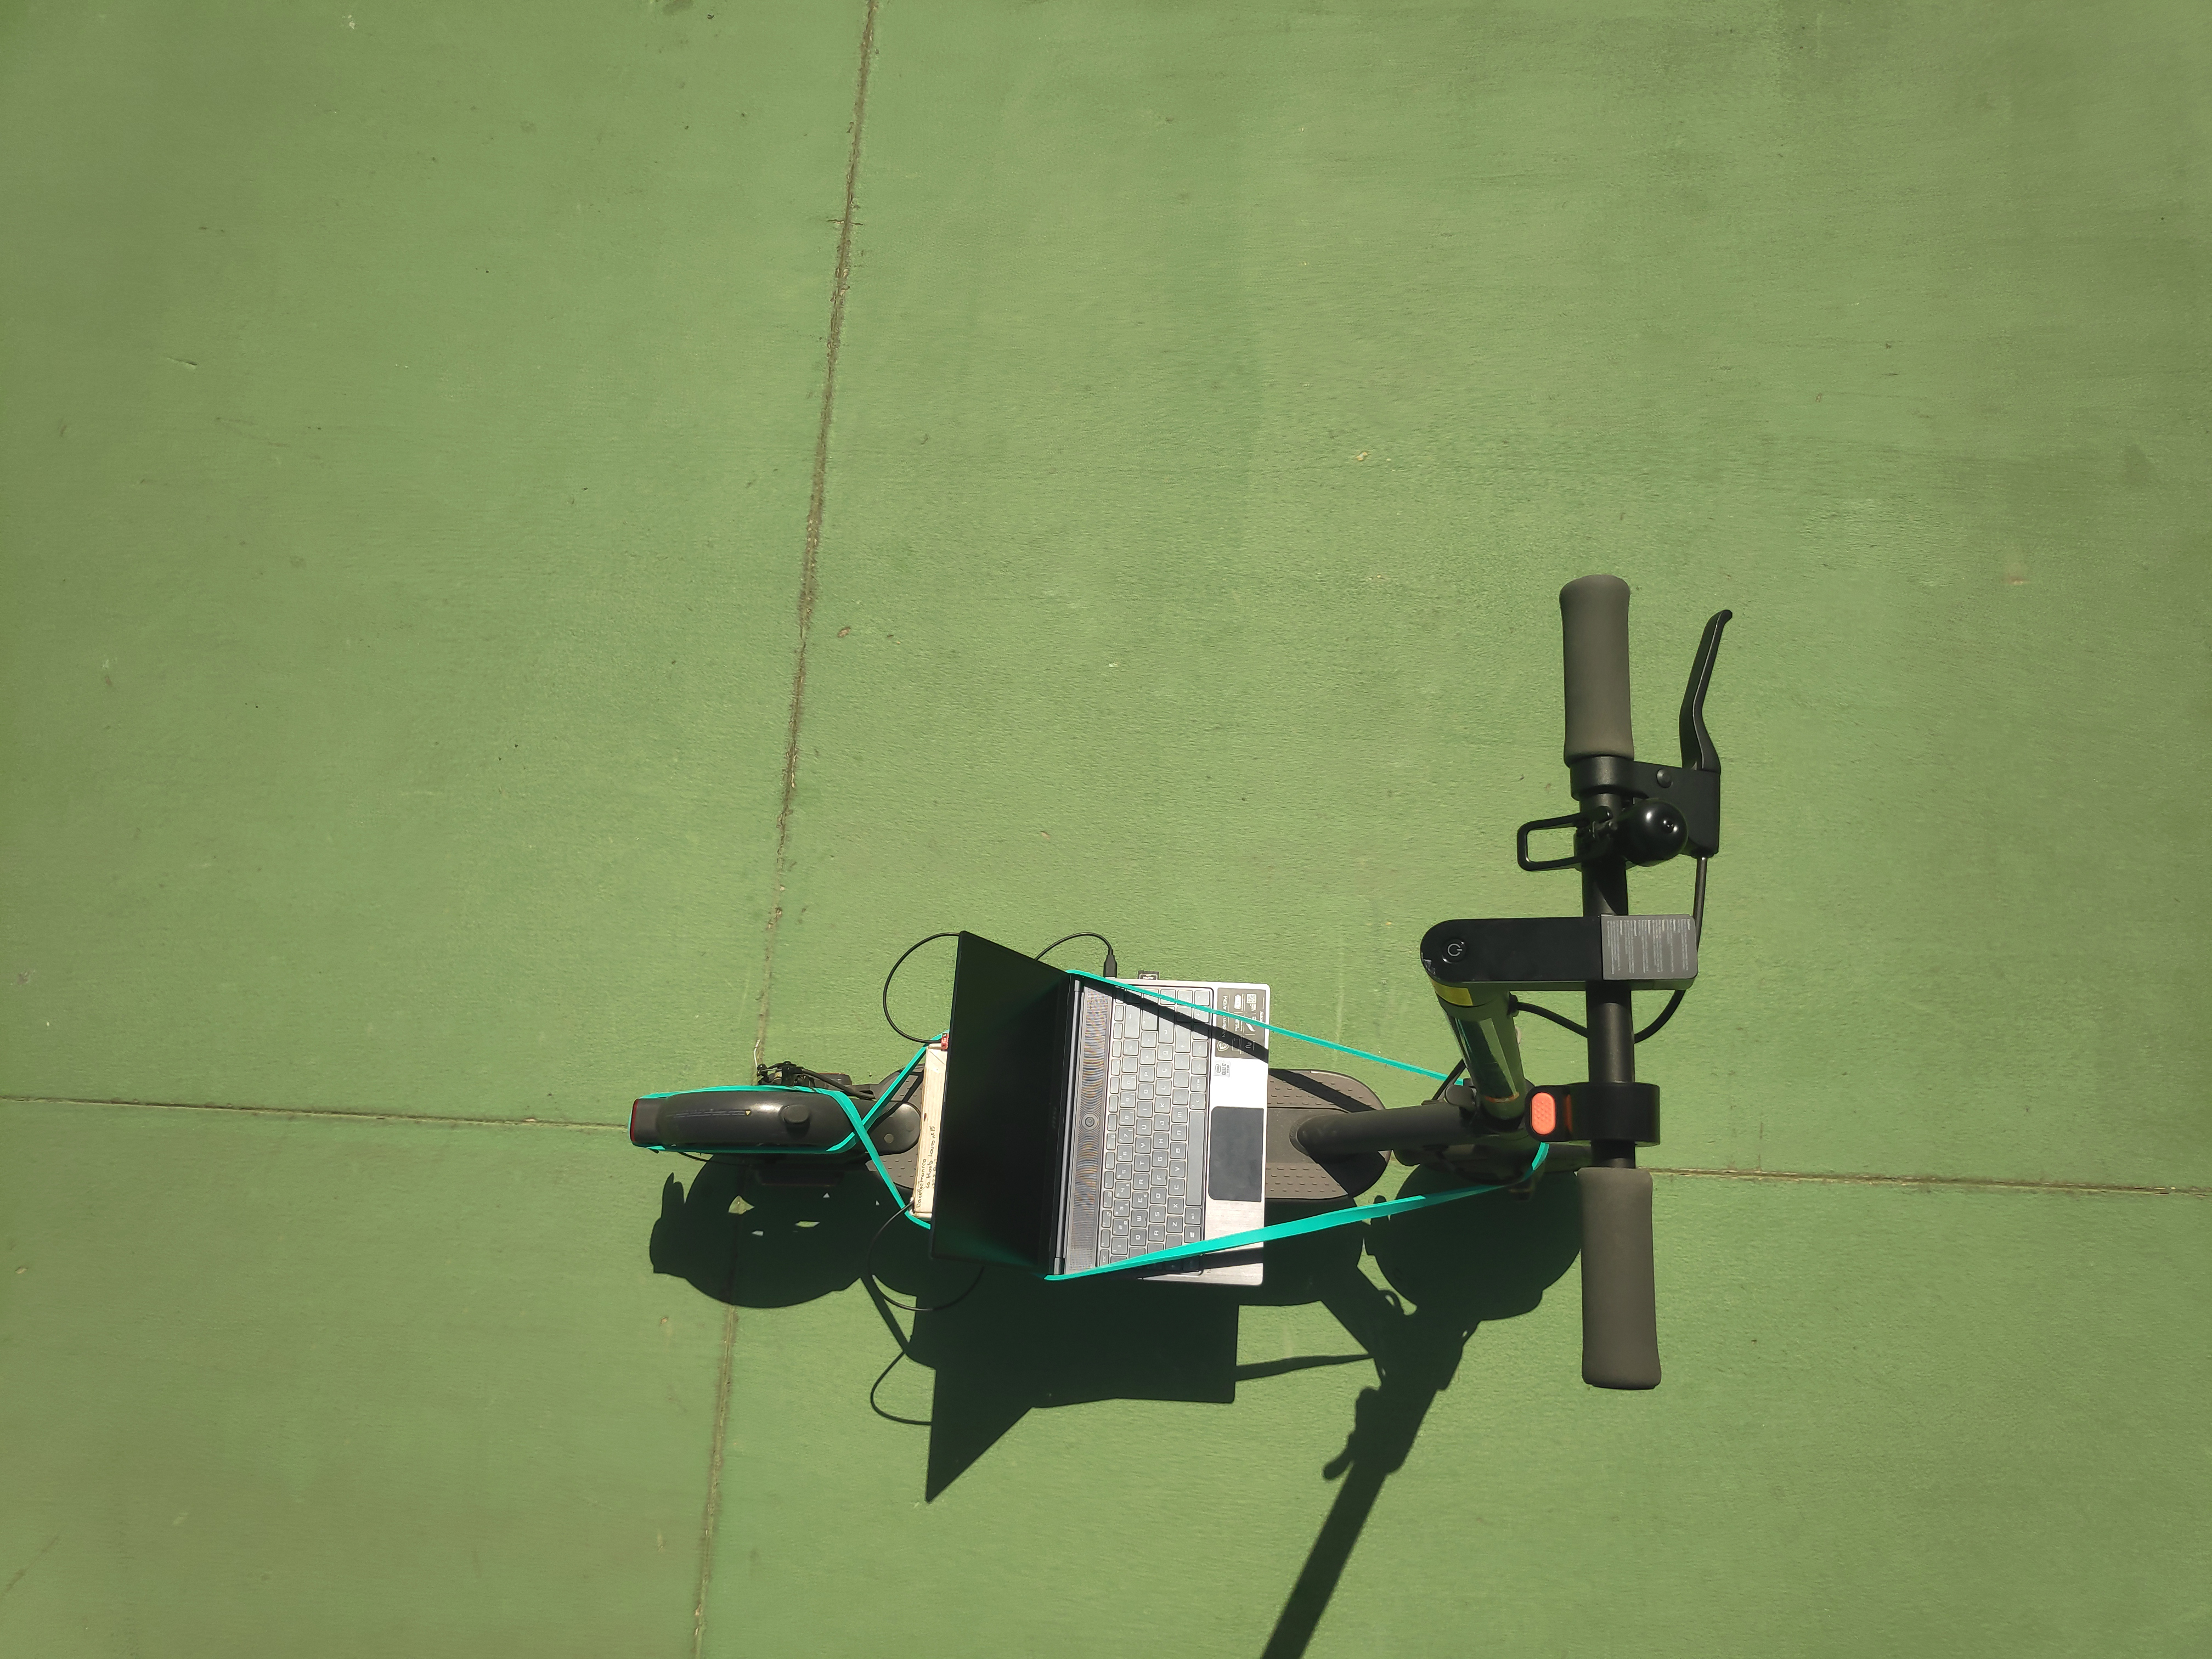
\includegraphics[width=0.9\textwidth]{figures/outdoor.jpg}
%     \caption{ 5-meter side ground square used for baseline of accuracy of inertial system. }
%     \label{fig:outdoor}
% \end{figure}

% \begin{figure}[!h]
%     \centering
%     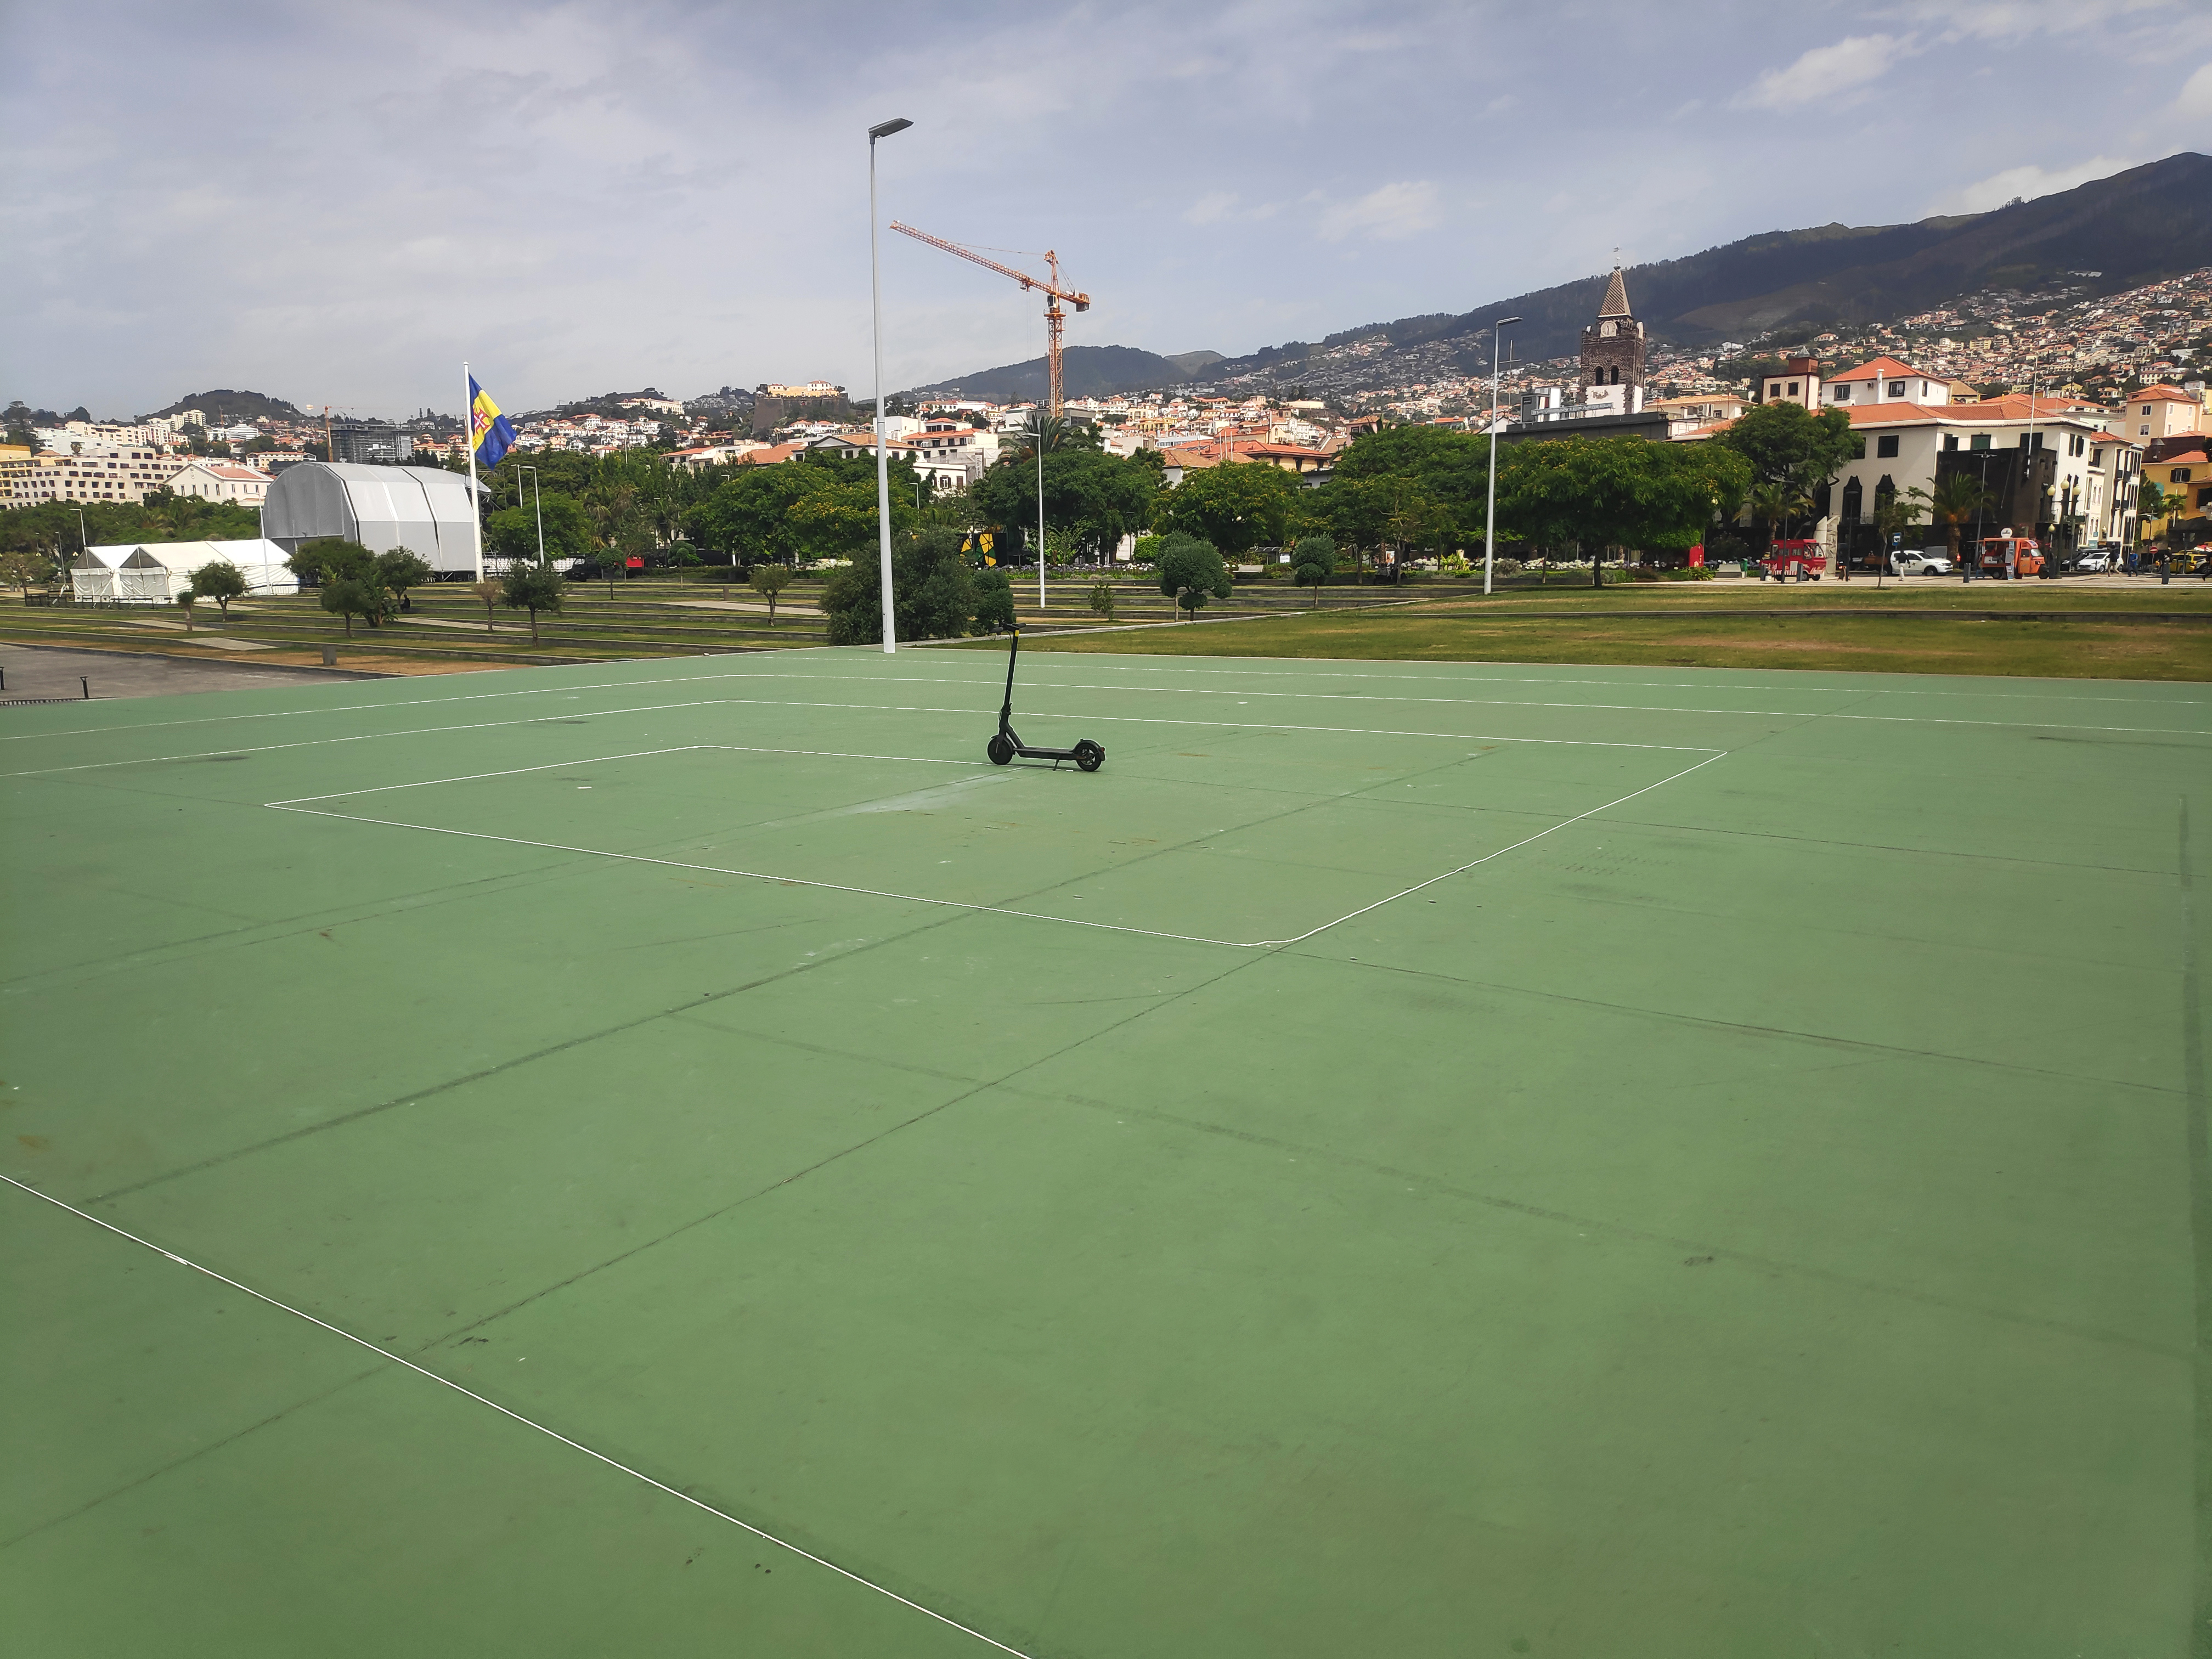
\includegraphics[width=0.9\textwidth]{figures/outdoor_1.jpg}
%     \caption{ Manually pulling the skateboard on each side of the ground square. }
%     \label{fig:outdoor_1}
% \end{figure}

The inertial system was placed on an electrical scooter (figure \ref{fig:outdoor_1}) in this case, being powered by a laptop computer (figure \ref{fig:outdoor_2}). The scooter was dragged at walking pace (figure \ref{fig:outdoor_3}) along the planned path marked by the rope.

\begin{figure}[!h]
  \centering
  \begin{subfigure}{0.8\textwidth}
    \centering
    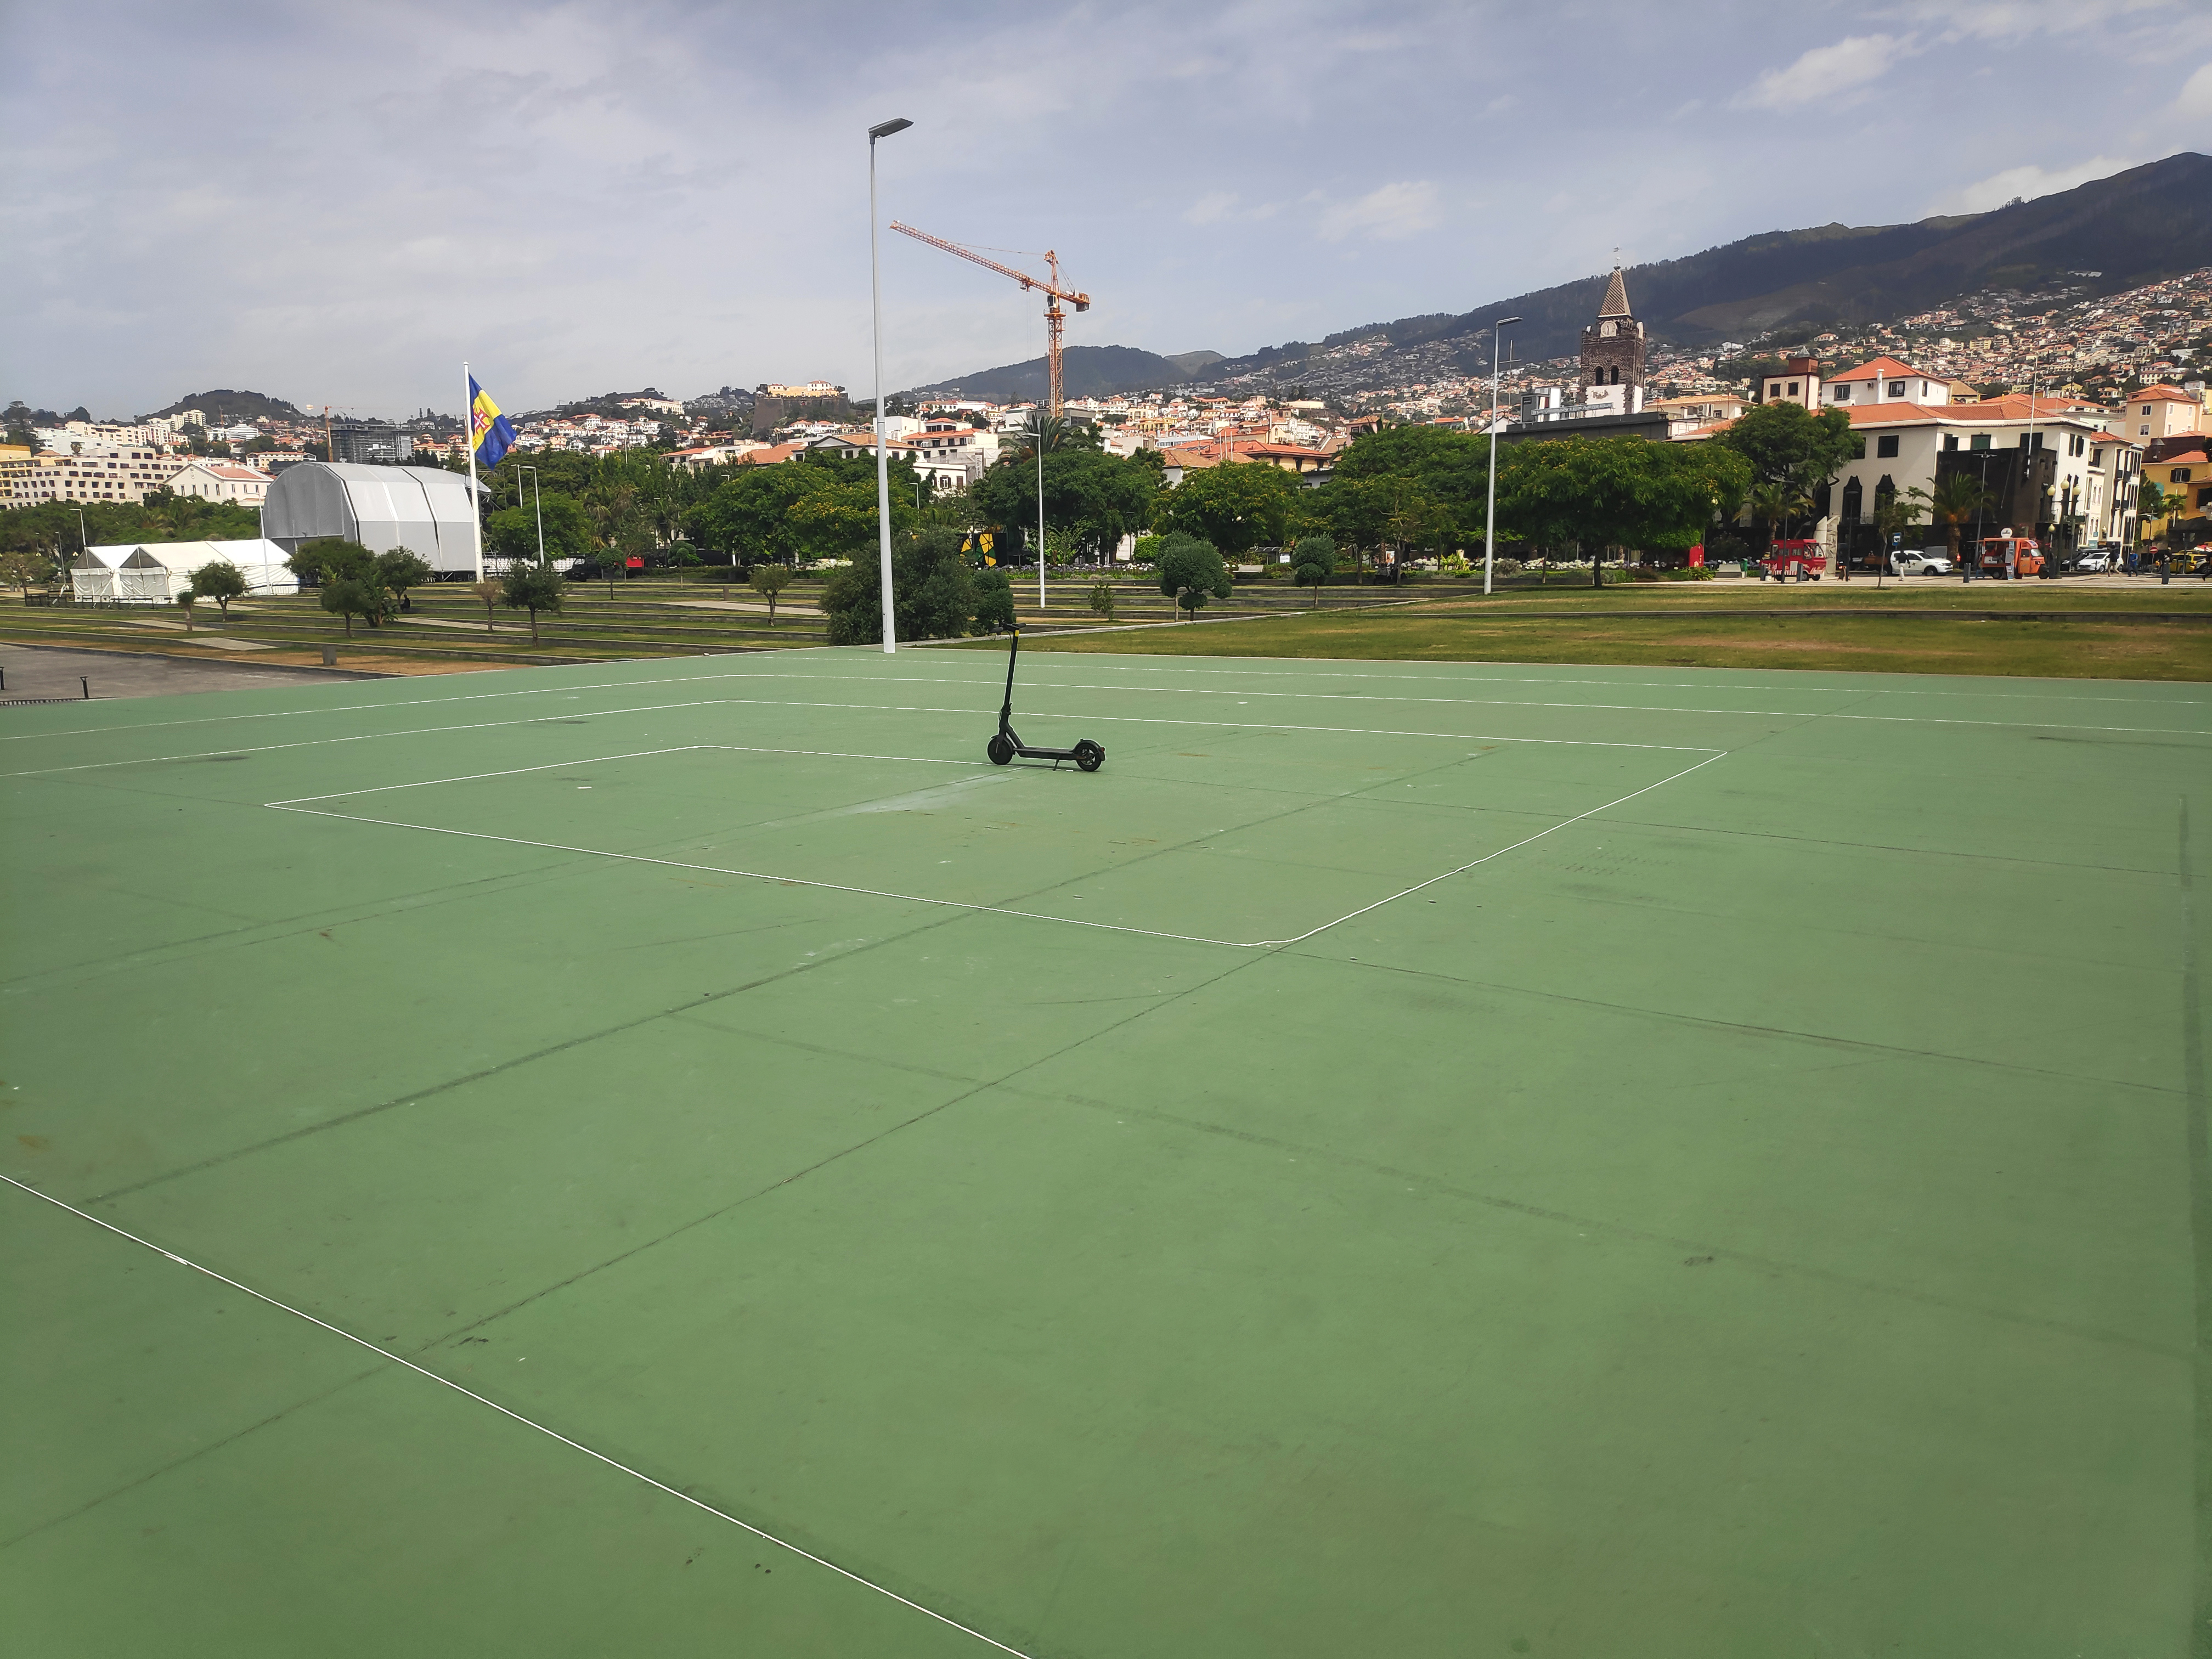
\includegraphics[width=1\textwidth]{figures/outdoor_1.jpg}
    \caption{ Spiral experiment path outlined by the white rope. }
    \label{fig:outdoor_1}
  \end{subfigure}

  \begin{subfigure}{0.40\textwidth}
    \centering
    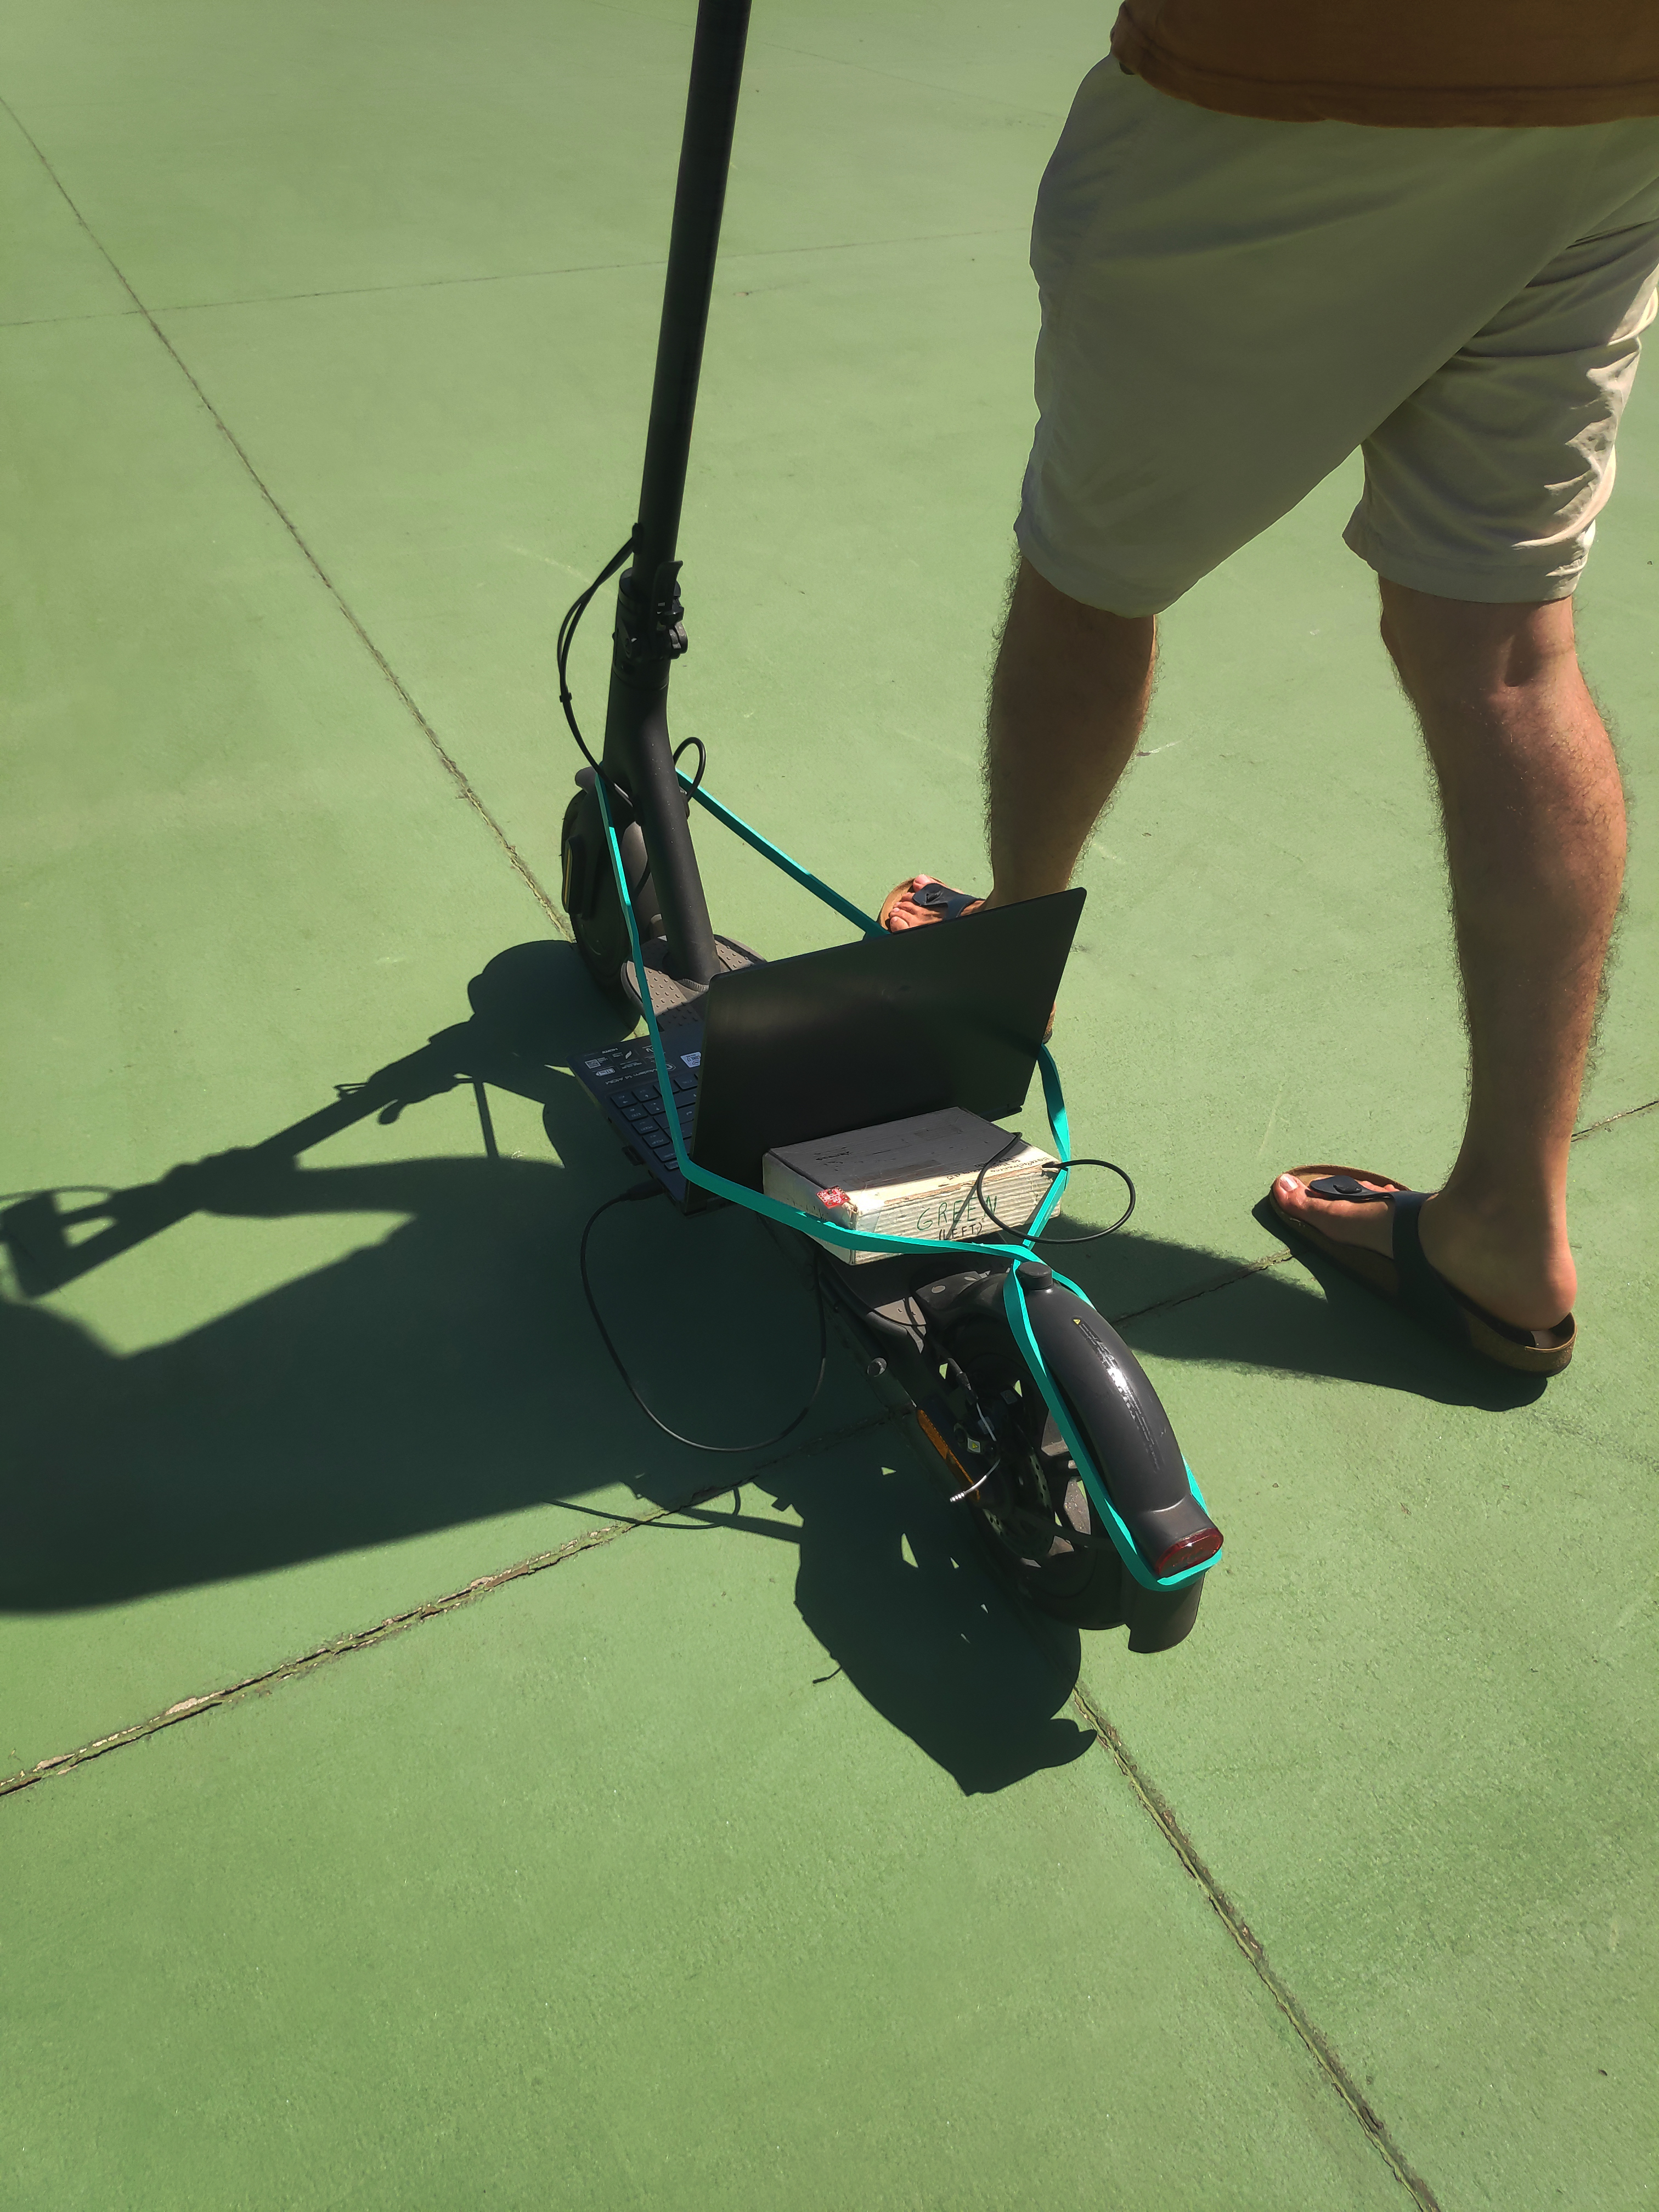
\includegraphics[width=1\textwidth]{figures/outdoor_3.jpg}
    \caption{ Close-up view of the inertial system (white box) attach with an elastic band to the scooter's body frame. }
    \label{fig:outdoor_2}
  \end{subfigure}
  \begin{subfigure}{0.40\textwidth}
    \centering
    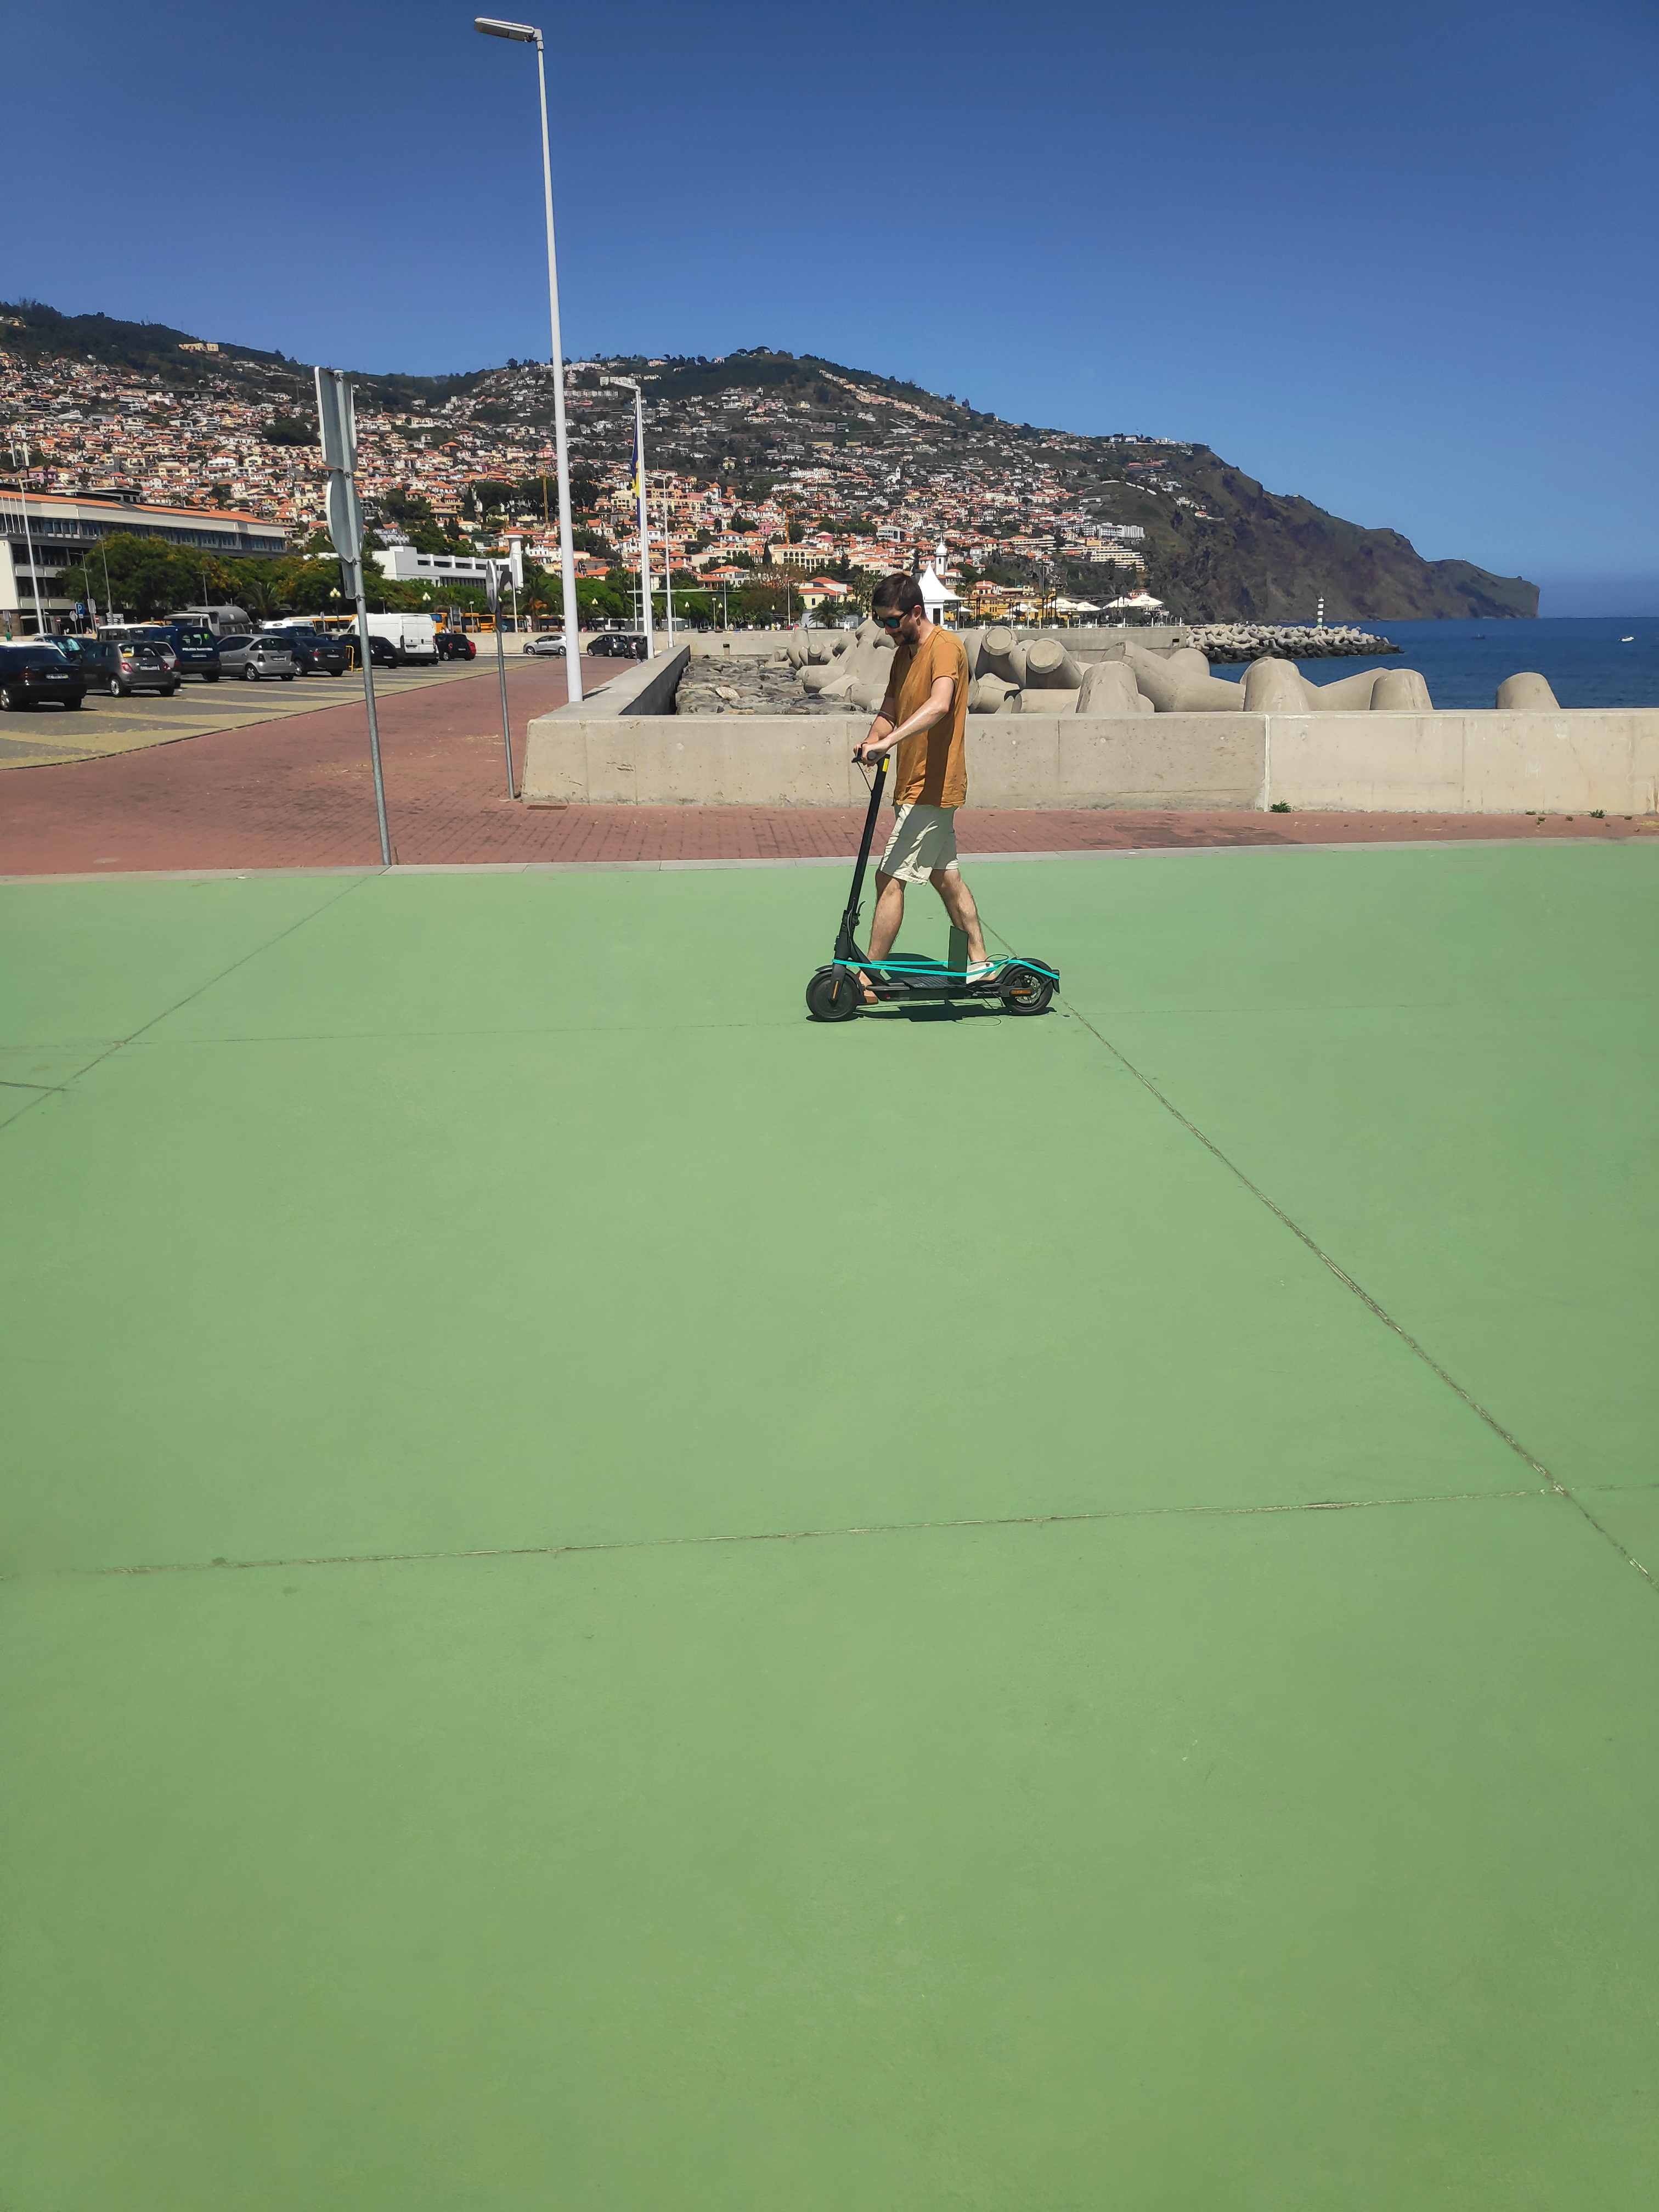
\includegraphics[width=1\textwidth]{figures/outdoor_2.jpg}
    \caption{ Pushing the electrical scooter containing the laptop and inertial system along the platform's edges forming geometrical shapes. }
    \label{fig:outdoor_3}
  \end{subfigure}
  \caption{ Photos illustrating hoe outdoor experiments were performed.}
  \label{fig:outdoor_experiments}
\end{figure}

Here several shapes were tested, from simple lines, squares, and triangles to more complex figures such as the ones illustrated at figure \ref{fig:squares} and figure \ref{fig:spiral}.

\begin{figure}[!h]
  \centering
  \begin{subfigure}{0.49\textwidth}
    \centering
    \includegraphics[width=1\textwidth]{figures/spiral.pdf}
    \caption{ Spiral-based shape with increasing length sides.  }
    \label{fig:spiral}
  \end{subfigure}
  \begin{subfigure}{0.49\textwidth}
    \centering
    \includegraphics[width=1\textwidth]{figures/squares.pdf}
    \caption{ Squares of increasing side length.  }
    \label{fig:squares}
  \end{subfigure}
  \caption{ Bird's-eye view representation of the more complex path shapes taken. }
\end{figure}

\newpage

\subsection{Underwater Experiments}

Underwater experiments were carried out at Madeira Carlton hotel divepoint, where the INS was placed in an underwater spherical housing built for 360º cameras with a portable battery pack (figure \ref{fig:underwater1_test}). Since the hardware was inaccessible inside the housing, the software had to be adjusted to support remote triggering of the INS via a wireless hotspot using a mobile phone via an HTTP request signal. Tests of the housing were performed prior to the experiment verifying the presence of any water leaks and the well-functioning of the INS (figure \ref{fig:underwater2_test}).

\begin{figure}[!h]
  \centering
  \begin{subfigure}{0.45\textwidth}
    \centering
    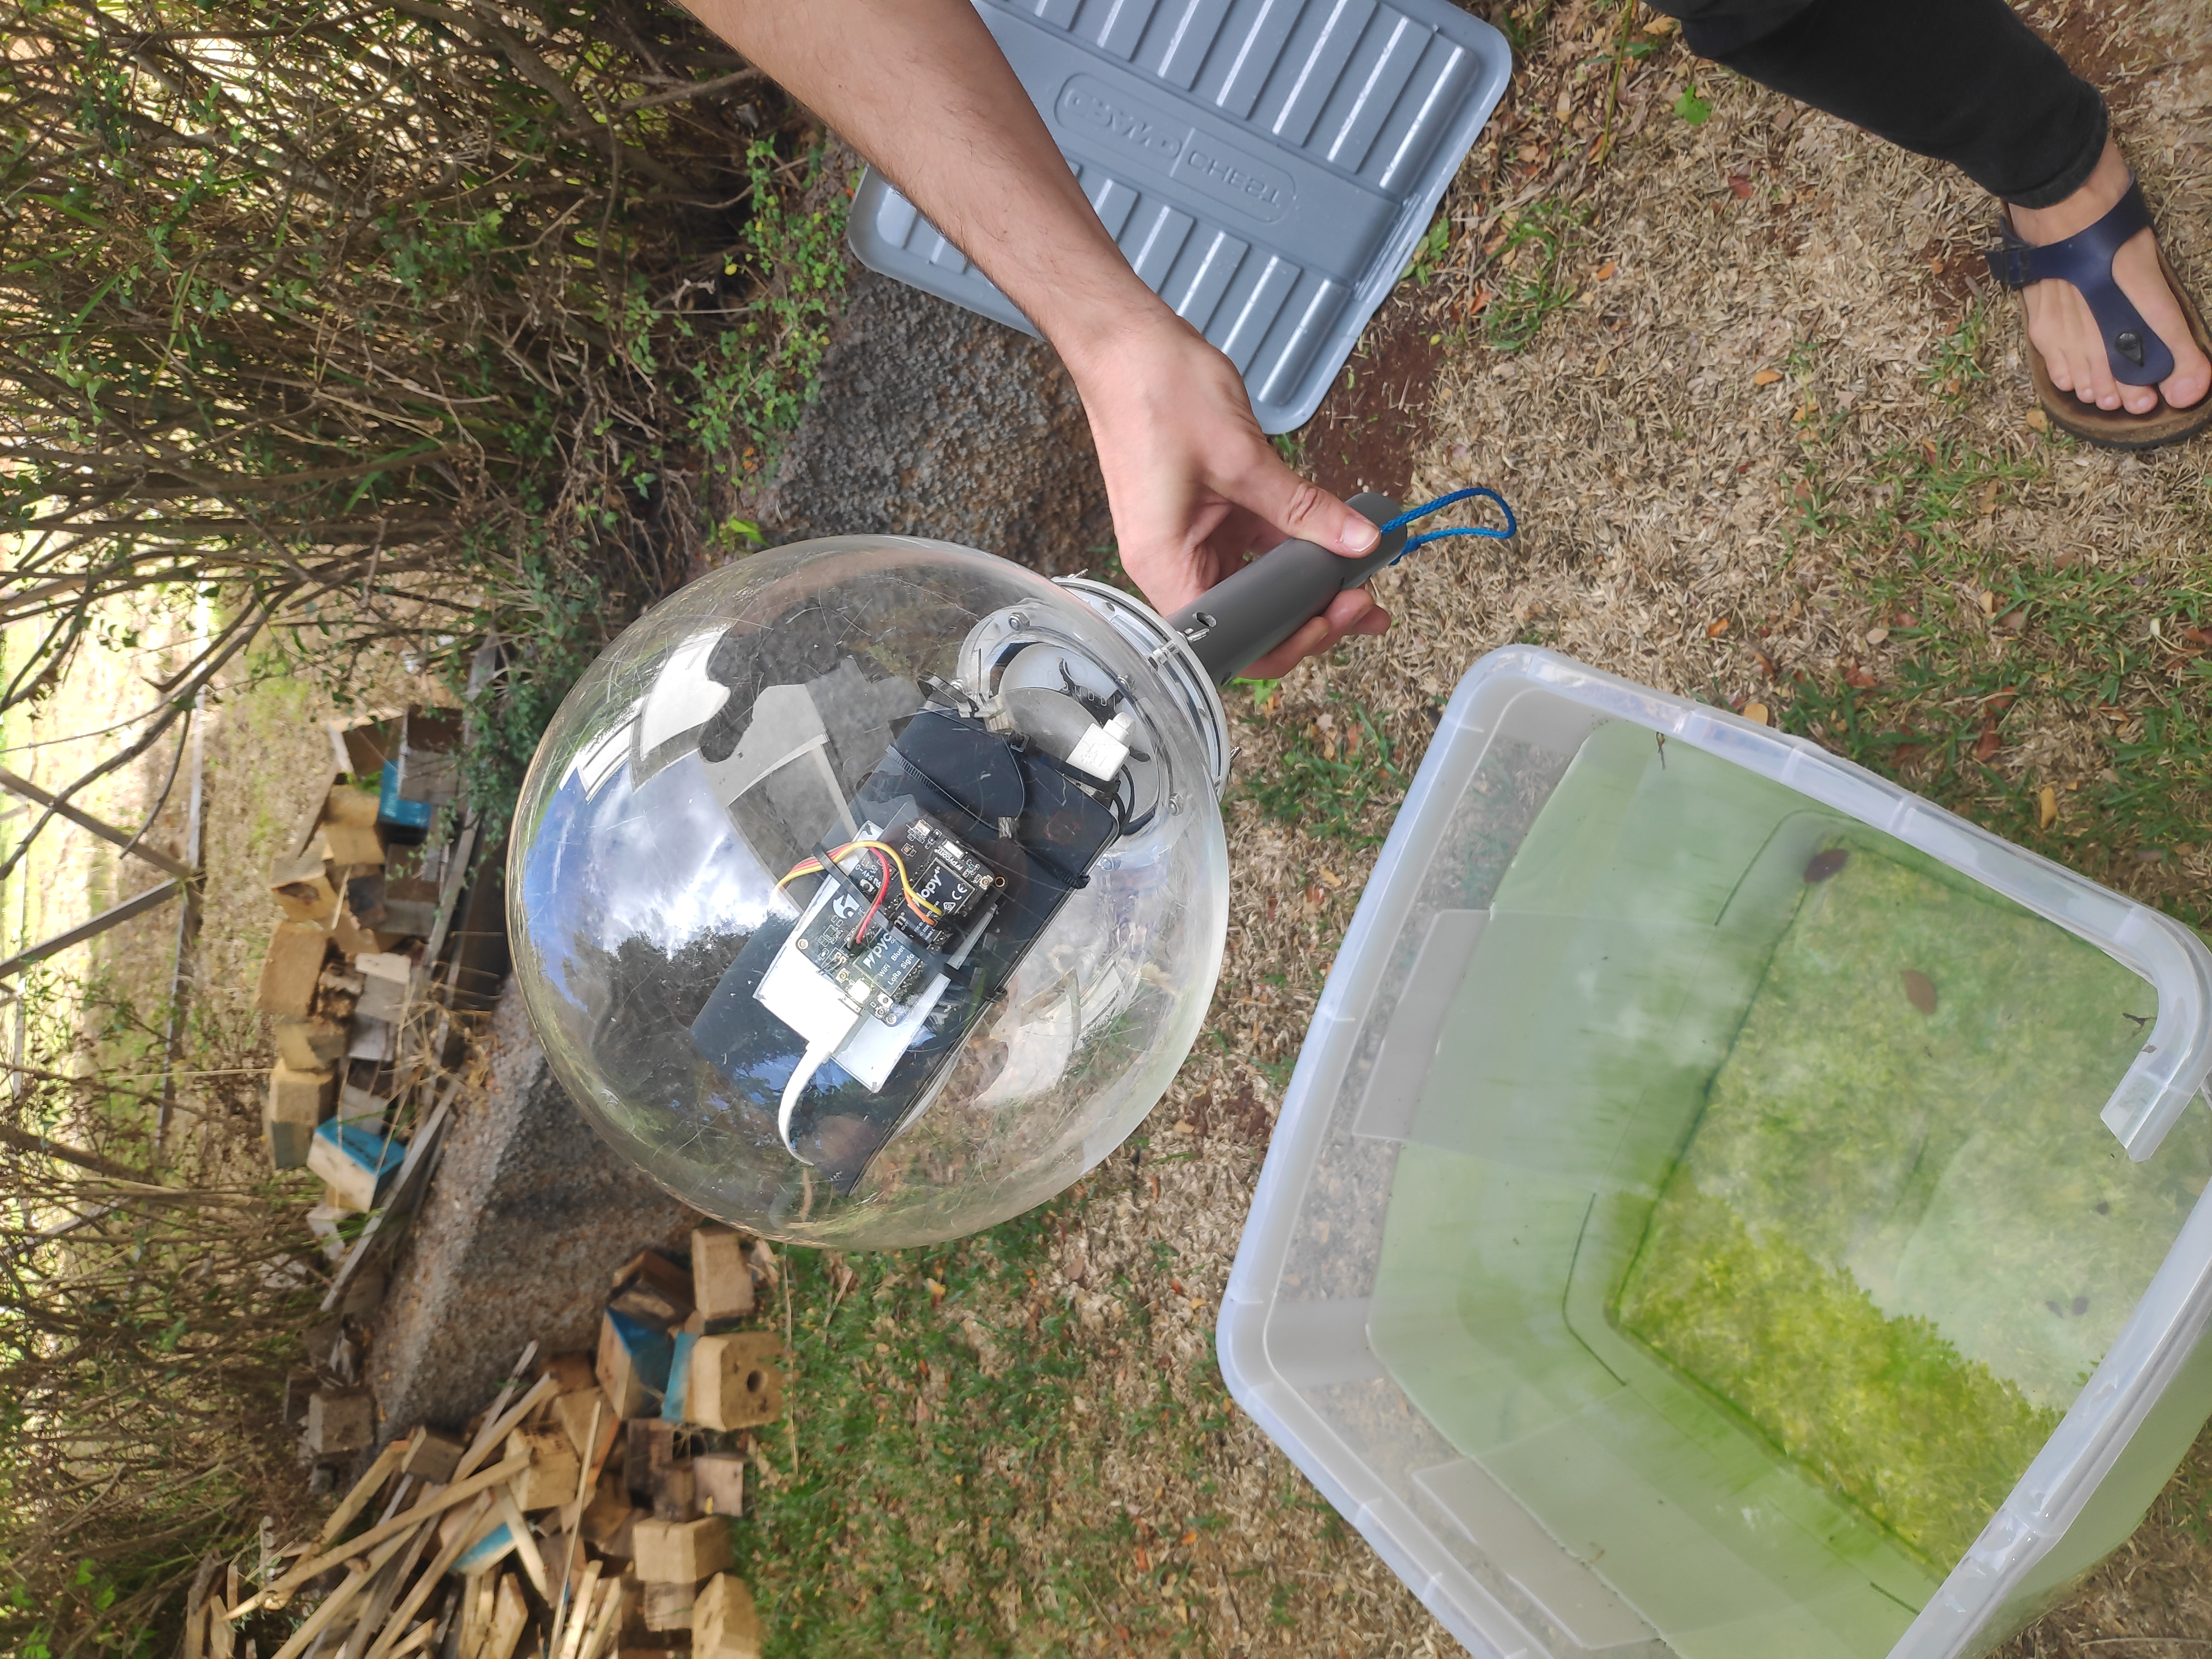
\includegraphics[width=1\textwidth]{figures/underwater.jpg}
    \caption{ Spherical housing encompassing the inertial system and portable battery pack. }
    \label{fig:underwater1_test}
  \end{subfigure}
  \begin{subfigure}{0.45\textwidth}
    \centering
    \includegraphics[width=1\textwidth]{figures/underwater_1.jpg}
    \caption{ The capsule was submerged in a water tank to verify the presence of any water leaks. }
    \label{fig:underwater2_test}
  \end{subfigure}
  \label{fig:underwater_test}
  \caption{ View of the tests made to assure the underwater housing was waterproof. }
\end{figure}

Once safety checks were completed, guaranteeing the feasibility of the study, the team went to Madeira Carlton hotel divepoint, where tests were conducted to evaluate the estimation quality of the proposed solution under water by a professional diver (figure \ref{fig:underwater}). A 5-meter square net being held by two people above water served as guideline for the diver performing the experiment underwater. The diver held the spherical housing while swimming along the guideline maintaining a constant speed while slowly increasing depth (figure \ref{fig:underwater_2}).

\begin{figure}[!h]
  \centering
  \begin{subfigure}{0.7\textwidth}
    \centering
    \includegraphics[width=1\textwidth]{figures/underwater_5.jpg}
    \caption{ The housing being held underwater by the diver.  }
    \label{fig:underwater}
  \end{subfigure}

  \begin{subfigure}{0.35\textwidth}
    \centering
    \includegraphics[width=1\textwidth]{figures/underwater_2.jpg}
    \caption{ The capsule housing the inertial system being handed out to a professional diver. }
    \label{fig:underwater_1}
  \end{subfigure}
  \begin{subfigure}{0.35\textwidth}
    \centering
    \includegraphics[width=1\textwidth]{figures/underwater_4.jpg}
    \caption{ View of the diver following the net underwater holding the spherical housing. }
    \label{fig:underwater_2}
  \end{subfigure}
  \caption{ Photos of the underwater tests conducted at Madeira Carlton hotel divepoint. }
\end{figure}
